% Options for packages loaded elsewhere
\PassOptionsToPackage{unicode}{hyperref}
\PassOptionsToPackage{hyphens}{url}
\documentclass[
]{book}
\usepackage{xcolor}
\usepackage{amsmath,amssymb}
\setcounter{secnumdepth}{5}
\usepackage{iftex}
\ifPDFTeX
  \usepackage[T1]{fontenc}
  \usepackage[utf8]{inputenc}
  \usepackage{textcomp} % provide euro and other symbols
\else % if luatex or xetex
  \usepackage{unicode-math} % this also loads fontspec
  \defaultfontfeatures{Scale=MatchLowercase}
  \defaultfontfeatures[\rmfamily]{Ligatures=TeX,Scale=1}
\fi
\usepackage{lmodern}
\ifPDFTeX\else
  % xetex/luatex font selection
\fi
% Use upquote if available, for straight quotes in verbatim environments
\IfFileExists{upquote.sty}{\usepackage{upquote}}{}
\IfFileExists{microtype.sty}{% use microtype if available
  \usepackage[]{microtype}
  \UseMicrotypeSet[protrusion]{basicmath} % disable protrusion for tt fonts
}{}
\makeatletter
\@ifundefined{KOMAClassName}{% if non-KOMA class
  \IfFileExists{parskip.sty}{%
    \usepackage{parskip}
  }{% else
    \setlength{\parindent}{0pt}
    \setlength{\parskip}{6pt plus 2pt minus 1pt}}
}{% if KOMA class
  \KOMAoptions{parskip=half}}
\makeatother
\usepackage{color}
\usepackage{fancyvrb}
\newcommand{\VerbBar}{|}
\newcommand{\VERB}{\Verb[commandchars=\\\{\}]}
\DefineVerbatimEnvironment{Highlighting}{Verbatim}{commandchars=\\\{\}}
% Add ',fontsize=\small' for more characters per line
\usepackage{framed}
\definecolor{shadecolor}{RGB}{248,248,248}
\newenvironment{Shaded}{\begin{snugshade}}{\end{snugshade}}
\newcommand{\AlertTok}[1]{\textcolor[rgb]{0.94,0.16,0.16}{#1}}
\newcommand{\AnnotationTok}[1]{\textcolor[rgb]{0.56,0.35,0.01}{\textbf{\textit{#1}}}}
\newcommand{\AttributeTok}[1]{\textcolor[rgb]{0.13,0.29,0.53}{#1}}
\newcommand{\BaseNTok}[1]{\textcolor[rgb]{0.00,0.00,0.81}{#1}}
\newcommand{\BuiltInTok}[1]{#1}
\newcommand{\CharTok}[1]{\textcolor[rgb]{0.31,0.60,0.02}{#1}}
\newcommand{\CommentTok}[1]{\textcolor[rgb]{0.56,0.35,0.01}{\textit{#1}}}
\newcommand{\CommentVarTok}[1]{\textcolor[rgb]{0.56,0.35,0.01}{\textbf{\textit{#1}}}}
\newcommand{\ConstantTok}[1]{\textcolor[rgb]{0.56,0.35,0.01}{#1}}
\newcommand{\ControlFlowTok}[1]{\textcolor[rgb]{0.13,0.29,0.53}{\textbf{#1}}}
\newcommand{\DataTypeTok}[1]{\textcolor[rgb]{0.13,0.29,0.53}{#1}}
\newcommand{\DecValTok}[1]{\textcolor[rgb]{0.00,0.00,0.81}{#1}}
\newcommand{\DocumentationTok}[1]{\textcolor[rgb]{0.56,0.35,0.01}{\textbf{\textit{#1}}}}
\newcommand{\ErrorTok}[1]{\textcolor[rgb]{0.64,0.00,0.00}{\textbf{#1}}}
\newcommand{\ExtensionTok}[1]{#1}
\newcommand{\FloatTok}[1]{\textcolor[rgb]{0.00,0.00,0.81}{#1}}
\newcommand{\FunctionTok}[1]{\textcolor[rgb]{0.13,0.29,0.53}{\textbf{#1}}}
\newcommand{\ImportTok}[1]{#1}
\newcommand{\InformationTok}[1]{\textcolor[rgb]{0.56,0.35,0.01}{\textbf{\textit{#1}}}}
\newcommand{\KeywordTok}[1]{\textcolor[rgb]{0.13,0.29,0.53}{\textbf{#1}}}
\newcommand{\NormalTok}[1]{#1}
\newcommand{\OperatorTok}[1]{\textcolor[rgb]{0.81,0.36,0.00}{\textbf{#1}}}
\newcommand{\OtherTok}[1]{\textcolor[rgb]{0.56,0.35,0.01}{#1}}
\newcommand{\PreprocessorTok}[1]{\textcolor[rgb]{0.56,0.35,0.01}{\textit{#1}}}
\newcommand{\RegionMarkerTok}[1]{#1}
\newcommand{\SpecialCharTok}[1]{\textcolor[rgb]{0.81,0.36,0.00}{\textbf{#1}}}
\newcommand{\SpecialStringTok}[1]{\textcolor[rgb]{0.31,0.60,0.02}{#1}}
\newcommand{\StringTok}[1]{\textcolor[rgb]{0.31,0.60,0.02}{#1}}
\newcommand{\VariableTok}[1]{\textcolor[rgb]{0.00,0.00,0.00}{#1}}
\newcommand{\VerbatimStringTok}[1]{\textcolor[rgb]{0.31,0.60,0.02}{#1}}
\newcommand{\WarningTok}[1]{\textcolor[rgb]{0.56,0.35,0.01}{\textbf{\textit{#1}}}}
\usepackage{longtable,booktabs,array}
\newcounter{none} % for unnumbered tables
\usepackage{calc} % for calculating minipage widths
% Correct order of tables after \paragraph or \subparagraph
\usepackage{etoolbox}
\makeatletter
\patchcmd\longtable{\par}{\if@noskipsec\mbox{}\fi\par}{}{}
\makeatother
% Allow footnotes in longtable head/foot
\IfFileExists{footnotehyper.sty}{\usepackage{footnotehyper}}{\usepackage{footnote}}
\makesavenoteenv{longtable}
\usepackage{graphicx}
\makeatletter
\newsavebox\pandoc@box
\newcommand*\pandocbounded[1]{% scales image to fit in text height/width
  \sbox\pandoc@box{#1}%
  \Gscale@div\@tempa{\textheight}{\dimexpr\ht\pandoc@box+\dp\pandoc@box\relax}%
  \Gscale@div\@tempb{\linewidth}{\wd\pandoc@box}%
  \ifdim\@tempb\p@<\@tempa\p@\let\@tempa\@tempb\fi% select the smaller of both
  \ifdim\@tempa\p@<\p@\scalebox{\@tempa}{\usebox\pandoc@box}%
  \else\usebox{\pandoc@box}%
  \fi%
}
% Set default figure placement to htbp
\def\fps@figure{htbp}
\makeatother
\setlength{\emergencystretch}{3em} % prevent overfull lines
\providecommand{\tightlist}{%
  \setlength{\itemsep}{0pt}\setlength{\parskip}{0pt}}
\usepackage[]{natbib}
\bibliographystyle{apalike}
\usepackage{tabularray}

% Table color support
\PassOptionsToPackage{table}{xcolor}
\usepackage{xcolor}
\usepackage{colortbl}

% Core table stack
\usepackage{booktabs}
\usepackage{longtable}         % must come before threeparttablex
\usepackage{array}
\usepackage{multirow}
\usepackage{tabularx}         % width-constrained tables (X columns)

% Three-part tables and notes
\usepackage{threeparttable}    % provides the threeparttable environment
\usepackage{threeparttablex}   % extends threeparttable to longtable

% Optional, but helps with captions and alignment
\usepackage{caption}
% \usepackage{siunitx}         % if you use S columns for numeric alignment
% \usepackage{makecell}        % if you use \thead or line breaks in headers
\usepackage{titling}
\pretitle{\begin{center} 
\includegraphics[width=2in,height=2in]{logo.png}\LARGE\\}
\posttitle{\end{center}}
\usepackage{array}
\usepackage{caption}
\usepackage{graphicx}
\usepackage{siunitx}
\usepackage[normalem]{ulem}
\usepackage{colortbl}
\usepackage{multirow}
\usepackage{hhline}
\usepackage{calc}
\usepackage{tabularx}
\usepackage{threeparttable}
\usepackage{wrapfig}
\usepackage{adjustbox}
\usepackage{hyperref}
\usepackage{booktabs}
\usepackage{longtable}
\usepackage{anyfontsize}
\usepackage{bookmark}
\IfFileExists{xurl.sty}{\usepackage{xurl}}{} % add URL line breaks if available
\urlstyle{same}
\hypersetup{
  pdftitle={A Guide on Data Analysis},
  pdfauthor={Mike Nguyen},
  hidelinks,
  pdfcreator={LaTeX via pandoc}}

\title{A Guide on Data Analysis}
\author{Mike Nguyen}
\date{2026-07-03}

\begin{document}
\maketitle

{
\setcounter{tocdepth}{1}
\tableofcontents
}
\chapter*{Preface}\label{preface}
\addcontentsline{toc}{chapter}{Preface}

This book is an effort to simplify and demystify the complex process of data analysis, making it accessible to a wide audience. While I do not claim to be a professional statistician, econometrician, or data scientist, I firmly believe in the value of learning through teaching and practical application. Writing this book has been as much a learning journey for me as I hope it will be for you.

The intended audience includes those with little to no experience in statistics, econometrics, or data science, as well as individuals with a budding interest in these fields who are eager to deepen their knowledge. While my primary domain of interest is marketing, the principles and methods discussed in this book are universally applicable to any discipline that employs scientific methods or data analysis.

I hope this book provides a valuable starting point for aspiring statisticians, econometricians, and data scientists, empowering you to navigate the fascinating world of causal inference and data analysis with confidence.


\includegraphics[width=3.125in,height=3.125in]{logo.png}

\begin{center}\rule{0.5\linewidth}{0.5pt}\end{center}

\section*{How to cite these books}\label{how-to-cite-these-books}
\addcontentsline{toc}{section}{How to cite these books}

\subsection{\texorpdfstring{\textbf{Volume 1: Foundations of Data Analysis}}{Volume 1: Foundations of Data Analysis}}\label{volume-1-foundations-of-data-analysis}

\textbf{1. APA (7th edition)}

Nguyen, M. (2025). \emph{Foundations of data analysis} (Vol. 1). Springer Cham. \href{https://tidd.ly/4oL3N2X}{https://doi.org/10.1007/978-3-032-01858-8}

\textbf{2. MLA (8th edition)}

Nguyen, Mike. \emph{Foundations of Data Analysis}. Vol. 1, Springer Cham, 2025. DOI: \href{https://tidd.ly/4oL3N2X}{10.1007/978-3-032-01858-8}.

\textbf{3. Chicago (17th edition)}

Nguyen, Mike. 2025. \emph{Foundations of Data Analysis}. Vol. 1. Cham: Springer. \href{https://tidd.ly/4oL3N2X}{https://doi.org/10.1007/978-3-032-01858-8}.

\textbf{4. Harvard}

Nguyen, M. (2025) \emph{Foundations of Data Analysis}. Vol. 1. Springer Cham. Available at: \href{https://tidd.ly/4oL3N2X}{https://doi.org/10.1007/978-3-032-01858-8}

\begin{Shaded}
\begin{Highlighting}[]
\SpecialCharTok{@}\NormalTok{book\{Nguyen2025Vol1,}
\NormalTok{  author    }\OtherTok{=}\NormalTok{ \{Nguyen, Mike\},}
\NormalTok{  title     }\OtherTok{=}\NormalTok{ \{Foundations of Data Analysis\},}
\NormalTok{  volume    }\OtherTok{=}\NormalTok{ \{}\DecValTok{1}\NormalTok{\},}
\NormalTok{  year      }\OtherTok{=}\NormalTok{ \{}\DecValTok{2025}\NormalTok{\},}
\NormalTok{  publisher }\OtherTok{=}\NormalTok{ \{Springer Cham\},}
\NormalTok{  doi       }\OtherTok{=}\NormalTok{ \{}\FloatTok{10.1007}\SpecialCharTok{/}\DecValTok{978{-}3{-}032{-}01858{-}8}\NormalTok{\},}
\NormalTok{  url       }\OtherTok{=}\NormalTok{ \{https}\SpecialCharTok{:}\ErrorTok{//}\NormalTok{doi.org}\SpecialCharTok{/}\FloatTok{10.1007}\SpecialCharTok{/}\DecValTok{978{-}3{-}032{-}01858{-}8}\NormalTok{\}}
\NormalTok{\}}
\end{Highlighting}
\end{Shaded}

\begin{center}\rule{0.5\linewidth}{0.5pt}\end{center}

\subsection{\texorpdfstring{\textbf{Volume 2: Regression Techniques for Data Analysis}}{Volume 2: Regression Techniques for Data Analysis}}\label{volume-2-regression-techniques-for-data-analysis}

\textbf{1. APA (7th edition)}

Nguyen, M. (2025). \emph{Regression techniques for data analysis} (Vol. 2). Springer Cham. \href{https://tidd.ly/47PJ7kB}{https://link.springer.com/book/9783032018342}

\textbf{2. MLA (8th edition)}

Nguyen, Mike. \emph{Regression Techniques for Data Analysis}. Vol. 2, Springer Cham, 2025. \href{https://tidd.ly/47PJ7kB}{https://link.springer.com/book/9783032018342}.

\textbf{3. Chicago (17th edition)}

Nguyen, Mike. 2025. \emph{Regression Techniques for Data Analysis}. Vol. 2. Cham: Springer. \href{https://tidd.ly/47PJ7kB}{https://link.springer.com/book/9783032018342}.

\textbf{4. Harvard}

Nguyen, M. (2025) \emph{Regression Techniques for Data Analysis}. Vol. 2. Springer Cham. Available at: \href{https://tidd.ly/47PJ7kB}{https://link.springer.com/book/9783032018342}

\begin{Shaded}
\begin{Highlighting}[]
\SpecialCharTok{@}\NormalTok{book\{Nguyen2025Vol2,}
\NormalTok{  author    }\OtherTok{=}\NormalTok{ \{Nguyen, Mike\},}
\NormalTok{  title     }\OtherTok{=}\NormalTok{ \{Regression Techniques }\ControlFlowTok{for}\NormalTok{ Data Analysis\},}
\NormalTok{  volume    }\OtherTok{=}\NormalTok{ \{}\DecValTok{2}\NormalTok{\},}
\NormalTok{  year      }\OtherTok{=}\NormalTok{ \{}\DecValTok{2025}\NormalTok{\},}
\NormalTok{  publisher }\OtherTok{=}\NormalTok{ \{Springer Cham\},}
\NormalTok{  isbn      }\OtherTok{=}\NormalTok{ \{}\DecValTok{978{-}3{-}032{-}01834{-}2}\NormalTok{\},}
\NormalTok{  url       }\OtherTok{=}\NormalTok{ \{https}\SpecialCharTok{:}\ErrorTok{//}\NormalTok{link.springer.com}\SpecialCharTok{/}\NormalTok{book}\SpecialCharTok{/}\DecValTok{9783032018342}\NormalTok{\}}
\NormalTok{\}}
\end{Highlighting}
\end{Shaded}

\begin{center}\rule{0.5\linewidth}{0.5pt}\end{center}

\subsection{\texorpdfstring{\textbf{Volume 3: Advanced Modeling and Data Challenges}}{Volume 3: Advanced Modeling and Data Challenges}}\label{volume-3-advanced-modeling-and-data-challenges}

\textbf{1. APA (7th edition)}

Nguyen, M. (2025). \emph{Advanced modeling and data challenges} (Vol. 3). Springer Cham. \href{https://tidd.ly/3JrB3xm}{https://link.springer.com/book/9783032017185}

\textbf{2. MLA (8th edition)}

Nguyen, Mike. \emph{Advanced Modeling and Data Challenges}. Vol. 3, Springer Cham, 2025. \href{https://tidd.ly/3JrB3xm}{https://link.springer.com/book/9783032017185}.

\textbf{3. Chicago (17th edition)}

Nguyen, Mike. 2025. \emph{Advanced Modeling and Data Challenges}. Vol. 3. Cham: Springer. \href{https://tidd.ly/3JrB3xm}{https://link.springer.com/book/9783032017185}.

\textbf{4. Harvard}

Nguyen, M. (2025) \emph{Advanced Modeling and Data Challenges}. Vol. 3. Springer Cham. Available at: \href{https://tidd.ly/3JrB3xm}{https://link.springer.com/book/9783032017185}

\begin{Shaded}
\begin{Highlighting}[]
\SpecialCharTok{@}\NormalTok{book\{Nguyen2025Vol3,}
\NormalTok{  author    }\OtherTok{=}\NormalTok{ \{Nguyen, Mike\},}
\NormalTok{  title     }\OtherTok{=}\NormalTok{ \{Advanced Modeling and Data Challenges\},}
\NormalTok{  volume    }\OtherTok{=}\NormalTok{ \{}\DecValTok{3}\NormalTok{\},}
\NormalTok{  year      }\OtherTok{=}\NormalTok{ \{}\DecValTok{2025}\NormalTok{\},}
\NormalTok{  publisher }\OtherTok{=}\NormalTok{ \{Springer Cham\},}
\NormalTok{  isbn      }\OtherTok{=}\NormalTok{ \{}\DecValTok{978{-}3{-}032{-}01718{-}5}\NormalTok{\},}
\NormalTok{  url       }\OtherTok{=}\NormalTok{ \{https}\SpecialCharTok{:}\ErrorTok{//}\NormalTok{link.springer.com}\SpecialCharTok{/}\NormalTok{book}\SpecialCharTok{/}\DecValTok{9783032017185}\NormalTok{\}}
\NormalTok{\}}
\end{Highlighting}
\end{Shaded}

\begin{center}\rule{0.5\linewidth}{0.5pt}\end{center}

\subsection{\texorpdfstring{\textbf{Volume 4: Experimental Design}}{Volume 4: Experimental Design}}\label{volume-4-experimental-design}

\textbf{1. APA (7th edition)}

Nguyen, M. (2025). \emph{Experimental design} (Vol. 4). Springer Cham. \href{https://tidd.ly/4oFridQ}{https://link.springer.com/book/9783032018380}

\textbf{2. MLA (8th edition)}

Nguyen, Mike. \emph{Experimental Design}. Vol. 4, Springer Cham, 2025. \href{https://tidd.ly/4oFridQ}{https://link.springer.com/book/9783032018380}.

\textbf{3. Chicago (17th edition)}

Nguyen, Mike. 2025. \emph{Experimental Design}. Vol. 4. Cham: Springer. \href{https://tidd.ly/4oFridQ}{https://link.springer.com/book/9783032018380}.

\textbf{4. Harvard}

Nguyen, M. (2025) \emph{Experimental Design}. Vol. 4. Springer Cham. Available at: \href{https://tidd.ly/4oFridQ}{https://link.springer.com/book/9783032018380}

\begin{Shaded}
\begin{Highlighting}[]
\SpecialCharTok{@}\NormalTok{book\{Nguyen2025Vol4,}
\NormalTok{  author    }\OtherTok{=}\NormalTok{ \{Nguyen, Mike\},}
\NormalTok{  title     }\OtherTok{=}\NormalTok{ \{Experimental Design\},}
\NormalTok{  volume    }\OtherTok{=}\NormalTok{ \{}\DecValTok{4}\NormalTok{\},}
\NormalTok{  year      }\OtherTok{=}\NormalTok{ \{}\DecValTok{2025}\NormalTok{\},}
\NormalTok{  publisher }\OtherTok{=}\NormalTok{ \{Springer Cham\},}
\NormalTok{  isbn      }\OtherTok{=}\NormalTok{ \{}\DecValTok{978{-}3{-}032{-}01838{-}0}\NormalTok{\},}
\NormalTok{  url       }\OtherTok{=}\NormalTok{ \{https}\SpecialCharTok{:}\ErrorTok{//}\NormalTok{link.springer.com}\SpecialCharTok{/}\NormalTok{book}\SpecialCharTok{/}\DecValTok{9783032018380}\NormalTok{\}}
\NormalTok{\}}
\end{Highlighting}
\end{Shaded}

\begin{center}\rule{0.5\linewidth}{0.5pt}\end{center}

\chapter{Introduction}\label{introduction}

Since the turn of the century, we have witnessed remarkable advancements and innovations, particularly in statistics, information technology, computer science, and the rapidly emerging field of data science. However, one challenge of these developments is the overuse of \textbf{buzzwords} like \emph{big data}, \emph{machine learning}, and \emph{deep learning}. While these terms are powerful in context, they can sometimes obscure the foundational principles underlying their application.

Every substantive field often has its own specialized metric subfield, such as:

\begin{itemize}
\tightlist
\item
  \textbf{Econometrics} in economics\\
\item
  \textbf{Psychometrics} in psychology\\
\item
  \textbf{Chemometrics} in chemistry\\
\item
  \textbf{Sabermetrics} in sports analytics\\
\item
  \textbf{Biostatistics} in public health and medicine
\end{itemize}

To the layperson, these disciplines are often grouped under broader terms like:

\begin{itemize}
\tightlist
\item
  \textbf{Data Science}\\
\item
  \textbf{Applied Statistics}\\
\item
  \textbf{Computational Social Science}
\end{itemize}

As exciting as it is to explore these new tools and techniques, I must admit that retaining these concepts can be challenging. For me, the most effective way to internalize and apply these ideas has been to document the data analysis process from start to finish.

With that in mind, let's dive in and explore the fascinating world of data analysis together.

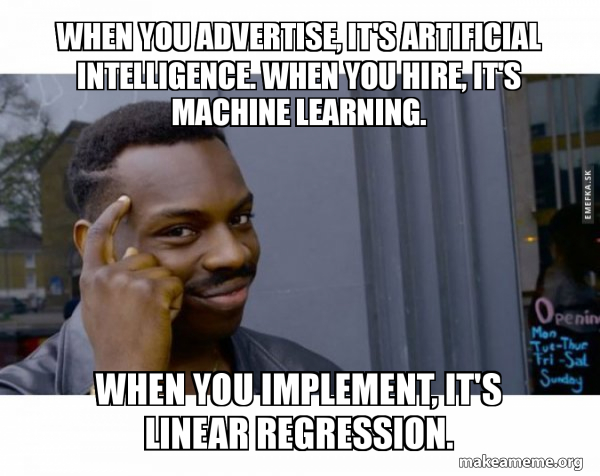
\includegraphics[width=4.6875in,height=3.64583in]{images/meme.jpg}

\section{General Recommendations}\label{general-recommendations}

\begin{itemize}
\item
  The journey of mastering data analysis is fueled by practice and repetition. The more lines of code you write, the more functions you familiarize yourself with, and the more you experiment, the more enjoyable and rewarding this process becomes.
\item
  Readers can approach this book in several ways:

  \begin{itemize}
  \tightlist
  \item
    \textbf{Focused Learning}: If you are interested in specific methods or tools, you can jump directly to the relevant section by navigating through the table of contents.
  \item
    \textbf{Sequential Learning}: To follow a traditional path of data analysis, start with the \hyperref[linear-regression]{Linear Regression} section.
  \item
    \textbf{Experimental Approach}: If you are interested in designing experiments and testing hypotheses, explore the {[}Analysis of Variance (ANOVA){]} section.
  \end{itemize}
\item
  For those primarily interested in applications and less concerned with theoretical foundations, focus on the summary and application sections of each chapter.
\item
  If a concept is unclear, consider researching the topic online. This book serves as a guide, and external resources like tutorials or articles can provide additional insights.
\item
  To customize the code examples provided in this book, use R's built-in help functions. For instance:

  \begin{itemize}
  \tightlist
  \item
    To learn more about a specific function, type \texttt{help(function\_name)} or \texttt{?function\_name} in the R console.
  \item
    For example, to find details about the \texttt{hist} function, type \texttt{?hist} or \texttt{help(hist)} in the console.
  \end{itemize}
\item
  Additionally, searching online is a powerful resource (e.g., Google, ChatGPT, etc.). Different practitioners often use various R packages to achieve similar results. For instance, if you need to create a histogram in R, a simple search like \emph{``histogram in R''} will provide multiple approaches and examples.
\end{itemize}

By adopting these strategies, you can tailor your learning experience and maximize the value of this book.

\textbf{Tools of statistics}

\begin{itemize}
\tightlist
\item
  Probability Theory
\item
  Mathematical Analysis
\item
  Computer Science
\item
  Numerical Analysis
\item
  Database Management
\end{itemize}

\textbf{Code Replication}

This book was built with R version 4.4.3 (2025-02-28 ucrt) and the following packages:

\begin{longtable}[]{@{}lll@{}}
\caption{\label{tab:unnamed-chunk-11}R packages and versions used}\tabularnewline
\toprule\noalign{}
package & version & source \\
\midrule\noalign{}
\endfirsthead
\toprule\noalign{}
package & version & source \\
\midrule\noalign{}
\endhead
\bottomrule\noalign{}
\endlastfoot
abind & 1.4-8 & CRAN (R 4.4.1) \\
agridat & 1.25 & CRAN (R 4.4.3) \\
ape & 5.8-1 & CRAN (R 4.4.3) \\
assertthat & 0.2.1 & CRAN (R 4.4.3) \\
backports & 1.5.0 & CRAN (R 4.4.0) \\
bookdown & 0.45 & CRAN (R 4.4.3) \\
boot & 1.3-32 & CRAN (R 4.4.3) \\
broom & 1.0.10 & CRAN (R 4.4.3) \\
bslib & 0.9.0 & CRAN (R 4.4.2) \\
cachem & 1.1.0 & CRAN (R 4.4.2) \\
callr & 3.7.6 & CRAN (R 4.4.2) \\
car & 3.1-3 & CRAN (R 4.4.2) \\
carData & 3.0-5 & CRAN (R 4.4.2) \\
cellranger & 1.1.0 & CRAN (R 4.4.2) \\
cli & 3.6.5 & CRAN (R 4.4.3) \\
coda & 0.19-4.1 & CRAN (R 4.4.2) \\
colorspace & 2.1-2 & CRAN (R 4.4.3) \\
corpcor & 1.6.10 & CRAN (R 4.4.0) \\
crayon & 1.5.3 & CRAN (R 4.4.2) \\
cubature & 2.1.4 & CRAN (R 4.4.3) \\
curl & 7.0.0 & CRAN (R 4.4.3) \\
data.table & 1.17.8 & CRAN (R 4.4.3) \\
DBI & 1.2.3 & CRAN (R 4.4.2) \\
dbplyr & 2.5.1 & CRAN (R 4.4.3) \\
desc & 1.4.3 & CRAN (R 4.4.2) \\
devtools & 2.4.6 & CRAN (R 4.4.3) \\
digest & 0.6.37 & CRAN (R 4.4.2) \\
dplyr & 1.1.4 & CRAN (R 4.4.2) \\
ellipsis & 0.3.2 & CRAN (R 4.4.2) \\
evaluate & 1.0.5 & CRAN (R 4.4.3) \\
extrafont & 0.20 & CRAN (R 4.4.3) \\
extrafontdb & 1.1 & CRAN (R 4.4.3) \\
fansi & 1.0.6 & CRAN (R 4.4.2) \\
faraway & 1.0.9 & CRAN (R 4.4.3) \\
fastmap & 1.2.0 & CRAN (R 4.4.2) \\
forcats & 1.0.1 & CRAN (R 4.4.3) \\
foreign & 0.8-90 & CRAN (R 4.4.3) \\
fs & 1.6.6 & CRAN (R 4.4.3) \\
generics & 0.1.4 & CRAN (R 4.4.3) \\
ggplot2 & 4.0.0 & CRAN (R 4.4.3) \\
glue & 1.8.0 & CRAN (R 4.4.2) \\
gtable & 0.3.6 & CRAN (R 4.4.2) \\
haven & 2.5.5 & CRAN (R 4.4.3) \\
Hmisc & 5.2-4 & CRAN (R 4.4.3) \\
hms & 1.1.4 & CRAN (R 4.4.3) \\
htmltools & 0.5.8.1 & CRAN (R 4.4.2) \\
htmlwidgets & 1.6.4 & CRAN (R 4.4.2) \\
httr & 1.4.7 & CRAN (R 4.4.2) \\
investr & 1.4.2 & CRAN (R 4.4.3) \\
jpeg & 0.1-11 & CRAN (R 4.4.3) \\
jquerylib & 0.1.4 & CRAN (R 4.4.2) \\
jsonlite & 2.0.0 & CRAN (R 4.4.3) \\
kableExtra & 1.4.0 & CRAN (R 4.4.3) \\
knitr & 1.50 & CRAN (R 4.4.3) \\
lattice & 0.22-7 & CRAN (R 4.4.3) \\
latticeExtra & 0.6-31 & CRAN (R 4.4.3) \\
lifecycle & 1.0.4 & CRAN (R 4.4.2) \\
lme4 & 1.1-37 & CRAN (R 4.4.3) \\
lmerTest & 3.1-3 & CRAN (R 4.4.2) \\
lsr & 0.5.2 & CRAN (R 4.4.3) \\
ltm & 1.2-0 & CRAN (R 4.4.3) \\
lubridate & 1.9.4 & CRAN (R 4.4.2) \\
magrittr & 2.0.4 & CRAN (R 4.4.3) \\
MASS & 7.3-65 & CRAN (R 4.4.3) \\
matlib & 1.0.1 & CRAN (R 4.4.3) \\
Matrix & 1.7-4 & CRAN (R 4.4.3) \\
MCMCglmm & 2.36 & CRAN (R 4.4.2) \\
memoise & 2.0.1 & CRAN (R 4.4.2) \\
mgcv & 1.9-3 & CRAN (R 4.4.3) \\
minqa & 1.2.8 & CRAN (R 4.4.2) \\
modelr & 0.1.11 & CRAN (R 4.4.2) \\
munsell & 0.5.1 & CRAN (R 4.4.2) \\
nlme & 3.1-168 & CRAN (R 4.4.3) \\
nloptr & 2.2.1 & CRAN (R 4.4.3) \\
nlstools & 2.1-0 & CRAN (R 4.4.2) \\
nnet & 7.3-20 & CRAN (R 4.4.3) \\
numDeriv & 2016.8-1.1 & CRAN (R 4.4.0) \\
openxlsx & 4.2.8 & CRAN (R 4.4.3) \\
pbkrtest & 0.5.5 & CRAN (R 4.4.3) \\
pillar & 1.11.1 & CRAN (R 4.4.3) \\
pkgbuild & 1.4.8 & CRAN (R 4.4.3) \\
pkgconfig & 2.0.3 & CRAN (R 4.4.2) \\
pkgload & 1.4.1 & CRAN (R 4.4.3) \\
png & 0.1-8 & CRAN (R 4.4.0) \\
ppsr & 0.0.5 & CRAN (R 4.4.3) \\
prettyunits & 1.2.0 & CRAN (R 4.4.2) \\
processx & 3.8.6 & CRAN (R 4.4.3) \\
ps & 1.9.1 & CRAN (R 4.4.3) \\
pscl & 1.5.9 & CRAN (R 4.4.2) \\
purrr & 1.1.0 & CRAN (R 4.4.3) \\
R6 & 2.6.1 & CRAN (R 4.4.3) \\
RColorBrewer & 1.1-3 & CRAN (R 4.4.0) \\
Rcpp & 1.1.0 & CRAN (R 4.4.3) \\
readr & 2.1.5 & CRAN (R 4.4.2) \\
readxl & 1.4.5 & CRAN (R 4.4.3) \\
remotes & 2.5.0 & CRAN (R 4.4.2) \\
reprex & 2.1.1 & CRAN (R 4.4.2) \\
rgl & 1.3.24 & CRAN (R 4.4.3) \\
rio & 1.2.4 & CRAN (R 4.4.3) \\
rlang & 1.1.6 & CRAN (R 4.4.3) \\
RLRsim & 3.1-8 & CRAN (R 4.4.3) \\
rmarkdown & 2.30 & CRAN (R 4.4.3) \\
rprojroot & 2.1.1 & CRAN (R 4.4.3) \\
rstudioapi & 0.17.1 & CRAN (R 4.4.2) \\
Rttf2pt1 & 1.3.14 & CRAN (R 4.4.3) \\
rvest & 1.0.5 & CRAN (R 4.4.3) \\
sass & 0.4.10 & CRAN (R 4.4.3) \\
scales & 1.4.0 & CRAN (R 4.4.3) \\
sessioninfo & 1.2.3 & CRAN (R 4.4.3) \\
stringi & 1.8.7 & CRAN (R 4.4.3) \\
stringr & 1.5.2 & CRAN (R 4.4.3) \\
svglite & 2.2.2 & CRAN (R 4.4.3) \\
systemfonts & 1.3.1 & CRAN (R 4.4.3) \\
tensorA & 0.36.2.1 & CRAN (R 4.4.0) \\
testthat & 3.2.3 & CRAN (R 4.4.2) \\
tibble & 3.2.1 & CRAN (R 4.4.2) \\
tidyr & 1.3.1 & CRAN (R 4.4.2) \\
tidyselect & 1.2.1 & CRAN (R 4.4.2) \\
tidyverse & 2.0.0 & CRAN (R 4.4.2) \\
tzdb & 0.5.0 & CRAN (R 4.4.3) \\
usethis & 3.2.1 & CRAN (R 4.4.3) \\
utf8 & 1.2.6 & CRAN (R 4.4.3) \\
vctrs & 0.6.5 & CRAN (R 4.4.2) \\
viridisLite & 0.4.2 & CRAN (R 4.4.2) \\
webshot & 0.5.5 & CRAN (R 4.4.3) \\
withr & 3.0.2 & CRAN (R 4.4.2) \\
xfun & 0.52 & CRAN (R 4.4.3) \\
xml2 & 1.4.1 & CRAN (R 4.4.3) \\
xtable & 1.8-4 & CRAN (R 4.4.2) \\
yaml & 2.3.10 & CRAN (R 4.4.2) \\
zip & 2.3.3 & CRAN (R 4.4.3) \\
\end{longtable}

\begin{verbatim}
#> - Session info ---------------------------------------------------------------
#>  setting  value
#>  version  R version 4.4.3 (2025-02-28 ucrt)
#>  os       Windows 11 x64 (build 26200)
#>  system   x86_64, mingw32
#>  ui       RTerm
#>  language (EN)
#>  collate  English_United States.utf8
#>  ctype    English_United States.utf8
#>  tz       America/Los_Angeles
#>  date     2026-07-01
#>  pandoc   3.8.3 @ C:/Program Files/RStudio/resources/app/bin/quarto/bin/tools/ (via rmarkdown)
#>  quarto   NA @ C:\\PROGRA~1\\Quarto\\bin\\quarto.exe
#> 
#> - Packages -------------------------------------------------------------------
#>  package      * version date (UTC) lib source
#>  bookdown       0.45    2025-10-03 [1] CRAN (R 4.4.3)
#>  cachem         1.1.0   2024-05-16 [1] CRAN (R 4.4.2)
#>  cli            3.6.5   2025-04-23 [1] CRAN (R 4.4.3)
#>  codetools      0.2-20  2024-03-31 [1] CRAN (R 4.4.3)
#>  data.table   * 1.17.8  2025-07-10 [1] CRAN (R 4.4.3)
#>  desc           1.4.3   2023-12-10 [1] CRAN (R 4.4.2)
#>  devtools       2.4.6   2025-10-03 [1] CRAN (R 4.4.3)
#>  dichromat      2.0-0.1 2022-05-02 [1] CRAN (R 4.4.0)
#>  digest         0.6.37  2024-08-19 [1] CRAN (R 4.4.2)
#>  dplyr        * 1.1.4   2023-11-17 [1] CRAN (R 4.4.2)
#>  ellipsis       0.3.2   2021-04-29 [1] CRAN (R 4.4.2)
#>  evaluate       1.0.5   2025-08-27 [1] CRAN (R 4.4.3)
#>  farver         2.1.2   2024-05-13 [1] CRAN (R 4.4.2)
#>  fastmap        1.2.0   2024-05-15 [1] CRAN (R 4.4.2)
#>  forcats      * 1.0.1   2025-09-25 [1] CRAN (R 4.4.3)
#>  fs             1.6.6   2025-04-12 [1] CRAN (R 4.4.3)
#>  generics       0.1.4   2025-05-09 [1] CRAN (R 4.4.3)
#>  ggplot2      * 4.0.0   2025-09-11 [1] CRAN (R 4.4.3)
#>  glue           1.8.0   2024-09-30 [1] CRAN (R 4.4.2)
#>  gtable         0.3.6   2024-10-25 [1] CRAN (R 4.4.2)
#>  hms            1.1.4   2025-10-17 [1] CRAN (R 4.4.3)
#>  htmltools      0.5.8.1 2024-04-04 [1] CRAN (R 4.4.2)
#>  jpeg         * 0.1-11  2025-03-21 [1] CRAN (R 4.4.3)
#>  knitr          1.50    2025-03-16 [1] CRAN (R 4.4.3)
#>  lifecycle      1.0.4   2023-11-07 [1] CRAN (R 4.4.2)
#>  lubridate    * 1.9.4   2024-12-08 [1] CRAN (R 4.4.2)
#>  magrittr       2.0.4   2025-09-12 [1] CRAN (R 4.4.3)
#>  memoise        2.0.1   2021-11-26 [1] CRAN (R 4.4.2)
#>  pillar         1.11.1  2025-09-17 [1] CRAN (R 4.4.3)
#>  pkgbuild       1.4.8   2025-05-26 [1] CRAN (R 4.4.3)
#>  pkgconfig      2.0.3   2019-09-22 [1] CRAN (R 4.4.2)
#>  pkgload        1.4.1   2025-09-23 [1] CRAN (R 4.4.3)
#>  purrr        * 1.1.0   2025-07-10 [1] CRAN (R 4.4.3)
#>  R6             2.6.1   2025-02-15 [1] CRAN (R 4.4.3)
#>  RColorBrewer   1.1-3   2022-04-03 [1] CRAN (R 4.4.0)
#>  readr        * 2.1.5   2024-01-10 [1] CRAN (R 4.4.2)
#>  remotes        2.5.0   2024-03-17 [1] CRAN (R 4.4.2)
#>  rlang          1.1.6   2025-04-11 [1] CRAN (R 4.4.3)
#>  rmarkdown      2.30    2025-09-28 [1] CRAN (R 4.4.3)
#>  rstudioapi     0.17.1  2024-10-22 [1] CRAN (R 4.4.2)
#>  S7             0.2.0   2024-11-07 [1] CRAN (R 4.4.3)
#>  scales       * 1.4.0   2025-04-24 [1] CRAN (R 4.4.3)
#>  sessioninfo    1.2.3   2025-02-05 [1] CRAN (R 4.4.3)
#>  stringi        1.8.7   2025-03-27 [1] CRAN (R 4.4.3)
#>  stringr      * 1.5.2   2025-09-08 [1] CRAN (R 4.4.3)
#>  tibble       * 3.2.1   2023-03-20 [1] CRAN (R 4.4.2)
#>  tidyr        * 1.3.1   2024-01-24 [1] CRAN (R 4.4.2)
#>  tidyselect     1.2.1   2024-03-11 [1] CRAN (R 4.4.2)
#>  tidyverse    * 2.0.0   2023-02-22 [1] CRAN (R 4.4.2)
#>  timechange     0.3.0   2024-01-18 [1] CRAN (R 4.4.2)
#>  tzdb           0.5.0   2025-03-15 [1] CRAN (R 4.4.3)
#>  usethis        3.2.1   2025-09-06 [1] CRAN (R 4.4.3)
#>  vctrs          0.6.5   2023-12-01 [1] CRAN (R 4.4.2)
#>  withr          3.0.2   2024-10-28 [1] CRAN (R 4.4.2)
#>  xfun           0.52    2025-04-02 [1] CRAN (R 4.4.3)
#>  yaml           2.3.10  2024-07-26 [1] CRAN (R 4.4.2)
#> 
#>  [1] C:/Program Files/R/R-4.4.3/library
#>  * -- Packages attached to the search path.
#> 
#> ------------------------------------------------------------------------------
\end{verbatim}

\chapter{Prerequisites}\label{prerequisites}

This chapter reviews essential mathematical and computational tools required for effective statistical analysis. Beginning with \hyperref[matrix-theory]{Matrix Theory} and core concepts in linear algebra, we then explore foundational \hyperref[probability-theory]{Probability Theory}, including random variables, distributions, and expectations. The chapter also revisits important mathematical skills, such as functions, derivatives, and logarithms, before moving into practical elements like data import/export and data manipulation using R. These topics ensure that readers are well-equipped to tackle the more advanced statistical methods presented in later chapters.

If you are confident in your understanding of these topics, you can proceed directly to the \hyperref[descriptive-statistics]{Descriptive Statistics} section to begin exploring applied data analysis.

Figure \ref{fig:include-image} offers a light-hearted take on how the same underlying statistical work gets rebranded across disciplines.

\begin{Shaded}
\begin{Highlighting}[]
\NormalTok{knitr}\SpecialCharTok{::}\FunctionTok{include\_graphics}\NormalTok{(}\StringTok{"images/meme\_01.png"}\NormalTok{)}
\end{Highlighting}
\end{Shaded}

\begin{figure}

{\centering 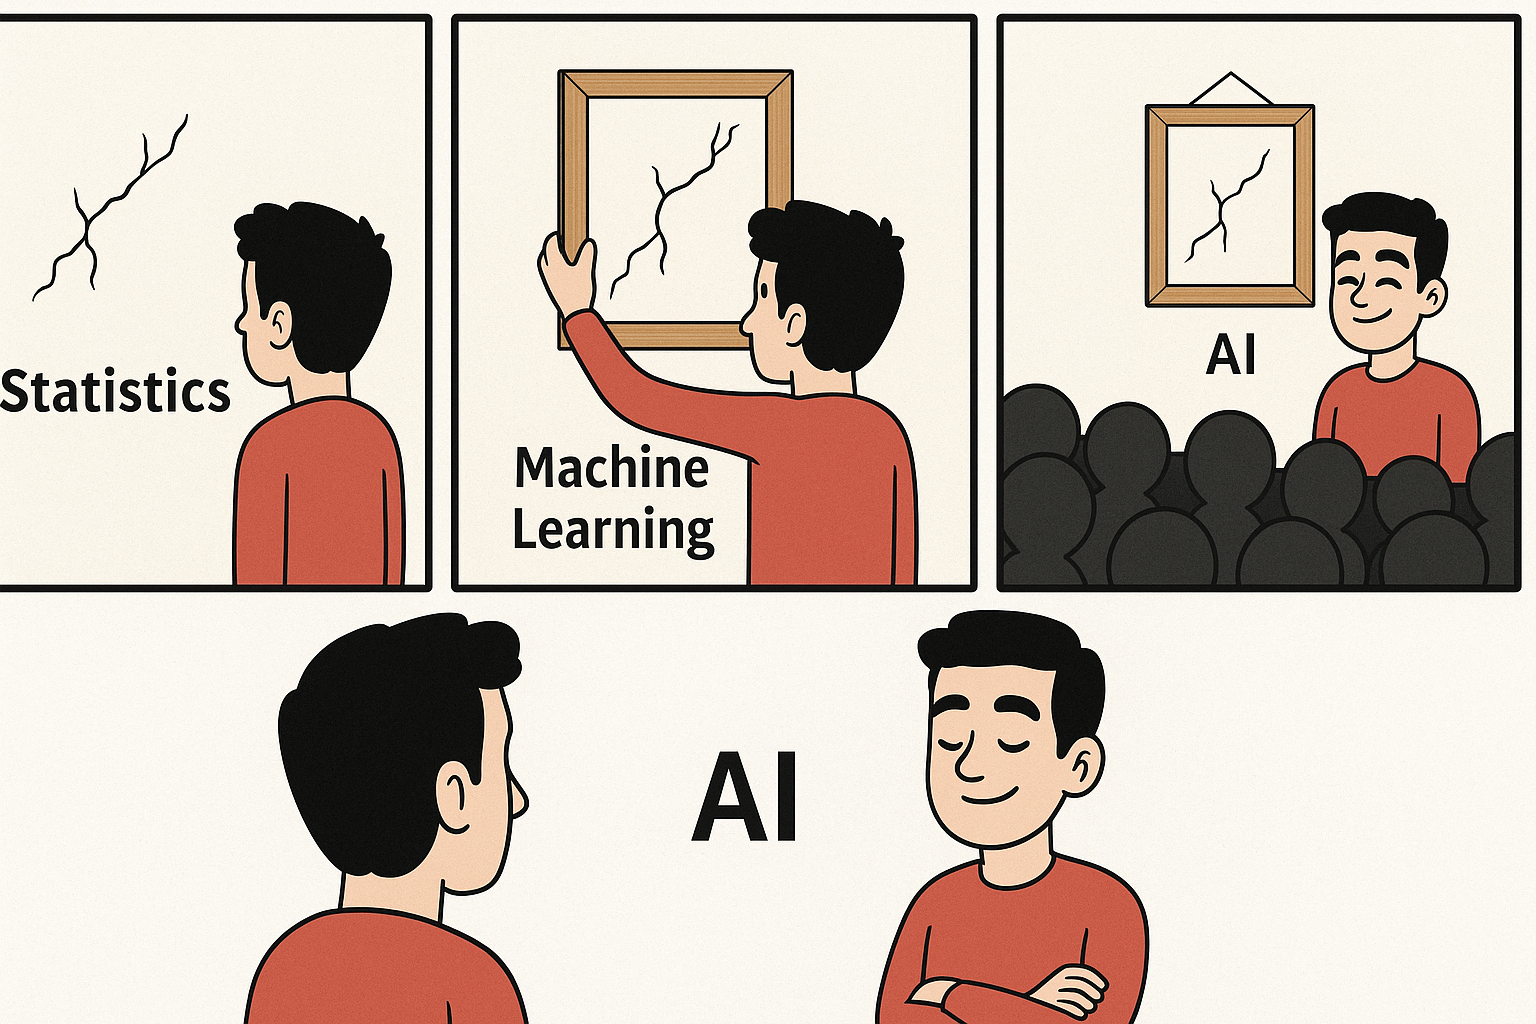
\includegraphics[width=0.7\linewidth,alt={A three-panel comic illustration depicting the evolution of a crack in a wall as a metaphor for data analysis. In the first panel, a person observes a crack labeled 'Statistics.' In the second panel, the person frames the crack, labeled 'Machine Learning.' In the third panel, the framed crack is displayed to an audience, labeled 'AI,' with the person smiling confidently. Below, a larger image shows the person with a satisfied expression, standing next to the bold text 'AI.' The comic humorously illustrates the progression from basic observation to advanced presentation in data science.}]{images/meme_01} 

}

\caption{Meme about AI and ML}\label{fig:include-image}
\end{figure}

\section{Matrix Theory}\label{matrix-theory}

Matrix \(A\) represents the original matrix. It's a 2x2 matrix with elements \(a_{ij}\), where \(i\) represents the row and \(j\) represents the column.

\[
A =
\begin{bmatrix}
a_{11} & a_{12} \\
a_{21} & a_{22}
\end{bmatrix}
\]

\(A'\) is the transpose of \(A\). The transpose of a matrix flips its rows and columns.

\[
A' =
\begin{bmatrix}
a_{11} & a_{21} \\
a_{12} & a_{22}
\end{bmatrix}
\]

Fundamental properties and rules of matrices, essential for understanding operations in linear algebra:

\[
\begin{aligned}
\mathbf{(ABC)'}   & = \mathbf{C'B'A'} \quad &\text{(Transpose reverses order in a product)} \\
\mathbf{A(B+C)}   & = \mathbf{AB + AC} \quad &\text{(Distributive property)} \\
\mathbf{AB}       & \neq \mathbf{BA} \quad &\text{(Multiplication is not commutative)} \\
\mathbf{(A')'}    & = \mathbf{A} \quad &\text{(Double transpose is the original matrix)} \\
\mathbf{(A+B)'}   & = \mathbf{A' + B'} \quad &\text{(Transpose of a sum is the sum of transposes)} \\
\mathbf{(AB)'}    & = \mathbf{B'A'} \quad &\text{(Transpose reverses order in a product)} \\
\mathbf{(AB)^{-1}} & = \mathbf{B^{-1}A^{-1}} \quad &\text{(Inverse reverses order in a product)} \\
\mathbf{A+B}      & = \mathbf{B + A} \quad &\text{(Addition is commutative)} \\
\mathbf{AA^{-1}}  & = \mathbf{I} \quad &\text{(Matrix times its inverse is identity)} 
\end{aligned}
\]

These properties are critical in solving systems of equations, optimizing models, and performing data transformations.

If a matrix \(\mathbf{A}\) has an inverse, it is called \textbf{invertible}. If \(\mathbf{A}\) does not have an inverse, it is referred to as \textbf{singular}.

The product of two matrices \(\mathbf{A}\) and \(\mathbf{B}\) is computed as:

\[
\begin{aligned}
\mathbf{A} &= 
\begin{bmatrix}
a_{11} & a_{12} & a_{13} \\ 
a_{21} & a_{22} & a_{23} 
\end{bmatrix}
\begin{bmatrix}
b_{11} & b_{12} & b_{13} \\
b_{21} & b_{22} & b_{23} \\
b_{31} & b_{32} & b_{33}
\end{bmatrix} \\
&= 
\begin{bmatrix}
a_{11}b_{11}+a_{12}b_{21}+a_{13}b_{31} & \sum_{i=1}^{3}a_{1i}b_{i2} & \sum_{i=1}^{3}a_{1i}b_{i3} \\
\sum_{i=1}^{3}a_{2i}b_{i1} & \sum_{i=1}^{3}a_{2i}b_{i2} & \sum_{i=1}^{3}a_{2i}b_{i3}
\end{bmatrix} 
\end{aligned}
\]

\textbf{Quadratic Form}

Let \(\mathbf{a}\) be a \(3 \times 1\) vector. The quadratic form involving a matrix \(\mathbf{B}\) is given by:

\[
\mathbf{a'Ba} = \sum_{i=1}^{3}\sum_{j=1}^{3}a_i b_{ij} a_{j}
\]

\textbf{Length of a Vector}

The \textbf{length} (or 2-norm) of a vector \(\mathbf{a}\), denoted as \(||\mathbf{a}||\), is defined as the square root of the inner product of the vector with itself:

\[
||\mathbf{a}|| = \sqrt{\mathbf{a'a}}
\]

\subsection{Rank of a Matrix}\label{rank-of-a-matrix}

The \textbf{rank} of a matrix refers to:

\begin{itemize}
\tightlist
\item
  The dimension of the space spanned by its columns (or rows).
\item
  The number of linearly independent columns or rows.
\end{itemize}

For an \(n \times k\) matrix \(\mathbf{A}\) and a \(k \times k\) matrix \(\mathbf{B}\), the following properties hold:

\begin{itemize}
\tightlist
\item
  \(\text{rank}(\mathbf{A}) \leq \min(n, k)\)
\item
  \(\text{rank}(\mathbf{A}) = \text{rank}(\mathbf{A'}) = \text{rank}(\mathbf{A'A}) = \text{rank}(\mathbf{AA'})\)
\item
  \(\text{rank}(\mathbf{AB}) = \min(\text{rank}(\mathbf{A}), \text{rank}(\mathbf{B}))\)
\item
  \(\mathbf{B}\) is invertible (non-singular) if and only if \(\text{rank}(\mathbf{B}) = k\).
\end{itemize}

\subsection{Inverse of a Matrix}\label{inverse-of-a-matrix}

In scalar algebra, if \(a = 0\), then \(1/a\) does not exist.

In matrix algebra, a matrix is invertible if it is \textbf{non-singular}, meaning it has a non-zero determinant and its inverse exists. A square matrix \(\mathbf{A}\) is invertible if there exists another square matrix \(\mathbf{B}\) such that:

\[
\mathbf{AB} = \mathbf{I} \quad \text{(Identity Matrix)}.
\]

In this case, \(\mathbf{A}^{-1} = \mathbf{B}\).

For a \(2 \times 2\) matrix:

\[
\mathbf{A} =
\begin{bmatrix}
a & b \\
c & d
\end{bmatrix}
\]

The inverse is:

\[
\mathbf{A}^{-1} =
\frac{1}{ad-bc}
\begin{bmatrix}
d & -b \\
-c & a
\end{bmatrix}
\]

This inverse exists only if \(ad - bc \neq 0\), where \(ad - bc\) is the determinant of \(\mathbf{A}\).

For a partitioned block matrix:

\[
\begin{bmatrix}
A & B \\
C & D
\end{bmatrix}^{-1}
=
\begin{bmatrix}
\mathbf{(A-BD^{-1}C)^{-1}} & \mathbf{-(A-BD^{-1}C)^{-1}BD^{-1}} \\
\mathbf{-D^{-1}C(A-BD^{-1}C)^{-1}} & \mathbf{D^{-1}+D^{-1}C(A-BD^{-1}C)^{-1}BD^{-1}}
\end{bmatrix}
\]

This formula assumes that \(\mathbf{D}\) and \(\mathbf{A - BD^{-1}C}\) are invertible.

Properties of the Inverse for Non-Singular Matrices

\begin{enumerate}
\def\labelenumi{\arabic{enumi}.}
\tightlist
\item
  \(\mathbf{(A^{-1})^{-1}} = \mathbf{A}\)
\item
  For a non-zero scalar \(b\), \(\mathbf{(bA)^{-1} = b^{-1}A^{-1}}\)
\item
  For a matrix \(\mathbf{B}\), \(\mathbf{(BA)^{-1} = B^{-1}A^{-1}}\) (only if \(\mathbf{B}\) is non-singular).
\item
  \(\mathbf{(A^{-1})' = (A')^{-1}}\) (the transpose of the inverse equals the inverse of the transpose).
\item
  Never notate \(\mathbf{1/A}\); use \(\mathbf{A^{-1}}\) instead.
\end{enumerate}

\textbf{Notes}:

\begin{itemize}
\item
  The determinant of a matrix determines whether it is invertible. For square matrices, a determinant of \(0\) means the matrix is \textbf{singular} and has no inverse.
\item
  Always verify the conditions for invertibility, particularly when dealing with partitioned or block matrices.
\end{itemize}

\subsection{Definiteness of a Matrix}\label{definiteness-of-a-matrix}

A symmetric square \(k \times k\) matrix \(\mathbf{A}\) is classified based on the following conditions:

\begin{itemize}
\item
  Positive Semi-Definite (PSD): \(\mathbf{A}\) is PSD if, for any non-zero \(k \times 1\) vector \(\mathbf{x}\): \[
  \mathbf{x'Ax \geq 0}.
  \]
\item
  \textbf{Negative Semi-Definite (NSD)}: \(\mathbf{A}\) is NSD if, for any non-zero \(k \times 1\) vector \(\mathbf{x}\): \[
  \mathbf{x'Ax \leq 0}.
  \]
\item
  Indefinite: \(\mathbf{A}\) is indefinite if it is neither PSD nor NSD.
\end{itemize}

The \textbf{identity matrix} is always positive definite (PD).

Example

Let \(\mathbf{x} = (x_1, x_2)'\), and consider a \(2 \times 2\) identity matrix \(\mathbf{I}\):

\[
\begin{aligned}
\mathbf{x'Ix} 
&= (x_1, x_2) 
\begin{bmatrix}
1 & 0 \\
0 & 1
\end{bmatrix}
\begin{bmatrix}
x_1 \\
x_2
\end{bmatrix} \\
&=
(x_1, x_2)
\begin{bmatrix}
x_1 \\
x_2
\end{bmatrix} \\
&=
x_1^2 + x_2^2 \geq 0.
\end{aligned}
\]

Thus, \(\mathbf{I}\) is PD because \(\mathbf{x'Ix} > 0\) for all non-zero \(\mathbf{x}\).

\textbf{Properties of Definiteness}

\begin{enumerate}
\def\labelenumi{\arabic{enumi}.}
\tightlist
\item
  Any variance-covariance matrix is PSD.
\item
  A matrix \(\mathbf{A}\) is PSD if and only if there exists a matrix \(\mathbf{B}\) such that: \[
  \mathbf{A = B'B}.
  \]
\item
  If \(\mathbf{A}\) is PSD, then \(\mathbf{B'AB}\) is also PSD for any conformable matrix \(\mathbf{B}\).
\item
  If \(\mathbf{A}\) and \(\mathbf{C}\) are non-singular, then \(\mathbf{A - C}\) is PSD if and only if \(\mathbf{C^{-1} - A^{-1}}\) is PSD.
\item
  If \(\mathbf{A}\) is PD (or ND), then \(\mathbf{A^{-1}}\) is also PD (or ND).
\end{enumerate}

\textbf{Notes}

\begin{itemize}
\tightlist
\item
  An \textbf{indefinite} matrix \(\mathbf{A}\) is neither PSD nor NSD. This concept does not have a direct counterpart in scalar algebra.
\item
  If a square matrix is PSD and invertible, then it is PD.
\end{itemize}

Examples of Definiteness

\begin{enumerate}
\def\labelenumi{\arabic{enumi}.}
\item
  \textbf{Invertible / Indefinite}: \[
  \begin{bmatrix}
  -1 & 0 \\
  0 & 10
  \end{bmatrix}
  \]
\item
  Non-Invertible / Indefinite: \[
  \begin{bmatrix}
  0 & 1 \\
  0 & 0
  \end{bmatrix}
  \]
\item
  \textbf{Invertible / PSD}: \[
  \begin{bmatrix}
  1 & 0 \\
  0 & 1
  \end{bmatrix}
  \]
\item
  Non-Invertible / PSD: \[
  \begin{bmatrix}
  0 & 0 \\
  0 & 1
  \end{bmatrix}
  \]
\end{enumerate}

\subsection{Matrix Calculus}\label{matrix-calculus}

Consider a scalar function \(y = f(x_1, x_2, \dots, x_k) = f(x)\), where \(x\) is a \(1 \times k\) row vector.

\subsubsection{Gradient (First-Order Derivative)}\label{gradient-first-order-derivative}

The gradient, or the first-order derivative of \(f(x)\) with respect to the vector \(x\), is given by:

\[
\frac{\partial f(x)}{\partial x} =
\begin{bmatrix}
\frac{\partial f(x)}{\partial x_1} \\
\frac{\partial f(x)}{\partial x_2} \\
\vdots \\
\frac{\partial f(x)}{\partial x_k}
\end{bmatrix}
\]

\subsubsection{Hessian (Second-Order Derivative)}\label{hessian-second-order-derivative}

The Hessian, or the second-order derivative of \(f(x)\) with respect to \(x\), is a symmetric matrix defined as:

\[
\frac{\partial^2 f(x)}{\partial x \partial x'} =
\begin{bmatrix}
\frac{\partial^2 f(x)}{\partial x_1^2} & \frac{\partial^2 f(x)}{\partial x_1 \partial x_2} & \cdots & \frac{\partial^2 f(x)}{\partial x_1 \partial x_k} \\
\frac{\partial^2 f(x)}{\partial x_2 \partial x_1} & \frac{\partial^2 f(x)}{\partial x_2^2} & \cdots & \frac{\partial^2 f(x)}{\partial x_2 \partial x_k} \\
\vdots & \vdots & \ddots & \vdots \\
\frac{\partial^2 f(x)}{\partial x_k \partial x_1} & \frac{\partial^2 f(x)}{\partial x_k \partial x_2} & \cdots & \frac{\partial^2 f(x)}{\partial x_k^2}
\end{bmatrix}
\]

\subsubsection{Derivative of a Scalar Function with Respect to a Matrix}\label{derivative-of-a-scalar-function-with-respect-to-a-matrix}

Let \(f(\mathbf{X})\) be a scalar function, where \(\mathbf{X}\) is an \(n \times p\) matrix. The derivative is:

\[
\frac{\partial f(\mathbf{X})}{\partial \mathbf{X}} = 
\begin{bmatrix}
\frac{\partial f(\mathbf{X})}{\partial x_{11}} & \cdots & \frac{\partial f(\mathbf{X})}{\partial x_{1p}} \\
\vdots & \ddots & \vdots \\
\frac{\partial f(\mathbf{X})}{\partial x_{n1}} & \cdots & \frac{\partial f(\mathbf{X})}{\partial x_{np}}
\end{bmatrix}
\]

\subsubsection{Common Matrix Derivatives}\label{common-matrix-derivatives}

\begin{enumerate}
\def\labelenumi{\arabic{enumi}.}
\tightlist
\item
  If \(\mathbf{a}\) is a vector and \(\mathbf{A}\) is a matrix independent of \(\mathbf{y}\):

  \begin{itemize}
  \tightlist
  \item
    \(\frac{\partial \mathbf{a'y}}{\partial \mathbf{y}} = \mathbf{a}\)
  \item
    \(\frac{\partial \mathbf{y'y}}{\partial \mathbf{y}} = 2\mathbf{y}\)
  \item
    \(\frac{\partial \mathbf{y'Ay}}{\partial \mathbf{y}} = (\mathbf{A} + \mathbf{A'})\mathbf{y}\)
  \end{itemize}
\item
  If \(\mathbf{X}\) is symmetric:

  \begin{itemize}
  \tightlist
  \item
    \(\frac{\partial |\mathbf{X}|}{\partial x_{ij}} = \begin{cases} X_{ii}, & i = j \\ X_{ij}, & i \neq j \end{cases}\) where \(X_{ij}\) is the \((i,j)\)-th cofactor of \(\mathbf{X}\).
  \end{itemize}
\item
  If \(\mathbf{X}\) is symmetric and \(\mathbf{A}\) is a matrix independent of \(\mathbf{X}\):

  \begin{itemize}
  \tightlist
  \item
    \(\frac{\partial \text{tr}(\mathbf{XA})}{\partial \mathbf{X}} = \mathbf{A} + \mathbf{A'} - \text{diag}(\mathbf{A})\).
  \end{itemize}
\item
  If \(\mathbf{X}\) is symmetric, let \(\mathbf{J}_{ij}\) be a matrix with 1 at the \((i,j)\)-th position and 0 elsewhere:

  \begin{itemize}
  \tightlist
  \item
    \(\frac{\partial \mathbf{X}^{-1}}{\partial x_{ij}} = \begin{cases} -\mathbf{X}^{-1}\mathbf{J}_{ii}\mathbf{X}^{-1}, & i = j \\ -\mathbf{X}^{-1}(\mathbf{J}_{ij} + \mathbf{J}_{ji})\mathbf{X}^{-1}, & i \neq j \end{cases}.\)
  \end{itemize}
\end{enumerate}

\subsection{Optimization in Scalar and Vector Spaces}\label{optimization-in-scalar-and-vector-spaces}

Optimization is the process of finding the minimum or maximum of a function. The conditions for optimization differ depending on whether the function involves a scalar or a vector. Below is a comparison of scalar and vector optimization:

\begin{longtable}[]{@{}
  >{\raggedright\arraybackslash}p{(\linewidth - 4\tabcolsep) * \real{0.2893}}
  >{\raggedright\arraybackslash}p{(\linewidth - 4\tabcolsep) * \real{0.2487}}
  >{\raggedright\arraybackslash}p{(\linewidth - 4\tabcolsep) * \real{0.4569}}@{}}
\caption{Conditions for scalar and vector optimization}\tabularnewline
\toprule\noalign{}
\begin{minipage}[b]{\linewidth}\raggedright
Condition
\end{minipage} & \begin{minipage}[b]{\linewidth}\raggedright
\textbf{Scalar Optimization}
\end{minipage} & \begin{minipage}[b]{\linewidth}\raggedright
\textbf{Vector Optimization}
\end{minipage} \\
\midrule\noalign{}
\endfirsthead
\toprule\noalign{}
\begin{minipage}[b]{\linewidth}\raggedright
Condition
\end{minipage} & \begin{minipage}[b]{\linewidth}\raggedright
\textbf{Scalar Optimization}
\end{minipage} & \begin{minipage}[b]{\linewidth}\raggedright
\textbf{Vector Optimization}
\end{minipage} \\
\midrule\noalign{}
\endhead
\bottomrule\noalign{}
\endlastfoot
\textbf{First-Order Condition} & \(\frac{\partial f(x_0)}{\partial x} = 0\) & \(\frac{\partial f(x_0)}{\partial x} = \begin{bmatrix} 0 \\ \vdots \\ 0 \end{bmatrix}\) \\
\textbf{Second-Order Condition}

For \textbf{convex} functions, this implies a \textbf{minimum}. & \(\frac{\partial^2 f(x_0)}{\partial x^2} > 0\) & \(\frac{\partial^2 f(x_0)}{\partial x \partial x'} > 0\) \\
For \textbf{concave} functions, this implies a \textbf{maximum}. & \(\frac{\partial^2 f(x_0)}{\partial x^2} < 0\) & \(\frac{\partial^2 f(x_0)}{\partial x \partial x'} < 0\) \\
\end{longtable}

\textbf{Key Concepts}

\begin{enumerate}
\def\labelenumi{\arabic{enumi}.}
\tightlist
\item
  \textbf{First-Order Condition}:

  \begin{itemize}
  \tightlist
  \item
    The \textbf{first-order derivative} of the function must equal zero at a critical point. This holds for both scalar and vector functions:

    \begin{itemize}
    \tightlist
    \item
      In the scalar case, \(\frac{\partial f(x)}{\partial x} = 0\) identifies critical points.
    \item
      In the vector case, \(\frac{\partial f(x)}{\partial x}\) is a \textbf{gradient vector}, and the condition is satisfied when all elements of the gradient are zero.
    \end{itemize}
  \end{itemize}
\item
  \textbf{Second-Order Condition}:

  \begin{itemize}
  \tightlist
  \item
    The \textbf{second-order derivative} determines whether the critical point is a minimum, maximum, or saddle point:

    \begin{itemize}
    \tightlist
    \item
      For scalar functions, \(\frac{\partial^2 f(x)}{\partial x^2} > 0\) implies a \textbf{local minimum}, while \(\frac{\partial^2 f(x)}{\partial x^2} < 0\) implies a \textbf{local maximum}.
    \item
      For vector functions, the Hessian matrix \(\frac{\partial^2 f(x)}{\partial x \partial x'}\) must be:

      \begin{itemize}
      \tightlist
      \item
        \textbf{Positive Definite}: For a \textbf{minimum} (convex function).
      \item
        \textbf{Negative Definite}: For a \textbf{maximum} (concave function).
      \item
        \textbf{Indefinite}: For a \textbf{saddle point} (neither minimum nor maximum).
      \end{itemize}
    \end{itemize}
  \end{itemize}
\item
  \textbf{Convex and Concave Functions}:

  \begin{itemize}
  \tightlist
  \item
    A function \(f(x)\) is:

    \begin{itemize}
    \tightlist
    \item
      \textbf{Convex} if \(\frac{\partial^2 f(x)}{\partial x^2} > 0\) or the Hessian \(\frac{\partial^2 f(x)}{\partial x \partial x'}\) is positive definite.
    \item
      \textbf{Concave} if \(\frac{\partial^2 f(x)}{\partial x^2} < 0\) or the Hessian is negative definite.
    \end{itemize}
  \item
    Convexity ensures global optimization for minimization problems, while concavity ensures global optimization for maximization problems.
  \end{itemize}
\item
  \textbf{Hessian Matrix}:

  \begin{itemize}
  \tightlist
  \item
    In vector optimization, the Hessian \(\frac{\partial^2 f(x)}{\partial x \partial x'}\) plays a crucial role in determining the nature of critical points:

    \begin{itemize}
    \tightlist
    \item
      Positive definite Hessian: All eigenvalues are positive.
    \item
      Negative definite Hessian: All eigenvalues are negative.
    \item
      Indefinite Hessian: Eigenvalues have mixed signs.
    \end{itemize}
  \end{itemize}
\end{enumerate}

\subsection{Cholesky Decomposition}\label{cholesky-decomposition}

In statistical analysis and numerical linear algebra, decomposing matrices into more tractable forms is crucial for efficient computation. One such important factorization is the \textbf{Cholesky Decomposition}. It applies to \textbf{Hermitian} (in the complex case) or \textbf{symmetric} (in the real case), \textbf{positive-definite} matrices.

Given an \(n \times n\) positive-definite matrix \(A\), the Cholesky Decomposition states:

\[
A = L L^{*},
\]

where:

\begin{itemize}
\tightlist
\item
  \(L\) is a lower-triangular matrix with strictly positive diagonal entries.
\item
  \(L^{*}\) denotes the \emph{conjugate transpose} of \(L\) (simply the transpose \(L^{T}\) for real matrices).
\end{itemize}

Cholesky Decomposition is both computationally efficient and numerically stable, making it a go-to technique for many applications, particularly in statistics where we deal extensively with covariance matrices, linear systems, and probability distributions.

Before diving into how we compute a Cholesky Decomposition, we need to clarify what it means for a matrix to be \emph{positive-definite}. For a real symmetric matrix \(A\):

\begin{itemize}
\tightlist
\item
  \(A\) is \emph{positive-definite} if for every nonzero vector \(x\), we have \[
  x^T A  x > 0.
  \]
\item
  Alternatively, you can characterize positive-definiteness by noting that all eigenvalues of \(A\) are strictly positive.
\end{itemize}

Many important matrices in statistics, particularly covariance or precision matrices, are both symmetric and positive-definite.

\begin{center}\rule{0.5\linewidth}{0.5pt}\end{center}

\subsubsection{Existence}\label{existence}

A real \(n \times n\) matrix \(A\) that is symmetric and positive-definite always admits a Cholesky Decomposition \(A = L L^T\). This theorem guarantees that for any covariance matrix in statistics that is valid (i.e., positive-definite) we can decompose it via Cholesky.

\subsubsection{Uniqueness}\label{uniqueness}

If we additionally require that the diagonal entries of \(L\) are \emph{strictly positive}, then \(L\) is \emph{unique}. That is, no other lower-triangular matrix with strictly positive diagonal entries will produce the same factorization. This uniqueness is helpful for ensuring consistent numerical outputs in software implementations.

\subsubsection{\texorpdfstring{Constructing the Cholesky Factor \(L\)}{Constructing the Cholesky Factor L}}\label{constructing-the-cholesky-factor-l}

Given a real, symmetric, positive-definite matrix \(A \in \mathbb{R}^{n \times n}\), we want to find the lower-triangular matrix \(L\) such that \(A = LL^T\). One way to do this is by using a simple step-by-step procedure (often part of standard linear algebra libraries):

\begin{enumerate}
\def\labelenumi{\arabic{enumi}.}
\tightlist
\item
  \textbf{Initialize} \(L\) to be an \(n \times n\) zero matrix.
\item
  \textbf{Iterate} through the rows \(i = 1, 2, \dots, n\):

  \begin{enumerate}
  \def\labelenumii{\arabic{enumii}.}
  \tightlist
  \item
    For each row \(i\), compute \[
    L_{ii} = \sqrt{A_{ii} - \sum_{k=1}^{i-1} L_{ik}^2}.
    \]
  \item
    For each column \(j = i+1, i+2, \dots, n\): \[
    L_{ji} = \frac{1}{L_{ii}}
              \left(A_{ji} - \sum_{k=1}^{i-1} L_{jk} L_{ik}\right).
    \]
  \item
    All other entries of \(L\) remain zero or are computed in subsequent steps.
  \end{enumerate}
\item
  Result: \(L\) is lower-triangular, and \(L^T\) is its transpose.
\end{enumerate}

Cholesky Decomposition is roughly half the computational cost of a more general LU Decomposition. Specifically, it requires on the order of \(\frac{1}{3} n^3\) floating-point operations (flops), making it significantly more efficient in practice than other decompositions for positive-definite systems.

\begin{center}\rule{0.5\linewidth}{0.5pt}\end{center}

\subsubsection{Illustrative Example}\label{illustrative-example}

Consider a small \(3 \times 3\) positive-definite matrix:

\[
A = 
\begin{pmatrix}
4 & 2 & 4 \\
2 & 5 & 6 \\
4 & 6 & 20
\end{pmatrix}.
\]

We claim \(A\) is positive-definite (one could check by calculating principal minors or verifying \(x^T A x > 0\) for all \(x \neq 0\)). We find \(L\) step-by-step:

\begin{enumerate}
\def\labelenumi{\arabic{enumi}.}
\tightlist
\item
  \textbf{Compute} \(L_{11}\):\\
  \[
  L_{11} = \sqrt{A_{11}} = \sqrt{4} = 2.
  \]
\item
  \textbf{Compute} \(L_{21}\) and \(L_{31}\):

  \begin{itemize}
  \tightlist
  \item
    \(L_{21} = \frac{A_{21}}{L_{11}} = \frac{2}{2} = 1.\)\\
  \item
    \(L_{31} = \frac{A_{31}}{L_{11}} = \frac{4}{2} = 2.\)
  \end{itemize}
\item
  \textbf{Compute} \(L_{22}\):\\
  \[
  L_{22} = \sqrt{A_{22} - L_{21}^2} 
          = \sqrt{5 - 1^2}
          = \sqrt{4} = 2.
  \]
\item
  \textbf{Compute} \(L_{32}\):\\
  \[
  L_{32} = \frac{A_{32} - L_{31} L_{21}}{L_{22}}
          = \frac{6 - (2)(1)}{2}
          = \frac{4}{2} = 2.
  \]
\item
  \textbf{Compute} \(L_{33}\):\\
  \[
  L_{33} = \sqrt{A_{33} - (L_{31}^2 + L_{32}^2)}
          = \sqrt{20 - (2^2 + 2^2)}
          = \sqrt{20 - 8}
          = \sqrt{12}
          = 2\sqrt{3}.
  \]
\end{enumerate}

Thus,

\[
L = 
\begin{pmatrix}
2 & 0 & 0 \\
1 & 2 & 0 \\
2 & 2 & 2\sqrt{3}
\end{pmatrix}.
\]

One can verify \(L L^T = A\).

\begin{center}\rule{0.5\linewidth}{0.5pt}\end{center}

\subsubsection{Applications in Statistics}\label{applications-in-statistics}

\paragraph{Solving Linear Systems}\label{solving-linear-systems}

A common statistical problem is solving \(A x = b\) for \(x\). For instance, in regression or in computing Bayesian posterior modes, we often need to solve linear equations with covariance or precision matrices. With \(A = LL^T\):

\begin{enumerate}
\def\labelenumi{\arabic{enumi}.}
\tightlist
\item
  Forward Substitution: Solve \(L  y = b\).
\item
  Backward Substitution: Solve \(L^T x = y\).
\end{enumerate}

This two-step process is more stable and efficient than directly inverting \(A\) (which is typically discouraged due to numerical issues).

\paragraph{Generating Correlated Random Vectors}\label{generating-correlated-random-vectors}

In simulation-based statistics (e.g., Monte Carlo methods), we often need to generate random draws from a \textbf{multivariate normal} distribution \(\mathcal{N}(\mu, \Sigma)\), where \(\Sigma\) is the covariance matrix. The steps are:

\begin{enumerate}
\def\labelenumi{\arabic{enumi}.}
\tightlist
\item
  Generate a vector \(z \sim \mathcal{N}(0, I)\) of independent standard normal variables.
\item
  Compute \(x = \mu + Lz\), where \(\Sigma = LL^T\).
\end{enumerate}

Then \(x\) has the desired covariance structure \(\Sigma\). This technique is widely used in Bayesian statistics (e.g., MCMC sampling) and financial modeling (e.g., portfolio simulations).

\paragraph{Gaussian Processes and Kriging}\label{gaussian-processes-and-kriging}

In Gaussian Process modeling (common in spatial statistics, machine learning, and geostatistics), we frequently work with large covariance matrices that describe the correlations between observed data points:

\[
\Sigma = 
\begin{pmatrix}
k(x_1, x_1) & k(x_1, x_2) & \cdots & k(x_1, x_n) \\
k(x_2, x_1) & k(x_2, x_2) & \cdots & k(x_2, x_n) \\
\vdots      & \vdots      & \ddots & \vdots      \\
k(x_n, x_1) & k(x_n, x_2) & \cdots & k(x_n, x_n)
\end{pmatrix},
\]

where \(k(\cdot, \cdot)\) is a covariance (kernel) function. We may need to invert or factorize \(\Sigma\) repeatedly to evaluate the log-likelihood:

\[
\log \mathcal{L}(\theta) \sim 
- \tfrac{1}{2} \left( y - m(\theta) \right)^T \Sigma^{-1} \left( y - m(\theta) \right) 
- \tfrac{1}{2} \log \left| \Sigma \right|,
\]

where \(m(\theta)\) is the mean function and \(\theta\) are parameters. Using the Cholesky factor \(L\) of \(\Sigma\) helps:

\begin{itemize}
\tightlist
\item
  \(\Sigma^{-1}\) can be implied by solving systems with \(L\) instead of explicitly computing the inverse.
\item
  \(\log|\Sigma|\) can be computed as \(2 \sum_{i=1}^n \log L_{ii}\).
\end{itemize}

Hence, Cholesky Decomposition becomes the backbone of Gaussian Process computations.

\paragraph{Bayesian Inference with Covariance Matrices}\label{bayesian-inference-with-covariance-matrices}

Many Bayesian models, especially hierarchical models, assume a multivariate normal prior on parameters. Cholesky Decomposition is used to:

\begin{itemize}
\tightlist
\item
  Sample from these priors or from posterior distributions.
\item
  Regularize large covariance matrices.
\item
  Speed up Markov Chain Monte Carlo (MCMC) computations by factorizing covariance structures.
\end{itemize}

\begin{center}\rule{0.5\linewidth}{0.5pt}\end{center}

\subsubsection{Other Notes}\label{other-notes}

\begin{enumerate}
\def\labelenumi{\arabic{enumi}.}
\tightlist
\item
  Numerical Stability Considerations
\end{enumerate}

Cholesky Decomposition is considered more stable than a general LU Decomposition when applied to positive-definite matrices. Since no row or column pivots are required, rounding errors can be smaller. Of course, in practice, software implementations can vary, and extremely ill-conditioned matrices can still pose numerical challenges.

\begin{enumerate}
\def\labelenumi{\arabic{enumi}.}
\setcounter{enumi}{1}
\tightlist
\item
  Why We \emph{Don't} Usually Compute \(\mathbf{A}^{-1}\)
\end{enumerate}

It is common in statistics (especially in older texts) to see formulas involving \(\Sigma^{-1}\). However, computing an inverse explicitly is often discouraged because:

\begin{itemize}
\tightlist
\item
  It is numerically less stable.
\item
  It requires more computations.
\item
  Many tasks that \emph{appear} to need \(\Sigma^{-1}\) can be done more efficiently by solving systems via the Cholesky factor \(L\).
\end{itemize}

Hence, ``\textbf{solve, don't invert}'' is a common mantra. If you see an expression like \(\Sigma^{-1} b\), you can use the Cholesky factors \(L\) and \(L^T\) to solve \(\Sigma x = b\) by forward and backward substitution, bypassing the direct inverse calculation.

\begin{enumerate}
\def\labelenumi{\arabic{enumi}.}
\setcounter{enumi}{2}
\tightlist
\item
  Further Variants and Extensions
\end{enumerate}

\begin{itemize}
\tightlist
\item
  Incomplete Cholesky: Sometimes used in iterative solvers where a full Cholesky factorization is too expensive, especially for large sparse systems.
\item
  LDL\^{}T Decomposition: A variant that avoids taking square roots; used for positive \emph{semi}-definite or indefinite systems, but with caution about pivoting strategies.
\end{itemize}

\begin{center}\rule{0.5\linewidth}{0.5pt}\end{center}

\section{Probability Theory}\label{probability-theory}

\subsection{Axioms and Theorems of Probability}\label{axioms-and-theorems-of-probability}

\begin{enumerate}
\def\labelenumi{\arabic{enumi}.}
\item
  Let \(S\) denote the sample space of an experiment. Then: \[
  P[S] = 1
  \] (The probability of the sample space is always 1.)
\item
  For any event \(A\): \[
  P[A] \geq 0
  \] (Probabilities are always non-negative.)
\item
  Let \(A_1, A_2, A_3, \dots\) be a finite or infinite collection of mutually exclusive events. Then: \[
  P[A_1 \cup A_2 \cup A_3 \dots] = P[A_1] + P[A_2] + P[A_3] + \dots
  \] (The probability of the union of mutually exclusive events is the sum of their probabilities.)
\item
  The probability of the empty set is: \[
  P[\emptyset] = 0
  \]
\item
  The complement rule: \[
  P[A'] = 1 - P[A]
  \]
\item
  The probability of the union of two events: \[
  P[A_1 \cup A_2] = P[A_1] + P[A_2] - P[A_1 \cap A_2]
  \]
\end{enumerate}

\subsubsection{Conditional Probability}\label{conditional-probability}

The conditional probability of \(A\) given \(B\) is defined as:

\[
P[A|B] = \frac{P[A \cap B]}{P[B]}, \quad \text{provided } P[B] \neq 0.
\]

\subsubsection{Independent Events}\label{independent-events}

Two events \(A\) and \(B\) are independent if and only if:

\begin{enumerate}
\def\labelenumi{\arabic{enumi}.}
\tightlist
\item
  \(P[A \cap B] = P[A]P[B]\)
\item
  \(P[A|B] = P[A]\)
\item
  \(P[B|A] = P[B]\)
\end{enumerate}

A collection of events \(A_1, A_2, \dots, A_n\) is independent if and only if every subcollection is independent.

\subsubsection{Multiplication Rule}\label{multiplication-rule}

The probability of the intersection of two events can be calculated as: \[
P[A \cap B] = P[A|B]P[B] = P[B|A]P[A].
\]

\subsubsection{Bayes' Theorem}\label{bayes-theorem}

Let \(A_1, A_2, \dots, A_n\) be a collection of mutually exclusive events whose union is \(S\), and let \(B\) be an event with \(P[B] \neq 0\). Then, for any event \(A_j\) (\(j = 1, 2, \dots, n\)): \[
P[A_j|B] = \frac{P[B|A_j]P[A_j]}{\sum_{i=1}^n P[B|A_i]P[A_i]}.
\]

\subsubsection{Jensen's Inequality}\label{jensens-inequality}

\begin{itemize}
\item
  If \(g(x)\) is convex, then: \[
  E[g(X)] \geq g(E[X])
  \]
\item
  If \(g(x)\) is concave, then: \[
  E[g(X)] \leq g(E[X]).
  \]
\end{itemize}

Jensen's inequality provides a useful way to demonstrate why the standard error calculated using the sample standard deviation (\(s\)) as a proxy for the population standard deviation (\(\sigma\)) is a biased estimator.

\begin{itemize}
\item
  The population standard deviation \(\sigma\) is defined as: \[
  \sigma = \sqrt{\mathbb{E}[(X - \mu)^2]},
  \] where \(\mu = \mathbb{E}[X]\) is the population mean.
\item
  The sample standard deviation \(s\) is given by: \[
  s = \sqrt{\frac{1}{n-1} \sum_{i=1}^n (X_i - \bar{X})^2},
  \] where \(\bar{X}\) is the sample mean.
\item
  When \(s\) is used as an estimator for \(\sigma\), the expectation involves the square root function, which is concave.
\end{itemize}

\textbf{Applying Jensen's Inequality}

The standard error formula involves the square root: \[
\sqrt{\mathbb{E}[s^2]}.
\]

However, because the square root function is concave, Jensen's inequality implies: \[
\sqrt{\mathbb{E}[s^2]} \leq \mathbb{E}[\sqrt{s^2}] = \mathbb{E}[s].
\]

This inequality shows that the expected value of \(s\) (the sample standard deviation) systematically underestimates the population standard deviation \(\sigma\).

\textbf{Quantifying the Bias}

The bias arises because: \[
\mathbb{E}[s] \neq \sigma.
\]

To correct this bias, we note that the sample standard deviation is related to the population standard deviation by: \[
\mathbb{E}[s] = \sigma \cdot \sqrt{\frac{n-1}{n}},
\] where \(n\) is the sample size. This bias decreases as \(n\) increases, and the estimator becomes asymptotically unbiased.

By leveraging Jensen's inequality, we observe that the concavity of the square root function ensures that \(s\) is a biased estimator of \(\sigma\), systematically underestimating the population standard deviation.

\subsubsection{Law of Iterated Expectation}\label{law-of-iterated-expectation}

The \textbf{Law of Iterated Expectation} states that for random variables \(X\) and \(Y\):

\[
E(X) = E(E(X|Y)).
\]

This means the expected value of \(X\) can be obtained by first calculating the conditional expectation \(E(X|Y)\) and then taking the expectation of this quantity over the distribution of \(Y\).

\subsubsection{Correlation and Independence}\label{correlation-and-independence}

The strength of the relationship between random variables can be ranked from strongest to weakest as:

\begin{enumerate}
\def\labelenumi{\arabic{enumi}.}
\tightlist
\item
  Independence:

  \begin{itemize}
  \tightlist
  \item
    \(f(x, y) = f_X(x)f_Y(y)\)
  \item
    \(f_{Y|X}(y|x) = f_Y(y)\) and \(f_{X|Y}(x|y) = f_X(x)\)
  \item
    \(E[g_1(X)g_2(Y)] = E[g_1(X)]E[g_2(Y)]\)
  \end{itemize}
\item
  \textbf{Mean Independence} (implied by independence):

  \begin{itemize}
  \tightlist
  \item
    \(Y\) is mean independent of \(X\) if: \[
    E[Y|X] = E[Y].
    \]
  \item
    \(E[Xg(Y)] = E[X]E[g(Y)]\)
  \end{itemize}
\item
  \textbf{Uncorrelatedness} (implied by independence and mean independence):

  \begin{itemize}
  \tightlist
  \item
    \(\text{Cov}(X, Y) = 0\)
  \item
    \(\text{Var}(X + Y) = \text{Var}(X) + \text{Var}(Y)\)
  \item
    \(E[XY] = E[X]E[Y]\)
  \end{itemize}
\end{enumerate}

\subsection{Central Limit Theorem}\label{central-limit-theorem}

The \textbf{Central Limit Theorem} states that for a sufficiently large sample size (\(n \geq 25\)), the sampling distribution of the sample mean or proportion approaches a normal distribution, regardless of the population's original distribution.

Let \(X_1, X_2, \dots, X_n\) be a random sample of size \(n\) from a distribution \(X\) with mean \(\mu\) and variance \(\sigma^2\). Then, for large \(n\):

\begin{enumerate}
\def\labelenumi{\arabic{enumi}.}
\item
  The sample mean \(\bar{X}\) is approximately normal: \[
  \mu_{\bar{X}} = \mu, \quad \sigma^2_{\bar{X}} = \frac{\sigma^2}{n}.
  \]
\item
  The sample proportion \(\hat{p}\) is approximately normal: \[
  \mu_{\hat{p}} = p, \quad \sigma^2_{\hat{p}} = \frac{p(1-p)}{n}.
  \]
\item
  The difference in sample proportions \(\hat{p}_1 - \hat{p}_2\) is approximately normal: \[
  \mu_{\hat{p}_1 - \hat{p}_2} = p_1 - p_2, \quad \sigma^2_{\hat{p}_1 - \hat{p}_2} = \frac{p_1(1-p_1)}{n_1} + \frac{p_2(1-p_2)}{n_2}.
  \]
\item
  The difference in sample means \(\bar{X}_1 - \bar{X}_2\) is approximately normal: \[
  \mu_{\bar{X}_1 - \bar{X}_2} = \mu_1 - \mu_2, \quad \sigma^2_{\bar{X}_1 - \bar{X}_2} = \frac{\sigma_1^2}{n_1} + \frac{\sigma_2^2}{n_2}.
  \]
\item
  The following random variables are approximately standard normal:

  \begin{itemize}
  \tightlist
  \item
    \(\frac{\bar{X} - \mu}{\sigma / \sqrt{n}}\)
  \item
    \(\frac{\hat{p} - p}{\sqrt{\frac{p(1-p)}{n}}}\)
  \item
    \(\frac{(\hat{p}_1 - \hat{p}_2) - (p_1 - p_2)}{\sqrt{\frac{p_1(1-p_1)}{n_1} + \frac{p_2(1-p_2)}{n_2}}}\)
  \item
    \(\frac{(\bar{X}_1 - \bar{X}_2) - (\mu_1 - \mu_2)}{\sqrt{\frac{\sigma_1^2}{n_1} + \frac{\sigma_2^2}{n_2}}}\)
  \end{itemize}
\end{enumerate}

\subsubsection{Limiting Distribution of the Sample Mean}\label{limiting-distribution-of-the-sample-mean}

If \(\{X_i\}_{i=1}^{n}\) is an iid random sample from a distribution with finite mean \(\mu\) and finite variance \(\sigma^2\), the sample mean \(\bar{X}\) scaled by \(\sqrt{n}\) has the following limiting distribution:

\[
\sqrt{n}(\bar{X} - \mu) \xrightarrow{d} N(0, \sigma^2).
\]

Standardizing the sample mean gives: \[
\frac{\sqrt{n}(\bar{X} - \mu)}{\sigma} \xrightarrow{d} N(0, 1).
\]

\textbf{Notes}:

\begin{itemize}
\tightlist
\item
  The CLT holds for most random samples from any distribution (continuous, discrete, or unknown).
\item
  It extends to the multivariate case: A random sample of a random vector converges to a multivariate normal distribution.
\end{itemize}

\subsubsection{Asymptotic Variance and Limiting Variance}\label{asymptotic-variance-and-limiting-variance}

\textbf{Asymptotic Variance} (Avar): \[
Avar(\sqrt{n}(\bar{X} - \mu)) = \sigma^2.
\]

\begin{itemize}
\item
  Refers to the variance of the limiting distribution of an estimator as the sample size (\(n\)) approaches infinity.
\item
  It characterizes the variability of the scaled estimator \(\sqrt{n}(\bar{x} - \mu)\) in its asymptotic distribution (e.g., normal distribution).
\end{itemize}

\textbf{Limiting Variance} (\(\lim_{n \to \infty} Var\))

\[
\lim_{n \to \infty} Var(\sqrt{n}(\bar{x}-\mu)) = \sigma^2
\]

\begin{itemize}
\tightlist
\item
  Represents the value that the actual variance of \(\sqrt{n}(\bar{x} - \mu)\) converges to as \(n \to \infty\).
\end{itemize}

For a well-behaved estimator,

\[
Avar(\sqrt{n}(\bar{X} - \mu)) = \lim_{n \to \infty} Var(\sqrt{n}(\bar{x}-\mu)) = \sigma^2.
\]

However, \textbf{asymptotic variance is not necessarily equal to the limiting value of the variance} because asymptotic variance is derived from the limiting distribution, while limiting variance is a convergence result of the sequence of variances.

\[
Avar(.) \neq lim_{n \to \infty} Var(.)
\]

\begin{itemize}
\item
  Both the asymptotic variance \(Avar\) and the limiting variance \(\lim_{n \to \infty} Var\) are numerically equal to \(\sigma^2\), but their conceptual definitions differ.
\item
  \(Avar(\cdot) \neq \lim_{n \to \infty} Var(\cdot)\). This emphasizes that while the numerical result may match, their derivation and meaning differ:

  \begin{itemize}
  \item
    \(Avar\) depends on the asymptotic (large-sample) distribution of the estimator.
  \item
    \(\lim_{n \to \infty} Var(\cdot)\) involves the sequence of variances as \(n\) grows.
  \end{itemize}
\end{itemize}

Cases where the two do not match:

\begin{enumerate}
\def\labelenumi{\arabic{enumi}.}
\tightlist
\item
  \textbf{Sample Quantiles}: Consider the sample quantile of order \(p\), for some \(0 < p < 1\). Under regularity conditions, the asymptotic distribution of the sample quantile is normal, with a variance that depends on \(p\) and the density of the distribution at the \(p\)-th quantile. However, the variance of the sample quantile itself does not necessarily converge to this limit as the sample size grows.
\item
  \textbf{Bootstrap Methods}: When using bootstrapping techniques to estimate the distribution of a statistic, the bootstrap distribution might converge to a different limiting distribution than the original statistic. In these cases, the variance of the bootstrap distribution (or the bootstrap variance) might differ from the limiting variance of the original statistic.
\item
  \textbf{Statistics with Randomly Varying Asymptotic Behavior}: In some cases, the asymptotic behavior of a statistic can vary randomly depending on the sample path. For such statistics, the asymptotic variance might not provide a consistent estimate of the limiting variance.
\item
  \textbf{M-estimators with Varying Asymptotic Behavior}: M-estimators can sometimes have different asymptotic behaviors depending on the tail behavior of the underlying distribution. For heavy-tailed distributions, the variance of the estimator might not stabilize even as the sample size grows large, making the asymptotic variance different from the variance of any limiting distribution.
\end{enumerate}

\subsection{Random Variable}\label{random-variable}

Random variables can be categorized as either \textbf{discrete} or \textbf{continuous}, with distinct properties and functions defining each type.

\begin{longtable}[]{@{}
  >{\raggedright\arraybackslash}p{(\linewidth - 4\tabcolsep) * \real{0.1429}}
  >{\raggedright\arraybackslash}p{(\linewidth - 4\tabcolsep) * \real{0.3883}}
  >{\raggedright\arraybackslash}p{(\linewidth - 4\tabcolsep) * \real{0.4652}}@{}}
\caption{Comparison of discrete and continuous random variables}\tabularnewline
\toprule\noalign{}
\begin{minipage}[b]{\linewidth}\raggedright
\end{minipage} & \begin{minipage}[b]{\linewidth}\raggedright
\textbf{Discrete Variable}
\end{minipage} & \begin{minipage}[b]{\linewidth}\raggedright
\textbf{Continuous Variable}
\end{minipage} \\
\midrule\noalign{}
\endfirsthead
\toprule\noalign{}
\begin{minipage}[b]{\linewidth}\raggedright
\end{minipage} & \begin{minipage}[b]{\linewidth}\raggedright
\textbf{Discrete Variable}
\end{minipage} & \begin{minipage}[b]{\linewidth}\raggedright
\textbf{Continuous Variable}
\end{minipage} \\
\midrule\noalign{}
\endhead
\bottomrule\noalign{}
\endlastfoot
\textbf{Definition} & A random variable is discrete if it can assume at most a finite or countably infinite number of values. & A random variable is continuous if it can assume any value in some interval or intervals of real numbers, with \(P(X=x) = 0\). \\
\textbf{Density Function} & A function \(f\) is called a density for \(X\) if: & A function \(f\) is called a density for \(X\) if: \\
& 1. \(f(x) \geq 0\) & 1. \(f(x) \geq 0\) for \(x\) real \\
& 2. \(\sum_{x} f(x) = 1\) & 2. \(\int_{-\infty}^{\infty} f(x)  dx = 1\) \textbar{} \\
& 3. \(f(x) = P(X = x)\) for \(x\) real & 3. \(P[a \leq X \leq b] = \int_{a}^{b} f(x)  dx\) for \(a, b\) real \textbar{} \\
\textbf{Cumulative Distribution Function} & \(F(x) = P(X \leq x)\) & \(F(x) = P(X \leq x) = \int_{-\infty}^{x} f(t)  dt\) \textbar{} \\
\(E[H(X)]\) & \(\sum_{x} H(x) f(x)\) & \(\int_{-\infty}^{\infty} H(x) f(x)  dx\) \textbar{} \\
\(\mu = E[X]\) & \(\sum_{x} x f(x)\) & \(\int_{-\infty}^{\infty} x f(x)  dx\) \textbar{} \\
\textbf{Ordinary Moments} & \(\sum_{x} x^k f(x)\) & \(\int_{-\infty}^{\infty} x^k f(x)  dx\) \textbar{} \\
\textbf{Moment Generating Function} & \(m_X(t) = E[e^{tX}] = \sum_{x} e^{tx} f(x)\) & \(m_X(t) = E[e^{tX}] = \int_{-\infty}^{\infty} e^{tx} f(x)  dx\) \textbar{} \\
\end{longtable}

\textbf{Expected Value Properties}

\begin{itemize}
\tightlist
\item
  \(E[c] = c\) for any constant \(c\).
\item
  \(E[cX] = cE[X]\) for any constant \(c\).
\item
  \(E[X + Y] = E[X] + E[Y]\).
\item
  \(E[XY] = E[X]E[Y]\) (if \(X\) and \(Y\) are independent).
\end{itemize}

\textbf{Variance Properties}

\begin{itemize}
\tightlist
\item
  \(\text{Var}(c) = 0\) for any constant \(c\).
\item
  \(\text{Var}(cX) = c^2 \text{Var}(X)\) for any constant \(c\).
\item
  \(\text{Var}(X) \geq 0\).
\item
  \(\text{Var}(X) = E[X^2] - (E[X])^2\).
\item
  \(\text{Var}(X + c) = \text{Var}(X)\).
\item
  \(\text{Var}(X + Y) = \text{Var}(X) + \text{Var}(Y)\) (if \(X\) and \(Y\) are independent).
\end{itemize}

The standard deviation \(\sigma\) is given by: \[
\sigma = \sqrt{\sigma^2} = \sqrt{\text{Var}(X)}.
\]

\subsubsection{Multivariate Random Variables}\label{multivariate-random-variables}

Suppose \(y_1, \dots, y_p\) are random variables with means \(\mu_1, \dots, \mu_p\). Then:

\[
\mathbf{y} = \begin{bmatrix}
y_1 \\
\vdots \\
y_p
\end{bmatrix}, \quad E[\mathbf{y}] = \begin{bmatrix}
\mu_1 \\
\vdots \\
\mu_p
\end{bmatrix} = \boldsymbol{\mu}.
\]

The covariance between \(y_i\) and \(y_j\) is \(\sigma_{ij} = \text{Cov}(y_i, y_j)\). The variance-covariance (or dispersion) matrix is:

\[
\mathbf{\Sigma} = (\sigma_{ij})= \begin{bmatrix}
\sigma_{11} & \sigma_{12} & \dots & \sigma_{1p} \\
\sigma_{21} & \sigma_{22} & \dots & \sigma_{2p} \\
\vdots & \vdots & \ddots & \vdots \\
\sigma_{p1} & \sigma_{p2} & \dots & \sigma_{pp}
\end{bmatrix}.
\]

And \(\mathbf{\Sigma}\) is symmetric with \((p+1)p/2\) unique parameters.

Alternatively, let \(u_{p \times 1}\) and \(v_{v \times 1}\) be random vectors with means \(\mathbf{\mu_u}\) and \(\mathbf{\mu_v}\). Then

\[ \mathbf{\Sigma_{uv}} = cov(\mathbf{u,v}) = E[\mathbf{(u-\mu_u)(v-\mu_v)'}] \]

\(\Sigma_{uv} \neq \Sigma_{vu}\) (but \(\Sigma_{uv} = \Sigma_{vu}'\))

\textbf{Properties of Covariance Matrices}

\begin{enumerate}
\def\labelenumi{\arabic{enumi}.}
\tightlist
\item
  Symmetry: \(\mathbf{\Sigma}' = \mathbf{\Sigma}\).
\item
  \textbf{Eigen-Decomposition} (spectral decomposition, symmetric decomposition): \(\mathbf{\Sigma = \Phi \Lambda \Phi}\), where \(\mathbf{\Phi}\) is a matrix of eigenvectors such that \(\mathbf{\Phi \Phi' = I}\) (orthonormal), and \(\mathbf{\Lambda}\) is a diagonal matrix with eigenvalues \((\lambda_1,...,\lambda_p)\) on the diagonal.
\item
  Non-Negative Definiteness: \(\mathbf{a \Sigma a} \ge 0\) for any \(\mathbf{a} \in R^p\). Equivalently, the eigenvalues of \(\mathbf{\Sigma}\), \(\lambda_1 \ge ... \ge \lambda_p \ge 0\)
\item
  Generalized Variance: \(|\mathbf{\Sigma}| = \lambda_1 \dots \lambda_p \geq 0\).
\item
  Trace: \(\text{tr}(\mathbf{\Sigma}) = \lambda_1 + \dots + \lambda_p = \sigma_{11} + \dots+ \sigma_{pp} = \sum \sigma_{ii}\) = sum of variances (total variance).
\end{enumerate}

\textbf{Note}: \(\mathbf{\Sigma}\) is required to be positive definite. This implies that all eigenvalues are positive, and \(\mathbf{\Sigma}\) has an inverse \(\mathbf{\Sigma}^{-1}\), such that \(\mathbf{\Sigma}^{-1}\mathbf{\Sigma}= \mathbf{I}_{p \times p} = \mathbf{\Sigma}\mathbf{\Sigma}^{-1}\)

\subsubsection{Correlation Matrices}\label{correlation-matrices}

The correlation coefficient \(\rho_{ij}\) and correlation matrix \(\mathbf{R}\) are defined as:

\[
\rho_{ij} = \frac{\sigma_{ij}}{\sqrt{\sigma_{ii}\sigma_{jj}}}, \quad \mathbf{R} = \begin{bmatrix}
1 & \rho_{12} & \dots & \rho_{1p} \\
\rho_{21} & 1 & \dots & \rho_{2p} \\
\vdots & \vdots & \ddots & \vdots \\
\rho_{p1} & \rho_{p2} & \dots & 1
\end{bmatrix}.
\]

where \(\rho_{ii} = 1 \forall i\)

\subsubsection{Linear Transformations}\label{linear-transformations}

Let \(\mathbf{A}\) and \(\mathbf{B}\) be matrices of constants, and \(\mathbf{c}\) and \(\mathbf{d}\) be vectors of constants. Then:

\begin{itemize}
\tightlist
\item
  \(E[\mathbf{Ay + c}] = \mathbf{A \mu_y + c}\).
\item
  \(\text{Var}(\mathbf{Ay + c}) = \mathbf{A \Sigma_y A'}\).
\item
  \(\text{Cov}(\mathbf{Ay + c, By + d}) = \mathbf{A \Sigma_y B'}\).
\end{itemize}

\subsection{Moment Generating Function}\label{moment-generating-function}

\subsubsection{Properties of the Moment Generating Function}\label{properties-of-the-moment-generating-function}

\begin{enumerate}
\def\labelenumi{\arabic{enumi}.}
\tightlist
\item
  \(\frac{d^k(m_X(t))}{dt^k} \bigg|_{t=0} = E[X^k]\) (The \(k\)-th derivative at \(t=0\) gives the \(k\)-th moment of \(X\)).
\item
  \(\mu = E[X] = m_X'(0)\) (The first derivative at \(t=0\) gives the mean).
\item
  \(E[X^2] = m_X''(0)\) (The second derivative at \(t=0\) gives the second moment).
\end{enumerate}

\subsubsection{Theorems Involving MGFs}\label{theorems-involving-mgfs}

Let \(X_1, X_2, \dots, X_n, Y\) be random variables with MGFs \(m_{X_1}(t), m_{X_2}(t), \dots, m_{X_n}(t), m_Y(t)\):

\begin{enumerate}
\def\labelenumi{\arabic{enumi}.}
\tightlist
\item
  If \(m_{X_1}(t) = m_{X_2}(t)\) for all \(t\) in some open interval about 0, then \(X_1\) and \(X_2\) have the same distribution.
\item
  If \(Y = \alpha + \beta X_1\), then: \[
  m_Y(t) = e^{\alpha t}m_{X_1}(\beta t).
  \]
\item
  If \(X_1, X_2, \dots, X_n\) are independent and \(Y = \alpha_0 + \alpha_1 X_1 + \alpha_2 X_2 + \dots + \alpha_n X_n\), where \(\alpha_0, \alpha_1, \dots, \alpha_n\) are constants, then: \[
  m_Y(t) = e^{\alpha_0 t} m_{X_1}(\alpha_1 t) m_{X_2}(\alpha_2 t) \dots m_{X_n}(\alpha_n t).
  \]
\item
  Suppose \(X_1, X_2, \dots, X_n\) are independent normal random variables with means \(\mu_1, \mu_2, \dots, \mu_n\) and variances \(\sigma_1^2, \sigma_2^2, \dots, \sigma_n^2\). If \(Y = \alpha_0 + \alpha_1 X_1 + \alpha_2 X_2 + \dots + \alpha_n X_n\), then:

  \begin{itemize}
  \tightlist
  \item
    \(Y\) is normally distributed.
  \item
    Mean: \(\mu_Y = \alpha_0 + \alpha_1 \mu_1 + \alpha_2 \mu_2 + \dots + \alpha_n \mu_n\).
  \item
    Variance: \(\sigma_Y^2 = \alpha_1^2 \sigma_1^2 + \alpha_2^2 \sigma_2^2 + \dots + \alpha_n^2 \sigma_n^2\).
  \end{itemize}
\end{enumerate}

\begin{center}\rule{0.5\linewidth}{0.5pt}\end{center}

\subsection{Moments}\label{moments}

\begin{longtable}[]{@{}
  >{\raggedright\arraybackslash}p{(\linewidth - 4\tabcolsep) * \real{0.1630}}
  >{\raggedright\arraybackslash}p{(\linewidth - 4\tabcolsep) * \real{0.3478}}
  >{\raggedright\arraybackslash}p{(\linewidth - 4\tabcolsep) * \real{0.4783}}@{}}
\caption{First four moments of a random variable, centered and uncentered}\tabularnewline
\toprule\noalign{}
\begin{minipage}[b]{\linewidth}\raggedright
Moment
\end{minipage} & \begin{minipage}[b]{\linewidth}\raggedright
Uncentered
\end{minipage} & \begin{minipage}[b]{\linewidth}\raggedright
Centered
\end{minipage} \\
\midrule\noalign{}
\endfirsthead
\toprule\noalign{}
\begin{minipage}[b]{\linewidth}\raggedright
Moment
\end{minipage} & \begin{minipage}[b]{\linewidth}\raggedright
Uncentered
\end{minipage} & \begin{minipage}[b]{\linewidth}\raggedright
Centered
\end{minipage} \\
\midrule\noalign{}
\endhead
\bottomrule\noalign{}
\endlastfoot
1st & \(E[X] = \mu = \text{Mean}(X)\) & \\
2nd & \(E[X^2]\) & \(E[(X-\mu)^2] = \text{Var}(X) = \sigma^2\) \\
3rd & \(E[X^3]\) & \(E[(X-\mu)^3]\) \\
4th & \(E[X^4]\) & \(E[(X-\mu)^4]\) \\
\end{longtable}

\begin{itemize}
\item
  Skewness: \(\text{Skewness}(X) = \frac{E[(X-\mu)^3]}{\sigma^3}\)

  \begin{itemize}
  \tightlist
  \item
    Definition: Skewness measures the asymmetry of a probability distribution around its mean.
  \item
    Interpretation:

    \begin{itemize}
    \item
      Positive skewness: The right tail (higher values) is longer or heavier than the left tail.
    \item
      Negative skewness: The left tail (lower values) is longer or heavier than the right tail.
    \item
      Zero skewness: The data is symmetric.
    \end{itemize}
  \end{itemize}
\item
  Kurtosis: \(\text{Kurtosis}(X) = \frac{E[(X-\mu)^4]}{\sigma^4}\)

  \begin{itemize}
  \item
    Definition: Kurtosis measures the ``tailedness'' or the heaviness of the tails of a probability distribution.
  \item
    Excess kurtosis (often reported) is the kurtosis minus 3 (to compare against the normal distribution's kurtosis of 3).
  \item
    Interpretation:

    \begin{itemize}
    \item
      High kurtosis (\textgreater3): Heavy tails, more extreme outliers.
    \item
      Low kurtosis (\textless3): Light tails, fewer outliers.
    \item
      Normal distribution kurtosis = 3: Benchmark for comparison.
    \end{itemize}
  \end{itemize}
\end{itemize}

\subsection{Skewness}\label{skewness}

Skewness measures the asymmetry of the distribution:

\begin{enumerate}
\def\labelenumi{\arabic{enumi}.}
\item
  Positive skew: The right side (high values) is stretched out.

  \begin{itemize}
  \item
    Positive skew occurs when the right tail (higher values) of the distribution is longer or heavier.
  \item
    Examples:

    \begin{itemize}
    \item
      Income Distribution: In many countries, most people earn a moderate income, but a small fraction of ultra-high earners stretches the distribution's right tail.
    \item
      Housing Prices: Most homes may be around an affordable price, but a few extravagant mansions create a very long (and expensive) upper tail.
    \end{itemize}
  \end{itemize}
\end{enumerate}

Figure \ref{fig:viz-positive-skew} illustrates positive skew using simulated income and housing-price distributions.

\begin{Shaded}
\begin{Highlighting}[]
\CommentTok{\# Load required libraries}
\FunctionTok{library}\NormalTok{(ggplot2)}

\CommentTok{\# Simulate data for positive skew}
\FunctionTok{set.seed}\NormalTok{(}\DecValTok{123}\NormalTok{)}
\NormalTok{positive\_skew\_income }\OtherTok{\textless{}{-}}
    \FunctionTok{rbeta}\NormalTok{(}\DecValTok{1000}\NormalTok{, }\DecValTok{5}\NormalTok{, }\DecValTok{2}\NormalTok{) }\SpecialCharTok{*} \DecValTok{100}  \CommentTok{\# Income distribution example}
\NormalTok{positive\_skew\_housing }\OtherTok{\textless{}{-}}
    \FunctionTok{rbeta}\NormalTok{(}\DecValTok{1000}\NormalTok{, }\DecValTok{5}\NormalTok{, }\DecValTok{2}\NormalTok{) }\SpecialCharTok{*} \DecValTok{1000}  \CommentTok{\# Housing prices example}

\CommentTok{\# Combine data}
\NormalTok{data\_positive\_skew }\OtherTok{\textless{}{-}} \FunctionTok{data.frame}\NormalTok{(}
    \AttributeTok{value =} \FunctionTok{c}\NormalTok{(positive\_skew\_income, positive\_skew\_housing),}
    \AttributeTok{example =} \FunctionTok{c}\NormalTok{(}\FunctionTok{rep}\NormalTok{(}\StringTok{"Income Distribution"}\NormalTok{, }\DecValTok{1000}\NormalTok{),}
                \FunctionTok{rep}\NormalTok{(}\StringTok{"Housing Prices"}\NormalTok{, }\DecValTok{1000}\NormalTok{))}
\NormalTok{)}

\CommentTok{\# Plot positive skew}
\FunctionTok{ggplot}\NormalTok{(data\_positive\_skew, }\FunctionTok{aes}\NormalTok{(}\AttributeTok{x =}\NormalTok{ value, }\AttributeTok{fill =}\NormalTok{ example)) }\SpecialCharTok{+}
    \FunctionTok{geom\_histogram}\NormalTok{(}\AttributeTok{bins =} \DecValTok{30}\NormalTok{,}
                   \AttributeTok{alpha =} \FloatTok{0.7}\NormalTok{,}
                   \AttributeTok{position =} \StringTok{"identity"}\NormalTok{) }\SpecialCharTok{+}
    \FunctionTok{facet\_wrap}\NormalTok{( }\SpecialCharTok{\textasciitilde{}}\NormalTok{ example, }\AttributeTok{scales =} \StringTok{"free"}\NormalTok{) }\SpecialCharTok{+}
    \FunctionTok{labs}\NormalTok{(}\AttributeTok{title =} \StringTok{"Visualization of Positive Skew"}\NormalTok{,}
         \AttributeTok{x =} \StringTok{"Value"}\NormalTok{,}
         \AttributeTok{y =} \StringTok{"Frequency"}\NormalTok{) }\SpecialCharTok{+}
    \FunctionTok{theme\_minimal}\NormalTok{()}
\end{Highlighting}
\end{Shaded}

\begin{figure}

{\centering \includegraphics[width=0.9\linewidth,alt={Two histograms side by side showing positively skewed distributions. The left plot represents Housing Prices with a long tail to the right, indicating higher-priced houses. The right plot represents Income Distribution, with  a long right tail, indicating high income earners.}]{02.1-prerequisites_files/figure-latex/viz-positive-skew-1} 

}

\caption{Visualization of positive skew}\label{fig:viz-positive-skew}
\end{figure}

\begin{itemize}
\tightlist
\item
  In the \textbf{Income Distribution} example, most people earn moderate incomes, but a few high earners stretch the right tail.
\item
  In the \textbf{Housing Prices} example, most homes are reasonably priced, but a few mansions create a long, expensive right tail.
\end{itemize}

\begin{enumerate}
\def\labelenumi{\arabic{enumi}.}
\setcounter{enumi}{1}
\tightlist
\item
  Negative Skew (Left Skew)
\end{enumerate}

\begin{itemize}
\item
  Negative skew occurs when the left tail (lower values) of the distribution is longer or heavier.
\item
  Examples:

  \begin{itemize}
  \item
    Scores on an Easy Test: If an exam is very easy, most students score quite high, and only a few students score low, creating a left tail.
  \item
    Age of Retirement: Most people might retire around a common age (say 65+), with fewer retiring very early (stretching the left tail).
  \end{itemize}
\end{itemize}

Figure \ref{fig:viz-negative-skew} illustrates negative skew using simulated easy-test scores and retirement-age distributions.

\begin{Shaded}
\begin{Highlighting}[]
\CommentTok{\# Simulate data for negative skew}
\FunctionTok{set.seed}\NormalTok{(}\DecValTok{123}\NormalTok{)}
\NormalTok{negative\_skew\_test }\OtherTok{\textless{}{-}}
    \DecValTok{10} \SpecialCharTok{{-}} \FunctionTok{rbeta}\NormalTok{(}\DecValTok{1000}\NormalTok{, }\DecValTok{5}\NormalTok{, }\DecValTok{2}\NormalTok{) }\SpecialCharTok{*} \DecValTok{10}  \CommentTok{\# Easy test scores example}
\NormalTok{negative\_skew\_retirement }\OtherTok{\textless{}{-}}
    \DecValTok{80} \SpecialCharTok{{-}} \FunctionTok{rbeta}\NormalTok{(}\DecValTok{1000}\NormalTok{, }\DecValTok{5}\NormalTok{, }\DecValTok{2}\NormalTok{) }\SpecialCharTok{*} \DecValTok{20}  \CommentTok{\# Retirement age example}

\CommentTok{\# Combine data}
\NormalTok{data\_negative\_skew }\OtherTok{\textless{}{-}} \FunctionTok{data.frame}\NormalTok{(}
    \AttributeTok{value =} \FunctionTok{c}\NormalTok{(negative\_skew\_test, negative\_skew\_retirement),}
    \AttributeTok{example =} \FunctionTok{c}\NormalTok{(}\FunctionTok{rep}\NormalTok{(}\StringTok{"Easy Test Scores"}\NormalTok{, }\DecValTok{1000}\NormalTok{),}
                \FunctionTok{rep}\NormalTok{(}\StringTok{"Retirement Age"}\NormalTok{, }\DecValTok{1000}\NormalTok{))}
\NormalTok{)}

\CommentTok{\# Plot negative skew}
\FunctionTok{ggplot}\NormalTok{(data\_negative\_skew, }\FunctionTok{aes}\NormalTok{(}\AttributeTok{x =}\NormalTok{ value, }\AttributeTok{fill =}\NormalTok{ example)) }\SpecialCharTok{+}
    \FunctionTok{geom\_histogram}\NormalTok{(}\AttributeTok{bins =} \DecValTok{30}\NormalTok{,}
                   \AttributeTok{alpha =} \FloatTok{0.7}\NormalTok{,}
                   \AttributeTok{position =} \StringTok{"identity"}\NormalTok{) }\SpecialCharTok{+}
    \FunctionTok{facet\_wrap}\NormalTok{( }\SpecialCharTok{\textasciitilde{}}\NormalTok{ example, }\AttributeTok{scales =} \StringTok{"free"}\NormalTok{) }\SpecialCharTok{+}
    \FunctionTok{labs}\NormalTok{(}\AttributeTok{title =} \StringTok{"Visualization of Negative Skew"}\NormalTok{,}
         \AttributeTok{x =} \StringTok{"Value"}\NormalTok{,}
         \AttributeTok{y =} \StringTok{"Frequency"}\NormalTok{) }\SpecialCharTok{+}
    \FunctionTok{theme\_minimal}\NormalTok{()}
\end{Highlighting}
\end{Shaded}

\begin{figure}

{\centering \includegraphics[width=0.9\linewidth,alt={Two histograms side by side showing negatively skewed distributions. The left plot represents Easy Test Scores, with  a long tail to the left. The right plot represents Retirement Age, with a long left tail.}]{02.1-prerequisites_files/figure-latex/viz-negative-skew-1} 

}

\caption{Visualization of negative skew}\label{fig:viz-negative-skew}
\end{figure}

\begin{itemize}
\item
  In the \textbf{Easy Test Scores} example, most students perform well, but a few low scores stretch the left tail.
\item
  In the \textbf{Retirement Age} example, most people retire around the same age, but a small number of individuals retire very early, stretching the left tail.
\end{itemize}

\subsection{Kurtosis}\label{kurtosis}

Kurtosis measures the ``peakedness'' or heaviness of the tails:

\begin{itemize}
\item
  High kurtosis: Tall, sharp peak with heavy tails.

  \begin{itemize}
  \tightlist
  \item
    Example: Financial market returns during a crisis (extreme losses or gains).
  \end{itemize}
\item
  Low kurtosis: Flatter peak with thinner tails.

  \begin{itemize}
  \tightlist
  \item
    Example: Human height distribution (fewer extreme deviations from the mean).
  \end{itemize}
\end{itemize}

Figure \ref{fig:viz-kurtosis} contrasts high kurtosis (market returns) with low kurtosis (height distribution).

\begin{Shaded}
\begin{Highlighting}[]
\CommentTok{\# Simulate data for kurtosis}
\NormalTok{low\_kurtosis }\OtherTok{\textless{}{-}} \FunctionTok{runif}\NormalTok{(}\DecValTok{1000}\NormalTok{, }\DecValTok{0}\NormalTok{, }\DecValTok{10}\NormalTok{) }
\NormalTok{high\_kurtosis }\OtherTok{\textless{}{-}} \FunctionTok{c}\NormalTok{(}\FunctionTok{rnorm}\NormalTok{(}\DecValTok{900}\NormalTok{, }\DecValTok{5}\NormalTok{, }\DecValTok{1}\NormalTok{), }\FunctionTok{rnorm}\NormalTok{(}\DecValTok{100}\NormalTok{, }\DecValTok{5}\NormalTok{, }\DecValTok{5}\NormalTok{))}

\CommentTok{\# Combine data}
\NormalTok{data\_kurtosis }\OtherTok{\textless{}{-}} \FunctionTok{data.frame}\NormalTok{(}
  \AttributeTok{value =} \FunctionTok{c}\NormalTok{(low\_kurtosis, high\_kurtosis),}
  \AttributeTok{kurtosis\_type =} \FunctionTok{c}\NormalTok{(}\FunctionTok{rep}\NormalTok{(}\StringTok{"Low Kurtosis (Height Distribution)"}\NormalTok{, }\DecValTok{1000}\NormalTok{), }
                    \FunctionTok{rep}\NormalTok{(}\StringTok{"High Kurtosis (Market Returns)"}\NormalTok{, }\DecValTok{1000}\NormalTok{))}
\NormalTok{)}

\CommentTok{\# Plot kurtosis}
\FunctionTok{ggplot}\NormalTok{(data\_kurtosis, }\FunctionTok{aes}\NormalTok{(}\AttributeTok{x =}\NormalTok{ value, }\AttributeTok{fill =}\NormalTok{ kurtosis\_type)) }\SpecialCharTok{+}
  \FunctionTok{geom\_histogram}\NormalTok{(}\AttributeTok{bins =} \DecValTok{30}\NormalTok{, }\AttributeTok{alpha =} \FloatTok{0.7}\NormalTok{, }\AttributeTok{position =} \StringTok{"identity"}\NormalTok{) }\SpecialCharTok{+}
  \FunctionTok{facet\_wrap}\NormalTok{(}\SpecialCharTok{\textasciitilde{}}\NormalTok{kurtosis\_type) }\SpecialCharTok{+}
  \FunctionTok{labs}\NormalTok{(}
    \AttributeTok{title =} \StringTok{"Visualization of Kurtosis"}\NormalTok{,}
    \AttributeTok{x =} \StringTok{"Value"}\NormalTok{,}
    \AttributeTok{y =} \StringTok{"Frequency"}
\NormalTok{  ) }\SpecialCharTok{+}
  \FunctionTok{theme\_minimal}\NormalTok{()}
\end{Highlighting}
\end{Shaded}

\begin{figure}

{\centering \includegraphics[width=0.9\linewidth,alt={Bar chart compares high kurtosis in market returns and low kurtosis in height distribution. The chart displays frequency on the y-axis and value on the x-axis. The left bar, in pink, represents high kurtosis with a sharp peak, while the right bar, in blue, represents low kurtosis with a flatter distribution. A legend on the right indicates the color coding for each kurtosis.}]{02.1-prerequisites_files/figure-latex/viz-kurtosis-1} 

}

\caption{Visualization of kurtosis}\label{fig:viz-kurtosis}
\end{figure}

\begin{itemize}
\item
  The left panel shows \textbf{low kurtosis}, similar to the distribution of human height, which has a flatter peak and thinner tails.
\item
  The right panel shows \textbf{high kurtosis}, reflecting financial market returns, where there are more extreme outliers in gains or losses.
\end{itemize}

\begin{center}\rule{0.5\linewidth}{0.5pt}\end{center}

\subsubsection{Conditional Moments}\label{conditional-moments}

For a random variable \(Y\) given \(X=x\):

\begin{enumerate}
\def\labelenumi{\arabic{enumi}.}
\item
  Expected Value: \[
  E[Y|X=x] =
  \begin{cases}
  \sum_y y f_Y(y|x) & \text{for discrete RV}, \\
  \int_y y f_Y(y|x)  dy & \text{for continuous RV}.
  \end{cases}
  \]
\item
  \textbf{Variance}: \[
  \text{Var}(Y|X=x) =
  \begin{cases}
  \sum_y (y - E[Y|X=x])^2 f_Y(y|x) & \text{for discrete RV}, \\
  \int_y (y - E[Y|X=x])^2 f_Y(y|x)  dy & \text{for continuous RV}.
  \end{cases}
  \]
\end{enumerate}

\begin{center}\rule{0.5\linewidth}{0.5pt}\end{center}

\subsubsection{Multivariate Moments}\label{multivariate-moments}

\begin{enumerate}
\def\labelenumi{\arabic{enumi}.}
\item
  Expected Value: \[
  E
  \begin{bmatrix}
  X \\
  Y
  \end{bmatrix}
  =
  \begin{bmatrix}
  E[X] \\
  E[Y]
  \end{bmatrix}
  =
  \begin{bmatrix}
  \mu_X \\
  \mu_Y
  \end{bmatrix}
  \]
\item
  \textbf{Variance-Covariance Matrix}: \[
  \begin{aligned}
  \text{Var}
  \begin{bmatrix}
  X \\
  Y
  \end{bmatrix}
  &=
  \begin{bmatrix}
  \text{Var}(X) & \text{Cov}(X, Y) \\
  \text{Cov}(X, Y) & \text{Var}(Y)
  \end{bmatrix}
  \\
  &=
  \begin{bmatrix}
  E[(X-\mu_X)^2] & E[(X-\mu_X)(Y-\mu_Y)] \\
  E[(X-\mu_X)(Y-\mu_Y)] & E[(Y-\mu_Y)^2]
  \end{bmatrix}
  \end{aligned}
  \]
\end{enumerate}

\begin{center}\rule{0.5\linewidth}{0.5pt}\end{center}

\subsubsection{Properties of Moments}\label{properties-of-moments}

\begin{enumerate}
\def\labelenumi{\arabic{enumi}.}
\tightlist
\item
  \(E[aX + bY + c] = aE[X] + bE[Y] + c\)
\item
  \(\text{Var}(aX + bY + c) = a^2 \text{Var}(X) + b^2 \text{Var}(Y) + 2ab \text{Cov}(X, Y)\)
\item
  \(\text{Cov}(aX + bY, cX + dY) = ac \text{Var}(X) + bd \text{Var}(Y) + (ad + bc) \text{Cov}(X, Y)\)
\item
  Correlation: \(\rho_{XY} = \frac{\text{Cov}(X, Y)}{\sigma_X \sigma_Y}\)
\end{enumerate}

\subsection{Distributions}\label{distributions}

\subsubsection{Conditional Distributions}\label{conditional-distributions}

\[
f_{X|Y}(x|y) = \frac{f(x, y)}{f_Y(y)}
\]

If \(X\) and \(Y\) are independent:

\[
f_{X|Y}(x|y) = f_X(x).
\]

\begin{center}\rule{0.5\linewidth}{0.5pt}\end{center}

\subsubsection{Discrete Distributions}\label{discrete-distributions}

\paragraph{Bernoulli Distribution}\label{bernoulli-distribution}

A random variable \(X\) follows a Bernoulli distribution, denoted as \(X \sim \text{Bernoulli}(p)\), if it represents a single trial with:

\begin{itemize}
\item
  Success probability \(p\)
\item
  Failure probability \(q = 1-p\).
\end{itemize}

\textbf{Density Function}\[
f(x) = p^x (1-p)^{1-x}, \quad x \in \{0, 1\}
\]

\textbf{CDF}: Use table or manual computation.

\textbf{PDF}

Figure \ref{fig:bernoulli-hist} shows the empirical PMF of a Bernoulli\((0.5)\) sample.

\begin{Shaded}
\begin{Highlighting}[]
\FunctionTok{hist}\NormalTok{(}
\NormalTok{    mc2d}\SpecialCharTok{::}\FunctionTok{rbern}\NormalTok{(}\DecValTok{1000}\NormalTok{, }\AttributeTok{prob =} \FloatTok{0.5}\NormalTok{),}
    \AttributeTok{main =} \StringTok{"Histogram of Bernoulli Distribution"}\NormalTok{,}
    \AttributeTok{xlab =} \StringTok{"Value"}\NormalTok{,}
    \AttributeTok{ylab =} \StringTok{"Frequency"}
\NormalTok{)}
\end{Highlighting}
\end{Shaded}

\begin{figure}

{\centering \includegraphics[width=0.9\linewidth,alt={Histogram shows frequency distribution. The x-axis represents values ranging from 0 to 1, and the y-axis represents frequency from 0 to 500. Two bars are present at values 0 and 1, each with a frequency of approximately 500.}]{02.1-prerequisites_files/figure-latex/bernoulli-hist-1} 

}

\caption{Histogram of Bernoulli Distribution}\label{fig:bernoulli-hist}
\end{figure}

\textbf{Mean}

\[
\mu = E[X] = p
\]

\textbf{Variance}

\[
\sigma^2 = \text{Var}(X) = p(1-p)
\]

\begin{center}\rule{0.5\linewidth}{0.5pt}\end{center}

\paragraph{Binomial Distribution}\label{binomial-distribution}

\(X \sim B(n, p)\) is the number of successes in \(n\) independent Bernoulli trials, where:

\begin{itemize}
\item
  \(n\) is the number of trials
\item
  \(p\) is the success probability.
\item
  The trials are identical and independent, and probability of success (\(p\)) and probability of failure (\(q = 1 - p\)) remains the same for all trials.
\end{itemize}

\textbf{Density Function}

\[
f(x) = \binom{n}{x} p^x (1-p)^{n-x}, \quad x = 0, 1, \dots, n
\]

\textbf{PDF}

Figure \ref{fig:binomial-hist} shows the empirical PMF of a Binomial\((100, 0.5)\) sample.

\begin{Shaded}
\begin{Highlighting}[]
\FunctionTok{hist}\NormalTok{(}
    \FunctionTok{rbinom}\NormalTok{(}\DecValTok{1000}\NormalTok{, }\AttributeTok{size =} \DecValTok{100}\NormalTok{, }\AttributeTok{prob =} \FloatTok{0.5}\NormalTok{),}
    \AttributeTok{main =} \StringTok{"Histogram of Binomial Distribution"}\NormalTok{,}
    \AttributeTok{xlab =} \StringTok{"Value"}\NormalTok{,}
    \AttributeTok{ylab =} \StringTok{"Frequency"}
\NormalTok{)}
\end{Highlighting}
\end{Shaded}

\begin{figure}

{\centering \includegraphics[width=0.9\linewidth,alt={Histogram of a binomial distribution showing frequency on the y-axis and value on the x-axis. The chart displays a symmetrical distribution with a peak around the value of 50, indicating the most frequent occurrence. The frequency ranges from 0 to 350, with values spanning from 30 to 70.}]{02.1-prerequisites_files/figure-latex/binomial-hist-1} 

}

\caption{Histogram of Binomial Distribution}\label{fig:binomial-hist}
\end{figure}

\textbf{MGF}

\[
m_X(t) = (1 - p + p e^t)^n
\]

\textbf{Mean}

\[
\mu = np
\]

\textbf{Variance}

\[
\sigma^2 = np(1-p)
\]

\begin{center}\rule{0.5\linewidth}{0.5pt}\end{center}

\paragraph{Poisson Distribution}\label{poisson-distribution}

\(X \sim \text{Poisson}(\lambda)\) models the number of occurrences of an event in a fixed interval, with average rate \(\lambda\).

\begin{itemize}
\item
  Arises with Poisson process, which involves observing discrete events in a continuous ``interval'' of time, length, or space.
\item
  The random variable \(X\) is the number of occurrences of the event within an interval of \(s\) units.
\item
  The parameter \(\lambda\) is the average number of occurrences of the event in question per measurement unit. For the distribution, we use the parameter \(k = \lambda s\).
\end{itemize}

\textbf{Density Function}

\[
f(x) = \frac{e^{-k} k^x}{x!}, \quad x = 0, 1, 2, \dots
\]

\textbf{CDF}

\textbf{PDF}

Figure \ref{fig:poisson-hist} shows the empirical PMF of a Poisson\((\lambda = 5)\) sample.

\begin{Shaded}
\begin{Highlighting}[]
\FunctionTok{hist}\NormalTok{(}\FunctionTok{rpois}\NormalTok{(}\DecValTok{1000}\NormalTok{, }\AttributeTok{lambda =} \DecValTok{5}\NormalTok{),}
     \AttributeTok{main =} \StringTok{"Histogram of Poisson Distribution"}\NormalTok{,}
     \AttributeTok{xlab =} \StringTok{"Value"}\NormalTok{,}
     \AttributeTok{ylab =} \StringTok{"Frequency"}\NormalTok{)}
\end{Highlighting}
\end{Shaded}

\begin{figure}

{\centering \includegraphics[width=0.9\linewidth,alt={Histogram displays frequency on the vertical axis and value on the horizontal axis. The chart shows a right-skewed distribution with the highest frequency around the value of 5, gradually decreasing towards 15.}]{02.1-prerequisites_files/figure-latex/poisson-hist-1} 

}

\caption{Histogram of Poisson Distribution}\label{fig:poisson-hist}
\end{figure}

\textbf{MGF}

\[
m_X(t) = e^{k (e^t - 1)}
\]

\textbf{Mean}

\[
\mu = E(X) = k
\]

\textbf{Variance}

\[
\sigma^2 = Var(X) = k
\]

\begin{center}\rule{0.5\linewidth}{0.5pt}\end{center}

\paragraph{Geometric Distribution}\label{geometric-distribution}

\(X \sim \text{G}(p)\) models the number of trials needed to obtain the first success, with:

\begin{itemize}
\item
  \(p\): probability of success
\item
  \(q = 1-p\): probability of failure.
\item
  The experiment consists of a series of trials. The outcome of each trial can be classed as being either a ``success'' (s) or ``failure'' (f). (i.e., Bernoulli trial).
\item
  The trials are identical and independent in the sense that the outcome of one trial has no effect on the outcome of any other (i.e., lack of memory - memorylessness). The probability of success (\(p\)) and probability of failure (\(q = 1- p\)) remains the same from trial to trial.
\end{itemize}

\textbf{Density Function}

\[
f(x) = p(1-p)^{x-1}, \quad x = 1, 2, \dots
\]

\textbf{CDF}\[
F(x) = 1 - (1-p)^x
\]

\textbf{PDF}

Figure \ref{fig:geometric-hist} shows the empirical PMF of a Geometric\((0.5)\) sample.

\begin{Shaded}
\begin{Highlighting}[]
\FunctionTok{hist}\NormalTok{(}\FunctionTok{rgeom}\NormalTok{(}\DecValTok{1000}\NormalTok{, }\AttributeTok{prob =} \FloatTok{0.5}\NormalTok{),}
     \AttributeTok{main =} \StringTok{"Histogram of Geometric Distribution"}\NormalTok{,}
     \AttributeTok{xlab =} \StringTok{"Value"}\NormalTok{,}
     \AttributeTok{ylab =} \StringTok{"Frequency"}\NormalTok{)}
\end{Highlighting}
\end{Shaded}

\begin{figure}

{\centering \includegraphics[width=0.9\linewidth,alt={Histogram of a geometric distribution showing frequency on the y-axis and value on the x-axis. The bars decrease in height from left to right, indicating a high frequency at lower values and tapering off as values increase.}]{02.1-prerequisites_files/figure-latex/geometric-hist-1} 

}

\caption{Histogram of Geometric Distribution}\label{fig:geometric-hist}
\end{figure}

\textbf{MGF}

\[
m_X(t) = \frac{p e^t}{1 - (1-p)e^t}, \quad t < -\ln(1-p)
\]

\textbf{Mean}

\[
\mu = \frac{1}{p}
\]

\textbf{Variance}

\[
\sigma^2 = \frac{1-p}{p^2}
\]

\begin{center}\rule{0.5\linewidth}{0.5pt}\end{center}

\paragraph{Hypergeometric Distribution}\label{hypergeometric-distribution}

\(X \sim \text{H}(N, r, n)\) models the number of successes in a sample of size \(n\) drawn without replacement from a population of size \(N\), where:

\begin{itemize}
\item
  \(r\) objects have the trait of interest
\item
  \(N-r\) do not have the trait.
\end{itemize}

\textbf{Density Function}

\[
f(x) = \frac{\binom{r}{x} \binom{N-r}{n-x}}{\binom{N}{n}}, \quad \max(0, n-(N-r)) \leq x \leq \min(n, r)
\]

\textbf{PDF}

Figure \ref{fig:hypergeometric-hist} plots a simulated sample from a hypergeometric distribution to illustrate the typical shape of its PDF.

\begin{Shaded}
\begin{Highlighting}[]
\FunctionTok{hist}\NormalTok{(}
    \FunctionTok{rhyper}\NormalTok{(}\DecValTok{1000}\NormalTok{, }\AttributeTok{m =} \DecValTok{50}\NormalTok{, }\AttributeTok{n =} \DecValTok{20}\NormalTok{, }\AttributeTok{k =} \DecValTok{30}\NormalTok{),}
    \AttributeTok{main =} \StringTok{"Histogram of Hypergeometric Distribution"}\NormalTok{,}
    \AttributeTok{xlab =} \StringTok{"Value"}\NormalTok{,}
    \AttributeTok{ylab =} \StringTok{"Frequency"}
\NormalTok{)}
\end{Highlighting}
\end{Shaded}

\begin{figure}

{\centering \includegraphics[width=0.9\linewidth,alt={Histogram of a hypergeometric distribution showing frequency on the y-axis and value on the x-axis, ranging from 16 to 28. The bars peak around values 20 to 22, indicating the most frequent occurrences.}]{02.1-prerequisites_files/figure-latex/hypergeometric-hist-1} 

}

\caption{Histogram of Hypergeometric Distribution}\label{fig:hypergeometric-hist}
\end{figure}

\textbf{Mean}\[
\mu = E[X] = \frac{n r}{N}
\]

\textbf{Variance}\[
\sigma^2 = \text{Var}(X) = n \frac{r}{N} \frac{N-r}{N} \frac{N-n}{N-1}
\]

\textbf{Note}: For large \(N\) (when \(\frac{n}{N} \leq 0.05\)), the hypergeometric distribution can be approximated by a binomial distribution with \(p = \frac{r}{N}\).

\subsubsection{Continuous Distributions}\label{continuous-distributions}

\paragraph{Uniform Distribution}\label{uniform-distribution}

Defined over an interval \((a, b)\), where the probabilities are ``equally likely'' for subintervals of equal length.

\textbf{Density Function}: \[
f(x) = \frac{1}{b-a}, \quad a < x < b
\]

\textbf{CDF}\[
F(x) =
\begin{cases}
0 & \text{if } x < a \\
\frac{x-a}{b-a} & a \le x \le b \\
1 & \text{if } x > b
\end{cases}
\]

\textbf{PDF}

Figure \ref{fig:uniform-hist} shows the empirical PDF of a Uniform\((0, 1)\) sample.

\begin{Shaded}
\begin{Highlighting}[]
\FunctionTok{hist}\NormalTok{(}
    \FunctionTok{runif}\NormalTok{(}\DecValTok{1000}\NormalTok{, }\AttributeTok{min =} \DecValTok{0}\NormalTok{, }\AttributeTok{max =} \DecValTok{1}\NormalTok{),}
    \AttributeTok{main =} \StringTok{"Histogram of Uniform Distribution"}\NormalTok{,}
    \AttributeTok{xlab =} \StringTok{"Value"}\NormalTok{,}
    \AttributeTok{ylab =} \StringTok{"Frequency"}
\NormalTok{)}
\end{Highlighting}
\end{Shaded}

\begin{figure}

{\centering \includegraphics[width=0.9\linewidth,alt={Histogram showing a uniform distribution with values ranging from 0.0 to 1.0 on the x-axis and frequency on the y-axis. The bars are approximately equal in height, indicating that all value ranges occur with roughly the same frequency.}]{02.1-prerequisites_files/figure-latex/uniform-hist-1} 

}

\caption{Histogram of Uniform Distribution}\label{fig:uniform-hist}
\end{figure}

\textbf{MGF}\[
m_X(t) =
\begin{cases}
\frac{e^{tb} - e^{ta}}{t(b-a)} & \text{if } t \neq 0 \\
1 & \text{if } t = 0
\end{cases}
\]

\textbf{Mean}\[
\mu = E[X] = \frac{a + b}{2}
\]

\textbf{Variance}

\[
\sigma^2 = \text{Var}(X) = \frac{(b-a)^2}{12}
\]

\begin{center}\rule{0.5\linewidth}{0.5pt}\end{center}

\paragraph{Gamma Distribution}\label{gamma-distribution}

The gamma distribution is used to define the exponential and \(\chi^2\) distributions.

The \textbf{gamma function} is defined as: \[
\Gamma(\alpha) = \int_0^{\infty} z^{\alpha-1}e^{-z}dz, \quad \alpha > 0
\]

\textbf{Properties of the Gamma Function}:

\begin{itemize}
\item
  \(\Gamma(1) = 1\)
\item
  For \(\alpha > 1\), \(\Gamma(\alpha) = (\alpha-1)\Gamma(\alpha-1)\)
\item
  If \(n\) is an integer and \(n > 1\), then \(\Gamma(n) = (n-1)!\)
\end{itemize}

\textbf{Density Function}:

\[
f(x) = \frac{1}{\Gamma(\alpha)\beta^{\alpha}} x^{\alpha-1} e^{-x/\beta}, \quad x > 0
\]

\textbf{CDF} (for \(\alpha = n\), and \(x>0\) a positive integer):

\[
F(x, n, \beta) = 1 - \sum_{k=0}^{n-1} \frac{(\frac{x}{\beta})^k e^{-x/\beta}}{k!}
\]

\textbf{PDF}:

Figure \ref{fig:gamma-hist} shows the empirical PDF of a Gamma sample with shape \(5\) and rate \(1\).

\begin{Shaded}
\begin{Highlighting}[]
\FunctionTok{hist}\NormalTok{(}
    \FunctionTok{rgamma}\NormalTok{(}\AttributeTok{n =} \DecValTok{1000}\NormalTok{, }\AttributeTok{shape =} \DecValTok{5}\NormalTok{, }\AttributeTok{rate =} \DecValTok{1}\NormalTok{),}
    \AttributeTok{main =} \StringTok{"Histogram of Gamma Distribution"}\NormalTok{,}
    \AttributeTok{xlab =} \StringTok{"Value"}\NormalTok{,}
    \AttributeTok{ylab =} \StringTok{"Frequency"}
\NormalTok{)}
\end{Highlighting}
\end{Shaded}

\begin{figure}

{\centering \includegraphics[width=0.9\linewidth,alt={Histogram of a Gamma Distribution. The x-axis represents values ranging from 0 to 15, and the y-axis shows frequency from 0 to 300. The histogram displays a right-skewed distribution with the highest frequency around the value of 5.}]{02.1-prerequisites_files/figure-latex/gamma-hist-1} 

}

\caption{Histogram of Gamma Distribution}\label{fig:gamma-hist}
\end{figure}

\textbf{MGF}

\[
m_X(t) = (1 - \beta t)^{-\alpha}, \quad t < \frac{1}{\beta}
\]

\textbf{Mean}

\[
\mu = E[X] = \alpha \beta
\]

\textbf{Variance}

\[
\sigma^2 = \text{Var}(X) = \alpha \beta^2
\]

\begin{center}\rule{0.5\linewidth}{0.5pt}\end{center}

\paragraph{Normal Distribution}\label{normal-distribution}

The normal distribution, denoted as \(N(\mu, \sigma^2)\), is symmetric and bell-shaped with parameters \(\mu\) (mean) and \(\sigma^2\) (variance). It is also known as the Gaussian distribution.

\textbf{Density Function}:

\[
f(x) = \frac{1}{\sigma \sqrt{2\pi}} e^{-\frac{1}{2} \left(\frac{x-\mu}{\sigma}\right)^2}, \quad -\infty < x < \infty,  \sigma > 0
\]

\textbf{CDF}: Use table or numerical methods.

\textbf{PDF}

Figure \ref{fig:normal-hist} shows the empirical PDF of a standard Normal sample.

\begin{Shaded}
\begin{Highlighting}[]
\FunctionTok{hist}\NormalTok{(}
    \FunctionTok{rnorm}\NormalTok{(}\DecValTok{1000}\NormalTok{, }\AttributeTok{mean =} \DecValTok{0}\NormalTok{, }\AttributeTok{sd =} \DecValTok{1}\NormalTok{),}
    \AttributeTok{main =} \StringTok{"Histogram of Normal Distribution"}\NormalTok{,}
    \AttributeTok{xlab =} \StringTok{"Value"}\NormalTok{,}
    \AttributeTok{ylab =} \StringTok{"Frequency"}
\NormalTok{)}
\end{Highlighting}
\end{Shaded}

\begin{figure}

{\centering \includegraphics[width=0.9\linewidth,alt={Histogram displays frequency on the y-axis and value on the x-axis, ranging from -3 to 3. The chart shows a symmetrical distribution with a peak at 0, illustrating the characteristics of a normal distribution.}]{02.1-prerequisites_files/figure-latex/normal-hist-1} 

}

\caption{Histogram of Normal Distribution}\label{fig:normal-hist}
\end{figure}

\textbf{MGF}

\[
m_X(t) = e^{\mu t + \frac{\sigma^2 t^2}{2}}
\]

\textbf{Mean}

\[
\mu = E[X]
\]

\textbf{Variance}

\[
\sigma^2 = \text{Var}(X)
\]

\textbf{Standard Normal Random Variable}:

\begin{itemize}
\item
  The normal random variable \(Z\) with mean \(\mu = 0\) and standard deviation \(\sigma = 1\) is called a standard normal random variable.
\item
  Any normal random variable \(X\) with mean \(\mu\) and standard deviation \(\sigma\) can be converted to the standard normal random variable \(Z\): \[
  Z = \frac{X - \mu}{\sigma}
  \]
\end{itemize}

\textbf{Normal Approximation to the Binomial Distribution}:

Let \(X\) be binomial with parameters \(n\) and \(p\). For large \(n\):

\begin{itemize}
\item
  If \(p \le 0.5\) and \(np > 5\), or
\item
  If \(p > 0.5\) and \(n(1-p) > 5\),
\end{itemize}

\(X\) is approximately normally distributed with mean \(\mu = np\) and standard deviation \(\sigma = \sqrt{np(1-p)}\).

When using the normal approximation, add or subtract 0.5 as needed for the continuity correction.

\textbf{Discrete Approximate Normal (Corrected)}:

\begin{longtable}[]{@{}cc@{}}
\caption{Continuity correction for normal approximation to discrete probabilities}\tabularnewline
\toprule\noalign{}
Discrete & Approximate Normal (corrected) \\
\midrule\noalign{}
\endfirsthead
\toprule\noalign{}
Discrete & Approximate Normal (corrected) \\
\midrule\noalign{}
\endhead
\bottomrule\noalign{}
\endlastfoot
\(P(X = c)\) & \(P(c -0.5 < Y < c + 0.5)\) \\
\(P(X < c)\) & \(P(Y < c - 0.5)\) \\
\(P(X \le c)\) & \(P(Y < c + 0.5)\) \\
\(P(X > c)\) & \(P(Y > c + 0.5)\) \\
\(P(X \ge c)\) & \(P(Y > c - 0.5)\) \\
\end{longtable}

\textbf{Normal Probability Rule}

If X is normally distributed with parameters \(\mu\) and \(\sigma\), then

\begin{itemize}
\tightlist
\item
  \(P(-\sigma < X - \mu < \sigma) \approx .68\)
\item
  \(P(-2\sigma < X - \mu < 2\sigma) \approx .95\)
\item
  \(P(-3\sigma < X - \mu < 3\sigma) \approx .997\)
\end{itemize}

\begin{center}\rule{0.5\linewidth}{0.5pt}\end{center}

\paragraph{Logistic Distribution}\label{logistic-distribution}

The logistic distribution is a continuous probability distribution commonly used in logistic regression and other types of statistical modeling. It resembles the normal distribution but has heavier tails, allowing for more extreme values. - The logistic distribution is symmetric around \(\mu\). - Its heavier tails make it useful for modeling outcomes with occasional extreme values.

\textbf{Density Function}

\[
f(x; \mu, s) = \frac{e^{-(x-\mu)/s}}{s \left(1 + e^{-(x-\mu)/s}\right)^2}, \quad -\infty < x < \infty
\]

where \(\mu\) is the location parameter (mean) and \(s > 0\) is the scale parameter.

\textbf{CDF}

\[
F(x; \mu, s) = \frac{1}{1 + e^{-(x-\mu)/s}}, \quad -\infty < x < \infty
\]

\textbf{PDF}

Figure \ref{fig:logistic-hist} shows the empirical PDF of a Logistic sample with location \(0\) and scale \(1\).

\begin{Shaded}
\begin{Highlighting}[]
\FunctionTok{hist}\NormalTok{(}
    \FunctionTok{rlogis}\NormalTok{(}\DecValTok{1000}\NormalTok{, }\AttributeTok{location =} \DecValTok{0}\NormalTok{, }\AttributeTok{scale =} \DecValTok{1}\NormalTok{),}
    \AttributeTok{main =} \StringTok{"Histogram of Logistic Distribution"}\NormalTok{,}
    \AttributeTok{xlab =} \StringTok{"Value"}\NormalTok{,}
    \AttributeTok{ylab =} \StringTok{"Frequency"}
\NormalTok{)}
\end{Highlighting}
\end{Shaded}

\begin{figure}

{\centering \includegraphics[width=0.9\linewidth,alt={Histogram of a logistic distribution showing frequency on the y-axis and value on the x-axis, ranging from -6 to 8. The distribution is centered around 0, with the highest frequency bars near the center, indicating a symmetric shape.}]{02.1-prerequisites_files/figure-latex/logistic-hist-1} 

}

\caption{Histogram of Logistic Distribution}\label{fig:logistic-hist}
\end{figure}

\textbf{MGF}

The MGF of the logistic distribution does not exist because its expected value diverges for most \(t\).

\textbf{Mean}

\[
\mu = E[X] = \mu
\]

\textbf{Variance}

\[
\sigma^2 = \text{Var}(X) = \frac{\pi^2 s^2}{3}
\]

\begin{center}\rule{0.5\linewidth}{0.5pt}\end{center}

\paragraph{Laplace Distribution}\label{laplace-distribution}

The Laplace distribution, also known as the double exponential distribution, is a continuous probability distribution often used in economics, finance, and engineering. It is characterized by a peak at its mean and heavier tails compared to the normal distribution.

\begin{itemize}
\tightlist
\item
  The Laplace distribution is symmetric around \(\mu\).
\item
  It has heavier tails than the normal distribution, making it suitable for modeling data with more extreme outliers.
\end{itemize}

\textbf{Density Function}

\[
f(x; \mu, b) = \frac{1}{2b} e^{-|x-\mu|/b}, \quad -\infty < x < \infty
\]

where \(\mu\) is the location parameter (mean) and \(b > 0\) is the scale parameter.

\textbf{CDF}

\[
F(x; \mu, b) =
\begin{cases}
    \frac{1}{2} e^{(x-\mu)/b} & \text{if } x < \mu \\
    1 - \frac{1}{2} e^{-(x-\mu)/b} & \text{if } x \ge \mu
\end{cases}
\]

\textbf{PDF}

Figure \ref{fig:laplace-hist} shows the empirical PDF of a Laplace sample with location \(0\) and scale \(1\).

\begin{Shaded}
\begin{Highlighting}[]
\FunctionTok{hist}\NormalTok{(}
\NormalTok{    VGAM}\SpecialCharTok{::}\FunctionTok{rlaplace}\NormalTok{(}\DecValTok{1000}\NormalTok{, }\AttributeTok{location =} \DecValTok{0}\NormalTok{, }\AttributeTok{scale =} \DecValTok{1}\NormalTok{),}
    \AttributeTok{main =} \StringTok{"Histogram of Laplace Distribution"}\NormalTok{,}
    \AttributeTok{xlab =} \StringTok{"Value"}\NormalTok{,}
    \AttributeTok{ylab =} \StringTok{"Frequency"}
\NormalTok{)}
\end{Highlighting}
\end{Shaded}

\begin{figure}

{\centering \includegraphics[width=0.9\linewidth,alt={Histogram displays frequency distribution of values. The x-axis is ranging from -5 to 5, and the y-axis is ranging from 0 to 300. The chart shows a symmetrical distribution with a peak at 0, indicating a higher frequency of values around the center.}]{02.1-prerequisites_files/figure-latex/laplace-hist-1} 

}

\caption{Histogram of Laplace Distribution}\label{fig:laplace-hist}
\end{figure}

\textbf{MGF}

\[
m_X(t) = \frac{e^{\mu t}}{1 - b^2 t^2}, \quad |t| < \frac{1}{b}
\]

\textbf{Mean}

\[
\mu = E[X] = \mu
\]

\textbf{Variance}

\[
\sigma^2 = \text{Var}(X) = 2b^2
\]

\begin{center}\rule{0.5\linewidth}{0.5pt}\end{center}

\paragraph{Lognormal Distribution}\label{lognormal-distribution}

The lognormal distribution is a continuous probability distribution of a random variable whose logarithm is normally distributed. It is often used to model variables that are positively skewed, such as income or biological measurements.

\begin{itemize}
\tightlist
\item
  The lognormal distribution is positively skewed.
\item
  It is useful for modeling data that cannot take negative values and is often used in finance and environmental studies.
\end{itemize}

\textbf{Density Function}

\[
f(x; \mu, \sigma) = \frac{1}{x \sigma \sqrt{2\pi}} e^{-(\ln(x) - \mu)^2 / (2\sigma^2)}, \quad x > 0
\]

where \(\mu\) is the mean of the underlying normal distribution and \(\sigma > 0\) is the standard deviation.

\textbf{CDF}

The cumulative distribution function of the lognormal distribution is given by:

\[
F(x; \mu, \sigma) = \frac{1}{2} \left[ 1 + \text{erf}\left( \frac{\ln(x) - \mu}{\sigma \sqrt{2}} \right) \right], \quad x > 0
\]

\textbf{PDF}

Figure \ref{fig:lognormal-hist} shows the empirical PDF of a Lognormal sample with \(\mu = 0\) and \(\sigma = 1\).

\begin{Shaded}
\begin{Highlighting}[]
\FunctionTok{hist}\NormalTok{(}
    \FunctionTok{rlnorm}\NormalTok{(}\DecValTok{1000}\NormalTok{, }\AttributeTok{meanlog =} \DecValTok{0}\NormalTok{, }\AttributeTok{sdlog =} \DecValTok{1}\NormalTok{),}
    \AttributeTok{main =} \StringTok{"Histogram of Lognormal Distribution"}\NormalTok{,}
    \AttributeTok{xlab =} \StringTok{"Value"}\NormalTok{,}
    \AttributeTok{ylab =} \StringTok{"Frequency"}
\NormalTok{)}
\end{Highlighting}
\end{Shaded}

\begin{figure}

{\centering \includegraphics[width=0.9\linewidth,alt={Histogram of a lognormal distribution showing frequency on the y-axis and value on the x-axis. The chart displays a right-skewed distribution with most data concentrated at lower values, decreasing as values increase. The highest frequency bar is near zero, with frequencies decreasing significantly beyond a value of 5.}]{02.1-prerequisites_files/figure-latex/lognormal-hist-1} 

}

\caption{Histogram of Lognormal Distribution}\label{fig:lognormal-hist}
\end{figure}

\textbf{MGF}

The moment generating function (MGF) of the lognormal distribution does not exist in a simple closed form.

\textbf{Mean}

\[
E[X] = e^{\mu + \sigma^2 / 2}
\]

\textbf{Variance}

\[
\sigma^2 = \text{Var}(X) = \left( e^{\sigma^2} - 1 \right) e^{2\mu + \sigma^2}
\]

\begin{center}\rule{0.5\linewidth}{0.5pt}\end{center}

\paragraph{Exponential Distribution}\label{exponential-distribution}

The exponential distribution, denoted as \(\text{Exp}(\lambda)\), is a special case of the gamma distribution with \(\alpha = 1\).

\begin{itemize}
\item
  It is commonly used to model the time between independent events that occur at a constant rate. It is often applied in reliability analysis and queuing theory.
\item
  The exponential distribution is memoryless, meaning the probability of an event occurring in the future is independent of the past.
\item
  It is commonly used to model waiting times, such as the time until the next customer arrives or the time until a radioactive particle decays.
\end{itemize}

\textbf{Density Function}

\[
f(x) = \frac{1}{\beta} e^{-x/\beta}, \quad x, \beta > 0
\]

\textbf{CDF}\[
F(x) =
\begin{cases}
0 & \text{if } x \le 0 \\
1 - e^{-x/\beta} & \text{if } x > 0
\end{cases}
\]

\textbf{PDF}

Figure \ref{fig:exponential-hist} shows the empirical PDF of an Exponential sample with rate \(1\).

\begin{Shaded}
\begin{Highlighting}[]
\FunctionTok{hist}\NormalTok{(}\FunctionTok{rexp}\NormalTok{(}\AttributeTok{n =} \DecValTok{1000}\NormalTok{, }\AttributeTok{rate =} \DecValTok{1}\NormalTok{),}
     \AttributeTok{main =} \StringTok{"Histogram of Exponential Distribution"}\NormalTok{,}
     \AttributeTok{xlab =} \StringTok{"Value"}\NormalTok{,}
     \AttributeTok{ylab =} \StringTok{"Frequency"}\NormalTok{)}
\end{Highlighting}
\end{Shaded}

\begin{figure}

{\centering \includegraphics[width=0.9\linewidth,alt={Histogram of Exponential Distribution. The bar chart displays frequency on the vertical axis and value on the horizontal axis, ranging from 0 to 8. The bars show a decreasing trend, with the highest frequency around 0 and tapering off as the value increases.}]{02.1-prerequisites_files/figure-latex/exponential-hist-1} 

}

\caption{Histogram of Exponential Distribution}\label{fig:exponential-hist}
\end{figure}

\textbf{MGF}\[
m_X(t) = (1-\beta t)^{-1}, \quad t < 1/\beta
\]

\textbf{Mean}\[
\mu = E[X] = \beta
\]

\textbf{Variance}\[
\sigma^2 = \text{Var}(X) = \beta^2
\]

\begin{center}\rule{0.5\linewidth}{0.5pt}\end{center}

\paragraph{Chi-Squared Distribution}\label{chi-squared-distribution}

The chi-squared distribution is a continuous probability distribution commonly used in statistical inference, particularly in hypothesis testing and construction of confidence intervals for variance. It is also used in goodness-of-fit tests.

\begin{itemize}
\tightlist
\item
  The chi-squared distribution is defined only for positive values.
\item
  It is often used to model the distribution of the sum of the squares of \(k\) independent standard normal random variables.
\end{itemize}

\textbf{Density Function}

\[
f(x; k) = \frac{1}{2^{k/2} \Gamma(k/2)} x^{k/2 - 1} e^{-x/2}, \quad x \ge 0
\]

where \(k\) is the degrees of freedom and \(\Gamma\) is the gamma function.

\textbf{CDF}

The cumulative distribution function of the chi-squared distribution is given by:

\[
F(x; k) = \frac{\gamma(k/2, x/2)}{\Gamma(k/2)}, \quad x \ge 0
\]

where \(\gamma\) is the lower incomplete gamma function.

\textbf{PDF}

Figure \ref{fig:chi-squared-hist} shows the empirical PDF of a Chi-Squared sample with \(5\) degrees of freedom.

\begin{Shaded}
\begin{Highlighting}[]
\FunctionTok{hist}\NormalTok{(}
    \FunctionTok{rchisq}\NormalTok{(}\DecValTok{1000}\NormalTok{, }\AttributeTok{df =} \DecValTok{5}\NormalTok{),}
    \AttributeTok{main =} \StringTok{"Histogram of Chi{-}Squared Distribution"}\NormalTok{,}
    \AttributeTok{xlab =} \StringTok{"Value"}\NormalTok{,}
    \AttributeTok{ylab =} \StringTok{"Frequency"}
\NormalTok{)}
\end{Highlighting}
\end{Shaded}

\begin{figure}

{\centering \includegraphics[width=0.9\linewidth,alt={Histogram of Chi-Squared Distribution. The bar chart displays the frequency of values ranging from 0 to 20. The y-axis represents frequency, with intervals marked at 50, 100, 200, and 300. The x-axis represents the value, with bars showing a decreasing trend in frequency as the value increases.}]{02.1-prerequisites_files/figure-latex/chi-squared-hist-1} 

}

\caption{Histogram of Chi-Squared Distribution}\label{fig:chi-squared-hist}
\end{figure}

\textbf{MGF}

\[
m_X(t) = (1 - 2t)^{-k/2}, \quad t < \frac{1}{2}
\]

\textbf{Mean}

\[
E[X] = k
\]

\textbf{Variance}

\[
\sigma^2 = \text{Var}(X) = 2k
\]

\begin{center}\rule{0.5\linewidth}{0.5pt}\end{center}

\paragraph{Student's T Distribution}\label{students-t-distribution}

The \textbf{Student's t-distribution} is named after \textbf{William Sealy Gosset}, a statistician at Guinness Brewery in the early 20th century. Gosset developed the t-distribution to address small-sample problems in quality control. Since Guinness prohibited employees from publishing under their names, Gosset used the pseudonym \textbf{``Student''} when he published his work in 1908 \citep{student1908probable}. The name has stuck ever since, honoring his contribution to statistics.

The Student's t-distribution, denoted as \(T(v)\), is defined by: \[
T = \frac{Z}{\sqrt{\chi^2_v / v}},
\] where \(Z\) is a standard normal random variable and \(\chi^2_v\) follows a chi-squared distribution with \(v\) degrees of freedom.

The Student's T distribution is a continuous probability distribution used in statistical inference, particularly for estimating population parameters when the sample size is small and/or the population variance is unknown. It is similar to the normal distribution but has heavier tails, which makes it more robust for small sample sizes.

\begin{itemize}
\tightlist
\item
  The Student's T distribution is symmetric around 0.
\item
  It has heavier tails than the normal distribution, making it useful for dealing with outliers or small sample sizes.
\end{itemize}

\textbf{Density Function}

\[
f(x;v) = \frac{\Gamma((v + 1)/2)}{\sqrt{v \pi} \Gamma(v/2)} \left( 1 + \frac{x^2}{v} \right)^{-(v + 1)/2}
\]

where \(v\) is the degrees of freedom and \(\Gamma(x)\) is the Gamma function.

\textbf{CDF}

The cumulative distribution function of the Student's T distribution is more complex and typically evaluated using numerical methods.

\textbf{PDF}

Figure \ref{fig:student-t-hist} shows the empirical PDF of a Student's T sample with \(5\) degrees of freedom.

\begin{Shaded}
\begin{Highlighting}[]
\FunctionTok{hist}\NormalTok{(}
    \FunctionTok{rt}\NormalTok{(}\DecValTok{1000}\NormalTok{, }\AttributeTok{df =} \DecValTok{5}\NormalTok{),}
    \AttributeTok{main =} \StringTok{"Histogram of Student\textquotesingle{}s T Distribution"}\NormalTok{,}
    \AttributeTok{xlab =} \StringTok{"Value"}\NormalTok{,}
    \AttributeTok{ylab =} \StringTok{"Frequency"}
\NormalTok{)}
\end{Highlighting}
\end{Shaded}

\begin{figure}

{\centering \includegraphics[width=0.9\linewidth,alt={Histogram of Student's T Distribution. The bar chart displays frequency on the vertical axis and value on the horizontal axis, ranging from -6 to 6. The distribution is centered around zero, with most values concentrated between -2 and 2, forming a bell-shaped curve.}]{02.1-prerequisites_files/figure-latex/student-t-hist-1} 

}

\caption{Histogram of Student's T Distribution}\label{fig:student-t-hist}
\end{figure}

\textbf{MGF}

The moment generating function (MGF) of the Student's T distribution does not exist in a simple closed form.

\textbf{Mean}

For \(v > 1\):

\[
E[X] = 0
\]

\textbf{Variance}

For \(v > 2\):

\[
\sigma^2 =  \text{Var}(X) = \frac{v}{v - 2}
\]

\begin{center}\rule{0.5\linewidth}{0.5pt}\end{center}

\paragraph{Non-central T Distribution}\label{non-central-t-distribution}

The non-central t-distribution, denoted as \(T(v, \lambda)\), is a generalization of the Student's t-distribution. It is defined as: \[
T = \frac{Z + \lambda}{\sqrt{\chi^2_v / v}},
\] where \(Z\) is a standard normal random variable, \(\chi^2_v\) follows a chi-squared distribution with \(v\) degrees of freedom, and \(\lambda\) is the \textbf{non-centrality parameter}. This additional parameter introduces asymmetry to the distribution.

The non-central t-distribution arises in scenarios where the null hypothesis does not hold, such as under the alternative hypothesis in hypothesis testing. The non-centrality parameter \(\lambda\) represents the degree to which the mean deviates from zero.

\begin{itemize}
\tightlist
\item
  For \(\lambda = 0\), the non-central t-distribution reduces to the Student's t-distribution.
\item
  The distribution is skewed for \(\lambda \neq 0\), with the skewness increasing as \(\lambda\) grows.
\end{itemize}

\textbf{Density Function}

The density function of the non-central t-distribution is more complex and depends on \(v\) and \(\lambda\). It can be expressed in terms of an infinite sum:

\[
f(x; v, \lambda) = \sum_{k=0}^\infty \frac{e^{-\lambda^2/2}(\lambda^2/2)^k}{k!} \cdot \frac{\Gamma((v + k + 1)/2)}{\sqrt{v \pi} \Gamma((v + k)/2)} \left( 1 + \frac{x^2}{v} \right)^{-(v + k + 1)/2}.
\]

\textbf{PDF}

Figure \ref{fig:noncentral-t-hist} shows the empirical PDF of a non-central T sample with \(5\) degrees of freedom and non-centrality parameter \(\lambda = 2\).

\begin{Shaded}
\begin{Highlighting}[]
\NormalTok{n }\OtherTok{\textless{}{-}} \DecValTok{100}  \CommentTok{\# Number of samples}
\NormalTok{df }\OtherTok{\textless{}{-}} \DecValTok{5}    \CommentTok{\# Degrees of freedom}
\NormalTok{lambda }\OtherTok{\textless{}{-}} \DecValTok{2}  \CommentTok{\# Non{-}centrality parameter}


\FunctionTok{hist}\NormalTok{(}
  \FunctionTok{rt}\NormalTok{(n, }\AttributeTok{df =}\NormalTok{ df, }\AttributeTok{ncp =}\NormalTok{ lambda),}
  \AttributeTok{main =} \StringTok{"Histogram of Non{-}central T Distribution"}\NormalTok{,}
  \AttributeTok{xlab =} \StringTok{"Value"}\NormalTok{,}
  \AttributeTok{ylab =} \StringTok{"Frequency"}
\NormalTok{)}
\end{Highlighting}
\end{Shaded}

\begin{figure}

{\centering \includegraphics[width=0.9\linewidth,alt={Histogram of Non-central T Distribution. The bar chart displays frequency on the y-axis and value on the x-axis. The distribution shows a higher frequency of values around 0 to 5, with frequencies decreasing significantly beyond 5.}]{02.1-prerequisites_files/figure-latex/noncentral-t-hist-1} 

}

\caption{Histogram of Non-central T Distribution}\label{fig:noncentral-t-hist}
\end{figure}

\textbf{CDF}

The cumulative distribution function of the non-central t-distribution is typically computed using numerical methods due to its complexity.

\textbf{Mean}

For \(v > 1\):

\[
E[T] = \lambda \sqrt{\frac{v}{2}} \cdot \frac{\Gamma((v - 1)/2)}{\Gamma(v/2)}.
\]

\textbf{Variance}

For \(v > 2\):

\[
\text{Var}(T) = \frac{v}{v - 2} + \lambda^2.
\]

\begin{center}\rule{0.5\linewidth}{0.5pt}\end{center}

\begin{longtable}[]{@{}
  >{\raggedright\arraybackslash}p{(\linewidth - 4\tabcolsep) * \real{0.2301}}
  >{\raggedright\arraybackslash}p{(\linewidth - 4\tabcolsep) * \real{0.3363}}
  >{\raggedright\arraybackslash}p{(\linewidth - 4\tabcolsep) * \real{0.4248}}@{}}
\caption{Comparison between Student's T and Non-central T}\tabularnewline
\toprule\noalign{}
\begin{minipage}[b]{\linewidth}\raggedright
Feature
\end{minipage} & \begin{minipage}[b]{\linewidth}\raggedright
Student's t-distribution
\end{minipage} & \begin{minipage}[b]{\linewidth}\raggedright
Non-central t-distribution
\end{minipage} \\
\midrule\noalign{}
\endfirsthead
\toprule\noalign{}
\begin{minipage}[b]{\linewidth}\raggedright
Feature
\end{minipage} & \begin{minipage}[b]{\linewidth}\raggedright
Student's t-distribution
\end{minipage} & \begin{minipage}[b]{\linewidth}\raggedright
Non-central t-distribution
\end{minipage} \\
\midrule\noalign{}
\endhead
\bottomrule\noalign{}
\endlastfoot
Definition & \(T = \frac{Z}{\sqrt{\chi^2_v / v}}\) & \(T = \frac{Z + \lambda}{\sqrt{\chi^2_v / v}}\) \\
Centered at & 0 & \(\lambda\) \\
Symmetry & Symmetric & Skewed for \(\lambda \neq 0\) \\
Parameters & Degrees of freedom (\(v\)) & \(v\) and \(\lambda\) \\
Shape as \(v \to \infty\)

(df \(\to \infty\)) & Normal(0, 1) & Normal(\(\lambda\), 1) \\
Applications & Hypothesis testing under null & Power analysis, alternative testing \\
\end{longtable}

While the Student's \(t\)-distribution is used for standard hypothesis testing and confidence intervals, the non-central t-distribution finds its applications in scenarios involving non-null hypotheses, such as power and sample size calculations.

\paragraph{F Distribution}\label{f-distribution}

The F-distribution, denoted as \(F(d_1, d_2)\), is strictly positive and used to compare variances.

\textbf{Definition}: \[
F = \frac{\chi^2_{d_1} / d_1}{\chi^2_{d_2} / d_2},
\] where \(\chi^2_{d_1}\) and \(\chi^2_{d_2}\) are independent chi-squared random variables with degrees of freedom \(d_1\) and \(d_2\), respectively.

The distribution is asymmetric and never negative.

The F distribution arises frequently as the null distribution of a test statistic, especially in the context of comparing variances, such as in analysis of variance (ANOVA).

\textbf{Density Function}

\[
f(x; d_1, d_2) = \frac{\sqrt{\frac{(d_1 x)^{d_1} d_2^{d_2}}{(d_1 x + d_2)^{d_1 + d_2}}}}{x B\left( \frac{d_1}{2}, \frac{d_2}{2} \right)}, \quad x > 0
\]

where \(d_1\) and \(d_2\) are the degrees of freedom and \(B\) is the beta function.

\textbf{CDF}

The cumulative distribution function of the F distribution is typically evaluated using numerical methods.

\textbf{PDF}

Figure \ref{fig:f-distribution-hist} shows the empirical PDF of an F sample with \(d_1 = 5\) and \(d_2 = 2\) degrees of freedom.

\begin{Shaded}
\begin{Highlighting}[]
\FunctionTok{hist}\NormalTok{(}
    \FunctionTok{rf}\NormalTok{(}\DecValTok{1000}\NormalTok{, }\AttributeTok{df1 =} \DecValTok{5}\NormalTok{, }\AttributeTok{df2 =} \DecValTok{2}\NormalTok{),}
    \AttributeTok{main =} \StringTok{"Histogram of F Distribution"}\NormalTok{,}
    \AttributeTok{xlab =} \StringTok{"Value"}\NormalTok{,}
    \AttributeTok{ylab =} \StringTok{"Frequency"}
\NormalTok{)}
\end{Highlighting}
\end{Shaded}

\begin{figure}

{\centering \includegraphics[width=0.9\linewidth,alt={Histogram shows frequency on the y-axis and value on the x-axis. The chart displays a single bar at the lowest value range, indicating a high frequency, with no other bars present across the x-axis.}]{02.1-prerequisites_files/figure-latex/f-distribution-hist-1} 

}

\caption{Histogram of F Distribution}\label{fig:f-distribution-hist}
\end{figure}

\textbf{MGF}

The moment generating function (MGF) of the F distribution does not exist in a simple closed form.

\textbf{Mean}

For \(d_2 > 2\):

\[
E[X] = \frac{d_2}{d_2 - 2}
\]

\textbf{Variance}

For \(d_2 > 4\):

\[
\sigma^2 = \text{Var}(X) = \frac{2 d_2^2 (d_1 + d_2 - 2)}{d_1 (d_2 - 2)^2 (d_2 - 4)}
\]

\begin{center}\rule{0.5\linewidth}{0.5pt}\end{center}

\paragraph{Cauchy Distribution}\label{cauchy-distribution}

The Cauchy distribution is a continuous probability distribution that is often used in physics and has heavier tails than the normal distribution. It is notable because it does not have a finite mean or variance.

\begin{itemize}
\tightlist
\item
  The Cauchy distribution does not have a finite mean or variance.
\item
  The \hyperref[central-limit-theorem]{Central Limit Theorem} and Weak Law of Large Numbers do not apply to the Cauchy distribution.
\end{itemize}

\textbf{Density Function}

\[
f(x; x_0, \gamma) = \frac{1}{\pi \gamma \left[ 1 + \left( \frac{x - x_0}{\gamma} 
\right)^2 \right]}
\]

where \(x_0\) is the location parameter and \(\gamma > 0\) is the scale parameter.

\textbf{CDF}

The cumulative distribution function of the Cauchy distribution is given by:

\[
F(x; x_0, \gamma) = \frac{1}{\pi} \arctan \left( \frac{x - x_0}{\gamma}  \right) + \frac{1}{2}
\]

\textbf{PDF}

Figure \ref{fig:cauchy-hist} shows the empirical PDF of a Cauchy sample with location \(0\) and scale \(1\); note the extreme tails dominating the horizontal axis.

\begin{Shaded}
\begin{Highlighting}[]
\FunctionTok{hist}\NormalTok{(}
    \FunctionTok{rcauchy}\NormalTok{(}\DecValTok{1000}\NormalTok{, }\AttributeTok{location =} \DecValTok{0}\NormalTok{, }\AttributeTok{scale =} \DecValTok{1}\NormalTok{),}
    \AttributeTok{main =} \StringTok{"Histogram of Cauchy Distribution"}\NormalTok{,}
    \AttributeTok{xlab =} \StringTok{"Value"}\NormalTok{,}
    \AttributeTok{ylab =} \StringTok{"Frequency"}
\NormalTok{)}
\end{Highlighting}
\end{Shaded}

\begin{figure}

{\centering \includegraphics[width=0.9\linewidth,alt={Histogram shows frequency distribution of values. The x-axis is ranging from -2000 to 500, and the y-axis is ranging from 0 to 500. The chart displays two prominent bars near zero, indicating a high frequency of values around this point.}]{02.1-prerequisites_files/figure-latex/cauchy-hist-1} 

}

\caption{Histogram of Cauchy Distribution}\label{fig:cauchy-hist}
\end{figure}

\textbf{MGF}

The MGF of the Cauchy distribution does not exist.

\textbf{Mean}

The mean of the Cauchy distribution is undefined.

\textbf{Variance}

The variance of the Cauchy distribution is undefined.

\begin{center}\rule{0.5\linewidth}{0.5pt}\end{center}

\paragraph{Multivariate Normal Distribution}\label{multivariate-normal-distribution}

Let \(y\) be a \(p\)-dimensional multivariate normal (MVN) random variable with mean \(\mu\) and variance-covariance matrix \(\Sigma\). The density function of \(y\) is given by:

\[ f(\mathbf{y}) = \frac{1}{(2\pi)^{p/2}|\mathbf{\Sigma}|^{1/2}} \exp\left(-\frac{1}{2} (\mathbf{y}-\mu)' \Sigma^{-1} (\mathbf{y}-\mu)\right) \]

where \(|\mathbf{\Sigma}|\) represents the determinant of the variance-covariance matrix \(\Sigma\), and \(\mathbf{y} \sim N_p(\mathbf{\mu}, \mathbf{\Sigma})\).

\textbf{Properties}:

\begin{itemize}
\tightlist
\item
  Let \(\mathbf{A}_{r \times p}\) be a fixed matrix. Then \(\mathbf{A y} \sim N_r(\mathbf{A \mu}, \mathbf{A \Sigma A'})\). Note that \(r \le p\), and all rows of \(\mathbf{A}\) must be linearly independent to guarantee that \(\mathbf{A \Sigma A'}\) is non-singular.
\item
  Let \(\mathbf{G}\) be a matrix such that \(\mathbf{\Sigma^{-1} = G G'}\). Then \(\mathbf{G'y} \sim N_p(\mathbf{G'\mu}, \mathbf{I})\) and \(\mathbf{G'(y - \mu)} \sim N_p(\mathbf{0}, \mathbf{I})\).
\item
  Any fixed linear combination of \(y_1, \dots, y_p\), say \(\mathbf{c'y}\), follows \(\mathbf{c'y} \sim N_1(\mathbf{c'\mu}, \mathbf{c'\Sigma c})\).
\end{itemize}

\textbf{Large Sample Properties}

Suppose that \(y_1, \dots, y_n\) are a random sample from some population with mean \(\mu\) and variance-covariance matrix \(\Sigma\):

\[ \mathbf{Y} \sim MVN(\mathbf{\mu}, \mathbf{\Sigma}) \]

Then:

\begin{itemize}
\tightlist
\item
  \(\bar{\mathbf{y}} = \frac{1}{n} \sum_{i=1}^n \mathbf{y}_i\) is a consistent estimator for \(\mathbf{\mu}\).
\item
  \(\mathbf{S} = \frac{1}{n-1} \sum_{i=1}^n (\mathbf{y}_i - \bar{\mathbf{y}})(\mathbf{y}_i - \bar{\mathbf{y}})'\) is a consistent estimator for \(\mathbf{\Sigma}\).
\item
  Multivariate Central Limit Theorem: Similar to the univariate case, \(\sqrt{n}(\bar{\mathbf{y}} - \mu) \sim N_p(\mathbf{0}, \mathbf{\Sigma})\) when \(n\) is large relative to \(p\) (e.g., \(n \ge 25p\)), which is equivalent to \(\bar{\mathbf{y}} \sim N_p(\mathbf{\mu}, \mathbf{\Sigma/n})\).
\item
  Wald's Theorem: \(n(\bar{\mathbf{y}} - \mu)' \mathbf{S^{-1}} (\bar{\mathbf{y}} - \mu) \sim \chi^2_{(p)}\) when \(n\) is large relative to \(p\).
\end{itemize}

\textbf{Density Function}

\[
f(\mathbf{x}; \boldsymbol{\mu}, \boldsymbol{\Sigma}) = \frac{1}{(2\pi)^{k/2} | \boldsymbol{\Sigma}|^{1/2}} \exp\left( -\frac{1}{2} (\mathbf{x} - \boldsymbol{\mu})^T \boldsymbol{\Sigma}^{-1} (\mathbf{x} - \boldsymbol{\mu}) 
\right)
\]

where \(\boldsymbol{\mu}\) is the mean vector, \(\boldsymbol{\Sigma}\) is the covariance matrix, \(\mathbf{x} \in \mathbb{R}^k\) and \(k\) is the number of variables.

\textbf{CDF}

The cumulative distribution function of the multivariate normal distribution does not have a simple closed form and is typically evaluated using numerical methods.

\textbf{PDF}

Figure \ref{fig:mvn-hist} shows the empirical marginal PDF of the first variable from a bivariate normal sample.

\begin{Shaded}
\begin{Highlighting}[]
\NormalTok{k }\OtherTok{\textless{}{-}} \DecValTok{2}
\NormalTok{n }\OtherTok{\textless{}{-}} \DecValTok{1000}
\NormalTok{mu }\OtherTok{\textless{}{-}} \FunctionTok{c}\NormalTok{(}\DecValTok{0}\NormalTok{, }\DecValTok{0}\NormalTok{)}
\NormalTok{sigma }\OtherTok{\textless{}{-}} \FunctionTok{matrix}\NormalTok{(}\FunctionTok{c}\NormalTok{(}\DecValTok{1}\NormalTok{, }\FloatTok{0.5}\NormalTok{, }\FloatTok{0.5}\NormalTok{, }\DecValTok{1}\NormalTok{), }\AttributeTok{nrow =}\NormalTok{ k)}
\FunctionTok{library}\NormalTok{(MASS)}
\FunctionTok{hist}\NormalTok{(}
    \FunctionTok{mvrnorm}\NormalTok{(n, }\AttributeTok{mu =}\NormalTok{ mu, }\AttributeTok{Sigma =}\NormalTok{ sigma)[,}\DecValTok{1}\NormalTok{],}
    \AttributeTok{main =} \StringTok{"Histogram of MVN Distribution (1st Var)"}\NormalTok{,}
    \AttributeTok{xlab =} \StringTok{"Value"}\NormalTok{,}
    \AttributeTok{ylab =} \StringTok{"Frequency"}
\NormalTok{)}
\end{Highlighting}
\end{Shaded}

\begin{figure}

{\centering \includegraphics[width=0.9\linewidth,alt={Histogram of MVN Distribution (1st Var). The histogram displays the frequency distribution of values ranging from -3 to 3. The highest frequency occurs around the value 0, indicating a normal distribution. The y-axis represents frequency, and the x-axis represents value.}]{02.1-prerequisites_files/figure-latex/mvn-hist-1} 

}

\caption{Histogram of MVN Distribution (1st Var)}\label{fig:mvn-hist}
\end{figure}

\textbf{MGF}

\[
m_{\mathbf{X}}(\mathbf{t}) = \exp\left(\boldsymbol{\mu}^T \mathbf{t} + \frac{1}{2} \mathbf{t}^T \boldsymbol{\Sigma} \mathbf{t} 
\right)
\]

\textbf{Mean}

\[
E[\mathbf{X}] = \boldsymbol{\mu}
\]

\textbf{Variance}

\[
\text{Var}(\mathbf{X}) = \boldsymbol{\Sigma}
\]

\chapter{Descriptive Statistics}\label{descriptive-statistics}

Descriptive statistics serve as the cornerstone of data exploration. This chapter covers the tools used to summarize and visualize data, including measures of central tendency, dispersion, and shape. We emphasize the importance of choosing appropriate graphical techniques to identify patterns, outliers, and relationships. The chapter also includes procedures for assessing normality and a primer on bivariate analysis, laying the groundwork for later inferential methods. Real-world business examples illustrate how descriptive techniques provide insight and guide further analysis.

When you have an area of interest to research, a problem to solve, or a relationship to investigate, theoretical and empirical processes will help you.

\begin{quote}
\textbf{Estimand} is defined as ``a quantity of scientific interest that can be calculated in the population and does not change its value depending on the data collection design used to measure it (i.e., it does not vary with sample size, survey design, the number of non-respondents, or follow-up efforts).'' \citep{Rubin_1996}
\end{quote}

Examples of estimands include:

\begin{itemize}
\tightlist
\item
  Population means
\item
  Population variances
\item
  Correlations
\item
  Factor loadings
\item
  Regression coefficients
\end{itemize}

\begin{center}\rule{0.5\linewidth}{0.5pt}\end{center}

\begin{quote}
\textbf{This chapter is fully available in the published Springer volumes.}\\
The online preview is limited per publisher guidelines.
\end{quote}

To access the complete content, purchase the book on Springer:

{\def\LTcaptype{none} % do not increment counter
\begin{longtable}[]{@{}
  >{\raggedright\arraybackslash}p{(\linewidth - 4\tabcolsep) * \real{0.2419}}
  >{\raggedright\arraybackslash}p{(\linewidth - 4\tabcolsep) * \real{0.4355}}
  >{\raggedright\arraybackslash}p{(\linewidth - 4\tabcolsep) * \real{0.3226}}@{}}
\toprule\noalign{}
\begin{minipage}[b]{\linewidth}\raggedright
Vol.
\end{minipage} & \begin{minipage}[b]{\linewidth}\raggedright
Title
\end{minipage} & \begin{minipage}[b]{\linewidth}\raggedright
Link
\end{minipage} \\
\midrule\noalign{}
\endhead
\bottomrule\noalign{}
\endlastfoot
1 & \emph{Foundations of Data Analysis} & \href{https://tidd.ly/4oL3N2X}{Buy on Springer} \\
2 & \emph{Regression Techniques for Data Analysis} & \href{https://tidd.ly/47PJ7kB}{Buy on Springer} \\
3 & \emph{Advanced Modeling and Data Challenges} & \href{https://tidd.ly/3JrB3xm}{Buy on Springer} \\
4 & \emph{Experimental Design} & \href{https://tidd.ly/4oFridQ}{Buy on Springer} \\
\end{longtable}
}

\chapter{Basic Statistical Inference}\label{basic-statistical-inference}

This chapter introduces the core logic of statistical inference, focusing on how we use sample data to make probabilistic statements about populations. We begin with the hypothesis testing framework, including null and alternative hypotheses, test statistics, and \(p\)-values. Key concepts such as confidence intervals and Type I/II errors are explained in depth. Specific methods for one-sample and two-sample inference are discussed, along with inference for categorical data. We also introduce divergence metrics, which provide alternative ways to compare distributions, a concept increasingly important in modern data science applications.

Statistical inference involves drawing conclusions about population parameters based on sample data. The two primary goals of inference are:

\begin{enumerate}
\def\labelenumi{\arabic{enumi}.}
\tightlist
\item
  \textbf{Making inferences} about the true parameter value (\(\beta\)) based on our estimator or estimate:

  \begin{itemize}
  \tightlist
  \item
    This involves interpreting the sample-derived estimate to understand the population parameter.
  \item
    Examples include estimating population means, variances, or proportions.
  \end{itemize}
\item
  \textbf{Testing whether underlying assumptions hold true}, including:

  \begin{itemize}
  \tightlist
  \item
    Assumptions about the true population parameters (e.g., \(\mu\), \(\sigma^2\)).
  \item
    Assumptions about random variables (e.g., independence, normality).
  \item
    Assumptions about the model specification (e.g., linearity in regression).
  \end{itemize}
\end{enumerate}

\textbf{Note}: Statistical testing does not:

\begin{itemize}
\item
  Confirm with absolute certainty that a hypothesis is true or false.
\item
  Interpret the magnitude of the estimated value in economic, practical, or business contexts without additional analysis.

  \begin{itemize}
  \item
    Statistical significance: Refers to whether an observed effect is unlikely due to chance.
  \item
    Practical significance: Focuses on the real-world importance of the effect.
  \end{itemize}
\end{itemize}

\textbf{Example}:

\begin{itemize}
\tightlist
\item
  A marketing campaign increases sales by \(0.5\%\), which is statistically significant (\(p < 0.05\)). However, in a small market, this may lack practical significance.
\end{itemize}

Instead, inference provides a framework for making probabilistic statements about population parameters, given sample data.

\begin{center}\rule{0.5\linewidth}{0.5pt}\end{center}

\section{Hypothesis Testing Framework}\label{hypothesis-testing-framework}

Hypothesis testing is one of the fundamental tools in statistics. It provides a formal procedure to test claims or assumptions (hypotheses) about population parameters using sample data. This process is essential in various fields, including business, medicine, and social sciences, as it helps answer questions like ``Does a new marketing strategy improve sales?'' or ``Is there a significant difference in test scores between two teaching methods?''

The goal of hypothesis testing is to make decisions or draw conclusions about a population based on sample data. This is necessary because we rarely have access to the entire population. For example, if a company wants to determine whether a new advertising campaign increases sales, it might analyze data from a sample of stores rather than every store globally.

\textbf{Key Steps in Hypothesis Testing}

\begin{enumerate}
\def\labelenumi{\arabic{enumi}.}
\tightlist
\item
  Formulate Hypotheses: Define the null and alternative hypotheses.
\item
  \textbf{Choose a Significance Level} (\(\alpha\)): Determine the acceptable probability of making a Type I error.
\item
  Select a Test Statistic: Identify the appropriate statistical test based on the data and hypotheses.
\item
  Define the Rejection Region: Specify the range of values for which the null hypothesis will be rejected.
\item
  Compute the Test Statistic: Use sample data to calculate the test statistic.
\item
  Make a Decision: Compare the test statistic to the critical value or use the p-value to decide whether to reject or fail to reject the null hypothesis.
\end{enumerate}

\begin{center}\rule{0.5\linewidth}{0.5pt}\end{center}

\subsection{Null and Alternative Hypotheses}\label{null-and-alternative-hypotheses}

At the heart of hypothesis testing lies the formulation of two competing hypotheses:

\begin{enumerate}
\def\labelenumi{\arabic{enumi}.}
\tightlist
\item
  \textbf{Null Hypothesis} (\(H_0\)):

  \begin{itemize}
  \tightlist
  \item
    Represents the current state of knowledge, status quo, or no effect.
  \item
    It is assumed true unless there is strong evidence against it.
  \item
    Examples:

    \begin{itemize}
    \tightlist
    \item
      \(H_0: \mu_1 = \mu_2\) (no difference in means between two groups).
    \item
      \(H_0: \beta = 0\) (a predictor variable has no effect in a regression model).
    \end{itemize}
  \item
    Think of \(H_0\) as the ``default assumption.''
  \end{itemize}
\item
  \textbf{Alternative Hypothesis} (\(H_a\) or \(H_1\)):

  \begin{itemize}
  \tightlist
  \item
    Represents a claim that contradicts the null hypothesis.
  \item
    It is what you are trying to prove or find evidence for.
  \item
    Examples:

    \begin{itemize}
    \tightlist
    \item
      \(H_a: \mu_1 \neq \mu_2\) (means of two groups are different).
    \item
      \(H_a: \beta \neq 0\) (a predictor variable has an effect).
    \end{itemize}
  \end{itemize}
\end{enumerate}

\begin{center}\rule{0.5\linewidth}{0.5pt}\end{center}

\subsection{Errors in Hypothesis Testing}\label{errors-in-hypothesis-testing}

Hypothesis testing involves decision-making under uncertainty, meaning there is always a risk of making errors. These errors are classified into two types:

\begin{enumerate}
\def\labelenumi{\arabic{enumi}.}
\tightlist
\item
  \textbf{Type I Error} (\(\alpha\)):

  \begin{itemize}
  \tightlist
  \item
    Occurs when the null hypothesis is rejected, even though it is true.
  \item
    Example: Concluding that a medication is effective when it actually has no effect.
  \item
    The probability of making a Type I error is denoted by \(\alpha\), called the \textbf{significance level} (commonly set at 0.05 or 5\%).
  \end{itemize}
\item
  \textbf{Type II Error} (\(\beta\)):

  \begin{itemize}
  \tightlist
  \item
    Occurs when the null hypothesis is not rejected, but the alternative hypothesis is true.
  \item
    Example: Failing to detect that a medication is effective when it actually works.
  \item
    The complement of \(\beta\) is called the \textbf{power} of the test (\(1 - \beta\)), representing the probability of correctly rejecting the null hypothesis.
  \end{itemize}
\end{enumerate}

\textbf{Analogy: The Legal System}

To make this concept more intuitive, consider the analogy of a courtroom:

\begin{itemize}
\tightlist
\item
  \textbf{Null Hypothesis} (\(H_0\)): The defendant is innocent.
\item
  \textbf{Alternative Hypothesis} (\(H_a\)): The defendant is guilty.
\item
  Type I Error: Convicting an innocent person (false positive).
\item
  Type II Error: Letting a guilty person go free (false negative).
\end{itemize}

Balancing \(\alpha\) and \(\beta\) is critical in hypothesis testing, as reducing one often increases the other. For example, if you make it harder to reject \(H_0\) (reducing \(\alpha\)), you increase the chance of failing to detect a true effect (increasing \(\beta\)).

\begin{center}\rule{0.5\linewidth}{0.5pt}\end{center}

\subsection{The Role of Distributions in Hypothesis Testing}\label{the-role-of-distributions-in-hypothesis-testing}

Distributions play a fundamental role in hypothesis testing because they provide a mathematical model for understanding how a test statistic behaves under the null hypothesis (\(H_0\)). Without distributions, it would be impossible to determine whether the observed results are due to random chance or provide evidence to reject the null hypothesis.

\subsubsection{Expected Outcomes}\label{expected-outcomes}

One of the key reasons distributions are so crucial is that they describe the range of values a test statistic is likely to take when \(H_0\) is true. This helps us understand what is considered ``normal'' variation in the data due to random chance. For example:

\begin{itemize}
\tightlist
\item
  Imagine you are conducting a study to test whether a new marketing strategy increases the average monthly sales. Under the null hypothesis, you assume the new strategy has no effect, and the average sales remain unchanged.
\item
  When you collect a sample and calculate the test statistic, you compare it to the expected distribution (e.g., the normal distribution for a \(z\)-test). This distribution shows the range of test statistic values that are likely to occur purely due to random fluctuations in the data, assuming \(H_0\) is true.
\end{itemize}

By providing this baseline of what is ``normal,'' distributions allow us to identify unusual results that may indicate the null hypothesis is false.

\subsubsection{Critical Values and Rejection Regions}\label{critical-values-and-rejection-regions}

Distributions also help define critical values and rejection regions in hypothesis testing. Critical values are specific points on the distribution that mark the boundaries of the rejection region. The rejection region is the range of values for the test statistic that lead us to reject \(H_0\).

The location of these critical values depends on:

\begin{itemize}
\item
  The \textbf{level of significance} (\(\alpha\)), which is the probability of rejecting \(H_0\) when it is true (a Type I error).
\item
  The shape of the test statistic's distribution under \(H_0\).
\end{itemize}

For example:

\begin{itemize}
\tightlist
\item
  In a one-tailed \(z\)-test with \(\alpha = 0.05\), the critical value is approximately \(1.645\) for a standard normal distribution. If the calculated test statistic exceeds this value, we reject \(H_0\) because such a result would be very unlikely under \(H_0\).
\end{itemize}

Distributions help us visually and mathematically determine these critical points. By examining the distribution, we can see where the rejection region lies and what the probability is of observing a value in that region by random chance alone.

\subsubsection{P-values}\label{p-values}

The p-value, a central concept in hypothesis testing, is directly derived from the distribution of the test statistic under \(H_0\). The p-value represents the probability of observing a test statistic as extreme as (or more extreme than) the one calculated, assuming \(H_0\) is true.

The \textbf{p-value} quantifies the strength of evidence against \(H_0\). It represents the probability of observing a test statistic as extreme as (or more extreme than) the one calculated, assuming \(H_0\) is true.

\begin{itemize}
\tightlist
\item
  \textbf{Small p-value} (\textbf{\textless{}} \(\alpha\)): Strong evidence against \(H_0\); reject \(H_0\).
\item
  \textbf{Large p-value} (\textbf{\textgreater{}} \(\alpha\)): Weak evidence against \(H_0\); fail to reject \(H_0\).
\end{itemize}

For example:

\begin{itemize}
\item
  Suppose you calculate a \(z\)-test statistic of \(2.1\) in a one-tailed test. Using the standard normal distribution, the p-value is the area under the curve to the right of \(z = 2.1\). This area represents the likelihood of observing a result as extreme as \(z = 2.1\) if \(H_0\) is true.
\item
  In this case, the p-value is approximately \(0.0179\). A small p-value (typically less than \(\alpha = 0.05\)) suggests that the observed result is unlikely under \(H_0\) and provides evidence to reject the null hypothesis.
\end{itemize}

\subsubsection{Why Does All This Matter?}\label{why-does-all-this-matter}

To summarize, distributions are the backbone of hypothesis testing because they allow us to:

\begin{itemize}
\item
  Define what is expected under \(H_0\) by modeling the behavior of the test statistic.
\item
  Identify results that are unlikely to occur by random chance, which leads to the rejection of \(H_0\).
\item
  Calculate p-values to quantify the strength of evidence against \(H_0\).
\end{itemize}

Distributions provide the framework for understanding the role of chance in statistical analysis. They are essential for determining expected outcomes, setting thresholds for decision-making (critical values and rejection regions), and calculating p-values. A solid grasp of distributions will greatly enhance your ability to interpret and conduct hypothesis tests, making it easier to draw meaningful conclusions from data.

\begin{center}\rule{0.5\linewidth}{0.5pt}\end{center}

\subsection{The Test Statistic}\label{the-test-statistic}

The test statistic is a crucial component in hypothesis testing, as it quantifies how far the observed data deviates from what we would expect if the null hypothesis (\(H_0\)) were true. Essentially, it provides a standardized way to compare the observed outcomes against the expectations set by \(H_0\), enabling us to assess whether the observed results are likely due to random chance or indicative of a significant effect.

The general formula for a test statistic is:

\[
\text{Test Statistic} = \frac{\text{Observed Value} - \text{Expected Value under } H_0}{\text{Standard Error}}
\]

Each component of this formula has an important role:

\begin{enumerate}
\def\labelenumi{\arabic{enumi}.}
\tightlist
\item
  \textbf{Numerator:}

  \begin{itemize}
  \tightlist
  \item
    The numerator represents the difference between the actual data (observed value) and the hypothetical value (expected value) that is assumed under \(H_0\).
  \item
    This difference quantifies the extent of the deviation. A larger deviation suggests stronger evidence against \(H_0\).
  \end{itemize}
\item
  \textbf{Denominator:}

  \begin{itemize}
  \tightlist
  \item
    The denominator is the \textbf{standard error}, which measures the variability or spread of the data. It accounts for factors such as sample size and the inherent randomness of the data.
  \item
    By dividing the numerator by the standard error, the test statistic is standardized, allowing comparisons across different studies, sample sizes, and distributions.
  \end{itemize}
\end{enumerate}

The test statistic plays a central role in determining whether to reject \(H_0\). Once calculated, it is compared to a known distribution (e.g., standard normal distribution for \(z\)-tests or \(t\)-distribution for \(t\)-tests). This comparison allows us to evaluate the likelihood of observing such a test statistic under \(H_0\):

\begin{itemize}
\tightlist
\item
  \textbf{If the test statistic is close to 0:} This indicates that the observed data is very close to what is expected under \(H_0\). There is little evidence to suggest rejecting \(H_0\).
\item
  \textbf{If the test statistic is far from 0 (in the tails of the distribution):} This suggests that the observed data deviates significantly from the expectations under \(H_0\). Such deviations may provide strong evidence against \(H_0\).
\end{itemize}

\subsubsection{Why Standardizing Matters}\label{why-standardizing-matters}

Standardizing the difference between the observed and expected values ensures that the test statistic is not biased by factors such as the scale of measurement or the size of the sample. For instance:

\begin{itemize}
\item
  A raw difference of 5 might be highly significant in one context but negligible in another, depending on the variability (standard error).
\item
  Standardizing ensures that the magnitude of the test statistic reflects both the size of the difference and the reliability of the sample data.
\end{itemize}

\subsubsection{Interpreting the Test Statistic}\label{interpreting-the-test-statistic}

After calculating the test statistic, it is used to:

\begin{enumerate}
\def\labelenumi{\arabic{enumi}.}
\tightlist
\item
  Compare with a critical value: For example, in a \(z\)-test with \(\alpha = 0.05\), the critical values are \(-1.96\) and \(1.96\) for a two-tailed test. If the test statistic falls beyond these values, \(H_0\) is rejected.
\item
  Calculate the p-value: The p-value is derived from the distribution and reflects the probability of observing a test statistic as extreme as the one calculated if \(H_0\) is true.
\end{enumerate}

\begin{center}\rule{0.5\linewidth}{0.5pt}\end{center}

\subsection{Critical Values and Rejection Regions}\label{critical-values-and-rejection-regions-1}

The \textbf{critical value} is a point on the distribution that separates the rejection region from the non-rejection region:

\begin{itemize}
\tightlist
\item
  Rejection Region: If the test statistic falls in this region, we reject \(H_0\).
\item
  Non-Rejection Region: If the test statistic falls here, we fail to reject \(H_0\).
\end{itemize}

The rejection region depends on the significance level (\(\alpha\)). For a two-tailed test with \(\alpha = 0.05\), the critical values correspond to the top 2.5\% and bottom 2.5\% of the distribution.

\begin{center}\rule{0.5\linewidth}{0.5pt}\end{center}

\subsection{Visualizing Hypothesis Testing}\label{visualizing-hypothesis-testing}

Figure \ref{fig:hypothesis-testing-distribution} ties these concepts together: the centered non-rejection region (blue) holds the test-statistic values consistent with \(H_0\) at the chosen \(\alpha\), while the two tail regions (red) collect the values that lead to rejection. The observed statistic (green dot) lands inside the right rejection region, so we reject \(H_0\) at \(\alpha = 0.05\).

\begin{Shaded}
\begin{Highlighting}[]
\CommentTok{\# Parameters}
\NormalTok{alpha }\OtherTok{\textless{}{-}} \FloatTok{0.05}  \CommentTok{\# Significance level}
\NormalTok{df }\OtherTok{\textless{}{-}} \DecValTok{29}       \CommentTok{\# Degrees of freedom (for t{-}distribution)}
\NormalTok{t\_critical }\OtherTok{\textless{}{-}}
    \FunctionTok{qt}\NormalTok{(}\DecValTok{1} \SpecialCharTok{{-}}\NormalTok{ alpha }\SpecialCharTok{/} \DecValTok{2}\NormalTok{, df)  }\CommentTok{\# Critical value for two{-}tailed test}

\CommentTok{\# Generate t{-}distribution values}
\NormalTok{t\_values }\OtherTok{\textless{}{-}} \FunctionTok{seq}\NormalTok{(}\SpecialCharTok{{-}}\DecValTok{4}\NormalTok{, }\DecValTok{4}\NormalTok{, }\AttributeTok{length.out =} \DecValTok{1000}\NormalTok{)}
\NormalTok{density }\OtherTok{\textless{}{-}} \FunctionTok{dt}\NormalTok{(t\_values, df)}

\CommentTok{\# Observed test statistic}
\NormalTok{t\_obs }\OtherTok{\textless{}{-}} \FloatTok{2.5}  \CommentTok{\# Example observed test statistic}

\CommentTok{\# Plot the t{-}distribution}
\FunctionTok{plot}\NormalTok{(}
\NormalTok{    t\_values,}
\NormalTok{    density,}
    \AttributeTok{type =} \StringTok{"l"}\NormalTok{,}
    \AttributeTok{lwd =} \DecValTok{2}\NormalTok{,}
    \AttributeTok{col =} \StringTok{"blue"}\NormalTok{,}
    \AttributeTok{main =} \StringTok{"Hypothesis Testing with Distribution"}\NormalTok{,}
    \AttributeTok{xlab =} \StringTok{"Test Statistic (t{-}value)"}\NormalTok{,}
    \AttributeTok{ylab =} \StringTok{"Density"}\NormalTok{,}
    \AttributeTok{ylim =} \FunctionTok{c}\NormalTok{(}\DecValTok{0}\NormalTok{, }\FloatTok{0.4}\NormalTok{)}
\NormalTok{)}

\CommentTok{\# Shade the rejection regions}
\FunctionTok{polygon}\NormalTok{(}\FunctionTok{c}\NormalTok{(t\_values[t\_values }\SpecialCharTok{\textless{}=} \SpecialCharTok{{-}}\NormalTok{t\_critical], }\SpecialCharTok{{-}}\NormalTok{t\_critical),}
        \FunctionTok{c}\NormalTok{(density[t\_values }\SpecialCharTok{\textless{}=} \SpecialCharTok{{-}}\NormalTok{t\_critical], }\DecValTok{0}\NormalTok{),}
        \AttributeTok{col =} \StringTok{"red"}\NormalTok{,}
        \AttributeTok{border =} \ConstantTok{NA}\NormalTok{)}
\FunctionTok{polygon}\NormalTok{(}\FunctionTok{c}\NormalTok{(t\_values[t\_values }\SpecialCharTok{\textgreater{}=}\NormalTok{ t\_critical], t\_critical),}
        \FunctionTok{c}\NormalTok{(density[t\_values }\SpecialCharTok{\textgreater{}=}\NormalTok{ t\_critical], }\DecValTok{0}\NormalTok{),}
        \AttributeTok{col =} \StringTok{"red"}\NormalTok{,}
        \AttributeTok{border =} \ConstantTok{NA}\NormalTok{)}

\CommentTok{\# Add observed test statistic}
\FunctionTok{points}\NormalTok{(}
\NormalTok{    t\_obs,}
    \FunctionTok{dt}\NormalTok{(t\_obs, df),}
    \AttributeTok{col =} \StringTok{"green"}\NormalTok{,}
    \AttributeTok{pch =} \DecValTok{19}\NormalTok{,}
    \AttributeTok{cex =} \FloatTok{1.5}
\NormalTok{)}
\FunctionTok{text}\NormalTok{(}
\NormalTok{    t\_obs,}
    \FunctionTok{dt}\NormalTok{(t\_obs, df) }\SpecialCharTok{+} \FloatTok{0.02}\NormalTok{,}
    \FunctionTok{paste}\NormalTok{(}\StringTok{"Observed t:"}\NormalTok{, }\FunctionTok{round}\NormalTok{(t\_obs, }\DecValTok{2}\NormalTok{)),}
    \AttributeTok{col =} \StringTok{"green"}\NormalTok{,}
    \AttributeTok{pos =} \DecValTok{3}
\NormalTok{)}

\CommentTok{\# Highlight the critical values}
\FunctionTok{abline}\NormalTok{(}
    \AttributeTok{v =} \FunctionTok{c}\NormalTok{(}\SpecialCharTok{{-}}\NormalTok{t\_critical, t\_critical),}
    \AttributeTok{col =} \StringTok{"black"}\NormalTok{,}
    \AttributeTok{lty =} \DecValTok{2}
\NormalTok{)}
\FunctionTok{text}\NormalTok{(}
    \SpecialCharTok{{-}}\NormalTok{t\_critical,}
    \FloatTok{0.05}\NormalTok{,}
    \FunctionTok{paste}\NormalTok{(}\StringTok{"Critical Value:"}\NormalTok{, }\FunctionTok{round}\NormalTok{(}\SpecialCharTok{{-}}\NormalTok{t\_critical, }\DecValTok{2}\NormalTok{)),}
    \AttributeTok{pos =} \DecValTok{4}\NormalTok{,}
    \AttributeTok{col =} \StringTok{"black"}
\NormalTok{)}
\FunctionTok{text}\NormalTok{(}
\NormalTok{    t\_critical,}
    \FloatTok{0.05}\NormalTok{,}
    \FunctionTok{paste}\NormalTok{(}\StringTok{"Critical Value:"}\NormalTok{, }\FunctionTok{round}\NormalTok{(t\_critical, }\DecValTok{2}\NormalTok{)),}
    \AttributeTok{pos =} \DecValTok{4}\NormalTok{,}
    \AttributeTok{col =} \StringTok{"black"}
\NormalTok{)}

\CommentTok{\# Calculate p{-}value}
\NormalTok{p\_value }\OtherTok{\textless{}{-}} \DecValTok{2} \SpecialCharTok{*}\NormalTok{ (}\DecValTok{1} \SpecialCharTok{{-}} \FunctionTok{pt}\NormalTok{(}\FunctionTok{abs}\NormalTok{(t\_obs), df))  }\CommentTok{\# Two{-}tailed p{-}value}
\FunctionTok{text}\NormalTok{(}\DecValTok{0}\NormalTok{,}
     \FloatTok{0.35}\NormalTok{,}
     \FunctionTok{paste}\NormalTok{(}\StringTok{"P{-}value:"}\NormalTok{, }\FunctionTok{round}\NormalTok{(p\_value, }\DecValTok{4}\NormalTok{)),}
     \AttributeTok{col =} \StringTok{"blue"}\NormalTok{,}
     \AttributeTok{pos =} \DecValTok{3}\NormalTok{)}

\CommentTok{\# Annotate regions}
\FunctionTok{text}\NormalTok{(}\SpecialCharTok{{-}}\DecValTok{3}\NormalTok{,}
     \FloatTok{0.15}\NormalTok{,}
     \StringTok{"Rejection Region"}\NormalTok{,}
     \AttributeTok{col =} \StringTok{"red"}\NormalTok{,}
     \AttributeTok{pos =} \DecValTok{3}\NormalTok{)}
\FunctionTok{text}\NormalTok{(}\DecValTok{3}\NormalTok{, }\FloatTok{0.15}\NormalTok{, }\StringTok{"Rejection Region"}\NormalTok{, }\AttributeTok{col =} \StringTok{"red"}\NormalTok{, }\AttributeTok{pos =} \DecValTok{3}\NormalTok{)}
\FunctionTok{text}\NormalTok{(}\DecValTok{0}\NormalTok{,}
     \FloatTok{0.05}\NormalTok{,}
     \StringTok{"Non{-}Rejection Region"}\NormalTok{,}
     \AttributeTok{col =} \StringTok{"blue"}\NormalTok{,}
     \AttributeTok{pos =} \DecValTok{3}\NormalTok{)}

\CommentTok{\# Add legend}
\FunctionTok{legend}\NormalTok{(}
    \StringTok{"topright"}\NormalTok{,}
    \AttributeTok{legend =} \FunctionTok{c}\NormalTok{(}\StringTok{"Rejection Region"}\NormalTok{, }\StringTok{"Critical Value"}\NormalTok{, }\StringTok{"Observed Test Statistic"}\NormalTok{),}
    \AttributeTok{col =} \FunctionTok{c}\NormalTok{(}\StringTok{"red"}\NormalTok{, }\StringTok{"black"}\NormalTok{, }\StringTok{"green"}\NormalTok{),}
    \AttributeTok{lty =} \FunctionTok{c}\NormalTok{(}\ConstantTok{NA}\NormalTok{, }\DecValTok{2}\NormalTok{, }\ConstantTok{NA}\NormalTok{),}
    \AttributeTok{pch =} \FunctionTok{c}\NormalTok{(}\DecValTok{15}\NormalTok{, }\ConstantTok{NA}\NormalTok{, }\DecValTok{19}\NormalTok{),}
    \AttributeTok{bty =} \StringTok{"n"}
\NormalTok{)}
\end{Highlighting}
\end{Shaded}

\begin{figure}

{\centering \includegraphics[width=0.9\linewidth,alt={Chart titled 'Hypothesis Testing with Distribution' showing a bell curve representing a t-distribution. The x-axis is labeled 'Test Statistic (t-value)' and the y-axis is labeled 'Density.' The curve is divided into three regions: two 'Rejection Regions' in red on the tails, and a 'Non-Rejection Region' in blue in the center. Critical values are marked at -2.05 and 2.0. An observed test statistic at 2.5 is highlighted with a green dot. The p-value is noted as 0.018.}]{04-basic-inference_files/figure-latex/hypothesis-testing-distribution-1} 

}

\caption{Hypothesis Testing with Distribution}\label{fig:hypothesis-testing-distribution}
\end{figure}

\begin{center}\rule{0.5\linewidth}{0.5pt}\end{center}

\section{Key Concepts and Definitions}\label{key-concepts-and-definitions}

\subsection{Random Sample}\label{random-sample}

A random sample of size \(n\) consists of \(n\) independent observations, each drawn from the same underlying population distribution. Independence ensures that no observation influences another, and identical distribution guarantees that all observations are governed by the same probability rules.

\subsection{Sample Statistics}\label{sample-statistics}

\subsubsection{Sample Mean}\label{sample-mean}

The sample mean is a measure of central tendency:

\[
\bar{X} = \frac{\sum_{i=1}^{n} X_i}{n}
\]

\begin{itemize}
\tightlist
\item
  Example: Suppose we measure the heights of 5 individuals (in cm): \(170, 165, 180, 175, 172\). The sample mean is:
\end{itemize}

\[
\bar{X} = \frac{170 + 165 + 180 + 175 + 172}{5} = 172.4  \text{cm}.
\]

\subsubsection{Sample Median}\label{sample-median}

The sample median is the middle value of ordered data:

\[
\tilde{x} = \begin{cases}
\text{Middle observation,} & \text{if } n \text{ is odd}, \\
\text{Average of two middle observations,} & \text{if } n \text{ is even}.
\end{cases}
\]

\subsubsection{Sample Variance}\label{sample-variance}

The sample variance measures data spread:

\[
S^2 = \frac{\sum_{i=1}^{n}(X_i - \bar{X})^2}{n-1}
\]

\subsubsection{Sample Standard Deviation}\label{sample-standard-deviation}

The sample standard deviation is the square root of the variance:

\[
S = \sqrt{S^2}
\]

\subsubsection{Sample Proportions}\label{sample-proportions}

Used for categorical data:

\[
\hat{p} = \frac{X}{n} = \frac{\text{Number of successes}}{\text{Sample size}}
\]

\subsubsection{Estimators}\label{estimators}

\begin{itemize}
\tightlist
\item
  Point Estimator: A statistic (\(\hat{\theta}\)) used to estimate a population parameter (\(\theta\)).
\item
  Point Estimate: The numerical value assumed by \(\hat{\theta}\) when evaluated for a given sample.
\item
  Unbiased Estimator: A point estimator \(\hat{\theta}\) is unbiased if \(E(\hat{\theta}) = \theta\).
\end{itemize}

Examples of unbiased estimators:

\begin{itemize}
\item
  \(\bar{X}\) for \(\mu\) (population mean).
\item
  \(S^2\) for \(\sigma^2\) (population variance).
\item
  \(\hat{p}\) for \(p\) (population proportion).
\item
  \(\widehat{p_1-p_2}\) for \(p_1- p_2\) (population proportion difference)
\item
  \(\bar{X_1} - \bar{X_2}\) for \(\mu_1 - \mu_2\) (population mean difference)
\end{itemize}

\textbf{Note}: While \(S^2\) is unbiased for \(\sigma^2\), \(S\) is a biased estimator of \(\sigma\).

\begin{center}\rule{0.5\linewidth}{0.5pt}\end{center}

\subsection{Distribution of the Sample Mean}\label{distribution-of-the-sample-mean}

The sampling distribution of the mean \(\bar{X}\) depends on:

\begin{enumerate}
\def\labelenumi{\arabic{enumi}.}
\tightlist
\item
  Population Distribution:

  \begin{itemize}
  \tightlist
  \item
    If \(X \sim N(\mu, \sigma^2)\), then \(\bar{X} \sim N\left(\mu, \frac{\sigma^2}{n}\right)\).
  \end{itemize}
\item
  Central Limit Theorem:

  \begin{itemize}
  \tightlist
  \item
    For large \(n\), \(\bar{X}\) approximately follows a normal distribution, regardless of the population's shape.
  \end{itemize}
\end{enumerate}

\subsubsection{Standard Error of the Mean}\label{standard-error-of-the-mean}

The standard error quantifies variability in \(\bar{X}\):

\[
\sigma_{\bar{X}} = \frac{\sigma}{\sqrt{n}}
\]

\textbf{Example}: Suppose \(\sigma = 10\) and \(n = 25\). Then: \[
  \sigma_{\bar{X}} = \frac{10}{\sqrt{25}} = 2.
  \]

The smaller the standard error, the more precise our estimate of the population mean.

\begin{center}\rule{0.5\linewidth}{0.5pt}\end{center}

\section{One-Sample Inference}\label{one-sample-inference}

\subsection{For Single Mean}\label{for-single-mean}

Consider a scenario where

\[
Y_i \sim \text{i.i.d. } N(\mu, \sigma^2),
\]

where i.i.d. stands for ``independent and identically distributed.'' This model can be expressed as:

\[
Y_i = \mu + \epsilon_i,
\]

where:

\begin{itemize}
\tightlist
\item
  \(\epsilon_i \sim^{\text{i.i.d.}} N(0, \sigma^2)\),
\item
  \(E(Y_i) = \mu\),
\item
  \(\text{Var}(Y_i) = \sigma^2\),
\item
  \(\bar{y} \sim N(\mu, \sigma^2 / n)\).
\end{itemize}

When \(\sigma^2\) is estimated by \(s^2\), the standardized test statistic follows a \(t\)-distribution:

\[
\frac{\bar{y} - \mu}{s / \sqrt{n}} \sim t_{n-1}.
\]

A \(100(1-\alpha)\%\) confidence interval for \(\mu\) is obtained as:

\[
1 - \alpha = P\left(-t_{\alpha/2;n-1} \leq \frac{\bar{y} - \mu}{s / \sqrt{n}} \leq t_{\alpha/2;n-1}\right),
\]

or equivalently,

\[
P\left(\bar{y} - t_{\alpha/2;n-1}\frac{s}{\sqrt{n}} \leq \mu \leq \bar{y} + t_{\alpha/2;n-1}\frac{s}{\sqrt{n}}\right).
\]

The confidence interval is expressed as:

\[
\bar{y} \pm t_{\alpha/2;n-1}\frac{s}{\sqrt{n}},
\]

where \(s / \sqrt{n}\) is the standard error of \(\bar{y}\).

If the experiment were repeated many times, \(100(1-\alpha)\%\) of these intervals would contain \(\mu\).

\begin{longtable}[]{@{}
  >{\raggedright\arraybackslash}p{(\linewidth - 6\tabcolsep) * \real{0.2451}}
  >{\raggedright\arraybackslash}p{(\linewidth - 6\tabcolsep) * \real{0.2549}}
  >{\raggedright\arraybackslash}p{(\linewidth - 6\tabcolsep) * \real{0.2451}}
  >{\raggedright\arraybackslash}p{(\linewidth - 6\tabcolsep) * \real{0.2451}}@{}}
\caption{Confidence intervals, sample size, and test statistics for normal mean inference}\tabularnewline
\toprule\noalign{}
\begin{minipage}[b]{\linewidth}\raggedright
Case
\end{minipage} & \begin{minipage}[b]{\linewidth}\raggedright
Confidence Interval \(100(1-\alpha)\%\)
\end{minipage} & \begin{minipage}[b]{\linewidth}\raggedright
Sample Size (Confidence \(\alpha\), Error \(d\))
\end{minipage} & \begin{minipage}[b]{\linewidth}\raggedright
Hypothesis Test Statistic
\end{minipage} \\
\midrule\noalign{}
\endfirsthead
\toprule\noalign{}
\begin{minipage}[b]{\linewidth}\raggedright
Case
\end{minipage} & \begin{minipage}[b]{\linewidth}\raggedright
Confidence Interval \(100(1-\alpha)\%\)
\end{minipage} & \begin{minipage}[b]{\linewidth}\raggedright
Sample Size (Confidence \(\alpha\), Error \(d\))
\end{minipage} & \begin{minipage}[b]{\linewidth}\raggedright
Hypothesis Test Statistic
\end{minipage} \\
\midrule\noalign{}
\endhead
\bottomrule\noalign{}
\endlastfoot
\(\sigma^2\) known, \(X\) normal (or \(n \geq 25\)) & \(\bar{X} \pm z_{\alpha/2}\frac{\sigma}{\sqrt{n}}\) & \(n \approx \frac{z_{\alpha/2}^2 \sigma^2}{d^2}\) & \(z = \frac{\bar{X} - \mu_0}{\sigma / \sqrt{n}}\) \\
\(\sigma^2\) unknown, \(X\) normal (or \(n \geq 25\)) & \(\bar{X} \pm t_{\alpha/2}\frac{s}{\sqrt{n}}\) & \(n \approx \frac{z_{\alpha/2}^2 s^2}{d^2}\) & \(t = \frac{\bar{X} - \mu_0}{s / \sqrt{n}}\) \\
\end{longtable}

\subsubsection{Power in Hypothesis Testing}\label{power-in-hypothesis-testing}

Power (\(\pi(\mu)\)) of a hypothesis test represents the probability of correctly rejecting the null hypothesis (\(H_0\)) when it is false (i.e., when alternative hypothesis \(H_A\) is true). Formally, it is expressed as:

\[ \begin{aligned} \text{Power} &= \pi(\mu) = 1 - \beta \\ &= P(\text{test rejects } H_0|\mu) \\ &= P(\text{test rejects } H_0| H_A \text{ is true}), \end{aligned} \]

where \(\beta\) is the probability of a Type II error (failing to reject \(H_0\) when it is false).

To calculate this probability:

\begin{enumerate}
\def\labelenumi{\arabic{enumi}.}
\item
  \textbf{Under} \(H_0\): The distribution of the test statistic is centered around the null parameter (e.g., \(\mu_0\)).
\item
  \textbf{Under} \(H_A\): The test statistic is distributed differently, shifted according to the true value under \(H_A\) (e.g., \(\mu_1\)).
\end{enumerate}

Hence, to evaluate the power, it is crucial to determine the distribution of the test statistic under the alternative hypothesis, \(H_A\).

Below, we derive the power for both one-sided and two-sided z-tests.

\begin{center}\rule{0.5\linewidth}{0.5pt}\end{center}

\paragraph{One-Sided z-Test}\label{one-sided-z-test}

Consider the hypotheses:

\[ H_0: \mu \leq \mu_0 \quad \text{vs.} \quad H_A: \mu > \mu_0 \]

The power for a one-sided z-test is derived as follows:

\begin{enumerate}
\def\labelenumi{\arabic{enumi}.}
\tightlist
\item
  The test rejects \(H_0\) if \(\bar{y} > \mu_0 + z_{\alpha} \frac{\sigma}{\sqrt{n}}\), where \(z_{\alpha}\) is the critical value for the test at the significance level \(\alpha\).
\item
  Under the alternative hypothesis, the distribution of \(\bar{y}\) is centered at \(\mu\), with standard deviation \(\frac{\sigma}{\sqrt{n}}\).
\item
  The power is then:
\end{enumerate}

\[
\begin{aligned} 
\pi(\mu) &= P\left(\bar{y} > \mu_0 + z_{\alpha} \frac{\sigma}{\sqrt{n}} \middle| \mu \right) \\ 
&= P\left(Z > z_{\alpha} + \frac{\mu_0 - \mu}{\sigma / \sqrt{n}} \middle| \mu \right), \quad \text{where } Z = \frac{\bar{y} - \mu}{\sigma / \sqrt{n}} \\ 
&= 1 - \Phi\left(z_{\alpha} + \frac{(\mu_0 - \mu)\sqrt{n}}{\sigma}\right) \\ 
&= \Phi\left(-z_{\alpha} + \frac{(\mu - \mu_0)\sqrt{n}}{\sigma}\right).
\end{aligned}
\]

Here, we use the symmetry of the standard normal distribution: \(1 - \Phi(x) = \Phi(-x)\).

Suppose we wish to show that the mean response \(\mu\) under the treatment is higher than the mean response \(\mu_0\) without treatment (i.e., the treatment effect \(\delta = \mu - \mu_0\) is large).

Since power is an increasing function of \(\mu - \mu_0\), it suffices to find the sample size \(n\) that achieves the desired power \(1 - \beta\) at \(\mu = \mu_0 + \delta\). The power at \(\mu = \mu_0 + \delta\) is:

\[
\pi(\mu_0 + \delta) = \Phi\left(-z_{\alpha} + \frac{\delta \sqrt{n}}{\sigma}\right) = 1 - \beta
\]

Given \(\Phi(z_{\beta}) = 1 - \beta\), we have:

\[
-z_{\alpha} + \frac{\delta \sqrt{n}}{\sigma} = z_{\beta}
\]

Solving for \(n\), we obtain:

\[
n = \left(\frac{(z_{\alpha} + z_{\beta})\sigma}{\delta}\right)^2
\]

Larger sample sizes are required when:

\begin{itemize}
\tightlist
\item
  The sample variability is large (\(\sigma\) is large).
\item
  The significance level \(\alpha\) is small (\(z_{\alpha}\) is large).
\item
  The desired power \(1 - \beta\) is large (\(z_{\beta}\) is large).
\item
  The magnitude of the effect is small (\(\delta\) is small).
\end{itemize}

In practice, \(\delta\) and \(\sigma\) are often unknown. To estimate \(\sigma\), you can:

\begin{enumerate}
\def\labelenumi{\arabic{enumi}.}
\tightlist
\item
  Use prior studies or pilot studies.
\item
  Approximate \(\sigma\) based on the anticipated range of the observations (excluding outliers). For normally distributed data, dividing the range by 4 provides a reasonable estimate of \(\sigma\).
\end{enumerate}

These considerations ensure the test is adequately powered to detect meaningful effects while balancing practical constraints such as sample size.

\paragraph{Two-Sided z-Test}\label{two-sided-z-test}

For a two-sided test, the hypotheses are:

\[
H_0: \mu = \mu_0 \quad \text{vs.} \quad H_A: \mu \neq \mu_0
\]

The test rejects \(H_0\) if \(\bar{y}\) lies outside the interval \(\mu_0 \pm z_{\alpha/2} \frac{\sigma}{\sqrt{n}}\). The power of the test is:

\[
\begin{aligned} 
\pi(\mu) &= P\left(\bar{y} < \mu_0 - z_{\alpha/2} \frac{\sigma}{\sqrt{n}} \middle| \mu \right) + P\left(\bar{y} > \mu_0 + z_{\alpha/2} \frac{\sigma}{\sqrt{n}} \middle| \mu \right) \\ 
&= \Phi\left(-z_{\alpha/2} + \frac{(\mu - \mu_0)\sqrt{n}}{\sigma}\right) + \Phi\left(-z_{\alpha/2} - \frac{(\mu - \mu_0)\sqrt{n}}{\sigma}\right).
\end{aligned}
\]

To ensure a power of \(1-\beta\) when the treatment effect \(\delta = |\mu - \mu_0|\) is at least a certain value, we solve for \(n\). Since the power function for a two-sided test is increasing and symmetric in \(|\mu - \mu_0|\), it suffices to find \(n\) such that the power equals \(1-\beta\) when \(\mu = \mu_0 + \delta\). This gives:

\[
n = \left(\frac{(z_{\alpha/2} + z_{\beta}) \sigma}{\delta}\right)^2
\]

Alternatively, the required sample size can be determined using a confidence interval approach. For a two-sided \(\alpha\)-level confidence interval of the form:

\[
\bar{y} \pm D
\]

where \(D = z_{\alpha/2} \frac{\sigma}{\sqrt{n}}\), solving for \(n\) gives:

\[
n = \left(\frac{z_{\alpha/2} \sigma}{D}\right)^2
\]

This value should be rounded up to the nearest integer to ensure the required precision.

\begin{Shaded}
\begin{Highlighting}[]
\CommentTok{\# Generate random data and compute a 95\% confidence interval}
\NormalTok{data }\OtherTok{\textless{}{-}} \FunctionTok{rnorm}\NormalTok{(}\DecValTok{100}\NormalTok{) }\CommentTok{\# Generate 100 random values}
\FunctionTok{t.test}\NormalTok{(data, }\AttributeTok{conf.level =} \FloatTok{0.95}\NormalTok{) }\CommentTok{\# Perform t{-}test with 95\% confidence interval}
\CommentTok{\#\textgreater{} }
\CommentTok{\#\textgreater{}  One Sample t{-}test}
\CommentTok{\#\textgreater{} }
\CommentTok{\#\textgreater{} data:  data}
\CommentTok{\#\textgreater{} t = {-}0.77737, df = 99, p{-}value = 0.4388}
\CommentTok{\#\textgreater{} alternative hypothesis: true mean is not equal to 0}
\CommentTok{\#\textgreater{} 95 percent confidence interval:}
\CommentTok{\#\textgreater{}  {-}0.2738216  0.1196640}
\CommentTok{\#\textgreater{} sample estimates:}
\CommentTok{\#\textgreater{}   mean of x }
\CommentTok{\#\textgreater{} {-}0.07707878}
\end{Highlighting}
\end{Shaded}

For a one-sided hypothesis test, such as testing \(H_0: \mu \geq 30\) versus \(H_a: \mu < 30\):

\begin{Shaded}
\begin{Highlighting}[]
\CommentTok{\# Perform one{-}sided t{-}test}
\FunctionTok{t.test}\NormalTok{(data, }\AttributeTok{mu =} \DecValTok{30}\NormalTok{, }\AttributeTok{alternative =} \StringTok{"less"}\NormalTok{)}
\CommentTok{\#\textgreater{} }
\CommentTok{\#\textgreater{}  One Sample t{-}test}
\CommentTok{\#\textgreater{} }
\CommentTok{\#\textgreater{} data:  data}
\CommentTok{\#\textgreater{} t = {-}303.34, df = 99, p{-}value \textless{} 2.2e{-}16}
\CommentTok{\#\textgreater{} alternative hypothesis: true mean is less than 30}
\CommentTok{\#\textgreater{} 95 percent confidence interval:}
\CommentTok{\#\textgreater{}        {-}Inf 0.08755544}
\CommentTok{\#\textgreater{} sample estimates:}
\CommentTok{\#\textgreater{}   mean of x }
\CommentTok{\#\textgreater{} {-}0.07707878}
\end{Highlighting}
\end{Shaded}

When \(\sigma\) is unknown, you can estimate it using:

\begin{enumerate}
\def\labelenumi{\arabic{enumi}.}
\item
  Prior studies or pilot studies.
\item
  The range of observations (excluding outliers) divided by 4, which provides a reasonable approximation for normally distributed data.
\end{enumerate}

\paragraph{z-Test Summary}\label{z-test-summary}

\begin{itemize}
\tightlist
\item
  For one-sided tests:
\end{itemize}

\[ \pi(\mu) = \Phi\left(-z_{\alpha} + \frac{(\mu - \mu_0)\sqrt{n}}{\sigma}\right) \]

\begin{itemize}
\tightlist
\item
  For two-sided tests:
\end{itemize}

\[ \pi(\mu) = \Phi\left(-z_{\alpha/2} + \frac{(\mu - \mu_0)\sqrt{n}}{\sigma}\right) + \Phi\left(-z_{\alpha/2} - \frac{(\mu - \mu_0)\sqrt{n}}{\sigma}\right) \]

\textbf{Factors Affecting Power}

\begin{itemize}
\tightlist
\item
  \textbf{Effect Size} (\(\mu - \mu_0\)): Larger differences between \(\mu\) and \(\mu_0\) increase power.
\item
  \textbf{Sample Size} (\(n\)): Larger \(n\) reduces the standard error, increasing power.
\item
  \textbf{Variance} (\(\sigma^2\)): Smaller variance increases power.
\item
  \textbf{Significance Level} (\(\alpha\)): Increasing \(\alpha\) (making the test more liberal) increases power through \(z_{\alpha}\).
\end{itemize}

\paragraph{One-Sample t-test}\label{one-sample-t-test}

In hypothesis testing, calculating the power and determining the required sample size for \textbf{t-tests} are more complex than for \textbf{z-tests}. This complexity arises from the involvement of the \textbf{Student's t-distribution} and its generalized form, the \textbf{non-central t-distribution}.

The power function for a one-sample t-test can be expressed as:

\[
\pi(\mu) = P\left(\frac{\bar{y} - \mu_0}{s / \sqrt{n}} > t_{n-1; \alpha} \mid \mu \right)
\]

Here:

\begin{itemize}
\item
  \(\mu_0\) is the hypothesized population mean under the null hypothesis,
\item
  \(\bar{y}\) is the sample mean,
\item
  \(s\) is the sample standard deviation,
\item
  \(n\) is the sample size,
\item
  \(t_{n-1; \alpha}\) is the critical t-value from the Student's t-distribution with \(n-1\) degrees of freedom at significance level \(\alpha\).
\end{itemize}

When \(\mu > \mu_0\) (i.e., \(\mu - \mu_0 = \delta\)), the random variable

\[
T = \frac{\bar{y} - \mu_0}{s / \sqrt{n}}
\]

does not follow the Student's t-distribution. Instead, it follows a \textbf{non-central t-distribution} with:

\begin{itemize}
\item
  a \textbf{non-centrality parameter} \(\lambda = \delta \sqrt{n} / \sigma\), where \(\sigma\) is the population standard deviation,
\item
  degrees of freedom \(n-1\).
\end{itemize}

\textbf{Key Properties of the Power Function}

\begin{itemize}
\tightlist
\item
  The power \(\pi(\mu)\) is an increasing function of the non-centrality parameter \(\lambda\).
\item
  For \(\delta = 0\) (i.e., when the null hypothesis is true), the non-central t-distribution simplifies to the regular Student's t-distribution.
\end{itemize}

To calculate the power in practice, numerical procedures (see below) or precomputed charts are typically required.

\textbf{Approximate Sample Size Adjustment for t-tests}

When planning a study, researchers often start with an approximation based on \textbf{z-tests} and then adjust for the specifics of the t-test. Here's the process:

1. Start with the Sample Size for a z-test

For a two-sided test: \[
n_z = \frac{\left(z_{\alpha/2} + z_\beta\right)^2 \sigma^2}{\delta^2}
\] where:

\begin{itemize}
\item
  \(z_{\alpha/2}\) is the critical value from the standard normal distribution for a two-tailed test,
\item
  \(z_\beta\) corresponds to the desired power \(1 - \beta\),
\item
  \(\delta\) is the effect size \(\mu - \mu_0\),
\item
  \(\sigma\) is the population standard deviation.
\end{itemize}

2. Adjust for the t-distribution

Let \(v = n - 1\), where \(n\) is the sample size derived from the z-test. For a two-sided t-test, the approximate sample size is:

\[
n^* = \frac{\left(t_{v; \alpha/2} + t_{v; \beta}\right)^2 \sigma^2}{\delta^2}
\]

Here:

\begin{itemize}
\item
  \(t_{v; \alpha/2}\) and \(t_{v; \beta}\) are the critical values from the Student's t-distribution for the significance level \(\alpha\) and desired power, respectively.
\item
  Since \(v\) depends on \(n^*\), this process may require iterative refinement.
\end{itemize}

Notes:

\begin{enumerate}
\def\labelenumi{\arabic{enumi}.}
\tightlist
\item
  \textbf{Approximations}: The above formulas provide an intuitive starting point but may require adjustments based on exact numerical solutions.
\item
  \textbf{Insights}: Power is an increasing function of:

  \begin{itemize}
  \tightlist
  \item
    the effect size \(\delta\),
  \item
    the sample size \(n\),
  \item
    and a decreasing function of the population variability \(\sigma\).
  \end{itemize}
\end{enumerate}

\begin{Shaded}
\begin{Highlighting}[]
\CommentTok{\# Example: Power calculation for a one{-}sample t{-}test}
\FunctionTok{library}\NormalTok{(pwr)}

\CommentTok{\# Parameters}
\NormalTok{effect\_size }\OtherTok{\textless{}{-}} \FloatTok{0.5}  \CommentTok{\# Cohen\textquotesingle{}s d}
\NormalTok{alpha }\OtherTok{\textless{}{-}} \FloatTok{0.05}       \CommentTok{\# Significance level}
\NormalTok{power }\OtherTok{\textless{}{-}} \FloatTok{0.8}        \CommentTok{\# Desired power}

\CommentTok{\# Compute sample size}
\NormalTok{sample\_size }\OtherTok{\textless{}{-}}
    \FunctionTok{pwr.t.test}\NormalTok{(}
        \AttributeTok{d =}\NormalTok{ effect\_size,}
        \AttributeTok{sig.level =}\NormalTok{ alpha,}
        \AttributeTok{power =}\NormalTok{ power,}
        \AttributeTok{type =} \StringTok{"one.sample"}
\NormalTok{    )}\SpecialCharTok{$}\NormalTok{n}

\CommentTok{\# Print result}
\FunctionTok{cat}\NormalTok{(}\StringTok{"Required sample size for one{-}sample t{-}test:"}\NormalTok{,}
    \FunctionTok{ceiling}\NormalTok{(sample\_size),}
    \StringTok{"}\SpecialCharTok{\textbackslash{}n}\StringTok{"}\NormalTok{)}
\CommentTok{\#\textgreater{} Required sample size for one{-}sample t{-}test: 34}

\CommentTok{\# Power calculation for a given sample size}
\NormalTok{calculated\_power }\OtherTok{\textless{}{-}}
    \FunctionTok{pwr.t.test}\NormalTok{(}
        \AttributeTok{n =} \FunctionTok{ceiling}\NormalTok{(sample\_size),}
        \AttributeTok{d =}\NormalTok{ effect\_size,}
        \AttributeTok{sig.level =}\NormalTok{ alpha,}
        \AttributeTok{type =} \StringTok{"one.sample"}
\NormalTok{    )}\SpecialCharTok{$}\NormalTok{power}
\FunctionTok{cat}\NormalTok{(}\StringTok{"Achieved power with computed sample size:"}\NormalTok{,}
\NormalTok{    calculated\_power,}
    \StringTok{"}\SpecialCharTok{\textbackslash{}n}\StringTok{"}\NormalTok{)}
\CommentTok{\#\textgreater{} Achieved power with computed sample size: 0.8077775}
\end{Highlighting}
\end{Shaded}

\subsection{For Difference of Means, Independent Samples}\label{for-difference-of-means-independent-samples}

\begin{longtable}[]{@{}
  >{\raggedright\arraybackslash}p{(\linewidth - 6\tabcolsep) * \real{0.1359}}
  >{\raggedright\arraybackslash}p{(\linewidth - 6\tabcolsep) * \real{0.2306}}
  >{\raggedright\arraybackslash}p{(\linewidth - 6\tabcolsep) * \real{0.2573}}
  >{\raggedright\arraybackslash}p{(\linewidth - 6\tabcolsep) * \real{0.3714}}@{}}
\caption{Inference for the difference between two means under various variance assumptions}\tabularnewline
\toprule\noalign{}
\begin{minipage}[b]{\linewidth}\raggedright
\end{minipage} & \begin{minipage}[b]{\linewidth}\raggedright
\(100(1-\alpha)%
\) Confidence Interval
\end{minipage} & \begin{minipage}[b]{\linewidth}\raggedright
Hypothesis Testing Test Statistic
\end{minipage} & \begin{minipage}[b]{\linewidth}\raggedright
\end{minipage} \\
\midrule\noalign{}
\endfirsthead
\toprule\noalign{}
\begin{minipage}[b]{\linewidth}\raggedright
\end{minipage} & \begin{minipage}[b]{\linewidth}\raggedright
\(100(1-\alpha)%
\) Confidence Interval
\end{minipage} & \begin{minipage}[b]{\linewidth}\raggedright
Hypothesis Testing Test Statistic
\end{minipage} & \begin{minipage}[b]{\linewidth}\raggedright
\end{minipage} \\
\midrule\noalign{}
\endhead
\bottomrule\noalign{}
\endlastfoot
When \(\sigma^2\) is known & \(\bar{X}_1 - \bar{X}_2 \pm z_{\alpha/2}\sqrt{\frac{\sigma^2_1}{n_1}+\frac{\sigma^2_2}{n_2}}\) & \(z= \frac{(\bar{X}_1-\bar{X}_2)-(\mu_1-\mu_2)_0}{\sqrt{\frac{\sigma^2_1}{n_1}+\frac{\sigma^2_2}{n_2}}}\) & \\
When \(\sigma^2\) is unknown, Variances Assumed EQUAL & \(\bar{X}_1 - \bar{X}_2 \pm t_{\alpha/2}\sqrt{s^2_p(\frac{1}{n_1}+\frac{1}{n_2})}\) & \(t = \frac{(\bar{X}_1-\bar{X}_2)-(\mu_1-\mu_2)_0}{\sqrt{s^2_p(\frac{1}{n_1}+\frac{1}{n_2})}}\) & Pooled Variance: \(s_p^2 = \frac{(n_1 -1)s^2_1 - (n_2-1)s^2_2}{n_1 + n_2 -2}\) Degrees of Freedom: \(\gamma = n_1 + n_2 -2\) \\
When \(\sigma^2\) is unknown, Variances Assumed UNEQUAL & \(\bar{X}_1 - \bar{X}_2 \pm t_{\alpha/2}\sqrt{(\frac{s^2_1}{n_1}+\frac{s^2_2}{n_2})}\) & \(t = \frac{(\bar{X}_1-\bar{X}_2)-(\mu_1-\mu_2)_0}{\sqrt{(\frac{s^2_1}{n_1}+\frac{s^2_2}{n_2})}}\) & Degrees of Freedom: \(\gamma = \frac{(\frac{s_1^2}{n_1}+\frac{s^2_2}{n_2})^2}{\frac{(\frac{s_1^2}{n_1})^2}{n_1-1}+\frac{(\frac{s_2^2}{n_2})^2}{n_2-1}}\) \\
\end{longtable}

\subsection{For Difference of Means, Paired Samples}\label{for-difference-of-means-paired-samples}

\begin{longtable}[]{@{}
  >{\raggedright\arraybackslash}p{(\linewidth - 2\tabcolsep) * \real{0.3636}}
  >{\raggedright\arraybackslash}p{(\linewidth - 2\tabcolsep) * \real{0.6364}}@{}}
\caption{Confidence interval and test statistic for paired sample mean difference}\tabularnewline
\toprule\noalign{}
\begin{minipage}[b]{\linewidth}\raggedright
Metric
\end{minipage} & \begin{minipage}[b]{\linewidth}\raggedright
Formula
\end{minipage} \\
\midrule\noalign{}
\endfirsthead
\toprule\noalign{}
\begin{minipage}[b]{\linewidth}\raggedright
Metric
\end{minipage} & \begin{minipage}[b]{\linewidth}\raggedright
Formula
\end{minipage} \\
\midrule\noalign{}
\endhead
\bottomrule\noalign{}
\endlastfoot
Confidence Interval & \(\bar{D} \pm t_{\alpha/2}\frac{s_d}{\sqrt{n}}\) \\
Hypothesis Test Statistic & \(t = \frac{\bar{D} - D_0}{s_d / \sqrt{n}}\) \\
\end{longtable}

\subsection{For Difference of Two Proportions}\label{for-difference-of-two-proportions}

The mean of the difference between two sample proportions is given by:

\[
\hat{p_1} - \hat{p_2}
\]

The variance of the difference in proportions is:

\[
\frac{p_1(1-p_1)}{n_1} + \frac{p_2(1-p_2)}{n_2}
\]

A \(100(1-\alpha)\%\) confidence interval for the difference in proportions is calculated as:

\[
\hat{p_1} - \hat{p_2} \pm z_{\alpha/2} \sqrt{\frac{p_1(1-p_1)}{n_1} + \frac{p_2(1-p_2)}{n_2}}
\]

where

\begin{itemize}
\item
  \(z_{\alpha/2}\): The critical value from the standard normal distribution.
\item
  \(\hat{p_1}\), \(\hat{p_2}\): Sample proportions.
\item
  \(n_1\), \(n_2\): Sample sizes.
\end{itemize}

\textbf{Sample Size for a Desired Confidence Level and Margin of Error}

To achieve a margin of error \(d\) for a given confidence level, the required sample size can be estimated as follows:

\begin{enumerate}
\def\labelenumi{\arabic{enumi}.}
\item
  \textbf{With Prior Estimates of} \(\hat{p_1}\) and \(\hat{p_2}\): \[
  n \approx \frac{z_{\alpha/2}^2 \left[p_1(1-p_1) + p_2(1-p_2)\right]}{d^2}
  \]
\item
  \textbf{Without Prior Estimates} (assuming maximum variability, \(\hat{p} = 0.5\)): \[
  n \approx \frac{z_{\alpha/2}^2}{2d^2}
  \]
\end{enumerate}

\textbf{Hypothesis Testing for Difference in Proportions}

The test statistic for hypothesis testing depends on the null hypothesis:

\begin{enumerate}
\def\labelenumi{\arabic{enumi}.}
\item
  \textbf{When} \((p_1 - p_2) \neq 0\): \[
  z = \frac{(\hat{p_1} - \hat{p_2}) - (p_1 - p_2)_0}{\sqrt{\frac{p_1(1-p_1)}{n_1} + \frac{p_2(1-p_2)}{n_2}}}
  \]
\item
  \textbf{When} \((p_1 - p_2)_0 = 0\) (testing equality of proportions): \[
  z = \frac{\hat{p_1} - \hat{p_2}}{\sqrt{\hat{p}(1-\hat{p}) \left(\frac{1}{n_1} + \frac{1}{n_2}\right)}}
  \]
\end{enumerate}

where \(\hat{p}\) is the pooled sample proportion:

\[
\hat{p} = \frac{x_1 + x_2}{n_1 + n_2} = \frac{n_1\hat{p_1} + n_2\hat{p_2}}{n_1 + n_2}
\]

\begin{center}\rule{0.5\linewidth}{0.5pt}\end{center}

\subsection{For Single Proportion}\label{for-single-proportion}

The \(100(1-\alpha)\%\) confidence interval for a population proportion \(p\) is:

\[
\hat{p} \pm z_{\alpha/2} \sqrt{\frac{\hat{p}(1-\hat{p})}{n}}
\]

\subsubsection{Sample Size Determination}\label{sample-size-determination}

\begin{itemize}
\item
  \textbf{With Prior Estimate} (\(\hat{p}\)): \[
  n \approx \frac{z_{\alpha/2}^2 \hat{p}(1-\hat{p})}{d^2}
  \]
\item
  Without Prior Estimate: \[
  n \approx \frac{z_{\alpha/2}^2}{4d^2}
  \]
\end{itemize}

The test statistic for \(H_0: p = p_0\) is:

\[
z = \frac{\hat{p} - p_0}{\sqrt{\frac{p_0(1-p_0)}{n}}}
\]

\begin{center}\rule{0.5\linewidth}{0.5pt}\end{center}

\subsection{For Single Variance}\label{for-single-variance}

For a sample variance \(s^2\) with \(n\) observations, the \(100(1-\alpha)\%\) confidence interval for the population variance \(\sigma^2\) is:

\[
\begin{aligned}
1 - \alpha &= P( \chi_{1-\alpha/2;n-1}^2 \le (n-1)s^2/\sigma^2 \le \chi_{\alpha/2;n-1}^2)\\
&=P\left(\frac{(n-1)s^2}{\chi^2_{\alpha/2; n-1}} \leq \sigma^2 \leq \frac{(n-1)s^2}{\chi^2_{1-\alpha/2; n-1}}\right)
\end{aligned}
\]

Equivalently, the confidence interval can be written as:

\[
\left(\frac{(n-1)s^2}{\chi^2_{\alpha/2}}, \frac{(n-1)s^2}{\chi^2_{1-\alpha/2}}\right)
\]

To find confidence limits for \(\sigma\), compute the square root of the interval bounds:

\[
\text{Confidence Interval for } \sigma: \quad \left(\sqrt{\frac{(n-1)s^2}{\chi^2_{\alpha/2}}}, \sqrt{\frac{(n-1)s^2}{\chi^2_{1-\alpha/2}}}\right)
\]

\textbf{Hypothesis Testing for Variance}

The test statistic for testing a null hypothesis about a population variance (\(\sigma^2_0\)) is:

\[
\chi^2 = \frac{(n-1)s^2}{\sigma^2_0}
\]

This test statistic follows a chi-squared distribution with \(n-1\) degrees of freedom under the null hypothesis.

\subsection{Non-parametric Tests}\label{non-parametric-tests}

\begin{longtable}[]{@{}
  >{\raggedright\arraybackslash}p{(\linewidth - 4\tabcolsep) * \real{0.4961}}
  >{\raggedright\arraybackslash}p{(\linewidth - 4\tabcolsep) * \real{0.2403}}
  >{\raggedright\arraybackslash}p{(\linewidth - 4\tabcolsep) * \real{0.2558}}@{}}
\caption{Nonparametric tests for medians, quantiles, and randomness with assumptions}\tabularnewline
\toprule\noalign{}
\begin{minipage}[b]{\linewidth}\raggedright
\textbf{Method}
\end{minipage} & \begin{minipage}[b]{\linewidth}\raggedright
\textbf{Purpose}
\end{minipage} & \begin{minipage}[b]{\linewidth}\raggedright
\textbf{Assumptions}
\end{minipage} \\
\midrule\noalign{}
\endfirsthead
\toprule\noalign{}
\begin{minipage}[b]{\linewidth}\raggedright
\textbf{Method}
\end{minipage} & \begin{minipage}[b]{\linewidth}\raggedright
\textbf{Purpose}
\end{minipage} & \begin{minipage}[b]{\linewidth}\raggedright
\textbf{Assumptions}
\end{minipage} \\
\midrule\noalign{}
\endhead
\bottomrule\noalign{}
\endlastfoot
\hyperref[sign-test]{Sign Test} & Test median & None (ordinal data sufficient) \\
\hyperref[wilcoxon-signed-rank-test]{Wilcoxon Signed Rank Test} & Test symmetry around a value & Symmetry of distribution \\
\hyperref[wald-wolfowitz-runs-test]{Wald-Wolfowitz Runs Test} & Test for randomness & Independent observations \\
\hyperref[quantile-or-percentile-test]{Quantile (or Percentile) Test} & Test specific quantile & None (ordinal data sufficient) \\
\end{longtable}

\subsubsection{Sign Test}\label{sign-test}

The \textbf{Sign Test} is used to test hypotheses about the median of a population, \(\mu_{(0.5)}\), without assuming a specific distribution for the data. This test is ideal for small sample sizes or when normality assumptions are not met.

To test the population median, consider the hypotheses:

\begin{itemize}
\tightlist
\item
  Null Hypothesis: \(H_0: \mu_{(0.5)} = 0\)
\item
  Alternative Hypothesis: \(H_a: \mu_{(0.5)} > 0\) (one-sided test)
\end{itemize}

Steps:

\begin{enumerate}
\def\labelenumi{\arabic{enumi}.}
\item
  \textbf{Count Positive and Negative Deviations}:

  \begin{itemize}
  \tightlist
  \item
    Count observations (\(y_i\)) greater than 0: \(s_+\) (number of positive signs).
  \item
    Count observations less than 0: \(s_-\) (number of negative signs).
  \item
    \(s_- = n - s_+\).
  \end{itemize}
\item
  \textbf{Decision Rule}:

  \begin{itemize}
  \tightlist
  \item
    Reject \(H_0\) if \(s_+\) is large (or equivalently, \(s_-\) is small).
  \item
    To determine how large \(s_+\) must be, use the distribution of \(S_+\) under \(H_0\), which is \textbf{Binomial} with \(p = 0.5\).
  \end{itemize}
\item
  \textbf{Null Distribution}:\\
  Under \(H_0\), \(S_+\) follows: \[
  S_+ \sim Binomial(n, p = 0.5)
  \]
\item
  Critical Value:\\
  Reject \(H_0\) if: \[
  s_+ \ge b_{n,\alpha}
  \] where \(b_{n,\alpha}\) is the upper \(\alpha\) critical value of the binomial distribution.
\item
  p-value Calculation:\\
  Compute the p-value for the observed (one-tailed) \(s_+\) as: \[
  \text{p-value} = P(S \ge s_+) = \sum_{i=s_+}^{n} \binom{n}{i} \left(\frac{1}{2}\right)^n
  \]

  Alternatively: \[
  P(S \le s_-) = \sum_{i=0}^{s_-} \binom{n}{i} \left(\frac{1}{2}\right)^n
  \]
\end{enumerate}

\begin{center}\rule{0.5\linewidth}{0.5pt}\end{center}

\textbf{Large Sample Normal Approximation}

For large \(n\), use a normal approximation for the binomial test. Reject \(H_0\) if: \[
s_+ \ge \frac{n}{2} + \frac{1}{2} + z_{\alpha} \sqrt{\frac{n}{4}}
\] where \(z_\alpha\) is the critical value for a one-sided test.

For two-sided tests, use the maximum or minimum of \(s_+\) and \(s_-\):

\begin{itemize}
\item
  Test statistic: \(s_{\text{max}} = \max(s_+, s_-)\) or \(s_{\text{min}} = \min(s_+, s_-)\)
\item
  Reject \(H_0\) if \(p\)-value is less than \(\alpha\), where: \[
  p\text{-value} = 2 \sum_{i=s_{\text{max}}}^{n} \binom{n}{i} \left(\frac{1}{2}\right)^n = 2 \sum_{i = 0}^{s_{min}} \binom{n}{i} \left( \frac{1}{2} \right)^n
  \]
\end{itemize}

Equivalently, rejecting \(H_0\) if \(s_{max} \ge b_{n,\alpha/2}\).

For large \(n\), the normal approximation uses: \[
z = \frac{s_{\text{max}} - \frac{n}{2} - \frac{1}{2}}{\sqrt{\frac{n}{4}}}
\]\\
Reject \(H_0\) at \(\alpha\) if \(z \ge z_{\alpha/2}\).

Handling zeros in the data is a common issue with the Sign Test:

\begin{enumerate}
\def\labelenumi{\arabic{enumi}.}
\tightlist
\item
  \textbf{Random Assignment}: Assign zeros randomly to either \(s_+\) or \(s_-\) (2 researchers might get different results).
\item
  \textbf{Fractional Assignment}: Count each zero as \(0.5\) toward both \(s_+\) and \(s_-\) (but then we could not apply the \hyperref[binomial-distribution]{Binomial Distribution} afterward).
\item
  \textbf{Ignore Zeros}: Ignore zeros, but note this reduces the sample size and power.
\end{enumerate}

\begin{Shaded}
\begin{Highlighting}[]
\CommentTok{\# Example Data}
\NormalTok{data }\OtherTok{\textless{}{-}} \FunctionTok{c}\NormalTok{(}\FloatTok{0.76}\NormalTok{, }\FloatTok{0.82}\NormalTok{, }\FloatTok{0.80}\NormalTok{, }\FloatTok{0.79}\NormalTok{, }\FloatTok{1.06}\NormalTok{, }\FloatTok{0.83}\NormalTok{, }\SpecialCharTok{{-}}\FloatTok{0.43}\NormalTok{, }\SpecialCharTok{{-}}\FloatTok{0.34}\NormalTok{, }\FloatTok{3.34}\NormalTok{, }\FloatTok{2.33}\NormalTok{)}

\CommentTok{\# Count positive signs}
\NormalTok{s\_plus }\OtherTok{\textless{}{-}} \FunctionTok{sum}\NormalTok{(data }\SpecialCharTok{\textgreater{}} \DecValTok{0}\NormalTok{)}

\CommentTok{\# Sample size excluding zeros}
\NormalTok{n }\OtherTok{\textless{}{-}} \FunctionTok{length}\NormalTok{(data)}

\CommentTok{\# Perform a one{-}sided binomial test}
\FunctionTok{binom.test}\NormalTok{(s\_plus, n, }\AttributeTok{p =} \FloatTok{0.5}\NormalTok{, }\AttributeTok{alternative =} \StringTok{"greater"}\NormalTok{)}
\CommentTok{\#\textgreater{} }
\CommentTok{\#\textgreater{}  Exact binomial test}
\CommentTok{\#\textgreater{} }
\CommentTok{\#\textgreater{} data:  s\_plus and n}
\CommentTok{\#\textgreater{} number of successes = 8, number of trials = 10, p{-}value = 0.05469}
\CommentTok{\#\textgreater{} alternative hypothesis: true probability of success is greater than 0.5}
\CommentTok{\#\textgreater{} 95 percent confidence interval:}
\CommentTok{\#\textgreater{}  0.4930987 1.0000000}
\CommentTok{\#\textgreater{} sample estimates:}
\CommentTok{\#\textgreater{} probability of success }
\CommentTok{\#\textgreater{}                    0.8}
\end{Highlighting}
\end{Shaded}

\subsubsection{Wilcoxon Signed Rank Test}\label{wilcoxon-signed-rank-test}

The \textbf{Wilcoxon Signed Rank Test} is an improvement over the \hyperref[sign-test]{Sign Test} as it considers both the magnitude and direction of deviations from the null hypothesis value (e.g., 0). However, this test assumes that the data are symmetrically distributed around the median, unlike the Sign Test.

We test the following hypotheses:

\[
\begin{aligned}
H_0: \mu_{(0.5)} &= 0\\
H_a: \mu_{(0.5)} &> 0
\end{aligned}
\]

This example assumes no ties or duplicate observations in the data.

\paragraph{Procedure for the Signed Rank Test}\label{procedure-for-the-signed-rank-test}

\begin{enumerate}
\def\labelenumi{\arabic{enumi}.}
\tightlist
\item
  \textbf{Rank the Absolute Values}:

  \begin{itemize}
  \tightlist
  \item
    Rank the observations \(y_i\) based on their absolute values.
  \item
    Let \(r_i\) denote the rank of \(y_i\).
  \item
    Since there are no ties, ranks \(r_i\) are uniquely determined and form a permutation of integers \(1, 2, \dots, n\).
  \end{itemize}
\item
  \textbf{Calculate} \(w_+\) and \(w_-\):

  \begin{itemize}
  \tightlist
  \item
    \(w_+\) is the sum of the ranks corresponding to positive values of \(y_i\).
  \item
    \(w_-\) is the sum of the ranks corresponding to negative values of \(y_i\).
  \item
    By definition: \[
    w_+ + w_- = \sum_{i=1}^n r_i = \frac{n(n+1)}{2}
    \]
  \end{itemize}
\item
  Decision Rule:

  \begin{itemize}
  \tightlist
  \item
    Reject \(H_0\) if \(w_+\) is large (or equivalently, if \(w_-\) is small).
  \end{itemize}
\end{enumerate}

\begin{center}\rule{0.5\linewidth}{0.5pt}\end{center}

\textbf{Null Distribution} of \(W_+\)

Under the null hypothesis, the distributions of \(W_+\) and \(W_-\) are identical and symmetric. The p-value for a one-sided test is:

\[
\text{p-value} = P(W \ge w_+) = P(W \le w_-)
\]

An \(\alpha\)-level test rejects \(H_0\) if \(w_+ \ge w_{n,\alpha}\), where \(w_{n,\alpha}\) is the critical value from a table of the null distribution of \(W_+\).

For two-sided tests, use:

\[
p\text{-value} = 2P(W \ge w_{max}) = 2P(W \le w_{min})
\]

\begin{center}\rule{0.5\linewidth}{0.5pt}\end{center}

\textbf{Normal Approximation for Large Samples}

For large \(n\), the null distribution of \(W_+\) can be approximated by a normal distribution:

\[
z = \frac{w_+ - \frac{n(n+1)}{4} - \frac{1}{2}}{\sqrt{\frac{n(n+1)(2n+1)}{24}}}
\]

The test rejects \(H_0\) at level \(\alpha\) if:

\[
w_+ \ge \frac{n(n+1)}{4} + \frac{1}{2} + z_{\alpha} \sqrt{\frac{n(n+1)(2n+1)}{24}} \approx w_{n,\alpha}
\]

For a two-sided test, the decision rule uses the maximum or minimum of \(w_+\) and \(w_-\):

\begin{itemize}
\item
  \(w_{max} = \max(w_+, w_-)\)
\item
  \(w_{min} = \min(w_+, w_-)\)
\end{itemize}

The p-value is computed as:

\[
p\text{-value} = 2P(W \ge w_{max}) = 2P(W \le w_{min})
\]

\begin{center}\rule{0.5\linewidth}{0.5pt}\end{center}

\textbf{Handling Tied Ranks}

If some observations \(|y_i|\) have tied absolute values, assign the average rank (or ``midrank'') to all tied values. For example:

\begin{itemize}
\tightlist
\item
  Suppose \(y_1 = -1\), \(y_2 = 3\), \(y_3 = -3\), and \(y_4 = 5\).
\item
  The ranks for \(|y_i|\) are:

  \begin{itemize}
  \tightlist
  \item
    \(|y_1| = 1\): \(r_1 = 1\)
  \item
    \(|y_2| = |y_3| = 3\): \(r_2 = r_3 = \frac{2+3}{2} = 2.5\)
  \item
    \(|y_4| = 5\): \(r_4 = 4\)
  \end{itemize}
\end{itemize}

\begin{Shaded}
\begin{Highlighting}[]
\CommentTok{\# Example Data}
\NormalTok{data }\OtherTok{\textless{}{-}} \FunctionTok{c}\NormalTok{(}\FloatTok{0.76}\NormalTok{, }\FloatTok{0.82}\NormalTok{, }\FloatTok{0.80}\NormalTok{, }\FloatTok{0.79}\NormalTok{, }\FloatTok{1.06}\NormalTok{, }\FloatTok{0.83}\NormalTok{, }\SpecialCharTok{{-}}\FloatTok{0.43}\NormalTok{, }\SpecialCharTok{{-}}\FloatTok{0.34}\NormalTok{, }\FloatTok{3.34}\NormalTok{, }\FloatTok{2.33}\NormalTok{)}

\CommentTok{\# Perform Wilcoxon Signed Rank Test (exact test)}
\NormalTok{wilcox\_exact }\OtherTok{\textless{}{-}} \FunctionTok{wilcox.test}\NormalTok{(data, }\AttributeTok{exact =} \ConstantTok{TRUE}\NormalTok{)}

\CommentTok{\# Display results}
\NormalTok{wilcox\_exact}
\CommentTok{\#\textgreater{} }
\CommentTok{\#\textgreater{}  Wilcoxon signed rank exact test}
\CommentTok{\#\textgreater{} }
\CommentTok{\#\textgreater{} data:  data}
\CommentTok{\#\textgreater{} V = 52, p{-}value = 0.009766}
\CommentTok{\#\textgreater{} alternative hypothesis: true location is not equal to 0}
\end{Highlighting}
\end{Shaded}

For large samples, you can use the normal approximation by setting \texttt{exact\ =\ FALSE}:

\begin{Shaded}
\begin{Highlighting}[]
\CommentTok{\# Perform Wilcoxon Signed Rank Test (normal approximation)}
\NormalTok{wilcox\_normal }\OtherTok{\textless{}{-}} \FunctionTok{wilcox.test}\NormalTok{(data, }\AttributeTok{exact =} \ConstantTok{FALSE}\NormalTok{)}

\CommentTok{\# Display results}
\NormalTok{wilcox\_normal}
\CommentTok{\#\textgreater{} }
\CommentTok{\#\textgreater{}  Wilcoxon signed rank test with continuity correction}
\CommentTok{\#\textgreater{} }
\CommentTok{\#\textgreater{} data:  data}
\CommentTok{\#\textgreater{} V = 52, p{-}value = 0.01443}
\CommentTok{\#\textgreater{} alternative hypothesis: true location is not equal to 0}
\end{Highlighting}
\end{Shaded}

\subsubsection{Wald-Wolfowitz Runs Test}\label{wald-wolfowitz-runs-test}

The \textbf{Runs Test} is a non-parametric test used to examine the randomness of a sequence. Specifically, it tests whether the order of observations in a sequence is random. This test is useful in detecting non-random patterns, such as trends, clustering, or periodicity.

The hypotheses for the Runs Test are:

\begin{itemize}
\tightlist
\item
  Null Hypothesis: \(H_0\): The sequence is random.
\item
  Alternative Hypothesis: \(H_a\): The sequence is not random.
\end{itemize}

A \textbf{run} is a sequence of consecutive observations of the same type. For example: - In the binary sequence \texttt{+\ +\ -\ -\ +\ -\ +\ +}, there are \textbf{5 runs}: \texttt{++}, \texttt{-\/-}, \texttt{+}, \texttt{-}, \texttt{++}.

Runs can be formed based on any classification criteria, such as:

\begin{itemize}
\item
  Positive vs.~Negative values
\item
  Above vs.~Below the median
\item
  Success vs.~Failure in binary outcomes
\end{itemize}

\textbf{Test Statistic}

\begin{enumerate}
\def\labelenumi{\arabic{enumi}.}
\item
  \textbf{Number of Runs} (\(R\)):\\
  The observed number of runs in the sequence.
\item
  \textbf{Expected Number of Runs} (\(E[R]\)):\\
  Under the null hypothesis of randomness, the expected number of runs is: \[
  E[R] = \frac{2 n_1 n_2}{n_1 + n_2} + 1
  \] where:

  \begin{itemize}
  \tightlist
  \item
    \(n_1\): Number of observations in the first category (e.g., positives).
  \item
    \(n_2\): Number of observations in the second category (e.g., negatives).
  \item
    \(n = n_1 + n_2\): Total number of observations.
  \end{itemize}
\item
  \textbf{Variance of Runs} (\(\text{Var}[R]\)):\\
  The variance of the number of runs is given by: \[
  \text{Var}[R] = \frac{2 n_1 n_2 (2 n_1 n_2 - n)}{n^2 (n - 1)}
  \]
\item
  \textbf{Standardized Test Statistic} (\(z\)):\\
  For large samples (\(n \geq 20\)), the test statistic is approximately normally distributed: \[
  z = \frac{R - E[R]}{\sqrt{\text{Var}[R]}}
  \]
\end{enumerate}

\textbf{Decision Rule}

\begin{itemize}
\tightlist
\item
  Compute the \(z\)-value and compare it to the critical value of the standard normal distribution.
\item
  For a significance level \(\alpha\):

  \begin{itemize}
  \tightlist
  \item
    Reject \(H_0\) if \(|z| \ge z_{\alpha/2}\) (two-sided test).
  \item
    Reject \(H_0\) if \(z \ge z_\alpha\) or \(z \le -z_\alpha\) for one-sided tests.
  \end{itemize}
\end{itemize}

Steps for Conducting a Runs Test:

\begin{enumerate}
\def\labelenumi{\arabic{enumi}.}
\tightlist
\item
  Classify the data into two groups (e.g., above/below median, positive/negative).
\item
  Count the total number of runs (\(R\)).
\item
  Compute \(E[R]\) and \(\text{Var}[R]\) based on \(n_1\) and \(n_2\).
\item
  Compute the \(z\)-value for the observed number of runs.
\item
  Compare the \(z\)-value to the critical value to decide whether to reject \(H_0\).
\end{enumerate}

For a numerical dataset where the test is based on values above and below the median:

\begin{Shaded}
\begin{Highlighting}[]
\CommentTok{\# Example dataset}
\NormalTok{data }\OtherTok{\textless{}{-}} \FunctionTok{c}\NormalTok{(}\FloatTok{1.2}\NormalTok{, }\SpecialCharTok{{-}}\FloatTok{0.5}\NormalTok{, }\FloatTok{3.4}\NormalTok{, }\SpecialCharTok{{-}}\FloatTok{1.1}\NormalTok{, }\FloatTok{2.8}\NormalTok{, }\SpecialCharTok{{-}}\FloatTok{0.8}\NormalTok{, }\FloatTok{4.5}\NormalTok{, }\FloatTok{0.7}\NormalTok{)}

\FunctionTok{library}\NormalTok{(randtests)}
\CommentTok{\# Perform Runs Test (above/below median)}
\FunctionTok{runs.test}\NormalTok{(data)}
\CommentTok{\#\textgreater{} }
\CommentTok{\#\textgreater{}  Runs Test}
\CommentTok{\#\textgreater{} }
\CommentTok{\#\textgreater{} data:  data}
\CommentTok{\#\textgreater{} statistic = 2.2913, runs = 8, n1 = 4, n2 = 4, n = 8, p{-}value = 0.02195}
\CommentTok{\#\textgreater{} alternative hypothesis: nonrandomness}
\end{Highlighting}
\end{Shaded}

The output of the \texttt{runs.test} function includes:

\begin{itemize}
\item
  Observed Runs: The actual number of runs in the sequence.
\item
  Expected Runs: The expected number of runs under \(H_0\).
\item
  p-value: The probability of observing a number of runs as extreme as the observed one under \(H_0\).
\item
  If the p-value is less than \(\alpha\), reject \(H_0\) and conclude that the sequence is not random.
\end{itemize}

\paragraph{Limitations of the Runs Test}\label{limitations-of-the-runs-test}

\begin{itemize}
\item
  The test assumes that observations are independent.
\item
  For small sample sizes, the test may have limited power.
\item
  Ties in the data must be resolved by a predefined rule (e.g., treating ties as belonging to one group or excluding them).
\end{itemize}

\subsubsection{Quantile (or Percentile) Test}\label{quantile-or-percentile-test}

The \textbf{Quantile Test} (also called the Percentile Test) is a non-parametric test used to evaluate whether the proportion of observations falling within a specific quantile matches the expected proportion under the null hypothesis. This test is useful for assessing the distribution of data when specific quantiles (e.g., medians or percentiles) are of interest.

Suppose we want to test whether the true proportion of data below a specified quantile \(q\) matches a given probability \(p\). The hypotheses are:

\begin{itemize}
\tightlist
\item
  Null Hypothesis: \(H_0\): The true proportion is equal to \(p\).
\item
  Alternative Hypothesis: \(H_a\): The true proportion is not equal to \(p\) (two-sided), greater than \(p\) (right-tailed), or less than \(p\) (left-tailed).
\end{itemize}

\textbf{Test Statistic}

The test statistic is based on the observed count of data points below the specified quantile.

\begin{enumerate}
\def\labelenumi{\arabic{enumi}.}
\item
  \textbf{Observed Count} (\(k\)):\\
  The number of data points \(y_i\) such that \(y_i \leq q\).
\item
  \textbf{Expected Count} (\(E[k]\)):\\
  The expected number of observations below the quantile \(q\) under \(H_0\) is: \[
  E[k] = n \cdot p
  \]
\item
  \textbf{Variance}:\\
  Under the binomial distribution, the variance is: \[
  \text{Var}[k] = n \cdot p \cdot (1 - p)
  \]
\item
  \textbf{Standardized Test Statistic} (\(z\)):\\
  For large \(n\), the test statistic is approximately normally distributed: \[
  z = \frac{k - E[k]}{\sqrt{\text{Var}[k]}} = \frac{k - n \cdot p}{\sqrt{n \cdot p \cdot (1 - p)}}
  \]
\end{enumerate}

\textbf{Decision Rule}

\begin{enumerate}
\def\labelenumi{\arabic{enumi}.}
\tightlist
\item
  Compute the \(z\)-value for the observed count.
\item
  Compare the \(z\)-value to the critical value of the standard normal distribution:

  \begin{itemize}
  \tightlist
  \item
    For a two-sided test, reject \(H_0\) if \(|z| \geq z_{\alpha/2}\).
  \item
    For a one-sided test, reject \(H_0\) if \(z \geq z_\alpha\) (right-tailed) or \(z \leq -z_\alpha\) (left-tailed).
  \end{itemize}
\end{enumerate}

Alternatively, calculate the p-value and reject \(H_0\) if the p-value \(\leq \alpha\).

Suppose we have a dataset and want to test whether the proportion of observations below the 50th percentile (median) matches the expected value of \(p = 0.5\).

\begin{Shaded}
\begin{Highlighting}[]
\CommentTok{\# Example data}
\NormalTok{data }\OtherTok{\textless{}{-}} \FunctionTok{c}\NormalTok{(}\DecValTok{12}\NormalTok{, }\DecValTok{15}\NormalTok{, }\DecValTok{14}\NormalTok{, }\DecValTok{10}\NormalTok{, }\DecValTok{13}\NormalTok{, }\DecValTok{11}\NormalTok{, }\DecValTok{14}\NormalTok{, }\DecValTok{16}\NormalTok{, }\DecValTok{15}\NormalTok{, }\DecValTok{13}\NormalTok{)}

\CommentTok{\# Define the quantile to test}
\NormalTok{quantile\_value }\OtherTok{\textless{}{-}} \FunctionTok{quantile}\NormalTok{(data, }\FloatTok{0.5}\NormalTok{) }\CommentTok{\# Median}
\NormalTok{p }\OtherTok{\textless{}{-}} \FloatTok{0.5}                             \CommentTok{\# Proportion under H0}

\CommentTok{\# Count observed values below or equal to the quantile}
\NormalTok{k }\OtherTok{\textless{}{-}} \FunctionTok{sum}\NormalTok{(data }\SpecialCharTok{\textless{}=}\NormalTok{ quantile\_value)}

\CommentTok{\# Sample size}
\NormalTok{n }\OtherTok{\textless{}{-}} \FunctionTok{length}\NormalTok{(data)}

\CommentTok{\# Expected count under H0}
\NormalTok{expected\_count }\OtherTok{\textless{}{-}}\NormalTok{ n }\SpecialCharTok{*}\NormalTok{ p}

\CommentTok{\# Variance}
\NormalTok{variance }\OtherTok{\textless{}{-}}\NormalTok{ n }\SpecialCharTok{*}\NormalTok{ p }\SpecialCharTok{*}\NormalTok{ (}\DecValTok{1} \SpecialCharTok{{-}}\NormalTok{ p)}

\CommentTok{\# Test statistic (z{-}value)}
\NormalTok{z }\OtherTok{\textless{}{-}}\NormalTok{ (k }\SpecialCharTok{{-}}\NormalTok{ expected\_count) }\SpecialCharTok{/} \FunctionTok{sqrt}\NormalTok{(variance)}

\CommentTok{\# Calculate p{-}value for two{-}sided test}
\NormalTok{p\_value }\OtherTok{\textless{}{-}} \DecValTok{2} \SpecialCharTok{*}\NormalTok{ (}\DecValTok{1} \SpecialCharTok{{-}} \FunctionTok{pnorm}\NormalTok{(}\FunctionTok{abs}\NormalTok{(z)))}

\CommentTok{\# Output results}
\FunctionTok{list}\NormalTok{(}
  \AttributeTok{quantile\_value =}\NormalTok{ quantile\_value,}
  \AttributeTok{observed\_count =}\NormalTok{ k,}
  \AttributeTok{expected\_count =}\NormalTok{ expected\_count,}
  \AttributeTok{z\_value =}\NormalTok{ z,}
  \AttributeTok{p\_value =}\NormalTok{ p\_value}
\NormalTok{)}
\CommentTok{\#\textgreater{} $quantile\_value}
\CommentTok{\#\textgreater{}  50\% }
\CommentTok{\#\textgreater{} 13.5 }
\CommentTok{\#\textgreater{} }
\CommentTok{\#\textgreater{} $observed\_count}
\CommentTok{\#\textgreater{} [1] 5}
\CommentTok{\#\textgreater{} }
\CommentTok{\#\textgreater{} $expected\_count}
\CommentTok{\#\textgreater{} [1] 5}
\CommentTok{\#\textgreater{} }
\CommentTok{\#\textgreater{} $z\_value}
\CommentTok{\#\textgreater{} [1] 0}
\CommentTok{\#\textgreater{} }
\CommentTok{\#\textgreater{} $p\_value}
\CommentTok{\#\textgreater{} [1] 1}
\end{Highlighting}
\end{Shaded}

For a one-sided test (e.g., testing whether the proportion is greater than \(p\)):

\begin{Shaded}
\begin{Highlighting}[]
\CommentTok{\# Calculate one{-}sided p{-}value}
\NormalTok{p\_value\_one\_sided }\OtherTok{\textless{}{-}} \DecValTok{1} \SpecialCharTok{{-}} \FunctionTok{pnorm}\NormalTok{(z)}

\CommentTok{\# Output one{-}sided p{-}value}
\NormalTok{p\_value\_one\_sided}
\CommentTok{\#\textgreater{} [1] 0.5}
\end{Highlighting}
\end{Shaded}

\paragraph{Interpretation of Results}\label{interpretation-of-results}

\begin{itemize}
\item
  \textbf{p-value}: If the p-value is less than \(\alpha\), reject \(H_0\) and conclude that the proportion of observations below the quantile deviates significantly from \(p\).
\item
  \textbf{Quantile Test Statistic} (\(z\)): The \(z\)-value indicates how many standard deviations the observed count is from the expected count under the null hypothesis. Large positive or negative \(z\) values suggest non-random deviations.
\end{itemize}

\paragraph{Assumptions of the Test}\label{assumptions-of-the-test}

\begin{enumerate}
\def\labelenumi{\arabic{enumi}.}
\item
  Observations are independent.
\item
  The sample size is large enough for the normal approximation to the binomial distribution to be valid (\(n \cdot p \geq 5\) and \(n \cdot (1 - p) \geq 5\)).
\end{enumerate}

\paragraph{Limitations of the Test}\label{limitations-of-the-test}

\begin{itemize}
\item
  For small sample sizes, the normal approximation may not hold. In such cases, exact binomial tests are more appropriate.
\item
  The test assumes that the quantile used (e.g., the median) is well-defined and correctly calculated from the data.
\end{itemize}

\begin{center}\rule{0.5\linewidth}{0.5pt}\end{center}

\section{Two-Sample Inference}\label{two-sample-inference}

\subsection{For Means}\label{for-means}

Suppose we have two sets of observations:

\begin{itemize}
\tightlist
\item
  \(y_1, \dots, y_{n_y}\)
\item
  \(x_1, \dots, x_{n_x}\)
\end{itemize}

These are random samples from two independent populations with means \(\mu_y\) and \(\mu_x\) and variances \(\sigma_y^2\) and \(\sigma_x^2\). Our goal is to compare \(\mu_y\) and \(\mu_x\) or test whether \(\sigma_y^2 = \sigma_x^2\).

\begin{center}\rule{0.5\linewidth}{0.5pt}\end{center}

\subsubsection{Large Sample Tests}\label{large-sample-tests}

If \(n_y\) and \(n_x\) are large (\(\geq 30\)), the \hyperref[central-limit-theorem]{Central Limit Theorem} allows us to make the following assumptions:

\begin{itemize}
\tightlist
\item
  \textbf{Expectation}: \[
  E(\bar{y} - \bar{x}) = \mu_y - \mu_x
  \]
\item
  Variance: \[
  \text{Var}(\bar{y} - \bar{x}) = \frac{\sigma_y^2}{n_y} + \frac{\sigma_x^2}{n_x}
  \]
\end{itemize}

The test statistic is:

\[
Z = \frac{\bar{y} - \bar{x} - (\mu_y - \mu_x)}{\sqrt{\frac{\sigma_y^2}{n_y} + \frac{\sigma_x^2}{n_x}}} \sim N(0,1)
\]

For large samples, replace variances with their unbiased estimators \(s_y^2\) and \(s_x^2\), yielding the same large sample distribution.

\textbf{Confidence Interval}

An approximate \(100(1-\alpha)\%\) confidence interval for \(\mu_y - \mu_x\) is:

\[
\bar{y} - \bar{x} \pm z_{\alpha/2} \sqrt{\frac{s_y^2}{n_y} + \frac{s_x^2}{n_x}}
\]

\textbf{Hypothesis Test}

Testing:

\[
H_0: \mu_y - \mu_x = \delta_0 \quad \text{vs.} \quad H_a: \mu_y - \mu_x \neq \delta_0
\]

The test statistic:

\[
z = \frac{\bar{y} - \bar{x} - \delta_0}{\sqrt{\frac{s_y^2}{n_y} + \frac{s_x^2}{n_x}}}
\]

Reject \(H_0\) at the \(\alpha\)-level if:

\[
|z| > z_{\alpha/2}
\]

If \(\delta_0 = 0\), this tests whether the two means are equal.

\begin{Shaded}
\begin{Highlighting}[]
\CommentTok{\# Large sample test}
\NormalTok{y }\OtherTok{\textless{}{-}} \FunctionTok{c}\NormalTok{(}\DecValTok{10}\NormalTok{, }\DecValTok{12}\NormalTok{, }\DecValTok{14}\NormalTok{, }\DecValTok{16}\NormalTok{, }\DecValTok{18}\NormalTok{)}
\NormalTok{x }\OtherTok{\textless{}{-}} \FunctionTok{c}\NormalTok{(}\DecValTok{9}\NormalTok{, }\DecValTok{11}\NormalTok{, }\DecValTok{13}\NormalTok{, }\DecValTok{15}\NormalTok{, }\DecValTok{17}\NormalTok{)}

\CommentTok{\# Mean and variance}
\NormalTok{mean\_y }\OtherTok{\textless{}{-}} \FunctionTok{mean}\NormalTok{(y)}
\NormalTok{mean\_x }\OtherTok{\textless{}{-}} \FunctionTok{mean}\NormalTok{(x)}
\NormalTok{var\_y }\OtherTok{\textless{}{-}} \FunctionTok{var}\NormalTok{(y)}
\NormalTok{var\_x }\OtherTok{\textless{}{-}} \FunctionTok{var}\NormalTok{(x)}
\NormalTok{n\_y }\OtherTok{\textless{}{-}} \FunctionTok{length}\NormalTok{(y)}
\NormalTok{n\_x }\OtherTok{\textless{}{-}} \FunctionTok{length}\NormalTok{(x)}

\CommentTok{\# Test statistic}
\NormalTok{z }\OtherTok{\textless{}{-}}\NormalTok{ (mean\_y }\SpecialCharTok{{-}}\NormalTok{ mean\_x) }\SpecialCharTok{/} \FunctionTok{sqrt}\NormalTok{(var\_y }\SpecialCharTok{/}\NormalTok{ n\_y }\SpecialCharTok{+}\NormalTok{ var\_x }\SpecialCharTok{/}\NormalTok{ n\_x)}
\NormalTok{p\_value }\OtherTok{\textless{}{-}} \DecValTok{2} \SpecialCharTok{*}\NormalTok{ (}\DecValTok{1} \SpecialCharTok{{-}} \FunctionTok{pnorm}\NormalTok{(}\FunctionTok{abs}\NormalTok{(z)))}

\FunctionTok{list}\NormalTok{(}\AttributeTok{z =}\NormalTok{ z, }\AttributeTok{p\_value =}\NormalTok{ p\_value)}
\CommentTok{\#\textgreater{} $z}
\CommentTok{\#\textgreater{} [1] 0.5}
\CommentTok{\#\textgreater{} }
\CommentTok{\#\textgreater{} $p\_value}
\CommentTok{\#\textgreater{} [1] 0.6170751}
\end{Highlighting}
\end{Shaded}

\begin{center}\rule{0.5\linewidth}{0.5pt}\end{center}

\subsubsection{Small Sample Tests}\label{small-sample-tests}

If the samples are small, assume the data come from independent normal distributions:

\begin{itemize}
\item
  \(y_i \sim N(\mu_y, \sigma_y^2)\)
\item
  \(x_i \sim N(\mu_x, \sigma_x^2)\)
\end{itemize}

We can do inference based on the \hyperref[students-t-distribution]{Student's T Distribution}, where we have 2 cases:

\begin{itemize}
\item
  \hyperref[equal-variances]{Equal Variances}
\item
  \hyperref[unequal-variances]{Unequal Variances}
\end{itemize}

\begin{longtable}[]{@{}
  >{\raggedright\arraybackslash}p{(\linewidth - 4\tabcolsep) * \real{0.3316}}
  >{\raggedright\arraybackslash}p{(\linewidth - 4\tabcolsep) * \real{0.4796}}
  >{\raggedright\arraybackslash}p{(\linewidth - 4\tabcolsep) * \real{0.1837}}@{}}
\caption{Statistical assumptions, diagnostic tests, and graphical methods}\tabularnewline
\toprule\noalign{}
\begin{minipage}[b]{\linewidth}\raggedright
Assumption
\end{minipage} & \begin{minipage}[b]{\linewidth}\raggedright
Tests
\end{minipage} & \begin{minipage}[b]{\linewidth}\raggedright
Plots
\end{minipage} \\
\midrule\noalign{}
\endfirsthead
\toprule\noalign{}
\begin{minipage}[b]{\linewidth}\raggedright
Assumption
\end{minipage} & \begin{minipage}[b]{\linewidth}\raggedright
Tests
\end{minipage} & \begin{minipage}[b]{\linewidth}\raggedright
Plots
\end{minipage} \\
\midrule\noalign{}
\endhead
\bottomrule\noalign{}
\endlastfoot
Independence and Identically Distributed (i.i.d.) Observations & Test for serial correlation & \\
Independence Between Samples & Correlation Coefficient & {[}Scatterplot{]} \\
Normality & See {[}Normality Assessment{]} & See {[}Normality Assessment{]} \\
Equality of Variances & \begin{minipage}[t]{\linewidth}\raggedright
\begin{enumerate}
\def\labelenumi{\arabic{enumi}.}
\tightlist
\item
  \hyperref[f-test]{F-Test}
\item
  \hyperref[levenes-test]{Levene's Test}
\item
  \hyperref[modified-levene-test-brown-forsythe-test]{Modified Levene Test (Brown-Forsythe Test)}
\item
  \hyperref[bartletts-test]{Bartlett's Test}
\end{enumerate}
\end{minipage} & \begin{minipage}[t]{\linewidth}\raggedright
\begin{enumerate}
\def\labelenumi{\arabic{enumi}.}
\tightlist
\item
  Boxplots with overlayed means
\item
  Residuals spread plots
\end{enumerate}
\end{minipage} \\
\end{longtable}

\paragraph{Equal Variances}\label{equal-variances}

\textbf{Assumptions}

\begin{enumerate}
\def\labelenumi{\arabic{enumi}.}
\tightlist
\item
  Independence and Identically Distributed (i.i.d.) Observations
\end{enumerate}

Assume that observations in each sample are i.i.d., which implies:

\[
var(\bar{y}) = \frac{\sigma^2_y}{n_y}, \quad var(\bar{x}) = \frac{\sigma^2_x}{n_x}
\]

\begin{enumerate}
\def\labelenumi{\arabic{enumi}.}
\setcounter{enumi}{1}
\tightlist
\item
  Independence Between Samples
\end{enumerate}

The samples are assumed to be independent, meaning no observation from one sample influences observations from the other. This independence allows us to write:

\[
\begin{aligned}
var(\bar{y} - \bar{x}) &= var(\bar{y}) + var(\bar{x}) - 2cov(\bar{y}, \bar{x}) \\
&= var(\bar{y}) + var(\bar{x}) \\
&= \frac{\sigma^2_y}{n_y} + \frac{\sigma^2_x}{n_x}
\end{aligned}
\]

This calculation assumes \(cov(\bar{y}, \bar{x}) = 0\) due to the independence between the samples.

\begin{enumerate}
\def\labelenumi{\arabic{enumi}.}
\setcounter{enumi}{2}
\tightlist
\item
  Normality Assumption
\end{enumerate}

We assume that the underlying populations are normally distributed. This assumption justifies the use of the \hyperref[students-t-distribution]{Student's T Distribution}, which is critical for hypothesis testing and constructing confidence intervals.

\begin{enumerate}
\def\labelenumi{\arabic{enumi}.}
\setcounter{enumi}{3}
\tightlist
\item
  Equality of Variances
\end{enumerate}

If the population variances are equal, i.e., \(\sigma^2_y = \sigma^2_x = \sigma^2\), then \(s^2_y\) and \(s^2_x\) are both unbiased estimators of \(\sigma^2\). This allows us to pool the variances.

The pooled variance estimator is calculated as:

\[
s^2 = \frac{(n_y - 1)s^2_y + (n_x - 1)s^2_x}{(n_y - 1) + (n_x - 1)}
\]

The pooled variance estimate has degrees of freedom equal to:

\[
df = (n_y + n_x - 2)
\]

\textbf{Test Statistic}

The test statistic is: \[
T = \frac{\bar{y} - \bar{x} - (\mu_y - \mu_x)}{s \sqrt{\frac{1}{n_y} + \frac{1}{n_x}}} \sim t_{n_y + n_x - 2}
\]

\textbf{Confidence Interval}

A \(100(1 - \alpha)\%\) confidence interval for \(\mu_y - \mu_x\) is: \[
\bar{y} - \bar{x} \pm t_{n_y + n_x - 2, \alpha/2} \cdot s \sqrt{\frac{1}{n_y} + \frac{1}{n_x}}
\]

\textbf{Hypothesis Test}

Testing: \[
H_0: \mu_y - \mu_x = \delta_0 \quad \text{vs.} \quad H_a: \mu_y - \mu_x \neq \delta_0
\]

Reject \(H_0\) if: \[
|T| > t_{n_y + n_x - 2, \alpha/2}
\]

\begin{Shaded}
\begin{Highlighting}[]
\CommentTok{\# Small sample test with equal variance}
\NormalTok{t\_test\_equal }\OtherTok{\textless{}{-}} \FunctionTok{t.test}\NormalTok{(y, x, }\AttributeTok{var.equal =} \ConstantTok{TRUE}\NormalTok{)}
\NormalTok{t\_test\_equal}
\CommentTok{\#\textgreater{} }
\CommentTok{\#\textgreater{}  Two Sample t{-}test}
\CommentTok{\#\textgreater{} }
\CommentTok{\#\textgreater{} data:  y and x}
\CommentTok{\#\textgreater{} t = 0.5, df = 8, p{-}value = 0.6305}
\CommentTok{\#\textgreater{} alternative hypothesis: true difference in means is not equal to 0}
\CommentTok{\#\textgreater{} 95 percent confidence interval:}
\CommentTok{\#\textgreater{}  {-}3.612008  5.612008}
\CommentTok{\#\textgreater{} sample estimates:}
\CommentTok{\#\textgreater{} mean of x mean of y }
\CommentTok{\#\textgreater{}        14        13}
\end{Highlighting}
\end{Shaded}

\begin{center}\rule{0.5\linewidth}{0.5pt}\end{center}

\paragraph{Unequal Variances}\label{unequal-variances}

\textbf{Assumptions}

\begin{enumerate}
\def\labelenumi{\arabic{enumi}.}
\tightlist
\item
  Independence and Identically Distributed (i.i.d.) Observations
\end{enumerate}

Assume that observations in each sample are i.i.d., which implies:

\[ var(\bar{y}) = \frac{\sigma^2_y}{n_y}, \quad var(\bar{x}) = \frac{\sigma^2_x}{n_x} \]

\begin{enumerate}
\def\labelenumi{\arabic{enumi}.}
\setcounter{enumi}{1}
\tightlist
\item
  Independence Between Samples
\end{enumerate}

The samples are assumed to be independent, meaning no observation from one sample influences observations from the other. This independence allows us to write:

\[ \begin{aligned} var(\bar{y} - \bar{x}) &= var(\bar{y}) + var(\bar{x}) - 2cov(\bar{y}, \bar{x}) \\ &= var(\bar{y}) + var(\bar{x}) \\ &= \frac{\sigma^2_y}{n_y} + \frac{\sigma^2_x}{n_x} \end{aligned} \]

This calculation assumes \(cov(\bar{y}, \bar{x}) = 0\) due to the independence between the samples.

\begin{enumerate}
\def\labelenumi{\arabic{enumi}.}
\setcounter{enumi}{2}
\tightlist
\item
  Normality Assumption
\end{enumerate}

We assume that the underlying populations are normally distributed. This assumption justifies the use of the \hyperref[students-t-distribution]{Student's T Distribution}, which is critical for hypothesis testing and constructing confidence intervals.

\begin{enumerate}
\def\labelenumi{\arabic{enumi}.}
\setcounter{enumi}{3}
\tightlist
\item
  Unequal Variances
\end{enumerate}

\(\sigma_y^2 \neq \sigma_x^2\)

\textbf{Test Statistic}

The test statistic is:

\[
T = \frac{\bar{y} - \bar{x} - (\mu_y - \mu_x)}{\sqrt{\frac{s_y^2}{n_y} + \frac{s_x^2}{n_x}}}
\]

\textbf{Degrees of Freedom (Welch-Satterthwaite Approximation)} \citep{Satterthwaite_1946}

The degrees of freedom are approximated by:

\[
v = \frac{\left(\frac{s_y^2}{n_y} + \frac{s_x^2}{n_x}\right)^2}{\frac{\left(\frac{s_y^2}{n_y}\right)^2}{n_y - 1} + \frac{\left(\frac{s_x^2}{n_x}\right)^2}{n_x - 1}}
\]

Since \(v\) is fractional, truncate to the nearest integer.

\textbf{Confidence Interval}

A \(100(1 - \alpha)\%\) confidence interval for \(\mu_y - \mu_x\) is:

\[
\bar{y} - \bar{x} \pm t_{v, \alpha/2} \sqrt{\frac{s_y^2}{n_y} + \frac{s_x^2}{n_x}}
\]

\textbf{Hypothesis Test}

Testing:

\[
H_0: \mu_y - \mu_x = \delta_0 \quad \text{vs.} \quad H_a: \mu_y - \mu_x \neq \delta_0
\]

Reject \(H_0\) if:

\[
|T| > t_{v, \alpha/2}
\]

where

\[
t = \frac{\bar{y} - \bar{x}-\delta_0}{\sqrt{s^2_y/n_y + s^2_x /n_x}}
\]

\begin{Shaded}
\begin{Highlighting}[]
\CommentTok{\# Small sample test with unequal variance}
\NormalTok{t\_test\_unequal }\OtherTok{\textless{}{-}} \FunctionTok{t.test}\NormalTok{(y, x, }\AttributeTok{var.equal =} \ConstantTok{FALSE}\NormalTok{)}
\NormalTok{t\_test\_unequal}
\CommentTok{\#\textgreater{} }
\CommentTok{\#\textgreater{}  Welch Two Sample t{-}test}
\CommentTok{\#\textgreater{} }
\CommentTok{\#\textgreater{} data:  y and x}
\CommentTok{\#\textgreater{} t = 0.5, df = 8, p{-}value = 0.6305}
\CommentTok{\#\textgreater{} alternative hypothesis: true difference in means is not equal to 0}
\CommentTok{\#\textgreater{} 95 percent confidence interval:}
\CommentTok{\#\textgreater{}  {-}3.612008  5.612008}
\CommentTok{\#\textgreater{} sample estimates:}
\CommentTok{\#\textgreater{} mean of x mean of y }
\CommentTok{\#\textgreater{}        14        13}
\end{Highlighting}
\end{Shaded}

\subsection{For Variances}\label{for-variances}

To compare the variances of two independent samples, we can use the \textbf{F-test}. The test statistic is defined as:

\[
F_{ndf,ddf} = \frac{s_1^2}{s_2^2}
\]

where \(s_1^2 > s_2^2\), \(ndf = n_1 - 1\), and \(ddf = n_2 - 1\) are the numerator and denominator degrees of freedom, respectively.

\begin{center}\rule{0.5\linewidth}{0.5pt}\end{center}

\subsubsection{F-Test}\label{f-test}

The hypotheses for the F-test are:

\[
\begin{aligned}
H_0&: \sigma_y^2 = \sigma_x^2 \quad \text{(equal variances)} \\
H_a&: \sigma_y^2 \neq \sigma_x^2 \quad \text{(unequal variances)}
\end{aligned}
\]

The test statistic is:

\[
F = \frac{s_y^2}{s_x^2}
\]

where \(s_y^2\) and \(s_x^2\) are the sample variances of the two groups.

\textbf{Decision Rule}

Reject \(H_0\) if:

\begin{itemize}
\item
  \(F > F_{n_y-1, n_x-1, \alpha/2}\) (upper critical value), or
\item
  \(F < F_{n_y-1, n_x-1, 1-\alpha/2}\) (lower critical value).
\end{itemize}

Here:

\begin{itemize}
\tightlist
\item
  \(F_{n_y-1, n_x-1, \alpha/2}\) and \(F_{n_y-1, n_x-1, 1-\alpha/2}\) are the critical points of the \textbf{F-distribution}, with \(n_y - 1\) and \(n_x - 1\) degrees of freedom.
\end{itemize}

\textbf{Assumptions}

\begin{itemize}
\tightlist
\item
  The F-test requires that the data in both groups follow a \textbf{normal distribution}.
\item
  The F-test is sensitive to deviations from normality (e.g., heavy-tailed distributions). If the normality assumption is violated, it may lead to an inflated Type I error rate (false positives).
\end{itemize}

\textbf{Limitations and Alternatives}

\begin{enumerate}
\def\labelenumi{\arabic{enumi}.}
\tightlist
\item
  \textbf{Sensitivity to Non-Normality}:

  \begin{itemize}
  \tightlist
  \item
    When data have long-tailed distributions (positive kurtosis), the F-test may produce misleading results.
  \item
    To assess normality, see {[}Normality Assessment{]}.
  \end{itemize}
\item
  \textbf{Nonparametric Alternatives}:

  \begin{itemize}
  \tightlist
  \item
    If the normality assumption is not met, use robust tests such as the \hyperref[modified-levene-test-brown-forsythe-test]{Modified Levene Test (Brown-Forsythe Test)}, which compares group variances based on medians instead of means.
  \end{itemize}
\end{enumerate}

\begin{Shaded}
\begin{Highlighting}[]
\CommentTok{\# Load iris dataset}
\FunctionTok{data}\NormalTok{(iris)}

\CommentTok{\# Subset data for two species}
\NormalTok{irisVe }\OtherTok{\textless{}{-}}\NormalTok{ iris}\SpecialCharTok{$}\NormalTok{Petal.Width[iris}\SpecialCharTok{$}\NormalTok{Species }\SpecialCharTok{==} \StringTok{"versicolor"}\NormalTok{]}
\NormalTok{irisVi }\OtherTok{\textless{}{-}}\NormalTok{ iris}\SpecialCharTok{$}\NormalTok{Petal.Width[iris}\SpecialCharTok{$}\NormalTok{Species }\SpecialCharTok{==} \StringTok{"virginica"}\NormalTok{]}

\CommentTok{\# Perform F{-}test}
\NormalTok{f\_test }\OtherTok{\textless{}{-}} \FunctionTok{var.test}\NormalTok{(irisVe, irisVi)}

\CommentTok{\# Display results}
\NormalTok{f\_test}
\CommentTok{\#\textgreater{} }
\CommentTok{\#\textgreater{}  F test to compare two variances}
\CommentTok{\#\textgreater{} }
\CommentTok{\#\textgreater{} data:  irisVe and irisVi}
\CommentTok{\#\textgreater{} F = 0.51842, num df = 49, denom df = 49, p{-}value = 0.02335}
\CommentTok{\#\textgreater{} alternative hypothesis: true ratio of variances is not equal to 1}
\CommentTok{\#\textgreater{} 95 percent confidence interval:}
\CommentTok{\#\textgreater{}  0.2941935 0.9135614}
\CommentTok{\#\textgreater{} sample estimates:}
\CommentTok{\#\textgreater{} ratio of variances }
\CommentTok{\#\textgreater{}          0.5184243}
\end{Highlighting}
\end{Shaded}

\subsubsection{Levene's Test}\label{levenes-test}

\textbf{Levene's Test} is a robust method for testing the equality of variances across multiple groups. Unlike the F-test, it is less sensitive to departures from normality and is particularly useful for handling non-normal distributions and datasets with outliers. The test works by analyzing the deviations of individual observations from their group mean or median.

\textbf{Test Procedure}

\begin{enumerate}
\def\labelenumi{\arabic{enumi}.}
\tightlist
\item
  Compute the absolute deviations of each observation from its group mean or median:

  \begin{itemize}
  \tightlist
  \item
    For group \(y\): \[
    d_{y,i} = |y_i - \text{Central Value}_y|
    \]
  \item
    For group \(x\): \[
    d_{x,j} = |x_j - \text{Central Value}_x|
    \]
  \item
    The ``central value'' can be either the \textbf{mean} (classic Levene's test) or the \textbf{median} (\hyperref[modified-levene-test-brown-forsythe-test]{Modified Levene Test (Brown-Forsythe Test)} variation, more robust for non-normal data).
  \end{itemize}
\item
  Perform a one-way ANOVA on the absolute deviations to test for differences in group variances.
\end{enumerate}

\textbf{Hypotheses}

\begin{itemize}
\tightlist
\item
  Null Hypothesis (\(H_0\)): All groups have equal variances.
\item
  Alternative Hypothesis (\(H_a\)): At least one group has a variance different from the others.
\end{itemize}

\textbf{Test Statistic}

The Levene test statistic is calculated as an ANOVA on the absolute deviations. Let:

\begin{itemize}
\item
  \(k\): Number of groups,
\item
  \(n_i\): Number of observations in group \(i\),
\item
  \(n\): Total number of observations.
\end{itemize}

The test statistic is:

\[
W = \frac{(n - k) \sum_{i=1}^k n_i (\bar{d}_i - \bar{d})^2}{(k - 1) \sum_{i=1}^k \sum_{j=1}^{n_i} (d_{i,j} - \bar{d}_i)^2}
\]

where:

\begin{itemize}
\item
  \(d_{i,j}\): Absolute deviations within group \(i\),
\item
  \(\bar{d}_i\): Mean of the absolute deviations for group \(i\),
\item
  \(\bar{d}\): Overall mean of the absolute deviations.
\end{itemize}

Under the null hypothesis, \(W \sim F_{k-1, n - k}\).

\textbf{Decision Rule}

\begin{itemize}
\tightlist
\item
  Compute the test statistic \(W\).
\item
  Reject \(H_0\) at significance level \(\alpha\) if: \[
  W > F_{k-1, n-k, \alpha}
  \]
\end{itemize}

\begin{Shaded}
\begin{Highlighting}[]
\CommentTok{\# Load required package}
\FunctionTok{library}\NormalTok{(car)}

\CommentTok{\# Perform Levene\textquotesingle{}s Test (absolute deviations from the mean)}
\NormalTok{levene\_test\_mean }\OtherTok{\textless{}{-}} \FunctionTok{leveneTest}\NormalTok{(Petal.Width }\SpecialCharTok{\textasciitilde{}}\NormalTok{ Species, }\AttributeTok{data =}\NormalTok{ iris)}

\CommentTok{\# Perform Levene\textquotesingle{}s Test (absolute deviations from the median)}
\NormalTok{levene\_test\_median }\OtherTok{\textless{}{-}}
    \FunctionTok{leveneTest}\NormalTok{(Petal.Width }\SpecialCharTok{\textasciitilde{}}\NormalTok{ Species, }\AttributeTok{data =}\NormalTok{ iris, }\AttributeTok{center =}\NormalTok{ median)}

\CommentTok{\# Display results}
\NormalTok{levene\_test\_mean}
\CommentTok{\#\textgreater{} Levene\textquotesingle{}s Test for Homogeneity of Variance (center = median)}
\CommentTok{\#\textgreater{}        Df F value    Pr(\textgreater{}F)    }
\CommentTok{\#\textgreater{} group   2  19.892 2.261e{-}08 ***}
\CommentTok{\#\textgreater{}       147                      }
\CommentTok{\#\textgreater{} {-}{-}{-}}
\CommentTok{\#\textgreater{} Signif. codes:  0 \textquotesingle{}***\textquotesingle{} 0.001 \textquotesingle{}**\textquotesingle{} 0.01 \textquotesingle{}*\textquotesingle{} 0.05 \textquotesingle{}.\textquotesingle{} 0.1 \textquotesingle{} \textquotesingle{} 1}
\NormalTok{levene\_test\_median}
\CommentTok{\#\textgreater{} Levene\textquotesingle{}s Test for Homogeneity of Variance (center = median)}
\CommentTok{\#\textgreater{}        Df F value    Pr(\textgreater{}F)    }
\CommentTok{\#\textgreater{} group   2  19.892 2.261e{-}08 ***}
\CommentTok{\#\textgreater{}       147                      }
\CommentTok{\#\textgreater{} {-}{-}{-}}
\CommentTok{\#\textgreater{} Signif. codes:  0 \textquotesingle{}***\textquotesingle{} 0.001 \textquotesingle{}**\textquotesingle{} 0.01 \textquotesingle{}*\textquotesingle{} 0.05 \textquotesingle{}.\textquotesingle{} 0.1 \textquotesingle{} \textquotesingle{} 1}
\end{Highlighting}
\end{Shaded}

The output includes:

\begin{itemize}
\item
  Df: Degrees of freedom for the numerator and denominator.
\item
  F-value: The computed value of the test statistic \(W\).
\item
  p-value: The probability of observing such a value under the null hypothesis.
\item
  If the p-value is less than \(\alpha\), reject \(H_0\) and conclude that the group variances are significantly different.
\item
  Otherwise, fail to reject \(H_0\) and conclude there is no evidence of a difference in variances.
\end{itemize}

\textbf{Advantages of Levene's Test}

\begin{enumerate}
\def\labelenumi{\arabic{enumi}.}
\item
  Robustness:

  \begin{itemize}
  \tightlist
  \item
    Handles non-normal data and outliers better than the F-test.
  \end{itemize}
\item
  Flexibility:

  \begin{itemize}
  \item
    By choosing the center value (mean or median), it can adapt to different data characteristics:

    \begin{itemize}
    \item
      Use the mean for symmetric distributions.
    \item
      Use the median for non-normal or skewed data.
    \end{itemize}
  \end{itemize}
\item
  Versatility:

  \begin{itemize}
  \tightlist
  \item
    Applicable to comparing variances across more than two groups, unlike the \hyperref[modified-levene-test-brown-forsythe-test]{Modified Levene Test (Brown-Forsythe Test)}, which is limited to two groups.
  \end{itemize}
\end{enumerate}

\subsubsection{Modified Levene Test (Brown-Forsythe Test)}\label{modified-levene-test-brown-forsythe-test}

The \textbf{Modified Levene Test} is a robust alternative to the \hyperref[f-test]{F-test} for comparing variances between two groups. Instead of using squared deviations (as in the F-test), this test considers the \textbf{absolute deviations} from the median, making it less sensitive to non-normal data and long-tailed distributions. It is, however, still appropriate for normally distributed data.

For each sample, compute the absolute deviations from the median:

\[
d_{y,i} = |y_i - y_{.5}| \quad \text{and} \quad d_{x,i} = |x_i - x_{.5}|
\]

Let:

\begin{itemize}
\tightlist
\item
  \(\bar{d}_y\) and \(\bar{d}_x\) be the means of the absolute deviations for groups \(y\) and \(x\), respectively.
\end{itemize}

The test statistic is:

\[
t_L^* = \frac{\bar{d}_y - \bar{d}_x}{s \sqrt{\frac{1}{n_y} + \frac{1}{n_x}}}
\]

where the pooled variance \(s^2\) is:

\[
s^2 = \frac{\sum_{i=1}^{n_y} (d_{y,i} - \bar{d}_y)^2 + \sum_{j=1}^{n_x} (d_{x,j} - \bar{d}_x)^2}{n_y + n_x - 2}
\]

\textbf{Assumptions}

\begin{enumerate}
\def\labelenumi{\arabic{enumi}.}
\item
  Constant Variance of Error Terms:\\
  The test assumes equal error variances in each group under the null hypothesis.
\item
  Moderate Sample Size:\\
  The approximation \(t_L^* \sim t_{n_y + n_x - 2}\) holds well for moderate or large sample sizes.
\end{enumerate}

\textbf{Decision Rule}

\begin{itemize}
\tightlist
\item
  Compute \(t_L^*\) using the formula above.
\item
  Reject the null hypothesis of equal variances if: \[
  |t_L^*| > t_{n_y + n_x - 2; \alpha/2}
  \]
\end{itemize}

This is equivalent to applying a two-sample t-test to the absolute deviations.

\begin{Shaded}
\begin{Highlighting}[]
\CommentTok{\# Absolute deviations from the median}
\NormalTok{dVe }\OtherTok{\textless{}{-}} \FunctionTok{abs}\NormalTok{(irisVe }\SpecialCharTok{{-}} \FunctionTok{median}\NormalTok{(irisVe))}
\NormalTok{dVi }\OtherTok{\textless{}{-}} \FunctionTok{abs}\NormalTok{(irisVi }\SpecialCharTok{{-}} \FunctionTok{median}\NormalTok{(irisVi))}

\CommentTok{\# Perform t{-}test on absolute deviations}
\NormalTok{levene\_test }\OtherTok{\textless{}{-}} \FunctionTok{t.test}\NormalTok{(dVe, dVi, }\AttributeTok{var.equal =} \ConstantTok{TRUE}\NormalTok{)}

\CommentTok{\# Display results}
\NormalTok{levene\_test}
\CommentTok{\#\textgreater{} }
\CommentTok{\#\textgreater{}  Two Sample t{-}test}
\CommentTok{\#\textgreater{} }
\CommentTok{\#\textgreater{} data:  dVe and dVi}
\CommentTok{\#\textgreater{} t = {-}2.5584, df = 98, p{-}value = 0.01205}
\CommentTok{\#\textgreater{} alternative hypothesis: true difference in means is not equal to 0}
\CommentTok{\#\textgreater{} 95 percent confidence interval:}
\CommentTok{\#\textgreater{}  {-}0.12784786 {-}0.01615214}
\CommentTok{\#\textgreater{} sample estimates:}
\CommentTok{\#\textgreater{} mean of x mean of y }
\CommentTok{\#\textgreater{}     0.154     0.226}
\end{Highlighting}
\end{Shaded}

For small sample sizes, use the unequal variance t-test directly on the original data as a robust alternative:

\begin{Shaded}
\begin{Highlighting}[]
\CommentTok{\# Small sample t{-}test with unequal variances}
\NormalTok{small\_sample\_test }\OtherTok{\textless{}{-}} \FunctionTok{t.test}\NormalTok{(irisVe, irisVi, }\AttributeTok{var.equal =} \ConstantTok{FALSE}\NormalTok{)}

\CommentTok{\# Display results}
\NormalTok{small\_sample\_test}
\CommentTok{\#\textgreater{} }
\CommentTok{\#\textgreater{}  Welch Two Sample t{-}test}
\CommentTok{\#\textgreater{} }
\CommentTok{\#\textgreater{} data:  irisVe and irisVi}
\CommentTok{\#\textgreater{} t = {-}14.625, df = 89.043, p{-}value \textless{} 2.2e{-}16}
\CommentTok{\#\textgreater{} alternative hypothesis: true difference in means is not equal to 0}
\CommentTok{\#\textgreater{} 95 percent confidence interval:}
\CommentTok{\#\textgreater{}  {-}0.7951002 {-}0.6048998}
\CommentTok{\#\textgreater{} sample estimates:}
\CommentTok{\#\textgreater{} mean of x mean of y }
\CommentTok{\#\textgreater{}     1.326     2.026}
\end{Highlighting}
\end{Shaded}

\subsubsection{Bartlett's Test}\label{bartletts-test}

The \textbf{Bartlett's Test} is a statistical procedure for testing the equality of variances across multiple groups. It assumes that the data in each group are normally distributed and is sensitive to deviations from normality. When the assumption of normality holds, Bartlett's Test is more powerful than \hyperref[levenes-test]{Levene's Test}.

\textbf{Hypotheses for Bartlett's Test}

\begin{itemize}
\tightlist
\item
  Null Hypothesis (\(H_0\)): All groups have equal variances.
\item
  Alternative Hypothesis (\(H_a\)): At least one group has a variance different from the others.
\end{itemize}

The test statistic for Bartlett's Test is:

\[
B = \frac{(n - k) \log(S_p^2) - \sum_{i=1}^k (n_i - 1) \log(S_i^2)}{1 + \frac{1}{3(k - 1)} \left( \sum_{i=1}^k \frac{1}{n_i - 1} - \frac{1}{n - k} \right)}
\]

Where:

\begin{itemize}
\item
  \(k\): Number of groups,
\item
  \(n_i\): Number of observations in group \(i\),
\item
  \(n = \sum_{i=1}^k n_i\): Total number of observations,
\item
  \(S_i^2\): Sample variance of group \(i\),
\item
  \(S_p^2\): Pooled variance, given by: \[
    S_p^2 = \frac{\sum_{i=1}^k (n_i - 1) S_i^2}{n - k}
    \]
\end{itemize}

Under the null hypothesis, the test statistic \(B \sim \chi^2_{k - 1}\).

\textbf{Assumptions}

\begin{enumerate}
\def\labelenumi{\arabic{enumi}.}
\tightlist
\item
  Normality: The data in each group must follow a normal distribution.
\item
  Independence: Observations within and between groups must be independent.
\item
  Equal Sample Sizes (Optional): Bartlett's Test is more robust if sample sizes are approximately equal.
\end{enumerate}

\textbf{Decision Rule}

\begin{itemize}
\tightlist
\item
  Compute the test statistic \(B\).
\item
  Compare \(B\) to the critical value of the Chi-Square distribution at \(\alpha\) and \(k - 1\) degrees of freedom.
\item
  Reject \(H_0\) if: \[
  B > \chi^2_{k-1, \alpha}
  \]
\end{itemize}

Alternatively, use the p-value:

\begin{itemize}
\tightlist
\item
  Reject \(H_0\) if the p-value \(\leq \alpha\).
\end{itemize}

\begin{Shaded}
\begin{Highlighting}[]
\CommentTok{\# Perform Bartlett\textquotesingle{}s Test}
\NormalTok{bartlett\_test }\OtherTok{\textless{}{-}} \FunctionTok{bartlett.test}\NormalTok{(Petal.Width }\SpecialCharTok{\textasciitilde{}}\NormalTok{ Species, }\AttributeTok{data =}\NormalTok{ iris)}

\CommentTok{\# Display results}
\NormalTok{bartlett\_test}
\CommentTok{\#\textgreater{} }
\CommentTok{\#\textgreater{}  Bartlett test of homogeneity of variances}
\CommentTok{\#\textgreater{} }
\CommentTok{\#\textgreater{} data:  Petal.Width by Species}
\CommentTok{\#\textgreater{} Bartlett\textquotesingle{}s K{-}squared = 39.213, df = 2, p{-}value = 3.055e{-}09}
\end{Highlighting}
\end{Shaded}

The output includes:

\begin{itemize}
\item
  \textbf{Bartlett's K-squared}: The value of the test statistic \(B\).
\item
  \textbf{df}: Degrees of freedom (\(k - 1\)), where \(k\) is the number of groups.
\item
  \textbf{p-value}: The probability of observing such a value of \(B\) under \(H_0\).
\item
  If the p-value is less than \(\alpha\), reject \(H_0\) and conclude that the variances are significantly different across groups.
\item
  If the p-value is greater than \(\alpha\), fail to reject \(H_0\) and conclude that there is no significant evidence of variance differences.
\end{itemize}

\textbf{Limitations of Bartlett's Test}

\begin{enumerate}
\def\labelenumi{\arabic{enumi}.}
\item
  \textbf{Sensitivity to Non-Normality}:\\
  Bartlett's Test is highly sensitive to departures from normality. Even slight deviations can lead to misleading results.
\item
  \textbf{Not Robust to Outliers}:\\
  Outliers can disproportionately affect the test result.
\item
  \textbf{Alternatives}:\\
  If the normality assumption is violated, use robust alternatives like:

  \begin{itemize}
  \item
    \hyperref[levenes-test]{Levene's Test} (absolute deviations)
  \item
    \hyperref[modified-levene-test-brown-forsythe-test]{Modified Levene Test (Brown-Forsythe Test)} (median-based absolute deviations)
  \end{itemize}
\end{enumerate}

\textbf{Advantages of Bartlett's Test}

\begin{itemize}
\item
  \textbf{High Power}: Bartlett's Test is more powerful than robust alternatives when the normality assumption holds.
\item
  \textbf{Simple Implementation}: The test is easy to perform and interpret.
\end{itemize}

\subsection{Power}\label{power}

To evaluate the power of a test, we consider the situation where the variances are equal across groups:

\[
\sigma_y^2 = \sigma_x^2 = \sigma^2
\]

Under the assumption of equal variances, we take \textbf{equal sample sizes} from both groups, i.e., \(n_y = n_x = n\).

\textbf{Hypotheses for One-Sided Testing}

We are testing:

\[
H_0: \mu_y - \mu_x \leq 0 \quad \text{vs.} \quad H_a: \mu_y - \mu_x > 0
\]

\textbf{Test Statistic}

The \(\alpha\)-level \textbf{z-test} rejects \(H_0\) if the test statistic:

\[
z = \frac{\bar{y} - \bar{x}}{\sigma \sqrt{\frac{2}{n}}} > z_\alpha
\]

where:

\begin{itemize}
\item
  \(\bar{y}\) and \(\bar{x}\) are the sample means,
\item
  \(\sigma\) is the common standard deviation,
\item
  \(z_\alpha\) is the critical value from the standard normal distribution.
\end{itemize}

\textbf{Power Function}

The \textbf{power} of the test, denoted as \(\pi(\mu_y - \mu_x)\), is the probability of correctly rejecting \(H_0\) when \(\mu_y - \mu_x\) is some specified value. Under the alternative hypothesis, the power function is:

\[
\pi(\mu_y - \mu_x) = \Phi\left(-z_\alpha + \frac{\mu_y - \mu_x}{\sigma} \sqrt{\frac{n}{2}}\right)
\]

where:

\begin{itemize}
\item
  \(\Phi\) is the cumulative distribution function (CDF) of the standard normal distribution,
\item
  \(\frac{\mu_y - \mu_x}{\sigma} \sqrt{\frac{n}{2}}\) represents the standardized effect size.
\end{itemize}

\textbf{Determining the Required Sample Size}

To achieve a desired power of \(1 - \beta\) when the true difference is \(\delta\) (the smallest difference of interest), we solve for the required sample size \(n\). The power equation is:

\[
\Phi\left(-z_\alpha + \frac{\delta}{\sigma} \sqrt{\frac{n}{2}}\right) = 1 - \beta
\]

Rearranging for \(n\), the required sample size is:

\[
n = \frac{2 \sigma^2}{\delta^2} \left(z_\alpha + z_\beta\right)^2
\]

where:

\begin{itemize}
\item
  \(\sigma\): The common standard deviation,
\item
  \(z_{\alpha}\): The critical value for the Type I error rate \(\alpha\) (one-sided test),
\item
  \(z_{\beta}\): The critical value for the Type II error rate \(\beta\) (related to power \(1 - \beta\)),
\item
  \(\delta\): The minimum detectable difference between the means.
\end{itemize}

\begin{Shaded}
\begin{Highlighting}[]
\CommentTok{\# Parameters}
\NormalTok{alpha }\OtherTok{\textless{}{-}} \FloatTok{0.05}   \CommentTok{\# Significance level}
\NormalTok{beta }\OtherTok{\textless{}{-}} \FloatTok{0.2}     \CommentTok{\# Type II error rate (1 {-} Power = 0.2)}
\NormalTok{sigma }\OtherTok{\textless{}{-}} \DecValTok{1}      \CommentTok{\# Common standard deviation}
\NormalTok{delta }\OtherTok{\textless{}{-}} \FloatTok{0.5}    \CommentTok{\# Minimum detectable difference}

\CommentTok{\# Critical values}
\NormalTok{z\_alpha }\OtherTok{\textless{}{-}} \FunctionTok{qnorm}\NormalTok{(}\DecValTok{1} \SpecialCharTok{{-}}\NormalTok{ alpha)}
\NormalTok{z\_beta }\OtherTok{\textless{}{-}} \FunctionTok{qnorm}\NormalTok{(}\DecValTok{1} \SpecialCharTok{{-}}\NormalTok{ beta)}

\CommentTok{\# Sample size calculation}
\NormalTok{n }\OtherTok{\textless{}{-}}\NormalTok{ (}\DecValTok{2} \SpecialCharTok{*}\NormalTok{ sigma }\SpecialCharTok{\^{}} \DecValTok{2} \SpecialCharTok{*}\NormalTok{ (z\_alpha }\SpecialCharTok{+}\NormalTok{ z\_beta) }\SpecialCharTok{\^{}} \DecValTok{2}\NormalTok{) }\SpecialCharTok{/}\NormalTok{ delta }\SpecialCharTok{\^{}} \DecValTok{2}

\CommentTok{\# Output the required sample size (per group)}
\FunctionTok{ceiling}\NormalTok{(n)}
\CommentTok{\#\textgreater{} [1] 50}
\end{Highlighting}
\end{Shaded}

\textbf{Sample Size for Two-Sided Tests}

For a \textbf{two-sided test}, replace \(z_{\alpha}\) with \(z_{\alpha/2}\) to account for the two-tailed critical region:

\[
n = 2 \left( \frac{\sigma (z_{\alpha/2} + z_{\beta})}{\delta} \right)^2
\]

This ensures that the test has the required power \(1 - \beta\) to detect a difference of size \(\delta\) between the means at significance level \(\alpha\).

\textbf{Adjustment for the Exact t-Test}

When conducting an exact \textbf{two-sample t-test} for small sample sizes, the sample size calculation involves the \textbf{non-central t-distribution}. An approximate correction can be applied using the critical values from the t-distribution instead of the z-distribution.

The adjusted sample size is:

\[
n^* = 2 \left( \frac{\sigma (t_{2n-2; \alpha/2} + t_{2n-2; \beta})}{\delta} \right)^2
\]

Where:

\begin{itemize}
\item
  \(t_{2n-2; \alpha/2}\): The critical value for the t-distribution with \(2n - 2\) degrees of freedom for significance level \(\alpha/2\),
\item
  \(t_{2n-2; \beta}\): The critical value for the t-distribution with \(2n - 2\) degrees of freedom for power \(1 - \beta\).
\end{itemize}

This correction adjusts for the increased variability of the t-distribution, especially important for small sample sizes.

\begin{Shaded}
\begin{Highlighting}[]
\CommentTok{\# Parameters}
\NormalTok{alpha }\OtherTok{\textless{}{-}} \FloatTok{0.05}    \CommentTok{\# Significance level}
\NormalTok{power }\OtherTok{\textless{}{-}} \FloatTok{0.8}     \CommentTok{\# Desired power}
\NormalTok{sigma }\OtherTok{\textless{}{-}} \DecValTok{1}       \CommentTok{\# Common standard deviation}
\NormalTok{delta }\OtherTok{\textless{}{-}} \FloatTok{0.5}     \CommentTok{\# Minimum detectable difference}

\CommentTok{\# Calculate sample size for two{-}sided test}
\NormalTok{sample\_size }\OtherTok{\textless{}{-}}
    \FunctionTok{power.t.test}\NormalTok{(}
        \AttributeTok{delta =}\NormalTok{ delta,}
        \AttributeTok{sd =}\NormalTok{ sigma,}
        \AttributeTok{sig.level =}\NormalTok{ alpha,}
        \AttributeTok{power =}\NormalTok{ power,}
        \AttributeTok{type =} \StringTok{"two.sample"}\NormalTok{,}
        \AttributeTok{alternative =} \StringTok{"two.sided"}
\NormalTok{    )}

\CommentTok{\# Display results}
\NormalTok{sample\_size}
\CommentTok{\#\textgreater{} }
\CommentTok{\#\textgreater{}      Two{-}sample t test power calculation }
\CommentTok{\#\textgreater{} }
\CommentTok{\#\textgreater{}               n = 63.76576}
\CommentTok{\#\textgreater{}           delta = 0.5}
\CommentTok{\#\textgreater{}              sd = 1}
\CommentTok{\#\textgreater{}       sig.level = 0.05}
\CommentTok{\#\textgreater{}           power = 0.8}
\CommentTok{\#\textgreater{}     alternative = two.sided}
\CommentTok{\#\textgreater{} }
\CommentTok{\#\textgreater{} }\AlertTok{NOTE}\CommentTok{: n is number in *each* group}
\end{Highlighting}
\end{Shaded}

\textbf{Key Insights}

\begin{enumerate}
\def\labelenumi{\arabic{enumi}.}
\item
  \textbf{Z-Test vs.~T-Test}:\\
  For large samples, the normal approximation (z-test) works well. For small samples, the t-test correction using the t-distribution is essential.
\item
  \textbf{Effect of Power and Significance Level}:

  \begin{itemize}
  \item
    Increasing power (\(1 - \beta\)) or decreasing \(\alpha\) requires larger sample sizes.
  \item
    A smaller minimum detectable difference (\(\delta\)) also requires a larger sample size.
  \end{itemize}
\item
  \textbf{Two-Sided Tests}:\\
  Two-sided tests require larger sample sizes compared to one-sided tests due to the split critical region.
\end{enumerate}

\textbf{Formula Summary}

{\def\LTcaptype{none} % do not increment counter
\begin{longtable}[]{@{}
  >{\raggedright\arraybackslash}p{(\linewidth - 2\tabcolsep) * \real{0.1892}}
  >{\raggedright\arraybackslash}p{(\linewidth - 2\tabcolsep) * \real{0.8108}}@{}}
\toprule\noalign{}
\begin{minipage}[b]{\linewidth}\raggedright
Test Type
\end{minipage} & \begin{minipage}[b]{\linewidth}\raggedright
Formula for Sample Size
\end{minipage} \\
\midrule\noalign{}
\endhead
\bottomrule\noalign{}
\endlastfoot
One-Sided Test & \(n = 2 \left( \frac{\sigma (z_{\alpha} + z_{\beta})}{\delta} \right)^2\) \\
Two-Sided Test & \(n = 2 \left( \frac{\sigma (z_{\alpha/2} + z_{\beta})}{\delta} \right)^2\) \\
Approximate t-Test & \(n^* = 2 \left( \frac{\sigma (t_{2n-2; \alpha/2} + t_{2n-2; \beta})}{\delta} \right)^2\) \\
\end{longtable}
}

\subsection{Matched Pair Designs}\label{matched-pair-designs}

In \textbf{matched pair designs}, two treatments are compared by measuring responses for the same subjects under both treatments. This ensures that the effects of subject-to-subject variability are minimized, as each subject serves as their own control.

\begin{center}\rule{0.5\linewidth}{0.5pt}\end{center}

We have two treatments, and the data are structured as follows:

\begin{longtable}[]{@{}llll@{}}
\caption{Paired sample structure with treatment values and differences}\tabularnewline
\toprule\noalign{}
Subject & Treatment A & Treatment B & Difference \\
\midrule\noalign{}
\endfirsthead
\toprule\noalign{}
Subject & Treatment A & Treatment B & Difference \\
\midrule\noalign{}
\endhead
\bottomrule\noalign{}
\endlastfoot
\(1\) & \(y_1\) & \(x_1\) & \(d_1 = y_1 - x_1\) \\
\(2\) & \(y_2\) & \(x_2\) & \(d_2 = y_2 - x_2\) \\
\ldots{} & \ldots{} & \ldots{} & \ldots{} \\
\(n\) & \(y_n\) & \(x_n\) & \(d_n = y_n - x_n\) \\
\end{longtable}

Here:

\begin{itemize}
\item
  \(y_i\) represents the observation under Treatment A,
\item
  \(x_i\) represents the observation under Treatment B,
\item
  \(d_i = y_i - x_i\) is the difference for subject \(i\).
\end{itemize}

\textbf{Assumptions}

\begin{enumerate}
\def\labelenumi{\arabic{enumi}.}
\tightlist
\item
  Observations \(y_i\) and \(x_i\) are measured for the same subjects, inducing correlation.
\item
  The differences \(d_i\) are independent and identically distributed (iid), and follow a normal distribution: \[
  d_i \sim N(\mu_D, \sigma_D^2)
  \]
\end{enumerate}

\textbf{Mean and Variance of the Difference}

The mean difference \(\mu_D\) and the variance \(\sigma_D^2\) are given by:

\[
\mu_D = E(y_i - x_i) = \mu_y - \mu_x
\]

\[
\sigma_D^2 = \text{Var}(y_i - x_i) = \text{Var}(y_i) + \text{Var}(x_i) - 2 \cdot \text{Cov}(y_i, x_i)
\]

\begin{itemize}
\tightlist
\item
  If the \textbf{covariance} between \(y_i\) and \(x_i\) is \textbf{positive} (a typical case), the variance of the differences \(\sigma_D^2\) is \textbf{reduced} compared to the independent sample case.
\item
  This is the key benefit of \textbf{Matched Pair Designs}: reduced variability increases the precision of estimates.
\end{itemize}

\textbf{Sample Statistics}

For the differences \(d_i = y_i - x_i\):

\begin{itemize}
\item
  The sample mean of the differences: \[
  \bar{d} = \frac{1}{n} \sum_{i=1}^n d_i = \bar{y} - \bar{x}
  \]
\item
  The sample variance of the differences: \[
  s_d^2 = \frac{1}{n-1} \sum_{i=1}^n (d_i - \bar{d})^2
  \]
\end{itemize}

Once the data are converted into differences \(d_i\), the problem reduces to \textbf{one-sample inference}. We can use tests and confidence intervals (CIs) for the mean of a single sample.

\textbf{Hypothesis Test}

We test the following hypotheses:

\[
H_0: \mu_D = 0 \quad \text{vs.} \quad H_a: \mu_D \neq 0
\]

The test statistic is:

\[
t = \frac{\bar{d}}{s_d / \sqrt{n}} \sim t_{n-1}
\]

where \(n\) is the number of subjects.

\begin{itemize}
\tightlist
\item
  Reject \(H_0\) at significance level \(\alpha\) if: \[
  |t| > t_{n-1, \alpha/2}
  \]
\end{itemize}

\textbf{Confidence Interval}

A \(100(1 - \alpha)\%\) confidence interval for \(\mu_D\) is:

\[
\bar{d} \pm t_{n-1, \alpha/2} \cdot \frac{s_d}{\sqrt{n}}
\]

\begin{Shaded}
\begin{Highlighting}[]
\CommentTok{\# Sample data}
\NormalTok{treatment\_a }\OtherTok{\textless{}{-}} \FunctionTok{c}\NormalTok{(}\DecValTok{85}\NormalTok{, }\DecValTok{90}\NormalTok{, }\DecValTok{78}\NormalTok{, }\DecValTok{92}\NormalTok{, }\DecValTok{88}\NormalTok{)}
\NormalTok{treatment\_b }\OtherTok{\textless{}{-}} \FunctionTok{c}\NormalTok{(}\DecValTok{80}\NormalTok{, }\DecValTok{86}\NormalTok{, }\DecValTok{75}\NormalTok{, }\DecValTok{89}\NormalTok{, }\DecValTok{85}\NormalTok{)}

\CommentTok{\# Compute differences}
\NormalTok{differences }\OtherTok{\textless{}{-}}\NormalTok{ treatment\_a }\SpecialCharTok{{-}}\NormalTok{ treatment\_b}

\CommentTok{\# Perform one{-}sample t{-}test on the differences}
\NormalTok{t\_test }\OtherTok{\textless{}{-}} \FunctionTok{t.test}\NormalTok{(differences, }\AttributeTok{mu =} \DecValTok{0}\NormalTok{, }\AttributeTok{alternative =} \StringTok{"two.sided"}\NormalTok{)}

\CommentTok{\# Display results}
\NormalTok{t\_test}
\CommentTok{\#\textgreater{} }
\CommentTok{\#\textgreater{}  One Sample t{-}test}
\CommentTok{\#\textgreater{} }
\CommentTok{\#\textgreater{} data:  differences}
\CommentTok{\#\textgreater{} t = 9, df = 4, p{-}value = 0.0008438}
\CommentTok{\#\textgreater{} alternative hypothesis: true mean is not equal to 0}
\CommentTok{\#\textgreater{} 95 percent confidence interval:}
\CommentTok{\#\textgreater{}  2.489422 4.710578}
\CommentTok{\#\textgreater{} sample estimates:}
\CommentTok{\#\textgreater{} mean of x }
\CommentTok{\#\textgreater{}       3.6}
\end{Highlighting}
\end{Shaded}

The output includes:

\begin{itemize}
\item
  \textbf{t-statistic}: The calculated test statistic for the matched pairs.
\item
  \textbf{p-value}: The probability of observing such a difference under the null hypothesis.
\item
  \textbf{Confidence Interval}: The range of plausible values for the mean difference \(\mu_D\).
\item
  If the p-value is less than \(\alpha\), reject \(H_0\) and conclude that there is a significant difference between the two treatments.
\item
  If the confidence interval does not include 0, this supports the conclusion of a significant difference.
\end{itemize}

\textbf{Key Insights}

\begin{enumerate}
\def\labelenumi{\arabic{enumi}.}
\item
  \textbf{Reduced Variability}: Positive correlation between paired observations reduces the variance of the differences, increasing test power.
\item
  \textbf{Use of Differences}: The paired design converts the data into a single-sample problem for inference.
\item
  \textbf{Robustness}: The paired t-test assumes normality of the differences \(d_i\). For larger \(n\), the \hyperref[central-limit-theorem]{Central Limit Theorem} ensures robustness to non-normality.
\end{enumerate}

Matched pair designs are a powerful way to control for subject-specific variability, leading to more precise comparisons between treatments.

\subsection{Nonparametric Tests for Two Samples}\label{nonparametric-tests-for-two-samples}

For \hyperref[matched-pair-designs]{Matched Pair Designs} or independent samples where normality cannot be assumed, we use \textbf{nonparametric tests}. These tests do not assume any specific distribution of the data and are robust alternatives to parametric methods.

\textbf{Stochastic Order and Location Shift}

Suppose \(Y\) and \(X\) are random variables with cumulative distribution functions (CDFs) \(F_Y\) and \(F_X\). Then \(Y\) is \textbf{stochastically larger} than \(X\) if, for all real numbers \(u\):

\[
P(Y > u) \geq P(X > u) \quad \text{(equivalently, } F_Y(u) \leq F_X(u)).
\]

If the two distributions differ only in their \textbf{location parameters}, say \(\theta_y\) and \(\theta_x\), then we can frame the relationship as:

\[
Y > X \quad \text{if} \quad \theta_y > \theta_x.
\]

We test the following hypotheses:

\begin{itemize}
\tightlist
\item
  \textbf{Two-Sided Hypothesis}: \[
  H_0: F_Y = F_X \quad \text{vs.} \quad H_a: F_Y \neq F_X
  \]
\item
  Upper One-Sided Hypothesis: \[
  H_0: F_Y = F_X \quad \text{vs.} \quad H_a: F_Y < F_X
  \]
\item
  \textbf{Lower One-Sided Hypothesis}: \[
  H_0: F_Y = F_X \quad \text{vs.} \quad H_a: F_Y > F_X
  \]
\end{itemize}

We generally avoid the completely non-directional alternative \(H_a: F_Y \neq F_X\) because it allows arbitrary differences between the distributions, without requiring one distribution to be stochastically larger than the other.

\textbf{Nonparametric Tests}

When the focus is on whether the two distributions differ \textbf{only in location parameters}, two equivalent nonparametric tests are commonly used:

\begin{enumerate}
\def\labelenumi{\arabic{enumi}.}
\tightlist
\item
  \hyperref[wilcoxon-signed-rank-test]{Wilcoxon Signed Rank Test}
\item
  \hyperref[mann-whitney-u-test-1]{Mann-Whitney U Test}
\end{enumerate}

Both tests are mathematically equivalent and test whether one sample is systematically larger than the other.

\begin{center}\rule{0.5\linewidth}{0.5pt}\end{center}

\subsubsection{Wilcoxon Rank-Sum Test}\label{wilcoxon-rank-sum-test}

The \textbf{Wilcoxon Rank Test} is a nonparametric test used to compare two independent samples to assess whether their distributions differ in location. It is based on the ranks of the combined observations rather than their actual values.

\textbf{Procedure}

\begin{enumerate}
\def\labelenumi{\arabic{enumi}.}
\item
  Combine and Rank Observations:\\
  Combine all \(n = n_y + n_x\) observations (from both groups) into a single dataset and rank them in ascending order. If ties exist, assign the average rank to tied values.
\item
  Calculate Rank Sums:\\
  Compute the sum of ranks for each group:

  \begin{itemize}
  \tightlist
  \item
    \(w_y\): Sum of the ranks for group \(y\) (sample 1),
  \item
    \(w_x\): Sum of the ranks for group \(x\) (sample 2).\\
    By definition: \[
    w_y + w_x = \frac{n(n+1)}{2}
    \]
  \end{itemize}
\item
  \textbf{Test Statistic}:\\
  The test focuses on the rank sum \(w_y\). Reject \(H_0\) if \(w_y\) is \textbf{large} (indicating \(y\) systematically has larger values) or equivalently, if \(w_x\) is \textbf{small}.
\item
  \textbf{Null Distribution}:\\
  Under \(H_0\) (no difference between groups), all possible arrangements of ranks among \(y\) and \(x\) are equally likely. The total number of possible rank arrangements is:

  \[
  \frac{(n_y + n_x)!}{n_y!  n_x!}
  \]
\item
  \textbf{Computational Considerations}:

  \begin{itemize}
  \tightlist
  \item
    For small samples, the exact null distribution of the rank sums can be calculated.\\
  \item
    For large samples, an \textbf{approximate normal distribution} can be used.
  \end{itemize}
\end{enumerate}

\textbf{Hypotheses}

\begin{itemize}
\item
  Null Hypothesis (\(H_0\)): The two samples come from identical distributions.
\item
  Alternative Hypothesis (\(H_a\)): The two samples come from different distributions, or one distribution is systematically larger.
\item
  \textbf{Two-Sided Test}: \[
  H_a: F_Y \neq F_X
  \]
\item
  One-Sided Test: \[
  H_a: F_Y > F_X \quad \text{or} \quad H_a: F_Y < F_X
  \]
\end{itemize}

\begin{Shaded}
\begin{Highlighting}[]
\CommentTok{\# Subset data for two species}
\NormalTok{irisVe }\OtherTok{\textless{}{-}}\NormalTok{ iris}\SpecialCharTok{$}\NormalTok{Petal.Width[iris}\SpecialCharTok{$}\NormalTok{Species }\SpecialCharTok{==} \StringTok{"versicolor"}\NormalTok{]}
\NormalTok{irisVi }\OtherTok{\textless{}{-}}\NormalTok{ iris}\SpecialCharTok{$}\NormalTok{Petal.Width[iris}\SpecialCharTok{$}\NormalTok{Species }\SpecialCharTok{==} \StringTok{"virginica"}\NormalTok{]}

\CommentTok{\# Perform Wilcoxon Rank Test (approximate version, large sample)}
\NormalTok{wilcox\_result }\OtherTok{\textless{}{-}} \FunctionTok{wilcox.test}\NormalTok{(}
\NormalTok{    irisVe,}
\NormalTok{    irisVi,}
    \AttributeTok{alternative =} \StringTok{"two.sided"}\NormalTok{, }\CommentTok{\# Two{-}sided test}
    \AttributeTok{conf.level =} \FloatTok{0.95}\NormalTok{,         }\CommentTok{\# Confidence level}
    \AttributeTok{exact =} \ConstantTok{FALSE}\NormalTok{,             }\CommentTok{\# Approximate test for large samples}
    \AttributeTok{correct =} \ConstantTok{TRUE}             \CommentTok{\# Apply continuity correction}
\NormalTok{)}

\CommentTok{\# Display results}
\NormalTok{wilcox\_result}
\CommentTok{\#\textgreater{} }
\CommentTok{\#\textgreater{}  Wilcoxon rank sum test with continuity correction}
\CommentTok{\#\textgreater{} }
\CommentTok{\#\textgreater{} data:  irisVe and irisVi}
\CommentTok{\#\textgreater{} W = 49, p{-}value \textless{} 2.2e{-}16}
\CommentTok{\#\textgreater{} alternative hypothesis: true location shift is not equal to 0}
\end{Highlighting}
\end{Shaded}

The output of \texttt{wilcox.test} includes:

\begin{itemize}
\item
  \textbf{W}: The test statistic, which is the smaller of the two rank sums.
\item
  \textbf{p-value}: The probability of observing such a difference in rank sums under \(H_0\).
\item
  \textbf{Alternative Hypothesis}: Specifies whether the test was one-sided or two-sided.
\item
  \textbf{Confidence Interval} (if applicable): Provides a range for the difference in medians.
\end{itemize}

\textbf{Decision Rule}

\begin{enumerate}
\def\labelenumi{\arabic{enumi}.}
\item
  Reject \(H_0\) at significance level \(\alpha\) if the p-value \(\leq \alpha\).
\item
  For large samples, compare the test statistic to a critical value from the normal approximation.
\end{enumerate}

\textbf{Key Features}

\begin{enumerate}
\def\labelenumi{\arabic{enumi}.}
\item
  \textbf{Robustness}:\\
  The test does not require assumptions of normality and is robust to outliers.
\item
  \textbf{Distribution-Free}:\\
  It evaluates whether two samples differ in location without assuming a specific distribution.
\item
  \textbf{Rank-Based}:\\
  It uses the ranks of the observations, which makes it scale-invariant (resistant to data transformation).
\end{enumerate}

\textbf{Computational Considerations}

\begin{itemize}
\item
  For small sample sizes, the \textbf{exact distribution} of the rank sums is used.
\item
  For large sample sizes, the \textbf{normal approximation} with continuity correction is applied for computational efficiency.
\end{itemize}

\subsubsection{Mann-Whitney U Test}\label{mann-whitney-u-test-1}

The \textbf{Mann-Whitney U Test} is a nonparametric test used to compare two independent samples. It evaluates whether one sample tends to produce larger observations than the other, based on pairwise comparisons. The test does not assume normality and is robust to outliers.

\textbf{Procedure}

\begin{enumerate}
\def\labelenumi{\arabic{enumi}.}
\item
  \textbf{Pairwise Comparisons}:\\
  Compare each observation \(y_i\) from sample \(Y\) with each observation \(x_j\) from sample \(X\).

  \begin{itemize}
  \tightlist
  \item
    Let \(u_y\) be the number of pairs where \(y_i > x_j\).
  \item
    Let \(u_x\) be the number of pairs where \(y_i < x_j\).
  \end{itemize}

  By definition: \[
  u_y + u_x = n_y n_x
  \] where \(n_y\) is the sample size for group \(Y\), and \(n_x\) is the sample size for group \(X\).
\item
  \textbf{Test Statistic}:\\
  Reject \(H_0\) if \(u_y\) is \textbf{large} (or equivalently, if \(u_x\) is \textbf{small}).

  The \textbf{Mann-Whitney U Test} and \textbf{Wilcoxon Rank-Sum Test} are related through the rank sums:

  \[
  u_y = w_y - \frac{n_y (n_y + 1)}{2}, \quad u_x = w_x - \frac{n_x (n_x + 1)}{2}
  \]

  Here, \(w_y\) and \(w_x\) are the rank sums for groups \(Y\) and \(X\), respectively.
\end{enumerate}

\textbf{Hypotheses}

\begin{itemize}
\tightlist
\item
  Null Hypothesis (\(H_0\)): The two samples come from identical distributions.
\item
  Alternative Hypothesis (\(H_a\)):

  \begin{itemize}
  \tightlist
  \item
    \textbf{Upper One-Sided}: \(F_Y < F_X\) (Sample \(Y\) is stochastically larger).
  \item
    \textbf{Lower One-Sided}: \(F_Y > F_X\) (Sample \(X\) is stochastically larger).
  \item
    \textbf{Two-Sided}: \(F_Y \neq F_X\) (Distributions differ in location).
  \end{itemize}
\end{itemize}

\textbf{Test Statistic for Large Samples}

For large sample sizes \(n_y\) and \(n_x\), the null distribution of \(U\) can be approximated by a normal distribution with:

\begin{itemize}
\item
  \textbf{Mean}: \[
  E(U) = \frac{n_y n_x}{2}
  \]
\item
  Variance: \[
  \text{Var}(U) = \frac{n_y n_x (n_y + n_x + 1)}{12}
  \]
\end{itemize}

The standardized test statistic \(z\) is:

\[
z = \frac{u_y - \frac{n_y n_x}{2} - \frac{1}{2}}{\sqrt{\frac{n_y n_x (n_y + n_x + 1)}{12}}}
\]

The test rejects \(H_0\) at level \(\alpha\) if:

\[
z \ge z_{\alpha} \quad \text{(one-sided)} \quad \text{or} \quad |z| \ge z_{\alpha/2} \quad \text{(two-sided)}.
\]

For the \textbf{two-sided test}, we use:

\begin{itemize}
\item
  \(u_{\text{max}} = \max(u_y, u_x)\), and
\item
  \(u_{\text{min}} = \min(u_y, u_x)\).
\end{itemize}

The p-value is given by:

\[
p\text{-value} = 2P(U \ge u_{\text{max}}) = 2P(U \le u_{\text{min}}).
\]

When \(y_i = x_j\) (ties), assign a value of \(1/2\) to both \(u_y\) and \(u_x\) for that pair. While the exact sampling distribution differs slightly when ties exist, the \textbf{large sample normal approximation} remains reasonable.

\begin{Shaded}
\begin{Highlighting}[]
\CommentTok{\# Subset data for two species}
\NormalTok{irisVe }\OtherTok{\textless{}{-}}\NormalTok{ iris}\SpecialCharTok{$}\NormalTok{Petal.Width[iris}\SpecialCharTok{$}\NormalTok{Species }\SpecialCharTok{==} \StringTok{"versicolor"}\NormalTok{]}
\NormalTok{irisVi }\OtherTok{\textless{}{-}}\NormalTok{ iris}\SpecialCharTok{$}\NormalTok{Petal.Width[iris}\SpecialCharTok{$}\NormalTok{Species }\SpecialCharTok{==} \StringTok{"virginica"}\NormalTok{]}

\CommentTok{\# Perform Mann{-}Whitney U Test}
\NormalTok{mann\_whitney }\OtherTok{\textless{}{-}} \FunctionTok{wilcox.test}\NormalTok{(}
\NormalTok{    irisVe, irisVi, }
    \AttributeTok{alternative =} \StringTok{"two.sided"}\NormalTok{, }
    \AttributeTok{conf.level =} \FloatTok{0.95}\NormalTok{,}
    \AttributeTok{exact =} \ConstantTok{FALSE}\NormalTok{,   }\CommentTok{\# Approximate test for large samples}
    \AttributeTok{correct =} \ConstantTok{TRUE}   \CommentTok{\# Apply continuity correction}
\NormalTok{)}

\CommentTok{\# Display results}
\NormalTok{mann\_whitney}
\CommentTok{\#\textgreater{} }
\CommentTok{\#\textgreater{}  Wilcoxon rank sum test with continuity correction}
\CommentTok{\#\textgreater{} }
\CommentTok{\#\textgreater{} data:  irisVe and irisVi}
\CommentTok{\#\textgreater{} W = 49, p{-}value \textless{} 2.2e{-}16}
\CommentTok{\#\textgreater{} alternative hypothesis: true location shift is not equal to 0}
\end{Highlighting}
\end{Shaded}

\textbf{Decision Rule}

\begin{enumerate}
\def\labelenumi{\arabic{enumi}.}
\item
  Reject \(H_0\) if the p-value is less than \(\alpha\).
\item
  For large samples, check whether \(z \ge z_{\alpha}\) (one-sided) or \(\|z\| \ge z_{\alpha/2}\) (two-sided).
\end{enumerate}

\textbf{Key Insights}

\begin{enumerate}
\def\labelenumi{\arabic{enumi}.}
\item
  \textbf{Robustness}: The Mann-Whitney U Test does not assume normality and is robust to outliers.
\item
  \textbf{Relationship to Wilcoxon Test}: The test is equivalent to the \textbf{Wilcoxon Rank-Sum Test} but formulated differently (based on pairwise comparisons).
\item
  \textbf{Large Sample Approximation}: For large \(n_y\) and \(n_x\), the test statistic \(U\) follows an approximate normal distribution, simplifying computation.
\item
  \textbf{Handling Ties}: Ties are accounted for by assigning fractional contributions to \(u_y\) and \(u_x\).
\end{enumerate}

\begin{center}\rule{0.5\linewidth}{0.5pt}\end{center}

\section{Categorical Data Analysis}\label{categorical-data-analysis}

\textbf{Categorical Data Analysis} is used when the outcome variables are \textbf{categorical}.

\begin{itemize}
\tightlist
\item
  \textbf{Nominal Variables}: Categories have no logical order (e.g., sex: male, female).
\item
  \textbf{Ordinal Variables}: Categories have a logical order, but the relative distances between values are not well defined (e.g., small, medium, large).
\end{itemize}

In categorical data, we often analyze how the distribution of one variable changes with the levels of another variable. For example, row percentages may differ across columns in a contingency table.

\begin{center}\rule{0.5\linewidth}{0.5pt}\end{center}

\subsection{Association Tests}\label{association-tests}

\subsubsection{Small Samples}\label{small-samples}

\paragraph{Fisher's Exact Test}\label{fishers-exact-test}

For small samples, the approximate tests based on the asymptotic normality of \(\hat{p}_1 - \hat{p}_2\) (the difference in proportions) do not hold. In such cases, we use \textbf{Fisher's Exact Test} to evaluate:

\begin{itemize}
\tightlist
\item
  Null Hypothesis (\(H_0\)): \(p_1 = p_2\) (no association between variables),
\item
  Alternative Hypothesis (\(H_a\)): \(p_1 \neq p_2\) (an association exists).
\end{itemize}

\textbf{Assumptions}

\begin{enumerate}
\def\labelenumi{\arabic{enumi}.}
\tightlist
\item
  \(X_1\) and \(X_2\) are independent \textbf{Binomial random variables}:

  \begin{itemize}
  \tightlist
  \item
    \(X_1 \sim \text{Binomial}(n_1, p_1)\),
  \item
    \(X_2 \sim \text{Binomial}(n_2, p_2)\).
  \end{itemize}
\item
  \(x_1\) and \(x_2\) are the observed values (successes in each sample).
\item
  Total sample size is \(n = n_1 + n_2\).
\item
  Total successes are \(m = x_1 + x_2\).
\end{enumerate}

By conditioning on \(m\), the total number of successes, the number of successes in sample 1 follows a \textbf{Hypergeometric distribution}.

\begin{center}\rule{0.5\linewidth}{0.5pt}\end{center}

\textbf{Test Statistic}

To test \(H_0: p_1 = p_2\) against \(H_a: p_1 \neq p_2\), we use the test statistic:

\[
Z^2 = \left( \frac{\hat{p}_1 - \hat{p}_2}{\sqrt{\hat{p}(1 - \hat{p}) \left( \frac{1}{n_1} + \frac{1}{n_2} \right)}} \right)^2 \sim \chi^2_{1, \alpha}
\]

where:

\begin{itemize}
\item
  \(\hat{p}_1\) and \(\hat{p}_2\) are the observed proportions of successes in samples 1 and 2,
\item
  \(\hat{p}\) is the pooled proportion: \[
    \hat{p} = \frac{x_1 + x_2}{n_1 + n_2},
    \]
\item
  \(\chi^2_{1, \alpha}\) is the upper \(\alpha\) critical value of the \textbf{Chi-squared distribution} with 1 degree of freedom.
\end{itemize}

Fisher's Exact Test can be extended to a \textbf{contingency table} setting to test whether the observed frequencies differ significantly from the expected frequencies under the null hypothesis of no association.

\begin{Shaded}
\begin{Highlighting}[]
\CommentTok{\# Create a 2x2 contingency table}
\NormalTok{data\_table }\OtherTok{\textless{}{-}} \FunctionTok{matrix}\NormalTok{(}\FunctionTok{c}\NormalTok{(}\DecValTok{8}\NormalTok{, }\DecValTok{2}\NormalTok{, }\DecValTok{1}\NormalTok{, }\DecValTok{5}\NormalTok{), }\AttributeTok{nrow =} \DecValTok{2}\NormalTok{, }\AttributeTok{byrow =} \ConstantTok{TRUE}\NormalTok{)}
\FunctionTok{colnames}\NormalTok{(data\_table) }\OtherTok{\textless{}{-}} \FunctionTok{c}\NormalTok{(}\StringTok{"Success"}\NormalTok{, }\StringTok{"Failure"}\NormalTok{)}
\FunctionTok{rownames}\NormalTok{(data\_table) }\OtherTok{\textless{}{-}} \FunctionTok{c}\NormalTok{(}\StringTok{"Group 1"}\NormalTok{, }\StringTok{"Group 2"}\NormalTok{)}

\CommentTok{\# Display the table}
\NormalTok{data\_table}
\CommentTok{\#\textgreater{}         Success Failure}
\CommentTok{\#\textgreater{} Group 1       8       2}
\CommentTok{\#\textgreater{} Group 2       1       5}

\CommentTok{\# Perform Fisher\textquotesingle{}s Exact Test}
\NormalTok{fisher\_result }\OtherTok{\textless{}{-}} \FunctionTok{fisher.test}\NormalTok{(data\_table)}

\CommentTok{\# Display the results}
\NormalTok{fisher\_result}
\CommentTok{\#\textgreater{} }
\CommentTok{\#\textgreater{}  Fisher\textquotesingle{}s Exact Test for Count Data}
\CommentTok{\#\textgreater{} }
\CommentTok{\#\textgreater{} data:  data\_table}
\CommentTok{\#\textgreater{} p{-}value = 0.03497}
\CommentTok{\#\textgreater{} alternative hypothesis: true odds ratio is not equal to 1}
\CommentTok{\#\textgreater{} 95 percent confidence interval:}
\CommentTok{\#\textgreater{}     1.008849 1049.791446}
\CommentTok{\#\textgreater{} sample estimates:}
\CommentTok{\#\textgreater{} odds ratio }
\CommentTok{\#\textgreater{}   15.46969}
\end{Highlighting}
\end{Shaded}

The output of \texttt{fisher.test()} includes:

\begin{itemize}
\item
  p-value: The probability of observing such a contingency table under the null hypothesis.
\item
  Alternative Hypothesis: Indicates whether the test is two-sided or one-sided.
\item
  If the p-value is less than \(\alpha\), reject \(H_0\) and conclude that there is a significant association between the two variables.
\end{itemize}

\paragraph{Exact Chi-Square Test}\label{sec-exact-chi-square-test}

For small samples where the normal approximation does not apply, we can compute the \textbf{exact Chi-Square test} by using Fisher's Exact Test or Monte Carlo simulation methods.

The Chi-Square test statistic in the 2x2 table is:

\(\chi^2 = \sum_{i=1}^r \sum_{j=1}^c \frac{(O_{ij} - E_{ij})^2}{E_{ij}}\)

where:

\begin{itemize}
\item
  \(O_{ij}\): Observed frequency in cell \((i, j)\),
\item
  \(E_{ij}\): Expected frequency under the null hypothesis,
\item
  \(r\): Number of rows,
\item
  \(c\): Number of columns.
\end{itemize}

\subsubsection{Large Samples}\label{large-samples}

\paragraph{Pearson Chi-Square Test}\label{sec-pearson-chi-square-test}

The \textbf{Pearson Chi-Square Test} is commonly used to test whether there is an association between two categorical variables. It compares the observed counts in a contingency table to the expected counts under the null hypothesis.

The test statistic is:

\[
\chi^2 = \sum_{\text{all cells}} \frac{(\text{observed} - \text{expected})^2}{\text{expected}}
\]

The test is applied in settings where multiple proportions or frequencies are compared across independent surveys or experiments.

\begin{itemize}
\tightlist
\item
  \textbf{Null Hypothesis} (\(H_0\)): The observed data are consistent with the expected values (no association or no deviation from a model).
\item
  \textbf{Alternative Hypothesis} (\(H_a\)): The observed data differ significantly from the expected values.
\end{itemize}

\begin{center}\rule{0.5\linewidth}{0.5pt}\end{center}

\textbf{Characteristics of the Test}

\begin{enumerate}
\def\labelenumi{\arabic{enumi}.}
\item
  Validation of Models:\\
  In some cases, \(H_0\) represents the model whose validity is being tested. The goal is not necessarily to reject the model but to check whether the data are consistent with it. Deviations may be due to random chance.
\item
  Strength of Association:\\
  The Chi-Square Test detects whether an association exists but does \textbf{not} measure the strength of the association. For measuring strength, metrics like Cramér's V or the Phi coefficient should be used.
\item
  Effect of Sample Size:

  \begin{itemize}
  \tightlist
  \item
    The Chi-Square statistic reflects sample size. If the sample size is doubled (e.g., duplicating observations), the \(\chi^2\) statistic will also double, even though the strength of the association remains unchanged.
  \item
    This sensitivity can sometimes lead to detecting significant results that are not practically meaningful.
  \end{itemize}
\item
  Expected Cell Frequencies:

  \begin{itemize}
  \tightlist
  \item
    The test is not appropriate if more than \textbf{20\% of the cells} in a contingency table have expected frequencies less than 5.
  \item
    For small sample sizes, \hyperref[fishers-exact-test]{Fisher's Exact Test} or exact p-values should be used instead.
  \end{itemize}
\end{enumerate}

\begin{center}\rule{0.5\linewidth}{0.5pt}\end{center}

\begin{enumerate}
\def\labelenumi{\arabic{enumi}.}
\tightlist
\item
  \textbf{Test for a Single Proportion}\\
  We test whether the observed proportion of successes equals 0.5.
\end{enumerate}

\[
\begin{aligned}
H_0&: p_J = 0.5 \\
H_a&: p_J < 0.5
\end{aligned}
\]

\begin{Shaded}
\begin{Highlighting}[]
\CommentTok{\# Observed data}
\NormalTok{july.x }\OtherTok{\textless{}{-}} \DecValTok{480}
\NormalTok{july.n }\OtherTok{\textless{}{-}} \DecValTok{1000}
\CommentTok{\# Test for single proportion}
\FunctionTok{prop.test}\NormalTok{(}
  \AttributeTok{x =}\NormalTok{ july.x,}
  \AttributeTok{n =}\NormalTok{ july.n,}
  \AttributeTok{p =} \FloatTok{0.5}\NormalTok{,}
  \AttributeTok{alternative =} \StringTok{"less"}\NormalTok{,}
  \AttributeTok{correct =} \ConstantTok{FALSE}
\NormalTok{)}
\CommentTok{\#\textgreater{} }
\CommentTok{\#\textgreater{}  1{-}sample proportions test without continuity correction}
\CommentTok{\#\textgreater{} }
\CommentTok{\#\textgreater{} data:  july.x out of july.n, null probability 0.5}
\CommentTok{\#\textgreater{} X{-}squared = 1.6, df = 1, p{-}value = 0.103}
\CommentTok{\#\textgreater{} alternative hypothesis: true p is less than 0.5}
\CommentTok{\#\textgreater{} 95 percent confidence interval:}
\CommentTok{\#\textgreater{}  0.0000000 0.5060055}
\CommentTok{\#\textgreater{} sample estimates:}
\CommentTok{\#\textgreater{}    p }
\CommentTok{\#\textgreater{} 0.48}
\end{Highlighting}
\end{Shaded}

\begin{enumerate}
\def\labelenumi{\arabic{enumi}.}
\setcounter{enumi}{1}
\tightlist
\item
  Test for Equality of Proportions Between Two Groups: We test whether the proportions of successes in July and September are equal.
\end{enumerate}

\[
\begin{aligned}
H_0&: p_J = p_S \\
H_a&: p_J \neq p_S
\end{aligned}
\]

\begin{Shaded}
\begin{Highlighting}[]
\CommentTok{\# Observed data for two groups}
\NormalTok{sept.x }\OtherTok{\textless{}{-}} \DecValTok{704}
\NormalTok{sept.n }\OtherTok{\textless{}{-}} \DecValTok{1600}
\CommentTok{\# Test for equality of proportions}
\FunctionTok{prop.test}\NormalTok{(}
  \AttributeTok{x =} \FunctionTok{c}\NormalTok{(july.x, sept.x),}
  \AttributeTok{n =} \FunctionTok{c}\NormalTok{(july.n, sept.n),}
  \AttributeTok{correct =} \ConstantTok{FALSE}
\NormalTok{)}
\CommentTok{\#\textgreater{} }
\CommentTok{\#\textgreater{}  2{-}sample test for equality of proportions without continuity correction}
\CommentTok{\#\textgreater{} }
\CommentTok{\#\textgreater{} data:  c(july.x, sept.x) out of c(july.n, sept.n)}
\CommentTok{\#\textgreater{} X{-}squared = 3.9701, df = 1, p{-}value = 0.04632}
\CommentTok{\#\textgreater{} alternative hypothesis: two.sided}
\CommentTok{\#\textgreater{} 95 percent confidence interval:}
\CommentTok{\#\textgreater{}  0.0006247187 0.0793752813}
\CommentTok{\#\textgreater{} sample estimates:}
\CommentTok{\#\textgreater{} prop 1 prop 2 }
\CommentTok{\#\textgreater{}   0.48   0.44}
\end{Highlighting}
\end{Shaded}

\begin{center}\rule{0.5\linewidth}{0.5pt}\end{center}

\begin{longtable}[]{@{}
  >{\raggedright\arraybackslash}p{(\linewidth - 8\tabcolsep) * \real{0.2651}}
  >{\raggedright\arraybackslash}p{(\linewidth - 8\tabcolsep) * \real{0.1807}}
  >{\raggedright\arraybackslash}p{(\linewidth - 8\tabcolsep) * \real{0.1807}}
  >{\raggedright\arraybackslash}p{(\linewidth - 8\tabcolsep) * \real{0.1566}}
  >{\raggedright\arraybackslash}p{(\linewidth - 8\tabcolsep) * \real{0.1807}}@{}}
\caption{Comparison of Proportions for Multiple Groups}\tabularnewline
\toprule\noalign{}
\begin{minipage}[b]{\linewidth}\raggedright
\end{minipage} & \begin{minipage}[b]{\linewidth}\raggedright
Experiment 1
\end{minipage} & \begin{minipage}[b]{\linewidth}\raggedright
Experiment 2
\end{minipage} & \begin{minipage}[b]{\linewidth}\raggedright
\ldots{}
\end{minipage} & \begin{minipage}[b]{\linewidth}\raggedright
Experiment k
\end{minipage} \\
\midrule\noalign{}
\endfirsthead
\toprule\noalign{}
\begin{minipage}[b]{\linewidth}\raggedright
\end{minipage} & \begin{minipage}[b]{\linewidth}\raggedright
Experiment 1
\end{minipage} & \begin{minipage}[b]{\linewidth}\raggedright
Experiment 2
\end{minipage} & \begin{minipage}[b]{\linewidth}\raggedright
\ldots{}
\end{minipage} & \begin{minipage}[b]{\linewidth}\raggedright
Experiment k
\end{minipage} \\
\midrule\noalign{}
\endhead
\bottomrule\noalign{}
\endlastfoot
Number of successes & \(x_1\) & \(x_2\) & \ldots{} & \(x_k\) \\
Number of failures & \(n_1 - x_1\) & \(n_2 - x_2\) & \ldots{} & \(n_k - x_k\) \\
Total & \(n_1\) & \(n_2\) & \ldots{} & \(n_k\) \\
\end{longtable}

We test the null hypothesis:

\[
H_0: p_1 = p_2 = \dots = p_k
\]

against the alternative that at least one proportion differs.

\begin{center}\rule{0.5\linewidth}{0.5pt}\end{center}

\textbf{Pooled Proportion}

Assuming \(H_0\) is true, we estimate the common value of the probability of success as:

\[
\hat{p} = \frac{x_1 + x_2 + \dots + x_k}{n_1 + n_2 + \dots + n_k}.
\]

The \textbf{expected counts} under \(H_0\) are:

\begin{longtable}[]{@{}
  >{\raggedright\arraybackslash}p{(\linewidth - 8\tabcolsep) * \real{0.1512}}
  >{\raggedright\arraybackslash}p{(\linewidth - 8\tabcolsep) * \real{0.2209}}
  >{\raggedright\arraybackslash}p{(\linewidth - 8\tabcolsep) * \real{0.2209}}
  >{\raggedright\arraybackslash}p{(\linewidth - 8\tabcolsep) * \real{0.1512}}
  >{\raggedright\arraybackslash}p{(\linewidth - 8\tabcolsep) * \real{0.2209}}@{}}
\caption{Expected counts for a goodness-of-fit test with estimated proportion}\tabularnewline
\toprule\noalign{}
\begin{minipage}[b]{\linewidth}\raggedright
Success
\end{minipage} & \begin{minipage}[b]{\linewidth}\raggedright
\(n_1 \hat{p}\)
\end{minipage} & \begin{minipage}[b]{\linewidth}\raggedright
\(n_2 \hat{p}\)
\end{minipage} & \begin{minipage}[b]{\linewidth}\raggedright
\ldots{}
\end{minipage} & \begin{minipage}[b]{\linewidth}\raggedright
\(n_k \hat{p}\)
\end{minipage} \\
\midrule\noalign{}
\endfirsthead
\toprule\noalign{}
\begin{minipage}[b]{\linewidth}\raggedright
Success
\end{minipage} & \begin{minipage}[b]{\linewidth}\raggedright
\(n_1 \hat{p}\)
\end{minipage} & \begin{minipage}[b]{\linewidth}\raggedright
\(n_2 \hat{p}\)
\end{minipage} & \begin{minipage}[b]{\linewidth}\raggedright
\ldots{}
\end{minipage} & \begin{minipage}[b]{\linewidth}\raggedright
\(n_k \hat{p}\)
\end{minipage} \\
\midrule\noalign{}
\endhead
\bottomrule\noalign{}
\endlastfoot
Failure & \(n_1(1-\hat{p})\) & \(n_2(1-\hat{p})\) & \ldots{} & \(n_k(1-\hat{p})\) \\
& \(n_1\) & \(n_2\) & & \(n_k\) \\
\end{longtable}

The test statistic is:

\[
\chi^2 = \sum_{\text{all cells}} \frac{(\text{observed} - \text{expected})^2}{\text{expected}}
\]

with \(k - 1\) degrees of freedom.

\begin{center}\rule{0.5\linewidth}{0.5pt}\end{center}

\textbf{Two-Way Contingency Tables}

When categorical data are cross-classified, we create a two-way table of observed counts.

\begin{longtable}[]{@{}
  >{\raggedright\arraybackslash}p{(\linewidth - 14\tabcolsep) * \real{0.1613}}
  >{\raggedright\arraybackslash}p{(\linewidth - 14\tabcolsep) * \real{0.1183}}
  >{\raggedright\arraybackslash}p{(\linewidth - 14\tabcolsep) * \real{0.1183}}
  >{\raggedright\arraybackslash}p{(\linewidth - 14\tabcolsep) * \real{0.0860}}
  >{\raggedright\arraybackslash}p{(\linewidth - 14\tabcolsep) * \real{0.1183}}
  >{\raggedright\arraybackslash}p{(\linewidth - 14\tabcolsep) * \real{0.0860}}
  >{\raggedright\arraybackslash}p{(\linewidth - 14\tabcolsep) * \real{0.1183}}
  >{\raggedright\arraybackslash}p{(\linewidth - 14\tabcolsep) * \real{0.1290}}@{}}
\caption{General form contingency table with marginal totals}\tabularnewline
\toprule\noalign{}
\begin{minipage}[b]{\linewidth}\raggedright
\end{minipage} & \begin{minipage}[b]{\linewidth}\raggedright
1
\end{minipage} & \begin{minipage}[b]{\linewidth}\raggedright
2
\end{minipage} & \begin{minipage}[b]{\linewidth}\raggedright
\ldots{}
\end{minipage} & \begin{minipage}[b]{\linewidth}\raggedright
j
\end{minipage} & \begin{minipage}[b]{\linewidth}\raggedright
\ldots{}
\end{minipage} & \begin{minipage}[b]{\linewidth}\raggedright
c
\end{minipage} & \begin{minipage}[b]{\linewidth}\raggedright
Row Total
\end{minipage} \\
\midrule\noalign{}
\endfirsthead
\toprule\noalign{}
\begin{minipage}[b]{\linewidth}\raggedright
\end{minipage} & \begin{minipage}[b]{\linewidth}\raggedright
1
\end{minipage} & \begin{minipage}[b]{\linewidth}\raggedright
2
\end{minipage} & \begin{minipage}[b]{\linewidth}\raggedright
\ldots{}
\end{minipage} & \begin{minipage}[b]{\linewidth}\raggedright
j
\end{minipage} & \begin{minipage}[b]{\linewidth}\raggedright
\ldots{}
\end{minipage} & \begin{minipage}[b]{\linewidth}\raggedright
c
\end{minipage} & \begin{minipage}[b]{\linewidth}\raggedright
Row Total
\end{minipage} \\
\midrule\noalign{}
\endhead
\bottomrule\noalign{}
\endlastfoot
1 & \(n_{11}\) & \(n_{12}\) & \ldots{} & \(n_{1j}\) & \ldots{} & \(n_{1c}\) & \(n_{1.}\) \\
2 & \(n_{21}\) & \(n_{22}\) & \ldots{} & \(n_{2j}\) & \ldots{} & \(n_{2c}\) & \(n_{2.}\) \\
\ldots{} & \ldots{} & \ldots{} & \ldots{} & \ldots{} & \ldots{} & \ldots{} & \ldots{} \\
r & \(n_{r1}\) & \(n_{r2}\) & \ldots{} & \(n_{rj}\) & \ldots{} & \(n_{rc}\) & \(n_{r.}\) \\
Column Total & \(n_{.1}\) & \(n_{.2}\) & \ldots{} & \(n_{.j}\) & \ldots{} & \(n_{.c}\) & \(n_{..}\) \\
\end{longtable}

\textbf{Sampling Designs}

\begin{enumerate}
\def\labelenumi{\arabic{enumi}.}
\item
  \textbf{Design 1: Total Sample Size Fixed}

  \begin{itemize}
  \item
    A single random sample of size \(n\) is drawn from the population.
  \item
    Units are cross-classified into \(r\) rows and \(c\) columns. Both row and column totals are random variables.
  \item
    The cell counts \(n_{ij}\) follow a \textbf{multinomial distribution} with probabilities \(p_{ij}\) such that: \[ \sum_{i=1}^r \sum_{j=1}^c p_{ij} = 1. \]
  \item
    Let \(p_{ij} = P(X = i, Y = j)\) be the joint probability, where \(X\) is the row variable and \(Y\) is the column variable.
  \item
    Null Hypothesis of Independence: \[ H_0: p_{ij} = p_{i.} p_{.j}, \quad \text{where } p_{i.} = P(X = i) \text{ and } p_{.j} = P(Y = j). \]
  \item
    Alternative Hypothesis: \[ H_a: p_{ij} \neq p_{i.} p_{.j}. \]
  \end{itemize}
\item
  \textbf{Design 2: Row Totals Fixed}

  \begin{itemize}
  \item
    Random samples of sizes \(n_1, n_2, \dots, n_r\) are drawn independently from \(r\) row populations.
  \item
    The row totals \(n_{i.}\) are fixed, but column totals are random.
  \item
    Counts in each row follow independent \textbf{multinomial distributions}.
  \item
    The null hypothesis assumes that the conditional probabilities of the column variable \(Y\) are the same across all rows: \[ H_0: p_{ij} = P(Y = j | X = i) = p_j \quad \text{for all } i \text{ and } j. \]
  \item
    Alternatively: \[ H_0: (p_{i1}, p_{i2}, \dots, p_{ic}) = (p_1, p_2, \dots, p_c) \quad \text{for all } i. \]
  \item
    Alternative Hypothesis: \[ H_a: (p_{i1}, p_{i2}, \dots, p_{ic}) \text{ are not the same for all } i. \]
  \end{itemize}
\end{enumerate}

\begin{longtable}[]{@{}
  >{\raggedright\arraybackslash}p{(\linewidth - 4\tabcolsep) * \real{0.0853}}
  >{\raggedright\arraybackslash}p{(\linewidth - 4\tabcolsep) * \real{0.4573}}
  >{\raggedright\arraybackslash}p{(\linewidth - 4\tabcolsep) * \real{0.4539}}@{}}
\caption{Comparison of fixed total sample size vs.~fixed row total designs in categorical data analysis}\tabularnewline
\toprule\noalign{}
\begin{minipage}[b]{\linewidth}\raggedright
\textbf{Design}
\end{minipage} & \begin{minipage}[b]{\linewidth}\raggedright
\textbf{Total Sample Size Fixed}
\end{minipage} & \begin{minipage}[b]{\linewidth}\raggedright
\textbf{Row Totals Fixed}
\end{minipage} \\
\midrule\noalign{}
\endfirsthead
\toprule\noalign{}
\begin{minipage}[b]{\linewidth}\raggedright
\textbf{Design}
\end{minipage} & \begin{minipage}[b]{\linewidth}\raggedright
\textbf{Total Sample Size Fixed}
\end{minipage} & \begin{minipage}[b]{\linewidth}\raggedright
\textbf{Row Totals Fixed}
\end{minipage} \\
\midrule\noalign{}
\endhead
\bottomrule\noalign{}
\endlastfoot
\textbf{Scenario} & A single dataset or experiment where all observations are collected together as one sample. & Observations are collected separately for each row, with fixed totals for each row population. \\
\textbf{Example} & Survey with 100 respondents randomly selected, recording responses based on two categorical variables (e.g., age group and gender). & Stratified survey with specific numbers of individuals sampled from predefined groups (e.g., 30 males, 40 females, 30 non-binary). \\
\textbf{Why This Design?} & \begin{minipage}[t]{\linewidth}\raggedright
Models situations where the total number of observations is fixed.\\
Both row and column categories emerge randomly.\\
Tests for \textbf{independence} between two categorical variables (row and column).\strut
\end{minipage} & \begin{minipage}[t]{\linewidth}\raggedright
Models scenarios where sampling occurs independently within predefined strata or groups.\\
Tests for \textbf{homogeneity} of column proportions across rows, ignoring differences in total counts between rows.\strut
\end{minipage} \\
\textbf{Practical Use Case} & \begin{minipage}[t]{\linewidth}\raggedright
\textbf{Market Research}: Do customer demographics (rows) and purchase behavior (columns) show a dependence?\\
\textbf{Biology}: Is there an association between species (rows) and habitat types (columns)?\strut
\end{minipage} & \begin{minipage}[t]{\linewidth}\raggedright
\textbf{Public Health}: Are smoking rates (columns) consistent across age groups (rows)?\\
\textbf{Education}: Do pass rates (columns) differ across schools (rows), controlling for the number of students in each school?\strut
\end{minipage} \\
\end{longtable}

\textbf{Why Both Designs?}

\begin{enumerate}
\def\labelenumi{\arabic{enumi}.}
\item
  Real-World Sampling Constraints:

  \begin{itemize}
  \item
    Sometimes, you have control over row totals (e.g., fixed group sizes in stratified sampling).
  \item
    Other times, you collect data without predefined group sizes, and totals emerge randomly.
  \end{itemize}
\item
  Different Null Hypotheses:

  \begin{itemize}
  \item
    Design 1 tests whether two variables are \textbf{independent} (e.g., does one variable predict the other?).
  \item
    Design 2 tests whether column proportions are \textbf{homogeneous} across groups (e.g., are the groups similar?).
  \end{itemize}
\end{enumerate}

\begin{Shaded}
\begin{Highlighting}[]
\CommentTok{\# Sampling Design 1: Total Sample Size Fixed}
\CommentTok{\# Parameters for the multinomial distribution}
\NormalTok{r }\OtherTok{\textless{}{-}} \DecValTok{3}  \CommentTok{\# Number of rows}
\NormalTok{c }\OtherTok{\textless{}{-}} \DecValTok{4}  \CommentTok{\# Number of columns}
\NormalTok{n }\OtherTok{\textless{}{-}} \DecValTok{100}  \CommentTok{\# Total sample size}
\NormalTok{p }\OtherTok{\textless{}{-}} \FunctionTok{matrix}\NormalTok{(}\FunctionTok{c}\NormalTok{(}\FloatTok{0.1}\NormalTok{, }\FloatTok{0.2}\NormalTok{, }\FloatTok{0.1}\NormalTok{, }\FloatTok{0.1}\NormalTok{,}
              \FloatTok{0.05}\NormalTok{, }\FloatTok{0.15}\NormalTok{, }\FloatTok{0.05}\NormalTok{, }\FloatTok{0.1}\NormalTok{,}
              \FloatTok{0.05}\NormalTok{, }\FloatTok{0.05}\NormalTok{, }\FloatTok{0.025}\NormalTok{, }\FloatTok{0.075}\NormalTok{), }\AttributeTok{nrow =}\NormalTok{ r, }\AttributeTok{byrow =} \ConstantTok{TRUE}\NormalTok{)}

\CommentTok{\# Generate a single random sample}
\FunctionTok{set.seed}\NormalTok{(}\DecValTok{123}\NormalTok{)  }\CommentTok{\# For reproducibility}
\NormalTok{n\_ij }\OtherTok{\textless{}{-}} \FunctionTok{rmultinom}\NormalTok{(}\DecValTok{1}\NormalTok{, }\AttributeTok{size =}\NormalTok{ n, }\AttributeTok{prob =} \FunctionTok{as.vector}\NormalTok{(p))}

\CommentTok{\# Reshape into a contingency table}
\NormalTok{contingency\_table\_fixed\_total }\OtherTok{\textless{}{-}}
    \FunctionTok{matrix}\NormalTok{(n\_ij,}
           \AttributeTok{nrow =}\NormalTok{ r,}
           \AttributeTok{ncol =}\NormalTok{ c,}
           \AttributeTok{byrow =} \ConstantTok{TRUE}\NormalTok{)}
\FunctionTok{rownames}\NormalTok{(contingency\_table\_fixed\_total) }\OtherTok{\textless{}{-}} \FunctionTok{paste0}\NormalTok{(}\StringTok{"Row"}\NormalTok{, }\DecValTok{1}\SpecialCharTok{:}\NormalTok{r)}
\FunctionTok{colnames}\NormalTok{(contingency\_table\_fixed\_total) }\OtherTok{\textless{}{-}} \FunctionTok{paste0}\NormalTok{(}\StringTok{"Col"}\NormalTok{, }\DecValTok{1}\SpecialCharTok{:}\NormalTok{c)}

\CommentTok{\# Hypothesis testing (Chi{-}squared test of independence)}
\NormalTok{chisq\_test\_fixed\_total }\OtherTok{\textless{}{-}} \FunctionTok{chisq.test}\NormalTok{(contingency\_table\_fixed\_total)}

\CommentTok{\# Display results}
\FunctionTok{print}\NormalTok{(}\StringTok{"Contingency Table (Total Sample Size Fixed):"}\NormalTok{)}
\CommentTok{\#\textgreater{} [1] "Contingency Table (Total Sample Size Fixed):"}
\FunctionTok{print}\NormalTok{(contingency\_table\_fixed\_total)}
\CommentTok{\#\textgreater{}      Col1 Col2 Col3 Col4}
\CommentTok{\#\textgreater{} Row1    8    6    4   24}
\CommentTok{\#\textgreater{} Row2   18    1    9    7}
\CommentTok{\#\textgreater{} Row3    2    7    5    9}
\FunctionTok{print}\NormalTok{(}\StringTok{"Chi{-}squared Test Results:"}\NormalTok{)}
\CommentTok{\#\textgreater{} [1] "Chi{-}squared Test Results:"}
\FunctionTok{print}\NormalTok{(chisq\_test\_fixed\_total)}
\CommentTok{\#\textgreater{} }
\CommentTok{\#\textgreater{}  Pearson\textquotesingle{}s Chi{-}squared test}
\CommentTok{\#\textgreater{} }
\CommentTok{\#\textgreater{} data:  contingency\_table\_fixed\_total}
\CommentTok{\#\textgreater{} X{-}squared = 28.271, df = 6, p{-}value = 8.355e{-}05}
\end{Highlighting}
\end{Shaded}

\begin{itemize}
\item
  All counts in the contingency table come from a single multinomial sample where both row and column totals are random.
\item
  Conclusion: Reject Null\hspace{0pt}. The data suggests significant dependence between row and column variables.
\end{itemize}

\begin{Shaded}
\begin{Highlighting}[]
\CommentTok{\# Sampling Design 2: Row Totals Fixed}
\CommentTok{\# Parameters for the fixed row totals}
\NormalTok{n\_row }\OtherTok{\textless{}{-}} \FunctionTok{c}\NormalTok{(}\DecValTok{30}\NormalTok{, }\DecValTok{40}\NormalTok{, }\DecValTok{30}\NormalTok{)  }\CommentTok{\# Row totals}
\NormalTok{c }\OtherTok{\textless{}{-}} \DecValTok{4}  \CommentTok{\# Number of columns}
\NormalTok{p\_col }\OtherTok{\textless{}{-}} \FunctionTok{c}\NormalTok{(}\FloatTok{0.25}\NormalTok{, }\FloatTok{0.25}\NormalTok{, }\FloatTok{0.25}\NormalTok{, }\FloatTok{0.25}\NormalTok{)  }\CommentTok{\# Common column probabilities under H0}

\CommentTok{\# Generate independent multinomial samples for each row}
\FunctionTok{set.seed}\NormalTok{(}\DecValTok{123}\NormalTok{)  }\CommentTok{\# For reproducibility}
\NormalTok{row\_samples }\OtherTok{\textless{}{-}} \FunctionTok{lapply}\NormalTok{(n\_row, }\ControlFlowTok{function}\NormalTok{(size)}
    \FunctionTok{t}\NormalTok{(}\FunctionTok{rmultinom}\NormalTok{(}\DecValTok{1}\NormalTok{, size, }\AttributeTok{prob =}\NormalTok{ p\_col)))}

\CommentTok{\# Combine into a contingency table}
\NormalTok{contingency\_table\_fixed\_rows }\OtherTok{\textless{}{-}} \FunctionTok{do.call}\NormalTok{(rbind, row\_samples)}
\FunctionTok{rownames}\NormalTok{(contingency\_table\_fixed\_rows) }\OtherTok{\textless{}{-}} \FunctionTok{paste0}\NormalTok{(}\StringTok{"Row"}\NormalTok{, }\DecValTok{1}\SpecialCharTok{:}\FunctionTok{length}\NormalTok{(n\_row))}
\FunctionTok{colnames}\NormalTok{(contingency\_table\_fixed\_rows) }\OtherTok{\textless{}{-}} \FunctionTok{paste0}\NormalTok{(}\StringTok{"Col"}\NormalTok{, }\DecValTok{1}\SpecialCharTok{:}\NormalTok{c)}

\CommentTok{\# Hypothesis testing (Chi{-}squared test of homogeneity)}
\NormalTok{chisq\_test\_fixed\_rows }\OtherTok{\textless{}{-}} \FunctionTok{chisq.test}\NormalTok{(contingency\_table\_fixed\_rows)}

\CommentTok{\# Display results}
\FunctionTok{print}\NormalTok{(}\StringTok{"Contingency Table (Row Totals Fixed):"}\NormalTok{)}
\CommentTok{\#\textgreater{} [1] "Contingency Table (Row Totals Fixed):"}
\FunctionTok{print}\NormalTok{(contingency\_table\_fixed\_rows)}
\CommentTok{\#\textgreater{}      Col1 Col2 Col3 Col4}
\CommentTok{\#\textgreater{} Row1    6   10    7    7}
\CommentTok{\#\textgreater{} Row2   13   13    4   10}
\CommentTok{\#\textgreater{} Row3    8   10    6    6}
\FunctionTok{print}\NormalTok{(}\StringTok{"Chi{-}squared Test Results:"}\NormalTok{)}
\CommentTok{\#\textgreater{} [1] "Chi{-}squared Test Results:"}
\FunctionTok{print}\NormalTok{(chisq\_test\_fixed\_rows)}
\CommentTok{\#\textgreater{} }
\CommentTok{\#\textgreater{}  Pearson\textquotesingle{}s Chi{-}squared test}
\CommentTok{\#\textgreater{} }
\CommentTok{\#\textgreater{} data:  contingency\_table\_fixed\_rows}
\CommentTok{\#\textgreater{} X{-}squared = 3.2069, df = 6, p{-}value = 0.7825}
\end{Highlighting}
\end{Shaded}

\begin{itemize}
\item
  Row totals are fixed, and column counts within each row follow independent multinomial distributions.
\item
  Conclusion: Fail to reject the null. The data does not provide evidence to suggest differences in column probabilities across rows.
\end{itemize}

\textbf{Why Are the Results Different?}

\begin{enumerate}
\def\labelenumi{\arabic{enumi}.}
\item
  Data Generation Differences:

  \begin{itemize}
  \item
    In \textbf{Design 1}, the entire table is treated as a single multinomial sample. This introduces dependencies between counts in the table.
  \item
    In \textbf{Design 2}, rows are generated independently, and only the column probabilities are tested for consistency across rows.
  \end{itemize}
\item
  Null Hypotheses:

  \begin{itemize}
  \item
    \textbf{Design 1} tests independence between row and column variables (more restrictive).
  \item
    \textbf{Design 2} tests homogeneity of column probabilities across rows (less restrictive).
  \end{itemize}
\end{enumerate}

\textbf{Interpretation}

\begin{itemize}
\item
  The results are \textbf{not directly comparable} because the null hypotheses are different:

  \begin{itemize}
  \item
    \textbf{Design 1} focuses on whether rows and columns are independent across the entire table.
  \item
    \textbf{Design 2} focuses on whether column distributions are consistent across rows.
  \end{itemize}
\item
  Real-World Implication:

  \begin{itemize}
  \item
    If you are testing for independence (e.g., whether two variables are unrelated), use Design 1.
  \item
    If you are testing for consistency across groups (e.g., whether proportions are the same across categories), use Design 2.
  \end{itemize}
\end{itemize}

\textbf{Takeaways}

\begin{itemize}
\item
  The tests use the same statistical machinery (Chi-squared test), but their interpretations differ based on the experimental design and null hypothesis.
\item
  For the same dataset, differences in assumptions can lead to different conclusions.
\end{itemize}

\begin{center}\rule{0.5\linewidth}{0.5pt}\end{center}

\paragraph{Chi-Square Test for Independence}\label{sec-chi-square-test-for-independence}

The expected frequencies \(\hat{e}_{ij}\) under the null hypothesis are:

\[
\hat{e}_{ij} = \frac{n_{i.} n_{.j}}{n_{..}},
\]

where \(n_{i.}\) and \(n_{.j}\) are the row and column totals, respectively, and \(n_{..}\) is the total sample size.

The test statistic is:

\[
\chi^2 = \sum_{i=1}^r \sum_{j=1}^c \frac{(n_{ij} - \hat{e}_{ij})^2}{\hat{e}_{ij}} \sim \chi^2_{(r-1)(c-1)}.
\]

We reject \(H_0\) at significance level \(\alpha\) if:

\[
\chi^2 > \chi^2_{(r-1)(c-1), \alpha}.
\]

Notes on the Pearson Chi-Square Test

\begin{itemize}
\tightlist
\item
  Purpose: Test for association or independence between two categorical variables.
\item
  Sensitivity to Sample Size: The \(\chi^2\) statistic is proportional to sample size. Doubling the sample size doubles \(\chi^2\) even if the strength of the association remains unchanged.
\item
  Assumption on Expected Frequencies: The test is not valid when more than 20\% of the expected cell counts are less than 5. In such cases, exact tests are preferred.
\end{itemize}

\begin{Shaded}
\begin{Highlighting}[]
\CommentTok{\# Create a contingency table}
\NormalTok{data\_table }\OtherTok{\textless{}{-}} \FunctionTok{matrix}\NormalTok{(}\FunctionTok{c}\NormalTok{(}\DecValTok{30}\NormalTok{, }\DecValTok{10}\NormalTok{, }\DecValTok{20}\NormalTok{, }\DecValTok{40}\NormalTok{), }\AttributeTok{nrow =} \DecValTok{2}\NormalTok{, }\AttributeTok{byrow =} \ConstantTok{TRUE}\NormalTok{)}
\FunctionTok{colnames}\NormalTok{(data\_table) }\OtherTok{\textless{}{-}} \FunctionTok{c}\NormalTok{(}\StringTok{"Category 1"}\NormalTok{, }\StringTok{"Category 2"}\NormalTok{)}
\FunctionTok{rownames}\NormalTok{(data\_table) }\OtherTok{\textless{}{-}} \FunctionTok{c}\NormalTok{(}\StringTok{"Group 1"}\NormalTok{, }\StringTok{"Group 2"}\NormalTok{)}

\CommentTok{\# Display the table}
\FunctionTok{print}\NormalTok{(data\_table)}
\CommentTok{\#\textgreater{}         Category 1 Category 2}
\CommentTok{\#\textgreater{} Group 1         30         10}
\CommentTok{\#\textgreater{} Group 2         20         40}

\CommentTok{\# Perform Chi{-}Square Test}
\NormalTok{chi\_result }\OtherTok{\textless{}{-}} \FunctionTok{chisq.test}\NormalTok{(data\_table)}

\CommentTok{\# Display results}
\NormalTok{chi\_result}
\CommentTok{\#\textgreater{} }
\CommentTok{\#\textgreater{}  Pearson\textquotesingle{}s Chi{-}squared test with Yates\textquotesingle{} continuity correction}
\CommentTok{\#\textgreater{} }
\CommentTok{\#\textgreater{} data:  data\_table}
\CommentTok{\#\textgreater{} X{-}squared = 15.042, df = 1, p{-}value = 0.0001052}
\end{Highlighting}
\end{Shaded}

The output includes:

\begin{itemize}
\item
  Chi-Square Statistic (\(\chi^2\)): The test statistic measuring the deviation between observed and expected counts.
\item
  p-value: The probability of observing such a deviation under \(H_0\).
\item
  Degrees of Freedom: \((r-1)(c-1)\) for an \(r \times c\) table.
\item
  Expected Frequencies: The table of expected counts under \(H_0\).
\item
  If the p-value is less than \(\alpha\), reject \(H_0\) and conclude that there is a significant association between the row and column variables.
\end{itemize}

\subsubsection{Key Takeaways}\label{key-takeaways}

\begin{longtable}[]{@{}
  >{\raggedright\arraybackslash}p{(\linewidth - 8\tabcolsep) * \real{0.2436}}
  >{\raggedright\arraybackslash}p{(\linewidth - 8\tabcolsep) * \real{0.2532}}
  >{\raggedright\arraybackslash}p{(\linewidth - 8\tabcolsep) * \real{0.1667}}
  >{\raggedright\arraybackslash}p{(\linewidth - 8\tabcolsep) * \real{0.1122}}
  >{\raggedright\arraybackslash}p{(\linewidth - 8\tabcolsep) * \real{0.2147}}@{}}
\caption{Comparison of tests for categorical association}\tabularnewline
\toprule\noalign{}
\begin{minipage}[b]{\linewidth}\raggedright
\textbf{Test}
\end{minipage} & \begin{minipage}[b]{\linewidth}\raggedright
\textbf{Purpose}
\end{minipage} & \begin{minipage}[b]{\linewidth}\raggedright
\textbf{Key Features}
\end{minipage} & \begin{minipage}[b]{\linewidth}\raggedright
\textbf{Sample Size Suitability}
\end{minipage} & \begin{minipage}[b]{\linewidth}\raggedright
\textbf{Statistical Assumptions}
\end{minipage} \\
\midrule\noalign{}
\endfirsthead
\toprule\noalign{}
\begin{minipage}[b]{\linewidth}\raggedright
\textbf{Test}
\end{minipage} & \begin{minipage}[b]{\linewidth}\raggedright
\textbf{Purpose}
\end{minipage} & \begin{minipage}[b]{\linewidth}\raggedright
\textbf{Key Features}
\end{minipage} & \begin{minipage}[b]{\linewidth}\raggedright
\textbf{Sample Size Suitability}
\end{minipage} & \begin{minipage}[b]{\linewidth}\raggedright
\textbf{Statistical Assumptions}
\end{minipage} \\
\midrule\noalign{}
\endhead
\bottomrule\noalign{}
\endlastfoot
\hyperref[fishers-exact-test]{Fisher's Exact Test} & Tests association between two categorical variables in a \textbf{2x2 table}. & \begin{minipage}[t]{\linewidth}\raggedright
Computes exact \(p\)-values.\\
Does not rely on asymptotic assumptions.\\
Handles small sample sizes.\strut
\end{minipage} & \textbf{Small sample sizes} & \begin{minipage}[t]{\linewidth}\raggedright
Observations are independent.\\
Fixed marginal totals.\\
No normality assumption.\strut
\end{minipage} \\
\hyperref[sec-exact-chi-square-test]{Exact Chi-Square Test} & Tests association in larger contingency tables using exact methods. & \begin{minipage}[t]{\linewidth}\raggedright
Generalization of Fisher's Exact Test.\\
Avoids asymptotic assumptions.\\
Suitable for small to medium datasets.\strut
\end{minipage} & \textbf{Small to medium sample sizes} & \begin{minipage}[t]{\linewidth}\raggedright
Observations are independent.\\
Marginal totals may not be fixed.\\
No normality assumption.\strut
\end{minipage} \\
\hyperref[sec-pearson-chi-square-test]{Pearson Chi-Square Test} & Tests discrepancies between observed and expected frequencies. & \begin{minipage}[t]{\linewidth}\raggedright
Most common chi-square-based test.\\
Includes independence and goodness-of-fit tests.\\
Relies on asymptotic assumptions.\strut
\end{minipage} & \textbf{Large sample sizes} & \begin{minipage}[t]{\linewidth}\raggedright
Observations are independent.\\
Expected cell frequencies \(\ge 5\).\\
Test statistic follows a chi-square distribution asymptotically.\strut
\end{minipage} \\
\hyperref[sec-chi-square-test-for-independence]{Chi-Square Test for Independence} & Tests independence between two categorical variables in a contingency table. & \begin{minipage}[t]{\linewidth}\raggedright
Application of Pearson Chi-Square Test.\\
Same assumptions as asymptotic chi-square tests.\\
Often used for larger contingency tables.\strut
\end{minipage} & \textbf{Medium to large sample sizes} & \begin{minipage}[t]{\linewidth}\raggedright
Observations are independent.\\
Expected cell frequencies \(\ge 5\).\\
Random sampling.\strut
\end{minipage} \\
\end{longtable}

\begin{enumerate}
\def\labelenumi{\arabic{enumi}.}
\item
  \hyperref[fishers-exact-test]{Fisher's Exact Test} is specialized for small samples and fixed margins (2x2 tables).
\item
  \hyperref[sec-exact-chi-square-test]{Exact Chi-Square Test} is a broader version of Fisher's for larger tables but avoids asymptotic approximations.
\item
  \hyperref[sec-pearson-chi-square-test]{Pearson Chi-Square Test} is the general framework, and its applications include:

  \begin{itemize}
  \item
    Goodness-of-fit testing.
  \item
    Testing independence (same as the Chi-Square Test for Independence).
  \end{itemize}
\item
  \hyperref[sec-chi-square-test-for-independence]{Chi-Square Test for Independence} is a specific application of the Pearson Chi-Square Test.
\end{enumerate}

In essence:

\begin{itemize}
\item
  \hyperref[fishers-exact-test]{Fisher's Exact Test} and \hyperref[sec-exact-chi-square-test]{Exact Chi-Square Test} are precise methods for small datasets.
\item
  \hyperref[sec-pearson-chi-square-test]{Pearson Chi-Square Test} and \hyperref[sec-chi-square-test-for-independence]{Chi-Square Test for Independence} are interchangeable terms in many contexts, focusing on larger datasets.
\end{itemize}

\begin{center}\rule{0.5\linewidth}{0.5pt}\end{center}

\subsection{Ordinal Association}\label{ordinal-association}

Ordinal association refers to a relationship between two variables where the levels of one variable exhibit a consistent pattern of increase or decrease in response to the levels of the other variable. This type of association is particularly relevant when dealing with ordinal variables, which have naturally ordered categories, such as ratings (``poor'', ``fair'', ``good'', ``excellent'') or income brackets (``low'', ``medium'', ``high'').

For example:

\begin{itemize}
\item
  As customer satisfaction ratings increase from ``poor'' to ``excellent,'' the likelihood of recommending a product may also increase (positive ordinal association).
\item
  Alternatively, as stress levels move from ``low'' to ``high,'' job performance may tend to decrease (negative ordinal association).
\end{itemize}

\textbf{Key Characteristics of Ordinal Association}

\begin{enumerate}
\def\labelenumi{\arabic{enumi}.}
\item
  Logical Ordering of Levels: The levels of both variables must follow a logical sequence. For instance, ``small,'' ``medium,'' and ``large'' are logically ordered, whereas categories like ``blue,'' ``round,'' and ``tall'' lack inherent order and are unsuitable for ordinal association.
\item
  Monotonic Trends: The association is typically monotonic, meaning that as one variable moves in a specific direction, the other variable tends to move in a consistent direction (either increasing or decreasing).
\item
  Tests for Ordinal Association: Specialized statistical tests assess ordinal association, focusing on how the rankings of one variable relate to those of the other. These tests require the data to respect the ordinal structure of both variables.
\end{enumerate}

\textbf{Practical Considerations}

When using these tests, keep in mind:

\begin{itemize}
\item
  Ordinal Data Handling: Ensure that the data respects the ordinal structure (e.g., categories are correctly ranked and coded).
\item
  Sample Size: Larger sample sizes provide more reliable estimates and stronger test power.
\item
  Contextual Relevance: Interpret results within the context of the data and the research question. For example, a significant Spearman's correlation does not imply causation but rather a consistent trend.
\end{itemize}

\subsubsection{Mantel-Haenszel Chi-square Test}\label{sec-mantel-haenszel-chi-square-test}

The Mantel-Haenszel Chi-square Test is a statistical tool for evaluating ordinal associations, particularly when the data consists of multiple \(2 \times 2\) contingency tables that examine the same association under varying conditions or strata. Unlike measures of association such as correlation coefficients, this test does not quantify the strength of the association but rather evaluates whether an association exists after controlling for stratification.

The Mantel-Haenszel Test is applicable to \(2 \times 2 \times K\) contingency tables, where \(K\) represents the number of strata. Each stratum is a \(2 \times 2\) table corresponding to different conditions or subgroups.

For each stratum \(k\), let the marginal totals of the table be:

\begin{itemize}
\item
  \(n_{.1k}\): Total observations in column 1
\item
  \(n_{.2k}\): Total observations in column 2
\item
  \(n_{1.k}\): Total observations in row 1
\item
  \(n_{2.k}\): Total observations in row 2
\item
  \(n_{..k}\): Total observations in the entire table
\end{itemize}

The observed cell count in row 1 and column 1 is denoted \(n_{11k}\). Given the marginal totals, the sampling distribution of \(n_{11k}\) follows a hypergeometric distribution.

Under the assumption of conditional independence:

The expected value of \(n_{11k}\) is: \[ 
  m_{11k} = E(n_{11k}) = \frac{n_{1.k} n_{.1k}}{n_{..k}} 
  \] The variance of \(n_{11k}\) is: \[
  var(n_{11k}) = \frac{n_{1.k} n_{2.k} n_{.1k} n_{.2k}}{n_{..k}^2 (n_{..k} - 1)}
  \]

Mantel and Haenszel proposed the test statistic:

\[
M^2 = \frac{\left(|\sum_k n_{11k} - \sum_k m_{11k}| - 0.5\right)^2}{\sum_k var(n_{11k})} \sim \chi^2_{1}
\]

where

\begin{itemize}
\item
  The 0.5 adjustment, known as a continuity correction, improves the approximation to the \(\chi^2\) distribution.
\item
  The test statistic follows a \(\chi^2\) distribution with 1 degree of freedom under the null hypothesis of conditional independence.
\end{itemize}

This method can be extended to general \(I \times J \times K\) contingency tables, where \(I\) and \(J\) represent the number of rows and columns, respectively, and \(K\) is the number of strata.

\begin{center}\rule{0.5\linewidth}{0.5pt}\end{center}

\textbf{Null Hypothesis} (\(H_0\)):

There is no association between the two variables of interest across all strata, after controlling for the confounder.\\
In mathematical terms:

\[
H_0: \text{Odds Ratio (OR)} = 1  \text{or}  \text{Risk Ratio (RR)} = 1
\]

\textbf{Alternative Hypothesis} (\(H_a\)):

There is an association between the two variables of interest across all strata, after controlling for the confounder.\\
In mathematical terms:

\[
H_a: \text{Odds Ratio (OR)} \neq 1  \text{or}  \text{Risk Ratio (RR)} \neq 1
\]

\begin{center}\rule{0.5\linewidth}{0.5pt}\end{center}

Let's consider a scenario where a business wants to evaluate the relationship between customer satisfaction (Satisfied vs.~Not Satisfied) and the likelihood of repeat purchases (Yes vs.~No) across different regions (e.g., North, South, and West). The goal is to determine whether this relationship holds consistently across the regions.

\begin{Shaded}
\begin{Highlighting}[]
\CommentTok{\# Create a 2 x 2 x 3 contingency table}
\NormalTok{CustomerData }\OtherTok{=} \FunctionTok{array}\NormalTok{(}
    \FunctionTok{c}\NormalTok{(}\DecValTok{40}\NormalTok{, }\DecValTok{30}\NormalTok{, }\DecValTok{200}\NormalTok{, }\DecValTok{300}\NormalTok{, }\DecValTok{35}\NormalTok{, }\DecValTok{20}\NormalTok{, }\DecValTok{180}\NormalTok{, }\DecValTok{265}\NormalTok{, }\DecValTok{50}\NormalTok{, }\DecValTok{25}\NormalTok{, }\DecValTok{250}\NormalTok{, }\DecValTok{275}\NormalTok{),}
    \AttributeTok{dim =} \FunctionTok{c}\NormalTok{(}\DecValTok{2}\NormalTok{, }\DecValTok{2}\NormalTok{, }\DecValTok{3}\NormalTok{),}
    \AttributeTok{dimnames =} \FunctionTok{list}\NormalTok{(}
        \AttributeTok{Satisfaction =} \FunctionTok{c}\NormalTok{(}\StringTok{"Satisfied"}\NormalTok{, }\StringTok{"Not Satisfied"}\NormalTok{),}
        \AttributeTok{RepeatPurchase =} \FunctionTok{c}\NormalTok{(}\StringTok{"Yes"}\NormalTok{, }\StringTok{"No"}\NormalTok{),}
        \AttributeTok{Region =} \FunctionTok{c}\NormalTok{(}\StringTok{"North"}\NormalTok{, }\StringTok{"South"}\NormalTok{, }\StringTok{"West"}\NormalTok{)}
\NormalTok{    )}
\NormalTok{)}

\CommentTok{\# View marginal table (summarized across regions)}
\FunctionTok{margin.table}\NormalTok{(CustomerData, }\FunctionTok{c}\NormalTok{(}\DecValTok{1}\NormalTok{, }\DecValTok{2}\NormalTok{))}
\CommentTok{\#\textgreater{}                RepeatPurchase}
\CommentTok{\#\textgreater{} Satisfaction    Yes  No}
\CommentTok{\#\textgreater{}   Satisfied     125 630}
\CommentTok{\#\textgreater{}   Not Satisfied  75 840}
\end{Highlighting}
\end{Shaded}

\begin{enumerate}
\def\labelenumi{\arabic{enumi}.}
\tightlist
\item
  Calculate the overall odds ratio (ignoring strata):
\end{enumerate}

\begin{Shaded}
\begin{Highlighting}[]
\FunctionTok{library}\NormalTok{(samplesizeCMH)}
\NormalTok{marginal\_table }\OtherTok{=} \FunctionTok{margin.table}\NormalTok{(CustomerData, }\FunctionTok{c}\NormalTok{(}\DecValTok{1}\NormalTok{, }\DecValTok{2}\NormalTok{))}
\FunctionTok{odds.ratio}\NormalTok{(marginal\_table)}
\CommentTok{\#\textgreater{} [1] 2.222222}
\end{Highlighting}
\end{Shaded}

\begin{enumerate}
\def\labelenumi{\arabic{enumi}.}
\setcounter{enumi}{1}
\tightlist
\item
  Calculate the conditional odds ratios for each region:
\end{enumerate}

\begin{Shaded}
\begin{Highlighting}[]
\FunctionTok{apply}\NormalTok{(CustomerData, }\DecValTok{3}\NormalTok{, odds.ratio)}
\CommentTok{\#\textgreater{}    North    South     West }
\CommentTok{\#\textgreater{} 2.000000 2.576389 2.200000}
\end{Highlighting}
\end{Shaded}

\begin{enumerate}
\def\labelenumi{\arabic{enumi}.}
\setcounter{enumi}{2}
\tightlist
\item
  The Mantel-Haenszel Test evaluates whether the relationship between customer satisfaction and repeat purchases remains consistent across regions:
\end{enumerate}

\begin{Shaded}
\begin{Highlighting}[]
\FunctionTok{mantelhaen.test}\NormalTok{(CustomerData, }\AttributeTok{correct =} \ConstantTok{TRUE}\NormalTok{)}
\CommentTok{\#\textgreater{} }
\CommentTok{\#\textgreater{}  Mantel{-}Haenszel chi{-}squared test with continuity correction}
\CommentTok{\#\textgreater{} }
\CommentTok{\#\textgreater{} data:  CustomerData}
\CommentTok{\#\textgreater{} Mantel{-}Haenszel X{-}squared = 26.412, df = 1, p{-}value = 2.758e{-}07}
\CommentTok{\#\textgreater{} alternative hypothesis: true common odds ratio is not equal to 1}
\CommentTok{\#\textgreater{} 95 percent confidence interval:}
\CommentTok{\#\textgreater{}  1.637116 3.014452}
\CommentTok{\#\textgreater{} sample estimates:}
\CommentTok{\#\textgreater{} common odds ratio }
\CommentTok{\#\textgreater{}          2.221488}
\end{Highlighting}
\end{Shaded}

Interpretation

\begin{enumerate}
\def\labelenumi{\arabic{enumi}.}
\tightlist
\item
  \textbf{Overall Odds Ratio}: This provides an estimate of the overall association between satisfaction and repeat purchases, ignoring regional differences.
\item
  \textbf{Conditional Odds Ratios}: These show whether the odds of repeat purchases given satisfaction are similar across regions.
\item
  \textbf{Mantel-Haenszel Test}: A significant test result (e.g., \(p < 0.05\)) suggests that the relationship between satisfaction and repeat purchases is consistent across regions. Conversely, a non-significant result implies that regional differences may affect the association. By applying the Mantel-Haenszel Test, businesses can determine if a marketing or customer retention strategy should be uniformly applied or customized to account for regional variations.

  \begin{enumerate}
  \def\labelenumii{\arabic{enumii}.}
  \tightlist
  \item
    There is strong evidence to suggest that the two variables of interest are associated across the strata (North, South, and West), even after accounting for potential confounding effects of stratification.
  \item
    The common odds ratio of approximately \(2.22\) indicates a substantial association, meaning that the outcome is more likely in the exposed group compared to the unexposed group.
  \item
    The variability in the stratum-specific odds ratios suggests that the strength of the association may differ slightly by region, but the Mantel-Haenszel test assumes the association is consistent (homogeneous).
  \end{enumerate}
\end{enumerate}

\subsubsection{McNemar's Test}\label{mcnemars-test}

McNemar's Test is a special case of the \hyperref[sec-mantel-haenszel-chi-square-test]{Mantel-Haenszel Chi-square Test}, designed for paired nominal data. It is particularly useful for evaluating changes in categorical responses before and after a treatment or intervention, or for comparing paired responses in matched samples. Unlike the Mantel-Haenszel Test, which handles stratified data, McNemar's Test is tailored to situations with a single \(2 \times 2\) table derived from paired observations.

McNemar's Test assesses whether the proportions of discordant pairs (off-diagonal elements in a \(2 \times 2\) table) are significantly different. Specifically, it tests the null hypothesis that the probabilities of transitioning from one category to another are equal.

\begin{itemize}
\item
  \textbf{Null Hypothesis} (\(H_0\)): \[
  P(\text{Switch from A to B}) = P(\text{Switch from B to A})
  \] This implies that the probabilities of transitioning from one category to the other are equal, or equivalently, the off-diagonal cell counts (\(n_{12}\) and \(n_{21}\)) are symmetric: \[
  H_0: n_{12} = n_{21}
  \]
\item
  \textbf{Alternative Hypothesis} (\(H_A\)): \[
  P(\text{Switch from A to B}) \neq P(\text{Switch from B to A})
  \] This suggests that the probabilities of transitioning between categories are not equal, or equivalently, the off-diagonal cell counts (\(n_{12}\) and \(n_{21}\)) are asymmetric: \[
  H_A: n_{12} \neq n_{21}
  \]
\end{itemize}

For example, consider a business analyzing whether a new advertising campaign influences customer preference for two products (A and B). Each customer is surveyed before and after the campaign, resulting in the following \(2 \times 2\) contingency table:

\begin{itemize}
\tightlist
\item
  \textbf{Before rows}: Preference for Product A or B before the campaign.
\item
  \textbf{After columns}: Preference for Product A or B after the campaign.
\end{itemize}

Let the table structure be:

\begin{longtable}[]{@{}lll@{}}
\caption{Customer switching behavior between Product A and Product B}\tabularnewline
\toprule\noalign{}
& After A & After B \\
\midrule\noalign{}
\endfirsthead
\toprule\noalign{}
& After A & After B \\
\midrule\noalign{}
\endhead
\bottomrule\noalign{}
\endlastfoot
\textbf{Before A} & \(n_{11}\) & \(n_{12}\) \\
\textbf{Before B} & \(n_{21}\) & \(n_{22}\) \\
\end{longtable}

\begin{itemize}
\tightlist
\item
  \(n_{12}\): Customers who switched from Product A to B.
\item
  \(n_{21}\): Customers who switched from Product B to A.
\end{itemize}

The test focuses on \(n_{12}\) and \(n_{21}\), as they represent the discordant pairs.

The McNemar's Test statistic is: \[
M^2 = \frac{(|n_{12} - n_{21}| - 0.5)^2}{n_{12} + n_{21}}
\] where

\begin{itemize}
\item
  The 0.5 is a continuity correction applied when sample sizes are small.
\item
  Under the null hypothesis of no preference change, \(M^2\) follows a \(\chi^2\) distribution with 1 degree of freedom.
\end{itemize}

\begin{center}\rule{0.5\linewidth}{0.5pt}\end{center}

Let's analyze a voting behavior study where participants were surveyed before and after a campaign. The table represents:

\begin{itemize}
\item
  Rows: Voting preference before the campaign (Yes, No).
\item
  Columns: Voting preference after the campaign (Yes, No).
\end{itemize}

\begin{Shaded}
\begin{Highlighting}[]
\CommentTok{\# Voting preference before and after a campaign}
\NormalTok{vote }\OtherTok{=} \FunctionTok{matrix}\NormalTok{(}\FunctionTok{c}\NormalTok{(}\DecValTok{682}\NormalTok{, }\DecValTok{22}\NormalTok{, }\DecValTok{86}\NormalTok{, }\DecValTok{810}\NormalTok{), }\AttributeTok{nrow =} \DecValTok{2}\NormalTok{, }\AttributeTok{byrow =} \ConstantTok{TRUE}\NormalTok{,}
              \AttributeTok{dimnames =} \FunctionTok{list}\NormalTok{(}
                \StringTok{"Before"} \OtherTok{=} \FunctionTok{c}\NormalTok{(}\StringTok{"Yes"}\NormalTok{, }\StringTok{"No"}\NormalTok{),}
                \StringTok{"After"} \OtherTok{=} \FunctionTok{c}\NormalTok{(}\StringTok{"Yes"}\NormalTok{, }\StringTok{"No"}\NormalTok{)}
\NormalTok{              ))}

\CommentTok{\# Perform McNemar\textquotesingle{}s Test with continuity correction}
\NormalTok{mcnemar\_result }\OtherTok{\textless{}{-}} \FunctionTok{mcnemar.test}\NormalTok{(vote, }\AttributeTok{correct =} \ConstantTok{TRUE}\NormalTok{)}
\NormalTok{mcnemar\_result}
\CommentTok{\#\textgreater{} }
\CommentTok{\#\textgreater{}  McNemar\textquotesingle{}s Chi{-}squared test with continuity correction}
\CommentTok{\#\textgreater{} }
\CommentTok{\#\textgreater{} data:  vote}
\CommentTok{\#\textgreater{} McNemar\textquotesingle{}s chi{-}squared = 36.75, df = 1, p{-}value = 1.343e{-}09}
\end{Highlighting}
\end{Shaded}

The test provides:

\begin{itemize}
\item
  \textbf{Test statistic} (\(M^2\)): Quantifies the asymmetry in discordant pairs.
\item
  \textbf{p-value}: Indicates whether there is a significant difference in the discordant proportions.
\end{itemize}

Interpretation

\begin{enumerate}
\def\labelenumi{\arabic{enumi}.}
\item
  \textbf{Test Statistic}: A large \(M^2\) value suggests significant asymmetry in the discordant pairs.
\item
  \textbf{p-value}:

  \begin{itemize}
  \item
    A low p-value (e.g., \(p < 0.05\)) rejects the null hypothesis, indicating that the proportion of participants switching preferences (e.g., from Yes to No) is significantly different from those switching in the opposite direction (e.g., from No to Yes).
  \item
    A high p-value fails to reject the null hypothesis, suggesting no significant preference change.
  \end{itemize}
\end{enumerate}

McNemar's Test is widely used in business and other fields:

\begin{enumerate}
\def\labelenumi{\arabic{enumi}.}
\item
  \textbf{Marketing Campaigns}: Evaluating whether a campaign shifts consumer preferences or purchase intentions.
\item
  \textbf{Product Testing}: Determining if a new feature or redesign changes customer ratings.
\item
  \textbf{Healthcare Studies}: Analyzing treatment effects in paired medical trials.
\end{enumerate}

\subsubsection{McNemar-Bowker Test}\label{sec-mcnemar-bowker-test}

The McNemar-Bowker Test is an extension of \hyperref[mcnemars-test]{McNemar's Test}, designed for analyzing paired nominal data with more than two categories. It evaluates the symmetry of the full contingency table by comparing the off-diagonal elements across all categories. This test is particularly useful for understanding whether changes between categories are uniformly distributed or whether significant asymmetries exist.

\begin{center}\rule{0.5\linewidth}{0.5pt}\end{center}

Let the data be structured in an \(r \times r\) square contingency table, where \(r\) is the number of categories, and the off-diagonal elements represent transitions between categories.

The hypotheses for the McNemar-Bowker Test are:

\begin{itemize}
\item
  \textbf{Null Hypothesis} (\(H_0\)): \[
  \begin{aligned}
  P(\text{Switch from Category } i \text{ to Category } j) &= P(\text{Switch from Category } j \text{ to Category } i) \\
  & \forall i \neq j
  \end{aligned}
  \] This implies that the off-diagonal elements are symmetric, and there is no directional preference in category transitions.
\item
  \textbf{Alternative Hypothesis} (\(H_A\)): \[
  \begin{aligned}
  P(\text{Switch from Category } i \text{ to Category } j) &\neq P(\text{Switch from Category } j \text{ to Category } i) \\
  & \text{for at least one pair } (i, j)
  \end{aligned}
  \] This suggests that the off-diagonal elements are not symmetric, indicating a directional preference in transitions between at least one pair of categories.
\end{itemize}

\begin{center}\rule{0.5\linewidth}{0.5pt}\end{center}

The McNemar-Bowker Test statistic is: \[
B^2 = \sum_{i < j} \frac{(n_{ij} - n_{ji})^2}{n_{ij} + n_{ji}}
\]

where

\begin{itemize}
\item
  \(n_{ij}\): Observed count of transitions from category \(i\) to category \(j\).
\item
  \(n_{ji}\): Observed count of transitions from category \(j\) to category \(i\).
\end{itemize}

Under the null hypothesis, the test statistic \(B^2\) approximately follows a \(\chi^2\) distribution with \(\frac{r(r-1)}{2}\) degrees of freedom (corresponding to the number of unique pairs of categories).

\begin{center}\rule{0.5\linewidth}{0.5pt}\end{center}

For example, a company surveys customers about their satisfaction before and after implementing a new policy. Satisfaction is rated on a scale of 1 to 3 (1 = Low, 2 = Medium, 3 = High). The paired responses are summarized in the following \(3 \times 3\) contingency table.

\begin{Shaded}
\begin{Highlighting}[]
\CommentTok{\# Satisfaction ratings before and after the intervention}
\NormalTok{satisfaction\_table }\OtherTok{\textless{}{-}} \FunctionTok{matrix}\NormalTok{(}\FunctionTok{c}\NormalTok{(}
    \DecValTok{30}\NormalTok{, }\DecValTok{10}\NormalTok{, }\DecValTok{5}\NormalTok{,  }\CommentTok{\# Before: Low}
    \DecValTok{8}\NormalTok{, }\DecValTok{50}\NormalTok{, }\DecValTok{12}\NormalTok{,  }\CommentTok{\# Before: Medium}
    \DecValTok{6}\NormalTok{, }\DecValTok{10}\NormalTok{, }\DecValTok{40}   \CommentTok{\# Before: High}
\NormalTok{), }\AttributeTok{nrow =} \DecValTok{3}\NormalTok{, }\AttributeTok{byrow =} \ConstantTok{TRUE}\NormalTok{,}
\AttributeTok{dimnames =} \FunctionTok{list}\NormalTok{(}
    \StringTok{"Before"} \OtherTok{=} \FunctionTok{c}\NormalTok{(}\StringTok{"Low"}\NormalTok{, }\StringTok{"Medium"}\NormalTok{, }\StringTok{"High"}\NormalTok{),}
    \StringTok{"After"} \OtherTok{=} \FunctionTok{c}\NormalTok{(}\StringTok{"Low"}\NormalTok{, }\StringTok{"Medium"}\NormalTok{, }\StringTok{"High"}\NormalTok{)}
\NormalTok{))}

\CommentTok{\# Function to perform McNemar{-}Bowker Test}
\NormalTok{mcnemar\_bowker\_test }\OtherTok{\textless{}{-}} \ControlFlowTok{function}\NormalTok{(table) \{}
  \ControlFlowTok{if}\NormalTok{ (}\SpecialCharTok{!}\FunctionTok{all}\NormalTok{(}\FunctionTok{dim}\NormalTok{(table)[}\DecValTok{1}\NormalTok{] }\SpecialCharTok{==} \FunctionTok{dim}\NormalTok{(table)[}\DecValTok{2}\NormalTok{])) \{}
    \FunctionTok{stop}\NormalTok{(}\StringTok{"Input must be a square matrix."}\NormalTok{)}
\NormalTok{  \}}
  
  \CommentTok{\# Extract off{-}diagonal elements}
\NormalTok{  n }\OtherTok{\textless{}{-}} \FunctionTok{nrow}\NormalTok{(table)}
\NormalTok{  stat }\OtherTok{\textless{}{-}} \DecValTok{0}
\NormalTok{  df }\OtherTok{\textless{}{-}} \DecValTok{0}
  
  \ControlFlowTok{for}\NormalTok{ (i }\ControlFlowTok{in} \DecValTok{1}\SpecialCharTok{:}\NormalTok{(n }\SpecialCharTok{{-}} \DecValTok{1}\NormalTok{)) \{}
    \ControlFlowTok{for}\NormalTok{ (j }\ControlFlowTok{in}\NormalTok{ (i }\SpecialCharTok{+} \DecValTok{1}\NormalTok{)}\SpecialCharTok{:}\NormalTok{n) \{}
\NormalTok{      nij }\OtherTok{\textless{}{-}}\NormalTok{ table[i, j]}
\NormalTok{      nji }\OtherTok{\textless{}{-}}\NormalTok{ table[j, i]}
\NormalTok{      stat }\OtherTok{\textless{}{-}}\NormalTok{ stat }\SpecialCharTok{+}\NormalTok{ (nij }\SpecialCharTok{{-}}\NormalTok{ nji)}\SpecialCharTok{\^{}}\DecValTok{2} \SpecialCharTok{/}\NormalTok{ (nij }\SpecialCharTok{+}\NormalTok{ nji)}
\NormalTok{      df }\OtherTok{\textless{}{-}}\NormalTok{ df }\SpecialCharTok{+} \DecValTok{1}
\NormalTok{    \}}
\NormalTok{  \}}
  
\NormalTok{  p\_value }\OtherTok{\textless{}{-}} \FunctionTok{pchisq}\NormalTok{(stat, }\AttributeTok{df =}\NormalTok{ df, }\AttributeTok{lower.tail =} \ConstantTok{FALSE}\NormalTok{)}
  \FunctionTok{return}\NormalTok{(}\FunctionTok{list}\NormalTok{(}\AttributeTok{statistic =}\NormalTok{ stat, }\AttributeTok{df =}\NormalTok{ df, }\AttributeTok{p\_value =}\NormalTok{ p\_value))}
\NormalTok{\}}

\CommentTok{\# Run the test}
\NormalTok{result }\OtherTok{\textless{}{-}} \FunctionTok{mcnemar\_bowker\_test}\NormalTok{(satisfaction\_table)}

\CommentTok{\# Print results}
\FunctionTok{cat}\NormalTok{(}\StringTok{"McNemar{-}Bowker Test Results:}\SpecialCharTok{\textbackslash{}n}\StringTok{"}\NormalTok{)}
\CommentTok{\#\textgreater{} McNemar{-}Bowker Test Results:}
\FunctionTok{cat}\NormalTok{(}\StringTok{"Test Statistic (B\^{}2):"}\NormalTok{, result}\SpecialCharTok{$}\NormalTok{statistic, }\StringTok{"}\SpecialCharTok{\textbackslash{}n}\StringTok{"}\NormalTok{)}
\CommentTok{\#\textgreater{} Test Statistic (B\^{}2): 0.4949495}
\FunctionTok{cat}\NormalTok{(}\StringTok{"Degrees of Freedom:"}\NormalTok{, result}\SpecialCharTok{$}\NormalTok{df, }\StringTok{"}\SpecialCharTok{\textbackslash{}n}\StringTok{"}\NormalTok{)}
\CommentTok{\#\textgreater{} Degrees of Freedom: 3}
\FunctionTok{cat}\NormalTok{(}\StringTok{"p{-}value:"}\NormalTok{, result}\SpecialCharTok{$}\NormalTok{p\_value, }\StringTok{"}\SpecialCharTok{\textbackslash{}n}\StringTok{"}\NormalTok{)}
\CommentTok{\#\textgreater{} p{-}value: 0.9199996}
\end{Highlighting}
\end{Shaded}

The output includes:

\begin{itemize}
\item
  \textbf{Test Statistic} (\(B^2\)): A measure of the asymmetry in the off-diagonal elements.
\item
  p-value: The probability of observing the data under the null hypothesis of symmetry.
\end{itemize}

Interpretation

\begin{enumerate}
\def\labelenumi{\arabic{enumi}.}
\item
  Test Statistic: A large \(B^2\) value suggests substantial asymmetry in transitions between categories.
\item
  p-value:

  \begin{itemize}
  \item
    If the \textbf{p-value is less than the significance level} (e.g., \(p < 0.05\)), we reject the null hypothesis, indicating significant asymmetry in the transitions between at least one pair of categories.
  \item
    If the \textbf{p-value is greater than the significance level}, we fail to reject the null hypothesis, suggesting that the category transitions are symmetric.
  \end{itemize}
\end{enumerate}

The McNemar-Bowker Test has broad applications in business and other fields:

\begin{enumerate}
\def\labelenumi{\arabic{enumi}.}
\item
  Customer Feedback Analysis: Evaluating changes in customer satisfaction levels before and after interventions.
\item
  Marketing Campaigns: Assessing shifts in brand preferences across multiple brands in response to an advertisement.
\item
  Product Testing: Understanding how user preferences among different product features change after a redesign.
\end{enumerate}

\subsubsection{Stuart-Maxwell Test}\label{sec-stuart-maxwell-test}

The Stuart-Maxwell Test is used for analyzing changes in paired categorical data with more than two categories. It is a generalization of \hyperref[mcnemars-test]{McNemar's Test}, applied to square contingency tables where the off-diagonal elements represent transitions between categories. Unlike the \hyperref[sec-mcnemar-bowker-test]{McNemar-Bowker Test}, which tests for symmetry across all pairs, the \hyperref[sec-stuart-maxwell-test]{Stuart-Maxwell Test} focuses on overall marginal homogeneity.

The test evaluates whether the marginal distributions of paired data are consistent across categories. This is particularly useful when investigating whether the distribution of responses has shifted between two conditions, such as before and after an intervention.

\begin{center}\rule{0.5\linewidth}{0.5pt}\end{center}

Hypotheses for the Stuart-Maxwell Test

\begin{itemize}
\item
  \textbf{Null Hypothesis} (\(H_0\)): \[
  \text{The marginal distributions of the paired data are homogeneous (no difference).}
  \]
\item
  \textbf{Alternative Hypothesis} (\(H_A\)): \[
  \text{The marginal distributions of the paired data are not homogeneous (there is a difference).}
  \]
\end{itemize}

\begin{center}\rule{0.5\linewidth}{0.5pt}\end{center}

The Stuart-Maxwell Test statistic is calculated as: \[
M^2 = \mathbf{b}' \mathbf{V}^{-1} \mathbf{b}
\] where:

\begin{itemize}
\item
  \(\mathbf{b}\): Vector of differences between the marginal totals of paired categories.
\item
  \(\mathbf{V}\): Covariance matrix of \(\mathbf{b}\) under the null hypothesis.
\end{itemize}

The test statistic \(M^2\) follows a \(\chi^2\) distribution with \((r - 1)\) degrees of freedom, where \(r\) is the number of categories.

\begin{center}\rule{0.5\linewidth}{0.5pt}\end{center}

A company surveys employees about their satisfaction levels (Low, Medium, High) before and after implementing a new workplace policy. The results are summarized in the following \(3 \times 3\) contingency table.

\begin{Shaded}
\begin{Highlighting}[]
\CommentTok{\# Employee satisfaction data before and after a policy change}
\NormalTok{satisfaction\_table }\OtherTok{\textless{}{-}} \FunctionTok{matrix}\NormalTok{(}\FunctionTok{c}\NormalTok{(}
    \DecValTok{40}\NormalTok{, }\DecValTok{10}\NormalTok{, }\DecValTok{5}\NormalTok{,  }\CommentTok{\# Before: Low}
    \DecValTok{8}\NormalTok{, }\DecValTok{50}\NormalTok{, }\DecValTok{12}\NormalTok{,  }\CommentTok{\# Before: Medium}
    \DecValTok{6}\NormalTok{, }\DecValTok{10}\NormalTok{, }\DecValTok{40}   \CommentTok{\# Before: High}
\NormalTok{), }\AttributeTok{nrow =} \DecValTok{3}\NormalTok{, }\AttributeTok{byrow =} \ConstantTok{TRUE}\NormalTok{,}
\AttributeTok{dimnames =} \FunctionTok{list}\NormalTok{(}
    \StringTok{"Before"} \OtherTok{=} \FunctionTok{c}\NormalTok{(}\StringTok{"Low"}\NormalTok{, }\StringTok{"Medium"}\NormalTok{, }\StringTok{"High"}\NormalTok{),}
    \StringTok{"After"} \OtherTok{=} \FunctionTok{c}\NormalTok{(}\StringTok{"Low"}\NormalTok{, }\StringTok{"Medium"}\NormalTok{, }\StringTok{"High"}\NormalTok{)}
\NormalTok{))}

\CommentTok{\# Function to perform the Stuart{-}Maxwell Test}
\NormalTok{stuart\_maxwell\_test }\OtherTok{\textless{}{-}} \ControlFlowTok{function}\NormalTok{(table) \{}
  \ControlFlowTok{if}\NormalTok{ (}\SpecialCharTok{!}\FunctionTok{all}\NormalTok{(}\FunctionTok{dim}\NormalTok{(table)[}\DecValTok{1}\NormalTok{] }\SpecialCharTok{==} \FunctionTok{dim}\NormalTok{(table)[}\DecValTok{2}\NormalTok{])) \{}
    \FunctionTok{stop}\NormalTok{(}\StringTok{"Input must be a square matrix."}\NormalTok{)}
\NormalTok{  \}}
  
  \CommentTok{\# Marginal totals for each category}
\NormalTok{  row\_totals }\OtherTok{\textless{}{-}} \FunctionTok{rowSums}\NormalTok{(table)}
\NormalTok{  col\_totals }\OtherTok{\textless{}{-}} \FunctionTok{colSums}\NormalTok{(table)}
  
  \CommentTok{\# Vector of differences between row and column marginal totals}
\NormalTok{  b }\OtherTok{\textless{}{-}}\NormalTok{ row\_totals }\SpecialCharTok{{-}}\NormalTok{ col\_totals}
  
  \CommentTok{\# Covariance matrix under the null hypothesis}
\NormalTok{  total }\OtherTok{\textless{}{-}} \FunctionTok{sum}\NormalTok{(table)}
\NormalTok{  V }\OtherTok{\textless{}{-}} \FunctionTok{diag}\NormalTok{(row\_totals }\SpecialCharTok{+}\NormalTok{ col\_totals) }\SpecialCharTok{{-}} 
\NormalTok{       (}\FunctionTok{outer}\NormalTok{(row\_totals, col\_totals, }\StringTok{"+"}\NormalTok{) }\SpecialCharTok{/}\NormalTok{ total)}
  
  \CommentTok{\# Calculate the test statistic}
\NormalTok{  M2 }\OtherTok{\textless{}{-}} \FunctionTok{t}\NormalTok{(b) }\SpecialCharTok{\%*\%} \FunctionTok{solve}\NormalTok{(V) }\SpecialCharTok{\%*\%}\NormalTok{ b}
\NormalTok{  df }\OtherTok{\textless{}{-}} \FunctionTok{nrow}\NormalTok{(table) }\SpecialCharTok{{-}} \DecValTok{1}
\NormalTok{  p\_value }\OtherTok{\textless{}{-}} \FunctionTok{pchisq}\NormalTok{(M2, }\AttributeTok{df =}\NormalTok{ df, }\AttributeTok{lower.tail =} \ConstantTok{FALSE}\NormalTok{)}
  
  \FunctionTok{return}\NormalTok{(}\FunctionTok{list}\NormalTok{(}\AttributeTok{statistic =}\NormalTok{ M2, }\AttributeTok{df =}\NormalTok{ df, }\AttributeTok{p\_value =}\NormalTok{ p\_value))}
\NormalTok{\}}

\CommentTok{\# Run the Stuart{-}Maxwell Test}
\NormalTok{result }\OtherTok{\textless{}{-}} \FunctionTok{stuart\_maxwell\_test}\NormalTok{(satisfaction\_table)}

\CommentTok{\# Print the results}
\FunctionTok{cat}\NormalTok{(}\StringTok{"Stuart{-}Maxwell Test Results:}\SpecialCharTok{\textbackslash{}n}\StringTok{"}\NormalTok{)}
\CommentTok{\#\textgreater{} Stuart{-}Maxwell Test Results:}
\FunctionTok{cat}\NormalTok{(}\StringTok{"Test Statistic (M\^{}2):"}\NormalTok{, result}\SpecialCharTok{$}\NormalTok{statistic, }\StringTok{"}\SpecialCharTok{\textbackslash{}n}\StringTok{"}\NormalTok{)}
\CommentTok{\#\textgreater{} Test Statistic (M\^{}2): 0.01802387}
\FunctionTok{cat}\NormalTok{(}\StringTok{"Degrees of Freedom:"}\NormalTok{, result}\SpecialCharTok{$}\NormalTok{df, }\StringTok{"}\SpecialCharTok{\textbackslash{}n}\StringTok{"}\NormalTok{)}
\CommentTok{\#\textgreater{} Degrees of Freedom: 2}
\FunctionTok{cat}\NormalTok{(}\StringTok{"p{-}value:"}\NormalTok{, result}\SpecialCharTok{$}\NormalTok{p\_value, }\StringTok{"}\SpecialCharTok{\textbackslash{}n}\StringTok{"}\NormalTok{)}
\CommentTok{\#\textgreater{} p{-}value: 0.9910286}
\end{Highlighting}
\end{Shaded}

Interpretation

\begin{enumerate}
\def\labelenumi{\arabic{enumi}.}
\item
  Test Statistic: Measures the extent of marginal differences in the table.
\item
  p-value:

  \begin{itemize}
  \item
    A \textbf{low p-value} (e.g., \(p < 0.05\)) indicates significant differences between the marginal distributions, suggesting a change in the distribution of responses.
  \item
    A \textbf{high p-value} suggests no evidence of marginal differences, meaning the distribution is consistent across conditions.
  \end{itemize}
\end{enumerate}

Practical Applications of the Stuart-Maxwell Test

\begin{enumerate}
\def\labelenumi{\arabic{enumi}.}
\item
  Employee Surveys: Analyzing shifts in satisfaction levels before and after policy changes.
\item
  Consumer Studies: Evaluating changes in product preferences before and after a marketing campaign.
\item
  Healthcare Research: Assessing changes in patient responses to treatments across categories.
\end{enumerate}

\subsubsection{Cochran-Mantel-Haenszel (CMH) Test}\label{sec-cochran-mantel-haenszel-cmh-test}

The Cochran-Mantel-Haenszel (CMH) Test is a generalization of the \hyperref[sec-mantel-haenszel-chi-square-test]{Mantel-Haenszel Chi-square Test}. It evaluates the association between two variables while controlling for the effect of a third stratifying variable. This test is particularly suited for ordinal data, allowing researchers to detect trends and associations across strata.

The CMH Test addresses scenarios where:

\begin{enumerate}
\def\labelenumi{\arabic{enumi}.}
\tightlist
\item
  Two variables (e.g., exposure and outcome) are ordinal or nominal.
\item
  A third variable (e.g., a demographic or environmental factor) stratifies the data into \(K\) independent groups.
\end{enumerate}

The test answers: Is there a consistent association between the two variables across the strata defined by the third variable?

\begin{center}\rule{0.5\linewidth}{0.5pt}\end{center}

The CMH Test has three main variations depending on the nature of the data:

\begin{enumerate}
\def\labelenumi{\arabic{enumi}.}
\tightlist
\item
  Correlation Test for Ordinal Data: Assesses whether there is a linear association between two ordinal variables across strata.
\item
  General Association Test: Tests for any association (not necessarily ordinal) between two variables while stratifying by a third.
\item
  Homogeneity Test: Checks whether the strength of the association between the two variables is consistent across strata.
\end{enumerate}

\begin{center}\rule{0.5\linewidth}{0.5pt}\end{center}

Hypotheses

\begin{itemize}
\item
  \textbf{Null Hypothesis} (\(H_0\)): There is no association between the two variables across all strata, or the strength of the association is consistent across strata.
\item
  \textbf{Alternative Hypothesis} (\(H_A\)): There is an association between the two variables in at least one stratum, or the strength of the association varies across strata.
\end{itemize}

\begin{center}\rule{0.5\linewidth}{0.5pt}\end{center}

The CMH test statistic is: \[
CMH = \frac{\left( \sum_{k} \left(O_k - E_k \right)\right)^2}{\sum_{k} V_k}
\] Where:

\begin{itemize}
\item
  \(O_k\): Observed counts in stratum \(k\).
\item
  \(E_k\): Expected counts in stratum \(k\), calculated under the null hypothesis.
\item
  \(V_k\): Variance of the observed counts in stratum \(k\).
\end{itemize}

The test statistic follows a \(\chi^2\) distribution with 1 degree of freedom under the null hypothesis.

\begin{center}\rule{0.5\linewidth}{0.5pt}\end{center}

A company evaluates whether sales performance (Low, Medium, High) is associated with product satisfaction (Low, Medium, High) across three experience levels (Junior, Mid-level, Senior). The data is organized into a \(3 \times 3 \times 3\) contingency table.

\begin{Shaded}
\begin{Highlighting}[]
\CommentTok{\# Sales performance data}
\NormalTok{sales\_data }\OtherTok{\textless{}{-}} \FunctionTok{array}\NormalTok{(}
    \FunctionTok{c}\NormalTok{(}\DecValTok{20}\NormalTok{, }\DecValTok{15}\NormalTok{, }\DecValTok{10}\NormalTok{, }\DecValTok{12}\NormalTok{, }\DecValTok{18}\NormalTok{, }\DecValTok{15}\NormalTok{, }\DecValTok{8}\NormalTok{, }\DecValTok{12}\NormalTok{, }\DecValTok{20}\NormalTok{,   }\CommentTok{\# Junior}
      \DecValTok{25}\NormalTok{, }\DecValTok{20}\NormalTok{, }\DecValTok{15}\NormalTok{, }\DecValTok{20}\NormalTok{, }\DecValTok{25}\NormalTok{, }\DecValTok{30}\NormalTok{, }\DecValTok{10}\NormalTok{, }\DecValTok{15}\NormalTok{, }\DecValTok{20}\NormalTok{,  }\CommentTok{\# Mid{-}level}
      \DecValTok{30}\NormalTok{, }\DecValTok{25}\NormalTok{, }\DecValTok{20}\NormalTok{, }\DecValTok{28}\NormalTok{, }\DecValTok{32}\NormalTok{, }\DecValTok{35}\NormalTok{, }\DecValTok{15}\NormalTok{, }\DecValTok{20}\NormalTok{, }\DecValTok{30}\NormalTok{), }\CommentTok{\# Senior}
    \AttributeTok{dim =} \FunctionTok{c}\NormalTok{(}\DecValTok{3}\NormalTok{, }\DecValTok{3}\NormalTok{, }\DecValTok{3}\NormalTok{),}
    \AttributeTok{dimnames =} \FunctionTok{list}\NormalTok{(}
        \AttributeTok{SalesPerformance =} \FunctionTok{c}\NormalTok{(}\StringTok{"Low"}\NormalTok{, }\StringTok{"Medium"}\NormalTok{, }\StringTok{"High"}\NormalTok{),}
        \AttributeTok{Satisfaction =} \FunctionTok{c}\NormalTok{(}\StringTok{"Low"}\NormalTok{, }\StringTok{"Medium"}\NormalTok{, }\StringTok{"High"}\NormalTok{),}
        \AttributeTok{ExperienceLevel =} \FunctionTok{c}\NormalTok{(}\StringTok{"Junior"}\NormalTok{, }\StringTok{"Mid{-}level"}\NormalTok{, }\StringTok{"Senior"}\NormalTok{)}
\NormalTok{    )}
\NormalTok{)}

\CommentTok{\# Load the vcd package for the CMH test}
\FunctionTok{library}\NormalTok{(vcd)}

\CommentTok{\# Perform CMH Test}
\NormalTok{cmh\_result }\OtherTok{\textless{}{-}} \FunctionTok{mantelhaen.test}\NormalTok{(sales\_data, }\AttributeTok{correct =} \ConstantTok{FALSE}\NormalTok{)}
\NormalTok{cmh\_result}
\CommentTok{\#\textgreater{} }
\CommentTok{\#\textgreater{}  Cochran{-}Mantel{-}Haenszel test}
\CommentTok{\#\textgreater{} }
\CommentTok{\#\textgreater{} data:  sales\_data}
\CommentTok{\#\textgreater{} Cochran{-}Mantel{-}Haenszel M\^{}2 = 22.454, df = 4, p{-}value = 0.0001627}
\end{Highlighting}
\end{Shaded}

Interpretation

\begin{enumerate}
\def\labelenumi{\arabic{enumi}.}
\item
  Test Statistic: A large CMH statistic suggests a significant association between sales performance and satisfaction after accounting for experience level.
\item
  p-value:

  \begin{itemize}
  \item
    A \textbf{low p-value} (e.g., \(p < 0.05\)) indicates a significant association between the two variables across strata.
  \item
    A \textbf{high p-value} suggests no evidence of association or that the relationship is consistent across all strata.
  \end{itemize}
\end{enumerate}

\paragraph{Practical Applications of the CMH Test}\label{practical-applications-of-the-cmh-test}

\begin{enumerate}
\def\labelenumi{\arabic{enumi}.}
\item
  Business Performance Analysis: Investigating the relationship between customer satisfaction and sales performance across different demographic groups.
\item
  Healthcare Studies: Assessing the effect of treatment (e.g., dosage) on outcomes while controlling for patient characteristics (e.g., age groups).
\item
  Educational Research: Analyzing the relationship between test scores and study hours, stratified by teaching method.
\end{enumerate}

\subsubsection{Summary Table of Tests}\label{summary-table-of-tests}

The following table provides a concise guide on when and why to use each test:

\begin{longtable}[]{@{}
  >{\raggedright\arraybackslash}p{(\linewidth - 6\tabcolsep) * \real{0.2583}}
  >{\raggedright\arraybackslash}p{(\linewidth - 6\tabcolsep) * \real{0.3079}}
  >{\raggedright\arraybackslash}p{(\linewidth - 6\tabcolsep) * \real{0.2318}}
  >{\raggedright\arraybackslash}p{(\linewidth - 6\tabcolsep) * \real{0.1954}}@{}}
\caption{Tests for categorical association}\tabularnewline
\toprule\noalign{}
\begin{minipage}[b]{\linewidth}\raggedright
\textbf{Test Name}
\end{minipage} & \begin{minipage}[b]{\linewidth}\raggedright
\textbf{When to Use}
\end{minipage} & \begin{minipage}[b]{\linewidth}\raggedright
\textbf{Key Question Addressed}
\end{minipage} & \begin{minipage}[b]{\linewidth}\raggedright
\textbf{Data Requirements}
\end{minipage} \\
\midrule\noalign{}
\endfirsthead
\toprule\noalign{}
\begin{minipage}[b]{\linewidth}\raggedright
\textbf{Test Name}
\end{minipage} & \begin{minipage}[b]{\linewidth}\raggedright
\textbf{When to Use}
\end{minipage} & \begin{minipage}[b]{\linewidth}\raggedright
\textbf{Key Question Addressed}
\end{minipage} & \begin{minipage}[b]{\linewidth}\raggedright
\textbf{Data Requirements}
\end{minipage} \\
\midrule\noalign{}
\endhead
\bottomrule\noalign{}
\endlastfoot
\hyperref[sec-mantel-haenszel-chi-square-test]{Mantel-Haenszel Chi-square Test} & When testing for association between two binary variables across multiple strata. & Is there a consistent association across strata? & Binary variables in \(2 \times 2 \times K\) tables. \\
\hyperref[mcnemars-test]{McNemar's Test} & When analyzing marginal symmetry in paired binary data. & Are the proportions of discordant pairs equal? & Paired binary responses (\(2 \times 2\) table). \\
\hyperref[sec-mcnemar-bowker-test]{McNemar-Bowker Test} & When testing for symmetry in paired nominal data with more than two categories. & Are the off-diagonal elements symmetric across all categories? & Paired nominal data in \(r \times r\) tables. \\
\hyperref[sec-cochran-mantel-haenszel-cmh-test]{Cochran-Mantel-Haenszel (CMH) Test} & When testing ordinal or general associations while controlling for a stratifying variable. & Is there an association between two variables after stratification? & Ordinal or nominal data in \(I \times J \times K\) tables. \\
\hyperref[sec-stuart-maxwell-test]{Stuart-Maxwell Test} & When analyzing marginal homogeneity in paired nominal data with more than two categories. & Are the marginal distributions of paired data homogeneous? & Paired nominal data in \(r \times r\) tables. \\
\end{longtable}

\begin{center}\rule{0.5\linewidth}{0.5pt}\end{center}

\textbf{How to Choose the Right Test}

\begin{enumerate}
\def\labelenumi{\arabic{enumi}.}
\tightlist
\item
  Paired vs.~Stratified Data:

  \begin{itemize}
  \tightlist
  \item
    Use \hyperref[mcnemars-test]{McNemar's Test} or \hyperref[sec-mcnemar-bowker-test]{McNemar-Bowker Test} for paired data.
  \item
    Use \hyperref[sec-mantel-haenszel-chi-square-test]{Mantel-Haenszel Chi-square Test} or \hyperref[sec-cochran-mantel-haenszel-cmh-test]{Cochran-Mantel-Haenszel (CMH) Test} for stratified data.
  \end{itemize}
\item
  Binary vs.~Multi-category Variables:

  \begin{itemize}
  \tightlist
  \item
    Use \hyperref[mcnemars-test]{McNemar's Test} for binary data.
  \item
    Use \hyperref[sec-mcnemar-bowker-test]{McNemar-Bowker Test} or \hyperref[sec-stuart-maxwell-test]{Stuart-Maxwell Test} for multi-category data.
  \end{itemize}
\item
  Ordinal Trends:

  \begin{itemize}
  \tightlist
  \item
    Use the \hyperref[sec-cochran-mantel-haenszel-cmh-test]{Cochran-Mantel-Haenszel (CMH) Test} if testing for ordinal associations while controlling for a stratifying variable.
  \end{itemize}
\end{enumerate}

\begin{center}\rule{0.5\linewidth}{0.5pt}\end{center}

\subsection{Ordinal Trend}\label{ordinal-trend}

When analyzing ordinal data, it is often important to determine whether a consistent trend exists between variables. Tests for trend are specifically designed to detect monotonic relationships where changes in one variable are systematically associated with changes in another. These tests are widely used in scenarios involving ordered categories, such as customer satisfaction ratings, income brackets, or educational levels.

The primary objectives of trend tests are:

\begin{enumerate}
\def\labelenumi{\arabic{enumi}.}
\tightlist
\item
  To detect monotonic relationships: Determine if higher or lower categories of one variable are associated with higher or lower categories of another variable.
\item
  To account for ordinal structure: Leverage the inherent order in the data to provide more sensitive and interpretable results compared to tests designed for nominal data.
\end{enumerate}

\begin{center}\rule{0.5\linewidth}{0.5pt}\end{center}

\textbf{Key Considerations for Trend Tests}

\begin{enumerate}
\def\labelenumi{\arabic{enumi}.}
\tightlist
\item
  Data Structure:

  \begin{itemize}
  \tightlist
  \item
    Ensure that the variables have a natural order and are treated as ordinal.
  \item
    Verify that the trend test chosen matches the data structure (e.g., binary outcome vs.~multi-level ordinal variables).
  \end{itemize}
\item
  Assumptions:

  \begin{itemize}
  \tightlist
  \item
    Many tests assume monotonic trends, meaning that the relationship should not reverse direction.
  \end{itemize}
\item
  Interpretation:

  \begin{itemize}
  \tightlist
  \item
    A significant result indicates the presence of a trend but does not imply causality.
  \item
    The direction and strength of the trend should be carefully interpreted in the context of the data.
  \end{itemize}
\end{enumerate}

\subsubsection{Cochran-Armitage Test}\label{sec-cochran-armitage-test}

The Cochran-Armitage Test for Trend is a statistical method designed to detect a linear trend in proportions across ordered categories of a predictor variable. It is particularly useful in \(2 \times J\) contingency tables, where there is a binary outcome (e.g., success/failure) and an ordinal predictor variable with \(J\) ordered levels.

The Cochran-Armitage Test evaluates whether the proportion of a binary outcome changes systematically across the levels of an ordinal predictor. This test leverages the ordinal nature of the predictor to enhance sensitivity and power compared to general chi-square tests.

\begin{center}\rule{0.5\linewidth}{0.5pt}\end{center}

\textbf{Hypotheses}

\begin{itemize}
\item
  \textbf{Null Hypothesis} (\(H_0\)): \[
  \text{The proportion of the binary outcome is constant across the levels of the ordinal predictor.}
  \]
\item
  \textbf{Alternative Hypothesis} (\(H_A\)): \[
  \text{There is a linear trend in the proportion of the binary outcome across the levels of the ordinal predictor.}
  \]
\end{itemize}

\begin{center}\rule{0.5\linewidth}{0.5pt}\end{center}

The Cochran-Armitage Test statistic is calculated as:

\[
Z = \frac{\sum_{j=1}^{J} w_j (n_{1j} - N_j \hat{p})}{\sqrt{\hat{p} (1 - \hat{p}) \sum_{j=1}^{J} w_j^2 N_j}}
\]

Where:

\begin{itemize}
\item
  \(n_{1j}\): Count of the binary outcome (e.g., ``success'') in category \(j\).
\item
  \(N_j\): Total number of observations in category \(j\).
\item
  \(\hat{p}\): Overall proportion of the binary outcome, calculated as: \[
    \hat{p} = \frac{\sum_{j=1}^{J} n_{1j}}{\sum_{j=1}^{J} N_j}
    \]
\item
  \(w_j\): Score assigned to the \(j\)th category of the ordinal predictor, often set to \(j\) for equally spaced levels.
\end{itemize}

The test statistic \(Z\) follows a standard normal distribution under the null hypothesis.

\textbf{Key Assumptions}

\begin{enumerate}
\def\labelenumi{\arabic{enumi}.}
\tightlist
\item
  \textbf{Ordinal Predictor}: The categories of the predictor variable must have a natural order.
\item
  \textbf{Binary Outcome}: The response variable must be dichotomous (e.g., success/failure).
\item
  \textbf{Independent Observations}: Observations within and across categories are independent.
\end{enumerate}

\begin{center}\rule{0.5\linewidth}{0.5pt}\end{center}

Let's consider a study examining whether the success rate of a marketing campaign varies across three income levels (Low, Medium, High). The data is structured in a \(2 \times 3\) contingency table:

\begin{longtable}[]{@{}llll@{}}
\caption{Marketing campaign success by income level in a contingency table}\tabularnewline
\toprule\noalign{}
Income Level & Success & Failure & Total \\
\midrule\noalign{}
\endfirsthead
\toprule\noalign{}
Income Level & Success & Failure & Total \\
\midrule\noalign{}
\endhead
\bottomrule\noalign{}
\endlastfoot
Low & 20 & 30 & 50 \\
Medium & 35 & 15 & 50 \\
High & 45 & 5 & 50 \\
\end{longtable}

\begin{Shaded}
\begin{Highlighting}[]
\CommentTok{\# Data: Success and Failure counts by Income Level}
\NormalTok{income\_levels }\OtherTok{\textless{}{-}} \FunctionTok{c}\NormalTok{(}\StringTok{"Low"}\NormalTok{, }\StringTok{"Medium"}\NormalTok{, }\StringTok{"High"}\NormalTok{)}
\NormalTok{success }\OtherTok{\textless{}{-}} \FunctionTok{c}\NormalTok{(}\DecValTok{20}\NormalTok{, }\DecValTok{35}\NormalTok{, }\DecValTok{45}\NormalTok{)}
\NormalTok{failure }\OtherTok{\textless{}{-}} \FunctionTok{c}\NormalTok{(}\DecValTok{30}\NormalTok{, }\DecValTok{15}\NormalTok{, }\DecValTok{5}\NormalTok{)}
\NormalTok{total }\OtherTok{\textless{}{-}}\NormalTok{ success }\SpecialCharTok{+}\NormalTok{ failure}

\CommentTok{\# Scores for ordinal levels (can be custom weights)}
\NormalTok{scores }\OtherTok{\textless{}{-}} \DecValTok{1}\SpecialCharTok{:}\FunctionTok{length}\NormalTok{(income\_levels)}

\CommentTok{\# Cochran{-}Armitage Test}
\CommentTok{\# Function to calculate Z statistic}
\NormalTok{cochran\_armitage\_test }\OtherTok{\textless{}{-}} \ControlFlowTok{function}\NormalTok{(success, failure, scores) \{}
\NormalTok{  N }\OtherTok{\textless{}{-}}\NormalTok{ success }\SpecialCharTok{+}\NormalTok{ failure}
\NormalTok{  p\_hat }\OtherTok{\textless{}{-}} \FunctionTok{sum}\NormalTok{(success) }\SpecialCharTok{/} \FunctionTok{sum}\NormalTok{(N)}
\NormalTok{  weights }\OtherTok{\textless{}{-}}\NormalTok{ scores}
  
  \CommentTok{\# Calculate numerator}
\NormalTok{  numerator }\OtherTok{\textless{}{-}} \FunctionTok{sum}\NormalTok{(weights }\SpecialCharTok{*}\NormalTok{ (success }\SpecialCharTok{{-}}\NormalTok{ N }\SpecialCharTok{*}\NormalTok{ p\_hat))}
  
  \CommentTok{\# Calculate denominator}
\NormalTok{  denominator }\OtherTok{\textless{}{-}} \FunctionTok{sqrt}\NormalTok{(p\_hat }\SpecialCharTok{*}\NormalTok{ (}\DecValTok{1} \SpecialCharTok{{-}}\NormalTok{ p\_hat) }\SpecialCharTok{*} \FunctionTok{sum}\NormalTok{(weights}\SpecialCharTok{\^{}}\DecValTok{2} \SpecialCharTok{*}\NormalTok{ N))}
  
  \CommentTok{\# Z statistic}
\NormalTok{  Z }\OtherTok{\textless{}{-}}\NormalTok{ numerator }\SpecialCharTok{/}\NormalTok{ denominator}
\NormalTok{  p\_value }\OtherTok{\textless{}{-}} \DecValTok{2} \SpecialCharTok{*}\NormalTok{ (}\DecValTok{1} \SpecialCharTok{{-}} \FunctionTok{pnorm}\NormalTok{(}\FunctionTok{abs}\NormalTok{(Z)))}
  
  \FunctionTok{return}\NormalTok{(}\FunctionTok{list}\NormalTok{(}\AttributeTok{Z\_statistic =}\NormalTok{ Z, }\AttributeTok{p\_value =}\NormalTok{ p\_value))}
\NormalTok{\}}

\CommentTok{\# Perform the test}
\NormalTok{result }\OtherTok{\textless{}{-}} \FunctionTok{cochran\_armitage\_test}\NormalTok{(success, failure, scores)}

\CommentTok{\# Print results}
\FunctionTok{cat}\NormalTok{(}\StringTok{"Cochran{-}Armitage Test for Trend Results:}\SpecialCharTok{\textbackslash{}n}\StringTok{"}\NormalTok{)}
\CommentTok{\#\textgreater{} Cochran{-}Armitage Test for Trend Results:}
\FunctionTok{cat}\NormalTok{(}\StringTok{"Z Statistic:"}\NormalTok{, result}\SpecialCharTok{$}\NormalTok{Z\_statistic, }\StringTok{"}\SpecialCharTok{\textbackslash{}n}\StringTok{"}\NormalTok{)}
\CommentTok{\#\textgreater{} Z Statistic: 2.004459}
\FunctionTok{cat}\NormalTok{(}\StringTok{"p{-}value:"}\NormalTok{, result}\SpecialCharTok{$}\NormalTok{p\_value, }\StringTok{"}\SpecialCharTok{\textbackslash{}n}\StringTok{"}\NormalTok{)}
\CommentTok{\#\textgreater{} p{-}value: 0.04502088}
\end{Highlighting}
\end{Shaded}

Interpretation

\begin{enumerate}
\def\labelenumi{\arabic{enumi}.}
\item
  \textbf{Test Statistic} (\(Z\)):

  \begin{itemize}
  \item
    The \(Z\) value indicates the strength and direction of the trend.
  \item
    Positive \(Z\): Proportions increase with higher categories.
  \item
    Negative \(Z\): Proportions decrease with higher categories.
  \end{itemize}
\item
  \textbf{p-value}:

  \begin{itemize}
  \item
    A \textbf{low p-value} (e.g., \(p < 0.05\)) rejects the null hypothesis, indicating a significant linear trend.
  \item
    A \textbf{high p-value} fails to reject the null hypothesis, suggesting no evidence of a trend.
  \end{itemize}
\end{enumerate}

\paragraph{Practical Applications}\label{practical-applications}

\begin{enumerate}
\def\labelenumi{\arabic{enumi}.}
\item
  \textbf{Marketing}: Analyzing whether customer success rates vary systematically across income levels or demographics.
\item
  \textbf{Healthcare}: Evaluating the dose-response relationship between medication levels and recovery rates.
\item
  \textbf{Education}: Studying whether pass rates improve with higher levels of educational support.
\end{enumerate}

\subsubsection{Jonckheere-Terpstra Test}\label{sec-jonckheere-terpstra-test}

The Jonckheere-Terpstra Test is a nonparametric test designed to detect ordered differences between groups. It is particularly suited for ordinal data where both the predictor and response variables exhibit a monotonic trend. Unlike general nonparametric tests like the Kruskal-Wallis test, which assess any differences between groups, the Jonckheere-Terpstra Test specifically evaluates whether the data follows a prespecified ordering.

The Jonckheere-Terpstra Test determines whether:

\begin{enumerate}
\def\labelenumi{\arabic{enumi}.}
\tightlist
\item
  There is a monotonic trend in the response variable across ordered groups of the predictor.
\item
  The data aligns with an a priori hypothesized order (e.g., group 1 \textless{} group 2 \textless{} group 3).
\end{enumerate}

\begin{center}\rule{0.5\linewidth}{0.5pt}\end{center}

\textbf{Hypotheses}

\begin{itemize}
\item
  \textbf{Null Hypothesis} (\(H_0\)): \[
  \text{There is no trend in the response variable across the ordered groups.}
  \]
\item
  \textbf{Alternative Hypothesis} (\(H_A\)): \[
  \text{The response variable exhibits a monotonic trend across the ordered groups.}
  \]
\end{itemize}

The trend can be increasing, decreasing, or as otherwise hypothesized.

\begin{center}\rule{0.5\linewidth}{0.5pt}\end{center}

The Jonckheere-Terpstra Test statistic is based on the number of pairwise comparisons (\(U\)) that are consistent with the hypothesized trend. For \(k\) groups:

\begin{enumerate}
\def\labelenumi{\arabic{enumi}.}
\tightlist
\item
  Compare all possible pairs of observations across groups.
\item
  Count the number of pairs where the values are consistent with the hypothesized order.
\end{enumerate}

The test statistic \(T\) is the sum of all pairwise comparisons: \[
T = \sum_{i < j} T_{ij}
\] Where \(T_{ij}\) is the number of concordant pairs between groups \(i\) and \(j\).

Under the null hypothesis, \(T\) follows a normal distribution with:

\begin{itemize}
\item
  Mean: \[
    \mu_T = \frac{N (N - 1)}{4}
    \]
\item
  Variance: \[
    \sigma_T^2 = \frac{N (N - 1) (2N + 1)}{24}
    \] Where \(N\) is the total number of observations.
\end{itemize}

The standardized test statistic is: \[
Z = \frac{T - \mu_T}{\sigma_T}
\]

\textbf{Key Assumptions}

\begin{enumerate}
\def\labelenumi{\arabic{enumi}.}
\tightlist
\item
  \textbf{Ordinal or Interval Data}: The response variable must be at least ordinal, and the groups must have a logical order.
\item
  \textbf{Independent Groups}: Observations within and between groups are independent.
\item
  \textbf{Consistent Hypothesis}: The trend (e.g., increasing or decreasing) must be specified in advance.
\end{enumerate}

\begin{center}\rule{0.5\linewidth}{0.5pt}\end{center}

Let's consider a study analyzing whether customer satisfaction ratings (on a scale of 1 to 5) improve with increasing levels of service tiers (Basic, Standard, Premium). The data is grouped by service tier, and we hypothesize that satisfaction ratings increase with higher service tiers.

\begin{Shaded}
\begin{Highlighting}[]
\CommentTok{\# Example Data: Customer Satisfaction Ratings by Service Tier}
\NormalTok{satisfaction }\OtherTok{\textless{}{-}} \FunctionTok{list}\NormalTok{(}
  \AttributeTok{Basic =} \FunctionTok{c}\NormalTok{(}\DecValTok{2}\NormalTok{, }\DecValTok{3}\NormalTok{, }\DecValTok{2}\NormalTok{, }\DecValTok{4}\NormalTok{, }\DecValTok{3}\NormalTok{),}
  \AttributeTok{Standard =} \FunctionTok{c}\NormalTok{(}\DecValTok{3}\NormalTok{, }\DecValTok{4}\NormalTok{, }\DecValTok{3}\NormalTok{, }\DecValTok{5}\NormalTok{, }\DecValTok{4}\NormalTok{),}
  \AttributeTok{Premium =} \FunctionTok{c}\NormalTok{(}\DecValTok{4}\NormalTok{, }\DecValTok{5}\NormalTok{, }\DecValTok{4}\NormalTok{, }\DecValTok{5}\NormalTok{, }\DecValTok{5}\NormalTok{)}
\NormalTok{)}

\CommentTok{\# Prepare data}
\NormalTok{ratings }\OtherTok{\textless{}{-}} \FunctionTok{unlist}\NormalTok{(satisfaction)}
\NormalTok{groups }\OtherTok{\textless{}{-}} \FunctionTok{factor}\NormalTok{(}\FunctionTok{rep}\NormalTok{(}\FunctionTok{names}\NormalTok{(satisfaction), }\AttributeTok{times =} \FunctionTok{sapply}\NormalTok{(satisfaction, length)))}

\CommentTok{\# Calculate pairwise comparisons}
\NormalTok{manual\_jonckheere }\OtherTok{\textless{}{-}} \ControlFlowTok{function}\NormalTok{(ratings, groups) \{}
\NormalTok{  n\_groups }\OtherTok{\textless{}{-}} \FunctionTok{length}\NormalTok{(}\FunctionTok{unique}\NormalTok{(groups))}
\NormalTok{  pairwise\_comparisons }\OtherTok{\textless{}{-}} \DecValTok{0}
\NormalTok{  total\_pairs }\OtherTok{\textless{}{-}} \DecValTok{0}
  
  \CommentTok{\# Iterate over group pairs}
  \ControlFlowTok{for}\NormalTok{ (i }\ControlFlowTok{in} \DecValTok{1}\SpecialCharTok{:}\NormalTok{(n\_groups }\SpecialCharTok{{-}} \DecValTok{1}\NormalTok{)) \{}
    \ControlFlowTok{for}\NormalTok{ (j }\ControlFlowTok{in}\NormalTok{ (i }\SpecialCharTok{+} \DecValTok{1}\NormalTok{)}\SpecialCharTok{:}\NormalTok{n\_groups) \{}
\NormalTok{      group\_i }\OtherTok{\textless{}{-}}\NormalTok{ ratings[groups }\SpecialCharTok{==} \FunctionTok{levels}\NormalTok{(groups)[i]]}
\NormalTok{      group\_j }\OtherTok{\textless{}{-}}\NormalTok{ ratings[groups }\SpecialCharTok{==} \FunctionTok{levels}\NormalTok{(groups)[j]]}
      
      \CommentTok{\# Count concordant pairs}
      \ControlFlowTok{for}\NormalTok{ (x }\ControlFlowTok{in}\NormalTok{ group\_i) \{}
        \ControlFlowTok{for}\NormalTok{ (y }\ControlFlowTok{in}\NormalTok{ group\_j) \{}
          \ControlFlowTok{if}\NormalTok{ (x }\SpecialCharTok{\textless{}}\NormalTok{ y) pairwise\_comparisons }\OtherTok{\textless{}{-}}\NormalTok{ pairwise\_comparisons }\SpecialCharTok{+} \DecValTok{1}
          \ControlFlowTok{if}\NormalTok{ (x }\SpecialCharTok{==}\NormalTok{ y) pairwise\_comparisons }\OtherTok{\textless{}{-}}\NormalTok{ pairwise\_comparisons }\SpecialCharTok{+} \FloatTok{0.5}
\NormalTok{          total\_pairs }\OtherTok{\textless{}{-}}\NormalTok{ total\_pairs }\SpecialCharTok{+} \DecValTok{1}
\NormalTok{        \}}
\NormalTok{      \}}
\NormalTok{    \}}
\NormalTok{  \}}
  
  \CommentTok{\# Compute test statistic}
\NormalTok{  T }\OtherTok{\textless{}{-}}\NormalTok{ pairwise\_comparisons}
\NormalTok{  N }\OtherTok{\textless{}{-}} \FunctionTok{length}\NormalTok{(ratings)}
\NormalTok{  mu\_T }\OtherTok{\textless{}{-}}\NormalTok{ total\_pairs }\SpecialCharTok{/} \DecValTok{2}
\NormalTok{  sigma\_T }\OtherTok{\textless{}{-}} \FunctionTok{sqrt}\NormalTok{(total\_pairs }\SpecialCharTok{*}\NormalTok{ (N }\SpecialCharTok{+} \DecValTok{1}\NormalTok{) }\SpecialCharTok{/} \DecValTok{12}\NormalTok{)}
  
\NormalTok{  Z }\OtherTok{\textless{}{-}}\NormalTok{ (T }\SpecialCharTok{{-}}\NormalTok{ mu\_T) }\SpecialCharTok{/}\NormalTok{ sigma\_T}
\NormalTok{  p\_value }\OtherTok{\textless{}{-}} \DecValTok{2} \SpecialCharTok{*}\NormalTok{ (}\DecValTok{1} \SpecialCharTok{{-}} \FunctionTok{pnorm}\NormalTok{(}\FunctionTok{abs}\NormalTok{(Z)))}
  
  \FunctionTok{return}\NormalTok{(}\FunctionTok{list}\NormalTok{(}\AttributeTok{T\_statistic =}\NormalTok{ T, }\AttributeTok{Z\_statistic =}\NormalTok{ Z, }\AttributeTok{p\_value =}\NormalTok{ p\_value))}
\NormalTok{\}}

\CommentTok{\# Perform the test}
\NormalTok{result }\OtherTok{\textless{}{-}} \FunctionTok{manual\_jonckheere}\NormalTok{(ratings, groups)}

\CommentTok{\# Print results}
\FunctionTok{cat}\NormalTok{(}\StringTok{"Jonckheere{-}Terpstra Test Results:}\SpecialCharTok{\textbackslash{}n}\StringTok{"}\NormalTok{)}
\CommentTok{\#\textgreater{} Jonckheere{-}Terpstra Test Results:}
\FunctionTok{cat}\NormalTok{(}\StringTok{"T Statistic (Sum of Concordant Pairs):"}\NormalTok{, result}\SpecialCharTok{$}\NormalTok{T\_statistic, }\StringTok{"}\SpecialCharTok{\textbackslash{}n}\StringTok{"}\NormalTok{)}
\CommentTok{\#\textgreater{} T Statistic (Sum of Concordant Pairs): 49.5}
\FunctionTok{cat}\NormalTok{(}\StringTok{"Z Statistic:"}\NormalTok{, result}\SpecialCharTok{$}\NormalTok{Z\_statistic, }\StringTok{"}\SpecialCharTok{\textbackslash{}n}\StringTok{"}\NormalTok{)}
\CommentTok{\#\textgreater{} Z Statistic: 1.2}
\FunctionTok{cat}\NormalTok{(}\StringTok{"p{-}value:"}\NormalTok{, result}\SpecialCharTok{$}\NormalTok{p\_value, }\StringTok{"}\SpecialCharTok{\textbackslash{}n}\StringTok{"}\NormalTok{)}
\CommentTok{\#\textgreater{} p{-}value: 0.2301393}
\end{Highlighting}
\end{Shaded}

Interpretation

\begin{enumerate}
\def\labelenumi{\arabic{enumi}.}
\item
  \textbf{Test Statistic} (\(T\)):

  \begin{itemize}
  \tightlist
  \item
    Represents the sum of all pairwise comparisons consistent with the hypothesized order.
  \item
    Includes 0.5 for tied pairs.
  \end{itemize}
\item
  \(Z\) \textbf{Statistic}:

  \begin{itemize}
  \item
    A standardized measure of the strength of the trend.
  \item
    Calculated using \(T\), the expected value of \(T\) under the null hypothesis (\(\mu_T\)), and the variance of \(T\) (\(\sigma_T^2\)).
  \end{itemize}
\item
  \textbf{p-value}:

  \begin{itemize}
  \item
    A \textbf{low p-value} (e.g., \(p < 0.05\)) rejects the null hypothesis, indicating a significant trend in the response variable across ordered groups.
  \item
    A \textbf{high p-value} fails to reject the null hypothesis, suggesting no evidence of a trend.
  \end{itemize}
\end{enumerate}

\paragraph{Practical Applications}\label{practical-applications-1}

\begin{enumerate}
\def\labelenumi{\arabic{enumi}.}
\item
  \textbf{Customer Experience Analysis}: Assessing whether customer satisfaction increases with higher service levels or product tiers.
\item
  \textbf{Healthcare Studies}: Testing whether recovery rates improve with increasing doses of a treatment.
\item
  \textbf{Education Research}: Analyzing whether test scores improve with higher levels of educational intervention.
\end{enumerate}

\subsubsection{Mantel Test for Trend}\label{sec-mantel-test-for-trend}

The Mantel Test for Trend is a statistical method designed to detect a linear association between two ordinal variables. It is an extension of the \hyperref[sec-mantel-haenszel-chi-square-test]{Mantel-Haenszel Chi-square Test} and is particularly suited for analyzing trends in ordinal contingency tables, such as \(I \times J\) tables where both variables are ordinal.

The Mantel Test for Trend evaluates whether an increasing or decreasing trend exists between two ordinal variables. It uses the ordering of categories to assess linear relationships, making it more sensitive to trends compared to general association tests like chi-square.

\begin{center}\rule{0.5\linewidth}{0.5pt}\end{center}

\textbf{Hypotheses}

\begin{itemize}
\item
  \textbf{Null Hypothesis} (\(H_0\)): \[
  \text{There is no linear association between the two ordinal variables.}
  \]
\item
  \textbf{Alternative Hypothesis} (\(H_A\)): \[
  \text{There is a significant linear association between the two ordinal variables.}
  \]
\end{itemize}

\begin{center}\rule{0.5\linewidth}{0.5pt}\end{center}

The Mantel Test is based on the Pearson correlation between the row and column scores in an ordinal contingency table. The test statistic is: \[
M = \frac{\sum_{i} \sum_{j} w_i w_j n_{ij}}{\sqrt{\sum_{i} w_i^2 n_{i\cdot} \sum_{j} w_j^2 n_{\cdot j}}}
\]

Where:

\begin{itemize}
\item
  \(n_{ij}\): Observed frequency in cell \((i, j)\).
\item
  \(n_{i\cdot}\): Row marginal total for row \(i\).
\item
  \(n_{\cdot j}\): Column marginal total for column \(j\).
\item
  \(w_i\): Score for the \(i\)th row.
\item
  \(w_j\): Score for the \(j\)th column.
\end{itemize}

The test statistic \(M\) is asymptotically normally distributed under the null hypothesis.

\textbf{Key Assumptions}

\begin{enumerate}
\def\labelenumi{\arabic{enumi}.}
\tightlist
\item
  Ordinal Variables: Both variables must have a natural order.
\item
  Linear Trend: Assumes a linear relationship between the scores assigned to the rows and columns.
\item
  Independence: Observations must be independent.
\end{enumerate}

\begin{center}\rule{0.5\linewidth}{0.5pt}\end{center}

Let's consider a marketing study evaluating whether customer satisfaction levels (Low, Medium, High) are associated with increasing purchase frequency (Low, Medium, High).

\begin{Shaded}
\begin{Highlighting}[]
\CommentTok{\# Customer satisfaction and purchase frequency data}
\NormalTok{data }\OtherTok{\textless{}{-}} \FunctionTok{matrix}\NormalTok{(}
  \FunctionTok{c}\NormalTok{(}\DecValTok{10}\NormalTok{, }\DecValTok{5}\NormalTok{, }\DecValTok{2}\NormalTok{, }\DecValTok{15}\NormalTok{, }\DecValTok{20}\NormalTok{, }\DecValTok{8}\NormalTok{, }\DecValTok{25}\NormalTok{, }\DecValTok{30}\NormalTok{, }\DecValTok{12}\NormalTok{), }
  \AttributeTok{nrow =} \DecValTok{3}\NormalTok{, }
  \AttributeTok{byrow =} \ConstantTok{TRUE}\NormalTok{,}
  \AttributeTok{dimnames =} \FunctionTok{list}\NormalTok{(}
    \AttributeTok{Satisfaction =} \FunctionTok{c}\NormalTok{(}\StringTok{"Low"}\NormalTok{, }\StringTok{"Medium"}\NormalTok{, }\StringTok{"High"}\NormalTok{),}
    \AttributeTok{Frequency =} \FunctionTok{c}\NormalTok{(}\StringTok{"Low"}\NormalTok{, }\StringTok{"Medium"}\NormalTok{, }\StringTok{"High"}\NormalTok{)}
\NormalTok{  )}
\NormalTok{)}

\CommentTok{\# Assign scores for rows and columns}
\NormalTok{row\_scores }\OtherTok{\textless{}{-}} \DecValTok{1}\SpecialCharTok{:}\FunctionTok{nrow}\NormalTok{(data)}
\NormalTok{col\_scores }\OtherTok{\textless{}{-}} \DecValTok{1}\SpecialCharTok{:}\FunctionTok{ncol}\NormalTok{(data)}

\CommentTok{\# Compute Mantel statistic manually}
\NormalTok{mantel\_test\_manual }\OtherTok{\textless{}{-}} \ControlFlowTok{function}\NormalTok{(data, row\_scores, col\_scores) \{}
\NormalTok{  numerator }\OtherTok{\textless{}{-}} \FunctionTok{sum}\NormalTok{(}\FunctionTok{outer}\NormalTok{(row\_scores, col\_scores, }\StringTok{"*"}\NormalTok{) }\SpecialCharTok{*}\NormalTok{ data)}
\NormalTok{  row\_marginals }\OtherTok{\textless{}{-}} \FunctionTok{rowSums}\NormalTok{(data)}
\NormalTok{  col\_marginals }\OtherTok{\textless{}{-}} \FunctionTok{colSums}\NormalTok{(data)}
\NormalTok{  row\_variance }\OtherTok{\textless{}{-}} \FunctionTok{sum}\NormalTok{(row\_scores}\SpecialCharTok{\^{}}\DecValTok{2} \SpecialCharTok{*}\NormalTok{ row\_marginals)}
\NormalTok{  col\_variance }\OtherTok{\textless{}{-}} \FunctionTok{sum}\NormalTok{(col\_scores}\SpecialCharTok{\^{}}\DecValTok{2} \SpecialCharTok{*}\NormalTok{ col\_marginals)}
  
\NormalTok{  M }\OtherTok{\textless{}{-}}\NormalTok{ numerator }\SpecialCharTok{/} \FunctionTok{sqrt}\NormalTok{(row\_variance }\SpecialCharTok{*}\NormalTok{ col\_variance)}
\NormalTok{  z\_value }\OtherTok{\textless{}{-}}\NormalTok{ M}
\NormalTok{  p\_value }\OtherTok{\textless{}{-}} \DecValTok{2} \SpecialCharTok{*}\NormalTok{ (}\DecValTok{1} \SpecialCharTok{{-}} \FunctionTok{pnorm}\NormalTok{(}\FunctionTok{abs}\NormalTok{(z\_value))) }\CommentTok{\# Two{-}tailed test}
  
  \FunctionTok{return}\NormalTok{(}\FunctionTok{list}\NormalTok{(}\AttributeTok{Mantel\_statistic =}\NormalTok{ M, }\AttributeTok{p\_value =}\NormalTok{ p\_value))}
\NormalTok{\}}

\CommentTok{\# Perform the Mantel Test}
\NormalTok{result }\OtherTok{\textless{}{-}} \FunctionTok{mantel\_test\_manual}\NormalTok{(data, row\_scores, col\_scores)}

\CommentTok{\# Display results}
\FunctionTok{cat}\NormalTok{(}\StringTok{"Mantel Test for Trend Results:}\SpecialCharTok{\textbackslash{}n}\StringTok{"}\NormalTok{)}
\CommentTok{\#\textgreater{} Mantel Test for Trend Results:}
\FunctionTok{cat}\NormalTok{(}\StringTok{"Mantel Statistic (M):"}\NormalTok{, result}\SpecialCharTok{$}\NormalTok{Mantel\_statistic, }\StringTok{"}\SpecialCharTok{\textbackslash{}n}\StringTok{"}\NormalTok{)}
\CommentTok{\#\textgreater{} Mantel Statistic (M): 0.8984663}
\FunctionTok{cat}\NormalTok{(}\StringTok{"p{-}value:"}\NormalTok{, result}\SpecialCharTok{$}\NormalTok{p\_value, }\StringTok{"}\SpecialCharTok{\textbackslash{}n}\StringTok{"}\NormalTok{)}
\CommentTok{\#\textgreater{} p{-}value: 0.368937}
\end{Highlighting}
\end{Shaded}

Interpretation

\begin{enumerate}
\def\labelenumi{\arabic{enumi}.}
\item
  \textbf{Test Statistic} (\(M\)):

  \begin{itemize}
  \item
    Represents the strength and direction of the linear association.
  \item
    Positive \(M\): Increasing trend.
  \item
    Negative \(M\): Decreasing trend.
  \end{itemize}
\item
  p-value:

  \begin{itemize}
  \item
    A \textbf{low p-value} (e.g., \(p < 0.05\)) indicates a significant linear association.
  \item
    A \textbf{high p-value} suggests no evidence of a trend.
  \end{itemize}
\end{enumerate}

\paragraph{Practical Applications}\label{practical-applications-2}

\begin{enumerate}
\def\labelenumi{\arabic{enumi}.}
\item
  Marketing Analysis: Investigating whether satisfaction levels are associated with purchase behavior or loyalty.
\item
  Healthcare Research: Testing for a dose-response relationship between treatment levels and outcomes.
\item
  Social Sciences: Analyzing trends in survey responses across ordered categories.
\end{enumerate}

\subsubsection{Chi-square Test for Linear Trend}\label{sec-chi-square-test-for-linear-trend}

The Chi-square Test for Linear Trend is a statistical method used to detect a linear relationship between an ordinal predictor and a binary outcome. It is an extension of the chi-square test, designed specifically for ordered categories, making it more sensitive to linear trends in proportions compared to a general chi-square test of independence.

The Chi-square Test for Linear Trend evaluates whether the proportions of a binary outcome (e.g., success/failure) change systematically across ordered categories of a predictor variable. It is widely used in situations such as analyzing dose-response relationships or evaluating trends in survey responses.

\begin{center}\rule{0.5\linewidth}{0.5pt}\end{center}

\textbf{Hypotheses}

\begin{itemize}
\item
  \textbf{Null Hypothesis} (\(H_0\)): There is no linear trend in the proportions of the binary outcome across ordered categories.
\item
  \textbf{Alternative Hypothesis} (\(H_A\)): There is a significant linear trend in the proportions of the binary outcome across ordered categories.
\end{itemize}

\begin{center}\rule{0.5\linewidth}{0.5pt}\end{center}

The test statistic is:

\[
X^2_{\text{trend}} = \frac{\left( \sum_{j=1}^J w_j (p_j - \bar{p}) N_j \right)^2}{\sum_{j=1}^J w_j^2 \bar{p} (1 - \bar{p}) N_j}
\]

Where: - \(J\): Number of ordered categories. - \(w_j\): Scores assigned to the \(j\)th category (typically \(j = 1, 2, \dots, J\)). - \(p_j\): Proportion of success in the \(j\)th category. - \(\bar{p}\): Overall proportion of success across all categories. - \(N_j\): Total number of observations in the \(j\)th category.

The test statistic follows a chi-square distribution with 1 degree of freedom under the null hypothesis.

\begin{center}\rule{0.5\linewidth}{0.5pt}\end{center}

\textbf{Key Assumptions}

\begin{enumerate}
\def\labelenumi{\arabic{enumi}.}
\tightlist
\item
  Binary Outcome: The response variable must be binary (e.g., success/failure).
\item
  Ordinal Predictor: The predictor variable must have a natural order.
\item
  Independent Observations: Data across categories must be independent.
\end{enumerate}

\begin{center}\rule{0.5\linewidth}{0.5pt}\end{center}

Let's consider a study analyzing whether the proportion of customers who recommend a product increases with customer satisfaction levels (Low, Medium, High).

\begin{Shaded}
\begin{Highlighting}[]
\CommentTok{\# Example Data: Customer Satisfaction and Recommendation}
\NormalTok{satisfaction\_levels }\OtherTok{\textless{}{-}} \FunctionTok{c}\NormalTok{(}\StringTok{"Low"}\NormalTok{, }\StringTok{"Medium"}\NormalTok{, }\StringTok{"High"}\NormalTok{)}
\NormalTok{success }\OtherTok{\textless{}{-}} \FunctionTok{c}\NormalTok{(}\DecValTok{20}\NormalTok{, }\DecValTok{35}\NormalTok{, }\DecValTok{50}\NormalTok{)  }\CommentTok{\# Number of customers who recommend the product}
\NormalTok{failure }\OtherTok{\textless{}{-}} \FunctionTok{c}\NormalTok{(}\DecValTok{30}\NormalTok{, }\DecValTok{15}\NormalTok{, }\DecValTok{10}\NormalTok{)  }\CommentTok{\# Number of customers who do not recommend the product}
\NormalTok{total }\OtherTok{\textless{}{-}}\NormalTok{ success }\SpecialCharTok{+}\NormalTok{ failure}

\CommentTok{\# Assign ordinal scores}
\NormalTok{scores }\OtherTok{\textless{}{-}} \DecValTok{1}\SpecialCharTok{:}\FunctionTok{length}\NormalTok{(satisfaction\_levels)}

\CommentTok{\# Calculate overall proportion of success}
\NormalTok{p\_hat }\OtherTok{\textless{}{-}} \FunctionTok{sum}\NormalTok{(success) }\SpecialCharTok{/} \FunctionTok{sum}\NormalTok{(total)}
\end{Highlighting}
\end{Shaded}

Interpretation

\begin{enumerate}
\def\labelenumi{\arabic{enumi}.}
\item
  \textbf{Chi-square Statistic} (\(X^2_{\text{trend}}\)):

  \begin{itemize}
  \tightlist
  \item
    Indicates the strength of the linear trend in the proportions.
  \end{itemize}
\item
  p-value:

  \begin{itemize}
  \item
    A \textbf{low p-value} (e.g., \(p < 0.05\)) rejects the null hypothesis, indicating a significant linear trend.
  \item
    A \textbf{high p-value} suggests no evidence of a linear trend.
  \end{itemize}
\end{enumerate}

\paragraph{Practical Applications}\label{practical-applications-3}

\begin{enumerate}
\def\labelenumi{\arabic{enumi}.}
\item
  Marketing: Analyzing whether customer satisfaction levels predict product recommendations or repurchase intentions.
\item
  Healthcare: Evaluating dose-response relationships in clinical trials.
\item
  Education: Testing whether higher levels of intervention improve success rates.
\end{enumerate}

\subsubsection{Key Takeaways}\label{key-takeaways-1}

{\def\LTcaptype{none} % do not increment counter
\begin{longtable}[]{@{}
  >{\raggedright\arraybackslash}p{(\linewidth - 6\tabcolsep) * \real{0.2559}}
  >{\raggedright\arraybackslash}p{(\linewidth - 6\tabcolsep) * \real{0.2559}}
  >{\raggedright\arraybackslash}p{(\linewidth - 6\tabcolsep) * \real{0.1852}}
  >{\raggedright\arraybackslash}p{(\linewidth - 6\tabcolsep) * \real{0.2963}}@{}}
\toprule\noalign{}
\begin{minipage}[b]{\linewidth}\raggedright
\textbf{Test}
\end{minipage} & \begin{minipage}[b]{\linewidth}\raggedright
\textbf{Purpose}
\end{minipage} & \begin{minipage}[b]{\linewidth}\raggedright
\textbf{Key Assumptions}
\end{minipage} & \begin{minipage}[b]{\linewidth}\raggedright
\textbf{Use Cases}
\end{minipage} \\
\midrule\noalign{}
\endhead
\bottomrule\noalign{}
\endlastfoot
\hyperref[sec-cochran-armitage-test]{Cochran-Armitage Test} & Tests for a linear trend in proportions across ordinal categories. & \begin{minipage}[t]{\linewidth}\raggedright
Binary response variable.\\
Predictor variable is ordinal.\strut
\end{minipage} & Evaluating dose-response relationships, comparing proportions across ordinal groups. \\
\hyperref[sec-jonckheere-terpstra-test]{Jonckheere-Terpstra Test} & Tests for a monotonic trend in a response variable across ordered groups. & \begin{minipage}[t]{\linewidth}\raggedright
Response variable is continuous or ordinal.\\
Predictor variable is ordinal.\strut
\end{minipage} & Comparing medians or distributions across ordinal groups, e.g., treatment levels. \\
\hyperref[sec-mantel-test-for-trend]{Mantel Test for Trend} & Evaluates a linear association between an ordinal predictor and response. & \begin{minipage}[t]{\linewidth}\raggedright
Ordinal variables.\\
Linear trend expected.\strut
\end{minipage} & Determining trends in stratified or grouped data. \\
\hyperref[sec-chi-square-test-for-linear-trend]{Chi-square Test for Linear Trend} & Tests for linear trends in categorical data using contingency tables. & \begin{minipage}[t]{\linewidth}\raggedright
Contingency table with ordinal predictor.\\
Sufficient sample size (expected frequencies \(> 5\)).\strut
\end{minipage} & Analyzing trends in frequency data, e.g., examining disease prevalence by age groups. \\
\end{longtable}
}

\section{Divergence Metrics and Tests for Comparing Distributions}\label{divergence-metrics-and-tests-for-comparing-distributions}

Divergence metrics are powerful tools used to measure the similarity or dissimilarity between probability distributions. Unlike deviation and deviance statistics, divergence metrics focus on the broader relationships between entire distributions, rather than individual data points or specific model fit metrics. Let's clarify these differences:

\begin{itemize}
\tightlist
\item
  Deviation Statistics: Measure the difference between the realization of a variable and some reference value (e.g., the mean). Common statistics derived from deviations include:

  \begin{itemize}
  \tightlist
  \item
    Standard deviation
  \item
    Average absolute deviation
  \item
    Median absolute deviation
  \item
    Maximum absolute deviation
  \end{itemize}
\item
  Deviance Statistics: Assess the goodness-of-fit of statistical models. These are analogous to the sum of squared residuals in ordinary least squares (OLS) but are generalized for use in cases with maximum likelihood estimation (MLE). Deviance statistics are frequently employed in generalized linear models (GLMs).
\end{itemize}

Divergence statistics differ fundamentally by focusing on statistical distances between entire probability distributions, rather than on individual data points or model errors.

\textbf{1. Divergence Metrics}

\begin{itemize}
\item
  Definition: Divergence metrics measure how much one probability distribution differs from another.
\item
  Key Properties:

  \begin{itemize}
  \item
    Asymmetry: Many divergence metrics, such as Kullback-Leibler (KL) divergence, are not symmetric (i.e., \(D(P \|\| Q) \neq D(Q \|\| P)\)).
  \item
    Non-Metric: They don't necessarily satisfy the properties of a metric (e.g., symmetry, triangle inequality).
  \item
    Unitless: Divergences are often expressed in terms of information (e.g., bits or nats).
  \end{itemize}
\item
  When to Use:

  \begin{itemize}
  \tightlist
  \item
    Use divergence metrics to assess the degree of mismatch between two probability distributions, especially in machine learning, statistical inference, or model evaluation.
  \end{itemize}
\end{itemize}

\textbf{2. Distance Metrics}

\begin{itemize}
\item
  Definition: Distance metrics measure the ``distance'' or dissimilarity between two objects, including probability distributions, datasets, or points in space.
\item
  Key Properties:

  \begin{itemize}
  \item
    Symmetry: \(D(P, Q) = D(Q, P)\).
  \item
    Triangle Inequality: \(D(P, R) \leq D(P, Q) + D(Q, R)\).
  \item
    Non-Negativity: \(D(P, Q) \geq 0\), with \(D(P, Q) = 0\) only if \(P=Q\).
  \end{itemize}
\item
  When to Use:

  \begin{itemize}
  \tightlist
  \item
    Use distance metrics to compare datasets, distributions, or clustering outcomes where symmetry and geometric properties are important.
  \end{itemize}
\end{itemize}

\begin{longtable}[]{@{}
  >{\raggedright\arraybackslash}p{(\linewidth - 4\tabcolsep) * \real{0.1955}}
  >{\raggedright\arraybackslash}p{(\linewidth - 4\tabcolsep) * \real{0.3534}}
  >{\raggedright\arraybackslash}p{(\linewidth - 4\tabcolsep) * \real{0.4436}}@{}}
\caption{Comparison of divergence and distance metrics in distribution analysis}\tabularnewline
\toprule\noalign{}
\begin{minipage}[b]{\linewidth}\raggedright
\textbf{Aspect}
\end{minipage} & \begin{minipage}[b]{\linewidth}\raggedright
\textbf{Divergence Metrics}
\end{minipage} & \begin{minipage}[b]{\linewidth}\raggedright
\textbf{Distance Metrics}
\end{minipage} \\
\midrule\noalign{}
\endfirsthead
\toprule\noalign{}
\begin{minipage}[b]{\linewidth}\raggedright
\textbf{Aspect}
\end{minipage} & \begin{minipage}[b]{\linewidth}\raggedright
\textbf{Divergence Metrics}
\end{minipage} & \begin{minipage}[b]{\linewidth}\raggedright
\textbf{Distance Metrics}
\end{minipage} \\
\midrule\noalign{}
\endhead
\bottomrule\noalign{}
\endlastfoot
\textbf{Symmetry} & Often asymmetric (e.g., KL divergence). & Always symmetric (e.g., Wasserstein). \\
\textbf{Triangle Inequality} & Not satisfied. & Satisfied. \\
\textbf{Use Case} & Quantifying how different distributions are. & Measuring the dissimilarity or ``cost'' of transformation. \\
\end{longtable}

\begin{center}\rule{0.5\linewidth}{0.5pt}\end{center}

\textbf{Applications of Divergence Metrics}

Divergence metrics have found wide utility across domains, including:

\begin{itemize}
\tightlist
\item
  Detecting Data Drift in Machine Learning: Used to monitor whether the distribution of incoming data differs significantly from training data.
\item
  Feature Selection: Employed to identify features with the most distinguishing power by comparing their distributions across different classes.
\item
  Variational Autoencoders (VAEs): Divergence metrics (such as Kullback-Leibler divergence) are central to the loss functions used in training VAEs.
\item
  Reinforcement Learning: Measure the similarity between policy distributions to improve decision-making processes.
\item
  Assessing Consistency: Compare the distributions of two variables representing constructs to test their relationship or agreement.
\end{itemize}

Divergence metrics are also highly relevant in business settings, providing insights and solutions for a variety of applications, such as:

\begin{itemize}
\item
  Customer Segmentation and Targeting: Compare the distributions of customer demographics or purchase behavior across market segments to identify key differences and target strategies more effectively.
\item
  Market Basket Analysis: Measure divergence between distributions of product co-purchases across regions or customer groups to optimize product bundling and cross-selling strategies.
\item
  Marketing Campaign Effectiveness: Evaluate whether the distribution of customer responses (e.g., click-through rates or conversions) differs significantly before and after a marketing campaign, providing insights into its success.
\item
  Fraud Detection: Monitor divergence in transaction patterns over time to detect anomalies that may indicate fraudulent activities.
\item
  Supply Chain Optimization: Compare demand distributions across time periods or regions to optimize inventory allocation and reduce stock-outs or overstocking.
\item
  Pricing Strategy Evaluation: Analyze the divergence between pricing and purchase distributions across products or customer segments to refine pricing models and improve profitability.
\item
  Churn Prediction: Compare distributions of engagement metrics (e.g., frequency of transactions or usage time) between customers likely to churn and those who stay, to design retention strategies.
\item
  Financial Portfolio Analysis: Assess divergence between the expected returns and actual performance distributions of different asset classes to adjust investment strategies.
\end{itemize}

\begin{center}\rule{0.5\linewidth}{0.5pt}\end{center}

\subsection{Kolmogorov-Smirnov Test}\label{sec-kolmogorov-smirnov-test}

The Kolmogorov-Smirnov (KS) test is a \textbf{non-parametric test} used to determine whether two distributions differ significantly or whether a sample distribution matches a reference distribution. It is applicable to \textbf{continuous distributions} and is widely used in hypothesis testing and model evaluation.

\begin{center}\rule{0.5\linewidth}{0.5pt}\end{center}

\textbf{Mathematical Definition}

The KS statistic is defined as:

\[
D = \max |F_P(x) - F_Q(x)|
\]

Where:

\begin{itemize}
\item
  \(F_P(x)\) is the cumulative distribution function (CDF) of the first distribution (or sample).
\item
  \(F_Q(x)\) is the CDF of the second distribution (or theoretical reference distribution).
\item
  \(D\) measures the maximum vertical distance between the two CDFs.
\end{itemize}

\textbf{Hypotheses}

\begin{itemize}
\tightlist
\item
  \textbf{Null Hypothesis} (\(H_0\)): The empirical distribution follows a specified distribution (or the two samples are drawn from the same distribution).
\item
  \textbf{Alternative Hypothesis} (\(H_1\)): The empirical distribution does not follow the specified distribution (or the two samples are drawn from different distributions).
\end{itemize}

\textbf{Properties of the KS Statistic}

\begin{itemize}
\tightlist
\item
  Range: \[
  D \in [0, 1]
  \]

  \begin{itemize}
  \tightlist
  \item
    \(D = 0\): Perfect match between the distributions.
  \item
    \(D = 1\): Maximum dissimilarity between the distributions.
  \end{itemize}
\item
  \textbf{Non-parametric Nature}: The KS test makes no assumptions about the underlying distribution of the data.
\end{itemize}

\begin{center}\rule{0.5\linewidth}{0.5pt}\end{center}

The KS test is useful in various scenarios, including:

\begin{enumerate}
\def\labelenumi{\arabic{enumi}.}
\tightlist
\item
  Comparing two empirical distributions to evaluate similarity.
\item
  Testing goodness-of-fit for a sample against a theoretical distribution.
\item
  Detecting data drift or shifts in distributions over time.
\item
  Validating simulation outputs by comparing them to real-world data.
\end{enumerate}

\begin{center}\rule{0.5\linewidth}{0.5pt}\end{center}

\textbf{Example 1: Continuous Distributions}

\begin{Shaded}
\begin{Highlighting}[]
\CommentTok{\# Load necessary libraries}
\FunctionTok{library}\NormalTok{(stats)}

\CommentTok{\# Generate two sample distributions}
\FunctionTok{set.seed}\NormalTok{(}\DecValTok{1}\NormalTok{)}
\NormalTok{sample\_1 }\OtherTok{\textless{}{-}} \FunctionTok{rnorm}\NormalTok{(}\DecValTok{100}\NormalTok{)        }\CommentTok{\# Sample from a standard normal distribution}
\NormalTok{sample\_2 }\OtherTok{\textless{}{-}} \FunctionTok{rnorm}\NormalTok{(}\DecValTok{100}\NormalTok{, }\AttributeTok{mean =} \DecValTok{1}\NormalTok{)  }\CommentTok{\# Sample with mean shifted to 1}

\CommentTok{\# Perform Kolmogorov{-}Smirnov test}
\NormalTok{ks\_test\_result }\OtherTok{\textless{}{-}} \FunctionTok{ks.test}\NormalTok{(sample\_1, sample\_2)}
\FunctionTok{print}\NormalTok{(ks\_test\_result)}
\CommentTok{\#\textgreater{} }
\CommentTok{\#\textgreater{}  Asymptotic two{-}sample Kolmogorov{-}Smirnov test}
\CommentTok{\#\textgreater{} }
\CommentTok{\#\textgreater{} data:  sample\_1 and sample\_2}
\CommentTok{\#\textgreater{} D = 0.36, p{-}value = 4.705e{-}06}
\CommentTok{\#\textgreater{} alternative hypothesis: two{-}sided}
\end{Highlighting}
\end{Shaded}

This compares the CDFs of the two samples. The p-value indicates whether the null hypothesis (that the samples come from the same distribution) can be rejected.

\textbf{Example 2: Discrete Data with Bootstrapped KS Test}

For discrete data, a bootstrapped version of the KS test is often used to bypass the continuity requirement.

\begin{Shaded}
\begin{Highlighting}[]
\FunctionTok{library}\NormalTok{(Matching)}

\CommentTok{\# Define two discrete samples}
\NormalTok{discrete\_sample\_1 }\OtherTok{\textless{}{-}} \FunctionTok{c}\NormalTok{(}\DecValTok{0}\SpecialCharTok{:}\DecValTok{10}\NormalTok{)}
\NormalTok{discrete\_sample\_2 }\OtherTok{\textless{}{-}} \FunctionTok{c}\NormalTok{(}\DecValTok{0}\SpecialCharTok{:}\DecValTok{10}\NormalTok{)}

\CommentTok{\# Perform bootstrapped KS test}
\NormalTok{ks\_boot\_result }\OtherTok{\textless{}{-}} \FunctionTok{ks.boot}\NormalTok{(}\AttributeTok{Tr =}\NormalTok{ discrete\_sample\_1, }\AttributeTok{Co =}\NormalTok{ discrete\_sample\_2)}
\FunctionTok{print}\NormalTok{(ks\_boot\_result)}
\CommentTok{\#\textgreater{} $ks.boot.pvalue}
\CommentTok{\#\textgreater{} [1] 1}
\CommentTok{\#\textgreater{} }
\CommentTok{\#\textgreater{} $ks}
\CommentTok{\#\textgreater{} }
\CommentTok{\#\textgreater{}  Exact two{-}sample Kolmogorov{-}Smirnov test}
\CommentTok{\#\textgreater{} }
\CommentTok{\#\textgreater{} data:  Tr and Co}
\CommentTok{\#\textgreater{} D = 0, p{-}value = 1}
\CommentTok{\#\textgreater{} alternative hypothesis: two{-}sided}
\CommentTok{\#\textgreater{} }
\CommentTok{\#\textgreater{} }
\CommentTok{\#\textgreater{} $nboots}
\CommentTok{\#\textgreater{} [1] 1000}
\CommentTok{\#\textgreater{} }
\CommentTok{\#\textgreater{} attr(,"class")}
\CommentTok{\#\textgreater{} [1] "ks.boot"}
\end{Highlighting}
\end{Shaded}

This method performs a bootstrapped version of the KS test, suitable for discrete data. The p-value indicates whether the null hypothesis (that the samples come from the same distribution) can be rejected.

\textbf{Example 3: Comparing Multiple Distributions with KL Divergence (Optional Enhancement)}

If you wish to extend the analysis to include divergence measures like KL divergence, use the following:

\begin{Shaded}
\begin{Highlighting}[]
\FunctionTok{library}\NormalTok{(entropy)}
\FunctionTok{library}\NormalTok{(tidyverse)}

\CommentTok{\# Define multiple samples}
\NormalTok{lst }\OtherTok{\textless{}{-}} \FunctionTok{list}\NormalTok{(}\AttributeTok{sample\_1 =} \FunctionTok{c}\NormalTok{(}\DecValTok{1}\SpecialCharTok{:}\DecValTok{20}\NormalTok{), }\AttributeTok{sample\_2 =} \FunctionTok{c}\NormalTok{(}\DecValTok{2}\SpecialCharTok{:}\DecValTok{30}\NormalTok{), }\AttributeTok{sample\_3 =} \FunctionTok{c}\NormalTok{(}\DecValTok{3}\SpecialCharTok{:}\DecValTok{30}\NormalTok{))}

\CommentTok{\# Compute KL divergence between all pairs of distributions}
\NormalTok{result }\OtherTok{\textless{}{-}} \FunctionTok{expand.grid}\NormalTok{(}\DecValTok{1}\SpecialCharTok{:}\FunctionTok{length}\NormalTok{(lst), }\DecValTok{1}\SpecialCharTok{:}\FunctionTok{length}\NormalTok{(lst)) }\SpecialCharTok{\%\textgreater{}\%}
    \FunctionTok{rowwise}\NormalTok{() }\SpecialCharTok{\%\textgreater{}\%}
    \FunctionTok{mutate}\NormalTok{(}\AttributeTok{KL =} \FunctionTok{KL.empirical}\NormalTok{(lst[[Var1]], lst[[Var2]]))}

\FunctionTok{print}\NormalTok{(result)}
\CommentTok{\#\textgreater{} \# A tibble: 9 x 3}
\CommentTok{\#\textgreater{} \# Rowwise: }
\CommentTok{\#\textgreater{}    Var1  Var2     KL}
\CommentTok{\#\textgreater{}   \textless{}int\textgreater{} \textless{}int\textgreater{}  \textless{}dbl\textgreater{}}
\CommentTok{\#\textgreater{} 1     1     1 0     }
\CommentTok{\#\textgreater{} 2     2     1 0.150 }
\CommentTok{\#\textgreater{} 3     3     1 0.183 }
\CommentTok{\#\textgreater{} 4     1     2 0.704 }
\CommentTok{\#\textgreater{} 5     2     2 0     }
\CommentTok{\#\textgreater{} 6     3     2 0.0679}
\CommentTok{\#\textgreater{} 7     1     3 0.622 }
\CommentTok{\#\textgreater{} 8     2     3 0.0870}
\CommentTok{\#\textgreater{} 9     3     3 0}
\end{Highlighting}
\end{Shaded}

This calculates the KL divergence for all pairs of distributions in the list, offering additional insights into the relationships between the distributions.

\subsection{Anderson-Darling Test}\label{sec-anderson-darling-test}

The Anderson-Darling (AD) test is a \textbf{goodness-of-fit test} that evaluates whether a sample of data comes from a specific distribution. It is an enhancement of the \hyperref[sec-kolmogorov-smirnov-test]{Kolmogorov-Smirnov test}, with greater sensitivity to deviations in the tails of the distribution.

\begin{center}\rule{0.5\linewidth}{0.5pt}\end{center}

The Anderson-Darling test statistic is defined as:

\[
A^2 = -n - \frac{1}{n} \sum_{i=1}^n \left[ (2i - 1) \left( \log F(Y_i) + \log(1 - F(Y_{n+1-i})) \right) \right]
\]

Where:

\begin{itemize}
\item
  \(n\) is the sample size.
\item
  \(F\) is the cumulative distribution function (CDF) of the theoretical distribution being tested.
\item
  \(Y_i\) are the ordered sample values.
\end{itemize}

The AD test modifies the basic framework of the KS test by giving more weight to the tails of the distribution, making it particularly sensitive to tail discrepancies.

\begin{center}\rule{0.5\linewidth}{0.5pt}\end{center}

\textbf{Hypotheses}

\begin{itemize}
\tightlist
\item
  \textbf{Null Hypothesis} (\(H_0\)): The sample data follows the specified distribution.
\item
  \textbf{Alternative Hypothesis} (\(H_1\)): The sample data does not follow the specified distribution.
\end{itemize}

\textbf{Key Properties}

\begin{enumerate}
\def\labelenumi{\arabic{enumi}.}
\tightlist
\item
  \textbf{Tail Sensitivity}: Unlike the Kolmogorov-Smirnov test, the Anderson-Darling test emphasizes discrepancies in the tails of the distribution.
\item
  \textbf{Distribution-Specific Critical Values}: The AD test provides critical values tailored to the specific distribution being tested (e.g., normal, exponential).
\end{enumerate}

\begin{center}\rule{0.5\linewidth}{0.5pt}\end{center}

The Anderson-Darling test is commonly used in:

\begin{enumerate}
\def\labelenumi{\arabic{enumi}.}
\tightlist
\item
  Testing goodness-of-fit for a sample against theoretical distributions such as normal, exponential, or uniform.
\item
  Evaluating the appropriateness of parametric models in hypothesis testing.
\item
  Assessing distributional assumptions in quality control and reliability analysis.
\end{enumerate}

\begin{center}\rule{0.5\linewidth}{0.5pt}\end{center}

\textbf{Example: Testing Normality with the Anderson-Darling Test}

\begin{Shaded}
\begin{Highlighting}[]
\FunctionTok{library}\NormalTok{(nortest)}

\CommentTok{\# Generate a sample from a normal distribution}
\FunctionTok{set.seed}\NormalTok{(}\DecValTok{1}\NormalTok{)}
\NormalTok{sample\_data }\OtherTok{\textless{}{-}} \FunctionTok{rnorm}\NormalTok{(}\DecValTok{100}\NormalTok{, }\AttributeTok{mean =} \DecValTok{0}\NormalTok{, }\AttributeTok{sd =} \DecValTok{1}\NormalTok{)}

\CommentTok{\# Perform the Anderson{-}Darling test for normality}
\NormalTok{ad\_test\_result }\OtherTok{\textless{}{-}} \FunctionTok{ad.test}\NormalTok{(sample\_data)}
\FunctionTok{print}\NormalTok{(ad\_test\_result)}
\CommentTok{\#\textgreater{} }
\CommentTok{\#\textgreater{}  Anderson{-}Darling normality test}
\CommentTok{\#\textgreater{} }
\CommentTok{\#\textgreater{} data:  sample\_data}
\CommentTok{\#\textgreater{} A = 0.16021, p{-}value = 0.9471}
\end{Highlighting}
\end{Shaded}

If the p-value is below a chosen significance level (e.g., 0.05), the null hypothesis that the data is normally distributed is rejected.

\textbf{Example: Comparing Two Empirical Distributions}

The AD test can also be applied to compare two empirical distributions using resampling techniques.

\begin{Shaded}
\begin{Highlighting}[]
\CommentTok{\# Define two samples}
\FunctionTok{set.seed}\NormalTok{(}\DecValTok{1}\NormalTok{)}
\NormalTok{sample\_1 }\OtherTok{\textless{}{-}} \FunctionTok{rnorm}\NormalTok{(}\DecValTok{100}\NormalTok{, }\AttributeTok{mean =} \DecValTok{0}\NormalTok{, }\AttributeTok{sd =} \DecValTok{1}\NormalTok{)}
\NormalTok{sample\_2 }\OtherTok{\textless{}{-}} \FunctionTok{rnorm}\NormalTok{(}\DecValTok{100}\NormalTok{, }\AttributeTok{mean =} \DecValTok{1}\NormalTok{, }\AttributeTok{sd =} \DecValTok{1}\NormalTok{)}

\CommentTok{\# Perform resampling{-}based Anderson{-}Darling test}
\FunctionTok{library}\NormalTok{(twosamples)}
\NormalTok{ad\_test\_result\_empirical }\OtherTok{\textless{}{-}} \FunctionTok{ad\_test}\NormalTok{(sample\_1, sample\_2)}
\FunctionTok{print}\NormalTok{(ad\_test\_result\_empirical)}
\CommentTok{\#\textgreater{}  Test Stat    P{-}Value }
\CommentTok{\#\textgreater{} 6796.70454    0.00025}
\end{Highlighting}
\end{Shaded}

This evaluates whether the two empirical distributions differ significantly.

\subsection{Chi-Square Goodness-of-Fit Test}\label{sec-chi-square-goodness-of-fit-test}

The \textbf{Chi-Square Goodness-of-Fit Test} is a non-parametric statistical test used to evaluate whether a sample data set comes from a population with a specific distribution. It compares observed frequencies with expected frequencies under a hypothesized distribution.

\begin{itemize}
\tightlist
\item
  \textbf{Null Hypothesis} (\(H_0\)): The data follow the specified distribution.
\item
  \textbf{Alternative Hypothesis} (\(H_a\)): The data do not follow the specified distribution.
\end{itemize}

\begin{center}\rule{0.5\linewidth}{0.5pt}\end{center}

The Chi-Square test statistic is computed as:

\[
\chi^2 = \sum_{i=1}^k \frac{(O_i - E_i)^2}{E_i}
\]

Where:

\begin{itemize}
\item
  \(O_i\): Observed frequency for category \(i\).
\item
  \(E_i\): Expected frequency for category \(i\).
\item
  \(k\): Number of categories.
\end{itemize}

The test statistic follows a Chi-Square distribution with degrees of freedom:

\[
\nu = k - 1 - p
\]

Where \(p\) is the number of parameters estimated from the data.

\begin{center}\rule{0.5\linewidth}{0.5pt}\end{center}

\textbf{Assumptions of the Test}

\begin{enumerate}
\def\labelenumi{\arabic{enumi}.}
\tightlist
\item
  \textbf{Random Sampling}: The sample data are drawn randomly from the population.
\item
  \textbf{Minimum Expected Frequency}: The expected frequencies \(E_i\) are sufficiently large (typically \(E_i \geq 5\)).
\item
  \textbf{Independence}: Observations in the sample are independent of each other.
\end{enumerate}

\begin{center}\rule{0.5\linewidth}{0.5pt}\end{center}

\subsubsection{Decision Rule}\label{decision-rule}

\begin{enumerate}
\def\labelenumi{\arabic{enumi}.}
\tightlist
\item
  Compute the test statistic \(\chi^2\) using the observed and expected frequencies.
\item
  Determine the critical value \(\chi^2_{\alpha, \nu}\) for the chosen significance level \(\alpha\) and degrees of freedom \(\nu\).
\item
  Compare \(\chi^2\) to \(\chi^2_{\alpha, \nu}\):

  \begin{itemize}
  \tightlist
  \item
    Reject \(H_0\) if \(\chi^2 > \chi^2_{\alpha, \nu}\).
  \item
    Alternatively, use the p-value approach:

    \begin{itemize}
    \tightlist
    \item
      Reject \(H_0\) if \(p \leq \alpha\).
    \item
      Fail to reject \(H_0\) if \(p > \alpha\).
    \end{itemize}
  \end{itemize}
\end{enumerate}

\begin{center}\rule{0.5\linewidth}{0.5pt}\end{center}

Steps for the Chi-Square Goodness-of-Fit Test

\begin{enumerate}
\def\labelenumi{\arabic{enumi}.}
\tightlist
\item
  Define the expected frequencies based on the hypothesized distribution.
\item
  Compute the observed frequencies from the data.
\item
  Calculate the test statistic \(\chi^2\).
\item
  Determine the degrees of freedom \(\nu\).
\item
  Compare \(\chi^2\) with the critical value or use the p-value for decision-making.
\end{enumerate}

\begin{center}\rule{0.5\linewidth}{0.5pt}\end{center}

\textbf{Example: Testing a Fair Die}

Suppose you are testing whether a six-sided die is fair. The die is rolled 60 times, and the observed frequencies of the outcomes are:

\begin{itemize}
\tightlist
\item
  \textbf{Observed Frequencies}: \([10, 12, 8, 11, 9, 10]\)
\item
  \textbf{Expected Frequencies}: A fair die has equal probability for each face, so \(E_i = 60 / 6 = 10\) for each face.
\end{itemize}

\begin{Shaded}
\begin{Highlighting}[]
\CommentTok{\# Observed frequencies}
\NormalTok{observed }\OtherTok{\textless{}{-}} \FunctionTok{c}\NormalTok{(}\DecValTok{10}\NormalTok{, }\DecValTok{12}\NormalTok{, }\DecValTok{8}\NormalTok{, }\DecValTok{11}\NormalTok{, }\DecValTok{9}\NormalTok{, }\DecValTok{10}\NormalTok{)}

\CommentTok{\# Expected frequencies under a fair die}
\NormalTok{expected }\OtherTok{\textless{}{-}} \FunctionTok{rep}\NormalTok{(}\DecValTok{10}\NormalTok{, }\DecValTok{6}\NormalTok{)}

\CommentTok{\# Perform Chi{-}Square Goodness{-}of{-}Fit Test}
\NormalTok{chisq\_test }\OtherTok{\textless{}{-}} \FunctionTok{chisq.test}\NormalTok{(}\AttributeTok{x =}\NormalTok{ observed, }\AttributeTok{p =}\NormalTok{ expected }\SpecialCharTok{/} \FunctionTok{sum}\NormalTok{(expected))}

\CommentTok{\# Display results}
\NormalTok{chisq\_test}
\CommentTok{\#\textgreater{} }
\CommentTok{\#\textgreater{}  Chi{-}squared test for given probabilities}
\CommentTok{\#\textgreater{} }
\CommentTok{\#\textgreater{} data:  observed}
\CommentTok{\#\textgreater{} X{-}squared = 1, df = 5, p{-}value = 0.9626}
\end{Highlighting}
\end{Shaded}

\textbf{Example: Testing a Loaded Die}

For a die with unequal probabilities (e.g., a loaded die), the expected probabilities are defined explicitly:

\begin{Shaded}
\begin{Highlighting}[]
\CommentTok{\# Observed frequencies}
\NormalTok{observed }\OtherTok{\textless{}{-}} \FunctionTok{c}\NormalTok{(}\DecValTok{10}\NormalTok{, }\DecValTok{12}\NormalTok{, }\DecValTok{8}\NormalTok{, }\DecValTok{11}\NormalTok{, }\DecValTok{9}\NormalTok{, }\DecValTok{10}\NormalTok{)}

\CommentTok{\# Expected probabilities (e.g., for a loaded die)}
\NormalTok{probabilities }\OtherTok{\textless{}{-}} \FunctionTok{c}\NormalTok{(}\FloatTok{0.1}\NormalTok{, }\FloatTok{0.2}\NormalTok{, }\FloatTok{0.3}\NormalTok{, }\FloatTok{0.1}\NormalTok{, }\FloatTok{0.2}\NormalTok{, }\FloatTok{0.1}\NormalTok{)}

\CommentTok{\# Expected frequencies}
\NormalTok{expected }\OtherTok{\textless{}{-}}\NormalTok{ probabilities }\SpecialCharTok{*} \FunctionTok{sum}\NormalTok{(observed)}

\CommentTok{\# Perform Chi{-}Square Goodness{-}of{-}Fit Test}
\NormalTok{chisq\_test\_loaded }\OtherTok{\textless{}{-}} \FunctionTok{chisq.test}\NormalTok{(}\AttributeTok{x =}\NormalTok{ observed, }\AttributeTok{p =}\NormalTok{ probabilities)}

\CommentTok{\# Display results}
\NormalTok{chisq\_test\_loaded}
\CommentTok{\#\textgreater{} }
\CommentTok{\#\textgreater{}  Chi{-}squared test for given probabilities}
\CommentTok{\#\textgreater{} }
\CommentTok{\#\textgreater{} data:  observed}
\CommentTok{\#\textgreater{} X{-}squared = 15.806, df = 5, p{-}value = 0.007422}
\end{Highlighting}
\end{Shaded}

Limitations of the Chi-Square Test

\begin{enumerate}
\def\labelenumi{\arabic{enumi}.}
\item
  \textbf{Minimum Expected Frequency}: If \(E_i < 5\) for any category, the test may lose power. Consider merging categories to meet this criterion.
\item
  \textbf{Independence}: Assumes observations are independent. Violations of this assumption can invalidate the test.
\item
  \textbf{Sample Size Sensitivity}: Large sample sizes may result in significant \(\chi^2\) values even for minor deviations from the expected distribution.
\end{enumerate}

The Chi-Square Goodness-of-Fit Test is a versatile tool for evaluating the fit of observed data to a hypothesized distribution, widely used in fields like quality control, genetics, and market research.

\subsection{Cramér-von Mises Test}\label{sec-cramer-von-mises-test}

The \textbf{Cramér-von Mises (CvM) Test} is a goodness-of-fit test that evaluates whether a sample data set comes from a specified distribution. Similar to the \hyperref[sec-kolmogorov-smirnov-test]{Kolmogorov-Smirnov Test} (KS) and \hyperref[sec-anderson-darling-test]{Anderson-Darling Test} (AD), it assesses the discrepancy between the empirical and theoretical cumulative distribution functions (CDFs). However, the CvM test has \textbf{equal sensitivity across the entire distribution}, unlike the KS test (focused on the maximum difference) or the AD test (emphasizing the tails).

\begin{center}\rule{0.5\linewidth}{0.5pt}\end{center}

The Cramér-von Mises test statistic is defined as:

\[
W^2 = n \int_{-\infty}^{\infty} \left( F_n(x) - F(x) \right)^2 dF(x)
\]

Where:

\begin{itemize}
\item
  \(n\) is the sample size.
\item
  \(F_n(x)\) is the empirical cumulative distribution function (ECDF) of the sample.
\item
  \(F(x)\) is the CDF of the specified theoretical distribution.
\end{itemize}

For practical implementation, the test statistic is often computed as:

\[
W^2 = \sum_{i=1}^n \left[ F(X_i) - \frac{2i - 1}{2n} \right]^2 + \frac{1}{12n}
\]

Where \(X_i\) are the ordered sample values.

\begin{center}\rule{0.5\linewidth}{0.5pt}\end{center}

\textbf{Hypotheses}

\begin{itemize}
\tightlist
\item
  \textbf{Null Hypothesis} (\(H_0\)): The sample data follow the specified distribution.
\item
  \textbf{Alternative Hypothesis} (\(H_a\)): The sample data do not follow the specified distribution.
\end{itemize}

\begin{center}\rule{0.5\linewidth}{0.5pt}\end{center}

\textbf{Key Properties}

\begin{enumerate}
\def\labelenumi{\arabic{enumi}.}
\tightlist
\item
  \textbf{Equal Sensitivity}:

  \begin{itemize}
  \tightlist
  \item
    The CvM test gives equal weight to discrepancies across all parts of the distribution, unlike the AD test, which emphasizes the tails.
  \end{itemize}
\item
  \textbf{Non-parametric}:

  \begin{itemize}
  \tightlist
  \item
    The test makes no strong parametric assumptions about the data, aside from the specified distribution.
  \end{itemize}
\item
  \textbf{Complementary to KS and AD Tests}:

  \begin{itemize}
  \tightlist
  \item
    While the KS test focuses on the maximum distance between CDFs and the AD test emphasizes tails, the CvM test provides a balanced sensitivity across the entire range of the distribution.
  \end{itemize}
\end{enumerate}

\begin{center}\rule{0.5\linewidth}{0.5pt}\end{center}

The Cramér-von Mises test is widely used in:

\begin{enumerate}
\def\labelenumi{\arabic{enumi}.}
\tightlist
\item
  \textbf{Goodness-of-Fit Testing}: Assessing whether data follow a specified theoretical distribution (e.g., normal, exponential).
\item
  \textbf{Model Validation}: Evaluating the fit of probabilistic models in statistical and machine learning contexts.
\item
  \textbf{Complementary Testing}: Used alongside KS and AD tests for a comprehensive analysis of distributional assumptions.
\end{enumerate}

\begin{center}\rule{0.5\linewidth}{0.5pt}\end{center}

\textbf{Example 1: Testing Normality}

\begin{Shaded}
\begin{Highlighting}[]
\FunctionTok{library}\NormalTok{(nortest)}

\CommentTok{\# Generate a sample from a normal distribution}
\FunctionTok{set.seed}\NormalTok{(}\DecValTok{1}\NormalTok{)}
\NormalTok{sample\_data }\OtherTok{\textless{}{-}} \FunctionTok{rnorm}\NormalTok{(}\DecValTok{100}\NormalTok{, }\AttributeTok{mean =} \DecValTok{0}\NormalTok{, }\AttributeTok{sd =} \DecValTok{1}\NormalTok{)}

\CommentTok{\# Perform the Cramér{-}von Mises test for normality}
\NormalTok{cvm\_test\_result }\OtherTok{\textless{}{-}} \FunctionTok{cvm.test}\NormalTok{(sample\_data)}
\FunctionTok{print}\NormalTok{(cvm\_test\_result)}
\CommentTok{\#\textgreater{} }
\CommentTok{\#\textgreater{}  Cramer{-}von Mises normality test}
\CommentTok{\#\textgreater{} }
\CommentTok{\#\textgreater{} data:  sample\_data}
\CommentTok{\#\textgreater{} W = 0.026031, p{-}value = 0.8945}
\end{Highlighting}
\end{Shaded}

The test evaluates whether the sample data follow a normal distribution.

\textbf{Example 2: Goodness-of-Fit for Custom Distributions}

For distributions other than normal, you can use resampling techniques or custom implementations. Here's a pseudo-implementation for a custom theoretical distribution:

\begin{Shaded}
\begin{Highlighting}[]
\CommentTok{\# Custom ECDF and theoretical CDF comparison}
\FunctionTok{set.seed}\NormalTok{(}\DecValTok{1}\NormalTok{)}
\NormalTok{sample\_data }\OtherTok{\textless{}{-}}
    \FunctionTok{rexp}\NormalTok{(}\DecValTok{100}\NormalTok{, }\AttributeTok{rate =} \DecValTok{1}\NormalTok{)  }\CommentTok{\# Sample from exponential distribution}
\NormalTok{theoretical\_cdf }\OtherTok{\textless{}{-}}
    \ControlFlowTok{function}\NormalTok{(x) \{}
        \FunctionTok{pexp}\NormalTok{(x, }\AttributeTok{rate =} \DecValTok{1}\NormalTok{)}
\NormalTok{    \}  }\CommentTok{\# Exponential CDF}

\CommentTok{\# Compute empirical CDF}
\NormalTok{empirical\_cdf }\OtherTok{\textless{}{-}} \FunctionTok{ecdf}\NormalTok{(sample\_data)}

\CommentTok{\# Compute CvM statistic}
\NormalTok{cvm\_statistic }\OtherTok{\textless{}{-}}
    \FunctionTok{sum}\NormalTok{((}\FunctionTok{empirical\_cdf}\NormalTok{(sample\_data) }\SpecialCharTok{{-}} \FunctionTok{theoretical\_cdf}\NormalTok{(sample\_data)) }\SpecialCharTok{\^{}} \DecValTok{2}\NormalTok{) }\SpecialCharTok{/} 
    \FunctionTok{length}\NormalTok{(sample\_data)}
\FunctionTok{print}\NormalTok{(}\FunctionTok{paste}\NormalTok{(}\StringTok{"Cramér{-}von Mises Statistic (Custom):"}\NormalTok{,}
            \FunctionTok{round}\NormalTok{(cvm\_statistic, }\DecValTok{4}\NormalTok{)))}
\CommentTok{\#\textgreater{} [1] "Cramér{-}von Mises Statistic (Custom): 0.0019"}
\end{Highlighting}
\end{Shaded}

This demonstrates a custom calculation of the CvM statistic for testing goodness-of-fit to an exponential distribution.

\begin{enumerate}
\def\labelenumi{\arabic{enumi}.}
\item
  \textbf{Normality Test}:

  \begin{itemize}
  \item
    The \texttt{cvm.test} function evaluates whether the sample data follow a normal distribution.
  \item
    A small p-value indicates significant deviation from normality.
  \end{itemize}
\item
  \textbf{Custom Goodness-of-Fit}:

  \begin{itemize}
  \item
    Custom implementation allows testing for distributions other than normal.
  \item
    The statistic measures the squared differences between the empirical and theoretical CDFs.
  \end{itemize}
\end{enumerate}

\textbf{Advantages and Limitations}

\begin{enumerate}
\def\labelenumi{\arabic{enumi}.}
\item
  \textbf{Advantages}:

  \begin{itemize}
  \item
    Balanced sensitivity across the entire distribution.
  \item
    Complements KS and AD tests by providing a different perspective on goodness-of-fit.
  \end{itemize}
\item
  \textbf{Limitations}:

  \begin{itemize}
  \item
    Critical values are distribution-specific.
  \item
    The test may be less sensitive to tail deviations compared to the AD test.
  \end{itemize}
\end{enumerate}

The Cramér-von Mises test is a robust and versatile goodness-of-fit test, offering balanced sensitivity across the entire distribution. Its complementarity to KS and AD tests makes it an essential tool for validating distributional assumptions in both theoretical and applied contexts.

\subsection{Kullback-Leibler Divergence}\label{sec-kullback-leibler-divergence}

Kullback-Leibler (KL) divergence, also known as \textbf{relative entropy}, is a measure used to quantify the similarity between two probability distributions. It plays a critical role in statistical inference, machine learning, and information theory. However, KL divergence is not a true metric as it does not satisfy the triangle inequality.

\textbf{Key Properties of KL Divergence}

\begin{itemize}
\item
  \textbf{Not a Metric}: KL divergence fails to meet the triangle inequality requirement, and it is not symmetric, meaning: \[
  D_{KL}(P \| Q) \neq D_{KL}(Q \| P)
  \]
\item
  Generalization to Multivariate Case: KL divergence can be extended for multivariate distributions, making it flexible for complex analyses.
\item
  Quantifies Information Loss: It measures the ``information loss'' when approximating the true distribution \(P\) with the predicted distribution \(Q\). Thus, smaller values indicate closer similarity between the distributions.
\end{itemize}

\begin{center}\rule{0.5\linewidth}{0.5pt}\end{center}

\textbf{Mathematical Definitions}

KL divergence is defined differently for discrete and continuous distributions.

\textbf{1. Discrete Case}\\
For two discrete probability distributions \(P = \{P_i\}\) and \(Q = \{Q_i\}\), the KL divergence is given by: \[
D_{KL}(P \| Q) = \sum_i P_i \log\left(\frac{P_i}{Q_i}\right)
\]

\textbf{2. Continuous Case}\\
For continuous probability density functions \(P(x)\) and \(Q(x)\): \[
D_{KL}(P \| Q) = \int P(x) \log\left(\frac{P(x)}{Q(x)}\right) dx
\]

\begin{center}\rule{0.5\linewidth}{0.5pt}\end{center}

\begin{itemize}
\tightlist
\item
  Range: \[
  D_{KL}(P \| Q) \in [0, \infty)
  \]

  \begin{itemize}
  \tightlist
  \item
    \(D_{KL} = 0\) indicates identical distributions (\(P = Q\)).
  \item
    Larger values indicate greater dissimilarity between \(P\) and \(Q\).
  \end{itemize}
\item
  \textbf{Non-Symmetric Nature}: As noted, \(D_{KL}(P \| Q)\) and \(D_{KL}(Q \| P)\) are not equal, emphasizing its directed nature.
\end{itemize}

\begin{center}\rule{0.5\linewidth}{0.5pt}\end{center}

\begin{Shaded}
\begin{Highlighting}[]
\FunctionTok{library}\NormalTok{(philentropy)}

\CommentTok{\# Example 1: Continuous case}
\CommentTok{\# Define two continuous probability distributions with distinct patterns}
\NormalTok{X\_continuous }\OtherTok{\textless{}{-}} \FunctionTok{c}\NormalTok{(}\FloatTok{0.1}\NormalTok{, }\FloatTok{0.2}\NormalTok{, }\FloatTok{0.3}\NormalTok{, }\FloatTok{0.4}\NormalTok{)  }\CommentTok{\# Normalized to sum to 1}
\NormalTok{Y\_continuous }\OtherTok{\textless{}{-}} \FunctionTok{c}\NormalTok{(}\FloatTok{0.4}\NormalTok{, }\FloatTok{0.3}\NormalTok{, }\FloatTok{0.2}\NormalTok{, }\FloatTok{0.1}\NormalTok{)  }\CommentTok{\# Normalized to sum to 1}

\CommentTok{\# Calculate KL divergence (logarithm base 2)}
\NormalTok{KL\_continuous }\OtherTok{\textless{}{-}} \FunctionTok{KL}\NormalTok{(}\FunctionTok{rbind}\NormalTok{(X\_continuous, Y\_continuous), }\AttributeTok{unit =} \StringTok{"log2"}\NormalTok{)}
\FunctionTok{print}\NormalTok{(}\FunctionTok{paste}\NormalTok{(}\StringTok{"KL divergence (continuous):"}\NormalTok{, }\FunctionTok{round}\NormalTok{(KL\_continuous, }\DecValTok{2}\NormalTok{)))}
\CommentTok{\#\textgreater{} [1] "KL divergence (continuous): 0.66"}

\CommentTok{\# Example 2: Discrete case}
\CommentTok{\# Define two discrete probability distributions}
\NormalTok{X\_discrete }\OtherTok{\textless{}{-}} \FunctionTok{c}\NormalTok{(}\DecValTok{5}\NormalTok{, }\DecValTok{10}\NormalTok{, }\DecValTok{15}\NormalTok{, }\DecValTok{20}\NormalTok{)  }\CommentTok{\# Counts for events}
\NormalTok{Y\_discrete }\OtherTok{\textless{}{-}} \FunctionTok{c}\NormalTok{(}\DecValTok{20}\NormalTok{, }\DecValTok{15}\NormalTok{, }\DecValTok{10}\NormalTok{, }\DecValTok{5}\NormalTok{)  }\CommentTok{\# Counts for events}

\CommentTok{\# Estimate probabilities empirically and compute KL divergence}
\NormalTok{KL\_discrete }\OtherTok{\textless{}{-}} \FunctionTok{KL}\NormalTok{(}\FunctionTok{rbind}\NormalTok{(X\_discrete, Y\_discrete), }\AttributeTok{est.prob =} \StringTok{"empirical"}\NormalTok{)}
\FunctionTok{print}\NormalTok{(}\FunctionTok{paste}\NormalTok{(}\StringTok{"KL divergence (discrete):"}\NormalTok{, }\FunctionTok{round}\NormalTok{(KL\_discrete, }\DecValTok{2}\NormalTok{)))}
\CommentTok{\#\textgreater{} [1] "KL divergence (discrete): 0.66"}
\end{Highlighting}
\end{Shaded}

Insights:

\begin{enumerate}
\def\labelenumi{\arabic{enumi}.}
\tightlist
\item
  Continuous case uses normalized probability values explicitly provided.
\item
  Discrete case relies on empirical estimation of probabilities from counts.
\item
  Observe how KL divergence quantifies the ``distance'' between the two distributions.
\end{enumerate}

\subsection{Jensen-Shannon Divergence}\label{sec-jensen-shannon-divergence}

Jensen-Shannon (JS) divergence is a symmetric and bounded measure of the similarity between two probability distributions. It is derived from the \hyperref[sec-kullback-leibler-divergence]{Kullback-Leibler Divergence} (KL) but addresses its asymmetry and unboundedness by incorporating a mixed distribution.

The Jensen-Shannon divergence is defined as: \[
D_{JS}(P \| Q) = \frac{1}{2} \left( D_{KL}(P \| M) + D_{KL}(Q \| M) \right)
\] where:

\begin{itemize}
\item
  \(M = \frac{1}{2}(P + Q)\) is the \textbf{mixed distribution}, representing the average of \(P\) and \(Q\).
\item
  \(D_{KL}\) is the Kullback-Leibler divergence.
\end{itemize}

\textbf{Key Properties}

\begin{itemize}
\item
  \textbf{Symmetry}: Unlike KL divergence, JS divergence is symmetric: \[
  D_{JS}(P \| Q) = D_{JS}(Q \| P)
  \]
\item
  Boundedness:

  \begin{itemize}
  \tightlist
  \item
    For base-2 logarithms: \[
    D_{JS} \in [0, 1]
    \]
  \item
    For natural logarithms (base-\(e\)): \[
    D_{JS} \in [0, \ln(2)]
    \]
  \end{itemize}
\item
  Interpretability: The JS divergence measures the average information gain when moving from the mixed distribution \(M\) to either \(P\) or \(Q\). Its bounded nature makes it easier to compare across datasets.
\end{itemize}

\begin{center}\rule{0.5\linewidth}{0.5pt}\end{center}

\begin{Shaded}
\begin{Highlighting}[]
\CommentTok{\# Load the required library}
\FunctionTok{library}\NormalTok{(philentropy)}

\CommentTok{\# Example 1: Continuous case}
\CommentTok{\# Define two continuous distributions}
\NormalTok{X\_continuous }\OtherTok{\textless{}{-}} \DecValTok{1}\SpecialCharTok{:}\DecValTok{10}  \CommentTok{\# Continuous sequence}
\NormalTok{Y\_continuous }\OtherTok{\textless{}{-}} \DecValTok{1}\SpecialCharTok{:}\DecValTok{20}  \CommentTok{\# Continuous sequence}

\CommentTok{\# Compute JS divergence (logarithm base 2)}
\NormalTok{JS\_continuous }\OtherTok{\textless{}{-}} \FunctionTok{JSD}\NormalTok{(}\FunctionTok{rbind}\NormalTok{(X\_continuous, Y\_continuous), }\AttributeTok{unit =} \StringTok{"log2"}\NormalTok{)}
\FunctionTok{print}\NormalTok{(}\FunctionTok{paste}\NormalTok{(}\StringTok{"JS divergence (continuous):"}\NormalTok{, }\FunctionTok{round}\NormalTok{(JS\_continuous, }\DecValTok{2}\NormalTok{)))}
\CommentTok{\#\textgreater{} [1] "JS divergence (continuous): 20.03"}

\CommentTok{\# X\_continuous and Y\_continuous represent continuous distributions.}
\CommentTok{\# The mixed distribution (M) is computed internally as }
\CommentTok{\# the average of the two distributions.}

\CommentTok{\# Example 2: Discrete case}
\CommentTok{\# Define two discrete distributions}
\NormalTok{X\_discrete }\OtherTok{\textless{}{-}} \FunctionTok{c}\NormalTok{(}\DecValTok{5}\NormalTok{, }\DecValTok{10}\NormalTok{, }\DecValTok{15}\NormalTok{, }\DecValTok{20}\NormalTok{)  }\CommentTok{\# Observed counts for events}
\NormalTok{Y\_discrete }\OtherTok{\textless{}{-}} \FunctionTok{c}\NormalTok{(}\DecValTok{20}\NormalTok{, }\DecValTok{15}\NormalTok{, }\DecValTok{10}\NormalTok{, }\DecValTok{5}\NormalTok{)  }\CommentTok{\# Observed counts for events}

\CommentTok{\# Compute JS divergence with empirical probability estimation}
\NormalTok{JS\_discrete }\OtherTok{\textless{}{-}} \FunctionTok{JSD}\NormalTok{(}\FunctionTok{rbind}\NormalTok{(X\_discrete, Y\_discrete), }\AttributeTok{est.prob =} \StringTok{"empirical"}\NormalTok{)}
\FunctionTok{print}\NormalTok{(}\FunctionTok{paste}\NormalTok{(}\StringTok{"JS divergence (discrete):"}\NormalTok{, }\FunctionTok{round}\NormalTok{(JS\_discrete, }\DecValTok{2}\NormalTok{)))}
\CommentTok{\#\textgreater{} [1] "JS divergence (discrete): 0.15"}

\CommentTok{\# X\_discrete and Y\_discrete represent event counts.}
\end{Highlighting}
\end{Shaded}

Probabilities are estimated empirically before calculating the divergence.

\subsection{Hellinger Distance}\label{sec-hellinger-distance}

The Hellinger distance is a bounded and symmetric measure of similarity between two probability distributions. It is widely used in statistics and machine learning to quantify how ``close'' two distributions are, with values ranging between 0 (identical distributions) and 1 (completely disjoint distributions).

\begin{center}\rule{0.5\linewidth}{0.5pt}\end{center}

\textbf{Mathematical Definition}

The Hellinger distance between two probability distributions \(P\) and \(Q\) is defined as:

\[
H(P, Q) = \frac{1}{\sqrt{2}} \sqrt{\sum_x \left(\sqrt{P(x)} - \sqrt{Q(x)}\right)^2}
\]

Where:

\begin{itemize}
\item
  \(P(x)\) and \(Q(x)\) are the probability densities or probabilities at point \(x\) for the distributions \(P\) and \(Q\).
\item
  The term \(\sqrt{P(x)}\) is the square root of the probabilities, emphasizing geometric comparisons between the distributions.
\end{itemize}

Alternatively, for continuous distributions, the Hellinger distance can be expressed as:

\[
H(P, Q) = \frac{1}{\sqrt{2}} \sqrt{\int \left(\sqrt{P(x)} - \sqrt{Q(x)}\right)^2 dx}
\]

\textbf{Key Properties}

\begin{enumerate}
\def\labelenumi{\arabic{enumi}.}
\item
  Symmetry: \[
  H(P, Q) = H(Q, P)
  \] The distance is symmetric, unlike Kullback-Leibler divergence.
\item
  Boundedness: \[
  H(P, Q) \in [0, 1]
  \]

  \begin{itemize}
  \tightlist
  \item
    \(H = 0\): The distributions are identical (\(P(x) = Q(x)\) for all \(x\)).
  \item
    \(H = 1\): The distributions have no overlap (\(P(x) \neq Q(x)\)).
  \end{itemize}
\item
  \textbf{Interpretability}:

  \begin{itemize}
  \tightlist
  \item
    Hellinger distance provides a scale-invariant measure, making it suitable for comparing distributions in various contexts.
  \end{itemize}
\end{enumerate}

\begin{center}\rule{0.5\linewidth}{0.5pt}\end{center}

Hellinger distance is widely used in:

\begin{itemize}
\tightlist
\item
  \textbf{Hypothesis Testing}: Comparing empirical distributions to theoretical models.
\item
  \textbf{Machine Learning}: Feature selection, classification, and clustering tasks.
\item
  \textbf{Bayesian Analysis}: Quantifying differences between prior and posterior distributions.
\item
  \textbf{Economics and Ecology}: Measuring dissimilarity in distributions like income, species abundance, or geographical data.
\end{itemize}

\begin{center}\rule{0.5\linewidth}{0.5pt}\end{center}

\begin{Shaded}
\begin{Highlighting}[]
\FunctionTok{library}\NormalTok{(philentropy)}

\CommentTok{\# Example 1: Compute Hellinger Distance for Discrete Distributions}
\CommentTok{\# Define two discrete distributions as probabilities}
\NormalTok{P\_discrete }\OtherTok{\textless{}{-}} \FunctionTok{c}\NormalTok{(}\FloatTok{0.1}\NormalTok{, }\FloatTok{0.2}\NormalTok{, }\FloatTok{0.3}\NormalTok{, }\FloatTok{0.4}\NormalTok{)  }\CommentTok{\# Normalized probabilities}
\NormalTok{Q\_discrete }\OtherTok{\textless{}{-}} \FunctionTok{c}\NormalTok{(}\FloatTok{0.3}\NormalTok{, }\FloatTok{0.3}\NormalTok{, }\FloatTok{0.2}\NormalTok{, }\FloatTok{0.2}\NormalTok{)  }\CommentTok{\# Normalized probabilities}

\CommentTok{\# Compute Hellinger distance}
\NormalTok{hellinger\_discrete }\OtherTok{\textless{}{-}}
    \FunctionTok{distance}\NormalTok{(}\FunctionTok{rbind}\NormalTok{(P\_discrete, Q\_discrete), }\AttributeTok{method =} \StringTok{"hellinger"}\NormalTok{)}
\FunctionTok{print}\NormalTok{(}\FunctionTok{paste}\NormalTok{(}\StringTok{"Hellinger Distance (Discrete):"}\NormalTok{, }\FunctionTok{round}\NormalTok{(hellinger\_discrete, }\DecValTok{4}\NormalTok{)))}
\CommentTok{\#\textgreater{} [1] "Hellinger Distance (Discrete): 0.465"}

\CommentTok{\# Example 2: Compute Hellinger Distance for Empirical Distributions}
\CommentTok{\# Define two empirical distributions (counts)}
\NormalTok{P\_empirical }\OtherTok{\textless{}{-}} \FunctionTok{c}\NormalTok{(}\DecValTok{10}\NormalTok{, }\DecValTok{20}\NormalTok{, }\DecValTok{30}\NormalTok{, }\DecValTok{40}\NormalTok{)  }\CommentTok{\# Counts for distribution P}
\NormalTok{Q\_empirical }\OtherTok{\textless{}{-}} \FunctionTok{c}\NormalTok{(}\DecValTok{30}\NormalTok{, }\DecValTok{30}\NormalTok{, }\DecValTok{20}\NormalTok{, }\DecValTok{20}\NormalTok{)  }\CommentTok{\# Counts for distribution Q}

\CommentTok{\# Normalize counts to probabilities}
\NormalTok{P\_normalized }\OtherTok{\textless{}{-}}\NormalTok{ P\_empirical }\SpecialCharTok{/} \FunctionTok{sum}\NormalTok{(P\_empirical)}
\NormalTok{Q\_normalized }\OtherTok{\textless{}{-}}\NormalTok{ Q\_empirical }\SpecialCharTok{/} \FunctionTok{sum}\NormalTok{(Q\_empirical)}

\CommentTok{\# Compute Hellinger distance}
\NormalTok{hellinger\_empirical }\OtherTok{\textless{}{-}}
    \FunctionTok{distance}\NormalTok{(}\FunctionTok{rbind}\NormalTok{(P\_normalized, Q\_normalized), }\AttributeTok{method =} \StringTok{"hellinger"}\NormalTok{)}
\FunctionTok{print}\NormalTok{(}\FunctionTok{paste}\NormalTok{(}\StringTok{"Hellinger Distance (Empirical):"}\NormalTok{, }\FunctionTok{round}\NormalTok{(hellinger\_empirical, }\DecValTok{4}\NormalTok{)))}
\CommentTok{\#\textgreater{} [1] "Hellinger Distance (Empirical): 0.465"}
\end{Highlighting}
\end{Shaded}

\subsection{Bhattacharyya Distance}\label{sec-bhattacharyya-distance}

The \textbf{Bhattacharyya Distance} is a statistical measure used to quantify the similarity or overlap between two probability distributions. It is commonly used in pattern recognition, signal processing, and statistics to evaluate how closely related two distributions are. The Bhattacharyya distance is particularly effective for comparing both discrete and continuous distributions.

\begin{center}\rule{0.5\linewidth}{0.5pt}\end{center}

The Bhattacharyya distance between two probability distributions \(P\) and \(Q\) is defined as:

\[
D_B(P, Q) = -\ln \left( \sum_x \sqrt{P(x) Q(x)} \right)
\]

For continuous distributions, the Bhattacharyya distance is expressed as:

\[
D_B(P, Q) = -\ln \left( \int \sqrt{P(x) Q(x)} dx \right)
\]

Where:

\begin{itemize}
\item
  \(P(x)\) and \(Q(x)\) are the probability densities or probabilities for the distributions \(P\) and \(Q\).
\item
  The term \(\int \sqrt{P(x) Q(x)} dx\) is known as the \textbf{Bhattacharyya coefficient}.
\end{itemize}

\begin{center}\rule{0.5\linewidth}{0.5pt}\end{center}

\textbf{Key Properties}

\begin{enumerate}
\def\labelenumi{\arabic{enumi}.}
\item
  \textbf{Symmetry}: \[
  D_B(P, Q) = D_B(Q, P)
  \]
\item
  Range: \[
  D_B(P, Q) \in [0, \infty)
  \]

  \begin{itemize}
  \tightlist
  \item
    \(D_B = 0\): The distributions are identical (\(P = Q\)).
  \item
    Larger values indicate less overlap and greater dissimilarity between \(P\) and \(Q\).
  \end{itemize}
\item
  \textbf{Relation to Hellinger Distance}:

  \begin{itemize}
  \tightlist
  \item
    The Bhattacharyya coefficient is related to the Hellinger distance: \[
    H(P, Q) = \sqrt{1 - \sum_x \sqrt{P(x) Q(x)}}
    \]
  \end{itemize}
\end{enumerate}

\begin{center}\rule{0.5\linewidth}{0.5pt}\end{center}

The Bhattacharyya distance is widely used in:

\begin{enumerate}
\def\labelenumi{\arabic{enumi}.}
\tightlist
\item
  Classification: Measuring the similarity between feature distributions in machine learning.
\item
  Hypothesis Testing: Evaluating the closeness of observed data to a theoretical model.
\item
  Image Processing: Comparing pixel intensity distributions or color histograms.
\item
  Economics and Ecology: Assessing similarity in income distributions or species abundance.
\end{enumerate}

\begin{center}\rule{0.5\linewidth}{0.5pt}\end{center}

\textbf{Example 1: Discrete Distributions}

\begin{Shaded}
\begin{Highlighting}[]
\CommentTok{\# Define two discrete probability distributions}
\NormalTok{P\_discrete }\OtherTok{\textless{}{-}} \FunctionTok{c}\NormalTok{(}\FloatTok{0.1}\NormalTok{, }\FloatTok{0.2}\NormalTok{, }\FloatTok{0.3}\NormalTok{, }\FloatTok{0.4}\NormalTok{)  }\CommentTok{\# Normalized probabilities}
\NormalTok{Q\_discrete }\OtherTok{\textless{}{-}} \FunctionTok{c}\NormalTok{(}\FloatTok{0.3}\NormalTok{, }\FloatTok{0.3}\NormalTok{, }\FloatTok{0.2}\NormalTok{, }\FloatTok{0.2}\NormalTok{)  }\CommentTok{\# Normalized probabilities}

\CommentTok{\# Compute Bhattacharyya coefficient}
\NormalTok{bhattacharyya\_coefficient }\OtherTok{\textless{}{-}} \FunctionTok{sum}\NormalTok{(}\FunctionTok{sqrt}\NormalTok{(P\_discrete }\SpecialCharTok{*}\NormalTok{ Q\_discrete))}

\CommentTok{\# Compute Bhattacharyya distance}
\NormalTok{bhattacharyya\_distance }\OtherTok{\textless{}{-}} \SpecialCharTok{{-}}\FunctionTok{log}\NormalTok{(bhattacharyya\_coefficient)}

\CommentTok{\# Display results}
\FunctionTok{print}\NormalTok{(}\FunctionTok{paste}\NormalTok{(}
    \StringTok{"Bhattacharyya Coefficient:"}\NormalTok{,}
    \FunctionTok{round}\NormalTok{(bhattacharyya\_coefficient, }\DecValTok{4}\NormalTok{)}
\NormalTok{))}
\CommentTok{\#\textgreater{} [1] "Bhattacharyya Coefficient: 0.9459"}
\FunctionTok{print}\NormalTok{(}\FunctionTok{paste}\NormalTok{(}
    \StringTok{"Bhattacharyya Distance (Discrete):"}\NormalTok{,}
    \FunctionTok{round}\NormalTok{(bhattacharyya\_distance, }\DecValTok{4}\NormalTok{)}
\NormalTok{))}
\CommentTok{\#\textgreater{} [1] "Bhattacharyya Distance (Discrete): 0.0556"}
\end{Highlighting}
\end{Shaded}

A smaller Bhattacharyya distance indicates greater similarity between the two distributions.

\textbf{Example 2: Continuous Distributions (Approximation)}

For continuous distributions, the Bhattacharyya distance can be approximated using numerical integration or discretization, as illustrated by the histogram-based example below.

\begin{Shaded}
\begin{Highlighting}[]
\CommentTok{\# Generate two continuous distributions}
\FunctionTok{set.seed}\NormalTok{(}\DecValTok{1}\NormalTok{)}
\NormalTok{P\_continuous }\OtherTok{\textless{}{-}}
    \FunctionTok{rnorm}\NormalTok{(}\DecValTok{1000}\NormalTok{, }\AttributeTok{mean =} \DecValTok{0}\NormalTok{, }\AttributeTok{sd =} \DecValTok{1}\NormalTok{)  }\CommentTok{\# Standard normal distribution}
\NormalTok{Q\_continuous }\OtherTok{\textless{}{-}}
    \FunctionTok{rnorm}\NormalTok{(}\DecValTok{1000}\NormalTok{, }\AttributeTok{mean =} \DecValTok{1}\NormalTok{, }\AttributeTok{sd =} \DecValTok{1}\NormalTok{)  }\CommentTok{\# Normal distribution with mean 1}

\CommentTok{\# Create histograms to approximate probabilities}
\NormalTok{hist\_P }\OtherTok{\textless{}{-}} \FunctionTok{hist}\NormalTok{(P\_continuous, }\AttributeTok{breaks =} \DecValTok{50}\NormalTok{, }\AttributeTok{plot =} \ConstantTok{FALSE}\NormalTok{)}
\NormalTok{hist\_Q }\OtherTok{\textless{}{-}} \FunctionTok{hist}\NormalTok{(Q\_continuous, }\AttributeTok{breaks =} \DecValTok{50}\NormalTok{, }\AttributeTok{plot =} \ConstantTok{FALSE}\NormalTok{)}

\CommentTok{\# Normalize histograms to probabilities}
\NormalTok{prob\_P }\OtherTok{\textless{}{-}}\NormalTok{ hist\_P}\SpecialCharTok{$}\NormalTok{counts }\SpecialCharTok{/} \FunctionTok{sum}\NormalTok{(hist\_P}\SpecialCharTok{$}\NormalTok{counts)}
\NormalTok{prob\_Q }\OtherTok{\textless{}{-}}\NormalTok{ hist\_Q}\SpecialCharTok{$}\NormalTok{counts }\SpecialCharTok{/} \FunctionTok{sum}\NormalTok{(hist\_Q}\SpecialCharTok{$}\NormalTok{counts)}

\CommentTok{\# Compute Bhattacharyya coefficient}
\NormalTok{bhattacharyya\_coefficient\_continuous }\OtherTok{\textless{}{-}} \FunctionTok{sum}\NormalTok{(}\FunctionTok{sqrt}\NormalTok{(prob\_P }\SpecialCharTok{*}\NormalTok{ prob\_Q))}

\CommentTok{\# Compute Bhattacharyya distance}
\NormalTok{bhattacharyya\_distance\_continuous }\OtherTok{\textless{}{-}}
    \SpecialCharTok{{-}}\FunctionTok{log}\NormalTok{(bhattacharyya\_coefficient\_continuous)}

\CommentTok{\# Display results}
\FunctionTok{print}\NormalTok{(}\FunctionTok{paste}\NormalTok{(}
    \StringTok{"Bhattacharyya Coefficient (Continuous):"}\NormalTok{,}
    \FunctionTok{round}\NormalTok{(bhattacharyya\_coefficient\_continuous, }\DecValTok{4}\NormalTok{)}
\NormalTok{))}
\CommentTok{\#\textgreater{} [1] "Bhattacharyya Coefficient (Continuous): 0.9823"}
\FunctionTok{print}\NormalTok{(}\FunctionTok{paste}\NormalTok{(}
    \StringTok{"Bhattacharyya Distance (Continuous Approximation):"}\NormalTok{,}
    \FunctionTok{round}\NormalTok{(bhattacharyya\_distance\_continuous, }\DecValTok{4}\NormalTok{)}
\NormalTok{))}
\CommentTok{\#\textgreater{} [1] "Bhattacharyya Distance (Continuous Approximation): 0.0178"}
\end{Highlighting}
\end{Shaded}

Continuous distributions are discretized into histograms to compute the Bhattacharyya coefficient and distance.

\begin{enumerate}
\def\labelenumi{\arabic{enumi}.}
\tightlist
\item
  Discrete Case:

  \begin{enumerate}
  \def\labelenumii{\arabic{enumii}.}
  \tightlist
  \item
    The Bhattacharyya coefficient quantifies the overlap between \(P\) and \(Q\).
  \item
    The Bhattacharyya distance translates this overlap into a logarithmic measure of dissimilarity.
  \end{enumerate}
\item
  Continuous Case:

  \begin{enumerate}
  \def\labelenumii{\arabic{enumii}.}
  \tightlist
  \item
    Distributions are discretized into histograms to approximate the Bhattacharyya coefficient and distance.
  \end{enumerate}
\end{enumerate}

\subsection{Wasserstein Distance}\label{sec-wasserstein-distance}

The Wasserstein distance, also known as the \textbf{Earth Mover's Distance (EMD)}, is a measure of similarity between two probability distributions. It quantifies the ``cost'' of transforming one distribution into another, making it particularly suitable for continuous data and applications where the geometry of the data matters.

\begin{center}\rule{0.5\linewidth}{0.5pt}\end{center}

\textbf{Mathematical Definition}

The Wasserstein distance between two probability distributions \(P\) and \(Q\) over a domain \(\mathcal{X}\) is defined as:

\[
W_p(P, Q) = \left( \int_{\mathcal{X}} |F_P(x) - F_Q(x)|^p dx \right)^{\frac{1}{p}}
\]

Where:

\begin{itemize}
\item
  \(F_P(x)\) and \(F_Q(x)\) are the cumulative distribution functions (CDFs) of \(P\) and \(Q\).
\item
  \(p \geq 1\) is the order of the Wasserstein distance (commonly \(p = 1\)).
\item
  \(|\cdot|^p\) is the absolute difference raised to the power \(p\).
\end{itemize}

For the case of \(p = 1\), the formula simplifies to:

\[
W_1(P, Q) = \int_{\mathcal{X}} |F_P(x) - F_Q(x)| dx
\]

This represents the minimum ``cost'' of transforming the distribution \(P\) into \(Q\), where cost is proportional to the distance a ``unit of mass'' must move.

\begin{center}\rule{0.5\linewidth}{0.5pt}\end{center}

\textbf{Key Properties}

\begin{itemize}
\tightlist
\item
  Interpretability: Represents the ``effort'' required to morph one distribution into another.
\item
  Metric: Wasserstein distance satisfies the properties of a metric, including symmetry, non-negativity, and the triangle inequality.
\item
  Flexibility: Can handle both empirical and continuous distributions.
\end{itemize}

\begin{center}\rule{0.5\linewidth}{0.5pt}\end{center}

Wasserstein distance is widely used in various fields, including:

\begin{enumerate}
\def\labelenumi{\arabic{enumi}.}
\tightlist
\item
  Machine Learning:

  \begin{itemize}
  \tightlist
  \item
    Training generative models such as Wasserstein GANs.
  \item
    Monitoring data drift in online systems.
  \end{itemize}
\item
  Statistics:

  \begin{itemize}
  \tightlist
  \item
    Comparing empirical distributions derived from observed data.
  \item
    Robustness testing under distributional shifts.
  \end{itemize}
\item
  Economics:

  \begin{itemize}
  \tightlist
  \item
    Quantifying disparities in income or wealth distributions.
  \end{itemize}
\item
  Image Processing:

  \begin{itemize}
  \tightlist
  \item
    Measuring structural differences between image distributions.
  \end{itemize}
\end{enumerate}

\begin{center}\rule{0.5\linewidth}{0.5pt}\end{center}

\begin{Shaded}
\begin{Highlighting}[]
\FunctionTok{library}\NormalTok{(transport)}
\FunctionTok{library}\NormalTok{(twosamples)}

\CommentTok{\# Example 1: Compute Wasserstein Distance (1D case)}
\FunctionTok{set.seed}\NormalTok{(}\DecValTok{1}\NormalTok{)}
\CommentTok{\# Generate a sample from a standard normal distribution}
\NormalTok{dist\_1 }\OtherTok{\textless{}{-}} \FunctionTok{rnorm}\NormalTok{(}\DecValTok{100}\NormalTok{)}
\CommentTok{\# Generate a sample with mean shifted to 1}
\NormalTok{dist\_2 }\OtherTok{\textless{}{-}} \FunctionTok{rnorm}\NormalTok{(}\DecValTok{100}\NormalTok{, }\AttributeTok{mean =} \DecValTok{1}\NormalTok{)     }

\CommentTok{\# Calculate the Wasserstein distance}
\NormalTok{wass\_distance }\OtherTok{\textless{}{-}} \FunctionTok{wasserstein1d}\NormalTok{(dist\_1, dist\_2)}
\FunctionTok{print}\NormalTok{(}\FunctionTok{paste}\NormalTok{(}\StringTok{"1D Wasserstein Distance:"}\NormalTok{, }\FunctionTok{round}\NormalTok{(wass\_distance, }\DecValTok{4}\NormalTok{)))}
\CommentTok{\#\textgreater{} [1] "1D Wasserstein Distance: 0.8533"}

\CommentTok{\# Example 2: Wasserstein Metric as a Statistic}
\FunctionTok{set.seed}\NormalTok{(}\DecValTok{1}\NormalTok{)}
\NormalTok{wass\_stat\_value }\OtherTok{\textless{}{-}} \FunctionTok{wass\_stat}\NormalTok{(dist\_1, dist\_2)}
\FunctionTok{print}\NormalTok{(}\FunctionTok{paste}\NormalTok{(}\StringTok{"Wasserstein Statistic:"}\NormalTok{, }\FunctionTok{round}\NormalTok{(wass\_stat\_value, }\DecValTok{4}\NormalTok{)))}
\CommentTok{\#\textgreater{} [1] "Wasserstein Statistic: 0.8533"}

\CommentTok{\# Example 3: Wasserstein Test (Permutation{-}based Two{-}sample Test)}
\FunctionTok{set.seed}\NormalTok{(}\DecValTok{1}\NormalTok{)}
\NormalTok{wass\_test\_result }\OtherTok{\textless{}{-}} \FunctionTok{wass\_test}\NormalTok{(dist\_1, dist\_2)}
\FunctionTok{print}\NormalTok{(wass\_test\_result)}
\CommentTok{\#\textgreater{} Test Stat   P{-}Value }
\CommentTok{\#\textgreater{} 0.8533046 0.0002500}
\end{Highlighting}
\end{Shaded}

\begin{itemize}
\item
  Example 1 calculates the simple Wasserstein distance between two distributions.
\item
  Example 2 computes the Wasserstein distance as a statistical metric.
\item
  Example 3 performs a permutation-based two-sample test using the Wasserstein metric.
\end{itemize}

\subsection{Energy Distance}\label{sec-energy-distance}

The \textbf{Energy Distance} is a statistical metric used to quantify the similarity between two probability distributions. It is particularly effective for comparing multi-dimensional distributions.

\begin{center}\rule{0.5\linewidth}{0.5pt}\end{center}

The Energy Distance between two distributions \(P\) and \(Q\) is defined as:

\[
E(P, Q) = 2 \mathbb{E}[||X - Y||] - \mathbb{E}[||X - X'||] - \mathbb{E}[||Y - Y'||]
\]

Where:

\begin{itemize}
\item
  \(X\) and \(X'\) are independent and identically distributed (i.i.d.) random variables from \(P\).
\item
  \(Y\) and \(Y'\) are i.i.d. random variables from \(Q\).
\item
  \(||\cdot||\) denotes the Euclidean distance.
\end{itemize}

Alternatively, for empirical distributions, the Energy Distance can be approximated as:

\[
E(P, Q) = \frac{2}{mn} \sum_{i=1}^m \sum_{j=1}^n ||X_i - Y_j|| - \frac{1}{m^2} \sum_{i=1}^m \sum_{j=1}^m ||X_i - X_j|| - \frac{1}{n^2} \sum_{i=1}^n \sum_{j=1}^n ||Y_i - Y_j||
\]

Where:

\begin{itemize}
\item
  \(m\) and \(n\) are the sample sizes from distributions \(P\) and \(Q\) respectively.
\item
  \(X_i\) and \(Y_j\) are samples from \(P\) and \(Q\).
\end{itemize}

\begin{center}\rule{0.5\linewidth}{0.5pt}\end{center}

\textbf{Key Properties}

\begin{enumerate}
\def\labelenumi{\arabic{enumi}.}
\tightlist
\item
  Metric:

  \begin{itemize}
  \tightlist
  \item
    Energy distance satisfies the properties of a metric: symmetry, non-negativity, and the triangle inequality.
  \end{itemize}
\item
  Range: \[
  E(P, Q) \geq 0
  \]

  \begin{itemize}
  \tightlist
  \item
    \(E(P, Q) = 0\): The distributions are identical.
  \item
    Larger values indicate greater dissimilarity.
  \end{itemize}
\item
  \textbf{Effectiveness for Multi-dimensional Data}:

  \begin{itemize}
  \tightlist
  \item
    Energy distance is designed to work well in higher-dimensional spaces, unlike some traditional metrics.
  \end{itemize}
\end{enumerate}

\begin{center}\rule{0.5\linewidth}{0.5pt}\end{center}

The Energy Distance is widely used in:

\begin{enumerate}
\def\labelenumi{\arabic{enumi}.}
\tightlist
\item
  \textbf{Hypothesis Testing}: Testing whether two distributions are the same.
\item
  \textbf{Energy Test} for equality of distributions.
\item
  \textbf{Clustering}: Measuring dissimilarity between clusters in multi-dimensional data.
\item
  \textbf{Feature Selection}: Comparing distributions of features across different classes to evaluate their discriminative power.
\end{enumerate}

\begin{center}\rule{0.5\linewidth}{0.5pt}\end{center}

\textbf{Example 1: Comparing Two Distributions}

\begin{Shaded}
\begin{Highlighting}[]
\CommentTok{\# Load the \textquotesingle{}energy\textquotesingle{} package}
\FunctionTok{library}\NormalTok{(energy)}

\CommentTok{\# Generate two sample distributions}
\FunctionTok{set.seed}\NormalTok{(}\DecValTok{1}\NormalTok{)}
\NormalTok{X }\OtherTok{\textless{}{-}} \FunctionTok{matrix}\NormalTok{(}\FunctionTok{rnorm}\NormalTok{(}\DecValTok{1000}\NormalTok{, }\AttributeTok{mean =} \DecValTok{0}\NormalTok{, }\AttributeTok{sd =} \DecValTok{1}\NormalTok{), }\AttributeTok{ncol =} \DecValTok{2}\NormalTok{)  }\CommentTok{\# Distribution P}
\NormalTok{Y }\OtherTok{\textless{}{-}} \FunctionTok{matrix}\NormalTok{(}\FunctionTok{rnorm}\NormalTok{(}\DecValTok{1000}\NormalTok{, }\AttributeTok{mean =} \DecValTok{1}\NormalTok{, }\AttributeTok{sd =} \DecValTok{1}\NormalTok{), }\AttributeTok{ncol =} \DecValTok{2}\NormalTok{)  }\CommentTok{\# Distribution Q}

\CommentTok{\# Combine X and Y and create a group identifier}
\NormalTok{combined }\OtherTok{\textless{}{-}} \FunctionTok{rbind}\NormalTok{(X, Y)}
\NormalTok{groups }\OtherTok{\textless{}{-}} \FunctionTok{c}\NormalTok{(}\FunctionTok{rep}\NormalTok{(}\DecValTok{1}\NormalTok{, }\FunctionTok{nrow}\NormalTok{(X)), }\FunctionTok{rep}\NormalTok{(}\DecValTok{2}\NormalTok{, }\FunctionTok{nrow}\NormalTok{(Y)))}

\CommentTok{\# Compute Energy Distance}
\NormalTok{energy\_dist }\OtherTok{\textless{}{-}} \FunctionTok{edist}\NormalTok{(combined, }\AttributeTok{sizes =} \FunctionTok{table}\NormalTok{(groups))}

\CommentTok{\# Print the Energy Distance}
\FunctionTok{print}\NormalTok{(}\FunctionTok{paste}\NormalTok{(}\StringTok{"Energy Distance:"}\NormalTok{, }\FunctionTok{round}\NormalTok{(energy\_dist, }\DecValTok{4}\NormalTok{)))}
\CommentTok{\#\textgreater{} [1] "Energy Distance: 201.9202"}
\end{Highlighting}
\end{Shaded}

This calculates the energy distance between two multi-dimensional distributions.

Example 2: Energy Test for Equality of Distributions

\begin{Shaded}
\begin{Highlighting}[]
\CommentTok{\# Perform the Energy Test}
\NormalTok{energy\_test }\OtherTok{\textless{}{-}}
    \FunctionTok{eqdist.etest}\NormalTok{(}\FunctionTok{rbind}\NormalTok{(X, Y), }\AttributeTok{sizes =} \FunctionTok{c}\NormalTok{(}\FunctionTok{nrow}\NormalTok{(X), }\FunctionTok{nrow}\NormalTok{(Y)), }\AttributeTok{R =} \DecValTok{999}\NormalTok{)}
\FunctionTok{print}\NormalTok{(energy\_test)}
\CommentTok{\#\textgreater{} }
\CommentTok{\#\textgreater{}  Multivariate 2{-}sample E{-}test of equal distributions}
\CommentTok{\#\textgreater{} }
\CommentTok{\#\textgreater{} data:  sample sizes 500 500, replicates 999}
\CommentTok{\#\textgreater{} E{-}statistic = 201.92, p{-}value = 0.001}
\end{Highlighting}
\end{Shaded}

The energy test evaluates the null hypothesis that the two distributions are identical.

\begin{enumerate}
\def\labelenumi{\arabic{enumi}.}
\item
  \textbf{Energy Distance}:

  \begin{itemize}
  \tightlist
  \item
    Provides a single metric to quantify the dissimilarity between two distributions, considering all dimensions of the data.
  \end{itemize}
\item
  \textbf{Energy Test}:

  \begin{itemize}
  \item
    Tests for equality of distributions using Energy Distance.
  \item
    The p-value indicates whether the distributions are significantly different.
  \end{itemize}
\end{enumerate}

\subsubsection{Advantages of Energy Distance}\label{advantages-of-energy-distance}

\begin{enumerate}
\def\labelenumi{\arabic{enumi}.}
\item
  \textbf{Multi-dimensional Applicability}:

  \begin{itemize}
  \tightlist
  \item
    Works seamlessly with high-dimensional data, unlike some divergence metrics which may suffer from dimensionality issues.
  \end{itemize}
\item
  \textbf{Non-parametric}:

  \begin{itemize}
  \tightlist
  \item
    Makes no assumptions about the form of the distributions.
  \end{itemize}
\item
  \textbf{Robustness}:

  \begin{itemize}
  \tightlist
  \item
    Effective even with complex data structures.
  \end{itemize}
\end{enumerate}

\subsection{Total Variation Distance}\label{sec-total-variation-distance}

The \textbf{Total Variation (TV) Distance} is a measure of the maximum difference between two probability distributions. It is widely used in probability theory, statistics, and machine learning to quantify how dissimilar two distributions are.

\begin{center}\rule{0.5\linewidth}{0.5pt}\end{center}

The Total Variation Distance between two probability distributions \(P\) and \(Q\) is defined as:

\[
D_{TV}(P, Q) = \frac{1}{2} \sum_x |P(x) - Q(x)|
\]

Where:

\begin{itemize}
\item
  \(P(x)\) and \(Q(x)\) are the probabilities assigned to the outcome \(x\) by the distributions \(P\) and \(Q\).
\item
  The factor \(\frac{1}{2}\) ensures that the distance lies within the range \([0, 1]\).
\end{itemize}

Alternatively, for continuous distributions, the TV distance can be expressed as:

\[
D_{TV}(P, Q) = \frac{1}{2} \int |P(x) - Q(x)| dx
\]

\textbf{Key Properties}

\begin{enumerate}
\def\labelenumi{\arabic{enumi}.}
\item
  \textbf{Range}: \[
  D_{TV}(P, Q) \in [0, 1]
  \]

  \begin{itemize}
  \tightlist
  \item
    \(D_{TV} = 0\): The distributions are identical (\(P = Q\)).
  \item
    \(D_{TV} = 1\): The distributions are completely disjoint (no overlap).
  \end{itemize}
\item
  Symmetry: \[
  D_{TV}(P, Q) = D_{TV}(Q, P)
  \]
\item
  \textbf{Interpretability}:

  \begin{itemize}
  \tightlist
  \item
    \(D_{TV}(P, Q)\) represents the maximum probability mass that needs to be shifted to transform \(P\) into \(Q\).
  \end{itemize}
\end{enumerate}

\begin{center}\rule{0.5\linewidth}{0.5pt}\end{center}

The Total Variation Distance is used in:

\begin{enumerate}
\def\labelenumi{\arabic{enumi}.}
\tightlist
\item
  \textbf{Hypothesis Testing}: Quantifying the difference between observed and expected distributions.
\item
  \textbf{Machine Learning}: Evaluating similarity between predicted and true distributions.
\item
  \textbf{Information Theory}: Comparing distributions in contexts like communication and cryptography.
\end{enumerate}

\begin{center}\rule{0.5\linewidth}{0.5pt}\end{center}

\textbf{Example 1: Discrete Distributions}

\begin{Shaded}
\begin{Highlighting}[]
\CommentTok{\# Define two discrete probability distributions}
\NormalTok{P\_discrete }\OtherTok{\textless{}{-}} \FunctionTok{c}\NormalTok{(}\FloatTok{0.1}\NormalTok{, }\FloatTok{0.2}\NormalTok{, }\FloatTok{0.3}\NormalTok{, }\FloatTok{0.4}\NormalTok{)  }\CommentTok{\# Normalized probabilities}
\NormalTok{Q\_discrete }\OtherTok{\textless{}{-}} \FunctionTok{c}\NormalTok{(}\FloatTok{0.3}\NormalTok{, }\FloatTok{0.3}\NormalTok{, }\FloatTok{0.2}\NormalTok{, }\FloatTok{0.2}\NormalTok{)  }\CommentTok{\# Normalized probabilities}

\CommentTok{\# Compute Total Variation Distance}
\NormalTok{tv\_distance }\OtherTok{\textless{}{-}} \FunctionTok{sum}\NormalTok{(}\FunctionTok{abs}\NormalTok{(P\_discrete }\SpecialCharTok{{-}}\NormalTok{ Q\_discrete)) }\SpecialCharTok{/} \DecValTok{2}
\FunctionTok{print}\NormalTok{(}\FunctionTok{paste}\NormalTok{(}\StringTok{"Total Variation Distance (Discrete):"}\NormalTok{, }\FunctionTok{round}\NormalTok{(tv\_distance, }\DecValTok{4}\NormalTok{)))}
\CommentTok{\#\textgreater{} [1] "Total Variation Distance (Discrete): 0.3"}
\end{Highlighting}
\end{Shaded}

This calculates the maximum difference between the two distributions, scaled to lie between 0 and 1.

\textbf{Example 2: Continuous Distributions (Approximation)}

For continuous distributions, the TV distance can be approximated using discretization or numerical integration. The example below demonstrates this using random samples.

\begin{Shaded}
\begin{Highlighting}[]
\CommentTok{\# Generate two continuous distributions}
\FunctionTok{set.seed}\NormalTok{(}\DecValTok{1}\NormalTok{)}
\NormalTok{P\_continuous }\OtherTok{\textless{}{-}}
    \FunctionTok{rnorm}\NormalTok{(}\DecValTok{1000}\NormalTok{, }\AttributeTok{mean =} \DecValTok{0}\NormalTok{, }\AttributeTok{sd =} \DecValTok{1}\NormalTok{)  }\CommentTok{\# Standard normal distribution}
\NormalTok{Q\_continuous }\OtherTok{\textless{}{-}}
    \FunctionTok{rnorm}\NormalTok{(}\DecValTok{1000}\NormalTok{, }\AttributeTok{mean =} \DecValTok{1}\NormalTok{, }\AttributeTok{sd =} \DecValTok{1}\NormalTok{)  }\CommentTok{\# Normal distribution with mean 1}

\CommentTok{\# Create histograms to approximate probabilities}
\NormalTok{hist\_P }\OtherTok{\textless{}{-}} \FunctionTok{hist}\NormalTok{(P\_continuous, }\AttributeTok{breaks =} \DecValTok{50}\NormalTok{, }\AttributeTok{plot =} \ConstantTok{FALSE}\NormalTok{)}
\NormalTok{hist\_Q }\OtherTok{\textless{}{-}} \FunctionTok{hist}\NormalTok{(Q\_continuous, }\AttributeTok{breaks =} \DecValTok{50}\NormalTok{, }\AttributeTok{plot =} \ConstantTok{FALSE}\NormalTok{)}

\CommentTok{\# Normalize histograms to probabilities}
\NormalTok{prob\_P }\OtherTok{\textless{}{-}}\NormalTok{ hist\_P}\SpecialCharTok{$}\NormalTok{counts }\SpecialCharTok{/} \FunctionTok{sum}\NormalTok{(hist\_P}\SpecialCharTok{$}\NormalTok{counts)}
\NormalTok{prob\_Q }\OtherTok{\textless{}{-}}\NormalTok{ hist\_Q}\SpecialCharTok{$}\NormalTok{counts }\SpecialCharTok{/} \FunctionTok{sum}\NormalTok{(hist\_Q}\SpecialCharTok{$}\NormalTok{counts)}

\CommentTok{\# Compute Total Variation Distance}
\NormalTok{tv\_distance\_continuous }\OtherTok{\textless{}{-}} \FunctionTok{sum}\NormalTok{(}\FunctionTok{abs}\NormalTok{(prob\_P }\SpecialCharTok{{-}}\NormalTok{ prob\_Q)) }\SpecialCharTok{/} \DecValTok{2}
\FunctionTok{print}\NormalTok{(}\FunctionTok{paste}\NormalTok{(}
    \StringTok{"Total Variation Distance (Continuous Approximation):"}\NormalTok{,}
    \FunctionTok{round}\NormalTok{(tv\_distance\_continuous, }\DecValTok{4}\NormalTok{)}
\NormalTok{))}
\CommentTok{\#\textgreater{} [1] "Total Variation Distance (Continuous Approximation): 0.125"}
\end{Highlighting}
\end{Shaded}

The continuous distributions are discretized into histograms, and TV distance is computed based on the resulting probabilities.

\begin{enumerate}
\def\labelenumi{\arabic{enumi}.}
\item
  \textbf{Discrete Case}:

  \begin{itemize}
  \item
    The TV distance quantifies the maximum difference between \(P\) and \(Q\) in terms of probability mass.
  \item
    In this example, it highlights how much \(P\) and \(Q\) diverge.
  \end{itemize}
\item
  \textbf{Continuous Case}:

  \begin{itemize}
  \item
    For continuous distributions, TV distance is approximated using discretized probabilities from histograms.
  \item
    This approach provides an intuitive measure of similarity for large samples.
  \end{itemize}
\end{enumerate}

The Total Variation Distance provides an intuitive and interpretable measure of the maximum difference between two distributions. Its symmetry and bounded nature make it a versatile tool for comparing both discrete and continuous distributions.

\subsection{Summary}\label{summary}

\begin{longtable}[]{@{}
  >{\raggedright\arraybackslash}p{(\linewidth - 8\tabcolsep) * \real{0.2229}}
  >{\raggedright\arraybackslash}p{(\linewidth - 8\tabcolsep) * \real{0.2741}}
  >{\raggedright\arraybackslash}p{(\linewidth - 8\tabcolsep) * \real{0.1175}}
  >{\raggedright\arraybackslash}p{(\linewidth - 8\tabcolsep) * \real{0.1386}}
  >{\raggedright\arraybackslash}p{(\linewidth - 8\tabcolsep) * \real{0.2380}}@{}}
\caption{Tests for Comparing Distributions}\tabularnewline
\toprule\noalign{}
\begin{minipage}[b]{\linewidth}\raggedright
\textbf{Test Name}
\end{minipage} & \begin{minipage}[b]{\linewidth}\raggedright
\textbf{Purpose}
\end{minipage} & \begin{minipage}[b]{\linewidth}\raggedright
\textbf{Type of Data}
\end{minipage} & \begin{minipage}[b]{\linewidth}\raggedright
\textbf{Advantages}
\end{minipage} & \begin{minipage}[b]{\linewidth}\raggedright
\textbf{Limitations}
\end{minipage} \\
\midrule\noalign{}
\endfirsthead
\toprule\noalign{}
\begin{minipage}[b]{\linewidth}\raggedright
\textbf{Test Name}
\end{minipage} & \begin{minipage}[b]{\linewidth}\raggedright
\textbf{Purpose}
\end{minipage} & \begin{minipage}[b]{\linewidth}\raggedright
\textbf{Type of Data}
\end{minipage} & \begin{minipage}[b]{\linewidth}\raggedright
\textbf{Advantages}
\end{minipage} & \begin{minipage}[b]{\linewidth}\raggedright
\textbf{Limitations}
\end{minipage} \\
\midrule\noalign{}
\endhead
\bottomrule\noalign{}
\endlastfoot
\hyperref[sec-kolmogorov-smirnov-test]{Kolmogorov-Smirnov Test} & Tests if two distributions are the same or if a sample matches a reference distribution. & Empirical Distributions (Continuous) & Non-parametric, detects global differences. & Less sensitive to tail differences, limited to one-dimensional data. \\
\hyperref[sec-anderson-darling-test]{Anderson-Darling Test} & Tests goodness-of-fit with emphasis on the tails. & Continuous Data & Strong sensitivity to tail behavior. & Requires specifying a reference distribution. \\
\hyperref[sec-chi-square-goodness-of-fit-test]{Chi-Square Goodness-of-Fit Test} & Tests if observed frequencies match expected frequencies. & Categorical Data & Simple, intuitive for discrete data. & Requires large sample sizes and sufficiently large expected frequencies. \\
\hyperref[sec-cramer-von-mises-test]{Cramér-von Mises Test} & Evaluates goodness-of-fit using cumulative distribution functions. & Empirical Distributions (Continuous) & Sensitive across the entire distribution. & Limited to one-dimensional data; requires cumulative distribution functions. \\
\end{longtable}

\begin{longtable}[]{@{}
  >{\raggedright\arraybackslash}p{(\linewidth - 8\tabcolsep) * \real{0.2245}}
  >{\raggedright\arraybackslash}p{(\linewidth - 8\tabcolsep) * \real{0.2483}}
  >{\raggedright\arraybackslash}p{(\linewidth - 8\tabcolsep) * \real{0.1735}}
  >{\raggedright\arraybackslash}p{(\linewidth - 8\tabcolsep) * \real{0.1735}}
  >{\raggedright\arraybackslash}p{(\linewidth - 8\tabcolsep) * \real{0.1701}}@{}}
\caption{Divergence Metrics}\tabularnewline
\toprule\noalign{}
\begin{minipage}[b]{\linewidth}\raggedright
\textbf{Metric Name}
\end{minipage} & \begin{minipage}[b]{\linewidth}\raggedright
\textbf{Purpose}
\end{minipage} & \begin{minipage}[b]{\linewidth}\raggedright
\textbf{Type of Data}
\end{minipage} & \begin{minipage}[b]{\linewidth}\raggedright
\textbf{Advantages}
\end{minipage} & \begin{minipage}[b]{\linewidth}\raggedright
\textbf{Limitations}
\end{minipage} \\
\midrule\noalign{}
\endfirsthead
\toprule\noalign{}
\begin{minipage}[b]{\linewidth}\raggedright
\textbf{Metric Name}
\end{minipage} & \begin{minipage}[b]{\linewidth}\raggedright
\textbf{Purpose}
\end{minipage} & \begin{minipage}[b]{\linewidth}\raggedright
\textbf{Type of Data}
\end{minipage} & \begin{minipage}[b]{\linewidth}\raggedright
\textbf{Advantages}
\end{minipage} & \begin{minipage}[b]{\linewidth}\raggedright
\textbf{Limitations}
\end{minipage} \\
\midrule\noalign{}
\endhead
\bottomrule\noalign{}
\endlastfoot
\hyperref[sec-kullback-leibler-divergence]{Kullback-Leibler Divergence} & Measures how one probability distribution diverges from another. & Probability Distributions (Continuous/Discrete) & Provides a clear measure of information loss. & Asymmetric, sensitive to zero probabilities. \\
\hyperref[sec-jensen-shannon-divergence]{Jensen-Shannon Divergence} & Symmetric measure of similarity between two probability distributions. & Probability Distributions (Continuous/Discrete) & Symmetric and bounded; intuitive for comparison. & Less sensitive to tail differences. \\
\hyperref[sec-hellinger-distance]{Hellinger Distance} & Measures geometric similarity between two probability distributions. & Discrete or Continuous Probability Distributions & Easy to interpret; bounded between 0 and 1. & Computationally expensive for large datasets. \\
\hyperref[sec-bhattacharyya-distance]{Bhattacharyya Distance} & Quantifies overlap between two statistical distributions. & Probability Distributions (Continuous/Discrete) & Useful for classification and clustering tasks. & Less interpretable in large-scale applications. \\
\end{longtable}

\begin{longtable}[]{@{}
  >{\raggedright\arraybackslash}p{(\linewidth - 8\tabcolsep) * \real{0.1881}}
  >{\raggedright\arraybackslash}p{(\linewidth - 8\tabcolsep) * \real{0.2727}}
  >{\raggedright\arraybackslash}p{(\linewidth - 8\tabcolsep) * \real{0.1567}}
  >{\raggedright\arraybackslash}p{(\linewidth - 8\tabcolsep) * \real{0.1755}}
  >{\raggedright\arraybackslash}p{(\linewidth - 8\tabcolsep) * \real{0.1975}}@{}}
\caption{Distance Metrics}\tabularnewline
\toprule\noalign{}
\begin{minipage}[b]{\linewidth}\raggedright
\textbf{Metric Name}
\end{minipage} & \begin{minipage}[b]{\linewidth}\raggedright
\textbf{Purpose}
\end{minipage} & \begin{minipage}[b]{\linewidth}\raggedright
\textbf{Type of Data}
\end{minipage} & \begin{minipage}[b]{\linewidth}\raggedright
\textbf{Advantages}
\end{minipage} & \begin{minipage}[b]{\linewidth}\raggedright
\textbf{Limitations}
\end{minipage} \\
\midrule\noalign{}
\endfirsthead
\toprule\noalign{}
\begin{minipage}[b]{\linewidth}\raggedright
\textbf{Metric Name}
\end{minipage} & \begin{minipage}[b]{\linewidth}\raggedright
\textbf{Purpose}
\end{minipage} & \begin{minipage}[b]{\linewidth}\raggedright
\textbf{Type of Data}
\end{minipage} & \begin{minipage}[b]{\linewidth}\raggedright
\textbf{Advantages}
\end{minipage} & \begin{minipage}[b]{\linewidth}\raggedright
\textbf{Limitations}
\end{minipage} \\
\midrule\noalign{}
\endhead
\bottomrule\noalign{}
\endlastfoot
\hyperref[sec-wasserstein-distance]{Wasserstein Distance} & Measures the ``effort'' or ``cost'' to transform one distribution into another. & Continuous or Empirical Distributions & Provides geometric interpretation; versatile. & Computationally expensive for large-scale data. \\
\hyperref[sec-energy-distance]{Energy Distance} & Measures statistical dissimilarity between multivariate distributions. & Multivariate Empirical Distributions & Non-parametric, works well for high-dimensional data. & Requires pairwise calculations; sensitive to outliers. \\
\hyperref[sec-total-variation-distance]{Total Variation Distance} & Measures the maximum absolute difference between probabilities of two distributions. & Probability Distributions (Discrete/Continuous) & Intuitive and strict divergence measure. & Ignores structural differences beyond the largest deviation. \\
\end{longtable}

\section{Likelihood and Theories of Inference}\label{sec-likelihood-inference}

The earlier sections of this chapter treated inference operationally: form a hypothesis, compute a test statistic, compare it to a reference distribution, and report a confidence interval. That machinery works, but it leaves open a deeper question. Why is a particular estimator the right summary of the data, and where do its standard errors come from? This section steps back to the conceptual foundations. It introduces the statistical model as an explicit description of how the data arose, lays out the three classical theories of inference (likelihood, Bayesian, and Neyman-Pearson), and then develops the likelihood approach in enough detail to recover maximum likelihood estimation, its sampling properties, and the curvature-based standard errors that the rest of the book relies on. The treatment follows the unifying perspective of \citet{king1998unifying} and the textbook development in \citet{casella2002statistical} and \citet{wasserman2004all}.

\subsection{The Statistical Model}\label{the-statistical-model}

Every inference rests on a model, an explicit statement of how the observed data could have been generated. A useful way to write a model separates a stochastic component, which captures the randomness in the outcome, from a systematic component, which captures how that randomness shifts with covariates. For a normal outcome the model reads

\[
\begin{aligned}
Y_i &\sim N(\mu_i, \sigma^2) && \text{stochastic component} \\
\mu_i &= x_i \beta && \text{systematic component}.
\end{aligned}
\]

The same template generalizes to outcomes that are binary, count, or duration valued:

\[
\begin{aligned}
Y_i &\sim f(\theta_i, \alpha) && \text{stochastic component} \\
\theta_i &= g(x_i, \beta) && \text{systematic component}.
\end{aligned}
\]

Here \(f\) is a probability density, \(\theta_i\) is the feature of that density that varies across observations, \(\alpha\) collects ancillary parameters that stay constant across observations (such as a variance), \(g\) is the link or functional form, \(x_i\) is the covariate vector, and \(\beta\) holds the effect parameters. Throughout, \(Y_i\) denotes the random variable before the data arrive and \(y_i\) denotes the realized number after they do.

This decomposition makes the sources of uncertainty explicit. Estimation uncertainty reflects our incomplete knowledge of \(\beta\) and \(\alpha\); it shrinks toward zero as the sample size \(n\) grows. Fundamental uncertainty is the irreducible randomness of the stochastic component; it does not vanish with more data. Model dependence is uncertainty about the model itself, including the choice of \(f\) and \(g\). A misspecified functional form can bias estimates, although a well chosen approximation often recovers the best linear or logistic summary of the true relationship. The stochastic and systematic components are also linked through their support: if the outcome is bounded, the systematic component cannot be globally linear, since a linear predictor would eventually push the mean past the boundary.

\subsection{Probability as the Forward Map}\label{probability-as-the-forward-map}

A probability model assigns \(P(y \mid M)\), the probability of the data given the model \(M = (f, g, X, \beta, \alpha)\), which for brevity we write as \(P(y)\). The function \(P(\cdot)\) satisfies the three Kolmogorov axioms: probabilities are nonnegative, the probability of the entire sample space is one, and the probability of a union of mutually exclusive events is the sum of their probabilities,

\[
P(z_1 \cup \dots \cup z_k) = \sum_{j=1}^{k} P(z_j) \quad \text{for mutually exclusive } z_1, \dots, z_k.
\]

These are definitions of what it means to be a probability, not empirical assumptions, so they cannot be wrong. Randomness in this sense is not the same as haphazardness; structured processes can still be perfectly random in distribution, and pseudo-random number generators are deterministic yet pass as random for modeling purposes.

The model maps parameters to data, \(P(\text{known} \mid \text{unknown})\). Inference wants to reverse this map and learn about the unknown parameters from the known data. The pure inverse, \(P(M \mid y)\), is unattainable because it would require knowing the model with no assumptions. What is attainable is a more modest target: fix an assumed structure \(M^*\) and treat only the parameters \(\theta\) as unknown, so the inferential object becomes \(P(\theta \mid y, M^*)\), written \(P(\theta \mid y)\) for short. Inference without assumptions is impossible; the question is only which assumptions to condition on and how to defend them.

\subsection{Three Theories of Inference}\label{three-theories-of-inference}

Bayes theorem is the algebraic hinge that connects the forward map to the inferential target:

\[
\begin{aligned}
P(\theta \mid y)
&= \frac{P(\theta, y)}{P(y)}
&& \text{definition of conditional probability} \\
&= \frac{P(\theta)\,P(y \mid \theta)}{P(y)}
&& \text{since } P(\theta, y) = P(\theta)\,P(y \mid \theta) \\
&= \frac{P(\theta)\,P(y \mid \theta)}{\int P(\theta)\,P(y \mid \theta)\, d\theta}.
\end{aligned}
\]

The three classical theories of inference differ in how they interpret and use this identity. In each, \(P(y \mid \theta)\) is an ordinary probability density; the disagreement is about everything else.

\subsubsection{The Likelihood Theory}\label{the-likelihood-theory}

R. A. Fisher's likelihood theory treats \(\theta\) as fixed at its unknown true value and \(y\) as the random object that has been realized. Collect the parts of Bayes theorem that do not involve \(\theta\) into a single function of the data,

\[
k(y) \equiv \frac{P(\theta)}{\int P(\theta)\,P(y \mid \theta)\, d\theta},
\]

so that \(P(\theta \mid y) = k(y)\,P(y \mid \theta)\). The likelihood theory adds one axiom to the three probability axioms: the likelihood of \(\theta\) given \(y\) is

\[
L(\theta \mid y) \equiv k(y)\,P(y \mid \theta) \propto P(y \mid \theta).
\]

Read as a function of \(\theta\) with the data held at their observed values, \(L(\theta \mid y)\) reports how well any candidate value of \(\theta\) accounts for what was seen. It is a relative measure of support, not a probability over \(\theta\). Comparing \(L\) at two parameter values within one dataset is meaningful; comparing likelihood values across different datasets is not, much as an \(R^2\) cannot be compared across regressions with different dependent variables. The likelihood principle states that the data influence inference only through this function: once \(L(\theta \mid y)\) is known, the raw data carry no further information about \(\theta\), provided the model is correct.

In practice we work with the log-likelihood \(\ln L(\theta \mid y)\), which has the same maximizer but is numerically more stable and turns products into sums. The likelihood curve is itself the summary estimator. Its single highest point is the maximum likelihood estimate (MLE), and the curvature near that peak measures how sharply the data distinguish the MLE from nearby values, which is the basis for the standard error.

\subsubsection{The Bayesian Theory}\label{the-bayesian-theory}

The Bayesian theory, tracing to an unpublished argument of Thomas Bayes, keeps the full identity and reads it as

\[
P(\theta \mid y) = \frac{P(\theta)\,P(y \mid \theta)}{\int P(\theta)\,P(y \mid \theta)\, d\theta} \propto P(\theta)\,P(y \mid \theta).
\]

Here \(P(\theta \mid y)\) is the posterior density, \(P(y \mid \theta)\) is the ordinary probability (proportional to the likelihood), the denominator is a normalizing constant, and \(P(\theta)\) is the prior density. The prior is precisely where Bayesian inference departs from likelihood: it formalizes evidence about \(\theta\) from outside the current dataset. This is at once an opportunity, since it lets external information enter the estimator, and a requirement, since some prior must always be specified. The Bayesian stance treats all unknowns as random variables with a joint distribution, treats observed data as fixed, and derives inferences by conditioning and integration.

Unlike the likelihood, the posterior is a genuine probability density, so probability statements about \(\theta\) follow directly by integration. When the prior is flat over the relevant region, \(P(\theta) \propto 1\), the posterior and the likelihood coincide. The philosophical gap between the two theories is large, but the practical gap is often small unless the prior carries real weight, as in forecasting problems with sparse data. A diffuse prior tends to improve numerical stability and identification, so Bayesian computation can run more smoothly even when the substantive conclusions match those from likelihood. A pragmatic rule of thumb is to start with likelihood because it is simpler and adopt the Bayesian apparatus when external information or computational structure makes it worthwhile.

\subsubsection{The Neyman-Pearson Theory}\label{the-neyman-pearson-theory}

The third theory, Neyman-Pearson hypothesis testing, is the framework developed earlier in this chapter, and it sits somewhat apart from the other two. It draws a sharp line between a null hypothesis \(H_0\) and an alternative \(H_1\) and conducts all calculations under \(H_0\). For the regression coefficient in \(E(Y) = \beta_0 + \beta x\), one might test \(H_0: \beta = 0\) against \(H_1: \beta > 0\), fix the Type I error rate \(\alpha = 0.05\) in advance, and, invoking the central limit theorem for large \(n\), use

\[
\frac{b - \beta}{\hat{\sigma}_b} \;\Big|\; (\beta = 0) \;=\; \frac{b}{\hat{\sigma}_b} \sim N(0, 1).
\]

The critical value solves \(\int_{\text{CV}}^{\infty} N(b \mid 0, \sigma_b^2)\, db = \alpha\), and one rejects \(H_0\) when the test statistic exceeds it. The discipline of fixing the design and the decision rule before seeing the data is the strength of this theory, and the same logic underlies the modern preregistration movement.

No single theory is correct in any absolute sense; the sensible choice is the one that is most tractable for the problem at hand. What matters more than allegiance to a school is that different careful methods, likelihood with goodness-of-fit checks, Bayesian analysis with diffuse priors, robust and semiparametric estimators, and flexible functional forms, increasingly converge on the same answers. The unifying lesson is that no assumption can be fully trusted, so every theory of inference conditions on assumptions that the analyst must understand and probe \citep{king1998unifying}.

\subsection{Likelihood-Based Estimation}\label{likelihood-based-estimation}

To make the likelihood approach concrete, consider the simplest possible model: a normal outcome with no covariates, a single mean parameter, and known unit variance. The model is

\[
Y_i \sim N(\mu_i, 1), \qquad \mu_i = \beta, \qquad Y_i \perp Y_j \text{ for } i \neq j.
\]

Because the observations are independent, the joint density factors into a product, giving the full probability of the data:

\[
P(y \mid \beta) = \prod_{i=1}^{n} (2\pi)^{-1/2} \exp\!\left(-\frac{(y_i - \beta)^2}{2}\right).
\]

The likelihood is this density read as a function of \(\beta\), up to the data-only factor \(k(y)\):

\[
L(\beta \mid y) = k(y) \prod_{i=1}^{n} (2\pi)^{-1/2} \exp\!\left(-\frac{(y_i - \beta)^2}{2}\right).
\]

Taking logs converts the product to a sum, and any term that does not involve \(\beta\) is an additive constant that cannot change the location of the maximum:

\[
\ln L(\beta \mid y) = \ln k(y) - \frac{n}{2}\ln(2\pi) - \frac{1}{2}\sum_{i=1}^{n}(y_i - \beta)^2 \;\doteq\; -\frac{1}{2}\sum_{i=1}^{n}(y_i - \beta)^2,
\]

where \(\doteq\) means equal up to an additive constant. Maximizing the log-likelihood means minimizing the sum of squared deviations, so the MLE is the sample mean \(\hat{\beta} = \bar{y}\).

When the maximizer is not available in closed form, we find it analytically where possible by setting the derivative of the log-likelihood to zero and solving,

\[
\left. \frac{\partial \ln L(\theta \mid y)}{\partial \theta} \right|_{\theta = \hat{\theta}} = 0,
\]

then checking the second-order condition that the second derivative is negative at \(\hat{\theta}\). Otherwise we maximize numerically. The simulation below confirms that the log-likelihood for the stylized normal model peaks at the sample mean.

\begin{Shaded}
\begin{Highlighting}[]
\FunctionTok{set.seed}\NormalTok{(}\DecValTok{123}\NormalTok{)}
\NormalTok{y }\OtherTok{\textless{}{-}} \FunctionTok{rnorm}\NormalTok{(}\DecValTok{50}\NormalTok{, }\AttributeTok{mean =} \DecValTok{2}\NormalTok{, }\AttributeTok{sd =} \DecValTok{1}\NormalTok{)}

\CommentTok{\# Log{-}likelihood up to an additive constant}
\NormalTok{loglik }\OtherTok{\textless{}{-}} \ControlFlowTok{function}\NormalTok{(beta, y) \{}
    \SpecialCharTok{{-}}\FloatTok{0.5} \SpecialCharTok{*} \FunctionTok{sum}\NormalTok{((y }\SpecialCharTok{{-}}\NormalTok{ beta)}\SpecialCharTok{\^{}}\DecValTok{2}\NormalTok{)}
\NormalTok{\}}

\NormalTok{beta\_grid }\OtherTok{\textless{}{-}} \FunctionTok{seq}\NormalTok{(}\DecValTok{1}\NormalTok{, }\DecValTok{3}\NormalTok{, }\AttributeTok{length.out =} \DecValTok{200}\NormalTok{)}
\NormalTok{ll\_values }\OtherTok{\textless{}{-}} \FunctionTok{sapply}\NormalTok{(beta\_grid, loglik, }\AttributeTok{y =}\NormalTok{ y)}

\FunctionTok{plot}\NormalTok{(beta\_grid, ll\_values, }\AttributeTok{type =} \StringTok{"l"}\NormalTok{, }\AttributeTok{lwd =} \DecValTok{2}\NormalTok{,}
     \AttributeTok{xlab =} \FunctionTok{expression}\NormalTok{(beta), }\AttributeTok{ylab =} \StringTok{"Log{-}likelihood"}\NormalTok{)}
\FunctionTok{abline}\NormalTok{(}\AttributeTok{v =} \FunctionTok{mean}\NormalTok{(y), }\AttributeTok{lty =} \DecValTok{2}\NormalTok{)}
\end{Highlighting}
\end{Shaded}

\begin{figure}

{\centering \includegraphics[width=0.9\linewidth,alt={A curve of the log-likelihood plotted against candidate values of beta. The curve is concave and reaches its maximum at the sample mean, which is marked with a vertical dashed line.}]{04.05-likelihood-inference_files/figure-latex/likelihood-curve-1} 

}

\caption{Log-likelihood for the stylized normal model peaks at the sample mean}\label{fig:likelihood-curve}
\end{figure}

\begin{Shaded}
\begin{Highlighting}[]

\CommentTok{\# The maximizer on the grid matches the sample mean}
\NormalTok{beta\_grid[}\FunctionTok{which.max}\NormalTok{(ll\_values)]}
\CommentTok{\#\textgreater{} [1] 2.035176}
\FunctionTok{mean}\NormalTok{(y)}
\CommentTok{\#\textgreater{} [1] 2.034404}
\end{Highlighting}
\end{Shaded}

\subsection{Properties of the Maximum Likelihood Estimator}\label{properties-of-the-maximum-likelihood-estimator}

Maximum likelihood is attractive because of what its estimators do, both in finite samples and as the sample grows.

In finite samples the MLE has three notable properties. First, when a minimum variance unbiased estimator exists, maximum likelihood finds it, and when none exists it still produces a sensible estimator. For the stylized normal model the sample mean is unbiased, \(E(\bar{Y}) = \frac{1}{n}\sum_{i=1}^{n} E(Y_i) = \mu\), and its variance \(V(\bar{Y}) = \sigma^2 / n\) is as small as any unbiased estimator can achieve. Second, the MLE is invariant to reparameterization: the MLE of \(\sigma\) is the square root of the MLE of \(\sigma^2\). This is not true of unbiasedness, since \(E(1/\bar{y}) \neq 1/E(\bar{y})\) in general. Third, the MLE is invariant to the sampling plan, which means it is legitimate to inspect results while deciding how much data to collect, a flexibility that other frameworks do not always permit.

As \(n \to \infty\) the MLE gains three asymptotic guarantees. By the law of large numbers it is consistent: its sampling distribution collapses to a spike over the true parameter, so more data help. By the central limit theorem it is asymptotically normal: the standardized estimator \(\hat{\theta}/\operatorname{se}(\hat{\theta})\) converges to a normal distribution, so for large \(n\) the normal approximation is reliable. And it is asymptotically efficient: in the limit the MLE packs as much information into a point estimate as any estimator can. The law of large numbers and the central limit theorem play complementary roles here, the former driving consistency and the latter driving the shape of the limiting distribution. The short simulation below illustrates both: as \(n\) grows, the spread of the MLE shrinks (consistency) while its standardized distribution stays close to normal.

\begin{Shaded}
\begin{Highlighting}[]
\FunctionTok{set.seed}\NormalTok{(}\DecValTok{1}\NormalTok{)}
\NormalTok{true\_mu }\OtherTok{\textless{}{-}} \DecValTok{2}
\NormalTok{sample\_sizes }\OtherTok{\textless{}{-}} \FunctionTok{c}\NormalTok{(}\DecValTok{10}\NormalTok{, }\DecValTok{50}\NormalTok{, }\DecValTok{250}\NormalTok{)}
\NormalTok{reps }\OtherTok{\textless{}{-}} \DecValTok{2000}

\NormalTok{draws }\OtherTok{\textless{}{-}} \FunctionTok{lapply}\NormalTok{(sample\_sizes, }\ControlFlowTok{function}\NormalTok{(n) \{}
    \FunctionTok{replicate}\NormalTok{(reps, }\FunctionTok{mean}\NormalTok{(}\FunctionTok{rnorm}\NormalTok{(n, }\AttributeTok{mean =}\NormalTok{ true\_mu, }\AttributeTok{sd =} \DecValTok{1}\NormalTok{)))}
\NormalTok{\})}

\FunctionTok{plot}\NormalTok{(}\FunctionTok{density}\NormalTok{(draws[[}\DecValTok{1}\NormalTok{]]), }\AttributeTok{lwd =} \DecValTok{2}\NormalTok{, }\AttributeTok{xlim =} \FunctionTok{c}\NormalTok{(}\DecValTok{1}\NormalTok{, }\DecValTok{3}\NormalTok{),}
     \AttributeTok{main =} \StringTok{""}\NormalTok{, }\AttributeTok{xlab =} \FunctionTok{expression}\NormalTok{(}\FunctionTok{hat}\NormalTok{(mu)))}
\FunctionTok{lines}\NormalTok{(}\FunctionTok{density}\NormalTok{(draws[[}\DecValTok{2}\NormalTok{]]), }\AttributeTok{lwd =} \DecValTok{2}\NormalTok{, }\AttributeTok{lty =} \DecValTok{2}\NormalTok{)}
\FunctionTok{lines}\NormalTok{(}\FunctionTok{density}\NormalTok{(draws[[}\DecValTok{3}\NormalTok{]]), }\AttributeTok{lwd =} \DecValTok{2}\NormalTok{, }\AttributeTok{lty =} \DecValTok{3}\NormalTok{)}
\FunctionTok{abline}\NormalTok{(}\AttributeTok{v =}\NormalTok{ true\_mu, }\AttributeTok{col =} \StringTok{"grey50"}\NormalTok{)}
\FunctionTok{legend}\NormalTok{(}\StringTok{"topright"}\NormalTok{, }\AttributeTok{legend =} \FunctionTok{paste0}\NormalTok{(}\StringTok{"n = "}\NormalTok{, sample\_sizes),}
       \AttributeTok{lwd =} \DecValTok{2}\NormalTok{, }\AttributeTok{lty =} \DecValTok{1}\SpecialCharTok{:}\DecValTok{3}\NormalTok{, }\AttributeTok{bty =} \StringTok{"n"}\NormalTok{)}
\end{Highlighting}
\end{Shaded}

\begin{figure}

{\centering \includegraphics[width=0.9\linewidth,alt={Three overlaid density curves of the maximum likelihood estimator of the mean for sample sizes 10, 50, and 250. Larger samples produce taller, narrower densities centered on the true value of 2.}]{04.05-likelihood-inference_files/figure-latex/mle-asymptotics-1} 

}

\caption{Sampling distribution of the maximum likelihood estimator concentrates as the sample size grows}\label{fig:mle-asymptotics}
\end{figure}

\begin{Shaded}
\begin{Highlighting}[]

\CommentTok{\# Variance of the MLE falls roughly in proportion to 1/n}
\FunctionTok{sapply}\NormalTok{(draws, var)}
\CommentTok{\#\textgreater{} [1] 0.097022659 0.019849514 0.004136894}
\end{Highlighting}
\end{Shaded}

\subsection{Quantifying Uncertainty}\label{quantifying-uncertainty}

Once the MLE is in hand, three complementary views of the likelihood surface describe the uncertainty around it: the relative heights of the surface at different parameter values give likelihood ratios, the curvature at the maximum gives standard errors, and the slope at a single value gives the score. The first two are developed here.

\subsubsection{The Likelihood Ratio}\label{the-likelihood-ratio}

To compare a richer unrestricted model with likelihood \(L^*\) against a nested restricted model with likelihood \(L_R^*\), form the likelihood ratio. Because the unrestricted model can fit at least as well, \(L^* \ge L_R^*\) and the ratio \(L_R^*/L^* \le 1\). The data-only factor \(k(y)\) cancels, leaving a ratio of ordinary probabilities,

\[
\frac{L(\theta_1 \mid y)}{L(\theta_2 \mid y)} = \frac{P(y \mid \theta_1)}{P(y \mid \theta_2)}.
\]

Under a Neyman-Pearson null, the scaled log ratio has a known large-sample distribution,

\[
R = -2 \ln\!\left(\frac{L_R^*}{L^*}\right) = 2\left(\ln L^* - \ln L_R^*\right) \;\xrightarrow{d}\; \chi^2_m,
\]

where \(m\) is the number of restrictions. If the restrictions do no harm, \(E(R) = m\); an observed value well above \(m\) signals that the restricted parameters differ from their constrained values. The likelihood ratio test is reliable, but probing many points of interest can require many such tests, which motivates a single-number summary of uncertainty.

\subsubsection{Standard Errors from Curvature}\label{standard-errors-from-curvature}

Rather than plot the entire likelihood surface or run many ratio tests, we summarize the curvature near the maximum with one quantity, using the normal likelihood as the local approximation that the asymptotic normality of the MLE justifies. For the normal model with \(\mu_i = \beta\) and variance \(\sigma^2\),

\[
\ln L(\beta \mid y) = -\frac{n}{2}\ln(2\pi\sigma^2) - \frac{1}{2\sigma^2}\sum_{i=1}^{n}(y_i - \beta)^2.
\]

Expanding the square collects the dependence on \(\beta\) into a quadratic, \(\ln L(\beta \mid y) = a + b\beta + c\beta^2\), whose curvature term is

\[
c = \frac{\partial^2 \ln L(\beta \mid y)}{\partial \beta^2} = -\frac{n}{\sigma^2}.
\]

The curvature is more pronounced, meaning a sharper peak and a more informative estimate, when the sample is large or the noise variance is small. For a general model whose log-likelihood is not exactly normal, we use the best quadratic approximation and read the curvature from the matrix of second derivatives. Inverting the negative of that matrix, evaluated at the MLE, gives the estimated variance-covariance matrix of the estimator,

\[
\hat{V}(\hat{\theta}) = \left[ -\frac{\partial^2 \ln L(\theta \mid y)}{\partial \theta\, \partial \theta'} \right]^{-1}_{\theta = \hat{\theta}}.
\]

The diagonal entries are the squared standard errors and the off-diagonal entries are the estimated covariances. This is the observed information formulation: it works for a parameter vector of any dimension, can be computed analytically or numerically, and is asymptotically an estimate of the exact sampling variance \citep{casella2002statistical}. For the stylized normal model the formula reproduces the familiar result that the standard error of the mean is \(\sigma/\sqrt{n}\), as the next chunk confirms by comparing the curvature-based standard error with the textbook expression.

\begin{Shaded}
\begin{Highlighting}[]
\FunctionTok{set.seed}\NormalTok{(}\DecValTok{42}\NormalTok{)}
\NormalTok{y }\OtherTok{\textless{}{-}} \FunctionTok{rnorm}\NormalTok{(}\DecValTok{80}\NormalTok{, }\AttributeTok{mean =} \DecValTok{5}\NormalTok{, }\AttributeTok{sd =} \DecValTok{2}\NormalTok{)}
\NormalTok{n }\OtherTok{\textless{}{-}} \FunctionTok{length}\NormalTok{(y)}
\NormalTok{sigma2 }\OtherTok{\textless{}{-}} \FunctionTok{var}\NormalTok{(y)}

\CommentTok{\# Curvature{-}based variance of the MLE of the mean:}
\CommentTok{\# second derivative of the log{-}likelihood w.r.t. beta is {-}n / sigma2}
\NormalTok{V\_hat }\OtherTok{\textless{}{-}} \DecValTok{1} \SpecialCharTok{/}\NormalTok{ (n }\SpecialCharTok{/}\NormalTok{ sigma2)}
\NormalTok{se\_curvature }\OtherTok{\textless{}{-}} \FunctionTok{sqrt}\NormalTok{(V\_hat)}

\CommentTok{\# Compare with the textbook standard error of the mean}
\NormalTok{se\_textbook }\OtherTok{\textless{}{-}} \FunctionTok{sqrt}\NormalTok{(sigma2) }\SpecialCharTok{/} \FunctionTok{sqrt}\NormalTok{(n)}

\FunctionTok{c}\NormalTok{(}\AttributeTok{curvature =}\NormalTok{ se\_curvature, }\AttributeTok{textbook =}\NormalTok{ se\_textbook)}
\CommentTok{\#\textgreater{} curvature  textbook }
\CommentTok{\#\textgreater{} 0.2403651 0.2403651}
\end{Highlighting}
\end{Shaded}

\subsection{From Estimates to Quantities of Interest}\label{from-estimates-to-quantities-of-interest}

A complete statistical presentation reports point estimates of substantively meaningful quantities together with honest measures of their uncertainty, in a form a reader can grasp without re-deriving the model \citep{king2000making}. Once the MLE \(\hat{\theta} = (\hat{\beta}, \hat{\alpha})\) and its estimated variance \(\hat{V}(\hat{\theta})\) are in hand, simulation turns them into statements about quantities of interest. The recipe draws parameters from their asymptotic distribution to represent estimation uncertainty, \(\tilde{\theta} \sim N(\hat{\theta}, \hat{V}(\hat{\theta}))\), computes the systematic component \(\tilde{\theta}_c = g(x_c, \tilde{\beta})\) at chosen covariate values \(x_c\), optionally draws the outcome \(\tilde{y}_c \sim f(\tilde{\theta}_c, \tilde{\alpha})\) to add fundamental uncertainty, and then summarizes the simulated values. Expected-value quantities average over the fundamental component and so carry only estimation uncertainty, whose variance vanishes as \(n \to \infty\); predicted-value quantities retain the fundamental component and so keep a nonzero variance no matter how large the sample. The chunk below illustrates the parameter-simulation step for the stylized normal model.

\begin{Shaded}
\begin{Highlighting}[]
\FunctionTok{set.seed}\NormalTok{(}\DecValTok{7}\NormalTok{)}
\NormalTok{y }\OtherTok{\textless{}{-}} \FunctionTok{rnorm}\NormalTok{(}\DecValTok{120}\NormalTok{, }\AttributeTok{mean =} \DecValTok{3}\NormalTok{, }\AttributeTok{sd =} \FloatTok{1.5}\NormalTok{)}
\NormalTok{n }\OtherTok{\textless{}{-}} \FunctionTok{length}\NormalTok{(y)}

\NormalTok{beta\_hat }\OtherTok{\textless{}{-}} \FunctionTok{mean}\NormalTok{(y)}
\NormalTok{V\_hat }\OtherTok{\textless{}{-}} \FunctionTok{var}\NormalTok{(y) }\SpecialCharTok{/}\NormalTok{ n}

\CommentTok{\# Draw from the asymptotic sampling distribution of the MLE}
\NormalTok{sims }\OtherTok{\textless{}{-}} \FunctionTok{rnorm}\NormalTok{(}\DecValTok{5000}\NormalTok{, }\AttributeTok{mean =}\NormalTok{ beta\_hat, }\AttributeTok{sd =} \FunctionTok{sqrt}\NormalTok{(V\_hat))}

\CommentTok{\# Point estimate and a simulation{-}based 95\% interval}
\FunctionTok{c}\NormalTok{(}\AttributeTok{estimate =}\NormalTok{ beta\_hat,}
  \AttributeTok{lower =} \FunctionTok{quantile}\NormalTok{(sims, }\FloatTok{0.025}\NormalTok{),}
  \AttributeTok{upper =} \FunctionTok{quantile}\NormalTok{(sims, }\FloatTok{0.975}\NormalTok{))}
\CommentTok{\#\textgreater{}    estimate  lower.2.5\% upper.97.5\% }
\CommentTok{\#\textgreater{}    3.231186    2.980037    3.492289}
\end{Highlighting}
\end{Shaded}

For models with bounded or constrained parameters it is common to reparameterize onto an unbounded scale before optimizing, since numerical optimizers behave better and the central limit theorem applies sooner. A variance parameter \(\sigma > 0\), for instance, can be estimated through \(\sigma = e^{\eta}\) and the unconstrained \(\eta\) optimized directly. The following sketch shows how a custom log-likelihood is coded for a normal linear model and maximized with a general-purpose optimizer; it is marked as not run because it depends on supplying a design matrix and outcome.

\begin{Shaded}
\begin{Highlighting}[]
\CommentTok{\# Negative log{-}likelihood for a normal linear model,}
\CommentTok{\# with sigma reparameterized as exp(eta) for unconstrained optimization}
\NormalTok{neg\_loglik }\OtherTok{\textless{}{-}} \ControlFlowTok{function}\NormalTok{(par, X, y) \{}
\NormalTok{    X }\OtherTok{\textless{}{-}} \FunctionTok{cbind}\NormalTok{(}\DecValTok{1}\NormalTok{, X)}
\NormalTok{    k }\OtherTok{\textless{}{-}} \FunctionTok{ncol}\NormalTok{(X)}
\NormalTok{    beta }\OtherTok{\textless{}{-}}\NormalTok{ par[}\DecValTok{1}\SpecialCharTok{:}\NormalTok{k]}
\NormalTok{    sigma }\OtherTok{\textless{}{-}} \FunctionTok{exp}\NormalTok{(par[k }\SpecialCharTok{+} \DecValTok{1}\NormalTok{])}
\NormalTok{    resid }\OtherTok{\textless{}{-}}\NormalTok{ y }\SpecialCharTok{{-}}\NormalTok{ X }\SpecialCharTok{\%*\%}\NormalTok{ beta}
    \FloatTok{0.5} \SpecialCharTok{*} \FunctionTok{length}\NormalTok{(y) }\SpecialCharTok{*} \FunctionTok{log}\NormalTok{(}\DecValTok{2} \SpecialCharTok{*}\NormalTok{ pi }\SpecialCharTok{*}\NormalTok{ sigma}\SpecialCharTok{\^{}}\DecValTok{2}\NormalTok{) }\SpecialCharTok{+}
        \FunctionTok{sum}\NormalTok{(resid}\SpecialCharTok{\^{}}\DecValTok{2}\NormalTok{) }\SpecialCharTok{/}\NormalTok{ (}\DecValTok{2} \SpecialCharTok{*}\NormalTok{ sigma}\SpecialCharTok{\^{}}\DecValTok{2}\NormalTok{)}
\NormalTok{\}}

\CommentTok{\# Maximize the likelihood (minimize the negative log{-}likelihood)}
\NormalTok{fit }\OtherTok{\textless{}{-}} \FunctionTok{optim}\NormalTok{(}\AttributeTok{par =} \FunctionTok{rep}\NormalTok{(}\DecValTok{0}\NormalTok{, }\FunctionTok{ncol}\NormalTok{(X) }\SpecialCharTok{+} \DecValTok{2}\NormalTok{), }\AttributeTok{fn =}\NormalTok{ neg\_loglik,}
             \AttributeTok{X =}\NormalTok{ X, }\AttributeTok{y =}\NormalTok{ y, }\AttributeTok{hessian =} \ConstantTok{TRUE}\NormalTok{)}

\CommentTok{\# Curvature{-}based variance{-}covariance matrix: inverse of the Hessian}
\NormalTok{V\_hat }\OtherTok{\textless{}{-}} \FunctionTok{solve}\NormalTok{(fit}\SpecialCharTok{$}\NormalTok{hessian)}
\end{Highlighting}
\end{Shaded}

This same likelihood machinery, the stochastic and systematic components, the log-likelihood, the MLE, and the curvature-based variance, extends directly to the generalized linear models, count and duration models, and other parametric families taken up in later chapters \citep{mccullagh2019generalized, efron2021computer}. When the model's variance assumptions are doubtful, robust standard errors estimate \(V(\hat{\theta})\) under weaker conditions and serve as a diagnostic: a large gap between conventional and robust standard errors points to misspecification that is better fixed than papered over. The treatment of robust standard errors, and the causal estimands such as the population and sample average treatment effects, belongs to the later chapters on regression and causal inference, where the likelihood foundations developed here carry over without change.

\part*{II. REGRESSION}\label{part-ii.-regression}
\addcontentsline{toc}{part}{II. REGRESSION}

\chapter{Linear Regression}\label{linear-regression}

This chapter develops the classical linear model as the cornerstone of regression methodology. It presents \hyperref[ordinary-least-squares]{Ordinary Least Squares}, its geometric and probabilistic interpretations, and the Gauss-Markov theorem. Diagnostics for multicollinearity, heteroskedasticity, and influential observations are paired with remedies such as Generalized Least Squares and robust variance estimation. Extensions to maximum-likelihood estimation unify treatment of continuous and discrete outcomes, while penalized approaches such as ridge, lasso, and elastic-net address high-dimensional feature spaces. Finally, we introduce Partial Least Squares for dimension reduction and demonstrate applications in marketing analytics, experimental psychology, and economic forecasting.

Figure \ref{fig:fig-inference-framework} sketches the overall pipeline from population observations through identification assumptions to sample-based estimators.

\begin{figure}

{\centering 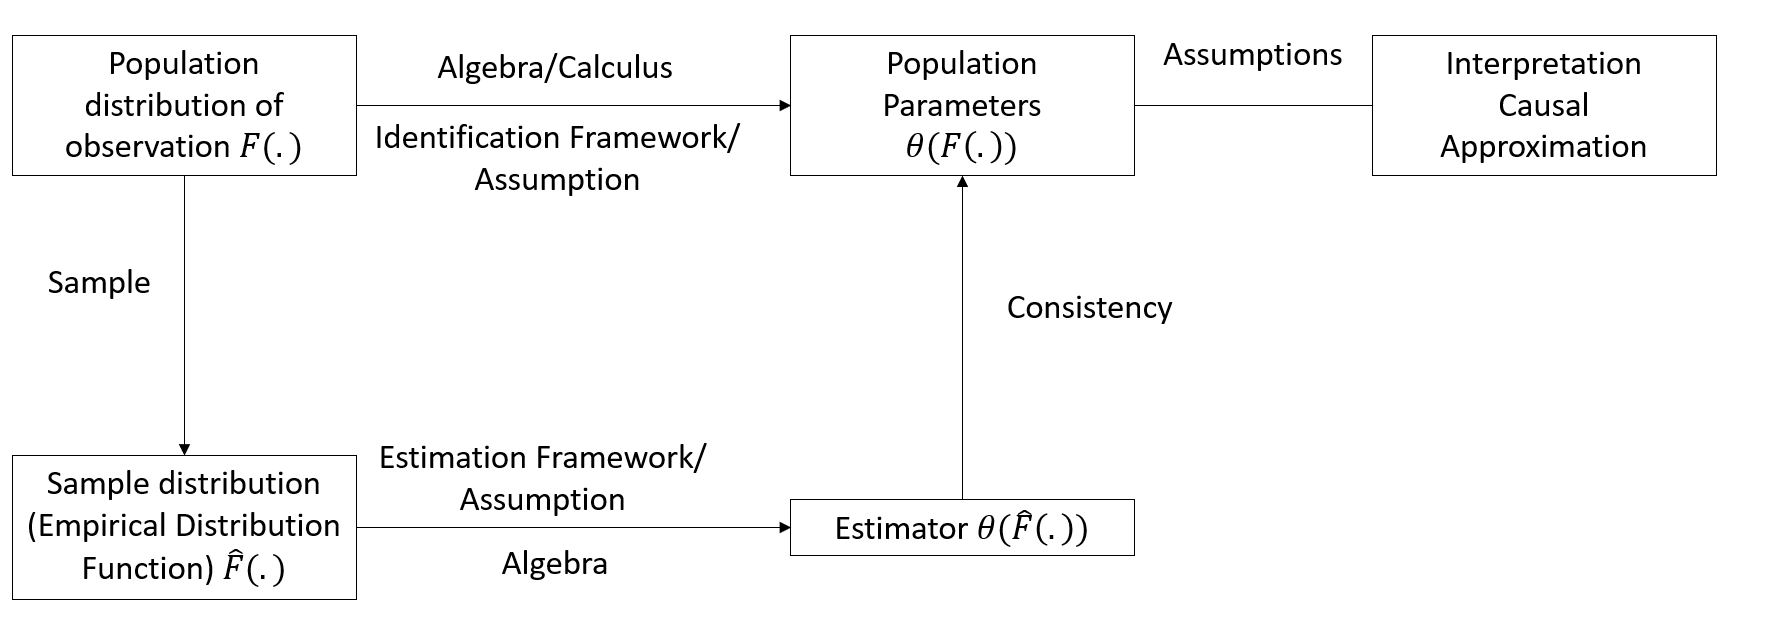
\includegraphics[width=0.9\linewidth,alt={A flowchart illustrating the framework for statistical estimation. It begins with the population distribution of observations, which flows into two paths: one toward population parameters via identification assumptions, and the other toward sample-based estimators. The framework highlights consistency, assumptions, and causal interpretation.}]{images/econometrics} 

}

\caption{Framework for Statistical Inference and Causal Interpretation}\label{fig:fig-inference-framework}
\end{figure}

Linear regression is one of the most fundamental tools in statistics and econometrics, widely used for modeling relationships between variables. It forms the cornerstone of predictive analysis, enabling us to understand and quantify how changes in one or more explanatory variables are associated with a dependent variable. Its simplicity and versatility make it an essential tool in fields ranging from economics and marketing to healthcare and environmental studies.

At its core, linear regression addresses questions about associations rather than causation. For example:

\begin{itemize}
\tightlist
\item
  How are advertising expenditures associated with sales performance?
\item
  What is the relationship between a company's revenue and its stock price?
\item
  How does the level of education correlate with income?
\end{itemize}

These questions are about patterns in data, not necessarily causal effects. While regression can provide insights into potential causal relationships, establishing causality requires more than just regression analysis. It requires careful consideration of the study design, assumptions, and potential confounding factors.

So, why is it called ``linear''? The term refers to the structure of the model, where the dependent variable (outcome) is modeled as a linear combination of one or more independent variables (predictors). For example, in simple linear regression, the relationship is represented as:

\[Y = \beta_0 + \beta_1 X + \epsilon,\]

where \(Y\) is the dependent variable, \(X\) is the independent variable, \(\beta_0\) and \(\beta_1\) are parameters to be estimated, and \(\epsilon\) is the error term capturing randomness or unobserved factors.

Linear regression serves as a foundation for much of applied data analysis because of its wide-ranging applications:

\begin{enumerate}
\def\labelenumi{\arabic{enumi}.}
\item
  \textbf{Understanding Patterns in Data:} Regression provides a framework to summarize and explore relationships between variables. It allows us to identify patterns such as trends or associations, which can guide further analysis or decision-making.
\item
  \textbf{Prediction:} Beyond exploring relationships, regression is widely used for making predictions. For instance, given historical data, we can use a regression model to predict future outcomes like sales, prices, or demand.
\item
  \textbf{Building Blocks for Advanced Techniques:} Linear regression is foundational for many advanced statistical and machine learning models, such as logistic regression, ridge regression, and neural networks. Mastering linear regression equips you with the skills to tackle more complex methods.
\end{enumerate}

\textbf{Regression and Causality: A Crucial Distinction}

It's essential to remember that regression alone does not establish causation. For instance, a regression model might show a strong association between advertising and sales, but this does not prove that advertising directly causes sales to increase. Other factors, such as seasonality, market trends, or unobserved variables, could also influence the results.

Establishing causality requires additional steps, such as controlled experiments, instrumental variable techniques, or careful observational study designs. As we work through the details of linear regression, we'll revisit this distinction and highlight scenarios where causality might or might not be inferred.

\begin{center}\rule{0.5\linewidth}{0.5pt}\end{center}

\textbf{What is an Estimator?}

At the heart of regression lies the process of estimation, the act of using data to determine the unknown characteristics of a population or model.

An \textbf{estimator} is a mathematical rule or formula used to calculate an estimate of an unknown quantity based on observed data. For example, when we calculate the average height of a sample to estimate the average height of a population, the sample mean is the estimator.

In the context of regression, the quantities we typically estimate are:

\begin{itemize}
\tightlist
\item
  Parameters: Fixed, unknown values that describe the relationship between variables (e.g., coefficients in a regression equation).

  \begin{itemize}
  \tightlist
  \item
    \textbf{Estimating parameters} → Parametric models (finite parameters, e.g., coefficients in regression).
  \end{itemize}
\item
  Functions: Unknown relationships or patterns in the data, often modeled without assuming a fixed functional form.

  \begin{itemize}
  \tightlist
  \item
    \textbf{Estimating functions} → Non-parametric models (focus on shapes or trends, not a fixed number of parameters).
  \end{itemize}
\end{itemize}

\begin{center}\rule{0.5\linewidth}{0.5pt}\end{center}

\textbf{Types of Estimators}

To better understand the estimation process, let's introduce two broad categories of estimators that we'll work with:

\begin{enumerate}
\def\labelenumi{\arabic{enumi}.}
\item
  \textbf{Parametric Estimators}\\
  Parametric estimation focuses on a finite set of parameters that define a model. For example, in a simple linear regression:\\
  \[Y = \beta_0 + \beta_1 X + \epsilon,\]\\
  the task is to estimate the parameters \(\beta_0\) (intercept) and \(\beta_1\) (slope). Parametric estimators rely on specific assumptions about the form of the model (e.g., linearity) and the distribution of the error term (e.g., normality).
\item
  \textbf{Non-Parametric Estimators}\\
  Non-parametric estimation avoids assuming a specific functional form for the relationship between variables. Instead, it focuses on estimating patterns or trends directly from the data. For example, using a scatterplot smoothing technique to visualize how sales vary with advertising spend without imposing a linear or quadratic relationship.
\end{enumerate}

These two categories reflect a fundamental trade-off in statistical analysis: \textbf{parametric models} are often simpler and more interpretable but require strong assumptions, while \textbf{non-parametric models} are more flexible but may require more data and computational resources.

\begin{center}\rule{0.5\linewidth}{0.5pt}\end{center}

\textbf{Desirable Properties of Estimators}

Regardless of whether we are estimating parameters or functions, we want our estimators to possess certain desirable properties. Think of these as the ``golden standards'' that help us judge whether an estimator is reliable:

\begin{enumerate}
\def\labelenumi{\arabic{enumi}.}
\item
  \textbf{Unbiasedness}\\
  An estimator is unbiased if it hits the true value of the parameter, on average, over repeated samples. Mathematically:\\
  \[E[\hat{\beta}] = \beta.\]\\
  This means that, across multiple samples, the estimator does not systematically overestimate or underestimate the true parameter.
\item
  \textbf{Consistency}\\
  Consistency ensures that as the sample size increases, the estimator converges to the true value of the parameter. Formally:\\
  \[plim\ \hat{\beta_n} = \beta.\]\\
  This property relies on the {[}Law of Large Numbers{]}, which guarantees that larger samples reduce random fluctuations, leading to more precise estimates.
\item
  \textbf{Efficiency}\\
  Among all unbiased estimators, an efficient estimator has the smallest variance.

  \begin{itemize}
  \tightlist
  \item
    The \hyperref[ordinary-least-squares]{Ordinary Least Squares} method is efficient because it is the \textbf{Best Linear Unbiased Estimator (BLUE)} under the Gauss-Markov Theorem.
  \item
    For estimators that meet specific distributional assumptions (e.g., normality), maximum-likelihood estimators are asymptotically efficient, meaning they achieve the lowest possible variance as the sample size grows.
  \end{itemize}
\end{enumerate}

\begin{center}\rule{0.5\linewidth}{0.5pt}\end{center}

\textbf{Why These Properties Matter}

Understanding these properties is crucial because they ensure that the methods we use for estimation are reliable, precise, and robust. Whether we are estimating coefficients in a regression model or uncovering a complex pattern in the data, these properties provide the foundation for statistical inference and decision-making.

Now that we've established what estimators are, the types we'll encounter, and their desirable properties, we can move on to understanding how these concepts apply specifically to the \hyperref[ordinary-least-squares]{Ordinary Least Squares} method, the backbone of linear regression.

\begin{longtable}[]{@{}
  >{\raggedright\arraybackslash}p{(\linewidth - 6\tabcolsep) * \real{0.2500}}
  >{\raggedright\arraybackslash}p{(\linewidth - 6\tabcolsep) * \real{0.2500}}
  >{\raggedright\arraybackslash}p{(\linewidth - 6\tabcolsep) * \real{0.2500}}
  >{\raggedright\arraybackslash}p{(\linewidth - 6\tabcolsep) * \real{0.2500}}@{}}
\caption{Comparison of Estimation Methods in Regression Analysis}\tabularnewline
\toprule\noalign{}
\begin{minipage}[b]{\linewidth}\raggedright
\textbf{Estimation Method}
\end{minipage} & \begin{minipage}[b]{\linewidth}\raggedright
\textbf{Key Assumptions}
\end{minipage} & \begin{minipage}[b]{\linewidth}\raggedright
\textbf{Strengths}
\end{minipage} & \begin{minipage}[b]{\linewidth}\raggedright
\textbf{Limitations}
\end{minipage} \\
\midrule\noalign{}
\endfirsthead
\toprule\noalign{}
\begin{minipage}[b]{\linewidth}\raggedright
\textbf{Estimation Method}
\end{minipage} & \begin{minipage}[b]{\linewidth}\raggedright
\textbf{Key Assumptions}
\end{minipage} & \begin{minipage}[b]{\linewidth}\raggedright
\textbf{Strengths}
\end{minipage} & \begin{minipage}[b]{\linewidth}\raggedright
\textbf{Limitations}
\end{minipage} \\
\midrule\noalign{}
\endhead
\bottomrule\noalign{}
\endlastfoot
\hyperref[ordinary-least-squares]{Ordinary Least Squares} & Errors have mean zero, constant variance, and are uncorrelated (the Gauss-Markov conditions); linearity in parameters and no perfect collinearity in \(X\). Independence and normality are stronger assumptions used for inference, not for unbiasedness. & Simple, well-understood method; minimizes residual sum of squares with easily interpretable coefficients. & Sensitive to outliers and violations of normality; performs poorly under high multicollinearity. \\
Generalized Least Squares & Errors have a known correlation or heteroscedasticity structure that can be modeled. & Handles correlated or non-constant-variance errors; more flexible than OLS when the noise structure is known. & Requires specifying (or estimating) the error covariance structure; misspecification can introduce bias. \\
Maximum Likelihood & The underlying probability distribution (e.g., normal) must be specified correctly. & Provides a general framework for estimating parameters under well-defined probability models; extends to complex likelihoods. & Highly sensitive to model misspecification; may require more computation than OLS or GLS. \\
Penalized (Regularized) Estimators & Coefficients are assumed to be shrinkable; the model permits coefficient penalization. & Controls overfitting via regularization; handles high-dimensional data and many predictors; can perform feature selection (e.g., Lasso). & Requires choosing tuning parameter(s) (e.g., \(\lambda\)); interpretation of coefficients becomes less straightforward. \\
Robust Estimators & Less sensitive to heavy-tailed or outlier-prone distributions (weaker assumptions on the error structure). & Resistant to large deviations or outliers in data; often maintains good performance under mild model misspecification. & Less efficient if errors are truly normal; choice of robust method and tuning can be subjective. \\
Partial Least Squares & Predictors may be highly correlated and dimension reduction is desired. & Simultaneously reduces dimensionality and fits regression; works well with collinear, high-dimensional data. & Can be harder to interpret than OLS (latent components instead of original predictors); requires choosing the number of components. \\
\end{longtable}

\begin{center}\rule{0.5\linewidth}{0.5pt}\end{center}

\section{Ordinary Least Squares}\label{ordinary-least-squares}

Ordinary Least Squares (OLS) is the backbone of statistical modeling, a method so foundational that it often serves as the starting point for understanding data relationships. Whether predicting sales, estimating economic trends, or uncovering patterns in scientific research, OLS remains a critical tool. Its appeal lies in simplicity: OLS models the relationship between a dependent variable and one or more predictors by minimizing the squared differences between observed and predicted values.

\begin{center}\rule{0.5\linewidth}{0.5pt}\end{center}

\textbf{Why OLS Works: Linear and Nonlinear Relationships}

\hyperref[ordinary-least-squares]{OLS} rests on the Conditional Expectation Function (CEF), \(E[Y | X]\), which describes the expected value of \(Y\) given \(X\). Regression shines in two key scenarios:

\begin{enumerate}
\def\labelenumi{\arabic{enumi}.}
\item
  \textbf{Perfect Fit (Linear CEF):}\\
  If \(E[Y_i | X_{1i}, \dots, X_{Ki}] = a + \sum_{k=1}^K b_k X_{ki}\), the regression of \(Y_i\) on \(X_{1i}, \dots, X_{Ki}\) exactly equals the CEF. In other words, the regression gives the true average relationship between \(Y\) and \(X\).\\
  If the true relationship is linear, regression delivers the exact CEF. For instance, imagine you're estimating the relationship between advertising spend and sales revenue. If the true impact is linear, \hyperref[ordinary-least-squares]{OLS} will perfectly capture it.
\item
  \textbf{Approximation (Nonlinear CEF):}\\
  If \(E[Y_i | X_{1i}, \dots, X_{Ki}]\) is nonlinear, \hyperref[ordinary-least-squares]{OLS} provides the best linear approximation to this relationship. Specifically, it minimizes the expected squared deviation between the linear regression line and the nonlinear CEF.\\
  For example, the effect of advertising diminishes at higher spending levels? \hyperref[ordinary-least-squares]{OLS} still works, providing the best linear approximation to this nonlinear relationship by minimizing the squared deviations between predictions and the true (but unknown) CEF.
\end{enumerate}

In other words, regression is not just a tool for ``linear'' relationships; it's a workhorse that adapts remarkably well to messy, real-world data.

\begin{center}\rule{0.5\linewidth}{0.5pt}\end{center}

\subsection{Simple Regression (Basic) Model}\label{simple-regression-basic-model}

The simplest form of regression is a straight line:

\[
Y_i = \beta_0 + \beta_1 X_i + \epsilon_i
\]

where

\begin{itemize}
\tightlist
\item
  \(Y_i\): The dependent variable or outcome we're trying to predict (e.g., sales, temperature).
\item
  \(X_i\): The independent variable or predictor (e.g., advertising spend, time).
\item
  \(\beta_0\): The intercept, where the line crosses the \(Y\)-axis when \(X = 0\).
\item
  \(\beta_1\): The slope, representing the change in \(Y\) for a one-unit increase in \(X\).
\item
  \(\epsilon_i\): The error term, accounting for random factors that \(X\) cannot explain.
\end{itemize}

Assumptions About the Error Term (\(\epsilon_i\)):

\[
\begin{aligned}
E(\epsilon_i) &= 0 \\
\text{Var}(\epsilon_i) &= \sigma^2 \\
\text{Cov}(\epsilon_i, \epsilon_j) &= 0 \quad \text{for all } i \neq j
\end{aligned}
\]

Since \(\epsilon_i\) is random, \(Y_i\) is also random:

\[
\begin{aligned}
E(Y_i) &= E(\beta_0 + \beta_1 X_i + \epsilon_i) \\
&= \beta_0 + \beta_1 X_i
\end{aligned}
\]

\[
\begin{aligned}
\text{Var}(Y_i) &= \text{Var}(\beta_0 + \beta_1 X_i + \epsilon_i) \\
&= \text{Var}(\epsilon_i) \\
&= \sigma^2
\end{aligned}
\]

Since \(\text{Cov}(\epsilon_i, \epsilon_j) = 0\), the outcomes across observations are independent. Hence, \(Y_i\) and \(Y_j\) are uncorrelated as well, conditioned on the \(X\)'s.

\begin{center}\rule{0.5\linewidth}{0.5pt}\end{center}

\subsubsection{Estimation in Ordinary Least Squares}\label{estimation-in-ordinary-least-squares}

The goal of \hyperref[ordinary-least-squares]{OLS} is to estimate the regression parameters (\(\beta_0\), \(\beta_1\)) that best describe the relationship between the dependent variable \(Y\) and the independent variable \(X\). To achieve this, we minimize the sum of squared deviations between observed values of \(Y_i\) and their expected values predicted by the model.

The deviation of an observed value \(Y_i\) from its expected value, based on the regression model, is:

\[
Y_i - E(Y_i) = Y_i - (\beta_0 + \beta_1 X_i).
\]

This deviation represents the error in prediction for the \(i\)-th observation.

To ensure that the errors don't cancel each other out and to prioritize larger deviations, we consider the squared deviations. The sum of squared deviations, denoted by \(Q\), is defined as:

\[
Q = \sum_{i=1}^{n} (Y_i - \beta_0 - \beta_1 X_i)^2.
\]

The goal of \hyperref[ordinary-least-squares]{OLS} is to find the values of \(\beta_0\) and \(\beta_1\) that minimize \(Q\). These values are called the \textbf{OLS estimators}.

To minimize \(Q\), we take partial derivatives with respect to \(\beta_0\) and \(\beta_1\), set them to zero, and solve the resulting system of equations. After simplifying, the estimators for the slope (\(b_1\)) and intercept (\(b_0\)) are obtained as follows:

Slope (\(b_1\)):

\[
b_1 = \frac{\sum_{i=1}^{n} (X_i - \bar{X})(Y_i - \bar{Y})}{\sum_{i=1}^{n} (X_i - \bar{X})^2}.
\]

Here, \(\bar{X}\) and \(\bar{Y}\) represent the means of \(X\) and \(Y\), respectively. This formula reveals that the slope is proportional to the covariance between \(X\) and \(Y\), scaled by the variance of \(X\).

Intercept (\(b_0\)):

\[
b_0 = \frac{1}{n} \left( \sum_{i=1}^{n} Y_i - b_1 \sum_{i=1}^{n} X_i \right) = \bar{Y} - b_1 \bar{X}.
\]

The intercept is determined by aligning the regression line with the center of the data.

\begin{center}\rule{0.5\linewidth}{0.5pt}\end{center}

\textbf{Intuition Behind the Estimators}

\begin{itemize}
\item
  \(b_1\) (Slope): This measures the average change in \(Y\) for a one-unit increase in \(X\). The formula uses deviations from the mean to ensure that the relationship captures the joint variability of \(X\) and \(Y\).
\item
  \(b_0\) (Intercept): This ensures that the regression line passes through the mean of the data points \((\bar{X}, \bar{Y})\), anchoring the model in the center of the observed data.
\end{itemize}

\begin{center}\rule{0.5\linewidth}{0.5pt}\end{center}

Equivalently, we can also write these parameters in terms of covariances.

The covariance between two variables is defined as:

\[ \text{Cov}(X_i, Y_i) = E[(X_i - E[X_i])(Y_i - E[Y_i])] \]

Properties of Covariance:

\begin{enumerate}
\def\labelenumi{\arabic{enumi}.}
\tightlist
\item
  \(\text{Cov}(X_i, X_i) = \sigma^2_X\)
\item
  If \(E(X_i) = 0\) or \(E(Y_i) = 0\), then \(\text{Cov}(X_i, Y_i) = E[X_i Y_i]\)
\item
  For \(W_i = a + b X_i\) and \(Z_i = c + d Y_i\),\\
  \(\text{Cov}(W_i, Z_i) = bd \cdot \text{Cov}(X_i, Y_i)\)
\end{enumerate}

For a bivariate regression, the slope \(\beta\) in a bivariate regression is given by:

\[ \beta = \frac{\text{Cov}(Y_i, X_i)}{\text{Var}(X_i)} \]

For a multivariate case, the slope for \(X_k\) is:

\[ \beta_k = \frac{\text{Cov}(Y_i, \tilde{X}_{ki})}{\text{Var}(\tilde{X}_{ki})} \]

Where \(\tilde{X}_{ki}\) represents the residual from a regression of \(X_{ki}\) on the \(K-1\) other covariates in the model.

The intercept is:

\[ \beta_0 = E[Y_i] - \beta_1 E(X_i) \]

Note:

\begin{itemize}
\tightlist
\item
  \hyperref[ordinary-least-squares]{OLS} does not require the assumption of a specific distribution for the variables. Its robustness is based on the minimization of squared errors (i.e., no distributional assumptions).
\end{itemize}

\subsubsection{Properties of Least Squares Estimators}\label{properties-of-least-squares-estimators}

The properties of the Ordinary Least Squares estimators (\(b_0\) and \(b_1\)) are derived based on their statistical behavior. These properties provide insights into the accuracy, variability, and reliability of the estimates.

\begin{center}\rule{0.5\linewidth}{0.5pt}\end{center}

\paragraph{Expectation of the OLS Estimators}\label{expectation-of-the-ols-estimators}

The \hyperref[ordinary-least-squares]{OLS} estimators \(b_0\) (intercept) and \(b_1\) (slope) are unbiased. This means their expected values equal the true population parameters:

\[
\begin{aligned}
E(b_1) &= \beta_1, \\
E(b_0) &= E(\bar{Y}) - \bar{X}\beta_1.
\end{aligned}
\]

Since the expected value of the sample mean of \(Y\), \(E(\bar{Y})\), is:

\[
E(\bar{Y}) = \beta_0 + \beta_1 \bar{X},
\]

the expected value of \(b_0\) simplifies to:

\[
E(b_0) = \beta_0.
\]

Thus, \(b_0\) and \(b_1\) are unbiased estimators of their respective population parameters \(\beta_0\) and \(\beta_1\).

\begin{center}\rule{0.5\linewidth}{0.5pt}\end{center}

\paragraph{Variance of the OLS Estimators}\label{variance-of-the-ols-estimators}

The variability of the \hyperref[ordinary-least-squares]{OLS} estimators depends on the spread of the predictor variable \(X\) and the error variance \(\sigma^2\). The variances are given by:

Variance of \(b_1\) (Slope):

\[
\text{Var}(b_1) = \frac{\sigma^2}{\sum_{i=1}^{n} (X_i - \bar{X})^2}.
\]

Variance of \(b_0\) (Intercept):

\[
\text{Var}(b_0) = \sigma^2 \left( \frac{1}{n} + \frac{\bar{X}^2}{\sum_{i=1}^{n} (X_i - \bar{X})^2} \right).
\]

These formulas highlight that:

\begin{itemize}
\tightlist
\item
  \(\text{Var}(b_1) \to 0\) as the number of observations increases, provided \(X_i\) values are distributed around their mean \(\bar{X}\).
\item
  \(\text{Var}(b_0) \to 0\) as \(n\) increases, assuming \(X_i\) values are appropriately selected (i.e., not all clustered near the mean).
\end{itemize}

\begin{center}\rule{0.5\linewidth}{0.5pt}\end{center}

\subsubsection{Mean Square Error (MSE)}\label{mean-square-error-mse}

The Mean Square Error (MSE) quantifies the average squared residual (error) in the model:

\[
MSE = \frac{SSE}{n-2} = \frac{\sum_{i=1}^{n} e_i^2}{n-2} = \frac{\sum_{i=1}^{n} (Y_i - \hat{Y}_i)^2}{n-2},
\]

where \(SSE\) is the Sum of Squared Errors and \(n-2\) represents the degrees of freedom for a simple linear regression model (two parameters estimated: \(\beta_0\) and \(\beta_1\)).

The expected value of the MSE equals the error variance (i.e., unbiased estimator of MSE):

\[
E(MSE) = \sigma^2.
\]

\begin{center}\rule{0.5\linewidth}{0.5pt}\end{center}

\subsubsection{Estimating Variance of the OLS Coefficients}\label{estimating-variance-of-the-ols-coefficients}

The sample-based estimates of the variances of \(b_0\) and \(b_1\) are expressed as follows:

Estimated Variance of \(b_1\) (Slope):

\[
s^2(b_1) = \widehat{\text{Var}}(b_1) = \frac{MSE}{\sum_{i=1}^{n} (X_i - \bar{X})^2}.
\]

Estimated Variance of \(b_0\) (Intercept):

\[
s^2(b_0) = \widehat{\text{Var}}(b_0) = MSE \left( \frac{1}{n} + \frac{\bar{X}^2}{\sum_{i=1}^{n} (X_i - \bar{X})^2} \right).
\]

These estimates rely on the MSE to approximate \(\sigma^2\).

The variance estimates are unbiased:

\[
\begin{aligned}
E(s^2(b_1)) &= \text{Var}(b_1), \\
E(s^2(b_0)) &= \text{Var}(b_0).
\end{aligned}
\]

\begin{center}\rule{0.5\linewidth}{0.5pt}\end{center}

\textbf{Implications of These Properties}

\begin{enumerate}
\def\labelenumi{\arabic{enumi}.}
\tightlist
\item
  \textbf{Unbiasedness:} The unbiased nature of \(b_0\) and \(b_1\) ensures that, on average, the regression model accurately reflects the true relationship in the population.
\item
  \textbf{Decreasing Variance:} As the sample size \(n\) increases or as the spread of \(X_i\) values grows, the variances of \(b_0\) and \(b_1\) decrease, leading to more precise estimates.
\item
  \textbf{Error Estimation with MSE:} MSE provides a reliable estimate of the error variance \(\sigma^2\), which feeds directly into assessing the reliability of \(b_0\) and \(b_1\).
\end{enumerate}

\subsubsection{Residuals in Ordinary Least Squares}\label{residuals-in-ordinary-least-squares}

Residuals are the differences between observed values (\(Y_i\)) and their predicted counterparts (\(\hat{Y}_i\)). They play a central role in assessing model fit and ensuring the assumptions of OLS are met.

The residual for the \(i\)-th observation is defined as:

\[
e_i = Y_i - \hat{Y}_i = Y_i - (b_0 + b_1 X_i),
\]

where:

\begin{itemize}
\tightlist
\item
  \(e_i\): Residual for the \(i\)-th observation.
\item
  \(\hat{Y}_i\): Predicted value based on the regression model.
\item
  \(Y_i\): Actual observed value.
\end{itemize}

Residuals estimate the unobservable error terms \(\epsilon_i\):

\begin{itemize}
\tightlist
\item
  \(e_i\) is an estimate of \(\epsilon_i = Y_i - E(Y_i)\).
\item
  \(\epsilon_i\) is always unknown because we do not know the true values of \(\beta_0\) and \(\beta_1\).
\end{itemize}

\begin{center}\rule{0.5\linewidth}{0.5pt}\end{center}

\paragraph{Key Properties of Residuals}\label{key-properties-of-residuals}

Residuals exhibit several mathematical properties that align with the OLS estimation process:

\begin{enumerate}
\def\labelenumi{\arabic{enumi}.}
\item
  Sum of Residuals:\\
  The residuals sum to zero:

  \[
  \sum_{i=1}^{n} e_i = 0.
  \]

  This ensures that the regression line passes through the centroid of the data, \((\bar{X}, \bar{Y})\).
\item
  Orthogonality of Residuals to Predictors:\\
  The residuals are orthogonal (uncorrelated) to the predictor variable \(X\):

  \[
  \sum_{i=1}^{n} X_i e_i = 0.
  \]

  This reflects the fact that the \hyperref[ordinary-least-squares]{OLS} minimizes the squared deviations of residuals along the \(Y\)-axis, not the \(X\)-axis.
\end{enumerate}

\begin{center}\rule{0.5\linewidth}{0.5pt}\end{center}

\paragraph{Expected Values of Residuals}\label{expected-values-of-residuals}

The expected values of residuals reinforce the unbiased nature of OLS:

\begin{enumerate}
\def\labelenumi{\arabic{enumi}.}
\item
  Mean of Residuals:\\
  The residuals have an expected value of zero:

  \[
  E[e_i] = 0.
  \]
\item
  Orthogonality to Predictors and Fitted Values:\\
  Residuals are uncorrelated with both the predictor variables and the fitted values:

  \[
  \begin{aligned}
  E[X_i e_i] &= 0, \\
  E[\hat{Y}_i e_i] &= 0.
  \end{aligned}
  \]
\end{enumerate}

These properties highlight that residuals do not contain systematic information about the predictors or the fitted values, reinforcing the idea that the model has captured the underlying relationship effectively.

\begin{center}\rule{0.5\linewidth}{0.5pt}\end{center}

\paragraph{Practical Importance of Residuals}\label{practical-importance-of-residuals}

\begin{enumerate}
\def\labelenumi{\arabic{enumi}.}
\item
  \textbf{Model Diagnostics:}\\
  Residuals are analyzed to check the assumptions of OLS, including linearity, homoscedasticity (constant variance), and independence of errors. Patterns in residual plots can signal issues such as nonlinearity or heteroscedasticity.
\item
  \textbf{Goodness-of-Fit:}\\
  The sum of squared residuals, \(\sum e_i^2\), measures the total unexplained variation in \(Y\). A smaller sum indicates a better fit.
\item
  \textbf{Influence Analysis:}\\
  Large residuals may indicate outliers or influential points that disproportionately affect the regression line.
\end{enumerate}

\subsubsection{Inference in Ordinary Least Squares}\label{inference-in-ordinary-least-squares}

Inference allows us to make probabilistic statements about the regression parameters (\(\beta_0\), \(\beta_1\)) and predictions (\(Y_h\)). To perform valid inference, certain assumptions about the distribution of errors are necessary.

\begin{center}\rule{0.5\linewidth}{0.5pt}\end{center}

Normality Assumption

\begin{itemize}
\tightlist
\item
  OLS estimation itself does \textbf{not} require the assumption of normality.
\item
  However, to conduct hypothesis tests or construct confidence intervals for \(\beta_0\), \(\beta_1\), and predictions, distributional assumptions are necessary.
\item
  Inference on \(\beta_0\) and \(\beta_1\) is \textbf{robust} to moderate departures from normality, especially in large samples due to the \hyperref[central-limit-theorem]{Central Limit Theorem}.
\item
  Inference on predicted values, \(Y_{pred}\), is more sensitive to normality violations.
\end{itemize}

\begin{center}\rule{0.5\linewidth}{0.5pt}\end{center}

When we assume a \textbf{normal error model}, the response variable \(Y_i\) is modeled as:

\[
Y_i \sim N(\beta_0 + \beta_1 X_i, \sigma^2),
\]

where:

\begin{itemize}
\tightlist
\item
  \(\beta_0 + \beta_1 X_i\): Mean response
\item
  \(\sigma^2\): Variance of the errors
\end{itemize}

Under this model, the sampling distributions of the OLS estimators, \(b_0\) and \(b_1\), can be derived.

\begin{center}\rule{0.5\linewidth}{0.5pt}\end{center}

\paragraph{\texorpdfstring{Inference for \(\beta_1\) (Slope)}{Inference for \textbackslash beta\_1 (Slope)}}\label{inference-for-beta_1-slope}

Under the normal error model:

\begin{enumerate}
\def\labelenumi{\arabic{enumi}.}
\item
  \textbf{Sampling Distribution of} \(b_1\):

  \[ 
  b_1 \sim N\left(\beta_1, \frac{\sigma^2}{\sum_{i=1}^{n} (X_i - \bar{X})^2}\right).
  \]

  This indicates that \(b_1\) is an unbiased estimator of \(\beta_1\) with variance proportional to \(\sigma^2\).
\item
  \textbf{Test Statistic:}

  \[ 
  t = \frac{b_1 - \beta_1}{s(b_1)} \sim t_{n-2},
  \]

  where \(s(b_1)\) is the standard error of \(b_1\): \[
  s(b_1) = \sqrt{\frac{MSE}{\sum_{i=1}^{n} (X_i - \bar{X})^2}}.
  \]
\item
  \textbf{Confidence Interval:}

  A \((1-\alpha) 100\%\) confidence interval for \(\beta_1\) is:

  \[ 
  b_1 \pm t_{1-\alpha/2; n-2} \cdot s(b_1).
  \]
\end{enumerate}

\begin{center}\rule{0.5\linewidth}{0.5pt}\end{center}

\paragraph{\texorpdfstring{Inference for \(\beta_0\) (Intercept)}{Inference for \textbackslash beta\_0 (Intercept)}}\label{inference-for-beta_0-intercept}

\begin{enumerate}
\def\labelenumi{\arabic{enumi}.}
\item
  \textbf{Sampling Distribution of} \(b_0\):

  Under the normal error model, the sampling distribution of \(b_0\) is:

  \[ 
  b_0 \sim N\left(\beta_0, \sigma^2 \left(\frac{1}{n} + \frac{\bar{X}^2}{\sum_{i=1}^{n} (X_i - \bar{X})^2}\right)\right).
  \]
\item
  \textbf{Test Statistic:}

  \[ 
  t = \frac{b_0 - \beta_0}{s(b_0)} \sim t_{n-2},
  \]

  where \(s(b_0)\) is the standard error of \(b_0\): \[
  s(b_0) = \sqrt{MSE \left(\frac{1}{n} + \frac{\bar{X}^2}{\sum_{i=1}^{n} (X_i - \bar{X})^2}\right)}.
  \]
\item
  \textbf{Confidence Interval:}

  A \((1-\alpha) 100\%\) confidence interval for \(\beta_0\) is:

  \[ 
  b_0 \pm t_{1-\alpha/2; n-2} \cdot s(b_0).
  \]
\end{enumerate}

\begin{center}\rule{0.5\linewidth}{0.5pt}\end{center}

\paragraph{Mean Response}\label{mean-response}

In regression, we often estimate the mean response of the dependent variable \(Y\) for a given level of the predictor variable \(X\), denoted as \(X_h\). This estimation provides a predicted average outcome for a specific value of \(X\) based on the fitted regression model.

\begin{itemize}
\tightlist
\item
  Let \(X_h\) represent the level of \(X\) for which we want to estimate the mean response.
\item
  The mean response when \(X = X_h\) is denoted as \(E(Y_h)\).
\item
  A point estimator for \(E(Y_h)\) is \(\hat{Y}_h\), which is the predicted value from the regression model:
\end{itemize}

\[
\hat{Y}_h = b_0 + b_1 X_h.
\]

The estimator \(\hat{Y}_h\) is unbiased because its expected value equals the true mean response \(E(Y_h)\):

\[
\begin{aligned}
E(\hat{Y}_h) &= E(b_0 + b_1 X_h) \\
&= \beta_0 + \beta_1 X_h \\
&= E(Y_h).
\end{aligned}
\]

Thus, \(\hat{Y}_h\) provides a reliable estimate of the mean response at \(X_h\).

\begin{center}\rule{0.5\linewidth}{0.5pt}\end{center}

The variance of \(\hat{Y}_h\) reflects the uncertainty in the estimate of the mean response:

\[
\begin{aligned}
\text{Var}(\hat{Y}_h) &= \text{Var}(b_0 + b_1 X_h) \quad\text{(definition of }\hat{Y}_h\text{)}\\
&= \text{Var}\left((\bar{Y} - b_1 \bar{X}) + b_1 X_h\right)\quad\text{(since } b_0 = \bar{Y} - b_1 \bar{X}\text{)}\\
&= \text{Var}\left(\bar{Y} + b_1(X_h - \bar{X})\right)\quad\text{(factor out } b_1\text{)}\\
&= \text{Var}\left(\bar{Y} + b_1 (X_h - \bar{X}) \right) \\
&= \text{Var}(\bar{Y}) + (X_h - \bar{X})^2 \text{Var}(b_1) + 2(X_h - \bar{X}) \text{Cov}(\bar{Y}, b_1).
\end{aligned}
\]

Since \(\text{Cov}(\bar{Y}, b_1) = 0\) (due to the independence of the errors, \(\epsilon_i\)), the variance simplifies to:

\[
\text{Var}(\hat{Y}_h) = \frac{\sigma^2}{n} + (X_h - \bar{X})^2 \frac{\sigma^2}{\sum_{i=1}^{n} (X_i - \bar{X})^2}.
\]

This can also be expressed as:

\[
\text{Var}(\hat{Y}_h) = \sigma^2 \left( \frac{1}{n} + \frac{(X_h - \bar{X})^2}{\sum_{i=1}^{n} (X_i - \bar{X})^2} \right).
\]

To estimate the variance of \(\hat{Y}_h\), we replace \(\sigma^2\) with \(MSE\), the mean squared error from the regression:

\[
s^2(\hat{Y}_h) = MSE \left( \frac{1}{n} + \frac{(X_h - \bar{X})^2}{\sum_{i=1}^{n} (X_i - \bar{X})^2} \right).
\]

\begin{center}\rule{0.5\linewidth}{0.5pt}\end{center}

Under the normal error model, the sampling distribution of \(\hat{Y}_h\) is:

\[
\begin{aligned}
\hat{Y}_h &\sim N\left(E(Y_h), \text{Var}(\hat{Y}_h)\right), \\
\frac{\hat{Y}_h - E(Y_h)}{s(\hat{Y}_h)} &\sim t_{n-2}.
\end{aligned}
\]

This result follows because \(\hat{Y}_h\) is a linear combination of normally distributed random variables, and its variance is estimated using \(s^2(\hat{Y}_h)\).

\begin{center}\rule{0.5\linewidth}{0.5pt}\end{center}

A \(100(1-\alpha)\%\) confidence interval for the mean response \(E(Y_h)\) is given by:

\[
\hat{Y}_h \pm t_{1-\alpha/2; n-2} \cdot s(\hat{Y}_h),
\]

where:

\begin{itemize}
\tightlist
\item
  \(\hat{Y}_h\): Point estimate of the mean response,
\item
  \(s(\hat{Y}_h)\): Estimated standard error of the mean response,
\item
  \(t_{1-\alpha/2; n-2}\): Critical value from the \(t\)-distribution with \(n-2\) degrees of freedom.
\end{itemize}

\begin{center}\rule{0.5\linewidth}{0.5pt}\end{center}

\paragraph{Prediction of a New Observation}\label{prediction-of-a-new-observation}

When analyzing regression results, it is important to distinguish between:

\begin{enumerate}
\def\labelenumi{\arabic{enumi}.}
\tightlist
\item
  \textbf{Estimating the mean response} at a particular value of \(X\).
\item
  \textbf{Predicting an individual outcome} for a particular value of \(X\).
\end{enumerate}

\begin{center}\rule{0.5\linewidth}{0.5pt}\end{center}

Mean Response vs.~Individual Outcome

\begin{itemize}
\item
  \textbf{Same Point Estimate}\\
  The formula for both the estimated mean response and the predicted individual outcome at \(X = X_h\) is identical:\\
  \[
  \hat{Y}_{pred} = \hat{Y}_h = b_0 + b_1 X_h.
  \]
\item
  \textbf{Different Variance}\\
  Although the point estimates are the same, the level of uncertainty differs. When predicting an individual outcome, we must consider not only the uncertainty in estimating the mean response (\(\hat{Y}_h\)) but also the additional random variation within the distribution of \(Y\).
\end{itemize}

Therefore, \textbf{prediction intervals} (for individual outcomes) account for more uncertainty and are consequently wider than \textbf{confidence intervals} (for the mean response).

\begin{center}\rule{0.5\linewidth}{0.5pt}\end{center}

To predict an individual outcome for a given \(X_h\), we combine the mean response with the random error:

\[
Y_{pred} = \beta_0 + \beta_1 X_h + \epsilon.
\]

Using the least squares predictor:

\[
\hat{Y}_{pred} = b_0 + b_1 X_h,
\]

since \(E(\epsilon) = 0\).

\begin{center}\rule{0.5\linewidth}{0.5pt}\end{center}

The variance of the predicted value for a new observation, \(Y_{pred}\), includes both:

\begin{enumerate}
\def\labelenumi{\arabic{enumi}.}
\tightlist
\item
  Variance of the estimated mean response: \[
  \sigma^2 \left( \frac{1}{n} + \frac{(X_h - \bar{X})^2}{\sum_{i=1}^{n} (X_i - \bar{X})^2} \right),
  \]
\item
  Variance of the error term, \(\epsilon\), which is \(\sigma^2\).
\end{enumerate}

Thus, the total variance is:

\[
\begin{aligned}
\text{Var}(Y_{pred}) &= \text{Var}(b_0 + b_1 X_h + \epsilon) \\
&= \text{Var}(b_0 + b_1 X_h) + \text{Var}(\epsilon) \\
&= \sigma^2 \left( \frac{1}{n} + \frac{(X_h - \bar{X})^2}{\sum_{i=1}^{n} (X_i - \bar{X})^2} \right) + \sigma^2 \\
&= \sigma^2 \left( 1 + \frac{1}{n} + \frac{(X_h - \bar{X})^2}{\sum_{i=1}^{n} (X_i - \bar{X})^2} \right).
\end{aligned}
\]

We estimate the variance of the prediction using \(MSE\), the mean squared error:

\[
s^2(pred) = MSE \left( 1 + \frac{1}{n} + \frac{(X_h - \bar{X})^2}{\sum_{i=1}^{n} (X_i - \bar{X})^2} \right).
\]

Under the normal error model, the standardized predicted value follows a \(t\)-distribution with \(n-2\) degrees of freedom:

\[
\frac{Y_{pred} - \hat{Y}_h}{s(pred)} \sim t_{n-2}.
\]

A \(100(1-\alpha)\%\) prediction interval for \(Y_{pred}\) is:

\[
\hat{Y}_{pred} \pm t_{1-\alpha/2; n-2} \cdot s(pred).
\]

\begin{center}\rule{0.5\linewidth}{0.5pt}\end{center}

\paragraph{Confidence Band}\label{confidence-band}

In regression analysis, we often want to evaluate the uncertainty around the entire regression line, not just at a single value of the predictor variable \(X\). This is achieved using a \textbf{confidence band}, which provides a confidence interval for the mean response, \(E(Y) = \beta_0 + \beta_1 X\), over the entire range of \(X\) values.

The Working-Hotelling confidence band is a method to construct simultaneous confidence intervals for the regression line. For a given \(X_h\), the confidence band is expressed as:

\[
\hat{Y}_h \pm W s(\hat{Y}_h),
\]

where:

\begin{itemize}
\item
  \(W^2 = 2F_{1-\alpha; 2, n-2}\),

  \begin{itemize}
  \tightlist
  \item
    \(F_{1-\alpha; 2, n-2}\) is the critical value from the \(F\)-distribution with 2 and \(n-2\) degrees of freedom.
  \end{itemize}
\item
  \(s(\hat{Y}_h)\) is the standard error of the estimated mean response at \(X_h\):

  \[
  s^2(\hat{Y}_h) = MSE \left( \frac{1}{n} + \frac{(X_h - \bar{X})^2}{\sum_{i=1}^{n} (X_i - \bar{X})^2} \right).
  \]
\end{itemize}

\begin{center}\rule{0.5\linewidth}{0.5pt}\end{center}

\textbf{Key Properties of the Confidence Band}

\begin{enumerate}
\def\labelenumi{\arabic{enumi}.}
\tightlist
\item
  \textbf{Width of the Interval:}

  \begin{itemize}
  \tightlist
  \item
    The width of the confidence band changes with \(X_h\) because \(s(\hat{Y}_h)\) depends on how far \(X_h\) is from the mean of \(X\) (\(\bar{X}\)).
  \item
    The interval is narrowest at \(X = \bar{X}\), where the variance of the estimated mean response is minimized.
  \end{itemize}
\item
  \textbf{Shape of the Band:}

  \begin{itemize}
  \tightlist
  \item
    The boundaries of the confidence band form a hyperbolic shape around the regression line.
  \item
    This reflects the increasing uncertainty in the mean response as \(X_h\) moves farther from \(\bar{X}\).
  \end{itemize}
\item
  \textbf{Simultaneous Coverage:}

  \begin{itemize}
  \tightlist
  \item
    The Working-Hotelling band ensures that the true regression line \(E(Y) = \beta_0 + \beta_1 X\) lies within the band across all values of \(X\) with a specified confidence level (e.g., \(95\%\)).
  \end{itemize}
\end{enumerate}

\subsubsection{Analysis of Variance (ANOVA) in Regression}\label{analysis-of-variance-anova-in-regression}

ANOVA in regression decomposes the total variability in the response variable (\(Y\)) into components attributed to the regression model and residual error. In the context of regression, ANOVA provides a mechanism to assess the fit of the model and test hypotheses about the relationship between \(X\) and \(Y\).

The \textbf{corrected Total Sum of Squares (SSTO)} quantifies the total variation in \(Y\):

\[
SSTO = \sum_{i=1}^n (Y_i - \bar{Y})^2,
\]

where \(\bar{Y}\) is the mean of the response variable. The term ``corrected'' refers to the fact that the sum of squares is calculated relative to the mean (i.e., the uncorrected total sum of squares is given by \(\sum Y_i^2\))

Using the fitted regression model \(\hat{Y}_i = b_0 + b_1 X_i\), we estimate the conditional mean of \(Y\) at \(X_i\). The total sum of squares can be decomposed as:

\[
\begin{aligned}
\sum_{i=1}^n (Y_i - \bar{Y})^2 &= \sum_{i=1}^n (Y_i - \hat{Y}_i + \hat{Y}_i - \bar{Y})^2 \\
&= \sum_{i=1}^n (Y_i - \hat{Y}_i)^2 + \sum_{i=1}^n (\hat{Y}_i - \bar{Y})^2 + 2 \sum_{i=1}^n (Y_i - \hat{Y}_i)(\hat{Y}_i - \bar{Y}) \\
&= \sum_{i=1}^n (Y_i - \hat{Y}_i)^2 + \sum_{i=1}^n (\hat{Y}_i - \bar{Y})^2
\end{aligned}
\]

\begin{itemize}
\tightlist
\item
  The cross-product term is zero, as shown below.
\item
  This decomposition simplifies to:
\end{itemize}

\[
SSTO = SSE + SSR,
\]

where:

\begin{itemize}
\item
  \(SSE = \sum_{i=1}^n (Y_i - \hat{Y}_i)^2\): Error Sum of Squares (variation unexplained by the model).
\item
  \(SSR = \sum_{i=1}^n (\hat{Y}_i - \bar{Y})^2\): Regression Sum of Squares (variation explained by the model), which measure how the conditional mean varies about a central value.
\end{itemize}

Degrees of freedom are partitioned as:

\[
\begin{aligned}
SSTO &= SSR + SSE \\
(n-1) &= (1) + (n-2) \\
\end{aligned}
\]

\begin{center}\rule{0.5\linewidth}{0.5pt}\end{center}

To confirm that the cross-product term is zero:

\[
\begin{aligned}
\sum_{i=1}^n (Y_i - \hat{Y}_i)(\hat{Y}_i - \bar{Y}) 
&= \sum_{i=1}^{n}(Y_i - \bar{Y} -b_1 (X_i - \bar{X}))(\bar{Y} + b_1 (X_i - \bar{X})-\bar{Y}) \quad \text{(Expand } Y_i - \hat{Y}_i \text{ and } \hat{Y}_i - \bar{Y}\text{)} \\
&=\sum_{i=1}^{n}(Y_i - \bar{Y} -b_1 (X_i - \bar{X}))( b_1 (X_i - \bar{X}))  \\
&= b_1 \sum_{i=1}^n (Y_i - \bar{Y})(X_i - \bar{X}) - b_1^2 \sum_{i=1}^n (X_i - \bar{X})^2 \quad \text{(Distribute terms in the product)} \\
&= b_1 \frac{\sum_{i=1}^n (Y_i - \bar{Y})(X_i - \bar{X})}{\sum_{i=1}^n (X_i - \bar{X})^2} \sum_{i=1}^n (X_i - \bar{X})^2 - b_1^2 \sum_{i=1}^n (X_i - \bar{X})^2 \quad \text{(Substitute } b_1 \text{ definition)} \\
&= b_1^2 \sum_{i=1}^n (X_i - \bar{X})^2 - b_1^2 \sum_{i=1}^n (X_i - \bar{X})^2  \\
&= 0 
\end{aligned}
\]

\begin{center}\rule{0.5\linewidth}{0.5pt}\end{center}

The ANOVA table summarizes the partitioning of variability:

{\def\LTcaptype{none} % do not increment counter
\begin{longtable}[]{@{}
  >{\raggedright\arraybackslash}p{(\linewidth - 8\tabcolsep) * \real{0.2095}}
  >{\raggedright\arraybackslash}p{(\linewidth - 8\tabcolsep) * \real{0.1619}}
  >{\raggedright\arraybackslash}p{(\linewidth - 8\tabcolsep) * \real{0.1238}}
  >{\raggedright\arraybackslash}p{(\linewidth - 8\tabcolsep) * \real{0.2476}}
  >{\raggedright\arraybackslash}p{(\linewidth - 8\tabcolsep) * \real{0.2286}}@{}}
\toprule\noalign{}
\begin{minipage}[b]{\linewidth}\raggedright
Source of Variation
\end{minipage} & \begin{minipage}[b]{\linewidth}\raggedright
Sum of Squares
\end{minipage} & \begin{minipage}[b]{\linewidth}\raggedright
df
\end{minipage} & \begin{minipage}[b]{\linewidth}\raggedright
Mean Square
\end{minipage} & \begin{minipage}[b]{\linewidth}\raggedright
\(F\) Statistic
\end{minipage} \\
\midrule\noalign{}
\endhead
\bottomrule\noalign{}
\endlastfoot
Regression (Model) & \(SSR\) & \(1\) & \(MSR = \frac{SSR}{1}\) & \(F = \frac{MSR}{MSE}\) \\
Error & \(SSE\) & \(n-2\) & \(MSE = \frac{SSE}{n-2}\) & \\
Total (Corrected) & \(SSTO\) & \(n-1\) & & \\
\end{longtable}
}

\begin{center}\rule{0.5\linewidth}{0.5pt}\end{center}

The expected values of the mean squares are:

\[
\begin{aligned}
E(MSE) &= \sigma^2, \\
E(MSR) &= \sigma^2 + \beta_1^2 \sum_{i=1}^n (X_i - \bar{X})^2.
\end{aligned}
\]

\begin{itemize}
\tightlist
\item
  \textbf{If} \(\beta_1 = 0\):

  \begin{itemize}
  \tightlist
  \item
    The regression model does not explain any variation in \(Y\) beyond the mean, and \(E(MSR) = E(MSE) = \sigma^2\).
  \item
    This condition corresponds to the null hypothesis, \(H_0: \beta_1 = 0\).
  \end{itemize}
\item
  \textbf{If} \(\beta_1 \neq 0\):

  \begin{itemize}
  \tightlist
  \item
    The regression model explains some variation in \(Y\), and \(E(MSR) > E(MSE)\).
  \item
    The additional term \(\beta_1^2 \sum_{i=1}^{n} (X_i - \bar{X})^2\) represents the variance explained by the predictor \(X\).
  \end{itemize}
\end{itemize}

The difference between \(E(MSR)\) and \(E(MSE)\) allows us to infer whether \(\beta_1 \neq 0\) by comparing their ratio.

\begin{center}\rule{0.5\linewidth}{0.5pt}\end{center}

Assuming the errors \(\epsilon_i\) are independent and identically distributed as \(N(0, \sigma^2)\), and under the null hypothesis \(H_0: \beta_1 = 0\), we have:

\begin{enumerate}
\def\labelenumi{\arabic{enumi}.}
\item
  The scaled \(MSE\) follows a chi-square distribution with \(n-2\) degrees of freedom:

  \[
  \frac{MSE}{\sigma^2} \sim \chi_{n-2}^2.
  \]
\item
  The scaled \(MSR\) follows a chi-square distribution with \(1\) degree of freedom:

  \[
  \frac{MSR}{\sigma^2} \sim \chi_{1}^2.
  \]
\item
  These two chi-square random variables are independent.
\end{enumerate}

The ratio of two independent chi-square random variables, scaled by their respective degrees of freedom, follows an \(F\)-distribution. Therefore, under \(H_0\):

\[
F = \frac{MSR}{MSE} \sim F_{1, n-2}.
\]

The \(F\)-statistic tests whether the regression model provides a significant improvement over the null model (constant \(E(Y)\)).

The hypotheses for the \(F\)-test are:

\begin{itemize}
\tightlist
\item
  \textbf{Null Hypothesis} (\(H_0\)): \(\beta_1 = 0\) (no relationship between \(X\) and \(Y\)).
\item
  \textbf{Alternative Hypothesis} (\(H_a\)): \(\beta_1 \neq 0\) (a significant relationship exists between \(X\) and \(Y\)).
\end{itemize}

The rejection rule for \(H_0\) at significance level \(\alpha\) is:

\[
F > F_{1-\alpha;1,n-2},
\]

where \(F_{1-\alpha;1,n-2}\) is the critical value from the \(F\)-distribution with \(1\) and \(n-2\) degrees of freedom.

\begin{enumerate}
\def\labelenumi{\arabic{enumi}.}
\tightlist
\item
  \textbf{If} \(F \leq F_{1-\alpha;1,n-2}\):

  \begin{itemize}
  \tightlist
  \item
    Fail to reject \(H_0\). There is insufficient evidence to conclude that \(X\) significantly explains variation in \(Y\).
  \end{itemize}
\item
  \textbf{If} \(F > F_{1-\alpha;1,n-2}\):

  \begin{itemize}
  \tightlist
  \item
    Reject \(H_0\). There is significant evidence that \(X\) explains some of the variation in \(Y\).
  \end{itemize}
\end{enumerate}

\subsubsection{\texorpdfstring{Coefficient of Determination (\(R^2\))}{Coefficient of Determination (R\^{}2)}}\label{coefficient-of-determination-r2}

The \textbf{Coefficient of Determination} (\(R^2\)) measures how well the linear regression model accounts for the variability in the response variable \(Y\). It is defined as:

\[
R^2 = \frac{SSR}{SSTO} = 1 - \frac{SSE}{SSTO},
\]

where:

\begin{itemize}
\tightlist
\item
  \(SSR\): Regression Sum of Squares (variation explained by the model).
\item
  \(SSTO\): Total Sum of Squares (total variation in \(Y\) about its mean).
\item
  \(SSE\): Error Sum of Squares (variation unexplained by the model).
\end{itemize}

\begin{center}\rule{0.5\linewidth}{0.5pt}\end{center}

\textbf{Properties of} \(R^2\)

\begin{enumerate}
\def\labelenumi{\arabic{enumi}.}
\item
  \textbf{Range}: \[
  0 \leq R^2 \leq 1.
  \]

  \begin{itemize}
  \tightlist
  \item
    \(R^2 = 0\): The model explains none of the variability in \(Y\) (e.g., \(\beta_1 = 0\)).
  \item
    \(R^2 = 1\): The model explains all the variability in \(Y\) (perfect fit).
  \end{itemize}
\item
  Proportionate Reduction in Variance: \(R^2\) represents the proportionate reduction in the total variation of \(Y\) after fitting the model. It quantifies how much better the model predicts \(Y\) compared to simply using \(\bar{Y}\).
\item
  Potential Misinterpretation: It is not really correct to say \(R^2\) is the ``variation in \(Y\) explained by \(X\).'' The term ``variation explained'' assumes a causative or deterministic explanation, which is not always correct. For example:

  \begin{itemize}
  \item
    \(R^2\) shows how much variance in \(Y\) is accounted for by the regression model, but it does not imply causation.
  \item
    In cases with confounding variables or spurious correlations, \(R^2\) can still be high, even if there's no direct causal link between \(X\) and \(Y\).
  \end{itemize}
\end{enumerate}

\begin{center}\rule{0.5\linewidth}{0.5pt}\end{center}

For simple linear regression of \(Y\) on \(X\):

\begin{enumerate}
\def\labelenumi{\arabic{enumi}.}
\item
  Squared correlation equals \(R^2\):

  \[
  R^2 = r^2,
  \]

  where \(r = \mathrm{corr}(X, Y)\) is the Pearson correlation coefficient.
\item
  Slope in terms of correlation: The unstandardized slope \(b_1\) can be expressed as

  \[
  b_1 = r \cdot \frac{s_Y}{s_X},
  \]

  where \(s_Y\) and \(s_X\) are the sample standard deviations of \(Y\) and \(X\), respectively. This form makes the scaling effect explicit: if \(Y\) has larger spread than \(X\), the slope will be larger for the same \(r\).
\item
  Alternative form of \(r\):

  \[
  r = \frac{b_1  s_X}{s_Y}.
  \]
\end{enumerate}

If we standardize both \(X\) and \(Y\) to have mean \(0\) and standard deviation \(1\) (z-scores), the regression slope equals the correlation:

\[
b_1^{\text{(standardized)}} = r.
\]

This is because:

\begin{itemize}
\tightlist
\item
  Standardization removes units, so the scaling factor \(\frac{s_Y}{s_X}\) becomes \(1\).
\item
  In this form, the coefficient is \emph{unitless} and symmetric with respect to swapping \(X\) and \(Y\).
\end{itemize}

\begin{center}\rule{0.5\linewidth}{0.5pt}\end{center}

Symmetry of Correlation vs.~Asymmetry of Slopes

\begin{itemize}
\item
  Correlation: \(r(X,Y) = r(Y,X)\). The correlation is symmetric, meaning the correlation between \(X\) and \(Y\) is the same as between \(Y\) and \(X\).
\item
  Unstandardized slopes:

  \begin{itemize}
  \tightlist
  \item
    Slope of \(Y\) on \(X\): \(b_1^{Y|X} = r \cdot \frac{s_Y}{s_X}\)
  \item
    Slope of \(X\) on \(Y\): \(b_1^{X|Y} = r \cdot \frac{s_X}{s_Y}\)
  \end{itemize}

  These are generally \textbf{not equal} unless \(s_X = s_Y\).
\end{itemize}

Intuition

\begin{itemize}
\tightlist
\item
  The correlation measures \emph{strength of association} on a scale from -1 to 1, independent of units.
\item
  The slope measures \emph{rate of change} in the original units: ``How much \(Y\) changes for a one-unit change in \(X\).''
\item
  Standardizing removes the influence of measurement units and scale, making the regression coefficient identical to \(r\).
\item
  When variables are in different units (e.g., dollars vs.~kilograms), unstandardized slopes will differ depending on which variable is treated as the predictor and which as the outcome, but the correlation stays the same.
\end{itemize}

\begin{center}\rule{0.5\linewidth}{0.5pt}\end{center}

\subsubsection{Lack of Fit in Regression}\label{lack-of-fit-in-regression}

The \textbf{lack of fit} test evaluates whether the chosen regression model adequately captures the relationship between the predictor variable \(X\) and the response variable \(Y\). When there are repeated observations at specific values of \(X\), we can partition the Error Sum of Squares (\(SSE\)) into two components:

\begin{enumerate}
\def\labelenumi{\arabic{enumi}.}
\tightlist
\item
  \textbf{Pure Error}
\item
  Lack of Fit.
\end{enumerate}

Given the observations:

\begin{itemize}
\tightlist
\item
  \(Y_{ij}\): The \(j\)-th replicate for the \(i\)-th distinct value of \(X\),

  \begin{itemize}
  \tightlist
  \item
    \(Y_{11}, Y_{21}, \dots, Y_{n_1, 1}\): \(n_1\) repeated observations of \(X_1\)
  \item
    \(Y_{1c}, Y_{2c}, \dots, Y_{n_c,c}\): \(n_c\) repeated observations of \(X_c\)
  \end{itemize}
\item
  \(\bar{Y}_j\): The mean response for replicates at \(X_j\),
\item
  \(\hat{Y}_{ij}\): The predicted value from the regression model for \(X_j\),
\end{itemize}

the Error Sum of Squares (\(SSE\)) can be decomposed as:

\[
\begin{aligned}
\sum_{i} \sum_{j} (Y_{ij} - \hat{Y}_{ij})^2 &= \sum_{i} \sum_{j} (Y_{ij} - \bar{Y}_j + \bar{Y}_j - \hat{Y}_{ij})^2 \\
&= \sum_{i} \sum_{j} (Y_{ij} - \bar{Y}_j)^2 + \sum_{j} n_j (\bar{Y}_j - \hat{Y}_{ij})^2 + \text{cross product term} \\
&= \sum_{i} \sum_{j} (Y_{ij} - \bar{Y}_j)^2 + \sum_{j} n_j (\bar{Y}_j - \hat{Y}_{ij})^2
\end{aligned}
\]

\begin{itemize}
\tightlist
\item
  The \textbf{cross product term} is zero because the deviations within replicates and the deviations between replicates are orthogonal.
\item
  This simplifies to:
\end{itemize}

\[
SSE = SSPE + SSLF,
\]

where:

\begin{itemize}
\tightlist
\item
  \(SSPE\) (Pure Error Sum of Squares): Variation within replicates for the same \(X_j\), reflecting natural variability in the response.

  \begin{itemize}
  \tightlist
  \item
    Degrees of freedom: \(df_{pe} = n - c\), where \(n\) is the total number of observations, and \(c\) is the number of distinct \(X\) values.
  \end{itemize}
\item
  \(SSLF\) (Lack of Fit Sum of Squares): Variation between the replicate means \(\bar{Y}_j\) and the model-predicted values \(\hat{Y}_{ij}\). If SSLF is large, it suggests the model may not adequately describe the relationship between \(X\) and \(Y\).

  \begin{itemize}
  \tightlist
  \item
    Degrees of freedom: \(df_{lf} = c - 2\), where 2 accounts for the parameters in the linear regression model (\(\beta_0\) and \(\beta_1\)).
  \end{itemize}
\end{itemize}

\begin{center}\rule{0.5\linewidth}{0.5pt}\end{center}

\begin{itemize}
\item
  \textbf{Mean Square for Pure Error (MSPE):}\\
  \[
  MSPE = \frac{SSPE}{df_{pe}} = \frac{SSPE}{n-c}.
  \]
\item
  \textbf{Mean Square for Lack of Fit (MSLF):}\\
  \[
  MSLF = \frac{SSLF}{df_{lf}} = \frac{SSLF}{c-2}.
  \]
\end{itemize}

\paragraph{The F-Test for Lack of Fit}\label{the-f-test-for-lack-of-fit}

The \textbf{F-test for lack of fit} evaluates whether the chosen regression model adequately captures the relationship between the predictor variable \(X\) and the response variable \(Y\). Specifically, it tests whether any systematic deviations from the model exist that are not accounted for by random error.

\begin{itemize}
\item
  \textbf{Null Hypothesis (}\(H_0\)):\\
  The regression model is adequate: \[
  H_0: Y_{ij} = \beta_0 + \beta_1 X_i + \epsilon_{ij}, \quad \epsilon_{ij} \sim \text{i.i.d. } N(0, \sigma^2).
  \]
\item
  \textbf{Alternative Hypothesis (}\(H_a\)):\\
  The regression model is not adequate and includes an additional function \(f(X_i, Z_1, \dots)\) to account for the lack of fit: \[
  H_a: Y_{ij} = \alpha_0 + \alpha_1 X_i + f(X_i, Z_1, \dots) + \epsilon_{ij}^*, \quad \epsilon_{ij}^* \sim \text{i.i.d. } N(0, \sigma^2).
  \]
\end{itemize}

\begin{center}\rule{0.5\linewidth}{0.5pt}\end{center}

\textbf{Expected Mean Squares}

\begin{itemize}
\item
  The expected Mean Square for Pure Error (MSPE) is the same under both \(H_0\) and \(H_a\):

  \[
  E(MSPE) = \sigma^2.
  \]
\item
  The expected Mean Square for Lack of Fit (MSLF) depends on whether \(H_0\) is true:

  \begin{itemize}
  \tightlist
  \item
    Under \(H_0\) (model is adequate): \[
    E(MSLF) = \sigma^2.
    \]
  \item
    Under \(H_a\) (model is not adequate): \[
    E(MSLF) = \sigma^2 + \frac{\sum n_j f(X_i, Z_1, \dots)^2}{n-2}.
    \]
  \end{itemize}
\end{itemize}

\begin{center}\rule{0.5\linewidth}{0.5pt}\end{center}

The test statistic for the lack-of-fit test is:

\[
F = \frac{MSLF}{MSPE},
\]

where:

\begin{itemize}
\tightlist
\item
  \(MSLF = \frac{SSLF}{c-2}\),\\
  and \(SSLF\) is the Lack of Fit Sum of Squares.
\item
  \(MSPE = \frac{SSPE}{n-c}\),\\
  and \(SSPE\) is the Pure Error Sum of Squares.
\end{itemize}

Under \(H_0\), the \(F\)-statistic follows an \(F\)-distribution:

\[
F \sim F_{c-2, n-c}.
\]

\begin{center}\rule{0.5\linewidth}{0.5pt}\end{center}

\textbf{Decision Rule}

\begin{itemize}
\item
  Reject \(H_0\) at significance level \(\alpha\) if: \[
  F > F_{1-\alpha; c-2, n-c}.
  \]
\item
  \textbf{Failing to reject} \(H_0\):

  \begin{itemize}
  \tightlist
  \item
    Indicates that there is no evidence of lack of fit.
  \item
    Does not imply the model is ``true,'' but it suggests that the model provides a reasonable approximation to the true relationship.
  \end{itemize}
\end{itemize}

To summarize, when repeat observations exist at some levels of \(X\), the \textbf{Error Sum of Squares (SSE)} can be further partitioned into \textbf{Lack of Fit (SSLF)} and \textbf{Pure Error (SSPE)}. This leads to an extended ANOVA table:

\begin{longtable}[]{@{}
  >{\raggedright\arraybackslash}p{(\linewidth - 8\tabcolsep) * \real{0.2018}}
  >{\raggedright\arraybackslash}p{(\linewidth - 8\tabcolsep) * \real{0.1560}}
  >{\raggedright\arraybackslash}p{(\linewidth - 8\tabcolsep) * \real{0.1193}}
  >{\raggedright\arraybackslash}p{(\linewidth - 8\tabcolsep) * \real{0.2569}}
  >{\raggedright\arraybackslash}p{(\linewidth - 8\tabcolsep) * \real{0.2385}}@{}}
\caption{ANOVA Table for Linear Regression with Lack-of-Fit Test}\tabularnewline
\toprule\noalign{}
\begin{minipage}[b]{\linewidth}\raggedright
Source of Variation
\end{minipage} & \begin{minipage}[b]{\linewidth}\raggedright
Sum of Squares
\end{minipage} & \begin{minipage}[b]{\linewidth}\raggedright
df
\end{minipage} & \begin{minipage}[b]{\linewidth}\raggedright
Mean Square
\end{minipage} & \begin{minipage}[b]{\linewidth}\raggedright
F Statistic
\end{minipage} \\
\midrule\noalign{}
\endfirsthead
\toprule\noalign{}
\begin{minipage}[b]{\linewidth}\raggedright
Source of Variation
\end{minipage} & \begin{minipage}[b]{\linewidth}\raggedright
Sum of Squares
\end{minipage} & \begin{minipage}[b]{\linewidth}\raggedright
df
\end{minipage} & \begin{minipage}[b]{\linewidth}\raggedright
Mean Square
\end{minipage} & \begin{minipage}[b]{\linewidth}\raggedright
F Statistic
\end{minipage} \\
\midrule\noalign{}
\endhead
\bottomrule\noalign{}
\endlastfoot
Regression & SSR & \(1\) & \(MSR = \frac{SSR}{1}\) & \(F = \frac{MSR}{MSE}\) \\
Error & SSE & \(n-2\) & \(MSE = \frac{SSE}{n-2}\) & \\
Lack of fit & SSLF & \(c-2\) & \(MSLF = \frac{SSLF}{c-2}\) & \(F = \frac{MSLF}{MSPE}\) \\
Pure Error & SSPE & \(n-c\) & \(MSPE = \frac{SSPE}{n-c}\) & \\
Total (Corrected) & SSTO & \(n-1\) & & \\
\end{longtable}

Repeat observations have important implications for the coefficient of determination (\(R^2\)):

\begin{enumerate}
\def\labelenumi{\arabic{enumi}.}
\tightlist
\item
  \(R^2\) Can't Attain 1 with Repeat Observations:

  \begin{itemize}
  \tightlist
  \item
    With repeat observations, \(SSE\) (Error Sum of Squares) cannot be reduced to 0 because \(SSPE > 0\) (variability within replicates).
  \end{itemize}
\item
  \textbf{Maximum} \(R^2\):

  \begin{itemize}
  \item
    The maximum attainable \(R^2\) in the presence of repeat observations is:

    \[
    R^2_{\text{max}} = \frac{SSTO - SSPE}{SSTO}.
    \]
  \end{itemize}
\item
  \textbf{Importance of Repeat Observations:}

  \begin{itemize}
  \tightlist
  \item
    Not all levels of \(X\) need repeat observations, but their presence enables the separation of pure error from lack of fit, making the \(F\)-test for lack of fit possible.
  \end{itemize}
\end{enumerate}

\begin{center}\rule{0.5\linewidth}{0.5pt}\end{center}

Estimation of \(\sigma^2\) with Repeat Observations

\begin{enumerate}
\def\labelenumi{\arabic{enumi}.}
\tightlist
\item
  \textbf{Use of MSE:}

  \begin{itemize}
  \tightlist
  \item
    When \(H_0\) is appropriate (the model fits well), \(MSE\) is typically used as the estimate of \(\sigma^2\) instead of \(MSPE\) because it has more degrees of freedom and provides a more reliable estimate.
  \end{itemize}
\item
  \textbf{Pooling Estimates:}

  \begin{itemize}
  \tightlist
  \item
    In practice, \(MSE\) and \(MSPE\) may be pooled if \(H_0\) holds, resulting in a more precise estimate of \(\sigma^2\).
  \end{itemize}
\end{enumerate}

\begin{center}\rule{0.5\linewidth}{0.5pt}\end{center}

\subsubsection{Joint Inference for Regression Parameters}\label{joint-inference-for-regression-parameters}

Joint inference considers the simultaneous coverage of confidence intervals for multiple regression parameters, such as \(\beta_0\) (intercept) and \(\beta_1\) (slope). Ensuring adequate confidence for both parameters together requires adjustments to maintain the desired family-wise confidence level.

Let:

\begin{itemize}
\tightlist
\item
  \(\bar{A}_1\): The event that the confidence interval for \(\beta_0\) covers its true value.
\item
  \(\bar{A}_2\): The event that the confidence interval for \(\beta_1\) covers its true value.
\end{itemize}

The individual confidence levels are:

\[
\begin{aligned}
P(\bar{A}_1) &= 1 - \alpha, \\
P(\bar{A}_2) &= 1 - \alpha.
\end{aligned}
\]

The joint confidence coefficient, \(P(\bar{A}_1 \cap \bar{A}_2)\), is:

\[
\begin{aligned}
P(\bar{A}_1 \cap \bar{A}_2) &= 1 - P(\bar{A}_1 \cup \bar{A}_2), \\
&= 1 - P(A_1) - P(A_2) + P(A_1 \cap A_2), \\
&\geq 1 - P(A_1) - P(A_2), \\
&= 1 - 2\alpha.
\end{aligned}
\]

This means that if \(\alpha\) is the significance level for each parameter, the joint confidence coefficient is at least \(1 - 2\alpha\). This inequality is known as the \textbf{Bonferroni Inequality}.

\begin{center}\rule{0.5\linewidth}{0.5pt}\end{center}

\textbf{Bonferroni Confidence Intervals}

To ensure a desired joint confidence level of \((1-\alpha)\) for both \(\beta_0\) and \(\beta_1\), the Bonferroni method adjusts the confidence level for each parameter by dividing \(\alpha\) by the number of parameters. For two parameters:

\begin{enumerate}
\def\labelenumi{\arabic{enumi}.}
\item
  The confidence level for each parameter is \((1-\alpha/2)\).
\item
  The resulting \textbf{Bonferroni-adjusted confidence intervals} are:

  \[
  \begin{aligned}
  b_0 &\pm B \cdot s(b_0), \\
  b_1 &\pm B \cdot s(b_1),
  \end{aligned}
  \]

  where \(B = t_{1-\alpha/4; n-2}\) is the critical value from the \(t\)-distribution with \(n-2\) degrees of freedom.
\end{enumerate}

\begin{center}\rule{0.5\linewidth}{0.5pt}\end{center}

\textbf{Interpretation of Bonferroni Confidence Intervals}

\begin{enumerate}
\def\labelenumi{\arabic{enumi}.}
\tightlist
\item
  \textbf{Coverage Probability:}

  \begin{itemize}
  \tightlist
  \item
    If repeated samples were taken, \((1-\alpha)100\%\) of the joint intervals would contain the true values of \((\beta_0, \beta_1)\).
  \item
    This implies that \(\alpha \times 100\%\) of the samples would miss at least one of the true parameter values.
  \end{itemize}
\item
  \textbf{Conservatism:}

  \begin{itemize}
  \tightlist
  \item
    The Bonferroni method ensures the family-wise confidence level but is \textbf{conservative}. The actual joint confidence level is often higher than \((1-\alpha)100\%\).
  \item
    This conservatism reduces statistical power.
  \end{itemize}
\end{enumerate}

\begin{Shaded}
\begin{Highlighting}[]
\CommentTok{\# Load necessary libraries}
\FunctionTok{library}\NormalTok{(ggplot2)}
\FunctionTok{library}\NormalTok{(MASS)}

\CommentTok{\# Set seed for reproducibility}
\FunctionTok{set.seed}\NormalTok{(}\DecValTok{123}\NormalTok{)}

\CommentTok{\# Generate synthetic data}
\NormalTok{n }\OtherTok{\textless{}{-}} \DecValTok{100}  \CommentTok{\# Number of observations}
\NormalTok{x }\OtherTok{\textless{}{-}} \FunctionTok{rnorm}\NormalTok{(n, }\AttributeTok{mean =} \DecValTok{0}\NormalTok{, }\AttributeTok{sd =} \DecValTok{1}\NormalTok{)  }\CommentTok{\# Predictor}
\NormalTok{beta\_0 }\OtherTok{\textless{}{-}} \DecValTok{2}  \CommentTok{\# True intercept}
\NormalTok{beta\_1 }\OtherTok{\textless{}{-}} \DecValTok{3}  \CommentTok{\# True slope}
\NormalTok{sigma }\OtherTok{\textless{}{-}} \DecValTok{1}  \CommentTok{\# Standard deviation of error}
\NormalTok{y }\OtherTok{\textless{}{-}}
\NormalTok{    beta\_0 }\SpecialCharTok{+}\NormalTok{ beta\_1 }\SpecialCharTok{*}\NormalTok{ x }\SpecialCharTok{+} \FunctionTok{rnorm}\NormalTok{(n, }\AttributeTok{mean =} \DecValTok{0}\NormalTok{, }\AttributeTok{sd =}\NormalTok{ sigma)  }\CommentTok{\# Response}

\CommentTok{\# Fit linear model}
\NormalTok{model }\OtherTok{\textless{}{-}} \FunctionTok{lm}\NormalTok{(y }\SpecialCharTok{\textasciitilde{}}\NormalTok{ x)}
\FunctionTok{summary}\NormalTok{(model)}
\CommentTok{\#\textgreater{} }
\CommentTok{\#\textgreater{} Call:}
\CommentTok{\#\textgreater{} lm(formula = y \textasciitilde{} x)}
\CommentTok{\#\textgreater{} }
\CommentTok{\#\textgreater{} Residuals:}
\CommentTok{\#\textgreater{}     Min      1Q  Median      3Q     Max }
\CommentTok{\#\textgreater{} {-}1.9073 {-}0.6835 {-}0.0875  0.5806  3.2904 }
\CommentTok{\#\textgreater{} }
\CommentTok{\#\textgreater{} Coefficients:}
\CommentTok{\#\textgreater{}             Estimate Std. Error t value Pr(\textgreater{}|t|)    }
\CommentTok{\#\textgreater{} (Intercept)  1.89720    0.09755   19.45   \textless{}2e{-}16 ***}
\CommentTok{\#\textgreater{} x            2.94753    0.10688   27.58   \textless{}2e{-}16 ***}
\CommentTok{\#\textgreater{} {-}{-}{-}}
\CommentTok{\#\textgreater{} Signif. codes:  0 \textquotesingle{}***\textquotesingle{} 0.001 \textquotesingle{}**\textquotesingle{} 0.01 \textquotesingle{}*\textquotesingle{} 0.05 \textquotesingle{}.\textquotesingle{} 0.1 \textquotesingle{} \textquotesingle{} 1}
\CommentTok{\#\textgreater{} }
\CommentTok{\#\textgreater{} Residual standard error: 0.9707 on 98 degrees of freedom}
\CommentTok{\#\textgreater{} Multiple R{-}squared:  0.8859, Adjusted R{-}squared:  0.8847 }
\CommentTok{\#\textgreater{} F{-}statistic: 760.6 on 1 and 98 DF,  p{-}value: \textless{} 2.2e{-}16}

\CommentTok{\# Extract coefficients and standard errors}
\NormalTok{b0\_hat }\OtherTok{\textless{}{-}} \FunctionTok{coef}\NormalTok{(model)[}\DecValTok{1}\NormalTok{]}
\NormalTok{b1\_hat }\OtherTok{\textless{}{-}} \FunctionTok{coef}\NormalTok{(model)[}\DecValTok{2}\NormalTok{]}
\NormalTok{s\_b0 }\OtherTok{\textless{}{-}}
    \FunctionTok{summary}\NormalTok{(model)}\SpecialCharTok{$}\NormalTok{coefficients[}\DecValTok{1}\NormalTok{, }\DecValTok{2}\NormalTok{]  }\CommentTok{\# Standard error of intercept}
\NormalTok{s\_b1 }\OtherTok{\textless{}{-}} \FunctionTok{summary}\NormalTok{(model)}\SpecialCharTok{$}\NormalTok{coefficients[}\DecValTok{2}\NormalTok{, }\DecValTok{2}\NormalTok{]  }\CommentTok{\# Standard error of slope}

\CommentTok{\# Desired confidence level}
\NormalTok{alpha }\OtherTok{\textless{}{-}} \FloatTok{0.05}  \CommentTok{\# Overall significance level}

\CommentTok{\# Bonferroni correction}
\NormalTok{adjusted\_alpha }\OtherTok{\textless{}{-}}\NormalTok{ alpha }\SpecialCharTok{/} \DecValTok{2}  \CommentTok{\# Adjusted alpha for each parameter}

\CommentTok{\# Critical t{-}value for Bonferroni adjustment}
\NormalTok{t\_crit }\OtherTok{\textless{}{-}}
    \FunctionTok{qt}\NormalTok{(}\DecValTok{1} \SpecialCharTok{{-}}\NormalTok{ adjusted\_alpha, }\AttributeTok{df =}\NormalTok{ n }\SpecialCharTok{{-}} \DecValTok{2}\NormalTok{)  }\CommentTok{\# n{-}2 degrees of freedom}

\CommentTok{\# Bonferroni confidence intervals}
\NormalTok{ci\_b0 }\OtherTok{\textless{}{-}} \FunctionTok{c}\NormalTok{(b0\_hat }\SpecialCharTok{{-}}\NormalTok{ t\_crit }\SpecialCharTok{*}\NormalTok{ s\_b0, b0\_hat }\SpecialCharTok{+}\NormalTok{ t\_crit }\SpecialCharTok{*}\NormalTok{ s\_b0)}
\NormalTok{ci\_b1 }\OtherTok{\textless{}{-}} \FunctionTok{c}\NormalTok{(b1\_hat }\SpecialCharTok{{-}}\NormalTok{ t\_crit }\SpecialCharTok{*}\NormalTok{ s\_b1, b1\_hat }\SpecialCharTok{+}\NormalTok{ t\_crit }\SpecialCharTok{*}\NormalTok{ s\_b1)}

\CommentTok{\# Print results}
\FunctionTok{cat}\NormalTok{(}\StringTok{"Bonferroni Confidence Intervals:}\SpecialCharTok{\textbackslash{}n}\StringTok{"}\NormalTok{)}
\CommentTok{\#\textgreater{} Bonferroni Confidence Intervals:}
\FunctionTok{cat}\NormalTok{(}\StringTok{"Intercept (beta\_0): ["}\NormalTok{,}
    \FunctionTok{round}\NormalTok{(ci\_b0[}\DecValTok{1}\NormalTok{], }\DecValTok{2}\NormalTok{),}
    \StringTok{","}\NormalTok{,}
    \FunctionTok{round}\NormalTok{(ci\_b0[}\DecValTok{2}\NormalTok{], }\DecValTok{2}\NormalTok{),}
    \StringTok{"]}\SpecialCharTok{\textbackslash{}n}\StringTok{"}\NormalTok{)}
\CommentTok{\#\textgreater{} Intercept (beta\_0): [ 1.7 , 2.09 ]}
\FunctionTok{cat}\NormalTok{(}\StringTok{"Slope (beta\_1): ["}\NormalTok{,}
    \FunctionTok{round}\NormalTok{(ci\_b1[}\DecValTok{1}\NormalTok{], }\DecValTok{2}\NormalTok{),}
    \StringTok{","}\NormalTok{,}
    \FunctionTok{round}\NormalTok{(ci\_b1[}\DecValTok{2}\NormalTok{], }\DecValTok{2}\NormalTok{),}
    \StringTok{"]}\SpecialCharTok{\textbackslash{}n}\StringTok{"}\NormalTok{)}
\CommentTok{\#\textgreater{} Slope (beta\_1): [ 2.74 , 3.16 ]}

\CommentTok{\# Calculate the covariance matrix of coefficients}
\NormalTok{cov\_matrix }\OtherTok{\textless{}{-}} \FunctionTok{vcov}\NormalTok{(model)}

\CommentTok{\# Generate points for confidence ellipse}
\NormalTok{ellipse\_points }\OtherTok{\textless{}{-}}
\NormalTok{    MASS}\SpecialCharTok{::}\FunctionTok{mvrnorm}\NormalTok{(}\AttributeTok{n =} \DecValTok{1000}\NormalTok{,}
                  \AttributeTok{mu =} \FunctionTok{coef}\NormalTok{(model),}
                  \AttributeTok{Sigma =}\NormalTok{ cov\_matrix)}

\CommentTok{\# Convert to data frame for plotting}
\NormalTok{ellipse\_df }\OtherTok{\textless{}{-}} \FunctionTok{as.data.frame}\NormalTok{(ellipse\_points)}
\FunctionTok{colnames}\NormalTok{(ellipse\_df) }\OtherTok{\textless{}{-}} \FunctionTok{c}\NormalTok{(}\StringTok{"beta\_0"}\NormalTok{, }\StringTok{"beta\_1"}\NormalTok{)}
\end{Highlighting}
\end{Shaded}

Figure \ref{fig:fig-bonferroni-region} overlays the marginal Bonferroni intervals on the joint confidence ellipse for the intercept and slope.

\begin{Shaded}
\begin{Highlighting}[]

\CommentTok{\# Plot confidence intervals and ellipse}
\NormalTok{p }\OtherTok{\textless{}{-}} \FunctionTok{ggplot}\NormalTok{() }\SpecialCharTok{+}
    \CommentTok{\# Confidence ellipse}
    \FunctionTok{geom\_point}\NormalTok{(}
        \AttributeTok{data =}\NormalTok{ ellipse\_df,}
        \FunctionTok{aes}\NormalTok{(}\AttributeTok{x =}\NormalTok{ beta\_0, }\AttributeTok{y =}\NormalTok{ beta\_1),}
        \AttributeTok{alpha =} \FloatTok{0.1}\NormalTok{,}
        \AttributeTok{color =} \StringTok{"grey"}
\NormalTok{    ) }\SpecialCharTok{+}
    \CommentTok{\# Point estimate}
    \FunctionTok{geom\_point}\NormalTok{(}\FunctionTok{aes}\NormalTok{(}\AttributeTok{x =}\NormalTok{ b0\_hat, }\AttributeTok{y =}\NormalTok{ b1\_hat),}
               \AttributeTok{color =} \StringTok{"red"}\NormalTok{,}
               \AttributeTok{size =} \DecValTok{3}\NormalTok{) }\SpecialCharTok{+}
    \CommentTok{\# Bonferroni confidence intervals}
    \FunctionTok{geom\_errorbar}\NormalTok{(}\FunctionTok{aes}\NormalTok{(}\AttributeTok{x =}\NormalTok{ b0\_hat, }\AttributeTok{ymin =}\NormalTok{ ci\_b1[}\DecValTok{1}\NormalTok{], }\AttributeTok{ymax =}\NormalTok{ ci\_b1[}\DecValTok{2}\NormalTok{]),}
                  \AttributeTok{width =} \FloatTok{0.1}\NormalTok{,}
                  \AttributeTok{color =} \StringTok{"blue"}\NormalTok{) }\SpecialCharTok{+}
    \FunctionTok{geom\_errorbarh}\NormalTok{(}\FunctionTok{aes}\NormalTok{(}\AttributeTok{y =}\NormalTok{ b1\_hat, }\AttributeTok{xmin =}\NormalTok{ ci\_b0[}\DecValTok{1}\NormalTok{], }\AttributeTok{xmax =}\NormalTok{ ci\_b0[}\DecValTok{2}\NormalTok{]),}
                   \AttributeTok{height =} \FloatTok{0.1}\NormalTok{,}
                   \AttributeTok{color =} \StringTok{"blue"}\NormalTok{) }\SpecialCharTok{+}
    \FunctionTok{labs}\NormalTok{(}\AttributeTok{title =} \StringTok{"Bonferroni Confidence Intervals and Joint Confidence Region"}\NormalTok{,}
         \AttributeTok{x =} \StringTok{"Intercept (beta\_0)"}\NormalTok{,}
         \AttributeTok{y =} \StringTok{"Slope (beta\_1)"}\NormalTok{) }\SpecialCharTok{+}
    \FunctionTok{theme\_minimal}\NormalTok{()}

\FunctionTok{print}\NormalTok{(p)}
\end{Highlighting}
\end{Shaded}

\begin{figure}

{\centering \includegraphics[width=1\linewidth,alt={Scatter plot titled 'Bonferroni Confidence Intervals and Joint Confidence Region.' The x-axis is labeled 'Intercept (beta_0)' and the y-axis is labeled 'Slope (beta_1).' A red point marks the center, surrounded by blue lines indicating confidence intervals. The background features numerous faint gray points. The plot illustrates statistical confidence regions for intercept and slope parameters.}]{05-linear-regression_files/figure-latex/fig-bonferroni-region-1} 

}

\caption{Bonferroni Confidence Intervals and Joint Confidence Region}\label{fig:fig-bonferroni-region}
\end{figure}

\begin{enumerate}
\def\labelenumi{\arabic{enumi}.}
\tightlist
\item
  The red point represents the estimated coefficients (b0\_hat, b1\_hat).
\item
  The blue lines represent the Bonferroni-adjusted confidence intervals for beta\_0 and beta\_1.
\item
  The grey points represent the joint confidence region based on the covariance matrix of coefficients.
\item
  The Bonferroni intervals ensure family-wise confidence level but are conservative.
\item
  Simulation results demonstrate how often the true values are captured in the intervals when repeated samples are drawn.
\end{enumerate}

\textbf{Notes}:

\begin{enumerate}
\def\labelenumi{\arabic{enumi}.}
\tightlist
\item
  Conservatism of Bonferroni Intervals

  \begin{itemize}
  \tightlist
  \item
    The \textbf{Bonferroni interval is conservative}:

    \begin{itemize}
    \tightlist
    \item
      The joint confidence level is a lower bound, ensuring family-wise coverage of at least \((1-\alpha)100\%\).
    \item
      This conservatism results in wider intervals, reducing the statistical power of the test.
    \end{itemize}
  \item
    Adjustments for Conservatism:

    \begin{itemize}
    \tightlist
    \item
      Practitioners often choose a larger \(\alpha\) (e.g., \(\alpha = 0.1\)) to reduce the width of the intervals in Bonferroni joint tests.
    \item
      A higher \(\alpha\) allows for a better balance between confidence and precision, especially for exploratory analyses.
    \end{itemize}
  \end{itemize}
\item
  \textbf{Extending Bonferroni to Multiple Parameters}: The Bonferroni method is not limited to two parameters. For testing \(g\) parameters, such as \(\beta_0, \beta_1, \dots, \beta_{g-1}\):

  \begin{itemize}
  \tightlist
  \item
    \textbf{Adjusted Confidence Level for Each Parameter:}

    \begin{itemize}
    \tightlist
    \item
      The confidence level for each individual parameter is \((1-\alpha/g)\).
    \end{itemize}
  \item
    \textbf{Critical} \(t\)-Value:

    \begin{itemize}
    \tightlist
    \item
      For two-sided intervals, the critical value for each parameter is: \[
      t_{1-\frac{\alpha}{2g}; n-p},
      \] where \(p\) is the total number of parameters in the regression model.
    \end{itemize}
  \item
    \textbf{Example:}

    \begin{itemize}
    \tightlist
    \item
      If \(\alpha = 0.05\) and \(g = 10\), each individual confidence interval is constructed at the: \[
      (1 - \frac{0.05}{10}) = 99.5\% \text{ confidence level}.
      \]
    \item
      This corresponds to using \(t_{1-\frac{0.005}{2}; n-p}\) in the formula for the confidence intervals.
    \end{itemize}
  \end{itemize}
\item
  \textbf{Limitations} for Large \(g\)

  \begin{itemize}
  \tightlist
  \item
    \textbf{Wide Intervals:}

    \begin{itemize}
    \tightlist
    \item
      As \(g\) increases, the intervals become excessively wide, often leading to reduced usefulness in practical applications.
    \item
      This issue stems from the conservatism of the Bonferroni method, which prioritizes family-wise error control.
    \end{itemize}
  \item
    \textbf{Suitability for Small} \(g\):

    \begin{itemize}
    \tightlist
    \item
      The Bonferroni procedure works well when \(g\) is relatively small (e.g., \(g \leq 5\)).
    \item
      For larger \(g\), alternative methods (discussed below) are more efficient.
    \end{itemize}
  \end{itemize}
\item
  Correlation Between Parameters: Correlation of \(b_0\) and \(b_1\):

  \begin{itemize}
  \tightlist
  \item
    The estimated regression coefficients \(b_0\) and \(b_1\) are often correlated:

    \begin{itemize}
    \tightlist
    \item
      \textbf{Negative correlation} if \(\bar{X} > 0\).
    \item
      \textbf{Positive correlation} if \(\bar{X} < 0\).
    \end{itemize}
  \item
    This correlation can complicate joint inference but does not affect the validity of Bonferroni-adjusted intervals.
  \end{itemize}
\item
  Alternatives to Bonferroni
\end{enumerate}

Several alternative procedures provide more precise joint inference, especially for larger \(g\):

\begin{enumerate}
\def\labelenumi{\arabic{enumi}.}
\tightlist
\item
  \textbf{Scheffé's Method:}

  \begin{itemize}
  \tightlist
  \item
    Constructs simultaneous confidence regions for all possible linear combinations of parameters.
  \item
    Suitable for exploratory analyses but may result in even wider intervals than Bonferroni.
  \end{itemize}
\item
  \textbf{Tukey's Honest Significant Difference:}

  \begin{itemize}
  \tightlist
  \item
    Designed for pairwise comparisons in ANOVA but can be adapted for regression parameters.
  \end{itemize}
\item
  \textbf{Holm's Step-Down Procedure:}

  \begin{itemize}
  \tightlist
  \item
    A sequential testing procedure that is less conservative than Bonferroni while still controlling the family-wise error rate.
  \end{itemize}
\item
  \textbf{Likelihood Ratio Tests:}

  \begin{itemize}
  \tightlist
  \item
    Construct joint confidence regions based on the likelihood function, offering more precision for large \(g\).
  \end{itemize}
\end{enumerate}

\subsubsection{Assumptions of Linear Regression}\label{assumptions-of-linear-regression}

To ensure valid inference and reliable predictions in linear regression, the following assumptions must hold. We'll cover them in depth in the next section.

\begin{longtable}[]{@{}
  >{\raggedright\arraybackslash}p{(\linewidth - 2\tabcolsep) * \real{0.3269}}
  >{\raggedright\arraybackslash}p{(\linewidth - 2\tabcolsep) * \real{0.6731}}@{}}
\caption{Classical Assumptions of the Linear Regression Model}\tabularnewline
\toprule\noalign{}
\begin{minipage}[b]{\linewidth}\raggedright
\textbf{Assumption}
\end{minipage} & \begin{minipage}[b]{\linewidth}\raggedright
\textbf{Description}
\end{minipage} \\
\midrule\noalign{}
\endfirsthead
\toprule\noalign{}
\begin{minipage}[b]{\linewidth}\raggedright
\textbf{Assumption}
\end{minipage} & \begin{minipage}[b]{\linewidth}\raggedright
\textbf{Description}
\end{minipage} \\
\midrule\noalign{}
\endhead
\bottomrule\noalign{}
\endlastfoot
\textbf{Linearity} & Linear relationship between predictors and response. \\
\textbf{Independence of Errors} & Errors are independent (important in time-series/clustering). \\
\textbf{Homoscedasticity} & Constant variance of residuals across predictors. \\
\textbf{Normality of Errors} & Residuals are normally distributed. \\
\textbf{No Multicollinearity} & Predictors are not highly correlated. \\
\textbf{No Outliers/Leverage Points} & No undue influence from outliers or high-leverage points. \\
\textbf{Exogeneity} & Predictors are uncorrelated with the error term (no endogeneity). \\
\textbf{Full Rank} & Predictors are linearly independent (no perfect multicollinearity). \\
\end{longtable}

\subsubsection{Diagnostics for Model Assumptions}\label{diagnostics-for-model-assumptions}

\textbf{Constant Variance}

\begin{itemize}
\tightlist
\item
  To check homoscedasticity:

  \begin{itemize}
  \tightlist
  \item
    Plot residuals vs.~fitted values or residuals vs.~predictors.
  \item
    Look for patterns or a funnel-shaped spread indicating heteroscedasticity.
  \end{itemize}
\end{itemize}

\textbf{Outliers}

\begin{itemize}
\tightlist
\item
  Detect outliers using:

  \begin{itemize}
  \tightlist
  \item
    Residuals vs.~predictors plot.
  \item
    Box plots.
  \item
    Stem-and-leaf plots.
  \item
    Scatter plots.
  \end{itemize}
\end{itemize}

\textbf{Standardized Residuals}:

Residuals can be standardized to have unit variance, known as \textbf{studentized residuals}: \[
  r_i = \frac{e_i}{s(e_i)}.
  \]

\textbf{Semi-Studentized Residuals}:

A simplified standardization using the mean squared error (MSE): \[
  e_i^* = \frac{e_i}{\sqrt{MSE}}.
  \]

\textbf{Non-Independent Error Terms}

\begin{itemize}
\tightlist
\item
  To detect non-independence:

  \begin{itemize}
  \tightlist
  \item
    Plot residuals vs.~time for time-series data.
  \item
    Residuals \(e_i\) are not independent because they depend on \(\hat{Y}_i\), which is derived from the same regression function.
  \end{itemize}
\item
  Detect dependency by plotting the residual for the \(i\)-th response vs.~the \((i-1)\)-th.
\end{itemize}

\textbf{Non-Normality of Error Terms}

\begin{itemize}
\tightlist
\item
  To assess normality:

  \begin{itemize}
  \tightlist
  \item
    Plot distribution of residuals.
  \item
    Create box plots, stem-and-leaf plots, or normal probability plots.
  \end{itemize}
\item
  Issues such as an incorrect regression function or non-constant error variance can distort the residual distribution.
\item
  Normality tests require relatively large sample sizes to detect deviations.
\end{itemize}

\textbf{Normality of Residuals}

\begin{itemize}
\tightlist
\item
  Use tests based on the empirical cumulative distribution function (ECDF) (check {[}Normality Assessment{]})
\end{itemize}

\textbf{Constancy of Error Variance}

\begin{itemize}
\tightlist
\item
  Statistical tests for homoscedasticity:

  \begin{itemize}
  \tightlist
  \item
    Brown-Forsythe Test (Modified Levene Test):

    \begin{itemize}
    \tightlist
    \item
      Robust against non-normality, examines the variance of residuals across levels of predictors.
    \end{itemize}
  \item
    Breusch-Pagan Test (Cook-Weisberg Test):

    \begin{itemize}
    \tightlist
    \item
      Tests for heteroscedasticity by regressing squared residuals on predictors.
    \end{itemize}
  \end{itemize}
\end{itemize}

\subsubsection{Remedial Measures for Violations of Assumptions}\label{remedial-measures-for-violations-of-assumptions}

When the assumptions of simple linear regression are violated, appropriate remedial measures can be applied to address these issues. Below is a list of measures for specific deviations from the assumptions.

\paragraph{General Remedies}\label{general-remedies}

\begin{itemize}
\tightlist
\item
  Use more \textbf{complicated models} (e.g., non-linear models, generalized linear models).
\item
  Apply \textbf{transformations} (see \href{log\%20or\%20Box-Cox\%20transformations\%20may\%20improve\%20normality\%20or\%20stabilize\%20variance.}{Variable Transformation}) on \(X\) and/or \(Y\) to stabilize variance, linearize relationships, or normalize residuals. Note that transformations may not always yield ``optimal'' results.
\end{itemize}

\begin{center}\rule{0.5\linewidth}{0.5pt}\end{center}

\paragraph{Specific Remedies for Assumption Violations}\label{specific-remedies-for-assumption-violations}

\begin{longtable}[]{@{}
  >{\raggedright\arraybackslash}p{(\linewidth - 4\tabcolsep) * \real{0.1675}}
  >{\raggedright\arraybackslash}p{(\linewidth - 4\tabcolsep) * \real{0.3793}}
  >{\raggedright\arraybackslash}p{(\linewidth - 4\tabcolsep) * \real{0.4483}}@{}}
\caption{Common Regression Issues and Their Remedies}\tabularnewline
\toprule\noalign{}
\begin{minipage}[b]{\linewidth}\raggedright
\textbf{Issue}
\end{minipage} & \begin{minipage}[b]{\linewidth}\raggedright
\textbf{Remedy}
\end{minipage} & \begin{minipage}[b]{\linewidth}\raggedright
\textbf{Explanation}
\end{minipage} \\
\midrule\noalign{}
\endfirsthead
\toprule\noalign{}
\begin{minipage}[b]{\linewidth}\raggedright
\textbf{Issue}
\end{minipage} & \begin{minipage}[b]{\linewidth}\raggedright
\textbf{Remedy}
\end{minipage} & \begin{minipage}[b]{\linewidth}\raggedright
\textbf{Explanation}
\end{minipage} \\
\midrule\noalign{}
\endhead
\bottomrule\noalign{}
\endlastfoot
\textbf{Non-Linearity} & Apply transformations (e.g., log, square root). & Transformation of variables can help linearize the relationship between \(X\) and \(Y\). \\
& Use more complicated models (e.g., polynomial regression, splines). & Higher-order terms or non-linear models can capture non-linear relationships. \\
\textbf{Non-Constant Error Variance} & Apply \textbf{Weighted Least Squares}. & WLS assigns weights to observations based on the inverse of their variance. \\
& Use transformations (e.g., log, square root). & Transformations can stabilize error variance. \\
\textbf{Correlated Errors} & Use serially correlated error models (e.g., ARIMA for time-series data). & Time-series models account for serial dependence in the errors. \\
\textbf{Non-Normality of Errors} & Transform \(Y\) or use non-parametric methods. & Transformations can normalize residuals; non-parametric methods do not assume normality. \\
\textbf{Omitted Variables} & Use multiple regression to include additional relevant predictors. & Adding relevant variables reduces omitted variable bias and improves model accuracy. \\
\textbf{Outliers} & Apply robust estimation techniques (e.g., Huber regression, M-estimation). & Robust methods reduce the influence of outliers on parameter estimates. \\
\end{longtable}

\begin{center}\rule{0.5\linewidth}{0.5pt}\end{center}

\paragraph{Remedies in Detail}\label{remedies-in-detail}

\begin{enumerate}
\def\labelenumi{\arabic{enumi}.}
\tightlist
\item
  \textbf{Non-Linearity:}

  \begin{itemize}
  \tightlist
  \item
    Transformations: Apply transformations to the response variable \(Y\) or the predictor variable \(X\). Common transformations include:

    \begin{itemize}
    \tightlist
    \item
      Logarithmic transformation: \(Y' = \log(Y)\) or \(X' = \log(X)\).
    \item
      Polynomial terms: Include \(X^2\), \(X^3\), etc., to capture curvature.
    \end{itemize}
  \item
    Alternative Models:

    \begin{itemize}
    \tightlist
    \item
      Polynomial regression or splines for flexibility in modeling non-linear relationships.
    \end{itemize}
  \end{itemize}
\item
  \textbf{Non-Constant Error Variance:}

  \begin{itemize}
  \tightlist
  \item
    Weighted Least Squares:

    \begin{itemize}
    \tightlist
    \item
      Assigns weights to observations inversely proportional to their variance.
    \end{itemize}
  \item
    Transformations:

    \begin{itemize}
    \tightlist
    \item
      Use a log or square root transformation to stabilize variance.
    \end{itemize}
  \end{itemize}
\item
  \textbf{Correlated Errors:}

  \begin{itemize}
  \tightlist
  \item
    For time-series data:

    \begin{itemize}
    \tightlist
    \item
      Use serially correlated error models such as AR(1) or ARIMA.
    \item
      These models explicitly account for dependency in residuals over time.
    \end{itemize}
  \end{itemize}
\item
  \textbf{Non-Normality:}

  \begin{itemize}
  \tightlist
  \item
    Transformations:

    \begin{itemize}
    \tightlist
    \item
      Apply a transformation to \(Y\) (e.g., log or square root) to make the residuals approximately normal.
    \end{itemize}
  \item
    Non-parametric regression:

    \begin{itemize}
    \tightlist
    \item
      Methods like LOESS or Theil-Sen regression do not require the normality assumption.
    \end{itemize}
  \end{itemize}
\item
  \textbf{Omitted Variables:}

  \begin{itemize}
  \tightlist
  \item
    Introduce additional predictors:

    \begin{itemize}
    \tightlist
    \item
      Use multiple regression to include all relevant independent variables.
    \end{itemize}
  \item
    Check for multicollinearity when adding new variables.
  \end{itemize}
\item
  \textbf{Outliers:}

  \begin{itemize}
  \tightlist
  \item
    Robust Regression:

    \begin{itemize}
    \tightlist
    \item
      Use methods such as Huber regression or M-estimation to reduce the impact of outliers on model coefficients.
    \end{itemize}
  \item
    Diagnostics:

    \begin{itemize}
    \tightlist
    \item
      Identify outliers using Cook's Distance, leverage statistics, or studentized residuals.
    \end{itemize}
  \end{itemize}
\end{enumerate}

\begin{center}\rule{0.5\linewidth}{0.5pt}\end{center}

\subsubsection{Transformations in Regression Analysis}\label{transformations-in-regression-analysis}

Transformations involve modifying one or both variables to address issues such as non-linearity, non-constant variance, or non-normality. However, it's important to note that the properties of least-squares estimates apply to the \textbf{transformed model}, not the original variables.

When transforming the dependent variable \(Y\), we fit the model as:

\[
g(Y_i) = b_0 + b_1 X_i,
\]

where \(g(Y_i)\) is the transformed response. To interpret the regression results in terms of the original \(Y\), we need to \textbf{transform back}:

\[
\hat{Y}_i = g^{-1}(b_0 + b_1 X_i).
\]

\begin{center}\rule{0.5\linewidth}{0.5pt}\end{center}

Direct back-transformation of predictions can introduce \textbf{bias}. For example, in a log-transformed model:

\[
\log(Y_i) = b_0 + b_1 X_i,
\]

the unbiased back-transformed prediction of \(Y_i\) is:

\[
\hat{Y}_i = \exp(b_0 + b_1 X_i + \frac{\sigma^2}{2}),
\]

where \(\frac{\sigma^2}{2}\) accounts for the bias correction due to the log transformation.

\begin{center}\rule{0.5\linewidth}{0.5pt}\end{center}

\paragraph{Box-Cox Family of Transformations}\label{box-cox-family-of-transformations}

The \textbf{Box-Cox transformation} is a versatile family of transformations defined as:

\[
Y' =
\begin{cases}
\frac{Y^\lambda - 1}{\lambda}, & \text{if } \lambda \neq 0, \\
\ln(Y), & \text{if } \lambda = 0.
\end{cases}
\]

This transformation introduces a parameter \(\lambda\) that is estimated from the data. Common transformations include:

\begin{longtable}[]{@{}cc@{}}
\caption{Box-Cox Transformations for Different Values of Lambda}\tabularnewline
\toprule\noalign{}
\(\lambda\) & Transformation \(Y'\) \\
\midrule\noalign{}
\endfirsthead
\toprule\noalign{}
\(\lambda\) & Transformation \(Y'\) \\
\midrule\noalign{}
\endhead
\bottomrule\noalign{}
\endlastfoot
2 & \(Y^2\) \\
0.5 & \(\sqrt{Y}\) \\
0 & \(\ln(Y)\) \\
-0.5 & \(1/\sqrt{Y}\) \\
-1 & \(1/Y\) \\
\end{longtable}

\begin{center}\rule{0.5\linewidth}{0.5pt}\end{center}

Choosing the Transformation Parameter \(\lambda\)

The value of \(\lambda\) can be selected using one of the following methods:

\begin{enumerate}
\def\labelenumi{\arabic{enumi}.}
\tightlist
\item
  Trial and Error:

  \begin{itemize}
  \tightlist
  \item
    Apply different transformations and compare the residual plots or model fit statistics (e.g., \(R^2\) or AIC).
  \end{itemize}
\item
  Maximum Likelihood Estimation:

  \begin{itemize}
  \tightlist
  \item
    Choose \(\lambda\) to maximize the likelihood function under the assumption of normally distributed errors.
  \end{itemize}
\item
  Numerical Search:

  \begin{itemize}
  \tightlist
  \item
    Use computational optimization techniques to minimize the residual sum of squares (RSS) or another goodness-of-fit criterion.
  \end{itemize}
\end{enumerate}

Figure \ref{fig:fig-loglikelihood-ci} traces the profile log-likelihood across candidate values of lambda and highlights the 95\% confidence bounds.

\begin{Shaded}
\begin{Highlighting}[]
\CommentTok{\# Install and load the necessary library}
\ControlFlowTok{if}\NormalTok{ (}\SpecialCharTok{!}\FunctionTok{require}\NormalTok{(}\StringTok{"MASS"}\NormalTok{)) }\FunctionTok{install.packages}\NormalTok{(}\StringTok{"MASS"}\NormalTok{)}
\FunctionTok{library}\NormalTok{(MASS)}

\CommentTok{\# Fit a linear model}
\FunctionTok{set.seed}\NormalTok{(}\DecValTok{123}\NormalTok{)}
\NormalTok{n }\OtherTok{\textless{}{-}} \DecValTok{50}
\NormalTok{x }\OtherTok{\textless{}{-}} \FunctionTok{rnorm}\NormalTok{(n, }\AttributeTok{mean =} \DecValTok{5}\NormalTok{, }\AttributeTok{sd =} \DecValTok{2}\NormalTok{)}
\NormalTok{y }\OtherTok{\textless{}{-}} \DecValTok{3} \SpecialCharTok{+} \DecValTok{2} \SpecialCharTok{*}\NormalTok{ x }\SpecialCharTok{+} \FunctionTok{rnorm}\NormalTok{(n, }\AttributeTok{mean =} \DecValTok{0}\NormalTok{, }\AttributeTok{sd =} \DecValTok{2}\NormalTok{)}
\NormalTok{model }\OtherTok{\textless{}{-}} \FunctionTok{lm}\NormalTok{(y }\SpecialCharTok{\textasciitilde{}}\NormalTok{ x)}

\CommentTok{\# Apply Box{-}Cox Transformation}
\NormalTok{boxcox\_result }\OtherTok{\textless{}{-}} \FunctionTok{boxcox}\NormalTok{(model, }\AttributeTok{lambda =} \FunctionTok{seq}\NormalTok{(}\SpecialCharTok{{-}}\DecValTok{2}\NormalTok{, }\DecValTok{2}\NormalTok{, }\FloatTok{0.1}\NormalTok{), }\AttributeTok{plotit =} \ConstantTok{TRUE}\NormalTok{)}
\end{Highlighting}
\end{Shaded}

\begin{figure}

{\centering \includegraphics[width=0.8\linewidth,alt={Graph showing a log-likelihood curve plotted against lambda on the x-axis, ranging from -2 to 2. The y-axis represents log-likelihood values from -40 to 0. The curve peaks near lambda = 0.5, with a horizontal line indicating the 95\% confidence level. Dotted vertical lines mark the confidence interval around the peak.}]{05-linear-regression_files/figure-latex/fig-loglikelihood-ci-1} 

}

\caption{Log-Likelihood Profile with 95\% Confidence Interval for Lambda}\label{fig:fig-loglikelihood-ci}
\end{figure}

\begin{Shaded}
\begin{Highlighting}[]

\CommentTok{\# Find the optimal lambda}
\NormalTok{optimal\_lambda }\OtherTok{\textless{}{-}}\NormalTok{ boxcox\_result}\SpecialCharTok{$}\NormalTok{x[}\FunctionTok{which.max}\NormalTok{(boxcox\_result}\SpecialCharTok{$}\NormalTok{y)]}
\FunctionTok{cat}\NormalTok{(}\StringTok{"Optimal lambda for Box{-}Cox transformation:"}\NormalTok{, optimal\_lambda, }\StringTok{"}\SpecialCharTok{\textbackslash{}n}\StringTok{"}\NormalTok{)}
\CommentTok{\#\textgreater{} Optimal lambda for Box{-}Cox transformation: 0.8686869}
\end{Highlighting}
\end{Shaded}

\textbf{Notes}

\begin{enumerate}
\def\labelenumi{\arabic{enumi}.}
\item
  Benefits of Transformations:

  \begin{itemize}
  \item
    Stabilize Variance: Helps address heteroscedasticity.
  \item
    Linearize Relationships: Useful for non-linear data.
  \item
    Normalize Residuals: Addresses non-normality issues.
  \end{itemize}
\item
  Caveats:

  \begin{itemize}
  \item
    Interpretability: Transformed variables may complicate interpretation.
  \item
    Over-Transformation: Excessive transformations can distort the relationship between variables.
  \end{itemize}
\item
  Applicability:

  \begin{itemize}
  \tightlist
  \item
    Transformations are most effective for issues like non-linearity or non-constant variance. They are less effective for correcting independence violations or omitted variables.
  \end{itemize}
\end{enumerate}

\paragraph{Variance Stabilizing Transformations}\label{variance-stabilizing-transformations}

Variance stabilizing transformations are used when the standard deviation of the response variable depends on its mean. The \textbf{delta method}, which applies a Taylor series expansion, provides a systematic approach to find such transformations.

Given that the standard deviation of \(Y\) is a function of its mean:

\[
\sigma = \sqrt{\text{var}(Y)} = f(\mu),
\]

where \(\mu = E(Y)\) and \(f(\mu)\) is a smooth function of the mean, we aim to find a transformation \(h(Y)\) such that the variance of the transformed variable \(h(Y)\) is constant for all values of \(\mu\).

Expanding \(h(Y)\) in a {[}Taylor Expansion{]} series around \(\mu\):

\[
h(Y) = h(\mu) + h'(\mu)(Y - \mu) + \text{higher-order terms}.
\]

Ignoring higher-order terms, the variance of \(h(Y)\) can be approximated as:

\[
\text{var}(h(Y)) = \text{var}(h(\mu) + h'(\mu)(Y - \mu)).
\]

Since \(h(\mu)\) is a constant:

\[
\text{var}(h(Y)) = \left(h'(\mu)\right)^2 \text{var}(Y).
\]

Substituting \(\text{var}(Y) = \left(f(\mu)\right)^2\), we get:

\[
\text{var}(h(Y)) = \left(h'(\mu)\right)^2 \left(f(\mu)\right)^2.
\]

To stabilize the variance (make it constant for all \(\mu\)), we require:

\[
\left(h'(\mu)\right)^2 \left(f(\mu)\right)^2 = \text{constant}.
\]

Thus, the derivative of \(h(\mu)\) must be proportional to the inverse of \(f(\mu)\):

\[
h'(\mu) \propto \frac{1}{f(\mu)}.
\]

Integrating both sides gives:

\[
h(\mu) = \int \frac{1}{f(\mu)}  d\mu.
\]

The specific form of \(h(\mu)\) depends on the function \(f(\mu)\), which describes the relationship between the standard deviation and the mean.

\begin{center}\rule{0.5\linewidth}{0.5pt}\end{center}

\begin{longtable}[]{@{}
  >{\raggedright\arraybackslash}p{(\linewidth - 4\tabcolsep) * \real{0.1181}}
  >{\raggedright\arraybackslash}p{(\linewidth - 4\tabcolsep) * \real{0.3701}}
  >{\raggedright\arraybackslash}p{(\linewidth - 4\tabcolsep) * \real{0.5039}}@{}}
\caption{Examples of Variance Stabilizing Transformations}\tabularnewline
\toprule\noalign{}
\begin{minipage}[b]{\linewidth}\raggedright
\(f(\mu)\)
\end{minipage} & \begin{minipage}[b]{\linewidth}\raggedright
\textbf{Transformation} \(h(Y)\)
\end{minipage} & \begin{minipage}[b]{\linewidth}\raggedright
\textbf{Purpose}
\end{minipage} \\
\midrule\noalign{}
\endfirsthead
\toprule\noalign{}
\begin{minipage}[b]{\linewidth}\raggedright
\(f(\mu)\)
\end{minipage} & \begin{minipage}[b]{\linewidth}\raggedright
\textbf{Transformation} \(h(Y)\)
\end{minipage} & \begin{minipage}[b]{\linewidth}\raggedright
\textbf{Purpose}
\end{minipage} \\
\midrule\noalign{}
\endhead
\bottomrule\noalign{}
\endlastfoot
\(\sqrt{\mu}\) & \(\int \frac{1}{\sqrt{\mu}} d\mu = 2\sqrt{Y}\) & Stabilizes variance for Poisson data. \\
\(\mu\) & \(\int \frac{1}{\mu} d\mu = \ln(Y)\) & Stabilizes variance for exponential or multiplicative models. \\
\(\mu^2\) & \(\int \frac{1}{\mu^2} d\mu = -\frac{1}{Y}\) & Stabilizes variance for certain power law data. \\
\end{longtable}

Variance stabilizing transformations are particularly useful for:

\begin{enumerate}
\def\labelenumi{\arabic{enumi}.}
\tightlist
\item
  Poisson-distributed data: Use \(h(Y) = 2\sqrt{Y}\) to stabilize variance.
\item
  Exponential or multiplicative models: Use \(h(Y) = \ln(Y)\) for stabilization.
\item
  Power law relationships: Use transformations like \(h(Y) = Y^{-1}\) or other forms derived from \(f(\mu)\).
\end{enumerate}

Example: Variance Stabilizing Transformation for the Poisson Distribution

For a \textbf{Poisson distribution}, the variance of \(Y\) is equal to its mean:

\[
\sigma^2 = \text{var}(Y) = E(Y) = \mu.
\]

Thus, the standard deviation is:

\[
\sigma = f(\mu) = \sqrt{\mu}.
\]

Using the relationship for variance stabilizing transformations:

\[
h'(\mu) \propto \frac{1}{f(\mu)} = \mu^{-0.5}.
\]

Integrating \(h'(\mu)\) gives the variance stabilizing transformation:

\[
h(\mu) = \int \mu^{-0.5}  d\mu = 2\sqrt{\mu}.
\]

Hence, the variance stabilizing transformation is:

\[
h(Y) = \sqrt{Y}.
\]

This transformation is widely used in Poisson regression to stabilize the variance of the response variable.

Figure \ref{fig:fig-residual-transform} displays the residuals from the raw Poisson response and reveals the expected funnel shape.

\begin{Shaded}
\begin{Highlighting}[]
\CommentTok{\# Simulate Poisson data}
\FunctionTok{set.seed}\NormalTok{(}\DecValTok{123}\NormalTok{)}
\NormalTok{n }\OtherTok{\textless{}{-}} \DecValTok{500}
\NormalTok{x }\OtherTok{\textless{}{-}} \FunctionTok{rnorm}\NormalTok{(n, }\AttributeTok{mean =} \DecValTok{5}\NormalTok{, }\AttributeTok{sd =} \DecValTok{2}\NormalTok{)}
\NormalTok{y }\OtherTok{\textless{}{-}} \FunctionTok{rpois}\NormalTok{(n, }\AttributeTok{lambda =} \FunctionTok{exp}\NormalTok{(}\DecValTok{1} \SpecialCharTok{+} \FloatTok{0.3} \SpecialCharTok{*}\NormalTok{ x))  }\CommentTok{\# Poisson{-}distributed Y}

\CommentTok{\# Fit linear model without transformation}
\NormalTok{model\_raw }\OtherTok{\textless{}{-}} \FunctionTok{lm}\NormalTok{(y }\SpecialCharTok{\textasciitilde{}}\NormalTok{ x)}

\CommentTok{\# Apply square root transformation}
\NormalTok{y\_trans }\OtherTok{\textless{}{-}} \FunctionTok{sqrt}\NormalTok{(y)}
\NormalTok{model\_trans }\OtherTok{\textless{}{-}} \FunctionTok{lm}\NormalTok{(y\_trans }\SpecialCharTok{\textasciitilde{}}\NormalTok{ x)}

\CommentTok{\# Compare residual plots}
\CommentTok{\# par(mfrow = c(2, 1), mar = c(4, 4, 2, 1))}

\CommentTok{\# Residual plot for raw data}
\FunctionTok{plot}\NormalTok{(}
    \FunctionTok{fitted}\NormalTok{(model\_raw),}
    \FunctionTok{resid}\NormalTok{(model\_raw),}
    \AttributeTok{main =} \StringTok{"Residuals Raw Data"}\NormalTok{,}
    \AttributeTok{xlab =} \StringTok{"Fitted Values"}\NormalTok{,}
    \AttributeTok{ylab =} \StringTok{"Residuals"}
\NormalTok{)}
\FunctionTok{abline}\NormalTok{(}\AttributeTok{h =} \DecValTok{0}\NormalTok{, }\AttributeTok{col =} \StringTok{"red"}\NormalTok{, }\AttributeTok{lty =} \DecValTok{2}\NormalTok{)}
\end{Highlighting}
\end{Shaded}

\begin{figure}

{\centering \includegraphics[width=0.8\linewidth,alt={Scatter plot titled 'Residuals Raw Data' showing residuals on the y-axis and fitted values on the x-axis. Data points are scattered around a horizontal red dashed line at zero, indicating the residuals' distribution. The x-axis ranges from -10 to 40, and the y-axis ranges from -10 to 20.}]{05-linear-regression_files/figure-latex/fig-residual-transform-1} 

}

\caption{Residuals Raw Data}\label{fig:fig-residual-transform}
\end{figure}

Figure \ref{fig:fig-residual-transform-data} shows the residuals after applying the square root transformation, with the variance now stabilized around zero.

\begin{Shaded}
\begin{Highlighting}[]
\CommentTok{\# Residual plot for transformed data}
\FunctionTok{plot}\NormalTok{(}
    \FunctionTok{fitted}\NormalTok{(model\_trans),}
    \FunctionTok{resid}\NormalTok{(model\_trans),}
    \AttributeTok{main =} \StringTok{"Residuals: Transformed Data (sqrt(Y))"}\NormalTok{,}
    \AttributeTok{xlab =} \StringTok{"Fitted Values"}\NormalTok{,}
    \AttributeTok{ylab =} \StringTok{"Residuals"}
\NormalTok{)}
\FunctionTok{abline}\NormalTok{(}\AttributeTok{h =} \DecValTok{0}\NormalTok{, }\AttributeTok{col =} \StringTok{"blue"}\NormalTok{, }\AttributeTok{lty =} \DecValTok{2}\NormalTok{)}
\end{Highlighting}
\end{Shaded}

\begin{figure}

{\centering \includegraphics[width=0.8\linewidth,alt={Scatter plot showing residuals of transformed data (sqrt(Y)) against fitted values. The x-axis represents fitted values ranging from 1 to 7, and the y-axis represents residuals ranging from -1.5 to 1.5. Data points are scattered around a horizontal blue dashed line at zero, indicating the residuals' distribution. The plot title is 'Residuals: Transformed Data (sqrt(Y)).'}]{05-linear-regression_files/figure-latex/fig-residual-transform-data-1} 

}

\caption{Residuals: Transformed Data}\label{fig:fig-residual-transform-data}
\end{figure}

\paragraph{\texorpdfstring{General Strategy When \(f(\mu)\) Is Unknown}{General Strategy When f(\textbackslash mu) Is Unknown}}\label{general-strategy-when-fmu-is-unknown}

If the relationship between \(\text{var}(Y)\) and \(\mu\) (i.e., \(f(\mu)\)) is unknown, the following steps can help:

\begin{enumerate}
\def\labelenumi{\arabic{enumi}.}
\tightlist
\item
  Trial and Error:

  \begin{itemize}
  \tightlist
  \item
    Apply common transformations (e.g., \(\log(Y)\), \(\sqrt{Y}\)) and examine residual plots.
  \item
    Select the transformation that results in stabilized variance (residuals show no pattern in plots).
  \end{itemize}
\item
  Leverage Prior Research:

  \begin{itemize}
  \tightlist
  \item
    Consult researchers or literature on similar experiments to determine the transformations typically used.
  \end{itemize}
\item
  Analyze Observations with the Same Predictor Value:

  \begin{itemize}
  \tightlist
  \item
    If multiple observations \(Y_{ij}\) are available at the same \(X\) value:

    \begin{itemize}
    \tightlist
    \item
      Compute the mean \(\bar{Y}_i\) and standard deviation \(s_i\) for each group.
    \item
      Check if \(s_i \propto \bar{Y}_i^{\lambda}\).

      \begin{itemize}
      \tightlist
      \item
        For example, assume: \[
        s_i = a \bar{Y}_i^{\lambda}.
        \]
      \item
        Taking the natural logarithm: \[
        \ln(s_i) = \ln(a) + \lambda \ln(\bar{Y}_i).
        \]
      \end{itemize}
    \item
      Perform a regression of \(\ln(s_i)\) on \(\ln(\bar{Y}_i)\) to estimate \(\lambda\) and suggest the form of \(f(\mu)\).
    \end{itemize}
  \end{itemize}
\item
  Group Observations:

  \begin{itemize}
  \tightlist
  \item
    If individual observations are sparse, try grouping similar observations by \(X\) values to compute \(\bar{Y}_i\) and \(s_i\) for each group.
  \end{itemize}
\end{enumerate}

\begin{center}\rule{0.5\linewidth}{0.5pt}\end{center}

\paragraph{Common Transformations and Their Applications}\label{common-transformations-and-their-applications}

The table below summarizes common transformations used to stabilize variance under various conditions, along with their appropriate contexts and comments:

\begin{longtable}[]{@{}
  >{\raggedright\arraybackslash}p{(\linewidth - 4\tabcolsep) * \real{0.1926}}
  >{\raggedright\arraybackslash}p{(\linewidth - 4\tabcolsep) * \real{0.3259}}
  >{\raggedright\arraybackslash}p{(\linewidth - 4\tabcolsep) * \real{0.4741}}@{}}
\caption{Recommended Transformations Based on Variance Structure and Data Type}\tabularnewline
\toprule\noalign{}
\begin{minipage}[b]{\linewidth}\raggedright
\textbf{Transformation}
\end{minipage} & \begin{minipage}[b]{\linewidth}\raggedright
\textbf{Situation}
\end{minipage} & \begin{minipage}[b]{\linewidth}\raggedright
\textbf{Comments}
\end{minipage} \\
\midrule\noalign{}
\endfirsthead
\toprule\noalign{}
\begin{minipage}[b]{\linewidth}\raggedright
\textbf{Transformation}
\end{minipage} & \begin{minipage}[b]{\linewidth}\raggedright
\textbf{Situation}
\end{minipage} & \begin{minipage}[b]{\linewidth}\raggedright
\textbf{Comments}
\end{minipage} \\
\midrule\noalign{}
\endhead
\bottomrule\noalign{}
\endlastfoot
\(\sqrt{Y}\) & \multicolumn{2}{>{\raggedright\arraybackslash}p{(\linewidth - 4\tabcolsep) * \real{0.8000} + 2\tabcolsep}@{}}{%
\(var(\epsilon_i) = k  E(Y_i)\) \textbar{} For counts following a Poisson distribution. \textbar{}} \\
\(\sqrt{Y} + \sqrt{Y+1}\) & \multicolumn{2}{>{\raggedright\arraybackslash}p{(\linewidth - 4\tabcolsep) * \real{0.8000} + 2\tabcolsep}@{}}{%
\(var(\epsilon_i) = k  E(Y_i)\) \textbar{} Useful for small counts or datasets with zeros. \textbar{}} \\
\(\log(Y)\) & \multicolumn{2}{>{\raggedright\arraybackslash}p{(\linewidth - 4\tabcolsep) * \real{0.8000} + 2\tabcolsep}@{}}{%
\(var(\epsilon_i) = k  (E(Y_i))^2\) \textbar{} Appropriate for positive integers with a wide range. \textbar{}} \\
\(\log(Y+1)\) & \multicolumn{2}{>{\raggedright\arraybackslash}p{(\linewidth - 4\tabcolsep) * \real{0.8000} + 2\tabcolsep}@{}}{%
\(var(\epsilon_i) = k  (E(Y_i))^2\) \textbar{} Used when the data includes zero counts. \textbar{}} \\
\(1/Y\) & \multicolumn{2}{>{\raggedright\arraybackslash}p{(\linewidth - 4\tabcolsep) * \real{0.8000} + 2\tabcolsep}@{}}{%
\(var(\epsilon_i) = k  (E(Y_i))^4\) \textbar{} For responses mostly near zero, with occasional large values. \textbar{}} \\
\(\arcsin(\sqrt{Y})\) & \multicolumn{2}{>{\raggedright\arraybackslash}p{(\linewidth - 4\tabcolsep) * \real{0.8000} + 2\tabcolsep}@{}}{%
\(var(\epsilon_i) = k  E(Y_i)(1-E(Y_i))\) \textbar{} Suitable for binomial proportions or percentage data. \textbar{}} \\
\end{longtable}

\begin{enumerate}
\def\labelenumi{\arabic{enumi}.}
\tightlist
\item
  Choosing the Transformation:

  \begin{itemize}
  \tightlist
  \item
    Start by identifying the relationship between the variance of the residuals (\(var(\epsilon_i)\)) and the mean of the response variable (\(E(Y_i)\)).
  \item
    Select the transformation that matches the identified variance structure.
  \end{itemize}
\item
  Transformations for Zero Values:

  \begin{itemize}
  \tightlist
  \item
    For data with zeros, transformations like \(\sqrt{Y+1}\) or \(\log(Y+1)\) can be used to avoid undefined values. But this will seriously jeopardize model assumption \citep{chen2024logs}.
  \end{itemize}
\item
  Use in Regression Models:

  \begin{itemize}
  \tightlist
  \item
    Apply these transformations to the dependent variable \(Y\) in the regression model.
  \item
    Always check residual plots to confirm that the transformation stabilizes variance and resolves non-linearity.
  \end{itemize}
\item
  Interpretation After Transformation:

  \begin{itemize}
  \tightlist
  \item
    After transforming \(Y\), interpret the results in terms of the transformed variable.
  \item
    For practical interpretation, back-transform predictions and account for any associated bias.
  \end{itemize}
\end{enumerate}

\begin{center}\rule{0.5\linewidth}{0.5pt}\end{center}

\begin{quote}
\textbf{This chapter is fully available in the published Springer volumes.}\\
The online preview is limited per publisher guidelines.
\end{quote}

To access the complete content, purchase the book on Springer:

{\def\LTcaptype{none} % do not increment counter
\begin{longtable}[]{@{}
  >{\raggedright\arraybackslash}p{(\linewidth - 4\tabcolsep) * \real{0.2419}}
  >{\raggedright\arraybackslash}p{(\linewidth - 4\tabcolsep) * \real{0.4355}}
  >{\raggedright\arraybackslash}p{(\linewidth - 4\tabcolsep) * \real{0.3226}}@{}}
\toprule\noalign{}
\begin{minipage}[b]{\linewidth}\raggedright
Vol.
\end{minipage} & \begin{minipage}[b]{\linewidth}\raggedright
Title
\end{minipage} & \begin{minipage}[b]{\linewidth}\raggedright
Link
\end{minipage} \\
\midrule\noalign{}
\endhead
\bottomrule\noalign{}
\endlastfoot
1 & \emph{Foundations of Data Analysis} & \href{https://tidd.ly/4oL3N2X}{Buy on Springer} \\
2 & \emph{Regression Techniques for Data Analysis} & \href{https://tidd.ly/47PJ7kB}{Buy on Springer} \\
3 & \emph{Advanced Modeling and Data Challenges} & \href{https://tidd.ly/3JrB3xm}{Buy on Springer} \\
4 & \emph{Experimental Design} & \href{https://tidd.ly/4oFridQ}{Buy on Springer} \\
\end{longtable}
}

\chapter{Non-Linear Regression}\label{non-linear-regression}

Moving beyond linearity, this chapter examines deterministic and stochastic non-linear models. We formalize inference under non-linear least squares, emphasize the distinction between intrinsic and extrinsic curvature, and explore identifiability issues.

Non-linear regression models differ fundamentally from linear regression models in that the derivatives of the mean function with respect to parameters depend on one or more of the parameters. This dependence adds complexity but also provides greater flexibility to model intricate relationships.

\textbf{Linear Regression:}

\begin{itemize}
\item
  \textbf{Model Form Example:} A typical linear regression model looks like \(y = \beta_0 + \beta_1 x\), where \(\beta_0\) and \(\beta_1\) are the parameters.
\item
  \textbf{Parameter Effect:} The influence of each parameter on \(y\) is constant. For example, if \(\beta_1\) increases by 1, the change in \(y\) is always \(x\), regardless of the current value of \(\beta_1\).
\item
  \textbf{Derivatives:} The partial derivatives of \(y\) with respect to each parameter (e.g., \(\frac{\partial y}{\partial \beta_1} = x\)) do not depend on the parameters \(\beta_0\) or \(\beta_1\) themselves. They only depend on the data \(x\). This makes the mathematics of finding the best-fit line straightforward.
\item
  Straightforward estimation via closed-form solutions like \hyperref[ordinary-least-squares]{Ordinary Least Squares}.
\end{itemize}

\textbf{Non-linear Regression:}

\begin{itemize}
\item
  \textbf{Model Form Example:} Consider \(y = \alpha \cdot e^{\beta x}\). Here, \(\alpha\) and \(\beta\) are parameters, but the relationship is not a straight line.
\item
  \textbf{Parameter Effect:} The effect of changing \(\alpha\) or \(\beta\) on \(y\) is not constant. For instance, if you change \(\beta\), the impact on \(y\) depends on both \(x\) and the current value of \(\beta\). This makes predictions and adjustments more complex.
\item
  \textbf{Derivatives:} Taking the partial derivative with respect to \(\beta\) gives \(\frac{\partial y}{\partial \beta} = \alpha x e^{\beta x}\). Notice this derivative depends on \(\alpha\), \(\beta\), and \(x\). Unlike linear regression, the sensitivity of \(y\) to changes in \(\beta\) changes as \(\beta\) itself changes.
\item
  Estimation requires iterative algorithms like the Gauss-Newton Algorithm, as closed-form solutions are not feasible.
\end{itemize}

\begin{longtable}[]{@{}
  >{\raggedright\arraybackslash}p{(\linewidth - 4\tabcolsep) * \real{0.2899}}
  >{\raggedright\arraybackslash}p{(\linewidth - 4\tabcolsep) * \real{0.3333}}
  >{\raggedright\arraybackslash}p{(\linewidth - 4\tabcolsep) * \real{0.3768}}@{}}
\caption{Summary Table: Linear vs.~Non-Linear Regression}\tabularnewline
\toprule\noalign{}
\begin{minipage}[b]{\linewidth}\raggedright
Feature
\end{minipage} & \begin{minipage}[b]{\linewidth}\raggedright
Linear Regression
\end{minipage} & \begin{minipage}[b]{\linewidth}\raggedright
Non-Linear Regression
\end{minipage} \\
\midrule\noalign{}
\endfirsthead
\toprule\noalign{}
\begin{minipage}[b]{\linewidth}\raggedright
Feature
\end{minipage} & \begin{minipage}[b]{\linewidth}\raggedright
Linear Regression
\end{minipage} & \begin{minipage}[b]{\linewidth}\raggedright
Non-Linear Regression
\end{minipage} \\
\midrule\noalign{}
\endhead
\bottomrule\noalign{}
\endlastfoot
Relationship & Linear in parameters & Non-linear in parameters \\
Interpretability & High & Often challenging \\
Estimation & Closed-form solutions & Iterative algorithms \\
Computational Cost & Low & Higher \\
\end{longtable}

\textbf{Key Features of Non-linear regression:}

\begin{itemize}
\tightlist
\item
  Complex Functional Forms: Non-linear regression allows for relationships that are not straight lines or planes.
\item
  Interpretability Challenges: Non-linear models can be difficult to interpret, especially if the functional forms are complex.
\item
  Practical Use Cases:

  \begin{itemize}
  \tightlist
  \item
    Growth curves
  \item
    High-order polynomials
  \item
    Linear approximations (e.g., Taylor expansions)
  \item
    Collections of locally linear models or basis functions (e.g., splines)
  \end{itemize}
\end{itemize}

While these approaches can approximate data, they may suffer from interpretability issues or may not generalize well when data is sparse. Hence, intrinsically non-linear models are often preferred.

\begin{center}\rule{0.5\linewidth}{0.5pt}\end{center}

\textbf{Intrinsically Non-Linear Models}

The general form of an intrinsically non-linear regression model is:

\[
Y_i = f(\mathbf{x}_i; \mathbf{\theta}) + \epsilon_i
\]

Where:

\begin{itemize}
\tightlist
\item
  \(f(\mathbf{x}_i; \mathbf{\theta})\): A \textbf{non-linear function} that relates \(E(Y_i)\) to the independent variables \(\mathbf{x}_i\).
\item
  \(\mathbf{x}_i\): A \(k \times 1\) vector of independent variables (fixed).
\item
  \(\mathbf{\theta}\): A \(p \times 1\) vector of parameters.
\item
  \(\epsilon_i\): Independent and identically distributed random errors, often assumed to have a mean of 0 and a constant variance \(\sigma^2\). In some cases, \(\epsilon_i \sim \mathcal{N}(0, \sigma^2)\).
\end{itemize}

Example: Exponential Growth Model

A common non-linear model is the exponential growth function:

\[
y = \theta_1 e^{\theta_2 x} + \epsilon
\]

Where:

\begin{itemize}
\tightlist
\item
  \(\theta_1\): Initial value.
\item
  \(\theta_2\): Growth rate.
\item
  \(x\): Independent variable (e.g., time).
\item
  \(\epsilon\): Random error.
\end{itemize}

\begin{center}\rule{0.5\linewidth}{0.5pt}\end{center}

\section{Inference}\label{inference}

Since \(Y_i = f(\mathbf{x}_i, \theta) + \epsilon_i\), where \(\epsilon_i \sim \text{iid}(0, \sigma^2)\), we can estimate parameters (\(\hat{\theta}\)) by minimizing the sum of squared errors:

\[
\sum_{i=1}^{n} \big(Y_i - f(\mathbf{x}_i, \theta)\big)^2
\]

Let \(\hat{\theta}\) be the minimizer, the variance of residuals is estimated as:

\[
s^2 = \hat{\sigma}^2_{\epsilon} = \frac{\sum_{i=1}^{n} \big(Y_i - f(\mathbf{x}_i, \hat{\theta})\big)^2}{n - p}
\]

where \(p\) is the number of parameters in \(\mathbf{\theta}\), and \(n\) is the number of observations.

\begin{center}\rule{0.5\linewidth}{0.5pt}\end{center}

\textbf{Asymptotic Distribution} of \(\hat{\theta}\)

Under regularity conditions (most notably that \(\epsilon_i \sim N(0, \sigma^2)\) or that \(n\) is sufficiently large for a central-limit-type argument), the parameter estimates \(\hat{\theta}\) have the following asymptotic normal distribution:

\[
\hat{\theta} \sim AN(\mathbf{\theta}, \sigma^2[\mathbf{F}(\theta)'\mathbf{F}(\theta)]^{-1})
\]

where

\begin{itemize}
\tightlist
\item
  \(AN\) stands for ``asymptotic normality.''
\item
  \(\mathbf{F}(\theta)\) is the \(n \times p\) Jacobian matrix of partial derivatives of \(f(\mathbf{x}_i, \theta)\) with respect to \(\mathbf{\theta}\), evaluated at \(\hat{\theta}\). Specifically,
\end{itemize}

\[
\mathbf{F}(\theta) = \begin{pmatrix}
\frac{\partial f(\mathbf{x}_1, \boldsymbol{\theta})}{\partial \theta_1} & \cdots & \frac{\partial f(\mathbf{x}_1, \boldsymbol{\theta})}{\partial \theta_p} \\
\vdots & \ddots & \vdots \\
\frac{\partial f(\mathbf{x}_n, \boldsymbol{\theta})}{\partial \theta_1} & \cdots & \frac{\partial f(\mathbf{x}_n, \boldsymbol{\theta})}{\partial \theta_p}
\end{pmatrix}
\]

Asymptotic normality means that as the sample size \(n\) becomes large, the sampling distribution of \(\hat{\theta}\) approaches a normal distribution, which enables inference on the parameters.

\subsection{Linear Functions of the Parameters}\label{linear-functions-of-the-parameters}

A ``linear function of the parameters'' refers to a quantity that can be written as \(\mathbf{a}'\boldsymbol{\theta}\), where \(\mathbf{a}\) is some (constant) contrast vector. Common examples include:

\begin{itemize}
\item
  A single parameter \(\theta_j\) (using a vector \(\mathbf{a}\) with 1 in the \(j\)-th position and 0 elsewhere).
\item
  Differences, sums, or other contrasts, e.g.~\(\theta_1 - \theta_2\).
\end{itemize}

Suppose we are interested in a linear combination of the parameters, such as \(\theta_1 - \theta_2\). Define the contrast vector \(\mathbf{a}\) as:

\[
\mathbf{a} = (0, 1, -1)'
\]

We then consider inference for \(\mathbf{a'\theta}\) (\(\mathbf{a}\) can be \(p\)-dimensional vector). Using rules for the expectation and variance of a linear combination of a random vector \(\mathbf{Z}\):

\[
\begin{aligned}
E(\mathbf{a'Z}) &= \mathbf{a'}E(\mathbf{Z}) \\
\text{Var}(\mathbf{a'Z}) &= \mathbf{a'} \text{Var}(\mathbf{Z}) \mathbf{a}
\end{aligned}
\]

We have

\[
\begin{aligned}
E(\mathbf{a'\hat{\theta}}) &= \mathbf{a'}E(\hat{\theta}) \approx \mathbf{a}' \theta \\
\text{Var}(\mathbf{a'} \hat{\theta}) &= \mathbf{a'} \text{Var}(\hat{\theta}) \mathbf{a} \approx \sigma^2 \mathbf{a'[\mathbf{F}(\theta)'\mathbf{F}(\theta)]^{-1}a}
\end{aligned}
\]

Hence,

\[
\mathbf{a'\hat{\theta}} \sim AN\big(\mathbf{a'\theta}, \sigma^2 \mathbf{a'[\mathbf{F}(\theta)'\mathbf{F}(\theta)]^{-1}a}\big)
\]

\begin{center}\rule{0.5\linewidth}{0.5pt}\end{center}

\subsubsection{Confidence Intervals for Linear Contrasts}\label{confidence-intervals-for-linear-contrasts}

Since \(\mathbf{a'\hat{\theta}}\) is asymptotically independent of \(s^2\) (up to order \(O1/n\)), a two-sided \(100(1-\alpha)\%\) confidence interval for \(\mathbf{a'\theta}\) is given by:

\[
\mathbf{a'\theta} \pm t_{(1-\alpha/2, n-p)} s \sqrt{\mathbf{a'[\mathbf{F}(\hat{\theta})'\mathbf{F}(\hat{\theta})]^{-1}a}}
\]

where

\begin{itemize}
\tightlist
\item
  \(t_{(1-\alpha/2, n-p)}\) is the critical value of the \(t\)-distribution with \(n - p\) degrees of freedom.
\item
  \(s = \sqrt{\hat{\sigma^2}_\epsilon}\) is the estimated standard deviation of residuals.
\end{itemize}

\textbf{Special Case}: A Single Parameter \(\theta_j\)

If we focus on a single parameter \(\theta_j\), let \(\mathbf{a'} = (0, \dots, 1, \dots, 0)\) (with 1 at the \(j\)-th position). Then, the confidence interval for \(\theta_j\) becomes:

\[
\hat{\theta}_j \pm t_{(1-\alpha/2, n-p)} s \sqrt{\hat{c}^j}
\]

where \(\hat{c}^j\) is the \(j\)-th diagonal element of \([\mathbf{F}(\hat{\theta})'\mathbf{F}(\hat{\theta})]^{-1}\).

\begin{center}\rule{0.5\linewidth}{0.5pt}\end{center}

\subsection{Nonlinear Functions of Parameters}\label{nonlinear-functions-of-parameters}

In many cases, we are interested in nonlinear functions of \(\boldsymbol{\theta}\). Let \(h(\boldsymbol{\theta})\) be such a function (e.g., a ratio of parameters, a difference of exponentials, etc.).

When \(h(\theta)\) is a nonlinear function of the parameters, we can use a \textbf{Taylor series expansion} about \(\theta\) to approximate \(h(\hat{\theta})\):

\[
h(\hat{\theta}) \approx h(\theta) + \mathbf{h}' [\hat{\theta} - \theta]
\]

where

\begin{itemize}
\tightlist
\item
  \(\mathbf{h} = \left( \frac{\partial h}{\partial \theta_1}, \frac{\partial h}{\partial \theta_2}, \dots, \frac{\partial h}{\partial \theta_p} \right)'\) is the gradient vector of partial derivatives.
\end{itemize}

\textbf{Key Approximations:}

\begin{enumerate}
\def\labelenumi{\arabic{enumi}.}
\item
  \textbf{Expectation and Variance of} \(\hat{\theta}\) (using the asymptotic normality of \(\hat{\theta}\): \[
  \begin{aligned}
  E(\hat{\theta}) &\approx \theta, \\
  \text{Var}(\hat{\theta}) &\approx \sigma^2 [\mathbf{F}(\theta)' \mathbf{F}(\theta)]^{-1}.
  \end{aligned}
  \]
\item
  \textbf{Expectation and Variance of} \(h(\hat{\theta})\) (properties of expectation and variance of (approximately) linear transformations): \[
  \begin{aligned}
  E(h(\hat{\theta})) &\approx h(\theta), \\
  \text{Var}(h(\hat{\theta})) &\approx \sigma^2 \mathbf{h}'[\mathbf{F}(\theta)' \mathbf{F}(\theta)]^{-1} \mathbf{h}.
  \end{aligned}\]
\end{enumerate}

Combining these results, we find:

\[
h(\hat{\theta}) \sim AN(h(\theta), \sigma^2 \mathbf{h}' [\mathbf{F}(\theta)' \mathbf{F}(\theta)]^{-1} \mathbf{h}),
\]

where \(AN\) represents asymptotic normality.

\textbf{Confidence Interval for} \(h(\theta)\)\textbf{:}

An approximate \(100(1-\alpha)\%\) confidence interval for \(h(\theta)\) is:

\[
h(\hat{\theta}) \pm t_{(1-\alpha/2, n-p)} s \sqrt{\mathbf{h}'[\mathbf{F}(\theta)' \mathbf{F}(\theta)]^{-1} \mathbf{h}},
\]

where \(\mathbf{h}\) and \(\mathbf{F}(\theta)\) are evaluated at \(\hat{\theta}\).

\begin{center}\rule{0.5\linewidth}{0.5pt}\end{center}

To compute a \textbf{prediction interval} for a new observation \(Y_0\) at \(x = x_0\):

\begin{enumerate}
\def\labelenumi{\arabic{enumi}.}
\item
  \textbf{Model Definition}: \[
  Y_0 = f(x_0; \theta) + \epsilon_0, \quad \epsilon_0 \sim N(0, \sigma^2),
  \] with the predicted value: \[
  \hat{Y}_0 = f(x_0, \hat{\theta}).
  \]
\item
  \textbf{Approximation for} \(\hat{Y}_0\): As \(n \to \infty\), \(\hat{\theta} \to \theta\), so we have: \[
  f(x_0, \hat{\theta}) \approx f(x_0, \theta) + \mathbf{f}_0(\theta)' [\hat{\theta} - \theta],
  \] where: \[
  \mathbf{f}_0(\theta) = \left( \frac{\partial f(x_0, \theta)}{\partial \theta_1}, \dots, \frac{\partial f(x_0, \theta)}{\partial \theta_p} \right)'.
  \]
\item
  \textbf{Error Approximation}: \[
  \begin{aligned}Y_0 - \hat{Y}_0 &\approx Y_0  - f(x_0,\theta) - f_0(\theta)'[\hat{\theta}-\theta]  \\&= \epsilon_0 - f_0(\theta)'[\hat{\theta}-\theta]\end{aligned}
  \]
\item
  \textbf{Variance of} \(Y_0 - \hat{Y}_0\): \[
  \begin{aligned}
  \text{Var}(Y_0 - \hat{Y}_0) &\approx \text{Var}(\epsilon_0 - \mathbf{f}_0(\theta)' [\hat{\theta} - \theta]) \\
  &= \sigma^2 + \sigma^2 \mathbf{f}_0(\theta)' [\mathbf{F}(\theta)' \mathbf{F}(\theta)]^{-1} \mathbf{f}_0(\theta) \\
  &= \sigma^2 \big(1 + \mathbf{f}_0(\theta)' [\mathbf{F}(\theta)' \mathbf{F}(\theta)]^{-1} \mathbf{f}_0(\theta)\big).
  \end{aligned}
  \]
\end{enumerate}

Hence, the prediction error \(Y_0 - \hat{Y}_0\) follows an asymptotic normal distribution:

\[
Y_0 - \hat{Y}_0 \sim AN\big(0, \sigma^2 \big(1 + \mathbf{f}_0(\theta)' [\mathbf{F}(\theta)' \mathbf{F}(\theta)]^{-1} \mathbf{f}_0(\theta)\big)\big).
\]

A \(100(1-\alpha)\%\) prediction interval for \(Y_0\) is:

\[
\hat{Y}_0 \pm t_{(1-\alpha/2, n-p)} s \sqrt{1 + \mathbf{f}_0(\hat{\theta})' [\mathbf{F}(\hat{\theta})' \mathbf{F}(\hat{\theta})]^{-1} \mathbf{f}_0(\hat{\theta})}.
\]

where we substitute \(\hat{\theta}\) into \(\mathbf{f}_0\) and \(\mathbf{F}\). Recall \(s\) is the estimate of \(\sigma\).

\begin{center}\rule{0.5\linewidth}{0.5pt}\end{center}

Sometimes we want a confidence interval for \(E(Y_i)\) (i.e., the mean response at \(x_0\)), rather than a prediction interval for an individual future observation. In that case, the variance term for the random error \(\epsilon_0\) is not included. Hence, the formula is the same but without the ``+1'':

\[
E(Y_0) \approx f(x_0; \theta),
\]

and the confidence interval is:

\[
f(x_0, \hat{\theta}) \pm t_{(1-\alpha/2, n-p)} s \sqrt{\mathbf{f}_0(\hat{\theta})' [\mathbf{F}(\hat{\theta})' \mathbf{F}(\hat{\theta})]^{-1} \mathbf{f}_0(\hat{\theta})}.
\]

Summary

\begin{itemize}
\item
  \hyperref[linear-functions-of-the-parameters]{Linear Functions of the Parameters}: A function \(f(x, \theta)\) is linear in \(\theta\) if it can be written in the form \[f(x, \theta) = \theta_1 g_1(x) + \theta_2 g_2(x) + \dots + \theta_p g_p(x)\] where \(g_j(x)\) do not depend on \(\theta\). In this case, the Jacobian \(\mathbf{F}(\theta)\) does not depend on \(\theta\) itself (only on \(x_i\)), and exact formulas often match what is familiar from linear regression.
\item
  \hyperref[nonlinear-functions-of-parameters]{Nonlinear Functions of Parameters}: If \(f(x, \theta)\) depends on \(\theta\) in a nonlinear way (e.g., \(\theta_1 e^{\theta_2 x}, \beta_1/\beta_2\) or more complicated expressions), \(\mathbf{F}(\theta)\) depends on \(\theta\). Estimation generally requires iterative numerical methods (e.g., Gauss--Newton, Levenberg--Marquardt), and the asymptotic results rely on evaluating partial derivatives at \(\hat{\theta}\). Nevertheless, the final inference formulas (e.g., confidence intervals, prediction intervals) have a similar form, thanks to the asymptotic normality arguments.
\end{itemize}

\begin{center}\rule{0.5\linewidth}{0.5pt}\end{center}

\section{Non-linear Least Squares Estimation}\label{non-linear-least-squares-estimation}

The least squares (LS) estimate of \(\theta\), denoted as \(\hat{\theta}\), minimizes the residual sum of squares:

\[
S(\hat{\theta}) = SSE(\hat{\theta}) = \sum_{i=1}^{n} \{Y_i - f(\mathbf{x}_i; \hat{\theta})\}^2
\]

To solve this, we consider the partial derivatives of \(S(\theta)\) with respect to each \(\theta_j\) and set them to zero, leading to the normal equations:

\[
\frac{\partial S(\theta)}{\partial \theta_j} = -2 \sum_{i=1}^{n} \{Y_i - f(\mathbf{x}_i; \theta)\} \frac{\partial f(\mathbf{x}_i; \theta)}{\partial \theta_j} = 0
\]

However, these equations are inherently non-linear and, in most cases, cannot be solved analytically. As a result, various estimation techniques are employed to approximate solutions efficiently. These approaches include:

\begin{itemize}
\tightlist
\item
  \hyperref[iterative-optimization-nonlinear-regression]{Iterative Optimization}, methods that refine estimates through successive iterations to minimize error.
\item
  Derivative-free methods, techniques that do not rely on gradient information, useful for complex or non-smooth functions.
\item
  Stochastic heuristics, algorithms that incorporate randomness (such as genetic algorithms or simulated annealing) to explore solution spaces.
\item
  Linearization, approximating non-linear models with linear ones to enable analytical or numerical solutions.
\item
  Hybrid approaches, combining multiple methods to leverage their respective strengths for improved estimation.
\end{itemize}

\begin{longtable}[]{@{}
  >{\raggedright\arraybackslash}p{(\linewidth - 10\tabcolsep) * \real{0.1667}}
  >{\raggedright\arraybackslash}p{(\linewidth - 10\tabcolsep) * \real{0.1667}}
  >{\raggedright\arraybackslash}p{(\linewidth - 10\tabcolsep) * \real{0.1667}}
  >{\raggedright\arraybackslash}p{(\linewidth - 10\tabcolsep) * \real{0.1667}}
  >{\raggedright\arraybackslash}p{(\linewidth - 10\tabcolsep) * \real{0.1667}}
  >{\raggedright\arraybackslash}p{(\linewidth - 10\tabcolsep) * \real{0.1667}}@{}}
\caption{Comparison of Optimization Methods for Nonlinear Estimation}\tabularnewline
\toprule\noalign{}
\begin{minipage}[b]{\linewidth}\raggedright
\textbf{Category}
\end{minipage} & \begin{minipage}[b]{\linewidth}\raggedright
\textbf{Method}
\end{minipage} & \begin{minipage}[b]{\linewidth}\raggedright
\textbf{Best For}
\end{minipage} & \begin{minipage}[b]{\linewidth}\raggedright
\textbf{Derivative?}
\end{minipage} & \begin{minipage}[b]{\linewidth}\raggedright
\textbf{Optimization}
\end{minipage} & \begin{minipage}[b]{\linewidth}\raggedright
\textbf{Comp. Cost}
\end{minipage} \\
\midrule\noalign{}
\endfirsthead
\toprule\noalign{}
\begin{minipage}[b]{\linewidth}\raggedright
\textbf{Category}
\end{minipage} & \begin{minipage}[b]{\linewidth}\raggedright
\textbf{Method}
\end{minipage} & \begin{minipage}[b]{\linewidth}\raggedright
\textbf{Best For}
\end{minipage} & \begin{minipage}[b]{\linewidth}\raggedright
\textbf{Derivative?}
\end{minipage} & \begin{minipage}[b]{\linewidth}\raggedright
\textbf{Optimization}
\end{minipage} & \begin{minipage}[b]{\linewidth}\raggedright
\textbf{Comp. Cost}
\end{minipage} \\
\midrule\noalign{}
\endhead
\bottomrule\noalign{}
\endlastfoot
\hyperref[iterative-optimization-nonlinear-regression]{Iterative Optimization} & \hyperref[steepest-descent]{Steepest Descent (Gradient Descent)} & Simple problems, slow convergence & Yes & Local & Low \\
\textbf{Iterative Optimization} & \hyperref[gauss-newton-algorithm]{Gauss-Newton Algorithm} & Faster than GD, ignores exact second-order info & Yes & Local & Medium \\
\textbf{Iterative Optimization} & \hyperref[levenberg-marquardt]{Levenberg-Marquardt Algorithm} & Balances GN \& GD, robust & Yes & Local & Medium \\
\textbf{Iterative Optimization} & \hyperref[newton-raphson]{Newton-Raphson Method} & Quadratic convergence, needs Hessian & Yes & Local & High \\
\textbf{Iterative Optimization} & \hyperref[quasi-newton-method]{Quasi-Newton Method} & Approximates Hessian for large problems & Yes & Local & Medium \\
\textbf{Iterative Optimization} & \hyperref[trust-region-reflective-algorithm]{Trust-Region Reflective Algorithm} & Handles constraints, robust & Yes & Local & High \\
Derivative-Free & Secant Method & Approximates derivative from function evaluations & No & Local & Medium \\
\textbf{Derivative-Free} & Nelder-Mead (Simplex) & No derivatives, heuristic & No & Local & Medium \\
\textbf{Derivative-Free} & Powell's Method & Line search, no explicit gradient & No & Local & Medium \\
\textbf{Derivative-Free} & Grid Search & Exhaustive search (best in low dims) & No & Global & Very High \\
\textbf{Derivative-Free} & Hooke-Jeeves Pattern Search & Pattern-based, black-box optimization & No & Local & Medium \\
\textbf{Derivative-Free} & Bisection Method & Simple root/interval-based approach & No & Local & Low \\
Stochastic Heuristic & Simulated Annealing & Escapes local minima, non-smooth problems & No & Global & High \\
\textbf{Stochastic Heuristic} & Genetic Algorithm & Large search spaces, evolving parameters & No & Global & High \\
\textbf{Stochastic Heuristic} & Particle Swarm Optimization & Swarm-based, often fast global convergence & No & Global & Medium \\
\textbf{Stochastic Heuristic} & Evolutionary Strategies & High-dimensional, adaptive step-size & No & Global & High \\
\textbf{Stochastic Heuristic} & Differential Evolution Algorithm & Robust global optimizer, population-based & No & Global & High \\
\textbf{Stochastic Heuristic} & Ant Colony Optimization (ACO) & Discrete / combinatorial problems & No & Global & High \\
Linearization & Taylor Series Approximation & Local approximation of non-linearity & Yes & Local & Low \\
\textbf{Linearization} & Log-Linearization & Transforms non-linear equations & Yes & Local & Low \\
Hybrid & Adaptive Levenberg-Marquardt & Dynamically adjusts damping in LM & Yes & Local & Medium \\
\textbf{Hybrid} & Hybrid Genetic Algorithm \& LM (GA-LM) & GA for coarse search, LM for fine-tuning & No & Hybrid & High \\
\textbf{Hybrid} & Neural Network-Based NLLS & Deep learning for complex non-linear least squares & No & Hybrid & Very High \\
\end{longtable}

\begin{center}\rule{0.5\linewidth}{0.5pt}\end{center}

\subsection{Iterative Optimization}\label{iterative-optimization-nonlinear-regression}

\subsubsection{Gauss-Newton Algorithm}\label{gauss-newton-algorithm}

The Gauss-Newton Algorithm is an iterative optimization method used to estimate parameters in nonlinear least squares problems. It refines parameter estimates by approximating the Hessian matrix using first-order derivatives, making it computationally efficient for many practical applications (e.g., regression models in finance and marketing analytics). The objective is to minimize the Sum of Squared Errors (SSE):

\[
SSE(\theta) = \sum_{i=1}^{n} [Y_i - f_i(\theta)]^2,
\]

where \(\mathbf{Y} = [Y_1, \dots, Y_n]'\) are the observed responses, and \(f_i(\theta)\) are the model-predicted values.

\begin{center}\rule{0.5\linewidth}{0.5pt}\end{center}

\textbf{Iterative Refinement via Taylor Expansion}

The Gauss-Newton algorithm iteratively refines an initial estimate \(\hat{\theta}^{(0)}\) using the \textbf{Taylor series expansion} of \(f(\mathbf{x}_i; \theta)\) about \(\hat{\theta}^{(0)}\). We start with the observation model:

\[
Y_i = f(\mathbf{x}_i; \theta) + \epsilon_i.
\]

By expanding \(f(\mathbf{x}_i; \theta)\) around \(\hat{\theta}^{(0)}\) and ignoring higher-order terms (assuming the remainder is small), we get:

\[
\begin{aligned}
Y_i &\approx f(\mathbf{x}_i; \hat{\theta}^{(0)}) 
+ \sum_{j=1}^{p} \frac{\partial f(\mathbf{x}_i; \theta)}{\partial \theta_j} \bigg|_{\theta = \hat{\theta}^{(0)}} 
\left(\theta_j - \hat{\theta}_j^{(0)}\right) 
+ \epsilon_i.
\end{aligned}
\]

In \textbf{matrix form}, let

\[
\mathbf{Y} =
\begin{bmatrix}
Y_1 \\ \vdots \\ Y_n
\end{bmatrix}, 
\quad
\mathbf{f}(\hat{\theta}^{(0)}) =
\begin{bmatrix}
f(\mathbf{x}_1, \hat{\theta}^{(0)}) \\ \vdots \\ f(\mathbf{x}_n, \hat{\theta}^{(0)})
\end{bmatrix},
\]

and define the \textbf{Jacobian matrix} of partial derivatives

\[
\mathbf{F}(\hat{\theta}^{(0)}) =
\begin{bmatrix}
\frac{\partial f(\mathbf{x}_1, \theta)}{\partial \theta_1} & \cdots & \frac{\partial f(\mathbf{x}_1, \theta)}{\partial \theta_p} \\
\vdots & \ddots & \vdots \\
\frac{\partial f(\mathbf{x}_n, \theta)}{\partial \theta_1} & \cdots & \frac{\partial f(\mathbf{x}_n, \theta)}{\partial \theta_p}
\end{bmatrix}_{\theta = \hat{\theta}^{(0)}}.
\]

Then,

\[
\mathbf{Y} \approx \mathbf{f}(\hat{\theta}^{(0)}) 
+ \mathbf{F}(\hat{\theta}^{(0)})(\theta - \hat{\theta}^{(0)}) + \epsilon,
\]

with \(\epsilon = [\epsilon_1, \dots, \epsilon_n]'\) assumed i.i.d. with mean \(0\) and variance \(\sigma^2\).

From this linear approximation,

\[
\mathbf{Y} - \mathbf{f}(\hat{\theta}^{(0)}) 
\approx \mathbf{F}(\hat{\theta}^{(0)})(\theta - \hat{\theta}^{(0)}).
\]

Solving for \(\theta - \hat{\theta}^{(0)}\) in the \textbf{least squares} sense gives the Gauss increment \(\hat{\delta}^{(1)}\), so we can update:

\[
\hat{\theta}^{(1)} = \hat{\theta}^{(0)} + \hat{\delta}^{(1)}.
\]

\begin{center}\rule{0.5\linewidth}{0.5pt}\end{center}

\textbf{Step-by-Step Procedure}

\begin{enumerate}
\def\labelenumi{\arabic{enumi}.}
\tightlist
\item
  \textbf{Initialize}: Start with an initial estimate \(\hat{\theta}^{(0)}\) and set \(j = 0\).
\item
  \textbf{Compute Taylor Expansion}: Calculate \(\mathbf{f}(\hat{\theta}^{(j)})\) and \(\mathbf{F}(\hat{\theta}^{(j)})\).
\item
  \textbf{Solve for Increment}: Treating \(\mathbf{Y} - \mathbf{f}(\hat{\theta}^{(j)}) \approx \mathbf{F}(\hat{\theta}^{(j)}) (\theta - \hat{\theta}^{(j)})\) as a linear model, use Ordinary Least Squares to compute \(\hat{\delta}^{(j+1)}\).
\item
  \textbf{Update Parameters}: Set \(\hat{\theta}^{(j+1)} = \hat{\theta}^{(j)} + \hat{\delta}^{(j+1)}\).
\item
  \textbf{Check for Convergence}: If the convergence criteria are met (see below), stop; otherwise, return to Step 2.
\item
  \textbf{Estimate Variance}: After convergence, we assume \(\epsilon \sim (\mathbf{0}, \sigma^2 \mathbf{I})\). The variance \(\sigma^2\) can be estimated by
\end{enumerate}

\[
\hat{\sigma}^2 = \frac{1}{n-p} \left(\mathbf{Y} - \mathbf{f}(\mathbf{x}; \hat{\theta})\right)' \left(\mathbf{Y} - \mathbf{f}(\mathbf{x}; \hat{\theta})\right).
\]

\begin{center}\rule{0.5\linewidth}{0.5pt}\end{center}

\textbf{Convergence Criteria}

Common criteria for deciding when to stop iterating include:

\begin{enumerate}
\def\labelenumi{\arabic{enumi}.}
\tightlist
\item
  \textbf{Objective Function Change}: \[
  \frac{\left|SSE(\hat{\theta}^{(j+1)}) - SSE(\hat{\theta}^{(j)})\right|}{SSE(\hat{\theta}^{(j)})} < \gamma_1.
  \]
\item
  Parameter Change: \[
  \left|\hat{\theta}^{(j+1)} - \hat{\theta}^{(j)}\right| < \gamma_2.
  \]
\item
  \textbf{Residual Projection Criterion}: The residuals satisfy convergence as defined in \citep{bates1981relative}.
\end{enumerate}

\begin{center}\rule{0.5\linewidth}{0.5pt}\end{center}

Another way to see the update step is by viewing the \textbf{necessary condition for a minimum}: the gradient of \(SSE(\theta)\) with respect to \(\theta\) should be zero. For

\[
SSE(\theta) = \sum_{i=1}^{n} [Y_i - f_i(\theta)]^2,
\]

the gradient is

\[
\frac{\partial SSE(\theta)}{\partial \theta} 
= 2\mathbf{F}(\theta)' \left[\mathbf{Y} - \mathbf{f}(\theta)\right].
\]

Using the Gauss-Newton update rule from iteration \(j\) to \(j+1\):

\[
\begin{aligned}
\hat{\theta}^{(j+1)} 
&= \hat{\theta}^{(j)} + \hat{\delta}^{(j+1)} \\
&= \hat{\theta}^{(j)} + \left[\mathbf{F}(\hat{\theta}^{(j)})' \mathbf{F}(\hat{\theta}^{(j)})\right]^{-1} 
\mathbf{F}(\hat{\theta}^{(j)})' \left[\mathbf{Y} - \mathbf{f}(\hat{\theta}^{(j)})\right] \\
&= \hat{\theta}^{(j)} 
- \frac{1}{2} \left[\mathbf{F}(\hat{\theta}^{(j)})' \mathbf{F}(\hat{\theta}^{(j)})\right]^{-1} 
 \frac{\partial SSE(\hat{\theta}^{(j)})}{\partial \theta},
\end{aligned}
\]

where:

\begin{itemize}
\tightlist
\item
  \(\frac{\partial SSE(\hat{\theta}^{(j)})}{\partial \theta}\) is the \textbf{gradient vector}, pointing in the direction of \textbf{steepest ascent} of SSE.
\item
  \(\left[\mathbf{F}(\hat{\theta}^{(j)})'\mathbf{F}(\hat{\theta}^{(j)})\right]^{-1}\) determines the \textbf{step size}, controlling how far to move in the direction of improvement.
\item
  The factor \(-\tfrac{1}{2}\) ensures movement in the \textbf{direction of steepest descent}, helping to \textbf{minimize} the SSE.
\end{itemize}

The Gauss-Newton method works well when the nonlinear model can be approximated accurately by a \textbf{first-order Taylor expansion} near the solution. If the assumption of near-linearity in the residual function \(\mathbf{r}(\theta) = \mathbf{Y} - \mathbf{f}(\theta)\) is violated, convergence may be slow or fail altogether. In such cases, more robust methods like \hyperref[levenberg-marquardt]{Levenberg-Marquardt Algorithm} (which modifies Gauss-Newton with a damping parameter) are often preferred.

\begin{center}\rule{0.5\linewidth}{0.5pt}\end{center}

\begin{Shaded}
\begin{Highlighting}[]
\CommentTok{\# Load necessary libraries}
\FunctionTok{library}\NormalTok{(minpack.lm)  }\CommentTok{\# Provides nonlinear least squares functions}

\CommentTok{\# Define a nonlinear function (exponential model)}
\NormalTok{nonlinear\_model }\OtherTok{\textless{}{-}} \ControlFlowTok{function}\NormalTok{(theta, x) \{}
    \CommentTok{\# theta is a vector of parameters: theta[1] = A, theta[2] = B}
    \CommentTok{\# x is the independent variable}
    \CommentTok{\# The model is A * exp(B * x)}
\NormalTok{    theta[}\DecValTok{1}\NormalTok{] }\SpecialCharTok{*} \FunctionTok{exp}\NormalTok{(theta[}\DecValTok{2}\NormalTok{] }\SpecialCharTok{*}\NormalTok{ x)}
\NormalTok{\}}

\CommentTok{\# Define SSE function for clarity}
\NormalTok{sse }\OtherTok{\textless{}{-}} \ControlFlowTok{function}\NormalTok{(theta, x, y) \{}
    \CommentTok{\# SSE = sum of squared errors between actual y and model predictions}
    \FunctionTok{sum}\NormalTok{((y }\SpecialCharTok{{-}} \FunctionTok{nonlinear\_model}\NormalTok{(theta, x)) }\SpecialCharTok{\^{}} \DecValTok{2}\NormalTok{)}
\NormalTok{\}}

\CommentTok{\# Generate synthetic data}
\FunctionTok{set.seed}\NormalTok{(}\DecValTok{123}\NormalTok{)                     }\CommentTok{\# for reproducibility}
\NormalTok{x }\OtherTok{\textless{}{-}} \FunctionTok{seq}\NormalTok{(}\DecValTok{0}\NormalTok{, }\DecValTok{10}\NormalTok{, }\AttributeTok{length.out =} \DecValTok{100}\NormalTok{) }\CommentTok{\# 100 points from 0 to 10}
\NormalTok{true\_theta }\OtherTok{\textless{}{-}} \FunctionTok{c}\NormalTok{(}\DecValTok{2}\NormalTok{, }\FloatTok{0.3}\NormalTok{)           }\CommentTok{\# true parameter values}
\NormalTok{y }\OtherTok{\textless{}{-}} \FunctionTok{nonlinear\_model}\NormalTok{(true\_theta, x) }\SpecialCharTok{+} \FunctionTok{rnorm}\NormalTok{(}\FunctionTok{length}\NormalTok{(x), }\AttributeTok{sd =} \FloatTok{0.5}\NormalTok{)}

\CommentTok{\# Display the first few data points}
\FunctionTok{head}\NormalTok{(}\FunctionTok{data.frame}\NormalTok{(x, y))}
\CommentTok{\#\textgreater{}           x        y}
\CommentTok{\#\textgreater{} 1 0.0000000 1.719762}
\CommentTok{\#\textgreater{} 2 0.1010101 1.946445}
\CommentTok{\#\textgreater{} 3 0.2020202 2.904315}
\CommentTok{\#\textgreater{} 4 0.3030303 2.225593}
\CommentTok{\#\textgreater{} 5 0.4040404 2.322373}
\CommentTok{\#\textgreater{} 6 0.5050505 3.184724}

\CommentTok{\# Gauss{-}Newton optimization using nls.lm (Levenberg{-}Marquardt as extension).}
\CommentTok{\# Initial guess for theta: c(1, 0.1)}
\NormalTok{fit }\OtherTok{\textless{}{-}} \FunctionTok{nls.lm}\NormalTok{(}
    \AttributeTok{par =} \FunctionTok{c}\NormalTok{(}\DecValTok{1}\NormalTok{, }\FloatTok{0.1}\NormalTok{),}
    \AttributeTok{fn =} \ControlFlowTok{function}\NormalTok{(theta)}
\NormalTok{        y }\SpecialCharTok{{-}} \FunctionTok{nonlinear\_model}\NormalTok{(theta, x)}
\NormalTok{)}

\CommentTok{\# Display estimated parameters}
\FunctionTok{cat}\NormalTok{(}\StringTok{"Estimated parameters (A, B):}\SpecialCharTok{\textbackslash{}n}\StringTok{"}\NormalTok{)}
\CommentTok{\#\textgreater{} Estimated parameters (A, B):}
\FunctionTok{print}\NormalTok{(fit}\SpecialCharTok{$}\NormalTok{par)}
\CommentTok{\#\textgreater{} [1] 1.9934188 0.3008742}
\end{Highlighting}
\end{Shaded}

\begin{enumerate}
\def\labelenumi{\arabic{enumi}.}
\tightlist
\item
  We defined the model ``nonlinear\_model(theta, x)'' which returns A\emph{exp(B}x).
\item
  We generated synthetic data using the ``true\_theta'' values and added random noise.
\item
  We used \texttt{nls.lm(...)} from the \texttt{minpack.lm} package to fit the data:

  \begin{itemize}
  \tightlist
  \item
    \texttt{par\ =\ c(1,\ 0.1)} is our initial parameter guess.
  \item
    \texttt{fn\ =\ function(theta)\ y\ -\ nonlinear\_model(theta,\ x)} is the residual function, i.e., observed minus predicted.
  \end{itemize}
\item
  The \texttt{fit\$par} provides the estimated parameters after the algorithm converges.
\end{enumerate}

Figure \ref{fig:fig-gauss-newton-levenberg-marquardt} compares the simulated observations with the curve recovered by the Gauss-Newton / Levenberg-Marquardt solver.

\begin{Shaded}
\begin{Highlighting}[]
\CommentTok{\# Visualize the data and the fitted model}
\FunctionTok{plot}\NormalTok{(}
\NormalTok{  x,}
\NormalTok{  y,}
  \AttributeTok{main =} \StringTok{"Data and Fitted Curve (Gauss{-}Newton/Levenberg{-}Marquardt)"}\NormalTok{,}
  \AttributeTok{xlab =} \StringTok{"x"}\NormalTok{,}
  \AttributeTok{ylab =} \StringTok{"y"}\NormalTok{,}
  \AttributeTok{pch =} \DecValTok{19}\NormalTok{,}
  \AttributeTok{cex =} \FloatTok{0.5}
\NormalTok{)}
\FunctionTok{curve}\NormalTok{(}
  \FunctionTok{nonlinear\_model}\NormalTok{(fit}\SpecialCharTok{$}\NormalTok{par, x),}
  \AttributeTok{from =} \DecValTok{0}\NormalTok{,}
  \AttributeTok{to =} \DecValTok{10}\NormalTok{,}
  \AttributeTok{add =} \ConstantTok{TRUE}\NormalTok{,}
  \AttributeTok{col =} \StringTok{"red"}\NormalTok{,}
  \AttributeTok{lwd =} \DecValTok{2}
\NormalTok{)}
\FunctionTok{legend}\NormalTok{(}
  \StringTok{"topleft"}\NormalTok{,}
  \AttributeTok{legend =} \FunctionTok{c}\NormalTok{(}\StringTok{"Data"}\NormalTok{, }\StringTok{"Fitted Curve"}\NormalTok{),}
  \AttributeTok{pch =} \FunctionTok{c}\NormalTok{(}\DecValTok{19}\NormalTok{, }\ConstantTok{NA}\NormalTok{),}
  \AttributeTok{lty =} \FunctionTok{c}\NormalTok{(}\ConstantTok{NA}\NormalTok{, }\DecValTok{1}\NormalTok{),}
  \AttributeTok{col =} \FunctionTok{c}\NormalTok{(}\StringTok{"black"}\NormalTok{, }\StringTok{"red"}\NormalTok{)}
\NormalTok{)}
\end{Highlighting}
\end{Shaded}

\begin{figure}

{\centering \includegraphics[width=1\linewidth,alt={Scatter plot with a fitted curve titled 'Data and Fitted Curve (Gauss-Newton/Levenberg-Marquardt).' The x-axis is labeled 'x' ranging from 0 to 10, and the y-axis is labeled 'y' ranging from 0 to 40. Black dots represent data points, and a red line represents the fitted curve. A legend indicates black dots as 'Data' and the red line as 'Fitted Curve.'}]{06-nonlinear-regession_files/figure-latex/fig-gauss-newton-levenberg-marquardt-1} 

}

\caption{Data and Fitted Curve (Gauss-Newton/Levenberg-Marquardt)}\label{fig:fig-gauss-newton-levenberg-marquardt}
\end{figure}

\subsubsection{Modified Gauss-Newton Algorithm}\label{modified-gauss-newton-algorithm}

The Modified Gauss-Newton Algorithm introduces a learning rate \(\alpha_j\) to control step size and prevent overshooting the local minimum. The standard \hyperref[gauss-newton-algorithm]{Gauss-Newton Algorithm} assumes that the full step direction \(\hat{\delta}^{(j+1)}\) is optimal, but in practice, especially for highly nonlinear problems, it can overstep the minimum or cause numerical instability. The modification introduces a step size reduction, making it more robust.

We redefine the update step as:

\[
\hat{\theta}^{(j+1)} = \hat{\theta}^{(j)} + \alpha_j \hat{\delta}^{(j+1)}, \quad 0 < \alpha_j < 1,
\]

where:

\begin{itemize}
\tightlist
\item
  \(\alpha_j\) is a \textbf{learning rate}, controlling how much of the step \(\hat{\delta}^{(j+1)}\) is taken.
\item
  If \(\alpha_j = 1\), we recover the standard Gauss-Newton method.
\item
  If \(\alpha_j\) is too small, convergence is slow; if too large, the algorithm may diverge.
\end{itemize}

This learning rate \(\alpha_j\) allows for \textbf{adaptive step size adjustments}, helping prevent excessive parameter jumps and ensuring that SSE decreases at each iteration.

\begin{center}\rule{0.5\linewidth}{0.5pt}\end{center}

A common approach to determine \(\alpha_j\) is \textbf{step halving}, ensuring that each iteration moves in a direction that reduces SSE. Instead of using a fixed \(\alpha_j\), we iteratively reduce the step size until SSE decreases:

\[
\hat{\theta}^{(j+1)} = \hat{\theta}^{(j)} + \frac{1}{2^k}\hat{\delta}^{(j+1)},
\]

where:

\begin{itemize}
\tightlist
\item
  \(k\) is the smallest non-negative integer such that
\end{itemize}

\[
SSE(\hat{\theta}^{(j)} + \frac{1}{2^k} \hat{\delta}^{(j+1)}) < SSE(\hat{\theta}^{(j)}).
\]

This means we start with the full step \(\hat{\delta}^{(j+1)}\), then try \(\hat{\delta}^{(j+1)}/2\), then \(\hat{\delta}^{(j+1)}/4\), and so on, until SSE is reduced.

\textbf{Algorithm for Step Halving:}

\begin{enumerate}
\def\labelenumi{\arabic{enumi}.}
\tightlist
\item
  Compute the Gauss-Newton step \(\hat{\delta}^{(j+1)}\).
\item
  Set an initial \(\alpha_j = 1\).
\item
  If the updated parameters \(\hat{\theta}^{(j)} + \alpha_j \hat{\delta}^{(j+1)}\) increase SSE, divide \(\alpha_j\) by 2.
\item
  Repeat until SSE decreases.
\end{enumerate}

This \textbf{ensures monotonic SSE reduction}, preventing divergence due to an overly aggressive step.

\begin{center}\rule{0.5\linewidth}{0.5pt}\end{center}

\textbf{Generalized Form of the Modified Algorithm}

A more general form of the update rule, incorporating step size control and a matrix \(\mathbf{A}_j\), is:

\[
\hat{\theta}^{(j+1)} = \hat{\theta}^{(j)} - \alpha_j \mathbf{A}_j \frac{\partial Q(\hat{\theta}^{(j)})}{\partial \theta},
\]

where:

\begin{itemize}
\tightlist
\item
  \(\mathbf{A}_j\) is a \textbf{positive definite matrix} that preconditions the update direction.
\item
  \(\alpha_j\) is the \textbf{learning rate}.
\item
  \(\frac{\partial Q(\hat{\theta}^{(j)})}{\partial \theta}\) is the \textbf{gradient} of the objective function \(Q(\theta)\), typically SSE in nonlinear regression.
\end{itemize}

\begin{center}\rule{0.5\linewidth}{0.5pt}\end{center}

\textbf{Connection to the Modified Gauss-Newton Algorithm}

The \textbf{Modified Gauss-Newton Algorithm} fits this framework:

\[
\hat{\theta}^{(j+1)} = \hat{\theta}^{(j)} - \alpha_j [\mathbf{F}(\hat{\theta}^{(j)})' \mathbf{F}(\hat{\theta}^{(j)})]^{-1} \frac{\partial SSE(\hat{\theta}^{(j)})}{\partial \theta}.
\]

Here, we recognize:

\begin{itemize}
\tightlist
\item
  \textbf{Objective function}: \(Q = SSE\).
\item
  \textbf{Preconditioner matrix}: \([\mathbf{F}(\hat{\theta}^{(j)})' \mathbf{F}(\hat{\theta}^{(j)})]^{-1} = \mathbf{A}\).
\end{itemize}

Thus, the standard Gauss-Newton method can be interpreted as a special case of this broader optimization framework, with a preconditioned gradient descent approach.

\begin{center}\rule{0.5\linewidth}{0.5pt}\end{center}

\begin{Shaded}
\begin{Highlighting}[]
\CommentTok{\# Load required library}
\FunctionTok{library}\NormalTok{(minpack.lm)}

\CommentTok{\# Define a nonlinear function (exponential model)}
\NormalTok{nonlinear\_model }\OtherTok{\textless{}{-}} \ControlFlowTok{function}\NormalTok{(theta, x) \{}
\NormalTok{  theta[}\DecValTok{1}\NormalTok{] }\SpecialCharTok{*} \FunctionTok{exp}\NormalTok{(theta[}\DecValTok{2}\NormalTok{] }\SpecialCharTok{*}\NormalTok{ x)}
\NormalTok{\}}

\CommentTok{\# Define the Sum of Squared Errors function}
\NormalTok{sse }\OtherTok{\textless{}{-}} \ControlFlowTok{function}\NormalTok{(theta, x, y) \{}
  \FunctionTok{sum}\NormalTok{((y }\SpecialCharTok{{-}} \FunctionTok{nonlinear\_model}\NormalTok{(theta, x)) }\SpecialCharTok{\^{}} \DecValTok{2}\NormalTok{)}
\NormalTok{\}}

\CommentTok{\# Generate synthetic data}
\FunctionTok{set.seed}\NormalTok{(}\DecValTok{123}\NormalTok{)}
\NormalTok{x }\OtherTok{\textless{}{-}} \FunctionTok{seq}\NormalTok{(}\DecValTok{0}\NormalTok{, }\DecValTok{10}\NormalTok{, }\AttributeTok{length.out =} \DecValTok{100}\NormalTok{)}
\NormalTok{true\_theta }\OtherTok{\textless{}{-}} \FunctionTok{c}\NormalTok{(}\DecValTok{2}\NormalTok{, }\FloatTok{0.3}\NormalTok{)}
\NormalTok{y }\OtherTok{\textless{}{-}} \FunctionTok{nonlinear\_model}\NormalTok{(true\_theta, x) }\SpecialCharTok{+} \FunctionTok{rnorm}\NormalTok{(}\FunctionTok{length}\NormalTok{(x), }\AttributeTok{sd =} \FloatTok{0.5}\NormalTok{)}

\CommentTok{\# Gauss{-}Newton with Step Halving}
\NormalTok{gauss\_newton\_modified }\OtherTok{\textless{}{-}}
  \ControlFlowTok{function}\NormalTok{(theta\_init,}
\NormalTok{           x,}
\NormalTok{           y,}
           \AttributeTok{tol =} \FloatTok{1e{-}6}\NormalTok{,}
           \AttributeTok{max\_iter =} \DecValTok{100}\NormalTok{) \{}
\NormalTok{    theta }\OtherTok{\textless{}{-}}\NormalTok{ theta\_init}
    \ControlFlowTok{for}\NormalTok{ (j }\ControlFlowTok{in} \DecValTok{1}\SpecialCharTok{:}\NormalTok{max\_iter) \{}
      \CommentTok{\# Compute Jacobian matrix numerically}
\NormalTok{      epsilon }\OtherTok{\textless{}{-}} \FloatTok{1e{-}6}
\NormalTok{      F\_matrix }\OtherTok{\textless{}{-}}
        \FunctionTok{matrix}\NormalTok{(}\DecValTok{0}\NormalTok{, }\AttributeTok{nrow =} \FunctionTok{length}\NormalTok{(y), }\AttributeTok{ncol =} \FunctionTok{length}\NormalTok{(theta))}
      \ControlFlowTok{for}\NormalTok{ (p }\ControlFlowTok{in} \DecValTok{1}\SpecialCharTok{:}\FunctionTok{length}\NormalTok{(theta)) \{}
\NormalTok{        theta\_perturb }\OtherTok{\textless{}{-}}\NormalTok{ theta}
\NormalTok{        theta\_perturb[p] }\OtherTok{\textless{}{-}}\NormalTok{ theta[p] }\SpecialCharTok{+}\NormalTok{ epsilon}
\NormalTok{        F\_matrix[, p] }\OtherTok{\textless{}{-}}
\NormalTok{          (}\FunctionTok{nonlinear\_model}\NormalTok{(theta\_perturb, x)}\SpecialCharTok{{-}}\FunctionTok{nonlinear\_model}\NormalTok{(theta, x))}\SpecialCharTok{/}\NormalTok{epsilon}
\NormalTok{      \}}
      
      \CommentTok{\# Compute residuals}
\NormalTok{      residuals }\OtherTok{\textless{}{-}}\NormalTok{ y }\SpecialCharTok{{-}} \FunctionTok{nonlinear\_model}\NormalTok{(theta, x)}
      
      \CommentTok{\# Compute Gauss{-}Newton step}
\NormalTok{      delta }\OtherTok{\textless{}{-}}
        \FunctionTok{solve}\NormalTok{(}\FunctionTok{t}\NormalTok{(F\_matrix) }\SpecialCharTok{\%*\%}\NormalTok{ F\_matrix) }\SpecialCharTok{\%*\%} \FunctionTok{t}\NormalTok{(F\_matrix) }\SpecialCharTok{\%*\%}\NormalTok{ residuals}
      
      \CommentTok{\# Step Halving Implementation}
\NormalTok{      alpha }\OtherTok{\textless{}{-}} \DecValTok{1}
\NormalTok{      k }\OtherTok{\textless{}{-}} \DecValTok{0}
      \ControlFlowTok{while}\NormalTok{ (}\FunctionTok{sse}\NormalTok{(theta }\SpecialCharTok{+}\NormalTok{ alpha }\SpecialCharTok{*}\NormalTok{ delta, x, y) }\SpecialCharTok{\textgreater{}=} \FunctionTok{sse}\NormalTok{(theta, x, y) }\SpecialCharTok{\&\&}
\NormalTok{             k }\SpecialCharTok{\textless{}} \DecValTok{10}\NormalTok{) \{}
\NormalTok{        alpha }\OtherTok{\textless{}{-}}\NormalTok{ alpha }\SpecialCharTok{/} \DecValTok{2}
\NormalTok{        k }\OtherTok{\textless{}{-}}\NormalTok{ k }\SpecialCharTok{+} \DecValTok{1}
\NormalTok{      \}}
      
      \CommentTok{\# Update theta}
\NormalTok{      theta\_new }\OtherTok{\textless{}{-}}\NormalTok{ theta }\SpecialCharTok{+}\NormalTok{ alpha }\SpecialCharTok{*}\NormalTok{ delta}
      
      \CommentTok{\# Check for convergence}
      \ControlFlowTok{if}\NormalTok{ (}\FunctionTok{sum}\NormalTok{(}\FunctionTok{abs}\NormalTok{(theta\_new }\SpecialCharTok{{-}}\NormalTok{ theta)) }\SpecialCharTok{\textless{}}\NormalTok{ tol) \{}
        \ControlFlowTok{break}
\NormalTok{      \}}
      
\NormalTok{      theta }\OtherTok{\textless{}{-}}\NormalTok{ theta\_new}
\NormalTok{    \}}
    \FunctionTok{return}\NormalTok{(theta)}
\NormalTok{  \}}

\CommentTok{\# Run Modified Gauss{-}Newton Algorithm}
\NormalTok{theta\_init }\OtherTok{\textless{}{-}} \FunctionTok{c}\NormalTok{(}\DecValTok{1}\NormalTok{, }\FloatTok{0.1}\NormalTok{)  }\CommentTok{\# Initial parameter guess}
\NormalTok{estimated\_theta }\OtherTok{\textless{}{-}} \FunctionTok{gauss\_newton\_modified}\NormalTok{(theta\_init, x, y)}

\CommentTok{\# Display estimated parameters}
\FunctionTok{cat}\NormalTok{(}\StringTok{"Estimated parameters (A, B) with Modified Gauss{-}Newton:}\SpecialCharTok{\textbackslash{}n}\StringTok{"}\NormalTok{)}
\CommentTok{\#\textgreater{} Estimated parameters (A, B) with Modified Gauss{-}Newton:}
\FunctionTok{print}\NormalTok{(estimated\_theta)}
\CommentTok{\#\textgreater{}           [,1]}
\CommentTok{\#\textgreater{} [1,] 1.9934188}
\CommentTok{\#\textgreater{} [2,] 0.3008742}
\end{Highlighting}
\end{Shaded}

Figure \ref{fig:fig-modified-gauss-newton} visualizes the fit obtained after applying the modified Gauss-Newton update rule.

\begin{Shaded}
\begin{Highlighting}[]
\CommentTok{\# Plot data and fitted curve}
\FunctionTok{plot}\NormalTok{(}
\NormalTok{  x,}
\NormalTok{  y,}
  \AttributeTok{main =} \StringTok{"Modified Gauss{-}Newton: Data \& Fitted Curve"}\NormalTok{,}
  \AttributeTok{pch =} \DecValTok{19}\NormalTok{,}
  \AttributeTok{cex =} \FloatTok{0.5}\NormalTok{,}
  \AttributeTok{xlab =} \StringTok{"x"}\NormalTok{,}
  \AttributeTok{ylab =} \StringTok{"y"}
\NormalTok{)}
\FunctionTok{curve}\NormalTok{(}
  \FunctionTok{nonlinear\_model}\NormalTok{(estimated\_theta, x),}
  \AttributeTok{from =} \DecValTok{0}\NormalTok{,}
  \AttributeTok{to =} \DecValTok{10}\NormalTok{,}
  \AttributeTok{add =} \ConstantTok{TRUE}\NormalTok{,}
  \AttributeTok{col =} \StringTok{"red"}\NormalTok{,}
  \AttributeTok{lwd =} \DecValTok{2}
\NormalTok{)}
\FunctionTok{legend}\NormalTok{(}
  \StringTok{"topleft"}\NormalTok{,}
  \AttributeTok{legend =} \FunctionTok{c}\NormalTok{(}\StringTok{"Data"}\NormalTok{, }\StringTok{"Fitted Curve"}\NormalTok{),}
  \AttributeTok{pch =} \FunctionTok{c}\NormalTok{(}\DecValTok{19}\NormalTok{, }\ConstantTok{NA}\NormalTok{),}
  \AttributeTok{lty =} \FunctionTok{c}\NormalTok{(}\ConstantTok{NA}\NormalTok{, }\DecValTok{1}\NormalTok{),}
  \AttributeTok{col =} \FunctionTok{c}\NormalTok{(}\StringTok{"black"}\NormalTok{, }\StringTok{"red"}\NormalTok{)}
\NormalTok{)}
\end{Highlighting}
\end{Shaded}

\begin{figure}

{\centering \includegraphics[width=1\linewidth,alt={Scatter plot titled 'Modified Gauss-Newton' showing data points and a fitted curve. The x-axis ranges from 0 to 10, and the y-axis ranges from 0 to 40. Black dots represent data points, and a red line represents the fitted curve. A legend indicates 'Data' with a black dot and 'Fitted Curve' with a red line.}]{06-nonlinear-regession_files/figure-latex/fig-modified-gauss-newton-1} 

}

\caption{Modified Gauss-Newton}\label{fig:fig-modified-gauss-newton}
\end{figure}

\subsubsection{Steepest Descent (Gradient Descent)}\label{steepest-descent}

The Steepest Descent Method, commonly known as Gradient Descent, is a fundamental iterative optimization technique used for finding parameter estimates that minimize an objective function \(\mathbf{Q}(\theta)\). It is a special case of the \hyperref[modified-gauss-newton-algorithm]{Modified Gauss-Newton Algorithm}, where the preconditioning matrix \(\mathbf{A}_j\) is replaced by the identity matrix.

The update rule is given by:

\[
\hat{\theta}^{(j+1)} = \hat{\theta}^{(j)} - \alpha_j \mathbf{I}_{p \times p}\frac{\partial \mathbf{Q}(\hat{\theta}^{(j)})}{\partial \theta},
\]

where:

\begin{itemize}
\tightlist
\item
  \(\alpha_j\) is the \textbf{learning rate}, determining the step size.
\item
  \(\mathbf{I}_{p \times p}\) is the \textbf{identity matrix}, meaning updates occur in the direction of the \textbf{negative gradient}.
\item
  \(\frac{\partial \mathbf{Q}(\hat{\theta}^{(j)})}{\partial \theta}\) is the \textbf{gradient vector}, which provides the direction of \textbf{steepest ascent}; its negation ensures movement toward the minimum.
\end{itemize}

\paragraph{Characteristics of Steepest Descent}\label{characteristics-of-steepest-descent}

\begin{itemize}
\tightlist
\item
  \textbf{Slow to converge:} The algorithm moves in the direction of the gradient but does not take into account curvature, which may result in slow convergence, especially in ill-conditioned problems.
\item
  \textbf{Moves rapidly initially:} The method can exhibit \textbf{fast initial progress}, but as it approaches the minimum, step sizes become small, leading to slow convergence.
\item
  \textbf{Useful for initialization:} Due to its simplicity and ease of implementation, it is often used to obtain \textbf{starting values} for more advanced methods like \textbf{Newton's method} or \hyperref[gauss-newton-algorithm]{Gauss-Newton Algorithm}.
\end{itemize}

\begin{center}\rule{0.5\linewidth}{0.5pt}\end{center}

\begin{longtable}[]{@{}
  >{\raggedright\arraybackslash}p{(\linewidth - 6\tabcolsep) * \real{0.2297}}
  >{\raggedright\arraybackslash}p{(\linewidth - 6\tabcolsep) * \real{0.3108}}
  >{\raggedright\arraybackslash}p{(\linewidth - 6\tabcolsep) * \real{0.2297}}
  >{\raggedright\arraybackslash}p{(\linewidth - 6\tabcolsep) * \real{0.2297}}@{}}
\caption{Comparison of Steepest Descent and Gauss-Newton Optimization Methods}\tabularnewline
\toprule\noalign{}
\begin{minipage}[b]{\linewidth}\raggedright
Method
\end{minipage} & \begin{minipage}[b]{\linewidth}\raggedright
Update Rule
\end{minipage} & \begin{minipage}[b]{\linewidth}\raggedright
Advantages
\end{minipage} & \begin{minipage}[b]{\linewidth}\raggedright
Disadvantages
\end{minipage} \\
\midrule\noalign{}
\endfirsthead
\toprule\noalign{}
\begin{minipage}[b]{\linewidth}\raggedright
Method
\end{minipage} & \begin{minipage}[b]{\linewidth}\raggedright
Update Rule
\end{minipage} & \begin{minipage}[b]{\linewidth}\raggedright
Advantages
\end{minipage} & \begin{minipage}[b]{\linewidth}\raggedright
Disadvantages
\end{minipage} \\
\midrule\noalign{}
\endhead
\bottomrule\noalign{}
\endlastfoot
\textbf{Steepest Descent} & \(\hat{\theta}^{(j+1)} = \hat{\theta}^{(j)} - \alpha_j \mathbf{I} \nabla Q(\theta)\) & Simple, requires only first derivatives & Slow convergence, sensitive to \(\alpha_j\) \\
\textbf{Gauss-Newton} & \(\hat{\theta}^{(j+1)} = \hat{\theta}^{(j)} - \mathbf{H}^{-1} \nabla Q(\theta)\) & Uses curvature, faster near solution & Requires Jacobian computation, may diverge \\
\end{longtable}

The \textbf{key difference} is that Steepest Descent \textbf{only} considers the gradient direction, while Gauss-Newton and Newton's method incorporate curvature information.

\begin{center}\rule{0.5\linewidth}{0.5pt}\end{center}

Choosing the Learning Rate \(\alpha_j\)

A well-chosen \textbf{learning rate} is crucial for the success of gradient descent:

\begin{itemize}
\tightlist
\item
  \textbf{Too large}: The algorithm may overshoot the minimum and diverge.
\item
  \textbf{Too small}: Convergence is \textbf{very slow}.
\item
  \textbf{Adaptive strategies}:

  \begin{itemize}
  \tightlist
  \item
    \textbf{Fixed step size}: \(\alpha_j\) is constant.
  \item
    \textbf{Step size decay}: \(\alpha_j\) decreases over iterations (e.g., \(\alpha_j = \frac{1}{j}\)).
  \item
    \textbf{Line search}: Choose \(\alpha_j\) by minimizing \(\mathbf{Q}(\theta^{(j+1)})\) along the gradient direction.
  \end{itemize}
\end{itemize}

A common approach is \textbf{backtracking line search}, where \(\alpha_j\) is reduced iteratively until a decrease in \(\mathbf{Q}(\theta)\) is observed.

\begin{center}\rule{0.5\linewidth}{0.5pt}\end{center}

\begin{Shaded}
\begin{Highlighting}[]
\CommentTok{\# Load necessary libraries}
\FunctionTok{library}\NormalTok{(ggplot2)}


\CommentTok{\# Define the nonlinear function (exponential model)}
\NormalTok{nonlinear\_model }\OtherTok{\textless{}{-}} \ControlFlowTok{function}\NormalTok{(theta, x) \{}
\NormalTok{    theta[}\DecValTok{1}\NormalTok{] }\SpecialCharTok{*} \FunctionTok{exp}\NormalTok{(theta[}\DecValTok{2}\NormalTok{] }\SpecialCharTok{*}\NormalTok{ x)}
\NormalTok{\}}

\CommentTok{\# Define the Sum of Squared Errors function}
\NormalTok{sse }\OtherTok{\textless{}{-}} \ControlFlowTok{function}\NormalTok{(theta, x, y) \{}
    \FunctionTok{sum}\NormalTok{((y }\SpecialCharTok{{-}} \FunctionTok{nonlinear\_model}\NormalTok{(theta, x)) }\SpecialCharTok{\^{}} \DecValTok{2}\NormalTok{)}
\NormalTok{\}}

\CommentTok{\# Define Gradient of SSE w.r.t theta (computed numerically)}
\NormalTok{gradient\_sse }\OtherTok{\textless{}{-}} \ControlFlowTok{function}\NormalTok{(theta, x, y) \{}
\NormalTok{    n }\OtherTok{\textless{}{-}} \FunctionTok{length}\NormalTok{(y)}
\NormalTok{    residuals }\OtherTok{\textless{}{-}}\NormalTok{ y }\SpecialCharTok{{-}} \FunctionTok{nonlinear\_model}\NormalTok{(theta, x)}
    
    \CommentTok{\# Partial derivative w.r.t theta\_1}
\NormalTok{    grad\_1 }\OtherTok{\textless{}{-}} \SpecialCharTok{{-}}\DecValTok{2} \SpecialCharTok{*} \FunctionTok{sum}\NormalTok{(residuals }\SpecialCharTok{*} \FunctionTok{exp}\NormalTok{(theta[}\DecValTok{2}\NormalTok{] }\SpecialCharTok{*}\NormalTok{ x))}
    
    \CommentTok{\# Partial derivative w.r.t theta\_2}
\NormalTok{    grad\_2 }\OtherTok{\textless{}{-}} \SpecialCharTok{{-}}\DecValTok{2} \SpecialCharTok{*} \FunctionTok{sum}\NormalTok{(residuals }\SpecialCharTok{*}\NormalTok{ theta[}\DecValTok{1}\NormalTok{] }\SpecialCharTok{*}\NormalTok{ x }\SpecialCharTok{*} \FunctionTok{exp}\NormalTok{(theta[}\DecValTok{2}\NormalTok{] }\SpecialCharTok{*}\NormalTok{ x))}
    
    \FunctionTok{return}\NormalTok{(}\FunctionTok{c}\NormalTok{(grad\_1, grad\_2))}
\NormalTok{\}}

\CommentTok{\# Generate synthetic data}
\FunctionTok{set.seed}\NormalTok{(}\DecValTok{123}\NormalTok{)}
\NormalTok{x }\OtherTok{\textless{}{-}} \FunctionTok{seq}\NormalTok{(}\DecValTok{0}\NormalTok{, }\DecValTok{10}\NormalTok{, }\AttributeTok{length.out =} \DecValTok{100}\NormalTok{)}
\NormalTok{true\_theta }\OtherTok{\textless{}{-}} \FunctionTok{c}\NormalTok{(}\DecValTok{2}\NormalTok{, }\FloatTok{0.3}\NormalTok{)}
\NormalTok{y }\OtherTok{\textless{}{-}} \FunctionTok{nonlinear\_model}\NormalTok{(true\_theta, x) }\SpecialCharTok{+} \FunctionTok{rnorm}\NormalTok{(}\FunctionTok{length}\NormalTok{(x), }\AttributeTok{sd =} \FloatTok{0.5}\NormalTok{)}

\CommentTok{\# Safe Gradient Descent Implementation}
\NormalTok{gradient\_descent }\OtherTok{\textless{}{-}}
    \ControlFlowTok{function}\NormalTok{(theta\_init,}
\NormalTok{             x,}
\NormalTok{             y,}
             \AttributeTok{alpha =} \FloatTok{0.01}\NormalTok{,}
             \AttributeTok{tol =} \FloatTok{1e{-}6}\NormalTok{,}
             \AttributeTok{max\_iter =} \DecValTok{500}\NormalTok{) \{}
\NormalTok{        theta }\OtherTok{\textless{}{-}}\NormalTok{ theta\_init}
\NormalTok{        sse\_values }\OtherTok{\textless{}{-}} \FunctionTok{numeric}\NormalTok{(max\_iter)}
        
        \ControlFlowTok{for}\NormalTok{ (j }\ControlFlowTok{in} \DecValTok{1}\SpecialCharTok{:}\NormalTok{max\_iter) \{}
\NormalTok{            grad }\OtherTok{\textless{}{-}} \FunctionTok{gradient\_sse}\NormalTok{(theta, x, y)}
            
            \CommentTok{\# Check for NaN or Inf values in the gradient (prevents divergence)}
            \ControlFlowTok{if}\NormalTok{ (}\FunctionTok{any}\NormalTok{(}\FunctionTok{is.na}\NormalTok{(grad)) }\SpecialCharTok{||} \FunctionTok{any}\NormalTok{(}\FunctionTok{is.infinite}\NormalTok{(grad))) \{}
                \FunctionTok{cat}\NormalTok{(}\StringTok{"Numerical instability detected at iteration"}\NormalTok{,}
\NormalTok{                    j,}
                    \StringTok{"}\SpecialCharTok{\textbackslash{}n}\StringTok{"}\NormalTok{)}
                \ControlFlowTok{break}
\NormalTok{            \}}
            
            \CommentTok{\# Update step}
\NormalTok{            theta\_new }\OtherTok{\textless{}{-}}\NormalTok{ theta }\SpecialCharTok{{-}}\NormalTok{ alpha }\SpecialCharTok{*}\NormalTok{ grad}
\NormalTok{            sse\_values[j] }\OtherTok{\textless{}{-}} \FunctionTok{sse}\NormalTok{(theta\_new, x, y)}
            
            \CommentTok{\# Check for convergence}
            \ControlFlowTok{if}\NormalTok{ (}\SpecialCharTok{!}\FunctionTok{is.finite}\NormalTok{(sse\_values[j])) \{}
                \FunctionTok{cat}\NormalTok{(}\StringTok{"Divergence detected at iteration"}\NormalTok{, j, }\StringTok{"}\SpecialCharTok{\textbackslash{}n}\StringTok{"}\NormalTok{)}
                \ControlFlowTok{break}
\NormalTok{            \}}
            
            \ControlFlowTok{if}\NormalTok{ (}\FunctionTok{sum}\NormalTok{(}\FunctionTok{abs}\NormalTok{(theta\_new }\SpecialCharTok{{-}}\NormalTok{ theta)) }\SpecialCharTok{\textless{}}\NormalTok{ tol) \{}
                \FunctionTok{cat}\NormalTok{(}\StringTok{"Converged in"}\NormalTok{, j, }\StringTok{"iterations.}\SpecialCharTok{\textbackslash{}n}\StringTok{"}\NormalTok{)}
                \FunctionTok{return}\NormalTok{(}\FunctionTok{list}\NormalTok{(}\AttributeTok{theta =}\NormalTok{ theta\_new, }\AttributeTok{sse\_values =}\NormalTok{ sse\_values[}\DecValTok{1}\SpecialCharTok{:}\NormalTok{j]))}
\NormalTok{            \}}
            
\NormalTok{            theta }\OtherTok{\textless{}{-}}\NormalTok{ theta\_new}
\NormalTok{        \}}
        
        \FunctionTok{return}\NormalTok{(}\FunctionTok{list}\NormalTok{(}\AttributeTok{theta =}\NormalTok{ theta, }\AttributeTok{sse\_values =}\NormalTok{ sse\_values))}
\NormalTok{    \}}

\CommentTok{\# Run Gradient Descent with a Safe Implementation}
\NormalTok{theta\_init }\OtherTok{\textless{}{-}} \FunctionTok{c}\NormalTok{(}\DecValTok{1}\NormalTok{, }\FloatTok{0.1}\NormalTok{)  }\CommentTok{\# Initial guess}
\NormalTok{alpha }\OtherTok{\textless{}{-}} \FloatTok{0.001}           \CommentTok{\# Learning rate}
\NormalTok{result }\OtherTok{\textless{}{-}} \FunctionTok{gradient\_descent}\NormalTok{(theta\_init, x, y, alpha)}
\CommentTok{\#\textgreater{} Divergence detected at iteration 1}

\CommentTok{\# Extract results}
\NormalTok{estimated\_theta }\OtherTok{\textless{}{-}}\NormalTok{ result}\SpecialCharTok{$}\NormalTok{theta}
\NormalTok{sse\_values }\OtherTok{\textless{}{-}}\NormalTok{ result}\SpecialCharTok{$}\NormalTok{sse\_values}

\CommentTok{\# Display estimated parameters}
\FunctionTok{cat}\NormalTok{(}\StringTok{"Estimated parameters (A, B) using Gradient Descent:}\SpecialCharTok{\textbackslash{}n}\StringTok{"}\NormalTok{)}
\CommentTok{\#\textgreater{} Estimated parameters (A, B) using Gradient Descent:}
\FunctionTok{print}\NormalTok{(estimated\_theta)}
\CommentTok{\#\textgreater{} [1] 1.0 0.1}
\end{Highlighting}
\end{Shaded}

Figure \ref{fig:fig-gradient-descent-convergence} charts how the sum of squared errors drops as gradient descent iterates toward the minimum.

\begin{Shaded}
\begin{Highlighting}[]
\CommentTok{\# Plot convergence of SSE over iterations}
\CommentTok{\# Ensure sse\_values has valid data}
\NormalTok{sse\_df }\OtherTok{\textless{}{-}} \FunctionTok{data.frame}\NormalTok{(}
  \AttributeTok{Iteration =} \FunctionTok{seq\_along}\NormalTok{(sse\_values),}
  \AttributeTok{SSE =}\NormalTok{ sse\_values}
\NormalTok{)}

\CommentTok{\# Generate improved plot using ggplot()}
\FunctionTok{ggplot}\NormalTok{(sse\_df, }\FunctionTok{aes}\NormalTok{(}\AttributeTok{x =}\NormalTok{ Iteration, }\AttributeTok{y =}\NormalTok{ SSE)) }\SpecialCharTok{+}
  \FunctionTok{geom\_line}\NormalTok{(}\AttributeTok{color =} \StringTok{"blue"}\NormalTok{, }\AttributeTok{linewidth =} \DecValTok{1}\NormalTok{) }\SpecialCharTok{+}
  \FunctionTok{labs}\NormalTok{(}
    \AttributeTok{title =} \StringTok{"Gradient Descent Convergence"}\NormalTok{,}
    \AttributeTok{x =} \StringTok{"Iteration"}\NormalTok{,}
    \AttributeTok{y =} \StringTok{"SSE"}
\NormalTok{  ) }\SpecialCharTok{+}
  \FunctionTok{theme\_minimal}\NormalTok{()}
\end{Highlighting}
\end{Shaded}

\begin{figure}

{\centering \includegraphics[width=1\linewidth,alt={Chart titled 'Gradient Descent Convergence' showing the sum of squared errors (SSE) on the y-axis and iterations on the x-axis. The blue line starts at an SSE of 0.05 and quickly drops to 0, remaining constant across 500 iterations, indicating convergence.}]{06-nonlinear-regession_files/figure-latex/fig-gradient-descent-convergence-1} 

}

\caption{Gradient Descent Convergence}\label{fig:fig-gradient-descent-convergence}
\end{figure}

\begin{enumerate}
\def\labelenumi{\arabic{enumi}.}
\tightlist
\item
  \hyperref[steepest-descent]{Steepest Descent (Gradient Descent)} moves in the direction of steepest descent, which can lead to zigzagging behavior.
\item
  Slow convergence occurs when the curvature of the function varies significantly across dimensions.
\item
  Learning rate tuning is critical:

  \begin{itemize}
  \item
    If too large, the algorithm diverges.
  \item
    If too small, progress is very slow.
  \end{itemize}
\item
  Useful for initialization: It is often used to get close to the optimal solution before switching to more advanced methods like \hyperref[gauss-newton-algorithm]{Gauss-Newton Algorithm} or Newton's method.
\end{enumerate}

Several advanced techniques improve the performance of steepest descent:

\begin{itemize}
\item
  \textbf{Momentum Gradient Descent}: Adds a momentum term to smooth updates, reducing oscillations.
\item
  \textbf{Adaptive Learning Rates}:

  \begin{itemize}
  \item
    AdaGrad: Adjusts \(\alpha_j\) per parameter based on historical gradients.
  \item
    RMSprop: Uses a moving average of past gradients to scale updates.
  \item
    Adam (Adaptive Moment Estimation): Combines momentum and adaptive learning rates.
  \end{itemize}
\end{itemize}

In practice, Adam is widely used in machine learning and deep learning, while Newton-based methods (including Gauss-Newton) are preferred for nonlinear regression.

\begin{center}\rule{0.5\linewidth}{0.5pt}\end{center}

\subsubsection{Levenberg-Marquardt Algorithm}\label{levenberg-marquardt}

The Levenberg-Marquardt Algorithm is a widely used optimization method for solving nonlinear least squares problems. It is an adaptive technique that blends the \hyperref[gauss-newton-algorithm]{Gauss-Newton Algorithm} and \hyperref[steepest-descent]{Steepest Descent (Gradient Descent)}, dynamically switching between them based on problem conditions.

The update rule is:

\[
\hat{\theta}^{(j+1)} = \hat{\theta}^{(j)} - \alpha_j [\mathbf{F}(\hat{\theta}^{(j)})' \mathbf{F}(\hat{\theta}^{(j)}) + \tau \mathbf{I}_{p \times p}]\frac{\partial \mathbf{Q}(\hat{\theta}^{(j)})}{\partial \theta}
\]

where:

\begin{itemize}
\tightlist
\item
  \(\tau\) is the \textbf{damping parameter}, controlling whether the step behaves like \hyperref[gauss-newton-algorithm]{Gauss-Newton Algorithm} or \hyperref[steepest-descent]{Steepest Descent (Gradient Descent)}.
\item
  \(\mathbf{I}_{p \times p}\) is the \textbf{identity matrix}, ensuring numerical stability.
\item
  \(\mathbf{F}(\hat{\theta}^{(j)})\) is the \textbf{Jacobian matrix} of partial derivatives.
\item
  \(\frac{\partial \mathbf{Q}(\hat{\theta}^{(j)})}{\partial \theta}\) is the \textbf{gradient vector}.
\item
  \(\alpha_j\) is the \textbf{learning rate}, determining step size.
\end{itemize}

The Levenberg-Marquardt algorithm is particularly useful when the Jacobian matrix \(\mathbf{F}(\hat{\theta}^{(j)})\) is nearly singular, meaning that \hyperref[gauss-newton-algorithm]{Gauss-Newton Algorithm} alone may fail.

\begin{itemize}
\tightlist
\item
  When \(\tau\) is large, the method behaves like Steepest Descent, ensuring stability.
\item
  When \(\tau\) is small, it behaves like Gauss-Newton, accelerating convergence.
\item
  Adaptive control of \(\tau\):

  \begin{itemize}
  \tightlist
  \item
    If \(SSE(\hat{\theta}^{(j+1)}) < SSE(\hat{\theta}^{(j)})\), reduce \(\tau\): \[
    \tau \gets \tau / 10
    \]
  \item
    Otherwise, increase \(\tau\) to stabilize: \[
    \tau \gets 10\tau
    \]
  \end{itemize}
\end{itemize}

This adjustment ensures that the algorithm moves efficiently while avoiding instability.

\begin{Shaded}
\begin{Highlighting}[]
\CommentTok{\# Load required libraries}
\FunctionTok{library}\NormalTok{(minpack.lm)}
\FunctionTok{library}\NormalTok{(ggplot2)}

\CommentTok{\# Define a nonlinear function (exponential model)}
\NormalTok{nonlinear\_model }\OtherTok{\textless{}{-}} \ControlFlowTok{function}\NormalTok{(theta, x) \{}
\NormalTok{    theta[}\DecValTok{1}\NormalTok{] }\SpecialCharTok{*} \FunctionTok{exp}\NormalTok{(theta[}\DecValTok{2}\NormalTok{] }\SpecialCharTok{*}\NormalTok{ x)}
\NormalTok{\}}

\CommentTok{\# Define SSE function}
\NormalTok{sse }\OtherTok{\textless{}{-}} \ControlFlowTok{function}\NormalTok{(theta, x, y) \{}
    \FunctionTok{sum}\NormalTok{((y }\SpecialCharTok{{-}} \FunctionTok{nonlinear\_model}\NormalTok{(theta, x)) }\SpecialCharTok{\^{}} \DecValTok{2}\NormalTok{)}
\NormalTok{\}}

\CommentTok{\# Generate synthetic data}
\FunctionTok{set.seed}\NormalTok{(}\DecValTok{123}\NormalTok{)}
\NormalTok{x }\OtherTok{\textless{}{-}} \FunctionTok{seq}\NormalTok{(}\DecValTok{0}\NormalTok{, }\DecValTok{10}\NormalTok{, }\AttributeTok{length.out =} \DecValTok{100}\NormalTok{)}
\NormalTok{true\_theta }\OtherTok{\textless{}{-}} \FunctionTok{c}\NormalTok{(}\DecValTok{2}\NormalTok{, }\FloatTok{0.3}\NormalTok{)}
\NormalTok{y }\OtherTok{\textless{}{-}} \FunctionTok{nonlinear\_model}\NormalTok{(true\_theta, x) }\SpecialCharTok{+} \FunctionTok{rnorm}\NormalTok{(}\FunctionTok{length}\NormalTok{(x), }\AttributeTok{sd =} \FloatTok{0.5}\NormalTok{)}

\CommentTok{\# Robust Levenberg{-}Marquardt Optimization Implementation}
\NormalTok{levenberg\_marquardt }\OtherTok{\textless{}{-}}
    \ControlFlowTok{function}\NormalTok{(theta\_init,}
\NormalTok{             x,}
\NormalTok{             y,}
             \AttributeTok{tol =} \FloatTok{1e{-}6}\NormalTok{,}
             \AttributeTok{max\_iter =} \DecValTok{500}\NormalTok{,}
             \AttributeTok{tau\_init =} \DecValTok{1}\NormalTok{) \{}
\NormalTok{        theta }\OtherTok{\textless{}{-}}\NormalTok{ theta\_init}
\NormalTok{        tau }\OtherTok{\textless{}{-}}\NormalTok{ tau\_init}
\NormalTok{        lambda }\OtherTok{\textless{}{-}} \FloatTok{1e{-}8}  \CommentTok{\# Small regularization term}
\NormalTok{        sse\_values }\OtherTok{\textless{}{-}} \FunctionTok{numeric}\NormalTok{(max\_iter)}
        
        \ControlFlowTok{for}\NormalTok{ (j }\ControlFlowTok{in} \DecValTok{1}\SpecialCharTok{:}\NormalTok{max\_iter) \{}
            \CommentTok{\# Compute Jacobian matrix numerically}
\NormalTok{            epsilon }\OtherTok{\textless{}{-}} \FloatTok{1e{-}6}
\NormalTok{            F\_matrix }\OtherTok{\textless{}{-}}
                \FunctionTok{matrix}\NormalTok{(}\DecValTok{0}\NormalTok{, }\AttributeTok{nrow =} \FunctionTok{length}\NormalTok{(y), }\AttributeTok{ncol =} \FunctionTok{length}\NormalTok{(theta))}
            \ControlFlowTok{for}\NormalTok{ (p }\ControlFlowTok{in} \DecValTok{1}\SpecialCharTok{:}\FunctionTok{length}\NormalTok{(theta)) \{}
\NormalTok{                theta\_perturb }\OtherTok{\textless{}{-}}\NormalTok{ theta}
\NormalTok{                theta\_perturb[p] }\OtherTok{\textless{}{-}}\NormalTok{ theta[p] }\SpecialCharTok{+}\NormalTok{ epsilon}
\NormalTok{                F\_matrix[, p] }\OtherTok{\textless{}{-}}
\NormalTok{                    (}\FunctionTok{nonlinear\_model}\NormalTok{(theta\_perturb, x) }
                     \SpecialCharTok{{-}} \FunctionTok{nonlinear\_model}\NormalTok{(theta, x)) }\SpecialCharTok{/}\NormalTok{ epsilon}
\NormalTok{            \}}
            
            \CommentTok{\# Compute residuals}
\NormalTok{            residuals }\OtherTok{\textless{}{-}}\NormalTok{ y }\SpecialCharTok{{-}} \FunctionTok{nonlinear\_model}\NormalTok{(theta, x)}
            
            \CommentTok{\# Compute Levenberg{-}Marquardt update}
\NormalTok{            A }\OtherTok{\textless{}{-}}
                \FunctionTok{t}\NormalTok{(F\_matrix) }\SpecialCharTok{\%*\%}\NormalTok{ F\_matrix }\SpecialCharTok{+}\NormalTok{ tau }\SpecialCharTok{*} \FunctionTok{diag}\NormalTok{(}\FunctionTok{length}\NormalTok{(theta)) }
            \SpecialCharTok{+}\NormalTok{ lambda }\SpecialCharTok{*} \FunctionTok{diag}\NormalTok{(}\FunctionTok{length}\NormalTok{(theta))  }\CommentTok{\# Regularized A}
\NormalTok{            delta }\OtherTok{\textless{}{-}} \FunctionTok{tryCatch}\NormalTok{(}
                \FunctionTok{solve}\NormalTok{(A) }\SpecialCharTok{\%*\%} \FunctionTok{t}\NormalTok{(F\_matrix) }\SpecialCharTok{\%*\%}\NormalTok{ residuals,}
                \AttributeTok{error =} \ControlFlowTok{function}\NormalTok{(e) \{}
                    \FunctionTok{cat}\NormalTok{(}\StringTok{"Singular matrix detected at iteration"}\NormalTok{,}
\NormalTok{                        j,}
                        \StringTok{"{-} Increasing tau}\SpecialCharTok{\textbackslash{}n}\StringTok{"}\NormalTok{)}
\NormalTok{                    tau }\OtherTok{\textless{}\textless{}{-}}\NormalTok{ tau }\SpecialCharTok{*} \DecValTok{10}  \CommentTok{\# Increase tau to stabilize}
                    \CommentTok{\# Return zero delta to avoid NaN updates}
                    \FunctionTok{return}\NormalTok{(}\FunctionTok{rep}\NormalTok{(}\DecValTok{0}\NormalTok{, }\FunctionTok{length}\NormalTok{(theta)))  }
\NormalTok{                \}}
\NormalTok{            )}
            
\NormalTok{            theta\_new }\OtherTok{\textless{}{-}}\NormalTok{ theta }\SpecialCharTok{+}\NormalTok{ delta}
            
            \CommentTok{\# Compute new SSE}
\NormalTok{            sse\_values[j] }\OtherTok{\textless{}{-}} \FunctionTok{sse}\NormalTok{(theta\_new, x, y)}
            
            \CommentTok{\# Adjust tau dynamically}
            \ControlFlowTok{if}\NormalTok{ (sse\_values[j] }\SpecialCharTok{\textless{}} \FunctionTok{sse}\NormalTok{(theta, x, y)) \{}
                \CommentTok{\# Reduce tau but prevent it from going too low}
\NormalTok{                tau }\OtherTok{\textless{}{-}}
                    \FunctionTok{max}\NormalTok{(tau }\SpecialCharTok{/} \DecValTok{10}\NormalTok{, }\FloatTok{1e{-}8}\NormalTok{)  }
\NormalTok{            \} }\ControlFlowTok{else}\NormalTok{ \{}
\NormalTok{                tau }\OtherTok{\textless{}{-}}\NormalTok{ tau }\SpecialCharTok{*} \DecValTok{10}  \CommentTok{\# Increase tau if SSE increases}
\NormalTok{            \}}
            
            \CommentTok{\# Check for convergence}
            \ControlFlowTok{if}\NormalTok{ (}\FunctionTok{sum}\NormalTok{(}\FunctionTok{abs}\NormalTok{(delta)) }\SpecialCharTok{\textless{}}\NormalTok{ tol) \{}
                \FunctionTok{cat}\NormalTok{(}\StringTok{"Converged in"}\NormalTok{, j, }\StringTok{"iterations.}\SpecialCharTok{\textbackslash{}n}\StringTok{"}\NormalTok{)}
                \FunctionTok{return}\NormalTok{(}\FunctionTok{list}\NormalTok{(}\AttributeTok{theta =}\NormalTok{ theta\_new, }\AttributeTok{sse\_values =}\NormalTok{ sse\_values[}\DecValTok{1}\SpecialCharTok{:}\NormalTok{j]))}
\NormalTok{            \}}
            
\NormalTok{            theta }\OtherTok{\textless{}{-}}\NormalTok{ theta\_new}
\NormalTok{        \}}
        
        \FunctionTok{return}\NormalTok{(}\FunctionTok{list}\NormalTok{(}\AttributeTok{theta =}\NormalTok{ theta, }\AttributeTok{sse\_values =}\NormalTok{ sse\_values))}
\NormalTok{    \}}

\CommentTok{\# Run Levenberg{-}Marquardt}
\NormalTok{theta\_init }\OtherTok{\textless{}{-}} \FunctionTok{c}\NormalTok{(}\DecValTok{1}\NormalTok{, }\FloatTok{0.1}\NormalTok{)  }\CommentTok{\# Initial guess}
\NormalTok{result }\OtherTok{\textless{}{-}} \FunctionTok{levenberg\_marquardt}\NormalTok{(theta\_init, x, y)}
\CommentTok{\#\textgreater{} Singular matrix detected at iteration 11 {-} Increasing tau}
\CommentTok{\#\textgreater{} Converged in 11 iterations.}

\CommentTok{\# Extract results}
\NormalTok{estimated\_theta }\OtherTok{\textless{}{-}}\NormalTok{ result}\SpecialCharTok{$}\NormalTok{theta}
\NormalTok{sse\_values }\OtherTok{\textless{}{-}}\NormalTok{ result}\SpecialCharTok{$}\NormalTok{sse\_values}

\CommentTok{\# Display estimated parameters}
\FunctionTok{cat}\NormalTok{(}\StringTok{"Estimated parameters (A, B) using Levenberg{-}Marquardt:}\SpecialCharTok{\textbackslash{}n}\StringTok{"}\NormalTok{)}
\CommentTok{\#\textgreater{} Estimated parameters (A, B) using Levenberg{-}Marquardt:}
\FunctionTok{print}\NormalTok{(estimated\_theta)}
\CommentTok{\#\textgreater{}               [,1]}
\CommentTok{\#\textgreater{} [1,] {-}6.473440e{-}09}
\CommentTok{\#\textgreater{} [2,]  1.120637e+01}
\end{Highlighting}
\end{Shaded}

Figure \ref{fig:fig-lv-convergence} shows the SSE trajectory under Levenberg-Marquardt, including the transient spike before the damping parameter adjusts.

\begin{Shaded}
\begin{Highlighting}[]
\CommentTok{\# Plot convergence of SSE over iterations}
\NormalTok{sse\_df }\OtherTok{\textless{}{-}}
    \FunctionTok{data.frame}\NormalTok{(}\AttributeTok{Iteration =} \FunctionTok{seq\_along}\NormalTok{(sse\_values), }\AttributeTok{SSE =}\NormalTok{ sse\_values)}

\FunctionTok{ggplot}\NormalTok{(sse\_df, }\FunctionTok{aes}\NormalTok{(}\AttributeTok{x =}\NormalTok{ Iteration, }\AttributeTok{y =}\NormalTok{ SSE)) }\SpecialCharTok{+}
    \FunctionTok{geom\_line}\NormalTok{(}\AttributeTok{color =} \StringTok{"blue"}\NormalTok{, }\AttributeTok{linewidth =} \DecValTok{1}\NormalTok{) }\SpecialCharTok{+}
    \FunctionTok{labs}\NormalTok{(}\AttributeTok{title =} \StringTok{"Levenberg{-}Marquardt Convergence"}\NormalTok{,}
         \AttributeTok{x =} \StringTok{"Iteration"}\NormalTok{,}
         \AttributeTok{y =} \StringTok{"SSE"}\NormalTok{) }\SpecialCharTok{+}
    \FunctionTok{theme\_minimal}\NormalTok{()}
\end{Highlighting}
\end{Shaded}

\begin{figure}

{\centering \includegraphics[width=1\linewidth,alt={Chart titled 'Levenberg-Marquardt Convergence' showing the sum of squared errors (SSE) on the y-axis against iterations on the x-axis. The graph features a sharp peak at iteration 9, indicating a significant increase in SSE, followed by a return to baseline. The x-axis ranges from 0 to 12, and the y-axis ranges from 0 to 20000.}]{06-nonlinear-regession_files/figure-latex/fig-lv-convergence-1} 

}

\caption{Levenberg-Marquardt Convergence}\label{fig:fig-lv-convergence}
\end{figure}

\begin{itemize}
\item
  Early Stability (Flat SSE)

  \begin{itemize}
  \item
    The SSE remains near zero for the first few iterations, which suggests that the algorithm is initially behaving stably.
  \item
    This might indicate that the initial parameter guess is reasonable, or that the updates are too small to significantly affect SSE.
  \end{itemize}
\item
  Sudden Explosion in SSE (Iteration \textasciitilde8-9)

  \begin{itemize}
  \item
    The sharp spike in SSE at iteration 9 indicates a numerical instability or divergence in the optimization process.
  \item
    This could be due to:

    \begin{itemize}
    \item
      An ill-conditioned Jacobian matrix: The step direction is poorly estimated, leading to an unstable jump.
    \item
      A sudden large update (\texttt{delta}): The damping parameter (\texttt{tau}) might have been reduced too aggressively, causing an uncontrolled step.
    \item
      Floating-point issues: If \texttt{A} becomes nearly singular, solving \texttt{A\ \textbackslash{}\ delta\ =\ residuals} may produce excessively large values.
    \end{itemize}
  \end{itemize}
\item
  Return to Stability (After Iteration 9)

  \begin{itemize}
  \item
    The SSE immediately returns to a low value after the spike, which suggests that the damping parameter (\texttt{tau}) might have been increased after detecting instability.
  \item
    This is consistent with the adaptive nature of Levenberg-Marquardt:

    \begin{itemize}
    \item
      If a step leads to a bad SSE increase, the algorithm increases \texttt{tau} to make the next step more conservative.
    \item
      If the next step stabilizes, \texttt{tau} may be reduced again.
    \end{itemize}
  \end{itemize}
\end{itemize}

\subsubsection{Newton-Raphson Algorithm}\label{newton-raphson}

The Newton-Raphson method is a second-order optimization technique used for nonlinear least squares problems. Unlike first-order methods (such as \hyperref[steepest-descent]{Steepest Descent (Gradient Descent)} and \hyperref[gauss-newton-algorithm]{Gauss-Newton Algorithm}), Newton-Raphson uses both first and second derivatives of the objective function for faster convergence.

The update rule is:

\[
\hat{\theta}^{(j+1)} = \hat{\theta}^{(j)} - \alpha_j \left[\frac{\partial^2 Q(\hat{\theta}^{(j)})}{\partial \theta \partial \theta'}\right]^{-1} \frac{\partial Q(\hat{\theta}^{(j)})}{\partial \theta}
\]

where:

\begin{itemize}
\tightlist
\item
  \(\frac{\partial Q(\hat{\theta}^{(j)})}{\partial \theta}\) is the \textbf{gradient vector} (first derivative of the objective function).
\item
  \(\frac{\partial^2 Q(\hat{\theta}^{(j)})}{\partial \theta \partial \theta'}\) is the \textbf{Hessian matrix} (second derivative of the objective function).
\item
  \(\alpha_j\) is the \textbf{learning rate}, controlling step size.
\end{itemize}

The \textbf{Hessian matrix} in nonlinear least squares problems is:

\[
\frac{\partial^2 Q(\hat{\theta}^{(j)})}{\partial \theta \partial \theta'} = 2 \mathbf{F}(\hat{\theta}^{(j)})' \mathbf{F}(\hat{\theta}^{(j)}) - 2\sum_{i=1}^{n} [Y_i - f(x_i;\theta)] \frac{\partial^2 f(x_i;\theta)}{\partial \theta \partial \theta'}
\]

where:

\begin{itemize}
\tightlist
\item
  The first term \(2 \mathbf{F}(\hat{\theta}^{(j)})' \mathbf{F}(\hat{\theta}^{(j)})\) is the same as in the \hyperref[gauss-newton-algorithm]{Gauss-Newton Algorithm}.
\item
  The second term \(-2\sum_{i=1}^{n} [Y_i - f(x_i;\theta)] \frac{\partial^2 f(x_i;\theta)}{\partial \theta \partial \theta'}\) contains second-order derivatives.
\end{itemize}

\textbf{Key Observations}

\begin{itemize}
\tightlist
\item
  Gauss-Newton vs.~Newton-Raphson:

  \begin{itemize}
  \tightlist
  \item
    Gauss-Newton approximates the Hessian by ignoring the second term.
  \item
    Newton-Raphson explicitly incorporates second-order derivatives, making it more precise but computationally expensive.
  \end{itemize}
\item
  Challenges:

  \begin{itemize}
  \tightlist
  \item
    The Hessian matrix may be singular, making it impossible to invert.
  \item
    Computing second derivatives is often difficult for complex functions.
  \end{itemize}
\end{itemize}

\begin{Shaded}
\begin{Highlighting}[]
\CommentTok{\# Load required libraries}
\FunctionTok{library}\NormalTok{(ggplot2)}

\CommentTok{\# Define a nonlinear function (exponential model)}
\NormalTok{nonlinear\_model }\OtherTok{\textless{}{-}} \ControlFlowTok{function}\NormalTok{(theta, x) \{}
\NormalTok{    theta[}\DecValTok{1}\NormalTok{] }\SpecialCharTok{*} \FunctionTok{exp}\NormalTok{(theta[}\DecValTok{2}\NormalTok{] }\SpecialCharTok{*}\NormalTok{ x)}
\NormalTok{\}}

\CommentTok{\# Define SSE function}
\NormalTok{sse }\OtherTok{\textless{}{-}} \ControlFlowTok{function}\NormalTok{(theta, x, y) \{}
    \FunctionTok{sum}\NormalTok{((y }\SpecialCharTok{{-}} \FunctionTok{nonlinear\_model}\NormalTok{(theta, x)) }\SpecialCharTok{\^{}} \DecValTok{2}\NormalTok{)}
\NormalTok{\}}

\CommentTok{\# Compute Gradient (First Derivative) of SSE}
\NormalTok{gradient\_sse }\OtherTok{\textless{}{-}} \ControlFlowTok{function}\NormalTok{(theta, x, y) \{}
\NormalTok{    residuals }\OtherTok{\textless{}{-}}\NormalTok{ y }\SpecialCharTok{{-}} \FunctionTok{nonlinear\_model}\NormalTok{(theta, x)}
    
    \CommentTok{\# Partial derivative w.r.t theta\_1}
\NormalTok{    grad\_1 }\OtherTok{\textless{}{-}} \SpecialCharTok{{-}}\DecValTok{2} \SpecialCharTok{*} \FunctionTok{sum}\NormalTok{(residuals }\SpecialCharTok{*} \FunctionTok{exp}\NormalTok{(theta[}\DecValTok{2}\NormalTok{] }\SpecialCharTok{*}\NormalTok{ x))}
    
    \CommentTok{\# Partial derivative w.r.t theta\_2}
\NormalTok{    grad\_2 }\OtherTok{\textless{}{-}} \SpecialCharTok{{-}}\DecValTok{2} \SpecialCharTok{*} \FunctionTok{sum}\NormalTok{(residuals }\SpecialCharTok{*}\NormalTok{ theta[}\DecValTok{1}\NormalTok{] }\SpecialCharTok{*}\NormalTok{ x }\SpecialCharTok{*} \FunctionTok{exp}\NormalTok{(theta[}\DecValTok{2}\NormalTok{] }\SpecialCharTok{*}\NormalTok{ x))}
    
    \FunctionTok{return}\NormalTok{(}\FunctionTok{c}\NormalTok{(grad\_1, grad\_2))}
\NormalTok{\}}

\CommentTok{\# Compute Hessian (Second Derivative) of SSE}
\NormalTok{hessian\_sse }\OtherTok{\textless{}{-}} \ControlFlowTok{function}\NormalTok{(theta, x, y) \{}
\NormalTok{    residuals }\OtherTok{\textless{}{-}}\NormalTok{ y }\SpecialCharTok{{-}} \FunctionTok{nonlinear\_model}\NormalTok{(theta, x)}
    
    \CommentTok{\# Compute second derivatives}
\NormalTok{    H\_11 }\OtherTok{\textless{}{-}} \DecValTok{2} \SpecialCharTok{*} \FunctionTok{sum}\NormalTok{(}\FunctionTok{exp}\NormalTok{(}\DecValTok{2} \SpecialCharTok{*}\NormalTok{ theta[}\DecValTok{2}\NormalTok{] }\SpecialCharTok{*}\NormalTok{ x))}
\NormalTok{    H\_12 }\OtherTok{\textless{}{-}} \DecValTok{2} \SpecialCharTok{*} \FunctionTok{sum}\NormalTok{(x }\SpecialCharTok{*} \FunctionTok{exp}\NormalTok{(}\DecValTok{2} \SpecialCharTok{*}\NormalTok{ theta[}\DecValTok{2}\NormalTok{] }\SpecialCharTok{*}\NormalTok{ x) }\SpecialCharTok{*}\NormalTok{ theta[}\DecValTok{1}\NormalTok{])}
\NormalTok{    H\_21 }\OtherTok{\textless{}{-}}\NormalTok{ H\_12}
    
\NormalTok{    term1 }\OtherTok{\textless{}{-}} \DecValTok{2} \SpecialCharTok{*} \FunctionTok{sum}\NormalTok{((x }\SpecialCharTok{\^{}} \DecValTok{2}\NormalTok{) }\SpecialCharTok{*} \FunctionTok{exp}\NormalTok{(}\DecValTok{2} \SpecialCharTok{*}\NormalTok{ theta[}\DecValTok{2}\NormalTok{] }\SpecialCharTok{*}\NormalTok{ x) }\SpecialCharTok{*}\NormalTok{ theta[}\DecValTok{1}\NormalTok{] }\SpecialCharTok{\^{}} \DecValTok{2}\NormalTok{)}
\NormalTok{    term2 }\OtherTok{\textless{}{-}} \DecValTok{2} \SpecialCharTok{*} \FunctionTok{sum}\NormalTok{(residuals }\SpecialCharTok{*}\NormalTok{ (x }\SpecialCharTok{\^{}} \DecValTok{2}\NormalTok{) }\SpecialCharTok{*} \FunctionTok{exp}\NormalTok{(theta[}\DecValTok{2}\NormalTok{] }\SpecialCharTok{*}\NormalTok{ x))}
    
\NormalTok{    H\_22 }\OtherTok{\textless{}{-}}\NormalTok{ term1 }\SpecialCharTok{{-}}\NormalTok{ term2}
    
    \FunctionTok{return}\NormalTok{(}\FunctionTok{matrix}\NormalTok{(}
        \FunctionTok{c}\NormalTok{(H\_11, H\_12, H\_21, H\_22),}
        \AttributeTok{nrow =} \DecValTok{2}\NormalTok{,}
        \AttributeTok{byrow =} \ConstantTok{TRUE}
\NormalTok{    ))}
\NormalTok{\}}

\CommentTok{\# Generate synthetic data}
\FunctionTok{set.seed}\NormalTok{(}\DecValTok{123}\NormalTok{)}
\NormalTok{x }\OtherTok{\textless{}{-}} \FunctionTok{seq}\NormalTok{(}\DecValTok{0}\NormalTok{, }\DecValTok{10}\NormalTok{, }\AttributeTok{length.out =} \DecValTok{100}\NormalTok{)}
\NormalTok{true\_theta }\OtherTok{\textless{}{-}} \FunctionTok{c}\NormalTok{(}\DecValTok{2}\NormalTok{, }\FloatTok{0.3}\NormalTok{)}
\NormalTok{y }\OtherTok{\textless{}{-}} \FunctionTok{nonlinear\_model}\NormalTok{(true\_theta, x) }\SpecialCharTok{+} \FunctionTok{rnorm}\NormalTok{(}\FunctionTok{length}\NormalTok{(x), }\AttributeTok{sd =} \FloatTok{0.5}\NormalTok{)}

\CommentTok{\# Newton{-}Raphson Optimization Implementation}
\NormalTok{newton\_raphson }\OtherTok{\textless{}{-}}
    \ControlFlowTok{function}\NormalTok{(theta\_init,}
\NormalTok{             x,}
\NormalTok{             y,}
             \AttributeTok{tol =} \FloatTok{1e{-}6}\NormalTok{,}
             \AttributeTok{max\_iter =} \DecValTok{500}\NormalTok{) \{}
\NormalTok{        theta }\OtherTok{\textless{}{-}}\NormalTok{ theta\_init}
\NormalTok{        sse\_values }\OtherTok{\textless{}{-}} \FunctionTok{numeric}\NormalTok{(max\_iter)}
        
        \ControlFlowTok{for}\NormalTok{ (j }\ControlFlowTok{in} \DecValTok{1}\SpecialCharTok{:}\NormalTok{max\_iter) \{}
\NormalTok{            grad }\OtherTok{\textless{}{-}} \FunctionTok{gradient\_sse}\NormalTok{(theta, x, y)}
\NormalTok{            hessian }\OtherTok{\textless{}{-}} \FunctionTok{hessian\_sse}\NormalTok{(theta, x, y)}
            
            \CommentTok{\# Check if Hessian is invertible}
            \ControlFlowTok{if}\NormalTok{ (}\FunctionTok{det}\NormalTok{(hessian) }\SpecialCharTok{==} \DecValTok{0}\NormalTok{) \{}
                \FunctionTok{cat}\NormalTok{(}\StringTok{"Hessian is singular at iteration"}\NormalTok{,}
\NormalTok{                    j,}
                    \StringTok{"{-} Using identity matrix instead.}\SpecialCharTok{\textbackslash{}n}\StringTok{"}\NormalTok{)}
                \CommentTok{\# Replace with identity matrix if singular}
\NormalTok{                hessian }\OtherTok{\textless{}{-}}
                    \FunctionTok{diag}\NormalTok{(}\FunctionTok{length}\NormalTok{(theta))  }
\NormalTok{            \}}
            
            \CommentTok{\# Compute Newton update}
\NormalTok{            delta }\OtherTok{\textless{}{-}} \FunctionTok{solve}\NormalTok{(hessian) }\SpecialCharTok{\%*\%}\NormalTok{ grad}
\NormalTok{            theta\_new }\OtherTok{\textless{}{-}}\NormalTok{ theta }\SpecialCharTok{{-}}\NormalTok{ delta}
\NormalTok{            sse\_values[j] }\OtherTok{\textless{}{-}} \FunctionTok{sse}\NormalTok{(theta\_new, x, y)}
            
            \CommentTok{\# Check for convergence}
            \ControlFlowTok{if}\NormalTok{ (}\FunctionTok{sum}\NormalTok{(}\FunctionTok{abs}\NormalTok{(delta)) }\SpecialCharTok{\textless{}}\NormalTok{ tol) \{}
                \FunctionTok{cat}\NormalTok{(}\StringTok{"Converged in"}\NormalTok{, j, }\StringTok{"iterations.}\SpecialCharTok{\textbackslash{}n}\StringTok{"}\NormalTok{)}
                \FunctionTok{return}\NormalTok{(}\FunctionTok{list}\NormalTok{(}\AttributeTok{theta =}\NormalTok{ theta\_new, }\AttributeTok{sse\_values =}\NormalTok{ sse\_values[}\DecValTok{1}\SpecialCharTok{:}\NormalTok{j]))}
\NormalTok{            \}}
            
\NormalTok{            theta }\OtherTok{\textless{}{-}}\NormalTok{ theta\_new}
\NormalTok{        \}}
        
        \FunctionTok{return}\NormalTok{(}\FunctionTok{list}\NormalTok{(}\AttributeTok{theta =}\NormalTok{ theta, }\AttributeTok{sse\_values =}\NormalTok{ sse\_values))}
\NormalTok{    \}}

\CommentTok{\# Run Newton{-}Raphson}
\NormalTok{theta\_init }\OtherTok{\textless{}{-}} \FunctionTok{c}\NormalTok{(}\DecValTok{1}\NormalTok{, }\FloatTok{0.1}\NormalTok{)  }\CommentTok{\# Initial guess}
\NormalTok{result }\OtherTok{\textless{}{-}} \FunctionTok{newton\_raphson}\NormalTok{(theta\_init, x, y)}
\CommentTok{\#\textgreater{} Converged in 222 iterations.}

\CommentTok{\# Extract results}
\NormalTok{estimated\_theta }\OtherTok{\textless{}{-}}\NormalTok{ result}\SpecialCharTok{$}\NormalTok{theta}
\NormalTok{sse\_values }\OtherTok{\textless{}{-}}\NormalTok{ result}\SpecialCharTok{$}\NormalTok{sse\_values}

\CommentTok{\# Display estimated parameters}
\FunctionTok{cat}\NormalTok{(}\StringTok{"Estimated parameters (A, B) using Newton{-}Raphson:}\SpecialCharTok{\textbackslash{}n}\StringTok{"}\NormalTok{)}
\CommentTok{\#\textgreater{} Estimated parameters (A, B) using Newton{-}Raphson:}
\FunctionTok{print}\NormalTok{(estimated\_theta)}
\CommentTok{\#\textgreater{}           [,1]}
\CommentTok{\#\textgreater{} [1,] 1.9934188}
\CommentTok{\#\textgreater{} [2,] 0.3008742}
\end{Highlighting}
\end{Shaded}

Figure \ref{fig:fig-nr-convergence} demonstrates the rapid quadratic convergence characteristic of Newton-Raphson when the initial guess is close to the optimum.

\begin{Shaded}
\begin{Highlighting}[]
\CommentTok{\# Plot convergence of SSE over iterations}
\NormalTok{sse\_df }\OtherTok{\textless{}{-}}
    \FunctionTok{data.frame}\NormalTok{(}\AttributeTok{Iteration =} \FunctionTok{seq\_along}\NormalTok{(sse\_values), }\AttributeTok{SSE =}\NormalTok{ sse\_values)}

\FunctionTok{ggplot}\NormalTok{(sse\_df, }\FunctionTok{aes}\NormalTok{(}\AttributeTok{x =}\NormalTok{ Iteration, }\AttributeTok{y =}\NormalTok{ SSE)) }\SpecialCharTok{+}
    \FunctionTok{geom\_line}\NormalTok{(}\AttributeTok{color =} \StringTok{"blue"}\NormalTok{, }\AttributeTok{size =} \DecValTok{1}\NormalTok{) }\SpecialCharTok{+}
    \FunctionTok{labs}\NormalTok{(}\AttributeTok{title =} \StringTok{"Newton{-}Raphson Convergence"}\NormalTok{,}
         \AttributeTok{x =} \StringTok{"Iteration"}\NormalTok{,}
         \AttributeTok{y =} \StringTok{"SSE"}\NormalTok{) }\SpecialCharTok{+}
    \FunctionTok{theme\_minimal}\NormalTok{()}
\end{Highlighting}
\end{Shaded}

\begin{figure}

{\centering \includegraphics[width=1\linewidth,alt={Chart titled 'Newton-Raphson Convergence' showing the Sum of Squared Errors (SSE) on the y-axis and Iteration on the x-axis. The graph depicts a rapid decrease in SSE to near zero within the first few iterations, indicating quick convergence. The line is blue and flattens out after the initial drop.}]{06-nonlinear-regession_files/figure-latex/fig-nr-convergence-1} 

}

\caption{Newton-Raphson Convergence}\label{fig:fig-nr-convergence}
\end{figure}

\subsubsection{Quasi-Newton Method}\label{quasi-newton-method}

The Quasi-Newton method is an optimization technique that approximates Newton's method without requiring explicit computation of the Hessian matrix. Instead, it iteratively constructs an approximation \(\mathbf{H}_j\) to the Hessian based on the first derivative information.

The update rule is:

\[
\hat{\theta}^{(j+1)} = \hat{\theta}^{(j)} - \alpha_j \mathbf{H}_j^{-1}\frac{\partial \mathbf{Q}(\hat{\theta}^{(j)})}{\partial \theta}
\]

where:

\begin{itemize}
\tightlist
\item
  \(\mathbf{H}_j\) is a \textbf{symmetric positive definite approximation} to the \textbf{Hessian matrix}.
\item
  As \(j \to \infty\), \(\mathbf{H}_j\) gets closer to the \textbf{true Hessian}.
\item
  \(\frac{\partial Q(\hat{\theta}^{(j)})}{\partial \theta}\) is the \textbf{gradient vector}.
\item
  \(\alpha_j\) is the \textbf{learning rate}, controlling step size.
\end{itemize}

Why Use Quasi-Newton Instead of \hyperref[newton-raphson]{Newton-Raphson Method}?

\begin{itemize}
\tightlist
\item
  Newton-Raphson requires computing the Hessian matrix explicitly, which is computationally expensive and may be singular.
\item
  Quasi-Newton avoids computing the Hessian directly by approximating it iteratively.
\item
  Among first-order methods (which only require gradients, not Hessians), Quasi-Newton methods perform best.
\end{itemize}

\begin{center}\rule{0.5\linewidth}{0.5pt}\end{center}

\textbf{Hessian Approximation}

Instead of directly computing the Hessian \(\mathbf{H}_j\), Quasi-Newton methods update an approximation \(\mathbf{H}_j\) iteratively.

One of the most widely used formulas is the \textbf{Broyden-Fletcher-Goldfarb-Shanno (BFGS) update}:

\[
\mathbf{H}_{j+1} = \mathbf{H}_j + \frac{(\mathbf{s}_j \mathbf{s}_j')}{\mathbf{s}_j' \mathbf{y}_j} - \frac{\mathbf{H}_j \mathbf{y}_j \mathbf{y}_j' \mathbf{H}_j}{\mathbf{y}_j' \mathbf{H}_j \mathbf{y}_j}
\]

where:

\begin{itemize}
\tightlist
\item
  \(\mathbf{s}_j = \hat{\theta}^{(j+1)} - \hat{\theta}^{(j)}\) (change in parameters).
\item
  \(\mathbf{y}_j = \nabla Q(\hat{\theta}^{(j+1)}) - \nabla Q(\hat{\theta}^{(j)})\) (change in gradient).
\item
  \(\mathbf{H}_j\) is the current \textbf{inverse Hessian approximation}.
\end{itemize}

\begin{center}\rule{0.5\linewidth}{0.5pt}\end{center}

\begin{Shaded}
\begin{Highlighting}[]
\CommentTok{\# Load required libraries}
\FunctionTok{library}\NormalTok{(ggplot2)}

\CommentTok{\# Define a nonlinear function (exponential model)}
\NormalTok{nonlinear\_model }\OtherTok{\textless{}{-}} \ControlFlowTok{function}\NormalTok{(theta, x) \{}
\NormalTok{    theta[}\DecValTok{1}\NormalTok{] }\SpecialCharTok{*} \FunctionTok{exp}\NormalTok{(theta[}\DecValTok{2}\NormalTok{] }\SpecialCharTok{*}\NormalTok{ x)}
\NormalTok{\}}

\CommentTok{\# Define SSE function}
\NormalTok{sse }\OtherTok{\textless{}{-}} \ControlFlowTok{function}\NormalTok{(theta, x, y) \{}
    \FunctionTok{sum}\NormalTok{((y }\SpecialCharTok{{-}} \FunctionTok{nonlinear\_model}\NormalTok{(theta, x))}\SpecialCharTok{\^{}}\DecValTok{2}\NormalTok{)}
\NormalTok{\}}

\CommentTok{\# Generate synthetic data}
\FunctionTok{set.seed}\NormalTok{(}\DecValTok{123}\NormalTok{)}
\NormalTok{x }\OtherTok{\textless{}{-}} \FunctionTok{seq}\NormalTok{(}\DecValTok{0}\NormalTok{, }\DecValTok{10}\NormalTok{, }\AttributeTok{length.out =} \DecValTok{100}\NormalTok{)}
\NormalTok{true\_theta }\OtherTok{\textless{}{-}} \FunctionTok{c}\NormalTok{(}\DecValTok{2}\NormalTok{, }\FloatTok{0.3}\NormalTok{)}
\NormalTok{y }\OtherTok{\textless{}{-}} \FunctionTok{nonlinear\_model}\NormalTok{(true\_theta, x) }\SpecialCharTok{+} \FunctionTok{rnorm}\NormalTok{(}\FunctionTok{length}\NormalTok{(x), }\AttributeTok{sd =} \FloatTok{0.5}\NormalTok{)}

\CommentTok{\# Run BFGS Optimization using \textasciigrave{}optim()\textasciigrave{}}
\NormalTok{theta\_init }\OtherTok{\textless{}{-}} \FunctionTok{c}\NormalTok{(}\DecValTok{1}\NormalTok{, }\FloatTok{0.1}\NormalTok{)  }\CommentTok{\# Initial guess}
\NormalTok{result }\OtherTok{\textless{}{-}} \FunctionTok{optim}\NormalTok{(}
    \AttributeTok{par =}\NormalTok{ theta\_init,}
    \AttributeTok{fn =} \ControlFlowTok{function}\NormalTok{(theta) }\FunctionTok{sse}\NormalTok{(theta, x, y),  }\CommentTok{\# Minimize SSE}
    \AttributeTok{method =} \StringTok{"BFGS"}\NormalTok{,}
    \AttributeTok{control =} \FunctionTok{list}\NormalTok{(}\AttributeTok{trace =} \DecValTok{0}\NormalTok{)  }\CommentTok{\# Suppress optimization progress}
    \CommentTok{\# control = list(trace = 1, REPORT = 1)  \# Print optimization progress}
\NormalTok{)}

\CommentTok{\# Extract results}
\NormalTok{estimated\_theta }\OtherTok{\textless{}{-}}\NormalTok{ result}\SpecialCharTok{$}\NormalTok{par}
\NormalTok{sse\_final }\OtherTok{\textless{}{-}}\NormalTok{ result}\SpecialCharTok{$}\NormalTok{value}
\NormalTok{convergence\_status }\OtherTok{\textless{}{-}}\NormalTok{ result}\SpecialCharTok{$}\NormalTok{convergence  }\CommentTok{\# 0 means successful convergence}

\CommentTok{\# Display estimated parameters}
\FunctionTok{cat}\NormalTok{(}\StringTok{"}\SpecialCharTok{\textbackslash{}n}\StringTok{=== Optimization Results ===}\SpecialCharTok{\textbackslash{}n}\StringTok{"}\NormalTok{)}
\CommentTok{\#\textgreater{} }
\CommentTok{\#\textgreater{} === Optimization Results ===}
\FunctionTok{cat}\NormalTok{(}\StringTok{"Estimated parameters (A, B) using Quasi{-}Newton BFGS:}\SpecialCharTok{\textbackslash{}n}\StringTok{"}\NormalTok{)}
\CommentTok{\#\textgreater{} Estimated parameters (A, B) using Quasi{-}Newton BFGS:}
\FunctionTok{print}\NormalTok{(estimated\_theta)}
\CommentTok{\#\textgreater{} [1] 1.9954216 0.3007569}

\CommentTok{\# Display final SSE}
\FunctionTok{cat}\NormalTok{(}\StringTok{"}\SpecialCharTok{\textbackslash{}n}\StringTok{Final SSE:"}\NormalTok{, sse\_final, }\StringTok{"}\SpecialCharTok{\textbackslash{}n}\StringTok{"}\NormalTok{)}
\CommentTok{\#\textgreater{} }
\CommentTok{\#\textgreater{} Final SSE: 20.3227}
\end{Highlighting}
\end{Shaded}

\subsubsection{Trust-Region Reflective Algorithm}\label{trust-region-reflective-algorithm}

The Trust-Region Reflective (TRR) algorithm is an optimization technique used for nonlinear least squares problems. Unlike Newton's method and gradient-based approaches, TRR dynamically restricts updates to a trust region, ensuring stability and preventing overshooting.

The goal is to minimize the objective function \(Q(\theta)\) (e.g., Sum of Squared Errors, SSE):

\[
\hat{\theta} = \arg\min_{\theta} Q(\theta)
\]

Instead of taking a full Newton step, TRR solves the following \textbf{quadratic subproblem}:

\[
\min_{\delta} m_j(\delta) = Q(\hat{\theta}^{(j)}) + \nabla Q(\hat{\theta}^{(j)})' \delta + \frac{1}{2} \delta' \mathbf{H}_j \delta
\]

subject to:

\[
\|\delta\| \leq \Delta_j
\]

where:

\begin{itemize}
\item
  \(\mathbf{H}_j\) is an \textbf{approximation of the Hessian matrix}.
\item
  \(\nabla Q(\hat{\theta}^{(j)})\) is the \textbf{gradient vector}.
\item
  \(\Delta_j\) is the \textbf{trust-region radius}, which is adjusted dynamically.
\end{itemize}

\begin{center}\rule{0.5\linewidth}{0.5pt}\end{center}

\textbf{Trust-Region Adjustments}

The algorithm \textbf{modifies the step size dynamically} based on the ratio \(\rho_j\):

\[
\rho_j = \frac{Q(\hat{\theta}^{(j)}) - Q(\hat{\theta}^{(j)} + \delta)}{m_j(0) - m_j(\delta)}
\]

\begin{itemize}
\item
  \textbf{If} \(\rho_j > 0.75\) and \(\|\delta\| = \Delta_j\), then expand the trust region: \[
  \Delta_{j+1} = 2 \Delta_j
  \]
\item
  \textbf{If} \(\rho_j < 0.25\), shrink the trust region: \[
  \Delta_{j+1} = \frac{1}{2} \Delta_j
  \]
\item
  \textbf{If} \(\rho_j > 0\), accept the step; otherwise, reject it.
\end{itemize}

If a step \textbf{violates a constraint}, it is \textbf{reflected back} into the feasible region:

\[
\hat{\theta}^{(j+1)} = \max(\hat{\theta}^{(j)} + \delta, \theta_{\min})
\]

This ensures that the optimization \textbf{respects parameter bounds}.

\begin{center}\rule{0.5\linewidth}{0.5pt}\end{center}

\begin{Shaded}
\begin{Highlighting}[]
\CommentTok{\# Load required libraries}
\FunctionTok{library}\NormalTok{(ggplot2)}


\CommentTok{\# Define a nonlinear function (exponential model)}
\NormalTok{nonlinear\_model }\OtherTok{\textless{}{-}} \ControlFlowTok{function}\NormalTok{(theta, x) \{}
\NormalTok{    theta[}\DecValTok{1}\NormalTok{] }\SpecialCharTok{*} \FunctionTok{exp}\NormalTok{(theta[}\DecValTok{2}\NormalTok{] }\SpecialCharTok{*}\NormalTok{ x)}
\NormalTok{\}}

\CommentTok{\# Define SSE function}
\NormalTok{sse }\OtherTok{\textless{}{-}} \ControlFlowTok{function}\NormalTok{(theta, x, y) \{}
    \FunctionTok{sum}\NormalTok{((y }\SpecialCharTok{{-}} \FunctionTok{nonlinear\_model}\NormalTok{(theta, x)) }\SpecialCharTok{\^{}} \DecValTok{2}\NormalTok{)}
\NormalTok{\}}

\CommentTok{\# Compute Gradient (First Derivative) of SSE}
\NormalTok{gradient\_sse }\OtherTok{\textless{}{-}} \ControlFlowTok{function}\NormalTok{(theta, x, y) \{}
\NormalTok{    residuals }\OtherTok{\textless{}{-}}\NormalTok{ y }\SpecialCharTok{{-}} \FunctionTok{nonlinear\_model}\NormalTok{(theta, x)}
    
    \CommentTok{\# Partial derivative w.r.t theta\_1}
\NormalTok{    grad\_1 }\OtherTok{\textless{}{-}} \SpecialCharTok{{-}}\DecValTok{2} \SpecialCharTok{*} \FunctionTok{sum}\NormalTok{(residuals }\SpecialCharTok{*} \FunctionTok{exp}\NormalTok{(theta[}\DecValTok{2}\NormalTok{] }\SpecialCharTok{*}\NormalTok{ x))}
    
    \CommentTok{\# Partial derivative w.r.t theta\_2}
\NormalTok{    grad\_2 }\OtherTok{\textless{}{-}} \SpecialCharTok{{-}}\DecValTok{2} \SpecialCharTok{*} \FunctionTok{sum}\NormalTok{(residuals }\SpecialCharTok{*}\NormalTok{ theta[}\DecValTok{1}\NormalTok{] }\SpecialCharTok{*}\NormalTok{ x }\SpecialCharTok{*} \FunctionTok{exp}\NormalTok{(theta[}\DecValTok{2}\NormalTok{] }\SpecialCharTok{*}\NormalTok{ x))}
    
    \FunctionTok{return}\NormalTok{(}\FunctionTok{c}\NormalTok{(grad\_1, grad\_2))}
\NormalTok{\}}

\CommentTok{\# Compute Hessian Approximation of SSE}
\NormalTok{hessian\_sse }\OtherTok{\textless{}{-}} \ControlFlowTok{function}\NormalTok{(theta, x, y) \{}
\NormalTok{    residuals }\OtherTok{\textless{}{-}}\NormalTok{ y }\SpecialCharTok{{-}} \FunctionTok{nonlinear\_model}\NormalTok{(theta, x)}
    
    \CommentTok{\# Compute second derivatives}
\NormalTok{    H\_11 }\OtherTok{\textless{}{-}} \DecValTok{2} \SpecialCharTok{*} \FunctionTok{sum}\NormalTok{(}\FunctionTok{exp}\NormalTok{(}\DecValTok{2} \SpecialCharTok{*}\NormalTok{ theta[}\DecValTok{2}\NormalTok{] }\SpecialCharTok{*}\NormalTok{ x))}
\NormalTok{    H\_12 }\OtherTok{\textless{}{-}} \DecValTok{2} \SpecialCharTok{*} \FunctionTok{sum}\NormalTok{(x }\SpecialCharTok{*} \FunctionTok{exp}\NormalTok{(}\DecValTok{2} \SpecialCharTok{*}\NormalTok{ theta[}\DecValTok{2}\NormalTok{] }\SpecialCharTok{*}\NormalTok{ x) }\SpecialCharTok{*}\NormalTok{ theta[}\DecValTok{1}\NormalTok{])}
\NormalTok{    H\_21 }\OtherTok{\textless{}{-}}\NormalTok{ H\_12}
    
\NormalTok{    term1 }\OtherTok{\textless{}{-}} \DecValTok{2} \SpecialCharTok{*} \FunctionTok{sum}\NormalTok{((x }\SpecialCharTok{\^{}} \DecValTok{2}\NormalTok{) }\SpecialCharTok{*} \FunctionTok{exp}\NormalTok{(}\DecValTok{2} \SpecialCharTok{*}\NormalTok{ theta[}\DecValTok{2}\NormalTok{] }\SpecialCharTok{*}\NormalTok{ x) }\SpecialCharTok{*}\NormalTok{ theta[}\DecValTok{1}\NormalTok{] }\SpecialCharTok{\^{}} \DecValTok{2}\NormalTok{)}
\NormalTok{    term2 }\OtherTok{\textless{}{-}} \DecValTok{2} \SpecialCharTok{*} \FunctionTok{sum}\NormalTok{(residuals }\SpecialCharTok{*}\NormalTok{ (x }\SpecialCharTok{\^{}} \DecValTok{2}\NormalTok{) }\SpecialCharTok{*} \FunctionTok{exp}\NormalTok{(theta[}\DecValTok{2}\NormalTok{] }\SpecialCharTok{*}\NormalTok{ x))}
    
\NormalTok{    H\_22 }\OtherTok{\textless{}{-}}\NormalTok{ term1 }\SpecialCharTok{{-}}\NormalTok{ term2}
    
    \FunctionTok{return}\NormalTok{(}\FunctionTok{matrix}\NormalTok{(}
        \FunctionTok{c}\NormalTok{(H\_11, H\_12, H\_21, H\_22),}
        \AttributeTok{nrow =} \DecValTok{2}\NormalTok{,}
        \AttributeTok{byrow =} \ConstantTok{TRUE}
\NormalTok{    ))}
\NormalTok{\}}

\CommentTok{\# Generate synthetic data}
\FunctionTok{set.seed}\NormalTok{(}\DecValTok{123}\NormalTok{)}
\NormalTok{x }\OtherTok{\textless{}{-}} \FunctionTok{seq}\NormalTok{(}\DecValTok{0}\NormalTok{, }\DecValTok{10}\NormalTok{, }\AttributeTok{length.out =} \DecValTok{100}\NormalTok{)}
\NormalTok{true\_theta }\OtherTok{\textless{}{-}} \FunctionTok{c}\NormalTok{(}\DecValTok{2}\NormalTok{, }\FloatTok{0.3}\NormalTok{)}
\NormalTok{y }\OtherTok{\textless{}{-}} \FunctionTok{nonlinear\_model}\NormalTok{(true\_theta, x) }\SpecialCharTok{+} \FunctionTok{rnorm}\NormalTok{(}\FunctionTok{length}\NormalTok{(x), }\AttributeTok{sd =} \FloatTok{0.5}\NormalTok{)}

\CommentTok{\# Manual Trust{-}Region Reflective Optimization Implementation}
\NormalTok{trust\_region\_reflective }\OtherTok{\textless{}{-}}
    \ControlFlowTok{function}\NormalTok{(theta\_init,}
\NormalTok{             x,}
\NormalTok{             y,}
             \AttributeTok{tol =} \FloatTok{1e{-}6}\NormalTok{,}
             \AttributeTok{max\_iter =} \DecValTok{500}\NormalTok{,}
             \AttributeTok{delta\_max =} \FloatTok{1.0}\NormalTok{) \{}
\NormalTok{        theta }\OtherTok{\textless{}{-}}\NormalTok{ theta\_init}
\NormalTok{        delta\_j }\OtherTok{\textless{}{-}} \FloatTok{0.5}  \CommentTok{\# Initial trust{-}region size}
\NormalTok{        n }\OtherTok{\textless{}{-}} \FunctionTok{length}\NormalTok{(theta)}
\NormalTok{        sse\_values }\OtherTok{\textless{}{-}} \FunctionTok{numeric}\NormalTok{(max\_iter)}
        
        \ControlFlowTok{for}\NormalTok{ (j }\ControlFlowTok{in} \DecValTok{1}\SpecialCharTok{:}\NormalTok{max\_iter) \{}
\NormalTok{            grad }\OtherTok{\textless{}{-}} \FunctionTok{gradient\_sse}\NormalTok{(theta, x, y)}
\NormalTok{            hessian }\OtherTok{\textless{}{-}} \FunctionTok{hessian\_sse}\NormalTok{(theta, x, y)}
            
            \CommentTok{\# Check if Hessian is invertible}
            \ControlFlowTok{if}\NormalTok{ (}\FunctionTok{det}\NormalTok{(hessian) }\SpecialCharTok{==} \DecValTok{0}\NormalTok{) \{}
                \FunctionTok{cat}\NormalTok{(}\StringTok{"Hessian is singular at iteration"}\NormalTok{,}
\NormalTok{                    j,}
                    \StringTok{"{-} Using identity matrix instead.}\SpecialCharTok{\textbackslash{}n}\StringTok{"}\NormalTok{)}
\NormalTok{                hessian }\OtherTok{\textless{}{-}}
                    \FunctionTok{diag}\NormalTok{(n)  }\CommentTok{\# Replace with identity matrix if singular}
\NormalTok{            \}}
            
            \CommentTok{\# Compute Newton step}
\NormalTok{            delta\_full }\OtherTok{\textless{}{-}} \SpecialCharTok{{-}}\FunctionTok{solve}\NormalTok{(hessian) }\SpecialCharTok{\%*\%}\NormalTok{ grad}
            
            \CommentTok{\# Apply trust{-}region constraint}
            \ControlFlowTok{if}\NormalTok{ (}\FunctionTok{sqrt}\NormalTok{(}\FunctionTok{sum}\NormalTok{(delta\_full }\SpecialCharTok{\^{}} \DecValTok{2}\NormalTok{)) }\SpecialCharTok{\textgreater{}}\NormalTok{ delta\_j) \{}
                \CommentTok{\# Scale step}
\NormalTok{                delta }\OtherTok{\textless{}{-}}
\NormalTok{                    (delta\_j }\SpecialCharTok{/} \FunctionTok{sqrt}\NormalTok{(}\FunctionTok{sum}\NormalTok{(delta\_full }\SpecialCharTok{\^{}} \DecValTok{2}\NormalTok{))) }\SpecialCharTok{*}\NormalTok{ delta\_full  }
\NormalTok{            \} }\ControlFlowTok{else}\NormalTok{ \{}
\NormalTok{                delta }\OtherTok{\textless{}{-}}\NormalTok{ delta\_full}
\NormalTok{            \}}
            
            \CommentTok{\# Compute new theta and ensure it respects constraints}
\NormalTok{            theta\_new }\OtherTok{\textless{}{-}}
                \FunctionTok{pmax}\NormalTok{(theta }\SpecialCharTok{+}\NormalTok{ delta, }\FunctionTok{c}\NormalTok{(}\DecValTok{0}\NormalTok{,}\SpecialCharTok{{-}}\ConstantTok{Inf}\NormalTok{))  }\CommentTok{\# Reflect to lower bound}
\NormalTok{            sse\_new }\OtherTok{\textless{}{-}} \FunctionTok{sse}\NormalTok{(theta\_new, x, y)}
            
            \CommentTok{\# Compute agreement ratio (rho\_j)}
\NormalTok{            predicted\_reduction }\OtherTok{\textless{}{-}}
                \SpecialCharTok{{-}}\FunctionTok{t}\NormalTok{(grad) }\SpecialCharTok{\%*\%}\NormalTok{ delta }\SpecialCharTok{{-}} \FloatTok{0.5} \SpecialCharTok{*} \FunctionTok{t}\NormalTok{(delta) }\SpecialCharTok{\%*\%}\NormalTok{ hessian }\SpecialCharTok{\%*\%}\NormalTok{ delta}
\NormalTok{            actual\_reduction }\OtherTok{\textless{}{-}} \FunctionTok{sse}\NormalTok{(theta, x, y) }\SpecialCharTok{{-}}\NormalTok{ sse\_new}
\NormalTok{            rho\_j }\OtherTok{\textless{}{-}}\NormalTok{ actual\_reduction }\SpecialCharTok{/}\NormalTok{ predicted\_reduction}
            
            \CommentTok{\# Adjust trust region size}
            \ControlFlowTok{if}\NormalTok{ (rho\_j }\SpecialCharTok{\textless{}} \FloatTok{0.25}\NormalTok{) \{}
\NormalTok{                delta\_j }\OtherTok{\textless{}{-}} \FunctionTok{max}\NormalTok{(delta\_j }\SpecialCharTok{/} \DecValTok{2}\NormalTok{, }\FloatTok{1e{-}4}\NormalTok{)  }\CommentTok{\# Shrink}
\NormalTok{            \} }\ControlFlowTok{else} \ControlFlowTok{if}\NormalTok{ (rho\_j }\SpecialCharTok{\textgreater{}} \FloatTok{0.75} \SpecialCharTok{\&\&}
                       \FunctionTok{sqrt}\NormalTok{(}\FunctionTok{sum}\NormalTok{(delta }\SpecialCharTok{\^{}} \DecValTok{2}\NormalTok{)) }\SpecialCharTok{==}\NormalTok{ delta\_j) \{}
\NormalTok{                delta\_j }\OtherTok{\textless{}{-}} \FunctionTok{min}\NormalTok{(}\DecValTok{2} \SpecialCharTok{*}\NormalTok{ delta\_j, delta\_max)  }\CommentTok{\# Expand}
\NormalTok{            \}}
            
            \CommentTok{\# Accept or reject step}
            \ControlFlowTok{if}\NormalTok{ (rho\_j }\SpecialCharTok{\textgreater{}} \DecValTok{0}\NormalTok{) \{}
\NormalTok{                theta }\OtherTok{\textless{}{-}}\NormalTok{ theta\_new  }\CommentTok{\# Accept step}
\NormalTok{            \} }\ControlFlowTok{else}\NormalTok{ \{}
                \FunctionTok{cat}\NormalTok{(}\StringTok{"Step rejected at iteration"}\NormalTok{, j, }\StringTok{"}\SpecialCharTok{\textbackslash{}n}\StringTok{"}\NormalTok{)}
\NormalTok{            \}}
            
\NormalTok{            sse\_values[j] }\OtherTok{\textless{}{-}} \FunctionTok{sse}\NormalTok{(theta, x, y)}
            
            \CommentTok{\# Check for convergence}
            \ControlFlowTok{if}\NormalTok{ (}\FunctionTok{sum}\NormalTok{(}\FunctionTok{abs}\NormalTok{(delta)) }\SpecialCharTok{\textless{}}\NormalTok{ tol) \{}
                \FunctionTok{cat}\NormalTok{(}\StringTok{"Converged in"}\NormalTok{, j, }\StringTok{"iterations.}\SpecialCharTok{\textbackslash{}n}\StringTok{"}\NormalTok{)}
                \FunctionTok{return}\NormalTok{(}\FunctionTok{list}\NormalTok{(}\AttributeTok{theta =}\NormalTok{ theta, }\AttributeTok{sse\_values =}\NormalTok{ sse\_values[}\DecValTok{1}\SpecialCharTok{:}\NormalTok{j]))}
\NormalTok{            \}}
\NormalTok{        \}}
        
        \FunctionTok{return}\NormalTok{(}\FunctionTok{list}\NormalTok{(}\AttributeTok{theta =}\NormalTok{ theta, }\AttributeTok{sse\_values =}\NormalTok{ sse\_values))}
\NormalTok{    \}}

\CommentTok{\# Run Manual Trust{-}Region Reflective Algorithm}
\NormalTok{theta\_init }\OtherTok{\textless{}{-}} \FunctionTok{c}\NormalTok{(}\DecValTok{1}\NormalTok{, }\FloatTok{0.1}\NormalTok{)  }\CommentTok{\# Initial guess}
\NormalTok{result }\OtherTok{\textless{}{-}} \FunctionTok{trust\_region\_reflective}\NormalTok{(theta\_init, x, y)}

\CommentTok{\# Extract results}
\NormalTok{estimated\_theta }\OtherTok{\textless{}{-}}\NormalTok{ result}\SpecialCharTok{$}\NormalTok{theta}
\NormalTok{sse\_values }\OtherTok{\textless{}{-}}\NormalTok{ result}\SpecialCharTok{$}\NormalTok{sse\_values}
\end{Highlighting}
\end{Shaded}

Figure \ref{fig:fig-trust-region-convergence} plots the SSE path for the trust-region reflective method, which shrinks the step when progress stalls.

\begin{Shaded}
\begin{Highlighting}[]
\CommentTok{\# Plot convergence of SSE over iterations}
\NormalTok{sse\_df }\OtherTok{\textless{}{-}}
    \FunctionTok{data.frame}\NormalTok{(}\AttributeTok{Iteration =} \FunctionTok{seq\_along}\NormalTok{(sse\_values), }\AttributeTok{SSE =}\NormalTok{ sse\_values)}

\FunctionTok{ggplot}\NormalTok{(sse\_df, }\FunctionTok{aes}\NormalTok{(}\AttributeTok{x =}\NormalTok{ Iteration, }\AttributeTok{y =}\NormalTok{ SSE)) }\SpecialCharTok{+}
    \FunctionTok{geom\_line}\NormalTok{(}\AttributeTok{color =} \StringTok{"blue"}\NormalTok{, }\AttributeTok{size =} \DecValTok{1}\NormalTok{) }\SpecialCharTok{+}
    \FunctionTok{labs}\NormalTok{(}\AttributeTok{title =} \StringTok{"Trust{-}Region Reflective Convergence"}\NormalTok{,}
         \AttributeTok{x =} \StringTok{"Iteration"}\NormalTok{,}
         \AttributeTok{y =} \StringTok{"SSE"}\NormalTok{) }\SpecialCharTok{+}
    \FunctionTok{theme\_minimal}\NormalTok{()}
\end{Highlighting}
\end{Shaded}

\begin{figure}

{\centering \includegraphics[width=1\linewidth,alt={Graph titled 'Trust-Region Reflective Convergence' showing the convergence of SSE (Sum of Squared Errors) over iterations. The X-axis represents iterations ranging from 0 to 500, and the Y-axis represents SSE values starting from 12,500 to 20,000. The curve shows a rapid decrease in SSE initially, stabilizing as iterations increase. The graph is depicted in blue.}]{06-nonlinear-regession_files/figure-latex/fig-trust-region-convergence-1} 

}

\caption{Trust-Region Reflective Convergence}\label{fig:fig-trust-region-convergence}
\end{figure}

\begin{center}\rule{0.5\linewidth}{0.5pt}\end{center}

\begin{quote}
\textbf{This chapter is fully available in the published Springer volumes.}\\
The online preview is limited per publisher guidelines.
\end{quote}

To access the complete content, purchase the book on Springer:

{\def\LTcaptype{none} % do not increment counter
\begin{longtable}[]{@{}
  >{\raggedright\arraybackslash}p{(\linewidth - 4\tabcolsep) * \real{0.2419}}
  >{\raggedright\arraybackslash}p{(\linewidth - 4\tabcolsep) * \real{0.4355}}
  >{\raggedright\arraybackslash}p{(\linewidth - 4\tabcolsep) * \real{0.3226}}@{}}
\toprule\noalign{}
\begin{minipage}[b]{\linewidth}\raggedright
Vol.
\end{minipage} & \begin{minipage}[b]{\linewidth}\raggedright
Title
\end{minipage} & \begin{minipage}[b]{\linewidth}\raggedright
Link
\end{minipage} \\
\midrule\noalign{}
\endhead
\bottomrule\noalign{}
\endlastfoot
1 & \emph{Foundations of Data Analysis} & \href{https://tidd.ly/4oL3N2X}{Buy on Springer} \\
2 & \emph{Regression Techniques for Data Analysis} & \href{https://tidd.ly/47PJ7kB}{Buy on Springer} \\
3 & \emph{Advanced Modeling and Data Challenges} & \href{https://tidd.ly/3JrB3xm}{Buy on Springer} \\
4 & \emph{Experimental Design} & \href{https://tidd.ly/4oFridQ}{Buy on Springer} \\
\end{longtable}
}

\chapter{Generalized Linear Models}\label{generalized-linear-models}

\begin{quote}
\textbf{This chapter is fully available in the published Springer volumes.}\\
The online preview is limited per publisher guidelines.
\end{quote}

To access the complete content, purchase the book on Springer:

{\def\LTcaptype{none} % do not increment counter
\begin{longtable}[]{@{}
  >{\raggedright\arraybackslash}p{(\linewidth - 4\tabcolsep) * \real{0.2419}}
  >{\raggedright\arraybackslash}p{(\linewidth - 4\tabcolsep) * \real{0.4355}}
  >{\raggedright\arraybackslash}p{(\linewidth - 4\tabcolsep) * \real{0.3226}}@{}}
\toprule\noalign{}
\begin{minipage}[b]{\linewidth}\raggedright
Vol.
\end{minipage} & \begin{minipage}[b]{\linewidth}\raggedright
Title
\end{minipage} & \begin{minipage}[b]{\linewidth}\raggedright
Link
\end{minipage} \\
\midrule\noalign{}
\endhead
\bottomrule\noalign{}
\endlastfoot
1 & \emph{Foundations of Data Analysis} & \href{https://tidd.ly/4oL3N2X}{Buy on Springer} \\
2 & \emph{Regression Techniques for Data Analysis} & \href{https://tidd.ly/47PJ7kB}{Buy on Springer} \\
3 & \emph{Advanced Modeling and Data Challenges} & \href{https://tidd.ly/3JrB3xm}{Buy on Springer} \\
4 & \emph{Experimental Design} & \href{https://tidd.ly/4oFridQ}{Buy on Springer} \\
\end{longtable}
}

\chapter{Discrete Choice and Limited Dependent Variables}\label{sec-discrete-choice}

Most outcomes in economics and the social sciences are not the smooth, unbounded continua that linear regression presumes. People choose whether to work, which mode of transport to take, how many children to have, or which of several brands to buy. These decisions produce outcomes that are binary, ordered, unordered with many categories, censored at a boundary, or restricted to the non-negative integers. Fitting a linear model to such outcomes can yield predicted probabilities below zero or above one, heteroskedasticity that is intrinsic rather than incidental, and partial effects that are constant by construction when economic theory says they should not be.

This chapter develops the modern toolkit for these limited dependent variables. The organizing idea, due to \citet{mcfadden1974conditional}, is the random utility model: a decision maker chooses the alternative that yields the highest latent utility, and the econometrician observes only the choice, not the utility. Different assumptions about the distribution of the unobserved component of utility deliver the logit, probit, ordered, multinomial, nested, and mixed models that follow. We begin from the binary case, generalize to ordered and unordered multinomial outcomes, treat interpretation through marginal effects and elasticities, and then turn to count data, rare events, the log-of-zero problem, and aggregate demand estimation. The aggregate demand material connects directly to the structural industrial-organization treatment in Section \ref{sec-structural-io}.

\section{The Latent-Variable and Random-Utility Framework}\label{the-latent-variable-and-random-utility-framework}

A unifying way to motivate every model in this chapter is to posit an unobserved continuous index, the latent variable, that drives the observed discrete outcome.

\subsection{Binary Outcomes}\label{binary-outcomes}

Let \(y_i \in \{0,1\}\) be a binary outcome, employment status say, and let there be a latent propensity

\[
y_i^* = \mathbf{x}_i' \boldsymbol\beta + \varepsilon_i, \qquad
y_i = \mathbf{1}(y_i^* > 0).
\]

We observe \(y_i = 1\) exactly when the latent index crosses a threshold normalized to zero. The conditional probability of a positive outcome is then

\[
P(y_i = 1 \mid \mathbf{x}_i)
= P(\varepsilon_i > -\mathbf{x}_i'\boldsymbol\beta)
= 1 - F(-\mathbf{x}_i'\boldsymbol\beta)
= F(\mathbf{x}_i'\boldsymbol\beta),
\]

where the last equality uses the symmetry of the error distribution and \(F\) is the cumulative distribution function of \(\varepsilon_i\). Two choices of \(F\) dominate practice.

If \(\varepsilon_i\) follows the standard logistic distribution, then \(F(z) = \Lambda(z) = e^z / (1 + e^z)\) and we obtain the logit model. If \(\varepsilon_i\) is standard normal, then \(F(z) = \Phi(z)\) and we obtain the probit model. Because the latent variable has no natural scale, the variance of \(\varepsilon_i\) is normalized: to unity for probit and to \(\pi^2/3\) for logit. The coefficients of the two models therefore differ by roughly the ratio of these scale factors, about \(\pi/\sqrt 3 \approx 1.81\), which is why logit coefficients are usually larger than probit coefficients by a factor near 1.6 to 1.8.

The same probability can be derived from utility maximization. Suppose the utility of the two states is \(U_{i1} = \mathbf{x}_i'\boldsymbol\beta_1 + \epsilon_{i1}\) and \(U_{i0} = \mathbf{x}_i'\boldsymbol\beta_0 + \epsilon_{i0}\). The agent picks state 1 when \(U_{i1} > U_{i0}\), which reproduces the latent-index expression with \(\boldsymbol\beta = \boldsymbol\beta_1 - \boldsymbol\beta_0\) and \(\varepsilon_i = \epsilon_{i0} - \epsilon_{i1}\). If the two utility shocks are independent type-I extreme value (Gumbel), their difference is logistic and we recover logit; if they are jointly normal, we recover probit. This equivalence between the latent-index and random-utility views is what makes binary choice the natural building block for everything that follows.

\subsection{Ordered Outcomes}\label{ordered-outcomes}

When the outcome is an ordered category, a survey response on a Likert scale, a bond rating, or an education level, the single latent variable is partitioned by a set of estimated cut points \(-\infty = \kappa_0 < \kappa_1 < \cdots < \kappa_J = \infty\):

\[
y_i = j \quad \text{if} \quad \kappa_{j-1} < y_i^* \le \kappa_j,
\qquad y_i^* = \mathbf{x}_i'\boldsymbol\beta + \varepsilon_i.
\]

The implied cell probabilities are differences of the cdf,

\[
P(y_i = j \mid \mathbf{x}_i) = F(\kappa_j - \mathbf{x}_i'\boldsymbol\beta) - F(\kappa_{j-1} - \mathbf{x}_i'\boldsymbol\beta),
\]

giving the ordered logit when \(F = \Lambda\) and the ordered probit when \(F = \Phi\). The intercept is absorbed into the cut points, so it is not separately identified. The key behavioral restriction is the proportional-odds or parallel-regressions assumption: a single coefficient vector \(\boldsymbol\beta\) shifts the latent index for every threshold simultaneously. If this assumption fails, a generalized ordered model or a multinomial model that ignores the ordering is preferable.

\subsection{Unordered Multinomial Outcomes}\label{unordered-multinomial-outcomes}

When the \(J\) alternatives have no natural ordering, the latent-index logic generalizes to \(J\) separate utilities,

\[
U_{ij} = V_{ij} + \varepsilon_{ij}, \qquad j = 1, \dots, J,
\]

and the agent chooses \(j\) if \(U_{ij} \ge U_{ik}\) for all \(k\). The deterministic part \(V_{ij}\) collects observed attributes of the alternative and characteristics of the decision maker; the stochastic part \(\varepsilon_{ij}\) collects everything the analyst cannot see. The probability that \(i\) chooses \(l\) is

\[
P_{il} = P\bigl(V_{il} + \varepsilon_{il} \ge V_{ij} + \varepsilon_{ij} \ \forall j\bigr).
\]

The distribution assumed for the vector \((\varepsilon_{i1},\dots,\varepsilon_{iJ})\) determines the model. Independent and identically distributed Gumbel errors give the multinomial and conditional logit; correlated Gumbel errors within groups give the nested logit; multivariate normal errors give the multinomial probit; and a mixing distribution over the coefficients gives the mixed logit. We work through each in turn.

\section{Binary Choice in Practice}\label{binary-choice-in-practice}

\subsection{The Logit Model}\label{the-logit-model}

The logit model writes the success probability as the inverse-logit (logistic) transform of a linear index,

\[
P(y_i = 1 \mid \mathbf{x}_i)
= \Lambda(\mathbf{x}_i'\boldsymbol\beta)
= \frac{e^{\mathbf{x}_i'\boldsymbol\beta}}{1 + e^{\mathbf{x}_i'\boldsymbol\beta}}.
\]

Solving for the index recovers the log-odds, which is linear in the parameters,

\[
\ln\!\left(\frac{P(y_i=1\mid\mathbf{x}_i)}{1 - P(y_i=1\mid\mathbf{x}_i)}\right)
= \mathbf{x}_i'\boldsymbol\beta .
\]

A unit increase in \(x_{ik}\) raises the log-odds by \(\beta_k\), equivalently it multiplies the odds by \(e^{\beta_k}\), the odds ratio. The model is estimated by maximum likelihood; the log-likelihood is globally concave, so convergence is fast and reliable.

The following simulated example runs in a clean session and illustrates estimation, odds ratios, and predicted probabilities.

\begin{Shaded}
\begin{Highlighting}[]
\NormalTok{n }\OtherTok{\textless{}{-}} \DecValTok{2000}
\NormalTok{x1 }\OtherTok{\textless{}{-}} \FunctionTok{rnorm}\NormalTok{(n)}
\NormalTok{x2 }\OtherTok{\textless{}{-}} \FunctionTok{rnorm}\NormalTok{(n)}
\NormalTok{x3 }\OtherTok{\textless{}{-}} \FunctionTok{rbinom}\NormalTok{(n, }\DecValTok{1}\NormalTok{, }\FloatTok{0.5}\NormalTok{)}
\NormalTok{eta }\OtherTok{\textless{}{-}} \SpecialCharTok{{-}}\FloatTok{0.5} \SpecialCharTok{+} \FloatTok{0.8} \SpecialCharTok{*}\NormalTok{ x1 }\SpecialCharTok{{-}} \FloatTok{0.4} \SpecialCharTok{*}\NormalTok{ x2 }\SpecialCharTok{+} \FloatTok{0.6} \SpecialCharTok{*}\NormalTok{ x3}
\NormalTok{p }\OtherTok{\textless{}{-}} \DecValTok{1} \SpecialCharTok{/}\NormalTok{ (}\DecValTok{1} \SpecialCharTok{+} \FunctionTok{exp}\NormalTok{(}\SpecialCharTok{{-}}\NormalTok{eta))}
\NormalTok{y }\OtherTok{\textless{}{-}} \FunctionTok{rbinom}\NormalTok{(n, }\DecValTok{1}\NormalTok{, p)}
\NormalTok{dat }\OtherTok{\textless{}{-}} \FunctionTok{data.frame}\NormalTok{(y, x1, x2, x3)}

\NormalTok{fit\_logit }\OtherTok{\textless{}{-}} \FunctionTok{glm}\NormalTok{(y }\SpecialCharTok{\textasciitilde{}}\NormalTok{ x1 }\SpecialCharTok{+}\NormalTok{ x2 }\SpecialCharTok{+}\NormalTok{ x3, }\AttributeTok{family =} \FunctionTok{binomial}\NormalTok{(}\AttributeTok{link =} \StringTok{"logit"}\NormalTok{),}
                 \AttributeTok{data =}\NormalTok{ dat)}
\FunctionTok{summary}\NormalTok{(fit\_logit)}\SpecialCharTok{$}\NormalTok{coefficients}
\CommentTok{\#\textgreater{}               Estimate Std. Error   z value     Pr(\textgreater{}|z|)}
\CommentTok{\#\textgreater{} (Intercept) {-}0.4739017 0.06974605 {-}6.794674 1.085575e{-}11}
\CommentTok{\#\textgreater{} x1           0.7945149 0.05382495 14.761089 2.610323e{-}49}
\CommentTok{\#\textgreater{} x2          {-}0.3780576 0.04904578 {-}7.708261 1.275438e{-}14}
\CommentTok{\#\textgreater{} x3           0.5790454 0.09841702  5.883590 4.014623e{-}09}
\end{Highlighting}
\end{Shaded}

Coefficients are on the log-odds scale. Exponentiating turns them into odds ratios, and subtracting one expresses them as the percentage change in the odds.

\begin{Shaded}
\begin{Highlighting}[]
\FunctionTok{cbind}\NormalTok{(}\AttributeTok{estimate =} \FunctionTok{round}\NormalTok{(}\FunctionTok{coef}\NormalTok{(fit\_logit), }\DecValTok{4}\NormalTok{),}
      \AttributeTok{odds\_ratio =} \FunctionTok{round}\NormalTok{(}\FunctionTok{exp}\NormalTok{(}\FunctionTok{coef}\NormalTok{(fit\_logit)), }\DecValTok{4}\NormalTok{),}
      \AttributeTok{pct\_change =} \FunctionTok{round}\NormalTok{((}\FunctionTok{exp}\NormalTok{(}\FunctionTok{coef}\NormalTok{(fit\_logit)) }\SpecialCharTok{{-}} \DecValTok{1}\NormalTok{) }\SpecialCharTok{*} \DecValTok{100}\NormalTok{, }\DecValTok{2}\NormalTok{))}
\CommentTok{\#\textgreater{}             estimate odds\_ratio pct\_change}
\CommentTok{\#\textgreater{} (Intercept)  {-}0.4739     0.6226     {-}37.74}
\CommentTok{\#\textgreater{} x1            0.7945     2.2134     121.34}
\CommentTok{\#\textgreater{} x2           {-}0.3781     0.6852     {-}31.48}
\CommentTok{\#\textgreater{} x3            0.5790     1.7843      78.43}
\end{Highlighting}
\end{Shaded}

An odds ratio of \(e^{\beta_k}\) for a binary regressor means the odds of \(y = 1\) are \(e^{\beta_k}\) times higher when the regressor switches on. Because the logistic cdf is nonlinear, the effect on the probability itself depends on where on the curve the agent sits; we return to this point under marginal effects.

To recover predicted probabilities, apply the inverse-logit to the fitted index. The probability evaluated at the sample means of the regressors is

\begin{Shaded}
\begin{Highlighting}[]
\NormalTok{inv\_logit }\OtherTok{\textless{}{-}} \ControlFlowTok{function}\NormalTok{(z) }\DecValTok{1} \SpecialCharTok{/}\NormalTok{ (}\DecValTok{1} \SpecialCharTok{+} \FunctionTok{exp}\NormalTok{(}\SpecialCharTok{{-}}\NormalTok{z))}
\NormalTok{xbar }\OtherTok{\textless{}{-}} \FunctionTok{colMeans}\NormalTok{(dat[, }\FunctionTok{c}\NormalTok{(}\StringTok{"x1"}\NormalTok{, }\StringTok{"x2"}\NormalTok{, }\StringTok{"x3"}\NormalTok{)])}
\FunctionTok{inv\_logit}\NormalTok{(}\FunctionTok{coef}\NormalTok{(fit\_logit)[}\DecValTok{1}\NormalTok{] }\SpecialCharTok{+} \FunctionTok{sum}\NormalTok{(}\FunctionTok{coef}\NormalTok{(fit\_logit)[}\SpecialCharTok{{-}}\DecValTok{1}\NormalTok{] }\SpecialCharTok{*}\NormalTok{ xbar))}
\CommentTok{\#\textgreater{} (Intercept) }
\CommentTok{\#\textgreater{}   0.4491447}
\end{Highlighting}
\end{Shaded}

The \texttt{predict} method delivers the same quantity with standard errors, from which pointwise confidence intervals for the predicted probability follow.

\begin{Shaded}
\begin{Highlighting}[]
\NormalTok{nd }\OtherTok{\textless{}{-}} \FunctionTok{data.frame}\NormalTok{(}\AttributeTok{x1 =} \FunctionTok{mean}\NormalTok{(dat}\SpecialCharTok{$}\NormalTok{x1), }\AttributeTok{x2 =} \FunctionTok{mean}\NormalTok{(dat}\SpecialCharTok{$}\NormalTok{x2),}
                 \AttributeTok{x3 =} \FunctionTok{c}\NormalTok{(}\DecValTok{0}\NormalTok{, }\DecValTok{1}\NormalTok{))}
\NormalTok{pr }\OtherTok{\textless{}{-}} \FunctionTok{predict}\NormalTok{(fit\_logit, }\AttributeTok{newdata =}\NormalTok{ nd, }\AttributeTok{type =} \StringTok{"response"}\NormalTok{, }\AttributeTok{se.fit =} \ConstantTok{TRUE}\NormalTok{)}
\FunctionTok{data.frame}\NormalTok{(nd,}
           \AttributeTok{prob =}\NormalTok{ pr}\SpecialCharTok{$}\NormalTok{fit,}
           \AttributeTok{lower =}\NormalTok{ pr}\SpecialCharTok{$}\NormalTok{fit }\SpecialCharTok{{-}} \FloatTok{1.96} \SpecialCharTok{*}\NormalTok{ pr}\SpecialCharTok{$}\NormalTok{se.fit,}
           \AttributeTok{upper =}\NormalTok{ pr}\SpecialCharTok{$}\NormalTok{fit }\SpecialCharTok{+} \FloatTok{1.96} \SpecialCharTok{*}\NormalTok{ pr}\SpecialCharTok{$}\NormalTok{se.fit)}
\CommentTok{\#\textgreater{}            x1         x2 x3      prob     lower     upper}
\CommentTok{\#\textgreater{} 1 {-}0.01395503 0.01601564  0 0.3796477 0.3473978 0.4118975}
\CommentTok{\#\textgreater{} 2 {-}0.01395503 0.01601564  1 0.5219862 0.4882162 0.5557561}
\end{Highlighting}
\end{Shaded}

\subsection{The Probit Model}\label{the-probit-model}

The probit model replaces the logistic cdf with the standard normal,

\[
P(y_i = 1 \mid \mathbf{x}_i) = \Phi(\mathbf{x}_i'\boldsymbol\beta),
\]

where \(\Phi\) is the standard normal cdf. The latent-variable derivation is identical except that the error is normal with variance fixed at one. Because \(\Phi\) has no closed-form inverse that linearizes the index, there is no odds-ratio interpretation; probit coefficients are read through their sign and through marginal effects.

Logit and probit almost always agree on signs, significance, and fitted probabilities; they differ mainly in the thickness of the tails of the error distribution. Logit places slightly more mass in the tails, so it predicts marginally higher probabilities for extreme index values. The choice between them is largely one of convention: logit dominates in epidemiology and in choice modeling because of the odds-ratio and the closed-form link to random utility, while probit is common in econometrics, especially when the binary equation is one piece of a larger normal system such as a sample-selection or a simultaneous-equations model.

\begin{Shaded}
\begin{Highlighting}[]
\NormalTok{fit\_probit }\OtherTok{\textless{}{-}} \FunctionTok{glm}\NormalTok{(y }\SpecialCharTok{\textasciitilde{}}\NormalTok{ x1 }\SpecialCharTok{+}\NormalTok{ x2 }\SpecialCharTok{+}\NormalTok{ x3, }\AttributeTok{family =} \FunctionTok{binomial}\NormalTok{(}\AttributeTok{link =} \StringTok{"probit"}\NormalTok{),}
                  \AttributeTok{data =}\NormalTok{ dat)}
\NormalTok{ratio }\OtherTok{\textless{}{-}} \FunctionTok{coef}\NormalTok{(fit\_logit) }\SpecialCharTok{/} \FunctionTok{coef}\NormalTok{(fit\_probit)}
\FunctionTok{round}\NormalTok{(ratio, }\DecValTok{3}\NormalTok{)}
\CommentTok{\#\textgreater{} (Intercept)          x1          x2          x3 }
\CommentTok{\#\textgreater{}       1.639       1.646       1.648       1.649}
\end{Highlighting}
\end{Shaded}

The ratios of logit to probit coefficients cluster near the theoretical scale factor \(\pi/\sqrt{3} \approx 1.81\), confirming that the two models differ mostly by a rescaling of the latent variance rather than by economic content.

A practical caution: with a perfectly predicted outcome, separation, the maximum-likelihood estimates diverge to infinity and standard errors explode. Penalized likelihood, for example the Firth bias correction, restores finite estimates and is the same device that mitigates small-sample and rare-event bias discussed later.

\section{Ordered Outcomes in Practice}\label{ordered-outcomes-in-practice}

\subsection{Ordered Logit and Ordered Probit}\label{ordered-logit-and-ordered-probit}

For an ordered response the cell probabilities are differences of the link evaluated at the cut points. Estimation is again by maximum likelihood, jointly over \(\boldsymbol\beta\) and the thresholds \(\{\kappa_j\}\). The sign of \(\beta_k\) tells the direction in which a regressor pushes the latent index, and hence whether higher outcome categories become more or less likely, but the magnitude maps into category probabilities only through the cut points.

The example below simulates an ordered outcome and fits both links with \texttt{MASS::polr}.

\begin{Shaded}
\begin{Highlighting}[]
\NormalTok{ystar }\OtherTok{\textless{}{-}} \FloatTok{0.9} \SpecialCharTok{*}\NormalTok{ x1 }\SpecialCharTok{{-}} \FloatTok{0.5} \SpecialCharTok{*}\NormalTok{ x2 }\SpecialCharTok{+} \FunctionTok{rlogis}\NormalTok{(n)}
\NormalTok{cuts }\OtherTok{\textless{}{-}} \FunctionTok{quantile}\NormalTok{(ystar, }\FunctionTok{c}\NormalTok{(}\DecValTok{1}\SpecialCharTok{/}\DecValTok{3}\NormalTok{, }\DecValTok{2}\SpecialCharTok{/}\DecValTok{3}\NormalTok{))}
\NormalTok{yo }\OtherTok{\textless{}{-}} \FunctionTok{cut}\NormalTok{(ystar, }\AttributeTok{breaks =} \FunctionTok{c}\NormalTok{(}\SpecialCharTok{{-}}\ConstantTok{Inf}\NormalTok{, cuts, }\ConstantTok{Inf}\NormalTok{), }\AttributeTok{labels =} \FunctionTok{c}\NormalTok{(}\StringTok{"low"}\NormalTok{, }\StringTok{"mid"}\NormalTok{, }\StringTok{"high"}\NormalTok{))}
\NormalTok{od }\OtherTok{\textless{}{-}} \FunctionTok{data.frame}\NormalTok{(yo, x1, x2)}

\FunctionTok{library}\NormalTok{(MASS)}
\NormalTok{fit\_ologit }\OtherTok{\textless{}{-}} \FunctionTok{polr}\NormalTok{(yo }\SpecialCharTok{\textasciitilde{}}\NormalTok{ x1 }\SpecialCharTok{+}\NormalTok{ x2, }\AttributeTok{data =}\NormalTok{ od, }\AttributeTok{method =} \StringTok{"logistic"}\NormalTok{, }\AttributeTok{Hess =} \ConstantTok{TRUE}\NormalTok{)}
\NormalTok{fit\_oprobit }\OtherTok{\textless{}{-}} \FunctionTok{polr}\NormalTok{(yo }\SpecialCharTok{\textasciitilde{}}\NormalTok{ x1 }\SpecialCharTok{+}\NormalTok{ x2, }\AttributeTok{data =}\NormalTok{ od, }\AttributeTok{method =} \StringTok{"probit"}\NormalTok{, }\AttributeTok{Hess =} \ConstantTok{TRUE}\NormalTok{)}
\FunctionTok{summary}\NormalTok{(fit\_ologit)}\SpecialCharTok{$}\NormalTok{coefficients}
\CommentTok{\#\textgreater{}               Value Std. Error   t value}
\CommentTok{\#\textgreater{} x1        0.8294211 0.04692071  17.67708}
\CommentTok{\#\textgreater{} x2       {-}0.4654055 0.04368740 {-}10.65308}
\CommentTok{\#\textgreater{} low|mid  {-}0.8343956 0.05188027 {-}16.08310}
\CommentTok{\#\textgreater{} mid|high  0.8201550 0.05182610  15.82513}
\end{Highlighting}
\end{Shaded}

In ordered logit, exponentiating a coefficient gives a proportional-odds ratio: the multiplicative effect on the odds of being in a higher category versus all lower categories combined, and this ratio is assumed constant across the cut points. Predicted category probabilities follow from the \texttt{type\ =\ "probs"} option.

\begin{Shaded}
\begin{Highlighting}[]
\NormalTok{nd\_o }\OtherTok{\textless{}{-}} \FunctionTok{data.frame}\NormalTok{(}\AttributeTok{x1 =} \FunctionTok{c}\NormalTok{(}\SpecialCharTok{{-}}\DecValTok{1}\NormalTok{, }\DecValTok{0}\NormalTok{, }\DecValTok{1}\NormalTok{), }\AttributeTok{x2 =} \DecValTok{0}\NormalTok{)}
\FunctionTok{round}\NormalTok{(}\FunctionTok{predict}\NormalTok{(fit\_ologit, }\AttributeTok{newdata =}\NormalTok{ nd\_o, }\AttributeTok{type =} \StringTok{"probs"}\NormalTok{), }\DecValTok{3}\NormalTok{)}
\CommentTok{\#\textgreater{}     low   mid  high}
\CommentTok{\#\textgreater{} 1 0.499 0.340 0.161}
\CommentTok{\#\textgreater{} 2 0.303 0.392 0.306}
\CommentTok{\#\textgreater{} 3 0.159 0.338 0.502}
\end{Highlighting}
\end{Shaded}

As \(x_1\) rises, probability mass shifts from the low category toward the high category, the signature of a positive latent-index coefficient. The parallel-regressions assumption that underlies this clean interpretation should be tested; a Brant test or a likelihood-ratio comparison against a generalized ordered model serves the purpose. When it is rejected, dropping the ordering and estimating a multinomial model trades efficiency for robustness.

\section{Multinomial and Conditional Logit}\label{multinomial-and-conditional-logit}

\subsection{Two Ways Regressors Enter}\label{two-ways-regressors-enter}

For unordered alternatives it is essential to distinguish two kinds of regressors. Characteristics of the decision maker, income or age, do not vary across alternatives and must enter with alternative-specific coefficients; this is the multinomial logit. Attributes of the alternatives, price or travel time, vary across alternatives and enter with a single generic coefficient; this is the conditional logit of \citet{mcfadden1974conditional}. Models that combine both are often called mixed in the older literature, though that term now usually denotes random coefficients.

Writing the deterministic utility as

\[
V_{ij} = \alpha_j + \mathbf{z}_i'\boldsymbol\gamma_j + \mathbf{x}_{ij}'\boldsymbol\beta,
\]

the choice probabilities under i.i.d. Gumbel errors are the logit shares

\[
P_{ij} = \frac{\exp(V_{ij})}{\sum_{k=1}^J \exp(V_{ik})}.
\]

Because only utility differences matter, one alternative is the reference: its constant and its \(\boldsymbol\gamma\) are normalized to zero, so there are at most \(J-1\) identifiable alternative-specific constants and coefficient vectors.

\subsection{Estimation with nnet and mlogit}\label{estimation-with-nnet-and-mlogit}

The \texttt{nnet::multinom} routine fits the multinomial logit with case-specific regressors. The example simulates a three-category choice driven by a continuous covariate.

\begin{Shaded}
\begin{Highlighting}[]
\NormalTok{score }\OtherTok{\textless{}{-}} \FunctionTok{rnorm}\NormalTok{(n)}
\NormalTok{female }\OtherTok{\textless{}{-}} \FunctionTok{rbinom}\NormalTok{(n, }\DecValTok{1}\NormalTok{, }\FloatTok{0.5}\NormalTok{)}
\NormalTok{u\_low }\OtherTok{\textless{}{-}} \SpecialCharTok{{-}}\FloatTok{0.6} \SpecialCharTok{{-}} \FloatTok{0.9} \SpecialCharTok{*}\NormalTok{ score }\SpecialCharTok{+} \FloatTok{0.2} \SpecialCharTok{*}\NormalTok{ female }\SpecialCharTok{+} \FunctionTok{rgumbel}\NormalTok{(n)}
\NormalTok{u\_mid }\OtherTok{\textless{}{-}} \FunctionTok{rep}\NormalTok{(}\DecValTok{0}\NormalTok{, n) }\SpecialCharTok{+} \FunctionTok{rgumbel}\NormalTok{(n)}
\NormalTok{u\_hi  }\OtherTok{\textless{}{-}} \SpecialCharTok{{-}}\FloatTok{0.3} \SpecialCharTok{+} \FloatTok{0.7} \SpecialCharTok{*}\NormalTok{ score }\SpecialCharTok{{-}} \FloatTok{0.1} \SpecialCharTok{*}\NormalTok{ female }\SpecialCharTok{+} \FunctionTok{rgumbel}\NormalTok{(n)}
\NormalTok{choice }\OtherTok{\textless{}{-}} \FunctionTok{max.col}\NormalTok{(}\FunctionTok{cbind}\NormalTok{(u\_low, u\_mid, u\_hi))}
\NormalTok{ses }\OtherTok{\textless{}{-}} \FunctionTok{factor}\NormalTok{(}\FunctionTok{c}\NormalTok{(}\StringTok{"low"}\NormalTok{, }\StringTok{"mid"}\NormalTok{, }\StringTok{"hi"}\NormalTok{)[choice], }\AttributeTok{levels =} \FunctionTok{c}\NormalTok{(}\StringTok{"mid"}\NormalTok{, }\StringTok{"low"}\NormalTok{, }\StringTok{"hi"}\NormalTok{))}
\NormalTok{md }\OtherTok{\textless{}{-}} \FunctionTok{data.frame}\NormalTok{(ses, score, female)}

\FunctionTok{library}\NormalTok{(nnet)}
\NormalTok{fit\_mnl }\OtherTok{\textless{}{-}} \FunctionTok{multinom}\NormalTok{(ses }\SpecialCharTok{\textasciitilde{}}\NormalTok{ score }\SpecialCharTok{+}\NormalTok{ female, }\AttributeTok{data =}\NormalTok{ md, }\AttributeTok{trace =} \ConstantTok{FALSE}\NormalTok{)}
\FunctionTok{summary}\NormalTok{(fit\_mnl)}\SpecialCharTok{$}\NormalTok{coefficients}
\CommentTok{\#\textgreater{}     (Intercept)      score     female}
\CommentTok{\#\textgreater{} low  {-}0.6527981 {-}0.9952315  0.1226143}
\CommentTok{\#\textgreater{} hi   {-}0.2698345  0.6963878 {-}0.2527340}
\end{Highlighting}
\end{Shaded}

Each row of coefficients compares one category against the reference (here \texttt{mid}). Exponentiating gives relative-risk ratios: the multiplicative change in the probability of that category relative to the base category for a unit change in the regressor. Predicted probabilities again come from the \texttt{predict} method with \texttt{type\ =\ "probs"}.

The \texttt{mlogit} package is the workhorse for conditional and richer choice models because it accepts data in the long, one-row-per-alternative format and lets attributes vary across alternatives. The canonical illustration uses the \texttt{Heating} data, where households choose among five heating systems and the regressors are installation and operating cost. The chunk is shown but not evaluated, since it depends on the package and its bundled data.

\begin{Shaded}
\begin{Highlighting}[]
\FunctionTok{library}\NormalTok{(mlogit)}
\FunctionTok{data}\NormalTok{(}\StringTok{"Heating"}\NormalTok{, }\AttributeTok{package =} \StringTok{"mlogit"}\NormalTok{)}
\NormalTok{H }\OtherTok{\textless{}{-}} \FunctionTok{dfidx}\NormalTok{(Heating, }\AttributeTok{choice =} \StringTok{"depvar"}\NormalTok{, }\AttributeTok{varying =} \FunctionTok{c}\NormalTok{(}\DecValTok{3}\SpecialCharTok{:}\DecValTok{12}\NormalTok{))}

\CommentTok{\# generic cost coefficients, no alternative{-}specific constants}
\NormalTok{m0 }\OtherTok{\textless{}{-}} \FunctionTok{mlogit}\NormalTok{(depvar }\SpecialCharTok{\textasciitilde{}}\NormalTok{ ic }\SpecialCharTok{+}\NormalTok{ oc }\SpecialCharTok{|} \DecValTok{0}\NormalTok{, H)}
\FunctionTok{summary}\NormalTok{(m0)}

\CommentTok{\# add alternative{-}specific constants, normalized at the heat{-}pump alternative}
\NormalTok{mc }\OtherTok{\textless{}{-}} \FunctionTok{mlogit}\NormalTok{(depvar }\SpecialCharTok{\textasciitilde{}}\NormalTok{ ic }\SpecialCharTok{+}\NormalTok{ oc, H, }\AttributeTok{reflevel =} \StringTok{"hp"}\NormalTok{)}
\FunctionTok{apply}\NormalTok{(}\FunctionTok{fitted}\NormalTok{(mc, }\AttributeTok{outcome =} \ConstantTok{FALSE}\NormalTok{), }\DecValTok{2}\NormalTok{, mean)  }\CommentTok{\# now match observed shares}
\end{Highlighting}
\end{Shaded}

Including a full set of alternative-specific constants forces the average predicted probabilities to equal the observed market shares exactly, a useful diagnostic and a fixed point used in aggregate demand estimation below.

\subsection{Willingness to Pay and Consumer Surplus}\label{willingness-to-pay-and-consumer-surplus}

A central payoff of estimating utility on a cost attribute is that ratios of coefficients are marginal rates of substitution expressed in money. If utility contains installation cost with coefficient \(\beta_{ic}\) and operating cost with coefficient \(\beta_{oc}\), then setting \(dV = \beta_{ic}\, d(ic) + \beta_{oc}\, d(oc) = 0\) gives the willingness to pay in higher installation cost for a one-dollar reduction in annual operating cost,

\[
\left.-\frac{d(ic)}{d(oc)}\right|_{dV = 0} = \frac{\beta_{oc}}{\beta_{ic}} .
\]

\begin{Shaded}
\begin{Highlighting}[]
\NormalTok{wtp }\OtherTok{\textless{}{-}} \FunctionTok{coef}\NormalTok{(mc)[}\StringTok{"oc"}\NormalTok{] }\SpecialCharTok{/} \FunctionTok{coef}\NormalTok{(mc)[}\StringTok{"ic"}\NormalTok{]   }\CommentTok{\# dollars of capital per dollar/yr saved}
\NormalTok{r }\OtherTok{\textless{}{-}} \DecValTok{1} \SpecialCharTok{/}\NormalTok{ wtp                              }\CommentTok{\# implied discount rate}
\FunctionTok{c}\NormalTok{(}\AttributeTok{wtp =}\NormalTok{ wtp, }\AttributeTok{discount\_rate =}\NormalTok{ r)}
\end{Highlighting}
\end{Shaded}

The reciprocal of this willingness to pay is the implied discount rate the household applies to a perpetual stream of one-dollar annual savings, a quantity researchers use to gauge whether estimated trade-offs are economically sensible.

For welfare analysis, \citet{small1981applied} show that the expected maximum utility in a logit model has the closed-form log-sum, also called the inclusive value,

\[
E\Bigl(\max_j U_{ij}\Bigr) = \ln \sum_{j=1}^J e^{V_{ij}} + C,
\]

where \(C\) is a constant that cancels in differences. Dividing the change in the log-sum by the marginal utility of income, the negative of the price or cost coefficient, converts a policy-induced change in attributes into a compensating-variation measure of consumer surplus. The \texttt{logsum} function in \texttt{mlogit} computes this term directly, so the surplus from, for example, a reduction in transit travel time is the scaled difference of inclusive values before and after the change.

\subsection{Marginal Effects in Choice Models}\label{marginal-effects-in-choice-models}

For a case-specific regressor the marginal effect on the probability of alternative \(l\) is

\[
\frac{\partial P_{il}}{\partial z_i}
= P_{il}\Bigl(\beta_l - \textstyle\sum_j P_{ij}\beta_j\Bigr),
\]

so the sign of the effect compares an alternative's own coefficient with a probability-weighted average of all coefficients. Only the largest and smallest coefficients have signs that are guaranteed; intermediate alternatives can move in either direction. For an alternative-specific attribute the own and cross effects are

\[
\frac{\partial P_{il}}{\partial x_{il}} = \beta\, P_{il}(1 - P_{il}),
\qquad
\frac{\partial P_{il}}{\partial x_{ik}} = -\beta\, P_{il} P_{ik},
\]

so an own-attribute improvement raises the alternative's probability and lowers every competitor's probability proportionally. That proportionality is exactly the independence-of-irrelevant-alternatives property examined next.

\section{The Independence of Irrelevant Alternatives}\label{the-independence-of-irrelevant-alternatives}

\subsection{The Property and Its Critique}\label{the-property-and-its-critique}

In any i.i.d. logit, the ratio of two choice probabilities depends only on those two alternatives,

\[
\frac{P_{il}}{P_{im}} = \frac{e^{V_{il}}}{e^{V_{im}}} = e^{V_{il} - V_{im}},
\]

independent of the existence or attributes of any third alternative. This is the independence of irrelevant alternatives (IIA). It is enormously convenient, allowing consistent estimation on a subset of alternatives, but it imposes a substantive restriction that is often violated.

The classic counterexample is the red-bus/blue-bus problem. Suppose a commuter is equally likely to drive or take a red bus, so each has probability \(1/2\). Introduce a blue bus identical to the red bus in every respect but color. Intuitively the two buses are near-perfect substitutes, so the car share should stay near \(1/2\) and the two buses should split the remaining half. IIA instead forces all three shares toward \(1/3\), because it treats the blue bus as drawing proportionally from both the car and the red bus rather than overwhelmingly from its near-twin. The failure traces directly to the assumption that the utility shocks are independent across alternatives; buses share unobserved attributes, so their errors are correlated, violating the premise. Nested logit, mixed logit, and multinomial probit all relax this assumption.

\subsection{Testing IIA: Hausman and McFadden}\label{testing-iia-hausman-and-mcfadden}

\citet{hausman1984specification} proposed a specification test for IIA built on the logic that, if IIA holds, estimating the model on the full choice set and on a restricted subset should both be consistent, but only the full-set estimator is efficient. The test statistic is the quadratic form

\[
H = (\hat{\boldsymbol\beta}_s - \hat{\boldsymbol\beta}_f)'
\bigl(\hat{\mathbf V}_s - \hat{\mathbf V}_f\bigr)^{-1}
(\hat{\boldsymbol\beta}_s - \hat{\boldsymbol\beta}_f),
\]

where \(\hat{\boldsymbol\beta}_f\) and \(\hat{\mathbf V}_f\) come from the full choice set and \(\hat{\boldsymbol\beta}_s\) and \(\hat{\mathbf V}_s\) from a subset, restricted to the common coefficients. Under the null of IIA, \(H\) is asymptotically chi-squared with degrees of freedom equal to the number of common coefficients. A large statistic signals that dropping alternatives changes the estimates, evidence that IIA fails and a richer correlation structure is needed. The test can have poor finite-sample behavior, including a non-positive-definite covariance difference, so it is best read alongside the substantive plausibility of IIA in the application.

\section{Relaxing IIA}\label{relaxing-iia}

\subsection{Nested Logit}\label{nested-logit}

The nested logit of \citet{mcfadden1978modelling} groups alternatives into nests within which the error terms are correlated, while errors across nests remain independent. The joint cdf of the errors is the generalized extreme value form

\[
\exp\!\left(-\sum_{m=1}^{M}\Bigl(\sum_{j \in B_m} e^{-\varepsilon_j/\lambda_m}\Bigr)^{\lambda_m}\right),
\]

where \(B_m\) is the set of alternatives in nest \(m\) and \(\lambda_m \in (0,1]\) governs within-nest correlation. When \(\lambda_m = 1\) for all nests the errors are i.i.d. Gumbel and the model collapses to ordinary logit; smaller \(\lambda_m\) means stronger correlation, so \(1 - \lambda_m\) measures the within-nest dependence. The choice probability factors neatly into the marginal probability of the nest and the conditional probability of the alternative within it,

\[
P_j = \underbrace{\frac{e^{Z_j/\lambda_l}}{\sum_{k\in B_l} e^{Z_k/\lambda_l}}}_{\text{within-nest}}
\times
\underbrace{\frac{e^{W_l + \lambda_l I_l}}{\sum_{m} e^{W_m + \lambda_m I_m}}}_{\text{across-nest}},
\qquad
I_l = \ln \sum_{k\in B_l} e^{Z_k/\lambda_l},
\]

where \(I_l\) is the inclusive value of nest \(l\) and \(W_l + \lambda_l I_l\) is the expected utility of selecting the best alternative in that nest. IIA holds within nests but not across them, which resolves the red-bus/blue-bus problem by placing the two buses in a common nest. The model is estimated by full-information maximum likelihood, or sequentially by estimating the lower (within-nest) model first and feeding its inclusive value into the upper (nest) model, a consistent but less efficient two-step approach. Two natural hypotheses, that all nest parameters equal one (no nesting) and that they are equal to each other, are tested by likelihood-ratio, Wald, or score tests.

\subsection{Multinomial Probit}\label{multinomial-probit}

The multinomial probit lets the utility errors be jointly normal with an unrestricted covariance matrix \(\boldsymbol\Omega\),

\[
U_{ij} = V_{ij} + \varepsilon_{ij}, \qquad
(\varepsilon_{i1},\dots,\varepsilon_{iJ})' \sim N(\mathbf 0, \boldsymbol\Omega),
\]

so any pattern of substitution is allowed and IIA is abandoned entirely. The price is that the choice probabilities are \((J-1)\)-dimensional normal integrals with no closed form. Only differences of utilities are identified, so the model is estimated on error differences whose covariance is \(\boldsymbol\Omega^l = M^l \boldsymbol\Omega M^{l\prime}\) for a differencing matrix \(M^l\), and the overall scale is fixed by normalizing one variance. With \(J\) alternatives the covariance matrix has \(J(J+1)/2\) structural parameters, of which only \(J(J-1)/2 - 1\) are identified. The integral is evaluated by simulation, the GHK (Geweke-Hajivassiliou-Keane) smooth recursive simulator factoring the joint probability into a product of conditional univariate normal probabilities computed from draws of truncated normals. Simulated maximum likelihood then maximizes the simulated probabilities.

\subsection{Mixed (Random-Parameters) Logit}\label{mixed-random-parameters-logit}

The mixed logit, surveyed and popularized by \citet{train2009discrete}, lets the taste coefficients vary across individuals according to a mixing distribution. Conditional on an individual draw \(\boldsymbol\beta_i\), the probabilities are ordinary logit,

\[
P_{il}\mid\boldsymbol\beta_i = \frac{e^{\boldsymbol\beta_i'\mathbf x_{il}}}{\sum_j e^{\boldsymbol\beta_i'\mathbf x_{ij}}},
\]

and the unconditional probability integrates over the distribution of tastes,

\[
P_{il} = \int \frac{e^{\boldsymbol\beta'\mathbf x_{il}}}{\sum_j e^{\boldsymbol\beta'\mathbf x_{ij}}}\, f(\boldsymbol\beta;\boldsymbol\theta)\, d\boldsymbol\beta .
\]

\citet{mcfadden2000mixed} showed that mixed logit can approximate any random-utility choice model arbitrarily well by suitable choice of the mixing distribution \(f\), and that it breaks IIA because the random coefficients induce correlation in utilities across alternatives. The integral has no closed form, so estimation uses simulated maximum likelihood: draw \(R\) values of \(\boldsymbol\beta\), usually with variance-reducing Halton sequences, average the conditional probabilities, and maximize. Distributions are chosen to respect economics: normal or transformed normal for tastes that may switch sign, log-normal or sign-constrained distributions for price coefficients that should stay negative, and bounded triangular or uniform distributions when log-normal tails generate implausible values. With panel data, repeated choices by the same person identify the individual-specific coefficients more sharply, and individual posterior means \(\hat{\boldsymbol\beta}_i = \sum_r P_{ir}\boldsymbol\beta_r / \sum_r P_{ir}\) summarize each person's tastes. Coefficients can be parameterized directly in willingness-to-pay space rather than preference space when the monetary trade-offs are the object of interest.

\subsection{Latent Class Logit}\label{latent-class-logit}

A discrete alternative to the continuous mixing of mixed logit is the latent class model, in which the population is a mixture of a finite number \(C\) of segments, each with its own coefficient vector \(\boldsymbol\beta_c\) and a membership probability \(\pi_c\) that may depend on individual characteristics. The choice probability is the segment-weighted average

\[
P_{il} = \sum_{c=1}^{C} \pi_c \,
\frac{e^{\boldsymbol\beta_c'\mathbf x_{il}}}{\sum_j e^{\boldsymbol\beta_c'\mathbf x_{ij}}} .
\]

Latent class logit suits applications where heterogeneity is better described as a small number of distinct consumer types, loyal versus price-sensitive shoppers say, than as a smooth distribution, and it sidesteps the need to assume a parametric form for the mixing distribution. The number of classes is selected by information criteria such as the BIC, since the usual likelihood-ratio test is non-standard when classes may be empty. The \texttt{gmnl} package estimates both mixed and latent-class logit in R.

\section{Interpretation, Marginal Effects, and Fit}\label{interpretation-marginal-effects-and-fit}

\subsection{Partial Effect at the Average versus Average Partial Effect}\label{partial-effect-at-the-average-versus-average-partial-effect}

Because every model in this chapter is nonlinear, a coefficient is not a partial effect, and there are two distinct ways to summarize the effect of a regressor on the probability. The distinction is worth stating carefully.

{\def\LTcaptype{none} % do not increment counter
\begin{longtable}[]{@{}
  >{\raggedright\arraybackslash}p{(\linewidth - 4\tabcolsep) * \real{0.0756}}
  >{\raggedright\arraybackslash}p{(\linewidth - 4\tabcolsep) * \real{0.5465}}
  >{\raggedright\arraybackslash}p{(\linewidth - 4\tabcolsep) * \real{0.3779}}@{}}
\toprule\noalign{}
\begin{minipage}[b]{\linewidth}\raggedright
\end{minipage} & \begin{minipage}[b]{\linewidth}\raggedright
PEA
\end{minipage} & \begin{minipage}[b]{\linewidth}\raggedright
APE
\end{minipage} \\
\midrule\noalign{}
\endhead
\bottomrule\noalign{}
\endlastfoot
Term & Partial effect at the average & Average partial effect \\
Definition & The effect of a regressor on the outcome for a hypothetical case holding all regressors at their sample means & The effect of the regressor averaged over the empirical distribution of all regressors \\
Calculation & Set every regressor at its sample mean, then evaluate the slope of the probability & Evaluate the partial effect for each observation, then average \\
\end{longtable}
}

For an ordinary linear model with no interactions or polynomials the two coincide, because the partial effect does not vary across observations. The moment the conditional mean departs from linearity, through an interaction, a polynomial, or a logit or probit link, the partial effect at the average and the average partial effect generally differ. The average partial effect is usually the more meaningful summary for a population, since it averages over the actual distribution of agents rather than describing a possibly fictitious average individual; the partial effect at the average can fall outside the support of the data when, for example, the average of a binary regressor is a non-integer. For a probit the marginal effect of \(x_k\) on the probability is \(\phi(\mathbf x_i'\boldsymbol\beta)\,\beta_k\), for a logit it is \(\Lambda(\mathbf x_i'\boldsymbol\beta)(1-\Lambda(\mathbf x_i'\boldsymbol\beta))\,\beta_k\); averaging the first form over the sample gives the APE, evaluating it at \(\bar{\mathbf x}\) gives the PEA.

\begin{Shaded}
\begin{Highlighting}[]
\CommentTok{\# average partial effect of x1 in the logit by averaging individual slopes}
\NormalTok{lp }\OtherTok{\textless{}{-}} \FunctionTok{predict}\NormalTok{(fit\_logit, }\AttributeTok{type =} \StringTok{"link"}\NormalTok{)}
\NormalTok{ape\_x1 }\OtherTok{\textless{}{-}} \FunctionTok{mean}\NormalTok{(}\FunctionTok{dlogis}\NormalTok{(lp)) }\SpecialCharTok{*} \FunctionTok{coef}\NormalTok{(fit\_logit)[}\StringTok{"x1"}\NormalTok{]}
\CommentTok{\# partial effect at the average}
\NormalTok{pea\_x1 }\OtherTok{\textless{}{-}} \FunctionTok{dlogis}\NormalTok{(}\FunctionTok{sum}\NormalTok{(}\FunctionTok{coef}\NormalTok{(fit\_logit) }\SpecialCharTok{*} \FunctionTok{c}\NormalTok{(}\DecValTok{1}\NormalTok{, }\FunctionTok{colMeans}\NormalTok{(dat[, }\FunctionTok{c}\NormalTok{(}\StringTok{"x1"}\NormalTok{,}\StringTok{"x2"}\NormalTok{,}\StringTok{"x3"}\NormalTok{)])))) }\SpecialCharTok{*}
  \FunctionTok{coef}\NormalTok{(fit\_logit)[}\StringTok{"x1"}\NormalTok{]}
\FunctionTok{c}\NormalTok{(}\AttributeTok{APE =} \FunctionTok{unname}\NormalTok{(ape\_x1), }\AttributeTok{PEA =} \FunctionTok{unname}\NormalTok{(pea\_x1))}
\CommentTok{\#\textgreater{}       APE       PEA }
\CommentTok{\#\textgreater{} 0.1658917 0.1965739}
\end{Highlighting}
\end{Shaded}

For a discrete regressor the partial effect is a difference in predicted probabilities, \(P(y=1\mid x_k=1) - P(y=1\mid x_k=0)\), evaluated either at the average covariates (a PEA-style discrete effect) or averaged across the sample (an APE-style discrete effect), and the APE form is again generally preferred.

\subsection{Elasticities and Semi-Elasticities}\label{elasticities-and-semi-elasticities}

Researchers frequently want a unit-free summary or a percentage interpretation rather than a level effect. An elasticity rescales the partial effect by the ratio of the regressor to the conditional mean,

\[
\frac{\partial E(Y\mid\mathbf x)}{\partial x_j}\cdot \frac{x_j}{E(Y\mid\mathbf x)}
= \frac{\partial \ln E(Y\mid\mathbf x)}{\partial \ln x_j},
\]

valid when both the mean and the regressor are positive. A semi-elasticity rescales by only one of the two, giving the percentage change in the outcome for a unit change in the regressor, or the level change in the outcome for a proportional change in the regressor. In a model where the log of the outcome is linear, \(\ln Y = \beta_0 + \beta_1 \ln x_1 + \beta_2 x_2 + u\), the coefficient \(\beta_1\) is a constant elasticity and \(100\,\beta_2\) is a semi-elasticity, the approximate percentage change in \(Y\) from a one-unit change in \(x_2\).

A subtle but important point concerns the difference between the elasticity of the true conditional mean and the slope of a log-linear regression. By Jensen's inequality \(E(\ln Y) \ne \ln E(Y)\), so the two are not identical objects. They do coincide in their derivatives, however, when the error enters multiplicatively and is independent of the regressors: writing \(Y = \exp(\mathbf x'\boldsymbol\beta)\exp(u)\) gives \(\ln E(Y\mid\mathbf x) = \ln\delta + \mathbf x'\boldsymbol\beta\) with \(\delta = E(e^u)\), so that

\[
\frac{\partial \ln E(Y\mid\mathbf x)}{\partial \ln x_j}
= \frac{\partial E(\ln Y\mid\mathbf x)}{\partial \ln x_j} = \beta_j .
\]

The log-linear coefficient is therefore a good approximation to the elasticity of the level, with the caveat that the additive constant \(\ln\delta\) must be handled with care when predicting levels, a problem that becomes acute when the outcome can equal zero, treated below.

\subsection{Interaction Terms in Nonlinear Models}\label{interaction-terms-in-nonlinear-models}

Interaction terms require special care in nonlinear models. In a linear model the interaction effect is simply the coefficient on the product term. In a logit or probit, the cross partial of the probability with respect to two regressors is not the coefficient on the interaction; it involves the curvature of the link and can be nonzero even when no interaction term is included, and can flip sign across observations. \citet{ai2003interaction} show that the correct interaction effect is the full cross derivative, which must be computed at each observation and then summarized, and that its sign and significance can differ sharply from the naive reading of the product-term coefficient. The practical lesson is to compute interaction effects as differences in differences of predicted probabilities across the relevant covariate values rather than reading them off a single coefficient and its \(t\)-statistic.

\subsection{Model Fit and Classification}\label{model-fit-and-classification}

The likelihood-based analogue of \(R^2\) for these models is McFadden's pseudo-\(R^2\),

\[
R^2_{\text{McF}} = 1 - \frac{\ln \hat L_{\text{full}}}{\ln \hat L_0},
\]

the proportional improvement in the maximized log-likelihood relative to the intercept-only model. It is bounded between zero and one but does not have the proportion-of-variance interpretation of the linear \(R^2\); values between 0.2 and 0.4 already indicate an excellent fit. A complementary, decision-oriented metric is classification accuracy, the hit rate, obtained by predicting \(y = 1\) when the fitted probability exceeds a threshold (often the sample frequency of ones rather than 0.5) and tabulating correct against incorrect predictions in a confusion matrix. Because the hit rate depends on an arbitrary cutoff, the area under the ROC curve, which integrates sensitivity against one minus specificity over all thresholds, is the threshold-free summary of discriminatory power.

\begin{Shaded}
\begin{Highlighting}[]
\NormalTok{ll\_full }\OtherTok{\textless{}{-}} \FunctionTok{as.numeric}\NormalTok{(}\FunctionTok{logLik}\NormalTok{(fit\_logit))}
\NormalTok{ll\_null }\OtherTok{\textless{}{-}} \FunctionTok{as.numeric}\NormalTok{(}\FunctionTok{logLik}\NormalTok{(}\FunctionTok{update}\NormalTok{(fit\_logit, . }\SpecialCharTok{\textasciitilde{}} \DecValTok{1}\NormalTok{)))}
\NormalTok{mcfadden\_r2 }\OtherTok{\textless{}{-}} \DecValTok{1} \SpecialCharTok{{-}}\NormalTok{ ll\_full }\SpecialCharTok{/}\NormalTok{ ll\_null}

\NormalTok{phat }\OtherTok{\textless{}{-}} \FunctionTok{predict}\NormalTok{(fit\_logit, }\AttributeTok{type =} \StringTok{"response"}\NormalTok{)}
\NormalTok{pred\_class }\OtherTok{\textless{}{-}} \FunctionTok{as.integer}\NormalTok{(phat }\SpecialCharTok{\textgreater{}} \FunctionTok{mean}\NormalTok{(dat}\SpecialCharTok{$}\NormalTok{y))}
\NormalTok{hit\_rate }\OtherTok{\textless{}{-}} \FunctionTok{mean}\NormalTok{(pred\_class }\SpecialCharTok{==}\NormalTok{ dat}\SpecialCharTok{$}\NormalTok{y)}
\FunctionTok{c}\NormalTok{(}\AttributeTok{mcfadden\_pseudo\_R2 =}\NormalTok{ mcfadden\_r2, }\AttributeTok{hit\_rate =}\NormalTok{ hit\_rate)}
\CommentTok{\#\textgreater{} mcfadden\_pseudo\_R2           hit\_rate }
\CommentTok{\#\textgreater{}          0.1231921          0.6625000}
\end{Highlighting}
\end{Shaded}

\section{Rare Events}\label{rare-events}

Logistic regression is biased in finite samples when one of the outcomes is rare, the kind of data that arises in studies of wars, financial crises, rare diseases, or, in management, the formation of unusual corporate deals as in \citet{arikan2019}. \citet{king2001logistic} show that maximum-likelihood logit systematically underestimates the probability of the rare event, because the bias term in the score is most pronounced precisely when the events of interest are few. The problem compounds a second inefficiency: when events are scarce, collecting data on the abundant non-events is costly and adds little information.

The remedy has two parts. First, a bias correction: the \citet{king2001logistic} estimator applies an analytic finite-sample correction to the coefficients (closely related to the Firth penalized-likelihood approach), which materially shifts the estimated event probabilities upward toward their true values. Second, an efficient sampling design: endogenous or choice-based sampling, in which all the rare events and only a sample of the non-events are collected, recovers most of the information at a fraction of the data-collection cost, provided the intercept is corrected with the known population fraction of events through a prior-correction or weighting adjustment. The \texttt{Zelig} and \texttt{logistf} packages implement these corrections in R. The broad message is that the default logit, fit to a sample with a handful of ones among many zeros, should not be trusted at face value for the predicted probabilities of the rare outcome.

\section{Count Data}\label{count-data}

When the outcome is a count, the number of patents a firm files, doctor visits a patient makes, or accidents at an intersection, the natural starting point is the Poisson regression. It models the conditional mean as an exponential of the index, which keeps fitted values non-negative,

\[
E(y_i \mid \mathbf x_i) = \exp(\mathbf x_i'\boldsymbol\beta),
\]

and assumes the count is Poisson distributed. A coefficient is a semi-elasticity: \(100\,\beta_k\) is the approximate percentage change in the expected count for a one-unit change in \(x_k\).

\begin{Shaded}
\begin{Highlighting}[]
\NormalTok{xc }\OtherTok{\textless{}{-}} \FunctionTok{rnorm}\NormalTok{(n)}
\NormalTok{mu }\OtherTok{\textless{}{-}} \FunctionTok{exp}\NormalTok{(}\FloatTok{0.4} \SpecialCharTok{+} \FloatTok{0.5} \SpecialCharTok{*}\NormalTok{ xc)}
\NormalTok{yc }\OtherTok{\textless{}{-}} \FunctionTok{rpois}\NormalTok{(n, mu)}
\NormalTok{cd }\OtherTok{\textless{}{-}} \FunctionTok{data.frame}\NormalTok{(yc, xc)}
\NormalTok{fit\_pois }\OtherTok{\textless{}{-}} \FunctionTok{glm}\NormalTok{(yc }\SpecialCharTok{\textasciitilde{}}\NormalTok{ xc, }\AttributeTok{family =} \FunctionTok{poisson}\NormalTok{(}\AttributeTok{link =} \StringTok{"log"}\NormalTok{), }\AttributeTok{data =}\NormalTok{ cd)}
\FunctionTok{summary}\NormalTok{(fit\_pois)}\SpecialCharTok{$}\NormalTok{coefficients}
\CommentTok{\#\textgreater{}              Estimate Std. Error  z value      Pr(\textgreater{}|z|)}
\CommentTok{\#\textgreater{} (Intercept) 0.4170794 0.01894371 22.01678 1.989008e{-}107}
\CommentTok{\#\textgreater{} xc          0.4989712 0.01755477 28.42369 1.030733e{-}177}
\end{Highlighting}
\end{Shaded}

\subsection{Overdispersion and the Negative Binomial}\label{overdispersion-and-the-negative-binomial}

The Poisson model imposes equidispersion, the restriction that the conditional variance equals the conditional mean. Real count data are usually overdispersed, with variance exceeding the mean, because of unobserved heterogeneity or clustering of events. Ignoring overdispersion leaves the coefficients consistent but makes the reported standard errors too small, overstating significance. A formal test, in the spirit of \citet{cameron1986econometric}, regresses an auxiliary expression of the squared residuals on the fitted mean and checks whether the variance grows faster than the mean.

\begin{Shaded}
\begin{Highlighting}[]
\CommentTok{\# auxiliary overdispersion test: variance vs mean}
\NormalTok{muhat }\OtherTok{\textless{}{-}} \FunctionTok{predict}\NormalTok{(fit\_pois, }\AttributeTok{type =} \StringTok{"response"}\NormalTok{)}
\NormalTok{z }\OtherTok{\textless{}{-}}\NormalTok{ ((cd}\SpecialCharTok{$}\NormalTok{yc }\SpecialCharTok{{-}}\NormalTok{ muhat)}\SpecialCharTok{\^{}}\DecValTok{2} \SpecialCharTok{{-}}\NormalTok{ cd}\SpecialCharTok{$}\NormalTok{yc) }\SpecialCharTok{/}\NormalTok{ muhat}
\NormalTok{od\_test }\OtherTok{\textless{}{-}} \FunctionTok{summary}\NormalTok{(}\FunctionTok{lm}\NormalTok{(z }\SpecialCharTok{\textasciitilde{}}\NormalTok{ muhat }\SpecialCharTok{{-}} \DecValTok{1}\NormalTok{))}\SpecialCharTok{$}\NormalTok{coefficients}
\NormalTok{od\_test}
\CommentTok{\#\textgreater{}         Estimate Std. Error  t value  Pr(\textgreater{}|t|)}
\CommentTok{\#\textgreater{} muhat 0.02418399  0.0168647 1.434001 0.1517284}
\end{Highlighting}
\end{Shaded}

When overdispersion is present the negative binomial regression, which adds a gamma-distributed multiplicative error to the Poisson mean and so lets the variance be a quadratic function of the mean, is the standard fix; \texttt{MASS::glm.nb} fits it. An attractive robustness result is that the Poisson estimator remains consistent for the conditional-mean parameters even when the full distribution is misspecified, provided only that the mean is correctly specified; this is the quasi-maximum-likelihood property of \citet{wooldridge1999quasi}. Combining Poisson point estimates with heteroskedasticity-robust or cluster-robust standard errors is therefore a safe default that does not require the count to be truly Poisson. When the count has more zeros than even the negative binomial can accommodate, zero-inflated and hurdle models, which separate the process generating zeros from the process generating positive counts, extend the framework.

\subsection{Endogenous Regressors in Nonlinear Models}\label{endogenous-regressors-in-nonlinear-models}

A binary or count outcome with an endogenous regressor, a treatment correlated with unobservables, cannot be handled by simply applying two-stage least squares to a nonlinear model; plugging a first-stage fitted value into a logit or Poisson second stage, the forbidden regression, is inconsistent. The control-function approach is the appropriate device: estimate a first-stage reduced form for the endogenous regressor, then include the first-stage residual as an additional regressor in the nonlinear second stage, which absorbs the endogenous part of the error. \citet{petrin2010control} develop this control-function strategy for discrete-choice demand models, and \citet{wooldridge2015control} surveys its application across nonlinear models. The residual's coefficient also provides a direct test of exogeneity: if it is insignificant, the regressor can be treated as exogenous.

\section{The Log-of-Zero Problem}\label{the-log-of-zero-problem}

A recurring temptation with non-negative outcomes that pile up at zero, trade flows, expenditures, or firm sales, is to model \(\ln(y)\), or \(\ln(1+y)\), or \(\ln(y + c)\) for some small constant. \citet{chen2024logs} show that this practice is more hazardous than it appears: when the outcome has mass at zero, the estimand from a log-like transformation depends on the arbitrary units in which \(y\) is measured, because the transformation is sensitive to the scale near zero, and the resulting average treatment effect on the transformed scale has no units-invariant interpretation as a percentage effect. Worse, one can change the sign of the estimated effect by rescaling the outcome. Their recommendation is to decide first whether the target is an effect on the level (in which case a model such as Poisson regression with robust standard errors, which handles zeros naturally and delivers a units-invariant proportional interpretation, is appropriate) or an effect on an extensive and intensive margin separately, and to avoid \(\ln(1+y)\)-type transformations whose estimands are an artifact of units. This connects directly to the count-data discussion: Poisson quasi-maximum likelihood is the workhorse precisely because it accommodates zeros, keeps the mean non-negative, and gives coefficients a clean semi-elasticity reading without any ad hoc shifting of the outcome.

\section{Aggregate Demand Estimation}\label{aggregate-demand-estimation}

The choice models above use individual-level data. A large literature in industrial organization estimates demand from aggregate market shares, prices, and product characteristics, which is the natural data structure when individual choices are unobserved but market outcomes are recorded. This material is the bridge to the structural treatment in Section \ref{sec-structural-io}.

\subsection{Berry Inversion}\label{berry-inversion}

\citet{berry1994estimating} showed how to take a random-utility model to aggregate data. Consumer \(i\) in market \(t\) has utility for product \(j\) of

\[
u_{ijt} = \mathbf x_{jt}'\boldsymbol\beta - \alpha p_{jt} + \xi_{jt} + \varepsilon_{ijt},
\]

where \(\xi_{jt}\) is a product-market characteristic that consumers observe but the econometrician does not, demand-relevant quality say. Aggregating the logit choice probabilities over consumers gives predicted market shares as a function of the mean utilities \(\delta_{jt} = \mathbf x_{jt}'\boldsymbol\beta - \alpha p_{jt} + \xi_{jt}\). The central insight is that the share equations can be inverted: given observed shares, one solves uniquely for the vector of mean utilities. In the plain logit case the inversion is the closed form

\[
\ln(s_{jt}) - \ln(s_{0t}) = \delta_{jt} = \mathbf x_{jt}'\boldsymbol\beta - \alpha p_{jt} + \xi_{jt},
\]

where \(s_{0t}\) is the share of the outside (no-purchase) option. The inversion turns a model of shares into a linear regression in \(\delta\), with the unobservable \(\xi_{jt}\) playing the role of the structural error.

\subsection{Price Endogeneity and Instruments}\label{price-endogeneity-and-instruments}

The Berry inversion immediately exposes a problem: price \(p_{jt}\) is correlated with the unobserved quality \(\xi_{jt}\), because firms set higher prices for products consumers value for unobserved reasons. Ordinary least squares on the inverted equation therefore yields a biased, typically attenuated, price coefficient and an understated demand elasticity. Price must be instrumented. The standard instruments are cost shifters that move price but not demand, and the BLP instruments, the characteristics of rival products, which shift a product's markup through the competitive environment without entering its own demand shock. Estimation proceeds by generalized method of moments on the conditional moment \(E(\xi_{jt}\mid \mathbf z_{jt}) = 0\). An alternative for micro-data choice models is the control-function approach of \citet{petrin2010control}, which adds a first-stage price residual to the utility equation.

\subsection{Random-Coefficients Demand (BLP)}\label{random-coefficients-demand-blp}

The plain logit on aggregate data inherits IIA and so generates the implausible substitution patterns of the red-bus/blue-bus critique, with cross-price elasticities that depend only on shares and not on how similar products are. \citet{berry1995automobile}, the BLP model, solves this by letting the taste coefficients \(\boldsymbol\beta_i\) and the price sensitivity \(\alpha_i\) vary across consumers according to a distribution, exactly the mixed-logit idea applied to aggregate data. Random coefficients make consumers substitute toward products with similar characteristics, so a price cut on one minivan draws disproportionately from other minivans rather than uniformly from all cars, producing realistic own- and cross-price elasticities.

Estimation nests three loops. An inner loop solves the system of share equations by a contraction mapping to recover the mean utilities \(\delta_{jt}\) that equate predicted to observed shares for any candidate parameter vector. A middle step forms the structural errors \(\xi_{jt} = \delta_{jt} - (\mathbf x_{jt}'\boldsymbol\beta - \alpha p_{jt})\) and interacts them with instruments to build GMM moments. An outer loop searches over the nonlinear random-coefficient parameters to minimize the GMM objective. Identification of the random-coefficient (substitution) parameters comes from how shares respond to the characteristics of competing products, which is why the BLP instruments are central. The \texttt{BLPestimatoR} package implements the full estimator in R. The econometric foundations, including nonparametric identification of these demand systems, are developed in \citet{berry2014identification}, and the full structural pipeline, from demand estimation to counterfactual merger and welfare analysis, is the subject of Section \ref{sec-structural-io}.

\section{Summary}\label{summary-1}

The random utility model is the common thread of this chapter. A latent index crossing a threshold gives binary logit and probit; a single index cut into ordered bins gives ordered logit and probit; competing alternative-specific utilities give multinomial and conditional logit, whose i.i.d.-Gumbel errors impose the independence of irrelevant alternatives. Relaxing that assumption motivates nested logit, multinomial probit, and the highly flexible mixed and latent-class logit. Because all of these models are nonlinear, interpretation runs through marginal effects, where the distinction between the partial effect at the average and the average partial effect matters, through elasticities and semi-elasticities, and through careful treatment of interaction terms and model fit. The same likelihood machinery extends to count data through Poisson and negative binomial regression, where Poisson quasi-maximum likelihood with robust standard errors is a robust default that also clarifies the modern advice to avoid log-of-zero transformations. Finally, aggregating the random-utility logic over consumers, with the Berry inversion and BLP random coefficients and instruments for endogenous prices, yields the demand systems that anchor the structural industrial-organization analysis in Section \ref{sec-structural-io}.

\chapter{Tweedie Regression}\label{sec-tweedie-regression}

Many outcomes that we want to model are a mixture of an exact zero and a continuous positive amount. The total dollar amount a policyholder claims from an insurer in a year is zero for most customers and a positive, right skewed number for the rest. The rainfall at a weather station on a given day is zero unless it rains. The biomass of a species caught in a trawl is zero in most hauls and positive in the rest. The total spend of a customer in a month is zero for the inactive and positive for the active. Each of these is a continuous variable with a spike of probability mass at zero, and neither the Gaussian, the Gamma, nor the Poisson distribution can describe it. The Gaussian ignores the skew and the floor at zero, the Gamma has no mass at zero because it is strictly positive, and the Poisson is for counts rather than amounts. The distribution that fits this shape, and the regression model built on it, is the Tweedie.

Tweedie regression is the member of the generalized linear model family whose variance is a power of the mean, \(\operatorname{Var}(Y) = \phi\,\mu^{p}\). For the power \(p\) between one and two the Tweedie distribution is a compound Poisson sum of Gamma increments, which is exactly the random variable described by ``a random number of positive amounts,'' and it places a genuine point mass at zero while remaining continuous on the positive line. It is the workhorse of actuarial pricing, where the quantity of interest is the pure premium, the expected claim cost per policy, and it appears throughout climatology, ecology, and any setting where a continuous response is zero a meaningful fraction of the time. This chapter develops the distribution and its regression model from the exponential dispersion family, derives the compound Poisson representation, explains how the intractable density is evaluated and how the three parameters are estimated, and then works through the canonical insurance application on real data, checking its conclusions against the published analysis of the same dataset, before turning to modern extensions.

\section{The Tweedie Family Within Generalized Linear Models}\label{the-tweedie-family-within-generalized-linear-models}

A generalized linear model assumes the response follows an exponential dispersion model, a density of the form
\[
f(y; \theta, \phi) = a(y, \phi)\,\exp\!\left\{\frac{y\theta - \kappa(\theta)}{\phi}\right\},
\]
where \(\theta\) is the canonical parameter, \(\phi > 0\) is the dispersion, \(\kappa(\theta)\) is the cumulant function, and \(a(y,\phi)\) is a normalizing term that does not involve \(\theta\). The mean and variance follow from the cumulant function, \(\mu = \mathbb{E}[Y] = \kappa'(\theta)\) and \(\operatorname{Var}(Y) = \phi\,\kappa''(\theta) = \phi\, V(\mu)\), where \(V(\mu) = \kappa''(\theta(\mu))\) is the \textbf{variance function}. The variance function is what distinguishes one exponential dispersion model from another: it is constant for the Gaussian, equal to \(\mu\) for the Poisson, and equal to \(\mu^2\) for the Gamma.

\citet{tweedie1984index} asked which exponential dispersion models have a variance function that is a pure power of the mean,
\[
V(\mu) = \mu^{p},
\]
and the answer, developed in full by \citet{jorgensen1987exponential} and \citet{jorgensen1997theory}, is the family that now bears his name. Every value of the \textbf{power parameter} (or index) \(p\) outside the open interval \((0,1)\) corresponds to a valid Tweedie exponential dispersion model, and the familiar distributions are special cases.

{\def\LTcaptype{none} % do not increment counter
\begin{longtable}[]{@{}
  >{\raggedright\arraybackslash}p{(\linewidth - 6\tabcolsep) * \real{0.2500}}
  >{\raggedright\arraybackslash}p{(\linewidth - 6\tabcolsep) * \real{0.2500}}
  >{\raggedright\arraybackslash}p{(\linewidth - 6\tabcolsep) * \real{0.2500}}
  >{\raggedright\arraybackslash}p{(\linewidth - 6\tabcolsep) * \real{0.2500}}@{}}
\toprule\noalign{}
\begin{minipage}[b]{\linewidth}\raggedright
Power \(p\)
\end{minipage} & \begin{minipage}[b]{\linewidth}\raggedright
Distribution
\end{minipage} & \begin{minipage}[b]{\linewidth}\raggedright
Support
\end{minipage} & \begin{minipage}[b]{\linewidth}\raggedright
Variance
\end{minipage} \\
\midrule\noalign{}
\endhead
\bottomrule\noalign{}
\endlastfoot
\(p = 0\) & Gaussian & real line & constant \\
\(0 < p < 1\) & does not exist & --- & --- \\
\(p = 1\) & Poisson (scaled) & counts & \(\phi\mu\) \\
\(1 < p < 2\) & compound Poisson--Gamma & \(\{0\}\cup(0,\infty)\) & \(\phi\mu^p\) \\
\(p = 2\) & Gamma & \((0,\infty)\) & \(\phi\mu^2\) \\
\(2 < p < 3\) & positive stable & \((0,\infty)\) & \(\phi\mu^p\) \\
\(p = 3\) & inverse Gaussian & \((0,\infty)\) & \(\phi\mu^3\) \\
\(p > 2\) & positive stable & \((0,\infty)\) & \(\phi\mu^p\) \\
\end{longtable}
}

The case that makes the Tweedie indispensable, and that has no analogue among the standard GLM distributions, is \(1 < p < 2\). There and only there the distribution is continuous on the positive reals yet assigns strictly positive probability to the single point zero. That is the law of a total of a random number of positive amounts, and it is what the rest of this chapter is mostly about. The reason no Tweedie model exists for \(0 < p < 1\) is not a gap in anyone's derivation; \citet{jorgensen1997theory} shows that no exponential dispersion model can have such a variance function, so the interval is genuinely empty.

For \(p \neq 1, 2\) the canonical parameter and cumulant function have the closed forms
\[
\theta = \frac{\mu^{\,1-p}}{1-p}, \qquad \kappa(\theta) = \frac{\mu^{\,2-p}}{2-p},
\]
which one can verify reproduce \(\mu = \kappa'(\theta)\) and \(V(\mu) = \mu^p\). The mean is almost always linked to covariates through the logarithm, \(\log \mu_i = x_i^\top \beta\), because the responses are nonnegative and because the log link makes covariate effects multiplicative, which is exactly how actuaries and analysts want to read them: a coefficient becomes a relativity, a factor by which a rating cell multiplies the baseline.

\section{The Compound Poisson--Gamma Model}\label{the-compound-poissongamma-model}

The interpretation of the Tweedie for \(1 < p < 2\) is mechanical and exact. Let the number of events be Poisson and let each event contribute a Gamma amount,
\[
N \sim \operatorname{Poisson}(\lambda), \qquad X_1, X_2, \dots \stackrel{\text{iid}}{\sim} \operatorname{Gamma}(\alpha, \gamma), \qquad Y = \sum_{i=1}^{N} X_i,
\]
with \(N\) independent of the \(X_i\) and the convention that an empty sum is zero. In the insurance reading, \(N\) is the number of claims a policy generates, each \(X_i\) is the size of a claim, and \(Y\) is the total cost. The total \(Y\) is then exactly a Tweedie variable, and the point mass at zero is the probability of no events at all,
\[
\Pr(Y = 0) = \Pr(N = 0) = e^{-\lambda},
\]
which for the insurance data below will be around ninety three percent. Conditioning on \(N\) and using the mean and variance of a Gamma gives
\[
\mathbb{E}[Y] = \lambda\,\alpha\gamma = \mu, \qquad \operatorname{Var}(Y) = \lambda\,\alpha(\alpha+1)\gamma^2,
\]
and a short calculation shows that this variance is precisely \(\phi\mu^p\) once the compound Poisson parameters are matched to the Tweedie parameters through
\[
\alpha = \frac{2-p}{p-1}, \qquad \lambda = \frac{\mu^{\,2-p}}{\phi\,(2-p)}, \qquad \gamma = \phi\,(p-1)\,\mu^{\,p-1}.
\]
These identities are worth pausing on because they make the power parameter interpretable. The Gamma shape \(\alpha = (2-p)/(p-1)\) is a decreasing function of \(p\): as \(p \to 1^{+}\) the shape diverges, the claim sizes become nearly constant, and the model approaches a pure Poisson count scaled by a fixed amount; as \(p \to 2^{-}\) the shape goes to zero, the claim sizes become extremely skewed, and the Poisson frequency \(\lambda\) collapses toward one, so the model approaches a Gamma on a single positive amount. A value such as \(p = 1.5\) sits in the middle, with moderate claim frequency and moderate skew. The power parameter is therefore not a nuisance; it encodes the relative contributions of frequency and severity to the variance of the total, and estimating it is part of fitting the model.

\section{The Density and Why It Must Be Approximated}\label{the-density-and-why-it-must-be-approximated}

The feature that makes the Tweedie powerful for \(1 < p < 2\) also makes it computationally awkward: its density has no closed form. Writing the density as a mixture over the unobserved event count,
\[
f(y; \mu, \phi, p) = \underbrace{e^{-\lambda}}_{\Pr(N=0)}\,\delta_{0}(y) \;+\; \sum_{n=1}^{\infty} \underbrace{\frac{e^{-\lambda}\lambda^{n}}{n!}}_{\Pr(N=n)}\, \underbrace{f_{\Gamma}(y; n\alpha, \gamma)}_{\text{sum of } n \text{ Gamma}},
\]
shows the problem. For \(y = 0\) the density is just the point mass \(e^{-\lambda}\), which is trivial, but for \(y > 0\) it is an infinite sum of Gamma densities weighted by Poisson probabilities, with no closed form. Two numerical strategies make it usable. \citet{dunn2005series} evaluate the infinite series directly, truncating it where the terms become negligible and choosing the truncation adaptively so that the result is accurate across the parameter space. \citet{dunn2008evaluation} instead compute the density by Fourier inversion of the characteristic function, which is more stable in the heavy tail where the series converges slowly. Both are implemented in the \texttt{tweedie} package, and the analyst rarely calls them directly; they sit underneath the likelihood evaluation that estimation requires. It is worth knowing they are there, however, because for very large responses both methods can fail numerically, a limitation that surfaces in the heavy tailed insurance data later in the chapter.

The point mass and the continuous part are visible directly from the density function. The figure below evaluates the Tweedie density at a mean of two, dispersion one, and power \(1.6\), separating the spike of probability at zero from the smooth continuous density over the positive values.

\begin{Shaded}
\begin{Highlighting}[]
\FunctionTok{library}\NormalTok{(tweedie)}

\NormalTok{mu }\OtherTok{\textless{}{-}} \DecValTok{2}\NormalTok{; phi }\OtherTok{\textless{}{-}} \DecValTok{1}\NormalTok{; p }\OtherTok{\textless{}{-}} \FloatTok{1.6}
\NormalTok{mass0 }\OtherTok{\textless{}{-}} \FunctionTok{dtweedie}\NormalTok{(}\DecValTok{0}\NormalTok{, }\AttributeTok{mu =}\NormalTok{ mu, }\AttributeTok{phi =}\NormalTok{ phi, }\AttributeTok{power =}\NormalTok{ p)   }\CommentTok{\# P(Y = 0)}
\NormalTok{ygrid }\OtherTok{\textless{}{-}} \FunctionTok{seq}\NormalTok{(}\FloatTok{0.01}\NormalTok{, }\DecValTok{12}\NormalTok{, }\AttributeTok{length.out =} \DecValTok{400}\NormalTok{)}
\NormalTok{dens  }\OtherTok{\textless{}{-}} \FunctionTok{dtweedie}\NormalTok{(ygrid, }\AttributeTok{mu =}\NormalTok{ mu, }\AttributeTok{phi =}\NormalTok{ phi, }\AttributeTok{power =}\NormalTok{ p)}

\FunctionTok{library}\NormalTok{(ggplot2)}
\FunctionTok{ggplot}\NormalTok{(}\FunctionTok{data.frame}\NormalTok{(}\AttributeTok{y =}\NormalTok{ ygrid, }\AttributeTok{d =}\NormalTok{ dens), }\FunctionTok{aes}\NormalTok{(y, d)) }\SpecialCharTok{+}
  \FunctionTok{geom\_line}\NormalTok{(}\AttributeTok{linewidth =} \FloatTok{0.8}\NormalTok{) }\SpecialCharTok{+}
  \FunctionTok{annotate}\NormalTok{(}\StringTok{"segment"}\NormalTok{, }\AttributeTok{x =} \DecValTok{0}\NormalTok{, }\AttributeTok{xend =} \DecValTok{0}\NormalTok{, }\AttributeTok{y =} \DecValTok{0}\NormalTok{, }\AttributeTok{yend =}\NormalTok{ mass0,}
           \AttributeTok{linewidth =} \FloatTok{1.2}\NormalTok{, }\AttributeTok{colour =} \StringTok{"firebrick"}\NormalTok{) }\SpecialCharTok{+}
  \FunctionTok{annotate}\NormalTok{(}\StringTok{"point"}\NormalTok{, }\AttributeTok{x =} \DecValTok{0}\NormalTok{, }\AttributeTok{y =}\NormalTok{ mass0, }\AttributeTok{colour =} \StringTok{"firebrick"}\NormalTok{, }\AttributeTok{size =} \DecValTok{2}\NormalTok{) }\SpecialCharTok{+}
  \FunctionTok{annotate}\NormalTok{(}\StringTok{"text"}\NormalTok{, }\AttributeTok{x =} \FloatTok{0.5}\NormalTok{, }\AttributeTok{y =}\NormalTok{ mass0, }\AttributeTok{hjust =} \DecValTok{0}\NormalTok{,}
           \AttributeTok{label =} \FunctionTok{paste0}\NormalTok{(}\StringTok{"P(Y=0) = "}\NormalTok{, }\FunctionTok{round}\NormalTok{(mass0, }\DecValTok{3}\NormalTok{)), }\AttributeTok{colour =} \StringTok{"firebrick"}\NormalTok{) }\SpecialCharTok{+}
  \FunctionTok{labs}\NormalTok{(}\AttributeTok{x =} \StringTok{"y"}\NormalTok{, }\AttributeTok{y =} \StringTok{"density / mass"}\NormalTok{,}
       \AttributeTok{title =} \StringTok{"Tweedie density: point mass at zero plus continuous positive part"}\NormalTok{) }\SpecialCharTok{+}
\NormalTok{  causalverse}\SpecialCharTok{::}\FunctionTok{ama\_theme}\NormalTok{()}
\end{Highlighting}
\end{Shaded}

\begin{figure}

{\centering \includegraphics[width=0.9\linewidth]{07.6-tweedie-regression_files/figure-latex/tweedie-density-1} 

}

\caption{The Tweedie density for a mean of two, dispersion one, and power 1.6. A point mass sits at zero (here about four percent of the probability) and a continuous, right skewed density covers the positive values. No standard GLM distribution has this shape.}\label{fig:tweedie-density}
\end{figure}

The variance function itself is the cleanest way to see where the Tweedie sits among its neighbors. Because \(\operatorname{Var}(Y) = \phi\,\mu^{p}\), the power \(p\) controls how fast the variance grows with the mean, interpolating continuously between the constant variance of the Gaussian, the linear variance of the Poisson, and the quadratic variance of the Gamma.

\begin{Shaded}
\begin{Highlighting}[]
\NormalTok{mu\_seq }\OtherTok{\textless{}{-}} \FunctionTok{seq}\NormalTok{(}\FloatTok{0.2}\NormalTok{, }\DecValTok{5}\NormalTok{, }\AttributeTok{length.out =} \DecValTok{200}\NormalTok{)}
\NormalTok{vf }\OtherTok{\textless{}{-}} \FunctionTok{do.call}\NormalTok{(rbind, }\FunctionTok{lapply}\NormalTok{(}
  \FunctionTok{c}\NormalTok{(}\StringTok{\textasciigrave{}}\AttributeTok{p=0 (Gaussian)}\StringTok{\textasciigrave{}} \OtherTok{=} \DecValTok{0}\NormalTok{, }\StringTok{\textasciigrave{}}\AttributeTok{p=1 (Poisson)}\StringTok{\textasciigrave{}} \OtherTok{=} \DecValTok{1}\NormalTok{, }\StringTok{\textasciigrave{}}\AttributeTok{p=1.5 (Tweedie)}\StringTok{\textasciigrave{}} \OtherTok{=} \FloatTok{1.5}\NormalTok{,}
    \StringTok{\textasciigrave{}}\AttributeTok{p=2 (Gamma)}\StringTok{\textasciigrave{}} \OtherTok{=} \DecValTok{2}\NormalTok{, }\StringTok{\textasciigrave{}}\AttributeTok{p=3 (inverse Gaussian)}\StringTok{\textasciigrave{}} \OtherTok{=} \DecValTok{3}\NormalTok{),}
  \ControlFlowTok{function}\NormalTok{(p) }\FunctionTok{data.frame}\NormalTok{(}\AttributeTok{mu =}\NormalTok{ mu\_seq, }\AttributeTok{V =}\NormalTok{ mu\_seq}\SpecialCharTok{\^{}}\NormalTok{p)}
\NormalTok{))}
\NormalTok{vf}\SpecialCharTok{$}\NormalTok{power }\OtherTok{\textless{}{-}} \FunctionTok{rep}\NormalTok{(}\FunctionTok{c}\NormalTok{(}\StringTok{"p=0 (Gaussian)"}\NormalTok{, }\StringTok{"p=1 (Poisson)"}\NormalTok{, }\StringTok{"p=1.5 (Tweedie)"}\NormalTok{,}
                  \StringTok{"p=2 (Gamma)"}\NormalTok{, }\StringTok{"p=3 (inverse Gaussian)"}\NormalTok{), }\AttributeTok{each =} \FunctionTok{length}\NormalTok{(mu\_seq))}

\FunctionTok{ggplot}\NormalTok{(vf, }\FunctionTok{aes}\NormalTok{(mu, V, }\AttributeTok{colour =}\NormalTok{ power)) }\SpecialCharTok{+}
  \FunctionTok{geom\_line}\NormalTok{(}\AttributeTok{linewidth =} \FloatTok{0.8}\NormalTok{) }\SpecialCharTok{+}
  \FunctionTok{labs}\NormalTok{(}\AttributeTok{x =} \FunctionTok{expression}\NormalTok{(mu), }\AttributeTok{y =} \FunctionTok{expression}\NormalTok{(}\FunctionTok{V}\NormalTok{(mu) }\SpecialCharTok{==}\NormalTok{ mu}\SpecialCharTok{\^{}}\NormalTok{p),}
       \AttributeTok{colour =} \ConstantTok{NULL}\NormalTok{, }\AttributeTok{title =} \StringTok{"Tweedie variance functions"}\NormalTok{) }\SpecialCharTok{+}
\NormalTok{  causalverse}\SpecialCharTok{::}\FunctionTok{ama\_theme}\NormalTok{()}
\end{Highlighting}
\end{Shaded}

\begin{figure}

{\centering \includegraphics[width=0.9\linewidth]{07.6-tweedie-regression_files/figure-latex/tweedie-varfun-1} 

}

\caption{The Tweedie variance function for several powers of the mean. The power parameter interpolates continuously between the Gaussian (constant variance), the Poisson (linear), the Gamma (quadratic), and the inverse Gaussian (cubic).}\label{fig:tweedie-varfun}
\end{figure}

\section{Estimation: Mean, Dispersion, and Power}\label{estimation-mean-dispersion-and-power}

Fitting a Tweedie regression means estimating three things: the regression coefficients \(\beta\) in \(\log\mu_i = x_i^\top\beta\), the dispersion \(\phi\), and the power \(p\). They are estimated in a nested way that exploits a convenient fact: \textbf{for any fixed \(p\), the coefficients are estimated by ordinary GLM machinery}, and only the power requires anything special.

\subsection{The Mean Model for Fixed Power}\label{the-mean-model-for-fixed-power}

Hold \(p\) fixed. The Tweedie is then an ordinary exponential dispersion model with variance function \(V(\mu) = \mu^p\), and the coefficients are estimated by iteratively reweighted least squares, the same Fisher scoring algorithm that fits every GLM. The score equations for \(\beta\) are
\[
\sum_{i=1}^{n} \frac{y_i - \mu_i}{\phi\, V(\mu_i)}\,\frac{\partial \mu_i}{\partial \eta_i}\, x_i = 0, \qquad \eta_i = x_i^\top\beta,
\]
which depend on the distribution only through the variance function \(V(\mu_i) = \mu_i^{p}\) and not through the intractable density. Each IRLS iteration regresses a working response on the covariates with working weights
\[
w_i = \frac{1}{V(\mu_i)}\left(\frac{\partial \mu_i}{\partial \eta_i}\right)^{2} = \frac{\mu_i^{2}}{\mu_i^{p}} = \mu_i^{2-p}
\]
under the log link, and iterates to convergence. Because the score equations are exactly the quasi-likelihood estimating equations, the coefficient estimates are consistent as long as the mean model and the variance function are correct, even if the full Tweedie distribution is not literally true, which is one reason the model is so robust in practice. The deviance that IRLS minimizes is the sum of unit deviances
\[
d(y, \mu) = 2\left[\frac{y\,(y^{1-p} - \mu^{1-p})}{1-p} - \frac{y^{2-p} - \mu^{2-p}}{2-p}\right], \qquad p \neq 1, 2,
\]
with the obvious limits recovering the Poisson and Gamma deviances at the endpoints. In R the variance function and link are supplied by the \texttt{tweedie} family from the \texttt{statmod} package, after which \texttt{glm} fits the model exactly as it would a Poisson or Gamma.

\subsection{Estimating the Dispersion}\label{estimating-the-dispersion}

Given the fitted means, the dispersion \(\phi\) is estimated either by the mean Pearson statistic, \(\hat\phi = \frac{1}{n-k}\sum_i (y_i - \hat\mu_i)^2 / \hat\mu_i^{p}\), or by maximum likelihood, which requires the density and is therefore a little more work but is what the likelihood based comparisons below rely on. The Pearson estimate is the GLM default and is what \texttt{summary.glm} reports as the dispersion.

\subsection{Estimating the Power by Profile Likelihood}\label{estimating-the-power-by-profile-likelihood}

The power \(p\) is the one parameter that the GLM cannot estimate on its own, because it indexes which distribution we are fitting rather than a parameter within a fixed distribution. It is estimated by \textbf{profile likelihood}: for each candidate \(p\) on a grid, fit the GLM, estimate the dispersion, evaluate the full Tweedie log-likelihood at the fitted values using the density routines, and choose the \(p\) that maximizes it. This is the one step that genuinely needs the intractable density, which is why the whole apparatus of \citet{dunn2005series} and \citet{dunn2008evaluation} exists. The profile is transparent enough to write directly: loop over \(p\), fit, and sum the log density. The simulation in the next section does exactly that and shows it recovers a known power.

\section{A Simulation That Recovers the Truth}\label{a-simulation-that-recovers-the-truth}

The cleanest way to confirm that the estimation works is to generate data from a known Tweedie model and recover its parameters. We draw a compound Poisson--Gamma response with a true power of \(1.6\), a log linear mean depending on one covariate, and a known dispersion, then profile the power by hand and fit the coefficients at the estimate.

\begin{Shaded}
\begin{Highlighting}[]
\FunctionTok{library}\NormalTok{(statmod)}
\FunctionTok{library}\NormalTok{(tweedie)}

\FunctionTok{set.seed}\NormalTok{(}\DecValTok{2026}\NormalTok{)}
\NormalTok{n }\OtherTok{\textless{}{-}} \DecValTok{3000}
\NormalTok{x  }\OtherTok{\textless{}{-}} \FunctionTok{runif}\NormalTok{(n, }\SpecialCharTok{{-}}\DecValTok{1}\NormalTok{, }\DecValTok{1}\NormalTok{)}
\NormalTok{mu }\OtherTok{\textless{}{-}} \FunctionTok{exp}\NormalTok{(}\FloatTok{1.5} \SpecialCharTok{+} \FloatTok{0.8} \SpecialCharTok{*}\NormalTok{ x)                 }\CommentTok{\# true log{-}linear mean}
\NormalTok{y  }\OtherTok{\textless{}{-}} \FunctionTok{rtweedie}\NormalTok{(n, }\AttributeTok{mu =}\NormalTok{ mu, }\AttributeTok{phi =} \DecValTok{2}\NormalTok{, }\AttributeTok{power =} \FloatTok{1.6}\NormalTok{)   }\CommentTok{\# true phi = 2, p = 1.6}

\CommentTok{\# Profile log{-}likelihood for the power: for each p, fit the GLM and sum the}
\CommentTok{\# Tweedie log{-}density at the fitted mean and Pearson dispersion.}
\NormalTok{profile\_power }\OtherTok{\textless{}{-}} \ControlFlowTok{function}\NormalTok{(y, x, p\_grid) \{}
  \FunctionTok{vapply}\NormalTok{(p\_grid, }\ControlFlowTok{function}\NormalTok{(p) \{}
\NormalTok{    fit }\OtherTok{\textless{}{-}} \FunctionTok{glm}\NormalTok{(y }\SpecialCharTok{\textasciitilde{}}\NormalTok{ x, }\AttributeTok{family =} \FunctionTok{tweedie}\NormalTok{(}\AttributeTok{var.power =}\NormalTok{ p, }\AttributeTok{link.power =} \DecValTok{0}\NormalTok{))}
    \FunctionTok{sum}\NormalTok{(}\FunctionTok{log}\NormalTok{(}\FunctionTok{dtweedie}\NormalTok{(y, }\AttributeTok{mu =} \FunctionTok{fitted}\NormalTok{(fit),}
                     \AttributeTok{phi =} \FunctionTok{summary}\NormalTok{(fit)}\SpecialCharTok{$}\NormalTok{dispersion, }\AttributeTok{power =}\NormalTok{ p)))}
\NormalTok{  \}, }\FunctionTok{numeric}\NormalTok{(}\DecValTok{1}\NormalTok{))}
\NormalTok{\}}

\NormalTok{p\_grid }\OtherTok{\textless{}{-}} \FunctionTok{seq}\NormalTok{(}\FloatTok{1.3}\NormalTok{, }\FloatTok{1.9}\NormalTok{, }\AttributeTok{by =} \FloatTok{0.05}\NormalTok{)}
\NormalTok{logL   }\OtherTok{\textless{}{-}} \FunctionTok{profile\_power}\NormalTok{(y, x, p\_grid)}
\NormalTok{p\_hat  }\OtherTok{\textless{}{-}}\NormalTok{ p\_grid[}\FunctionTok{which.max}\NormalTok{(logL)]}

\FunctionTok{ggplot}\NormalTok{(}\FunctionTok{data.frame}\NormalTok{(}\AttributeTok{p =}\NormalTok{ p\_grid, }\AttributeTok{logL =}\NormalTok{ logL), }\FunctionTok{aes}\NormalTok{(p, logL)) }\SpecialCharTok{+}
  \FunctionTok{geom\_line}\NormalTok{(}\AttributeTok{linewidth =} \FloatTok{0.8}\NormalTok{) }\SpecialCharTok{+}
  \FunctionTok{geom\_vline}\NormalTok{(}\AttributeTok{xintercept =} \FloatTok{1.6}\NormalTok{, }\AttributeTok{linetype =} \StringTok{"dashed"}\NormalTok{) }\SpecialCharTok{+}
  \FunctionTok{geom\_point}\NormalTok{(}\AttributeTok{data =} \FunctionTok{data.frame}\NormalTok{(}\AttributeTok{p =}\NormalTok{ p\_hat, }\AttributeTok{logL =} \FunctionTok{max}\NormalTok{(logL)),}
             \AttributeTok{colour =} \StringTok{"firebrick"}\NormalTok{, }\AttributeTok{size =} \DecValTok{3}\NormalTok{) }\SpecialCharTok{+}
  \FunctionTok{labs}\NormalTok{(}\AttributeTok{x =} \StringTok{"power p"}\NormalTok{, }\AttributeTok{y =} \StringTok{"profile log{-}likelihood"}\NormalTok{,}
       \AttributeTok{title =} \FunctionTok{paste0}\NormalTok{(}\StringTok{"Profiled power = "}\NormalTok{, p\_hat, }\StringTok{" (truth 1.6)"}\NormalTok{)) }\SpecialCharTok{+}
\NormalTok{  causalverse}\SpecialCharTok{::}\FunctionTok{ama\_theme}\NormalTok{()}
\end{Highlighting}
\end{Shaded}

\begin{figure}

{\centering \includegraphics[width=0.9\linewidth]{07.6-tweedie-regression_files/figure-latex/tweedie-sim-1} 

}

\caption{Profile log-likelihood for the Tweedie power parameter on simulated data whose true power is 1.6 (dashed line). The profile peaks at the truth, confirming that the power is identified and recovered.}\label{fig:tweedie-sim}
\end{figure}

\begin{Shaded}
\begin{Highlighting}[]
\NormalTok{fit\_sim }\OtherTok{\textless{}{-}} \FunctionTok{glm}\NormalTok{(y }\SpecialCharTok{\textasciitilde{}}\NormalTok{ x, }\AttributeTok{family =} \FunctionTok{tweedie}\NormalTok{(}\AttributeTok{var.power =}\NormalTok{ p\_hat, }\AttributeTok{link.power =} \DecValTok{0}\NormalTok{))}
\NormalTok{knitr}\SpecialCharTok{::}\FunctionTok{kable}\NormalTok{(}
  \FunctionTok{data.frame}\NormalTok{(}
    \AttributeTok{Parameter =} \FunctionTok{c}\NormalTok{(}\StringTok{"Intercept"}\NormalTok{, }\StringTok{"Slope (x)"}\NormalTok{, }\StringTok{"Dispersion phi"}\NormalTok{, }\StringTok{"Power p"}\NormalTok{),}
    \AttributeTok{Truth =} \FunctionTok{c}\NormalTok{(}\FloatTok{1.5}\NormalTok{, }\FloatTok{0.8}\NormalTok{, }\FloatTok{2.0}\NormalTok{, }\FloatTok{1.6}\NormalTok{),}
    \AttributeTok{Estimate =} \FunctionTok{round}\NormalTok{(}\FunctionTok{c}\NormalTok{(}\FunctionTok{coef}\NormalTok{(fit\_sim), }\FunctionTok{summary}\NormalTok{(fit\_sim)}\SpecialCharTok{$}\NormalTok{dispersion, p\_hat), }\DecValTok{3}\NormalTok{)}
\NormalTok{  ),}
  \AttributeTok{caption =} \StringTok{"Tweedie regression recovers the data{-}generating parameters on simulated compound Poisson{-}Gamma data."}\NormalTok{,}
  \AttributeTok{align =} \FunctionTok{c}\NormalTok{(}\StringTok{"l"}\NormalTok{, }\StringTok{"r"}\NormalTok{, }\StringTok{"r"}\NormalTok{)}
\NormalTok{)}
\end{Highlighting}
\end{Shaded}

\begin{table}

\caption{\label{tab:tweedie-sim-coef}Tweedie regression recovers the data-generating parameters on simulated compound Poisson-Gamma data.}
\centering
\begin{tabular}[t]{l|r|r}
\hline
Parameter & Truth & Estimate\\
\hline
Intercept & 1.5 & 1.506\\
\hline
Slope (x) & 0.8 & 0.839\\
\hline
Dispersion phi & 2.0 & 1.967\\
\hline
Power p & 1.6 & 1.600\\
\hline
\end{tabular}
\end{table}

The profile peaks at the true power and the coefficients and dispersion land on their data generating values, confirming that the three part estimation scheme works as intended.

\section{Real-Data Application: Insurance Pure Premium}\label{real-data-application-insurance-pure-premium}

Modeling insurance claim costs is the application that drove the development of the Tweedie GLM by \citet{jorgensen1994fitting} and \citet{smyth2002fitting}, and it remains the textbook use of the model. Those authors worked with their own proprietary portfolios, so rather than reproduce their exact numbers we apply the same method to a standard public benchmark, the \texttt{dataCar} portfolio distributed with the \texttt{insuranceData} package and analyzed at length in the insurance GLM textbook of \citet{dejong2008glm}. It is a real Australian automobile insurance dataset of 67,856 one year policies. The response \texttt{claimcst0} is the total claim cost incurred by each policy, and the covariates are the usual rating factors: the vehicle value and body type, the vehicle age, the driver's age band and gender, and the geographic area. Each policy is observed for a known fraction of a year, the \texttt{exposure}, which enters the model as a weight so that the estimated mean is a rate per unit exposure, the pure premium. Because \citet{dejong2008glm} fit and interpret frequency and severity GLMs on exactly this data, their conclusions give us an external benchmark against which to check our own, which is the right way to read a replication: the test is whether the substantive findings agree, not merely whether the code runs.

\begin{Shaded}
\begin{Highlighting}[]
\FunctionTok{library}\NormalTok{(insuranceData)}
\FunctionTok{data}\NormalTok{(dataCar)}

\NormalTok{prop\_zero }\OtherTok{\textless{}{-}} \FunctionTok{mean}\NormalTok{(dataCar}\SpecialCharTok{$}\NormalTok{claimcst0 }\SpecialCharTok{==} \DecValTok{0}\NormalTok{)}

\FunctionTok{ggplot}\NormalTok{(}\FunctionTok{subset}\NormalTok{(dataCar, claimcst0 }\SpecialCharTok{\textgreater{}} \DecValTok{0}\NormalTok{), }\FunctionTok{aes}\NormalTok{(claimcst0)) }\SpecialCharTok{+}
  \FunctionTok{geom\_histogram}\NormalTok{(}\AttributeTok{bins =} \DecValTok{50}\NormalTok{) }\SpecialCharTok{+}
  \FunctionTok{scale\_x\_continuous}\NormalTok{(}\AttributeTok{labels =}\NormalTok{ scales}\SpecialCharTok{::}\NormalTok{dollar) }\SpecialCharTok{+}
  \FunctionTok{labs}\NormalTok{(}\AttributeTok{x =} \StringTok{"annual claim cost (positive policies)"}\NormalTok{, }\AttributeTok{y =} \StringTok{"count"}\NormalTok{,}
       \AttributeTok{title =} \FunctionTok{paste0}\NormalTok{(}\StringTok{"Claim cost: "}\NormalTok{, }\FunctionTok{round}\NormalTok{(}\DecValTok{100} \SpecialCharTok{*}\NormalTok{ prop\_zero, }\DecValTok{1}\NormalTok{),}
                      \StringTok{"\% of policies are exactly zero"}\NormalTok{)) }\SpecialCharTok{+}
\NormalTok{  causalverse}\SpecialCharTok{::}\FunctionTok{ama\_theme}\NormalTok{()}
\end{Highlighting}
\end{Shaded}

\begin{figure}

{\centering \includegraphics[width=0.9\linewidth]{07.6-tweedie-regression_files/figure-latex/tweedie-data-1} 

}

\caption{Distribution of annual claim cost in the dataCar portfolio. About 93 percent of policies cost zero (the bar at the origin), and the rest form a long right tail. This zero-inflated, continuous, right-skewed shape is the signature of a Tweedie response.}\label{fig:tweedie-data}
\end{figure}

The modeling target is the pure premium, the expected cost per unit of exposure, so we form the response as cost divided by exposure and weight each observation by its exposure, the standard actuarial construction of \citet{ohlsson2010nonlife}. We first profile the power on a subsample, then fit the Tweedie GLM at the chosen power on the full portfolio.

\begin{Shaded}
\begin{Highlighting}[]
\FunctionTok{library}\NormalTok{(statmod)}
\FunctionTok{library}\NormalTok{(tweedie)}

\NormalTok{d }\OtherTok{\textless{}{-}}\NormalTok{ dataCar}
\NormalTok{d}\SpecialCharTok{$}\NormalTok{agecat  }\OtherTok{\textless{}{-}} \FunctionTok{factor}\NormalTok{(d}\SpecialCharTok{$}\NormalTok{agecat)}
\NormalTok{d}\SpecialCharTok{$}\NormalTok{veh\_age }\OtherTok{\textless{}{-}} \FunctionTok{factor}\NormalTok{(d}\SpecialCharTok{$}\NormalTok{veh\_age)}
\NormalTok{d}\SpecialCharTok{$}\NormalTok{pp }\OtherTok{\textless{}{-}}\NormalTok{ d}\SpecialCharTok{$}\NormalTok{claimcst0 }\SpecialCharTok{/}\NormalTok{ d}\SpecialCharTok{$}\NormalTok{exposure          }\CommentTok{\# pure premium response}
\NormalTok{form }\OtherTok{\textless{}{-}}\NormalTok{ pp }\SpecialCharTok{\textasciitilde{}}\NormalTok{ veh\_body }\SpecialCharTok{+}\NormalTok{ veh\_age }\SpecialCharTok{+}\NormalTok{ agecat }\SpecialCharTok{+}\NormalTok{ gender }\SpecialCharTok{+}\NormalTok{ area}

\CommentTok{\# Profile the power on a subsample (the density evaluation is the costly step).}
\FunctionTok{set.seed}\NormalTok{(}\DecValTok{1}\NormalTok{)}
\NormalTok{sub }\OtherTok{\textless{}{-}}\NormalTok{ d[}\FunctionTok{sample}\NormalTok{(}\FunctionTok{nrow}\NormalTok{(d), }\DecValTok{12000}\NormalTok{), ]}
\NormalTok{p\_grid }\OtherTok{\textless{}{-}} \FunctionTok{seq}\NormalTok{(}\FloatTok{1.4}\NormalTok{, }\FloatTok{1.7}\NormalTok{, }\AttributeTok{by =} \FloatTok{0.05}\NormalTok{)}
\NormalTok{logL }\OtherTok{\textless{}{-}} \FunctionTok{vapply}\NormalTok{(p\_grid, }\ControlFlowTok{function}\NormalTok{(p) \{}
\NormalTok{  f }\OtherTok{\textless{}{-}} \FunctionTok{glm}\NormalTok{(form, }\AttributeTok{data =}\NormalTok{ sub, }\AttributeTok{weights =}\NormalTok{ exposure,}
           \AttributeTok{family =} \FunctionTok{tweedie}\NormalTok{(}\AttributeTok{var.power =}\NormalTok{ p, }\AttributeTok{link.power =} \DecValTok{0}\NormalTok{))}
  \FunctionTok{sum}\NormalTok{(}\FunctionTok{log}\NormalTok{(}\FunctionTok{dtweedie}\NormalTok{(sub}\SpecialCharTok{$}\NormalTok{pp, }\AttributeTok{mu =} \FunctionTok{fitted}\NormalTok{(f),}
                   \AttributeTok{phi =} \FunctionTok{summary}\NormalTok{(f)}\SpecialCharTok{$}\NormalTok{dispersion, }\AttributeTok{power =}\NormalTok{ p)))}
\NormalTok{\}, }\FunctionTok{numeric}\NormalTok{(}\DecValTok{1}\NormalTok{))}
\NormalTok{p\_hat }\OtherTok{\textless{}{-}}\NormalTok{ p\_grid[}\FunctionTok{which.max}\NormalTok{(logL)]}
\NormalTok{p\_hat}
\CommentTok{\#\textgreater{} [1] 1.7}
\end{Highlighting}
\end{Shaded}

The likelihood favors a power near \(1.7\), within the range of roughly \(1.5\) to \(1.8\) typically reported for automobile claim costs and consistent with a portfolio in which most policies have no claim and the positive costs are heavily skewed. The value sits a little above the estimate that the smooth \texttt{mgcv} fit returns later in the chapter, a reminder that the power estimate moves with the mean specification and the estimation method. With the power fixed, the coefficients are an ordinary GLM fit, and because of the log link each exponentiated coefficient is a multiplicative \textbf{relativity}, the factor by which a rating cell scales the baseline pure premium.

\begin{Shaded}
\begin{Highlighting}[]
\NormalTok{fit }\OtherTok{\textless{}{-}} \FunctionTok{glm}\NormalTok{(form, }\AttributeTok{data =}\NormalTok{ d, }\AttributeTok{weights =}\NormalTok{ exposure,}
           \AttributeTok{family =} \FunctionTok{tweedie}\NormalTok{(}\AttributeTok{var.power =}\NormalTok{ p\_hat, }\AttributeTok{link.power =} \DecValTok{0}\NormalTok{))}

\NormalTok{co }\OtherTok{\textless{}{-}} \FunctionTok{summary}\NormalTok{(fit)}\SpecialCharTok{$}\NormalTok{coefficients}
\NormalTok{keep }\OtherTok{\textless{}{-}} \FunctionTok{grep}\NormalTok{(}\StringTok{"agecat|genderM"}\NormalTok{, }\FunctionTok{rownames}\NormalTok{(co))}
\NormalTok{knitr}\SpecialCharTok{::}\FunctionTok{kable}\NormalTok{(}
  \FunctionTok{data.frame}\NormalTok{(}
    \AttributeTok{Factor =} \FunctionTok{rownames}\NormalTok{(co)[keep],}
    \AttributeTok{Relativity =} \FunctionTok{round}\NormalTok{(}\FunctionTok{exp}\NormalTok{(co[keep, }\StringTok{"Estimate"}\NormalTok{]), }\DecValTok{3}\NormalTok{),}
    \StringTok{\textasciigrave{}}\AttributeTok{Std. Error (log)}\StringTok{\textasciigrave{}} \OtherTok{=} \FunctionTok{round}\NormalTok{(co[keep, }\StringTok{"Std. Error"}\NormalTok{], }\DecValTok{3}\NormalTok{),}
    \StringTok{\textasciigrave{}}\AttributeTok{p{-}value}\StringTok{\textasciigrave{}} \OtherTok{=} \FunctionTok{round}\NormalTok{(co[keep, }\StringTok{"Pr(\textgreater{}|t|)"}\NormalTok{], }\DecValTok{3}\NormalTok{),}
    \AttributeTok{check.names =} \ConstantTok{FALSE}
\NormalTok{  ),}
  \AttributeTok{row.names =} \ConstantTok{FALSE}\NormalTok{,}
  \AttributeTok{caption =} \StringTok{"Pure{-}premium relativities for driver age band and gender from the Tweedie GLM on the dataCar portfolio (baseline: youngest age band, female). A relativity below one means cheaper than baseline. The standard error and p{-}value are on the log (coefficient) scale. The age{-}band effects are strongly significant; the gender effect is not."}\NormalTok{,}
  \AttributeTok{align =} \FunctionTok{c}\NormalTok{(}\StringTok{"l"}\NormalTok{, }\StringTok{"r"}\NormalTok{, }\StringTok{"r"}\NormalTok{, }\StringTok{"r"}\NormalTok{)}
\NormalTok{)}
\end{Highlighting}
\end{Shaded}

\begin{table}

\caption{\label{tab:tweedie-real-fit}Pure-premium relativities for driver age band and gender from the Tweedie GLM on the dataCar portfolio (baseline: youngest age band, female). A relativity below one means cheaper than baseline. The standard error and p-value are on the log (coefficient) scale. The age-band effects are strongly significant; the gender effect is not.}
\centering
\begin{tabular}[t]{l|r|r|r}
\hline
Factor & Relativity & Std. Error (log) & p-value\\
\hline
agecat2 & 0.692 & 0.238 & 0.122\\
\hline
agecat3 & 0.599 & 0.232 & 0.027\\
\hline
agecat4 & 0.590 & 0.231 & 0.022\\
\hline
agecat5 & 0.430 & 0.251 & 0.001\\
\hline
agecat6 & 0.470 & 0.283 & 0.007\\
\hline
genderM & 1.151 & 0.127 & 0.266\\
\hline
\end{tabular}
\end{table}

The relativities tell a clear and, importantly, externally corroborated story. The age bands run from one, the youngest drivers, to six, the oldest, and the youngest band is the most expensive: every older band has a relativity below one, the cost of insuring a policy falling from the young baseline to roughly forty three percent for the second oldest band before ticking back up slightly for the very oldest, the mild U shape that actuaries expect when both inexperienced young drivers and the very old are riskier than those in between. Four of the five age coefficients are significant at conventional levels, so this pattern is real. The gender relativity is a different matter and is where reading the table honestly matters. The point estimate suggests male policies cost about fifteen percent more, but its p value is roughly \(0.27\), so the effect is not statistically distinguishable from zero once the other rating factors are controlled for. This is exactly what \citet{dejong2008glm} find on the same data, that gender carries little signal for this portfolio, and it is a useful caution against reading a rate relativity off a point estimate without checking whether the data support it. Age belongs in the rating table; gender, on this evidence, does not.

A first check on any pure premium model is whether it reproduces the total cost of the portfolio, since a model used to set prices must at least get the aggregate right. The Tweedie GLM with a log link has this calibration built in through its score equations.

\begin{Shaded}
\begin{Highlighting}[]
\NormalTok{predicted\_total }\OtherTok{\textless{}{-}} \FunctionTok{sum}\NormalTok{(}\FunctionTok{fitted}\NormalTok{(fit) }\SpecialCharTok{*}\NormalTok{ d}\SpecialCharTok{$}\NormalTok{exposure)}
\NormalTok{actual\_total    }\OtherTok{\textless{}{-}} \FunctionTok{sum}\NormalTok{(d}\SpecialCharTok{$}\NormalTok{claimcst0)}
\NormalTok{knitr}\SpecialCharTok{::}\FunctionTok{kable}\NormalTok{(}
  \FunctionTok{data.frame}\NormalTok{(}
    \AttributeTok{Quantity =} \FunctionTok{c}\NormalTok{(}\StringTok{"Predicted total cost"}\NormalTok{, }\StringTok{"Actual total cost"}\NormalTok{, }\StringTok{"Ratio"}\NormalTok{),}
    \AttributeTok{Value =} \FunctionTok{c}\NormalTok{(scales}\SpecialCharTok{::}\FunctionTok{dollar}\NormalTok{(predicted\_total), scales}\SpecialCharTok{::}\FunctionTok{dollar}\NormalTok{(actual\_total),}
              \FunctionTok{round}\NormalTok{(predicted\_total }\SpecialCharTok{/}\NormalTok{ actual\_total, }\DecValTok{4}\NormalTok{))}
\NormalTok{  ),}
  \AttributeTok{caption =} \StringTok{"The Tweedie pure{-}premium model reproduces the aggregate claim cost of the portfolio almost exactly, a basic requirement for a pricing model."}\NormalTok{,}
  \AttributeTok{align =} \FunctionTok{c}\NormalTok{(}\StringTok{"l"}\NormalTok{, }\StringTok{"r"}\NormalTok{)}
\NormalTok{)}
\end{Highlighting}
\end{Shaded}

\begin{table}

\caption{\label{tab:tweedie-real-calib}The Tweedie pure-premium model reproduces the aggregate claim cost of the portfolio almost exactly, a basic requirement for a pricing model.}
\centering
\begin{tabular}[t]{l|r}
\hline
Quantity & Value\\
\hline
Predicted total cost & \$9,309,027\\
\hline
Actual total cost & \$9,314,604\\
\hline
Ratio & 0.9994\\
\hline
\end{tabular}
\end{table}

\subsection{Comparison With the Two-Part Frequency--Severity Model}\label{comparison-with-the-two-part-frequencyseverity-model}

The traditional actuarial alternative to the Tweedie splits the problem in two: a frequency model for the number of claims and a severity model for the average cost per claim, multiplied together to give the pure premium. The frequency is a Poisson (or negative binomial) GLM with an exposure offset, and the severity is a Gamma GLM fit on the policies that did claim. The Tweedie is, in a precise sense, the single distribution that fuses these two stages, which is why its power parameter encodes the frequency--severity split. Fitting both lets us compare them on the same portfolio.

\begin{Shaded}
\begin{Highlighting}[]
\CommentTok{\# Frequency: Poisson claim count with a log{-}exposure offset.}
\NormalTok{freq }\OtherTok{\textless{}{-}} \FunctionTok{glm}\NormalTok{(numclaims }\SpecialCharTok{\textasciitilde{}}\NormalTok{ veh\_body }\SpecialCharTok{+}\NormalTok{ veh\_age }\SpecialCharTok{+}\NormalTok{ agecat }\SpecialCharTok{+}\NormalTok{ gender }\SpecialCharTok{+}\NormalTok{ area,}
            \AttributeTok{offset =} \FunctionTok{log}\NormalTok{(exposure), }\AttributeTok{family =}\NormalTok{ poisson, }\AttributeTok{data =}\NormalTok{ d)}
\CommentTok{\# Severity: Gamma average cost per claim, on policies with at least one claim.}
\NormalTok{pos  }\OtherTok{\textless{}{-}} \FunctionTok{subset}\NormalTok{(d, claimcst0 }\SpecialCharTok{\textgreater{}} \DecValTok{0}\NormalTok{)}
\NormalTok{sev  }\OtherTok{\textless{}{-}} \FunctionTok{glm}\NormalTok{(claimcst0 }\SpecialCharTok{/}\NormalTok{ numclaims }\SpecialCharTok{\textasciitilde{}}\NormalTok{ veh\_body }\SpecialCharTok{+}\NormalTok{ veh\_age }\SpecialCharTok{+}\NormalTok{ agecat }\SpecialCharTok{+}\NormalTok{ gender }\SpecialCharTok{+}\NormalTok{ area,}
            \AttributeTok{weights =}\NormalTok{ numclaims, }\AttributeTok{family =} \FunctionTok{Gamma}\NormalTok{(}\AttributeTok{link =} \StringTok{"log"}\NormalTok{), }\AttributeTok{data =}\NormalTok{ pos)}

\NormalTok{twopart\_total }\OtherTok{\textless{}{-}} \FunctionTok{sum}\NormalTok{(}\FunctionTok{predict}\NormalTok{(freq, }\AttributeTok{type =} \StringTok{"response"}\NormalTok{) }\SpecialCharTok{*}
                     \FunctionTok{predict}\NormalTok{(sev, }\AttributeTok{newdata =}\NormalTok{ d, }\AttributeTok{type =} \StringTok{"response"}\NormalTok{))}
\NormalTok{knitr}\SpecialCharTok{::}\FunctionTok{kable}\NormalTok{(}
  \FunctionTok{data.frame}\NormalTok{(}
    \AttributeTok{Model =} \FunctionTok{c}\NormalTok{(}\StringTok{"Tweedie (single GLM)"}\NormalTok{, }\StringTok{"Frequency x Severity (two GLMs)"}\NormalTok{, }\StringTok{"Actual"}\NormalTok{),}
    \StringTok{\textasciigrave{}}\AttributeTok{Predicted total cost}\StringTok{\textasciigrave{}} \OtherTok{=} \FunctionTok{c}\NormalTok{(scales}\SpecialCharTok{::}\FunctionTok{dollar}\NormalTok{(predicted\_total),}
\NormalTok{                               scales}\SpecialCharTok{::}\FunctionTok{dollar}\NormalTok{(twopart\_total),}
\NormalTok{                               scales}\SpecialCharTok{::}\FunctionTok{dollar}\NormalTok{(actual\_total)),}
    \AttributeTok{check.names =} \ConstantTok{FALSE}
\NormalTok{  ),}
  \AttributeTok{row.names =} \ConstantTok{FALSE}\NormalTok{,}
  \AttributeTok{caption =} \StringTok{"The Tweedie GLM and the classical two{-}part frequency{-}severity model give very similar aggregate predictions. The Tweedie achieves this with a single model and a single set of coefficients rather than two."}\NormalTok{,}
  \AttributeTok{align =} \FunctionTok{c}\NormalTok{(}\StringTok{"l"}\NormalTok{, }\StringTok{"r"}\NormalTok{)}
\NormalTok{)}
\end{Highlighting}
\end{Shaded}

\begin{table}

\caption{\label{tab:tweedie-twopart}The Tweedie GLM and the classical two-part frequency-severity model give very similar aggregate predictions. The Tweedie achieves this with a single model and a single set of coefficients rather than two.}
\centering
\begin{tabular}[t]{l|r}
\hline
Model & Predicted total cost\\
\hline
Tweedie (single GLM) & \$9,309,027\\
\hline
Frequency x Severity (two GLMs) & \$9,315,807\\
\hline
Actual & \$9,314,604\\
\hline
\end{tabular}
\end{table}

The two approaches land in the same place on the aggregate, which is reassuring, but the Tweedie does it with one model rather than two, one set of coefficients to interpret rather than two, and without the awkwardness of the severity model being undefined for the ninety three percent of policies that never claim. The cost is that the Tweedie blends frequency and severity effects into a single coefficient, so when an analyst specifically wants to know whether a factor drives how often people claim or how much they claim, the two part model remains more informative. The choice between them is a choice about what question is being asked, not about which is correct.

\section{Beyond the GLM: Smooth, Regularized, and Boosted Tweedie Models}\label{beyond-the-glm-smooth-regularized-and-boosted-tweedie-models}

The Tweedie response is not tied to the linear predictor of a GLM; it is a likelihood that can sit on top of any modern regression engine, and the same actuarial and scientific problems that motivate it have driven its incorporation into flexible models.

A \textbf{Tweedie generalized additive model} replaces linear terms with smooth functions, which is valuable when a rating factor such as vehicle value or driver age has a nonlinear effect on cost. The \texttt{mgcv} package fits these and, unlike the GLM workflow above, estimates the power parameter jointly with the smooths by restricted maximum likelihood, so the analyst does not profile it by hand.

\begin{Shaded}
\begin{Highlighting}[]
\FunctionTok{library}\NormalTok{(mgcv)}
\NormalTok{gam\_fit }\OtherTok{\textless{}{-}} \FunctionTok{gam}\NormalTok{(pp }\SpecialCharTok{\textasciitilde{}} \FunctionTok{s}\NormalTok{(veh\_value) }\SpecialCharTok{+}\NormalTok{ veh\_body }\SpecialCharTok{+}\NormalTok{ agecat }\SpecialCharTok{+}\NormalTok{ gender,}
               \AttributeTok{weights =}\NormalTok{ exposure, }\AttributeTok{family =} \FunctionTok{tw}\NormalTok{(), }\AttributeTok{data =}\NormalTok{ d, }\AttributeTok{method =} \StringTok{"REML"}\NormalTok{)}
\FunctionTok{cat}\NormalTok{(}\StringTok{"mgcv estimated Tweedie power p ="}\NormalTok{,}
    \FunctionTok{round}\NormalTok{(gam\_fit}\SpecialCharTok{$}\NormalTok{family}\SpecialCharTok{$}\FunctionTok{getTheta}\NormalTok{(}\ConstantTok{TRUE}\NormalTok{), }\DecValTok{3}\NormalTok{), }\StringTok{"}\SpecialCharTok{\textbackslash{}n}\StringTok{"}\NormalTok{)}
\CommentTok{\#\textgreater{} mgcv estimated Tweedie power p = 1.606}
\end{Highlighting}
\end{Shaded}

The REML estimate of the power, near \(1.6\), sits a little below the GLM profile estimate, a reminder that the power is estimated jointly with the rest of the model and shifts with the mean specification. For \textbf{high-dimensional} rating problems with many correlated factors, \citet{qian2016tweedie} develop a grouped elastic net for the Tweedie compound Poisson model, implemented in the \texttt{HDtweedie} package, which selects and shrinks coefficients while respecting the grouping of a categorical factor's dummy variables. For the flexible, interaction-rich models that dominate contemporary insurance practice, the \textbf{Tweedie deviance} is available as a loss function in gradient boosting libraries, so a boosted-tree pure premium model is a direct nonparametric extension of the GLM. Both are shown for reference rather than run, since they require additional packages and tuning.

\begin{Shaded}
\begin{Highlighting}[]
\CommentTok{\# High{-}dimensional grouped elastic net (Qian, Yang \& Zou 2016).}
\FunctionTok{library}\NormalTok{(HDtweedie)}
\NormalTok{cv }\OtherTok{\textless{}{-}} \FunctionTok{cv.HDtweedie}\NormalTok{(}\AttributeTok{x =}\NormalTok{ X, }\AttributeTok{y =}\NormalTok{ y, }\AttributeTok{group =}\NormalTok{ grp, }\AttributeTok{p =} \FloatTok{1.5}\NormalTok{)}

\CommentTok{\# Gradient{-}boosted trees with the Tweedie deviance loss.}
\FunctionTok{library}\NormalTok{(xgboost)}
\NormalTok{bst }\OtherTok{\textless{}{-}} \FunctionTok{xgboost}\NormalTok{(}\AttributeTok{data =}\NormalTok{ X, }\AttributeTok{label =}\NormalTok{ y, }\AttributeTok{nrounds =} \DecValTok{200}\NormalTok{,}
               \AttributeTok{objective =} \StringTok{"reg:tweedie"}\NormalTok{,}
               \AttributeTok{tweedie\_variance\_power =} \FloatTok{1.5}\NormalTok{)}
\end{Highlighting}
\end{Shaded}

A fully Bayesian and mixed-model treatment is available as well: \citet{zhang2013likelihood} develops likelihood-based and Bayesian estimation for Tweedie compound Poisson linear mixed models in the \texttt{cplm} package, which adds random effects to the structure above, the natural tool when policies are grouped within regions, agents, or years.

\section{Practical Guidance and Pitfalls}\label{practical-guidance-and-pitfalls}

A few points govern whether a Tweedie analysis goes smoothly.

The power parameter should be estimated, not assumed, but it need not be estimated precisely. The fit and the coefficients are fairly insensitive to small changes in \(p\) across the plausible range, so a profile on a coarse grid, or the REML estimate from \texttt{mgcv}, is usually enough. Fixing \(p\) at a round value such as \(1.5\) for a first pass is a reasonable habit, but the final model should report a profiled or jointly estimated power.

The exposure belongs in the model as a weight on the pure premium response, not as a covariate. Treating exposure as a regressor confounds the amount of time at risk with the rating factors and produces uninterpretable coefficients. The construction used above, response equal to cost over exposure with weights equal to exposure, is the standard one and makes the fitted mean a rate.

The numerical evaluation of the density can fail in the heavy tail. For very large responses, both the series and the inversion methods can return non-finite values, which is why the power profile above was restricted to a grid where the likelihood was computable and why the maximum sat at the edge of that grid rather than at a clean interior peak. When this happens, profiling on a subsample, trimming or capping a handful of extreme observations for the power estimation step only, or relying on the \texttt{mgcv} REML estimate are all reasonable responses; none of them affects the coefficient estimates, which never touch the density.

Finally, the Tweedie is a model of a mean, and like every GLM it identifies an association that is causal only under the usual assumptions. Its value is that it gets the distributional shape of a zero-inflated continuous response right, which makes its standard errors and predictions trustworthy where a Gaussian or log-normal model would not be, but it does not by itself license a causal reading of the rating factors. For pricing that is exactly what is wanted, since the goal is an accurate conditional mean rather than a counterfactual; for an application where a factor is meant to be a treatment, the identification has to come from the design, as everywhere else in this book.

\chapter{Linear Mixed Models}\label{sec-linear-mixed-models}

\begin{quote}
\textbf{This chapter is fully available in the published Springer volumes.}\\
The online preview is limited per publisher guidelines.
\end{quote}

To access the complete content, purchase the book on Springer:

{\def\LTcaptype{none} % do not increment counter
\begin{longtable}[]{@{}
  >{\raggedright\arraybackslash}p{(\linewidth - 4\tabcolsep) * \real{0.2419}}
  >{\raggedright\arraybackslash}p{(\linewidth - 4\tabcolsep) * \real{0.4355}}
  >{\raggedright\arraybackslash}p{(\linewidth - 4\tabcolsep) * \real{0.3226}}@{}}
\toprule\noalign{}
\begin{minipage}[b]{\linewidth}\raggedright
Vol.
\end{minipage} & \begin{minipage}[b]{\linewidth}\raggedright
Title
\end{minipage} & \begin{minipage}[b]{\linewidth}\raggedright
Link
\end{minipage} \\
\midrule\noalign{}
\endhead
\bottomrule\noalign{}
\endlastfoot
1 & \emph{Foundations of Data Analysis} & \href{https://tidd.ly/4oL3N2X}{Buy on Springer} \\
2 & \emph{Regression Techniques for Data Analysis} & \href{https://tidd.ly/47PJ7kB}{Buy on Springer} \\
3 & \emph{Advanced Modeling and Data Challenges} & \href{https://tidd.ly/3JrB3xm}{Buy on Springer} \\
4 & \emph{Experimental Design} & \href{https://tidd.ly/4oFridQ}{Buy on Springer} \\
\end{longtable}
}

\chapter{Nonlinear and Generalized Linear Mixed Models}\label{sec-nonlinear-and-generalized-linear-mixed-models}

This chapter fuses the flexibility of nonlinear and generalized models with random-effects structures, yielding NLMMs and GLMMs. We articulate their marginal and conditional interpretations, describe approximation strategies, and address identifiability in high-level random coefficients. The chapter systematically compares NLMMs and GLMMs, illustrating when each is preferred, and provides a full estimation workflow covering model building, convergence assessment, and inferential reporting.

Nonlinear Mixed Models (NLMMs) and Generalized Linear Mixed Models (GLMMs) extend traditional models by incorporating both fixed effects and random effects, allowing for greater flexibility in modeling complex data structures.

\begin{itemize}
\tightlist
\item
  NLMMs extend nonlinear models to include both fixed and random effects, accommodating nonlinear relationships in the data.
\item
  GLMMs extend generalized linear models to include random effects, allowing for correlated data and non-constant variance structures.
\end{itemize}

\begin{quote}
\textbf{This chapter is fully available in the published Springer volumes.}\\
The online preview is limited per publisher guidelines.
\end{quote}

To access the complete content, purchase the book on Springer:

{\def\LTcaptype{none} % do not increment counter
\begin{longtable}[]{@{}
  >{\raggedright\arraybackslash}p{(\linewidth - 4\tabcolsep) * \real{0.2419}}
  >{\raggedright\arraybackslash}p{(\linewidth - 4\tabcolsep) * \real{0.4355}}
  >{\raggedright\arraybackslash}p{(\linewidth - 4\tabcolsep) * \real{0.3226}}@{}}
\toprule\noalign{}
\begin{minipage}[b]{\linewidth}\raggedright
Vol.
\end{minipage} & \begin{minipage}[b]{\linewidth}\raggedright
Title
\end{minipage} & \begin{minipage}[b]{\linewidth}\raggedright
Link
\end{minipage} \\
\midrule\noalign{}
\endhead
\bottomrule\noalign{}
\endlastfoot
1 & \emph{Foundations of Data Analysis} & \href{https://tidd.ly/4oL3N2X}{Buy on Springer} \\
2 & \emph{Regression Techniques for Data Analysis} & \href{https://tidd.ly/47PJ7kB}{Buy on Springer} \\
3 & \emph{Advanced Modeling and Data Challenges} & \href{https://tidd.ly/3JrB3xm}{Buy on Springer} \\
4 & \emph{Experimental Design} & \href{https://tidd.ly/4oFridQ}{Buy on Springer} \\
\end{longtable}
}

\chapter{Nonparametric Regression}\label{sec-nonparametric-regression}

This chapter surveys regression techniques that relax functional-form assumptions. Beginning with kernel and local-polynomial estimators, we derive bias-variance trade-offs and bandwidth-selection criteria. We then explore splines, generalized additive models, regression trees, random forests, and wavelet regression, emphasizing their interpretability and robustness. Multivariate nonparametrics are introduced through radial-basis functions. Confidence-interval construction via asymptotics and bootstrap methods is detailed, and a forward-looking conclusion discusses how nonparametric ideas underpin modern machine-learning algorithms, reinforcing the evolving landscape of regression analysis.

\textbf{Nonparametric regression} refers to a class of regression techniques that do not assume a specific functional form (e.g., linear, polynomial of fixed degree) for the relationship between a predictor \(x \in \mathbb{R}\) (or \(\mathbf{x} \in \mathbb{R}^p\)) and a response variable \(y \in \mathbb{R}\). Instead, nonparametric methods aim to estimate this relationship directly from the data, allowing the data to ``speak for themselves.''

In a standard regression framework, we have a response variable \(Y\) and one or more predictors \(\mathbf{X} = (X_1, X_2, \ldots, X_p)\). Let us start with a univariate setting for simplicity. We assume the following model:

\[
Y = m(x) + \varepsilon,
\]

where:

\begin{itemize}
\tightlist
\item
  \(m(x) = \mathbb{E}[Y \mid X = x]\) is the \textbf{regression function} we aim to estimate,
\item
  \(\varepsilon\) is a random \textbf{error term} (noise) with \(\mathbb{E}[\varepsilon \mid X = x] = 0\) and constant variance \(\operatorname{Var}(\varepsilon) = \sigma^2\).
\end{itemize}

In \textbf{parametric regression} (e.g., \hyperref[linear-regression]{Linear Regression}), we might assume \(m(x)\) has a specific form, such as:

\[
m(x) = \beta_0 + \beta_1 x + \cdots + \beta_d x^d,
\]

where \(\beta_0, \beta_1, \ldots, \beta_d\) are parameters to be estimated. In contrast, \textbf{nonparametric regression} relaxes this assumption and employs methods that can adapt to potentially complex shapes in \(m(x)\) without pre-specifying its structure.

\begin{quote}
\textbf{This chapter is fully available in the published Springer volumes.}\\
The online preview is limited per publisher guidelines.
\end{quote}

To access the complete content, purchase the book on Springer:

{\def\LTcaptype{none} % do not increment counter
\begin{longtable}[]{@{}
  >{\raggedright\arraybackslash}p{(\linewidth - 4\tabcolsep) * \real{0.2419}}
  >{\raggedright\arraybackslash}p{(\linewidth - 4\tabcolsep) * \real{0.4355}}
  >{\raggedright\arraybackslash}p{(\linewidth - 4\tabcolsep) * \real{0.3226}}@{}}
\toprule\noalign{}
\begin{minipage}[b]{\linewidth}\raggedright
Vol.
\end{minipage} & \begin{minipage}[b]{\linewidth}\raggedright
Title
\end{minipage} & \begin{minipage}[b]{\linewidth}\raggedright
Link
\end{minipage} \\
\midrule\noalign{}
\endhead
\bottomrule\noalign{}
\endlastfoot
1 & \emph{Foundations of Data Analysis} & \href{https://tidd.ly/4oL3N2X}{Buy on Springer} \\
2 & \emph{Regression Techniques for Data Analysis} & \href{https://tidd.ly/47PJ7kB}{Buy on Springer} \\
3 & \emph{Advanced Modeling and Data Challenges} & \href{https://tidd.ly/3JrB3xm}{Buy on Springer} \\
4 & \emph{Experimental Design} & \href{https://tidd.ly/4oFridQ}{Buy on Springer} \\
\end{longtable}
}

\chapter{Quantile Regression and Distributional Methods}\label{sec-quantile-distributional}

The previous chapter on nonparametric regression, Chapter \ref{sec-nonparametric-regression}, relaxed the functional form of the conditional mean \(E[Y \mid X]\), letting the data determine the shape of the regression curve. This chapter relaxes a different and more fundamental assumption, namely that the conditional mean is a sufficient summary of how covariates relate to an outcome. Many economic questions concern features of the response distribution that the mean simply cannot reveal, including spread, skewness, tail behavior, and inequality. Quantile regression and the broader family of distributional methods target the conditional quantile function \(Q_\tau(Y \mid X)\) and, ultimately, the entire conditional distribution \(F_{Y \mid X}\). The two strands of relaxation meet in nonparametric quantile regression, which frees both the functional form and the distributional summary at once.

We develop the material in stages. We begin with the population and sample definitions of quantiles, the check function that characterizes them as optimal predictors, and the least absolute deviations idea that this generalizes. We then move to conditional quantile functions and the linear quantile regression estimator of \citet{koenker1978regression}, its asymptotic inference, and its robustness properties. We turn next to censored quantile regression following \citet{powell1986censored}, then to quantile treatment effects and their sharp distinction from average treatment effects. Distribution regression provides a complementary route to the same distributional objects, and we close with stochastic dominance, which orders entire distributions rather than single summaries.

\section{How These Methods Relate}\label{sec-qd-how-relate}

It helps to fix the relationship between this chapter and the nonparametric regression material before diving in. Standard least squares assumes both a functional form for \(E[Y \mid X]\), usually linear in parameters, and that this conditional mean is the object worth estimating. Nonparametric regression keeps the focus on the conditional mean but discards the functional form, estimating \(E[Y \mid X = x]\) flexibly through kernels, local polynomials, or splines. Quantile and distributional methods do the opposite by default. Linear quantile regression retains a parametric functional form, linear in covariates at each quantile level, but abandons the premise that a single central summary captures the relationship of interest. Instead it traces out \(Q_\tau(Y \mid X)\) across a range of quantile levels \(\tau\), recovering how covariates shift the location, scale, and shape of the conditional distribution.

The two ideas are orthogonal and therefore composable. Relaxing the functional form gives nonparametric mean regression. Relaxing the mean-summary assumption gives quantile regression. Relaxing both gives nonparametric quantile regression, in which \(Q_\tau(Y \mid X = x)\) is estimated locally and flexibly in \(x\) for each \(\tau\). The distributional viewpoint generalizes further still. Rather than estimating one quantile at a time, distribution regression estimates the whole conditional distribution function and inverts it, so that quantiles, expectiles, inequality measures, and tail probabilities all become readable functionals of a single estimated object.

\section{Quantiles and the Quantile Function}\label{sec-qd-quantile-function}

Summarizing a distribution by its mean discards information. If \(Y \sim N(\mu, \sigma^2)\) then the mean alone hides the spread, and for asymmetric or heavy-tailed distributions it hides skewness and tail mass that often matter most for policy. Quantiles complement the mean by describing shape, dispersion, and tails directly.

Let \(\tau \in (0,1)\) denote the quantile index or level, sometimes called the quantile rank. For a random variable \(Y\) with cumulative distribution function \(F_Y\), the \(\tau\)-quantile \(Q_\tau(Y)\) is the value below which a fraction \(\tau\) of the mass lies, so that \(F_Y(Q_\tau(Y)) = \tau\) when \(F_Y\) is continuous and strictly increasing. To handle flat spots and jumps, the general definition uses the left-continuous generalized inverse,

\[
Q_\tau(Y) \equiv \inf\{ y : F_Y(y) \ge \tau \}.
\]

Viewing the quantile as a function of \(\tau\) gives the quantile function \(Q_Y(\tau) \equiv \inf\{ y : F_Y(y) \ge \tau \}\) for \(0 < \tau < 1\). Several structural facts follow. If \(F_Y\) is invertible then \(Q_Y = F_Y^{-1}\). If \(F_Y\) has a flat spot, meaning a region of zero density, then \(Q_Y\) has a jump. If \(F_Y\) has a jump, as happens when \(Y\) is discrete, then \(Q_Y\) has a corresponding flat spot. Cumulative distribution functions are right-continuous with left limits, whereas quantile functions are left-continuous with right limits. The \(\tau\)-quantile and the \(100\tau\)-th percentile are the same object, so \(Q_{0.5}(Y)\) is the median and \(Q_{0.9}(Y) - Q_{0.1}(Y)\) is the interdecile range, a robust measure of spread.

\begin{Shaded}
\begin{Highlighting}[]
\CommentTok{\# Empirical CDF and quantile function of a right{-}skewed sample}
\FunctionTok{set.seed}\NormalTok{(}\DecValTok{1}\NormalTok{)}
\NormalTok{y }\OtherTok{\textless{}{-}} \FunctionTok{rlnorm}\NormalTok{(}\DecValTok{500}\NormalTok{, }\AttributeTok{meanlog =} \DecValTok{0}\NormalTok{, }\AttributeTok{sdlog =} \FloatTok{0.6}\NormalTok{)}

\NormalTok{tau }\OtherTok{\textless{}{-}} \FunctionTok{seq}\NormalTok{(}\FloatTok{0.01}\NormalTok{, }\FloatTok{0.99}\NormalTok{, }\AttributeTok{by =} \FloatTok{0.01}\NormalTok{)}
\NormalTok{qf }\OtherTok{\textless{}{-}} \FunctionTok{quantile}\NormalTok{(y, }\AttributeTok{probs =}\NormalTok{ tau, }\AttributeTok{type =} \DecValTok{7}\NormalTok{)}

\FunctionTok{ggplot}\NormalTok{(}\FunctionTok{data.frame}\NormalTok{(}\AttributeTok{tau =}\NormalTok{ tau, }\AttributeTok{q =}\NormalTok{ qf), }\FunctionTok{aes}\NormalTok{(tau, q)) }\SpecialCharTok{+}
    \FunctionTok{geom\_line}\NormalTok{(}\AttributeTok{color =} \StringTok{"steelblue"}\NormalTok{, }\AttributeTok{linewidth =} \DecValTok{1}\NormalTok{) }\SpecialCharTok{+}
    \FunctionTok{labs}\NormalTok{(}
        \AttributeTok{x =} \FunctionTok{expression}\NormalTok{(tau),}
        \AttributeTok{y =} \FunctionTok{expression}\NormalTok{(Q[tau](Y)),}
        \AttributeTok{title =} \StringTok{"Empirical quantile function of a lognormal sample"}
\NormalTok{    )}
\end{Highlighting}
\end{Shaded}

\begin{center}\includegraphics[width=0.9\linewidth]{10.05-quantile-distributional_files/figure-latex/qd-quantile-function-demo-1} \end{center}

\section{Quantiles as Optimal Predictors: The Check Function}\label{sec-qd-check-function}

Quantiles, like the mean, arise as optimal predictors under a loss function. A loss function \(L(y, g)\) measures how costly it is to predict \(g\) when the realized value is \(y\). The expected loss \(E[L(Y, g)]\), also called risk, averages over the distribution of \(Y\), and the optimal predictor minimizes risk,

\[
g_L^* \equiv \arg\min_g E[L(Y, g)].
\]

Under quadratic loss \(L_2(y, g) = (y - g)^2\) the optimal predictor is the mean. The first-order condition is \(0 = \tfrac{d}{dg} E[(Y - g)^2] = -2\,E[Y - g^*]\), so \(g_2^* = E(Y)\), the value that minimizes mean squared prediction error. Replacing quadratic loss with absolute loss \(L_1(y, g) = |y - g|\) yields the median, \(Q_{0.5}(Y) = \arg\min_g E[|Y - g|]\). The reason is intuitive. Absolute loss penalizes overprediction and underprediction symmetrically and linearly, and the median balances the probability mass on each side.

A one-parameter family of asymmetric loss functions extends this from the median to every quantile. Given \(\tau \in (0,1)\), the check function, also called the tick or pinball function, is

\[
\rho_\tau(u) \equiv u\,(\tau - \mathbb{1}\{u < 0\}) = \begin{cases} \tau\, u & u \ge 0, \\ (\tau - 1)\, u & u < 0. \end{cases}
\]

It applies weight \(\tau\) to positive residuals (underprediction, \(g < y\)) and weight \(1 - \tau\) to negative residuals (overprediction, \(g > y\)). At \(\tau = 0.5\) the two weights are equal and \(\rho_{0.5}(u) = |u|/2\), which differs from absolute loss only by the harmless constant factor of one half. More generally the \(\tau\)-quantile is the optimal predictor under check-function loss,

\[
Q_\tau(Y) = \arg\min_g E[\rho_\tau(Y - g)].
\]

When \(\tau = 0.95\) the loss penalizes underprediction far more heavily than overprediction, which pushes the optimal predictor up into the right tail, exactly where \(Q_{0.95}(Y)\) sits. The check function thus encodes the asymmetric cost structure that makes a high quantile the rational forecast.

\begin{Shaded}
\begin{Highlighting}[]
\NormalTok{check\_loss }\OtherTok{\textless{}{-}} \ControlFlowTok{function}\NormalTok{(u, tau) u }\SpecialCharTok{*}\NormalTok{ (tau }\SpecialCharTok{{-}}\NormalTok{ (u }\SpecialCharTok{\textless{}} \DecValTok{0}\NormalTok{))}

\NormalTok{grid }\OtherTok{\textless{}{-}} \FunctionTok{expand.grid}\NormalTok{(}
    \AttributeTok{u =} \FunctionTok{seq}\NormalTok{(}\SpecialCharTok{{-}}\DecValTok{3}\NormalTok{, }\DecValTok{3}\NormalTok{, }\AttributeTok{length.out =} \DecValTok{401}\NormalTok{),}
    \AttributeTok{tau =} \FunctionTok{c}\NormalTok{(}\FloatTok{0.1}\NormalTok{, }\FloatTok{0.5}\NormalTok{, }\FloatTok{0.9}\NormalTok{)}
\NormalTok{)}
\NormalTok{grid}\SpecialCharTok{$}\NormalTok{loss }\OtherTok{\textless{}{-}} \FunctionTok{check\_loss}\NormalTok{(grid}\SpecialCharTok{$}\NormalTok{u, grid}\SpecialCharTok{$}\NormalTok{tau)}
\NormalTok{grid}\SpecialCharTok{$}\NormalTok{tau }\OtherTok{\textless{}{-}} \FunctionTok{factor}\NormalTok{(grid}\SpecialCharTok{$}\NormalTok{tau, }\AttributeTok{labels =} \FunctionTok{c}\NormalTok{(}\StringTok{"tau=0.1"}\NormalTok{, }\StringTok{"tau=0.5"}\NormalTok{, }\StringTok{"tau=0.9"}\NormalTok{))}

\FunctionTok{ggplot}\NormalTok{(grid, }\FunctionTok{aes}\NormalTok{(u, loss, }\AttributeTok{color =}\NormalTok{ tau)) }\SpecialCharTok{+}
    \FunctionTok{geom\_line}\NormalTok{(}\AttributeTok{linewidth =} \DecValTok{1}\NormalTok{) }\SpecialCharTok{+}
    \FunctionTok{labs}\NormalTok{(}
        \AttributeTok{x =} \StringTok{"residual u = y {-} g"}\NormalTok{,}
        \AttributeTok{y =} \FunctionTok{expression}\NormalTok{(rho[tau](u)),}
        \AttributeTok{color =} \ConstantTok{NULL}\NormalTok{,}
        \AttributeTok{title =} \StringTok{"Check (pinball) loss for three quantile levels"}
\NormalTok{    )}
\end{Highlighting}
\end{Shaded}

\begin{center}\includegraphics[width=0.9\linewidth]{10.05-quantile-distributional_files/figure-latex/qd-check-function-1} \end{center}

\section{Estimating Unconditional Quantiles}\label{sec-qd-estimating}

Two equivalent routes lead from population quantiles to sample estimators, mirroring the two routes to the sample mean. The first is the plug-in or analogy principle. With independent and identically distributed data the empirical distribution function is

\[
\hat F_Y(y) = \frac{1}{n} \sum_{i=1}^n \mathbb{1}\{Y_i \le y\},
\]

the sample proportion of observations at or below \(y\). Plugging \(\hat F_Y\) into the population definitions gives \(\hat E(Y) = \int y \, d\hat F_Y(y) = \bar Y_n\) for the mean and the sample \(\tau\)-quantile

\[
\hat Q_\tau(Y) = \inf\{ y : \hat F_Y(y) \ge \tau \}
\]

for the quantile. The second route replaces the population minimization problem by its sample analog. For the mean, \(\hat E(Y) = \arg\min_g \tfrac{1}{n}\sum_i (Y_i - g)^2\) recovers least squares. For quantiles, the analogous program is

\[
\hat Q_\tau(Y) = \arg\min_g \frac{1}{n} \sum_{i=1}^n \rho_\tau(Y_i - g),
\]

a weighted least absolute deviations problem. The two routes deliver the same estimator. The minimization route is the one that generalizes cleanly to the conditional setting and underlies quantile regression.

\begin{Shaded}
\begin{Highlighting}[]
\CommentTok{\# The check{-}function minimization recovers the sample quantile}
\FunctionTok{set.seed}\NormalTok{(}\DecValTok{7}\NormalTok{)}
\NormalTok{y }\OtherTok{\textless{}{-}} \FunctionTok{rgamma}\NormalTok{(}\DecValTok{400}\NormalTok{, }\AttributeTok{shape =} \DecValTok{2}\NormalTok{, }\AttributeTok{rate =} \DecValTok{1}\NormalTok{)}
\NormalTok{tau }\OtherTok{\textless{}{-}} \FloatTok{0.75}

\NormalTok{risk }\OtherTok{\textless{}{-}} \ControlFlowTok{function}\NormalTok{(g) }\FunctionTok{mean}\NormalTok{((y }\SpecialCharTok{{-}}\NormalTok{ g) }\SpecialCharTok{*}\NormalTok{ (tau }\SpecialCharTok{{-}}\NormalTok{ ((y }\SpecialCharTok{{-}}\NormalTok{ g) }\SpecialCharTok{\textless{}} \DecValTok{0}\NormalTok{)))}
\NormalTok{g\_grid }\OtherTok{\textless{}{-}} \FunctionTok{seq}\NormalTok{(}\FunctionTok{min}\NormalTok{(y), }\FunctionTok{max}\NormalTok{(y), }\AttributeTok{length.out =} \DecValTok{2000}\NormalTok{)}
\NormalTok{g\_hat }\OtherTok{\textless{}{-}}\NormalTok{ g\_grid[}\FunctionTok{which.min}\NormalTok{(}\FunctionTok{vapply}\NormalTok{(g\_grid, risk, }\FunctionTok{numeric}\NormalTok{(}\DecValTok{1}\NormalTok{)))]}

\FunctionTok{c}\NormalTok{(}\AttributeTok{minimizer =}\NormalTok{ g\_hat, }\AttributeTok{sample\_quantile =} \FunctionTok{unname}\NormalTok{(}\FunctionTok{quantile}\NormalTok{(y, tau, }\AttributeTok{type =} \DecValTok{1}\NormalTok{)))}
\CommentTok{\#\textgreater{}       minimizer sample\_quantile }
\CommentTok{\#\textgreater{}        2.858087        2.858062}
\end{Highlighting}
\end{Shaded}

The minimizer of the empirical check-function risk and the order-statistic sample quantile agree up to the discreteness of the grid and the choice of quantile convention.

\section{Conditional Quantile Functions and Quantile Regression}\label{sec-qd-conditional}

The conditional expectation function \(E[Y \mid X]\) is the best predictor of \(Y\) given \(X\) under squared loss only. Under a different loss the best predictor changes, and under check-function loss it becomes the conditional quantile function. The population conditional \(\tau\)-quantile is

\[
Q_\tau(Y \mid X = x) = \arg\min_g E[\rho_\tau(Y - g) \mid X = x].
\]

\citet{koenker1978regression} introduced linear quantile regression by positing that the conditional quantile is linear in covariates, \(Q_\tau(Y \mid X = x) = x'\beta(\tau)\), and estimating the coefficient vector by minimizing the empirical check-function risk,

\[
\hat\beta(\tau) = \arg\min_{b} \frac{1}{n} \sum_{i=1}^n \rho_\tau(Y_i - X_i' b).
\]

The coefficient vector \(\beta(\tau)\) is allowed to depend on \(\tau\), which is precisely what lets the method describe more than a central tendency. A covariate may shift the lower quantiles of the outcome in one direction and the upper quantiles in another, capturing effects on spread and shape that mean regression averages away. Setting \(\tau = 0.5\) gives the conditional median regression, the least absolute deviations estimator, which is more robust to outliers in \(Y\) than ordinary least squares. The estimator is the solution to a linear program and is computed efficiently even for large samples, as detailed in the comprehensive treatment of \citet{koenker2005quantile}. The exposition in \citet{koenker2001quantile} gives an accessible introduction with worked applications.

\begin{Shaded}
\begin{Highlighting}[]
\CommentTok{\# Linear quantile regression with the quantreg package (Koenker \& Bassett)}
\FunctionTok{library}\NormalTok{(quantreg)}

\FunctionTok{set.seed}\NormalTok{(}\DecValTok{11}\NormalTok{)}
\NormalTok{n }\OtherTok{\textless{}{-}} \DecValTok{600}
\NormalTok{x }\OtherTok{\textless{}{-}} \FunctionTok{runif}\NormalTok{(n, }\DecValTok{0}\NormalTok{, }\DecValTok{5}\NormalTok{)}
\CommentTok{\# Location{-}scale design: the spread of y grows with x, so quantile slopes differ}
\NormalTok{y }\OtherTok{\textless{}{-}} \DecValTok{1} \SpecialCharTok{+} \FloatTok{0.8} \SpecialCharTok{*}\NormalTok{ x }\SpecialCharTok{+}\NormalTok{ (}\FloatTok{0.5} \SpecialCharTok{+} \FloatTok{0.4} \SpecialCharTok{*}\NormalTok{ x) }\SpecialCharTok{*} \FunctionTok{rnorm}\NormalTok{(n)}
\NormalTok{dat }\OtherTok{\textless{}{-}} \FunctionTok{data.frame}\NormalTok{(}\AttributeTok{x =}\NormalTok{ x, }\AttributeTok{y =}\NormalTok{ y)}

\NormalTok{taus }\OtherTok{\textless{}{-}} \FunctionTok{c}\NormalTok{(}\FloatTok{0.1}\NormalTok{, }\FloatTok{0.25}\NormalTok{, }\FloatTok{0.5}\NormalTok{, }\FloatTok{0.75}\NormalTok{, }\FloatTok{0.9}\NormalTok{)}
\NormalTok{fit\_qr }\OtherTok{\textless{}{-}} \FunctionTok{rq}\NormalTok{(y }\SpecialCharTok{\textasciitilde{}}\NormalTok{ x, }\AttributeTok{tau =}\NormalTok{ taus, }\AttributeTok{data =}\NormalTok{ dat)}
\FunctionTok{summary}\NormalTok{(fit\_qr)}

\NormalTok{fit\_ols }\OtherTok{\textless{}{-}} \FunctionTok{lm}\NormalTok{(y }\SpecialCharTok{\textasciitilde{}}\NormalTok{ x, }\AttributeTok{data =}\NormalTok{ dat)}
\FunctionTok{coef}\NormalTok{(fit\_ols)}
\end{Highlighting}
\end{Shaded}

In a location-scale design where the conditional spread of \(Y\) widens with \(X\), the estimated slope \(\hat\beta_1(\tau)\) rises with \(\tau\). The upper quantiles fan out faster than the lower quantiles, and ordinary least squares reports only the single average slope, missing the heteroskedastic structure entirely. The plot below reproduces this phenomenon with a self-contained grid search so it runs without external packages.

\begin{Shaded}
\begin{Highlighting}[]
\CommentTok{\# Self{-}contained linear quantile regression by direct optimization}
\FunctionTok{set.seed}\NormalTok{(}\DecValTok{11}\NormalTok{)}
\NormalTok{n }\OtherTok{\textless{}{-}} \DecValTok{600}
\NormalTok{x }\OtherTok{\textless{}{-}} \FunctionTok{runif}\NormalTok{(n, }\DecValTok{0}\NormalTok{, }\DecValTok{5}\NormalTok{)}
\NormalTok{y }\OtherTok{\textless{}{-}} \DecValTok{1} \SpecialCharTok{+} \FloatTok{0.8} \SpecialCharTok{*}\NormalTok{ x }\SpecialCharTok{+}\NormalTok{ (}\FloatTok{0.5} \SpecialCharTok{+} \FloatTok{0.4} \SpecialCharTok{*}\NormalTok{ x) }\SpecialCharTok{*} \FunctionTok{rnorm}\NormalTok{(n)}

\NormalTok{rq\_fit }\OtherTok{\textless{}{-}} \ControlFlowTok{function}\NormalTok{(y, x, tau) \{}
\NormalTok{    risk }\OtherTok{\textless{}{-}} \ControlFlowTok{function}\NormalTok{(b) \{}
\NormalTok{        r }\OtherTok{\textless{}{-}}\NormalTok{ y }\SpecialCharTok{{-}}\NormalTok{ (b[}\DecValTok{1}\NormalTok{] }\SpecialCharTok{+}\NormalTok{ b[}\DecValTok{2}\NormalTok{] }\SpecialCharTok{*}\NormalTok{ x)}
        \FunctionTok{mean}\NormalTok{(r }\SpecialCharTok{*}\NormalTok{ (tau }\SpecialCharTok{{-}}\NormalTok{ (r }\SpecialCharTok{\textless{}} \DecValTok{0}\NormalTok{)))}
\NormalTok{    \}}
    \FunctionTok{optim}\NormalTok{(}\FunctionTok{c}\NormalTok{(}\DecValTok{0}\NormalTok{, }\DecValTok{0}\NormalTok{), risk, }\AttributeTok{method =} \StringTok{"Nelder{-}Mead"}\NormalTok{)}\SpecialCharTok{$}\NormalTok{par}
\NormalTok{\}}

\NormalTok{taus }\OtherTok{\textless{}{-}} \FunctionTok{c}\NormalTok{(}\FloatTok{0.1}\NormalTok{, }\FloatTok{0.5}\NormalTok{, }\FloatTok{0.9}\NormalTok{)}
\NormalTok{coefs }\OtherTok{\textless{}{-}} \FunctionTok{t}\NormalTok{(}\FunctionTok{vapply}\NormalTok{(taus, }\ControlFlowTok{function}\NormalTok{(t) }\FunctionTok{rq\_fit}\NormalTok{(y, x, t), }\FunctionTok{numeric}\NormalTok{(}\DecValTok{2}\NormalTok{)))}
\FunctionTok{rownames}\NormalTok{(coefs) }\OtherTok{\textless{}{-}} \FunctionTok{paste0}\NormalTok{(}\StringTok{"tau="}\NormalTok{, taus)}
\FunctionTok{colnames}\NormalTok{(coefs) }\OtherTok{\textless{}{-}} \FunctionTok{c}\NormalTok{(}\StringTok{"intercept"}\NormalTok{, }\StringTok{"slope"}\NormalTok{)}
\NormalTok{coefs}
\CommentTok{\#\textgreater{}         intercept     slope}
\CommentTok{\#\textgreater{} tau=0.1 0.3515947 0.2471532}
\CommentTok{\#\textgreater{} tau=0.5 1.0957414 0.7685469}
\CommentTok{\#\textgreater{} tau=0.9 1.7596011 1.2880706}
\end{Highlighting}
\end{Shaded}

The slope estimate increases across \(\tau\), confirming that higher conditional quantiles respond more strongly to \(X\) than lower ones, a signature of growing conditional dispersion.

\section{Inference for Quantile Estimators}\label{sec-qd-inference}

For an unconditional sample quantile under independent and identically distributed sampling, the asymptotic distribution is

\[
\sqrt{n}\,\big(\hat Q_\tau(Y) - Q_\tau(Y)\big) \xrightarrow{d} N\!\left(0,\; \frac{\tau(1 - \tau)}{[f_Y(Q_\tau(Y))]^2}\right),
\]

where \(f_Y\) is the density of \(Y\) evaluated at the quantile. The density in the denominator is the sparsity term, and it makes plain that quantiles in regions of low density, the tails, are estimated less precisely. A consistent estimate \(\hat\sigma\) of the asymptotic standard deviation yields the Wald interval \(\hat Q_\tau(Y) \pm 1.96\,\hat\sigma/\sqrt{n}\) with asymptotically correct coverage.

The same structure carries over to quantile regression coefficients, whose asymptotic variance involves a sparsity-weighted sandwich form. Estimating the sparsity nonparametrically is delicate in finite samples, so density estimation error contaminates the plug-in standard errors. Practitioners therefore often prefer resampling. The bootstrap and its variants, including the Bayesian bootstrap, sidestep direct density estimation, and inversion of rank-score tests provides distribution-free intervals that are robust to heteroskedasticity. \citet{koenker2005quantile} catalogs these alternatives and their relative merits.

\begin{Shaded}
\begin{Highlighting}[]
\CommentTok{\# Sparsity governs precision: tail quantiles are noisier than central ones}
\FunctionTok{set.seed}\NormalTok{(}\DecValTok{3}\NormalTok{)}
\NormalTok{sim\_se }\OtherTok{\textless{}{-}} \ControlFlowTok{function}\NormalTok{(tau, }\AttributeTok{n =} \DecValTok{400}\NormalTok{, }\AttributeTok{reps =} \DecValTok{400}\NormalTok{) \{}
\NormalTok{    est }\OtherTok{\textless{}{-}} \FunctionTok{replicate}\NormalTok{(reps, }\FunctionTok{quantile}\NormalTok{(}\FunctionTok{rnorm}\NormalTok{(n), tau, }\AttributeTok{type =} \DecValTok{7}\NormalTok{))}
    \FunctionTok{sd}\NormalTok{(est)}
\NormalTok{\}}
\NormalTok{taus }\OtherTok{\textless{}{-}} \FunctionTok{c}\NormalTok{(}\FloatTok{0.05}\NormalTok{, }\FloatTok{0.25}\NormalTok{, }\FloatTok{0.5}\NormalTok{, }\FloatTok{0.75}\NormalTok{, }\FloatTok{0.95}\NormalTok{)}
\NormalTok{se }\OtherTok{\textless{}{-}} \FunctionTok{vapply}\NormalTok{(taus, sim\_se, }\FunctionTok{numeric}\NormalTok{(}\DecValTok{1}\NormalTok{))}
\FunctionTok{data.frame}\NormalTok{(}\AttributeTok{tau =}\NormalTok{ taus, }\AttributeTok{monte\_carlo\_se =} \FunctionTok{round}\NormalTok{(se, }\DecValTok{4}\NormalTok{))}
\CommentTok{\#\textgreater{}    tau monte\_carlo\_se}
\CommentTok{\#\textgreater{} 1 0.05         0.1029}
\CommentTok{\#\textgreater{} 2 0.25         0.0664}
\CommentTok{\#\textgreater{} 3 0.50         0.0599}
\CommentTok{\#\textgreater{} 4 0.75         0.0693}
\CommentTok{\#\textgreater{} 5 0.95         0.1021}
\end{Highlighting}
\end{Shaded}

The simulated standard errors are smallest at the median and grow toward the tails, exactly as the sparsity term predicts.

\section{Robustness and Efficiency}\label{sec-qd-robustness}

The median is well defined for any distribution, including ones for which the mean does not exist. The Cauchy distribution has median zero but no finite mean, and any quantile-based summary remains meaningful there. The median also resists contamination. If \(Y_i = i\) for \(i = 1, \dots, 98\) and \(Y_{99} = J\), then as \(J \to \infty\) the sample mean diverges while the sample median stays fixed at fifty. This breakdown robustness extends to conditional median regression, which tolerates outliers in the response far better than least squares.

The robustness is one-sided, however. Quantile regression protects against outliers in \(Y\) but not against high-leverage outliers in \(X\), since an extreme covariate value can still dominate the fit. Estimators designed for contamination in the design space, such as least median of squares or least trimmed squares, address that separate concern. There is also an efficiency dimension. When the data are heavy-tailed, the median can be more efficient than the mean, with a smaller sampling variance, whereas under Gaussian data the mean is the more efficient summary. The choice between mean and quantile targets is therefore both a question of which feature of the distribution is of interest and a question of robustness against the data-generating environment.

\section{Censored Quantile Regression}\label{sec-qd-censoring}

Quantiles are especially valuable when the outcome is censored, meaning the observed value is a known but noninvertible function of the true value, so the truth cannot always be recovered. Top-coding of earnings data is the canonical example. Let true earnings be \(Y^*\) and let \(c\) be a top-coding threshold. The observed outcome is

\[
Y = \begin{cases} Y^* & \text{if } Y^* \le c, \\ c & \text{if } Y^* > c. \end{cases}
\]

Because \(P(Y = c) = P(Y^* \ge c)\), the observed distribution piles a mass point at \(c\) even when \(Y^*\) is continuous, and the observed distribution function jumps to one at \(c\),

\[
F_Y(y) = \begin{cases} F_{Y^*}(y) & y < c, \\ 1 & y \ge c. \end{cases}
\]

The mean of \(Y^*\) is not identified from the censored data because it depends on the unobserved upper tail, and imputation requires assumptions about that tail. Quantiles below the censoring point sidestep the problem entirely. Any quantile \(Q_\tau(Y^*)\) with \(\tau\) small enough that \(Q_\tau(Y^*) < c\) is identified, since the censoring leaves the lower part of the distribution untouched. Inequality measures built from such quantiles, for instance the ninety-ten interdecile range, inherit this identification and require no knowledge of the censored top.

\citet{powell1986censored} turned this insight into an estimator. The key observation is that censoring commutes with monotone transformations, so the conditional quantile of the censored outcome is the censored conditional quantile of the latent outcome,

\[
Q_\tau(Y \mid X = x) = \min\{\, c,\; x'\beta(\tau) \,\},
\]

when the censoring point is a known constant \(c\). Powell's censored least absolute deviations estimator minimizes the check-function risk applied to these censored fitted values,

\[
\hat\beta(\tau) = \arg\min_b \frac{1}{n} \sum_{i=1}^n \rho_\tau\big(Y_i - \min\{c, X_i' b\}\big).
\]

The method requires no distributional assumption on the errors, unlike the Tobit model, and it remains consistent under heteroskedasticity. Its objective is nonconvex, so computation uses iterative linear programming or related algorithms, but the payoff is a semiparametric treatment of censored data anchored in quantiles rather than in a fully specified likelihood.

\begin{Shaded}
\begin{Highlighting}[]
\CommentTok{\# Top{-}coding distorts the upper tail but leaves lower quantiles intact}
\FunctionTok{set.seed}\NormalTok{(}\DecValTok{5}\NormalTok{)}
\NormalTok{ystar }\OtherTok{\textless{}{-}} \FunctionTok{rlnorm}\NormalTok{(}\DecValTok{2000}\NormalTok{, }\AttributeTok{meanlog =} \DecValTok{1}\NormalTok{, }\AttributeTok{sdlog =} \FloatTok{0.7}\NormalTok{)}
\NormalTok{c\_top }\OtherTok{\textless{}{-}} \FunctionTok{quantile}\NormalTok{(ystar, }\FloatTok{0.85}\NormalTok{)}
\NormalTok{y\_obs }\OtherTok{\textless{}{-}} \FunctionTok{pmin}\NormalTok{(ystar, c\_top)}

\NormalTok{taus }\OtherTok{\textless{}{-}} \FunctionTok{c}\NormalTok{(}\FloatTok{0.25}\NormalTok{, }\FloatTok{0.5}\NormalTok{, }\FloatTok{0.75}\NormalTok{, }\FloatTok{0.9}\NormalTok{, }\FloatTok{0.95}\NormalTok{)}
\NormalTok{comparison }\OtherTok{\textless{}{-}} \FunctionTok{data.frame}\NormalTok{(}
    \AttributeTok{tau =}\NormalTok{ taus,}
    \AttributeTok{latent =} \FunctionTok{round}\NormalTok{(}\FunctionTok{quantile}\NormalTok{(ystar, taus), }\DecValTok{2}\NormalTok{),}
    \AttributeTok{observed =} \FunctionTok{round}\NormalTok{(}\FunctionTok{quantile}\NormalTok{(y\_obs, taus), }\DecValTok{2}\NormalTok{)}
\NormalTok{)}
\NormalTok{comparison}
\CommentTok{\#\textgreater{}      tau latent observed}
\CommentTok{\#\textgreater{} 25\% 0.25   1.77     1.77}
\CommentTok{\#\textgreater{} 50\% 0.50   2.82     2.82}
\CommentTok{\#\textgreater{} 75\% 0.75   4.45     4.45}
\CommentTok{\#\textgreater{} 90\% 0.90   7.01     5.76}
\CommentTok{\#\textgreater{} 95\% 0.95   9.03     5.76}
\end{Highlighting}
\end{Shaded}

The latent and observed quantiles coincide below the eighty-fifth percentile and diverge above it, illustrating why questions phrased in terms of lower and central quantiles survive top-coding while mean-based questions do not.

\section{Quantile Treatment Effects versus Average Treatment Effects}\label{sec-qd-qte}

The distinction between mean and quantile targets becomes sharpest in causal analysis. Let \(Y_1\) and \(Y_0\) be an individual's treated and untreated potential outcomes, with individual treatment effect \(Y_1 - Y_0\). Because expectation is linear, the average treatment effect decomposes as \(E(Y_1 - Y_0) = E(Y_1) - E(Y_0)\), so the average effect equals the difference of average potential outcomes. Quantiles do not enjoy this linearity. In general

\[
Q_\tau(Y_1 - Y_0) \neq Q_\tau(Y_1) - Q_\tau(Y_0),
\]

and the two objects answer different questions. The quantile treatment effect, defined as the horizontal distance between the marginal outcome distributions,

\[
\text{QTE}(\tau) \equiv Q_\tau(Y_1) - Q_\tau(Y_0),
\]

compares the \(\tau\)-quantile of the treated distribution to the \(\tau\)-quantile of the control distribution. It does not describe the effect on any particular individual, because the person at the \(\tau\)-quantile under treatment need not be the same person who would sit at the \(\tau\)-quantile under control. The distribution of \(Y_1 - Y_0\), by contrast, requires the joint distribution of potential outcomes, which the data cannot reveal without rank-invariance or similar assumptions.

A small numerical example makes the gap concrete. Suppose four equally likely types have potential outcomes as follows.

{\def\LTcaptype{none} % do not increment counter
\begin{longtable}[]{@{}cccc@{}}
\toprule\noalign{}
\(Y_0\) & \(Y_1\) & \(Y_1 - Y_0\) & Probability \\
\midrule\noalign{}
\endhead
\bottomrule\noalign{}
\endlastfoot
0 & 1 & 1 & 0.25 \\
1 & 2 & 1 & 0.25 \\
2 & 4 & 2 & 0.25 \\
3 & 0 & -3 & 0.25 \\
\end{longtable}
}

Here \(E(Y_0) = 6/4\), \(E(Y_1) = 7/4\), and the average treatment effect is \(E(Y_1 - Y_0) = (1 + 1 + 2 - 3)/4 = 1/4\), which equals \(E(Y_1) - E(Y_0)\). At the quantile level \(\tau = 0.4\), the quantile treatment effect is \(Q_{0.4}(Y_1) - Q_{0.4}(Y_0) = 1 - 1 = 0\), the difference of marginal quantiles, whereas the quantile of the treatment effect distribution is \(Q_{0.4}(Y_1 - Y_0) = 1\). The two diverge because the fourth type, helped least and indeed harmed, scrambles the ranking, so positions in the treated distribution do not correspond to positions in the control distribution.

\begin{Shaded}
\begin{Highlighting}[]
\NormalTok{y0 }\OtherTok{\textless{}{-}} \FunctionTok{c}\NormalTok{(}\DecValTok{0}\NormalTok{, }\DecValTok{1}\NormalTok{, }\DecValTok{2}\NormalTok{, }\DecValTok{3}\NormalTok{)}
\NormalTok{y1 }\OtherTok{\textless{}{-}} \FunctionTok{c}\NormalTok{(}\DecValTok{1}\NormalTok{, }\DecValTok{2}\NormalTok{, }\DecValTok{4}\NormalTok{, }\DecValTok{0}\NormalTok{)}
\NormalTok{prob }\OtherTok{\textless{}{-}} \FunctionTok{rep}\NormalTok{(}\FloatTok{0.25}\NormalTok{, }\DecValTok{4}\NormalTok{)}

\NormalTok{ate }\OtherTok{\textless{}{-}} \FunctionTok{sum}\NormalTok{((y1 }\SpecialCharTok{{-}}\NormalTok{ y0) }\SpecialCharTok{*}\NormalTok{ prob)}
\CommentTok{\# Quantile of marginals at tau = 0.4 (type{-}1 / left{-}continuous convention)}
\NormalTok{q }\OtherTok{\textless{}{-}} \ControlFlowTok{function}\NormalTok{(values, p) }\FunctionTok{sort}\NormalTok{(values)[}\FunctionTok{ceiling}\NormalTok{(p }\SpecialCharTok{*} \FunctionTok{length}\NormalTok{(values))]}
\NormalTok{qte\_04 }\OtherTok{\textless{}{-}} \FunctionTok{q}\NormalTok{(y1, }\FloatTok{0.4}\NormalTok{) }\SpecialCharTok{{-}} \FunctionTok{q}\NormalTok{(y0, }\FloatTok{0.4}\NormalTok{)}
\NormalTok{q\_te\_04 }\OtherTok{\textless{}{-}} \FunctionTok{q}\NormalTok{(y1 }\SpecialCharTok{{-}}\NormalTok{ y0, }\FloatTok{0.4}\NormalTok{)}

\FunctionTok{c}\NormalTok{(}\AttributeTok{ATE =}\NormalTok{ ate, }\AttributeTok{QTE\_marginal\_diff =}\NormalTok{ qte\_04, }\AttributeTok{Q\_of\_TE =}\NormalTok{ q\_te\_04)}
\CommentTok{\#\textgreater{}               ATE QTE\_marginal\_diff           Q\_of\_TE }
\CommentTok{\#\textgreater{}              0.25              0.00              1.00}
\end{Highlighting}
\end{Shaded}

A structural way to see the same point writes the outcome as \(Y = \beta_0(U) + \beta_1(U) X\), where the latent rank variable \(U\) indexes unobserved heterogeneity. Under monotonicity, independence of \(U\) from \(X\), and the normalization \(U \sim \text{Unif}(0,1)\), the conditional quantile is linear, \(Q_\tau(Y \mid X = x) = \beta_0(\tau) + \beta_1(\tau) x\), and the quantile regression coefficient \(\beta_1(\tau)\) has a structural reading as the effect on the \(\tau\)-ranked individual. The independence assumption \(U \perp\!\!\!\perp X\) is strong and usually implausible when treatment is chosen. \citet{chernozhukov2005iv} relax it with an instrumental variables model of quantile treatment effects, identifying structural quantile effects through an instrument that is independent of the rank variable while allowing the treatment to be endogenous. Their framework extends the linear quantile regression idea to settings with endogeneity, which is the quantile analog of two-stage least squares.

\section{Distribution Regression and Unconditional Quantile Effects}\label{sec-qd-distribution-regression}

Quantile regression estimates one conditional quantile at a time. Distribution regression takes the complementary approach of estimating the entire conditional distribution function and then reading off whatever functional is desired. The idea is to model \(F_{Y \mid X}(y \mid x) = \Lambda(x'\beta(y))\) for a grid of thresholds \(y\), where \(\Lambda\) is a known link such as the logistic or probit. Each threshold defines a binary outcome \(\mathbb{1}\{Y \le y\}\) regressed on covariates, and stacking the fitted conditional distribution functions across \(y\) produces an estimate of the whole conditional distribution. Inverting it recovers conditional quantiles, so distribution regression and quantile regression target the same underlying object from opposite directions, one indexing by threshold and the other by rank. The distribution regression approach handles discrete and mixed outcomes gracefully and delivers counterfactual distributions for policy analysis, a program developed in \citet{chernozhukov2013counterfactual}.

A distinct but related question concerns the effect of a covariate on an unconditional, or marginal, quantile of the outcome rather than on a conditional quantile. The recentered influence function regression of \citet{firpo2009unconditional} answers it. The method replaces the outcome by the recentered influence function of the unconditional quantile statistic and regresses that transformed variable on covariates, yielding the effect of a marginal shift in the covariate distribution on the unconditional quantile. This unconditional quantile partial effect is the natural target when the policy question is about the overall outcome distribution, for instance the effect of unionization on the ninetieth percentile of the wage distribution across the whole population, rather than about within-group conditional quantiles.

\begin{Shaded}
\begin{Highlighting}[]
\CommentTok{\# Distribution regression: estimate F(y | x) by a grid of binary regressions,}
\CommentTok{\# then invert to obtain conditional quantiles}
\FunctionTok{set.seed}\NormalTok{(}\DecValTok{21}\NormalTok{)}
\NormalTok{n }\OtherTok{\textless{}{-}} \DecValTok{1500}
\NormalTok{x }\OtherTok{\textless{}{-}} \FunctionTok{runif}\NormalTok{(n, }\DecValTok{0}\NormalTok{, }\DecValTok{4}\NormalTok{)}
\NormalTok{y }\OtherTok{\textless{}{-}} \FloatTok{0.5} \SpecialCharTok{+} \FloatTok{0.6} \SpecialCharTok{*}\NormalTok{ x }\SpecialCharTok{+}\NormalTok{ (}\FloatTok{0.6} \SpecialCharTok{+} \FloatTok{0.3} \SpecialCharTok{*}\NormalTok{ x) }\SpecialCharTok{*} \FunctionTok{rnorm}\NormalTok{(n)}

\NormalTok{y\_grid }\OtherTok{\textless{}{-}} \FunctionTok{quantile}\NormalTok{(y, }\AttributeTok{probs =} \FunctionTok{seq}\NormalTok{(}\FloatTok{0.05}\NormalTok{, }\FloatTok{0.95}\NormalTok{, }\AttributeTok{by =} \FloatTok{0.05}\NormalTok{))}
\NormalTok{x\_eval }\OtherTok{\textless{}{-}} \DecValTok{3}

\CommentTok{\# Fit logit of 1\{Y \textless{}= y\_k\} on x at each threshold, predict at x\_eval}
\NormalTok{F\_hat }\OtherTok{\textless{}{-}} \FunctionTok{vapply}\NormalTok{(y\_grid, }\ControlFlowTok{function}\NormalTok{(yk) \{}
\NormalTok{    fit }\OtherTok{\textless{}{-}} \FunctionTok{glm}\NormalTok{((y }\SpecialCharTok{\textless{}=}\NormalTok{ yk) }\SpecialCharTok{\textasciitilde{}}\NormalTok{ x, }\AttributeTok{family =} \FunctionTok{binomial}\NormalTok{())}
    \FunctionTok{predict}\NormalTok{(fit, }\AttributeTok{newdata =} \FunctionTok{data.frame}\NormalTok{(}\AttributeTok{x =}\NormalTok{ x\_eval), }\AttributeTok{type =} \StringTok{"response"}\NormalTok{)}
\NormalTok{\}, }\FunctionTok{numeric}\NormalTok{(}\DecValTok{1}\NormalTok{))}

\CommentTok{\# Invert the estimated conditional CDF for a few target quantiles}
\NormalTok{invert }\OtherTok{\textless{}{-}} \ControlFlowTok{function}\NormalTok{(tau) }\FunctionTok{min}\NormalTok{(y\_grid[F\_hat }\SpecialCharTok{\textgreater{}=}\NormalTok{ tau])}
\FunctionTok{data.frame}\NormalTok{(}\AttributeTok{tau =} \FunctionTok{c}\NormalTok{(}\FloatTok{0.25}\NormalTok{, }\FloatTok{0.5}\NormalTok{, }\FloatTok{0.75}\NormalTok{),}
           \AttributeTok{cond\_quantile\_at\_x3 =} \FunctionTok{sapply}\NormalTok{(}\FunctionTok{c}\NormalTok{(}\FloatTok{0.25}\NormalTok{, }\FloatTok{0.5}\NormalTok{, }\FloatTok{0.75}\NormalTok{), invert))}
\CommentTok{\#\textgreater{}    tau cond\_quantile\_at\_x3}
\CommentTok{\#\textgreater{} 1 0.25            1.499666}
\CommentTok{\#\textgreater{} 2 0.50            2.390045}
\CommentTok{\#\textgreater{} 3 0.75            3.236182}
\end{Highlighting}
\end{Shaded}

The inverted distribution regression delivers conditional quantiles at the evaluation point, recovering the same distributional information that quantile regression would estimate directly.

\section{Stochastic Dominance}\label{sec-qd-dominance}

Quantile and distributional methods invite a question that the mean cannot pose, namely when one entire distribution is preferable to another. First-order stochastic dominance provides the answer. The variable \(Y_1\) first-order stochastically dominates \(Y_2\), written \(Y_1 \succeq_{\text{FSD}} Y_2\), when expected utility is at least as high under \(Y_1\) for every weakly increasing utility function,

\[
E[u(Y_1)] \ge E[u(Y_2)] \quad \text{for all weakly increasing } u.
\]

This abstract condition has two concrete and equivalent characterizations. In terms of distribution functions, \(Y_1\) dominates \(Y_2\) if and only if \(F_1(y) \le F_2(y)\) for all \(y\), so the dominating distribution always lies weakly below the other. In terms of quantile functions the relationship flips, \(Q_1(\tau) \ge Q_2(\tau)\) for all \(\tau\), so the dominating distribution has weakly larger quantiles at every rank. The two statements say the same thing because the quantile function is the inverse of the distribution function. A lower distribution function at every point means more mass at high values, which means larger quantiles, which means every increasing-utility decision maker prefers \(Y_1\).

First-order dominance is a strong ordering that often fails when distribution functions cross. Second-order stochastic dominance, defined by comparing integrated distribution functions, ranks distributions for risk-averse decision makers with concave utility and is more frequently satisfied. Empirically, dominance is checked by comparing estimated distribution or quantile functions, and formal tests account for the sampling variability of the curves. The connection to this chapter is direct. Distribution regression and quantile regression estimate exactly the curves that stochastic dominance compares, so the distributional toolkit equips us not only to summarize a distribution but to rank competing distributions in a way that respects entire classes of preferences.

\begin{Shaded}
\begin{Highlighting}[]
\CommentTok{\# Visualizing first{-}order stochastic dominance via empirical CDFs}
\FunctionTok{set.seed}\NormalTok{(}\DecValTok{9}\NormalTok{)}
\NormalTok{a }\OtherTok{\textless{}{-}} \FunctionTok{rnorm}\NormalTok{(}\DecValTok{2000}\NormalTok{, }\AttributeTok{mean =} \DecValTok{1}\NormalTok{, }\AttributeTok{sd =} \DecValTok{1}\NormalTok{)}
\NormalTok{b }\OtherTok{\textless{}{-}} \FunctionTok{rnorm}\NormalTok{(}\DecValTok{2000}\NormalTok{, }\AttributeTok{mean =} \DecValTok{0}\NormalTok{, }\AttributeTok{sd =} \DecValTok{1}\NormalTok{) }\CommentTok{\# a dominates b: same spread, higher location}

\NormalTok{df }\OtherTok{\textless{}{-}} \FunctionTok{rbind}\NormalTok{(}
    \FunctionTok{data.frame}\NormalTok{(}\AttributeTok{y =}\NormalTok{ a, }\AttributeTok{dist =} \StringTok{"Y1 (mean 1)"}\NormalTok{),}
    \FunctionTok{data.frame}\NormalTok{(}\AttributeTok{y =}\NormalTok{ b, }\AttributeTok{dist =} \StringTok{"Y2 (mean 0)"}\NormalTok{)}
\NormalTok{)}

\FunctionTok{ggplot}\NormalTok{(df, }\FunctionTok{aes}\NormalTok{(y, }\AttributeTok{color =}\NormalTok{ dist)) }\SpecialCharTok{+}
    \FunctionTok{stat\_ecdf}\NormalTok{(}\AttributeTok{linewidth =} \DecValTok{1}\NormalTok{) }\SpecialCharTok{+}
    \FunctionTok{labs}\NormalTok{(}
        \AttributeTok{x =} \StringTok{"y"}\NormalTok{, }\AttributeTok{y =} \FunctionTok{expression}\NormalTok{(}\FunctionTok{F}\NormalTok{(y)), }\AttributeTok{color =} \ConstantTok{NULL}\NormalTok{,}
        \AttributeTok{title =} \StringTok{"First{-}order stochastic dominance: F1 lies below F2"}
\NormalTok{    )}
\end{Highlighting}
\end{Shaded}

\begin{center}\includegraphics[width=0.9\linewidth]{10.05-quantile-distributional_files/figure-latex/qd-dominance-1} \end{center}

The empirical distribution function of \(Y_1\) lies everywhere below that of \(Y_2\), the graphical signature of first-order dominance, so every increasing-utility decision maker prefers \(Y_1\).

\section{Recent Developments: Distributional Machine Learning and Causal Frontiers}\label{sec-qd-frontier}

The classical apparatus above estimates linear conditional quantiles and distribution functions. Three strands of recent work extend it toward flexible function classes, valid finite-sample inference, and modern causal designs, and they define the current frontier.

The first strand replaces the linear index with machine learning. Quantile regression forests grow a random forest and reuse its adaptive neighborhoods to estimate the entire conditional distribution rather than only the conditional mean, delivering conditional quantiles at any level without a parametric form \citep{meinshausen2006quantile}. The generalized random forest of \citet{athey2019generalized} places this idea in a local moment framework that also yields heterogeneous treatment effects and instrumental quantile effects, and gradient boosting under the check loss provides a boosting counterpart. These methods shine when the conditional distribution depends on many covariates in unknown, interacting ways, the regime in which a linear quantile slope is too rigid. A separate and important advance attaches distribution-free guarantees to any such estimator: conformalized quantile regression calibrates the intervals produced by a fitted quantile model against a held-out set so that the resulting prediction bands attain exact finite-sample coverage regardless of whether the quantile model is correctly specified \citep{romano2019conformalized}, marrying the adaptivity of quantile machine learning with the honesty of conformal inference.

The second strand brings distributional targets into the high-dimensional and doubly robust causal toolkit. Program evaluation with high-dimensional controls delivers honest inference on local quantile treatment effects after selecting controls by regularization \citep{belloni2017program}, and the double machine learning framework of \citet{chernozhukov2018double} supplies the Neyman-orthogonal scores that make quantile and distributional causal parameters robust to first-order error in flexibly estimated nuisances. The sorted effects method reports the percentiles of the distribution of partial effects, with uniform inference, turning a single average effect into a full picture of who is affected and by how much \citep{chernozhukov2018sorted}, a distributional reading of heterogeneity that complements the quantile and distribution regressions of the previous sections.

The third strand embeds distributions in modern causal designs. The changes-in-changes model identifies the entire counterfactual outcome distribution under a nonlinear difference-in-differences assumption, and hence quantile treatment effects, where the ordinary parallel-trends design would identify only a mean \citep{athey2006identification}; panel extensions estimate quantile treatment effects on the treated under a distributional-stability condition \citep{callaway2019quantile}. Distributional synthetic controls reconstruct the treated unit's entire counterfactual quantile function as a weighted barycenter of control quantile functions, extending the synthetic control idea from a single time series to a whole distribution \citep{gunsilius2023distributional}. For high-dimensional panels, quantile factor models let latent factors shift the quantiles, not merely the mean, of every series, capturing common movements in tails and dispersion that a mean factor model misses \citep{chen2021quantile}. Across all three strands the theme is constant: the object of interest is the conditional distribution, and the methodological progress is in estimating it flexibly, defensibly, and causally.

\section{Quantile and Distributional Methods in Business Research}\label{sec-qd-business}

These methods earn their place in empirical business research wherever the tails, the spread, or the shape of an outcome distribution carry the economic content, and the densest concentration of top-journal applications is in finance. The growth-at-risk program of \citet{adrian2019vulnerable}, replicated below, regresses future GDP growth on financial conditions across quantiles and finds that the lower quantiles deteriorate sharply when financial conditions tighten while the upper quantiles barely move, so the downside of the macroeconomic outlook, not its center, is what financial stress threatens. The same regression-quantile logic underlies the leading measures of financial-market risk. The conditional autoregressive value-at-risk model estimates a firm's value-at-risk directly as a dynamic conditional quantile of its returns \citep{engle2004caviar}; the CoVaR measure of systemic risk reads the value-at-risk of the financial system conditional on an individual institution being in distress off a quantile regression, converting a tail co-movement into a supervisory statistic \citep{adrian2016covar}; and capital-shortfall measures such as SRISK quantify the recapitalization a firm would need in a systemic tail event \citep{brownlees2017srisk}. Because value-at-risk and expected shortfall are the regulatory language of market risk, joint regression models that estimate both simultaneously, exploiting their joint elicitability, are an active methodological frontier \citep{patton2019dynamic}.

Beyond finance, distributional methods are the natural tool wherever a policy or intervention is expected to reshape an outcome distribution rather than shift it uniformly. In public and labor economics, quantile treatment effects reveal heterogeneity that average effects conceal: distributional analysis of welfare-reform experiments shows effects concentrated in parts of the earnings distribution that the mean impact entirely misses \citep{bitler2006mean}, instrumental quantile methods recover the effect of training on the quantiles of trainee earnings for compliers \citep{abadie2002instrumental}, and bunching-and-distributional designs trace how minimum wages reshape the lower tail of the wage distribution \citep{cengiz2019effect}. Unconditional quantile regression and its decompositions remain the workhorse for attributing changes in wage inequality to covariates and to returns \citep{firpo2009unconditional}. In marketing and operations the use of these tools is newer but growing: the debiased machine learning that powers distributional causal inference has been applied to decompose targeted-promotion effects in marketing \citep{ellickson2023estimating}, and the feature-based newsvendor recognizes that the profit-maximizing order quantity is itself a conditional quantile of demand, so that a quantile objective, rather than a mean forecast, is the correct learning target for inventory decisions \citep{ban2019big}. The common thread is that a manager who cares about stockouts, downside risk, worst-case service, or the bottom of a customer-value distribution is asking a quantile question, and these methods answer it directly.

\section{Replication: Growth-at-Risk}\label{sec-qd-gar}

We replicate the central result of \citet{adrian2019vulnerable} on current data. The exercise regresses annualized real GDP growth one quarter ahead on current growth and the Chicago Fed's National Financial Conditions Index, separately at five quantiles, using quarterly series from FRED spanning 1973 to 2025. The coefficient on financial conditions across quantiles is the whole story.

\begin{Shaded}
\begin{Highlighting}[]
\FunctionTok{library}\NormalTok{(quantreg)}
\NormalTok{gar }\OtherTok{\textless{}{-}} \FunctionTok{read.csv}\NormalTok{(}\StringTok{"data/gar/vulnerable\_growth.csv"}\NormalTok{)}
\NormalTok{gar}\SpecialCharTok{$}\NormalTok{date }\OtherTok{\textless{}{-}} \FunctionTok{as.Date}\NormalTok{(gar}\SpecialCharTok{$}\NormalTok{date)}
\NormalTok{gar}\SpecialCharTok{$}\NormalTok{y\_next }\OtherTok{\textless{}{-}} \FunctionTok{c}\NormalTok{(gar}\SpecialCharTok{$}\NormalTok{gdp\_growth[}\SpecialCharTok{{-}}\DecValTok{1}\NormalTok{], }\ConstantTok{NA}\NormalTok{)      }\CommentTok{\# annualized real GDP growth, next quarter}
\NormalTok{gar }\OtherTok{\textless{}{-}}\NormalTok{ gar[}\FunctionTok{complete.cases}\NormalTok{(gar), ]}

\NormalTok{taus  }\OtherTok{\textless{}{-}} \FunctionTok{c}\NormalTok{(}\FloatTok{0.05}\NormalTok{, }\FloatTok{0.25}\NormalTok{, }\FloatTok{0.50}\NormalTok{, }\FloatTok{0.75}\NormalTok{, }\FloatTok{0.95}\NormalTok{)}
\NormalTok{qfits }\OtherTok{\textless{}{-}} \FunctionTok{lapply}\NormalTok{(taus, }\ControlFlowTok{function}\NormalTok{(t) }\FunctionTok{rq}\NormalTok{(y\_next }\SpecialCharTok{\textasciitilde{}}\NormalTok{ gdp\_growth }\SpecialCharTok{+}\NormalTok{ nfci, }\AttributeTok{tau =}\NormalTok{ t, }\AttributeTok{data =}\NormalTok{ gar))}
\NormalTok{nfci\_coef }\OtherTok{\textless{}{-}} \FunctionTok{vapply}\NormalTok{(qfits, }\ControlFlowTok{function}\NormalTok{(f) }\FunctionTok{coef}\NormalTok{(f)[[}\StringTok{"nfci"}\NormalTok{]], }\FunctionTok{numeric}\NormalTok{(}\DecValTok{1}\NormalTok{))}
\NormalTok{knitr}\SpecialCharTok{::}\FunctionTok{kable}\NormalTok{(}
  \FunctionTok{data.frame}\NormalTok{(}\AttributeTok{Quantile =}\NormalTok{ taus, }\StringTok{\textasciigrave{}}\AttributeTok{NFCI coefficient}\StringTok{\textasciigrave{}} \OtherTok{=} \FunctionTok{round}\NormalTok{(nfci\_coef, }\DecValTok{2}\NormalTok{), }\AttributeTok{check.names =} \ConstantTok{FALSE}\NormalTok{),}
  \AttributeTok{caption =} \StringTok{"Quantile regression of one{-}quarter{-}ahead annualized real GDP growth on the National Financial Conditions Index and current growth, 1973{-}2025. A one{-}unit tightening of financial conditions lowers the 5th percentile of future growth by far more than it lowers the median, and the 95th percentile is essentially unaffected."}
\NormalTok{)}
\end{Highlighting}
\end{Shaded}

\begin{table}

\caption{\label{tab:qd-gar-fit}Quantile regression of one-quarter-ahead annualized real GDP growth on the National Financial Conditions Index and current growth, 1973-2025. A one-unit tightening of financial conditions lowers the 5th percentile of future growth by far more than it lowers the median, and the 95th percentile is essentially unaffected.}
\centering
\begin{tabular}[t]{r|r}
\hline
Quantile & NFCI coefficient\\
\hline
0.05 & -2.28\\
\hline
0.25 & -1.70\\
\hline
0.50 & -0.88\\
\hline
0.75 & -0.64\\
\hline
0.95 & 0.35\\
\hline
\end{tabular}
\end{table}

The asymmetry is the point. Tightening financial conditions by one index unit cuts the 5th percentile of next-quarter growth by roughly two annualized percentage points but moves the 95th percentile hardly at all, so financial stress acts almost entirely on the downside of the growth distribution. Reading the fitted 5th-percentile forecast over time gives the growth-at-risk series, the conditional worst case that supervisors watch.

\begin{Shaded}
\begin{Highlighting}[]
\FunctionTok{library}\NormalTok{(ggplot2)}
\NormalTok{gar}\SpecialCharTok{$}\NormalTok{gar5 }\OtherTok{\textless{}{-}} \FunctionTok{predict}\NormalTok{(qfits[[}\DecValTok{1}\NormalTok{]], gar)         }\CommentTok{\# fitted 5th{-}percentile = growth{-}at{-}risk}
\FunctionTok{ggplot}\NormalTok{(gar, }\FunctionTok{aes}\NormalTok{(date)) }\SpecialCharTok{+}
  \FunctionTok{geom\_hline}\NormalTok{(}\AttributeTok{yintercept =} \DecValTok{0}\NormalTok{, }\AttributeTok{color =} \StringTok{"grey80"}\NormalTok{) }\SpecialCharTok{+}
  \FunctionTok{geom\_line}\NormalTok{(}\FunctionTok{aes}\NormalTok{(}\AttributeTok{y =}\NormalTok{ y\_next), }\AttributeTok{color =} \StringTok{"grey65"}\NormalTok{) }\SpecialCharTok{+}
  \FunctionTok{geom\_line}\NormalTok{(}\FunctionTok{aes}\NormalTok{(}\AttributeTok{y =}\NormalTok{ gar5), }\AttributeTok{color =} \StringTok{"firebrick"}\NormalTok{, }\AttributeTok{linewidth =} \FloatTok{0.9}\NormalTok{) }\SpecialCharTok{+}
  \FunctionTok{labs}\NormalTok{(}\AttributeTok{x =} \ConstantTok{NULL}\NormalTok{, }\AttributeTok{y =} \StringTok{"Annualized real GDP growth, next quarter (\%)"}\NormalTok{)}
\end{Highlighting}
\end{Shaded}

\begin{figure}

{\centering \includegraphics[width=0.9\linewidth]{10.05-quantile-distributional_files/figure-latex/qd-gar-series-1} 

}

\caption{Realized one-quarter-ahead growth (grey) and the conditional 5th-percentile forecast, growth-at-risk (red). The downside forecast collapses precisely in the financial crises of 2008 and 2020, when the National Financial Conditions Index spiked.}\label{fig:qd-gar-series}
\end{figure}

To turn the five fitted quantiles into a full predictive density, \citet{adrian2019vulnerable} fit a skewed-\(t\) distribution that matches them, which smooths the quantile estimates into a density whose skewness varies with financial conditions. Comparing a calm quarter with a crisis quarter shows what the average forecast hides.

\begin{Shaded}
\begin{Highlighting}[]
\FunctionTok{library}\NormalTok{(sn)}
\NormalTok{fit\_skewt }\OtherTok{\textless{}{-}} \ControlFlowTok{function}\NormalTok{(qv) \{}
\NormalTok{  obj }\OtherTok{\textless{}{-}} \ControlFlowTok{function}\NormalTok{(p) \{}
\NormalTok{    v }\OtherTok{\textless{}{-}} \FunctionTok{tryCatch}\NormalTok{(}\FunctionTok{qst}\NormalTok{(taus, }\AttributeTok{xi =}\NormalTok{ p[}\DecValTok{1}\NormalTok{], }\AttributeTok{omega =} \FunctionTok{exp}\NormalTok{(p[}\DecValTok{2}\NormalTok{]), }\AttributeTok{alpha =}\NormalTok{ p[}\DecValTok{3}\NormalTok{], }\AttributeTok{nu =} \DecValTok{2} \SpecialCharTok{+} \FunctionTok{exp}\NormalTok{(p[}\DecValTok{4}\NormalTok{])),}
                  \AttributeTok{error =} \ControlFlowTok{function}\NormalTok{(e) }\ConstantTok{NA}\NormalTok{)}
    \ControlFlowTok{if}\NormalTok{ (}\FunctionTok{any}\NormalTok{(}\SpecialCharTok{!}\FunctionTok{is.finite}\NormalTok{(v))) }\FunctionTok{return}\NormalTok{(}\FloatTok{1e8}\NormalTok{)}
    \FunctionTok{sum}\NormalTok{((v }\SpecialCharTok{{-}}\NormalTok{ qv)}\SpecialCharTok{\^{}}\DecValTok{2}\NormalTok{)}
\NormalTok{  \}}
  \FunctionTok{optim}\NormalTok{(}\FunctionTok{c}\NormalTok{(}\FunctionTok{median}\NormalTok{(qv), }\FunctionTok{log}\NormalTok{(}\FunctionTok{sd}\NormalTok{(qv)), }\SpecialCharTok{{-}}\DecValTok{1}\NormalTok{, }\FunctionTok{log}\NormalTok{(}\DecValTok{3}\NormalTok{)), obj,}
        \AttributeTok{method =} \StringTok{"Nelder{-}Mead"}\NormalTok{, }\AttributeTok{control =} \FunctionTok{list}\NormalTok{(}\AttributeTok{maxit =} \DecValTok{3000}\NormalTok{))}\SpecialCharTok{$}\NormalTok{par}
\NormalTok{\}}
\NormalTok{grid }\OtherTok{\textless{}{-}} \FunctionTok{seq}\NormalTok{(}\SpecialCharTok{{-}}\DecValTok{16}\NormalTok{, }\DecValTok{12}\NormalTok{, }\AttributeTok{length.out =} \DecValTok{400}\NormalTok{)}
\NormalTok{dens }\OtherTok{\textless{}{-}} \FunctionTok{do.call}\NormalTok{(rbind, }\FunctionTok{lapply}\NormalTok{(}\FunctionTok{as.Date}\NormalTok{(}\FunctionTok{c}\NormalTok{(}\StringTok{"2005{-}10{-}01"}\NormalTok{, }\StringTok{"2008{-}10{-}01"}\NormalTok{)), }\ControlFlowTok{function}\NormalTok{(dt) \{}
\NormalTok{  i  }\OtherTok{\textless{}{-}} \FunctionTok{which}\NormalTok{(gar}\SpecialCharTok{$}\NormalTok{date }\SpecialCharTok{==}\NormalTok{ dt)}
\NormalTok{  qv }\OtherTok{\textless{}{-}} \FunctionTok{vapply}\NormalTok{(qfits, }\ControlFlowTok{function}\NormalTok{(f) }\FunctionTok{predict}\NormalTok{(f, gar[i, ]), }\FunctionTok{numeric}\NormalTok{(}\DecValTok{1}\NormalTok{))}
\NormalTok{  p  }\OtherTok{\textless{}{-}} \FunctionTok{fit\_skewt}\NormalTok{(qv)}
\NormalTok{  pars }\OtherTok{\textless{}{-}} \FunctionTok{list}\NormalTok{(}\AttributeTok{xi =}\NormalTok{ p[}\DecValTok{1}\NormalTok{], }\AttributeTok{omega =} \FunctionTok{exp}\NormalTok{(p[}\DecValTok{2}\NormalTok{]), }\AttributeTok{alpha =}\NormalTok{ p[}\DecValTok{3}\NormalTok{], }\AttributeTok{nu =} \DecValTok{2} \SpecialCharTok{+} \FunctionTok{exp}\NormalTok{(p[}\DecValTok{4}\NormalTok{]))}
  \FunctionTok{data.frame}\NormalTok{(}
    \AttributeTok{period =} \FunctionTok{paste0}\NormalTok{(}\FunctionTok{format}\NormalTok{(dt, }\StringTok{"\%Y"}\NormalTok{), }\StringTok{" Q4"}\NormalTok{),}
    \AttributeTok{y =}\NormalTok{ grid,}
    \AttributeTok{density =} \FunctionTok{do.call}\NormalTok{(dst, }\FunctionTok{c}\NormalTok{(}\FunctionTok{list}\NormalTok{(}\AttributeTok{x =}\NormalTok{ grid), pars)),}
    \AttributeTok{gar5 =} \FunctionTok{do.call}\NormalTok{(qst, }\FunctionTok{c}\NormalTok{(}\FunctionTok{list}\NormalTok{(}\AttributeTok{p =} \FloatTok{0.05}\NormalTok{), pars))}
\NormalTok{  )}
\NormalTok{\}))}
\FunctionTok{ggplot}\NormalTok{(dens, }\FunctionTok{aes}\NormalTok{(y, density, }\AttributeTok{color =}\NormalTok{ period)) }\SpecialCharTok{+}
  \FunctionTok{geom\_line}\NormalTok{(}\AttributeTok{linewidth =} \FloatTok{0.9}\NormalTok{) }\SpecialCharTok{+}
  \FunctionTok{geom\_vline}\NormalTok{(}\FunctionTok{aes}\NormalTok{(}\AttributeTok{xintercept =}\NormalTok{ gar5, }\AttributeTok{color =}\NormalTok{ period), }\AttributeTok{linetype =} \StringTok{"dashed"}\NormalTok{) }\SpecialCharTok{+}
  \FunctionTok{labs}\NormalTok{(}\AttributeTok{x =} \StringTok{"Annualized real GDP growth, next quarter (\%)"}\NormalTok{, }\AttributeTok{y =} \StringTok{"Predictive density"}\NormalTok{, }\AttributeTok{color =} \ConstantTok{NULL}\NormalTok{)}
\end{Highlighting}
\end{Shaded}

\begin{figure}

{\centering \includegraphics[width=0.9\linewidth]{10.05-quantile-distributional_files/figure-latex/qd-gar-density-1} 

}

\caption{Conditional predictive density of next-quarter growth, fit as a skewed-t to the quantile-regression forecasts, in a calm quarter (2005 Q4) and a crisis quarter (2008 Q4). Financial stress shifts the whole distribution left and stretches its lower tail, driving growth-at-risk (dashed) sharply negative.}\label{fig:qd-gar-density}
\end{figure}

The crisis-quarter density is not the calm-quarter density shifted bodily to the left; it is stretched and skewed, with a long lower tail that pulls growth-at-risk far below the median while the upper tail barely changes. This is the distributional content that a mean forecast, or even a symmetric interval around it, would erase, and it is the reason quantile regression became the standard tool for monitoring macro-financial risk.

\section{Summary}\label{sec-qd-summary}

Quantile and distributional methods move econometric attention from the conditional mean to the conditional distribution. The check function characterizes quantiles as optimal predictors under asymmetric loss, and minimizing its empirical analog yields the quantile regression estimator of \citet{koenker1978regression}. Allowing the coefficients to vary with the quantile level lets the method describe effects on spread, skewness, and tails that mean regression averages away. Censored quantile regression in the manner of \citet{powell1986censored} exploits the fact that lower quantiles are identified even when the upper tail is top-coded. Quantile treatment effects compare entire outcome distributions and must not be confused with the distribution of individual treatment effects, and instrumental quantile methods extend the analysis to endogenous treatments. Distribution regression and recentered influence function regression estimate the whole conditional distribution and unconditional quantile effects respectively, and stochastic dominance uses these curves to rank distributions for broad classes of preferences. Together with the nonparametric mean regression of Chapter \ref{sec-nonparametric-regression}, and meeting it in nonparametric quantile regression, these tools complete a flexible account of how covariates shape not just the average outcome but the full distribution of outcomes.

\part*{III. RAMIFICATIONS}\label{part-iii.-ramifications}
\addcontentsline{toc}{part}{III. RAMIFICATIONS}

\chapter{Data}\label{data}

This chapter explores the concepts of data structures essential for statistical analysis. Beginning with an overview of data types, the chapter explains how the nature of variables influences analysis strategies. Emphasis is placed on understanding the differences and implications of cross-sectional, time series, repeated cross-sectional, and panel data, with real-world examples from marketing and finance. It also offers guidance on choosing the most appropriate data structure for specific research questions, a critical step often overlooked in applied research. Finally, the chapter addresses ethical considerations in data collection and use. By the end of the chapter, readers will be equipped to critically evaluate the structure, strengths, and limitations of various types of datasets, ensuring a sound analytical foundation for subsequent modeling work.

Data can be defined broadly as any set of values, facts, or statistics that can be used for reference, analysis, and drawing inferences. In research, data drives the process of understanding phenomena, testing hypotheses, and formulating evidence-based conclusions. Choosing the right type of data (and understanding its strengths and limitations) is critical for the validity and reliability of findings.

\begin{center}\rule{0.5\linewidth}{0.5pt}\end{center}

\section{Data Types}\label{data-types}

\subsection{Qualitative vs.~Quantitative Data}\label{qualitative-vs.-quantitative-data}

A foundational way to categorize data is by whether it is \textbf{qualitative} (non-numerical) or \textbf{quantitative} (numerical). These distinctions often guide research designs, data collection methods, and analytical techniques.

\begin{longtable}[]{@{}
  >{\raggedright\arraybackslash}p{(\linewidth - 2\tabcolsep) * \real{0.5000}}
  >{\raggedright\arraybackslash}p{(\linewidth - 2\tabcolsep) * \real{0.5000}}@{}}
\caption{Comparison of Qualitative and Quantitative Research Approaches}\tabularnewline
\toprule\noalign{}
\begin{minipage}[b]{\linewidth}\raggedright
\textbf{Qualitative}
\end{minipage} & \begin{minipage}[b]{\linewidth}\raggedright
\textbf{Quantitative}
\end{minipage} \\
\midrule\noalign{}
\endfirsthead
\toprule\noalign{}
\begin{minipage}[b]{\linewidth}\raggedright
\textbf{Qualitative}
\end{minipage} & \begin{minipage}[b]{\linewidth}\raggedright
\textbf{Quantitative}
\end{minipage} \\
\midrule\noalign{}
\endhead
\bottomrule\noalign{}
\endlastfoot
\textbf{Examples}: In-depth interviews, focus groups, case studies, ethnographies, open-ended questions, field notes & \textbf{Examples}: Surveys with closed-ended questions, experiments, numerical observations, structured interviews \\
\textbf{Nature}: Text-based, often descriptive, subjective interpretations & \textbf{Nature}: Numeric, more standardized, objective measures \\
\textbf{Analysis}: Thematic coding, content analysis, discourse analysis & \textbf{Analysis}: Statistical tests, regression, hypothesis testing, descriptive statistics \\
\textbf{Outcome}: Rich context, detailed understanding of phenomena & \textbf{Outcome}: Measurable facts, generalizable findings (with appropriate sampling and design) \\
\end{longtable}

\subsubsection{Uses and Advantages of Qualitative Data}\label{uses-and-advantages-of-qualitative-data}

\begin{itemize}
\item
  Deep Understanding: Captures context, motivations, and perceptions in depth.
\item
  Flexibility: Elicits new insights through open-ended inquiry.
\item
  Inductive Approaches: Often used to build new theories or conceptual frameworks.
\end{itemize}

\subsubsection{Uses and Advantages of Quantitative Data}\label{uses-and-advantages-of-quantitative-data}

\begin{itemize}
\item
  Measurement and Comparison: Facilitates measuring variables and comparing across groups or over time.
\item
  Generalizability: With proper sampling, findings can often be generalized to broader populations.
\item
  Hypothesis Testing: Permits the use of statistical methods to test specific predictions or relationships.
\end{itemize}

\subsubsection{Limitations of Qualitative and Quantitative Data}\label{limitations-of-qualitative-and-quantitative-data}

\begin{itemize}
\item
  Qualitative:

  \begin{itemize}
  \item
    Findings may be difficult to generalize if samples are small or non-representative.
  \item
    Analysis can be time-consuming due to coding and interpreting text.
  \item
    Potential for researcher bias in interpretation.
  \end{itemize}
\item
  Quantitative:

  \begin{itemize}
  \item
    May oversimplify complex human behaviors or contextual factors by reducing them to numbers.
  \item
    Validity depends heavily on how well constructs are operationalized.
  \item
    Can miss underlying meanings or nuances not captured in numeric measures.
  \end{itemize}
\end{itemize}

\subsubsection{Levels of Measurement}\label{levels-of-measurement}

Even within \textbf{quantitative} data, there are further distinctions based on the \emph{level of measurement}. This classification is crucial for determining which statistical techniques are appropriate:

\begin{enumerate}
\def\labelenumi{\arabic{enumi}.}
\item
  Nominal: Categorical data with no inherent order (e.g., gender, blood type, eye color).
\item
  Ordinal: Categorical data with a specific order or ranking but without consistent intervals between ranks (e.g., Likert scale responses: ``strongly disagree,'' ``disagree,'' ``neutral,'' ``agree,'' ``strongly agree'').
\item
  Interval: Numeric data with equal intervals but no true zero (e.g., temperature in Celsius or Fahrenheit).
\item
  Ratio: Numeric data with equal intervals and a meaningful zero (e.g., height, weight, income).
\end{enumerate}

The level of measurement affects which statistical tests (like t-tests, ANOVA, correlations, regressions) are valid and how you can interpret differences or ratios in the data.

\begin{center}\rule{0.5\linewidth}{0.5pt}\end{center}

\subsection{Other Ways to Classify Data}\label{other-ways-to-classify-data}

Beyond \textbf{observational structure}, there are multiple other dimensions used to classify data:

\subsubsection{Primary vs.~Secondary Data}\label{primary-vs.-secondary-data}

\begin{itemize}
\item
  Primary Data: Collected directly by the researcher for a specific purpose (e.g., firsthand surveys, experiments, direct measurements).
\item
  Secondary Data: Originally gathered by someone else for a different purpose (e.g., government census data, administrative records, previously published datasets).
\end{itemize}

\subsubsection{Structured, Semi-Structured, and Unstructured Data}\label{structured-semi-structured-and-unstructured-data}

\begin{itemize}
\item
  Structured Data: Organized in a predefined manner, typically in rows and columns (e.g., spreadsheets, relational databases).
\item
  Semi-Structured Data: Contains organizational markers but not strictly tabular (e.g., JSON, XML logs, HTML).
\item
  Unstructured Data: Lacks a clear, consistent format (e.g., raw text, images, videos, audio files).

  \begin{itemize}
  \tightlist
  \item
    Often analyzed using natural language processing (NLP), image recognition, or other advanced techniques.
  \end{itemize}
\end{itemize}

\subsubsection{Big Data}\label{big-data}

\begin{itemize}
\item
  Characterized by the ``3 Vs'': \textbf{Volume} (large amounts), \textbf{Variety} (diverse forms), and \textbf{Velocity} (high-speed generation).
\item
  Requires specialized computational tools (e.g., Hadoop, Spark) and often cloud-based infrastructure for storage and processing.
\item
  Can be structured or unstructured (e.g., social media feeds, sensor data, clickstream data).
\end{itemize}

\subsubsection{Internal vs.~External Data (in Organizational Contexts)}\label{internal-vs.-external-data-in-organizational-contexts}

\begin{itemize}
\item
  Internal Data: Generated within an organization (e.g., sales records, HR data, production metrics).
\item
  External Data: Sourced from outside (e.g., macroeconomic indicators, market research reports, social media analytics).
\end{itemize}

\subsubsection{Proprietary vs.~Public Data}\label{proprietary-vs.-public-data}

\begin{itemize}
\item
  Proprietary Data: Owned by an organization or entity, not freely available for public use.
\item
  Public/Open Data: Freely accessible data provided by governments, NGOs, or other institutions (e.g., data.gov, World Bank Open Data).
\end{itemize}

\subsection{Data by Observational Structure Over Time}\label{data-by-observational-structure-over-time}

Another primary way to categorize data is by \emph{how} observations are collected over time. This classification shapes research design, analytic methods, and the types of inferences we can make. Four major types here are:

\begin{enumerate}
\def\labelenumi{\arabic{enumi}.}
\tightlist
\item
  \hyperref[sec-cross-sectional-data]{Cross-Sectional Data}
\item
  \hyperref[sec-time-series-data]{Time Series Data}
\item
  \hyperref[sec-repeated-cross-sectional-data]{Repeated Cross-Sectional Data}
\item
  \hyperref[sec-panel-data]{Panel (Longitudinal) Data}
\end{enumerate}

\begin{longtable}[]{@{}
  >{\raggedright\arraybackslash}p{(\linewidth - 4\tabcolsep) * \real{0.2778}}
  >{\raggedright\arraybackslash}p{(\linewidth - 4\tabcolsep) * \real{0.3889}}
  >{\raggedright\arraybackslash}p{(\linewidth - 4\tabcolsep) * \real{0.3333}}@{}}
\caption{Comparison of Data Structures in Empirical Research}\tabularnewline
\toprule\noalign{}
\begin{minipage}[b]{\linewidth}\raggedright
Type
\end{minipage} & \begin{minipage}[b]{\linewidth}\raggedright
Advantages
\end{minipage} & \begin{minipage}[b]{\linewidth}\raggedright
Limitations
\end{minipage} \\
\midrule\noalign{}
\endfirsthead
\toprule\noalign{}
\begin{minipage}[b]{\linewidth}\raggedright
Type
\end{minipage} & \begin{minipage}[b]{\linewidth}\raggedright
Advantages
\end{minipage} & \begin{minipage}[b]{\linewidth}\raggedright
Limitations
\end{minipage} \\
\midrule\noalign{}
\endhead
\bottomrule\noalign{}
\endlastfoot
\hyperref[sec-cross-sectional-data]{Cross-Sectional Data} & Simple, cost-effective, good for studying distributions or correlations at a single time point. & Lacks temporal information, can only infer associations, not causal links. \\
\hyperref[sec-time-series-data]{Time Series Data} & Enables trend analysis, seasonality detection, and forecasting. & Requires handling autocorrelation, stationarity issues, and structural breaks. \\
\hyperref[sec-repeated-cross-sectional-data]{Repeated Cross-Sectional Data} & Tracks shifts in population-level parameters over time; simpler than panel data. & Cannot track individual changes; comparability depends on consistent methodology. \\
\hyperref[sec-panel-data]{Panel (Longitudinal) Data} & Allows causal inference, controls for unobserved heterogeneity, tracks individual trajectories. & Expensive, prone to attrition, requires complex statistical methods. \\
\end{longtable}

\begin{center}\rule{0.5\linewidth}{0.5pt}\end{center}

\section{Cross-Sectional Data}\label{sec-cross-sectional-data}

Cross-sectional data consists of observations on \textbf{multiple entities} (e.g., individuals, firms, regions, or countries) at \textbf{a single point in time} or over a very short period, where \textbf{time is not a primary dimension} of variation.

\begin{itemize}
\tightlist
\item
  Each observation represents a \textbf{different entity}, rather than the same entity tracked over time.
\item
  Unlike time series data, the order of observations does not carry temporal meaning.
\end{itemize}

Examples

\begin{itemize}
\tightlist
\item
  Labor Economics: Wage and demographic data for 1,000 workers in 2024.
\item
  Marketing Analytics: Customer satisfaction ratings and purchasing behavior for 500 online shoppers surveyed in Q1 of a year.
\item
  Corporate Finance: Financial statements of 1,000 firms for the fiscal year 2023.
\end{itemize}

Key Characteristics

\begin{itemize}
\tightlist
\item
  Observations are independent (in an ideal setting): Each unit is drawn from a population with no intrinsic dependence on others.
\item
  No natural ordering: Unlike time series data, the sequence of observations does not affect analysis.
\item
  Variation occurs across entities, not over time: Differences in observed outcomes arise from differences between individuals, firms, or regions.
\end{itemize}

Advantages

\begin{itemize}
\tightlist
\item
  Straightforward Interpretation: Since time effects are not present, the focus remains on relationships between variables at a single point.
\item
  Easier to Collect and Analyze: Compared to time series or panel data, cross-sectional data is often simpler to collect and model.
\item
  \textbf{Suitable for causal inference} (if exogeneity conditions hold).
\end{itemize}

Challenges

\begin{itemize}
\tightlist
\item
  Omitted Variable Bias: Unobserved confounders may drive both the dependent and independent variables.
\item
  Endogeneity: Reverse causality or measurement error can introduce bias.
\item
  Heteroskedasticity: Variance of errors may differ across entities, requiring robust standard errors.
\end{itemize}

\begin{center}\rule{0.5\linewidth}{0.5pt}\end{center}

A typical cross-sectional regression model:

\[
y_i = \beta_0 + x_{i1}\beta_1 + x_{i2}\beta_2 + \dots + x_{i(k-1)}\beta_{k-1} + \epsilon_i
\]

where:

\begin{itemize}
\tightlist
\item
  \(y_i\) is the outcome variable for entity \(i\),
\item
  \(x_{ij}\) are explanatory variables,
\item
  \(\epsilon_i\) is an error term capturing unobserved factors.
\end{itemize}

\begin{center}\rule{0.5\linewidth}{0.5pt}\end{center}

\section{Time Series Data}\label{sec-time-series-data}

Time series data consists of observations on the \emph{same variable(s)} recorded over multiple time periods for a single entity (or aggregated entity). These data points are typically collected at consistent intervals (hourly, daily, monthly, quarterly, or annually), allowing for the analysis of trends, patterns, and forecasting.

Examples

\begin{itemize}
\tightlist
\item
  Stock Market: Daily closing prices of a company's stock over five years.
\item
  Economics: Monthly unemployment rates in a country over a decade.
\item
  Macroeconomics: Annual GDP of a country from 1960 to 2020.
\end{itemize}

Key Characteristics

\begin{itemize}
\tightlist
\item
  The primary goal is to analyze trends, seasonality, cyclic patterns, and forecast future values.
\item
  Time series data requires specialized statistical methods, such as:

  \begin{itemize}
  \tightlist
  \item
    \textbf{Autoregressive Integrated Moving Average (ARIMA)}
  \item
    \textbf{Seasonal ARIMA (SARIMA)}
  \item
    \textbf{Exponential Smoothing}
  \item
    \textbf{Vector Autoregression (VAR)}
  \end{itemize}
\end{itemize}

Advantages

\begin{itemize}
\tightlist
\item
  Captures temporal patterns such as trends, seasonal fluctuations, and economic cycles.
\item
  Essential for forecasting and policy-making, such as setting interest rates based on economic indicators.
\end{itemize}

Challenges

\begin{itemize}
\tightlist
\item
  Autocorrelation: Observations close in time are often correlated.
\item
  Structural Breaks: Sudden changes due to policy shifts or economic crises can distort analysis.
\item
  Seasonality: Must be accounted for to avoid misleading conclusions.
\end{itemize}

\begin{center}\rule{0.5\linewidth}{0.5pt}\end{center}

A time series typically consists of four key components:

\begin{enumerate}
\def\labelenumi{\arabic{enumi}.}
\tightlist
\item
  Trend: Long-term directional movement in the data over time.
\item
  Seasonality: Regular, periodic fluctuations (e.g., increased retail sales in December).
\item
  Cyclical Patterns: Long-term economic cycles that are irregular but recurrent.
\item
  Irregular (Random) Component: Unpredictable variations not explained by trend, seasonality, or cycles.
\end{enumerate}

\begin{center}\rule{0.5\linewidth}{0.5pt}\end{center}

A general linear time series model can be expressed as:

\[
y_t = \beta_0 + x_{t1}\beta_1 + x_{t2}\beta_2 + \dots + x_{t(k-1)}\beta_{k-1} + \epsilon_t
\]

Some Common Model Types

\begin{enumerate}
\def\labelenumi{\arabic{enumi}.}
\tightlist
\item
  \textbf{Static Model}
\end{enumerate}

A simple time series regression:

\[
y_t = \beta_0 + x_1\beta_1 + x_2\beta_2 + x_3\beta_3 + \epsilon_t
\]

\begin{enumerate}
\def\labelenumi{\arabic{enumi}.}
\setcounter{enumi}{1}
\tightlist
\item
  \textbf{Finite Distributed Lag Model}
\end{enumerate}

Captures the effect of past values of an explanatory variable:

\[
y_t = \beta_0 + pe_t\delta_0 + pe_{t-1}\delta_1 + pe_{t-2}\delta_2 + \epsilon_t
\]

\begin{itemize}
\item
  Long-Run Propensity: Measures the cumulative effect of explanatory variables over time:

  \[
  LRP = \delta_0 + \delta_1 + \delta_2
  \]
\end{itemize}

\begin{enumerate}
\def\labelenumi{\arabic{enumi}.}
\setcounter{enumi}{2}
\tightlist
\item
  \textbf{Dynamic Model}
\end{enumerate}

A model incorporating lagged dependent variables:

\[
GDP_t = \beta_0 + \beta_1 GDP_{t-1} + \epsilon_t
\]

\begin{center}\rule{0.5\linewidth}{0.5pt}\end{center}

\subsection{Statistical Properties of Time Series Models}\label{statistical-properties-of-time-series-models}

For time series regression, standard OLS assumptions must be carefully examined. The following conditions affect estimation:

Finite Sample Properties

\begin{itemize}
\tightlist
\item
  A1-A3: OLS remains unbiased.
\item
  A1-A4: Standard errors are consistent, and the {[}Gauss-Markov Theorem{]} holds (OLS is BLUE).
\item
  A1-A6: Finite sample Wald tests (e.g., t-tests and F-tests) remain valid.
\end{itemize}

However, in time series settings, A3 often fails due to:

\begin{itemize}
\tightlist
\item
  \textbf{Spurious Time Trends} (fixable by including a time trend)
\item
  \textbf{Strict vs.~Contemporaneous Exogeneity} (sometimes unavoidable)
\end{itemize}

\begin{center}\rule{0.5\linewidth}{0.5pt}\end{center}

\subsection{Common Time Series Processes}\label{common-time-series-processes}

Several key models describe different time series behaviors:

\begin{itemize}
\item
  Autoregressive Model (AR(p)): A process where current values depend on past values.
\item
  Moving Average Model (MA(q)): A process where past error terms influence current values.
\item
  Autoregressive Moving Average (ARMA(p, q)): A combination of AR and MA processes.
\item
  Autoregressive Conditional Heteroskedasticity (ARCH(p)): Models time-varying volatility.
\item
  Generalized ARCH (GARCH(p, q)): Extends ARCH by including past conditional variances.
\end{itemize}

\begin{center}\rule{0.5\linewidth}{0.5pt}\end{center}

\subsection{Deterministic Time Trends}\label{deterministic-time-trends}

When both the dependent and independent variables exhibit trending behavior, a regression may produce \textbf{spurious} results.

\textbf{Spurious Regression Example}

A simple regression with trending variables:

\[
y_t = \alpha_0 + t\alpha_1 + v_t
\]

\[
x_t = \lambda_0 + t\lambda_1 + u_t
\]

where

\begin{itemize}
\item
  \(\alpha_1 \neq 0\) and \(\lambda_1 \neq 1\)
\item
  \(v_t\) and \(u_t\) are independent.
\end{itemize}

Despite no true relationship between \(x_t\) and \(y_t\), estimating:

\[
y_t = \beta_0 + x_t\beta_1 + \epsilon_t
\]

results in:

\begin{itemize}
\tightlist
\item
  Inconsistency: \(plim(\hat{\beta}_1) = \frac{\alpha_1}{\lambda_1}\)
\item
  Invalid Inference: \(|t| \to^d \infty\) for \(H_0: \beta_1=0\), leading to rejection of the null hypothesis as \(n \to \infty\).
\item
  \textbf{Misleading} \(R^2\): \(plim(R^2) = 1\), falsely implying perfect predictive power.
\end{itemize}

We can also rewrite the equation as:

\[
\begin{aligned}
y_t &=\beta_0 + \beta_1 x_t + \epsilon_t \\
\epsilon_t &= \alpha_1 t + v_t
\end{aligned}
\]

where \(\beta_0 = \alpha_0\) and \(\beta_1 = 0\). Since \(x_t\) is a deterministic function of time, \(\epsilon_t\) is correlated with \(x_t\), leading to the usual omitted variable bias.

\textbf{Solutions to Spurious Trends}

\begin{enumerate}
\def\labelenumi{\arabic{enumi}.}
\tightlist
\item
  \textbf{Include a Time Trend} (\(t\)) as a Control Variable

  \begin{itemize}
  \tightlist
  \item
    Provides consistent parameter estimates and valid inference.
  \end{itemize}
\item
  \textbf{Detrend Variables}

  \begin{itemize}
  \tightlist
  \item
    Regress both \(y_t\) and \(x_t\) on time, then use residuals in a second regression.
  \item
    Equivalent to applying the Frisch-Waugh-Lovell Theorem.
  \end{itemize}
\end{enumerate}

\subsection{Violations of Exogeneity in Time Series Models}\label{violations-of-exogeneity-in-time-series-models}

The \textbf{exogeneity assumption} (A3) plays a crucial role in ensuring unbiased and consistent estimation in time series models. However, in many cases, the assumption is \textbf{violated} due to the inherent nature of time-dependent processes.

In a standard regression framework, we assume:

\[
E(\epsilon_t | x_1, x_2, ..., x_T) = 0
\]

which requires that the error term is uncorrelated with all past, present, and future values of the independent variables.

\textbf{Common Violations of Exogeneity}

\begin{enumerate}
\def\labelenumi{\arabic{enumi}.}
\tightlist
\item
  \hyperref[sec-feedback-effect]{Feedback Effect}
\end{enumerate}

\begin{itemize}
\tightlist
\item
  The error term \(\epsilon_t\) \textbf{influences future values} of the independent variables.
\item
  A classic example occurs in economic models where past shocks affect future decisions.
\end{itemize}

\begin{enumerate}
\def\labelenumi{\arabic{enumi}.}
\setcounter{enumi}{1}
\tightlist
\item
  \hyperref[sec-dynamic-specification]{Dynamic Specification}
\end{enumerate}

\begin{itemize}
\tightlist
\item
  The dependent variable includes a \textbf{lagged version of itself} as an explanatory variable, introducing correlation between \(\epsilon_t\) and past \(y_{t-1}\).
\end{itemize}

\begin{enumerate}
\def\labelenumi{\arabic{enumi}.}
\setcounter{enumi}{2}
\tightlist
\item
  \hyperref[sec-dynamic-completeness-and-omitted-lags]{Dynamic Completeness}
\end{enumerate}

\begin{itemize}
\tightlist
\item
  In finite distributed lag (FDL) models, failing to include the \textbf{correct number of lags} leads to omitted variable bias and correlation between regressors and errors.
\end{itemize}

\begin{center}\rule{0.5\linewidth}{0.5pt}\end{center}

\subsubsection{Feedback Effect}\label{sec-feedback-effect}

In a simple regression model:

\[
y_t = \beta_0 + x_t \beta_1 + \epsilon_t
\]

the standard exogeneity assumption (A3) requires:

\[
E(\epsilon_t | x_1, x_2, ..., x_t, x_{t+1}, ..., x_T) = 0
\]

However, in the presence of feedback, past errors affect future values of \(x_t\), leading to:

\[
E(\epsilon_t | x_{t+1}, ..., x_T) \neq 0
\]

\begin{itemize}
\tightlist
\item
  This occurs when \textbf{current shocks} (e.g., economic downturns) influence \textbf{future decisions} (e.g., government spending, firm investments).
\item
  Strict exogeneity is \textbf{violated}, as we now have dependence across time.
\end{itemize}

\textbf{Implication}:

\begin{itemize}
\tightlist
\item
  Standard OLS estimators become \textbf{biased and inconsistent}.
\item
  One common solution is using \hyperref[sec-instrumental-variables]{Instrumental Variables} to isolate exogenous variation in \(x_t\).
\end{itemize}

\begin{center}\rule{0.5\linewidth}{0.5pt}\end{center}

\subsubsection{Dynamic Specification}\label{sec-dynamic-specification}

A \textbf{dynamically specified model} includes lagged dependent variables:

\[
y_t = \beta_0 + y_{t-1} \beta_1 + \epsilon_t
\]

Exogeneity (A3) would require:

\[
E(\epsilon_t | y_1, y_2, ..., y_t, y_{t+1}, ..., y_T) = 0
\]

However, since \(y_{t-1}\) depends on \(\epsilon_{t-1}\) from the previous period, we obtain:

\[
Cov(y_{t-1}, \epsilon_t) \neq 0
\]

\textbf{Implication}:

\begin{itemize}
\tightlist
\item
  Strict exogeneity (A3) fails, as \(y_{t-1}\) and \(\epsilon_t\) are correlated.
\item
  OLS estimates are biased and inconsistent.
\item
  Standard \textbf{autoregressive models (AR)} require alternative estimation techniques like \textbf{Generalized Method of Moments} or \hyperref[sec-se-mle]{Maximum Likelihood} Estimation.
\end{itemize}

\begin{center}\rule{0.5\linewidth}{0.5pt}\end{center}

\subsubsection{Dynamic Completeness and Omitted Lags}\label{sec-dynamic-completeness-and-omitted-lags}

A finite distributed lag (FDL) model:

\[
y_t = \beta_0 + x_t \delta_0 + x_{t-1} \delta_1 + \epsilon_t
\]

assumes that the included lags \textbf{fully capture} the relationship between \(y_t\) and past values of \(x_t\). However, if we omit relevant lags, the exogeneity assumption (A3):

\[
E(\epsilon_t | x_1, x_2, ..., x_t, x_{t+1}, ..., x_T) = 0
\]

\textbf{fails}, as unmodeled lag effects create correlation between \(x_{t-2}\) and \(\epsilon_t\).

\textbf{Implication}:

\begin{itemize}
\tightlist
\item
  The regression suffers from \textbf{omitted variable bias}, making OLS estimates unreliable.
\item
  Solution:

  \begin{itemize}
  \tightlist
  \item
    Include \textbf{additional lags} of \(x_t\).
  \item
    Use \textbf{lag selection criteria} (e.g., AIC, BIC) to determine the appropriate lag structure.
  \end{itemize}
\end{itemize}

\begin{center}\rule{0.5\linewidth}{0.5pt}\end{center}

\subsection{Consequences of Exogeneity Violations}\label{consequences-of-exogeneity-violations}

If strict exogeneity (A3) fails, standard OLS assumptions no longer hold:

\begin{itemize}
\tightlist
\item
  OLS is biased.
\item
  {[}Gauss-Markov Theorem{]} no longer applies.
\item
  {[}Finite Sample Properties{]} (such as unbiasedness) are invalid.
\end{itemize}

To address these issues, we can:

\begin{enumerate}
\def\labelenumi{\arabic{enumi}.}
\tightlist
\item
  Rely on \hyperref[large-sample-properties]{Large Sample Properties}: Under certain conditions, consistency may still hold.
\item
  Use Weaker Forms of Exogeneity: Shift from \textbf{strict exogeneity} (A3) to \textbf{contemporaneous exogeneity} (A3a).
\end{enumerate}

\begin{center}\rule{0.5\linewidth}{0.5pt}\end{center}

If strict exogeneity does not hold, we can instead assume A3a (Contemporaneous Exogeneity):

\[
E(\mathbf{x}_t' \epsilon_t) = 0
\]

This weaker assumption only requires that \(x_t\) is uncorrelated with the error in the same time period.

\begin{longtable}[]{@{}
  >{\raggedright\arraybackslash}p{(\linewidth - 4\tabcolsep) * \real{0.3056}}
  >{\raggedright\arraybackslash}p{(\linewidth - 4\tabcolsep) * \real{0.4306}}
  >{\raggedright\arraybackslash}p{(\linewidth - 4\tabcolsep) * \real{0.2639}}@{}}
\caption{Key Differences from Strict Exogeneity}\tabularnewline
\toprule\noalign{}
\begin{minipage}[b]{\linewidth}\raggedright
Exogeneity Type
\end{minipage} & \begin{minipage}[b]{\linewidth}\raggedright
Requirement
\end{minipage} & \begin{minipage}[b]{\linewidth}\raggedright
Allows Dynamic Models?
\end{minipage} \\
\midrule\noalign{}
\endfirsthead
\toprule\noalign{}
\begin{minipage}[b]{\linewidth}\raggedright
Exogeneity Type
\end{minipage} & \begin{minipage}[b]{\linewidth}\raggedright
Requirement
\end{minipage} & \begin{minipage}[b]{\linewidth}\raggedright
Allows Dynamic Models?
\end{minipage} \\
\midrule\noalign{}
\endhead
\bottomrule\noalign{}
\endlastfoot
Strict Exogeneity & \(E(\epsilon_t | x_1, x_2, ..., x_T) = 0\) & \textbf{No} \\
Contemporaneous Exogeneity & \(E(\mathbf{x}_t' \epsilon_t) = 0\) & \textbf{Yes} \\
\end{longtable}

\begin{itemize}
\item
  With contemporaneous exogeneity, \(\epsilon_t\) can be correlated with past and future values of \(x_t\).
\item
  This allows for dynamic specifications such as:

  \[
  y_t = \beta_0 + y_{t-1} \beta_1 + \epsilon_t
  \]

  while still maintaining \textbf{consistency} under certain assumptions.
\end{itemize}

\begin{center}\rule{0.5\linewidth}{0.5pt}\end{center}

\textbf{Deriving \hyperref[large-sample-properties]{Large Sample Properties} for \hyperref[sec-time-series-data]{Time Series}}

To establish \textbf{consistency} and \textbf{asymptotic normality}, we rely on the following assumptions:

\begin{itemize}
\tightlist
\item
  A1: Linearity
\item
  A2: Full Rank (No Perfect Multicollinearity)
\item
  A3a: Contemporaneous Exogeneity
\end{itemize}

However, the standard {[}Weak Law of Large Numbers{]} and \hyperref[central-limit-theorem]{Central Limit Theorem} in OLS depend on A5 (Random Sampling), which does \textbf{not} hold in time series settings.

Since time series data exhibits dependence over time, we replace A5 (Random Sampling) with a weaker assumption:

\begin{itemize}
\tightlist
\item
  A5a: Weak Dependence (Stationarity)
\end{itemize}

\textbf{Asymptotic Variance and Serial Correlation}

\begin{itemize}
\item
  The derivation of \textbf{asymptotic variance} depends on A4 (Homoskedasticity).
\item
  However, in time series settings, we often encounter \textbf{serial correlation}:

  \[
  Cov(\epsilon_t, \epsilon_s) \neq 0 \quad \text{for} \quad |t - s| > 0
  \]
\item
  To ensure valid inference, standard errors must be corrected using methods such as \hyperref[sec-newey-west-standard-errors]{Newey-West HAC} estimators.
\end{itemize}

\begin{center}\rule{0.5\linewidth}{0.5pt}\end{center}

\subsection{Highly Persistent Data}\label{highly-persistent-data}

In time series analysis, a key assumption for OLS consistency is that the data-generating process exhibits A5a weak dependence (i.e., observations are not too strongly correlated over time). However, when \(y_t\) and \(x_t\) are highly persistent, standard OLS assumptions break down.

If a time series is \textbf{not weakly dependent}, it means:

\begin{itemize}
\tightlist
\item
  \(y_t\) and \(y_{t-h}\) remain strongly correlated even for large lags (\(h \to \infty\)).
\item
  A5a (Weak Dependence Assumption) fails, leading to:

  \begin{itemize}
  \tightlist
  \item
    OLS inconsistency.
  \item
    \textbf{No valid limiting distribution} (asymptotic normality does not hold).
  \end{itemize}
\end{itemize}

\textbf{Example:} A classic example of a highly persistent process is a random walk:

\[
y_t = y_{t-1} + u_t
\]

or with drift:

\[
y_t = \alpha + y_{t-1} + u_t
\]

where \(u_t\) is a white noise error term.

\begin{itemize}
\tightlist
\item
  \(y_t\) does not revert to a mean: it has an infinite variance as \(t \to \infty\).
\item
  \textbf{Shocks accumulate}, making standard regression analysis unreliable.
\end{itemize}

\begin{center}\rule{0.5\linewidth}{0.5pt}\end{center}

\subsubsection{Solution: First Differencing}\label{solution-first-differencing}

A common way to transform non-stationary series into stationary ones is through first differencing:

\[
\Delta y_t = y_t - y_{t-1} = u_t
\]

\begin{itemize}
\tightlist
\item
  If \(u_t\) is a weakly dependent process (i.e., \(I(0)\), stationary), then \(y_t\) is said to be \textbf{difference-stationary} or \textbf{integrated of order 1,} \(I(1)\).
\item
  If both \(y_t\) and \(x_t\) follow a random walk (\(I(1)\)), we estimate:
\end{itemize}

\[
\begin{aligned}
\Delta y_t &= (\Delta \mathbf{x}_t \beta) + (\epsilon_t - \epsilon_{t-1}) \\
\Delta y_t &= \Delta \mathbf{x}_t \beta + \Delta u_t
\end{aligned}
\]

This ensures \textbf{OLS estimation remains valid}.

\begin{center}\rule{0.5\linewidth}{0.5pt}\end{center}

\subsection{Unit Root Testing}\label{sec-unit-root-testing}

To formally determine whether a time series contains a \textbf{unit root} (i.e., is non-stationary), we test:

\[
y_t = \alpha + \rho y_{t-1} + u_t
\]

\textbf{Hypothesis Testing}

\begin{itemize}
\tightlist
\item
  \(H_0: \rho = 1\) (unit root, non-stationary)

  \begin{itemize}
  \tightlist
  \item
    OLS is \textbf{not consistent or asymptotically normal}.
  \end{itemize}
\item
  \(H_a: \rho < 1\) (stationary process)

  \begin{itemize}
  \tightlist
  \item
    OLS is \textbf{consistent and asymptotically normal}.
  \end{itemize}
\end{itemize}

\textbf{Key Issues}

\begin{itemize}
\tightlist
\item
  The usual \textbf{t-test is not valid} because OLS under \(H_0\) does not have a standard distribution.
\item
  Instead, specialized tests such as \hyperref[sec-dickey-fuller-test-for-unit-roots]{Dickey-Fuller} and \hyperref[sec-augmented-dickey-fuller-test]{Augmented Dickey-Fuller} tests are required.
\end{itemize}

\begin{center}\rule{0.5\linewidth}{0.5pt}\end{center}

\subsubsection{Dickey-Fuller Test for Unit Roots}\label{sec-dickey-fuller-test-for-unit-roots}

The \textbf{Dickey-Fuller test} transforms the original equation by subtracting \(y_{t-1}\) from both sides:

\[
\Delta y_t = \alpha + \theta y_{t-1} + v_t
\]

where:

\[
\theta = \rho - 1
\]

\begin{itemize}
\tightlist
\item
  \textbf{Null Hypothesis} (\(H_0: \theta = 0\)) → Implies \(\rho = 1\) (unit root, non-stationary).
\item
  \textbf{Alternative} (\(H_a: \theta < 0\)) → Implies \(\rho < 1\) (stationary).
\end{itemize}

Since \(y_t\) follows a non-standard asymptotic distribution under \(H_0\), Dickey and Fuller derived specialized critical values.

\textbf{Decision Rule}

\begin{itemize}
\tightlist
\item
  If the test statistic is more negative than the critical value, reject \(H_0\) → \(y_t\) is stationary.
\item
  Otherwise, fail to reject \(H_0\) → \(y_t\) has a unit root (non-stationary).
\end{itemize}

\begin{center}\rule{0.5\linewidth}{0.5pt}\end{center}

The standard \hyperref[sec-dickey-fuller-test-for-unit-roots]{DF} test may fail due to two key limitations:

\begin{enumerate}
\def\labelenumi{\arabic{enumi}.}
\tightlist
\item
  \textbf{Simplistic Dynamic Relationship}
\end{enumerate}

\begin{itemize}
\tightlist
\item
  The DF test assumes only one lag in the autoregressive structure.
\item
  However, in reality, higher-order lags of \(\Delta y_t\) may be needed.
\end{itemize}

\textbf{Solution:}\\
Use the \hyperref[sec-augmented-dickey-fuller-test]{Augmented Dickey-Fuller} test, which includes extra lags:

\[
\Delta y_t = \alpha + \theta y_{t-1} + \gamma_1 \Delta y_{t-1} + \dots + \gamma_p \Delta y_{t-p} + v_t
\]

\begin{itemize}
\tightlist
\item
  Under \(H_0\), \(\Delta y_t\) follows an AR(1) process.
\item
  Under \(H_a\), \(y_t\) follows an AR(2) or higher process.
\end{itemize}

Including lags of \(\Delta y_t\) ensures a better-specified model.

\begin{enumerate}
\def\labelenumi{\arabic{enumi}.}
\setcounter{enumi}{1}
\tightlist
\item
  \textbf{Ignoring Deterministic Time Trends}
\end{enumerate}

If a series exhibits a deterministic trend, failing to include it biases the unit root test.

\textbf{Example:} If \(y_t\) grows over time, a test without a trend component will falsely detect a unit root.

\textbf{Solution:} Include a deterministic time trend (\(t\)) in the regression:

\[
\Delta y_t = \alpha + \theta y_{t-1} + \delta t + v_t
\]

\begin{itemize}
\tightlist
\item
  Allows for quadratic relationships with time.
\item
  Changes the critical values, requiring an adjusted statistical test.
\end{itemize}

\begin{center}\rule{0.5\linewidth}{0.5pt}\end{center}

\subsubsection{Augmented Dickey-Fuller Test}\label{sec-augmented-dickey-fuller-test}

The \textbf{ADF test} generalizes the DF test by allowing for:

\begin{enumerate}
\def\labelenumi{\arabic{enumi}.}
\tightlist
\item
  \textbf{Lags of} \(\Delta y_t\) (to correct for serial correlation).
\item
  \textbf{Time trends} (to handle deterministic trends).
\end{enumerate}

\textbf{Regression Equation}

\[
\Delta y_t = \alpha + \theta y_{t-1} + \delta t + \gamma_1 \Delta y_{t-1} + \dots + \gamma_p \Delta y_{t-p} + v_t
\]

where \(\theta = 1 - \rho\).

\textbf{Hypotheses}

\begin{itemize}
\tightlist
\item
  \(H_0: \theta = 0\) (Unit root: non-stationary)
\item
  \(H_a: \theta < 0\) (Stationary)
\end{itemize}

\begin{center}\rule{0.5\linewidth}{0.5pt}\end{center}

\subsection{Newey-West Standard Errors}\label{sec-newey-west-standard-errors}

Newey-West standard errors, also known as \textbf{Heteroskedasticity and Autocorrelation Consistent (HAC) estimators}, provide valid inference when errors exhibit both heteroskedasticity (i.e., A4 Homoskedasticity assumption is violated) and serial correlation. These standard errors adjust for dependence in the error structure, ensuring that hypothesis tests remain valid.

\textbf{Key Features}

\begin{itemize}
\tightlist
\item
  Accounts for autocorrelation: Handles time dependence in error terms.
\item
  Accounts for heteroskedasticity: Allows for non-constant variance across observations.
\item
  Ensures positive semi-definiteness: Downweights longer-lagged covariances to maintain mathematical validity.
\end{itemize}

The estimator is computed as:

\[
\hat{B} = T^{-1} \sum_{t=1}^{T} e_t^2 \mathbf{x'_t x_t} + \sum_{h=1}^{g} \left(1 - \frac{h}{g+1} \right) T^{-1} \sum_{t=h+1}^{T} e_t e_{t-h} (\mathbf{x_t' x_{t-h}} + \mathbf{x_{t-h}' x_t})
\]

where:

\begin{itemize}
\tightlist
\item
  \(T\) is the sample size,
\item
  \(g\) is the chosen \textbf{lag truncation parameter} (bandwidth),
\item
  \(e_t\) are the residuals from the OLS regression,
\item
  \(\mathbf{x}_t\) are the explanatory variables.
\end{itemize}

\begin{center}\rule{0.5\linewidth}{0.5pt}\end{center}

\textbf{Choosing the Lag Length} (\(g\))

Selecting an appropriate lag truncation parameter (\(g\)) is crucial for balancing \textbf{efficiency} and \textbf{bias}. Common guidelines include:

\begin{itemize}
\tightlist
\item
  Yearly data: \(g = 1\) or \(2\) usually suffices.
\item
  Quarterly data: \(g = 4\) or \(8\) accounts for seasonal dependencies.
\item
  Monthly data: \(g = 12\) or \(14\) captures typical cyclical effects.
\end{itemize}

Alternatively, data-driven methods can be used:

\begin{itemize}
\item
  Newey-West Rule: \(g = \lfloor 4(T/100)^{2/9} \rfloor\)
\item
  Alternative Heuristic: \(g = \lfloor T^{1/4} \rfloor\)
\end{itemize}

\begin{Shaded}
\begin{Highlighting}[]
\CommentTok{\# Load necessary libraries}
\FunctionTok{library}\NormalTok{(sandwich)}
\FunctionTok{library}\NormalTok{(lmtest)}

\CommentTok{\# Simulate data}
\FunctionTok{set.seed}\NormalTok{(}\DecValTok{42}\NormalTok{)}
\NormalTok{T }\OtherTok{\textless{}{-}} \DecValTok{100}  \CommentTok{\# Sample size}
\NormalTok{time }\OtherTok{\textless{}{-}} \DecValTok{1}\SpecialCharTok{:}\NormalTok{T}
\NormalTok{x }\OtherTok{\textless{}{-}} \FunctionTok{rnorm}\NormalTok{(T)}
\NormalTok{epsilon }\OtherTok{\textless{}{-}} \FunctionTok{arima.sim}\NormalTok{(}\AttributeTok{n =}\NormalTok{ T, }\FunctionTok{list}\NormalTok{(}\AttributeTok{ar =} \FloatTok{0.5}\NormalTok{))  }\CommentTok{\# Autocorrelated errors}
\NormalTok{y }\OtherTok{\textless{}{-}} \DecValTok{2} \SpecialCharTok{+} \DecValTok{3} \SpecialCharTok{*}\NormalTok{ x }\SpecialCharTok{+}\NormalTok{ epsilon  }\CommentTok{\# True model}

\CommentTok{\# Estimate OLS model}
\NormalTok{model }\OtherTok{\textless{}{-}} \FunctionTok{lm}\NormalTok{(y }\SpecialCharTok{\textasciitilde{}}\NormalTok{ x)}

\CommentTok{\# Compute Newey{-}West standard errors}
\NormalTok{lag\_length }\OtherTok{\textless{}{-}} \FunctionTok{floor}\NormalTok{(}\DecValTok{4} \SpecialCharTok{*}\NormalTok{ (T }\SpecialCharTok{/} \DecValTok{100}\NormalTok{) }\SpecialCharTok{\^{}}\NormalTok{ (}\DecValTok{2} \SpecialCharTok{/} \DecValTok{9}\NormalTok{))  }\CommentTok{\# Newey{-}West rule}
\NormalTok{nw\_se }\OtherTok{\textless{}{-}} \FunctionTok{NeweyWest}\NormalTok{(model, }\AttributeTok{lag =}\NormalTok{ lag\_length, }\AttributeTok{prewhite =} \ConstantTok{FALSE}\NormalTok{)}

\CommentTok{\# Display robust standard errors}
\FunctionTok{coeftest}\NormalTok{(model, }\AttributeTok{vcov =}\NormalTok{ nw\_se)}
\CommentTok{\#\textgreater{} }
\CommentTok{\#\textgreater{} t test of coefficients:}
\CommentTok{\#\textgreater{} }
\CommentTok{\#\textgreater{}             Estimate Std. Error t value  Pr(\textgreater{}|t|)    }
\CommentTok{\#\textgreater{} (Intercept)  1.71372    0.13189  12.993 \textless{} 2.2e{-}16 ***}
\CommentTok{\#\textgreater{} x            3.15831    0.13402  23.567 \textless{} 2.2e{-}16 ***}
\CommentTok{\#\textgreater{} {-}{-}{-}}
\CommentTok{\#\textgreater{} Signif. codes:  0 \textquotesingle{}***\textquotesingle{} 0.001 \textquotesingle{}**\textquotesingle{} 0.01 \textquotesingle{}*\textquotesingle{} 0.05 \textquotesingle{}.\textquotesingle{} 0.1 \textquotesingle{} \textquotesingle{} 1}
\end{Highlighting}
\end{Shaded}

\begin{center}\rule{0.5\linewidth}{0.5pt}\end{center}

\subsubsection{Testing for Serial Correlation}\label{testing-for-serial-correlation}

Serial correlation (also known as \textbf{autocorrelation}) occurs when error terms are correlated across time:

\[
E(\epsilon_t \epsilon_{t-h}) \neq 0 \quad \text{for some } h \neq 0
\]

\textbf{Steps for Detecting Serial Correlation}

\begin{enumerate}
\def\labelenumi{\arabic{enumi}.}
\tightlist
\item
  Estimate an OLS regression:

  \begin{itemize}
  \tightlist
  \item
    Run the regression of \(y_t\) on \(\mathbf{x}_t\) and obtain residuals \(e_t\).
  \end{itemize}
\item
  Test for autocorrelation in residuals:

  \begin{itemize}
  \item
    Regress \(e_t\) on \(\mathbf{x}_t\) and its lagged residual \(e_{t-1}\):

    \[
    e_t = \gamma_0 + \mathbf{x}_t' \gamma + \rho e_{t-1} + v_t
    \]
  \item
    Test whether \(\rho\) is significantly different from zero.
  \end{itemize}
\item
  Decision Rule:

  \begin{itemize}
  \tightlist
  \item
    If \(\rho\) is statistically significant at the 5\% level, reject the null hypothesis of no serial correlation.
  \end{itemize}
\end{enumerate}

\textbf{Higher-Order Serial Correlation}

To test for \textbf{higher-order autocorrelation}, extend the previous regression:

\[
e_t = \gamma_0 + \mathbf{x}_t' \gamma + \rho_1 e_{t-1} + \rho_2 e_{t-2} + \dots + \rho_p e_{t-p} + v_t
\]

\begin{itemize}
\tightlist
\item
  \textbf{Jointly test} \(\rho_1 = \rho_2 = \dots = \rho_p = 0\) using an \textbf{F-test}.
\item
  If the null is rejected, autocorrelation of order \(p\) is present.
\end{itemize}

\paragraph{Step 1: Estimate an OLS Regression and Obtain Residuals}\label{step-1-estimate-an-ols-regression-and-obtain-residuals}

\begin{Shaded}
\begin{Highlighting}[]
\CommentTok{\# Load necessary libraries}
\FunctionTok{library}\NormalTok{(lmtest)}
\FunctionTok{library}\NormalTok{(sandwich)}

\CommentTok{\# Generate some example data}
\FunctionTok{set.seed}\NormalTok{(}\DecValTok{123}\NormalTok{)}
\NormalTok{n }\OtherTok{\textless{}{-}} \DecValTok{100}
\NormalTok{x }\OtherTok{\textless{}{-}} \FunctionTok{rnorm}\NormalTok{(n)}
\NormalTok{y }\OtherTok{\textless{}{-}} \DecValTok{1} \SpecialCharTok{+} \FloatTok{0.5} \SpecialCharTok{*}\NormalTok{ x }\SpecialCharTok{+} \FunctionTok{rnorm}\NormalTok{(n)  }\CommentTok{\# True model: y = 1 + 0.5*x + e}

\CommentTok{\# Estimate the OLS regression}
\NormalTok{model }\OtherTok{\textless{}{-}} \FunctionTok{lm}\NormalTok{(y }\SpecialCharTok{\textasciitilde{}}\NormalTok{ x)}

\CommentTok{\# Obtain residuals}
\NormalTok{residuals }\OtherTok{\textless{}{-}} \FunctionTok{resid}\NormalTok{(model)}
\end{Highlighting}
\end{Shaded}

\paragraph{Step 2: Test for Autocorrelation in Residuals}\label{step-2-test-for-autocorrelation-in-residuals}

\begin{Shaded}
\begin{Highlighting}[]
\CommentTok{\# Create lagged residuals}
\NormalTok{lagged\_residuals }\OtherTok{\textless{}{-}} \FunctionTok{c}\NormalTok{(}\ConstantTok{NA}\NormalTok{, residuals[}\SpecialCharTok{{-}}\FunctionTok{length}\NormalTok{(residuals)])}

\CommentTok{\# Regress residuals on x and lagged residuals}
\NormalTok{autocorr\_test\_model }\OtherTok{\textless{}{-}} \FunctionTok{lm}\NormalTok{(residuals }\SpecialCharTok{\textasciitilde{}}\NormalTok{ x }\SpecialCharTok{+}\NormalTok{ lagged\_residuals)}

\CommentTok{\# Summary of the regression}
\FunctionTok{summary}\NormalTok{(autocorr\_test\_model)}
\CommentTok{\#\textgreater{} }
\CommentTok{\#\textgreater{} Call:}
\CommentTok{\#\textgreater{} lm(formula = residuals \textasciitilde{} x + lagged\_residuals)}
\CommentTok{\#\textgreater{} }
\CommentTok{\#\textgreater{} Residuals:}
\CommentTok{\#\textgreater{}      Min       1Q   Median       3Q      Max }
\CommentTok{\#\textgreater{} {-}1.94809 {-}0.72539 {-}0.08105  0.58503  3.12941 }
\CommentTok{\#\textgreater{} }
\CommentTok{\#\textgreater{} Coefficients:}
\CommentTok{\#\textgreater{}                   Estimate Std. Error t value Pr(\textgreater{}|t|)}
\CommentTok{\#\textgreater{} (Intercept)       0.008175   0.098112   0.083    0.934}
\CommentTok{\#\textgreater{} x                {-}0.002841   0.107167  {-}0.027    0.979}
\CommentTok{\#\textgreater{} lagged\_residuals {-}0.127605   0.101746  {-}1.254    0.213}
\CommentTok{\#\textgreater{} }
\CommentTok{\#\textgreater{} Residual standard error: 0.9707 on 96 degrees of freedom}
\CommentTok{\#\textgreater{}   (1 observation deleted due to missingness)}
\CommentTok{\#\textgreater{} Multiple R{-}squared:  0.01614,    Adjusted R{-}squared:  {-}0.004354 }
\CommentTok{\#\textgreater{} F{-}statistic: 0.7876 on 2 and 96 DF,  p{-}value: 0.4579}

\CommentTok{\# Test if the coefficient of lagged\_residuals is significant}
\NormalTok{rho }\OtherTok{\textless{}{-}} \FunctionTok{coef}\NormalTok{(autocorr\_test\_model)[}\StringTok{"lagged\_residuals"}\NormalTok{]}
\NormalTok{rho\_p\_value }\OtherTok{\textless{}{-}}
    \FunctionTok{summary}\NormalTok{(autocorr\_test\_model)}\SpecialCharTok{$}\NormalTok{coefficients[}\StringTok{"lagged\_residuals"}\NormalTok{, }\StringTok{"Pr(\textgreater{}|t|)"}\NormalTok{]}

\CommentTok{\# Decision Rule}
\ControlFlowTok{if}\NormalTok{ (rho\_p\_value }\SpecialCharTok{\textless{}} \FloatTok{0.05}\NormalTok{) \{}
    \FunctionTok{cat}\NormalTok{(}\StringTok{"Reject the null hypothesis: There is evidence of serial correlation.}\SpecialCharTok{\textbackslash{}n}\StringTok{"}\NormalTok{)}
\NormalTok{\} }\ControlFlowTok{else}\NormalTok{ \{}
    \FunctionTok{cat}\NormalTok{(}\StringTok{"Fail to reject the null hypothesis: No evidence of serial correlation.}\SpecialCharTok{\textbackslash{}n}\StringTok{"}\NormalTok{)}
\NormalTok{\}}
\CommentTok{\#\textgreater{} Fail to reject the null hypothesis: No evidence of serial correlation.}
\end{Highlighting}
\end{Shaded}

\paragraph{Step 3: Testing for Higher-Order Serial Correlation}\label{step-3-testing-for-higher-order-serial-correlation}

\begin{Shaded}
\begin{Highlighting}[]
\CommentTok{\# Number of lags to test}
\NormalTok{p }\OtherTok{\textless{}{-}} \DecValTok{2}  \CommentTok{\# Example: testing for 2nd order autocorrelation}

\CommentTok{\# Create a matrix of lagged residuals}
\NormalTok{lagged\_residuals\_matrix }\OtherTok{\textless{}{-}} \FunctionTok{sapply}\NormalTok{(}\DecValTok{1}\SpecialCharTok{:}\NormalTok{p, }\ControlFlowTok{function}\NormalTok{(i) }\FunctionTok{c}\NormalTok{(}\FunctionTok{rep}\NormalTok{(}\ConstantTok{NA}\NormalTok{, i), residuals[}\DecValTok{1}\SpecialCharTok{:}\NormalTok{(n }\SpecialCharTok{{-}}\NormalTok{ i)]))}

\CommentTok{\# Regress residuals on x and lagged residuals}
\NormalTok{higher\_order\_autocorr\_test\_model }\OtherTok{\textless{}{-}} \FunctionTok{lm}\NormalTok{(residuals }\SpecialCharTok{\textasciitilde{}}\NormalTok{ x }\SpecialCharTok{+}\NormalTok{ lagged\_residuals\_matrix)}

\CommentTok{\# Summary of the regression}
\FunctionTok{summary}\NormalTok{(higher\_order\_autocorr\_test\_model)}
\CommentTok{\#\textgreater{} }
\CommentTok{\#\textgreater{} Call:}
\CommentTok{\#\textgreater{} lm(formula = residuals \textasciitilde{} x + lagged\_residuals\_matrix)}
\CommentTok{\#\textgreater{} }
\CommentTok{\#\textgreater{} Residuals:}
\CommentTok{\#\textgreater{}     Min      1Q  Median      3Q     Max }
\CommentTok{\#\textgreater{} {-}1.9401 {-}0.7290 {-}0.1036  0.6359  3.0253 }
\CommentTok{\#\textgreater{} }
\CommentTok{\#\textgreater{} Coefficients:}
\CommentTok{\#\textgreater{}                           Estimate Std. Error t value Pr(\textgreater{}|t|)}
\CommentTok{\#\textgreater{} (Intercept)               0.006263   0.099104   0.063    0.950}
\CommentTok{\#\textgreater{} x                         0.010442   0.108370   0.096    0.923}
\CommentTok{\#\textgreater{} lagged\_residuals\_matrix1 {-}0.140426   0.103419  {-}1.358    0.178}
\CommentTok{\#\textgreater{} lagged\_residuals\_matrix2 {-}0.107385   0.103922  {-}1.033    0.304}
\CommentTok{\#\textgreater{} }
\CommentTok{\#\textgreater{} Residual standard error: 0.975 on 94 degrees of freedom}
\CommentTok{\#\textgreater{}   (2 observations deleted due to missingness)}
\CommentTok{\#\textgreater{} Multiple R{-}squared:  0.02667,    Adjusted R{-}squared:  {-}0.004391 }
\CommentTok{\#\textgreater{} F{-}statistic: 0.8587 on 3 and 94 DF,  p{-}value: 0.4655}

\CommentTok{\# Joint F{-}test for the significance of lagged residuals}
\NormalTok{f\_test }\OtherTok{\textless{}{-}}\NormalTok{ car}\SpecialCharTok{::}\FunctionTok{linearHypothesis}\NormalTok{(higher\_order\_autocorr\_test\_model, }
                           \FunctionTok{paste0}\NormalTok{(}\StringTok{"lagged\_residuals\_matrix"}\NormalTok{, }\DecValTok{1}\SpecialCharTok{:}\NormalTok{p, }\StringTok{" = 0"}\NormalTok{))}

\CommentTok{\# Print the F{-}test results}
\FunctionTok{print}\NormalTok{(f\_test)}
\CommentTok{\#\textgreater{} }
\CommentTok{\#\textgreater{} Linear hypothesis test:}
\CommentTok{\#\textgreater{} lagged\_residuals\_matrix1 = 0}
\CommentTok{\#\textgreater{} lagged\_residuals\_matrix2 = 0}
\CommentTok{\#\textgreater{} }
\CommentTok{\#\textgreater{} Model 1: restricted model}
\CommentTok{\#\textgreater{} Model 2: residuals \textasciitilde{} x + lagged\_residuals\_matrix}
\CommentTok{\#\textgreater{} }
\CommentTok{\#\textgreater{}   Res.Df    RSS Df Sum of Sq      F Pr(\textgreater{}F)}
\CommentTok{\#\textgreater{} 1     96 91.816                           }
\CommentTok{\#\textgreater{} 2     94 89.368  2    2.4479 1.2874 0.2808}

\CommentTok{\# Decision Rule}
\ControlFlowTok{if}\NormalTok{ (f\_test}\SpecialCharTok{$}\StringTok{\textasciigrave{}}\AttributeTok{Pr(\textgreater{}F)}\StringTok{\textasciigrave{}}\NormalTok{[}\DecValTok{2}\NormalTok{] }\SpecialCharTok{\textless{}} \FloatTok{0.05}\NormalTok{) \{}
  \FunctionTok{cat}\NormalTok{(}\StringTok{"Reject the null hypothesis: There is evidence of higher{-}order serial correlation.}\SpecialCharTok{\textbackslash{}n}\StringTok{"}\NormalTok{)}
\NormalTok{\} }\ControlFlowTok{else}\NormalTok{ \{}
  \FunctionTok{cat}\NormalTok{(}\StringTok{"Fail to reject the null hypothesis: No evidence of higher{-}order serial correlation.}\SpecialCharTok{\textbackslash{}n}\StringTok{"}\NormalTok{)}
\NormalTok{\}}
\CommentTok{\#\textgreater{} Fail to reject the null hypothesis: No evidence of higher{-}order serial correlation.}
\end{Highlighting}
\end{Shaded}

\begin{center}\rule{0.5\linewidth}{0.5pt}\end{center}

\textbf{Corrections for Serial Correlation}

If serial correlation is detected, the following adjustments should be made:

\begin{longtable}[]{@{}
  >{\raggedright\arraybackslash}p{(\linewidth - 2\tabcolsep) * \real{0.3056}}
  >{\raggedright\arraybackslash}p{(\linewidth - 2\tabcolsep) * \real{0.6944}}@{}}
\caption{Strategies for Addressing Serial Correlation in Regression Models}\tabularnewline
\toprule\noalign{}
\begin{minipage}[b]{\linewidth}\raggedright
\textbf{Problem}
\end{minipage} & \begin{minipage}[b]{\linewidth}\raggedright
\textbf{Solution}
\end{minipage} \\
\midrule\noalign{}
\endfirsthead
\toprule\noalign{}
\begin{minipage}[b]{\linewidth}\raggedright
\textbf{Problem}
\end{minipage} & \begin{minipage}[b]{\linewidth}\raggedright
\textbf{Solution}
\end{minipage} \\
\midrule\noalign{}
\endhead
\bottomrule\noalign{}
\endlastfoot
\textbf{Mild serial correlation} & Use \hyperref[sec-newey-west-standard-errors]{Newey-West standard errors} \\
\textbf{Severe serial correlation} & Use {[}Generalized Least Squares{]} or Prais-Winsten transformation \\
\textbf{Autoregressive structure in errors} & Model as an \textbf{ARMA} process \\
\textbf{Higher-order serial correlation} & Include lags of dependent variable or use \hyperref[sec-newey-west-standard-errors]{HAC} estimators with higher lag orders \\
\end{longtable}

\begin{center}\rule{0.5\linewidth}{0.5pt}\end{center}

\section{Repeated Cross-Sectional Data}\label{sec-repeated-cross-sectional-data}

Repeated cross-sectional data consists of \textbf{multiple independent cross-sections} collected at different points in time. Unlike panel data, where the same individuals are tracked over time, repeated cross-sections \textbf{draw a fresh sample in each wave}.

This approach allows researchers to analyze \textbf{aggregate trends over time}, but it does \textbf{not track individual-level changes}.

\textbf{Examples}

\begin{itemize}
\tightlist
\item
  General Social Survey (GSS) (U.S.): Conducted every two years with a new sample of respondents.
\item
  Political Opinion Polls: Monthly voter surveys to track shifts in public sentiment.
\item
  National Health Surveys: Annual studies with fresh samples to monitor population-wide health trends.
\item
  Educational Surveys: Sampling different groups of students each year to assess learning outcomes.
\end{itemize}

\begin{center}\rule{0.5\linewidth}{0.5pt}\end{center}

\subsection{Key Characteristics}\label{key-characteristics}

\begin{enumerate}
\def\labelenumi{\arabic{enumi}.}
\tightlist
\item
  \textbf{Fresh Sample in Each Wave}

  \begin{itemize}
  \tightlist
  \item
    Each survey represents an \textbf{independent} cross-section.
  \item
    No respondent is tracked across waves.
  \end{itemize}
\item
  \textbf{Population-Level Trends Over Time}

  \begin{itemize}
  \tightlist
  \item
    Researchers can study \textbf{how the distribution of characteristics (e.g., income, attitudes, behaviors) changes over time}.
  \item
    However, individual trajectories \textbf{cannot} be observed.
  \end{itemize}
\item
  \textbf{Sample Design Consistency}

  \begin{itemize}
  \tightlist
  \item
    To ensure comparability across waves, researchers must maintain \textbf{consistent}:

    \begin{itemize}
    \tightlist
    \item
      Sampling methods
    \item
      Questionnaire design
    \item
      Definitions of key variables
    \end{itemize}
  \end{itemize}
\end{enumerate}

\begin{center}\rule{0.5\linewidth}{0.5pt}\end{center}

\subsection{Statistical Modeling for Repeated Cross-Sections}\label{statistical-modeling-for-repeated-cross-sections}

Since repeated cross-sections do not track the same individuals, specific regression methods are used to \textbf{analyze changes over time}.

\begin{enumerate}
\def\labelenumi{\arabic{enumi}.}
\tightlist
\item
  \textbf{Pooled Cross-Sectional Regression (Time Fixed Effects)}
\end{enumerate}

Combines multiple survey waves into a single dataset while controlling for time effects:

\[
y_i = \mathbf{x}_i \beta + \delta_1 y_1 + ... + \delta_T y_T + \epsilon_i
\]

where:

\begin{itemize}
\item
  \(y_i\) is the outcome for individual \(i\),
\item
  \(\mathbf{x}_i\) are explanatory variables,
\item
  \(y_t\) are time period dummies,
\item
  \(\delta_t\) captures the \textbf{average change} in outcomes across time periods.
\end{itemize}

\textbf{Key Features:}

\begin{itemize}
\item
  Allows for different intercepts across time periods, capturing shifts in baseline outcomes.
\item
  Tracks overall population trends without assuming a constant effect of \(\mathbf{x}_i\) over time.
\end{itemize}

\begin{center}\rule{0.5\linewidth}{0.5pt}\end{center}

\begin{enumerate}
\def\labelenumi{\arabic{enumi}.}
\setcounter{enumi}{1}
\tightlist
\item
  \textbf{Allowing for Structural Change in Pooled Cross-Sections (Time-Dependent Effects)}
\end{enumerate}

To test whether relationships between variables change over time (\textbf{structural breaks}), interactions between time dummies and explanatory variables can be introduced:

\[
y_i = \mathbf{x}_i \beta + \mathbf{x}_i y_1 \gamma_1 + ... + \mathbf{x}_i y_T \gamma_T + \delta_1 y_1 + ...+ \delta_T y_T + \epsilon_i
\]

\begin{itemize}
\tightlist
\item
  \textbf{Interacting} \(x_i\) with time period dummies allows for:

  \begin{itemize}
  \tightlist
  \item
    \textbf{Different slopes} for each time period.
  \item
    \textbf{Time-dependent effects} of explanatory variables.
  \end{itemize}
\end{itemize}

\textbf{Practical Application:}

\begin{itemize}
\item
  If \(\mathbf{x}_i\) represents education level and \(y_t\) represents survey year, an interaction term can test whether the effect of education on income has changed over time.
\item
  Structural break tests help determine whether such time-varying effects are statistically significant.
\item
  Useful for \textbf{policy analysis}, where a policy might impact certain subgroups differently across time.
\end{itemize}

\begin{center}\rule{0.5\linewidth}{0.5pt}\end{center}

\begin{enumerate}
\def\labelenumi{\arabic{enumi}.}
\setcounter{enumi}{2}
\tightlist
\item
  \textbf{Difference-in-Means Over Time}
\end{enumerate}

A simple approach to comparing \textbf{aggregate trends}:

\[ \bar{y}_t - \bar{y}_{t-1} \]

\begin{itemize}
\tightlist
\item
  Measures whether the average outcome has changed over time.
\item
  Common in policy evaluations (e.g., assessing the effect of minimum wage increases on average income).
\end{itemize}

\begin{center}\rule{0.5\linewidth}{0.5pt}\end{center}

\begin{enumerate}
\def\labelenumi{\arabic{enumi}.}
\setcounter{enumi}{3}
\tightlist
\item
  \textbf{Synthetic Cohort Analysis}
\end{enumerate}

Since repeated cross-sections do not track individuals, a \textbf{synthetic cohort} can be created by grouping observations based on shared characteristics:

\begin{itemize}
\tightlist
\item
  Example: If education levels are collected over multiple waves, we can track \textbf{average income changes} within education groups to approximate trends.
\end{itemize}

\begin{center}\rule{0.5\linewidth}{0.5pt}\end{center}

\subsection{Advantages of Repeated Cross-Sectional Data}\label{advantages-of-repeated-cross-sectional-data}

\begin{longtable}[]{@{}
  >{\raggedright\arraybackslash}p{(\linewidth - 2\tabcolsep) * \real{0.2917}}
  >{\raggedright\arraybackslash}p{(\linewidth - 2\tabcolsep) * \real{0.7083}}@{}}
\caption{Advantages of Repeated Cross-Sectional Data}\tabularnewline
\toprule\noalign{}
\begin{minipage}[b]{\linewidth}\raggedright
\textbf{Advantage}
\end{minipage} & \begin{minipage}[b]{\linewidth}\raggedright
\textbf{Explanation}
\end{minipage} \\
\midrule\noalign{}
\endfirsthead
\toprule\noalign{}
\begin{minipage}[b]{\linewidth}\raggedright
\textbf{Advantage}
\end{minipage} & \begin{minipage}[b]{\linewidth}\raggedright
\textbf{Explanation}
\end{minipage} \\
\midrule\noalign{}
\endhead
\bottomrule\noalign{}
\endlastfoot
\textbf{Tracks population trends} & Useful for studying shifts in demographics, attitudes, and economic conditions over time. \\
\textbf{Lower cost than panel data} & Tracking individuals across multiple waves (as in panel studies) is expensive and prone to attrition. \\
\textbf{No attrition bias} & Unlike panel surveys, where respondents drop out over time, each wave draws a new representative sample. \\
\textbf{Easier implementation} & Organizations can design a single survey protocol and repeat it at set intervals without managing panel retention. \\
\end{longtable}

\begin{center}\rule{0.5\linewidth}{0.5pt}\end{center}

\subsection{Disadvantages of Repeated Cross-Sectional Data}\label{disadvantages-of-repeated-cross-sectional-data}

\begin{longtable}[]{@{}
  >{\raggedright\arraybackslash}p{(\linewidth - 2\tabcolsep) * \real{0.2917}}
  >{\raggedright\arraybackslash}p{(\linewidth - 2\tabcolsep) * \real{0.7083}}@{}}
\caption{Disadvantages of Repeated Cross-Sectional Data}\tabularnewline
\toprule\noalign{}
\begin{minipage}[b]{\linewidth}\raggedright
\textbf{Disadvantage}
\end{minipage} & \begin{minipage}[b]{\linewidth}\raggedright
\textbf{Explanation}
\end{minipage} \\
\midrule\noalign{}
\endfirsthead
\toprule\noalign{}
\begin{minipage}[b]{\linewidth}\raggedright
\textbf{Disadvantage}
\end{minipage} & \begin{minipage}[b]{\linewidth}\raggedright
\textbf{Explanation}
\end{minipage} \\
\midrule\noalign{}
\endhead
\bottomrule\noalign{}
\endlastfoot
\textbf{No individual-level transitions} & Cannot track \textbf{how specific individuals change} over time (e.g., income mobility, changes in attitudes). \\
\textbf{Limited causal inference} & Since we observe different people in each wave, we cannot directly infer individual \textbf{cause-and-effect} relationships. \\
\textbf{Comparability issues} & Small differences in survey design (e.g., question wording or sampling frame) can make it difficult to compare across waves. \\
\end{longtable}

\begin{center}\rule{0.5\linewidth}{0.5pt}\end{center}

To ensure valid comparisons across time:

\begin{itemize}
\tightlist
\item
  Consistent Sampling: Each wave should use the same \textbf{sampling frame and methodology}.
\item
  Standardized Questions: Small variations in \textbf{question wording} can introduce inconsistencies.
\item
  Weighting Adjustments: If sampling strategies change, apply \textbf{survey weights} to maintain representativeness.
\item
  Accounting for Structural Changes: Economic, demographic, or social changes may impact comparability.
\end{itemize}

\begin{center}\rule{0.5\linewidth}{0.5pt}\end{center}

\section{Panel Data}\label{sec-panel-data}

Panel data (also called \textbf{longitudinal data}) consists of \textbf{observations of the same entities over multiple time periods}. Unlike repeated cross-sections, where new samples are drawn in each wave, panel data \textbf{tracks the same individuals, households, firms, or regions over time}, enabling richer statistical analysis.

Panel data combines \textbf{cross-sectional variation (differences across entities)} and \textbf{time-series variation (changes within entities over time)}.

\textbf{Examples}

\begin{itemize}
\tightlist
\item
  Panel Study of Income Dynamics: Follows households annually, collecting data on income, employment, and expenditures.
\item
  Medical Longitudinal Studies: Tracks the same patients over months or years to study disease progression.
\item
  Firm-Level Financial Data: Follows a set of companies over multiple years through financial statements.
\item
  Student Achievement Studies: Follows the same students across different grade levels to assess academic progress.
\end{itemize}

\begin{center}\rule{0.5\linewidth}{0.5pt}\end{center}

\textbf{Structure}

\begin{itemize}
\tightlist
\item
  \(N\) entities (individuals, firms, etc.) observed over \(T\) time periods.
\item
  The dataset can be:

  \begin{itemize}
  \tightlist
  \item
    Balanced Panel: All entities are observed in every time period.
  \item
    Unbalanced Panel: Some entities have missing observations for certain periods.
  \end{itemize}
\end{itemize}

\textbf{Types of Panels}

\begin{itemize}
\tightlist
\item
  Short Panel: Many individuals (\(N\)) but few time periods (\(T\)).
\item
  Long Panel: Many time periods (\(T\)) but few individuals (\(N\)).
\item
  Both Large: Large \(N\) and \(T\) (e.g., firm-level data over decades).
\end{itemize}

\begin{center}\rule{0.5\linewidth}{0.5pt}\end{center}

\subsection{Advantages of Panel Data}\label{advantages-of-panel-data}

\begin{longtable}[]{@{}
  >{\raggedright\arraybackslash}p{(\linewidth - 2\tabcolsep) * \real{0.3750}}
  >{\raggedright\arraybackslash}p{(\linewidth - 2\tabcolsep) * \real{0.6250}}@{}}
\caption{Advantages of Panel Data}\tabularnewline
\toprule\noalign{}
\begin{minipage}[b]{\linewidth}\raggedright
\textbf{Advantage}
\end{minipage} & \begin{minipage}[b]{\linewidth}\raggedright
\textbf{Explanation}
\end{minipage} \\
\midrule\noalign{}
\endfirsthead
\toprule\noalign{}
\begin{minipage}[b]{\linewidth}\raggedright
\textbf{Advantage}
\end{minipage} & \begin{minipage}[b]{\linewidth}\raggedright
\textbf{Explanation}
\end{minipage} \\
\midrule\noalign{}
\endhead
\bottomrule\noalign{}
\endlastfoot
\textbf{Captures individual trajectories} & Allows for studying how individuals or firms evolve over time. \\
\textbf{Controls for unobserved heterogeneity} & Fixed effects models remove time-invariant individual characteristics. \\
\textbf{Stronger causal inference} & Difference-in-differences and FE models improve causal interpretation. \\
\textbf{More efficient estimates} & Exploits both cross-sectional and time-series variation. \\
\end{longtable}

\begin{center}\rule{0.5\linewidth}{0.5pt}\end{center}

\subsection{Disadvantages of Panel Data}\label{disadvantages-of-panel-data}

\begin{longtable}[]{@{}
  >{\raggedright\arraybackslash}p{(\linewidth - 2\tabcolsep) * \real{0.3472}}
  >{\raggedright\arraybackslash}p{(\linewidth - 2\tabcolsep) * \real{0.6528}}@{}}
\caption{Disadvantages of Panel Data}\tabularnewline
\toprule\noalign{}
\begin{minipage}[b]{\linewidth}\raggedright
\textbf{Disadvantage}
\end{minipage} & \begin{minipage}[b]{\linewidth}\raggedright
\textbf{Explanation}
\end{minipage} \\
\midrule\noalign{}
\endfirsthead
\toprule\noalign{}
\begin{minipage}[b]{\linewidth}\raggedright
\textbf{Disadvantage}
\end{minipage} & \begin{minipage}[b]{\linewidth}\raggedright
\textbf{Explanation}
\end{minipage} \\
\midrule\noalign{}
\endhead
\bottomrule\noalign{}
\endlastfoot
\textbf{Higher cost and complexity} & Tracking individuals over time is resource-intensive. \\
\textbf{Attrition bias} & If certain individuals drop out systematically, results may be biased. \\
\textbf{Measurement errors} & Errors accumulate over time, leading to potential biases. \\
\end{longtable}

\begin{center}\rule{0.5\linewidth}{0.5pt}\end{center}

\subsection{Sources of Variation in Panel Data}\label{sources-of-variation-in-panel-data}

Since we observe \textbf{both individuals and time periods}, we distinguish three types of variation:

\begin{itemize}
\tightlist
\item
  Overall variation: Differences across both time and individuals.
\item
  Between variation: Differences \textbf{between} individuals (cross-sectional variation).
\item
  Within variation: Differences \textbf{within} individuals (time variation).
\end{itemize}

\begin{longtable}[]{@{}
  >{\raggedright\arraybackslash}p{(\linewidth - 2\tabcolsep) * \real{0.2917}}
  >{\raggedright\arraybackslash}p{(\linewidth - 2\tabcolsep) * \real{0.7083}}@{}}
\caption{Decomposition of Variance in Panel Data}\tabularnewline
\toprule\noalign{}
\begin{minipage}[b]{\linewidth}\raggedright
\textbf{Estimate}
\end{minipage} & \begin{minipage}[b]{\linewidth}\raggedright
\textbf{Formula}
\end{minipage} \\
\midrule\noalign{}
\endfirsthead
\toprule\noalign{}
\begin{minipage}[b]{\linewidth}\raggedright
\textbf{Estimate}
\end{minipage} & \begin{minipage}[b]{\linewidth}\raggedright
\textbf{Formula}
\end{minipage} \\
\midrule\noalign{}
\endhead
\bottomrule\noalign{}
\endlastfoot
Individual mean & \(\bar{x}_i = \frac{1}{T} \sum_t x_{it}\) \\
Overall mean & \(\bar{x} = \frac{1}{NT} \sum_i \sum_t x_{it}\) \\
Overall variance & \(s_O^2 = \frac{1}{NT-1} \sum_i \sum_t (x_{it} - \bar{x})^2\) \\
Between variance & \(s_B^2 = \frac{1}{N-1} \sum_i (\bar{x}_i - \bar{x})^2\) \\
Within variance & \(s_W^2 = \frac{1}{NT-1} \sum_i \sum_t (x_{it} - \bar{x}_i)^2\) \\
\end{longtable}

Note: \(s_O^2 \approx s_B^2 + s_W^2\)

\begin{center}\rule{0.5\linewidth}{0.5pt}\end{center}

\subsection{Pooled OLS Estimator}\label{sec-pooled-ols-estimator}

The Pooled Ordinary Least Squares estimator is the simplest way to estimate relationships in \hyperref[sec-panel-data]{panel data}. It treats panel data as a \textbf{large cross-sectional dataset}, ignoring individual-specific effects and time dependence.

The pooled OLS model is specified as:

\[
y_{it} = \mathbf{x}_{it} \beta + \epsilon_{it}
\]

where:

\begin{itemize}
\item
  \(y_{it}\) is the dependent variable for individual \(i\) at time \(t\),
\item
  \(\mathbf{x}_{it}\) is a vector of explanatory variables,
\item
  \(\beta\) is the vector of coefficients to be estimated,
\item
  \(\epsilon_{it} = c_i + u_{it}\) is the composite error term.

  \begin{itemize}
  \item
    \(c_i\) is the unobserved individual heterogeneity.
  \item
    \(u_{it}\) is the idiosyncratic shock.
  \end{itemize}
\end{itemize}

By treating all observations as \textbf{independent}, pooled OLS \textbf{assumes no systematic differences across individuals} beyond what is captured by \(\mathbf{x}_{it}\).

\begin{center}\rule{0.5\linewidth}{0.5pt}\end{center}

For \textbf{pooled OLS} to be \textbf{consistent and unbiased}, the following conditions must hold:

\begin{enumerate}
\def\labelenumi{\arabic{enumi}.}
\tightlist
\item
  Linearity in Parameters (A1)

  \begin{itemize}
  \tightlist
  \item
    The relationship between \(y_{it}\) and \(\mathbf{x}_{it}\) is correctly specified as linear.
  \end{itemize}
\item
  Full Rank Condition (A2)

  \begin{itemize}
  \tightlist
  \item
    The regressors are not perfectly collinear across individuals and time.
  \end{itemize}
\item
  Strict Exogeneity (A3)

  \begin{itemize}
  \tightlist
  \item
    No correlation between regressors and error terms: \[
    E(\epsilon_{it} | \mathbf{x}_{it}) = 0
    \]
  \item
    This ensures that OLS remains unbiased.
  \end{itemize}
\item
  Homoskedasticity (A4)

  \begin{itemize}
  \tightlist
  \item
    Constant variance of errors: \[
    Var(\epsilon_{it} | \mathbf{x}_{it}) = \sigma^2
    \]
  \item
    If violated (heteroskedasticity exists), standard errors must be adjusted using clustered robust approach, but OLS is still consistent.
  \end{itemize}
\item
  No Autocorrelation Across Time (A5)

  \begin{itemize}
  \tightlist
  \item
    The error term should not be correlated over time for a given individual: \[
    E(\epsilon_{it}, \epsilon_{is}) = 0, \quad \forall t \neq s
    \]
  \item
    If this assumption fails, clustered standard errors are needed.
  \end{itemize}
\item
  Random Sampling (A6)

  \begin{itemize}
  \tightlist
  \item
    Observations are independent across individuals: \[
    (y_{i1},..., y_{iT}, x_{i1},..., x_{iT}) \perp (y_{j1},..., y_{jT}, x_{j1},..., x_{jT}) \quad \forall i \neq j
    \]
  \item
    This assumption is often reasonable but not always valid (e.g., in firm-level or country-level panel data).
  \end{itemize}
\end{enumerate}

\begin{center}\rule{0.5\linewidth}{0.5pt}\end{center}

For \textbf{pooled OLS to be consistent}, we require A3a:

\[
E(\mathbf{x}_{it}'(c_i + u_{it})) = 0
\]

which holds if and only if:

\begin{enumerate}
\def\labelenumi{\arabic{enumi}.}
\tightlist
\item
  \textbf{Exogeneity of} \(u_{it}\) (Time-varying error):\\
  \[
  E(\mathbf{x}_{it}' u_{it}) = 0
  \]

  \begin{itemize}
  \tightlist
  \item
    Ensures that regressors are \textbf{not correlated} with the random error component.
  \end{itemize}
\item
  \textbf{Random Effects Assumption} (Time-invariant error):\\
  \[
  E(\mathbf{x}_{it}' c_i) = 0
  \]

  \begin{itemize}
  \tightlist
  \item
    Ensures that \textbf{unobserved heterogeneity (}\(c_i\)) is uncorrelated with regressors. If this assumption fails, pooled OLS suffers from \textbf{omitted variable bias}.
  \end{itemize}
\end{enumerate}

\textbf{Implication}:

\begin{itemize}
\item
  If \(c_i\) is correlated with \(\mathbf{x}_{it}\), pooled OLS is \textbf{biased and inconsistent}.
\item
  If \(c_i\) is uncorrelated with \(\mathbf{x}_{it}\), pooled OLS is \textbf{consistent but inefficient}.
\end{itemize}

\begin{center}\rule{0.5\linewidth}{0.5pt}\end{center}

\textbf{Variance Decomposition in Panel Data}

Since panel data contains both \textbf{between-entity} and \textbf{within-entity} variation, the total variance can be decomposed into:

\[
s_O^2 = s_B^2 + s_W^2
\]

where:

\begin{itemize}
\item
  \(s_O^2\) = \textbf{Overall variance} (variation over time and across individuals),
\item
  \(s_B^2\) = \textbf{Between variance} (variation between individuals),
\item
  \(s_W^2\) = \textbf{Within variance} (variation within individuals over time).
\end{itemize}

\textbf{Key Insight}:

\begin{itemize}
\item
  \hyperref[sec-pooled-ols-estimator]{Pooled OLS} does not separate within-individual and between-individual variation.
\item
  Fixed Effects models eliminate \(c_i\) and use only within-individual variation.
\item
  Random Effects models use both within and between variation.
\end{itemize}

\begin{center}\rule{0.5\linewidth}{0.5pt}\end{center}

\textbf{Robust Inference in Pooled OLS}

If the standard assumptions fail, adjustments are necessary:

\begin{enumerate}
\def\labelenumi{\arabic{enumi}.}
\tightlist
\item
  \textbf{Heteroskedasticity:} If A4 (Homoskedasticity) is violated, standard errors must be adjusted using:

  \begin{enumerate}
  \def\labelenumii{\arabic{enumii}.}
  \tightlist
  \item
    White's Robust Standard Errors (for cross-sectional heteroskedasticity).
  \item
    Cluster-Robust Standard Errors (for panel-specific heteroskedasticity).
  \end{enumerate}
\item
  \textbf{Serial Correlation (Autocorrelation):} If errors are correlated across time:

  \begin{enumerate}
  \def\labelenumii{\arabic{enumii}.}
  \tightlist
  \item
    Use \hyperref[sec-newey-west-standard-errors]{Newey-West Standard Errors} for time dependence.
  \item
    Use Clustered Standard Errors at the Individual Level.
  \end{enumerate}
\item
  \textbf{Multicollinearity:} If regressors are highly correlated:

  \begin{enumerate}
  \def\labelenumii{\arabic{enumii}.}
  \tightlist
  \item
    Remove redundant variables.
  \item
    Use {[}Variance Inflation Factor{]} diagnostics.
  \end{enumerate}
\end{enumerate}

\begin{center}\rule{0.5\linewidth}{0.5pt}\end{center}

\textbf{Comparing Pooled OLS with Alternative Panel Models}

\begin{longtable}[]{@{}
  >{\raggedright\arraybackslash}p{(\linewidth - 8\tabcolsep) * \real{0.2000}}
  >{\raggedright\arraybackslash}p{(\linewidth - 8\tabcolsep) * \real{0.2000}}
  >{\raggedright\arraybackslash}p{(\linewidth - 8\tabcolsep) * \real{0.2000}}
  >{\raggedright\arraybackslash}p{(\linewidth - 8\tabcolsep) * \real{0.2000}}
  >{\raggedright\arraybackslash}p{(\linewidth - 8\tabcolsep) * \real{0.2000}}@{}}
\caption{Comparing Pooled OLS with Alternative Panel Models}\tabularnewline
\toprule\noalign{}
\begin{minipage}[b]{\linewidth}\raggedright
\textbf{Model}
\end{minipage} & \begin{minipage}[b]{\linewidth}\raggedright
\textbf{Assumption about} \(c_i\)
\end{minipage} & \begin{minipage}[b]{\linewidth}\raggedright
\textbf{Uses Within Variation?}
\end{minipage} & \begin{minipage}[b]{\linewidth}\raggedright
\textbf{Uses Between Variation?}
\end{minipage} & \begin{minipage}[b]{\linewidth}\raggedright
\textbf{Best When}
\end{minipage} \\
\midrule\noalign{}
\endfirsthead
\toprule\noalign{}
\begin{minipage}[b]{\linewidth}\raggedright
\textbf{Model}
\end{minipage} & \begin{minipage}[b]{\linewidth}\raggedright
\textbf{Assumption about} \(c_i\)
\end{minipage} & \begin{minipage}[b]{\linewidth}\raggedright
\textbf{Uses Within Variation?}
\end{minipage} & \begin{minipage}[b]{\linewidth}\raggedright
\textbf{Uses Between Variation?}
\end{minipage} & \begin{minipage}[b]{\linewidth}\raggedright
\textbf{Best When}
\end{minipage} \\
\midrule\noalign{}
\endhead
\bottomrule\noalign{}
\endlastfoot
\textbf{Pooled OLS} & Assumes \(c_i\) is uncorrelated with \(x_{it}\) & Yes & Yes & No individual heterogeneity \\
\textbf{Fixed Effects} & Removes \(c_i\) via demeaning & Yes & No & \(c_i\) is correlated with \(x_{it}\) \\
\textbf{Random Effects} & Assumes \(c_i\) is uncorrelated with \(x_{it}\) & Yes & Yes & \(c_i\) is uncorrelated with \(x_{it}\) \\
\end{longtable}

\begin{center}\rule{0.5\linewidth}{0.5pt}\end{center}

\textbf{When to Use Pooled OLS?}

\begin{itemize}
\item
  If individual heterogeneity is negligible
\item
  If panel is short (\(T\) is small) and cross-section is large (\(N\) is big)
\item
  If random effects assumption holds (\(E(\mathbf{x}_{it}' c_i) = 0\))
\end{itemize}

If these conditions fail, \hyperref[sec-fixed-effects-estimator]{Fixed Effects} or \hyperref[sec-random-effects-estimator]{Random Effects} models should be used instead.

\begin{center}\rule{0.5\linewidth}{0.5pt}\end{center}

\subsection{Individual-Specific Effects Model}\label{individual-specific-effects-model}

In panel data, unobserved heterogeneity can arise when \textbf{individual-specific factors} (\(c_i\)) influence the dependent variable. These effects can be:

\begin{itemize}
\tightlist
\item
  \textbf{Correlated with regressors} (\(E(\mathbf{x}_{it}' c_i) \neq 0\)): Use the \hyperref[sec-fixed-effects-estimator]{Fixed Effects} estimator.
\item
  \textbf{Uncorrelated with regressors} (\(E(\mathbf{x}_{it}' c_i) = 0\)): Use the \hyperref[sec-random-effects-estimator]{Random Effects} estimator.
\end{itemize}

The general model is:

\[
y_{it} = \mathbf{x}_{it} \beta + c_i + u_{it}
\]

where:

\begin{itemize}
\item
  \(c_i\) is the \textbf{individual-specific effect} (time-invariant),
\item
  \(u_{it}\) is the \textbf{idiosyncratic error} (time-variant).
\end{itemize}

{\def\LTcaptype{none} % do not increment counter
\begin{longtable}[]{@{}
  >{\raggedright\arraybackslash}p{(\linewidth - 8\tabcolsep) * \real{0.2000}}
  >{\raggedright\arraybackslash}p{(\linewidth - 8\tabcolsep) * \real{0.2000}}
  >{\raggedright\arraybackslash}p{(\linewidth - 8\tabcolsep) * \real{0.2000}}
  >{\raggedright\arraybackslash}p{(\linewidth - 8\tabcolsep) * \real{0.2000}}
  >{\raggedright\arraybackslash}p{(\linewidth - 8\tabcolsep) * \real{0.2000}}@{}}
\toprule\noalign{}
\begin{minipage}[b]{\linewidth}\raggedright
\textbf{Model}
\end{minipage} & \begin{minipage}[b]{\linewidth}\raggedright
\textbf{Assumption on} \(c_i\)
\end{minipage} & \begin{minipage}[b]{\linewidth}\raggedright
\textbf{Uses Within Variation?}
\end{minipage} & \begin{minipage}[b]{\linewidth}\raggedright
\textbf{Uses Between Variation?}
\end{minipage} & \begin{minipage}[b]{\linewidth}\raggedright
\textbf{Best When}
\end{minipage} \\
\midrule\noalign{}
\endhead
\bottomrule\noalign{}
\endlastfoot
\textbf{Fixed Effects} & \(c_i\) is correlated with \(x_{it}\) & Yes & No & Unobserved heterogeneity bias present \\
\textbf{Random Effects} & \(c_i\) is uncorrelated with \(x_{it}\) & Yes & Yes & No correlation with regressors \\
\end{longtable}
}

\begin{center}\rule{0.5\linewidth}{0.5pt}\end{center}

\subsection{Random Effects Estimator}\label{sec-random-effects-estimator}

The Random Effects (RE) estimator is a {[}Feasible Generalized Least Squares{]} method used in panel data analysis. It assumes that individual-specific effects (\(c_i\)) are uncorrelated with the explanatory variables (\(\mathbf{x}_{it}\)), allowing for estimation using both within-group (time variation) and between-group (cross-sectional variation).

The standard \textbf{Random Effects model} is:

\[
y_{it} = \mathbf{x}_{it} \beta + c_i + u_{it}
\]

where:

\begin{itemize}
\item
  \(y_{it}\) is the dependent variable for entity \(i\) at time \(t\),
\item
  \(\mathbf{x}_{it}\) is a vector of explanatory variables,
\item
  \(\beta\) represents the coefficients of interest,
\item
  \(c_i\) is the \textbf{unobserved individual-specific effect} (time-invariant),
\item
  \(u_{it}\) is the \textbf{idiosyncratic error} (time-varying).
\end{itemize}

In contrast to the \hyperref[sec-fixed-effects-estimator]{Fixed Effects} model, which eliminates \(c_i\) by demeaning the data, the Random Effects model treats \(c_i\) as a random variable and incorporates it into the error structure.

\begin{center}\rule{0.5\linewidth}{0.5pt}\end{center}

\subsubsection{Key Assumptions for Random Effects}\label{key-assumptions-for-random-effects}

For the Random Effects estimator to be \textbf{consistent}, the following assumptions must hold:

\begin{enumerate}
\def\labelenumi{\arabic{enumi}.}
\tightlist
\item
  \textbf{Exogeneity of the Time-Varying Error} (\(u_{it}\)) (A3a)
\end{enumerate}

The idiosyncratic error term (\(u_{it}\)) must be \textbf{uncorrelated with regressors}:

\[
E(\mathbf{x}_{it}' u_{it}) = 0
\]

This assumption ensures that within-period variation in the regressors does not systematically affect the error term.

\begin{enumerate}
\def\labelenumi{\arabic{enumi}.}
\setcounter{enumi}{1}
\tightlist
\item
  \textbf{Exogeneity of Individual-Specific Effects} (\(c_i\)) (A3a)
\end{enumerate}

A crucial assumption of the RE model is that the individual effect (\(c_i\)) is uncorrelated with the explanatory variables:

\[
E(\mathbf{x}_{it}' c_i) = 0
\]

This means that the individual-specific unobserved characteristics do not systematically affect the choice of explanatory variables.

\begin{itemize}
\tightlist
\item
  \textbf{If this assumption fails}, the RE model produces \textbf{biased and inconsistent estimates} due to omitted variable bias.
\item
  \textbf{If this assumption holds}, RE is \textbf{more efficient than FE} because it retains \textbf{both within-group and between-group variation}.
\end{itemize}

\begin{enumerate}
\def\labelenumi{\arabic{enumi}.}
\setcounter{enumi}{2}
\tightlist
\item
  \textbf{No Serial Correlation in} \(u_{it}\)
\end{enumerate}

The error term (\(u_{it}\)) must be \textbf{uncorrelated across time}:

\[
E(u_{it} u_{is}) = 0, \quad \forall t \neq s
\]

If this assumption fails:

\begin{itemize}
\item
  Standard errors will be incorrect.
\item
  {[}Generalized Least Squares{]} adjustments or cluster-robust standard errors are required.
\end{itemize}

\begin{center}\rule{0.5\linewidth}{0.5pt}\end{center}

\subsubsection{Efficiency of Random Effects}\label{efficiency-of-random-effects}

The RE estimator is a GLS estimator, meaning it is BLUE (Best Linear Unbiased Estimator) under homoskedasticity.

\begin{longtable}[]{@{}
  >{\raggedright\arraybackslash}p{(\linewidth - 2\tabcolsep) * \real{0.5278}}
  >{\raggedright\arraybackslash}p{(\linewidth - 2\tabcolsep) * \real{0.4722}}@{}}
\caption{Efficiency of Random Effects Estimator Under Assumption A4}\tabularnewline
\toprule\noalign{}
\begin{minipage}[b]{\linewidth}\raggedright
\textbf{Scenario}
\end{minipage} & \begin{minipage}[b]{\linewidth}\raggedright
\textbf{Efficiency of RE}
\end{minipage} \\
\midrule\noalign{}
\endfirsthead
\toprule\noalign{}
\begin{minipage}[b]{\linewidth}\raggedright
\textbf{Scenario}
\end{minipage} & \begin{minipage}[b]{\linewidth}\raggedright
\textbf{Efficiency of RE}
\end{minipage} \\
\midrule\noalign{}
\endhead
\bottomrule\noalign{}
\endlastfoot
A4 (Homoskedasticity) holds & RE is the most efficient estimator. \\
A4 fails (Heteroskedasticity or Serial Correlation) & RE remains more efficient than Pooled OLS but is no longer optimal. \\
\end{longtable}

\begin{itemize}
\tightlist
\item
  When the variance of errors differs across individuals, RE can still be used but must be adjusted with robust standard errors.
\item
  If errors are correlated over time, standard \hyperref[sec-newey-west-standard-errors]{Newey-West} or cluster-robust standard errors should be applied.
\end{itemize}

\begin{center}\rule{0.5\linewidth}{0.5pt}\end{center}

To efficiently estimate \(\beta\), we transform the RE model using {[}Generalized Least Squares{]}.

Define the \textbf{quasi-demeaned transformation}:

\[
\tilde{y}_{it} = y_{it} - \theta \bar{y}_i
\]

\[
\tilde{\mathbf{x}}_{it} = \mathbf{x}_{it} - \theta \bar{\mathbf{x}}_i
\]

where:

\[
\theta = 1 - \sqrt{\frac{\sigma^2_u}{T\sigma^2_c + \sigma^2_u}}
\]

\begin{itemize}
\tightlist
\item
  If \(\theta = 1\), RE becomes the \hyperref[sec-fixed-effects-estimator]{FE estimator}.
\item
  If \(\theta = 0\), RE becomes \hyperref[sec-pooled-ols-estimator]{Pooled OLS}.
\end{itemize}

The final RE regression equation is:

\[
\tilde{y}_{it} = \tilde{\mathbf{x}}_{it} \beta + \tilde{u}_{it}
\]

which is estimated using GLS.

\begin{center}\rule{0.5\linewidth}{0.5pt}\end{center}

\subsection{Fixed Effects Estimator}\label{sec-fixed-effects-estimator}

Also known as the \textbf{Within Estimator}, the \textbf{FE model} controls for individual-specific effects by removing them through transformation.

\textbf{Key Assumption}

If the \hyperref[sec-random-effects-estimator]{RE} assumption fails (\(E(\mathbf{x}_{it}' c_i) \neq 0\)), then:

\begin{itemize}
\tightlist
\item
  \textbf{Pooled OLS and RE become biased and inconsistent} (due to omitted variable bias).
\item
  \textbf{FE is still consistent} because it eliminates \(c_i\).
\end{itemize}

However, FE only corrects bias from time-invariant factors and does not handle time-variant omitted variables.

\textbf{Challenges with FE}

\begin{itemize}
\tightlist
\item
  Bias with Lagged Dependent Variables: FE is biased in dynamic models \citep{nickell1981biases, narayanan2013estimating}.
\item
  Exacerbates Measurement Error: FE can worsen \textbf{errors-in-variables bias}.
\end{itemize}

\begin{center}\rule{0.5\linewidth}{0.5pt}\end{center}

\subsubsection{Demean (Within) Transformation}\label{sec-demean-within-transformation}

To remove \(c_i\), we take the individual mean of the regression equation:

\[
y_{it} = \mathbf{x}_{it} \beta + c_i + u_{it}
\]

Averaging over time (\(T\)):

\[
\bar{y}_i = \bar{\mathbf{x}}_i \beta + c_i + \bar{u}_i
\]

Subtracting the second equation from the first (i.e., \textbf{within transformation}):

\[
(y_{it} - \bar{y}_i) = (\mathbf{x}_{it} - \bar{\mathbf{x}}_i) \beta + (u_{it} - \bar{u}_i)
\]

This transformation:

\begin{itemize}
\item
  Eliminates \(c_i\), solving omitted variable bias.
\item
  Only uses within-individual variation.
\end{itemize}

The transformed regression is estimated via OLS:

\[
y_{it} - \bar{y}_i = (\mathbf{x}_{it} - \bar{\mathbf{x}}_i) \beta + d_1 \delta_1 + \dots + d_{T-2} \delta_{T-2} + (u_{it} - \bar{u}_i)
\]

where

\begin{itemize}
\item
  \(d_t\) is a time dummy variable, which equals 1 if the observation in the time periods \(t\), and 0 otherwise. This variable is for period \(t = 1, \dots, T - 1\) (one period omitted to avoid perfect multicollinearity).
\item
  \(\delta_t\) is the coefficient on the time dummy, capturing aggregate shocks that affect all individuals in period \(t\).
\end{itemize}

\textbf{Key Conditions for Consistency}:

\begin{itemize}
\item
  Strict Exogeneity (A3):\\
  \[
    E[(\mathbf{x}_{it} - \bar{\mathbf{x}}_i)' (u_{it} - \bar{u}_i)] = 0
    \]
\item
  Time-invariant variables are dropped (e.g., gender, ethnicity). If you're interested in the effect of these time-invariant variables, consider using either OLS or the between estimator.
\item
  Cluster-Robust Standard Errors should be used.
\end{itemize}

\begin{center}\rule{0.5\linewidth}{0.5pt}\end{center}

\subsubsection{Dummy Variable Approach}\label{sec-dummy-variable-approach}

The Dummy Variable Approach is an alternative way to estimate \hyperref[sec-fixed-effects-estimator]{Fixed Effects} in panel data. Instead of transforming the data by demeaning (\hyperref[sec-demean-within-transformation]{Within Transformation}), this method explicitly includes individual dummy variables to control for entity-specific heterogeneity.

The general FE model is:

\[
y_{it} = \mathbf{x}_{it} \beta + c_i + u_{it}
\]

where:

\begin{itemize}
\item
  \(c_i\) is the unobserved, \textbf{time-invariant individual effect} (e.g., ability, cultural preferences, managerial style).
\item
  \(u_{it}\) is the \textbf{idiosyncratic error term} (fluctuates over time and across individuals).
\end{itemize}

To estimate this model using the Dummy Variable Approach, we include a separate dummy variable for each individual:

\[
y_{it} = \mathbf{x}_{it} \beta + d_1 \delta_1 + ... + d_{T-2} \delta_{T-2} + c_1 \gamma_1 + ... + c_{n-1} \gamma_{n-1} + u_{it}
\]

where:

\begin{itemize}
\item
  \(c_i\) is now modeled explicitly as a dummy variable (\(c_i \gamma_i\)) for each individual.
\item
  \(d_t\) are time dummies, capturing time-specific shocks.
\item
  \(\delta_t\) are coefficients on time dummies, controlling for common time effects.
\end{itemize}

\textbf{Interpretation of the Dummy Variables}

\begin{itemize}
\item
  The dummy variable \(c_i\) takes a value of 1 for individual \(i\) and 0 otherwise:

  \[
  c_i =
  \begin{cases}
  1 &\text{if observation is for individual } i \\
  0 &\text{otherwise}
  \end{cases}
  \]
\item
  These \(N\) dummy variables absorb all individual-specific variation, ensuring that only within-individual (over-time) variation remains.
\end{itemize}

\begin{center}\rule{0.5\linewidth}{0.5pt}\end{center}

\textbf{Advantages of the Dummy Variable Approach}

\begin{enumerate}
\def\labelenumi{\arabic{enumi}.}
\tightlist
\item
  Easy to Interpret: Explicitly includes entity-specific effects, making it easier to understand how individual heterogeneity is modeled.
\item
  Equivalent to the \hyperref[sec-demean-within-transformation]{Within (Demean) Transformation}: Mathematically, this approach produces the same coefficient estimates as the Within Transformation.
\item
  Allows for Inclusion of Time Dummies: The model can easily incorporate time dummies (\(d_t\)) to control for period-specific shocks.
\end{enumerate}

\begin{center}\rule{0.5\linewidth}{0.5pt}\end{center}

\textbf{Limitations of the Dummy Variable Approach}

\begin{enumerate}
\def\labelenumi{\arabic{enumi}.}
\tightlist
\item
  \textbf{Computational Complexity with Large} \(N\)

  \begin{itemize}
  \tightlist
  \item
    Adding \(N\) dummy variables significantly increases the number of parameters estimated.
  \item
    If \(N\) is very large (e.g., 10,000 individuals), this approach can be computationally expensive.
  \end{itemize}
\item
  \textbf{Standard Errors Are Incorrectly Estimated}

  \begin{itemize}
  \tightlist
  \item
    The standard errors for \(c_i\) dummy variables are often incorrectly calculated, as they absorb all within-individual variation.
  \item
    This is why the Within Transformation (Demeaning Approach) is generally preferred.
  \end{itemize}
\item
  \textbf{Consumes Degrees of Freedom}

  \begin{itemize}
  \tightlist
  \item
    Introducing \(N\) additional parameters reduces degrees of freedom, which can lead to overfitting.
  \end{itemize}
\end{enumerate}

\begin{center}\rule{0.5\linewidth}{0.5pt}\end{center}

\subsubsection{First-Difference Approach}\label{sec-first-difference-approach}

An alternative way to eliminate individual-specific effects (\(c_i\)) is to \textbf{take first differences across time}, rather than subtracting the individual mean.

The FE model:

\[
y_{it} = \mathbf{x}_{it} \beta + c_i + u_{it}
\]

Since \(c_i\) is constant over time, taking the first difference:

\[
y_{it} - y_{i(t-1)} = (\mathbf{x}_{it} - \mathbf{x}_{i(t-1)}) \beta + (u_{it} - u_{i(t-1)})
\]

This transformation \textbf{removes} \(c_i\) completely, leaving a model that can be estimated using \hyperref[sec-pooled-ols-estimator]{Pooled OLS}.

\begin{center}\rule{0.5\linewidth}{0.5pt}\end{center}

\textbf{Advantages of the First-Difference Approach}

\begin{enumerate}
\def\labelenumi{\arabic{enumi}.}
\tightlist
\item
  \textbf{Eliminates Individual Effects} (\(c_i\))

  \begin{itemize}
  \tightlist
  \item
    Since \(c_i\) is time-invariant, differencing removes it from the equation.
  \end{itemize}
\item
  \textbf{Works Well with Few Time Periods (}\(T\) is Small)

  \begin{itemize}
  \tightlist
  \item
    If \(T\) is small, first-differencing is often preferred over the \hyperref[sec-demean-within-transformation]{Within Transformation}, as it does not require averaging over many periods.
  \end{itemize}
\item
  \textbf{Less Computationally Intensive}

  \begin{itemize}
  \tightlist
  \item
    Unlike the \hyperref[sec-dummy-variable-approach]{Dummy Variable Approach}, which requires estimating \(N\) additional parameters, the First-Difference Approach reduces the dimensionality of the problem.
  \end{itemize}
\end{enumerate}

\begin{center}\rule{0.5\linewidth}{0.5pt}\end{center}

\textbf{Limitations of the First-Difference Approach}

\begin{enumerate}
\def\labelenumi{\arabic{enumi}.}
\tightlist
\item
  \textbf{Cannot Handle Missing Observations Well}

  \begin{itemize}
  \tightlist
  \item
    If data is missing in period \(t-1\) for an individual, then the corresponding first-difference observation is lost.
  \item
    This can significantly reduce sample size in unbalanced panels.
  \end{itemize}
\item
  \textbf{Reduces Number of Observations by One}

  \begin{itemize}
  \tightlist
  \item
    Since first differences require \(y_{i(t-1)}\) to exist, the model loses one time period (\(T-1\) observations per individual instead of \(T\)).
  \end{itemize}
\item
  \textbf{Can Introduce Serial Correlation}

  \begin{itemize}
  \tightlist
  \item
    Since we are differencing \(u_{it} - u_{i(t-1)}\), the error term now exhibits autocorrelation.
  \item
    This means standard OLS assumptions (independent errors) no longer hold, requiring the use of robust standard errors.
  \end{itemize}
\end{enumerate}

\begin{center}\rule{0.5\linewidth}{0.5pt}\end{center}

\subsubsection{Comparison of FE Approaches}\label{comparison-of-fe-approaches}

\begin{longtable}[]{@{}
  >{\raggedright\arraybackslash}p{(\linewidth - 6\tabcolsep) * \real{0.2466}}
  >{\raggedright\arraybackslash}p{(\linewidth - 6\tabcolsep) * \real{0.2466}}
  >{\raggedright\arraybackslash}p{(\linewidth - 6\tabcolsep) * \real{0.2466}}
  >{\raggedright\arraybackslash}p{(\linewidth - 6\tabcolsep) * \real{0.2603}}@{}}
\caption{Comparison of FE Approaches}\tabularnewline
\toprule\noalign{}
\begin{minipage}[b]{\linewidth}\raggedright
\textbf{Approach}
\end{minipage} & \begin{minipage}[b]{\linewidth}\raggedright
\textbf{How it Works}
\end{minipage} & \begin{minipage}[b]{\linewidth}\raggedright
\textbf{Pros}
\end{minipage} & \begin{minipage}[b]{\linewidth}\raggedright
\textbf{Cons}
\end{minipage} \\
\midrule\noalign{}
\endfirsthead
\toprule\noalign{}
\begin{minipage}[b]{\linewidth}\raggedright
\textbf{Approach}
\end{minipage} & \begin{minipage}[b]{\linewidth}\raggedright
\textbf{How it Works}
\end{minipage} & \begin{minipage}[b]{\linewidth}\raggedright
\textbf{Pros}
\end{minipage} & \begin{minipage}[b]{\linewidth}\raggedright
\textbf{Cons}
\end{minipage} \\
\midrule\noalign{}
\endhead
\bottomrule\noalign{}
\endlastfoot
\hyperref[sec-dummy-variable-approach]{Dummy Variable} & Includes individual dummies (\(c_i\)) in regression & Intuitive, easy to interpret & Computationally expensive for large \(N\), standard errors may be incorrect \\
\hyperref[sec-demean-within-transformation]{Within Transformation (Demeaning)} & Subtracts individual mean from each variable & Computationally efficient, correct standard errors & Cannot estimate time-invariant variables \\
\hyperref[sec-first-difference-approach]{First-Difference Approach} & Takes time differences to remove \(c_i\) & Simple, works well for small \(T\) & Reduces sample size, introduces autocorrelation \\
\end{longtable}

\begin{center}\rule{0.5\linewidth}{0.5pt}\end{center}

\textbf{Key Insights}

\begin{enumerate}
\def\labelenumi{\arabic{enumi}.}
\tightlist
\item
  The Dummy Variable Approach explicitly models \(c_i\) but is computationally expensive for large \(N\).
\item
  The Within (Demean) Transformation is the most commonly used FE method because it is computationally efficient and produces correct standard errors.
\item
  The First-Difference Approach is useful when \(T\) is small, but it reduces sample size and introduces autocorrelation.
\item
  If data has many missing values, First-Difference is not recommended due to its sensitivity to gaps in observations.
\item
  Time dummies (\(d_t\)) can be included in any FE model to control for time shocks that affect all individuals.
\item
  FE only exploits within variation, meaning only status changes contribute to \(\beta\) estimates.
\item
  With limited status changes, standard errors explode (small number of switchers leads to high variance).
\item
  Treatment effect is non-directional but can be parameterized.
\item
  Switchers vs.~Non-Switchers:

  \begin{itemize}
  \tightlist
  \item
    If switchers differ fundamentally, the FE estimator may still be biased.
  \item
    Descriptive statistics on switchers/non-switchers help verify robustness.
  \end{itemize}
\end{enumerate}

\begin{center}\rule{0.5\linewidth}{0.5pt}\end{center}

\subsubsection{Variance of Errors in FE}\label{variance-of-errors-in-fe}

FE reduces variation by removing \(c_i\), which affects \textbf{error variance}:

\[ \hat{\sigma}^2_{\epsilon} = \frac{SSR_{OLS}}{NT - K} \]

\[ \hat{\sigma}^2_u = \frac{SSR_{FE}}{NT - (N+K)} = \frac{SSR_{FE}}{N(T-1)-K} \]

\textbf{Implication}:

\begin{itemize}
\item
  The variance of the error may increase or decrease because:

  \begin{itemize}
  \item
    \(SSR\) can increase (since FE eliminates between variation).
  \item
    Degrees of freedom decrease (as more parameters are estimated).
  \end{itemize}
\end{itemize}

\subsubsection{Fixed Effects Examples}\label{fixed-effects-examples}

\paragraph{\texorpdfstring{Intergenerational Mobility \citep{blau1999}}{Intergenerational Mobility {[}@blau1999{]}}}\label{intergenerational-mobility-blau1999}

\textbf{Research Questions}

\begin{itemize}
\tightlist
\item
  Does \textbf{transferring resources} to low-income families improve \textbf{upward mobility} for children?
\item
  What are the \textbf{mechanisms} of intergenerational mobility?
\end{itemize}

\textbf{Mechanisms for Intergenerational Mobility}

There are multiple pathways through which \textbf{parental income influences child outcomes}:

\begin{enumerate}
\def\labelenumi{\arabic{enumi}.}
\tightlist
\item
  Genetics (Ability Endowment)

  \begin{itemize}
  \tightlist
  \item
    If mobility is purely genetic, policy cannot affect outcomes.
  \end{itemize}
\item
  Environmental Indirect Effects

  \begin{itemize}
  \tightlist
  \item
    Family background, peer influences, school quality.
  \end{itemize}
\item
  Environmental Direct Effects

  \begin{itemize}
  \tightlist
  \item
    Parental investments in education, health, social capital.
  \end{itemize}
\item
  Financial Transfers

  \begin{itemize}
  \tightlist
  \item
    Direct monetary support, inheritance, wealth accumulation.
  \end{itemize}
\end{enumerate}

One way to measure the impact of income on human capital accumulation is:

\[
\frac{\% \Delta \text{Human Capital}}{\% \Delta \text{Parental Income}}
\]

where human capital includes education, skills, and job market outcomes.

Income is measured in different ways to capture its \textbf{long-term effects}:

\begin{enumerate}
\def\labelenumi{\arabic{enumi}.}
\tightlist
\item
  \textbf{Total household income}
\item
  \textbf{Wage income}
\item
  \textbf{Non-wage income}
\item
  \textbf{Annual vs.~Permanent Income} (important distinction for long-term analysis)
\end{enumerate}

Key control variables must be \textbf{exogenous} to avoid bias. \hyperref[bad-controls]{Bad Controls} are those that are \textbf{jointly determined with the dependent variable} (e.g., mother's labor force participation).

\textbf{Exogenous controls:}

\begin{itemize}
\item
  Mother's race
\item
  Birth location
\item
  Parental education
\item
  Household structure at age 14
\end{itemize}

The estimated model is:

\[
Y_{ijt} = X_{jt} \beta_i + I_{jt} \alpha_i + \epsilon_{ijt}
\]

where:

\begin{itemize}
\item
  \(i\) = test (e.g., academic test score).
\item
  \(j\) = individual (child).
\item
  \(t\) = time.
\item
  \(X_{jt}\) = observable child characteristics.
\item
  \(I_{jt}\) = parental income.
\item
  \(\epsilon_{ijt}\) = error term.
\end{itemize}

\begin{center}\rule{0.5\linewidth}{0.5pt}\end{center}

\textbf{Grandmother's Fixed-Effects Model}

Since a child (\(j\)) is \textbf{nested} within a mother (\(m\)), and a mother is \textbf{nested} within a grandmother (\(g\)), we estimate:

\[
Y_{ijgmt} = X_{it} \beta_{i} + I_{jt} \alpha_i + \gamma_g + u_{ijgmt}
\]

where:

\begin{itemize}
\item
  \(g\) = Grandmother, \(m\) = Mother, \(j\) = Child, \(t\) = Time.
\item
  \(\gamma_g\) captures both grandmother and mother fixed effects.
\item
  The nested structure controls for genetic and fixed family environment effects.
\item
  \textbf{Cluster standard errors} at the family level to \textbf{account for correlation in errors} across generations.
\end{itemize}

\textbf{Pros of Grandmother FE Model}

\begin{itemize}
\item
  Controls for genetics + fixed family background
\item
  Allows estimation of income effects independent of family background
\end{itemize}

\textbf{Cons}

\begin{itemize}
\item
  Might not fully control for unobserved heterogeneity
\item
  Measurement errors in income can exaggerate attenuation bias
\end{itemize}

\begin{center}\rule{0.5\linewidth}{0.5pt}\end{center}

\paragraph{\texorpdfstring{Fixed Effects in Teacher Quality Studies \citep{babcock2010}}{Fixed Effects in Teacher Quality Studies {[}@babcock2010{]}}}\label{fixed-effects-in-teacher-quality-studies-babcock2010}

The study investigates:

\begin{itemize}
\item
  How teacher quality influences student performance.
\item
  Whether students adjust course selection behavior based on past grading experiences.
\item
  How to properly estimate teacher fixed effects while addressing selection bias and measurement error.
\end{itemize}

\begin{center}\rule{0.5\linewidth}{0.5pt}\end{center}

The initial model estimates student performance (\(T_{ijct}\)) based on class expectations and student characteristics:

\[
T_{ijct} = \alpha_0 + S_{jct} \alpha_1 + X_{ijct} \alpha_2 + u_{ijct}
\]

where:

\begin{itemize}
\item
  \(T_{ijct}\) = Student test score.
\item
  \(S_{jct}\) = Class-level grading expectation (e.g., expected GPA in the course).
\item
  \(X_{ijct}\) = Individual student characteristics.
\item
  \(i\) = Student, \(j\) = Instructor, \(c\) = Course, \(t\) = Time.
\item
  \(u_{ijct}\) = Idiosyncratic error term.
\end{itemize}

A key issue in this model is that \textbf{grading expectations} may not be randomly assigned. If students select into courses based on grading expectations, \textbf{simultaneity bias} can arise.

\begin{center}\rule{0.5\linewidth}{0.5pt}\end{center}

To control for \textbf{instructor and course heterogeneity}, the model introduces \textbf{teacher-course fixed effects} (\(\mu_{jc}\)):

\[
T_{ijct} = \beta_0+ S_{jct} \beta_1+ X_{ijct} \beta_2 +\mu_{jc} + \epsilon_{ijct}
\]

where:

\begin{itemize}
\item
  \(\mu_{jc}\) is a unique fixed effect for each instructor-course combination.
\item
  This controls for instructor-specific grading policies and course difficulty.
\item
  It differs from a simple instructor effect (\(\theta_j\)) and course effect (\(\delta_c\)) because it captures interaction effects.
\end{itemize}

\textbf{Implications of Instructor-Course Fixed Effects}

\begin{enumerate}
\def\labelenumi{\arabic{enumi}.}
\tightlist
\item
  \textbf{Reduces Bias from Course Shopping}

  \begin{itemize}
  \tightlist
  \item
    Students may select courses based on grading expectations.
  \item
    Including \(\mu_{jc}\) controls for the fact that some instructors systematically assign easier grades.
  \end{itemize}
\item
  \textbf{Shifts in Student Expectations}

  \begin{itemize}
  \tightlist
  \item
    Even if course content remains constant, students adjust their expectations based on past grading experiences.
  \item
    This influences their future course selection behavior.
  \end{itemize}
\end{enumerate}

\begin{center}\rule{0.5\linewidth}{0.5pt}\end{center}

\textbf{Identification Strategy}

A key challenge in estimating teacher effects is \textbf{endogeneity} from:

\begin{enumerate}
\def\labelenumi{\arabic{enumi}.}
\tightlist
\item
  \textbf{Simultaneity Bias}

  \begin{enumerate}
  \def\labelenumii{\arabic{enumii}.}
  \tightlist
  \item
    Grading expectations (\(S_{jct}\)) and student performance may be jointly determined.
  \item
    If grading expectations are based on past student performance, \textbf{OLS will be biased}.
  \end{enumerate}
\end{enumerate}

\begin{enumerate}
\def\labelenumi{\arabic{enumi}.}
\setcounter{enumi}{1}
\tightlist
\item
  \textbf{Unobserved Teacher Characteristics}

  \begin{itemize}
  \tightlist
  \item
    Some teachers may have innate ability to motivate students, leading to higher student performance independent of observable teacher traits.
  \end{itemize}
\end{enumerate}

To address these concerns, the model first controls for \textbf{observable teacher characteristics}:

\[
\begin{aligned}
Y_{ijt} &= X_{it} \beta_1 + \text{Teacher Experience}_{jt} \beta_2 + \text{Teacher Education}_{jt} \beta_3 \\
&+ \text{Teacher Score}_{it}\beta_4 + \dots + \epsilon_{ijt}
\end{aligned}
\]

However, if \textbf{teacher characteristics are correlated with unobserved ability}, we replace them with \textbf{teacher fixed effects}:

\[
Y_{ijt} = X_{it} \alpha + \Gamma_{it} \theta_j + u_{ijt}
\]

where:

\begin{itemize}
\item
  \(\theta_j\) = \textbf{Teacher Fixed Effect}, capturing all time-invariant teacher characteristics.
\item
  \(\Gamma_{it}\) represents within-teacher variation.
\end{itemize}

\begin{center}\rule{0.5\linewidth}{0.5pt}\end{center}

To further analyze teacher impact, we express student test scores as:

\[
Y_{ijt} = X_{it} \gamma + \epsilon_{ijt}
\]

where:

\begin{itemize}
\item
  \(\gamma\) represents the between and within variation.
\item
  \(e_{ijt}\) is the prediction error.
\end{itemize}

Decomposing the error term:

\[
e_{ijt} = T_{it} \delta_j + \tilde{e}_{ijt}
\]

where:

\begin{itemize}
\item
  \(\delta_j\) = Group-level teacher effect.
\item
  \(\tilde{e}_{ijt}\) = Residual error.
\end{itemize}

\begin{center}\rule{0.5\linewidth}{0.5pt}\end{center}

To control for \textbf{prior student performance}, we introduce \textbf{lagged test scores}:

\[
Y_{ijkt} = Y_{ijkt-1} + X_{it} \beta + T_{it} \tau_j + (W_i + P_k + \epsilon_{ijkt})
\]

where:

\begin{itemize}
\item
  \(Y_{ijkt-1}\) = Lagged student test score.
\item
  \(\tau_j\) = Teacher Fixed Effect.
\item
  \(W_i\) = Student Fixed Effect.
\item
  \(P_k\) = School Fixed Effect.
\item
  \(u_{ijkt} = W_i + P_k + \epsilon_{ijkt}\).
\end{itemize}

A major issue is \textbf{selection bias}:

\begin{itemize}
\item
  If students \textbf{sort into better teachers}, the teacher effect (\(\tau\)) may be \textbf{overestimated}.
\item
  Bias in \(\tau\) for teacher \(j\) is:
\end{itemize}

\[
\frac{1}{N_j} \sum_{i = 1}^{N_j} (W_i + P_k + \epsilon_{ijkt})
\]

\begin{itemize}
\tightlist
\item
  where \(N_j\) is the number of students in class with teacher \(j\).
\item
  \textbf{Smaller class sizes → Higher bias} in teacher effect estimates because \(\frac{1}{N_j} \sum_{i = 1}^{N_j} \epsilon_{ijkt} \neq 0\) will inflate the teacher fixed effect. If we use the random teacher effects instead, \(\tau\) will still contain bias and we do not know the direction of the bias.
\end{itemize}

\begin{center}\rule{0.5\linewidth}{0.5pt}\end{center}

If teachers \textbf{switch schools}, we can separately estimate:

\begin{itemize}
\item
  Teacher Fixed Effects (\(\tau_j\))
\item
  School Fixed Effects (\(P_k\))
\end{itemize}

The \textbf{mobility web} refers to the network of teacher transitions across schools, which helps in identifying both teacher and school fixed effects.

\begin{itemize}
\item
  Thin mobility web: Few teachers switch schools, making it harder to separate teacher effects from school effects.
\item
  Thick mobility web: Many teachers switch schools, improving identification of teacher quality independent of school characteristics.
\end{itemize}

The \textbf{panel data model} capturing student performance over time is:

\[
Y_{ijkt} = Y_{ijk(t-1)} \alpha + X_{it} \beta + T_{it} \tau + P_k + \epsilon_{ijkt}
\]

where:

\begin{itemize}
\item
  \(Y_{ijkt}\) = Student performance at time \(t\).
\item
  \(Y_{ijk(t-1)}\) = Lagged student test score.
\item
  \(X_{it}\) = Student characteristics.
\item
  \(T_{it}\) = Teacher effect (\(\tau\)).
\item
  \(P_k\) = School fixed effect.
\item
  \(\epsilon_{ijkt}\) = Idiosyncratic error term.
\end{itemize}

If we apply fixed effects (\hyperref[sec-demean-within-transformation]{demeaning transformation}):

\[
Y_{ijkt} - \bar{Y}_{ijk} = (X_{it} - \bar{X}_i) \beta + (T_{it} - \bar{T}_i) \tau + (P_k - \bar{P}) + (\epsilon_{ijkt} - \bar{\epsilon}_{ijk})
\]

\begin{itemize}
\tightlist
\item
  This transformation removes teacher fixed effects (\(\tau\)).
\item
  If we want to explicitly estimate \(\tau\), we must include teacher fixed effects before demeaning.
\end{itemize}

The paper argues that controlling for school fixed effects (\(P_k\)) ensures no selection bias, meaning students are \textbf{randomly assigned} within schools.

\begin{center}\rule{0.5\linewidth}{0.5pt}\end{center}

A key claim in the paper is that teacher quality (\(\tau\)) does not depend on the number of students per teacher (\(N_j\)).

To test this, we examine the variance of estimated teacher effects:

\[
var(\tau)
\]

If:

\[
var(\tau) = 0
\]

this implies \textbf{teacher quality does not impact student performance}.

To empirically test this, the study analyzes:

\[
\frac{1}{N_j} \sum_{i = 1}^{N_j} \epsilon_{ijkt}
\]

which represents \textbf{teacher-level average residuals}.

\textbf{Key Finding}:

\begin{itemize}
\item
  The variance of teacher effects remains stable across different class sizes (\(N_j\)).
\item
  This suggests that random assignment of students across teachers is not biasing \(\tau\).
\end{itemize}

\begin{center}\rule{0.5\linewidth}{0.5pt}\end{center}

Since teacher effects (\(\tau_j\)) are \textbf{estimated with error} (Spin-off of \href{Aggregation\%20can\%20introduce\%20or\%20amplify\%20measurement\%20errors.\%20For\%20instance,\%20if\%20you\%20aggregate\%20noisy\%20measures,\%20the\%20aggregate\%20might\%20not\%20accurately\%20represent\%20any\%20underlying\%20signal.}{Measurement Error}), we decompose them as:

\[
\hat{\tau}_j = \tau_j + \lambda_j
\]

where:

\begin{itemize}
\item
  \(\tau_j\) = True teacher effect.
\item
  \(\lambda_j\) = Measurement error (e.g., sampling error, estimation noise).
\end{itemize}

Assuming \(\tau_j\) and \(\lambda_j\) are uncorrelated:

\[
cov(\tau_j, \lambda_j) = 0
\]

this means that \textbf{the randomness in student assignments does not systematically bias teacher quality estimates}.

The total observed variance in estimated teacher effects is:

\[
var(\hat{\tau}) = var(\tau) + var(\lambda)
\]

Rearranging:

\[
var(\tau) = var(\hat{\tau}) - var(\lambda)
\]

Since we observe \(var(\hat{\tau})\), we need to estimate \(var(\lambda)\).

Measurement error variance (\(var(\lambda)\)) can be approximated using the average squared standard error of teacher effects:

\[
var(\lambda) = \frac{1}{J} \sum_{j=1}^J \hat{\sigma}^2_j
\]

where \(\hat{\sigma}^2_j\) is the squared standard error of teacher \(j\) (which depends on sample size \(N_j\)).

\begin{center}\rule{0.5\linewidth}{0.5pt}\end{center}

The \textbf{signal-to-noise ratio} (or \textbf{reliability}) of teacher effect estimates is:

\[
\frac{var(\tau)}{var(\hat{\tau})} = \text{Reliability}
\]

where:

\begin{itemize}
\item
  \textbf{Higher reliability} indicates that most of the variation comes from true teacher effects (\(\tau\)) rather than noise.
\item
  \textbf{Lower reliability} suggests that a large portion of variation is due to \textbf{measurement error}.
\end{itemize}

The proportion of \textbf{error variance} in estimated teacher effects is:

\[
1 - \frac{var(\tau)}{var(\hat{\tau})} = \text{Noise}
\]

Even if true teacher quality depends on class size (\(N_j\)), our method for estimating \(\lambda\) remains unaffected.

\begin{center}\rule{0.5\linewidth}{0.5pt}\end{center}

To check whether \textbf{teacher effects are biased by sampling error}, we regress estimated teacher effects (\(\hat{\tau}_j\)) on teacher characteristics (\(X_j\)):

\[
\hat{\tau}_j = \beta_0 + X_j \beta_1 + \epsilon_j
\]

If teacher characteristics \textbf{do not predict sampling error}, then:

\[
R^2 \approx 0
\]

This would confirm that \textbf{teacher characteristics are uncorrelated with measurement error}, validating the identification strategy.

\begin{center}\rule{0.5\linewidth}{0.5pt}\end{center}

\subsection{Bridging Fixed and Random Effects: Mundlak's Device and the Hausman Test}\label{sec-mundlak-hausman}

The \hyperref[sec-pooled-ols-estimator]{pooled OLS}, \hyperref[sec-random-effects-estimator]{random effects}, and \hyperref[sec-fixed-effects-estimator]{fixed effects} estimators developed above can all be written as generalized least squares applied to the same underlying model. What truly separates them is not the arithmetic of demeaning or quasi-demeaning but a modeling decision about the unit-specific effect \(c_i\). Historically, the fixed effects estimator entered economics with \citet{mundlak1961empirical}, while the random effects estimator was introduced by \citet{balestra1966pooling} in their study of the demand for natural gas. For decades the applied question was simply which of the two to adopt.

\subsubsection{Fixed or Random: A Modeling Choice, Not a Computational One}\label{fixed-or-random-a-modeling-choice-not-a-computational-one}

The distinction turns on how we regard \(c_i\). In the fixed effects view, \(c_i\) is an unknown parameter attached to each unit, a fixed quantity we either estimate directly through individual dummies or sweep away through the within transformation. In the random effects view, \(c_i\) is a random draw from a population distribution, an unobserved component of the error that we model rather than estimate unit by unit.

This difference matters because of one assumption. Random effects requires that \(c_i\) be uncorrelated with the regressors, \(E(\mathbf{x}_{it}' c_i) = 0\). When that holds, random effects uses both within-individual and between-individual variation and is therefore more efficient. Fixed effects makes no such requirement. By differencing out \(c_i\), it stays consistent even when the unit effect is correlated with the covariates, at the cost of discarding between-individual variation and any time-invariant regressor. The estimators are thus not competing computational recipes but two ends of a single specification, distinguished by what we are willing to assume about the correlation between \(c_i\) and \(\mathbf{x}_{it}\).

\subsubsection{Mundlak's Device}\label{mundlaks-device}

\citet{mundlak1978pooling} dissolved the dichotomy by making that correlation an object of estimation rather than an untestable assumption. Rather than assuming \(c_i\) is orthogonal to the regressors, he modeled the unit effect as a linear projection on the within-unit means of the covariates:

\[
c_i = \bar{\mathbf{x}}_i' \gamma + \nu_i
\]

where \(\bar{\mathbf{x}}_i = \frac{1}{T} \sum_{t} \mathbf{x}_{it}\) collects the time averages for unit \(i\) and \(\nu_i\) is orthogonal to those means by construction. Substituting this into the individual-effects model gives the \textbf{Mundlak regression}:

\[
y_{it} = \alpha + \mathbf{x}_{it}' \beta + \bar{\mathbf{x}}_i' \gamma + \nu_i + u_{it}
\]

which is estimated by random effects with the group means \(\bar{\mathbf{x}}_i\) added as regressors. The augmented specification has two instructive limiting cases.

\begin{itemize}
\tightlist
\item
  If \(\gamma = 0\), the unit effect is uncorrelated with the regressors and we recover the standard random effects model.
\item
  If \(\gamma \neq 0\), the group means absorb exactly the part of \(c_i\) that is correlated with \(\mathbf{x}_{it}\), and the coefficient \(\beta\) on the time-varying regressors equals the fixed effects (within) estimate.
\end{itemize}

The second case is the key result. Random effects augmented with the group means reproduces the fixed effects estimator, so the two are endpoints of one specification rather than rival procedures. The coefficient \(\gamma\) on the group means measures the discrepancy between the within and between sources of variation, which is precisely the quantity that a correlation between \(c_i\) and the regressors would induce.

\subsubsection{The Hausman Test}\label{the-hausman-test}

\citet{hausman1978specification} turned Mundlak's insight into a formal specification test by comparing the two estimators directly. Under the null that random effects is consistent and efficient (that is, \(c_i\) is uncorrelated with the regressors), the random effects and fixed effects estimates of \(\beta\) should differ only by sampling noise. Under the alternative, random effects is inconsistent while fixed effects remains consistent, so the two diverge systematically. The test statistic is

\[
H = (\hat{\beta}_{RE} - \hat{\beta}_{FE})' \left[ \operatorname{Var}(\hat{\beta}_{RE}) - \operatorname{Var}(\hat{\beta}_{FE}) \right]^{-1} (\hat{\beta}_{RE} - \hat{\beta}_{FE}) \sim \chi^2_k
\]

where \(k\) is the number of time-varying regressors being compared. A large statistic, and correspondingly small p-value, leads us to reject random effects in favor of fixed effects. Because the null requires random effects to be efficient, the variance of the difference simplifies to the difference of the variances, which is what appears inside the inverse. Testing \(\gamma = 0\) in the Mundlak regression is an algebraically equivalent route to the same conclusion, and it has the practical advantage of remaining well defined when the variance difference is not positive definite.

A modern caveat is in order. The strict exogeneity that makes random effects efficient is hard to defend in most observational settings, since unit-specific traits such as ability, managerial quality, or institutional context are routinely correlated with the regressors. For that reason many applied researchers no longer treat the Hausman test as a gatekeeper. They default to fixed effects paired with \hyperref[sec-demean-within-transformation]{cluster-robust standard errors}, accepting the loss of efficiency in exchange for robustness, and reserve random effects for cases where between-individual variation is genuinely informative or where the effect of a time-invariant regressor is of interest. The enduring lesson of Mundlak's device is that the substantive issue is whether unobserved heterogeneity is correlated with the covariates, not the choice of label.

The following table summarizes the contrast.

\begin{longtable}[]{@{}
  >{\raggedright\arraybackslash}p{(\linewidth - 4\tabcolsep) * \real{0.3333}}
  >{\raggedright\arraybackslash}p{(\linewidth - 4\tabcolsep) * \real{0.3750}}
  >{\raggedright\arraybackslash}p{(\linewidth - 4\tabcolsep) * \real{0.2917}}@{}}
\caption{Fixed effects and random effects as two ends of one specification}\tabularnewline
\toprule\noalign{}
\begin{minipage}[b]{\linewidth}\raggedright
Feature
\end{minipage} & \begin{minipage}[b]{\linewidth}\raggedright
Fixed Effects
\end{minipage} & \begin{minipage}[b]{\linewidth}\raggedright
Random Effects
\end{minipage} \\
\midrule\noalign{}
\endfirsthead
\toprule\noalign{}
\begin{minipage}[b]{\linewidth}\raggedright
Feature
\end{minipage} & \begin{minipage}[b]{\linewidth}\raggedright
Fixed Effects
\end{minipage} & \begin{minipage}[b]{\linewidth}\raggedright
Random Effects
\end{minipage} \\
\midrule\noalign{}
\endhead
\bottomrule\noalign{}
\endlastfoot
Treatment of \(c_i\) & Fixed parameter per unit & Random draw from a distribution \\
Allows \(c_i\) correlated with \(\mathbf{x}_{it}\) & Yes & No, unless augmented via Mundlak \\
Efficient under exogeneity & No & Yes \\
Estimation & Within (demeaning) & GLS \\
Time-invariant regressors & Dropped & Identified \\
\end{longtable}

\subsubsection{A Short Demonstration}\label{a-short-demonstration}

The simulation below builds a small panel in which the unit effect \(c_i\) is deliberately correlated with the regressor, so that random effects is inconsistent and fixed effects is not. We fit both estimators with \texttt{plm}, run the Hausman test with \texttt{plm::phtest}, and then fit the Mundlak regression by adding the group mean of the regressor to a random effects model. The Mundlak coefficient on the time-varying regressor recovers the within estimate, and the coefficient on the group mean is the discrepancy the Hausman test detects.

\begin{Shaded}
\begin{Highlighting}[]
\FunctionTok{library}\NormalTok{(plm)}

\FunctionTok{set.seed}\NormalTok{(}\DecValTok{123}\NormalTok{)}
\NormalTok{n\_id }\OtherTok{\textless{}{-}} \DecValTok{100} \CommentTok{\# number of units}
\NormalTok{n\_t  }\OtherTok{\textless{}{-}} \DecValTok{6}   \CommentTok{\# time periods per unit}

\CommentTok{\# unit effect correlated with the unit\textquotesingle{}s average regressor level}
\NormalTok{c\_i   }\OtherTok{\textless{}{-}} \FunctionTok{rnorm}\NormalTok{(n\_id)}
\NormalTok{x\_bar }\OtherTok{\textless{}{-}} \FloatTok{0.8} \SpecialCharTok{*}\NormalTok{ c\_i }\SpecialCharTok{+} \FunctionTok{rnorm}\NormalTok{(n\_id) }\CommentTok{\# between{-}unit regressor mean tied to c\_i}

\NormalTok{panel }\OtherTok{\textless{}{-}} \FunctionTok{data.frame}\NormalTok{(}
  \AttributeTok{id   =} \FunctionTok{rep}\NormalTok{(}\FunctionTok{seq\_len}\NormalTok{(n\_id), }\AttributeTok{each =}\NormalTok{ n\_t),}
  \AttributeTok{time =} \FunctionTok{rep}\NormalTok{(}\FunctionTok{seq\_len}\NormalTok{(n\_t), }\AttributeTok{times =}\NormalTok{ n\_id)}
\NormalTok{)}
\NormalTok{panel}\SpecialCharTok{$}\NormalTok{x }\OtherTok{\textless{}{-}}\NormalTok{ x\_bar[panel}\SpecialCharTok{$}\NormalTok{id] }\SpecialCharTok{+} \FunctionTok{rnorm}\NormalTok{(n\_id }\SpecialCharTok{*}\NormalTok{ n\_t)        }\CommentTok{\# within + between variation}
\NormalTok{panel}\SpecialCharTok{$}\NormalTok{y }\OtherTok{\textless{}{-}} \DecValTok{1} \SpecialCharTok{+} \DecValTok{2} \SpecialCharTok{*}\NormalTok{ panel}\SpecialCharTok{$}\NormalTok{x }\SpecialCharTok{+}\NormalTok{ c\_i[panel}\SpecialCharTok{$}\NormalTok{id] }\SpecialCharTok{+} \FunctionTok{rnorm}\NormalTok{(n\_id }\SpecialCharTok{*}\NormalTok{ n\_t)}

\NormalTok{pdata }\OtherTok{\textless{}{-}} \FunctionTok{pdata.frame}\NormalTok{(panel, }\AttributeTok{index =} \FunctionTok{c}\NormalTok{(}\StringTok{"id"}\NormalTok{, }\StringTok{"time"}\NormalTok{))}
\end{Highlighting}
\end{Shaded}

\begin{Shaded}
\begin{Highlighting}[]
\NormalTok{fe }\OtherTok{\textless{}{-}} \FunctionTok{plm}\NormalTok{(y }\SpecialCharTok{\textasciitilde{}}\NormalTok{ x, }\AttributeTok{data =}\NormalTok{ pdata, }\AttributeTok{model =} \StringTok{"within"}\NormalTok{)}
\NormalTok{re }\OtherTok{\textless{}{-}} \FunctionTok{plm}\NormalTok{(y }\SpecialCharTok{\textasciitilde{}}\NormalTok{ x, }\AttributeTok{data =}\NormalTok{ pdata, }\AttributeTok{model =} \StringTok{"random"}\NormalTok{)}

\FunctionTok{coef}\NormalTok{(fe)[}\StringTok{"x"}\NormalTok{]            }\CommentTok{\# within (fixed effects) slope}
\CommentTok{\#\textgreater{}        x }
\CommentTok{\#\textgreater{} 2.061619}
\FunctionTok{coef}\NormalTok{(re)[}\StringTok{"x"}\NormalTok{]            }\CommentTok{\# random effects slope (biased here)}
\CommentTok{\#\textgreater{}       x }
\CommentTok{\#\textgreater{} 2.15151}
\end{Highlighting}
\end{Shaded}

\begin{Shaded}
\begin{Highlighting}[]
\NormalTok{plm}\SpecialCharTok{::}\FunctionTok{phtest}\NormalTok{(fe, re)      }\CommentTok{\# rejects RE because c\_i is correlated with x}
\CommentTok{\#\textgreater{} }
\CommentTok{\#\textgreater{}  Hausman Test}
\CommentTok{\#\textgreater{} }
\CommentTok{\#\textgreater{} data:  y \textasciitilde{} x}
\CommentTok{\#\textgreater{} chisq = 14.093, df = 1, p{-}value = 0.000174}
\CommentTok{\#\textgreater{} alternative hypothesis: one model is inconsistent}
\end{Highlighting}
\end{Shaded}

\begin{Shaded}
\begin{Highlighting}[]
\CommentTok{\# add the within{-}unit mean of x, then estimate by random effects}
\NormalTok{pdata}\SpecialCharTok{$}\NormalTok{x\_bar }\OtherTok{\textless{}{-}} \FunctionTok{ave}\NormalTok{(pdata}\SpecialCharTok{$}\NormalTok{x, pdata}\SpecialCharTok{$}\NormalTok{id)}
\NormalTok{mundlak }\OtherTok{\textless{}{-}} \FunctionTok{plm}\NormalTok{(y }\SpecialCharTok{\textasciitilde{}}\NormalTok{ x }\SpecialCharTok{+}\NormalTok{ x\_bar, }\AttributeTok{data =}\NormalTok{ pdata, }\AttributeTok{model =} \StringTok{"random"}\NormalTok{)}

\FunctionTok{coef}\NormalTok{(mundlak)[}\StringTok{"x"}\NormalTok{]       }\CommentTok{\# matches the fixed effects slope above}
\CommentTok{\#\textgreater{}        x }
\CommentTok{\#\textgreater{} 2.061619}
\FunctionTok{coef}\NormalTok{(mundlak)[}\StringTok{"x\_bar"}\NormalTok{]   }\CommentTok{\# the FE{-}RE discrepancy Hausman detects}
\CommentTok{\#\textgreater{}     x\_bar }
\CommentTok{\#\textgreater{} 0.2999736}
\end{Highlighting}
\end{Shaded}

The slope on \texttt{x} in the Mundlak regression coincides with the fixed effects estimate, confirming that random effects augmented with the group means reproduces the within estimator. The slope on \texttt{x\_bar} is nonzero precisely because \(c_i\) was constructed to be correlated with the regressor, which is the same misspecification the Hausman test flags.

\begin{center}\rule{0.5\linewidth}{0.5pt}\end{center}

\subsection{Tests for Assumptions in Panel Data Analysis}\label{tests-for-assumptions-in-panel-data-analysis}

We typically don't test heteroskedasticity explicitly because robust covariance matrix estimation is used. However, other key assumptions should be tested before choosing the appropriate panel model.

\begin{Shaded}
\begin{Highlighting}[]
\FunctionTok{library}\NormalTok{(}\StringTok{"plm"}\NormalTok{)}
\FunctionTok{data}\NormalTok{(}\StringTok{"EmplUK"}\NormalTok{, }\AttributeTok{package=}\StringTok{"plm"}\NormalTok{)}
\FunctionTok{data}\NormalTok{(}\StringTok{"Produc"}\NormalTok{, }\AttributeTok{package=}\StringTok{"plm"}\NormalTok{)}
\FunctionTok{data}\NormalTok{(}\StringTok{"Grunfeld"}\NormalTok{, }\AttributeTok{package=}\StringTok{"plm"}\NormalTok{)}
\FunctionTok{data}\NormalTok{(}\StringTok{"Wages"}\NormalTok{, }\AttributeTok{package=}\StringTok{"plm"}\NormalTok{)}
\end{Highlighting}
\end{Shaded}

\subsubsection{Poolability Test}\label{poolability-test}

Tests whether coefficients are the same across individuals (also known as an \(F\)-test of stability or Chow test).

\begin{itemize}
\item
  \(H_0\): All individuals have the same coefficients (i.e., equal coefficients for all individuals).
\item
  \(H_a\): Different individuals have different coefficients.
\end{itemize}

Notes:

\begin{itemize}
\item
  A fixed effects model assumes different intercepts per individual.
\item
  A random effects model assumes a common intercept.
\end{itemize}

\begin{Shaded}
\begin{Highlighting}[]
\FunctionTok{library}\NormalTok{(plm)}
\NormalTok{plm}\SpecialCharTok{::}\FunctionTok{pooltest}\NormalTok{(inv }\SpecialCharTok{\textasciitilde{}}\NormalTok{ value }\SpecialCharTok{+}\NormalTok{ capital, }
              \AttributeTok{data =}\NormalTok{ Grunfeld, }
              \AttributeTok{model =} \StringTok{"within"}\NormalTok{)}
\CommentTok{\#\textgreater{} }
\CommentTok{\#\textgreater{}  F statistic}
\CommentTok{\#\textgreater{} }
\CommentTok{\#\textgreater{} data:  inv \textasciitilde{} value + capital}
\CommentTok{\#\textgreater{} F = 5.7805, df1 = 18, df2 = 170, p{-}value = 1.219e{-}10}
\CommentTok{\#\textgreater{} alternative hypothesis: unstability}
\end{Highlighting}
\end{Shaded}

If the null is rejected, we should not use a pooled OLS model.

\subsubsection{Testing for Individual and Time Effects}\label{testing-for-individual-and-time-effects}

Checks for the presence of individual or time effects, or both.

\begin{itemize}
\item
  \textbf{Types of tests:}

  \begin{itemize}
  \item
    \texttt{honda}: Default test for individual effects \citep{honda1985testing}
  \item
    \texttt{bp}: Breusch-Pagan test for unbalanced panels \citep{Breusch_1980}
  \item
    \texttt{kw}: King-Wu test for unbalanced panels with two-way effects \citep{King_1997}
  \item
    \texttt{ghm}: Gourieroux, Holly, and Monfort test for two-way effects \citep{gourieroux1982likelihood}
  \end{itemize}
\end{itemize}

\begin{Shaded}
\begin{Highlighting}[]
\FunctionTok{pFtest}\NormalTok{(inv }\SpecialCharTok{\textasciitilde{}}\NormalTok{ value }\SpecialCharTok{+}\NormalTok{ capital, }
       \AttributeTok{data =}\NormalTok{ Grunfeld, }
       \AttributeTok{effect =} \StringTok{"twoways"}\NormalTok{)}
\CommentTok{\#\textgreater{} }
\CommentTok{\#\textgreater{}  F test for twoways effects}
\CommentTok{\#\textgreater{} }
\CommentTok{\#\textgreater{} data:  inv \textasciitilde{} value + capital}
\CommentTok{\#\textgreater{} F = 17.403, df1 = 28, df2 = 169, p{-}value \textless{} 2.2e{-}16}
\CommentTok{\#\textgreater{} alternative hypothesis: significant effects}
\FunctionTok{pFtest}\NormalTok{(inv }\SpecialCharTok{\textasciitilde{}}\NormalTok{ value }\SpecialCharTok{+}\NormalTok{ capital, }
       \AttributeTok{data =}\NormalTok{ Grunfeld, }
       \AttributeTok{effect =} \StringTok{"individual"}\NormalTok{)}
\CommentTok{\#\textgreater{} }
\CommentTok{\#\textgreater{}  F test for individual effects}
\CommentTok{\#\textgreater{} }
\CommentTok{\#\textgreater{} data:  inv \textasciitilde{} value + capital}
\CommentTok{\#\textgreater{} F = 49.177, df1 = 9, df2 = 188, p{-}value \textless{} 2.2e{-}16}
\CommentTok{\#\textgreater{} alternative hypothesis: significant effects}
\FunctionTok{pFtest}\NormalTok{(inv }\SpecialCharTok{\textasciitilde{}}\NormalTok{ value }\SpecialCharTok{+}\NormalTok{ capital, }
       \AttributeTok{data =}\NormalTok{ Grunfeld, }
       \AttributeTok{effect =} \StringTok{"time"}\NormalTok{)}
\CommentTok{\#\textgreater{} }
\CommentTok{\#\textgreater{}  F test for time effects}
\CommentTok{\#\textgreater{} }
\CommentTok{\#\textgreater{} data:  inv \textasciitilde{} value + capital}
\CommentTok{\#\textgreater{} F = 0.23451, df1 = 19, df2 = 178, p{-}value = 0.9997}
\CommentTok{\#\textgreater{} alternative hypothesis: significant effects}
\end{Highlighting}
\end{Shaded}

If the null hypothesis is rejected, a fixed effects model is more appropriate.

\subsubsection{Cross-Sectional Dependence (Contemporaneous Correlation)}\label{cross-sectional-dependence-contemporaneous-correlation}

Tests whether residuals across entities are correlated.

\paragraph{Global Cross-Sectional Dependence}\label{global-cross-sectional-dependence}

\begin{Shaded}
\begin{Highlighting}[]
\FunctionTok{pcdtest}\NormalTok{(inv }\SpecialCharTok{\textasciitilde{}}\NormalTok{ value }\SpecialCharTok{+}\NormalTok{ capital, }
        \AttributeTok{data =}\NormalTok{ Grunfeld, }\AttributeTok{model =} \StringTok{"within"}\NormalTok{)}
\CommentTok{\#\textgreater{} }
\CommentTok{\#\textgreater{}  Pesaran CD test for cross{-}sectional dependence in panels}
\CommentTok{\#\textgreater{} }
\CommentTok{\#\textgreater{} data:  inv \textasciitilde{} value + capital}
\CommentTok{\#\textgreater{} z = 4.6612, p{-}value = 3.144e{-}06}
\CommentTok{\#\textgreater{} alternative hypothesis: cross{-}sectional dependence}
\end{Highlighting}
\end{Shaded}

\paragraph{Local Cross-Sectional Dependence}\label{local-cross-sectional-dependence}

Uses a spatial weight matrix \textbf{w}.

\begin{Shaded}
\begin{Highlighting}[]
\FunctionTok{pcdtest}\NormalTok{(inv }\SpecialCharTok{\textasciitilde{}}\NormalTok{ value }\SpecialCharTok{+}\NormalTok{ capital, }
        \AttributeTok{data =}\NormalTok{ Grunfeld, }
        \AttributeTok{model =} \StringTok{"within"}\NormalTok{, }
        \AttributeTok{w =}\NormalTok{ weight\_matrix)}
\end{Highlighting}
\end{Shaded}

If the null is rejected, cross-sectional correlation exists and should be addressed.

\subsubsection{Serial Correlation in Panel Data}\label{serial-correlation-in-panel-data}

\begin{itemize}
\tightlist
\item
  Null hypothesis: There is no serial correlation.
\item
  Serial correlation is typically observed in macro panels with long time series (large \(N\) and \(T\)). It is less relevant in micro panels with short time series (small \(T\) and large \(N\)).
\item
  \textbf{Sources of Serial Correlation:}

  \begin{itemize}
  \tightlist
  \item
    \textbf{Unobserved individual effects:} Time-invariant error components.
  \item
    \textbf{Idiosyncratic error terms:} Often modeled as an autoregressive process (e.g., AR(1)).
  \item
    Typically, ``serial correlation'' refers to the second type (idiosyncratic errors).
  \end{itemize}
\end{itemize}

Types of Serial Correlation Tests

\begin{itemize}
\tightlist
\item
  \textbf{Marginal tests:} Test for one type of dependence at a time but may be biased towards rejection.
\item
  \textbf{Joint tests:} Detect both sources of dependence but do not distinguish the source of the problem.
\item
  \textbf{Conditional tests:} Assume one dependence structure is correctly specified and test for additional departures.
\end{itemize}

\paragraph{Unobserved Effects Test}\label{unobserved-effects-test}

\begin{itemize}
\tightlist
\item
  A semi-parametric test for unobserved effects, with the test statistic \(W \sim N\) regardless of the error distribution.
\item
  Null hypothesis (\(H_0\)): No unobserved effects (\(\sigma^2_\mu = 0\)), which supports using pooled OLS.
\item
  Under \(H_0\): The covariance matrix of residuals is diagonal (no off-diagonal correlations).
\item
  Robustness: The test is robust to both unobserved individual effects and serial correlation.
\end{itemize}

\begin{Shaded}
\begin{Highlighting}[]
\FunctionTok{library}\NormalTok{(plm)}
\FunctionTok{data}\NormalTok{(}\StringTok{"Produc"}\NormalTok{, }\AttributeTok{package =} \StringTok{"plm"}\NormalTok{)}

\CommentTok{\# Wooldridge test for unobserved individual effects}
\FunctionTok{pwtest}\NormalTok{(}\FunctionTok{log}\NormalTok{(gsp) }\SpecialCharTok{\textasciitilde{}} \FunctionTok{log}\NormalTok{(pcap) }\SpecialCharTok{+} \FunctionTok{log}\NormalTok{(pc) }\SpecialCharTok{+} \FunctionTok{log}\NormalTok{(emp) }\SpecialCharTok{+}\NormalTok{ unemp, }
       \AttributeTok{data =}\NormalTok{ Produc)}
\CommentTok{\#\textgreater{} }
\CommentTok{\#\textgreater{}  Wooldridge\textquotesingle{}s test for unobserved individual effects}
\CommentTok{\#\textgreater{} }
\CommentTok{\#\textgreater{} data:  formula}
\CommentTok{\#\textgreater{} z = 3.9383, p{-}value = 8.207e{-}05}
\CommentTok{\#\textgreater{} alternative hypothesis: unobserved effect}
\end{Highlighting}
\end{Shaded}

\textbf{Interpretation:} If we reject \(H_0\), pooled OLS is inappropriate due to the presence of unobserved effects.

\paragraph{Locally Robust Tests for Serial Correlation and Random Effects}\label{locally-robust-tests-for-serial-correlation-and-random-effects}

\begin{itemize}
\item
  Joint LM Test for Random Effects and Serial Correlation
\item
  A Lagrange Multiplier test to jointly detect:

  \begin{itemize}
  \tightlist
  \item
    Random effects (panel-level variance components).
  \item
    Serial correlation (time-series dependence).
  \end{itemize}
\item
  Null Hypothesis: Normality and homoskedasticity of idiosyncratic errors \citep{baltagi1991joint, baltagi1995testing}.

  \begin{itemize}
  \tightlist
  \item
    This is equivalent to assuming there is no presence of serial correlation, and random effects.
  \end{itemize}
\end{itemize}

\begin{Shaded}
\begin{Highlighting}[]
\CommentTok{\# Baltagi and Li\textquotesingle{}s joint test for serial correlation and random effects}
\FunctionTok{pbsytest}\NormalTok{(}\FunctionTok{log}\NormalTok{(gsp) }\SpecialCharTok{\textasciitilde{}} \FunctionTok{log}\NormalTok{(pcap) }\SpecialCharTok{+} \FunctionTok{log}\NormalTok{(pc) }\SpecialCharTok{+} \FunctionTok{log}\NormalTok{(emp) }\SpecialCharTok{+}\NormalTok{ unemp, }
         \AttributeTok{data =}\NormalTok{ Produc, }
         \AttributeTok{test =} \StringTok{"j"}\NormalTok{)}
\CommentTok{\#\textgreater{} }
\CommentTok{\#\textgreater{}  Baltagi and Li AR{-}RE joint test}
\CommentTok{\#\textgreater{} }
\CommentTok{\#\textgreater{} data:  formula}
\CommentTok{\#\textgreater{} chisq = 4187.6, df = 2, p{-}value \textless{} 2.2e{-}16}
\CommentTok{\#\textgreater{} alternative hypothesis: AR(1) errors or random effects}
\end{Highlighting}
\end{Shaded}

Interpretation: If we reject \(H_0\), either serial correlation, random effects, or both are present. But we don't know the source of dependence.

To distinguish the source of dependence, we use either (both tests assume normality and homoskedasticity) \citep{bera2001tests}:

\textbf{BSY Test for Serial Correlation}

\begin{Shaded}
\begin{Highlighting}[]
\FunctionTok{pbsytest}\NormalTok{(}\FunctionTok{log}\NormalTok{(gsp) }\SpecialCharTok{\textasciitilde{}} \FunctionTok{log}\NormalTok{(pcap) }\SpecialCharTok{+} \FunctionTok{log}\NormalTok{(pc) }\SpecialCharTok{+} \FunctionTok{log}\NormalTok{(emp) }\SpecialCharTok{+}\NormalTok{ unemp, }
         \AttributeTok{data =}\NormalTok{ Produc)}
\CommentTok{\#\textgreater{} }
\CommentTok{\#\textgreater{}  Bera, Sosa{-}Escudero and Yoon locally robust test}
\CommentTok{\#\textgreater{} }
\CommentTok{\#\textgreater{} data:  formula}
\CommentTok{\#\textgreater{} chisq = 52.636, df = 1, p{-}value = 4.015e{-}13}
\CommentTok{\#\textgreater{} alternative hypothesis: AR(1) errors sub random effects}
\end{Highlighting}
\end{Shaded}

\textbf{BSY Test for Random Effects}

\begin{Shaded}
\begin{Highlighting}[]
\FunctionTok{pbsytest}\NormalTok{(}\FunctionTok{log}\NormalTok{(gsp) }\SpecialCharTok{\textasciitilde{}} \FunctionTok{log}\NormalTok{(pcap) }\SpecialCharTok{+} \FunctionTok{log}\NormalTok{(pc) }\SpecialCharTok{+} \FunctionTok{log}\NormalTok{(emp) }\SpecialCharTok{+}\NormalTok{ unemp, }
         \AttributeTok{data =}\NormalTok{ Produc, }
         \AttributeTok{test =} \StringTok{"re"}\NormalTok{)}
\CommentTok{\#\textgreater{} }
\CommentTok{\#\textgreater{}  Bera, Sosa{-}Escudero and Yoon locally robust test (one{-}sided)}
\CommentTok{\#\textgreater{} }
\CommentTok{\#\textgreater{} data:  formula}
\CommentTok{\#\textgreater{} z = 57.914, p{-}value \textless{} 2.2e{-}16}
\CommentTok{\#\textgreater{} alternative hypothesis: random effects sub AR(1) errors}
\end{Highlighting}
\end{Shaded}

If serial correlation is ``known'' to be absent (based on the BSY test), the \textbf{LM test for random effects} is superior.

\begin{Shaded}
\begin{Highlighting}[]
\FunctionTok{plmtest}\NormalTok{(inv }\SpecialCharTok{\textasciitilde{}}\NormalTok{ value }\SpecialCharTok{+}\NormalTok{ capital, }
        \AttributeTok{data =}\NormalTok{ Grunfeld, }
        \AttributeTok{type =} \StringTok{"honda"}\NormalTok{)}
\CommentTok{\#\textgreater{} }
\CommentTok{\#\textgreater{}  Lagrange Multiplier Test {-} (Honda)}
\CommentTok{\#\textgreater{} }
\CommentTok{\#\textgreater{} data:  inv \textasciitilde{} value + capital}
\CommentTok{\#\textgreater{} normal = 28.252, p{-}value \textless{} 2.2e{-}16}
\CommentTok{\#\textgreater{} alternative hypothesis: significant effects}
\end{Highlighting}
\end{Shaded}

If random effects are absent (based on the BSY test), we use \textbf{Breusch-Godfrey's serial correlation test} \citep{breusch1978testing, godfrey1978testing}.

\begin{Shaded}
\begin{Highlighting}[]
\NormalTok{lmtest}\SpecialCharTok{::}\FunctionTok{bgtest}\NormalTok{()}
\end{Highlighting}
\end{Shaded}

\textbf{If Random Effects are Present: Use Baltagi and Li's Test}

Baltagi and Li's test detects serial correlation in AR(1) and MA(1) processes under random effects.

\begin{itemize}
\item
  Null hypothesis (\(H_0\)): Uncorrelated errors.
\item
  Note:

  \begin{itemize}
  \item
    The test has power only against positive serial correlation (one-sided).
  \item
    It is applicable only to balanced panels
  \end{itemize}
\end{itemize}

\begin{Shaded}
\begin{Highlighting}[]
\FunctionTok{pbltest}\NormalTok{(}\FunctionTok{log}\NormalTok{(gsp) }\SpecialCharTok{\textasciitilde{}} \FunctionTok{log}\NormalTok{(pcap) }\SpecialCharTok{+} \FunctionTok{log}\NormalTok{(pc) }\SpecialCharTok{+} \FunctionTok{log}\NormalTok{(emp) }\SpecialCharTok{+}\NormalTok{ unemp, }
        \AttributeTok{data =}\NormalTok{ Produc, }
        \AttributeTok{alternative =} \StringTok{"onesided"}\NormalTok{)}
\CommentTok{\#\textgreater{} }
\CommentTok{\#\textgreater{}  Baltagi and Li one{-}sided LM test}
\CommentTok{\#\textgreater{} }
\CommentTok{\#\textgreater{} data:  log(gsp) \textasciitilde{} log(pcap) + log(pc) + log(emp) + unemp}
\CommentTok{\#\textgreater{} z = 21.69, p{-}value \textless{} 2.2e{-}16}
\CommentTok{\#\textgreater{} alternative hypothesis: AR(1)/MA(1) errors in RE panel model}
\end{Highlighting}
\end{Shaded}

\paragraph{General Serial Correlation Tests}\label{general-serial-correlation-tests}

\begin{itemize}
\item
  Applicable to \textbf{random effects, pooled OLS, and fixed effects} models.
\item
  Can test for \textbf{higher-order serial correlation}.
\end{itemize}

\begin{Shaded}
\begin{Highlighting}[]
\CommentTok{\# Baltagi{-}Griffin test for higher{-}order serial correlation}
\NormalTok{plm}\SpecialCharTok{::}\FunctionTok{pbgtest}\NormalTok{(plm}\SpecialCharTok{::}\FunctionTok{plm}\NormalTok{(inv }\SpecialCharTok{\textasciitilde{}}\NormalTok{ value }\SpecialCharTok{+}\NormalTok{ capital, }
                      \AttributeTok{data =}\NormalTok{ Grunfeld, }
                      \AttributeTok{model =} \StringTok{"within"}\NormalTok{), }
             \AttributeTok{order =} \DecValTok{2}\NormalTok{)}
\CommentTok{\#\textgreater{} }
\CommentTok{\#\textgreater{}  Breusch{-}Godfrey/Wooldridge test for serial correlation in panel models}
\CommentTok{\#\textgreater{} }
\CommentTok{\#\textgreater{} data:  inv \textasciitilde{} value + capital}
\CommentTok{\#\textgreater{} chisq = 42.587, df = 2, p{-}value = 5.655e{-}10}
\CommentTok{\#\textgreater{} alternative hypothesis: serial correlation in idiosyncratic errors}
\end{Highlighting}
\end{Shaded}

For short panels (Small \(T\), Large \(N\)), use Wooldridge's test:

\begin{Shaded}
\begin{Highlighting}[]
\FunctionTok{pwartest}\NormalTok{(}\FunctionTok{log}\NormalTok{(emp) }\SpecialCharTok{\textasciitilde{}} \FunctionTok{log}\NormalTok{(wage) }\SpecialCharTok{+} \FunctionTok{log}\NormalTok{(capital), }
         \AttributeTok{data =}\NormalTok{ EmplUK)}
\CommentTok{\#\textgreater{} }
\CommentTok{\#\textgreater{}  Wooldridge\textquotesingle{}s test for serial correlation in FE panels}
\CommentTok{\#\textgreater{} }
\CommentTok{\#\textgreater{} data:  plm.model}
\CommentTok{\#\textgreater{} F = 312.3, df1 = 1, df2 = 889, p{-}value \textless{} 2.2e{-}16}
\CommentTok{\#\textgreater{} alternative hypothesis: serial correlation}
\end{Highlighting}
\end{Shaded}

\subsubsection{Unit Roots and Stationarity in Panel Data}\label{unit-roots-and-stationarity-in-panel-data}

\paragraph{Dickey-Fuller Test for Stochastic Trends}\label{dickey-fuller-test-for-stochastic-trends}

\begin{itemize}
\tightlist
\item
  Purpose: Tests for the presence of a unit root (non-stationarity) in a time series.
\item
  Null hypothesis (\(H_0\)): The series is non-stationary (i.e., it has a unit root).
\item
  Alternative hypothesis (\(H_A\)): The series is stationary (no unit root).
\item
  Decision Rule:

  \begin{itemize}
  \tightlist
  \item
    If the test statistic is less than the critical value (or \(p < 0.05\)), reject \(H_0\), indicating stationarity.
  \item
    If the test statistic is greater than the critical value (or \(p \geq 0.05\)), fail to reject \(H_0\), suggesting the presence of a unit root.
  \end{itemize}
\end{itemize}

\begin{Shaded}
\begin{Highlighting}[]
\FunctionTok{library}\NormalTok{(tseries)}

\CommentTok{\# Example: Test for unit root in GDP data}
\FunctionTok{adf.test}\NormalTok{(Produc}\SpecialCharTok{$}\NormalTok{gsp, }\AttributeTok{alternative =} \StringTok{"stationary"}\NormalTok{)}
\CommentTok{\#\textgreater{} }
\CommentTok{\#\textgreater{}  Augmented Dickey{-}Fuller Test}
\CommentTok{\#\textgreater{} }
\CommentTok{\#\textgreater{} data:  Produc$gsp}
\CommentTok{\#\textgreater{} Dickey{-}Fuller = {-}6.5425, Lag order = 9, p{-}value = 0.01}
\CommentTok{\#\textgreater{} alternative hypothesis: stationary}
\end{Highlighting}
\end{Shaded}

If we reject \(H_0\), the series is \textbf{stationary} and does not exhibit a stochastic trend.

\paragraph{Levin-Lin-Chu Unit Root Test}\label{levin-lin-chu-unit-root-test}

\begin{itemize}
\tightlist
\item
  Purpose: Tests for the presence of a unit root in a panel dataset.
\item
  Null hypothesis (\(H_0\)): The series has a unit root (non-stationary).
\item
  Alternative hypothesis (\(H_A\)): The series is stationary.
\item
  Assumptions: Requires large \(N\) (cross-sections) and moderate \(T\) (time periods).
\item
  Decision Rule: If the test statistic is less than the critical value or \(p < 0.05\), reject \(H_0\) (evidence of stationarity).
\end{itemize}

\begin{Shaded}
\begin{Highlighting}[]
\FunctionTok{library}\NormalTok{(tseries)}
\FunctionTok{library}\NormalTok{(plm)}

\CommentTok{\# Levin{-}Lin{-}Chu (LLC) Unit Root Test}
\FunctionTok{purtest}\NormalTok{(Grunfeld, }\AttributeTok{test =} \StringTok{"levinlin"}\NormalTok{)}
\CommentTok{\#\textgreater{} }
\CommentTok{\#\textgreater{}  Levin{-}Lin{-}Chu Unit{-}Root Test (ex. var.: None)}
\CommentTok{\#\textgreater{} }
\CommentTok{\#\textgreater{} data:  Grunfeld}
\CommentTok{\#\textgreater{} z = 0.39906, p{-}value = 0.6551}
\CommentTok{\#\textgreater{} alternative hypothesis: stationarity}
\end{Highlighting}
\end{Shaded}

If we reject \(H_0\), the series is \textbf{stationary}.

\subsubsection{Heteroskedasticity in Panel Data}\label{heteroskedasticity-in-panel-data}

\paragraph{Breusch-Pagan Test}\label{breusch-pagan-test}

\begin{itemize}
\item
  Purpose: Detects heteroskedasticity in regression residuals.
\item
  Null hypothesis (\(H_0\)): The data is homoskedastic (constant variance).
\item
  Alternative hypothesis (\(H_A\)): The data exhibits heteroskedasticity (non-constant variance).
\item
  Decision Rule:

  \begin{itemize}
  \item
    If the p-value is small (e.g., \(p < 0.05\)), reject \(H_0\), suggesting heteroskedasticity.
  \item
    If the p-value is large (\(p \geq 0.05\)), fail to reject \(H_0\), implying homoskedasticity.
  \end{itemize}
\end{itemize}

\begin{Shaded}
\begin{Highlighting}[]
\FunctionTok{library}\NormalTok{(lmtest)}

\CommentTok{\# Fit a panel model (pooled OLS)}
\NormalTok{model }\OtherTok{\textless{}{-}} \FunctionTok{lm}\NormalTok{(}\FunctionTok{log}\NormalTok{(gsp) }\SpecialCharTok{\textasciitilde{}} \FunctionTok{log}\NormalTok{(pcap) }\SpecialCharTok{+} \FunctionTok{log}\NormalTok{(pc) }\SpecialCharTok{+} \FunctionTok{log}\NormalTok{(emp) }\SpecialCharTok{+}\NormalTok{ unemp, }
            \AttributeTok{data =}\NormalTok{ Produc)}

\CommentTok{\# Breusch{-}Pagan Test for Heteroskedasticity}
\FunctionTok{bptest}\NormalTok{(model)}
\CommentTok{\#\textgreater{} }
\CommentTok{\#\textgreater{}  studentized Breusch{-}Pagan test}
\CommentTok{\#\textgreater{} }
\CommentTok{\#\textgreater{} data:  model}
\CommentTok{\#\textgreater{} BP = 80.033, df = 4, p{-}value \textless{} 2.2e{-}16}
\end{Highlighting}
\end{Shaded}

If heteroskedasticity is detected, we need to adjust for it using \textbf{robust standard errors}.

\paragraph{Robust Covariance Matrix Estimation (Sandwich Estimator)}\label{robust-covariance-matrix-estimation-sandwich-estimator}

If heteroskedasticity is present, robust covariance matrix estimation is recommended. Different estimators apply depending on whether serial correlation is also an issue.

\begin{longtable}[]{@{}
  >{\raggedright\arraybackslash}p{(\linewidth - 6\tabcolsep) * \real{0.2466}}
  >{\raggedright\arraybackslash}p{(\linewidth - 6\tabcolsep) * \real{0.2603}}
  >{\raggedright\arraybackslash}p{(\linewidth - 6\tabcolsep) * \real{0.2466}}
  >{\raggedright\arraybackslash}p{(\linewidth - 6\tabcolsep) * \real{0.2466}}@{}}
\caption{Choosing the Correct Robust Covariance Matrix Estimator}\tabularnewline
\toprule\noalign{}
\begin{minipage}[b]{\linewidth}\raggedright
Estimator
\end{minipage} & \begin{minipage}[b]{\linewidth}\raggedright
Corrects for Heteroskedasticity?
\end{minipage} & \begin{minipage}[b]{\linewidth}\raggedright
Corrects for Serial Correlation?
\end{minipage} & \begin{minipage}[b]{\linewidth}\raggedright
Recommended For
\end{minipage} \\
\midrule\noalign{}
\endfirsthead
\toprule\noalign{}
\begin{minipage}[b]{\linewidth}\raggedright
Estimator
\end{minipage} & \begin{minipage}[b]{\linewidth}\raggedright
Corrects for Heteroskedasticity?
\end{minipage} & \begin{minipage}[b]{\linewidth}\raggedright
Corrects for Serial Correlation?
\end{minipage} & \begin{minipage}[b]{\linewidth}\raggedright
Recommended For
\end{minipage} \\
\midrule\noalign{}
\endhead
\bottomrule\noalign{}
\endlastfoot
\texttt{"white1"} & Yes & No & Random Effects \\
\texttt{"white2"} & Yes (common variance within groups) & No & Random Effects \\
\texttt{"arellano"} & Yes & Yes & Fixed Effects \\
\end{longtable}

\begin{Shaded}
\begin{Highlighting}[]
\FunctionTok{library}\NormalTok{(plm)}

\CommentTok{\# Fit a fixed effects model}
\NormalTok{fe\_model }\OtherTok{\textless{}{-}} \FunctionTok{plm}\NormalTok{(}\FunctionTok{log}\NormalTok{(gsp) }\SpecialCharTok{\textasciitilde{}} \FunctionTok{log}\NormalTok{(pcap) }\SpecialCharTok{+} \FunctionTok{log}\NormalTok{(pc) }\SpecialCharTok{+} \FunctionTok{log}\NormalTok{(emp) }\SpecialCharTok{+}\NormalTok{ unemp, }
                \AttributeTok{data =}\NormalTok{ Produc, }
                \AttributeTok{model =} \StringTok{"within"}\NormalTok{)}

\CommentTok{\# Compute robust standard errors using Arellano\textquotesingle{}s method}
\FunctionTok{coeftest}\NormalTok{(fe\_model, }\AttributeTok{vcov =} \FunctionTok{vcovHC}\NormalTok{(fe\_model, }\AttributeTok{method =} \StringTok{"arellano"}\NormalTok{))}
\CommentTok{\#\textgreater{} }
\CommentTok{\#\textgreater{} t test of coefficients:}
\CommentTok{\#\textgreater{} }
\CommentTok{\#\textgreater{}             Estimate Std. Error t value  Pr(\textgreater{}|t|)    }
\CommentTok{\#\textgreater{} log(pcap) {-}0.0261497  0.0603262 {-}0.4335   0.66480    }
\CommentTok{\#\textgreater{} log(pc)    0.2920069  0.0617425  4.7294 2.681e{-}06 ***}
\CommentTok{\#\textgreater{} log(emp)   0.7681595  0.0816652  9.4062 \textless{} 2.2e{-}16 ***}
\CommentTok{\#\textgreater{} unemp     {-}0.0052977  0.0024958 {-}2.1226   0.03411 *  }
\CommentTok{\#\textgreater{} {-}{-}{-}}
\CommentTok{\#\textgreater{} Signif. codes:  0 \textquotesingle{}***\textquotesingle{} 0.001 \textquotesingle{}**\textquotesingle{} 0.01 \textquotesingle{}*\textquotesingle{} 0.05 \textquotesingle{}.\textquotesingle{} 0.1 \textquotesingle{} \textquotesingle{} 1}
\end{Highlighting}
\end{Shaded}

Using a robust covariance matrix corrects for heteroskedasticity and/or serial correlation, ensuring valid inference.

\begin{center}\rule{0.5\linewidth}{0.5pt}\end{center}

\subsection{Model Selection in Panel Data}\label{model-selection-in-panel-data}

Panel data models must be chosen based on the structure of the data and underlying assumptions. This section provides guidance on selecting between \hyperref[sec-pooled-ols-estimator]{Pooled OLS}, \hyperref[sec-random-effects-estimator]{Random Effects}, and \hyperref[sec-fixed-effects-estimator]{Fixed Effects} models.

\begin{center}\rule{0.5\linewidth}{0.5pt}\end{center}

\subsubsection{Pooled OLS vs.~Random Effects}\label{pooled-ols-vs.-random-effects}

The choice between POLS and RE depends on whether there are unobserved individual effects.

\textbf{Breusch-Pagan Lagrange Multiplier Test}

\begin{itemize}
\tightlist
\item
  \textbf{Purpose:} Tests whether a random effects model is preferable to a pooled OLS model.
\item
  \textbf{Null hypothesis (}\(H_0\)): Variance across entities is zero (i.e., no panel effect → POLS is preferred).
\item
  \textbf{Alternative hypothesis (}\(H_A\)): There is significant panel-level variation → \textbf{RE is preferable to POLS}.
\item
  \textbf{Decision Rule:} If \(p < 0.05\), reject \(H_0\), indicating that RE is preferred.
\end{itemize}

\begin{Shaded}
\begin{Highlighting}[]
\FunctionTok{library}\NormalTok{(plm)}

\CommentTok{\# Breusch{-}Pagan LM Test}
\FunctionTok{plmtest}\NormalTok{(}\FunctionTok{plm}\NormalTok{(inv }\SpecialCharTok{\textasciitilde{}}\NormalTok{ value }\SpecialCharTok{+}\NormalTok{ capital, }\AttributeTok{data =}\NormalTok{ Grunfeld, }
            \AttributeTok{model =} \StringTok{"pooling"}\NormalTok{), }\AttributeTok{type =} \StringTok{"bp"}\NormalTok{)}
\CommentTok{\#\textgreater{} }
\CommentTok{\#\textgreater{}  Lagrange Multiplier Test {-} (Breusch{-}Pagan)}
\CommentTok{\#\textgreater{} }
\CommentTok{\#\textgreater{} data:  inv \textasciitilde{} value + capital}
\CommentTok{\#\textgreater{} chisq = 798.16, df = 1, p{-}value \textless{} 2.2e{-}16}
\CommentTok{\#\textgreater{} alternative hypothesis: significant effects}
\end{Highlighting}
\end{Shaded}

If the test is significant, RE is more appropriate than POLS.

\subsubsection{Fixed Effects vs.~Random Effects}\label{fixed-effects-vs.-random-effects}

The choice between \textbf{FE and RE} depends on whether the individual-specific effects are correlated with the regressors.

\textbf{Key Assumptions and Properties}

\begin{longtable}[]{@{}
  >{\raggedright\arraybackslash}p{(\linewidth - 2\tabcolsep) * \real{0.3611}}
  >{\raggedright\arraybackslash}p{(\linewidth - 2\tabcolsep) * \real{0.6389}}@{}}
\caption{Implications of the Exogeneity Assumption for \hyperref[sec-fixed-effects-estimator]{Fixed} and \hyperref[sec-random-effects-estimator]{Random Effects} Estimators}\tabularnewline
\toprule\noalign{}
\begin{minipage}[b]{\linewidth}\raggedright
Hypothesis
\end{minipage} & \begin{minipage}[b]{\linewidth}\raggedright
If True
\end{minipage} \\
\midrule\noalign{}
\endfirsthead
\toprule\noalign{}
\begin{minipage}[b]{\linewidth}\raggedright
Hypothesis
\end{minipage} & \begin{minipage}[b]{\linewidth}\raggedright
If True
\end{minipage} \\
\midrule\noalign{}
\endhead
\bottomrule\noalign{}
\endlastfoot
\(H_0: \text{Cov}(c_i, \mathbf{x_{it}}) = 0\) & \(\hat{\beta}_{RE}\) \emph{is \textbf{consistent and efficient}, while} \(\hat{\beta}_{FE}\) is \textbf{consistent} \\
\(H_0: \text{Cov}(c_i, \mathbf{x_{it}}) \neq 0\) & \(\hat{\beta}_{RE}\) \emph{is \textbf{inconsistent}, while} \(\hat{\beta}_{FE}\) remains \textbf{consistent} \\
\end{longtable}

\textbf{Hausman Test}

\begin{itemize}
\tightlist
\item
  \textbf{Purpose:} Determines whether FE or RE is appropriate.
\end{itemize}

For the Hausman test to work, you need to assume that

\begin{itemize}
\tightlist
\item
  Strict exogeneity to hold
\item
  A4 to hold for \(u_{it}\)
\end{itemize}

Then,

\begin{itemize}
\tightlist
\item
  Hausman test statistic: \(H=(\hat{\beta}_{RE}-\hat{\beta}_{FE})'(V(\hat{\beta}_{RE})- V(\hat{\beta}_{FE}))(\hat{\beta}_{RE}-\hat{\beta}_{FE}) \sim \chi_{n(X)}^2\) where \(n(X)\) is the number of parameters for the time-varying regressors.
\item
  \textbf{Null hypothesis (}\(H_0\)\textbf{):} RE estimator is consistent and efficient.
\item
  \textbf{Alternative hypothesis (}\(H_A\)\textbf{):} RE estimator is inconsistent, meaning FE should be used.
\item
  \textbf{Decision Rule:}

  \begin{itemize}
  \item
    If \(p < 0.05\): Reject \(H_0\), meaning FE is preferred.
  \item
    If \(p \geq 0.05\): Fail to reject \(H_0\), meaning RE can be used.
  \end{itemize}
\end{itemize}

\begin{Shaded}
\begin{Highlighting}[]
\FunctionTok{library}\NormalTok{(plm)}

\CommentTok{\# Fit FE and RE models}
\NormalTok{fe\_model }\OtherTok{\textless{}{-}} \FunctionTok{plm}\NormalTok{(inv }\SpecialCharTok{\textasciitilde{}}\NormalTok{ value }\SpecialCharTok{+}\NormalTok{ capital, }\AttributeTok{data =}\NormalTok{ Grunfeld, }\AttributeTok{model =} \StringTok{"within"}\NormalTok{)}
\NormalTok{re\_model }\OtherTok{\textless{}{-}} \FunctionTok{plm}\NormalTok{(inv }\SpecialCharTok{\textasciitilde{}}\NormalTok{ value }\SpecialCharTok{+}\NormalTok{ capital, }\AttributeTok{data =}\NormalTok{ Grunfeld, }\AttributeTok{model =} \StringTok{"random"}\NormalTok{)}

\CommentTok{\# Hausman test}
\FunctionTok{phtest}\NormalTok{(fe\_model, re\_model)}
\CommentTok{\#\textgreater{} }
\CommentTok{\#\textgreater{}  Hausman Test}
\CommentTok{\#\textgreater{} }
\CommentTok{\#\textgreater{} data:  inv \textasciitilde{} value + capital}
\CommentTok{\#\textgreater{} chisq = 2.3304, df = 2, p{-}value = 0.3119}
\CommentTok{\#\textgreater{} alternative hypothesis: one model is inconsistent}
\end{Highlighting}
\end{Shaded}

If the null hypothesis is rejected, use FE. If not, RE is appropriate.

\subsubsection{Summary of Model Assumptions and Consistency}\label{summary-of-model-assumptions-and-consistency}

All three estimators (POLS, RE, FE) require:

\begin{itemize}
\item
  A1 Linearity
\item
  A2 Full rank
\item
  A5 Data generation (random sampling) for individuals
\end{itemize}

However, additional assumptions determine whether the estimator is \textbf{consistent and efficient}.

\textbf{POLS}

\begin{itemize}
\item
  \textbf{Consistent if:}

  \begin{itemize}
  \item
    A3a Exogeneity holds: \(E(\mathbf{x}_{it}' u_{it}) = 0\)
  \item
    RE assumption holds: \(E(\mathbf{x}_{it}' c_{i}) = 0\)
  \end{itemize}
\item
  If A4 Homoskedasticity does not hold: Use cluster-robust standard errors, but POLS is not efficient.
\end{itemize}

\textbf{RE}

\begin{itemize}
\item
  \textbf{Consistent if:}

  \begin{itemize}
  \item
    A3a Exogeneity holds: \(E(\mathbf{x}_{it}' u_{it}) = 0\)
  \item
    RE assumption holds: \(E(\mathbf{x}_{it}' c_{i}) = 0\)
  \end{itemize}
\item
  If A4 Homoskedasticity holds: RE is most efficient.
\item
  If A4 Homoskedasticity does not hold: Use cluster-robust standard errors. RE remains more efficient than POLS but is not the most efficient.
\end{itemize}

\textbf{FE}

\begin{itemize}
\item
  \textbf{Consistent if:}

  \begin{itemize}
  \tightlist
  \item
    A3a Exogeneity holds: \(E((\mathbf{x}_{it} - \bar{\mathbf{x}}_{it})'(u_{it} - \bar{u}_{it})) = 0\)
  \end{itemize}
\item
  \textbf{Limitations:}

  \begin{itemize}
  \item
    Cannot estimate the effects of time-constant variables.
  \item
    A4 Homoskedasticity generally does not hold, so cluster-robust SEs are required.
  \end{itemize}
\end{itemize}

\begin{longtable}[]{@{}llll@{}}
\caption{Estimator Selection Guide}\tabularnewline
\toprule\noalign{}
Estimator / True Model & POLS & RE & FE \\
\midrule\noalign{}
\endfirsthead
\toprule\noalign{}
Estimator / True Model & POLS & RE & FE \\
\midrule\noalign{}
\endhead
\bottomrule\noalign{}
\endlastfoot
POLS & Consistent & Consistent & Inconsistent \\
FE & Consistent & Consistent & Consistent \\
RE & Consistent & Consistent & Inconsistent \\
\end{longtable}

\subsection{Alternative Estimators}\label{alternative-estimators}

Other estimators are available depending on model violations and additional considerations:

\begin{itemize}
\item
  Basic Estimators: Standard POLS, RE, FE.
\item
  Instrumental Variable Estimator: Used for endogeneity.
\item
  Variable Coefficient Estimator: Allows varying coefficients.
\item
  Generalized Method of Moments Estimator: For dynamic panel models.
\item
  General Feasible GLS Estimator: Accounts for heteroskedasticity and serial correlation.
\item
  Means Groups Estimator: Averages individual-specific estimates.
\item
  Common Correlated Effects Mean Group Estimator: Accounts for cross-sectional dependence.
\item
  Limited Dependent Variable Estimators: Used for binary or censored data.
\end{itemize}

\subsection{Application}\label{application}

\subsubsection{\texorpdfstring{\texttt{plm} Package}{plm Package}}\label{plm-package}

The \texttt{plm} package in R is designed for panel data analysis, allowing users to estimate various models, including \textbf{pooled OLS}, \textbf{fixed effects}, \textbf{random effects}, and other specifications commonly used in econometrics.

For a detailed guide, refer to:

\begin{itemize}
\item
  The \href{https://cran.r-project.org/web/packages/plm/vignettes/B_plmFunction.html}{official vignette} on \texttt{plm} functions.
\item
  The \href{https://cran.r-project.org/web/packages/plm/vignettes/C_plmModelComponents.html}{model components reference}.
\end{itemize}

\begin{Shaded}
\begin{Highlighting}[]
\CommentTok{\# Load the package}
\FunctionTok{library}\NormalTok{(}\StringTok{"plm"}\NormalTok{)}

\FunctionTok{data}\NormalTok{(}\StringTok{"Produc"}\NormalTok{, }\AttributeTok{package =} \StringTok{"plm"}\NormalTok{)}

\CommentTok{\# Display first few rows}
\FunctionTok{head}\NormalTok{(Produc)}
\CommentTok{\#\textgreater{}     state year region     pcap     hwy   water    util       pc   gsp    emp}
\CommentTok{\#\textgreater{} 1 ALABAMA 1970      6 15032.67 7325.80 1655.68 6051.20 35793.80 28418 1010.5}
\CommentTok{\#\textgreater{} 2 ALABAMA 1971      6 15501.94 7525.94 1721.02 6254.98 37299.91 29375 1021.9}
\CommentTok{\#\textgreater{} 3 ALABAMA 1972      6 15972.41 7765.42 1764.75 6442.23 38670.30 31303 1072.3}
\CommentTok{\#\textgreater{} 4 ALABAMA 1973      6 16406.26 7907.66 1742.41 6756.19 40084.01 33430 1135.5}
\CommentTok{\#\textgreater{} 5 ALABAMA 1974      6 16762.67 8025.52 1734.85 7002.29 42057.31 33749 1169.8}
\CommentTok{\#\textgreater{} 6 ALABAMA 1975      6 17316.26 8158.23 1752.27 7405.76 43971.71 33604 1155.4}
\CommentTok{\#\textgreater{}   unemp}
\CommentTok{\#\textgreater{} 1   4.7}
\CommentTok{\#\textgreater{} 2   5.2}
\CommentTok{\#\textgreater{} 3   4.7}
\CommentTok{\#\textgreater{} 4   3.9}
\CommentTok{\#\textgreater{} 5   5.5}
\CommentTok{\#\textgreater{} 6   7.7}
\end{Highlighting}
\end{Shaded}

To specify panel data, we define the \textbf{individual (cross-sectional) and time identifiers}:

\begin{Shaded}
\begin{Highlighting}[]
\CommentTok{\# Convert data to panel format}
\NormalTok{pdata }\OtherTok{\textless{}{-}} \FunctionTok{pdata.frame}\NormalTok{(Produc, }\AttributeTok{index =} \FunctionTok{c}\NormalTok{(}\StringTok{"state"}\NormalTok{, }\StringTok{"year"}\NormalTok{))}

\CommentTok{\# Check structure}
\FunctionTok{summary}\NormalTok{(pdata)}
\CommentTok{\#\textgreater{}          state          year         region         pcap             hwy       }
\CommentTok{\#\textgreater{}  ALABAMA    : 17   1970   : 48   5      :136   Min.   :  2627   Min.   : 1827  }
\CommentTok{\#\textgreater{}  ARIZONA    : 17   1971   : 48   8      :136   1st Qu.:  7097   1st Qu.: 3858  }
\CommentTok{\#\textgreater{}  ARKANSAS   : 17   1972   : 48   4      :119   Median : 17572   Median : 7556  }
\CommentTok{\#\textgreater{}  CALIFORNIA : 17   1973   : 48   1      :102   Mean   : 25037   Mean   :10218  }
\CommentTok{\#\textgreater{}  COLORADO   : 17   1974   : 48   3      : 85   3rd Qu.: 27692   3rd Qu.:11267  }
\CommentTok{\#\textgreater{}  CONNECTICUT: 17   1975   : 48   6      : 68   Max.   :140217   Max.   :47699  }
\CommentTok{\#\textgreater{}  (Other)    :714   (Other):528   (Other):170                                   }
\CommentTok{\#\textgreater{}      water              util               pc              gsp        }
\CommentTok{\#\textgreater{}  Min.   :  228.5   Min.   :  538.5   Min.   :  4053   Min.   :  4354  }
\CommentTok{\#\textgreater{}  1st Qu.:  764.5   1st Qu.: 2488.3   1st Qu.: 21651   1st Qu.: 16503  }
\CommentTok{\#\textgreater{}  Median : 2266.5   Median : 7008.8   Median : 40671   Median : 39987  }
\CommentTok{\#\textgreater{}  Mean   : 3618.8   Mean   :11199.5   Mean   : 58188   Mean   : 61014  }
\CommentTok{\#\textgreater{}  3rd Qu.: 4318.7   3rd Qu.:11598.5   3rd Qu.: 64796   3rd Qu.: 68126  }
\CommentTok{\#\textgreater{}  Max.   :24592.3   Max.   :80728.1   Max.   :375342   Max.   :464550  }
\CommentTok{\#\textgreater{}                                                                       }
\CommentTok{\#\textgreater{}       emp              unemp       }
\CommentTok{\#\textgreater{}  Min.   :  108.3   Min.   : 2.800  }
\CommentTok{\#\textgreater{}  1st Qu.:  475.0   1st Qu.: 5.000  }
\CommentTok{\#\textgreater{}  Median : 1164.8   Median : 6.200  }
\CommentTok{\#\textgreater{}  Mean   : 1747.1   Mean   : 6.602  }
\CommentTok{\#\textgreater{}  3rd Qu.: 2114.1   3rd Qu.: 7.900  }
\CommentTok{\#\textgreater{}  Max.   :11258.0   Max.   :18.000  }
\CommentTok{\#\textgreater{} }
\end{Highlighting}
\end{Shaded}

The \texttt{plm} package allows for the estimation of several different panel data models.

\begin{enumerate}
\def\labelenumi{\arabic{enumi}.}
\tightlist
\item
  \textbf{Pooled OLS Estimator}
\end{enumerate}

A simple \textbf{pooled OLS} model assumes a common intercept and ignores individual-specific effects.

\begin{Shaded}
\begin{Highlighting}[]
\NormalTok{pooling }\OtherTok{\textless{}{-}} \FunctionTok{plm}\NormalTok{(}\FunctionTok{log}\NormalTok{(gsp) }\SpecialCharTok{\textasciitilde{}} \FunctionTok{log}\NormalTok{(pcap) }\SpecialCharTok{+} \FunctionTok{log}\NormalTok{(emp) }\SpecialCharTok{+}\NormalTok{ unemp, }
               \AttributeTok{data =}\NormalTok{ pdata, }
               \AttributeTok{model =} \StringTok{"pooling"}\NormalTok{)}
\FunctionTok{summary}\NormalTok{(pooling)}
\CommentTok{\#\textgreater{} Pooling Model}
\CommentTok{\#\textgreater{} }
\CommentTok{\#\textgreater{} Call:}
\CommentTok{\#\textgreater{} plm(formula = log(gsp) \textasciitilde{} log(pcap) + log(emp) + unemp, data = pdata, }
\CommentTok{\#\textgreater{}     model = "pooling")}
\CommentTok{\#\textgreater{} }
\CommentTok{\#\textgreater{} Balanced Panel: n = 48, T = 17, N = 816}
\CommentTok{\#\textgreater{} }
\CommentTok{\#\textgreater{} Residuals:}
\CommentTok{\#\textgreater{}      Min.   1st Qu.    Median   3rd Qu.      Max. }
\CommentTok{\#\textgreater{} {-}0.302260 {-}0.085204 {-}0.018166  0.051783  0.500144 }
\CommentTok{\#\textgreater{} }
\CommentTok{\#\textgreater{} Coefficients:}
\CommentTok{\#\textgreater{}               Estimate Std. Error t{-}value Pr(\textgreater{}|t|)    }
\CommentTok{\#\textgreater{} (Intercept)  2.2124123  0.0790988 27.9703  \textless{} 2e{-}16 ***}
\CommentTok{\#\textgreater{} log(pcap)    0.4121307  0.0216314 19.0525  \textless{} 2e{-}16 ***}
\CommentTok{\#\textgreater{} log(emp)     0.6205834  0.0199495 31.1078  \textless{} 2e{-}16 ***}
\CommentTok{\#\textgreater{} unemp       {-}0.0035444  0.0020539 {-}1.7257  0.08478 .  }
\CommentTok{\#\textgreater{} {-}{-}{-}}
\CommentTok{\#\textgreater{} Signif. codes:  0 \textquotesingle{}***\textquotesingle{} 0.001 \textquotesingle{}**\textquotesingle{} 0.01 \textquotesingle{}*\textquotesingle{} 0.05 \textquotesingle{}.\textquotesingle{} 0.1 \textquotesingle{} \textquotesingle{} 1}
\CommentTok{\#\textgreater{} }
\CommentTok{\#\textgreater{} Total Sum of Squares:    849.81}
\CommentTok{\#\textgreater{} Residual Sum of Squares: 13.326}
\CommentTok{\#\textgreater{} R{-}Squared:      0.98432}
\CommentTok{\#\textgreater{} Adj. R{-}Squared: 0.98426}
\CommentTok{\#\textgreater{} F{-}statistic: 16990.2 on 3 and 812 DF, p{-}value: \textless{} 2.22e{-}16}
\end{Highlighting}
\end{Shaded}

\begin{enumerate}
\def\labelenumi{\arabic{enumi}.}
\setcounter{enumi}{1}
\tightlist
\item
  \textbf{Between Estimator}
\end{enumerate}

This estimator takes the average over time for each entity, reducing within-group variation.

\begin{Shaded}
\begin{Highlighting}[]
\NormalTok{between }\OtherTok{\textless{}{-}} \FunctionTok{plm}\NormalTok{(}\FunctionTok{log}\NormalTok{(gsp) }\SpecialCharTok{\textasciitilde{}} \FunctionTok{log}\NormalTok{(pcap) }\SpecialCharTok{+} \FunctionTok{log}\NormalTok{(emp) }\SpecialCharTok{+}\NormalTok{ unemp, }
               \AttributeTok{data =}\NormalTok{ pdata, }\AttributeTok{model =} \StringTok{"between"}\NormalTok{)}
\FunctionTok{summary}\NormalTok{(between)}
\CommentTok{\#\textgreater{} Oneway (individual) effect Between Model}
\CommentTok{\#\textgreater{} }
\CommentTok{\#\textgreater{} Call:}
\CommentTok{\#\textgreater{} plm(formula = log(gsp) \textasciitilde{} log(pcap) + log(emp) + unemp, data = pdata, }
\CommentTok{\#\textgreater{}     model = "between")}
\CommentTok{\#\textgreater{} }
\CommentTok{\#\textgreater{} Balanced Panel: n = 48, T = 17, N = 816}
\CommentTok{\#\textgreater{} Observations used in estimation: 48}
\CommentTok{\#\textgreater{} }
\CommentTok{\#\textgreater{} Residuals:}
\CommentTok{\#\textgreater{}      Min.   1st Qu.    Median   3rd Qu.      Max. }
\CommentTok{\#\textgreater{} {-}0.172055 {-}0.086456 {-}0.013203  0.038100  0.394336 }
\CommentTok{\#\textgreater{} }
\CommentTok{\#\textgreater{} Coefficients:}
\CommentTok{\#\textgreater{}               Estimate Std. Error t{-}value  Pr(\textgreater{}|t|)    }
\CommentTok{\#\textgreater{} (Intercept)  2.0784403  0.3277756  6.3410 1.063e{-}07 ***}
\CommentTok{\#\textgreater{} log(pcap)    0.4585009  0.0892620  5.1366 6.134e{-}06 ***}
\CommentTok{\#\textgreater{} log(emp)     0.5751005  0.0828921  6.9379 1.410e{-}08 ***}
\CommentTok{\#\textgreater{} unemp       {-}0.0031585  0.0145683 {-}0.2168    0.8294    }
\CommentTok{\#\textgreater{} {-}{-}{-}}
\CommentTok{\#\textgreater{} Signif. codes:  0 \textquotesingle{}***\textquotesingle{} 0.001 \textquotesingle{}**\textquotesingle{} 0.01 \textquotesingle{}*\textquotesingle{} 0.05 \textquotesingle{}.\textquotesingle{} 0.1 \textquotesingle{} \textquotesingle{} 1}
\CommentTok{\#\textgreater{} }
\CommentTok{\#\textgreater{} Total Sum of Squares:    48.875}
\CommentTok{\#\textgreater{} Residual Sum of Squares: 0.65861}
\CommentTok{\#\textgreater{} R{-}Squared:      0.98652}
\CommentTok{\#\textgreater{} Adj. R{-}Squared: 0.98561}
\CommentTok{\#\textgreater{} F{-}statistic: 1073.73 on 3 and 44 DF, p{-}value: \textless{} 2.22e{-}16}
\end{Highlighting}
\end{Shaded}

\begin{enumerate}
\def\labelenumi{\arabic{enumi}.}
\setcounter{enumi}{2}
\tightlist
\item
  \textbf{First-Differences Estimator}
\end{enumerate}

The \textbf{first-differences} model eliminates time-invariant effects by differencing adjacent periods.

\begin{Shaded}
\begin{Highlighting}[]
\NormalTok{firstdiff }\OtherTok{\textless{}{-}} \FunctionTok{plm}\NormalTok{(}\FunctionTok{log}\NormalTok{(gsp) }\SpecialCharTok{\textasciitilde{}} \FunctionTok{log}\NormalTok{(pcap) }\SpecialCharTok{+} \FunctionTok{log}\NormalTok{(emp) }\SpecialCharTok{+}\NormalTok{ unemp, }
                 \AttributeTok{data =}\NormalTok{ pdata, }\AttributeTok{model =} \StringTok{"fd"}\NormalTok{)}
\FunctionTok{summary}\NormalTok{(firstdiff)}
\CommentTok{\#\textgreater{} Oneway (individual) effect First{-}Difference Model}
\CommentTok{\#\textgreater{} }
\CommentTok{\#\textgreater{} Call:}
\CommentTok{\#\textgreater{} plm(formula = log(gsp) \textasciitilde{} log(pcap) + log(emp) + unemp, data = pdata, }
\CommentTok{\#\textgreater{}     model = "fd")}
\CommentTok{\#\textgreater{} }
\CommentTok{\#\textgreater{} Balanced Panel: n = 48, T = 17, N = 816}
\CommentTok{\#\textgreater{} Observations used in estimation: 768}
\CommentTok{\#\textgreater{} }
\CommentTok{\#\textgreater{} Residuals:}
\CommentTok{\#\textgreater{}       Min.    1st Qu.     Median    3rd Qu.       Max. }
\CommentTok{\#\textgreater{} {-}0.0846921 {-}0.0108511  0.0016861  0.0124968  0.1018911 }
\CommentTok{\#\textgreater{} }
\CommentTok{\#\textgreater{} Coefficients:}
\CommentTok{\#\textgreater{}               Estimate Std. Error t{-}value  Pr(\textgreater{}|t|)    }
\CommentTok{\#\textgreater{} (Intercept)  0.0101353  0.0013206  7.6749 5.058e{-}14 ***}
\CommentTok{\#\textgreater{} log(pcap)   {-}0.0167634  0.0453958 {-}0.3693     0.712    }
\CommentTok{\#\textgreater{} log(emp)     0.8212694  0.0362737 22.6409 \textless{} 2.2e{-}16 ***}
\CommentTok{\#\textgreater{} unemp       {-}0.0061615  0.0007516 {-}8.1978 1.032e{-}15 ***}
\CommentTok{\#\textgreater{} {-}{-}{-}}
\CommentTok{\#\textgreater{} Signif. codes:  0 \textquotesingle{}***\textquotesingle{} 0.001 \textquotesingle{}**\textquotesingle{} 0.01 \textquotesingle{}*\textquotesingle{} 0.05 \textquotesingle{}.\textquotesingle{} 0.1 \textquotesingle{} \textquotesingle{} 1}
\CommentTok{\#\textgreater{} }
\CommentTok{\#\textgreater{} Total Sum of Squares:    1.0802}
\CommentTok{\#\textgreater{} Residual Sum of Squares: 0.33394}
\CommentTok{\#\textgreater{} R{-}Squared:      0.69086}
\CommentTok{\#\textgreater{} Adj. R{-}Squared: 0.68965}
\CommentTok{\#\textgreater{} F{-}statistic: 569.123 on 3 and 764 DF, p{-}value: \textless{} 2.22e{-}16}
\end{Highlighting}
\end{Shaded}

\begin{enumerate}
\def\labelenumi{\arabic{enumi}.}
\setcounter{enumi}{3}
\tightlist
\item
  \textbf{Fixed Effects (Within) Estimator}
\end{enumerate}

Controls for time-invariant heterogeneity by demeaning data within individuals.

\begin{Shaded}
\begin{Highlighting}[]
\NormalTok{fixed }\OtherTok{\textless{}{-}} \FunctionTok{plm}\NormalTok{(}\FunctionTok{log}\NormalTok{(gsp) }\SpecialCharTok{\textasciitilde{}} \FunctionTok{log}\NormalTok{(pcap) }\SpecialCharTok{+} \FunctionTok{log}\NormalTok{(emp) }\SpecialCharTok{+}\NormalTok{ unemp, }
             \AttributeTok{data =}\NormalTok{ pdata, }\AttributeTok{model =} \StringTok{"within"}\NormalTok{)}
\FunctionTok{summary}\NormalTok{(fixed)}
\CommentTok{\#\textgreater{} Oneway (individual) effect Within Model}
\CommentTok{\#\textgreater{} }
\CommentTok{\#\textgreater{} Call:}
\CommentTok{\#\textgreater{} plm(formula = log(gsp) \textasciitilde{} log(pcap) + log(emp) + unemp, data = pdata, }
\CommentTok{\#\textgreater{}     model = "within")}
\CommentTok{\#\textgreater{} }
\CommentTok{\#\textgreater{} Balanced Panel: n = 48, T = 17, N = 816}
\CommentTok{\#\textgreater{} }
\CommentTok{\#\textgreater{} Residuals:}
\CommentTok{\#\textgreater{}       Min.    1st Qu.     Median    3rd Qu.       Max. }
\CommentTok{\#\textgreater{} {-}0.1253873 {-}0.0248746 {-}0.0054276  0.0184698  0.2026394 }
\CommentTok{\#\textgreater{} }
\CommentTok{\#\textgreater{} Coefficients:}
\CommentTok{\#\textgreater{}              Estimate  Std. Error t{-}value Pr(\textgreater{}|t|)    }
\CommentTok{\#\textgreater{} log(pcap)  0.03488447  0.03092191  1.1281   0.2596    }
\CommentTok{\#\textgreater{} log(emp)   1.03017988  0.02161353 47.6636   \textless{}2e{-}16 ***}
\CommentTok{\#\textgreater{} unemp     {-}0.00021084  0.00096121 {-}0.2194   0.8264    }
\CommentTok{\#\textgreater{} {-}{-}{-}}
\CommentTok{\#\textgreater{} Signif. codes:  0 \textquotesingle{}***\textquotesingle{} 0.001 \textquotesingle{}**\textquotesingle{} 0.01 \textquotesingle{}*\textquotesingle{} 0.05 \textquotesingle{}.\textquotesingle{} 0.1 \textquotesingle{} \textquotesingle{} 1}
\CommentTok{\#\textgreater{} }
\CommentTok{\#\textgreater{} Total Sum of Squares:    18.941}
\CommentTok{\#\textgreater{} Residual Sum of Squares: 1.3077}
\CommentTok{\#\textgreater{} R{-}Squared:      0.93096}
\CommentTok{\#\textgreater{} Adj. R{-}Squared: 0.92645}
\CommentTok{\#\textgreater{} F{-}statistic: 3438.48 on 3 and 765 DF, p{-}value: \textless{} 2.22e{-}16}
\end{Highlighting}
\end{Shaded}

\begin{enumerate}
\def\labelenumi{\arabic{enumi}.}
\setcounter{enumi}{4}
\tightlist
\item
  \textbf{Random Effects Estimator}
\end{enumerate}

Accounts for unobserved heterogeneity by modeling it as a random component.

\begin{Shaded}
\begin{Highlighting}[]
\NormalTok{random }\OtherTok{\textless{}{-}} \FunctionTok{plm}\NormalTok{(}\FunctionTok{log}\NormalTok{(gsp) }\SpecialCharTok{\textasciitilde{}} \FunctionTok{log}\NormalTok{(pcap) }\SpecialCharTok{+} \FunctionTok{log}\NormalTok{(emp) }\SpecialCharTok{+}\NormalTok{ unemp, }
              \AttributeTok{data =}\NormalTok{ pdata, }\AttributeTok{model =} \StringTok{"random"}\NormalTok{)}
\FunctionTok{summary}\NormalTok{(random)}
\CommentTok{\#\textgreater{} Oneway (individual) effect Random Effect Model }
\CommentTok{\#\textgreater{}    (Swamy{-}Arora\textquotesingle{}s transformation)}
\CommentTok{\#\textgreater{} }
\CommentTok{\#\textgreater{} Call:}
\CommentTok{\#\textgreater{} plm(formula = log(gsp) \textasciitilde{} log(pcap) + log(emp) + unemp, data = pdata, }
\CommentTok{\#\textgreater{}     model = "random")}
\CommentTok{\#\textgreater{} }
\CommentTok{\#\textgreater{} Balanced Panel: n = 48, T = 17, N = 816}
\CommentTok{\#\textgreater{} }
\CommentTok{\#\textgreater{} Effects:}
\CommentTok{\#\textgreater{}                    var  std.dev share}
\CommentTok{\#\textgreater{} idiosyncratic 0.001709 0.041345 0.103}
\CommentTok{\#\textgreater{} individual    0.014868 0.121934 0.897}
\CommentTok{\#\textgreater{} theta: 0.918}
\CommentTok{\#\textgreater{} }
\CommentTok{\#\textgreater{} Residuals:}
\CommentTok{\#\textgreater{}       Min.    1st Qu.     Median    3rd Qu.       Max. }
\CommentTok{\#\textgreater{} {-}0.1246674 {-}0.0268273 {-}0.0049657  0.0214145  0.2389889 }
\CommentTok{\#\textgreater{} }
\CommentTok{\#\textgreater{} Coefficients:}
\CommentTok{\#\textgreater{}               Estimate Std. Error z{-}value Pr(\textgreater{}|z|)    }
\CommentTok{\#\textgreater{} (Intercept) 3.10569727 0.14715985 21.1042   \textless{}2e{-}16 ***}
\CommentTok{\#\textgreater{} log(pcap)   0.03708054 0.02747015  1.3498   0.1771    }
\CommentTok{\#\textgreater{} log(emp)    1.00937552 0.02103951 47.9752   \textless{}2e{-}16 ***}
\CommentTok{\#\textgreater{} unemp       0.00004806 0.00092301  0.0521   0.9585    }
\CommentTok{\#\textgreater{} {-}{-}{-}}
\CommentTok{\#\textgreater{} Signif. codes:  0 \textquotesingle{}***\textquotesingle{} 0.001 \textquotesingle{}**\textquotesingle{} 0.01 \textquotesingle{}*\textquotesingle{} 0.05 \textquotesingle{}.\textquotesingle{} 0.1 \textquotesingle{} \textquotesingle{} 1}
\CommentTok{\#\textgreater{} }
\CommentTok{\#\textgreater{} Total Sum of Squares:    24.523}
\CommentTok{\#\textgreater{} Residual Sum of Squares: 1.4425}
\CommentTok{\#\textgreater{} R{-}Squared:      0.94118}
\CommentTok{\#\textgreater{} Adj. R{-}Squared: 0.94096}
\CommentTok{\#\textgreater{} Chisq: 12992.5 on 3 DF, p{-}value: \textless{} 2.22e{-}16}
\end{Highlighting}
\end{Shaded}

\textbf{Model Selection and Diagnostic Tests}

\begin{enumerate}
\def\labelenumi{\arabic{enumi}.}
\tightlist
\item
  \textbf{Lagrange Multiplier Test for Random Effects}
\end{enumerate}

The \textbf{Breusch-Pagan LM test} compares random effects with pooled OLS.

\begin{itemize}
\item
  \textbf{Null Hypothesis:} OLS is preferred.
\item
  \textbf{Alternative Hypothesis:} Random effects model is appropriate.
\end{itemize}

\begin{Shaded}
\begin{Highlighting}[]
\FunctionTok{plmtest}\NormalTok{(pooling, }\AttributeTok{effect =} \StringTok{"individual"}\NormalTok{, }\AttributeTok{type =} \StringTok{"bp"}\NormalTok{) }
\CommentTok{\#\textgreater{} }
\CommentTok{\#\textgreater{}  Lagrange Multiplier Test {-} (Breusch{-}Pagan)}
\CommentTok{\#\textgreater{} }
\CommentTok{\#\textgreater{} data:  log(gsp) \textasciitilde{} log(pcap) + log(emp) + unemp}
\CommentTok{\#\textgreater{} chisq = 4567.1, df = 1, p{-}value \textless{} 2.2e{-}16}
\CommentTok{\#\textgreater{} alternative hypothesis: significant effects}
\end{Highlighting}
\end{Shaded}

Other test types: \texttt{"honda"}, \texttt{"kw"}, \texttt{"ghm"}. Other effects: \texttt{"time"}, \texttt{"twoways"}.

\begin{enumerate}
\def\labelenumi{\arabic{enumi}.}
\setcounter{enumi}{1}
\tightlist
\item
  \textbf{Cross-Sectional Dependence Tests}
\end{enumerate}

Breusch-Pagan LM test for cross-sectional dependence

\begin{Shaded}
\begin{Highlighting}[]
\FunctionTok{pcdtest}\NormalTok{(fixed, }\AttributeTok{test =} \StringTok{"lm"}\NormalTok{)}
\CommentTok{\#\textgreater{} }
\CommentTok{\#\textgreater{}  Breusch{-}Pagan LM test for cross{-}sectional dependence in panels}
\CommentTok{\#\textgreater{} }
\CommentTok{\#\textgreater{} data:  log(gsp) \textasciitilde{} log(pcap) + log(emp) + unemp}
\CommentTok{\#\textgreater{} chisq = 6490.4, df = 1128, p{-}value \textless{} 2.2e{-}16}
\CommentTok{\#\textgreater{} alternative hypothesis: cross{-}sectional dependence}
\end{Highlighting}
\end{Shaded}

Pesaran's CD statistic

\begin{Shaded}
\begin{Highlighting}[]
\FunctionTok{pcdtest}\NormalTok{(fixed, }\AttributeTok{test =} \StringTok{"cd"}\NormalTok{)}
\CommentTok{\#\textgreater{} }
\CommentTok{\#\textgreater{}  Pesaran CD test for cross{-}sectional dependence in panels}
\CommentTok{\#\textgreater{} }
\CommentTok{\#\textgreater{} data:  log(gsp) \textasciitilde{} log(pcap) + log(emp) + unemp}
\CommentTok{\#\textgreater{} z = 37.13, p{-}value \textless{} 2.2e{-}16}
\CommentTok{\#\textgreater{} alternative hypothesis: cross{-}sectional dependence}
\end{Highlighting}
\end{Shaded}

\begin{enumerate}
\def\labelenumi{\arabic{enumi}.}
\setcounter{enumi}{2}
\tightlist
\item
  \textbf{Serial Correlation Test (Panel Version of the Breusch-Godfrey Test)}
\end{enumerate}

Used to check for autocorrelation in panel data.

\begin{Shaded}
\begin{Highlighting}[]
\FunctionTok{pbgtest}\NormalTok{(fixed)}
\CommentTok{\#\textgreater{} }
\CommentTok{\#\textgreater{}  Breusch{-}Godfrey/Wooldridge test for serial correlation in panel models}
\CommentTok{\#\textgreater{} }
\CommentTok{\#\textgreater{} data:  log(gsp) \textasciitilde{} log(pcap) + log(emp) + unemp}
\CommentTok{\#\textgreater{} chisq = 476.92, df = 17, p{-}value \textless{} 2.2e{-}16}
\CommentTok{\#\textgreater{} alternative hypothesis: serial correlation in idiosyncratic errors}
\end{Highlighting}
\end{Shaded}

\begin{enumerate}
\def\labelenumi{\arabic{enumi}.}
\setcounter{enumi}{3}
\tightlist
\item
  \textbf{Stationarity Test (Augmented Dickey-Fuller Test)}
\end{enumerate}

Checks whether a time series variable is stationary.

\begin{Shaded}
\begin{Highlighting}[]
\FunctionTok{library}\NormalTok{(tseries)}
\FunctionTok{adf.test}\NormalTok{(pdata}\SpecialCharTok{$}\NormalTok{gsp, }\AttributeTok{k =} \DecValTok{2}\NormalTok{)}
\CommentTok{\#\textgreater{} }
\CommentTok{\#\textgreater{}  Augmented Dickey{-}Fuller Test}
\CommentTok{\#\textgreater{} }
\CommentTok{\#\textgreater{} data:  pdata$gsp}
\CommentTok{\#\textgreater{} Dickey{-}Fuller = {-}5.9028, Lag order = 2, p{-}value = 0.01}
\CommentTok{\#\textgreater{} alternative hypothesis: stationary}
\end{Highlighting}
\end{Shaded}

\begin{enumerate}
\def\labelenumi{\arabic{enumi}.}
\setcounter{enumi}{4}
\tightlist
\item
  \textbf{F-Test for Fixed Effects vs.~Pooled OLS}
\end{enumerate}

\begin{itemize}
\item
  \textbf{Null Hypothesis:} Pooled OLS is appropriate.
\item
  \textbf{Alternative Hypothesis:} Fixed effects model is preferred.
\end{itemize}

\begin{Shaded}
\begin{Highlighting}[]
\FunctionTok{pFtest}\NormalTok{(fixed, pooling)}
\CommentTok{\#\textgreater{} }
\CommentTok{\#\textgreater{}  F test for individual effects}
\CommentTok{\#\textgreater{} }
\CommentTok{\#\textgreater{} data:  log(gsp) \textasciitilde{} log(pcap) + log(emp) + unemp}
\CommentTok{\#\textgreater{} F = 149.58, df1 = 47, df2 = 765, p{-}value \textless{} 2.2e{-}16}
\CommentTok{\#\textgreater{} alternative hypothesis: significant effects}
\end{Highlighting}
\end{Shaded}

\begin{enumerate}
\def\labelenumi{\arabic{enumi}.}
\setcounter{enumi}{5}
\tightlist
\item
  \textbf{Hausman Test for Fixed vs.~Random Effects}
\end{enumerate}

\begin{itemize}
\item
  \textbf{Null Hypothesis:} Random effects are appropriate.
\item
  \textbf{Alternative Hypothesis:} Fixed effects are preferred (RE assumptions are violated).
\end{itemize}

\begin{Shaded}
\begin{Highlighting}[]
\FunctionTok{phtest}\NormalTok{(random, fixed)}
\CommentTok{\#\textgreater{} }
\CommentTok{\#\textgreater{}  Hausman Test}
\CommentTok{\#\textgreater{} }
\CommentTok{\#\textgreater{} data:  log(gsp) \textasciitilde{} log(pcap) + log(emp) + unemp}
\CommentTok{\#\textgreater{} chisq = 84.924, df = 3, p{-}value \textless{} 2.2e{-}16}
\CommentTok{\#\textgreater{} alternative hypothesis: one model is inconsistent}
\end{Highlighting}
\end{Shaded}

\textbf{Heteroskedasticity and Robust Standard Errors}

\begin{enumerate}
\def\labelenumi{\arabic{enumi}.}
\tightlist
\item
  \textbf{Breusch-Pagan Test for Heteroskedasticity}
\end{enumerate}

Tests whether heteroskedasticity is present in the panel dataset.

\begin{Shaded}
\begin{Highlighting}[]
\FunctionTok{library}\NormalTok{(lmtest)}
\FunctionTok{bptest}\NormalTok{(}\FunctionTok{log}\NormalTok{(gsp) }\SpecialCharTok{\textasciitilde{}} \FunctionTok{log}\NormalTok{(pcap) }\SpecialCharTok{+} \FunctionTok{log}\NormalTok{(emp) }\SpecialCharTok{+}\NormalTok{ unemp,  }\AttributeTok{data =}\NormalTok{ pdata)}
\CommentTok{\#\textgreater{} }
\CommentTok{\#\textgreater{}  studentized Breusch{-}Pagan test}
\CommentTok{\#\textgreater{} }
\CommentTok{\#\textgreater{} data:  log(gsp) \textasciitilde{} log(pcap) + log(emp) + unemp}
\CommentTok{\#\textgreater{} BP = 98.223, df = 3, p{-}value \textless{} 2.2e{-}16}
\end{Highlighting}
\end{Shaded}

\begin{enumerate}
\def\labelenumi{\arabic{enumi}.}
\setcounter{enumi}{1}
\tightlist
\item
  \textbf{Correcting for Heteroskedasticity}
\end{enumerate}

If heteroskedasticity is detected, use robust standard errors:

\textbf{For Random Effects Model}

\begin{Shaded}
\begin{Highlighting}[]
\CommentTok{\# Original coefficients}
\FunctionTok{coeftest}\NormalTok{(random)}
\CommentTok{\#\textgreater{} }
\CommentTok{\#\textgreater{} t test of coefficients:}
\CommentTok{\#\textgreater{} }
\CommentTok{\#\textgreater{}               Estimate Std. Error t value Pr(\textgreater{}|t|)    }
\CommentTok{\#\textgreater{} (Intercept) 3.10569727 0.14715985 21.1042   \textless{}2e{-}16 ***}
\CommentTok{\#\textgreater{} log(pcap)   0.03708054 0.02747015  1.3498   0.1774    }
\CommentTok{\#\textgreater{} log(emp)    1.00937552 0.02103951 47.9752   \textless{}2e{-}16 ***}
\CommentTok{\#\textgreater{} unemp       0.00004806 0.00092301  0.0521   0.9585    }
\CommentTok{\#\textgreater{} {-}{-}{-}}
\CommentTok{\#\textgreater{} Signif. codes:  0 \textquotesingle{}***\textquotesingle{} 0.001 \textquotesingle{}**\textquotesingle{} 0.01 \textquotesingle{}*\textquotesingle{} 0.05 \textquotesingle{}.\textquotesingle{} 0.1 \textquotesingle{} \textquotesingle{} 1}

\CommentTok{\# Heteroskedasticity{-}consistent standard errors}
\FunctionTok{coeftest}\NormalTok{(random, vcovHC)}
\CommentTok{\#\textgreater{} }
\CommentTok{\#\textgreater{} t test of coefficients:}
\CommentTok{\#\textgreater{} }
\CommentTok{\#\textgreater{}               Estimate Std. Error t value Pr(\textgreater{}|t|)    }
\CommentTok{\#\textgreater{} (Intercept) 3.10569727 0.23261788 13.3511   \textless{}2e{-}16 ***}
\CommentTok{\#\textgreater{} log(pcap)   0.03708054 0.06125725  0.6053   0.5451    }
\CommentTok{\#\textgreater{} log(emp)    1.00937552 0.06395880 15.7817   \textless{}2e{-}16 ***}
\CommentTok{\#\textgreater{} unemp       0.00004806 0.00215219  0.0223   0.9822    }
\CommentTok{\#\textgreater{} {-}{-}{-}}
\CommentTok{\#\textgreater{} Signif. codes:  0 \textquotesingle{}***\textquotesingle{} 0.001 \textquotesingle{}**\textquotesingle{} 0.01 \textquotesingle{}*\textquotesingle{} 0.05 \textquotesingle{}.\textquotesingle{} 0.1 \textquotesingle{} \textquotesingle{} 1}

\CommentTok{\# Different HC types}
\FunctionTok{t}\NormalTok{(}\FunctionTok{sapply}\NormalTok{(}\FunctionTok{c}\NormalTok{(}\StringTok{"HC0"}\NormalTok{, }\StringTok{"HC1"}\NormalTok{, }\StringTok{"HC2"}\NormalTok{, }\StringTok{"HC3"}\NormalTok{, }\StringTok{"HC4"}\NormalTok{), }\ControlFlowTok{function}\NormalTok{(x)}
    \FunctionTok{sqrt}\NormalTok{(}\FunctionTok{diag}\NormalTok{(}\FunctionTok{vcovHC}\NormalTok{(random, }\AttributeTok{type =}\NormalTok{ x)))}
\NormalTok{)) }
\CommentTok{\#\textgreater{}     (Intercept)  log(pcap)   log(emp)       unemp}
\CommentTok{\#\textgreater{} HC0   0.2326179 0.06125725 0.06395880 0.002152189}
\CommentTok{\#\textgreater{} HC1   0.2331901 0.06140795 0.06411614 0.002157484}
\CommentTok{\#\textgreater{} HC2   0.2334857 0.06161618 0.06439057 0.002160392}
\CommentTok{\#\textgreater{} HC3   0.2343595 0.06197939 0.06482756 0.002168646}
\CommentTok{\#\textgreater{} HC4   0.2342815 0.06235576 0.06537813 0.002168867}
\end{Highlighting}
\end{Shaded}

\begin{itemize}
\item
  HC0: Default heteroskedasticity-consistent (White's estimator).
\item
  HC1, HC2, HC3: Recommended for small samples.
\item
  HC4: Useful for small samples with influential observations.
\end{itemize}

\textbf{For Fixed Effects Model}

\begin{Shaded}
\begin{Highlighting}[]
\CommentTok{\# Original coefficients}
\FunctionTok{coeftest}\NormalTok{(fixed)}
\CommentTok{\#\textgreater{} }
\CommentTok{\#\textgreater{} t test of coefficients:}
\CommentTok{\#\textgreater{} }
\CommentTok{\#\textgreater{}              Estimate  Std. Error t value Pr(\textgreater{}|t|)    }
\CommentTok{\#\textgreater{} log(pcap)  0.03488447  0.03092191  1.1281   0.2596    }
\CommentTok{\#\textgreater{} log(emp)   1.03017988  0.02161353 47.6636   \textless{}2e{-}16 ***}
\CommentTok{\#\textgreater{} unemp     {-}0.00021084  0.00096121 {-}0.2194   0.8264    }
\CommentTok{\#\textgreater{} {-}{-}{-}}
\CommentTok{\#\textgreater{} Signif. codes:  0 \textquotesingle{}***\textquotesingle{} 0.001 \textquotesingle{}**\textquotesingle{} 0.01 \textquotesingle{}*\textquotesingle{} 0.05 \textquotesingle{}.\textquotesingle{} 0.1 \textquotesingle{} \textquotesingle{} 1}

\CommentTok{\# Heteroskedasticity{-}consistent standard errors}
\FunctionTok{coeftest}\NormalTok{(fixed, vcovHC)}
\CommentTok{\#\textgreater{} }
\CommentTok{\#\textgreater{} t test of coefficients:}
\CommentTok{\#\textgreater{} }
\CommentTok{\#\textgreater{}              Estimate  Std. Error t value Pr(\textgreater{}|t|)    }
\CommentTok{\#\textgreater{} log(pcap)  0.03488447  0.06661083  0.5237   0.6006    }
\CommentTok{\#\textgreater{} log(emp)   1.03017988  0.06413365 16.0630   \textless{}2e{-}16 ***}
\CommentTok{\#\textgreater{} unemp     {-}0.00021084  0.00217453 {-}0.0970   0.9228    }
\CommentTok{\#\textgreater{} {-}{-}{-}}
\CommentTok{\#\textgreater{} Signif. codes:  0 \textquotesingle{}***\textquotesingle{} 0.001 \textquotesingle{}**\textquotesingle{} 0.01 \textquotesingle{}*\textquotesingle{} 0.05 \textquotesingle{}.\textquotesingle{} 0.1 \textquotesingle{} \textquotesingle{} 1}

\CommentTok{\# Arellano method for robust errors}
\FunctionTok{coeftest}\NormalTok{(fixed, }\FunctionTok{vcovHC}\NormalTok{(fixed, }\AttributeTok{method =} \StringTok{"arellano"}\NormalTok{))}
\CommentTok{\#\textgreater{} }
\CommentTok{\#\textgreater{} t test of coefficients:}
\CommentTok{\#\textgreater{} }
\CommentTok{\#\textgreater{}              Estimate  Std. Error t value Pr(\textgreater{}|t|)    }
\CommentTok{\#\textgreater{} log(pcap)  0.03488447  0.06661083  0.5237   0.6006    }
\CommentTok{\#\textgreater{} log(emp)   1.03017988  0.06413365 16.0630   \textless{}2e{-}16 ***}
\CommentTok{\#\textgreater{} unemp     {-}0.00021084  0.00217453 {-}0.0970   0.9228    }
\CommentTok{\#\textgreater{} {-}{-}{-}}
\CommentTok{\#\textgreater{} Signif. codes:  0 \textquotesingle{}***\textquotesingle{} 0.001 \textquotesingle{}**\textquotesingle{} 0.01 \textquotesingle{}*\textquotesingle{} 0.05 \textquotesingle{}.\textquotesingle{} 0.1 \textquotesingle{} \textquotesingle{} 1}

\CommentTok{\# Different HC types}
\FunctionTok{t}\NormalTok{(}\FunctionTok{sapply}\NormalTok{(}\FunctionTok{c}\NormalTok{(}\StringTok{"HC0"}\NormalTok{, }\StringTok{"HC1"}\NormalTok{, }\StringTok{"HC2"}\NormalTok{, }\StringTok{"HC3"}\NormalTok{, }\StringTok{"HC4"}\NormalTok{), }\ControlFlowTok{function}\NormalTok{(x)}
    \FunctionTok{sqrt}\NormalTok{(}\FunctionTok{diag}\NormalTok{(}\FunctionTok{vcovHC}\NormalTok{(fixed, }\AttributeTok{type =}\NormalTok{ x)))}
\NormalTok{)) }
\CommentTok{\#\textgreater{}      log(pcap)   log(emp)       unemp}
\CommentTok{\#\textgreater{} HC0 0.06661083 0.06413365 0.002174525}
\CommentTok{\#\textgreater{} HC1 0.06673362 0.06425187 0.002178534}
\CommentTok{\#\textgreater{} HC2 0.06689078 0.06441024 0.002182114}
\CommentTok{\#\textgreater{} HC3 0.06717278 0.06468886 0.002189747}
\CommentTok{\#\textgreater{} HC4 0.06742431 0.06496436 0.002193150}
\end{Highlighting}
\end{Shaded}

\begin{longtable}[]{@{}
  >{\raggedright\arraybackslash}p{(\linewidth - 4\tabcolsep) * \real{0.2639}}
  >{\raggedright\arraybackslash}p{(\linewidth - 4\tabcolsep) * \real{0.3611}}
  >{\raggedright\arraybackslash}p{(\linewidth - 4\tabcolsep) * \real{0.3750}}@{}}
\caption{Summary of Model Selection}\tabularnewline
\toprule\noalign{}
\begin{minipage}[b]{\linewidth}\raggedright
Test
\end{minipage} & \begin{minipage}[b]{\linewidth}\raggedright
Null Hypothesis
\end{minipage} & \begin{minipage}[b]{\linewidth}\raggedright
Decision Rule
\end{minipage} \\
\midrule\noalign{}
\endfirsthead
\toprule\noalign{}
\begin{minipage}[b]{\linewidth}\raggedright
Test
\end{minipage} & \begin{minipage}[b]{\linewidth}\raggedright
Null Hypothesis
\end{minipage} & \begin{minipage}[b]{\linewidth}\raggedright
Decision Rule
\end{minipage} \\
\midrule\noalign{}
\endhead
\bottomrule\noalign{}
\endlastfoot
\textbf{LM Test} & OLS is appropriate & Reject \(H_0 \to\) Use RE \\
\textbf{Hausman Test} & Random effects preferred & Reject \(H_0 \to\) Use FE \\
\textbf{pFtest} & OLS is appropriate & Reject \(H_0 \to\) Use FE \\
\textbf{Breusch-Pagan} & No heteroskedasticity & Reject \(H_0 \to\) Use robust SE \\
\end{longtable}

\begin{center}\rule{0.5\linewidth}{0.5pt}\end{center}

\textbf{Variance Components Structure}

Beyond the standard random effects model, the \texttt{plm} package provides additional methods for estimating \textbf{variance components models} and instrumental variable techniques for dealing with endogeneity in panel data.

Different estimators for the \textbf{variance components structure} exist in the literature, and \texttt{plm} allows users to specify them through the \texttt{random.method} argument.

\textbf{Random Effects Estimators:}

\begin{itemize}
\item
  \texttt{"swar"} (\emph{default}): Swamy and Arora estimator \citep{swamy1972exact}.
\item
  \texttt{"walhus"}: Wallace and Hussain estimator \citep{wallace1969use}.
\item
  \texttt{"amemiya"}: Amemiya estimator \citep{amemiya1971estimation}.
\item
  \texttt{"nerlove"}: Nerlove estimator \citep{nerlove1971further} (Note: Not available for two-way random effects).
\end{itemize}

\textbf{Effects in Panel Models:}

\begin{itemize}
\item
  \textbf{Individual effects} (\emph{default}).
\item
  \textbf{Time effects} (\texttt{effect\ =\ "time"}).
\item
  \textbf{Two-way effects} (\texttt{effect\ =\ "twoways"}).
\end{itemize}

\begin{Shaded}
\begin{Highlighting}[]
\NormalTok{amemiya }\OtherTok{\textless{}{-}} \FunctionTok{plm}\NormalTok{(}
    \FunctionTok{log}\NormalTok{(gsp) }\SpecialCharTok{\textasciitilde{}} \FunctionTok{log}\NormalTok{(pcap) }\SpecialCharTok{+} \FunctionTok{log}\NormalTok{(emp) }\SpecialCharTok{+}\NormalTok{ unemp, }
    \AttributeTok{data =}\NormalTok{ pdata,}
    \AttributeTok{model =} \StringTok{"random"}\NormalTok{,}
    \AttributeTok{random.method =} \StringTok{"amemiya"}\NormalTok{,}
    \AttributeTok{effect =} \StringTok{"twoways"}
\NormalTok{)}

\FunctionTok{summary}\NormalTok{(amemiya)}
\CommentTok{\#\textgreater{} Twoways effects Random Effect Model }
\CommentTok{\#\textgreater{}    (Amemiya\textquotesingle{}s transformation)}
\CommentTok{\#\textgreater{} }
\CommentTok{\#\textgreater{} Call:}
\CommentTok{\#\textgreater{} plm(formula = log(gsp) \textasciitilde{} log(pcap) + log(emp) + unemp, data = pdata, }
\CommentTok{\#\textgreater{}     effect = "twoways", model = "random", random.method = "amemiya")}
\CommentTok{\#\textgreater{} }
\CommentTok{\#\textgreater{} Balanced Panel: n = 48, T = 17, N = 816}
\CommentTok{\#\textgreater{} }
\CommentTok{\#\textgreater{} Effects:}
\CommentTok{\#\textgreater{}                    var  std.dev share}
\CommentTok{\#\textgreater{} idiosyncratic 0.001228 0.035039 0.028}
\CommentTok{\#\textgreater{} individual    0.041201 0.202981 0.941}
\CommentTok{\#\textgreater{} time          0.001359 0.036859 0.031}
\CommentTok{\#\textgreater{} theta: 0.9582 (id) 0.8641 (time) 0.8622 (total)}
\CommentTok{\#\textgreater{} }
\CommentTok{\#\textgreater{} Residuals:}
\CommentTok{\#\textgreater{}        Min.     1st Qu.      Median     3rd Qu.        Max. }
\CommentTok{\#\textgreater{} {-}0.13796209 {-}0.01951506 {-}0.00053384  0.01807398  0.20452581 }
\CommentTok{\#\textgreater{} }
\CommentTok{\#\textgreater{} Coefficients:}
\CommentTok{\#\textgreater{}               Estimate Std. Error z{-}value  Pr(\textgreater{}|z|)    }
\CommentTok{\#\textgreater{} (Intercept)  3.9581876  0.1767036 22.4001 \textless{} 2.2e{-}16 ***}
\CommentTok{\#\textgreater{} log(pcap)    0.0378443  0.0253963  1.4902  0.136184    }
\CommentTok{\#\textgreater{} log(emp)     0.8891887  0.0227677 39.0548 \textless{} 2.2e{-}16 ***}
\CommentTok{\#\textgreater{} unemp       {-}0.0031568  0.0011240 {-}2.8086  0.004976 ** }
\CommentTok{\#\textgreater{} {-}{-}{-}}
\CommentTok{\#\textgreater{} Signif. codes:  0 \textquotesingle{}***\textquotesingle{} 0.001 \textquotesingle{}**\textquotesingle{} 0.01 \textquotesingle{}*\textquotesingle{} 0.05 \textquotesingle{}.\textquotesingle{} 0.1 \textquotesingle{} \textquotesingle{} 1}
\CommentTok{\#\textgreater{} }
\CommentTok{\#\textgreater{} Total Sum of Squares:    5.3265}
\CommentTok{\#\textgreater{} Residual Sum of Squares: 0.98398}
\CommentTok{\#\textgreater{} R{-}Squared:      0.81527}
\CommentTok{\#\textgreater{} Adj. R{-}Squared: 0.81458}
\CommentTok{\#\textgreater{} Chisq: 3583.53 on 3 DF, p{-}value: \textless{} 2.22e{-}16}
\end{Highlighting}
\end{Shaded}

The \texttt{ercomp()} function retrieves estimates of the \textbf{variance components} in a random effects model. Below, we extract the variance decomposition using Amemiya's method:

\begin{Shaded}
\begin{Highlighting}[]
\FunctionTok{ercomp}\NormalTok{(}\FunctionTok{log}\NormalTok{(gsp) }\SpecialCharTok{\textasciitilde{}} \FunctionTok{log}\NormalTok{(pcap) }\SpecialCharTok{+} \FunctionTok{log}\NormalTok{(emp) }\SpecialCharTok{+}\NormalTok{ unemp, }
       \AttributeTok{data =}\NormalTok{ pdata,}
       \AttributeTok{method =} \StringTok{"amemiya"}\NormalTok{,}
       \AttributeTok{effect =} \StringTok{"twoways"}\NormalTok{)}
\CommentTok{\#\textgreater{}                    var  std.dev share}
\CommentTok{\#\textgreater{} idiosyncratic 0.001228 0.035039 0.028}
\CommentTok{\#\textgreater{} individual    0.041201 0.202981 0.941}
\CommentTok{\#\textgreater{} time          0.001359 0.036859 0.031}
\CommentTok{\#\textgreater{} theta: 0.9582 (id) 0.8641 (time) 0.8622 (total)}
\end{Highlighting}
\end{Shaded}

This output includes:

\begin{itemize}
\item
  Variance of the \textbf{individual effect}.
\item
  Variance of the \textbf{time effect} (if applicable).
\item
  Variance of the \textbf{idiosyncratic error}.
\end{itemize}

\begin{center}\rule{0.5\linewidth}{0.5pt}\end{center}

\textbf{Checking Panel Data Balance}

Panel datasets may be balanced (each individual has observations for all time periods) or unbalanced (some individuals are missing observations). The \texttt{punbalancedness()} function measures the degree of balance in the data, with values closer to 1 indicating a balanced panel \citep{ahrens1981two}.

\begin{Shaded}
\begin{Highlighting}[]
\FunctionTok{punbalancedness}\NormalTok{(random)}
\CommentTok{\#\textgreater{} gamma    nu }
\CommentTok{\#\textgreater{}     1     1}
\end{Highlighting}
\end{Shaded}

\begin{center}\rule{0.5\linewidth}{0.5pt}\end{center}

\textbf{Instrumental Variables in Panel Data}

Instrumental variables (IV) are used to address \textbf{endogeneity}, which arises when regressors are correlated with the error term. \texttt{plm} provides various IV estimation methods through the \texttt{inst.method} argument.

\textbf{Instrumental Variable Estimators}

\begin{itemize}
\item
  \texttt{"bvk"}: Balestra-Varadharajan-Krishnakumar estimator (\emph{default}) \citep{balestra1987full}.
\item
  \texttt{"baltagi"}: Baltagi estimator \citep{baltagi1981simultaneous}.
\item
  \texttt{"am"}: Amemiya-MaCurdy estimator \citep{amemiya1986instrumental}.
\item
  \texttt{"bms"}: Breusch-Mizon-Schmidt estimator \citep{breusch1989efficient}.
\end{itemize}

\begin{center}\rule{0.5\linewidth}{0.5pt}\end{center}

\textbf{Other Estimators in Panel Data Models}

Beyond standard fixed effects and random effects models, the \texttt{plm} package provides additional estimation techniques tailored for heterogeneous coefficients, dynamic panel models, and feasible generalized least squares (FGLS) methods.

\textbf{Variable Coefficients Model (\texttt{pvcm})}

The variable coefficients model (VCM) allows coefficients to vary across cross-sectional units, accounting for unobserved heterogeneity more flexibly.

\textbf{Two Estimation Approaches:}

\begin{itemize}
\item
  Fixed effects (\texttt{within}): Assumes coefficients are constant over time but vary across individuals.
\item
  Random effects (\texttt{random}): Assumes coefficients are drawn from a random distribution.
\end{itemize}

\begin{Shaded}
\begin{Highlighting}[]
\NormalTok{fixed\_pvcm  }\OtherTok{\textless{}{-}}
    \FunctionTok{pvcm}\NormalTok{(}\FunctionTok{log}\NormalTok{(gsp) }\SpecialCharTok{\textasciitilde{}} \FunctionTok{log}\NormalTok{(pcap) }\SpecialCharTok{+} \FunctionTok{log}\NormalTok{(emp) }\SpecialCharTok{+}\NormalTok{ unemp,}
         \AttributeTok{data =}\NormalTok{ pdata,}
         \AttributeTok{model =} \StringTok{"within"}\NormalTok{)}
\NormalTok{random\_pvcm }\OtherTok{\textless{}{-}}
    \FunctionTok{pvcm}\NormalTok{(}\FunctionTok{log}\NormalTok{(gsp) }\SpecialCharTok{\textasciitilde{}} \FunctionTok{log}\NormalTok{(pcap) }\SpecialCharTok{+} \FunctionTok{log}\NormalTok{(emp) }\SpecialCharTok{+}\NormalTok{ unemp,}
         \AttributeTok{data =}\NormalTok{ pdata,}
         \AttributeTok{model =} \StringTok{"random"}\NormalTok{)}

\FunctionTok{summary}\NormalTok{(fixed\_pvcm)}
\CommentTok{\#\textgreater{} Oneway (individual) effect No{-}pooling model}
\CommentTok{\#\textgreater{} }
\CommentTok{\#\textgreater{} Call:}
\CommentTok{\#\textgreater{} pvcm(formula = log(gsp) \textasciitilde{} log(pcap) + log(emp) + unemp, data = pdata, }
\CommentTok{\#\textgreater{}     model = "within")}
\CommentTok{\#\textgreater{} }
\CommentTok{\#\textgreater{} Balanced Panel: n = 48, T = 17, N = 816}
\CommentTok{\#\textgreater{} }
\CommentTok{\#\textgreater{} Residuals:}
\CommentTok{\#\textgreater{}         Min.      1st Qu.       Median      3rd Qu.         Max. }
\CommentTok{\#\textgreater{} {-}0.075247625 {-}0.013247956  0.000666934  0.013852996  0.118966807 }
\CommentTok{\#\textgreater{} }
\CommentTok{\#\textgreater{} Coefficients:}
\CommentTok{\#\textgreater{}   (Intercept)        log(pcap)           log(emp)          unemp           }
\CommentTok{\#\textgreater{}  Min.   :{-}3.8868   Min.   :{-}1.11962   Min.   :0.3790   Min.   :{-}1.597e{-}02  }
\CommentTok{\#\textgreater{}  1st Qu.: 0.9917   1st Qu.:{-}0.38475   1st Qu.:0.8197   1st Qu.:{-}5.319e{-}03  }
\CommentTok{\#\textgreater{}  Median : 2.9848   Median :{-}0.03147   Median :1.1506   Median : 5.335e{-}05  }
\CommentTok{\#\textgreater{}  Mean   : 2.8079   Mean   :{-}0.06028   Mean   :1.1656   Mean   : 9.024e{-}04  }
\CommentTok{\#\textgreater{}  3rd Qu.: 4.3553   3rd Qu.: 0.25573   3rd Qu.:1.3779   3rd Qu.: 8.374e{-}03  }
\CommentTok{\#\textgreater{}  Max.   :12.8800   Max.   : 1.16922   Max.   :2.4276   Max.   : 2.507e{-}02  }
\CommentTok{\#\textgreater{} }
\CommentTok{\#\textgreater{} Total Sum of Squares: 15729}
\CommentTok{\#\textgreater{} Residual Sum of Squares: 0.40484}
\CommentTok{\#\textgreater{} Multiple R{-}Squared: 0.99997}
\FunctionTok{summary}\NormalTok{(random\_pvcm)}
\CommentTok{\#\textgreater{} Oneway (individual) effect Random coefficients model}
\CommentTok{\#\textgreater{} }
\CommentTok{\#\textgreater{} Call:}
\CommentTok{\#\textgreater{} pvcm(formula = log(gsp) \textasciitilde{} log(pcap) + log(emp) + unemp, data = pdata, }
\CommentTok{\#\textgreater{}     model = "random")}
\CommentTok{\#\textgreater{} }
\CommentTok{\#\textgreater{} Balanced Panel: n = 48, T = 17, N = 816}
\CommentTok{\#\textgreater{} }
\CommentTok{\#\textgreater{} Residuals:}
\CommentTok{\#\textgreater{}     Min.  1st Qu.   Median     Mean  3rd Qu.     Max. }
\CommentTok{\#\textgreater{} {-}0.23364 {-}0.03401  0.05558  0.09811  0.19349  1.14326 }
\CommentTok{\#\textgreater{} }
\CommentTok{\#\textgreater{} Estimated mean of the coefficients:}
\CommentTok{\#\textgreater{}                Estimate  Std. Error z{-}value  Pr(\textgreater{}|z|)    }
\CommentTok{\#\textgreater{} (Intercept)  2.79030044  0.53104167  5.2544 1.485e{-}07 ***}
\CommentTok{\#\textgreater{} log(pcap)   {-}0.04195768  0.08621579 {-}0.4867    0.6265    }
\CommentTok{\#\textgreater{} log(emp)     1.14988911  0.07225221 15.9149 \textless{} 2.2e{-}16 ***}
\CommentTok{\#\textgreater{} unemp        0.00031135  0.00163864  0.1900    0.8493    }
\CommentTok{\#\textgreater{} {-}{-}{-}}
\CommentTok{\#\textgreater{} Signif. codes:  0 \textquotesingle{}***\textquotesingle{} 0.001 \textquotesingle{}**\textquotesingle{} 0.01 \textquotesingle{}*\textquotesingle{} 0.05 \textquotesingle{}.\textquotesingle{} 0.1 \textquotesingle{} \textquotesingle{} 1}
\CommentTok{\#\textgreater{} }
\CommentTok{\#\textgreater{} Estimated variance of the coefficients:}
\CommentTok{\#\textgreater{}             (Intercept) log(pcap)   log(emp)       unemp}
\CommentTok{\#\textgreater{} (Intercept)  11.2648882 {-}1.335932  0.2035824  0.00827707}
\CommentTok{\#\textgreater{} log(pcap)    {-}1.3359322  0.287021 {-}0.1872915 {-}0.00345298}
\CommentTok{\#\textgreater{} log(emp)      0.2035824 {-}0.187291  0.2134845  0.00336374}
\CommentTok{\#\textgreater{} unemp         0.0082771 {-}0.003453  0.0033637  0.00009425}
\CommentTok{\#\textgreater{} }
\CommentTok{\#\textgreater{} Total Sum of Squares: 15729}
\CommentTok{\#\textgreater{} Residual Sum of Squares: 40.789}
\CommentTok{\#\textgreater{} Multiple R{-}Squared: 0.99741}
\CommentTok{\#\textgreater{} Chisq: 739.334 on 3 DF, p{-}value: \textless{} 2.22e{-}16}
\CommentTok{\#\textgreater{} Test for parameter homogeneity: Chisq = 21768.8 on 188 DF, p{-}value: \textless{} 2.22e{-}16}
\end{Highlighting}
\end{Shaded}

\textbf{Generalized Method of Moments Estimator (\texttt{pgmm})}

The \textbf{Generalized Method of Moments} estimator is commonly used for \textbf{dynamic panel models}, especially when:

\begin{itemize}
\item
  There is concern over \textbf{endogeneity} in lagged dependent variables.
\item
  Instrumental variables are used for estimation.
\end{itemize}

\begin{Shaded}
\begin{Highlighting}[]
\FunctionTok{library}\NormalTok{(plm)}

\CommentTok{\# estimates a dynamic labor demand function using one{-}step GMM, }
\CommentTok{\# applying lagged variables as instruments}
\NormalTok{z2 }\OtherTok{\textless{}{-}} \FunctionTok{pgmm}\NormalTok{(}
    \FunctionTok{log}\NormalTok{(emp) }\SpecialCharTok{\textasciitilde{}} \FunctionTok{lag}\NormalTok{(}\FunctionTok{log}\NormalTok{(emp), }\DecValTok{1}\NormalTok{) }\SpecialCharTok{+} \FunctionTok{lag}\NormalTok{(}\FunctionTok{log}\NormalTok{(wage), }\DecValTok{0}\SpecialCharTok{:}\DecValTok{1}\NormalTok{) }\SpecialCharTok{+}
        \FunctionTok{lag}\NormalTok{(}\FunctionTok{log}\NormalTok{(capital), }\DecValTok{0}\SpecialCharTok{:}\DecValTok{1}\NormalTok{) }\SpecialCharTok{|} 
        \FunctionTok{lag}\NormalTok{(}\FunctionTok{log}\NormalTok{(emp), }\DecValTok{2}\SpecialCharTok{:}\DecValTok{99}\NormalTok{) }\SpecialCharTok{+}
        \FunctionTok{lag}\NormalTok{(}\FunctionTok{log}\NormalTok{(wage), }\DecValTok{2}\SpecialCharTok{:}\DecValTok{99}\NormalTok{) }\SpecialCharTok{+} \FunctionTok{lag}\NormalTok{(}\FunctionTok{log}\NormalTok{(capital), }\DecValTok{2}\SpecialCharTok{:}\DecValTok{99}\NormalTok{),}
    \AttributeTok{data =}\NormalTok{ EmplUK,}
    \AttributeTok{effect =} \StringTok{"twoways"}\NormalTok{,}
    \AttributeTok{model =} \StringTok{"onestep"}\NormalTok{,}
    \AttributeTok{transformation =} \StringTok{"ld"}
\NormalTok{)}

\FunctionTok{summary}\NormalTok{(z2, }\AttributeTok{robust =} \ConstantTok{TRUE}\NormalTok{)}
\CommentTok{\#\textgreater{} Twoways effects One{-}step model System GMM }
\CommentTok{\#\textgreater{} }
\CommentTok{\#\textgreater{} Call:}
\CommentTok{\#\textgreater{} pgmm(formula = log(emp) \textasciitilde{} lag(log(emp), 1) + lag(log(wage), 0:1) + }
\CommentTok{\#\textgreater{}     lag(log(capital), 0:1) | lag(log(emp), 2:99) + lag(log(wage), }
\CommentTok{\#\textgreater{}     2:99) + lag(log(capital), 2:99), data = EmplUK, effect = "twoways", }
\CommentTok{\#\textgreater{}     model = "onestep", transformation = "ld")}
\CommentTok{\#\textgreater{} }
\CommentTok{\#\textgreater{} Unbalanced Panel: n = 140, T = 7{-}9, N = 1031}
\CommentTok{\#\textgreater{} }
\CommentTok{\#\textgreater{} Number of Observations Used: 1642}
\CommentTok{\#\textgreater{} Residuals:}
\CommentTok{\#\textgreater{}       Min.    1st Qu.     Median       Mean    3rd Qu.       Max. }
\CommentTok{\#\textgreater{} {-}0.7530341 {-}0.0369030  0.0000000  0.0002882  0.0466069  0.6001503 }
\CommentTok{\#\textgreater{} }
\CommentTok{\#\textgreater{} Coefficients:}
\CommentTok{\#\textgreater{}                          Estimate Std. Error z{-}value  Pr(\textgreater{}|z|)    }
\CommentTok{\#\textgreater{} lag(log(emp), 1)         0.935605   0.026295 35.5810 \textless{} 2.2e{-}16 ***}
\CommentTok{\#\textgreater{} lag(log(wage), 0:1)0    {-}0.630976   0.118054 {-}5.3448 9.050e{-}08 ***}
\CommentTok{\#\textgreater{} lag(log(wage), 0:1)1     0.482620   0.136887  3.5257 0.0004224 ***}
\CommentTok{\#\textgreater{} lag(log(capital), 0:1)0  0.483930   0.053867  8.9838 \textless{} 2.2e{-}16 ***}
\CommentTok{\#\textgreater{} lag(log(capital), 0:1)1 {-}0.424393   0.058479 {-}7.2572 3.952e{-}13 ***}
\CommentTok{\#\textgreater{} {-}{-}{-}}
\CommentTok{\#\textgreater{} Signif. codes:  0 \textquotesingle{}***\textquotesingle{} 0.001 \textquotesingle{}**\textquotesingle{} 0.01 \textquotesingle{}*\textquotesingle{} 0.05 \textquotesingle{}.\textquotesingle{} 0.1 \textquotesingle{} \textquotesingle{} 1}
\CommentTok{\#\textgreater{} }
\CommentTok{\#\textgreater{} Sargan test: chisq(100) = 118.763 (p{-}value = 0.097096)}
\CommentTok{\#\textgreater{} Autocorrelation test (1): normal = {-}4.808434 (p{-}value = 1.5212e{-}06)}
\CommentTok{\#\textgreater{} Autocorrelation test (2): normal = {-}0.2800133 (p{-}value = 0.77947)}
\CommentTok{\#\textgreater{} Wald test for coefficients: chisq(5) = 11174.82 (p{-}value = \textless{} 2.22e{-}16)}
\CommentTok{\#\textgreater{} Wald test for time dummies: chisq(7) = 14.71138 (p{-}value = 0.039882)}
\end{Highlighting}
\end{Shaded}

\textbf{Explanation of Arguments:}

\begin{itemize}
\item
  \texttt{log(emp)\ \textasciitilde{}\ lag(log(emp),\ 1)\ +\ lag(log(wage),\ 0:1)\ +\ lag(log(capital),\ 0:1)}\strut \\
  → Specifies the \textbf{dynamic model}, where \texttt{log(emp)} depends on its first lag and contemporaneous plus lagged values of \texttt{log(wage)} and \texttt{log(capital)}.
\item
  \texttt{\textbar{}\ lag(log(emp),\ 2:99)\ +\ lag(log(wage),\ 2:99)\ +\ lag(log(capital),\ 2:99)}\strut \\
  → Instruments for endogenous regressors, using \textbf{further lags}.
\item
  \texttt{effect\ =\ "twoways"}\strut \\
  → Includes both \textbf{individual and time effects}.
\item
  \texttt{model\ =\ "onestep"}\strut \\
  → Uses \textbf{one-step GMM} (alternative: \texttt{"twostep"} for efficiency gain).
\item
  \texttt{transformation\ =\ "ld"}\strut \\
  → Uses \textbf{lagged differences} as transformation.
\end{itemize}

\textbf{Generalized Feasible Generalized Least Squares Models (\texttt{pggls})}

The FGLS estimator (\texttt{pggls}) is robust against:

\begin{itemize}
\item
  Intragroup heteroskedasticity.
\item
  \textbf{Serial correlation} (within groups).
\end{itemize}

However, it assumes \textbf{no cross-sectional correlation} and is most suitable when NNN (cross-sectional units) is much larger than TTT (time periods), i.e., \textbf{long panels}.

\textbf{Random Effects FGLS Model:}

\begin{Shaded}
\begin{Highlighting}[]
\NormalTok{zz }\OtherTok{\textless{}{-}} \FunctionTok{pggls}\NormalTok{(}
    \FunctionTok{log}\NormalTok{(emp) }\SpecialCharTok{\textasciitilde{}} \FunctionTok{log}\NormalTok{(wage) }\SpecialCharTok{+} \FunctionTok{log}\NormalTok{(capital),}
    \AttributeTok{data =}\NormalTok{ EmplUK,}
    \AttributeTok{model =} \StringTok{"pooling"}
\NormalTok{)}

\FunctionTok{summary}\NormalTok{(zz)}
\CommentTok{\#\textgreater{} Oneway (individual) effect General FGLS model}
\CommentTok{\#\textgreater{} }
\CommentTok{\#\textgreater{} Call:}
\CommentTok{\#\textgreater{} pggls(formula = log(emp) \textasciitilde{} log(wage) + log(capital), data = EmplUK, }
\CommentTok{\#\textgreater{}     model = "pooling")}
\CommentTok{\#\textgreater{} }
\CommentTok{\#\textgreater{} Unbalanced Panel: n = 140, T = 7{-}9, N = 1031}
\CommentTok{\#\textgreater{} }
\CommentTok{\#\textgreater{} Residuals:}
\CommentTok{\#\textgreater{}     Min.  1st Qu.   Median     Mean  3rd Qu.     Max. }
\CommentTok{\#\textgreater{} {-}1.80696 {-}0.36552  0.06181  0.03230  0.44279  1.58719 }
\CommentTok{\#\textgreater{} }
\CommentTok{\#\textgreater{} Coefficients:}
\CommentTok{\#\textgreater{}               Estimate Std. Error z{-}value  Pr(\textgreater{}|z|)    }
\CommentTok{\#\textgreater{} (Intercept)   2.023480   0.158468 12.7690 \textless{} 2.2e{-}16 ***}
\CommentTok{\#\textgreater{} log(wage)    {-}0.232329   0.048001 {-}4.8401 1.298e{-}06 ***}
\CommentTok{\#\textgreater{} log(capital)  0.610484   0.017434 35.0174 \textless{} 2.2e{-}16 ***}
\CommentTok{\#\textgreater{} {-}{-}{-}}
\CommentTok{\#\textgreater{} Signif. codes:  0 \textquotesingle{}***\textquotesingle{} 0.001 \textquotesingle{}**\textquotesingle{} 0.01 \textquotesingle{}*\textquotesingle{} 0.05 \textquotesingle{}.\textquotesingle{} 0.1 \textquotesingle{} \textquotesingle{} 1}
\CommentTok{\#\textgreater{} Total Sum of Squares: 1853.6}
\CommentTok{\#\textgreater{} Residual Sum of Squares: 402.55}
\CommentTok{\#\textgreater{} Multiple R{-}squared: 0.78283}
\end{Highlighting}
\end{Shaded}

\textbf{Fixed Effects FGLS Model:}

\begin{Shaded}
\begin{Highlighting}[]
\NormalTok{zz }\OtherTok{\textless{}{-}} \FunctionTok{pggls}\NormalTok{(}
    \FunctionTok{log}\NormalTok{(emp) }\SpecialCharTok{\textasciitilde{}} \FunctionTok{log}\NormalTok{(wage) }\SpecialCharTok{+} \FunctionTok{log}\NormalTok{(capital),}
    \AttributeTok{data =}\NormalTok{ EmplUK,}
    \AttributeTok{model =} \StringTok{"within"}
\NormalTok{)}

\FunctionTok{summary}\NormalTok{(zz)}
\CommentTok{\#\textgreater{} Oneway (individual) effect Within FGLS model}
\CommentTok{\#\textgreater{} }
\CommentTok{\#\textgreater{} Call:}
\CommentTok{\#\textgreater{} pggls(formula = log(emp) \textasciitilde{} log(wage) + log(capital), data = EmplUK, }
\CommentTok{\#\textgreater{}     model = "within")}
\CommentTok{\#\textgreater{} }
\CommentTok{\#\textgreater{} Unbalanced Panel: n = 140, T = 7{-}9, N = 1031}
\CommentTok{\#\textgreater{} }
\CommentTok{\#\textgreater{} Residuals:}
\CommentTok{\#\textgreater{}         Min.      1st Qu.       Median      3rd Qu.         Max. }
\CommentTok{\#\textgreater{} {-}0.508362414 {-}0.074254395 {-}0.002442181  0.076139063  0.601442300 }
\CommentTok{\#\textgreater{} }
\CommentTok{\#\textgreater{} Coefficients:}
\CommentTok{\#\textgreater{}               Estimate Std. Error z{-}value  Pr(\textgreater{}|z|)    }
\CommentTok{\#\textgreater{} log(wage)    {-}0.617617   0.030794 {-}20.056 \textless{} 2.2e{-}16 ***}
\CommentTok{\#\textgreater{} log(capital)  0.561049   0.017185  32.648 \textless{} 2.2e{-}16 ***}
\CommentTok{\#\textgreater{} {-}{-}{-}}
\CommentTok{\#\textgreater{} Signif. codes:  0 \textquotesingle{}***\textquotesingle{} 0.001 \textquotesingle{}**\textquotesingle{} 0.01 \textquotesingle{}*\textquotesingle{} 0.05 \textquotesingle{}.\textquotesingle{} 0.1 \textquotesingle{} \textquotesingle{} 1}
\CommentTok{\#\textgreater{} Total Sum of Squares: 1853.6}
\CommentTok{\#\textgreater{} Residual Sum of Squares: 17.368}
\CommentTok{\#\textgreater{} Multiple R{-}squared: 0.99063}
\end{Highlighting}
\end{Shaded}

\textbf{Key Considerations:}

\begin{itemize}
\item
  Efficient under the assumption of homoskedasticity.
\item
  Inefficient if there is group-wise heteroskedasticity.
\item
  Ideal for large-N, small-T panels.
\end{itemize}

\begin{longtable}[]{@{}
  >{\raggedright\arraybackslash}p{(\linewidth - 4\tabcolsep) * \real{0.2535}}
  >{\raggedright\arraybackslash}p{(\linewidth - 4\tabcolsep) * \real{0.2535}}
  >{\raggedright\arraybackslash}p{(\linewidth - 4\tabcolsep) * \real{0.4930}}@{}}
\caption{Summary of Alternative Panel Data Estimators}\tabularnewline
\toprule\noalign{}
\begin{minipage}[b]{\linewidth}\raggedright
Estimator
\end{minipage} & \begin{minipage}[b]{\linewidth}\raggedright
Method
\end{minipage} & \begin{minipage}[b]{\linewidth}\raggedright
Application
\end{minipage} \\
\midrule\noalign{}
\endfirsthead
\toprule\noalign{}
\begin{minipage}[b]{\linewidth}\raggedright
Estimator
\end{minipage} & \begin{minipage}[b]{\linewidth}\raggedright
Method
\end{minipage} & \begin{minipage}[b]{\linewidth}\raggedright
Application
\end{minipage} \\
\midrule\noalign{}
\endhead
\bottomrule\noalign{}
\endlastfoot
\textbf{Variable Coefficients (\texttt{pvcm})} & Fixed (\texttt{within}), Random (\texttt{random}) & Allows coefficients to vary across individuals. \\
\textbf{GMM (\texttt{pgmm})} & One-step, Two-step & Used in dynamic models with endogeneity. \\
\textbf{Feasible GLS (\texttt{pggls})} & Fixed (\texttt{within}), Random (\texttt{pooling}) & Handles heteroskedasticity and serial correlation but assumes no cross-sectional correlation. \\
\end{longtable}

\begin{center}\rule{0.5\linewidth}{0.5pt}\end{center}

\subsubsection{\texorpdfstring{\texttt{fixest} Package}{fixest Package}}\label{fixest-package}

The \texttt{fixest} package provides \textbf{efficient} and \textbf{flexible} methods for estimating \textbf{fixed effects} and \hyperref[generalized-linear-models]{generalized linear models} in panel data. It is optimized for handling large datasets with high-dimensional fixed effects and allows for multiple model estimation, robust standard errors, and split-sample estimation.

For further details, refer to the official \href{https://cran.r-project.org/web/packages/fixest/vignettes/exporting_tables.html}{fixest vignette}.

\begin{longtable}[]{@{}ll@{}}
\caption{Available Estimation Functions in \protect\texttt{fixest}}\tabularnewline
\toprule\noalign{}
Function & Model Type \\
\midrule\noalign{}
\endfirsthead
\toprule\noalign{}
Function & Model Type \\
\midrule\noalign{}
\endhead
\bottomrule\noalign{}
\endlastfoot
\texttt{feols} & Fixed effects OLS (linear regression) \\
\texttt{feglm} & Generalized linear models (GLMs) \\
\texttt{femlm} & Maximum likelihood estimation (MLE) \\
\texttt{feNmlm} & Non-linear models (non-linear in RHS parameters) \\
\texttt{fepois} & Poisson fixed-effects regression \\
\texttt{fenegbin} & Negative binomial fixed-effects regression \\
\end{longtable}

\begin{quote}
Note: These functions work only for \texttt{fixest} objects.
\end{quote}

\begin{Shaded}
\begin{Highlighting}[]
\FunctionTok{library}\NormalTok{(fixest)}
\FunctionTok{data}\NormalTok{(airquality)}

\CommentTok{\# Setting a variable dictionary for output labeling}
\FunctionTok{setFixest\_dict}\NormalTok{(}
    \FunctionTok{c}\NormalTok{(}
        \AttributeTok{Ozone   =} \StringTok{"Ozone (ppb)"}\NormalTok{,}
        \AttributeTok{Solar.R =} \StringTok{"Solar Radiation (Langleys)"}\NormalTok{,}
        \AttributeTok{Wind    =} \StringTok{"Wind Speed (mph)"}\NormalTok{,}
        \AttributeTok{Temp    =} \StringTok{"Temperature"}
\NormalTok{    )}
\NormalTok{)}

\CommentTok{\# Fixed effects OLS with stepwise estimation and clustering}
\NormalTok{est }\OtherTok{\textless{}{-}} \FunctionTok{feols}\NormalTok{(}
\NormalTok{    Ozone }\SpecialCharTok{\textasciitilde{}}\NormalTok{ Solar.R }\SpecialCharTok{+} \FunctionTok{sw0}\NormalTok{(Wind }\SpecialCharTok{+}\NormalTok{ Temp) }\SpecialCharTok{|} \FunctionTok{csw}\NormalTok{(Month, Day),}
    \AttributeTok{data =}\NormalTok{ airquality,}
    \AttributeTok{cluster =} \SpecialCharTok{\textasciitilde{}}\NormalTok{ Day}
\NormalTok{)}

\CommentTok{\# Display results}
\FunctionTok{etable}\NormalTok{(est)}
\CommentTok{\#\textgreater{}                                         est.1              est.2}
\CommentTok{\#\textgreater{} Dependent Var.:                   Ozone (ppb)        Ozone (ppb)}
\CommentTok{\#\textgreater{}                                                                 }
\CommentTok{\#\textgreater{} Solar Radiation (Langleys) 0.1148*** (0.0234)   0.0522* (0.0202)}
\CommentTok{\#\textgreater{} Wind Speed (mph)                              {-}3.109*** (0.7986)}
\CommentTok{\#\textgreater{} Temperature                                    1.875*** (0.3671)}
\CommentTok{\#\textgreater{} Fixed{-}Effects:             {-}{-}{-}{-}{-}{-}{-}{-}{-}{-}{-}{-}{-}{-}{-}{-}{-}{-} {-}{-}{-}{-}{-}{-}{-}{-}{-}{-}{-}{-}{-}{-}{-}{-}{-}{-}}
\CommentTok{\#\textgreater{} Month                                     Yes                Yes}
\CommentTok{\#\textgreater{} Day                                        No                 No}
\CommentTok{\#\textgreater{} \_\_\_\_\_\_\_\_\_\_\_\_\_\_\_\_\_\_\_\_\_\_\_\_\_\_ \_\_\_\_\_\_\_\_\_\_\_\_\_\_\_\_\_\_ \_\_\_\_\_\_\_\_\_\_\_\_\_\_\_\_\_\_}
\CommentTok{\#\textgreater{} S.E.: Clustered                       by: Day            by: Day}
\CommentTok{\#\textgreater{} Observations                              111                111}
\CommentTok{\#\textgreater{} R2                                    0.31974            0.63686}
\CommentTok{\#\textgreater{} Within R2                             0.12245            0.53154}
\CommentTok{\#\textgreater{} }
\CommentTok{\#\textgreater{}                                        est.3              est.4}
\CommentTok{\#\textgreater{} Dependent Var.:                  Ozone (ppb)        Ozone (ppb)}
\CommentTok{\#\textgreater{}                                                                }
\CommentTok{\#\textgreater{} Solar Radiation (Langleys) 0.1078** (0.0329)   0.0509* (0.0236)}
\CommentTok{\#\textgreater{} Wind Speed (mph)                             {-}3.289*** (0.7791)}
\CommentTok{\#\textgreater{} Temperature                                   2.052*** (0.2420)}
\CommentTok{\#\textgreater{} Fixed{-}Effects:             {-}{-}{-}{-}{-}{-}{-}{-}{-}{-}{-}{-}{-}{-}{-}{-}{-} {-}{-}{-}{-}{-}{-}{-}{-}{-}{-}{-}{-}{-}{-}{-}{-}{-}{-}}
\CommentTok{\#\textgreater{} Month                                    Yes                Yes}
\CommentTok{\#\textgreater{} Day                                      Yes                Yes}
\CommentTok{\#\textgreater{} \_\_\_\_\_\_\_\_\_\_\_\_\_\_\_\_\_\_\_\_\_\_\_\_\_\_ \_\_\_\_\_\_\_\_\_\_\_\_\_\_\_\_\_ \_\_\_\_\_\_\_\_\_\_\_\_\_\_\_\_\_\_}
\CommentTok{\#\textgreater{} S.E.: Clustered                      by: Day            by: Day}
\CommentTok{\#\textgreater{} Observations                             109                109}
\CommentTok{\#\textgreater{} R2                                   0.57983            0.81588}
\CommentTok{\#\textgreater{} Within R2                            0.12074            0.61471}
\CommentTok{\#\textgreater{} {-}{-}{-}}
\CommentTok{\#\textgreater{} Signif. codes: 0 \textquotesingle{}***\textquotesingle{} 0.001 \textquotesingle{}**\textquotesingle{} 0.01 \textquotesingle{}*\textquotesingle{} 0.05 \textquotesingle{}.\textquotesingle{} 0.1 \textquotesingle{} \textquotesingle{} 1}

\CommentTok{\# Output in LaTeX format}
\CommentTok{\# etable(est, tex = TRUE)}

\CommentTok{\# Extract fixed{-}effects coefficients}
\NormalTok{fixedEffects }\OtherTok{\textless{}{-}} \FunctionTok{fixef}\NormalTok{(est[[}\DecValTok{1}\NormalTok{]])}
\FunctionTok{summary}\NormalTok{(fixedEffects)}
\CommentTok{\#\textgreater{} Fixed\_effects coefficients}
\CommentTok{\#\textgreater{} Number of fixed{-}effects for variable Month is 5.}
\CommentTok{\#\textgreater{}  Mean = 19.6 Variance = 272}
\CommentTok{\#\textgreater{} }
\CommentTok{\#\textgreater{} COEFFICIENTS:}
\CommentTok{\#\textgreater{}   Month:     5     6     7     8     9}
\CommentTok{\#\textgreater{}          3.219 8.288 34.26 40.12 12.13}

\CommentTok{\# View fixed effects for one dimension}
\NormalTok{fixedEffects}\SpecialCharTok{$}\NormalTok{Month}
\CommentTok{\#\textgreater{}         5         6         7         8         9 }
\CommentTok{\#\textgreater{}  3.218876  8.287899 34.260812 40.122257 12.130971}
\end{Highlighting}
\end{Shaded}

Figure \ref{fig:fig-centered-fe-plot} visualises the centred fixed-effect estimates extracted from the fitted model.

\begin{Shaded}
\begin{Highlighting}[]
\CommentTok{\# Plot fixed effects}
\FunctionTok{plot}\NormalTok{(fixedEffects)}
\end{Highlighting}
\end{Shaded}

\begin{figure}

{\centering \includegraphics[width=1\linewidth,alt={Scatter plot showing centered fixed effects on the x-axis and values from -10 to 20 on the y-axis. Points labeled 5 to 9 are distributed across the chart}]{11-data_files/figure-latex/fig-centered-fe-plot-1} 

}

\caption{Centered FE Plot}\label{fig:fig-centered-fe-plot}
\end{figure}

This example demonstrates:

\begin{itemize}
\item
  Fixed effects estimation (\texttt{\textbar{}\ csw(Month,\ Day)}).
\item
  Stepwise selection (\texttt{sw0(Wind\ +\ Temp)}).
\item
  Clustering of standard errors (\texttt{cluster\ =\ \textasciitilde{}\ Day}).
\item
  Extracting and plotting fixed effects.
\end{itemize}

\begin{center}\rule{0.5\linewidth}{0.5pt}\end{center}

\textbf{Multiple Model Estimation}

\begin{enumerate}
\def\labelenumi{\arabic{enumi}.}
\tightlist
\item
  \textbf{Estimating Multiple Dependent Variables (LHS)}
\end{enumerate}

Use \texttt{feols()} to estimate models with multiple dependent variables simultaneously:

\begin{Shaded}
\begin{Highlighting}[]
\FunctionTok{etable}\NormalTok{(}\FunctionTok{feols}\NormalTok{(}\FunctionTok{c}\NormalTok{(Sepal.Length, Sepal.Width) }\SpecialCharTok{\textasciitilde{}}
\NormalTok{                 Petal.Length }\SpecialCharTok{+}\NormalTok{ Petal.Width,}
             \AttributeTok{data =}\NormalTok{ iris))}
\CommentTok{\#\textgreater{}                 feols(c(Sepal.L..1 feols(c(Sepal.Le..2}
\CommentTok{\#\textgreater{} Dependent Var.:       Sepal.Length         Sepal.Width}
\CommentTok{\#\textgreater{}                                                       }
\CommentTok{\#\textgreater{} Constant         4.191*** (0.0970)   3.587*** (0.0937)}
\CommentTok{\#\textgreater{} Petal.Length    0.5418*** (0.0693) {-}0.2571*** (0.0669)}
\CommentTok{\#\textgreater{} Petal.Width      {-}0.3196* (0.1605)    0.3640* (0.1550)}
\CommentTok{\#\textgreater{} \_\_\_\_\_\_\_\_\_\_\_\_\_\_\_ \_\_\_\_\_\_\_\_\_\_\_\_\_\_\_\_\_\_ \_\_\_\_\_\_\_\_\_\_\_\_\_\_\_\_\_\_\_}
\CommentTok{\#\textgreater{} S.E. type                      IID                 IID}
\CommentTok{\#\textgreater{} Observations                   150                 150}
\CommentTok{\#\textgreater{} R2                         0.76626             0.21310}
\CommentTok{\#\textgreater{} Adj. R2                    0.76308             0.20240}
\CommentTok{\#\textgreater{} {-}{-}{-}}
\CommentTok{\#\textgreater{} Signif. codes: 0 \textquotesingle{}***\textquotesingle{} 0.001 \textquotesingle{}**\textquotesingle{} 0.01 \textquotesingle{}*\textquotesingle{} 0.05 \textquotesingle{}.\textquotesingle{} 0.1 \textquotesingle{} \textquotesingle{} 1}
\end{Highlighting}
\end{Shaded}

Alternatively, define a list of dependent variables and loop over them:

\begin{Shaded}
\begin{Highlighting}[]
\NormalTok{depvars }\OtherTok{\textless{}{-}} \FunctionTok{c}\NormalTok{(}\StringTok{"Sepal.Length"}\NormalTok{, }\StringTok{"Sepal.Width"}\NormalTok{)}

\NormalTok{res }\OtherTok{\textless{}{-}} \FunctionTok{lapply}\NormalTok{(depvars, }\ControlFlowTok{function}\NormalTok{(var) \{}
    \FunctionTok{feols}\NormalTok{(}\FunctionTok{xpd}\NormalTok{(..lhs }\SpecialCharTok{\textasciitilde{}}\NormalTok{ Petal.Length }\SpecialCharTok{+}\NormalTok{ Petal.Width, }\AttributeTok{..lhs =}\NormalTok{ var), }\AttributeTok{data =}\NormalTok{ iris)}
\NormalTok{\})}

\FunctionTok{etable}\NormalTok{(res)}
\CommentTok{\#\textgreater{}                            model 1             model 2}
\CommentTok{\#\textgreater{} Dependent Var.:       Sepal.Length         Sepal.Width}
\CommentTok{\#\textgreater{}                                                       }
\CommentTok{\#\textgreater{} Constant         4.191*** (0.0970)   3.587*** (0.0937)}
\CommentTok{\#\textgreater{} Petal.Length    0.5418*** (0.0693) {-}0.2571*** (0.0669)}
\CommentTok{\#\textgreater{} Petal.Width      {-}0.3196* (0.1605)    0.3640* (0.1550)}
\CommentTok{\#\textgreater{} \_\_\_\_\_\_\_\_\_\_\_\_\_\_\_ \_\_\_\_\_\_\_\_\_\_\_\_\_\_\_\_\_\_ \_\_\_\_\_\_\_\_\_\_\_\_\_\_\_\_\_\_\_}
\CommentTok{\#\textgreater{} S.E. type                      IID                 IID}
\CommentTok{\#\textgreater{} Observations                   150                 150}
\CommentTok{\#\textgreater{} R2                         0.76626             0.21310}
\CommentTok{\#\textgreater{} Adj. R2                    0.76308             0.20240}
\CommentTok{\#\textgreater{} {-}{-}{-}}
\CommentTok{\#\textgreater{} Signif. codes: 0 \textquotesingle{}***\textquotesingle{} 0.001 \textquotesingle{}**\textquotesingle{} 0.01 \textquotesingle{}*\textquotesingle{} 0.05 \textquotesingle{}.\textquotesingle{} 0.1 \textquotesingle{} \textquotesingle{} 1}
\end{Highlighting}
\end{Shaded}

\begin{enumerate}
\def\labelenumi{\arabic{enumi}.}
\setcounter{enumi}{1}
\tightlist
\item
  \textbf{Estimating Multiple Specifications (RHS)}
\end{enumerate}

Use \textbf{stepwise functions} to estimate different model specifications efficiently.

Options to write the functions

\begin{itemize}
\item
  \texttt{sw} (stepwise): sequentially analyze each element

  \begin{itemize}
  \tightlist
  \item
    \texttt{y\ \textasciitilde{}\ sw(x1,\ x2)} will be estimated as \texttt{y\ \textasciitilde{}\ x1} and \texttt{y\ \textasciitilde{}\ x2}
  \end{itemize}
\item
  \texttt{sw0} (stepwise 0): similar to \texttt{sw} but also estimate a model without the elements in the set first

  \begin{itemize}
  \tightlist
  \item
    \texttt{y\ \textasciitilde{}\ sw(x1,\ x2)} will be estimated as \texttt{y\ \textasciitilde{}\ 1} and \texttt{y\ \textasciitilde{}\ x1} and \texttt{y\ \textasciitilde{}\ x2}
  \end{itemize}
\item
  \texttt{csw} (cumulative stepwise): sequentially add each element of the set to the formula

  \begin{itemize}
  \tightlist
  \item
    \texttt{y\ \textasciitilde{}\ csw(x1,\ x2)} will be estimated as \texttt{y\ \textasciitilde{}\ x1} and \texttt{y\ \textasciitilde{}\ x1\ +\ x2}
  \end{itemize}
\item
  \texttt{csw0} (cumulative stepwise 0): similar to \texttt{csw} but also estimate a model without the elements in the set first

  \begin{itemize}
  \tightlist
  \item
    \texttt{y\ \textasciitilde{}\ csw(x1,\ x2)} will be estimated as \texttt{y\textasciitilde{}\ 1} \texttt{y\ \textasciitilde{}\ x1} and \texttt{y\ \textasciitilde{}\ x1\ +\ x2}
  \end{itemize}
\item
  \texttt{mvsw} (multiverse stepwise): all possible combination of the elements in the set (it will get large very quick).

  \begin{itemize}
  \tightlist
  \item
    \texttt{mvsw(x1,\ x2,\ x3)} will be \texttt{sw0(x1,\ x2,\ x3,\ x1\ +\ x2,\ x1\ +\ x3,\ x2\ +\ x3,\ x1\ +\ x2\ +\ x3)}
  \end{itemize}
\end{itemize}

\begin{longtable}[]{@{}
  >{\raggedright\arraybackslash}p{(\linewidth - 2\tabcolsep) * \real{0.2778}}
  >{\raggedright\arraybackslash}p{(\linewidth - 2\tabcolsep) * \real{0.7222}}@{}}
\caption{Overview of Stepwise Model Selection Functions and Their Behaviors}\tabularnewline
\toprule\noalign{}
\begin{minipage}[b]{\linewidth}\raggedright
Stepwise Function
\end{minipage} & \begin{minipage}[b]{\linewidth}\raggedright
Description
\end{minipage} \\
\midrule\noalign{}
\endfirsthead
\toprule\noalign{}
\begin{minipage}[b]{\linewidth}\raggedright
Stepwise Function
\end{minipage} & \begin{minipage}[b]{\linewidth}\raggedright
Description
\end{minipage} \\
\midrule\noalign{}
\endhead
\bottomrule\noalign{}
\endlastfoot
\texttt{sw(x1,\ x2)} & Sequentially estimates models with each element separately. \\
\texttt{sw0(x1,\ x2)} & Same as \texttt{sw()}, but also estimates a baseline model without the elements. \\
\texttt{csw(x1,\ x2)} & Sequentially adds each element to the formula. \\
\texttt{csw0(x1,\ x2)} & Same as \texttt{csw()}, but also includes a baseline model. \\
\texttt{mvsw(x1,\ x2,\ x3)} & Estimates all possible combinations of the variables. \\
\end{longtable}

\begin{Shaded}
\begin{Highlighting}[]
\CommentTok{\# Example: Cumulative Stepwise Estimation}
\FunctionTok{etable}\NormalTok{(}\FunctionTok{feols}\NormalTok{(Ozone }\SpecialCharTok{\textasciitilde{}} \FunctionTok{csw}\NormalTok{(Solar.R, Wind, Temp), }\AttributeTok{data =}\NormalTok{ airquality))}
\CommentTok{\#\textgreater{}                            feols(Ozone \textasciitilde{} c..1 feols(Ozone \textasciitilde{} c..2}
\CommentTok{\#\textgreater{} Dependent Var.:                   Ozone (ppb)        Ozone (ppb)}
\CommentTok{\#\textgreater{}                                                                 }
\CommentTok{\#\textgreater{} Constant                      18.60** (6.748)   77.25*** (9.068)}
\CommentTok{\#\textgreater{} Solar Radiation (Langleys) 0.1272*** (0.0328) 0.1004*** (0.0263)}
\CommentTok{\#\textgreater{} Wind Speed (mph)                              {-}5.402*** (0.6732)}
\CommentTok{\#\textgreater{} Temperature                                                     }
\CommentTok{\#\textgreater{} \_\_\_\_\_\_\_\_\_\_\_\_\_\_\_\_\_\_\_\_\_\_\_\_\_\_ \_\_\_\_\_\_\_\_\_\_\_\_\_\_\_\_\_\_ \_\_\_\_\_\_\_\_\_\_\_\_\_\_\_\_\_\_}
\CommentTok{\#\textgreater{} S.E. type                                 IID                IID}
\CommentTok{\#\textgreater{} Observations                              111                111}
\CommentTok{\#\textgreater{} R2                                    0.12134            0.44949}
\CommentTok{\#\textgreater{} Adj. R2                               0.11328            0.43930}
\CommentTok{\#\textgreater{} }
\CommentTok{\#\textgreater{}                            feols(Ozone \textasciitilde{} c..3}
\CommentTok{\#\textgreater{} Dependent Var.:                   Ozone (ppb)}
\CommentTok{\#\textgreater{}                                              }
\CommentTok{\#\textgreater{} Constant                     {-}64.34** (23.05)}
\CommentTok{\#\textgreater{} Solar Radiation (Langleys)   0.0598* (0.0232)}
\CommentTok{\#\textgreater{} Wind Speed (mph)           {-}3.334*** (0.6544)}
\CommentTok{\#\textgreater{} Temperature                 1.652*** (0.2535)}
\CommentTok{\#\textgreater{} \_\_\_\_\_\_\_\_\_\_\_\_\_\_\_\_\_\_\_\_\_\_\_\_\_\_ \_\_\_\_\_\_\_\_\_\_\_\_\_\_\_\_\_\_}
\CommentTok{\#\textgreater{} S.E. type                                 IID}
\CommentTok{\#\textgreater{} Observations                              111}
\CommentTok{\#\textgreater{} R2                                    0.60589}
\CommentTok{\#\textgreater{} Adj. R2                               0.59484}
\CommentTok{\#\textgreater{} {-}{-}{-}}
\CommentTok{\#\textgreater{} Signif. codes: 0 \textquotesingle{}***\textquotesingle{} 0.001 \textquotesingle{}**\textquotesingle{} 0.01 \textquotesingle{}*\textquotesingle{} 0.05 \textquotesingle{}.\textquotesingle{} 0.1 \textquotesingle{} \textquotesingle{} 1}
\end{Highlighting}
\end{Shaded}

\begin{center}\rule{0.5\linewidth}{0.5pt}\end{center}

\textbf{Split-Sample Estimation}

Estimate separate regressions for different subgroups in the dataset using \texttt{fsplit}.

\begin{Shaded}
\begin{Highlighting}[]
\FunctionTok{etable}\NormalTok{(}\FunctionTok{feols}\NormalTok{(Ozone }\SpecialCharTok{\textasciitilde{}}\NormalTok{ Solar.R }\SpecialCharTok{+}\NormalTok{ Wind, }
             \AttributeTok{fsplit =} \SpecialCharTok{\textasciitilde{}}\NormalTok{ Month, }
             \AttributeTok{data =}\NormalTok{ airquality))}
\CommentTok{\#\textgreater{}                            feols(Ozone \textasciitilde{} S..1 feols(Ozone ..2 feols(Ozone \textasciitilde{}..3}
\CommentTok{\#\textgreater{} Sample (Month)                    Full sample               5                6}
\CommentTok{\#\textgreater{} Dependent Var.:                   Ozone (ppb)     Ozone (ppb)      Ozone (ppb)}
\CommentTok{\#\textgreater{}                                                                               }
\CommentTok{\#\textgreater{} Constant                     77.25*** (9.068)  50.55* (18.30)    8.997 (16.83)}
\CommentTok{\#\textgreater{} Solar Radiation (Langleys) 0.1004*** (0.0263) 0.0294 (0.0379) 0.1518. (0.0676)}
\CommentTok{\#\textgreater{} Wind Speed (mph)           {-}5.402*** (0.6732) {-}2.762* (1.300)  {-}0.6177 (1.674)}
\CommentTok{\#\textgreater{} \_\_\_\_\_\_\_\_\_\_\_\_\_\_\_\_\_\_\_\_\_\_\_\_\_\_ \_\_\_\_\_\_\_\_\_\_\_\_\_\_\_\_\_\_ \_\_\_\_\_\_\_\_\_\_\_\_\_\_\_ \_\_\_\_\_\_\_\_\_\_\_\_\_\_\_\_}
\CommentTok{\#\textgreater{} S.E. type                                 IID             IID              IID}
\CommentTok{\#\textgreater{} Observations                              111              24                9}
\CommentTok{\#\textgreater{} R2                                    0.44949         0.22543          0.52593}
\CommentTok{\#\textgreater{} Adj. R2                               0.43930         0.15166          0.36790}
\CommentTok{\#\textgreater{} }
\CommentTok{\#\textgreater{}                            feols(Ozone \textasciitilde{} ..4 feols(Ozone \textasciitilde{} ..5}
\CommentTok{\#\textgreater{} Sample (Month)                             7                 8}
\CommentTok{\#\textgreater{} Dependent Var.:                  Ozone (ppb)       Ozone (ppb)}
\CommentTok{\#\textgreater{}                                                               }
\CommentTok{\#\textgreater{} Constant                    88.39*** (20.81)  95.76*** (19.83)}
\CommentTok{\#\textgreater{} Solar Radiation (Langleys)  0.1135. (0.0582) 0.2146** (0.0654)}
\CommentTok{\#\textgreater{} Wind Speed (mph)           {-}6.319*** (1.559) {-}8.228*** (1.528)}
\CommentTok{\#\textgreater{} \_\_\_\_\_\_\_\_\_\_\_\_\_\_\_\_\_\_\_\_\_\_\_\_\_\_ \_\_\_\_\_\_\_\_\_\_\_\_\_\_\_\_\_ \_\_\_\_\_\_\_\_\_\_\_\_\_\_\_\_\_}
\CommentTok{\#\textgreater{} S.E. type                                IID               IID}
\CommentTok{\#\textgreater{} Observations                              26                23}
\CommentTok{\#\textgreater{} R2                                   0.52423           0.70640}
\CommentTok{\#\textgreater{} Adj. R2                              0.48286           0.67704}
\CommentTok{\#\textgreater{} }
\CommentTok{\#\textgreater{}                            feols(Ozone \textasciitilde{} ..6}
\CommentTok{\#\textgreater{} Sample (Month)                             9}
\CommentTok{\#\textgreater{} Dependent Var.:                  Ozone (ppb)}
\CommentTok{\#\textgreater{}                                             }
\CommentTok{\#\textgreater{} Constant                    67.10*** (14.35)}
\CommentTok{\#\textgreater{} Solar Radiation (Langleys)   0.0373 (0.0463)}
\CommentTok{\#\textgreater{} Wind Speed (mph)           {-}4.161*** (1.071)}
\CommentTok{\#\textgreater{} \_\_\_\_\_\_\_\_\_\_\_\_\_\_\_\_\_\_\_\_\_\_\_\_\_\_ \_\_\_\_\_\_\_\_\_\_\_\_\_\_\_\_\_}
\CommentTok{\#\textgreater{} S.E. type                                IID}
\CommentTok{\#\textgreater{} Observations                              29}
\CommentTok{\#\textgreater{} R2                                   0.38792}
\CommentTok{\#\textgreater{} Adj. R2                              0.34084}
\CommentTok{\#\textgreater{} {-}{-}{-}}
\CommentTok{\#\textgreater{} Signif. codes: 0 \textquotesingle{}***\textquotesingle{} 0.001 \textquotesingle{}**\textquotesingle{} 0.01 \textquotesingle{}*\textquotesingle{} 0.05 \textquotesingle{}.\textquotesingle{} 0.1 \textquotesingle{} \textquotesingle{} 1}
\end{Highlighting}
\end{Shaded}

This estimates models separately for each \textbf{Month} in the dataset.

\begin{center}\rule{0.5\linewidth}{0.5pt}\end{center}

\textbf{Robust Standard Errors in \texttt{fixest}}

\texttt{fixest} supports a variety of \textbf{robust standard error estimators}, including:

\begin{itemize}
\item
  \texttt{iid}: errors are homoskedastic and independent and identically distributed
\item
  \texttt{hetero}: errors are heteroskedastic using White correction
\item
  \texttt{cluster}: errors are correlated within the cluster groups
\item
  \texttt{newey\_west}: \citep{newey1986simple} use for time series or panel data. Errors are heteroskedastic and serially correlated.

  \begin{itemize}
  \item
    \texttt{vcov\ =\ newey\_west\ \textasciitilde{}\ id\ +\ period} where \texttt{id} is the subject id and \texttt{period} is time period of the panel.
  \item
    to specify lag period to consider \texttt{vcov\ =\ newey\_west(2)\ \textasciitilde{}\ id\ +\ period} where we're considering 2 lag periods.
  \end{itemize}
\item
  \texttt{driscoll\_kraay} \citep{driscoll1998consistent} use for panel data. Errors are cross-sectionally and serially correlated.

  \begin{itemize}
  \tightlist
  \item
    \texttt{vcov\ =\ discoll\_kraay\ \textasciitilde{}\ period}
  \end{itemize}
\item
  \texttt{conley}: \citep{conley1999gmm} for cross-section data. Errors are spatially correlated

  \begin{itemize}
  \item
    \texttt{vcov\ =\ conley\ \textasciitilde{}\ latitude\ +\ longitude}
  \item
    to specify the distance cutoff, \texttt{vcov\ =\ vcov\_conley(lat\ =\ "lat",\ lon\ =\ "long",\ cutoff\ =\ 100,\ distance\ =\ "spherical")}, which will use the \texttt{conley()} helper function.
  \end{itemize}
\item
  \texttt{hc}: from the \texttt{sandwich} package

  \begin{itemize}
  \tightlist
  \item
    \texttt{vcov\ =\ function(x)\ sandwich::vcovHC(x,\ type\ =\ "HC1"))}
  \end{itemize}
\end{itemize}

To let R know which SE estimation you want to use, insert \texttt{vcov\ =\ vcov\_type\ \textasciitilde{}\ variables}

\textbf{Example: Newey-West Standard Errors}

\begin{Shaded}
\begin{Highlighting}[]
\FunctionTok{etable}\NormalTok{(}\FunctionTok{feols}\NormalTok{(}
\NormalTok{    Ozone }\SpecialCharTok{\textasciitilde{}}\NormalTok{ Solar.R }\SpecialCharTok{+}\NormalTok{ Wind,}
    \AttributeTok{data =}\NormalTok{ airquality,}
    \AttributeTok{vcov =}\NormalTok{ newey\_west }\SpecialCharTok{\textasciitilde{}}\NormalTok{ Month }\SpecialCharTok{+}\NormalTok{ Day}
\NormalTok{))}
\CommentTok{\#\textgreater{}                            feols(Ozone \textasciitilde{} So..}
\CommentTok{\#\textgreater{} Dependent Var.:                   Ozone (ppb)}
\CommentTok{\#\textgreater{}                                              }
\CommentTok{\#\textgreater{} Constant                     77.25*** (10.03)}
\CommentTok{\#\textgreater{} Solar Radiation (Langleys) 0.1004*** (0.0258)}
\CommentTok{\#\textgreater{} Wind Speed (mph)           {-}5.402*** (0.8353)}
\CommentTok{\#\textgreater{} \_\_\_\_\_\_\_\_\_\_\_\_\_\_\_\_\_\_\_\_\_\_\_\_\_\_ \_\_\_\_\_\_\_\_\_\_\_\_\_\_\_\_\_\_}
\CommentTok{\#\textgreater{} S.E. type                    Newey{-}West (L=2)}
\CommentTok{\#\textgreater{} Observations                              111}
\CommentTok{\#\textgreater{} R2                                    0.44949}
\CommentTok{\#\textgreater{} Adj. R2                               0.43930}
\CommentTok{\#\textgreater{} {-}{-}{-}}
\CommentTok{\#\textgreater{} Signif. codes: 0 \textquotesingle{}***\textquotesingle{} 0.001 \textquotesingle{}**\textquotesingle{} 0.01 \textquotesingle{}*\textquotesingle{} 0.05 \textquotesingle{}.\textquotesingle{} 0.1 \textquotesingle{} \textquotesingle{} 1}
\end{Highlighting}
\end{Shaded}

Specify the number of lag periods to consider:

\begin{Shaded}
\begin{Highlighting}[]
\FunctionTok{etable}\NormalTok{(}\FunctionTok{feols}\NormalTok{(}
\NormalTok{    Ozone }\SpecialCharTok{\textasciitilde{}}\NormalTok{ Solar.R }\SpecialCharTok{+}\NormalTok{ Wind,}
    \AttributeTok{data =}\NormalTok{ airquality,}
    \AttributeTok{vcov =} \FunctionTok{newey\_west}\NormalTok{(}\DecValTok{2}\NormalTok{) }\SpecialCharTok{\textasciitilde{}}\NormalTok{ Month }\SpecialCharTok{+}\NormalTok{ Day}
\NormalTok{))}
\CommentTok{\#\textgreater{}                            feols(Ozone \textasciitilde{} So..}
\CommentTok{\#\textgreater{} Dependent Var.:                   Ozone (ppb)}
\CommentTok{\#\textgreater{}                                              }
\CommentTok{\#\textgreater{} Constant                     77.25*** (10.03)}
\CommentTok{\#\textgreater{} Solar Radiation (Langleys) 0.1004*** (0.0258)}
\CommentTok{\#\textgreater{} Wind Speed (mph)           {-}5.402*** (0.8353)}
\CommentTok{\#\textgreater{} \_\_\_\_\_\_\_\_\_\_\_\_\_\_\_\_\_\_\_\_\_\_\_\_\_\_ \_\_\_\_\_\_\_\_\_\_\_\_\_\_\_\_\_\_}
\CommentTok{\#\textgreater{} S.E. type                    Newey{-}West (L=2)}
\CommentTok{\#\textgreater{} Observations                              111}
\CommentTok{\#\textgreater{} R2                                    0.44949}
\CommentTok{\#\textgreater{} Adj. R2                               0.43930}
\CommentTok{\#\textgreater{} {-}{-}{-}}
\CommentTok{\#\textgreater{} Signif. codes: 0 \textquotesingle{}***\textquotesingle{} 0.001 \textquotesingle{}**\textquotesingle{} 0.01 \textquotesingle{}*\textquotesingle{} 0.05 \textquotesingle{}.\textquotesingle{} 0.1 \textquotesingle{} \textquotesingle{} 1}
\end{Highlighting}
\end{Shaded}

Conley Spatial Correlation: \texttt{vcov\ =\ conley\ \textasciitilde{}\ latitude\ +\ longitude}

To specify a distance cutoff: \texttt{vcov\ =\ vcov\_conley(lat\ =\ "lat",\ lon\ =\ "long",\ cutoff\ =\ 100,\ distance\ =\ "spherical")}

Using Standard Errors from the \texttt{sandwich} Package

\begin{Shaded}
\begin{Highlighting}[]
\FunctionTok{etable}\NormalTok{(}\FunctionTok{feols}\NormalTok{(}
\NormalTok{    Ozone }\SpecialCharTok{\textasciitilde{}}\NormalTok{ Solar.R }\SpecialCharTok{+}\NormalTok{ Wind,}
    \AttributeTok{data =}\NormalTok{ airquality,}
    \AttributeTok{vcov =} \ControlFlowTok{function}\NormalTok{(x)}
\NormalTok{        sandwich}\SpecialCharTok{::}\FunctionTok{vcovHC}\NormalTok{(x, }\AttributeTok{type =} \StringTok{"HC1"}\NormalTok{)}
\NormalTok{))}
\CommentTok{\#\textgreater{}                            feols(Ozone \textasciitilde{} So..}
\CommentTok{\#\textgreater{} Dependent Var.:                   Ozone (ppb)}
\CommentTok{\#\textgreater{}                                              }
\CommentTok{\#\textgreater{} Constant                     77.25*** (9.590)}
\CommentTok{\#\textgreater{} Solar Radiation (Langleys) 0.1004*** (0.0231)}
\CommentTok{\#\textgreater{} Wind Speed (mph)           {-}5.402*** (0.8134)}
\CommentTok{\#\textgreater{} \_\_\_\_\_\_\_\_\_\_\_\_\_\_\_\_\_\_\_\_\_\_\_\_\_\_ \_\_\_\_\_\_\_\_\_\_\_\_\_\_\_\_\_\_}
\CommentTok{\#\textgreater{} S.E. type                  vcovHC(type="HC1")}
\CommentTok{\#\textgreater{} Observations                              111}
\CommentTok{\#\textgreater{} R2                                    0.44949}
\CommentTok{\#\textgreater{} Adj. R2                               0.43930}
\CommentTok{\#\textgreater{} {-}{-}{-}}
\CommentTok{\#\textgreater{} Signif. codes: 0 \textquotesingle{}***\textquotesingle{} 0.001 \textquotesingle{}**\textquotesingle{} 0.01 \textquotesingle{}*\textquotesingle{} 0.05 \textquotesingle{}.\textquotesingle{} 0.1 \textquotesingle{} \textquotesingle{} 1}
\end{Highlighting}
\end{Shaded}

\textbf{Small Sample Correction}

Apply small sample adjustments using \texttt{ssc()}:

\begin{Shaded}
\begin{Highlighting}[]
\FunctionTok{etable}\NormalTok{(}\FunctionTok{feols}\NormalTok{(}
\NormalTok{    Ozone }\SpecialCharTok{\textasciitilde{}}\NormalTok{ Solar.R }\SpecialCharTok{+}\NormalTok{ Wind,}
    \AttributeTok{data =}\NormalTok{ airquality,}
    \AttributeTok{ssc =} \FunctionTok{ssc}\NormalTok{(}\AttributeTok{adj =} \ConstantTok{TRUE}\NormalTok{, }\AttributeTok{cluster.adj =} \ConstantTok{TRUE}\NormalTok{)}
\NormalTok{))}
\CommentTok{\#\textgreater{}                            feols(Ozone \textasciitilde{} So..}
\CommentTok{\#\textgreater{} Dependent Var.:                   Ozone (ppb)}
\CommentTok{\#\textgreater{}                                              }
\CommentTok{\#\textgreater{} Constant                     77.25*** (9.068)}
\CommentTok{\#\textgreater{} Solar Radiation (Langleys) 0.1004*** (0.0263)}
\CommentTok{\#\textgreater{} Wind Speed (mph)           {-}5.402*** (0.6732)}
\CommentTok{\#\textgreater{} \_\_\_\_\_\_\_\_\_\_\_\_\_\_\_\_\_\_\_\_\_\_\_\_\_\_ \_\_\_\_\_\_\_\_\_\_\_\_\_\_\_\_\_\_}
\CommentTok{\#\textgreater{} S.E. type                                 IID}
\CommentTok{\#\textgreater{} Observations                              111}
\CommentTok{\#\textgreater{} R2                                    0.44949}
\CommentTok{\#\textgreater{} Adj. R2                               0.43930}
\CommentTok{\#\textgreater{} {-}{-}{-}}
\CommentTok{\#\textgreater{} Signif. codes: 0 \textquotesingle{}***\textquotesingle{} 0.001 \textquotesingle{}**\textquotesingle{} 0.01 \textquotesingle{}*\textquotesingle{} 0.05 \textquotesingle{}.\textquotesingle{} 0.1 \textquotesingle{} \textquotesingle{} 1}
\end{Highlighting}
\end{Shaded}

This corrects for \textbf{bias} when working with small samples.

\begin{center}\rule{0.5\linewidth}{0.5pt}\end{center}

\section{Choosing the Right Type of Data}\label{choosing-the-right-type-of-data}

Selecting the appropriate data type depends on:

\begin{enumerate}
\def\labelenumi{\arabic{enumi}.}
\item
  Research Questions: Do you need to understand changes over time at the individual level (panel) or just a snapshot comparison at one point (cross-sectional)?
\item
  Resources: Longitudinal or panel studies can be resource-intensive.
\item
  Time Constraints: If you need fast results, cross-sectional or repeated cross-sectional might be more practical.
\item
  Analytical Goals: Time-series forecasting, causal inference, or descriptive comparison each has different data requirements.
\item
  Availability: Sometimes only secondary or repeated cross-sectional data is available, which constrains the design.
\end{enumerate}

\begin{center}\rule{0.5\linewidth}{0.5pt}\end{center}

\section{Data Quality and Ethical Considerations}\label{data-quality-and-ethical-considerations}

Regardless of data type, data quality is crucial. Poor data, whether incomplete, biased, or improperly measured, can lead to incorrect conclusions. Researchers should:

\begin{itemize}
\item
  Ensure Validity and Reliability: Use well-designed instruments and consistent measurement techniques.
\item
  Address Missing Data: Apply appropriate imputation methods if feasible.
\item
  \textbf{Manage Attrition} (in Panel Data): Consider weighting or sensitivity analyses to deal with dropouts.
\item
  Check Representativeness: Especially in cross-sectional and repeated cross-sectional surveys, ensure sampling frames match the target population.
\item
  Protect Confidentiality and Privacy: Particularly in panel studies with repeated contact, store data securely and follow ethical guidelines.
\item
  Obtain Proper Consent: Inform participants about study details, usage of data, and rights to withdraw.
\end{itemize}

\section{Documenting Sample Construction}\label{sec-documenting-sample-construction}

Every empirical paper contains a sentence of the form ``starting from 1.2 million records, we drop observations with missing prices, merge in firm characteristics, and arrive at an analysis sample of 214,000.'' That sentence compresses a long chain of joins and filters, and each link in the chain is a place where the sample can silently change in ways that matter. A many-to-many merge can duplicate rows and inflate the sample; an inner join can drop the very units whose absence biases the estimate; a filter written for one wave of the data can behave differently on the next. Reviewers, replicators, and, in litigation support work, opposing experts will ask exactly how the analysis sample was built, and ``rerun the script and see'' is not an acceptable answer.

The discipline that solves this is an audit trail: a table that records, for every join and filter, how many rows entered, how many left, and why. Producing it by hand invites transcription errors, but a small wrapper around the usual \texttt{dplyr} verbs can generate it automatically. The utility below wraps a data frame in a \texttt{TrackedData} object whose join and filter methods log every step.

\begin{Shaded}
\begin{Highlighting}[]
\FunctionTok{library}\NormalTok{(dplyr)}
\FunctionTok{library}\NormalTok{(tibble)}
\FunctionTok{library}\NormalTok{(ggplot2)}

\NormalTok{track\_data }\OtherTok{\textless{}{-}} \ControlFlowTok{function}\NormalTok{(df, }\AttributeTok{label =} \FunctionTok{deparse}\NormalTok{(}\FunctionTok{substitute}\NormalTok{(df))) \{}
    \FunctionTok{structure}\NormalTok{(}
        \FunctionTok{list}\NormalTok{(}
            \AttributeTok{data =}\NormalTok{ df,}
            \AttributeTok{log =}\NormalTok{ tibble}\SpecialCharTok{::}\FunctionTok{tibble}\NormalTok{(}
                \AttributeTok{step        =} \StringTok{"Start"}\NormalTok{,}
                \AttributeTok{description =} \FunctionTok{paste}\NormalTok{(}\StringTok{"Initial dataset:"}\NormalTok{, label),}
                \AttributeTok{rows\_before =} \ConstantTok{NA\_integer\_}\NormalTok{,}
                \AttributeTok{rows\_after  =} \FunctionTok{nrow}\NormalTok{(df),}
                \AttributeTok{row\_change  =} \ConstantTok{NA\_integer\_}
\NormalTok{            )}
\NormalTok{        ),}
        \AttributeTok{class =} \StringTok{"TrackedData"}
\NormalTok{    )}
\NormalTok{\}}

\NormalTok{log\_step }\OtherTok{\textless{}{-}} \ControlFlowTok{function}\NormalTok{(x, step, description, new\_data) \{}
\NormalTok{    n\_before }\OtherTok{\textless{}{-}} \FunctionTok{nrow}\NormalTok{(x}\SpecialCharTok{$}\NormalTok{data)}
\NormalTok{    x}\SpecialCharTok{$}\NormalTok{data   }\OtherTok{\textless{}{-}}\NormalTok{ new\_data}
\NormalTok{    x}\SpecialCharTok{$}\NormalTok{log    }\OtherTok{\textless{}{-}}\NormalTok{ dplyr}\SpecialCharTok{::}\FunctionTok{bind\_rows}\NormalTok{(x}\SpecialCharTok{$}\NormalTok{log, tibble}\SpecialCharTok{::}\FunctionTok{tibble}\NormalTok{(}
        \AttributeTok{step        =}\NormalTok{ step,}
        \AttributeTok{description =}\NormalTok{ description,}
        \AttributeTok{rows\_before =}\NormalTok{ n\_before,}
        \AttributeTok{rows\_after  =} \FunctionTok{nrow}\NormalTok{(new\_data),}
        \AttributeTok{row\_change  =} \FunctionTok{nrow}\NormalTok{(new\_data) }\SpecialCharTok{{-}}\NormalTok{ n\_before}
\NormalTok{    ))}
\NormalTok{    x}
\NormalTok{\}}

\NormalTok{left\_join.TrackedData }\OtherTok{\textless{}{-}} \ControlFlowTok{function}\NormalTok{(x, y, }\AttributeTok{by =} \ConstantTok{NULL}\NormalTok{,}
                                  \AttributeTok{name =} \FunctionTok{deparse}\NormalTok{(}\FunctionTok{substitute}\NormalTok{(y)), ...) \{}
    \FunctionTok{log\_step}\NormalTok{(x, }\StringTok{"Left join"}\NormalTok{, }\FunctionTok{paste}\NormalTok{(}\StringTok{"Left join with"}\NormalTok{, name),}
\NormalTok{             dplyr}\SpecialCharTok{::}\FunctionTok{left\_join}\NormalTok{(x}\SpecialCharTok{$}\NormalTok{data, y, }\AttributeTok{by =}\NormalTok{ by, ...))}
\NormalTok{\}}
\NormalTok{inner\_join.TrackedData }\OtherTok{\textless{}{-}} \ControlFlowTok{function}\NormalTok{(x, y, }\AttributeTok{by =} \ConstantTok{NULL}\NormalTok{,}
                                   \AttributeTok{name =} \FunctionTok{deparse}\NormalTok{(}\FunctionTok{substitute}\NormalTok{(y)), ...) \{}
    \FunctionTok{log\_step}\NormalTok{(x, }\StringTok{"Inner join"}\NormalTok{, }\FunctionTok{paste}\NormalTok{(}\StringTok{"Inner join with"}\NormalTok{, name),}
\NormalTok{             dplyr}\SpecialCharTok{::}\FunctionTok{inner\_join}\NormalTok{(x}\SpecialCharTok{$}\NormalTok{data, y, }\AttributeTok{by =}\NormalTok{ by, ...))}
\NormalTok{\}}
\NormalTok{filter.TrackedData }\OtherTok{\textless{}{-}} \ControlFlowTok{function}\NormalTok{(.data, ..., }\AttributeTok{.preserve =} \ConstantTok{FALSE}\NormalTok{) \{}
    \FunctionTok{log\_step}\NormalTok{(.data, }\StringTok{"Filter"}\NormalTok{,}
             \FunctionTok{paste}\NormalTok{(}\FunctionTok{deparse}\NormalTok{(}\FunctionTok{substitute}\NormalTok{(...)), }\AttributeTok{collapse =} \StringTok{""}\NormalTok{),}
\NormalTok{             dplyr}\SpecialCharTok{::}\FunctionTok{filter}\NormalTok{(.data}\SpecialCharTok{$}\NormalTok{data, ..., }\AttributeTok{.preserve =}\NormalTok{ .preserve))}
\NormalTok{\}}

\NormalTok{get\_data }\OtherTok{\textless{}{-}} \ControlFlowTok{function}\NormalTok{(tracked) tracked}\SpecialCharTok{$}\NormalTok{data}
\NormalTok{get\_log  }\OtherTok{\textless{}{-}} \ControlFlowTok{function}\NormalTok{(tracked) tracked}\SpecialCharTok{$}\NormalTok{log}
\end{Highlighting}
\end{Shaded}

Because \texttt{dplyr}'s verbs are S3 generics, the wrapped object slots into an ordinary pipeline. The example below merges a survey with purchase records and demographics, then applies the analysis filters.

\begin{Shaded}
\begin{Highlighting}[]
\FunctionTok{set.seed}\NormalTok{(}\DecValTok{1}\NormalTok{)}
\NormalTok{survey    }\OtherTok{\textless{}{-}} \FunctionTok{tibble}\NormalTok{(}\AttributeTok{id =} \DecValTok{1}\SpecialCharTok{:}\DecValTok{1000}\NormalTok{, }\AttributeTok{x =} \FunctionTok{rnorm}\NormalTok{(}\DecValTok{1000}\NormalTok{))}
\NormalTok{purchases }\OtherTok{\textless{}{-}} \FunctionTok{tibble}\NormalTok{(}\AttributeTok{id =} \FunctionTok{sample}\NormalTok{(}\DecValTok{1}\SpecialCharTok{:}\DecValTok{1200}\NormalTok{, }\DecValTok{700}\NormalTok{), }\AttributeTok{spend =} \FunctionTok{rexp}\NormalTok{(}\DecValTok{700}\NormalTok{, }\FloatTok{0.01}\NormalTok{))}
\NormalTok{demogr    }\OtherTok{\textless{}{-}} \FunctionTok{tibble}\NormalTok{(}\AttributeTok{id =} \FunctionTok{sample}\NormalTok{(}\DecValTok{1}\SpecialCharTok{:}\DecValTok{1000}\NormalTok{, }\DecValTok{950}\NormalTok{), }\AttributeTok{age =} \FunctionTok{sample}\NormalTok{(}\DecValTok{18}\SpecialCharTok{:}\DecValTok{80}\NormalTok{, }\DecValTok{950}\NormalTok{, }\ConstantTok{TRUE}\NormalTok{))}

\NormalTok{sample\_log }\OtherTok{\textless{}{-}} \FunctionTok{track\_data}\NormalTok{(survey, }\AttributeTok{label =} \StringTok{"survey responses"}\NormalTok{) }\SpecialCharTok{|\textgreater{}}
    \FunctionTok{inner\_join}\NormalTok{(purchases, }\AttributeTok{by =} \StringTok{"id"}\NormalTok{, }\AttributeTok{name =} \StringTok{"purchase records"}\NormalTok{) }\SpecialCharTok{|\textgreater{}}
    \FunctionTok{left\_join}\NormalTok{(demogr, }\AttributeTok{by =} \StringTok{"id"}\NormalTok{, }\AttributeTok{name =} \StringTok{"demographics"}\NormalTok{) }\SpecialCharTok{|\textgreater{}}
    \FunctionTok{filter}\NormalTok{(}\SpecialCharTok{!}\FunctionTok{is.na}\NormalTok{(age), spend }\SpecialCharTok{\textgreater{}} \DecValTok{0}\NormalTok{)}

\FunctionTok{get\_log}\NormalTok{(sample\_log)}
\CommentTok{\#\textgreater{} \# A tibble: 4 x 5}
\CommentTok{\#\textgreater{}   step       description                       rows\_before rows\_after row\_change}
\CommentTok{\#\textgreater{}   \textless{}chr\textgreater{}      \textless{}chr\textgreater{}                                   \textless{}int\textgreater{}      \textless{}int\textgreater{}      \textless{}int\textgreater{}}
\CommentTok{\#\textgreater{} 1 Start      Initial dataset: survey responses          NA       1000         NA}
\CommentTok{\#\textgreater{} 2 Inner join Inner join with purchase records         1000        583       {-}417}
\CommentTok{\#\textgreater{} 3 Left join  Left join with demographics               583        583          0}
\CommentTok{\#\textgreater{} 4 Filter     !is.na(age)                               583        554        {-}29}
\end{Highlighting}
\end{Shaded}

The log is already a publishable supplementary table. A waterfall chart makes the same information legible at a glance, which is useful in presentations and in reports for non-technical audiences.

\begin{Shaded}
\begin{Highlighting}[]
\NormalTok{plot\_waterfall }\OtherTok{\textless{}{-}} \ControlFlowTok{function}\NormalTok{(log\_df) \{}
\NormalTok{    log\_df }\OtherTok{\textless{}{-}}\NormalTok{ log\_df }\SpecialCharTok{|\textgreater{}}
\NormalTok{        dplyr}\SpecialCharTok{::}\FunctionTok{mutate}\NormalTok{(}
            \AttributeTok{step\_num =}\NormalTok{ dplyr}\SpecialCharTok{::}\FunctionTok{row\_number}\NormalTok{(),}
            \AttributeTok{label    =} \FunctionTok{paste0}\NormalTok{(step\_num, }\StringTok{". "}\NormalTok{, step),}
            \AttributeTok{ymin     =}\NormalTok{ dplyr}\SpecialCharTok{::}\FunctionTok{lag}\NormalTok{(rows\_after, }\AttributeTok{default =}\NormalTok{ dplyr}\SpecialCharTok{::}\FunctionTok{first}\NormalTok{(rows\_after)),}
            \AttributeTok{ymax     =}\NormalTok{ rows\_after}
\NormalTok{        )}
    \FunctionTok{ggplot}\NormalTok{(log\_df) }\SpecialCharTok{+}
        \FunctionTok{geom\_rect}\NormalTok{(}\FunctionTok{aes}\NormalTok{(}
            \AttributeTok{xmin =}\NormalTok{ step\_num }\SpecialCharTok{{-}} \FloatTok{0.4}\NormalTok{, }\AttributeTok{xmax =}\NormalTok{ step\_num }\SpecialCharTok{+} \FloatTok{0.4}\NormalTok{,}
            \AttributeTok{ymin =} \FunctionTok{pmin}\NormalTok{(ymin, ymax), }\AttributeTok{ymax =} \FunctionTok{pmax}\NormalTok{(ymin, ymax),}
            \AttributeTok{fill =}\NormalTok{ rows\_after }\SpecialCharTok{\textgreater{}=}\NormalTok{ ymin}
\NormalTok{        ), }\AttributeTok{color =} \StringTok{"black"}\NormalTok{, }\AttributeTok{show.legend =} \ConstantTok{FALSE}\NormalTok{) }\SpecialCharTok{+}
        \FunctionTok{geom\_text}\NormalTok{(}\FunctionTok{aes}\NormalTok{(}
            \AttributeTok{x =}\NormalTok{ step\_num, }\AttributeTok{y =} \FunctionTok{pmax}\NormalTok{(ymin, ymax),}
            \AttributeTok{label =} \FunctionTok{ifelse}\NormalTok{(}\FunctionTok{is.na}\NormalTok{(row\_change), rows\_after,}
                           \FunctionTok{sprintf}\NormalTok{(}\StringTok{"\%+d"}\NormalTok{, row\_change))}
\NormalTok{        ), }\AttributeTok{vjust =} \SpecialCharTok{{-}}\FloatTok{0.5}\NormalTok{, }\AttributeTok{size =} \FloatTok{3.5}\NormalTok{) }\SpecialCharTok{+}
        \FunctionTok{scale\_x\_continuous}\NormalTok{(}\AttributeTok{breaks =}\NormalTok{ log\_df}\SpecialCharTok{$}\NormalTok{step\_num, }\AttributeTok{labels =}\NormalTok{ log\_df}\SpecialCharTok{$}\NormalTok{label) }\SpecialCharTok{+}
        \FunctionTok{scale\_fill\_manual}\NormalTok{(}\AttributeTok{values =} \FunctionTok{c}\NormalTok{(}\StringTok{"TRUE"} \OtherTok{=} \StringTok{"grey70"}\NormalTok{, }\StringTok{"FALSE"} \OtherTok{=} \StringTok{"grey35"}\NormalTok{)) }\SpecialCharTok{+}
        \FunctionTok{labs}\NormalTok{(}\AttributeTok{x =} \ConstantTok{NULL}\NormalTok{, }\AttributeTok{y =} \StringTok{"Rows in analysis sample"}\NormalTok{) }\SpecialCharTok{+}
        \FunctionTok{theme\_minimal}\NormalTok{(}\AttributeTok{base\_size =} \DecValTok{12}\NormalTok{) }\SpecialCharTok{+}
        \FunctionTok{theme}\NormalTok{(}\AttributeTok{axis.text.x =} \FunctionTok{element\_text}\NormalTok{(}\AttributeTok{angle =} \DecValTok{20}\NormalTok{, }\AttributeTok{hjust =} \DecValTok{1}\NormalTok{))}
\NormalTok{\}}

\FunctionTok{plot\_waterfall}\NormalTok{(}\FunctionTok{get\_log}\NormalTok{(sample\_log))}
\end{Highlighting}
\end{Shaded}

\begin{figure}

{\centering \includegraphics[width=0.9\linewidth,alt={Waterfall chart showing the number of rows in the analysis sample after each join and filter step, with losses shown as descending bars.}]{11-data_files/figure-latex/sample-construction-waterfall-1} 

}

\caption{Waterfall chart of the analysis sample construction. Each bar shows the row count entering and leaving a merge or filter step.}\label{fig:sample-construction-waterfall}
\end{figure}

Three habits make the audit trail most useful. First, log the reason for each filter in words at the moment the code is written, not after the fact; the description column is the difference between an audit trail and a row count. Second, treat any step with an unexpected sign as a bug until proven otherwise: a left join should never change the row count, so a positive change there is the signature of a duplicated key on the right-hand table. Third, archive the log alongside the analysis output, so that when the raw data are refreshed the two logs can be diffed line by line. The same table doubles as the attrition documentation that journals increasingly require and that expert reports in litigation must provide as a matter of course.

\chapter{Time Series Analysis}\label{sec-time-series}

A time series is a sequence of observations indexed by time, \(\{y_t\}_{t=1}^{T}\), where the ordering carries information. Unlike cross-sectional data, successive observations are typically dependent, and that dependence is precisely what we exploit for description, inference, and forecasting. This chapter develops the standard toolkit of applied time series econometrics in a logical progression. We begin with the foundational ideas of stationarity and serial dependence, which determine whether the usual asymptotics apply. We then build univariate models for the conditional mean (autoregressive, moving average, and their integrated combinations), turn to models for the conditional variance (the ARCH and GARCH families), and extend the conditional mean to include explanatory variables through distributed lag and autoregressive distributed lag specifications. From there we move to genuinely multivariate dynamics with vector autoregressions, Granger causality, impulse response analysis, and forecast error variance decompositions. We cast many of these models in a unifying state space framework, sketch a broader taxonomy of dynamic models that nests them, and close with diagnostics for serial correlation, robust standard errors, and a brief treatment of age, period, and cohort models.

Throughout, small simulated examples illustrate each idea so the chapter renders in a clean session. Examples that require downloading data over the internet or that rely on specialized packages are shown but not executed.

\begin{Shaded}
\begin{Highlighting}[]
\FunctionTok{set.seed}\NormalTok{(}\DecValTok{1}\NormalTok{)}
\end{Highlighting}
\end{Shaded}

\section{Stationarity and Serial Dependence}\label{stationarity-and-serial-dependence}

\subsection{Stationarity}\label{stationarity}

Most of the theory underlying time series estimation presumes some form of stability over time. A series \(\{y_t\}\) is strictly stationary if the joint distribution of \((y_{t_1}, \dots, y_{t_k})\) is identical to that of \((y_{t_1+h}, \dots, y_{t_k+h})\) for any collection of time points and any shift \(h\). This is a strong requirement. In practice we usually work with the weaker notion of covariance stationarity (also called weak or second order stationarity), which asks only that the first two moments be stable, namely

\[
E(y_t) = \mu, \qquad \operatorname{Var}(y_t) = \gamma_0 < \infty, \qquad \operatorname{Cov}(y_t, y_{t-h}) = \gamma_h,
\]

so that the mean and variance are constant and the autocovariance between two observations depends only on the distance \(h\) between them and not on calendar time \(t\). Covariance stationarity is what makes averaging across time informative about the population, and it underpins the central limit theory used for inference.

Many economic series violate stationarity because they trend. Two cases are commonly distinguished. A trend stationary series is stationary around a deterministic function of time, and can be made stationary by regressing on that trend and keeping the residuals. A difference stationary series contains a unit root, the canonical example being the random walk \(y_t = y_{t-1} + \varepsilon_t\), whose variance grows without bound and which is rendered stationary by differencing rather than detrending. Confusing the two leads to misspecification, since detrending a unit root process or differencing a trend stationary one both distort the dynamics.

\subsection{The Autocorrelation and Partial Autocorrelation Functions}\label{the-autocorrelation-and-partial-autocorrelation-functions}

The autocovariance function \(\gamma_h\) summarizes linear dependence at each horizon. Normalizing by the variance gives the autocorrelation function (ACF),

\[
\rho_h = \frac{\gamma_h}{\gamma_0}, \qquad h = 0, 1, 2, \dots,
\]

which is dimensionless and bounded between \(-1\) and \(1\). The partial autocorrelation function (PACF) at lag \(h\) measures the correlation between \(y_t\) and \(y_{t-h}\) after removing the linear effect of the intervening observations \(y_{t-1}, \dots, y_{t-h+1}\). Together the ACF and PACF are the primary descriptive tools for identifying the order of a model in the tradition of \citet{box1976science}. As a rough guide, a moving average process of order \(q\) has an ACF that cuts off after lag \(q\), while an autoregressive process of order \(p\) has a PACF that cuts off after lag \(p\).

The example below simulates a stationary autoregressive process and plots its sample ACF and PACF.

\begin{Shaded}
\begin{Highlighting}[]
\NormalTok{y }\OtherTok{\textless{}{-}} \FunctionTok{arima.sim}\NormalTok{(}\AttributeTok{model =} \FunctionTok{list}\NormalTok{(}\AttributeTok{ar =} \FloatTok{0.7}\NormalTok{), }\AttributeTok{n =} \DecValTok{400}\NormalTok{)}

\FunctionTok{par}\NormalTok{(}\AttributeTok{mfrow =} \FunctionTok{c}\NormalTok{(}\DecValTok{1}\NormalTok{, }\DecValTok{2}\NormalTok{))}
\FunctionTok{acf}\NormalTok{(y, }\AttributeTok{main =} \StringTok{"Sample ACF"}\NormalTok{)}
\FunctionTok{pacf}\NormalTok{(y, }\AttributeTok{main =} \StringTok{"Sample PACF"}\NormalTok{)}
\end{Highlighting}
\end{Shaded}

\begin{center}\includegraphics[width=0.9\linewidth]{11.5-time-series_files/figure-latex/ts-acf-pacf-1} \end{center}

\begin{Shaded}
\begin{Highlighting}[]
\FunctionTok{par}\NormalTok{(}\AttributeTok{mfrow =} \FunctionTok{c}\NormalTok{(}\DecValTok{1}\NormalTok{, }\DecValTok{1}\NormalTok{))}
\end{Highlighting}
\end{Shaded}

The ACF decays geometrically while the PACF shows a single dominant spike at lag one, the signature of a first order autoregression.

\subsection{Testing for a Unit Root}\label{testing-for-a-unit-root}

Visual inspection of the ACF is suggestive but not decisive, so formal tests are used. The augmented Dickey-Fuller (ADF) test takes nonstationarity as its null hypothesis. It estimates

\[
\Delta y_t = \alpha + \delta t + \phi\, y_{t-1} + \sum_{i=1}^{p} \zeta_i \Delta y_{t-i} + \varepsilon_t,
\]

and tests \(H_0: \phi = 0\) (a unit root) against \(H_1: \phi < 0\) (stationarity); the included lagged differences absorb residual autocorrelation. The Kwiatkowski, Phillips, Schmidt, and Shin (KPSS) test reverses the roles, taking stationarity as the null and a unit root as the alternative. Because the two tests frame the question oppositely, applying both is good practice. When the ADF test rejects and the KPSS test does not, the evidence for stationarity is strong; when the conclusions conflict, the series is near the boundary and results should be interpreted cautiously.

The code below illustrates both tests on a simulated stationary series. It uses the \texttt{tseries} package, which is not preloaded, so it is not executed here.

\begin{Shaded}
\begin{Highlighting}[]
\FunctionTok{library}\NormalTok{(tseries)}
\NormalTok{y }\OtherTok{\textless{}{-}} \FunctionTok{arima.sim}\NormalTok{(}\AttributeTok{model =} \FunctionTok{list}\NormalTok{(}\AttributeTok{ar =} \FloatTok{0.5}\NormalTok{), }\AttributeTok{n =} \DecValTok{300}\NormalTok{)}
\FunctionTok{adf.test}\NormalTok{(y)   }\CommentTok{\# small p{-}value rejects the unit{-}root null}
\FunctionTok{kpss.test}\NormalTok{(y)  }\CommentTok{\# large p{-}value fails to reject stationarity}
\end{Highlighting}
\end{Shaded}

\section{Univariate Models for the Conditional Mean}\label{univariate-models-for-the-conditional-mean}

\subsection{Autoregressive Models}\label{autoregressive-models}

An autoregressive model of order \(p\), written AR(\(p\)), expresses the current value as a linear function of its own past plus a white noise innovation,

\[
y_t = c + \sum_{i=1}^{p} \phi_i\, y_{t-i} + \varepsilon_t, \qquad \varepsilon_t \sim \text{WN}(0, \sigma^2).
\]

The process is covariance stationary when the roots of the characteristic polynomial \(1 - \phi_1 z - \cdots - \phi_p z^p = 0\) lie outside the unit circle. For the AR(1) case this reduces to the familiar condition \(|\phi_1| < 1\), under which the unconditional mean is \(c / (1 - \phi_1)\) and shocks decay geometrically. Autoregressions can be estimated consistently by ordinary least squares because the lagged regressors are predetermined, and the resulting estimates are asymptotically normal.

\begin{Shaded}
\begin{Highlighting}[]
\NormalTok{y }\OtherTok{\textless{}{-}} \FunctionTok{arima.sim}\NormalTok{(}\AttributeTok{model =} \FunctionTok{list}\NormalTok{(}\AttributeTok{ar =} \FunctionTok{c}\NormalTok{(}\FloatTok{0.5}\NormalTok{, }\FloatTok{0.2}\NormalTok{)), }\AttributeTok{n =} \DecValTok{500}\NormalTok{)}
\NormalTok{ar\_fit }\OtherTok{\textless{}{-}} \FunctionTok{arima}\NormalTok{(y, }\AttributeTok{order =} \FunctionTok{c}\NormalTok{(}\DecValTok{2}\NormalTok{, }\DecValTok{0}\NormalTok{, }\DecValTok{0}\NormalTok{))}
\NormalTok{ar\_fit}
\CommentTok{\#\textgreater{} }
\CommentTok{\#\textgreater{} Call:}
\CommentTok{\#\textgreater{} arima(x = y, order = c(2, 0, 0))}
\CommentTok{\#\textgreater{} }
\CommentTok{\#\textgreater{} Coefficients:}
\CommentTok{\#\textgreater{}          ar1     ar2  intercept}
\CommentTok{\#\textgreater{}       0.4451  0.1416    {-}0.1509}
\CommentTok{\#\textgreater{} s.e.  0.0442  0.0443     0.1160}
\CommentTok{\#\textgreater{} }
\CommentTok{\#\textgreater{} sigma\^{}2 estimated as 1.157:  log likelihood = {-}746.15,  aic = 1500.3}
\end{Highlighting}
\end{Shaded}

The estimated coefficients recover the data generating values closely, as expected with a sample of this size.

\subsection{Moving Average Models}\label{moving-average-models}

A moving average model of order \(q\), written MA(\(q\)), expresses the series as a weighted sum of the current and past innovations,

\[
y_t = \mu + \varepsilon_t + \sum_{j=1}^{q} \theta_j\, \varepsilon_{t-j}, \qquad \varepsilon_t \sim \text{WN}(0, \sigma^2).
\]

A finite order moving average is always stationary because it is a finite linear combination of white noise terms. Its defining feature is a short memory: the autocovariance \(\gamma_h\) is exactly zero for \(h > q\), so the ACF cuts off sharply. For the MA(1) process \(y_t = \mu + \varepsilon_t + \theta_1 \varepsilon_{t-1}\), the mean is \(\mu\), the variance is \((1 + \theta_1^2)\sigma^2\), and the first order autocorrelation is \(\theta_1 / (1 + \theta_1^2)\). Because the innovations are unobserved, moving average models cannot be estimated by ordinary least squares and are fit by maximum likelihood instead.

\begin{Shaded}
\begin{Highlighting}[]
\NormalTok{y }\OtherTok{\textless{}{-}} \FunctionTok{arima.sim}\NormalTok{(}\AttributeTok{model =} \FunctionTok{list}\NormalTok{(}\AttributeTok{ma =} \FunctionTok{c}\NormalTok{(}\FloatTok{0.4}\NormalTok{, }\FloatTok{0.3}\NormalTok{)), }\AttributeTok{n =} \DecValTok{500}\NormalTok{)}
\NormalTok{ma\_fit }\OtherTok{\textless{}{-}} \FunctionTok{arima}\NormalTok{(y, }\AttributeTok{order =} \FunctionTok{c}\NormalTok{(}\DecValTok{0}\NormalTok{, }\DecValTok{0}\NormalTok{, }\DecValTok{2}\NormalTok{))}
\NormalTok{ma\_fit}
\CommentTok{\#\textgreater{} }
\CommentTok{\#\textgreater{} Call:}
\CommentTok{\#\textgreater{} arima(x = y, order = c(0, 0, 2))}
\CommentTok{\#\textgreater{} }
\CommentTok{\#\textgreater{} Coefficients:}
\CommentTok{\#\textgreater{}          ma1     ma2  intercept}
\CommentTok{\#\textgreater{}       0.4706  0.3109    {-}0.0035}
\CommentTok{\#\textgreater{} s.e.  0.0413  0.0465     0.0812}
\CommentTok{\#\textgreater{} }
\CommentTok{\#\textgreater{} sigma\^{}2 estimated as 1.041:  log likelihood = {-}719.8,  aic = 1447.6}
\end{Highlighting}
\end{Shaded}

\subsection{Autoregressive Moving Average Models}\label{autoregressive-moving-average-models}

Combining the two components yields the autoregressive moving average model ARMA(\(p,q\)),

\[
y_t = c + \sum_{i=1}^{p} \phi_i\, y_{t-i} + \varepsilon_t + \sum_{j=1}^{q} \theta_j\, \varepsilon_{t-j}.
\]

ARMA models offer a parsimonious representation of stationary dynamics: a process that would require many autoregressive or many moving average terms alone can often be captured with a low order ARMA specification. Because the moving average part involves unobserved innovations, estimation is again by maximum likelihood. ARMA models describe univariate stationary series; for several interdependent series the vector autoregression of Section \ref{vector-autoregressions} is the natural generalization, and for nonstationary series the integrated extension below applies.

\begin{Shaded}
\begin{Highlighting}[]
\NormalTok{y }\OtherTok{\textless{}{-}} \FunctionTok{arima.sim}\NormalTok{(}\AttributeTok{model =} \FunctionTok{list}\NormalTok{(}\AttributeTok{ar =} \FloatTok{0.6}\NormalTok{, }\AttributeTok{ma =} \SpecialCharTok{{-}}\FloatTok{0.3}\NormalTok{), }\AttributeTok{n =} \DecValTok{600}\NormalTok{)}
\NormalTok{arma\_fit }\OtherTok{\textless{}{-}} \FunctionTok{arima}\NormalTok{(y, }\AttributeTok{order =} \FunctionTok{c}\NormalTok{(}\DecValTok{1}\NormalTok{, }\DecValTok{0}\NormalTok{, }\DecValTok{1}\NormalTok{))}
\NormalTok{arma\_fit}
\CommentTok{\#\textgreater{} }
\CommentTok{\#\textgreater{} Call:}
\CommentTok{\#\textgreater{} arima(x = y, order = c(1, 0, 1))}
\CommentTok{\#\textgreater{} }
\CommentTok{\#\textgreater{} Coefficients:}
\CommentTok{\#\textgreater{}          ar1      ma1  intercept}
\CommentTok{\#\textgreater{}       0.5952  {-}0.3262    {-}0.0649}
\CommentTok{\#\textgreater{} s.e.  0.0832   0.0952     0.0725}
\CommentTok{\#\textgreater{} }
\CommentTok{\#\textgreater{} sigma\^{}2 estimated as 1.141:  log likelihood = {-}890.92,  aic = 1789.83}
\end{Highlighting}
\end{Shaded}

\subsection{Autoregressive Integrated Moving Average Models}\label{autoregressive-integrated-moving-average-models}

When a series contains a unit root, differencing it \(d\) times produces a stationary series that can be modeled as an ARMA process. The result is the autoregressive integrated moving average model ARIMA(\(p,d,q\)), where the integration order \(d\) counts the number of differences required to achieve stationarity. The full model can be written compactly with the lag operator \(L\), defined by \(L y_t = y_{t-1}\), as

\[
\phi(L)\,(1 - L)^d\, y_t = c + \theta(L)\, \varepsilon_t,
\]

where \(\phi(L)\) and \(\theta(L)\) are the autoregressive and moving average lag polynomials. The choice of \(d\) should follow from unit root testing rather than from automated criteria alone, since overdifferencing introduces a noninvertible moving average component and inflates variance.

Order selection is often automated. The \texttt{forecast} package implements the stepwise search of Hyndman and Khandakar, which is not preloaded and is shown here without execution.

\begin{Shaded}
\begin{Highlighting}[]
\FunctionTok{library}\NormalTok{(forecast)}
\NormalTok{y }\OtherTok{\textless{}{-}} \FunctionTok{arima.sim}\NormalTok{(}\AttributeTok{model =} \FunctionTok{list}\NormalTok{(}\AttributeTok{order =} \FunctionTok{c}\NormalTok{(}\DecValTok{1}\NormalTok{, }\DecValTok{1}\NormalTok{, }\DecValTok{1}\NormalTok{), }\AttributeTok{ar =} \FloatTok{0.5}\NormalTok{, }\AttributeTok{ma =} \FloatTok{0.3}\NormalTok{), }\AttributeTok{n =} \DecValTok{400}\NormalTok{)}
\NormalTok{auto\_fit }\OtherTok{\textless{}{-}} \FunctionTok{auto.arima}\NormalTok{(y)   }\CommentTok{\# selects (p, d, q) by minimizing AICc}
\FunctionTok{summary}\NormalTok{(auto\_fit)}
\end{Highlighting}
\end{Shaded}

We can fit an ARIMA model directly with base R on a series we difference by construction.

\begin{Shaded}
\begin{Highlighting}[]
\NormalTok{y }\OtherTok{\textless{}{-}} \FunctionTok{cumsum}\NormalTok{(}\FunctionTok{arima.sim}\NormalTok{(}\AttributeTok{model =} \FunctionTok{list}\NormalTok{(}\AttributeTok{ar =} \FloatTok{0.4}\NormalTok{), }\AttributeTok{n =} \DecValTok{400}\NormalTok{))  }\CommentTok{\# integrated series}
\FunctionTok{arima}\NormalTok{(y, }\AttributeTok{order =} \FunctionTok{c}\NormalTok{(}\DecValTok{1}\NormalTok{, }\DecValTok{1}\NormalTok{, }\DecValTok{0}\NormalTok{))}
\CommentTok{\#\textgreater{} }
\CommentTok{\#\textgreater{} Call:}
\CommentTok{\#\textgreater{} arima(x = y, order = c(1, 1, 0))}
\CommentTok{\#\textgreater{} }
\CommentTok{\#\textgreater{} Coefficients:}
\CommentTok{\#\textgreater{}          ar1}
\CommentTok{\#\textgreater{}       0.4109}
\CommentTok{\#\textgreater{} s.e.  0.0455}
\CommentTok{\#\textgreater{} }
\CommentTok{\#\textgreater{} sigma\^{}2 estimated as 1.043:  log likelihood = {-}574.56,  aic = 1153.12}
\end{Highlighting}
\end{Shaded}

\subsection{Seasonal ARIMA Models}\label{seasonal-arima-models}

Many economic and business series carry a repeating seasonal pattern (quarterly GDP, monthly retail sales, weekly web traffic) on top of the trend and short-run dynamics ARIMA(\(p,d,q\)) already captures. The seasonal ARIMA model, written ARIMA(\(p,d,q\))(\(P,D,Q\))\(_m\) following \citet{hyndman2018forecasting}, adds a second, seasonal set of autoregressive, differencing, and moving average operators at lag \(m\) (the seasonal period, e.g.~\(m=4\) for quarterly or \(m=12\) for monthly data) on top of the non-seasonal operators already introduced:

\[
\phi(L)\,\Phi(L^m)\,(1-L)^d(1-L^m)^D\, y_t = c + \theta(L)\,\Theta(L^m)\,\varepsilon_t,
\]

where lowercase \(\phi(L)\), \(\theta(L)\) are the ordinary AR and MA polynomials from the previous section and uppercase \(\Phi(L^m)\), \(\Theta(L^m)\) are the seasonal AR and MA polynomials, operating on lags that are multiples of \(m\). The seasonal difference \((1-L^m)^D\) removes seasonal unit roots the same way \((1-L)^d\) removes a non-seasonal one, and the two differencing orders are chosen separately: \(d\) from an ordinary unit root test on the seasonally adjusted series, \(D\) from a seasonal unit root test (or, in practice, from whether a seasonal difference visibly stabilizes the seasonal ACF spikes at lags \(m, 2m, 3m,\dots\)).

\begin{Shaded}
\begin{Highlighting}[]
\FunctionTok{library}\NormalTok{(forecast)}

\CommentTok{\# a monthly series with trend and seasonality}
\NormalTok{y\_seasonal }\OtherTok{\textless{}{-}} \FunctionTok{ts}\NormalTok{(}
    \FunctionTok{cumsum}\NormalTok{(}\FunctionTok{rnorm}\NormalTok{(}\DecValTok{120}\NormalTok{)) }\SpecialCharTok{+} \DecValTok{3} \SpecialCharTok{*} \FunctionTok{sin}\NormalTok{(}\DecValTok{2} \SpecialCharTok{*}\NormalTok{ pi }\SpecialCharTok{*}\NormalTok{ (}\DecValTok{1}\SpecialCharTok{:}\DecValTok{120}\NormalTok{) }\SpecialCharTok{/} \DecValTok{12}\NormalTok{),}
    \AttributeTok{frequency =} \DecValTok{12}
\NormalTok{)}

\CommentTok{\# inspect seasonal differencing needs}
\FunctionTok{nsdiffs}\NormalTok{(y\_seasonal)   }\CommentTok{\# suggested seasonal differencing order D}
\CommentTok{\#\textgreater{} [1] 1}
\FunctionTok{ndiffs}\NormalTok{(y\_seasonal)    }\CommentTok{\# suggested non{-}seasonal differencing order d}
\CommentTok{\#\textgreater{} [1] 1}

\NormalTok{fit\_sarima }\OtherTok{\textless{}{-}} \FunctionTok{Arima}\NormalTok{(y\_seasonal, }\AttributeTok{order =} \FunctionTok{c}\NormalTok{(}\DecValTok{1}\NormalTok{, }\DecValTok{1}\NormalTok{, }\DecValTok{1}\NormalTok{), }\AttributeTok{seasonal =} \FunctionTok{c}\NormalTok{(}\DecValTok{0}\NormalTok{, }\DecValTok{1}\NormalTok{, }\DecValTok{1}\NormalTok{))}
\FunctionTok{summary}\NormalTok{(fit\_sarima)}
\CommentTok{\#\textgreater{} Series: y\_seasonal }
\CommentTok{\#\textgreater{} ARIMA(1,1,1)(0,1,1)[12] }
\CommentTok{\#\textgreater{} }
\CommentTok{\#\textgreater{} Coefficients:}
\CommentTok{\#\textgreater{}          ar1      ma1    sma1}
\CommentTok{\#\textgreater{}       0.8445  {-}0.7997  {-}0.802}
\CommentTok{\#\textgreater{} s.e.  0.2514   0.2752   0.157}
\CommentTok{\#\textgreater{} }
\CommentTok{\#\textgreater{} sigma\^{}2 = 1.058:  log likelihood = {-}159.38}
\CommentTok{\#\textgreater{} AIC=326.75   AICc=327.14   BIC=337.44}
\CommentTok{\#\textgreater{} }
\CommentTok{\#\textgreater{} Training set error measures:}
\CommentTok{\#\textgreater{}                       ME      RMSE       MAE        MPE     MAPE   MASE}
\CommentTok{\#\textgreater{} Training set {-}0.04132488 0.9575055 0.7393767 {-}0.7086811 17.78521 0.2115}
\CommentTok{\#\textgreater{}                     ACF1}
\CommentTok{\#\textgreater{} Training set 0.002682027}

\CommentTok{\# automated search over both seasonal and non{-}seasonal orders}
\NormalTok{auto\_sarima }\OtherTok{\textless{}{-}} \FunctionTok{auto.arima}\NormalTok{(y\_seasonal, }\AttributeTok{seasonal =} \ConstantTok{TRUE}\NormalTok{)}
\FunctionTok{summary}\NormalTok{(auto\_sarima)}
\CommentTok{\#\textgreater{} Series: y\_seasonal }
\CommentTok{\#\textgreater{} ARIMA(1,0,0)(2,1,0)[12] }
\CommentTok{\#\textgreater{} }
\CommentTok{\#\textgreater{} Coefficients:}
\CommentTok{\#\textgreater{}          ar1     sar1     sar2}
\CommentTok{\#\textgreater{}       0.9733  {-}0.4813  {-}0.3247}
\CommentTok{\#\textgreater{} s.e.  0.0185   0.1025   0.1053}
\CommentTok{\#\textgreater{} }
\CommentTok{\#\textgreater{} sigma\^{}2 = 1.192:  log likelihood = {-}164.45}
\CommentTok{\#\textgreater{} AIC=336.91   AICc=337.3   BIC=347.64}
\CommentTok{\#\textgreater{} }
\CommentTok{\#\textgreater{} Training set error measures:}
\CommentTok{\#\textgreater{}                       ME     RMSE      MAE       MPE    MAPE      MASE}
\CommentTok{\#\textgreater{} Training set {-}0.08983873 1.021332 0.767505 0.8457417 18.9277 0.2195461}
\CommentTok{\#\textgreater{}                    ACF1}
\CommentTok{\#\textgreater{} Training set 0.08650626}
\end{Highlighting}
\end{Shaded}

A useful diagnostic before fitting is to plot the series after non-seasonal differencing, then after both non-seasonal and seasonal differencing, and read the residual ACF/PACF at the seasonal lags \(m, 2m, \dots\) to propose \(P\) and \(Q\), exactly as the ordinary ACF/PACF at lags \(1,2,\dots\) propose \(p\) and \(q\) for the non-seasonal part.

\section{Models for the Conditional Variance}\label{models-for-the-conditional-variance}

\subsection{Autoregressive Conditional Heteroskedasticity}\label{autoregressive-conditional-heteroskedasticity}

Many financial and macroeconomic series display volatility clustering, where large changes tend to be followed by large changes and calm periods by calm periods. The mean models above assume a constant innovation variance and so cannot capture this. The autoregressive conditional heteroskedasticity (ARCH) model of \citet{engle1982autoregressive} lets the conditional variance depend on recent squared innovations. In an ARCH(\(q\)) specification the innovation is \(\varepsilon_t = \sigma_t z_t\) with \(z_t\) an independent standard white noise, and

\[
\sigma_t^2 = \alpha_0 + \sum_{i=1}^{q} \alpha_i\, \varepsilon_{t-i}^2,
\]

with \(\alpha_0 > 0\) and \(\alpha_i \ge 0\) to keep the variance positive. A large past shock raises the current conditional variance, producing the clustering observed in returns data.

\subsection{Generalized ARCH}\label{generalized-arch}

In practice ARCH models often require many lags to fit persistent volatility. The generalized ARCH (GARCH) model of \citet{bollerslev1986generalized} adds lagged conditional variances, giving a far more parsimonious description. The GARCH(\(p,q\)) variance equation is

\[
\sigma_t^2 = \alpha_0 + \sum_{i=1}^{q} \alpha_i\, \varepsilon_{t-i}^2 + \sum_{j=1}^{p} \beta_j\, \sigma_{t-j}^2.
\]

The GARCH(1,1) special case is the workhorse for asset return volatility. The process is covariance stationary when \(\sum_i \alpha_i + \sum_j \beta_j < 1\), and the sum measures the persistence of volatility shocks. Estimation is by maximum likelihood. The example below uses the \texttt{fGarch} package, which is not preloaded, so it is shown without execution.

\begin{Shaded}
\begin{Highlighting}[]
\FunctionTok{library}\NormalTok{(fGarch)}
\CommentTok{\# simulate a GARCH(1,1) return series and re{-}estimate it}
\NormalTok{spec }\OtherTok{\textless{}{-}} \FunctionTok{garchSpec}\NormalTok{(}\AttributeTok{model =} \FunctionTok{list}\NormalTok{(}\AttributeTok{omega =} \FloatTok{1e{-}6}\NormalTok{, }\AttributeTok{alpha =} \FloatTok{0.08}\NormalTok{, }\AttributeTok{beta =} \FloatTok{0.9}\NormalTok{))}
\NormalTok{r }\OtherTok{\textless{}{-}} \FunctionTok{garchSim}\NormalTok{(spec, }\AttributeTok{n =} \DecValTok{1000}\NormalTok{)}
\NormalTok{fit }\OtherTok{\textless{}{-}} \FunctionTok{garchFit}\NormalTok{(}\SpecialCharTok{\textasciitilde{}} \FunctionTok{garch}\NormalTok{(}\DecValTok{1}\NormalTok{, }\DecValTok{1}\NormalTok{), }\AttributeTok{data =}\NormalTok{ r, }\AttributeTok{trace =} \ConstantTok{FALSE}\NormalTok{)}
\FunctionTok{summary}\NormalTok{(fit)}
\end{Highlighting}
\end{Shaded}

\section{Distributed Lag and Autoregressive Distributed Lag Models}\label{distributed-lag-and-autoregressive-distributed-lag-models}

\subsection{Distributed Lag Models}\label{distributed-lag-models}

When an explanatory variable influences the outcome over several periods, its effect is spread, or distributed, across lags. A general distributed lag model is

\[
y_t = \alpha + \sum_{s=0}^{\infty} \beta_s\, x_{t-s} + \varepsilon_t,
\]

where the weights \(\beta_s\) trace out the dynamic response. The contemporaneous coefficient \(\beta_0\) is the impact (short run) effect, the partial sum \(\beta_0 + \beta_1\) is the cumulative effect after one period, and the total \(\beta = \sum_{s=0}^{\infty} \beta_s\), assumed finite, is the long run cumulative effect. Writing \(w_s = \beta_s / \beta\) gives normalized weights that sum to one and define the timing of adjustment. The median lag is the smallest \(m\) with \(\sum_{s=0}^{m-1} w_s = 0.5\), and the mean lag is the weighted average \(\sum_{s=0}^{\infty} s\, w_s\). The assumption that the index \(s\) is nonnegative, so that \(y_t\) does not depend on future \(x\), is usually reasonable, although it can fail when agents act today in anticipation of an announced future change.

Because an infinite number of weights cannot be estimated, the lag is truncated at some finite length \(q\),

\[
y_t = \alpha + \sum_{s=0}^{q} \beta_s\, x_{t-s} + \varepsilon_t,
\]

and the marginal effect of a one period change in \(x\) that occurred \(s\) periods ago is simply \(\partial y_t / \partial x_{t-s} = \beta_s\). The difficulty is choosing \(q\) and estimating many lag coefficients precisely when \(x\) is highly autocorrelated.

\subsection{Restricted Distributed Lags}\label{restricted-distributed-lags}

Estimating each \(\beta_s\) freely is the unrestricted approach. It is attractive when the lag weights die out quickly, the regressor is not strongly autocorrelated, and the sample is long relative to the lag length, but otherwise it wastes degrees of freedom and yields imprecise estimates. Restricting the shape of the lag distribution addresses this by imposing smoothness on \(\beta_s\) as a function of \(s\). One option is linearly declining weights, \(\beta_s = \frac{q + 1 - s}{q + 1}\beta_0\). Another is a symmetric tent shape that rises to a peak at lag \(m\) and falls back to zero. The most widely used restriction is the polynomial distributed lag of \citet{almon1965}, which constrains the coefficients to lie on a low order polynomial in the lag index,

\[
\beta_s = \gamma_0 + \gamma_1 s + \gamma_2 s^2 + \cdots,
\]

so that a long lag profile is summarized by a handful of polynomial parameters. Higher degree polynomials are more flexible but reintroduce parameters and reduce smoothness, so a low degree is usually preferred.

\subsection{Lagged Dependent Variables and the Koyck Transformation}\label{lagged-dependent-variables-and-the-koyck-transformation}

A geometric, or Koyck, lag structure assumes the weights decline at a constant rate, \(\beta_s = \theta_0 \phi^s\) with \(|\phi| < 1\). Substituting this infinite distributed lag and applying the Koyck transformation collapses it into a model with a single lagged dependent variable,

\[
y_t = \delta + \phi\, y_{t-1} + \theta_0\, x_t + u_t,
\]

which is far easier to estimate. The dynamic marginal effects are \(\partial y_{t+s} / \partial x_t = \theta_0 \phi^s\), and the long run cumulative effect is \(\theta_0 / (1 - \phi)\). The convenience comes at a cost. A single geometric rate \(\phi\) must govern the decay of every explanatory variable, and the lagged dependent variable on the right hand side combined with serially correlated errors violates strict exogeneity, so ordinary least squares is inconsistent and instrumental variables or generalized least squares is required.

\subsection{Autoregressive Distributed Lag Models}\label{autoregressive-distributed-lag-models}

The autoregressive distributed lag model ADL(\(p,q\)), also written ARDL, generalizes the Koyck specification by allowing several lags of both the dependent variable and the regressor,

\[
y_t = \beta_0 + \sum_{i=1}^{p} \phi_i\, y_{t-i} + \sum_{j=0}^{q} \delta_j\, x_{t-j} + u_t,
\]

under the predeterminedness condition \(E(u_t \mid y_{t-1}, x_{t-1}, \dots) = 0\). In lag operator form this is \(\phi(L) y_t = \delta + \theta(L) x_t + u_t\), the ratio of two finite lag polynomials, which is why the ADL is sometimes called a rational distributed lag. The distinction from the ARMA model is that here the lag polynomial acts on the observed regressor \(x\) rather than on the unobserved error. The ADL nests static regression, the finite distributed lag, and the Koyck model as special cases, and it is the standard vehicle for estimating both short run dynamics and long run multipliers from a single equation.

The simulation below generates data from an ADL relationship in which lagged \(x\) drives \(y\), then plots both series.

\begin{Shaded}
\begin{Highlighting}[]
\NormalTok{n }\OtherTok{\textless{}{-}} \DecValTok{200}
\NormalTok{x }\OtherTok{\textless{}{-}} \FunctionTok{as.numeric}\NormalTok{(}\FunctionTok{arima.sim}\NormalTok{(}\AttributeTok{model =} \FunctionTok{list}\NormalTok{(}\AttributeTok{ar =} \FloatTok{0.4}\NormalTok{), }\AttributeTok{n =}\NormalTok{ n))}
\NormalTok{y }\OtherTok{\textless{}{-}} \FunctionTok{numeric}\NormalTok{(n)}
\NormalTok{e }\OtherTok{\textless{}{-}} \FunctionTok{rnorm}\NormalTok{(n)}
\ControlFlowTok{for}\NormalTok{ (t }\ControlFlowTok{in} \DecValTok{2}\SpecialCharTok{:}\NormalTok{n) \{}
\NormalTok{  y[t] }\OtherTok{\textless{}{-}} \FloatTok{0.5} \SpecialCharTok{+} \FloatTok{0.5} \SpecialCharTok{*}\NormalTok{ y[t }\SpecialCharTok{{-}} \DecValTok{1}\NormalTok{] }\SpecialCharTok{+} \FloatTok{1.2} \SpecialCharTok{*}\NormalTok{ x[t }\SpecialCharTok{{-}} \DecValTok{1}\NormalTok{] }\SpecialCharTok{+}\NormalTok{ e[t]}
\NormalTok{\}}
\NormalTok{adl\_data }\OtherTok{\textless{}{-}} \FunctionTok{data.frame}\NormalTok{(}\AttributeTok{time =} \DecValTok{1}\SpecialCharTok{:}\NormalTok{n, }\AttributeTok{x =}\NormalTok{ x, }\AttributeTok{y =}\NormalTok{ y)[}\SpecialCharTok{{-}}\DecValTok{1}\NormalTok{, ]}

\FunctionTok{ggplot}\NormalTok{(tidyr}\SpecialCharTok{::}\FunctionTok{pivot\_longer}\NormalTok{(adl\_data, }\FunctionTok{c}\NormalTok{(x, y), }\AttributeTok{names\_to =} \StringTok{"series"}\NormalTok{),}
       \FunctionTok{aes}\NormalTok{(time, value, }\AttributeTok{color =}\NormalTok{ series)) }\SpecialCharTok{+}
  \FunctionTok{geom\_line}\NormalTok{() }\SpecialCharTok{+}
  \FunctionTok{labs}\NormalTok{(}\AttributeTok{title =} \StringTok{"Simulated ADL process"}\NormalTok{, }\AttributeTok{x =} \StringTok{"Time"}\NormalTok{, }\AttributeTok{y =} \StringTok{"Value"}\NormalTok{)}
\end{Highlighting}
\end{Shaded}

\begin{center}\includegraphics[width=0.9\linewidth]{11.5-time-series_files/figure-latex/ts-adl-sim-1} \end{center}

We can fit the ADL by ordinary least squares using constructed lags.

\begin{Shaded}
\begin{Highlighting}[]
\NormalTok{adl\_data }\OtherTok{\textless{}{-}} \FunctionTok{within}\NormalTok{(adl\_data, \{}
\NormalTok{  y\_lag1 }\OtherTok{\textless{}{-}} \FunctionTok{c}\NormalTok{(}\ConstantTok{NA}\NormalTok{, }\FunctionTok{head}\NormalTok{(y, }\SpecialCharTok{{-}}\DecValTok{1}\NormalTok{))}
\NormalTok{  x\_lag1 }\OtherTok{\textless{}{-}} \FunctionTok{c}\NormalTok{(}\ConstantTok{NA}\NormalTok{, }\FunctionTok{head}\NormalTok{(x, }\SpecialCharTok{{-}}\DecValTok{1}\NormalTok{))}
\NormalTok{\})}
\FunctionTok{summary}\NormalTok{(}\FunctionTok{lm}\NormalTok{(y }\SpecialCharTok{\textasciitilde{}}\NormalTok{ y\_lag1 }\SpecialCharTok{+}\NormalTok{ x\_lag1, }\AttributeTok{data =}\NormalTok{ adl\_data))}
\CommentTok{\#\textgreater{} }
\CommentTok{\#\textgreater{} Call:}
\CommentTok{\#\textgreater{} lm(formula = y \textasciitilde{} y\_lag1 + x\_lag1, data = adl\_data)}
\CommentTok{\#\textgreater{} }
\CommentTok{\#\textgreater{} Residuals:}
\CommentTok{\#\textgreater{}      Min       1Q   Median       3Q      Max }
\CommentTok{\#\textgreater{} {-}2.85248 {-}0.67215  0.08611  0.73857  2.86716 }
\CommentTok{\#\textgreater{} }
\CommentTok{\#\textgreater{} Coefficients:}
\CommentTok{\#\textgreater{}             Estimate Std. Error t value Pr(\textgreater{}|t|)    }
\CommentTok{\#\textgreater{} (Intercept)  0.55517    0.09538   5.821 2.38e{-}08 ***}
\CommentTok{\#\textgreater{} y\_lag1       0.53011    0.03876  13.677  \textless{} 2e{-}16 ***}
\CommentTok{\#\textgreater{} x\_lag1       1.05488    0.07396  14.263  \textless{} 2e{-}16 ***}
\CommentTok{\#\textgreater{} {-}{-}{-}}
\CommentTok{\#\textgreater{} Signif. codes:  0 \textquotesingle{}***\textquotesingle{} 0.001 \textquotesingle{}**\textquotesingle{} 0.01 \textquotesingle{}*\textquotesingle{} 0.05 \textquotesingle{}.\textquotesingle{} 0.1 \textquotesingle{} \textquotesingle{} 1}
\CommentTok{\#\textgreater{} }
\CommentTok{\#\textgreater{} Residual standard error: 1.099 on 195 degrees of freedom}
\CommentTok{\#\textgreater{}   (1 observation deleted due to missingness)}
\CommentTok{\#\textgreater{} Multiple R{-}squared:  0.7191, Adjusted R{-}squared:  0.7162 }
\CommentTok{\#\textgreater{} F{-}statistic: 249.6 on 2 and 195 DF,  p{-}value: \textless{} 2.2e{-}16}
\end{Highlighting}
\end{Shaded}

\subsection{Choosing the Lag Length}\label{choosing-the-lag-length}

Selecting how many lags to include balances bias against variance. Too few lags leave residual autocorrelation that biases inference, while too many lags consume degrees of freedom and risk fitting spurious dynamics. Three complementary strategies are common. The first adds or removes lags sequentially based on the statistical significance of the longest lag. The second compares information criteria such as the Akaike or Schwarz Bayesian criterion across candidate lag lengths and selects the minimizer. The third adds lags until the residuals resemble white noise, verified with the Breusch-Godfrey or Ljung-Box tests discussed in Section \ref{diagnostics-and-robust-inference}. In practice the criteria are used together, and the Schwarz criterion, being more parsimonious, is often preferred for forecasting.

\subsection{Regression with ARIMA Errors and Prewhitening}\label{regression-with-arima-errors-and-prewhitening}

The ADL model above assumes the regression error \(\varepsilon_t\) is white noise once enough lags of \(y\) and \(x\) are included. An alternative, useful when the researcher wants to keep a simple contemporaneous regression \(y_t = \beta_0 + \beta_1 x_t + \eta_t\) rather than an ADL, is to let \(\eta_t\) itself follow an ARIMA process and estimate the two pieces jointly, a transfer function model in the Box-Jenkins tradition. The workflow is: fit the regression by OLS, examine the residual ACF/PACF for leftover structure, and if structure remains, refit the regression and the residual ARIMA model jointly by maximum likelihood rather than by OLS.

\begin{Shaded}
\begin{Highlighting}[]
\FunctionTok{library}\NormalTok{(forecast)}

\NormalTok{n }\OtherTok{\textless{}{-}} \DecValTok{200}
\NormalTok{x\_reg }\OtherTok{\textless{}{-}} \FunctionTok{rnorm}\NormalTok{(n)}
\NormalTok{eta   }\OtherTok{\textless{}{-}} \FunctionTok{arima.sim}\NormalTok{(}\AttributeTok{model =} \FunctionTok{list}\NormalTok{(}\AttributeTok{ar =} \FloatTok{0.6}\NormalTok{), }\AttributeTok{n =}\NormalTok{ n)  }\CommentTok{\# AR(1) regression error}
\NormalTok{y\_reg }\OtherTok{\textless{}{-}} \DecValTok{2} \SpecialCharTok{+} \FloatTok{1.5} \SpecialCharTok{*}\NormalTok{ x\_reg }\SpecialCharTok{+}\NormalTok{ eta}

\NormalTok{ols\_fit }\OtherTok{\textless{}{-}} \FunctionTok{lm}\NormalTok{(y\_reg }\SpecialCharTok{\textasciitilde{}}\NormalTok{ x\_reg)}
\FunctionTok{acf}\NormalTok{(}\FunctionTok{residuals}\NormalTok{(ols\_fit), }\AttributeTok{main =} \StringTok{"OLS residual ACF: AR(1) structure remains"}\NormalTok{)}
\end{Highlighting}
\end{Shaded}

\begin{center}\includegraphics[width=0.9\linewidth]{11.5-time-series_files/figure-latex/ts-arima-errors-1} \end{center}

\begin{Shaded}
\begin{Highlighting}[]

\CommentTok{\# refit jointly: regression coefficients + AR(1) error structure by ML}
\NormalTok{arima\_err\_fit }\OtherTok{\textless{}{-}} \FunctionTok{Arima}\NormalTok{(y\_reg, }\AttributeTok{order =} \FunctionTok{c}\NormalTok{(}\DecValTok{1}\NormalTok{, }\DecValTok{0}\NormalTok{, }\DecValTok{0}\NormalTok{), }\AttributeTok{xreg =}\NormalTok{ x\_reg)}
\FunctionTok{summary}\NormalTok{(arima\_err\_fit)}
\CommentTok{\#\textgreater{} Series: y\_reg }
\CommentTok{\#\textgreater{} Regression with ARIMA(1,0,0) errors }
\CommentTok{\#\textgreater{} }
\CommentTok{\#\textgreater{} Coefficients:}
\CommentTok{\#\textgreater{}          ar1  intercept    xreg}
\CommentTok{\#\textgreater{}       0.6279     2.2453  1.3683}
\CommentTok{\#\textgreater{} s.e.  0.0547     0.1952  0.0575}
\CommentTok{\#\textgreater{} }
\CommentTok{\#\textgreater{} sigma\^{}2 = 1.088:  log likelihood = {-}290.99}
\CommentTok{\#\textgreater{} AIC=589.99   AICc=590.19   BIC=603.18}
\CommentTok{\#\textgreater{} }
\CommentTok{\#\textgreater{} Training set error measures:}
\CommentTok{\#\textgreater{}                        ME     RMSE       MAE      MPE     MAPE      MASE}
\CommentTok{\#\textgreater{} Training set {-}0.004815587 1.035391 0.8360745 4.954035 80.09413 0.4332485}
\CommentTok{\#\textgreater{}                    ACF1}
\CommentTok{\#\textgreater{} Training set 0.03280179}
\end{Highlighting}
\end{Shaded}

The Cochrane and Orcutt (1949) two-step procedure predates the maximum-likelihood version above and is worth knowing because it makes the correction mechanics explicit: estimate the AR(1) coefficient \(\hat\rho\) from the OLS residuals, quasi-difference both \(y_t\) and \(x_t\) as \(y_t^{*}=y_t-\hat\rho y_{t-1}\) and \(x_t^{*}=x_t-\hat\rho x_{t-1}\), and re-run OLS on the quasi-differenced series, iterating to convergence \citep{cochrane1949application}. The maximum-likelihood joint fit above is the modern, more efficient version of the same idea and is preferred in practice, but the two-step logic is what the \texttt{xreg} argument to \texttt{Arima()} is doing internally.

A closely related problem arises when the object of interest is not a regression coefficient but the cross-correlation function (CCF) between two series, used to detect a lagged relationship or as an input to Granger-style analysis in the next section. If either series is itself autocorrelated, the raw sample CCF can show spurious peaks driven entirely by each series' own dynamics rather than by genuine cross-series dependence. Prewhitening removes this artifact: fit a univariate ARIMA model to one series (conventionally the presumed input series \(x\)), apply that same filter to both \(x\) and \(y\), and compute the CCF of the filtered series, which is now a valid guide to the lag and sign of any genuine relationship.

\begin{Shaded}
\begin{Highlighting}[]
\FunctionTok{library}\NormalTok{(TSA)}

\NormalTok{x\_input  }\OtherTok{\textless{}{-}} \FunctionTok{arima.sim}\NormalTok{(}\AttributeTok{model =} \FunctionTok{list}\NormalTok{(}\AttributeTok{ar =} \FloatTok{0.7}\NormalTok{), }\AttributeTok{n =} \DecValTok{300}\NormalTok{)}
\NormalTok{y\_output }\OtherTok{\textless{}{-}}\NormalTok{ stats}\SpecialCharTok{::}\FunctionTok{filter}\NormalTok{(x\_input, }\AttributeTok{filter =} \FloatTok{0.5}\NormalTok{, }\AttributeTok{method =} \StringTok{"recursive"}\NormalTok{) }\SpecialCharTok{+} \FunctionTok{rnorm}\NormalTok{(}\DecValTok{300}\NormalTok{, }\AttributeTok{sd =} \FloatTok{0.5}\NormalTok{)}

\CommentTok{\# raw CCF: contaminated by each series\textquotesingle{} own autocorrelation}
\FunctionTok{ccf}\NormalTok{(}\FunctionTok{as.numeric}\NormalTok{(x\_input), }\FunctionTok{as.numeric}\NormalTok{(y\_output), }\AttributeTok{main =} \StringTok{"Raw CCF"}\NormalTok{)}
\end{Highlighting}
\end{Shaded}

\begin{center}\includegraphics[width=0.9\linewidth]{11.5-time-series_files/figure-latex/ts-prewhiten-1} \end{center}

\begin{Shaded}
\begin{Highlighting}[]

\CommentTok{\# prewhiten: fit an AR model to x, apply the same filter to x and y, then take the CCF}
\FunctionTok{prewhiten}\NormalTok{(}\FunctionTok{as.numeric}\NormalTok{(x\_input), }\FunctionTok{as.numeric}\NormalTok{(y\_output), }\AttributeTok{main =} \StringTok{"Prewhitened CCF"}\NormalTok{)}
\end{Highlighting}
\end{Shaded}

\begin{center}\includegraphics[width=0.9\linewidth]{11.5-time-series_files/figure-latex/ts-prewhiten-2} \end{center}

The prewhitened CCF isolates lags at which \(x\) genuinely leads \(y\), which is the appropriate diagnostic to run before interpreting a raw cross-correlation as evidence of a lead-lag relationship, and before moving to the multivariate VAR and Granger causality machinery of the next section, which imposes the same white-noise-residual logic on a full system rather than a single pair.

\section{Vector Autoregressions}\label{vector-autoregressions}

\subsection{The VAR Model}\label{the-var-model}

When several time series influence one another, treating any one as exogenous is untenable. The vector autoregression of \citet{sims1980macroeconomics} models a vector \(\mathbf{y}_t = (y_{1t}, \dots, y_{Kt})'\) of \(K\) series as a linear function of its own lags,

\[
\mathbf{y}_t = \mathbf{c} + \sum_{i=1}^{p} \mathbf{A}_i\, \mathbf{y}_{t-i} + \mathbf{u}_t, \qquad E(\mathbf{u}_t \mathbf{u}_t') = \boldsymbol{\Sigma},
\]

where each \(\mathbf{A}_i\) is a \(K \times K\) coefficient matrix and \(\mathbf{u}_t\) is a vector white noise with contemporaneous covariance \(\boldsymbol{\Sigma}\). Because every equation has the same regressors, the system can be estimated equation by equation by ordinary least squares without loss of efficiency. The lag length \(p\) is chosen by information criteria, balancing fit against the rapid growth in parameters, which number \(K^2 p\) in the coefficient matrices alone. The VAR is the multivariate cousin of the AR model and serves as the foundation for the dynamic analysis that follows. It has been applied widely, for example to study the dynamic interplay of firm performance metrics in marketing settings \citep{luo2009}.

The example below simulates a bivariate VAR(1) and recovers its coefficients. It uses the \texttt{vars} package, which is not preloaded, so it is shown without execution.

\begin{Shaded}
\begin{Highlighting}[]
\FunctionTok{library}\NormalTok{(vars)}
\CommentTok{\# simulate a stable bivariate VAR(1)}
\NormalTok{A }\OtherTok{\textless{}{-}} \FunctionTok{matrix}\NormalTok{(}\FunctionTok{c}\NormalTok{(}\FloatTok{0.5}\NormalTok{, }\FloatTok{0.1}\NormalTok{, }\FloatTok{0.2}\NormalTok{, }\FloatTok{0.4}\NormalTok{), }\DecValTok{2}\NormalTok{, }\DecValTok{2}\NormalTok{)}
\NormalTok{n }\OtherTok{\textless{}{-}} \DecValTok{500}
\NormalTok{Y }\OtherTok{\textless{}{-}} \FunctionTok{matrix}\NormalTok{(}\DecValTok{0}\NormalTok{, n, }\DecValTok{2}\NormalTok{)}
\ControlFlowTok{for}\NormalTok{ (t }\ControlFlowTok{in} \DecValTok{2}\SpecialCharTok{:}\NormalTok{n) Y[t, ] }\OtherTok{\textless{}{-}}\NormalTok{ A }\SpecialCharTok{\%*\%}\NormalTok{ Y[t }\SpecialCharTok{{-}} \DecValTok{1}\NormalTok{, ] }\SpecialCharTok{+} \FunctionTok{rnorm}\NormalTok{(}\DecValTok{2}\NormalTok{)}
\FunctionTok{colnames}\NormalTok{(Y) }\OtherTok{\textless{}{-}} \FunctionTok{c}\NormalTok{(}\StringTok{"y1"}\NormalTok{, }\StringTok{"y2"}\NormalTok{)}

\FunctionTok{VARselect}\NormalTok{(Y, }\AttributeTok{lag.max =} \DecValTok{6}\NormalTok{)}\SpecialCharTok{$}\NormalTok{selection  }\CommentTok{\# information criteria for p}
\NormalTok{var\_fit }\OtherTok{\textless{}{-}} \FunctionTok{VAR}\NormalTok{(Y, }\AttributeTok{p =} \DecValTok{1}\NormalTok{)}
\FunctionTok{summary}\NormalTok{(var\_fit)}
\end{Highlighting}
\end{Shaded}

\subsection{Granger Causality}\label{granger-causality}

The vector autoregression makes precise a forecasting notion of causality due to \citet{granger1969investigating}. A variable \(x\) is said to Granger cause \(y\) if past values of \(x\) improve the prediction of \(y\) beyond what past values of \(y\) alone achieve. Operationally, in the regression

\[
y_t = \alpha + \sum_{j=1}^{p} \beta_j\, y_{t-j} + \sum_{j=1}^{r} \theta_j\, x_{t-j} + \varepsilon_t,
\]

we test the joint null \(H_0: \theta_1 = \cdots = \theta_r = 0\) with an \(F\) test. Rejection means at least one lag of \(x\) carries predictive content for \(y\), in which case we say \(x\) Granger causes \(y\). The unrestricted model includes the lags of \(x\); the restricted model omits them. This is predictive precedence, not structural causation: a rejection establishes that \(x\) helps forecast \(y\), not that intervening on \(x\) would change \(y\). Because the test is conditional on the chosen information set, omitted variables are a serious concern, and a finding can reverse once a relevant third series is added. For this reason the test is best run inside a multivariate VAR rather than on isolated pairs.

The series must be stationary for the standard test to be valid, so unit root processes should be differenced first. The example uses the \texttt{lmtest} package and is shown without execution.

\begin{Shaded}
\begin{Highlighting}[]
\FunctionTok{library}\NormalTok{(lmtest)}
\FunctionTok{grangertest}\NormalTok{(y }\SpecialCharTok{\textasciitilde{}}\NormalTok{ x, }\AttributeTok{order =} \DecValTok{2}\NormalTok{, }\AttributeTok{data =}\NormalTok{ adl\_data)  }\CommentTok{\# does x Granger{-}cause y?}
\FunctionTok{grangertest}\NormalTok{(x }\SpecialCharTok{\textasciitilde{}}\NormalTok{ y, }\AttributeTok{order =} \DecValTok{2}\NormalTok{, }\AttributeTok{data =}\NormalTok{ adl\_data)  }\CommentTok{\# and the reverse direction}
\end{Highlighting}
\end{Shaded}

Choosing the number of lags trades bias against power in the same way as elsewhere. Too few lags leave residual autocorrelation that biases the test, while too many invite spurious rejections, so candidate lag lengths are compared by information criteria. A practical caution is that the common convenience of using the same lag order for \(x\) and \(y\) has no theoretical basis, and different combinations should be examined.

\subsubsection{Granger Causality and Mediation}\label{granger-causality-and-mediation}

The Granger framework extends naturally to questions of mediation among several series. Within a vector autoregression, the cross equation coefficients encode directional predictive links, so a mediating channel from \(x\) through an intermediate series \(m\) to \(y\) can be expressed as a pattern of Granger causal relations: \(x\) Granger causes \(m\), and \(m\) Granger causes \(y\) conditional on \(x\). Writing the bivariate system

\[
\begin{aligned}
x_t &= \sum_{j=1}^{p} \psi_{1j}\, x_{t-j} + \sum_{j=1}^{p} \phi_{1j}\, y_{t-j} + \varepsilon_{1t}, \\
y_t &= \sum_{j=1}^{p} \psi_{2j}\, y_{t-j} + \sum_{j=1}^{p} \phi_{2j}\, x_{t-j} + \varepsilon_{2t},
\end{aligned}
\]

the off diagonal lag coefficients identify the direction of temporal influence, with \(y\) Granger causing \(x\) when the \(\phi_{1j}\) are jointly nonzero. This temporal logic lets the analyst trace indirect effects through chains of stationary series, although it inherits the same limitations as ordinary Granger analysis: it speaks to predictive ordering rather than structural causation, requires stationarity, and is sensitive to the conditioning information set. A formal estimator built on this idea, which folds the mediator and outcome equations' own errors into the VAR and tests a single correlation parameter for unmeasured mediator-outcome confounding, is developed in \hyperref[sec-granger-mediation]{Mediation with Time Series Data}.

\subsubsection{Nonlinear and Nonparametric Extensions}\label{nonlinear-and-nonparametric-extensions}

The standard test detects only linear predictability and can miss dependence that operates through higher moments or nonlinear channels. Nonparametric tests relax the linearity assumption and assess whether the conditional distribution of \(y\) depends on the past of \(x\), which is useful when the relationship is suspected to be nonlinear \citep{diks2006new}. Related approaches build the predictive comparison from flexible machine learning predictors. These extensions are more powerful against nonlinear alternatives but demand larger samples and careful tuning, and they are typically reserved for settings where a linear test fails to detect dependence that theory suggests should be present.

\subsection{Impulse Response Analysis}\label{impulse-response-analysis}

A fitted VAR is most informative through its impulse response functions, which trace the dynamic effect of a one time shock to one variable on the entire system over subsequent horizons. Because a stable VAR has a vector moving average representation \(\mathbf{y}_t = \boldsymbol{\mu} + \sum_{i=0}^{\infty} \boldsymbol{\Psi}_i\, \mathbf{u}_{t-i}\), the matrices \(\boldsymbol{\Psi}_i\) are exactly these responses. The difficulty is that the reduced form innovations \(\mathbf{u}_t\) are contemporaneously correlated, so a shock to one cannot be considered in isolation. Identification requires orthogonalizing the innovations, most commonly through a Cholesky decomposition of \(\boldsymbol{\Sigma}\), which imposes a recursive ordering: the first variable responds only to its own shock on impact, the second to the first two, and so on. The ordering encodes economic assumptions and the results can be sensitive to it, so robustness to alternative orderings should be reported. Confidence bands for impulse responses are typically obtained by bootstrap.

\subsection{Forecast Error Variance Decomposition}\label{forecast-error-variance-decomposition}

A complementary summary is the forecast error variance decomposition, which apportions the variance of the \(h\) step ahead forecast error of each variable among the orthogonalized shocks to all variables in the system. It answers what fraction of the unpredictable movement in one series is attributable to shocks originating in each other series at a given horizon. At short horizons a variable's own shocks usually dominate, while at longer horizons the contributions of other variables typically grow, revealing the channels through which the system propagates disturbances. Like the impulse responses, the decomposition depends on the identifying ordering of the innovations.

\section{State Space Models and Unobserved Components}\label{state-space-models-and-unobserved-components}

\subsection{The State Space Form}\label{the-state-space-form}

A unifying representation for linear time series is the state space form, which describes the evolution of an unobserved state vector \(\boldsymbol{\alpha}_t\) together with how that state maps into the observed data. A general linear state space model couples a transition (state) equation with a measurement (observation) equation,

\[
\begin{aligned}
\boldsymbol{\alpha}_t &= \mathbf{T}_t\, \boldsymbol{\alpha}_{t-1} + \mathbf{d}_t + \boldsymbol{\nu}_t, \\
\mathbf{y}_t &= \mathbf{Z}_t\, \boldsymbol{\alpha}_t + \mathbf{c}_t + \boldsymbol{\varepsilon}_t,
\end{aligned}
\]

where \(\boldsymbol{\nu}_t\) and \(\boldsymbol{\varepsilon}_t\) are mutually independent white noise disturbances. The remarkable fact, developed thoroughly by \citet{durbin2012time}, is that essentially every linear dynamic model in this chapter, including the AR, MA, ARMA, ARIMA, and distributed lag families, can be written in this form. Once a model is in state space form, the Kalman filter delivers the likelihood for estimation and produces optimal one step ahead predictions, filtered estimates of the current state, and smoothed estimates that use the entire sample.

\subsection{Unobserved Component Models}\label{unobserved-component-models}

A particularly interpretable use of the state space form is the unobserved components model popularized by \citet{harvey1989forecasting}, which decomposes a series into latent pieces that each have a direct meaning,

\[
y_t = \mu_t + \gamma_t + \psi_t + \sum_{i=1}^{m} \beta_i\, x_{it} + \varepsilon_t,
\]

where \(\mu_t\) is a slowly evolving level or trend, \(\gamma_t\) is a seasonal component, \(\psi_t\) is a cyclical component of no fixed period, and the final sum captures the influence of explanatory variables whose coefficients may themselves be fixed or time varying. The trend is often modeled as a random walk, possibly with a stochastic slope to allow a local linear trend, while the seasonal and cyclical components have their own stochastic recursions. Because the components are estimated jointly by the Kalman filter, the model produces a transparent decomposition of the observed series into trend, season, cycle, and regression effects, which is valuable for both understanding and forecasting. Implementations such as the \texttt{rucm} package fit these models; the example is shown without execution because the package is not preloaded.

\begin{Shaded}
\begin{Highlighting}[]
\FunctionTok{library}\NormalTok{(rucm)}
\NormalTok{model\_nile }\OtherTok{\textless{}{-}} \FunctionTok{ucm}\NormalTok{(}\AttributeTok{formula =}\NormalTok{ Nile }\SpecialCharTok{\textasciitilde{}} \DecValTok{0}\NormalTok{, }\AttributeTok{data =}\NormalTok{ Nile, }\AttributeTok{level =} \ConstantTok{TRUE}\NormalTok{)}
\NormalTok{model\_nile}
\FunctionTok{predict}\NormalTok{(model\_nile}\SpecialCharTok{$}\NormalTok{model, }\AttributeTok{n.ahead =} \DecValTok{12}\NormalTok{)}
\end{Highlighting}
\end{Shaded}

\section{A Taxonomy of Dynamic Models}\label{a-taxonomy-of-dynamic-models}

The models above are points on a continuum, and viewing them through a single lens clarifies how they relate. Starting from a static regression \(y_t = \beta x_t + \varepsilon_t\) with no dynamics, we can enrich the specification along several distinct dimensions, and the state space form provides the common language because every linear dynamic model can be cast as a state transition coupled with a measurement equation.

The first enrichment adds dynamics to the mean, as in \(y_t = \lambda y_{t-1} + \beta x_t + \varepsilon_t\), where the autoregressive term \(\lambda\) captures carryover or persistence and \(\beta\) the immediate effect of the regressor. The second adds serial correlation to the errors, replacing white noise with \(\varepsilon_t = \rho \varepsilon_{t-1} + \nu_t\), which is the dynamic regression with autocorrelated disturbances treated in Section \ref{diagnostics-and-robust-inference}. A third dimension lets the effect itself drift over time, making the coefficient a latent state, for example a random walk \(\beta_t = \beta_{t-1} + \nu_t\), which is exactly a time varying parameter model handled by the Kalman filter; restricting the second difference of \(\beta_t\) to be small instead yields a smoothly evolving effect.

Moving to several series, the vector generalization of the dynamic regression is the VARX model, a vector autoregression augmented with exogenous regressors, in which each of \(N\) equations contains its own lagged dependent variables and a set of \(k\) exogenous variables. Adding dynamics to the error vector as well produces the ARMAX family, the multivariate analogue of including a moving average error. When the dimension of the latent dynamics differs from the dimension of what is observed, the state space form still applies but the system is only partially observed: an example is a latent goodwill or awareness stock that evolves according to its own law of motion and is measured only noisily, or conversely a hierarchy of effects in which a few latent constructs such as cognition, affect, and experience drive many observed indicators.

Two further directions break linearity. Nonlinear dynamic models replace the linear recursions with nonlinear laws of motion; classic examples in the diffusion and advertising literatures specify the rate of change of the state as a nonlinear function of its current level. Regime switching models let the dynamics themselves change discretely, as in a hidden Markov model where the parameters depend on an unobserved state \(s_t\) that evolves as a Markov chain,

\[
y_t = \lambda_{s_t}\, y_{t-1} + \beta_{s_t}\, x_t + \varepsilon_t, \qquad \varepsilon_t \sim N(0, \sigma_{s_t}^2),
\]

so that persistence, sensitivity, and volatility differ across regimes such as expansions and recessions. Selecting the number of states is itself a model selection problem addressed by information criteria adapted to the Markov switching setting.

\subsection{An Applied Example: Advertising Carryover}\label{an-applied-example-advertising-carryover}

A concrete instance of dynamics in the mean is the advertising stock, or carryover, model widely used in marketing. The idea is that advertising builds a stock of goodwill that depreciates geometrically, so that current sales respond not only to current advertising but to an accumulated stock \(G_t = \lambda G_{t-1} + x_t\) of past advertising. Substituting this stock into a sales equation produces exactly the Koyck form derived above, linking the marketing notion of carryover to the geometric distributed lag. This connection underlies a large body of work measuring the long run effects of marketing actions and the persistence of brand equity \citep{aaker1994, mizik2008}.

\section{Diagnostics and Robust Inference}\label{diagnostics-and-robust-inference}

\subsection{The Consequences of Serial Correlation}\label{the-consequences-of-serial-correlation}

Even when the conditional mean is correctly specified, the regression errors of a time series model may be serially correlated. Suppose the random sampling assumption fails so that, conditional on the regressors, \(\operatorname{Cov}(\varepsilon_i, \varepsilon_j) = \gamma_{|i-j|} \neq 0\) for \(i \neq j\). The error variance covariance matrix is then no longer scalar but has the Toeplitz form

\[
\operatorname{Var}(\boldsymbol{\varepsilon} \mid \mathbf{X}) = \sigma^2 \boldsymbol{\Omega} =
\gamma_0
\begin{pmatrix}
1 & \rho_1 & \cdots & \rho_{n-1} \\
\rho_1 & 1 & \cdots & \rho_{n-2} \\
\vdots & \vdots & \ddots & \vdots \\
\rho_{n-1} & \rho_{n-2} & \cdots & 1
\end{pmatrix},
\]

with autocorrelations \(\rho_h = \gamma_h / \gamma_0\). In this situation the ordinary least squares estimator remains unbiased and consistent, but it is no longer efficient, and the conventional standard errors are biased, typically downward, so that \(t\) statistics are overstated and inference is misleading.

\subsection{Tests for Serial Correlation}\label{tests-for-serial-correlation}

Two tests are standard. The Breusch-Godfrey Lagrange multiplier test \citep{breusch1978testing, godfrey1978testing} regresses the residuals on the original regressors and several lagged residuals and tests whether the lagged residual coefficients are jointly zero. It allows for autoregressive or moving average errors of a chosen order and remains valid in the presence of lagged dependent variables, which is its key advantage in dynamic models. The Ljung-Box portmanteau test \citep{ljung1978measure} examines the joint significance of the first several residual autocorrelations and is widely used to check whether the residuals of a fitted ARMA model resemble white noise. A small \(p\) value in either test signals remaining serial correlation and a need to enrich the dynamic specification or to adjust the standard errors.

The example below fits a model whose errors are autocorrelated by construction and runs the Ljung-Box test on the residuals, both using base R so the code executes.

\begin{Shaded}
\begin{Highlighting}[]
\NormalTok{n }\OtherTok{\textless{}{-}} \DecValTok{300}
\NormalTok{x }\OtherTok{\textless{}{-}} \FunctionTok{rnorm}\NormalTok{(n)}
\NormalTok{e }\OtherTok{\textless{}{-}} \FunctionTok{as.numeric}\NormalTok{(}\FunctionTok{arima.sim}\NormalTok{(}\AttributeTok{model =} \FunctionTok{list}\NormalTok{(}\AttributeTok{ar =} \FloatTok{0.6}\NormalTok{), }\AttributeTok{n =}\NormalTok{ n))  }\CommentTok{\# autocorrelated errors}
\NormalTok{y }\OtherTok{\textless{}{-}} \DecValTok{1} \SpecialCharTok{+} \FloatTok{0.5} \SpecialCharTok{*}\NormalTok{ x }\SpecialCharTok{+}\NormalTok{ e}
\NormalTok{fit }\OtherTok{\textless{}{-}} \FunctionTok{lm}\NormalTok{(y }\SpecialCharTok{\textasciitilde{}}\NormalTok{ x)}
\FunctionTok{Box.test}\NormalTok{(}\FunctionTok{residuals}\NormalTok{(fit), }\AttributeTok{lag =} \DecValTok{10}\NormalTok{, }\AttributeTok{type =} \StringTok{"Ljung{-}Box"}\NormalTok{)}
\CommentTok{\#\textgreater{} }
\CommentTok{\#\textgreater{}  Box{-}Ljung test}
\CommentTok{\#\textgreater{} }
\CommentTok{\#\textgreater{} data:  residuals(fit)}
\CommentTok{\#\textgreater{} X{-}squared = 131.09, df = 10, p{-}value \textless{} 2.2e{-}16}
\end{Highlighting}
\end{Shaded}

The small \(p\) value correctly flags serial correlation in the residuals.

\subsection{Remedies: Robust Standard Errors and GLS}\label{remedies-robust-standard-errors-and-gls}

There are two broad responses to serially correlated errors. The first keeps the ordinary least squares point estimates, which are still consistent, and corrects only the standard errors. The heteroskedasticity and autocorrelation consistent estimator of \citet{newey1986simple}, commonly called Newey-West, does exactly this by forming a weighted sum of autocovariances of the score that downweights longer lags, yielding valid inference without specifying the exact form of the dependence. This is the default choice when the error process is unknown and the sample is reasonably long. The second response models the dependence explicitly and applies generalized least squares, transforming the data by \(\boldsymbol{\Omega}^{-1/2}\) to restore efficiency; when \(\boldsymbol{\Omega}\) depends on unknown parameters they are estimated and feasible generalized least squares is used, as in the Cochrane-Orcutt or Hildreth-Lu procedures for first order autoregressive errors. Generalized least squares is more efficient when the error model is correct but is sensitive to misspecification, whereas Newey-West is robust but less efficient.

The code below computes Newey-West standard errors for the regression above using the \texttt{sandwich} and \texttt{lmtest} packages, which are not preloaded, so it is shown without execution.

\begin{Shaded}
\begin{Highlighting}[]
\FunctionTok{library}\NormalTok{(sandwich)}
\FunctionTok{library}\NormalTok{(lmtest)}
\FunctionTok{coeftest}\NormalTok{(fit, }\AttributeTok{vcov =} \FunctionTok{NeweyWest}\NormalTok{(fit, }\AttributeTok{lag =} \DecValTok{4}\NormalTok{, }\AttributeTok{prewhite =} \ConstantTok{FALSE}\NormalTok{))}
\end{Highlighting}
\end{Shaded}

\section{Age, Period, and Cohort Models}\label{age-period-and-cohort-models}

A final dynamic structure arises when observations are indexed not by a single time dimension but by three: the age of a unit, the calendar period of observation, and the cohort to which the unit belongs. Outcomes in demography, epidemiology, and the social sciences often reflect all three influences simultaneously, namely effects that vary with how old a unit is, effects common to everyone at a given date, and effects shared by units born or formed at the same time. The defining obstacle is the exact linear dependence among them, since cohort equals period minus age, which makes the three sets of effects unidentified without further assumptions. A model that includes unrestricted age, period, and cohort terms cannot separate their linear components, so any decomposition rests on a constraint that the analyst must defend rather than read from the data.

Modern treatments confront this identification problem directly. \citet{fosse2019analyzing} analyze which features of age, period, and cohort effects are estimable without arbitrary constraints and characterize the set of solutions consistent with the data, providing a principled way to report what the data can and cannot reveal. Applications continue to extend these ideas to new domains, including studies of customer and product dynamics over time \citep{oblander2023frontiers} and behavioral settings \citep{blanchard2024game}. The practical lesson is that any age, period, and cohort decomposition should make its identifying assumption explicit and assess how sensitive the conclusions are to that choice.

\chapter{Variable Transformation}\label{variable-transformation}

This chapter introduces the theoretical rationale and practical application of variable transformation techniques to improve model fit, satisfy assumptions, and enhance interpretability. It begins with transformations for continuous variables, including standardization, log transformations, power transformations (e.g., Box-Cox), and winsorization. These methods are presented in the context of their effects on skewness, variance stabilization, and coefficient interpretation. The chapter also addresses transformation strategies for categorical variables, including dummy coding, effects coding, and treatment contrasts. Readers will learn when transformations are appropriate, when they might obscure interpretation, and how they interact with model specification. The emphasis throughout is on practical implementation and the analytical reasoning behind transformation decisions.

\begin{quote}
\textbf{This chapter is fully available in the published Springer volumes.}\\
The online preview is limited per publisher guidelines.
\end{quote}

To access the complete content, purchase the book on Springer:

{\def\LTcaptype{none} % do not increment counter
\begin{longtable}[]{@{}
  >{\raggedright\arraybackslash}p{(\linewidth - 4\tabcolsep) * \real{0.2419}}
  >{\raggedright\arraybackslash}p{(\linewidth - 4\tabcolsep) * \real{0.4355}}
  >{\raggedright\arraybackslash}p{(\linewidth - 4\tabcolsep) * \real{0.3226}}@{}}
\toprule\noalign{}
\begin{minipage}[b]{\linewidth}\raggedright
Vol.
\end{minipage} & \begin{minipage}[b]{\linewidth}\raggedright
Title
\end{minipage} & \begin{minipage}[b]{\linewidth}\raggedright
Link
\end{minipage} \\
\midrule\noalign{}
\endhead
\bottomrule\noalign{}
\endlastfoot
1 & \emph{Foundations of Data Analysis} & \href{https://tidd.ly/4oL3N2X}{Buy on Springer} \\
2 & \emph{Regression Techniques for Data Analysis} & \href{https://tidd.ly/47PJ7kB}{Buy on Springer} \\
3 & \emph{Advanced Modeling and Data Challenges} & \href{https://tidd.ly/3JrB3xm}{Buy on Springer} \\
4 & \emph{Experimental Design} & \href{https://tidd.ly/4oFridQ}{Buy on Springer} \\
\end{longtable}
}

\chapter{Imputation (Missing Data)}\label{imputation-missing-data}

Missing data is a pervasive issue in applied statistics, and this chapter offers a comprehensive treatment of its diagnosis and resolution. Beginning with a conceptual introduction, we discuss the mechanisms underlying missingness (MCAR, MAR, and MNAR) and their consequences for unbiased estimation. Later, the chapter provides practical tools for identifying patterns of missingness, including graphical and statistical diagnostics. It then reviews a spectrum of imputation methods, from simple techniques (mean substitution, regression imputation) to advanced algorithms (multiple imputation using chained equations and random forest imputation). Each method is evaluated in terms of bias, efficiency, and robustness, with detailed comparisons. Practical criteria for choosing an appropriate imputation strategy are also provided, followed by an in-depth discussion on ethical issues and transparency in reporting. Emerging trends in handling high-dimensional and MNAR data are also covered. Finally, the last section walks through a complete imputation example, ensuring readers can apply these concepts immediately.

\section{Introduction to Missing Data}\label{introduction-to-missing-data}

Missing data is a common problem in statistical analyses and data science, impacting the quality and reliability of insights derived from datasets. One widely used approach to address this issue is \textbf{imputation}, where missing data is replaced with \emph{reasonable estimates}.

\subsection{Types of Imputation}\label{types-of-imputation}

Imputation can be categorized into:

\begin{enumerate}
\def\labelenumi{\arabic{enumi}.}
\tightlist
\item
  Unit Imputation: Replacing an entire missing observation (i.e., all features for a single data point are missing).
\item
  Item Imputation: Replacing missing values for specific variables (features) within a dataset.
\end{enumerate}

While imputation offers a means to make use of incomplete datasets, it has historically been viewed skeptically. This skepticism arises from:

\begin{enumerate}
\def\labelenumi{\arabic{enumi}.}
\tightlist
\item
  Frequent \textbf{misapplication} of imputation techniques, which can introduce significant \textbf{bias} to estimates.
\item
  Limited \textbf{applicability}, as imputation works well only under certain assumptions about the missing data mechanism and research objectives.
\end{enumerate}

\textbf{Biases in imputation} can arise from various factors, including:

\begin{itemize}
\item
  Imputation method: The chosen method can influence the results and introduce biases.
\item
  Missing data mechanism: The nature of the missing data, whether it is \hyperref[missing-completely-at-random-mcar]{Missing Completely at Random (MCAR)} or \hyperref[missing-at-random-mar]{Missing at Random (MAR)}, affects the accuracy of imputation.
\item
  Proportion of missing data: The amount of missing data significantly impacts the reliability of the imputation.
\item
  Available information in the dataset: Limited information reduces the robustness of the imputed values.
\end{itemize}

\subsection{When and Why to Use Imputation}\label{when-and-why-to-use-imputation}

The appropriateness of imputation depends on the nature of the missing data and the research goal:

\begin{itemize}
\item
  \textbf{Missing Data in the Outcome Variable} (\(y\)): Imputation in such cases is generally problematic, as it can distort statistical models and lead to misleading conclusions. For example, imputing outcomes in regression or classification problems can alter the underlying relationship between the dependent and independent variables.
\item
  \textbf{Missing Data in Predictive Variables} (\(x\)): Imputation is more commonly applied here, especially for \textbf{non-random missing data}. Properly handled, imputation can enable the use of incomplete datasets while minimizing bias.
\end{itemize}

\subsubsection{Objectives of Imputation}\label{objectives-of-imputation}

The utility of imputation methods differs substantially depending on whether the goal of the analysis is \emph{inference/explanation} or \emph{prediction}. Each goal has distinct priorities and tolerances for bias, variance, and assumptions about the missing data mechanism:

\paragraph{Inference/Explanation}\label{inferenceexplanation}

In causal inference or explanatory analyses, the primary objective is to ensure valid statistical inference, emphasizing unbiased estimation of parameters and accurate representation of uncertainty. The treatment of missing data must align closely with the assumptions about the mechanism behind the missing data, whether it is Missing Completely at Random (MCAR), Missing at Random (MAR), or Missing Not at Random (MNAR):

\begin{itemize}
\item
  \textbf{Bias Sensitivity:} Inference analyses require that imputed data preserve the integrity of the relationships among variables. Poorly executed imputation can introduce bias, even when it addresses missingness superficially.
\item
  \textbf{Variance and Confidence Intervals:} For inference, the quality of the standard errors, confidence intervals, and test statistics is critical. Naive imputation methods (e.g., mean imputation) often fail to appropriately reflect the uncertainty due to missingness, leading to overconfidence in parameter estimates.
\item
  \textbf{Mechanism Considerations:} Imputation methods, such as multiple imputation (MI), attempt to generate values consistent with the observed data distribution while accounting for missing data uncertainty. However, MI's performance depends heavily on the validity of the MAR assumption. If the missingness mechanism is MNAR and not addressed adequately, the imputed data could yield biased parameter estimates, undermining the purpose of inference.
\end{itemize}

\paragraph{Prediction}\label{prediction}

In predictive modeling, the primary goal is to maximize model accuracy (e.g., minimizing mean squared error for continuous outcomes or maximizing classification accuracy). Here, the focus shifts to optimizing predictive performance rather than ensuring unbiased parameter estimates:

\begin{itemize}
\item
  \textbf{Loss of Information:} Missing data reduces the amount of usable information in a dataset. Imputation allows the model to leverage all available data, rather than excluding incomplete cases via listwise deletion, which can significantly reduce sample size and model performance.
\item
  \textbf{Impact on Model Fit:} In predictive contexts, imputation can reduce standard errors of the predictions and stabilize model coefficients by incorporating plausible estimates for missing values.
\item
  \textbf{Flexibility with Mechanism:} Predictive models are less sensitive to the missing data mechanism than inferential models, as long as the imputed values help reduce variability and align with patterns in the observed data. Methods like K-Nearest Neighbors (KNN), iterative imputation, or even machine learning models (e.g., random forests for imputation) can be valuable, regardless of strict adherence to MAR or MCAR assumptions.
\item
  \textbf{Trade-offs:} Overimputation, where too much noise or complexity is introduced in the imputation process, can harm prediction by introducing artifacts that degrade model generalizability.
\end{itemize}

\paragraph{Key Takeaways}\label{key-takeaways-2}

The usefulness of imputation depends on whether the goal of the analysis is \textbf{inference} or \textbf{prediction}:

\begin{itemize}
\item
  \textbf{Inference/Explanation:} The primary concern is valid statistical inference, where biased estimates are unacceptable. Imputation is often of limited value for this purpose, as it may not address the underlying missing data mechanism appropriately \citep{Rubin_1996}.
\item
  \textbf{Prediction:} Imputation can be more useful in predictive modeling, as it reduces the loss of information from incomplete cases. By leveraging observed data, imputation can lower standard errors and improve model accuracy.
\end{itemize}

\begin{center}\rule{0.5\linewidth}{0.5pt}\end{center}

\subsection{Importance of Missing Data Treatment in Statistical Modeling}\label{importance-of-missing-data-treatment-in-statistical-modeling}

Proper handling of missing data ensures:

\begin{itemize}
\tightlist
\item
  \textbf{Unbiased Estimates:} Avoiding distortions in parameter estimates.
\item
  \textbf{Accurate Standard Errors:} Ensuring valid hypothesis testing and confidence intervals.
\item
  \textbf{Adequate Statistical Power:} Maximizing the use of available data.
\end{itemize}

Ignoring or mishandling missing data can lead to:

\begin{enumerate}
\def\labelenumi{\arabic{enumi}.}
\tightlist
\item
  \textbf{Bias:} Systematic errors in parameter estimates, especially under MAR or MNAR mechanisms.
\item
  \textbf{Loss of Power:} Reduced sample size leads to larger standard errors and weaker statistical significance.
\item
  \textbf{Misleading Conclusions:} Over-simplistic imputation methods (e.g., mean substitution) can distort relationships among variables.
\end{enumerate}

\begin{center}\rule{0.5\linewidth}{0.5pt}\end{center}

\subsection{Prevalence of Missing Data Across Domains}\label{prevalence-of-missing-data-across-domains}

Missing data affects virtually all fields:

\begin{itemize}
\tightlist
\item
  \textbf{Business:} Non-responses in customer surveys, incomplete sales records, and transactional errors.
\item
  \textbf{Healthcare:} Missing data in electronic health records (EHRs) due to incomplete patient histories or inconsistent data entry.
\item
  \textbf{Social Sciences:} Non-responses or partial responses in large-scale surveys, leading to biased conclusions.
\end{itemize}

\begin{center}\rule{0.5\linewidth}{0.5pt}\end{center}

\subsection{Practical Considerations for Imputation}\label{practical-considerations-for-imputation}

\begin{itemize}
\tightlist
\item
  \textbf{Diagnostic Checks:} Always examine the patterns and mechanisms of missing data before applying imputation (\hyperref[diagnosing-the-missing-data-mechanism]{Diagnosing the Missing Data Mechanism}).
\item
  \textbf{Model Selection:} Align the imputation method with the missing data mechanism and research goal.
\item
  \textbf{Validation:} Assess the impact of imputation on results through sensitivity analyses or cross-validation.
\end{itemize}

\begin{center}\rule{0.5\linewidth}{0.5pt}\end{center}

\section{Theoretical Foundations of Missing Data}\label{theoretical-foundations-of-missing-data}

\subsection{Definition and Classification of Missing Data}\label{definition-and-classification-of-missing-data}

Missing data refers to the absence of values for some variables in a dataset. The mechanisms underlying missingness significantly impact the validity of statistical analyses and the choice of handling methods. These mechanisms are classified into three categories:

\begin{itemize}
\item
  \hyperref[missing-completely-at-random-mcar]{Missing Completely at Random} (MCAR): The probability of missingness is independent of both observed and unobserved data. In other words, the missing data occur entirely at random and are unrelated to any values in the dataset.
\item
  \hyperref[missing-at-random-mar]{Missing at Random} (MAR): The probability of missingness is related to the observed data but not to the missing data itself. This means that, after controlling for observed variables, the missingness is random.
\item
  \hyperref[missing-not-at-random-mnar]{Missing Not at Random} (MNAR): The probability of missingness depends on unobserved data or the missing values themselves. In this case, the missingness is related to the very information that is missing, making it the most challenging type to handle in analysis.
\end{itemize}

\begin{center}\rule{0.5\linewidth}{0.5pt}\end{center}

\subsubsection{Missing Completely at Random (MCAR)}\label{missing-completely-at-random-mcar}

MCAR occurs when the probability of missingness is entirely random and unrelated to either observed or unobserved variables. Under this mechanism, missing data do not introduce bias in parameter estimates when ignored, although statistical efficiency is reduced due to the smaller sample size.

\textbf{Mathematical Definition:} The missingness is independent of all data, both observed and unobserved:

\[
P(Y_{\text{missing}} | Y, X) = P(Y_{\text{missing}})
\]

\textbf{Characteristics of MCAR:}

\begin{itemize}
\tightlist
\item
  Missingness is completely unrelated to both observed and unobserved data.
\item
  Analyses remain unbiased even if missing data are ignored, though they may lack efficiency due to reduced sample size.
\item
  The missing data points represent a random subset of the overall data.
\end{itemize}

\textbf{Examples:}

\begin{itemize}
\tightlist
\item
  A sensor randomly fails at specific time points, unrelated to environmental or operational conditions.
\item
  Survey participants randomly omit responses to certain questions without any systematic pattern.
\end{itemize}

\textbf{Methods for Testing MCAR:}

\begin{enumerate}
\def\labelenumi{\arabic{enumi}.}
\item
  \textbf{Little's MCAR Test:} A formal statistical test to assess whether data are MCAR. A significant result suggests deviation from MCAR.
\item
  \textbf{Mean Comparison Tests:}

  \begin{itemize}
  \tightlist
  \item
    T-tests or similar approaches compare observed and missing data groups on other variables. Significant differences indicate potential bias.
  \item
    Failure to reject the null hypothesis of no difference does not confirm MCAR but suggests consistency with the MCAR assumption.
  \end{itemize}
\end{enumerate}

\textbf{Handling MCAR:}

Since MCAR data introduce no bias, they can be handled using the following techniques:

\begin{enumerate}
\def\labelenumi{\arabic{enumi}.}
\tightlist
\item
  \textbf{Complete Case Analysis (Listwise Deletion):}

  \begin{itemize}
  \tightlist
  \item
    Analyses are performed only on cases with complete data. While unbiased under MCAR, this method reduces sample size and efficiency.
  \end{itemize}
\item
  \textbf{Universal Singular Value Thresholding (USVT):}

  \begin{itemize}
  \tightlist
  \item
    This technique is effective for MCAR data recovery but can only recover the mean structure, not the entire true distribution \citep{chatterjee2015matrix}.
  \end{itemize}
\item
  \textbf{SoftImpute:}

  \begin{itemize}
  \tightlist
  \item
    A matrix completion method useful for some missing data problems but less effective when missingness is not MCAR \citep{hastie2015matrix}.
  \end{itemize}
\item
  \textbf{Synthetic Nearest Neighbor Imputation:}

  \begin{itemize}
  \tightlist
  \item
    A robust method for imputing missing data. While primarily designed for MCAR, it can also handle certain cases of missing not at random (MNAR) \citep{agarwal2023causal}. Available on GitHub: \href{https://github.com/deshen24/syntheticNN}{syntheticNN}.
  \end{itemize}
\end{enumerate}

\textbf{Notes:}

\begin{itemize}
\tightlist
\item
  The ``missingness'' on one variable can be correlated with the ``missingness'' on another variable without violating the MCAR assumption.
\item
  Absence of evidence for bias (e.g., failing to reject a t-test) does not confirm that the data are MCAR.
\end{itemize}

\begin{center}\rule{0.5\linewidth}{0.5pt}\end{center}

\subsubsection{Missing at Random (MAR)}\label{missing-at-random-mar}

Missing at Random (MAR) occurs when missingness depends on observed variables but not the missing values themselves. This mechanism assumes that observed data provide sufficient information to explain the missingness. In other words, there is a systematic relationship between the propensity of missing values and the observed data, but not the missing data.

\textbf{Mathematical Definition}:

The probability of missingness is conditional only on observed data:

\[
P(Y_{\text{missing}} | Y, X) = P(Y_{\text{missing}} | X)
\]

This implies that whether an observation is missing is unrelated to the missing values themselves but is related to the observed values of other variables.

\textbf{Characteristics of MAR}:

\begin{itemize}
\tightlist
\item
  Missingness is systematically related to observed variables.
\item
  The propensity for a data point to be missing is not related to the missing data but is related to some of the observed data.
\item
  Analyses must account for observed data to mitigate bias.
\end{itemize}

\textbf{Examples}:

\begin{itemize}
\tightlist
\item
  Women are less likely to disclose their weight, but their gender is recorded. In this case, weight is MAR.
\item
  Missing income data is correlated with education, which is observed. For example, individuals with higher education levels might be less likely to reveal their income.
\end{itemize}

\textbf{Challenges in MAR}:

\begin{itemize}
\tightlist
\item
  MAR is weaker than Missing Completely at Random (MCAR).
\item
  It is impossible to directly test for MAR. Evidence for MAR relies on domain expertise and indirect statistical checks rather than direct tests.
\end{itemize}

\textbf{Handling MAR}:

Common methods for handling MAR include:

\begin{itemize}
\item
  \textbf{Multiple Imputation by Chained Equations (MICE):} Iteratively imputes missing values based on observed data.
\item
  \textbf{Maximum Likelihood Estimation:} Estimates model parameters directly while accounting for MAR assumptions.
\item
  \textbf{Regression-Based Imputation:} Predicts missing values using observed covariates.
\end{itemize}

These methods assume that observed variables fully explain the missingness. Effective handling of MAR requires careful modeling and often domain-specific knowledge to validate the assumptions underlying the analysis.

\begin{center}\rule{0.5\linewidth}{0.5pt}\end{center}

\subsubsection{Missing Not at Random (MNAR)}\label{missing-not-at-random-mnar}

Missing Not at Random (MNAR) is the most complex missing data mechanism. Here, missingness depends on unobserved variables or the values of the missing data themselves. This makes MNAR particularly challenging, as ignoring this dependency introduces significant bias in analyses.

\textbf{Mathematical Definition}:

The probability of missingness depends on the missing values:

\[
P(Y_{\text{missing}} | Y, X) \neq P(Y_{\text{missing}} | X)
\]

\textbf{Characteristics of MNAR}:

\begin{itemize}
\tightlist
\item
  Missingness cannot be fully explained by observed data.
\item
  The cause of missingness is directly related to the unobserved values.
\item
  Ignoring MNAR introduces significant bias in parameter estimates, often leading to invalid conclusions.
\end{itemize}

\textbf{Examples}:

\begin{itemize}
\tightlist
\item
  High-income individuals are less likely to disclose their income, and income itself is unobserved.
\item
  Patients with severe symptoms drop out of a clinical study, leaving their health outcomes unrecorded.
\end{itemize}

\textbf{Challenges in MNAR}:

\begin{itemize}
\tightlist
\item
  MNAR is the most difficult missingness mechanism to address because the missing data mechanism must be explicitly modeled.
\item
  Identifying MNAR often requires domain knowledge and auxiliary information beyond the observed dataset.
\end{itemize}

\textbf{Handling MNAR}:

MNAR requires explicit modeling of the missingness mechanism. Common approaches include:

\begin{itemize}
\item
  \textbf{Heckman Selection Models:} These models explicitly account for the selection process leading to missing data, adjusting for potential bias \citep{Heckman_1976}.
\item
  \textbf{Instrumental Variables:} Variables predictive of missingness but unrelated to the outcome can be used to mitigate bias \citep{sun2018semiparametric, tchetgen2017general}.
\item
  Pattern-Mixture Models: These models separate the data into groups (patterns) based on missingness and model each group separately. They are particularly useful when the relationship between missingness and missing values is complex.
\item
  \textbf{Sensitivity Analysis:} Examines how conclusions change under different assumptions about the missing data mechanism.
\item
  \textbf{Use of Auxiliary Data}

  Auxiliary data refers to external data sources or variables that can help explain the missingness mechanism.

  \begin{itemize}
  \item
    Surrogate Variables: Adding variables that correlate with missing data can improve imputation accuracy and mitigate the MNAR challenge.
  \item
    Linking External Datasets: Merging datasets from different sources can provide additional context or predictors for missingness.
  \item
    Applications in Business: In marketing, customer demographics or transaction histories often serve as auxiliary data to predict missing responses in surveys.
  \end{itemize}
\end{itemize}

Additionally, data collection strategies, such as follow-up surveys or targeted sampling, can help mitigate MNAR effects by collecting information that directly addresses the missingness mechanism. However, such approaches can be resource-intensive and require careful planning.

\subsection{Missing Data Mechanisms}\label{missing-data-mechanisms}

\begin{longtable}[]{@{}
  >{\raggedright\arraybackslash}p{(\linewidth - 6\tabcolsep) * \real{0.2466}}
  >{\raggedright\arraybackslash}p{(\linewidth - 6\tabcolsep) * \real{0.2466}}
  >{\raggedright\arraybackslash}p{(\linewidth - 6\tabcolsep) * \real{0.2603}}
  >{\raggedright\arraybackslash}p{(\linewidth - 6\tabcolsep) * \real{0.2466}}@{}}
\caption{Types of Missing Data Mechanisms and Their Implications}\tabularnewline
\toprule\noalign{}
\begin{minipage}[b]{\linewidth}\raggedright
\textbf{Mechanism}
\end{minipage} & \begin{minipage}[b]{\linewidth}\raggedright
\textbf{Missingness Depends On}
\end{minipage} & \begin{minipage}[b]{\linewidth}\raggedright
\textbf{Implications}
\end{minipage} & \begin{minipage}[b]{\linewidth}\raggedright
\textbf{Examples}
\end{minipage} \\
\midrule\noalign{}
\endfirsthead
\toprule\noalign{}
\begin{minipage}[b]{\linewidth}\raggedright
\textbf{Mechanism}
\end{minipage} & \begin{minipage}[b]{\linewidth}\raggedright
\textbf{Missingness Depends On}
\end{minipage} & \begin{minipage}[b]{\linewidth}\raggedright
\textbf{Implications}
\end{minipage} & \begin{minipage}[b]{\linewidth}\raggedright
\textbf{Examples}
\end{minipage} \\
\midrule\noalign{}
\endhead
\bottomrule\noalign{}
\endlastfoot
\textbf{MCAR} & Neither observed nor missing data & No bias; simplest to handle; decreases efficiency due to data loss. & Random sensor failure. \\
\textbf{MAR} & Observed data only & Requires observed data to explain missingness; common assumption in imputation methods. & Gender-based missingness of weight. \\
\textbf{MNAR} & Missing data itself or unobserved variables & Requires explicit modeling of the missingness mechanism; significant bias if ignored. & High-income individuals not disclosing income. \\
\end{longtable}

\subsection{Relationship Between Mechanisms and Ignorability}\label{relationship-between-mechanisms-and-ignorability}

The concept of ignorability is central to determining whether the missingness process must be explicitly modeled. Ignorability impacts the choice of methods for handling missing data and whether the missing data mechanism can be safely disregarded or must be explicitly accounted for.

\subsubsection{Ignorable Missing Data}\label{ignorable-missing-data}

Missing data is \textbf{ignorable} under the following conditions:

\begin{enumerate}
\def\labelenumi{\arabic{enumi}.}
\tightlist
\item
  The missing data mechanism is \hyperref[missing-at-random-mar]{MAR} or \hyperref[missing-completely-at-random-mcar]{MCAR}.
\item
  The parameters governing the missing data process are unrelated to the parameters of interest in the analysis.
\end{enumerate}

In cases of ignorable missing data, there is no need to model the missingness mechanism explicitly unless you aim to improve the efficiency or precision of parameter estimates. Common imputation techniques, such as multiple imputation or maximum likelihood estimation, rely on the assumption of ignorability to produce unbiased parameter estimates.

\textbf{Practical Considerations for Ignorable Missingness}

Even though ignorable mechanisms simplify analysis, researchers must rigorously assess whether the missingness mechanism meets the MAR or MCAR criteria. Violations can lead to biased results, even if unintentionally overlooked.

For example: A survey on income may assume MAR if missingness is associated with respondent age (observed variable) but not income itself (unobserved variable). However, if income directly influences nonresponse, the assumption of MAR is violated.

\begin{center}\rule{0.5\linewidth}{0.5pt}\end{center}

\subsubsection{Non-Ignorable Missing Data}\label{non-ignorable}

Missing data is \textbf{non-ignorable} when:

\begin{enumerate}
\def\labelenumi{\arabic{enumi}.}
\tightlist
\item
  The missingness mechanism depends on the values of the missing data themselves or on unobserved variables.
\item
  The missing data mechanism is related to the parameters of interest, resulting in bias if the mechanism is not modeled explicitly.
\end{enumerate}

This type of missingness (i.e., \hyperref[missing-not-at-random-mnar]{Missing Not at Random (MNAR)}) requires modeling the missing data mechanism directly to produce unbiased estimates.

\textbf{Characteristics of Non-Ignorable Missingness}

\begin{itemize}
\tightlist
\item
  Dependence on Missing Values: The likelihood of missingness is associated with the missing values themselves.

  \begin{itemize}
  \tightlist
  \item
    Example: In a study on health, individuals with more severe conditions are more likely to drop out, leading to an underrepresentation of the sickest individuals in the data.
  \end{itemize}
\item
  Bias in Complete Case Analysis: Analyses based solely on complete cases can lead to substantial bias.

  \begin{itemize}
  \tightlist
  \item
    Example: In income surveys, if wealthier individuals are less likely to report their income, the estimated mean income will be systematically lower than the true population mean.
  \end{itemize}
\item
  Need for Explicit Modeling: To address MNAR, the analyst must model the missing data mechanism. This often involves specifying relationships between observed data, missing data, and the missingness process itself.
\end{itemize}

\subsubsection{Implications of Non-Ignorable Missingness}\label{implications-of-non-ignorable-missingness}

Non-ignorable mechanisms are often associated with sensitive or personal data:

\begin{itemize}
\item
  Examples:

  \begin{itemize}
  \item
    Individuals with lower education levels may omit their education information.
  \item
    Participants with controversial or stigmatized health conditions might opt out of surveys entirely.
  \end{itemize}
\item
  Impact on Policy and Decision-Making:

  \begin{itemize}
  \tightlist
  \item
    Biases introduced by MNAR can have serious consequences for policymaking, such as underestimating the prevalence of poverty or mischaracterizing population health needs.
  \end{itemize}
\end{itemize}

By explicitly addressing non-ignorable missingness, researchers can mitigate biases and ensure that findings accurately reflect the underlying population.

\begin{center}\rule{0.5\linewidth}{0.5pt}\end{center}

\section{Diagnosing the Missing Data Mechanism}\label{diagnosing-the-missing-data-mechanism}

Understanding the mechanism behind missing data is critical to choosing the appropriate methods for handling it. The three main mechanisms for missing data are \textbf{MCAR (Missing Completely at Random)}, \textbf{MAR (Missing at Random)}, and \textbf{MNAR (Missing Not at Random)}. This section discusses methods for diagnosing these mechanisms, including descriptive and inferential approaches.

\begin{center}\rule{0.5\linewidth}{0.5pt}\end{center}

\subsection{Descriptive Methods}\label{descriptive-methods}

\subsubsection{Visualizing Missing Data Patterns}\label{visualizing-missing-data-patterns}

Visualization tools are essential for detecting patterns in missing data. Heatmaps and correlation plots can help identify systematic missingness and provide insights into the underlying mechanism.

Figure \ref{fig:fig-missing-data-heatmap1} uses \texttt{Amelia::missmap} to highlight the location of missing cells across the airquality variables.

\begin{Shaded}
\begin{Highlighting}[]
\CommentTok{\# Example: Visualizing missing data}
\FunctionTok{library}\NormalTok{(Amelia)}
\FunctionTok{missmap}\NormalTok{(}
\NormalTok{    airquality,}
    \AttributeTok{main =} \StringTok{"Missing Data Heatmap"}\NormalTok{,}
    \AttributeTok{col =} \FunctionTok{c}\NormalTok{(}\StringTok{"yellow"}\NormalTok{, }\StringTok{"black"}\NormalTok{),}
    \AttributeTok{legend =} \ConstantTok{TRUE}
\NormalTok{)}
\end{Highlighting}
\end{Shaded}

\begin{figure}

{\centering \includegraphics[width=1\linewidth,alt={Heatmap showing missing and observed data for variables Ozone, Solar.R, Day, Month, Temp, and Wind. Yellow bars indicate missing values and black bars indicate observed data. The y-axis ranges from 3 to 153, with a legend showing the color key}]{13-imputation_files/figure-latex/fig-missing-data-heatmap1-1} 

}

\caption{Missing Data Heatmap}\label{fig:fig-missing-data-heatmap1}
\end{figure}

\begin{itemize}
\item
  Heatmaps: Highlight where missingness occurs in a dataset.
\item
  Correlation Plots: Show relationships between missingness indicators of different variables.
\end{itemize}

\textbf{Exploring Univariate and Multivariate Missingness}

\begin{itemize}
\tightlist
\item
  Univariate Analysis: Calculate the proportion of missing data for each variable.
\end{itemize}

\begin{Shaded}
\begin{Highlighting}[]
\CommentTok{\# Example: Proportion of missing values}
\NormalTok{missing\_proportions }\OtherTok{\textless{}{-}} \FunctionTok{colSums}\NormalTok{(}\FunctionTok{is.na}\NormalTok{(airquality)) }\SpecialCharTok{/} \FunctionTok{nrow}\NormalTok{(airquality)}
\FunctionTok{print}\NormalTok{(missing\_proportions)}
\CommentTok{\#\textgreater{}      Ozone    Solar.R       Wind       Temp      Month        Day }
\CommentTok{\#\textgreater{} 0.24183007 0.04575163 0.00000000 0.00000000 0.00000000 0.00000000}
\end{Highlighting}
\end{Shaded}

\begin{itemize}
\tightlist
\item
  Multivariate Analysis: Examine whether missingness in one variable is related to others. This can be visualized using scatterplots of observed vs.~missing values.
\end{itemize}

\begin{Shaded}
\begin{Highlighting}[]
\CommentTok{\# Example: Missingness correlation}
\FunctionTok{library}\NormalTok{(naniar)}
\end{Highlighting}
\end{Shaded}

Figure \ref{fig:fig-missing-data-heatmap2} reports the proportion of missing cells per variable using the naniar package.

\begin{Shaded}
\begin{Highlighting}[]
\FunctionTok{vis\_miss}\NormalTok{(airquality)}
\end{Highlighting}
\end{Shaded}

\begin{figure}

{\centering \includegraphics[width=0.9\linewidth,alt={Heatmap showing missing data across different variables. The x-axis lists variables: Ozone (24\% missing), Solar.R (5\% missing), Wind, Temp, Month, and Day, with the percentage of missing data indicated. The y-axis represents observations. A legend indicates missing data in black (4.8\%) and present data in gray (95.2\%).}]{13-imputation_files/figure-latex/fig-missing-data-heatmap2-1} 

}

\caption{Missing Data Heatmap}\label{fig:fig-missing-data-heatmap2}
\end{figure}

Figure \ref{fig:fig-missing-data-barchart} summarises the overlap of missingness between Ozone and Solar with an upset plot.

\begin{Shaded}
\begin{Highlighting}[]
\FunctionTok{gg\_miss\_upset}\NormalTok{(airquality) }\CommentTok{\# Displays a missingness upset plot}
\end{Highlighting}
\end{Shaded}

\begin{figure}

{\centering \includegraphics[width=1\linewidth,alt={Bar chart showing intersection sizes for missing data in Solar and Ozone. The y-axis shows intersection sizes with values 35, 5, and 2. The x-axis shows set sizes, with Ozone larger than Solar. The chart highlights distribution and overlap of missing data between the two variables}]{13-imputation_files/figure-latex/fig-missing-data-barchart-1} 

}

\caption{Missing Data Barchart}\label{fig:fig-missing-data-barchart}
\end{figure}

\subsection{Statistical Tests for Missing Data Mechanisms}\label{statistical-tests-for-missing-data-mechanisms}

\subsubsection{Diagnosing MCAR: Little's Test}\label{diagnosing-mcar-littles-test}

Little's test is a hypothesis test to determine if the missing data mechanism is \textbf{MCAR}. It tests whether the means of observed and missing data are significantly different. The null hypothesis is that the data are MCAR.

\[
\chi^2 = \sum_{i=1}^n \frac{(O_i - E_i)^2}{E_i}
\]

Where:

\begin{itemize}
\item
  \(O_i\)= Observed frequency
\item
  \(E_i\)= Expected frequency under MCAR
\end{itemize}

\begin{Shaded}
\begin{Highlighting}[]
\CommentTok{\# Example: Little\textquotesingle{}s test}
\NormalTok{naniar}\SpecialCharTok{::}\FunctionTok{mcar\_test}\NormalTok{(airquality)}
\CommentTok{\#\textgreater{} \# A tibble: 1 x 4}
\CommentTok{\#\textgreater{}   statistic    df p.value missing.patterns}
\CommentTok{\#\textgreater{}       \textless{}dbl\textgreater{} \textless{}dbl\textgreater{}   \textless{}dbl\textgreater{}            \textless{}int\textgreater{}}
\CommentTok{\#\textgreater{} 1      35.1    14 0.00142                4}
\NormalTok{misty}\SpecialCharTok{::}\FunctionTok{na.test}\NormalTok{(airquality)}
\CommentTok{\#\textgreater{}  Little\textquotesingle{}s MCAR Test}
\CommentTok{\#\textgreater{} }
\CommentTok{\#\textgreater{}     n nIncomp nPattern  chi2 df     p }
\CommentTok{\#\textgreater{}   153      42        4 35.15 14 0.001}
\end{Highlighting}
\end{Shaded}

\subsubsection{Diagnosing MCAR via Dummy Variables}\label{diagnosing-mcar-via-dummy-variables}

Creating a binary indicator for missingness allows you to test whether the presence of missing data is related to observed data. For instance:

\begin{enumerate}
\def\labelenumi{\arabic{enumi}.}
\item
  Create a dummy variable:

  \begin{itemize}
  \item
    1 = Missing
  \item
    0 = Observed
  \end{itemize}
\item
  Conduct a chi-square test or t-test:

  \begin{itemize}
  \item
    Chi-square: Compare proportions of missingness across groups.
  \item
    T-test: Compare means of (other) observed variables with missingness indicators.
  \end{itemize}
\end{enumerate}

\begin{Shaded}
\begin{Highlighting}[]
\CommentTok{\# Example: Chi{-}square test}
\NormalTok{airquality}\SpecialCharTok{$}\NormalTok{missing\_var }\OtherTok{\textless{}{-}} \FunctionTok{as.factor}\NormalTok{(}\FunctionTok{ifelse}\NormalTok{(}\FunctionTok{is.na}\NormalTok{(airquality}\SpecialCharTok{$}\NormalTok{Ozone), }\DecValTok{1}\NormalTok{, }\DecValTok{0}\NormalTok{))}
\CommentTok{\# Across groups of months}
\FunctionTok{table}\NormalTok{(airquality}\SpecialCharTok{$}\NormalTok{missing\_var, airquality}\SpecialCharTok{$}\NormalTok{Month)}
\CommentTok{\#\textgreater{}    }
\CommentTok{\#\textgreater{}      5  6  7  8  9}
\CommentTok{\#\textgreater{}   0 26  9 26 26 29}
\CommentTok{\#\textgreater{}   1  5 21  5  5  1}
\FunctionTok{chisq.test}\NormalTok{(}\FunctionTok{table}\NormalTok{(airquality}\SpecialCharTok{$}\NormalTok{missing\_var, airquality}\SpecialCharTok{$}\NormalTok{Month))}
\CommentTok{\#\textgreater{} }
\CommentTok{\#\textgreater{}  Pearson\textquotesingle{}s Chi{-}squared test}
\CommentTok{\#\textgreater{} }
\CommentTok{\#\textgreater{} data:  table(airquality$missing\_var, airquality$Month)}
\CommentTok{\#\textgreater{} X{-}squared = 44.751, df = 4, p{-}value = 4.48e{-}09}

\CommentTok{\# Example: T{-}test (of other variable)}
\FunctionTok{t.test}\NormalTok{(Wind }\SpecialCharTok{\textasciitilde{}}\NormalTok{ missing\_var, }\AttributeTok{data =}\NormalTok{ airquality)}
\CommentTok{\#\textgreater{} }
\CommentTok{\#\textgreater{}  Welch Two Sample t{-}test}
\CommentTok{\#\textgreater{} }
\CommentTok{\#\textgreater{} data:  Wind by missing\_var}
\CommentTok{\#\textgreater{} t = {-}0.60911, df = 63.646, p{-}value = 0.5446}
\CommentTok{\#\textgreater{} alternative hypothesis: true difference in means between group 0 and group 1 is not equal to 0}
\CommentTok{\#\textgreater{} 95 percent confidence interval:}
\CommentTok{\#\textgreater{}  {-}1.6893132  0.8999377}
\CommentTok{\#\textgreater{} sample estimates:}
\CommentTok{\#\textgreater{} mean in group 0 mean in group 1 }
\CommentTok{\#\textgreater{}        9.862069       10.256757}
\end{Highlighting}
\end{Shaded}

\subsection{Assessing MAR and MNAR}\label{assessing-mar-and-mnar}

\subsubsection{Sensitivity Analysis}\label{sensitivity-analysis}

Sensitivity analysis involves simulating different scenarios of missing data and assessing how the results change. For example, imputing missing values under different assumptions can provide insight into whether the data are MAR or MNAR.

\subsubsection{Proxy Variables and External Data}\label{proxy-variables-and-external-data}

Using proxy variables or external data sources can help assess whether missingness depends on unobserved variables (MNAR). For example, in surveys, follow-ups with non-respondents can reveal systematic differences.

\subsubsection{Practical Challenges in Distinguishing MAR from MNAR}\label{practical-challenges-in-distinguishing-mar-from-mnar}

Distinguishing between Missing at Random (MAR) and Missing Not at Random (MNAR) is a critical and challenging task in data analysis. Properly identifying the nature of the missing data has significant implications for the choice of imputation strategies, model robustness, and the validity of conclusions. While statistical tests can sometimes aid in this determination, the process often relies heavily on domain knowledge, intuition, and exploratory analysis. Below, we discuss key considerations and examples that highlight these challenges:

\begin{itemize}
\item
  Sensitive Topics: Missing data related to sensitive or stigmatized topics, such as income, drug use, or health conditions, are often MNAR. For example, individuals with higher incomes might deliberately choose not to report their earnings due to privacy concerns. Similarly, participants in a health survey may avoid answering questions about smoking if they perceive social disapproval. In such cases, the probability of missingness is directly related to the unobserved value itself, making MNAR likely.
\item
  Field-Specific Norms: Understanding norms and typical data collection practices in a specific field can provide insights into missingness patterns. For instance, in marketing surveys, respondents may skip questions about spending habits if they consider the questions intrusive. Prior research or historical data from the same domain can help infer whether missingness is more likely MAR (e.g., random skipping due to survey fatigue) or MNAR (e.g., deliberate omission by higher spenders).
\item
  Analyzing Auxiliary Variables: Leveraging auxiliary variables (those correlated with the missing variable) can help infer the missingness mechanism. For example, if missing income data strongly correlates with employment status, this suggests a MAR mechanism, as the missingness depends on observed variables. However, if missingness persists even after accounting for observable predictors, MNAR might be at play.
\item
  Experimental Design and Follow-Up: In longitudinal studies, dropout rates can signal MAR or MNAR patterns. For example, if dropouts occur disproportionately among participants reporting lower satisfaction in early surveys, this indicates an MNAR mechanism. Designing follow-up surveys to specifically investigate dropout reasons can clarify missingness patterns.
\item
  Sensitivity Analysis: To account for uncertainty in the missingness mechanism, researchers can conduct sensitivity analyses by comparing results under different assumptions (e.g., imputing data using both MAR and MNAR approaches). This process helps to quantify the potential impact of misclassifying the missingness mechanism on study conclusions.
\item
  Real-World Examples:

  \begin{itemize}
  \tightlist
  \item
    In customer feedback surveys, higher ratings might be overrepresented due to non-response bias. Customers with negative experiences might be less likely to complete surveys, leading to an MNAR scenario.
  \item
    In financial reporting, missing audit data might correlate with companies in financial distress, a classic MNAR case where the missingness depends on unobserved financial health metrics.
  \end{itemize}
\end{itemize}

Summary

\begin{itemize}
\item
  MCAR: No pattern in missingness; use Little's test or dummy variable analysis.
\item
  MAR: Missingness related to observed data; requires modeling assumptions or proxy analysis.
\item
  MNAR: Missingness depends on unobserved data; requires external validation or sensitivity analysis.
\end{itemize}

\begin{center}\rule{0.5\linewidth}{0.5pt}\end{center}

\section{Methods for Handling Missing Data}\label{methods-for-handling-missing-data}

\subsection{Basic Methods}\label{basic-methods}

\subsubsection{Complete Case Analysis (Listwise Deletion)}\label{complete-case-analysis-listwise-deletion}

Listwise deletion retains only cases with complete data for all features, discarding rows with any missing values.

\textbf{Advantages}:

\begin{itemize}
\tightlist
\item
  Universally applicable to various statistical tests (e.g., SEM, multilevel regression).
\item
  When data are Missing Completely at Random (MCAR), parameter estimates and standard errors are unbiased.
\item
  Under specific Missing at Random (MAR) conditions, such as when the probability of missing data depends only on independent variables, listwise deletion can still yield unbiased estimates. For instance, in the model \(y = \beta_{0} + \beta_1X_1 + \beta_2X_2 + \epsilon\), if missingness in \(X_1\) is independent of \(y\) but depends on \(X_1\) and \(X_2\), the estimates remain unbiased \citep{Little_1992}.

  \begin{itemize}
  \tightlist
  \item
    This aligns with principles of stratified sampling, which does not bias estimates.
  \item
    In logistic regression, if missing data depend only on the dependent variable but not on independent variables, listwise deletion produces consistent slope estimates, though the intercept may be biased \citep{Vach_1994}.
  \end{itemize}
\item
  For regression analysis, listwise deletion is more robust than Maximum Likelihood (ML) or Multiple Imputation (MI) when the MAR assumption is violated.
\end{itemize}

\textbf{Disadvantages}:

\begin{itemize}
\tightlist
\item
  Results in larger standard errors compared to advanced methods.
\item
  If data are MAR but not MCAR, biased estimates can occur.
\item
  In non-regression contexts, more sophisticated methods often outperform listwise deletion.
\end{itemize}

\begin{center}\rule{0.5\linewidth}{0.5pt}\end{center}

\subsubsection{Available Case Analysis (Pairwise Deletion)}\label{available-case-analysis-pairwise-deletion}

Pairwise deletion calculates estimates using all available data for each pair of variables, without requiring complete cases. It is particularly suitable for methods like linear regression, factor analysis, and SEM, which rely on correlation or covariance matrices.

\textbf{Advantages}:

\begin{itemize}
\tightlist
\item
  Under MCAR, pairwise deletion produces consistent and unbiased estimates in large samples.
\item
  Compared to listwise deletion \citep{Glasser_1964}:

  \begin{itemize}
  \tightlist
  \item
    When variable correlations are low, pairwise deletion provides more efficient estimates.
  \item
    When correlations are high, listwise deletion becomes more efficient.
  \end{itemize}
\end{itemize}

\textbf{Disadvantages}:

\begin{itemize}
\tightlist
\item
  Yields biased estimates under MAR conditions.
\item
  In small samples, covariance matrices might not be positive definite, rendering coefficient estimation infeasible.
\item
  Software implementation varies in how sample size is handled, potentially affecting standard errors.
\end{itemize}

\textbf{Note}: Carefully review software documentation to understand how sample size is treated, as this influences standard error calculations.

\begin{center}\rule{0.5\linewidth}{0.5pt}\end{center}

\subsubsection{Indicator Method (Dummy Variable Adjustment)}\label{indicator-method-dummy-variable-adjustment}

Also known as the Missing Indicator Method, this approach introduces an additional variable to indicate missingness in the dataset.

\textbf{Implementation}:

\begin{enumerate}
\def\labelenumi{\arabic{enumi}.}
\tightlist
\item
  Create an indicator variable:
\end{enumerate}

\[
D =
\begin{cases}
1 & \text{if data on } X \text{ are missing} \\
0 & \text{otherwise}
\end{cases}
\]

\begin{enumerate}
\def\labelenumi{\arabic{enumi}.}
\setcounter{enumi}{1}
\tightlist
\item
  Modify the original variable to accommodate missingness:
\end{enumerate}

\[
X^* =
\begin{cases}
X & \text{if data are available} \\
c & \text{if data are missing}
\end{cases}
\]

\textbf{Note}: A common choice for \(c\) is the mean of \(X\).

\textbf{Interpretation}:

\begin{itemize}
\tightlist
\item
  The coefficient of \(D\) represents the difference in the expected value of \(Y\) between cases with missing data and those without.
\item
  The coefficient of \(X^*\) reflects the effect of \(X\) on \(Y\) for cases with observed data.
\end{itemize}

\textbf{Disadvantages}:

\begin{itemize}
\tightlist
\item
  Produces biased estimates of coefficients, even under MCAR conditions \citep{jones1996indicator}.
\item
  May lead to overinterpretation of the ``missingness effect,'' complicating model interpretation.
\end{itemize}

\begin{center}\rule{0.5\linewidth}{0.5pt}\end{center}

\subsubsection{Advantages and Limitations of Basic Methods}\label{advantages-and-limitations-of-basic-methods}

\begin{longtable}[]{@{}
  >{\raggedright\arraybackslash}p{(\linewidth - 4\tabcolsep) * \real{0.2500}}
  >{\raggedright\arraybackslash}p{(\linewidth - 4\tabcolsep) * \real{0.3750}}
  >{\raggedright\arraybackslash}p{(\linewidth - 4\tabcolsep) * \real{0.3750}}@{}}
\caption{Comparison of Basic Missing Data Handling Methods}\tabularnewline
\toprule\noalign{}
\begin{minipage}[b]{\linewidth}\raggedright
\textbf{Method}
\end{minipage} & \begin{minipage}[b]{\linewidth}\raggedright
\textbf{Advantages}
\end{minipage} & \begin{minipage}[b]{\linewidth}\raggedright
\textbf{Disadvantages}
\end{minipage} \\
\midrule\noalign{}
\endfirsthead
\toprule\noalign{}
\begin{minipage}[b]{\linewidth}\raggedright
\textbf{Method}
\end{minipage} & \begin{minipage}[b]{\linewidth}\raggedright
\textbf{Advantages}
\end{minipage} & \begin{minipage}[b]{\linewidth}\raggedright
\textbf{Disadvantages}
\end{minipage} \\
\midrule\noalign{}
\endhead
\bottomrule\noalign{}
\endlastfoot
\textbf{Listwise Deletion} & Simple and universally applicable; unbiased under MCAR; robust in certain MAR scenarios. & Inefficient (larger standard errors); biased under MAR in many cases; discards potentially useful data. \\
\textbf{Pairwise Deletion} & Utilizes all available data; efficient under MCAR with low correlations; avoids discarding all cases. & Biased under MAR; prone to non-positive-definite covariance matrices in small samples. \\
\textbf{Indicator Method} & Simple implementation; explicitly models missingness effect. & Biased even under MCAR; complicates interpretation; may not reflect true underlying relationships. \\
\end{longtable}

\subsection{Single Imputation Techniques}\label{single-imputation-techniques}

Single imputation methods replace missing data with a single value, generating a complete dataset that can be analyzed using standard techniques. While convenient, single imputation generally underestimates variability and risks biasing results.

\begin{center}\rule{0.5\linewidth}{0.5pt}\end{center}

\subsubsection{Deterministic Methods}\label{deterministic-methods}

\paragraph{Mean, Median, Mode Imputation}\label{mean-median-mode-imputation}

This method replaces missing values with the mean, median, or mode of the observed data.

\textbf{Advantages}:

\begin{itemize}
\tightlist
\item
  Simplicity and ease of implementation.
\item
  Useful for quick exploratory data analysis.
\end{itemize}

\textbf{Disadvantages}:

\begin{itemize}
\tightlist
\item
  Bias in Variances and Relationships: Mean imputation reduces variance and disrupts relationships among variables, leading to biased estimates of variances and covariances \citep{haitovsky1968missing}.
\item
  Underestimated Standard Errors: Results in overly optimistic conclusions and increased risk of Type I errors.
\item
  Dependency Structure Ignored: Particularly problematic in high-dimensional data, as it fails to capture dependencies among features.
\end{itemize}

\paragraph{Forward and Backward Filling (Time Series Contexts)}\label{forward-and-backward-filling-time-series-contexts}

Used in time series analysis, this method replaces missing values using the preceding (forward filling) or succeeding (backward filling) values.

\textbf{Advantages}:

\begin{itemize}
\tightlist
\item
  Simple and preserves temporal ordering.
\item
  Suitable for datasets where adjacent values are strongly correlated.
\end{itemize}

\textbf{Disadvantages}:

\begin{itemize}
\tightlist
\item
  Biased if missingness spans long gaps or occurs systematically.
\item
  Cannot capture trends or changes in the underlying process.
\end{itemize}

\begin{center}\rule{0.5\linewidth}{0.5pt}\end{center}

\subsubsection{Statistical Prediction Models}\label{statistical-prediction-models}

\paragraph{Linear Regression Imputation}\label{linear-regression-imputation}

Missing values in a variable are imputed based on a linear regression model using observed values of other variables.

\textbf{Advantages}:

\begin{itemize}
\tightlist
\item
  Preserves relationships between variables.
\item
  More sophisticated than mean or median imputation.
\end{itemize}

\textbf{Disadvantages}:

\begin{itemize}
\tightlist
\item
  Assumes linear relationships, which may not hold in all datasets.
\item
  Fails to capture variability, leading to downwardly biased standard errors.
\end{itemize}

\paragraph{Logistic Regression for Categorical Variables}\label{logistic-regression-for-categorical-variables}

Similar to linear regression imputation but used for categorical variables. The missing category is predicted using a logistic regression model.

\textbf{Advantages}:

\begin{itemize}
\tightlist
\item
  Useful for binary or multinomial categorical data.
\item
  Preserves relationships with other variables.
\end{itemize}

\textbf{Disadvantages}:

\begin{itemize}
\tightlist
\item
  Assumes the underlying logistic model is appropriate.
\item
  Does not account for uncertainty in the imputed values.
\end{itemize}

\begin{center}\rule{0.5\linewidth}{0.5pt}\end{center}

\subsubsection{Non-Parametric Methods}\label{non-parametric-methods}

\paragraph{Hot Deck Imputation}\label{hot-deck-imputation}

Hot Deck Imputation is a method of handling missing data where missing values are replaced with observed values from ``donor'' cases that are similar in other characteristics. This technique has been widely used in survey data, including by organizations like the U.S. Census Bureau, due to its flexibility and ability to maintain observed data distributions.

\textbf{Advantages of Hot Deck Imputation}

\begin{itemize}
\tightlist
\item
  Retains observed data distributions: Since missing values are imputed using actual observed data, the overall distribution remains realistic.
\item
  Flexible: This method is applicable to both categorical and continuous variables.
\item
  Constrained imputations: Imputed values are always feasible, as they come from observed cases.
\item
  Adds variability: By randomly selecting donors, this method introduces variability, which can aid in robust standard error estimation.
\end{itemize}

\textbf{Disadvantages of Hot Deck Imputation}

\begin{itemize}
\tightlist
\item
  Sensitivity to similarity definitions: The quality of imputed values depends on the criteria used to define similarity between cases.
\item
  Computational intensity: Identifying similar cases and randomly selecting donors can be computationally expensive, especially for large datasets.
\item
  Subjectivity: Deciding how to define ``similar'' can introduce subjectivity or bias.
\end{itemize}

\textbf{Algorithm for Hot Deck Imputation}

Let \(n_1\) represent the number of cases with complete data on the variable \(Y\), and \(n_0\) represent the number of cases with missing data on \(Y\). The steps are as follows:

\begin{enumerate}
\def\labelenumi{\arabic{enumi}.}
\tightlist
\item
  From the \(n_1\) cases with complete data, take a random sample (with replacement) of \(n_1\) cases.
\item
  From this sampled pool, take another random sample (with replacement) of size \(n_0\).
\item
  Assign the values from the sampled \(n_0\) cases to the cases with missing data in \(Y\).
\item
  Repeat this process for every variable in the dataset.
\item
  For multiple imputation, repeat the above four steps multiple times to create multiple imputed datasets.
\end{enumerate}

\textbf{Variations and Considerations}

\begin{itemize}
\tightlist
\item
  Skipping Step 1: If Step 1 is skipped, the variability of imputed values is reduced. This approach might not fully account for the uncertainty in missing data, which can underestimate standard errors.
\item
  Defining similarity: A major challenge in this method is deciding what constitutes ``similarity'' between cases. Common approaches include matching based on distance metrics (e.g., Euclidean distance) or grouping cases by strata or clusters.
\end{itemize}

\textbf{Practical Example}

The U.S. Census Bureau employs an approximate Bayesian bootstrap variation of Hot Deck Imputation. In this approach:

\begin{itemize}
\item
  Similar cases are identified based on shared characteristics or grouping variables.
\item
  A randomly chosen value from a similar individual in the sample is used to replace the missing value.
\end{itemize}

This method ensures imputed values are plausible while incorporating variability.

\textbf{Key Notes}

\begin{itemize}
\tightlist
\item
  Good aspects:

  \begin{itemize}
  \tightlist
  \item
    Imputed values are constrained to observed possibilities.
  \item
    Random selection introduces variability, helpful for multiple imputation scenarios.
  \end{itemize}
\item
  Challenges:

  \begin{itemize}
  \tightlist
  \item
    Defining and operationalizing ``similarity'' remains a critical step in applying this method effectively.
  \end{itemize}
\end{itemize}

Below is an example code snippet illustrating Hot Deck Imputation in R:

\begin{Shaded}
\begin{Highlighting}[]
\FunctionTok{library}\NormalTok{(Hmisc)}

\CommentTok{\# Example dataset with missing values}
\NormalTok{data }\OtherTok{\textless{}{-}} \FunctionTok{data.frame}\NormalTok{(}
  \AttributeTok{ID =} \DecValTok{1}\SpecialCharTok{:}\DecValTok{10}\NormalTok{,}
  \AttributeTok{Age =} \FunctionTok{c}\NormalTok{(}\DecValTok{25}\NormalTok{, }\DecValTok{30}\NormalTok{, }\ConstantTok{NA}\NormalTok{, }\DecValTok{40}\NormalTok{, }\ConstantTok{NA}\NormalTok{, }\DecValTok{50}\NormalTok{, }\DecValTok{60}\NormalTok{, }\ConstantTok{NA}\NormalTok{, }\DecValTok{70}\NormalTok{, }\DecValTok{80}\NormalTok{),}
  \AttributeTok{Gender =} \FunctionTok{c}\NormalTok{(}\StringTok{"M"}\NormalTok{, }\StringTok{"F"}\NormalTok{, }\StringTok{"F"}\NormalTok{, }\StringTok{"M"}\NormalTok{, }\StringTok{"M"}\NormalTok{, }\StringTok{"F"}\NormalTok{, }\StringTok{"M"}\NormalTok{, }\StringTok{"F"}\NormalTok{, }\StringTok{"M"}\NormalTok{, }\StringTok{"F"}\NormalTok{)}
\NormalTok{)}

\CommentTok{\# Perform Hot Deck Imputation using Hmisc::impute}
\NormalTok{data}\SpecialCharTok{$}\NormalTok{Age\_imputed }\OtherTok{\textless{}{-}} \FunctionTok{impute}\NormalTok{(data}\SpecialCharTok{$}\NormalTok{Age, }\StringTok{"random"}\NormalTok{)}

\CommentTok{\# Display the imputed dataset}
\FunctionTok{print}\NormalTok{(data)}
\CommentTok{\#\textgreater{}    ID Age Gender Age\_imputed}
\CommentTok{\#\textgreater{} 1   1  25      M          25}
\CommentTok{\#\textgreater{} 2   2  30      F          30}
\CommentTok{\#\textgreater{} 3   3  NA      F          25}
\CommentTok{\#\textgreater{} 4   4  40      M          40}
\CommentTok{\#\textgreater{} 5   5  NA      M          70}
\CommentTok{\#\textgreater{} 6   6  50      F          50}
\CommentTok{\#\textgreater{} 7   7  60      M          60}
\CommentTok{\#\textgreater{} 8   8  NA      F          30}
\CommentTok{\#\textgreater{} 9   9  70      M          70}
\CommentTok{\#\textgreater{} 10 10  80      F          80}
\end{Highlighting}
\end{Shaded}

This code randomly imputes missing values in the \texttt{Age} column based on observed data using the \texttt{Hmisc} package's \texttt{impute} function.

\paragraph{Cold Deck Imputation}\label{cold-deck-imputation}

Cold Deck Imputation is a systematic variant of Hot Deck Imputation where the donor pool is predefined. Instead of selecting donors dynamically from within the same dataset, Cold Deck Imputation relies on an external reference dataset, such as historical data or other high-quality external sources.

\textbf{Advantages of Cold Deck Imputation}

\begin{itemize}
\tightlist
\item
  Utilizes high-quality external data: This method is particularly useful when reliable external reference datasets are available, allowing for accurate and consistent imputations.
\item
  Consistency: If the same donor pool is used across multiple datasets, imputations remain consistent, which can be advantageous in longitudinal studies or standardized processes.
\end{itemize}

\textbf{Disadvantages of Cold Deck Imputation}

\begin{itemize}
\tightlist
\item
  Lack of adaptability: External data may not adequately reflect the unique characteristics or variability of the current dataset.
\item
  Potential for systematic bias: If the donor pool is significantly different from the target dataset, imputations may introduce bias.
\item
  Reduces variability: Unlike Hot Deck Imputation, Cold Deck Imputation systematically selects values, which removes random variation. This can affect the estimation of standard errors and other inferential statistics.
\end{itemize}

\textbf{Key Characteristics}

\begin{itemize}
\tightlist
\item
  Systematic Selection: Cold Deck Imputation selects donor values systematically based on predefined rules or matching criteria, rather than using random sampling.
\item
  External Donor Pool: Donors are typically drawn from a separate dataset or historical records.
\end{itemize}

\textbf{Algorithm for Cold Deck Imputation}

\begin{enumerate}
\def\labelenumi{\arabic{enumi}.}
\tightlist
\item
  Identify an external reference dataset or predefined donor pool.
\item
  Define the matching criteria to find ``similar'' cases between the donor pool and the current dataset (e.g., based on covariates or stratification).
\item
  Systematically assign values from the donor pool to missing values in the current dataset based on the matching criteria.
\item
  Repeat the process for each variable with missing data.
\end{enumerate}

\textbf{Practical Considerations}

\begin{itemize}
\tightlist
\item
  Cold Deck Imputation works well when external data closely resemble the target dataset. However, when there are significant differences in distributions or relationships between variables, imputations may be biased or unrealistic.\\
\item
  This method is less useful for datasets without access to reliable external reference data.
\end{itemize}

Suppose we have a current dataset with missing values and a historical dataset with similar variables. The following example demonstrates how Cold Deck Imputation can be implemented:

\begin{Shaded}
\begin{Highlighting}[]
\CommentTok{\# Current dataset with missing values}
\NormalTok{current\_data }\OtherTok{\textless{}{-}} \FunctionTok{data.frame}\NormalTok{(}
  \AttributeTok{ID =} \DecValTok{1}\SpecialCharTok{:}\DecValTok{5}\NormalTok{,}
  \AttributeTok{Age =} \FunctionTok{c}\NormalTok{(}\DecValTok{25}\NormalTok{, }\DecValTok{30}\NormalTok{, }\ConstantTok{NA}\NormalTok{, }\DecValTok{45}\NormalTok{, }\ConstantTok{NA}\NormalTok{),}
  \AttributeTok{Gender =} \FunctionTok{c}\NormalTok{(}\StringTok{"M"}\NormalTok{, }\StringTok{"F"}\NormalTok{, }\StringTok{"F"}\NormalTok{, }\StringTok{"M"}\NormalTok{, }\StringTok{"M"}\NormalTok{)}
\NormalTok{)}

\CommentTok{\# External reference dataset (donor pool)}
\NormalTok{reference\_data }\OtherTok{\textless{}{-}} \FunctionTok{data.frame}\NormalTok{(}
  \AttributeTok{Age =} \FunctionTok{c}\NormalTok{(}\DecValTok{28}\NormalTok{, }\DecValTok{35}\NormalTok{, }\DecValTok{42}\NormalTok{, }\DecValTok{50}\NormalTok{),}
  \AttributeTok{Gender =} \FunctionTok{c}\NormalTok{(}\StringTok{"M"}\NormalTok{, }\StringTok{"F"}\NormalTok{, }\StringTok{"F"}\NormalTok{, }\StringTok{"M"}\NormalTok{)}
\NormalTok{)}

\CommentTok{\# Perform Cold Deck Imputation}
\FunctionTok{library}\NormalTok{(dplyr)}

\CommentTok{\# Define a matching function to find closest donor}
\NormalTok{impute\_cold\_deck }\OtherTok{\textless{}{-}} \ControlFlowTok{function}\NormalTok{(missing\_row, reference\_data) \{}
  \CommentTok{\# Filter donors with the same gender}
\NormalTok{  possible\_donors }\OtherTok{\textless{}{-}}\NormalTok{ reference\_data }\SpecialCharTok{\%\textgreater{}\%}
    \FunctionTok{filter}\NormalTok{(Gender }\SpecialCharTok{==}\NormalTok{ missing\_row}\SpecialCharTok{$}\NormalTok{Gender)}
  
  \CommentTok{\# Return the mean age of matching donors as an example of systematic imputation}
  \FunctionTok{return}\NormalTok{(}\FunctionTok{mean}\NormalTok{(possible\_donors}\SpecialCharTok{$}\NormalTok{Age, }\AttributeTok{na.rm =} \ConstantTok{TRUE}\NormalTok{))}
\NormalTok{\}}

\CommentTok{\# Apply Cold Deck Imputation to the missing rows}
\NormalTok{current\_data }\OtherTok{\textless{}{-}}\NormalTok{ current\_data }\SpecialCharTok{\%\textgreater{}\%}
  \FunctionTok{rowwise}\NormalTok{() }\SpecialCharTok{\%\textgreater{}\%}
  \FunctionTok{mutate}\NormalTok{(}
    \AttributeTok{Age\_imputed =} \FunctionTok{ifelse}\NormalTok{(}
      \FunctionTok{is.na}\NormalTok{(Age),}
      \FunctionTok{impute\_cold\_deck}\NormalTok{(}\FunctionTok{cur\_data}\NormalTok{(), reference\_data),}
\NormalTok{      Age}
\NormalTok{    )}
\NormalTok{  )}

\CommentTok{\# Display the imputed dataset}
\FunctionTok{print}\NormalTok{(current\_data)}
\CommentTok{\#\textgreater{} \# A tibble: 5 x 4}
\CommentTok{\#\textgreater{} \# Rowwise: }
\CommentTok{\#\textgreater{}      ID   Age Gender Age\_imputed}
\CommentTok{\#\textgreater{}   \textless{}int\textgreater{} \textless{}dbl\textgreater{} \textless{}chr\textgreater{}        \textless{}dbl\textgreater{}}
\CommentTok{\#\textgreater{} 1     1    25 M             25  }
\CommentTok{\#\textgreater{} 2     2    30 F             30  }
\CommentTok{\#\textgreater{} 3     3    NA F             38.8}
\CommentTok{\#\textgreater{} 4     4    45 M             45  }
\CommentTok{\#\textgreater{} 5     5    NA M             38.8}
\end{Highlighting}
\end{Shaded}

\textbf{Comparison to Hot Deck Imputation}

\begin{longtable}[]{@{}
  >{\raggedright\arraybackslash}p{(\linewidth - 4\tabcolsep) * \real{0.2500}}
  >{\raggedright\arraybackslash}p{(\linewidth - 4\tabcolsep) * \real{0.3750}}
  >{\raggedright\arraybackslash}p{(\linewidth - 4\tabcolsep) * \real{0.3750}}@{}}
\caption{Comparison of Hot Deck and Cold Deck Imputation Techniques}\tabularnewline
\toprule\noalign{}
\begin{minipage}[b]{\linewidth}\raggedright
Feature
\end{minipage} & \begin{minipage}[b]{\linewidth}\raggedright
Hot Deck Imputation
\end{minipage} & \begin{minipage}[b]{\linewidth}\raggedright
Cold Deck Imputation
\end{minipage} \\
\midrule\noalign{}
\endfirsthead
\toprule\noalign{}
\begin{minipage}[b]{\linewidth}\raggedright
Feature
\end{minipage} & \begin{minipage}[b]{\linewidth}\raggedright
Hot Deck Imputation
\end{minipage} & \begin{minipage}[b]{\linewidth}\raggedright
Cold Deck Imputation
\end{minipage} \\
\midrule\noalign{}
\endhead
\bottomrule\noalign{}
\endlastfoot
\textbf{Donor Pool} & Internal (within the dataset) & External (predefined dataset) \\
\textbf{Selection} & Random & Systematic \\
\textbf{Variability} & Retained & Reduced \\
\textbf{Bias Potential} & Lower & Higher (if donor pool differs) \\
\end{longtable}

This method suits situations where external reference datasets are trusted and representative. However, careful consideration is required to ensure alignment between the donor pool and the target dataset to avoid systematic biases.

\paragraph{Random Draw from Observed Distribution}\label{random-draw-from-observed-distribution}

This imputation method replaces missing values by randomly sampling from the observed distribution of the variable with missing data. It is a simple, non-parametric approach that retains the variability of the original data.

\textbf{Advantages}

\begin{itemize}
\tightlist
\item
  Preserves variability:

  \begin{itemize}
  \tightlist
  \item
    By randomly drawing values from the observed data, this method ensures that the imputed values reflect the inherent variability of the variable.
  \end{itemize}
\item
  Computational simplicity:

  \begin{itemize}
  \tightlist
  \item
    The process is straightforward and does not require model fitting or complex calculations.
  \end{itemize}
\end{itemize}

\textbf{Disadvantages}

\begin{itemize}
\tightlist
\item
  Ignores relationships among variables:

  \begin{itemize}
  \tightlist
  \item
    Since the imputation is based solely on the observed distribution of the variable, it does not consider relationships or dependencies with other variables.
  \end{itemize}
\item
  May not align with trends:

  \begin{itemize}
  \tightlist
  \item
    Imputed values are random and may fail to align with patterns or trends present in the data, such as time series structures or interactions.
  \end{itemize}
\end{itemize}

\textbf{Steps in Random Draw Imputation}

\begin{enumerate}
\def\labelenumi{\arabic{enumi}.}
\tightlist
\item
  Identify the observed (non-missing) values of the variable.
\item
  For each missing value, randomly sample one value from the observed distribution with or without replacement.
\item
  Replace the missing value with the randomly sampled value.
\end{enumerate}

The following example demonstrates how to use random draw imputation to fill in missing values:

\begin{Shaded}
\begin{Highlighting}[]
\CommentTok{\# Example dataset with missing values}
\FunctionTok{set.seed}\NormalTok{(}\DecValTok{123}\NormalTok{)}
\NormalTok{data }\OtherTok{\textless{}{-}} \FunctionTok{data.frame}\NormalTok{(}
  \AttributeTok{ID =} \DecValTok{1}\SpecialCharTok{:}\DecValTok{10}\NormalTok{,}
  \AttributeTok{Value =} \FunctionTok{c}\NormalTok{(}\DecValTok{10}\NormalTok{, }\DecValTok{20}\NormalTok{, }\ConstantTok{NA}\NormalTok{, }\DecValTok{30}\NormalTok{, }\DecValTok{40}\NormalTok{, }\ConstantTok{NA}\NormalTok{, }\DecValTok{50}\NormalTok{, }\DecValTok{60}\NormalTok{, }\ConstantTok{NA}\NormalTok{, }\DecValTok{70}\NormalTok{)}
\NormalTok{)}

\CommentTok{\# Perform random draw imputation}
\NormalTok{random\_draw\_impute }\OtherTok{\textless{}{-}} \ControlFlowTok{function}\NormalTok{(data, variable) \{}
\NormalTok{  observed\_values }\OtherTok{\textless{}{-}}\NormalTok{ data[[variable]][}\SpecialCharTok{!}\FunctionTok{is.na}\NormalTok{(data[[variable]])] }\CommentTok{\# Observed values}
\NormalTok{  data[[variable]][}\FunctionTok{is.na}\NormalTok{(data[[variable]])] }\OtherTok{\textless{}{-}} \FunctionTok{sample}\NormalTok{(observed\_values, }
                                                      \FunctionTok{sum}\NormalTok{(}\FunctionTok{is.na}\NormalTok{(data[[variable]])), }
                                                      \AttributeTok{replace =} \ConstantTok{TRUE}\NormalTok{)}
  \FunctionTok{return}\NormalTok{(data)}
\NormalTok{\}}

\CommentTok{\# Apply the imputation}
\NormalTok{imputed\_data }\OtherTok{\textless{}{-}} \FunctionTok{random\_draw\_impute}\NormalTok{(data, }\AttributeTok{variable =} \StringTok{"Value"}\NormalTok{)}

\CommentTok{\# Display the imputed dataset}
\FunctionTok{print}\NormalTok{(imputed\_data)}
\CommentTok{\#\textgreater{}    ID Value}
\CommentTok{\#\textgreater{} 1   1    10}
\CommentTok{\#\textgreater{} 2   2    20}
\CommentTok{\#\textgreater{} 3   3    70}
\CommentTok{\#\textgreater{} 4   4    30}
\CommentTok{\#\textgreater{} 5   5    40}
\CommentTok{\#\textgreater{} 6   6    70}
\CommentTok{\#\textgreater{} 7   7    50}
\CommentTok{\#\textgreater{} 8   8    60}
\CommentTok{\#\textgreater{} 9   9    30}
\CommentTok{\#\textgreater{} 10 10    70}
\end{Highlighting}
\end{Shaded}

\textbf{Considerations}

\begin{itemize}
\item
  When to Use:

  \begin{itemize}
  \tightlist
  \item
    This method is suitable for exploratory analysis or as a quick way to handle missing data in univariate contexts.
  \end{itemize}
\item
  Limitations:

  \begin{itemize}
  \tightlist
  \item
    Random draws may result in values that do not fit well in the broader context of the dataset, especially in cases where the variable has strong relationships with others.
  \end{itemize}
\end{itemize}

\begin{longtable}[]{@{}
  >{\raggedright\arraybackslash}p{(\linewidth - 4\tabcolsep) * \real{0.3056}}
  >{\raggedright\arraybackslash}p{(\linewidth - 4\tabcolsep) * \real{0.3889}}
  >{\raggedright\arraybackslash}p{(\linewidth - 4\tabcolsep) * \real{0.3056}}@{}}
\caption{Comparison of Random Draw and Regression-Based Imputation Methods}\tabularnewline
\toprule\noalign{}
\begin{minipage}[b]{\linewidth}\raggedright
Feature
\end{minipage} & \begin{minipage}[b]{\linewidth}\raggedright
Random Draw from Observed Distribution
\end{minipage} & \begin{minipage}[b]{\linewidth}\raggedright
Regression-Based Imputation
\end{minipage} \\
\midrule\noalign{}
\endfirsthead
\toprule\noalign{}
\begin{minipage}[b]{\linewidth}\raggedright
Feature
\end{minipage} & \begin{minipage}[b]{\linewidth}\raggedright
Random Draw from Observed Distribution
\end{minipage} & \begin{minipage}[b]{\linewidth}\raggedright
Regression-Based Imputation
\end{minipage} \\
\midrule\noalign{}
\endhead
\bottomrule\noalign{}
\endlastfoot
\textbf{Complexity} & Simple & Moderate to High \\
\textbf{Preserves Variability} & Yes & Limited in deterministic forms \\
\textbf{Considers Relationships} & No & Yes \\
\textbf{Risk of Implausible Values} & Low (if observed values are plausible) & Moderate to High \\
\end{longtable}

This method is a quick and computationally efficient way to address missing data but is best complemented by more sophisticated methods when relationships between variables are important.

\subsubsection{Semi-Parametric Methods}\label{semi-parametric-methods}

\paragraph{Predictive Mean Matching (PMM)}\label{predictive-mean-matching-pmm}

Predictive Mean Matching (PMM) imputes missing values by finding observed values closest in predicted value (based on a regression model) to the missing data. The donor values are then used to fill in the gaps.

\textbf{Advantages}:

\begin{itemize}
\item
  Maintains observed variability in the data.
\item
  Ensures imputed values are realistic since they are drawn from observed data.
\end{itemize}

\textbf{Disadvantages}:

\begin{itemize}
\item
  Requires a suitable predictive model.
\item
  Computationally intensive for large datasets.
\end{itemize}

\textbf{Steps for PMM}:

\begin{enumerate}
\def\labelenumi{\arabic{enumi}.}
\tightlist
\item
  Regress \(Y\) on \(X\) (matrix of covariates) for the \(n_1\) (non-missing cases) to estimate coefficients \(\hat{b}\) and residual variance \(s^2\).
\item
  Draw from the posterior predictive distribution of residual variance: \[s^2_{[1]} = \frac{(n_1-k)s^2}{\chi^2},\] where \(\chi^2\) is a random draw from \(\chi^2_{n_1-k}\).
\item
  Randomly sample from the posterior distribution of \(\hat{b}\): \[b_{[1]} \sim MVN(\hat{b}, s^2_{[1]}(X'X)^{-1}).\]
\item
  Standardize residuals for \(n_1\) cases: \[e_i = \frac{y_i - \hat{b}x_i}{\sqrt{s^2(1-k/n_1)}}.\]
\item
  Randomly draw a sample (with replacement) of \(n_0\) residuals from Step 4.
\item
  Calculate imputed values for \(n_0\) missing cases: \[y_i = b_{[1]}x_i + s_{[1]}e_i.\]
\item
  Repeat Steps 2--6 (except Step 4) to create multiple imputations.
\end{enumerate}

\textbf{Notes}:

\begin{itemize}
\item
  PMM can handle heteroskedasticity
\item
  works for multiple variables, imputing each using all others as predictors.
\end{itemize}

\textbf{Example}:

Example from \href{https://statisticsglobe.com/predictive-mean-matching-imputation-method/}{Statistics Globe}

\begin{Shaded}
\begin{Highlighting}[]
\FunctionTok{set.seed}\NormalTok{(}\DecValTok{1}\NormalTok{) }\CommentTok{\# Seed}
\NormalTok{N  }\OtherTok{\textless{}{-}} \DecValTok{100}                                    \CommentTok{\# Sample size}
\NormalTok{y  }\OtherTok{\textless{}{-}} \FunctionTok{round}\NormalTok{(}\FunctionTok{runif}\NormalTok{(N,}\SpecialCharTok{{-}}\DecValTok{10}\NormalTok{, }\DecValTok{10}\NormalTok{))                 }\CommentTok{\# Target variable Y}
\NormalTok{x1 }\OtherTok{\textless{}{-}}\NormalTok{ y }\SpecialCharTok{+} \FunctionTok{round}\NormalTok{(}\FunctionTok{runif}\NormalTok{(N, }\DecValTok{0}\NormalTok{, }\DecValTok{50}\NormalTok{))              }\CommentTok{\# Auxiliary variable 1}
\NormalTok{x2 }\OtherTok{\textless{}{-}} \FunctionTok{round}\NormalTok{(y }\SpecialCharTok{+} \FloatTok{0.25} \SpecialCharTok{*}\NormalTok{ x1 }\SpecialCharTok{+} \FunctionTok{rnorm}\NormalTok{(N,}\SpecialCharTok{{-}}\DecValTok{3}\NormalTok{, }\DecValTok{15}\NormalTok{))  }\CommentTok{\# Auxiliary variable 2}
\NormalTok{x3 }\OtherTok{\textless{}{-}} \FunctionTok{round}\NormalTok{(}\FloatTok{0.1} \SpecialCharTok{*}\NormalTok{ x1 }\SpecialCharTok{+} \FunctionTok{rpois}\NormalTok{(N, }\DecValTok{2}\NormalTok{))           }\CommentTok{\# Auxiliary variable 3}
\CommentTok{\# (categorical variable)}
\NormalTok{x4 }\OtherTok{\textless{}{-}} \FunctionTok{as.factor}\NormalTok{(}\FunctionTok{round}\NormalTok{(}\FloatTok{0.02} \SpecialCharTok{*}\NormalTok{ y }\SpecialCharTok{+} \FunctionTok{runif}\NormalTok{(N)))   }\CommentTok{\# Auxiliary variable 4 }

\CommentTok{\# Insert 20\% missing data in Y}
\NormalTok{y[}\FunctionTok{rbinom}\NormalTok{(N, }\DecValTok{1}\NormalTok{, }\FloatTok{0.2}\NormalTok{) }\SpecialCharTok{==} \DecValTok{1}\NormalTok{] }\OtherTok{\textless{}{-}} \ConstantTok{NA}               

\NormalTok{data }\OtherTok{\textless{}{-}} \FunctionTok{data.frame}\NormalTok{(y, x1, x2, x3, x4)         }\CommentTok{\# Store data in dataset}
\FunctionTok{head}\NormalTok{(data) }\CommentTok{\# First 6 rows of our data}
\CommentTok{\#\textgreater{}    y x1  x2 x3 x4}
\CommentTok{\#\textgreater{} 1 NA 28 {-}10  5  0}
\CommentTok{\#\textgreater{} 2 NA 15  {-}2  2  1}
\CommentTok{\#\textgreater{} 3  1 15 {-}12  6  1}
\CommentTok{\#\textgreater{} 4  8 58  22 10  1}
\CommentTok{\#\textgreater{} 5 NA 26 {-}12  7  0}
\CommentTok{\#\textgreater{} 6 NA 19  36  5  1}

\FunctionTok{library}\NormalTok{(}\StringTok{"mice"}\NormalTok{) }\CommentTok{\# Load mice package}

\DocumentationTok{\#\#\#\#\# Impute data via predictive mean matching (single imputation)\#\#\#\#\#}

\NormalTok{imp\_single }\OtherTok{\textless{}{-}}\NormalTok{ mice}\SpecialCharTok{::}\FunctionTok{mice}\NormalTok{(data, }\AttributeTok{m =} \DecValTok{1}\NormalTok{, }\AttributeTok{method =} \StringTok{"pmm"}\NormalTok{) }\CommentTok{\# Impute missing values}
\CommentTok{\#\textgreater{} }
\CommentTok{\#\textgreater{}  iter imp variable}
\CommentTok{\#\textgreater{}   1   1  y}
\CommentTok{\#\textgreater{}   2   1  y}
\CommentTok{\#\textgreater{}   3   1  y}
\CommentTok{\#\textgreater{}   4   1  y}
\CommentTok{\#\textgreater{}   5   1  y}
\NormalTok{data\_imp\_single }\OtherTok{\textless{}{-}}\NormalTok{ mice}\SpecialCharTok{::}\FunctionTok{complete}\NormalTok{(imp\_single)         }\CommentTok{\# Store imputed data}
\CommentTok{\# head(data\_imp\_single)}

\CommentTok{\# Since single imputation underestimates standard errors,}
\CommentTok{\# we use multiple imputation}

\DocumentationTok{\#\#\#\#\# Predictive mean matching (multiple imputation) \#\#\#\#\#}

\CommentTok{\# Impute missing values multiple times}
\NormalTok{imp\_multi }\OtherTok{\textless{}{-}} \FunctionTok{mice}\NormalTok{(data, }\AttributeTok{m =} \DecValTok{5}\NormalTok{, }\AttributeTok{method =} \StringTok{"pmm"}\NormalTok{)  }
\CommentTok{\#\textgreater{} }
\CommentTok{\#\textgreater{}  iter imp variable}
\CommentTok{\#\textgreater{}   1   1  y}
\CommentTok{\#\textgreater{}   1   2  y}
\CommentTok{\#\textgreater{}   1   3  y}
\CommentTok{\#\textgreater{}   1   4  y}
\CommentTok{\#\textgreater{}   1   5  y}
\CommentTok{\#\textgreater{}   2   1  y}
\CommentTok{\#\textgreater{}   2   2  y}
\CommentTok{\#\textgreater{}   2   3  y}
\CommentTok{\#\textgreater{}   2   4  y}
\CommentTok{\#\textgreater{}   2   5  y}
\CommentTok{\#\textgreater{}   3   1  y}
\CommentTok{\#\textgreater{}   3   2  y}
\CommentTok{\#\textgreater{}   3   3  y}
\CommentTok{\#\textgreater{}   3   4  y}
\CommentTok{\#\textgreater{}   3   5  y}
\CommentTok{\#\textgreater{}   4   1  y}
\CommentTok{\#\textgreater{}   4   2  y}
\CommentTok{\#\textgreater{}   4   3  y}
\CommentTok{\#\textgreater{}   4   4  y}
\CommentTok{\#\textgreater{}   4   5  y}
\CommentTok{\#\textgreater{}   5   1  y}
\CommentTok{\#\textgreater{}   5   2  y}
\CommentTok{\#\textgreater{}   5   3  y}
\CommentTok{\#\textgreater{}   5   4  y}
\CommentTok{\#\textgreater{}   5   5  y}
\NormalTok{data\_imp\_multi\_all }\OtherTok{\textless{}{-}}
    \CommentTok{\# Store multiply imputed data}
\NormalTok{    mice}\SpecialCharTok{::}\FunctionTok{complete}\NormalTok{(imp\_multi,       }
             \StringTok{"repeated"}\NormalTok{,}
             \AttributeTok{include =} \ConstantTok{TRUE}\NormalTok{)}

\NormalTok{data\_imp\_multi }\OtherTok{\textless{}{-}}
    \CommentTok{\# Combine imputed Y and X1{-}X4 (for convenience)}
    \FunctionTok{data.frame}\NormalTok{(data\_imp\_multi\_all[, }\DecValTok{1}\SpecialCharTok{:}\DecValTok{6}\NormalTok{], data[, }\DecValTok{2}\SpecialCharTok{:}\DecValTok{5}\NormalTok{])}

\FunctionTok{head}\NormalTok{(data\_imp\_multi)}
\CommentTok{\#\textgreater{}   y.0 y.1 y.2 y.3 y.4 y.5 x1  x2 x3 x4}
\CommentTok{\#\textgreater{} 1  NA  {-}1   6  {-}1  {-}3   3 28 {-}10  5  0}
\CommentTok{\#\textgreater{} 2  NA {-}10  10   4   0   2 15  {-}2  2  1}
\CommentTok{\#\textgreater{} 3   1   1   1   1   1   1 15 {-}12  6  1}
\CommentTok{\#\textgreater{} 4   8   8   8   8   8   8 58  22 10  1}
\CommentTok{\#\textgreater{} 5  NA   0  {-}1  {-}6   2   0 26 {-}12  7  0}
\CommentTok{\#\textgreater{} 6  NA   4   0   3   3   3 19  36  5  1}
\end{Highlighting}
\end{Shaded}

Example from \href{https://stats.idre.ucla.edu/r/faq/how-do-i-perform-multiple-imputation-using-predictive-mean-matching-in-r/}{UCLA Statistical Consulting}

\begin{Shaded}
\begin{Highlighting}[]
\FunctionTok{library}\NormalTok{(mice)}
\FunctionTok{library}\NormalTok{(VIM)}
\FunctionTok{library}\NormalTok{(lattice)}
\FunctionTok{library}\NormalTok{(ggplot2)}
\DocumentationTok{\#\# set observations to NA}
\NormalTok{anscombe }\OtherTok{\textless{}{-}} \FunctionTok{within}\NormalTok{(anscombe, \{}
\NormalTok{    y1[}\DecValTok{1}\SpecialCharTok{:}\DecValTok{3}\NormalTok{] }\OtherTok{\textless{}{-}} \ConstantTok{NA}
\NormalTok{    y4[}\DecValTok{3}\SpecialCharTok{:}\DecValTok{5}\NormalTok{] }\OtherTok{\textless{}{-}} \ConstantTok{NA}
\NormalTok{\})}
\DocumentationTok{\#\# view}
\FunctionTok{head}\NormalTok{(anscombe)}
\CommentTok{\#\textgreater{}   x1 x2 x3 x4   y1   y2    y3   y4}
\CommentTok{\#\textgreater{} 1 10 10 10  8   NA 9.14  7.46 6.58}
\CommentTok{\#\textgreater{} 2  8  8  8  8   NA 8.14  6.77 5.76}
\CommentTok{\#\textgreater{} 3 13 13 13  8   NA 8.74 12.74   NA}
\CommentTok{\#\textgreater{} 4  9  9  9  8 8.81 8.77  7.11   NA}
\CommentTok{\#\textgreater{} 5 11 11 11  8 8.33 9.26  7.81   NA}
\CommentTok{\#\textgreater{} 6 14 14 14  8 9.96 8.10  8.84 7.04}
\end{Highlighting}
\end{Shaded}

Figure \ref{fig:fig-missing-data-pattern} tabulates the missingness patterns present in the modified Anscombe dataset.

\begin{Shaded}
\begin{Highlighting}[]
\DocumentationTok{\#\# check missing data patterns}
\FunctionTok{md.pattern}\NormalTok{(anscombe)}
\end{Highlighting}
\end{Shaded}

\begin{figure}

{\centering \includegraphics[width=0.9\linewidth,alt={Heatmap displaying a grid with labeled columns x1 to x4 and y1 to y4. Rows are numbered 1 to 6 on the left, and columns are numbered 0 to 6 at the bottom. Most cells are blue, indicating lower values, while a vertical strip of cells in the y3 and y4 columns are red, indicating higher values.}]{13-imputation_files/figure-latex/fig-missing-data-pattern-1} 

}

\caption{Missing Data Pattern}\label{fig:fig-missing-data-pattern}
\end{figure}

\begin{verbatim}
#>   x1 x2 x3 x4 y2 y3 y1 y4  
#> 6  1  1  1  1  1  1  1  1 0
#> 2  1  1  1  1  1  1  1  0 1
#> 2  1  1  1  1  1  1  0  1 1
#> 1  1  1  1  1  1  1  0  0 2
#>    0  0  0  0  0  0  3  3 6
\end{verbatim}

The \texttt{md.pairs()} summary below tabulates the four observed/missing combinations for every pair of variables in the modified Anscombe dataset.

\begin{Shaded}
\begin{Highlighting}[]
\DocumentationTok{\#\# Number of observations per patterns for all pairs of variables}
\NormalTok{p }\OtherTok{\textless{}{-}} \FunctionTok{md.pairs}\NormalTok{(anscombe)}
\NormalTok{p}
\CommentTok{\#\textgreater{} $rr}
\CommentTok{\#\textgreater{}    x1 x2 x3 x4 y1 y2 y3 y4}
\CommentTok{\#\textgreater{} x1 11 11 11 11  8 11 11  8}
\CommentTok{\#\textgreater{} x2 11 11 11 11  8 11 11  8}
\CommentTok{\#\textgreater{} x3 11 11 11 11  8 11 11  8}
\CommentTok{\#\textgreater{} x4 11 11 11 11  8 11 11  8}
\CommentTok{\#\textgreater{} y1  8  8  8  8  8  8  8  6}
\CommentTok{\#\textgreater{} y2 11 11 11 11  8 11 11  8}
\CommentTok{\#\textgreater{} y3 11 11 11 11  8 11 11  8}
\CommentTok{\#\textgreater{} y4  8  8  8  8  6  8  8  8}
\CommentTok{\#\textgreater{} }
\CommentTok{\#\textgreater{} $rm}
\CommentTok{\#\textgreater{}    x1 x2 x3 x4 y1 y2 y3 y4}
\CommentTok{\#\textgreater{} x1  0  0  0  0  3  0  0  3}
\CommentTok{\#\textgreater{} x2  0  0  0  0  3  0  0  3}
\CommentTok{\#\textgreater{} x3  0  0  0  0  3  0  0  3}
\CommentTok{\#\textgreater{} x4  0  0  0  0  3  0  0  3}
\CommentTok{\#\textgreater{} y1  0  0  0  0  0  0  0  2}
\CommentTok{\#\textgreater{} y2  0  0  0  0  3  0  0  3}
\CommentTok{\#\textgreater{} y3  0  0  0  0  3  0  0  3}
\CommentTok{\#\textgreater{} y4  0  0  0  0  2  0  0  0}
\CommentTok{\#\textgreater{} }
\CommentTok{\#\textgreater{} $mr}
\CommentTok{\#\textgreater{}    x1 x2 x3 x4 y1 y2 y3 y4}
\CommentTok{\#\textgreater{} x1  0  0  0  0  0  0  0  0}
\CommentTok{\#\textgreater{} x2  0  0  0  0  0  0  0  0}
\CommentTok{\#\textgreater{} x3  0  0  0  0  0  0  0  0}
\CommentTok{\#\textgreater{} x4  0  0  0  0  0  0  0  0}
\CommentTok{\#\textgreater{} y1  3  3  3  3  0  3  3  2}
\CommentTok{\#\textgreater{} y2  0  0  0  0  0  0  0  0}
\CommentTok{\#\textgreater{} y3  0  0  0  0  0  0  0  0}
\CommentTok{\#\textgreater{} y4  3  3  3  3  2  3  3  0}
\CommentTok{\#\textgreater{} }
\CommentTok{\#\textgreater{} $mm}
\CommentTok{\#\textgreater{}    x1 x2 x3 x4 y1 y2 y3 y4}
\CommentTok{\#\textgreater{} x1  0  0  0  0  0  0  0  0}
\CommentTok{\#\textgreater{} x2  0  0  0  0  0  0  0  0}
\CommentTok{\#\textgreater{} x3  0  0  0  0  0  0  0  0}
\CommentTok{\#\textgreater{} x4  0  0  0  0  0  0  0  0}
\CommentTok{\#\textgreater{} y1  0  0  0  0  3  0  0  1}
\CommentTok{\#\textgreater{} y2  0  0  0  0  0  0  0  0}
\CommentTok{\#\textgreater{} y3  0  0  0  0  0  0  0  0}
\CommentTok{\#\textgreater{} y4  0  0  0  0  1  0  0  3}
\end{Highlighting}
\end{Shaded}

\begin{itemize}
\tightlist
\item
  \texttt{rr} = number of observations where both pairs of values are observed
\item
  \texttt{rm} = the number of observations where both variables are missing values
\item
  \texttt{mr} = the number of observations where the first variable's value (e.g.~the row variable) is observed and second (or column) variable is missing
\item
  \texttt{mm} = the number of observations where the second variable's value (e.g.~the col variable) is observed and first (or row) variable is missing
\end{itemize}

Figure \ref{fig:fig-marginal-scatter} combines a bivariate scatter of y4 against y1 with marginal boxplots that flag observations available only in one variable.

\begin{Shaded}
\begin{Highlighting}[]
\DocumentationTok{\#\# Margin plot of y1 and y4}
\FunctionTok{marginplot}\NormalTok{(anscombe[}\FunctionTok{c}\NormalTok{(}\DecValTok{5}\NormalTok{, }\DecValTok{8}\NormalTok{)], }\AttributeTok{col =} \FunctionTok{c}\NormalTok{(}\StringTok{"blue"}\NormalTok{, }\StringTok{"red"}\NormalTok{, }\StringTok{"orange"}\NormalTok{))}
\end{Highlighting}
\end{Shaded}

\begin{figure}

{\centering \includegraphics[width=0.8\linewidth,alt={A scatterplot displaying the relationship between variables y1 (x-axis) and y4 (y-axis). Marginal boxplots are shown on the top and right axes. The boxplots summarize the distribution of y1 and y4 individually. Some outliers are marked in red, and colored points show potential groupings or categories in the data.}]{13-imputation_files/figure-latex/fig-marginal-scatter-1} 

}

\caption{Scatterplot of y4 versus y1 with Marginal Boxplots}\label{fig:fig-marginal-scatter}
\end{figure}

\begin{Shaded}
\begin{Highlighting}[]
\DocumentationTok{\#\# 5 imputations for all missing values}
\NormalTok{imp1 }\OtherTok{\textless{}{-}} \FunctionTok{mice}\NormalTok{(anscombe, }\AttributeTok{m =} \DecValTok{5}\NormalTok{)}
\CommentTok{\#\textgreater{} }
\CommentTok{\#\textgreater{}  iter imp variable}
\CommentTok{\#\textgreater{}   1   1  y1  y4}
\CommentTok{\#\textgreater{}   1   2  y1  y4}
\CommentTok{\#\textgreater{}   1   3  y1  y4}
\CommentTok{\#\textgreater{}   1   4  y1  y4}
\CommentTok{\#\textgreater{}   1   5  y1  y4}
\CommentTok{\#\textgreater{}   2   1  y1  y4}
\CommentTok{\#\textgreater{}   2   2  y1  y4}
\CommentTok{\#\textgreater{}   2   3  y1  y4}
\CommentTok{\#\textgreater{}   2   4  y1  y4}
\CommentTok{\#\textgreater{}   2   5  y1  y4}
\CommentTok{\#\textgreater{}   3   1  y1  y4}
\CommentTok{\#\textgreater{}   3   2  y1  y4}
\CommentTok{\#\textgreater{}   3   3  y1  y4}
\CommentTok{\#\textgreater{}   3   4  y1  y4}
\CommentTok{\#\textgreater{}   3   5  y1  y4}
\CommentTok{\#\textgreater{}   4   1  y1  y4}
\CommentTok{\#\textgreater{}   4   2  y1  y4}
\CommentTok{\#\textgreater{}   4   3  y1  y4}
\CommentTok{\#\textgreater{}   4   4  y1  y4}
\CommentTok{\#\textgreater{}   4   5  y1  y4}
\CommentTok{\#\textgreater{}   5   1  y1  y4}
\CommentTok{\#\textgreater{}   5   2  y1  y4}
\CommentTok{\#\textgreater{}   5   3  y1  y4}
\CommentTok{\#\textgreater{}   5   4  y1  y4}
\CommentTok{\#\textgreater{}   5   5  y1  y4}

\DocumentationTok{\#\# linear regression for each imputed data set {-} 5 regression are run}
\NormalTok{fitm }\OtherTok{\textless{}{-}} \FunctionTok{with}\NormalTok{(imp1, }\FunctionTok{lm}\NormalTok{(y1 }\SpecialCharTok{\textasciitilde{}}\NormalTok{ y4 }\SpecialCharTok{+}\NormalTok{ x1))}
\FunctionTok{summary}\NormalTok{(fitm)}
\CommentTok{\#\textgreater{} \# A tibble: 15 x 7}
\CommentTok{\#\textgreater{}    term        estimate std.error statistic p.value  nobs df.residual}
\CommentTok{\#\textgreater{}    \textless{}chr\textgreater{}          \textless{}dbl\textgreater{}     \textless{}dbl\textgreater{}     \textless{}dbl\textgreater{}   \textless{}dbl\textgreater{} \textless{}int\textgreater{}       \textless{}dbl\textgreater{}}
\CommentTok{\#\textgreater{}  1 (Intercept)    7.33      2.44       3.01  0.0169    11           8}
\CommentTok{\#\textgreater{}  2 y4            {-}0.416     0.223     {-}1.86  0.0996    11           8}
\CommentTok{\#\textgreater{}  3 x1             0.371     0.141      2.63  0.0302    11           8}
\CommentTok{\#\textgreater{}  4 (Intercept)    7.27      2.90       2.51  0.0365    11           8}
\CommentTok{\#\textgreater{}  5 y4            {-}0.435     0.273     {-}1.59  0.150     11           8}
\CommentTok{\#\textgreater{}  6 x1             0.387     0.160      2.41  0.0422    11           8}
\CommentTok{\#\textgreater{}  7 (Intercept)    6.54      2.80       2.33  0.0479    11           8}
\CommentTok{\#\textgreater{}  8 y4            {-}0.322     0.255     {-}1.26  0.243     11           8}
\CommentTok{\#\textgreater{}  9 x1             0.362     0.156      2.32  0.0491    11           8}
\CommentTok{\#\textgreater{} 10 (Intercept)    5.93      3.08       1.92  0.0907    11           8}
\CommentTok{\#\textgreater{} 11 y4            {-}0.286     0.282     {-}1.02  0.339     11           8}
\CommentTok{\#\textgreater{} 12 x1             0.418     0.176      2.37  0.0451    11           8}
\CommentTok{\#\textgreater{} 13 (Intercept)    8.16      2.67       3.05  0.0158    11           8}
\CommentTok{\#\textgreater{} 14 y4            {-}0.489     0.251     {-}1.95  0.0867    11           8}
\CommentTok{\#\textgreater{} 15 x1             0.326     0.151      2.17  0.0622    11           8}

\DocumentationTok{\#\# pool coefficients and standard errors across all 5 regression models}
\NormalTok{mice}\SpecialCharTok{::}\FunctionTok{pool}\NormalTok{(fitm)}
\CommentTok{\#\textgreater{} Class: mipo    m = 5 }
\CommentTok{\#\textgreater{}          term m   estimate       ubar           b          t dfcom       df}
\CommentTok{\#\textgreater{} 1 (Intercept) 5  7.0445966 7.76794670 0.719350800 8.63116766     8 5.805314}
\CommentTok{\#\textgreater{} 2          y4 5 {-}0.3896685 0.06634920 0.006991497 0.07473900     8 5.706243}
\CommentTok{\#\textgreater{} 3          x1 5  0.3727865 0.02473847 0.001134293 0.02609962     8 6.178032}
\CommentTok{\#\textgreater{}          riv     lambda       fmi}
\CommentTok{\#\textgreater{} 1 0.11112601 0.10001207 0.3044313}
\CommentTok{\#\textgreater{} 2 0.12644909 0.11225460 0.3161877}
\CommentTok{\#\textgreater{} 3 0.05502168 0.05215218 0.2586992}

\DocumentationTok{\#\# output parameter estimates}
\FunctionTok{summary}\NormalTok{(mice}\SpecialCharTok{::}\FunctionTok{pool}\NormalTok{(fitm))}
\CommentTok{\#\textgreater{}          term   estimate std.error statistic       df    p.value}
\CommentTok{\#\textgreater{} 1 (Intercept)  7.0445966 2.9378849  2.397846 5.805314 0.05483678}
\CommentTok{\#\textgreater{} 2          y4 {-}0.3896685 0.2733843 {-}1.425350 5.706243 0.20638512}
\CommentTok{\#\textgreater{} 3          x1  0.3727865 0.1615538  2.307508 6.178032 0.05923999}
\end{Highlighting}
\end{Shaded}

\paragraph{Stochastic Imputation}\label{stochastic-imputation}

Stochastic Imputation is an enhancement of regression imputation that introduces randomness into the imputation process by adding a random residual to the predicted values from a regression model. This approach aims to retain the variability of the original data while reducing the bias introduced by deterministic regression imputation.

Stochastic Imputation can be described as:

\[
\text{Imputed Value} = \text{Predicted Value (from regression)} + \text{Random Residual}
\]

This method is commonly used as a foundation for multiple imputation techniques.

\textbf{Advantages of Stochastic Imputation}

\begin{itemize}
\tightlist
\item
  Retains all the benefits of regression imputation:

  \begin{itemize}
  \tightlist
  \item
    Preserves relationships between variables in the dataset.
  \item
    Utilizes information from observed data to inform imputations.
  \end{itemize}
\item
  Introduces randomness:

  \begin{itemize}
  \tightlist
  \item
    Adds variability by including a random residual term, making imputed values more realistic and better representing the uncertainty of missing data.
  \end{itemize}
\item
  Supports multiple imputation:

  \begin{itemize}
  \tightlist
  \item
    By generating different random residuals for each iteration, it facilitates the creation of multiple plausible datasets for robust statistical analysis.
  \end{itemize}
\end{itemize}

\textbf{Disadvantages of Stochastic Imputation}

\begin{itemize}
\tightlist
\item
  Implausible values:

  \begin{itemize}
  \tightlist
  \item
    Depending on the random residuals, imputed values may fall outside the plausible range (e.g., negative values for variables like age or income).
  \end{itemize}
\item
  Cannot handle heteroskedasticity:

  \begin{itemize}
  \tightlist
  \item
    If the data exhibit heteroskedasticity (i.e., non-constant variance of residuals), the randomness added by stochastic imputation may not accurately reflect the underlying variability.
  \end{itemize}
\end{itemize}

\textbf{Steps in Stochastic Imputation}

\begin{enumerate}
\def\labelenumi{\arabic{enumi}.}
\tightlist
\item
  Fit a regression model using cases with complete data for the variable with missing values.
\item
  Predict missing values using the fitted model.
\item
  Generate random residuals based on the distribution of residuals from the regression model.
\item
  Add the random residuals to the predicted values to impute missing values.
\end{enumerate}

\begin{Shaded}
\begin{Highlighting}[]
\CommentTok{\# Example dataset with missing values}
\FunctionTok{set.seed}\NormalTok{(}\DecValTok{123}\NormalTok{)}
\NormalTok{data }\OtherTok{\textless{}{-}} \FunctionTok{data.frame}\NormalTok{(}
  \AttributeTok{X =} \FunctionTok{rnorm}\NormalTok{(}\DecValTok{10}\NormalTok{, }\AttributeTok{mean =} \DecValTok{50}\NormalTok{, }\AttributeTok{sd =} \DecValTok{10}\NormalTok{),}
  \AttributeTok{Y =} \FunctionTok{c}\NormalTok{(}\DecValTok{100}\NormalTok{, }\DecValTok{105}\NormalTok{, }\DecValTok{110}\NormalTok{, }\ConstantTok{NA}\NormalTok{, }\DecValTok{120}\NormalTok{, }\ConstantTok{NA}\NormalTok{, }\DecValTok{130}\NormalTok{, }\DecValTok{135}\NormalTok{, }\DecValTok{140}\NormalTok{, }\ConstantTok{NA}\NormalTok{)}
\NormalTok{)}

\CommentTok{\# Perform stochastic imputation}
\NormalTok{stochastic\_impute }\OtherTok{\textless{}{-}} \ControlFlowTok{function}\NormalTok{(data, predictor, target) \{}
  \CommentTok{\# Subset data with complete cases}
\NormalTok{  complete\_data }\OtherTok{\textless{}{-}}\NormalTok{ data[}\SpecialCharTok{!}\FunctionTok{is.na}\NormalTok{(data[[target]]), ]}
  
  \CommentTok{\# Fit a regression model}
\NormalTok{  model }\OtherTok{\textless{}{-}} \FunctionTok{lm}\NormalTok{(}\FunctionTok{as.formula}\NormalTok{(}\FunctionTok{paste}\NormalTok{(target, }\StringTok{"\textasciitilde{}"}\NormalTok{, predictor)), }\AttributeTok{data =}\NormalTok{ complete\_data)}
  
  \CommentTok{\# Predict missing values}
\NormalTok{  missing\_data }\OtherTok{\textless{}{-}}\NormalTok{ data[}\FunctionTok{is.na}\NormalTok{(data[[target]]), ]}
\NormalTok{  predictions }\OtherTok{\textless{}{-}} \FunctionTok{predict}\NormalTok{(model, }\AttributeTok{newdata =}\NormalTok{ missing\_data)}
  
  \CommentTok{\# Add random residuals}
\NormalTok{  residual\_sd }\OtherTok{\textless{}{-}} \FunctionTok{sd}\NormalTok{(model}\SpecialCharTok{$}\NormalTok{residuals, }\AttributeTok{na.rm =} \ConstantTok{TRUE}\NormalTok{)}
\NormalTok{  stochastic\_values }\OtherTok{\textless{}{-}}\NormalTok{ predictions }\SpecialCharTok{+} \FunctionTok{rnorm}\NormalTok{(}\FunctionTok{length}\NormalTok{(predictions), }\AttributeTok{mean =} \DecValTok{0}\NormalTok{, }\AttributeTok{sd =}\NormalTok{ residual\_sd)}
  
  \CommentTok{\# Impute missing values}
\NormalTok{  data[}\FunctionTok{is.na}\NormalTok{(data[[target]]), target] }\OtherTok{\textless{}{-}}\NormalTok{ stochastic\_values}
  \FunctionTok{return}\NormalTok{(data)}
\NormalTok{\}}

\CommentTok{\# Apply stochastic imputation}
\NormalTok{imputed\_data }\OtherTok{\textless{}{-}} \FunctionTok{stochastic\_impute}\NormalTok{(data, }\AttributeTok{predictor =} \StringTok{"X"}\NormalTok{, }\AttributeTok{target =} \StringTok{"Y"}\NormalTok{)}

\CommentTok{\# Display the imputed dataset}
\FunctionTok{print}\NormalTok{(imputed\_data)}
\CommentTok{\#\textgreater{}           X        Y}
\CommentTok{\#\textgreater{} 1  44.39524 100.0000}
\CommentTok{\#\textgreater{} 2  47.69823 105.0000}
\CommentTok{\#\textgreater{} 3  65.58708 110.0000}
\CommentTok{\#\textgreater{} 4  50.70508 137.0070}
\CommentTok{\#\textgreater{} 5  51.29288 120.0000}
\CommentTok{\#\textgreater{} 6  67.15065 114.9107}
\CommentTok{\#\textgreater{} 7  54.60916 130.0000}
\CommentTok{\#\textgreater{} 8  37.34939 135.0000}
\CommentTok{\#\textgreater{} 9  43.13147 140.0000}
\CommentTok{\#\textgreater{} 10 45.54338 127.9359}
\end{Highlighting}
\end{Shaded}

Notes

\begin{itemize}
\item
  Multiple Imputation: Most multiple imputation methods are extensions of stochastic regression imputation. By repeating the imputation process with different random seeds, multiple datasets can be generated to account for uncertainty in the imputed values.
\item
  Dealing with Implausible Values: Additional constraints or transformations (e.g., truncating imputed values to a plausible range) may be necessary to address the issue of implausible values.
\end{itemize}

\textbf{Comparison to Deterministic Regression Imputation}

\begin{longtable}[]{@{}
  >{\raggedright\arraybackslash}p{(\linewidth - 4\tabcolsep) * \real{0.3472}}
  >{\raggedright\arraybackslash}p{(\linewidth - 4\tabcolsep) * \real{0.4028}}
  >{\raggedright\arraybackslash}p{(\linewidth - 4\tabcolsep) * \real{0.2500}}@{}}
\caption{Comparison of Random Draw and Regression-Based Imputation Methods}\tabularnewline
\toprule\noalign{}
\begin{minipage}[b]{\linewidth}\raggedright
Feature
\end{minipage} & \begin{minipage}[b]{\linewidth}\raggedright
Deterministic Regression Imputation
\end{minipage} & \begin{minipage}[b]{\linewidth}\raggedright
Stochastic Imputation
\end{minipage} \\
\midrule\noalign{}
\endfirsthead
\toprule\noalign{}
\begin{minipage}[b]{\linewidth}\raggedright
Feature
\end{minipage} & \begin{minipage}[b]{\linewidth}\raggedright
Deterministic Regression Imputation
\end{minipage} & \begin{minipage}[b]{\linewidth}\raggedright
Stochastic Imputation
\end{minipage} \\
\midrule\noalign{}
\endhead
\bottomrule\noalign{}
\endlastfoot
\textbf{Randomness} & None & Adds random residuals \\
\textbf{Preserves Variability} & No & Yes \\
\textbf{Use in Multiple Imputation} & Limited & Well-suited \\
\textbf{Bias Potential} & Higher & Lower \\
\end{longtable}

\begin{Shaded}
\begin{Highlighting}[]
\CommentTok{\# Income data}
\FunctionTok{set.seed}\NormalTok{(}\DecValTok{1}\NormalTok{)                              }\CommentTok{\# Set seed}
\NormalTok{N }\OtherTok{\textless{}{-}} \DecValTok{1000}                                    \CommentTok{\# Sample size}

\NormalTok{income }\OtherTok{\textless{}{-}}
  \FunctionTok{round}\NormalTok{(}\FunctionTok{rnorm}\NormalTok{(N, }\DecValTok{0}\NormalTok{, }\DecValTok{500}\NormalTok{))            }\CommentTok{\# Create some synthetic income data}
\NormalTok{income[income }\SpecialCharTok{\textless{}} \DecValTok{0}\NormalTok{] }\OtherTok{\textless{}{-}}\NormalTok{ income[income }\SpecialCharTok{\textless{}} \DecValTok{0}\NormalTok{] }\SpecialCharTok{*}\NormalTok{ (}\SpecialCharTok{{-}}\DecValTok{1}\NormalTok{)}

\NormalTok{x1 }\OtherTok{\textless{}{-}}\NormalTok{ income }\SpecialCharTok{+} \FunctionTok{rnorm}\NormalTok{(N, }\DecValTok{1000}\NormalTok{, }\DecValTok{1500}\NormalTok{)          }\CommentTok{\# Auxiliary variables}
\NormalTok{x2 }\OtherTok{\textless{}{-}}\NormalTok{ income }\SpecialCharTok{+} \FunctionTok{rnorm}\NormalTok{(N,}\SpecialCharTok{{-}}\DecValTok{5000}\NormalTok{, }\DecValTok{2000}\NormalTok{)}


\CommentTok{\# Create 10\% missingness in income}
\NormalTok{income[}\FunctionTok{rbinom}\NormalTok{(N, }\DecValTok{1}\NormalTok{, }\FloatTok{0.1}\NormalTok{) }\SpecialCharTok{==} \DecValTok{1}\NormalTok{] }\OtherTok{\textless{}{-}} \ConstantTok{NA}

\NormalTok{data\_inc\_miss }\OtherTok{\textless{}{-}} \FunctionTok{data.frame}\NormalTok{(income, x1, x2)}
\end{Highlighting}
\end{Shaded}

\paragraph{Single stochastic regression imputation}\label{single-stochastic-regression-imputation}

\begin{Shaded}
\begin{Highlighting}[]
\NormalTok{imp\_inc\_sri  }\OtherTok{\textless{}{-}} \FunctionTok{mice}\NormalTok{(data\_inc\_miss, }\AttributeTok{method =} \StringTok{"norm.nob"}\NormalTok{, }\AttributeTok{m =} \DecValTok{1}\NormalTok{)}
\CommentTok{\#\textgreater{} }
\CommentTok{\#\textgreater{}  iter imp variable}
\CommentTok{\#\textgreater{}   1   1  income}
\CommentTok{\#\textgreater{}   2   1  income}
\CommentTok{\#\textgreater{}   3   1  income}
\CommentTok{\#\textgreater{}   4   1  income}
\CommentTok{\#\textgreater{}   5   1  income}
\NormalTok{data\_inc\_sri }\OtherTok{\textless{}{-}}\NormalTok{ mice}\SpecialCharTok{::}\FunctionTok{complete}\NormalTok{(imp\_inc\_sri)}
\end{Highlighting}
\end{Shaded}

\paragraph{Single predictive mean matching}\label{single-predictive-mean-matching}

\begin{Shaded}
\begin{Highlighting}[]
\NormalTok{imp\_inc\_pmm  }\OtherTok{\textless{}{-}} \FunctionTok{mice}\NormalTok{(data\_inc\_miss, }\AttributeTok{method =} \StringTok{"pmm"}\NormalTok{, }\AttributeTok{m =} \DecValTok{1}\NormalTok{)}
\CommentTok{\#\textgreater{} }
\CommentTok{\#\textgreater{}  iter imp variable}
\CommentTok{\#\textgreater{}   1   1  income}
\CommentTok{\#\textgreater{}   2   1  income}
\CommentTok{\#\textgreater{}   3   1  income}
\CommentTok{\#\textgreater{}   4   1  income}
\CommentTok{\#\textgreater{}   5   1  income}
\NormalTok{data\_inc\_pmm }\OtherTok{\textless{}{-}}\NormalTok{ mice}\SpecialCharTok{::}\FunctionTok{complete}\NormalTok{(imp\_inc\_pmm)}
\end{Highlighting}
\end{Shaded}

\paragraph{Stochastic regression imputation contains negative values}\label{stochastic-regression-imputation-contains-negative-values}

\begin{Shaded}
\begin{Highlighting}[]
\NormalTok{data\_inc\_sri}\SpecialCharTok{$}\NormalTok{income[data\_inc\_sri}\SpecialCharTok{$}\NormalTok{income }\SpecialCharTok{\textless{}} \DecValTok{0}\NormalTok{]}
\CommentTok{\#\textgreater{}  [1]  {-}23.85404  {-}58.37790  {-}61.86396  {-}57.47909  {-}21.29221  {-}73.26549}
\CommentTok{\#\textgreater{}  [7]  {-}61.76194  {-}42.45942 {-}351.02991 {-}317.69090}
\CommentTok{\# No values below 0}
\NormalTok{data\_inc\_pmm}\SpecialCharTok{$}\NormalTok{income[data\_inc\_pmm}\SpecialCharTok{$}\NormalTok{income }\SpecialCharTok{\textless{}} \DecValTok{0}\NormalTok{]}
\CommentTok{\#\textgreater{} numeric(0)}
\end{Highlighting}
\end{Shaded}

\paragraph{Evidence for heteroscedastic data}\label{evidence-for-heteroscedastic-data}

\begin{Shaded}
\begin{Highlighting}[]
\CommentTok{\# Heteroscedastic data}
 
\FunctionTok{set.seed}\NormalTok{(}\DecValTok{1}\NormalTok{) }\CommentTok{\# Set seed}
\NormalTok{N }\OtherTok{\textless{}{-}} \DecValTok{1}\SpecialCharTok{:}\DecValTok{1000} \CommentTok{\# Sample size}
 
\NormalTok{a }\OtherTok{\textless{}{-}} \DecValTok{0}
\NormalTok{b }\OtherTok{\textless{}{-}} \DecValTok{1}
\NormalTok{sigma2 }\OtherTok{\textless{}{-}}\NormalTok{ N}\SpecialCharTok{\^{}}\DecValTok{2}
\NormalTok{eps }\OtherTok{\textless{}{-}} \FunctionTok{rnorm}\NormalTok{(N, }\AttributeTok{mean =} \DecValTok{0}\NormalTok{, }\AttributeTok{sd =} \FunctionTok{sqrt}\NormalTok{(sigma2))}
 
\NormalTok{y }\OtherTok{\textless{}{-}}\NormalTok{ a }\SpecialCharTok{+}\NormalTok{ b }\SpecialCharTok{*}\NormalTok{ N }\SpecialCharTok{+}\NormalTok{ eps                         }\CommentTok{\# Heteroscedastic variable}
\NormalTok{x }\OtherTok{\textless{}{-}} \DecValTok{30} \SpecialCharTok{*}\NormalTok{ N }\SpecialCharTok{+} \FunctionTok{rnorm}\NormalTok{(N[}\FunctionTok{length}\NormalTok{(N)], }\DecValTok{1000}\NormalTok{, }\DecValTok{200}\NormalTok{) }\CommentTok{\# Correlated variable}
 
\NormalTok{y[}\FunctionTok{rbinom}\NormalTok{(N[}\FunctionTok{length}\NormalTok{(N)], }\DecValTok{1}\NormalTok{, }\FloatTok{0.3}\NormalTok{) }\SpecialCharTok{==} \DecValTok{1}\NormalTok{] }\OtherTok{\textless{}{-}} \ConstantTok{NA}   \CommentTok{\# 30\% missing}
 
\NormalTok{data\_het\_miss }\OtherTok{\textless{}{-}} \FunctionTok{data.frame}\NormalTok{(y, x)}
\end{Highlighting}
\end{Shaded}

\paragraph{Single stochastic regression imputation}\label{single-stochastic-regression-imputation-1}

\begin{Shaded}
\begin{Highlighting}[]
\NormalTok{imp\_het\_sri  }\OtherTok{\textless{}{-}} \FunctionTok{mice}\NormalTok{(data\_het\_miss, }\AttributeTok{method =} \StringTok{"norm.nob"}\NormalTok{, }\AttributeTok{m =} \DecValTok{1}\NormalTok{)}
\CommentTok{\#\textgreater{} }
\CommentTok{\#\textgreater{}  iter imp variable}
\CommentTok{\#\textgreater{}   1   1  y}
\CommentTok{\#\textgreater{}   2   1  y}
\CommentTok{\#\textgreater{}   3   1  y}
\CommentTok{\#\textgreater{}   4   1  y}
\CommentTok{\#\textgreater{}   5   1  y}
\NormalTok{data\_het\_sri }\OtherTok{\textless{}{-}}\NormalTok{ mice}\SpecialCharTok{::}\FunctionTok{complete}\NormalTok{(imp\_het\_sri)}
\end{Highlighting}
\end{Shaded}

\paragraph{Single predictive mean matching}\label{single-predictive-mean-matching-1}

\begin{Shaded}
\begin{Highlighting}[]
\NormalTok{imp\_het\_pmm  }\OtherTok{\textless{}{-}} \FunctionTok{mice}\NormalTok{(data\_het\_miss, }\AttributeTok{method =} \StringTok{"pmm"}\NormalTok{, }\AttributeTok{m =} \DecValTok{1}\NormalTok{)}
\CommentTok{\#\textgreater{} }
\CommentTok{\#\textgreater{}  iter imp variable}
\CommentTok{\#\textgreater{}   1   1  y}
\CommentTok{\#\textgreater{}   2   1  y}
\CommentTok{\#\textgreater{}   3   1  y}
\CommentTok{\#\textgreater{}   4   1  y}
\CommentTok{\#\textgreater{}   5   1  y}
\NormalTok{data\_het\_pmm }\OtherTok{\textless{}{-}}\NormalTok{ mice}\SpecialCharTok{::}\FunctionTok{complete}\NormalTok{(imp\_het\_pmm)}
\end{Highlighting}
\end{Shaded}

Comparison between predictive mean matching and stochastic regression imputation

Figure \ref{fig:fig-heteroskedastic-imputation-comparison} places the stochastic regression and predictive mean matching imputations side by side on the heteroskedastic example.

\begin{Shaded}
\begin{Highlighting}[]
\CommentTok{\# Both plots in one graphic}
\FunctionTok{par}\NormalTok{(}\AttributeTok{mfrow =} \FunctionTok{c}\NormalTok{(}\DecValTok{1}\NormalTok{, }\DecValTok{2}\NormalTok{))}

\CommentTok{\# Plot of observed values}
\FunctionTok{plot}\NormalTok{(x[}\SpecialCharTok{!}\FunctionTok{is.na}\NormalTok{(data\_het\_sri}\SpecialCharTok{$}\NormalTok{y)],}
\NormalTok{     data\_het\_sri}\SpecialCharTok{$}\NormalTok{y[}\SpecialCharTok{!}\FunctionTok{is.na}\NormalTok{(data\_het\_sri}\SpecialCharTok{$}\NormalTok{y)],}
     \AttributeTok{main =} \StringTok{""}\NormalTok{,}
     \AttributeTok{xlab =} \StringTok{"X"}\NormalTok{,}
     \AttributeTok{ylab =} \StringTok{"Y"}\NormalTok{)}
\CommentTok{\# Plot of missing values}
\FunctionTok{points}\NormalTok{(x[}\FunctionTok{is.na}\NormalTok{(y)], data\_het\_sri}\SpecialCharTok{$}\NormalTok{y[}\FunctionTok{is.na}\NormalTok{(y)],}
       \AttributeTok{col =} \StringTok{"red"}\NormalTok{)}

\CommentTok{\# Title of plot}
\FunctionTok{title}\NormalTok{(}\StringTok{"Stochastic Regression Imputation"}\NormalTok{,        }
      \AttributeTok{line =} \FloatTok{0.5}\NormalTok{)}

\CommentTok{\# Regression line}
\FunctionTok{abline}\NormalTok{(}\FunctionTok{lm}\NormalTok{(y }\SpecialCharTok{\textasciitilde{}}\NormalTok{ x, data\_het\_sri),                   }
       \AttributeTok{col =} \StringTok{"\#1b98e0"}\NormalTok{, }\AttributeTok{lwd =} \FloatTok{2.5}\NormalTok{)}

\CommentTok{\# Legend}
\FunctionTok{legend}\NormalTok{(}
  \StringTok{"topleft"}\NormalTok{,}
  \FunctionTok{c}\NormalTok{(}\StringTok{"Observed Values"}\NormalTok{, }\StringTok{"Imputed Values"}\NormalTok{, }\StringTok{"Regression Y \textasciitilde{} X"}\NormalTok{),}
  \AttributeTok{pch =} \FunctionTok{c}\NormalTok{(}\DecValTok{1}\NormalTok{, }\DecValTok{1}\NormalTok{, }\ConstantTok{NA}\NormalTok{),}
  \AttributeTok{lty =} \FunctionTok{c}\NormalTok{(}\ConstantTok{NA}\NormalTok{, }\ConstantTok{NA}\NormalTok{, }\DecValTok{1}\NormalTok{),}
  \AttributeTok{col =} \FunctionTok{c}\NormalTok{(}\StringTok{"black"}\NormalTok{, }\StringTok{"red"}\NormalTok{, }\StringTok{"\#1b98e0"}\NormalTok{)}
\NormalTok{)}

\CommentTok{\# Plot of observed values}
\FunctionTok{plot}\NormalTok{(x[}\SpecialCharTok{!}\FunctionTok{is.na}\NormalTok{(data\_het\_pmm}\SpecialCharTok{$}\NormalTok{y)],}
\NormalTok{     data\_het\_pmm}\SpecialCharTok{$}\NormalTok{y[}\SpecialCharTok{!}\FunctionTok{is.na}\NormalTok{(data\_het\_pmm}\SpecialCharTok{$}\NormalTok{y)],}
     \AttributeTok{main =} \StringTok{""}\NormalTok{,}
     \AttributeTok{xlab =} \StringTok{"X"}\NormalTok{,}
     \AttributeTok{ylab =} \StringTok{"Y"}\NormalTok{)}


\CommentTok{\# Plot of missing values}
\FunctionTok{points}\NormalTok{(x[}\FunctionTok{is.na}\NormalTok{(y)], data\_het\_pmm}\SpecialCharTok{$}\NormalTok{y[}\FunctionTok{is.na}\NormalTok{(y)],}
       \AttributeTok{col =} \StringTok{"red"}\NormalTok{)}

\CommentTok{\# Title of plot}
\FunctionTok{title}\NormalTok{(}\StringTok{"Predictive Mean Matching"}\NormalTok{,}
      \AttributeTok{line =} \FloatTok{0.5}\NormalTok{)}
\FunctionTok{abline}\NormalTok{(}\FunctionTok{lm}\NormalTok{(y }\SpecialCharTok{\textasciitilde{}}\NormalTok{ x, data\_het\_pmm),}
       \AttributeTok{col =} \StringTok{"\#1b98e0"}\NormalTok{, }\AttributeTok{lwd =} \FloatTok{2.5}\NormalTok{)}

\CommentTok{\# Legend}
\FunctionTok{legend}\NormalTok{(}
  \StringTok{"topleft"}\NormalTok{,}
  \FunctionTok{c}\NormalTok{(}\StringTok{"Observed Values"}\NormalTok{, }\StringTok{"Imputed Values"}\NormalTok{, }\StringTok{"Regression Y \textasciitilde{} X"}\NormalTok{),}
  \AttributeTok{pch =} \FunctionTok{c}\NormalTok{(}\DecValTok{1}\NormalTok{, }\DecValTok{1}\NormalTok{, }\ConstantTok{NA}\NormalTok{),}
  \AttributeTok{lty =} \FunctionTok{c}\NormalTok{(}\ConstantTok{NA}\NormalTok{, }\ConstantTok{NA}\NormalTok{, }\DecValTok{1}\NormalTok{),}
  \AttributeTok{col =} \FunctionTok{c}\NormalTok{(}\StringTok{"black"}\NormalTok{, }\StringTok{"red"}\NormalTok{, }\StringTok{"\#1b98e0"}\NormalTok{)}
\NormalTok{)}

\FunctionTok{mtext}\NormalTok{(}
  \StringTok{"Imputation of Heteroskedastic Data"}\NormalTok{,}
  \CommentTok{\# Main title of plot}
  \AttributeTok{side =} \DecValTok{3}\NormalTok{,}
  \AttributeTok{line =} \SpecialCharTok{{-}}\FloatTok{1.5}\NormalTok{,}
  \AttributeTok{outer =} \ConstantTok{TRUE}\NormalTok{,}
  \AttributeTok{cex =} \DecValTok{2}
\NormalTok{)}
\end{Highlighting}
\end{Shaded}

\begin{figure}

{\centering \includegraphics[width=1\linewidth,alt={Scatter plots comparing two imputation methods for heteroskedastic data. The left plot shows stochastic regression imputation with observed values in black circles, imputed values in red, and a blue regression line. The right plot shows predictive mean matching with the same visual elements. Both plots have x-axis from 0 to 30000 and y-axis from -1000 to 3000}]{13-imputation_files/figure-latex/fig-heteroskedastic-imputation-comparison-1} 

}

\caption{Imputation of Heteroskedastic Data}\label{fig:fig-heteroskedastic-imputation-comparison}
\end{figure}

\subsubsection{Matrix Completion}\label{matrix-completion}

Matrix completion is a method used to impute missing data in a feature matrix while accounting for dependence between features. This approach leverages principal components to approximate the data matrix, a process referred to as \textbf{matrix completion} \citep[Sec 12.3]{james2013}.

\textbf{Problem Setup}

Consider an \(n \times p\) feature matrix \(\mathbf{X}\), where the element \(x_{ij}\) represents the value for the \(i\)th observation and \(j\)th feature. Some elements of \(\mathbf{X}\) are missing, and we aim to impute these missing values.

The matrix \(\mathbf{X}\) can be approximated using its leading principal components. Specifically, we consider \(M\) principal components that minimize the following objective:

\[
\underset{\mathbf{A} \in \mathbb{R}^{n \times M}, \mathbf{B} \in \mathbb{R}^{p \times M}}{\operatorname{min}} \left\{ \sum_{(i,j) \in \mathcal{O}} (x_{ij} - \sum_{m=1}^M a_{im}b_{jm})^2 \right\}
\]

where \(\mathcal{O}\) is the set of observed indices \((i,j)\), which is a subset of the total \(n \times p\) pairs. Here: - \(\mathbf{A}\) is an \(n \times M\) matrix of principal component scores. - \(\mathbf{B}\) is a \(p \times M\) matrix of principal component loadings.

\textbf{Imputation of Missing Values}

After solving the minimization problem:

\begin{enumerate}
\def\labelenumi{\arabic{enumi}.}
\tightlist
\item
  Missing observations \(x_{ij}\) can be imputed using the formula: \[
     \hat{x}_{ij} = \sum_{m=1}^M \hat{a}_{im}\hat{b}_{jm}
     \] where \(\hat{a}_{im}\) and \(\hat{b}_{jm}\) are the estimated elements of \(\mathbf{A}\) and \(\mathbf{B}\), respectively.
\item
  The leading \(M\) principal component scores and loadings can be approximately recovered, as is done in complete data scenarios.
\end{enumerate}

\textbf{Iterative Algorithm}

The eigen-decomposition used in standard principal component analysis is not applicable here because of missing values. Instead, an iterative algorithm, as described in \citep[Alg 12.1]{james2013}, is employed:

\begin{enumerate}
\def\labelenumi{\arabic{enumi}.}
\item
  Initialize the Complete Matrix: Construct an initial complete matrix \(\tilde{\mathbf{X}}\) of dimension \(n \times p\) where: \[
  \tilde{x}_{ij} =
  \begin{cases}
  x_{ij} & \text{if } (i,j) \in \mathcal{O} \\
  \bar{x}_j & \text{if } (i,j) \notin \mathcal{O}
  \end{cases}
  \] Here, \(\bar{x}_j\) is the mean of the observed values for the \(j\)th variable in the incomplete data matrix \(\mathbf{X}\). \(\mathcal{O}\) indexes the observed elements of \(\mathbf{X}\).
\item
  Iterative Steps: Repeat the following steps until convergence:

  \begin{itemize}
  \item
    Minimize the Objective: Solve the problem: \[
    \underset{\mathbf{A} \in R^{n \times M}, \mathbf{B} \in R^{p \times M}}{\operatorname{min}} \left\{ \sum_{(i,j) \in \mathcal{O}} (x_{ij} - \sum_{m=1}^M a_{im}b_{jm})^2 \right\}
    \] by computing the principal components of the current \(\tilde{\mathbf{X}}\).
  \item
    Update Missing Values: For each missing element \((i,j) \notin \mathcal{O}\), set: \[
    \tilde{x}_{ij} \leftarrow \sum_{m=1}^M \hat{a}_{im}\hat{b}_{jm}
    \]
  \item
    \textbf{Recalculate the Objective}: Compute the objective: \[
    \sum_{(i,j) \in \mathcal{O}} (x_{ij} - \sum_{m=1}^M \hat{a}_{im} \hat{b}_{jm})^2
    \]
  \end{itemize}
\item
  Return Imputed Values: Once the algorithm converges, return the estimated missing entries \(\tilde{x}_{ij}\) for \((i,j) \notin \mathcal{O}\).
\end{enumerate}

\textbf{Key Considerations}

\begin{itemize}
\tightlist
\item
  This approach assumes that the missing data are missing at random (MAR).
\item
  Convergence criteria for the iterative algorithm often involve achieving a threshold for the change in the objective function or limiting the number of iterations.
\item
  The choice of \(M\), the number of principal components, can be guided by cross-validation or other model selection techniques.
\end{itemize}

\subsubsection{Comparison of Single Imputation Techniques}\label{comparison-of-single-imputation-techniques}

\begin{longtable}[]{@{}
  >{\raggedright\arraybackslash}p{(\linewidth - 4\tabcolsep) * \real{0.2500}}
  >{\raggedright\arraybackslash}p{(\linewidth - 4\tabcolsep) * \real{0.3056}}
  >{\raggedright\arraybackslash}p{(\linewidth - 4\tabcolsep) * \real{0.4444}}@{}}
\caption{Comparison of Single Imputation Techniques}\tabularnewline
\toprule\noalign{}
\begin{minipage}[b]{\linewidth}\raggedright
\textbf{Method}
\end{minipage} & \begin{minipage}[b]{\linewidth}\raggedright
\textbf{Advantages}
\end{minipage} & \begin{minipage}[b]{\linewidth}\raggedright
\textbf{Disadvantages}
\end{minipage} \\
\midrule\noalign{}
\endfirsthead
\toprule\noalign{}
\begin{minipage}[b]{\linewidth}\raggedright
\textbf{Method}
\end{minipage} & \begin{minipage}[b]{\linewidth}\raggedright
\textbf{Advantages}
\end{minipage} & \begin{minipage}[b]{\linewidth}\raggedright
\textbf{Disadvantages}
\end{minipage} \\
\midrule\noalign{}
\endhead
\bottomrule\noalign{}
\endlastfoot
\textbf{Mean, Median, Mode Imputation} & Simple, quick implementation. & Biased variances and covariances; ignores relationships among variables. \\
\textbf{Forward/Backward Filling} & Preserves temporal ordering. & Biased for systematic gaps or long missing sequences. \\
\textbf{Linear Regression Imputation} & Preserves relationships among variables. & Fails to capture variability; assumes linearity. \\
\textbf{Logistic Regression Imputation} & Handles categorical variables well. & Requires appropriate model assumptions; ignores variability. \\
\textbf{PMM} & Maintains variability; imputes realistic values. & Computationally intensive; requires a good predictive model. \\
\textbf{Hot Deck Imputation} & Flexible; maintains data distribution. & Sensitive to donor selection; computationally demanding. \\
\textbf{Cold Deck Imputation} & Consistent across datasets with predefined donor pools. & Risk of bias if donor data are not representative. \\
\textbf{Random Draw from Observed} & Simple; retains variability in data. & Does not preserve relationships among variables; random imputation may distort trends. \\
\textbf{Matrix Completion} & Captures dependencies; imputes structurally consistent values. & Computationally intensive; assumes principal components capture data relationships. \\
\end{longtable}

Single imputation techniques are straightforward and accessible, but they often underestimate uncertainty and fail to fully leverage relationships among variables. These limitations make them less ideal for rigorous analyses compared to multiple imputation or model-based approaches.

\begin{center}\rule{0.5\linewidth}{0.5pt}\end{center}

\subsection{Machine Learning and Modern Approaches}\label{machine-learning-and-modern-approaches}

\subsubsection{Tree-Based Methods}\label{tree-based-methods}

\paragraph{Random Forest Imputation (missForest)}\label{random-forest-imputation-missforest}

Random Forest Imputation uses an iterative process where a random forest model predicts missing values for one variable at a time, treating other variables as predictors. This process continues until convergence.

\begin{itemize}
\tightlist
\item
  Mathematical Framework:

  \begin{enumerate}
  \def\labelenumi{\arabic{enumi}.}
  \tightlist
  \item
    For a variable \(X_j\) with missing values, treat \(X_j\) as the response variable.
  \item
    Fit a random forest model \(f(X_{-j})\) using the other variables \(X_{-j}\) as predictors.
  \item
    Predict missing values \(\hat{X}_j = f(X_{-j})\).
  \item
    Repeat for all variables with missing data until imputed values stabilize.
  \end{enumerate}
\item
  Advantages:

  \begin{itemize}
  \tightlist
  \item
    Captures complex interactions and non-linearities.
  \item
    Handles mixed data types seamlessly.
  \end{itemize}
\item
  Limitations:

  \begin{itemize}
  \tightlist
  \item
    Computationally intensive for large datasets.
  \item
    Sensitive to the quality of data relationships.
  \end{itemize}
\end{itemize}

\begin{center}\rule{0.5\linewidth}{0.5pt}\end{center}

\paragraph{Gradient Boosting Machines (GBM)}\label{gradient-boosting-machines-gbm}

Gradient Boosting Machines iteratively build models to minimize loss functions. For imputation, missing values are treated as a target variable to be predicted.

\begin{itemize}
\item
  Mathematical Framework: The GBM algorithm minimizes the loss function: \[
    L = \sum_{i=1}^n \ell(y_i, f(x_i)),
    \] where \(\ell\) is the loss function (e.g., mean squared error), \(y_i\) are observed values, and \(f(x_i)\) are predictions.
\item
  Missing values are treated as the \(y_i\) and predicted iteratively.
\item
  Advantages:

  \begin{itemize}
  \tightlist
  \item
    Highly accurate predictions.
  \item
    Captures variable importance.
  \end{itemize}
\item
  Limitations:

  \begin{itemize}
  \tightlist
  \item
    Overfitting risks.
  \item
    Requires careful parameter tuning.
  \end{itemize}
\end{itemize}

\begin{center}\rule{0.5\linewidth}{0.5pt}\end{center}

\subsubsection{Neural Network-Based Imputation}\label{neural-network-based-imputation}

\paragraph{Autoencoders}\label{autoencoders}

Autoencoders are unsupervised neural networks that compress and reconstruct data. Missing values are estimated during reconstruction.

\begin{itemize}
\item
  Mathematical Framework: An autoencoder consists of:

  \begin{enumerate}
  \def\labelenumi{\arabic{enumi}.}
  \tightlist
  \item
    An encoder function: \(h = g(Wx + b)\), which compresses the input \(x\).
  \item
    A decoder function: \(\hat{x} = g'(W'h + b')\), which reconstructs the data.
  \end{enumerate}
\item
  The network minimizes the reconstruction loss: \[
    L = \sum_{i=1}^n (x_i - \hat{x}_i)^2.
    \]
\item
  \textbf{Advantages}:

  \begin{itemize}
  \tightlist
  \item
    Handles high-dimensional and non-linear data.
  \item
    Unsupervised learning.
  \end{itemize}
\item
  \textbf{Limitations}:

  \begin{itemize}
  \tightlist
  \item
    Computationally demanding.
  \item
    Requires large datasets for effective training.
  \end{itemize}
\end{itemize}

\begin{center}\rule{0.5\linewidth}{0.5pt}\end{center}

\paragraph{Generative Adversarial Networks (GANs) for Data Imputation}\label{generative-adversarial-networks-gans-for-data-imputation}

GANs consist of a generator and a discriminator. For imputation, the generator fills in missing values, and the discriminator evaluates the quality of the imputations.

\begin{itemize}
\tightlist
\item
  \textbf{Mathematical Framework}: GAN training involves optimizing: \[
    \min_G \max_D \mathbb{E}[\log D(x)] + \mathbb{E}[\log(1 - D(G(z)))].
    \]

  \begin{itemize}
  \tightlist
  \item
    \(D(x)\): Discriminator's probability that \(x\) is real.
  \item
    \(G(z)\): Generator's output for latent input \(z\).
  \end{itemize}
\item
  Advantages:

  \begin{itemize}
  \tightlist
  \item
    Realistic imputations that reflect underlying distributions.
  \item
    Handles complex data types.
  \end{itemize}
\item
  Limitations:

  \begin{itemize}
  \tightlist
  \item
    Difficult to train and tune.
  \item
    Computationally intensive.
  \end{itemize}
\end{itemize}

\begin{center}\rule{0.5\linewidth}{0.5pt}\end{center}

\subsubsection{Matrix Factorization and Matrix Completion}\label{matrix-factorization-and-matrix-completion}

\paragraph{Singular Value Decomposition (SVD)}\label{singular-value-decomposition-svd}

SVD decomposes a matrix \(A\) into three matrices: \[
A = U\Sigma V^T,
\] where \(U\) and \(V\) are orthogonal matrices, and \(\Sigma\) contains singular values. Missing values are estimated by reconstructing \(A\) using a low-rank approximation: \[
\hat{A} = U_k \Sigma_k V_k^T.
\]

\begin{itemize}
\tightlist
\item
  \textbf{Advantages}:

  \begin{itemize}
  \tightlist
  \item
    Captures global patterns.
  \item
    Efficient for structured data.
  \end{itemize}
\item
  \textbf{Limitations}:

  \begin{itemize}
  \tightlist
  \item
    Assumes linear relationships.
  \item
    Sensitive to sparsity.
  \end{itemize}
\end{itemize}

\begin{center}\rule{0.5\linewidth}{0.5pt}\end{center}

\paragraph{Collaborative Filtering Approaches}\label{collaborative-filtering-approaches}

Collaborative filtering uses similarities between rows (users) or columns (items) to impute missing data. For instance, the value of \(X_{ij}\) is predicted as: \[
\hat{X}_{ij} = \frac{\sum_{k \in N(i)} w_{ik} X_{kj}}{\sum_{k \in N(i)} w_{ik}},
\] where \(w_{ik}\) represents similarity weights and \(N(i)\) is the set of neighbors.

\begin{center}\rule{0.5\linewidth}{0.5pt}\end{center}

\subsubsection{K-Nearest Neighbor (KNN) Imputation}\label{k-nearest-neighbor-knn-imputation}

KNN identifies the \(k\) nearest observations based on a distance metric and imputes missing values using a weighted average (continuous variables) or mode (categorical variables).

\begin{itemize}
\item
  \textbf{Mathematical Framework}: For a missing value \(x\), its imputed value is: \[
    \hat{x} = \frac{\sum_{i=1}^k w_i x_i}{\sum_{i=1}^k w_i},
    \] where \(w_i = \frac{1}{d(x, x_i)}\) and \(d(x, x_i)\) is a distance metric (e.g., Euclidean or Manhattan).
\item
  \textbf{Advantages}:

  \begin{itemize}
  \tightlist
  \item
    Simple and interpretable.
  \item
    Non-parametric.
  \end{itemize}
\item
  \textbf{Limitations}:

  \begin{itemize}
  \tightlist
  \item
    Computationally expensive for large datasets.
  \end{itemize}
\end{itemize}

\begin{center}\rule{0.5\linewidth}{0.5pt}\end{center}

\subsubsection{Hybrid Methods}\label{hybrid-methods}

Hybrid methods combine statistical and machine learning approaches. For example, mean imputation followed by fine-tuning with machine learning models. These methods aim to leverage the strengths of multiple techniques.

\begin{center}\rule{0.5\linewidth}{0.5pt}\end{center}

\subsubsection{Summary Table}\label{summary-table}

\begin{longtable}[]{@{}
  >{\raggedright\arraybackslash}p{(\linewidth - 6\tabcolsep) * \real{0.2466}}
  >{\raggedright\arraybackslash}p{(\linewidth - 6\tabcolsep) * \real{0.2603}}
  >{\raggedright\arraybackslash}p{(\linewidth - 6\tabcolsep) * \real{0.2466}}
  >{\raggedright\arraybackslash}p{(\linewidth - 6\tabcolsep) * \real{0.2466}}@{}}
\caption{Advanced Machine Learning Methods for Missing Data Imputation}\tabularnewline
\toprule\noalign{}
\begin{minipage}[b]{\linewidth}\raggedright
Method
\end{minipage} & \begin{minipage}[b]{\linewidth}\raggedright
Advantages
\end{minipage} & \begin{minipage}[b]{\linewidth}\raggedright
Limitations
\end{minipage} & \begin{minipage}[b]{\linewidth}\raggedright
Applications
\end{minipage} \\
\midrule\noalign{}
\endfirsthead
\toprule\noalign{}
\begin{minipage}[b]{\linewidth}\raggedright
Method
\end{minipage} & \begin{minipage}[b]{\linewidth}\raggedright
Advantages
\end{minipage} & \begin{minipage}[b]{\linewidth}\raggedright
Limitations
\end{minipage} & \begin{minipage}[b]{\linewidth}\raggedright
Applications
\end{minipage} \\
\midrule\noalign{}
\endhead
\bottomrule\noalign{}
\endlastfoot
Random Forest (missForest) & Handles mixed data types, captures interactions & Computationally intensive & Mixed data types \\
Gradient Boosting Machines & High accuracy, feature importance & Sensitive to parameters & Predictive tasks \\
Autoencoders & Handles high-dimensional, non-linear data & Computationally expensive & Complex datasets \\
GANs & Realistic imputations, complex distributions & Difficult to train, resource-intensive & Healthcare, finance \\
SVD & Captures global patterns, efficient & Assumes linear relationships & Recommendation systems \\
Collaborative Filtering & Intuitive for user-item data & Struggles with sparse or new data & Recommender systems \\
KNN Imputation & Simple, interpretable & Computationally intensive, sensitive to k & General-purpose \\
Hybrid Methods & Combines multiple strengths & Complexity in design & Flexible \\
\end{longtable}

\begin{center}\rule{0.5\linewidth}{0.5pt}\end{center}

\subsection{Multiple Imputation}\label{multiple-imputation}

Multiple Imputation (MI) is a statistical technique for handling missing data by creating several plausible datasets through imputation, analyzing each dataset separately, and then combining the results to account for uncertainty in the imputations. MI operates under the assumption that missing data is either \hyperref[missing-completely-at-random-mcar]{Missing Completely at Random (MCAR)} or \hyperref[missing-at-random-mar]{Missing at Random (MAR)}.

Unlike \hyperref[single-imputation-techniques]{Single Imputation Techniques}, MI reflects the uncertainty inherent in the missing data by introducing variability in the imputed values. It avoids biases introduced by ad hoc methods and produces more reliable statistical inferences.

The three fundamental steps in MI are:

\begin{enumerate}
\def\labelenumi{\arabic{enumi}.}
\tightlist
\item
  \textbf{Imputation}: Replace missing values with a set of plausible values to create multiple ``completed'' datasets.
\item
  \textbf{Analysis}: Perform the desired statistical analysis on each imputed dataset.
\item
  \textbf{Combination}: Combine the results using rules to account for within- and between-imputation variability.
\end{enumerate}

\subsubsection{Why Multiple Imputation is Important}\label{why-multiple-imputation-is-important}

Imputed values are estimates and inherently include random error. However, when these estimates are treated as exact values in subsequent analysis, the software may overlook this additional error. This oversight results in \textbf{underestimated standard errors and overly small p-values}, leading to misleading conclusions.

\textbf{Multiple imputation} addresses this issue by generating multiple estimates for each missing value. These estimates differ slightly due to their random component, which reintroduces variation. This variation helps the software incorporate the uncertainty of imputed values, resulting in:

\begin{itemize}
\item
  \textbf{Unbiased parameter estimates}
\item
  \textbf{Accurate standard errors}
\item
  \textbf{Improved p-values}
\end{itemize}

Multiple imputation was a significant breakthrough in statistics approximately 20 years ago. It provides solutions for many missing data issues (though not all) and, when applied correctly, leads to reliable parameter estimates.

If the proportion of missing data is very small (e.g., 2-3\%), the choice of imputation method is less critical.

\subsubsection{Goals of Multiple Imputation}\label{goals-of-multiple-imputation}

The primary goals of any missing data technique, including multiple imputation, are:

\begin{enumerate}
\def\labelenumi{\arabic{enumi}.}
\item
  \textbf{Unbiased parameter estimates}: Ensuring accurate regression coefficients, group means, odds ratios, etc.
\item
  \textbf{Accurate standard errors}: This leads to reliable p-values and appropriate statistical inferences.
\item
  \textbf{Adequate power}: To detect meaningful and significant parameter values.
\end{enumerate}

\subsubsection{Overview of Rubin's Framework}\label{overview-of-rubins-framework}

Rubin's Framework provides the theoretical foundation for MI. It uses a Bayesian model-based approach for generating imputations and a frequentist approach for evaluating the results. The central goals of Rubin's framework are to ensure that imputations:

\begin{itemize}
\tightlist
\item
  Retain the statistical relationships present in the data.
\item
  Reflect the uncertainty about the true values of the missing data.
\end{itemize}

Under Rubin's framework, MI offers the following advantages:

\begin{itemize}
\tightlist
\item
  \textbf{Generalizability}: Unlike Maximum Likelihood Estimation (MLE), MI can be applied to a wide range of models.
\item
  \textbf{Statistical Properties}: When data is MAR or MCAR, MI estimates are consistent, asymptotically normal, and efficient.
\end{itemize}

Rubin also emphasized the importance of using multiple imputations, as single imputations fail to account for variability in the imputed values, leading to underestimated standard errors and overly optimistic test statistics.

\subsubsection{Multivariate Imputation via Chained Equations (MICE)}\label{multivariate-imputation-via-chained-equations-mice}

Multivariate Imputation via Chained Equations (MICE) is a widely used algorithm for implementing MI, particularly in datasets with mixed variable types. The steps of MICE include:

\begin{enumerate}
\def\labelenumi{\arabic{enumi}.}
\tightlist
\item
  \textbf{Initialization}: Replace missing values with initial guesses, such as the mean or median of the observed data.
\item
  \textbf{Iterative Imputation}:

  \begin{itemize}
  \tightlist
  \item
    For each variable with missing values, regress it on all other variables (or a subset of relevant predictors).
  \item
    Use the regression model to predict missing values, adding a random error term drawn from the residual distribution.
  \end{itemize}
\item
  \textbf{Convergence}: Repeat the imputation process until parameter estimates stabilize.
\end{enumerate}

MICE offers flexibility in specifying regression models for each variable, accommodating continuous, categorical, and binary data.

\subsubsection{Bayesian Ridge Regression for Imputation}\label{bayesian-ridge-regression-for-imputation}

Bayesian ridge regression is an advanced imputation method that incorporates prior distributions on the regression coefficients, making it particularly useful when:

\begin{itemize}
\tightlist
\item
  Predictors are highly correlated.
\item
  Sample sizes are small.
\item
  Missingness is substantial.
\end{itemize}

This method treats the regression coefficients as random variables and samples from their posterior distribution, introducing variability into the imputation process. Bayesian ridge regression is more computationally intensive than simpler methods like MICE but offers greater robustness.

\subsubsection{Combining Results from MI (Rubin's Rules)}\label{combining-results-from-mi-rubins-rules}

Once multiple datasets are imputed and analyzed, Rubin's Rules are used to combine the results. The goal is to properly account for the uncertainty introduced by missing data. For a parameter of interest \(\theta\):

\begin{enumerate}
\def\labelenumi{\arabic{enumi}.}
\item
  \textbf{Estimate Combination}: \[
  \bar{\theta} = \frac{1}{M} \sum_{m=1}^M \theta_m
  \] where \(\theta_m\) is the estimate from the \(m\)th imputed dataset, and \(M\) is the number of imputations.
\item
  \textbf{Variance Combination}: \[
  T = \bar{W} + \left(1 + \frac{1}{M}\right) B
  \] where:

  \begin{itemize}
  \tightlist
  \item
    \(\bar{W}\) is the average within-imputation variance.
  \item
    \(B\) is the between-imputation variance: \[
    B = \frac{1}{M-1} \sum_{m=1}^M (\theta_m - \bar{\theta})^2
    \]
  \end{itemize}
\end{enumerate}

These formulas adjust the final variance to reflect uncertainty both within and across imputations.

\paragraph{Challenges}\label{challenges}

\begin{enumerate}
\def\labelenumi{\arabic{enumi}.}
\tightlist
\item
  Stochastic Variability: MI results vary slightly between runs due to its reliance on random draws. To ensure reproducibility, always set a random seed.
\item
  Convergence: Iterative algorithms like MICE may struggle to converge, especially with high proportions of missing data.
\item
  Assumption of MAR: MI assumes that missing data is MAR. If data is Missing Not at Random (MNAR), MI can produce biased results.
\end{enumerate}

\paragraph{Best Practices}\label{best-practices}

\begin{enumerate}
\def\labelenumi{\arabic{enumi}.}
\tightlist
\item
  Algorithm Selection:

  \begin{itemize}
  \tightlist
  \item
    Use Multiple Imputation by Chained Equations (MICE) for datasets with mixed data types or when relationships between variables are complex.
  \item
    Apply Bayesian Ridge Regression for small datasets or when predictors are highly correlated.
  \end{itemize}
\item
  Diagnostic Checks:

  \begin{itemize}
  \tightlist
  \item
    Evaluate the quality of imputations and assess convergence using trace plots or diagnostic statistics to ensure reliable results.
  \end{itemize}
\item
  Data Transformations:

  \begin{itemize}
  \tightlist
  \item
    For skewed or proportion data, consider applying log or logit transformations before imputation and inverse-transforming afterward to preserve the data's original scale.
  \end{itemize}
\item
  Handling Non-Linear Relationships:

  \begin{itemize}
  \tightlist
  \item
    For non-linear relationships or interactions, stratify imputations by the levels of the categorical variable involved to ensure accurate estimates.
  \end{itemize}
\item
  Number of Imputations:

  \begin{itemize}
  \tightlist
  \item
    Use at least 20 imputations for small datasets or datasets with high missingness. This ensures robust and reliable results in downstream analyses.
  \end{itemize}
\item
  Avoid Rounding Imputations for Dummy Variables:

  \begin{itemize}
  \tightlist
  \item
    Many imputation methods (e.g., Markov Chain Monte Carlo {[}MCMC{]}) assume normality, even for dummy variables. While it was historically recommended to round imputed values to 0 or 1 for binary variables, research shows that this introduces bias in parameter estimates. Instead, leave imputed values as fractional, even though this may seem counter-intuitive.
  \end{itemize}
\item
  Do Not Transform Skewed Variables Before Imputation:

  \begin{itemize}
  \tightlist
  \item
    Transforming variables to meet normality assumptions before imputation can distort their relationships with other variables, leading to biased imputations and possibly introducing outliers. It is better to directly impute the skewed variable.
  \end{itemize}
\item
  Use More Imputations:

  \begin{itemize}
  \tightlist
  \item
    Traditional advice suggests 5--10 imputations are sufficient for unbiased estimates, but inconsistencies may arise in repeated analyses. \citep{Bodner_2008} suggests using a number of imputations equal to the percentage of missing data. As additional imputations generally do not significantly increase the computational workload, using more imputations is a prudent choice.
  \end{itemize}
\item
  Create Multiplicative Terms Before Imputation:

  \begin{itemize}
  \tightlist
  \item
    When your model includes interaction or quadratic terms, generate these terms before imputing missing values. Imputing first and then generating these terms can introduce bias in their regression parameters, as highlighted by \citep{von_Hippel_2009}.
  \end{itemize}
\end{enumerate}

\begin{center}\rule{0.5\linewidth}{0.5pt}\end{center}

\section{Evaluation of Imputation Methods}\label{evaluation-of-imputation-methods}

\subsection{Statistical Metrics for Assessing Imputation Quality}\label{statistical-metrics-for-assessing-imputation-quality}

To evaluate the quality of imputed data, several statistical metrics are commonly used. These metrics compare the imputed values to the observed values (in cases where missingness is simulated or artificially introduced) or assess the overall impact of imputation on the quality of subsequent analyses. Key metrics include:

\begin{itemize}
\item
  \textbf{Root Mean Squared Error (RMSE):} RMSE is calculated as: \[ 
  \text{RMSE} = \sqrt{\frac{1}{n} \sum_{i=1}^{n} (y_i - \hat{y}_i)^2}
  \] It measures the average magnitude of errors between the true and imputed values. Lower RMSE indicates better imputation accuracy.
\item
  \textbf{Mean Absolute Error (MAE):} MAE measures the average absolute difference between observed and imputed values: \[ 
  \text{MAE} = \frac{1}{n} \sum_{i=1}^{n} |y_i - \hat{y}_i|
  \] MAE provides a straightforward assessment of imputation performance and is less sensitive to outliers than RMSE.
\item
  \textbf{Log-Likelihood and Deviance Measures:} Log-likelihood can be used to evaluate how well the imputation model fits the data. Deviance measures, based on likelihood comparisons, assess the relative goodness of fit of imputation models. These are particularly useful in evaluating methods like maximum likelihood estimation.
\end{itemize}

In practice, these metrics may be combined with graphical methods such as density plots and residual analysis to understand imputation performance more thoroughly.

\begin{center}\rule{0.5\linewidth}{0.5pt}\end{center}

\subsection{Bias-Variance Tradeoff in Imputation}\label{bias-variance-tradeoff-in-imputation}

Imputation methods must balance bias and variance to achieve reliable results. Simpler methods, such as mean or mode imputation, often lead to biased parameter estimates, particularly if the missingness mechanism is non-random. These methods underestimate variability, shrinking standard errors and potentially leading to overconfidence in statistical inferences.

Conversely, advanced methods like \hyperref[multiple-imputation]{Multiple Imputation} or Full Information Maximum Likelihood (FIML) typically yield unbiased estimates with appropriately calibrated variances. However, these methods may increase computational complexity and require careful tuning of assumptions and parameters.

The tradeoff is summarized as follows:

\begin{itemize}
\item
  \textbf{High Bias, Low Variance:} Simpler methods (e.g., single imputation, mean imputation).
\item
  \textbf{Low Bias, Moderate Variance:} Advanced methods (e.g., MI, FIML, Bayesian methods).
\end{itemize}

\begin{center}\rule{0.5\linewidth}{0.5pt}\end{center}

\subsection{Sensitivity Analysis}\label{sensitivity-analysis-1}

Sensitivity analysis is crucial to assess the robustness of imputation methods under varying assumptions. Two primary areas of focus include:

\begin{itemize}
\item
  \textbf{Assessing Robustness to Assumptions:} Imputation models often rely on assumptions about the missingness mechanism (See \hyperref[definition-and-classification-of-missing-data]{Definition and Classification of Missing Data}). Sensitivity analysis involves testing how results vary when these assumptions are slightly relaxed or modified.
\item
  \textbf{Impact on Downstream Analysis:} The quality of imputation should also be evaluated based on its influence on downstream analyses (\hyperref[objectives-of-imputation]{Objectives of Imputation}). For instance:

  \begin{itemize}
  \tightlist
  \item
    Does the imputation affect causal inference in regression models?
  \item
    Are the conclusions from hypothesis testing or predictive modeling robust to the imputation technique?
  \end{itemize}
\end{itemize}

\begin{center}\rule{0.5\linewidth}{0.5pt}\end{center}

\subsection{Validation Using Simulated Data and Real-World Case Studies}\label{validation-using-simulated-data-and-real-world-case-studies}

Validation of imputation methods is best performed through a combination of simulated data and real-world examples:

\begin{enumerate}
\def\labelenumi{\arabic{enumi}.}
\tightlist
\item
  \textbf{Simulated Data:} - Create datasets with known missingness patterns and true values. - Apply various imputation methods and assess their performance using RMSE, MAE, and other metrics.
\item
  \textbf{Real-World Case Studies:}

  \begin{itemize}
  \tightlist
  \item
    Use datasets from actual studies, such as customer transaction data in marketing or financial data in portfolio analysis.
  \item
    Evaluate the impact of imputation on actionable outcomes (e.g., market segmentation, risk assessment).
  \end{itemize}
\end{enumerate}

Combining these approaches ensures that methods generalize well across different contexts and data structures.

\begin{center}\rule{0.5\linewidth}{0.5pt}\end{center}

\section{Criteria for Choosing an Effective Approach}\label{criteria-for-choosing-an-effective-approach}

Choosing an appropriate imputation method depends on the following criteria:

\begin{enumerate}
\def\labelenumi{\arabic{enumi}.}
\item
  \textbf{Unbiased Parameter Estimates:} The technique should ensure that key estimates, such as means, variances, and regression coefficients, are unbiased, particularly in the presence of MAR or MNAR data.
\item
  \textbf{Adequate Power:} The method should preserve statistical power, enabling robust hypothesis testing and model estimation. This ensures that important effects are not missed due to inflated type II error.
\item
  \textbf{Accurate Standard Errors:} Accurate estimation of standard errors is critical for reliable p-values and confidence intervals. Methods like single imputation often underestimate standard errors, leading to overconfident conclusions.
\end{enumerate}

\textbf{Preferred Methods: Multiple Imputation and Full Information Maximum Likelihood}

\textbf{Multiple Imputation (MI):}

\begin{itemize}
\item
  MI replaces missing values with multiple plausible values drawn from a predictive distribution. It generates multiple complete datasets, analyzes each dataset, and combines the results.
\item
  Pros: Handles uncertainty well, provides valid standard errors, and is robust under MAR.
\item
  Cons: Computationally intensive, sensitive to model mis-specification.
\end{itemize}

\textbf{Full Information Maximum Likelihood (FIML):}

\begin{itemize}
\item
  FIML uses all available data to estimate parameters directly, avoiding the need to impute missing values explicitly.
\item
  Pros: Efficient, unbiased under MAR, and computationally elegant.
\item
  Cons: Requires correctly specified models and may be sensitive to MNAR data.
\end{itemize}

\textbf{Methods to Avoid}

\begin{itemize}
\tightlist
\item
  \textbf{Single Imputation (e.g., Mean, Mode):}

  \begin{itemize}
  \tightlist
  \item
    Leads to biased estimates and underestimates variability.
  \end{itemize}
\item
  \textbf{Listwise Deletion:}

  \begin{itemize}
  \tightlist
  \item
    Discards rows with missing data, reducing sample size and potentially introducing bias if the data is not MCAR.
  \end{itemize}
\end{itemize}

\textbf{Practical Considerations}

\begin{itemize}
\tightlist
\item
  Computational efficiency and ease of implementation.
\item
  Compatibility with downstream analysis methods.
\item
  Alignment with the data's missingness mechanism.
\end{itemize}

\begin{center}\rule{0.5\linewidth}{0.5pt}\end{center}

\section{Challenges and Ethical Considerations}\label{challenges-and-ethical-considerations}

\subsection{Challenges in High-Dimensional Data}\label{challenges-in-high-dimensional-data}

High-dimensional data, where the number of variables exceeds the number of observations, poses unique challenges for missing data analysis.

\begin{itemize}
\item
  Curse of Dimensionality: Standard imputation methods, such as mean or regression imputation, struggle with high-dimensional spaces due to sparse data distribution.
\item
  Regularized Methods: Techniques such as LASSO, Ridge Regression, and Elastic Net can be used to handle high-dimensional missing data. These methods shrink model coefficients, preventing overfitting.
\item
  Matrix Factorization: Methods like Principal Component Analysis (PCA) or Singular Value Decomposition (SVD) are often adapted to impute missing values in high-dimensional datasets by reducing the dimensionality first.
\end{itemize}

\begin{center}\rule{0.5\linewidth}{0.5pt}\end{center}

\subsection{Missing Data in Big Data Contexts}\label{missing-data-in-big-data-contexts}

The advent of big data introduces additional complexities for missing data handling, including computational scalability and storage constraints.

\subsubsection{Distributed Imputation Techniques}\label{distributed-imputation-techniques}

\begin{itemize}
\item
  MapReduce Frameworks: Algorithms like k-nearest neighbor (KNN) imputation or multiple imputation can be adapted for distributed environments using MapReduce or similar frameworks.
\item
  Federated Learning: In scenarios where data is distributed across multiple locations (e.g., in healthcare or banking), federated learning allows imputation without centralizing data, ensuring privacy.
\end{itemize}

\subsubsection{Cloud-Based Implementations}\label{cloud-based-implementations}

\begin{itemize}
\item
  Cloud-Native Algorithms: Cloud platforms like AWS, Google Cloud, and Azure provide scalable solutions for implementing advanced imputation algorithms on large datasets.
\item
  AutoML Integration: Automated Machine Learning (AutoML) pipelines often include missing data handling as a preprocessing step, leveraging cloud-based computational power.
\item
  Real-Time Imputation: In e-commerce, cloud-based solutions enable real-time imputation for recommendation systems or fraud detection, ensuring seamless user experiences.
\end{itemize}

\begin{center}\rule{0.5\linewidth}{0.5pt}\end{center}

\subsection{Ethical Concerns}\label{ethical-concerns}

\subsubsection{Bias Amplification}\label{bias-amplification}

\begin{itemize}
\item
  Introduction of Systematic Bias: Imputation methods can inadvertently reinforce existing biases. For example, imputing salary data based on demographic variables may propagate societal inequalities.
\item
  Business Implications: In credit scoring, biased imputation of missing financial data can lead to unfair credit decisions, disproportionately affecting marginalized groups.
\item
  Mitigation Strategies: Techniques such as fairness-aware machine learning and bias auditing can help identify and reduce bias introduced during imputation.
\end{itemize}

\subsubsection{Transparency in Reporting Imputation Decisions}\label{transparency-in-reporting-imputation-decisions}

\begin{itemize}
\item
  Reproducibility and Documentation: Transparent reporting of imputation methods and assumptions is essential for reproducibility. Analysts should provide clear documentation of the imputation pipeline.
\item
  Stakeholder Communication: In business settings, communicating imputation decisions to stakeholders ensures informed decision-making and trust in the results.
\item
  Ethical Frameworks: Ethical guidelines, such as those provided by the European Union's GDPR or industry-specific codes, emphasize the importance of transparency in data handling.
\end{itemize}

\begin{center}\rule{0.5\linewidth}{0.5pt}\end{center}

\section{Emerging Trends in Missing Data Handling}\label{emerging-trends-in-missing-data-handling}

\subsection{Advances in Neural Network Approaches}\label{advances-in-neural-network-approaches}

Neural networks have transformed the landscape of missing data imputation, offering flexible, scalable, and powerful solutions that go beyond traditional methods.

\subsubsection{Variational Autoencoders (VAEs)}\label{variational-autoencoders-vaes}

\begin{itemize}
\item
  Overview: Variational Autoencoders (VAEs) are generative models that encode data into a latent space and reconstruct it, filling in missing values during reconstruction.
\item
  Advantages:

  \begin{itemize}
  \tightlist
  \item
    Handle complex, non-linear relationships between variables.
  \item
    Scalable to high-dimensional datasets.
  \item
    Generate probabilistic imputations, reflecting uncertainty.
  \end{itemize}
\item
  Applications:

  \begin{itemize}
  \tightlist
  \item
    In marketing, VAEs can impute missing customer behavior data while accounting for seasonal and demographic variations.
  \item
    In finance, VAEs assist in imputing missing stock price data by modeling dependencies among assets.
  \end{itemize}
\end{itemize}

\subsubsection{GANs for Missing Data}\label{gans-for-missing-data}

\begin{itemize}
\item
  Generative Adversarial Networks (GANs): GANs consist of a generator and a discriminator, with the generator imputing missing data and the discriminator evaluating its quality.
\item
  Advantages:

  \begin{itemize}
  \tightlist
  \item
    Preserve data distributions and avoid over-smoothing.
  \item
    Suitable for imputation in datasets with complex patterns or multi-modal distributions.
  \end{itemize}
\item
  Applications:

  \begin{itemize}
  \tightlist
  \item
    In healthcare, GANs have been used to impute missing patient records while preserving patient privacy and data integrity.
  \item
    In retail, GANs can model missing sales data to predict trends and optimize inventory.
  \end{itemize}
\end{itemize}

\begin{center}\rule{0.5\linewidth}{0.5pt}\end{center}

\subsection{Integration with Reinforcement Learning}\label{integration-with-reinforcement-learning}

Reinforcement learning (RL) is increasingly being integrated into missing data strategies, particularly in dynamic or sequential data environments.

\begin{itemize}
\item
  Markov Decision Processes (MDPs): RL models missing data handling as an MDP, where actions (imputations) are optimized based on rewards (accuracy of predictions or decisions).
\item
  Active Imputation:

  \begin{itemize}
  \tightlist
  \item
    RL can be used to actively query for missing data points, prioritizing those with the highest impact on downstream tasks.
  \item
    Example: In customer churn prediction, RL can optimize the imputation of high-value customer records.
  \end{itemize}
\item
  Applications:

  \begin{itemize}
  \tightlist
  \item
    Financial forecasting: RL models are used to impute missing transaction data dynamically, optimizing portfolio decisions.
  \item
    Smart cities: RL-based models handle missing sensor data to enhance real-time decision-making in traffic management.
  \end{itemize}
\end{itemize}

\begin{center}\rule{0.5\linewidth}{0.5pt}\end{center}

\subsection{Synthetic Data Generation for Missing Data}\label{synthetic-data-generation-for-missing-data}

Synthetic data generation has emerged as a robust solution to address missing data, providing flexibility and privacy.

\begin{itemize}
\item
  Data Augmentation: Synthetic data is generated to augment datasets with missing values, reducing biases introduced by imputation.
\item
  Techniques:

  \begin{itemize}
  \tightlist
  \item
    Simulations: Monte Carlo simulations create plausible data points based on observed distributions.
  \item
    Generative Models: GANs and VAEs generate realistic synthetic data that aligns with existing patterns.
  \end{itemize}
\item
  Applications:

  \begin{itemize}
  \tightlist
  \item
    In fraud detection, synthetic datasets balance the impact of missing values on anomaly detection.
  \item
    In insurance, synthetic data supports pricing models by filling in gaps from incomplete policyholder records.
  \end{itemize}
\end{itemize}

\begin{center}\rule{0.5\linewidth}{0.5pt}\end{center}

\subsection{Federated Learning and Privacy-Preserving Imputation}\label{federated-learning-and-privacy-preserving-imputation}

Federated learning has gained traction as a method for collaborative analysis while preserving data privacy.

\begin{itemize}
\tightlist
\item
  Federated Imputation:

  \begin{itemize}
  \tightlist
  \item
    Distributed imputation algorithms operate on decentralized data, ensuring that sensitive information remains local.
  \item
    Example: Hospitals collaboratively impute missing patient data without sharing individual records.
  \end{itemize}
\item
  Privacy Mechanisms:

  \begin{itemize}
  \tightlist
  \item
    Differential privacy adds noise to imputed values, protecting individual-level data.
  \item
    Homomorphic encryption allows computations on encrypted data, ensuring privacy throughout the imputation process.
  \end{itemize}
\item
  Applications:

  \begin{itemize}
  \tightlist
  \item
    Healthcare: Federated learning imputes missing diagnostic data across clinics.
  \item
    Banking: Collaborative imputation of financial transaction data supports risk modeling while adhering to regulations.
  \end{itemize}
\end{itemize}

\begin{center}\rule{0.5\linewidth}{0.5pt}\end{center}

\subsection{Imputation in Streaming and Online Data Environments}\label{imputation-in-streaming-and-online-data-environments}

The increasing use of streaming data in business and technology requires real-time imputation methods to ensure uninterrupted analysis.

\begin{itemize}
\tightlist
\item
  Challenges:

  \begin{itemize}
  \tightlist
  \item
    Imputation must occur dynamically as data streams in.
  \item
    Low latency and high accuracy are essential to maintain real-time decision-making.
  \end{itemize}
\item
  Techniques:

  \begin{itemize}
  \tightlist
  \item
    Online Learning Algorithms: Update imputation models incrementally as new data arrives.
  \item
    Sliding Window Methods: Use recent data to estimate and impute missing values in real time.
  \end{itemize}
\item
  Applications:

  \begin{itemize}
  \tightlist
  \item
    IoT devices: Imputation in sensor networks for smart homes or industrial monitoring ensures continuous operation despite data transmission issues.
  \item
    Financial markets: Streaming imputation models predict and fill gaps in real-time stock price feeds to inform trading algorithms.
  \end{itemize}
\end{itemize}

\begin{center}\rule{0.5\linewidth}{0.5pt}\end{center}

\section{Application of Imputation}\label{application-of-imputation}

This section demonstrates how to visualize missing data and handle it using different imputation techniques.

\begin{longtable}[]{@{}
  >{\raggedright\arraybackslash}p{(\linewidth - 14\tabcolsep) * \real{0.1250}}
  >{\raggedright\arraybackslash}p{(\linewidth - 14\tabcolsep) * \real{0.1250}}
  >{\raggedright\arraybackslash}p{(\linewidth - 14\tabcolsep) * \real{0.1250}}
  >{\raggedright\arraybackslash}p{(\linewidth - 14\tabcolsep) * \real{0.1250}}
  >{\raggedright\arraybackslash}p{(\linewidth - 14\tabcolsep) * \real{0.1250}}
  >{\raggedright\arraybackslash}p{(\linewidth - 14\tabcolsep) * \real{0.1250}}
  >{\raggedright\arraybackslash}p{(\linewidth - 14\tabcolsep) * \real{0.1250}}
  >{\raggedright\arraybackslash}p{(\linewidth - 14\tabcolsep) * \real{0.1250}}@{}}
\caption{Comparison of R Packages for Multiple Imputation of Missing Data}\tabularnewline
\toprule\noalign{}
\begin{minipage}[b]{\linewidth}\raggedright
\textbf{Package}
\end{minipage} & \begin{minipage}[b]{\linewidth}\raggedright
\textbf{Algorithm}
\end{minipage} & \begin{minipage}[b]{\linewidth}\raggedright
\textbf{Cont Var}
\end{minipage} & \begin{minipage}[b]{\linewidth}\raggedright
\textbf{Cate Var}
\end{minipage} & \begin{minipage}[b]{\linewidth}\raggedright
\textbf{Diagnostics}
\end{minipage} & \begin{minipage}[b]{\linewidth}\raggedright
\textbf{Complexity Handling}
\end{minipage} & \begin{minipage}[b]{\linewidth}\raggedright
\textbf{Best Use Case}
\end{minipage} & \begin{minipage}[b]{\linewidth}\raggedright
\textbf{Limitations}
\end{minipage} \\
\midrule\noalign{}
\endfirsthead
\toprule\noalign{}
\begin{minipage}[b]{\linewidth}\raggedright
\textbf{Package}
\end{minipage} & \begin{minipage}[b]{\linewidth}\raggedright
\textbf{Algorithm}
\end{minipage} & \begin{minipage}[b]{\linewidth}\raggedright
\textbf{Cont Var}
\end{minipage} & \begin{minipage}[b]{\linewidth}\raggedright
\textbf{Cate Var}
\end{minipage} & \begin{minipage}[b]{\linewidth}\raggedright
\textbf{Diagnostics}
\end{minipage} & \begin{minipage}[b]{\linewidth}\raggedright
\textbf{Complexity Handling}
\end{minipage} & \begin{minipage}[b]{\linewidth}\raggedright
\textbf{Best Use Case}
\end{minipage} & \begin{minipage}[b]{\linewidth}\raggedright
\textbf{Limitations}
\end{minipage} \\
\midrule\noalign{}
\endhead
\bottomrule\noalign{}
\endlastfoot
\textbf{missForest} & Random Forest & Yes & Yes & Out-of-bag error (NRMSE, PFC) & Handles complex interactions & Mixed data types with complex interactions & May overfit with small datasets \\
\textbf{Hmisc} & Additive Regression, Bootstrap, Predictive Mean Matching & Yes & Yes & \(R^2\) for imputed values & Basic to intermediate complexity & Simple datasets with low complexity & Limited to simple imputation methods \\
\textbf{mi} & Bayesian Regression & Yes & Yes & Graphical diagnostics,convergence & Detects issues like collinearity & Datasets with irregularities & Computationally intensive for large data \\
\textbf{MICE} & Multivariate Imputation via Chained Equations & Yes & Yes & Density plots, pooling of results & Handles variable interactions & General-purpose imputation for MAR data & Requires proper method selection for variable types \\
\textbf{Amelia} & Bootstrap-based Expectation Maximization (EMB) & Yes & Limited (requires normality) & Diagnostics supported & Works well with large/time-series data & Time-series or datasets approximating MVN & Assumes MVN, requires transformations for non-MVN \\
\end{longtable}

\subsection{Visualizing Missing Data}\label{visualizing-missing-data}

Visualizing missing data is an essential first step in understanding the patterns and extent of missingness in your dataset.

\begin{Shaded}
\begin{Highlighting}[]
\FunctionTok{library}\NormalTok{(visdat)}
\FunctionTok{library}\NormalTok{(naniar)}
\FunctionTok{library}\NormalTok{(ggplot2)}
\end{Highlighting}
\end{Shaded}

Figure \ref{fig:fig-missing-data-heatmap3} gives a compact overview of the share of missing and observed entries in the airquality data.

\begin{Shaded}
\begin{Highlighting}[]
\CommentTok{\# Visualizing missing data}
\FunctionTok{vis\_miss}\NormalTok{(airquality)}
\end{Highlighting}
\end{Shaded}

\begin{figure}

{\centering \includegraphics[width=0.9\linewidth,alt={Heatmap showing missing data across different variables. The x-axis lists variables. The y-axis represents observations. Dark bars indicate missing data, with a legend showing 4.1\% missing and 95.9\% present data.}]{13-imputation_files/figure-latex/fig-missing-data-heatmap3-1} 

}

\caption{Heatmap}\label{fig:fig-missing-data-heatmap3}
\end{figure}

Figure \ref{fig:fig-missingness-pattern-barchart} breaks down the co-occurring missingness between Solar and Ozone using an upset plot.

\begin{Shaded}
\begin{Highlighting}[]
\CommentTok{\# Missingness patterns using an upset plot}
\FunctionTok{gg\_miss\_upset}\NormalTok{(airquality)}
\end{Highlighting}
\end{Shaded}

\begin{figure}

{\centering \includegraphics[width=1\linewidth,alt={Bar chart showing intersection sizes for missing data in Solar and Ozone. The y-axis shows intersection sizes up to 40, with bars labeled 35, 5, and 2. The x-axis shows set sizes, with Ozone larger than Solar}]{13-imputation_files/figure-latex/fig-missingness-pattern-barchart-1} 

}

\caption{Missingness Patterns}\label{fig:fig-missingness-pattern-barchart}
\end{figure}

The skeleton below sketches three additional \texttt{naniar} displays (faceted scatter, missingness-by-variable, missingness-by-factor) that practitioners typically add when grouping structure is present.

\begin{Shaded}
\begin{Highlighting}[]
\CommentTok{\# Scatter plot of missing data with faceting}
\FunctionTok{ggplot}\NormalTok{(airquality, }\FunctionTok{aes}\NormalTok{(x, y)) }\SpecialCharTok{+}
  \FunctionTok{geom\_miss\_point}\NormalTok{() }\SpecialCharTok{+}
  \FunctionTok{facet\_wrap}\NormalTok{(}\SpecialCharTok{\textasciitilde{}}\NormalTok{ group)}

\CommentTok{\# Missing values by variable}
\FunctionTok{gg\_miss\_var}\NormalTok{(data, }\AttributeTok{facet =}\NormalTok{ group)}

\CommentTok{\# Missingness in relation to factors}
\FunctionTok{gg\_miss\_fct}\NormalTok{(}\AttributeTok{x =}\NormalTok{ variable1, }\AttributeTok{fct =}\NormalTok{ variable2)}
\end{Highlighting}
\end{Shaded}

\subsection{How Many Imputations?}\label{how-many-imputations}

\textbf{Usually, 5 imputations} are sufficient unless there is an extremely high proportion of missing data. High proportions require revisiting data collection processes.

\textbf{Rubin's Rule for Relative Efficiency}

According to Rubin, the relative efficiency of an estimate based on \(m\) imputations (relative to infinite imputations) is given by:

\[
\text{Relative Efficiency} = ( 1 + \frac{\lambda}{m})^{-1}
\]

where \(\lambda\) is the rate of missing data.

For example, with 50\% missing data (\(\lambda = 0.5\)), the standard deviation of an estimate based on 5 imputations is only about 5\% wider than that from infinite imputations:

\[
\sqrt{1 + \frac{0.5}{5}} = 1.049
\]

\subsection{Generating Missing Data for Demonstration}\label{generating-missing-data-for-demonstration}

\begin{Shaded}
\begin{Highlighting}[]
\FunctionTok{library}\NormalTok{(missForest)}

\CommentTok{\# Load the data}
\NormalTok{data }\OtherTok{\textless{}{-}}\NormalTok{ iris}

\CommentTok{\# Generate 10\% missing values at random}
\FunctionTok{set.seed}\NormalTok{(}\DecValTok{1}\NormalTok{)}
\NormalTok{iris.mis }\OtherTok{\textless{}{-}} \FunctionTok{prodNA}\NormalTok{(iris, }\AttributeTok{noNA =} \FloatTok{0.1}\NormalTok{)}

\CommentTok{\# Remove categorical variables for numeric imputation}
\NormalTok{iris.mis.cat }\OtherTok{\textless{}{-}}\NormalTok{ iris.mis}
\NormalTok{iris.mis }\OtherTok{\textless{}{-}} \FunctionTok{subset}\NormalTok{(iris.mis, }\AttributeTok{select =} \SpecialCharTok{{-}}\FunctionTok{c}\NormalTok{(Species))}
\end{Highlighting}
\end{Shaded}

\subsection{Imputation with Mean, Median, and Mode}\label{imputation-with-mean-median-and-mode}

Mean, median, or mode imputation is a simple yet commonly used technique.

\begin{Shaded}
\begin{Highlighting}[]
\CommentTok{\# Imputation for the entire dataset}
\NormalTok{e1071}\SpecialCharTok{::}\FunctionTok{impute}\NormalTok{(iris.mis, }\AttributeTok{what =} \StringTok{"mean"}\NormalTok{)        }\CommentTok{\# Replace with mean}
\NormalTok{e1071}\SpecialCharTok{::}\FunctionTok{impute}\NormalTok{(iris.mis, }\AttributeTok{what =} \StringTok{"median"}\NormalTok{)      }\CommentTok{\# Replace with median}

\CommentTok{\# Imputation by variable}
\NormalTok{Hmisc}\SpecialCharTok{::}\FunctionTok{impute}\NormalTok{(iris.mis}\SpecialCharTok{$}\NormalTok{Sepal.Length, mean)    }\CommentTok{\# Replace with mean}
\NormalTok{Hmisc}\SpecialCharTok{::}\FunctionTok{impute}\NormalTok{(iris.mis}\SpecialCharTok{$}\NormalTok{Sepal.Length, median)  }\CommentTok{\# Replace with median}
\NormalTok{Hmisc}\SpecialCharTok{::}\FunctionTok{impute}\NormalTok{(iris.mis}\SpecialCharTok{$}\NormalTok{Sepal.Length, }\DecValTok{0}\NormalTok{)       }\CommentTok{\# Replace with a specific value}
\end{Highlighting}
\end{Shaded}

\subsubsection{Checking Accuracy}\label{checking-accuracy}

Accuracy can be checked by comparing predictions with actual values.

\begin{Shaded}
\begin{Highlighting}[]
\CommentTok{\# Example data}
\NormalTok{actuals }\OtherTok{\textless{}{-}}\NormalTok{ iris}\SpecialCharTok{$}\NormalTok{Sepal.Width[}\FunctionTok{is.na}\NormalTok{(iris.mis}\SpecialCharTok{$}\NormalTok{Sepal.Width)]}
\NormalTok{predicteds }\OtherTok{\textless{}{-}} \FunctionTok{rep}\NormalTok{(}\FunctionTok{mean}\NormalTok{(iris}\SpecialCharTok{$}\NormalTok{Sepal.Width, }\AttributeTok{na.rm =} \ConstantTok{TRUE}\NormalTok{), }\FunctionTok{length}\NormalTok{(actuals))}

\CommentTok{\# Using MLmetrics package}
\FunctionTok{library}\NormalTok{(MLmetrics)}

\FunctionTok{MAE}\NormalTok{(predicteds, actuals)}
\CommentTok{\#\textgreater{} [1] 0.2870303}
\FunctionTok{MSE}\NormalTok{(predicteds, actuals)}
\CommentTok{\#\textgreater{} [1] 0.1301598}
\FunctionTok{RMSE}\NormalTok{(predicteds, actuals)}
\CommentTok{\#\textgreater{} [1] 0.3607767}
\end{Highlighting}
\end{Shaded}

\subsection{K-Nearest Neighbors (KNN) Imputation}\label{k-nearest-neighbors-knn-imputation}

KNN is a more sophisticated method, leveraging similar observations to fill in missing values.

\begin{Shaded}
\begin{Highlighting}[]
\FunctionTok{library}\NormalTok{(DMwR2)}
\NormalTok{knnOutput }\OtherTok{\textless{}{-}}
\NormalTok{  DMwR2}\SpecialCharTok{::}\FunctionTok{knnImputation}\NormalTok{(}\AttributeTok{data =}\NormalTok{ iris.mis.cat,}
                       \AttributeTok{meth =} \StringTok{"median"}\NormalTok{)}
\FunctionTok{anyNA}\NormalTok{(knnOutput)  }\CommentTok{\# Check for remaining missing values}
\CommentTok{\#\textgreater{} [1] FALSE}
\end{Highlighting}
\end{Shaded}

\begin{Shaded}
\begin{Highlighting}[]
\NormalTok{actuals }\OtherTok{\textless{}{-}}\NormalTok{ iris}\SpecialCharTok{$}\NormalTok{Sepal.Width[}\FunctionTok{is.na}\NormalTok{(iris.mis}\SpecialCharTok{$}\NormalTok{Sepal.Width)]}
\NormalTok{predicteds }\OtherTok{\textless{}{-}}\NormalTok{ knnOutput[}\FunctionTok{is.na}\NormalTok{(iris.mis}\SpecialCharTok{$}\NormalTok{Sepal.Width), }\StringTok{"Sepal.Width"}\NormalTok{]}
\CommentTok{\# Using MLmetrics package}
\FunctionTok{library}\NormalTok{(MLmetrics)}

\FunctionTok{MAE}\NormalTok{(predicteds, actuals)}
\CommentTok{\#\textgreater{} [1] 0.2318182}
\FunctionTok{MSE}\NormalTok{(predicteds, actuals)}
\CommentTok{\#\textgreater{} [1] 0.1038636}
\FunctionTok{RMSE}\NormalTok{(predicteds, actuals)}
\CommentTok{\#\textgreater{} [1] 0.3222788}
\end{Highlighting}
\end{Shaded}

KNN typically improves upon mean or median imputation in terms of predictive accuracy.

\subsection{Imputation with Decision Trees (rpart)}\label{imputation-with-decision-trees-rpart}

Decision trees, such as those implemented in \texttt{rpart}, are effective for both numeric and categorical variables.

\begin{Shaded}
\begin{Highlighting}[]
\FunctionTok{library}\NormalTok{(rpart)}

\CommentTok{\# Imputation for a categorical variable}
\NormalTok{class\_mod }\OtherTok{\textless{}{-}} \FunctionTok{rpart}\NormalTok{(}
\NormalTok{  Species }\SpecialCharTok{\textasciitilde{}}\NormalTok{ . }\SpecialCharTok{{-}}\NormalTok{ Sepal.Length,}
  \AttributeTok{data =}\NormalTok{ iris.mis.cat[}\SpecialCharTok{!}\FunctionTok{is.na}\NormalTok{(iris.mis.cat}\SpecialCharTok{$}\NormalTok{Species), ],}
  \AttributeTok{method =} \StringTok{"class"}\NormalTok{,}
  \AttributeTok{na.action =}\NormalTok{ na.omit}
\NormalTok{)}

\CommentTok{\# Imputation for a numeric variable}
\NormalTok{anova\_mod }\OtherTok{\textless{}{-}} \FunctionTok{rpart}\NormalTok{(}
\NormalTok{  Sepal.Width }\SpecialCharTok{\textasciitilde{}}\NormalTok{ . }\SpecialCharTok{{-}}\NormalTok{ Sepal.Length,}
  \AttributeTok{data =}\NormalTok{ iris.mis[}\SpecialCharTok{!}\FunctionTok{is.na}\NormalTok{(iris.mis}\SpecialCharTok{$}\NormalTok{Sepal.Width), ],}
  \AttributeTok{method =} \StringTok{"anova"}\NormalTok{,}
  \AttributeTok{na.action =}\NormalTok{ na.omit}
\NormalTok{)}

\CommentTok{\# Predictions}
\NormalTok{species\_pred }\OtherTok{\textless{}{-}} \FunctionTok{predict}\NormalTok{(class\_mod, iris.mis.cat[}\FunctionTok{is.na}\NormalTok{(iris.mis.cat}\SpecialCharTok{$}\NormalTok{Species), ])}
\NormalTok{width\_pred }\OtherTok{\textless{}{-}} \FunctionTok{predict}\NormalTok{(anova\_mod, iris.mis[}\FunctionTok{is.na}\NormalTok{(iris.mis}\SpecialCharTok{$}\NormalTok{Sepal.Width), ])}
\end{Highlighting}
\end{Shaded}

\subsection{MICE (Multivariate Imputation via Chained Equations)}\label{mice-multivariate-imputation-via-chained-equations}

MICE assumes that the data are \hyperref[missing-at-random-mar]{\textbf{Missing at Random (MAR)}}. It imputes data for each variable by specifying an imputation model tailored to the variable type.

\subsubsection{How MICE Works}\label{how-mice-works}

For a dataset with variables \(X_1, X_2, \dots, X_k\):

\begin{itemize}
\item
  If \(X_1\) has missing data, it is regressed on the other variables.
\item
  This process is repeated for all variables with missing data, using the previously predicted values as needed.
\end{itemize}

By default:

\begin{itemize}
\item
  \textbf{Continuous variables} use linear regression.
\item
  \textbf{Categorical variables} use logistic regression.
\end{itemize}

\subsubsection{Methods Available in MICE}\label{methods-available-in-mice}

\begin{itemize}
\tightlist
\item
  \texttt{pmm} (Predictive Mean Matching): For numeric variables.
\item
  \texttt{logreg} (Logistic Regression): For binary variables (2 levels).
\item
  \texttt{polyreg} (Bayesian polytomous regression): For factor variables (\(\ge2\) levels).
\item
  Proportional Odds Model: For ordered factor variables (\(\ge2\) levels).
\end{itemize}

\begin{Shaded}
\begin{Highlighting}[]
\CommentTok{\# Load packages}
\FunctionTok{library}\NormalTok{(mice)}
\FunctionTok{library}\NormalTok{(VIM)}
\end{Highlighting}
\end{Shaded}

Figure \ref{fig:fig-sepal-heatmap} shows the missing-data pattern for the iris sepal variables after injecting NAs.

\begin{Shaded}
\begin{Highlighting}[]
\CommentTok{\# Check missing values pattern}
\FunctionTok{md.pattern}\NormalTok{(iris.mis, }\AttributeTok{rotate.names =}\NormalTok{ T)}
\end{Highlighting}
\end{Shaded}

\begin{figure}

{\centering \includegraphics[width=1\linewidth,alt={Heatmap showing a grid with alternating blue and red cells. The x-axis is labeled Sepal Width with values 11, 15, 15, 19, 60. The y-axis is labeled Sepal Length with values 100, 15, 8, 2, 11, 1, 1, 1, 7, 3. The color pattern indicates varying data values}]{13-imputation_files/figure-latex/fig-sepal-heatmap-1} 

}

\caption{Heatmap}\label{fig:fig-sepal-heatmap}
\end{figure}

\begin{verbatim}
#>     Sepal.Width Sepal.Length Petal.Length Petal.Width   
#> 100           1            1            1           1  0
#> 15            1            1            1           0  1
#> 8             1            1            0           1  1
#> 2             1            1            0           0  2
#> 11            1            0            1           1  1
#> 1             1            0            1           0  2
#> 1             1            0            0           1  2
#> 1             1            0            0           0  3
#> 7             0            1            1           1  1
#> 3             0            1            0           1  2
#> 1             0            0            1           1  2
#>              11           15           15          19 60
\end{verbatim}

Figure \ref{fig:fig-barplot-and-matrix-missingness} pairs a bar chart of per-variable missingness with a matrix plot of the observation-level patterns.

\begin{Shaded}
\begin{Highlighting}[]
\CommentTok{\# Plot missing values}
\FunctionTok{aggr}\NormalTok{(}
\NormalTok{  iris.mis,}
  \AttributeTok{col =} \FunctionTok{c}\NormalTok{(}\StringTok{\textquotesingle{}navyblue\textquotesingle{}}\NormalTok{, }\StringTok{\textquotesingle{}yellow\textquotesingle{}}\NormalTok{),}
  \AttributeTok{numbers =} \ConstantTok{TRUE}\NormalTok{,}
  \AttributeTok{sortVars =} \ConstantTok{TRUE}\NormalTok{,}
  \AttributeTok{labels =} \FunctionTok{names}\NormalTok{(iris.mis),}
  \AttributeTok{cex.axis =} \FloatTok{0.7}\NormalTok{,}
  \AttributeTok{gap =} \DecValTok{3}\NormalTok{,}
  \AttributeTok{ylab =} \FunctionTok{c}\NormalTok{(}\StringTok{"Missing data"}\NormalTok{, }\StringTok{"Pattern"}\NormalTok{)}
\NormalTok{)}
\end{Highlighting}
\end{Shaded}

\begin{figure}

{\centering \includegraphics[width=0.9\linewidth,alt={Bar chart showing missing data percentages for four variables: Petal Width, Sepal Length, Petal Length, and Sepal Width. Petal Width has the highest missing data at 0.12, followed by Sepal Length and Petal Length at around 0.10, and Sepal Width at 0.08. Adjacent to the bar chart is a pattern matrix with yellow and blue squares, indicating data presence and absence patterns, with corresponding percentages ranging from 0.0067 to 0.6667.}]{13-imputation_files/figure-latex/fig-barplot-and-matrix-missingness-1} 

}

\caption{Barplot and Matrix plot}\label{fig:fig-barplot-and-matrix-missingness}
\end{figure}

\begin{verbatim}
#> 
#>  Variables sorted by number of missings: 
#>      Variable      Count
#>   Petal.Width 0.12666667
#>  Sepal.Length 0.10000000
#>  Petal.Length 0.10000000
#>   Sepal.Width 0.07333333
\end{verbatim}

\subsubsection{Imputing Data}\label{imputing-data}

\begin{Shaded}
\begin{Highlighting}[]
\CommentTok{\# Perform multiple imputation using MICE}
\NormalTok{imputed\_Data }\OtherTok{\textless{}{-}} \FunctionTok{mice}\NormalTok{(}
\NormalTok{  iris.mis,}
  \AttributeTok{m =} \DecValTok{5}\NormalTok{,             }\CommentTok{\# Number of imputed datasets}
  \AttributeTok{maxit =} \DecValTok{10}\NormalTok{,        }\CommentTok{\# Number of iterations}
  \AttributeTok{method =} \StringTok{\textquotesingle{}pmm\textquotesingle{}}\NormalTok{,    }\CommentTok{\# Imputation method}
  \AttributeTok{seed =} \DecValTok{500}         \CommentTok{\# Random seed for reproducibility}
\NormalTok{)}
\end{Highlighting}
\end{Shaded}

\subsubsection{Evaluating Imputed Data}\label{evaluating-imputed-data}

\begin{Shaded}
\begin{Highlighting}[]
\CommentTok{\# Summary of imputed data}
\FunctionTok{summary}\NormalTok{(imputed\_Data)}
\CommentTok{\#\textgreater{} Class: mids}
\CommentTok{\#\textgreater{} Number of multiple imputations:  5 }
\CommentTok{\#\textgreater{} Imputation methods:}
\CommentTok{\#\textgreater{} Sepal.Length  Sepal.Width Petal.Length  Petal.Width }
\CommentTok{\#\textgreater{}        "pmm"        "pmm"        "pmm"        "pmm" }
\CommentTok{\#\textgreater{} PredictorMatrix:}
\CommentTok{\#\textgreater{}              Sepal.Length Sepal.Width Petal.Length Petal.Width}
\CommentTok{\#\textgreater{} Sepal.Length            0           1            1           1}
\CommentTok{\#\textgreater{} Sepal.Width             1           0            1           1}
\CommentTok{\#\textgreater{} Petal.Length            1           1            0           1}
\CommentTok{\#\textgreater{} Petal.Width             1           1            1           0}
\end{Highlighting}
\end{Shaded}

Figure \ref{fig:fig-density-plot-imputation} overlays the density of each imputed dataset against the observed distribution to diagnose imputation quality.

\begin{Shaded}
\begin{Highlighting}[]
\CommentTok{\# Density plot: compare imputed values (red) with observed values (blue)}
\FunctionTok{densityplot}\NormalTok{(imputed\_Data)}
\end{Highlighting}
\end{Shaded}

\begin{figure}

{\centering \includegraphics[width=0.9\linewidth,alt={Density plots showing distributions of sepal and petal dimensions from a dataset. The top left plot displays Sepal Length, the top right shows Sepal Width, the bottom left illustrates Petal Length, and the bottom right depicts Petal Width. Each plot features multiple overlapping red and blue curves. Each red curve represents one imputed dataset. The blue curve represents the observed dataset. The x-axis varies by plot, while the y-axis represents density.}]{13-imputation_files/figure-latex/fig-density-plot-imputation-1} 

}

\caption{Density Plot}\label{fig:fig-density-plot-imputation}
\end{figure}

\subsubsection{Accessing and Using Imputed Data}\label{accessing-and-using-imputed-data}

\begin{Shaded}
\begin{Highlighting}[]
\CommentTok{\# Access the complete datasets}
\NormalTok{completeData1 }\OtherTok{\textless{}{-}}\NormalTok{ mice}\SpecialCharTok{::}\FunctionTok{complete}\NormalTok{(imputed\_Data, }\DecValTok{1}\NormalTok{)  }\CommentTok{\# First imputed dataset}
\NormalTok{completeData2 }\OtherTok{\textless{}{-}}\NormalTok{ mice}\SpecialCharTok{::}\FunctionTok{complete}\NormalTok{(imputed\_Data, }\DecValTok{2}\NormalTok{)  }\CommentTok{\# Second imputed dataset}
\end{Highlighting}
\end{Shaded}

\subsubsection{Regression Model with Imputed Dataset}\label{regression-model-with-imputed-dataset}

\begin{Shaded}
\begin{Highlighting}[]
\CommentTok{\# Fit a regression model using imputed datasets}
\NormalTok{fit }\OtherTok{\textless{}{-}}
  \FunctionTok{with}\NormalTok{(}\AttributeTok{data =}\NormalTok{ imputed\_Data,}
       \AttributeTok{exp =} \FunctionTok{lm}\NormalTok{(Sepal.Width }\SpecialCharTok{\textasciitilde{}}\NormalTok{ Sepal.Length }\SpecialCharTok{+}\NormalTok{ Petal.Width))}

\CommentTok{\# Combine results of all 5 models}
\NormalTok{combine }\OtherTok{\textless{}{-}}\NormalTok{ mice}\SpecialCharTok{::}\FunctionTok{pool}\NormalTok{(fit)}
\FunctionTok{summary}\NormalTok{(combine)}
\CommentTok{\#\textgreater{}           term   estimate  std.error statistic        df      p.value}
\CommentTok{\#\textgreater{} 1  (Intercept)  1.9054698 0.33454626  5.695684 105.12438 1.127064e{-}07}
\CommentTok{\#\textgreater{} 2 Sepal.Length  0.2936285 0.07011405  4.187870  88.69066 6.625536e{-}05}
\CommentTok{\#\textgreater{} 3  Petal.Width {-}0.4742921 0.08138313 {-}5.827892  46.94941 4.915270e{-}07}
\end{Highlighting}
\end{Shaded}

\subsection{Amelia}\label{amelia}

Amelia uses a \textbf{bootstrap-based Expectation-Maximization with Bootstrapping (EMB) algorithm} for imputation, making it faster and suitable for cross-sectional and time-series data.

\subsubsection{Assumptions}\label{assumptions}

\begin{itemize}
\item
  All variables must follow a \textbf{Multivariate Normal Distribution (MVN)}. Transformations may be required for non-normal data.
\item
  Data must be \hyperref[missing-at-random-mar]{\textbf{Missing at Random (MAR)}}.
\end{itemize}

\subsubsection{Comparison: Amelia vs.~MICE}\label{comparison-amelia-vs.-mice}

\begin{itemize}
\item
  \textbf{MICE} imputes on a variable-by-variable basis using separate models.
\item
  \textbf{Amelia} uses a joint modeling approach based on MVN.
\item
  \textbf{MICE} handles multiple data types, while \textbf{Amelia} requires variables to approximate normality.
\end{itemize}

\subsubsection{Imputation with Amelia}\label{imputation-with-amelia}

\begin{Shaded}
\begin{Highlighting}[]
\FunctionTok{library}\NormalTok{(Amelia)}
\FunctionTok{data}\NormalTok{(}\StringTok{"iris"}\NormalTok{)}

\CommentTok{\# Seed 10\% missing values}
\FunctionTok{set.seed}\NormalTok{(}\DecValTok{123}\NormalTok{)}
\NormalTok{iris.mis }\OtherTok{\textless{}{-}} \FunctionTok{prodNA}\NormalTok{(iris, }\AttributeTok{noNA =} \FloatTok{0.1}\NormalTok{)}

\CommentTok{\# Specify columns and run Amelia}
\NormalTok{amelia\_fit }\OtherTok{\textless{}{-}} \FunctionTok{amelia}\NormalTok{(}
\NormalTok{  iris.mis,}
  \AttributeTok{m =} \DecValTok{5}\NormalTok{,                      }\CommentTok{\# Number of imputations}
  \AttributeTok{parallel =} \StringTok{"multicore"}\NormalTok{,     }\CommentTok{\# Use multicore processing}
  \AttributeTok{noms =} \StringTok{"Species"}            \CommentTok{\# Nominal variables}
\NormalTok{)}
\CommentTok{\#\textgreater{} {-}{-} Imputation 1 {-}{-}}
\CommentTok{\#\textgreater{} }
\CommentTok{\#\textgreater{}   1  2  3  4  5  6  7}
\CommentTok{\#\textgreater{} }
\CommentTok{\#\textgreater{} {-}{-} Imputation 2 {-}{-}}
\CommentTok{\#\textgreater{} }
\CommentTok{\#\textgreater{}   1  2  3  4  5}
\CommentTok{\#\textgreater{} }
\CommentTok{\#\textgreater{} {-}{-} Imputation 3 {-}{-}}
\CommentTok{\#\textgreater{} }
\CommentTok{\#\textgreater{}   1  2  3  4  5}
\CommentTok{\#\textgreater{} }
\CommentTok{\#\textgreater{} {-}{-} Imputation 4 {-}{-}}
\CommentTok{\#\textgreater{} }
\CommentTok{\#\textgreater{}   1  2  3  4  5  6}
\CommentTok{\#\textgreater{} }
\CommentTok{\#\textgreater{} {-}{-} Imputation 5 {-}{-}}
\CommentTok{\#\textgreater{} }
\CommentTok{\#\textgreater{}   1  2  3  4  5  6  7  8  9 10}

\CommentTok{\# Access imputed outputs}
\CommentTok{\# amelia\_fit$imputations[[1]]}
\end{Highlighting}
\end{Shaded}

Amelia's workflow includes bootstrapping multiple imputations to generate robust estimates of means and variances. This process ensures flexibility and speed for large datasets.

\subsection{missForest}\label{missforest}

The \texttt{missForest} package provides a robust non-parametric imputation method using the Random Forest algorithm. It is versatile, handling both continuous and categorical variables without requiring assumptions about the underlying functional forms.

\textbf{Key Features of missForest}

\begin{enumerate}
\def\labelenumi{\arabic{enumi}.}
\tightlist
\item
  Non-Parametric: No assumptions about the functional form.
\item
  Variable-Specific Models: Builds a random forest model for each variable to impute missing values.
\item
  Error Estimates: Provides out-of-bag (OOB) imputation error estimates.

  \begin{itemize}
  \tightlist
  \item
    \textbf{NRMSE} (Normalized Root Mean Squared Error) for continuous variables.
  \item
    \textbf{PFC} (Proportion of Falsely Classified) for categorical variables.
  \end{itemize}
\item
  High Control: Offers customizable parameters like \texttt{mtry} and \texttt{ntree}.
\end{enumerate}

\begin{Shaded}
\begin{Highlighting}[]
\FunctionTok{library}\NormalTok{(missForest)}

\CommentTok{\# Impute missing values using default parameters}
\NormalTok{iris.imp }\OtherTok{\textless{}{-}} \FunctionTok{missForest}\NormalTok{(iris.mis)}

\CommentTok{\# Check imputed values}
\CommentTok{\# View the imputed dataset}
\CommentTok{\# iris.imp$ximp}
\end{Highlighting}
\end{Shaded}

\begin{Shaded}
\begin{Highlighting}[]
\CommentTok{\# Out{-}of{-}bag error estimates}
\NormalTok{iris.imp}\SpecialCharTok{$}\NormalTok{OOBerror}
\CommentTok{\#\textgreater{}      NRMSE        PFC }
\CommentTok{\#\textgreater{} 0.14050838 0.03597122}

\CommentTok{\# Compare imputed data with original data to calculate error}
\NormalTok{iris.err }\OtherTok{\textless{}{-}} \FunctionTok{mixError}\NormalTok{(iris.imp}\SpecialCharTok{$}\NormalTok{ximp, iris.mis, iris)}
\NormalTok{iris.err}
\CommentTok{\#\textgreater{}      NRMSE        PFC }
\CommentTok{\#\textgreater{} 0.13988273 0.09090909}
\end{Highlighting}
\end{Shaded}

\subsection{Hmisc}\label{hmisc}

The \texttt{Hmisc} package provides a suite of tools for imputing missing data, offering both simple methods (like mean or median imputation) and more advanced approaches like \texttt{aregImpute}.

\textbf{Features of Hmisc}

\begin{enumerate}
\def\labelenumi{\arabic{enumi}.}
\item
  \texttt{impute()}: Simple imputation using user-defined methods like mean, median, or a random value.
\item
  \texttt{aregImpute()}:

  \begin{itemize}
  \item
    Combines additive regression, bootstrapping, and predictive mean matching.
  \item
    Handles continuous and categorical variables.
  \item
    Automatically recognizes variable types and applies appropriate methods.
  \end{itemize}
\end{enumerate}

\textbf{Assumptions}

\begin{itemize}
\item
  Linearity in the variables being predicted.
\item
  Fisher's optimum scoring is used for categorical variable prediction.
\end{itemize}

\begin{Shaded}
\begin{Highlighting}[]
\FunctionTok{library}\NormalTok{(Hmisc)}

\CommentTok{\# Impute using mean}
\NormalTok{iris.mis}\SpecialCharTok{$}\NormalTok{imputed\_SepalLength }\OtherTok{\textless{}{-}} \FunctionTok{with}\NormalTok{(iris.mis, }\FunctionTok{impute}\NormalTok{(Sepal.Length, mean))}

\CommentTok{\# Impute using random value}
\NormalTok{iris.mis}\SpecialCharTok{$}\NormalTok{imputed\_SepalLength2 }\OtherTok{\textless{}{-}} \FunctionTok{with}\NormalTok{(iris.mis, }\FunctionTok{impute}\NormalTok{(Sepal.Length, }\StringTok{\textquotesingle{}random\textquotesingle{}}\NormalTok{))}

\CommentTok{\# Advanced imputation using aregImpute}
\NormalTok{impute\_arg }\OtherTok{\textless{}{-}} \FunctionTok{aregImpute}\NormalTok{(}
  \SpecialCharTok{\textasciitilde{}}\NormalTok{ Sepal.Length }\SpecialCharTok{+}\NormalTok{ Sepal.Width }\SpecialCharTok{+}\NormalTok{ Petal.Length }\SpecialCharTok{+}\NormalTok{ Petal.Width }\SpecialCharTok{+}\NormalTok{ Species,}
  \AttributeTok{data =}\NormalTok{ iris.mis,}
  \AttributeTok{n.impute =} \DecValTok{5}
\NormalTok{)}
\CommentTok{\#\textgreater{} Iteration 1 }
\NormalTok{Iteration }\DecValTok{2} 
\NormalTok{Iteration }\DecValTok{3} 
\NormalTok{Iteration }\DecValTok{4} 
\NormalTok{Iteration }\DecValTok{5} 
\NormalTok{Iteration }\DecValTok{6} 
\NormalTok{Iteration }\DecValTok{7} 
\NormalTok{Iteration }\DecValTok{8} 

\CommentTok{\# Check R{-}squared values for predicted missing values}
\NormalTok{impute\_arg}
\CommentTok{\#\textgreater{} }
\CommentTok{\#\textgreater{} Multiple Imputation using Bootstrap and PMM}
\CommentTok{\#\textgreater{} }
\CommentTok{\#\textgreater{} aregImpute(formula = \textasciitilde{}Sepal.Length + Sepal.Width + Petal.Length + }
\CommentTok{\#\textgreater{}     Petal.Width + Species, data = iris.mis, n.impute = 5)}
\CommentTok{\#\textgreater{} }
\CommentTok{\#\textgreater{} n: 150   p: 5    Imputations: 5      nk: 3 }
\CommentTok{\#\textgreater{} }
\CommentTok{\#\textgreater{} Number of NAs:}
\CommentTok{\#\textgreater{} Sepal.Length  Sepal.Width Petal.Length  Petal.Width      Species }
\CommentTok{\#\textgreater{}           17           19           12           16           11 }
\CommentTok{\#\textgreater{} }
\CommentTok{\#\textgreater{}              type d.f.}
\CommentTok{\#\textgreater{} Sepal.Length    s    2}
\CommentTok{\#\textgreater{} Sepal.Width     s    2}
\CommentTok{\#\textgreater{} Petal.Length    s    2}
\CommentTok{\#\textgreater{} Petal.Width     s    2}
\CommentTok{\#\textgreater{} Species         c    2}
\CommentTok{\#\textgreater{} }
\CommentTok{\#\textgreater{} Transformation of Target Variables Forced to be Linear}
\CommentTok{\#\textgreater{} }
\CommentTok{\#\textgreater{} R{-}squares for Predicting Non{-}Missing Values for Each Variable}
\CommentTok{\#\textgreater{} Using Last Imputations of Predictors}
\CommentTok{\#\textgreater{} Sepal.Length  Sepal.Width Petal.Length  Petal.Width      Species }
\CommentTok{\#\textgreater{}        0.893        0.679        0.983        0.957        0.987}

\CommentTok{\# Access imputed values for Sepal.Length}
\NormalTok{impute\_arg}\SpecialCharTok{$}\NormalTok{imputed}\SpecialCharTok{$}\NormalTok{Sepal.Length}
\CommentTok{\#\textgreater{}     [,1] [,2] [,3] [,4] [,5]}
\CommentTok{\#\textgreater{} 13   4.4  4.4  4.6  4.6  5.0}
\CommentTok{\#\textgreater{} 14   4.4  4.6  4.5  4.8  5.0}
\CommentTok{\#\textgreater{} 23   5.4  4.7  5.4  5.1  4.6}
\CommentTok{\#\textgreater{} 26   4.7  5.1  4.7  4.8  4.6}
\CommentTok{\#\textgreater{} 34   5.5  5.1  5.8  5.5  5.6}
\CommentTok{\#\textgreater{} 39   4.9  5.0  5.0  5.0  4.4}
\CommentTok{\#\textgreater{} 41   5.0  5.1  4.6  5.1  5.1}
\CommentTok{\#\textgreater{} 69   5.7  5.7  5.7  5.7  6.0}
\CommentTok{\#\textgreater{} 72   5.8  5.7  5.8  5.6  6.2}
\CommentTok{\#\textgreater{} 89   5.7  6.9  5.6  6.3  5.8}
\CommentTok{\#\textgreater{} 90   5.6  5.2  5.2  5.7  5.8}
\CommentTok{\#\textgreater{} 91   6.9  5.7  6.0  6.6  6.9}
\CommentTok{\#\textgreater{} 116  6.1  6.6  6.7  5.9  6.4}
\CommentTok{\#\textgreater{} 118  7.9  7.9  7.9  7.9  7.9}
\CommentTok{\#\textgreater{} 135  6.9  7.7  7.1  6.5  6.5}
\CommentTok{\#\textgreater{} 141  6.3  6.4  6.0  6.3  6.0}
\CommentTok{\#\textgreater{} 143  6.7  6.1  6.4  6.2  6.4}
\end{Highlighting}
\end{Shaded}

\textbf{Note}: While \texttt{missForest} often outperforms \texttt{Hmisc} in terms of accuracy, the latter is useful for datasets with simpler requirements.

\subsection{mi}\label{mi}

The \texttt{mi} package is a powerful tool for imputation, using Bayesian methods and providing rich diagnostics for model evaluation and convergence.

\textbf{Features of mi}

\begin{enumerate}
\def\labelenumi{\arabic{enumi}.}
\item
  Graphical Diagnostics: Visualize imputation models and convergence.
\item
  Bayesian Regression: Handles separation and other issues in data.
\item
  Irregularity Detection: Automatically detects issues like high collinearity.
\item
  Noise Addition: Adds noise to address additive constraints.
\end{enumerate}

\begin{Shaded}
\begin{Highlighting}[]
\FunctionTok{library}\NormalTok{(mi)}

\CommentTok{\# Perform imputation using mi}
\NormalTok{mi\_data }\OtherTok{\textless{}{-}} \FunctionTok{mi}\NormalTok{(iris.mis, }\AttributeTok{seed =} \DecValTok{1}\NormalTok{)}

\CommentTok{\# Summary of the imputation process}
\FunctionTok{summary}\NormalTok{(mi\_data)}
\CommentTok{\#\textgreater{} $Sepal.Length}
\CommentTok{\#\textgreater{} $Sepal.Length$is\_missing}
\CommentTok{\#\textgreater{} missing}
\CommentTok{\#\textgreater{} FALSE  TRUE }
\CommentTok{\#\textgreater{}   133    17 }
\CommentTok{\#\textgreater{} }
\CommentTok{\#\textgreater{} $Sepal.Length$imputed}
\CommentTok{\#\textgreater{}       Min.    1st Qu.     Median       Mean    3rd Qu.       Max. }
\CommentTok{\#\textgreater{} {-}0.4394542 {-}0.0424328 {-}0.0001314 {-}0.0087217  0.0419826  0.2586314 }
\CommentTok{\#\textgreater{} }
\CommentTok{\#\textgreater{} $Sepal.Length$observed}
\CommentTok{\#\textgreater{}     Min.  1st Qu.   Median     Mean  3rd Qu.     Max. }
\CommentTok{\#\textgreater{} {-}0.90110 {-}0.47329 {-}0.04549  0.00000  0.32120  1.23792 }
\CommentTok{\#\textgreater{} }
\CommentTok{\#\textgreater{} }
\CommentTok{\#\textgreater{} $Sepal.Width}
\CommentTok{\#\textgreater{} $Sepal.Width$is\_missing}
\CommentTok{\#\textgreater{} missing}
\CommentTok{\#\textgreater{} FALSE  TRUE }
\CommentTok{\#\textgreater{}   131    19 }
\CommentTok{\#\textgreater{} }
\CommentTok{\#\textgreater{} $Sepal.Width$imputed}
\CommentTok{\#\textgreater{}     Min.  1st Qu.   Median     Mean  3rd Qu.     Max. }
\CommentTok{\#\textgreater{} {-}1.27121 {-}0.27180  0.03253  0.03711  0.35056  1.44265 }
\CommentTok{\#\textgreater{} }
\CommentTok{\#\textgreater{} $Sepal.Width$observed}
\CommentTok{\#\textgreater{}     Min.  1st Qu.   Median     Mean  3rd Qu.     Max. }
\CommentTok{\#\textgreater{} {-}1.01272 {-}0.30642 {-}0.07099  0.00000  0.39988  1.34161 }
\CommentTok{\#\textgreater{} }
\CommentTok{\#\textgreater{} }
\CommentTok{\#\textgreater{} $Petal.Length}
\CommentTok{\#\textgreater{} $Petal.Length$is\_missing}
\CommentTok{\#\textgreater{} missing}
\CommentTok{\#\textgreater{} FALSE  TRUE }
\CommentTok{\#\textgreater{}   138    12 }
\CommentTok{\#\textgreater{} }
\CommentTok{\#\textgreater{} $Petal.Length$imputed}
\CommentTok{\#\textgreater{}     Min.  1st Qu.   Median     Mean  3rd Qu.     Max. }
\CommentTok{\#\textgreater{} {-}0.85072 {-}0.53216  0.25658  0.05766  0.48936  0.88748 }
\CommentTok{\#\textgreater{} }
\CommentTok{\#\textgreater{} $Petal.Length$observed}
\CommentTok{\#\textgreater{}    Min. 1st Qu.  Median    Mean 3rd Qu.    Max. }
\CommentTok{\#\textgreater{} {-}0.7797 {-}0.6088  0.1459  0.0000  0.3880  0.9006 }
\CommentTok{\#\textgreater{} }
\CommentTok{\#\textgreater{} }
\CommentTok{\#\textgreater{} $Petal.Width}
\CommentTok{\#\textgreater{} $Petal.Width$is\_missing}
\CommentTok{\#\textgreater{} missing}
\CommentTok{\#\textgreater{} FALSE  TRUE }
\CommentTok{\#\textgreater{}   134    16 }
\CommentTok{\#\textgreater{} }
\CommentTok{\#\textgreater{} $Petal.Width$imputed}
\CommentTok{\#\textgreater{}    Min. 1st Qu.  Median    Mean 3rd Qu.    Max. }
\CommentTok{\#\textgreater{} {-}0.9101 {-}0.0759  0.2563  0.1718  0.5173  0.9748 }
\CommentTok{\#\textgreater{} }
\CommentTok{\#\textgreater{} $Petal.Width$observed}
\CommentTok{\#\textgreater{}     Min.  1st Qu.   Median     Mean  3rd Qu.     Max. }
\CommentTok{\#\textgreater{} {-}0.69624 {-}0.56602  0.08503  0.00000  0.41055  0.86629 }
\CommentTok{\#\textgreater{} }
\CommentTok{\#\textgreater{} }
\CommentTok{\#\textgreater{} $Species}
\CommentTok{\#\textgreater{} $Species$crosstab}
\CommentTok{\#\textgreater{}             }
\CommentTok{\#\textgreater{}              observed imputed}
\CommentTok{\#\textgreater{}   setosa          180      23}
\CommentTok{\#\textgreater{}   versicolor      192       6}
\CommentTok{\#\textgreater{}   virginica       184      15}
\CommentTok{\#\textgreater{} }
\CommentTok{\#\textgreater{} }
\CommentTok{\#\textgreater{} $imputed\_SepalLength}
\CommentTok{\#\textgreater{} $imputed\_SepalLength$is\_missing}
\CommentTok{\#\textgreater{} [1] "all values observed"}
\CommentTok{\#\textgreater{} }
\CommentTok{\#\textgreater{} $imputed\_SepalLength$observed}
\CommentTok{\#\textgreater{}    Min. 1st Qu.  Median    Mean 3rd Qu.    Max. }
\CommentTok{\#\textgreater{} {-}0.9574 {-}0.4379  0.0000  0.0000  0.3413  1.3152 }
\CommentTok{\#\textgreater{} }
\CommentTok{\#\textgreater{} }
\CommentTok{\#\textgreater{} $imputed\_SepalLength2}
\CommentTok{\#\textgreater{} $imputed\_SepalLength2$is\_missing}
\CommentTok{\#\textgreater{} [1] "all values observed"}
\CommentTok{\#\textgreater{} }
\CommentTok{\#\textgreater{} $imputed\_SepalLength2$observed}
\CommentTok{\#\textgreater{}     Min.  1st Qu.   Median     Mean  3rd Qu.     Max. }
\CommentTok{\#\textgreater{} {-}0.90265 {-}0.48010 {-}0.05755  0.00000  0.34991  1.21010}
\end{Highlighting}
\end{Shaded}

\chapter{Model Specification Tests}\label{model-specification-tests}

Model specification tests are critical in econometric analysis to verify whether the assumptions underlying a model hold true. These tests help determine if the model is correctly specified, ensuring that the estimators are both reliable and efficient. A mis-specified model can lead to biased, inconsistent, or inefficient estimates, which undermines the validity of inferences drawn from the analysis.

This chapter addresses various model specification tests, including tests for:

\begin{itemize}
\tightlist
\item
  {[}Nested Model Tests{]}
\item
  {[}Non-Nested Model Tests{]}
\item
  {[}Heteroskedasticity Tests{]}
\item
  {[}Functional Form Tests{]}
\item
  {[}Autocorrelation Tests{]}
\item
  {[}Multicollinearity Diagnostics{]}
\end{itemize}

Understanding these tests allows researchers to evaluate the robustness of their models and make necessary adjustments to improve model performance.

\begin{center}\rule{0.5\linewidth}{0.5pt}\end{center}

\begin{quote}
\textbf{This chapter is fully available in the published Springer volumes.}\\
The online preview is limited per publisher guidelines.
\end{quote}

To access the complete content, purchase the book on Springer:

{\def\LTcaptype{none} % do not increment counter
\begin{longtable}[]{@{}
  >{\raggedright\arraybackslash}p{(\linewidth - 4\tabcolsep) * \real{0.2419}}
  >{\raggedright\arraybackslash}p{(\linewidth - 4\tabcolsep) * \real{0.4355}}
  >{\raggedright\arraybackslash}p{(\linewidth - 4\tabcolsep) * \real{0.3226}}@{}}
\toprule\noalign{}
\begin{minipage}[b]{\linewidth}\raggedright
Vol.
\end{minipage} & \begin{minipage}[b]{\linewidth}\raggedright
Title
\end{minipage} & \begin{minipage}[b]{\linewidth}\raggedright
Link
\end{minipage} \\
\midrule\noalign{}
\endhead
\bottomrule\noalign{}
\endlastfoot
1 & \emph{Foundations of Data Analysis} & \href{https://tidd.ly/4oL3N2X}{Buy on Springer} \\
2 & \emph{Regression Techniques for Data Analysis} & \href{https://tidd.ly/47PJ7kB}{Buy on Springer} \\
3 & \emph{Advanced Modeling and Data Challenges} & \href{https://tidd.ly/3JrB3xm}{Buy on Springer} \\
4 & \emph{Experimental Design} & \href{https://tidd.ly/4oFridQ}{Buy on Springer} \\
\end{longtable}
}

\chapter{Variable Selection}\label{variable-selection}

Imagine you're a detective standing before a pinboard covered in clues. Some are glaringly obvious, while others might be red herrings. Your mission? To pick which pieces of evidence will crack the case. This is the essence of variable selection in statistics: deciding which variables best uncover the story behind your data. Far from a mechanical chore, it's a high-stakes balancing act blending analytical goals, domain insights, data realities, and computational feasibility.

Why Does Variable Selection Matter?

\begin{itemize}
\item
  Focus and Clarity: Models cluttered with unnecessary variables can obscure the real relationships or patterns in your data. By identifying the variables that truly drive your results, you sharpen your model's focus and interpretability.
\item
  Efficiency and Performance: Too many variables can lead to overfitting, fitting the quirks of a single dataset rather than underlying trends. Streamlined models often run faster and generalize better.
\item
  Practical Constraints: In many real-world scenarios, data collection or processing costs money, time, and effort. Prioritizing the most meaningful variables becomes not just a statistical concern, but a strategic one.
\end{itemize}

\begin{quote}
\textbf{This chapter is fully available in the published Springer volumes.}\\
The online preview is limited per publisher guidelines.
\end{quote}

To access the complete content, purchase the book on Springer:

{\def\LTcaptype{none} % do not increment counter
\begin{longtable}[]{@{}
  >{\raggedright\arraybackslash}p{(\linewidth - 4\tabcolsep) * \real{0.2419}}
  >{\raggedright\arraybackslash}p{(\linewidth - 4\tabcolsep) * \real{0.4355}}
  >{\raggedright\arraybackslash}p{(\linewidth - 4\tabcolsep) * \real{0.3226}}@{}}
\toprule\noalign{}
\begin{minipage}[b]{\linewidth}\raggedright
Vol.
\end{minipage} & \begin{minipage}[b]{\linewidth}\raggedright
Title
\end{minipage} & \begin{minipage}[b]{\linewidth}\raggedright
Link
\end{minipage} \\
\midrule\noalign{}
\endhead
\bottomrule\noalign{}
\endlastfoot
1 & \emph{Foundations of Data Analysis} & \href{https://tidd.ly/4oL3N2X}{Buy on Springer} \\
2 & \emph{Regression Techniques for Data Analysis} & \href{https://tidd.ly/47PJ7kB}{Buy on Springer} \\
3 & \emph{Advanced Modeling and Data Challenges} & \href{https://tidd.ly/3JrB3xm}{Buy on Springer} \\
4 & \emph{Experimental Design} & \href{https://tidd.ly/4oFridQ}{Buy on Springer} \\
\end{longtable}
}

\chapter{Hypothesis Testing}\label{hypothesis-testing}

Hypothesis testing is one of the cornerstones of statistical inference, used widely across disciplines such as economics, finance, psychology, and more. Researchers employ hypothesis testing to draw conclusions about population parameters based on sample data. Central to this process is the concept of the \emph{p-value}, which helps quantify how unlikely the observed data (or more extreme data) would be if the null hypothesis were true.

However, as data collection has become easier and cheaper, especially in the age of big data, there is a growing awareness that \emph{large sample sizes} (large \(n\)) can inflate the likelihood of finding statistically significant but practically negligible effects. Moreover, this can lead to ``p-value hacking,'' where researchers run numerous tests or adopt flexible analytical approaches until they find a (sometimes minuscule) effect that achieves a conventional significance level (often \(p < .05\)).

\section{Multiple Comparisons and the False Discovery Rate}\label{sec-multiple-comparisons}

A single hypothesis test is calibrated so that, when the null is true, the chance of a false rejection equals the chosen significance level \(\alpha\). The trouble begins once we test many hypotheses at once, which is the norm in modern empirical work: a regression with dozens of coefficients, a genomics study scanning thousands of genes, an A/B testing platform evaluating hundreds of metrics, or a heterogeneous-treatment-effect analysis cutting the data by many subgroups. Each test carries its own probability of a false positive, and these probabilities accumulate.

The arithmetic is unforgiving. If we perform \(m\) independent tests, each at level \(\alpha = 0.05\), and every null is in fact true, the probability that at least one test rejects by chance is \(1 - (1 - 0.05)^m\). For \(m = 10\) this is already about \(0.40\), and for \(m = 100\) it is greater than \(0.99\). In other words, run enough tests and you are essentially guaranteed to ``discover'' something that is not there. Reporting only the comparisons that crossed \(p < 0.05\), without acknowledging how many were attempted, is one of the most common ways that an honest analysis nonetheless misleads. The remedy is to adjust the decision rule so that some error rate is controlled across the entire family of tests rather than one comparison at a time.

Two broad targets for control have emerged, and the right choice depends on the cost of a false positive in the application at hand.

\subsection{Family-Wise Error Rate Control}\label{family-wise-error-rate-control}

The \textbf{family-wise error rate} (FWER) is the probability of making even one false rejection among all the tests in the family. Controlling the FWER at level \(\alpha\) guarantees that the chance of any false discovery whatsoever is at most \(\alpha\). This is the appropriate standard when a single false positive is costly or embarrassing, for example when a regulator must decide whether a drug has any genuine effect, or when one spurious finding would undermine the credibility of a confirmatory study.

The simplest procedure is the \textbf{Bonferroni} correction: with \(m\) tests, compare each p-value to \(\alpha / m\) rather than \(\alpha\). Equivalently, multiply each p-value by \(m\) and compare to \(\alpha\). A union bound shows this controls the FWER at \(\alpha\) for any dependence structure among the tests. Its simplicity is also its weakness. Bonferroni is conservative, and when \(m\) is large the per-test threshold becomes so small that genuine effects are routinely missed, sacrificing power.

Holm's step-down procedure \citep{holm1979simple} dominates Bonferroni: it controls the FWER under the same assumption-free conditions but rejects at least as many hypotheses, often more. The procedure orders the p-values from smallest to largest, \(p_{(1)} \le p_{(2)} \le \dots \le p_{(m)}\). It compares \(p_{(1)}\) to \(\alpha / m\), then \(p_{(2)}\) to \(\alpha / (m-1)\), and in general \(p_{(i)}\) to \(\alpha / (m - i + 1)\), stopping at the first index where the comparison fails and retaining all remaining hypotheses. Because the smallest p-value faces the same stringent threshold as Bonferroni but later ones face progressively looser thresholds, Holm is uniformly more powerful while giving up nothing in error control. There is rarely a reason to prefer plain Bonferroni over Holm.

\subsection{False Discovery Rate Control}\label{false-discovery-rate-control}

Requiring that the probability of \emph{any} false positive be small is often stricter than the science demands. In a screening study with thousands of tests, an analyst may be perfectly willing to tolerate a handful of false discoveries as long as they are a small fraction of the discoveries actually reported. This is the motivation for the \textbf{false discovery rate} (FDR), introduced by \citet{benjamini1995controlling}, defined as the expected proportion of false rejections among all rejections (taken to be zero when nothing is rejected). Controlling the FDR at level \(q\) guarantees that, on average, no more than a fraction \(q\) of the findings you announce are false. Because this is a weaker requirement than FWER control, FDR procedures reject more hypotheses and recover far more true effects, which is why they have become the default in genomics, neuroimaging, and large-scale experimentation.

The foundational method is the \textbf{Benjamini-Hochberg} (BH) procedure \citep{benjamini1995controlling}. Order the p-values \(p_{(1)} \le \dots \le p_{(m)}\), find the largest index \(k\) for which \(p_{(k)} \le \frac{k}{m} q\), and reject all hypotheses with p-values at or below \(p_{(k)}\). The step-up threshold \(\frac{k}{m} q\) is far more permissive than the Bonferroni or Holm thresholds, which is the source of BH's greater power. BH provably controls the FDR when the test statistics are independent, and also under the broader condition of positive regression dependence on the subset of true nulls (PRDS), a form of positive correlation that holds, for instance, among one-sided tests with positively correlated normal statistics.

When the assumptions are too weak for BH and the dependence among tests is unknown or possibly negative, the \textbf{Benjamini-Yekutieli} (BY) procedure \citep{benjamini2001control} applies. It uses the same step-up logic but deflates the threshold by the factor \(c(m) = \sum_{i=1}^{m} 1/i\), the \(m\)-th harmonic number, comparing \(p_{(k)}\) to \(\frac{k}{m \, c(m)} q\). This guarantees FDR control under \emph{arbitrary} dependence, at the cost of being noticeably more conservative, since \(c(m)\) grows like \(\ln m\). BY is the safe choice when nothing can be assumed about the correlation structure and the consequences of exceeding the nominal FDR are serious.

In the common situation where many of the null hypotheses are in fact false, BH leaves power on the table because it implicitly assumes that all \(m\) nulls are true when it sets the threshold. Adaptive procedures first estimate the number of true nulls, \(m_0\), and then apply the BH rule using \(\widehat{m}_0\) in place of \(m\), which loosens the threshold. The \textbf{Benjamini-Krieger-Yekutieli} (BKY) two-stage linear step-up procedure \citep{benjamini2006adaptive} does exactly this: a first BH pass estimates the proportion of true nulls from the number of rejections, and a second pass uses that estimate to gain power. BKY makes the same independence or PRDS assumptions as BH but is uniformly more powerful, so it is an attractive default whenever those assumptions are tenable and a non-trivial share of effects is expected to be real.

These three FDR methods form an \textbf{assumption ladder}. BKY assumes independence or PRDS and adaptively estimates the fraction of true nulls, giving the most power; use it when those assumptions hold and you expect many genuine effects. BH assumes the same independence or PRDS conditions without the adaptive step, and is the well-understood standard that most readers and reviewers expect. BY makes no assumption about dependence at all and is therefore the most conservative; reserve it for settings where the correlation among tests is unknown or could be negative. Moving down the ladder buys robustness and pays for it in power.

\subsection{q-Values}\label{q-values}

A \textbf{q-value} attaches an FDR interpretation to each individual test, in the same way that a p-value attaches a per-test error rate. The q-value of a given finding is, loosely, the smallest FDR at which that finding would be declared a discovery, so it is the FDR analogue of the p-value \citep{storey2003positive}. Reporting q-values lets a reader choose their own tolerance for false discoveries after the fact rather than committing to a single threshold, and it is the standard output of FDR analysis in genomics software. Like any estimate, a q-value is itself subject to sampling variability and can understate the true FDR in finite samples, so it should be read as an estimate rather than a guarantee.

\subsection{Choosing Between FWER and FDR}\label{choosing-between-fwer-and-fdr}

The two frameworks answer different questions. FWER control bounds the probability of making any false discovery at all and is the right standard when even one false positive is unacceptable, as in confirmatory or regulatory settings. FDR control bounds the expected share of false discoveries among those reported and is the right standard for exploratory, high-throughput work where a few false leads are an acceptable price for detecting many real effects. In short, if you must guarantee essentially no false positives, control the FWER with Holm; if you can tolerate a controlled fraction of false positives in exchange for substantially more discoveries, control the FDR with BH, BKY, or BY according to what you are willing to assume.

A related but distinct concern is selective reporting across the published literature, where the issue is not the number of tests within one study but the bias introduced when only significant results survive to publication. Corrections for that form of distortion, including selection models and meta-analytic adjustments, are treated separately in Section \ref{sec-publication-bias-phacking}.

\subsection{Demonstration in R}\label{demonstration-in-r}

The function \texttt{p.adjust()} in base R implements all of these corrections except BKY, returning adjusted p-values that can be compared directly to the desired level. The simulation below generates \(m = 1000\) tests, of which the first 100 correspond to genuine effects and the remaining 900 are true nulls, then applies the Bonferroni, Holm, BH, and BY adjustments and tabulates how many discoveries each method makes together with how many of those discoveries are false.

\begin{Shaded}
\begin{Highlighting}[]
\FunctionTok{set.seed}\NormalTok{(}\DecValTok{2026}\NormalTok{)}

\NormalTok{m       }\OtherTok{\textless{}{-}} \DecValTok{1000}   \CommentTok{\# total number of tests}
\NormalTok{m\_true  }\OtherTok{\textless{}{-}} \DecValTok{100}    \CommentTok{\# number of genuine effects (non{-}null)}
\NormalTok{alpha   }\OtherTok{\textless{}{-}} \FloatTok{0.05}   \CommentTok{\# target level (FWER for Bonferroni/Holm, FDR for BH/BY)}

\CommentTok{\# Simulate one z{-}statistic per test. True nulls have mean 0; genuine}
\CommentTok{\# effects are shifted by mu so that they tend to produce small p{-}values.}
\NormalTok{mu      }\OtherTok{\textless{}{-}} \DecValTok{3}
\NormalTok{is\_null }\OtherTok{\textless{}{-}} \FunctionTok{c}\NormalTok{(}\FunctionTok{rep}\NormalTok{(}\ConstantTok{FALSE}\NormalTok{, m\_true), }\FunctionTok{rep}\NormalTok{(}\ConstantTok{TRUE}\NormalTok{, m }\SpecialCharTok{{-}}\NormalTok{ m\_true))}
\NormalTok{z       }\OtherTok{\textless{}{-}} \FunctionTok{rnorm}\NormalTok{(m, }\AttributeTok{mean =} \FunctionTok{ifelse}\NormalTok{(is\_null, }\DecValTok{0}\NormalTok{, mu))}

\CommentTok{\# Two{-}sided p{-}values from the standard normal.}
\NormalTok{p }\OtherTok{\textless{}{-}} \DecValTok{2} \SpecialCharTok{*} \FunctionTok{pnorm}\NormalTok{(}\SpecialCharTok{{-}}\FunctionTok{abs}\NormalTok{(z))}

\NormalTok{methods }\OtherTok{\textless{}{-}} \FunctionTok{c}\NormalTok{(}\StringTok{"bonferroni"}\NormalTok{, }\StringTok{"holm"}\NormalTok{, }\StringTok{"BH"}\NormalTok{, }\StringTok{"BY"}\NormalTok{)}

\NormalTok{results }\OtherTok{\textless{}{-}} \FunctionTok{lapply}\NormalTok{(methods, }\ControlFlowTok{function}\NormalTok{(meth) \{}
\NormalTok{  p\_adj      }\OtherTok{\textless{}{-}} \FunctionTok{p.adjust}\NormalTok{(p, }\AttributeTok{method =}\NormalTok{ meth)}
\NormalTok{  discovered }\OtherTok{\textless{}{-}}\NormalTok{ p\_adj }\SpecialCharTok{\textless{}=}\NormalTok{ alpha}
  \FunctionTok{data.frame}\NormalTok{(}
    \AttributeTok{method      =}\NormalTok{ meth,}
    \AttributeTok{discoveries =} \FunctionTok{sum}\NormalTok{(discovered),}
    \AttributeTok{true\_pos    =} \FunctionTok{sum}\NormalTok{(discovered }\SpecialCharTok{\&} \SpecialCharTok{!}\NormalTok{is\_null),}
    \AttributeTok{false\_pos   =} \FunctionTok{sum}\NormalTok{(discovered }\SpecialCharTok{\&}\NormalTok{  is\_null),}
    \AttributeTok{realized\_fdr =} \FunctionTok{ifelse}\NormalTok{(}\FunctionTok{sum}\NormalTok{(discovered) }\SpecialCharTok{\textgreater{}} \DecValTok{0}\NormalTok{,}
                          \FunctionTok{sum}\NormalTok{(discovered }\SpecialCharTok{\&}\NormalTok{ is\_null) }\SpecialCharTok{/} \FunctionTok{sum}\NormalTok{(discovered),}
                          \DecValTok{0}\NormalTok{)}
\NormalTok{  )}
\NormalTok{\})}

\NormalTok{summary\_table }\OtherTok{\textless{}{-}} \FunctionTok{do.call}\NormalTok{(rbind, results)}
\NormalTok{summary\_table}
\CommentTok{\#\textgreater{}       method discoveries true\_pos false\_pos realized\_fdr}
\CommentTok{\#\textgreater{} 1 bonferroni          14       14         0   0.00000000}
\CommentTok{\#\textgreater{} 2       holm          14       14         0   0.00000000}
\CommentTok{\#\textgreater{} 3         BH          47       44         3   0.06382979}
\CommentTok{\#\textgreater{} 4         BY          15       15         0   0.00000000}
\end{Highlighting}
\end{Shaded}

The pattern is the one the theory predicts. Bonferroni and Holm make the fewest discoveries and almost never admit a false positive, since they bound the probability of \emph{any} false rejection; Holm finds at least as many true effects as Bonferroni. The BH procedure makes substantially more discoveries by allowing a controlled fraction of them to be false, with a realized false-discovery proportion that stays near the target \(0.05\). BY is the most conservative of the FDR methods, recovering fewer true effects in exchange for validity under arbitrary dependence. The exact counts will shift with the seed and the effect size \texttt{mu}, but the ordering of the methods, and the trade-off between power and the strength of the error guarantee, is stable.

\begin{quote}
\textbf{This chapter is fully available in the published Springer volumes.}\\
The online preview is limited per publisher guidelines.
\end{quote}

To access the complete content, purchase the book on Springer:

{\def\LTcaptype{none} % do not increment counter
\begin{longtable}[]{@{}
  >{\raggedright\arraybackslash}p{(\linewidth - 4\tabcolsep) * \real{0.2419}}
  >{\raggedright\arraybackslash}p{(\linewidth - 4\tabcolsep) * \real{0.4355}}
  >{\raggedright\arraybackslash}p{(\linewidth - 4\tabcolsep) * \real{0.3226}}@{}}
\toprule\noalign{}
\begin{minipage}[b]{\linewidth}\raggedright
Vol.
\end{minipage} & \begin{minipage}[b]{\linewidth}\raggedright
Title
\end{minipage} & \begin{minipage}[b]{\linewidth}\raggedright
Link
\end{minipage} \\
\midrule\noalign{}
\endhead
\bottomrule\noalign{}
\endlastfoot
1 & \emph{Foundations of Data Analysis} & \href{https://tidd.ly/4oL3N2X}{Buy on Springer} \\
2 & \emph{Regression Techniques for Data Analysis} & \href{https://tidd.ly/47PJ7kB}{Buy on Springer} \\
3 & \emph{Advanced Modeling and Data Challenges} & \href{https://tidd.ly/3JrB3xm}{Buy on Springer} \\
4 & \emph{Experimental Design} & \href{https://tidd.ly/4oFridQ}{Buy on Springer} \\
\end{longtable}
}

\chapter{Marginal Effects}\label{sec-marginal-effects}

Marginal effects play a fundamental role in \textbf{interpreting regression models}, particularly when analyzing the impact of explanatory variables on an outcome variable. These effects provide a precise measure of \textbf{how a small change in an independent variable influences the dependent variable}.

The concept of a \hyperref[sec-marginal-effects]{marginal effect} is closely linked to \textbf{derivatives} in calculus. In simple linear models, marginal effects correspond directly to the estimated regression coefficients. However, in nonlinear models, computing marginal effects requires careful consideration, often involving either analytical differentiation or numerical approximation.

\begin{quote}
\textbf{This chapter is fully available in the published Springer volumes.}\\
The online preview is limited per publisher guidelines.
\end{quote}

To access the complete content, purchase the book on Springer:

{\def\LTcaptype{none} % do not increment counter
\begin{longtable}[]{@{}
  >{\raggedright\arraybackslash}p{(\linewidth - 4\tabcolsep) * \real{0.2419}}
  >{\raggedright\arraybackslash}p{(\linewidth - 4\tabcolsep) * \real{0.4355}}
  >{\raggedright\arraybackslash}p{(\linewidth - 4\tabcolsep) * \real{0.3226}}@{}}
\toprule\noalign{}
\begin{minipage}[b]{\linewidth}\raggedright
Vol.
\end{minipage} & \begin{minipage}[b]{\linewidth}\raggedright
Title
\end{minipage} & \begin{minipage}[b]{\linewidth}\raggedright
Link
\end{minipage} \\
\midrule\noalign{}
\endhead
\bottomrule\noalign{}
\endlastfoot
1 & \emph{Foundations of Data Analysis} & \href{https://tidd.ly/4oL3N2X}{Buy on Springer} \\
2 & \emph{Regression Techniques for Data Analysis} & \href{https://tidd.ly/47PJ7kB}{Buy on Springer} \\
3 & \emph{Advanced Modeling and Data Challenges} & \href{https://tidd.ly/3JrB3xm}{Buy on Springer} \\
4 & \emph{Experimental Design} & \href{https://tidd.ly/4oFridQ}{Buy on Springer} \\
\end{longtable}
}

\chapter{Moderation}\label{moderation}

Moderation analysis is essential for understanding interaction effects, when the relationship between two variables depends on the value of a third. This chapter introduces the concept through real-world examples. After outlining common types of moderation (binary, continuous, hierarchical), the chapter walks through the key terminology, including moderators, focal predictors, and conditional effects. It covers the classic moderation model and introduces interaction terms in regression. Later sections delve into two-way and three-way interactions, providing detailed guidance on specification, estimation, and interpretation. Graphical methods for exploring interaction effects are emphasized, using interaction plots and marginal effects visualization. The chapter ensures readers are able not only to model interaction effects correctly but to communicate them clearly to non-technical stakeholders.

\begin{center}\rule{0.5\linewidth}{0.5pt}\end{center}

\begin{quote}
\textbf{This chapter is fully available in the published Springer volumes.}\\
The online preview is limited per publisher guidelines.
\end{quote}

To access the complete content, purchase the book on Springer:

{\def\LTcaptype{none} % do not increment counter
\begin{longtable}[]{@{}
  >{\raggedright\arraybackslash}p{(\linewidth - 4\tabcolsep) * \real{0.2419}}
  >{\raggedright\arraybackslash}p{(\linewidth - 4\tabcolsep) * \real{0.4355}}
  >{\raggedright\arraybackslash}p{(\linewidth - 4\tabcolsep) * \real{0.3226}}@{}}
\toprule\noalign{}
\begin{minipage}[b]{\linewidth}\raggedright
Vol.
\end{minipage} & \begin{minipage}[b]{\linewidth}\raggedright
Title
\end{minipage} & \begin{minipage}[b]{\linewidth}\raggedright
Link
\end{minipage} \\
\midrule\noalign{}
\endhead
\bottomrule\noalign{}
\endlastfoot
1 & \emph{Foundations of Data Analysis} & \href{https://tidd.ly/4oL3N2X}{Buy on Springer} \\
2 & \emph{Regression Techniques for Data Analysis} & \href{https://tidd.ly/47PJ7kB}{Buy on Springer} \\
3 & \emph{Advanced Modeling and Data Challenges} & \href{https://tidd.ly/3JrB3xm}{Buy on Springer} \\
4 & \emph{Experimental Design} & \href{https://tidd.ly/4oFridQ}{Buy on Springer} \\
\end{longtable}
}

\chapter{Mediation}\label{mediation}

Mediation analysis uncovers the process by which a predictor affects an outcome through one or more intermediate variables. This chapter introduces the traditional approach to mediation, focusing on path analysis, the Baron \& Kenny framework, and the Sobel test. Practical limitations of this approach are discussed, especially in the presence of confounding. Then, it presents a modern causal inference framework for mediation, including counterfactual definitions of direct and indirect effects. The use of bootstrapping is demonstrated with business examples. Assumptions such as sequential ignorability are explored in detail. Graphical representations, including path diagrams and causal graphs, are used to aid interpretation. The chapter provides the tools to not only estimate mediation effects but to assess their robustness, interpret their business relevance, and report them transparently.

\section{Traditional Approach}\label{traditional-approach}

The classical mediation analysis follows the approach introduced by \citet{baron1986moderator}, though it has limitations, particularly in requiring the first step (\(X \to Y\)) to be significant. Despite its shortcomings, this framework provides a useful foundation.

\subsection{Steps in the Traditional Mediation Model}\label{steps-in-the-traditional-mediation-model}

Mediation is typically assessed through three regression models:

\begin{enumerate}
\def\labelenumi{\arabic{enumi}.}
\tightlist
\item
  \textbf{Total Effect}: \(X \to Y\)
\item
  \textbf{Path} \(a\): \(X \to M\)
\item
  \textbf{Path} \(b\) and Direct Effect (\(c'\)): \(X + M \to Y\)
\end{enumerate}

where:

\begin{itemize}
\tightlist
\item
  \(X\) = independent (causal) variable
\item
  \(Y\) = dependent (outcome) variable
\item
  \(M\) = mediating variable
\end{itemize}

Originally, \citet{baron1986moderator} required the direct path \(X \to Y\) to be significant. However, mediation can still occur even if this direct effect is not significant. For example:

\begin{itemize}
\item
  The effect of \(X\) on \(Y\) might be \textbf{fully absorbed} by \(M\).
\item
  Multiple mediators (\(M_1, M_2\)) with \textbf{opposing effects} could cancel each other out, leading to a non-significant direct effect.
\end{itemize}

\subsection{Graphical Representation of Mediation}\label{graphical-representation-of-mediation}

\subsubsection{Unmediated Model}\label{unmediated-model}

\begin{figure}

{\centering 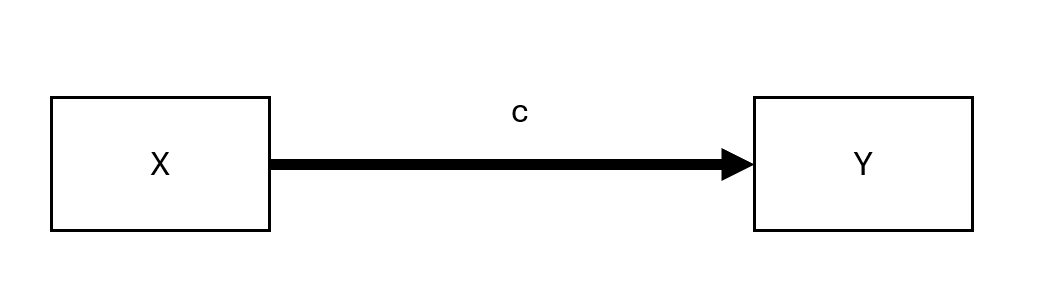
\includegraphics[width=0.9\linewidth,alt={Flow chart showing direct relationship from X to Y with arrow labeled c}]{images/mediation/direct_mod} 

}

\caption{Unmediated Model}\label{fig:fig-unmediated-model-flow}
\end{figure}

Here, \(c\) represents the \textbf{total effect} of \(X\) on \(Y\).

\subsubsection{Mediated Model}\label{mediated-model}

\begin{figure}

{\centering 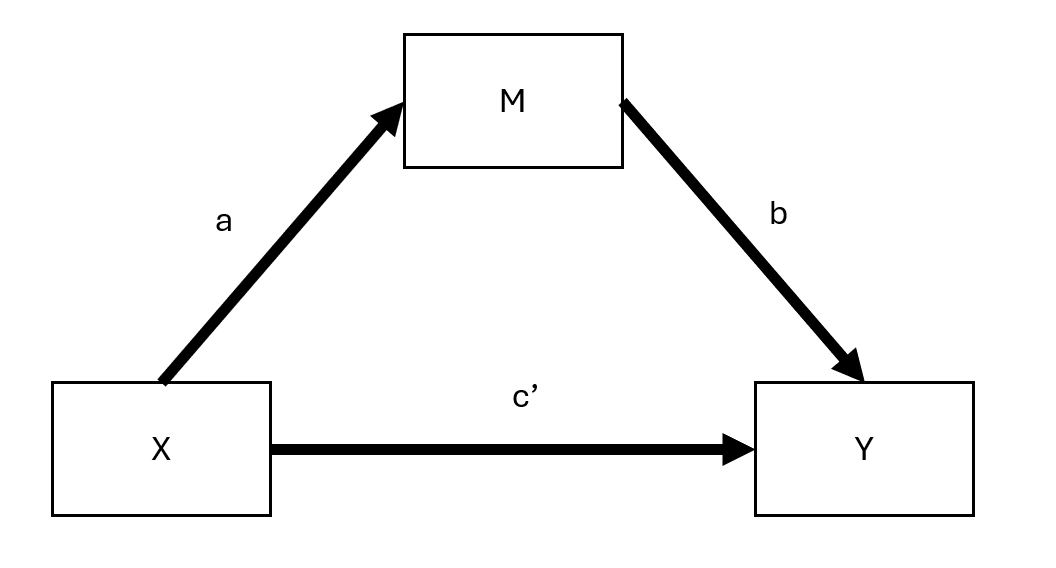
\includegraphics[width=0.9\linewidth,alt={Flow chart showing mediation model with X to M (path a), M to Y (path b), and X to Y (path c prime)}]{images/mediation/full_mod} 

}

\caption{Mediated Model}\label{fig:fig-mediated-model-flow}
\end{figure}

Here:

\begin{itemize}
\tightlist
\item
  \(c'\) = \textbf{direct effect} (effect of \(X\) on \(Y\) after accounting for mediation)
\item
  \(ab\) = \textbf{indirect effect} (mediation pathway)
\end{itemize}

Thus, we can express:

\[
\text{total effect} = \text{direct effect} + \text{indirect effect}
\]

or,

\[
c = c' + ab
\]

This equation holds under standard linear models but not necessarily in cases such as:

\begin{enumerate}
\def\labelenumi{\arabic{enumi}.}
\tightlist
\item
  Latent variable models
\item
  Logistic regression (only an approximation)
\item
  Multilevel models \citep{bauer2006conceptualizing}
\end{enumerate}

\begin{center}\rule{0.5\linewidth}{0.5pt}\end{center}

\subsection{Measuring Mediation}\label{measuring-mediation}

Several approaches exist for quantifying the \textbf{indirect effect} (\(ab\)):

\begin{enumerate}
\def\labelenumi{\arabic{enumi}.}
\item
  \textbf{Proportional Reduction Approach}:\\
  \[1 - \frac{c'}{c}\]\\
  \emph{Not recommended} due to high instability, especially when \(c\) is small \citep{mackinnon1995simulation}.
\item
  \textbf{Product Method}:\\
  \[a \times b\]\\
  The most common approach.
\item
  \textbf{Difference Method}:\\
  \[c - c'\]\\
  Conceptually similar to the product method but less precise in small samples.
\end{enumerate}

\begin{center}\rule{0.5\linewidth}{0.5pt}\end{center}

\subsection{Assumptions in Linear Mediation Models}\label{assumptions-in-linear-mediation-models}

For valid mediation analysis, the following assumptions should hold:

\begin{enumerate}
\def\labelenumi{\arabic{enumi}.}
\tightlist
\item
  \textbf{No unmeasured confounders} between \(X-Y\), \(X-M\), and \(M-Y\).
\item
  \textbf{No reverse causality}: \(X\) should not be influenced by a confounder (\(C\)) that also affects \(M-Y\).
\item
  \textbf{Measurement reliability}: \(M\) should be measured without error (if not, consider errors-in-variables models).
\end{enumerate}

\begin{center}\rule{0.5\linewidth}{0.5pt}\end{center}

\textbf{Regression Equations for Mediation Steps}

Step 1: Total Effect of \(X\) on \(Y\)

\[
Y = \beta_0 + cX + \epsilon
\]

\begin{itemize}
\tightlist
\item
  The significance of \(c\) is \textbf{not required} for mediation to occur.
\end{itemize}

Step 2: Effect of \(X\) on \(M\)

\[
M = \alpha_0 + aX + \epsilon
\]

\begin{itemize}
\tightlist
\item
  The coefficient \(a\) must be significant for mediation analysis to proceed.
\end{itemize}

Step 3: Effect of \(M\) on \(Y\) (Including \(X\))

\[
Y = \gamma_0 + c'X + bM + \epsilon
\]

\begin{itemize}
\tightlist
\item
  If \(c'\) becomes non-significant after including \(M\), full mediation occurs.
\item
  If \(c'\) is reduced but remains significant, partial mediation is present.
\end{itemize}

\begin{longtable}[]{@{}ll@{}}
\caption{Interpretation of Mediation Outcomes}\tabularnewline
\toprule\noalign{}
Effect of \(X\) on \(Y\) & Mediation Type \\
\midrule\noalign{}
\endfirsthead
\toprule\noalign{}
Effect of \(X\) on \(Y\) & Mediation Type \\
\midrule\noalign{}
\endhead
\bottomrule\noalign{}
\endlastfoot
\(b_4\) (from Step 3) is \textbf{insignificant} & Full mediation \\
\(b_4 < b_1\) (from Step 1) but still significant & Partial mediation \\
\end{longtable}

\begin{center}\rule{0.5\linewidth}{0.5pt}\end{center}

\subsection{Testing for Mediation}\label{testing-for-mediation}

Several statistical tests exist to assess whether the indirect effect (\(ab\)) is significant:

\begin{enumerate}
\def\labelenumi{\arabic{enumi}.}
\tightlist
\item
  \textbf{Sobel Test} \citep{sobel1982asymptotic}

  \begin{itemize}
  \tightlist
  \item
    Based on the standard error of \(ab\).
  \item
    \textbf{Limitation}: Assumes normality of \(ab\), which may not hold in small samples.
  \end{itemize}
\item
  \textbf{Joint Significance Test}

  \begin{itemize}
  \tightlist
  \item
    If both \(a\) and \(b\) are significant, mediation is likely.
  \end{itemize}
\item
  \textbf{Bootstrapping (Preferred)} \citep[\citet{shrout2002mediation}]{preacher2004spss}

  \begin{itemize}
  \tightlist
  \item
    Estimates the confidence interval for \(ab\).
  \item
    Does not assume normality.
  \item
    Recommended for small-to-moderate sample sizes.
  \end{itemize}
\end{enumerate}

\begin{center}\rule{0.5\linewidth}{0.5pt}\end{center}

\subsection{Additional Considerations}\label{additional-considerations}

\begin{itemize}
\tightlist
\item
  Proximal mediation (where path \(a\) exceeds path \(b\)) can lead to multicollinearity and reduced statistical power. In contrast, distal mediation (where path \(b\) exceeds path \(a\)) tends to maximize power. In fact, slightly distal mediators---where \(b\) is somewhat larger than \(a\)---often strike an ideal balance for power in mediation analyses \citep{hoyle1999statistical}.
\item
  Tests of direct effects (\(c\) and \(c'\)) generally have lower power than tests of the indirect effect (\(ab\)). As a result, it is possible for the indirect effect (\(ab\)) to be statistically significant even when the direct effect (\(c\)) is not. This situation can appear to indicate ``complete mediation,'' yet the lack of a statistically significant direct effect between \(X\) and \(Y\) (i.e., \(c'\)) does not definitively rule out other possibilities \citep{kenny2014power}.
\item
  Because testing \(ab\) essentially combines two tests, it often provides a power advantage over testing \(c'\) alone. However, using a non-significant \(c'\) as the sole criterion for claiming complete mediation should be done cautiously---if at all---given the importance of adequate sample size and power. Indeed, \citet{hayes2013relative} recommend avoiding claims of complete mediation based solely on a non-significant \(c'\), particularly when partial mediation may still be present.
\end{itemize}

\begin{center}\rule{0.5\linewidth}{0.5pt}\end{center}

\subsection{Assumptions in Mediation Analysis}\label{assumptions-in-mediation-analysis}

Valid mediation analysis requires several key assumptions, which can be categorized into \textbf{causal direction}, \textbf{interaction effects}, \textbf{measurement reliability}, and \textbf{confounding control}.

\begin{center}\rule{0.5\linewidth}{0.5pt}\end{center}

\subsubsection{Direction}\label{direction}

\begin{itemize}
\item
  Causal Order of Variables
\item
  A simple but weak solution is to measure \(X\) before \(M\) and \(Y\) to prevent reverse causality (i.e., \(M\) or \(Y\) causing \(X\)). Similarly, measuring \(M\) before \(Y\) avoids feedback effects of \(Y\) on \(M\).
\item
  However, causal feedback loops between \(M\) and \(Y\) may still exist.

  \begin{itemize}
  \item
    If we assume full mediation (\(c' = 0\)), models with reciprocal causal effects between \(M\) and \(Y\) can be estimated using instrumental variables (IV).
  \item
    \citet{smith1982beliefs} suggests treating both \(M\) and \(Y\) as potential mediators of each other, requiring distinct instrumental variables for each to avoid cross-contamination of causal effects.
  \end{itemize}
\end{itemize}

\begin{center}\rule{0.5\linewidth}{0.5pt}\end{center}

\subsubsection{Interaction Effects in Mediation}\label{interaction-effects-in-mediation}

\begin{itemize}
\item
  If \(M\) interacts with \(X\) in predicting \(Y\), then \(M\) is both a mediator and a moderator \citep{baron1986moderator}.
\item
  \textbf{The interaction term} \(X \times M\) should always be included in the model to account for possible moderation effects.
\item
  For interpreting such interactions in mediation models, see \citep{vanderweele2015explanation}, who provides a framework for \textbf{moderated mediation} analysis.
\end{itemize}

\begin{center}\rule{0.5\linewidth}{0.5pt}\end{center}

\subsubsection{Reliability}\label{reliability}

Measurement error in any of the three key variables (\(X, M, Y\)) can bias estimates of mediation effects.

\begin{enumerate}
\def\labelenumi{\arabic{enumi}.}
\tightlist
\item
  Measurement Error in the Mediator (\(M\)):

  \begin{itemize}
  \tightlist
  \item
    Biases both \(b\) and \(c'\).
  \item
    Potential solution: Model \(M\) as a latent variable (reduces bias but may decrease statistical power) \citep{ledgerwood2011trade}.
  \item
    Specific effects:

    \begin{itemize}
    \tightlist
    \item
      \(b\) is attenuated (biased toward 0).
    \item
      \(c'\) is:

      \begin{itemize}
      \tightlist
      \item
        Overestimated if \(ab > 0\).
      \item
        Underestimated if \(ab < 0\).
      \end{itemize}
    \end{itemize}
  \end{itemize}
\item
  Measurement Error in the Treatment (\(X\)):

  \begin{itemize}
  \tightlist
  \item
    Biases both \(a\) and \(b\).
  \item
    Specific effects:

    \begin{itemize}
    \tightlist
    \item
      \(a\) is attenuated.
    \item
      \(b\) is:

      \begin{itemize}
      \tightlist
      \item
        Overestimated if \(ac' > 0\).
      \item
        Underestimated if \(ac' < 0\).
      \end{itemize}
    \end{itemize}
  \end{itemize}
\item
  Measurement Error in the Outcome (\(Y\)):

  \begin{itemize}
  \tightlist
  \item
    If unstandardized, there is no bias.
  \item
    If standardized, there is attenuation bias (reduced effect sizes due to error variance).
  \end{itemize}
\end{enumerate}

\begin{center}\rule{0.5\linewidth}{0.5pt}\end{center}

\subsubsection{Confounding in Mediation Analysis}\label{confounding-in-mediation-analysis}

Omitted variable bias can distort any of the three core relationships (\(X \to Y\), \(X \to M\), \(M \to Y\)). Addressing confounding requires either design-based or statistical solutions.

\textbf{Design-Based Strategies (Preferred if Feasible)}

\begin{itemize}
\tightlist
\item
  Randomization of the independent variable (\(X\)) reduces confounding bias.
\item
  Randomization of the mediator (\(M\)), if possible, further strengthens causal claims.
\item
  Controlling for measured confounders, though this only addresses observable confounding.
\end{itemize}

\textbf{Statistical Strategies (When Randomization is Not Possible)}

\begin{enumerate}
\def\labelenumi{\arabic{enumi}.}
\tightlist
\item
  Instrumental Variables Approach:

  \begin{itemize}
  \tightlist
  \item
    Used when a confounder affects both \(M\) and \(Y\).
  \item
    Front-door adjustment can be applied if there exists a third variable that fully mediates the effect of \(M\) on \(Y\) while being independent of the confounder.
  \end{itemize}
\item
  Weighting Methods (e.g., Inverse Probability Weighting - IPW):

  \begin{itemize}
  \tightlist
  \item
    Corrects for confounding by reweighting observations to balance confounders across treatment groups.
  \item
    Requires the strong ignorability assumption: All confounders must be measured and correctly specified \citep{westfall2016statistically}.
  \item
    While this assumption cannot be formally tested, sensitivity analyses can help assess robustness.
  \item
    See \href{https://www.andrewheiss.com/blog/2020/12/01/ipw-binary-continuous/}{Heiss} for R code on implementing IPW in mediation models.
  \end{itemize}
\end{enumerate}

\begin{center}\rule{0.5\linewidth}{0.5pt}\end{center}

\subsection{Indirect Effect Tests}\label{indirect-effect-tests}

Testing the indirect effect (\(ab\)) is crucial in mediation analysis. Several methods exist, each with its advantages and limitations.

\begin{center}\rule{0.5\linewidth}{0.5pt}\end{center}

\subsubsection{Sobel Test (Delta Method)}\label{sobel-test-delta-method}

\begin{itemize}
\tightlist
\item
  Developed by \citet{sobel1982asymptotic}.
\item
  Also known as the delta method.
\item
  Not recommended because it assumes the sampling distribution of \(ab\) is normal, which often does not hold \citep{mackinnon1995simulation}.
\end{itemize}

The standard error (SE) of the indirect effect is:

\[
SE_{ab} = \sqrt{\hat{b}^2 s_{\hat{a}}^2 + \hat{a}^2 s_{\hat{b}}^2}
\]

The \textbf{Z-statistic} for testing whether \(ab\) is significantly different from 0 is:

\[
z = \frac{\hat{ab}}{\sqrt{\hat{b}^2 s_{\hat{a}}^2 + \hat{a}^2 s_{\hat{b}}^2}}
\]

\textbf{Disadvantages}

\begin{itemize}
\tightlist
\item
  Assumes \(a\) and \(b\) are independent.
\item
  Assumes \(ab\) follows a normal distribution.
\item
  Poor performance in small samples.
\item
  Lower power and more conservative than bootstrapping.
\end{itemize}

\textbf{Special Case: Inconsistent Mediation}

\begin{itemize}
\tightlist
\item
  Mediation can occur even when \textbf{direct and indirect effects} have \textbf{opposite signs}, known as \textbf{inconsistent mediation} \citep{mackinnon2007mediation}.
\item
  This happens when the \textbf{mediator acts as a suppressor variable}, leading to counteracting paths.
\end{itemize}

\begin{Shaded}
\begin{Highlighting}[]
\FunctionTok{library}\NormalTok{(bda)}
\FunctionTok{library}\NormalTok{(mediation)}
\FunctionTok{data}\NormalTok{(}\StringTok{"boundsdata"}\NormalTok{)}

\CommentTok{\# Sobel Test for Mediation}
\NormalTok{bda}\SpecialCharTok{::}\FunctionTok{mediation.test}\NormalTok{(boundsdata}\SpecialCharTok{$}\NormalTok{med, boundsdata}\SpecialCharTok{$}\NormalTok{ttt, boundsdata}\SpecialCharTok{$}\NormalTok{out) }\SpecialCharTok{|\textgreater{}}
\NormalTok{    tibble}\SpecialCharTok{::}\FunctionTok{rownames\_to\_column}\NormalTok{() }\SpecialCharTok{|\textgreater{}}
\NormalTok{    causalverse}\SpecialCharTok{::}\FunctionTok{nice\_tab}\NormalTok{(}\DecValTok{2}\NormalTok{)}
\CommentTok{\#\textgreater{}   rowname Sobel Aroian Goodman}
\CommentTok{\#\textgreater{} 1 z.value  4.05   4.03    4.07}
\CommentTok{\#\textgreater{} 2 p.value  0.00   0.00    0.00}
\end{Highlighting}
\end{Shaded}

\begin{center}\rule{0.5\linewidth}{0.5pt}\end{center}

\subsubsection{Joint Significance Test}\label{joint-significance-test}

\begin{itemize}
\tightlist
\item
  Tests if the indirect effect is nonzero by checking whether both \(a\) and \(b\) are statistically significant.
\item
  Assumes \(a \perp b\) (independence of paths).
\item
  Performs similarly to bootstrapping \citep{hayes2013relative}.
\item
  More robust to non-normality but can be sensitive to heteroscedasticity \citep{fossum2023use}.
\item
  Does not provide confidence intervals, making effect size interpretation harder.
\end{itemize}

\begin{center}\rule{0.5\linewidth}{0.5pt}\end{center}

\subsubsection{Bootstrapping (Preferred Method)}\label{bootstrapping-preferred-method}

\begin{itemize}
\tightlist
\item
  First applied to mediation by \citet{bollen1990direct}.
\item
  Uses resampling to empirically estimate the sampling distribution of the indirect effect.
\item
  Does not require normality assumptions or \(a \perp b\) independence.
\item
  Works well with small samples.
\item
  Can handle complex models.
\end{itemize}

\textbf{Which Bootstrapping Method?}

\begin{itemize}
\tightlist
\item
  \textbf{Percentile bootstrap} is preferred due to better \textbf{Type I error rates} \citep{tibbe2022correcting}.
\item
  \textbf{Bias-corrected bootstrapping} can be too \textbf{liberal} (inflates Type I errors) \citep{fritz2012explanation}.
\end{itemize}

\textbf{Special Case: Meta-Analytic Bootstrapping}

\begin{itemize}
\tightlist
\item
  Bootstrapping can be applied \textbf{without raw data}, using only \(a, b, var(a), var(b), cov(a,b)\) from multiple studies.
\end{itemize}

\begin{Shaded}
\begin{Highlighting}[]
\CommentTok{\# Meta{-}Analytic Bootstrapping for Mediation}
\FunctionTok{library}\NormalTok{(causalverse)}

\NormalTok{result }\OtherTok{\textless{}{-}}\NormalTok{ causalverse}\SpecialCharTok{::}\FunctionTok{med\_ind}\NormalTok{(}
    \AttributeTok{a =} \FloatTok{0.5}\NormalTok{, }
    \AttributeTok{b =} \FloatTok{0.7}\NormalTok{, }
    \AttributeTok{var\_a =} \FloatTok{0.04}\NormalTok{, }
    \AttributeTok{var\_b =} \FloatTok{0.05}\NormalTok{, }
    \AttributeTok{cov\_ab =} \FloatTok{0.01}
\NormalTok{)}
\end{Highlighting}
\end{Shaded}

\begin{Shaded}
\begin{Highlighting}[]
\NormalTok{result}\SpecialCharTok{$}\NormalTok{plot}
\end{Highlighting}
\end{Shaded}

\begin{figure}

{\centering \includegraphics[width=1\linewidth,alt={Right-skewed histogram of indirect effects with peak around 0.5 and red dashed confidence interval lines}]{19-mediation_files/figure-latex/fig-indirect-effect-distribution-1} 

}

\caption{Distribution of Simulated Indirect Effects}\label{fig:fig-indirect-effect-distribution}
\end{figure}

When an \textbf{instrumental variable (IV)} is available, the causal effect can be estimated more reliably. Below are visual representations.

\begin{Shaded}
\begin{Highlighting}[]
\FunctionTok{library}\NormalTok{(DiagrammeR)}

\CommentTok{\# Simple Treatment{-}Outcome Model}
\FunctionTok{grViz}\NormalTok{(}\StringTok{"}
\StringTok{digraph \{}
\StringTok{  graph []}
\StringTok{  node [shape = plaintext]}
\StringTok{    X [label = \textquotesingle{}Treatment\textquotesingle{}]}
\StringTok{    Y [label = \textquotesingle{}Outcome\textquotesingle{}]}
\StringTok{  edge [minlen = 2]}
\StringTok{    X{-}\textgreater{}Y}
\StringTok{  \{ rank = same; X; Y \}}
\StringTok{\}"}\NormalTok{)}

\CommentTok{\# Mediation Model with an Instrument}
\FunctionTok{grViz}\NormalTok{(}\StringTok{"}
\StringTok{digraph \{}
\StringTok{  graph []}
\StringTok{  node [shape = plaintext]}
\StringTok{    X [label =\textquotesingle{}Treatment\textquotesingle{}, shape = box]}
\StringTok{    Y [label =\textquotesingle{}Outcome\textquotesingle{}, shape = box]}
\StringTok{    M [label =\textquotesingle{}Mediator\textquotesingle{}, shape = box]}
\StringTok{    IV [label =\textquotesingle{}Instrument\textquotesingle{}, shape = box]}
\StringTok{  edge [minlen = 2]}
\StringTok{    IV{-}\textgreater{}X}
\StringTok{    X{-}\textgreater{}M  }
\StringTok{    M{-}\textgreater{}Y }
\StringTok{    X{-}\textgreater{}Y }
\StringTok{  \{ rank = same; X; Y; M \}}
\StringTok{\}"}\NormalTok{)}
\end{Highlighting}
\end{Shaded}

Mediation Analysis with Fixed Effects Models

\begin{Shaded}
\begin{Highlighting}[]
\FunctionTok{library}\NormalTok{(mediation)}
\FunctionTok{library}\NormalTok{(fixest)}

\FunctionTok{data}\NormalTok{(}\StringTok{"boundsdata"}\NormalTok{)}

\CommentTok{\# Step 1: Total Effect (c)}
\NormalTok{out1 }\OtherTok{\textless{}{-}} \FunctionTok{feols}\NormalTok{(out }\SpecialCharTok{\textasciitilde{}}\NormalTok{ ttt, }\AttributeTok{data =}\NormalTok{ boundsdata)}

\CommentTok{\# Step 2: Indirect Effect (a)}
\NormalTok{out2 }\OtherTok{\textless{}{-}} \FunctionTok{feols}\NormalTok{(med }\SpecialCharTok{\textasciitilde{}}\NormalTok{ ttt, }\AttributeTok{data =}\NormalTok{ boundsdata)}

\CommentTok{\# Step 3: Direct \& Indirect Effect (c\textquotesingle{} \& b)}
\NormalTok{out3 }\OtherTok{\textless{}{-}} \FunctionTok{feols}\NormalTok{(out }\SpecialCharTok{\textasciitilde{}}\NormalTok{ med }\SpecialCharTok{+}\NormalTok{ ttt, }\AttributeTok{data =}\NormalTok{ boundsdata)}

\CommentTok{\# Proportion of Mediation}
\FunctionTok{coef}\NormalTok{(out2)[}\StringTok{\textquotesingle{}ttt\textquotesingle{}}\NormalTok{] }\SpecialCharTok{*} \FunctionTok{coef}\NormalTok{(out3)[}\StringTok{\textquotesingle{}med\textquotesingle{}}\NormalTok{] }\SpecialCharTok{/} \FunctionTok{coef}\NormalTok{(out1)[}\StringTok{\textquotesingle{}ttt\textquotesingle{}}\NormalTok{] }\SpecialCharTok{*} \DecValTok{100}
\CommentTok{\#\textgreater{}      ttt }
\CommentTok{\#\textgreater{} 68.63609}
\end{Highlighting}
\end{Shaded}

Bootstrapped Mediation Analysis

\begin{Shaded}
\begin{Highlighting}[]
\FunctionTok{library}\NormalTok{(boot)}
\FunctionTok{set.seed}\NormalTok{(}\DecValTok{1}\NormalTok{)}

\CommentTok{\# Define the bootstrapping function}
\NormalTok{mediation\_fn }\OtherTok{\textless{}{-}} \ControlFlowTok{function}\NormalTok{(data, i) \{}
\NormalTok{    df }\OtherTok{\textless{}{-}}\NormalTok{ data[i,]}
    
\NormalTok{    a\_path }\OtherTok{\textless{}{-}} \FunctionTok{feols}\NormalTok{(med }\SpecialCharTok{\textasciitilde{}}\NormalTok{ ttt, }\AttributeTok{data =}\NormalTok{ df)}
\NormalTok{    a }\OtherTok{\textless{}{-}} \FunctionTok{coef}\NormalTok{(a\_path)[}\StringTok{\textquotesingle{}ttt\textquotesingle{}}\NormalTok{]}
    
\NormalTok{    b\_path }\OtherTok{\textless{}{-}} \FunctionTok{feols}\NormalTok{(out }\SpecialCharTok{\textasciitilde{}}\NormalTok{ med }\SpecialCharTok{+}\NormalTok{ ttt, }\AttributeTok{data =}\NormalTok{ df)}
\NormalTok{    b }\OtherTok{\textless{}{-}} \FunctionTok{coef}\NormalTok{(b\_path)[}\StringTok{\textquotesingle{}med\textquotesingle{}}\NormalTok{]}
    
\NormalTok{    cp }\OtherTok{\textless{}{-}} \FunctionTok{coef}\NormalTok{(b\_path)[}\StringTok{\textquotesingle{}ttt\textquotesingle{}}\NormalTok{]}
    
    \CommentTok{\# Indirect Effect (a * b)}
\NormalTok{    ind\_ef }\OtherTok{\textless{}{-}}\NormalTok{ a }\SpecialCharTok{*}\NormalTok{ b}
\NormalTok{    total\_ef }\OtherTok{\textless{}{-}}\NormalTok{ a }\SpecialCharTok{*}\NormalTok{ b }\SpecialCharTok{+}\NormalTok{ cp}
    \FunctionTok{return}\NormalTok{(}\FunctionTok{c}\NormalTok{(ind\_ef, total\_ef))}
\NormalTok{\}}

\CommentTok{\# Perform Bootstrapping}
\NormalTok{boot\_med }\OtherTok{\textless{}{-}} \FunctionTok{boot}\NormalTok{(boundsdata, mediation\_fn, }\AttributeTok{R =} \DecValTok{100}\NormalTok{, }\AttributeTok{parallel =} \StringTok{"multicore"}\NormalTok{, }\AttributeTok{ncpus =} \DecValTok{2}\NormalTok{)}
\NormalTok{boot\_med }
\CommentTok{\#\textgreater{} }
\CommentTok{\#\textgreater{} ORDINARY NONPARAMETRIC BOOTSTRAP}
\CommentTok{\#\textgreater{} }
\CommentTok{\#\textgreater{} }
\CommentTok{\#\textgreater{} Call:}
\CommentTok{\#\textgreater{} boot(data = boundsdata, statistic = mediation\_fn, R = 100, parallel = "multicore", }
\CommentTok{\#\textgreater{}     ncpus = 2)}
\CommentTok{\#\textgreater{} }
\CommentTok{\#\textgreater{} }
\CommentTok{\#\textgreater{} Bootstrap Statistics :}
\CommentTok{\#\textgreater{}       original        bias    std. error}
\CommentTok{\#\textgreater{} t1* 0.04112035  0.0006346725 0.009539903}
\CommentTok{\#\textgreater{} t2* 0.05991068 {-}0.0004462572 0.029556611}

\CommentTok{\# Summary and Confidence Intervals}
\FunctionTok{summary}\NormalTok{(boot\_med) }\SpecialCharTok{|\textgreater{}}\NormalTok{ causalverse}\SpecialCharTok{::}\FunctionTok{nice\_tab}\NormalTok{()}
\CommentTok{\#\textgreater{}     R original bootBias bootSE bootMed}
\CommentTok{\#\textgreater{} 1 100     0.04        0   0.01    0.04}
\CommentTok{\#\textgreater{} 2 100     0.06        0   0.03    0.06}

\CommentTok{\# Confidence Intervals (percentile bootstrap preferred)}
\FunctionTok{boot.ci}\NormalTok{(boot\_med, }\AttributeTok{type =} \FunctionTok{c}\NormalTok{(}\StringTok{"norm"}\NormalTok{, }\StringTok{"perc"}\NormalTok{))}
\CommentTok{\#\textgreater{} BOOTSTRAP CONFIDENCE INTERVAL CALCULATIONS}
\CommentTok{\#\textgreater{} Based on 100 bootstrap replicates}
\CommentTok{\#\textgreater{} }
\CommentTok{\#\textgreater{} CALL : }
\CommentTok{\#\textgreater{} boot.ci(boot.out = boot\_med, type = c("norm", "perc"))}
\CommentTok{\#\textgreater{} }
\CommentTok{\#\textgreater{} Intervals : }
\CommentTok{\#\textgreater{} Level      Normal             Percentile     }
\CommentTok{\#\textgreater{} 95\%   ( 0.0218,  0.0592 )   ( 0.0249,  0.0623 )  }
\CommentTok{\#\textgreater{} Calculations and Intervals on Original Scale}
\CommentTok{\#\textgreater{} Some percentile intervals may be unstable}

\CommentTok{\# Point Estimates (Indirect and Total Effects)}
\FunctionTok{colMeans}\NormalTok{(boot\_med}\SpecialCharTok{$}\NormalTok{t)}
\CommentTok{\#\textgreater{} [1] 0.04175502 0.05946442}
\end{Highlighting}
\end{Shaded}

Alternatively, use the \texttt{robmed} package for \textbf{robust} mediation analysis:

\begin{Shaded}
\begin{Highlighting}[]
\FunctionTok{library}\NormalTok{(robmed)}
\end{Highlighting}
\end{Shaded}

\subsection{Power Analysis for Mediation}\label{power-analysis-for-mediation}

To assess whether the study has sufficient \textbf{power} to detect mediation effects, use:

\begin{Shaded}
\begin{Highlighting}[]
\FunctionTok{library}\NormalTok{(pwr2ppl)}

\CommentTok{\# Power analysis for the indirect effect (ab path)}
\FunctionTok{medjs}\NormalTok{(}
    \AttributeTok{rx1m1 =}\NormalTok{ .}\DecValTok{3}\NormalTok{,  }\CommentTok{\# Correlation: X → M (path a)}
    \AttributeTok{rx1y  =}\NormalTok{ .}\DecValTok{1}\NormalTok{,  }\CommentTok{\# Correlation: X → Y (path c\textquotesingle{})}
    \AttributeTok{rym1  =}\NormalTok{ .}\DecValTok{3}\NormalTok{,  }\CommentTok{\# Correlation: M → Y (path b)}
    \AttributeTok{n     =} \DecValTok{100}\NormalTok{, }\CommentTok{\# Sample size}
    \AttributeTok{alpha =} \FloatTok{0.05}\NormalTok{,}
    \AttributeTok{mvars =} \DecValTok{1}\NormalTok{,   }\CommentTok{\# Number of mediators}
    \AttributeTok{rep   =} \DecValTok{1000} \CommentTok{\# Replications (use 10,000 for accuracy)}
\NormalTok{)}
\end{Highlighting}
\end{Shaded}

For \textbf{interactive} power analysis, see \href{https://davidakenny.shinyapps.io/MedPower/}{Kenny's Mediation Power App}.

\textbf{Summary of Indirect Effect Tests}

\begin{longtable}[]{@{}
  >{\raggedright\arraybackslash}p{(\linewidth - 4\tabcolsep) * \real{0.2877}}
  >{\raggedright\arraybackslash}p{(\linewidth - 4\tabcolsep) * \real{0.4110}}
  >{\raggedright\arraybackslash}p{(\linewidth - 4\tabcolsep) * \real{0.3014}}@{}}
\caption{Comparison of Mediation Testing Methods}\tabularnewline
\toprule\noalign{}
\begin{minipage}[b]{\linewidth}\raggedright
\textbf{Test}
\end{minipage} & \begin{minipage}[b]{\linewidth}\raggedright
\textbf{Pros}
\end{minipage} & \begin{minipage}[b]{\linewidth}\raggedright
\textbf{Cons}
\end{minipage} \\
\midrule\noalign{}
\endfirsthead
\toprule\noalign{}
\begin{minipage}[b]{\linewidth}\raggedright
\textbf{Test}
\end{minipage} & \begin{minipage}[b]{\linewidth}\raggedright
\textbf{Pros}
\end{minipage} & \begin{minipage}[b]{\linewidth}\raggedright
\textbf{Cons}
\end{minipage} \\
\midrule\noalign{}
\endhead
\bottomrule\noalign{}
\endlastfoot
\textbf{Sobel Test} & Simple, fast & Assumes normality, low power \\
\textbf{Joint Significance Test} & Robust to non-normality & No confidence interval \\
\textbf{Bootstrapping} (Recommended) & No normality assumption, handles small samples & May be liberal if bias-corrected \\
\end{longtable}

\subsection{Multiple Mediation Analysis}\label{multiple-mediation-analysis}

In some cases, a single mediator (\(M\)) does not fully capture the indirect effect of \(X\) on \(Y\). Multiple mediation models extend traditional mediation by including two or more mediators, allowing us to examine how multiple pathways contribute to an outcome.

\begin{center}\rule{0.5\linewidth}{0.5pt}\end{center}

Several R packages handle multiple mediation models:

\begin{itemize}
\tightlist
\item
  \textbf{manymome}: A flexible package for multiple mediation modeling.

  \begin{itemize}
  \tightlist
  \item
    \href{https://cran.r-project.org/web/packages/manymome/vignettes/med_lm.html}{Vignette}
  \end{itemize}
\end{itemize}

\begin{Shaded}
\begin{Highlighting}[]
\FunctionTok{library}\NormalTok{(manymome)}
\end{Highlighting}
\end{Shaded}

\begin{itemize}
\item
  \textbf{mma}: Used for multiple mediator models.

  \begin{itemize}
  \item
    \href{https://cran.r-project.org/web/packages/mma/mma.pdf}{Package PDF}
  \item
    \href{https://cran.r-project.org/web/packages/mma/vignettes/MMAvignette.html}{Vignette}
  \end{itemize}
\end{itemize}

\begin{Shaded}
\begin{Highlighting}[]
\FunctionTok{library}\NormalTok{(mma)}
\end{Highlighting}
\end{Shaded}

\subsubsection{Multiple Mediators: Structural Equation Modeling Approach}\label{multiple-mediators-structural-equation-modeling-approach}

A popular method for estimating multiple mediation models is \textbf{Structural Equation Modeling} using \textbf{lavaan}.

To test multiple mediation, we first \textbf{simulate data} where two mediators (\(M_1\) and \(M_2\)) contribute to the outcome (\(Y\)).

\begin{Shaded}
\begin{Highlighting}[]
\CommentTok{\# Load required packages}
\FunctionTok{library}\NormalTok{(MASS)  }\CommentTok{\# For mvrnorm (generating correlated errors)}
\FunctionTok{library}\NormalTok{(lavaan)}

\CommentTok{\# Function to generate synthetic data}
\NormalTok{generate\_data }\OtherTok{\textless{}{-}} \ControlFlowTok{function}\NormalTok{(}\AttributeTok{n =} \DecValTok{10000}\NormalTok{, }\AttributeTok{a1 =} \FloatTok{0.5}\NormalTok{, }\AttributeTok{a2 =} \SpecialCharTok{{-}}\FloatTok{0.35}\NormalTok{, }
                          \AttributeTok{b1 =} \FloatTok{0.7}\NormalTok{, }\AttributeTok{b2 =} \FloatTok{0.48}\NormalTok{, }
                          \AttributeTok{corr =} \ConstantTok{TRUE}\NormalTok{, }\AttributeTok{correlation\_value =} \FloatTok{0.7}\NormalTok{) \{}
    \FunctionTok{set.seed}\NormalTok{(}\DecValTok{12345}\NormalTok{)}
\NormalTok{    X }\OtherTok{\textless{}{-}} \FunctionTok{rnorm}\NormalTok{(n)  }\CommentTok{\# Independent variable}
    
    \CommentTok{\# Generate correlated errors for mediators}
    \ControlFlowTok{if}\NormalTok{ (corr) \{}
\NormalTok{        Sigma }\OtherTok{\textless{}{-}} \FunctionTok{matrix}\NormalTok{(}\FunctionTok{c}\NormalTok{(}\DecValTok{1}\NormalTok{, correlation\_value, correlation\_value, }\DecValTok{1}\NormalTok{), }\AttributeTok{nrow =} \DecValTok{2}\NormalTok{)}
\NormalTok{        errors }\OtherTok{\textless{}{-}} \FunctionTok{mvrnorm}\NormalTok{(n, }\AttributeTok{mu =} \FunctionTok{c}\NormalTok{(}\DecValTok{0}\NormalTok{, }\DecValTok{0}\NormalTok{), }\AttributeTok{Sigma =}\NormalTok{ Sigma) }
\NormalTok{    \} }\ControlFlowTok{else}\NormalTok{ \{}
\NormalTok{        errors }\OtherTok{\textless{}{-}} \FunctionTok{mvrnorm}\NormalTok{(n, }\AttributeTok{mu =} \FunctionTok{c}\NormalTok{(}\DecValTok{0}\NormalTok{, }\DecValTok{0}\NormalTok{), }\AttributeTok{Sigma =} \FunctionTok{diag}\NormalTok{(}\DecValTok{2}\NormalTok{)) }
\NormalTok{    \}}
    
\NormalTok{    M1 }\OtherTok{\textless{}{-}}\NormalTok{ a1 }\SpecialCharTok{*}\NormalTok{ X }\SpecialCharTok{+}\NormalTok{ errors[, }\DecValTok{1}\NormalTok{]}
\NormalTok{    M2 }\OtherTok{\textless{}{-}}\NormalTok{ a2 }\SpecialCharTok{*}\NormalTok{ X }\SpecialCharTok{+}\NormalTok{ errors[, }\DecValTok{2}\NormalTok{]}
\NormalTok{    Y  }\OtherTok{\textless{}{-}}\NormalTok{ b1 }\SpecialCharTok{*}\NormalTok{ M1 }\SpecialCharTok{+}\NormalTok{ b2 }\SpecialCharTok{*}\NormalTok{ M2 }\SpecialCharTok{+} \FunctionTok{rnorm}\NormalTok{(n)  }\CommentTok{\# Outcome variable}

    \FunctionTok{return}\NormalTok{(}\FunctionTok{data.frame}\NormalTok{(}\AttributeTok{X =}\NormalTok{ X, }\AttributeTok{M1 =}\NormalTok{ M1, }\AttributeTok{M2 =}\NormalTok{ M2, }\AttributeTok{Y =}\NormalTok{ Y))}
\NormalTok{\}}
\end{Highlighting}
\end{Shaded}

We analyze the indirect effects through both mediators (\(M_1\) and \(M_2\)).

\begin{enumerate}
\def\labelenumi{\arabic{enumi}.}
\tightlist
\item
  Correctly Modeling Correlated Mediators
\end{enumerate}

\begin{Shaded}
\begin{Highlighting}[]
\CommentTok{\# Generate data with correlated mediators}
\NormalTok{Data\_corr }\OtherTok{\textless{}{-}} \FunctionTok{generate\_data}\NormalTok{(}\AttributeTok{n =} \DecValTok{10000}\NormalTok{, }\AttributeTok{corr =} \ConstantTok{TRUE}\NormalTok{, }\AttributeTok{correlation\_value =} \FloatTok{0.7}\NormalTok{)}

\CommentTok{\# Define SEM model for multiple mediation}
\NormalTok{model\_corr }\OtherTok{\textless{}{-}} \StringTok{\textquotesingle{}}
\StringTok{  Y \textasciitilde{} b1 * M1 + b2 * M2 + c * X}
\StringTok{  M1 \textasciitilde{} a1 * X}
\StringTok{  M2 \textasciitilde{} a2 * X}
\StringTok{  M1 \textasciitilde{}\textasciitilde{} M2  \# Correlated mediators (modeling correlation correctly)}
\StringTok{\textquotesingle{}}

\CommentTok{\# Fit SEM model}
\NormalTok{fit\_corr }\OtherTok{\textless{}{-}} \FunctionTok{sem}\NormalTok{(model\_corr, }\AttributeTok{data =}\NormalTok{ Data\_corr)}

\CommentTok{\# Extract parameter estimates}
\FunctionTok{parameterEstimates}\NormalTok{(fit\_corr)[, }\FunctionTok{c}\NormalTok{(}\StringTok{"lhs"}\NormalTok{, }\StringTok{"rhs"}\NormalTok{, }\StringTok{"est"}\NormalTok{, }\StringTok{"se"}\NormalTok{, }\StringTok{"pvalue"}\NormalTok{)]}
\CommentTok{\#\textgreater{}    lhs rhs    est    se pvalue}
\CommentTok{\#\textgreater{} 1    Y  M1  0.700 0.014  0.000}
\CommentTok{\#\textgreater{} 2    Y  M2  0.487 0.014  0.000}
\CommentTok{\#\textgreater{} 3    Y   X {-}0.009 0.015  0.545}
\CommentTok{\#\textgreater{} 4   M1   X  0.519 0.010  0.000}
\CommentTok{\#\textgreater{} 5   M2   X {-}0.340 0.010  0.000}
\CommentTok{\#\textgreater{} 6   M1  M2  0.677 0.012  0.000}
\CommentTok{\#\textgreater{} 7    Y   Y  0.975 0.014  0.000}
\CommentTok{\#\textgreater{} 8   M1  M1  0.973 0.014  0.000}
\CommentTok{\#\textgreater{} 9   M2  M2  0.982 0.014  0.000}
\CommentTok{\#\textgreater{} 10   X   X  1.000 0.000     NA}
\end{Highlighting}
\end{Shaded}

2. Incorrectly Ignoring Correlation Between Mediators

\begin{Shaded}
\begin{Highlighting}[]
\CommentTok{\# Define SEM model without modeling mediator correlation}
\NormalTok{model\_uncorr }\OtherTok{\textless{}{-}} \StringTok{\textquotesingle{}}
\StringTok{  Y \textasciitilde{} b1 * M1 + b2 * M2 + c * X}
\StringTok{  M1 \textasciitilde{} a1 * X}
\StringTok{  M2 \textasciitilde{} a2 * X}
\StringTok{\textquotesingle{}}

\CommentTok{\# Fit incorrect model}
\NormalTok{fit\_uncorr }\OtherTok{\textless{}{-}} \FunctionTok{sem}\NormalTok{(model\_uncorr, }\AttributeTok{data =}\NormalTok{ Data\_corr)}

\CommentTok{\# Compare parameter estimates}
\FunctionTok{parameterEstimates}\NormalTok{(fit\_uncorr)[, }\FunctionTok{c}\NormalTok{(}\StringTok{"lhs"}\NormalTok{, }\StringTok{"rhs"}\NormalTok{, }\StringTok{"est"}\NormalTok{, }\StringTok{"se"}\NormalTok{, }\StringTok{"pvalue"}\NormalTok{)]}
\CommentTok{\#\textgreater{}   lhs rhs    est    se pvalue}
\CommentTok{\#\textgreater{} 1   Y  M1  0.700 0.010  0.000}
\CommentTok{\#\textgreater{} 2   Y  M2  0.487 0.010  0.000}
\CommentTok{\#\textgreater{} 3   Y   X {-}0.009 0.012  0.443}
\CommentTok{\#\textgreater{} 4  M1   X  0.519 0.010  0.000}
\CommentTok{\#\textgreater{} 5  M2   X {-}0.340 0.010  0.000}
\CommentTok{\#\textgreater{} 6   Y   Y  0.975 0.014  0.000}
\CommentTok{\#\textgreater{} 7  M1  M1  0.973 0.014  0.000}
\CommentTok{\#\textgreater{} 8  M2  M2  0.982 0.014  0.000}
\CommentTok{\#\textgreater{} 9   X   X  1.000 0.000     NA}
\end{Highlighting}
\end{Shaded}

\textbf{Comparison of Model Fits}

To check whether modeling correlation matters, we compare AIC and RMSEA.

\begin{Shaded}
\begin{Highlighting}[]
\CommentTok{\# Extract model fit statistics}
\NormalTok{fit\_measures }\OtherTok{\textless{}{-}} \ControlFlowTok{function}\NormalTok{(fit) \{}
  \FunctionTok{fitMeasures}\NormalTok{(fit, }\FunctionTok{c}\NormalTok{(}\StringTok{"aic"}\NormalTok{, }\StringTok{"bic"}\NormalTok{, }\StringTok{"rmsea"}\NormalTok{, }\StringTok{"chisq"}\NormalTok{))}
\NormalTok{\}}

\CommentTok{\# Compare model fits}
\FunctionTok{fit\_measures}\NormalTok{(fit\_corr)  }\CommentTok{\# Correct model (correlated mediators)}
\CommentTok{\#\textgreater{}      aic      bic    rmsea    chisq }
\CommentTok{\#\textgreater{} 77932.45 77997.34     0.00     0.00}
\FunctionTok{fit\_measures}\NormalTok{(fit\_uncorr)  }\CommentTok{\# Incorrect model (ignores correlation)}
\CommentTok{\#\textgreater{}       aic       bic     rmsea     chisq }
\CommentTok{\#\textgreater{} 84453.208 84510.891     0.808  6522.762}
\end{Highlighting}
\end{Shaded}

\begin{itemize}
\tightlist
\item
  If AIC and RMSEA are lower in the correlated model, it suggests that accounting for correlated errors improves fit.
\end{itemize}

After fitting the model, we assess:

\begin{enumerate}
\def\labelenumi{\arabic{enumi}.}
\item
  \textbf{Direct Effect}: The effect of \(X\) on \(Y\) \textbf{after accounting for both mediators} (\(c'\)).
\item
  \textbf{Indirect Effects}:

  \begin{itemize}
  \item
    \(a_1 \times b_1\): Effect of \(X \to M_1 \to Y\).
  \item
    \(a_2 \times b_2\): Effect of \(X \to M_2 \to Y\).
  \end{itemize}
\item
  \textbf{Total Effect}: Sum of direct and indirect effects.
\end{enumerate}

\begin{Shaded}
\begin{Highlighting}[]
\CommentTok{\# Extract indirect and direct effects}
\FunctionTok{parameterEstimates}\NormalTok{(fit\_corr, }\AttributeTok{standardized =} \ConstantTok{TRUE}\NormalTok{)}
\CommentTok{\#\textgreater{}    lhs op rhs label    est    se       z pvalue ci.lower ci.upper std.lv}
\CommentTok{\#\textgreater{} 1    Y  \textasciitilde{}  M1    b1  0.700 0.014  50.489  0.000    0.673    0.727  0.700}
\CommentTok{\#\textgreater{} 2    Y  \textasciitilde{}  M2    b2  0.487 0.014  35.284  0.000    0.460    0.514  0.487}
\CommentTok{\#\textgreater{} 3    Y  \textasciitilde{}   X     c {-}0.009 0.015  {-}0.606  0.545   {-}0.038    0.020 {-}0.009}
\CommentTok{\#\textgreater{} 4   M1  \textasciitilde{}   X    a1  0.519 0.010  52.563  0.000    0.499    0.538  0.519}
\CommentTok{\#\textgreater{} 5   M2  \textasciitilde{}   X    a2 {-}0.340 0.010 {-}34.314  0.000   {-}0.360   {-}0.321 {-}0.340}
\CommentTok{\#\textgreater{} 6   M1 \textasciitilde{}\textasciitilde{}  M2        0.677 0.012  56.915  0.000    0.654    0.700  0.677}
\CommentTok{\#\textgreater{} 7    Y \textasciitilde{}\textasciitilde{}   Y        0.975 0.014  70.711  0.000    0.948    1.002  0.975}
\CommentTok{\#\textgreater{} 8   M1 \textasciitilde{}\textasciitilde{}  M1        0.973 0.014  70.711  0.000    0.946    1.000  0.973}
\CommentTok{\#\textgreater{} 9   M2 \textasciitilde{}\textasciitilde{}  M2        0.982 0.014  70.711  0.000    0.955    1.010  0.982}
\CommentTok{\#\textgreater{} 10   X \textasciitilde{}\textasciitilde{}   X        1.000 0.000      NA     NA    1.000    1.000  1.000}
\CommentTok{\#\textgreater{}    std.all std.nox}
\CommentTok{\#\textgreater{} 1    0.528   0.528}
\CommentTok{\#\textgreater{} 2    0.345   0.345}
\CommentTok{\#\textgreater{} 3   {-}0.006  {-}0.006}
\CommentTok{\#\textgreater{} 4    0.465   0.465}
\CommentTok{\#\textgreater{} 5   {-}0.325  {-}0.325}
\CommentTok{\#\textgreater{} 6    0.692   0.692}
\CommentTok{\#\textgreater{} 7    0.447   0.447}
\CommentTok{\#\textgreater{} 8    0.784   0.784}
\CommentTok{\#\textgreater{} 9    0.895   0.895}
\CommentTok{\#\textgreater{} 10   1.000   1.000}
\end{Highlighting}
\end{Shaded}

If \(c'\) is reduced (but still significant), we have partial mediation. If \(c' \approx 0\), it suggests full mediation.

\begin{Shaded}
\begin{Highlighting}[]
\CommentTok{\# Load required packages}
\FunctionTok{library}\NormalTok{(MASS)  }\CommentTok{\# for mvrnorm}
\FunctionTok{library}\NormalTok{(lavaan)}

\CommentTok{\# Function to generate synthetic data with correctly correlated errors for mediators}
\NormalTok{generate\_data }\OtherTok{\textless{}{-}}
  \ControlFlowTok{function}\NormalTok{(}\AttributeTok{n =} \DecValTok{10000}\NormalTok{,}
           \AttributeTok{a1 =} \FloatTok{0.5}\NormalTok{,}
           \AttributeTok{a2 =} \SpecialCharTok{{-}}\FloatTok{0.35}\NormalTok{,}
           \AttributeTok{b1 =} \FloatTok{0.7}\NormalTok{,}
           \AttributeTok{b2 =} \FloatTok{0.48}\NormalTok{,}
           \AttributeTok{corr =} \ConstantTok{TRUE}\NormalTok{,}
           \AttributeTok{correlation\_value =} \FloatTok{0.7}\NormalTok{) \{}
    \FunctionTok{set.seed}\NormalTok{(}\DecValTok{12345}\NormalTok{)}
\NormalTok{    X }\OtherTok{\textless{}{-}} \FunctionTok{rnorm}\NormalTok{(n)}
    
    \CommentTok{\# Generate correlated errors using a multivariate normal distribution}
    \ControlFlowTok{if}\NormalTok{ (corr) \{}
\NormalTok{        Sigma }\OtherTok{\textless{}{-}} \FunctionTok{matrix}\NormalTok{(}\FunctionTok{c}\NormalTok{(}\DecValTok{1}\NormalTok{, correlation\_value, correlation\_value, }\DecValTok{1}\NormalTok{), }\AttributeTok{nrow =} \DecValTok{2}\NormalTok{)  }\CommentTok{\# Higher covariance matrix for errors}
\NormalTok{        errors }\OtherTok{\textless{}{-}} \FunctionTok{mvrnorm}\NormalTok{(n, }\AttributeTok{mu =} \FunctionTok{c}\NormalTok{(}\DecValTok{0}\NormalTok{, }\DecValTok{0}\NormalTok{), }\AttributeTok{Sigma =}\NormalTok{ Sigma)  }\CommentTok{\# Generate correlated errors}
\NormalTok{    \} }\ControlFlowTok{else}\NormalTok{ \{}
\NormalTok{        errors }\OtherTok{\textless{}{-}} \FunctionTok{mvrnorm}\NormalTok{(n, }\AttributeTok{mu =} \FunctionTok{c}\NormalTok{(}\DecValTok{0}\NormalTok{, }\DecValTok{0}\NormalTok{), }\AttributeTok{Sigma =} \FunctionTok{diag}\NormalTok{(}\DecValTok{2}\NormalTok{))  }\CommentTok{\# Independent errors}
\NormalTok{    \}}
    
\NormalTok{    M1 }\OtherTok{\textless{}{-}}\NormalTok{ a1 }\SpecialCharTok{*}\NormalTok{ X }\SpecialCharTok{+}\NormalTok{ errors[, }\DecValTok{1}\NormalTok{]}
\NormalTok{    M2 }\OtherTok{\textless{}{-}}\NormalTok{ a2 }\SpecialCharTok{*}\NormalTok{ X }\SpecialCharTok{+}\NormalTok{ errors[, }\DecValTok{2}\NormalTok{]}
\NormalTok{    Y }\OtherTok{\textless{}{-}}\NormalTok{ b1 }\SpecialCharTok{*}\NormalTok{ M1 }\SpecialCharTok{+}\NormalTok{ b2 }\SpecialCharTok{*}\NormalTok{ M2 }\SpecialCharTok{+} \FunctionTok{rnorm}\NormalTok{(n)  }\CommentTok{\# Y depends on M1 and M2}
    
    \FunctionTok{data.frame}\NormalTok{(}\AttributeTok{X =}\NormalTok{ X, }\AttributeTok{M1 =}\NormalTok{ M1, }\AttributeTok{M2 =}\NormalTok{ M2, }\AttributeTok{Y =}\NormalTok{ Y)}
\NormalTok{\}}

\CommentTok{\# Ground truth for comparison}
\NormalTok{ground\_truth }\OtherTok{\textless{}{-}} \FunctionTok{data.frame}\NormalTok{(}\AttributeTok{Parameter =} \FunctionTok{c}\NormalTok{(}\StringTok{"b1"}\NormalTok{, }\StringTok{"b2"}\NormalTok{), }\AttributeTok{GroundTruth =} \FunctionTok{c}\NormalTok{(}\FloatTok{0.7}\NormalTok{, }\FloatTok{0.48}\NormalTok{))}

\CommentTok{\# Function to extract relevant estimates, standard errors, and model fit}
\NormalTok{extract\_estimates\_b1\_b2 }\OtherTok{\textless{}{-}} \ControlFlowTok{function}\NormalTok{(fit) \{}
\NormalTok{    estimates }\OtherTok{\textless{}{-}} \FunctionTok{parameterEstimates}\NormalTok{(fit)}
\NormalTok{    estimates }\OtherTok{\textless{}{-}}\NormalTok{ estimates[estimates}\SpecialCharTok{$}\NormalTok{lhs }\SpecialCharTok{==} \StringTok{"Y"} \SpecialCharTok{\&}\NormalTok{ estimates}\SpecialCharTok{$}\NormalTok{rhs }\SpecialCharTok{\%in\%} \FunctionTok{c}\NormalTok{(}\StringTok{"M1"}\NormalTok{, }\StringTok{"M2"}\NormalTok{), }\FunctionTok{c}\NormalTok{(}\StringTok{"rhs"}\NormalTok{, }\StringTok{"est"}\NormalTok{, }\StringTok{"se"}\NormalTok{)]}
\NormalTok{    estimates}\SpecialCharTok{$}\NormalTok{Parameter }\OtherTok{\textless{}{-}} \FunctionTok{ifelse}\NormalTok{(estimates}\SpecialCharTok{$}\NormalTok{rhs }\SpecialCharTok{==} \StringTok{"M1"}\NormalTok{, }\StringTok{"b1"}\NormalTok{, }\StringTok{"b2"}\NormalTok{)}
\NormalTok{    estimates }\OtherTok{\textless{}{-}}\NormalTok{ estimates[, }\FunctionTok{c}\NormalTok{(}\StringTok{"Parameter"}\NormalTok{, }\StringTok{"est"}\NormalTok{, }\StringTok{"se"}\NormalTok{)]}
\NormalTok{    fit\_stats }\OtherTok{\textless{}{-}} \FunctionTok{fitMeasures}\NormalTok{(fit, }\FunctionTok{c}\NormalTok{(}\StringTok{"aic"}\NormalTok{, }\StringTok{"bic"}\NormalTok{, }\StringTok{"rmsea"}\NormalTok{, }\StringTok{"chisq"}\NormalTok{))}
    \FunctionTok{return}\NormalTok{(}\FunctionTok{list}\NormalTok{(}\AttributeTok{estimates =}\NormalTok{ estimates, }\AttributeTok{fit\_stats =}\NormalTok{ fit\_stats))}
\NormalTok{\}}

\CommentTok{\# Case 1: Correlated errors for mediators (modeled correctly)}
\NormalTok{Data\_corr }\OtherTok{\textless{}{-}} \FunctionTok{generate\_data}\NormalTok{(}\AttributeTok{n =} \DecValTok{10000}\NormalTok{, }\AttributeTok{corr =} \ConstantTok{TRUE}\NormalTok{, }\AttributeTok{correlation\_value =} \FloatTok{0.7}\NormalTok{)}
\NormalTok{model\_corr }\OtherTok{\textless{}{-}} \StringTok{\textquotesingle{}}
\StringTok{  Y \textasciitilde{} b1 * M1 + b2 * M2 + c * X}
\StringTok{  M1 \textasciitilde{} a1 * X}
\StringTok{  M2 \textasciitilde{} a2 * X}
\StringTok{  M1 \textasciitilde{}\textasciitilde{} M2  \# Correlated mediators (errors)}
\StringTok{\textquotesingle{}}
\NormalTok{fit\_corr }\OtherTok{\textless{}{-}} \FunctionTok{sem}\NormalTok{(}\AttributeTok{model =}\NormalTok{ model\_corr, }\AttributeTok{data =}\NormalTok{ Data\_corr)}
\NormalTok{results\_corr }\OtherTok{\textless{}{-}} \FunctionTok{extract\_estimates\_b1\_b2}\NormalTok{(fit\_corr)}

\CommentTok{\# Case 2: Uncorrelated errors for mediators (modeled correctly)}
\NormalTok{Data\_uncorr }\OtherTok{\textless{}{-}} \FunctionTok{generate\_data}\NormalTok{(}\AttributeTok{n =} \DecValTok{10000}\NormalTok{, }\AttributeTok{corr =} \ConstantTok{FALSE}\NormalTok{)}
\NormalTok{model\_uncorr }\OtherTok{\textless{}{-}} \StringTok{\textquotesingle{}}
\StringTok{  Y \textasciitilde{} b1 * M1 + b2 * M2 + c * X}
\StringTok{  M1 \textasciitilde{} a1 * X}
\StringTok{  M2 \textasciitilde{} a2 * X}
\StringTok{\textquotesingle{}}
\NormalTok{fit\_uncorr }\OtherTok{\textless{}{-}} \FunctionTok{sem}\NormalTok{(}\AttributeTok{model =}\NormalTok{ model\_uncorr, }\AttributeTok{data =}\NormalTok{ Data\_uncorr)}
\NormalTok{results\_uncorr }\OtherTok{\textless{}{-}} \FunctionTok{extract\_estimates\_b1\_b2}\NormalTok{(fit\_uncorr)}

\CommentTok{\# Case 3: Correlated errors, but not modeled as correlated}
\NormalTok{fit\_corr\_incorrect }\OtherTok{\textless{}{-}} \FunctionTok{sem}\NormalTok{(}\AttributeTok{model =}\NormalTok{ model\_uncorr, }\AttributeTok{data =}\NormalTok{ Data\_corr)}
\NormalTok{results\_corr\_incorrect }\OtherTok{\textless{}{-}} \FunctionTok{extract\_estimates\_b1\_b2}\NormalTok{(fit\_corr\_incorrect)}

\CommentTok{\# Case 4: Uncorrelated errors, but modeled as correlated}
\NormalTok{fit\_uncorr\_incorrect }\OtherTok{\textless{}{-}} \FunctionTok{sem}\NormalTok{(}\AttributeTok{model =}\NormalTok{ model\_corr, }\AttributeTok{data =}\NormalTok{ Data\_uncorr)}
\NormalTok{results\_uncorr\_incorrect }\OtherTok{\textless{}{-}} \FunctionTok{extract\_estimates\_b1\_b2}\NormalTok{(fit\_uncorr\_incorrect)}

\CommentTok{\# Combine all estimates for comparison}
\NormalTok{estimates\_combined }\OtherTok{\textless{}{-}} \FunctionTok{list}\NormalTok{(}
    \StringTok{"Correlated (Correct)"} \OtherTok{=}\NormalTok{ results\_corr}\SpecialCharTok{$}\NormalTok{estimates,}
    \StringTok{"Uncorrelated (Correct)"} \OtherTok{=}\NormalTok{ results\_uncorr}\SpecialCharTok{$}\NormalTok{estimates,}
    \StringTok{"Correlated (Incorrect)"} \OtherTok{=}\NormalTok{ results\_corr\_incorrect}\SpecialCharTok{$}\NormalTok{estimates,}
    \StringTok{"Uncorrelated (Incorrect)"} \OtherTok{=}\NormalTok{ results\_uncorr\_incorrect}\SpecialCharTok{$}\NormalTok{estimates}
\NormalTok{)}

\CommentTok{\# Combine all into a single table}
\NormalTok{comparison\_table }\OtherTok{\textless{}{-}} \FunctionTok{do.call}\NormalTok{(rbind, }\FunctionTok{lapply}\NormalTok{(}\FunctionTok{names}\NormalTok{(estimates\_combined), }\ControlFlowTok{function}\NormalTok{(case) \{}
\NormalTok{    df }\OtherTok{\textless{}{-}}\NormalTok{ estimates\_combined[[case]]}
\NormalTok{    df}\SpecialCharTok{$}\NormalTok{Case }\OtherTok{\textless{}{-}}\NormalTok{ case}
\NormalTok{    df}
\NormalTok{\}))}

\CommentTok{\# Merge with ground truth for final comparison}
\NormalTok{comparison\_table }\OtherTok{\textless{}{-}} \FunctionTok{merge}\NormalTok{(comparison\_table, ground\_truth, }\AttributeTok{by =} \StringTok{"Parameter"}\NormalTok{)}

\CommentTok{\# Display the comparison table}
\NormalTok{comparison\_table}
\CommentTok{\#\textgreater{}   Parameter       est          se                     Case GroundTruth}
\CommentTok{\#\textgreater{} 1        b1 0.7002984 0.013870433     Correlated (Correct)        0.70}
\CommentTok{\#\textgreater{} 2        b1 0.6973612 0.009859426   Uncorrelated (Correct)        0.70}
\CommentTok{\#\textgreater{} 3        b1 0.7002984 0.010010367   Correlated (Incorrect)        0.70}
\CommentTok{\#\textgreater{} 4        b1 0.6973612 0.009859634 Uncorrelated (Incorrect)        0.70}
\CommentTok{\#\textgreater{} 5        b2 0.4871118 0.013805615     Correlated (Correct)        0.48}
\CommentTok{\#\textgreater{} 6        b2 0.4868318 0.010009908   Uncorrelated (Correct)        0.48}
\CommentTok{\#\textgreater{} 7        b2 0.4871118 0.009963588   Correlated (Incorrect)        0.48}
\CommentTok{\#\textgreater{} 8        b2 0.4868318 0.010010119 Uncorrelated (Incorrect)        0.48}

\CommentTok{\# Display model fit statistics for each case}
\NormalTok{fit\_stats\_combined }\OtherTok{\textless{}{-}} \FunctionTok{list}\NormalTok{(}
    \StringTok{"Correlated (Correct)"} \OtherTok{=}\NormalTok{ results\_corr}\SpecialCharTok{$}\NormalTok{fit\_stats,}
    \StringTok{"Uncorrelated (Correct)"} \OtherTok{=}\NormalTok{ results\_uncorr}\SpecialCharTok{$}\NormalTok{fit\_stats,}
    \StringTok{"Correlated (Incorrect)"} \OtherTok{=}\NormalTok{ results\_corr\_incorrect}\SpecialCharTok{$}\NormalTok{fit\_stats,}
    \StringTok{"Uncorrelated (Incorrect)"} \OtherTok{=}\NormalTok{ results\_uncorr\_incorrect}\SpecialCharTok{$}\NormalTok{fit\_stats}
\NormalTok{)}

\NormalTok{fit\_stats\_combined}
\CommentTok{\#\textgreater{} $\textasciigrave{}Correlated (Correct)\textasciigrave{}}
\CommentTok{\#\textgreater{}      aic      bic    rmsea    chisq }
\CommentTok{\#\textgreater{} 77932.45 77997.34     0.00     0.00 }
\CommentTok{\#\textgreater{} }
\CommentTok{\#\textgreater{} $\textasciigrave{}Uncorrelated (Correct)\textasciigrave{}}
\CommentTok{\#\textgreater{}       aic       bic     rmsea     chisq }
\CommentTok{\#\textgreater{} 84664.312 84721.995     0.000     0.421 }
\CommentTok{\#\textgreater{} }
\CommentTok{\#\textgreater{} $\textasciigrave{}Correlated (Incorrect)\textasciigrave{}}
\CommentTok{\#\textgreater{}       aic       bic     rmsea     chisq }
\CommentTok{\#\textgreater{} 84453.208 84510.891     0.808  6522.762 }
\CommentTok{\#\textgreater{} }
\CommentTok{\#\textgreater{} $\textasciigrave{}Uncorrelated (Incorrect)\textasciigrave{}}
\CommentTok{\#\textgreater{}      aic      bic    rmsea    chisq }
\CommentTok{\#\textgreater{} 84665.89 84730.78     0.00     0.00}
\end{Highlighting}
\end{Shaded}

\subsection{Multiple Treatments in Mediation}\label{multiple-treatments-in-mediation}

In some cases, \textbf{multiple independent variables} (\(X_1\), \(X_2\)) influence the same mediators. This is called \textbf{multiple treatments mediation} \citep{hayes2014statistical}.

For an example in \textbf{PROCESS (SPSS/R)}, see:\\
\href{https://core.ecu.edu/wuenschk/MV/multReg/Mediation_Multicategorical.pdf}{Process Mediation with Multiple Treatments}.

\begin{center}\rule{0.5\linewidth}{0.5pt}\end{center}

\section{Causal Inference Approach to Mediation}\label{causal-inference-approach-to-mediation}

Traditional mediation models assume that regression-based estimates provide valid causal inference. However, \textbf{causal mediation analysis} (CMA) extends beyond traditional models by explicitly defining mediation in terms of \textbf{potential outcomes and counterfactuals}.

\begin{center}\rule{0.5\linewidth}{0.5pt}\end{center}

\subsection{Example: Traditional Mediation Analysis}\label{sec-example-traditional-mediation-analysis}

We begin with a classic \textbf{three-step mediation approach}.

\begin{Shaded}
\begin{Highlighting}[]
\CommentTok{\# Load data}
\NormalTok{myData }\OtherTok{\textless{}{-}} \FunctionTok{read.csv}\NormalTok{(}\StringTok{"data/mediationData.csv"}\NormalTok{)}

\CommentTok{\# Step 1 (Total Effect: X → Y) [No longer required]}
\NormalTok{model}\FloatTok{.0} \OtherTok{\textless{}{-}} \FunctionTok{lm}\NormalTok{(Y }\SpecialCharTok{\textasciitilde{}}\NormalTok{ X, }\AttributeTok{data =}\NormalTok{ myData)}
\FunctionTok{summary}\NormalTok{(model}\FloatTok{.0}\NormalTok{)}
\CommentTok{\#\textgreater{} }
\CommentTok{\#\textgreater{} Call:}
\CommentTok{\#\textgreater{} lm(formula = Y \textasciitilde{} X, data = myData)}
\CommentTok{\#\textgreater{} }
\CommentTok{\#\textgreater{} Residuals:}
\CommentTok{\#\textgreater{}     Min      1Q  Median      3Q     Max }
\CommentTok{\#\textgreater{} {-}5.0262 {-}1.2340 {-}0.3282  1.5583  5.1622 }
\CommentTok{\#\textgreater{} }
\CommentTok{\#\textgreater{} Coefficients:}
\CommentTok{\#\textgreater{}             Estimate Std. Error t value Pr(\textgreater{}|t|)    }
\CommentTok{\#\textgreater{} (Intercept)   2.8572     0.6932   4.122 7.88e{-}05 ***}
\CommentTok{\#\textgreater{} X             0.3961     0.1112   3.564 0.000567 ***}
\CommentTok{\#\textgreater{} {-}{-}{-}}
\CommentTok{\#\textgreater{} Signif. codes:  0 \textquotesingle{}***\textquotesingle{} 0.001 \textquotesingle{}**\textquotesingle{} 0.01 \textquotesingle{}*\textquotesingle{} 0.05 \textquotesingle{}.\textquotesingle{} 0.1 \textquotesingle{} \textquotesingle{} 1}
\CommentTok{\#\textgreater{} }
\CommentTok{\#\textgreater{} Residual standard error: 1.929 on 98 degrees of freedom}
\CommentTok{\#\textgreater{} Multiple R{-}squared:  0.1147, Adjusted R{-}squared:  0.1057 }
\CommentTok{\#\textgreater{} F{-}statistic:  12.7 on 1 and 98 DF,  p{-}value: 0.0005671}

\CommentTok{\# Step 2 (Effect of X on M)}
\NormalTok{model.M }\OtherTok{\textless{}{-}} \FunctionTok{lm}\NormalTok{(M }\SpecialCharTok{\textasciitilde{}}\NormalTok{ X, }\AttributeTok{data =}\NormalTok{ myData)}
\FunctionTok{summary}\NormalTok{(model.M)}
\CommentTok{\#\textgreater{} }
\CommentTok{\#\textgreater{} Call:}
\CommentTok{\#\textgreater{} lm(formula = M \textasciitilde{} X, data = myData)}
\CommentTok{\#\textgreater{} }
\CommentTok{\#\textgreater{} Residuals:}
\CommentTok{\#\textgreater{}     Min      1Q  Median      3Q     Max }
\CommentTok{\#\textgreater{} {-}4.3046 {-}0.8656  0.1344  1.1344  4.6954 }
\CommentTok{\#\textgreater{} }
\CommentTok{\#\textgreater{} Coefficients:}
\CommentTok{\#\textgreater{}             Estimate Std. Error t value Pr(\textgreater{}|t|)    }
\CommentTok{\#\textgreater{} (Intercept)  1.49952    0.58920   2.545   0.0125 *  }
\CommentTok{\#\textgreater{} X            0.56102    0.09448   5.938 4.39e{-}08 ***}
\CommentTok{\#\textgreater{} {-}{-}{-}}
\CommentTok{\#\textgreater{} Signif. codes:  0 \textquotesingle{}***\textquotesingle{} 0.001 \textquotesingle{}**\textquotesingle{} 0.01 \textquotesingle{}*\textquotesingle{} 0.05 \textquotesingle{}.\textquotesingle{} 0.1 \textquotesingle{} \textquotesingle{} 1}
\CommentTok{\#\textgreater{} }
\CommentTok{\#\textgreater{} Residual standard error: 1.639 on 98 degrees of freedom}
\CommentTok{\#\textgreater{} Multiple R{-}squared:  0.2646, Adjusted R{-}squared:  0.2571 }
\CommentTok{\#\textgreater{} F{-}statistic: 35.26 on 1 and 98 DF,  p{-}value: 4.391e{-}08}

\CommentTok{\# Step 3 (Effect of M on Y, controlling for X)}
\NormalTok{model.Y }\OtherTok{\textless{}{-}} \FunctionTok{lm}\NormalTok{(Y }\SpecialCharTok{\textasciitilde{}}\NormalTok{ X }\SpecialCharTok{+}\NormalTok{ M, }\AttributeTok{data =}\NormalTok{ myData)}
\FunctionTok{summary}\NormalTok{(model.Y)}
\CommentTok{\#\textgreater{} }
\CommentTok{\#\textgreater{} Call:}
\CommentTok{\#\textgreater{} lm(formula = Y \textasciitilde{} X + M, data = myData)}
\CommentTok{\#\textgreater{} }
\CommentTok{\#\textgreater{} Residuals:}
\CommentTok{\#\textgreater{}     Min      1Q  Median      3Q     Max }
\CommentTok{\#\textgreater{} {-}3.7631 {-}1.2393  0.0308  1.0832  4.0055 }
\CommentTok{\#\textgreater{} }
\CommentTok{\#\textgreater{} Coefficients:}
\CommentTok{\#\textgreater{}             Estimate Std. Error t value Pr(\textgreater{}|t|)    }
\CommentTok{\#\textgreater{} (Intercept)   1.9043     0.6055   3.145   0.0022 ** }
\CommentTok{\#\textgreater{} X             0.0396     0.1096   0.361   0.7187    }
\CommentTok{\#\textgreater{} M             0.6355     0.1005   6.321 7.92e{-}09 ***}
\CommentTok{\#\textgreater{} {-}{-}{-}}
\CommentTok{\#\textgreater{} Signif. codes:  0 \textquotesingle{}***\textquotesingle{} 0.001 \textquotesingle{}**\textquotesingle{} 0.01 \textquotesingle{}*\textquotesingle{} 0.05 \textquotesingle{}.\textquotesingle{} 0.1 \textquotesingle{} \textquotesingle{} 1}
\CommentTok{\#\textgreater{} }
\CommentTok{\#\textgreater{} Residual standard error: 1.631 on 97 degrees of freedom}
\CommentTok{\#\textgreater{} Multiple R{-}squared:  0.373,  Adjusted R{-}squared:  0.3601 }
\CommentTok{\#\textgreater{} F{-}statistic: 28.85 on 2 and 97 DF,  p{-}value: 1.471e{-}10}

\CommentTok{\# Step 4: Bootstrapping for ACME}
\FunctionTok{library}\NormalTok{(mediation)}
\NormalTok{results }\OtherTok{\textless{}{-}}
    \FunctionTok{mediate}\NormalTok{(}
\NormalTok{        model.M,}
\NormalTok{        model.Y,}
        \AttributeTok{treat =} \StringTok{\textquotesingle{}X\textquotesingle{}}\NormalTok{,}
        \AttributeTok{mediator =} \StringTok{\textquotesingle{}M\textquotesingle{}}\NormalTok{,}
        \AttributeTok{boot =} \ConstantTok{TRUE}\NormalTok{,}
        \AttributeTok{sims =} \DecValTok{500}
\NormalTok{    )}
\FunctionTok{summary}\NormalTok{(results)}
\CommentTok{\#\textgreater{} }
\CommentTok{\#\textgreater{} Causal Mediation Analysis }
\CommentTok{\#\textgreater{} }
\CommentTok{\#\textgreater{} Nonparametric Bootstrap Confidence Intervals with the Percentile Method}
\CommentTok{\#\textgreater{} }
\CommentTok{\#\textgreater{}                 Estimate 95\% CI Lower 95\% CI Upper p{-}value    }
\CommentTok{\#\textgreater{} ACME            0.356522     0.211871     0.507799  \textless{}2e{-}16 ***}
\CommentTok{\#\textgreater{} ADE             0.039604    {-}0.174982     0.278427   0.760    }
\CommentTok{\#\textgreater{} Total Effect    0.396126     0.174283     0.643540   0.004 ** }
\CommentTok{\#\textgreater{} Prop. Mediated  0.900022     0.504160     1.937520   0.004 ** }
\CommentTok{\#\textgreater{} {-}{-}{-}}
\CommentTok{\#\textgreater{} Signif. codes:  0 \textquotesingle{}***\textquotesingle{} 0.001 \textquotesingle{}**\textquotesingle{} 0.01 \textquotesingle{}*\textquotesingle{} 0.05 \textquotesingle{}.\textquotesingle{} 0.1 \textquotesingle{} \textquotesingle{} 1}
\CommentTok{\#\textgreater{} }
\CommentTok{\#\textgreater{} Sample Size Used: 100 }
\CommentTok{\#\textgreater{} }
\CommentTok{\#\textgreater{} }
\CommentTok{\#\textgreater{} Simulations: 500}
\end{Highlighting}
\end{Shaded}

\begin{itemize}
\tightlist
\item
  \textbf{Total Effect}: \(\hat{c} = 0.3961\) → effect of \(X\) on \(Y\) \textbf{without} controlling for \(M\).
\item
  \textbf{Direct Effect (ADE)}: \(\hat{c'} = 0.0396\) → effect of \(X\) on \(Y\) \textbf{after} accounting for \(M\).
\item
  \textbf{ACME (Average Causal Mediation Effect)}:

  \begin{itemize}
  \item
    ACME = \(\hat{c} - \hat{c'} = 0.3961 - 0.0396 = 0.3565\)
  \item
    Equivalent to \textbf{product of paths}: \(\hat{a} \times \hat{b} = 0.56102 \times 0.6355 = 0.3565\).
  \end{itemize}
\end{itemize}

These calculations do not rely on strong causal assumptions. For a causal interpretation, we need a more rigorous framework.

\subsection{Two Approaches in Causal Mediation Analysis}\label{two-approaches-in-causal-mediation-analysis}

The \texttt{mediation} package \citep[\citet{imai2010identification}]{imai2010general} enables \textbf{causal mediation analysis}. It supports two inference types:

\begin{enumerate}
\def\labelenumi{\arabic{enumi}.}
\item
  \textbf{Model-Based Inference}

  \begin{itemize}
  \item
    Assumptions:

    \begin{itemize}
    \item
      Treatment is randomized (or approximated via matching).
    \item
      Sequential Ignorability: No unobserved confounding in:

      \begin{enumerate}
      \def\labelenumii{\arabic{enumii}.}
      \item
        Treatment → Mediator
      \item
        Treatment → Outcome
      \item
        Mediator → Outcome
      \end{enumerate}
    \item
      This assumption is hard to justify in observational studies.
    \end{itemize}
  \end{itemize}
\item
  \textbf{Design-Based Inference}

  \begin{itemize}
  \tightlist
  \item
    Relies on experimental design to isolate the causal mechanism.
  \end{itemize}
\end{enumerate}

\textbf{Notation}

We follow the standard potential outcomes framework:

\begin{itemize}
\item
  \(M_i(t)\) = mediator under treatment condition \(t\)
\item
  \(T_i \in {0,1}\) = treatment assignment
\item
  \(Y_i(t, m)\) = outcome under treatment \(t\) and mediator value \(m\)
\item
  \(X_i\) = observed pre-treatment covariates
\end{itemize}

The \textbf{treatment effect} for an individual \(i\): \[
\tau_i = Y_i(1,M_i(1)) - Y_i (0,M_i(0))
\] which decomposes into:

\begin{enumerate}
\def\labelenumi{\arabic{enumi}.}
\tightlist
\item
  \textbf{Causal Mediation Effect (ACME)}:
\end{enumerate}

\[
\delta_i (t) = Y_i (t,M_i(1)) - Y_i(t,M_i(0))
\]

\begin{enumerate}
\def\labelenumi{\arabic{enumi}.}
\setcounter{enumi}{1}
\tightlist
\item
  \textbf{Direct Effect (ADE)}:
\end{enumerate}

\[
\zeta_i (t) = Y_i (1, M_i(1)) - Y_i(0, M_i(0))
\]

Summing up:

\[
\tau_i = \delta_i (t) + \zeta_i (1-t)
\]

\textbf{Sequential Ignorability Assumption}

For CMA to be valid, we assume:

\[
\begin{aligned}
\{ Y_i (t', m), M_i (t) \} &\perp T_i |X_i = x\\
Y_i(t',m) &\perp M_i(t) | T_i = t, X_i = x
\end{aligned}
\]

\begin{itemize}
\item
  First condition is the standard strong ignorability condition where treatment assignment is random conditional on pre-treatment confounders.
\item
  Second condition is stronger where the mediators is also random given the observed treatment and pre-treatment confounders. This condition is satisfied only when there is no unobserved pre-treatment confounders, and post-treatment confounders, and multiple mediators that are correlated.
\end{itemize}

\begin{quote}
\textbf{Key Challenge}

\textbf{Sequential Ignorability is not testable.} Researchers should conduct \textbf{sensitivity analysis}.
\end{quote}

We now fit a \textbf{causal mediation model} using \texttt{mediation}.

\begin{Shaded}
\begin{Highlighting}[]
\FunctionTok{library}\NormalTok{(mediation)}
\FunctionTok{set.seed}\NormalTok{(}\DecValTok{2014}\NormalTok{)}
\FunctionTok{data}\NormalTok{(}\StringTok{"framing"}\NormalTok{, }\AttributeTok{package =} \StringTok{"mediation"}\NormalTok{)}

\CommentTok{\# Step 1: Fit mediator model (M \textasciitilde{} T, X)}
\NormalTok{med.fit }\OtherTok{\textless{}{-}}
    \FunctionTok{lm}\NormalTok{(emo }\SpecialCharTok{\textasciitilde{}}\NormalTok{ treat }\SpecialCharTok{+}\NormalTok{ age }\SpecialCharTok{+}\NormalTok{ educ }\SpecialCharTok{+}\NormalTok{ gender }\SpecialCharTok{+}\NormalTok{ income, }\AttributeTok{data =}\NormalTok{ framing)}

\CommentTok{\# Step 2: Fit outcome model (Y \textasciitilde{} M, T, X)}
\NormalTok{out.fit }\OtherTok{\textless{}{-}}
    \FunctionTok{glm}\NormalTok{(}
\NormalTok{        cong\_mesg }\SpecialCharTok{\textasciitilde{}}\NormalTok{ emo }\SpecialCharTok{+}\NormalTok{ treat }\SpecialCharTok{+}\NormalTok{ age }\SpecialCharTok{+}\NormalTok{ educ }\SpecialCharTok{+}\NormalTok{ gender }\SpecialCharTok{+}\NormalTok{ income,}
        \AttributeTok{data =}\NormalTok{ framing,}
        \AttributeTok{family =} \FunctionTok{binomial}\NormalTok{(}\StringTok{"probit"}\NormalTok{)}
\NormalTok{    )}

\CommentTok{\# Step 3: Causal Mediation Analysis (Quasi{-}Bayesian)}
\NormalTok{med.out }\OtherTok{\textless{}{-}}
    \FunctionTok{mediate}\NormalTok{(}
\NormalTok{        med.fit,}
\NormalTok{        out.fit,}
        \AttributeTok{treat =} \StringTok{"treat"}\NormalTok{,}
        \AttributeTok{mediator =} \StringTok{"emo"}\NormalTok{,}
        \AttributeTok{robustSE =} \ConstantTok{TRUE}\NormalTok{,}
        \AttributeTok{sims =} \DecValTok{100}
\NormalTok{    )  }\CommentTok{\# Use sims = 10000 in practice}
\FunctionTok{summary}\NormalTok{(med.out)}
\CommentTok{\#\textgreater{} }
\CommentTok{\#\textgreater{} Causal Mediation Analysis }
\CommentTok{\#\textgreater{} }
\CommentTok{\#\textgreater{} Quasi{-}Bayesian Confidence Intervals}
\CommentTok{\#\textgreater{} }
\CommentTok{\#\textgreater{}                           Estimate 95\% CI Lower 95\% CI Upper p{-}value    }
\CommentTok{\#\textgreater{} ACME (control)            0.079128     0.035058     0.150095  \textless{}2e{-}16 ***}
\CommentTok{\#\textgreater{} ACME (treated)            0.080385     0.036654     0.155707  \textless{}2e{-}16 ***}
\CommentTok{\#\textgreater{} ADE (control)             0.020551    {-}0.097597     0.115775    0.70    }
\CommentTok{\#\textgreater{} ADE (treated)             0.021808    {-}0.105256     0.122624    0.70    }
\CommentTok{\#\textgreater{} Total Effect              0.100936    {-}0.049706     0.233869    0.14    }
\CommentTok{\#\textgreater{} Prop. Mediated (control)  0.694620    {-}6.310861     3.679318    0.14    }
\CommentTok{\#\textgreater{} Prop. Mediated (treated)  0.711848    {-}5.793642     3.496550    0.14    }
\CommentTok{\#\textgreater{} ACME (average)            0.079756     0.035856     0.153702  \textless{}2e{-}16 ***}
\CommentTok{\#\textgreater{} ADE (average)             0.021180    {-}0.101427     0.119199    0.70    }
\CommentTok{\#\textgreater{} Prop. Mediated (average)  0.703234    {-}6.052251     3.587934    0.14    }
\CommentTok{\#\textgreater{} {-}{-}{-}}
\CommentTok{\#\textgreater{} Signif. codes:  0 \textquotesingle{}***\textquotesingle{} 0.001 \textquotesingle{}**\textquotesingle{} 0.01 \textquotesingle{}*\textquotesingle{} 0.05 \textquotesingle{}.\textquotesingle{} 0.1 \textquotesingle{} \textquotesingle{} 1}
\CommentTok{\#\textgreater{} }
\CommentTok{\#\textgreater{} Sample Size Used: 265 }
\CommentTok{\#\textgreater{} }
\CommentTok{\#\textgreater{} }
\CommentTok{\#\textgreater{} Simulations: 100}
\end{Highlighting}
\end{Shaded}

\textbf{Alternative: Nonparametric Bootstrap}

\begin{Shaded}
\begin{Highlighting}[]
\NormalTok{med.out }\OtherTok{\textless{}{-}}
    \FunctionTok{mediate}\NormalTok{(}
\NormalTok{        med.fit,}
\NormalTok{        out.fit,}
        \AttributeTok{boot =} \ConstantTok{TRUE}\NormalTok{,}
        \AttributeTok{treat =} \StringTok{"treat"}\NormalTok{,}
        \AttributeTok{mediator =} \StringTok{"emo"}\NormalTok{,}
        \AttributeTok{sims =} \DecValTok{100}\NormalTok{,}
        \AttributeTok{boot.ci.type =} \StringTok{"bca"}
\NormalTok{    )}
\FunctionTok{summary}\NormalTok{(med.out)}
\CommentTok{\#\textgreater{} }
\CommentTok{\#\textgreater{} Causal Mediation Analysis }
\CommentTok{\#\textgreater{} }
\CommentTok{\#\textgreater{} Nonparametric Bootstrap Confidence Intervals with the BCa Method}
\CommentTok{\#\textgreater{} }
\CommentTok{\#\textgreater{}                            Estimate 95\% CI Lower 95\% CI Upper p{-}value    }
\CommentTok{\#\textgreater{} ACME (control)             0.084786     0.042409     0.135927  \textless{}2e{-}16 ***}
\CommentTok{\#\textgreater{} ACME (treated)             0.085820     0.041012     0.136296  \textless{}2e{-}16 ***}
\CommentTok{\#\textgreater{} ADE (control)              0.011654    {-}0.072556     0.133438    0.58    }
\CommentTok{\#\textgreater{} ADE (treated)              0.012689    {-}0.078400     0.141850    0.58    }
\CommentTok{\#\textgreater{} Total Effect               0.097475     0.012219     0.249860    0.06 .  }
\CommentTok{\#\textgreater{} Prop. Mediated (control)   0.869822     1.746034   151.198626    0.06 .  }
\CommentTok{\#\textgreater{} Prop. Mediated (treated)   0.880437     1.687950   138.906093    0.06 .  }
\CommentTok{\#\textgreater{} ACME (average)             0.085303     0.043380     0.137194  \textless{}2e{-}16 ***}
\CommentTok{\#\textgreater{} ADE (average)              0.012172    {-}0.075578     0.137570    0.58    }
\CommentTok{\#\textgreater{} Prop. Mediated (average)   0.875130     1.716992   145.052358    0.06 .  }
\CommentTok{\#\textgreater{} {-}{-}{-}}
\CommentTok{\#\textgreater{} Signif. codes:  0 \textquotesingle{}***\textquotesingle{} 0.001 \textquotesingle{}**\textquotesingle{} 0.01 \textquotesingle{}*\textquotesingle{} 0.05 \textquotesingle{}.\textquotesingle{} 0.1 \textquotesingle{} \textquotesingle{} 1}
\CommentTok{\#\textgreater{} }
\CommentTok{\#\textgreater{} Sample Size Used: 265 }
\CommentTok{\#\textgreater{} }
\CommentTok{\#\textgreater{} }
\CommentTok{\#\textgreater{} Simulations: 100}
\end{Highlighting}
\end{Shaded}

If we suspect \textbf{moderation}, we include an \textbf{interaction term}.

\begin{Shaded}
\begin{Highlighting}[]
\NormalTok{med.fit }\OtherTok{\textless{}{-}}
    \FunctionTok{lm}\NormalTok{(emo }\SpecialCharTok{\textasciitilde{}}\NormalTok{ treat }\SpecialCharTok{+}\NormalTok{ age }\SpecialCharTok{+}\NormalTok{ educ }\SpecialCharTok{+}\NormalTok{ gender }\SpecialCharTok{+}\NormalTok{ income, }\AttributeTok{data =}\NormalTok{ framing)}

\NormalTok{out.fit }\OtherTok{\textless{}{-}}
    \FunctionTok{glm}\NormalTok{(}
\NormalTok{        cong\_mesg }\SpecialCharTok{\textasciitilde{}}\NormalTok{ emo }\SpecialCharTok{*}\NormalTok{ treat }\SpecialCharTok{+}\NormalTok{ age }\SpecialCharTok{+}\NormalTok{ educ }\SpecialCharTok{+}\NormalTok{ gender }\SpecialCharTok{+}\NormalTok{ income,}
        \AttributeTok{data =}\NormalTok{ framing,}
        \AttributeTok{family =} \FunctionTok{binomial}\NormalTok{(}\StringTok{"probit"}\NormalTok{)}
\NormalTok{    )}

\NormalTok{med.out }\OtherTok{\textless{}{-}}
    \FunctionTok{mediate}\NormalTok{(}
\NormalTok{        med.fit,}
\NormalTok{        out.fit,}
        \AttributeTok{treat =} \StringTok{"treat"}\NormalTok{,}
        \AttributeTok{mediator =} \StringTok{"emo"}\NormalTok{,}
        \AttributeTok{robustSE =} \ConstantTok{TRUE}\NormalTok{,}
        \AttributeTok{sims =} \DecValTok{100}
\NormalTok{    )}

\FunctionTok{summary}\NormalTok{(med.out)}
\CommentTok{\#\textgreater{} }
\CommentTok{\#\textgreater{} Causal Mediation Analysis }
\CommentTok{\#\textgreater{} }
\CommentTok{\#\textgreater{} Quasi{-}Bayesian Confidence Intervals}
\CommentTok{\#\textgreater{} }
\CommentTok{\#\textgreater{}                             Estimate 95\% CI Lower 95\% CI Upper p{-}value    }
\CommentTok{\#\textgreater{} ACME (control)             0.0741675    0.0240117    0.1364901  \textless{}2e{-}16 ***}
\CommentTok{\#\textgreater{} ACME (treated)             0.0949636    0.0270237    0.1630112  \textless{}2e{-}16 ***}
\CommentTok{\#\textgreater{} ADE (control)             {-}0.0135332   {-}0.1185510    0.1096060    0.76    }
\CommentTok{\#\textgreater{} ADE (treated)              0.0072629   {-}0.1100691    0.1145408    0.90    }
\CommentTok{\#\textgreater{} Total Effect               0.0814304   {-}0.0564589    0.1924589    0.26    }
\CommentTok{\#\textgreater{} Prop. Mediated (control)   0.6451040  {-}14.3124300    3.1336595    0.26    }
\CommentTok{\#\textgreater{} Prop. Mediated (treated)   0.9800632  {-}17.8320223    4.0060277    0.26    }
\CommentTok{\#\textgreater{} ACME (average)             0.0845655    0.0273792    0.1470397  \textless{}2e{-}16 ***}
\CommentTok{\#\textgreater{} ADE (average)             {-}0.0031352   {-}0.1145684    0.1172708    1.00    }
\CommentTok{\#\textgreater{} Prop. Mediated (average)   0.8125836  {-}16.0722261    3.5478494    0.26    }
\CommentTok{\#\textgreater{} {-}{-}{-}}
\CommentTok{\#\textgreater{} Signif. codes:  0 \textquotesingle{}***\textquotesingle{} 0.001 \textquotesingle{}**\textquotesingle{} 0.01 \textquotesingle{}*\textquotesingle{} 0.05 \textquotesingle{}.\textquotesingle{} 0.1 \textquotesingle{} \textquotesingle{} 1}
\CommentTok{\#\textgreater{} }
\CommentTok{\#\textgreater{} Sample Size Used: 265 }
\CommentTok{\#\textgreater{} }
\CommentTok{\#\textgreater{} }
\CommentTok{\#\textgreater{} Simulations: 100}
\FunctionTok{test.TMint}\NormalTok{(med.out, }\AttributeTok{conf.level =}\NormalTok{ .}\DecValTok{95}\NormalTok{)  }\CommentTok{\# Tests for interaction effect}
\CommentTok{\#\textgreater{} }
\CommentTok{\#\textgreater{}  Test of ACME(1) {-} ACME(0) = 0}
\CommentTok{\#\textgreater{} }
\CommentTok{\#\textgreater{} data:  estimates from med.out}
\CommentTok{\#\textgreater{} ACME(1) {-} ACME(0) = 0.020796, p{-}value = 0.3}
\CommentTok{\#\textgreater{} alternative hypothesis: true ACME(1) {-} ACME(0) is not equal to 0}
\CommentTok{\#\textgreater{} 95 percent confidence interval:}
\CommentTok{\#\textgreater{}  {-}0.01757310  0.07110837}
\end{Highlighting}
\end{Shaded}

Since \textbf{sequential ignorability} is untestable, we examine how unmeasured confounding affects ACME estimates.

\begin{Shaded}
\begin{Highlighting}[]
\CommentTok{\# Load required package}
\FunctionTok{library}\NormalTok{(mediation)}

\CommentTok{\# Simulate some example data}
\FunctionTok{set.seed}\NormalTok{(}\DecValTok{123}\NormalTok{)}
\NormalTok{n }\OtherTok{\textless{}{-}} \DecValTok{100}
\NormalTok{data }\OtherTok{\textless{}{-}} \FunctionTok{data.frame}\NormalTok{(}
  \AttributeTok{treat =} \FunctionTok{rbinom}\NormalTok{(n, }\DecValTok{1}\NormalTok{, }\FloatTok{0.5}\NormalTok{),       }\CommentTok{\# Binary treatment}
  \AttributeTok{med =} \FunctionTok{rnorm}\NormalTok{(n),                   }\CommentTok{\# Continuous mediator}
  \AttributeTok{outcome =} \FunctionTok{rnorm}\NormalTok{(n)                 }\CommentTok{\# Continuous outcome}
\NormalTok{)}

\CommentTok{\# Fit the mediator model (med \textasciitilde{} treat)}
\NormalTok{med\_model }\OtherTok{\textless{}{-}} \FunctionTok{lm}\NormalTok{(med }\SpecialCharTok{\textasciitilde{}}\NormalTok{ treat, }\AttributeTok{data =}\NormalTok{ data)}

\CommentTok{\# Fit the outcome model (outcome \textasciitilde{} treat + med)}
\NormalTok{outcome\_model }\OtherTok{\textless{}{-}} \FunctionTok{lm}\NormalTok{(outcome }\SpecialCharTok{\textasciitilde{}}\NormalTok{ treat }\SpecialCharTok{+}\NormalTok{ med, }\AttributeTok{data =}\NormalTok{ data)}

\CommentTok{\# Perform mediation analysis}
\NormalTok{med\_out }\OtherTok{\textless{}{-}} \FunctionTok{mediate}\NormalTok{(med\_model, }
\NormalTok{                   outcome\_model, }
                   \AttributeTok{treat =} \StringTok{"treat"}\NormalTok{, }
                   \AttributeTok{mediator =} \StringTok{"med"}\NormalTok{, }
                   \AttributeTok{sims =} \DecValTok{100}\NormalTok{)}

\CommentTok{\# Conduct sensitivity analysis}
\NormalTok{sens\_out }\OtherTok{\textless{}{-}} \FunctionTok{medsens}\NormalTok{(med\_out, }\AttributeTok{sims =} \DecValTok{100}\NormalTok{)}

\FunctionTok{summary}\NormalTok{(sens\_out)}
\CommentTok{\#\textgreater{} }
\CommentTok{\#\textgreater{} Mediation Sensitivity Analysis for Average Causal Mediation Effect}
\CommentTok{\#\textgreater{} }
\CommentTok{\#\textgreater{} Sensitivity Region}
\CommentTok{\#\textgreater{} }
\CommentTok{\#\textgreater{}        Rho    ACME 95\% CI Lower 95\% CI Upper R\^{}2\_M*R\^{}2\_Y* R\^{}2\_M\textasciitilde{}R\^{}2\_Y\textasciitilde{}}
\CommentTok{\#\textgreater{}  [1,] {-}0.9 {-}0.6194      {-}1.3431       0.1043         0.81       0.7807}
\CommentTok{\#\textgreater{}  [2,] {-}0.8 {-}0.3898      {-}0.8479       0.0682         0.64       0.6168}
\CommentTok{\#\textgreater{}  [3,] {-}0.7 {-}0.2790      {-}0.6096       0.0516         0.49       0.4723}
\CommentTok{\#\textgreater{}  [4,] {-}0.6 {-}0.2067      {-}0.4552       0.0418         0.36       0.3470}
\CommentTok{\#\textgreater{}  [5,] {-}0.5 {-}0.1525      {-}0.3406       0.0355         0.25       0.2409}
\CommentTok{\#\textgreater{}  [6,] {-}0.4 {-}0.1083      {-}0.2487       0.0321         0.16       0.1542}
\CommentTok{\#\textgreater{}  [7,] {-}0.3 {-}0.0700      {-}0.1723       0.0323         0.09       0.0867}
\CommentTok{\#\textgreater{}  [8,] {-}0.2 {-}0.0354      {-}0.1097       0.0389         0.04       0.0386}
\CommentTok{\#\textgreater{}  [9,] {-}0.1 {-}0.0028      {-}0.0648       0.0591         0.01       0.0096}
\CommentTok{\#\textgreater{} [10,]  0.0  0.0287      {-}0.0416       0.0990         0.00       0.0000}
\CommentTok{\#\textgreater{} [11,]  0.1  0.0603      {-}0.0333       0.1538         0.01       0.0096}
\CommentTok{\#\textgreater{} [12,]  0.2  0.0928      {-}0.0317       0.2173         0.04       0.0386}
\CommentTok{\#\textgreater{} [13,]  0.3  0.1275      {-}0.0333       0.2882         0.09       0.0867}
\CommentTok{\#\textgreater{} [14,]  0.4  0.1657      {-}0.0369       0.3684         0.16       0.1542}
\CommentTok{\#\textgreater{} [15,]  0.5  0.2100      {-}0.0422       0.4621         0.25       0.2409}
\CommentTok{\#\textgreater{} [16,]  0.6  0.2642      {-}0.0495       0.5779         0.36       0.3470}
\CommentTok{\#\textgreater{} [17,]  0.7  0.3364      {-}0.0601       0.7329         0.49       0.4723}
\CommentTok{\#\textgreater{} [18,]  0.8  0.4473      {-}0.0771       0.9717         0.64       0.6168}
\CommentTok{\#\textgreater{} [19,]  0.9  0.6768      {-}0.1135       1.4672         0.81       0.7807}
\CommentTok{\#\textgreater{} }
\CommentTok{\#\textgreater{} Rho at which ACME = 0: {-}0.1}
\CommentTok{\#\textgreater{} R\^{}2\_M*R\^{}2\_Y* at which ACME = 0: 0.01}
\CommentTok{\#\textgreater{} R\^{}2\_M\textasciitilde{}R\^{}2\_Y\textasciitilde{} at which ACME = 0: 0.0096}
\end{Highlighting}
\end{Shaded}

\begin{Shaded}
\begin{Highlighting}[]
\FunctionTok{plot}\NormalTok{(sens\_out)}
\end{Highlighting}
\end{Shaded}

\begin{figure}

{\centering \includegraphics[width=1\linewidth,alt={Line plot showing average mediation effect vs sensitivity parameter rho with confidence interval shading and reference lines at zero}]{19-mediation_files/figure-latex/fig-acme-vs-rho-1} 

}

\caption{ACME}\label{fig:fig-acme-vs-rho}
\end{figure}

\begin{itemize}
\tightlist
\item
  If ACME confidence intervals contain 0, the effect is not robust to confounding.
\end{itemize}

Alternatively, using \(R^2\) interpretation, we need to specify the direction of confounder that affects the mediator and outcome variables in \texttt{plot} using \texttt{sign.prod\ =\ "positive"} (i.e., same direction) or \texttt{sign.prod\ =\ "negative"} (i.e., opposite direction).

\begin{Shaded}
\begin{Highlighting}[]
\FunctionTok{plot}\NormalTok{(sens.out, }\AttributeTok{sens.par =} \StringTok{"R2"}\NormalTok{, }\AttributeTok{r.type =} \StringTok{"total"}\NormalTok{, }\AttributeTok{sign.prod =} \StringTok{"positive"}\NormalTok{)}
\end{Highlighting}
\end{Shaded}

{\def\LTcaptype{none} % do not increment counter
\begin{longtable}[]{@{}
  >{\raggedright\arraybackslash}p{(\linewidth - 4\tabcolsep) * \real{0.3194}}
  >{\raggedright\arraybackslash}p{(\linewidth - 4\tabcolsep) * \real{0.3194}}
  >{\raggedright\arraybackslash}p{(\linewidth - 4\tabcolsep) * \real{0.3611}}@{}}
\toprule\noalign{}
\begin{minipage}[b]{\linewidth}\raggedright
\textbf{Aspect}
\end{minipage} & \begin{minipage}[b]{\linewidth}\raggedright
\textbf{Traditional Mediation}
\end{minipage} & \begin{minipage}[b]{\linewidth}\raggedright
\textbf{Causal Mediation}
\end{minipage} \\
\midrule\noalign{}
\endhead
\bottomrule\noalign{}
\endlastfoot
\textbf{Model Assumption} & Linear regressions & Potential outcomes framework \\
\textbf{Assumptions Needed} & No omitted confounders & Sequential ignorability \\
\textbf{Inference Method} & Product of coefficients & Counterfactual reasoning \\
\textbf{Bootstrapping?} & Common & Essential \\
\textbf{Sensitivity Analysis?} & Rarely used & Strongly recommended \\
\end{longtable}
}

\begin{center}\rule{0.5\linewidth}{0.5pt}\end{center}

\section{Mediation with Time Series Data}\label{sec-granger-mediation}

Both the traditional and causal mediation frameworks above treat \(X\), \(M\), and \(Y\) as a single cross-sectional draw per unit. When treatment, mediator, and outcome are instead observed as a sequence over time (an advertising shock and its downstream effect on awareness and sales measured weekly, or a policy intervention and its effect on an intermediate market outcome measured monthly), two problems arise that the cross-sectional tools above do not address. First, the mediator and outcome at time \(t\) are typically correlated with their own past values, so the residual errors of the mediator and outcome equations are themselves autocorrelated and cross-correlated over time, violating the independence assumptions the product-of-coefficients and ACME estimators rely on. Second, the ``no unmeasured mediator-outcome confounding'' condition embedded in sequential ignorability is harder to justify when the mediator and outcome share a common time-varying driver, since such confounding often shows up precisely as correlated errors across the two equations.

The \hyperref[sec-time-series]{Granger Causality and Mediation} section of the time series chapter already shows how a bivariate VAR can trace a mediating channel \(x \to m \to y\) through its cross-equation lag coefficients. Granger mediation analysis, developed by Zhao and Luo (2019) for multi-subject functional imaging data but applicable to any setting with repeated mediator/outcome observations per unit, takes that same idea further: rather than reading mediation off the VAR's lag structure alone, it folds the mediator and outcome equations' own errors into a vector autoregression, and estimates a single correlation parameter that serves as a direct, testable check on unmeasured mediator-outcome confounding \citep{zhao2019granger}.

\paragraph{Model}\label{model}

At each time \(t\), the mediator and outcome equations retain the familiar path-analytic form,
\[
M_t = Z_t a + E_{1t}, \qquad R_t = Z_t c + M_t b + E_{2t},
\]
where \(Z_t\) is the treatment or stimulus series, \(M_t\) the mediator series, and \(R_t\) the outcome series, with \(a\), \(b\), and \(c\) the same path coefficients as in the Baron and Kenny setup above. What is new is that the equation errors \(E_{1t}\) and \(E_{2t}\) are allowed to be contemporaneously correlated, with correlation \(\delta\), and are further modeled as a vector autoregressive process of order \(p\),
\[
E_{1t} = \sum_{j=1}^{p}\left(\omega_{11j}E_{1,t-j} + \omega_{21j}E_{2,t-j}\right) + \varepsilon_{1t}, \qquad
E_{2t} = \sum_{j=1}^{p}\left(\omega_{12j}E_{1,t-j} + \omega_{22j}E_{2,t-j}\right) + \varepsilon_{2t}.
\]
The indirect (mediated) effect is still the product \(a \times b\) and the direct effect is still \(c\), exactly as in the cross-sectional case; the VAR structure only changes how the errors, and therefore the standard errors of \(a\), \(b\), and \(c\), are modeled. The correlation parameter \(\delta\) plays the role that sequential ignorability plays in the cross-sectional causal mediation framework: under \(\delta = 0\), the mediator and outcome errors are uncorrelated once their own lags are accounted for, which is the time-series analogue of no unmeasured mediator-outcome confounding. Unlike sequential ignorability, \(\delta\) is estimated and can be tested directly rather than simply assumed, and Zhao and Luo show that under standard regularity conditions the estimator \(\hat\delta\) is \(\sqrt{NT}\)-consistent for a panel of \(N\) subjects observed over \(T\) time points.

\paragraph{Practical implications}\label{practical-implications}

Three consequences follow directly from the VAR-error structure and are worth checking before reporting a Granger mediation result:

\begin{enumerate}
\def\labelenumi{\arabic{enumi}.}
\tightlist
\item
  \textbf{Lag order matters.} As with any VAR, \(p\) should be chosen by an information criterion (AIC or BIC on the residual VAR) rather than fixed a priori; too short a lag leaves autocorrelation in \(\varepsilon_{1t}, \varepsilon_{2t}\) and reintroduces the very dependence the model is meant to absorb.
\item
  \textbf{\(\delta\) is a diagnostic, not just a nuisance parameter.} A significant \(\hat\delta\) indicates that the mediator and outcome series share unmodeled common variation beyond what the observed treatment series and their own lags explain, exactly analogous to a significant coefficient on the control-function residual in \hyperref[sec-control-function-approach]{the control function approach}. It should be reported alongside \(a\), \(b\), and \(c\), not discarded as a technical adjustment.
\item
  \textbf{Aggregating to \(N=1\) collapses the estimator.} The \(\sqrt{NT}\) consistency result depends on having multiple independent units (subjects, markets, stores) each observed over time; applied to a single long time series, the model reduces to an ordinary VAR-with-mediation specification and the asymptotic guarantees of the panel version no longer apply.
\end{enumerate}

\begin{quote}
Key Takeaway: when treatment, mediator, and outcome are all time series rather than a single cross-sectional snapshot, mediation analysis needs a temporal error structure, not just a temporal index. Granger mediation folds the standard path-analytic mediator and outcome equations into a vector autoregression on the errors, which both corrects the standard errors for serial dependence and provides a testable, rather than assumed, check on unmeasured mediator-outcome confounding through the correlation parameter \(\delta\).
\end{quote}

: Summary of Causal Mediation vs.~Traditional Mediation

\chapter{Prediction and Estimation}\label{prediction-and-estimation}

In modern statistics, econometrics, and machine learning, two primary goals often motivate data analysis:

\begin{enumerate}
\def\labelenumi{\arabic{enumi}.}
\item
  Prediction: To build a function \(\hat{f}\) that \textbf{accurately predicts} an outcome \(Y\) from observed features (predictors) \(X\).
\item
  Estimation or Causal Inference: To \textbf{uncover and quantify} the relationship (often causal) between \(X\) and \(Y\), typically by estimating parameters like \(\beta\) in a model \(Y = g(X; \beta)\).
\end{enumerate}

These goals, while superficially similar, rest on distinct philosophical and mathematical foundations. Below, we explore the difference in detail, illustrating key ideas with formal definitions, theorems, proofs (where relevant), and references to seminal works.

\begin{center}\rule{0.5\linewidth}{0.5pt}\end{center}

\begin{quote}
\textbf{This chapter is fully available in the published Springer volumes.}\\
The online preview is limited per publisher guidelines.
\end{quote}

To access the complete content, purchase the book on Springer:

{\def\LTcaptype{none} % do not increment counter
\begin{longtable}[]{@{}
  >{\raggedright\arraybackslash}p{(\linewidth - 4\tabcolsep) * \real{0.2419}}
  >{\raggedright\arraybackslash}p{(\linewidth - 4\tabcolsep) * \real{0.4355}}
  >{\raggedright\arraybackslash}p{(\linewidth - 4\tabcolsep) * \real{0.3226}}@{}}
\toprule\noalign{}
\begin{minipage}[b]{\linewidth}\raggedright
Vol.
\end{minipage} & \begin{minipage}[b]{\linewidth}\raggedright
Title
\end{minipage} & \begin{minipage}[b]{\linewidth}\raggedright
Link
\end{minipage} \\
\midrule\noalign{}
\endhead
\bottomrule\noalign{}
\endlastfoot
1 & \emph{Foundations of Data Analysis} & \href{https://tidd.ly/4oL3N2X}{Buy on Springer} \\
2 & \emph{Regression Techniques for Data Analysis} & \href{https://tidd.ly/47PJ7kB}{Buy on Springer} \\
3 & \emph{Advanced Modeling and Data Challenges} & \href{https://tidd.ly/3JrB3xm}{Buy on Springer} \\
4 & \emph{Experimental Design} & \href{https://tidd.ly/4oFridQ}{Buy on Springer} \\
\end{longtable}
}

\part*{IV. CAUSAL INFERENCE}\label{part-iv.-causal-inference}
\addcontentsline{toc}{part}{IV. CAUSAL INFERENCE}

\chapter{Causal Inference}\label{sec-causal-inference}

Throughout our journey into statistical concepts, we've uncovered patterns, relationships, and trends in data. But now, we arrive at one of the most profound questions in all of research and decision-making: \textbf{What truly causes what?}

We've all heard the phrase.

\begin{quote}
\emph{Correlation is not causation.}
\end{quote}

Just because two things move together doesn't mean one is pulling the strings of the other. Ice cream sales and drowning incidents both rise in the summer, but ice cream isn't to blame.

But what exactly \emph{is} causation? Let's explore.

One of the most insightful books on this topic is \emph{The Book of Why} by Judea Pearl \citep{Pearl_2018}, which explains the nuances of causal reasoning beautifully. We'll briefly visit a concise summary of key ideas from Pearl's work, supplemented with insights from econometrics and statistics.

Understanding causal relationships is essential in research, particularly in fields like economics, finance, marketing, and medicine. While statistical methods have traditionally focused on associational reasoning, causal inference allows us to answer \textbf{what-if questions} and make decisions based on interventions.

However, one must be aware of the limitations of statistical methods. As discussed throughout this book, relying solely on data without incorporating domain expertise can lead to misleading conclusions. To establish causality, we often need expert judgment, prior research, and rigorous experimental design.

\begin{center}\rule{0.5\linewidth}{0.5pt}\end{center}

You may have come across amusing examples of spurious correlations, such as the famous \href{http://www.tylervigen.com/spurious-correlations}{Tyler Vigen collection}, which shows absurd relationships (e.g., ``the number of Nicholas Cage movies correlates with drowning accidents''). These highlight the danger of mistaking correlation for causation.

Historically, one of the earliest attempts to infer causation using regression analysis was by \citet{yule1899}, who investigated the effect of relief policies on poverty. Unfortunately, his analysis suggested that relief policies increased poverty, a misleading conclusion due to unaccounted confounders.

\begin{center}\rule{0.5\linewidth}{0.5pt}\end{center}

For a long time, statistics was largely a \textbf{causality-free discipline}. The field only began addressing causation in the 1920s, when Sewall Wright introduced \textbf{path analysis}, a graphical approach to representing causal relationships \citep{wright1920relative}. However, it wasn't until Judea Pearl's \textbf{Causal Revolution} (1990s) that we gained a formal calculus for causation.

Pearl's framework introduced two key innovations:

\begin{enumerate}
\def\labelenumi{\arabic{enumi}.}
\tightlist
\item
  Causal Diagrams (Directed Acyclic Graphs): a graphical representation of cause-and-effect relationships.
\item
  A Symbolic Language, the Do-Operator (\(do(X)\)): a mathematical notation for interventions.
\end{enumerate}

\begin{center}\rule{0.5\linewidth}{0.5pt}\end{center}

Traditional statistics deals with \textbf{conditional probabilities}:

\[
P(Y | X)
\]

This formula tells us the probability of event \(Y\) occurring given that event \(X\) has occurred. In the context of observed data, \(P(Y \mid X)\) reflects the association between \(X\) and \(Y\), showing how likely \(Y\) is when \(X\) happens.

However, causal inference requires a different concept:

\[
P(Y | do(X))
\]

which describes what happens when we \textbf{actively intervene} and set \(X\). The crucial distinction is:

\[
P(Y | X) \neq P(Y | do(X))
\]

in general, because \textbf{passively observing} \(X\) is not the same as \textbf{actively manipulating} it.

To make causal claims, we need to answer \textbf{counterfactual questions}:

\begin{quote}
\emph{What would have happened if we had NOT done} \(X\)?
\end{quote}

This concept is essential in fields like policy evaluation, medicine, and business decision-making.

\begin{center}\rule{0.5\linewidth}{0.5pt}\end{center}

\citet{Pearl_2018} outlines three levels of cognitive ability required for causal learning:

\begin{enumerate}
\def\labelenumi{\arabic{enumi}.}
\tightlist
\item
  Seeing: Observing associations in data.
\item
  Doing: Understanding interventions and predicting their outcomes.
\item
  Imagining: Reasoning about counterfactuals.
\end{enumerate}

This is also known as Pearl's \emph{Ladder of Causation} that is used to describe three hierarchical levels of causal reasoning.

Each level requires more cognitive ability and data. Classical statistics operates at Level 1 (association), while causal inference enables us to reach Levels 2 and 3.

\begin{center}\rule{0.5\linewidth}{0.5pt}\end{center}

\section{The Formal Notation of Causality}\label{the-formal-notation-of-causality}

A common mistake is to define causation using ordinary conditional probability:

\[
X \text{ causes } Y \text{ if } P(Y \mid X) \ne P(Y).
\]

This statement only says \(X\) and \(Y\) are \emph{associated} (1st-rung). The association can arise for several reasons:

\begin{enumerate}
\def\labelenumi{\arabic{enumi}.}
\tightlist
\item
  \(X\) causes \(Y\),
\item
  \(Y\) causes \(X\) (reverse causality),
\item
  a common cause \(Z\) affects both \(X\) and \(Y\) (confounding), or
\item
  conditioning on a common effect of \(X\) and \(Y\) (selection / collider bias).
\end{enumerate}

Adjusting for an observed set of variables \(Z\) (that is, comparing \(P(Y \mid X, Z = z)\) across values of \(X\)) only resolves (3), and only if (a) we knew which \(Z\) to choose, (b) all relevant confounders are observed, and (c) we condition only on non-descendants of \(X\). In practice this is rarely guaranteed.

The correct causal statement separates \emph{seeing} from \emph{doing}. Pearl's \(do\)-operator denotes a hypothetical intervention that sets \(X\) to a specific value, breaking any incoming arrows into \(X\). We then say \(X\) has a causal effect on \(Y\) if

\[
P(Y \mid do(X = x)) \ne P(Y \mid do(X = x')) \quad \text{for some } x \neq x',
\]

which in general is \emph{not} the same as \(P(Y \mid X = x) \neq P(Y \mid X = x')\).

With \textbf{causal diagrams} and \textbf{do-calculus}, we can formally express interventions and answer questions at the 2nd level (Intervention).

\begin{center}\rule{0.5\linewidth}{0.5pt}\end{center}

\citet{pearl2019seven} also introduce Pearl's \emph{Structural Causal Model} (SCM) framework for causal inference. The framework spans seven activities:

\begin{enumerate}
\def\labelenumi{\arabic{enumi}.}
\tightlist
\item
  Encoding Causal Assumptions: Using causal graphs for transparency and testability.
\item
  Do-Calculus: Controlling for confounding using the backdoor criterion.
\item
  Algorithmization of Counterfactuals: Modeling ``what if?'' scenarios.
\item
  Mediation Analysis: Understanding direct vs.~indirect effects.
\item
  External Validity and Adaptability: Addressing selection bias and domain adaptation.
\item
  Handling Missing Data: Using causal methods to infer missing information.
\item
  Causal Discovery: Learning causal relationships from data using:

  \begin{itemize}
  \tightlist
  \item
    d-separation
  \item
    functional decomposition \citep{hoyer2008nonlinear}
  \item
    spontaneous local changes \citep{pearl2014graphical}
  \end{itemize}
\end{enumerate}

To explore causal inference in R, check out the \href{https://cran.r-project.org/web/views/CausalInference.html}{CRAN Task View for Causal Inference}:

For further reading:

\begin{itemize}
\tightlist
\item
  \emph{The Book of Why}, by Judea Pearl \citep{Pearl_2018}
\item
  \emph{Causal Inference in Statistics: A Primer}, by Pearl, Glymour, and Jewell
\item
  \emph{Causality: Models, Reasoning, and Inference}, by Judea Pearl
\end{itemize}

\begin{center}\rule{0.5\linewidth}{0.5pt}\end{center}

\section{Simpson's Paradox}\label{simpsons-paradox}

Simpson's Paradox is one of the most striking examples of \textbf{why causality matters} and why simple statistical associations can be misleading.

At its core, Simpson's Paradox occurs when:

\begin{quote}
A trend observed in an overall population \textbf{reverses} when the population is divided into subgroups.
\end{quote}

This means that \textbf{statistical associations in raw data can be misleading} if important confounding variables are ignored.

Understanding Simpson's Paradox is critical in causal inference because:

\begin{enumerate}
\def\labelenumi{\arabic{enumi}.}
\tightlist
\item
  It highlights the danger of naive data analysis: looking at overall trends alone can lead to incorrect conclusions.
\item
  It emphasizes the importance of confounding variables, which must be controlled for before any causal claim is made.
\item
  It demonstrates why causal reasoning is necessary, because relying on statistical associations (\(P(Y \mid X)\)) without considering structural relationships can lead to paradoxical results.
\end{enumerate}

\subsection{Comparison between Simpson's Paradox and Omitted Variable Bias}\label{comparison-between-simpsons-paradox-and-omitted-variable-bias}

Simpson's Paradox occurs when a trend in an overall dataset \textbf{reverses} when broken into subgroups. This happens due to \textbf{data aggregation issues}, where differences in subgroup sizes distort the overall trend.

While this often resembles omitted variable bias (OVB), where missing confounders lead to misleading conclusions, Simpson's Paradox is not just a causal inference problem. It is a mathematical phenomenon that can arise purely from improper weighting of data, even in descriptive statistics.

\subsubsection{Similarities Between Simpson's Paradox and OVB}\label{similarities-between-simpsons-paradox-and-ovb}

\begin{enumerate}
\def\labelenumi{\arabic{enumi}.}
\tightlist
\item
  Both involve a missing variable:
\end{enumerate}

\begin{itemize}
\item
  In Simpson's Paradox, a key confounding variable (e.g., customer segment) is hidden in the aggregate data, leading to misleading conclusions.
\item
  In OVB, a relevant variable (e.g., seasonality) is missing from the regression model, causing bias.
\end{itemize}

\begin{enumerate}
\def\labelenumi{\arabic{enumi}.}
\setcounter{enumi}{1}
\tightlist
\item
  Both distort causal conclusions:
\end{enumerate}

\begin{itemize}
\item
  OVB biases effect estimates by failing to control for confounding.
\item
  Simpson's Paradox flips statistical relationships when controlling for a confounder.
\end{itemize}

\subsubsection{Differences Between Simpson's Paradox and OVB}\label{differences-between-simpsons-paradox-and-ovb}

\begin{enumerate}
\def\labelenumi{\arabic{enumi}.}
\tightlist
\item
  Not all OVB cases show Simpson's Paradox:
\end{enumerate}

\begin{itemize}
\item
  OVB generally causes bias, but it doesn't always create a reversal of trends.
\item
  Example: If seasonality increases both ad spend and sales, omitting it inflates the ad spend → sales relationship but does not necessarily reverse it.
\end{itemize}

\begin{enumerate}
\def\labelenumi{\arabic{enumi}.}
\setcounter{enumi}{1}
\tightlist
\item
  Simpson's Paradox can occur even without causal inference:
\end{enumerate}

\begin{itemize}
\item
  Simpson's Paradox is a mathematical/statistical phenomenon that can arise even in purely observational data, not just causal inference.
\item
  It results from data weighting issues, even if causality is not considered.
\end{itemize}

\begin{enumerate}
\def\labelenumi{\arabic{enumi}.}
\setcounter{enumi}{2}
\tightlist
\item
  OVB is a model specification issue; Simpson's Paradox is a data aggregation issue:
\end{enumerate}

\begin{itemize}
\item
  OVB occurs in regression models when we fail to include relevant predictors.
\item
  Simpson's Paradox arises from incorrect data aggregation when groups are not properly analyzed separately.
\end{itemize}

\subsubsection{The Right Way to Think About It}\label{the-right-way-to-think-about-it}

\begin{itemize}
\item
  Simpson's Paradox is often \emph{caused} by omitted variable bias, but they are not the same thing.
\item
  OVB is a problem in causal inference models; Simpson's Paradox is a problem in raw data interpretation.
\end{itemize}

\subsubsection{How to Fix These Issues?}\label{how-to-fix-these-issues}

\begin{itemize}
\item
  For OVB: Use causal diagrams, add control variables, and use regression adjustments.
\item
  For Simpson's Paradox: Always analyze subgroup-level trends before making conclusions based on aggregate data.
\item
  Bottom line: Simpson's Paradox is often \emph{caused} by omitted variable bias, but it is not just OVB. It is a fundamental issue of misleading data aggregation.
\end{itemize}

\begin{center}\rule{0.5\linewidth}{0.5pt}\end{center}

\subsection{Illustrating Simpson's Paradox: Marketing Campaign Success Rates}\label{illustrating-simpsons-paradox-marketing-campaign-success-rates}

Let's explore this paradox using a practical business example.

\subsubsection{Scenario: Marketing Campaign Performance}\label{scenario-marketing-campaign-performance}

Imagine a company running two marketing campaigns, Campaign A and Campaign B, to attract new customers. We analyze which campaign has a higher conversion rate.

\paragraph{Step 1: Creating the Data}\label{step-1-creating-the-data}

We will simulate conversion rates for two different customer segments:

\begin{enumerate}
\def\labelenumi{\arabic{enumi}.}
\tightlist
\item
  \textbf{High-Value} customers (who typically convert at a higher rate)
\item
  \textbf{Low-Value} customers (who convert at a lower rate).
\end{enumerate}

\begin{Shaded}
\begin{Highlighting}[]
\CommentTok{\# Load necessary libraries}
\FunctionTok{library}\NormalTok{(dplyr)}

\CommentTok{\# Create a dataset where:}
\CommentTok{\#  {-} B is better than A in each individual segment.}
\CommentTok{\#  {-} A turns out better when we look at the overall (aggregated) data.}

\NormalTok{marketing\_data }\OtherTok{\textless{}{-}} \FunctionTok{data.frame}\NormalTok{(}
  \AttributeTok{Campaign =} \FunctionTok{c}\NormalTok{(}\StringTok{"A"}\NormalTok{, }\StringTok{"A"}\NormalTok{, }\StringTok{"B"}\NormalTok{, }\StringTok{"B"}\NormalTok{),}
  \AttributeTok{Segment  =} \FunctionTok{c}\NormalTok{(}\StringTok{"High{-}Value"}\NormalTok{, }\StringTok{"Low{-}Value"}\NormalTok{, }\StringTok{"High{-}Value"}\NormalTok{, }\StringTok{"Low{-}Value"}\NormalTok{),}
  \AttributeTok{Visitors =} \FunctionTok{c}\NormalTok{(}\DecValTok{500}\NormalTok{, }\DecValTok{2000}\NormalTok{, }\DecValTok{300}\NormalTok{, }\DecValTok{3000}\NormalTok{),    }\CommentTok{\# total visitors in each segment}
  \AttributeTok{Conversions =} \FunctionTok{c}\NormalTok{(}\DecValTok{290}\NormalTok{, }\DecValTok{170}\NormalTok{, }\DecValTok{180}\NormalTok{, }\DecValTok{270}\NormalTok{)   }\CommentTok{\# successful conversions}
\NormalTok{)}

\CommentTok{\# Compute segment{-}level conversion rate}
\NormalTok{marketing\_data }\OtherTok{\textless{}{-}}\NormalTok{ marketing\_data }\SpecialCharTok{\%\textgreater{}\%}
  \FunctionTok{mutate}\NormalTok{(}\AttributeTok{Conversion\_Rate =}\NormalTok{ Conversions }\SpecialCharTok{/}\NormalTok{ Visitors)}

\CommentTok{\# Print the data}
\FunctionTok{print}\NormalTok{(marketing\_data)}
\CommentTok{\#\textgreater{}   Campaign    Segment Visitors Conversions Conversion\_Rate}
\CommentTok{\#\textgreater{} 1        A High{-}Value      500         290           0.580}
\CommentTok{\#\textgreater{} 2        A  Low{-}Value     2000         170           0.085}
\CommentTok{\#\textgreater{} 3        B High{-}Value      300         180           0.600}
\CommentTok{\#\textgreater{} 4        B  Low{-}Value     3000         270           0.090}
\end{Highlighting}
\end{Shaded}

\subparagraph{Interpreting This Data}\label{interpreting-this-data}

\begin{itemize}
\item
  \textbf{Campaign B} in the High-Value segment: \(\frac{180}{300} = 60\%\)
\item
  \textbf{Campaign A} in the High-Value segment: \(\frac{290}{500} = 58\%\)

  =\textgreater{} B is better in the High-Value segment (60\% vs 58\%).
\item
  \textbf{Campaign B} in the Low-Value segment: \(\frac{270}{3000} = 9\%\)
\item
  \textbf{Campaign A} in the Low-Value segment: \(\frac{170}{2000} = 8.5\%\)

  =\textgreater{} B is better in the Low-Value segment (9\% vs 8.5\%).
\end{itemize}

Thus, \textbf{B} outperforms \textbf{A} in each \textbf{individual} segment.

\paragraph{Step 2: Aggregating Data (Ignoring Customer Segments)}\label{step-2-aggregating-data-ignoring-customer-segments}

Now, let's calculate the overall conversion rate for each campaign without considering customer segments.

\begin{Shaded}
\begin{Highlighting}[]
\CommentTok{\# Compute overall conversion rates for each campaign}
\NormalTok{overall\_rates }\OtherTok{\textless{}{-}}\NormalTok{ marketing\_data }\SpecialCharTok{\%\textgreater{}\%}
  \FunctionTok{group\_by}\NormalTok{(Campaign) }\SpecialCharTok{\%\textgreater{}\%}
  \FunctionTok{summarise}\NormalTok{(}
    \AttributeTok{Total\_Visitors     =} \FunctionTok{sum}\NormalTok{(Visitors),}
    \AttributeTok{Total\_Conversions  =} \FunctionTok{sum}\NormalTok{(Conversions),}
    \AttributeTok{Overall\_Conversion\_Rate =}\NormalTok{ Total\_Conversions }\SpecialCharTok{/}\NormalTok{ Total\_Visitors}
\NormalTok{  )}

\CommentTok{\# Print overall conversion rates}
\FunctionTok{print}\NormalTok{(overall\_rates)}
\CommentTok{\#\textgreater{} \# A tibble: 2 x 4}
\CommentTok{\#\textgreater{}   Campaign Total\_Visitors Total\_Conversions Overall\_Conversion\_Rate}
\CommentTok{\#\textgreater{}   \textless{}chr\textgreater{}             \textless{}dbl\textgreater{}             \textless{}dbl\textgreater{}                   \textless{}dbl\textgreater{}}
\CommentTok{\#\textgreater{} 1 A                  2500               460                   0.184}
\CommentTok{\#\textgreater{} 2 B                  3300               450                   0.136}
\end{Highlighting}
\end{Shaded}

\paragraph{Step 3: Observing Simpson's Paradox}\label{step-3-observing-simpsons-paradox}

Let's determine which campaign appears to have a higher conversion rate.

\begin{Shaded}
\begin{Highlighting}[]
\CommentTok{\# Identify the campaign with the higher overall conversion rate}
\NormalTok{best\_campaign\_overall }\OtherTok{\textless{}{-}}\NormalTok{ overall\_rates }\SpecialCharTok{\%\textgreater{}\%}
    \FunctionTok{filter}\NormalTok{(Overall\_Conversion\_Rate }\SpecialCharTok{==} \FunctionTok{max}\NormalTok{(Overall\_Conversion\_Rate)) }\SpecialCharTok{\%\textgreater{}\%}
    \FunctionTok{select}\NormalTok{(Campaign, Overall\_Conversion\_Rate)}

\FunctionTok{print}\NormalTok{(best\_campaign\_overall)}
\CommentTok{\#\textgreater{} \# A tibble: 1 x 2}
\CommentTok{\#\textgreater{}   Campaign Overall\_Conversion\_Rate}
\CommentTok{\#\textgreater{}   \textless{}chr\textgreater{}                      \textless{}dbl\textgreater{}}
\CommentTok{\#\textgreater{} 1 A                          0.184}
\end{Highlighting}
\end{Shaded}

Even though \textbf{Campaign B} is \textbf{better} in each \textbf{segment}, you should see that \textbf{Campaign A} has a \textbf{higher} aggregated (overall) conversion rate!

\paragraph{Step 4: Conversion Rates Within Customer Segments}\label{step-4-conversion-rates-within-customer-segments}

We now analyze the conversion rates separately for high-value and low-value customers.

\begin{Shaded}
\begin{Highlighting}[]
\CommentTok{\# Compute conversion rates by customer segment}
\NormalTok{by\_segment }\OtherTok{\textless{}{-}}\NormalTok{ marketing\_data }\SpecialCharTok{\%\textgreater{}\%}
  \FunctionTok{select}\NormalTok{(Campaign, Segment, Conversion\_Rate) }\SpecialCharTok{\%\textgreater{}\%}
  \FunctionTok{arrange}\NormalTok{(Segment)}

\FunctionTok{print}\NormalTok{(by\_segment)}
\CommentTok{\#\textgreater{}   Campaign    Segment Conversion\_Rate}
\CommentTok{\#\textgreater{} 1        A High{-}Value           0.580}
\CommentTok{\#\textgreater{} 2        B High{-}Value           0.600}
\CommentTok{\#\textgreater{} 3        A  Low{-}Value           0.085}
\CommentTok{\#\textgreater{} 4        B  Low{-}Value           0.090}
\end{Highlighting}
\end{Shaded}

\begin{itemize}
\item
  In \textbf{High-Value}, B \textgreater{} A.
\item
  In \textbf{Low-Value}, B \textgreater{} A.
\end{itemize}

Yet, overall, A \textgreater{} B.

This \textbf{reversal} is the hallmark of \textbf{Simpson's Paradox}.

\paragraph{Step 5: Visualizing the Paradox}\label{step-5-visualizing-the-paradox}

Fig. \ref{fig:simpson-paradox} makes this clearer by visualizing the results.

\begin{Shaded}
\begin{Highlighting}[]
\FunctionTok{library}\NormalTok{(ggplot2)}

\CommentTok{\# Plot conversion rates by campaign and segment}
\FunctionTok{ggplot}\NormalTok{(marketing\_data,}
       \FunctionTok{aes}\NormalTok{(}\AttributeTok{x =}\NormalTok{ Segment,}
           \AttributeTok{y =}\NormalTok{ Conversion\_Rate,}
           \AttributeTok{fill =}\NormalTok{ Campaign)) }\SpecialCharTok{+}
  \FunctionTok{geom\_bar}\NormalTok{(}\AttributeTok{stat =} \StringTok{"identity"}\NormalTok{, }\AttributeTok{position =} \StringTok{"dodge"}\NormalTok{) }\SpecialCharTok{+}
  \FunctionTok{labs}\NormalTok{(}
    \AttributeTok{title =} \StringTok{"Simpson’s Paradox in Marketing"}\NormalTok{,}
    \AttributeTok{x     =} \StringTok{"Customer Segment"}\NormalTok{,}
    \AttributeTok{y     =} \StringTok{"Conversion Rate"}
\NormalTok{  ) }\SpecialCharTok{+}
  \FunctionTok{theme\_minimal}\NormalTok{()}
\end{Highlighting}
\end{Shaded}

\begin{figure}

{\centering \includegraphics[width=0.9\linewidth,alt={Bar chart comparing conversion rates for Campaigns A and B across High-Value and Low-Value customer segments.}]{21-causality_files/figure-latex/simpson-paradox-1} 

}

\caption{Simpson’s paradox in marketing: campaign-level conversion rates appear inconsistent with segment-level rates.}\label{fig:simpson-paradox}
\end{figure}

This bar chart reveals that for \textbf{both} segments, B's bar is taller (i.e., B's conversion rate is higher). If you only examined segment-level data, you would conclude that B is the superior campaign.

However, if you aggregate the data (ignore segments), you get the opposite conclusion that A is better overall.

\subsection{Why Does This Happen?}\label{why-does-this-happen}

This paradox arises because of a confounding variable, in this case the distribution of visitors across segments.

\begin{itemize}
\item
  \textbf{Campaign A} has \textbf{more} of its traffic in the High-Value segment (where conversions are generally high).
\item
  \textbf{Campaign B} has \textbf{many} of its visitors in the Low-Value segment.
\end{itemize}

Because the \textbf{volume} of Low-Value visitors in B is extremely large (3000 vs.~2000 for A), it weighs down B's \textbf{overall} average more, allowing A's overall rate to exceed B's.

\subsection{How Does Causal Inference Solve This?}\label{how-does-causal-inference-solve-this}

To avoid Simpson's Paradox, we need to move beyond association and use causal analysis:

\begin{enumerate}
\def\labelenumi{\arabic{enumi}.}
\item
  \textbf{Use causal diagrams (DAGs) to model relationships}

  \begin{itemize}
  \item
    The marketing campaign choice is confounded by customer segment.
  \item
    We must control for the confounding variable.
  \end{itemize}
\item
  \textbf{Use stratification or regression adjustment}

  \begin{itemize}
  \item
    Instead of comparing raw conversion rates, we should compare rates within each customer segment.
  \item
    This ensures that confounding factors do not distort results.
  \end{itemize}
\item
  \textbf{Use the do-operator} to simulate interventions

  \begin{itemize}
  \item
    Instead of asking \(P(\text{Conversion} \mid \text{Campaign})\), ask: \(P(\text{Conversion} \mid do(\text{Campaign}))\)
  \item
    This estimates what would happen if we randomly assigned campaigns (removing confounding bias).
  \end{itemize}
\end{enumerate}

\subsection{Correcting Simpson's Paradox with Regression Adjustment}\label{correcting-simpsons-paradox-with-regression-adjustment}

Let's adjust for the confounding variable using \textbf{logistic regression}.

\begin{Shaded}
\begin{Highlighting}[]
\CommentTok{\# Logistic regression adjusting for the Segment}
\NormalTok{model }\OtherTok{\textless{}{-}} \FunctionTok{glm}\NormalTok{(}
  \FunctionTok{cbind}\NormalTok{(Conversions, Visitors }\SpecialCharTok{{-}}\NormalTok{ Conversions) }\SpecialCharTok{\textasciitilde{}}\NormalTok{ Campaign }\SpecialCharTok{+}\NormalTok{ Segment,}
  \AttributeTok{family =} \FunctionTok{binomial}\NormalTok{(),}
  \AttributeTok{data   =}\NormalTok{ marketing\_data}
\NormalTok{)}

\FunctionTok{summary}\NormalTok{(model)}
\CommentTok{\#\textgreater{} }
\CommentTok{\#\textgreater{} Call:}
\CommentTok{\#\textgreater{} glm(formula = cbind(Conversions, Visitors {-} Conversions) \textasciitilde{} Campaign + }
\CommentTok{\#\textgreater{}     Segment, family = binomial(), data = marketing\_data)}
\CommentTok{\#\textgreater{} }
\CommentTok{\#\textgreater{} Coefficients:}
\CommentTok{\#\textgreater{}                  Estimate Std. Error z value Pr(\textgreater{}|z|)    }
\CommentTok{\#\textgreater{} (Intercept)       0.32783    0.07839   4.182 2.89e{-}05 ***}
\CommentTok{\#\textgreater{} CampaignB         0.06910    0.08439   0.819    0.413    }
\CommentTok{\#\textgreater{} SegmentLow{-}Value {-}2.70806    0.08982 {-}30.151  \textless{} 2e{-}16 ***}
\CommentTok{\#\textgreater{} {-}{-}{-}}
\CommentTok{\#\textgreater{} Signif. codes:  0 \textquotesingle{}***\textquotesingle{} 0.001 \textquotesingle{}**\textquotesingle{} 0.01 \textquotesingle{}*\textquotesingle{} 0.05 \textquotesingle{}.\textquotesingle{} 0.1 \textquotesingle{} \textquotesingle{} 1}
\CommentTok{\#\textgreater{} }
\CommentTok{\#\textgreater{} (Dispersion parameter for binomial family taken to be 1)}
\CommentTok{\#\textgreater{} }
\CommentTok{\#\textgreater{}     Null deviance: 977.473003  on 3  degrees of freedom}
\CommentTok{\#\textgreater{} Residual deviance:   0.012337  on 1  degrees of freedom}
\CommentTok{\#\textgreater{} AIC: 32.998}
\CommentTok{\#\textgreater{} }
\CommentTok{\#\textgreater{} Number of Fisher Scoring iterations: 3}
\end{Highlighting}
\end{Shaded}

This model includes both \textbf{Campaign} and \textbf{Segment} as predictors, giving a clearer picture of the \emph{true effect} of each campaign on conversion, \textbf{after} controlling for differences in segment composition.

\subsection{Key Takeaways}\label{key-takeaways-3}

\begin{enumerate}
\def\labelenumi{\arabic{enumi}.}
\item
  \textbf{Simpson's Paradox demonstrates why causal inference is essential.}

  \begin{itemize}
  \item
    Aggregated statistics can be misleading due to hidden confounding.
  \item
    Breaking data into subgroups can reverse conclusions.
  \end{itemize}
\item
  \textbf{Causal reasoning helps identify and correct paradoxes.}

  \begin{itemize}
  \tightlist
  \item
    Using causal graphs, do-calculus, and adjustment techniques, we can find the true causal effect.
  \end{itemize}
\item
  \textbf{Naïve data analysis can lead to bad business decisions.}

  \begin{itemize}
  \tightlist
  \item
    If a company allocated more budget to Campaign B based on overall conversion rates, it might be investing in the wrong strategy!
  \end{itemize}
\end{enumerate}

\begin{center}\rule{0.5\linewidth}{0.5pt}\end{center}

\section{Experimental vs.~Quasi-Experimental Designs}\label{experimental-vs.-quasi-experimental-designs}

To determine whether a particular intervention or treatment causes an observed outcome, it requires more than observing associations. It demands a framework for causal inference.

To address this, researchers rely on two broad classes of research designs: \textbf{experimental} and \textbf{quasi-experimental}. Both aim to estimate causal effects, but they differ significantly in their level of control over the assignment mechanism and the assumptions required for valid inference.

\begin{itemize}
\item
  \hyperref[sec-experimental-design]{Experimental Design}, particularly \hyperref[sec-the-gold-standard-randomized-controlled-trials]{randomized controlled trials (RCTs)}, are considered the gold standard for causal inference. By randomly assigning units (e.g., customers, users, regions) to treatment or control groups, these designs eliminate confounding and allow for straightforward interpretation of treatment effects. However, in many business settings, true randomization is costly, impractical, or ethically constrained.
\item
  \hyperref[sec-quasi-experimental]{Quasi-experimental} designs provide an alternative when random assignment is not feasible. These designs rely on observational data and statistical techniques to approximate the conditions of an experiment. While more flexible in application, they typically require stronger assumptions and careful methodological implementation to yield credible causal insights.
\end{itemize}

Table \ref{tab:exp-vs-quasi-exp} summarises the key differences between these two approaches, highlighting their respective strengths, limitations, and use cases in applied research.

\begin{longtable}[]{@{}
  >{\raggedright\arraybackslash}p{(\linewidth - 4\tabcolsep) * \real{0.2403}}
  >{\raggedright\arraybackslash}p{(\linewidth - 4\tabcolsep) * \real{0.3721}}
  >{\raggedright\arraybackslash}p{(\linewidth - 4\tabcolsep) * \real{0.3798}}@{}}
\caption{\label{tab:exp-vs-quasi-exp} Key differences between experimental and quasi-experimental designs.}\tabularnewline
\toprule\noalign{}
\begin{minipage}[b]{\linewidth}\raggedright
Feature
\end{minipage} & \begin{minipage}[b]{\linewidth}\raggedright
Experimental Design
\end{minipage} & \begin{minipage}[b]{\linewidth}\raggedright
Quasi-Experimental Design
\end{minipage} \\
\midrule\noalign{}
\endfirsthead
\toprule\noalign{}
\begin{minipage}[b]{\linewidth}\raggedright
Feature
\end{minipage} & \begin{minipage}[b]{\linewidth}\raggedright
Experimental Design
\end{minipage} & \begin{minipage}[b]{\linewidth}\raggedright
Quasi-Experimental Design
\end{minipage} \\
\midrule\noalign{}
\endhead
\bottomrule\noalign{}
\endlastfoot
Assignment to Treatment & Randomized & Non-randomized (observational) \\
Control over Confounding & High & Limited (requires statistical control) \\
Causal Inference Validity & Strong (if properly implemented) & Weaker (depends on assumptions) \\
Feasibility in Field Studies & Often difficult or costly & More flexible and practical \\
Examples & A/B testing, clinical trials & Difference-in-differences, matching \\
Principal Investigator & Conducted by an experimentalist & Conducted by an observationalist \\
Type of Data & Uses experimental data & Uses observational data \\
Randomness helps & Random assignment reduces treatment imbalance & Random sampling reduces sample selection error \\
\end{longtable}

: Experimental Design vs.~Quasi-Experimental Design

\subsection{Criticisms of Quasi-Experimental Designs}\label{criticisms-of-quasi-experimental-designs}

\hyperref[sec-quasi-experimental]{Quasi-experimental methods} do not always approximate experimental results accurately. For instance, \citet{lalonde1986evaluating} demonstrates that commonly used methods such as:

\begin{itemize}
\tightlist
\item
  \hyperref[sec-matching-methods]{Matching Methods}
\item
  \hyperref[sec-difference-in-differences]{Difference-in-differences}
\item
  {[}Tobit-2{]} (Heckman-type models)
\end{itemize}

often fail to replicate experimental estimates reliably. This finding cast serious doubt on the credibility of observational studies for estimating causal effects, igniting an ongoing debate in econometrics and statistics about the reliability of nonexperimental evaluations.

LaLonde's critical assessment served as a catalyst for significant methodological and practical advancements in causal inference. In the decades since this publication, the field has evolved considerably, introducing both theoretical innovations and empirical practices aimed at addressing the limitations that were exposed \citep{imbens2024lalonde}. Among these advances are:

\begin{itemize}
\item
  \textbf{Emphasis on estimators based on unconfoundedness (selection on observables):} Modern causal inference frameworks frequently adopt the \emph{unconfoundedness} or \emph{conditional independence} assumption. Under this premise, treatment assignment is assumed to be independent of potential outcomes, conditional on observed covariates. This theoretical foundation underpins many widely used estimation techniques, such as matching methods, inverse probability weighting, and regression adjustment.
\item
  \textbf{Focus on covariate overlap (common support):} Researchers now recognize the critical importance of \emph{overlap}, also referred to as \emph{common support}, in the distributions of covariates across treatment and control groups. Without sufficient overlap, comparisons between treated and untreated units rely on extrapolation, which weakens causal claims. Modern methods explicitly assess and often impose restrictions to ensure overlap before proceeding with estimation.
\item
  \textbf{Introduction of propensity score-based methods and doubly robust estimators:} The introduction of \emph{propensity score} methods \citep{rosenbaum1983central} was a breakthrough, offering a way to reduce the dimensionality of the covariate space while balancing observed characteristics across groups. More recently, \emph{doubly robust} estimators have emerged, combining propensity score weighting with outcome regression. These estimators provide consistent treatment effect estimates if either the propensity score model or the outcome model is correctly specified, offering greater robustness in practice.
\item
  \textbf{Greater emphasis on validation exercises to bolster credibility:} Modern studies increasingly incorporate validation techniques to evaluate the credibility of their findings. \emph{Placebo tests}, \emph{falsification exercises}, and \emph{sensitivity analyses} are commonly employed to assess whether estimated effects may be driven by unobserved confounding or model misspecification. Such practices go beyond traditional goodness-of-fit statistics, directly interrogating the assumptions underlying causal inference.
\item
  \textbf{Methods for estimating and exploiting treatment effect heterogeneity:} Beyond estimating average treatment effects, contemporary research frequently explores \emph{heterogeneous treatment effects}. These methods identify subgroups that may experience different causal impacts, which is of particular relevance in fields like personalized marketing, targeted interventions, and policy design.
\end{itemize}

To illustrate the practical lessons from these methodological advances, \citet{imbens2024lalonde} reexamine two canonical datasets:

\begin{enumerate}
\def\labelenumi{\arabic{enumi}.}
\tightlist
\item
  \textbf{LaLonde's National Supported Work Demonstration data}
\item
  \textbf{The Imbens-Rubin-Sacerdote draft lottery data}
\end{enumerate}

Applying modern causal inference methods to these datasets demonstrates that, when sufficient covariate overlap exists, robust estimates of the adjusted differences between treatment and control groups can be achieved. However, it is critical to underscore that robustness in estimation does not equate to validity. Without direct validation exercises, such as placebo tests, even well-behaved estimates may be misleading.

\citet{imbens2024lalonde} also highlight several key lessons for practitioners working with nonexperimental data to estimate causal effects:

\begin{itemize}
\item
  \textbf{Careful examination of the assignment process is essential.}\\
  Understanding the mechanisms by which units are assigned to treatment or control conditions informs the plausibility of the unconfoundedness assumption.
\item
  \textbf{Inspection of covariate overlap is non-negotiable.}\\
  Without sufficient overlap, causal effect estimation may rely heavily on model extrapolation, undermining credibility.
\item
  \textbf{Validation exercises are indispensable.}\\
  Placebo tests and falsification strategies help ensure that estimated treatment effects are not artifacts of modeling choices or unobserved confounding.
\end{itemize}

While methodological advances have substantially improved the tools available for causal inference with observational data, their effective application requires rigorous attention to the underlying assumptions and diligent validation to support credible causal claims.

\begin{center}\rule{0.5\linewidth}{0.5pt}\end{center}

\section{Hierarchical Ordering of Causal Tools}\label{hierarchical-ordering-of-causal-tools}

Causal inference tools can be categorized based on their methodological rigor, with \hyperref[sec-the-gold-standard-randomized-controlled-trials]{randomized controlled trials} (RCTs) considered the gold standard.

\begin{enumerate}
\def\labelenumi{\arabic{enumi}.}
\item
  \hyperref[sec-experimental-design]{Experimental Design}: \hyperref[sec-the-gold-standard-randomized-controlled-trials]{Randomized Control Trials (Gold standard)}
\item
  \hyperref[sec-quasi-experimental]{Quasi-experimental}

  \begin{enumerate}
  \def\labelenumii{\arabic{enumii}.}
  \item
    \hyperref[sec-regression-discontinuity]{Regression Discontinuity}
  \item
    \hyperref[sec-synthetic-difference-in-differences]{Synthetic Difference-in-Differences}
  \item
    \hyperref[sec-difference-in-differences]{Difference-In-Differences}
  \item
    \hyperref[sec-synthetic-control]{Synthetic Control}
  \item
    \hyperref[sec-event-studies]{Event Studies}
  \item
    \hyperref[sec-fixed-effects-estimator]{Fixed Effects Estimator}
  \item
    \hyperref[endogenous-treatment]{Endogenous Treatment}: mostly \hyperref[sec-instrumental-variables]{Instrumental Variables}
  \item
    \hyperref[sec-matching-methods]{Matching Methods}
  \item
    \hyperref[sec-interrupted-time-series]{Interrupted Time Series}
  \item
    \hyperref[endogenous-sample-selection]{Endogenous Sample Selection}
  \end{enumerate}
\end{enumerate}

\begin{center}\rule{0.5\linewidth}{0.5pt}\end{center}

\section{Types of Validity in Research}\label{types-of-validity-in-research}

Validity in research includes:

\begin{enumerate}
\def\labelenumi{\arabic{enumi}.}
\item
  \hyperref[sec-measurement-validity]{Measurement Validity} (e.g., construct, content, criterion, face validity)
\item
  \hyperref[sec-internal-validity]{Internal Validity}
\item
  \hyperref[sec-external-validity]{External Validity}
\item
  \hyperref[sec-ecological-validity]{Ecological Validity}
\item
  \hyperref[sec-statistical-conclusion-validity]{Statistical Conclusion Validity}
\end{enumerate}

By examining these, you can ensure that your study's measurements are accurate, your findings are reliably causal, and your conclusions generalize to broader contexts.

\begin{center}\rule{0.5\linewidth}{0.5pt}\end{center}

\subsection{Measurement Validity}\label{sec-measurement-validity}

\textbf{Measurement validity} pertains to whether the instrument or method you use truly measures what it's intended to measure. Within this umbrella, there are several sub-types:

\subsubsection{Face Validity}\label{face-validity}

\begin{itemize}
\item
  Definition: The extent to which a measurement or test \emph{appears} to measure what it is supposed to measure, at face value (i.e., does it ``look'' right to experts or users?).
\item
  Importance: While often considered a less rigorous form of validity, it's useful for ensuring the test or instrument is intuitively acceptable to stakeholders, participants, or experts in the field.
\item
  Example: A questionnaire measuring ``anxiety'' that has questions about nervousness, worries, and stress has good face validity because it obviously seems to address anxiety.
\end{itemize}

\subsubsection{Content Validity}\label{content-validity}

\begin{itemize}
\item
  Definition: The extent to which a test or measurement covers \emph{all} relevant facets of the construct it aims to measure.
\item
  Importance: Especially critical in fields like education or psychological testing, where you want to ensure the entire domain of a subject/construct is properly sampled.
\item
  Example: A math test that includes questions on algebra, geometry, and calculus might have high content validity for a comprehensive math skill assessment. If it only tested algebra, the content validity would be low.
\end{itemize}

\subsection{Construct Validity}\label{sec-construct-validity}

\begin{itemize}
\item
  Definition: The degree to which a test or measurement tool accurately represents the theoretical construct it intends to measure (e.g., intelligence, motivation, self-esteem).
\item
  Types of Evidence:

  \begin{itemize}
  \item
    Convergent Validity: Demonstrated when measures that are supposed to be related (theoretically) are observed to correlate.
  \item
    Discriminant (Divergent) Validity: Demonstrated when measures that are supposed to be unrelated theoretically do not correlate.
  \end{itemize}
\item
  Example: A new questionnaire on ``job satisfaction'' should correlate with other established job satisfaction questionnaires (convergent validity) but should not correlate strongly with unrelated constructs like ``physical health'' (discriminant validity).
\end{itemize}

\subsection{Criterion Validity}\label{sec-criterion-validity}

\begin{itemize}
\item
  Definition: The extent to which the measurement predicts or correlates with an outcome criterion. In other words, do scores on the measure relate to an external standard or ``criterion''?
\item
  Types:

  \begin{itemize}
  \item
    Predictive Validity: The measure predicts a future outcome (e.g., an entrance exam predicting college success).
  \item
    Concurrent Validity: The measure correlates with an existing, accepted measure taken at the same time (e.g., a new depression scale compared with a gold-standard clinical interview).
  \end{itemize}
\item
  Example: A new test of driving skills has high criterion validity if people who score highly perform better on actual road tests (predictive validity).
\end{itemize}

\subsection{Internal Validity}\label{sec-internal-validity}

\textbf{Internal validity} refers to the extent to which a study can establish a \emph{cause-and-effect} relationship. High internal validity means you can be confident that the observed effects are due to the treatment or intervention itself and not due to confounding factors or alternative explanations. This is the validity that economists and applied scientists largely care about.

\subsubsection{Major Threats to Internal Validity}\label{major-threats-to-internal-validity}

\begin{enumerate}
\def\labelenumi{\arabic{enumi}.}
\item
  Selection Bias: Systematic differences between groups that exist before the treatment is applied.
\item
  History Effects: External events occurring during the study can affect outcomes (e.g., economic downturn during a job-training study).
\item
  Maturation: Participants might change over time simply due to aging, learning, fatigue, etc., independent of the treatment.
\item
  Testing Effects: Taking a test more than once can influence participants' responses (practice effect).
\item
  Instrumentation: Changes in the measurement instrument or the observers can lead to inconsistencies in data collection.
\item
  Regression to the Mean: Extreme pre-test scores tend to move closer to the average on subsequent tests.
\item
  Attrition (Mortality): Participants dropping out of the study in ways that are systematically related to the treatment or outcomes.
\end{enumerate}

\subsubsection{Strategies to Improve Internal Validity}\label{strategies-to-improve-internal-validity}

\begin{itemize}
\item
  Random Assignment: Ensures that, on average, groups are equivalent on both known and unknown variables.
\item
  Control Groups: Provide a baseline for comparison to isolate the effect of the intervention.
\item
  Blinding (Single-, Double-, or Triple-blind): Reduces biases from participants, researchers, or analysts.
\item
  Standardized Procedures and Protocols: Minimizes variability in how interventions or measurements are administered.
\item
  Matching or Stratification: When randomization is not possible, matching participants on key characteristics can reduce selection bias.
\item
  Pretest-Posttest Designs: Compare participant performance before and after the intervention (though watch for testing effects).
\end{itemize}

\subsection{External Validity}\label{sec-external-validity}

\textbf{External validity} addresses the generalizability of the findings beyond the specific context of the study. A study with high external validity can be applied to other populations, settings, or times. On the other hand, localness can affect external validity.

\subsubsection{Subtypes (or Related Concepts) of External Validity}\label{subtypes-or-related-concepts-of-external-validity}

\begin{enumerate}
\def\labelenumi{\arabic{enumi}.}
\item
  Population Validity: The degree to which study findings can be generalized to the larger population from which the sample was drawn.
\item
  \textbf{Ecological Validity} (sometimes considered separately): Whether findings obtained in controlled conditions can be applied to real-world settings.
\item
  Temporal Validity: Whether the results of the study hold true over time. Changing societal norms, technologies, or economic conditions might render findings obsolete.
\end{enumerate}

\subsubsection{Threats to External Validity}\label{threats-to-external-validity}

\begin{itemize}
\item
  Unrepresentative Samples: If the sample does not reflect the wider population (in demographics, culture, etc.), generalization is limited.
\item
  Artificial Research Environments: Highly controlled lab settings may not capture real-world complexities.
\item
  Treatment-Setting Interaction: The effect of the treatment might depend on the unique conditions of the setting (e.g., a particular school, hospital, or region).
\item
  Treatment-Selection Interaction: Certain characteristics of the selected participants might interact with the treatment (e.g., results from a specialized population do not apply to the general public).
\end{itemize}

\subsubsection{Strategies to Improve External Validity}\label{strategies-to-improve-external-validity}

\begin{itemize}
\item
  Use of Diverse and Representative Samples: Recruit participants that mirror the larger population.
\item
  Field Studies and Naturalistic Settings: Conduct experiments in real-world environments rather than artificial labs.
\item
  Replication in Multiple Contexts: Replicate the study across different settings, geographic locations, and populations.
\item
  Longitudinal Studies: Evaluate whether relationships hold over extended periods.
\end{itemize}

\subsection{Ecological Validity}\label{sec-ecological-validity}

\textbf{Ecological validity} is often discussed as a subcategory of external validity. It specifically focuses on the \emph{realism} of the study environment and tasks:

\begin{itemize}
\item
  Definition: The degree to which study findings can be generalized to the real-life settings where people actually live, work, and interact.
\item
  Key Idea: Even if a lab experiment shows a particular behavior, do people behave the same way in their daily lives with everyday distractions, social pressures, and contextual factors?
\end{itemize}

\subsubsection{Enhancing Ecological Validity}\label{enhancing-ecological-validity}

\begin{itemize}
\item
  Naturalistic Observation: Conduct observations or experiments in participants' usual environments.
\item
  Realistic Tasks: Use tasks that closely mimic real-world challenges or behaviors.
\item
  Minimal Interference: Researchers strive to reduce the artificiality of the setting, allowing participants to behave as naturally as possible.
\end{itemize}

\subsection{Statistical Conclusion Validity}\label{sec-statistical-conclusion-validity}

Though often discussed alongside internal validity, \textbf{statistical conclusion validity} focuses on whether the statistical tests used in a study are appropriate, powerful enough, and applied correctly.

\subsubsection{Threats to Statistical Conclusion Validity}\label{threats-to-statistical-conclusion-validity}

\begin{enumerate}
\def\labelenumi{\arabic{enumi}.}
\item
  Low Statistical Power: If the sample size is too small, the study may fail to detect a real effect (Type II error).
\item
  Violations of Statistical Assumptions: Incorrect application of statistical tests can lead to spurious conclusions (e.g., using parametric tests with non-normal data without appropriate adjustments).
\item
  Fishing and Error Rate Problem: Running many statistical tests without correction increases the chance of a Type I error (finding a false positive).
\item
  Reliability of Measures: If the measurement instruments are unreliable, statistical correlations or differences may be undervalued or overstated.
\end{enumerate}

\subsubsection{Improving Statistical Conclusion Validity}\label{improving-statistical-conclusion-validity}

\begin{itemize}
\item
  Adequate Sample Size: Conduct a power analysis to determine the necessary size to detect meaningful effects.
\item
  Appropriate Statistical Techniques: Ensure your chosen analysis matches the nature of the data and research question.
\item
  Multiple Testing Corrections: Use methods like Bonferroni or false discovery rate corrections when conducting multiple comparisons.
\item
  High-Quality Measurements: Use reliable and valid measures to reduce measurement error.
\end{itemize}

\subsection{Putting It All Together}\label{putting-it-all-together}

\begin{enumerate}
\def\labelenumi{\arabic{enumi}.}
\item
  Face Validity: Does it look like it measures what it should?
\item
  Content Validity: Does it cover all facets of the construct?
\item
  Construct Validity: Does it truly reflect the theoretical concept?
\item
  Criterion Validity: Does it correlate with or predict other relevant outcomes?
\item
  Internal Validity: Is the relationship between treatment and outcome truly causal?
\item
  External Validity: Can findings be generalized to other populations, settings, and times?
\item
  Ecological Validity: Are the findings applicable to real-world scenarios?
\item
  Statistical Conclusion Validity: Are the statistical inferences correct and robust?
\end{enumerate}

Researchers typically need to strike a balance among these different validities:

\begin{itemize}
\item
  A \textbf{highly controlled lab study} might excel in internal validity but might have limited external and ecological validity.
\item
  A \textbf{broad, naturalistic field study} might have stronger external or ecological validity but weaker internal validity due to less control over confounding variables.
\end{itemize}

\textbf{No single study} can maximize all validity types simultaneously, so replication, triangulation (using multiple methods), and transparent reporting are crucial strategies to bolster overall credibility.

\begin{center}\rule{0.5\linewidth}{0.5pt}\end{center}

\section{Types of Subjects in a Treatment Setting}\label{types-of-subjects-in-a-treatment-setting}

When conducting causal inference, particularly in randomized experiments or quasi-experimental settings, individuals in the study can be classified into four distinct groups based on their response to treatment assignment. These groups differ in how they react when they are assigned to receive or not receive treatment.

\subsection{Non-Switchers}\label{non-switchers}

Non-switchers are individuals whose treatment status does not change regardless of whether they are assigned to the treatment or control group. These individuals do not provide useful causal information because their behavior remains unchanged. They are further divided into:

\begin{itemize}
\tightlist
\item
  Always-Takers: These individuals will \textbf{always receive} the treatment, even if they are assigned to the control group.
\item
  Never-Takers: These individuals will \textbf{never receive} the treatment, even if they are assigned to the treatment group.
\end{itemize}

Since their behavior is independent of the assignment, always-takers and never-takers do not contribute to identifying causal effects in standard randomized experiments. Instead, their presence can introduce bias in treatment effect estimation, particularly in \textbf{intention-to-treat analysis}.

\subsection{Switchers}\label{switchers}

Switchers are individuals whose treatment status \textbf{depends on the assignment}. These individuals are the primary focus of causal inference because they provide meaningful information about the effect of treatment. They are classified into:

\begin{itemize}
\tightlist
\item
  Compliers: Individuals who follow the assigned treatment protocol.

  \begin{itemize}
  \tightlist
  \item
    If assigned to the treatment group, they \textbf{accept and receive} the treatment.
  \item
    If assigned to the control group, they \textbf{do not receive} the treatment.
  \item
    \textbf{Why are compliers important?}

    \begin{itemize}
    \tightlist
    \item
      They are the only group for whom treatment assignment affects actual treatment receipt.
    \item
      Causal effect estimates (such as the local average treatment effect, LATE) are typically identified using compliers.
    \item
      If the dataset only contains compliers, then the intention-to-treat effect (ITT) is equal to the treatment effect.
    \end{itemize}
  \end{itemize}
\item
  Defiers: Individuals who do the \textbf{opposite} of what they are assigned.

  \begin{itemize}
  \tightlist
  \item
    If assigned to the treatment group, they \textbf{refuse the treatment}.
  \item
    If assigned to the control group, they \textbf{seek out and receive} the treatment anyway.
  \item
    \textbf{Why are defiers typically ignored?}

    \begin{itemize}
    \tightlist
    \item
      In most studies, defiers are assumed to be a small or negligible group.
    \item
      Standard causal inference frameworks assume \textbf{monotonicity}, meaning no one behaves as a defier.
    \item
      If defiers exist in large numbers, estimating causal effects becomes significantly more complex.
    \end{itemize}
  \end{itemize}
\end{itemize}

\subsection{Classification of Individuals Based on Treatment Assignment}\label{classification-of-individuals-based-on-treatment-assignment}

The following table summarizes how different types of individuals respond to treatment and control assignments:

\begin{longtable}[]{@{}lll@{}}
\caption{Classification of Individuals Based on Treatment Assignment}\tabularnewline
\toprule\noalign{}
& Treatment Assignment & Control Assignment \\
\midrule\noalign{}
\endfirsthead
\toprule\noalign{}
& Treatment Assignment & Control Assignment \\
\midrule\noalign{}
\endhead
\bottomrule\noalign{}
\endlastfoot
\textbf{Compliers} & Treated & Not Treated \\
\textbf{Always-Takers} & Treated & Treated \\
\textbf{Never-Takers} & Not Treated & Not Treated \\
\textbf{Defiers} & Not Treated & Treated \\
\end{longtable}

\subsubsection{Key Takeaways}\label{key-takeaways-4}

\begin{enumerate}
\def\labelenumi{\arabic{enumi}.}
\tightlist
\item
  \textbf{Compliers} are the only group that allows us to estimate causal effects using \textbf{randomized or quasi-experimental designs}.
\item
  \textbf{Always-Takers and Never-Takers} do not provide meaningful variation in treatment status, making them less useful for causal inference.
\item
  \textbf{Defiers} typically violate the assumption of monotonicity, and their presence complicates causal estimation.
\item
  If a dataset consists \textbf{only of compliers}, the \textbf{intention-to-treat effect} will be equal to the \textbf{treatment effect}.
\end{enumerate}

By correctly identifying and accounting for these different subject types, researchers can ensure more accurate causal inference and minimize biases in estimating treatment effects.

\begin{center}\rule{0.5\linewidth}{0.5pt}\end{center}

\section{Types of Treatment Effects}\label{types-of-treatment-effects}

When evaluating the causal impact of an intervention, different estimands (quantities of interest) can be used to measure treatment effects, depending on the study design and assumptions about compliance.

\subsection{Terminology}\label{terminology}

\begin{itemize}
\tightlist
\item
  Estimands: The causal effect parameters we seek to measure.
\item
  Estimators: The statistical procedures used to estimate those parameters.
\item
  \textbf{Sources of Bias} \citep{keele2025so}:
\end{itemize}

\[
\begin{aligned}
&\text{Estimator - True Causal Effect} \\
&= \underbrace{\textbf{Hidden bias}}_{\text{Due to design}} 
+ \underbrace{\textbf{Misspecification bias}}_{\text{Due to modeling}} 
+\underbrace{\textbf{Statistical noise}}_{\text{Due to finite sample}}
\end{aligned}
\]

\begin{enumerate}
\def\labelenumi{\arabic{enumi}.}
\tightlist
\item
  \textbf{Hidden Bias (Due to Design)}
\end{enumerate}

\begin{itemize}
\tightlist
\item
  Arises from \textbf{unobserved confounders} and \textbf{measurement error} that remain after conditioning on observed covariates.
\item
  Is ``hidden'' because its true magnitude or direction cannot be directly observed.
\item
  Violations of \textbf{conditional exchangeability} (also called no unobserved confounding) imply the presence of hidden bias.
\end{itemize}

\begin{enumerate}
\def\labelenumi{\arabic{enumi}.}
\setcounter{enumi}{1}
\tightlist
\item
  \textbf{Misspecification Bias (Due to Modeling)}
\end{enumerate}

\begin{itemize}
\tightlist
\item
  Occurs when the assumed model for the outcome or treatment assignment does not reflect the true data-generating process.
\item
  Persists even if we have perfect exchangeability (i.e., no hidden bias).
\item
  Can be viewed as \textbf{under-specification} (omitting essential terms or functional forms) or \textbf{over-specification} (including unnecessary parameters).
\end{itemize}

\begin{enumerate}
\def\labelenumi{\arabic{enumi}.}
\setcounter{enumi}{2}
\tightlist
\item
  \textbf{Statistical Noise (Due to Finite Sample)}
\end{enumerate}

\begin{itemize}
\tightlist
\item
  Even with perfect design and correct model specification, finite samples lead to randomness in estimates.
\item
  Standard errors, confidence intervals, and p-values reflect this uncertainty.
\end{itemize}

In practice, all three sources of bias and uncertainty can coexist to varying degrees.

\begin{center}\rule{0.5\linewidth}{0.5pt}\end{center}

\subsection{Average Treatment Effect}\label{sec-average-treatment-effect}

The \hyperref[sec-average-treatment-effect]{Average Treatment Effect} (ATE) is the expected difference in outcomes between individuals who receive treatment and those who do not.

\subsubsection{Definition}\label{definition}

Let:

\begin{itemize}
\item
  \(Y_i(1)\) be the outcome of individual \(i\) under treatment.
\item
  \(Y_i(0)\) be the outcome of individual \(i\) under control.
\end{itemize}

The \textbf{individual treatment effect} is:

\[
\tau_i = Y_i(1) - Y_i(0)
\]

Since we cannot observe both \(Y_i(1)\) and \(Y_i(0)\) for the same individual (a fundamental problem in causal inference), we estimate the ATE across a population:

\[
ATE = E[Y(1)] - E[Y(0)]
\]

\subsubsection{Identification Under Randomization}\label{identification-under-randomization}

If treatment assignment is randomized (under \hyperref[sec-experimental-design]{Experimental Design}), then the observed difference in means between treatment and control groups provides an unbiased estimator of ATE:

\[
ATE = \frac{1}{N} \sum_{i=1}^{N} \tau_i = \frac{\sum_1^N Y_i(1)}{N} - \frac{\sum_i^N Y_i(0)}{N}
\]

With \textbf{randomization}, we assume:

\[
E[Y(1) | D = 1] = E[Y(1) | D = 0] = E[Y(1)]
\]

\[
E[Y(0) | D = 1] = E[Y(0) | D = 0] = E[Y(0)]
\]

Thus, the difference in observed means between treated and control groups provides an unbiased estimate of ATE.

\[
ATE = E[Y(1)] - E[Y(0)]
\]

\begin{center}\rule{0.5\linewidth}{0.5pt}\end{center}

Alternatively, we can express the potential outcomes framework in a regression form, which allows us to connect causal inference concepts with standard regression analysis.

Instead of writing treatment effects as potential outcomes, we can define the observed outcome \(Y_i\) in terms of a regression equation:

\[
Y_i = Y_i(0)  + [Y_i (1) - Y_i(0)] D_i
\]

where:

\begin{itemize}
\item
  \(Y_i(0)\) is the outcome if individual \(i\) does not receive treatment.
\item
  \(Y_i(1)\) is the outcome if individual \(i\) does receive treatment.
\item
  \(D_i\) is a binary indicator for treatment assignment:
\item
  \(D_i = 1\) if individual \(i\) receives treatment.
\item
  \(D_i = 0\) if individual \(i\) is in the control group.
\end{itemize}

We can redefine this equation using regression notation:

\[
Y_i = \beta_{0i} + \beta_{1i} D_i
\]

where:

\begin{itemize}
\item
  \(\beta_{0i} = Y_i(0)\) represents the baseline (control group) outcome.
\item
  \(\beta_{1i} = Y_i(1) - Y_i(0)\) represents the individual treatment effect.
\end{itemize}

Thus, in an ideal setting, the coefficient on \(D_i\) in a regression gives us the treatment effect.

\begin{center}\rule{0.5\linewidth}{0.5pt}\end{center}

In observational studies, treatment assignment \(D_i\) is often \textbf{not random}, leading to \textbf{endogeneity}. This means that the error term in the regression equation might be correlated with \(D_i\), violating one of the key assumptions of the \hyperref[ordinary-least-squares]{Ordinary Least Squares} estimator.

To formalize this issue, we can express the outcome equation as:

\[
\begin{aligned}
Y_i &= \beta_{0i} + \beta_{1i} D_i \\
&= ( \bar{\beta}_{0} + \epsilon_{0i} ) + (\bar{\beta}_{1} + \epsilon_{1i} )D_i \\
&=  \bar{\beta}_{0} + \epsilon_{0i} + \bar{\beta}_{1} D_i + \epsilon_{1i} D_i
\end{aligned}
\]

where:

\begin{itemize}
\item
  \(\bar{\beta}_{0}\) is the average baseline outcome.
\item
  \(\bar{\beta}_{1}\) is the average treatment effect.
\item
  \(\epsilon_{0i}\) captures individual-specific deviations in control group outcomes.
\item
  \(\epsilon_{1i}\) captures heterogeneous treatment effects.
\end{itemize}

If treatment assignment is truly \textbf{random}, then:

\[
E[\epsilon_{0i}] = E[\epsilon_{1i}] = 0
\]

which ensures:

\begin{itemize}
\item
  No selection bias: \(D_i \perp \epsilon_{0i}\) (i.e., treatment assignment is independent of the baseline error).
\item
  Treatment effect is independent of assignment: \(D_i \perp \epsilon_{1i}\).
\end{itemize}

However, in observational studies, these assumptions often fail. This leads to:

\begin{itemize}
\tightlist
\item
  Selection bias: If individuals self-select into treatment based on unobserved characteristics, then \(D_i\) correlates with \(\epsilon_{0i}\).
\item
  Heterogeneous treatment effects: If the treatment effect itself varies across individuals, then \(D_i\) correlates with \(\epsilon_{1i}\).
\end{itemize}

These issues violate the exogeneity assumption in OLS regression, leading to biased estimates of \(\beta_1\).

\begin{center}\rule{0.5\linewidth}{0.5pt}\end{center}

When estimating treatment effects using OLS regression, we need to be aware of potential estimation issues.

\begin{enumerate}
\def\labelenumi{\arabic{enumi}.}
\tightlist
\item
  \textbf{OLS Estimator and Difference-in-Means}
\end{enumerate}

Under random assignment, the OLS estimator for \(\beta_1\) simplifies to the difference in means estimator:

\[
\hat{\beta}_1^{OLS} = \bar{Y}_{\text{treated}} - \bar{Y}_{\text{control}}
\]

which is an unbiased estimator of the \hyperref[sec-average-treatment-effect]{Average Treatment Effect}.

However, when treatment assignment is not random, OLS estimates may be biased due to unobserved confounders.

\begin{enumerate}
\def\labelenumi{\arabic{enumi}.}
\setcounter{enumi}{1}
\tightlist
\item
  \textbf{Heteroskedasticity and Robust Standard Errors}
\end{enumerate}

If treatment effects vary across individuals (i.e., treatment effect heterogeneity), the error term contains an interaction:

\[
\epsilon_i = \epsilon_{0i} + D_i \epsilon_{1i}
\]

which leads to heteroskedasticity (i.e., the variance of errors depends on \(D_i\) and possibly on covariates \(X_i\)).

To address this, we use heteroskedasticity-robust standard errors, which ensure valid inference even when variance is not constant across observations.

\begin{center}\rule{0.5\linewidth}{0.5pt}\end{center}

\subsection{Conditional Average Treatment Effect}\label{sec-conditional-average-treatment-effect-}

Treatment effects may vary across different subgroups in a population. The Conditional Average Treatment Effect (CATE) captures heterogeneity in treatment effects across subpopulations.

For a subgroup characterized by covariates \(X_i\):

\[
CATE = E[Y(1) - Y(0) | X_i]
\]

\subsubsection{Why is CATE Useful?}\label{why-is-cate-useful}

\begin{itemize}
\tightlist
\item
  Heterogeneous Treatment Effects: Certain groups may benefit more from treatment than others.
\item
  Policy Targeting: Understanding who benefits the most allows for better resource allocation.
\end{itemize}

\subsubsection{Example}\label{example}

\begin{itemize}
\tightlist
\item
  Policy Intervention: A job training program may have different effects on younger vs.~older workers.
\item
  Medical Treatments: Drug effectiveness may differ by gender, age, or genetic factors.
\end{itemize}

Estimating CATE allows policymakers and researchers to \textbf{identify who benefits most} from an intervention.

\begin{center}\rule{0.5\linewidth}{0.5pt}\end{center}

\subsection{Intention-to-Treat Effect}\label{sec-intention-to-treat-effect}

A key issue in empirical research is \textbf{non-compliance}, where individuals do not always follow their assigned treatment (i.e., either people who are supposed to receive treatment don't receive it, or people who are supposed to be in the control group receive the treatment). The \textbf{Intention-to-Treat (ITT) effect} measures the impact of offering treatment, regardless of whether individuals actually receive it.

\subsubsection{Definition}\label{definition-1}

The ITT effect is the observed difference in means between groups assigned to treatment and control:

\[
ITT = E[Y | D = 1] - E[Y | D = 0]
\]

\subsubsection{Why Use ITT?}\label{why-use-itt}

\begin{itemize}
\tightlist
\item
  Policy Evaluation: ITT reflects the real-world effectiveness of an intervention, accounting for incomplete take-up.
\item
  Randomized Trials: ITT preserves randomization, even when compliance is imperfect.
\end{itemize}

\subsubsection{Example: Vaccination}\label{example-vaccination}

\begin{itemize}
\tightlist
\item
  A government offers a vaccine (ITT), but not everyone actually takes it.
\item
  The true treatment effect depends on those who receive the vaccine, which differs from the effect measured under ITT.
\end{itemize}

Since non-compliance is common in real-world settings, ITT effects are often smaller than true treatment effects. In this case, the difference in observed means between the treatment and control groups is not {[}Average Treatment Effects{]}, but \hyperref[sec-intention-to-treat-effect]{Intention-to-Treat Effect}.

\begin{center}\rule{0.5\linewidth}{0.5pt}\end{center}

\subsection{Local Average Treatment Effects}\label{sec-local-average-treatment-effects}

In many empirical settings, not all individuals assigned to treatment actually receive it (\textbf{non-compliance}). Instead of estimating the treatment effect for everyone assigned to treatment (i.e., \hyperref[sec-intention-to-treat-effect]{Intention-to-Treat Effects}), we often want to estimate the effect of treatment on those who actually \textbf{comply} with their assignment.

This is known as the \hyperref[sec-local-average-treatment-effects]{Local Average Treatment Effect}, also referred to as the \textbf{Complier Average Causal Effect (CACE)}.

\begin{itemize}
\tightlist
\item
  LATE is the treatment effect for the subgroup of compliers, those who take the treatment if and only if assigned to it.
\item
  Unlike \hyperref[sec-conditional-average-treatment-effect-]{Conditional Average Treatment Effects}, which describes heterogeneity across observable subgroups, \textbf{LATE focuses on compliance behavior}.
\item
  We typically recover LATE using \hyperref[sec-instrumental-variables]{Instrumental Variables}, leveraging random treatment assignment as an instrument.
\end{itemize}

\begin{center}\rule{0.5\linewidth}{0.5pt}\end{center}

\subsubsection{Estimating LATE Using Instrumental Variables}\label{estimating-late-using-instrumental-variables}

Instrumental variable estimation allows us to isolate the effect of treatment on \textbf{compliers} by using \textbf{random treatment assignment as an instrument for actual treatment receipt}. Fig. \ref{fig:iv-late} summarises the relationships and the IV assumptions.

\begin{figure}

{\centering 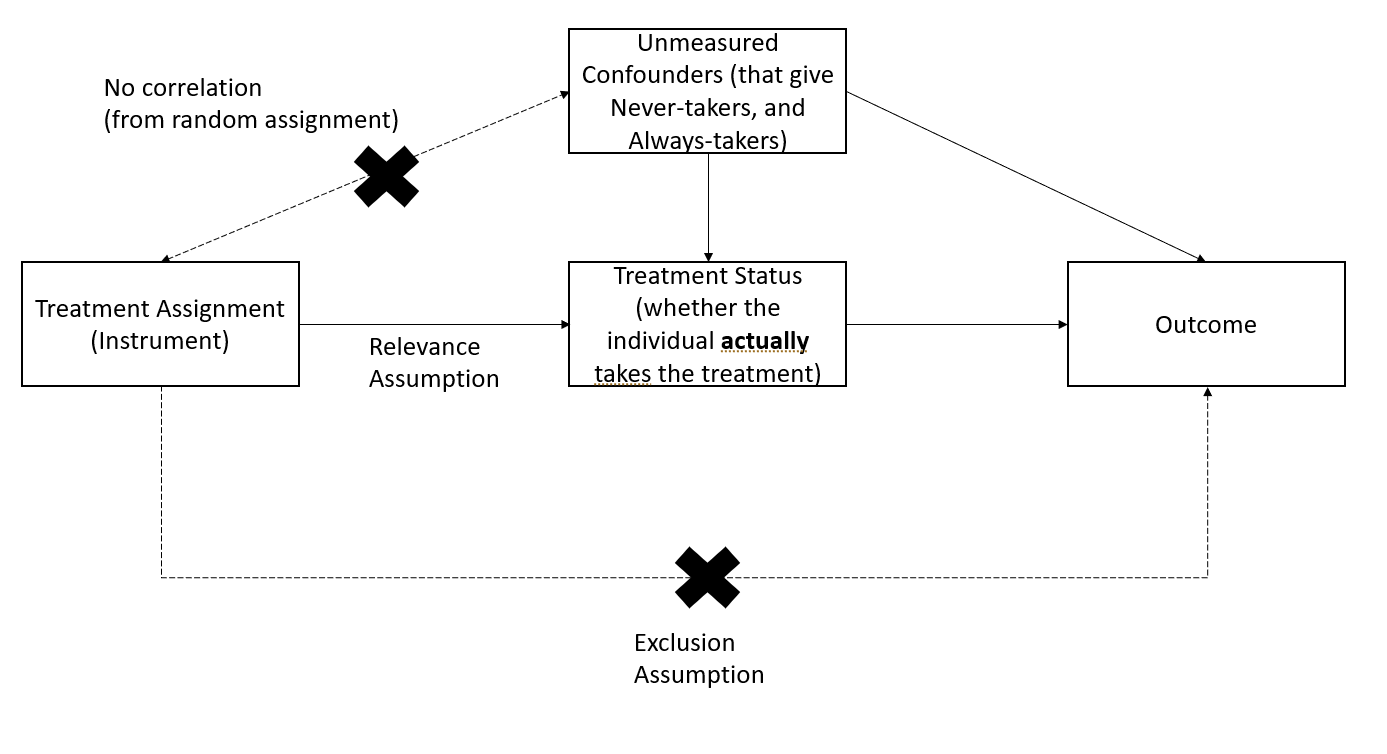
\includegraphics[width=0.9\linewidth,alt={Flow chart showing relationships between treatment assignment instrument, unmeasured confounders, treatment status, and outcome with key IV assumptions marked.}]{images/iv_late} 

}

\caption{Instrumental-variables setup for the local average treatment effect, with treatment assignment as an instrument for actual treatment receipt.}\label{fig:iv-late}
\end{figure}

From an instrumental variables perspective, LATE is estimated as:

\[
LATE = \frac{ITT}{\text{Share of Compliers}}
\]

where:

\begin{itemize}
\item
  \textbf{ITT (Intention-to-Treat Effect)} is the effect of being assigned to treatment.
\item
  \textbf{Share of Compliers} is the proportion of individuals who actually take the treatment when assigned to it.
\end{itemize}

\subsubsection{Key Properties of LATE}\label{key-properties-of-late}

\begin{itemize}
\tightlist
\item
  As the proportion of compliers increases, \hyperref[sec-local-average-treatment-effects]{LATE} converges to \hyperref[sec-intention-to-treat-effect]{ITT}.
\item
  \hyperref[sec-local-average-treatment-effects]{LATE} is always larger than \hyperref[sec-intention-to-treat-effect]{ITT}, since \hyperref[sec-intention-to-treat-effect]{ITT} averages over both compliers and non-compliers.
\item
  Standard error rule of thumb:

  \begin{itemize}
  \item
    The standard error of \hyperref[sec-local-average-treatment-effects]{LATE} is given by:

    \[
    SE(LATE) = \frac{SE(ITT)}{\text{Share of Compliers}}
    \]
  \end{itemize}
\item
  LATE can also be estimated using a pure placebo group \citep{gerber2010}.
\item
  Partial compliance is difficult to study
\item
  The IV/2SLS estimator is biased in small samples, requiring Bayesian methods for correction \citep{long2010, jin2009, jin2008}.
\end{itemize}

\begin{center}\rule{0.5\linewidth}{0.5pt}\end{center}

\subsubsection{One-Sided Noncompliance}\label{one-sided-noncompliance}

One-sided noncompliance occurs when we observe only compliers and never-takers in the sample (i.e., no always-takers).

\paragraph{Key assumptions}\label{key-assumptions}

\begin{itemize}
\item
  Exclusion Restriction (Excludability): Never-takers have the same outcomes regardless of assignment (i.e., treatment has no effect on them because they never receive it).
\item
  Random Assignment Ensures Balance: The number of never-takers is expected to be equal in the treatment and control groups.
\end{itemize}

Estimation of LATE under one-sided noncompliance:

\[
LATE = \frac{ITT}{\text{Share of Compliers}}
\]

Since the never-takers do not receive treatment, this simplifies estimation.

\begin{center}\rule{0.5\linewidth}{0.5pt}\end{center}

\subsubsection{Two-Sided Noncompliance}\label{two-sided-noncompliance}

Two-sided noncompliance occurs when we observe \textbf{compliers, never-takers, and always-takers} in the sample.

\paragraph{Key assumptions}\label{key-assumptions-1}

\begin{itemize}
\item
  Exclusion Restriction (Excludability): Never-takers and always-takers have the same outcome \textbf{regardless of treatment assignment}.
\item
  \textbf{Monotonicity Assumption} (No Defiers):

  \begin{itemize}
  \item
    There are no defiers, meaning no individuals systematically avoid treatment when assigned to it.
  \item
    This assumption is standard in practical studies.
  \end{itemize}
\end{itemize}

Estimation of LATE under two-sided noncompliance:

\[
LATE = \frac{ITT}{\text{Share of Compliers}}
\]

\begin{itemize}
\tightlist
\item
  Since always-takers receive treatment regardless of assignment, their presence does not bias LATE as long as monotonicity holds.
\item
  In practice, monotonicity is often reasonable, as defiers are rare.
\end{itemize}

\begin{longtable}[]{@{}
  >{\raggedright\arraybackslash}p{(\linewidth - 6\tabcolsep) * \real{0.2644}}
  >{\raggedright\arraybackslash}p{(\linewidth - 6\tabcolsep) * \real{0.1923}}
  >{\raggedright\arraybackslash}p{(\linewidth - 6\tabcolsep) * \real{0.3269}}
  >{\raggedright\arraybackslash}p{(\linewidth - 6\tabcolsep) * \real{0.2067}}@{}}
\caption{Comparison of Estimands under Treatment Non-Compliance}\tabularnewline
\toprule\noalign{}
\begin{minipage}[b]{\linewidth}\raggedright
\textbf{Scenario}
\end{minipage} & \begin{minipage}[b]{\linewidth}\raggedright
\textbf{What it Measures}
\end{minipage} & \begin{minipage}[b]{\linewidth}\raggedright
\textbf{When to Use It?}
\end{minipage} & \begin{minipage}[b]{\linewidth}\raggedright
\textbf{Key Assumptions}
\end{minipage} \\
\midrule\noalign{}
\endfirsthead
\toprule\noalign{}
\begin{minipage}[b]{\linewidth}\raggedright
\textbf{Scenario}
\end{minipage} & \begin{minipage}[b]{\linewidth}\raggedright
\textbf{What it Measures}
\end{minipage} & \begin{minipage}[b]{\linewidth}\raggedright
\textbf{When to Use It?}
\end{minipage} & \begin{minipage}[b]{\linewidth}\raggedright
\textbf{Key Assumptions}
\end{minipage} \\
\midrule\noalign{}
\endhead
\bottomrule\noalign{}
\endlastfoot
\hyperref[sec-intention-to-treat-effect]{Intention-to-Treat} & Effect of being assigned to treatment & Policy impact with non-compliance & None (preserves randomization) \\
\hyperref[sec-local-average-treatment-effects]{LATE} & Effect on compliers only & When we care about actual treatment effect rather than assignment & Excludability, Monotonicity (No Defiers) \\
\end{longtable}

\begin{center}\rule{0.5\linewidth}{0.5pt}\end{center}

\subsection{Population vs.~Sample Average Treatment Effects}\label{population-vs.-sample-average-treatment-effects}

In experimental and observational studies, we often estimate the \textbf{Sample Average Treatment Effect (SATE)} using a finite sample. However, the \textbf{Population Average Treatment Effect (PATE)} is the parameter of interest when making broader generalizations.

\textbf{Key Issue:}\\
SATE \textbf{does not necessarily equal} PATE due to \textbf{sample selection bias and treatment imbalance}.

See \citep{imai2008} for an in-depth discussion on when SATE diverges from PATE.

\begin{center}\rule{0.5\linewidth}{0.5pt}\end{center}

Consider a \textbf{finite population} of size \(N\) from which we observe a sample of size \(n\) (\(N \gg n\)). Half of the sample receives treatment, and half is assigned to control.

Define the following indicators:

\begin{itemize}
\item
  Sampling Indicator:\\
  \[
    I_i =
    \begin{cases}
    1, & \text{if unit } i \text{ is in the sample} \\
    0, & \text{otherwise}
    \end{cases}
    \]
\item
  Treatment Assignment Indicator:\\
  \[
  T_i =
  \begin{cases}
  1, & \text{if unit } i \text{ is in the treatment group} \\
  0, & \text{if unit } i \text{ is in the control group}
  \end{cases}
  \]
\item
  Potential Outcomes Framework:\\
  \[
  Y_i =
  \begin{cases}
  Y_i(1), & \text{if } T_i = 1 \text{ (Treated)} \\
  Y_i(0), & \text{if } T_i = 0 \text{ (Control)}
  \end{cases}
  \]
\item
  Observed Outcome:\\
  Since we can never observe both potential outcomes for the same unit, the observed outcome is:

  \[
  Y_i | I_i = 1 = T_i Y_i(1) + (1 - T_i) Y_i(0)
  \]
\item
  True Individual Treatment Effect:\\
  The individual-level treatment effect is:

  \[
  TE_i = Y_i(1) - Y_i(0)
  \]
\end{itemize}

However, since we observe only one of \(Y_i(1)\) or \(Y_i(0)\), \(TE_i\) is never directly observed.

\subsubsection{Definitions of SATE and PATE}\label{definitions-of-sate-and-pate}

\begin{itemize}
\item
  \textbf{Sample Average Treatment Effect (SATE):} \[
  SATE = \frac{1}{n} \sum_{i \in \{I_i = 1\}} TE_i
  \] SATE is the \textbf{average treatment effect within the sample}.
\item
  \textbf{Population Average Treatment Effect (PATE):} \[
  PATE = \frac{1}{N} \sum_{i=1}^N TE_i
  \] PATE represents the \textbf{true treatment effect across the entire population}.
\end{itemize}

Since we observe only a subset of the population, SATE \textbf{may not equal} PATE.

\begin{center}\rule{0.5\linewidth}{0.5pt}\end{center}

\subsubsection{Decomposing Estimation Error}\label{decomposing-estimation-error}

The baseline estimator for SATE and PATE is the \textbf{difference in observed means}:

\[
\begin{aligned}
D &= \frac{1}{n/2} \sum_{i \in (I_i = 1, T_i = 1)} Y_i - \frac{1}{n/2} \sum_{i \in (I_i = 1 , T_i = 0)} Y_i \\
&= \text{(Mean of Treated Group)} - \text{(Mean of Control Group)}
\end{aligned}
\]

Define \(\Delta\) as the estimation error (i.e., deviation from the truth), under an additive model:

\[
Y_i(t) = g_t(X_i) + h_t(U_i)
\]

The estimation error is decomposed into

\[
\begin{aligned}
PATE - D = \Delta &= \Delta_S + \Delta_T \\
&= (PATE - SATE) + (SATE - D)\\
&= \text{Sample Selection Bias} + \text{Treatment Imbalance} \\
&= (\Delta_{S_X} + \Delta_{S_U}) + (\Delta_{T_X} + \Delta_{T_U}) \\
&= (\text{Selection on Observables} + \text{Selection on Unobservables}) \\
&+ (\text{Treatment Imbalance in Observables} + \text{Treatment Imbalance in Unobservables})
\end{aligned}
\]

To further illustrate this, we begin by explicitly defining how the total discrepancy \(PATE - D\) separates into different components.

\textbf{Step 1}: From \(PATE - D\) to \(\Delta_S + \Delta_T\)

\[
\underbrace{PATE - D}_{\Delta}
=
\underbrace{(PATE - SATE)}_{\Delta_S}
 +
\underbrace{(SATE - D)}_{\Delta_T}.
\]

\begin{itemize}
\tightlist
\item
  \(PATE - D\): The total discrepancy between the true population treatment effect and the estimate \(D\).
\item
  \(\Delta_S = PATE - SATE\): sample selection bias, how much the sample ATE differs from the population ATE.
\item
  \(\Delta_T = SATE - D\): treatment imbalance, how much the estimated treatment effect deviates from the sample ATE.
\end{itemize}

\textbf{Step 2}: Breaking Bias into Observables and Unobservables

Each bias term can be decomposed into observed (\(X\)) and unobserved (\(U\)) factors:

\[
\Delta_S
= \underbrace{\Delta_{S_X}}_{\text{Selection on Observables}}
+ \underbrace{\Delta_{S_U}}_{\text{Selection on Unobservables}}
\]

\[
\Delta_T
= \underbrace{\Delta_{T_X}}_{\text{Treatment Imbalance in Observables}}
+ \underbrace{\Delta_{T_U}}_{\text{Treatment Imbalance in Unobservables}}
\]

Thus, the final expression:

\[
\begin{aligned}
PATE - D &= \underbrace{(PATE - SATE)}_{\Delta_S:\text{Sample Selection Bias}} 
+ 
\underbrace{(SATE - D)}_{\Delta_T:\text{Treatment Imbalance}} \\
&= \underbrace{(\Delta_{S_X} + \Delta_{S_U})}_{\text{Selection on }X + \text{ Selection on }U}
+
\underbrace{(\Delta_{T_X} + \Delta_{T_U})}_{\text{Imbalance in }X + \text{ Imbalance in }U}.
\end{aligned}
\]

This decomposition clarifies the sources of error in estimating the true effect, distinguishing between sample representativeness (selection bias) and treatment assignment differences (treatment imbalance), and further separating these into observable and unobservable components.

\paragraph{\texorpdfstring{Sample Selection Bias ( \(\Delta_S\) )}{Sample Selection Bias ( \textbackslash Delta\_S )}}\label{sample-selection-bias-delta_s}

Also called sample selection error, this arises when the sample is not representative of the population.

\[
\Delta_S = PATE - SATE = \frac{N - n}{N}(NATE - SATE)
\]

where:

\begin{itemize}
\tightlist
\item
  NATE (Non-Sample Average Treatment Effect) is the average treatment effect for the part of the population not included in the sample:
\end{itemize}

\[
NATE = \sum_{i\in (I_i = 0)} \frac{TE_i}{N-n}
\]

To eliminate sample selection bias (\(\Delta_S = 0\)):

\begin{enumerate}
\def\labelenumi{\arabic{enumi}.}
\tightlist
\item
  Redefine the sample as the entire population (\(N = n\)).
\item
  Ensure \(NATE = SATE\) (e.g., treatment effects must be homogeneous across sampled and non-sampled units).
\end{enumerate}

However, when treatment effects vary across individuals, random sampling only warrants sample selection bias but does not eliminate sample error.

\paragraph{\texorpdfstring{Treatment Imbalance Error ( \(\Delta_T\) )}{Treatment Imbalance Error ( \textbackslash Delta\_T )}}\label{treatment-imbalance-error-delta_t}

Also called treatment imbalance bias, this occurs when the empirical distribution of treated and control units differs.

\[
\Delta_T = SATE - D
\]

\textbf{Key insight}:\\
\(\Delta_T \to 0\) when the treatment and control groups are balanced across both observables (\(X\)) and unobservables (\(U\)).

Since we cannot directly adjust for unobservables, imbalance correction methods focus on observables.

\begin{center}\rule{0.5\linewidth}{0.5pt}\end{center}

\subsubsection{Adjusting for (Observable) Treatment Imbalance}\label{adjusting-for-observable-treatment-imbalance}

However, in real-world studies:

\begin{itemize}
\item
  We can only adjust for observables \(X\), not unobservables \(U\).
\item
  Residual imbalance in unobservables may still introduce bias after adjustment.
\end{itemize}

To address treatment imbalance, researchers commonly use:

\begin{enumerate}
\def\labelenumi{\arabic{enumi}.}
\tightlist
\item
  \hyperref[sec-randomized-block-designs]{Blocking}
\item
  \hyperref[sec-matching-methods]{Matching Methods}
\end{enumerate}

\begin{center}\rule{0.5\linewidth}{0.5pt}\end{center}

\begin{longtable}[]{@{}
  >{\raggedright\arraybackslash}p{(\linewidth - 4\tabcolsep) * \real{0.1367}}
  >{\raggedright\arraybackslash}p{(\linewidth - 4\tabcolsep) * \real{0.3267}}
  >{\raggedright\arraybackslash}p{(\linewidth - 4\tabcolsep) * \real{0.5333}}@{}}
\caption{Comparison of Blocking and Matching Methods for Covariate Balance}\tabularnewline
\toprule\noalign{}
\begin{minipage}[b]{\linewidth}\raggedright
\textbf{Method}
\end{minipage} & \begin{minipage}[b]{\linewidth}\raggedright
\textbf{\hyperref[sec-randomized-block-designs]{Blocking}}
\end{minipage} & \begin{minipage}[b]{\linewidth}\raggedright
\textbf{\hyperref[sec-matching-methods]{Matching Methods}}
\end{minipage} \\
\midrule\noalign{}
\endfirsthead
\toprule\noalign{}
\begin{minipage}[b]{\linewidth}\raggedright
\textbf{Method}
\end{minipage} & \begin{minipage}[b]{\linewidth}\raggedright
\textbf{\hyperref[sec-randomized-block-designs]{Blocking}}
\end{minipage} & \begin{minipage}[b]{\linewidth}\raggedright
\textbf{\hyperref[sec-matching-methods]{Matching Methods}}
\end{minipage} \\
\midrule\noalign{}
\endhead
\bottomrule\noalign{}
\endlastfoot
\textbf{Definition} & Random assignment within predefined strata based on pre-treatment covariates. & Dropping, repeating, or grouping observations to balance covariates between treated and control groups \citep{rubin1973use}. \\
\textbf{When Applied?} & Before treatment assignment (in experimental designs). & After treatment assignment (in observational studies). \\
\textbf{Effectiveness} & Ensures exact balance within strata but may require large sample sizes for fine stratification. & Can improve balance, but risk of increasing bias if covariates are poorly chosen. \\
\textbf{What If Covariates Are Irrelevant?} & No effect on treatment estimates. & Worst-case scenario: If matching is done on covariates uncorrelated with treatment but correlated with outcomes, it may increase bias instead of reducing it. \\
\textbf{Benefits} & Eliminates imbalance in observables (\(\Delta_{T_X} = 0\)).

Effect on unobservables is uncertain (may help if unobservables correlate with observables). & Reduces model dependence, bias, variance, and mean-squared error (MSE).

Matching only balances observables, and its effect on unobservables is unknown. \\
\end{longtable}

\begin{center}\rule{0.5\linewidth}{0.5pt}\end{center}

\subsection{Average Treatment Effects on the Treated and Control}\label{average-treatment-effects-on-the-treated-and-control}

In many empirical studies, researchers are interested in how treatment affects \textbf{specific subpopulations} rather than the entire population. Two commonly used treatment effect measures are:

\begin{enumerate}
\def\labelenumi{\arabic{enumi}.}
\tightlist
\item
  \textbf{Average Treatment Effect on the Treated} (ATT): The effect of treatment on individuals who actually received treatment.
\item
  \textbf{Average Treatment Effect on the Control} (ATC): The effect treatment would have had on individuals who were not treated.
\end{enumerate}

Understanding the distinction between ATT, ATC, and ATE is crucial for determining \hyperref[sec-external-validity]{external validity} and for designing targeted policies.

\begin{center}\rule{0.5\linewidth}{0.5pt}\end{center}

\subsubsection{Average Treatment Effect on the Treated}\label{sec-average-treatment-effect-on-the-treated}

The \textbf{ATT} measures the expected treatment effect \textbf{only for those who were actually treated}:

\[
\begin{aligned}
ATT &= E[Y_i(1) - Y_i(0) | D_i = 1] \\
&= E[Y_i(1) | D_i = 1] - E[Y_i(0) | D_i = 1]
\end{aligned}
\]

\paragraph{Key Interpretation}\label{key-interpretation}

\begin{itemize}
\item
  ATT tells us how much better (or worse) off treated individuals are compared to their hypothetical counterfactual outcome (had they not been treated).
\item
  It is useful for evaluating the effectiveness of interventions on those who self-select into treatment.
\end{itemize}

\subsubsection{Average Treatment Effect on the Control}\label{sec-average-treatment-effect-on-the-control}

The \textbf{ATC} measures the expected treatment effect \textbf{only for those who were not treated}:

\[
\begin{aligned}
ATC &= E[Y_i(1) - Y_i(0) | D_i = 0] \\
&= E[Y_i(1) | D_i = 0] - E[Y_i(0) | D_i = 0]
\end{aligned}
\]

\paragraph{Key Interpretation}\label{key-interpretation-1}

\begin{itemize}
\item
  ATC answers the question: ``What would have been the effect of treatment if it had been given to those who were not treated?''
\item
  It is important for understanding how an intervention might generalize to untreated populations.
\end{itemize}

\subsubsection{Relationship Between ATT, ATC, and ATE}\label{relationship-between-att-atc-and-ate}

Under \textbf{random assignment and full compliance}, we have:

\[
ATE = ATT = ATC
\]

\textbf{Why?}

\begin{itemize}
\item
  Randomization ensures that treated and untreated groups are statistically identical before treatment.
\item
  Thus, treatment effects are the same across groups, leading to ATT = ATC = ATE.
\end{itemize}

However, in observational settings, selection bias and treatment heterogeneity may cause ATT and ATC to diverge from ATE.

\begin{center}\rule{0.5\linewidth}{0.5pt}\end{center}

\subsubsection{Sample Average Treatment Effect on the Treated}\label{sec-sample-average-treatment-effect-on-the-treated}

The \textbf{Sample ATT (SATT)} is the empirical estimate of ATT in a finite sample:

\[
SATT = \frac{1}{n} \sum_{i \in D_i = 1} TE_i
\]

where:

\begin{itemize}
\item
  \(TE_i = Y_i(1) - Y_i(0)\) is the treatment effect for unit \(i\).
\item
  \(n\) is the number of treated units in the sample.
\item
  The summation is taken only over treated units in the sample.
\end{itemize}

\subsubsection{Population Average Treatment Effect on the Treated}\label{sec-population-average-treatment-effect-on-the-treated}

The \textbf{Population ATT (PATT)} generalizes ATT to the entire treated population:

\[
PATT = \frac{1}{N} \sum_{i \in D_i = 1} TE_i
\]

where:

\begin{itemize}
\item
  \(TE_i = Y_i(1) - Y_i(0)\) is the treatment effect for unit \(i\).
\item
  \(N\) is the total number of treated units in the population.
\item
  The summation is taken over all treated individuals in the population.
\end{itemize}

If the sample is randomly drawn, then \(SATT \approx PATT\), but if the sample is not representative, \(SATT\) may overestimate or underestimate \(PATT\).

\begin{center}\rule{0.5\linewidth}{0.5pt}\end{center}

\subsubsection{When ATT and ATC Diverge from ATE}\label{when-att-and-atc-diverge-from-ate}

In real-world studies, ATT and ATC often differ from ATE due to treatment effect heterogeneity and selection bias.

\paragraph{Selection Bias in ATT}\label{selection-bias-in-att}

If individuals self-select into treatment, then the treated group may be systematically different from the control group.

\begin{itemize}
\tightlist
\item
  Example:

  \begin{itemize}
  \tightlist
  \item
    Suppose a job training program is voluntary.
  \item
    Individuals who enroll might be more motivated or have better skills than those who do not.
  \item
    As a result, the treatment effect (ATT) may not generalize to the untreated group (ATC).
  \end{itemize}
\end{itemize}

This implies:

\[
ATT \neq ATC
\]

unless treatment assignment is random.

\paragraph{Treatment Effect Heterogeneity}\label{treatment-effect-heterogeneity}

If treatment effects vary across individuals, then:

\begin{itemize}
\tightlist
\item
  ATT may be larger or smaller than ATE, depending on how treatment effects differ across subgroups.
\item
  ATC may be larger or smaller than ATT, if the untreated group would have responded differently to treatment.
\end{itemize}

\textbf{Example:}

\begin{itemize}
\item
  A scholarship program may be more beneficial for students from lower-income families than for students from wealthier backgrounds.
\item
  If lower-income students are more likely to apply for the scholarship, then ATT \textgreater{} ATE.
\item
  However, if wealthier students (who did not receive the scholarship) would have benefited less from it, then ATC \textless{} ATE.
\end{itemize}

Thus, we may observe:

\[
ATE \neq ATT \neq ATC
\]

\begin{longtable}[]{@{}
  >{\raggedright\arraybackslash}p{(\linewidth - 6\tabcolsep) * \real{0.1971}}
  >{\raggedright\arraybackslash}p{(\linewidth - 6\tabcolsep) * \real{0.2788}}
  >{\raggedright\arraybackslash}p{(\linewidth - 6\tabcolsep) * \real{0.3077}}
  >{\raggedright\arraybackslash}p{(\linewidth - 6\tabcolsep) * \real{0.2067}}@{}}
\caption{Comparison of Treatment Effect Estimands: ATE, ATT, and ATC}\tabularnewline
\toprule\noalign{}
\begin{minipage}[b]{\linewidth}\raggedright
\textbf{Treatment Effect}
\end{minipage} & \begin{minipage}[b]{\linewidth}\raggedright
\textbf{Definition}
\end{minipage} & \begin{minipage}[b]{\linewidth}\raggedright
\textbf{Use Case}
\end{minipage} & \begin{minipage}[b]{\linewidth}\raggedright
\textbf{Potential Issues}
\end{minipage} \\
\midrule\noalign{}
\endfirsthead
\toprule\noalign{}
\begin{minipage}[b]{\linewidth}\raggedright
\textbf{Treatment Effect}
\end{minipage} & \begin{minipage}[b]{\linewidth}\raggedright
\textbf{Definition}
\end{minipage} & \begin{minipage}[b]{\linewidth}\raggedright
\textbf{Use Case}
\end{minipage} & \begin{minipage}[b]{\linewidth}\raggedright
\textbf{Potential Issues}
\end{minipage} \\
\midrule\noalign{}
\endhead
\bottomrule\noalign{}
\endlastfoot
\textbf{ATE (Average Treatment Effect)} & Effect on randomly selected individuals & Policy decisions applicable to entire population & Requires full randomization \\
\textbf{ATT (Average Treatment on Treated)} & Effect on those who received treatment & Evaluating effectiveness of interventions for targeted groups & Selection bias if treatment is voluntary \\
\textbf{ATC (Average Treatment on Control)} & Effect if treatment were given to untreated individuals & Predicting treatment effects for new populations & May not be generalizable \\
\end{longtable}

\begin{center}\rule{0.5\linewidth}{0.5pt}\end{center}

\subsection{Quantile Average Treatment Effects}\label{sec-quantile-average-treatment-effects}

Instead of focusing on the mean effect (\hyperref[sec-average-treatment-effect]{ATE}), Quantile Treatment Effects (QTE) help us understand how treatment shifts the entire distribution of an outcome variable.

The Quantile Treatment Effect at quantile \(\tau\) is defined as:

\[
QTE_{\tau} = Q_{\tau} (Y_1) - Q_{\tau} (Y_0)
\]

where:

\begin{itemize}
\item
  \(Q_{\tau} (Y_1)\) is the \(\tau\)-th quantile of the outcome distribution \textbf{under treatment}.
\item
  \(Q_{\tau} (Y_0)\) is the \(\tau\)-th quantile of the outcome distribution \textbf{under control}.
\end{itemize}

\subsubsection{When to Use QTE?}\label{when-to-use-qte}

\begin{itemize}
\tightlist
\item
  Heterogeneous Treatment Effects: If treatment effects differ across individuals, ATE may be misleading.
\item
  Policy Targeting: Policymakers may care more about low-income individuals (e.g., bottom 25\%) rather than the average effect.
\item
  Distributional Changes: QTE allows us to assess whether treatment increases inequality (e.g., benefits the rich more than the poor).
\end{itemize}

\subsubsection{Estimation of QTE}\label{estimation-of-qte}

QTE can be estimated using:

\begin{itemize}
\item
  Quantile Regression: Extends linear regression to estimate effects at different quantiles.
\item
  \hyperref[sec-instrumental-variables]{Instrumental Variables} for QTE: Requires additional assumptions to estimate causal effects in the presence of endogeneity \citep{abadie2002instrumental, chernozhukov2005iv}.
\end{itemize}

\subsubsection{Example: Wage Policy Impact}\label{example-wage-policy-impact}

\begin{itemize}
\tightlist
\item
  Suppose a minimum wage increase is introduced.
\item
  The ATE might show a small positive effect on earnings.
\item
  However, QTE might reveal:

  \begin{itemize}
  \tightlist
  \item
    No effect at the bottom quantiles (for workers who lose jobs).
  \item
    A positive effect at the median.
  \item
    A strong positive effect at the top quantiles (for experienced workers who benefit the most).
  \end{itemize}
\end{itemize}

Thus, QTE provides a more detailed view of the treatment effect across the entire income distribution.

\begin{center}\rule{0.5\linewidth}{0.5pt}\end{center}

\subsection{Log-Odds Treatment Effects for Binary Outcomes}\label{sec-log-odds-treatment-effects-for-binary-outcomes}

When the \textbf{outcome variable is binary} (e.g., success/failure, employed/unemployed, survived/died), it is often useful to measure the treatment effect in \textbf{log-odds form}.

For a binary outcome \(Y\), define the \textbf{probability of success} as:

\[
P(Y = 1 | D = d)
\]

The \textbf{log-odds of success} under treatment and control are:

\[
\text{Log-odds}(Y | D = 1) = \log \left( \frac{P(Y = 1 | D = 1)}{1 - P(Y = 1 | D = 1)} \right)
\]

\[
\text{Log-odds}(Y | D = 0) = \log \left( \frac{P(Y = 1 | D = 0)}{1 - P(Y = 1 | D = 0)} \right)
\]

The \textbf{Log-Odds Treatment Effect (LOTE)} is then:

\[
LOTE = \text{Log-odds}(Y | D = 1) - \text{Log-odds}(Y | D = 0)
\]

This captures how treatment \textbf{affects the relative likelihood} of success in a nonlinear way.

\subsubsection{When to Use Log-Odds Treatment Effects?}\label{when-to-use-log-odds-treatment-effects}

\begin{itemize}
\tightlist
\item
  Binary Outcomes: When the treatment outcome is 0 or 1 (e.g., employed/unemployed).
\item
  Nonlinear Treatment Effects: Log-odds help handle situations where effects are multiplicative rather than additive.
\item
  Rare Events: Useful in cases where the outcome probability is very small or very large.
\end{itemize}

\subsubsection{Estimation of Log-Odds Treatment Effects}\label{estimation-of-log-odds-treatment-effects}

\begin{itemize}
\item
  Logistic Regression with Treatment Indicator: \[
  \log \left( \frac{P(Y = 1 | D = 1)}{1 - P(Y = 1 | D = 1)} \right) = \beta_0 + \beta_1 D
  \] where \(\beta_1\) represents the \textbf{log-odds treatment effect}.
\item
  Randomization-Based Estimation: \citet{freedman2008randomization} provides a framework for randomized trials that ensures consistent estimation.
\item
  Attributable Effects: Alternative methods, such as those in \citep{rosenbaum2002attributing}, estimate the proportion of cases attributable to the treatment.
\end{itemize}

\begin{center}\rule{0.5\linewidth}{0.5pt}\end{center}

\subsection{Summary Table: Treatment Effect Estimands}\label{summary-table-treatment-effect-estimands}

\begin{longtable}[]{@{}
  >{\raggedright\arraybackslash}p{(\linewidth - 8\tabcolsep) * \real{0.2064}}
  >{\raggedright\arraybackslash}p{(\linewidth - 8\tabcolsep) * \real{0.2255}}
  >{\raggedright\arraybackslash}p{(\linewidth - 8\tabcolsep) * \real{0.1830}}
  >{\raggedright\arraybackslash}p{(\linewidth - 8\tabcolsep) * \real{0.2064}}
  >{\raggedright\arraybackslash}p{(\linewidth - 8\tabcolsep) * \real{0.1723}}@{}}
\caption{Treatment Effect Estimands}\tabularnewline
\toprule\noalign{}
\begin{minipage}[b]{\linewidth}\raggedright
\textbf{Treatment Effect}
\end{minipage} & \begin{minipage}[b]{\linewidth}\raggedright
\textbf{Definition}
\end{minipage} & \begin{minipage}[b]{\linewidth}\raggedright
\textbf{Use Case}
\end{minipage} & \begin{minipage}[b]{\linewidth}\raggedright
\textbf{Key Assumptions}
\end{minipage} & \begin{minipage}[b]{\linewidth}\raggedright
\textbf{When It Differs from ATE?}
\end{minipage} \\
\midrule\noalign{}
\endfirsthead
\toprule\noalign{}
\begin{minipage}[b]{\linewidth}\raggedright
\textbf{Treatment Effect}
\end{minipage} & \begin{minipage}[b]{\linewidth}\raggedright
\textbf{Definition}
\end{minipage} & \begin{minipage}[b]{\linewidth}\raggedright
\textbf{Use Case}
\end{minipage} & \begin{minipage}[b]{\linewidth}\raggedright
\textbf{Key Assumptions}
\end{minipage} & \begin{minipage}[b]{\linewidth}\raggedright
\textbf{When It Differs from ATE?}
\end{minipage} \\
\midrule\noalign{}
\endhead
\bottomrule\noalign{}
\endlastfoot
\hyperref[sec-average-treatment-effect]{Average Treatment Effect} & The expected treatment effect for a randomly chosen individual in the population. & General policy evaluation; measures the overall impact. & Randomization or strong ignorability (treatment assignment independent of potential outcomes). & - \\
\hyperref[sec-conditional-average-treatment-effect-]{Conditional Average Treatment Effect} & The treatment effect for a specific subgroup of the population, conditional on covariates \(X\). & Identifies heterogeneous effects; useful for targeted interventions. & Treatment effect heterogeneity must exist. & Differs when treatment effects vary across subgroups. \\
\hyperref[sec-intention-to-treat-effect]{Intention-to-Treat Effect} & The effect of being assigned to treatment, regardless of actual compliance. & Policy evaluations where non-compliance exists. & Randomized treatment assignment ensures unbiased estimation. & Lower than ATE when not all assigned individuals comply. \\
\hyperref[sec-local-average-treatment-effects]{Local Average Treatment Effect} & \multicolumn{4}{>{\raggedright\arraybackslash}p{(\linewidth - 8\tabcolsep) * \real{0.7872} + 6\tabcolsep}@{}}{%
The effect of treatment only on compliers, those who take the treatment if and only if assigned to it. \textbar{} When compliance is imperfect, LATE isolates the effect for compliers. \textbar{} Monotonicity (no defiers); instrument only affects the outcome through treatment. \textbar{} Differs from ATE when compliance is selective. \textbar{}} \\
\hyperref[sec-average-treatment-effect-on-the-treated]{Average Treatment Effect on the Treated} & The effect of treatment on those who actually received the treatment. & Used when assessing effectiveness of a treatment for those who self-select into it. & No unmeasured confounders within the treated group. & Differs when treatment selection is not random. \\
\hyperref[sec-average-treatment-effect-on-the-control]{Average Treatment Effect on the Control} & The effect the treatment would have had on individuals who were not treated. & Predicts the effect of expanding a program to the untreated population. & No unmeasured confounders within the control group. & Differs when treatment effects are heterogeneous. \\
\hyperref[sec-sample-average-treatment-effect-on-the-treated]{Sample Average Treatment Effect} & The estimated treatment effect in the sample. & Used when evaluating treatment within a specific sample. & Sample must be representative of the population for external validity. & Differs when the sample is not representative of the population. \\
\hyperref[sec-population-average-treatment-effect-on-the-treated]{Population Average Treatment Effect} & The expected treatment effect for the entire population. & Policy design and large-scale decision-making. & Requires that sample selection is random. & Differs when sample selection bias exists. \\
\hyperref[sec-quantile-average-treatment-effects]{Quantile Treatment Effect} & The treatment effect at a specific percentile of the outcome distribution. & Understanding distributional effects rather than mean effects. & Rank preservation or monotonicity assumptions may be needed. & Differs when treatment effects vary across outcome quantiles. \\
\hyperref[sec-log-odds-treatment-effects-for-binary-outcomes]{Log-Odds Treatment Effect} & The effect of treatment on binary outcomes, expressed in log-odds. & Used when outcomes are dichotomous (e.g., employed/unemployed, survived/died). & Logistic model assumptions must hold. & Differs when treatment effects are nonlinear or outcome probabilities are low. \\
\end{longtable}

\part*{A. EXPERIMENTAL DESIGN}\label{part-a.-experimental-design}
\addcontentsline{toc}{part}{A. EXPERIMENTAL DESIGN}

\chapter{Experimental Design}\label{sec-experimental-design}

This chapter provides a treatment of experimental design principles, focusing on their application in business experiments such as A/B testing, consumer behavior studies, and market research. It begins by defining key terms and explaining why randomization is the gold standard for establishing causal relationships. The chapter covers both classical and advanced designs, including completely randomized designs, factorial designs, and crossover trials. It also delves into the selection problem and the consequences of bias. Topics such as blocking, stratification, and factorial manipulation are discussed with an emphasis on practical implementation. Statistical notation is introduced to describe treatment allocation mechanisms, and visual diagrams help clarify complex ideas. Emerging research trends and limitations of traditional designs are also explored to prepare readers for real-world complexities.

Imagine you're a marketing manager trying to decide whether a new advertising campaign will boost sales. Or perhaps you're an economist investigating the impact of tax incentives on consumer spending. In both cases, you need a way to determine causal effects, not just correlations. This is where experimental design becomes essential.

At its core, experimental design ensures that studies are conducted efficiently and that valid conclusions can be drawn. In business applications, experiments help quantify the effects of pricing strategies, marketing tactics, and financial interventions. A well-designed experiment reduces bias, controls variability, and maximizes the accuracy of causal inferences.

\begin{center}\rule{0.5\linewidth}{0.5pt}\end{center}

\section{Principles of Experimental Design}\label{principles-of-experimental-design}

A well-designed experiment follows three key principles:

\begin{enumerate}
\def\labelenumi{\arabic{enumi}.}
\tightlist
\item
  Randomization: Ensures that subjects or experimental units are assigned to different groups randomly, eliminating selection bias.
\item
  Replication: Increases the precision of estimates by repeating the experiment on multiple subjects.
\item
  Control: Isolates the effect of treatments by using control groups or baseline conditions to minimize confounding factors.
\end{enumerate}

In addition to these, \textbf{blocking} and \textbf{factorial designs} further refine experimental accuracy.

\begin{center}\rule{0.5\linewidth}{0.5pt}\end{center}

\section{The Gold Standard: Randomized Controlled Trials}\label{sec-the-gold-standard-randomized-controlled-trials}

Randomized Controlled Trials (RCTs) are the \textbf{holy grail of causal inference}. Their power comes from \textbf{random assignment}, which ensures that any differences between treatment and control groups arise \textbf{only} due to the intervention.

RCTs provide:

\begin{itemize}
\tightlist
\item
  \textbf{Unbiased estimates} of treatment effects
\item
  \textbf{Elimination of confounding factors on average} (although covariate imbalance can occur, necessitating techniques like \hyperref[sec-re-randomization]{Rerandomization} to achieve a ``platinum standard'' set by \citet{tukey1993tightening})
\end{itemize}

An RCT consists of two groups:

\begin{enumerate}
\def\labelenumi{\arabic{enumi}.}
\tightlist
\item
  Treatment group: Receives the intervention (e.g., a new marketing campaign, drug, or financial incentive).
\item
  Control group: Does not receive the intervention, serving as a baseline.
\end{enumerate}

Subjects from the same population are randomly assigned to either group. This randomization ensures that any observed differences in outcomes are due solely to the treatment, not external factors.

However, RCTs are easier to conduct in \textbf{hard sciences} (e.g., medicine or physics), where treatments and environments can be tightly controlled. In \textbf{social sciences}, challenges arise because:

\begin{itemize}
\tightlist
\item
  Human behavior is unpredictable.
\item
  Some treatments are impossible or unethical to introduce (e.g., assigning individuals to poverty).
\item
  Real-world environments are difficult to control.
\end{itemize}

To address these challenges, social scientists use \hyperref[sec-quasi-experimental]{Quasi-Experimental Methods} to approximate experimental conditions.

RCTs establish \hyperref[sec-internal-validity]{internal validity}, meaning that the observed treatment effects are \textbf{causally interpretable}. Even though \textbf{random assignment is not the same as \emph{ceteris paribus}} (holding everything else constant), it achieves a similar effect: \textbf{on average}, treatment and control groups should be comparable.

\begin{center}\rule{0.5\linewidth}{0.5pt}\end{center}

\section{Selection Problem}\label{selection-problem}

A fundamental challenge in causal inference is that we never observe both potential outcomes for the same individual, only one or the other. This creates the selection problem, which we formalize below.

Assume we have:

\begin{itemize}
\tightlist
\item
  A \textbf{binary treatment variable}:\\
  \(D_i \in \{0,1\}\), where:

  \begin{itemize}
  \tightlist
  \item
    \(D_i = 1\) indicates that individual \(i\) receives the treatment.
  \item
    \(D_i = 0\) indicates that individual \(i\) does \textbf{not} receive the treatment.
  \end{itemize}
\item
  The \textbf{outcome of interest}:\\
  \(Y_i\), which depends on whether the individual is treated or not:

  \begin{itemize}
  \tightlist
  \item
    \(Y_{0i}\): The outcome \textbf{if not treated}.
  \item
    \(Y_{1i}\): The outcome \textbf{if treated}.
  \end{itemize}
\end{itemize}

Thus, the \textbf{potential outcomes framework} is defined as:

\[
\text{Potential Outcome} =
\begin{cases}
Y_{1i}, & \text{if } D_i = 1 \quad (\text{Treated}) \\
Y_{0i}, & \text{if } D_i = 0 \quad (\text{Untreated})
\end{cases}
\]

However, we only \textbf{observe} one outcome per individual:

\[
Y_i = Y_{0i} + (Y_{1i} - Y_{0i})D_i
\]

This means that for any given person, we either observe \(Y_{1i}\) or \(Y_{0i}\), but \textbf{never both}. Since we cannot observe counterfactuals (unless we invent a time machine), we must rely on statistical inference to estimate treatment effects.

\subsection{The Observed Difference in Outcomes}\label{the-observed-difference-in-outcomes}

The goal is to estimate the difference in expected outcomes between treated and untreated individuals:

\[
E[Y_i | D_i = 1] - E[Y_i | D_i = 0]
\]

Expanding this equation:

\[
\begin{aligned}
E[Y_i | D_i = 1] - E[Y_i | D_i = 0] &= (E[Y_{1i} | D_i = 1] - E[Y_{0i}|D_i = 1] ) \\
&+ (E[Y_{0i} |D_i = 1] - E[Y_{0i} |D_i = 0]) \\
&= (E[Y_{1i}-Y_{0i}|D_i = 1] ) \\
&+ (E[Y_{0i} |D_i = 1] - E[Y_{0i} |D_i = 0])
\end{aligned}
\]

This equation decomposes the \textbf{observed difference} into two components:

\begin{itemize}
\item
  Treatment Effect on the Treated: \(E[Y_{1i} - Y_{0i} |D_i = 1]\), which represents the causal impact of the treatment on those who are treated.
\item
  Selection Bias:\\
  \(E[Y_{0i} |D_i = 1] - E[Y_{0i} |D_i = 0]\), which captures systematic differences between treated and untreated groups \textbf{even in the absence of treatment}.
\end{itemize}

Thus, the \textbf{observed difference in outcomes} is:

\[
\text{Observed Difference} = \text{ATT} + \text{Selection Bias}
\]

\subsection{Eliminating Selection Bias with Random Assignment}\label{eliminating-selection-bias-with-random-assignment}

With \textbf{random assignment} of treatment, \(D_i\) is independent of potential outcomes:

\[
E[Y_i | D_i = 1] - E[Y_i|D_i = 0] = E[Y_{1i} - Y_{0i}]
\]

This works because, under true randomization:

\[
E[Y_{0i} | D_i = 1] = E[Y_{0i} | D_i = 0]
\]

which eliminates selection bias. Consequently, the observed difference now \textbf{directly estimates the true causal effect}:

\[
E[Y_i | D_i = 1] - E[Y_i | D_i = 0] = E[Y_{1i} - Y_{0i}]
\]

Thus, \hyperref[sec-the-gold-standard-randomized-controlled-trials]{randomized controlled trials} provide an unbiased estimate of the \hyperref[sec-average-treatment-effect]{average treatment effect}.

\begin{center}\rule{0.5\linewidth}{0.5pt}\end{center}

\subsection{Another Representation Under Regression}\label{another-representation-under-regression}

So far, we have framed the selection problem using expectations and potential outcomes. Another way to represent treatment effects is through \textbf{regression models}, which provide a practical framework for estimation.

Suppose the treatment effect is constant across individuals:

\[
Y_{1i} - Y_{0i} = \rho
\]

This implies that each treated individual experiences the same treatment effect (\(\rho\)), though their baseline outcomes (\(Y_{0i}\)) may vary.

Since we only observe \textbf{one} of the potential outcomes, the observed outcome can be expressed as:

\[
\begin{aligned}
Y_i &= E(Y_{0i}) + (Y_{1i} - Y_{0i}) D_i + [Y_{0i} - E(Y_{0i})] \\
&= \alpha + \rho D_i + \eta_i
\end{aligned}
\]

where:

\begin{itemize}
\tightlist
\item
  \(\alpha = E(Y_{0i})\), the expected outcome for untreated individuals.
\item
  \(\rho\) represents the \textbf{causal treatment effect}.
\item
  \(\eta_i = Y_{0i} - E(Y_{0i})\), capturing individual deviations from the mean untreated outcome.
\end{itemize}

Thus, the regression model provides an intuitive way to express treatment effects.

\subsubsection{Conditional Expectations and Selection Bias}\label{conditional-expectations-and-selection-bias}

Taking expectations conditional on treatment status:

\[
\begin{aligned}
E[Y_i |D_i = 1] &= \alpha + \rho + E[\eta_i |D_i = 1] \\
E[Y_i |D_i = 0] &= \alpha + E[\eta_i |D_i = 0]
\end{aligned}
\]

The observed difference in means between treated and untreated groups is:

\[
E[Y_i |D_i = 1] - E[Y_i |D_i = 0] = \rho + E[\eta_i |D_i = 1] - E[\eta_i |D_i = 0]
\]

Here, the term \(E[\eta_i |D_i = 1] -E[\eta_i |D_i = 0]\) represents the selection bias, the correlation between the regression error term (\(\eta_i\)) and the treatment variable (\(D_i\)).

Under random assignment, we assume that potential outcomes are \textbf{independent} of treatment (\(D_i\)):

\[
E[\eta_i |D_i = 1] -E[\eta_i |D_i = 0] = E[Y_{0i} |D_i = 1] -E[Y_{0i}|D_i = 0] = 0
\]

Thus, under true \textbf{randomization}, selection bias disappears, and the observed difference directly estimates the \textbf{causal effect} \(\rho\).

\begin{center}\rule{0.5\linewidth}{0.5pt}\end{center}

\subsubsection{Controlling for Additional Variables}\label{controlling-for-additional-variables}

In many real-world scenarios, \textbf{random assignment is imperfect}, and selection bias may still exist. To mitigate this, we introduce \textbf{control variables} (\(X_i\)), such as demographic characteristics, firm size, or prior purchasing behavior.

If \(X_i\) is \textbf{uncorrelated with treatment} (\(D_i\)), including it in our regression model does not bias the estimate of \(\rho\) but has two advantages:

\begin{enumerate}
\def\labelenumi{\arabic{enumi}.}
\tightlist
\item
  \textbf{It reduces residual variance} (\(\eta_i\)), improving the precision of \(\rho\).
\item
  \textbf{It accounts for additional sources of variability}, making the model more robust.
\end{enumerate}

Thus, our regression model extends to:

\[
Y_i = \alpha + \rho D_i + X_i'\gamma + \eta_i
\]

where:

\begin{itemize}
\tightlist
\item
  \(X_i\) represents a vector of control variables.
\item
  \(\gamma\) captures the effect of \(X_i\) on the outcome.
\end{itemize}

\subsubsection{Example: Racial Discrimination in Hiring}\label{example-racial-discrimination-in-hiring}

A famous study by \citet{bertrand2004emily} examined racial discrimination in hiring by randomly assigning Black- and White-sounding names to identical job applications. By ensuring that names were assigned randomly, the authors eliminated confounding factors like education and experience, allowing them to estimate the causal effect of race on callback rates.

\begin{center}\rule{0.5\linewidth}{0.5pt}\end{center}

\section{Variance Reduction in Experimental Design}\label{sec-variance-reduction}

Randomization guarantees that a difference in means is an unbiased estimate of the average treatment effect, but it says nothing about precision. When the outcome is noisy, as spend, revenue, session length, or trading profit and loss typically are, we need a large sample to detect even a modest effect. Variance reduction methods attack this problem directly. They adjust the outcome using information that was fixed before randomization, shrinking the standard error without disturbing the expected value of the estimator. In modern online experimentation, these adjustments are among the cheapest and highest return improvements a team can deploy \citep{deng2013improving}.

This section develops the two workhorse adjustments used in practice. CUPED uses a pre-experiment covariate, most often a pre-period version of the same metric. CUPAC generalizes the idea by replacing that covariate with a prediction from a model trained on historical data. Both reduce to regression adjustment, and both connect cleanly to the difference-in-differences logic developed elsewhere in this book.

\begin{center}\rule{0.5\linewidth}{0.5pt}\end{center}

\subsection{CUPED}\label{cuped}

CUPED, an abbreviation for Controlled-experiment Using Pre-Experiment Data, adjusts each unit's outcome by a pre-treatment covariate that is correlated with the outcome but, by construction, independent of the randomized assignment \citep{deng2013improving}. Because the covariate was measured before treatment, subtracting a multiple of it cannot introduce bias, and a well chosen multiple removes predictable noise.

\subsubsection{Setup and notation}\label{setup-and-notation}

Let \(i = 1, \dots, n\) index experimental units, which might be users, customers, or accounts. Treatment assignment is \(T_i \in \{0,1\}\), randomized. The potential outcomes are \(Y_i(1)\) and \(Y_i(0)\), and the observed outcome is \(Y_i = T_i Y_i(1) + (1 - T_i) Y_i(0)\). The pre-experiment covariate \(X_i\) is measured before randomization. The canonical choice is a pre-period version of the outcome, such as last week's spend, though stable assignment dimensions such as device or region can also serve.

The single assumption CUPED requires is that assignment is independent of the covariate,

\[
T_i \perp X_i,
\]

which holds whenever randomization occurs after \(X_i\) is measured and there is no leakage from the experiment back into the covariate.

\subsubsection{The CUPED estimator}\label{the-cuped-estimator}

CUPED defines an adjusted outcome

\[
Y_i^{\text{cuped}} = Y_i - \theta\left(X_i - \mathbb{E}[X]\right),
\]

and estimates the treatment effect by the difference in means of the adjusted outcome,

\[
\hat{\tau}_{\text{cuped}} = \bar{Y}^{\text{cuped}}_1 - \bar{Y}^{\text{cuped}}_0
= \left(\bar{Y}_1 - \bar{Y}_0\right) - \theta\left(\bar{X}_1 - \bar{X}_0\right).
\]

Read in words, CUPED is the ordinary difference in means minus \(\theta\) times any accidental imbalance in the covariate between the two arms. We center \(X_i\) at \(\mathbb{E}[X]\), or at the sample mean \(\bar{X}\) in practice, so that the adjustment does not shift overall levels in a way that interacts with assignment. Centering also gives the intercept a clean interpretation in the regression form below.

\subsubsection{\texorpdfstring{Unbiasedness, even with estimated \(\theta\)}{Unbiasedness, even with estimated \textbackslash theta}}\label{unbiasedness-even-with-estimated-theta}

A natural worry is that subtracting a random quantity might bias the estimate. It does not. Writing

\[
\hat{\tau}_{\text{cuped}} = \hat{\tau}_{\text{diff}} - \theta(\bar{X}_1 - \bar{X}_0),
\]

suppose first that \(\theta\) is a fixed constant, even a poorly chosen one. Under random assignment the expected covariate imbalance is zero, so

\[
\mathbb{E}[\bar{X}_1 - \bar{X}_0] = 0
\quad \Rightarrow \quad
\mathbb{E}[\hat{\tau}_{\text{cuped}}] = \mathbb{E}[\hat{\tau}_{\text{diff}}] = \tau.
\]

CUPED is therefore unbiased for any fixed \(\theta\).

In practice \(\theta\) is estimated, usually by ordinary least squares on the same data. This estimator remains asymptotically unbiased in randomized experiments, and the finite-sample bias is negligible in the large samples typical of A/B tests \citep{deng2013improving, freedman2008regression}. If a stronger guarantee is desired, one can cross-fit \(\theta\), estimating it on one fold and applying it to another so that the adjustment term is conditionally mean zero given the fold-wise coefficient. This is the orthogonalization logic that underlies modern debiased estimation \citep{chernozhukov2018double}.

\subsubsection{\texorpdfstring{Choosing \(\theta\): variance minimization}{Choosing \textbackslash theta: variance minimization}}\label{choosing-theta-variance-minimization}

The coefficient is chosen to minimize the variance of the adjusted outcome. Let \(X_c = X - \mathbb{E}[X]\) denote the centered covariate. Then

\[
\mathrm{Var}(Y - \theta X_c)
= \mathrm{Var}(Y) + \theta^2 \mathrm{Var}(X_c) - 2\theta\,\mathrm{Cov}(Y, X_c).
\]

Differentiating with respect to \(\theta\) and setting the derivative to zero gives

\[
2\theta\, \mathrm{Var}(X_c) - 2\,\mathrm{Cov}(Y, X_c) = 0,
\]

so the variance-minimizing coefficient is

\[
\theta^\star = \frac{\mathrm{Cov}(Y, X_c)}{\mathrm{Var}(X_c)} = \frac{\mathrm{Cov}(Y, X)}{\mathrm{Var}(X)},
\]

where the second equality holds because centering changes neither the variance nor the relevant covariance. This is exactly the slope from regressing \(Y\) on \(X\) in a simple linear regression \citep{deng2013improving}.

The achievable gain follows immediately. With a single covariate, projecting \(Y\) onto \(X\) shrinks the residual variance by a factor \((1 - \rho^2)\), where \(\rho = \mathrm{Cor}(Y, X)\),

\[
\mathrm{Var}(Y^{\text{cuped}}) = \mathrm{Var}(Y)\,(1 - \rho^2).
\]

The standard error then shrinks by \(\sqrt{1 - \rho^2}\), and the sample size required for a fixed power shrinks by roughly \((1 - \rho^2)\). The leverage is substantial. A correlation of \(\rho = 0.6\) gives \(1 - \rho^2 = 0.64\), a 36 percent reduction in variance and a 20 percent reduction in standard error, since \(\sqrt{0.64} = 0.8\).

\subsubsection{Three ways to implement CUPED}\label{three-ways-to-implement-cuped}

There are three equivalent routes to a CUPED estimate. The first transforms the outcome and runs a difference in means. The second runs a regression, also known as ANCOVA, of the outcome on treatment and the centered covariate, which is the recommended default because robust standard errors, multiple covariates, interactions, and clustering all come for free. Under random assignment, ordinary least squares with covariate adjustment is unbiased and typically more precise than the raw difference in means, especially when the covariate predicts the outcome \citep{freedman2008regression}. The third cross-fits the coefficient as a defensive measure against finite-sample dependence between the adjustment and the realized imbalance.

We begin by loading the tools used throughout this section.

\begin{Shaded}
\begin{Highlighting}[]
\FunctionTok{library}\NormalTok{(dplyr)}
\FunctionTok{library}\NormalTok{(ggplot2)}
\FunctionTok{library}\NormalTok{(estimatr)  }\CommentTok{\# lm\_robust() for robust standard errors}
\FunctionTok{library}\NormalTok{(broom)     }\CommentTok{\# tidy model summaries}
\end{Highlighting}
\end{Shaded}

We then simulate an experiment in which a skewed pre-period covariate predicts the outcome, so CUPED has room to help.

\begin{Shaded}
\begin{Highlighting}[]
\FunctionTok{set.seed}\NormalTok{(}\DecValTok{123}\NormalTok{)}

\NormalTok{n  }\OtherTok{\textless{}{-}} \DecValTok{1000}
\NormalTok{X  }\OtherTok{\textless{}{-}} \FunctionTok{rlnorm}\NormalTok{(n, }\AttributeTok{meanlog =} \FloatTok{3.5}\NormalTok{, }\AttributeTok{sdlog =} \FloatTok{0.6}\NormalTok{)  }\CommentTok{\# skewed pre{-}period spend}
\NormalTok{T  }\OtherTok{\textless{}{-}} \FunctionTok{rbinom}\NormalTok{(n, }\DecValTok{1}\NormalTok{, }\FloatTok{0.5}\NormalTok{)}

\NormalTok{tau\_true }\OtherTok{\textless{}{-}} \FloatTok{2.0}

\CommentTok{\# Outcome correlated with X, plus noise and a treatment effect}
\NormalTok{Y }\OtherTok{\textless{}{-}} \FloatTok{0.7} \SpecialCharTok{*}\NormalTok{ X }\SpecialCharTok{+} \FunctionTok{rlnorm}\NormalTok{(n, }\AttributeTok{meanlog =} \FloatTok{2.2}\NormalTok{, }\AttributeTok{sdlog =} \FloatTok{0.7}\NormalTok{) }\SpecialCharTok{+}\NormalTok{ tau\_true }\SpecialCharTok{*}\NormalTok{ T}

\NormalTok{dat }\OtherTok{\textless{}{-}} \FunctionTok{tibble}\NormalTok{(}\AttributeTok{id =} \DecValTok{1}\SpecialCharTok{:}\NormalTok{n, }\AttributeTok{T =}\NormalTok{ T, }\AttributeTok{X =}\NormalTok{ X, }\AttributeTok{Y =}\NormalTok{ Y)}
\FunctionTok{head}\NormalTok{(dat)}
\CommentTok{\#\textgreater{} \# A tibble: 6 x 4}
\CommentTok{\#\textgreater{}      id     T     X     Y}
\CommentTok{\#\textgreater{}   \textless{}int\textgreater{} \textless{}int\textgreater{} \textless{}dbl\textgreater{} \textless{}dbl\textgreater{}}
\CommentTok{\#\textgreater{} 1     1     0  23.7  21.6}
\CommentTok{\#\textgreater{} 2     2     0  28.8  27.5}
\CommentTok{\#\textgreater{} 3     3     0  84.4  63.9}
\CommentTok{\#\textgreater{} 4     4     1  34.5  40.2}
\CommentTok{\#\textgreater{} 5     5     0  35.8  44.8}
\CommentTok{\#\textgreater{} 6     6     1  92.7 107.}
\end{Highlighting}
\end{Shaded}

The correlation between covariate and outcome is the single best predictor of how much CUPED will gain.

\begin{Shaded}
\begin{Highlighting}[]
\FunctionTok{cor}\NormalTok{(dat}\SpecialCharTok{$}\NormalTok{X, dat}\SpecialCharTok{$}\NormalTok{Y)}
\CommentTok{\#\textgreater{} [1] 0.8963476}
\end{Highlighting}
\end{Shaded}

\textbf{Method one: the transformed-outcome form.} We estimate \(\theta^\star\) as the regression slope, build the adjusted outcome, and difference its means.

\begin{Shaded}
\begin{Highlighting}[]
\NormalTok{theta\_hat }\OtherTok{\textless{}{-}} \FunctionTok{with}\NormalTok{(dat, }\FunctionTok{cov}\NormalTok{(X, Y) }\SpecialCharTok{/} \FunctionTok{var}\NormalTok{(X))}
\NormalTok{xbar      }\OtherTok{\textless{}{-}} \FunctionTok{mean}\NormalTok{(dat}\SpecialCharTok{$}\NormalTok{X)}

\NormalTok{dat }\OtherTok{\textless{}{-}}\NormalTok{ dat }\SpecialCharTok{\%\textgreater{}\%}
  \FunctionTok{mutate}\NormalTok{(}
    \AttributeTok{Xc      =}\NormalTok{ X }\SpecialCharTok{{-}}\NormalTok{ xbar,}
    \AttributeTok{Y\_cuped =}\NormalTok{ Y }\SpecialCharTok{{-}}\NormalTok{ theta\_hat }\SpecialCharTok{*}\NormalTok{ Xc}
\NormalTok{  )}

\NormalTok{ate\_naive }\OtherTok{\textless{}{-}} \FunctionTok{with}\NormalTok{(dat, }\FunctionTok{mean}\NormalTok{(Y[T }\SpecialCharTok{==} \DecValTok{1}\NormalTok{]) }\SpecialCharTok{{-}} \FunctionTok{mean}\NormalTok{(Y[T }\SpecialCharTok{==} \DecValTok{0}\NormalTok{]))}
\NormalTok{ate\_cuped }\OtherTok{\textless{}{-}} \FunctionTok{with}\NormalTok{(dat, }\FunctionTok{mean}\NormalTok{(Y\_cuped[T }\SpecialCharTok{==} \DecValTok{1}\NormalTok{]) }\SpecialCharTok{{-}} \FunctionTok{mean}\NormalTok{(Y\_cuped[T }\SpecialCharTok{==} \DecValTok{0}\NormalTok{]))}

\FunctionTok{c}\NormalTok{(}\AttributeTok{ATE\_naive =}\NormalTok{ ate\_naive, }\AttributeTok{ATE\_cuped =}\NormalTok{ ate\_cuped, }\AttributeTok{theta\_hat =}\NormalTok{ theta\_hat)}
\CommentTok{\#\textgreater{} ATE\_naive ATE\_cuped theta\_hat }
\CommentTok{\#\textgreater{} 4.4230877 2.9652137 0.6866728}
\end{Highlighting}
\end{Shaded}

A simple difference-in-means standard error makes the precision gain visible.

\begin{Shaded}
\begin{Highlighting}[]
\NormalTok{se\_diff\_means }\OtherTok{\textless{}{-}} \ControlFlowTok{function}\NormalTok{(y, t) \{}
\NormalTok{  n1 }\OtherTok{\textless{}{-}} \FunctionTok{sum}\NormalTok{(t }\SpecialCharTok{==} \DecValTok{1}\NormalTok{); n0 }\OtherTok{\textless{}{-}} \FunctionTok{sum}\NormalTok{(t }\SpecialCharTok{==} \DecValTok{0}\NormalTok{)}
\NormalTok{  v1 }\OtherTok{\textless{}{-}} \FunctionTok{var}\NormalTok{(y[t }\SpecialCharTok{==} \DecValTok{1}\NormalTok{]); v0 }\OtherTok{\textless{}{-}} \FunctionTok{var}\NormalTok{(y[t }\SpecialCharTok{==} \DecValTok{0}\NormalTok{])}
  \FunctionTok{sqrt}\NormalTok{(v1 }\SpecialCharTok{/}\NormalTok{ n1 }\SpecialCharTok{+}\NormalTok{ v0 }\SpecialCharTok{/}\NormalTok{ n0)}
\NormalTok{\}}

\NormalTok{se\_naive }\OtherTok{\textless{}{-}} \FunctionTok{se\_diff\_means}\NormalTok{(dat}\SpecialCharTok{$}\NormalTok{Y, dat}\SpecialCharTok{$}\NormalTok{T)}
\NormalTok{se\_cuped }\OtherTok{\textless{}{-}} \FunctionTok{se\_diff\_means}\NormalTok{(dat}\SpecialCharTok{$}\NormalTok{Y\_cuped, dat}\SpecialCharTok{$}\NormalTok{T)}

\FunctionTok{tibble}\NormalTok{(}
  \AttributeTok{method  =} \FunctionTok{c}\NormalTok{(}\StringTok{"naive diff{-}in{-}means"}\NormalTok{, }\StringTok{"CUPED transformed outcome"}\NormalTok{),}
  \AttributeTok{ate     =} \FunctionTok{c}\NormalTok{(ate\_naive, ate\_cuped),}
  \AttributeTok{se      =} \FunctionTok{c}\NormalTok{(se\_naive, se\_cuped),}
  \AttributeTok{ci\_low  =} \FunctionTok{c}\NormalTok{(ate\_naive, ate\_cuped) }\SpecialCharTok{{-}} \FloatTok{1.96} \SpecialCharTok{*} \FunctionTok{c}\NormalTok{(se\_naive, se\_cuped),}
  \AttributeTok{ci\_high =} \FunctionTok{c}\NormalTok{(ate\_naive, ate\_cuped) }\SpecialCharTok{+} \FloatTok{1.96} \SpecialCharTok{*} \FunctionTok{c}\NormalTok{(se\_naive, se\_cuped)}
\NormalTok{)}
\CommentTok{\#\textgreater{} \# A tibble: 2 x 5}
\CommentTok{\#\textgreater{}   method                      ate    se ci\_low ci\_high}
\CommentTok{\#\textgreater{}   \textless{}chr\textgreater{}                     \textless{}dbl\textgreater{} \textless{}dbl\textgreater{}  \textless{}dbl\textgreater{}   \textless{}dbl\textgreater{}}
\CommentTok{\#\textgreater{} 1 naive diff{-}in{-}means        4.42 1.27    1.94    6.91}
\CommentTok{\#\textgreater{} 2 CUPED transformed outcome  2.97 0.559   1.87    4.06}
\end{Highlighting}
\end{Shaded}

\textbf{Method two: regression, or ANCOVA, with robust standard errors.} Regressing the outcome on treatment and the centered covariate and reading the coefficient on \(T\) gives the same adjustment in a more flexible package. Robust standard errors are the sensible default in experiments because business metrics are rarely homoskedastic \citep{imbens2015causal}.

\begin{Shaded}
\begin{Highlighting}[]
\NormalTok{fit\_ancova }\OtherTok{\textless{}{-}} \FunctionTok{lm\_robust}\NormalTok{(Y }\SpecialCharTok{\textasciitilde{}}\NormalTok{ T }\SpecialCharTok{+} \FunctionTok{I}\NormalTok{(X }\SpecialCharTok{{-}} \FunctionTok{mean}\NormalTok{(X)), }\AttributeTok{data =}\NormalTok{ dat)  }\CommentTok{\# HC2 robust SE}
\FunctionTok{tidy}\NormalTok{(fit\_ancova) }\SpecialCharTok{\%\textgreater{}\%} \FunctionTok{filter}\NormalTok{(term }\SpecialCharTok{==} \StringTok{"T"}\NormalTok{)}
\CommentTok{\#\textgreater{}   term estimate std.error statistic      p.value conf.low conf.high  df outcome}
\CommentTok{\#\textgreater{} 1    T 2.970065 0.5604399  5.299524 1.429275e{-}07 1.870288  4.069842 997       Y}
\end{Highlighting}
\end{Shaded}

The three estimates sit in the same efficient neighborhood. They are not algebraically identical in finite samples, so small differences are expected.

\begin{Shaded}
\begin{Highlighting}[]
\FunctionTok{tibble}\NormalTok{(}
  \AttributeTok{method   =} \FunctionTok{c}\NormalTok{(}\StringTok{"naive diff{-}in{-}means"}\NormalTok{, }\StringTok{"CUPED transform"}\NormalTok{, }\StringTok{"ANCOVA robust"}\NormalTok{),}
  \AttributeTok{estimate =} \FunctionTok{c}\NormalTok{(ate\_naive, ate\_cuped, }\FunctionTok{coef}\NormalTok{(fit\_ancova)[}\StringTok{"T"}\NormalTok{])}
\NormalTok{)}
\CommentTok{\#\textgreater{} \# A tibble: 3 x 2}
\CommentTok{\#\textgreater{}   method              estimate}
\CommentTok{\#\textgreater{}   \textless{}chr\textgreater{}                  \textless{}dbl\textgreater{}}
\CommentTok{\#\textgreater{} 1 naive diff{-}in{-}means     4.42}
\CommentTok{\#\textgreater{} 2 CUPED transform         2.97}
\CommentTok{\#\textgreater{} 3 ANCOVA robust           2.97}
\end{Highlighting}
\end{Shaded}

\textbf{Method three: cross-fitted CUPED.} Splitting the data into folds and estimating \(\theta\) on the complement of each fold removes any finite-sample dependence between the adjustment coefficient and a given fold's treatment imbalance. In large A/B tests the pooled and cross-fitted estimates are usually almost identical, but the option is cheap insurance.

\begin{Shaded}
\begin{Highlighting}[]
\FunctionTok{set.seed}\NormalTok{(}\DecValTok{456}\NormalTok{)}
\NormalTok{K }\OtherTok{\textless{}{-}} \DecValTok{5}
\NormalTok{dat }\OtherTok{\textless{}{-}}\NormalTok{ dat }\SpecialCharTok{\%\textgreater{}\%}
  \FunctionTok{mutate}\NormalTok{(}\AttributeTok{fold =} \FunctionTok{sample}\NormalTok{(}\FunctionTok{rep}\NormalTok{(}\DecValTok{1}\SpecialCharTok{:}\NormalTok{K, }\AttributeTok{length.out =} \FunctionTok{n}\NormalTok{())))}

\NormalTok{dat }\OtherTok{\textless{}{-}}\NormalTok{ dat }\SpecialCharTok{\%\textgreater{}\%}
  \FunctionTok{group\_by}\NormalTok{(fold) }\SpecialCharTok{\%\textgreater{}\%}
  \FunctionTok{group\_modify}\NormalTok{(}\SpecialCharTok{\textasciitilde{}}\NormalTok{ \{}
\NormalTok{    current\_fold }\OtherTok{\textless{}{-}}\NormalTok{ .y}\SpecialCharTok{$}\NormalTok{fold}
\NormalTok{    train }\OtherTok{\textless{}{-}}\NormalTok{ dat }\SpecialCharTok{\%\textgreater{}\%} \FunctionTok{filter}\NormalTok{(fold }\SpecialCharTok{!=}\NormalTok{ current\_fold)}
\NormalTok{    test  }\OtherTok{\textless{}{-}}\NormalTok{ .x}

\NormalTok{    theta\_k }\OtherTok{\textless{}{-}} \FunctionTok{with}\NormalTok{(train, }\FunctionTok{cov}\NormalTok{(X, Y) }\SpecialCharTok{/} \FunctionTok{var}\NormalTok{(X))}
\NormalTok{    xbar\_k  }\OtherTok{\textless{}{-}} \FunctionTok{mean}\NormalTok{(train}\SpecialCharTok{$}\NormalTok{X)}

\NormalTok{    test }\SpecialCharTok{\%\textgreater{}\%}
      \FunctionTok{mutate}\NormalTok{(}\AttributeTok{Y\_cuped\_cf =}\NormalTok{ Y }\SpecialCharTok{{-}}\NormalTok{ theta\_k }\SpecialCharTok{*}\NormalTok{ (X }\SpecialCharTok{{-}}\NormalTok{ xbar\_k))}
\NormalTok{  \}) }\SpecialCharTok{\%\textgreater{}\%}
  \FunctionTok{ungroup}\NormalTok{()}

\NormalTok{ate\_cuped\_cf }\OtherTok{\textless{}{-}} \FunctionTok{with}\NormalTok{(dat, }\FunctionTok{mean}\NormalTok{(Y\_cuped\_cf[T }\SpecialCharTok{==} \DecValTok{1}\NormalTok{]) }\SpecialCharTok{{-}} \FunctionTok{mean}\NormalTok{(Y\_cuped\_cf[T }\SpecialCharTok{==} \DecValTok{0}\NormalTok{]))}
\NormalTok{se\_cuped\_cf  }\OtherTok{\textless{}{-}} \FunctionTok{se\_diff\_means}\NormalTok{(dat}\SpecialCharTok{$}\NormalTok{Y\_cuped\_cf, dat}\SpecialCharTok{$}\NormalTok{T)}

\FunctionTok{tibble}\NormalTok{(}
  \AttributeTok{method =} \FunctionTok{c}\NormalTok{(}\StringTok{"CUPED (pooled theta)"}\NormalTok{, }\StringTok{"CUPED (cross{-}fitted theta)"}\NormalTok{),}
  \AttributeTok{ate    =} \FunctionTok{c}\NormalTok{(ate\_cuped, ate\_cuped\_cf),}
  \AttributeTok{se     =} \FunctionTok{c}\NormalTok{(se\_cuped, se\_cuped\_cf)}
\NormalTok{)}
\CommentTok{\#\textgreater{} \# A tibble: 2 x 3}
\CommentTok{\#\textgreater{}   method                       ate    se}
\CommentTok{\#\textgreater{}   \textless{}chr\textgreater{}                      \textless{}dbl\textgreater{} \textless{}dbl\textgreater{}}
\CommentTok{\#\textgreater{} 1 CUPED (pooled theta)        2.97 0.559}
\CommentTok{\#\textgreater{} 2 CUPED (cross{-}fitted theta)  2.99 0.559}
\end{Highlighting}
\end{Shaded}

\subsubsection{Multiple covariates as regression residualization}\label{multiple-covariates-as-regression-residualization}

With several pre-treatment covariates \(X_{i1}, \dots, X_{ip}\), the natural extension residualizes the outcome against all of them at once,

\[
Y_i^{\text{adj}} = Y_i - (X_i - \bar{X})^\top \hat{\beta},
\]

where \(\hat{\beta}\) is the coefficient vector from regressing \(Y\) on the covariates. In practice one simply runs the regression of the outcome on treatment and all covariates with robust standard errors, which is the standard regression-adjustment recommendation for experiments \citep{freedman2008regression, imbens2015causal}.

\begin{Shaded}
\begin{Highlighting}[]
\FunctionTok{set.seed}\NormalTok{(}\DecValTok{789}\NormalTok{)}
\NormalTok{dat2 }\OtherTok{\textless{}{-}}\NormalTok{ dat }\SpecialCharTok{\%\textgreater{}\%}
  \FunctionTok{mutate}\NormalTok{(}
    \AttributeTok{X2 =} \FunctionTok{log1p}\NormalTok{(X) }\SpecialCharTok{+} \FunctionTok{rnorm}\NormalTok{(}\FunctionTok{n}\NormalTok{(), }\AttributeTok{sd =} \FloatTok{0.2}\NormalTok{),}
    \AttributeTok{X3 =} \FunctionTok{rbinom}\NormalTok{(}\FunctionTok{n}\NormalTok{(), }\DecValTok{1}\NormalTok{, }\FunctionTok{plogis}\NormalTok{(}\FunctionTok{scale}\NormalTok{(}\FunctionTok{log1p}\NormalTok{(X))))}
\NormalTok{  )}

\NormalTok{fit\_multi }\OtherTok{\textless{}{-}} \FunctionTok{lm\_robust}\NormalTok{(}
\NormalTok{  Y }\SpecialCharTok{\textasciitilde{}}\NormalTok{ T }\SpecialCharTok{+} \FunctionTok{I}\NormalTok{(X }\SpecialCharTok{{-}} \FunctionTok{mean}\NormalTok{(X)) }\SpecialCharTok{+} \FunctionTok{I}\NormalTok{(X2 }\SpecialCharTok{{-}} \FunctionTok{mean}\NormalTok{(X2)) }\SpecialCharTok{+}\NormalTok{ X3,}
  \AttributeTok{data =}\NormalTok{ dat2}
\NormalTok{)}
\FunctionTok{tidy}\NormalTok{(fit\_multi) }\SpecialCharTok{\%\textgreater{}\%} \FunctionTok{filter}\NormalTok{(term }\SpecialCharTok{==} \StringTok{"T"}\NormalTok{)}
\CommentTok{\#\textgreater{}   term estimate std.error statistic    p.value conf.low conf.high  df outcome}
\CommentTok{\#\textgreater{} 1    T 2.904667  0.559688  5.189796 2.5514e{-}07 1.806362  4.002971 995       Y}
\end{Highlighting}
\end{Shaded}

\subsubsection{From correlation to sample size}\label{from-correlation-to-sample-size}

The accounting of gains is direct. With single-covariate correlation \(\rho\), the variance multiplies by \((1 - \rho^2)\), the standard error by \(\sqrt{1 - \rho^2}\), and the required sample size by approximately \((1 - \rho^2)\).

\begin{Shaded}
\begin{Highlighting}[]
\NormalTok{rho      }\OtherTok{\textless{}{-}} \FunctionTok{cor}\NormalTok{(dat}\SpecialCharTok{$}\NormalTok{X, dat}\SpecialCharTok{$}\NormalTok{Y)}
\NormalTok{gain\_var }\OtherTok{\textless{}{-}} \DecValTok{1} \SpecialCharTok{{-}}\NormalTok{ rho}\SpecialCharTok{\^{}}\DecValTok{2}
\NormalTok{gain\_se  }\OtherTok{\textless{}{-}} \FunctionTok{sqrt}\NormalTok{(gain\_var)}

\FunctionTok{tibble}\NormalTok{(}
  \AttributeTok{rho                           =}\NormalTok{ rho,}
  \AttributeTok{variance\_multiplier           =}\NormalTok{ gain\_var,}
  \AttributeTok{se\_multiplier                 =}\NormalTok{ gain\_se,}
  \AttributeTok{approx\_sample\_size\_multiplier =}\NormalTok{ gain\_var}
\NormalTok{)}
\CommentTok{\#\textgreater{} \# A tibble: 1 x 4}
\CommentTok{\#\textgreater{}     rho variance\_multiplier se\_multiplier approx\_sample\_size\_multiplier}
\CommentTok{\#\textgreater{}   \textless{}dbl\textgreater{}               \textless{}dbl\textgreater{}         \textless{}dbl\textgreater{}                         \textless{}dbl\textgreater{}}
\CommentTok{\#\textgreater{} 1 0.896               0.197         0.443                         0.197}
\end{Highlighting}
\end{Shaded}

\begin{center}\rule{0.5\linewidth}{0.5pt}\end{center}

\subsection{CUPED versus Difference-in-Differences}\label{cuped-versus-difference-in-differences}

CUPED can look much like difference-in-differences, especially when the covariate is a pre-period version of the outcome. The two are nonetheless solving different problems. CUPED is a precision tool for randomized experiments, whereas difference-in-differences is an identification tool for non-randomized settings that uses time to remove bias. They coincide only in a special algebraic case.

\subsubsection{The algebraic connection}\label{the-algebraic-connection}

Let \(Y_{i1}\) denote the outcome during the experiment and \(Y_{i0}\) the outcome in the pre-period. Using \(X_i = Y_{i0}\) as the CUPED covariate gives

\[
\hat{\tau}_{\text{cuped}}
= (\bar{Y}_{1,1} - \bar{Y}_{0,1}) - \theta(\bar{Y}_{1,0} - \bar{Y}_{0,0}),
\]

where \(\bar{Y}_{t,p}\) is the mean outcome for arm \(t \in \{0,1\}\) in period \(p \in \{0,1\}\). The classic two-period, two-group difference-in-differences estimator is

\[
\hat{\tau}_{\text{did}}
= (\bar{Y}_{1,1} - \bar{Y}_{0,1}) - (\bar{Y}_{1,0} - \bar{Y}_{0,0}).
\]

Comparing the two, difference-in-differences is exactly CUPED with \(\theta\) fixed to one.

\subsubsection{Why the goals differ}\label{why-the-goals-differ}

In a randomized experiment the post-period difference \(\bar{Y}_{1,1} - \bar{Y}_{0,1}\) is already unbiased for \(\tau\). CUPED subtracts a correction built from the pre-period imbalance, which has expectation zero under randomization, so the estimator stays unbiased and the adjustment buys precision rather than identification. It chooses

\[
\theta^\star = \frac{\mathrm{Cov}(Y_{1}, Y_{0})}{\mathrm{Var}(Y_{0})},
\]

which is almost never exactly one.

Difference-in-differences is used when treatment is not randomized and the groups differ systematically. It uses the pre-period to difference out time-invariant group differences, and it relies on the parallel trends assumption that, absent treatment, the two groups would have moved together. The coefficient on the pre-period outcome is fixed at one because the method models the outcome with additive unit and time effects,

\[
Y_{it} = \alpha_i + \lambda_t + \tau\,(T_i \cdot \mathbb{1}\{t=1\}) + \varepsilon_{it}.
\]

Taking post minus pre differences cancels the unit effect \(\alpha_i\), and that cancellation is what forces the unit coefficient to one. CUPED is not cancelling fixed effects for identification; it is projecting out predictable variation, which is why its coefficient is chosen optimally rather than fixed.

\subsubsection{When they coincide}\label{when-they-coincide}

The two estimators become similar when the covariate is the pre-period outcome, treatment is randomized so both are unbiased, and the optimal projection coefficient happens to be near one. This occurs when the post-period outcome is close to the pre-period outcome plus noise, with similar scale and high persistence. In many business metrics \(\theta^\star\) departs from one because seasonality changes scale, growth shifts the mean and variance, heavy-tailed purchases behave differently across periods, and pre-period windows rarely match post-period windows. In those cases difference-in-differences is a valid but non-optimal form of variance reduction.

The following simulation confirms the identity numerically. With \(\theta = 1\) the CUPED adjustment reproduces the difference-in-differences estimate.

\begin{Shaded}
\begin{Highlighting}[]
\FunctionTok{set.seed}\NormalTok{(}\DecValTok{1}\NormalTok{)}
\NormalTok{n  }\OtherTok{\textless{}{-}} \DecValTok{2000}
\NormalTok{T  }\OtherTok{\textless{}{-}} \FunctionTok{rbinom}\NormalTok{(n, }\DecValTok{1}\NormalTok{, }\FloatTok{0.5}\NormalTok{)}

\NormalTok{Y0  }\OtherTok{\textless{}{-}} \FunctionTok{rnorm}\NormalTok{(n, }\AttributeTok{mean =} \DecValTok{10}\NormalTok{, }\AttributeTok{sd =} \DecValTok{3}\NormalTok{)}
\NormalTok{tau }\OtherTok{\textless{}{-}} \FloatTok{1.2}
\NormalTok{Y1  }\OtherTok{\textless{}{-}} \FloatTok{0.8} \SpecialCharTok{*}\NormalTok{ Y0 }\SpecialCharTok{+} \FunctionTok{rnorm}\NormalTok{(n, }\AttributeTok{sd =} \DecValTok{2}\NormalTok{) }\SpecialCharTok{+}\NormalTok{ tau }\SpecialCharTok{*}\NormalTok{ T}

\NormalTok{dat\_did }\OtherTok{\textless{}{-}} \FunctionTok{data.frame}\NormalTok{(T, Y0, Y1)}

\CommentTok{\# Difference{-}in{-}differences as a change{-}score difference in means}
\NormalTok{did }\OtherTok{\textless{}{-}} \FunctionTok{with}\NormalTok{(dat\_did, }\FunctionTok{mean}\NormalTok{((Y1 }\SpecialCharTok{{-}}\NormalTok{ Y0)[T }\SpecialCharTok{==} \DecValTok{1}\NormalTok{]) }\SpecialCharTok{{-}} \FunctionTok{mean}\NormalTok{((Y1 }\SpecialCharTok{{-}}\NormalTok{ Y0)[T }\SpecialCharTok{==} \DecValTok{0}\NormalTok{]))}

\CommentTok{\# CUPED with theta fixed to one}
\NormalTok{cuped\_theta1 }\OtherTok{\textless{}{-}} \FunctionTok{with}\NormalTok{(}
\NormalTok{  dat\_did,}
  \FunctionTok{mean}\NormalTok{((Y1 }\SpecialCharTok{{-}} \DecValTok{1} \SpecialCharTok{*}\NormalTok{ (Y0 }\SpecialCharTok{{-}} \FunctionTok{mean}\NormalTok{(Y0)))[T }\SpecialCharTok{==} \DecValTok{1}\NormalTok{]) }\SpecialCharTok{{-}}
    \FunctionTok{mean}\NormalTok{((Y1 }\SpecialCharTok{{-}} \DecValTok{1} \SpecialCharTok{*}\NormalTok{ (Y0 }\SpecialCharTok{{-}} \FunctionTok{mean}\NormalTok{(Y0)))[T }\SpecialCharTok{==} \DecValTok{0}\NormalTok{])}
\NormalTok{)}

\FunctionTok{c}\NormalTok{(}\AttributeTok{DiD =}\NormalTok{ did, }\AttributeTok{CUPED\_theta1 =}\NormalTok{ cuped\_theta1)}
\CommentTok{\#\textgreater{}          DiD CUPED\_theta1 }
\CommentTok{\#\textgreater{}     1.168018     1.168018}
\end{Highlighting}
\end{Shaded}

The optimal CUPED coefficient is generally not one, and using it can further reduce variance.

\begin{Shaded}
\begin{Highlighting}[]
\NormalTok{theta\_star }\OtherTok{\textless{}{-}} \FunctionTok{with}\NormalTok{(dat\_did, }\FunctionTok{cov}\NormalTok{(Y0, Y1) }\SpecialCharTok{/} \FunctionTok{var}\NormalTok{(Y0))}
\NormalTok{cuped\_opt  }\OtherTok{\textless{}{-}} \FunctionTok{with}\NormalTok{(}
\NormalTok{  dat\_did,}
  \FunctionTok{mean}\NormalTok{((Y1 }\SpecialCharTok{{-}}\NormalTok{ theta\_star }\SpecialCharTok{*}\NormalTok{ (Y0 }\SpecialCharTok{{-}} \FunctionTok{mean}\NormalTok{(Y0)))[T }\SpecialCharTok{==} \DecValTok{1}\NormalTok{]) }\SpecialCharTok{{-}}
    \FunctionTok{mean}\NormalTok{((Y1 }\SpecialCharTok{{-}}\NormalTok{ theta\_star }\SpecialCharTok{*}\NormalTok{ (Y0 }\SpecialCharTok{{-}} \FunctionTok{mean}\NormalTok{(Y0)))[T }\SpecialCharTok{==} \DecValTok{0}\NormalTok{])}
\NormalTok{)}

\FunctionTok{c}\NormalTok{(}\AttributeTok{theta\_star =}\NormalTok{ theta\_star, }\AttributeTok{CUPED\_opt =}\NormalTok{ cuped\_opt)}
\CommentTok{\#\textgreater{} theta\_star  CUPED\_opt }
\CommentTok{\#\textgreater{}  0.7767644  1.1357349}
\end{Highlighting}
\end{Shaded}

The practical rule is short. With a randomized experiment and pre-period data, use CUPED or ANCOVA and estimate the coefficient, since that is the precision-optimal choice. Without randomization, use difference-in-differences but defend parallel trends through plots, placebo tests, and event-study evidence. Difference-in-differences resembles CUPED because it is essentially CUPED with \(\theta = 1\), but it serves identification under assumptions, whereas CUPED serves variance reduction under randomization.

\begin{center}\rule{0.5\linewidth}{0.5pt}\end{center}

\subsection{CUPAC}\label{cupac}

A good pre-period outcome is not always available. New users and new products have no consistent pre-period, sparse metrics leave most users at zero, a brand-new metric has no history, and seasonal or launch effects can contaminate the pre-period window. CUPAC, Controlled-experiment Using Pre-experiment data with Adaptive Covariates, addresses these cases by replacing the raw pre-period covariate with a prediction \(\hat{m}\) built from richer pre-treatment features such as prior behavior, account attributes, and context. The intuition is that even without a clean pre-period outcome, baseline outcomes are often predictable from pre-treatment data.

\subsubsection{Setup and estimator}\label{setup-and-estimator}

We observe \((Y_i, T_i, W_i)\), where \(W_i\) collects pre-treatment features and \(T_i\) is randomized so that \(T_i \perp (Y_i(0), Y_i(1), W_i)\). A model trained on historical data produces a prediction of the baseline outcome,

\[
\hat{m}_i \approx \mathbb{E}[Y_i(0) \mid W_i],
\]

and this prediction is then used exactly as CUPED uses its covariate,

\[
Y_i^{\text{cupac}} = Y_i - \theta\,(\hat{m}_i - \overline{\hat{m}}),
\qquad
\hat{\tau}_{\text{cupac}} = \overline{Y^{\text{cupac}}}_1 - \overline{Y^{\text{cupac}}}_0.
\]

The critical rule is that \(\hat{m}_i\) must depend only on pre-treatment information. Because assignment is random and \(\hat{m}\) depends only on \(W\), the imbalance \(\overline{\hat{m}}_1 - \overline{\hat{m}}_0\) has expectation zero, so the estimator is unbiased. The variance-minimizing coefficient and the resulting gain mirror CUPED,

\[
\theta^\star = \frac{\mathrm{Cov}(Y, \hat{m})}{\mathrm{Var}(\hat{m})},
\qquad
\frac{\mathrm{Var}(\hat{\tau}_{\text{cupac}})}{\mathrm{Var}(\hat{\tau}_{\text{DIM}})}
\approx 1 - \rho_{Y, \hat{m}}^2.
\]

CUPAC is therefore only as good as the predictor's ability to explain baseline outcome variation. As with CUPED, regressing the outcome on treatment and the centered prediction is the equivalent and recommended form, since it makes robust and clustered inference straightforward.

\subsubsection{Building the predictor and cross-fitting}\label{building-the-predictor-and-cross-fitting}

The predictor uses only information available before assignment: prior sessions, purchases, and engagement; stable customer attributes such as tenure and plan type; and context such as region and channel. Training labels typically come from historical cohorts or rolling windows, where features from a pre-window predict the outcome in a later window of a prior period. The goal is to approximate \(m(W) = \mathbb{E}[Y(0) \mid W]\), so predictive correlation matters more than interpretability, and gradient boosting or random forests are common choices in practice.

The cardinal sins are leakage and overfitting. Post-treatment features, training labels that overlap the experiment outcome window, and features that encode treatment exposure all bias the result. The safe default trains on external historical data and scores each unit once at randomization time. When training must use current experiment data, sample-splitting or cross-fitting ensures that each unit's prediction is formed without that unit's own outcome, which is the same orthogonalization principle that underlies double machine learning \citep{chernozhukov2018double}.

\subsubsection{Implementation}\label{implementation}

We simulate an A/B test whose outcome is a heavy-tailed seven-day revenue figure, with rich pre-treatment features and a noisy, sparse pre-period revenue proxy. CUPED will lean on the noisy proxy, while CUPAC will lean on a predictor trained on a separate historical sample.

\begin{Shaded}
\begin{Highlighting}[]
\FunctionTok{library}\NormalTok{(dplyr)}
\FunctionTok{library}\NormalTok{(ggplot2)}

\NormalTok{se\_diff\_means }\OtherTok{\textless{}{-}} \ControlFlowTok{function}\NormalTok{(y, t) \{}
\NormalTok{  y1 }\OtherTok{\textless{}{-}}\NormalTok{ y[t }\SpecialCharTok{==} \DecValTok{1}\NormalTok{]; y0 }\OtherTok{\textless{}{-}}\NormalTok{ y[t }\SpecialCharTok{==} \DecValTok{0}\NormalTok{]}
  \FunctionTok{sqrt}\NormalTok{(}\FunctionTok{var}\NormalTok{(y1) }\SpecialCharTok{/} \FunctionTok{length}\NormalTok{(y1) }\SpecialCharTok{+} \FunctionTok{var}\NormalTok{(y0) }\SpecialCharTok{/} \FunctionTok{length}\NormalTok{(y0))}
\NormalTok{\}}

\FunctionTok{set.seed}\NormalTok{(}\DecValTok{123}\NormalTok{)}
\NormalTok{n }\OtherTok{\textless{}{-}} \DecValTok{20000}
\NormalTok{W }\OtherTok{\textless{}{-}} \FunctionTok{tibble}\NormalTok{(}
  \AttributeTok{x1 =} \FunctionTok{rnorm}\NormalTok{(n),}
  \AttributeTok{x2 =} \FunctionTok{rbinom}\NormalTok{(n, }\DecValTok{1}\NormalTok{, }\FloatTok{0.4}\NormalTok{),}
  \AttributeTok{x3 =} \FunctionTok{runif}\NormalTok{(n, }\SpecialCharTok{{-}}\DecValTok{1}\NormalTok{, }\DecValTok{1}\NormalTok{)}
\NormalTok{)}

\CommentTok{\# Baseline revenue signal plus noise, with a heavy{-}tailed multiplier}
\NormalTok{baseline\_signal  }\OtherTok{\textless{}{-}} \DecValTok{2} \SpecialCharTok{+} \FloatTok{1.5} \SpecialCharTok{*}\NormalTok{ W}\SpecialCharTok{$}\NormalTok{x1 }\SpecialCharTok{+} \FloatTok{0.8} \SpecialCharTok{*}\NormalTok{ W}\SpecialCharTok{$}\NormalTok{x2 }\SpecialCharTok{{-}} \FloatTok{1.0} \SpecialCharTok{*}\NormalTok{ W}\SpecialCharTok{$}\NormalTok{x3}
\NormalTok{noise            }\OtherTok{\textless{}{-}} \FunctionTok{rnorm}\NormalTok{(n, }\DecValTok{0}\NormalTok{, }\DecValTok{3}\NormalTok{)}
\NormalTok{heavy\_multiplier }\OtherTok{\textless{}{-}} \FunctionTok{rlnorm}\NormalTok{(n, }\AttributeTok{meanlog =} \DecValTok{0}\NormalTok{, }\AttributeTok{sdlog =} \FloatTok{0.35}\NormalTok{)}
\NormalTok{Y0               }\OtherTok{\textless{}{-}}\NormalTok{ (baseline\_signal }\SpecialCharTok{+}\NormalTok{ noise) }\SpecialCharTok{*}\NormalTok{ heavy\_multiplier}

\NormalTok{tau\_i }\OtherTok{\textless{}{-}} \FloatTok{0.3} \SpecialCharTok{+} \FloatTok{0.2} \SpecialCharTok{*}\NormalTok{ W}\SpecialCharTok{$}\NormalTok{x1   }\CommentTok{\# small heterogeneous effect}
\NormalTok{T     }\OtherTok{\textless{}{-}} \FunctionTok{rbinom}\NormalTok{(n, }\DecValTok{1}\NormalTok{, }\FloatTok{0.5}\NormalTok{)}
\NormalTok{Y     }\OtherTok{\textless{}{-}}\NormalTok{ Y0 }\SpecialCharTok{+}\NormalTok{ T }\SpecialCharTok{*}\NormalTok{ tau\_i}

\CommentTok{\# Noisy, sparse pre{-}period revenue proxy}
\NormalTok{X\_pre }\OtherTok{\textless{}{-}} \FunctionTok{pmax}\NormalTok{(}\DecValTok{0}\NormalTok{, }\FloatTok{0.6} \SpecialCharTok{*}\NormalTok{ Y0 }\SpecialCharTok{+} \FunctionTok{rnorm}\NormalTok{(n, }\DecValTok{0}\NormalTok{, }\DecValTok{6}\NormalTok{))}
\NormalTok{X\_pre }\OtherTok{\textless{}{-}} \FunctionTok{ifelse}\NormalTok{(}\FunctionTok{runif}\NormalTok{(n) }\SpecialCharTok{\textless{}} \FloatTok{0.35}\NormalTok{, }\DecValTok{0}\NormalTok{, X\_pre)   }\CommentTok{\# 35\% have no pre{-}period activity}

\NormalTok{dat }\OtherTok{\textless{}{-}} \FunctionTok{bind\_cols}\NormalTok{(W, }\FunctionTok{tibble}\NormalTok{(}\AttributeTok{T =}\NormalTok{ T, }\AttributeTok{Y =}\NormalTok{ Y, }\AttributeTok{Y0 =}\NormalTok{ Y0, }\AttributeTok{tau =}\NormalTok{ tau\_i, }\AttributeTok{X\_pre =}\NormalTok{ X\_pre))}
\FunctionTok{head}\NormalTok{(dat)}
\CommentTok{\#\textgreater{} \# A tibble: 6 x 8}
\CommentTok{\#\textgreater{}        x1    x2     x3     T     Y    Y0   tau X\_pre}
\CommentTok{\#\textgreater{}     \textless{}dbl\textgreater{} \textless{}int\textgreater{}  \textless{}dbl\textgreater{} \textless{}int\textgreater{} \textless{}dbl\textgreater{} \textless{}dbl\textgreater{} \textless{}dbl\textgreater{} \textless{}dbl\textgreater{}}
\CommentTok{\#\textgreater{} 1 {-}0.560      0 {-}0.154     1  2.60  2.41 0.188  0   }
\CommentTok{\#\textgreater{} 2 {-}0.230      1  0.571     0  4.09  4.09 0.254  2.56}
\CommentTok{\#\textgreater{} 3  1.56       0  0.204     0  2.37  2.37 0.612  1.29}
\CommentTok{\#\textgreater{} 4  0.0705     0 {-}0.836     1  2.98  2.67 0.314  0   }
\CommentTok{\#\textgreater{} 5  0.129      0 {-}0.410     0 13.8  13.8  0.326  5.42}
\CommentTok{\#\textgreater{} 6  1.72       0 {-}0.323     0  3.19  3.19 0.643  0}
\end{Highlighting}
\end{Shaded}

We train the CUPAC predictor on an independent historical sample and score the experiment units once.

\begin{Shaded}
\begin{Highlighting}[]
\FunctionTok{set.seed}\NormalTok{(}\DecValTok{123}\NormalTok{)}
\NormalTok{n\_hist }\OtherTok{\textless{}{-}} \DecValTok{60000}
\NormalTok{W\_hist }\OtherTok{\textless{}{-}} \FunctionTok{tibble}\NormalTok{(}
  \AttributeTok{x1 =} \FunctionTok{rnorm}\NormalTok{(n\_hist),}
  \AttributeTok{x2 =} \FunctionTok{rbinom}\NormalTok{(n\_hist, }\DecValTok{1}\NormalTok{, }\FloatTok{0.4}\NormalTok{),}
  \AttributeTok{x3 =} \FunctionTok{runif}\NormalTok{(n\_hist, }\SpecialCharTok{{-}}\DecValTok{1}\NormalTok{, }\DecValTok{1}\NormalTok{)}
\NormalTok{)}

\NormalTok{baseline\_signal\_hist  }\OtherTok{\textless{}{-}} \DecValTok{2} \SpecialCharTok{+} \FloatTok{1.5} \SpecialCharTok{*}\NormalTok{ W\_hist}\SpecialCharTok{$}\NormalTok{x1 }\SpecialCharTok{+} \FloatTok{0.8} \SpecialCharTok{*}\NormalTok{ W\_hist}\SpecialCharTok{$}\NormalTok{x2 }\SpecialCharTok{{-}} \FloatTok{1.0} \SpecialCharTok{*}\NormalTok{ W\_hist}\SpecialCharTok{$}\NormalTok{x3}
\NormalTok{noise\_hist            }\OtherTok{\textless{}{-}} \FunctionTok{rnorm}\NormalTok{(n\_hist, }\DecValTok{0}\NormalTok{, }\DecValTok{3}\NormalTok{)}
\NormalTok{heavy\_multiplier\_hist }\OtherTok{\textless{}{-}} \FunctionTok{rlnorm}\NormalTok{(n\_hist, }\AttributeTok{meanlog =} \DecValTok{0}\NormalTok{, }\AttributeTok{sdlog =} \FloatTok{0.35}\NormalTok{)}
\NormalTok{Y0\_hist               }\OtherTok{\textless{}{-}}\NormalTok{ (baseline\_signal\_hist }\SpecialCharTok{+}\NormalTok{ noise\_hist) }\SpecialCharTok{*}\NormalTok{ heavy\_multiplier\_hist}

\NormalTok{hist\_dat }\OtherTok{\textless{}{-}} \FunctionTok{bind\_cols}\NormalTok{(W\_hist, }\FunctionTok{tibble}\NormalTok{(}\AttributeTok{Y0 =}\NormalTok{ Y0\_hist))}

\CommentTok{\# Predict the baseline outcome from pre{-}treatment features}
\NormalTok{m\_fit }\OtherTok{\textless{}{-}} \FunctionTok{lm}\NormalTok{(Y0 }\SpecialCharTok{\textasciitilde{}}\NormalTok{ x1 }\SpecialCharTok{+}\NormalTok{ x2 }\SpecialCharTok{+}\NormalTok{ x3, }\AttributeTok{data =}\NormalTok{ hist\_dat)}
\NormalTok{mhat  }\OtherTok{\textless{}{-}} \FunctionTok{predict}\NormalTok{(m\_fit, }\AttributeTok{newdata =}\NormalTok{ dat)}

\NormalTok{dat }\OtherTok{\textless{}{-}}\NormalTok{ dat }\SpecialCharTok{\%\textgreater{}\%} \FunctionTok{mutate}\NormalTok{(}\AttributeTok{mhat =}\NormalTok{ mhat)}
\FunctionTok{summary}\NormalTok{(dat}\SpecialCharTok{$}\NormalTok{mhat)}
\CommentTok{\#\textgreater{}    Min. 1st Qu.  Median    Mean 3rd Qu.    Max. }
\CommentTok{\#\textgreater{}  {-}4.243   1.270   2.469   2.479   3.699   9.433}
\end{Highlighting}
\end{Shaded}

We then compare the difference in means, CUPED using the noisy pre-period proxy, and CUPAC using the prediction.

\begin{Shaded}
\begin{Highlighting}[]
\NormalTok{ate\_dim }\OtherTok{\textless{}{-}} \FunctionTok{with}\NormalTok{(dat, }\FunctionTok{mean}\NormalTok{(Y[T }\SpecialCharTok{==} \DecValTok{1}\NormalTok{]) }\SpecialCharTok{{-}} \FunctionTok{mean}\NormalTok{(Y[T }\SpecialCharTok{==} \DecValTok{0}\NormalTok{]))}
\NormalTok{se\_dim  }\OtherTok{\textless{}{-}} \FunctionTok{se\_diff\_means}\NormalTok{(dat}\SpecialCharTok{$}\NormalTok{Y, dat}\SpecialCharTok{$}\NormalTok{T)}

\NormalTok{theta\_cuped }\OtherTok{\textless{}{-}} \FunctionTok{with}\NormalTok{(dat, }\FunctionTok{cov}\NormalTok{(Y, X\_pre) }\SpecialCharTok{/} \FunctionTok{var}\NormalTok{(X\_pre))}
\NormalTok{Y\_cuped     }\OtherTok{\textless{}{-}} \FunctionTok{with}\NormalTok{(dat, Y }\SpecialCharTok{{-}}\NormalTok{ theta\_cuped }\SpecialCharTok{*}\NormalTok{ (X\_pre }\SpecialCharTok{{-}} \FunctionTok{mean}\NormalTok{(X\_pre)))}
\NormalTok{ate\_cuped   }\OtherTok{\textless{}{-}} \FunctionTok{mean}\NormalTok{(Y\_cuped[dat}\SpecialCharTok{$}\NormalTok{T }\SpecialCharTok{==} \DecValTok{1}\NormalTok{]) }\SpecialCharTok{{-}} \FunctionTok{mean}\NormalTok{(Y\_cuped[dat}\SpecialCharTok{$}\NormalTok{T }\SpecialCharTok{==} \DecValTok{0}\NormalTok{])}
\NormalTok{se\_cuped    }\OtherTok{\textless{}{-}} \FunctionTok{se\_diff\_means}\NormalTok{(Y\_cuped, dat}\SpecialCharTok{$}\NormalTok{T)}

\NormalTok{theta\_cupac }\OtherTok{\textless{}{-}} \FunctionTok{with}\NormalTok{(dat, }\FunctionTok{cov}\NormalTok{(Y, mhat) }\SpecialCharTok{/} \FunctionTok{var}\NormalTok{(mhat))}
\NormalTok{Y\_cupac     }\OtherTok{\textless{}{-}} \FunctionTok{with}\NormalTok{(dat, Y }\SpecialCharTok{{-}}\NormalTok{ theta\_cupac }\SpecialCharTok{*}\NormalTok{ (mhat }\SpecialCharTok{{-}} \FunctionTok{mean}\NormalTok{(mhat)))}
\NormalTok{ate\_cupac   }\OtherTok{\textless{}{-}} \FunctionTok{mean}\NormalTok{(Y\_cupac[dat}\SpecialCharTok{$}\NormalTok{T }\SpecialCharTok{==} \DecValTok{1}\NormalTok{]) }\SpecialCharTok{{-}} \FunctionTok{mean}\NormalTok{(Y\_cupac[dat}\SpecialCharTok{$}\NormalTok{T }\SpecialCharTok{==} \DecValTok{0}\NormalTok{])}
\NormalTok{se\_cupac    }\OtherTok{\textless{}{-}} \FunctionTok{se\_diff\_means}\NormalTok{(Y\_cupac, dat}\SpecialCharTok{$}\NormalTok{T)}

\NormalTok{res }\OtherTok{\textless{}{-}} \FunctionTok{tibble}\NormalTok{(}
  \AttributeTok{method  =} \FunctionTok{c}\NormalTok{(}\StringTok{"Diff{-}in{-}means"}\NormalTok{, }\StringTok{"CUPED (X\_pre)"}\NormalTok{, }\StringTok{"CUPAC (mhat)"}\NormalTok{),}
  \AttributeTok{ate     =} \FunctionTok{c}\NormalTok{(ate\_dim, ate\_cuped, ate\_cupac),}
  \AttributeTok{se      =} \FunctionTok{c}\NormalTok{(se\_dim, se\_cuped, se\_cupac),}
  \AttributeTok{ci\_low  =}\NormalTok{ ate }\SpecialCharTok{{-}} \FloatTok{1.96} \SpecialCharTok{*}\NormalTok{ se,}
  \AttributeTok{ci\_high =}\NormalTok{ ate }\SpecialCharTok{+} \FloatTok{1.96} \SpecialCharTok{*}\NormalTok{ se}
\NormalTok{)}
\NormalTok{res}
\CommentTok{\#\textgreater{} \# A tibble: 3 x 5}
\CommentTok{\#\textgreater{}   method          ate     se ci\_low ci\_high}
\CommentTok{\#\textgreater{}   \textless{}chr\textgreater{}         \textless{}dbl\textgreater{}  \textless{}dbl\textgreater{}  \textless{}dbl\textgreater{}   \textless{}dbl\textgreater{}}
\CommentTok{\#\textgreater{} 1 Diff{-}in{-}means 0.245 0.0576  0.132   0.358}
\CommentTok{\#\textgreater{} 2 CUPED (X\_pre) 0.266 0.0557  0.157   0.375}
\CommentTok{\#\textgreater{} 3 CUPAC (mhat)  0.253 0.0510  0.153   0.353}
\end{Highlighting}
\end{Shaded}

A compact summary translates the standard errors into variance ratios and effective sample multipliers relative to the difference in means.

\begin{Shaded}
\begin{Highlighting}[]
\NormalTok{res2 }\OtherTok{\textless{}{-}}\NormalTok{ res }\SpecialCharTok{\%\textgreater{}\%}
  \FunctionTok{mutate}\NormalTok{(}
    \AttributeTok{var\_ratio        =}\NormalTok{ (se }\SpecialCharTok{/}\NormalTok{ se\_dim)}\SpecialCharTok{\^{}}\DecValTok{2}\NormalTok{,}
    \AttributeTok{eff\_n\_multiplier =} \DecValTok{1} \SpecialCharTok{/}\NormalTok{ var\_ratio}
\NormalTok{  )}
\NormalTok{res2}
\CommentTok{\#\textgreater{} \# A tibble: 3 x 7}
\CommentTok{\#\textgreater{}   method          ate     se ci\_low ci\_high var\_ratio eff\_n\_multiplier}
\CommentTok{\#\textgreater{}   \textless{}chr\textgreater{}         \textless{}dbl\textgreater{}  \textless{}dbl\textgreater{}  \textless{}dbl\textgreater{}   \textless{}dbl\textgreater{}     \textless{}dbl\textgreater{}            \textless{}dbl\textgreater{}}
\CommentTok{\#\textgreater{} 1 Diff{-}in{-}means 0.245 0.0576  0.132   0.358     1                 1   }
\CommentTok{\#\textgreater{} 2 CUPED (X\_pre) 0.266 0.0557  0.157   0.375     0.935             1.07}
\CommentTok{\#\textgreater{} 3 CUPAC (mhat)  0.253 0.0510  0.153   0.353     0.784             1.27}
\end{Highlighting}
\end{Shaded}

Variance reduction potential is best gauged in the control group, where the covariate-outcome relationship is untouched by treatment.

\begin{Shaded}
\begin{Highlighting}[]
\NormalTok{ctrl }\OtherTok{\textless{}{-}}\NormalTok{ dat }\SpecialCharTok{\%\textgreater{}\%} \FunctionTok{filter}\NormalTok{(T }\SpecialCharTok{==} \DecValTok{0}\NormalTok{)}

\NormalTok{cor\_pre  }\OtherTok{\textless{}{-}} \FunctionTok{cor}\NormalTok{(ctrl}\SpecialCharTok{$}\NormalTok{Y, ctrl}\SpecialCharTok{$}\NormalTok{X\_pre)}
\NormalTok{cor\_mhat }\OtherTok{\textless{}{-}} \FunctionTok{cor}\NormalTok{(ctrl}\SpecialCharTok{$}\NormalTok{Y, ctrl}\SpecialCharTok{$}\NormalTok{mhat)}

\FunctionTok{tibble}\NormalTok{(}
  \AttributeTok{covariate            =} \FunctionTok{c}\NormalTok{(}\StringTok{"X\_pre (CUPED)"}\NormalTok{, }\StringTok{"mhat (CUPAC)"}\NormalTok{),}
  \AttributeTok{cor\_with\_Y\_control   =} \FunctionTok{c}\NormalTok{(cor\_pre, cor\_mhat),}
  \AttributeTok{approx\_var\_reduction =} \FunctionTok{c}\NormalTok{(cor\_pre}\SpecialCharTok{\^{}}\DecValTok{2}\NormalTok{, cor\_mhat}\SpecialCharTok{\^{}}\DecValTok{2}\NormalTok{)}
\NormalTok{)}
\CommentTok{\#\textgreater{} \# A tibble: 2 x 3}
\CommentTok{\#\textgreater{}   covariate     cor\_with\_Y\_control approx\_var\_reduction}
\CommentTok{\#\textgreater{}   \textless{}chr\textgreater{}                      \textless{}dbl\textgreater{}                \textless{}dbl\textgreater{}}
\CommentTok{\#\textgreater{} 1 X\_pre (CUPED)              0.254               0.0643}
\CommentTok{\#\textgreater{} 2 mhat (CUPAC)               0.446               0.199}
\end{Highlighting}
\end{Shaded}

When the prediction correlates with the outcome more strongly than a noisy pre-period metric does, CUPAC outperforms CUPED even though CUPED relies on a real pre-period measurement. The regression form gives the same adjustment together with convenient inference.

\begin{Shaded}
\begin{Highlighting}[]
\NormalTok{fit\_ra }\OtherTok{\textless{}{-}} \FunctionTok{lm}\NormalTok{(Y }\SpecialCharTok{\textasciitilde{}}\NormalTok{ T }\SpecialCharTok{+} \FunctionTok{I}\NormalTok{(mhat }\SpecialCharTok{{-}} \FunctionTok{mean}\NormalTok{(mhat)), }\AttributeTok{data =}\NormalTok{ dat)}
\FunctionTok{summary}\NormalTok{(fit\_ra)}\SpecialCharTok{$}\NormalTok{coef[}\StringTok{"T"}\NormalTok{, ]}
\CommentTok{\#\textgreater{}     Estimate   Std. Error      t value     Pr(\textgreater{}|t|) }
\CommentTok{\#\textgreater{} 2.532537e{-}01 5.104204e{-}02 4.961669e+00 7.046387e{-}07}
\end{Highlighting}
\end{Shaded}

When the randomization unit is a cluster, such as users nested in stores, the standard errors should be clustered on that unit. The estimator is unchanged; only the inference adapts.

\subsubsection{Pitfalls}\label{pitfalls}

Several failure modes recur in practice, and most leave a visible signature.

\textbf{Leakage and in-experiment data.} A covariate, or a predictor's features, must be strictly pre-treatment. Using the first day of the experiment as the covariate, building features from logs that include post-randomization events, or encoding treatment exposure all bias the estimate. The telltale symptom is a suspiciously large variance reduction with a shifting point estimate. The simplest guardrail is a balance check on the adjustment variable: under correct randomization and correct feature construction, \(\overline{\hat{m}}_1 - \overline{\hat{m}}_0\) should be near zero relative to sampling noise.

\begin{Shaded}
\begin{Highlighting}[]
\NormalTok{T\_vec }\OtherTok{\textless{}{-}}\NormalTok{ dat}\SpecialCharTok{$}\NormalTok{T}
\NormalTok{mhat  }\OtherTok{\textless{}{-}}\NormalTok{ dat}\SpecialCharTok{$}\NormalTok{mhat}

\NormalTok{d  }\OtherTok{\textless{}{-}} \FunctionTok{mean}\NormalTok{(mhat[T\_vec }\SpecialCharTok{==} \DecValTok{1}\NormalTok{]) }\SpecialCharTok{{-}} \FunctionTok{mean}\NormalTok{(mhat[T\_vec }\SpecialCharTok{==} \DecValTok{0}\NormalTok{])}
\NormalTok{n1 }\OtherTok{\textless{}{-}} \FunctionTok{sum}\NormalTok{(T\_vec }\SpecialCharTok{==} \DecValTok{1}\NormalTok{); n0 }\OtherTok{\textless{}{-}} \FunctionTok{sum}\NormalTok{(T\_vec }\SpecialCharTok{==} \DecValTok{0}\NormalTok{)}
\NormalTok{s1 }\OtherTok{\textless{}{-}} \FunctionTok{sd}\NormalTok{(mhat[T\_vec }\SpecialCharTok{==} \DecValTok{1}\NormalTok{]); s0 }\OtherTok{\textless{}{-}} \FunctionTok{sd}\NormalTok{(mhat[T\_vec }\SpecialCharTok{==} \DecValTok{0}\NormalTok{])}

\NormalTok{se     }\OtherTok{\textless{}{-}} \FunctionTok{sqrt}\NormalTok{(s1}\SpecialCharTok{\^{}}\DecValTok{2} \SpecialCharTok{/}\NormalTok{ n1 }\SpecialCharTok{+}\NormalTok{ s0}\SpecialCharTok{\^{}}\DecValTok{2} \SpecialCharTok{/}\NormalTok{ n0)}
\NormalTok{t\_stat }\OtherTok{\textless{}{-}}\NormalTok{ d }\SpecialCharTok{/}\NormalTok{ se}
\NormalTok{p\_val  }\OtherTok{\textless{}{-}} \DecValTok{2} \SpecialCharTok{*}\NormalTok{ stats}\SpecialCharTok{::}\FunctionTok{pt}\NormalTok{(}\FunctionTok{abs}\NormalTok{(t\_stat), }\AttributeTok{df =}\NormalTok{ n1 }\SpecialCharTok{+}\NormalTok{ n0 }\SpecialCharTok{{-}} \DecValTok{2}\NormalTok{, }\AttributeTok{lower.tail =} \ConstantTok{FALSE}\NormalTok{)}
\NormalTok{smd    }\OtherTok{\textless{}{-}}\NormalTok{ d }\SpecialCharTok{/} \FunctionTok{sqrt}\NormalTok{((s1}\SpecialCharTok{\^{}}\DecValTok{2} \SpecialCharTok{+}\NormalTok{ s0}\SpecialCharTok{\^{}}\DecValTok{2}\NormalTok{) }\SpecialCharTok{/} \DecValTok{2}\NormalTok{)}

\CommentTok{\# Randomization{-}based permutation p{-}value, aligned with the design}
\FunctionTok{set.seed}\NormalTok{(}\DecValTok{1}\NormalTok{)}
\NormalTok{B }\OtherTok{\textless{}{-}} \DecValTok{100}
\NormalTok{d\_perm }\OtherTok{\textless{}{-}} \FunctionTok{replicate}\NormalTok{(B, \{}
\NormalTok{  Tperm }\OtherTok{\textless{}{-}} \FunctionTok{sample}\NormalTok{(T\_vec)}
  \FunctionTok{mean}\NormalTok{(mhat[Tperm }\SpecialCharTok{==} \DecValTok{1}\NormalTok{]) }\SpecialCharTok{{-}} \FunctionTok{mean}\NormalTok{(mhat[Tperm }\SpecialCharTok{==} \DecValTok{0}\NormalTok{])}
\NormalTok{\})}
\NormalTok{p\_perm }\OtherTok{\textless{}{-}} \FunctionTok{mean}\NormalTok{(}\FunctionTok{abs}\NormalTok{(d\_perm) }\SpecialCharTok{\textgreater{}=} \FunctionTok{abs}\NormalTok{(d))}

\FunctionTok{data.frame}\NormalTok{(}
  \AttributeTok{diff =}\NormalTok{ d, }\AttributeTok{se =}\NormalTok{ se, }\AttributeTok{t =}\NormalTok{ t\_stat, }\AttributeTok{p =}\NormalTok{ p\_val,}
  \AttributeTok{smd =}\NormalTok{ smd, }\AttributeTok{p\_perm =}\NormalTok{ p\_perm, }\AttributeTok{n\_treat =}\NormalTok{ n1, }\AttributeTok{n\_ctrl =}\NormalTok{ n0}
\NormalTok{)}
\CommentTok{\#\textgreater{}           diff         se          t         p          smd p\_perm n\_treat}
\CommentTok{\#\textgreater{} 1 {-}0.008056064 0.02529507 {-}0.3184836 0.7501215 {-}0.004504039   0.75   10001}
\CommentTok{\#\textgreater{}   n\_ctrl}
\CommentTok{\#\textgreater{} 1   9999}
\end{Highlighting}
\end{Shaded}

\textbf{Missing pre-period.} Many units have no pre-period metric. Sensible options are to impute a value, commonly zero or a group mean, alongside an indicator for missingness, and to include both in the regression. Restricting the analysis to units with pre-period data invites selection effects and is best avoided.

\begin{Shaded}
\begin{Highlighting}[]
\FunctionTok{set.seed}\NormalTok{(}\DecValTok{2024}\NormalTok{)}
\NormalTok{dat\_miss }\OtherTok{\textless{}{-}}\NormalTok{ dat }\SpecialCharTok{\%\textgreater{}\%}
  \FunctionTok{mutate}\NormalTok{(}
    \AttributeTok{X\_obs    =} \FunctionTok{ifelse}\NormalTok{(}\FunctionTok{runif}\NormalTok{(}\FunctionTok{n}\NormalTok{()) }\SpecialCharTok{\textless{}} \FloatTok{0.15}\NormalTok{, }\ConstantTok{NA}\NormalTok{, X\_pre),  }\CommentTok{\# 15\% missing}
    \AttributeTok{new\_user =} \FunctionTok{as.integer}\NormalTok{(}\FunctionTok{is.na}\NormalTok{(X\_obs)),}
    \AttributeTok{X\_imp    =} \FunctionTok{ifelse}\NormalTok{(}\FunctionTok{is.na}\NormalTok{(X\_obs), }\DecValTok{0}\NormalTok{, X\_obs)}
\NormalTok{  )}

\NormalTok{fit\_miss }\OtherTok{\textless{}{-}} \FunctionTok{lm}\NormalTok{(Y }\SpecialCharTok{\textasciitilde{}}\NormalTok{ T }\SpecialCharTok{+} \FunctionTok{I}\NormalTok{(X\_imp }\SpecialCharTok{{-}} \FunctionTok{mean}\NormalTok{(X\_imp)) }\SpecialCharTok{+}\NormalTok{ new\_user, }\AttributeTok{data =}\NormalTok{ dat\_miss)}
\FunctionTok{summary}\NormalTok{(fit\_miss)}\SpecialCharTok{$}\NormalTok{coef[}\StringTok{"T"}\NormalTok{, ]}
\CommentTok{\#\textgreater{}     Estimate   Std. Error      t value     Pr(\textgreater{}|t|) }
\CommentTok{\#\textgreater{} 2.601637e{-}01 5.592301e{-}02 4.652177e+00 3.305524e{-}06}
\end{Highlighting}
\end{Shaded}

\textbf{Heavy tails.} Revenue-like metrics are heavy-tailed, and a few large units can dominate the variance. Ordinary least squares remains valid, but winsorizing at a high percentile, analyzing \(\log(1 + Y)\) as a secondary metric, or using a count model for sensitivity are common mitigations, each of which should be chosen deliberately and documented. Heavy zero mass deserves particular care, and the log-transform literature is directly relevant here \citep{chen2024logs}.

\textbf{Ratio metrics.} Conversion rate and average order value are ratios, and adjusting the ratio directly is not generally optimal. Industry practice adjusts the numerator and denominator separately and recombines, or uses a generalized linear model with covariate adjustment, or applies delta-method variance estimates. If the primary metric is a ratio, prefer a regression or generalized linear model adjustment over transforming the ratio itself.

\textbf{Overfitting and drift.} A predictor trained inside the experiment without sample-splitting will overfit and leak. Training on historical data with cross-fitting avoids this. Separately, if the relationship between features and the baseline outcome drifts because of seasonality, pricing changes, or macro shocks, the prediction loses correlation with the outcome. This costs precision rather than unbiasedness, as long as the prediction stays strictly pre-treatment.

\subsubsection{Power and sample size}\label{power-and-sample-size}

The power implication is the same for both methods. If the adjustment reduces variance by a factor \(r = \mathrm{Var}(\hat{\tau}_{\text{adj}}) / \mathrm{Var}(\hat{\tau}_{\text{DIM}})\), then the sample size needed for a fixed power scales by approximately \(r\). A ratio of \(r = 0.64\) means roughly 36 percent less sample, or equivalently less calendar time, for the same detectable effect.

\begin{Shaded}
\begin{Highlighting}[]
\NormalTok{r\_cuped }\OtherTok{\textless{}{-}}\NormalTok{ (se\_cuped }\SpecialCharTok{/}\NormalTok{ se\_dim)}\SpecialCharTok{\^{}}\DecValTok{2}
\NormalTok{r\_cupac }\OtherTok{\textless{}{-}}\NormalTok{ (se\_cupac }\SpecialCharTok{/}\NormalTok{ se\_dim)}\SpecialCharTok{\^{}}\DecValTok{2}

\FunctionTok{tibble}\NormalTok{(}
  \AttributeTok{method               =} \FunctionTok{c}\NormalTok{(}\StringTok{"CUPED"}\NormalTok{, }\StringTok{"CUPAC"}\NormalTok{),}
  \AttributeTok{var\_ratio\_vs\_dim     =} \FunctionTok{c}\NormalTok{(r\_cuped, r\_cupac),}
  \AttributeTok{sample\_reduction\_pct =} \FunctionTok{c}\NormalTok{(}\DecValTok{1} \SpecialCharTok{{-}}\NormalTok{ r\_cuped, }\DecValTok{1} \SpecialCharTok{{-}}\NormalTok{ r\_cupac)}
\NormalTok{)}
\CommentTok{\#\textgreater{} \# A tibble: 2 x 3}
\CommentTok{\#\textgreater{}   method var\_ratio\_vs\_dim sample\_reduction\_pct}
\CommentTok{\#\textgreater{}   \textless{}chr\textgreater{}             \textless{}dbl\textgreater{}                \textless{}dbl\textgreater{}}
\CommentTok{\#\textgreater{} 1 CUPED             0.935               0.0650}
\CommentTok{\#\textgreater{} 2 CUPAC             0.784               0.216}
\end{Highlighting}
\end{Shaded}

For high-dimensional pre-treatment features, CUPAC is especially attractive because it compresses many covariates into a single strong predictor and adjusts with that, rather than burning degrees of freedom on a wide regression. The same prediction can serve as a baseline control when exploring heterogeneous effects, and the predict-then-adjust logic connects directly to the outcome-regression component of doubly robust estimators, which become more important once randomization is lost.

\begin{center}\rule{0.5\linewidth}{0.5pt}\end{center}

\section{Classical Experimental Designs}\label{classical-experimental-designs}

Experimental designs provide structured frameworks for conducting experiments, ensuring that results are \textbf{statistically valid} and \textbf{practically applicable}. The choice of design depends on the research question, the nature of the treatment, and potential sources of variability. For a more in-depth statistical understanding of these designs, we will revisit them again in \hyperref[sec-analysis-of-variance-anova]{Analysis of Variance}.

\begin{center}\rule{0.5\linewidth}{0.5pt}\end{center}

\subsection{Completely Randomized Design}\label{completely-randomized-design}

In a Completely Randomized Design (CRD), each experimental unit is randomly assigned to a treatment group. This is the simplest form of experimental design and is effective when no confounding factors are present.

\textbf{Example: Email Marketing Experiment}

A company tests three different email marketing strategies (A, B, and C) to measure their effect on \textbf{customer engagement} (click-through rate). Customers are randomly assigned to receive one of the three emails.

\textbf{Mathematical Model}

\[
Y_{ij} = \mu + \tau_i + \epsilon_{ij}
\]

where:

\begin{itemize}
\tightlist
\item
  \(Y_{ij}\) is the response variable (e.g., click-through rate).
\item
  \(\mu\) is the overall mean response.
\item
  \(\tau_i\) is the effect of treatment \(i\).
\item
  \(\epsilon_{ij}\) is the random error term, assumed to be normally distributed: \(\epsilon_{ij} \sim N(0, \sigma^2)\).
\end{itemize}

\begin{Shaded}
\begin{Highlighting}[]
\FunctionTok{set.seed}\NormalTok{(}\DecValTok{123}\NormalTok{)}

\CommentTok{\# Simulated dataset for email marketing experiment}
\NormalTok{data }\OtherTok{\textless{}{-}} \FunctionTok{data.frame}\NormalTok{(}
  \AttributeTok{group =} \FunctionTok{rep}\NormalTok{(}\FunctionTok{c}\NormalTok{(}\StringTok{"A"}\NormalTok{, }\StringTok{"B"}\NormalTok{, }\StringTok{"C"}\NormalTok{), }\AttributeTok{each =} \DecValTok{10}\NormalTok{),}
  \AttributeTok{response =} \FunctionTok{c}\NormalTok{(}\FunctionTok{rnorm}\NormalTok{(}\DecValTok{10}\NormalTok{, }\AttributeTok{mean=}\DecValTok{50}\NormalTok{, }\AttributeTok{sd=}\DecValTok{5}\NormalTok{),}
               \FunctionTok{rnorm}\NormalTok{(}\DecValTok{10}\NormalTok{, }\AttributeTok{mean=}\DecValTok{55}\NormalTok{, }\AttributeTok{sd=}\DecValTok{5}\NormalTok{),}
               \FunctionTok{rnorm}\NormalTok{(}\DecValTok{10}\NormalTok{, }\AttributeTok{mean=}\DecValTok{60}\NormalTok{, }\AttributeTok{sd=}\DecValTok{5}\NormalTok{))}
\NormalTok{)}

\CommentTok{\# ANOVA to test for differences among groups}
\NormalTok{anova\_result }\OtherTok{\textless{}{-}} \FunctionTok{aov}\NormalTok{(response }\SpecialCharTok{\textasciitilde{}}\NormalTok{ group, }\AttributeTok{data =}\NormalTok{ data)}
\FunctionTok{summary}\NormalTok{(anova\_result)}
\CommentTok{\#\textgreater{}             Df Sum Sq Mean Sq F value  Pr(\textgreater{}F)   }
\CommentTok{\#\textgreater{} group        2  306.1  153.04   6.435 0.00518 **}
\CommentTok{\#\textgreater{} Residuals   27  642.1   23.78                   }
\CommentTok{\#\textgreater{} {-}{-}{-}}
\CommentTok{\#\textgreater{} Signif. codes:  0 \textquotesingle{}***\textquotesingle{} 0.001 \textquotesingle{}**\textquotesingle{} 0.01 \textquotesingle{}*\textquotesingle{} 0.05 \textquotesingle{}.\textquotesingle{} 0.1 \textquotesingle{} \textquotesingle{} 1}
\end{Highlighting}
\end{Shaded}

If the \textbf{p-value} in the ANOVA summary is \textbf{less than 0.05}, we reject the null hypothesis and conclude that at least one email strategy significantly affects engagement.

\subsection{Randomized Block Design}\label{randomized-block-design}

A Randomized Block Design (RBD) is used when experimental units can be grouped into homogeneous blocks based on a known confounding factor. Blocking helps reduce unwanted variation, increasing the precision of estimated treatment effects.

\textbf{Example: Store Layout Experiment}

A retailer tests three store layouts (A, B, and C) on sales performance. Since store location (Urban, Suburban, Rural) might influence sales, we use blocking to control for this effect.

\textbf{Mathematical Model} \[
Y_{ij} = \mu + \tau_i + \beta_j + \epsilon_{ij}
\] where:

\begin{itemize}
\item
  \(Y_{ij}\) is the sales outcome for store \(i\) in location \(j\).
\item
  \(\mu\) is the overall mean sales.
\item
  \(\tau_i\) is the effect of layout \(i\).
\item
  \(\beta_j\) represents the block effect (location).
\item
  \(\epsilon_{ij}\) is the random error.
\end{itemize}

\begin{Shaded}
\begin{Highlighting}[]
\FunctionTok{set.seed}\NormalTok{(}\DecValTok{123}\NormalTok{)}

\CommentTok{\# Simulated dataset for store layout experiment}
\NormalTok{data }\OtherTok{\textless{}{-}} \FunctionTok{data.frame}\NormalTok{(}
  \AttributeTok{block =} \FunctionTok{rep}\NormalTok{(}\FunctionTok{c}\NormalTok{(}\StringTok{"Urban"}\NormalTok{, }\StringTok{"Suburban"}\NormalTok{, }\StringTok{"Rural"}\NormalTok{), }\AttributeTok{each =} \DecValTok{6}\NormalTok{),}
  \AttributeTok{layout =} \FunctionTok{rep}\NormalTok{(}\FunctionTok{c}\NormalTok{(}\StringTok{"A"}\NormalTok{, }\StringTok{"B"}\NormalTok{, }\StringTok{"C"}\NormalTok{), }\AttributeTok{times =} \DecValTok{6}\NormalTok{),}
  \AttributeTok{sales =} \FunctionTok{c}\NormalTok{(}\FunctionTok{rnorm}\NormalTok{(}\DecValTok{6}\NormalTok{, }\AttributeTok{mean=}\DecValTok{200}\NormalTok{, }\AttributeTok{sd=}\DecValTok{20}\NormalTok{),}
            \FunctionTok{rnorm}\NormalTok{(}\DecValTok{6}\NormalTok{, }\AttributeTok{mean=}\DecValTok{220}\NormalTok{, }\AttributeTok{sd=}\DecValTok{20}\NormalTok{),}
            \FunctionTok{rnorm}\NormalTok{(}\DecValTok{6}\NormalTok{, }\AttributeTok{mean=}\DecValTok{210}\NormalTok{, }\AttributeTok{sd=}\DecValTok{20}\NormalTok{))}
\NormalTok{)}

\CommentTok{\# ANOVA with blocking factor}
\NormalTok{anova\_block }\OtherTok{\textless{}{-}} \FunctionTok{aov}\NormalTok{(sales }\SpecialCharTok{\textasciitilde{}}\NormalTok{ layout }\SpecialCharTok{+}\NormalTok{ block, }\AttributeTok{data =}\NormalTok{ data)}
\FunctionTok{summary}\NormalTok{(anova\_block)}
\CommentTok{\#\textgreater{}             Df Sum Sq Mean Sq F value Pr(\textgreater{}F)}
\CommentTok{\#\textgreater{} layout       2     71    35.7   0.071  0.931}
\CommentTok{\#\textgreater{} block        2    328   164.1   0.328  0.726}
\CommentTok{\#\textgreater{} Residuals   13   6500   500.0}
\end{Highlighting}
\end{Shaded}

By including \texttt{block} in the model, we account for \textbf{location effects}, leading to \textbf{more accurate} treatment comparisons.

\subsection{Factorial Design}\label{factorial-design}

A Factorial Design evaluates the effects of two or more factors simultaneously, allowing for the study of interactions between variables.

\textbf{Example: Pricing and Advertising Experiment}

A company tests two pricing strategies (High, Low) and two advertising methods (TV, Social Media) on sales.

\textbf{Mathematical Model} \[
Y_{ijk} = \mu + \tau_i + \gamma_j + (\tau\gamma)_{ij} + \epsilon_{ijk}
\]

where:

\begin{itemize}
\item
  \(\tau_i\) is the effect of price level \(i\).
\item
  \(\gamma_j\) is the effect of advertising method \(j\).
\item
  \((\tau\gamma)_{ij}\) is the \textbf{interaction effect} between price and advertising.
\item
  \(\epsilon_{ijk}\) is the random error term.
\end{itemize}

\begin{Shaded}
\begin{Highlighting}[]
\FunctionTok{set.seed}\NormalTok{(}\DecValTok{123}\NormalTok{)}

\CommentTok{\# Simulated dataset}
\NormalTok{data }\OtherTok{\textless{}{-}} \FunctionTok{expand.grid}\NormalTok{(}
  \AttributeTok{Price =} \FunctionTok{c}\NormalTok{(}\StringTok{"High"}\NormalTok{, }\StringTok{"Low"}\NormalTok{),}
  \AttributeTok{Advertising =} \FunctionTok{c}\NormalTok{(}\StringTok{"TV"}\NormalTok{, }\StringTok{"Social Media"}\NormalTok{),}
  \AttributeTok{Replicate =} \DecValTok{1}\SpecialCharTok{:}\DecValTok{10}
\NormalTok{)}

\CommentTok{\# Generate response variable (sales)}
\NormalTok{data}\SpecialCharTok{$}\NormalTok{Sales }\OtherTok{\textless{}{-}} \FunctionTok{with}\NormalTok{(data, }
                   \DecValTok{100} \SpecialCharTok{+} 
                   \FunctionTok{ifelse}\NormalTok{(Price }\SpecialCharTok{==} \StringTok{"Low"}\NormalTok{, }\DecValTok{10}\NormalTok{, }\DecValTok{0}\NormalTok{) }\SpecialCharTok{+} 
                   \FunctionTok{ifelse}\NormalTok{(Advertising }\SpecialCharTok{==} \StringTok{"Social Media"}\NormalTok{, }\DecValTok{15}\NormalTok{, }\DecValTok{0}\NormalTok{) }\SpecialCharTok{+} 
                   \FunctionTok{ifelse}\NormalTok{(Price }\SpecialCharTok{==} \StringTok{"Low"} \SpecialCharTok{\&}\NormalTok{ Advertising }\SpecialCharTok{==} \StringTok{"Social Media"}\NormalTok{, }\DecValTok{5}\NormalTok{, }\DecValTok{0}\NormalTok{) }\SpecialCharTok{+}
                   \FunctionTok{rnorm}\NormalTok{(}\FunctionTok{nrow}\NormalTok{(data), }\AttributeTok{sd=}\DecValTok{5}\NormalTok{))}

\CommentTok{\# Two{-}way ANOVA}
\NormalTok{anova\_factorial }\OtherTok{\textless{}{-}} \FunctionTok{aov}\NormalTok{(Sales }\SpecialCharTok{\textasciitilde{}}\NormalTok{ Price }\SpecialCharTok{*}\NormalTok{ Advertising, }\AttributeTok{data =}\NormalTok{ data)}
\FunctionTok{summary}\NormalTok{(anova\_factorial)}
\CommentTok{\#\textgreater{}                   Df Sum Sq Mean Sq F value   Pr(\textgreater{}F)    }
\CommentTok{\#\textgreater{} Price              1   1364    1364   66.60 1.05e{-}09 ***}
\CommentTok{\#\textgreater{} Advertising        1   3640    3640  177.67 1.72e{-}15 ***}
\CommentTok{\#\textgreater{} Price:Advertising  1     15      15    0.71    0.405    }
\CommentTok{\#\textgreater{} Residuals         36    738      20                     }
\CommentTok{\#\textgreater{} {-}{-}{-}}
\CommentTok{\#\textgreater{} Signif. codes:  0 \textquotesingle{}***\textquotesingle{} 0.001 \textquotesingle{}**\textquotesingle{} 0.01 \textquotesingle{}*\textquotesingle{} 0.05 \textquotesingle{}.\textquotesingle{} 0.1 \textquotesingle{} \textquotesingle{} 1}
\end{Highlighting}
\end{Shaded}

\subsection{Crossover Design}\label{crossover-design}

A Crossover Design is used when each subject receives multiple treatments in a sequential manner. This design controls for individual differences by using each subject as their own control.

\textbf{Example: Drug Trial}

Patients receive Drug A in the first period and Drug B in the second period, or vice versa.

\textbf{Mathematical Model} \[
Y_{ijk} = \mu + \tau_i + \pi_j + \beta_k + \epsilon_{ijk}
\] where:

\begin{itemize}
\item
  \(\tau_i\) is the \textbf{treatment effect}.
\item
  \(\pi_j\) is the \textbf{period effect} (e.g., learning effects).
\item
  \(\beta_k\) is the \textbf{subject effect} (individual baseline differences).
\end{itemize}

\begin{Shaded}
\begin{Highlighting}[]
\FunctionTok{set.seed}\NormalTok{(}\DecValTok{123}\NormalTok{)}

\CommentTok{\# Simulated dataset}
\NormalTok{data }\OtherTok{\textless{}{-}} \FunctionTok{data.frame}\NormalTok{(}
  \AttributeTok{Subject =} \FunctionTok{rep}\NormalTok{(}\DecValTok{1}\SpecialCharTok{:}\DecValTok{10}\NormalTok{, }\AttributeTok{each =} \DecValTok{2}\NormalTok{),}
  \AttributeTok{Period =} \FunctionTok{rep}\NormalTok{(}\FunctionTok{c}\NormalTok{(}\StringTok{"Period 1"}\NormalTok{, }\StringTok{"Period 2"}\NormalTok{), }\AttributeTok{times =} \DecValTok{10}\NormalTok{),}
  \AttributeTok{Treatment =} \FunctionTok{rep}\NormalTok{(}\FunctionTok{c}\NormalTok{(}\StringTok{"A"}\NormalTok{, }\StringTok{"B"}\NormalTok{), }\AttributeTok{each =} \DecValTok{10}\NormalTok{),}
  \AttributeTok{Response =} \FunctionTok{c}\NormalTok{(}\FunctionTok{rnorm}\NormalTok{(}\DecValTok{10}\NormalTok{, }\AttributeTok{mean=}\DecValTok{50}\NormalTok{, }\AttributeTok{sd=}\DecValTok{5}\NormalTok{), }\FunctionTok{rnorm}\NormalTok{(}\DecValTok{10}\NormalTok{, }\AttributeTok{mean=}\DecValTok{55}\NormalTok{, }\AttributeTok{sd=}\DecValTok{5}\NormalTok{))}
\NormalTok{)}

\CommentTok{\# Crossover ANOVA}
\NormalTok{anova\_crossover }\OtherTok{\textless{}{-}}
  \FunctionTok{aov}\NormalTok{(Response }\SpecialCharTok{\textasciitilde{}}\NormalTok{ Treatment }\SpecialCharTok{+}\NormalTok{ Period }\SpecialCharTok{+} \FunctionTok{Error}\NormalTok{(Subject }\SpecialCharTok{/}\NormalTok{ Period),}
      \AttributeTok{data =}\NormalTok{ data)}
\FunctionTok{summary}\NormalTok{(anova\_crossover)}
\CommentTok{\#\textgreater{} }
\CommentTok{\#\textgreater{} Error: Subject}
\CommentTok{\#\textgreater{}           Df Sum Sq Mean Sq}
\CommentTok{\#\textgreater{} Treatment  1  63.94   63.94}
\CommentTok{\#\textgreater{} }
\CommentTok{\#\textgreater{} Error: Subject:Period}
\CommentTok{\#\textgreater{}        Df Sum Sq Mean Sq}
\CommentTok{\#\textgreater{} Period  1  21.92   21.92}
\CommentTok{\#\textgreater{} }
\CommentTok{\#\textgreater{} Error: Within}
\CommentTok{\#\textgreater{}           Df Sum Sq Mean Sq F value Pr(\textgreater{}F)  }
\CommentTok{\#\textgreater{} Treatment  1  134.9  134.91   5.231 0.0371 *}
\CommentTok{\#\textgreater{} Period     1    0.2    0.24   0.009 0.9237  }
\CommentTok{\#\textgreater{} Residuals 15  386.9   25.79                 }
\CommentTok{\#\textgreater{} {-}{-}{-}}
\CommentTok{\#\textgreater{} Signif. codes:  0 \textquotesingle{}***\textquotesingle{} 0.001 \textquotesingle{}**\textquotesingle{} 0.01 \textquotesingle{}*\textquotesingle{} 0.05 \textquotesingle{}.\textquotesingle{} 0.1 \textquotesingle{} \textquotesingle{} 1}
\end{Highlighting}
\end{Shaded}

\subsection{Split-Plot Design}\label{split-plot-design}

A Split-Plot Design is used when one factor is applied at the group (whole-plot) level and another at the individual (sub-plot) level. This design is particularly useful when some factors are harder or more expensive to randomize than others.

\textbf{Example: Farming Experiment}

A farm is testing two irrigation methods (Drip vs.~Sprinkler) and two soil types (Clay vs.~Sand) on crop yield. Since irrigation systems are installed at the farm level and are difficult to change, they are treated as the whole-plot factor. However, different soil types exist within each farm and can be tested more easily, making them the sub-plot factor.

\begin{center}\rule{0.5\linewidth}{0.5pt}\end{center}

\textbf{Mathematical Model}

The statistical model for a \textbf{Split-Plot Design} is:

\[
Y_{ijk} = \mu + \alpha_i + B_k + \beta_j + (\alpha\beta)_{ij} + \epsilon_{ijk}
\]

where:

\begin{itemize}
\tightlist
\item
  \(Y_{ijk}\) is the response (e.g., crop yield).\\
\item
  \(\mu\) is the overall mean.\\
\item
  \(\alpha_i\) is the \textbf{whole-plot factor} (Irrigation method).\\
\item
  \(B_k\) is the \textbf{random block effect} (Farm-level variation).\\
\item
  \(\beta_j\) is the \textbf{sub-plot factor} (Soil type).\\
\item
  \((\alpha\beta)_{ij}\) is the interaction effect between \textbf{Irrigation} and \textbf{Soil type}.\\
\item
  \(\epsilon_{ijk} \sim N(0, \sigma^2)\) represents the \textbf{random error term}.
\end{itemize}

The key feature of the Split-Plot Design is that the whole-plot factor (\(\alpha_i\)) is tested against the farm-level variance (\(B_k\)), while the sub-plot factor (\(\beta_j\)) is tested against individual variance (\(\epsilon_{ijk}\)).

\begin{center}\rule{0.5\linewidth}{0.5pt}\end{center}

We model the \textbf{Split-Plot Design} using a \textbf{Mixed Effects Model}, treating \textbf{Farm} as a \textbf{random effect} to account for variation at the whole-plot level.

\begin{Shaded}
\begin{Highlighting}[]
\FunctionTok{set.seed}\NormalTok{(}\DecValTok{123}\NormalTok{)}

\CommentTok{\# Simulated dataset for a split{-}plot experiment}
\NormalTok{data }\OtherTok{\textless{}{-}} \FunctionTok{data.frame}\NormalTok{(}
  \AttributeTok{Farm =} \FunctionTok{rep}\NormalTok{(}\DecValTok{1}\SpecialCharTok{:}\DecValTok{6}\NormalTok{, }\AttributeTok{each =} \DecValTok{4}\NormalTok{), }\CommentTok{\# 6 farms (whole plots)}
  
  \CommentTok{\# Whole{-}plot factor}
  \AttributeTok{Irrigation =} \FunctionTok{rep}\NormalTok{(}\FunctionTok{c}\NormalTok{(}\StringTok{"Drip"}\NormalTok{, }\StringTok{"Sprinkler"}\NormalTok{), }\AttributeTok{each =} \DecValTok{12}\NormalTok{), }
  \AttributeTok{Soil =} \FunctionTok{rep}\NormalTok{(}\FunctionTok{c}\NormalTok{(}\StringTok{"Clay"}\NormalTok{, }\StringTok{"Sand"}\NormalTok{), }\AttributeTok{times =} \DecValTok{12}\NormalTok{), }\CommentTok{\# Sub{-}plot factor}
  
  \CommentTok{\# Response variable}
  \AttributeTok{Yield =} \FunctionTok{c}\NormalTok{(}\FunctionTok{rnorm}\NormalTok{(}\DecValTok{12}\NormalTok{, }\AttributeTok{mean=}\DecValTok{30}\NormalTok{, }\AttributeTok{sd=}\DecValTok{5}\NormalTok{), }\FunctionTok{rnorm}\NormalTok{(}\DecValTok{12}\NormalTok{, }\AttributeTok{mean=}\DecValTok{35}\NormalTok{, }\AttributeTok{sd=}\DecValTok{5}\NormalTok{)) }
\NormalTok{)}

\CommentTok{\# Load mixed{-}effects model library}
\FunctionTok{library}\NormalTok{(lme4)}

\CommentTok{\# Mixed{-}effects model: Whole{-}plot factor (Irrigation) as a random effect}
\NormalTok{model\_split }\OtherTok{\textless{}{-}} \FunctionTok{lmer}\NormalTok{(Yield }\SpecialCharTok{\textasciitilde{}}\NormalTok{ Irrigation }\SpecialCharTok{*}\NormalTok{ Soil }\SpecialCharTok{+}\NormalTok{ (}\DecValTok{1} \SpecialCharTok{|}\NormalTok{ Farm), }\AttributeTok{data =}\NormalTok{ data)}

\CommentTok{\# Summary of the model}
\FunctionTok{summary}\NormalTok{(model\_split)}
\CommentTok{\#\textgreater{} Linear mixed model fit by REML [\textquotesingle{}lmerMod\textquotesingle{}]}
\CommentTok{\#\textgreater{} Formula: Yield \textasciitilde{} Irrigation * Soil + (1 | Farm)}
\CommentTok{\#\textgreater{}    Data: data}
\CommentTok{\#\textgreater{} }
\CommentTok{\#\textgreater{} REML criterion at convergence: 128.1}
\CommentTok{\#\textgreater{} }
\CommentTok{\#\textgreater{} Scaled residuals: }
\CommentTok{\#\textgreater{}      Min       1Q   Median       3Q      Max }
\CommentTok{\#\textgreater{} {-}1.72562 {-}0.57572 {-}0.09767  0.60248  2.04346 }
\CommentTok{\#\textgreater{} }
\CommentTok{\#\textgreater{} Random effects:}
\CommentTok{\#\textgreater{}  Groups   Name        Variance Std.Dev.}
\CommentTok{\#\textgreater{}  Farm     (Intercept)  0.00    0.000   }
\CommentTok{\#\textgreater{}  Residual             24.79    4.979   }
\CommentTok{\#\textgreater{} Number of obs: 24, groups:  Farm, 6}
\CommentTok{\#\textgreater{} }
\CommentTok{\#\textgreater{} Fixed effects:}
\CommentTok{\#\textgreater{}                              Estimate Std. Error t value}
\CommentTok{\#\textgreater{} (Intercept)                    31.771      2.033  15.629}
\CommentTok{\#\textgreater{} IrrigationSprinkler             2.354      2.875   0.819}
\CommentTok{\#\textgreater{} SoilSand                       {-}1.601      2.875  {-}0.557}
\CommentTok{\#\textgreater{} IrrigationSprinkler:SoilSand    1.235      4.066   0.304}
\CommentTok{\#\textgreater{} }
\CommentTok{\#\textgreater{} Correlation of Fixed Effects:}
\CommentTok{\#\textgreater{}             (Intr) IrrgtS SolSnd}
\CommentTok{\#\textgreater{} IrrgtnSprnk {-}0.707              }
\CommentTok{\#\textgreater{} SoilSand    {-}0.707  0.500       }
\CommentTok{\#\textgreater{} IrrgtnSp:SS  0.500 {-}0.707 {-}0.707}
\CommentTok{\#\textgreater{} optimizer (nloptwrap) convergence code: 0 (OK)}
\CommentTok{\#\textgreater{} boundary (singular) fit: see help(\textquotesingle{}isSingular\textquotesingle{})}
\end{Highlighting}
\end{Shaded}

In this model:

\begin{itemize}
\item
  Irrigation (Whole-plot factor) is tested against Farm-level variance.
\item
  Soil type (Sub-plot factor) is tested against Residual variance.
\item
  The interaction between Irrigation × Soil is also evaluated.
\end{itemize}

This hierarchical structure accounts for the fact that farms are not independent, improving the precision of our estimates.

\subsection{Latin Square Design}\label{latin-square-design}

When two potential confounding factors exist, Latin Square Designs provide a structured way to control for these variables. This design is common in scheduling, manufacturing, and supply chain experiments.

\textbf{Example: Assembly Line Experiment}

A manufacturer wants to test three assembly methods (A, B, C) while controlling for work shifts and workstations. Since both shifts and workstations may influence production time, a Latin Square Design ensures that each method is tested once per shift and once per workstation.

\textbf{Mathematical Model}

A Latin Square Design ensures that each treatment appears exactly once in each row and column: \[
Y_{ijk} = \mu + \alpha_i + \beta_j + \gamma_k + \epsilon_{ijk}
\] where:

\begin{itemize}
\item
  \(Y_{ijk}\) is the outcome (e.g., assembly time).
\item
  \(\mu\) is the overall mean.
\item
  \(\alpha_i\) is the \textbf{treatment effect} (Assembly Method).
\item
  \(\beta_j\) is the \textbf{row effect} (Work Shift).
\item
  \(\gamma_k\) is the \textbf{column effect} (Workstation).
\item
  \(\epsilon_{ijk}\) is the random error term.
\end{itemize}

This ensures that each treatment is \textbf{equally balanced across both confounding factors}.

\begin{center}\rule{0.5\linewidth}{0.5pt}\end{center}

We implement a \textbf{Latin Square Design} by treating \textbf{Assembly Method} as the primary factor, while controlling for \textbf{Shifts} and \textbf{Workstations}.

\begin{Shaded}
\begin{Highlighting}[]
\FunctionTok{set.seed}\NormalTok{(}\DecValTok{123}\NormalTok{)}

\CommentTok{\# Define the Latin Square layout}
\NormalTok{latin\_square }\OtherTok{\textless{}{-}} \FunctionTok{data.frame}\NormalTok{(}
  \AttributeTok{Shift =} \FunctionTok{rep}\NormalTok{(}\DecValTok{1}\SpecialCharTok{:}\DecValTok{3}\NormalTok{, }\AttributeTok{each =} \DecValTok{3}\NormalTok{), }\CommentTok{\# Rows}
  \AttributeTok{Workstation =} \FunctionTok{rep}\NormalTok{(}\DecValTok{1}\SpecialCharTok{:}\DecValTok{3}\NormalTok{, }\AttributeTok{times =} \DecValTok{3}\NormalTok{), }\CommentTok{\# Columns}
  
  \CommentTok{\# Treatments assigned in a balanced way}
  \AttributeTok{Method =} \FunctionTok{c}\NormalTok{(}\StringTok{"A"}\NormalTok{, }\StringTok{"B"}\NormalTok{, }\StringTok{"C"}\NormalTok{, }\StringTok{"C"}\NormalTok{, }\StringTok{"A"}\NormalTok{, }\StringTok{"B"}\NormalTok{, }\StringTok{"B"}\NormalTok{, }\StringTok{"C"}\NormalTok{, }\StringTok{"A"}\NormalTok{), }
  \AttributeTok{Time =} \FunctionTok{c}\NormalTok{(}\FunctionTok{rnorm}\NormalTok{(}\DecValTok{3}\NormalTok{, }\AttributeTok{mean =} \DecValTok{30}\NormalTok{, }\AttributeTok{sd =} \DecValTok{3}\NormalTok{),}
           \FunctionTok{rnorm}\NormalTok{(}\DecValTok{3}\NormalTok{, }\AttributeTok{mean =} \DecValTok{28}\NormalTok{, }\AttributeTok{sd =} \DecValTok{3}\NormalTok{),}
           \FunctionTok{rnorm}\NormalTok{(}\DecValTok{3}\NormalTok{, }\AttributeTok{mean =} \DecValTok{32}\NormalTok{, }\AttributeTok{sd =} \DecValTok{3}\NormalTok{)) }\CommentTok{\# Assembly time}
\NormalTok{)}

\CommentTok{\# ANOVA for Latin Square Design}
\NormalTok{anova\_latin }\OtherTok{\textless{}{-}}
  \FunctionTok{aov}\NormalTok{(Time }\SpecialCharTok{\textasciitilde{}} \FunctionTok{factor}\NormalTok{(Shift) }\SpecialCharTok{+} \FunctionTok{factor}\NormalTok{(Workstation) }\SpecialCharTok{+} \FunctionTok{factor}\NormalTok{(Method),}
      \AttributeTok{data =}\NormalTok{ latin\_square)}
\FunctionTok{summary}\NormalTok{(anova\_latin)}
\CommentTok{\#\textgreater{}                     Df Sum Sq Mean Sq F value Pr(\textgreater{}F)}
\CommentTok{\#\textgreater{} factor(Shift)        2  1.148   0.574   0.079  0.927}
\CommentTok{\#\textgreater{} factor(Workstation)  2 24.256  12.128   1.659  0.376}
\CommentTok{\#\textgreater{} factor(Method)       2 14.086   7.043   0.964  0.509}
\CommentTok{\#\textgreater{} Residuals            2 14.619   7.310}
\end{Highlighting}
\end{Shaded}

\begin{itemize}
\item
  If the p-value for ``Method'' is significant, we conclude that different assembly methods impact production time.
\item
  If ``Shift'' or ``Workstation'' is significant, it indicates systematic differences across these variables.
\end{itemize}

\begin{center}\rule{0.5\linewidth}{0.5pt}\end{center}

\section{Advanced Experimental Designs}\label{advanced-experimental-designs}

\subsection{Semi-Random Experiments}\label{semi-random-experiments}

In \textbf{semi-random experiments}, participants are \textbf{not fully randomized} into treatment and control groups. Instead, a \textbf{structured randomization process} ensures fairness while allowing some level of causal inference.

\subsubsection{Example: Loan Assignment Fairness}\label{example-loan-assignment-fairness}

A bank wants to evaluate a new loan approval policy while ensuring that the experiment does not unfairly exclude specific demographics.

To maintain fairness:

\begin{enumerate}
\def\labelenumi{\arabic{enumi}.}
\tightlist
\item
  Applicants are first stratified based on income and credit history.
\item
  Within each stratum, a random subset is assigned to receive the new policy, while others continue under the old policy.
\end{enumerate}

\begin{Shaded}
\begin{Highlighting}[]
\FunctionTok{set.seed}\NormalTok{(}\DecValTok{123}\NormalTok{)}

\CommentTok{\# Create stratified groups}
\NormalTok{data }\OtherTok{\textless{}{-}} \FunctionTok{data.frame}\NormalTok{(}
  \AttributeTok{income\_group =} \FunctionTok{rep}\NormalTok{(}\FunctionTok{c}\NormalTok{(}\StringTok{"Low"}\NormalTok{, }\StringTok{"Medium"}\NormalTok{, }\StringTok{"High"}\NormalTok{), }\AttributeTok{each =} \DecValTok{10}\NormalTok{),}
  
  \CommentTok{\# Stratified randomization}
  \AttributeTok{treatment =} \FunctionTok{sample}\NormalTok{(}\FunctionTok{rep}\NormalTok{(}\FunctionTok{c}\NormalTok{(}\StringTok{"New Policy"}\NormalTok{, }\StringTok{"Old Policy"}\NormalTok{), }\AttributeTok{each =} \DecValTok{15}\NormalTok{)) }
\NormalTok{)}

\CommentTok{\# Display the stratification results}
\FunctionTok{table}\NormalTok{(data}\SpecialCharTok{$}\NormalTok{income\_group, data}\SpecialCharTok{$}\NormalTok{treatment)}
\CommentTok{\#\textgreater{}         }
\CommentTok{\#\textgreater{}          New Policy Old Policy}
\CommentTok{\#\textgreater{}   High            6          4}
\CommentTok{\#\textgreater{}   Low             6          4}
\CommentTok{\#\textgreater{}   Medium          3          7}
\end{Highlighting}
\end{Shaded}

This approach ensures that each income group is fairly represented in both treatment and control conditions.

\subsubsection{Case Study: Chicago Open Enrollment Program}\label{case-study-chicago-open-enrollment-program}

A well-known example of semi-random assignment is the \textbf{Chicago Open Enrollment Program} \citep{cullen2005impact}, where students could apply to choice schools.

However, since many schools were oversubscribed (i.e., demand exceeded supply), they used a random lottery system to allocate spots.

Thus, while \textbf{enrollment itself was not fully random}, the \textbf{lottery outcomes were random}, allowing researchers to estimate the \hyperref[sec-intention-to-treat-effect]{Intent-to-Treat effect} while acknowledging that not all students who won the lottery actually enrolled.

This situation presents a classic case where:

\begin{itemize}
\tightlist
\item
  \textbf{School choice is not random}: Families self-select into applying to certain schools.
\item
  \textbf{Lottery outcomes are random}: Among those who apply, winning or losing the lottery is as good as a \textbf{random assignment}.
\end{itemize}

Let:

\begin{itemize}
\tightlist
\item
  \(Enroll_{ij} = 1\) if student \(i\) enrolls in school \(j\), and \(0\) otherwise.
\item
  \(Win_{ij} = 1\) if student \(i\) \textbf{wins the lottery}, and \(0\) otherwise.
\item
  \(Apply_{ij} = 1\) if student \(i\) \textbf{applies} to school \(j\).
\end{itemize}

We define:

\[
\delta_j = E[Y_i | Enroll_{ij} = 1, Apply_{ij} = 1] - E[Y_i | Enroll_{ij} = 0, Apply_{ij} = 1]
\]

\[
\theta_j = E[Y_i | Win_{ij} = 1, Apply_{ij} = 1] - E[Y_i | Win_{ij} = 0, Apply_{ij} = 1]
\]

where:

\begin{itemize}
\tightlist
\item
  \(\delta_j\) is the \textbf{treatment effect} (impact of actual school enrollment).
\item
  \(\theta_j\) is the \hyperref[sec-intention-to-treat-effect]{intent-to-treat effect} (impact of winning the lottery).
\end{itemize}

Since \textbf{not all winners enroll}, we know that:

\[
\delta_j \neq \theta_j
\]

Thus, we can only estimate \(\theta_j\) directly, and need an additional method to recover \(\delta_j\).

This distinction is crucial because simply comparing lottery winners and losers does not measure the true effect of enrollment, only the effect of being given the opportunity to enroll.

To estimate the treatment effect (\(\delta_j\)), we use an Instrumental Variable approach:

\[
\delta_j = \frac{E[Y_i | W_{ij} = 1, A_{ij} = 1] - E[Y_i | W_{ij} = 0, A_{ij} = 1]}{P(Enroll_{ij} = 1 | W_{ij} = 1, A_{ij} = 1) - P(Enroll_{ij} = 1 | W_{ij} = 0, A_{ij} = 1)}
\]

where:

\begin{itemize}
\tightlist
\item
  \(P(Enroll_{ij} = 1 | W_{ij} = 1, A_{ij} = 1)\) = probability of enrolling \textbf{if winning the lottery}.
\item
  \(P(Enroll_{ij} = 1 | W_{ij} = 0, A_{ij} = 1)\) = probability of enrolling \textbf{if losing the lottery}.
\end{itemize}

This adjustment accounts for the fact that some lottery winners do not enroll, and thus the observed effect (\(\theta_j\)) underestimates the true treatment effect (\(\delta_j\)).

This Instrumental Variable approach corrects for \textbf{selection bias} by leveraging \textbf{randomized lottery assignment}.

\begin{center}\rule{0.5\linewidth}{0.5pt}\end{center}

\textbf{Numerical Example}

Assume \textbf{10 students win} the lottery and \textbf{10 students lose}.

\textbf{For Winners:}

\begin{longtable}[]{@{}
  >{\raggedright\arraybackslash}p{(\linewidth - 8\tabcolsep) * \real{0.2083}}
  >{\raggedright\arraybackslash}p{(\linewidth - 8\tabcolsep) * \real{0.0972}}
  >{\raggedright\arraybackslash}p{(\linewidth - 8\tabcolsep) * \real{0.2500}}
  >{\raggedright\arraybackslash}p{(\linewidth - 8\tabcolsep) * \real{0.2500}}
  >{\raggedright\arraybackslash}p{(\linewidth - 8\tabcolsep) * \real{0.1944}}@{}}
\caption{Selection and Treatment Effects by Compliance Type Winners}\tabularnewline
\toprule\noalign{}
\begin{minipage}[b]{\linewidth}\raggedright
Type
\end{minipage} & \begin{minipage}[b]{\linewidth}\raggedright
Count
\end{minipage} & \begin{minipage}[b]{\linewidth}\raggedright
Selection Effect
\end{minipage} & \begin{minipage}[b]{\linewidth}\raggedright
Treatment Effect
\end{minipage} & \begin{minipage}[b]{\linewidth}\raggedright
Total Effect
\end{minipage} \\
\midrule\noalign{}
\endfirsthead
\toprule\noalign{}
\begin{minipage}[b]{\linewidth}\raggedright
Type
\end{minipage} & \begin{minipage}[b]{\linewidth}\raggedright
Count
\end{minipage} & \begin{minipage}[b]{\linewidth}\raggedright
Selection Effect
\end{minipage} & \begin{minipage}[b]{\linewidth}\raggedright
Treatment Effect
\end{minipage} & \begin{minipage}[b]{\linewidth}\raggedright
Total Effect
\end{minipage} \\
\midrule\noalign{}
\endhead
\bottomrule\noalign{}
\endlastfoot
Always Takers & 1 & +0.2 & +1 & +1.2 \\
Compliers & 2 & 0 & +1 & +1 \\
Never Takers & 7 & -0.1 & 0 & -0.1 \\
\end{longtable}

\textbf{For Losers:}

\begin{longtable}[]{@{}
  >{\raggedright\arraybackslash}p{(\linewidth - 8\tabcolsep) * \real{0.2083}}
  >{\raggedright\arraybackslash}p{(\linewidth - 8\tabcolsep) * \real{0.0972}}
  >{\raggedright\arraybackslash}p{(\linewidth - 8\tabcolsep) * \real{0.2500}}
  >{\raggedright\arraybackslash}p{(\linewidth - 8\tabcolsep) * \real{0.2500}}
  >{\raggedright\arraybackslash}p{(\linewidth - 8\tabcolsep) * \real{0.1944}}@{}}
\caption{Selection and Treatment Effects by Compliance Type Losers}\tabularnewline
\toprule\noalign{}
\begin{minipage}[b]{\linewidth}\raggedright
Type
\end{minipage} & \begin{minipage}[b]{\linewidth}\raggedright
Count
\end{minipage} & \begin{minipage}[b]{\linewidth}\raggedright
Selection Effect
\end{minipage} & \begin{minipage}[b]{\linewidth}\raggedright
Treatment Effect
\end{minipage} & \begin{minipage}[b]{\linewidth}\raggedright
Total Effect
\end{minipage} \\
\midrule\noalign{}
\endfirsthead
\toprule\noalign{}
\begin{minipage}[b]{\linewidth}\raggedright
Type
\end{minipage} & \begin{minipage}[b]{\linewidth}\raggedright
Count
\end{minipage} & \begin{minipage}[b]{\linewidth}\raggedright
Selection Effect
\end{minipage} & \begin{minipage}[b]{\linewidth}\raggedright
Treatment Effect
\end{minipage} & \begin{minipage}[b]{\linewidth}\raggedright
Total Effect
\end{minipage} \\
\midrule\noalign{}
\endhead
\bottomrule\noalign{}
\endlastfoot
Always Takers & 1 & +0.2 & +1 & +1.2 \\
Compliers & 2 & 0 & 0 & 0 \\
Never Takers & 7 & -0.1 & 0 & -0.1 \\
\end{longtable}

\begin{center}\rule{0.5\linewidth}{0.5pt}\end{center}

Computing \hyperref[sec-intention-to-treat-effect]{Intent-to-Treat Effect}

We compute the expected outcome for those who won and lost the lottery.

\[
\begin{aligned}
E[Y_i | W_{ij} = 1, A_{ij} = 1] &= \frac{1(1.2) + 2(1) + 7(-0.1)}{10} = 0.25 \\
E[Y_i | W_{ij} = 0, A_{ij} = 1] &= \frac{1(1.2) + 2(0) + 7(-0.1)}{10} = 0.05
\end{aligned}
\]

Thus, the \hyperref[sec-intention-to-treat-effect]{Intent-to-Treat Effect} is:

\[
\text{Intent-to-Treat Effect} = 0.25 - 0.05 = 0.2
\]

\begin{center}\rule{0.5\linewidth}{0.5pt}\end{center}

Now, we calculate the probability of enrollment for lottery winners and losers:

\[
\begin{aligned}
P(Enroll_{ij} = 1 | W_{ij} = 1, A_{ij} = 1) &= \frac{1+2}{10} = 0.3 \\
P(Enroll_{ij} = 1 | W_{ij} = 0, A_{ij} = 1) &= \frac{1}{10} = 0.1
\end{aligned}
\]

Using the formula for treatment effect (\(\delta\)):

\[
\text{Treatment Effect} = \frac{0.2}{0.3 - 0.1} = 1
\]

This confirms that the true treatment effect is 1 unit.

\begin{center}\rule{0.5\linewidth}{0.5pt}\end{center}

To account for additional factors (\(X_i\)), we extend the model as follows:

\[
Y_{ia} = \delta W_{ia} + \lambda L_{ia} + X_i \theta + u_{ia}
\]

where:

\begin{itemize}
\tightlist
\item
  \(\delta\) = \hyperref[sec-intention-to-treat-effect]{Intent-to-Treat effect}
\item
  \(\lambda\) = True treatment effect
\item
  \(W\) = Whether a student wins the lottery
\item
  \(L\) = Whether a student enrolls in the school
\item
  \(X_i \theta\) = Control variables (i.e., reweighting of lottery), but would not affect treatment effect \(E(\delta)\)
\end{itemize}

Since choosing to apply to a lottery is not random, we must consider the following:

\[
E(\lambda) \neq E(\lambda_1)
\]

This demonstrates why lottery-based assignment is a useful but imperfect tool for \hyperref[sec-causal-inference]{causal inference}: winning the lottery is random, but who applies is not.

\begin{center}\rule{0.5\linewidth}{0.5pt}\end{center}

\subsection{Re-Randomization}\label{sec-re-randomization}

In standard randomization, baseline covariates are only balanced on average, meaning imbalance can still occur due to random chance. Re-randomization eliminates bad randomizations by checking balance before the experiment begins \citep{morgan2012rerandomization}.

\textbf{Key Motivations for Re-Randomization}

\begin{itemize}
\tightlist
\item
  \textbf{Randomization does not guarantee balance}:

  \begin{itemize}
  \tightlist
  \item
    Example: For \textbf{10 covariates}, the probability of at least one imbalance at \(\alpha = 0.05\) is:\\
    \[  
    1 - (1 - 0.05)^{10} = 0.40 = 40\%  
    \]\\
  \item
    This means a high chance of some imbalance across treatment groups.\\
  \end{itemize}
\item
  Re-randomization increases precision: If covariates correlate with the outcome, improving covariate balance improves treatment effect estimation
\item
  Accounting for re-randomization in inference: Since re-randomization filters out bad assignments, it is equivalent to increasing the sample size and must be considered when computing standard errors.
\item
  Alternative balancing techniques:

  \begin{itemize}
  \tightlist
  \item
    Stratified randomization \citep{johansson2022rerandomization}.
  \item
    Matched randomization \citep{greevy2004optimal, kapelner2014matching}.
  \item
    Minimization \citep{pocock1975sequential}.
  \end{itemize}
\end{itemize}

Fig. \ref{fig:rerandomization-flow} summarises the overall procedure for re-randomization.

\begin{figure}

{\centering 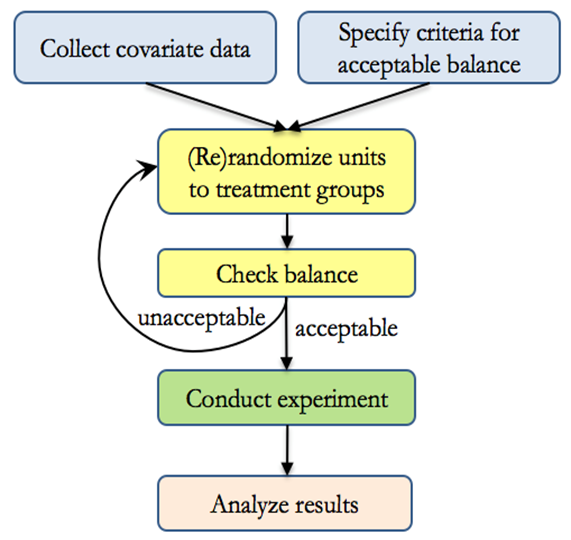
\includegraphics[width=0.9\linewidth,alt={Flow chart illustrating a process for conducting an experiment. It begins with "Collect covariate data" and "Specify criteria for acceptable balance." Next, "(Re)randomize units to treatment groups" is followed by "Check balance," which branches into "unacceptable" and "acceptable." If unacceptable, it loops back to randomization. If acceptable, it proceeds to "Conduct experiment" and finally "Analyze results."}]{images/The-Randomization-Procedure} 

}

\caption{Re-randomization workflow: covariate data are collected, balance criteria are specified, and units are repeatedly randomized until the criteria are met before the experiment proceeds.}\label{fig:rerandomization-flow}
\end{figure}

\begin{center}\rule{0.5\linewidth}{0.5pt}\end{center}

\textbf{Example: Balancing Experimental Groups}

An online retailer is testing two website designs (A and B) but wants to ensure that key customer demographics (e.g., age) are balanced across treatment groups.

We define a balance criterion to check if the mean age difference between groups is acceptable before proceeding.

\begin{Shaded}
\begin{Highlighting}[]
\FunctionTok{set.seed}\NormalTok{(}\DecValTok{123}\NormalTok{)}

\CommentTok{\# Define balance criterion: Ensure mean age difference \textless{} 1 year}
\NormalTok{balance\_criterion }\OtherTok{\textless{}{-}} \ControlFlowTok{function}\NormalTok{(data) \{}
  \FunctionTok{abs}\NormalTok{(}\FunctionTok{mean}\NormalTok{(data}\SpecialCharTok{$}\NormalTok{age[data}\SpecialCharTok{$}\NormalTok{group }\SpecialCharTok{==} \StringTok{"A"}\NormalTok{]) }\SpecialCharTok{{-}} \FunctionTok{mean}\NormalTok{(data}\SpecialCharTok{$}\NormalTok{age[data}\SpecialCharTok{$}\NormalTok{group }\SpecialCharTok{==} \StringTok{"B"}\NormalTok{])) }\SpecialCharTok{\textless{}} \DecValTok{1}
\NormalTok{\}}

\CommentTok{\# Generate randomized groups, repeat until balance criterion is met}
\ControlFlowTok{repeat}\NormalTok{ \{}
\NormalTok{  data }\OtherTok{\textless{}{-}} \FunctionTok{data.frame}\NormalTok{(}
    \AttributeTok{age =} \FunctionTok{rnorm}\NormalTok{(}\DecValTok{100}\NormalTok{, }\AttributeTok{mean =} \DecValTok{35}\NormalTok{, }\AttributeTok{sd =} \DecValTok{10}\NormalTok{),}
    \AttributeTok{group =} \FunctionTok{sample}\NormalTok{(}\FunctionTok{c}\NormalTok{(}\StringTok{"A"}\NormalTok{, }\StringTok{"B"}\NormalTok{), }\DecValTok{100}\NormalTok{, }\AttributeTok{replace =} \ConstantTok{TRUE}\NormalTok{)}
\NormalTok{  )}
  \ControlFlowTok{if}\NormalTok{ (}\FunctionTok{balance\_criterion}\NormalTok{(data)) }\ControlFlowTok{break}
\NormalTok{\}}

\CommentTok{\# Check final group means}
\FunctionTok{tapply}\NormalTok{(data}\SpecialCharTok{$}\NormalTok{age, data}\SpecialCharTok{$}\NormalTok{group, mean)}
\CommentTok{\#\textgreater{}        A        B }
\CommentTok{\#\textgreater{} 35.91079 35.25483}
\end{Highlighting}
\end{Shaded}

\subsubsection{Rerandomization Criterion}\label{rerandomization-criterion}

Re-randomization is based on a function of the covariate matrix (\(\mathbf{X}\)) and treatment assignments (\(\mathbf{W}\)).

\[
W_i = 
\begin{cases}
1, & \text{if treated} \\
0, & \text{if control}
\end{cases}
\]

A common approach is to use Mahalanobis Distance to measure covariate balance between treatment and control groups:

\[
\begin{aligned}
M &= (\bar{\mathbf{X}}_T - \bar{\mathbf{X}}_C)' \text{cov}(\bar{\mathbf{X}}_T - \bar{\mathbf{X}}_C)^{-1} (\bar{\mathbf{X}}_T - \bar{\mathbf{X}}_C) \\
&= (\frac{1}{n_T} + \frac{1}{n_C})^{-1} (\bar{\mathbf{X}}_T - \bar{\mathbf{X}}_C)' \text{cov}(\mathbf{X})^{-1} (\bar{\mathbf{X}}_T - \bar{\mathbf{X}}_C)
\end{aligned}
\]

where:

\begin{itemize}
\tightlist
\item
  \(\bar{\mathbf{X}}_T\) and \(\bar{\mathbf{X}}_C\) are the mean covariate values for treatment and control groups.
\item
  \(\text{cov}(\mathbf{X})\) is the covariance matrix of the covariates.
\item
  \(n_T\) and \(n_C\) are the sample sizes for treatment and control groups.
\end{itemize}

If the sample size is large and randomization is pure, then \(M\) follows a chi-squared distribution:

\[
M \sim \chi^2_k
\]

where \(k\) is the number of covariates to be balanced.

\begin{center}\rule{0.5\linewidth}{0.5pt}\end{center}

\textbf{Choosing the Rerandomization Threshold} (\(M > a\))

Define \(p_a\) as the probability of accepting a randomization:

\begin{itemize}
\tightlist
\item
  Smaller \(p_a\) → Stronger balance, but longer computation time.
\item
  Larger \(p_a\) → Faster randomization, but weaker balance.
\end{itemize}

A rule of thumb is to re-randomize whenever:

\[
M > a
\]

where \(a\) is chosen based on acceptable balance thresholds.

\begin{center}\rule{0.5\linewidth}{0.5pt}\end{center}

We apply Mahalanobis Distance as a balance criterion to ensure that treatment and control groups are well-matched before proceeding with the experiment.

\begin{Shaded}
\begin{Highlighting}[]
\FunctionTok{set.seed}\NormalTok{(}\DecValTok{123}\NormalTok{)}
\FunctionTok{library}\NormalTok{(MASS)}

\CommentTok{\# Generate a dataset with two covariates}
\NormalTok{n }\OtherTok{\textless{}{-}} \DecValTok{100}
\NormalTok{X }\OtherTok{\textless{}{-}} \FunctionTok{mvrnorm}\NormalTok{(n, }\AttributeTok{mu =} \FunctionTok{c}\NormalTok{(}\DecValTok{0}\NormalTok{, }\DecValTok{0}\NormalTok{), }\AttributeTok{Sigma =} \FunctionTok{matrix}\NormalTok{(}\FunctionTok{c}\NormalTok{(}\DecValTok{1}\NormalTok{, }\FloatTok{0.5}\NormalTok{, }\FloatTok{0.5}\NormalTok{, }\DecValTok{1}\NormalTok{), }\DecValTok{2}\NormalTok{, }\DecValTok{2}\NormalTok{))}
\FunctionTok{colnames}\NormalTok{(X) }\OtherTok{\textless{}{-}} \FunctionTok{c}\NormalTok{(}\StringTok{"Covariate1"}\NormalTok{, }\StringTok{"Covariate2"}\NormalTok{)}

\CommentTok{\# Balance function using Mahalanobis Distance}
\NormalTok{balance\_criterion }\OtherTok{\textless{}{-}} \ControlFlowTok{function}\NormalTok{(X, group) \{}
\NormalTok{  X\_treat }\OtherTok{\textless{}{-}}\NormalTok{ X[group }\SpecialCharTok{==} \DecValTok{1}\NormalTok{, ]}
\NormalTok{  X\_control }\OtherTok{\textless{}{-}}\NormalTok{ X[group }\SpecialCharTok{==} \DecValTok{0}\NormalTok{, ]}
  
\NormalTok{  mean\_diff }\OtherTok{\textless{}{-}} \FunctionTok{colMeans}\NormalTok{(X\_treat) }\SpecialCharTok{{-}} \FunctionTok{colMeans}\NormalTok{(X\_control)}
\NormalTok{  cov\_inv }\OtherTok{\textless{}{-}} \FunctionTok{solve}\NormalTok{(}\FunctionTok{cov}\NormalTok{(X))}
\NormalTok{  M }\OtherTok{\textless{}{-}} \FunctionTok{t}\NormalTok{(mean\_diff) }\SpecialCharTok{\%*\%}\NormalTok{ cov\_inv }\SpecialCharTok{\%*\%}\NormalTok{ mean\_diff}
  
  
  \CommentTok{\# Acceptable threshold }
  \CommentTok{\# (chi{-}squared critical value for k = 2, alpha = 0.05)}
  \FunctionTok{return}\NormalTok{(M }\SpecialCharTok{\textless{}} \FloatTok{3.84}\NormalTok{)  }
\NormalTok{\}}

\CommentTok{\# Repeat randomization until balance is met}
\ControlFlowTok{repeat}\NormalTok{ \{}
\NormalTok{  group }\OtherTok{\textless{}{-}} \FunctionTok{sample}\NormalTok{(}\FunctionTok{c}\NormalTok{(}\DecValTok{0}\NormalTok{, }\DecValTok{1}\NormalTok{), n, }\AttributeTok{replace =} \ConstantTok{TRUE}\NormalTok{)}
  \ControlFlowTok{if}\NormalTok{ (}\FunctionTok{balance\_criterion}\NormalTok{(X, group)) }\ControlFlowTok{break}
\NormalTok{\}}

\CommentTok{\# Display final balance check}
\FunctionTok{table}\NormalTok{(group)}
\CommentTok{\#\textgreater{} group}
\CommentTok{\#\textgreater{}  0  1 }
\CommentTok{\#\textgreater{} 50 50}
\FunctionTok{colMeans}\NormalTok{(X[group }\SpecialCharTok{==} \DecValTok{1}\NormalTok{, ])  }\CommentTok{\# Treatment group means}
\CommentTok{\#\textgreater{} Covariate1 Covariate2 }
\CommentTok{\#\textgreater{}  0.2469635  0.1918521}
\FunctionTok{colMeans}\NormalTok{(X[group }\SpecialCharTok{==} \DecValTok{0}\NormalTok{, ])  }\CommentTok{\# Control group means}
\CommentTok{\#\textgreater{}  Covariate1  Covariate2 }
\CommentTok{\#\textgreater{}  0.01717088 {-}0.14281124}
\end{Highlighting}
\end{Shaded}

\begin{center}\rule{0.5\linewidth}{0.5pt}\end{center}

\subsection{Two-Stage Randomized Experiments}\label{two-stage-randomized-experiments}

A \textbf{two-stage randomized experiment} involves \textbf{sequential interventions}, where treatment assignments depend on earlier responses. This design is widely used in:

\begin{itemize}
\tightlist
\item
  Adaptive Learning: Adjusting educational content based on student progress.
\item
  Personalized Advertising: Targeting follow-up ads based on engagement.
\item
  Medical Trials: Adapting treatments based on patient response.
\end{itemize}

By introducing \textbf{a second randomization stage}, researchers can evaluate:

\begin{enumerate}
\def\labelenumi{\arabic{enumi}.}
\tightlist
\item
  \textbf{The effect of initial treatments.}
\item
  \textbf{The effect of follow-up treatments.}
\item
  \textbf{Potential interactions between the two stages.}
\end{enumerate}

\begin{center}\rule{0.5\linewidth}{0.5pt}\end{center}

\subsubsection{Example: Personalized Advertising Experiment}\label{example-personalized-advertising-experiment}

A company tests two initial ad campaigns (Ad A vs.~Ad B). After observing customer engagement, they apply a second-stage intervention (e.g., Discount vs.~No Discount).

The two-stage experiment can be modeled as:

\[
Y_{ijk} = \mu + \alpha_i + \beta_{j(i)} + \epsilon_{ijk}
\]

where:

\begin{itemize}
\tightlist
\item
  \(\mu\) = Overall mean outcome (e.g., conversion rate).
\item
  \(\alpha_i\) = Effect of first-stage intervention (\(i\) = Ad A or Ad B).
\item
  \(\beta_{j(i)}\) = Effect of second-stage intervention, nested within first-stage groups.
\item
  \(\epsilon_{ijk}\) = Random error term.
\end{itemize}

The nested structure ensures that the second-stage treatment (\(\beta_{j(i)}\)) is assigned within each first-stage treatment group.

\begin{center}\rule{0.5\linewidth}{0.5pt}\end{center}

\begin{Shaded}
\begin{Highlighting}[]
\FunctionTok{set.seed}\NormalTok{(}\DecValTok{123}\NormalTok{)}

\CommentTok{\# Generate first{-}stage randomization (Initial Ad)}
\NormalTok{data }\OtherTok{\textless{}{-}} \FunctionTok{data.frame}\NormalTok{(}
  \AttributeTok{stage1 =} \FunctionTok{sample}\NormalTok{(}\FunctionTok{c}\NormalTok{(}\StringTok{"Ad A"}\NormalTok{, }\StringTok{"Ad B"}\NormalTok{), }\DecValTok{100}\NormalTok{, }\AttributeTok{replace =} \ConstantTok{TRUE}\NormalTok{),}
  \AttributeTok{stage2 =} \FunctionTok{rep}\NormalTok{(}\ConstantTok{NA}\NormalTok{, }\DecValTok{100}\NormalTok{)  }\CommentTok{\# Placeholder for second{-}stage randomization}
\NormalTok{)}

\CommentTok{\# Second{-}stage assignment based on first{-}stage response}
\NormalTok{data}\SpecialCharTok{$}\NormalTok{stage2[data}\SpecialCharTok{$}\NormalTok{stage1 }\SpecialCharTok{==} \StringTok{"Ad A"}\NormalTok{] }\OtherTok{\textless{}{-}}
    \FunctionTok{sample}\NormalTok{(}\FunctionTok{c}\NormalTok{(}\StringTok{"Discount"}\NormalTok{, }\StringTok{"No Discount"}\NormalTok{),}
           \FunctionTok{sum}\NormalTok{(data}\SpecialCharTok{$}\NormalTok{stage1 }\SpecialCharTok{==} \StringTok{"Ad A"}\NormalTok{),}
           \AttributeTok{replace =} \ConstantTok{TRUE}\NormalTok{)}
\NormalTok{data}\SpecialCharTok{$}\NormalTok{stage2[data}\SpecialCharTok{$}\NormalTok{stage1 }\SpecialCharTok{==} \StringTok{"Ad B"}\NormalTok{] }\OtherTok{\textless{}{-}}
    \FunctionTok{sample}\NormalTok{(}\FunctionTok{c}\NormalTok{(}\StringTok{"Discount"}\NormalTok{, }\StringTok{"No Discount"}\NormalTok{),}
           \FunctionTok{sum}\NormalTok{(data}\SpecialCharTok{$}\NormalTok{stage1 }\SpecialCharTok{==} \StringTok{"Ad B"}\NormalTok{),}
           \AttributeTok{replace =} \ConstantTok{TRUE}\NormalTok{)}

\CommentTok{\# Display final randomization}
\FunctionTok{table}\NormalTok{(data}\SpecialCharTok{$}\NormalTok{stage1, data}\SpecialCharTok{$}\NormalTok{stage2)}
\CommentTok{\#\textgreater{}       }
\CommentTok{\#\textgreater{}        Discount No Discount}
\CommentTok{\#\textgreater{}   Ad A       24          33}
\CommentTok{\#\textgreater{}   Ad B       22          21}
\end{Highlighting}
\end{Shaded}

This structure ensures:

\begin{enumerate}
\def\labelenumi{\arabic{enumi}.}
\item
  Fair assignment of initial ads.
\item
  Adaptive targeting in the second stage based on user engagement.
\end{enumerate}

\begin{center}\rule{0.5\linewidth}{0.5pt}\end{center}

\subsection{Two-Stage Randomized Experiments with Interference and Noncompliance}\label{two-stage-randomized-experiments-with-interference-and-noncompliance}

In real-world experiments, \textbf{interference and noncompliance} complicate analysis \citep{imai2021causal}:

\begin{itemize}
\item
  Interference: When treatment effects ``spill over'' from one group to another (e.g., social influence in marketing).
\item
  Noncompliance: When participants do not adhere to their assigned treatment (e.g., a customer ignoring an ad).
\end{itemize}

To handle noncompliance, we define:

\begin{itemize}
\item
  \(Z_{ik}\) = Assigned treatment (e.g., Ad A or Ad B).
\item
  \(D_{ik}\) = Actual treatment received (e.g., whether the user actually saw the ad).
\item
  \(Y_{ik}\) = Outcome (e.g., purchase).
\end{itemize}

A \textbf{two-stage Instrumental Variable model} adjusts for noncompliance:

\[
\begin{aligned}
D_{ik} &= \gamma_0 + \gamma_1 Z_{ik} + v_{ik} \\
Y_{ik} &= \beta_0 + \beta_1 D_{ik} + \epsilon_{ik}
\end{aligned}
\] where:

\begin{itemize}
\item
  \(\gamma_1\) measures the effect of assignment on actual treatment received.
\item
  \(\beta_1\) estimates the treatment effect, adjusting for noncompliance.
\end{itemize}

If individuals influence each other's outcomes, traditional randomization is biased. Solutions include:

\begin{enumerate}
\def\labelenumi{\arabic{enumi}.}
\item
  \textbf{Cluster Randomization}: Assigning treatments at the group level (e.g., entire social circles receive the same ad).
\item
  \textbf{Partial Interference Models}: Assume interference only occurs within predefined groups.
\end{enumerate}

\begin{Shaded}
\begin{Highlighting}[]
\FunctionTok{set.seed}\NormalTok{(}\DecValTok{123}\NormalTok{)}
\FunctionTok{library}\NormalTok{(ivreg)  }\CommentTok{\# Load Instrumental Variable Regression Package}

\CommentTok{\# Generate data for first{-}stage treatment assignment}
\NormalTok{n }\OtherTok{\textless{}{-}} \DecValTok{500}
\NormalTok{data }\OtherTok{\textless{}{-}} \FunctionTok{data.frame}\NormalTok{(}
  \AttributeTok{Z =} \FunctionTok{sample}\NormalTok{(}\FunctionTok{c}\NormalTok{(}\DecValTok{0}\NormalTok{, }\DecValTok{1}\NormalTok{), n, }\AttributeTok{replace =} \ConstantTok{TRUE}\NormalTok{),  }\CommentTok{\# Initial assignment (randomized)}
  \AttributeTok{D =} \ConstantTok{NA}\NormalTok{,  }\CommentTok{\# Actual treatment received (affected by compliance)}
  \AttributeTok{Y =} \ConstantTok{NA}   \CommentTok{\# Outcome variable (e.g., purchase)}
\NormalTok{)}

\CommentTok{\# Introduce noncompliance: 80\% compliance rate}
\NormalTok{data}\SpecialCharTok{$}\NormalTok{D }\OtherTok{\textless{}{-}} \FunctionTok{ifelse}\NormalTok{(}\FunctionTok{runif}\NormalTok{(n) }\SpecialCharTok{\textless{}} \FloatTok{0.8}\NormalTok{, data}\SpecialCharTok{$}\NormalTok{Z, }\DecValTok{1} \SpecialCharTok{{-}}\NormalTok{ data}\SpecialCharTok{$}\NormalTok{Z)}

\CommentTok{\# Generate outcome variable (Y) with true treatment effect}
\CommentTok{\# True effect of D on Y is 3}
\NormalTok{data}\SpecialCharTok{$}\NormalTok{Y }\OtherTok{\textless{}{-}} \DecValTok{5} \SpecialCharTok{+} \DecValTok{3} \SpecialCharTok{*}\NormalTok{ data}\SpecialCharTok{$}\NormalTok{D }\SpecialCharTok{+} \FunctionTok{rnorm}\NormalTok{(n, }\AttributeTok{mean =} \DecValTok{0}\NormalTok{, }\AttributeTok{sd =} \DecValTok{2}\NormalTok{)  }

\CommentTok{\# Estimate Two{-}Stage Least Squares (2SLS)}
\NormalTok{iv\_model }\OtherTok{\textless{}{-}} \FunctionTok{ivreg}\NormalTok{(Y }\SpecialCharTok{\textasciitilde{}}\NormalTok{ D }\SpecialCharTok{|}\NormalTok{ Z, }\AttributeTok{data =}\NormalTok{ data)}
\FunctionTok{summary}\NormalTok{(iv\_model)}
\CommentTok{\#\textgreater{} }
\CommentTok{\#\textgreater{} Call:}
\CommentTok{\#\textgreater{} ivreg(formula = Y \textasciitilde{} D | Z, data = data)}
\CommentTok{\#\textgreater{} }
\CommentTok{\#\textgreater{} Residuals:}
\CommentTok{\#\textgreater{}    Min     1Q Median     3Q    Max }
\CommentTok{\#\textgreater{} {-}5.497 {-}1.344  0.018  1.303  5.493 }
\CommentTok{\#\textgreater{} }
\CommentTok{\#\textgreater{} Coefficients:}
\CommentTok{\#\textgreater{}             Estimate Std. Error t value Pr(\textgreater{}|t|)    }
\CommentTok{\#\textgreater{} (Intercept)   5.1285     0.1861  27.557   \textless{}2e{-}16 ***}
\CommentTok{\#\textgreater{} D             2.7487     0.3072   8.949   \textless{}2e{-}16 ***}
\CommentTok{\#\textgreater{} }
\CommentTok{\#\textgreater{} Diagnostic tests:}
\CommentTok{\#\textgreater{}                  df1 df2 statistic p{-}value    }
\CommentTok{\#\textgreater{} Weak instruments   1 498    263.54  \textless{}2e{-}16 ***}
\CommentTok{\#\textgreater{} Wu{-}Hausman         1 497      0.19   0.663    }
\CommentTok{\#\textgreater{} Sargan             0  NA        NA      NA    }
\CommentTok{\#\textgreater{} {-}{-}{-}}
\CommentTok{\#\textgreater{} Signif. codes:  0 \textquotesingle{}***\textquotesingle{} 0.001 \textquotesingle{}**\textquotesingle{} 0.01 \textquotesingle{}*\textquotesingle{} 0.05 \textquotesingle{}.\textquotesingle{} 0.1 \textquotesingle{} \textquotesingle{} 1}
\CommentTok{\#\textgreater{} }
\CommentTok{\#\textgreater{} Residual standard error: 2.017 on 498 degrees of freedom}
\CommentTok{\#\textgreater{} Multiple R{-}Squared: 0.2997,  Adjusted R{-}squared: 0.2983 }
\CommentTok{\#\textgreater{} Wald test: 80.08 on 1 and 498 DF,  p{-}value: \textless{} 2.2e{-}16}
\end{Highlighting}
\end{Shaded}

\begin{itemize}
\item
  The first-stage regression estimates how strongly \(Z\) affects \(D\) (compliance).
\item
  The second-stage regression estimates the true causal effect of \(D\) on \(Y\).
\end{itemize}

If interference is present, the standard IV method may be biased. Researchers should explore network-based randomization or spatial models.

\subsection{Cluster Randomization for Interference Bias}\label{sec-cluster-randomization}

Standard randomized controlled trials rely on the Stable Unit Treatment Value Assumption (SUTVA), which has two parts. No interference says that the potential outcome of one unit is unaffected by the treatment assignment of any other unit, i.e.~\(Y_i(Z)\) depends only on \(Z_i\), not on \(Z_j\) for \(j \ne i\). No hidden versions of treatment says that each treatment condition is well defined and consistent across units.

Violations of SUTVA, particularly interference, are common in online marketplaces such as Airbnb, eBay, Uber, and Etsy, where agents interact strategically and share common resources like customer attention and platform visibility. Interference occurs when \(Y_i(Z)\) depends on the treatment status of others, i.e.~\(Y_i(Z_1, \ldots, Z_n)\). In such settings interference bias distorts causal estimates, often misleading decision makers.

In interconnected digital environments, agents (sellers, listings, users) affect each other through algorithmic rankings, pricing competition, and substitution behavior among buyers. As one stylized example, if Airbnb treats a host by recommending a price increase, nearby untreated hosts may adjust their own pricing in response, and buyers respond based on all available listings, so observed outcomes reflect systemic responses rather than isolated treatment effects.

This violates the no-interference condition, causing the estimated Total Average Treatment Effect (TATE) to be biased:

\[\text{TATE} = \mathbb{E}[Y_i(1) - Y_i(0)].\]

\citet{blake2014marketplace} (eBay) formalized this dynamic as test-control interference: treated sellers attract buyers away from control sellers, inflating estimated gains. Subsequent marketplace simulations have shown that overstatements of treatment effects in two-sided platforms can exceed 100\% under realistic assumptions.

Following \citet{eckles2021bias}, consider the potential outcome for seller \(i\):

\[Y_i(Z) = \alpha_i + \beta Z_i + \gamma \rho_i + \varepsilon_i,\]

where \(\beta\) is the direct treatment effect, \(\gamma\) is the spillover (indirect) effect, and \(\rho_i = \frac{1}{|N_i|} \sum_{j \in N_i} Z_j\) is the fraction of treated neighbors. When \(\gamma \neq 0\) there is interference; if \(\beta\) and \(\gamma\) have opposite signs, interference can inflate or deflate TATE estimates. In matrix form, define an interference matrix \(B\) such that \(\mathbb{E}[Y_i(Z)] = \alpha_i + \sum_j B_{ij} Z_j\), where diagonal entries capture direct effects and off-diagonal entries capture interference.

Cluster randomization assigns entire clusters (groups) of units, rather than individual units, to treatment or control. Units within clusters likely interfere with each other, so treating clusters homogeneously contains interference within groups. \citet{holtz2025reducing} extend \citet{eckles2021bias} and show that, for a linear interference model with uniform-sign \(B_{ii}\) and \(B_{ij}\), cluster randomization always reduces interference bias relative to individual-level randomization:

\[|\mathbb{E}[\hat{\tau}_{\text{cr}} - \tau]| \le |\mathbb{E}[\hat{\tau}_{\text{ind}} - \tau]|,\]

regardless of whether spillovers are positive or negative. Let \(C(i)\) denote the cluster of unit \(i\). Cluster quality is

\[Q_C(B) = \sum_{i,j} B_{ij} \cdot \mathbf{1}\{C(i) \ne C(j)\}.\]

Lower \(Q_C(B)\) implies less across-cluster interference and better clustering. In practice \(B\) is unobservable, so a proxy matrix \(P\) (e.g.~co-search or co-view behavior) is used.

Graph-Cluster Randomization (GCR) partitions a social or economic network into clusters and randomizes treatment at the cluster level, reducing mixed-treatment neighborhoods. \citet{ugander2013graph} showed that GCR yields unbiased Horvitz-Thompson estimators of treatment effects under certain exposure models:

\[\hat{\tau}_{HT} = \sum_{i \in T} \frac{Y_i}{\pi_i} - \sum_{i \in C} \frac{Y_i}{1 - \pi_i},\]

where \(\pi_i\) is the probability that unit \(i\) is treated, accounting for the randomization design. The price for this bias reduction is variance: \citet{eckles2021bias} show that \(\mathrm{Var}(\hat{\tau}_{CR}) \propto \rho \cdot \sigma^2 / n_c\), where \(\rho\) is the intra-cluster correlation and \(n_c\) is the number of clusters. Pre-stratification, regression adjustment, or increasing the cluster count can partially mitigate this variance growth.

\subsubsection{Case Study: The Airbnb Meta-Experiment}\label{case-study-the-airbnb-meta-experiment}

\citet{holtz2025reducing} conducted a large-scale meta-experiment on Airbnb to empirically measure interference bias and evaluate cluster randomization. Airbnb engineers constructed clusters by embedding each listing into a 16-dimensional vector space using guest co-click data, then applied a recursive partitioning tree such that at least 90\% of listings within a node shared common neighbors. The resulting roughly 15,000 clusters had a median size of 150 listings, and the within-cluster substitution rate exceeded 95\%. Hold-out data confirmed that cross-cluster substitution was minimal.

In each of two platform-wide experiments (over 2 million listings worldwide), 75\% of clusters were randomized at the cluster level, while 25\% retained standard Bernoulli (individual-level) randomization. For the guest-fee intervention the estimated TATE was \(-0.207\) bookings per listing under individual-level randomization, but only \(-0.139\) under cluster randomization, implying that interference inflated the naive estimate by 32.6\%. The interference bias ratio \(\hat{\nu} / (\hat{\beta} + \hat{\nu})\) was approximately 19.8\%. Bias varied with market conditions: demand-constrained areas (New York in peak season) reached 28.6\%, supply-constrained areas were lower at 12.1\%, and higher cluster quality (better separation in embedding space) was associated with greater bias reduction. For the pricing-recommendation intervention the cluster-level estimate (\(-0.051\)) was not statistically significant, compared to \(-0.106\) under Bernoulli randomization; a post-hoc power analysis indicated that detecting the same bias with 80\% power would have required 3.5 times more clusters.

The case study illustrates both the prevalence of interference bias in online marketplaces and the potential of cluster randomization to mitigate it, provided clusters are intelligently constructed and contextually grounded.

\subsubsection{Practical Blueprint}\label{practical-blueprint}

Diagnosing interference. First theorize likely spillover channels (e.g.~ranking algorithms, price comparisons), then conduct a meta-experiment with dual randomization and compare TATEs, then quantify exposure probabilities using network or item similarity matrices.

Cluster construction. Given a substitution matrix \(S\) from clicks or bookings: symmetrize \(W = (S + S^\top)/2\), compute a normalized graph Laplacian \(L\), embed nodes via the top-\(k\) eigenvectors of \(L\), apply \(k\)-means clustering (\(k\) via the gap statistic), and merge tiny clusters if needed. Evaluate using neighbor purity (proportion of nearest neighbors within the same cluster); Airbnb used a threshold of at least 0.9.

Analysis plan. Use cluster-robust standard errors or Horvitz-Thompson weights, adjust for intra-cluster correlation, and consider OLS with pre-stratification to improve power.

A short simulation makes the bias-reduction visible:

\begin{Shaded}
\begin{Highlighting}[]
\FunctionTok{set.seed}\NormalTok{(}\DecValTok{123}\NormalTok{)}
\NormalTok{n }\OtherTok{\textless{}{-}} \DecValTok{1000}
\NormalTok{clusters }\OtherTok{\textless{}{-}} \FunctionTok{rep}\NormalTok{(}\DecValTok{1}\SpecialCharTok{:}\DecValTok{100}\NormalTok{, }\AttributeTok{each =} \DecValTok{10}\NormalTok{)}
\NormalTok{Z }\OtherTok{\textless{}{-}} \FunctionTok{rbinom}\NormalTok{(n, }\DecValTok{1}\NormalTok{, }\FloatTok{0.5}\NormalTok{)}
\NormalTok{B }\OtherTok{\textless{}{-}} \FunctionTok{matrix}\NormalTok{(}\FunctionTok{runif}\NormalTok{(n}\SpecialCharTok{\^{}}\DecValTok{2}\NormalTok{, }\DecValTok{0}\NormalTok{, }\FloatTok{0.1}\NormalTok{), n, n)}
\FunctionTok{diag}\NormalTok{(B) }\OtherTok{\textless{}{-}} \FunctionTok{runif}\NormalTok{(n, }\FloatTok{0.5}\NormalTok{, }\DecValTok{1}\NormalTok{)}

\NormalTok{Y }\OtherTok{\textless{}{-}} \FunctionTok{sapply}\NormalTok{(}\DecValTok{1}\SpecialCharTok{:}\NormalTok{n, }\ControlFlowTok{function}\NormalTok{(i) }\FunctionTok{sum}\NormalTok{(B[i, ] }\SpecialCharTok{*}\NormalTok{ Z)) }\SpecialCharTok{+} \FunctionTok{rnorm}\NormalTok{(n)}

\NormalTok{t\_ind }\OtherTok{\textless{}{-}} \FunctionTok{mean}\NormalTok{(Y[Z }\SpecialCharTok{==} \DecValTok{1}\NormalTok{]) }\SpecialCharTok{{-}} \FunctionTok{mean}\NormalTok{(Y[Z }\SpecialCharTok{==} \DecValTok{0}\NormalTok{])}

\NormalTok{cluster\_Z }\OtherTok{\textless{}{-}} \FunctionTok{tapply}\NormalTok{(Z, clusters, mean)}
\NormalTok{cluster\_Y }\OtherTok{\textless{}{-}} \FunctionTok{tapply}\NormalTok{(Y, clusters, mean)}
\NormalTok{t\_cr }\OtherTok{\textless{}{-}} \FunctionTok{mean}\NormalTok{(cluster\_Y[cluster\_Z }\SpecialCharTok{\textgreater{}} \FloatTok{0.5}\NormalTok{]) }\SpecialCharTok{{-}} \FunctionTok{mean}\NormalTok{(cluster\_Y[cluster\_Z }\SpecialCharTok{\textless{}=} \FloatTok{0.5}\NormalTok{])}

\FunctionTok{c}\NormalTok{(}\AttributeTok{t\_ind =}\NormalTok{ t\_ind, }\AttributeTok{t\_cr =}\NormalTok{ t\_cr)}
\CommentTok{\#\textgreater{}     t\_ind      t\_cr }
\CommentTok{\#\textgreater{} 0.7931955 0.3104478}
\end{Highlighting}
\end{Shaded}

The individual-randomization estimate \(t_\text{ind}\) is inflated relative to the cluster-randomization estimate \(t_\text{cr}\) because the off-diagonal entries of \(B\) leak treatment from \(j\) to \(i\) across the assignment split.

Trade-offs. Cluster randomization trades higher implementation overhead and reduced power for substantially lower interference bias; the right choice depends on the size of \(\gamma\), the granularity of the interference structure, and how much within-cluster pre-stratification is feasible.

\subsection{Switchback Experiments with Surrogate Variables}\label{switchback-experiments-with-surrogate-variables}

\begin{center}\rule{0.5\linewidth}{0.5pt}\end{center}

\section{Emerging Research}\label{emerging-research}

Recent research highlights significant challenges in measuring the causal effects of ad content in online advertising experiments. Digital advertising platforms employ algorithmic targeting and dynamic ad delivery mechanisms, which can introduce systematic biases in A/B testing \citep{braun2025where}. Key concerns include:

\begin{itemize}
\item
  \textbf{Nonrandom Exposure}: Online advertising platforms optimize ad delivery dynamically, meaning users are not randomly assigned to different ad variants. Instead, platforms use proprietary algorithms to serve ads to different, often highly heterogeneous, user groups.
\item
  \textbf{Divergent Delivery}: The optimization process can lead to ``divergent delivery,'' where differences in user engagement patterns and platform objectives result in non-comparable treatment groups. This confounds the true effect of ad content with algorithmic biases in exposure.
\item
  \textbf{Bias in Measured Effects}: Algorithmic targeting, user heterogeneity, and data aggregation can distort both the \textbf{magnitude} and \textbf{direction} of estimated ad effects. This means traditional A/B test results may not accurately reflect the true impact of ad creatives.
\item
  \textbf{Limited Transparency}: Platforms have little incentive to assist advertisers or researchers in disentangling ad content effects from proprietary targeting mechanisms. As a result, experimenters must design careful identification strategies to mitigate these biases.
\end{itemize}

\begin{center}\rule{0.5\linewidth}{0.5pt}\end{center}

\subsection{Covariate Balancing in Online A/B Testing: The Pigeonhole Design}\label{covariate-balancing-in-online-ab-testing-the-pigeonhole-design}

\citet{zhao2024pigeonhole} address the challenge of covariate balancing in online A/B testing when experimental subjects arrive sequentially. Traditional experimental designs struggle to maintain balance in real-time settings where treatment assignments must be made immediately. This work introduces the online blocking problem, in which subjects with heterogeneous covariates must be assigned to treatment or control groups dynamically, with the goal of minimizing total discrepancy, quantified as the minimum weight perfect matching between groups.

To improve covariate balance, the authors propose the \textbf{pigeonhole design}, a randomized experimental design that operates as follows:

\begin{itemize}
\tightlist
\item
  The covariate space is partitioned into smaller subspaces called ``pigeonholes.''
\item
  Within each pigeonhole, the design balances the number of treated and control subjects, reducing systematic imbalances.
\end{itemize}

Theoretical analysis demonstrates the effectiveness of this design in reducing discrepancy compared to existing approaches. Specifically, the pigeonhole design is benchmarked against:

\begin{itemize}
\tightlist
\item
  \textbf{Matched-pair design}
\item
  \hyperref[completely-randomized-design]{Completely Randomized Design}
\end{itemize}

The results highlight scenarios where the pigeonhole design outperforms these alternatives in maintaining covariate balance.

Using Yahoo! data, the authors validate the pigeonhole design in practice, demonstrating a 10.2\% reduction in variance when estimating the \hyperref[sec-average-treatment-effect]{Average Treatment Effect}. This improvement underscores the design's practical utility in reducing noise and improving the precision of experimental results.

The findings of \citet{zhao2024pigeonhole} provide valuable insights for practitioners conducting online A/B tests:

\begin{itemize}
\tightlist
\item
  Ensuring real-time covariate balance improves the reliability of causal estimates.
\item
  The pigeonhole design offers a structured yet flexible approach to balancing covariates dynamically.
\item
  By reducing variance in treatment effect estimation, it enhances statistical efficiency in large-scale online experiments.
\end{itemize}

This study contributes to the broader discussion of \hyperref[sec-the-gold-standard-randomized-controlled-trials]{randomized experimental design} in dynamic settings, providing a compelling alternative to traditional approaches.

\begin{center}\rule{0.5\linewidth}{0.5pt}\end{center}

\subsection{Handling Zero-Valued Outcomes}\label{sec-handling-zero-valued-outcomes}

When analyzing treatment effects, a common issue arises when the outcome variable includes zero values.

For example, in business applications, a marketing intervention may have no effect on some customers (resulting in zero sales). If we were to apply a log transformation to the outcome variable, this would be problematic because:

\begin{itemize}
\tightlist
\item
  \(\log(0)\) is undefined.
\item
  Log transformation is sensitive to outcome units, making interpretation difficult \citep{chen2024logs}.
\end{itemize}

Instead of applying a log transformation, we should use methods that are robust to zero values:

\begin{enumerate}
\def\labelenumi{\arabic{enumi}.}
\tightlist
\item
  \textbf{Percentage changes in the Average}

  \begin{itemize}
  \tightlist
  \item
    By using Poisson Quasi-Maximum Likelihood Estimation (QMLE), we can interpret coefficients as percentage changes in the mean outcome of the treatment group relative to the control group.
  \end{itemize}
\item
  \textbf{Extensive vs.~Intensive Margins}

  \begin{itemize}
  \tightlist
  \item
    This approach distinguishes between:

    \begin{itemize}
    \tightlist
    \item
      \textbf{Extensive margin}: The likelihood of moving from zero to a positive outcome (e.g., increasing the probability of making a sale).
    \item
      \textbf{Intensive margin}: The increase in the outcome given that it is already positive (e.g., increasing the sales amount).
    \end{itemize}
  \item
    To estimate the \textbf{intensive-margin bounds}, we could use \citet{lee2009training}, assuming that treatment has a \textbf{monotonic effect} on the outcome.
  \end{itemize}
\end{enumerate}

\begin{center}\rule{0.5\linewidth}{0.5pt}\end{center}

We first generate a dataset to simulate a scenario where an outcome variable (e.g., sales, website clicks) has many zeros, and treatment affects both the extensive and intensive margins.

\begin{Shaded}
\begin{Highlighting}[]
\FunctionTok{set.seed}\NormalTok{(}\DecValTok{123}\NormalTok{) }\CommentTok{\# For reproducibility}
\FunctionTok{library}\NormalTok{(tidyverse)}

\NormalTok{n }\OtherTok{\textless{}{-}} \DecValTok{1000} \CommentTok{\# Number of observations}
\NormalTok{p\_treatment }\OtherTok{\textless{}{-}} \FloatTok{0.5} \CommentTok{\# Probability of being treated}

\CommentTok{\# Step 1: Generate the treatment variable D}
\NormalTok{D }\OtherTok{\textless{}{-}} \FunctionTok{rbinom}\NormalTok{(n, }\DecValTok{1}\NormalTok{, p\_treatment)}

\CommentTok{\# Step 2: Generate potential outcomes}
\CommentTok{\# Untreated potential outcome (mostly zeroes)}
\NormalTok{Y0 }\OtherTok{\textless{}{-}} \FunctionTok{rnorm}\NormalTok{(n, }\AttributeTok{mean =} \DecValTok{0}\NormalTok{, }\AttributeTok{sd =} \DecValTok{1}\NormalTok{) }\SpecialCharTok{*}\NormalTok{ (}\FunctionTok{runif}\NormalTok{(n) }\SpecialCharTok{\textless{}} \FloatTok{0.3}\NormalTok{)}

\CommentTok{\# Treated potential outcome (affecting both extensive and intensive margins)}
\NormalTok{Y1 }\OtherTok{\textless{}{-}}\NormalTok{ Y0 }\SpecialCharTok{+} \FunctionTok{rnorm}\NormalTok{(n, }\AttributeTok{mean =} \DecValTok{2}\NormalTok{, }\AttributeTok{sd =} \DecValTok{1}\NormalTok{) }\SpecialCharTok{*}\NormalTok{ (}\FunctionTok{runif}\NormalTok{(n) }\SpecialCharTok{\textless{}} \FloatTok{0.7}\NormalTok{)}

\CommentTok{\# Step 3: Combine effects based on treatment assignment}
\NormalTok{Y\_observed }\OtherTok{\textless{}{-}}\NormalTok{ (}\DecValTok{1} \SpecialCharTok{{-}}\NormalTok{ D) }\SpecialCharTok{*}\NormalTok{ Y0 }\SpecialCharTok{+}\NormalTok{ D }\SpecialCharTok{*}\NormalTok{ Y1}

\CommentTok{\# Ensure non{-}negative outcomes (modeling real{-}world situations)}
\NormalTok{Y\_observed[Y\_observed }\SpecialCharTok{\textless{}} \DecValTok{0}\NormalTok{] }\OtherTok{\textless{}{-}} \DecValTok{0}

\CommentTok{\# Create a dataset with an additional control variable}
\NormalTok{data }\OtherTok{\textless{}{-}} \FunctionTok{data.frame}\NormalTok{(}
    \AttributeTok{ID =} \DecValTok{1}\SpecialCharTok{:}\NormalTok{n,}
    \AttributeTok{Treatment =}\NormalTok{ D,}
    \AttributeTok{Outcome =}\NormalTok{ Y\_observed,}
    \AttributeTok{X =} \FunctionTok{rnorm}\NormalTok{(n) }\CommentTok{\# Control variable}
\NormalTok{) }\SpecialCharTok{|\textgreater{}}
\NormalTok{    dplyr}\SpecialCharTok{::}\FunctionTok{mutate}\NormalTok{(}\AttributeTok{positive =}\NormalTok{ Outcome }\SpecialCharTok{\textgreater{}} \DecValTok{0}\NormalTok{) }\CommentTok{\# Indicator for extensive margin}

\CommentTok{\# View first few rows}
\FunctionTok{head}\NormalTok{(data)}
\CommentTok{\#\textgreater{}   ID Treatment   Outcome          X positive}
\CommentTok{\#\textgreater{} 1  1         0 0.0000000  1.4783345    FALSE}
\CommentTok{\#\textgreater{} 2  2         1 2.2369379 {-}1.4067867     TRUE}
\CommentTok{\#\textgreater{} 3  3         0 0.0000000 {-}1.8839721    FALSE}
\CommentTok{\#\textgreater{} 4  4         1 3.2192276 {-}0.2773662     TRUE}
\CommentTok{\#\textgreater{} 5  5         1 0.6649693  0.4304278     TRUE}
\CommentTok{\#\textgreater{} 6  6         0 0.0000000 {-}0.1287867    FALSE}
\end{Highlighting}
\end{Shaded}

Fig. \ref{fig:outcome-distribution} shows the distribution of the simulated outcomes used in the example.

\begin{Shaded}
\begin{Highlighting}[]
\CommentTok{\# Plot distribution of outcomes}
\FunctionTok{hist}\NormalTok{(}
\NormalTok{    data}\SpecialCharTok{$}\NormalTok{Outcome,}
    \AttributeTok{breaks =} \DecValTok{30}\NormalTok{,}
    \AttributeTok{main =} \StringTok{"Distribution of Outcomes"}\NormalTok{,}
    \AttributeTok{col =} \StringTok{"lightblue"}
\NormalTok{)}
\end{Highlighting}
\end{Shaded}

\begin{figure}

{\centering \includegraphics[width=0.9\linewidth,alt={Bar chart showing outcome frequencies with high frequency at 0 and decreasing frequencies for outcomes 1 through 6.}]{22-experiment_files/figure-latex/outcome-distribution-1} 

}

\caption{Distribution of outcomes in the simulated dataset, with a mass point at zero and decreasing frequencies at higher counts.}\label{fig:outcome-distribution}
\end{figure}

\subsubsection{Estimating Percentage Changes in the Average}\label{estimating-percentage-changes-in-the-average}

Since we cannot use a log transformation, we estimate percentage changes using Poisson QMLE, which is robust to zero-valued outcomes.

\begin{Shaded}
\begin{Highlighting}[]
\FunctionTok{library}\NormalTok{(fixest)}

\CommentTok{\# Poisson Quasi{-}Maximum Likelihood Estimation (QMLE)}
\NormalTok{res\_pois }\OtherTok{\textless{}{-}} \FunctionTok{fepois}\NormalTok{(}
    \AttributeTok{fml =}\NormalTok{ Outcome }\SpecialCharTok{\textasciitilde{}}\NormalTok{ Treatment }\SpecialCharTok{+}\NormalTok{ X, }
    \AttributeTok{data =}\NormalTok{ data, }
    \AttributeTok{vcov =} \StringTok{"hetero"}
\NormalTok{)}

\CommentTok{\# Display results}
\FunctionTok{etable}\NormalTok{(res\_pois)}
\CommentTok{\#\textgreater{}                           res\_pois}
\CommentTok{\#\textgreater{} Dependent Var.:            Outcome}
\CommentTok{\#\textgreater{}                                   }
\CommentTok{\#\textgreater{} Constant        {-}2.223*** (0.1440)}
\CommentTok{\#\textgreater{} Treatment        2.579*** (0.1494)}
\CommentTok{\#\textgreater{} X                  0.0235 (0.0406)}
\CommentTok{\#\textgreater{} \_\_\_\_\_\_\_\_\_\_\_\_\_\_\_ \_\_\_\_\_\_\_\_\_\_\_\_\_\_\_\_\_\_}
\CommentTok{\#\textgreater{} S.E. type       Heteroskedas.{-}rob.}
\CommentTok{\#\textgreater{} Observations                 1,000}
\CommentTok{\#\textgreater{} Squared Cor.               0.33857}
\CommentTok{\#\textgreater{} Pseudo R2                  0.26145}
\CommentTok{\#\textgreater{} BIC                        1,927.9}
\CommentTok{\#\textgreater{} {-}{-}{-}}
\CommentTok{\#\textgreater{} Signif. codes: 0 \textquotesingle{}***\textquotesingle{} 0.001 \textquotesingle{}**\textquotesingle{} 0.01 \textquotesingle{}*\textquotesingle{} 0.05 \textquotesingle{}.\textquotesingle{} 0.1 \textquotesingle{} \textquotesingle{} 1}
\end{Highlighting}
\end{Shaded}

To interpret the results:

\begin{itemize}
\item
  The coefficient on \texttt{Treatment} represents the log-percentage change in the mean outcome of the treatment group relative to the control group.
\item
  To compute the proportional effect, we exponentiate the coefficient:
\end{itemize}

\begin{Shaded}
\begin{Highlighting}[]
\CommentTok{\# Compute the proportional effect of treatment}
\NormalTok{treatment\_effect }\OtherTok{\textless{}{-}} \FunctionTok{exp}\NormalTok{(}\FunctionTok{coefficients}\NormalTok{(res\_pois)[}\StringTok{"Treatment"}\NormalTok{]) }\SpecialCharTok{{-}} \DecValTok{1}
\NormalTok{treatment\_effect}
\CommentTok{\#\textgreater{} Treatment }
\CommentTok{\#\textgreater{}  12.17757}
\end{Highlighting}
\end{Shaded}

Compute the standard error:

\begin{Shaded}
\begin{Highlighting}[]
\CommentTok{\# Compute standard error}
\NormalTok{se\_treatment }\OtherTok{\textless{}{-}} \FunctionTok{exp}\NormalTok{(}\FunctionTok{coefficients}\NormalTok{(res\_pois)[}\StringTok{"Treatment"}\NormalTok{]) }\SpecialCharTok{*}
    \FunctionTok{sqrt}\NormalTok{(res\_pois}\SpecialCharTok{$}\NormalTok{cov.scaled[}\StringTok{"Treatment"}\NormalTok{, }\StringTok{"Treatment"}\NormalTok{])}
\NormalTok{se\_treatment}
\CommentTok{\#\textgreater{} Treatment }
\CommentTok{\#\textgreater{}  1.968684}
\end{Highlighting}
\end{Shaded}

In this simulated dataset the proportional effect \(\exp(\hat\beta_{\text{Treatment}}) - 1\) comes out very large, purely because the data-generating process embeds a strong treatment signal, and is reported here only to illustrate the mechanics of the calculation, not as a benchmark. In applied work, exponentiated Poisson coefficients should always be presented with their delta-method standard error and a confidence interval, and any percentage interpretation only makes sense over the support of \(X\) at which the average effect is evaluated.

\subsubsection{Estimating Extensive vs.~Intensive Margins}\label{estimating-extensive-vs.-intensive-margins}

We now estimate treatment effects separately for the extensive margin (probability of a nonzero outcome) and the intensive margin (magnitude of effect among those with a nonzero outcome).

First, we use Lee Bounds to estimate the intensive-margin effect for individuals who always have a nonzero outcome.

\begin{Shaded}
\begin{Highlighting}[]
\FunctionTok{library}\NormalTok{(causalverse)}

\NormalTok{res }\OtherTok{\textless{}{-}}\NormalTok{ causalverse}\SpecialCharTok{::}\FunctionTok{lee\_bounds}\NormalTok{(}
    \AttributeTok{df =}\NormalTok{ data,}
    \AttributeTok{d =} \StringTok{"Treatment"}\NormalTok{,}
    \AttributeTok{m =} \StringTok{"positive"}\NormalTok{,}
    \AttributeTok{y =} \StringTok{"Outcome"}\NormalTok{,}
    \AttributeTok{numdraws =} \DecValTok{10}
\NormalTok{) }\SpecialCharTok{|\textgreater{}} 
\NormalTok{    causalverse}\SpecialCharTok{::}\FunctionTok{nice\_tab}\NormalTok{(}\DecValTok{2}\NormalTok{)}

\FunctionTok{print}\NormalTok{(res)}
\CommentTok{\#\textgreater{}          term estimate std.error}
\CommentTok{\#\textgreater{} 1 Lower bound    {-}0.22      0.09}
\CommentTok{\#\textgreater{} 2 Upper bound     2.77      0.14}
\end{Highlighting}
\end{Shaded}

Since the confidence interval includes zero, we cannot conclude that the treatment has a significant intensive-margin effect.

\subsubsection{Sensitivity Analysis: Varying the Effect for Compliers}\label{sensitivity-analysis-varying-the-effect-for-compliers}

To further investigate the intensive-margin effect, we consider how sensitive our results are to different assumptions about compliers.

We assume that the expected outcome for compliers is \(100 \times c%
\) lower or higher than for always-takers: \[
E(Y(1) \| \text{Complier}) = (1 - c) E(Y(1) \| \text{Always-taker})
\] We compute Lee Bounds for different values of \(c\):

\begin{Shaded}
\begin{Highlighting}[]
\FunctionTok{set.seed}\NormalTok{(}\DecValTok{1}\NormalTok{)}
\NormalTok{c\_values }\OtherTok{=} \FunctionTok{c}\NormalTok{(}\FloatTok{0.1}\NormalTok{, }\FloatTok{0.5}\NormalTok{, }\FloatTok{0.7}\NormalTok{)}

\NormalTok{combined\_res }\OtherTok{\textless{}{-}} \FunctionTok{bind\_rows}\NormalTok{(}\FunctionTok{lapply}\NormalTok{(c\_values, }\ControlFlowTok{function}\NormalTok{(c) \{}
\NormalTok{    res }\OtherTok{\textless{}{-}}\NormalTok{ causalverse}\SpecialCharTok{::}\FunctionTok{lee\_bounds}\NormalTok{(}
        \AttributeTok{df =}\NormalTok{ data,}
        \AttributeTok{d =} \StringTok{"Treatment"}\NormalTok{,}
        \AttributeTok{m =} \StringTok{"positive"}\NormalTok{,}
        \AttributeTok{y =} \StringTok{"Outcome"}\NormalTok{,}
        \AttributeTok{numdraws =} \DecValTok{10}\NormalTok{,}
        \AttributeTok{c\_at\_ratio =}\NormalTok{ c}
\NormalTok{    )}
    
\NormalTok{    res}\SpecialCharTok{$}\NormalTok{c\_value }\OtherTok{\textless{}{-}} \FunctionTok{as.character}\NormalTok{(c)}
    \FunctionTok{return}\NormalTok{(res)}
\NormalTok{\}))}

\NormalTok{combined\_res }\SpecialCharTok{|\textgreater{}} 
\NormalTok{    dplyr}\SpecialCharTok{::}\FunctionTok{select}\NormalTok{(c\_value, }\FunctionTok{everything}\NormalTok{()) }\SpecialCharTok{|\textgreater{}} 
\NormalTok{    causalverse}\SpecialCharTok{::}\FunctionTok{nice\_tab}\NormalTok{()}
\CommentTok{\#\textgreater{}   c\_value           term estimate std.error}
\CommentTok{\#\textgreater{} 1     0.1 Point estimate     6.60      0.71}
\CommentTok{\#\textgreater{} 2     0.5 Point estimate     2.54      0.13}
\CommentTok{\#\textgreater{} 3     0.7 Point estimate     1.82      0.08}
\end{Highlighting}
\end{Shaded}

\begin{itemize}
\tightlist
\item
  If we assume \(c = 0.1\), meaning compliers' outcomes are 10\% of always-takers', then the intensive-margin effect is 6.6 units higher for always-takers.
\item
  If \(c = 0.5\), meaning compliers' outcomes are 50\% of always-takers', then the intensive-margin effect is 2.54 units higher.
\end{itemize}

These results highlight how assumptions about compliers affect conclusions about the intensive margin.

When dealing with \hyperref[sec-handling-zero-valued-outcomes]{zero-valued outcomes}, log transformations are not appropriate. Instead:

\begin{itemize}
\item
  \textbf{Poisson QMLE} provides a robust way to estimate percentage changes in the outcome.
\item
  \textbf{Extensive vs.~Intensive Margins} allow us to distinguish between:

  \begin{itemize}
  \item
    The probability of a nonzero outcome (extensive margin).
  \item
    The magnitude of change among those with a nonzero outcome (intensive margin).
  \end{itemize}
\item
  \textbf{Lee Bounds} provide a method to estimate the intensive-margin effect, though results can be sensitive to assumptions about always-takers and compliers.
\end{itemize}

\chapter{Interference and Spillover Effects}\label{sec-interference-spillover}

Most of the causal-inference machinery in this book rests, often silently, on the assumption that one unit's treatment does not affect another unit's outcome. That assumption is convenient and frequently false. When a vaccinated person lowers an unvaccinated neighbor's risk of infection, when a price promotion to one customer cannibalizes a friend's purchase, when a deworming program in one school reduces transmission in a nearby school, or when a regulatory shock to one bank propagates through interbank exposures, the outcome of a unit depends on the treatment status of others. This phenomenon goes by two closely related names. Statisticians tend to call it interference, meaning a violation of the no-interference half of the Stable Unit Treatment Value Assumption. Economists and applied researchers more often call it spillover, peer effect, externality, or contagion. The vocabulary differs but the structural problem is the same, and the goal of this chapter is to make that problem precise, to show what is and is not identified once we admit it, and to connect the experimental theory to the quasi-experimental and observational designs developed elsewhere in the book.

The chapter proceeds in three movements. First, it defines interference and the SUTVA assumption it violates, then rebuilds the potential-outcomes framework to accommodate it, introducing exposure mappings as the central device for taming an otherwise unmanageable number of potential outcomes. Second, it develops the partial-interference designs that make estimation tractable, principally the two-stage randomized designs of \citet{hudgens2008toward} and the direct, indirect, total, and overall effects they identify, together with the design-based estimators for general experiments and the long-standing identification problems in peer-effects regressions associated with \citet{manski1993identification}. Third, it turns to interference in quasi-experimental and observational work, where spillovers contaminate difference-in-differences control units, threaten the exclusion restriction in instrumental-variables designs, and undermine the stable-comparison logic of matching. This chapter is cross-referenced from the discussion of modern concerns in difference-in-differences (Section \ref{sec-modern-concerns-in-did}) and from the quasi-experimental foundations (Section \ref{sec-quasi-experimental}), and it is meant to be read as the place where the no-interference assumption invoked there is examined head on.

\section{SUTVA and the Meaning of No Interference}\label{sec-sutva-no-interference}

The Stable Unit Treatment Value Assumption, formalized in \citet{rubin1980randomization} and treated at length in \citet{imbens2015causal}, bundles two requirements. The first is no interference: a unit's potential outcomes depend only on its own treatment assignment, not on the assignments of other units. The second is no hidden variation in treatment: there is a single, well-defined version of each treatment level, so that ``treated'' means the same thing for every unit. Both halves are substantive, and both are routinely violated in social science, but this chapter concerns the first.

To see precisely what no interference buys us, write the assignment vector for a population of \(N\) units as \(\mathbf{D} = (D_1, \dots, D_N)\) with each \(D_i \in \{0,1\}\). In full generality, unit \(i\)'s outcome is a function of the entire vector,
\[
Y_i = Y_i(\mathbf{D}) = Y_i(D_1, D_2, \dots, D_N).
\]
With \(N\) binary treatments there are \(2^N\) possible assignment vectors, hence up to \(2^N\) potential outcomes per unit. This is the combinatorial explosion that makes interference hard: even with a modest sample the number of potential outcomes vastly exceeds the number of observations, and nothing is identified without further structure.

The no-interference assumption collapses this dependence to the unit's own treatment,
\[
Y_i(\mathbf{D}) = Y_i(D_i),
\]
restoring the familiar pair \(Y_i(1), Y_i(0)\) and the unit-level effect \(Y_i(1) - Y_i(0)\). Observed outcomes satisfy \(Y_i = Y_i(D_i)\), and the average treatment effect \(E[Y_i(1) - Y_i(0)]\) is the estimand that completely randomized assignment identifies through a simple difference in means. Everything downstream in the experimental and quasi-experimental chapters inherits this reduction. When it fails, the reduction fails with it, and we must work with potential outcomes that respond to the assignments of others.

It helps to distinguish three regimes that the literature treats quite differently. Under no interference the own-treatment reduction holds exactly. Under arbitrary (general) interference, \(Y_i\) can depend on the full vector \(\mathbf{D}\) with no restriction, which is the most honest assumption and also the least identifiable without a design that supplies replication. Between these lies partial interference, introduced by \citet{sobel2006randomized} and \citet{hudgens2008toward}, under which the population partitions into groups (households, classrooms, villages, markets) such that interference may operate freely within a group but not across groups. Partial interference is the workhorse assumption of the field because it delivers, within each group, the independent replication needed to estimate spillover quantities, and most of the design theory below presumes it.

\section{Potential Outcomes Under Interference and Exposure Mappings}\label{sec-exposure-mappings}

Once we admit that \(Y_i\) depends on others' assignments, we need a language for the kinds of effects that become meaningful. Following the draft framework and the formal development in \citet{hudgens2008toward}, write the assignment of all units other than \(i\) as \(\mathbf{D}_{-i}\), so that \(Y_i = Y_i(D_i, \mathbf{D}_{-i})\). Two conceptually distinct contrasts emerge.

The direct effect holds the rest of the world fixed at some configuration \(\mathbf{d}\) and toggles only unit \(i\)'s own treatment,
\[
\tau^{\text{direct}}_i(\mathbf{d}) = Y_i(D_i = 1, \mathbf{D}_{-i} = \mathbf{d}) - Y_i(D_i = 0, \mathbf{D}_{-i} = \mathbf{d}).
\]
This is the closest analogue to the classical treatment effect: the change in \(i\)'s outcome from its own treatment, for a given pattern of others' treatments.

The spillover (indirect) effect holds \(i\)'s own treatment fixed and changes the configuration of others,
\[
\tau^{\text{spill}}_i(d; \mathbf{d}, \mathbf{d}') = Y_i(D_i = d, \mathbf{D}_{-i} = \mathbf{d}) - Y_i(D_i = d, \mathbf{D}_{-i} = \mathbf{d}'),
\]
capturing how much \(i\)'s outcome moves when the surrounding pattern shifts from \(\mathbf{d}\) to \(\mathbf{d}'\) while \(i\)'s own status stays put. The total effect combines the two, comparing being treated in a treated environment with being untreated in an untreated environment.

The practical difficulty is that \(\mathbf{d}\) and \(\mathbf{d}'\) range over an astronomically large space, so these contrasts are not directly usable. The key simplifying device, developed rigorously by \citet{aronow2017estimating}, is the exposure mapping. An exposure mapping is a function \(f(\mathbf{D}, \theta_i)\) that reduces the high-dimensional assignment vector, together with unit-specific attributes \(\theta_i\) such as a unit's position in a network, to a low-dimensional exposure value. The substantive assumption is that potential outcomes depend on \(\mathbf{D}\) only through this exposure: if two assignment vectors induce the same exposure for unit \(i\), they induce the same potential outcome. Common choices include an indicator for whether any network neighbor is treated, the count or fraction of treated neighbors, or a binary ``treated versus untreated'' exposure that simply recovers the classical setup. \citet{aronow2017estimating} show that, given a correctly specified exposure mapping and a known randomization, one can construct Horvitz-Thompson and Hajek estimators of average potential outcomes under each exposure level, with variance estimators that account for the dependence the design induces across units. The honesty of this approach is that the exposure mapping is an explicit, falsifiable modeling assumption rather than a hidden one, and misspecifying it (for example, assuming only first-order neighbor effects when second-order effects are present) reintroduces bias in a way that can in principle be probed.

The graph-cluster randomization of \citet{ugander2013graph} is a complementary engineering response to the same problem: by assigning treatment to coarse network clusters rather than to individuals, the design increases the probability that a unit and all of its neighbors share a treatment status, which makes a ``fully treated neighborhood'' exposure occur often enough to be estimated. The general lesson is that under interference the design and the estimand must be chosen together, because the randomization scheme determines which exposure contrasts are estimable at all.

\section{Partial Interference and Two-Stage Randomized Designs}\label{sec-two-stage-designs}

The most fully developed identification results assume partial interference and a hierarchical, two-stage randomization. The canonical framework is \citet{hudgens2008toward}, published in the \emph{Journal of the American Statistical Association}, which defines a quartet of causal estimands that has become standard, with formal extensions and inference in \citet{tchetgen2012causal} and a unifying mediation-style account in \citet{vanderweele2012components}.

The design has two stages. In the first stage, groups (clusters) are assigned to one of several allocation strategies, where a strategy specifies the probability with which individuals within the group will be treated. In the second stage, individuals within each group are assigned treatment according to their group's strategy. A concrete contrast is a high-coverage strategy, under which most group members are treated, versus a low-coverage strategy, under which few are. This nested randomization is exactly what supplies the variation needed to separate own-treatment effects from neighborhood effects, because it varies the treatment intensity of a unit's environment while still randomizing the unit's own status.

Within this design, define average potential outcomes under a given allocation strategy by averaging over both the individual's own treatment and the random assignment of others in the group consistent with that strategy. The four effects are then differences of these averages.

The direct effect compares treated versus untreated individuals holding the group's allocation strategy fixed. It isolates the effect of a unit's own treatment within a given environment, and it is the interference-aware analogue of the classical average treatment effect.

The indirect (spillover) effect compares untreated individuals under a high-coverage strategy with untreated individuals under a low-coverage strategy. Because these individuals are themselves untreated in both arms, the contrast is purely the effect of the surrounding environment, which is the clean operationalization of spillover.

The total effect compares treated individuals under the high-coverage strategy with untreated individuals under the low-coverage strategy. It is the sum of a direct and an indirect component and answers the question of how much better off a treated unit in a heavily treated environment is relative to an untreated unit in a lightly treated one.

The overall effect compares the average outcome in a group under the high-coverage strategy with the average outcome under the low-coverage strategy, integrating over the treated and untreated members in their strategy-implied proportions. It is the policy-relevant summary for a planner choosing a coverage level for an entire group.

These four estimands clarify a point that the introductory draft made informally. The choice of randomization scheme should be driven by which effect the researcher cares about. If only the direct effect is of interest and spillovers are a nuisance to be averaged out, individual-level complete randomization suffices, because a difference-in-means estimator under complete randomization recovers an average direct effect by averaging over the realized configurations of others. If the total effect is the target and partial interference holds at the cluster level, a cluster-randomized design, in which whole clusters are assigned to treatment or control, identifies it directly, because comparing fully treated clusters with fully untreated clusters bundles direct and spillover effects together. Only when the indirect effect itself, the spillover holding own treatment fixed, is the object of inquiry does one need the full two-stage design, because only the two-stage design varies neighborhood treatment intensity while independently randomizing own treatment. \citet{baird2018optimal} study the optimal allocation of units across the two stages, showing how the relative precision of the four effects depends on the number of clusters, the cluster size, and the saturation levels chosen, and providing power-calculation tools for partial-population (saturation) experiments of this kind. \citet{sobel2006randomized} gives an early and influential demonstration, in the context of a housing-mobility experiment, that ignoring interference can make a difference-in-means estimator a biased and substantively misleading estimate of any single well-defined effect.

A short simulation makes the bias from ignoring spillover concrete. Consider a cluster-structured population in which a unit's outcome rises with its own treatment and also with the fraction of treated peers in its cluster. A naive analyst who regresses the outcome on own treatment alone, ignoring the peer term, recovers something between the direct effect and the total effect, depending on how treatment correlates with peer exposure under the design.

\begin{Shaded}
\begin{Highlighting}[]
\FunctionTok{set.seed}\NormalTok{(}\DecValTok{2026}\NormalTok{)}

\NormalTok{n\_clusters }\OtherTok{\textless{}{-}} \DecValTok{200}
\NormalTok{cluster\_size }\OtherTok{\textless{}{-}} \DecValTok{10}
\NormalTok{n }\OtherTok{\textless{}{-}}\NormalTok{ n\_clusters }\SpecialCharTok{*}\NormalTok{ cluster\_size}

\NormalTok{cluster }\OtherTok{\textless{}{-}} \FunctionTok{rep}\NormalTok{(}\FunctionTok{seq\_len}\NormalTok{(n\_clusters), }\AttributeTok{each =}\NormalTok{ cluster\_size)}

\CommentTok{\# True structural parameters.}
\NormalTok{tau\_direct }\OtherTok{\textless{}{-}} \FloatTok{1.0}   \CommentTok{\# own{-}treatment effect}
\NormalTok{tau\_spill  }\OtherTok{\textless{}{-}} \FloatTok{2.0}   \CommentTok{\# effect of cluster{-}level treated fraction}

\CommentTok{\# Individual{-}level complete randomization within each cluster,}
\CommentTok{\# but with cluster{-}level saturation drawn at random (two{-}stage flavor).}
\NormalTok{saturation }\OtherTok{\textless{}{-}} \FunctionTok{rep}\NormalTok{(}\FunctionTok{runif}\NormalTok{(n\_clusters, }\FloatTok{0.1}\NormalTok{, }\FloatTok{0.9}\NormalTok{), }\AttributeTok{each =}\NormalTok{ cluster\_size)}
\NormalTok{D }\OtherTok{\textless{}{-}} \FunctionTok{rbinom}\NormalTok{(n, }\AttributeTok{size =} \DecValTok{1}\NormalTok{, }\AttributeTok{prob =}\NormalTok{ saturation)}

\CommentTok{\# Treated fraction among the OTHER members of the cluster (leave{-}one{-}out).}
\NormalTok{treated\_in\_cluster }\OtherTok{\textless{}{-}} \FunctionTok{ave}\NormalTok{(D, cluster, }\AttributeTok{FUN =}\NormalTok{ sum)}
\NormalTok{peer\_frac }\OtherTok{\textless{}{-}}\NormalTok{ (treated\_in\_cluster }\SpecialCharTok{{-}}\NormalTok{ D) }\SpecialCharTok{/}\NormalTok{ (cluster\_size }\SpecialCharTok{{-}} \DecValTok{1}\NormalTok{)}

\CommentTok{\# Outcome with direct effect plus genuine spillover.}
\NormalTok{Y }\OtherTok{\textless{}{-}} \FloatTok{0.5} \SpecialCharTok{+}\NormalTok{ tau\_direct }\SpecialCharTok{*}\NormalTok{ D }\SpecialCharTok{+}\NormalTok{ tau\_spill }\SpecialCharTok{*}\NormalTok{ peer\_frac }\SpecialCharTok{+} \FunctionTok{rnorm}\NormalTok{(n, }\AttributeTok{sd =} \DecValTok{1}\NormalTok{)}

\CommentTok{\# Naive estimator: own treatment only.}
\NormalTok{naive }\OtherTok{\textless{}{-}} \FunctionTok{coef}\NormalTok{(}\FunctionTok{lm}\NormalTok{(Y }\SpecialCharTok{\textasciitilde{}}\NormalTok{ D))[}\StringTok{"D"}\NormalTok{]}

\CommentTok{\# Interference{-}aware estimator: own treatment and peer exposure.}
\NormalTok{aware }\OtherTok{\textless{}{-}} \FunctionTok{coef}\NormalTok{(}\FunctionTok{lm}\NormalTok{(Y }\SpecialCharTok{\textasciitilde{}}\NormalTok{ D }\SpecialCharTok{+}\NormalTok{ peer\_frac))[}\FunctionTok{c}\NormalTok{(}\StringTok{"D"}\NormalTok{, }\StringTok{"peer\_frac"}\NormalTok{)]}

\FunctionTok{round}\NormalTok{(}\FunctionTok{c}\NormalTok{(}\AttributeTok{naive\_direct =} \FunctionTok{unname}\NormalTok{(naive),}
        \AttributeTok{aware\_direct =} \FunctionTok{unname}\NormalTok{(aware[}\StringTok{"D"}\NormalTok{]),}
        \AttributeTok{aware\_spill  =} \FunctionTok{unname}\NormalTok{(aware[}\StringTok{"peer\_frac"}\NormalTok{])), }\DecValTok{3}\NormalTok{)}
\CommentTok{\#\textgreater{} naive\_direct aware\_direct  aware\_spill }
\CommentTok{\#\textgreater{}        1.436        0.969        2.111}
\end{Highlighting}
\end{Shaded}

The naive coefficient is biased relative to the true direct effect of one because own treatment is positively correlated with peer exposure under the random saturation, while the specification that conditions on peer exposure recovers both the direct effect near one and the spillover near two. The example is deliberately simple, with a correctly specified exposure (the leave-one-out treated fraction); the lesson generalizes, but so does the warning that the recovery depends on getting the exposure mapping right.

\section{Peer Effects and the Reflection Problem}\label{sec-reflection-problem}

The experimental designs above achieve identification by manufacturing exogenous variation in a unit's environment. In observational data, where the environment is chosen rather than assigned, identifying spillover as a causal peer effect is far harder, and the central obstacle was named by \citet{manski1993identification}: the reflection problem. Manski distinguishes three reasons a person's outcome may move with the average outcome of a reference group. Endogenous effects arise when a person's behavior responds to the behavior of the group, which is the genuine peer effect of interest. Contextual (exogenous) effects arise when behavior responds to the group's fixed characteristics rather than its behavior. Correlated effects arise when group members behave similarly because they face common environments or because similar people sort into the same group. The reflection problem is that, in the standard linear-in-means model, the endogenous effect cannot be separated from the contextual effect, because mean outcome and mean characteristics move together in a way that is collinear, much as a person and their mirror image move in lockstep.

The implication is that a regression of an individual outcome on the group-average outcome, however natural, generally does not identify a causal peer effect. \citet{moffitt2001policy} develops the consequences for policy analysis and shows how partial population (saturation) interventions, which exogenously vary the share of a group exposed to treatment, can break the impasse precisely because they supply variation in group behavior that is not a deterministic function of group characteristics. This is the observational counterpart of the two-stage experimental logic above. \citet{bramoulle2009identification} show that the reflection problem is not insurmountable when peer groups are defined by a social network rather than by a single shared reference group: when two individuals are linked but one's contacts are not all the other's contacts, the network's intransitivity furnishes instruments (the characteristics of a friend's friends who are not one's own friends) that separate endogenous from contextual effects under stated conditions. \citet{lee2007identification} develops related identification results for the linear-in-means model when group sizes vary, using the resulting nonlinearity to achieve identification, and \citet{goldsmith2013social} bring this network-econometrics apparatus to social and economic applications while emphasizing how fragile the conclusions are to the assumed network and to unmodeled correlated effects.

Two cautions deserve emphasis because they recur throughout applied work. The first is endogenous sorting: people choose their peers, so similarity in outcomes may reflect selection into groups rather than influence within them, and no amount of within-group regression cures a selection problem that operates on the group-formation margin. The second is the sensitivity of network-based identification to the measured network. Links are typically observed with error, the relevant network may differ from the measured one, and small changes in who is assumed connected to whom can move estimates substantially. The credible studies in this literature lean on exogenous group assignment, randomized saturation, or plausibly exogenous network variation rather than on functional form alone.

\section{Network and Connectedness Measures}\label{sec-connectedness}

When interference operates through a network of economic linkages rather than through a designed experiment, a separate tradition measures the structure and intensity of spillovers directly from observed comovement. The connectedness framework of Diebold and Yilmaz, set out in \citet{diebold2009measuring} and refined in \citet{diebold2012better} and \citet{diebold2014network}, builds spillover measures from the forecast-error variance decomposition of a vector autoregression. The idea is that if a shock to one variable, say one financial institution's return volatility, explains a large share of the forecast-error variance of another, then the first is connected to, and spills over onto, the second. Aggregating these pairwise shares yields a total connectedness index summarizing system-wide spillover, while row and column sums give directional measures of how much each unit transmits to and receives from the rest of the system, and the difference between a unit's transmitted and received spillovers is its net connectedness.

\citet{diebold2014network} reframe these variance-decomposition quantities explicitly in the language of network topology, with the connectedness matrix playing the role of a weighted, directed adjacency matrix and the directional measures corresponding to node-level in- and out-degrees. This vantage point links the time-series spillover literature to the network-interference perspective of the rest of the chapter: in both, a weighted directed graph encodes who affects whom, and the questions of interest concern how shocks or treatments propagate along its edges. The financial-economics applications of this apparatus, to equity and volatility spillovers across institutions and across markets, are well developed, and the framework is attractive precisely because it requires only observational time-series data and a VAR rather than an experiment. The cost is the corresponding caution: because identification of the variance decomposition can depend on the ordering of variables in the VAR, connectedness measures describe predictive and dynamic association rather than the manipulation-based causal effects that the experimental sections of this chapter target, and they should be interpreted accordingly.

\section{Interference in Quasi-Experimental and Observational Settings}\label{sec-interference-quasi-observational}

The experimental theory above assumes the analyst controls assignment. The harder and more common situation is that interference contaminates a quasi-experimental design built on the no-interference assumption. This section, which the difference-in-differences and quasi-experimental chapters cross-reference, collects the main threats and the remedies that the published literature has developed.

\subsection{Spillovers Contaminating Difference-in-Differences Control Units}\label{sec-spillover-did}

Difference-in-differences identifies a treatment effect by differencing the post-pre change in treated units against the post-pre change in control units, under a parallel-trends assumption (Section \ref{sec-modern-concerns-in-did}). That logic presumes the controls are untouched by the treatment. When treatment spills over onto controls, for example when an intervention in one region draws customers, patients, or workers from a neighboring region used as a control, the control change no longer measures the counterfactual trend. The contamination biases the estimate, and the direction of the bias depends on the sign of the spillover. A positive spillover onto controls makes the treated-minus-control difference understate the true effect, because the control group improves partly because of the treatment; a negative spillover (displacement or substitution onto controls) makes it overstate the effect.

The remedy in the spatial-economics tradition is to model the spillover rather than to assume it away. A common approach estimates the treatment effect together with the geographic reach of spillovers by partitioning the control units into rings of increasing distance from treated units, including ring indicators in the regression, and using only the most distant, plausibly unaffected units as the true comparison group. The fitted ring coefficients trace out how the spillover decays with distance, which both purges the main effect of contamination and turns the spillover itself into an object of interest. The broader message is that a credible DiD under suspected interference does not simply assert clean controls; it either selects controls far enough from treatment that contamination is negligible or it explicitly models the spillover gradient and reads the treatment effect off the uncontaminated tail.

\subsection{Spillovers as a Threat to the Exclusion Restriction in IV}\label{sec-spillover-iv}

Instrumental variables identify a causal effect under an exclusion restriction: the instrument affects the outcome only through the treatment. Interference quietly breaks this. If unit \(i\)'s instrument shifts unit \(i\)'s treatment, and unit \(i\)'s treatment then affects unit \(j\)'s outcome through a spillover, then \(j\)'s instrument is no longer excludable from \(i\)'s outcome, because instruments assigned to \(j\)'s neighbors move \(j\)'s outcome through their treatment uptake. In an encouragement design, encouragement assigned to one person can raise a friend's take-up or directly change the friend's outcome, so the standard local-average-treatment-effect interpretation, which presumes each unit's outcome responds only to its own treatment and instrument, no longer holds. The two-stage randomized encouragement designs of the partial-interference literature are in part a response to exactly this: by randomizing encouragement at two levels they make the spillover an estimand rather than a violated assumption. In observational IV work the practical implication is that one must argue, not assume, that the instrument has no cross-unit pathway to the outcome, and that the relevant units are isolated enough (geographically, socially, or in market terms) that one unit's instrument does not move another's outcome.

\subsection{Spillovers as a Threat to Matching}\label{sec-spillover-matching}

Matching and other selection-on-observables methods (Section \ref{sec-quasi-experimental}) estimate a treatment effect by comparing treated units to observationally similar control units, invoking SUTVA so that a matched control's outcome stands in for the treated unit's untreated counterfactual. Interference undermines this in two ways. First, if treated units exert spillovers on nearby control units, the matched controls are partially treated, so the comparison shrinks toward zero just as in the DiD case. Second, a unit's appropriate counterfactual under interference is not merely ``the same unit untreated'' but ``the same unit untreated in a comparable treatment environment,'' and the standard matching estimand has no place for the environment. Credible practice therefore matches not only on individual covariates but on exposure-relevant features of a unit's neighborhood, or restricts the control pool to units whose neighborhoods are genuinely untreated, so that the matched comparison holds the spillover environment fixed rather than averaging over an uncontrolled mixture of environments.

\subsection{A General Stance}\label{sec-interference-general-stance}

Across all three designs the recurring theme is that no-interference is an identifying assumption on the same footing as parallel trends, exclusion, or ignorability, and it deserves the same scrutiny. The disciplined responses are to design or select the comparison so that interference is plausibly absent (isolated controls, distant units, separated markets), to model the spillover explicitly and recover the uncontaminated effect from its tail or its gradient, or to redefine the estimand in interference-aware terms (direct, indirect, total, overall) and adopt a design that identifies the target. Empirical work that takes interference seriously, from the deworming externalities of \citet{miguel2004worms} in development economics to spillovers in finance and management documented by \citet{elenev2024staggered} and \citet{roche2024proximate}, consistently finds that the spillover is not a nuisance to be assumed away but often the most economically interesting part of the answer.

\section{Summary}\label{sec-interference-summary}

Interference is the rule rather than the exception in social science, and treating it as a violation to be assumed away discards both validity and substance. The no-interference half of SUTVA, once relaxed, forces potential outcomes to depend on the full assignment vector, and exposure mappings are the device that makes this dependence estimable by reducing it to a low-dimensional summary. Partial interference and two-stage randomized designs identify a coherent quartet of direct, indirect, total, and overall effects, and the choice among individual, cluster, and two-stage randomization should follow from which of these the researcher wants. In observational peer-effects work the reflection problem warns that group-average outcomes do not by themselves identify influence, and network structure or randomized saturation is needed to separate endogenous from contextual and correlated effects. Connectedness measures built from variance decompositions quantify spillover in time-series and financial systems where experiments are impossible, at the cost of a predictive rather than manipulation-based interpretation. Finally, interference is a first-order threat to the quasi-experimental designs that anchor the rest of the book: it contaminates difference-in-differences controls, breaks the IV exclusion restriction across units, and corrupts matched comparisons, and in each case the remedy is to confront the spillover by design, by explicit modeling, or by redefining the estimand, rather than to assume it does not exist.

\chapter{Sampling}\label{sampling}

Sampling is essential for making valid generalizations from data, and this chapter builds a thorough understanding of sampling theory and practice. The chapter covers population definitions, various sampling techniques, and their implications for inference. Probability sampling methods, including simple random sampling, stratified sampling, and cluster sampling, are compared with non-probability approaches such as convenience and snowball sampling. The importance of representativeness and bias is emphasized, particularly in business research where decisions often depend on customer or market samples. Concepts such as sampling distributions and standard errors are mathematically defined. Special attention is given to unequal probability sampling and its correction through weighting. The chapter concludes with strategies for balanced sampling and techniques for determining appropriate sample sizes for given levels of power and confidence.

\begin{center}\rule{0.5\linewidth}{0.5pt}\end{center}

\begin{quote}
\textbf{This chapter is fully available in the published Springer volumes.}\\
The online preview is limited per publisher guidelines.
\end{quote}

To access the complete content, purchase the book on Springer:

{\def\LTcaptype{none} % do not increment counter
\begin{longtable}[]{@{}
  >{\raggedright\arraybackslash}p{(\linewidth - 4\tabcolsep) * \real{0.2419}}
  >{\raggedright\arraybackslash}p{(\linewidth - 4\tabcolsep) * \real{0.4355}}
  >{\raggedright\arraybackslash}p{(\linewidth - 4\tabcolsep) * \real{0.3226}}@{}}
\toprule\noalign{}
\begin{minipage}[b]{\linewidth}\raggedright
Vol.
\end{minipage} & \begin{minipage}[b]{\linewidth}\raggedright
Title
\end{minipage} & \begin{minipage}[b]{\linewidth}\raggedright
Link
\end{minipage} \\
\midrule\noalign{}
\endhead
\bottomrule\noalign{}
\endlastfoot
1 & \emph{Foundations of Data Analysis} & \href{https://tidd.ly/4oL3N2X}{Buy on Springer} \\
2 & \emph{Regression Techniques for Data Analysis} & \href{https://tidd.ly/47PJ7kB}{Buy on Springer} \\
3 & \emph{Advanced Modeling and Data Challenges} & \href{https://tidd.ly/3JrB3xm}{Buy on Springer} \\
4 & \emph{Experimental Design} & \href{https://tidd.ly/4oFridQ}{Buy on Springer} \\
\end{longtable}
}

\chapter{Survey and Response Quality}\label{sec-survey-reliability}

Survey research generates a substantial fraction of the empirical record in the social, marketing, and health sciences. The credibility of that record rests on a chain of assumptions about what survey responses are: that the instrument measures what it is supposed to measure (validity); that repeated measurement returns the same answer (reliability); that respondents read, understand, and answer items the way the analyst intends (cognitive fidelity); that the realised sample is informative about the target population (representativeness); and that the response process is not contaminated by social-desirability, mode, interviewer, fatigue, or other systematic distortions. Each link in the chain is fragile in characteristic ways, and survey methodology as a discipline has spent six decades cataloguing and partially mitigating those fragilities.

This chapter is a synthesis of that body of work, with two unifying themes. The first is a \emph{taxonomy} of the threats to survey-and-response quality, organised by where in the cognitive-and-mechanical pipeline they enter. The second is a \emph{response-side variance decomposition} that goes one step beyond the classical reliability framework: a non-trivial share of the variance routinely labelled ``measurement error'' is not error in the conventional sense; it is \textbf{intrinsic stochasticity} in the response process itself, the same kind of irreducible noise that biology, neuroimaging, and physics have long acknowledged in their measurement models. Acknowledging this changes how we measure reliability, how we filter respondents, how we model decision making, and how we report results.

We treat both themes seriously. The chapter is not exclusively about intrinsic stochasticity, nor is it a generic survey-methodology textbook. It is a working manual for the analyst who must design, administer, and analyse a survey instrument with full awareness of where the threats to its credibility live and what the modern toolkit can do about each.

The treatment here builds on six bodies of literature. (1) \emph{Validity theory}, beginning with \citet{cronbach1955construct}'s construct-validity framework and \citet{campbell1959convergent}'s multitrait-multimethod matrix, which together define what it means for an instrument to measure what it claims to measure. (2) \emph{Cognitive psychology of survey response} \citep{tourangeau2000psychology, schwarz1999self, krosnick1991, krosnick1999survey, schaeffer2020advances}, which decomposes the response process into a sequence of cognitive operations and identifies error sources at each stage. (3) \emph{Classical psychometric reliability theory} \citep{lord1968, cronbach1951coefficient, heise1969separating, wiley1970estimation, alwin2007margins}, which provides the test-retest, internal-consistency, and quasi-Markov simplex tools that have served the field for half a century. (4) \emph{Response-style and satisficing literature} \citep{krosnick1991, greenleaf1992measuring, baumgartner2001response, vanvaerenbergh2013response, zhang2014speeding, krosnick2002impact}, which catalogs systematic non-substantive response patterns (acquiescence, extremity, midpoint, straightlining, speeding, no-opinion gaming) and the design choices that mitigate each. (5) \emph{The modern survey-methodology synthesis} embodied in the Total Survey Error framework and adjacent practitioner references \citep{groves2009survey, saris2014design, beatty2007research, willis2005cognitive, schaeffer2010interviewers, heerwegh2009mode, holbrook2003telephone, stantcheva2023how}. (6) \emph{The decision-theoretic and behavioural-economic literature on probability matching} \citep{vulkan2000, erev1998predicting, lo2021, kahneman1979prospect}, which provides a mechanistic explanation for the residual instability that the classical psychometric framework attributes to error. Recent work in survey methodology connects these threads and quantifies response instability under tight identifying assumptions \citep{clayton2025, jenke2026working}; the careless-responding literature \citep{meade2012identifying, curran2016methods, oppenheimer2009, berinsky2014, hauser2016, aronow2019note, chandler2014nonnaivete} then converts the framework into practical filter design.

\begin{quote}
\textbf{Roadmap.} Section \ref{sec-cognitive-process} introduces the four-stage cognitive model of how respondents answer a survey question and identifies where error and noise enter at each stage. Section \ref{sec-tse} reviews the Total Survey Error framework and locates the contribution of this chapter within it. Section \ref{sec-validity} treats validity as a separate concern from reliability: construct, convergent, discriminant, and predictive validity, with the \citet{campbell1959convergent} multitrait-multimethod matrix as the central operationalisation. Section \ref{sec-response-styles} gives the modern taxonomy of response styles (acquiescence, extreme, midpoint, straightlining, speeding, no-opinion gaming, random responding) drawing on \citet{krosnick1991}, \citet{greenleaf1992measuring}, \citet{baumgartner2001response}, \citet{vanvaerenbergh2013response}, \citet{zhang2014speeding}, and \citet{krosnick2002impact}. Section \ref{sec-mode-effects} covers mode effects, interviewer effects, and cognitive interviewing as the standard pretest \citep{holbrook2003telephone, heerwegh2009mode, schaeffer2010interviewers, schaeffer2020advances, beatty2007research, willis2005cognitive}. Section \ref{sec-defining-instability} defines instability formally and gives the estimator. Section \ref{sec-classical-reliability} reviews classical reliability theory (Cronbach's \(\alpha\), ICC, the Heise--Wiley simplex) and shows where it is silent on intrinsic stochasticity. Section \ref{sec-three-way-decomp} develops the three-way variance decomposition. Section \ref{sec-decision-theory} gives the decision-theoretic foundations. Sections \ref{sec-modulators}--\ref{sec-tot} discuss what modulates stochasticity and how to filter it. Section \ref{sec-design-implications} gives design recommendations; Section \ref{sec-analysis-implications} gives analysis recommendations including a closed-form attenuation correction, a SIMEX procedure, and the modern conjoint audit (pAMCE, AMIE, satisficing, \(\bar D\) correction; \citet{hainmueller2014causal}, \citet{egami2019causal}, \citet{delacuesta2022improving}, \citet{bansak2018number}, \citet{clayton2025}). Section \ref{sec-survey-reliability-applied} gives a complete R workflow including production-ready straightlining, speeding, long-string, and Mahalanobis-based careless-responding detection. Sections \ref{sec-anchoring-vignettes}--\ref{sec-mrp} treat three advanced design and analysis topics that complement the within-session replication framework: anchoring vignettes for cross-cultural comparability \citep{king2004enhancing, king2007comparing}, sensitive-question methodology including randomised response, list experiments, and the \citet{rosenfeld2016empirical} empirical-validation benchmark \citep{warner1965randomized, blair2012statistical, bullock2011statistical, glynn2013statistical}, and multilevel regression and poststratification (MRP) with deep interactions and dynamic IRT extensions \citep{park2004bayesian, wang2015forecasting, ghitza2013deep, caughey2015dynamic, lax2009estimate}. Section \ref{sec-online-panels} covers online-panel quality, non-naïveté, professional respondents, duplicate accounts, and bot detection \citep{chandler2014nonnaivete, berinsky2012evaluating}. Section \ref{sec-llm} addresses synthetic respondents and large language models \citep{argyle2023out, bisbee2024synthetic}. Section \ref{sec-robustness} covers the modern robustness, replicability, and fraud-detection toolkit \citep{simmons2011false, simonsohn2014pcurve, simonsohn2013just, simonsohn2020specification, ioannidis2005why, osc2015estimating, camerer2018evaluating}. The chapter closes with a short note on causal inference, a summary, a further-reading list, and exercises. For the broadest modern guide to designing original surveys, \citet{stantcheva2023how} is the single best entry point.
\end{quote}

\begin{center}\rule{0.5\linewidth}{0.5pt}\end{center}

\section{The cognitive process of answering a survey question}\label{sec-cognitive-process}

The most influential synthesis of how respondents construct an answer to a survey question is the four-stage model of \citet{tourangeau2000psychology}. The model decomposes the response process into

\begin{enumerate}
\def\labelenumi{\arabic{enumi}.}
\tightlist
\item
  Comprehension of the question.
\item
  Retrieval of relevant information from memory.
\item
  Judgment integrating retrieved information into a tentative answer.
\item
  Response selection, mapping the judgment onto the available response options.
\end{enumerate}

Each stage admits its own error sources. Figure \ref{fig:cognitive-flow} renders the four-stage pipeline as a flow diagram with the dominant error mechanism branching off each stage, and Table \ref{tab:cognitive-stages} gives the same content in tabular form for reference.

\begin{figure}

{\centering \includegraphics[width=0.9\linewidth]{23.5-survey-quality_files/figure-latex/cognitive-flow-1} 

}

\caption{The four-stage cognitive model of survey response (Tourangeau, Rips and Rasinski 2000) as a flow diagram. The respondent's answer flows through four sequential cognitive stages; the dominant error mechanism at each stage is shown as a branch.}\label{fig:cognitive-flow}
\end{figure}

\begin{table}

\caption{\label{tab:cognitive-stages}The four-stage cognitive model of survey response and the dominant error mechanism at each stage. Adapted from Tourangeau, Rips, and Rasinski (2000).}
\centering
\begin{tabular}[t]{lll}
\toprule
Stage & Cognitive operation & Dominant error mechanism\\
\midrule
1. Comprehension & Parse syntax; assign reference; infer pragmatic meaning & Question wording; vague terms; double-barrelled items\\
2. Retrieval & Search memory for relevant beliefs, episodes, attitudes & Recall failure; availability; omission of relevant evidence\\
3. Judgment & Integrate retrieved evidence into a tentative answer & Anchoring; framing; satisficing; mood-as-information\\
4. Response selection & Map the answer onto the response options & Acquiescence; central tendency; extreme responding; scale interpretation\\
\bottomrule
\end{tabular}
\end{table}

Several points follow from Table \ref{tab:cognitive-stages} that recur throughout the chapter.

First, most instrument-side measurement-error work targets stages 1 and 4: clearer wording reduces comprehension error, better-calibrated response options reduce mapping error. The interior stages 2 and 3 are far less under instrument control.

Second, the optimizing--satisficing tradeoff \citep{krosnick1991, krosnick1999survey} sits at stage 3. A respondent has a finite cognitive budget; when the cost of fully retrieving and integrating evidence exceeds the perceived benefit, the respondent satisfices, generating an answer that is plausible but not optimal. Satisficing is the cognitive mechanism through which item complexity and respondent fatigue inflate response noise, and it is the mechanism we will repeatedly point to when explaining why intrinsic stochasticity has the empirical signature it does.

Third, probability matching at stage 4 (Section \ref{sec-decision-theory}) is conceptually distinct from satisficing at stage 3 even though they are easy to confuse. Satisficing reflects effort allocation; probability matching reflects how an internal probabilistic judgment is converted into a choice. Both inflate \(\bar D\), but they imply different design responses.

The four-stage model is also the right place to locate the classical question-wording literature. \citet{schwarz1999self} synthesises three decades of experimental evidence that subtle features of the stimulus (the verbal labels on a scale, the numeric range, the order of options, the prior questions) systematically shift the answer obtained. Two stylized findings illustrate the family. When respondents are asked how often they are ``really irritated'' with response options ranging from ``less than once a year'' to ``more than once a month'', they report being irritated infrequently; when given options ranging from ``less than once a day'' to ``several times a month'', they report being irritated more frequently. When response options for daily television viewing are centred on a middle option of two hours, respondents anchor low; when centred on four hours, they anchor high. These are not idiosyncratic anomalies; they are systematic effects of the response-option set acting on stages 1 and 4. The most extensive catalog of such effects in survey methodology remains \citet{schuman1981questions}.

\begin{center}\rule{0.5\linewidth}{0.5pt}\end{center}

\section{The Total Survey Error framework}\label{sec-tse}

The standard graduate-level synthesis of where error enters survey estimates is the \textbf{Total Survey Error} (TSE) framework of \citet{groves2009survey}. TSE partitions estimate error into the components in Table \ref{tab:tse-components}. The framework is the lingua franca for survey-methodology audits; locating this chapter's contribution within it sharpens what is being claimed.

\begin{table}
\centering
\caption{\label{tab:tse-components}The Total Survey Error framework. Adapted from Groves et al. (2009). The contribution of this chapter is concentrated in the respondent-side measurement-error row.}
\centering
\resizebox{\ifdim\width>\linewidth\linewidth\else\width\fi}{!}{
\begin{tabular}[t]{lll}
\toprule
Component & Source & Reducible by\\
\midrule
Coverage error & Mismatch between the target population and the sampling frame & Better frame; multi-frame designs\\
Sampling error & Variation across samples of the same size from the same frame & Larger \$n\$; design-based variance reduction (Chapter on Sampling)\\
Nonresponse error & Differences between respondents and non-respondents in the realised sample & Targeted follow-up; weighting adjustments\\
Measurement error (instrument) & Question wording, mode, interviewer, layout & Cognitive pretesting; mode harmonisation; question redesign\\
Measurement error (respondent) & Comprehension, retrieval, judgment, response selection & Better stage-1 and stage-4 design; *but not stage-2/3 noise*\\
\addlinespace
Processing error & Coding, editing, weighting, imputation & Process audits; double coding\\
\bottomrule
\end{tabular}}
\end{table}

Figure \ref{fig:tse-tree} renders the framework as a taxonomy tree, highlighting the respondent-side measurement-error branch where the contribution of this chapter is concentrated.

\begin{figure}

{\centering \includegraphics[width=0.9\linewidth]{23.5-survey-quality_files/figure-latex/tse-tree-1} 

}

\caption{The Total Survey Error framework as a taxonomy tree. The respondent-side measurement-error branch (highlighted) is the focus of this chapter; the remaining branches are addressed in the chapters on Sampling, Imputation, Biases, and elsewhere.}\label{fig:tse-tree}
\end{figure}

The contribution of this chapter sits in the respondent-side branch of Figure \ref{fig:tse-tree} and Table \ref{tab:tse-components}: the share of measurement error attributable to the respondent's own response-generation process. The argument is that this row is conventionally treated as a residual that better instrument design will eventually shrink, when in fact a substantial part of it has the structural properties of intrinsic stochasticity and cannot be designed away.

\begin{center}\rule{0.5\linewidth}{0.5pt}\end{center}

\section{Validity: are we measuring what we think we are measuring?}\label{sec-validity}

Reliability and validity are conceptually distinct: a perfectly reliable instrument can measure the wrong thing, and a valid instrument can be noisy. Most of this chapter is about reliability and noise; this short section establishes the validity framework that the rest of the chapter assumes.

\citet{cronbach1955construct} introduce the modern concept of \textbf{construct validity} as the central question of measurement: does the instrument measure the latent construct it claims to measure? They distinguish four types of validity, three of which remain core to the modern toolkit (Table \ref{tab:validity-types}).

\begin{table}
\centering
\caption{\label{tab:validity-types}Major types of validity in survey measurement, the question each addresses, and the standard test. Adapted from Cronbach and Meehl (1955) and Campbell and Fiske (1959).}
\centering
\resizebox{\ifdim\width>\linewidth\linewidth\else\width\fi}{!}{
\begin{tabular}[t]{lll}
\toprule
Type & Question & Standard test\\
\midrule
Content validity & Do the items cover the full conceptual domain of the construct? & Expert review against a domain map\\
Criterion validity (concurrent) & Does the instrument correlate with a contemporaneous gold-standard measure? & Pearson/polychoric correlation with the criterion\\
Criterion validity (predictive) & Does the instrument predict a future outcome of theoretical interest? & Out-of-sample predictive performance\\
Construct validity; convergent & Do measures of the same construct correlate strongly? & Off-diagonal validity correlations in the MTMM matrix\\
Construct validity; discriminant & Do measures of distinct constructs correlate weakly? & Heterotrait correlations smaller than monotrait\\
\addlinespace
Face validity & Does the instrument *look* sensible to respondents and reviewers? & Cognitive interviewing and pretest review\\
Known-groups validity & Does the instrument differ between groups known to differ on the construct? & Two-sample \$t\$-test or known-group SEM\\
\bottomrule
\end{tabular}}
\end{table}

In the marketing-research tradition, the standard structural-equation operationalisation of construct validity is \citet{bagozzi1988evaluation}, who codified a now-canonical checklist for SEM-based measurement-model evaluation: composite reliability, average variance extracted (AVE), \(\chi^2\) and incremental fit indices, and discriminant-validity tests via \(\sqrt{\mathrm{AVE}}\) versus inter-construct correlations. For a Springer marketing audience, Bagozzi and Yi is the entry point; the broader SEM machinery is covered in the chapter on Structural Equation Modeling.

The single most influential operationalisation of construct validity is the \textbf{multitrait-multimethod (MTMM) matrix} of \citet{campbell1959convergent}. The MTMM matrix is the correlation matrix of \(T \times M\) measurements (each of \(T\) traits administered through each of \(M\) methods). Convergent validity is read off the \emph{monotrait-heteromethod} diagonal: measures of the \emph{same} trait through \emph{different} methods should correlate strongly. Discriminant validity is read off the \emph{heterotrait-heteromethod} off-diagonal: measures of \emph{different} traits through \emph{different} methods should correlate weakly. A trait that fails convergent validity is not measured by the instrument; a trait that fails discriminant validity is not distinguishable from neighbouring constructs. \citet{saris2014design} develops the modern structural-equation operationalisation of MTMM, including the MTMM-MTSM extension that simultaneously estimates trait, method, and unique variance.

A practical hierarchy for the analyst designing a new survey instrument is:

\begin{enumerate}
\def\labelenumi{\arabic{enumi}.}
\tightlist
\item
  Map the construct domain. Write down what the construct is and is not. Validate the domain map against an expert panel (content validity).
\item
  Cognitively pretest the items against members of the target population (face validity, comprehension).
\item
  Pilot the instrument alongside a gold-standard alternative if available (criterion validity).
\item
  For multi-construct instruments, run an MTMM design if the budget allows (convergent and discriminant validity).
\item
  Field the instrument and measure reliability (the rest of this chapter).
\end{enumerate}

\begin{quote}
Order matters. Validity precedes reliability. A reliable measurement of the wrong construct is worse than no measurement at all, because it gives the analyst false confidence. The remainder of this chapter assumes the validity work has been done.
\end{quote}

\subsection{Measurement invariance}\label{measurement-invariance}

For comparisons across groups, time, or modes, validity requires more than within-group construct validity: the latent factor structure must hold \emph{equivalently} across the comparison units. \citet{vandenberg2000review} codify the measurement invariance hierarchy as a series of nested confirmatory-factor-analysis restrictions on (a) configural invariance (same factor structure), (b) metric invariance (equal factor loadings), (c) scalar invariance (equal item intercepts), and (d) strict invariance (equal item residual variances). Cross-group comparisons of latent means require at least metric and scalar invariance; comparisons of regression coefficients on the latent factor require at least metric invariance. The \texttt{lavaan} and \texttt{semTools} R packages implement the standard tests.

For survey research with cross-cultural or cross-mode comparisons, measurement invariance is the SEM-side counterpart of the anchoring-vignettes apparatus in Section \ref{sec-anchoring-vignettes}: both diagnose differential item functioning, but invariance testing relies on parametric structural-equation assumptions whereas anchoring vignettes use a non-parametric calibration design.

\subsection{Where the validity apparatus meets the rest of the chapter}\label{where-the-validity-apparatus-meets-the-rest-of-the-chapter}

The psychometric reliability apparatus described in Section \ref{sec-classical-reliability} measures how \emph{consistently} the instrument fires under repeated administration; the response-quality apparatus described in Sections \ref{sec-response-styles}--\ref{sec-mode-effects} measures whether respondents are doing their part of the job seriously; and the intrinsic-stochasticity framework developed in Sections \ref{sec-defining-instability}--\ref{sec-decision-theory} addresses the irreducible component of within-respondent noise that survives the first two diagnostics.

\begin{center}\rule{0.5\linewidth}{0.5pt}\end{center}

\section{Response styles, satisficing, and non-substantive responding}\label{sec-response-styles}

Even with a valid instrument and an attentive respondent, a substantial share of recorded variance reflects \textbf{systematic non-substantive responding}; patterns driven by the response process rather than the substantive content. The classical taxonomy \citep{krosnick1991, baumgartner2001response, vanvaerenbergh2013response} distinguishes the patterns in Table \ref{tab:response-styles}.

\begin{table}
\centering
\caption{\label{tab:response-styles}Response-style taxonomy with detection diagnostics and mitigating design choices. Adapted from Baumgartner and Steenkamp (2001), Greenleaf (1992), Krosnick (1991), Van Vaerenbergh and Thomas (2013), and Zhang and Conrad (2014).}
\centering
\resizebox{\ifdim\width>\linewidth\linewidth\else\width\fi}{!}{
\begin{tabular}[t]{llll}
\toprule
Style & Definition & Detection (single item) & Mitigating design\\
\midrule
Acquiescence (ARS) & Tendency to agree regardless of content & Item-pair (positive vs. negated) agreement & Reverse-coded items; balanced scales\\
Disacquiescence (DARS) & Tendency to disagree regardless of content & Item-pair (positive vs. negated) disagreement & Reverse-coded items; balanced scales\\
Extreme response style (ERS) & Tendency to choose scale endpoints & Greenleaf (1992) ERS scale & Avoid 7+ point unanchored scales\\
Midpoint / central tendency (MRS) & Tendency to choose the scale midpoint & Frequency of midpoint responses & Even number of options forces non-midpoint\\
Net acquiescence (NARS) & ARS minus DARS in proportional terms & Composite of ARS and DARS & Balanced scales with reverse coding\\
\addlinespace
Noncontingent / random responding & Random responses unrelated to item content & Mahalanobis distance; consistency indices & Cognitive pretest; remove items respondents cannot interpret\\
Straightlining & Same response across multiple grid items & Within-row variance in matrix questions & Vary item order; avoid long matrix grids\\
Speeding & Time on task below a content-comprehension floor & Within-respondent percentile of TOT & Burn-in TOT floor (Section \textbackslash{}@ref(sec-tot))\\
\bottomrule
\end{tabular}}
\end{table}

\subsection{The optimizing--satisficing tradeoff}\label{the-optimizingsatisficing-tradeoff}

The mechanism unifying most of Table \ref{tab:response-styles} is \citet{krosnick1991}'s \emph{satisficing} model: the respondent allocates cognitive effort across stages of the four-stage cognitive model (Section \ref{sec-cognitive-process}) until perceived marginal benefit equals perceived marginal cost, then short-cuts the remaining stages. \emph{Strong satisficing} truncates the response process at the comprehension stage and substitutes a heuristic answer (acquiescence, midpoint selection, straightlining); \emph{weak satisficing} truncates the retrieval/judgment stages and substitutes a partial-evidence answer.

The key empirical regularity is that satisficing rises with item complexity, declines with respondent ability and motivation, and inflates as the survey gets longer. The implication is that the \emph{first} third of a long instrument typically yields cleaner measurement than the \emph{last} third, even on the same items.

\subsection{Acquiescence, extremity, and midpoint}\label{acquiescence-extremity-and-midpoint}

\citet{baumgartner2001response} provides the modern marketing-research operationalisation of the response-style taxonomy. Using consumer surveys from 11 EU countries, they document that:

\begin{itemize}
\tightlist
\item
  ARS, DARS, ERS, and MRS are \emph{systematic} (within-respondent stable) and \emph{correlated} (a respondent high on ARS is also typically high on ERS), implying a low-dimensional latent structure rather than independent quirks.
\item
  Response styles bias scale scores by an amount that depends on (i) the proportion of reverse-coded items and (ii) the deviation of the scale mean from the response-scale midpoint.
\item
  Cross-country comparisons of substantive scale scores can be substantially biased when response-style prevalence differs across cultures, even when the underlying construct does not.
\end{itemize}

The remedies follow naturally: include reverse-coded items to balance acquiescence-induced bias, use scales with even numbers of options to suppress midpoint choosing, and either (a) measure response styles via an auxiliary battery \citep{greenleaf1992measuring} and partial-out their variance, or (b) use IRT-based extreme-response-style estimation that recovers latent ERS as a second factor alongside the substantive trait.

\subsection{Straightlining and speeding}\label{straightlining-and-speeding}

In matrix-grid questions and long batteries of similar items, two of the most consequential patterns are \emph{straightlining} (selecting the same response across all rows of a grid) and \emph{speeding} (responding much faster than reasonable comprehension allows). \citet{zhang2014speeding} establish that the two are tightly coupled: respondents who speed on early items are dramatically more likely to straightline on later grid questions, and the speed-straightline coupling is strongest for less-educated respondents and for younger respondents.

Detection follows from two simple operationalisations. First, \textbf{long-string} \(L_i = \max_j \mathbb{1}\{X_{i,j} = X_{i,j-1}\}\) counts the longest consecutive identical response sequence within respondent \(i\); values above a sample-specific cutoff (typically the 95th percentile, or any value above \(0.7 \times K\) for a \(K\)-row grid) flag straightlining. Second, \textbf{page-level speeding} \(\mathrm{Speed}_i^{(p)} = \mathrm{TOT}_i^{(p)} / \overline{\mathrm{TOT}^{(p)}}\) flags respondents below \(0.5\) of the page-level median time. Section \ref{sec-survey-reliability-applied} provides production-ready code.

\subsection{Don't-know responses and item nonresponse}\label{dont-know-responses-and-item-nonresponse}

A separate component of non-substantive responding is the use of ``don't know'' (DK) or ``no opinion'' response options when offered. \citet{krosnick2002impact} provides the canonical empirical evaluation: contrary to the seasoned-survey-researcher intuition that offering DK reduces guessing by respondents who hold no true opinion, the data show that DK is preferentially selected by respondents \emph{low} in cognitive skills, by respondents answering \emph{secretly} rather than orally, and by respondents \emph{late} in long surveys: the satisficing signature. Including DK options can therefore \emph{reduce} the total information content of the instrument by inviting low-effort opt-out.

The recommendation that follows is design-conditional. Where the analyst has reason to believe a meaningful share of the population holds genuinely no opinion (low-salience policy items, novel constructs), offer DK and treat it as substantive. Where the analyst has reason to believe most of the population holds an opinion of some kind (well-known issues, well-anchored attitudes), omit DK and accept some forced-choice noise as the price of fewer satisficed responses.

\subsection{Pure non-contingent responding}\label{pure-non-contingent-responding}

Beyond the structured patterns above, a small fraction of respondents simply respond at random. \textbf{Mahalanobis distance} \(D_i^2 = (\mathbf{x}_i - \bar{\mathbf{x}})^\top \mathbf{S}^{-1} (\mathbf{x}_i - \bar{\mathbf{x}})\) on the response vector flags multivariate outliers; \textbf{person-total correlation} \(r_i = \mathrm{cor}(\mathbf{x}_i, \bar{\mathbf{x}}_{-i})\) flags respondents whose answer pattern is uncorrelated with the sample-mean answer pattern. \citet{meade2012identifying} recommend computing both alongside long-string and TOT diagnostics and using the \emph{joint} distribution rather than any single index. Section \ref{sec-careless-detection} implements the joint detection battery.

\begin{center}\rule{0.5\linewidth}{0.5pt}\end{center}

\section{Mode, interviewer, and pretesting effects}\label{sec-mode-effects}

Survey mode and interviewer characteristics are not innocuous design choices. A mode change can shift the recorded response distribution by amounts comparable to substantive treatment effects in the same instrument; an interviewer-induced effect on a single sensitive item can dwarf the standard error of the population estimate.

\subsection{Mode effects}\label{mode-effects}

Three large empirical literatures document mode effects. \citet{holbrook2003telephone} compare telephone with face-to-face interviewing on national probability samples with long questionnaires; telephone respondents satisfice more (more midpoint, more no-opinion, more straightlining) and exhibit larger social-desirability bias on sensitive items than face-to-face respondents in the same survey design. \citet{heerwegh2009mode} compares face-to-face and web administration of the same instrument with random assignment of mode within a single sample; the web condition reduces social-desirability bias on sensitive items at the cost of higher item nonresponse and shorter open-ended responses. The umbrella synthesis in \citet{schaeffer2020advances} catalogues additional mode effects on response distribution shape, breakoff rates, and cognitive load.

The implication for analysis is direct: calibrate filter floors mode-by-mode, never pool. A TOT floor of 6 seconds that is sensible for a face-to-face conjoint item is too lax for the same item self-administered online and too strict for the same item asked over the phone with an interviewer reading the prompt aloud.

\subsection{Interviewer effects}\label{interviewer-effects}

Where interviewers are present, an additional layer of design effect enters: interviewers vary in how they read prompts, probe responses, and code answers. \citet{schaeffer2010interviewers} and \citet{schaeffer2020advances} synthesise the standardised-interviewing literature. Two practical implications.

\begin{enumerate}
\def\labelenumi{\arabic{enumi}.}
\tightlist
\item
  Interviewer ID should be a level in any multilevel model of the survey response. Variance attributable to interviewers is rarely small; treating it as zero biases standard errors downward and inflates Type I error.
\item
  Interviewer variance is a quality diagnostic. Large interviewer variance on a question that \emph{should} admit a single objective answer (e.g., a factual recall item) suggests interviewer-introduced measurement error and motivates either re-training, item redesign, or both.
\end{enumerate}

\subsection{Cognitive interviewing as the standard pretest}\label{cognitive-interviewing-as-the-standard-pretest}

\citet{beatty2007research} synthesise the now-standard cognitive-interviewing protocol for pretesting survey items. The respondent is administered the draft item alongside a verbal protocol (think-aloud, scripted probes, retrospective debriefing) that surfaces comprehension, retrieval, and judgment problems. \citet{willis2005cognitive} develops the practitioner's manual.

A workable cognitive-interview protocol for a new instrument is:

\begin{enumerate}
\def\labelenumi{\arabic{enumi}.}
\tightlist
\item
  Draft the items.
\item
  Recruit 8--15 respondents broadly representative of the target population.
\item
  Administer each draft item with a think-aloud or concurrent-probe verbal protocol.
\item
  Code observed problems by stage of the four-stage model (comprehension, retrieval, judgment, response selection).
\item
  Revise items where the same problem recurs in three or more interviews.
\item
  Iterate.
\end{enumerate}

Cognitive interviewing is a complement to, not a substitute for, larger-scale field pretesting. Behaviour coding (recording the frequency of interviewer probes, respondent requests for clarification, and breakoffs) on a field pretest catches design problems that cognitive interviewing misses, particularly in interviewer-administered modes \citep{schaeffer2010interviewers}.

\begin{center}\rule{0.5\linewidth}{0.5pt}\end{center}

\section{Defining survey instability}\label{sec-defining-instability}

\subsection{Setup and notation}\label{setup-and-notation-1}

Consider a finite population of \(N\) respondents and a binary survey item. Let \(C_{it} \in \{0, 1\}\) denote respondent \(i\)'s observed choice at administration \(t \in \{1, 2\}\), where the two administrations are separated by some elapsed time and possibly by intervening items. Define \textbf{individual-level survey instability} as the indicator

\begin{equation}
D_i \;=\; \mathbb{1}\!\left( C_{i1} \neq C_{i2} \right),
\label{eq:individual-d}
\end{equation}

and \textbf{population mean instability} is the average of \(D_i\) from equation \eqref{eq:individual-d} across the population,

\begin{equation}
\Delta \;=\; \frac{1}{N} \sum_{i=1}^{N} D_i.
\label{eq:population-d}
\end{equation}

The complement \(1 - \Delta\) in equation \eqref{eq:population-d} is sometimes called \emph{intra-respondent reliability} on a binary item. It is conceptually distinct from inter-rater reliability (agreement \emph{across raters} on the same target), internal consistency (Cronbach's \(\alpha\), agreement \emph{across items} in a scale; Section \ref{sec-classical-reliability}), and unidimensionality (whether the items load on a single latent factor). Intra-respondent reliability is the within-respondent within-item analogue.

For a sample of \(n < N\) respondents drawn under a sampling design with inclusion indicator \(S_i \in \{0,1\}\) and inclusion probability \(\pi_i^{\mathrm{(samp)}}\), the design-unbiased Horvitz--Thompson estimator of \(\Delta\) is

\begin{equation}
\widehat{\Delta} \;=\; \frac{1}{N}\sum_{i=1}^{N} \frac{S_i\, D_i}{\pi_i^{\mathrm{(samp)}}}.
\label{eq:ht-d}
\end{equation}

Under simple random sampling without replacement and ignorable nonresponse, equation \eqref{eq:ht-d} collapses to the sample mean \(\bar D = n^{-1} \sum_{i:S_i=1} D_i\). We use \(\bar D\) in the rest of the chapter; design-based corrections required when the sampling design departs from simple random are covered in the chapter on Sampling.

\subsection{Identifying assumptions}\label{identifying-assumptions}

For \(\bar D\) to estimate something we are willing to call \emph{instability} rather than something else that happens to be a difference rate, three assumptions must hold.

Assumption 1 (No material change). Between the two administrations, no information has reached respondent \(i\) that would change the meaning of the question or the value of the response options. Formally, the respondent's information set \(\mathcal{F}_i\) relevant to the item is the same at both administrations.

Assumption 2 (No memory). At administration \(t = 2\), respondent \(i\) has no recollection of having been asked the item at \(t = 1\). Were memory present, \(C_{i2}\) would be a function of \(C_{i1}\) rather than an independent draw from the response process.

Assumption 3 (Attrition at random). Whether respondent \(i\) is observed at both administrations is independent of \(D_i\), possibly conditional on observed covariates.

These three assumptions interact in ways that traditional panel surveys cannot satisfy simultaneously (Table \ref{tab:assumption-tradeoff}).

\begin{table}

\caption{\label{tab:assumption-tradeoff}Identifying assumptions for $\bar D$ across three replication designs. Within-session replication is the only design that can satisfy all three assumptions simultaneously.}
\centering
\begin{tabular}[t]{llll}
\toprule
Design & A1 (no change) & A2 (no memory) & A3 (attrition at random)\\
\midrule
Wide-spaced panel waves & Hard; world changes between waves & Easy; long interval & Hard; selective attrition\\
Narrow-spaced panel waves & Easier; short interval & Hard; recent question recalled & Easier; short interval\\
Within-session replication & Trivially holds (single session) & Holds with sufficient distractor items [@clayton2025] & Trivially holds (no inter-session attrition)\\
\bottomrule
\end{tabular}
\end{table}

The methodological move that allows clean estimation of \(\Delta\) is, accordingly, to ask the same item twice within a single survey session, separated by distractor items. Within-session replication satisfies Assumption 1 by construction, satisfies Assumption 3 because attrition is essentially absent within a session, and satisfies Assumption 2 if the distractor block is sufficient; in the \citet{clayton2025} design, with three or more well-chosen distractors, respondents virtually never report having noticed the repeat, so Assumption 2 holds empirically. Under all three assumptions, \(\Delta \in [0, 1]\) in principle, but the practical maximum is \(0.5\); the value implied by independent Bernoulli draws.

\subsection{\texorpdfstring{Why \(\bar D\) is preferred to test--retest correlation}{Why \textbackslash bar D is preferred to test--retest correlation}}\label{why-bar-d-is-preferred-to-testretest-correlation}

For binary items, \(\bar D\) contains strictly more information for analytic purposes than the test--retest correlation, for three reasons.

First, \(\bar D\) is on the same scale as the outcome (probability of disagreement), whereas correlation is unitless and harder to translate into substantive terms.

Second, \(\bar D\) has a direct decision-theoretic interpretation: it tells you the probability that an arbitrarily selected respondent's recorded answer would differ if you collected the data again moments later. No correlation coefficient gives you that quantity directly.

Third, \(\bar D\) does not depend on the marginal distribution of the outcome, while correlation does. The classical relationship is

\begin{equation}
r_{tt} \;=\; 1 - \frac{\bar D}{2 p (1-p)},
\label{eq:rtt-vs-d}
\end{equation}

where \(p = \Pr(C = 1)\). Equation \eqref{eq:rtt-vs-d} makes the marginal dependence explicit: holding \(\bar D\) fixed, \(r_{tt}\) shrinks toward zero as \(p\) approaches \(\tfrac{1}{2}\). This is the binary-item version of the classical fact that polychoric and Pearson correlations on dichotomised data depend on marginals; \citet{achen1975} gives the canonical political-behaviour treatment, and the broader psychometric literature \citep{alwin2007margins} confirms the same pattern for ordinal items.

Table \ref{tab:rtt-d-comparison} makes the dependence concrete: for a fixed \(\bar D = 0.20\), the implied \(r_{tt}\) varies from 0.60 at \(p = 0.5\) down to 0.38 at \(p = 0.2\). A reader who reads only \(r_{tt}\) would draw very different conclusions about the same underlying response process depending on the marginal.

\begin{table}

\caption{\label{tab:rtt-d-comparison}Dependence of test--retest correlation on the response marginal. Three values of $\bar D$ paired with three values of $p$. Same instability, very different $r_{tt}$.}
\centering
\begin{tabular}[t]{rrr}
\toprule
D-bar & p = Pr(C=1) & r\_tt\\
\midrule
0.1 & 0.5 & 0.800\\
0.1 & 0.3 & 0.762\\
0.1 & 0.2 & 0.688\\
0.2 & 0.5 & 0.600\\
0.2 & 0.3 & 0.524\\
\addlinespace
0.2 & 0.2 & 0.375\\
0.3 & 0.5 & 0.400\\
0.3 & 0.3 & 0.286\\
0.3 & 0.2 & 0.062\\
\bottomrule
\end{tabular}
\end{table}

We therefore recommend reporting \(\bar D\) as the primary reliability statistic for binary survey items, with the test--retest correlation reported alongside \emph{only} if comparison to historical literature requires it.

\subsection{\texorpdfstring{Sampling distribution of \(\bar D\)}{Sampling distribution of \textbackslash bar D}}\label{sampling-distribution-of-bar-d}

Because \(D_i \in \{0,1\}\) and is sampled independently across respondents under simple random sampling, \(\bar D\) is the sample mean of independent Bernoulli\((\Delta)\) random variables with population variance \(\Delta(1-\Delta)\). The standard error is

\begin{equation}
\mathrm{SE}(\bar D) \;=\; \sqrt{\frac{\Delta(1-\Delta)}{n}} \;\approx\; \sqrt{\frac{\bar D(1-\bar D)}{n}}.
\label{eq:se-d}
\end{equation}

A two-sided \(1 - \alpha\) Wald interval from equation \eqref{eq:se-d} is \(\bar D \pm z_{1-\alpha/2}\,\mathrm{SE}(\bar D)\). For small samples or for \(\bar D\) near 0 or 0.5, the Clopper--Pearson exact interval or a Wilson score interval should be preferred to Wald. We illustrate both in Section \ref{sec-survey-reliability-applied}.

For non-binary items, the natural generalisation of \(\bar D\) is the within-respondent mean absolute discrepancy or, for ordinal items, the within-respondent Spearman rank correlation across replications. The mathematical apparatus changes; the conceptual point, \emph{use a within-session replicated DV to identify intrinsic stochasticity}, does not.

\begin{center}\rule{0.5\linewidth}{0.5pt}\end{center}

\section{Classical reliability theory and where it stops}\label{sec-classical-reliability}

Before we develop the three-way variance decomposition we need to be precise about what classical psychometrics already provides. The argument of this chapter is not that classical reliability theory is wrong; it is that it is silent on a specific component of the noise. Knowing exactly what classical theory does identify is a precondition for seeing what it does not.

\subsection{The classical decomposition}\label{the-classical-decomposition}

The foundational reference is \citet{lord1968}. An observed score \(X\) is decomposed into a true score \(T\) and an error term \(E\),

\begin{equation}
X \;=\; T + E,\qquad \mathrm{Var}(X) \;=\; \mathrm{Var}(T) + \mathrm{Var}(E),
\label{eq:classical-decomp}
\end{equation}

with \(\mathrm{Cov}(T, E) = 0\) by construction. The reliability of the measurement is

\begin{equation}
\rho \;=\; \frac{\mathrm{Var}(T)}{\mathrm{Var}(T) + \mathrm{Var}(E)} \;=\; 1 - \frac{\mathrm{Var}(E)}{\mathrm{Var}(X)},
\label{eq:reliability}
\end{equation}

a number in \([0, 1]\). The standard estimators of \(\rho\) in equation \eqref{eq:reliability} depend on the nature of the data.

\subsection{\texorpdfstring{Cronbach's \(\alpha\) for multi-item scales}{Cronbach's \textbackslash alpha for multi-item scales}}\label{cronbachs-alpha-for-multi-item-scales}

When the measurement is a \(k\)-item scale, the standard internal-consistency estimator is \citet{cronbach1951coefficient}'s \(\alpha\),

\begin{equation}
\alpha \;=\; \frac{k}{k - 1} \left( 1 - \frac{\sum_{j=1}^{k} \mathrm{Var}(X_j)}{\mathrm{Var}\!\left(\sum_{j=1}^{k} X_j\right)} \right),
\label{eq:alpha}
\end{equation}

Equation \eqref{eq:alpha} is a lower bound on \(\rho\) under the assumption of \(\tau\)-equivalent items. Cronbach's \(\alpha\) is silent on within-respondent within-item noise; it summarises \emph{across-item} consistency. A scale with \(\alpha = 0.95\) can still produce \(\bar D = 0.25\) on each individual item.

\subsection{\texorpdfstring{Coefficient \(\omega\) as a superior alternative to \(\alpha\)}{Coefficient \textbackslash omega as a superior alternative to \textbackslash alpha}}\label{coefficient-omega-as-a-superior-alternative-to-alpha}

Cronbach's \(\alpha\) is the field's default reliability statistic, but psychometricians have argued for decades that it is a poor lower bound and a worse point estimate of true reliability whenever the \(\tau\)-equivalence assumption fails. The modern alternative is \citet{mcdonald1999test}'s coefficient \(\omega\), derived from a factor-analytic representation of the scale. For a single-factor scale with loadings \(\lambda_j\) and item residual variances \(\psi_j^2\), the total-score reliability is

\begin{equation}
\omega_t \;=\; \frac{(\sum_{j} \lambda_j)^2}{(\sum_{j} \lambda_j)^2 + \sum_{j} \psi_j^2}.
\label{eq:omega}
\end{equation}

For congeneric scales, \(\omega_t \ge \alpha\) in equation \eqref{eq:omega}, and equality holds only under \(\tau\)-equivalence (equal loadings). \citet{revelle2009coefficients} argue that \(\alpha\) should be retired in favour of \(\omega_t\) for the total-score reliability and \(\omega_h\) for the proportion of variance attributable to a general factor; the \texttt{psych} package in R reports all three. For the reliability-reporting practitioner, the recommendation is to report \(\omega_t\) alongside \(\alpha\) until the field's reporting conventions catch up.

\subsection{Generalizability theory}\label{generalizability-theory}

Classical test theory partitions variance into a single true-score component and a single error component (equation \eqref{eq:classical-decomp}). Generalizability theory \citep{cronbach1972dependability} generalises this partition to multiple identified facets of variance: items, raters, occasions, and any other source whose variance the analyst wants to identify separately. The framework yields \emph{generalizability coefficients} \(E\rho^2\) tailored to specific decision contexts (absolute vs.~relative interpretation) and allows the analyst to project how reliability would change under alternative measurement designs (more items, more raters, more occasions).

G-theory is the natural home of the three-way decomposition in equation \eqref{eq:three-way-decomp}: intrinsic stochasticity is a respondent-by-occasion variance component that G-theory makes first-class. The \texttt{gtheory} R package implements the standard variance-components estimation. We mention G-theory here as the right framework for the analyst who wants to push the variance decomposition further than this chapter does.

\subsection{Test--retest correlation and the Heise--Wiley simplex}\label{testretest-correlation-and-the-heisewiley-simplex}

For longitudinal designs, the natural reliability estimator is the test--retest correlation \(r_{tt}\) defined in equation \eqref{eq:rtt-vs-d}. The classical objection \citep{heise1969separating, wiley1970estimation} is that for any non-zero interval between administrations, \(r_{tt}\) confounds \emph{unreliability} (within-respondent measurement noise) with \emph{true change} (within-respondent attitude shift).

\citet{heise1969separating} shows that with three administrations of the same item it is possible to separate reliability from stability using the moment conditions of an autoregressive measurement model. Let \(X_t\) denote the observed score at time \(t\), \(T_t\) the latent true score, and assume

\begin{align}
X_t &= T_t + E_t, & E_t &\sim \mathcal{N}(0, \sigma_E^2),\ \mathrm{independent\ across}\ t, \\
T_t &= \beta_t T_{t-1} + U_t, & U_t &\sim \mathcal{N}(0, \sigma_U^2).
\end{align}

The identification of the Heise estimators below requires the \textbf{stationarity assumption} that \(\mathrm{Var}(T_t)\) is time-invariant, so that reliability \(\rho = \mathrm{Var}(T_t)/\mathrm{Var}(X_t)\) is constant across waves; \citet{wiley1970estimation} relaxes this assumption at the cost of an additional wave and develops a maximum-likelihood version of the simplex that admits time-varying error variances. Under the stationarity assumption, with three waves, the three pairwise correlations \(r_{12}\), \(r_{23}\), \(r_{13}\) over-identify \((\rho, \beta_1, \beta_2)\), yielding the Heise estimators

\begin{equation}
\hat\rho_2 \;=\; \frac{r_{12} \cdot r_{23}}{r_{13}},\qquad \hat\beta_1 \;=\; \frac{r_{13}}{r_{23}},\qquad \hat\beta_2 \;=\; \frac{r_{13}}{r_{12}}.
\label{eq:heise}
\end{equation}

The Heise--Wiley simplex remains the classical workhorse for longitudinal reliability estimation in sociology and political science.

\begin{quote}
\textbf{Why the simplex is silent on intrinsic stochasticity.} The simplex identifies \(\rho\) and \(\beta_t\) from across-wave covariances that \emph{assume independent measurement error across waves}. If part of the residual noise is, in fact, intrinsic stochasticity drawn afresh from a respondent-level distribution at each measurement, the simplex absorbs it into \(\sigma_E^2\) and labels it ``measurement error''. The decomposition is internally consistent, but the substantive interpretation; ``this is noise we could in principle eliminate with a better instrument''; is wrong.
\end{quote}

\subsection{Multi-trait multi-method reliability}\label{multi-trait-multi-method-reliability}

\citet{saris2014design} gives the modern Wiley-style synthesis. The MTMM (multi-trait multi-method) design administers each of \(T\) traits through each of \(M\) methods, yielding \(TM\) measurements per respondent and identification of trait variance, method variance, and unique variance from a structural equation model. MTMM is the gold-standard reliability assessment in survey methodology, but it shares the simplex's limitation: any noise drawn from a respondent-level stochastic process at each measurement is absorbed into the unique-variance term and is not separately identified.

The within-survey replicated DV protocol (Section \ref{sec-tot}) is, in this language, a single-trait single-method design with within-session replication; what it gives up in trait/method coverage it gains in the ability to isolate intrinsic stochasticity from instrument noise.

\begin{center}\rule{0.5\linewidth}{0.5pt}\end{center}

\section{A three-way variance decomposition}\label{sec-three-way-decomp}

The classical decomposition in equation \eqref{eq:classical-decomp} lumps everything that is not signal into a single residual. We argue it should be replaced with

\begin{equation}
\mathrm{Var}(X) \;=\; \underbrace{\mathrm{Var}(T)}_{\text{signal}} \;+\; \underbrace{\mathrm{Var}(M)}_{\text{measurement error}} \;+\; \underbrace{\mathrm{Var}(S)}_{\text{intrinsic stochasticity}},
\label{eq:three-way-decomp}
\end{equation}

In equation \eqref{eq:three-way-decomp}, \(T\), \(M\), and \(S\) are pairwise uncorrelated. The third term captures noise that is part of the \emph{respondent's} response-generation process rather than a defect of the instrument. The new reliability ratio is

\begin{equation}
\rho^{\ast} \;=\; \frac{\mathrm{Var}(T)}{\mathrm{Var}(T) + \mathrm{Var}(M) + \mathrm{Var}(S)},
\label{eq:rho-star}
\end{equation}

The \(\rho^{\ast}\) defined in equation \eqref{eq:rho-star} satisfies \(\rho^{\ast} \le \rho\) in general. The classical \(\rho\) confuses \(\mathrm{Var}(M) + \mathrm{Var}(S)\) for a single residual; \(\rho^{\ast}\) separates them.

This is not a semantic distinction. It has direct empirical consequences (Table \ref{tab:two-vs-three}).

\begin{table}
\centering
\caption{\label{tab:two-vs-three}Empirical implications of the three-way decomposition. Most differences from the classical two-way decomposition involve what the analyst can or cannot do about the residual.}
\centering
\resizebox{\ifdim\width>\linewidth\linewidth\else\width\fi}{!}{
\begin{tabular}[t]{lll}
\toprule
Question & Two-way (Lord-Novick) & Three-way (this chapter)\\
\midrule
Will instrument improvement reduce the residual? & Always yes (by definition) & Only \$\textbackslash{}mathrm\{Var\}(M)\$; \$\textbackslash{}mathrm\{Var\}(S)\$ irreducible\\
Is the residual identified by within-session replication? & Yes & \$\textbackslash{}mathrm\{Var\}(M) + \textbackslash{}mathrm\{Var\}(S)\$ identified jointly\\
Is the residual identified by classical test--retest? & Yes (with caveats; see Heise simplex) & \$\textbackslash{}mathrm\{Var\}(S)\$ absorbed into the error term\\
Does the residual attenuate regression coefficients? & Yes, by attenuation factor & Yes for \$\textbackslash{}mathrm\{Var\}(M)\$; the \$\textbackslash{}mathrm\{Var\}(S)\$ part needs the correction in Section \textbackslash{}@ref(sec-attenuation-correction)\\
Does the residual cancel out in differences (DiD, RDD)? & Yes, on average & Yes for both, on average\\
\bottomrule
\end{tabular}}
\end{table}

The three-way decomposition is not unique to survey research. Table \ref{tab:decomp-analogs} lists analogous decompositions in adjacent disciplines.

\begin{table}

\caption{\label{tab:decomp-analogs}Three-way variance decompositions across disciplines. The within-survey replicated DV plays the same role as the dual fluorescent reporter in the Elowitz et al. (2002) design: it isolates within-subject from across-subject variance.}
\centering
\begin{tabular}[t]{lll}
\toprule
Field & Instrument-side variance & Subject-side variance\\
\midrule
Survey research (this chapter) & Measurement error (M) & Intrinsic stochasticity (S)\\
Gene-expression noise [@elowitz2002] & Extrinsic noise & Intrinsic gene-expression noise\\
fMRI / neuroimaging & Thermal / scanner noise & Physiological / spontaneous activity\\
Soft-matter / colloid physics & Diffraction / optical limits & Brownian motion\\
Classical test theory [@lord1968] & Error of measurement & True-score variation\\
\bottomrule
\end{tabular}
\end{table}

The analogy with gene-expression noise is particularly tight. \citet{elowitz2002} separated \emph{intrinsic} and \emph{extrinsic} contributions to noise in protein expression by simultaneously measuring two identical fluorescent reporters in the same cell; the within-cell discrepancy is intrinsic, the across-cell discrepancy after subtracting intrinsic noise is extrinsic. The within-survey replicated DV plays an exactly analogous role: it isolates the within-respondent noise component that no instrument-side fix can remove.

The implication for applied analysts is direct. When you observe a \(\bar D\) of, say, 0.20 in a binary outcome and you have already done the careful work of debiasing your instrument, do not conclude that you have failed. Conclude that you are approaching the irreducible floor for your population and item, and adjust your inference and your reporting accordingly.

\begin{center}\rule{0.5\linewidth}{0.5pt}\end{center}

\section{Decision-theoretic foundations}\label{sec-decision-theory}

The presence of intrinsic stochasticity raises a question that classical reliability theory does not answer: through what mechanism does noise enter the response? A complete answer requires a model of how respondents transform their (potentially uncertain) preferences into observed choices. We review three candidate models in order of increasing realism.

\subsection{Expected utility (deterministic)}\label{expected-utility-deterministic}

Let \(\theta_i \in \{0, 1\}\) denote respondent \(i\)'s true preference (we use \(\theta\) rather than \(\rho\) to avoid collision with the classical reliability ratio \(\rho\) of Section \ref{sec-classical-reliability}) and \(\pi_i \in [0,1]\) their belief that \(\theta_i = 1\). Under expected utility (with no idiosyncratic shocks), the respondent always picks the option more likely to be correct,

\begin{equation}
C_{it} \;=\; \mathbb{1}\!\left( \pi_i > 0.5 \right).
\label{eq:eu}
\end{equation}

Under \eqref{eq:eu}, \(\pi_{i1} = \pi_{i2}\) implies \(C_{i1} = C_{i2}\) for every respondent, hence \(D_i = 0\) for every respondent who knows their own preference. This model predicts zero observed instability, which is empirically false at any reasonable sample size.

\subsection{Random utility (stochastic input, deterministic decision rule)}\label{random-utility-stochastic-input-deterministic-decision-rule}

The economics-flavoured fix, foundational in discrete-choice modelling, is to add a mean-zero shock just before the decision,

\begin{equation}
C_{it} \;=\; \mathbb{1}\!\left( \pi_i + \eta_{it} > 0.5 \right),\qquad \eta_{it} \perp \!\!\! \perp \eta_{is}\ \text{for}\ t \neq s,
\label{eq:rum}
\end{equation}

where \(\eta_{it}\) is drawn afresh on each administration. This is the foundation of all logit and probit discrete-choice models, including the \citet{hainmueller2014causal} AMCE estimator. Under \eqref{eq:rum}, instability is positive but vanishes as \(|\pi_i - 0.5|\) grows large or as \(\mathrm{Var}(\eta_{it})\) shrinks to zero. The per-respondent instability is

\begin{equation}
\Delta_i^{\mathrm{RUM}} \;=\; 2\, p_i (1 - p_i),\qquad p_i \;=\; \Pr(\pi_i + \eta_{it} > 0.5),
\label{eq:rum-instab}
\end{equation}

Equation \eqref{eq:rum-instab} is a strictly decreasing function of \(|\pi_i - 0.5|\) for any unimodal symmetric shock. RUM is consistent with \citet{kahneman1979prospect} prospect-theoretic deviations from expected utility insofar as the deviations enter as mean-zero shocks; it is not consistent with intrinsically stochastic choice.

\subsection{Probability matching (irreducibly stochastic)}\label{probability-matching-irreducibly-stochastic}

The psychology-flavoured alternative treats the choice itself as stochastic, even when beliefs are perfectly known:

\begin{equation}
C_{it} \;\sim\; \mathrm{Bernoulli}(\pi_i),\qquad C_{i1} \perp \!\!\! \perp C_{i2}\mid \pi_i.
\label{eq:pm}
\end{equation}

Under \eqref{eq:pm}, even a respondent who is perfectly informed about \(\pi_i\) does \emph{not} necessarily choose the higher-probability option. The expected per-respondent instability is

\begin{equation}
\Delta_i^{\mathrm{PM}} \;=\; 2\, \pi_i (1 - \pi_i),
\label{eq:pm-instability}
\end{equation}

Equation \eqref{eq:pm-instability} is strictly positive whenever \(\pi_i \in (0, 1)\) and reaches its maximum of \(0.5\) at \(\pi_i = 0.5\). Probability matching has been documented in humans, primates, fish, pigeons, and bees, and remains one of the most replicated findings in experimental decision science despite half a century of attempts to design it away \citep{vulkan2000, lo2021}. The phenomenon is not merely a curiosity: in incentivised financial-decision experiments, even subjects with statistical training systematically randomise rather than maximise \citep{lo2021}, and reinforcement-learning models that \emph{predict} probability-matching emerge naturally fit experimental game-play data \citep{erev1998predicting}.

\subsection{Why this matters for applied analysts}\label{why-this-matters-for-applied-analysts}

Suppose you fit a binary logit to a survey outcome. The standard interpretation treats the linear predictor as the systematic part and the logit shock as measurement-error-like noise. If respondents are in fact probability-matching, the logit shock is not error in the classical sense; it is a property of the respondent's decision process. Two consequences follow.

First, the conditional choice probabilities \(\widehat{\Pr}(C = 1 \mid X)\) recovered from a logit can be biased toward \(0.5\) when respondents probability-match, because the model assumes deterministic-conditional-on-shock choice when in fact the choice is irreducibly Bernoulli\((\pi)\). \citet{clayton2025} derive the corresponding correction for forced-choice conjoint experiments under the \citet{hainmueller2014causal} AMCE framework.

Second, treating intrinsic stochasticity as classical errors-in-variables in the \emph{response} will not help, because the classical errors-in-variables apparatus assumes the noise is in the regressor. Under probability matching, the noise is in the response itself, which produces a different attenuation pattern (Section \ref{sec-attenuation-correction}).

A simple simulation makes the qualitative differences vivid. Figure \ref{fig:prob-match-sim} plots \(\Delta_i\) as a function of \(\pi_i\) under each of the three models.

\begin{Shaded}
\begin{Highlighting}[]
\FunctionTok{library}\NormalTok{(ggplot2)}
\FunctionTok{library}\NormalTok{(dplyr)}
\FunctionTok{library}\NormalTok{(tidyr)}

\NormalTok{pi\_grid }\OtherTok{\textless{}{-}} \FunctionTok{tibble}\NormalTok{(}\AttributeTok{pi =} \FunctionTok{seq}\NormalTok{(}\DecValTok{0}\NormalTok{, }\DecValTok{1}\NormalTok{, }\AttributeTok{length.out =} \DecValTok{401}\NormalTok{))}

\NormalTok{eu\_instab  }\OtherTok{\textless{}{-}} \ControlFlowTok{function}\NormalTok{(pi) }\FunctionTok{rep}\NormalTok{(}\DecValTok{0}\NormalTok{, }\FunctionTok{length}\NormalTok{(pi))}
\NormalTok{pm\_instab  }\OtherTok{\textless{}{-}} \ControlFlowTok{function}\NormalTok{(pi) }\DecValTok{2} \SpecialCharTok{*}\NormalTok{ pi }\SpecialCharTok{*}\NormalTok{ (}\DecValTok{1} \SpecialCharTok{{-}}\NormalTok{ pi)}
\NormalTok{rum\_instab }\OtherTok{\textless{}{-}} \ControlFlowTok{function}\NormalTok{(pi, sd) \{}
\NormalTok{  p }\OtherTok{\textless{}{-}} \DecValTok{1} \SpecialCharTok{{-}} \FunctionTok{pnorm}\NormalTok{(}\FloatTok{0.5} \SpecialCharTok{{-}}\NormalTok{ pi, }\AttributeTok{sd =}\NormalTok{ sd)}
  \DecValTok{2} \SpecialCharTok{*}\NormalTok{ p }\SpecialCharTok{*}\NormalTok{ (}\DecValTok{1} \SpecialCharTok{{-}}\NormalTok{ p)}
\NormalTok{\}}

\NormalTok{sim\_df }\OtherTok{\textless{}{-}}\NormalTok{ pi\_grid }\SpecialCharTok{|\textgreater{}}
  \FunctionTok{mutate}\NormalTok{(}
    \StringTok{\textasciigrave{}}\AttributeTok{Expected utility}\StringTok{\textasciigrave{}}         \OtherTok{=} \FunctionTok{eu\_instab}\NormalTok{(pi),}
    \StringTok{\textasciigrave{}}\AttributeTok{Probability matching}\StringTok{\textasciigrave{}}     \OtherTok{=} \FunctionTok{pm\_instab}\NormalTok{(pi),}
    \StringTok{\textasciigrave{}}\AttributeTok{Random utility (sd=0.1)}\StringTok{\textasciigrave{}}  \OtherTok{=} \FunctionTok{rum\_instab}\NormalTok{(pi, }\AttributeTok{sd =} \FloatTok{0.1}\NormalTok{),}
    \StringTok{\textasciigrave{}}\AttributeTok{Random utility (sd=0.3)}\StringTok{\textasciigrave{}}  \OtherTok{=} \FunctionTok{rum\_instab}\NormalTok{(pi, }\AttributeTok{sd =} \FloatTok{0.3}\NormalTok{)}
\NormalTok{  ) }\SpecialCharTok{|\textgreater{}}
  \FunctionTok{pivot\_longer}\NormalTok{(}\SpecialCharTok{{-}}\NormalTok{pi, }\AttributeTok{names\_to =} \StringTok{"model"}\NormalTok{, }\AttributeTok{values\_to =} \StringTok{"instability"}\NormalTok{)}

\FunctionTok{ggplot}\NormalTok{(sim\_df, }\FunctionTok{aes}\NormalTok{(pi, instability, }\AttributeTok{colour =}\NormalTok{ model, }\AttributeTok{linetype =}\NormalTok{ model)) }\SpecialCharTok{+}
  \FunctionTok{geom\_line}\NormalTok{(}\AttributeTok{linewidth =} \DecValTok{1}\NormalTok{) }\SpecialCharTok{+}
  \FunctionTok{geom\_hline}\NormalTok{(}\AttributeTok{yintercept =} \FloatTok{0.23}\NormalTok{, }\AttributeTok{linetype =} \StringTok{"dotted"}\NormalTok{, }\AttributeTok{colour =} \StringTok{"grey40"}\NormalTok{) }\SpecialCharTok{+}
  \FunctionTok{annotate}\NormalTok{(}\StringTok{"text"}\NormalTok{, }\AttributeTok{x =} \FloatTok{0.05}\NormalTok{, }\AttributeTok{y =} \FloatTok{0.245}\NormalTok{,}
           \AttributeTok{label =} \StringTok{"Empirical floor \textasciitilde{} 0.23"}\NormalTok{,}
           \AttributeTok{hjust =} \DecValTok{0}\NormalTok{, }\AttributeTok{size =} \FloatTok{3.5}\NormalTok{, }\AttributeTok{colour =} \StringTok{"grey25"}\NormalTok{) }\SpecialCharTok{+}
  \FunctionTok{scale\_y\_continuous}\NormalTok{(}\AttributeTok{limits =} \FunctionTok{c}\NormalTok{(}\DecValTok{0}\NormalTok{, }\FloatTok{0.55}\NormalTok{), }\AttributeTok{breaks =} \FunctionTok{seq}\NormalTok{(}\DecValTok{0}\NormalTok{, }\FloatTok{0.5}\NormalTok{, }\FloatTok{0.1}\NormalTok{)) }\SpecialCharTok{+}
  \FunctionTok{labs}\NormalTok{(}\AttributeTok{x =} \FunctionTok{expression}\NormalTok{(}\FunctionTok{paste}\NormalTok{(}\StringTok{"Belief "}\NormalTok{, pi[i])),}
       \AttributeTok{y =} \FunctionTok{expression}\NormalTok{(}\FunctionTok{paste}\NormalTok{(}\StringTok{"Per{-}respondent instability "}\NormalTok{, Delta[i])),}
       \AttributeTok{colour =} \ConstantTok{NULL}\NormalTok{, }\AttributeTok{linetype =} \ConstantTok{NULL}\NormalTok{,}
       \AttributeTok{title =} \StringTok{"Three response models, three instability profiles"}\NormalTok{) }\SpecialCharTok{+}
  \FunctionTok{theme}\NormalTok{(}\AttributeTok{legend.position =} \StringTok{"bottom"}\NormalTok{)}
\end{Highlighting}
\end{Shaded}

\begin{figure}

{\centering \includegraphics[width=0.9\linewidth]{23.5-survey-quality_files/figure-latex/prob-match-sim-1} 

}

\caption{Per-respondent instability $\Delta_i$ as a function of the underlying belief $\pi_i$ under three response models. Probability matching predicts a smooth quadratic peaking at $\pi_i = 0.5$ with $\Delta_i = 0.5$. Random utility with small shocks predicts a sharp peak near $\pi_i = 0.5$. Expected utility predicts identically zero. Empirically observed instability profiles are most consistent with the probability-matching curve.}\label{fig:prob-match-sim}
\end{figure}

Figure \ref{fig:prob-match-sim} makes three things clear. First, expected utility predicts zero instability for every respondent, regardless of \(\pi_i\). Second, probability matching peaks at \(\pi_i = 0.5\) with \(\Delta_i = 0.5\) and decreases as beliefs become more certain, but never reaches zero except at the endpoints. Third, random utility with small noise is concentrated near \(\pi_i = 0.5\); with larger noise it spreads out and approaches the probability-matching curve in shape, although the underlying process is different.

\begin{center}\rule{0.5\linewidth}{0.5pt}\end{center}

\section{Beyond the decision model: what modulates stochasticity}\label{sec-modulators}

Once we accept that decision making is stochastic, we can ask what modulates the magnitude of that stochasticity. The empirical literature in survey methodology and cognitive psychology organises the answer at four nested levels of proximity to the response.

\subsection{The cognitive process level}\label{the-cognitive-process-level}

Three modulators have direct survey-design implications.

\begin{enumerate}
\def\labelenumi{\arabic{enumi}.}
\item
  Cognitive complexity. Items requiring more cognitive resources (longer questions, more response options, unfamiliar phrasing) produce more instability. Time-on-task averaged across respondents is a usable proxy for complexity, although confounded with attentiveness within respondents. The classical analysis of how respondents shortcut effortful retrieval and integration; \emph{satisficing} in \citet{krosnick1991} and \citet{krosnick1999survey}; describes the cognitive mechanism through which complexity inflates intrinsic stochasticity: when retrieval is costly, a respondent samples partial evidence and integrates it noisily.
\item
  Time on task within respondents. Below an item-specific threshold, instability rises sharply toward \(0.5\). Above the threshold, instability stabilises near the population baseline. Where the platform allows, hidden-page time can be subtracted using the Page Visibility API to recover \emph{attended} time on task; when this is unavailable, raw on-page time is an upper bound on attended time. We give a calibration procedure in Section \ref{sec-survey-reliability-applied}.
\item
  Divergent processing across administrations. Even with adequate time, respondents who attend to the item differently the second time produce more instability. This has been measured experimentally with eye-tracking; for most applications, it cannot be measured directly but motivates careful attention to priming differences between the two administrations.
\end{enumerate}

\subsection{The psychological state level}\label{the-psychological-state-level}

Four states have been studied as candidate filters for poor data quality. They differ in whether they are (a) consciously controllable, (b) influenced by other survey items, and (c) themselves stable within a single session. Table \ref{tab:psych-states} summarises.

\begin{table}

\caption{\label{tab:psych-states}Four psychological states evaluated as candidate filters. Only preoccupation satisfies all three properties.}
\centering
\begin{tabular}[t]{llll}
\toprule
State & Influenced by other items? & Under conscious control? & Stable within session?\\
\midrule
Preoccupation & No & No & Yes\\
Mind-wandering & Yes & No & No\\
Persona / mood self-report & No & Yes & No\\
Attention checks (IMC) & Yes & Yes & No\\
\bottomrule
\end{tabular}
\end{table}

Only \textbf{preoccupation} satisfies all three properties shown in Table \ref{tab:psych-states}. The others are useful as research variables but problematic as primary filters. The five-criterion evaluation appears in Section \ref{sec-filters}.

\subsection{The individual-characteristic level}\label{the-individual-characteristic-level}

Demographics, socioeconomic position, and prior knowledge predict instability. Older respondents, despite slower cognition, often exhibit \emph{lower} instability than younger respondents, apparently because they are less preoccupied and mind-wander less. This is not a license to filter respondents on age (doing so would change the estimand), but it is useful diagnostic information and motivates always reporting \(\bar D\) stratified by key demographics.

The literature on response styles \citep{krosnick1999survey, schwarz1999self} identifies several individual-level patterns relevant here: acquiescence (the tendency to agree regardless of content), extreme responding (preferring scale endpoints), and central tendency (preferring scale midpoints). All three inflate \(\bar D\) when an item flips its semantic polarity between administrations, which is one reason within-session replication should keep wording identical. Social-desirability response bias \citep{crowne1960new, tourangeau1996asking} is a separate but related concern: respondents systematically misreport on sensitive items in a direction that conforms to perceived norms; this biases the estimated \(\Pr(C = 1)\) but does not necessarily inflate \(\bar D\) unless the perceived norm shifts between administrations.

\subsection{The item characteristic level}\label{the-item-characteristic-level}

Items differ in their susceptibility to all of the above. The single best predictor of an item's \(\bar D\) is its position on a complexity scale, calibrated by either expert rating or pre-test mean TOT. \citet{krosnick1999survey}'s review of question-design effects, together with \citet{schuman1981questions}'s extensive catalog of wording experiments, gives the analyst a working menu of item features that inflate \(\bar D\):

\begin{itemize}
\tightlist
\item
  Double-barrelled questions (combining two propositions in one item).
\item
  Negatively worded items, especially those embedded among positively worded ones.
\item
  Items with more than seven response options on a non-anchored scale.
\item
  Items requiring specific numerical estimates (``how many times in the past month did you\ldots{}'').
\item
  Items referring to events more than three months in the past.
\end{itemize}

These are the items where pre-testing is most valuable and where within-session replication is most informative. Items at the simple end; bipolar attitude items with five or fewer well-anchored response options, asked once; contribute relatively little to total \(\bar D\) even in long instruments.

\begin{center}\rule{0.5\linewidth}{0.5pt}\end{center}

\section{Filter design: five criteria}\label{sec-filters}

Filtering respondents to improve data quality is necessary but risky. A good filter must satisfy all five of the following criteria.

\begin{enumerate}
\def\labelenumi{\arabic{enumi}.}
\tightlist
\item
  Exogeneity to other survey items. The filter is not influenced by the content of the rest of the survey.
\item
  Exogeneity to conscious choice. The respondent cannot easily produce the ``correct'' answer to escape the filter.
\item
  Predictive validity. The filter actually predicts instability or other markers of poor data quality.
\item
  No treatment effect on other items. Including the filter item does not change responses to subsequent items.
\item
  Within-survey stability. The filter item itself is stable across the duration of the survey.
\end{enumerate}

The empirical evidence evaluates four candidate filters against these criteria; Table \ref{tab:filter-eval} summarises.

\begin{table}
\centering
\caption{\label{tab:filter-eval}Filter candidates evaluated against the five criteria. Preoccupation is the only candidate satisfying all five and is the recommended primary filter.}
\centering
\resizebox{\ifdim\width>\linewidth\linewidth\else\width\fi}{!}{
\begin{tabular}[t]{lllllll}
\toprule
Filter & (1) Exogenous to items? & (2) Not consciously chosen? & (3) Predicts instability? & (4) Not a treatment? & (5) Stable in-survey? & Verdict\\
\midrule
Preoccupation & Yes & Yes & Yes & Yes & Yes & Use as primary\\
Mind-wandering probe & No & Yes & Yes & Yes & No & Research only\\
Persona / mood self-report & Yes & No & Yes & Yes & No & Research only\\
Attention checks (IMC) & No & No & Mixed & No & No & Avoid as primary\\
\bottomrule
\end{tabular}}
\end{table}

\subsection{The case against attention checks as a primary filter}\label{the-case-against-attention-checks-as-a-primary-filter}

The instructional manipulation check (IMC) of \citet{oppenheimer2009} is still the most widely deployed quality filter in online survey research. The empirical critique of the IMC as a \emph{primary} filter is threefold.

First, including an IMC changes how respondents read subsequent items, treating each as a potential trick rather than a sincere question, a violation of Gricean cooperative norms documented in \citet{oppenheimer2009}. This is a violation of criterion (4) in Table \ref{tab:filter-eval}.

Second, pass rates on commonly used IMCs vary from approximately one third to nearly the whole sample across populations, formulations, and platforms \citep{berinsky2014, hauser2016, berinsky2012evaluating}. The filter is not measuring a stable construct, in violation of criterion (5).

Third, dropping respondents who fail an IMC introduces selection on observables that correlate with the outcome. \citet{aronow2019note} derive the formal bias and show it is non-ignorable in the standard randomised-experiment-with-survey-DV setting; \citet{berinsky2014} document that screener pass rates correlate with politically and demographically relevant respondent characteristics, so dropping failers re-defines the population.

The cumulative case is not that IMCs are useless (they remain valuable as research diagnostics and, in some venues, as reviewer-expected reassurance) but that they are a poor \emph{primary} filter.

\subsection{Multivariate detection of careless responding}\label{sec-careless-detection}

The careless-responding literature \citep{meade2012identifying, curran2016methods, ward2023dealing} develops a battery of detection indices that go beyond the single IMC. Five families recur in the literature.

\begin{enumerate}
\def\labelenumi{\arabic{enumi}.}
\tightlist
\item
  Long-string indices. The maximum number of consecutive identical responses; long strings suggest non-effortful straightlining.
\item
  Inter-item standard deviation. The within-respondent SD across reverse-coded item pairs; near-zero SD on a heterogeneous scale suggests acquiescence.
\item
  Person-total correlation. The correlation between the respondent's vector of answers and the sample-mean answer vector; very low or negative values are anomalous.
\item
  Mahalanobis distance. Multivariate outlier detection on the response vector.
\item
  Response time outliers. TOT below an item-specific floor (Section \ref{sec-tot}).
\end{enumerate}

\citet{meade2012identifying} recommend computing several of these indices in parallel and using the joint distribution to flag respondents, rather than dropping on any single index. \citet{ward2023dealing}'s \emph{Annual Review of Psychology} synthesis is the current best entry point: it consolidates prevention (instrument design, instructed-response items), identification (the indices above plus consistency-based families), and reporting recommendations. Prevalence baselines come from \citet{necka2016measuring}, who report problematic-respondent rates side by side for MTurk, campus, and community samples and find that the \emph{composition} of careless responses, rather than the rate per se, differs across recruitment sources. The recommendation in this chapter is consistent with both: report the indices, flag rather than drop, and disclose the joint distribution alongside the substantive analysis.

\subsection{The recommended primary filter: preoccupation}\label{the-recommended-primary-filter-preoccupation}

A validated four-level preoccupation item is administered immediately after consent and before any focal items. A workable wording is

\begin{quote}
\emph{Everyone comes to a new task (like this survey) with things on their minds. How preoccupied were you, just before you started this survey, with thoughts or worries about your partner, job, health, children, friends, money, or other concerns?}\\
(1) Very preoccupied; (2) Fairly preoccupied; (3) Slightly preoccupied; (4) Not at all preoccupied.
\end{quote}

Treat the response as a four-level ordinal variable. \textbf{Do not drop respondents on the basis of preoccupation alone}, because doing so changes the estimand: the resulting sample no longer represents the population on a variable correlated with the outcome. Instead, \emph{flag} preoccupied respondents and report estimates with and without the flagged subset side by side. This preserves the population-level estimand while signalling to readers how much the conclusion depends on the most-preoccupied respondents.

\begin{center}\rule{0.5\linewidth}{0.5pt}\end{center}

\section{Time on task as an exogenous quality measure}\label{sec-tot}

The second recommended quality signal is \textbf{time on task} (TOT), measured on \emph{burn-in} items rather than focal items. The distinction matters: TOT on the focal item is endogenous (a respondent may be slow because the item is hard, because they are preoccupied, or because they are attentive; you cannot separate these post hoc), whereas TOT on burn-in items provides an exogenous reading.

A practical workflow is:

\begin{enumerate}
\def\labelenumi{\arabic{enumi}.}
\tightlist
\item
  Insert two or three burn-in items between the preoccupation item and the first focal item. Match their format to the focal items (conjoint, Likert, multiple choice).
\item
  Record TOT in seconds for each burn-in item.
\item
  Compute the mean TOT across burn-in items per respondent.
\item
  Apply a cognitive-complexity-appropriate floor. The floor is item-specific and must be calibrated empirically; see Step 2 in Section \ref{sec-survey-reliability-applied} for a calibration procedure.
\end{enumerate}

Figure \ref{fig:tot-sim} gives a simulated illustration of the TOT--instability relationship.

\begin{Shaded}
\begin{Highlighting}[]
\FunctionTok{library}\NormalTok{(dplyr)}
\FunctionTok{library}\NormalTok{(ggplot2)}

\FunctionTok{set.seed}\NormalTok{(}\DecValTok{123}\NormalTok{)}
\NormalTok{n }\OtherTok{\textless{}{-}} \DecValTok{2000}
\NormalTok{tot\_seconds }\OtherTok{\textless{}{-}} \FunctionTok{rgamma}\NormalTok{(n, }\AttributeTok{shape =} \DecValTok{2}\NormalTok{, }\AttributeTok{scale =} \DecValTok{4}\NormalTok{) }\SpecialCharTok{+} \FloatTok{0.5}

\NormalTok{true\_instability }\OtherTok{\textless{}{-}} \FunctionTok{pmin}\NormalTok{(}\FloatTok{0.5}\NormalTok{, }\FloatTok{0.5} \SpecialCharTok{{-}} \FloatTok{0.28} \SpecialCharTok{*}\NormalTok{ (}\DecValTok{1} \SpecialCharTok{{-}} \FunctionTok{exp}\NormalTok{(}\SpecialCharTok{{-}}\FloatTok{0.4} \SpecialCharTok{*}\NormalTok{ (tot\_seconds }\SpecialCharTok{{-}} \DecValTok{1}\NormalTok{))))}
\NormalTok{true\_instability }\OtherTok{\textless{}{-}} \FunctionTok{pmax}\NormalTok{(true\_instability, }\FloatTok{0.22}\NormalTok{)}

\NormalTok{D\_obs }\OtherTok{\textless{}{-}} \FunctionTok{rbinom}\NormalTok{(n, }\DecValTok{1}\NormalTok{, true\_instability)}

\NormalTok{tot\_df }\OtherTok{\textless{}{-}} \FunctionTok{tibble}\NormalTok{(}\AttributeTok{tot =}\NormalTok{ tot\_seconds, }\AttributeTok{D =}\NormalTok{ D\_obs) }\SpecialCharTok{|\textgreater{}}
  \FunctionTok{mutate}\NormalTok{(}\AttributeTok{tot\_bin =} \FunctionTok{cut}\NormalTok{(tot,}
                       \AttributeTok{breaks =} \FunctionTok{c}\NormalTok{(}\DecValTok{0}\NormalTok{, }\DecValTok{2}\NormalTok{, }\DecValTok{4}\NormalTok{, }\DecValTok{6}\NormalTok{, }\DecValTok{8}\NormalTok{, }\DecValTok{12}\NormalTok{, }\DecValTok{20}\NormalTok{, }\DecValTok{60}\NormalTok{),}
                       \AttributeTok{include.lowest =} \ConstantTok{TRUE}\NormalTok{))}

\NormalTok{bin\_summary }\OtherTok{\textless{}{-}}\NormalTok{ tot\_df }\SpecialCharTok{|\textgreater{}}
  \FunctionTok{group\_by}\NormalTok{(tot\_bin) }\SpecialCharTok{|\textgreater{}}
  \FunctionTok{summarise}\NormalTok{(}\AttributeTok{D\_mean   =} \FunctionTok{mean}\NormalTok{(D),}
            \AttributeTok{n\_in\_bin =}\NormalTok{ dplyr}\SpecialCharTok{::}\FunctionTok{n}\NormalTok{(),}
            \AttributeTok{tot\_mid  =} \FunctionTok{mean}\NormalTok{(tot),}
            \AttributeTok{.groups  =} \StringTok{"drop"}\NormalTok{)}

\FunctionTok{ggplot}\NormalTok{(bin\_summary, }\FunctionTok{aes}\NormalTok{(tot\_mid, D\_mean)) }\SpecialCharTok{+}
  \FunctionTok{geom\_smooth}\NormalTok{(}\AttributeTok{data =}\NormalTok{ tot\_df, }\FunctionTok{aes}\NormalTok{(tot, D), }\AttributeTok{method =} \StringTok{"loess"}\NormalTok{, }\AttributeTok{se =} \ConstantTok{TRUE}\NormalTok{,}
              \AttributeTok{span =} \FloatTok{0.4}\NormalTok{, }\AttributeTok{inherit.aes =} \ConstantTok{FALSE}\NormalTok{, }\AttributeTok{colour =} \StringTok{"grey40"}\NormalTok{) }\SpecialCharTok{+}
  \FunctionTok{geom\_point}\NormalTok{(}\FunctionTok{aes}\NormalTok{(}\AttributeTok{size =}\NormalTok{ n\_in\_bin)) }\SpecialCharTok{+}
  \FunctionTok{geom\_hline}\NormalTok{(}\AttributeTok{yintercept =} \FloatTok{0.50}\NormalTok{, }\AttributeTok{linetype =} \StringTok{"dashed"}\NormalTok{, }\AttributeTok{colour =} \StringTok{"red"}\NormalTok{) }\SpecialCharTok{+}
  \FunctionTok{geom\_hline}\NormalTok{(}\AttributeTok{yintercept =} \FloatTok{0.23}\NormalTok{, }\AttributeTok{linetype =} \StringTok{"dashed"}\NormalTok{, }\AttributeTok{colour =} \StringTok{"darkgreen"}\NormalTok{) }\SpecialCharTok{+}
  \FunctionTok{geom\_vline}\NormalTok{(}\AttributeTok{xintercept =} \DecValTok{6}\NormalTok{,    }\AttributeTok{linetype =} \StringTok{"dotted"}\NormalTok{) }\SpecialCharTok{+}
  \FunctionTok{annotate}\NormalTok{(}\StringTok{"text"}\NormalTok{, }\AttributeTok{x =} \DecValTok{30}\NormalTok{, }\AttributeTok{y =} \FloatTok{0.51}\NormalTok{, }\AttributeTok{label =} \StringTok{"Coin{-}flip ceiling (0.50)"}\NormalTok{,}
           \AttributeTok{colour =} \StringTok{"red"}\NormalTok{,       }\AttributeTok{size =} \FloatTok{3.4}\NormalTok{, }\AttributeTok{hjust =} \DecValTok{1}\NormalTok{) }\SpecialCharTok{+}
  \FunctionTok{annotate}\NormalTok{(}\StringTok{"text"}\NormalTok{, }\AttributeTok{x =} \DecValTok{30}\NormalTok{, }\AttributeTok{y =} \FloatTok{0.25}\NormalTok{, }\AttributeTok{label =} \StringTok{"Baseline (\textasciitilde{}0.23)"}\NormalTok{,}
           \AttributeTok{colour =} \StringTok{"darkgreen"}\NormalTok{, }\AttributeTok{size =} \FloatTok{3.4}\NormalTok{, }\AttributeTok{hjust =} \DecValTok{1}\NormalTok{) }\SpecialCharTok{+}
  \FunctionTok{annotate}\NormalTok{(}\StringTok{"text"}\NormalTok{, }\AttributeTok{x =} \FloatTok{6.3}\NormalTok{, }\AttributeTok{y =} \FloatTok{0.45}\NormalTok{, }\AttributeTok{label =} \StringTok{"calibrated floor"}\NormalTok{,}
           \AttributeTok{size =} \FloatTok{3.4}\NormalTok{, }\AttributeTok{hjust =} \DecValTok{0}\NormalTok{) }\SpecialCharTok{+}
  \FunctionTok{scale\_x\_log10}\NormalTok{() }\SpecialCharTok{+}
  \FunctionTok{scale\_size\_continuous}\NormalTok{(}\AttributeTok{guide =} \StringTok{"none"}\NormalTok{) }\SpecialCharTok{+}
  \FunctionTok{labs}\NormalTok{(}\AttributeTok{x =} \StringTok{"Time on task (seconds, log scale)"}\NormalTok{,}
       \AttributeTok{y =} \FunctionTok{expression}\NormalTok{(}\FunctionTok{paste}\NormalTok{(}\StringTok{"Mean instability "}\NormalTok{, }\FunctionTok{bar}\NormalTok{(D))),}
       \AttributeTok{title =} \StringTok{"Instability declines with time on task, then plateaus"}\NormalTok{)}
\end{Highlighting}
\end{Shaded}

\begin{figure}

{\centering \includegraphics[width=0.9\linewidth]{23.5-survey-quality_files/figure-latex/tot-sim-1} 

}

\caption{Simulated time-on-task vs. instability relationship. Below an item-specific threshold (around 6 seconds for the conjoint-style items used here), instability rises sharply toward the coin-flip ceiling. Above the threshold, instability stabilises near the baseline rate. The threshold value depends on item complexity and must be calibrated for each instrument.}\label{fig:tot-sim}
\end{figure}

Two implementation notes follow from Figure \ref{fig:tot-sim}. First, \emph{measured} TOT is an upper bound on actual attention time, since a respondent may have the item on screen while mind-wandering or tab-switching. Where the platform allows, subtract hidden-page time. Second, dropping respondents who fall below the floor on burn-in items is a less risky filter than preoccupation-based dropping because the floor cleanly identifies inattentive respondents who could not have read the item, and the dropped group is far less correlated with substantive outcomes than the dropped-on-preoccupation group would be.

The mode-effects literature \citep{holbrook2003telephone} is relevant here: telephone respondents satisfice more than face-to-face respondents and produce systematically different TOT distributions on the same item. When pooling across modes, calibrate the TOT floor mode-by-mode rather than once for the pooled sample.

\begin{center}\rule{0.5\linewidth}{0.5pt}\end{center}

\section{Practical implications for survey design}\label{sec-design-implications}

The argument has direct implications for how surveys should be designed. We list them in approximate order of importance.

\begin{enumerate}
\def\labelenumi{\arabic{enumi}.}
\tightlist
\item
  Reduce cognitive complexity. Write items in respondents' vocabulary, not researchers' vocabulary \citep{krosnick1999survey, saris2014design, dillman2014internet}. Prefer four response options to seven. Avoid double-barrelled questions, branching scales, and clauses that require sustained working memory. Pretest with timing, and flag items where mean TOT exceeds 30 seconds. \citet{dillman2014internet}'s \emph{Tailored Design Method} is the standard practitioner reference on questionnaire layout, contact protocols, and mode-specific design choices; for any first-time-survey project we recommend it as a complement to the cognitive-side guidance in this chapter.
\item
  Always measure \(\bar D\) on the key dependent variable. Insert the same item a second time, separated by at least three distractor items, and compute \(\bar D\) as part of the standard analysis. This is the single most important addition to survey reporting standards we can recommend.
\item
  Replace IMCs with the preoccupation item as primary filter. Administer the preoccupation item once at the start, after consent and before any focal items. Optionally repeat at the end to verify within-survey stability. Do not drop on preoccupation; flag.
\item
  Measure TOT on burn-in items. Insert two burn-in items matched in format to the focal items. Drop respondents below the calibrated floor; do not drop on focal-item TOT.
\item
  Calibrate the TOT floor by mode. When the survey runs across multiple modes (web, phone, face-to-face), calibrate the TOT floor separately within each mode following \citet{holbrook2003telephone}.
\item
  Report quality as part of the deliverable. Filter outcomes, \(\bar D\), the preoccupation distribution, and the burn-in TOT distribution should appear in every client report and academic paper appendix. Side-by-side estimates (full sample vs.~flagged-excluded) protect the reader from estimand confusion.
\item
  For sensitive items, layer in social-desirability protection. The literature on sensitive-question methodology \citep{tourangeau1996asking, crowne1960new} gives standard tools (item count technique, randomised response, audio computer-assisted self-interview) that reduce social-desirability response bias; intrinsic-stochasticity correction does not substitute for these tools and they do not substitute for it.
\item
  For conjoint experiments, follow the design guidance in \citet{hainmueller2014causal} and \citet{bansak2018number}. Limit the number of choice tasks per respondent (10--12 is a common upper bound), randomise attribute order, and ensure each forced-choice pair has a within-survey replicate for the \citet{clayton2025} measurement-error correction.
\end{enumerate}

\begin{center}\rule{0.5\linewidth}{0.5pt}\end{center}

\section{Implications for analysis}\label{sec-analysis-implications}

The instability decomposition has implications downstream of data collection.

\subsection{Standard errors and effective sample size}\label{standard-errors-and-effective-sample-size}

If you have used a quality filter, your standard errors should reflect the post-filter sample size, not the recruited sample size. More importantly, if your filter removes respondents non-randomly with respect to the outcome (and almost any non-trivial filter does), your point estimates apply to the \emph{filtered} population. Be explicit about the change in estimand.

Within-respondent intrinsic stochasticity also reduces \emph{effective} sample size. With \(\bar D\) and a single administration of the focal item, the variance of the sample mean of the binary outcome is

\begin{equation}
\mathrm{Var}(\bar Y) \;=\; \frac{p(1-p)}{n_{\text{eff}}},\qquad n_{\text{eff}} \;\le\; n,
\label{eq:n-eff}
\end{equation}

In equation \eqref{eq:n-eff}, \(n_{\text{eff}}\) shrinks as \(\bar D\) rises. The exact relationship depends on the response model, but a useful rule of thumb is \(n_{\text{eff}} \approx n \cdot (1 - 2 \bar D)\) for symmetric misclassification. Power calculations that ignore this overstate power.

\subsection{Conjoint and discrete-choice analysis}\label{conjoint-and-discrete-choice-analysis}

Where AMCEs (average marginal component effects) are reported from forced-choice conjoint experiments \citep{hainmueller2014causal}, four additional concerns over and above intrinsic stochasticity now form the standard methodological audit.

\begin{enumerate}
\def\labelenumi{\arabic{enumi}.}
\tightlist
\item
  Profile-distribution external validity. \citet{delacuesta2022improving} show that the AMCE depends critically on the \emph{distribution} of the non-target attributes used for averaging. A conjoint that randomises attributes uniformly (the field default) generates AMCEs that diverge from real-world choice probabilities when the actual attribute distribution in the target population is highly non-uniform. The remedy is to use the \textbf{population AMCE} (pAMCE), which weights the per-profile contribution by the population distribution of attributes. The \texttt{factorEx} package implements both design-based and model-based pAMCE estimators.
\item
  Causal interaction beyond the marginal. \citet{egami2019causal} develop the \textbf{average marginal interaction effect} (AMIE) as the proper generalisation of the AMCE to multi-attribute interactions in a factorial design. Unlike the conventional interaction effect, the AMIE does not depend on the choice of baseline conditions, so its sign and magnitude are interpretable even for higher-order interactions.
\item
  Choice-task satisficing. \citet{bansak2018number} test conjoint instruments with up to thirty paired-profile tasks per respondent and find satisficing-induced degradation in recovered AMCEs, although the magnitude is ``quite limited.'' Their result suggests researchers can administer many tasks without invalidating the design, but the practitioner should still pretest task fatigue at the upper end of any planned task count.
\item
  Within-respondent measurement error. The misclassification-style measurement-error correction in \citet{clayton2025} should be applied alongside the AMCE/pAMCE/AMIE, using \(\bar D\) from a repeated DV to recover the unattenuated effect. In its absence, AMCEs are biased toward zero, and the bias is non-negligible; \citet{clayton2025} quantifies the bias as substantial in eight prominent published conjoint analyses. \citet{hainmueller2015validating}'s behavioural-validation work on conjoint experiments is the empirical foundation: real-world choice probabilities track conjoint-recovered AMCEs closely, establishing that the conjoint design is informative about real preferences; \citet{clayton2025} then shows that the within-respondent measurement-error correction tightens that correspondence further.
\end{enumerate}

The four-concern audit (pAMCE, AMIE, satisficing, \(\bar D\) correction) defines the modern minimum-acceptable conjoint analysis.

A closely related stated-preference method that this chapter does not treat in depth, but that deserves mention as a Likert-replacement for many marketing applications, is \textbf{best-worst scaling} (MaxDiff). Respondents see a list of items and choose the best and worst from each subset; the resulting forced-choice data identify a fully ordinal ranking of items with substantially lower response-style contamination than Likert ratings of the same items \citep{louviere2015best}. MaxDiff is now standard in marketing research for attribute-importance estimation and has been demonstrated to reduce extreme-response-style and acquiescence-style bias relative to Likert. For analysts considering a Likert battery on a sensitive or response-style-prone construct, MaxDiff is the preferred alternative.

\subsection{A closed-form attenuation correction for binary regression}\label{sec-attenuation-correction}

For the broader class of analyses that regress a binary survey outcome on covariates, the simplest defensible correction treats the within-respondent noise as symmetric misclassification. We use \(Y_i\) for the observed binary outcome of regression analyses (equivalently, \(Y_i = C_{i1}\) from the within-session replication notation introduced in Section \ref{sec-defining-instability}, the first administration of the focal item). Suppose the \emph{true} binary outcome is \(Y^\ast\) and the observed \(Y\) equals \(Y^\ast\) with probability \(1 - q\) and \(1 - Y^\ast\) with probability \(q\), with \(q\) the per-administration flip probability and noise independent of covariates. For a \emph{linear-probability-model regression} of \(Y\) on \(X\), the classical Aigner (1973) and \citet{bound2001measurement} results give the attenuation factor \(1 - 2q\) (the correction in equation \eqref{eq:beta-corr} is therefore exact for linear regression). For a \emph{logistic regression} of \(Y\) on \(X\), the attenuation is not multiplicative in \(1 - 2q\); the corresponding correction requires either the structural conjoint estimator of \citet{clayton2025} or the SIMEX procedure described next. We apply the closed-form correction in Step 6 of Section \ref{sec-survey-reliability-applied} as a first-pass adjustment that is exact for the linear-probability fit and approximate for the logistic fit; we apply SIMEX in Step 7 as the more robust alternative.

\begin{equation}
\widehat\beta_{\text{naive}}^{\,\text{LPM}} \;=\; (1 - 2q)\,\beta_{\text{true}}
\quad\Longleftrightarrow\quad
\widehat\beta_{\text{corrected}}^{\,\text{LPM}} \;=\; \frac{\widehat\beta_{\text{naive}}^{\,\text{LPM}}}{1 - 2q}.
\label{eq:attn-corr}
\end{equation}

Within-survey replication identifies \(q\). Under independent noise, \(\bar D = 2q(1-q)\), hence

\begin{equation}
\widehat q \;=\; \frac{1 - \sqrt{1 - 2 \bar D}}{2}, \qquad 1 - 2\widehat q \;=\; \sqrt{1 - 2\bar D}.
\label{eq:q-from-d}
\end{equation}

Combining \eqref{eq:attn-corr} and \eqref{eq:q-from-d} yields the practical estimator

\begin{equation}
\widehat\beta_{\text{corrected}} \;=\; \frac{\widehat\beta_{\text{naive}}}{\sqrt{1 - 2\bar D}}.
\label{eq:beta-corr}
\end{equation}

The standard error correction follows by the delta method or, more simply, by paired-bootstrap resampling jointly over the regression and the \(\bar D\) estimate (Section \ref{sec-survey-reliability-applied}, Step 6). Equation \eqref{eq:beta-corr} is approximate when the underlying noise is probability-matching rather than symmetric misclassification; we treat it as a useful first-pass adjustment and refer to \citet{clayton2025} for the structural conjoint correction.

\subsection{A SIMEX alternative}\label{a-simex-alternative}

For analysts who want a more flexible correction that accommodates non-symmetric noise, the \textbf{SIMEX} (simulation--extrapolation) procedure is a non-parametric alternative. The SIMEX recipe is

\begin{enumerate}
\def\labelenumi{\arabic{enumi}.}
\tightlist
\item
  Add additional noise to the observed \(Y\) at multiple noise levels \(\lambda \in \{0.5, 1.0, 1.5, 2.0\}\) above the baseline, generating multiple noisier datasets.
\item
  Fit the regression on each noisier dataset and record the estimated coefficient.
\item
  Extrapolate the noise-coefficient relationship back to \(\lambda = -1\), the noise-free limit.
\end{enumerate}

We give a worked SIMEX implementation in Step 7 of Section \ref{sec-survey-reliability-applied}.

\subsection{Meta-analysis}\label{meta-analysis}

Effect-size heterogeneity in meta-analyses of survey-based research partly reflects intrinsic stochasticity in the underlying surveys, not just publication bias or moderators. This does not change the standard meta-analytic procedure but does suggest that residual heterogeneity should be discussed in those terms. PET--PEESE and Vevea--Hedges remain valid; the \emph{interpretation} of the residual after their application changes.

\subsection{Quantities to report}\label{quantities-to-report}

Most survey analyses report only the conditional mean. We additionally recommend reporting:

\begin{itemize}
\tightlist
\item
  \(\bar D\) for the key DV with a bootstrap or analytic CI.
\item
  The distribution of preoccupation responses.
\item
  The distribution of burn-in TOT (median, IQR, percentage below the calibrated floor).
\item
  Conditional means computed separately for the flagged and unflagged subsets, with a one-line note on whether they meaningfully differ.
\item
  When a regression is reported on a binary outcome, the corrected coefficient from equation \eqref{eq:beta-corr} alongside the naive coefficient.
\end{itemize}

These additions cost little in space and substantially improve the reader's ability to assess what the reported estimate actually represents.

\begin{center}\rule{0.5\linewidth}{0.5pt}\end{center}

\section{Applied workflow in R}\label{sec-survey-reliability-applied}

We close with a worked example showing the full pipeline from raw survey data to a quality-aware analytic table. The example uses simulated data with realistic parameter choices; the code is intended to be transplanted directly to real data with minimal modification.

\subsection{Step 0: Simulate a realistic survey}\label{step-0-simulate-a-realistic-survey}

\begin{Shaded}
\begin{Highlighting}[]
\FunctionTok{library}\NormalTok{(dplyr)}
\FunctionTok{library}\NormalTok{(tidyr)}

\FunctionTok{set.seed}\NormalTok{(}\DecValTok{20260506}\NormalTok{)}
\NormalTok{n }\OtherTok{\textless{}{-}} \DecValTok{1500}

\NormalTok{respondents }\OtherTok{\textless{}{-}} \FunctionTok{tibble}\NormalTok{(}\AttributeTok{respondent\_id =} \DecValTok{1}\SpecialCharTok{:}\NormalTok{n) }\SpecialCharTok{|\textgreater{}}
  \FunctionTok{mutate}\NormalTok{(}
    \AttributeTok{age\_group =} \FunctionTok{sample}\NormalTok{(}
      \FunctionTok{c}\NormalTok{(}\StringTok{"18{-}25"}\NormalTok{, }\StringTok{"26{-}40"}\NormalTok{, }\StringTok{"41{-}60"}\NormalTok{, }\StringTok{"61+"}\NormalTok{), n,}
      \AttributeTok{replace =} \ConstantTok{TRUE}\NormalTok{, }\AttributeTok{prob =} \FunctionTok{c}\NormalTok{(}\FloatTok{0.25}\NormalTok{, }\FloatTok{0.35}\NormalTok{, }\FloatTok{0.25}\NormalTok{, }\FloatTok{0.15}\NormalTok{)}
\NormalTok{    ),}
    \AttributeTok{preoccupation =} \FunctionTok{sample}\NormalTok{(}
      \DecValTok{1}\SpecialCharTok{:}\DecValTok{4}\NormalTok{, n, }\AttributeTok{replace =} \ConstantTok{TRUE}\NormalTok{,}
      \AttributeTok{prob =} \FunctionTok{c}\NormalTok{(}\FloatTok{0.10}\NormalTok{, }\FloatTok{0.24}\NormalTok{, }\FloatTok{0.36}\NormalTok{, }\FloatTok{0.30}\NormalTok{)}
\NormalTok{    ),}
    \AttributeTok{bi\_tot\_mean    =} \FunctionTok{pmax}\NormalTok{(}
      \FloatTok{1.5}\NormalTok{,}
      \FunctionTok{rgamma}\NormalTok{(n, }\AttributeTok{shape =} \DecValTok{4}\NormalTok{, }\AttributeTok{scale =} \DecValTok{3}\NormalTok{) }\SpecialCharTok{{-}}
        \FloatTok{0.5} \SpecialCharTok{*}\NormalTok{ (}\DecValTok{5} \SpecialCharTok{{-}}\NormalTok{ preoccupation) }\SpecialCharTok{+}
        \FunctionTok{ifelse}\NormalTok{(age\_group }\SpecialCharTok{==} \StringTok{"61+"}\NormalTok{, }\DecValTok{4}\NormalTok{, }\DecValTok{0}\NormalTok{)}
\NormalTok{    ),}
    \AttributeTok{bi\_below\_floor =}\NormalTok{ bi\_tot\_mean }\SpecialCharTok{\textless{}} \DecValTok{6}\NormalTok{,}
    \AttributeTok{pi\_i           =} \FunctionTok{plogis}\NormalTok{(}\FunctionTok{rnorm}\NormalTok{(n, }\AttributeTok{mean =} \FloatTok{0.30}\NormalTok{, }\AttributeTok{sd =} \FloatTok{1.20}\NormalTok{)),}
    \AttributeTok{Q1a            =} \FunctionTok{rbinom}\NormalTok{(n, }\DecValTok{1}\NormalTok{, pi\_i),}
    \AttributeTok{pi\_eff         =} \FunctionTok{pmin}\NormalTok{(}\FloatTok{0.95}\NormalTok{, }\FunctionTok{pmax}\NormalTok{(}\FloatTok{0.05}\NormalTok{,}
\NormalTok{      pi\_i }\SpecialCharTok{+} \FunctionTok{rnorm}\NormalTok{(n, }\DecValTok{0}\NormalTok{,}
                   \FloatTok{0.05} \SpecialCharTok{+} \FloatTok{0.05} \SpecialCharTok{*}\NormalTok{ (}\DecValTok{5} \SpecialCharTok{{-}}\NormalTok{ preoccupation) }\SpecialCharTok{+}
                   \FloatTok{0.10}  \SpecialCharTok{*}\NormalTok{ bi\_below\_floor)}
\NormalTok{    )),}
    \AttributeTok{Q1b            =} \FunctionTok{rbinom}\NormalTok{(n, }\DecValTok{1}\NormalTok{, pi\_eff),}
    \AttributeTok{D              =} \FunctionTok{as.integer}\NormalTok{(Q1a }\SpecialCharTok{!=}\NormalTok{ Q1b),}
    \AttributeTok{x\_covariate    =} \FunctionTok{rnorm}\NormalTok{(n)}
\NormalTok{  )}

\NormalTok{dplyr}\SpecialCharTok{::}\FunctionTok{glimpse}\NormalTok{(respondents)}
\CommentTok{\#\textgreater{} Rows: 1,500}
\CommentTok{\#\textgreater{} Columns: 11}
\CommentTok{\#\textgreater{} $ respondent\_id  \textless{}int\textgreater{} 1, 2, 3, 4, 5, 6, 7, 8, 9, 10, 11, 12, 13, 14, 15, 16, \textasciitilde{}}
\CommentTok{\#\textgreater{} $ age\_group      \textless{}chr\textgreater{} "41{-}60", "41{-}60", "18{-}25", "18{-}25", "41{-}60", "26{-}40", "\textasciitilde{}}
\CommentTok{\#\textgreater{} $ preoccupation  \textless{}int\textgreater{} 4, 4, 4, 4, 2, 2, 2, 2, 3, 4, 2, 2, 4, 2, 4, 2, 2, 4, 4\textasciitilde{}}
\CommentTok{\#\textgreater{} $ bi\_tot\_mean    \textless{}dbl\textgreater{} 5.096736, 6.138744, 18.893889, 7.647636, 10.264426, 10.\textasciitilde{}}
\CommentTok{\#\textgreater{} $ bi\_below\_floor \textless{}lgl\textgreater{} TRUE, FALSE, FALSE, FALSE, FALSE, FALSE, FALSE, TRUE, F\textasciitilde{}}
\CommentTok{\#\textgreater{} $ pi\_i           \textless{}dbl\textgreater{} 0.7459833, 0.3701668, 0.7629758, 0.3098519, 0.3696214, \textasciitilde{}}
\CommentTok{\#\textgreater{} $ Q1a            \textless{}int\textgreater{} 0, 0, 1, 1, 0, 1, 1, 0, 1, 0, 1, 0, 0, 1, 0, 0, 0, 1, 1\textasciitilde{}}
\CommentTok{\#\textgreater{} $ pi\_eff         \textless{}dbl\textgreater{} 0.4631009, 0.4402276, 0.8866252, 0.1937121, 0.1100839, \textasciitilde{}}
\CommentTok{\#\textgreater{} $ Q1b            \textless{}int\textgreater{} 1, 1, 1, 0, 0, 1, 1, 0, 0, 0, 1, 1, 1, 1, 0, 0, 1, 0, 0\textasciitilde{}}
\CommentTok{\#\textgreater{} $ D              \textless{}int\textgreater{} 1, 1, 0, 1, 0, 0, 0, 0, 1, 0, 0, 1, 1, 0, 0, 0, 1, 1, 1\textasciitilde{}}
\CommentTok{\#\textgreater{} $ x\_covariate    \textless{}dbl\textgreater{} {-}0.835668846, 1.440245701, {-}0.260780640, {-}2.470960467, \textasciitilde{}}
\end{Highlighting}
\end{Shaded}

\subsection{\texorpdfstring{Step 1: Compute \(\bar D\) with bootstrap CI}{Step 1: Compute \textbackslash bar D with bootstrap CI}}\label{step-1-compute-bar-d-with-bootstrap-ci}

Table \ref{tab:baseline-d} reports the sample-mean instability with the Wald-based standard error.

\begin{Shaded}
\begin{Highlighting}[]
\NormalTok{baseline\_d }\OtherTok{\textless{}{-}}\NormalTok{ respondents }\SpecialCharTok{|\textgreater{}}
  \FunctionTok{summarise}\NormalTok{(}
    \AttributeTok{n      =}\NormalTok{ dplyr}\SpecialCharTok{::}\FunctionTok{n}\NormalTok{(),}
    \AttributeTok{D\_mean =} \FunctionTok{mean}\NormalTok{(D),}
    \AttributeTok{D\_se   =} \FunctionTok{sqrt}\NormalTok{(D\_mean }\SpecialCharTok{*}\NormalTok{ (}\DecValTok{1} \SpecialCharTok{{-}}\NormalTok{ D\_mean) }\SpecialCharTok{/}\NormalTok{ n)}
\NormalTok{  )}

\NormalTok{knitr}\SpecialCharTok{::}\FunctionTok{kable}\NormalTok{(}
\NormalTok{  baseline\_d, }\AttributeTok{digits =} \DecValTok{4}\NormalTok{,}
  \AttributeTok{caption =} \StringTok{"Sample{-}mean instability with Wald standard error."}
\NormalTok{)}
\end{Highlighting}
\end{Shaded}

\begin{table}

\caption{\label{tab:baseline-d}Sample-mean instability with Wald standard error.}
\centering
\begin{tabular}[t]{r|r|r}
\hline
n & D\_mean & D\_se\\
\hline
1500 & 0.408 & 0.0127\\
\hline
\end{tabular}
\end{table}

A bootstrap percentile interval is more honest than the Wald SE for proportions, especially when stratifying by subgroup later in the analysis. Table \ref{tab:boot-d} reports the percentile and BCa intervals from 2,000 bootstrap replications.

\begin{Shaded}
\begin{Highlighting}[]
\FunctionTok{suppressPackageStartupMessages}\NormalTok{(}\FunctionTok{library}\NormalTok{(boot))}

\FunctionTok{set.seed}\NormalTok{(}\DecValTok{101}\NormalTok{)}
\NormalTok{boot\_d  }\OtherTok{\textless{}{-}}\NormalTok{ boot}\SpecialCharTok{::}\FunctionTok{boot}\NormalTok{(}
\NormalTok{  respondents}\SpecialCharTok{$}\NormalTok{D,}
  \AttributeTok{statistic =} \ControlFlowTok{function}\NormalTok{(d, i) }\FunctionTok{mean}\NormalTok{(d[i]),}
  \AttributeTok{R =} \DecValTok{2000}
\NormalTok{)}
\NormalTok{boot\_ci }\OtherTok{\textless{}{-}}\NormalTok{ boot}\SpecialCharTok{::}\FunctionTok{boot.ci}\NormalTok{(boot\_d, }\AttributeTok{type =} \FunctionTok{c}\NormalTok{(}\StringTok{"perc"}\NormalTok{, }\StringTok{"bca"}\NormalTok{))}

\NormalTok{ci\_table }\OtherTok{\textless{}{-}}\NormalTok{ tibble}\SpecialCharTok{::}\FunctionTok{tibble}\NormalTok{(}
  \AttributeTok{estimator =} \FunctionTok{c}\NormalTok{(}\StringTok{"percentile"}\NormalTok{, }\StringTok{"BCa"}\NormalTok{),}
  \AttributeTok{lower     =} \FunctionTok{c}\NormalTok{(boot\_ci}\SpecialCharTok{$}\NormalTok{percent[}\DecValTok{4}\NormalTok{], boot\_ci}\SpecialCharTok{$}\NormalTok{bca[}\DecValTok{4}\NormalTok{]),}
  \AttributeTok{upper     =} \FunctionTok{c}\NormalTok{(boot\_ci}\SpecialCharTok{$}\NormalTok{percent[}\DecValTok{5}\NormalTok{], boot\_ci}\SpecialCharTok{$}\NormalTok{bca[}\DecValTok{5}\NormalTok{])}
\NormalTok{)}

\NormalTok{knitr}\SpecialCharTok{::}\FunctionTok{kable}\NormalTok{(}
\NormalTok{  ci\_table, }\AttributeTok{digits =} \DecValTok{4}\NormalTok{,}
  \AttributeTok{caption =} \StringTok{"Bootstrap 95\% confidence intervals for $}\SpecialCharTok{\textbackslash{}\textbackslash{}}\StringTok{bar D$."}
\NormalTok{)}
\end{Highlighting}
\end{Shaded}

\textbackslash begin\{table\}

\textbackslash caption\{\label{tab:boot-d}Bootstrap 95\% confidence intervals for \(\bar D\).\}
\centering

\begin{tabular}[t]{l|r|r}
\hline
estimator & lower & upper\\
\hline
percentile & 0.3833 & 0.4333\\
\hline
BCa & 0.3833 & 0.4333\\
\hline
\end{tabular}

\textbackslash end\{table\}

\subsection{Step 2: Calibrate the TOT floor}\label{step-2-calibrate-the-tot-floor}

The 6-second floor in Figure \ref{fig:tot-sim} was an analyst guess. In practice the floor should be picked at the \emph{elbow} of the empirical TOT--instability curve on burn-in items, identified by binning burn-in TOT and looking for the smallest bin above which \(\bar D\) is no longer increasing. Figure \ref{fig:tot-floor-calib} shows the calibration plot for the simulated data.

\begin{Shaded}
\begin{Highlighting}[]
\FunctionTok{library}\NormalTok{(ggplot2)}

\NormalTok{floor\_df }\OtherTok{\textless{}{-}}\NormalTok{ respondents }\SpecialCharTok{|\textgreater{}}
  \FunctionTok{mutate}\NormalTok{(}\AttributeTok{tot\_bin =} \FunctionTok{cut}\NormalTok{(bi\_tot\_mean,}
                       \AttributeTok{breaks =} \FunctionTok{c}\NormalTok{(}\DecValTok{0}\NormalTok{, }\DecValTok{2}\NormalTok{, }\DecValTok{3}\NormalTok{, }\DecValTok{4}\NormalTok{, }\DecValTok{5}\NormalTok{, }\DecValTok{6}\NormalTok{, }\DecValTok{8}\NormalTok{, }\DecValTok{12}\NormalTok{, }\DecValTok{20}\NormalTok{, }\DecValTok{60}\NormalTok{),}
                       \AttributeTok{include.lowest =} \ConstantTok{TRUE}\NormalTok{)) }\SpecialCharTok{|\textgreater{}}
  \FunctionTok{group\_by}\NormalTok{(tot\_bin) }\SpecialCharTok{|\textgreater{}}
  \FunctionTok{summarise}\NormalTok{(}
    \AttributeTok{tot\_mid  =} \FunctionTok{mean}\NormalTok{(bi\_tot\_mean),}
    \AttributeTok{D\_mean   =} \FunctionTok{mean}\NormalTok{(D),}
    \AttributeTok{n\_in\_bin =}\NormalTok{ dplyr}\SpecialCharTok{::}\FunctionTok{n}\NormalTok{(),}
    \AttributeTok{.groups  =} \StringTok{"drop"}
\NormalTok{  )}

\FunctionTok{ggplot}\NormalTok{(floor\_df, }\FunctionTok{aes}\NormalTok{(tot\_mid, D\_mean)) }\SpecialCharTok{+}
  \FunctionTok{geom\_point}\NormalTok{(}\FunctionTok{aes}\NormalTok{(}\AttributeTok{size =}\NormalTok{ n\_in\_bin)) }\SpecialCharTok{+}
  \FunctionTok{geom\_line}\NormalTok{() }\SpecialCharTok{+}
  \FunctionTok{scale\_size\_continuous}\NormalTok{(}\AttributeTok{guide =} \StringTok{"none"}\NormalTok{) }\SpecialCharTok{+}
  \FunctionTok{labs}\NormalTok{(}\AttributeTok{x =} \StringTok{"Mean burn{-}in TOT (sec)"}\NormalTok{,}
       \AttributeTok{y =} \FunctionTok{expression}\NormalTok{(}\FunctionTok{paste}\NormalTok{(}\StringTok{"Mean instability "}\NormalTok{, }\FunctionTok{bar}\NormalTok{(D))),}
       \AttributeTok{title =} \StringTok{"Pick the floor at the elbow"}\NormalTok{)}
\end{Highlighting}
\end{Shaded}

\begin{figure}

{\centering \includegraphics[width=0.9\linewidth]{23.5-survey-quality_files/figure-latex/tot-floor-calib-1} 

}

\caption{Empirical TOT--instability curve on burn-in items. The calibrated floor is the smallest TOT above which instability is statistically indistinguishable from the right-tail baseline. Pick the floor where the curve flattens.}\label{fig:tot-floor-calib}
\end{figure}

\subsection{Step 3: Apply the quality filter}\label{step-3-apply-the-quality-filter}

Table \ref{tab:quality-filter} reports the filter-outcome distribution after applying the calibrated TOT floor and the preoccupation flag.

\begin{Shaded}
\begin{Highlighting}[]
\NormalTok{respondents\_q }\OtherTok{\textless{}{-}}\NormalTok{ respondents }\SpecialCharTok{|\textgreater{}}
  \FunctionTok{mutate}\NormalTok{(}
    \AttributeTok{filter\_outcome =}\NormalTok{ dplyr}\SpecialCharTok{::}\FunctionTok{case\_when}\NormalTok{(}
\NormalTok{      bi\_below\_floor       }\SpecialCharTok{\textasciitilde{}} \StringTok{"drop\_floor"}\NormalTok{,}
\NormalTok{      preoccupation }\SpecialCharTok{==} \DecValTok{1}\DataTypeTok{L}  \SpecialCharTok{\textasciitilde{}} \StringTok{"flag\_very\_preocc"}\NormalTok{,}
\NormalTok{      preoccupation }\SpecialCharTok{==} \DecValTok{2}\DataTypeTok{L}  \SpecialCharTok{\textasciitilde{}} \StringTok{"flag\_fairly\_preocc"}\NormalTok{,}
      \ConstantTok{TRUE}                 \SpecialCharTok{\textasciitilde{}} \StringTok{"keep"}
\NormalTok{    ),}
    \AttributeTok{filter\_outcome =} \FunctionTok{factor}\NormalTok{(}
\NormalTok{      filter\_outcome,}
      \AttributeTok{levels =} \FunctionTok{c}\NormalTok{(}\StringTok{"keep"}\NormalTok{, }\StringTok{"flag\_fairly\_preocc"}\NormalTok{,}
                 \StringTok{"flag\_very\_preocc"}\NormalTok{, }\StringTok{"drop\_floor"}\NormalTok{)}
\NormalTok{    )}
\NormalTok{  )}

\NormalTok{filter\_summary }\OtherTok{\textless{}{-}}\NormalTok{ respondents\_q }\SpecialCharTok{|\textgreater{}}
  \FunctionTok{count}\NormalTok{(filter\_outcome) }\SpecialCharTok{|\textgreater{}}
  \FunctionTok{mutate}\NormalTok{(}\AttributeTok{pct =} \DecValTok{100} \SpecialCharTok{*}\NormalTok{ n }\SpecialCharTok{/} \FunctionTok{sum}\NormalTok{(n))}

\NormalTok{knitr}\SpecialCharTok{::}\FunctionTok{kable}\NormalTok{(}
\NormalTok{  filter\_summary, }\AttributeTok{digits =} \DecValTok{1}\NormalTok{,}
  \AttributeTok{caption =} \StringTok{"Filter outcome distribution after applying TOT floor and preoccupation flag."}
\NormalTok{)}
\end{Highlighting}
\end{Shaded}

\begin{table}

\caption{\label{tab:quality-filter}Filter outcome distribution after applying TOT floor and preoccupation flag.}
\centering
\begin{tabular}[t]{l|r|r}
\hline
filter\_outcome & n & pct\\
\hline
keep & 841 & 56.1\\
\hline
flag\_fairly\_preocc & 278 & 18.5\\
\hline
flag\_very\_preocc & 108 & 7.2\\
\hline
drop\_floor & 273 & 18.2\\
\hline
\end{tabular}
\end{table}

\subsection{Step 4: Side-by-side estimates}\label{step-4-side-by-side-estimates}

Table \ref{tab:side-by-side} reports the substantive estimate under three filter regimes: full sample, drop-floor-failers-only, and the strictest version that also drops the preoccupation-flagged group. This is the critical reporting move. The reader sees both the unfiltered estimate and the filtered estimate, and can decide for themselves which estimand they want.

\begin{Shaded}
\begin{Highlighting}[]
\NormalTok{estimands }\OtherTok{\textless{}{-}}\NormalTok{ dplyr}\SpecialCharTok{::}\FunctionTok{bind\_rows}\NormalTok{(}
\NormalTok{  respondents\_q }\SpecialCharTok{|\textgreater{}}
    \FunctionTok{summarise}\NormalTok{(}\AttributeTok{sample =} \StringTok{"Full sample (incl. flagged)"}\NormalTok{,}
              \AttributeTok{n        =}\NormalTok{ dplyr}\SpecialCharTok{::}\FunctionTok{n}\NormalTok{(),}
              \AttributeTok{mean\_Q1a =} \FunctionTok{mean}\NormalTok{(Q1a),}
              \AttributeTok{D        =} \FunctionTok{mean}\NormalTok{(D)),}
\NormalTok{  respondents\_q }\SpecialCharTok{|\textgreater{}}
\NormalTok{    dplyr}\SpecialCharTok{::}\FunctionTok{filter}\NormalTok{(filter\_outcome }\SpecialCharTok{!=} \StringTok{"drop\_floor"}\NormalTok{) }\SpecialCharTok{|\textgreater{}}
    \FunctionTok{summarise}\NormalTok{(}\AttributeTok{sample =} \StringTok{"Drop floor{-}failers only"}\NormalTok{,}
              \AttributeTok{n        =}\NormalTok{ dplyr}\SpecialCharTok{::}\FunctionTok{n}\NormalTok{(),}
              \AttributeTok{mean\_Q1a =} \FunctionTok{mean}\NormalTok{(Q1a),}
              \AttributeTok{D        =} \FunctionTok{mean}\NormalTok{(D)),}
\NormalTok{  respondents\_q }\SpecialCharTok{|\textgreater{}}
\NormalTok{    dplyr}\SpecialCharTok{::}\FunctionTok{filter}\NormalTok{(filter\_outcome }\SpecialCharTok{==} \StringTok{"keep"}\NormalTok{) }\SpecialCharTok{|\textgreater{}}
    \FunctionTok{summarise}\NormalTok{(}\AttributeTok{sample =} \StringTok{"Drop floor{-}failers and unflag"}\NormalTok{,}
              \AttributeTok{n        =}\NormalTok{ dplyr}\SpecialCharTok{::}\FunctionTok{n}\NormalTok{(),}
              \AttributeTok{mean\_Q1a =} \FunctionTok{mean}\NormalTok{(Q1a),}
              \AttributeTok{D        =} \FunctionTok{mean}\NormalTok{(D))}
\NormalTok{)}

\NormalTok{knitr}\SpecialCharTok{::}\FunctionTok{kable}\NormalTok{(}
\NormalTok{  estimands, }\AttributeTok{digits =} \DecValTok{4}\NormalTok{,}
  \AttributeTok{caption =} \StringTok{"Side{-}by{-}side estimates under three filter regimes. Movement in the mean across regimes signals how much the quality filter is doing to the substantive conclusion."}
\NormalTok{)}
\end{Highlighting}
\end{Shaded}

\begin{table}

\caption{\label{tab:side-by-side}Side-by-side estimates under three filter regimes. Movement in the mean across regimes signals how much the quality filter is doing to the substantive conclusion.}
\centering
\begin{tabular}[t]{l|r|r|r}
\hline
sample & n & mean\_Q1a & D\\
\hline
Full sample (incl. flagged) & 1500 & 0.5527 & 0.4080\\
\hline
Drop floor-failers only & 1227 & 0.5550 & 0.4108\\
\hline
Drop floor-failers and unflag & 841 & 0.5684 & 0.4043\\
\hline
\end{tabular}
\end{table}

\subsection{\texorpdfstring{Step 5: Estimate the latent belief \(\pi_i\) with a mixed-effects model}{Step 5: Estimate the latent belief \textbackslash pi\_i with a mixed-effects model}}\label{step-5-estimate-the-latent-belief-pi_i-with-a-mixed-effects-model}

Because \(C_{i1}\) and \(C_{i2}\) are conditionally independent draws from \(\mathrm{Bernoulli}(\pi_i)\), fitting a respondent-level random-intercept logistic model on the long-format data identifies \(\widehat\pi_i\) as the empirical-Bayes posterior mean given the two responses. This is useful when the analyst wants per-respondent belief estimates rather than only the population \(\bar D\).

\begin{Shaded}
\begin{Highlighting}[]
\FunctionTok{suppressPackageStartupMessages}\NormalTok{(}\FunctionTok{library}\NormalTok{(lme4))}

\NormalTok{long\_df }\OtherTok{\textless{}{-}}\NormalTok{ respondents }\SpecialCharTok{|\textgreater{}}
\NormalTok{  dplyr}\SpecialCharTok{::}\FunctionTok{select}\NormalTok{(respondent\_id, Q1a, Q1b) }\SpecialCharTok{|\textgreater{}}
\NormalTok{  tidyr}\SpecialCharTok{::}\FunctionTok{pivot\_longer}\NormalTok{(}\FunctionTok{c}\NormalTok{(Q1a, Q1b), }\AttributeTok{names\_to =} \StringTok{"admin"}\NormalTok{, }\AttributeTok{values\_to =} \StringTok{"C"}\NormalTok{)}

\NormalTok{m\_pi }\OtherTok{\textless{}{-}}\NormalTok{ lme4}\SpecialCharTok{::}\FunctionTok{glmer}\NormalTok{(}
\NormalTok{  C }\SpecialCharTok{\textasciitilde{}} \DecValTok{1} \SpecialCharTok{+}\NormalTok{ (}\DecValTok{1} \SpecialCharTok{|}\NormalTok{ respondent\_id),}
  \AttributeTok{data   =}\NormalTok{ long\_df,}
  \AttributeTok{family =} \FunctionTok{binomial}\NormalTok{(}\AttributeTok{link =} \StringTok{"logit"}\NormalTok{)}
\NormalTok{)}

\NormalTok{eb\_lp  }\OtherTok{\textless{}{-}} \FunctionTok{coef}\NormalTok{(m\_pi)}\SpecialCharTok{$}\NormalTok{respondent\_id[, }\StringTok{"(Intercept)"}\NormalTok{]}
\NormalTok{pi\_hat }\OtherTok{\textless{}{-}} \FunctionTok{plogis}\NormalTok{(eb\_lp)}

\NormalTok{pi\_compare }\OtherTok{\textless{}{-}} \FunctionTok{tibble}\NormalTok{(}
  \AttributeTok{respondent\_id =} \FunctionTok{as.integer}\NormalTok{(}\FunctionTok{rownames}\NormalTok{(}\FunctionTok{coef}\NormalTok{(m\_pi)}\SpecialCharTok{$}\NormalTok{respondent\_id)),}
  \AttributeTok{pi\_hat        =}\NormalTok{ pi\_hat}
\NormalTok{) }\SpecialCharTok{|\textgreater{}}
\NormalTok{  dplyr}\SpecialCharTok{::}\FunctionTok{left\_join}\NormalTok{(respondents }\SpecialCharTok{|\textgreater{}}\NormalTok{ dplyr}\SpecialCharTok{::}\FunctionTok{select}\NormalTok{(respondent\_id, pi\_i),}
                   \AttributeTok{by =} \StringTok{"respondent\_id"}\NormalTok{)}

\FunctionTok{with}\NormalTok{(pi\_compare, }\FunctionTok{cor}\NormalTok{(pi\_hat, pi\_i))}
\CommentTok{\#\textgreater{} [1] 0.5782695}
\end{Highlighting}
\end{Shaded}

The empirical-Bayes posterior \(\widehat\pi_i\) shrinks toward the population mean when only two responses per respondent are available; the correlation with the true \(\pi_i\) is bounded above by what two binary draws can identify, but the resulting estimates are still useful for sub-population stratification. With a third or fourth replication of the focal item, identification improves substantially.

\subsection{Step 6: Closed-form attenuation correction}\label{step-6-closed-form-attenuation-correction}

Table \ref{tab:attn-correction} reports the closed-form correction in equation \eqref{eq:beta-corr}, with a paired-bootstrap 95\% CI that propagates uncertainty in both the regression coefficient and \(\bar D\).

\begin{Shaded}
\begin{Highlighting}[]
\NormalTok{fit }\OtherTok{\textless{}{-}} \FunctionTok{glm}\NormalTok{(Q1a }\SpecialCharTok{\textasciitilde{}}\NormalTok{ x\_covariate, }\AttributeTok{data =}\NormalTok{ respondents, }\AttributeTok{family =} \FunctionTok{binomial}\NormalTok{())}
\NormalTok{beta\_naive }\OtherTok{\textless{}{-}} \FunctionTok{coef}\NormalTok{(fit)[}\StringTok{"x\_covariate"}\NormalTok{]}

\NormalTok{D\_bar }\OtherTok{\textless{}{-}} \FunctionTok{mean}\NormalTok{(respondents}\SpecialCharTok{$}\NormalTok{D)}
\NormalTok{correction\_factor }\OtherTok{\textless{}{-}} \FunctionTok{sqrt}\NormalTok{(}\DecValTok{1} \SpecialCharTok{{-}} \DecValTok{2} \SpecialCharTok{*}\NormalTok{ D\_bar)}
\NormalTok{beta\_corrected    }\OtherTok{\textless{}{-}}\NormalTok{ beta\_naive }\SpecialCharTok{/}\NormalTok{ correction\_factor}

\FunctionTok{set.seed}\NormalTok{(}\DecValTok{7}\NormalTok{)}
\NormalTok{B }\OtherTok{\textless{}{-}} \DecValTok{2000}
\NormalTok{boot\_corr }\OtherTok{\textless{}{-}} \FunctionTok{replicate}\NormalTok{(B, \{}
\NormalTok{  idx }\OtherTok{\textless{}{-}} \FunctionTok{sample.int}\NormalTok{(}\FunctionTok{nrow}\NormalTok{(respondents), }\AttributeTok{replace =} \ConstantTok{TRUE}\NormalTok{)}
\NormalTok{  d   }\OtherTok{\textless{}{-}}\NormalTok{ respondents[idx, ]}
\NormalTok{  fb  }\OtherTok{\textless{}{-}} \FunctionTok{coef}\NormalTok{(}\FunctionTok{glm}\NormalTok{(Q1a }\SpecialCharTok{\textasciitilde{}}\NormalTok{ x\_covariate, }\AttributeTok{data =}\NormalTok{ d, }\AttributeTok{family =} \FunctionTok{binomial}\NormalTok{()))[}
    \StringTok{"x\_covariate"}
\NormalTok{  ]}
\NormalTok{  Db  }\OtherTok{\textless{}{-}} \FunctionTok{mean}\NormalTok{(d}\SpecialCharTok{$}\NormalTok{D)}
\NormalTok{  fb }\SpecialCharTok{/} \FunctionTok{sqrt}\NormalTok{(}\FunctionTok{pmax}\NormalTok{(}\DecValTok{1} \SpecialCharTok{{-}} \DecValTok{2} \SpecialCharTok{*}\NormalTok{ Db, .Machine}\SpecialCharTok{$}\NormalTok{double.eps))}
\NormalTok{\})}
\NormalTok{boot\_ci\_corr }\OtherTok{\textless{}{-}} \FunctionTok{quantile}\NormalTok{(boot\_corr, }\FunctionTok{c}\NormalTok{(}\FloatTok{0.025}\NormalTok{, }\FloatTok{0.975}\NormalTok{))}

\NormalTok{attn\_table }\OtherTok{\textless{}{-}}\NormalTok{ tibble}\SpecialCharTok{::}\FunctionTok{tibble}\NormalTok{(}
  \AttributeTok{quantity =} \FunctionTok{c}\NormalTok{(}\StringTok{"D\_bar"}\NormalTok{,}
               \StringTok{"Misclassification rate q"}\NormalTok{,}
               \StringTok{"Attenuation factor (1 {-} 2q)"}\NormalTok{,}
               \StringTok{"Naive beta\_x"}\NormalTok{,}
               \StringTok{"Corrected beta\_x"}\NormalTok{,}
               \StringTok{"Bootstrap 95\% CI lower"}\NormalTok{,}
               \StringTok{"Bootstrap 95\% CI upper"}\NormalTok{),}
  \AttributeTok{value    =} \FunctionTok{c}\NormalTok{(D\_bar,}
\NormalTok{               (}\DecValTok{1} \SpecialCharTok{{-}} \FunctionTok{sqrt}\NormalTok{(}\DecValTok{1} \SpecialCharTok{{-}} \DecValTok{2} \SpecialCharTok{*}\NormalTok{ D\_bar)) }\SpecialCharTok{/} \DecValTok{2}\NormalTok{,}
               \FunctionTok{sqrt}\NormalTok{(}\DecValTok{1} \SpecialCharTok{{-}} \DecValTok{2} \SpecialCharTok{*}\NormalTok{ D\_bar),}
\NormalTok{               beta\_naive,}
\NormalTok{               beta\_corrected,}
\NormalTok{               boot\_ci\_corr[}\DecValTok{1}\NormalTok{],}
\NormalTok{               boot\_ci\_corr[}\DecValTok{2}\NormalTok{])}
\NormalTok{)}

\NormalTok{knitr}\SpecialCharTok{::}\FunctionTok{kable}\NormalTok{(}
\NormalTok{  attn\_table, }\AttributeTok{digits =} \DecValTok{4}\NormalTok{,}
  \AttributeTok{caption =} \StringTok{"Closed{-}form attenuation correction for a binary outcome regressed on a continuous covariate, with paired{-}bootstrap 95\% CI."}
\NormalTok{)}
\end{Highlighting}
\end{Shaded}

\textbackslash begin\{table\}

\textbackslash caption\{\label{tab:attn-correction}Closed-form attenuation correction for a binary outcome regressed on a continuous covariate, with paired-bootstrap 95\% CI.\}
\centering

\begin{tabular}[t]{l|r}
\hline
quantity & value\\
\hline
D\_bar & 0.4080\\
\hline
Misclassification rate q & 0.2855\\
\hline
Attenuation factor (1 - 2q) & 0.4290\\
\hline
Naive beta\_x & 0.0347\\
\hline
Corrected beta\_x & 0.0810\\
\hline
Bootstrap 95\% CI lower & -0.1503\\
\hline
Bootstrap 95\% CI upper & 0.3343\\
\hline
\end{tabular}

\textbackslash end\{table\}

\subsection{Step 7: SIMEX correction}\label{step-7-simex-correction}

For analysts who prefer a non-parametric alternative to the closed-form correction, the SIMEX procedure adds additional symmetric misclassification noise at multiple levels and extrapolates back to the noise-free limit. Figure \ref{fig:simex} shows the extrapolation curve and the recovered coefficient.

\begin{Shaded}
\begin{Highlighting}[]
\FunctionTok{library}\NormalTok{(ggplot2)}

\FunctionTok{set.seed}\NormalTok{(}\DecValTok{11}\NormalTok{)}
\NormalTok{q\_hat }\OtherTok{\textless{}{-}}\NormalTok{ (}\DecValTok{1} \SpecialCharTok{{-}} \FunctionTok{sqrt}\NormalTok{(}\DecValTok{1} \SpecialCharTok{{-}} \DecValTok{2} \SpecialCharTok{*} \FunctionTok{mean}\NormalTok{(respondents}\SpecialCharTok{$}\NormalTok{D))) }\SpecialCharTok{/} \DecValTok{2}

\NormalTok{flip\_outcome }\OtherTok{\textless{}{-}} \ControlFlowTok{function}\NormalTok{(y, q) \{}
\NormalTok{  flip }\OtherTok{\textless{}{-}} \FunctionTok{rbinom}\NormalTok{(}\FunctionTok{length}\NormalTok{(y), }\DecValTok{1}\NormalTok{, q)}
  \FunctionTok{ifelse}\NormalTok{(flip }\SpecialCharTok{==} \DecValTok{1}\NormalTok{, }\DecValTok{1} \SpecialCharTok{{-}}\NormalTok{ y, y)}
\NormalTok{\}}

\NormalTok{lambdas }\OtherTok{\textless{}{-}} \FunctionTok{c}\NormalTok{(}\FloatTok{0.0}\NormalTok{, }\FloatTok{0.5}\NormalTok{, }\FloatTok{1.0}\NormalTok{, }\FloatTok{1.5}\NormalTok{, }\FloatTok{2.0}\NormalTok{)}
\NormalTok{B\_simex }\OtherTok{\textless{}{-}} \DecValTok{200}

\NormalTok{simex\_df }\OtherTok{\textless{}{-}}\NormalTok{ tibble}\SpecialCharTok{::}\FunctionTok{tibble}\NormalTok{(}\AttributeTok{lambda =}\NormalTok{ lambdas) }\SpecialCharTok{|\textgreater{}}
  \FunctionTok{rowwise}\NormalTok{() }\SpecialCharTok{|\textgreater{}}
  \FunctionTok{mutate}\NormalTok{(}
    \AttributeTok{beta =} \FunctionTok{mean}\NormalTok{(}\FunctionTok{replicate}\NormalTok{(B\_simex, \{}
\NormalTok{      q\_lambda }\OtherTok{\textless{}{-}} \FunctionTok{pmin}\NormalTok{(}\FloatTok{0.499}\NormalTok{, q\_hat }\SpecialCharTok{*}\NormalTok{ (}\DecValTok{1} \SpecialCharTok{+}\NormalTok{ lambda))}
\NormalTok{      y\_noisy  }\OtherTok{\textless{}{-}} \FunctionTok{flip\_outcome}\NormalTok{(respondents}\SpecialCharTok{$}\NormalTok{Q1a, q\_lambda }\SpecialCharTok{{-}}\NormalTok{ q\_hat)}
      \FunctionTok{coef}\NormalTok{(}\FunctionTok{glm}\NormalTok{(y\_noisy }\SpecialCharTok{\textasciitilde{}}\NormalTok{ respondents}\SpecialCharTok{$}\NormalTok{x\_covariate,}
               \AttributeTok{family =} \FunctionTok{binomial}\NormalTok{()))[}\StringTok{"respondents$x\_covariate"}\NormalTok{]}
\NormalTok{    \}))}
\NormalTok{  ) }\SpecialCharTok{|\textgreater{}}
  \FunctionTok{ungroup}\NormalTok{()}

\NormalTok{quad\_fit }\OtherTok{\textless{}{-}} \FunctionTok{lm}\NormalTok{(beta }\SpecialCharTok{\textasciitilde{}}\NormalTok{ lambda }\SpecialCharTok{+} \FunctionTok{I}\NormalTok{(lambda}\SpecialCharTok{\^{}}\DecValTok{2}\NormalTok{), }\AttributeTok{data =}\NormalTok{ simex\_df)}
\NormalTok{beta\_simex }\OtherTok{\textless{}{-}} \FunctionTok{as.numeric}\NormalTok{(}\FunctionTok{predict}\NormalTok{(quad\_fit, }\AttributeTok{newdata =} \FunctionTok{data.frame}\NormalTok{(}\AttributeTok{lambda =} \SpecialCharTok{{-}}\DecValTok{1}\NormalTok{)))}

\FunctionTok{ggplot}\NormalTok{(simex\_df, }\FunctionTok{aes}\NormalTok{(lambda, beta)) }\SpecialCharTok{+}
  \FunctionTok{geom\_point}\NormalTok{(}\AttributeTok{size =} \DecValTok{3}\NormalTok{) }\SpecialCharTok{+}
  \FunctionTok{geom\_smooth}\NormalTok{(}\AttributeTok{method =} \StringTok{"lm"}\NormalTok{, }\AttributeTok{formula =}\NormalTok{ y }\SpecialCharTok{\textasciitilde{}}\NormalTok{ x }\SpecialCharTok{+} \FunctionTok{I}\NormalTok{(x}\SpecialCharTok{\^{}}\DecValTok{2}\NormalTok{),}
              \AttributeTok{se =} \ConstantTok{FALSE}\NormalTok{, }\AttributeTok{fullrange =} \ConstantTok{TRUE}\NormalTok{) }\SpecialCharTok{+}
  \FunctionTok{geom\_vline}\NormalTok{(}\AttributeTok{xintercept =} \SpecialCharTok{{-}}\DecValTok{1}\NormalTok{, }\AttributeTok{linetype =} \StringTok{"dashed"}\NormalTok{, }\AttributeTok{colour =} \StringTok{"red"}\NormalTok{) }\SpecialCharTok{+}
  \FunctionTok{geom\_hline}\NormalTok{(}\AttributeTok{yintercept =}\NormalTok{ beta\_simex, }\AttributeTok{linetype =} \StringTok{"dashed"}\NormalTok{,}
             \AttributeTok{colour =} \StringTok{"red"}\NormalTok{) }\SpecialCharTok{+}
  \FunctionTok{annotate}\NormalTok{(}\StringTok{"text"}\NormalTok{, }\AttributeTok{x =} \SpecialCharTok{{-}}\DecValTok{1}\NormalTok{, }\AttributeTok{y =}\NormalTok{ beta\_simex,}
           \AttributeTok{label =} \FunctionTok{sprintf}\NormalTok{(}\StringTok{" SIMEX = \%.3f"}\NormalTok{, beta\_simex),}
           \AttributeTok{hjust =} \DecValTok{0}\NormalTok{, }\AttributeTok{vjust =} \SpecialCharTok{{-}}\FloatTok{0.5}\NormalTok{, }\AttributeTok{colour =} \StringTok{"red"}\NormalTok{) }\SpecialCharTok{+}
  \FunctionTok{scale\_x\_continuous}\NormalTok{(}\AttributeTok{limits =} \FunctionTok{c}\NormalTok{(}\SpecialCharTok{{-}}\FloatTok{1.2}\NormalTok{, }\FloatTok{2.2}\NormalTok{),}
                     \AttributeTok{breaks =} \FunctionTok{c}\NormalTok{(}\SpecialCharTok{{-}}\DecValTok{1}\NormalTok{, }\DecValTok{0}\NormalTok{, }\FloatTok{0.5}\NormalTok{, }\DecValTok{1}\NormalTok{, }\FloatTok{1.5}\NormalTok{, }\DecValTok{2}\NormalTok{)) }\SpecialCharTok{+}
  \FunctionTok{labs}\NormalTok{(}\AttributeTok{x =} \FunctionTok{expression}\NormalTok{(lambda),}
       \AttributeTok{y =} \FunctionTok{expression}\NormalTok{(}\FunctionTok{widehat}\NormalTok{(beta)[x]),}
       \AttributeTok{title =} \StringTok{"SIMEX extrapolation back to the noise{-}free limit"}\NormalTok{)}
\end{Highlighting}
\end{Shaded}

\begin{figure}

{\centering \includegraphics[width=0.9\linewidth]{23.5-survey-quality_files/figure-latex/simex-1} 

}

\caption{SIMEX extrapolation. Coefficient $\widehat\beta_x$ as a function of added noise $\lambda$. The estimate at $\lambda = -1$ (the noise-free limit) is the SIMEX-corrected coefficient.}\label{fig:simex}
\end{figure}

The SIMEX estimate (red dashed line in Figure \ref{fig:simex}) is consistent with the closed-form correction in Table \ref{tab:attn-correction}; the standard error from a SIMEX bootstrap is somewhat larger because the procedure does not exploit the parametric structure of the misclassification model.

\subsection{Step 8: Subgroup diagnostics}\label{step-8-subgroup-diagnostics}

Figure \ref{fig:d-by-preocc} shows how \(\bar D\) varies by preoccupation level. This is the dose--response check that validates the preoccupation item is doing real work in your data.

\begin{Shaded}
\begin{Highlighting}[]
\FunctionTok{library}\NormalTok{(ggplot2)}

\NormalTok{preocc\_summary }\OtherTok{\textless{}{-}}\NormalTok{ respondents }\SpecialCharTok{|\textgreater{}}
\NormalTok{  dplyr}\SpecialCharTok{::}\FunctionTok{group\_by}\NormalTok{(preoccupation) }\SpecialCharTok{|\textgreater{}}
\NormalTok{  dplyr}\SpecialCharTok{::}\FunctionTok{summarise}\NormalTok{(}
    \AttributeTok{D\_mean =} \FunctionTok{mean}\NormalTok{(D),}
    \AttributeTok{D\_se   =} \FunctionTok{sd}\NormalTok{(D) }\SpecialCharTok{/} \FunctionTok{sqrt}\NormalTok{(dplyr}\SpecialCharTok{::}\FunctionTok{n}\NormalTok{()),}
    \AttributeTok{n      =}\NormalTok{ dplyr}\SpecialCharTok{::}\FunctionTok{n}\NormalTok{(),}
    \AttributeTok{.groups =} \StringTok{"drop"}
\NormalTok{  ) }\SpecialCharTok{|\textgreater{}}
\NormalTok{  dplyr}\SpecialCharTok{::}\FunctionTok{mutate}\NormalTok{(}\AttributeTok{preocc\_label =} \FunctionTok{factor}\NormalTok{(}
\NormalTok{    preoccupation,}
    \AttributeTok{levels =} \DecValTok{4}\SpecialCharTok{:}\DecValTok{1}\NormalTok{,}
    \AttributeTok{labels =} \FunctionTok{c}\NormalTok{(}\StringTok{"Not at all"}\NormalTok{, }\StringTok{"Slightly"}\NormalTok{, }\StringTok{"Fairly"}\NormalTok{, }\StringTok{"Very"}\NormalTok{)}
\NormalTok{  ))}

\FunctionTok{ggplot}\NormalTok{(preocc\_summary, }\FunctionTok{aes}\NormalTok{(preocc\_label, D\_mean)) }\SpecialCharTok{+}
  \FunctionTok{geom\_col}\NormalTok{(}\AttributeTok{fill =} \StringTok{"steelblue"}\NormalTok{, }\AttributeTok{alpha =} \FloatTok{0.85}\NormalTok{) }\SpecialCharTok{+}
  \FunctionTok{geom\_errorbar}\NormalTok{(}\FunctionTok{aes}\NormalTok{(}\AttributeTok{ymin =}\NormalTok{ D\_mean }\SpecialCharTok{{-}} \FloatTok{1.96} \SpecialCharTok{*}\NormalTok{ D\_se,}
                    \AttributeTok{ymax =}\NormalTok{ D\_mean }\SpecialCharTok{+} \FloatTok{1.96} \SpecialCharTok{*}\NormalTok{ D\_se),}
                \AttributeTok{width =} \FloatTok{0.2}\NormalTok{) }\SpecialCharTok{+}
  \FunctionTok{geom\_text}\NormalTok{(}\FunctionTok{aes}\NormalTok{(}\AttributeTok{label =} \FunctionTok{sprintf}\NormalTok{(}\StringTok{"\%.2f"}\NormalTok{, D\_mean)),}
            \AttributeTok{vjust =} \SpecialCharTok{{-}}\FloatTok{0.5}\NormalTok{, }\AttributeTok{size =} \FloatTok{3.8}\NormalTok{) }\SpecialCharTok{+}
  \FunctionTok{labs}\NormalTok{(}\AttributeTok{x =} \StringTok{"Preoccupation level (reverse coded)"}\NormalTok{,}
       \AttributeTok{y =} \FunctionTok{expression}\NormalTok{(}\FunctionTok{paste}\NormalTok{(}\StringTok{"Mean instability "}\NormalTok{, }\FunctionTok{bar}\NormalTok{(D))),}
       \AttributeTok{title =} \StringTok{"Dose{-}response: instability rises with preoccupation"}\NormalTok{,}
       \AttributeTok{subtitle =} \StringTok{"The slope is the diagnostic."}\NormalTok{)}
\end{Highlighting}
\end{Shaded}

\begin{figure}

{\centering \includegraphics[width=0.9\linewidth]{23.5-survey-quality_files/figure-latex/d-by-preocc-1} 

}

\caption{Mean instability by preoccupation level. The dose-response slope is the diagnostic that the preoccupation item is functioning as predicted in your sample.}\label{fig:d-by-preocc}
\end{figure}

The pattern in Figure \ref{fig:d-by-preocc} is the criterion (3) test of Table \ref{tab:filter-eval}: if the dose--response slope is flat, the preoccupation item is not predictive of instability in your sample, and the filter should be re-validated before being trusted.

\subsection{Step 9: Careless-responding diagnostics}\label{step-9-careless-responding-diagnostics}

Following \citet{meade2012identifying} and \citet{curran2016methods}, Table \ref{tab:careless} computes a small battery of careless-responding indices for the simulated data. In a real instrument with multiple Likert items, these indices would be computed across the full response vector; here we illustrate the mechanics with the available variables.

\begin{Shaded}
\begin{Highlighting}[]
\FunctionTok{set.seed}\NormalTok{(}\DecValTok{31}\NormalTok{)}

\CommentTok{\# Simulate a 10{-}item attitude grid alongside the existing data so the}
\CommentTok{\# careless{-}responding diagnostics have realistic input. In practice these}
\CommentTok{\# come from the actual instrument.}
\NormalTok{n }\OtherTok{\textless{}{-}} \FunctionTok{nrow}\NormalTok{(respondents)}
\NormalTok{K\_grid }\OtherTok{\textless{}{-}} \DecValTok{10}
\NormalTok{grid\_items }\OtherTok{\textless{}{-}} \FunctionTok{matrix}\NormalTok{(}
  \FunctionTok{rbinom}\NormalTok{(n }\SpecialCharTok{*}\NormalTok{ K\_grid, }\AttributeTok{size =} \DecValTok{4}\NormalTok{, }\AttributeTok{prob =} \FunctionTok{plogis}\NormalTok{(}\FunctionTok{rnorm}\NormalTok{(n))) }\SpecialCharTok{+} \DecValTok{1}\DataTypeTok{L}\NormalTok{,}
  \AttributeTok{nrow =}\NormalTok{ n, }\AttributeTok{ncol =}\NormalTok{ K\_grid,}
  \AttributeTok{dimnames =} \FunctionTok{list}\NormalTok{(}\ConstantTok{NULL}\NormalTok{, }\FunctionTok{paste0}\NormalTok{(}\StringTok{"g"}\NormalTok{, }\FunctionTok{seq\_len}\NormalTok{(K\_grid)))}
\NormalTok{)}
\CommentTok{\# Inject straightlining for a subset}
\NormalTok{straight\_idx }\OtherTok{\textless{}{-}} \FunctionTok{sample}\NormalTok{(}\FunctionTok{seq\_len}\NormalTok{(n), }\AttributeTok{size =} \FunctionTok{round}\NormalTok{(}\FloatTok{0.05} \SpecialCharTok{*}\NormalTok{ n))}
\NormalTok{grid\_items[straight\_idx, ] }\OtherTok{\textless{}{-}} \DecValTok{3}\DataTypeTok{L}

\CommentTok{\# Long{-}string: longest run of identical responses within each row.}
\NormalTok{long\_string\_run }\OtherTok{\textless{}{-}} \ControlFlowTok{function}\NormalTok{(x) \{}
\NormalTok{  r }\OtherTok{\textless{}{-}} \FunctionTok{rle}\NormalTok{(}\FunctionTok{as.integer}\NormalTok{(x))}\SpecialCharTok{$}\NormalTok{lengths}
  \FunctionTok{max}\NormalTok{(r)}
\NormalTok{\}}
\NormalTok{LS }\OtherTok{\textless{}{-}} \FunctionTok{apply}\NormalTok{(grid\_items, }\DecValTok{1}\NormalTok{, long\_string\_run)}

\CommentTok{\# Within{-}respondent SD across the grid; near{-}zero suggests straightlining.}
\NormalTok{grid\_sd }\OtherTok{\textless{}{-}} \FunctionTok{apply}\NormalTok{(grid\_items, }\DecValTok{1}\NormalTok{, sd)}

\CommentTok{\# Person{-}total correlation: respondent\textquotesingle{}s response vector vs the sample mean}
\CommentTok{\# response vector across items.}
\NormalTok{item\_means }\OtherTok{\textless{}{-}} \FunctionTok{colMeans}\NormalTok{(grid\_items)}
\NormalTok{person\_total }\OtherTok{\textless{}{-}} \FunctionTok{apply}\NormalTok{(grid\_items, }\DecValTok{1}\NormalTok{, }\ControlFlowTok{function}\NormalTok{(r) \{}
  \ControlFlowTok{if}\NormalTok{ (}\FunctionTok{sd}\NormalTok{(r) }\SpecialCharTok{==} \DecValTok{0}\NormalTok{) }\ConstantTok{NA\_real\_} \ControlFlowTok{else} \FunctionTok{suppressWarnings}\NormalTok{(}\FunctionTok{cor}\NormalTok{(r, item\_means))}
\NormalTok{\})}

\CommentTok{\# Mahalanobis distance on the grid}
\NormalTok{m\_dist }\OtherTok{\textless{}{-}} \FunctionTok{mahalanobis}\NormalTok{(}
\NormalTok{  grid\_items,}
  \AttributeTok{center =} \FunctionTok{colMeans}\NormalTok{(grid\_items),}
  \AttributeTok{cov    =} \FunctionTok{cov}\NormalTok{(grid\_items)}
\NormalTok{)}

\NormalTok{careless\_df }\OtherTok{\textless{}{-}}\NormalTok{ tibble}\SpecialCharTok{::}\FunctionTok{tibble}\NormalTok{(}
  \AttributeTok{metric =} \FunctionTok{c}\NormalTok{(}\StringTok{"Mean long{-}string max"}\NormalTok{,}
             \StringTok{"Median long{-}string max"}\NormalTok{,}
             \StringTok{"\% respondents with long{-}string \textgreater{}= 7"}\NormalTok{,}
             \StringTok{"Median within{-}respondent SD across grid"}\NormalTok{,}
             \StringTok{"\% respondents with grid SD == 0"}\NormalTok{,}
             \StringTok{"Median person{-}total correlation"}\NormalTok{,}
             \StringTok{"\% respondents with person{-}total correlation \textless{} 0"}\NormalTok{,}
             \StringTok{"Mahalanobis: \% above chi\^{}2(10) 95th percentile"}\NormalTok{,}
             \StringTok{"\% below burn{-}in TOT floor"}\NormalTok{),}
  \AttributeTok{value  =} \FunctionTok{c}\NormalTok{(}\FunctionTok{round}\NormalTok{(}\FunctionTok{mean}\NormalTok{(LS), }\DecValTok{2}\NormalTok{),}
             \FunctionTok{round}\NormalTok{(}\FunctionTok{median}\NormalTok{(LS), }\DecValTok{2}\NormalTok{),}
             \FunctionTok{round}\NormalTok{(}\DecValTok{100} \SpecialCharTok{*} \FunctionTok{mean}\NormalTok{(LS }\SpecialCharTok{\textgreater{}=} \DecValTok{7}\NormalTok{), }\DecValTok{1}\NormalTok{),}
             \FunctionTok{round}\NormalTok{(}\FunctionTok{median}\NormalTok{(grid\_sd), }\DecValTok{2}\NormalTok{),}
             \FunctionTok{round}\NormalTok{(}\DecValTok{100} \SpecialCharTok{*} \FunctionTok{mean}\NormalTok{(grid\_sd }\SpecialCharTok{==} \DecValTok{0}\NormalTok{), }\DecValTok{1}\NormalTok{),}
             \FunctionTok{round}\NormalTok{(}\FunctionTok{median}\NormalTok{(person\_total, }\AttributeTok{na.rm =} \ConstantTok{TRUE}\NormalTok{), }\DecValTok{3}\NormalTok{),}
             \FunctionTok{round}\NormalTok{(}\DecValTok{100} \SpecialCharTok{*} \FunctionTok{mean}\NormalTok{(person\_total }\SpecialCharTok{\textless{}} \DecValTok{0}\NormalTok{, }\AttributeTok{na.rm =} \ConstantTok{TRUE}\NormalTok{), }\DecValTok{1}\NormalTok{),}
             \FunctionTok{round}\NormalTok{(}\DecValTok{100} \SpecialCharTok{*} \FunctionTok{mean}\NormalTok{(m\_dist }\SpecialCharTok{\textgreater{}} \FunctionTok{qchisq}\NormalTok{(}\FloatTok{0.95}\NormalTok{, }\AttributeTok{df =}\NormalTok{ K\_grid)), }\DecValTok{1}\NormalTok{),}
             \FunctionTok{round}\NormalTok{(}\DecValTok{100} \SpecialCharTok{*} \FunctionTok{mean}\NormalTok{(respondents}\SpecialCharTok{$}\NormalTok{bi\_below\_floor), }\DecValTok{1}\NormalTok{))}
\NormalTok{)}

\NormalTok{knitr}\SpecialCharTok{::}\FunctionTok{kable}\NormalTok{(}
\NormalTok{  careless\_df,}
  \AttributeTok{caption =} \StringTok{"Careless{-}responding diagnostic indices computed on a simulated 10{-}item attitude grid alongside the burn{-}in TOT floor. Long{-}string, within{-}respondent SD, person{-}total correlation, and Mahalanobis distance follow Meade and Craig (2012) and Curran (2016). Apply jointly: respondents who fail two or more indices are stronger candidates for flagging than respondents who fail only one."}
\NormalTok{)}
\end{Highlighting}
\end{Shaded}

\begin{table}

\caption{\label{tab:careless}Careless-responding diagnostic indices computed on a simulated 10-item attitude grid alongside the burn-in TOT floor. Long-string, within-respondent SD, person-total correlation, and Mahalanobis distance follow Meade and Craig (2012) and Curran (2016). Apply jointly: respondents who fail two or more indices are stronger candidates for flagging than respondents who fail only one.}
\centering
\begin{tabular}[t]{l|r}
\hline
metric & value\\
\hline
Mean long-string max & 3.150\\
\hline
Median long-string max & 3.000\\
\hline
\% respondents with long-string >= 7 & 6.200\\
\hline
Median within-respondent SD across grid & 0.850\\
\hline
\% respondents with grid SD == 0 & 5.000\\
\hline
Median person-total correlation & 0.031\\
\hline
\% respondents with person-total correlation < 0 & 45.800\\
\hline
Mahalanobis: \% above chi\textasciicircum{}2(10) 95th percentile & 4.400\\
\hline
\% below burn-in TOT floor & 18.200\\
\hline
\end{tabular}
\end{table}

\subsection{Step 10: The data-quality block}\label{step-10-the-data-quality-block}

Table \ref{tab:quality-block} is the compact ``data-quality block'' that gives the reader everything needed to assess the credibility of the estimate. In a real manuscript the block would appear as a small table immediately after the sample-description paragraph; in a client-facing report it would appear in the methods appendix.

\begin{Shaded}
\begin{Highlighting}[]
\NormalTok{quality\_block }\OtherTok{\textless{}{-}}\NormalTok{ tibble}\SpecialCharTok{::}\FunctionTok{tibble}\NormalTok{(}
  \AttributeTok{metric =} \FunctionTok{c}\NormalTok{(}\StringTok{"N recruited"}\NormalTok{,}
             \StringTok{"N after floor drop"}\NormalTok{,}
             \StringTok{"N unflagged (strictest)"}\NormalTok{,}
             \StringTok{"D bar (full sample)"}\NormalTok{,}
             \StringTok{"D bar (unflagged)"}\NormalTok{,}
             \StringTok{"\% very preoccupied"}\NormalTok{,}
             \StringTok{"\% below TOT floor"}\NormalTok{,}
             \StringTok{"Median burn{-}in TOT (sec)"}\NormalTok{,}
             \StringTok{"Naive beta\_x"}\NormalTok{,}
             \StringTok{"Corrected beta\_x"}\NormalTok{),}
  \AttributeTok{value  =} \FunctionTok{c}\NormalTok{(}\FunctionTok{nrow}\NormalTok{(respondents),}
             \FunctionTok{sum}\NormalTok{(respondents\_q}\SpecialCharTok{$}\NormalTok{filter\_outcome }\SpecialCharTok{!=} \StringTok{"drop\_floor"}\NormalTok{),}
             \FunctionTok{sum}\NormalTok{(respondents\_q}\SpecialCharTok{$}\NormalTok{filter\_outcome }\SpecialCharTok{==} \StringTok{"keep"}\NormalTok{),}
             \FunctionTok{round}\NormalTok{(}\FunctionTok{mean}\NormalTok{(respondents}\SpecialCharTok{$}\NormalTok{D), }\DecValTok{3}\NormalTok{),}
             \FunctionTok{round}\NormalTok{(}\FunctionTok{mean}\NormalTok{(respondents\_q}\SpecialCharTok{$}\NormalTok{D[}
\NormalTok{               respondents\_q}\SpecialCharTok{$}\NormalTok{filter\_outcome }\SpecialCharTok{==} \StringTok{"keep"}
\NormalTok{             ]), }\DecValTok{3}\NormalTok{),}
             \FunctionTok{round}\NormalTok{(}\DecValTok{100} \SpecialCharTok{*} \FunctionTok{mean}\NormalTok{(respondents}\SpecialCharTok{$}\NormalTok{preoccupation }\SpecialCharTok{==} \DecValTok{1}\DataTypeTok{L}\NormalTok{), }\DecValTok{1}\NormalTok{),}
             \FunctionTok{round}\NormalTok{(}\DecValTok{100} \SpecialCharTok{*} \FunctionTok{mean}\NormalTok{(respondents}\SpecialCharTok{$}\NormalTok{bi\_below\_floor), }\DecValTok{1}\NormalTok{),}
             \FunctionTok{round}\NormalTok{(}\FunctionTok{median}\NormalTok{(respondents}\SpecialCharTok{$}\NormalTok{bi\_tot\_mean), }\DecValTok{1}\NormalTok{),}
             \FunctionTok{round}\NormalTok{(beta\_naive, }\DecValTok{3}\NormalTok{),}
             \FunctionTok{round}\NormalTok{(beta\_corrected, }\DecValTok{3}\NormalTok{))}
\NormalTok{)}

\NormalTok{knitr}\SpecialCharTok{::}\FunctionTok{kable}\NormalTok{(}
\NormalTok{  quality\_block,}
  \AttributeTok{caption =} \StringTok{"Data{-}quality block for the methods section. Includes both the descriptive quality metrics and the corrected substantive estimate."}
\NormalTok{)}
\end{Highlighting}
\end{Shaded}

\begin{table}

\caption{\label{tab:quality-block}Data-quality block for the methods section. Includes both the descriptive quality metrics and the corrected substantive estimate.}
\centering
\begin{tabular}[t]{l|r}
\hline
metric & value\\
\hline
N recruited & 1500.000\\
\hline
N after floor drop & 1227.000\\
\hline
N unflagged (strictest) & 841.000\\
\hline
D bar (full sample) & 0.408\\
\hline
D bar (unflagged) & 0.404\\
\hline
\% very preoccupied & 9.100\\
\hline
\% below TOT floor & 18.200\\
\hline
Median burn-in TOT (sec) & 10.900\\
\hline
Naive beta\_x & 0.035\\
\hline
Corrected beta\_x & 0.081\\
\hline
\end{tabular}
\end{table}

\begin{center}\rule{0.5\linewidth}{0.5pt}\end{center}

\section{Cross-cultural and interpersonal comparability: anchoring vignettes}\label{sec-anchoring-vignettes}

A separate identification problem arises when respondents use the \emph{same response scale} in \emph{different ways}. Two respondents can report identical levels of ``freedom of movement'' or ``trust in government'' while meaning quite different things, because each respondent is implicitly anchoring the scale to their own life experience. The classical example involves cross-country comparisons of self-reported health: respondents in countries with worse health on every objective measure routinely rate their own health as better. The data are not wrong; they are \emph{incomparable}.

\citet{king2004enhancing} introduce \textbf{anchoring vignettes} as the standard solution. A vignette is a short hypothetical description of a third party, evaluated by the respondent on the same scale as the focal self-assessment. By comparing each respondent's vignette ratings with their self-rating, the analyst can identify respondent-specific scale anchoring and adjust the self-rating onto a common scale. \citet{king2007comparing} develop the methodology for evaluating and selecting which vignettes to use.

\subsection{The differential item functioning problem}\label{the-differential-item-functioning-problem}

Let \(Y_i^\ast \in \mathbb{R}\) denote respondent \(i\)'s latent value on the focal construct (e.g., ``political efficacy'') and \(Y_i \in \{1, 2, 3, 4, 5\}\) their observed five-point response. Standard latent-variable models assume

\begin{equation}
Y_i \;=\; k \quad \mathrm{iff}\quad \tau_{k-1} < Y_i^\ast \le \tau_k,
\label{eq:standard-cut}
\end{equation}

Equation \eqref{eq:standard-cut} uses a single set of cut-points \(\{\tau_k\}\) shared across respondents. When respondents use the scale differently, the cut-points are respondent-specific:

\begin{equation}
Y_i \;=\; k \quad \mathrm{iff}\quad \tau_{k-1, i} < Y_i^\ast \le \tau_{k, i}.
\label{eq:dif-cut}
\end{equation}

Differential item functioning (DIF) occurs whenever \(\{\tau_{k, i}\}\) varies across \(i\) in a way correlated with characteristics of interest (country, language, cohort). Without correction, group comparisons of \(\bar Y\) confound \emph{true differences in \(Y^\ast\)} with \emph{differences in \(\{\tau_k\}\)}.

\subsection{Identification via vignettes}\label{identification-via-vignettes}

Suppose respondent \(i\) rates \(V\) vignettes \(\{Z_{ij}^\ast\}_{j=1}^V\) that have the \emph{same} known objective level across respondents (the description does not change). The respondent's vignette rating

\begin{equation}
Z_{ij} \;=\; k \quad \mathrm{iff}\quad \tau_{k-1, i} < Z_{ij}^\ast \le \tau_{k, i}
\label{eq:vignette-rating}
\end{equation}

Equation \eqref{eq:vignette-rating} uses the \emph{same} cut-points as the self-assessment but on a \emph{known} latent value. With at least three vignettes spanning the relevant range, the respondent's cut-points are identified up to scale. Substituting back into equation \eqref{eq:dif-cut} recovers a respondent-specific calibration of \(Y_i^\ast\).

The validated workflow \citep{king2004enhancing, king2007comparing} is:

\begin{enumerate}
\def\labelenumi{\arabic{enumi}.}
\tightlist
\item
  Administer 3--5 vignettes per focal item, evaluated on the \emph{same scale} as the self-assessment.
\item
  Use response-consistency assumptions (vignette equivalence, response consistency) to identify cut-points.
\item
  Compare the rescaled \(\hat Y_i^\ast\) across groups, instead of the raw \(Y_i\).
\end{enumerate}

Anchoring vignettes are now standard in the World Health Organization's WHS, the European Social Survey, and many comparative political-behaviour studies. The chapter on Sampling discusses the design considerations for cross-cultural surveys; anchoring vignettes are the standard analytic complement.

\begin{center}\rule{0.5\linewidth}{0.5pt}\end{center}

\section{Sensitive-question methodology}\label{sec-sensitive}

When the focal item asks about a \emph{sensitive} topic; drug use, anti-social behaviour, sexual partners, vote choice in a contested setting, support for stigmatised groups; direct questioning produces systematic under-reporting \citep{tourangeau1996asking, crowne1960new}. Within-survey replication can identify intrinsic stochasticity but does not solve social-desirability bias: a respondent who lies once will tend to lie consistently. Three families of design fixes target the sensitive-question problem directly.

\subsection{Randomised response}\label{randomised-response}

\citet{warner1965randomized}'s randomised response is the original solution. The respondent is asked a sensitive yes/no question \(Q_S\) or its negation \(\neg Q_S\), with the choice of which question made by a private randomisation device with known probability \(p\). The interviewer does not observe which question was asked, only the answer. From the marginal answer rate \(\bar Y\) and the known \(p\), the analyst recovers the true sensitive-trait prevalence:

\begin{equation}
\Pr(Q_S = \mathrm{yes}) \;=\; \frac{\bar Y - (1 - p)}{2p - 1}.
\label{eq:warner}
\end{equation}

The variance of equation \eqref{eq:warner} is inflated by a factor of \(1 / (2p - 1)^2\) relative to direct questioning, but the bias is removed in expectation under cooperation.

\subsection{List experiments (item count technique)}\label{list-experiments-item-count-technique}

\citet{blair2012statistical} develop the modern statistical apparatus for the \textbf{list experiment}, also called the item count technique. The respondent sees a list of items and reports \emph{how many} apply to them, without specifying which. The treatment group sees the list with a sensitive item appended; the control group sees the list without it. The difference in mean count across groups identifies the sensitive-item prevalence under three assumptions: no design effect, no liars, and randomisation of treatment assignment.

The estimator is simply

\begin{equation}
\widehat{\Pr}(\text{sensitive trait}) \;=\; \bar Y_T - \bar Y_C,
\label{eq:list-experiment}
\end{equation}

In equation \eqref{eq:list-experiment}, \(\bar Y_T\) and \(\bar Y_C\) are the mean counts in the treatment and control arms. \citet{blair2012statistical} extend the analysis to multivariate covariates via maximum-likelihood estimation of a structural model, implemented in the \texttt{list} package in R. \citet{glynn2013statistical} (the ``statistical truth serum'' paper) develops the design-side complement: optimal list length, item-correlation structure, and double-list designs to reduce bias and variance, plus closed-form sample-size formulas. Use \citet{glynn2013statistical} for the design and \citet{blair2012statistical} for the analysis.

\subsection{Endorsement experiments}\label{endorsement-experiments}

\citet{bullock2011statistical} develop \textbf{endorsement experiments} for measuring support for stigmatised groups. The respondent rates support for a policy proposal that is randomly attributed (or not) to the stigmatised group; the change in support due to attribution measures the group's effective endorsement effect. The design is particularly useful when even a list-experiment ``yes'' count would carry stigma.

\subsection{When to use which}\label{when-to-use-which}

\begin{table}
\centering
\caption{\label{tab:sensitive-method-comparison}Comparison of sensitive-question methods. The right method depends on the sensitivity of the topic, the survey mode, and the variance budget.}
\centering
\resizebox{\ifdim\width>\linewidth\linewidth\else\width\fi}{!}{
\begin{tabular}[t]{llll}
\toprule
Method & Best for & Variance penalty & Cognitive cost\\
\midrule
Direct questioning & Mildly sensitive items where social-desirability bias is moderate & None (baseline) & Low\\
Randomised response [@warner1965randomized] & Highly sensitive items in interviewer-administered modes & \$1 / (2p-1)\textasciicircum{}2\$ & Moderate\\
List experiment [@blair2012statistical] & Highly sensitive items in self-administered modes & Substantial (depends on list length and treatment shift) & Low (just count items)\\
Endorsement experiment [@bullock2011statistical] & Measuring support for stigmatised groups via policy attribution & Substantial & Low (just rate the policy)\\
\bottomrule
\end{tabular}}
\end{table}

Table \ref{tab:sensitive-method-comparison} summarises the tradeoffs and Figure \ref{fig:sensitive-tree} renders the same logic as a decision tree.

\begin{figure}

{\centering \includegraphics[width=0.9\linewidth]{23.5-survey-quality_files/figure-latex/sensitive-tree-1} 

}

\caption{Decision tree for selecting a sensitive-question methodology. The recommended method depends jointly on item sensitivity, interview mode, and the variance budget. The list experiment (Blair and Imai 2012) is the default for self-administered surveys on highly sensitive items.}\label{fig:sensitive-tree}
\end{figure}

The empirical-validation work of \citet{rosenfeld2016empirical} is decisive on which method actually performs in the field. They administered all four methods (direct questioning, list experiments, endorsement experiments, and randomised response) to a sample whose true behaviour (vote on a 2011 Mississippi anti-abortion referendum) was independently knowable from official election returns. The list experiment recovered the true vote share most accurately; randomised response and endorsement experiments produced larger biases in opposite directions; direct questioning under-reported by the expected social-desirability margin. The implication is not that the list experiment dominates universally, but that direct empirical validation against a known benchmark is the gold standard when you can find one.

\begin{center}\rule{0.5\linewidth}{0.5pt}\end{center}

\section{Multilevel regression and poststratification (MRP)}\label{sec-mrp}

The next problem we treat is \emph{non-representativeness}: the realised sample differs from the target population on observable characteristics in ways that bias estimates of population-level quantities. The classical solution is design-based weighting (covered in the chapter on Sampling). The modern alternative, which dominates in many applied settings, is \textbf{multilevel regression and poststratification} (MRP), introduced for state-level public-opinion estimation by \citet{park2004bayesian} and pushed to its limit on highly non-representative data by \citet{wang2015forecasting}.

\subsection{The two-stage MRP recipe}\label{the-two-stage-mrp-recipe}

Partition the population into \(J\) poststratification cells defined by demographic and geographic characteristics. Let \(\pi_j\) denote the population proportion in cell \(j\) (known from a census or large reference frame) and \(y_j\) the cell-specific outcome of interest.

Stage 1: Multilevel regression. Fit a multilevel model for the outcome conditional on cell-defining covariates,

\begin{equation}
\Pr(Y_i = 1 \mid \text{cell}_i = j) \;=\; \mathrm{logit}^{-1}\!\left( \alpha + \mathbf{x}_j^\top \boldsymbol{\beta} + \alpha_{j[i]}^{\mathrm{cell}} \right),
\label{eq:mrp-stage1}
\end{equation}

with \(\alpha_j^{\mathrm{cell}} \sim \mathcal{N}(0, \sigma^2_{\mathrm{cell}})\) a random effect that partially pools across cells. The multilevel structure stabilises estimates in cells with few sampled respondents.

Stage 2: Poststratification. Form the population estimate as a weighted average of cell-level estimates,

\begin{equation}
\widehat{\theta}^{\mathrm{MRP}} \;=\; \sum_{j=1}^{J} \pi_j \, \widehat y_j.
\label{eq:mrp-stage2}
\end{equation}

Subgroup estimates (state-level, age-by-race) follow by restricting the sum in equation \eqref{eq:mrp-stage2} to the relevant cells. Figure \ref{fig:mrp-pipeline} renders the two-stage recipe as a data-flow diagram.

\begin{figure}

{\centering \includegraphics[width=0.9\linewidth]{23.5-survey-quality_files/figure-latex/mrp-pipeline-1} 

}

\caption{The two-stage Multilevel Regression and Poststratification (MRP) pipeline. Stage 1 fits a multilevel model for the outcome conditional on cell-defining covariates using the realised (potentially non-representative) survey sample. Stage 2 combines the cell-specific predictions with cell population weights from an external reference frame (typically the census) to produce a population estimate.}\label{fig:mrp-pipeline}
\end{figure}

\subsection{Weighting alternatives: raking and calibration}\label{weighting-alternatives-raking-and-calibration}

MRP is the modern model-based approach to non-representativeness, but a parallel design-based literature on \textbf{survey weighting} remains essential. The two main techniques are \emph{raking} (iterative proportional fitting on the marginals of a contingency table to match population totals) and \emph{calibration weighting} \citep{deville1992calibration}, which adjusts respondent weights to match a vector of population control totals subject to a distance-minimisation criterion. Calibration weights generalise raking, ratio adjustment, and post-stratification under a single optimisation framework and reduce to raking when the distance function is the Kullback-Leibler divergence on chi-square distances. The \texttt{survey} package in R implements the standard estimators; \texttt{anesrake} implements raking specifically.

The practical choice between weighting and MRP often turns on the analyst's confidence in (a) the cell model in equation \eqref{eq:mrp-stage1} versus (b) the population marginal totals used as calibration constraints. When marginals are well-measured and the cell model is suspect, weighting wins; when cell predictions are stable and the marginals are noisy, MRP wins. The chapter on Sampling treats design-based weighting in detail.

\subsection{Why MRP works on non-representative samples}\label{why-mrp-works-on-non-representative-samples}

\citet{wang2015forecasting} demonstrate the dramatic case: forecasting the 2012 US Presidential election from voters who completed surveys \emph{on the Xbox gaming console}, a sample with extreme demographic non-representativeness (overwhelmingly young and male). Direct estimates from the raw sample wildly missed the election outcome; the MRP-corrected estimates matched the true result at state-level resolution. The lesson generalises: with sufficient cell-defining covariates and a population reference frame, sample non-representativeness can be substantially corrected post hoc. The cost is the modelling assumptions in equation \eqref{eq:mrp-stage1}; the benefit is access to populations that probability-sample frames cannot reach.

\subsection{Refinements: deep interactions, dynamic IRT, state-opinion benchmarking}\label{refinements-deep-interactions-dynamic-irt-state-opinion-benchmarking}

Three lines of MRP refinement that the modern analyst should be aware of:

\begin{enumerate}
\def\labelenumi{\arabic{enumi}.}
\tightlist
\item
  Deep interactions. \citet{ghitza2013deep} extend MRP by including high-order interactions in the multilevel model in equation \eqref{eq:mrp-stage1}. They demonstrate that election turnout and vote choice in small electoral subgroups (e.g., young Hispanic women in Florida) are nonlinear and non-monotonic in the cell-defining covariates, and a model that includes only main effects systematically misses these patterns. The estimation procedure is implemented in \texttt{rstanarm} and \texttt{brms}.
\item
  Dynamic group-level IRT. \citet{caughey2015dynamic} combine MRP with a binomial item-response-theory model and a dynamic linear model to estimate latent opinion over time at the subnational-group level, even when individual surveys ask non-overlapping items. The DGIRT model implemented in the \texttt{dgo} R package is now the default for time-series-cross-section public-opinion estimation.
\item
  State-opinion benchmarking. \citet{lax2009estimate} establish that MRP outperforms simple disaggregation when state-level \(n\) is small (\(\le 100\) per state in the source survey), and the two converge when \(n\) grows large. The result calibrates expectations: MRP buys precision where direct estimation is too noisy, but does not provide free lunch in well-sampled states.
\end{enumerate}

\begin{quote}
\textbf{MRP and intrinsic stochasticity.} MRP and the within-survey replication framework are complementary, not competing. MRP corrects sample non-representativeness in \(\widehat{\Pr}(Y = 1)\); within-survey replication identifies intrinsic stochasticity in the response process. A complete survey-quality workflow applies both: first compute \(\widehat \theta^{\mathrm{MRP}}\) from equation \eqref{eq:mrp-stage2}, then apply the attenuation correction from equation \eqref{eq:beta-corr} to any regression of \(Y\) on covariates.
\end{quote}

\begin{center}\rule{0.5\linewidth}{0.5pt}\end{center}

\section{Robustness, replicability, and fraud detection}\label{sec-robustness}

A separate concern, only loosely connected to instability but increasingly central to credible survey-based research, is whether reported results survive analytic-flexibility, publication-bias, and outright-fabrication challenges. The ``replication crisis'' in social psychology and adjacent fields produced a methodological toolkit; chiefly from Simmons, Nelson, and Simonsohn (``Data Colada''); that every modern survey analyst should know.

\subsection{Researcher degrees of freedom and false positives}\label{researcher-degrees-of-freedom-and-false-positives}

\citet{simmons2011false} demonstrate via simulation that \emph{undisclosed analytic flexibility} in data collection (when to stop sampling, which covariates to add, which observations to exclude, which analyses to report) can inflate the nominal 5\% Type I error rate to as high as 60\%. The mechanism is ``researcher degrees of freedom'': with even a few unconstrained choices, an analyst can generate a \(p < .05\) result on noise-only data with high probability. The recommended response is the disclosure-based pre-registration regime that the authors' six requirements set up: declare sample size, exclusion rules, covariates, and primary analysis before seeing the data.

The methodological context for \citet{simmons2011false} is the broader argument of \citet{ioannidis2005why} that, given the realities of low statistical power, multiple testing, and selective reporting, the \emph{majority} of published research findings in many subfields are false. The empirical confirmation arrived a decade later: \citet{osc2015estimating}'s reproducibility project replicated 100 high-profile psychology experiments and found that only 36\% of replications produced statistically significant effects in the same direction as the original, with replication effect sizes averaging half the original. \citet{camerer2018evaluating} extended the project to 21 experimental social-science studies published in \emph{Nature} and \emph{Science}, finding 62\% directional replication with replication effect sizes again averaging half the original.

For survey-based research the implication is direct: the same forces that produced replication failures in lab experiments operate in survey instruments, and a credible survey paper now requires the same disclosure regime; pre-registered analysis plan, full disclosure of measured items and exclusions, posted data and code.

\subsection{p-curve}\label{p-curve}

\citet{simonsohn2014pcurve} introduce \textbf{p-curve} as a tool for inferring whether a published literature contains evidential value. The p-curve is the distribution of statistically significant \(p\)-values across a set of studies, conditional on \(p < 0.05\). Under the null with no selection, the conditional distribution is uniform on \((0, 0.05)\); under a true effect with no selection, it is right-skewed (more \(p\) values near 0.01 than 0.05); under selection on significance with no true effect, it is left-skewed. The shape of the p-curve; right-skewed, flat, or left-skewed; is diagnostic of whether a literature contains real effects, no effects, or selectively reported effects.

\subsection{Specification curve analysis}\label{specification-curve-analysis}

\citet{simonsohn2020specification} develop \textbf{specification curve analysis} as a robustness check that visualises the joint distribution of estimates across all defensible analytic specifications. The procedure is

\begin{enumerate}
\def\labelenumi{\arabic{enumi}.}
\tightlist
\item
  Enumerate the set of defensible analytic specifications: covariate sets, exclusion rules, transformations, model families.
\item
  Estimate the focal coefficient under each specification.
\item
  Plot the ordered estimates with their confidence intervals.
\item
  Conduct joint inference across specifications.
\end{enumerate}

The output is a curve that ranges from the most conservative to the most aggressive estimate, exposing both how much the headline estimate depends on choices and which choices matter. Where the curve is mostly above zero, the inference is robust; where it crosses zero, the inference is specification-dependent.

\subsection{Detecting fabricated data}\label{detecting-fabricated-data}

\citet{simonsohn2013just} shows that summary-statistic-based detection of fabricated data is feasible in surprisingly many cases. Two diagnostic patterns recur in fabricated datasets: (a) reported summary statistics are \emph{too similar across conditions} to have come from independent random samples, and (b) reported decimals follow non-uniform distributions inconsistent with genuine measurement error. Both detections require only the published summary statistics and a sufficient sample of within-paper comparisons; raw-data access strengthens but is not strictly required for the suspicion stage. The high-profile Smeesters and Sanna retractions in social psychology were driven by exactly this analysis.

\subsection{Checklist for a credible survey-based paper}\label{checklist-for-a-credible-survey-based-paper}

The combined Data Colada apparatus implies a checklist that we recommend incorporating into the methods section of any survey-based paper.

\begin{table}

\caption{\label{tab:robustness-checklist}Robustness checklist for survey-based papers. Each row is a now-standard requirement in the better social-science journals.}
\centering
\begin{tabular}[t]{ll}
\toprule
Item & Reference\\
\midrule
Pre-registration of sample size and analysis plan & @simmons2011false\\
Disclosure of all measured items and conditions & @simmons2011false\\
Disclosure of all exclusions & @simmons2011false\\
Specification curve for the headline estimate & @simonsohn2020specification\\
Replication (\$\textbackslash{}bar D\$) on the key DV & This chapter; @clayton2025\\
\addlinespace
Posted raw data and analysis code & @simonsohn2013just\\
\bottomrule
\end{tabular}
\end{table}

Table \ref{tab:robustness-checklist} is not exhaustive but covers the five items most likely to be requested by attentive reviewers as of the mid-2020s.

\begin{center}\rule{0.5\linewidth}{0.5pt}\end{center}

\section{Online panels and platform respondents}\label{sec-online-panels}

A growing share of survey data in the social and marketing sciences comes from online panel platforms (MTurk, Prolific, YouGov, Qualtrics Panel, Lucid, CloudResearch Connect, Dynata). The methodological literature on these platforms has shifted markedly since the original \citet{berinsky2012evaluating} evaluation. What was once a debate about \emph{whether} MTurk samples replicate canonical findings \citep{goodman2013flat, stewart2017crowdsourcing} is now a debate about \emph{which} platforms produce usable data at all, and under what screening regime. Several quality concerns dominate the current literature, organised below by topic.

\subsection{Non-naïveté}\label{non-nauxefvetuxe9}

\citet{chandler2014nonnaivete} document that MTurk workers see many of the same experimental stimuli repeatedly across studies; over time this produces \emph{non-naïveté} effects that attenuate experimental treatments. The diagnostic is to ask, on platform respondents, how many similar studies the respondent has completed; for any specific stimulus that is likely re-used (well-known vignettes, classical attention checks, public-goods games), naïveté should be checked rather than assumed. The remedy is partly procedural (track exposure across studies via worker IDs) and partly design-based: vary the stimulus along axes that control for the substantive content but break surface familiarity.

\subsection{Professional respondents and duplicate accounts}\label{professional-respondents-and-duplicate-accounts}

Panel platforms incentivise frequent participation. A small share of respondents complete dozens of studies per week, develop optimised satisficing strategies, and dominate the sample on time-paid panels. Duplicate accounts, while explicitly forbidden, are nontrivially common. The standard diagnostics are IP-address concentration, geolocation consistency with self-reported demographics, completion-time outliers, and panel-platform tenure indicators (where available). \citet{berinsky2012evaluating}'s evaluation of MTurk for experimental research, written before the more recent platform shifts, remains the foundational reference; \citet{berinsky2014} and \citet{hauser2016} extend it for attention-related concerns. \citet{chandler2019online} extend the comparison beyond MTurk by characterising the demographic and quality profiles of opt-in panels (e.g., Prime Panels / Connect) that aggregate non-MTurk recruitment sources.

\subsection{The MTurk-quality decline}\label{sec-mturk-decline}

A substantial body of post-2018 work documents a systematic degradation of MTurk data quality and is the central reason the field is migrating to alternative platforms. The empirical claim that anchors the discussion is \citet{chmielewski2020crisis}: replicating standard personality and individual-differences measurements in summer 2018, the authors found large increases in response-validity failures and substantial decreases in reliability and validity relative to identical instruments fielded earlier on the same platform. The pattern is platform-wide, not study-specific.

Subsequent work catalogues the mechanism. \citet{webb2024too} report data from a recruitment wave in which a striking share of respondents produced impossible self-reports (e.g., implausibly fast response times combined with apparently coherent verbal answers) and trace the pattern to coordinated farms of low-quality respondents rather than to ordinary inattention. \citet{kay2025why} pushes this further with four preregistered studies using semantic-antonym pairs (e.g., ``I talk a lot'' and ``I rarely talk''): on Prolific and Connect the antonyms are negatively correlated, as they should be, but on MTurk over 96\% of the pairs are \emph{positively} correlated, and this pattern \emph{cannot be remedied by standard screening} (attention checks, high-reputation worker filters, or high-productivity filters).

\citet{shimoni2025assessing}'s 2024 audit qualifies the picture: workers carrying the platform's Master qualification almost never fail attention checks and show high reliability with no straightlining tendency, whereas workers selected only on the (much more commonly used) 95\%+ approval rate threshold fail attention checks frequently and straightline at non-trivial rates. The implication is that the headline ``MTurk is broken'' claim is a claim about the dominant sampling practice (use of the 95\% threshold), not a claim about the entire platform's worker pool.

\citet{maline2025unmasking} provide the most recent direct fraud audit: in a 2023 sample of 221 US-located MTurk workers, despite best-practice screening (system qualifications, screening questions, VPS/VPN detection), an estimated 65--84\% of respondents seeking compensation submitted fraudulent responses, with patterns consistent with click-farms and AI-augmented respondents.

The composite picture is that \emph{under common screening practice} the MTurk worker pool circa the mid-2020s is no longer trustworthy as a default platform. Investigators continuing to use MTurk should restrict to the Master qualification, deploy multiple independent quality diagnostics (Section \ref{sec-careless-detection}), and triangulate against an alternative platform whenever the inferential cost of a contaminated sample is non-trivial.

\subsection{Platform comparison}\label{platform-comparison}

\citet{peer2022data} provide the canonical recent multi-platform comparison. They benchmark MTurk, CloudResearch (then TurkPrime), Prolific, Qualtrics Panel, and Dynata against attention checks, reproduction of established effects, and several quality diagnostics. The headline result is that Prolific and CloudResearch dominate MTurk and the larger market-research panels on data quality, both unfiltered and with default screening turned on. \citet{douglas2023data} extend this to a five-platform comparison (MTurk, Prolific, CloudResearch, Qualtrics, SONA) and find Prolific and CloudResearch consistently best on attention checks, with cost-per-valid-respondent of roughly \$1.90--2.00 versus \$4.36 on MTurk and \$8.17 on Qualtrics Panel. \citet{litman2017turkprime} documents the TurkPrime/CloudResearch tooling that underlies the screening protocols Peer et al.~evaluate; \citet{hauser2023evaluating} evaluates the more aggressive CloudResearch Approved Group, which screens at the worker level rather than the response level and substantially reduces the bot-and-fraud component of the residual error.

The practical implication for new survey designs is to default to Prolific or CloudResearch (Connect / Approved Group), to use the unscreened MTurk worker pool only with the strongest possible diagnostics, and to report the comparison if any substantive claim turns on the platform choice.

\subsection{Bots and automated respondents}\label{bots-and-automated-respondents}

Automated agents (bots, scripted browsers, LLM-augmented respondents) now produce a non-zero share of panel responses on the larger platforms. The framing requires immediate qualification: \citet{jaffe2026bots} argue that the dominant source of low-quality data on the larger platforms is \emph{not} literal bots but inattentive, coordinated, or low-effort human respondents, often operating from click-farm-like environments and increasingly augmented by language models. The distinction matters operationally: bot detection tools (CAPTCHA, browser fingerprinting) catch only the part of the problem that is genuinely automated, and the remaining low-quality human respondents pass these gates while still degrading the data. Detection is increasingly difficult and increasingly important. The standard battery is

\begin{enumerate}
\def\labelenumi{\arabic{enumi}.}
\tightlist
\item
  Open-ended question that requires a coherent natural-language answer; bot and farm responses on these tend to be templated, off-topic, or grammatically anomalous, and language-model-assisted responses tend to share characteristic stylistic markers.
\item
  CAPTCHA or invisible reCAPTCHA at the survey gate.
\item
  Geolocation versus self-reported region.
\item
  Browser fingerprint stability across the session.
\item
  Response-time pattern across items: bots tend to either be very fast (no comprehension) or to exhibit too-uniform inter-item intervals.
\item
  Semantic-consistency probes (paired antonyms, contradictory factual recalls). \citet{kay2025why}'s semantic-antonym diagnostic is, in our reading, the most sensitive single test in the current arsenal.
\end{enumerate}

The arms-race nature of the problem means no single diagnostic is sufficient. The recommended posture is to deploy three or more in any high-stakes online panel survey and to flag (not drop) respondents who fail any one, then drop only those who fail multiple.

\subsection{Reporting}\label{reporting}

Online-panel surveys should report platform name, recruitment date range, completion rate, screening criteria, and the panel-quality diagnostics applied. Where MTurk is used, the qualification regime (Master, 95\%+ approval, or unrestricted) should be reported explicitly: this single design choice is the dominant predictor of the platform's data quality \citep{shimoni2025assessing}, and conclusions about ``the MTurk worker pool'' cannot be compared across studies that elide it. Without these, the reader has no basis for assessing whether the realised sample is representative of even the platform's user base, let alone any broader target population.

\begin{center}\rule{0.5\linewidth}{0.5pt}\end{center}

\section{Synthetic respondents and large language models}\label{sec-llm}

The newest frontier in survey research, and the one most fraught with methodological hazard, is the use of \textbf{large language models} to generate synthetic respondents. Two recent contributions in \emph{Political Analysis} anchor the literature.

\citet{argyle2023out} propose that LLMs conditioned on demographic and ideological ``backstories'' can serve as proxies for specific human subpopulations. They demonstrate \textbf{algorithmic fidelity}: a properly conditioned GPT-3 reproduces sub-population response distributions from real US surveys with surprising accuracy at the marginal level. The implication, if taken at face value, is that ``silicon samples'' could complement or even substitute for human pilot studies.

\citet{bisbee2024synthetic} deliver the cautionary follow-on. They administered GPT-3.5/ChatGPT prompts that emulated personas drawn from the 2016--2020 American National Election Study and asked for feeling-thermometer ratings of 11 socio-political groups. Three findings:

\begin{enumerate}
\def\labelenumi{\arabic{enumi}.}
\tightlist
\item
  Marginal means align well between synthetic and human samples.
\item
  \emph{Within-cell} variance is substantially compressed in the synthetic sample, biasing standard errors downward and inferential conclusions toward false positives.
\item
  Synthetic responses are non-stable: minor prompt rewording, and even prompts repeated across a three-month window with no change, produce significantly different distributions.
\end{enumerate}

Findings (2) and (3) connect directly to this chapter's framework: synthetic respondents exhibit \emph{too little} intrinsic stochasticity at the within-respondent level and \emph{too much} between-prompt drift at the across-instrument level. Both are diagnoses that within-survey replication and a \(\bar D\) comparison between human and synthetic samples make immediately visible.

\begin{quote}
\textbf{Recommendation.} Treat LLM-generated synthetic samples as a tool for \emph{pilot exploration} (item-wording stress tests, attribute discovery, qualitative-survey augmentation), not as a substitute for human respondents on substantive estimands. The Argyle--Bisbee literature converges on this conclusion as of the mid-2020s. Apply the within-survey \(\bar D\) test in any synthetic-sample pilot to make sure the synthetic respondents are not producing artificially low instability that would flatter the analysis.
\end{quote}

\begin{center}\rule{0.5\linewidth}{0.5pt}\end{center}

\section{Causal inference with survey-measured outcomes}\label{causal-inference-with-survey-measured-outcomes}

This chapter has focused on cross-sectional measurement, but the issue carries over to causal designs covered elsewhere in this book.

In a randomised survey experiment with a binary outcome (see the chapter on Experimental Design), intrinsic stochasticity inflates the variance of the outcome but does not bias the average treatment effect, \emph{provided} the stochasticity is not differentially affected by treatment. The latter caveat is real: if the treatment is a question wording change that affects cognitive complexity, the treatment may itself shift instability, and naive comparisons of outcome means will conflate the substantive treatment effect with the change in stochasticity.

The recommended diagnostic is to estimate \(\bar D\) in the treatment and control arms separately. If they differ meaningfully, your treatment is doing more than you intended, and the estimate of the substantive effect needs to be reinterpreted. This is a different concern from differential recall bias discussed in the chapter on Biases but is detected by the same family of design choices (within-session replication, balanced TOT measurement across arms).

In observational designs; Difference-in-Differences, Instrumental Variables, Regression Discontinuity; using survey-measured outcomes, the same logic applies: intrinsic stochasticity attenuates effect estimates in the presence of measurement error in the outcome, and the closed-form correction in Section \ref{sec-attenuation-correction} or the SIMEX correction in Section \ref{sec-survey-reliability-applied} should be applied. Both require a \(\bar D\) estimate, which is one more reason to make repeated DV measurement a default rather than an afterthought.

\begin{center}\rule{0.5\linewidth}{0.5pt}\end{center}

\section{Summary}\label{summary-2}

A meaningful share of the variance in survey responses is not error. It is intrinsic stochasticity, a property of the respondents themselves, with documented analogues in biology, neuroimaging, and physics. Acknowledging this changes how we measure reliability (\(\bar D\) on a within-session repeated DV is preferred to test--retest correlations across waves), how we filter respondents (preoccupation and burn-in TOT in, IMCs out as primary filter), how we model decision making (probability matching, not deterministic expected utility), and how we report results (side-by-side estimates with explicit estimand changes).

The applied analyst who absorbs this material can implement the entire workflow within a single survey instrument, at trivial marginal cost, and produce results that are more informative and more honest than what the field has conventionally been doing. The R workflow in Section \ref{sec-survey-reliability-applied} is intended to be lifted directly into production code.

\begin{center}\rule{0.5\linewidth}{0.5pt}\end{center}

\section*{Further reading}\label{further-reading}
\addcontentsline{toc}{section}{Further reading}

For \emph{validity} foundations, the canonical references are \citet{cronbach1955construct} on construct validity and \citet{campbell1959convergent} on the multitrait-multimethod matrix; \citet{saris2014design} develops the modern structural-equation operationalisation. For the cognitive psychology of the survey response process, the canonical reference is \citet{tourangeau2000psychology}, with \citet{schwarz1999self}, \citet{krosnick1999survey}, and \citet{schaeffer2020advances} as essential complements. \citet{schuman1981questions} is the classical experimental catalog of question-form effects. For \emph{response styles} specifically, \citet{baumgartner2001response} is the modern marketing-research synthesis, \citet{vanvaerenbergh2013response} provides the comprehensive review, and \citet{greenleaf1992measuring} gives the canonical extreme-response-style scale. For \emph{satisficing}, \citet{krosnick1991} and \citet{krosnick1999survey} are the foundational papers and \citet{krosnick2002impact} gives the empirical case against routinely offering ``don't know''. For \emph{speeding and straightlining}, \citet{zhang2014speeding} establishes the speeding-straightlining link. For \emph{cognitive interviewing}, \citet{beatty2007research} is the standard synthesis and \citet{willis2005cognitive} the practitioner's manual. For \emph{mode and interviewer effects}, \citet{holbrook2003telephone}, \citet{heerwegh2009mode}, and \citet{schaeffer2010interviewers} cover the major mode comparisons and the interviewer-variance literature. For \emph{online-panel quality}, \citet{berinsky2012evaluating} and \citet{chandler2014nonnaivete} document the foundational concerns and remedies; \citet{goodman2013flat} and \citet{stewart2017crowdsourcing} give the early-period syntheses of the MTurk research model; \citet{chandler2019online} extend the comparison to the broader opt-in panel ecosystem; \citet{chmielewski2020crisis} is the empirical anchor of the post-2018 MTurk-quality decline, with \citet{webb2024too}, \citet{kay2025why}, \citet{shimoni2025assessing}, and \citet{maline2025unmasking} documenting its progression; \citet{peer2022data} and \citet{douglas2023data} give the canonical platform-comparison results that drive the current Prolific/CloudResearch default; \citet{litman2017turkprime} and \citet{hauser2023evaluating} cover the screening-tool side; \citet{jaffe2026bots} argue that the dominant source of low-quality data is inattentive humans rather than literal bots; \citet{ward2023dealing} is the current best entry point on careless-responding detection and \citet{necka2016measuring} gives baseline prevalence rates. For modern question-design practice, \citet{saris2014design} is the practitioner's reference. For the Total Survey Error framework and survey methodology more broadly, \citet{groves2009survey} is the standard graduate textbook. For longitudinal reliability, \citet{heise1969separating}, \citet{wiley1970estimation}, and \citet{alwin2007margins} together cover the simplex/quasi-Markov machinery from the original derivations to modern applications. For careless-responding detection, \citet{meade2012identifying} and \citet{curran2016methods} are the methodological references; \citet{aronow2019note} documents the formal cost of dropping subjects who fail attention checks. For probability matching and stochastic choice, \citet{vulkan2000} reviews the classical experimental literature, \citet{erev1998predicting} connects it to reinforcement learning, and \citet{lo2021} gives a recent incentivised replication. For conjoint experiments, \citet{hainmueller2014causal} develops the AMCE framework, \citet{hainmueller2015validating} gives the behavioural-validation evidence, and \citet{clayton2025} provides the measurement-error correction.

For interpersonal and cross-cultural comparability, the canonical references are \citet{king2004enhancing} on the original anchoring-vignettes design and \citet{king2007comparing} on vignette evaluation and selection. For sensitive-question methodology, \citet{warner1965randomized} is the foundational randomised-response paper, \citet{blair2012statistical} develops the modern statistical analysis of list experiments, \citet{glynn2013statistical} develops the design-side complement, \citet{bullock2011statistical} introduces endorsement experiments, and \citet{rosenfeld2016empirical} provides the empirical validation against an independently-known benchmark. For non-representative-sample correction via multilevel regression and poststratification, \citet{park2004bayesian} gives the original derivation, \citet{lax2009estimate} establishes when MRP outperforms simple disaggregation, \citet{ghitza2013deep} extends the model to deep interactions, \citet{caughey2015dynamic} adds dynamic group-level IRT, and \citet{wang2015forecasting} provides the most-cited applied demonstration. For modern conjoint analysis, \citet{hainmueller2014causal} develops the AMCE framework, \citet{hainmueller2015validating} gives behavioural validation, \citet{egami2019causal} introduces the AMIE for causal interaction, \citet{delacuesta2022improving} introduces the pAMCE for external validity, \citet{bansak2018number} identifies satisficing in choice tasks, and \citet{clayton2025} supplies the measurement-error correction. For the modern robustness, replicability, and fraud-detection toolkit, \citet{ioannidis2005why} provides the analytic framing, \citet{simmons2011false} documents the false-positive consequences of researcher degrees of freedom, \citet{osc2015estimating} and \citet{camerer2018evaluating} give the empirical replicability evidence, \citet{simonsohn2014pcurve} introduces p-curve, \citet{simonsohn2020specification} develops specification-curve analysis, and \citet{simonsohn2013just} shows how summary-statistic-based fraud detection works in practice. For synthetic respondents and large language models, \citet{argyle2023out} advances the silicon-samples program and \citet{bisbee2024synthetic} catalogs its limits. For a single state-of-the-art entry point that synthesises survey design across all of these threads, \citet{stantcheva2023how} is the most useful recent reference.

\begin{center}\rule{0.5\linewidth}{0.5pt}\end{center}

\section*{Exercises}\label{exercises}
\addcontentsline{toc}{section}{Exercises}

\begin{enumerate}
\def\labelenumi{\arabic{enumi}.}
\item
  \emph{Conceptual.} Explain in your own words why instrument-side measurement-error reduction (better wording, response scales) does not generally reduce \(\bar D\). Under what circumstances \emph{would} a wording change reduce \(\bar D\)?
\item
  \emph{Derivation.} Show that under probability matching with belief \(\pi_i\), \(\Delta_i = 2\pi_i(1 - \pi_i)\). What value of \(\pi_i\) maximises \(\Delta_i\)? What is the implied maximum?
\item
  \emph{Derivation.} Verify equation \eqref{eq:rtt-vs-d}. Then re-derive the entries in Table \ref{tab:rtt-d-comparison} and comment on what they imply for studies that report only the test--retest correlation.
\item
  \emph{Heise simplex.} Using equation \eqref{eq:heise}, compute \(\hat\rho_2\) given \(r_{12} = 0.7\), \(r_{23} = 0.7\), \(r_{13} = 0.5\). Interpret the result. What does it imply about the comparison between \(\rho^{\ast}\) and \(\rho\)?
\item
  \emph{Simulation.} Modify the simulation in Section \ref{sec-survey-reliability-applied} to allow \(\pi_i\) to depend on a covariate \(x_i\). Estimate \(\bar D\) separately by levels of \(x_i\) and discuss what the variation tells you about the population.
\item
  \emph{Implementation.} Design a within-survey repeated-DV protocol for a topic in your area. Specify the focal item, the number and type of distractor items, the burn-in items, and the preoccupation item. Justify each choice using the criteria in Section \ref{sec-filters}.
\item
  \emph{Critique.} Read \citet{aronow2019note} on the bias from dropping subjects who fail a manipulation check. Reconcile its findings with the recommendation in Section \ref{sec-filters} to avoid attention checks as a \emph{primary} filter. Where do the two recommendations agree, and where does this chapter go further?
\item
  \emph{Replication.} Take any published survey-based paper with a binary key DV. Compute (or estimate from reported numbers) the implied \(\bar D\) floor under the assumption that 10\% of the residual variance is intrinsic stochasticity. Apply the closed-form correction in equation \eqref{eq:beta-corr}. Does the paper's central claim survive?
\item
  \emph{SIMEX.} Re-run the SIMEX procedure in Step 7 of Section \ref{sec-survey-reliability-applied} with \(\lambda \in \{0.5, 1.0, 1.5, 2.0, 2.5, 3.0\}\) and compare the extrapolated estimate to the closed-form estimate. When do the two diverge?
\item
  \emph{Conjoint.} For a conjoint experiment with 10 attributes and a 2-profile forced-choice design, sketch how you would (i) measure \(\bar D\) and (ii) apply the \citet{clayton2025} correction. What is the cost in respondent-minutes of the additional measurement?
\item
  \emph{Validity (MTMM).} You have measurements of three traits (trust in government, trust in business, trust in scientists) via three methods (Likert self-report, list experiment, behavioural willingness-to-pay task). Sketch the \(9 \times 9\) MTMM correlation matrix. Identify the monotrait-heteromethod entries, the heterotrait-monomethod entries, and the heterotrait-heteromethod entries. Which pattern would satisfy convergent validity? Which would satisfy discriminant validity? Cite \citet{campbell1959convergent} in your answer.
\item
  \emph{Mode effects.} Design a within-subject mode comparison to estimate the social-desirability bias on a single sensitive item. What modes should you compare? What is the identifying assumption? How does the \citet{heerwegh2009mode} design help you avoid confounding mode with sample?
\item
  \emph{MRP.} Suppose you have a non-probability online sample of \(n = 800\) US adults and want to estimate state-level support for a policy. Specify (i) the multilevel model in equation \eqref{eq:mrp-stage1}, (ii) the cell-defining covariates, (iii) the population reference frame, and (iv) the cell-specific population proportions you would need. Compare the precision of your MRP estimate to a simple disaggregation, following \citet{lax2009estimate}.
\item
  \emph{Anchoring vignettes.} Design three vignettes to anchor self-reported ``trust in the medical profession'' on a four-point scale. Each vignette should describe a hypothetical doctor whose objective trustworthiness is held fixed across respondents. Justify the choice of objective level for each vignette. Using equation \eqref{eq:vignette-rating}, explain how you would recover respondent-specific cut-points.
\item
  \emph{Sensitive questions.} You are studying support for a stigmatised political position. You can run either a list experiment, a randomised-response design, or an endorsement experiment. For each design, write down (i) the identifying assumption, (ii) the estimator, (iii) the variance penalty relative to direct questioning. Which would you use, and why? Cite \citet{rosenfeld2016empirical}'s empirical evidence.
\item
  \emph{Careless-responding detection.} Take any survey instrument you have access to with a multi-item Likert grid. Implement (i) the long-string index, (ii) within-respondent SD, (iii) person-total correlation, and (iv) Mahalanobis distance, following the Step 9 code in Section \ref{sec-survey-reliability-applied}. Report the joint distribution. Decide on a flag threshold and defend it.
\item
  \emph{Response styles.} Using the same instrument from Exercise 16, estimate extreme-response style (ERS) following \citet{greenleaf1992measuring}. Compute the correlation between ERS and the substantive scale score. What does the correlation imply about the validity of the scale?
\item
  \emph{Coefficient \(\omega\) vs \(\alpha\).} For the multi-item scale in Exercise 16, compute both Cronbach's \(\alpha\) and McDonald's \(\omega_t\) (equation \eqref{eq:omega}) using the \texttt{psych} package. Compare them. Under what conditions do they agree, and under what conditions do they disagree?
\item
  \emph{MTurk-quality audit.} Read \citet{kay2025why} and \citet{shimoni2025assessing}. Both papers reach apparently strong conclusions about MTurk data quality but disagree on whether the platform is salvageable. Identify (i) the sampling decisions each study makes (qualification level, screening tools, payment), (ii) the diagnostic each study uses, and (iii) the smallest design change that would reconcile their conclusions. Then state which conclusion you would adopt for your own next online study and defend the choice.
\item
  \emph{Semantic-antonym diagnostic.} Design a six-item semantic-antonym pair set for a construct in your area (three pairs, each pair worded so that the two items should be near-perfectly negatively correlated on attentive respondents). Field it on two platforms of your choice; report the inter-item correlations within pairs. Following \citet{kay2025why}, interpret the pattern as a platform-quality diagnostic.
\end{enumerate}

\chapter{Analysis of Variance}\label{sec-analysis-of-variance-anova}

Analysis of Variance (ANOVA) forms a critical link between experimental design and statistical inference, and this chapter offers an in-depth look at its theoretical foundations and practical applications. Beginning with the \hyperref[sec-completely-randomized-design]{Completely Randomized Design}, the chapter introduces the partitioning of variance and the F-test, using intuitive visualizations and algebraic expressions. Advanced designs such as \hyperref[sec-randomized-block-designs]{randomized blocks} and \hyperref[sec-nested-designs]{nested designs} are then developed, followed by nonparametric approaches that relax assumptions about normality and homogeneity. The mathematics behind ANOVA is derived in detail, including the expected mean squares and orthogonal decomposition of variance. Emphasis is placed on correct interpretation of \(p\)-values and effect sizes. The chapter concludes with guidance on sample size planning and the introduction of covariance models.

ANOVA shares its underlying mechanism with linear regression. However, ANOVA approaches the analysis from a different perspective, making it particularly useful for studying \textbf{qualitative variables} and \textbf{designed experiments}.

\textbf{Key Terminology}

\begin{itemize}
\tightlist
\item
  Factor: An explanatory or predictor variable studied in an experiment.
\item
  Treatment (Factor Level): A specific value or category of a factor applied to an experimental unit.
\item
  Experimental Unit: The entity (e.g., person, animal, material) subjected to treatments and providing a response.
\item
  Single-Factor Experiment: An experiment with only one explanatory variable.
\item
  Multifactor Experiment: An experiment involving multiple explanatory variables.
\item
  Classification Factor: A factor that is not controlled by the experimenter (common in observational studies).
\item
  Experimental Factor: A factor that is directly assigned by the experimenter.
\end{itemize}

A well-designed experiment requires careful planning in the following areas:

\begin{itemize}
\tightlist
\item
  Choice of treatments: Selecting factor levels to be tested.
\item
  Selection of experimental units: Ensuring an appropriate sample.
\item
  Treatment assignment: Avoiding selection bias through proper randomization.
\item
  Measurement: Minimizing measurement bias and considering blinding when necessary.
\end{itemize}

Advancements in Experimental Design

\begin{enumerate}
\def\labelenumi{\arabic{enumi}.}
\tightlist
\item
  Factorial Experiments:

  \begin{itemize}
  \tightlist
  \item
    Investigate multiple factors simultaneously.
  \item
    Allow for the study of interactions between factors.
  \end{itemize}
\item
  Replication:

  \begin{itemize}
  \tightlist
  \item
    Repeating experiments increases statistical power.
  \item
    Helps estimate mean squared error.
  \end{itemize}
\item
  Randomization:

  \begin{itemize}
  \tightlist
  \item
    Introduced formally by R.A. Fisher in the early 1900s.
  \item
    Ensures that treatment assignment is not systematically biased.
  \item
    Helps eliminate confounding effects due to time, space, or other lurking variables.
  \end{itemize}
\item
  Local Control (Blocking/Stratification):

  \begin{itemize}
  \tightlist
  \item
    Reduces experimental error by controlling for known sources of variability.
  \item
    Increases power by grouping similar experimental units together before randomizing treatments.
  \end{itemize}
\end{enumerate}

Randomization also helps eliminate correlations due to time and space.

\begin{center}\rule{0.5\linewidth}{0.5pt}\end{center}

\section{Completely Randomized Design}\label{sec-completely-randomized-design}

A \textbf{Completely Randomized Design (CRD)} is the simplest type of experimental design, where experimental units are randomly assigned to treatments.

Consider a treatment factor \(A\) with \(a \geq 2\) treatment levels. Each experimental unit is randomly assigned to one of these levels. The number of units in each group can be:

\begin{itemize}
\tightlist
\item
  Balanced: All groups have equal sample sizes \(n\).
\item
  Unbalanced: Groups have different sample sizes \(n_i\) (for \(i = 1, ..., a\)).
\end{itemize}

The total sample size is given by:

\[
N = \sum_{i=1}^{a} n_i
\]

The number of possible assignments of units to treatments is:

\[
k = \frac{N!}{n_1! n_2! \dots n_a!}
\]

Each assignment has an equal probability of being selected: \(1/k\). The response of each experimental unit is denoted as \(Y_{ij}\), where:

\begin{itemize}
\tightlist
\item
  \(i\) indexes the treatment group.
\item
  \(j\) indexes the individual unit within treatment \(i\).
\end{itemize}

\begin{longtable}[]{@{}lllll@{}}
\caption{Treatment Response Table}\tabularnewline
\toprule\noalign{}
Treatment & 1 & 2 & \ldots{} & a \\
\midrule\noalign{}
\endfirsthead
\toprule\noalign{}
Treatment & 1 & 2 & \ldots{} & a \\
\midrule\noalign{}
\endhead
\bottomrule\noalign{}
\endlastfoot
& \(Y_{11}\) & \(Y_{21}\) & \ldots{} & \(Y_{a1}\) \\
& \(Y_{12}\) & \ldots{} & \ldots{} & \ldots{} \\
& \ldots{} & \ldots{} & \ldots{} & \ldots{} \\
Sample Mean & \(\bar{Y_{1.}}\) & \(\bar{Y_{2.}}\) & \ldots{} & \(\bar{Y_{a.}}\) \\
Sample SD & \(s_1\) & \(s_2\) & \ldots{} & \(s_a\) \\
\end{longtable}

Where:

\[
\bar{Y_{i.}} = \frac{1}{n_i} \sum_{j=1}^{n_i} Y_{ij}
\]

\[
s_i^2 = \frac{1}{n_i - 1} \sum_{j=1}^{n_i} (Y_{ij} - \bar{Y_{i.}})^2
\]

The grand mean is:

\[
\bar{Y_{..}} = \frac{1}{N} \sum_{i} \sum_{j} Y_{ij}
\]

\begin{center}\rule{0.5\linewidth}{0.5pt}\end{center}

\subsection{Single-Factor Fixed Effects ANOVA}\label{sec-single-factor-fixed-effects-model}

Also known as \textbf{One-Way ANOVA} or \textbf{ANOVA Type I Model}.

The total variability in the response variable \(Y_{ij}\) can be decomposed as follows:

\[
\begin{aligned}
Y_{ij} - \bar{Y_{..}} &= Y_{ij} - \bar{Y}_{..} + \bar{Y}_{i.} - \bar{Y}_{i.} \\
& = (\bar{Y_{i.}} - \bar{Y_{..}}) + (Y_{ij} - \bar{Y_{i.}})
\end{aligned}
\]

where:

\begin{itemize}
\tightlist
\item
  The first term represents \textbf{between-treatment variability} (deviation of treatment means from the grand mean).
\item
  The second term represents \textbf{within-treatment variability} (deviation of observations from their treatment mean).
\end{itemize}

Thus, we partition the \textbf{total sum of squares (SSTO)} as:

\[
\sum_{i} \sum_{j} (Y_{ij} - \bar{Y_{..}})^2 = \sum_{i} n_i (\bar{Y_{i.}} - \bar{Y_{..}})^2 + \sum_{i} \sum_{j} (Y_{ij} - \bar{Y_{i.}})^2
\]

Or equivalently:

\[
SSTO = SSTR + SSE
\]

Where:

\begin{itemize}
\tightlist
\item
  SSTO (Total SS): Total variability in the data.
\item
  SSTR (Treatment SS): Variability due to differences between treatment means.
\item
  SSE (Error SS): Variability within treatments (unexplained variance).
\end{itemize}

Degrees of freedom (d.f.):

\[
(N-1) = (a-1) + (N-a)
\]

where we lose a degree of freedom for the total corrected SSTO because of the estimation of the mean (\(\sum_i \sum_j (Y_{ij} - \bar{Y}_{..} )= 0\)) and for the SSTR (\(\sum_i n_i (\bar{Y}_{i.} - \bar{Y}_{..}) = 0\))

Mean squares:

\[
MSTR = \frac{SSTR}{a-1}, \quad MSR = \frac{SSE}{N-a}
\]

\begin{longtable}[]{@{}
  >{\raggedright\arraybackslash}p{(\linewidth - 6\tabcolsep) * \real{0.2903}}
  >{\raggedright\arraybackslash}p{(\linewidth - 6\tabcolsep) * \real{0.4839}}
  >{\raggedright\arraybackslash}p{(\linewidth - 6\tabcolsep) * \real{0.0753}}
  >{\raggedright\arraybackslash}p{(\linewidth - 6\tabcolsep) * \real{0.1505}}@{}}
\caption{ANOVA Table}\tabularnewline
\toprule\noalign{}
\begin{minipage}[b]{\linewidth}\raggedright
Source of Variation
\end{minipage} & \begin{minipage}[b]{\linewidth}\raggedright
SS
\end{minipage} & \begin{minipage}[b]{\linewidth}\raggedright
df
\end{minipage} & \begin{minipage}[b]{\linewidth}\raggedright
MS
\end{minipage} \\
\midrule\noalign{}
\endfirsthead
\toprule\noalign{}
\begin{minipage}[b]{\linewidth}\raggedright
Source of Variation
\end{minipage} & \begin{minipage}[b]{\linewidth}\raggedright
SS
\end{minipage} & \begin{minipage}[b]{\linewidth}\raggedright
df
\end{minipage} & \begin{minipage}[b]{\linewidth}\raggedright
MS
\end{minipage} \\
\midrule\noalign{}
\endhead
\bottomrule\noalign{}
\endlastfoot
Between Treatments & \(\sum_{i}n_i (\bar{Y_{i.}}-\bar{Y_{..}})^2\) & \(a-1\) & \(SSTR/(a-1)\) \\
Error (within treatments) & \(\sum_{i}\sum_{j}(Y_{ij}-\bar{Y_{i.}})^2\) & \(N-a\) & \(SSE/(N-a)\) \\
Total (corrected) & \(\sum_{i}n_i (\bar{Y_{i.}}-\bar{Y_{..}})^2\) & \(N-1\) & \\
\end{longtable}

For a linear model interpretation of ANOVA, we have either

\begin{enumerate}
\def\labelenumi{\arabic{enumi}.}
\tightlist
\item
  Cell Means Model
\item
  Treatment Effect (Factor Effects Model)
\end{enumerate}

\begin{center}\rule{0.5\linewidth}{0.5pt}\end{center}

\subsubsection{Cell Means Model}\label{sec-cell-means-model}

The \textbf{cell means model} describes the response as:

\[
Y_{ij} = \mu_i + \epsilon_{ij}
\]

where:

\begin{itemize}
\tightlist
\item
  \(Y_{ij}\): Response for unit \(j\) in treatment \(i\).
\item
  \(\mu_i\): Fixed population mean for treatment \(i\).
\item
  \(\epsilon_{ij} \sim N(0, \sigma^2)\): Independent errors.
\item
  \(E(Y_{ij}) = \mu_i\), \(\text{Var}(Y_{ij}) = \sigma^2\).
\end{itemize}

All observations are assumed to have \textbf{equal variance} across treatments.

\begin{center}\rule{0.5\linewidth}{0.5pt}\end{center}

Example: ANOVA with \(a = 3\) Treatments

Consider a case with \textbf{three treatments} (\(a = 3\)), where each treatment has \textbf{two replicates} (\(n_1 = n_2 = n_3 = 2\)). The response vector can be expressed in matrix form as:

\[
\begin{aligned}
\left(\begin{array}{c} 
Y_{11}\\
Y_{12}\\
Y_{21}\\
Y_{22}\\
Y_{31}\\
Y_{32}\\
\end{array}\right) &= 
\left(\begin{array}{ccc} 
1 & 0 & 0 \\ 
1 & 0 & 0 \\ 
0 & 1 & 0 \\ 
0 & 1 & 0 \\ 
0 & 0 & 1 \\ 
0 & 0 & 1 \\ 
\end{array}\right)
\left(\begin{array}{c}
\mu_1 \\
\mu_2 \\
\mu_3 \\
\end{array}\right) + \left(\begin{array}{c}
\epsilon_{11} \\
\epsilon_{12} \\
\epsilon_{21} \\
\epsilon_{22} \\
\epsilon_{31} \\
\epsilon_{32} \\
\end{array}\right)\\
\mathbf{y} &= \mathbf{X\beta} +\mathbf{\epsilon}
\end{aligned}
\]

where:

\begin{itemize}
\tightlist
\item
  \(X_{k,ij} = 1\) if the \(k\)-th treatment is applied to unit \((i,j)\).
\item
  \(X_{k,ij} = 0\) otherwise.
\end{itemize}

Note: There is \textbf{no intercept} term in this model.

The least squares estimator for \(\beta\) is given by:

\begin{equation}
\begin{aligned}
\mathbf{b}= \left[\begin{array}{c}
\mu_1 \\
\mu_2 \\
\mu_3 \\
\end{array}\right] &= 
(\mathbf{X}'\mathbf{X})^{-1}\mathbf{X}'\mathbf{y} \\
& = 
\left[\begin{array}{ccc}
n_1 & 0 & 0\\
0 & n_2 & 0\\
0 & 0 & n_3 \\
\end{array}\right]^{-1}
\left[\begin{array}{c}
Y_1\\
Y_2\\
Y_3\\
\end{array}\right] \\
& = 
\left[\begin{array}{c}
\bar{Y_1}\\
\bar{Y_2}\\
\bar{Y_3}\\
\end{array}\right] 
\end{aligned} 
\label{eq:betaorigin}
\end{equation}

Thus, the estimated treatment means are:

\[
\hat{\mu}_i = \bar{Y_i}, \quad i = 1,2,3
\]

This estimator \(\mathbf{b} = [\bar{Y_1}, \bar{Y_2}, \bar{Y_3}]'\) is the \textbf{best linear unbiased estimator (BLUE)} for \(\beta\) (i.e., \(E(\mathbf{b}) = \beta\))

Since \(\mathbf{b} \sim N(\beta, \sigma^2 (\mathbf{X'X})^{-1})\), the variance of the estimated treatment means is:

\[
var(\mathbf{b}) = \sigma^2(\mathbf{X'X})^{-1} = \sigma^2
\left[\begin{array}{ccc}
1/n_1 & 0 & 0\\
0 & 1/n_2 & 0\\
0 & 0 & 1/n_3\\
\end{array}\right]
\]

Thus, the variance of each estimated treatment mean is:

\[
var(b_i) = var(\hat{\mu}_i) = \frac{\sigma^2}{n_i}, \quad i = 1,2,3
\]

The mean squared error (MSE) is given by:

\[
\begin{aligned}
MSE
&= \frac{1}{N - a} \sum_{i=1}^a \sum_{j=1}^{n_i} (Y_{ij} - \overline{Y}_{i\cdot})^2 \\
&= \frac{1}{N - a} \sum_{i=1}^a (n_i - 1)\, s_i^2,
\end{aligned}
\]

where \(s_i^2 = \dfrac{1}{n_i - 1} \sum_{j=1}^{n_i} (Y_{ij} - \overline{Y}_{i\cdot})^2\) is the sample variance within treatment \(i\).

where \(s_i^2\) is the sample variance within the \(i\)-th treatment group.

Since \(E(s_i^2) = \sigma^2\), we get:

\[
E(MSE) = \frac{1}{N-a} \sum_{i} (n_i-1) \sigma^2 = \sigma^2
\]

Thus, MSE is an unbiased estimator of \(\sigma^2\), regardless of whether the treatment means are equal.

\begin{center}\rule{0.5\linewidth}{0.5pt}\end{center}

The expected mean square for treatments (MSTR) is:

\[
E(MSTR) = \sigma^2 + \frac{\sum_{i} n_i (\mu_i - \mu_.)^2}{a-1}
\]

where:

\[
\mu_. = \frac{\sum_{i=1}^{a} n_i \mu_i}{\sum_{i=1}^{a} n_i}
\]

If all treatment means are equal (\(\mu_1 = \mu_2 = \dots = \mu_a = \mu_.\)), then:

\[
E(MSTR) = \sigma^2
\]

\begin{center}\rule{0.5\linewidth}{0.5pt}\end{center}

\(F\)-Test for Equality of Treatment Means

We test the null hypothesis:

\[
H_0: \mu_1 = \mu_2 = \dots = \mu_a
\]

against the alternative:

\[
H_a: \text{at least one } \mu_i \text{ differs}
\]

The test statistic is:

\[
F = \frac{MSTR}{MSE}
\]

\begin{itemize}
\tightlist
\item
  Large values of \(F\) suggest rejecting \(H_0\) (since MSTR will be larger than MSE when \(H_a\) is true).
\item
  Values of \(F\) near 1 suggest that we fail to reject \(H_0\).
\end{itemize}

Since \(MSTR\) and \(MSE\) are independent chi-square random variables scaled by their degrees of freedom, under \(H_0\):

\[
F \sim F_{(a-1, N-a)}
\]

Decision Rule:

\begin{itemize}
\tightlist
\item
  If \(F \leq F_{(a-1, N-a;1-\alpha)}\), fail to reject \(H_0\).
\item
  If \(F \geq F_{(a-1, N-a;1-\alpha)}\), reject \(H_0\).
\end{itemize}

\begin{center}\rule{0.5\linewidth}{0.5pt}\end{center}

If there are only two treatments (\(a = 2\)), the ANOVA \(F\)-test reduces to the two-sample \(t\)-test:

\[
F = t^2
\]

where:

\[
t = \frac{\bar{Y_1} - \bar{Y_2}}{\sqrt{MSE \left(\frac{1}{n_1} + \frac{1}{n_2} \right)}}
\]

\begin{center}\rule{0.5\linewidth}{0.5pt}\end{center}

\subsubsection{Treatment Effects (Factor Effects)}\label{treatment-effects-factor-effects}

Besides \hyperref[sec-cell-means-model]{cell means model}, we have another way to formalize one-way ANOVA:

\[Y_{ij} = \mu + \tau_i + \epsilon_{ij}\]

where:

\begin{itemize}
\tightlist
\item
  \(Y_{ij}\) is the \(j\)-th response for the \(i\)-th treatment.
\item
  \(\tau_i\) is the \(i\)-th treatment effect.
\item
  \(\mu\) is the constant component common to all observations.
\item
  \(\epsilon_{ij}\) are independent random errors, assumed to be normally distributed: \(\epsilon_{ij} \sim N(0, \sigma^2)\).
\end{itemize}

For example, if we have \(a = 3\) treatments and \(n_1 = n_2 = n_3 = 2\) observations per treatment, the model representation is:

\begin{equation} 
\begin{aligned}
\left(\begin{array}{c} 
Y_{11}\\
Y_{12}\\
Y_{21}\\
Y_{22}\\
Y_{31}\\
Y_{32}\\
\end{array}\right) &= 
\left(\begin{array}{cccc} 
1 & 1 & 0 & 0 \\ 
1 & 1 & 0 & 0 \\ 
1 & 0 & 1 & 0 \\ 
1 & 0 & 1 & 0 \\ 
1 & 0 & 0 & 1 \\ 
1 & 0 & 0 & 1 \\ 
\end{array}\right)
\left(\begin{array}{c}
\mu \\
\tau_1 \\
\tau_2 \\
\tau_3\\
\end{array}\right) + \left(\begin{array}{c}
\epsilon_{11} \\
\epsilon_{12} \\
\epsilon_{21} \\
\epsilon_{22} \\
\epsilon_{31} \\
\epsilon_{32} \\
\end{array}\right)\\
\mathbf{y} &= \mathbf{X\beta} +\mathbf{\epsilon} 
\end{aligned}
\label{eq:unsolvable}
\end{equation}

However, the matrix:

\[
\mathbf{X'X} = 
\left(
\begin{array}
{cccc}
\sum_{i}n_i & n_1 & n_2 & n_3 \\
n_1 & n_1 & 0 & 0 \\
n_2 & 0 & n_2 & 0 \\
n_3 & 0 & 0 & n_3 \\
\end{array}
\right)
\]

is singular, meaning \(\mathbf{X'X}\) is not invertible. This results in an infinite number of possible solutions for \(\mathbf{b}\).

To resolve this, we impose restrictions on the parameters to ensure that \(\mathbf{X}\) has full rank. Regardless of the restriction used, the expected value remains:

\[
E(Y_{ij}) = \mu + \tau_i = \mu_i = \text{mean response for the $i$-th treatment}
\]

\begin{center}\rule{0.5\linewidth}{0.5pt}\end{center}

\paragraph{Restriction on Sum of Treatment Effects}\label{restriction-on-sum-of-tau}

One common restriction is:

\[
\sum_{i=1}^{a} \tau_i = 0
\]

which implies that:

\[
\mu = \frac{1}{a} \sum_{i=1}^{a} (\mu + \tau_i)
\]

meaning that \(\mu\) represents the grand mean (the overall mean response across treatments).

Each treatment effect can then be expressed as:

\[
\begin{aligned}
\tau_i &= \mu_i - \mu \\
&= \text{treatment mean} - \text{grand mean}
\end{aligned}
\]

Since \(\sum_{i} \tau_i = 0\), we can solve for \(\tau_a\) as:

\[
\tau_a = -(\tau_1 + \tau_2 + \dots + \tau_{a-1})
\]

Thus, the mean for the \(a\)-th treatment is:

\[
\mu_a = \mu + \tau_a = \mu - (\tau_1 + \tau_2 + \dots + \tau_{a-1})
\]

This reduces the number of parameters from \(a + 1\) to just \(a\), meaning we estimate:

\[
\mu, \tau_1, \tau_2, ..., \tau_{a-1}
\]

Rewriting Equation \eqref{eq:unsolvable}:

\begin{equation}
\begin{aligned}
\left(\begin{array}{c} 
Y_{11}\\
Y_{12}\\
Y_{21}\\
Y_{22}\\
Y_{31}\\
Y_{32}\\
\end{array}\right) &= 
\left(\begin{array}{ccc} 
1 & 1 & 0 \\ 
1 & 1 & 0 \\ 
1 & 0 & 1 \\ 
1 & 0 & 1 \\ 
1 & -1 & -1 \\ 
1 & -1 & -1 \\ 
\end{array}\right)
\left(\begin{array}{c}
\mu \\
\tau_1 \\
\tau_2 \\
\end{array}\right) + \left(\begin{array}{c}
\epsilon_{11} \\
\epsilon_{12} \\
\epsilon_{21} \\
\epsilon_{22} \\
\epsilon_{31} \\
\epsilon_{32} \\
\end{array}\right)\\
\mathbf{y} &= \mathbf{X\beta} +\mathbf{\epsilon}
\end{aligned}
\end{equation}

where \(\beta = [\mu, \tau_1, \tau_2]'\).

\begin{center}\rule{0.5\linewidth}{0.5pt}\end{center}

\paragraph{\texorpdfstring{Restriction on the First \(\tau\)}{Restriction on the First \textbackslash tau}}\label{restriction-on-first-tau}

In \textbf{R}, the default parameterization in \texttt{lm()} for a one-way ANOVA model sets \(\tau_1 = 0\). This effectively chooses the first treatment (or group) as a baseline or reference, making its treatment effect \(\tau_1\) equal to zero.

Consider the last example with three treatments, each having two observations, \(n_1 = n_2 = n_3 = 2\). Under the restriction \(\tau_1 = 0\), the treatment means can be expressed as:

\[
\begin{aligned}
\mu_1 &= \mu + \tau_1 = \mu + 0 = \mu, \\
\mu_2 &= \mu + \tau_2, \\
\mu_3 &= \mu + \tau_3.
\end{aligned}
\]

Hence, \(\mu\) becomes the mean response for the \textbf{first} treatment.

We write the observations in vector form:

\[
\begin{aligned}
\mathbf{y} 
&= \begin{pmatrix} 
Y_{11}\\
Y_{12}\\
Y_{21}\\
Y_{22}\\
Y_{31}\\
Y_{32}\\
\end{pmatrix}
= 
\underbrace{
\begin{pmatrix} 
1 & 0 & 0 \\ 
1 & 0 & 0 \\ 
1 & 1 & 0 \\ 
1 & 1 & 0 \\ 
1 & 0 & 1 \\ 
1 & 0 & 1 \\ 
\end{pmatrix}
}_{\mathbf{X}}
\begin{pmatrix}
\mu \\
\tau_2 \\
\tau_3 \\
\end{pmatrix}
+
\begin{pmatrix}
\epsilon_{11} \\
\epsilon_{12} \\
\epsilon_{21} \\
\epsilon_{22} \\
\epsilon_{31} \\
\epsilon_{32} \\
\end{pmatrix} \\
&= \mathbf{X\beta} + \mathbf{\epsilon},
\end{aligned}
\]

where

\[
\beta = 
\begin{pmatrix}
\mu \\ 
\tau_2 \\ 
\tau_3
\end{pmatrix}.
\]

The OLS estimator is:

\[
\mathbf{b}
= 
\begin{pmatrix}
\hat{\mu} \\
\hat{\tau_2} \\
\hat{\tau_3}
\end{pmatrix}
= (\mathbf{X}'\mathbf{X})^{-1}\mathbf{X}'\mathbf{y}.
\]

In our specific case with equal sample sizes (\(n_1=n_2=n_3=2\)), the \((\mathbf{X}'\mathbf{X})^{-1}\mathbf{X}'\mathbf{y}\) calculation yields:

\[
\begin{aligned}
\mathbf{b}
 & =     \left[\begin{array}{ccc}          \sum_{i}n_i & n_2 & n_3\\          n_2 & n_2 & 0\\          n_3 & 0 & n_3 \\          \end{array}\right]^{-1}\left[\begin{array}{c}      Y_{..}\\      Y_{2.}\\      Y_{3.}\\      \end{array}\right] \\
&= 
\begin{pmatrix}
\bar{Y}_{1\cdot} \\
\bar{Y}_{2\cdot} - \bar{Y}_{1\cdot} \\
\bar{Y}_{3\cdot} - \bar{Y}_{1\cdot}
\end{pmatrix}
\end{aligned}
\] where \(\bar{Y}_{1\cdot}\), \(\bar{Y}_{2\cdot}\), and \(\bar{Y}_{3\cdot}\) are the sample means for treatments 1, 2, and 3, respectively.

Taking the expectation of \(\mathbf{b}\) confirms:

\[
E(\mathbf{b}) 
= 
\beta
= 
\begin{pmatrix}
\mu \\
\tau_2 \\
\tau_3
\end{pmatrix}
=
\begin{pmatrix}
\mu_1 \\
\mu_2 - \mu_1 \\
\mu_3 - \mu_1
\end{pmatrix}.
\]

Recall that:

\[
\text{Var}(\mathbf{b}) 
= 
\sigma^2(\mathbf{X}'\mathbf{X})^{-1}.
\]

Hence,

\[
\begin{aligned}
\text{Var}(\hat{\mu}) 
&= \text{Var}(\bar{Y}_{1\cdot})
= \frac{\sigma^2}{n_1}, \\
\text{Var}(\hat{\tau_2})
&= \text{Var}\bigl(\bar{Y}_{2\cdot}-\bar{Y}_{1\cdot}\bigr)
= \frac{\sigma^2}{n_2} + \frac{\sigma^2}{n_1}, \\
\text{Var}(\hat{\tau_3})
&= \text{Var}\bigl(\bar{Y}_{3\cdot}-\bar{Y}_{1\cdot}\bigr)
= \frac{\sigma^2}{n_3} + \frac{\sigma^2}{n_1}.
\end{aligned}
\]

\begin{center}\rule{0.5\linewidth}{0.5pt}\end{center}

\subsubsection{Equivalence of Parameterizations}\label{equivalence-of-parameterizations}

Despite having different ways of writing the model, all three parameterizations yield the same ANOVA table:

\begin{enumerate}
\def\labelenumi{\arabic{enumi}.}
\tightlist
\item
  \hyperref[sec-cell-means-model]{Model 1}: \(Y_{ij} = \mu_i + \epsilon_{ij}\).
\item
  \hyperref[restriction-on-sum-of-tau]{Model 2}: \(Y_{ij} = \mu + \tau_i + \epsilon_{ij}\) where \(\sum_i \tau_i = 0\).
\item
  \hyperref[restriction-on-first-tau]{Model 3}: \(Y_{ij} = \mu + \tau_i + \epsilon_{ij}\) where \(\tau_1 = 0\).
\end{enumerate}

All three lead to the same fitted values, because

\[
\mathbf{\hat{Y}} = \mathbf{X}\bigl(\mathbf{X}'\mathbf{X}\bigr)^{-1}\mathbf{X}'\mathbf{Y}
= \mathbf{PY} 
= \mathbf{Xb}.
\]

\begin{center}\rule{0.5\linewidth}{0.5pt}\end{center}

\subsubsection{ANOVA Table}\label{anova-table}

In Table \ref{tab:anova-one-way-summary}, the generic form of the ANOVA table is:

\begin{longtable}[]{@{}
  >{\raggedright\arraybackslash}p{(\linewidth - 8\tabcolsep) * \real{0.1294}}
  >{\raggedright\arraybackslash}p{(\linewidth - 8\tabcolsep) * \real{0.6070}}
  >{\raggedright\arraybackslash}p{(\linewidth - 8\tabcolsep) * \real{0.0398}}
  >{\raggedright\arraybackslash}p{(\linewidth - 8\tabcolsep) * \real{0.1045}}
  >{\raggedright\arraybackslash}p{(\linewidth - 8\tabcolsep) * \real{0.1045}}@{}}
\caption{\label{tab:anova-one-way-summary} One-way ANOVA summary.}\tabularnewline
\toprule\noalign{}
\begin{minipage}[b]{\linewidth}\raggedright
Source of Variation
\end{minipage} & \begin{minipage}[b]{\linewidth}\raggedright
SS
\end{minipage} & \begin{minipage}[b]{\linewidth}\raggedright
df
\end{minipage} & \begin{minipage}[b]{\linewidth}\raggedright
MS
\end{minipage} & \begin{minipage}[b]{\linewidth}\raggedright
F
\end{minipage} \\
\midrule\noalign{}
\endfirsthead
\toprule\noalign{}
\begin{minipage}[b]{\linewidth}\raggedright
Source of Variation
\end{minipage} & \begin{minipage}[b]{\linewidth}\raggedright
SS
\end{minipage} & \begin{minipage}[b]{\linewidth}\raggedright
df
\end{minipage} & \begin{minipage}[b]{\linewidth}\raggedright
MS
\end{minipage} & \begin{minipage}[b]{\linewidth}\raggedright
F
\end{minipage} \\
\midrule\noalign{}
\endhead
\bottomrule\noalign{}
\endlastfoot
\textbf{Between Treatments} & \(\sum_{i} n_i (\overline{Y}_{i\cdot} - \overline{Y}_{\cdot\cdot})^2 = \mathbf{Y}'(\mathbf{P} - \mathbf{P}_1)\mathbf{Y}\) & \(a-1\) & \(\frac{SSTR}{a-1}\) & \(\frac{MSTR}{MSE}\) \\
\textbf{Error}

\textbf{(within treatments)} & \(\sum_{i}\sum_{j}\bigl(Y_{ij} - \overline{Y}_{i\cdot}\bigr)^2 = \mathbf{e}'\mathbf{e}\) & \(N-a\) & \(\frac{SSE}{N-a}\) & \\
\textbf{Total (corrected)} & \(\sum_{i}\sum_{j}(Y_{ij} - \overline{Y}_{\cdot\cdot})^2 = \mathbf{Y}'\mathbf{Y} - \mathbf{Y}'\mathbf{P}_1\mathbf{Y}\) & \(N-1\) & & \\
\end{longtable}

where \(\mathbf{P}_1 = \frac{1}{n}\mathbf{J}\), \(n = \sum_i n_i\), and \(\mathbf{J}\) is the all-ones matrix.

The \(F\)-statistic has \((a-1, N-a)\) degrees of freedom and the numeric value is unchanged under any of the three parameterizations. The slight difference lies in how we state the null hypothesis:

\[
\begin{aligned}
H_0 &: \mu_1 = \mu_2 = \dots = \mu_a, \\ 
H_0 &: \mu + \tau_1 = \mu + \tau_2 = \dots = \mu + \tau_a, \\ 
H_0 &: \tau_1 = \tau_2 = \dots = \tau_a.
\end{aligned}
\]

The \(F\)-test here serves as a preliminary analysis, to see if there is any difference at different factors. For more in-depth analysis, we consider different testing of treatment effects.

\subsubsection{Testing of Treatment Effects}\label{testing-of-treatment-effects}

\begin{itemize}
\tightlist
\item
  \hyperref[sec-single-treatment-mean-anova]{Single Treatment Mean} \(\mu_i\)
\item
  \hyperref[sec-differences-between-treatment-means-anova]{Differences Between Treatment Means}
\item
  \hyperref[sec-contrast-among-treatment-means-anova]{Contrast Among Treatment Means}
\item
  \hyperref[sec-linear-combination-of-treatment-means-anova]{Linear Combination of Treatment Means}
\end{itemize}

\paragraph{Single Treatment Mean}\label{sec-single-treatment-mean-anova}

For a single treatment group, the sample mean serves as an estimate of the population mean:

\[
\hat{\mu_i} = \bar{Y}_{i.} 
\]

where:

\begin{itemize}
\tightlist
\item
  \(E(\bar{Y}_{i.}) = \mu_i\), indicating unbiasedness.
\item
  \(var(\bar{Y}_{i.}) = \frac{\sigma^2}{n_i}\), estimated by \(s^2(\bar{Y}_{i.}) = \frac{MSE}{n_i}\).
\end{itemize}

Since the standardized test statistic

\[
T = \frac{\bar{Y}_{i.} - \mu_i}{s(\bar{Y}_{i.})}
\]

follows a \(t\)-distribution with \(N-a\) degrees of freedom (\(t_{N-a}\)), a \((1-\alpha)100\%\) confidence interval for \(\mu_i\) is:

\[
\bar{Y}_{i.} \pm t_{1-\alpha/2;N-a} s(\bar{Y}_{i.})
\]

To test whether \(\mu_i\) is equal to some constant \(c\), we set up the hypothesis:

\[
\begin{aligned}
&H_0: \mu_i = c \\
&H_1: \mu_i \neq c
\end{aligned}
\]

The test statistic:

\[
T = \frac{\bar{Y}_{i.} - c}{s(\bar{Y}_{i.})} \sim t_{N-a}
\]

Under \(H_0\), we reject \(H_0\) at the \(\alpha\) level if:

\[
|T| > t_{1-\alpha/2;N-a}
\]

\paragraph{Differences Between Treatment Means}\label{sec-differences-between-treatment-means-anova}

The difference between two treatment means, also called a \textbf{pairwise comparison}, is given by:

\[
D = \mu_i - \mu_{i'}
\]

which is estimated by:

\[
\hat{D} = \bar{Y}_{i.} - \bar{Y}_{i'.}
\]

This estimate is unbiased since:

\[
E(\hat{D}) = \mu_i - \mu_{i'}
\]

Since \(\bar{Y}_{i.}\) and \(\bar{Y}_{i'.}\) are independent, the variance of \(\hat{D}\) is:

\[
var(\hat{D}) = var(\bar{Y}_{i.}) + var(\bar{Y}_{i'.}) = \sigma^2 \left(\frac{1}{n_i} + \frac{1}{n_{i'}}\right)
\]

which is estimated by:

\[
s^2(\hat{D}) = MSE \left(\frac{1}{n_i} + \frac{1}{n_{i'}}\right)
\]

Using the same inference structure as the \hyperref[sec-single-treatment-mean-anova]{single treatment mean}:

\[
\frac{\hat{D} - D}{s(\hat{D})} \sim t_{N-a}
\]

A \((1-\alpha)100\%\) confidence interval for \(D\) is:

\[
\hat{D} \pm t_{1-\alpha/2;N-a} s(\hat{D})
\]

For hypothesis testing:

\[
\begin{aligned}
&H_0: \mu_i = \mu_{i'} \\
&H_a: \mu_i \neq \mu_{i'}
\end{aligned}
\]

we use the test statistic:

\[
T = \frac{\hat{D}}{s(\hat{D})} \sim t_{N-a}
\]

We reject \(H_0\) at the \(\alpha\) level if:

\[
|T| > t_{1-\alpha/2;N-a}
\]

\paragraph{Contrast Among Treatment Means}\label{sec-contrast-among-treatment-means-anova}

To generalize the comparison of two means, we introduce \textbf{contrasts}.

A \textbf{contrast} is a linear combination of treatment means:

\[
L = \sum_{i=1}^{a} c_i \mu_i
\]

where the coefficients \(c_i\) are non-random constants that satisfy the constraint:

\[
\sum_{i=1}^{a} c_i = 0
\]

This ensures that contrasts focus on relative comparisons rather than absolute magnitudes.

An unbiased estimator of \(L\) is given by:

\[
\hat{L} = \sum_{i=1}^{a} c_i \bar{Y}_{i.}
\]

Since expectation is a linear operator:

\[
E(\hat{L}) = \sum_{i=1}^{a} c_i E(\bar{Y}_{i.}) = \sum_{i=1}^{a} c_i \mu_i = L
\]

Thus, \(\hat{L}\) is an unbiased estimator of \(L\).

Since the sample means \(\bar{Y}_{i.}\) are independent, the variance of \(\hat{L}\) is:

\[
\begin{aligned}
var(\hat{L}) &= var\left(\sum_{i=1}^a c_i \bar{Y}_{i.} \right) \\
&= \sum_{i=1}^a c_i^2 var(\bar{Y}_{i.}) \\
&= \sum_{i=1}^a c_i^2 \frac{\sigma^2}{n_i} \\
&= \sigma^2 \sum_{i=1}^{a} \frac{c_i^2}{n_i}
\end{aligned}
\]

Since \(\sigma^2\) is unknown, we estimate it using the mean squared error:

\[
s^2(\hat{L}) = MSE \sum_{i=1}^{a} \frac{c_i^2}{n_i}
\]

Since \(\hat{L}\) is a linear combination of independent normal random variables, it follows a normal distribution:

\[
\hat{L} \sim N\left(L, \sigma^2 \sum_{i=1}^{a} \frac{c_i^2}{n_i} \right)
\]

Since \(SSE/\sigma^2 \sim \chi^2_{N-a}\) and \(MSE = SSE/(N-a)\), we use the \(t\)-distribution:

\[
\frac{\hat{L} - L}{s(\hat{L})} \sim t_{N-a}
\]

Thus, a \((1-\alpha)100\%\) confidence interval for \(L\) is:

\[
\hat{L} \pm t_{1-\alpha/2; N-a} s(\hat{L})
\]

To test whether a specific contrast equals zero:

\[
\begin{aligned}
&H_0: L = 0 \quad \text{(no difference in the contrast)} \\
&H_a: L \neq 0 \quad \text{(significant contrast)}
\end{aligned}
\]

We use the test statistic:

\[
T = \frac{\hat{L}}{s(\hat{L})} \sim t_{N-a}
\]

We reject \(H_0\) at the \(\alpha\) level if:

\[
|T| > t_{1-\alpha/2;N-a}
\]

\paragraph{Linear Combination of Treatment Means}\label{sec-linear-combination-of-treatment-means-anova}

A \textbf{linear combination} of treatment means extends the idea of a contrast:

\[
L = \sum_{i=1}^{a} c_i \mu_i
\]

Unlike contrasts, there are \textbf{no restrictions} on the coefficients \(c_i\) (i.e., they do not need to sum to zero).

Since tests on a \hyperref[sec-single-treatment-mean-anova]{single treatment mean}, \hyperref[sec-differences-between-treatment-means-anova]{pairwise differences}, and \hyperref[sec-contrast-among-treatment-means-anova]{contrasts} are all special cases of this general form, we can express the hypothesis test as:

\[
\begin{aligned}
&H_0: \sum_{i=1}^{a} c_i \mu_i = c \\
&H_a: \sum_{i=1}^{a} c_i \mu_i \neq c
\end{aligned}
\]

The test statistic follows a \(t\)-distribution:

\[
T = \frac{\hat{L} - c}{s(\hat{L})} \sim t_{N-a}
\]

Since squaring a \(t\)-distributed variable results in an \(F\)-distributed variable,

\[
F = T^2 \sim F_{1,N-a}
\]

This means that all such tests can be viewed as single-degree-of-freedom \(F\)-tests, since the numerator degrees of freedom is always 1.

\begin{center}\rule{0.5\linewidth}{0.5pt}\end{center}

\textbf{Multiple Contrasts}

When testing \(k \geq 2\) contrasts simultaneously, the test statistics \(T_1, T_2, ..., T_k\) follow a multivariate \(t\)-distribution, since they are dependent (as they are based on the same data).

\textbf{Limitations of Multiple Comparisons}

\begin{enumerate}
\def\labelenumi{\arabic{enumi}.}
\item
  \textbf{Inflation of Type I Error}:\\
  The confidence coefficient \((1-\alpha)\) applies to a single estimate, not a series of estimates. Similarly, the Type I error rate \(\alpha\) applies to an individual test, not a collection of tests.

  \textbf{Example:} If three \(t\)-tests are performed at \(\alpha = 0.05\), and if they were independent (which they are not), then:

  \[
  (1 - 0.05)^3 = 0.857
  \]

  meaning the overall Type I error rate would be approximately \(0.143\), not \(0.05\).
\item
  \textbf{Data Snooping Concern}:\\
  The significance level \(\alpha\) is valid only if the test was planned before examining the data.

  \begin{itemize}
  \tightlist
  \item
    Often, an experiment suggests relationships to investigate.
  \item
    Exploring effects based on observed data is known as data snooping.
  \end{itemize}
\end{enumerate}

To address these issues, we use \textbf{Multiple Comparison Procedures}, such as:

\begin{itemize}
\tightlist
\item
  Tukey, for all pairwise comparisons of treatment means.
\item
  Scheffé, for all possible contrasts.
\item
  Bonferroni, for a fixed number of planned comparisons.
\end{itemize}

\begin{center}\rule{0.5\linewidth}{0.5pt}\end{center}

\subparagraph{Tukey}\label{sec-tukeys-anova}

Used for all pairwise comparisons of treatment means:

\[
D = \mu_i - \mu_{i'}
\]

Hypothesis test:

\[
\begin{aligned}
&H_0: \mu_i - \mu_{i'} = 0 \\
&H_a: \mu_i - \mu_{i'} \neq 0
\end{aligned}
\]

Properties:

\begin{itemize}
\tightlist
\item
  When sample sizes are equal (\(n_1 = n_2 = ... = n_a\)), the family confidence coefficient is exactly \((1-\alpha)\).
\item
  When sample sizes are unequal, the method is conservative (i.e., the actual significance level is less than \(\alpha\)).
\end{itemize}

The Tukey test is based on the studentized range:

\[
w = \max(Y_i) - \min(Y_i)
\]

If \(Y_1, ..., Y_r\) are observations from a normal distribution with mean \(\mu\) and variance \(\sigma^2\), then the statistic:

\[
q(r, v) = \frac{w}{s}
\]

follows the studentized range distribution, which requires a special table.

\textbf{Notes:}

\begin{itemize}
\item
  When testing only a subset of pairwise comparisons, the confidence coefficient exceeds \((1-\alpha)\), making the test more conservative.
\item
  Tukey's method can be used for data snooping, as long as the investigated effects are pairwise comparisons.
\end{itemize}

\begin{center}\rule{0.5\linewidth}{0.5pt}\end{center}

\subparagraph{Scheffé}\label{sec-scheffe-anova}

Scheffé's method is used for testing \textbf{all possible contrasts}:

\[
L = \sum_{i=1}^{a} c_i \mu_i, \quad \text{where} \quad \sum_{i=1}^{a} c_i = 0
\]

Hypothesis test:

\[
\begin{aligned}
&H_0: L = 0 \\
&H_a: L \neq 0
\end{aligned}
\]

Properties:

\begin{itemize}
\tightlist
\item
  Valid for any set of contrasts, making it the most general multiple comparison procedure.
\item
  The family confidence level is exactly \((1-\alpha)\), regardless of sample sizes.
\end{itemize}

Simultaneous Confidence Intervals:

\[
\hat{L} \pm S s(\hat{L})
\]

where:

\begin{itemize}
\tightlist
\item
  \(\hat{L} = \sum c_i \bar{Y}_{i.}\)
\item
  \(s^2(\hat{L}) = MSE \sum \frac{c_i^2}{n_i}\)
\item
  \(S^2 = (a-1) f_{1-\alpha; a-1, N-a}\)
\end{itemize}

Test Statistic:

\[
F = \frac{\hat{L}^2}{(a-1) s^2(\hat{L})}
\]

We reject \(H_0\) if:

\[
F > f_{1-\alpha; a-1, N-a}
\]

\textbf{Notes}:

\begin{itemize}
\tightlist
\item
  Finite Family Correction: Since we never test all possible contrasts in practice, the actual confidence coefficient is greater than \((1-\alpha)\). Thus, some researchers use a higher \(\alpha\) (e.g., a 90\% confidence level instead of 95\%).
\item
  Scheffé is useful for data snooping, since it applies to any contrast.
\item
  If only pairwise comparisons are needed, Tukey's method gives narrower confidence intervals than Scheffé.
\end{itemize}

\begin{center}\rule{0.5\linewidth}{0.5pt}\end{center}

\subparagraph{Bonferroni}\label{sec-bonferroni-anova}

The Bonferroni correction is applicable regardless of whether sample sizes are equal or unequal. It is particularly useful when a small number of planned comparisons are of interest.

A \((1-\alpha)100\%\) simultaneous confidence interval for a set of \(g\) comparisons is:

\[
\hat{L} \pm B s(\hat{L})
\]

where:

\[
B = t_{1-\alpha/(2g), N-a}
\]

and \(g\) is the number of comparisons in the family.

To test:

\[
\begin{aligned}
&H_0: L = 0 \\
&H_a: L \neq 0
\end{aligned}
\]

we use the test statistic:

\[
T = \frac{\hat{L}}{s(\hat{L})}
\]

Reject \(H_0\) if:

\[
|T| > t_{1-\alpha/(2g),N-a}
\]

\textbf{Notes}:

\begin{itemize}
\tightlist
\item
  If all pairwise comparisons are needed, Tukey's method is superior, as it provides narrower confidence intervals.
\item
  Bonferroni is better than Scheffé when the number of contrasts is similar to or smaller than the number of treatment levels.
\item
  Practical recommendation: Compute Tukey, Scheffé, and Bonferroni and use the method with the smallest confidence intervals.
\item
  Bonferroni cannot be used for data snooping, as it assumes the comparisons were planned before examining the data.
\end{itemize}

\begin{center}\rule{0.5\linewidth}{0.5pt}\end{center}

\subparagraph{Fisher's Least Significant Difference}\label{fishers-least-significant-difference}

The Fisher LSD method does not control the family-wise error rate, meaning it does not correct for multiple comparisons. However, it can be useful for exploratory analysis when a preliminary ANOVA is significant.

The hypothesis test for comparing two treatment means:

\[
H_0: \mu_i = \mu_j
\]

uses the \(t\)-statistic:

\[
t = \frac{\bar{Y}_i - \bar{Y}_j}{\sqrt{MSE \left(\frac{1}{n_i} + \frac{1}{n_j}\right)}}
\]

where:

\begin{itemize}
\item
  \(\bar{Y}_i\) and \(\bar{Y}_j\) are the sample means for treatments \(i\) and \(j\).
\item
  \(MSE\) is the mean squared error from ANOVA.
\item
  \(n_i, n_j\) are the sample sizes for groups \(i\) and \(j\).
\end{itemize}

\textbf{Notes}:

\begin{itemize}
\tightlist
\item
  The LSD method does not adjust for multiple comparisons, which increases the Type I error rate.
\item
  It is only valid if the overall ANOVA is significant (i.e., the global null hypothesis of no treatment effect is rejected).
\item
  Tukey and Bonferroni methods are preferred when many comparisons are made.
\end{itemize}

\begin{center}\rule{0.5\linewidth}{0.5pt}\end{center}

\subparagraph{Newman-Keuls}\label{newman-keuls}

The Newman-Keuls procedure is a stepwise multiple comparison test similar to Tukey's method but less rigorous.

Key Issues:

\begin{itemize}
\tightlist
\item
  Unlike Tukey, Newman-Keuls does not control the family-wise error rate.
\item
  It has less power than ANOVA.
\item
  It is rarely recommended in modern statistical practice.
\item
  \textbf{Do not recommend using the Newman-Keuls test}.
\end{itemize}

\subparagraph{Summary of Multiple Comparison Procedures}\label{summary-of-multiple-comparison-procedures}

{\def\LTcaptype{none} % do not increment counter
\begin{longtable}[]{@{}
  >{\raggedright\arraybackslash}p{(\linewidth - 10\tabcolsep) * \real{0.0419}}
  >{\raggedright\arraybackslash}p{(\linewidth - 10\tabcolsep) * \real{0.1108}}
  >{\raggedright\arraybackslash}p{(\linewidth - 10\tabcolsep) * \real{0.1018}}
  >{\raggedright\arraybackslash}p{(\linewidth - 10\tabcolsep) * \real{0.1976}}
  >{\raggedright\arraybackslash}p{(\linewidth - 10\tabcolsep) * \real{0.2964}}
  >{\raggedright\arraybackslash}p{(\linewidth - 10\tabcolsep) * \real{0.2515}}@{}}
\toprule\noalign{}
\begin{minipage}[b]{\linewidth}\raggedright
Method
\end{minipage} & \begin{minipage}[b]{\linewidth}\raggedright
Type of Comparisons
\end{minipage} & \begin{minipage}[b]{\linewidth}\raggedright
Controls Family-Wise Error Rate?
\end{minipage} & \begin{minipage}[b]{\linewidth}\raggedright
Best Used For
\end{minipage} & \begin{minipage}[b]{\linewidth}\raggedright
Strengths
\end{minipage} & \begin{minipage}[b]{\linewidth}\raggedright
Weaknesses
\end{minipage} \\
\midrule\noalign{}
\endhead
\bottomrule\noalign{}
\endlastfoot
Tukey & All pairwise comparisons & Yes & Comparing all treatment means & Exact confidence level when sample sizes are equal; more powerful than Scheffé for pairwise tests & Conservative if sample sizes are unequal \\
Scheffé & All possible contrasts & Yes & Exploratory analysis, especially when interested in any contrast & Valid for any contrast; can be used for data snooping & Confidence intervals wider than Tukey for pairwise comparisons \\
Bonferroni & Fixed number of planned comparisons & Yes & A small number of pre-specified tests & Simple and flexible; better than Scheffé for few comparisons & Less powerful than Tukey for many pairwise tests; cannot be used for data snooping \\
Fisher's LSD & Pairwise comparisons & No & Exploratory comparisons after significant ANOVA & Most powerful for pairwise comparisons when ANOVA is significant & Inflates Type I error rate; not valid without a significant ANOVA \\
Newman-Keuls & Pairwise comparisons & No & - & - & Less power than ANOVA; generally not recommended \\
\end{longtable}
}

\subparagraph{Dunnett's Test}\label{dunnetts-test}

In some experiments, instead of comparing all treatment groups against each other, we are specifically interested in comparing each treatment to a control. This is common in clinical trials or A/B testing, where one group serves as a baseline.

Dunnett's test is designed for experiments with \(a\) groups, where:

\begin{itemize}
\item
  One group is the control (e.g., placebo or standard treatment).
\item
  The remaining \(a-1\) groups are treatment groups.
\end{itemize}

Thus, we perform \(a-1\) pairwise comparisons:

\[
D_i = \mu_i - \mu_c, \quad i = 1, \dots, a-1
\]

where \(\mu_c\) is the mean of the control group.

\textbf{Dunnett's Test vs.~Other Methods}

\begin{itemize}
\tightlist
\item
  Unlike Tukey's method (which compares all pairs), Dunnett's method only compares treatments to the control.
\item
  Dunnett's test controls the family-wise error rate, making it more powerful than Bonferroni for this scenario.
\item
  If the goal is to compare treatments against each other as well, Tukey's method is preferable.
\end{itemize}

\begin{center}\rule{0.5\linewidth}{0.5pt}\end{center}

\subsection{Single Factor Random Effects ANOVA}\label{sec-single-factor-random-effects-model}

Also known as an \textbf{ANOVA Type II model}, the single factor random effects model assumes that treatments are randomly selected from a larger population. Thus, inference extends beyond the observed treatments to the entire population of treatments.

\begin{center}\rule{0.5\linewidth}{0.5pt}\end{center}

\subsubsection{Random Cell Means Model}\label{random-cell-means-model}

The model is given by:

\[
Y_{ij} = \mu_i + \epsilon_{ij}
\]

where:

\begin{itemize}
\tightlist
\item
  \(\mu_i \sim N(\mu, \sigma^2_{\mu})\), independent across treatments.
\item
  \(\epsilon_{ij} \sim N(0, \sigma^2)\), independent across observations.
\item
  \(\mu_i\) and \(\epsilon_{ij}\) are mutually independent for \(i = 1, \dots, a\) and \(j = 1, \dots, n\).
\end{itemize}

When all treatment sample sizes are equal:

\[
\begin{aligned}
E(Y_{ij}) &= E(\mu_i) = \mu \\
var(Y_{ij}) &= var(\mu_i) + var(\epsilon_{ij}) = \sigma^2_{\mu} + \sigma^2
\end{aligned}
\]

\begin{center}\rule{0.5\linewidth}{0.5pt}\end{center}

\paragraph{Covariance Structure}\label{covariance-structure}

Since \(Y_{ij}\) are not independent, we calculate their covariances:

\begin{enumerate}
\def\labelenumi{\arabic{enumi}.}
\tightlist
\item
  \textbf{Same treatment group (}\(i\) fixed, \(j \neq j'\)):
\end{enumerate}

\[
\begin{aligned}
cov(Y_{ij}, Y_{ij'}) &= E(Y_{ij} Y_{ij'}) - E(Y_{ij}) E(Y_{ij'}) \\
&= E(\mu_i^2 + \mu_i \epsilon_{ij'} + \mu_i \epsilon_{ij} + \epsilon_{ij} \epsilon_{ij'}) - \mu^2 \\
&= \sigma^2_{\mu} + \mu^2 - \mu^2 \\
&= \sigma^2_{\mu}
\end{aligned}
\]

\begin{enumerate}
\def\labelenumi{\arabic{enumi}.}
\setcounter{enumi}{1}
\tightlist
\item
  \textbf{Different treatment groups (}\(i \neq i'\)):
\end{enumerate}

\[
\begin{aligned}
cov(Y_{ij}, Y_{i'j'}) &= E(\mu_i \mu_{i'} + \mu_i \epsilon_{i'j'} + \mu_{i'} \epsilon_{ij} + \epsilon_{ij} \epsilon_{i'j'}) - \mu^2 \\
&= \mu^2 - \mu^2 = 0
\end{aligned}
\]

Thus:

\begin{itemize}
\tightlist
\item
  All observations have the same variance: \(var(Y_{ij}) = \sigma^2_{\mu} + \sigma^2\).
\item
  Observations from the same treatment have covariance: \(\sigma^2_{\mu}\).
\item
  Observations from different treatments are uncorrelated.
\end{itemize}

The \textbf{intraclass correlation} between two responses from the same treatment:

\[
\rho(Y_{ij}, Y_{ij'}) = \frac{\sigma^2_{\mu}}{\sigma^2_{\mu} + \sigma^2}, \quad j \neq j'
\]

\begin{center}\rule{0.5\linewidth}{0.5pt}\end{center}

\paragraph{Inference for Random Effects Model}\label{inference-for-random-effects-model}

The \textbf{Intraclass Correlation Coefficient}:

\[
\frac{\sigma^2_{\mu}}{\sigma^2 + \sigma^2_{\mu}}
\]

measures the proportion of total variability in \(Y_{ij}\) that is accounted for by treatment differences.

To test whether treatments contribute significantly to variance:

\[
\begin{aligned}
&H_0: \sigma_{\mu}^2 = 0 \quad \text{(No treatment effect, all $\mu_i = \mu$)} \\
&H_a: \sigma_{\mu}^2 \neq 0
\end{aligned}
\]

Under \(H_0\), an ANOVA F-test is used:

\[
F = \frac{MSTR}{MSE}
\]

where:

\begin{itemize}
\tightlist
\item
  \(MSTR\) (Mean Square for Treatments) captures variation \textbf{between treatments}.
\item
  \(MSE\) (Mean Square Error) captures variation \textbf{within treatments}.
\end{itemize}

If \(H_0\) is true, then:

\[
F \sim F_{(a-1, a(n-1))}
\]

Reject \(H_0\) if:

\[
F > f_{(1-\alpha; a-1, a(n-1))}
\]

\begin{center}\rule{0.5\linewidth}{0.5pt}\end{center}

\paragraph{Comparison: Fixed Effects vs.~Random Effects Models}\label{comparison-fixed-effects-vs.-random-effects-models}

Although ANOVA calculations are the same for \hyperref[sec-single-factor-fixed-effects-model]{fixed} and \hyperref[sec-single-factor-random-effects-model]{random effects} models, the interpretation of results differs.

\begin{longtable}[]{@{}
  >{\raggedright\arraybackslash}p{(\linewidth - 2\tabcolsep) * \real{0.3905}}
  >{\raggedright\arraybackslash}p{(\linewidth - 2\tabcolsep) * \real{0.6095}}@{}}
\caption{Expected Mean Squares under Fixed and Random Effects Models}\tabularnewline
\toprule\noalign{}
\begin{minipage}[b]{\linewidth}\raggedright
\textbf{Random Effects Model}
\end{minipage} & \begin{minipage}[b]{\linewidth}\raggedright
\textbf{Fixed Effects Model}
\end{minipage} \\
\midrule\noalign{}
\endfirsthead
\toprule\noalign{}
\begin{minipage}[b]{\linewidth}\raggedright
\textbf{Random Effects Model}
\end{minipage} & \begin{minipage}[b]{\linewidth}\raggedright
\textbf{Fixed Effects Model}
\end{minipage} \\
\midrule\noalign{}
\endhead
\bottomrule\noalign{}
\endlastfoot
\(E(MSE) = \sigma^2\) & \(E(MSE) = \sigma^2\) \\
\(E(MSTR) = \sigma^2 + n \sigma^2_{\mu}\) & \(E(MSTR) = \sigma^2 + \frac{ \sum_i n_i (\mu_i - \mu)^2}{a-1}\) \\
\end{longtable}

\begin{itemize}
\tightlist
\item
  If \(\sigma^2_{\mu} = 0\), then \(E(MSTR) = E(MSE)\), implying no treatment effect.
\item
  Otherwise, \(E(MSTR) > E(MSE)\), suggesting significant treatment variation.
\end{itemize}

When sample sizes are not equal, the \(F\)-test remains valid, but the degrees of freedom change to:

\[
F \sim F_{(a-1, N-a)}
\]

\begin{center}\rule{0.5\linewidth}{0.5pt}\end{center}

\paragraph{\texorpdfstring{Estimation of \(\mu\)}{Estimation of \textbackslash mu}}\label{estimation-of-mu}

An unbiased estimator of \(E(Y_{ij}) = \mu\) is the grand mean:

\[
\hat{\mu} = \bar{Y}_{..} = \frac{1}{a n} \sum_{i=1}^{a} \sum_{j=1}^{n} Y_{ij}
\]

The variance of this estimator is:

\[
\begin{aligned}
var(\bar{Y}_{..}) &= var\left(\frac{1}{a} \sum_{i=1}^{a} \bar{Y}_{i.} \right) \\
&= \frac{1}{a^2} \sum_{i=1}^{a} var(\bar{Y}_{i.}) \\
&= \frac{1}{a^2} \sum_{i=1}^{a} \left(\sigma^2_\mu + \frac{\sigma^2}{n} \right) \\
&= \frac{n \sigma^2_{\mu} + \sigma^2}{a n}
\end{aligned}
\]

An unbiased estimator of this variance is:

\[
s^2(\bar{Y}_{..}) = \frac{MSTR}{a n}
\]

Since:

\[
\frac{\bar{Y}_{..} - \mu}{s(\bar{Y}_{..})} \sim t_{a-1}
\]

A \((1-\alpha)100\%\) confidence interval for \(\mu\) is:

\[
\bar{Y}_{..} \pm t_{1-\alpha/2; a-1} s(\bar{Y}_{..})
\]

\begin{center}\rule{0.5\linewidth}{0.5pt}\end{center}

\paragraph{\texorpdfstring{Estimation of Intraclass Correlation Coefficient \(\frac{\sigma^2_\mu}{\sigma^2_{\mu}+\sigma^2}\)}{Estimation of Intraclass Correlation Coefficient \textbackslash frac\{\textbackslash sigma\^{}2\_\textbackslash mu\}\{\textbackslash sigma\^{}2\_\{\textbackslash mu\}+\textbackslash sigma\^{}2\}}}\label{estimation-of-intraclass-correlation-coefficient-fracsigma2_musigma2_musigma2}

In both \hyperref[sec-single-factor-random-effects-model]{random} and \hyperref[sec-single-factor-fixed-effects-model]{fixed} effects models, \(MSTR\) and \(MSE\) are independent.

When sample sizes are equal (\(n_i = n\) for all \(i\)), the test statistic:

\[
\frac{\frac{MSTR}{n\sigma^2_\mu + \sigma^2}}{\frac{MSE}{\sigma^2}} \sim F_{a-1, a(n-1)}
\]

A \((1-\alpha)100\%\) confidence interval for \(\frac{\sigma^2_\mu}{\sigma^2_\mu + \sigma^2}\) follows from:

\[
P\left(f_{\alpha/2; a-1, a(n-1)} \leq \frac{\frac{MSTR}{n\sigma^2_\mu + \sigma^2}}{\frac{MSE}{\sigma^2}} \leq f_{1-\alpha/2; a-1, a(n-1)} \right) = 1 - \alpha
\]

Defining:

\[
\begin{aligned}
L &= \frac{1}{n} \left( \frac{MSTR}{MSE} \times \frac{1}{f_{1-\alpha/2; a-1, a(n-1)}} - 1 \right) \\
U &= \frac{1}{n} \left( \frac{MSTR}{MSE} \times \frac{1}{f_{\alpha/2; a-1, a(n-1)}} - 1 \right)
\end{aligned}
\]

The lower and upper confidence limits for \(\frac{\sigma^2_\mu}{\sigma^2_\mu + \sigma^2}\) are:

\[
\begin{aligned}
L^* &= \frac{L}{1+L} \\
U^* &= \frac{U}{1+U}
\end{aligned}
\]

If \(L^*\) is negative, we customarily set it to 0.

\begin{center}\rule{0.5\linewidth}{0.5pt}\end{center}

\paragraph{\texorpdfstring{Estimation of \(\sigma^2\)}{Estimation of \textbackslash sigma\^{}2}}\label{estimation-of-sigma2}

Since:

\[
\frac{a(n-1) MSE}{\sigma^2} \sim \chi^2_{a(n-1)}
\]

A \((1-\alpha)100\%\) confidence interval for \(\sigma^2\) is:

\[
\frac{a(n-1) MSE}{\chi^2_{1-\alpha/2; a(n-1)}} \leq \sigma^2 \leq \frac{a(n-1) MSE}{\chi^2_{\alpha/2; a(n-1)}}
\]

If sample sizes are unequal, the same formula applies, but the degrees of freedom change to:

\[
df = N - a
\]

\begin{center}\rule{0.5\linewidth}{0.5pt}\end{center}

\paragraph{\texorpdfstring{Estimation of \(\sigma^2_\mu\)}{Estimation of \textbackslash sigma\^{}2\_\textbackslash mu}}\label{estimation-of-sigma2_mu}

From the expectations:

\[
E(MSE) = \sigma^2, \quad E(MSTR) = \sigma^2 + n\sigma^2_\mu
\]

we solve for \(\sigma^2_{\mu}\):

\[
\sigma^2_{\mu} = \frac{E(MSTR) - E(MSE)}{n}
\]

An unbiased estimator of \(\sigma^2_\mu\) is:

\[
s^2_\mu = \frac{MSTR - MSE}{n}
\]

If \(s^2_\mu < 0\), we set \(s^2_\mu = 0\) (since variances cannot be negative).

If sample sizes are unequal, we replace \(n\) with an effective sample size \(n'\):

\[
s^2_\mu = \frac{MSTR - MSE}{n'}
\]

where:

\[
n' = \frac{1}{a-1} \left(\sum_i n_i - \frac{\sum_i n_i^2}{\sum_i n_i} \right)
\]

\begin{center}\rule{0.5\linewidth}{0.5pt}\end{center}

There are no exact confidence intervals for \(\sigma^2_\mu\), but we can approximate them using the Satterthwaite procedure.

\subparagraph{Satterthwaite Approximation}\label{sec-satterthwaite-approximation}

A linear combination of expected mean squares:

\[
\sigma^2_\mu = \frac{1}{n} E(MSTR) + \left(-\frac{1}{n}\right) E(MSE)
\]

For a general linear combination:

\[
S = d_1 E(MS_1) + \dots + d_h E(MS_h)
\]

where \(d_i\) are coefficients, an unbiased estimator of \(S\) is:

\[
\hat{S} = d_1 MS_1 + \dots + d_h MS_h
\]

Let \(df_i\) be the degrees of freedom associated with each mean square \(MS_i\). The Satterthwaite approximation states:

\[
\frac{(df) \hat{S}}{S} \sim \chi^2_{df}
\]

where the degrees of freedom are approximated as:

\[
df = \frac{(d_1 MS_1 + \dots + d_h MS_h)^2}{\sum_{i=1}^{h} \frac{(d_i MS_i)^2}{df_i}}
\]

\begin{center}\rule{0.5\linewidth}{0.5pt}\end{center}

Applying the Satterthwaite method to the \hyperref[sec-single-factor-random-effects-model]{single factor random effects model}:

\[
\frac{(df) s^2_\mu}{\chi^2_{1-\alpha/2; df}} \leq \sigma^2_\mu \leq \frac{(df) s^2_\mu}{\chi^2_{\alpha/2; df}}
\]

where the approximate degrees of freedom are:

\[
df = \frac{(s^2_\mu)^2}{\frac{(MSTR)^2}{a-1} + \frac{(MSE)^2}{a(n-1)}}
\]

\begin{center}\rule{0.5\linewidth}{0.5pt}\end{center}

\subsubsection{Random Treatment Effects Model}\label{random-treatment-effects-model}

In a random effects model, treatment levels are considered random samples from a larger population of possible treatments. The model accounts for variability across all potential treatments, not just those observed in the study.

We define the \textbf{random treatment effect} as:

\[
\tau_i = \mu_i - E(\mu_i) = \mu_i - \mu
\]

where \(\tau_i\) represents the deviation of treatment mean \(\mu_i\) from the overall mean \(\mu\).

Thus, we rewrite treatment means as:

\[
\mu_i = \mu + \tau_i
\]

Substituting this into the response model:

\[
Y_{ij} = \mu + \tau_i + \epsilon_{ij}
\]

where:

\begin{itemize}
\tightlist
\item
  \(\mu\) = common mean across all observations.
\item
  \(\tau_i \sim N(0, \sigma^2_\tau)\), random treatment effects, assumed independent.
\item
  \(\epsilon_{ij} \sim N(0, \sigma^2)\), random error terms, also independent.
\item
  \(\tau_{i}\) and \(\epsilon_{ij}\) are mutually independent for \(i = 1, \dots, a\) and \(j = 1, \dots, n\).
\item
  We consider only balanced single-factor ANOVA (equal sample sizes across treatments).
\end{itemize}

\begin{center}\rule{0.5\linewidth}{0.5pt}\end{center}

\subsubsection{Diagnostic Measures for Model Assumptions}\label{diagnostic-measures-for-model-assumptions}

Checking assumptions is crucial for valid inference. Common issues include:

\begin{longtable}[]{@{}
  >{\raggedright\arraybackslash}p{(\linewidth - 2\tabcolsep) * \real{0.4000}}
  >{\raggedright\arraybackslash}p{(\linewidth - 2\tabcolsep) * \real{0.6000}}@{}}
\caption{Common Regression Issues and Diagnostic Tools}\tabularnewline
\toprule\noalign{}
\begin{minipage}[b]{\linewidth}\raggedright
\textbf{Issue}
\end{minipage} & \begin{minipage}[b]{\linewidth}\raggedright
\textbf{Diagnostic Tools}
\end{minipage} \\
\midrule\noalign{}
\endfirsthead
\toprule\noalign{}
\begin{minipage}[b]{\linewidth}\raggedright
\textbf{Issue}
\end{minipage} & \begin{minipage}[b]{\linewidth}\raggedright
\textbf{Diagnostic Tools}
\end{minipage} \\
\midrule\noalign{}
\endhead
\bottomrule\noalign{}
\endlastfoot
\textbf{Non-constant error variance (heteroscedasticity)} & Residual plots, Levene's test, Hartley's test \\
\textbf{Non-independence of errors} & Residual plots, Durbin-Watson test (for autocorrelation) \\
\textbf{Outliers} & Boxplots, residual plots, regression influence measures (e.g., Cook's distance) \\
\textbf{Non-normality of errors} & Histogram, Q-Q plot, Shapiro-Wilk test, Anderson-Darling test \\
\textbf{Omitted variable bias} & Residual plots, checking for unaccounted sources of variation \\
\end{longtable}

\begin{center}\rule{0.5\linewidth}{0.5pt}\end{center}

\subsubsection{Remedial Measures}\label{remedial-measures}

If diagnostic checks indicate violations of assumptions, possible solutions include:

\begin{itemize}
\tightlist
\item
  {[}Weighted Least Squares{]}, which adjusts for heteroscedasticity.
\item
\item
  \hyperref[sec-nonparametric-anova]{Non-Parametric Procedures}: the Kruskal-Wallis test or bootstrapping, when normality assumptions fail.
\end{itemize}

\begin{center}\rule{0.5\linewidth}{0.5pt}\end{center}

\subsubsection{Key Notes on Robustness}\label{key-notes-on-robustness}

\begin{itemize}
\tightlist
\item
  Fixed effects ANOVA is relatively robust to:

  \begin{itemize}
  \tightlist
  \item
    Non-normality, particularly when sample sizes are moderate to large.
  \item
    Unequal variances when sample sizes are roughly equal.
  \item
    F-test and multiple comparisons remain valid under mild violations.
  \end{itemize}
\item
  Random effects ANOVA is sensitive to:

  \begin{itemize}
  \tightlist
  \item
    Lack of independence, which severely affects both fixed and random effects models.
  \item
    Unequal variances, particularly when estimating variance components.
  \end{itemize}
\end{itemize}

\begin{center}\rule{0.5\linewidth}{0.5pt}\end{center}

\subsection{Two-Factor Fixed Effects ANOVA}\label{sec-two-factor-fixed-effects-anova}

A multi-factor experiment offers several advantages:

\begin{itemize}
\tightlist
\item
  Higher efficiency: more precise estimates with fewer observations.
\item
  Increased information: the ability to test interactions between factors.
\item
  Greater validity: reduced confounding by controlling additional sources of variation.
\end{itemize}

\textbf{Balanced Two-Factor ANOVA: Assumptions}

\begin{itemize}
\tightlist
\item
  Equal sample sizes for all treatment combinations.
\item
  All treatment means are of equal importance (no weighting).
\item
  Factors are categorical and chosen purposefully.
\end{itemize}

We assume:

\begin{itemize}
\tightlist
\item
  Factor A has \(a\) levels and Factor B has \(b\) levels.
\item
  All \(a \times b\) factor level combinations are included.
\item
  Each treatment combination has \(n\) replications.
\item
  The total number of observations:\\
  \[ N = abn \]
\end{itemize}

\begin{center}\rule{0.5\linewidth}{0.5pt}\end{center}

\subsubsection{Cell Means Model}\label{sec-cell-means-model-two-factor-anova}

The response is modeled as:

\[
Y_{ijk} = \mu_{ij} + \epsilon_{ijk}
\]

where:

\begin{itemize}
\tightlist
\item
  \(\mu_{ij}\) are fixed parameters (cell means).
\item
  \(i = 1, \dots, a\) represents levels of Factor A.
\item
  \(j = 1, \dots, b\) represents levels of Factor B.
\item
  \(\epsilon_{ijk} \sim \text{independent } N(0, \sigma^2)\) for all \(i, j, k\).
\end{itemize}

\textbf{Expected values and variance}:

\[
\begin{aligned}
E(Y_{ijk}) &= \mu_{ij} \\
var(Y_{ijk}) &= var(\epsilon_{ijk}) = \sigma^2
\end{aligned}
\]

Thus:

\[
Y_{ijk} \sim \text{independent } N(\mu_{ij}, \sigma^2)
\]

This can be expressed in matrix notation:

\[
\mathbf{Y} = \mathbf{X} \beta + \epsilon
\]

where:

\[
\begin{aligned}
E(\mathbf{Y}) &= \mathbf{X} \beta \\
var(\mathbf{Y}) &= \sigma^2 \mathbf{I}
\end{aligned}
\]

\begin{center}\rule{0.5\linewidth}{0.5pt}\end{center}

\paragraph{Interaction Effects}\label{interaction-effects}

Interaction measures whether the effect of one factor depends on the level of the other factor. It is defined as:

\[
(\alpha \beta)_{ij} = \mu_{ij} - (\mu_{..} + \alpha_i + \beta_j)
\]

where:

\begin{itemize}
\tightlist
\item
  \textbf{Grand mean}:\\
  \[ \mu_{..} = \frac{1}{ab} \sum_i \sum_j \mu_{ij} \]
\item
  \textbf{Main effect for Factor A} (average effect of level \(i\)):\\
  \[ \alpha_i = \mu_{i.} - \mu_{..} \]
\item
  \textbf{Main effect for Factor B} (average effect of level \(j\)):\\
  \[ \beta_j = \mu_{.j} - \mu_{..} \]
\item
  \textbf{Interaction effect}:\\
  \[ (\alpha \beta)_{ij} = \mu_{ij} - \mu_{i.} - \mu_{.j} + \mu_{..} \]
\end{itemize}

\begin{center}\rule{0.5\linewidth}{0.5pt}\end{center}

To determine whether interactions exist:

\begin{enumerate}
\def\labelenumi{\arabic{enumi}.}
\tightlist
\item
  Check if all \(\mu_{ij}\) can be written as sums \(\mu_{..} + \alpha_i + \beta_j\)\\
  (i.e., check if interaction terms are zero).
\item
  Compare mean differences across levels of Factor B at each level of Factor A.
\item
  Compare mean differences across levels of Factor A at each level of Factor B.
\item
  Graphical method:

  \begin{itemize}
  \tightlist
  \item
    Plot treatment means for each level of Factor B.
  \item
    If lines are not parallel, an interaction exists.
  \end{itemize}
\end{enumerate}

\begin{center}\rule{0.5\linewidth}{0.5pt}\end{center}

The interaction terms satisfy:

For each level of \textbf{Factor B}:

\[
\sum_i (\alpha \beta)_{ij} = \sum_i \left(\mu_{ij} - \mu_{..} - \alpha_i - \beta_j \right)
\]

Expanding:

\[
\begin{aligned}
\sum_i (\alpha \beta)_{ij} &= \sum_i \mu_{ij} - a \mu_{..} - \sum_i \alpha_i - a \beta_j \\
&= a \mu_{.j} - a \mu_{..} - \sum_i (\mu_{i.} - \mu_{..}) - a (\mu_{.j} - \mu_{..}) \\
&= a \mu_{.j} - a \mu_{..} - a \mu_{..}+ a \mu_{..} - a (\mu_{.j} - \mu_{..})  \\
&= 0
\end{aligned}
\]

Similarly:

\[
\sum_j (\alpha \beta)_{ij} = 0, \quad i = 1, \dots, a
\]

and:

\[
\sum_i \sum_j (\alpha \beta)_{ij} = 0, \quad \sum_i \alpha_i = 0, \quad \sum_j \beta_j = 0
\]

\begin{center}\rule{0.5\linewidth}{0.5pt}\end{center}

\subsubsection{Factor Effects Model}\label{sec-factor-effects-model-two-factor-anova}

In the Factor Effects Model, we express the response as:

\[
\begin{aligned}
\mu_{ij} &= \mu_{..} + \alpha_i + \beta_j + (\alpha \beta)_{ij} \\
Y_{ijk} &= \mu_{..} + \alpha_i + \beta_j + (\alpha \beta)_{ij} + \epsilon_{ijk}
\end{aligned}
\]

where:

\begin{itemize}
\tightlist
\item
  \(\mu_{..}\) is the grand mean.
\item
  \(\alpha_i\) are main effects for Factor A, subject to:\\
  \[ \sum_i \alpha_i = 0 \]
\item
  \(\beta_j\) are main effects for Factor B, subject to:\\
  \[ \sum_j \beta_j = 0 \]
\item
  \((\alpha \beta)_{ij}\) are interaction effects, subject to:\\
  \[ \sum_i (\alpha \beta)_{ij} = 0, \quad j = 1, \dots, b \]\\
  \[ \sum_j (\alpha \beta)_{ij} = 0, \quad i = 1, \dots, a \]
\item
  \(\epsilon_{ijk} \sim \text{independent } N(0, \sigma^2)\) for \(k = 1, \dots, n\).
\end{itemize}

Thus, we have:

\[
\begin{aligned}
E(Y_{ijk}) &= \mu_{..} + \alpha_i + \beta_j + (\alpha \beta)_{ij} \\
var(Y_{ijk}) &= \sigma^2 \\
Y_{ijk} &\sim N (\mu_{..} + \alpha_i + \beta_j + (\alpha \beta)_{ij}, \sigma^2)
\end{aligned}
\]

\begin{center}\rule{0.5\linewidth}{0.5pt}\end{center}

\subsubsection{Parameter Counting and Restrictions}\label{parameter-counting-and-restrictions}

The \hyperref[sec-cell-means-model-two-factor-anova]{Cell Means Model} has \(ab\) parameters corresponding to each combination of factor levels.\\
In the \hyperref[sec-factor-effects-model-two-factor-anova]{Factor Effects Model}, the imposed constraints reduce the number of estimable parameters:

\begin{longtable}[]{@{}
  >{\raggedright\arraybackslash}p{(\linewidth - 2\tabcolsep) * \real{0.4787}}
  >{\raggedright\arraybackslash}p{(\linewidth - 2\tabcolsep) * \real{0.5213}}@{}}
\caption{Parameter Count in Two-Way ANOVA with Interaction}\tabularnewline
\toprule\noalign{}
\begin{minipage}[b]{\linewidth}\raggedright
Parameter
\end{minipage} & \begin{minipage}[b]{\linewidth}\raggedright
Count
\end{minipage} \\
\midrule\noalign{}
\endfirsthead
\toprule\noalign{}
\begin{minipage}[b]{\linewidth}\raggedright
Parameter
\end{minipage} & \begin{minipage}[b]{\linewidth}\raggedright
Count
\end{minipage} \\
\midrule\noalign{}
\endhead
\bottomrule\noalign{}
\endlastfoot
\(\mu_{..}\) & \(1\) \\
\(\alpha_i\) (Main effects for A) & \(a-1\) (due to constraint \(\sum_i \alpha_i = 0\)) \\
\(\beta_j\) (Main effects for B) & \(b-1\) (due to constraint \(\sum_j \beta_j = 0\)) \\
\((\alpha \beta)_{ij}\) (Interaction effects) & \((a-1)(b-1)\) (due to two constraints) \\
\end{longtable}

Thus, the total number of parameters:

\[
1 + (a-1) + (b-1) + (a-1)(b-1) = ab
\]

which matches the number of parameters in the \hyperref[sec-cell-means-model-two-factor-anova]{Cell Means Model}.

\begin{center}\rule{0.5\linewidth}{0.5pt}\end{center}

To uniquely estimate parameters, we apply constraints:

\[
\begin{aligned}
\alpha_a  &= -(\alpha_1 + \alpha_2 + \dots + \alpha_{a-1}) \\
\beta_b &= -(\beta_1 + \beta_2 + \dots + \beta_{b-1}) \\
(\alpha \beta)_{ib} &= -(\alpha \beta)_{i1} - (\alpha \beta)_{i2} - \dots - (\alpha \beta)_{i,b-1}, \quad i = 1, \dots, a \\
(\alpha \beta)_{aj} &= -(\alpha \beta)_{1j} - (\alpha \beta)_{2j} - \dots - (\alpha \beta)_{a-1,j}, \quad j = 1, \dots, b
\end{aligned}
\]

The model can be fitted using least squares or maximum likelihood estimation.

\begin{center}\rule{0.5\linewidth}{0.5pt}\end{center}

\paragraph{Cell Means Model Estimation}\label{cell-means-model-estimation}

Minimizing:

\[
Q = \sum_i \sum_j \sum_k (Y_{ijk} - \mu_{ij})^2
\]

yields estimators:

\[
\begin{aligned}
\hat{\mu}_{ij} &= \bar{Y}_{ij} \\
\hat{Y}_{ijk} &= \bar{Y}_{ij} \\
e_{ijk} &= Y_{ijk} - \hat{Y}_{ijk} = Y_{ijk} - \bar{Y}_{ij}
\end{aligned}
\]

where \(e_{ijk} \sim \text{independent } N(0, \sigma^2)\).

\begin{center}\rule{0.5\linewidth}{0.5pt}\end{center}

\paragraph{Factor Effects Model Estimation}\label{factor-effects-model-estimation}

Minimizing:

\[
Q = \sum_i \sum_j \sum_k (Y_{ijk} - \mu_{..} - \alpha_i - \beta_j - (\alpha \beta)_{ij})^2
\]

subject to the constraints:

\[
\begin{aligned}
\sum_i \alpha_i &= 0 \\
\sum_j \beta_j &= 0 \\
\sum_i (\alpha \beta)_{ij} &= 0, \quad j = 1, \dots, b \\
\sum_j (\alpha \beta)_{ij} &= 0, \quad i = 1, \dots, a
\end{aligned}
\]

yields estimators:

\[
\begin{aligned}
\hat{\mu}_{..} &= \bar{Y}_{...} \\
\hat{\alpha}_i &= \bar{Y}_{i..} - \bar{Y}_{...} \\
\hat{\beta}_j &= \bar{Y}_{.j.} - \bar{Y}_{...} \\
(\hat{\alpha \beta})_{ij} &= \bar{Y}_{ij.} - \bar{Y}_{i..} - \bar{Y}_{.j.} + \bar{Y}_{...}
\end{aligned}
\]

\begin{center}\rule{0.5\linewidth}{0.5pt}\end{center}

The fitted values are:

\[
\hat{Y}_{ijk} = \bar{Y}_{...} + (\bar{Y}_{i..} - \bar{Y}_{...}) + (\bar{Y}_{.j.} - \bar{Y}_{...}) + (\bar{Y}_{ij.} - \bar{Y}_{i..} - \bar{Y}_{.j.} + \bar{Y}_{...})
\]

which simplifies to:

\[
\hat{Y}_{ijk} = \bar{Y}_{ij.}
\]

The residuals are:

\[
e_{ijk} = Y_{ijk} - \bar{Y}_{ij.}
\]

and follow:

\[
e_{ijk} \sim \text{independent } N(0, \sigma^2)
\]

\begin{center}\rule{0.5\linewidth}{0.5pt}\end{center}

The variances of the estimated effects are:

\[
\begin{aligned}
s^2_{\hat{\mu}_{..}} &= \frac{MSE}{nab} \\
s^2_{\hat{\alpha}_i} &= MSE \left(\frac{1}{nb} - \frac{1}{nab} \right) \\
s^2_{\hat{\beta}_j} &= MSE \left(\frac{1}{na} - \frac{1}{nab} \right) \\
s^2_{(\hat{\alpha\beta})_{ij}} &= MSE \left(\frac{1}{n} - \frac{1}{na} - \frac{1}{nb} + \frac{1}{nab} \right)
\end{aligned}
\]

\begin{center}\rule{0.5\linewidth}{0.5pt}\end{center}

\paragraph{Partitioning the Total Sum of Squares}\label{partitioning-the-total-sum-of-squares}

The total deviation of an observation from the overall mean can be decomposed as:

\[
Y_{ijk} - \bar{Y}_{...} = (\bar{Y}_{ij.} - \bar{Y}_{...}) + (Y_{ijk} - \bar{Y}_{ij.})
\]

where:

\begin{itemize}
\tightlist
\item
  \(Y_{ijk} - \bar{Y}_{...}\): Total deviation of an observation.
\item
  \(\bar{Y}_{ij.} - \bar{Y}_{...}\): Deviation of treatment mean from the overall mean.
\item
  \(Y_{ijk} - \bar{Y}_{ij.}\): Residual deviation of an observation from the treatment mean.
\end{itemize}

Summing over all observations:

\[
\sum_i \sum_j \sum_k (Y_{ijk} - \bar{Y}_{...})^2 = n \sum_i \sum_j (\bar{Y}_{ij.} - \bar{Y}_{...})^2 + \sum_i \sum_j \sum_k (Y_{ijk} - \bar{Y}_{ij.})^2
\]

Thus:

\[
SSTO = SSTR + SSE
\]

where:

\begin{itemize}
\tightlist
\item
  \(SSTO\) = Total Sum of Squares (Total variation).
\item
  \(SSTR\) = Treatment Sum of Squares (Variation due to factor effects).
\item
  \(SSE\) = Error Sum of Squares (Residual variation).
\end{itemize}

Since the cross-product terms are 0, the model naturally partitions the variance.

From the \hyperref[sec-factor-effects-model-two-factor-anova]{factor effects model}:

\[
\bar{Y}_{ij.} - \bar{Y}_{...} = (\bar{Y}_{i..} - \bar{Y}_{...}) + (\bar{Y}_{.j.} - \bar{Y}_{...}) + (\bar{Y}_{ij.} - \bar{Y}_{i..} - \bar{Y}_{.j.} + \bar{Y}_{...})
\]

Squaring and summing:

\[
\begin{aligned}
n\sum_i \sum_j (\bar{Y}_{ij.} - \bar{Y}_{...})^2 &= nb\sum_i (\bar{Y}_{i..} - \bar{Y}_{...})^2 + na\sum_j (\bar{Y}_{.j.} - \bar{Y}_{...})^2 \\
&+ n\sum_i \sum_j (\bar{Y}_{ij.} - \bar{Y}_{i..} - \bar{Y}_{.j.} + \bar{Y}_{...})^2
\end{aligned}
\]

Thus, treatment sum of squares can be further partitioned as:

\[
SSTR = SSA + SSB + SSAB
\]

where:

\begin{itemize}
\tightlist
\item
  \(SSA\): Sum of Squares for Factor A.
\item
  \(SSB\): Sum of Squares for Factor B.
\item
  \(SSAB\): Sum of Squares for Interaction.
\end{itemize}

The interaction term can also be expressed as:

\[
SSAB = SSTO - SSE - SSA - SSB
\]

or equivalently:

\[
SSAB = SSTR - SSA - SSB
\]

where:

\begin{itemize}
\tightlist
\item
  \(SSA\) measures the variability of the estimated factor \textbf{A} level means (\(\bar{Y}_{i..}\)). The more variable these means, the larger \(SSA\).
\item
  \(SSB\) measures the variability of the estimated factor \textbf{B} level means (\(\bar{Y}_{.j.}\)).
\item
  \(SSAB\) measures the variability in \textbf{interaction effects}.
\end{itemize}

\begin{center}\rule{0.5\linewidth}{0.5pt}\end{center}

For \hyperref[sec-two-factor-fixed-effects-anova]{Two-Factor ANOVA}, the degrees of freedom partitioning follows:

\begin{longtable}[]{@{}ll@{}}
\caption{Sum of Squares and Associated Degrees of Freedom}\tabularnewline
\toprule\noalign{}
\textbf{Sum of Squares} & \textbf{Degrees of Freedom (df)} \\
\midrule\noalign{}
\endfirsthead
\toprule\noalign{}
\textbf{Sum of Squares} & \textbf{Degrees of Freedom (df)} \\
\midrule\noalign{}
\endhead
\bottomrule\noalign{}
\endlastfoot
\(SSTO\) (Total) & \(N - 1 = abn - 1\) \\
\(SSTR\) (Treatments) & \(ab - 1\) \\
\(SSE\) (Error) & \(N - ab = ab(n - 1)\) \\
\(SSA\) (Factor A) & \(a - 1\) \\
\(SSB\) (Factor B) & \(b - 1\) \\
\(SSAB\) (Interaction) & \((a-1)(b-1)\) \\
\end{longtable}

Since:

\[
SSTR = SSA + SSB + SSAB
\]

the treatment degrees of freedom also partition as:

\[
ab - 1 = (a - 1) + (b - 1) + (a - 1)(b - 1)
\]

\begin{itemize}
\tightlist
\item
  \(df_{SSA} = a - 1\)\\
  (One degree of freedom lost due to the constraint \(\sum (\bar{Y}_{i..} - \bar{Y}_{...}) = 0\)).
\item
  \(df_{SSB} = b - 1\)\\
  (One degree of freedom lost due to the constraint \(\sum (\bar{Y}_{.j.} - \bar{Y}_{...}) = 0\)).
\item
  \(df_{SSAB} = (a - 1)(b - 1)\)\\
  (Due to interaction constraints).
\end{itemize}

\begin{center}\rule{0.5\linewidth}{0.5pt}\end{center}

The Mean Squares are obtained by dividing Sum of Squares by the corresponding degrees of freedom:

\[
\begin{aligned}
MSA &= \frac{SSA}{a - 1} \\
MSB &= \frac{SSB}{b - 1} \\
MSAB &= \frac{SSAB}{(a - 1)(b - 1)}
\end{aligned}
\]

The expectations of the mean squares are:

\[
\begin{aligned}
E(MSE) &= \sigma^2 \\
E(MSA) &= \sigma^2 + nb \frac{\sum \alpha_i^2}{a - 1} = \sigma^2 + nb \frac{\sum (\mu_{i..} - \mu_{..})^2}{a - 1} \\
E(MSB) &= \sigma^2 + na \frac{\sum \beta_j^2}{b - 1} = \sigma^2 + na \frac{\sum (\mu_{.j.} - \mu_{..})^2}{b - 1} \\
E(MSAB) &= \sigma^2 + n \frac{\sum \sum (\alpha \beta)^2_{ij}}{(a-1)(b-1)} = \sigma^2 + n \frac{\sum (\mu_{ij} - \mu_{i..} - \mu_{.j.} + \mu_{..})^2}{(a - 1)(b - 1)}
\end{aligned}
\]

If Factor A has no effect (\(\mu_{i..} = \mu_{..}\)), then \(MSA\) and \(MSE\) have the same expectation.\\
Similarly, if Factor B has no effect, then \(MSB = MSE\).

Thus, MSA \textgreater{} MSE and MSB \textgreater{} MSE suggest the presence of factor effects.

\begin{center}\rule{0.5\linewidth}{0.5pt}\end{center}

\subsubsection{Testing for Interaction}\label{testing-for-interaction}

Hypotheses:

\[
\begin{aligned}
H_0: \mu_{ij} - \mu_{i..} - \mu_{.j.} + \mu_{..} = 0 &\quad \text{(No interaction)} \\
H_a: \mu_{ij} - \mu_{i..} - \mu_{.j.} + \mu_{..} \neq 0 &\quad \text{(Interaction present)}
\end{aligned}
\]

or equivalently:

\[
\begin{aligned}
&H_0: \text{All } (\alpha \beta)_{ij} = 0 \\
&H_a: \text{Not all } (\alpha \beta)_{ij} = 0
\end{aligned}
\]

The F-statistic is:

\[
F = \frac{MSAB}{MSE}
\]

Under \(H_0\), \(F \sim F_{(a-1)(b-1), ab(n-1)}\). Reject \(H_0\) if:

\[
F > F_{1-\alpha; (a-1)(b-1), ab(n-1)}
\]

\begin{center}\rule{0.5\linewidth}{0.5pt}\end{center}

\subsubsection{Two-Way ANOVA Summary Table}\label{two-way-anova-summary-table}

The Two-Way ANOVA table partitions the total variation into its components:

\begin{longtable}[]{@{}
  >{\raggedright\arraybackslash}p{(\linewidth - 8\tabcolsep) * \real{0.1761}}
  >{\raggedright\arraybackslash}p{(\linewidth - 8\tabcolsep) * \real{0.1761}}
  >{\raggedright\arraybackslash}p{(\linewidth - 8\tabcolsep) * \real{0.2042}}
  >{\raggedright\arraybackslash}p{(\linewidth - 8\tabcolsep) * \real{0.2394}}
  >{\raggedright\arraybackslash}p{(\linewidth - 8\tabcolsep) * \real{0.2042}}@{}}
\caption{Source of Variation, Sums of Squares, and F-Statistics}\tabularnewline
\toprule\noalign{}
\begin{minipage}[b]{\linewidth}\raggedright
\textbf{Source of Variation}
\end{minipage} & \begin{minipage}[b]{\linewidth}\raggedright
\textbf{Sum of Squares (SS)}
\end{minipage} & \begin{minipage}[b]{\linewidth}\raggedright
\textbf{Degrees of Freedom (df)}
\end{minipage} & \begin{minipage}[b]{\linewidth}\raggedright
\textbf{Mean Square (MS)}
\end{minipage} & \begin{minipage}[b]{\linewidth}\raggedright
\textbf{F-Statistic}
\end{minipage} \\
\midrule\noalign{}
\endfirsthead
\toprule\noalign{}
\begin{minipage}[b]{\linewidth}\raggedright
\textbf{Source of Variation}
\end{minipage} & \begin{minipage}[b]{\linewidth}\raggedright
\textbf{Sum of Squares (SS)}
\end{minipage} & \begin{minipage}[b]{\linewidth}\raggedright
\textbf{Degrees of Freedom (df)}
\end{minipage} & \begin{minipage}[b]{\linewidth}\raggedright
\textbf{Mean Square (MS)}
\end{minipage} & \begin{minipage}[b]{\linewidth}\raggedright
\textbf{F-Statistic}
\end{minipage} \\
\midrule\noalign{}
\endhead
\bottomrule\noalign{}
\endlastfoot
\textbf{Factor A} & \(SSA\) & \(a-1\) & \(MSA = \frac{SSA}{a-1}\) & \(F_A = \frac{MSA}{MSE}\) \\
\textbf{Factor B} & \(SSB\) & \(b-1\) & \(MSB = \frac{SSB}{b-1}\) & \(F_B = \frac{MSB}{MSE}\) \\
\textbf{Interaction (A × B)} & \(SSAB\) & \((a-1)(b-1)\) & \(MSAB = \frac{SSAB}{(a-1)(b-1)}\) & \(F_{AB} = \frac{MSAB}{MSE}\) \\
\textbf{Error} & \(SSE\) & \(ab(n-1)\) & \(MSE = \frac{SSE}{ab(n-1)}\) & - \\
\textbf{Total (corrected)} & \(SSTO\) & \(abn - 1\) & - & - \\
\end{longtable}

\begin{center}\rule{0.5\linewidth}{0.5pt}\end{center}

\textbf{Interpreting Two-Way ANOVA Results}

When conducting a Two-Way ANOVA, always check interaction effects first:

\begin{enumerate}
\def\labelenumi{\arabic{enumi}.}
\tightlist
\item
  If the interaction (\(A \times B\)) is significant:

  \begin{itemize}
  \tightlist
  \item
    The effect of one factor depends on the level of the other factor.
  \item
    Main effects are not interpretable alone because their impact varies across levels of the second factor.
  \end{itemize}
\item
  If the interaction is NOT significant:

  \begin{itemize}
  \tightlist
  \item
    The factors have independent (additive) effects.
  \item
    Main effects can be tested individually.
  \end{itemize}
\end{enumerate}

\textbf{Post-Hoc Comparisons}

\begin{itemize}
\tightlist
\item
  If interaction is not significant, proceed with main effect comparisons using:

  \begin{itemize}
  \tightlist
  \item
    \hyperref[sec-tukeys-anova]{Tukey}
  \item
    \hyperref[sec-scheffe-anova]{Scheffé}
  \item
    \hyperref[sec-bonferroni-anova]{Bonferroni}
  \end{itemize}
\item
  If interaction is significant, post-hoc tests should examine simple effects (comparisons within each level of a factor).
\end{itemize}

\begin{center}\rule{0.5\linewidth}{0.5pt}\end{center}

\paragraph{Contrasts in Two-Way ANOVA}\label{contrasts-in-two-way-anova}

In Two-Way ANOVA, we can define contrasts to test specific hypotheses:

\[
L = \sum c_i \mu_i, \quad \text{where } \sum c_i = 0
\]

An unbiased estimator of \(L\):

\[
\hat{L} = \sum c_i \bar{Y}_{i..}
\]

with variance:

\[
\sigma^2(\hat{L}) = \frac{\sigma^2}{bn} \sum c_i^2
\]

and variance estimate:

\[
\frac{MSE}{bn} \sum c_i^2
\]

\begin{center}\rule{0.5\linewidth}{0.5pt}\end{center}

\subparagraph{Orthogonal Contrasts in Two-Way ANOVA}\label{orthogonal-contrasts-in-two-way-anova}

For two contrasts:

\[
\begin{aligned}
L_1 &= \sum c_i \mu_i, \quad \sum c_i = 0 \\
L_2 &= \sum d_i \mu_i, \quad \sum d_i = 0
\end{aligned}
\]

They are orthogonal if:

\[
\sum \frac{c_i d_i}{n_i} = 0
\]

For balanced designs (\(n_i = n\)):

\[
\sum c_i d_i = 0
\]

This ensures that orthogonal contrasts are uncorrelated:

\[
\begin{aligned}
cov(\hat{L}_1, \hat{L}_2) &= cov\left(\sum_i c_i \bar{Y}_{i..}, \sum_l d_l \bar{Y}_{l..}\right) \\
&= \sum_i \sum_l c_i d_l cov(\bar{Y}_{i..},\bar{Y}_{l..}) \\
&= \sum_i c_i d_i \frac{\sigma^2}{bn} = 0
\end{aligned}
\]

Thus, orthogonal contrasts allow us to partition the sum of squares further.

\begin{center}\rule{0.5\linewidth}{0.5pt}\end{center}

\subparagraph{Orthogonal Polynomial Contrasts}\label{orthogonal-polynomial-contrasts}

\begin{itemize}
\tightlist
\item
  Used when factor levels are equally spaced (e.g., dose levels: 0, 15, 30, 45, 60).
\item
  Requires equal sample sizes across factor levels.
\end{itemize}

The Sum of Squares (SS) for a given contrast:

\[
SS_L = \frac{\hat{L}^2}{\sum_{i=1}^a \frac{c^2_i}{bn_i}}
\]

The \(t\)-statistic for testing contrasts:

\[
T = \frac{\hat{L}}{\sqrt{MSE \sum_{i=1}^a \frac{c_i^2}{bn_i}}} \sim t
\]

Since:

\[
t^2_{(1-\alpha/2; df)} = F_{(1-\alpha; 1, df)}
\]

we can equivalently test:

\[
\frac{SS_L}{MSE} \sim F_{(1-\alpha;1,df_{MSE})}
\]

All contrasts have \(df = 1\).

\begin{center}\rule{0.5\linewidth}{0.5pt}\end{center}

\subsubsection{Unbalanced Two-Way ANOVA}\label{unbalanced-two-way-anova}

In many practical situations, sample sizes may be unequal across factor combinations, such as in:

\begin{itemize}
\tightlist
\item
  Observational studies (e.g., real-world data with missing values).
\item
  Dropouts in designed studies (e.g., clinical trials with subject attrition).
\item
  Larger sample sizes for inexpensive treatments.
\item
  Sample sizes chosen to match population proportions.
\end{itemize}

We assume the standard Two-Way ANOVA model:

\[
Y_{ijk} = \mu_{..} + \alpha_i + \beta_j + (\alpha \beta)_{ij} + \epsilon_{ijk}
\]

where sample sizes vary:

\[
\begin{aligned}
n_{i.} &= \sum_j n_{ij} \quad \text{(Total for factor level } i) \\
n_{.j} &= \sum_i n_{ij} \quad \text{(Total for factor level } j) \\
n_T &= \sum_i \sum_j n_{ij} \quad \text{(Total sample size)}
\end{aligned}
\]

However, for unbalanced designs, a major issue arises:

\[
SSTO \neq SSA + SSB + SSAB + SSE
\]

Unlike the balanced case, the design is non-orthogonal, meaning sum-of-squares partitions do not add up cleanly.

\begin{center}\rule{0.5\linewidth}{0.5pt}\end{center}

\paragraph{Indicator Variables for Factor Levels}\label{indicator-variables-for-factor-levels}

To handle unbalanced data, we use indicator (dummy) variables as predictors.

For Factor A (\(i = 1, \dots, a-1\)):

\[
u_i =
\begin{cases} 
+1 & \text{if observation is from level } i \text{ of Factor A} \\ 
-1 & \text{if observation is from the reference level (level } a \text{)} \\ 
0 & \text{otherwise} 
\end{cases}
\]

For Factor B (\(j = 1, \dots, b-1\)):

\[
v_j =
\begin{cases} 
+1 & \text{if observation is from level } j \text{ of Factor B} \\ 
-1 & \text{if observation is from the reference level (level } b \text{)} \\ 
0 & \text{otherwise} 
\end{cases}
\]

Rewriting the ANOVA model using indicator variables:

\[
Y = \mu_{..} + \sum_{i=1}^{a-1} \alpha_i u_i + \sum_{j=1}^{b-1} \beta_j v_j + \sum_{i=1}^{a-1} \sum_{j=1}^{b-1}(\alpha \beta)_{ij} u_i v_j + \epsilon
\]

Here, the unknown parameters are:

\begin{itemize}
\item
  \(\mu_{..}\) (grand mean),
\item
  \(\alpha_i\) (main effects for Factor A),
\item
  \(\beta_j\) (main effects for Factor B),
\item
  \((\alpha \beta)_{ij}\) (interaction effects).
\end{itemize}

\begin{center}\rule{0.5\linewidth}{0.5pt}\end{center}

\paragraph{Hypothesis Testing Using Extra Sum of Squares}\label{hypothesis-testing-using-extra-sum-of-squares}

For unbalanced designs, we use sequential (type I) or adjusted (type III) sum of squares to test hypotheses.

To test for interaction effects, we test:

\[
\begin{aligned}
&H_0: \text{All } (\alpha \beta)_{ij} = 0 \quad \text{(No interaction)} \\
&H_a: \text{Not all } (\alpha \beta)_{ij} = 0 \quad \text{(Interaction present)}
\end{aligned}
\]

To test whether Factor B has an effect:

\[
\begin{aligned}
&H_0: \beta_1 = \beta_2 = \dots = \beta_b = 0 \\
&H_a: \text{At least one } \beta_j \neq 0
\end{aligned}
\]

\begin{center}\rule{0.5\linewidth}{0.5pt}\end{center}

\paragraph{Factor Mean Analysis and Contrasts}\label{factor-mean-analysis-and-contrasts}

Factor means and contrasts (e.g., pairwise comparisons) work similarly to the balanced case but require adjustments due to unequal sample sizes.

The variance estimate for a contrast:

\[
\sigma^2(\hat{L}) = \frac{\sigma^2}{\sum n_{ij}} \sum c_i^2
\]

is modified to:

\[
\frac{MSE}{\sum n_{ij}} \sum c_i^2
\]

Orthogonal contrasts are harder to define because unequal sample sizes break orthogonality.

\begin{center}\rule{0.5\linewidth}{0.5pt}\end{center}

\paragraph{Regression Approach to Unbalanced ANOVA}\label{regression-approach-to-unbalanced-anova}

An alternative is to fit the cell means model as a regression model:

\[
Y_{ij} = \mu_{ij} + \epsilon_{ij}
\]

which allows us to analyze each treatment mean separately.

However, if there are empty cells (some factor combinations have no observations), the regression approach fails, and only partial analyses can be conducted.

\begin{center}\rule{0.5\linewidth}{0.5pt}\end{center}

\subsection{Two-Way Random Effects ANOVA}\label{sec-two-way-random-effects-anova}

The Two-Way Random Effects ANOVA assumes that both Factor A and Factor B levels are randomly sampled from larger populations.

The model is:

\[
Y_{ijk} = \mu_{..} + \alpha_i + \beta_j + (\alpha \beta)_{ij} + \epsilon_{ijk}
\]

where:

\begin{itemize}
\tightlist
\item
  \(\mu_{..}\): Overall mean (constant).
\item
  \(\alpha_i \sim N(0, \sigma^2_{\alpha})\) for \(i = 1, \dots, a\) (random effects for Factor A, independently distributed).
\item
  \(\beta_j \sim N(0, \sigma^2_{\beta})\) for \(j = 1, \dots, b\) (random effects for Factor B, independently distributed).
\item
  \((\alpha \beta)_{ij} \sim N(0, \sigma^2_{\alpha \beta})\) for \(i = 1, \dots, a\), \(j = 1, \dots, b\) (random interaction effects, independently distributed).
\item
  \(\epsilon_{ijk} \sim N(0, \sigma^2)\) (random error, independently distributed).
\end{itemize}

Additionally, all random effects (\(\alpha_i, \beta_j, (\alpha \beta)_{ij}\)) and error terms (\(\epsilon_{ijk}\)) are mutually independent.

\begin{center}\rule{0.5\linewidth}{0.5pt}\end{center}

\subsubsection{Expectation}\label{expectation}

Taking expectations on both sides:

\[
E(Y_{ijk}) = E(\mu_{..} + \alpha_i + \beta_j + (\alpha \beta)_{ij} + \epsilon_{ijk})
\]

Since all random effects have mean zero:

\[
E(Y_{ijk}) = \mu_{..}
\]

Thus, the mean response across all factor levels is \(\mu_{..}\).

\begin{center}\rule{0.5\linewidth}{0.5pt}\end{center}

\subsubsection{Variance}\label{variance}

The total variance of observations is the sum of all variance components:

\[
\begin{aligned}
var(Y_{ijk}) &= var(\alpha_i) + var(\beta_j) + var((\alpha \beta)_{ij}) + var(\epsilon_{ijk}) \\
&= \sigma^2_{\alpha} + \sigma^2_{\beta} + \sigma^2_{\alpha \beta} + \sigma^2
\end{aligned}
\]

Thus:

\[
Y_{ijk} \sim N(\mu_{..}, \sigma^2_{\alpha} + \sigma^2_{\beta} + \sigma^2_{\alpha \beta} + \sigma^2)
\]

\begin{center}\rule{0.5\linewidth}{0.5pt}\end{center}

\subsubsection{Covariance Structure}\label{covariance-structure-1}

In random effects models, observations are correlated if they share the same factor levels.

\textbf{Case 1: Same factor A, different factor B}

If \(i\) is the same but \(j \neq j'\), then:

\[
cov(Y_{ijk}, Y_{ij'k'}) = var(\alpha_i) = \sigma^2_{\alpha}
\]

\textbf{Case 2: Same factor B, different factor A}

If \(j\) is the same but \(i \neq i'\), then:

\[
cov(Y_{ijk}, Y_{i'jk'}) = var(\beta_j) = \sigma^2_{\beta}
\]

\textbf{Case 3: Same factor A and B, different replication}

If both factor levels are the same (\(i, j\) fixed), but different replication (\(k \neq k'\)):

\[
cov(Y_{ijk}, Y_{ijk'}) = var(\alpha_i) + var(\beta_j) + var((\alpha \beta)_{ij}) = \sigma^2_{\alpha} + \sigma^2_{\beta} + \sigma^2_{\alpha \beta}
\]

\textbf{Case 4: Completely different factor levels}

If neither factor A nor B is the same (\(i \neq i'\), \(j \neq j'\)), then:

\[
cov(Y_{ijk}, Y_{i'j'k'}) = 0
\]

since all random effects are independent across different factor levels.

\begin{center}\rule{0.5\linewidth}{0.5pt}\end{center}

\textbf{Summary of Variance-Covariance Structure}

\begin{longtable}[]{@{}
  >{\raggedright\arraybackslash}p{(\linewidth - 4\tabcolsep) * \real{0.3265}}
  >{\raggedright\arraybackslash}p{(\linewidth - 4\tabcolsep) * \real{0.2245}}
  >{\raggedright\arraybackslash}p{(\linewidth - 4\tabcolsep) * \real{0.4490}}@{}}
\caption{Summary of Variance-Covariance Structure}\tabularnewline
\toprule\noalign{}
\begin{minipage}[b]{\linewidth}\raggedright
\textbf{Case}
\end{minipage} & \begin{minipage}[b]{\linewidth}\raggedright
\textbf{Condition}
\end{minipage} & \begin{minipage}[b]{\linewidth}\raggedright
\textbf{Covariance}
\end{minipage} \\
\midrule\noalign{}
\endfirsthead
\toprule\noalign{}
\begin{minipage}[b]{\linewidth}\raggedright
\textbf{Case}
\end{minipage} & \begin{minipage}[b]{\linewidth}\raggedright
\textbf{Condition}
\end{minipage} & \begin{minipage}[b]{\linewidth}\raggedright
\textbf{Covariance}
\end{minipage} \\
\midrule\noalign{}
\endhead
\bottomrule\noalign{}
\endlastfoot
\textbf{Same factor A, different factor B} & \(i\) same, \(j \neq j'\) & \(\sigma^2_{\alpha}\) \\
\textbf{Same factor B, different factor A} & \(j\) same, \(i \neq i'\) & \(\sigma^2_{\beta}\) \\
\textbf{Same factor levels, different replications} & \(i\) same, \(j\) same, \(k \neq k'\) & \(\sigma^2_{\alpha} + \sigma^2_{\beta} + \sigma^2_{\alpha \beta}\) \\
\textbf{Different factor levels} & \(i \neq i'\), \(j \neq j'\) & \(0\) \\
\end{longtable}

\begin{center}\rule{0.5\linewidth}{0.5pt}\end{center}

\subsection{Two-Way Mixed Effects ANOVA}\label{sec-two-way-mixed-effects-anova}

In a Two-Way Mixed Effects Model, one factor is fixed, while the other is random.\\
This is often referred to as a mixed effects model or simply a mixed model.

\subsubsection{Balanced}\label{balanced}

For a balanced design, the restricted mixed model is:

\[
Y_{ijk} = \mu_{..} + \alpha_i + \beta_j + (\alpha \beta)_{ij} + \epsilon_{ijk}
\]

where:

\begin{itemize}
\tightlist
\item
  \(\mu_{..}\): Overall mean (constant).
\item
  \(\alpha_i\): Fixed effects for Factor A, subject to the constraint \(\sum \alpha_i = 0\).
\item
  \(\beta_j \sim N(0, \sigma^2_\beta)\) (random effects for Factor B).
\item
  \((\alpha \beta)_{ij} \sim N(0, \frac{a-1}{a} \sigma^2_{\alpha \beta})\)\\
  (interaction effects, constrained so that \(\sum_i (\alpha \beta)_{ij} = 0\) for all \(j\)). The variance is written as the proportion for convenience, it makes the expected mean squares simpler.
\item
  \(\epsilon_{ijk} \sim N(0, \sigma^2)\) (random error).
\item
  \(\beta_j, (\alpha \beta)_{ij}, \epsilon_{ijk}\) are pairwise independent.
\end{itemize}

The restriction on interaction variance (\(\frac{a-1}{a} \sigma^2_{\alpha \beta}\)) simplifies the expected mean squares, though some sources assume \(var((\alpha \beta)_{ij}) = \sigma^2_{\alpha \beta}\).

\begin{center}\rule{0.5\linewidth}{0.5pt}\end{center}

An unrestricted version of the model removes constraints on interaction terms.

Define:

\[
\begin{aligned}
\beta_j &= \beta_j^* + (\bar{\alpha \beta})_{ij}^* \\
(\alpha \beta)_{ij} &= (\alpha \beta)_{ij}^* - (\bar{\alpha \beta})_{ij}^*
\end{aligned}
\]

where \(\beta^*\) and \((\alpha \beta)^*_{ij}\) are unrestricted random effects.

Some consider the restricted model more general, but we use the restricted form for simplicity.

\begin{center}\rule{0.5\linewidth}{0.5pt}\end{center}

Taking expectations:

\[
E(Y_{ijk}) = \mu_{..} + \alpha_i
\]

The total variance of responses:

\[
var(Y_{ijk}) = \sigma^2_\beta + \frac{a-1}{a} \sigma^2_{\alpha \beta} + \sigma^2
\]

\begin{center}\rule{0.5\linewidth}{0.5pt}\end{center}

\textbf{Covariance Structure}

Observations sharing the same \textbf{random factor (B)} level are correlated.

\begin{longtable}[]{@{}
  >{\raggedright\arraybackslash}p{(\linewidth - 2\tabcolsep) * \real{0.3778}}
  >{\raggedright\arraybackslash}p{(\linewidth - 2\tabcolsep) * \real{0.6222}}@{}}
\caption{Covariances for Different Cases}\tabularnewline
\toprule\noalign{}
\begin{minipage}[b]{\linewidth}\raggedright
\textbf{Condition}
\end{minipage} & \begin{minipage}[b]{\linewidth}\raggedright
\textbf{Covariance}
\end{minipage} \\
\midrule\noalign{}
\endfirsthead
\toprule\noalign{}
\begin{minipage}[b]{\linewidth}\raggedright
\textbf{Condition}
\end{minipage} & \begin{minipage}[b]{\linewidth}\raggedright
\textbf{Covariance}
\end{minipage} \\
\midrule\noalign{}
\endhead
\bottomrule\noalign{}
\endlastfoot
Same \(i, j\), different replications (\(k \neq k'\)) & \(cov (Y_{ijk}, Y_{ijk'}) = \sigma^2_\beta + \frac{a-1}{a} \sigma^2_{\alpha \beta}\) \\
Same \(j\), different \(i\) (\(i \neq i'\)) & \(cov(Y_{ijk}, Y_{i'jk'}) = \sigma^2_\beta - \frac{1}{a} \sigma^2_{\alpha \beta}\) \\
Different \(i\) and \(j\) (\(i \neq i'\), \(j \neq j'\)) & \(cov(Y_{ijk}, Y_{i'j'k'}) = 0\) \\
\end{longtable}

Thus, observations only become independent when they do not share the same random effect.

An advantage of the \textbf{restricted mixed model} is that 2 observations from the same random factor (B) level can be positively or negatively correlated. In the \textbf{unrestricted} model, they can only be positively correlated.

\begin{center}\rule{0.5\linewidth}{0.5pt}\end{center}

\begin{longtable}[]{@{}
  >{\raggedright\arraybackslash}p{(\linewidth - 6\tabcolsep) * \real{0.0837}}
  >{\raggedright\arraybackslash}p{(\linewidth - 6\tabcolsep) * \real{0.3054}}
  >{\raggedright\arraybackslash}p{(\linewidth - 6\tabcolsep) * \real{0.1970}}
  >{\raggedright\arraybackslash}p{(\linewidth - 6\tabcolsep) * \real{0.4138}}@{}}
\caption{Comparison of Fixed, Random, and Mixed Effects Models}\tabularnewline
\toprule\noalign{}
\begin{minipage}[b]{\linewidth}\raggedright
\textbf{Mean Square}
\end{minipage} & \begin{minipage}[b]{\linewidth}\raggedright
\textbf{Fixed ANOVA (A, B fixed)}
\end{minipage} & \begin{minipage}[b]{\linewidth}\raggedright
\textbf{Random ANOVA (A, B random)}
\end{minipage} & \begin{minipage}[b]{\linewidth}\raggedright
\textbf{Mixed ANOVA (A fixed, B random)}
\end{minipage} \\
\midrule\noalign{}
\endfirsthead
\toprule\noalign{}
\begin{minipage}[b]{\linewidth}\raggedright
\textbf{Mean Square}
\end{minipage} & \begin{minipage}[b]{\linewidth}\raggedright
\textbf{Fixed ANOVA (A, B fixed)}
\end{minipage} & \begin{minipage}[b]{\linewidth}\raggedright
\textbf{Random ANOVA (A, B random)}
\end{minipage} & \begin{minipage}[b]{\linewidth}\raggedright
\textbf{Mixed ANOVA (A fixed, B random)}
\end{minipage} \\
\midrule\noalign{}
\endhead
\bottomrule\noalign{}
\endlastfoot
\textbf{MSA} & \(\sigma^2 + n b \frac{\sum \alpha_i^2}{a-1}\) & \(\sigma^2 + n b \sigma^2_{\alpha}\) & \(\sigma^2 + n b \frac{\sum_{i = 1}^a \alpha_i^2}{a-1} + n \sigma^2_{\alpha \beta}\) \\
\textbf{MSB} & \(\sigma^2 + n a \frac{\sum \beta_j^2}{b-1}\) & \(\sigma^2 + n a \sigma^2_{\beta}\) & \(\sigma^2 + n a \sigma^2_{\beta} + n \sigma^2_{\alpha \beta}\) \\
\textbf{MSAB} & \(\sigma^2 + n \frac{\sum (\alpha \beta)_{ij}^2}{(a-1)(b-1)}\) & \(\sigma^2 + n \sigma^2_{\alpha \beta}\) & \(\sigma^2 + n \sigma^2_{\alpha \beta}\) \\
\textbf{MSE} & \(\sigma^2\) & \(\sigma^2\) & \(\sigma^2\) \\
\end{longtable}

While SS and df are identical across models, the expected mean squares differ, affecting test statistics.

\begin{center}\rule{0.5\linewidth}{0.5pt}\end{center}

\paragraph{Hypothesis Testing in Mixed ANOVA}\label{hypothesis-testing-in-mixed-anova}

In \hyperref[sec-two-way-random-effects-anova]{random ANOVA}, we test:

\[
\begin{aligned}
H_0: \sigma^2 = 0 \quad vs. \quad H_a: \sigma^2 > 0
\end{aligned}
\]

using:

\[
F = \frac{MSA}{MSAB} \sim F_{a-1, (a-1)(b-1)}
\]

For \hyperref[sec-two-way-mixed-effects-anova]{mixed models}, the same test statistic is used for:

\[
H_0: \alpha_i = 0, \quad \forall i
\]

However, for \hyperref[sec-two-factor-fixed-effects-anova]{fixed effects models}, the test statistic differs.

\begin{longtable}[]{@{}
  >{\raggedright\arraybackslash}p{(\linewidth - 6\tabcolsep) * \real{0.2016}}
  >{\raggedright\arraybackslash}p{(\linewidth - 6\tabcolsep) * \real{0.2419}}
  >{\raggedright\arraybackslash}p{(\linewidth - 6\tabcolsep) * \real{0.2581}}
  >{\raggedright\arraybackslash}p{(\linewidth - 6\tabcolsep) * \real{0.2984}}@{}}
\caption{F-Test Denominators for Factorial ANOVA Under Different Model Assumptions}\tabularnewline
\toprule\noalign{}
\begin{minipage}[b]{\linewidth}\raggedright
\textbf{Test for Effect of}
\end{minipage} & \begin{minipage}[b]{\linewidth}\raggedright
\textbf{Fixed ANOVA (A, B fixed)}
\end{minipage} & \begin{minipage}[b]{\linewidth}\raggedright
\textbf{Random ANOVA (A, B random)}
\end{minipage} & \begin{minipage}[b]{\linewidth}\raggedright
\textbf{Mixed ANOVA (A fixed, B random)}
\end{minipage} \\
\midrule\noalign{}
\endfirsthead
\toprule\noalign{}
\begin{minipage}[b]{\linewidth}\raggedright
\textbf{Test for Effect of}
\end{minipage} & \begin{minipage}[b]{\linewidth}\raggedright
\textbf{Fixed ANOVA (A, B fixed)}
\end{minipage} & \begin{minipage}[b]{\linewidth}\raggedright
\textbf{Random ANOVA (A, B random)}
\end{minipage} & \begin{minipage}[b]{\linewidth}\raggedright
\textbf{Mixed ANOVA (A fixed, B random)}
\end{minipage} \\
\midrule\noalign{}
\endhead
\bottomrule\noalign{}
\endlastfoot
\textbf{Factor A} & \(\frac{MSA}{MSE}\) & \(\frac{MSA}{MSAB}\) & \(\frac{MSA}{MSAB}\) \\
\textbf{Factor B} & \(\frac{MSB}{MSE}\) & \(\frac{MSB}{MSAB}\) & \(\frac{MSB}{MSE}\) \\
\textbf{Interaction (A × B)} & \(\frac{MSAB}{MSE}\) & \(\frac{MSAB}{MSE}\) & \(\frac{MSAB}{MSE}\) \\
\end{longtable}

\begin{center}\rule{0.5\linewidth}{0.5pt}\end{center}

\paragraph{Variance Component Estimation}\label{variance-component-estimation}

In random and mixed effects models, we are interested in estimating variance components.

To estimate \(\sigma^2_\beta\):

\[
E(\sigma^2_\beta) = \frac{E(MSB) - E(MSE)}{na} = \frac{\sigma^2 + na \sigma^2_\beta - \sigma^2}{na} = \sigma^2_\beta
\]

which is estimated by:

\[
\hat{\sigma}^2_\beta = \frac{MSB - MSE}{na}
\]

Confidence intervals for variance components can be approximated using:

\begin{itemize}
\tightlist
\item
  \hyperref[sec-satterthwaite-approximation]{Satterthwaite procedure}.
\item
  Modified large-sample (MLS) method
\end{itemize}

\begin{center}\rule{0.5\linewidth}{0.5pt}\end{center}

\paragraph{Estimating Fixed Effects in Mixed Models}\label{estimating-fixed-effects-in-mixed-models}

Fixed effects \(\alpha_i\) are estimated by:

\[
\begin{aligned}
\hat{\alpha}_i &= \bar{Y}_{i..} - \bar{Y}_{...} \\
\hat{\mu}_{i.} &= \bar{Y}_{...} + (\bar{Y}_{i..} - \bar{Y}_{...}) = \bar{Y}_{i..}
\end{aligned}
\]

Their variances:

\[
\begin{aligned}
\sigma^2(\hat{\alpha}_i) &= \frac{\sigma^2 + n \sigma^2_{\alpha \beta}}{bn} = \frac{E(MSAB)}{bn} \\
s^2(\hat{\alpha}_i) &= \frac{MSAB}{bn}
\end{aligned}
\]

\begin{center}\rule{0.5\linewidth}{0.5pt}\end{center}

\paragraph{Contrasts on Fixed Effects}\label{contrasts-on-fixed-effects}

For a contrast:

\[
L = \sum c_i \alpha_i, \quad \text{where } \sum c_i = 0
\]

Estimate:

\[
\hat{L} = \sum c_i \hat{\alpha}_i
\]

Variance:

\[
\sigma^2(\hat{L}) = \sum c^2_i \sigma^2(\hat{\alpha}_i), \quad s^2(\hat{L}) = \frac{MSAB}{bn} \sum c^2_i
\]

\begin{center}\rule{0.5\linewidth}{0.5pt}\end{center}

\subsubsection{Unbalanced Two-Way Mixed Effects ANOVA}\label{unbalanced-two-way-mixed-effects-anova}

In an \textbf{unbalanced} two-way mixed model (e.g., \(a = 2, b = 4\)), the model remains:

\[
Y_{ijk} = \mu_{..} + \alpha_i + \beta_j + (\alpha \beta)_{ij} + \epsilon_{ijk}
\]

where:

\begin{itemize}
\tightlist
\item
  \(\alpha_i\): Fixed effects for Factor A.
\item
  \(\beta_j \sim N(0, \sigma^2_\beta)\): Random effects for Factor B.
\item
  \((\alpha \beta)_{ij} \sim N(0, \frac{\sigma^2_{\alpha \beta}}{2})\): Interaction effects.
\item
  \(\epsilon_{ijk} \sim N(0, \sigma^2)\): Residual error.
\end{itemize}

\begin{center}\rule{0.5\linewidth}{0.5pt}\end{center}

\paragraph{Variance Components}\label{variance-components}

The variance components are:

\[
\begin{aligned}
var(\beta_j) &= \sigma^2_\beta \\
var((\alpha \beta)_{ij}) &= \frac{2-1}{2} \sigma^2_{\alpha \beta} = \frac{\sigma^2_{\alpha \beta}}{2} \\
var(\epsilon_{ijk}) &= \sigma^2
\end{aligned}
\]

\paragraph{Expectation and Variance}\label{expectation-and-variance}

Taking expectations:

\[
E(Y_{ijk}) = \mu_{..} + \alpha_i
\]

Total variance:

\[
var(Y_{ijk}) = \sigma^2_{\beta} + \frac{\sigma^2_{\alpha \beta}}{2} + \sigma^2
\]

\begin{center}\rule{0.5\linewidth}{0.5pt}\end{center}

\paragraph{Covariance Structure}\label{covariance-structure-2}

Observations sharing \textbf{Factor B (random effect)} are correlated.

\begin{longtable}[]{@{}
  >{\raggedright\arraybackslash}p{(\linewidth - 2\tabcolsep) * \real{0.3986}}
  >{\raggedright\arraybackslash}p{(\linewidth - 2\tabcolsep) * \real{0.6014}}@{}}
\caption{Covariances for Different Cases}\tabularnewline
\toprule\noalign{}
\begin{minipage}[b]{\linewidth}\raggedright
\textbf{Condition}
\end{minipage} & \begin{minipage}[b]{\linewidth}\raggedright
\textbf{Covariance}
\end{minipage} \\
\midrule\noalign{}
\endfirsthead
\toprule\noalign{}
\begin{minipage}[b]{\linewidth}\raggedright
\textbf{Condition}
\end{minipage} & \begin{minipage}[b]{\linewidth}\raggedright
\textbf{Covariance}
\end{minipage} \\
\midrule\noalign{}
\endhead
\bottomrule\noalign{}
\endlastfoot
\textbf{Same} \(i, j\), different replications (\(k \neq k'\)) & \(cov(Y_{ijk}, Y_{ijk'}) = \sigma^2 + \frac{\sigma^2_{\alpha \beta}}{2}\) \\
\textbf{Same} \(j\), different \(i\) (\(i \neq i'\)) & \(cov (Y_{ijk}, Y_{i'jk'}) = \sigma^2_{\beta} - \frac{\sigma^2_{\alpha \beta}}{2}\) \\
\textbf{Different} \(i\) and \(j\) (\(i \neq i'\), \(j \neq j'\)) & \(cov(Y_{ijk}, Y_{i'j'k'}) = 0\) \\
\end{longtable}

Thus, only observations within the same random factor level share dependence.

\begin{center}\rule{0.5\linewidth}{0.5pt}\end{center}

\paragraph{Matrix Representation}\label{matrix-representation}

Assume:

\[
\mathbf{Y} \sim N(\mathbf{X} \beta, M)
\]

where:

\begin{itemize}
\tightlist
\item
  \(\mathbf{X}\): Fixed effects design matrix.
\item
  \(\beta\): Fixed effect coefficients.
\item
  \(M\): Block diagonal covariance matrix containing variance components.
\end{itemize}

The density function of \(\mathbf{Y}\) is:

\[
f(\mathbf{Y}) = \frac{1}{(2\pi)^{N/2} |M|^{1/2}} \exp \left( -\frac{1}{2} (\mathbf{Y} - \mathbf{X} \beta)' M^{-1} (\mathbf{Y} - \mathbf{X} \beta) \right)
\]

If variance components were known, we could use Generalized Least Squares:

\[
\hat{\beta}_{GLS} = (\mathbf{X}' M^{-1} \mathbf{X})^{-1} \mathbf{X}' M^{-1} \mathbf{Y}
\]

However, since variance components (\(\sigma^2, \sigma^2_\beta, \sigma^2_{\alpha \beta}\)) are unknown, we estimate them using:

\begin{itemize}
\tightlist
\item
  \hyperref[sec-se-mle]{Maximum Likelihood}
\item
  {[}Restricted Maximum Likelihood{]}
\end{itemize}

Maximizing the likelihood:

\[
\ln L = - \frac{N}{2} \ln (2\pi) - \frac{1}{2} \ln |M| - \frac{1}{2} (\mathbf{Y} - \mathbf{X} \beta)' M^{-1} (\mathbf{Y} - \mathbf{X} \beta)
\]

where:

\begin{itemize}
\tightlist
\item
  \(|M|\): Determinant of the variance-covariance matrix.
\item
  \((\mathbf{Y} - \mathbf{X} \beta)' M^{-1} (\mathbf{Y} - \mathbf{X} \beta)\): Quadratic form in the likelihood.
\end{itemize}

\begin{center}\rule{0.5\linewidth}{0.5pt}\end{center}

\section{Nonparametric ANOVA}\label{sec-nonparametric-anova}

When assumptions of \textbf{normality} and \textbf{equal variance} are not satisfied, we use nonparametric ANOVA tests, which rank the data instead of using raw values.

\begin{center}\rule{0.5\linewidth}{0.5pt}\end{center}

\subsection{Kruskal-Wallis Test (One-Way Nonparametric ANOVA)}\label{kruskal-wallis-test-one-way-nonparametric-anova}

The Kruskal-Wallis test is a generalization of the Wilcoxon rank-sum test to more than two independent samples. It is an alternative to one-way ANOVA when normality is not assumed.

Setup

\begin{itemize}
\tightlist
\item
  \(a \geq 2\) independent treatments.
\item
  \(n_i\) is the sample size for the \(i\)-th treatment.
\item
  \(Y_{ij}\) is the \(j\)-th observation from the \(i\)-th treatment.
\item
  No assumption of normality.
\item
  Assume observations are independent random samples from continuous CDFs \(F_1, F_2, \dots, F_a\).
\end{itemize}

Hypotheses

\[
\begin{aligned}
&H_0: F_1 = F_2 = \dots = F_a \quad \text{(All distributions are identical)} \\
&H_a: F_i < F_j \text{ for some } i \neq j
\end{aligned}
\] If the data come from a location-scale family, the hypothesis simplifies to:

\[
H_0: \theta_1 = \theta_2 = \dots = \theta_a
\]

\begin{center}\rule{0.5\linewidth}{0.5pt}\end{center}

\textbf{Procedure}

\begin{enumerate}
\def\labelenumi{\arabic{enumi}.}
\item
  Rank all \(N = \sum_{i=1}^a n_i\) observations in ascending order.\\
  Let \(r_{ij} = rank(Y_{ij})\)\\
  The sum of ranks must satisfy:

  \[
  \sum_i \sum_j r_{ij} = \frac{N(N+1)}{2}
  \]
\item
  Compute rank sums and averages: \[
  r_{i.} = \sum_{j=1}^{n_i} r_{ij}, \quad \bar{r}_{i.} = \frac{r_{i.}}{n_i}
  \]
\item
  Calculate the test statistic:

  \[
  \chi_{KW}^2 = \frac{SSTR}{\frac{SSTO}{N-1}}
  \]

  where:

  \begin{itemize}
  \tightlist
  \item
    Treatment Sum of Squares: \[
    SSTR = \sum n_i (\bar{r}_{i.} - \bar{r}_{..})^2
    \]
  \item
    Total Sum of Squares: \[
    SSTO = \sum_i \sum_j (r_{ij} - \bar{r}_{..})^2
    \]
  \item
    Overall Mean Rank: \[
    \bar{r}_{..} = \frac{N+1}{2}
    \]
  \end{itemize}
\item
  Compare to a chi-square distribution:

  \begin{itemize}
  \tightlist
  \item
    For large \(n_i\) (\(\geq 5\)), \(\chi^2_{KW} \sim \chi^2_{a-1}\).
  \item
    Reject \(H_0\) if: \[
    \chi^2_{KW} > \chi^2_{(1-\alpha; a-1)}
    \]
  \end{itemize}
\item
  Exact Test for Small Samples:

  \begin{itemize}
  \tightlist
  \item
    Compute all possible rank assignments:\\
    \[
    \frac{N!}{n_1! n_2! \dots n_a!}
    \]
  \item
    Evaluate each Kruskal-Wallis statistic and determine the empirical p-value.
  \end{itemize}
\end{enumerate}

\begin{center}\rule{0.5\linewidth}{0.5pt}\end{center}

\subsection{Friedman Test (Nonparametric Two-Way ANOVA)}\label{friedman-test-nonparametric-two-way-anova}

The Friedman test is a distribution-free alternative to two-way ANOVA when data are measured in a randomized complete block design and normality cannot be assumed.

Setup

\begin{itemize}
\tightlist
\item
  \(Y_{ij}\) represents responses from \(n\) blocks and \(r\) treatments.
\item
  Assume no normality or homogeneity of variance.
\item
  Let \(F_{ij}\) be the CDF of \(Y_{ij}\), corresponding to observed values.
\end{itemize}

Hypotheses

\[
\begin{aligned}
&H_0: F_{i1} = F_{i2} = \dots = F_{ir} \quad \forall i \quad \text{(Identical distributions within each block)} \\
&H_a: F_{ij} < F_{ij'} \text{ for some } j \neq j' \quad \forall i
\end{aligned}
\]

For location-scale families, the hypothesis simplifies to:

\[
\begin{aligned}
&H_0: \tau_1 = \tau_2 = \dots = \tau_r \\
&H_a: \tau_j > \tau_{j'} \text{ for some } j \neq j'
\end{aligned}
\]

\begin{center}\rule{0.5\linewidth}{0.5pt}\end{center}

\textbf{Procedure}

\begin{enumerate}
\def\labelenumi{\arabic{enumi}.}
\item
  Rank observations within each block separately (ascending order).

  \begin{itemize}
  \tightlist
  \item
    If there are ties, assign average ranks.
  \end{itemize}
\item
  Compute test statistic:

  \[
  \chi^2_F = \frac{SSTR}{\frac{SSTR + SSE}{n(r-1)}}
  \]

  where:

  \begin{itemize}
  \tightlist
  \item
    Treatment Sum of Squares: \[
    SSTR = n \sum (\bar{r}_{.j} - \bar{r}_{..})^2
    \]
  \item
    Error Sum of Squares: \[
    SSE = \sum_i \sum_j (r_{ij} - \bar{r}_{.j})^2
    \]
  \item
    Mean Ranks: \[
    \bar{r}_{.j} = \frac{\sum_i r_{ij}}{n}, \quad \bar{r}_{..} = \frac{r+1}{2}
    \]
  \end{itemize}
\item
  Alternative Formula for Large Samples (No Ties):

  If no ties, Friedman's statistic simplifies to:

  \[
  \chi^2_F = \left[\frac{12}{nr(n+1)} \sum_j r_{.j}^2\right] - 3n(r+1)
  \]
\item
  Compare to a chi-square distribution:

  \begin{itemize}
  \tightlist
  \item
    For large \(n\), \(\chi^2_F \sim \chi^2_{r-1}\).
  \item
    Reject \(H_0\) if: \[
    \chi^2_F > \chi^2_{(1-\alpha; r-1)}
    \]
  \end{itemize}
\item
  Exact Test for Small Samples:

  \begin{itemize}
  \tightlist
  \item
    Compute all possible ranking permutations: \[
    (r!)^n
    \]
  \item
    Evaluate each Friedman statistic and determine the empirical p-value.
  \end{itemize}
\end{enumerate}

\begin{center}\rule{0.5\linewidth}{0.5pt}\end{center}

\section{Randomized Block Designs}\label{sec-randomized-block-designs}

To improve the precision of treatment comparisons, we can \textbf{reduce variability} among experimental units by grouping them into \textbf{blocks}.\\
Each block contains \textbf{homogeneous units}, reducing the impact of nuisance variation.

\textbf{Key Principles of Blocking}

\begin{itemize}
\tightlist
\item
  Within each block, treatments are randomly assigned to units.
\item
  The number of units per block is a multiple of the number of factor combinations.
\item
  Commonly, each treatment appears once per block.
\end{itemize}

\begin{center}\rule{0.5\linewidth}{0.5pt}\end{center}

\textbf{Benefits of Blocking}

\begin{itemize}
\item
  Reduction in variability of treatment effect estimates

  \begin{itemize}
  \item
    Improved power for t-tests and F-tests.
  \item
    Narrower confidence intervals.
  \item
    Smaller mean square error (MSE).
  \end{itemize}
\item
  Allows comparison of treatments across different conditions (captured by blocks).
\end{itemize}

\textbf{Potential Downsides of Blocking}

\begin{itemize}
\item
  If blocks are not chosen well, degrees of freedom are wasted on negligible block effects.
\item
  This reduces df for t-tests and F-tests without reducing MSE, causing a small loss of power.
\end{itemize}

\begin{center}\rule{0.5\linewidth}{0.5pt}\end{center}

\subsubsection{Random Block Effects with Additive Effects}\label{sec-random-block-effects-with-additive-effects}

The statistical model for a randomized block design:

\[
Y_{ij} = \mu_{..} + \rho_i + \tau_j + \epsilon_{ij}
\]

where:

\begin{itemize}
\item
  \(i = 1, 2, \dots, n\) (Blocks)
\item
  \(j = 1, 2, \dots, r\) (Treatments)
\item
  \(\mu_{..}\): Overall mean response (averaged across all blocks and treatments).
\item
  \(\rho_i\): Block effect (average difference for the \(i\)-th block), constrained such that:

  \[
  \sum_i \rho_i = 0
  \]
\item
  \(\tau_j\): Treatment effect (average across blocks), constrained such that:

  \[
  \sum_j \tau_j = 0
  \]
\item
  \(\epsilon_{ij} \sim iid N(0, \sigma^2)\): Random experimental error.
\end{itemize}

\textbf{Interpretation of the Model}

\begin{itemize}
\item
  Block and treatment effects are additive.
\item
  The difference in average response between any two treatments is the same within each block:

  \[
  (\mu_{..} + \rho_i + \tau_j) - (\mu_{..} + \rho_i + \tau_j') = \tau_j - \tau_j'
  \]
\item
  This ensures that blocking only affects variability, not treatment comparisons.
\end{itemize}

\begin{center}\rule{0.5\linewidth}{0.5pt}\end{center}

\textbf{Estimators of Model Parameters}

\begin{itemize}
\item
  Overall Mean:

  \[
  \hat{\mu} = \bar{Y}_{..}
  \]
\item
  Block Effects:

  \[
  \hat{\rho}_i = \bar{Y}_{i.} - \bar{Y}_{..}
  \]
\item
  Treatment Effects:

  \[
  \hat{\tau}_j = \bar{Y}_{.j} - \bar{Y}_{..}
  \]
\end{itemize}

\begin{center}\rule{0.5\linewidth}{0.5pt}\end{center}

\begin{itemize}
\item
  \textbf{Fitted Response:} \[
  \hat{Y}_{ij} = \bar{Y}_{..} + (\bar{Y}_{i.} - \bar{Y}_{..}) + (\bar{Y}_{.j} - \bar{Y}_{..})
  \]

  Simplifies to:

  \[
  \hat{Y}_{ij} = \bar{Y}_{i.} + \bar{Y}_{.j} - \bar{Y}_{..}
  \]
\item
  \textbf{Residuals}:

  \[
  e_{ij} = Y_{ij} - \hat{Y}_{ij} = Y_{ij} - \bar{Y}_{i.} - \bar{Y}_{.j} + \bar{Y}_{..}
  \]
\end{itemize}

\begin{center}\rule{0.5\linewidth}{0.5pt}\end{center}

The ANOVA decomposition partitions total variability into contributions from blocks, treatments, and residual error.

\begin{longtable}[]{@{}
  >{\raggedright\arraybackslash}p{(\linewidth - 8\tabcolsep) * \real{0.1185}}
  >{\raggedright\arraybackslash}p{(\linewidth - 8\tabcolsep) * \real{0.3460}}
  >{\raggedright\arraybackslash}p{(\linewidth - 8\tabcolsep) * \real{0.1374}}
  >{\raggedright\arraybackslash}p{(\linewidth - 8\tabcolsep) * \real{0.1991}}
  >{\raggedright\arraybackslash}p{(\linewidth - 8\tabcolsep) * \real{0.1991}}@{}}
\caption{ANOVA Table for Randomized Block Design}\tabularnewline
\toprule\noalign{}
\begin{minipage}[b]{\linewidth}\raggedright
\textbf{Source of Variation}
\end{minipage} & \begin{minipage}[b]{\linewidth}\raggedright
\textbf{Sum of Squares (SS)}
\end{minipage} & \begin{minipage}[b]{\linewidth}\raggedright
\textbf{Degrees of Freedom (df)}
\end{minipage} & \begin{minipage}[b]{\linewidth}\raggedright
\textbf{Fixed Treatments (E(MS))}
\end{minipage} & \begin{minipage}[b]{\linewidth}\raggedright
\textbf{Random Treatments (E(MS))}
\end{minipage} \\
\midrule\noalign{}
\endfirsthead
\toprule\noalign{}
\begin{minipage}[b]{\linewidth}\raggedright
\textbf{Source of Variation}
\end{minipage} & \begin{minipage}[b]{\linewidth}\raggedright
\textbf{Sum of Squares (SS)}
\end{minipage} & \begin{minipage}[b]{\linewidth}\raggedright
\textbf{Degrees of Freedom (df)}
\end{minipage} & \begin{minipage}[b]{\linewidth}\raggedright
\textbf{Fixed Treatments (E(MS))}
\end{minipage} & \begin{minipage}[b]{\linewidth}\raggedright
\textbf{Random Treatments (E(MS))}
\end{minipage} \\
\midrule\noalign{}
\endhead
\bottomrule\noalign{}
\endlastfoot
\textbf{Blocks} & \(r \sum_i (\bar{Y}_{i.} - \bar{Y}_{..})^2\) & \(n-1\) & \(\sigma^2 + r \frac{\sum \rho_i^2}{n-1}\) & \(\sigma^2 + r \frac{\sum \rho_i^2}{n-1}\) \\
\textbf{Treatments} & \(n \sum_j (\bar{Y}_{.j} - \bar{Y}_{..})^2\) & \(r-1\) & \(\sigma^2 + n \frac{\sum \tau_j^2}{r-1}\) & \(\sigma^2 + n \sigma^2_{\tau}\) \\
\textbf{Error} & \(\sum_i \sum_j (Y_{ij} - \bar{Y}_{i.} - \bar{Y}_{.j} + \bar{Y}_{..})^2\) & \((n-1)(r-1)\) & \(\sigma^2\) & \(\sigma^2\) \\
\textbf{Total} & \(SSTO\) & \(nr-1\) & - & - \\
\end{longtable}

\subsubsection{F-tests in Randomized Block Designs}\label{f-tests-in-randomized-block-designs}

To test for treatment effects, we use an F-test:

For \textbf{fixed treatment effects}:

\[
\begin{aligned}
H_0: \tau_1 = \tau_2 = \dots = \tau_r = 0 \quad \text{(No treatment effect)} \\
H_a: \text{Not all } \tau_j = 0
\end{aligned}
\]

For \textbf{random treatment effects}:

\[
\begin{aligned}
H_0: \sigma^2_{\tau} = 0 \quad \text{(No variance in treatment effects)} \\
H_a: \sigma^2_{\tau} \neq 0
\end{aligned}
\]

In both cases, the test statistic is:

\[
F = \frac{MSTR}{MSE}
\]

Reject \(H_0\) if:

\[
F > f_{(1-\alpha; r-1, (n-1)(r-1))}
\]

\begin{center}\rule{0.5\linewidth}{0.5pt}\end{center}

\textbf{Why Not Use an F-Test for Blocks?}

We do not test for block effects because:

\begin{enumerate}
\def\labelenumi{\arabic{enumi}.}
\tightlist
\item
  Blocks are assumed to be different a priori.
\item
  Randomization occurs within each block, ensuring treatments are comparable.
\end{enumerate}

\begin{center}\rule{0.5\linewidth}{0.5pt}\end{center}

\textbf{Efficiency Gain from Blocking}

To measure the improvement in precision, compare the mean square error (MSE) in a \hyperref[sec-completely-randomized-design]{completely randomized design} vs.~a \hyperref[sec-randomized-block-designs]{randomized block design}.

Estimated variance in a \hyperref[sec-completely-randomized-design]{CRD}:

\[
\hat{\sigma}^2_{CR} = \frac{(n-1)MSBL + n(r-1)MSE}{nr-1}
\]

Estimated variance in an \hyperref[sec-randomized-block-designs]{RBD}:

\[
\hat{\sigma}^2_{RB} = MSE
\]

Relative efficiency:

\[
\frac{\hat{\sigma}^2_{CR}}{\hat{\sigma}^2_{RB}}
\]

\begin{itemize}
\item
  If greater than 1, blocking reduces experimental error.
\item
  The percentage reduction in required sample size for an RBD:
\end{itemize}

\[
\left( \frac{\hat{\sigma}^2_{CR}}{\hat{\sigma}^2_{RB}} - 1 \right) \times 100\%
\]

\begin{center}\rule{0.5\linewidth}{0.5pt}\end{center}

\textbf{Random Blocks and Mixed Models}

If blocks are randomly selected, they are treated as random effects.\\
That is, if the experiment were repeated, a new set of blocks would be selected, with:

\[
\rho_1, \rho_2, \dots, \rho_i \sim N(0, \sigma^2_\rho)
\]

The model remains:

\[
Y_{ij} = \mu_{..} + \rho_i + \tau_j + \epsilon_{ij}
\]

where:

\begin{itemize}
\tightlist
\item
  \(\mu_{..}\) is fixed.
\item
  \(\rho_i \sim iid N(0, \sigma^2_\rho)\) (random block effects).
\item
  \(\tau_j\) is fixed (or random, with \(\sum \tau_j = 0\)).
\item
  \(\epsilon_{ij} \sim iid N(0, \sigma^2)\).
\end{itemize}

\begin{center}\rule{0.5\linewidth}{0.5pt}\end{center}

\subsubsection{Variance and Covariance Structure}\label{variance-and-covariance-structure}

For \textbf{fixed treatment effects}:

\[
\begin{aligned}
E(Y_{ij}) &= \mu_{..} + \tau_j \\
var(Y_{ij}) &= \sigma^2_{\rho} + \sigma^2
\end{aligned}
\]

Observations \textbf{within the same block} are \textbf{correlated}:

\[
cov(Y_{ij}, Y_{ij'}) = \sigma^2_{\rho}, \quad j \neq j'
\]

Observations \textbf{from different blocks} are \textbf{independent}:

\[
cov(Y_{ij}, Y_{i'j'}) = 0, \quad i \neq i', j \neq j'
\]

The \textbf{intra-block correlation}:

\[
\frac{\sigma^2_{\rho}}{\sigma^2 + \sigma^2_{\rho}}
\]

\begin{center}\rule{0.5\linewidth}{0.5pt}\end{center}

\begin{longtable}[]{@{}lll@{}}
\caption{Expected Mean Squares for Fixed Treatments}\tabularnewline
\toprule\noalign{}
Source & SS & E(MS) \\
\midrule\noalign{}
\endfirsthead
\toprule\noalign{}
Source & SS & E(MS) \\
\midrule\noalign{}
\endhead
\bottomrule\noalign{}
\endlastfoot
\textbf{Blocks} & SSBL & \(\sigma^2 + r \sigma^2_\rho\) \\
\textbf{Treatments} & SSTR & \(\sigma^2 + n \frac{\sum \tau^2_j}{r-1}\) \\
\textbf{Error} & SSE & \(\sigma^2\) \\
\end{longtable}

\begin{center}\rule{0.5\linewidth}{0.5pt}\end{center}

\subsubsection{Random Block Effects with Interaction}\label{sec-random-block-effects-with-interaction}

When block-treatment interaction exists, we modify the model:

\[
Y_{ij} = \mu_{..} + \rho_i + \tau_j + (\rho \tau)_{ij} + \epsilon_{ij}
\]

where:

\begin{itemize}
\item
  \(\rho_i \sim iid N(0, \sigma^2_{\rho})\) (random).
\item
  \(\tau_j\) is fixed (\(\sum \tau_j = 0\)).
\item
  \((\rho \tau)_{ij} \sim N(0, \frac{r-1}{r} \sigma^2_{\rho \tau})\), constrained such that:

  \[
  \sum_j (\rho \tau)_{ij} = 0, \quad \forall i
  \]
\item
  Covariance between interaction terms:

  \[
  cov((\rho \tau)_{ij}, (\rho \tau)_{ij'}) = -\frac{1}{r} \sigma^2_{\rho \tau}, \quad j \neq j'
  \]
\item
  \(\epsilon_{ij} \sim iid N(0, \sigma^2)\).
\end{itemize}

\begin{center}\rule{0.5\linewidth}{0.5pt}\end{center}

\textbf{Variance and Covariance with Interaction}

\begin{itemize}
\item
  \textbf{Expectation}:

  \[
  E(Y_{ij}) = \mu_{..} + \tau_j
  \]
\item
  \textbf{Total variance}:

  \[
  var(Y_{ij}) = \sigma^2_\rho + \frac{r-1}{r} \sigma^2_{\rho \tau} + \sigma^2
  \]
\item
  \textbf{Within-block covariance}:

  \[
  cov(Y_{ij}, Y_{ij'}) = \sigma^2_\rho - \frac{1}{r} \sigma^2_{\rho \tau}, \quad j \neq j'
  \]
\item
  \textbf{Between-block covariance}:

  \[
  cov(Y_{ij}, Y_{i'j'}) = 0, \quad i \neq i', j \neq j'
  \]
\end{itemize}

The sum of squares and degrees of freedom for \hyperref[sec-random-block-effects-with-interaction]{interaction model} are the same as those for the \hyperref[sec-random-block-effects-with-additive-effects]{additive model}. The difference exists only in the expected mean squares.

\begin{center}\rule{0.5\linewidth}{0.5pt}\end{center}

\begin{longtable}[]{@{}
  >{\raggedright\arraybackslash}p{(\linewidth - 6\tabcolsep) * \real{0.1553}}
  >{\raggedright\arraybackslash}p{(\linewidth - 6\tabcolsep) * \real{0.0777}}
  >{\raggedright\arraybackslash}p{(\linewidth - 6\tabcolsep) * \real{0.1359}}
  >{\raggedright\arraybackslash}p{(\linewidth - 6\tabcolsep) * \real{0.6311}}@{}}
\caption{ANOVA Table with Interaction Effects}\tabularnewline
\toprule\noalign{}
\begin{minipage}[b]{\linewidth}\raggedright
Source
\end{minipage} & \begin{minipage}[b]{\linewidth}\raggedright
SS
\end{minipage} & \begin{minipage}[b]{\linewidth}\raggedright
df
\end{minipage} & \begin{minipage}[b]{\linewidth}\raggedright
E(MS)
\end{minipage} \\
\midrule\noalign{}
\endfirsthead
\toprule\noalign{}
\begin{minipage}[b]{\linewidth}\raggedright
Source
\end{minipage} & \begin{minipage}[b]{\linewidth}\raggedright
SS
\end{minipage} & \begin{minipage}[b]{\linewidth}\raggedright
df
\end{minipage} & \begin{minipage}[b]{\linewidth}\raggedright
E(MS)
\end{minipage} \\
\midrule\noalign{}
\endhead
\bottomrule\noalign{}
\endlastfoot
\textbf{Blocks} & \(SSBL\) & \(n-1\) & \(\sigma^2 + r \sigma^2_\rho\) \\
\textbf{Treatments} & \(SSTR\) & \(r-1\) & \(\sigma^2 + \sigma^2_{\rho \tau} + n \frac{\sum \tau_j^2}{r-1}\) \\
\textbf{Error} & \(SSE\) & \((n-1)(r-1)\) & \(\sigma^2 + \sigma^2_{\rho \tau}\) \\
\end{longtable}

\begin{center}\rule{0.5\linewidth}{0.5pt}\end{center}

\begin{itemize}
\tightlist
\item
  No exact test is possible for block effects when interaction is present (Not important if blocks are used primarily to reduce experimental error variability)
\item
  \(E(MSE) = \sigma^2 + \sigma^2_{\rho \tau}\) the error term variance and interaction variance \(\sigma^2_{\rho \tau}\). We can't estimate these components separately with this model. The two are \textbf{confounded}.
\item
  If more than one observation per treatment block combination, one can consider interaction with fixed block effects, which is called \textbf{generalized randomized block designs} (multifactor analysis).
\end{itemize}

\begin{center}\rule{0.5\linewidth}{0.5pt}\end{center}

\subsubsection{Tukey Test of Additivity}\label{tukey-test-of-additivity}

Tukey's 1-degree-of-freedom test for additivity provides a formal test for interaction effects between blocks and treatments in a randomized block design.

This test can also be used in two-way ANOVA when there is only one observation per cell.

\begin{center}\rule{0.5\linewidth}{0.5pt}\end{center}

In a \hyperref[sec-randomized-block-designs]{randomized block design}, an additive model assumes:

\[
Y_{ij} = \mu_{..} + \rho_i + \tau_j + \epsilon_{ij}
\]

where:

\begin{itemize}
\item
  \(\mu_{..}\) = overall mean
\item
  \(\rho_i\) = block effect
\item
  \(\tau_j\) = treatment effect
\item
  \(\epsilon_{ij}\) = random error, \(iid N(0, \sigma^2)\)
\end{itemize}

To test for interaction, we introduce a less restricted interaction term:

\[
(\rho \tau)_{ij} = D \rho_i \tau_j
\]

where \(D\) is a constant measuring interaction strength.

Thus, the interaction model becomes:

\[
Y_{ij} = \mu_{..} + \rho_i + \tau_j + D\rho_i \tau_j + \epsilon_{ij}
\]

The least squares estimate (or MLE) of \(D\) is:

\[
\hat{D} = \frac{\sum_i \sum_j \rho_i \tau_j Y_{ij}}{\sum_i \rho_i^2 \sum_j \tau_j^2}
\]

Replacing \(\rho_i\) and \(\tau_j\) with their estimates:

\[
\hat{D} = \frac{\sum_i \sum_j (\bar{Y}_{i.} - \bar{Y}_{..})(\bar{Y}_{.j} - \bar{Y}_{..}) Y_{ij}}{\sum_i (\bar{Y}_{i.} - \bar{Y}_{..})^2 \sum_j (\bar{Y}_{.j} - \bar{Y}_{..})^2}
\]

The sum of squares for interaction is:

\[
SS_{int} = \sum_i \sum_j \hat{D}^2 (\bar{Y}_{i.} - \bar{Y}_{..})^2 (\bar{Y}_{.j} - \bar{Y}_{..})^2
\]

\begin{center}\rule{0.5\linewidth}{0.5pt}\end{center}

\textbf{ANOVA Decomposition}

The total sum of squares (SSTO) is decomposed as:

\[
SSTO = SSBL + SSTR + SS_{int} + SS_{Rem}
\]

where:

\begin{itemize}
\item
  \(SSBL\) = Sum of squares due to blocks
\item
  \(SSTR\) = Sum of squares due to treatments
\item
  \(SS_{int}\) = Interaction sum of squares
\item
  \(SS_{Rem}\) = Remainder sum of squares, computed as:
\end{itemize}

\[
SS_{Rem} = SSTO - SSBL - SSTR - SS_{int}
\]

\begin{center}\rule{0.5\linewidth}{0.5pt}\end{center}

We test:

\[
\begin{aligned}
&H_0: D = 0 \quad \text{(No interaction present)} \\
&H_a: D \neq 0 \quad \text{(Interaction of form $D \rho_i \tau_j$ present)}
\end{aligned}
\]

If \(D = 0\), then \(SS_{int}\) and \(SS_{Rem}\) are independent and follow:

\[
SS_{int} \sim \chi^2_1, \quad SS_{Rem} \sim \chi^2_{(rn-r-n)}
\]

Thus, the F-statistic for testing interaction is:

\[
F = \frac{SS_{int} / 1}{SS_{Rem} / (rn - r - n)}
\]

which follows an \(F\)-distribution:

\[
F \sim F_{(1, nr - r - n)}
\]

We reject \(H_0\) if:

\[
F > f_{(1-\alpha; 1, nr - r - n)}
\]

\begin{center}\rule{0.5\linewidth}{0.5pt}\end{center}

\section{Nested Designs}\label{sec-nested-designs}

A nested design occurs when one factor is entirely contained within another. This differs from a crossed design, where all levels of one factor are present across all levels of another factor.

\begin{itemize}
\tightlist
\item
  \textbf{Crossed Design}: If Factor B is crossed with Factor A, then each level of Factor B appears at every level of Factor A.
\item
  \textbf{Nested Design}: If Factor B is nested within Factor A, then each level of Factor B is unique to a particular level of Factor A.
\end{itemize}

Thus, if Factor B is nested within Factor A:

\begin{itemize}
\item
  Level 1 of B within A = 1 has nothing in common with
\item
  Level 1 of B within A = 2.
\end{itemize}

\textbf{Types of Factors}

\begin{itemize}
\tightlist
\item
  \textbf{Classification Factors}: Factors that \textbf{cannot be manipulated} (e.g., geographical regions, subjects).
\item
  \textbf{Experimental Factors}: Factors that are \textbf{randomly assigned} in an experiment.
\end{itemize}

\begin{center}\rule{0.5\linewidth}{0.5pt}\end{center}

\subsection{Two-Factor Nested Design}\label{two-factor-nested-design}

We consider a nested two-factor model where:

\begin{itemize}
\item
  Factor A has \(a\) levels.
\item
  Factor B is nested within Factor A, with \(b\) levels per level of A.
\item
  Both factors are fixed.
\item
  All treatment means are equally important.
\end{itemize}

\begin{center}\rule{0.5\linewidth}{0.5pt}\end{center}

The mean response at level \(i\) of Factor A:

\[
\mu_{i.} = \frac{1}{b} \sum_j \mu_{ij}
\]

The main effect of Factor A:

\[
\alpha_i = \mu_{i.} - \mu_{..}
\]

where:

\[
\mu_{..} = \frac{1}{ab} \sum_i \sum_j \mu_{ij} = \frac{1}{a} \sum_i \mu_{i.}
\]

with the constraint:

\[
\sum_i \alpha_i = 0
\]

The nested effect of Factor B within A is denoted as \(\beta_{j(i)}\), where:

\[
\begin{aligned}
\beta_{j(i)} &= \mu_{ij} - \mu_{i.} \\
&= \mu_{ij} - \alpha_i - \mu_{..}
\end{aligned}
\]

with the restriction:

\[
\sum_j \beta_{j(i)} = 0, \quad \forall i = 1, \dots, a
\]

Since \(\beta_{j(i)}\) is the specific effect of the \(j\)-th level of factor \(B\) nested within the \(i\)-th level of factor \(A\), the full model can be written as:

\[
\mu_{ij} = \mu_{..} + \alpha_i + \beta_{j(i)}
\]

or equivalently:

\[
\mu_{ij} = \mu_{..} + (\mu_{i.} - \mu_{..}) + (\mu_{ij} - \mu_{i.})
\]

\begin{center}\rule{0.5\linewidth}{0.5pt}\end{center}

The statistical model for a two-factor nested design is:

\[
Y_{ijk} = \mu_{..} + \alpha_i + \beta_{j(i)} + \epsilon_{ijk}
\]

where:

\begin{itemize}
\item
  \(Y_{ijk}\) = response for the \(k\)-th observation when:

  \begin{itemize}
  \item
    \textbf{Factor A} is at level \(i\).
  \item
    \textbf{Factor B} (nested within A) is at level \(j\).
  \end{itemize}
\item
  \(\mu_{..}\) = overall mean.
\item
  \(\alpha_i\) = main effect of \textbf{Factor A} (subject to: \(\sum_i \alpha_i = 0\)).
\item
  \(\beta_{j(i)}\) = nested effect of \textbf{Factor B within A} (subject to: \(\sum_j \beta_{j(i)} = 0\) for all \(i\)).
\item
  \(\epsilon_{ijk} \sim iid N(0, \sigma^2)\) = random error.
\end{itemize}

Thus, the expected value and variance are:

\[
\begin{aligned}
E(Y_{ijk}) &= \mu_{..} + \alpha_i + \beta_{j(i)} \\
var(Y_{ijk}) &= \sigma^2
\end{aligned}
\]

\textbf{Note}: There is no interaction term in a nested model, because Factor B levels are unique within each level of A.

\begin{center}\rule{0.5\linewidth}{0.5pt}\end{center}

The least squares and maximum likelihood estimates:

\begin{longtable}[]{@{}ll@{}}
\caption{Estimators for Parameters in Nested Designs}\tabularnewline
\toprule\noalign{}
\textbf{Parameter} & \textbf{Estimator} \\
\midrule\noalign{}
\endfirsthead
\toprule\noalign{}
\textbf{Parameter} & \textbf{Estimator} \\
\midrule\noalign{}
\endhead
\bottomrule\noalign{}
\endlastfoot
\(\mu_{..}\) & \(\bar{Y}_{...}\) \\
\(\alpha_i\) & \(\bar{Y}_{i..} - \bar{Y}_{...}\) \\
\(\beta_{j(i)}\) & \(\bar{Y}_{ij.} - \bar{Y}_{i..}\) \\
\(\hat{Y}_{ijk}\) & \(\bar{Y}_{ij.}\) \\
\end{longtable}

The residual error:

\[
e_{ijk} = Y_{ijk} - \bar{Y}_{ij.}
\]

\begin{center}\rule{0.5\linewidth}{0.5pt}\end{center}

The total sum of squares (SSTO) is partitioned as:

\[
SSTO = SSA + SSB(A) + SSE
\]

where:

\[
\begin{aligned}
\sum_i \sum_j \sum_k (Y_{ijk} - \bar{Y}_{...})^2
&= bn \sum_i (\bar{Y}_{i..} - \bar{Y}_{...})^2
+ n \sum_i \sum_j (\bar{Y}_{ij.} - \bar{Y}_{i..})^2 \\
&+ \sum_i \sum_j \sum_k (Y_{ijk} - \bar{Y}_{ij.})^2
\end{aligned}
\]

\begin{center}\rule{0.5\linewidth}{0.5pt}\end{center}

\begin{longtable}[]{@{}
  >{\raggedright\arraybackslash}p{(\linewidth - 8\tabcolsep) * \real{0.2336}}
  >{\raggedright\arraybackslash}p{(\linewidth - 8\tabcolsep) * \real{0.0935}}
  >{\raggedright\arraybackslash}p{(\linewidth - 8\tabcolsep) * \real{0.1028}}
  >{\raggedright\arraybackslash}p{(\linewidth - 8\tabcolsep) * \real{0.0935}}
  >{\raggedright\arraybackslash}p{(\linewidth - 8\tabcolsep) * \real{0.4766}}@{}}
\caption{ANOVA Table for Nested Designs}\tabularnewline
\toprule\noalign{}
\begin{minipage}[b]{\linewidth}\raggedright
\textbf{Source of Variation}
\end{minipage} & \begin{minipage}[b]{\linewidth}\raggedright
\textbf{SS}
\end{minipage} & \begin{minipage}[b]{\linewidth}\raggedright
\textbf{df}
\end{minipage} & \begin{minipage}[b]{\linewidth}\raggedright
\textbf{MS}
\end{minipage} & \begin{minipage}[b]{\linewidth}\raggedright
\textbf{E(MS)}
\end{minipage} \\
\midrule\noalign{}
\endfirsthead
\toprule\noalign{}
\begin{minipage}[b]{\linewidth}\raggedright
\textbf{Source of Variation}
\end{minipage} & \begin{minipage}[b]{\linewidth}\raggedright
\textbf{SS}
\end{minipage} & \begin{minipage}[b]{\linewidth}\raggedright
\textbf{df}
\end{minipage} & \begin{minipage}[b]{\linewidth}\raggedright
\textbf{MS}
\end{minipage} & \begin{minipage}[b]{\linewidth}\raggedright
\textbf{E(MS)}
\end{minipage} \\
\midrule\noalign{}
\endhead
\bottomrule\noalign{}
\endlastfoot
\textbf{Factor A} & \(SSA\) & \(a-1\) & \(MSA\) & \(\sigma^2 + bn \frac{\sum \alpha_i^2}{a-1}\) \\
\textbf{Factor B (A)} & \(SSB(A)\) & \(a(b-1)\) & \(MSB(A)\) & \(\sigma^2 + n \frac{\sum \beta_{j(i)}^2}{a(b-1)}\) \\
\textbf{Error} & \(SSE\) & \(ab(n-1)\) & \(MSE\) & \(\sigma^2\) \\
\textbf{Total} & \(SSTO\) & \(abn -1\) & & \\
\end{longtable}

\begin{center}\rule{0.5\linewidth}{0.5pt}\end{center}

\subsubsection{Tests For Factor Effects}\label{tests-for-factor-effects}

\begin{itemize}
\item
  Factor A:

  \[
  F = \frac{MSA}{MSB(A)} \sim F_{(a-1, a(b-1))}
  \]

  Reject \(H_0\) if \(F > f_{(1-\alpha; a-1, a(b-1))}\).
\item
  Factor B within A:

  \[
  F = \frac{MSB(A)}{MSE} \sim F_{(a(b-1), ab(n-1))}
  \]

  Reject \(H_0\) if \(F > f_{(1-\alpha; a(b-1), ab(n-1))}\).
\end{itemize}

\begin{center}\rule{0.5\linewidth}{0.5pt}\end{center}

\subsubsection{Testing Factor Effect Contrasts}\label{testing-factor-effect-contrasts}

A contrast is a linear combination of factor level means:

\[
L = \sum c_i \mu_i, \quad \text{where} \quad \sum c_i = 0
\]

The estimated contrast:

\[
\hat{L} = \sum c_i \bar{Y}_{i..}
\]

The confidence interval for \(L\):

\[
\hat{L} \pm t_{(1-\alpha/2; df)} s(\hat{L})
\]

where:

\[
s^2(\hat{L}) = \sum c_i^2 s^2(\bar{Y}_{i..}), \quad \text{where} \quad s^2(\bar{Y}_{i..}) = \frac{MSE}{bn}, \quad df = ab(n-1)
\]

\begin{center}\rule{0.5\linewidth}{0.5pt}\end{center}

\subsubsection{Testing Treatment Means}\label{testing-treatment-means}

For treatment means, a similar approach applies:

\[
L = \sum c_i \mu_{.j}, \quad \hat{L} = \sum c_i \bar{Y}_{ij}
\]

The confidence limits for \(L\):

\[
\hat{L} \pm t_{(1-\alpha/2; (n-1)ab)} s(\hat{L})
\]

where:

\[
s^2(\hat{L}) = \frac{MSE}{n} \sum c_i^2
\]

\begin{center}\rule{0.5\linewidth}{0.5pt}\end{center}

\subsection{Unbalanced Nested Two-Factor Designs}\label{unbalanced-nested-two-factor-designs}

When Factor B has different levels for different levels of Factor A, the design is unbalanced.

\[
\begin{aligned}
Y_{ijk} &= \mu_{..} + \alpha_i + \beta_{j(i)} + \epsilon_{ijk} \\
\sum_{i=1}^2 \alpha_i &= 0, \quad
\sum_{j=1}^3 \beta_{j(1)} = 0, \quad
\sum_{j=1}^2 \beta_{j(2)} = 0
\end{aligned}
\]

where:

\begin{itemize}
\item
  Factor A: \(i = 1, 2\).
\item
  Factor B (nested in A): \(j = 1, \dots, b_i\).
\item
  Observations: \(k = 1, \dots, n_{ij}\).
\end{itemize}

Example case:

\begin{itemize}
\item
  \(b_1 = 3, b_2 = 2\) (Factor B has different levels for A).
\item
  \(n_{11} = n_{13} = 2, n_{12} = 1, n_{21} = n_{22} = 2\).
\item
  Parameters: \(\alpha_1, \beta_{1(1)}, \beta_{2(1)}, \beta_{1(2)}\).
\end{itemize}

Constraints:

\[
\alpha_2 = -\alpha_1, \quad
\beta_{3(1)} = -\beta_{1(1)} - \beta_{2(1)}, \quad
\beta_{2(2)} = -\beta_{1(2)}
\]

\begin{center}\rule{0.5\linewidth}{0.5pt}\end{center}

The unbalanced design can be modeled using \textbf{indicator variables}:

\begin{enumerate}
\def\labelenumi{\arabic{enumi}.}
\item
  \textbf{Factor A (School Level):} \[
  X_1 =
  \begin{cases}
  1 & \text{if observation from school 1} \\
  -1 & \text{if observation from school 2}
  \end{cases}
  \]
\item
  \textbf{Factor B (Instructor within School 1):} \[
  X_2 =
  \begin{cases}
  1 & \text{if observation from instructor 1 in school 1} \\
  -1 & \text{if observation from instructor 3 in school 1} \\
  0 & \text{otherwise}
  \end{cases}
  \]
\item
  \textbf{Factor B (Instructor within School 1):} \[
  X_3 =
  \begin{cases}
  1 & \text{if observation from instructor 2 in school 1} \\
  -1 & \text{if observation from instructor 3 in school 1} \\
  0 & \text{otherwise}
  \end{cases}
  \]
\item
  \textbf{Factor B (Instructor within School 1):} \[
  X_4 =
  \begin{cases}
  1 & \text{if observation from instructor 1 in school 1} \\
  -1 & \text{if observation from instructor 2 in school 1} \\
  0 & \text{otherwise}
  \end{cases}
  \]
\end{enumerate}

Using these indicator variables, the \textbf{full regression model} is:

\[
Y_{ijk} = \mu_{..} + \alpha_1 X_{ijk1} + \beta_{1(1)} X_{ijk2} + \beta_{2(1)} X_{ijk3} + \beta_{1(2)} X_{ijk4} + \epsilon_{ijk}
\]

where \(X_1, X_2, X_3, X_4\) represent different factor effects.

\begin{center}\rule{0.5\linewidth}{0.5pt}\end{center}

\subsection{Random Factor Effects}\label{random-factor-effects}

If factors are \textbf{random}:

\[
\begin{aligned}
\alpha_1 &\sim iid N(0, \sigma^2_\alpha) \\
\beta_{j(i)} &\sim iid N(0, \sigma^2_\beta)
\end{aligned}
\]

\begin{center}\rule{0.5\linewidth}{0.5pt}\end{center}

\begin{longtable}[]{@{}
  >{\raggedright\arraybackslash}p{(\linewidth - 4\tabcolsep) * \real{0.1259}}
  >{\raggedright\arraybackslash}p{(\linewidth - 4\tabcolsep) * \real{0.4741}}
  >{\raggedright\arraybackslash}p{(\linewidth - 4\tabcolsep) * \real{0.4000}}@{}}
\caption{Expected Mean Squares for Random Effects}\tabularnewline
\toprule\noalign{}
\begin{minipage}[b]{\linewidth}\raggedright
\textbf{Mean Square}
\end{minipage} & \begin{minipage}[b]{\linewidth}\raggedright
\textbf{Expected Mean Squares (A Fixed, B Random)}
\end{minipage} & \begin{minipage}[b]{\linewidth}\raggedright
\textbf{Expected Mean Squares (A Random, B Random)}
\end{minipage} \\
\midrule\noalign{}
\endfirsthead
\toprule\noalign{}
\begin{minipage}[b]{\linewidth}\raggedright
\textbf{Mean Square}
\end{minipage} & \begin{minipage}[b]{\linewidth}\raggedright
\textbf{Expected Mean Squares (A Fixed, B Random)}
\end{minipage} & \begin{minipage}[b]{\linewidth}\raggedright
\textbf{Expected Mean Squares (A Random, B Random)}
\end{minipage} \\
\midrule\noalign{}
\endhead
\bottomrule\noalign{}
\endlastfoot
\textbf{MSA} & \(\sigma^2 + n \sigma^2_\beta + bn \frac{\sum \alpha_i^2}{a-1}\) & \(\sigma^2 + bn \sigma^2_{\alpha} + n \sigma^2_\beta\) \\
\textbf{MSB(A)} & \(\sigma^2 + n \sigma^2_\beta\) & \(\sigma^2 + n \sigma^2_\beta\) \\
\textbf{MSE} & \(\sigma^2\) & \(\sigma^2\) \\
\end{longtable}

\begin{center}\rule{0.5\linewidth}{0.5pt}\end{center}

\begin{longtable}[]{@{}
  >{\raggedright\arraybackslash}p{(\linewidth - 4\tabcolsep) * \real{0.2073}}
  >{\raggedright\arraybackslash}p{(\linewidth - 4\tabcolsep) * \real{0.3902}}
  >{\raggedright\arraybackslash}p{(\linewidth - 4\tabcolsep) * \real{0.4024}}@{}}
\caption{F-Tests for Factor Effects}\tabularnewline
\toprule\noalign{}
\begin{minipage}[b]{\linewidth}\raggedright
\textbf{Factor}
\end{minipage} & \begin{minipage}[b]{\linewidth}\raggedright
\textbf{F-Test (A Fixed, B Random)}
\end{minipage} & \begin{minipage}[b]{\linewidth}\raggedright
\textbf{F-Test (A Random, B Random)}
\end{minipage} \\
\midrule\noalign{}
\endfirsthead
\toprule\noalign{}
\begin{minipage}[b]{\linewidth}\raggedright
\textbf{Factor}
\end{minipage} & \begin{minipage}[b]{\linewidth}\raggedright
\textbf{F-Test (A Fixed, B Random)}
\end{minipage} & \begin{minipage}[b]{\linewidth}\raggedright
\textbf{F-Test (A Random, B Random)}
\end{minipage} \\
\midrule\noalign{}
\endhead
\bottomrule\noalign{}
\endlastfoot
\textbf{Factor A} & \(\frac{MSA}{MSB(A)}\) & \(\frac{MSA}{MSB(A)}\) \\
\textbf{Factor B(A)} & \(\frac{MSB(A)}{MSE}\) & \(\frac{MSB(A)}{MSE}\) \\
\end{longtable}

\begin{center}\rule{0.5\linewidth}{0.5pt}\end{center}

Another way to increase precision in treatment comparisons is by adjusting for covariates using regression models. This is called Analysis of Covariance (ANCOVA).

\textbf{Why use ANCOVA?}

\begin{itemize}
\item
  Reduces variability by accounting for covariate effects.
\item
  Increases statistical power by removing nuisance variation.
\item
  Combines ANOVA and regression for more precise comparisons.
\end{itemize}

\begin{center}\rule{0.5\linewidth}{0.5pt}\end{center}

\section{Sample Size Planning for ANOVA}\label{sec-sample-size-planning-for-anova}

\subsection{Balanced Designs}\label{balanced-designs}

Choosing an appropriate sample size for an ANOVA study requires ensuring sufficient power while balancing practical constraints.

\subsection{Single Factor Studies}\label{single-factor-studies}

\subsubsection{Fixed Cell Means Model}\label{fixed-cell-means-model}

The probability of rejecting \(H_0\) when it is false (power) is given by:

\[
P(F > f_{(1-\alpha; a-1, N-a)} | \phi) = 1 - \beta
\]

where:

\begin{itemize}
\item
  \(\phi\) is the non-centrality parameter (measuring the inequality among treatment means \(\mu_i\)):

  \[
  \phi = \frac{1}{\sigma} \sqrt{\frac{n}{a} \sum_{i} (\mu_i - \mu_.)^2}, \quad (n_i \equiv n)
  \]
\item
  \(\mu_.\) is the overall mean:

  \[
  \mu_. = \frac{\sum \mu_i}{a}
  \]
\end{itemize}

To determine power, we use the non-central F distribution.

\begin{center}\rule{0.5\linewidth}{0.5pt}\end{center}

\textbf{Using Power Tables}

Power tables can be used directly when:

\begin{enumerate}
\def\labelenumi{\arabic{enumi}.}
\item
  The effects are fixed.
\item
  The design is balanced.
\item
  The minimum range of factor level means \(\Delta\) is known:

  \[
  \Delta = \max(\mu_i) - \min(\mu_i)
  \]
\end{enumerate}

Thus, the required inputs are:

\begin{itemize}
\tightlist
\item
  Significance level (\(\alpha\))
\item
  Minimum range of means (\(\Delta\))
\item
  Error standard deviation (\(\sigma\))
\item
  Power (\(1 - \beta\))
\end{itemize}

\paragraph{Notes on Sample Size Sensitivity}\label{notes-on-sample-size-sensitivity}

\begin{itemize}
\tightlist
\item
  When \(\Delta/\sigma\) is small, sample size requirements increase dramatically.
\item
  Lowering \(\alpha\) or \(\beta\) increases required sample sizes.
\item
  Errors in estimating \(\sigma\) can significantly impact sample size calculations.
\end{itemize}

\begin{center}\rule{0.5\linewidth}{0.5pt}\end{center}

\subsection{Multi-Factor Studies}\label{multi-factor-studies}

The same noncentral \(F\) tables apply for multi-factor models.

\subsubsection{Two-Factor Fixed Effects Model}\label{two-factor-fixed-effects-model}

\paragraph{Test for Interaction Effects}\label{test-for-interaction-effects}

The non-centrality parameter:

\[
\phi = \frac{1}{\sigma} \sqrt{\frac{n \sum_i \sum_j (\alpha \beta)_{ij}^2}{(a-1)(b-1)+1}}
\]

or equivalently:

\[
\phi = \frac{1}{\sigma} \sqrt{\frac{n \sum_i \sum_j (\mu_{ij} - \mu_{i.} - \mu_{.j} + \mu_{..})^2}{(a-1)(b-1)+1}}
\]

where degrees of freedom are:

\[
\begin{aligned}
\upsilon_1 &= (a-1)(b-1) \\
\upsilon_2 &= ab(n-1)
\end{aligned}
\]

\begin{center}\rule{0.5\linewidth}{0.5pt}\end{center}

\paragraph{\texorpdfstring{Test for Factor \(A\) Main Effects}{Test for Factor A Main Effects}}\label{test-for-factor-a-main-effects}

The non-centrality parameter:

\[
\phi = \frac{1}{\sigma} \sqrt{\frac{nb \sum \alpha_i^2}{a}}
\]

or equivalently:

\[
\phi = \frac{1}{\sigma} \sqrt{\frac{nb \sum (\mu_{i.} - \mu_{..})^2}{a}}
\]

where degrees of freedom are:

\[
\begin{aligned}
\upsilon_1 &= a-1 \\
\upsilon_2 &= ab(n-1)
\end{aligned}
\]

\begin{center}\rule{0.5\linewidth}{0.5pt}\end{center}

\paragraph{\texorpdfstring{Test for Factor \(B\) Main Effects}{Test for Factor B Main Effects}}\label{test-for-factor-b-main-effects}

The non-centrality parameter:

\[
\phi = \frac{1}{\sigma} \sqrt{\frac{na \sum \beta_j^2}{b}}
\]

or equivalently:

\[
\phi = \frac{1}{\sigma} \sqrt{\frac{na \sum (\mu_{.j} - \mu_{..})^2}{b}}
\]

where degrees of freedom are:

\[
\begin{aligned}
\upsilon_1 &= b-1 \\
\upsilon_2 &= ab(n-1)
\end{aligned}
\]

\begin{center}\rule{0.5\linewidth}{0.5pt}\end{center}

\subsection{Procedure for Sample Size Selection}\label{procedure-for-sample-size-selection}

\begin{enumerate}
\def\labelenumi{\arabic{enumi}.}
\tightlist
\item
  Specify the minimum range of Factor \(A\) means.
\item
  Obtain sample size from power tables using \(r = a\).

  \begin{itemize}
  \tightlist
  \item
    The resulting sample size is \(bn\), from which \(n\) can be derived.
  \end{itemize}
\item
  Repeat steps 1-2 for Factor \(B\).
\item
  Choose the larger sample size from the calculations for Factors \(A\) and \(B\).
\end{enumerate}

\begin{center}\rule{0.5\linewidth}{0.5pt}\end{center}

\subsection{Randomized Block Experiments}\label{randomized-block-experiments}

Analogous to completely randomized designs. The power of the F-test for treatment effects for randomized block design uses the same non-centrality parameter as completely randomized design:

\[
\phi = \frac{1}{\sigma} \sqrt{\frac{n}{r} \sum (\mu_i - \mu_.)^2}
\]

However, the power level is different from the randomized block design because

\begin{itemize}
\tightlist
\item
  error variance \(\sigma^2\) is different
\item
  df(MSE) is different.
\end{itemize}

\begin{center}\rule{0.5\linewidth}{0.5pt}\end{center}

\section{Single Factor Covariance Model}\label{sec-single-factor-covariance-model}

The \textbf{single-factor covariance model} (Analysis of Covariance, ANCOVA) accounts for both treatment effects and a continuous covariate:

\[
Y_{ij} = \mu_{.} + \tau_i + \gamma(X_{ij} - \bar{X}_{..}) + \epsilon_{ij} 
\]

for \(i = 1, \dots, r\) (treatments) and \(j = 1, \dots, n_i\) (observations per treatment).

\begin{itemize}
\tightlist
\item
  \(\mu_{.}\): Overall mean response.
\item
  \(\tau_i\): Fixed treatment effects (\(\sum \tau_i = 0\)).
\item
  \(\gamma\): Fixed regression coefficient (relationship between covariate \(X\) and response \(Y\)).
\item
  \(X_{ij}\): Observed covariate (fixed, not random).
\item
  \(\epsilon_{ij} \sim iid N(0, \sigma^2)\): Independent random errors.
\end{itemize}

If we use \(\gamma X_{ij}\) directly (without centering), then \(\mu_{.}\) is no longer the overall mean. Thus, centering the covariate is necessary to maintain interpretability.

\textbf{Expectation and Variance}

\[
\begin{aligned}
E(Y_{ij}) &= \mu_. + \tau_i + \gamma(X_{ij}-\bar{X}_{..}) \\
var(Y_{ij}) &= \sigma^2
\end{aligned}
\]

Since \(Y_{ij} \sim N(\mu_{ij},\sigma^2)\), we express:

\[
\mu_{ij} = \mu_. + \tau_i + \gamma(X_{ij} - \bar{X}_{..})
\]

where \(\sum \tau_i = 0\). The mean response \(\mu_{ij}\) is a regression line with intercept \(\mu_. + \tau_i\) and slope \(\gamma\) for each treatment \(i\).

\begin{center}\rule{0.5\linewidth}{0.5pt}\end{center}

\textbf{Key Assumptions}

\begin{enumerate}
\def\labelenumi{\arabic{enumi}.}
\tightlist
\item
  All treatments share the same slope (\(\gamma\)).
\item
  No interaction between treatment and covariate (parallel regression lines).
\item
  If slopes differ, ANCOVA is not appropriate → use separate regressions per treatment.
\end{enumerate}

A more general model allows multiple covariates:

\[
Y_{ij} = \mu_. + \tau_i + \gamma_1(X_{ij1}-\bar{X}_{..1}) + \gamma_2(X_{ij2}-\bar{X}_{..2}) + \epsilon_{ij}
\]

\begin{center}\rule{0.5\linewidth}{0.5pt}\end{center}

Using indicator variables for treatments:

For treatment \(i = 1\): \[
l_1 =
\begin{cases}
1 & \text{if case belongs to treatment 1} \\
-1 & \text{if case belongs to treatment $r$} \\
0 & \text{otherwise}
\end{cases}
\]

For treatment \(i = r-1\): \[
l_{r-1} =
\begin{cases}
1 & \text{if case belongs to treatment $r-1$} \\
-1 & \text{if case belongs to treatment $r$} \\
0 & \text{otherwise}
\end{cases}
\]

Defining \(x_{ij} = X_{ij}- \bar{X}_{..}\), the regression model is:

\[
Y_{ij} = \mu_. + \tau_1 l_{ij,1} + \dots + \tau_{r-1} l_{ij,r-1} + \gamma x_{ij} + \epsilon_{ij}
\]

where \(I_{ij,1}\) is the indicator variable \(l_1\) for the \(j\)-th case in treatment \(i\).

The treatment effects (\(\tau_i\)) are simply regression coefficients for the indicator variables.

\begin{center}\rule{0.5\linewidth}{0.5pt}\end{center}

\subsection{Statistical Inference for Treatment Effects}\label{statistical-inference-for-treatment-effects}

To test treatment effects:

\[
\begin{aligned}
&H_0: \tau_1 = \tau_2 = \dots = 0 \\
&H_a: \text{Not all } \tau_i = 0
\end{aligned}
\]

\begin{enumerate}
\def\labelenumi{\arabic{enumi}.}
\item
  \textbf{Full Model (with treatment effects):} \[
  Y_{ij} = \mu_. + \tau_i + \gamma X_{ij} + \epsilon_{ij}
  \]
\item
  \textbf{Reduced Model (without treatment effects):} \[
  Y_{ij} = \mu_. + \gamma X_{ij} + \epsilon_{ij}
  \]
\end{enumerate}

\textbf{F-Test for Treatment Effects}

The test statistic is:

\[
F = \frac{SSE(R) - SSE(F)}{(N-2)-(N-(r+1))} \Big/ \frac{SSE(F)}{N-(r+1)}
\]

where:

\begin{itemize}
\item
  \(SSE(R)\): Sum of squared errors for the \textbf{reduced model}.
\item
  \(SSE(F)\): Sum of squared errors for the \textbf{full model}.
\item
  \(N\): Total number of observations.
\item
  \(r\): Number of treatment groups.
\end{itemize}

Under \(H_0\), the statistic follows an \(F\)-distribution:

\[
F \sim F_{(r-1, N-(r+1))}
\]

\begin{center}\rule{0.5\linewidth}{0.5pt}\end{center}

\textbf{Comparisons of Treatment Effects}

For \(r = 3\), we estimate:

\begin{longtable}[]{@{}
  >{\raggedright\arraybackslash}p{(\linewidth - 4\tabcolsep) * \real{0.1473}}
  >{\raggedright\arraybackslash}p{(\linewidth - 4\tabcolsep) * \real{0.2558}}
  >{\raggedright\arraybackslash}p{(\linewidth - 4\tabcolsep) * \real{0.5969}}@{}}
\caption{Estimates and Variances for Treatment Comparisons}\tabularnewline
\toprule\noalign{}
\begin{minipage}[b]{\linewidth}\raggedright
\textbf{Comparison}
\end{minipage} & \begin{minipage}[b]{\linewidth}\raggedright
\textbf{Estimate}
\end{minipage} & \begin{minipage}[b]{\linewidth}\raggedright
\textbf{Variance of Estimator}
\end{minipage} \\
\midrule\noalign{}
\endfirsthead
\toprule\noalign{}
\begin{minipage}[b]{\linewidth}\raggedright
\textbf{Comparison}
\end{minipage} & \begin{minipage}[b]{\linewidth}\raggedright
\textbf{Estimate}
\end{minipage} & \begin{minipage}[b]{\linewidth}\raggedright
\textbf{Variance of Estimator}
\end{minipage} \\
\midrule\noalign{}
\endhead
\bottomrule\noalign{}
\endlastfoot
\(\tau_1 - \tau_2\) & \(\hat{\tau}_1 - \hat{\tau}_2\) & \(var(\hat{\tau}_1) + var(\hat{\tau}_2) - 2cov(\hat{\tau}_1, \hat{\tau}_2)\) \\
\(\tau_1 - \tau_3\) & \(2 \hat{\tau}_1 + \hat{\tau}_2\) & \(4var(\hat{\tau}_1) + var(\hat{\tau}_2) - 4cov(\hat{\tau}_1, \hat{\tau}_2)\) \\
\(\tau_2 - \tau_3\) & \(\hat{\tau}_1 + 2 \hat{\tau}_2\) & \(var(\hat{\tau}_1) + 4var(\hat{\tau}_2) - 4cov(\hat{\tau}_1, \hat{\tau}_2)\) \\
\end{longtable}

\begin{center}\rule{0.5\linewidth}{0.5pt}\end{center}

\subsection{Testing for Parallel Slopes}\label{testing-for-parallel-slopes}

To check if slopes differ across treatments, we use the model:

\[
Y_{ij} = \mu_{.} + \tau_1 I_{ij,1} + \tau_2 I_{ij,2} + \gamma X_{ij} + \beta_1 I_{ij,1}X_{ij} + \beta_2 I_{ij,2}X_{ij} + \epsilon_{ij}
\]

where:

\begin{itemize}
\tightlist
\item
  \(\beta_1, \beta_2\): Interaction coefficients (slope differences across treatments).
\end{itemize}

\textbf{Hypothesis Test}

\[
\begin{aligned}
&H_0: \beta_1 = \beta_2 = 0 \quad (\text{Slopes are equal}) \\
&H_a: \text{At least one } \beta \neq 0 \quad (\text{Slopes differ})
\end{aligned}
\]

If the \(F\)-test fails to reject \(H_0\), then we assume parallel slopes.

\begin{center}\rule{0.5\linewidth}{0.5pt}\end{center}

\subsection{Adjusted Means}\label{adjusted-means}

The adjusted treatment means account for covariate effects:

\[
Y_{i.}(\text{adj}) = \bar{Y}_{i.} - \hat{\gamma}(\bar{X}_{i.} - \bar{X}_{..})
\]

where:

\begin{itemize}
\item
  \(\bar{Y}_{i.}\): Observed mean response for treatment \(i\).
\item
  \(\hat{\gamma}\): Estimated regression coefficient.
\item
  \(\bar{X}_{i.}\): Mean covariate value for treatment \(i\).
\item
  \(\bar{X}_{..}\): Overall mean covariate value.
\end{itemize}

This provides estimated treatment means after controlling for covariate effects.

\begin{center}\rule{0.5\linewidth}{0.5pt}\end{center}

This chapter has provided an exploration of ANOVA, a foundational technique for comparing group means across multiple experimental conditions. Beginning with the \hyperref[sec-completely-randomized-design]{Completely Randomized Design}, we established the basic framework for understanding how ANOVA partitions variability. We then extended the discussion to \hyperref[sec-nonparametric-anova]{Nonparametric ANOVA}, accommodating situations where the assumptions of traditional ANOVA are violated.

Subsequent sections introduced advanced designs such as \hyperref[sec-randomized-block-designs]{Randomized Block} and \hyperref[sec-nested-designs]{Nested Designs}, which offer increased precision and control over variability by accounting for structured sources of heterogeneity. We also addressed \hyperref[sec-sample-size-planning-for-anova]{Sample Size Planning}, emphasizing the importance of statistical power and design efficiency. Finally, we examined the \hyperref[sec-single-factor-covariance-model]{Single Factor Covariance Model}, integrating covariates into the ANOVA framework to adjust for confounding variables and improve estimation accuracy.

Together, these topics equip the reader with the methodological rigor needed to design, implement, and interpret experiments involving multiple group comparisons in complex real-world settings.

\chapter{Multivariate Methods}\label{sec-multivariate-methods}

In the previous section on \hyperref[sec-analysis-of-variance-anova]{ANOVA}, we focused on comparing means across multiple groups under the assumption of a \textbf{single response variable}. This framework is powerful and widely used, but it quickly becomes inadequate when dealing with the complexities of real-world business data, where outcomes are rarely isolated.

In many practical settings, analysts are often faced with multiple, interrelated response variables that must be considered together to draw meaningful conclusions. Consider the following scenarios:

\begin{itemize}
\item
  Marketing Analytics: When evaluating customer segments, it is insufficient to look at purchase frequency in isolation. Instead, we must consider multiple facets such as purchase frequency, basket size, brand perception, and loyalty metrics. These variables are often correlated, and analyzing them jointly can reveal deeper insights into customer behavior and strategic positioning.
\item
  Financial Portfolio Analysis: In portfolio management, assessing the expected return of an asset is only half the picture. Effective risk management requires understanding the covariation of returns across multiple assets, especially when constructing diversified portfolios. Here, the interplay between asset returns becomes central to estimating overall portfolio risk.
\item
  Operational Strategy: In supply chain optimization, factors like delivery time, cost efficiency, and service quality are interconnected. Modeling them simultaneously allows managers to balance trade-offs and optimize performance across the system.
\end{itemize}

\hyperref[sec-multivariate-methods]{Multivariate methods} extend classical statistical techniques to accommodate \textbf{multiple dependent variables} at once, allowing for a more comprehensive understanding of complex phenomena. These methods not only account for the individual behavior of each variable but also for the relationships among them. At the mathematical core of these techniques is the \hyperref[sec-covariance-matrix-multivariate]{covariance matrix}, a generalization of variance that captures the pairwise linear associations between variables.

Multivariate analysis is not merely a technical extension of univariate methods, it is a conceptual shift. It reflects the reality that variables rarely operate in isolation, and that richer, more accurate conclusions often arise from analyzing their joint behavior.

\begin{center}\rule{0.5\linewidth}{0.5pt}\end{center}

\section{Basic Understanding}\label{basic-understanding}

\subsection{Multivariate Random Vectors}\label{multivariate-random-vectors}

Let \(y_1, \dots, y_p\) be random variables, possibly correlated, with means \(\mu_1, \dots, \mu_p\). We define the random vector:

\[
\mathbf{y} =
\begin{bmatrix}
y_1 \\
\vdots \\
y_p
\end{bmatrix}
\]

The expected value (mean vector) is:

\[
E(\mathbf{y}) =
\begin{bmatrix}
\mu_1 \\
\vdots \\
\mu_p
\end{bmatrix}
\]

\subsection{Covariance Matrix}\label{sec-covariance-matrix-multivariate}

The covariance between any two variables \(y_i\) and \(y_j\) is:

\[
\sigma_{ij} = \text{cov}(y_i, y_j) = E[(y_i - \mu_i)(y_j - \mu_j)]
\]

This leads to the \textbf{variance-covariance matrix}, also called the \textbf{dispersion matrix}:

\[
\mathbf{\Sigma} = (\sigma_{ij}) =
\begin{bmatrix}
\sigma_{11} & \sigma_{12} & \dots & \sigma_{1p} \\
\sigma_{21} & \sigma_{22} & \dots & \sigma_{2p} \\
\vdots & \vdots & \ddots & \vdots \\
\sigma_{p1} & \sigma_{p2} & \dots & \sigma_{pp}
\end{bmatrix}
\]

where \(\sigma_{ii} = \text{Var}(y_i)\) represents the variance of \(y_i\). Since covariance is symmetric, we have:

\[
\sigma_{ij} = \sigma_{ji}, \quad \forall i, j.
\]

If we consider two random vectors \(\mathbf{u}_{p \times 1}\) and \(\mathbf{v}_{q \times 1}\) with means \(\mu_u\) and \(\mu_v\), their \textbf{cross-covariance matrix} is:

\[
\mathbf{\Sigma}_{uv} = \text{cov}(\mathbf{u}, \mathbf{v}) = E[(\mathbf{u} - \mu_u)(\mathbf{v} - \mu_v)']
\]

where \(\mathbf{\Sigma}_{uv} \neq \mathbf{\Sigma}_{vu}\), but they satisfy:

\[
\mathbf{\Sigma}_{uv} = \mathbf{\Sigma}_{vu}'.
\]

\subsubsection{Properties of Covariance Matrices}\label{properties-of-covariance-matrices}

A valid covariance matrix \(\mathbf{\Sigma}\) satisfies the following properties:

\begin{enumerate}
\def\labelenumi{\arabic{enumi}.}
\item
  Symmetry:\\
  \[\mathbf{\Sigma}' = \mathbf{\Sigma}.\]
\item
  Non-negative definiteness:\\
  \[\mathbf{a}'\mathbf{\Sigma} \mathbf{a} \geq 0, \quad \forall \mathbf{a} \in \mathbb{R}^p,\] which implies that the eigenvalues \(\lambda_1, \dots, \lambda_p\) satisfy: \[\lambda_1 \geq \lambda_2 \geq \dots \geq \lambda_p \geq 0.\]
\item
  \textbf{Generalized variance} (determinant of \(\mathbf{\Sigma}\)):\\
  \[|\mathbf{\Sigma}| = \lambda_1 \lambda_2 \dots \lambda_p \geq 0.\]
\item
  \textbf{Total variance} (trace of \(\mathbf{\Sigma}\)):\\
  \[\text{tr}(\mathbf{\Sigma}) = \sum_{i=1}^{p} \lambda_i = \sum_{i=1}^{p} \sigma_{ii}.\]
\item
  \textbf{Positive definiteness} (a common assumption in multivariate analysis):

  \begin{itemize}
  \tightlist
  \item
    All eigenvalues of \(\mathbf{\Sigma}\) are strictly positive.
  \item
    \(\mathbf{\Sigma}\) has an inverse \(\mathbf{\Sigma}^{-1}\), satisfying: \[\mathbf{\Sigma}^{-1} \mathbf{\Sigma} = \mathbf{I}_{p \times p} = \mathbf{\Sigma} \mathbf{\Sigma}^{-1}.\]
  \end{itemize}
\end{enumerate}

\subsubsection{Correlation Matrices}\label{correlation-matrices-1}

The \textbf{correlation matrix} provides a standardized measure of linear relationships between variables. The correlation between two variables \(y_i\) and \(y_j\) is defined as:

\[
\rho_{ij} = \frac{\sigma_{ij}}{\sqrt{\sigma_{ii} \sigma_{jj}}}
\]

where \(\sigma_{ij}\) is the covariance and \(\sigma_{ii}\) and \(\sigma_{jj}\) are variances.

Thus, the \textbf{correlation matrix} \(\mathbf{R}\) is:

\[
\mathbf{R} = 
\begin{bmatrix}
\rho_{11} & \rho_{12} & \dots & \rho_{1p} \\
\rho_{21} & \rho_{22} & \dots & \rho_{2p} \\
\vdots & \vdots & \ddots & \vdots \\
\rho_{p1} & \rho_{p2} & \dots & \rho_{pp}
\end{bmatrix}
\]

where \(\rho_{ii} = 1\) for all \(i\).

Alternatively, the correlation matrix can be expressed as:

\[
\mathbf{R} = [\text{diag}(\mathbf{\Sigma})]^{-1/2} \mathbf{\Sigma} [\text{diag}(\mathbf{\Sigma})]^{-1/2}
\]

where:

\begin{itemize}
\tightlist
\item
  \(\text{diag}(\mathbf{\Sigma})\) is a diagonal matrix with elements \(\sigma_{ii}\) on the diagonal and zeros elsewhere.
\item
  \(\mathbf{A}^{1/2}\) (the square root of a symmetric matrix) is a symmetric matrix satisfying \(\mathbf{A} = \mathbf{A}^{1/2} \mathbf{A}^{1/2}\).
\end{itemize}

\begin{center}\rule{0.5\linewidth}{0.5pt}\end{center}

\subsection{Equalities in Expectation and Variance}\label{equalities-in-expectation-and-variance}

Let:

\begin{itemize}
\tightlist
\item
  \(\mathbf{x}\) and \(\mathbf{y}\) be random vectors with means \(\mu_x\) and \(\mu_y\) and covariance matrices \(\mathbf{\Sigma}_x\) and \(\mathbf{\Sigma}_y\).
\item
  \(\mathbf{A}\) and \(\mathbf{B}\) be matrices of constants, and \(\mathbf{c}\) and \(\mathbf{d}\) be vectors of constants.
\end{itemize}

Then the following properties hold:

\begin{enumerate}
\def\labelenumi{\arabic{enumi}.}
\item
  Expectation transformations: \[
  E(\mathbf{Ay + c}) = \mathbf{A} \mu_y + \mathbf{c}
  \]
\item
  \textbf{Variance transformations}: \[
  \text{Var}(\mathbf{Ay + c}) = \mathbf{A} \text{Var}(\mathbf{y}) \mathbf{A}' = \mathbf{A \Sigma_y A'}
  \]
\item
  Covariance of linear transformations: \[
  \text{Cov}(\mathbf{Ay + c}, \mathbf{By + d}) = \mathbf{A \Sigma_y B'}
  \]
\item
  \textbf{Expectation of combined variables}: \[
  E(\mathbf{Ay + Bx + c}) = \mathbf{A} \mu_y + \mathbf{B} \mu_x + \mathbf{c}
  \]
\item
  Variance of combined variables: \[
  \text{Var}(\mathbf{Ay + Bx + c}) =
  \mathbf{A \Sigma_y A' + B \Sigma_x B' + A \Sigma_{yx} B' + B\Sigma'_{yx}A'}
  \]
\end{enumerate}

\begin{center}\rule{0.5\linewidth}{0.5pt}\end{center}

\subsection{Multivariate Normal Distribution}\label{multivariate-normal-distribution-1}

The \textbf{multivariate normal distribution (MVN)} is fundamental in multivariate analysis. Let \(\mathbf{y}\) be a multivariate normal random variable with mean \(\mu\) and covariance matrix \(\mathbf{\Sigma}\). Then its \textbf{probability density function (PDF)} is:

\[
f(\mathbf{y}) = \frac{1}{(2\pi)^{p/2} |\mathbf{\Sigma}|^{1/2}}
\exp \left(-\frac{1}{2} (\mathbf{y} - \mu)' \mathbf{\Sigma}^{-1} (\mathbf{y} - \mu) \right).
\]

We denote this distribution as:

\[
\mathbf{y} \sim N_p(\mu, \mathbf{\Sigma}).
\]

\begin{center}\rule{0.5\linewidth}{0.5pt}\end{center}

\subsubsection{Properties of the Multivariate Normal Distribution}\label{properties-of-the-multivariate-normal-distribution}

The multivariate normal distribution has several important properties that are fundamental to multivariate statistical methods.

\begin{itemize}
\item
  \textbf{Linear Transformations}:\\
  Let \(\mathbf{A}_{r \times p}\) be a fixed matrix. Then:

  \[
  \mathbf{Ay} \sim N_r (\mathbf{A \mu}, \mathbf{A \Sigma A'})
  \]

  where \(r \leq p\). Additionally, for \(\mathbf{A \Sigma A'}\) to be non-singular, the rows of \(\mathbf{A}\) must be linearly independent.
\item
  \textbf{Standardization using Precision Matrix}:\\
  Let \(\mathbf{G}\) be a matrix such that:

  \[
  \mathbf{\Sigma}^{-1} = \mathbf{GG}'
  \]

  Then:

  \[
  \mathbf{G'y} \sim N_p(\mathbf{G' \mu}, \mathbf{I})
  \]

  and:

  \[
  \mathbf{G'(y-\mu)} \sim N_p (0,\mathbf{I}).
  \]

  This transformation whitens the data, converting it into an identity covariance structure.
\item
  \textbf{Linear Combinations}:\\
  Any fixed linear combination of \(y_1, \dots, y_p\), say \(\mathbf{c'y}\), follows:

  \[
  \mathbf{c'y} \sim N_1 (\mathbf{c' \mu}, \mathbf{c' \Sigma c}).
  \]
\end{itemize}

\begin{center}\rule{0.5\linewidth}{0.5pt}\end{center}

\subsubsection{Partitioning the MVN Distribution}\label{partitioning-the-mvn-distribution}

Consider a partitioned random vector:

\[
\mathbf{y} =
\begin{bmatrix}
\mathbf{y}_1 \\
\mathbf{y}_2
\end{bmatrix}
\sim
N_p
\left(
\begin{bmatrix}
\mu_1 \\
\mu_2
\end{bmatrix},
\begin{bmatrix}
\mathbf{\Sigma}_{11} & \mathbf{\Sigma}_{12} \\
\mathbf{\Sigma}_{21} & \mathbf{\Sigma}_{22}
\end{bmatrix}
\right).
\]

where:

\begin{itemize}
\tightlist
\item
  \(\mathbf{y}_1\) is \(p_1 \times 1\),
\item
  \(\mathbf{y}_2\) is \(p_2 \times 1\),
\item
  \(p_1 + p_2 = p\),
\item
  and \(p_1, p_2 \geq 1\).
\end{itemize}

The marginal distributions of \(\mathbf{y}_1\) and \(\mathbf{y}_2\) are:

\[
\mathbf{y}_1 \sim N_{p_1}(\mathbf{\mu_1}, \mathbf{\Sigma_{11}})
\quad \text{and} \quad
\mathbf{y}_2 \sim N_{p_2}(\mathbf{\mu_2}, \mathbf{\Sigma_{22}}).
\]

Each component \(y_i\) follows:

\[
y_i \sim N_1(\mu_i, \sigma_{ii}).
\]

The conditional distribution of \(\mathbf{y}_1\) given \(\mathbf{y}_2\) is also normal:

\[
\mathbf{y}_1 | \mathbf{y}_2 \sim N_{p_1} \Big(
\mathbf{\mu_1 + \Sigma_{12} \Sigma_{22}^{-1}(y_2 - \mu_2)},
\mathbf{\Sigma_{11} - \Sigma_{12} \Sigma_{22}^{-1} \Sigma_{21}}
\Big).
\]

This equation shows that knowing \(\mathbf{y}_2\) adjusts the mean of \(\mathbf{y}_1\), and the variance is reduced.\\
Similarly, the conditional distribution of \(\mathbf{y}_2\) given \(\mathbf{y}_1\) follows the same structure.

\begin{itemize}
\item
  \(\mathbf{y}_1\) and \(\mathbf{y}_2\) are independent if and only if:

  \[
  \mathbf{\Sigma}_{12} = 0.
  \]
\end{itemize}

If \(\mathbf{y} \sim N(\mathbf{\mu}, \mathbf{\Sigma})\) and \(\mathbf{\Sigma}\) is positive definite, then:

\[
(\mathbf{y} - \mu)' \mathbf{\Sigma}^{-1} (\mathbf{y} - \mu) \sim \chi^2_p.
\]

This property is essential in hypothesis testing and Mahalanobis distance calculations.

\begin{center}\rule{0.5\linewidth}{0.5pt}\end{center}

\subsubsection{Summation of Independent MVN Variables}\label{summation-of-independent-mvn-variables}

If \(\mathbf{y}_i\) are independent random vectors following:

\[
\mathbf{y}_i \sim N_p (\mathbf{\mu}_i , \mathbf{\Sigma}_i),
\]

then for fixed matrices \(\mathbf{A}_{i(m \times p)}\), the sum:

\[
\sum_{i=1}^k \mathbf{A}_i \mathbf{y}_i
\]

follows:

\[
\sum_{i=1}^k \mathbf{A}_i \mathbf{y}_i \sim N_m \Big(
\sum_{i=1}^{k} \mathbf{A}_i \mathbf{\mu}_i, \sum_{i=1}^k \mathbf{A}_i \mathbf{\Sigma}_i \mathbf{A}_i'
\Big).
\]

This property underpins multivariate regression and linear discriminant analysis.

\begin{center}\rule{0.5\linewidth}{0.5pt}\end{center}

\subsubsection{Multiple Regression}\label{multiple-regression}

In multivariate analysis, multiple regression extends simple regression to cases where multiple predictor variables influence a response variable. Suppose:

\[
\left(
\begin{array}
{c}
Y \\
\mathbf{x}
\end{array}
\right)
\sim 
N_{p+1}
\left(
\left[
\begin{array}
{c}
\mu_y \\
\mathbf{\mu}_x
\end{array}
\right]
,
\left[
\begin{array}
{cc}
\sigma^2_Y & \mathbf{\Sigma}_{yx} \\
\mathbf{\Sigma}_{yx} & \mathbf{\Sigma}_{xx}
\end{array}
\right]
\right)
\]

where:

\begin{itemize}
\tightlist
\item
  \(Y\) is a scalar response variable.
\item
  \(\mathbf{x}\) is a \(p \times 1\) vector of predictors.
\item
  \(\mu_y\) and \(\mathbf{\mu}_x\) are the respective means.
\item
  \(\sigma_Y^2\) is the variance of \(Y\).
\item
  \(\mathbf{\Sigma}_{xx}\) is the covariance matrix of \(\mathbf{x}\).
\item
  \(\mathbf{\Sigma}_{yx}\) is the covariance vector between \(Y\) and \(\mathbf{x}\).
\end{itemize}

From the properties of the multivariate normal distribution, the conditional expectation of \(Y\) given \(\mathbf{x}\) is:

\[
\begin{aligned}
E(Y| \mathbf{x}) &= \mu_y + \mathbf{\Sigma}_{yx} \mathbf{\Sigma}_{xx}^{-1} (\mathbf{x}- \mathbf{\mu}_x) \\
&= \mu_y - \mathbf{\Sigma}_{yx} \mathbf{\Sigma}_{xx}^{-1} \mathbf{\mu}_x + \mathbf{\Sigma}_{yx} \mathbf{\Sigma}_{xx}^{-1} \mathbf{x} \\
&= \beta_0 + \mathbf{\beta' x},
\end{aligned}
\]

where:

\begin{itemize}
\tightlist
\item
  \(\beta_0 = \mu_y - \mathbf{\Sigma}_{yx} \mathbf{\Sigma}_{xx}^{-1} \mathbf{\mu}_x\) (intercept).
\item
  \(\mathbf{\beta} = (\beta_1, \dots, \beta_p)' = \mathbf{\Sigma}_{xx}^{-1} \mathbf{\Sigma}_{yx}'\) (regression coefficients).
\end{itemize}

This resembles the least squares estimator:

\[
\mathbf{\beta} = (\mathbf{x'x})^{-1} \mathbf{x'y},
\]

but differs when considering the theoretical covariance relationships rather than empirical estimates.

The conditional variance of \(Y\) given \(\mathbf{x}\) is:

\[
\text{Var}(Y | \mathbf{x}) = \sigma^2_Y - \mathbf{\Sigma}_{yx} \mathbf{\Sigma}_{xx}^{-1} \mathbf{\Sigma'}_{yx}.
\]

This shows that knowing \(\mathbf{x}\) reduces uncertainty in predicting \(Y\).

\begin{center}\rule{0.5\linewidth}{0.5pt}\end{center}

\subsubsection{Samples from Multivariate Normal Populations}\label{samples-from-multivariate-normal-populations}

Suppose we have a random sample of size \(n\), denoted as:

\[
\mathbf{y}_1, \dots, \mathbf{y}_n \sim N_p (\mathbf{\mu}, \mathbf{\Sigma}).
\]

Then:

\begin{enumerate}
\def\labelenumi{\arabic{enumi}.}
\item
  \textbf{Sample Mean}: The sample mean is given by:

  \[
  \bar{\mathbf{y}} = \frac{1}{n} \sum_{i=1}^n \mathbf{y}_i.
  \]

  Since \(\mathbf{y}_i\) are independent and identically distributed (iid), it follows that:

  \[
  \bar{\mathbf{y}} \sim N_p (\mathbf{\mu}, \mathbf{\Sigma} / n).
  \]

  This implies that \(\bar{\mathbf{y}}\) is an unbiased estimator of \(\mathbf{\mu}\).
\item
  \textbf{Sample Covariance Matrix}: The \(p \times p\) sample variance-covariance matrix is:

  \[
  \mathbf{S} = \frac{1}{n-1} \sum_{i=1}^n (\mathbf{y}_i - \bar{\mathbf{y}})(\mathbf{y}_i - \bar{\mathbf{y}})'.
  \]

  Expanding this:

  \[
  \mathbf{S} = \frac{1}{n-1} \left( \sum_{i=1}^n \mathbf{y}_i \mathbf{y}_i' - n \bar{\mathbf{y}} \bar{\mathbf{y}}' \right).
  \]

  \begin{itemize}
  \tightlist
  \item
    \(\mathbf{S}\) is symmetric.
  \item
    \(\mathbf{S}\) is an unbiased estimator of \(\mathbf{\Sigma}\).
  \item
    \(\mathbf{S}\) contains \(p(p+1)/2\) unique random variables.
  \end{itemize}
\item
  \textbf{Wishart Distribution}: The scaled sample covariance matrix follows a Wishart distribution:

  \[
  (n-1) \mathbf{S} \sim W_p(n-1, \mathbf{\Sigma}).
  \]

  where:

  \begin{itemize}
  \tightlist
  \item
    \(W_p(n-1, \mathbf{\Sigma})\) is a Wishart distribution with \(n-1\) degrees of freedom.
  \item
    \(E[(n-1) \mathbf{S}] = (n-1) \mathbf{\Sigma}\).
  \end{itemize}

  The Wishart distribution is a multivariate generalization of the chi-square distribution.
\item
  \textbf{Independence of} \(\bar{\mathbf{y}}\) and \(\mathbf{S}\): The sample mean \(\bar{\mathbf{y}}\) and sample covariance matrix \(\mathbf{S}\) are independent:

  \[
  \bar{\mathbf{y}} \perp \mathbf{S}.
  \]

  This result is crucial for inference in multivariate hypothesis testing.
\item
  \textbf{Sufficiency of} \(\bar{\mathbf{y}}\) and \(\mathbf{S}\): The pair \((\bar{\mathbf{y}}, \mathbf{S})\) are sufficient statistics for \((\mathbf{\mu}, \mathbf{\Sigma})\).\\
  That is, all the information about \(\mathbf{\mu}\) and \(\mathbf{\Sigma}\) in the sample is contained in \(\bar{\mathbf{y}}\) and \(\mathbf{S}\), regardless of sample size.
\end{enumerate}

\begin{center}\rule{0.5\linewidth}{0.5pt}\end{center}

\subsubsection{Large Sample Properties}\label{large-sample-properties}

Consider a random sample \(\mathbf{y}_1, \dots, \mathbf{y}_n\) drawn from a population with mean \(\mathbf{\mu}\) and variance-covariance matrix \(\mathbf{\Sigma}\).

\textbf{Key Properties}

\begin{itemize}
\item
  \textbf{Consistency of Estimators}:

  \begin{itemize}
  \tightlist
  \item
    The sample mean \(\bar{\mathbf{y}}\) is a consistent estimator of \(\mathbf{\mu}\).
  \item
    The sample covariance matrix \(\mathbf{S}\) is a consistent estimator of \(\mathbf{\Sigma}\).
  \end{itemize}
\item
  Multivariate \hyperref[central-limit-theorem]{Central Limit Theorem}:

  \begin{itemize}
  \item
    Similar to the univariate case, the sample mean follows approximately:

    \[
    \sqrt{n}(\bar{\mathbf{y}} - \mu) \dot{\sim} N_p (\mathbf{0}, \mathbf{\Sigma})
    \]

    This approximation holds when the sample size is large relative to the number of variables (\(n \geq 25p\)).
  \item
    Equivalently, the sample mean follows:

    \[
    \bar{\mathbf{y}} \dot{\sim} N_p (\mathbf{\mu}, \mathbf{\Sigma} / n).
    \]
  \end{itemize}
\item
  \textbf{Wald's Theorem}:

  \begin{itemize}
  \item
    When \(n\) is large relative to \(p\):

    \[
    n(\bar{\mathbf{y}} - \mathbf{\mu})' \mathbf{S}^{-1} (\bar{\mathbf{y}} - \mathbf{\mu}) \sim \chi^2_p.
    \]
  \end{itemize}

  This is useful for hypothesis testing about \(\mathbf{\mu}\).
\end{itemize}

\begin{center}\rule{0.5\linewidth}{0.5pt}\end{center}

\subsubsection{Maximum Likelihood Estimation for MVN}\label{maximum-likelihood-estimation-for-mvn}

Suppose \(\mathbf{y}_1, \dots, \mathbf{y}_n\) are iid random vectors from:

\[
\mathbf{y}_i \sim N_p (\mathbf{\mu}, \mathbf{\Sigma}).
\]

The likelihood function for the sample is:

\[
\begin{aligned}
L(\mathbf{\mu}, \mathbf{\Sigma}) &= \prod_{j=1}^n \left[ \frac{1}{(2\pi)^{p/2}|\mathbf{\Sigma}|^{1/2}} 
\exp \left(-\frac{1}{2} (\mathbf{y}_j - \mathbf{\mu})' \mathbf{\Sigma}^{-1} (\mathbf{y}_j - \mathbf{\mu}) \right) \right] \\
&= \frac{1}{(2\pi)^{np/2}|\mathbf{\Sigma}|^{n/2}} 
\exp \left(-\frac{1}{2} \sum_{j=1}^n (\mathbf{y}_j - \mathbf{\mu})' \mathbf{\Sigma}^{-1} (\mathbf{y}_j - \mathbf{\mu}) \right).
\end{aligned}
\]

Taking the log-likelihood function and differentiating with respect to \(\mathbf{\mu}\) and \(\mathbf{\Sigma}\) leads to the maximum likelihood estimators:

The MLE for the mean is simply the sample mean:

\[
\hat{\mathbf{\mu}} = \bar{\mathbf{y}}.
\]

The MLE for the covariance matrix is:

\[
\hat{\mathbf{\Sigma}} = \frac{n-1}{n} \mathbf{S}.
\]

where:

\[
\mathbf{S} = \frac{1}{n-1} \sum_{j=1}^n (\mathbf{y}_j - \bar{\mathbf{y}})(\mathbf{y}_j - \bar{\mathbf{y}})'.
\]

This differs from \(\mathbf{S}\) by the factor \(\frac{n-1}{n}\), making \(\hat{\mathbf{\Sigma}}\) a \textbf{biased estimator} of \(\mathbf{\Sigma}\).

\begin{center}\rule{0.5\linewidth}{0.5pt}\end{center}

\paragraph{Properties of Maximum Likelihood Estimators}\label{properties-of-maximum-likelihood-estimators}

MLEs have several important theoretical properties:

\begin{enumerate}
\def\labelenumi{\arabic{enumi}.}
\tightlist
\item
  \textbf{Invariance}:

  \begin{itemize}
  \item
    If \(\hat{\theta}\) is the MLE of \(\theta\), then the MLE of any function \(h(\theta)\) is:

    \[
    h(\hat{\theta}).
    \]
  \end{itemize}
\item
  \textbf{Consistency}:

  \begin{itemize}
  \tightlist
  \item
    MLEs are consistent estimators, meaning they converge to the true parameter values as \(n \to \infty\).
  \item
    However, they can be biased for finite samples.
  \end{itemize}
\item
  \textbf{Efficiency}:

  \begin{itemize}
  \tightlist
  \item
    MLEs are asymptotically efficient, meaning they achieve the Cramér-Rao lower bound for variance in large samples.
  \item
    No other estimator has a smaller variance asymptotically.
  \end{itemize}
\item
  \textbf{Asymptotic Normality}:

  \begin{itemize}
  \item
    Suppose \(\hat{\theta}_n\) is the MLE for \(\theta\) based on \(n\) independent observations.
  \item
    Then, for large \(n\):

    \[
    \hat{\theta}_n \dot{\sim} N(\theta, \mathbf{H}^{-1}),
    \]

    where \(\mathbf{H}\) is the {[}Fisher Information Matrix{]}, defined as:

    \[
    \mathbf{H}_{ij} = -E\left(\frac{\partial^2 l(\mathbf{\theta})}{\partial \theta_i \partial \theta_j}\right).
    \]

    \begin{itemize}
    \tightlist
    \item
      The {[}Fisher Information Matrix{]} measures the amount of information in the data about \(\theta\).
    \item
      It can be estimated by evaluating the second derivatives of the log-likelihood function at \(\hat{\theta}_n\).
    \end{itemize}
  \end{itemize}
\end{enumerate}

\begin{center}\rule{0.5\linewidth}{0.5pt}\end{center}

\paragraph{Likelihood Ratio Testing}\label{likelihood-ratio-testing}

MLEs allow us to construct likelihood ratio tests for hypothesis testing.

\begin{itemize}
\item
  Suppose we test a null hypothesis \(H_0\):

  \[
  H_0: \mathbf{\theta} \in \Theta_0 \quad \text{vs.} \quad H_A: \mathbf{\theta} \in \Theta.
  \]
\item
  The likelihood ratio statistic is:

  \[
  \Lambda = \frac{\max_{\theta \in \Theta_0} L(\mathbf{\mu}, \mathbf{\Sigma} | \mathbf{Y})}
  {\max_{\theta \in \Theta} L(\mathbf{\mu}, \mathbf{\Sigma} | \mathbf{Y})}.
  \]
\item
  Under large sample conditions, we use the Wilks' theorem, which states:

  \[
  -2 \log \Lambda \sim \chi^2_v,
  \]

  where:

  \begin{itemize}
  \tightlist
  \item
    \(v\) is the difference in the number of parameters between the unrestricted and restricted models.
  \item
    This allows us to approximate the distribution of \(-2 \log \Lambda\) using the chi-square distribution.
  \end{itemize}
\end{itemize}

\begin{center}\rule{0.5\linewidth}{0.5pt}\end{center}

\subsection{Test of Multivariate Normality}\label{test-of-multivariate-normality}

Assessing multivariate normality is essential for many statistical techniques, including multivariate regression, principal component analysis, and MANOVA. Below are key methods for testing MVN.

\subsubsection{Univariate Normality Checks}\label{univariate-normality-checks}

Before testing for multivariate normality, it is useful to check for univariate normality in each variable separately:

\begin{itemize}
\tightlist
\item
  Normality Assessment: Visual and statistical tests can be used to check normality.
\item
  Key Property: If any univariate distribution is not normal, then the joint multivariate distribution cannot be normal.
\item
  Important Caveat: Even if all univariate distributions are normal, this does not guarantee multivariate normality.
\end{itemize}

Thus, \textbf{univariate normality is a necessary but not sufficient condition} for MVN.

\begin{center}\rule{0.5\linewidth}{0.5pt}\end{center}

\subsubsection{Mardia's Test for Multivariate Normality}\label{sec-mardias-test-for-multivariate-normality}

\citet{mardia1970measures} proposed two measures for assessing MVN:

\textbf{1. Multivariate Skewness}

Defined as:

\[
\beta_{1,p} = E[(\mathbf{y} - \mathbf{\mu})' \mathbf{\Sigma}^{-1} (\mathbf{x} - \mathbf{\mu})]^3,
\]

where \(\mathbf{x}\) and \(\mathbf{y}\) are independent but identically distributed.

\textbf{2. Multivariate Kurtosis}

Defined as:

\[
\beta_{2,p} = E[(\mathbf{y} - \mathbf{\mu})' \mathbf{\Sigma}^{-1} (\mathbf{x} - \mathbf{\mu})]^2.
\]

For a \textbf{true multivariate normal distribution}:

\[
\beta_{1,p} = 0, \quad \beta_{2,p} = p(p+2).
\]

\textbf{Sample Estimates}

For a random sample of size \(n\), we estimate:

\[
\hat{\beta}_{1,p} = \frac{1}{n^2} \sum_{i=1}^{n} \sum_{j=1}^{n} g^2_{ij},
\]

\[
\hat{\beta}_{2,p} = \frac{1}{n} \sum_{i=1}^{n} g^2_{ii},
\]

where:

\begin{itemize}
\tightlist
\item
  \(g_{ij} = (\mathbf{y}_i - \bar{\mathbf{y}})' \mathbf{S}^{-1} (\mathbf{y}_j - \bar{\mathbf{y}})\),
\item
  \(g_{ii} = d_i^2\), which is the Mahalanobis distance.
\end{itemize}

\citet{mardia1970measures} derived the following large-sample approximations:

\[
\kappa_1 = \frac{n \hat{\beta}_{1,p}}{6} \dot{\sim} \chi^2_{p(p+1)(p+2)/6},
\]

\[
\kappa_2 = \frac{\hat{\beta}_{2,p} - p(p+2)}{\sqrt{8p(p+2)/n}} \sim N(0,1).
\]

\textbf{Interpretation}

\begin{itemize}
\tightlist
\item
  \(\kappa_1\) and \(\kappa_2\) are test statistics for the null hypothesis of MVN.
\item
  Non-normality in means is associated with skewness (\(\beta_{1,p}\)).
\item
  Non-normality in covariance is associated with kurtosis (\(\beta_{2,p}\)).
\end{itemize}

\begin{center}\rule{0.5\linewidth}{0.5pt}\end{center}

\subsubsection{Doornik-Hansen Test}\label{doornik-hansen-test}

\begin{itemize}
\tightlist
\item
  This test transforms variables to approximate normality using skewness and kurtosis corrections \citep{doornik2008omnibus}.
\item
  Recommended when sample sizes are small.
\end{itemize}

\subsubsection{Chi-Square Q-Q Plot}\label{chi-square-q-q-plot}

The Chi-Square Q-Q plot is a graphical method for assessing MVN:

\begin{enumerate}
\def\labelenumi{\arabic{enumi}.}
\item
  Compute Mahalanobis distances:

  \[
  d_i^2 = (\mathbf{y}_i - \bar{\mathbf{y}})' \mathbf{S}^{-1} (\mathbf{y}_i - \bar{\mathbf{y}}).
  \]
\item
  The transformed variables:

  \[
  \mathbf{z}_i = \mathbf{\Sigma}^{-1/2}(\mathbf{y}_i - \mathbf{\mu})
  \]

  are iid from \(N_p(\mathbf{0}, \mathbf{I})\), and thus:

  \[
  d_i^2 \sim \chi^2_p.
  \]
\item
  Plot ordered \(d_i^2\) values against the theoretical quantiles of the \(\chi^2_p\) distribution.
\end{enumerate}

\textbf{Interpretation}

\begin{itemize}
\tightlist
\item
  If the data are MVN, the plot should resemble a straight line at 45°.
\item
  Deviations suggest non-normality, especially in the tails.
\end{itemize}

\textbf{Limitations}

\begin{itemize}
\tightlist
\item
  Requires a large sample size.
\item
  Even when data are truly MVN, the tails may deviate.
\end{itemize}

\begin{center}\rule{0.5\linewidth}{0.5pt}\end{center}

\subsubsection{Handling Non-Normality}\label{handling-non-normality}

If data \textbf{fail} the multivariate normality tests, possible approaches include:

\begin{enumerate}
\def\labelenumi{\arabic{enumi}.}
\tightlist
\item
  \textbf{Ignoring non-normality} (acceptable for large samples due to the \hyperref[central-limit-theorem]{Central Limit Theorem}).
\item
  \textbf{Using nonparametric methods} (e.g., permutation tests).
\item
  \textbf{Applying approximate models} (e.g., {[}Generalized Linear Mixed Models{]}).
\item
  \textbf{Transforming the data} (e.g., log, Box-Cox, or rank transformations).
\end{enumerate}

\begin{center}\rule{0.5\linewidth}{0.5pt}\end{center}

The setup chunk below loads the trees dataset, prints summary diagnostics, and prepares the faceted Q-Q \texttt{ggplot} object (\texttt{gg}) that is rendered later in Figure \ref{fig:qq-univariate-trees}.

\begin{Shaded}
\begin{Highlighting}[]
\CommentTok{\# Load necessary libraries}
\FunctionTok{library}\NormalTok{(heplots)      }\CommentTok{\# Multivariate hypothesis tests}
\FunctionTok{library}\NormalTok{(ICSNP)        }\CommentTok{\# Multivariate tests}
\FunctionTok{library}\NormalTok{(MVN)          }\CommentTok{\# Multivariate normality tests}
\FunctionTok{library}\NormalTok{(tidyverse)    }\CommentTok{\# Data wrangling \& visualization}


\CommentTok{\# Load dataset}
\NormalTok{trees }\OtherTok{\textless{}{-}} \FunctionTok{read.table}\NormalTok{(}\StringTok{"images/trees.dat"}\NormalTok{)}
\FunctionTok{names}\NormalTok{(trees) }\OtherTok{\textless{}{-}}
    \FunctionTok{c}\NormalTok{(}\StringTok{"Nitrogen"}\NormalTok{, }\StringTok{"Phosphorous"}\NormalTok{, }\StringTok{"Potassium"}\NormalTok{, }\StringTok{"Ash"}\NormalTok{, }\StringTok{"Height"}\NormalTok{)}

\CommentTok{\# Structure of dataset}
\FunctionTok{str}\NormalTok{(trees)}
\CommentTok{\#\textgreater{} \textquotesingle{}data.frame\textquotesingle{}:    26 obs. of  5 variables:}
\CommentTok{\#\textgreater{}  $ Nitrogen   : num  2.2 2.1 1.52 2.88 2.18 1.87 1.52 2.37 2.06 1.84 ...}
\CommentTok{\#\textgreater{}  $ Phosphorous: num  0.417 0.354 0.208 0.335 0.314 0.271 0.164 0.302 0.373 0.265 ...}
\CommentTok{\#\textgreater{}  $ Potassium  : num  1.35 0.9 0.71 0.9 1.26 1.15 0.83 0.89 0.79 0.72 ...}
\CommentTok{\#\textgreater{}  $ Ash        : num  1.79 1.08 0.47 1.48 1.09 0.99 0.85 0.94 0.8 0.77 ...}
\CommentTok{\#\textgreater{}  $ Height     : int  351 249 171 373 321 191 225 291 284 213 ...}

\CommentTok{\# Summary statistics}
\FunctionTok{summary}\NormalTok{(trees)}
\CommentTok{\#\textgreater{}     Nitrogen      Phosphorous       Potassium           Ash        }
\CommentTok{\#\textgreater{}  Min.   :1.130   Min.   :0.1570   Min.   :0.3800   Min.   :0.4500  }
\CommentTok{\#\textgreater{}  1st Qu.:1.532   1st Qu.:0.1963   1st Qu.:0.6050   1st Qu.:0.6375  }
\CommentTok{\#\textgreater{}  Median :1.855   Median :0.2250   Median :0.7150   Median :0.9300  }
\CommentTok{\#\textgreater{}  Mean   :1.896   Mean   :0.2506   Mean   :0.7619   Mean   :0.8873  }
\CommentTok{\#\textgreater{}  3rd Qu.:2.160   3rd Qu.:0.2975   3rd Qu.:0.8975   3rd Qu.:0.9825  }
\CommentTok{\#\textgreater{}  Max.   :2.880   Max.   :0.4170   Max.   :1.3500   Max.   :1.7900  }
\CommentTok{\#\textgreater{}      Height     }
\CommentTok{\#\textgreater{}  Min.   : 65.0  }
\CommentTok{\#\textgreater{}  1st Qu.:122.5  }
\CommentTok{\#\textgreater{}  Median :181.0  }
\CommentTok{\#\textgreater{}  Mean   :196.6  }
\CommentTok{\#\textgreater{}  3rd Qu.:276.0  }
\CommentTok{\#\textgreater{}  Max.   :373.0}

\CommentTok{\# Pearson correlation matrix}
\FunctionTok{cor}\NormalTok{(trees, }\AttributeTok{method =} \StringTok{"pearson"}\NormalTok{)}
\CommentTok{\#\textgreater{}              Nitrogen Phosphorous Potassium       Ash    Height}
\CommentTok{\#\textgreater{} Nitrogen    1.0000000   0.6023902 0.5462456 0.6509771 0.8181641}
\CommentTok{\#\textgreater{} Phosphorous 0.6023902   1.0000000 0.7037469 0.6707871 0.7739656}
\CommentTok{\#\textgreater{} Potassium   0.5462456   0.7037469 1.0000000 0.6710548 0.7915683}
\CommentTok{\#\textgreater{} Ash         0.6509771   0.6707871 0.6710548 1.0000000 0.7676771}
\CommentTok{\#\textgreater{} Height      0.8181641   0.7739656 0.7915683 0.7676771 1.0000000}

\CommentTok{\# Q{-}Q plots for each variable}
\NormalTok{gg }\OtherTok{\textless{}{-}}\NormalTok{ trees }\SpecialCharTok{\%\textgreater{}\%}
    \FunctionTok{pivot\_longer}\NormalTok{(}\FunctionTok{everything}\NormalTok{(), }\AttributeTok{names\_to =} \StringTok{"Var"}\NormalTok{, }\AttributeTok{values\_to =} \StringTok{"Value"}\NormalTok{) }\SpecialCharTok{\%\textgreater{}\%}
    \FunctionTok{ggplot}\NormalTok{(}\FunctionTok{aes}\NormalTok{(}\AttributeTok{sample =}\NormalTok{ Value)) }\SpecialCharTok{+}
    \FunctionTok{geom\_qq}\NormalTok{() }\SpecialCharTok{+}
    \FunctionTok{geom\_qq\_line}\NormalTok{() }\SpecialCharTok{+}
    \FunctionTok{facet\_wrap}\NormalTok{( }\SpecialCharTok{\textasciitilde{}}\NormalTok{ Var, }\AttributeTok{scales =} \StringTok{"free"}\NormalTok{)}
\end{Highlighting}
\end{Shaded}

Fig. \ref{fig:qq-univariate-trees} provides univariate Q-Q plots for each variable as a first marginal-normality diagnostic.

\begin{Shaded}
\begin{Highlighting}[]
\FunctionTok{print}\NormalTok{(gg)}
\end{Highlighting}
\end{Shaded}

\begin{figure}

{\centering \includegraphics[width=0.9\linewidth,alt={Five-panel X-Y chart displaying scatter plots with linear regression lines. Each panel represents a different variable: Ash, Height, Nitrogen, Phosphorous, and Potassium. The x-axis ranges from -2 to 2, and the y-axis varies per panel. Data points are plotted with a positive correlation trend in each chart.}]{25-multivariate_files/figure-latex/qq-univariate-trees-1} 

}

\caption{Univariate Q-Q plots for each variable in the trees dataset, used to assess marginal normality before multivariate tests.}\label{fig:qq-univariate-trees}
\end{figure}

\begin{Shaded}
\begin{Highlighting}[]
\CommentTok{\# Shapiro{-}Wilk test for univariate normality}
\NormalTok{sw\_tests }\OtherTok{\textless{}{-}} \FunctionTok{apply}\NormalTok{(trees, }\AttributeTok{MARGIN =} \DecValTok{2}\NormalTok{, }\AttributeTok{FUN =}\NormalTok{ shapiro.test)}
\NormalTok{sw\_tests}
\CommentTok{\#\textgreater{} $Nitrogen}
\CommentTok{\#\textgreater{} }
\CommentTok{\#\textgreater{}  Shapiro{-}Wilk normality test}
\CommentTok{\#\textgreater{} }
\CommentTok{\#\textgreater{} data:  newX[, i]}
\CommentTok{\#\textgreater{} W = 0.96829, p{-}value = 0.5794}
\CommentTok{\#\textgreater{} }
\CommentTok{\#\textgreater{} }
\CommentTok{\#\textgreater{} $Phosphorous}
\CommentTok{\#\textgreater{} }
\CommentTok{\#\textgreater{}  Shapiro{-}Wilk normality test}
\CommentTok{\#\textgreater{} }
\CommentTok{\#\textgreater{} data:  newX[, i]}
\CommentTok{\#\textgreater{} W = 0.93644, p{-}value = 0.1104}
\CommentTok{\#\textgreater{} }
\CommentTok{\#\textgreater{} }
\CommentTok{\#\textgreater{} $Potassium}
\CommentTok{\#\textgreater{} }
\CommentTok{\#\textgreater{}  Shapiro{-}Wilk normality test}
\CommentTok{\#\textgreater{} }
\CommentTok{\#\textgreater{} data:  newX[, i]}
\CommentTok{\#\textgreater{} W = 0.95709, p{-}value = 0.3375}
\CommentTok{\#\textgreater{} }
\CommentTok{\#\textgreater{} }
\CommentTok{\#\textgreater{} $Ash}
\CommentTok{\#\textgreater{} }
\CommentTok{\#\textgreater{}  Shapiro{-}Wilk normality test}
\CommentTok{\#\textgreater{} }
\CommentTok{\#\textgreater{} data:  newX[, i]}
\CommentTok{\#\textgreater{} W = 0.92071, p{-}value = 0.04671}
\CommentTok{\#\textgreater{} }
\CommentTok{\#\textgreater{} }
\CommentTok{\#\textgreater{} $Height}
\CommentTok{\#\textgreater{} }
\CommentTok{\#\textgreater{}  Shapiro{-}Wilk normality test}
\CommentTok{\#\textgreater{} }
\CommentTok{\#\textgreater{} data:  newX[, i]}
\CommentTok{\#\textgreater{} W = 0.94107, p{-}value = 0.1424}

\CommentTok{\# Kolmogorov{-}Smirnov test for normality}
\NormalTok{ks\_tests }\OtherTok{\textless{}{-}} \FunctionTok{map}\NormalTok{(trees, }\SpecialCharTok{\textasciitilde{}} \FunctionTok{ks.test}\NormalTok{(}\FunctionTok{scale}\NormalTok{(.x), }\StringTok{"pnorm"}\NormalTok{))}
\NormalTok{ks\_tests}
\CommentTok{\#\textgreater{} $Nitrogen}
\CommentTok{\#\textgreater{} }
\CommentTok{\#\textgreater{}  Asymptotic one{-}sample Kolmogorov{-}Smirnov test}
\CommentTok{\#\textgreater{} }
\CommentTok{\#\textgreater{} data:  scale(.x)}
\CommentTok{\#\textgreater{} D = 0.12182, p{-}value = 0.8351}
\CommentTok{\#\textgreater{} alternative hypothesis: two{-}sided}
\CommentTok{\#\textgreater{} }
\CommentTok{\#\textgreater{} }
\CommentTok{\#\textgreater{} $Phosphorous}
\CommentTok{\#\textgreater{} }
\CommentTok{\#\textgreater{}  Asymptotic one{-}sample Kolmogorov{-}Smirnov test}
\CommentTok{\#\textgreater{} }
\CommentTok{\#\textgreater{} data:  scale(.x)}
\CommentTok{\#\textgreater{} D = 0.17627, p{-}value = 0.3944}
\CommentTok{\#\textgreater{} alternative hypothesis: two{-}sided}
\CommentTok{\#\textgreater{} }
\CommentTok{\#\textgreater{} }
\CommentTok{\#\textgreater{} $Potassium}
\CommentTok{\#\textgreater{} }
\CommentTok{\#\textgreater{}  Asymptotic one{-}sample Kolmogorov{-}Smirnov test}
\CommentTok{\#\textgreater{} }
\CommentTok{\#\textgreater{} data:  scale(.x)}
\CommentTok{\#\textgreater{} D = 0.10542, p{-}value = 0.9348}
\CommentTok{\#\textgreater{} alternative hypothesis: two{-}sided}
\CommentTok{\#\textgreater{} }
\CommentTok{\#\textgreater{} }
\CommentTok{\#\textgreater{} $Ash}
\CommentTok{\#\textgreater{} }
\CommentTok{\#\textgreater{}  Asymptotic one{-}sample Kolmogorov{-}Smirnov test}
\CommentTok{\#\textgreater{} }
\CommentTok{\#\textgreater{} data:  scale(.x)}
\CommentTok{\#\textgreater{} D = 0.14503, p{-}value = 0.6449}
\CommentTok{\#\textgreater{} alternative hypothesis: two{-}sided}
\CommentTok{\#\textgreater{} }
\CommentTok{\#\textgreater{} }
\CommentTok{\#\textgreater{} $Height}
\CommentTok{\#\textgreater{} }
\CommentTok{\#\textgreater{}  Asymptotic one{-}sample Kolmogorov{-}Smirnov test}
\CommentTok{\#\textgreater{} }
\CommentTok{\#\textgreater{} data:  scale(.x)}
\CommentTok{\#\textgreater{} D = 0.1107, p{-}value = 0.9076}
\CommentTok{\#\textgreater{} alternative hypothesis: two{-}sided}
\end{Highlighting}
\end{Shaded}

Fig. \ref{fig:qq-mardia} shows the chi-square Q-Q plot produced by Mardia's test.

\begin{Shaded}
\begin{Highlighting}[]
\CommentTok{\# Mardia\textquotesingle{}s test for multivariate normality}
\NormalTok{mardia\_test }\OtherTok{\textless{}{-}}
\NormalTok{    MVN}\SpecialCharTok{::}\FunctionTok{mvn}\NormalTok{(}
\NormalTok{        trees,}
        \AttributeTok{mvn\_test  =} \StringTok{"mardia"}
\NormalTok{    )}

\FunctionTok{plot}\NormalTok{(mardia\_test)}
\end{Highlighting}
\end{Shaded}

\begin{figure}

{\centering \includegraphics[width=0.9\linewidth,alt={Chi-Square Q-Q Plot displaying a comparison between Chi-Square Quantiles on the y-axis and Squared Mahalanobis Distance on the x-axis (Mardia). The plot features a series of data points scattered around a diagonal reference line, indicating the distribution of the data in relation to a theoretical chi-square distribution.}]{25-multivariate_files/figure-latex/qq-mardia-1} 

}

\caption{Chi-square Q-Q plot for Mardia's test of multivariate normality.}\label{fig:qq-mardia}
\end{figure}

\begin{Shaded}
\begin{Highlighting}[]
\NormalTok{mardia\_test}\SpecialCharTok{$}\NormalTok{multivariate\_normality}
\CommentTok{\#\textgreater{}              Test Statistic p.value     Method      MVN}
\CommentTok{\#\textgreater{} 1 Mardia Skewness    33.436   0.544 asymptotic ✓ Normal}
\CommentTok{\#\textgreater{} 2 Mardia Kurtosis    {-}0.944   0.345 asymptotic ✓ Normal}
\end{Highlighting}
\end{Shaded}

Fig. \ref{fig:qq-doornik-hansen} shows the corresponding plot for the Doornik-Hansen test.

\begin{Shaded}
\begin{Highlighting}[]
\CommentTok{\# Doornik{-}Hansen test}
\NormalTok{dh\_test }\OtherTok{\textless{}{-}}
    \FunctionTok{mvn}\NormalTok{(}
\NormalTok{        trees,}
        \AttributeTok{mvn\_test =} \StringTok{"doornik\_hansen"}
\NormalTok{    )}
\FunctionTok{plot}\NormalTok{(dh\_test)}
\end{Highlighting}
\end{Shaded}

\begin{figure}

{\centering \includegraphics[width=0.9\linewidth,alt={Chi-Square Q-Q Plot displaying a comparison between Chi-Square Quantiles on the y-axis and Squared Mahalanobis Distance on the x-axis (Doornik-Hansen Test). The plot features a series of data points scattered around a diagonal reference line, indicating the distribution of the data in relation to a theoretical chi-square distribution.}]{25-multivariate_files/figure-latex/qq-doornik-hansen-1} 

}

\caption{Chi-square Q-Q plot for the Doornik-Hansen test of multivariate normality.}\label{fig:qq-doornik-hansen}
\end{figure}

\begin{Shaded}
\begin{Highlighting}[]
\NormalTok{dh\_test}\SpecialCharTok{$}\NormalTok{multivariate\_normality}
\CommentTok{\#\textgreater{}             Test Statistic df p.value     Method          MVN}
\CommentTok{\#\textgreater{} 1 Doornik{-}Hansen   161.945 10  \textless{}0.001 asymptotic ✗ Not normal}
\end{Highlighting}
\end{Shaded}

Fig. \ref{fig:qq-henze-zirkler} shows the corresponding plot for the Henze-Zirkler test.

\begin{Shaded}
\begin{Highlighting}[]
\CommentTok{\# Henze{-}Zirkler test}
\NormalTok{hz\_test }\OtherTok{\textless{}{-}}
    \FunctionTok{mvn}\NormalTok{(}
\NormalTok{        trees,}
        \AttributeTok{mvn =} \StringTok{"hz"}
\NormalTok{    )}
\FunctionTok{plot}\NormalTok{(hz\_test)}
\end{Highlighting}
\end{Shaded}

\begin{figure}

{\centering \includegraphics[width=0.9\linewidth,alt={Chi-Square Q-Q Plot displaying a comparison between Chi-Square Quantiles on the y-axis and Squared Mahalanobis Distance on the x-axis (Henze-Zirkler Test). The plot features a series of data points scattered around a diagonal reference line, indicating the distribution of the data in relation to a theoretical chi-square distribution.}]{25-multivariate_files/figure-latex/qq-henze-zirkler-1} 

}

\caption{Chi-square Q-Q plot for the Henze-Zirkler test of multivariate normality.}\label{fig:qq-henze-zirkler}
\end{figure}

\begin{Shaded}
\begin{Highlighting}[]
\NormalTok{hz\_test}\SpecialCharTok{$}\NormalTok{multivariate\_normality}
\CommentTok{\#\textgreater{}            Test Statistic p.value     Method      MVN}
\CommentTok{\#\textgreater{} 1 Henze{-}Zirkler     0.782   0.524 asymptotic ✓ Normal}
\end{Highlighting}
\end{Shaded}

Fig. \ref{fig:qq-royston} shows the corresponding plot for Royston's test.

\begin{Shaded}
\begin{Highlighting}[]
\CommentTok{\# Royston\textquotesingle{}s test (only for 3 \textless{} obs \textless{} 5000)}
\NormalTok{royston\_test }\OtherTok{\textless{}{-}}
    \FunctionTok{mvn}\NormalTok{(}
\NormalTok{        trees,}
        \AttributeTok{mvn =} \StringTok{"royston"}
\NormalTok{    )}
\FunctionTok{plot}\NormalTok{(royston\_test)}
\end{Highlighting}
\end{Shaded}

\begin{figure}

{\centering \includegraphics[width=0.9\linewidth,alt={Chi-Square Q-Q Plot displaying a comparison between Chi-Square Quantiles on the y-axis and Squared Mahalanobis Distance on the x-axis (Royston Test). The plot features a series of data points scattered around a diagonal reference line, indicating the distribution of the data in relation to a theoretical chi-square distribution.}]{25-multivariate_files/figure-latex/qq-royston-1} 

}

\caption{Chi-square Q-Q plot for Royston's test of multivariate normality.}\label{fig:qq-royston}
\end{figure}

\begin{Shaded}
\begin{Highlighting}[]
\NormalTok{royston\_test}\SpecialCharTok{$}\NormalTok{multivariate\_normality}
\CommentTok{\#\textgreater{}      Test Statistic p.value     Method      MVN}
\CommentTok{\#\textgreater{} 1 Royston     9.065   0.082 asymptotic ✓ Normal}
\end{Highlighting}
\end{Shaded}

Fig. \ref{fig:qq-energy} shows the corresponding plot for the energy test.

\begin{Shaded}
\begin{Highlighting}[]
\CommentTok{\# Energy test}
\NormalTok{estat\_test }\OtherTok{\textless{}{-}}
    \FunctionTok{mvn}\NormalTok{(}
\NormalTok{        trees,}
        \AttributeTok{mvn =} \StringTok{"energy"}
\NormalTok{    )}
\FunctionTok{plot}\NormalTok{(estat\_test)}
\end{Highlighting}
\end{Shaded}

\begin{figure}

{\centering \includegraphics[width=0.9\linewidth,alt={Chi-Square Q-Q Plot displaying a comparison between Chi-Square Quantiles on the y-axis and Squared Mahalanobis Distance on the x-axis (Energy Test). The plot features a series of data points scattered around a diagonal reference line, indicating the distribution of the data in relation to a theoretical chi-square distribution.}]{25-multivariate_files/figure-latex/qq-energy-1} 

}

\caption{Chi-square Q-Q plot for the energy test of multivariate normality.}\label{fig:qq-energy}
\end{figure}

\begin{Shaded}
\begin{Highlighting}[]
\NormalTok{estat\_test}\SpecialCharTok{$}\NormalTok{multivariate\_normality}
\CommentTok{\#\textgreater{}          Test Statistic p.value    Method      MVN}
\CommentTok{\#\textgreater{} 1 E{-}Statistic     1.091   0.518 bootstrap ✓ Normal}
\end{Highlighting}
\end{Shaded}

\subsection{Mean Vector Inference}\label{mean-vector-inference}

\subsubsection{Univariate Case}\label{univariate-case}

In the univariate normal distribution, we test:

\[
H_0: \mu = \mu_0
\]

using the t-test statistic:

\[
T = \frac{\bar{y} - \mu_0}{s/\sqrt{n}} \sim t_{n-1}.
\]

\textbf{Decision Rule}

\begin{itemize}
\item
  If \(H_0\) is true, then \(T\) follows a t-distribution with \(n-1\) degrees of freedom.
\item
  We reject \(H_0\) if:

  \[
  |T| > t_{(1-\alpha/2, n-1)}
  \]

  because an extreme value suggests that observing \(\bar{y}\) under \(H_0\) is unlikely.
\end{itemize}

\textbf{Alternative Formulation}

Squaring \(T\), we obtain:

\[
T^2 = \frac{(\bar{y} - \mu_0)^2}{s^2/n} = n(\bar{y} - \mu_0) (s^2)^{-1} (\bar{y} - \mu_0).
\]

Under \(H_0\):

\[
T^2 \sim f_{(1,n-1)}.
\]

This formulation allows for a direct extension to the multivariate case.

\begin{center}\rule{0.5\linewidth}{0.5pt}\end{center}

\subsubsection{\texorpdfstring{Multivariate Generalization: Hotelling's \(T^2\) Test}{Multivariate Generalization: Hotelling's T\^{}2 Test}}\label{multivariate-generalization-hotellings-t2-test}

For a p-dimensional mean vector, we test:

\[
\begin{aligned}
&H_0: \mathbf{\mu} = \mathbf{\mu}_0, \\
&H_a: \mathbf{\mu} \neq \mathbf{\mu}_0.
\end{aligned}
\]

Define the Hotelling's \(T^2\) test statistic:

\[
T^2 = n(\bar{\mathbf{y}} - \mathbf{\mu}_0)' \mathbf{S}^{-1} (\bar{\mathbf{y}} - \mathbf{\mu}_0).
\]

where:

\begin{itemize}
\item
  \(\bar{\mathbf{y}}\) is the sample mean vector,
\item
  \(\mathbf{S}\) is the sample covariance matrix,
\item
  \(T^2\) can be interpreted as a generalized squared distance between \(\bar{\mathbf{y}}\) and \(\mathbf{\mu}_0\).
\end{itemize}

Under multivariate normality, the test statistic follows an F-distribution:

\[
F = \frac{n-p}{(n-1)p} T^2 \sim f_{(p, n-p)}.
\]

We reject \(H_0\) if:

\[
F > f_{(1-\alpha, p, n-p)}.
\]

\begin{center}\rule{0.5\linewidth}{0.5pt}\end{center}

\textbf{Key Properties of Hotelling's} \(T^2\) Test

\begin{enumerate}
\def\labelenumi{\arabic{enumi}.}
\tightlist
\item
  \textbf{Invariance to Measurement Scale}:

  \begin{itemize}
  \item
    If we apply a linear transformation to the data:

    \[
    \mathbf{z} = \mathbf{C} \mathbf{y} + \mathbf{d},
    \]

    where \(\mathbf{C}\) and \(\mathbf{d}\) do not depend on \(\mathbf{y}\), then:

    \[
    T^2(\mathbf{z}) = T^2(\mathbf{y}).
    \]

    This ensures that unit changes (e.g., inches to centimeters) do not affect the test results.
  \end{itemize}
\item
  \textbf{Likelihood Ratio Test}:

  \begin{itemize}
  \tightlist
  \item
    The \(T^2\) test can be derived as a likelihood ratio test for \(H_0: \mathbf{\mu} = \mathbf{\mu}_0\).
  \end{itemize}
\end{enumerate}

\begin{center}\rule{0.5\linewidth}{0.5pt}\end{center}

\begin{Shaded}
\begin{Highlighting}[]
\CommentTok{\# Load required packages}
\FunctionTok{library}\NormalTok{(MASS)    }\CommentTok{\# For multivariate analysis}
\FunctionTok{library}\NormalTok{(ICSNP)   }\CommentTok{\# For Hotelling\textquotesingle{}s T\^{}2 test}

\CommentTok{\# Simulated dataset (5 variables, 30 observations)}
\FunctionTok{set.seed}\NormalTok{(}\DecValTok{123}\NormalTok{)}
\NormalTok{n }\OtherTok{\textless{}{-}} \DecValTok{30}  \CommentTok{\# Sample size}
\NormalTok{p }\OtherTok{\textless{}{-}} \DecValTok{5}   \CommentTok{\# Number of variables}
\NormalTok{mu }\OtherTok{\textless{}{-}} \FunctionTok{rep}\NormalTok{(}\DecValTok{0}\NormalTok{, p)  }\CommentTok{\# Population mean vector}
\NormalTok{Sigma }\OtherTok{\textless{}{-}} \FunctionTok{diag}\NormalTok{(p) }\CommentTok{\# Identity covariance matrix}

\CommentTok{\# Generate multivariate normal data}
\NormalTok{data }\OtherTok{\textless{}{-}} \FunctionTok{mvrnorm}\NormalTok{(n, mu, Sigma)}
\FunctionTok{colnames}\NormalTok{(data) }\OtherTok{\textless{}{-}} \FunctionTok{paste0}\NormalTok{(}\StringTok{"V"}\NormalTok{, }\DecValTok{1}\SpecialCharTok{:}\NormalTok{p)}

\CommentTok{\# Compute sample mean and covariance}
\NormalTok{sample\_mean }\OtherTok{\textless{}{-}} \FunctionTok{colMeans}\NormalTok{(data)}
\NormalTok{sample\_cov  }\OtherTok{\textless{}{-}} \FunctionTok{cov}\NormalTok{(data)}

\CommentTok{\# Perform Hotelling\textquotesingle{}s T\^{}2 test (testing against mu\_0 = rep(0, p))}
\NormalTok{hotelling\_test }\OtherTok{\textless{}{-}} \FunctionTok{HotellingsT2}\NormalTok{(data, }\AttributeTok{mu =} \FunctionTok{rep}\NormalTok{(}\DecValTok{0}\NormalTok{, p))}

\CommentTok{\# Print results}
\FunctionTok{print}\NormalTok{(hotelling\_test)}
\CommentTok{\#\textgreater{} }
\CommentTok{\#\textgreater{}  Hotelling\textquotesingle{}s one sample T2{-}test}
\CommentTok{\#\textgreater{} }
\CommentTok{\#\textgreater{} data:  data}
\CommentTok{\#\textgreater{} T.2 = 0.43475, df1 = 5, df2 = 25, p{-}value = 0.82}
\CommentTok{\#\textgreater{} alternative hypothesis: true location is not equal to c(0,0,0,0,0)}
\end{Highlighting}
\end{Shaded}

\subsubsection{Confidence Intervals}\label{confidence-intervals}

\paragraph{Confidence Region for the Mean Vector}\label{confidence-region-for-the-mean-vector}

An exact \(100(1-\alpha)\%\) confidence region for the population mean vector \(\mathbf{\mu}\) is the set of all vectors \(\mathbf{v}\) that are ``close enough'' to the observed mean vector \(\bar{\mathbf{y}}\) such that:

\[
n(\bar{\mathbf{y}} - \mathbf{\mu}_0)' \mathbf{S}^{-1} (\bar{\mathbf{y}} - \mathbf{\mu}_0) \leq \frac{(n-1)p}{n-p} f_{(1-\alpha, p, n-p)}.
\]

\textbf{Interpretation}

\begin{itemize}
\tightlist
\item
  The confidence region consists of all mean vectors \(\mathbf{\mu}_0\) for which we fail to reject \(H_0\) in the Hotelling's \(T^2\) test.
\item
  If \(p = 2\), this confidence region forms a hyper-ellipsoid.
\end{itemize}

\textbf{Why Use Confidence Regions?}

\begin{itemize}
\tightlist
\item
  They provide a joint assessment of plausible values for \(\mathbf{\mu}\).
\item
  However, in practice, we often prefer individual confidence intervals for each mean component.
\end{itemize}

\begin{center}\rule{0.5\linewidth}{0.5pt}\end{center}

\paragraph{Simultaneous Confidence Intervals}\label{simultaneous-confidence-intervals}

We want simultaneous confidence statements, ensuring that all individual confidence intervals hold simultaneously with high probability.

\textbf{Simultaneous Confidence Intervals (General Form)}

By projecting the confidence region onto the coordinate axes, we obtain simultaneous confidence intervals:

\[
\bar{y}_{i} \pm \sqrt{\frac{(n-1)p}{n-p} f_{(1-\alpha, p, n-p)} \frac{s_{ii}}{n}}, \quad \text{for } i = 1, \dots, p.
\]

\begin{itemize}
\tightlist
\item
  These intervals are conservative, meaning their actual confidence level is at least \(100(1 - \alpha)\%\).
\end{itemize}

\textbf{Simultaneous Confidence Intervals for Any Linear Combination}

For any arbitrary linear combination \(\mathbf{a'\mu}\):

\[
\mathbf{a'\bar{y}} \pm \sqrt{\frac{(n-1)p}{n-p} f_{(1-\alpha, p, n-p)} \frac{\mathbf{a'Sa}}{n}}.
\]

where:

\begin{itemize}
\item
  \(\mathbf{a'\mu} = a_1 \mu_1 + \dots + a_p \mu_p\) is a projection onto the axis in the direction of \(\mathbf{a}\).
\item
  The probability that at least one interval fails to contain the corresponding \(\mathbf{a'\mu}\) is no more than \(\alpha\).
\item
  These intervals are useful for ``data snooping'' (similar to Scheffé's method in \hyperref[sec-analysis-of-variance-anova]{ANOVA}).
\end{itemize}

\begin{center}\rule{0.5\linewidth}{0.5pt}\end{center}

\paragraph{One-at-a-Time Confidence Intervals}\label{one-at-a-time-confidence-intervals}

A simpler alternative is to construct separate confidence intervals for each mean component individually:

\[
\bar{y}_i \pm t_{(1 - \alpha/2, n-1)} \sqrt{\frac{s_{ii}}{n}}.
\]

\textbf{Limitations}

\begin{itemize}
\tightlist
\item
  Each interval has a probability of \(1-\alpha\) of covering the corresponding \(\mu_i\).
\item
  They ignore the covariance structure between the \(p\) variables.
\end{itemize}

\textbf{Bonferroni Correction for Multiple Comparisons}

If we only care about \(k\) specific intervals, we can adjust for multiple comparisons using the Bonferroni correction:

\[
\bar{y}_i \pm t_{(1 - \alpha/(2k), n-1)} \sqrt{\frac{s_{ii}}{n}}.
\]

\begin{itemize}
\tightlist
\item
  This ensures that the overall confidence level remains at \(100(1 - \alpha)\%\).
\item
  The method becomes more conservative as the number of comparisons \(k\) increases.
\end{itemize}

\begin{center}\rule{0.5\linewidth}{0.5pt}\end{center}

\begin{Shaded}
\begin{Highlighting}[]
\CommentTok{\# Load necessary libraries}
\FunctionTok{library}\NormalTok{(MASS)    }\CommentTok{\# For multivariate analysis}
\FunctionTok{library}\NormalTok{(ICSNP)   }\CommentTok{\# For Hotelling\textquotesingle{}s T2 test}
\FunctionTok{library}\NormalTok{(tidyverse)  }\CommentTok{\# Data manipulation and plotting}

\CommentTok{\# Simulated dataset (5 variables, 30 observations)}
\FunctionTok{set.seed}\NormalTok{(}\DecValTok{123}\NormalTok{)}
\NormalTok{n }\OtherTok{\textless{}{-}} \DecValTok{30}  \CommentTok{\# Sample size}
\NormalTok{p }\OtherTok{\textless{}{-}} \DecValTok{5}   \CommentTok{\# Number of variables}
\NormalTok{alpha }\OtherTok{\textless{}{-}} \FloatTok{0.05}  \CommentTok{\# Significance level}

\CommentTok{\# Population mean and covariance}
\NormalTok{mu }\OtherTok{\textless{}{-}} \FunctionTok{rep}\NormalTok{(}\DecValTok{0}\NormalTok{, p)  }
\NormalTok{Sigma }\OtherTok{\textless{}{-}} \FunctionTok{diag}\NormalTok{(p)  }

\CommentTok{\# Generate multivariate normal data}
\NormalTok{data }\OtherTok{\textless{}{-}} \FunctionTok{mvrnorm}\NormalTok{(n, mu, Sigma)}
\FunctionTok{colnames}\NormalTok{(data) }\OtherTok{\textless{}{-}} \FunctionTok{paste0}\NormalTok{(}\StringTok{"V"}\NormalTok{, }\DecValTok{1}\SpecialCharTok{:}\NormalTok{p)}

\CommentTok{\# Compute sample mean and covariance}
\NormalTok{sample\_mean }\OtherTok{\textless{}{-}} \FunctionTok{colMeans}\NormalTok{(data)}
\NormalTok{sample\_cov  }\OtherTok{\textless{}{-}} \FunctionTok{cov}\NormalTok{(data)}

\CommentTok{\# Hotelling\textquotesingle{}s T\^{}2 statistic}
\NormalTok{T2 }\OtherTok{\textless{}{-}}
\NormalTok{    n }\SpecialCharTok{*} \FunctionTok{t}\NormalTok{(sample\_mean }\SpecialCharTok{{-}}\NormalTok{ mu) }\SpecialCharTok{\%*\%} \FunctionTok{solve}\NormalTok{(sample\_cov) }\SpecialCharTok{\%*\%}\NormalTok{ (sample\_mean }\SpecialCharTok{{-}}\NormalTok{ mu)}

\CommentTok{\# Critical value for Hotelling\textquotesingle{}s T\^{}2 test}
\NormalTok{F\_crit }\OtherTok{\textless{}{-}}\NormalTok{ ((n }\SpecialCharTok{{-}} \DecValTok{1}\NormalTok{) }\SpecialCharTok{*}\NormalTok{ p }\SpecialCharTok{/}\NormalTok{ (n }\SpecialCharTok{{-}}\NormalTok{ p)) }\SpecialCharTok{*} \FunctionTok{qf}\NormalTok{(}\DecValTok{1} \SpecialCharTok{{-}}\NormalTok{ alpha, p, n }\SpecialCharTok{{-}}\NormalTok{ p)}

\CommentTok{\# Confidence region check}
\NormalTok{T2 }\SpecialCharTok{\textless{}=}\NormalTok{ F\_crit  }\CommentTok{\# If TRUE, mean vector is within the confidence region}
\CommentTok{\#\textgreater{}      [,1]}
\CommentTok{\#\textgreater{} [1,] TRUE}

\CommentTok{\# Simultaneous confidence intervals}
\NormalTok{CI\_limits }\OtherTok{\textless{}{-}}
    \FunctionTok{sqrt}\NormalTok{(((n }\SpecialCharTok{{-}} \DecValTok{1}\NormalTok{) }\SpecialCharTok{*}\NormalTok{ p) }\SpecialCharTok{/}\NormalTok{ (n }\SpecialCharTok{{-}}\NormalTok{ p) }\SpecialCharTok{*} \FunctionTok{qf}\NormalTok{(}\DecValTok{1} \SpecialCharTok{{-}}\NormalTok{ alpha, p, n }\SpecialCharTok{{-}}\NormalTok{ p) }\SpecialCharTok{*} \FunctionTok{diag}\NormalTok{(sample\_cov) }\SpecialCharTok{/}\NormalTok{ n)}

\CommentTok{\# Construct confidence intervals}
\NormalTok{simultaneous\_CI }\OtherTok{\textless{}{-}} \FunctionTok{data.frame}\NormalTok{(}
  \AttributeTok{Variable =} \FunctionTok{colnames}\NormalTok{(data),}
  \AttributeTok{Lower =}\NormalTok{ sample\_mean }\SpecialCharTok{{-}}\NormalTok{ CI\_limits,}
  \AttributeTok{Upper =}\NormalTok{ sample\_mean }\SpecialCharTok{+}\NormalTok{ CI\_limits}
\NormalTok{)}

\FunctionTok{print}\NormalTok{(simultaneous\_CI)}
\CommentTok{\#\textgreater{}    Variable      Lower     Upper}
\CommentTok{\#\textgreater{} V1       V1 {-}0.9983080 0.6311472}
\CommentTok{\#\textgreater{} V2       V2 {-}0.7372215 0.5494437}
\CommentTok{\#\textgreater{} V3       V3 {-}0.5926088 0.6414496}
\CommentTok{\#\textgreater{} V4       V4 {-}0.4140990 0.7707756}
\CommentTok{\#\textgreater{} V5       V5 {-}0.7430441 0.6488366}

\CommentTok{\# Bonferroni{-}corrected one{-}at{-}a{-}time confidence intervals}
\NormalTok{t\_crit }\OtherTok{\textless{}{-}} \FunctionTok{qt}\NormalTok{(}\DecValTok{1} \SpecialCharTok{{-}}\NormalTok{ alpha }\SpecialCharTok{/}\NormalTok{ (}\DecValTok{2} \SpecialCharTok{*}\NormalTok{ p), n }\SpecialCharTok{{-}} \DecValTok{1}\NormalTok{)}

\NormalTok{bonferroni\_CI }\OtherTok{\textless{}{-}} \FunctionTok{data.frame}\NormalTok{(}
  \AttributeTok{Variable =} \FunctionTok{colnames}\NormalTok{(data),}
  \AttributeTok{Lower =}\NormalTok{ sample\_mean }\SpecialCharTok{{-}}\NormalTok{ t\_crit }\SpecialCharTok{*} \FunctionTok{sqrt}\NormalTok{(}\FunctionTok{diag}\NormalTok{(sample\_cov) }\SpecialCharTok{/}\NormalTok{ n),}
  \AttributeTok{Upper =}\NormalTok{ sample\_mean }\SpecialCharTok{+}\NormalTok{ t\_crit }\SpecialCharTok{*} \FunctionTok{sqrt}\NormalTok{(}\FunctionTok{diag}\NormalTok{(sample\_cov) }\SpecialCharTok{/}\NormalTok{ n)}
\NormalTok{)}

\FunctionTok{print}\NormalTok{(bonferroni\_CI)}
\CommentTok{\#\textgreater{}    Variable      Lower     Upper}
\CommentTok{\#\textgreater{} V1       V1 {-}0.7615465 0.3943857}
\CommentTok{\#\textgreater{} V2       V2 {-}0.5502678 0.3624900}
\CommentTok{\#\textgreater{} V3       V3 {-}0.4132989 0.4621397}
\CommentTok{\#\textgreater{} V4       V4 {-}0.2419355 0.5986122}
\CommentTok{\#\textgreater{} V5       V5 {-}0.5408025 0.4465950}
\end{Highlighting}
\end{Shaded}

\subsection{General Hypothesis Testing}\label{general-hypothesis-testing}

\subsubsection{One-Sample Multivariate Tests}\label{sec-one-sample-multivariate-tests}

We consider testing the hypothesis:

\[
H_0: \mathbf{C \mu} = 0
\]

where:

\begin{itemize}
\item
  \(\mathbf{C}\) is a \(c \times p\) contrast matrix of rank \(c\), where \(c \leq p\).
\item
  \(\mathbf{\mu}\) is the \(p \times 1\) population mean vector.
\end{itemize}

The test statistic for this hypothesis is:

\[
F = \frac{n - c}{(n-1)c} T^2
\]

where:

\[
T^2 = n(\mathbf{C\bar{y}})' (\mathbf{CSC'})^{-1} (\mathbf{C\bar{y}}).
\]

This follows an F-distribution:

\[
F \sim f_{(c, n-c)}.
\]

\begin{center}\rule{0.5\linewidth}{0.5pt}\end{center}

\textbf{Example: Testing Equal Means Across Variables}

We test whether all mean components are equal:

\[
H_0: \mu_1 = \mu_2 = \dots = \mu_p.
\]

This can be rewritten as:

\[
\begin{aligned}
\mu_1 - \mu_2 &= 0, \\
\mu_2 - \mu_3 &= 0, \\
&\vdots \\
\mu_{p-1} - \mu_p &= 0.
\end{aligned}
\]

Since we are testing \(p-1\) constraints, the contrast matrix \(\mathbf{C}\) is a \((p-1) \times p\) matrix:

\[
\mathbf{C} = 
\begin{bmatrix}
1 & -1 & 0 & \dots & 0 \\
0 & 1 & -1 & \dots & 0 \\
\vdots & \vdots & \vdots & \ddots & \vdots \\
0 & 0 & \dots & 1 & -1
\end{bmatrix}.
\]

Alternatively, we can compare all other means to the first mean:

\[
H_0: \mu_1 - \mu_2 = 0, \quad \mu_1 - \mu_3 = 0, \quad \dots, \quad \mu_1 - \mu_p = 0.
\]

The contrast matrix \(\mathbf{C}\) then becomes:

\[
\mathbf{C} = 
\begin{bmatrix}
-1 & 1 & 0 & \dots & 0 \\
-1 & 0 & 1 & \dots & 0 \\
\vdots & \vdots & \vdots & \ddots & \vdots \\
-1 & 0 & \dots & 0 & 1
\end{bmatrix}.
\]

\textbf{Key Property}

\begin{itemize}
\tightlist
\item
  The value of \(T^2\) is invariant to these different choices of \(\mathbf{C}\).
\end{itemize}

\begin{center}\rule{0.5\linewidth}{0.5pt}\end{center}

\textbf{Application: Repeated Measures Design}

Repeated measures designs involve measuring each subject multiple times under different conditions or time points.

Let:

\begin{itemize}
\item
  \(y_{ij}\) be the response of subject \(i\) at time \(j\), where \(i = 1, \dots, n\) and \(j = 1, \dots, T\).
\item
  \(\mathbf{y}_i = (y_{i1}, ..., y_{iT})'\) be a random sample from:
\end{itemize}

\[
N_T (\mathbf{\mu}, \mathbf{\Sigma}).
\]

\begin{center}\rule{0.5\linewidth}{0.5pt}\end{center}

\textbf{Example: Testing Equal Means Over Time}

Suppose we have:

\begin{itemize}
\item
  \(n = 8\) subjects,
\item
  \(T = 6\) time points.
\end{itemize}

We test:

\[
H_0: \mu_1 = \mu_2 = \dots = \mu_6.
\]

This is equivalent to:

\[
\begin{aligned}
\mu_1 - \mu_2 &= 0, \\
\mu_2 - \mu_3 &= 0, \\
&\dots, \\
\mu_5 - \mu_6 &= 0.
\end{aligned}
\]

The corresponding \textbf{contrast matrix} is:

\[
\mathbf{C} = 
\begin{bmatrix}
1 & -1 & 0 & 0 & 0 & 0 \\
0 & 1 & -1 & 0 & 0 & 0 \\
0 & 0 & 1 & -1 & 0 & 0 \\
0 & 0 & 0 & 1 & -1 & 0 \\
0 & 0 & 0 & 0 & 1 & -1
\end{bmatrix}.
\]

If measurements occur at equally spaced time points, we can test for trend effects using orthogonal polynomials.

For example, testing whether quadratic and cubic trends are jointly zero, we use:

\[
\mathbf{C} = 
\begin{bmatrix}
1 & -1 & -1 & 1 \\
-1 & 3 & -3 & 1
\end{bmatrix}.
\]

\begin{center}\rule{0.5\linewidth}{0.5pt}\end{center}

\begin{Shaded}
\begin{Highlighting}[]
\CommentTok{\# Load necessary libraries}
\FunctionTok{library}\NormalTok{(MASS)    }\CommentTok{\# For multivariate normal data}
\FunctionTok{library}\NormalTok{(ICSNP)   }\CommentTok{\# For Hotelling\textquotesingle{}s T\^{}2 test}

\CommentTok{\# Simulated dataset (6 variables, 8 subjects)}
\FunctionTok{set.seed}\NormalTok{(}\DecValTok{123}\NormalTok{)}
\NormalTok{n }\OtherTok{\textless{}{-}} \DecValTok{8}   \CommentTok{\# Number of subjects}
\NormalTok{p }\OtherTok{\textless{}{-}} \DecValTok{6}   \CommentTok{\# Number of time points}

\CommentTok{\# Generate sample data}
\NormalTok{mu }\OtherTok{\textless{}{-}} \FunctionTok{rep}\NormalTok{(}\DecValTok{5}\NormalTok{, p)  }\CommentTok{\# Population mean}
\NormalTok{Sigma }\OtherTok{\textless{}{-}} \FunctionTok{diag}\NormalTok{(p)  }\CommentTok{\# Identity covariance matrix}

\NormalTok{data }\OtherTok{\textless{}{-}} \FunctionTok{mvrnorm}\NormalTok{(n, mu, Sigma)}
\FunctionTok{colnames}\NormalTok{(data) }\OtherTok{\textless{}{-}} \FunctionTok{paste0}\NormalTok{(}\StringTok{"Time"}\NormalTok{, }\DecValTok{1}\SpecialCharTok{:}\NormalTok{p)}

\CommentTok{\# Compute sample mean and covariance}
\NormalTok{sample\_mean }\OtherTok{\textless{}{-}} \FunctionTok{colMeans}\NormalTok{(data)}
\NormalTok{sample\_cov  }\OtherTok{\textless{}{-}} \FunctionTok{cov}\NormalTok{(data)}

\CommentTok{\# Define contrast matrix for equal means hypothesis}
\NormalTok{C }\OtherTok{\textless{}{-}} \FunctionTok{matrix}\NormalTok{(}\DecValTok{0}\NormalTok{, }\AttributeTok{nrow =}\NormalTok{ p }\SpecialCharTok{{-}} \DecValTok{1}\NormalTok{, }\AttributeTok{ncol =}\NormalTok{ p)}
\ControlFlowTok{for}\NormalTok{ (i }\ControlFlowTok{in} \DecValTok{1}\SpecialCharTok{:}\NormalTok{(p }\SpecialCharTok{{-}} \DecValTok{1}\NormalTok{)) \{}
\NormalTok{  C[i, i] }\OtherTok{\textless{}{-}} \DecValTok{1}
\NormalTok{  C[i, i }\SpecialCharTok{+} \DecValTok{1}\NormalTok{] }\OtherTok{\textless{}{-}} \SpecialCharTok{{-}}\DecValTok{1}
\NormalTok{\}}

\CommentTok{\# Compute Hotelling\textquotesingle{}s T\^{}2 statistic}
\NormalTok{T2 }\OtherTok{\textless{}{-}}
\NormalTok{    n }\SpecialCharTok{*} \FunctionTok{t}\NormalTok{(C }\SpecialCharTok{\%*\%}\NormalTok{ sample\_mean) }\SpecialCharTok{\%*\%} \FunctionTok{solve}\NormalTok{(C }\SpecialCharTok{\%*\%}\NormalTok{ sample\_cov }\SpecialCharTok{\%*\%} \FunctionTok{t}\NormalTok{(C)) }\SpecialCharTok{\%*\%}\NormalTok{ (C }\SpecialCharTok{\%*\%}\NormalTok{ sample\_mean)}

\CommentTok{\# Compute F statistic}
\NormalTok{c }\OtherTok{\textless{}{-}} \FunctionTok{nrow}\NormalTok{(C)}
\NormalTok{F\_stat }\OtherTok{\textless{}{-}}\NormalTok{ ((n }\SpecialCharTok{{-}}\NormalTok{ c) }\SpecialCharTok{/}\NormalTok{ ((n }\SpecialCharTok{{-}} \DecValTok{1}\NormalTok{) }\SpecialCharTok{*}\NormalTok{ c)) }\SpecialCharTok{*}\NormalTok{ T2}

\CommentTok{\# Critical value}
\NormalTok{F\_crit }\OtherTok{\textless{}{-}} \FunctionTok{qf}\NormalTok{(}\FloatTok{0.95}\NormalTok{, c, n }\SpecialCharTok{{-}}\NormalTok{ c)}

\CommentTok{\# Decision rule}
\NormalTok{decision }\OtherTok{\textless{}{-}}\NormalTok{ F\_stat }\SpecialCharTok{\textgreater{}}\NormalTok{ F\_crit}

\CommentTok{\# Print results}
\FunctionTok{list}\NormalTok{(}
  \AttributeTok{T2\_statistic =}\NormalTok{ T2,}
  \AttributeTok{F\_statistic =}\NormalTok{ F\_stat,}
  \AttributeTok{F\_critical\_value =}\NormalTok{ F\_crit,}
  \AttributeTok{Reject\_H0 =}\NormalTok{ decision}
\NormalTok{)}
\CommentTok{\#\textgreater{} $T2\_statistic}
\CommentTok{\#\textgreater{}          [,1]}
\CommentTok{\#\textgreater{} [1,] 22.54896}
\CommentTok{\#\textgreater{} }
\CommentTok{\#\textgreater{} $F\_statistic}
\CommentTok{\#\textgreater{}          [,1]}
\CommentTok{\#\textgreater{} [1,] 1.932768}
\CommentTok{\#\textgreater{} }
\CommentTok{\#\textgreater{} $F\_critical\_value}
\CommentTok{\#\textgreater{} [1] 9.013455}
\CommentTok{\#\textgreater{} }
\CommentTok{\#\textgreater{} $Reject\_H0}
\CommentTok{\#\textgreater{}       [,1]}
\CommentTok{\#\textgreater{} [1,] FALSE}
\end{Highlighting}
\end{Shaded}

\begin{center}\rule{0.5\linewidth}{0.5pt}\end{center}

\subsubsection{Two-Sample Multivariate Tests}\label{sec-two-sample-multivariate-tests}

Consider testing the equality of two multivariate population means. Suppose we have two independent random samples:

\[
\begin{aligned}
\mathbf{y}_{1i} &\sim N_p (\mathbf{\mu}_1, \mathbf{\Sigma}), \quad i = 1, \dots, n_1, \\
\mathbf{y}_{2j} &\sim N_p (\mathbf{\mu}_2, \mathbf{\Sigma}), \quad j = 1, \dots, n_2.
\end{aligned}
\]

We assume:

\begin{itemize}
\item
  Multivariate normality of both populations.
\item
  Equal variance-covariance matrices: \(\mathbf{\Sigma}_1 = \mathbf{\Sigma}_2 = \mathbf{\Sigma}\).
\item
  Independence between samples.
\end{itemize}

\begin{center}\rule{0.5\linewidth}{0.5pt}\end{center}

We summarize our data using the sufficient statistics:

\begin{itemize}
\item
  Sample means: \(\mathbf{\bar{y}}_1\), \(\mathbf{\bar{y}}_2\).
\item
  Sample covariance matrices: \(\mathbf{S}_1\), \(\mathbf{S}_2\).
\item
  Sample sizes: \(n_1, n_2\).
\end{itemize}

Since we assume equal variance-covariance matrices, we compute a pooled estimator:

\[
\mathbf{S} = \frac{(n_1 - 1)\mathbf{S}_1 + (n_2 - 1)\mathbf{S}_2}{(n_1 -1) + (n_2 - 1)}
\]

with \(n_1 + n_2 - 2\) degrees of freedom.

We test:

\[
\begin{aligned}
&H_0: \mathbf{\mu}_1 = \mathbf{\mu}_2, \\
&H_a: \mathbf{\mu}_1 \neq \mathbf{\mu}_2.
\end{aligned}
\]

That is, we check whether at least one element of \(\mathbf{\mu}_1 - \mathbf{\mu}_2\) is different.

We use:

\begin{itemize}
\item
  \(\mathbf{\bar{y}}_1 - \mathbf{\bar{y}}_2\) to estimate \(\mathbf{\mu}_1 - \mathbf{\mu}_2\).
\item
  \(\mathbf{S}\) to estimate \(\mathbf{\Sigma}\).
\end{itemize}

Since the two populations are \textbf{independent}, the covariance is:

\[
\text{Cov}(\mathbf{\bar{y}}_1 - \mathbf{\bar{y}}_2) = \text{Var}(\mathbf{\bar{y}}_1) + \text{Var}(\mathbf{\bar{y}}_2) = \mathbf{\Sigma} \left(\frac{1}{n_1} + \frac{1}{n_2} \right).
\]

The Hotelling's \(T^2\) statistic is:

\[
T^2 = (\mathbf{\bar{y}}_1 - \mathbf{\bar{y}}_2)' \left\{ \mathbf{S} \left(\frac{1}{n_1} + \frac{1}{n_2} \right) \right\}^{-1} (\mathbf{\bar{y}}_1 - \mathbf{\bar{y}}_2).
\]

which simplifies to:

\[
T^2 = \frac{n_1 n_2}{n_1 + n_2} (\mathbf{\bar{y}}_1 - \mathbf{\bar{y}}_2)' \mathbf{S}^{-1} (\mathbf{\bar{y}}_1 - \mathbf{\bar{y}}_2).
\]

Reject \(H_0\) if:

\[
T^2 \geq \frac{(n_1 + n_2 - 2)p}{n_1 + n_2 - p - 1} f_{(1- \alpha, p, n_1 + n_2 - p - 1)}
\]

or equivalently, using the F-statistic:

\[
F = \frac{n_1 + n_2 - p -1}{(n_1 + n_2 -2)p} T^2.
\]

Reject \(H_0\) if:

\[
F \geq f_{(1- \alpha, p , n_1 + n_2 - p -1)}.
\]

\begin{center}\rule{0.5\linewidth}{0.5pt}\end{center}

A \(100(1-\alpha)\%\) confidence region for \(\mathbf{\mu}_1 - \mathbf{\mu}_2\) consists of all vectors \(\mathbf{\delta}\) satisfying:

\[
\frac{n_1 n_2}{n_1 + n_2} (\mathbf{\bar{y}}_1 - \mathbf{\bar{y}}_2 - \mathbf{\delta})' \mathbf{S}^{-1} (\mathbf{\bar{y}}_1 - \mathbf{\bar{y}}_2 - \mathbf{\delta}) \leq \frac{(n_1 + n_2 - 2)p}{n_1 + n_2 - p - 1} f_{(1-\alpha, p, n_1 + n_2 - p -1)}.
\]

For all linear combinations of \(\mathbf{\mu}_1 - \mathbf{\mu}_2\), the simultaneous confidence intervals:

\[
\mathbf{a'}(\mathbf{\bar{y}}_1 - \mathbf{\bar{y}}_2) \pm \sqrt{\frac{(n_1 + n_2 -2)p}{n_1 + n_2 - p -1} f_{(1-\alpha, p, n_1 + n_2 - p -1)} \times \mathbf{a'Sa} \left(\frac{1}{n_1} + \frac{1}{n_2}\right)}.
\]

For \(k\) \textbf{pairwise comparisons}, Bonferroni intervals are:

\[
(\bar{y}_{1i} - \bar{y}_{2i}) \pm t_{(1-\alpha/2k, n_1 + n_2 - 2)} \sqrt{\left(\frac{1}{n_1}  + \frac{1}{n_2}\right) s_{ii}}.
\]

\begin{center}\rule{0.5\linewidth}{0.5pt}\end{center}

\begin{Shaded}
\begin{Highlighting}[]
\CommentTok{\# Load necessary libraries}
\FunctionTok{library}\NormalTok{(MASS)    }\CommentTok{\# For multivariate analysis}
\FunctionTok{library}\NormalTok{(ICSNP)   }\CommentTok{\# For Hotelling\textquotesingle{}s T\^{}2 test}

\CommentTok{\# Simulated dataset (p = 4 variables, two groups)}
\FunctionTok{set.seed}\NormalTok{(}\DecValTok{123}\NormalTok{)}
\NormalTok{n1 }\OtherTok{\textless{}{-}} \DecValTok{20}  \CommentTok{\# Sample size for group 1}
\NormalTok{n2 }\OtherTok{\textless{}{-}} \DecValTok{25}  \CommentTok{\# Sample size for group 2}
\NormalTok{p }\OtherTok{\textless{}{-}} \DecValTok{4}    \CommentTok{\# Number of variables}

\CommentTok{\# Generate data for both groups}
\NormalTok{mu1 }\OtherTok{\textless{}{-}} \FunctionTok{rep}\NormalTok{(}\DecValTok{0}\NormalTok{, p)  }\CommentTok{\# Mean vector for group 1}
\NormalTok{mu2 }\OtherTok{\textless{}{-}} \FunctionTok{rep}\NormalTok{(}\DecValTok{1}\NormalTok{, p)  }\CommentTok{\# Mean vector for group 2}
\NormalTok{Sigma }\OtherTok{\textless{}{-}} \FunctionTok{diag}\NormalTok{(p)  }\CommentTok{\# Identity covariance matrix}

\NormalTok{data1 }\OtherTok{\textless{}{-}} \FunctionTok{mvrnorm}\NormalTok{(n1, mu1, Sigma)}
\NormalTok{data2 }\OtherTok{\textless{}{-}} \FunctionTok{mvrnorm}\NormalTok{(n2, mu2, Sigma)}

\CommentTok{\# Compute sample means and covariance matrices}
\NormalTok{y1\_bar }\OtherTok{\textless{}{-}} \FunctionTok{colMeans}\NormalTok{(data1)}
\NormalTok{y2\_bar }\OtherTok{\textless{}{-}} \FunctionTok{colMeans}\NormalTok{(data2)}
\NormalTok{S1 }\OtherTok{\textless{}{-}} \FunctionTok{cov}\NormalTok{(data1)}
\NormalTok{S2 }\OtherTok{\textless{}{-}} \FunctionTok{cov}\NormalTok{(data2)}

\CommentTok{\# Compute pooled covariance matrix}
\NormalTok{S\_pooled }\OtherTok{\textless{}{-}}\NormalTok{ ((n1 }\SpecialCharTok{{-}} \DecValTok{1}\NormalTok{) }\SpecialCharTok{*}\NormalTok{ S1 }\SpecialCharTok{+}\NormalTok{ (n2 }\SpecialCharTok{{-}} \DecValTok{1}\NormalTok{) }\SpecialCharTok{*}\NormalTok{ S2) }\SpecialCharTok{/}\NormalTok{ (n1 }\SpecialCharTok{+}\NormalTok{ n2 }\SpecialCharTok{{-}} \DecValTok{2}\NormalTok{)}

\CommentTok{\# Compute Hotelling\textquotesingle{}s T\^{}2 statistic}
\NormalTok{T2 }\OtherTok{\textless{}{-}}\NormalTok{ (y1\_bar }\SpecialCharTok{{-}}\NormalTok{ y2\_bar) }\SpecialCharTok{\%*\%} \FunctionTok{solve}\NormalTok{(S\_pooled }\SpecialCharTok{*}\NormalTok{ (}\DecValTok{1}\SpecialCharTok{/}\NormalTok{n1 }\SpecialCharTok{+} \DecValTok{1}\SpecialCharTok{/}\NormalTok{n2)) }\SpecialCharTok{\%*\%}\NormalTok{ (y1\_bar }\SpecialCharTok{{-}}\NormalTok{ y2\_bar)}

\CommentTok{\# Convert to F{-}statistic}
\NormalTok{F\_stat }\OtherTok{\textless{}{-}}\NormalTok{ ((n1 }\SpecialCharTok{+}\NormalTok{ n2 }\SpecialCharTok{{-}}\NormalTok{ p }\SpecialCharTok{{-}} \DecValTok{1}\NormalTok{) }\SpecialCharTok{/}\NormalTok{ ((n1 }\SpecialCharTok{+}\NormalTok{ n2 }\SpecialCharTok{{-}} \DecValTok{2}\NormalTok{) }\SpecialCharTok{*}\NormalTok{ p)) }\SpecialCharTok{*}\NormalTok{ T2}
\NormalTok{F\_crit }\OtherTok{\textless{}{-}} \FunctionTok{qf}\NormalTok{(}\FloatTok{0.95}\NormalTok{, p, n1 }\SpecialCharTok{+}\NormalTok{ n2 }\SpecialCharTok{{-}}\NormalTok{ p }\SpecialCharTok{{-}} \DecValTok{1}\NormalTok{)}

\CommentTok{\# Decision rule}
\NormalTok{decision }\OtherTok{\textless{}{-}}\NormalTok{ F\_stat }\SpecialCharTok{\textgreater{}}\NormalTok{ F\_crit}

\CommentTok{\# Print results}
\FunctionTok{list}\NormalTok{(}
  \AttributeTok{T2\_statistic =}\NormalTok{ T2,}
  \AttributeTok{F\_statistic =}\NormalTok{ F\_stat,}
  \AttributeTok{F\_critical\_value =}\NormalTok{ F\_crit,}
  \AttributeTok{Reject\_H0 =}\NormalTok{ decision}
\NormalTok{)}
\CommentTok{\#\textgreater{} $T2\_statistic}
\CommentTok{\#\textgreater{}          [,1]}
\CommentTok{\#\textgreater{} [1,] 51.90437}
\CommentTok{\#\textgreater{} }
\CommentTok{\#\textgreater{} $F\_statistic}
\CommentTok{\#\textgreater{}          [,1]}
\CommentTok{\#\textgreater{} [1,] 12.07078}
\CommentTok{\#\textgreater{} }
\CommentTok{\#\textgreater{} $F\_critical\_value}
\CommentTok{\#\textgreater{} [1] 2.605975}
\CommentTok{\#\textgreater{} }
\CommentTok{\#\textgreater{} $Reject\_H0}
\CommentTok{\#\textgreater{}      [,1]}
\CommentTok{\#\textgreater{} [1,] TRUE}
\end{Highlighting}
\end{Shaded}

\subsubsection{Model Assumptions in Multivariate Tests}\label{model-assumptions-in-multivariate-tests}

\paragraph{Effects of Unequal Covariance Matrices}\label{effects-of-unequal-covariance-matrices}

We assume that the two population covariance matrices are equal (\(\mathbf{\Sigma}_1 = \mathbf{\Sigma}_2\)), but in reality, this assumption may not hold.

\textbf{Impact on Type I Error and Power}

\begin{itemize}
\tightlist
\item
  If \(n_1 = n_2\) (large samples), the impact on Type I error rate and power is minimal.
\item
  If \(n_1 > n_2\) and eigenvalues of \(\mathbf{\Sigma}_1 \mathbf{\Sigma}_2^{-1}\) are less than 1, the Type I error is inflated.
\item
  If \(n_1 > n_2\) and some eigenvalues of \(\mathbf{\Sigma}_1 \mathbf{\Sigma}_2^{-1}\) are greater than 1, the Type I error is too small, reducing power.
\end{itemize}

\begin{center}\rule{0.5\linewidth}{0.5pt}\end{center}

\paragraph{Effects of Non-Normality}\label{effects-of-non-normality}

Multivariate tests often assume normality, but real-world data may not follow a normal distribution.

\textbf{Impact on Test Performance}

\begin{itemize}
\tightlist
\item
  \hyperref[sec-two-sample-multivariate-tests]{Two-sample} Hotelling's \(T^2\) test is robust to moderate departures from normality if both populations have similar distributions.
\item
  \hyperref[sec-one-sample-multivariate-tests]{One-sample} Hotelling's \(T^2\) test is more sensitive to lack of normality, especially when the distribution is skewed.
\end{itemize}

\textbf{Intuition}

\begin{itemize}
\tightlist
\item
  A \hyperref[sec-one-sample-multivariate-tests]{one-sample} test depends on the distribution of individual variables, making it more sensitive to normality violations.
\item
  A \hyperref[sec-two-sample-multivariate-tests]{two-sample} test depends on the distribution of differences, which may be less sensitive to non-normality if both groups have similar distributions.
\end{itemize}

\textbf{Solutions}

\begin{enumerate}
\def\labelenumi{\arabic{enumi}.}
\item
  \textbf{Transform the data} (e.g., log or Box-Cox transformation) to improve normality.
\item
  \textbf{Use large samples} and rely on the \hyperref[central-limit-theorem]{Central Limit Theorem}.
\item
  \textbf{Use alternative tests} that do not assume normality:

  \begin{itemize}
  \item
    \textbf{Wald's Test} (Chi-square-based test), which does not require:

    \begin{itemize}
    \tightlist
    \item
      Normality,
    \item
      Equal sample sizes,
    \item
      Equal covariance matrices.
    \end{itemize}
  \item
    Test:

    \[
    H_0: \mathbf{\mu}_1 - \mathbf{\mu}_2 = 0
    \]

    using:

    \[
    (\mathbf{\bar{y}}_1 - \mathbf{\bar{y}}_2)' \left( \frac{1}{n_1} \mathbf{S}_1 + \frac{1}{n_2} \mathbf{S}_2 \right)^{-1} (\mathbf{\bar{y}}_1 - \mathbf{\bar{y}}_2) \dot{\sim} \chi^2_p.
    \]
  \end{itemize}
\end{enumerate}

\begin{center}\rule{0.5\linewidth}{0.5pt}\end{center}

\paragraph{Testing Equality of Covariance Matrices}\label{testing-equality-of-covariance-matrices}

With \(k\) independent groups, each having a \(p\)-dimensional vector, we test:

\[
\begin{aligned}
&H_0: \mathbf{\Sigma}_1 = \mathbf{\Sigma}_2 = \dots = \mathbf{\Sigma}_k = \mathbf{\Sigma}, \\
&H_a: \text{At least two are different}.
\end{aligned}
\]

If \(H_0\) holds, we use a pooled covariance estimate:

\[
\mathbf{S} = \frac{\sum_{i=1}^k (n_i -1)\mathbf{S}_i}{\sum_{i=1}^k (n_i - 1)}
\]

with \(\sum_{i=1}^k (n_i -1)\) degrees of freedom.

\begin{center}\rule{0.5\linewidth}{0.5pt}\end{center}

\paragraph{Bartlett's Test for Equal Covariances}\label{bartletts-test-for-equal-covariances}

Bartlett's test is a likelihood ratio test for equality of covariance matrices.

Define:

\[
N = \sum_{i=1}^k n_i.
\]

Compute:

\[
M = (N - k) \log|\mathbf{S}| - \sum_{i=1}^k (n_i - 1) \log|\mathbf{S}_i|.
\]

Correction factor:

\[
C^{-1} = 1 - \frac{2p^2 + 3p - 1}{6(p+1)(k-1)} \left\{ \sum_{i=1}^k \left(\frac{1}{n_i - 1}\right) - \frac{1}{N-k} \right\}.
\]

Reject \(H_0\) if:

\[
MC^{-1} > \chi^2_{1- \alpha, (k-1)p(p+1)/2}.
\]

\textbf{Limitations}

\begin{itemize}
\tightlist
\item
  Sensitive to non-normality: If data are not normal, \(MC^{-1}\) often follows a right-skewed distribution (i.e., shifted to the right of the nominal \(\chi^2\) distribution), increasing false positives.
\item
  Best practice: Check univariate and multivariate normality first before using Bartlett's test.
\end{itemize}

\begin{center}\rule{0.5\linewidth}{0.5pt}\end{center}

\begin{Shaded}
\begin{Highlighting}[]
\CommentTok{\# Load required packages}
\FunctionTok{library}\NormalTok{(MASS)    }\CommentTok{\# For multivariate normal data}
\FunctionTok{library}\NormalTok{(ICSNP)   }\CommentTok{\# Multivariate tests}
\FunctionTok{library}\NormalTok{(car)     }\CommentTok{\# Homogeneity of variance tests}

\CommentTok{\# Simulated dataset (three groups, p = 4 variables)}
\FunctionTok{set.seed}\NormalTok{(}\DecValTok{123}\NormalTok{)}
\NormalTok{n1 }\OtherTok{\textless{}{-}} \DecValTok{20}  \CommentTok{\# Group 1 sample size}
\NormalTok{n2 }\OtherTok{\textless{}{-}} \DecValTok{25}  \CommentTok{\# Group 2 sample size}
\NormalTok{n3 }\OtherTok{\textless{}{-}} \DecValTok{30}  \CommentTok{\# Group 3 sample size}
\NormalTok{p }\OtherTok{\textless{}{-}} \DecValTok{4}    \CommentTok{\# Number of variables}

\CommentTok{\# Generate data from different covariance structures}
\NormalTok{mu1 }\OtherTok{\textless{}{-}} \FunctionTok{rep}\NormalTok{(}\DecValTok{0}\NormalTok{, p)  }
\NormalTok{mu2 }\OtherTok{\textless{}{-}} \FunctionTok{rep}\NormalTok{(}\DecValTok{1}\NormalTok{, p)  }
\NormalTok{mu3 }\OtherTok{\textless{}{-}} \FunctionTok{rep}\NormalTok{(}\DecValTok{2}\NormalTok{, p)  }

\NormalTok{Sigma1 }\OtherTok{\textless{}{-}} \FunctionTok{diag}\NormalTok{(p)         }\CommentTok{\# Identity covariance for group 1}
\NormalTok{Sigma2 }\OtherTok{\textless{}{-}} \DecValTok{2} \SpecialCharTok{*} \FunctionTok{diag}\NormalTok{(p)     }\CommentTok{\# Scaled identity for group 2}
\NormalTok{Sigma3 }\OtherTok{\textless{}{-}} \FunctionTok{matrix}\NormalTok{(}\FloatTok{0.5}\NormalTok{, p, p) }\SpecialCharTok{+} \FunctionTok{diag}\NormalTok{(}\FloatTok{0.5}\NormalTok{, p)  }\CommentTok{\# Structured covariance for group 3}

\NormalTok{data1 }\OtherTok{\textless{}{-}} \FunctionTok{mvrnorm}\NormalTok{(n1, mu1, Sigma1)}
\NormalTok{data2 }\OtherTok{\textless{}{-}} \FunctionTok{mvrnorm}\NormalTok{(n2, mu2, Sigma2)}
\NormalTok{data3 }\OtherTok{\textless{}{-}} \FunctionTok{mvrnorm}\NormalTok{(n3, mu3, Sigma3)}

\CommentTok{\# Create a combined dataset}
\NormalTok{group\_labels }\OtherTok{\textless{}{-}} \FunctionTok{c}\NormalTok{(}\FunctionTok{rep}\NormalTok{(}\StringTok{"Group1"}\NormalTok{, n1), }\FunctionTok{rep}\NormalTok{(}\StringTok{"Group2"}\NormalTok{, n2), }\FunctionTok{rep}\NormalTok{(}\StringTok{"Group3"}\NormalTok{, n3))}
\NormalTok{data }\OtherTok{\textless{}{-}} \FunctionTok{data.frame}\NormalTok{(}\AttributeTok{Group =}\NormalTok{ group\_labels, }\FunctionTok{rbind}\NormalTok{(data1, data2, data3))}

\CommentTok{\# Compute covariance matrices}
\NormalTok{S1 }\OtherTok{\textless{}{-}} \FunctionTok{cov}\NormalTok{(data1)}
\NormalTok{S2 }\OtherTok{\textless{}{-}} \FunctionTok{cov}\NormalTok{(data2)}
\NormalTok{S3 }\OtherTok{\textless{}{-}} \FunctionTok{cov}\NormalTok{(data3)}

\CommentTok{\# Bartlett\textquotesingle{}s Test for Equal Covariances}
\NormalTok{bartlett\_test }\OtherTok{\textless{}{-}} \FunctionTok{bartlett.test}\NormalTok{(data[,}\SpecialCharTok{{-}}\DecValTok{1}\NormalTok{], }\AttributeTok{g =}\NormalTok{ data}\SpecialCharTok{$}\NormalTok{Group)}
\FunctionTok{print}\NormalTok{(bartlett\_test)}
\CommentTok{\#\textgreater{} }
\CommentTok{\#\textgreater{}  Bartlett test of homogeneity of variances}
\CommentTok{\#\textgreater{} }
\CommentTok{\#\textgreater{} data:  data[, {-}1]}
\CommentTok{\#\textgreater{} Bartlett\textquotesingle{}s K{-}squared = 0.99333, df = 3, p{-}value = 0.8029}

\CommentTok{\# Box’s M test (alternative for multivariate homogeneity)}
\NormalTok{box\_test }\OtherTok{\textless{}{-}} \FunctionTok{boxM}\NormalTok{(data[,}\SpecialCharTok{{-}}\DecValTok{1}\NormalTok{], data}\SpecialCharTok{$}\NormalTok{Group)}
\FunctionTok{print}\NormalTok{(box\_test)}
\CommentTok{\#\textgreater{} }
\CommentTok{\#\textgreater{}  Box\textquotesingle{}s M{-}test for Homogeneity of Covariance Matrices}
\CommentTok{\#\textgreater{} }
\CommentTok{\#\textgreater{} data:  data[, {-}1]}
\CommentTok{\#\textgreater{} Chi{-}Sq (approx.) = 51.039, df = 20, p{-}value = 0.000157}
\end{Highlighting}
\end{Shaded}

\begin{center}\rule{0.5\linewidth}{0.5pt}\end{center}

\subsubsection{Two-Sample Repeated Measures Analysis}\label{two-sample-repeated-measures-analysis}

Define \(\mathbf{y}_{hi}\) as the \(t\)-dimensional response vector for subject \(i\) in group \(h\):

\[
\mathbf{y}_{hi} = (y_{hi1}, y_{hi2}, ..., y_{hit})'
\]

Assume:

\begin{itemize}
\item
  \textbf{Group 1}: \(\mathbf{y}_{11}, ..., \mathbf{y}_{1n_1} \sim N_t(\mathbf{\mu}_1, \mathbf{\Sigma})\) (i.e., iid from a common distribution).
\item
  \textbf{Group 2}: \(\mathbf{y}_{21}, ..., \mathbf{y}_{2n_2} \sim N_t(\mathbf{\mu}_2, \mathbf{\Sigma})\).
\end{itemize}

We test whether the mean response vectors are \textbf{equal across groups}:

\[
H_0: \mathbf{C}(\mathbf{\mu}_1 - \mathbf{\mu}_2) = \mathbf{0}_c.
\]

where:

\begin{itemize}
\item
  \(\mathbf{C}\) is a contrast matrix of dimensions \(c \times t\) (rank \(c\), where \(c \leq t\)).
\item
  If \(H_0\) is true, the two groups have the same mean structure.
\end{itemize}

\begin{center}\rule{0.5\linewidth}{0.5pt}\end{center}

The \textbf{Hotelling's} \(T^2\) statistic for repeated measures is:

\[
T^2 = \frac{n_1 n_2}{n_1 + n_2} (\mathbf{\bar{y}}_1 - \mathbf{\bar{y}}_2)' \mathbf{C}' (\mathbf{CSC'})^{-1} \mathbf{C} (\mathbf{\bar{y}}_1 - \mathbf{\bar{y}}_2).
\]

where \(\mathbf{S}\) is the pooled covariance matrix. The corresponding F-statistic follows:

\[
F = \frac{n_1 + n_2 - c - 1}{(n_1 + n_2 - 2)c} T^2 \sim f_{(c, n_1 + n_2 - c - 1)}.
\]

under the null hypothesis.

\begin{center}\rule{0.5\linewidth}{0.5pt}\end{center}

If we reject \(H_0: \mathbf{\mu}_1 = \mathbf{\mu}_2\), we may test whether the \textbf{profiles are parallel}:

\[
\begin{aligned}
\mu_{11} - \mu_{21} &= \mu_{12} - \mu_{22}, \\
&\vdots \\
\mu_{1t-1} - \mu_{2t-1} &= \mu_{1t} - \mu_{2t}.
\end{aligned}
\]

This is expressed as:

\[
H_0: \mathbf{C}(\mu_1 - \mu_2) = \mathbf{0}_c,
\]

where:

\begin{itemize}
\tightlist
\item
  \(c = t - 1\) (one fewer than the number of time points).
\item
  The contrast matrix \(\mathbf{C}\) is:
\end{itemize}

\[
\mathbf{C} = 
\begin{bmatrix}
1 & -1 & 0 & \dots & 0 \\
0 & 1 & -1 & \dots & 0 \\
\vdots & \vdots & \vdots & \ddots & \vdots \\
0 & 0 & 0 & \dots & -1
\end{bmatrix}_{(t-1) \times t}.
\]

\begin{center}\rule{0.5\linewidth}{0.5pt}\end{center}

\begin{enumerate}
\def\labelenumi{\arabic{enumi}.}
\tightlist
\item
  \textbf{One-Sample Hotelling's} \(T^2\) Test
\end{enumerate}

\begin{Shaded}
\begin{Highlighting}[]
\CommentTok{\# Load necessary libraries}
\FunctionTok{library}\NormalTok{(ICSNP)}
\FunctionTok{library}\NormalTok{(dplyr)}

\CommentTok{\# Data: Measurements on 3 variables}
\NormalTok{plants }\OtherTok{\textless{}{-}} \FunctionTok{data.frame}\NormalTok{(}
    \AttributeTok{y1 =} \FunctionTok{c}\NormalTok{(}\FloatTok{2.11}\NormalTok{, }\FloatTok{2.36}\NormalTok{, }\FloatTok{2.13}\NormalTok{, }\FloatTok{2.78}\NormalTok{, }\FloatTok{2.17}\NormalTok{),}
    \AttributeTok{y2 =} \FunctionTok{c}\NormalTok{(}\FloatTok{10.1}\NormalTok{, }\FloatTok{35.0}\NormalTok{, }\FloatTok{2.0}\NormalTok{, }\FloatTok{6.0}\NormalTok{, }\FloatTok{2.0}\NormalTok{),}
    \AttributeTok{y3 =} \FunctionTok{c}\NormalTok{(}\FloatTok{3.4}\NormalTok{, }\FloatTok{4.1}\NormalTok{, }\FloatTok{1.9}\NormalTok{, }\FloatTok{3.8}\NormalTok{, }\FloatTok{1.7}\NormalTok{)}
\NormalTok{)}

\CommentTok{\# Center the data with hypothesized means}
\NormalTok{plants\_ctr }\OtherTok{\textless{}{-}}\NormalTok{ plants }\SpecialCharTok{\%\textgreater{}\%}
    \FunctionTok{transmute}\NormalTok{(}\AttributeTok{y1\_ctr =}\NormalTok{ y1 }\SpecialCharTok{{-}} \FloatTok{2.85}\NormalTok{,}
              \AttributeTok{y2\_ctr =}\NormalTok{ y2 }\SpecialCharTok{{-}} \FloatTok{15.0}\NormalTok{,}
              \AttributeTok{y3\_ctr =}\NormalTok{ y3 }\SpecialCharTok{{-}} \FloatTok{6.0}\NormalTok{) }\SpecialCharTok{\%\textgreater{}\%}
    \FunctionTok{as.matrix}\NormalTok{()}

\CommentTok{\# Perform Wilks\textquotesingle{} Lambda test for one{-}sample Hotelling\textquotesingle{}s T\^{}2}
\NormalTok{onesamp\_fit }\OtherTok{\textless{}{-}} \FunctionTok{anova}\NormalTok{(}\FunctionTok{lm}\NormalTok{(plants\_ctr }\SpecialCharTok{\textasciitilde{}} \DecValTok{1}\NormalTok{), }\AttributeTok{test =} \StringTok{"Wilks"}\NormalTok{)}
\FunctionTok{print}\NormalTok{(onesamp\_fit)}
\CommentTok{\#\textgreater{} Analysis of Variance Table}
\CommentTok{\#\textgreater{} }
\CommentTok{\#\textgreater{}             Df    Wilks approx F num Df den Df  Pr(\textgreater{}F)  }
\CommentTok{\#\textgreater{} (Intercept)  1 0.054219   11.629      3      2 0.08022 .}
\CommentTok{\#\textgreater{} Residuals    4                                          }
\CommentTok{\#\textgreater{} {-}{-}{-}}
\CommentTok{\#\textgreater{} Signif. codes:  0 \textquotesingle{}***\textquotesingle{} 0.001 \textquotesingle{}**\textquotesingle{} 0.01 \textquotesingle{}*\textquotesingle{} 0.05 \textquotesingle{}.\textquotesingle{} 0.1 \textquotesingle{} \textquotesingle{} 1}
\end{Highlighting}
\end{Shaded}

\begin{itemize}
\item
  If the p-value is large, we fail to reject \(H_0\) and conclude that the hypothesized mean vector is plausible.
\item
  If the p-value is small, we reject \(H_0\) and infer that the sample mean significantly differs from the hypothesized values.
\end{itemize}

\begin{enumerate}
\def\labelenumi{\arabic{enumi}.}
\setcounter{enumi}{1}
\tightlist
\item
  \textbf{Paired-Sample Hotelling's} \(T^2\) \textbf{Test}
\end{enumerate}

Used when each subject has two sets of paired measurements.

\begin{Shaded}
\begin{Highlighting}[]
\CommentTok{\# Data: Commercial vs. State Lab Waste Analysis}
\NormalTok{waste }\OtherTok{\textless{}{-}} \FunctionTok{data.frame}\NormalTok{(}
    \AttributeTok{case =} \DecValTok{1}\SpecialCharTok{:}\DecValTok{11}\NormalTok{,}
    \AttributeTok{com\_y1 =} \FunctionTok{c}\NormalTok{(}\DecValTok{6}\NormalTok{, }\DecValTok{6}\NormalTok{, }\DecValTok{18}\NormalTok{, }\DecValTok{8}\NormalTok{, }\DecValTok{11}\NormalTok{, }\DecValTok{34}\NormalTok{, }\DecValTok{28}\NormalTok{, }\DecValTok{71}\NormalTok{, }\DecValTok{43}\NormalTok{, }\DecValTok{33}\NormalTok{, }\DecValTok{20}\NormalTok{),}
    \AttributeTok{com\_y2 =} \FunctionTok{c}\NormalTok{(}\DecValTok{27}\NormalTok{, }\DecValTok{23}\NormalTok{, }\DecValTok{64}\NormalTok{, }\DecValTok{44}\NormalTok{, }\DecValTok{30}\NormalTok{, }\DecValTok{75}\NormalTok{, }\DecValTok{26}\NormalTok{, }\DecValTok{124}\NormalTok{, }\DecValTok{54}\NormalTok{, }\DecValTok{30}\NormalTok{, }\DecValTok{14}\NormalTok{),}
    \AttributeTok{state\_y1 =} \FunctionTok{c}\NormalTok{(}\DecValTok{25}\NormalTok{, }\DecValTok{28}\NormalTok{, }\DecValTok{36}\NormalTok{, }\DecValTok{35}\NormalTok{, }\DecValTok{15}\NormalTok{, }\DecValTok{44}\NormalTok{, }\DecValTok{42}\NormalTok{, }\DecValTok{54}\NormalTok{, }\DecValTok{34}\NormalTok{, }\DecValTok{29}\NormalTok{, }\DecValTok{39}\NormalTok{),}
    \AttributeTok{state\_y2 =} \FunctionTok{c}\NormalTok{(}\DecValTok{15}\NormalTok{, }\DecValTok{13}\NormalTok{, }\DecValTok{22}\NormalTok{, }\DecValTok{29}\NormalTok{, }\DecValTok{31}\NormalTok{, }\DecValTok{64}\NormalTok{, }\DecValTok{30}\NormalTok{, }\DecValTok{64}\NormalTok{, }\DecValTok{56}\NormalTok{, }\DecValTok{20}\NormalTok{, }\DecValTok{21}\NormalTok{)}
\NormalTok{)}

\CommentTok{\# Compute differences between commercial and state labs}
\NormalTok{waste\_diff }\OtherTok{\textless{}{-}}\NormalTok{ waste }\SpecialCharTok{\%\textgreater{}\%}
    \FunctionTok{transmute}\NormalTok{(}\AttributeTok{y1\_diff =}\NormalTok{ com\_y1 }\SpecialCharTok{{-}}\NormalTok{ state\_y1,}
              \AttributeTok{y2\_diff =}\NormalTok{ com\_y2 }\SpecialCharTok{{-}}\NormalTok{ state\_y2)}

\CommentTok{\# Perform Paired Hotelling’s T\^{}2 test}
\NormalTok{paired\_fit }\OtherTok{\textless{}{-}} \FunctionTok{HotellingsT2}\NormalTok{(waste\_diff)}
\FunctionTok{print}\NormalTok{(paired\_fit)}
\CommentTok{\#\textgreater{} }
\CommentTok{\#\textgreater{}  Hotelling\textquotesingle{}s one sample T2{-}test}
\CommentTok{\#\textgreater{} }
\CommentTok{\#\textgreater{} data:  waste\_diff}
\CommentTok{\#\textgreater{} T.2 = 6.1377, df1 = 2, df2 = 9, p{-}value = 0.02083}
\CommentTok{\#\textgreater{} alternative hypothesis: true location is not equal to c(0,0)}
\end{Highlighting}
\end{Shaded}

\begin{itemize}
\item
  Reject \(H_0\): Measurements from the two labs significantly differ.
\item
  Fail to reject \(H_0\): No significant difference between the two labs.
\end{itemize}

\begin{enumerate}
\def\labelenumi{\arabic{enumi}.}
\setcounter{enumi}{2}
\tightlist
\item
  \textbf{Independent-Sample Hotelling's} \(T^2\) \textbf{Test with Bartlett's Test}
\end{enumerate}

Used when comparing two independent groups.

\begin{Shaded}
\begin{Highlighting}[]
\CommentTok{\# Read steel strength data}
\NormalTok{steel }\OtherTok{\textless{}{-}} \FunctionTok{read.table}\NormalTok{(}\StringTok{"images/steel.dat"}\NormalTok{)}
\FunctionTok{names}\NormalTok{(steel) }\OtherTok{\textless{}{-}} \FunctionTok{c}\NormalTok{(}\StringTok{"Temp"}\NormalTok{, }\StringTok{"Yield"}\NormalTok{, }\StringTok{"Strength"}\NormalTok{)}

\CommentTok{\# Scatter plot of Yield vs Strength}
\FunctionTok{library}\NormalTok{(ggplot2)}
\end{Highlighting}
\end{Shaded}

Fig. \ref{fig:steel-yield-strength} plots yield against strength for the two temperature groups, with a fitted trend line.

\begin{Shaded}
\begin{Highlighting}[]
\FunctionTok{ggplot}\NormalTok{(steel, }\FunctionTok{aes}\NormalTok{(}\AttributeTok{x =}\NormalTok{ Yield, }\AttributeTok{y =}\NormalTok{ Strength)) }\SpecialCharTok{+}
    \FunctionTok{geom\_text}\NormalTok{(}\FunctionTok{aes}\NormalTok{(}\AttributeTok{label =}\NormalTok{ Temp), }\AttributeTok{size =} \DecValTok{5}\NormalTok{) }\SpecialCharTok{+}
    \FunctionTok{geom\_segment}\NormalTok{(}\FunctionTok{aes}\NormalTok{(}\AttributeTok{x =} \DecValTok{33}\NormalTok{, }\AttributeTok{y =} \FloatTok{57.5}\NormalTok{, }\AttributeTok{xend =} \DecValTok{42}\NormalTok{, }\AttributeTok{yend =} \DecValTok{65}\NormalTok{), }\AttributeTok{col =} \StringTok{"red"}\NormalTok{)}
\end{Highlighting}
\end{Shaded}

\begin{figure}

{\centering \includegraphics[width=0.9\linewidth,alt={Scatter plot with red trend line showing positive correlation between yield and strength, with data points marked as 1 and 2.}]{25-multivariate_files/figure-latex/steel-yield-strength-1} 

}

\caption{Yield versus strength for the steel dataset, with observations labelled by temperature group and a fitted trend line.}\label{fig:steel-yield-strength}
\end{figure}

\begin{Shaded}
\begin{Highlighting}[]
\CommentTok{\# Bartlett\textquotesingle{}s test for equality of covariances}
\NormalTok{bart\_test }\OtherTok{\textless{}{-}} \FunctionTok{boxM}\NormalTok{(steel[, }\SpecialCharTok{{-}}\DecValTok{1}\NormalTok{], steel}\SpecialCharTok{$}\NormalTok{Temp)}
\FunctionTok{print}\NormalTok{(bart\_test)  }\CommentTok{\# If p \textgreater{} 0.05, fail to reject equal covariances}
\CommentTok{\#\textgreater{} }
\CommentTok{\#\textgreater{}  Box\textquotesingle{}s M{-}test for Homogeneity of Covariance Matrices}
\CommentTok{\#\textgreater{} }
\CommentTok{\#\textgreater{} data:  steel[, {-}1]}
\CommentTok{\#\textgreater{} Chi{-}Sq (approx.) = 0.38077, df = 3, p{-}value = 0.9442}

\CommentTok{\# Multivariate analysis of variance (MANOVA) using Wilks\textquotesingle{} Lambda}
\NormalTok{twosamp\_fit }\OtherTok{\textless{}{-}}
    \FunctionTok{anova}\NormalTok{(}\FunctionTok{lm}\NormalTok{(}\FunctionTok{cbind}\NormalTok{(Yield, Strength) }\SpecialCharTok{\textasciitilde{}} \FunctionTok{factor}\NormalTok{(Temp), }\AttributeTok{data =}\NormalTok{ steel), }
          \AttributeTok{test =} \StringTok{"Wilks"}\NormalTok{)}
\FunctionTok{print}\NormalTok{(twosamp\_fit)}
\CommentTok{\#\textgreater{} Analysis of Variance Table}
\CommentTok{\#\textgreater{} }
\CommentTok{\#\textgreater{}              Df    Wilks approx F num Df den Df    Pr(\textgreater{}F)    }
\CommentTok{\#\textgreater{} (Intercept)   1 0.001177   3818.1      2      9 6.589e{-}14 ***}
\CommentTok{\#\textgreater{} factor(Temp)  1 0.294883     10.8      2      9  0.004106 ** }
\CommentTok{\#\textgreater{} Residuals    10                                              }
\CommentTok{\#\textgreater{} {-}{-}{-}}
\CommentTok{\#\textgreater{} Signif. codes:  0 \textquotesingle{}***\textquotesingle{} 0.001 \textquotesingle{}**\textquotesingle{} 0.01 \textquotesingle{}*\textquotesingle{} 0.05 \textquotesingle{}.\textquotesingle{} 0.1 \textquotesingle{} \textquotesingle{} 1}

\CommentTok{\# Independent{-}Sample Hotelling\textquotesingle{}s T\^{}2 Test}
\NormalTok{twosamp\_fit2 }\OtherTok{\textless{}{-}}
    \FunctionTok{HotellingsT2}\NormalTok{(}\FunctionTok{cbind}\NormalTok{(steel}\SpecialCharTok{$}\NormalTok{Yield, steel}\SpecialCharTok{$}\NormalTok{Strength) }\SpecialCharTok{\textasciitilde{}} \FunctionTok{factor}\NormalTok{(steel}\SpecialCharTok{$}\NormalTok{Temp))}
\FunctionTok{print}\NormalTok{(twosamp\_fit2)}
\CommentTok{\#\textgreater{} }
\CommentTok{\#\textgreater{}  Hotelling\textquotesingle{}s two sample T2{-}test}
\CommentTok{\#\textgreater{} }
\CommentTok{\#\textgreater{} data:  cbind(steel$Yield, steel$Strength) by factor(steel$Temp)}
\CommentTok{\#\textgreater{} T.2 = 10.76, df1 = 2, df2 = 9, p{-}value = 0.004106}
\CommentTok{\#\textgreater{} alternative hypothesis: true location difference is not equal to c(0,0)}
\end{Highlighting}
\end{Shaded}

\begin{itemize}
\item
  Reject \(H_0\): The two temperature groups have significantly different mean vectors.
\item
  Fail to reject \(H_0\): No significant difference between groups.
\end{itemize}

\begin{longtable}[]{@{}
  >{\raggedright\arraybackslash}p{(\linewidth - 4\tabcolsep) * \real{0.3022}}
  >{\raggedright\arraybackslash}p{(\linewidth - 4\tabcolsep) * \real{0.4676}}
  >{\raggedright\arraybackslash}p{(\linewidth - 4\tabcolsep) * \real{0.2302}}@{}}
\caption{Summary of Repeated Measures Hypothesis Testing}\tabularnewline
\toprule\noalign{}
\begin{minipage}[b]{\linewidth}\raggedright
\textbf{Test}
\end{minipage} & \begin{minipage}[b]{\linewidth}\raggedright
\textbf{Hypothesis}
\end{minipage} & \begin{minipage}[b]{\linewidth}\raggedright
\textbf{Application}
\end{minipage} \\
\midrule\noalign{}
\endfirsthead
\toprule\noalign{}
\begin{minipage}[b]{\linewidth}\raggedright
\textbf{Test}
\end{minipage} & \begin{minipage}[b]{\linewidth}\raggedright
\textbf{Hypothesis}
\end{minipage} & \begin{minipage}[b]{\linewidth}\raggedright
\textbf{Application}
\end{minipage} \\
\midrule\noalign{}
\endhead
\bottomrule\noalign{}
\endlastfoot
\textbf{One-Sample Hotelling's} \(T^2\) & \(H_0: \mathbf{\mu} = \mathbf{\mu}_0\) & Single group mean vector test \\
\textbf{Paired-Sample Hotelling's} \(T^2\) & \(H_0: \mathbf{\mu}_d = 0\) & Paired measurements comparison \\
\textbf{Independent-Sample Hotelling's} \(T^2\) & \(H_0: \mathbf{\mu}_1 = \mathbf{\mu}_2\) & Two-group mean vector test \\
\textbf{Parallel Profiles Test} & \(H_0: \mathbf{C}(\mathbf{\mu}_1 - \mathbf{\mu}_2) = \mathbf{0}\) & Testing parallel time trends \\
\end{longtable}

\begin{center}\rule{0.5\linewidth}{0.5pt}\end{center}

\section{Multivariate Analysis of Variance}\label{sec-multivariate-analysis-of-variance}

Multivariate Analysis of Variance (MANOVA) is an extension of the univariate Analysis of Variance (\hyperref[sec-analysis-of-variance-anova]{ANOVA}) that allows researchers to examine multiple dependent variables simultaneously. Unlike \hyperref[sec-analysis-of-variance-anova]{ANOVA}, which evaluates differences in means for a single dependent variable across groups, MANOVA assesses whether there are statistically significant differences among groups across two or more correlated dependent variables.

By considering multiple dependent variables at once, MANOVA accounts for interdependencies between them, reducing the likelihood of Type I errors that may arise from conducting multiple separate \hyperref[sec-analysis-of-variance-anova]{ANOVA} tests. It is particularly useful in fields such as psychology, marketing, and social sciences, where multiple outcome measures are often interrelated.

This technique is commonly applied in experimental and observational studies where researchers seek to determine the impact of categorical independent variables on multiple continuous dependent variables.

\subsection{One-Way MANOVA}\label{one-way-manova}

One-way MANOVA extends the univariate one-way \hyperref[sec-analysis-of-variance-anova]{ANOVA} to multiple dependent variables. It is used to compare treatment means across \(h\) different populations when the response consists of multiple correlated variables.

Let the populations be indexed by \(i = 1, 2, \dots, h\), and the observations within each population be indexed by \(j = 1, 2, \dots, n_i\). We assume:

Population 1: \(\mathbf{y}_{11}, \mathbf{y}_{12}, \dots, \mathbf{y}_{1n_1} \sim \text{i.i.d. } N_p (\boldsymbol{\mu}_1, \boldsymbol{\Sigma})\)

\(\vdots\)

Population \(h\): \(\mathbf{y}_{h1}, \mathbf{y}_{h2}, \dots, \mathbf{y}_{hn_h} \sim \text{i.i.d. } N_p (\boldsymbol{\mu}_h, \boldsymbol{\Sigma})\)

where:

\begin{itemize}
\item
  \(\mathbf{y}_{ij}\) is a \(p\)-dimensional response vector for the \(j\)th observation in the \(i\)th group.
\item
  \(\boldsymbol{\mu}_i\) is the population mean vector for the \(i\)th group.
\item
  \(\boldsymbol{\Sigma}\) is the common covariance matrix across all groups.
\end{itemize}

\textbf{Assumptions}

\begin{enumerate}
\def\labelenumi{\arabic{enumi}.}
\tightlist
\item
  \textbf{Independence}: Observations within and across groups are independent.
\item
  \textbf{Multivariate Normality}: Each population follows a \(p\)-variate normal distribution.
\item
  \textbf{Homogeneity of Covariance Matrices}: The covariance matrix \(\boldsymbol{\Sigma}\) is the same for all groups.
\end{enumerate}

For each group \(i\), we can compute:

\begin{itemize}
\item
  Sample mean vector: \(\mathbf{\bar{y}}_i = \frac{1}{n_i} \sum_{j=1}^{n_i} \mathbf{y}_{ij}\)
\item
  Sample covariance matrix: \(\mathbf{S}_i = \frac{1}{n_i - 1} \sum_{j=1}^{n_i} (\mathbf{y}_{ij} - \mathbf{\bar{y}}_i)(\mathbf{y}_{ij} - \mathbf{\bar{y}}_i)'\)
\item
  Pooled covariance matrix: \[
    \mathbf{S} = \frac{1}{\sum_{i=1}^{h} (n_i - 1)} \sum_{i=1}^{h} (n_i - 1) \mathbf{S}_i
    \]
\end{itemize}

\subsubsection{Effects Model Formulation}\label{effects-model-formulation}

Similar to the univariate one-way \hyperref[sec-analysis-of-variance-anova]{ANOVA}, the effects model can be written as:

\[
\boldsymbol{\mu}_i = \boldsymbol{\mu} + \boldsymbol{\tau}_i
\]

where:

\begin{itemize}
\item
  \(\boldsymbol{\mu}_i\) is the mean vector for group \(i\).
\item
  \(\boldsymbol{\mu}\) is the overall mean effect.
\item
  \(\boldsymbol{\tau}_i\) is the treatment effect for group \(i\).
\end{itemize}

The observational model is:

\[
\mathbf{y}_{ij} = \boldsymbol{\mu} + \boldsymbol{\tau}_i + \boldsymbol{\epsilon}_{ij}
\]

where \(\boldsymbol{\epsilon}_{ij} \sim N_p(\mathbf{0}, \boldsymbol{\Sigma})\) represents the residual variation.

Since the model is overparameterized, we impose the constraint:

\[
\sum_{i=1}^h n_i \boldsymbol{\tau}_i = \mathbf{0}
\]

or equivalently, we may set \(\boldsymbol{\tau}_h = \mathbf{0}\).

\begin{center}\rule{0.5\linewidth}{0.5pt}\end{center}

Analogous to univariate \hyperref[sec-analysis-of-variance-anova]{ANOVA}, the total variability is partitioned as:

\[
\sum_{i = 1}^h \sum_{j = 1}^{n_i} (\mathbf{y}_{ij} - \mathbf{\bar{y}})(\mathbf{y}_{ij} - \mathbf{\bar{y}})' =
\sum_{i = 1}^h n_i (\mathbf{\bar{y}}_i - \mathbf{\bar{y}})(\mathbf{\bar{y}}_i - \mathbf{\bar{y}})' +
\sum_{i=1}^h \sum_{j = 1}^{n_i} (\mathbf{y}_{ij} - \mathbf{\bar{y}}_i)(\mathbf{y}_{ij} - \mathbf{\bar{y}}_i)'
\]

where:

\begin{itemize}
\item
  LHS: Total corrected sums of squares and cross-products (SSCP) matrix.
\item
  RHS:

  \begin{itemize}
  \item
    First term: Between-groups SSCP matrix (denoted \(\mathbf{H}\)).
  \item
    Second term: Within-groups (residual) SSCP matrix (denoted \(\mathbf{E}\)).
  \end{itemize}
\end{itemize}

The total within-group variation is:

\[
\mathbf{E} = (n_1 - 1)\mathbf{S}_1  + \dots + (n_h -1) \mathbf{S}_h = (\sum_{i=1}^h n_i - h) \mathbf{S}
\]

\begin{longtable}[]{@{}lll@{}}
\caption{MANOVA Partitioning of SSCP and Degrees of Freedom}\tabularnewline
\toprule\noalign{}
Source & SSCP & df \\
\midrule\noalign{}
\endfirsthead
\toprule\noalign{}
Source & SSCP & df \\
\midrule\noalign{}
\endhead
\bottomrule\noalign{}
\endlastfoot
Treatment & \(\mathbf{H}\) & \(h -1\) \\
Residual (error) & \(\mathbf{E}\) & \(\sum_{i= 1}^h n_i - h\) \\
Total Corrected & \(\mathbf{H + E}\) & \(\sum_{i=1}^h n_i -1\) \\
\end{longtable}

\paragraph{Hypothesis Testing}\label{hypothesis-testing-1}

The null hypothesis states:

\[
H_0: \boldsymbol{\tau}_1 = \boldsymbol{\tau}_2 = \dots = \boldsymbol{\tau}_h = \mathbf{0}
\]

which implies that all group mean vectors are equal.

To test \(H_0\), we assess the relative sizes of \(\mathbf{E}\) and \(\mathbf{H + E}\) using Wilks' Lambda:

Wilks' Lambda is defined as:

\[
\Lambda^* = \frac{|\mathbf{E}|}{|\mathbf{H + E}|}
\]

Properties:

\begin{enumerate}
\def\labelenumi{\arabic{enumi}.}
\tightlist
\item
  In the univariate case, Wilks' Lambda reduces to the F-statistic.
\item
  The exact distribution of \(\Lambda^*\) is known in special cases.
\item
  For large samples, we reject \(H_0\) if:
\end{enumerate}

\[
-\left( \sum_{i=1}^h n_i - 1 - \frac{p+h}{2} \right) \log(\Lambda^*) > \chi^2_{(1-\alpha, p(h-1))}
\]

\begin{Shaded}
\begin{Highlighting}[]
\CommentTok{\# Load dataset}
\FunctionTok{data}\NormalTok{(iris)}

\CommentTok{\# Fit MANOVA model}
\NormalTok{manova\_fit }\OtherTok{\textless{}{-}}
    \FunctionTok{manova}\NormalTok{(}\FunctionTok{cbind}\NormalTok{(Sepal.Length, Sepal.Width, Petal.Length, Petal.Width) }\SpecialCharTok{\textasciitilde{}}\NormalTok{ Species,}
           \AttributeTok{data =}\NormalTok{ iris)}

\CommentTok{\# Summary of the MANOVA test}
\FunctionTok{summary}\NormalTok{(manova\_fit, }\AttributeTok{test =} \StringTok{"Wilks"}\NormalTok{)}
\CommentTok{\#\textgreater{}            Df    Wilks approx F num Df den Df    Pr(\textgreater{}F)    }
\CommentTok{\#\textgreater{} Species     2 0.023439   199.15      8    288 \textless{} 2.2e{-}16 ***}
\CommentTok{\#\textgreater{} Residuals 147                                              }
\CommentTok{\#\textgreater{} {-}{-}{-}}
\CommentTok{\#\textgreater{} Signif. codes:  0 \textquotesingle{}***\textquotesingle{} 0.001 \textquotesingle{}**\textquotesingle{} 0.01 \textquotesingle{}*\textquotesingle{} 0.05 \textquotesingle{}.\textquotesingle{} 0.1 \textquotesingle{} \textquotesingle{} 1}
\end{Highlighting}
\end{Shaded}

\subsubsection{Testing General Hypotheses in MANOVA}\label{testing-general-hypotheses-in-manova}

We consider \(h\) different treatments, where the \(i\)-th treatment is applied to \(n_i\) subjects, each observed for \(p\) repeated measures. This results in a \(p\)-dimensional observation vector for each subject in a random sample from each of the \(h\) different treatment populations.

The general MANOVA model can be written as:

\[
\mathbf{y}_{ij} = \boldsymbol{\mu} + \boldsymbol{\tau}_i + \boldsymbol{\epsilon}_{ij}, \quad i = 1, \dots, h; \quad j = 1, \dots, n_i
\]

Equivalently, in matrix notation:

\[
\mathbf{Y} = \mathbf{XB} + \boldsymbol{\epsilon}
\]

where:

\begin{itemize}
\item
  \(\mathbf{Y}_{(n \times p)}\) is the matrix of response variables.
\item
  \(\mathbf{X}_{(n \times h)}\) is the design matrix.
\item
  \(\mathbf{B}_{(h \times p)}\) contains the treatment effects.
\item
  \(\boldsymbol{\epsilon}_{(n \times p)}\) is the error matrix.
\end{itemize}

The response matrix:

\[
\mathbf{Y}_{(n \times p)} = 
\begin{bmatrix}
\mathbf{y}_{11}' \\
\vdots \\
\mathbf{y}_{1n_1}' \\
\vdots \\
\mathbf{y}_{hn_h}'
\end{bmatrix}
\]

The coefficient matrix:

\[
\mathbf{B}_{(h \times p)} = 
\begin{bmatrix}
\boldsymbol{\mu}' \\
\boldsymbol{\tau}_1' \\
\vdots \\
\boldsymbol{\tau}_{h-1}'
\end{bmatrix}
\]

The error matrix:

\[
\boldsymbol{\epsilon}_{(n \times p)} = 
\begin{bmatrix}
\boldsymbol{\epsilon}_{11}' \\
\vdots \\
\boldsymbol{\epsilon}_{1n_1}' \\
\vdots \\
\boldsymbol{\epsilon}_{hn_h}'
\end{bmatrix}
\]

The design matrix \(\mathbf{X}\) encodes the treatment assignments:

\[
\mathbf{X}_{(n \times h)} = 
\begin{bmatrix}
1 & 1 & 0 & \dots & 0 \\
\vdots & \vdots & \vdots &  & \vdots \\
1 & 1 & 0 & \dots & 0 \\
\vdots & \vdots & \vdots & \dots & \vdots \\
1 & 0 & 0 & \dots & 0 \\
\vdots & \vdots & \vdots & & \vdots \\
1 & 0 & 0 & \dots & 0 
\end{bmatrix}
\]

\paragraph{Estimation}\label{estimation}

The least squares estimate of \(\mathbf{B}\) is given by:

\[
\hat{\mathbf{B}} = (\mathbf{X'X})^{-1} \mathbf{X'Y}
\]

Since the rows of \(\mathbf{Y}\) are independent, we assume:

\[
\operatorname{Var}(\mathbf{Y}) = \mathbf{I}_n \otimes \boldsymbol{\Sigma}
\]

where \(\otimes\) denotes the Kronecker product, resulting in an \(np \times np\) covariance matrix.

\paragraph{Hypothesis Testing}\label{hypothesis-testing-2}

The general hypothesis in MANOVA can be written as:

\[
\begin{aligned}
&H_0: \mathbf{LBM} = 0 \\
&H_a: \mathbf{LBM} \neq 0
\end{aligned}
\]

where:

\begin{itemize}
\item
  \(\mathbf{L}\) is a \((g \times h)\) matrix of full row rank (\(g \le h\)), specifying comparisons across groups.
\item
  \(\mathbf{M}\) is a \((p \times u)\) matrix of full column rank (\(u \le p\)), specifying comparisons across traits.
\end{itemize}

To evaluate the effect of treatments in the MANOVA framework, we compute the treatment corrected sums of squares and cross-product (SSCP) matrix:

\[
\mathbf{H} = \mathbf{M'Y'X(X'X)^{-1}L'[L(X'X)^{-1}L']^{-1}L(X'X)^{-1}X'YM}
\]

If we are testing the null hypothesis:

\[
H_0: \mathbf{LBM} = \mathbf{D}
\]

then the corresponding SSCP matrix is:

\[
\mathbf{H} = (\mathbf{\hat{LBM}} - \mathbf{D})'[\mathbf{X(X'X)^{-1}L}]^{-1}(\mathbf{\hat{LBM}} - \mathbf{D})
\]

Similarly, the residual (error) SSCP matrix is given by:

\[
\mathbf{E} = \mathbf{M'Y'[I - X(X'X)^{-1}X']Y M}
\]

which can also be expressed as:

\[
\mathbf{E} = \mathbf{M'[Y'Y - \hat{B}'(X'X)^{-1} \hat{B}]M}
\]

These matrices, \(\mathbf{H}\) and \(\mathbf{E}\), serve as the basis for assessing the relative treatment effect in a multivariate setting.

\begin{center}\rule{0.5\linewidth}{0.5pt}\end{center}

\paragraph{Test Statistics in MANOVA}\label{test-statistics-in-manova}

To test whether treatment effects significantly impact the multivariate response, we examine the eigenvalues of \(\mathbf{HE}^{-1}\), leading to several common test statistics:

\begin{enumerate}
\def\labelenumi{\arabic{enumi}.}
\item
  Wilks' Lambda: \[
  \Lambda^* = \frac{|\mathbf{E}|}{|\mathbf{H} + \mathbf{E}|}
  \] A smaller \(\Lambda^*\) indicates a greater difference among group mean vectors. The degrees of freedom depend on the ranks of \(\mathbf{L}, \mathbf{M},\) and \(\mathbf{X}\).
\item
  Lawley-Hotelling Trace: \[
  U = \operatorname{tr}(\mathbf{HE}^{-1})
  \] This statistic sums the eigenvalues of \(\mathbf{HE}^{-1}\), capturing the overall treatment effect.
\item
  Pillai's Trace: \[
  V = \operatorname{tr}(\mathbf{H}(\mathbf{H} + \mathbf{E})^{-1})
  \] This test is known for its robustness against violations of MANOVA assumptions.
\item
  Roy's Maximum Root: The largest eigenvalue of \(\mathbf{HE}^{-1}\). It focuses on the strongest treatment effect present in the data.
\end{enumerate}

For large \(n\), under \(H_0\):

\[
-\left(n - 1 - \frac{p + h}{2} \right) \ln \Lambda^* \sim \chi^2_{p(h-1)}
\]

In certain cases, specific values of \(p\) and \(h\) allow for an exact \(F\)-distribution under \(H_0\).

The chunk below loads the GPA/GMAT admissions data, builds a labelled scatterplot of the two outcomes by admission decision, and fits the corresponding one-way MANOVA.

\begin{Shaded}
\begin{Highlighting}[]
\DocumentationTok{\#\# One{-}Way MANOVA}

\FunctionTok{library}\NormalTok{(car)}
\FunctionTok{library}\NormalTok{(emmeans)}
\FunctionTok{library}\NormalTok{(profileR)}
\FunctionTok{library}\NormalTok{(tidyverse)}

\CommentTok{\# Read in the data}
\NormalTok{gpagmat }\OtherTok{\textless{}{-}} \FunctionTok{read.table}\NormalTok{(}\StringTok{"images/gpagmat.dat"}\NormalTok{)}

\CommentTok{\# Change the variable names}
\FunctionTok{names}\NormalTok{(gpagmat) }\OtherTok{\textless{}{-}} \FunctionTok{c}\NormalTok{(}\StringTok{"y1"}\NormalTok{, }\StringTok{"y2"}\NormalTok{, }\StringTok{"admit"}\NormalTok{)}

\CommentTok{\# Check the structure of the dataset}
\FunctionTok{str}\NormalTok{(gpagmat)}
\CommentTok{\#\textgreater{} \textquotesingle{}data.frame\textquotesingle{}:    85 obs. of  3 variables:}
\CommentTok{\#\textgreater{}  $ y1   : num  2.96 3.14 3.22 3.29 3.69 3.46 3.03 3.19 3.63 3.59 ...}
\CommentTok{\#\textgreater{}  $ y2   : int  596 473 482 527 505 693 626 663 447 588 ...}
\CommentTok{\#\textgreater{}  $ admit: int  1 1 1 1 1 1 1 1 1 1 ...}

\CommentTok{\# Plot the data}
\NormalTok{gg }\OtherTok{\textless{}{-}} \FunctionTok{ggplot}\NormalTok{(gpagmat, }\FunctionTok{aes}\NormalTok{(}\AttributeTok{x =}\NormalTok{ y1, }\AttributeTok{y =}\NormalTok{ y2)) }\SpecialCharTok{+}
    \FunctionTok{geom\_text}\NormalTok{(}\FunctionTok{aes}\NormalTok{(}\AttributeTok{label =}\NormalTok{ admit, }\AttributeTok{col =} \FunctionTok{as.character}\NormalTok{(admit))) }\SpecialCharTok{+}
    \FunctionTok{scale\_color\_discrete}\NormalTok{(}\AttributeTok{name =} \StringTok{"Admission"}\NormalTok{,}
                         \AttributeTok{labels =} \FunctionTok{c}\NormalTok{(}\StringTok{"Admit"}\NormalTok{, }\StringTok{"Do not admit"}\NormalTok{, }\StringTok{"Borderline"}\NormalTok{)) }\SpecialCharTok{+}
    \FunctionTok{scale\_x\_continuous}\NormalTok{(}\AttributeTok{name =} \StringTok{"GPA"}\NormalTok{) }\SpecialCharTok{+}
    \FunctionTok{scale\_y\_continuous}\NormalTok{(}\AttributeTok{name =} \StringTok{"GMAT"}\NormalTok{)}

\CommentTok{\# Fit a one{-}way MANOVA model}
\NormalTok{oneway\_fit }\OtherTok{\textless{}{-}} \FunctionTok{manova}\NormalTok{(}\FunctionTok{cbind}\NormalTok{(y1, y2) }\SpecialCharTok{\textasciitilde{}}\NormalTok{ admit, }\AttributeTok{data =}\NormalTok{ gpagmat)}

\CommentTok{\# MANOVA test using Wilks\textquotesingle{} Lambda}
\FunctionTok{summary}\NormalTok{(oneway\_fit, }\AttributeTok{test =} \StringTok{"Wilks"}\NormalTok{)}
\CommentTok{\#\textgreater{}           Df  Wilks approx F num Df den Df    Pr(\textgreater{}F)    }
\CommentTok{\#\textgreater{} admit      1 0.6126   25.927      2     82 1.881e{-}09 ***}
\CommentTok{\#\textgreater{} Residuals 83                                            }
\CommentTok{\#\textgreater{} {-}{-}{-}}
\CommentTok{\#\textgreater{} Signif. codes:  0 \textquotesingle{}***\textquotesingle{} 0.001 \textquotesingle{}**\textquotesingle{} 0.01 \textquotesingle{}*\textquotesingle{} 0.05 \textquotesingle{}.\textquotesingle{} 0.1 \textquotesingle{} \textquotesingle{} 1}
\end{Highlighting}
\end{Shaded}

Since the Wilks' Lambda test results in a small \(p\)-value, we reject the null hypothesis of equal multivariate mean vectors among the three admission groups.

\textbf{Repeated Measures MANOVA}

\begin{Shaded}
\begin{Highlighting}[]
\CommentTok{\# Create dataset for repeated measures example}
\NormalTok{stress }\OtherTok{\textless{}{-}} \FunctionTok{data.frame}\NormalTok{(}
    \AttributeTok{subject =} \DecValTok{1}\SpecialCharTok{:}\DecValTok{8}\NormalTok{,}
    \AttributeTok{begin =} \FunctionTok{c}\NormalTok{(}\DecValTok{3}\NormalTok{, }\DecValTok{2}\NormalTok{, }\DecValTok{5}\NormalTok{, }\DecValTok{6}\NormalTok{, }\DecValTok{1}\NormalTok{, }\DecValTok{5}\NormalTok{, }\DecValTok{1}\NormalTok{, }\DecValTok{5}\NormalTok{),}
    \AttributeTok{middle =} \FunctionTok{c}\NormalTok{(}\DecValTok{3}\NormalTok{, }\DecValTok{4}\NormalTok{, }\DecValTok{3}\NormalTok{, }\DecValTok{7}\NormalTok{, }\DecValTok{4}\NormalTok{, }\DecValTok{7}\NormalTok{, }\DecValTok{1}\NormalTok{, }\DecValTok{2}\NormalTok{),}
    \AttributeTok{final =} \FunctionTok{c}\NormalTok{(}\DecValTok{6}\NormalTok{, }\DecValTok{7}\NormalTok{, }\DecValTok{4}\NormalTok{, }\DecValTok{7}\NormalTok{, }\DecValTok{6}\NormalTok{, }\DecValTok{7}\NormalTok{, }\DecValTok{3}\NormalTok{, }\DecValTok{5}\NormalTok{)}
\NormalTok{)}
\end{Highlighting}
\end{Shaded}

\textbf{Choosing the Correct Model}

\begin{itemize}
\item
  If time (with three levels) is treated as an independent variable, we use univariate ANOVA (which requires the sphericity assumption, meaning the variances of all differences must be equal).
\item
  If each time point is treated as a separate variable, we use MANOVA (which does not require the sphericity assumption).
\end{itemize}

\begin{Shaded}
\begin{Highlighting}[]
\CommentTok{\# Fit the MANOVA model for repeated measures}
\NormalTok{stress\_mod }\OtherTok{\textless{}{-}} \FunctionTok{lm}\NormalTok{(}\FunctionTok{cbind}\NormalTok{(begin, middle, final) }\SpecialCharTok{\textasciitilde{}} \DecValTok{1}\NormalTok{, }\AttributeTok{data =}\NormalTok{ stress)}

\CommentTok{\# Define the within{-}subject factor}
\NormalTok{idata }\OtherTok{\textless{}{-}} \FunctionTok{data.frame}\NormalTok{(}\AttributeTok{time =} \FunctionTok{factor}\NormalTok{(}
    \FunctionTok{c}\NormalTok{(}\StringTok{"begin"}\NormalTok{, }\StringTok{"middle"}\NormalTok{, }\StringTok{"final"}\NormalTok{),}
    \AttributeTok{levels =} \FunctionTok{c}\NormalTok{(}\StringTok{"begin"}\NormalTok{, }\StringTok{"middle"}\NormalTok{, }\StringTok{"final"}\NormalTok{)}
\NormalTok{))}

\CommentTok{\# Perform repeated measures MANOVA}
\NormalTok{repeat\_fit }\OtherTok{\textless{}{-}} \FunctionTok{Anova}\NormalTok{(}
\NormalTok{    stress\_mod,}
    \AttributeTok{idata =}\NormalTok{ idata,}
    \AttributeTok{idesign =} \SpecialCharTok{\textasciitilde{}}\NormalTok{ time,}
    \AttributeTok{icontrasts =} \StringTok{"contr.poly"}
\NormalTok{)}

\CommentTok{\# Summarize results}
\FunctionTok{summary}\NormalTok{(repeat\_fit) }
\CommentTok{\#\textgreater{} }
\CommentTok{\#\textgreater{} Type III Repeated Measures MANOVA Tests:}
\CommentTok{\#\textgreater{} }
\CommentTok{\#\textgreater{} {-}{-}{-}{-}{-}{-}{-}{-}{-}{-}{-}{-}{-}{-}{-}{-}{-}{-}{-}{-}{-}{-}{-}{-}{-}{-}{-}{-}{-}{-}{-}{-}{-}{-}{-}{-}{-}{-}{-}{-}{-}{-}}
\CommentTok{\#\textgreater{}  }
\CommentTok{\#\textgreater{} Term: (Intercept) }
\CommentTok{\#\textgreater{} }
\CommentTok{\#\textgreater{}  Response transformation matrix:}
\CommentTok{\#\textgreater{}        (Intercept)}
\CommentTok{\#\textgreater{} begin            1}
\CommentTok{\#\textgreater{} middle           1}
\CommentTok{\#\textgreater{} final            1}
\CommentTok{\#\textgreater{} }
\CommentTok{\#\textgreater{} Sum of squares and products for the hypothesis:}
\CommentTok{\#\textgreater{}             (Intercept)}
\CommentTok{\#\textgreater{} (Intercept)        1352}
\CommentTok{\#\textgreater{} }
\CommentTok{\#\textgreater{} Multivariate Tests: (Intercept)}
\CommentTok{\#\textgreater{}                  Df test stat approx F num Df den Df     Pr(\textgreater{}F)    }
\CommentTok{\#\textgreater{} Pillai            1  0.896552 60.66667      1      7 0.00010808 ***}
\CommentTok{\#\textgreater{} Wilks             1  0.103448 60.66667      1      7 0.00010808 ***}
\CommentTok{\#\textgreater{} Hotelling{-}Lawley  1  8.666667 60.66667      1      7 0.00010808 ***}
\CommentTok{\#\textgreater{} Roy               1  8.666667 60.66667      1      7 0.00010808 ***}
\CommentTok{\#\textgreater{} {-}{-}{-}}
\CommentTok{\#\textgreater{} Signif. codes:  0 \textquotesingle{}***\textquotesingle{} 0.001 \textquotesingle{}**\textquotesingle{} 0.01 \textquotesingle{}*\textquotesingle{} 0.05 \textquotesingle{}.\textquotesingle{} 0.1 \textquotesingle{} \textquotesingle{} 1}
\CommentTok{\#\textgreater{} }
\CommentTok{\#\textgreater{} {-}{-}{-}{-}{-}{-}{-}{-}{-}{-}{-}{-}{-}{-}{-}{-}{-}{-}{-}{-}{-}{-}{-}{-}{-}{-}{-}{-}{-}{-}{-}{-}{-}{-}{-}{-}{-}{-}{-}{-}{-}{-}}
\CommentTok{\#\textgreater{}  }
\CommentTok{\#\textgreater{} Term: time }
\CommentTok{\#\textgreater{} }
\CommentTok{\#\textgreater{}  Response transformation matrix:}
\CommentTok{\#\textgreater{}               time.L     time.Q}
\CommentTok{\#\textgreater{} begin  {-}7.071068e{-}01  0.4082483}
\CommentTok{\#\textgreater{} middle {-}7.850462e{-}17 {-}0.8164966}
\CommentTok{\#\textgreater{} final   7.071068e{-}01  0.4082483}
\CommentTok{\#\textgreater{} }
\CommentTok{\#\textgreater{} Sum of squares and products for the hypothesis:}
\CommentTok{\#\textgreater{}           time.L   time.Q}
\CommentTok{\#\textgreater{} time.L 18.062500 6.747781}
\CommentTok{\#\textgreater{} time.Q  6.747781 2.520833}
\CommentTok{\#\textgreater{} }
\CommentTok{\#\textgreater{} Multivariate Tests: time}
\CommentTok{\#\textgreater{}                  Df test stat approx F num Df den Df   Pr(\textgreater{}F)  }
\CommentTok{\#\textgreater{} Pillai            1 0.7080717 7.276498      2      6 0.024879 *}
\CommentTok{\#\textgreater{} Wilks             1 0.2919283 7.276498      2      6 0.024879 *}
\CommentTok{\#\textgreater{} Hotelling{-}Lawley  1 2.4254992 7.276498      2      6 0.024879 *}
\CommentTok{\#\textgreater{} Roy               1 2.4254992 7.276498      2      6 0.024879 *}
\CommentTok{\#\textgreater{} {-}{-}{-}}
\CommentTok{\#\textgreater{} Signif. codes:  0 \textquotesingle{}***\textquotesingle{} 0.001 \textquotesingle{}**\textquotesingle{} 0.01 \textquotesingle{}*\textquotesingle{} 0.05 \textquotesingle{}.\textquotesingle{} 0.1 \textquotesingle{} \textquotesingle{} 1}
\CommentTok{\#\textgreater{} }
\CommentTok{\#\textgreater{} Univariate Type III Repeated{-}Measures ANOVA Assuming Sphericity}
\CommentTok{\#\textgreater{} }
\CommentTok{\#\textgreater{}             Sum Sq num Df Error SS den Df F value    Pr(\textgreater{}F)    }
\CommentTok{\#\textgreater{} (Intercept) 450.67      1    52.00      7 60.6667 0.0001081 ***}
\CommentTok{\#\textgreater{} time         20.58      2    24.75     14  5.8215 0.0144578 *  }
\CommentTok{\#\textgreater{} {-}{-}{-}}
\CommentTok{\#\textgreater{} Signif. codes:  0 \textquotesingle{}***\textquotesingle{} 0.001 \textquotesingle{}**\textquotesingle{} 0.01 \textquotesingle{}*\textquotesingle{} 0.05 \textquotesingle{}.\textquotesingle{} 0.1 \textquotesingle{} \textquotesingle{} 1}
\CommentTok{\#\textgreater{} }
\CommentTok{\#\textgreater{} }
\CommentTok{\#\textgreater{} Mauchly Tests for Sphericity}
\CommentTok{\#\textgreater{} }
\CommentTok{\#\textgreater{}      Test statistic p{-}value}
\CommentTok{\#\textgreater{} time         0.7085 0.35565}
\CommentTok{\#\textgreater{} }
\CommentTok{\#\textgreater{} }
\CommentTok{\#\textgreater{} Greenhouse{-}Geisser and Huynh{-}Feldt Corrections}
\CommentTok{\#\textgreater{}  for Departure from Sphericity}
\CommentTok{\#\textgreater{} }
\CommentTok{\#\textgreater{}       GG eps Pr(\textgreater{}F[GG])  }
\CommentTok{\#\textgreater{} time 0.77429    0.02439 *}
\CommentTok{\#\textgreater{} {-}{-}{-}}
\CommentTok{\#\textgreater{} Signif. codes:  0 \textquotesingle{}***\textquotesingle{} 0.001 \textquotesingle{}**\textquotesingle{} 0.01 \textquotesingle{}*\textquotesingle{} 0.05 \textquotesingle{}.\textquotesingle{} 0.1 \textquotesingle{} \textquotesingle{} 1}
\CommentTok{\#\textgreater{} }
\CommentTok{\#\textgreater{}         HF eps Pr(\textgreater{}F[HF])}
\CommentTok{\#\textgreater{} time 0.9528433 0.01611634}
\end{Highlighting}
\end{Shaded}

The results indicate that we cannot reject the null hypothesis of sphericity, meaning that univariate ANOVA is also appropriate. The linear time effect is significant, but the quadratic time effect is not.

\textbf{Polynomial Contrasts for Time Effects}

To further explore the effect of time, we examine polynomial contrasts.

\begin{Shaded}
\begin{Highlighting}[]
\CommentTok{\# Check the reference for the marginal means}
\FunctionTok{ref\_grid}\NormalTok{(stress\_mod, }\AttributeTok{mult.name =} \StringTok{"time"}\NormalTok{)}
\CommentTok{\#\textgreater{} \textquotesingle{}emmGrid\textquotesingle{} object with variables:}
\CommentTok{\#\textgreater{}     1 = 1}
\CommentTok{\#\textgreater{}     time = multivariate response levels: begin, middle, final}

\CommentTok{\# Compute marginal means for time levels}
\NormalTok{contr\_means }\OtherTok{\textless{}{-}} \FunctionTok{emmeans}\NormalTok{(stress\_mod, }\SpecialCharTok{\textasciitilde{}}\NormalTok{ time, }\AttributeTok{mult.name =} \StringTok{"time"}\NormalTok{)}

\CommentTok{\# Test for polynomial trends}
\FunctionTok{contrast}\NormalTok{(contr\_means, }\AttributeTok{method =} \StringTok{"poly"}\NormalTok{)}
\CommentTok{\#\textgreater{}  contrast  estimate    SE df t.ratio p.value}
\CommentTok{\#\textgreater{}  linear        2.12 0.766  7   2.773  0.0276}
\CommentTok{\#\textgreater{}  quadratic     1.38 0.944  7   1.457  0.1885}
\end{Highlighting}
\end{Shaded}

The results confirm that there is a significant linear trend over time but no quadratic trend.

\textbf{MANOVA for Drug Treatments}

We now analyze a multivariate response for different drug treatments. The setup chunk below reads the heart-rate panel, derives per-drug response means at each time point, and constructs the \texttt{gg\_profile} object that is rendered later in Figure \ref{fig:heart-profile-plot}.

\begin{Shaded}
\begin{Highlighting}[]
\CommentTok{\# Read in the dataset}
\NormalTok{heart }\OtherTok{\textless{}{-}} \FunctionTok{read.table}\NormalTok{(}\StringTok{"images/heart.dat"}\NormalTok{)}

\CommentTok{\# Assign variable names}
\FunctionTok{names}\NormalTok{(heart) }\OtherTok{\textless{}{-}} \FunctionTok{c}\NormalTok{(}\StringTok{"drug"}\NormalTok{, }\StringTok{"y1"}\NormalTok{, }\StringTok{"y2"}\NormalTok{, }\StringTok{"y3"}\NormalTok{, }\StringTok{"y4"}\NormalTok{)}

\CommentTok{\# Create a subject ID nested within drug groups}
\NormalTok{heart }\OtherTok{\textless{}{-}}\NormalTok{ heart }\SpecialCharTok{\%\textgreater{}\%}
    \FunctionTok{group\_by}\NormalTok{(drug) }\SpecialCharTok{\%\textgreater{}\%}
    \FunctionTok{mutate}\NormalTok{(}\AttributeTok{subject =} \FunctionTok{row\_number}\NormalTok{()) }\SpecialCharTok{\%\textgreater{}\%}
    \FunctionTok{ungroup}\NormalTok{()}

\CommentTok{\# Check dataset structure}
\FunctionTok{str}\NormalTok{(heart)}
\CommentTok{\#\textgreater{} tibble [24 x 6] (S3: tbl\_df/tbl/data.frame)}
\CommentTok{\#\textgreater{}  $ drug   : chr [1:24] "ax23" "ax23" "ax23" "ax23" ...}
\CommentTok{\#\textgreater{}  $ y1     : int [1:24] 72 78 71 72 66 74 62 69 85 82 ...}
\CommentTok{\#\textgreater{}  $ y2     : int [1:24] 86 83 82 83 79 83 73 75 86 86 ...}
\CommentTok{\#\textgreater{}  $ y3     : int [1:24] 81 88 81 83 77 84 78 76 83 80 ...}
\CommentTok{\#\textgreater{}  $ y4     : int [1:24] 77 82 75 69 66 77 70 70 80 84 ...}
\CommentTok{\#\textgreater{}  $ subject: int [1:24] 1 2 3 4 5 6 7 8 1 2 ...}

\CommentTok{\# Create means summary for a profile plot}
\NormalTok{heart\_means }\OtherTok{\textless{}{-}}\NormalTok{ heart }\SpecialCharTok{\%\textgreater{}\%}
    \FunctionTok{group\_by}\NormalTok{(drug) }\SpecialCharTok{\%\textgreater{}\%}
    \FunctionTok{summarize\_at}\NormalTok{(}\FunctionTok{vars}\NormalTok{(}\FunctionTok{starts\_with}\NormalTok{(}\StringTok{"y"}\NormalTok{)), mean) }\SpecialCharTok{\%\textgreater{}\%}
    \FunctionTok{ungroup}\NormalTok{() }\SpecialCharTok{\%\textgreater{}\%}
    \FunctionTok{pivot\_longer}\NormalTok{(}\SpecialCharTok{{-}}\NormalTok{drug, }\AttributeTok{names\_to =} \StringTok{"time"}\NormalTok{, }\AttributeTok{values\_to =} \StringTok{"mean"}\NormalTok{) }\SpecialCharTok{\%\textgreater{}\%}
    \FunctionTok{mutate}\NormalTok{(}\AttributeTok{time =} \FunctionTok{as.numeric}\NormalTok{(}\FunctionTok{as.factor}\NormalTok{(time)))}

\CommentTok{\# Generate the profile plot}
\NormalTok{gg\_profile }\OtherTok{\textless{}{-}} \FunctionTok{ggplot}\NormalTok{(heart\_means, }\FunctionTok{aes}\NormalTok{(}\AttributeTok{x =}\NormalTok{ time, }\AttributeTok{y =}\NormalTok{ mean)) }\SpecialCharTok{+}
    \FunctionTok{geom\_line}\NormalTok{(}\FunctionTok{aes}\NormalTok{(}\AttributeTok{col =}\NormalTok{ drug)) }\SpecialCharTok{+}
    \FunctionTok{geom\_point}\NormalTok{(}\FunctionTok{aes}\NormalTok{(}\AttributeTok{col =}\NormalTok{ drug)) }\SpecialCharTok{+}
    \FunctionTok{ggtitle}\NormalTok{(}\StringTok{"Profile Plot"}\NormalTok{) }\SpecialCharTok{+}
    \FunctionTok{scale\_y\_continuous}\NormalTok{(}\AttributeTok{name =} \StringTok{"Response"}\NormalTok{) }\SpecialCharTok{+}
    \FunctionTok{scale\_x\_discrete}\NormalTok{(}\AttributeTok{name =} \StringTok{"Time"}\NormalTok{)}
\end{Highlighting}
\end{Shaded}

Fig. \ref{fig:heart-profile-plot} presents the resulting profile plot of mean response over time by drug.

\begin{Shaded}
\begin{Highlighting}[]
\NormalTok{gg\_profile}
\end{Highlighting}
\end{Shaded}

\begin{figure}

{\centering \includegraphics[width=0.9\linewidth,alt={Line chart showing response over time for three drugs: ax23 peaks then declines, bww9 fluctuates, and ctrl remains stable.}]{25-multivariate_files/figure-latex/heart-profile-plot-1} 

}

\caption{Profile plot of mean response over time for three drugs in the heart-rate study.}\label{fig:heart-profile-plot}
\end{figure}

\begin{Shaded}
\begin{Highlighting}[]
\CommentTok{\# Fit the MANOVA model}
\NormalTok{heart\_mod }\OtherTok{\textless{}{-}} \FunctionTok{lm}\NormalTok{(}\FunctionTok{cbind}\NormalTok{(y1, y2, y3, y4) }\SpecialCharTok{\textasciitilde{}}\NormalTok{ drug, }\AttributeTok{data =}\NormalTok{ heart)}

\CommentTok{\# Perform MANOVA test}
\NormalTok{man\_fit }\OtherTok{\textless{}{-}}\NormalTok{ car}\SpecialCharTok{::}\FunctionTok{Anova}\NormalTok{(heart\_mod)}

\CommentTok{\# Summarize results}
\FunctionTok{summary}\NormalTok{(man\_fit)}
\CommentTok{\#\textgreater{} }
\CommentTok{\#\textgreater{} Type II MANOVA Tests:}
\CommentTok{\#\textgreater{} }
\CommentTok{\#\textgreater{} Sum of squares and products for error:}
\CommentTok{\#\textgreater{}        y1      y2      y3     y4}
\CommentTok{\#\textgreater{} y1 641.00 601.750 535.250 426.00}
\CommentTok{\#\textgreater{} y2 601.75 823.875 615.500 534.25}
\CommentTok{\#\textgreater{} y3 535.25 615.500 655.875 555.25}
\CommentTok{\#\textgreater{} y4 426.00 534.250 555.250 674.50}
\CommentTok{\#\textgreater{} }
\CommentTok{\#\textgreater{} {-}{-}{-}{-}{-}{-}{-}{-}{-}{-}{-}{-}{-}{-}{-}{-}{-}{-}{-}{-}{-}{-}{-}{-}{-}{-}{-}{-}{-}{-}{-}{-}{-}{-}{-}{-}{-}{-}{-}{-}{-}{-}}
\CommentTok{\#\textgreater{}  }
\CommentTok{\#\textgreater{} Term: drug }
\CommentTok{\#\textgreater{} }
\CommentTok{\#\textgreater{} Sum of squares and products for the hypothesis:}
\CommentTok{\#\textgreater{}        y1       y2       y3    y4}
\CommentTok{\#\textgreater{} y1 567.00 335.2500  42.7500 387.0}
\CommentTok{\#\textgreater{} y2 335.25 569.0833 404.5417 367.5}
\CommentTok{\#\textgreater{} y3  42.75 404.5417 391.0833 171.0}
\CommentTok{\#\textgreater{} y4 387.00 367.5000 171.0000 316.0}
\CommentTok{\#\textgreater{} }
\CommentTok{\#\textgreater{} Multivariate Tests: drug}
\CommentTok{\#\textgreater{}                  Df test stat  approx F num Df den Df     Pr(\textgreater{}F)    }
\CommentTok{\#\textgreater{} Pillai            2  1.283456  8.508082      8     38 1.5010e{-}06 ***}
\CommentTok{\#\textgreater{} Wilks             2  0.079007 11.509581      8     36 6.3081e{-}08 ***}
\CommentTok{\#\textgreater{} Hotelling{-}Lawley  2  7.069384 15.022441      8     34 3.9048e{-}09 ***}
\CommentTok{\#\textgreater{} Roy               2  6.346509 30.145916      4     19 5.4493e{-}08 ***}
\CommentTok{\#\textgreater{} {-}{-}{-}}
\CommentTok{\#\textgreater{} Signif. codes:  0 \textquotesingle{}***\textquotesingle{} 0.001 \textquotesingle{}**\textquotesingle{} 0.01 \textquotesingle{}*\textquotesingle{} 0.05 \textquotesingle{}.\textquotesingle{} 0.1 \textquotesingle{} \textquotesingle{} 1}
\end{Highlighting}
\end{Shaded}

Since we obtain a small \(p\)-value, we reject the null hypothesis of no difference in means between the treatments.

\textbf{Contrasts Between Treatment Groups}

To further investigate group differences, we define \textbf{contrast matrices.}

\begin{Shaded}
\begin{Highlighting}[]
\CommentTok{\# Convert drug variable to a factor}
\NormalTok{heart}\SpecialCharTok{$}\NormalTok{drug }\OtherTok{\textless{}{-}} \FunctionTok{factor}\NormalTok{(heart}\SpecialCharTok{$}\NormalTok{drug)}

\CommentTok{\# Define contrast matrix L}
\NormalTok{L }\OtherTok{\textless{}{-}} \FunctionTok{matrix}\NormalTok{(}\FunctionTok{c}\NormalTok{(}\DecValTok{0}\NormalTok{, }\DecValTok{2}\NormalTok{,}
              \DecValTok{1}\NormalTok{, }\SpecialCharTok{{-}}\DecValTok{1}\NormalTok{,}\SpecialCharTok{{-}}\DecValTok{1}\NormalTok{, }\SpecialCharTok{{-}}\DecValTok{1}\NormalTok{), }\AttributeTok{nrow =} \DecValTok{3}\NormalTok{, }\AttributeTok{byrow =} \ConstantTok{TRUE}\NormalTok{)}

\FunctionTok{colnames}\NormalTok{(L) }\OtherTok{\textless{}{-}} \FunctionTok{c}\NormalTok{(}\StringTok{"bww9:ctrl"}\NormalTok{, }\StringTok{"ax23:rest"}\NormalTok{)}
\FunctionTok{rownames}\NormalTok{(L) }\OtherTok{\textless{}{-}} \FunctionTok{unique}\NormalTok{(heart}\SpecialCharTok{$}\NormalTok{drug)}

\CommentTok{\# Assign contrasts}
\FunctionTok{contrasts}\NormalTok{(heart}\SpecialCharTok{$}\NormalTok{drug) }\OtherTok{\textless{}{-}}\NormalTok{ L}
\FunctionTok{contrasts}\NormalTok{(heart}\SpecialCharTok{$}\NormalTok{drug)}
\CommentTok{\#\textgreater{}      bww9:ctrl ax23:rest}
\CommentTok{\#\textgreater{} ax23         0         2}
\CommentTok{\#\textgreater{} bww9         1        {-}1}
\CommentTok{\#\textgreater{} ctrl        {-}1        {-}1}
\end{Highlighting}
\end{Shaded}

\textbf{Hypothesis Testing with Contrast Matrices}

Instead of setting contrasts in \texttt{heart\$drug}, we use a contrast matrix \(\mathbf{M}\)

\begin{Shaded}
\begin{Highlighting}[]
\CommentTok{\# Define contrast matrix M for further testing}
\NormalTok{M }\OtherTok{\textless{}{-}} \FunctionTok{matrix}\NormalTok{(}\FunctionTok{c}\NormalTok{(}\DecValTok{1}\NormalTok{, }\SpecialCharTok{{-}}\DecValTok{1}\NormalTok{, }\DecValTok{0}\NormalTok{, }\DecValTok{0}\NormalTok{,}
              \DecValTok{0}\NormalTok{, }\DecValTok{1}\NormalTok{, }\SpecialCharTok{{-}}\DecValTok{1}\NormalTok{, }\DecValTok{0}\NormalTok{,}
              \DecValTok{0}\NormalTok{, }\DecValTok{0}\NormalTok{, }\DecValTok{1}\NormalTok{, }\SpecialCharTok{{-}}\DecValTok{1}\NormalTok{), }\AttributeTok{nrow =} \DecValTok{4}\NormalTok{)}

\CommentTok{\# Update model for contrast testing}
\NormalTok{heart\_mod2 }\OtherTok{\textless{}{-}} \FunctionTok{update}\NormalTok{(heart\_mod)}

\CommentTok{\# Display model coefficients}
\FunctionTok{coef}\NormalTok{(heart\_mod2)}
\CommentTok{\#\textgreater{}                  y1         y2        y3    y4}
\CommentTok{\#\textgreater{} (Intercept)   75.00 78.9583333 77.041667 74.75}
\CommentTok{\#\textgreater{} drugbww9:ctrl  4.50  5.8125000  3.562500  4.25}
\CommentTok{\#\textgreater{} drugax23:rest {-}2.25  0.7708333  1.979167 {-}0.75}
\end{Highlighting}
\end{Shaded}

Comparing Drug \texttt{bww9} vs Control

\begin{Shaded}
\begin{Highlighting}[]
\NormalTok{bww9vctrl }\OtherTok{\textless{}{-}}
\NormalTok{    car}\SpecialCharTok{::}\FunctionTok{linearHypothesis}\NormalTok{(heart\_mod2,}
                          \AttributeTok{hypothesis.matrix =} \FunctionTok{c}\NormalTok{(}\DecValTok{0}\NormalTok{, }\DecValTok{1}\NormalTok{, }\DecValTok{0}\NormalTok{),}
                          \AttributeTok{P =}\NormalTok{ M)}
\NormalTok{bww9vctrl}
\CommentTok{\#\textgreater{} }
\CommentTok{\#\textgreater{}  Response transformation matrix:}
\CommentTok{\#\textgreater{}    [,1] [,2] [,3]}
\CommentTok{\#\textgreater{} y1    1    0    0}
\CommentTok{\#\textgreater{} y2   {-}1    1    0}
\CommentTok{\#\textgreater{} y3    0   {-}1    1}
\CommentTok{\#\textgreater{} y4    0    0   {-}1}
\CommentTok{\#\textgreater{} }
\CommentTok{\#\textgreater{} Sum of squares and products for the hypothesis:}
\CommentTok{\#\textgreater{}          [,1]   [,2]     [,3]}
\CommentTok{\#\textgreater{} [1,]  27.5625 {-}47.25  14.4375}
\CommentTok{\#\textgreater{} [2,] {-}47.2500  81.00 {-}24.7500}
\CommentTok{\#\textgreater{} [3,]  14.4375 {-}24.75   7.5625}
\CommentTok{\#\textgreater{} }
\CommentTok{\#\textgreater{} Sum of squares and products for error:}
\CommentTok{\#\textgreater{}          [,1]     [,2]    [,3]}
\CommentTok{\#\textgreater{} [1,]  261.375 {-}141.875  28.000}
\CommentTok{\#\textgreater{} [2,] {-}141.875  248.750 {-}19.375}
\CommentTok{\#\textgreater{} [3,]   28.000  {-}19.375 219.875}
\CommentTok{\#\textgreater{} }
\CommentTok{\#\textgreater{} Multivariate Tests: }
\CommentTok{\#\textgreater{}                  Df test stat approx F num Df den Df Pr(\textgreater{}F)}
\CommentTok{\#\textgreater{} Pillai            1 0.2564306 2.184141      3     19 0.1233}
\CommentTok{\#\textgreater{} Wilks             1 0.7435694 2.184141      3     19 0.1233}
\CommentTok{\#\textgreater{} Hotelling{-}Lawley  1 0.3448644 2.184141      3     19 0.1233}
\CommentTok{\#\textgreater{} Roy               1 0.3448644 2.184141      3     19 0.1233}

\NormalTok{bww9vctrl }\OtherTok{\textless{}{-}}
\NormalTok{    car}\SpecialCharTok{::}\FunctionTok{linearHypothesis}\NormalTok{(heart\_mod,}
                          \AttributeTok{hypothesis.matrix =} \FunctionTok{c}\NormalTok{(}\DecValTok{0}\NormalTok{, }\DecValTok{1}\NormalTok{,}\SpecialCharTok{{-}}\DecValTok{1}\NormalTok{),}
                          \AttributeTok{P =}\NormalTok{ M)}
\NormalTok{bww9vctrl}
\CommentTok{\#\textgreater{} }
\CommentTok{\#\textgreater{}  Response transformation matrix:}
\CommentTok{\#\textgreater{}    [,1] [,2] [,3]}
\CommentTok{\#\textgreater{} y1    1    0    0}
\CommentTok{\#\textgreater{} y2   {-}1    1    0}
\CommentTok{\#\textgreater{} y3    0   {-}1    1}
\CommentTok{\#\textgreater{} y4    0    0   {-}1}
\CommentTok{\#\textgreater{} }
\CommentTok{\#\textgreater{} Sum of squares and products for the hypothesis:}
\CommentTok{\#\textgreater{}          [,1]   [,2]     [,3]}
\CommentTok{\#\textgreater{} [1,]  27.5625 {-}47.25  14.4375}
\CommentTok{\#\textgreater{} [2,] {-}47.2500  81.00 {-}24.7500}
\CommentTok{\#\textgreater{} [3,]  14.4375 {-}24.75   7.5625}
\CommentTok{\#\textgreater{} }
\CommentTok{\#\textgreater{} Sum of squares and products for error:}
\CommentTok{\#\textgreater{}          [,1]     [,2]    [,3]}
\CommentTok{\#\textgreater{} [1,]  261.375 {-}141.875  28.000}
\CommentTok{\#\textgreater{} [2,] {-}141.875  248.750 {-}19.375}
\CommentTok{\#\textgreater{} [3,]   28.000  {-}19.375 219.875}
\CommentTok{\#\textgreater{} }
\CommentTok{\#\textgreater{} Multivariate Tests: }
\CommentTok{\#\textgreater{}                  Df test stat approx F num Df den Df Pr(\textgreater{}F)}
\CommentTok{\#\textgreater{} Pillai            1 0.2564306 2.184141      3     19 0.1233}
\CommentTok{\#\textgreater{} Wilks             1 0.7435694 2.184141      3     19 0.1233}
\CommentTok{\#\textgreater{} Hotelling{-}Lawley  1 0.3448644 2.184141      3     19 0.1233}
\CommentTok{\#\textgreater{} Roy               1 0.3448644 2.184141      3     19 0.1233}
\end{Highlighting}
\end{Shaded}

Since the \(p\)-value is not significant, we conclude that there is no significant difference between the control and \texttt{bww9} drug treatment.

\textbf{Comparing Drug \texttt{ax23} vs Rest}

\begin{Shaded}
\begin{Highlighting}[]
\NormalTok{axx23vrest }\OtherTok{\textless{}{-}}
\NormalTok{    car}\SpecialCharTok{::}\FunctionTok{linearHypothesis}\NormalTok{(heart\_mod2,}
                          \AttributeTok{hypothesis.matrix =} \FunctionTok{c}\NormalTok{(}\DecValTok{0}\NormalTok{, }\DecValTok{0}\NormalTok{, }\DecValTok{1}\NormalTok{),}
                          \AttributeTok{P =}\NormalTok{ M)}
\NormalTok{axx23vrest}
\CommentTok{\#\textgreater{} }
\CommentTok{\#\textgreater{}  Response transformation matrix:}
\CommentTok{\#\textgreater{}    [,1] [,2] [,3]}
\CommentTok{\#\textgreater{} y1    1    0    0}
\CommentTok{\#\textgreater{} y2   {-}1    1    0}
\CommentTok{\#\textgreater{} y3    0   {-}1    1}
\CommentTok{\#\textgreater{} y4    0    0   {-}1}
\CommentTok{\#\textgreater{} }
\CommentTok{\#\textgreater{} Sum of squares and products for the hypothesis:}
\CommentTok{\#\textgreater{}           [,1]       [,2]      [,3]}
\CommentTok{\#\textgreater{} [1,]  438.0208  175.20833 {-}395.7292}
\CommentTok{\#\textgreater{} [2,]  175.2083   70.08333 {-}158.2917}
\CommentTok{\#\textgreater{} [3,] {-}395.7292 {-}158.29167  357.5208}
\CommentTok{\#\textgreater{} }
\CommentTok{\#\textgreater{} Sum of squares and products for error:}
\CommentTok{\#\textgreater{}          [,1]     [,2]    [,3]}
\CommentTok{\#\textgreater{} [1,]  261.375 {-}141.875  28.000}
\CommentTok{\#\textgreater{} [2,] {-}141.875  248.750 {-}19.375}
\CommentTok{\#\textgreater{} [3,]   28.000  {-}19.375 219.875}
\CommentTok{\#\textgreater{} }
\CommentTok{\#\textgreater{} Multivariate Tests: }
\CommentTok{\#\textgreater{}                  Df test stat approx F num Df den Df     Pr(\textgreater{}F)    }
\CommentTok{\#\textgreater{} Pillai            1  0.855364 37.45483      3     19 3.5484e{-}08 ***}
\CommentTok{\#\textgreater{} Wilks             1  0.144636 37.45483      3     19 3.5484e{-}08 ***}
\CommentTok{\#\textgreater{} Hotelling{-}Lawley  1  5.913921 37.45483      3     19 3.5484e{-}08 ***}
\CommentTok{\#\textgreater{} Roy               1  5.913921 37.45483      3     19 3.5484e{-}08 ***}
\CommentTok{\#\textgreater{} {-}{-}{-}}
\CommentTok{\#\textgreater{} Signif. codes:  0 \textquotesingle{}***\textquotesingle{} 0.001 \textquotesingle{}**\textquotesingle{} 0.01 \textquotesingle{}*\textquotesingle{} 0.05 \textquotesingle{}.\textquotesingle{} 0.1 \textquotesingle{} \textquotesingle{} 1}

\NormalTok{axx23vrest }\OtherTok{\textless{}{-}}
\NormalTok{    car}\SpecialCharTok{::}\FunctionTok{linearHypothesis}\NormalTok{(heart\_mod,}
                          \AttributeTok{hypothesis.matrix =} \FunctionTok{c}\NormalTok{(}\DecValTok{2}\NormalTok{,}\SpecialCharTok{{-}}\DecValTok{1}\NormalTok{, }\DecValTok{1}\NormalTok{),}
                          \AttributeTok{P =}\NormalTok{ M)}
\NormalTok{axx23vrest}
\CommentTok{\#\textgreater{} }
\CommentTok{\#\textgreater{}  Response transformation matrix:}
\CommentTok{\#\textgreater{}    [,1] [,2] [,3]}
\CommentTok{\#\textgreater{} y1    1    0    0}
\CommentTok{\#\textgreater{} y2   {-}1    1    0}
\CommentTok{\#\textgreater{} y3    0   {-}1    1}
\CommentTok{\#\textgreater{} y4    0    0   {-}1}
\CommentTok{\#\textgreater{} }
\CommentTok{\#\textgreater{} Sum of squares and products for the hypothesis:}
\CommentTok{\#\textgreater{}           [,1]       [,2]      [,3]}
\CommentTok{\#\textgreater{} [1,]  402.5208  127.41667 {-}390.9375}
\CommentTok{\#\textgreater{} [2,]  127.4167   40.33333 {-}123.7500}
\CommentTok{\#\textgreater{} [3,] {-}390.9375 {-}123.75000  379.6875}
\CommentTok{\#\textgreater{} }
\CommentTok{\#\textgreater{} Sum of squares and products for error:}
\CommentTok{\#\textgreater{}          [,1]     [,2]    [,3]}
\CommentTok{\#\textgreater{} [1,]  261.375 {-}141.875  28.000}
\CommentTok{\#\textgreater{} [2,] {-}141.875  248.750 {-}19.375}
\CommentTok{\#\textgreater{} [3,]   28.000  {-}19.375 219.875}
\CommentTok{\#\textgreater{} }
\CommentTok{\#\textgreater{} Multivariate Tests: }
\CommentTok{\#\textgreater{}                  Df test stat approx F num Df den Df     Pr(\textgreater{}F)    }
\CommentTok{\#\textgreater{} Pillai            1  0.842450 33.86563      3     19 7.9422e{-}08 ***}
\CommentTok{\#\textgreater{} Wilks             1  0.157550 33.86563      3     19 7.9422e{-}08 ***}
\CommentTok{\#\textgreater{} Hotelling{-}Lawley  1  5.347205 33.86563      3     19 7.9422e{-}08 ***}
\CommentTok{\#\textgreater{} Roy               1  5.347205 33.86563      3     19 7.9422e{-}08 ***}
\CommentTok{\#\textgreater{} {-}{-}{-}}
\CommentTok{\#\textgreater{} Signif. codes:  0 \textquotesingle{}***\textquotesingle{} 0.001 \textquotesingle{}**\textquotesingle{} 0.01 \textquotesingle{}*\textquotesingle{} 0.05 \textquotesingle{}.\textquotesingle{} 0.1 \textquotesingle{} \textquotesingle{} 1}
\end{Highlighting}
\end{Shaded}

Since we obtain a significant \(p\)-value, we conclude that the \texttt{ax23} drug treatment significantly differs from the rest of the treatments.

\begin{center}\rule{0.5\linewidth}{0.5pt}\end{center}

\subsection{Profile Analysis}\label{sec-profile-analysis}

Profile analysis is a multivariate extension of repeated measures \hyperref[sec-analysis-of-variance-anova]{ANOVA} used to examine similarities between treatment effects in longitudinal data. The null hypothesis states that all treatments have the same average effect:

\[
H_0: \mu_1 = \mu_2 = \dots = \mu_h
\]

which is equivalent to testing:

\[
H_0: \tau_1 = \tau_2 = \dots = \tau_h
\]

This analysis helps determine the exact nature of similarities and differences between treatments by sequentially testing the following hypotheses:

\begin{enumerate}
\def\labelenumi{\arabic{enumi}.}
\tightlist
\item
  \hyperref[sec-parallel-profile-hypothesis]{Are the profiles parallel?} No interaction between treatment and time.
\item
  \hyperref[sec-coincidental-profiles]{Are the profiles coincidental?} Identical profiles across treatments.
\item
  \hyperref[sec-horizontal-profiles]{Are the profiles horizontal?} No differences across any time points.
\end{enumerate}

If the \textbf{parallelism assumption is rejected}, we can further investigate:

\begin{itemize}
\item
  Differences among groups at specific time points.
\item
  Differences among time points within a particular group.
\item
  Differences within subsets of time points across groups.
\end{itemize}

\begin{center}\rule{0.5\linewidth}{0.5pt}\end{center}

\textbf{Example: Profile Analysis Setup}

Consider an example with:

\begin{itemize}
\item
  4 time points (\(p = 4\))
\item
  3 treatments (\(h = 3\))
\end{itemize}

We analyze whether the profiles for each treatment group are identical except for a mean shift (i.e., they are parallel).

\begin{center}\rule{0.5\linewidth}{0.5pt}\end{center}

\subsubsection{Parallel Profile Hypothesis}\label{sec-parallel-profile-hypothesis}

We test whether the differences in treatment means remain constant across time:

\[
\begin{aligned}
H_0: \mu_{11} - \mu_{21} &= \mu_{12} - \mu_{22} = \dots = \mu_{1t} - \mu_{2t} \\
\mu_{11} - \mu_{31} &= \mu_{12} - \mu_{32} = \dots = \mu_{1t} - \mu_{3t} \\
&\vdots
\end{aligned}
\]

for \(h-1\) equations. Equivalently, in matrix form:

\[
H_0: \mathbf{LBM} = 0
\]

where the cell means parameterization of \(\mathbf{B}\) is:

\[
\mathbf{LBM} =
\left[
\begin{array}
{ccc}
1 & -1 & 0 \\
1 & 0 & -1
\end{array}
\right]
\left[
\begin{array}
{ccc}
\mu_{11} & \dots & \mu_{14} \\
\mu_{21} & \dots & \mu_{24} \\
\mu_{31} & \dots & \mu_{34} 
\end{array}
\right]
\left[
\begin{array}
{ccc}
1 & 1 & 1 \\
-1 & 0 & 0 \\
0 & -1 & 0 \\
0 & 0 & -1
\end{array}
\right]
= \mathbf{0}
\]

where:

\begin{itemize}
\item
  The first matrix compares treatments at each time point.
\item
  The second matrix contains the mean responses for each treatment across time.
\item
  The third matrix compares time points within each treatment.
\end{itemize}

\begin{center}\rule{0.5\linewidth}{0.5pt}\end{center}

The first multiplication, \(\mathbf{LB}\), results in:

\[
\left[
\begin{array}
{cccc}
\mu_{11} - \mu_{21} & \mu_{12} - \mu_{22} & \mu_{13} - \mu_{23} & \mu_{14} - \mu_{24}\\
\mu_{11} - \mu_{31} & \mu_{12} - \mu_{32} & \mu_{13} - \mu_{33} & \mu_{14} - \mu_{34} 
\end{array}
\right]
\]

This represents differences in treatment means at each time point.

Multiplying by \(\mathbf{M}\) compares these differences across time:

\[
\left[
\begin{array}
{ccc}
(\mu_{11} - \mu_{21}) - (\mu_{12} - \mu_{22}) & (\mu_{11} - \mu_{21}) - (\mu_{13} - \mu_{23}) & (\mu_{11} - \mu_{21}) - (\mu_{14} - \mu_{24}) \\
(\mu_{11} - \mu_{31}) - (\mu_{12} - \mu_{32}) & (\mu_{11} - \mu_{31}) - (\mu_{13} - \mu_{33}) & (\mu_{11} - \mu_{31}) - (\mu_{14} - \mu_{34}) 
\end{array}
\right]
\]

This matrix captures the changes in treatment differences over time.

\begin{center}\rule{0.5\linewidth}{0.5pt}\end{center}

Instead of using the cell means parameterization, we can express the model in terms of effects:

\[
\mathbf{LBM} =
\left[
\begin{array}
{cccc}
0 & 1 & -1 & 0 \\
0 & 1 & 0 & -1 
\end{array}
\right]
\left[
\begin{array}
{c}
\mu' \\
\tau'_1 \\
\tau_2' \\
\tau_3'
\end{array}
\right]
\left[
\begin{array}
{ccc}
1 & 1 & 1 \\
-1 & 0 & 0 \\
0 & -1 & 0 \\
0 & 0 & -1
\end{array}
\right]
= \mathbf{0}
\]

where:

\begin{itemize}
\item
  The first matrix compares treatment effects.
\item
  The second matrix contains overall mean and treatment effects.
\item
  The third matrix compares time points within each treatment.
\end{itemize}

In both parameterizations:

\begin{itemize}
\item
  \(\operatorname{rank}(\mathbf{L}) = h-1\)
\item
  \(\operatorname{rank}(\mathbf{M}) = p-1\)
\end{itemize}

indicating that we are testing for differences across treatments (\(\mathbf{L}\)) and time points (\(\mathbf{M}\)).

\begin{center}\rule{0.5\linewidth}{0.5pt}\end{center}

Different choices of \(\mathbf{L}\) and \(\mathbf{M}\) still lead to the same hypothesis:

\[
\mathbf{L} =
\left[
\begin{array}
{cccc}
0 & 1 & 0 & -1 \\
0 & 0 & 1 & -1 
\end{array}
\right]
\]

\[
\mathbf{M} =
\left[
\begin{array}
{ccc}
1 & 0 & 0 \\
-1 & 1 & 0 \\
0 & -1 & 1 \\
0 & 0 & -1
\end{array}
\right]
\]

This choice yields the same profile comparison structure.

\begin{center}\rule{0.5\linewidth}{0.5pt}\end{center}

\subsubsection{Coincidental Profiles}\label{sec-coincidental-profiles}

Once we establish that the profiles are \textbf{parallel} (i.e., we fail to reject the parallel profile test), we next ask:

\textbf{Are the profiles identical?}

If the sums of the components of \(\boldsymbol{\mu}_i\) are equal across all treatments, then the profiles are \textbf{coincidental} (i.e., identical across groups).

\textbf{Hypothesis for Coincidental Profiles}

\[
H_0: \mathbf{1'}_p \boldsymbol{\mu}_1 = \mathbf{1'}_p \boldsymbol{\mu}_2 = \dots = \mathbf{1'}_p \boldsymbol{\mu}_h 
\]

Equivalently, in matrix notation:

\[
H_0: \mathbf{LBM} = \mathbf{0}
\]

where, under the \textbf{cell means parameterization}:

\[
\mathbf{L} = 
\begin{bmatrix}
1 & 0 & -1 \\
0 & 1 & -1
\end{bmatrix}
\]

and

\[
\mathbf{M} = 
\begin{bmatrix}
1 & 1 & 1 & 1
\end{bmatrix}'
\]

Multiplying \(\mathbf{LBM}\) yields:

\[
\begin{bmatrix}
(\mu_{11} + \mu_{12} + \mu_{13} + \mu_{14}) - (\mu_{31} + \mu_{32} + \mu_{33} + \mu_{34}) \\
(\mu_{21} + \mu_{22} + \mu_{23} + \mu_{24}) - (\mu_{31} + \mu_{32} + \mu_{33} + \mu_{34})
\end{bmatrix}
=
\begin{bmatrix}
0 \\
0 
\end{bmatrix}
\]

Thus, rejecting this hypothesis suggests that the treatments do not have identical effects over time.

As in previous cases, different choices of \(\mathbf{L}\) and \(\mathbf{M}\) can yield the same result.

\begin{center}\rule{0.5\linewidth}{0.5pt}\end{center}

\subsubsection{Horizontal Profiles}\label{sec-horizontal-profiles}

If we fail to reject the null hypothesis that all \(h\) profiles are the same (i.e., we confirm parallel and coincidental profiles), we then ask:

\textbf{Are all elements of the common profile equal across time?}

This question tests whether the profiles are horizontal, meaning no differences between any time points.

\textbf{Hypothesis for Horizontal Profiles}

\[
H_0: \mathbf{LBM} = \mathbf{0}
\]

where

\[
\mathbf{L} = 
\begin{bmatrix}
1 & 0 & 0 
\end{bmatrix}
\]

and

\[
\mathbf{M} =
\begin{bmatrix}
1 & 0 & 0 \\
-1 & 1 & 0 \\
0 & -1 & 1 \\
0 & 0 & -1
\end{bmatrix}
\]

Multiplication yields:

\[
\begin{bmatrix}
(\mu_{11} - \mu_{12}) & (\mu_{12} - \mu_{13}) & (\mu_{13} - \mu_{14}) 
\end{bmatrix}
=
\begin{bmatrix}
0 & 0 & 0
\end{bmatrix}
\]

Thus, rejecting this hypothesis suggests that at least one time point differs significantly from the others in the common profile.

\begin{center}\rule{0.5\linewidth}{0.5pt}\end{center}

\subsubsection{Summary of Profile Tests}\label{summary-of-profile-tests}

If we fail to reject all three hypotheses, we conclude that:

\begin{itemize}
\item
  There are no significant differences between treatments.
\item
  There are no significant differences between time points.
\end{itemize}

The three profile tests correspond to well-known univariate ANOVA components:

\begin{longtable}[]{@{}
  >{\raggedright\arraybackslash}p{(\linewidth - 2\tabcolsep) * \real{0.3418}}
  >{\raggedright\arraybackslash}p{(\linewidth - 2\tabcolsep) * \real{0.6582}}@{}}
\caption{Profile Tests and Their ANOVA Equivalents in Repeated Measures Designs}\tabularnewline
\toprule\noalign{}
\begin{minipage}[b]{\linewidth}\raggedright
Test
\end{minipage} & \begin{minipage}[b]{\linewidth}\raggedright
Equivalent test for
\end{minipage} \\
\midrule\noalign{}
\endfirsthead
\toprule\noalign{}
\begin{minipage}[b]{\linewidth}\raggedright
Test
\end{minipage} & \begin{minipage}[b]{\linewidth}\raggedright
Equivalent test for
\end{minipage} \\
\midrule\noalign{}
\endhead
\bottomrule\noalign{}
\endlastfoot
\textbf{Parallel profiles} & Interaction effect (treatment × time) \\
\textbf{Coincidental profiles} & Main effect of treatment (between-subjects factor) \\
\textbf{Horizontal profiles} & Main effect of time (repeated measures factor) \\
\end{longtable}

\begin{Shaded}
\begin{Highlighting}[]
\CommentTok{\# Profile analysis for heart dataset}
\NormalTok{profile\_fit }\OtherTok{\textless{}{-}} \FunctionTok{pbg}\NormalTok{(}
    \AttributeTok{data =} \FunctionTok{as.matrix}\NormalTok{(heart[, }\DecValTok{2}\SpecialCharTok{:}\DecValTok{5}\NormalTok{]),   }\CommentTok{\# Response variables}
    \AttributeTok{group =} \FunctionTok{as.matrix}\NormalTok{(heart[, }\DecValTok{1}\NormalTok{]),    }\CommentTok{\# Treatment group}
    \AttributeTok{original.names =} \ConstantTok{TRUE}\NormalTok{,            }\CommentTok{\# Keep original variable names}
    \AttributeTok{profile.plot =} \ConstantTok{FALSE}              \CommentTok{\# Disable automatic plotting}
\NormalTok{)}

\CommentTok{\# Summary of profile analysis results}
\FunctionTok{summary}\NormalTok{(profile\_fit)}
\CommentTok{\#\textgreater{} Call:}
\CommentTok{\#\textgreater{} pbg(data = as.matrix(heart[, 2:5]), group = as.matrix(heart[, }
\CommentTok{\#\textgreater{}     1]), original.names = TRUE, profile.plot = FALSE)}
\CommentTok{\#\textgreater{} }
\CommentTok{\#\textgreater{} Hypothesis Tests:}
\CommentTok{\#\textgreater{} $\textasciigrave{}Ho: Profiles are parallel\textasciigrave{}}
\CommentTok{\#\textgreater{}   Multivariate.Test Statistic  Approx.F num.df den.df      p.value}
\CommentTok{\#\textgreater{} 1             Wilks 0.1102861 12.737599      6     38 7.891497e{-}08}
\CommentTok{\#\textgreater{} 2            Pillai 1.0891707  7.972007      6     40 1.092397e{-}05}
\CommentTok{\#\textgreater{} 3  Hotelling{-}Lawley 6.2587852 18.776356      6     36 9.258571e{-}10}
\CommentTok{\#\textgreater{} 4               Roy 5.9550887 39.700592      3     20 1.302458e{-}08}
\CommentTok{\#\textgreater{} }
\CommentTok{\#\textgreater{} $\textasciigrave{}Ho: Profiles have equal levels\textasciigrave{}}
\CommentTok{\#\textgreater{}             Df Sum Sq Mean Sq F value  Pr(\textgreater{}F)   }
\CommentTok{\#\textgreater{} group        2  328.7  164.35   5.918 0.00915 **}
\CommentTok{\#\textgreater{} Residuals   21  583.2   27.77                   }
\CommentTok{\#\textgreater{} {-}{-}{-}}
\CommentTok{\#\textgreater{} Signif. codes:  0 \textquotesingle{}***\textquotesingle{} 0.001 \textquotesingle{}**\textquotesingle{} 0.01 \textquotesingle{}*\textquotesingle{} 0.05 \textquotesingle{}.\textquotesingle{} 0.1 \textquotesingle{} \textquotesingle{} 1}
\CommentTok{\#\textgreater{} }
\CommentTok{\#\textgreater{} $\textasciigrave{}Ho: Profiles are flat\textasciigrave{}}
\CommentTok{\#\textgreater{}          F df1 df2      p{-}value}
\CommentTok{\#\textgreater{} 1 14.30928   3  19 4.096803e{-}05}
\end{Highlighting}
\end{Shaded}

\section{Statistical Test Selection for Comparing Means}\label{statistical-test-selection-for-comparing-means}

Fig. \ref{fig:manova-decision-tree} summarises how to choose an appropriate test based on the number of dependent and independent variables.

\begin{figure}

{\centering 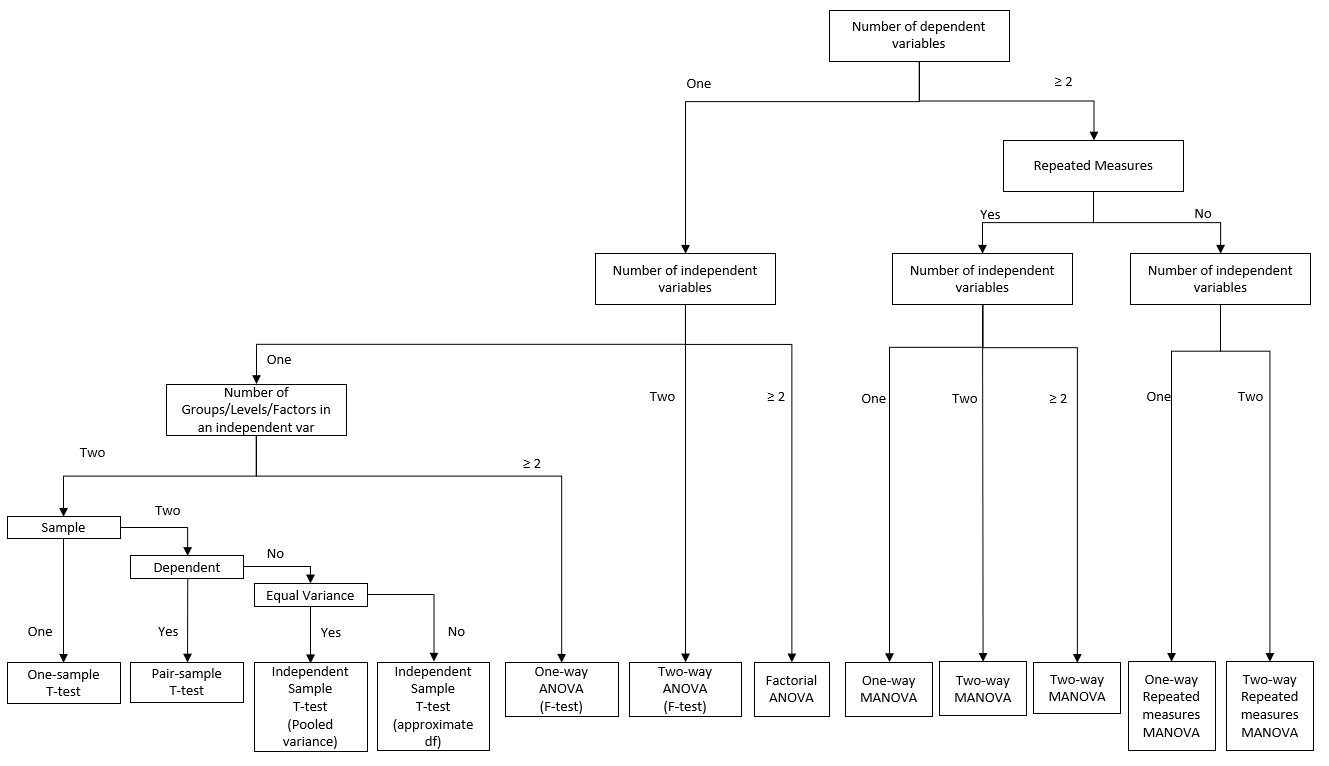
\includegraphics[width=0.9\linewidth,alt={Flow chart depicting a decision tree for statistical test selection based on the number of dependent and independent variables. It starts with the number of dependent variables, branching into one or more. For one dependent variable, it further divides based on the number of independent variables, leading to tests like One-sample T-test, Pair-sample T-test, and ANOVA variations. For two or more dependent variables, it considers whether dependent variables are repeated measures, leading to MANOVA or repeated measures MANOVA. The chart guides the selection of appropriate statistical tests.}]{images/MANOVA_summary} 

}

\caption{Decision tree for selecting an appropriate statistical test for comparing means, based on the number of dependent and independent variables.}\label{fig:manova-decision-tree}
\end{figure}

\part*{B. QUASI-EXPERIMENTAL DESIGN}\label{part-b.-quasi-experimental-design}
\addcontentsline{toc}{part}{B. QUASI-EXPERIMENTAL DESIGN}

Quasi-experimental methods bridge the gap between fully randomized experiments (covered in Part A) and purely observational analysis. When true randomization is infeasible, unethical, or too expensive, researchers exploit naturally occurring, plausibly exogenous variation in treatment assignment to approximate the credibility of an experiment.

\section{What makes a study ``quasi-experimental''?}\label{what-makes-a-study-quasi-experimental}

In a randomized controlled trial, random assignment guarantees (in expectation) that treated and control groups are comparable on both observed and unobserved characteristics. In a quasi-experiment, we substitute \emph{design} for randomization. We focus on units just above and below an assignment cutoff, track shared trends across groups over time, construct weighted counterfactuals from untreated units, or use an outside source of variation that shifts treatment without affecting outcomes directly.

The price of giving up randomization is a set of identifying assumptions: continuity, parallel trends, independence, monotonicity, conditional ignorability. Each method in this part makes a different assumption, and each chapter spells out what that assumption means, when it is plausible, and how to probe it.

\section{Chapter roadmap and ordering}\label{chapter-roadmap-and-ordering}

The chapters in this part are sequenced by \emph{design credibility}, moving from the most credible identification strategies (those that most closely mimic randomization) to those that rely on stronger, harder-to-verify assumptions. Readers who proceed linearly will encounter increasingly demanding assumptions.

\begin{itemize}
\tightlist
\item
  \hyperref[sec-quasi-experimental]{Quasi-Experimental Methods} establishes the foundations: SUTVA, conditional ignorability, overlap, and the logic of natural experiments.
\item
  \hyperref[sec-regression-discontinuity]{Regression Discontinuity} covers local randomization at a known cutoff. This is typically the most credible design when a sharp assignment rule exists.
\item
  \hyperref[sec-temporal-discontinuity-designs]{Temporal Discontinuity Designs} covers Regression Discontinuity in Time and Interrupted Time Series. These are the sharp and segmented variants where the running variable is time.
\item
  \hyperref[sec-synthetic-difference-in-differences]{Synthetic Difference-in-Differences} is introduced \emph{before} standard DiD because SDID is typically the most robust panel-data estimator. It combines the reweighting logic of Synthetic Control with the differencing logic of DiD, and performs well whenever \emph{either} method's assumptions hold. Readers unfamiliar with DiD or SC should skim those chapters first and return.
\item
  \hyperref[sec-difference-in-differences]{Difference-in-Differences}, together with its extensions on \hyperref[sec-modern-estimators-for-staggered-adoption]{staggered adoption}, \hyperref[sec-panel-match-did-estimator-with-in-and-out-treatment-conditions]{panel-match variants}, \hyperref[sec-nonlinear-did]{non-linear DiD}, and \hyperref[sec-modern-concerns-in-did]{modern concerns}, is the workhorse panel estimator. Parallel trends is the central assumption and must be defended with care.
\item
  \hyperref[sec-changes-in-changes]{Changes-in-Changes} is a quantile-level extension of DiD. Use it when the policy effect is likely heterogeneous across the outcome distribution.
\item
  \hyperref[sec-synthetic-control]{Synthetic Control} covers settings with one (or a few) treated units and a donor pool. It relies on the treated unit sitting inside the convex hull of donor pre-treatment characteristics.
\item
  \hyperref[sec-event-studies]{Event Studies} is a visualization and estimation framework layered on top of DiD, RD, or IV. Event-study output is \emph{descriptive} unless the surrounding design establishes a causal channel.
\item
  \hyperref[sec-instrumental-variables]{Instrumental Variables}, plus the \hyperref[sec-examiner-design]{Decision-Maker IV / examiner design} and proxy variables. When treatment is endogenous, IV provides a way out, but only for a specific subpopulation (compliers) and only if the exclusion restriction holds.
\item
  \hyperref[sec-matching-methods]{Matching Methods} relies on selection on observables. It rests on the weakest identification assumption of the part, since unconfoundedness is untestable, so matching is often best used as a preprocessing step before one of the methods above.
\end{itemize}

\section{Common themes}\label{common-themes}

Across these chapters you will see the same conceptual moves repeated.

First, we rely on potential outcomes throughout. We write \(Y_i(d)\) for the outcome of unit \(i\) under treatment status \(d \in \{0, 1\}\). Panel variants add a time subscript: \(Y_{it}(d)\). Treatment is indicated by \(D_i\) or \(D_{it}\). Instruments and running variables are denoted \(Z_i\) and \(X_i\) where the context makes the role clear.

Second, each method rests on a single untestable assumption that does the heavy lifting: continuity, parallel trends, exclusion, or unconfoundedness. Pre-trend tests, placebo tests, and sensitivity analyses only \emph{support} the assumption. They never prove it.

Third, the estimand is specific. RD estimates a LATE at the cutoff. DiD estimates an ATT on the treated. IV under monotonicity estimates a LATE for compliers. Matching can estimate ATT or ATE depending on how the match is set up. Be precise about what you are identifying.

Fourth, the threats are the same family in different clothing. Selection, anticipation, manipulation, heterogeneity, weak first stages, poor overlap. These recur across chapters under different names, and so do the remedies (robustness checks, honest bounds, sensitivity analyses).

\section{How to use this part}\label{how-to-use-this-part}

Readers new to causal inference should read the \hyperref[sec-quasi-experimental]{foundations chapter} first, then proceed in order. If you hit SDID without DiD or SC background, skim the \hyperref[sec-simple-difference-in-differences]{Simple DiD} section and \hyperref[sec-synthetic-control]{Synthetic Control} first, then return.

Practitioners with a specific question can jump to the relevant chapter. Each chapter is designed to be self-contained, with assumptions and estimation strategy spelled out up front.

Reviewers or editors of quasi-experimental work should focus on the \hyperref[sec-modern-concerns-in-did]{modern concerns in DiD} section and the threats-to-validity subsections throughout. These catalog the standard objections to each design.

A compact decision table is provided at the end of the \hyperref[sec-quasi-experimental]{foundations chapter} to help match a given research setting to one of the methods introduced here.

\chapter{Quasi-Experimental Methods}\label{sec-quasi-experimental}

Randomized experiments are the gold standard for causal inference. In most settings that matter to applied researchers (evaluating a national policy, a marketing campaign, a regulatory ruling, or a sweeping organizational change), running an experiment is impractical, unethical, or politically impossible. You cannot randomly assign tax rates to households, lockdowns to countries, or layoffs to factories. The methods in this part of the book exist because the world keeps refusing to cooperate with our preferred research design.

Quasi-experimental methods accept that constraint and ask a more modest question: when nature, history, or institutions hand us variation that \emph{resembles} random assignment, can we recover something close to a causal effect? The answer is a qualified yes. Building on the experimental design foundations from the previous part, we will examine strategies that use observational data (typically with pre- and post-intervention measurements) and exploit naturally occurring, plausibly exogenous variation that mimics random assignment. The payoff is the ability to study real, large-scale interventions in realistic settings. The cost is a set of identifying assumptions that must be argued for rather than designed in, and a more cautious story about what the estimate generalizes to.

A few considerations should shape how you read every chapter that follows:

The first is \textbf{representativeness}. A quasi-experiment exploits a particular setting: a particular state's policy, a particular firm's reorganization, a particular cohort's eligibility window. The estimate is, in the first instance, an answer for that setting. Whether and how it extrapolates to other contexts is a separate question, and one that researchers often gloss over.

The second is the \hyperref[sec-limitations-of-quasi-experiments]{\textbf{limitations of the design}}. Each method rests on an identifying assumption that cannot be tested directly: parallel trends, continuity, exclusion, unconfoundedness. Pre-trend tests, placebo tests, and sensitivity analyses can make the assumption \emph{more} plausible, but they cannot prove it. A useful habit when reading quasi-experimental work is to ask: \emph{if this estimate were biased, what would have to be true?}

The third is \textbf{integration with structural models}. A reduced-form quasi-experimental estimate tells you that an intervention had some effect on average, in a particular setting. It does not, by itself, tell you why, through what mechanism, or what would happen under a counterfactual policy that was not actually implemented. Combining quasi-experimental estimates with structural or theoretical models (calibrating a model to match a credible reduced-form moment, for instance) is one of the most fertile directions in modern empirical research; \citet{anderson2015growth}, \citet{einav2010beyond}, and \citet{chung2014bonuses} are useful examples to read alongside this chapter.

These tools are now central to applied research across economics, marketing, political science, public health, and increasingly to internal data science teams at large firms. The conceptual machinery is the same in every domain. The art is in matching it to the right setting.

\begin{center}\rule{0.5\linewidth}{0.5pt}\end{center}

\section{Identification Strategy in Quasi-Experiments}\label{identification-strategy-in-quasi-experiments}

Quasi-experiments lack the formal statistical proof of causality that randomization buys you. Random assignment makes the comparability of treated and untreated groups a property of the design itself; once you give up randomization, comparability has to be argued for, not assumed. The credibility of the study ultimately rests on whether the reader is persuaded that the variation being exploited is genuinely as good as random, given the assumed controls. The reader is allowed to remain skeptical, and a good study anticipates that skepticism.

A defensible identification strategy almost always rests on three pillars. The first is a story about \emph{where} the exogenous variation comes from, what feature of the world made some units treated and others not, in a way the units themselves did not engineer. The second is an argument that the variation affects the outcome only through the proposed channel, so we are not picking up some other consequence of the same shock. The third is a check that one unit's treatment does not contaminate another's outcome, since causal inference at the unit level breaks down when treatments leak across units.

\begin{enumerate}
\def\labelenumi{\arabic{enumi}.}
\tightlist
\item
  Sources of Exogenous Variation. Where does the variation come from, and why is it plausibly unrelated to unobserved determinants of the outcome? This pillar lives or dies on institutional knowledge: a policy that was passed for reasons unrelated to the outcome, a lottery, a discontinuous eligibility rule, an unexpected weather shock, an administrative quirk. The author has to know the setting well enough to tell a believable story, and that story has to survive contact with reasonable counter-stories.
\item
  Exclusion Restriction. Even if the variation is exogenous, it might affect the outcome through more than one channel. The exclusion restriction is the claim that the variation reaches the outcome \emph{only} through the treatment of interest. Ruling out alternative channels usually requires a combination of theory, falsification tests on placebo outcomes, and careful institutional argument.
\item
  \hyperref[sec-sutva]{Stable Unit Treatment Value Assumption (SUTVA)}. Unit \(i\)'s outcome depends only on unit \(i\)'s treatment, not on the treatment of other units. Spillovers, peer effects, and equilibrium responses all violate this. SUTVA shows up explicitly in the \hyperref[sec-sutva]{next section}, but it lurks in every design.
\end{enumerate}

Every quasi-experimental method also involves a tradeoff between \emph{statistical power} and \emph{support for the exogeneity assumption}. The cleaner the source of variation, the narrower the slice of data that uses it: a \hyperref[sec-regression-discontinuity]{Regression Discontinuity} design discards observations far from the cutoff, an \hyperref[sec-instrumental-variables]{Instrumental Variables} design throws away variation in the treatment that is not driven by the instrument, a \hyperref[sec-difference-in-differences]{Difference-in-Differences} design ignores levels and reads only off differences. You buy credibility by burning information. A study that uses the entire sample and claims a clean causal effect is, more often than not, leaning on assumptions it has not stated.

\subsection{Practical Notes on Inference}\label{practical-notes-on-inference}

A handful of practical points recur across nearly every chapter that follows. Each is a small detail with a large downstream effect, and each is the kind of point that referees flag too late. The list below is not exhaustive, and additional considerations specific to particular designs will surface as we move through each method.

\begin{itemize}
\item
  \(R^2\) is not a measure of causal credibility. A regression with an \(R^2\) of 0.9 can be hopelessly biased, and a regression with an \(R^2\) of 0.05 can identify a clean causal effect. What matters is whether the variation in the regressor is exogenous, not how much of the outcome's variance the model explains. \citet{ebbes2011sense} is the canonical warning. Reviewers occasionally ask for higher \(R^2\); this is the wrong demand.
\item
  Clustering of standard errors is a design question, not a fishing expedition. The unit at which you cluster should reflect the level at which treatment was assigned, or the level at which observations are plausibly correlated by virtue of design. It should not be chosen to produce a more comfortable \(p\)-value. \citet{abadie2023should} make the design-based case rigorous and is required reading before you cluster anything.
\item
  In small samples, the cluster-robust variance estimator is biased downward, and the wild bootstrap is the standard correction \citep{cameron2008bootstrap, cai2022implementation}. ``Small'' here can mean fewer than 30 or so clusters, which is uncomfortably common in state-level policy studies. Use the wild bootstrap by default in such settings rather than waiting until it is requested.
\item
  Pre-specify outcomes, controls, and subgroups whenever possible. Quasi-experimental designs cannot be re-randomized, but they can be re-analyzed many times across many specifications, and the analyst's choices are not invisible to the resulting \(p\)-values. A pre-analysis plan, even an informal one written before looking at outcomes, is the cheapest defense against accidental specification searching, and it is what separates a credible exploratory analysis from one that has been quietly tuned for significance.
\item
  Report effect sizes, not just \(p\)-values. Statistical significance and economic significance are not the same thing, and a tiny effect estimated very precisely can be statistically significant without being practically interesting. Always present point estimates with confidence intervals in the units of the outcome (or as a percentage of a baseline mean), so that a reader can judge magnitude rather than only direction.
\item
  Beware \hyperref[sec-controls]{bad controls}. Adding ``more controls'' is not always a defensive move. Conditioning on a variable that is itself caused by treatment, on a collider, or on a mediator can introduce bias rather than remove it. The DAG-driven discipline is to derive the adjustment set from a candidate causal structure and resist the urge to add covariates outside it.
\end{itemize}

\begin{center}\rule{0.5\linewidth}{0.5pt}\end{center}

\section{Establishing Mechanisms}\label{establishing-mechanisms}

Identifying a causal effect is the start of an empirical project, not the end. Knowing that a job training program raises earnings on average is useful, but it leaves the harder questions open: did earnings rise because participants gained marketable skills, because the program signaled effort to employers, because it nudged people into denser labor markets, or because of some combination of all three? Did the effect concentrate among workers who would have struggled most without the program, or among those who needed it least? An estimate without a mechanism is hard to extrapolate, hard to improve on, and hard to defend in the policy conversation that usually follows.

The two most common mechanism-oriented questions are \emph{how} the treatment works and \emph{for whom} it works. The first is the territory of \hyperref[sec-mediation-analysis-explaining-the-causal-pathway]{\textbf{mediation analysis}}, which decomposes a total effect into the part that flows through some intermediate variable and the part that does not. The second is the territory of \hyperref[sec-moderation-analysis-for-whom-or-under-what-conditions]{\textbf{moderation analysis}}, which asks whether the treatment's effect is uniform across subgroups or whether it concentrates somewhere identifiable. Both have their uses, and both are easy to misread. The remainder of this section walks through what each can deliver and where each tends to break down.

\begin{center}\rule{0.5\linewidth}{0.5pt}\end{center}

\subsection{Mediation Analysis: Explaining the Causal Pathway}\label{sec-mediation-analysis-explaining-the-causal-pathway}

Mediation analysis tries to open the black box between treatment and outcome. Concretely, it asks whether the effect of a treatment \(T\) on an outcome \(Y\) travels through some intermediate variable \(M\), called the \emph{mediator}. The total effect is then decomposed into a \textbf{direct effect} that flows from \(T\) to \(Y\) without going through \(M\), and an \textbf{indirect effect} that flows \(T \to M \to Y\). Letting

\begin{itemize}
\tightlist
\item
  \(T\) = treatment,
\item
  \(M\) = mediator,
\item
  \(Y\) = outcome,
\end{itemize}

the conceptual decomposition is

\[
\underbrace{\text{Total effect of } T \text{ on } Y}_{T \to Y} \;=\; \underbrace{\text{Direct effect}}_{T \to Y \text{ not through } M} \;+\; \underbrace{\text{Indirect effect}}_{T \to M \to Y}.
\]

The decomposition looks innocent. The identification problem is anything but. To interpret either piece causally, you need \emph{two} layers of as-good-as-random variation: one that delivers exogenous variation in \(T\), and another that delivers exogenous variation in \(M\) given \(T\). The standard formal version of this is \textbf{sequential ignorability}: treatment is as good as random unconditionally (or conditional on baseline covariates), \emph{and} the mediator is as good as random conditional on treatment and covariates \citep{imai2010general}. The second part is the demanding one. In most observational studies, the same forces that drive \(M\) also drive \(Y\), so any estimated indirect effect is contaminated by \textbf{mediator-outcome confounding}.

Several estimation strategies are common, listed below in increasing order of the assumptions they require you to defend.

The first is the \textbf{causal mediation framework of \citet{imai2010general}}, which provides nonparametric estimators of the average direct and indirect effects under sequential ignorability. The headline benefit is that you do not need to commit to a particular functional form. The headline cost is that the assumption is untestable, so the framework is most useful when paired with a sensitivity analysis showing how strong unobserved mediator-outcome confounding would have to be to overturn the conclusion.

The second is the \textbf{two-stage regression approach}, which fits the mediator and outcome equations sequentially:

\[
\begin{aligned}
M_i &= \alpha + \tau\, T_i + \varepsilon_i, \\
Y_i &= \beta + \gamma\, T_i + \delta\, M_i + \eta_i.
\end{aligned}
\]

The product \(\tau \cdot \delta\) is read as the indirect effect, and \(\gamma\) as the direct effect. This is the ``Baron-Kenny'' tradition. It is fast, transparent, and biased whenever \(M_i\) is correlated with \(\eta_i\), that is, whenever there is unobserved mediator-outcome confounding. Treat the two-stage regression as a first-pass description, not a causal decomposition.

The third is \textbf{instrumental-variable mediation}, in which an instrument is found that affects \(Y\) only through \(M\) (after \(T\) is accounted for). Done right, this gives a credible LATE on the mediated channel. Done wrong, and it is easy to do wrong, it gives a confidently estimated artifact. The main difficulty is finding an instrument for \(M\) that is not also an instrument for \(T\) via some other route.

Mediation questions show up everywhere. In marketing: does an ad raise sales because it lifted brand awareness, or for some other reason? In education: does a tutoring program raise test scores by improving attendance, by raising motivation, or by signaling parental involvement? In labor economics: does job training raise wages because it built skills, because it shifted workers into better matches, or because of stigma effects on the control group?

\begin{quote}
Caution. Mediation analysis is one of the most overused tools in applied empirical work. The math goes through; the identification rarely does. If your study did not randomize the mediator, treat any decomposition you produce as descriptive, report a sensitivity analysis, and pair the analysis with theoretical argument. A clean total effect with an honest mechanism story usually persuades more than a precise but heroic decomposition.
\end{quote}

\begin{center}\rule{0.5\linewidth}{0.5pt}\end{center}

\subsection{Moderation Analysis: For Whom or Under What Conditions?}\label{sec-moderation-analysis-for-whom-or-under-what-conditions}

Where mediation asks \emph{how} a treatment works, moderation asks \emph{when} it works and \emph{for whom}. The same intervention can lift outcomes substantially in one subgroup and barely move the needle in another, and an average effect that pools across subgroups can hide that heterogeneity completely. Moderation analysis is the toolkit for surfacing it.

The questions that drive moderation are concrete: do effects differ by gender, income, region, or baseline outcome status? Is the program more effective for high-need participants, or for early adopters who would have done well anyway? Does the treatment work in dense urban labor markets but not thin rural ones? An honest moderation analysis is what separates a finding that ``the program raised earnings by 4\%'' from a finding that ``the program raised earnings by 12\% among workers with prior unemployment spells and had no detectable effect on others'', two very different policy conclusions from the same dataset.

Several estimation strategies dominate practice. \textbf{Subgroup analysis} simply re-estimates the effect separately within each subgroup and compares the resulting estimates. It is transparent, easy to explain, and risks two mistakes: comparing noisy estimates as if they were precise, and slicing the data into so many subgroups that some ``significant'' difference is bound to appear by chance. Pre-specifying subgroups and correcting for multiple testing (see the natural-experiments section below) is the standard discipline.

\textbf{Interaction models} put the moderator inside a single regression by including a treatment-by-moderator interaction:

\[
Y_{it} = \alpha + \beta_1 T_{it} + \beta_2 Z_i + \beta_3 (T_{it} \times Z_i) + \varepsilon_{it},
\]

where \(Z_i\) is the moderator (e.g., a high-income indicator). The coefficient \(\beta_3\) is the difference in the treatment effect between the two groups, and \(\beta_1\) is the effect for the reference group. The most common error here is reading \(\beta_1\) as ``the treatment effect'', it is the treatment effect \emph{only} when \(Z_i = 0\). Always interpret main effects and interactions jointly, and plot the implied marginal effects across the relevant range of \(Z_i\).

\textbf{Difference-in-Differences with moderation} scales this up to a panel setting, using a three-way interaction:

\[
Y_{it} = \alpha + \beta_1 \text{Post}_t + \beta_2 \text{Treat}_i + \beta_3 Z_i + \beta_4 (\text{Post}_t \times \text{Treat}_i) + \beta_5 (\text{Post}_t \times \text{Treat}_i \times Z_i) + \varepsilon_{it}.
\]

Now \(\beta_4\) is the DiD effect for the reference moderator group and \(\beta_5\) is the \emph{difference in DiDs} between groups. As before, the parallel-trends assumption applies separately within each value of \(Z_i\), a moderation analysis can collapse if pre-trends differed across the subgroups even before treatment was introduced.

For all three strategies, \textbf{visualization is not optional}. A marginal-effects plot showing the treatment effect across values of \(Z_i\), with confidence bands, communicates moderation more honestly than any table of regression coefficients. Interaction plots, separate regression lines by group, make subgroup heterogeneity legible at a glance. Tabulating only \(\beta_5\) and its \(p\)-value will mislead any reader who has not already done the same analysis themselves.

Table \ref{tab:quasi-exp-mech-approach} summarizes the goals, key assumptions, and common pitfalls of the three mechanism-analysis approaches discussed above (mediation, subgroup analysis, and interaction terms), so that the right tool can be matched to the question at hand.

\begin{longtable}[]{@{}
  >{\raggedright\arraybackslash}p{(\linewidth - 6\tabcolsep) * \real{0.1310}}
  >{\raggedright\arraybackslash}p{(\linewidth - 6\tabcolsep) * \real{0.2276}}
  >{\raggedright\arraybackslash}p{(\linewidth - 6\tabcolsep) * \real{0.3379}}
  >{\raggedright\arraybackslash}p{(\linewidth - 6\tabcolsep) * \real{0.3034}}@{}}
\caption{\label{tab:quasi-exp-mech-approach} Mechanism-analysis approaches.}\tabularnewline
\toprule\noalign{}
\begin{minipage}[b]{\linewidth}\raggedright
\textbf{Approach}
\end{minipage} & \begin{minipage}[b]{\linewidth}\raggedright
\textbf{Goal}
\end{minipage} & \begin{minipage}[b]{\linewidth}\raggedright
\textbf{Key Assumptions}
\end{minipage} & \begin{minipage}[b]{\linewidth}\raggedright
\textbf{Common Pitfalls}
\end{minipage} \\
\midrule\noalign{}
\endfirsthead
\toprule\noalign{}
\begin{minipage}[b]{\linewidth}\raggedright
\textbf{Approach}
\end{minipage} & \begin{minipage}[b]{\linewidth}\raggedright
\textbf{Goal}
\end{minipage} & \begin{minipage}[b]{\linewidth}\raggedright
\textbf{Key Assumptions}
\end{minipage} & \begin{minipage}[b]{\linewidth}\raggedright
\textbf{Common Pitfalls}
\end{minipage} \\
\midrule\noalign{}
\endhead
\bottomrule\noalign{}
\endlastfoot
Mediation & Identify intermediate variables & Sequential ignorability, no omitted confounders & Mediators may be endogenous \\
Subgroup Analysis & Estimate effects by group & Sufficient sample size, balanced covariates & Spurious differences due to imbalance \\
Interaction Terms & Estimate conditional effects & Correct model specification & Misinterpretation of non-significant terms \\
\end{longtable}

\begin{center}\rule{0.5\linewidth}{0.5pt}\end{center}

Mediation and moderation are complementary bridges between empirical estimates and theory. Mediation connects estimates to \emph{process theories}, accounts of how a treatment brings about change, while moderation connects estimates to \emph{contingency theories}, accounts of when and for whom a treatment works. A complete empirical paper rarely has room for both, but a clear sense of which one your study is really speaking to keeps the framing honest. In applied business research, the practical payoff is direct: mediation guides product and intervention design (which channels do we need to invest in to get the effect?), while moderation guides targeting and personalization (which customers should we focus on?). A retention experiment, for instance, might use mediation to show that customer satisfaction is the channel through which a loyalty program lifts renewal rates, and use moderation to show that the lift is concentrated among newer customers rather than long-tenured ones. The two findings together imply an actionable strategy that neither would deliver on its own.

\begin{center}\rule{0.5\linewidth}{0.5pt}\end{center}

\section{Robustness Checks}\label{sec-robustness-checks-quasi-exp}

A robustness check earns its name when it could plausibly \emph{overturn} the result. Most published robustness sections do not pass that bar, they tweak a control set or a sample window in ways that would never have moved the headline estimate, and they call the unchanged number ``robust''. A useful robustness program does the opposite: it asks how the estimate would have to behave if the identifying assumption were wrong, then it tries to find that behavior in the data.

\citet{goldfarb2022conducting} offer a well-organized review of the practice in marketing and management; the checks below collect the most common ones. Treat them as a menu, not a checklist, applying every check to every study is overkill, and applying none to any study is malpractice.

The first family is \textbf{alternative control sets}. Run the regression with no controls, with the baseline controls, and with the kitchen-sink set. If the estimate moves substantially when you add a particular covariate, that covariate is doing real work and you owe the reader an explanation of why it is or is not part of the right specification. The discipline here links closely to \hyperref[sec-coefficient-stability-bounds]{coefficient-stability bounds} and to \hyperref[sec-rosenbaum-bounds]{Rosenbaum bounds} \citep{altonji2005selection}: both formalize the question of how much unobserved confounding would be needed to overturn your conclusion, expressed in units of the observed confounders. If ``twice as much confounding as everything I observed combined'' is enough to kill the result, the result is fragile. Marketing applications include \citet{manchanda2015social} and \citet{shin2012fire}. A complementary discipline, covered in the \hyperref[sec-controls]{bad controls} chapter, is to make sure that the kitchen-sink set is not actually introducing bias by conditioning on colliders or post-treatment variables, an \hyperref[sec-overcontrol-bias]{overcontrol-bias} problem that can flip the sign of the estimate.

The second is \textbf{different functional forms}. If your conclusion depends on a particular linear or log specification, the worry is that you have absorbed a nonlinear pattern into the treatment coefficient. Re-estimate with non-linear, semi-parametric, or fully flexible specifications and check whether the sign and magnitude survive. When they do, the simpler specification is supported. When they do not, the sensitivity itself is informative. In \hyperref[sec-regression-discontinuity]{RD} designs in particular, varying the polynomial order of the running-variable control is the standard form of this check.

The third is \textbf{varying time windows} in longitudinal settings. Did the effect appear because of one unusual year? Does it depend on including or excluding the recession, the election, the supply-chain disruption? Trim the panel from each end and re-estimate. Designs that read off a single ``interesting'' year tend not to replicate. In \hyperref[sec-difference-in-differences]{Difference-in-Differences} the natural extension of this check is to vary the pre- and post-treatment window length, and in \hyperref[sec-interrupted-time-series]{Interrupted Time Series} it is to vary the bandwidth of the segments around the intervention date.

The fourth is \textbf{alternative dependent variables}. Most theoretical mechanisms make predictions about more than one outcome. If your story is right, related outcomes should move in predictable directions; outcomes that the mechanism does not touch should not move at all. The latter, \emph{placebo outcomes} (or \emph{falsification outcomes}), is the more powerful test. A treatment that ``works'' on placebo outcomes is a treatment whose mechanism has been mis-specified, or whose identifying assumption has been violated.

The fifth is \textbf{varying the control group composition}, especially in matching or quasi-experimental designs that select an untreated comparison group. Compare results across raw, matched, and trimmed samples, across \hyperref[sec-matching-methods]{different matching algorithms} (propensity-score matching, \hyperref[sec-mahalanobis]{Mahalanobis}, \hyperref[sec-cem]{coarsened exact matching}, \hyperref[sec-genetic-matching]{genetic matching}), and across plausible donor pools in a \hyperref[sec-synthetic-control]{Synthetic Control} setting. Estimates that swing wildly with reasonable changes to the comparison group are not estimating a stable parameter, and the resulting heterogeneity is often more informative about the design than the headline number itself.

The sixth is \textbf{placebo tests} of the design itself. The right placebo depends on the method: a fake treatment date in \hyperref[sec-placebo-test-did]{DiD}, a fake cutoff in \hyperref[sec-regression-discontinuity]{RD}, a fake instrument in \hyperref[sec-instrumental-variables]{IV}, an event window in a year with no event in an \hyperref[sec-event-studies]{event study}. Each subsequent chapter spells out the canonical placebo for the method it covers. A study with no placebo test is one that has not asked itself whether the design could detect a non-effect.

Two further checks deserve mention because they cut across designs. \textbf{Pre-trend visualizations} (\hyperref[sec-visualization-did]{visualizing parallel trends} in DiD, density tests like \hyperref[sec-mccrary-sorting-test]{McCrary's} at an RD cutoff, leads in an event study) reveal whether the identifying assumption was already failing before treatment. And in panel designs with staggered adoption, the \hyperref[sec-modern-estimators-for-staggered-adoption]{modern estimators for staggered DiD} and the diagnostics in \hyperref[sec-modern-concerns-in-did]{modern concerns in DiD}, including the \hyperref[sec-goodman-bacon-decomposition]{Goodman-Bacon decomposition} and partial-identification approaches like \hyperref[sec-relative-magnitude-restriction-honestdid]{HonestDiD}, serve as built-in robustness checks against the negative-weighting pathologies of the standard \hyperref[sec-two-way-fixed-effects]{two-way fixed effects} estimator.

A practical rule of thumb: present robustness graphically wherever possible, and put the \emph{most threatening} check, the one that would make a smart skeptic uncomfortable, at the front of the table, not buried in the appendix. Transparency about weakness is, paradoxically, the strongest defense of a credible design.

\begin{center}\rule{0.5\linewidth}{0.5pt}\end{center}

\section{Limitations of Quasi-Experiments}\label{sec-limitations-of-quasi-experiments}

Quasi-experimental methods are powerful, but their power comes with strings attached. Because identification rests on observational variation and not on a researcher-controlled assignment mechanism, the assumptions doing the heavy lifting are more stringent, less testable, and easier to violate than the corresponding assumptions in a randomized trial. A serious quasi-experimental paper does not merely state its identifying assumption; it stress-tests it and reports what it found, even when the news is uncomfortable.

The remainder of this section organizes the standard limitations around four questions that researchers and critical readers should both keep in front of them: what is being assumed, what threats could undermine the result, how those threats can be probed, and what the resulting estimate generalizes to. The questions stack: a study that cannot answer the first has no business attempting the others.

\begin{center}\rule{0.5\linewidth}{0.5pt}\end{center}

\subsection{Identifying Assumptions}\label{identifying-assumptions-1}

Every quasi-experimental method substitutes a specific identifying assumption for randomization. The shape of that assumption changes from method to method, but its function is always the same: to license a counterfactual comparison that the data alone cannot deliver.

\hyperref[sec-difference-in-differences]{Difference-in-Differences} rests on \textbf{parallel trends}: in the absence of treatment, the treated and control groups would have followed the same outcome trajectory. The assumption is unverifiable by definition, we never observe the treated group's untreated outcome after treatment, but it can be made more or less plausible by the pre-treatment data.

\hyperref[sec-regression-discontinuity]{Regression Discontinuity} rests on \textbf{continuity at the cutoff}: units just above and just below the threshold differ only in their treatment status, not in unobserved characteristics. The credibility of this assumption hinges on whether agents could precisely manipulate their position relative to the cutoff.

\hyperref[sec-instrumental-variables]{Instrumental Variables} require \textbf{exogeneity} and \textbf{exclusion}: the instrument is unrelated to unobserved determinants of the outcome, and affects the outcome only through the treatment of interest. Of all the assumptions in this part, the exclusion restriction is the one most likely to be quietly violated, because there are usually many channels through which a shock can travel.

The best practice across all three is the same: visual diagnostics, historical evidence, and pre-trend analyses make the assumption \emph{more} plausible; nothing makes it \emph{certain}.

\begin{center}\rule{0.5\linewidth}{0.5pt}\end{center}

\subsection{Threats to Validity}\label{threats-to-validity}

Even when the identifying assumption is well-stated, the design can fail through any of a small number of standard threats. Each is worth recognizing on sight.

\textbf{Unobserved confounding} is the umbrella worry: variables that drive both treatment and outcome are not in the model, and the estimated effect picks up their contribution. This is the canonical \hyperref[sec-omitted-variable-bias]{omitted-variable-bias} problem, sometimes called \hyperref[sec-selection-on-unobservables]{selection on unobservables} when the unobserved factor is what drives selection into treatment. It is most acute in pure cross-sectional designs and in any setting where the assignment mechanism is ill-understood.

\textbf{Violation of \hyperref[sec-sutva]{SUTVA}} through \hyperref[sec-no-interference]{spillovers}, interference between units, or \hyperref[sec-no-hidden-variations-in-treatment]{hidden treatment heterogeneity} makes potential outcomes ill-defined. A vaccination program, for example, lowers infection risk for the unvaccinated; an advertising campaign reaches consumers through word of mouth; a job training program shifts the labor market for the untrained. In each case, the ``control'' group has not actually been left alone.

\textbf{Anticipation effects and pre-treatment trends} corrupt the counterfactual: if treated units adjust their behavior before treatment is implemented (because they expect it), or if the treated and control series were already diverging for unrelated reasons, the post-treatment comparison conflates the treatment effect with whatever was driving the pre-period divergence. In a \hyperref[sec-difference-in-differences]{DiD} framework, this is exactly the failure of \hyperref[sec-visualization-did]{parallel trends}; in an \hyperref[sec-event-studies]{event study}, it manifests as non-zero pre-event coefficients.

\textbf{Measurement error}, especially in the assignment variable, attenuates effects in \hyperref[sec-regression-discontinuity]{regression-discontinuity designs} and biases the discontinuity estimate. The general theory of \hyperref[sec-classical-measurement-error]{classical} and \hyperref[sec-non-classical-measurement-error]{non-classical measurement error} is covered in the \hyperref[sec-measurement-error]{measurement-error chapter}. In \hyperref[sec-instrumental-variables]{IV} settings, measurement error in the instrument exacerbates the \hyperref[sec-weak-instruments-problem]{weak-instrument problem}.

\textbf{Manipulation or sorting around a cutoff} undermines the quasi-randomness that an RD design depends on; the dedicated discussion lives in \hyperref[sec-sorting-bunching-and-manipulation]{sorting, bunching, and manipulation}, and the standard formal diagnostic is the \hyperref[sec-mccrary-sorting-test]{McCrary density test}. If applicants can nudge their score from 79 to 81, a study that compares applicants on either side of an 80 cutoff is no longer comparing as-good-as-random units, and one common response is to switch to a \hyperref[sec-fuzzy-regression-discontinuity-design]{fuzzy RD} that does not assume sharp compliance with the cutoff rule.

\textbf{Limited \hyperref[sec-overlap-positivity-assumption]{overlap}} quietly restricts what the design identifies. Some IV studies estimate effects only on compliers; some \hyperref[sec-matching-methods]{matching} studies on the small subpopulation where treated and control units share covariate values; some RD studies on the narrow band near the cutoff. The estimate is what the design supports, not what the policy debate would prefer.

The right discipline is to walk the reader through each threat, explain \emph{why} it is or is not a concern in your setting, and (where possible) report the test or diagnostic that backs up the explanation.

\begin{center}\rule{0.5\linewidth}{0.5pt}\end{center}

\subsection{Addressing Threats to Validity}\label{addressing-threats-to-validity}

Robustness and sensitivity checks (covered in the \hyperref[sec-robustness-checks-quasi-exp]{previous section}) are how you make threats concrete instead of rhetorical. The most commonly useful are \hyperref[sec-placebo-test-did]{placebo tests} on periods or groups where no treatment occurred, falsification outcomes that the treatment should not affect, \hyperref[sec-visualization-did]{pre-trend diagnostics for DiD}, bandwidth and polynomial sensitivity for \hyperref[sec-regression-discontinuity]{RD}, alternative specifications across the modeling choices that a reader might second-guess, and heterogeneity analysis that surfaces where the identifying assumption is most vulnerable.

A graphical robustness plot, coefficient estimates across, say, twenty plausible specifications, communicates more than a paragraph of prose ever will. Transparency about which checks were tried, including the ones that did not flatter the headline result, is what distinguishes a credible study from a tidy one.

\begin{center}\rule{0.5\linewidth}{0.5pt}\end{center}

\subsection{External Validity and Future Research}\label{external-validity-and-future-research}

Even a clean estimate is, in the first instance, an answer for a particular sample, a particular setting, and a particular slice of the population the design happens to identify. Several concerns about external validity recur across the chapters that follow. Table \ref{tab:quasi-exp-examples-limitation} catalogs the most common threats by design family, alongside a representative diagnostic and the standard remedy or check, so that a reader confronting any one of these methods has a quick map of what to look for.

The first is the \textbf{scope of identification}: many designs deliver a Local Average Treatment Effect rather than the population ATE (see the \hyperref[sec-notation-quasi-experimental]{estimand glossary} for the formal definitions). A \hyperref[sec-examiner-design]{judge-IV / examiner-design} study identifies effects only for marginal defendants; an \hyperref[sec-regression-discontinuity]{RD} identifies effects only at the cutoff; a \hyperref[sec-difference-in-differences]{DiD} identifies the ATT on the treated. These are not bugs, they are the price of credibility, but they should be reported as the estimand, not relabeled as ``the'' effect.

The second is \textbf{sample and setting specificity}. A policy evaluated in one state may not generalize to another with different labor markets, different demographics, or different baseline outcomes. A platform experiment in one product category may not generalize across categories. Generalization is a substantive claim that requires substantive argument, not a default.

The third is \textbf{policy relevance}. Even when the estimate is internally valid and externally portable, the \emph{scale} of the intervention may differ from the policy under discussion: a small pilot may not generalize to a national rollout because of equilibrium effects, congestion, or political feedback. State this honestly when it applies.

The honest limitations section also points to future work. New sources of exogenous variation, structural extensions that extrapolate carefully beyond the identified estimand, sharper diagnostics for assumption testing, and replications in adjacent settings are all natural next steps. The best papers turn their limitations into a research agenda rather than burying them in a paragraph before the conclusion.

\begin{center}\rule{0.5\linewidth}{0.5pt}\end{center}

\begin{longtable}[]{@{}
  >{\raggedright\arraybackslash}p{(\linewidth - 6\tabcolsep) * \real{0.2681}}
  >{\raggedright\arraybackslash}p{(\linewidth - 6\tabcolsep) * \real{0.1449}}
  >{\raggedright\arraybackslash}p{(\linewidth - 6\tabcolsep) * \real{0.2536}}
  >{\raggedright\arraybackslash}p{(\linewidth - 6\tabcolsep) * \real{0.3333}}@{}}
\caption{\label{tab:quasi-exp-examples-limitation} Examples of limitations and responses.}\tabularnewline
\toprule\noalign{}
\begin{minipage}[b]{\linewidth}\raggedright
\textbf{Threat}
\end{minipage} & \begin{minipage}[b]{\linewidth}\raggedright
\textbf{Example Design}
\end{minipage} & \begin{minipage}[b]{\linewidth}\raggedright
\textbf{Diagnostic Tool}
\end{minipage} & \begin{minipage}[b]{\linewidth}\raggedright
\textbf{Remedy or Check}
\end{minipage} \\
\midrule\noalign{}
\endfirsthead
\toprule\noalign{}
\begin{minipage}[b]{\linewidth}\raggedright
\textbf{Threat}
\end{minipage} & \begin{minipage}[b]{\linewidth}\raggedright
\textbf{Example Design}
\end{minipage} & \begin{minipage}[b]{\linewidth}\raggedright
\textbf{Diagnostic Tool}
\end{minipage} & \begin{minipage}[b]{\linewidth}\raggedright
\textbf{Remedy or Check}
\end{minipage} \\
\midrule\noalign{}
\endhead
\bottomrule\noalign{}
\endlastfoot
Unobserved Confounding & Matching, DiD & Pre-trend test, covariate balance & Sensitivity analysis, falsification outcomes \\
Violation of Parallel Trends & DiD & Pre-treatment trends plot & Group-specific trends, triple differences \\
Manipulation of Assignment Variable & RD & Density test (McCrary) & Exclude manipulated region, use fuzzy RD \\
Spillovers / Interference & All & Spatial or network data analysis & Clustered design, SUTVA discussion \\
Narrow Population of Compliers & IV & Covariate balance for compliers & Bounding methods, report LATE clearly \\
\end{longtable}

Quasi-experimental methods are powerful, but their strength lies not in perfection, but in transparency. A well-documented quasi-experiment, with clear limitations and open discussion of assumptions, often contributes more to scientific knowledge than a poorly reported experiment. As we proceed through the chapters, you will see both exemplary and problematic applications of these methods, with an emphasis on the discipline required to make credible causal claims from imperfect data.

\begin{center}\rule{0.5\linewidth}{0.5pt}\end{center}

\section{Assumptions for Identifying Treatment Effects}\label{assumptions-for-identifying-treatment-effects}

Three assumptions do almost all of the work that holds quasi-experimental causal inference together: the \textbf{Stable Unit Treatment Value Assumption} (SUTVA), the \textbf{conditional ignorability} (or unconfoundedness) assumption, and the \textbf{overlap} (or positivity) assumption. Each plays a distinct role. SUTVA defines what we mean by a potential outcome in the first place, so that the comparison we are about to make is well-posed. Conditional ignorability ensures that, given the right covariates, the treatment is as good as random, so the comparison is not contaminated by selection. Overlap ensures that there are units to compare, in both treatment arms, across the relevant range of covariates, so the comparison is feasible.

The three assumptions are usually presented together because all three must hold for the standard estimators of the average treatment effect to be unbiased. Violate SUTVA and the potential outcome is ill-defined; violate ignorability and the comparison is confounded; violate overlap and the comparison cannot be made on at least part of the support.

\begin{enumerate}
\def\labelenumi{\arabic{enumi}.}
\tightlist
\item
  \hyperref[sec-sutva]{Stable Unit Treatment Value Assumption} (SUTVA)
\item
  \hyperref[sec-conditional-ignorability-assumption]{Conditional Ignorability (Unconfoundedness) Assumption}
\item
  \hyperref[sec-overlap-positivity-assumption]{Overlap (Positivity) Assumption}
\end{enumerate}

The remainder of this section walks through what each assumption means, when it tends to fail, and what to do when it does.

\begin{center}\rule{0.5\linewidth}{0.5pt}\end{center}

\subsection{Stable Unit Treatment Value Assumption}\label{sec-sutva}

SUTVA is the assumption you do not realize you are making until it is violated. Two components hold it together. The first, \textbf{consistency}, requires that the treatment indicator \(Z \in {0,1}\) refers to a single, well-defined intervention, there are no hidden versions of ``treatment'' lumped together under one label, because if there were, the potential outcome we want to compute would not be unique. The second, \textbf{no interference}, requires that one unit's outcome does not depend on another unit's treatment assignment. Together, these two components are what make the symbol \(Y_i(Z_i)\), unit \(i\)'s potential outcome under its own treatment \(Z_i\), meaningful at all. They are the foundation of Rubin's Causal Model. When SUTVA is violated, estimators of the ATE can be both biased and report standard errors that are simultaneously off in unpredictable directions.

\begin{center}\rule{0.5\linewidth}{0.5pt}\end{center}

To see what SUTVA actually buys you, write out the unrestricted potential outcome for unit \(i\) when there are \(N\) units, each with a binary treatment, and let \(\mathbf{Z} = (Z_1, \dots, Z_N)\) denote the full vector of treatment assignments. In full generality, unit \(i\)'s potential outcome is a function of the entire vector,

\[
Y_i(\mathbf{Z}) = Y_i(Z_i, \mathbf{Z}_{-i}),
\]

where \(\mathbf{Z}_{-i}\) collects the treatment assignments of all units other than \(i\). Under SUTVA, the potential outcome collapses to depend only on unit \(i\)'s own treatment:

\[
Y_i(\mathbf{Z}) = Y_i(Z_i) \qquad \text{for all } \mathbf{Z}_{-i}.
\]

That collapse, from a function of \(N\) arguments to a function of one, is what licenses every standard formula for the ATE you will see in the chapters that follow. Without it, the symbol \(Y_i(1)\) is ambiguous because it could refer to many different potential outcomes depending on what everyone else got assigned.

\begin{center}\rule{0.5\linewidth}{0.5pt}\end{center}

\subsubsection{Implications of SUTVA}\label{implications-of-sutva}

When SUTVA holds, the average treatment effect has a clean definition:

\[
\text{ATE} = \mathbb{E}[Y_i(1)] - \mathbb{E}[Y_i(0)],
\]

and the estimators in the chapters that follow have a target to aim at. When SUTVA fails, the target itself becomes blurry, and the standard estimators will dutifully aim at whatever blurry thing they are pointed at, with confidence intervals that overstate their precision.

Two failure modes recur. The first is \hyperref[sec-no-interference]{\textbf{interference}}, the treatment of one unit changes the outcome of another. A loyalty program rolled out to a fraction of customers may influence the untreated through word of mouth; a vaccine reduces infection risk for the unvaccinated; a tax break for one industry shifts labor and capital away from the others. The fix is not to deny that interference exists but to model it: spatial econometrics for geographic spillovers, network-based causal inference for social spillovers, randomized saturation designs for engineered ones.

The second is \hyperref[sec-no-hidden-variations-in-treatment]{\textbf{hidden treatment heterogeneity}}, what we call ``the treatment'' is in fact a mixture of distinguishable interventions. A sales promotion might mean a 10\% discount for some customers and a 25\% discount for others; a job-training program might run for six weeks in one site and twelve in another. Lumping these together estimates an average over an undefined mixture. The fix is to model the heterogeneity explicitly, either by defining the version of treatment that each unit received or by using principal stratification to characterize subpopulations whose response differs.

Both failure modes are summarized in Table \ref{tab:quasi-exp-violating-sutva}.

\begin{longtable}[]{@{}
  >{\raggedright\arraybackslash}p{(\linewidth - 2\tabcolsep) * \real{0.1951}}
  >{\raggedright\arraybackslash}p{(\linewidth - 2\tabcolsep) * \real{0.8049}}@{}}
\caption{\label{tab:quasi-exp-violating-sutva} Consequences of violating SUTVA.}\tabularnewline
\toprule\noalign{}
\begin{minipage}[b]{\linewidth}\raggedright
\textbf{Issue}
\end{minipage} & \begin{minipage}[b]{\linewidth}\raggedright
\textbf{Consequence}
\end{minipage} \\
\midrule\noalign{}
\endfirsthead
\toprule\noalign{}
\begin{minipage}[b]{\linewidth}\raggedright
\textbf{Issue}
\end{minipage} & \begin{minipage}[b]{\linewidth}\raggedright
\textbf{Consequence}
\end{minipage} \\
\midrule\noalign{}
\endhead
\bottomrule\noalign{}
\endlastfoot
\textbf{Bias in Estimators} & If interference is ignored, treatment effects may be over- or underestimated. \\
\textbf{Incorrect Standard Errors} & Standard errors may be \textbf{underestimated} (if spillovers are ignored) or \textbf{overestimated} (if hidden treatment variations exist). \\
\textbf{Ill-Defined Causal Effects} & If multiple treatment versions exist, it becomes unclear which causal effect is being estimated. \\
\end{longtable}

When SUTVA is unlikely to hold, which is the case in most economic, marketing, and platform settings, researchers face a choice. They can argue that the violation is small enough to ignore (sometimes correct, often wishful thinking), they can adopt a methodology that explicitly models interference or treatment heterogeneity, or they can redesign the study at a higher level of aggregation where one cluster's ``treatment'' no longer leaks into another's ``control''. Each choice has implications for what the estimand is, and the next chapter on each method will return to this question repeatedly.

\begin{center}\rule{0.5\linewidth}{0.5pt}\end{center}

\subsubsection{No Interference}\label{sec-no-interference}

The no-interference component of SUTVA says that one unit's treatment does not affect another unit's outcome. The phrase sounds anodyne in the abstract; in practice it is the most frequently violated assumption in this entire toolkit. Vaccines reduce community transmission, so the unvaccinated benefit from others' vaccinations. Online ads spill from targeted users to their friends through conversation, recommendations, and reshares. Cash transfers in a village shift local prices and labor supply, affecting non-recipients. To an epidemiologist these are spillovers; to an economist they are externalities; to a sociologist they are peer effects. To the statistician trying to define \(Y_i(0)\), they all amount to the same problem: the ``control'' outcome depends on what was done to the treated, so it is no longer the counterfactual we want.

Formally, with \(\mathbf{Z} = (Z_1, \dots, Z_N)\) the full vector of treatment assignments, no interference means

\[
Y_i(\mathbf{Z}) = Y_i(Z_i),
\]

so unit \(i\)'s potential outcome is a function only of its own treatment. When this fails, a useful relaxation is to allow interference within a \emph{neighborhood} of \(i\), typically the set of social contacts, geographic neighbors, or trading partners that could plausibly transmit a spillover:

\[
Y_i(\mathbf{Z}) = Y_i(Z_i,\, \mathbf{Z}_{\mathcal{N}(i)}),
\]

where \(\mathcal{N}(i)\) is the neighborhood function for unit \(i\). If \(\mathcal{N}(i) \neq \emptyset\), SUTVA in its strictest form is violated, but the structure of \(\mathcal{N}(i)\) tells us something useful, the spillover is local, and we can model it with spatial econometrics, network-based causal inference, or graph-based treatment-effect estimators rather than abandoning the design.

\begin{center}\rule{0.5\linewidth}{0.5pt}\end{center}

\paragraph{Special Cases of Interference}\label{special-cases-of-interference}

Several patterns of interference recur often enough to deserve names. \textbf{Complete interference} lets every unit's outcome depend on every other unit's treatment, as in a small fully connected social network or a single market where prices clear globally. The estimation problem here is hard precisely because \(\mathcal{N}(i)\) is the entire population. \textbf{Partial interference} restricts spillovers to within identifiable groups but not across them, students within a classroom influence each other but not students in other schools, customers within a retail catchment area but not in distant cities. Partial interference is the friendliest case empirically, because it lets you treat groups as independent units even when individuals within a group are not. \textbf{Network interference} sits in between: spillovers travel along a known graph (Twitter follows, supply-chain relationships, residential streets), and the goal is to use the graph structure to model the transmission of treatment effects rather than to assume it away. Each pattern calls for different identification arguments, and each is now a small literature in its own right.

\begin{center}\rule{0.5\linewidth}{0.5pt}\end{center}

Statisticians and economists tend to talk about no-interference using two different vocabularies that mean roughly the same thing. Economists hear the phrase and immediately translate it into a battery of familiar bromides: ``no externalities'', ``no peer effects'', ``partial equilibrium'', ``small shock in a big market'', ``no strategic interaction''. Each of these is a way of saying \emph{one agent's behavior does not influence another's outcomes}, with the emphasis on which channel is being assumed away. Table \ref{tab:quasi-exp-no-interference} lines up the statistical phrasing alongside the economic phrasing and the underlying intuition, so a statistically trained reader can follow an economist's argument without translation lag and vice versa.

\begin{longtable}[]{@{}
  >{\raggedright\arraybackslash}p{(\linewidth - 4\tabcolsep) * \real{0.2929}}
  >{\raggedright\arraybackslash}p{(\linewidth - 4\tabcolsep) * \real{0.2357}}
  >{\raggedright\arraybackslash}p{(\linewidth - 4\tabcolsep) * \real{0.4714}}@{}}
\caption{\label{tab:quasi-exp-no-interference} No interference in economists' understanding.}\tabularnewline
\toprule\noalign{}
\begin{minipage}[b]{\linewidth}\raggedright
Statistical Term
\end{minipage} & \begin{minipage}[b]{\linewidth}\raggedright
Economic Translation
\end{minipage} & \begin{minipage}[b]{\linewidth}\raggedright
Economic Intuition
\end{minipage} \\
\midrule\noalign{}
\endfirsthead
\toprule\noalign{}
\begin{minipage}[b]{\linewidth}\raggedright
Statistical Term
\end{minipage} & \begin{minipage}[b]{\linewidth}\raggedright
Economic Translation
\end{minipage} & \begin{minipage}[b]{\linewidth}\raggedright
Economic Intuition
\end{minipage} \\
\midrule\noalign{}
\endhead
\bottomrule\noalign{}
\endlastfoot
No interference between units & No externalities & My treatment does not affect your utility or production function \\
Outcomes depend only on own treatment & No peer effects & My grade is unaffected by whether my classmates are treated \\
Unit's treatment does not affect prices & Partial equilibrium & Market prices remain fixed regardless of who is treated \\
Treated unit is infinitesimal & No general equilibrium feedback & Treated fraction too small to shift aggregate supply/demand \\
No network dependence & No spillovers & No migration, contagion, or supply-chain effects to others \\
\end{longtable}

\begin{center}\rule{0.5\linewidth}{0.5pt}\end{center}

In most economic settings, no-interference is a \emph{very} strong assumption, and it is unlikely to hold exactly. Markets are connected, so a price change in one market can propagate to substitutes and complements. Agents are strategic, so competitors, consumers, and workers adjust their behavior in response to the treatment of others. Resources are scarce, so treatments that pull workers, capital, or credit toward one use draw them away from another. Networks of information, migration, and contagion link outcomes that the analyst would prefer to think of as separate.

Economists routinely manage this difficulty by adopting a \emph{partial equilibrium} view: analyze a slice of the market that is small enough that general equilibrium feedback can plausibly be ignored, and let everything else come along for the ride. Sometimes this is honest, a tiny shock in a large competitive market really does have negligible spillovers. Sometimes it is wishful, and the right response is either to model the spillover explicitly or to admit that the design identifies a partial-equilibrium quantity that the policy debate may not actually care about. Table \ref{tab:quasi-exp-violations-econ} collects canonical violations and the channel through which each operates.

\begin{longtable}[]{@{}
  >{\raggedright\arraybackslash}p{(\linewidth - 4\tabcolsep) * \real{0.2353}}
  >{\raggedright\arraybackslash}p{(\linewidth - 4\tabcolsep) * \real{0.5294}}
  >{\raggedright\arraybackslash}p{(\linewidth - 4\tabcolsep) * \real{0.2353}}@{}}
\caption{\label{tab:quasi-exp-violations-econ} Violations in economics.}\tabularnewline
\toprule\noalign{}
\begin{minipage}[b]{\linewidth}\raggedright
Scenario
\end{minipage} & \begin{minipage}[b]{\linewidth}\raggedright
Why Interference Occurs
\end{minipage} & \begin{minipage}[b]{\linewidth}\raggedright
Type of Spillover
\end{minipage} \\
\midrule\noalign{}
\endfirsthead
\toprule\noalign{}
\begin{minipage}[b]{\linewidth}\raggedright
Scenario
\end{minipage} & \begin{minipage}[b]{\linewidth}\raggedright
Why Interference Occurs
\end{minipage} & \begin{minipage}[b]{\linewidth}\raggedright
Type of Spillover
\end{minipage} \\
\midrule\noalign{}
\endhead
\bottomrule\noalign{}
\endlastfoot
Housing voucher experiment & Treated households bid up rents in the same area & Price-mediated spillover \\
Tax break to one industry & Shifts labor and capital into that industry, affecting others & Factor market reallocation \\
Vaccination program & Reduces disease prevalence for all & Epidemiological spillover \\
New export subsidy & Alters exchange rate, affecting other exporters & Macroeconomic spillover \\
\end{longtable}

There are settings where no-interference is genuinely defensible rather than aspirational. Treatments randomized at the individual level when only a tiny fraction of the population is treated tend to produce negligible spillovers, because there is not enough density of treated units to generate community effects. Units that are geographically, socially, and economically isolated, small towns separated by long distances, classrooms in different states, have few channels through which to interfere with each other. Outcomes that are realized before any interaction could occur (an exam taken on the day of the intervention) cannot be contaminated by a slow-moving spillover. Sealed laboratory experiments enforce no-interference by physical design.

\begin{quote}
Key takeaway. Statisticians define no-interference narrowly: my potential outcomes depend only on my own treatment. Economists translate the same idea into a battery of market-isolation assumptions, usually under a partial-equilibrium frame. In most real economic settings the challenge is not whether to assume no-interference but how to model and estimate the ways in which it fails, through cluster-randomized designs, network-aware estimators, equilibrium adjustments, or honest scope-of-identification statements about who actually counts as the ``control'' group.
\end{quote}

\begin{center}\rule{0.5\linewidth}{0.5pt}\end{center}

\subsubsection{No Hidden Variations in Treatment}\label{sec-no-hidden-variations-in-treatment}

The second leg of SUTVA insists that the treatment indicator \(Z\) refers to a single, unambiguous intervention. Hidden variation in \emph{how} the treatment was delivered, different dosages, different durations, different qualities of implementation, quietly turns ``the'' treatment into a mixture of several distinct treatments, and the causal effect we end up estimating is some weighted average over a mixture we never specified. The estimate is real; what it is an estimate \emph{of} is unclear.

Formally, if different versions \(v\) of the treatment exist, the potential outcome should be indexed by version,

\[
Y_i(Z, v),
\]

and SUTVA is violated whenever

\[
Y_i(Z, v_1) \neq Y_i(Z, v_2)
\]

for any two versions \(v_1, v_2\). In practice, two diagnostic questions help: \emph{did the treatment vary in measurable ways across units?} and \emph{would those variations plausibly affect the outcome?} If the answer to both is yes, you have a hidden-versions problem.

The remedy depends on the source. When the variation in treatment is itself driven by an exogenous shifter, \hyperref[sec-instrumental-variables]{instrumental variables} can isolate the response to a single dose or version. When the variation is driven by unobserved compliance, latent-variable models or principal stratification can characterize the subpopulations whose response differs. The least defensible response is to ignore the heterogeneity and report a single number that pretends the treatment was uniform.

\begin{center}\rule{0.5\linewidth}{0.5pt}\end{center}

\subsubsection{Strategies to Address SUTVA Violations}\label{strategies-to-address-sutva-violations}

When SUTVA is violated, the appropriate response is redesign rather than reassurance. Several approaches recur often enough to be worth recognizing, each suited to a different failure mode.

A \textbf{randomized saturation design} is the most direct way to \emph{measure} spillovers rather than assume them away. Treatment is assigned not just to individual units but to clusters at varying intensities, some clusters get 10\% of units treated, others 30\%, others 60\%, so that the spillover function can be estimated from variation in saturation, not just from variation in own-treatment. The design recovers both the direct and the indirect effects, but it requires the ability to engineer the saturation, which usually means a partnership with the program implementer.

\textbf{Network-based causal models} apply when units sit on an observable graph (a social network, a supply chain, a road network). Adjacency matrices and graph-based estimators let the spillover travel along the edges, so the model says ``your outcome depends on your treatment plus a function of your neighbors' treatments'' rather than ``your outcome depends only on yours''. The cost is having a credible network in hand, which is harder than it sounds, observed networks are typically noisy proxies for the true social structure.

\hyperref[sec-instrumental-variables]{\textbf{Instrumental variables}} are the right tool when SUTVA is violated by hidden treatment versions rather than by interference: an IV that shifts one specific dimension of the treatment can isolate the response along that dimension and ignore the others.

\textbf{Stratified analysis} is the lowest-tech option for the hidden-versions case. If the variation in treatment is observable (different dosages, different durations), analyze each version separately and report a profile of effects rather than a single average. The reader gets to see the heterogeneity, and the analysis stops pretending it does not exist.

\textbf{Dose-response methods} are the higher-tech option for the same problem. When the variation in treatment is itself the substantive object of interest, that is, when the analyst wants to know how the effect scales with the dose rather than merely to avoid averaging across doses, dedicated continuous-treatment estimators are available in every major design family. The \hyperref[sec-continuous-did]{continuous-treatment difference-in-differences} framework recovers the dose-response curve in panel data under parallel-trends-at-each-dose assumptions. The \hyperref[sec-gps-continuous]{generalized propensity score for continuous treatments} handles the cross-sectional case under a conditional-ignorability extension. The \hyperref[sec-dose-response-rd]{dose-response RD} handles the threshold case in which the dose is a deterministic function of a running variable. The \hyperref[sec-nonparametric-iv-continuous]{nonparametric IV for continuous treatments} handles the case in which a continuous instrument is available to shift a continuous endogenous treatment. The right choice among these is dictated by the same structural questions that govern the choice among binary-treatment designs (panel or cross-section, cutoff or no, instrument or no), with the added wrinkle that continuous-treatment versions typically require more data to recover a curve than a binary version requires to recover a scalar.

\hyperref[sec-difference-in-differences]{\textbf{Difference-in-Differences with spatial controls}} handles geographic spillovers by adding spatial-lag terms to the standard DiD specification. The treatment effect is then identified off variation that is local \emph{enough}, close enough to the treated units to be relevant, far enough to be unaffected, which is a tightrope but a navigable one.

A pragmatic note: the best response to a SUTVA violation is rarely a single technique. Combine the design improvements (cluster-level treatment, saturation) with model improvements (network or spatial structure), and report both the spillover-adjusted estimate and the naive one so that the reader can see how much SUTVA was actually doing.

\begin{center}\rule{0.5\linewidth}{0.5pt}\end{center}

\subsection{Conditional Ignorability Assumption}\label{sec-conditional-ignorability-assumption}

Once \hyperref[sec-sutva]{SUTVA} gives us well-defined potential outcomes, the next question is whether comparing the treated and untreated groups actually identifies a causal effect. It will not unless the people who got treated would have, \emph{on average}, looked like the people who did not, at least after we account for what we observe about them. This is the conditional ignorability assumption, and it is the workhorse identifying assumption of every observational design that does not exploit a structural source of exogenous variation.

The assumption travels under several names that all mean the same thing: \textbf{conditional ignorability}, \textbf{conditional exchangeability}, \textbf{no unobserved confounding}, \textbf{no omitted variable bias}. In the language of causal diagrams, it is the assumption that all backdoor paths from treatment to outcome have been blocked by the observed covariates \(X\). Formally, we require that the potential outcomes are independent of treatment assignment, \emph{given} \(X\):

\[
Y(1), Y(0) \;\perp\!\!\!\perp\; Z \mid X.
\]

What this buys you is a license to compare treated and untreated units within strata of \(X\) and to interpret the resulting differences as causal. What it does not buy you is \emph{certainty}, because the assumption is fundamentally untestable, the only way to know it holds is to know all the relevant unobserved confounders, and if you knew them, they would not be unobserved.

\begin{center}\rule{0.5\linewidth}{0.5pt}\end{center}

There are two equivalent ways to write the assumption, and each is illuminating. The first writes it as a conditional independence between potential outcomes and treatment given covariates,

\[
P(Y(1), Y(0) \mid Z, X) \;=\; P(Y(1), Y(0) \mid X),
\]

which says that within a stratum of \(X\), the distribution of potential outcomes does not depend on whether the unit was treated. The second flips the conditioning around to talk about the treatment-assignment mechanism,

\[
P(Z = 1 \mid Y(1), Y(0), X) \;=\; P(Z = 1 \mid X),
\]

which says that within a stratum of \(X\), the probability of treatment does not depend on the potential outcomes. Both formulations express the same idea: once we know \(X\), treatment is \emph{as-if random}. The second is sometimes more intuitive when thinking about the assignment process, would two units with the same \(X\) have had the same chance of being treated?, and it is the formulation that motivates the propensity-score machinery covered later in the \hyperref[sec-matching-methods]{matching chapter}.

The payoff of ignorability is the identification formula for the ATE,

\[
\mathbb{E}[Y(1) - Y(0)] \;=\; \mathbb{E}\bigl[\,\mathbb{E}[Y \mid Z=1, X] \;-\; \mathbb{E}[Y \mid Z=0, X]\,\bigr],
\]

which says that if you can estimate the conditional expectation of the outcome given treatment and \(X\) (a regression problem), you can recover the average treatment effect by averaging the differences across the distribution of \(X\). Standard regression, matching on \(X\), propensity-score weighting, and modern doubly-robust estimators are all different ways of operationalizing this formula. They give different finite-sample answers and have different sensitivity to misspecification, but they share the same identifying assumption.

\begin{center}\rule{0.5\linewidth}{0.5pt}\end{center}

\subsubsection{The Role of Causal Diagrams and Backdoor Paths}\label{the-role-of-causal-diagrams-and-backdoor-paths}

Drawing a directed acyclic graph (DAG) is the cheapest way to make your identification assumption visible, to yourself and to the reader. A DAG forces you to commit to which variables affect which others, and it surfaces the \emph{backdoor paths} that could contaminate the comparison between treated and untreated units. A backdoor path is any non-causal route from \(Z\) to \(Y\) that runs through some common cause. Confounding is exactly the existence of an open backdoor path; conditioning on the right covariates closes those paths and restores the as-if-random comparison that ignorability requires.

The simple DAG in Figure \ref{fig:simple-dag} shows the basic geometry of the problem.

\begin{figure}

{\centering \includegraphics[width=0.9\linewidth,alt={A directed acyclic graph showing three nodes: X, Y, and Z. Arrows go from X to Z, X to Y, and Z to Y. Z is the treatment and Y is the outcome; X is a common cause of both, creating a backdoor path that confounds the Z-to-Y effect unless conditioned on.}]{26-quasi-experimental_files/figure-latex/simple-dag-1} 

}

\caption{A directed acyclic graph illustrating a backdoor path. Treatment $Z$ and outcome $Y$ share a common cause $X$, creating the backdoor path $Z \leftarrow X \rightarrow Y$ that conditional ignorability requires us to block by conditioning on $X$.}\label{fig:simple-dag}
\end{figure}

In this graph, \(X\) is a common cause of both treatment \(Z\) and outcome \(Y\). The path \(Z \leftarrow X \rightarrow Y\) is a backdoor path: it lets information flow from \(Z\) to \(Y\) through \(X\) even when \(Z\) has no causal effect on \(Y\) at all. If we fail to condition on \(X\), we will mistake this spurious correlation for a treatment effect; if we do condition on \(X\), the backdoor path is blocked and what remains is the genuine causal flow \(Z \to Y\) (if any).

The empirical task implied by this picture is to identify a \emph{sufficient adjustment set}: a collection of observed covariates that, when conditioned upon, blocks every backdoor path between \(Z\) and \(Y\) without inadvertently opening new spurious paths (for example, by conditioning on a collider). This is partly a question of domain knowledge, what does theory tell us about which variables drive treatment and outcome?, and partly a question of formal causal structure: tools like the back-door criterion of Pearl, and software that operationalizes it (e.g., \texttt{dagitty} and \texttt{ggdag}), can compute valid adjustment sets directly from a candidate DAG.

Two practical strategies follow. The first is to find a \textbf{minimal sufficient adjustment set}, the smallest collection of covariates that blocks all backdoor paths, because conditioning on irrelevant variables wastes degrees of freedom and can amplify the bias of weak instruments. The second is to use \textbf{propensity-score methods}: rather than adjusting directly for the often high-dimensional vector \(X\), estimate the propensity score \(e(X) = P(Z=1 \mid X)\) and adjust for that scalar via \hyperref[sec-matching-methods]{matching}, inverse-probability weighting, or stratification. The propensity-score reduction is one of the most useful tricks in observational causal inference precisely because it converts a high-dimensional balancing problem into a one-dimensional one.

\begin{center}\rule{0.5\linewidth}{0.5pt}\end{center}

\subsubsection{Violations of the Ignorability Assumption}\label{violations-of-the-ignorability-assumption}

Ignorability fails when there is some variable \(U\) that affects both treatment and outcome, and that we have not measured (or have measured badly enough that conditioning on its proxy fails to close the backdoor path). Formally,

\[
Y(1), Y(0) \;\not\perp\!\!\!\perp\; Z \mid X,
\]

so even after we condition on the covariates we observe, the treated and untreated potential outcomes still depend on whether the unit was treated. The estimated effect picks up the causal effect \emph{plus} whatever the unobserved \(U\) is contributing, and crucially, we have no direct way to tell which is which from the data alone.

The downstream consequences are familiar but worth naming. Estimates are \textbf{confounded} in the literal sense: they mix the treatment effect with the unobserved confounder's contribution. Estimates can suffer from \textbf{selection bias} if the treatment assignment is correlated with factors that also drive the outcome and the sample composition itself. And the bias can run in either direction, confounders that make treated units look better than they would have anyway will inflate the estimated effect, while confounders that pull the other way will deflate it. The point is that without auxiliary evidence, you cannot infer the sign of the bias from the regression output, no matter how much the regression output flatters your story.

The classic illustration of confounding lives in the smoking-and-cancer literature; see Figure \ref{fig:example-confounding-dag}.

\begin{figure}

{\centering \includegraphics[width=0.9\linewidth,alt={DAG showing confounding where Gene affects both Smoking and Cancer, potentially biasing the Smoking→Cancer effect.}]{26-quasi-experimental_files/figure-latex/example-confounding-dag-1} 

}

\caption{Example of confounding in a causal diagram.}\label{fig:example-confounding-dag}
\end{figure}

Genetic predisposition affects both the propensity to smoke and the propensity to develop lung cancer. If genetics is unmeasured, the estimated effect of smoking on lung cancer will be biased even after conditioning on every other observed variable, because the genetic backdoor path remains open. The historical resolution of this debate did not come from cleverer statistics on the same observational data, it came from biology, twin studies, and eventually animal experiments that closed the backdoor path through evidence the original cross-sectional regression could not access.

\begin{center}\rule{0.5\linewidth}{0.5pt}\end{center}

\subsubsection{Strategies to Address Violations}\label{strategies-to-address-violations}

When ignorability is implausible, the right move is usually to \emph{change the source of identification} rather than to keep adding controls and hope that something works. Each of the methods below replaces ignorability with a different assumption that is, in the right setting, more defensible.

\hyperref[sec-instrumental-variables]{\textbf{Instrumental Variables}} replace ``all relevant confounders are observed'' with ``we have a variable \(W\) that shifts treatment but is otherwise unrelated to the outcome''. The classic example is a randomized incentive that encourages treatment uptake, the lottery is exogenous, the response to the lottery identifies the effect for those who comply, and unobserved confounders of the underlying treatment-outcome relationship no longer break identification. The cost is that IV identifies a LATE on compliers, not an ATE, and the exclusion restriction is itself an untestable assumption.

\hyperref[sec-difference-in-differences]{\textbf{Difference-in-Differences}} replaces ignorability with parallel trends: in the absence of treatment, the treated and control groups would have moved in parallel. Time-invariant unobserved confounders are differenced out, but time-varying ones (and confounders correlated with the timing of treatment) are not. The pre-trend is informally testable; the parallel-trends assumption itself is not.

\hyperref[sec-regression-discontinuity]{\textbf{Regression Discontinuity}} replaces ignorability with continuity at a known cutoff: units just above and just below the threshold are comparable except for treatment status. The local randomization argument is tight but identifies effects only at the cutoff, and only when agents could not precisely manipulate their position on the running variable.

\hyperref[sec-propensity-scores]{\textbf{Propensity-Score Methods}} work \emph{within} the ignorability framework rather than replacing it. They convert the high-dimensional balancing problem into a one-dimensional problem on the estimated propensity score \(e(X) = P(Z = 1 \mid X)\), then use matching, inverse-probability weighting, or stratification to construct comparable groups. They do not rescue you from unobserved confounding, but they often expose overlap problems that were hidden in a regression specification.

\textbf{Sensitivity analysis} (notably \hyperref[sec-rosenbaum-bounds]{Rosenbaum's sensitivity bounds}) asks the most useful question one can ask of any observational study: \emph{how strong would unobserved confounding have to be to overturn this conclusion?} The answer is reported in the same units as the observed confounders, so a reader can ask whether confounding ``as strong as the strongest variable I had to control for'' is plausible in this setting. A study whose conclusions survive plausible levels of unobserved confounding is meaningfully stronger than a study whose conclusions assume away the question.

\begin{center}\rule{0.5\linewidth}{0.5pt}\end{center}

\subsubsection{Practical Considerations}\label{practical-considerations}

The most consequential decision in any ignorability-based analysis is which covariates to put in \(X\). Three sources of guidance work in tandem.

The first and most important is \textbf{domain knowledge}. Talk to people who know the institution, read the policy documents, understand the timing. Most omitted-variables problems are not statistical mysteries; they are facts about the setting that an outsider would not have known to ask about.

The second is \textbf{formal causal-discovery methods}: structure-learning algorithms, DAG-based identification (using \texttt{dagitty} or similar), and Bayesian network methods that propose adjustment sets given a candidate causal structure. These are useful as a sanity check on a hand-drawn DAG, but they cannot substitute for institutional knowledge, they can only encode what you already believe.

The third is \textbf{balance diagnostics}: statistical tests of whether covariates are distributed similarly across treatment arms after adjustment. Imbalance after adjustment is a flag that the model is misspecified or that overlap is poor; balance is necessary but not sufficient for identification.

The selection itself is a tradeoff. Including too few covariates leaves backdoor paths open and produces biased estimates. Including too many, particularly variables affected by treatment, post-treatment outcomes, or pure colliders, can introduce \emph{new} backdoor paths or amplify variance. The cleanest discipline is to write the DAG first, derive the adjustment set from it, and resist the urge to add ``just one more'' variable that the DAG does not call for.

\begin{center}\rule{0.5\linewidth}{0.5pt}\end{center}

\subsection{Overlap (Positivity) Assumption}\label{sec-overlap-positivity-assumption}

\hyperref[sec-conditional-ignorability-assumption]{Ignorability} says that, given the right covariates, the comparison between treated and untreated units is unconfounded. Overlap says that the comparison is \emph{possible}, that for every value of \(X_i\) in the population, there are some units who received treatment and some who did not. Without overlap, a regression model can still fit, a propensity score can still be estimated, and standard errors can still come out, but the estimated effect for parts of the support is being driven by extrapolation rather than data. The model is filling in counterfactuals it has no business filling in, and the elegance of the formula hides the fact that the data are silent.

Formally, overlap requires

\[
0 < P(Z_i = 1 \mid X_i) < 1 \qquad \text{for all } X_i,
\]

so that for every covariate value, there is a strictly positive probability of receiving both treatment and control. The covariate distributions of the treated and untreated units must overlap on the relevant support.

When overlap fails, the consequences depend on \emph{where} it fails. If overlap fails in the tails (a small region of \(X\) where everyone is treated or no one is), the ATE is not identified globally but the ATT may still be, you can still ask what the effect was for people who actually got treated, even if you cannot ask what the effect would have been for people who never could have. When overlap fails badly in the middle of the distribution, even ATT is hard to identify, and researchers turn to a different estimand: the \textbf{Average Treatment Effect for the Overlap Population} (ATO), which focuses inference on the subpopulation where treatment was genuinely contestable, that is, where the propensity score was bounded away from \(0\) and \(1\) \citep{li2018balancing}.

The ATO is statistically robust but interpretively awkward, the ``overlap population'' is a weighting artifact, not a population a policymaker would readily recognize. When the field wants the ATT for interpretability or policy relevance but inverse-probability weights blow up under poor overlap, \textbf{balancing weights} are a useful alternative. They target covariate balance directly during estimation rather than constructing weights from a fitted propensity-score model, which keeps the weights bounded and the estimand familiar. \citet{ben2023using} show that balancing weights can recover the ATT even in settings where IPW fails due to poor overlap, offering a useful compromise between statistical stability and interpretability.

\begin{center}\rule{0.5\linewidth}{0.5pt}\end{center}

It is worth restating the assumption in plain terms. Overlap rules out \emph{deterministic treatment assignment}: there is no value of \(X_i\) for which the treatment is guaranteed to happen or guaranteed not to happen. Two consequences follow.

\begin{enumerate}
\def\labelenumi{\arabic{enumi}.}
\tightlist
\item
  Positivity. Every unit has a strictly positive probability of receiving each treatment level, no one is structurally excluded from either arm.
\item
  No deterministic assignment. If \(P(Z_i = 1 \mid X_i) = 0\) or \(1\) for some value of \(X_i\), the causal effect is not identified at that value of \(X_i\), because there is no counterfactual observation in the data.
\end{enumerate}

When some subpopulation is always treated (because of a rule, an eligibility threshold, or a self-selection process so strong it produces near-certainty), and another subpopulation is never treated, the design has implicitly redefined what ``the population'' is. Inference is restricted to wherever both arms have support, and any extrapolation beyond that is a modeling assumption rather than data.

\begin{center}\rule{0.5\linewidth}{0.5pt}\end{center}

\subsubsection{Implications of Violating the Overlap Assumption}\label{implications-of-violating-the-overlap-assumption}

The practical consequences of an overlap violation are subtle, because they show up not as failures of the regression to fit but as silent extrapolations the regression performs without flagging them. Table \ref{tab:quasi-exp-consequences-overlap} summarizes the four most common patterns.

\begin{longtable}[]{@{}
  >{\raggedright\arraybackslash}p{(\linewidth - 2\tabcolsep) * \real{0.3597}}
  >{\raggedright\arraybackslash}p{(\linewidth - 2\tabcolsep) * \real{0.6403}}@{}}
\caption{\label{tab:quasi-exp-consequences-overlap} Consequences of violating the overlap assumption.}\tabularnewline
\toprule\noalign{}
\begin{minipage}[b]{\linewidth}\raggedright
\textbf{Issue}
\end{minipage} & \begin{minipage}[b]{\linewidth}\raggedright
\textbf{Consequence}
\end{minipage} \\
\midrule\noalign{}
\endfirsthead
\toprule\noalign{}
\begin{minipage}[b]{\linewidth}\raggedright
\textbf{Issue}
\end{minipage} & \begin{minipage}[b]{\linewidth}\raggedright
\textbf{Consequence}
\end{minipage} \\
\midrule\noalign{}
\endhead
\bottomrule\noalign{}
\endlastfoot
\textbf{Limited Generalizability of ATE} & ATE cannot be estimated if there is poor overlap in covariate distributions. \\
\textbf{ATT May Still Be Identifiable} & ATT can be estimated if some overlap exists, but it is restricted to the treated group. \\
\textbf{Severe Violations Can Prevent ATT Estimation} & If there is no overlap, even ATT is not identifiable. \\
\textbf{Extrapolation Bias} & Weak overlap forces models to extrapolate, leading to unstable and biased estimates. \\
\end{longtable}

\paragraph{Example: Education Intervention and Socioeconomic Status}\label{example-education-intervention-and-socioeconomic-status}

A concrete case sharpens the intuition. Suppose we study an education intervention rolled out only in well-funded schools, so that every high-income student is treated (\(P(Z = 1 \mid X = \text{high income}) = 1\)) and no low-income student is (\(P(Z = 1 \mid X = \text{low income}) = 0\)). The treatment effect for high-income students is undefined because there is no untreated comparison; the treatment effect for low-income students is undefined because there is no treated comparison. A regression of outcomes on treatment and income will run, produce coefficients, and even produce confidence intervals, but the estimate is doing something other than what it is advertised to do, it is comparing the income groups themselves, with treatment status absorbed into the income contrast. No amount of clever covariate adjustment fixes this. The data simply do not support the inference.

\begin{center}\rule{0.5\linewidth}{0.5pt}\end{center}

\subsubsection{Diagnosing Overlap Violations}\label{diagnosing-overlap-violations}

The good news is that overlap is one of the few assumptions in this part of the book that can be checked directly from the data, before any model is fit. Three diagnostics should be standard practice.

The first is the \textbf{propensity-score distribution}. Estimate \(e(X) = P(Z=1 \mid X)\) via a flexible model (logistic regression, random forest, gradient-boosted trees) and plot the distribution of estimated scores separately for treated and untreated units. Good overlap shows up as substantial mass from both groups in the same propensity-score region. Poor overlap shows up as a near-disjoint pair of distributions, one piling up near 0 and the other near 1, and is a clear signal that the regression you are about to run will lean heavily on extrapolation.

The second is \textbf{standardized mean differences} for individual covariates, comparing treated and untreated groups before and after adjustment. A large imbalance on a covariate suggests the model is being asked to compare units that differ substantially on that dimension, and the comparison may not be supported by the data.

The third is \textbf{kernel density plots} of the propensity score by treatment status, which give a finer-grained view than the standard histogram. Regions where one group's density is much larger than the other's are exactly the regions where the model's estimate will be driven by extrapolation rather than by comparable units.

The single most informative diagnostic in most applied settings is the propensity-score density plot. Show it in the paper, not the appendix.

\begin{center}\rule{0.5\linewidth}{0.5pt}\end{center}

\subsubsection{Strategies to Address Overlap Violations}\label{strategies-to-address-overlap-violations}

When the diagnostics flag a problem, several remedies can restore something close to a credible comparison, at the cost of a somewhat narrower estimand.

The most common is \textbf{trimming non-overlapping units}: drop observations whose propensity scores are too close to \(0\) or \(1\), on the grounds that nothing comparable exists in the opposite arm. Trimming sharpens internal validity and lowers the noise of the estimate, but it also redefines the population the estimate refers to, a 5\%-trimmed sample is no longer the original sample, and the read-out should make that clear.

A second is to \textbf{reweight} rather than trim. Overlap weights, \(W_i = e(X_i)(1 - e(X_i))\), downweight extreme propensity scores rather than discarding them. The resulting estimand is the ATO discussed earlier, the average treatment effect for the population on which the propensity score is moderate, roughly speaking the population for which the treatment assignment was actually a meaningful question.

A third is \textbf{propensity-score matching}, which is essentially trimming with a one-for-one structure: units that lack a comparable match in the opposite arm are discarded. This produces a sample that is, by construction, well-balanced on observed covariates, but it can throw away large fractions of the data and produces inference that is sensitive to how matches are formed.

A fourth is \textbf{covariate-balancing techniques} such as entropy balancing or covariate-balancing propensity scores, which solve directly for weights that balance the covariate distributions across arms. These often perform better than IPW under poor overlap because they do not require correctly modeling the propensity score.

The fifth is to \textbf{report a sensitivity analysis}: how would the conclusion change if the unobserved confounding implied by the overlap pattern were correlated with the outcome at various levels? \hyperref[sec-rosenbaum-bounds]{Rosenbaum's sensitivity bounds} are designed for exactly this purpose, and pairing them with any of the above strategies makes the eventual claim more defensible.

A practical rule: try several remedies, report several estimates, and let the reader see how much the conclusion depends on the choice. Inference that is stable across reasonable adjustments is strong; inference that swings wildly is telling you something about what the original specification was hiding.

\begin{center}\rule{0.5\linewidth}{0.5pt}\end{center}

\subsubsection{Average Treatment Effect for the Overlap Population}\label{average-treatment-effect-for-the-overlap-population}

When overlap is weak, the ATE may be unidentifiable globally, the ATT may be uncomfortable to estimate, and the ATO offers a useful third way: an estimand defined on the subpopulation where treatment was genuinely contestable. The interpretation is ``the average treatment effect for units who could plausibly have gone either way'', which is sometimes the most policy-relevant quantity in the dataset and sometimes a slightly esoteric one. Either way, it is stable to estimate when its competitors are not. Table \ref{tab:quasi-exp-causal-estimands} compares the three estimands side by side, listing the target population each refers to and the strength of the overlap requirement each imposes.

The ATO is operationalized via \textbf{overlap weights}:

\[
W_i \;=\; P(Z_i = 1 \mid X_i)(1 - P(Z_i = 1 \mid X_i)).
\]

The weight peaks at \(W_i = 0.25\) when the propensity score is exactly \(0.5\) (the ``most contestable'' units) and falls to zero at the extremes (units who were essentially guaranteed treatment or non-treatment). This single feature is what makes the estimator robust under poor overlap: extreme propensity scores get downweighted toward zero rather than blowing up the variance, as they would under inverse-probability weighting. The estimate becomes a question about the subpopulation where treatment assignment was a real choice, not about subpopulations where the design effectively did not vary.

\begin{longtable}[]{@{}lll@{}}
\caption{\label{tab:quasi-exp-causal-estimands} Comparison of estimands.}\tabularnewline
\toprule\noalign{}
\textbf{Estimand} & \textbf{Target Population} & \textbf{Overlap Requirement} \\
\midrule\noalign{}
\endfirsthead
\toprule\noalign{}
\textbf{Estimand} & \textbf{Target Population} & \textbf{Overlap Requirement} \\
\midrule\noalign{}
\endhead
\bottomrule\noalign{}
\endlastfoot
\textbf{ATE} & Entire population & Strong \\
\textbf{ATT} & Treated population & Moderate \\
\textbf{ATO} & Overlap population & Weak \\
\end{longtable}

\paragraph{Practical Applications of ATO}\label{practical-applications-of-ato}

The ATO has found a natural home in two settings. The first is \textbf{policy evaluation} where treatment assignment is highly structured, eligibility rules, geographic carve-outs, administrative discretion, and the ATE is essentially undefined for large parts of the population. Reporting the ATO ensures the estimand corresponds to a population for which a counterfactual policy is at least imaginable. The second is \textbf{observational studies} where the worry is extrapolation: a regression model can produce an ATE-like number even when the treated and untreated samples barely overlap, but that number is leaning on the model's functional form rather than on data. Reporting the ATO makes the dependence on overlap explicit and turns it into an estimand readers can interpret rather than a hidden source of bias.

A reasonable compromise in many applied settings is to report \emph{both} the ATT (or ATE) under one's preferred specification and the ATO under overlap weights, and to discuss any difference between them. A large gap is a signal that the headline estimate is driven by extrapolation; a small gap is a signal that the conclusion is robust to the overlap concern.

\begin{center}\rule{0.5\linewidth}{0.5pt}\end{center}

\section{Natural Experiments}\label{sec-natural-experiments}

A natural experiment is what happens when the world runs an experiment for us. Some external event, a policy change, a court ruling, a technological glitch, a weather shock, an arbitrary administrative deadline, assigns treatment to some units and not to others, in a way the units themselves did not engineer. The researcher's job is to recognize the moment, document the as-if-random variation, and use it to identify a causal effect that a \hyperref[sec-experimental-design]{randomized controlled trial} could not feasibly have delivered. The term comes from a slightly older tradition than the formal potential-outcomes framework, but the underlying idea is the same: when randomization is not on offer, the next best thing is variation that looks enough like randomization that the same comparisons go through.

Natural experiments matter in proportion to how often the worlds they study refuse to sit still for an RCT. Macroeconomic policies, regulatory regimes, technology platform changes, environmental shocks, judicial assignments, demographic discontinuities, all yield questions a researcher would never get permission to randomize. The corresponding literature in economics, marketing, political science, and epidemiology is enormous and growing, and most of the methods covered in the chapters that follow were developed precisely to extract causal estimates from settings of this kind.

\subsection{Key Characteristics of Natural Experiments}\label{key-characteristics-of-natural-experiments}

A natural experiment that earns the name has three features. The first is an exogenous shock: treatment assignment is driven by an external event, policy, or rule rather than by characteristics of the units themselves. The second is as-if randomization: the variation produced by the shock is plausibly unrelated to unobserved determinants of the outcome, what statisticians would call ignorability and what economists tend to call exogeneity. The third is comparability: treated and untreated units are similar in everything except their exposure to the shock, either by virtue of the design or after appropriate adjustment.

The three conditions stack. A shock can be exogenous (driven by external forces) without producing as-if-random variation (if it correlates with pre-existing differences across units), and it can produce as-if-random variation in some sense without delivering comparable groups (if the units exposed are very different from the units not exposed). Reading any natural-experiment paper, ask all three questions in order.

\begin{center}\rule{0.5\linewidth}{0.5pt}\end{center}

\subsection{Examples of Natural Experiments in Economics and Marketing}\label{examples-of-natural-experiments-in-economics-and-marketing}

Four examples illustrate the range of settings in which natural experiments arise, and the degree of work that goes into arguing each one is genuinely as-if random.

The most famous in modern empirical economics is \citet{card1993minimum} on the \textbf{minimum wage and employment}. New Jersey raised its minimum wage in 1992 while neighboring Pennsylvania did not. The two states' fast-food labor markets had been moving in parallel up to that point, so the policy change provided a comparison: how did employment evolve in New Jersey relative to Pennsylvania after the policy took effect? The paper's central methodological contribution was to take seriously the comparability question, to argue, with data, that Pennsylvania served as a credible counterfactual for what New Jersey would have done absent the increase. The same DiD logic underlies hundreds of subsequent policy evaluations.

A second class involves \textbf{advertising or product bans}. When one country (or state, or city) bans advertising for tobacco, alcohol, or processed food, while a comparable neighbor does not, the sudden divergence in legal exposure can be used to estimate the causal effect of the regulation on sales, prevalence, or consumption. The credibility of the design rests on whether the ban was passed for reasons unrelated to underlying consumption trends, if jurisdictions that were already moving away from a product are also more likely to ban it, the design conflates the policy with the trend that motivated it.

A third, and a useful reminder that natural experiments need not come from government, is the \textbf{October 2021 Facebook outage}, when the platform's advertising infrastructure went dark for several hours globally. Firms that relied on Facebook ads experienced an unannounced, involuntary cessation of digital marketing, while firms that did not rely on Facebook were unaffected. Comparing sales and traffic for the two groups around the outage window approximates a randomized intervention, with the wrinkle that the ``treatment'' (going dark) is not what most firms would actually be considering. The estimate identifies the marginal value of being able to advertise, not the average value of advertising, and the design illustrates how unusual events sometimes deliver the cleanest variation.

A fourth class are \textbf{lottery-based admissions} to oversubscribed schools or programs. Because applicants are admitted by random draw, the lottery itself constitutes a randomization that the researcher did not have to engineer. Studies of charter schools, magnet programs, and gifted-and-talented tracks have used these lotteries to estimate causal effects on later test scores, college attendance, and earnings. The cleanliness of the design depends on one detail: that the lottery is genuinely random, that take-up among lottery winners is high enough to support inference, and that lottery-losers do not have systematic access to similar programs through other channels.

Each of these examples illustrates the same structural move, find variation the world supplied, argue that it is as-if random, and use it as the design backbone for a comparison the researcher could not otherwise have run.

\begin{center}\rule{0.5\linewidth}{0.5pt}\end{center}

\subsection{Why Are Natural Experiments Important?}\label{why-are-natural-experiments-important}

The appeal of natural experiments is straightforward: they substantially reduce the selection bias that plagues most observational studies. When treatment is assigned by an external shock rather than by self-selection, the units who got treated are no longer systematically different from the units who did not, at least, not for reasons that should bias the estimated effect. This is the closest thing to randomization that observational data can deliver, and it is why natural experiments dominate the modern applied empirical literature.

But the appeal is not without strings. Treatment assignment in a natural experiment is \emph{plausibly} random rather than \emph{demonstrably} so, the as-if randomness is an interpretive claim about the world, not a property of the design that the researcher controlled. There is always the possibility that the shock correlates with unobserved factors driving the outcome, that anticipation of the shock changes behavior before it arrives, or that the units exposed to the shock differ from the units not exposed in ways that the researcher has not measured. A natural experiment relaxes the burden of justifying ignorability, but it does not abolish it.

A separate and increasingly recognized worry concerns the \textbf{reuse of the same natural experiment} across many studies. The same court ruling, the same lottery, the same regulatory change can support dozens or hundreds of papers, each examining a different outcome. The aggregate research enterprise then resembles a single dataset on which a great many hypotheses have been tested, and standard \(p\)-values lose their nominal meaning long before the literature realizes it. Recent simulation work has put numbers on this, and the figures should give any applied empiricist pause.

Selection bias, residual confounding, and multiple-testing inflation are the three challenges that shape modern natural-experiment research. The first two are addressed by careful design and by the methods of the chapters that follow. The third is the focus of the next subsection.

\begin{center}\rule{0.5\linewidth}{0.5pt}\end{center}

\subsection{The Problem of Reusing Natural Experiments}\label{the-problem-of-reusing-natural-experiments}

The reuse problem is straightforward to state and unsettling in magnitude. When a single natural experiment is mined for many outcomes, and the number of outcomes investigated greatly exceeds the number of outcomes on which the shock genuinely had an effect, the proportion of statistically significant findings that are false positives can exceed 50\% even when each individual study is correctly conducted. The key empirical demonstration is \citet{heath2023reusing}, p.~2331, who simulate exactly this regime and show that conventional inference badly understates the false-positive rate.

Three forces drive the inflation. The first is data snooping: the more hypotheses are tested against the same dataset, the higher the chance that at least one will reach significance by chance alone, and standard \(p\)-values do not penalize for the breadth of the search. The second is researcher degrees of freedom: the latitude in defining outcomes, choosing model specifications, and selecting robustness checks lets the analyst, often unconsciously, drift toward the version of the analysis that ``works'', a phenomenon that is statistically equivalent to running many tests and reporting only the favorable one. The third is dependence across tests: outcomes tested in the same dataset are typically correlated, so the standard multiple-testing corrections that assume independence understate the true Type I error rate.

The conditions that exacerbate the problem are exactly the conditions of high-profile applied research: a salient policy change studied across many outcomes and many subgroups, in many papers, by many authors, over many years, with \(p\)-values reported as if the family of tests had a single member.

\subsection{Statistical Challenges in Reusing Natural Experiments}\label{statistical-challenges-in-reusing-natural-experiments}

The mathematics of multiple testing makes the inflation concrete. Three challenges are worth keeping in mind whenever a natural experiment is being mined for results.

The first is \textbf{family-wise error rate (FWER) inflation}. With \(m\) independent tests at nominal significance level \(\alpha\), the probability of at least one false rejection under the global null is

\[
P(\text{at least one false positive}) \;=\; 1 - (1 - \alpha)^m.
\]

At \(\alpha = 0.05\) and \(m = 20\), this works out to \(1 - (0.95)^{20} \approx 0.64\). If you test twenty truly null hypotheses on the same dataset and report the smallest \(p\)-value, you have nearly a two-thirds chance of ``finding something'', and the discipline that is supposed to protect you, the \(0.05\) threshold, is doing essentially no work.

The second is the \textbf{false discovery rate (FDR)} when tests are dependent. FWER-controlling procedures like Bonferroni cap the probability of any false rejection, but they are conservative and become especially conservative when tests are correlated. FDR control instead caps the expected fraction of false rejections among the discoveries claimed, which is a less stringent target but often more useful in practice. The right choice depends on whether you can tolerate a few false positives in a long list of findings (FDR) or whether even one false positive is unacceptable (FWER).

The third is \textbf{sequential testing}, which arises whenever the same natural experiment generates results over time. Each new analysis is, in effect, an interim look at the same population of hypotheses; standard \(p\)-values do not adjust for the fact that the researcher has been peeking. The corrections developed for clinical trial monitoring carry over here, but they are rarely applied in observational research.

The remedy in all three cases is to apply an appropriate multiple-testing correction up front, choose it before looking at the results, and report the corrected \(p\)-values alongside the raw ones. A correction that is not pre-specified is approximately useless; a correction that is pre-specified is one of the cheapest credibility moves available.

\begin{center}\rule{0.5\linewidth}{0.5pt}\end{center}

\subsection{Solutions: Multiple Testing Corrections}\label{solutions-multiple-testing-corrections}

The literature on multiple-testing corrections is older and richer than most natural-experiment researchers realize, and the right choice depends on what you are willing to control. Several families of corrections show up regularly in this literature.

\subsubsection{Family-wise error rate (FWER) control}\label{family-wise-error-rate-fwer-control}

FWER procedures cap the probability of \emph{any} false positive, which is the right target when even a single false positive would be costly. The simplest is the \textbf{Bonferroni correction}, which adjusts each \(p\)-value by the total number of tests:

\[
p_i^{*} \;=\; m \cdot p_i.
\]

It is conservative, intuitive, and correct under any dependence structure across tests. It is also blunt, it can throw away substantial power, especially when tests are correlated.

The \textbf{Holm-Bonferroni method} \citep{holm1979simple} is uniformly more powerful than Bonferroni: order the \(p\)-values from smallest to largest, then compare each to a stepwise threshold. It controls FWER under arbitrary dependence and is essentially a free improvement over Bonferroni.

The \textbf{Šidák correction} \citep{vsidak1967rectangular} sharpens Bonferroni when tests are exactly independent, a condition that is rarely met in observational research, but the correction is mentioned often enough to be worth recognizing.

The \textbf{Romano-Wolf stepwise correction} \citep{romano2005stepwise, romano2016efficient} is the right default for natural-experiment research, because it explicitly accommodates the dependence across tests that arises when the same dataset is being interrogated repeatedly. The procedure resamples to learn the joint null distribution of the test statistics rather than assuming a parametric form, and it produces both adjusted \(p\)-values and adjusted critical values.

\textbf{Hochberg's sharper FWER procedure} \citep{hochberg1988sharper} is a step-up alternative to Holm's step-down logic; it is more powerful than Holm's procedure when the test statistics are positively dependent in a sense that holds in many regression settings.

\subsubsection{False discovery rate (FDR) control}\label{false-discovery-rate-fdr-control}

FDR procedures cap the \emph{expected fraction} of false discoveries among the rejections, which trades a few extra false positives for substantial gains in power. They are the right target when the cost of a missed discovery is comparable to the cost of a false one, exactly the regime of large-scale exploratory work.

The Benjamini-Hochberg (BH) procedure \citep{benjamini1995controlling} is the workhorse: rank the \(p\)-values, find the largest \(k\) such that \(p_{(k)} \le k\alpha/m\), and reject all hypotheses with rank up to \(k\). It controls FDR under independence and under positive dependence. Adaptive BH \citep{benjamini2000adaptive} estimates the proportion of true nulls and uses it to sharpen the procedure when many tests are non-null. BY \citep{benjamini2001control} adjusts for arbitrary dependence at a power cost. Two-stage BH \citep{benjamini2006adaptive} further refines the adaptive version and is well-suited to large-scale studies with many hypotheses.

\subsubsection{Sequential approaches}\label{sequential-approaches}

When the same natural experiment is mined over time, different teams adding different outcomes in different years, corrections must respect the fact that the family of hypotheses is itself growing. Two strategies are common.

\textbf{Chronological sequencing} orders outcomes by the date they were first reported and applies a correction sequentially, with progressively stricter thresholds for outcomes added later. The intuition is that the early literature explored the most promising hypotheses first and that the marginal new outcome is, on average, a less likely true effect, so the bar should rise.

A \textbf{best-foot-forward policy} instead ranks outcomes from most to least likely to be rejected based on theory or pilot data and applies the corrections in that order. This logic is borrowed from clinical trial design, where primary outcomes are pre-specified and given priority over secondary ones, and new outcomes can only enter the family if they are tied to primary treatment effects. Translating this discipline to observational research is harder but worth the effort: pre-specifying which outcomes the design is supposed to identify, and treating later outcomes as exploratory, recovers a reasonable interpretation of the headline \(p\)-values.

For applied researchers who want a defensible default rather than a long methodological discussion, \citet{heath2023reusing}, p.~2356, provide rules-of-thumb thresholds in their Table AI; pairing those thresholds with a Romano-Wolf or BH procedure is a sensible starting point in most natural-experiment settings.

\begin{center}\rule{0.5\linewidth}{0.5pt}\end{center}

\subsubsection{Implementation}\label{implementation-1}

A short demonstration of the two most useful corrections in this part of the book, Romano-Wolf via \texttt{wildrwolf} and the broader family of corrections via \texttt{multtest}, clarifies how the procedures behave on a small example.

\begin{Shaded}
\begin{Highlighting}[]
\CommentTok{\# Install required packages}
\CommentTok{\# install.packages("fixest")}
\CommentTok{\# install.packages("wildrwolf")}

\FunctionTok{library}\NormalTok{(fixest)}
\FunctionTok{library}\NormalTok{(wildrwolf)}

\CommentTok{\# Load example data}
\FunctionTok{data}\NormalTok{(iris)}

\CommentTok{\# Fit multiple regression models}
\NormalTok{fit1 }\OtherTok{\textless{}{-}} \FunctionTok{feols}\NormalTok{(Sepal.Width }\SpecialCharTok{\textasciitilde{}}\NormalTok{ Sepal.Length, }\AttributeTok{data =}\NormalTok{ iris)}
\NormalTok{fit2 }\OtherTok{\textless{}{-}} \FunctionTok{feols}\NormalTok{(Petal.Length }\SpecialCharTok{\textasciitilde{}}\NormalTok{ Sepal.Length, }\AttributeTok{data =}\NormalTok{ iris)}
\NormalTok{fit3 }\OtherTok{\textless{}{-}} \FunctionTok{feols}\NormalTok{(Petal.Width }\SpecialCharTok{\textasciitilde{}}\NormalTok{ Sepal.Length, }\AttributeTok{data =}\NormalTok{ iris)}

\CommentTok{\# Apply Romano{-}Wolf stepwise correction}
\NormalTok{res }\OtherTok{\textless{}{-}} \FunctionTok{rwolf}\NormalTok{(}
  \AttributeTok{models =} \FunctionTok{list}\NormalTok{(fit1, fit2, fit3),}
  \AttributeTok{param =} \StringTok{"Sepal.Length"}\NormalTok{,}
  \AttributeTok{B =} \DecValTok{500}
\NormalTok{)}
\CommentTok{\#\textgreater{} }
  \SpecialCharTok{|}                                                                            
  \ErrorTok{|}                                                                      \ErrorTok{|}   \DecValTok{0}\NormalTok{\%}
  \SpecialCharTok{|}                                                                            
  \ErrorTok{|=======================}                                               \ErrorTok{|}  \DecValTok{33}\NormalTok{\%}
  \SpecialCharTok{|}                                                                            
  \ErrorTok{|===============================================}                       \ErrorTok{|}  \DecValTok{67}\NormalTok{\%}
  \SpecialCharTok{|}                                                                            
  \ErrorTok{|======================================================================|} \DecValTok{100}\NormalTok{\%}

\NormalTok{res}
\CommentTok{\#\textgreater{}   model   Estimate Std. Error   t value     Pr(\textgreater{}|t|) RW Pr(\textgreater{}|t|)}
\CommentTok{\#\textgreater{} 1     1 {-}0.0618848 0.04296699 {-}1.440287    0.1518983 0.121756487}
\CommentTok{\#\textgreater{} 2     2   1.858433 0.08585565  21.64602 1.038667e{-}47 0.001996008}
\CommentTok{\#\textgreater{} 3     3  0.7529176 0.04353017  17.29645 2.325498e{-}37 0.001996008}
\end{Highlighting}
\end{Shaded}

The \texttt{B\ =\ 500} argument controls the number of bootstrap iterations used to learn the joint null distribution; larger values trade compute for precision in the adjusted \(p\)-values. Runtimes scale roughly linearly in \(B\) and in the number of models tested.

For broader multiple-testing menus, Bonferroni, Holm, Hochberg, Šidák, BH, BY, adaptive BH, two-stage BH, the Bioconductor \texttt{multtest} package implements them all in one call.

\begin{Shaded}
\begin{Highlighting}[]
\CommentTok{\# Install package if necessary}
\CommentTok{\# BiocManager::install("multtest")}

\FunctionTok{library}\NormalTok{(multtest)}

\CommentTok{\# Define multiple correction procedures}
\NormalTok{procs }\OtherTok{\textless{}{-}}
    \FunctionTok{c}\NormalTok{(}\StringTok{"Bonferroni"}\NormalTok{,}
      \StringTok{"Holm"}\NormalTok{,}
      \StringTok{"Hochberg"}\NormalTok{,}
      \StringTok{"SidakSS"}\NormalTok{,}
      \StringTok{"SidakSD"}\NormalTok{,}
      \StringTok{"BH"}\NormalTok{,}
      \StringTok{"BY"}\NormalTok{,}
      \StringTok{"ABH"}\NormalTok{,}
      \StringTok{"TSBH"}\NormalTok{)}

\CommentTok{\# Generate random p{-}values for demonstration}
\NormalTok{p\_values }\OtherTok{\textless{}{-}} \FunctionTok{runif}\NormalTok{(}\DecValTok{10}\NormalTok{)}

\CommentTok{\# Apply multiple testing corrections}
\NormalTok{adj\_pvals }\OtherTok{\textless{}{-}} \FunctionTok{mt.rawp2adjp}\NormalTok{(p\_values, procs)}

\CommentTok{\# Print results in a readable format}
\NormalTok{adj\_pvals }\SpecialCharTok{|\textgreater{}}\NormalTok{ causalverse}\SpecialCharTok{::}\FunctionTok{nice\_tab}\NormalTok{()}
\CommentTok{\#\textgreater{}    adjp.rawp adjp.Bonferroni adjp.Holm adjp.Hochberg adjp.SidakSS adjp.SidakSD}
\CommentTok{\#\textgreater{} 1       0.12               1         1          0.75         0.72         0.72}
\CommentTok{\#\textgreater{} 2       0.22               1         1          0.75         0.92         0.89}
\CommentTok{\#\textgreater{} 3       0.24               1         1          0.75         0.94         0.89}
\CommentTok{\#\textgreater{} 4       0.29               1         1          0.75         0.97         0.91}
\CommentTok{\#\textgreater{} 5       0.36               1         1          0.75         0.99         0.93}
\CommentTok{\#\textgreater{} 6       0.38               1         1          0.75         0.99         0.93}
\CommentTok{\#\textgreater{} 7       0.44               1         1          0.75         1.00         0.93}
\CommentTok{\#\textgreater{} 8       0.59               1         1          0.75         1.00         0.93}
\CommentTok{\#\textgreater{} 9       0.65               1         1          0.75         1.00         0.93}
\CommentTok{\#\textgreater{} 10      0.75               1         1          0.75         1.00         0.93}
\CommentTok{\#\textgreater{}    adjp.BH adjp.BY adjp.ABH adjp.TSBH\_0.05 index h0.ABH h0.TSBH}
\CommentTok{\#\textgreater{} 1     0.63       1     0.63           0.63     2     10      10}
\CommentTok{\#\textgreater{} 2     0.63       1     0.63           0.63     6     10      10}
\CommentTok{\#\textgreater{} 3     0.63       1     0.63           0.63     8     10      10}
\CommentTok{\#\textgreater{} 4     0.63       1     0.63           0.63     3     10      10}
\CommentTok{\#\textgreater{} 5     0.63       1     0.63           0.63    10     10      10}
\CommentTok{\#\textgreater{} 6     0.63       1     0.63           0.63     1     10      10}
\CommentTok{\#\textgreater{} 7     0.63       1     0.63           0.63     7     10      10}
\CommentTok{\#\textgreater{} 8     0.72       1     0.72           0.72     9     10      10}
\CommentTok{\#\textgreater{} 9     0.72       1     0.72           0.72     5     10      10}
\CommentTok{\#\textgreater{} 10    0.75       1     0.75           0.75     4     10      10}

\CommentTok{\# adj\_pvals$adjp}
\end{Highlighting}
\end{Shaded}

\begin{center}\rule{0.5\linewidth}{0.5pt}\end{center}

\section{Design vs.~Model-Based Approaches}\label{design-vs.-model-based-approaches}

The methods in this part of the book do not split cleanly into ``design-based'' and ``model-based'' buckets. They live on a continuum, and most of them combine elements of both. At one end, \textbf{design-based} approaches lean on the structure of the study itself, a policy threshold, an unanticipated event, a quasi-randomized lottery, and ask the model to do as little work as possible. At the other end, \textbf{model-based} approaches rely on explicit statistical assumptions about the data-generating process, functional forms, ignorability conditions, treatment-assignment models, to make up for the absence of an exogenous source of variation. Almost every method in the chapters that follow can be described in terms of how much of its identification comes from each end.

The distinction matters because it tells you where the credibility of an estimate is coming from. A design-based estimate is credible to the extent that the design itself is plausible: a real cutoff, a genuinely surprising shock, an honest lottery. A model-based estimate is credible to the extent that the modeling assumptions are plausible: that all confounders are observed, that the functional form is correct, that the propensity score is well-specified. The former tends to fail loudly when the design is wrong; the latter tends to fail quietly, with a tidy regression output that conceals what is doing the work.

Figure \ref{fig:continuum-causal-inference-methods} places the most common quasi-experimental methods on this continuum.

\begin{figure}

{\centering \includegraphics[width=0.9\linewidth,alt={Horizontal continuum showing causal inference methods from design-based like RCT and RDD to model-based like structural models, with methods like DiD, synthetic control, and IV in between.}]{26-quasi-experimental_files/figure-latex/continuum-causal-inference-methods-1} 

}

\caption{Continuum of causal inference methods.}\label{fig:continuum-causal-inference-methods}
\end{figure}

Design-based causal inference anchors identification in the structure of the study. The randomization in a \hyperref[sec-experimental-design]{randomized controlled trial} is the most extreme version, but quasi-experimental designs that exploit cutoffs (\hyperref[sec-regression-discontinuity]{RD}), panel comparisons (\hyperref[sec-difference-in-differences]{DiD}), or external variation (\hyperref[sec-instrumental-variables]{IV}) are also primarily design-based. The strength of the approach is that the assumptions doing the work are often visible to the reader and tied to features of the institution being studied: was there really a sharp cutoff, did pre-trends look parallel, was the instrument plausibly exogenous? Failures of design-based identification tend to be diagnosable from the design itself, sometimes even before the regression is run.

Model-based causal inference does the heavy lifting through statistical modeling rather than through external variation. It commits to a structure for the data-generating process, typically including some version of ignorability, sometimes a fully specified structural model, and uses that structure to compute counterfactuals from observational data. Propensity-score methods, structural causal models, regression-based covariate adjustment, and machine-learning-based causal estimators all live here. The approach is unavoidable when no exogenous source of variation is available, and it is often surprisingly accurate when the modeling assumptions are reasonable. Its central weakness is that the assumptions are not directly testable, and a misspecified model can produce a confidently estimated artifact.

\begin{longtable}[]{@{}
  >{\raggedright\arraybackslash}p{(\linewidth - 4\tabcolsep) * \real{0.1753}}
  >{\raggedright\arraybackslash}p{(\linewidth - 4\tabcolsep) * \real{0.4536}}
  >{\raggedright\arraybackslash}p{(\linewidth - 4\tabcolsep) * \real{0.3711}}@{}}
\caption{\label{tab:quasi-exp-comparison-perspectives} Comparison of two perspectives.}\tabularnewline
\toprule\noalign{}
\begin{minipage}[b]{\linewidth}\raggedright
\textbf{Aspect}
\end{minipage} & \begin{minipage}[b]{\linewidth}\raggedright
\textbf{Design-Based}
\end{minipage} & \begin{minipage}[b]{\linewidth}\raggedright
\textbf{Model-Based}
\end{minipage} \\
\midrule\noalign{}
\endfirsthead
\toprule\noalign{}
\begin{minipage}[b]{\linewidth}\raggedright
\textbf{Aspect}
\end{minipage} & \begin{minipage}[b]{\linewidth}\raggedright
\textbf{Design-Based}
\end{minipage} & \begin{minipage}[b]{\linewidth}\raggedright
\textbf{Model-Based}
\end{minipage} \\
\midrule\noalign{}
\endhead
\bottomrule\noalign{}
\endlastfoot
\textbf{Approach} & Relies on study design & Relies on statistical models \\
\textbf{Assumptions} & Fewer, often intuitive (e.g., cutoff) & Stronger, often less testable \\
\textbf{Examples} & RCTs, natural experiments, RD, DiD & Structural models, PSM \\
\textbf{Strengths} & Transparent, robust to misspecification & Useful when design is not possible \\
\textbf{Weaknesses} & Limited generalizability, context-specific & Sensitive to assumptions \\
\end{longtable}

Both streams are complementary, and many empirical projects combine elements of both. A design-based estimate, for instance, can be supplemented with a model-based extrapolation when the policy question reaches beyond the population the design identifies, or a model-based framework can be supplemented with a partial design feature (a quasi-random shifter, a panel difference) to weaken the ignorability assumption. Table \ref{tab:quasi-exp-comparison-perspectives} lays out the contrast between the two perspectives along the dimensions that most affect interpretation: the type of assumption each leans on, where each is strongest and weakest, and the kinds of studies each typifies.

\begin{center}\rule{0.5\linewidth}{0.5pt}\end{center}

\subsection{Design-Based Perspective}\label{sec-design-based}

The design-based perspective begins with a question about the world, \emph{what variation in treatment is genuinely as-if random here?}, and ends, sometimes after a long detour through institutional details, with a model whose identification rests primarily on that variation. The model is often quite simple, because the design has done the work that a more elaborate model would otherwise have to attempt. Table \ref{tab:quasi-exp-design-based-causal} summarizes the methods in this part that lean most heavily on a design.

The design-based approach earns its keep precisely in the settings where standard observational inference is least defensible: when randomized trials are infeasible, when self-selection into treatment is severe, when ignorability would require strong claims about unobserved confounders. The price of using it is that one must find the variation. A study cannot will a discontinuity into existence, cannot manufacture a policy shock, cannot retroactively randomize an old dataset. Most empirical projects that draw on this part of the book begin with a literature review and a search for natural experiments; the choice of method is downstream of the variation that turns up.

\begin{longtable}[]{@{}
  >{\raggedright\arraybackslash}p{(\linewidth - 6\tabcolsep) * \real{0.1322}}
  >{\raggedright\arraybackslash}p{(\linewidth - 6\tabcolsep) * \real{0.2291}}
  >{\raggedright\arraybackslash}p{(\linewidth - 6\tabcolsep) * \real{0.3172}}
  >{\raggedright\arraybackslash}p{(\linewidth - 6\tabcolsep) * \real{0.3216}}@{}}
\caption{\label{tab:quasi-exp-design-based-causal} Summary of design-based causal inference methods.}\tabularnewline
\toprule\noalign{}
\begin{minipage}[b]{\linewidth}\raggedright
\textbf{Method}
\end{minipage} & \begin{minipage}[b]{\linewidth}\raggedright
\textbf{Key Concept}
\end{minipage} & \begin{minipage}[b]{\linewidth}\raggedright
\textbf{Assumptions}
\end{minipage} & \begin{minipage}[b]{\linewidth}\raggedright
\textbf{Example (Marketing \& Economics)}
\end{minipage} \\
\midrule\noalign{}
\endfirsthead
\toprule\noalign{}
\begin{minipage}[b]{\linewidth}\raggedright
\textbf{Method}
\end{minipage} & \begin{minipage}[b]{\linewidth}\raggedright
\textbf{Key Concept}
\end{minipage} & \begin{minipage}[b]{\linewidth}\raggedright
\textbf{Assumptions}
\end{minipage} & \begin{minipage}[b]{\linewidth}\raggedright
\textbf{Example (Marketing \& Economics)}
\end{minipage} \\
\midrule\noalign{}
\endhead
\bottomrule\noalign{}
\endlastfoot
\textbf{Regression Discontinuity} & Units near a threshold are \textbf{as good as random}. & No precise control over cutoff; outcomes continuous. & Loyalty program tiers, minimum wage effects. \\
\textbf{Synthetic Control} & Constructs a weighted synthetic counterfactual. & Pre-treatment trends must match; no confounding post-treatment shocks. & National ad campaign impact, tax cut effects. \\
\textbf{Event Studies} & Measures how an event changes outcomes over time. & Parallel pre-trends; no anticipatory effects. & Black Friday sales, stock price reactions. \\
\textbf{Matching Methods} & Matches similar treated \& untreated units. & Selection on observables; common support. & Ad exposure vs.~non-exposure, education \& earnings. \\
\textbf{Instrumental Variables} & Uses an exogenous variable to mimic randomization. & Instrument must be relevant; must not affect outcomes directly. & Ad regulations as IV for ad exposure, lottery-based college admissions. \\
\end{longtable}

\begin{center}\rule{0.5\linewidth}{0.5pt}\end{center}

\subsection{Model-Based Perspective}\label{sec-model-based-perspective}

The \hyperref[sec-model-based-perspective]{model-based perspective} is what you reach for when no design will save you. There is no cutoff, no policy shock, no instrument; what you have is observational data with rich covariates and a question that needs an answer. The strategy is to specify the relationships between variables explicitly, use the model to control for confounding, and read the treatment effect off the resulting counterfactual. Table \ref{tab:quasi-exp-model-based} summarizes the four families of model-based methods that recur in applied work, the key assumption each rests on, and a representative example from marketing or economics for each.

This is the least glamorous part of the toolkit and arguably the most consequential. Most causal claims in business and policy reports outside of academic journals are model-based, because the data needed for design-based identification simply does not exist for most decisions firms and governments care about. The trade-off is direct: design-based methods give up generality for credibility, while model-based methods give up some credibility for the ability to address questions that design-based methods cannot reach. Neither dominates; the right tool depends on what variation is available and how much faith one is willing to put in modeling assumptions.

\subsubsection{Key Characteristics of Model-Based Approaches}\label{key-characteristics-of-model-based-approaches}

Four properties recur across model-based methods, and recognizing them helps in deciding which to trust.

The first is \textbf{dependence on correct model specification}. The estimated effect is a function of how the regression, propensity score, or structural model is parameterized, get the functional form wrong, omit a key interaction, miscode a confounder, and the estimate is biased even with infinite data. This is not unique to model-based methods, but it is most central here because the model is doing the identifying work that a design would otherwise do.

The second is the \textbf{absence of a need for exogenous variation}. Unlike design-based methods, the approach does not require finding a policy shock or a clean cutoff; it can be applied to any reasonably rich observational dataset. This is why the approach is the default in industry, where curated panel data is often abundant but exogenous shocks are not.

The third is the \textbf{assumption of ignorability}. The estimator's validity rests on the claim that all relevant confounders have been observed and correctly included in the model. The assumption is untestable, which means the credibility of the estimate is bounded above by the credibility of the argument that no important confounder has been left out.

The fourth is \textbf{flexibility and generalizability}. Model-based methods can be applied in a wide variety of settings, including settings where policy-driven variation does not exist. The estimand they target is typically the population ATE rather than a LATE on compliers or a treatment effect at a cutoff, which can be desirable for policy decisions about a broad population, provided the underlying assumptions hold.

\begin{longtable}[]{@{}
  >{\raggedright\arraybackslash}p{(\linewidth - 6\tabcolsep) * \real{0.1886}}
  >{\raggedright\arraybackslash}p{(\linewidth - 6\tabcolsep) * \real{0.2694}}
  >{\raggedright\arraybackslash}p{(\linewidth - 6\tabcolsep) * \real{0.2391}}
  >{\raggedright\arraybackslash}p{(\linewidth - 6\tabcolsep) * \real{0.3030}}@{}}
\caption{\label{tab:quasi-exp-model-based} Summary of model-based causal inference methods.}\tabularnewline
\toprule\noalign{}
\begin{minipage}[b]{\linewidth}\raggedright
\textbf{Method}
\end{minipage} & \begin{minipage}[b]{\linewidth}\raggedright
\textbf{Key Concept}
\end{minipage} & \begin{minipage}[b]{\linewidth}\raggedright
\textbf{Assumptions}
\end{minipage} & \begin{minipage}[b]{\linewidth}\raggedright
\textbf{Example (Marketing \& Economics)}
\end{minipage} \\
\midrule\noalign{}
\endfirsthead
\toprule\noalign{}
\begin{minipage}[b]{\linewidth}\raggedright
\textbf{Method}
\end{minipage} & \begin{minipage}[b]{\linewidth}\raggedright
\textbf{Key Concept}
\end{minipage} & \begin{minipage}[b]{\linewidth}\raggedright
\textbf{Assumptions}
\end{minipage} & \begin{minipage}[b]{\linewidth}\raggedright
\textbf{Example (Marketing \& Economics)}
\end{minipage} \\
\midrule\noalign{}
\endhead
\bottomrule\noalign{}
\endlastfoot
\textbf{Propensity Score Matching (PSM) / Weighting} & Uses estimated probabilities of treatment to create comparable groups. & Treatment assignment is modeled correctly; no unmeasured confounding. & Job training programs (matching participants to non-participants); Ad campaign exposure. \\
\textbf{Structural Causal Models (SCMs) / DAGs} & Specifies causal relationships using directed acyclic graphs (DAGs). & Correct causal structure; no omitted paths. & Customer churn prediction; Impact of pricing on sales. \\
\textbf{Covariate Adjustment (Regression-Based Approaches)} & Uses regression to control for confounding variables. & Linear or nonlinear functional forms are correctly specified. & Estimating the impact of online ads on revenue. \\
\textbf{Machine Learning for Causal Inference} & Uses ML algorithms (e.g., causal forests, BART) to estimate treatment effects. & Assumes data-driven methods can capture complex relationships. & Personalized marketing campaigns; Predicting loan default rates. \\
\end{longtable}

\subsubsection{Propensity Score Matching and Weighting}\label{propensity-score-matching-and-weighting}

Propensity-score methods reduce the high-dimensional problem of balancing covariates between treated and untreated units to a one-dimensional problem. The propensity score \(e(X) = P(Z = 1 \mid X)\) is estimated, typically with logistic regression, although gradient-boosted trees and random forests are increasingly common, and units are then matched, weighted, or stratified on the score so that the resulting comparison resembles a randomized one. The intuition is that two units with the same probability of treatment should be exchangeable in expectation, so a comparison within a propensity-score stratum eliminates confounding from observed covariates.

The method's identification rests on two assumptions. Correct specification of the propensity-score model: if the model omits a relevant covariate or imposes the wrong functional form, the propensity score does not correctly capture the assignment process and the resulting balance is illusory. Ignorability: all relevant confounders are observed and included. Both assumptions are familiar from the conditional-ignorability discussion above, and both are why propensity-score methods are model-based, the entire identification rests on the model being right, not on any feature of the design that is independent of modeling choices.

In practice, propensity-score methods shine in two kinds of applications. In \textbf{marketing}, they are used to evaluate the effect of targeted advertising on purchase behavior by matching exposed customers with unexposed customers who have similar browsing histories, demographics, and prior purchase patterns. In \textbf{economics}, they evaluate job-training programs by matching participants with non-participants on demographic and employment-history covariates. In both cases, the credibility of the estimate depends on whether the matched comparison is genuinely informative, whether the matched units would have, in fact, behaved similarly absent treatment.

\subsubsection{Structural Causal Models and Directed Acyclic Graphs}\label{structural-causal-models-and-directed-acyclic-graphs}

Structural causal models (SCMs) take a different route into model-based identification: rather than estimating a propensity score, they specify the causal relationships among variables explicitly, using a directed acyclic graph and a system of structural equations. The graph encodes which variables affect which others; the structural equations parameterize the relationships. Once the SCM is specified, the do-calculus tells you exactly which adjustment sets identify which causal estimands, and many estimands can be read off the graph without further empirical work.

The approach rests on two assumptions that are both stronger and more transparent than the propensity-score assumption. Correct DAG specification means that the graph captures the true causal structure: every relevant arrow is included, no incorrect arrow has been inserted, and no relevant variable has been omitted. Exclusion restrictions mean that some variables affect the outcome \emph{only} through the specified causal pathway, with no direct or indirect alternative routes. SCMs are model-based in the strongest sense, the entire identification flows from the assumed graph and the assumed equations, with no role for external variation.

The advantage is that the identification logic is fully explicit. The disadvantage is that the graph is rarely beyond dispute: experts often disagree about whether an arrow should be included, removed, or reversed, and the identification result can change qualitatively across reasonable graphs. SCMs are most useful in settings with rich theoretical structure, where the relationships among variables are well-studied. In marketing, SCMs can model the joint causal impact of pricing, advertising, competitor actions, and seasonality on sales, separating the contribution of each. In economics, they are used to model the effect of education on wages while accounting for family background, school quality, and labor-market conditions. The estimates are only as credible as the underlying graph, but explicit graphs make disagreement productive, a critic can point to the arrow they reject, rather than vaguely complaining about identification.

\subsubsection{Covariate Adjustment (Regression-Based Approaches)}\label{covariate-adjustment-regression-based-approaches}

Plain regression-based covariate adjustment is the oldest and most widely used model-based approach. A regression of the outcome on the treatment indicator and a set of control variables produces an estimate of the treatment effect under the assumption that the regression equation is correctly specified and that the controls capture all relevant confounders. Linear regression, logistic regression for binary outcomes, and more flexible alternatives like generalized additive models all fall in this category.

Two assumptions are doing the work. Functional-form correctness: the relationship between the controls and the outcome is captured by the model, including the right interactions and any non-linearity. No omitted variable bias: every relevant confounder is in the regression. Both assumptions are easy to violate without realizing it, especially in high-dimensional settings where the number of plausible controls is large and the analyst is selecting among them.

Like other model-based methods, regression-based adjustment depends entirely on these assumptions for its causal interpretation, with no exogenous variation to fall back on. It is widely used in \textbf{marketing} to estimate the effect of social-media advertising on conversions while controlling for past purchase behavior and customer demographics, and in \textbf{economics} to evaluate the impact of financial aid on student performance after adjusting for prior academic records. The strength of the approach is its simplicity and ubiquity; the weakness is that simple regressions are routinely interpreted causally without acknowledging that the implicit identifying assumption is ignorability, and ignorability is hard.

\subsubsection{Machine Learning for Causal Inference}\label{machine-learning-for-causal-inference}

Machine-learning methods for causal inference, causal forests, Bayesian Additive Regression Trees, double machine learning, relax the functional-form assumptions that constrain standard regression and propensity-score methods. The estimators use flexible learners to fit the conditional outcome and treatment-assignment functions, then combine them through influence-function-based formulas that retain valid statistical properties even when the underlying learners are mildly misspecified. The result is an approach that is both more flexible and more demanding than its predecessors.

Two practical concerns govern when ML-based causal inference is appropriate. Data scale: flexible learners need substantial data to recover treatment heterogeneity reliably, and small samples can produce confident-looking estimates that are mostly noise. Interpretability: the black-box nature of many ML estimators makes it harder to communicate why an estimate is what it is, which can be a problem in regulatory or policy contexts where decision-makers need to understand the model that produced the number.

ML-based causal estimators are model-based for the same reason older methods are: identification depends on the assumptions and the model, not on an external source of variation. The shift from ``linear regression with carefully chosen controls'' to ``doubly robust estimator with a random forest learning the nuisance functions'' is a shift in flexibility, not in identification. \textbf{Marketing} applications include the use of causal forests to predict individual-level treatment effects of ad targeting, allowing personalized intervention recommendations. \textbf{Economics} applications include estimation of heterogeneous effects of tax incentives on business investment across firm sizes, sectors, and pre-period investment levels. The promise is that flexible learners surface heterogeneity that standard regressions miss; the caution is that the underlying ignorability assumption is no easier to defend just because the model fitting the conditional expectations is more sophisticated.

\subsection{Placing Methods Along a Spectrum}\label{placing-methods-along-a-spectrum}

Most methods cannot be cleanly slotted into one camp. They blend design and modeling in characteristic ways, and the right way to read a method is to ask which features of its identification come from where. Strongly design-based methods include RCTs, clear natural experiments such as lotteries, and RD near the threshold, the variation that does the identifying is, by argument, very close to random. Hybrid or semi-design approaches include DiD, synthetic control, and many matching approaches: they lean on credible identifying assumptions (parallel trends, donor convex-hull match, conditional ignorability) that are partly empirical and partly modeled. Strongly model-based methods include SCMs, fully Bayesian causal inference, and propensity-score methods that rely entirely on specifying the assignment model correctly.

The clarifying question to ask of any method, before you trust the estimate, is

\begin{quote}
\emph{How much is identification relying on the ``as-good-as-random'' design, and how much on structural or statistical modeling assumptions?}
\end{quote}

If the answer is mostly ``the design'', failures will manifest as identifiable problems with the design, pre-trends, manipulation around a cutoff, weak instruments, that the literature has tools to diagnose. If the answer is mostly ``the model'', failures will manifest as quiet sensitivity to specification choices that may not be visible in any single regression output.

Most real-world studies sit somewhere in the middle, and the honest answer is ``both, in roughly the following proportions''. Table \ref{tab:quasi-exp-model-vs-design} summarizes the two perspectives side by side.

\begin{longtable}[]{@{}
  >{\raggedright\arraybackslash}p{(\linewidth - 4\tabcolsep) * \real{0.2439}}
  >{\raggedright\arraybackslash}p{(\linewidth - 4\tabcolsep) * \real{0.4085}}
  >{\raggedright\arraybackslash}p{(\linewidth - 4\tabcolsep) * \real{0.3476}}@{}}
\caption{\label{tab:quasi-exp-model-vs-design} Model-based vs.~design-based causal inference: key differences.}\tabularnewline
\toprule\noalign{}
\begin{minipage}[b]{\linewidth}\raggedright
\textbf{Feature}
\end{minipage} & \begin{minipage}[b]{\linewidth}\raggedright
\textbf{Design-Based Perspective}
\end{minipage} & \begin{minipage}[b]{\linewidth}\raggedright
\textbf{Model-Based Perspective}
\end{minipage} \\
\midrule\noalign{}
\endfirsthead
\toprule\noalign{}
\begin{minipage}[b]{\linewidth}\raggedright
\textbf{Feature}
\end{minipage} & \begin{minipage}[b]{\linewidth}\raggedright
\textbf{Design-Based Perspective}
\end{minipage} & \begin{minipage}[b]{\linewidth}\raggedright
\textbf{Model-Based Perspective}
\end{minipage} \\
\midrule\noalign{}
\endhead
\bottomrule\noalign{}
\endlastfoot
\textbf{Causal Identification} & Based on external design (e.g., policy, cutoff, exogenous event). & Based on statistical modeling of treatment assignment. \\
\textbf{Reliance on Exogeneity} & Yes, due to natural variation in treatment assignment. & No, relies on observed data adjustments. \\
\textbf{Control for Confounders} & Partially through design (e.g., RD exploits cutoffs). & Entirely through covariate control. \\
\textbf{Handling of Unobserved Confounders} & Often addressed through \textbf{design assumptions}. & Assumes \textbf{ignorability} (no unobserved confounders). \\
\textbf{Examples} & RD, DiD, IV, Synthetic Control. & PSM, DAGs, Regression-Based, ML-Based Causal Inference. \\
\end{longtable}

\begin{center}\rule{0.5\linewidth}{0.5pt}\end{center}

\section{Notation Used in This Part}\label{sec-notation-quasi-experimental}

The following notation is used consistently across the chapters of this part (Table \ref{tab:quasi-exp-notation}). Individual chapters may add subscripts (e.g., time \(t\), group \(g\)) where needed.

\begin{longtable}[]{@{}
  >{\raggedright\arraybackslash}p{(\linewidth - 2\tabcolsep) * \real{0.2553}}
  >{\raggedright\arraybackslash}p{(\linewidth - 2\tabcolsep) * \real{0.7447}}@{}}
\caption{\label{tab:quasi-exp-notation} Notation conventions across the quasi-experimental part.}\tabularnewline
\toprule\noalign{}
\begin{minipage}[b]{\linewidth}\raggedright
\textbf{Symbol}
\end{minipage} & \begin{minipage}[b]{\linewidth}\raggedright
\textbf{Meaning}
\end{minipage} \\
\midrule\noalign{}
\endfirsthead
\toprule\noalign{}
\begin{minipage}[b]{\linewidth}\raggedright
\textbf{Symbol}
\end{minipage} & \begin{minipage}[b]{\linewidth}\raggedright
\textbf{Meaning}
\end{minipage} \\
\midrule\noalign{}
\endhead
\bottomrule\noalign{}
\endlastfoot
\(i\) & Unit index (individual, firm, state, country, etc.) \\
\(t\) & Time index (period, year, calendar month) \\
\(D_i\), \(D_{it}\) & Treatment indicator: \(1\) if unit \(i\) is treated (at time \(t\)), \(0\) otherwise \\
\(Y_i\), \(Y_{it}\) & Observed outcome for unit \(i\) (at time \(t\)) \\
\(Y_i(d)\), \(Y_{it}(d)\) & Potential outcome of unit \(i\) (at time \(t\)) under treatment status \(d \in {0, 1}\) \\
\(X_i\) & Covariates (or the running variable in \hyperref[sec-regression-discontinuity]{RD}) \\
\(Z_i\) & Instrument (in \hyperref[sec-instrumental-variables]{IV}); sometimes a running variable in RDiT \\
\(G_i\) & Group/cohort assignment: the first period in which unit \(i\) is treated (staggered DiD) \\
\(C_i\) & Never-treated indicator \\
\(\alpha_i\), \(\lambda_t\) & Unit and time fixed effects \\
\(c\) & Cutoff value in RD designs \\
\(\beta\), \(\tau\) & Estimand of interest (treatment effect) \\
\end{longtable}

\subsection{Estimand shorthand used in this part}\label{estimand-shorthand-used-in-this-part}

\begin{itemize}
\tightlist
\item
  ATE, Average Treatment Effect: \(E[Y_i(1) - Y_i(0)]\)
\item
  ATT, Average Treatment Effect on the Treated: \(E[Y_i(1) - Y_i(0) \mid D_i = 1]\)
\item
  ATU, Average Treatment Effect on the Untreated: \(E[Y_i(1) - Y_i(0) \mid D_i = 0]\)
\item
  LATE, Local Average Treatment Effect (for compliers, under monotonicity): \(E[Y_i(1) - Y_i(0) \mid D_i(1) > D_i(0)]\)
\item
  CATE, Conditional ATE: \(E[Y_i(1) - Y_i(0) \mid X_i = x]\)
\item
  QTT / QTE, Quantile Treatment Effect (on the Treated): difference in quantiles of \(Y(1)\) and \(Y(0)\) at a given \(\theta\)
\end{itemize}

\begin{center}\rule{0.5\linewidth}{0.5pt}\end{center}

\section{Choosing a Method: A Decision Framework}\label{sec-choosing-a-quasi-experimental-method}

No single quasi-experimental method dominates all others. The right choice depends on the structure of your data, the nature of the treatment, and the identifying assumption you are willing to defend. Table \ref{tab:quasi-exp-method-selection} maps common research settings to the methods introduced in this part, ordered roughly by identification credibility.

\begin{longtable}[]{@{}
  >{\raggedright\arraybackslash}p{(\linewidth - 6\tabcolsep) * \real{0.4623}}
  >{\raggedright\arraybackslash}p{(\linewidth - 6\tabcolsep) * \real{0.2264}}
  >{\raggedright\arraybackslash}p{(\linewidth - 6\tabcolsep) * \real{0.2170}}
  >{\raggedright\arraybackslash}p{(\linewidth - 6\tabcolsep) * \real{0.0943}}@{}}
\caption{\label{tab:quasi-exp-method-selection} Decision framework matching research settings to methods.}\tabularnewline
\toprule\noalign{}
\begin{minipage}[b]{\linewidth}\raggedright
\textbf{Research setting}
\end{minipage} & \begin{minipage}[b]{\linewidth}\raggedright
\textbf{Recommended first choice}
\end{minipage} & \begin{minipage}[b]{\linewidth}\raggedright
\textbf{Key identifying assumption}
\end{minipage} & \begin{minipage}[b]{\linewidth}\raggedright
\textbf{See}
\end{minipage} \\
\midrule\noalign{}
\endfirsthead
\toprule\noalign{}
\begin{minipage}[b]{\linewidth}\raggedright
\textbf{Research setting}
\end{minipage} & \begin{minipage}[b]{\linewidth}\raggedright
\textbf{Recommended first choice}
\end{minipage} & \begin{minipage}[b]{\linewidth}\raggedright
\textbf{Key identifying assumption}
\end{minipage} & \begin{minipage}[b]{\linewidth}\raggedright
\textbf{See}
\end{minipage} \\
\midrule\noalign{}
\endhead
\bottomrule\noalign{}
\endlastfoot
Sharp policy cutoff on a continuous score; units just above/below are comparable & \hyperref[sec-sharp-regression-discontinuity-design]{Sharp Regression Discontinuity} & Continuity of potential outcomes at the cutoff & Ch. \ref{sec-regression-discontinuity} \\
Policy cutoff with imperfect compliance (score → eligibility → take-up) & \hyperref[sec-fuzzy-regression-discontinuity-design]{Fuzzy RD} & Continuity + monotonicity in treatment take-up & Ch. \ref{sec-regression-discontinuity} \\
A single known intervention date; no cross-sectional control group & \hyperref[sec-interrupted-time-series]{Interrupted Time Series} & No contemporaneous confounding events & Ch. \ref{sec-temporal-discontinuity-designs} \\
Running variable is time; sharp date-based treatment & \hyperref[sec-regression-discontinuity-in-time]{RDiT} & Continuity in time-indexed potential outcomes & Ch. \ref{sec-temporal-discontinuity-designs} \\
Panel data; treated and untreated groups; simple 2-period design & \hyperref[sec-difference-in-differences]{DiD} & Parallel trends in untreated potential outcomes & Ch. \ref{sec-difference-in-differences} \\
Panel data with \emph{staggered} treatment adoption & \hyperref[sec-modern-estimators-for-staggered-adoption]{Callaway-Sant'Anna / Sun-Abraham} & Parallel trends + no anticipation & \ref{sec-modern-estimators-for-staggered-adoption} \\
Panel data, but parallel trends is shaky \emph{or} donor convex-hull fit is good & \hyperref[sec-synthetic-difference-in-differences]{Synthetic DiD} & Either parallel trends OR pre-treatment convex-hull fit holds & Ch. \ref{sec-synthetic-difference-in-differences} \\
Panel data; interested in distributional (not just mean) effects & \hyperref[sec-changes-in-changes]{Changes-in-Changes} & Rank invariance across groups/time & Ch. \ref{sec-changes-in-changes} \\
Single treated unit; large pool of untreated ``donors'' & \hyperref[sec-synthetic-control]{Synthetic Control} & Treated unit lies inside donor convex hull & Ch. \ref{sec-synthetic-control} \\
Stock/financial outcomes; precise event date & \hyperref[sec-event-studies]{Event Study} & EMH + no confounding events + event date unanticipated & Ch. \ref{sec-event-studies} \\
Endogenous treatment; exogenous shifter available & \hyperref[sec-instrumental-variables]{Instrumental Variables} & Relevance + exclusion + independence (+ monotonicity for LATE) & Ch. \ref{sec-instrumental-variables} \\
Endogenous treatment; quasi-random assignment of decision-makers (judges, examiners, reps) & \hyperref[sec-examiner-design]{Examiner Design} & As-good-as-random examiner + exclusion + monotonicity in leniency & \ref{sec-examiner-design} \\
Observational data; rich covariates; selection on observables is plausible & \hyperref[sec-matching-methods]{Matching} (often as preprocessing) & Unconfoundedness + overlap & Ch. \ref{sec-matching-methods} \\
\end{longtable}

Several design principles cut across the table and are worth keeping in mind whenever the choice of method is in play.

\begin{itemize}
\item
  Prefer sharper designs over softer ones when both are plausible. An \hyperref[sec-regression-discontinuity]{RD} with a real cutoff is almost always more credible than a \hyperref[sec-difference-in-differences]{DiD}; a DiD with genuine exogenous timing is almost always more credible than \hyperref[sec-matching-methods]{matching} alone. The slope of the credibility ladder roughly follows the order in which the methods appear in this part.
\item
  Methods combine more often than they compete. Matching is frequently used to preprocess data before DiD or \hyperref[sec-instrumental-variables]{IV}; \hyperref[sec-event-studies]{event-study plots} visualize DiD or RD dynamics; sensitivity analysis (such as \hyperref[sec-rosenbaum-bounds]{Rosenbaum bounds} or \hyperref[sec-relative-magnitude-restriction-honestdid]{HonestDiD}) should accompany any design that rests on an untestable assumption. A clean paper rarely uses one tool; it uses the right combination and is honest about which tool is doing what.
\item
  Let the data structure discipline the choice. Staggered treatment adoption calls for the \hyperref[sec-modern-estimators-for-staggered-adoption]{modern estimators for staggered adoption} rather than static \hyperref[sec-two-way-fixed-effects]{two-way fixed effects}, a single treated unit rules out DiD and points to \hyperref[sec-synthetic-control]{Synthetic Control}, distributional questions point to \hyperref[sec-changes-in-changes]{Changes-in-Changes}, and a \hyperref[sec-first-stage-f-statistic]{first-stage F} below the standard threshold calls for \hyperref[sec-weak-instruments-problem]{weak-instrument-robust inference} rather than standard 2SLS.
\item
  Match the estimand to the policy question. \hyperref[sec-instrumental-variables]{LATE} on compliers, \hyperref[sec-difference-in-differences]{ATT} on the treated, ATE at a \hyperref[sec-regression-discontinuity]{cutoff}, or the \hyperref[sec-overlap-positivity-assumption]{ATO} on the overlap population all answer different questions. Pick the design whose estimand is what the decision-maker actually needs, and report that estimand explicitly rather than relabeling it as ``the'' effect.
\item
  Take threats to identification as seriously as identification itself. A method's success depends not only on the assumption being plausible in principle but on the \hyperref[sec-robustness-checks-quasi-exp]{diagnostic and robustness checks} that probe it in practice. Pre-specify the most threatening checks and report them prominently.
\end{itemize}

Additional principles will surface as later chapters introduce method-specific concerns, and the list above is not meant to be exhaustive.

\chapter{Regression Discontinuity}\label{sec-regression-discontinuity}

Causal inference often requires creativity when randomized experiments are impractical, unethical, or too costly. In such situations, researchers turn to quasi-experimental designs that mimic the structure of randomized experiments under certain assumptions. One of the most compelling and rigorous among these is the \textbf{Regression Discontinuity (RD) design}, a method that turns a seemingly arbitrary policy rule into an opportunity for causal estimation.

Imagine a policy in which financial aid is awarded only to students whose family income falls below a certain threshold, or a marketing campaign targeted solely at customers with a credit score above a specified value. These cutoffs create a situation where treatment assignment hinges on a single continuous variable (e.g., income or credit score) crossing a fixed boundary. This boundary, or \textbf{cutoff}, introduces a discrete change in treatment probability based on a smooth, underlying score. That is the central insight behind RD: when individuals just above and just below the threshold are otherwise similar, comparing their outcomes offers a window into \hyperref[sec-local-average-treatment-effects]{local average treatment effects}.

The RD design exploits this structure by focusing on the ``edge'' (the region near the cutoff) where treatment assignment changes abruptly. While units far from the threshold may differ systematically, those close to it are assumed to be comparable, as if randomly assigned to treatment or control. This gives RD a compelling advantage: under relatively mild assumptions, it can deliver \textbf{credible causal estimates}, particularly in situations where \hyperref[sec-experimental-design]{randomized controlled trials} (RCTs) are infeasible.

Originally introduced by \citet{thistlethwaite1960} in their evaluation of merit-based scholarships and their impact on academic outcomes, RD has since evolved into a widely used econometric tool across fields such as education, healthcare, marketing, political science, and finance. Its theoretical foundation was significantly refined and extended in modern work by \citet{imbens2008regression} and \citet{lee2010regression}, who formalized its assumptions and estimation strategies.

RD designs come in two primary flavors:

\begin{itemize}
\item
  \hyperref[sec-sharp-regression-discontinuity-design]{\textbf{Sharp RD}}, where the treatment assignment is perfectly determined by whether the running variable exceeds the cutoff.
\item
  \hyperref[sec-fuzzy-regression-discontinuity-design]{\textbf{Fuzzy RD}}, where the probability of treatment changes discontinuously at the cutoff but is not deterministically assigned.
\end{itemize}

In either case, the defining characteristic is the \textbf{discontinuity in the treatment assignment rule} based on a continuous score, often referred to as the \textbf{running variable}, \textbf{forcing variable}, or \textbf{assignment variable}.

Regression Discontinuity offers a powerful yet intuitive approach to causal inference, particularly when treatment assignment rules are rigid and known. In the sections that follow, we will develop the formal framework of RD designs, examine the key assumptions that underlie their validity, and apply the method to real-world business and policy problems.

\begin{center}\rule{0.5\linewidth}{0.5pt}\end{center}

\section{Conceptual Framework}\label{conceptual-framework}

To truly appreciate the logic of RD designs, one must think like an experimentalist, but with observational data. RD transforms a deterministic rule (e.g., a policy cutoff) into an opportunity for \textbf{quasi-random assignment}. It is, in essence, a \textbf{localized experiment} conducted at the threshold of a continuous running variable.

At the heart of the RD framework is a deceptively simple idea: individuals just above and just below the cutoff are virtually identical in all respects, except for the treatment status induced by their position relative to the threshold. This intuition enables RD designs to estimate causal effects \textbf{with high internal validity}, even in the absence of random assignment.

RD's strength lies in its focus on a \textbf{narrow window} around the cutoff, often called the \textbf{bandwidth}, where the \hyperref[sec-conditional-ignorability-assumption]{assumption of exchangeability} is most plausible. Within this narrow range, the assignment mechanism approximates a randomized experiment.

\begin{itemize}
\tightlist
\item
  \hyperref[sec-internal-validity]{Internal Validity}: Extremely strong near the cutoff. The closer the observations are to the threshold, the more credible the assumption that they are otherwise comparable.
\item
  \hyperref[sec-external-validity]{External Validity}: More limited. Estimates are local to the cutoff and may not generalize to units far from the threshold. This tradeoff between precision and generalizability is a defining characteristic of RD.
\end{itemize}

One of the most compelling validations of RD comes from empirical comparisons with randomized controlled trials (RCTs). Evidence from studies such as \citet{chaplin2018internal} and \citet{gleason2018rd} suggest that RD and RCTs often yield \textbf{remarkably similar treatment effect estimates}, underscoring RD's credibility when its assumptions are met. While RD is not a substitute for randomization, it can come surprisingly close in practice.

RD is not an island; it shares conceptual and methodological links with several other causal inference frameworks. Understanding these connections helps clarify when RD is appropriate and how it complements alternative approaches.

\begin{itemize}
\tightlist
\item
  \hyperref[sec-the-gold-standard-randomized-controlled-trials]{Randomized Experiment}: RD can be seen as a \textbf{local randomization design} (treatment is ``as-if'' randomly assigned near the cutoff).
\item
  \hyperref[sec-instrumental-variables]{Instrumental Variables}: RD can be framed as a special case of a structural IV model \citep{angrist1999using}, where the running variable induces exogenous variation in treatment at the threshold.
\item
  \hyperref[sec-matching-methods]{Matching Methods}: RD resembles a highly targeted form of matching (matching units just above and below a single threshold) \citep{heckman1999economics}.
\item
  \hyperref[sec-interrupted-time-series]{Interrupted Time Series} (ITS): RD outperforms ITS when the running variable is finely measured and continuous. However, in settings with highly discrete or temporally aggregated data (e.g., quarterly revenues or annual crime rates), ITS may be more suitable. Still, when the data are dense or effectively continuous, RD offers a more precise and defensible design.
\end{itemize}

\begin{center}\rule{0.5\linewidth}{0.5pt}\end{center}

\section{Types of Regression Discontinuity Designs}\label{types-of-regression-discontinuity-designs}

RD is not a one-size-fits-all approach. While the classic setup involves a binary treatment determined by a threshold-crossing rule, numerous extensions and variants exist, each tailored to different research contexts. Understanding these variations is essential for choosing the appropriate design and interpreting results correctly.

The starting point for organizing these variants is the assignment rule itself. Sharp designs treat the cutoff as deterministic; fuzzy designs allow imperfect compliance; kink designs shift attention from a jump in the level of treatment to a change in its slope; and time-based designs reinterpret the running variable as a calendar date. The four canonical types below trace this progression from the simplest sharp rule to settings where the threshold is temporal rather than scalar. As the rule weakens, the burden on assumptions grows: sharp RD demands only continuity of potential outcomes, while fuzzy and time-based variants layer on instrument relevance, monotonicity, and (in RDiT) careful trend modeling.

\begin{enumerate}
\def\labelenumi{\arabic{enumi}.}
\tightlist
\item
  \hyperref[sec-sharp-regression-discontinuity-design]{Sharp RD}: The simplest and most intuitive form of RD:

  \begin{itemize}
  \tightlist
  \item
    Definition: Treatment assignment jumps \textbf{deterministically} from 0 to 1 at the cutoff.
  \item
    Implication: Individuals below the threshold are never treated; those above always are.
  \item
    Identification: The treatment effect is identified as the jump in the outcome at the cutoff.
  \item
    Example: A scholarship awarded strictly to students with test scores ≥ 85.
  \end{itemize}
\item
  \hyperref[sec-fuzzy-regression-discontinuity-design]{Fuzzy RD}: A generalization of the sharp design:

  \begin{itemize}
  \tightlist
  \item
    Definition: The probability of treatment increases \textbf{discontinuously} at the cutoff, but does not jump from 0 to 1.
  \item
    Implication: Some individuals below the cutoff may receive the treatment, and some above may not.
  \item
    Identification: Requires instrumental variable methods to estimate the \hyperref[sec-local-average-treatment-effects]{local average treatment effects} (LATE) for compliers.
  \item
    Example: A healthcare subsidy that is more likely, but not guaranteed, to be received by patients above a certain income level.
  \end{itemize}
\item
  \hyperref[sec-regression-kink-design]{Kink RD}: A subtler variant based on a change in slope:

  \begin{itemize}
  \tightlist
  \item
    Definition: The \textbf{first derivative} (slope) of the outcome changes at the cutoff, rather than its level.
  \item
    Identification: The treatment effect is identified from a discontinuity in the \textbf{marginal effect} of the running variable.
  \item
    Example: Tax incentives where the marginal benefit changes at a threshold income level.
  \item
    References: See theoretical foundations in \citep{card2015inference} and empirical applications in \citep{bockerman2018kink, nielsen2010estimating}.
  \end{itemize}
\item
  \hyperref[sec-regression-discontinuity-in-time]{Regression Discontinuity in Time (RDiT)}: A special case of \hyperref[sec-interrupted-time-series]{Interrupted Time Series}:

  \begin{itemize}
  \tightlist
  \item
    Definition: The running variable is \textbf{time}, and the cutoff corresponds to a policy implementation date or event.
  \item
    Application: Evaluates the immediate impact of an intervention that begins at a known point in time.
  \item
    Caveat: Since time trends are often confounded by other events, careful modeling of pre- and post-trends is essential.
  \end{itemize}
\end{enumerate}

\begin{quote}
\textbf{Note}: RDiT is often less reliable than traditional RD due to potential violations of the continuity assumption, especially when time is measured in coarse intervals (e.g., quarterly or yearly).
\end{quote}

\begin{center}\rule{0.5\linewidth}{0.5pt}\end{center}

Beyond these canonical types, applied work has pushed RD into settings the original framework did not anticipate: policies with subgroup-specific thresholds, treatments determined jointly by several scores, geographic boundaries, treatments whose effects unfold over time, and dose-response settings where intensity rather than indicator status varies with the running variable. The list that follows surveys these extensions in the order they are most often encountered. Each extension preserves the core RD logic of comparing units near a discontinuity, but each also introduces design choices (pooling across thresholds, defining a boundary in two-dimensional score space, modeling lags) that the analyst must justify explicitly. Treat the entries below as a menu of options to consult once the basic sharp-or-fuzzy decision has been made.

\begin{itemize}
\tightlist
\item
  \hyperref[sec-multi-cutoff-regression-discontinuity-design]{Multiple Cutoffs}:

  \begin{itemize}
  \tightlist
  \item
    Use case: Different treatment thresholds apply to different subgroups (e.g., age groups, regions).
  \item
    Challenge: Requires careful pooling and stratification to maintain comparability.
  \end{itemize}
\item
  \hyperref[sec-multi-score-regression-discontinuity-design]{Multiple Scores} (Multiple Running Variables):

  \begin{itemize}
  \tightlist
  \item
    Use case: Treatment depends on more than one score (e.g., income and age).
  \item
    Approach: Involves multivariate threshold rules or interaction effects.
  \end{itemize}
\item
  Geographic RD (Spatial RD):

  \begin{itemize}
  \tightlist
  \item
    Definition: The cutoff is defined in space, such as administrative borders or policy boundaries.
  \item
    Example: A tax policy that applies only to businesses within a specific jurisdiction.
  \end{itemize}
\item
  Dynamic Treatments:

  \begin{itemize}
  \tightlist
  \item
    Definition: Treatment effects may \textbf{evolve over time} after the initial intervention.
  \item
    Consideration: Requires longitudinal data and appropriate modeling of lagged effects.
  \end{itemize}
\item
  \hyperref[sec-dose-response-rd]{Continuous Treatment Intensity (Dose-Response RD)}:

  \begin{itemize}
  \tightlist
  \item
    Definition: Instead of a binary treatment, units receive varying degrees of treatment intensity based on the running variable, and the object of interest is the dose-response curve rather than a single contrast at the cutoff.
  \item
    Example: Advertising exposure that increases progressively with customer engagement scores; a means-tested transfer whose amount scales with how far below the eligibility threshold a household lies.
  \end{itemize}
\end{itemize}

\begin{center}\rule{0.5\linewidth}{0.5pt}\end{center}

\subsection{Assumptions for RD Validity}\label{sec-assumptions-for-rd-validity}

Whichever variant the analyst adopts, RD identification rests on a small set of conditions that together rationalize the local-randomization interpretation. The four assumptions below are best read as a single coherent story: assignment must depend only on the running variable, the conditional expectation of potential outcomes must not jump at the cutoff for reasons unrelated to treatment, the threshold itself must be exogenous to the unit, and other determinants of the outcome must be smooth across the boundary. When any of these conditions fails, the discontinuity at the cutoff conflates the treatment effect with whatever else is changing there, and credible inference collapses.

\begin{enumerate}
\def\labelenumi{\arabic{enumi}.}
\item
  \textbf{Independent Assignment:} The treatment is assigned solely based on the running variable.
\item
  \textbf{Continuity of Conditional Expectations:} The expected outcomes without treatment are continuous at the cutoff:

  \[
   E[Y(0)|X=x] \text{ and } E[Y(1)|X=x] \text{ are continuous at } x = c.
   \]
\item
  \textbf{Exogeneity of the Cutoff:} The cutoff should not be manipulable. No confounding interventions at the cutoff.
\item
  \textbf{No Discontinuity in Confounding Variables:} Other covariates should be smooth at the threshold. A common test is to check for jumps in covariates unrelated to treatment.
\end{enumerate}

See Table \ref{tab:rd-threat-validity} for examples of possible violations.

\begin{longtable}[]{@{}
  >{\raggedright\arraybackslash}p{(\linewidth - 4\tabcolsep) * \real{0.2222}}
  >{\raggedright\arraybackslash}p{(\linewidth - 4\tabcolsep) * \real{0.4306}}
  >{\raggedright\arraybackslash}p{(\linewidth - 4\tabcolsep) * \real{0.3472}}@{}}
\caption{\label{tab:rd-threat-validity} Threats to RD validity.}\tabularnewline
\toprule\noalign{}
\begin{minipage}[b]{\linewidth}\raggedright
\textbf{Issue}
\end{minipage} & \begin{minipage}[b]{\linewidth}\raggedright
\textbf{Description}
\end{minipage} & \begin{minipage}[b]{\linewidth}\raggedright
\textbf{Solution}
\end{minipage} \\
\midrule\noalign{}
\endfirsthead
\toprule\noalign{}
\begin{minipage}[b]{\linewidth}\raggedright
\textbf{Issue}
\end{minipage} & \begin{minipage}[b]{\linewidth}\raggedright
\textbf{Description}
\end{minipage} & \begin{minipage}[b]{\linewidth}\raggedright
\textbf{Solution}
\end{minipage} \\
\midrule\noalign{}
\endhead
\bottomrule\noalign{}
\endlastfoot
Violation of Continuity in Covariates & If other variables besides treatment exhibit a discontinuity at the cutoff, the estimated effect may be biased. & Conduct balance tests on pre-treatment covariates. \\
Multiple Discontinuities & When multiple threshold effects exist, identification becomes more challenging. & Use robustness checks with alternative model specifications. \\
Manipulation of the Running Variable & Subjects may manipulate \(X_i\) to qualify for treatment (e.g., strategic behavior in test scores). & Implement McCrary's density test to check for discontinuities in the distribution of \(X_i\). \\
\end{longtable}

\begin{center}\rule{0.5\linewidth}{0.5pt}\end{center}

\section{Model Estimation Strategies}\label{model-estimation-strategies}

Under regression discontinuity framework, researchers can choose between \textbf{parametric} and \hyperref[sec-nonparametric-regression]{nonparametric} models. The choice depends on assumptions about functional form, data availability, and the trade-off between flexibility and interpretability.

\subsection{Parametric Models: Polynomial Regression}\label{parametric-models-polynomial-regression}

Parametric models, such as linear regression, assume a specific functional form for the relationship between the dependent variable and predictors. One way to relax the strict linearity assumption is by incorporating \textbf{polynomial functions} of the forcing variable \citep{lee2010regression}. The choice of polynomial degree should be determined based on data characteristics.

However, using high-order polynomials comes with challenges. \citet{gelman2019high} highlight three key issues associated with global high-degree polynomials:

\begin{enumerate}
\def\labelenumi{\arabic{enumi}.}
\tightlist
\item
  Imprecise Estimates Due to Noise: Higher-degree polynomials can overfit, capturing noise instead of meaningful patterns.
\item
  Sensitivity to Polynomial Degree: Estimates can vary significantly depending on the chosen degree, making the model less stable.
\item
  Inadequate Confidence Interval Coverage: Confidence intervals tend to be misleading when using high-degree polynomials, leading to incorrect inference.
\end{enumerate}

For these reasons, researchers are often advised to avoid global high-order polynomials and instead rely on alternative approaches (i.e., \hyperref[sec-nonparametric-regression]{nonparametric} version).

\subsubsection{Parametric Model Specifications}\label{parametric-model-specifications}

To make these ideas concrete, consider the simplest sharp RD model:

\[
Y = \alpha + \rho D_x + \gamma X + \epsilon
\]

where \(Y\) is the outcome, \(X\) is the running variable, \(D_x\) is the treatment dummy, and \(\rho\) is the treatment effect at the cutoff.

\textbf{(nonlinear trend only)} A quadratic term absorbs smooth curvature in the running variable:

\[
Y = \alpha + \rho D_x + \gamma_1 X + \gamma_2 X^2 + \epsilon
\]

Higher-degree polynomial terms can be added, but sensitivity analysis across polynomial orders is always warranted to ensure results are not driven by functional form.

\textbf{(slope change at the cutoff only)} To allow the slope of the running variable to differ on each side of the cutoff, interact \(D_x\) with the running variable centered at the cutoff \(X_0\):

\[
Y = \alpha + \rho D_x + \gamma (X - X_0) + \delta (X - X_0) D_x + \epsilon
\]

Centering at \(X_0\) ensures that \(\rho\) retains its interpretation as the average treatment effect at the cutoff. Away from the cutoff, the treatment effect is \(\rho + \delta(X - X_0)\), though external validity in that region is questionable.

\textbf{(nonlinear trend and slope change)} The most flexible parametric specification accommodates both curvature and slope changes:

\[
\begin{aligned}
Y &= \alpha + \rho D_x + \gamma_1 (X - X_0) + \gamma_2 (X - X_0)^2 \\
  &+ \delta_1 (X - X_0) D_x + \delta_2 (X - X_0)^2 D_x + \epsilon
\end{aligned}
\]

where the treatment effect away from the cutoff is \(\rho + \delta_1(X - X_0) + \delta_2(X - X_0)^2\). Again, external validity away from the cutoff is tenuous, and the degree of nonlinearity to model is always a judgment call requiring sensitivity analysis.

\subsection{Nonparametric Models: Local Regression}\label{nonparametric-models-local-regression}

\hyperref[sec-nonparametric-regression]{Nonparametric models}, such as local polynomial regression, offer greater flexibility by avoiding strong assumptions about functional form. Instead of fitting a single equation to the entire dataset, these methods estimate relationships \textbf{locally}, often using linear or quadratic polynomials within a neighborhood of each data point.

\begin{itemize}
\tightlist
\item
  Uses weighted observations near the cutoff.
\item
  More flexible than global polynomial regression.
\end{itemize}

Local regression methods, such as local linear regression, address the shortcomings of high-order global polynomials by:

\begin{itemize}
\tightlist
\item
  \textbf{Reducing overfitting}, as they adapt to local patterns without excessive complexity.
\item
  \textbf{Providing stable estimates}, since results are less sensitive to arbitrary choices of polynomial degree.
\item
  \textbf{Improving inference}, ensuring more reliable confidence intervals.
\end{itemize}

By balancing flexibility and robustness, local regression techniques are often preferred over global polynomial models in applied research.

Local regression estimators weight observations according to their distance from the cutoff using a \textbf{kernel function}. The choice of kernel affects how rapidly the influence of an observation falls off with distance. Common kernels used in RD analysis are:

\begin{enumerate}
\def\labelenumi{\arabic{enumi}.}
\tightlist
\item
  \textbf{Uniform Kernel}: All observations within the bandwidth receive equal weight. Simple but does not down-weight units far from the cutoff.
\item
  \textbf{Triangular Kernel}: Weight decreases linearly with distance from the cutoff. Often preferred in RD because it assigns maximum weight to observations closest to the threshold.
\item
  \textbf{Epanechnikov Kernel}: A parabolic (quadratic) weighting function that minimizes the mean integrated squared error among kernel estimators and is thus theoretically optimal.
\item
  \textbf{Quartic (Biweight) Kernel}: A higher-degree parabolic kernel that provides a smoother taper than Epanechnikov.
\item
  \textbf{Triweight Kernel}: A cubic weighting function yielding even smoother estimates at the cost of slightly more boundary sensitivity.
\item
  \textbf{Gaussian Kernel}: Uses the normal distribution for weighting, so every observation receives positive (though rapidly diminishing) weight. Provides smooth estimates but is unbounded in support.
\end{enumerate}

In practice, the triangular kernel is the default choice in modern RD software (e.g., \texttt{rdrobust}) because it is boundary-optimal for local linear regression. The choice among the others rarely changes results substantially; sensitivity across kernels is nonetheless a standard robustness check.

\textbf{Best Practice:} Use multiple model specifications to check for consistency in results.

\subsection{Distinguishing Nonlinearity from a Discontinuity}\label{sec-rd-nonlinearity-vs-discontinuity}

The central inferential risk in an RD design is mistaking a smooth nonlinear trend for a causal jump. A regression that imposes a linear fit on either side of the cutoff will report a discontinuity whenever the true relationship curves, even when nothing actually happens at the threshold. Figure \ref{fig:rd-nonlinearity-vs-discontinuity} contrasts three cases. The first two show genuine discontinuities, one with a linear trend and one with a nonlinear trend, where a real jump separates the two sides. The third shows a single smooth cubic relationship with no jump at all, yet a naive linear fit on each side (the dashed segments) manufactures an apparent gap purely from the curvature.

\begin{Shaded}
\begin{Highlighting}[]
\FunctionTok{library}\NormalTok{(ggplot2)}
\FunctionTok{library}\NormalTok{(dplyr)}

\FunctionTok{set.seed}\NormalTok{(}\DecValTok{123}\NormalTok{)}

\NormalTok{make\_rd\_case }\OtherTok{\textless{}{-}} \ControlFlowTok{function}\NormalTok{(case\_number) \{}
\NormalTok{    n }\OtherTok{\textless{}{-}} \DecValTok{1000}
\NormalTok{    x }\OtherTok{\textless{}{-}} \FunctionTok{runif}\NormalTok{(n, }\SpecialCharTok{{-}}\DecValTok{1}\NormalTok{, }\DecValTok{1}\NormalTok{)}
    \ControlFlowTok{if}\NormalTok{ (case\_number }\SpecialCharTok{==} \DecValTok{1}\NormalTok{) \{}
\NormalTok{        y }\OtherTok{\textless{}{-}} \FunctionTok{ifelse}\NormalTok{(x }\SpecialCharTok{\textless{}} \DecValTok{0}\NormalTok{, }\DecValTok{2} \SpecialCharTok{*}\NormalTok{ x }\SpecialCharTok{+} \DecValTok{3}\NormalTok{, }\DecValTok{2} \SpecialCharTok{*}\NormalTok{ x }\SpecialCharTok{+} \DecValTok{5}\NormalTok{) }\SpecialCharTok{+} \FunctionTok{rnorm}\NormalTok{(n, }\AttributeTok{sd =} \FloatTok{0.5}\NormalTok{)}
\NormalTok{        label }\OtherTok{\textless{}{-}} \StringTok{"Case 1: Linear trend, true jump"}
\NormalTok{        fit }\OtherTok{\textless{}{-}} \StringTok{"lm"}
\NormalTok{    \} }\ControlFlowTok{else} \ControlFlowTok{if}\NormalTok{ (case\_number }\SpecialCharTok{==} \DecValTok{2}\NormalTok{) \{}
\NormalTok{        y }\OtherTok{\textless{}{-}} \FunctionTok{ifelse}\NormalTok{(x }\SpecialCharTok{\textless{}} \DecValTok{0}\NormalTok{, }\DecValTok{2} \SpecialCharTok{*}\NormalTok{ x}\SpecialCharTok{\^{}}\DecValTok{2} \SpecialCharTok{+} \DecValTok{3}\NormalTok{, }\DecValTok{2} \SpecialCharTok{*}\NormalTok{ x}\SpecialCharTok{\^{}}\DecValTok{2} \SpecialCharTok{+} \DecValTok{5}\NormalTok{) }\SpecialCharTok{+} \FunctionTok{rnorm}\NormalTok{(n, }\AttributeTok{sd =} \FloatTok{0.5}\NormalTok{)}
\NormalTok{        label }\OtherTok{\textless{}{-}} \StringTok{"Case 2: Nonlinear trend, true jump"}
\NormalTok{        fit }\OtherTok{\textless{}{-}} \StringTok{"loess"}
\NormalTok{    \} }\ControlFlowTok{else}\NormalTok{ \{}
\NormalTok{        y }\OtherTok{\textless{}{-}} \DecValTok{2} \SpecialCharTok{*}\NormalTok{ x}\SpecialCharTok{\^{}}\DecValTok{3} \SpecialCharTok{+} \FunctionTok{rnorm}\NormalTok{(n, }\AttributeTok{sd =} \FloatTok{0.5}\NormalTok{)}
\NormalTok{        label }\OtherTok{\textless{}{-}} \StringTok{"Case 3: Smooth cubic, no jump"}
\NormalTok{        fit }\OtherTok{\textless{}{-}} \StringTok{"spurious"}
\NormalTok{    \}}
    \FunctionTok{tibble}\NormalTok{(}\AttributeTok{x =}\NormalTok{ x, }\AttributeTok{y =}\NormalTok{ y, }\AttributeTok{case =}\NormalTok{ label, }\AttributeTok{fit =}\NormalTok{ fit)}
\NormalTok{\}}

\NormalTok{rd\_cases }\OtherTok{\textless{}{-}} \FunctionTok{bind\_rows}\NormalTok{(}\FunctionTok{lapply}\NormalTok{(}\DecValTok{1}\SpecialCharTok{:}\DecValTok{3}\NormalTok{, make\_rd\_case))}

\FunctionTok{ggplot}\NormalTok{(rd\_cases, }\FunctionTok{aes}\NormalTok{(x, y)) }\SpecialCharTok{+}
    \FunctionTok{geom\_point}\NormalTok{(}\AttributeTok{alpha =} \FloatTok{0.3}\NormalTok{, }\AttributeTok{size =} \FloatTok{0.6}\NormalTok{) }\SpecialCharTok{+}
    \CommentTok{\# honest fit on each side for the two true{-}jump cases}
    \FunctionTok{geom\_smooth}\NormalTok{(}
        \AttributeTok{data =} \FunctionTok{filter}\NormalTok{(rd\_cases, fit }\SpecialCharTok{!=} \StringTok{"spurious"}\NormalTok{),}
        \FunctionTok{aes}\NormalTok{(}\AttributeTok{group =} \FunctionTok{interaction}\NormalTok{(case, x }\SpecialCharTok{\textgreater{}=} \DecValTok{0}\NormalTok{), }\AttributeTok{method =} \ConstantTok{NULL}\NormalTok{),}
        \AttributeTok{method =} \StringTok{"loess"}\NormalTok{, }\AttributeTok{se =} \ConstantTok{FALSE}\NormalTok{, }\AttributeTok{color =} \StringTok{"\#1b9e77"}\NormalTok{, }\AttributeTok{formula =}\NormalTok{ y }\SpecialCharTok{\textasciitilde{}}\NormalTok{ x}
\NormalTok{    ) }\SpecialCharTok{+}
    \CommentTok{\# spurious piecewise{-}linear fit that fakes a jump from curvature}
    \FunctionTok{geom\_smooth}\NormalTok{(}
        \AttributeTok{data =} \FunctionTok{filter}\NormalTok{(rd\_cases, fit }\SpecialCharTok{==} \StringTok{"spurious"}\NormalTok{),}
        \FunctionTok{aes}\NormalTok{(}\AttributeTok{group =}\NormalTok{ x }\SpecialCharTok{\textgreater{}=} \DecValTok{0}\NormalTok{),}
        \AttributeTok{method =} \StringTok{"lm"}\NormalTok{, }\AttributeTok{se =} \ConstantTok{FALSE}\NormalTok{, }\AttributeTok{linetype =} \StringTok{"dashed"}\NormalTok{,}
        \AttributeTok{color =} \StringTok{"\#d95f02"}\NormalTok{, }\AttributeTok{formula =}\NormalTok{ y }\SpecialCharTok{\textasciitilde{}}\NormalTok{ x}
\NormalTok{    ) }\SpecialCharTok{+}
    \FunctionTok{geom\_vline}\NormalTok{(}\AttributeTok{xintercept =} \DecValTok{0}\NormalTok{, }\AttributeTok{linetype =} \StringTok{"dashed"}\NormalTok{, }\AttributeTok{color =} \StringTok{"grey40"}\NormalTok{) }\SpecialCharTok{+}
    \FunctionTok{facet\_wrap}\NormalTok{(}\SpecialCharTok{\textasciitilde{}}\NormalTok{case, }\AttributeTok{scales =} \StringTok{"free\_y"}\NormalTok{) }\SpecialCharTok{+}
    \FunctionTok{labs}\NormalTok{(}\AttributeTok{x =} \StringTok{"Running variable"}\NormalTok{, }\AttributeTok{y =} \StringTok{"Outcome"}\NormalTok{) }\SpecialCharTok{+}
\NormalTok{    causalverse}\SpecialCharTok{::}\FunctionTok{ama\_theme}\NormalTok{()}
\end{Highlighting}
\end{Shaded}

\begin{figure}

{\centering \includegraphics[width=0.9\linewidth]{27-regression-discontinuity_files/figure-latex/rd-nonlinearity-vs-discontinuity-1} 

}

\caption{Three running-variable scenarios. Cases 1 and 2 are true discontinuities at the cutoff; case 3 is a smooth cubic trend with no jump, where a piecewise-linear fit (dashed) spuriously suggests one.}\label{fig:rd-nonlinearity-vs-discontinuity}
\end{figure}

Two habits guard against this mistake. The first is to model the nonlinearity directly, fitting a polynomial or local regression flexible enough to absorb the curvature, while recognizing that the chosen degree is a judgment call that should be subjected to sensitivity analysis \citep{gelman2019high}. The second is to narrow the window to observations near the cutoff, where any smooth function is approximately linear, so that a local linear fit is unlikely to confuse curvature with a jump. The two strategies reinforce each other: a result that survives both a flexible global fit and a tight local one is far more credible than one that depends on a particular functional form.

\begin{center}\rule{0.5\linewidth}{0.5pt}\end{center}

\section{Formal Definition}\label{formal-definition}

Having sketched the intuition, we now pin down the notation that will carry through the rest of the chapter. The objects to keep in mind are simple: a continuous score that determines treatment, a fixed threshold, and the resulting indicator for whether a unit is treated.

Let \(X_i\) be the running variable, \(c\) the cutoff, and \(D_i\) the treatment indicator:

\[ D_i = 1_{X_i > c} \]

or equivalently,

\[ D_i =  \begin{cases} 1, & X_i > c \\ 0, & X_i < c \end{cases} \]

where:

\begin{itemize}
\item
  \(D_i\): Treatment assignment
\item
  \(X_i\): Running variable (continuous)
\item
  \(c\): Cutoff value
\end{itemize}

\subsection{Identification Assumptions}\label{identification-assumptions}

\subsubsection{Continuity-Based Identification}\label{continuity-based-identification}

RD estimates the {[}Local Average Treatment Effect{]} at the cutoff:

\[ \begin{aligned} \alpha_{SRDD} &= E[Y_{1i} - Y_{0i} | X_i = c] \\ &= E[Y_{1i}|X_i = c] - E[Y_{0i}|X_i = c] \\ &= \lim_{x \to c^+} E[Y_{1i}|X_i = x] - \lim_{x \to c^-} E[Y_{0i}|X_i = x] \end{aligned} \]

This relies on the assumption that, in the absence of treatment, the conditional expectation of potential outcomes is \textbf{continuous} at the threshold \(c\).

\subsubsection{Local Randomization-Based Identification}\label{local-randomization-based-identification}

Alternatively, identification can be achieved using local randomization within a small bandwidth \(W\) (i.e., a neighborhood around the cutoff). The {[}Local Average Treatment Effect{]} in this case is:

\[ \begin{aligned} \alpha_{LR} &= E[Y_{1i} - Y_{0i}|X_i \in W] \\ &= \frac{1}{N_1} \sum_{X_i \in W, D_i = 1} Y_i - \frac{1}{N_0} \sum_{X_i \in W, D_i = 0} Y_i \end{aligned} \]

Since RD estimates are local, they may not generalize to the entire population. However, for many applications, \hyperref[sec-internal-validity]{internal validity} is of primary concern (rather than \hyperref[sec-external-validity]{external validity}).

\begin{center}\rule{0.5\linewidth}{0.5pt}\end{center}

\section{Estimation and Inference}\label{estimation-and-inference}

\subsection{Local Randomization-Based Approach}\label{local-randomization-based-approach}

The local randomization approach additionally assumes that within the chosen window \(W = [c - w, c + w]\), treatment assignment is \textbf{as good as random}. This requires:

\begin{enumerate}
\def\labelenumi{\arabic{enumi}.}
\tightlist
\item
  The joint probability distribution of running variable values inside \(W\) to be known.
\item
  Potential outcomes to be independent of the running variable within \(W\).
\end{enumerate}

This is a stronger assumption than \hyperref[sec-continuity-based-approach]{continuity-based identification}, as it requires that regression functions are smooth at \(c\) and remain unaffected by \(X_i\) within \(W\).

Since researchers can \textbf{choose} the window \(W\) (where random assignment plausibly holds), the sample size can often be small.

The selection of \(W\) can be based on:

\begin{enumerate}
\def\labelenumi{\arabic{enumi}.}
\tightlist
\item
  \textbf{Pre-treatment covariate balance:} Ensure covariates are similar across the threshold.
\item
  \textbf{Independent tests:} Check for independence between the outcome and the running variable.
\item
  \textbf{Domain knowledge:} Use theoretical or empirical justification for the window choice.
\end{enumerate}

For inference, researchers can use:

\begin{itemize}
\tightlist
\item
  \textbf{(Fisher) randomization inference}
\item
  \textbf{(Neyman) design-based methods}
\end{itemize}

\begin{center}\rule{0.5\linewidth}{0.5pt}\end{center}

\subsection{Continuity-Based Approach}\label{sec-continuity-based-approach}

Also known as the local polynomial regression method, this approach estimates treatment effects by fitting a polynomial model locally around the cutoff. Global polynomial regression is not recommended due to issues such as:

\begin{itemize}
\tightlist
\item
  \textbf{Lack of robustness}
\item
  \textbf{Overfitting}
\item
  \textbf{Runge's phenomenon} (oscillatory behavior at boundaries)
\end{itemize}

\subsubsection{Steps for Local Polynomial Estimation}\label{steps-for-local-polynomial-estimation}

\begin{enumerate}
\def\labelenumi{\arabic{enumi}.}
\tightlist
\item
  Choose the polynomial order and weighting scheme
\item
  Select an optimal bandwidth (minimizing MSE or coverage error)
\item
  Estimate the parameter of interest
\item
  Perform robust bias-corrected inference
\end{enumerate}

This method ensures that estimation remains local, capturing the treatment effect precisely at the cutoff.

\begin{center}\rule{0.5\linewidth}{0.5pt}\end{center}

\section{Specification Checks}\label{specification-checks}

An RD design lives or dies by whether the assumptions actually hold in the data, so a credible application is expected to run a battery of specification checks. The most consequential is the manipulation/sorting check: if units can move themselves across the threshold, the design simply collapses, and no amount of bandwidth tuning will save it. Balance checks come next, because a discontinuity in baseline covariates indicates that something other than the policy jumps at the cutoff. The remaining checks, placebo tests at fake cutoffs, robustness to bandwidth choice, and partial-identification bounds when manipulation cannot be ruled out, are best read as confirmatory evidence rather than gatekeepers.

\begin{enumerate}
\def\labelenumi{\arabic{enumi}.}
\tightlist
\item
  \hyperref[sec-balance-checks]{Balance Checks}
\item
  \hyperref[sec-sorting-bunching-and-manipulation]{Sorting, Bunching, and Manipulation}
\item
  \hyperref[placebo-tests]{Placebo Tests}
\item
  \hyperref[sensitivity-to-bandwidth-choice]{Sensitivity to Bandwidth Choice}
\item
  \hyperref[manipulation-robust-regression-discontinuity-bounds]{Manipulation-Robust Regression Discontinuity Bounds}
\end{enumerate}

\begin{center}\rule{0.5\linewidth}{0.5pt}\end{center}

\subsection{Balance Checks}\label{sec-balance-checks}

Also known as \textbf{checking for discontinuities in average covariates}, this test examines whether covariates that should not be affected by treatment exhibit a discontinuity at the cutoff.

\begin{itemize}
\tightlist
\item
  Null Hypothesis (\(H_0\)): The average effect of covariates on pseudo-outcomes (i.e., those that should not be influenced by treatment) is zero.
\item
  If rejected, this raises serious doubts about the RD design, necessitating a strong justification.
\end{itemize}

\begin{center}\rule{0.5\linewidth}{0.5pt}\end{center}

\subsection{Sorting, Bunching, and Manipulation}\label{sec-sorting-bunching-and-manipulation}

This test, also known as \textbf{checking for discontinuities in the distribution of the forcing variable}, detects whether subjects manipulate the running variable to sort into or out of treatment.

If individuals can manipulate the running variable, especially when the cutoff is known in advance, this can lead to bunching behavior (i.e., clustering just above or below the cutoff).

\begin{itemize}
\tightlist
\item
  If treatment is desirable, individuals will try to sort into treatment, leading to a gap just below the cutoff.
\item
  If treatment is undesirable, individuals will try to avoid it, leading to a gap just above the cutoff.
\end{itemize}

Under RD, we assume that there is no manipulation in the running variable. However, bunching behavior, where firms or individuals strategically manipulate their position, violates this assumption.

\begin{itemize}
\item
  To address this issue, the bunching approach estimates the counterfactual distribution, what the density of individuals would have been in the absence of manipulation.
\item
  The fraction of individuals who engaged in manipulation is then calculated by comparing the observed distribution to this counterfactual distribution.
\item
  In a standard RD framework, this step is unnecessary because it assumes that the observed distribution and the counterfactual (manipulation-free) distribution are the same, implying no manipulation
\end{itemize}

\subsubsection{McCrary Sorting Test}\label{sec-mccrary-sorting-test}

A widely used formal test is the McCrary density test \citep{mccrary2008manipulation}, later refined by \citet{cattaneo2019practical}.

\begin{itemize}
\tightlist
\item
  Null Hypothesis (\(H_0\)): The density of the running variable is continuous at the cutoff.
\item
  Alternative Hypothesis (\(H_a\)): A discontinuity (jump) in the density function at the cutoff, suggesting manipulation.
\item
  Interpretation:

  \begin{itemize}
  \tightlist
  \item
    A significant discontinuity suggests manipulation, violating RD assumptions.
  \item
    A failure to reject \(H_0\) does not necessarily confirm validity, as some forms of manipulation may remain undetected.
  \item
    If there is two-sided manipulation, this test will fail to detect it.
  \end{itemize}
\end{itemize}

\subsubsection{Guidelines for Assessing Manipulation}\label{guidelines-for-assessing-manipulation}

\begin{itemize}
\tightlist
\item
  \citet{zhang2003estimation}, \citet{lee2009training}, and \citet{aronow2019note} provide criteria for evaluating manipulation risks.
\item
  Knowing your \textbf{research design inside out} is crucial to anticipating possible manipulation attempts.
\item
  Manipulation is often \textbf{one-sided}, meaning subjects shift only in one direction relative to the cutoff. In rare cases, two-sided manipulation may occur but often cancels out.
\item
  We could also observe partial manipulation in reality (e.g., when subjects can only imperfectly manipulate). However, since we typically treat it like a fuzzy RD, we would not encounter identification problems. In contrast, complete manipulation would lead to serious identification issues.
\end{itemize}

\subsubsection{Bunching Methodology}\label{bunching-methodology}

\begin{itemize}
\tightlist
\item
  Bunching occurs when individuals self-select into specific values of the running variable (e.g., policy thresholds). See \citet{kleven2016bunching} for a review.
\item
  The method helps estimate the counterfactual distribution (what the density would have been without manipulation).
\item
  The fraction of individuals who manipulated can be estimated by comparing observed densities to the counterfactual.
\end{itemize}

If the running variable and outcome are \textbf{simultaneously determined}, a modified RD estimator can be used for consistent estimation \citep{bajari2011regression}:

\begin{enumerate}
\def\labelenumi{\arabic{enumi}.}
\tightlist
\item
  One-sided manipulation: Individuals shift only in \textbf{one direction} relative to the cutoff (similar to the monotonicity assumption in instrumental variables).
\item
  Bounded manipulation (regularity assumption): The density of individuals far from the threshold remains unaffected \citep{blomquist2021bunching, bertanha2021better}.
\end{enumerate}

\subsubsection{Steps for Bunching Analysis}\label{steps-for-bunching-analysis}

\begin{enumerate}
\def\labelenumi{\arabic{enumi}.}
\tightlist
\item
  Identify the window where bunching occurs (based on \citet{bosch2020data}). Perform robustness checks by varying the manipulation window.
\item
  Estimate the manipulation-free counterfactual distribution.
\item
  Standard errors for inference can be calculated (following \citet{chetty2016effects}), where bootstrap resampling of residuals is used in estimating the counts of individuals within bins. However, this step may be unnecessary for large datasets.
\end{enumerate}

If the bunching test fails to detect manipulation, we proceed to the \hyperref[placebo-test]{Placebo Test}.

\begin{center}\rule{0.5\linewidth}{0.5pt}\end{center}

\subsubsection{McCrary Density Test (Discontinuity in Forcing Variable)}\label{mccrary-density-test-discontinuity-in-forcing-variable}

\begin{Shaded}
\begin{Highlighting}[]
\FunctionTok{library}\NormalTok{(rdd)}

\FunctionTok{set.seed}\NormalTok{(}\DecValTok{1}\NormalTok{)}
\end{Highlighting}
\end{Shaded}

Figure \ref{fig:rd-local-polynomial-reg-wo-dis} shows simulated data without discontinuity.

\begin{Shaded}
\begin{Highlighting}[]
\CommentTok{\# Simulated data without discontinuity}
\NormalTok{x }\OtherTok{\textless{}{-}} \FunctionTok{runif}\NormalTok{(}\DecValTok{100}\NormalTok{, }\SpecialCharTok{{-}}\DecValTok{1}\NormalTok{, }\DecValTok{1}\NormalTok{)}
\FunctionTok{DCdensity}\NormalTok{(x, }\DecValTok{0}\NormalTok{)  }\CommentTok{\# No discontinuity}
\end{Highlighting}
\end{Shaded}

\begin{figure}

{\centering \includegraphics[width=0.9\linewidth,alt={Scatter plot with data points and two smooth fitted curves, one on each side of the vertical cutoff at zero. Solid lines indicate the fitted regression curves, while dashed lines show confidence bands.}]{27-regression-discontinuity_files/figure-latex/rd-local-polynomial-reg-wo-dis-1} 

}

\caption{Local polynomial regression without discontinuity at cutoff.}\label{fig:rd-local-polynomial-reg-wo-dis}
\end{figure}

\begin{verbatim}
#> [1] 0.06355195
\end{verbatim}

Figure \ref{fig:rd-local-polynomial-reg-w-dis} shows simulated data with discontinuity.

\begin{Shaded}
\begin{Highlighting}[]
\CommentTok{\# Simulated data with discontinuity}
\NormalTok{x }\OtherTok{\textless{}{-}} \FunctionTok{runif}\NormalTok{(}\DecValTok{1000}\NormalTok{, }\SpecialCharTok{{-}}\DecValTok{1}\NormalTok{, }\DecValTok{1}\NormalTok{)}
\NormalTok{x }\OtherTok{\textless{}{-}}\NormalTok{ x }\SpecialCharTok{+} \DecValTok{2} \SpecialCharTok{*}\NormalTok{ (}\FunctionTok{runif}\NormalTok{(}\DecValTok{1000}\NormalTok{, }\SpecialCharTok{{-}}\DecValTok{1}\NormalTok{, }\DecValTok{1}\NormalTok{) }\SpecialCharTok{\textgreater{}} \DecValTok{0} \SpecialCharTok{\&}\NormalTok{ x }\SpecialCharTok{\textless{}} \DecValTok{0}\NormalTok{)}
\FunctionTok{DCdensity}\NormalTok{(x, }\DecValTok{0}\NormalTok{)  }\CommentTok{\# Discontinuity detected}
\end{Highlighting}
\end{Shaded}

\begin{figure}

{\centering \includegraphics[width=0.9\linewidth,alt={Scatter plot with data points and two smooth fitted curves, one on each side of the vertical cutoff at zero. Solid lines indicate the fitted regression curves, while dashed lines show confidence bands.}]{27-regression-discontinuity_files/figure-latex/rd-local-polynomial-reg-w-dis-1} 

}

\caption{Local polynomial regression with discontinuity at cutoff.}\label{fig:rd-local-polynomial-reg-w-dis}
\end{figure}

\begin{verbatim}
#> [1] 0.001936782
\end{verbatim}

\subsubsection{Cattaneo Density Test (Improved Version)}\label{cattaneo-density-test-improved-version}

\begin{Shaded}
\begin{Highlighting}[]
\FunctionTok{library}\NormalTok{(rddensity)}

\CommentTok{\# Simulated continuous density}
\FunctionTok{set.seed}\NormalTok{(}\DecValTok{1}\NormalTok{)}
\NormalTok{x   }\OtherTok{\textless{}{-}} \FunctionTok{rnorm}\NormalTok{(}\DecValTok{100}\NormalTok{, }\AttributeTok{mean =} \SpecialCharTok{{-}}\FloatTok{0.5}\NormalTok{)}
\NormalTok{rdd }\OtherTok{\textless{}{-}} \FunctionTok{rddensity}\NormalTok{(}\AttributeTok{X =}\NormalTok{ x, }\AttributeTok{vce =} \StringTok{"jackknife"}\NormalTok{)}
\FunctionTok{summary}\NormalTok{(rdd)}
\CommentTok{\#\textgreater{} }
\CommentTok{\#\textgreater{} Manipulation testing using local polynomial density estimation.}
\CommentTok{\#\textgreater{} }
\CommentTok{\#\textgreater{} Number of obs =       100}
\CommentTok{\#\textgreater{} Model =               unrestricted}
\CommentTok{\#\textgreater{} Kernel =              triangular}
\CommentTok{\#\textgreater{} BW method =           estimated}
\CommentTok{\#\textgreater{} VCE method =          jackknife}
\CommentTok{\#\textgreater{} }
\CommentTok{\#\textgreater{} c = 0                 Left of c           Right of c          }
\CommentTok{\#\textgreater{} Number of obs         66                  34                  }
\CommentTok{\#\textgreater{} Eff. Number of obs    38                  25                  }
\CommentTok{\#\textgreater{} Order est. (p)        2                   2                   }
\CommentTok{\#\textgreater{} Order bias (q)        3                   3                   }
\CommentTok{\#\textgreater{} BW est. (h)           0.922               0.713               }
\CommentTok{\#\textgreater{} }
\CommentTok{\#\textgreater{} Method                T                   P \textgreater{} |T|             }
\CommentTok{\#\textgreater{} Robust                0.6715              0.5019              }
\CommentTok{\#\textgreater{} }
\CommentTok{\#\textgreater{} }
\CommentTok{\#\textgreater{} P{-}values of binomial tests (H0: p=0.5).}
\CommentTok{\#\textgreater{} }
\CommentTok{\#\textgreater{} Window Length              \textless{}c     \textgreater{}=c    P\textgreater{}|T|}
\CommentTok{\#\textgreater{} 0.563     + 0.563          26      20    0.4614}
\CommentTok{\#\textgreater{} 0.603     + 0.580          27      20    0.3817}
\CommentTok{\#\textgreater{} 0.643     + 0.596          30      20    0.2026}
\CommentTok{\#\textgreater{} 0.683     + 0.613          32      21    0.1690}
\CommentTok{\#\textgreater{} 0.722     + 0.630          32      22    0.2203}
\CommentTok{\#\textgreater{} 0.762     + 0.646          33      22    0.1770}
\CommentTok{\#\textgreater{} 0.802     + 0.663          33      23    0.2288}
\CommentTok{\#\textgreater{} 0.842     + 0.680          35      24    0.1925}
\CommentTok{\#\textgreater{} 0.882     + 0.696          36      24    0.1550}
\CommentTok{\#\textgreater{} 0.922     + 0.713          38      25    0.1299}

\CommentTok{\# Plot requires customization (refer to package documentation)}
\CommentTok{\# rdplotdensity(rdd, x, }
\CommentTok{\#               xlabel = "Running Variable",}
\CommentTok{\#               ylabel = "Density")}
\end{Highlighting}
\end{Shaded}

\subsection{Placebo Tests}\label{placebo-tests}

Placebo tests, also known as \textbf{falsification checks}, assess whether discontinuities appear at points other than the treatment cutoff. This helps verify that observed effects are causal rather than artifacts of the method or data.

\begin{itemize}
\tightlist
\item
  There should be no jumps in the outcome at values other than the cutoff (\(X_i < c\) or \(X_i \geq c\)).
\item
  The test involves shifting the cutoff along the running variable while using the same bandwidth to check for discontinuities in the conditional mean of the outcome.
\item
  This approach is similar to \hyperref[sec-balance-checks]{balance checks} in experimental design, ensuring no pre-existing differences. Remember, we can only test on observables, not unobservables.
\end{itemize}

Under a valid RD design, \hyperref[sec-matching-methods]{matching methods} are unnecessary. Just as with \hyperref[sec-the-gold-standard-randomized-controlled-trials]{randomized experiments}, balance should naturally occur across the threshold. If adjustments are required, it suggests the \textbf{RD assumptions may be invalid}.

\subsubsection{Applications of Placebo Tests}\label{applications-of-placebo-tests}

\begin{enumerate}
\def\labelenumi{\arabic{enumi}.}
\tightlist
\item
  \textbf{Testing No Discontinuity in Predetermined Covariates:} Covariates that should not be affected by treatment should not exhibit a jump at the cutoff.
\item
  \textbf{Testing Other Discontinuities:} Checking for discontinuities at other arbitrary points along the running variable.
\item
  \textbf{Using Placebo Outcomes:} If an outcome variable that should not be affected by treatment shows a significant discontinuity, this raises concerns about RD validity.
\item
  \textbf{Assessing Sensitivity to Covariates:} RD estimates should not be highly sensitive to the inclusion or exclusion of covariates.
\end{enumerate}

\subsubsection{Mathematical Specification}\label{mathematical-specification}

The balance of observable characteristics on both sides of the threshold can be tested using:

\[
Z_i = \alpha_0 + \alpha_1 f(X_i) + I(X_i \geq c) \alpha_2 + [f(X_i) \times I(X_i \geq c)]\alpha_3 + u_i
\]

where:

\begin{itemize}
\item
  \(X_i\) = running variable
\item
  \(Z_i\) = predetermined characteristics (e.g., age, education, etc.)
\item
  \(\alpha_2\) should be zero if \(Z_i\) is unaffected by treatment.
\end{itemize}

If multiple covariates \(Z_i\) are tested simultaneously, simulating their \textbf{joint distribution} avoids false positives due to multiple comparisons. This step is unnecessary if covariates are \textbf{independent}, but such independence is unlikely in practice.

\begin{center}\rule{0.5\linewidth}{0.5pt}\end{center}

\subsection{Sensitivity to Bandwidth Choice}\label{sensitivity-to-bandwidth-choice}

The choice of bandwidth is crucial in RD estimation. Different bandwidth selection methods exist:

\begin{enumerate}
\def\labelenumi{\arabic{enumi}.}
\tightlist
\item
  \textbf{Ad-hoc or Substantively Driven:} Based on theoretical or empirical reasoning.
\item
  \textbf{Data-Driven Selection (Cross-Validation):} Optimizes bandwidth to minimize prediction error.
\item
  \textbf{Conservative Approach:} Uses robust optimal bandwidth selection methods (e.g., \citep{calonico2020optimal}).
\end{enumerate}

The objective is to \textbf{minimize mean squared error (MSE)} between estimated and actual treatment effects.

\subsection{Assessing Sensitivity}\label{assessing-sensitivity}

\begin{itemize}
\tightlist
\item
  Results should be \textbf{consistent} across reasonable bandwidth choices.
\item
  The optimal bandwidth for estimating treatment effects may \textbf{differ} from the optimal bandwidth for testing covariates but should be fairly close.
\end{itemize}

\begin{Shaded}
\begin{Highlighting}[]
\CommentTok{\# Load required package}
\FunctionTok{library}\NormalTok{(rdd)}

\CommentTok{\# Simulate some data}
\FunctionTok{set.seed}\NormalTok{(}\DecValTok{123}\NormalTok{)}
\NormalTok{n }\OtherTok{\textless{}{-}} \DecValTok{100}  \CommentTok{\# Sample size}

\CommentTok{\# Running variable centered around 0}
\NormalTok{running\_var }\OtherTok{\textless{}{-}} \FunctionTok{runif}\NormalTok{(n, }\SpecialCharTok{{-}}\DecValTok{1}\NormalTok{, }\DecValTok{1}\NormalTok{)  }

\CommentTok{\# Treatment assigned at cutpoint 0}
\NormalTok{treatment   }\OtherTok{\textless{}{-}} \FunctionTok{ifelse}\NormalTok{(running\_var }\SpecialCharTok{\textgreater{}=} \DecValTok{0}\NormalTok{, }\DecValTok{1}\NormalTok{, }\DecValTok{0}\NormalTok{)  }

\CommentTok{\# Outcome variable}
\NormalTok{outcome\_var }\OtherTok{\textless{}{-}} \DecValTok{2} \SpecialCharTok{*}\NormalTok{ running\_var }\SpecialCharTok{+}\NormalTok{ treatment }\SpecialCharTok{*} \FloatTok{1.5} \SpecialCharTok{+} \FunctionTok{rnorm}\NormalTok{(n)  }

\CommentTok{\# Compute the optimal Imbens{-}Kalyanaraman bandwidth}
\NormalTok{bandwidth }\OtherTok{\textless{}{-}}
    \FunctionTok{IKbandwidth}\NormalTok{(running\_var,}
\NormalTok{                outcome\_var,}
                \AttributeTok{cutpoint =} \DecValTok{0}\NormalTok{,}
                \AttributeTok{kernel =} \StringTok{"triangular"}\NormalTok{)}

\CommentTok{\# Print the bandwidth}
\FunctionTok{print}\NormalTok{(bandwidth)}
\CommentTok{\#\textgreater{} [1] 0.4374142}
\end{Highlighting}
\end{Shaded}

\begin{center}\rule{0.5\linewidth}{0.5pt}\end{center}

\subsubsection{\texorpdfstring{Modern Bandwidth Selection and Robust Inference with \texttt{rdrobust}}{Modern Bandwidth Selection and Robust Inference with rdrobust}}\label{modern-bandwidth-selection-and-robust-inference-with-rdrobust}

The \texttt{rdd} package has been effectively unmaintained on CRAN since 2016. The de facto modern standard for both bandwidth selection and point estimation in sharp and fuzzy RD designs is the \texttt{rdrobust} package \citep{calonico2014robust, calonico2020optimal}, which implements:

\begin{itemize}
\tightlist
\item
  \textbf{MSE- and CER-optimal bandwidth selectors} for sharp, fuzzy, and kink RD designs (\texttt{rdbwselect()}).
\item
  \textbf{Bias-corrected point estimates} with \textbf{robust confidence intervals} that explicitly account for the bias introduced by the optimal bandwidth (\texttt{rdrobust()}).
\end{itemize}

The \texttt{rdd} example above is retained for backward reference and pedagogical continuity; for new applied work, the workflow below is preferred.

\begin{Shaded}
\begin{Highlighting}[]
\CommentTok{\# install.packages("rdrobust")}
\FunctionTok{library}\NormalTok{(rdrobust)}

\CommentTok{\# Use the same simulated data: outcome\_var, running\_var, cutpoint = 0}
\CommentTok{\# Step 1: CCT (Calonico{-}Cattaneo{-}Titiunik) optimal bandwidth selection}
\NormalTok{bw\_cct }\OtherTok{\textless{}{-}} \FunctionTok{rdbwselect}\NormalTok{(}
    \AttributeTok{y         =}\NormalTok{ outcome\_var,}
    \AttributeTok{x         =}\NormalTok{ running\_var,}
    \AttributeTok{c         =} \DecValTok{0}\NormalTok{,}
    \AttributeTok{bwselect  =} \StringTok{"mserd"}\NormalTok{,   }\CommentTok{\# MSE{-}optimal common bandwidth}
    \AttributeTok{kernel    =} \StringTok{"triangular"}
\NormalTok{)}
\FunctionTok{summary}\NormalTok{(bw\_cct)}

\CommentTok{\# Step 2: Bias{-}corrected point estimate with robust CIs}
\NormalTok{rd\_fit }\OtherTok{\textless{}{-}} \FunctionTok{rdrobust}\NormalTok{(}
    \AttributeTok{y      =}\NormalTok{ outcome\_var,}
    \AttributeTok{x      =}\NormalTok{ running\_var,}
    \AttributeTok{c      =} \DecValTok{0}\NormalTok{,}
    \AttributeTok{kernel =} \StringTok{"triangular"}
\NormalTok{)}
\FunctionTok{summary}\NormalTok{(rd\_fit)}
\end{Highlighting}
\end{Shaded}

The \texttt{summary(rd\_fit)} output reports three rows: a \textbf{conventional} estimate (no bias correction), a \textbf{bias-corrected} estimate, and the \textbf{robust} estimate whose confidence interval is the recommended object for inference. For an alternative design with two-sided MSE-optimal bandwidths or the coverage-error-rate (CER) optimal selector, change \texttt{bwselect} to \texttt{"msetwo"} or \texttt{"cerrd"}. For fuzzy designs, supply the treatment indicator via the \texttt{fuzzy} argument.

\begin{quote}
\textbf{Practical note}: \texttt{rdrobust} is the de facto modern standard; the \texttt{rdd} package is retained here for backward reference, but new work should rely on \texttt{rdrobust} for both bandwidth selection and inference.
\end{quote}

\begin{center}\rule{0.5\linewidth}{0.5pt}\end{center}

\subsection{Manipulation-Robust Regression Discontinuity Bounds}\label{manipulation-robust-regression-discontinuity-bounds}

Regression Discontinuity designs rely on the assumption that the running variable \(X_i\) is not manipulable by agents in the study. However, \citet{mccrary2008manipulation} showed that a discontinuity in the density of \(X_i\) at the cutoff may indicate manipulation, potentially invalidating RD estimates. The common approach to handling detected manipulation is:

\begin{itemize}
\tightlist
\item
  If no manipulation is detected, proceed with RD analysis.
\item
  If manipulation is detected, use the ``doughnut-hole'' method (i.e., excluding near-cutoff observations), but this contradicts the RD principles (Table \ref{tab:rd-doughnut-hole}).
\end{itemize}

However, strict adherence to this rule can lead to two problems:

\begin{enumerate}
\def\labelenumi{\arabic{enumi}.}
\tightlist
\item
  False Negatives: A small sample size might fail to detect manipulation, leading to biased estimates if manipulation still affects the running variable.
\item
  Loss of Informative Data: Even when manipulation is detected, the data may still contain valuable information for causal inference.
\end{enumerate}

To address these challenges, \citet{gerard2020bounds} introduce a framework that accounts for manipulated observations rather than discarding them. This approach:

\begin{itemize}
\tightlist
\item
  Identifies the extent of manipulation.
\item
  Computes worst-case bounds on treatment effects.
\item
  Provides a systematic way to incorporate manipulated observations while maintaining the credibility of RD analysis.
\end{itemize}

If manipulation is believed to be unlikely, an alternative approach is to conduct sensitivity analysis by:

\begin{itemize}
\item
  Testing how different hypothetical values of \(\tau\) affect the bounds.
\item
  Comparing results across various \(\tau\) assumptions to assess robustness.
\end{itemize}

\begin{center}\rule{0.5\linewidth}{0.5pt}\end{center}

Consider independent observations \((X_i, Y_i, D_i)\):

\begin{itemize}
\tightlist
\item
  \(X_i\): Running variable.
\item
  \(Y_i\): Outcome variable.
\item
  \(D_i\): Treatment indicator (\(D_i = 1\) if \(X_i \geq c\), and \(D_i = 0\) otherwise).
\end{itemize}

A \textbf{sharp RD design} satisfies \(D_i = I(X_i \geq c)\), while a \textbf{fuzzy RD design} allows probabilistic treatment assignment.

The population consists of two types of units:

\begin{enumerate}
\def\labelenumi{\arabic{enumi}.}
\tightlist
\item
  \textbf{Potentially-Assigned Units} (\(M_i = 0\)): These units follow the standard RD framework. They have potential outcomes \(Y_i(d)\) and potential treatment states \(D_i(x)\).
\item
  \textbf{Always-Assigned Units} (\(M_i = 1\)): These units always appear on one side of the cutoff and do not require potential outcomes.
\end{enumerate}

If no always-assigned units exist (\(M_i = 1\) for no units), the standard RD model holds.

\begin{center}\rule{0.5\linewidth}{0.5pt}\end{center}

\subsubsection{Key Assumptions}\label{key-assumptions-2}

The manipulation-robust framework replaces the standard RD assumption of no sorting with a weaker condition that explicitly tolerates one-sided manipulation. Rather than insisting that the density of the running variable be continuous at the cutoff, it permits a discontinuity but restricts its source: only ``always-assigned'' units may bunch on one side of the threshold, and the smooth subpopulation continues to satisfy the usual continuity requirements. The conditions below formalize this split. They are stronger than they first appear, since identification of bounds rests jointly on local independence among the smooth units, smoothness of their marginal density, and a one-sided restriction on where the manipulators can land.

\begin{enumerate}
\def\labelenumi{\arabic{enumi}.}
\tightlist
\item
  Local Independence and Continuity:

  \begin{itemize}
  \tightlist
  \item
    Treatment probability jumps at \(c\) among potentially-assigned units: \[
    P(D = 1|X = c^+, M = 0) > P(D = 1|X = c^-, M = 0).
    \]
  \item
    No defiers: \(P(D^+ \geq D^- | X = c, M = 0) = 1\).
  \item
    Potential outcomes and treatment states are continuous at \(c\).
  \item
    The density of the running variable among potentially-assigned units, \(F_{X|M=0}(x)\), is differentiable at \(c\).
  \end{itemize}
\item
  \textbf{Smoothness of the Running Variable among Potentially-Assigned Units}:

  \begin{itemize}
  \tightlist
  \item
    The derivative of \(F_{X|M=0}(x)\) is continuous at \(c\).
  \end{itemize}
\item
  \textbf{Restrictions on Always-Assigned Units}:

  \begin{itemize}
  \tightlist
  \item
    Always-assigned units satisfy \(P(X \geq c|M = 1) = 1\).
  \item
    The density of the running variable among always-assigned units, \(F_{X|M=1}(x)\), is right-differentiable at \(c\).
  \item
    This one-sided manipulation assumption allows identification of the proportion of always-assigned units.
  \end{itemize}
\end{enumerate}

When always-assigned units exist, the RD design effectively becomes \textbf{fuzzy}, since: 1. Some potentially-assigned units receive treatment while others do not. 2. Always-assigned units are always treated (or always untreated).

\subsubsection{Estimating Treatment Effects}\label{estimating-treatment-effects}

For potentially-assigned units, the \textbf{causal effect of interest} is:

\[
\Gamma = E[Y(1) - Y(0) | X = c, D^+ > D^-, M = 0].
\]

This parameter represents the \hyperref[sec-local-average-treatment-effects]{local average treatment effect} for potentially-assigned compliers, i.e., those whose treatment status is affected by their running variable crossing the cutoff.

\subsubsection{Bounding Treatment Effects}\label{bounding-treatment-effects}

When point identification fails, the manipulation-robust strategy retreats to sharp bounds: rather than recovering a single causal estimate, the analyst constructs the tightest possible interval consistent with the data and the relaxed assumptions. The two steps below trace this logic. The first quantifies how much manipulation is present by reading it off the density discontinuity, and the second uses worst-case reasoning over the unobserved mixture of always-assigned and potentially-assigned units to deliver a defensible range for the treatment effect.

\begin{enumerate}
\def\labelenumi{\arabic{enumi}.}
\tightlist
\item
  \textbf{Estimating the Proportion of Always-Assigned Units}:

  \begin{itemize}
  \tightlist
  \item
    This is done by measuring the discontinuity in the density of \(X\) at \(c\).
  \item
    The larger the discontinuity, the greater the fraction of always-assigned units.
  \end{itemize}
\item
  \textbf{Computing Worst-Case Bounds on Treatment Effects}:

  \begin{itemize}
  \tightlist
  \item
    If manipulation exists, treatment effects must be inferred using extreme-case scenarios.
  \item
    For \hyperref[sec-sharp-regression-discontinuity-design]{sharp RD designs}, bounds are estimated by trimming extreme outcomes near the cutoff.
  \item
    For \hyperref[sec-fuzzy-regression-discontinuity-design]{fuzzy RD designs}, additional adjustments are required to account for the presence of always-assigned units.
  \end{itemize}
\end{enumerate}

Extensions of this approach use covariates and economic behavior assumptions to refine bounds further.

\begin{longtable}[]{@{}
  >{\raggedright\arraybackslash}p{(\linewidth - 2\tabcolsep) * \real{0.5278}}
  >{\raggedright\arraybackslash}p{(\linewidth - 2\tabcolsep) * \real{0.4722}}@{}}
\caption{\label{tab:rd-doughnut-hole} Comparison between manipulation-robust and doughnut-hole RD designs.}\tabularnewline
\toprule\noalign{}
\begin{minipage}[b]{\linewidth}\raggedright
\textbf{Manipulation-Robust RD}
\end{minipage} & \begin{minipage}[b]{\linewidth}\raggedright
\textbf{Doughnut-Hole RD}
\end{minipage} \\
\midrule\noalign{}
\endfirsthead
\toprule\noalign{}
\begin{minipage}[b]{\linewidth}\raggedright
\textbf{Manipulation-Robust RD}
\end{minipage} & \begin{minipage}[b]{\linewidth}\raggedright
\textbf{Doughnut-Hole RD}
\end{minipage} \\
\midrule\noalign{}
\endhead
\bottomrule\noalign{}
\endlastfoot
Uses actual observed data at the cutoff. & Excludes observations near the cutoff. \\
Provides a direct estimate of causal effects. & Relies on extrapolation from other regions. \\
Accounts for manipulation explicitly. & Assumes a hypothetical counterfactual world. \\
Less sensitive to assumptions about manipulation. & Requires strong assumptions about bias. \\
\end{longtable}

\subsubsection{Identification Challenges}\label{identification-challenges}

A central challenge in manipulation-robust RD designs is the inability to directly distinguish \textbf{always-assigned} from \textbf{potentially-assigned} units. As a result, the \hyperref[sec-local-average-treatment-effects]{LATE} \(\Gamma\) is not point identified. Instead, we establish sharp bounds on \(\Gamma\).

These bounds leverage the stochastic dominance of potential outcome cumulative distribution functions over observed distributions. This allows us to infer treatment effects without making strong parametric assumptions.

To formalize the population structure, we define five types of units:

\begin{itemize}
\tightlist
\item
  \textbf{Potentially-Assigned Units}:

  \begin{itemize}
  \tightlist
  \item
    \(C_0\) (Compliers): Receive treatment if and only if \(X \geq c\).
  \item
    \(A_0\) (Always-Takers): Always receive treatment, regardless of \(X\).
  \item
    \(N_0\) (Never-Takers): Never receive treatment, regardless of \(X\).
  \end{itemize}
\item
  \textbf{Always-Assigned Units}:

  \begin{itemize}
  \tightlist
  \item
    \(T_1\) (Treated Always-Assigned Units): Always appear above the cutoff and receive treatment.
  \item
    \(U_1\) (Untreated Always-Assigned Units): Always appear below the cutoff and do not receive treatment.
  \end{itemize}
\end{itemize}

The measure \(\tau\), representing the proportion of always-assigned units near the cutoff, is point-identified using the discontinuity in the density of the running variable \(f_X\) at \(c\).

\paragraph{Identification in Sharp RD}\label{identification-in-sharp-rd}

In a sharp RD design:

\begin{itemize}
\tightlist
\item
  Units to the left of the cutoff are potentially-assigned units.
\item
  The observed distribution of untreated outcomes, \(Y(0)\), among these units corresponds to the outcomes of potentially-assigned compliers (\(C_0\)) at the cutoff.
\item
  To estimate sharp bounds on \(\Gamma\), we need to assess the distribution of treated outcomes (\(Y(1)\)) for compliers.
\end{itemize}

However, information on treated outcomes (\(Y(1)\)) at the cutoff is only available from the treated subpopulation, which includes:

\begin{itemize}
\item
  Potentially-assigned compliers (\(C_0\))
\item
  Always-assigned treated units (\(T_1\))
\end{itemize}

Since \(\tau\) is point-identified, we can construct sharp bounds on \(\Gamma\) by adjusting for the presence of \(T_1\).

\paragraph{Identification in Fuzzy RD}\label{identification-in-fuzzy-rd}

In fuzzy RD, treatment assignment is not deterministic.

\begin{itemize}
\tightlist
\item
  \textbf{Unit Types and Combinations}: There are five distinct unit types and four combinations of treatment assignments and decisions relevant to the analysis. These distinctions are important because they affect how potential outcomes are analyzed and bounded.
\item
  \textbf{Outcome Distributions}: The analysis involves estimating the distribution of potential outcomes (both treated and untreated) among potentially-assigned compliers at the cutoff.
\item
  The goal is to estimate the distribution of potential outcomes (both treated and untreated) for potentially-assigned compliers at the cutoff.
\end{itemize}

\subsubsection{Three-Step Process for Bounding Treatment Effects}\label{three-step-process-for-bounding-treatment-effects}

The method to obtain sharp bounds on \(\Gamma\) follows three steps:

\begin{enumerate}
\def\labelenumi{\arabic{enumi}.}
\tightlist
\item
  Bounding Potential Outcomes Under Treatment:

  \begin{itemize}
  \tightlist
  \item
    Use observed treated outcomes to estimate the upper and lower bounds on \(F_{Y(1)}(y | X = c, M = 0)\).
  \end{itemize}
\item
  Bounding Potential Outcomes Under Non-Treatment:

  \begin{itemize}
  \tightlist
  \item
    Use observed untreated outcomes to estimate the upper and lower bounds on \(F_{Y(0)}(y | X = c, M = 0)\).
  \end{itemize}
\item
  Deriving Bounds on \(\Gamma\):

  \begin{itemize}
  \tightlist
  \item
    Using the bounds from Steps 1 and 2, compute sharp upper and lower bounds on the \hyperref[sec-local-average-treatment-effects]{local average treatment effect}.
  \end{itemize}
\end{enumerate}

\paragraph{Extreme Value Consideration}\label{extreme-value-consideration}

\begin{itemize}
\tightlist
\item
  The bounds account for worst-case scenarios by considering extreme assumptions about the distribution of potential outcomes.
\item
  These bounds are sharp (i.e., they cannot be tightened further without additional assumptions) but remain empirically relevant.
\end{itemize}

\subsubsection{Extensions}\label{extensions}

\begin{enumerate}
\def\labelenumi{\arabic{enumi}.}
\tightlist
\item
  \textbf{Quantile Treatment Effects (QTEs)}
\end{enumerate}

An alternative to average treatment effects is the quantile treatment effect (QTE), which focuses on different percentiles of the outcome distribution. Advantages of QTE bounds include:

\begin{itemize}
\tightlist
\item
  Less Sensitivity to Extreme Values: Unlike ATE bounds, QTE bounds are less affected by outliers in the outcome distribution.
\item
  More Informative for Policy Analysis: Helps determine whether effects are concentrated in certain segments of the population.
\end{itemize}

QTE vs.~ATE Under Manipulation:

\begin{itemize}
\tightlist
\item
  \textbf{ATE inference is highly sensitive} to manipulation, with confidence intervals widening significantly as assumed manipulation increases.
\item
  \textbf{QTE inference remains meaningful} even under substantial manipulation.
\end{itemize}

\begin{enumerate}
\def\labelenumi{\arabic{enumi}.}
\setcounter{enumi}{1}
\tightlist
\item
  \textbf{Discrete Outcome Extensions}: The framework applies not only to continuous outcomes but also to \textbf{discrete} outcome variables.
\item
  \textbf{Role of Behavioral Assumptions}
\end{enumerate}

\begin{itemize}
\tightlist
\item
  Making behavioral assumptions about high treatment likelihood among always-assigned units can refine the bounds.
\item
  For example, assuming that most always-assigned units are treated allows for narrower bounds on treatment effects.
\end{itemize}

\begin{enumerate}
\def\labelenumi{\arabic{enumi}.}
\setcounter{enumi}{3}
\tightlist
\item
  \textbf{Incorporation of Covariates}
\end{enumerate}

\begin{itemize}
\tightlist
\item
  Including pre-treatment covariates can refine treatment effect bounds.
\item
  Covariates help:

  \begin{itemize}
  \tightlist
  \item
    Distinguish between potentially-assigned and always-assigned units.
  \item
    Improve inference on treatment effect heterogeneity.
  \item
    Guide policy targeting by identifying unit types based on observed characteristics.
  \end{itemize}
\end{itemize}

\begin{Shaded}
\begin{Highlighting}[]
\NormalTok{devtools}\SpecialCharTok{::}\FunctionTok{install\_github}\NormalTok{(}\StringTok{"francoisgerard/rdbounds/R"}\NormalTok{)}
\end{Highlighting}
\end{Shaded}

\begin{Shaded}
\begin{Highlighting}[]
\FunctionTok{library}\NormalTok{(formattable)}
\FunctionTok{library}\NormalTok{(data.table)}
\FunctionTok{library}\NormalTok{(rdbounds)}
\FunctionTok{set.seed}\NormalTok{(}\DecValTok{123}\NormalTok{)}
\NormalTok{df }\OtherTok{\textless{}{-}} \FunctionTok{rdbounds\_sampledata}\NormalTok{(}\DecValTok{1000}\NormalTok{, }\AttributeTok{covs =} \ConstantTok{FALSE}\NormalTok{)}
\CommentTok{\#\textgreater{} [1] "True tau: 0.117999815082062"}
\CommentTok{\#\textgreater{} [1] "True treatment effect on potentially{-}assigned: 2"}
\CommentTok{\#\textgreater{} [1] "True treatment effect on right side of cutoff: 2.35399944524618"}
\FunctionTok{head}\NormalTok{(df)}
\CommentTok{\#\textgreater{}            x         y treatment}
\CommentTok{\#\textgreater{} 1 {-}1.2532616  2.684827         0}
\CommentTok{\#\textgreater{} 2 {-}0.5146925  5.845219         0}
\CommentTok{\#\textgreater{} 3  3.4853777  6.166070         0}
\CommentTok{\#\textgreater{} 4  0.1576616  3.227139         0}
\CommentTok{\#\textgreater{} 5  0.2890962  7.031685         1}
\CommentTok{\#\textgreater{} 6  3.8350019 10.238570         1}

\NormalTok{rdbounds\_est }\OtherTok{\textless{}{-}}
    \FunctionTok{rdbounds}\NormalTok{(}
        \AttributeTok{y =}\NormalTok{ df}\SpecialCharTok{$}\NormalTok{y,}
        \AttributeTok{x =}\NormalTok{ df}\SpecialCharTok{$}\NormalTok{x,}
        \CommentTok{\# covs = as.factor(df$cov),}
        \AttributeTok{treatment =}\NormalTok{ df}\SpecialCharTok{$}\NormalTok{treatment,}
        \AttributeTok{c =} \DecValTok{0}\NormalTok{,}
        \AttributeTok{discrete\_x =} \ConstantTok{FALSE}\NormalTok{,}
        \AttributeTok{discrete\_y =} \ConstantTok{FALSE}\NormalTok{,}
        \AttributeTok{bwsx =} \FunctionTok{c}\NormalTok{(.}\DecValTok{2}\NormalTok{, .}\DecValTok{5}\NormalTok{),}
        \AttributeTok{bwy =} \DecValTok{1}\NormalTok{,}
        
        \CommentTok{\# for median effect use }
        \CommentTok{\# type = "qte", }
        \CommentTok{\# percentiles = .5, }
        
        \AttributeTok{kernel =} \StringTok{"epanechnikov"}\NormalTok{,}
        \AttributeTok{orders =} \DecValTok{1}\NormalTok{,}
        \AttributeTok{evaluation\_ys =} \FunctionTok{seq}\NormalTok{(}\AttributeTok{from =} \DecValTok{0}\NormalTok{, }\AttributeTok{to =} \DecValTok{15}\NormalTok{, }\AttributeTok{by =} \DecValTok{1}\NormalTok{),}
        \AttributeTok{refinement\_A =} \ConstantTok{TRUE}\NormalTok{,}
        \AttributeTok{refinement\_B =} \ConstantTok{TRUE}\NormalTok{,}
        \AttributeTok{right\_effects =} \ConstantTok{TRUE}\NormalTok{,}
        \AttributeTok{yextremes =} \FunctionTok{c}\NormalTok{(}\DecValTok{0}\NormalTok{, }\DecValTok{15}\NormalTok{),}
        \AttributeTok{num\_bootstraps =} \DecValTok{5}
\NormalTok{    )}
\CommentTok{\#\textgreater{} [1] "The proportion of always{-}assigned units just to the right of the cutoff is estimated to be 0.38047"}
\CommentTok{\#\textgreater{} [1] "2026{-}07{-}03 18:44:05.596621 Estimating CDFs for point estimates"}
\CommentTok{\#\textgreater{} [1] "2026{-}07{-}03 18:44:05.85992 .....Estimating CDFs for units just to the right of the cutoff"}
\CommentTok{\#\textgreater{} [1] "2026{-}07{-}03 18:44:07.869105 Estimating CDFs with nudged tau (tau\_star)"}
\CommentTok{\#\textgreater{} [1] "2026{-}07{-}03 18:44:07.912967 .....Estimating CDFs for units just to the right of the cutoff"}
\CommentTok{\#\textgreater{} [1] "2026{-}07{-}03 18:44:11.417341 Beginning parallelized output by bootstrap.."}
\CommentTok{\#\textgreater{} [1] "2026{-}07{-}03 18:44:15.564202 Computing Confidence Intervals"}
\CommentTok{\#\textgreater{} [1] "2026{-}07{-}03 18:44:28.705948 Time taken:0.39 minutes"}
\end{Highlighting}
\end{Shaded}

\begin{Shaded}
\begin{Highlighting}[]
\FunctionTok{rdbounds\_summary}\NormalTok{(rdbounds\_est, }\AttributeTok{title\_prefix =} \StringTok{"Sample Data Results"}\NormalTok{)}
\CommentTok{\#\textgreater{} [1] "Time taken: 0.39 minutes"}
\CommentTok{\#\textgreater{} [1] "Sample size: 1000"}
\CommentTok{\#\textgreater{} [1] "Local Average Treatment Effect:"}
\CommentTok{\#\textgreater{} $tau\_hat}
\CommentTok{\#\textgreater{} [1] 0.3804665}
\CommentTok{\#\textgreater{} }
\CommentTok{\#\textgreater{} $tau\_hat\_CI}
\CommentTok{\#\textgreater{} [1] 0.4180576 1.4333618}
\CommentTok{\#\textgreater{} }
\CommentTok{\#\textgreater{} $takeup\_increase}
\CommentTok{\#\textgreater{} [1] 0.6106973}
\CommentTok{\#\textgreater{} }
\CommentTok{\#\textgreater{} $takeup\_increase\_CI}
\CommentTok{\#\textgreater{} [1] 0.4332132 0.7881814}
\CommentTok{\#\textgreater{} }
\CommentTok{\#\textgreater{} $TE\_SRD\_naive}
\CommentTok{\#\textgreater{} [1] 1.589962}
\CommentTok{\#\textgreater{} }
\CommentTok{\#\textgreater{} $TE\_SRD\_naive\_CI}
\CommentTok{\#\textgreater{} [1] 1.083977 2.095948}
\CommentTok{\#\textgreater{} }
\CommentTok{\#\textgreater{} $TE\_SRD\_bounds}
\CommentTok{\#\textgreater{} [1] 0.7165801 2.3454868}
\CommentTok{\#\textgreater{} }
\CommentTok{\#\textgreater{} $TE\_SRD\_CI}
\CommentTok{\#\textgreater{} [1] {-}1.200992  7.733214}
\CommentTok{\#\textgreater{} }
\CommentTok{\#\textgreater{} $TE\_SRD\_covs\_bounds}
\CommentTok{\#\textgreater{} [1] NA NA}
\CommentTok{\#\textgreater{} }
\CommentTok{\#\textgreater{} $TE\_SRD\_covs\_CI}
\CommentTok{\#\textgreater{} [1] NA NA}
\CommentTok{\#\textgreater{} }
\CommentTok{\#\textgreater{} $TE\_FRD\_naive}
\CommentTok{\#\textgreater{} [1] 2.583271}
\CommentTok{\#\textgreater{} }
\CommentTok{\#\textgreater{} $TE\_FRD\_naive\_CI}
\CommentTok{\#\textgreater{} [1] 1.506573 3.659969}
\CommentTok{\#\textgreater{} }
\CommentTok{\#\textgreater{} $TE\_FRD\_bounds}
\CommentTok{\#\textgreater{} [1] 1.273896 3.684860}
\CommentTok{\#\textgreater{} }
\CommentTok{\#\textgreater{} $TE\_FRD\_CI}
\CommentTok{\#\textgreater{} [1] {-}1.266341 10.306116}
\CommentTok{\#\textgreater{} }
\CommentTok{\#\textgreater{} $TE\_FRD\_bounds\_refinementA}
\CommentTok{\#\textgreater{} [1] 1.273896 3.684860}
\CommentTok{\#\textgreater{} }
\CommentTok{\#\textgreater{} $TE\_FRD\_refinementA\_CI}
\CommentTok{\#\textgreater{} [1] {-}1.266341 10.306116}
\CommentTok{\#\textgreater{} }
\CommentTok{\#\textgreater{} $TE\_FRD\_bounds\_refinementB}
\CommentTok{\#\textgreater{} [1] 1.420594 3.677963}
\CommentTok{\#\textgreater{} }
\CommentTok{\#\textgreater{} $TE\_FRD\_refinementB\_CI}
\CommentTok{\#\textgreater{} [1] NA NA}
\CommentTok{\#\textgreater{} }
\CommentTok{\#\textgreater{} $TE\_FRD\_covs\_bounds}
\CommentTok{\#\textgreater{} [1] NA NA}
\CommentTok{\#\textgreater{} }
\CommentTok{\#\textgreater{} $TE\_FRD\_covs\_CI}
\CommentTok{\#\textgreater{} [1] NA NA}
\CommentTok{\#\textgreater{} }
\CommentTok{\#\textgreater{} $TE\_SRD\_CIs\_manipulation}
\CommentTok{\#\textgreater{} [1] NA NA}
\CommentTok{\#\textgreater{} }
\CommentTok{\#\textgreater{} $TE\_FRD\_CIs\_manipulation}
\CommentTok{\#\textgreater{} [1] NA NA}
\CommentTok{\#\textgreater{} }
\CommentTok{\#\textgreater{} $TE\_SRD\_right\_bounds}
\CommentTok{\#\textgreater{} [1] {-}2.056178  3.650820}
\CommentTok{\#\textgreater{} }
\CommentTok{\#\textgreater{} $TE\_SRD\_right\_CI}
\CommentTok{\#\textgreater{} [1] {-}11.044937   9.282217}
\CommentTok{\#\textgreater{} }
\CommentTok{\#\textgreater{} $TE\_FRD\_right\_bounds}
\CommentTok{\#\textgreater{} [1] {-}2.900703  5.272370}
\CommentTok{\#\textgreater{} }
\CommentTok{\#\textgreater{} $TE\_FRD\_right\_CI}
\CommentTok{\#\textgreater{} [1] {-}14.75421  15.58640}
\end{Highlighting}
\end{Shaded}

\begin{Shaded}
\begin{Highlighting}[]
\NormalTok{rdbounds\_est\_tau }\OtherTok{\textless{}{-}}
    \FunctionTok{rdbounds}\NormalTok{(}
        \AttributeTok{y =}\NormalTok{ df}\SpecialCharTok{$}\NormalTok{y,}
        \AttributeTok{x =}\NormalTok{ df}\SpecialCharTok{$}\NormalTok{x,}
        \CommentTok{\# covs = as.factor(df$cov),}
        \AttributeTok{treatment =}\NormalTok{ df}\SpecialCharTok{$}\NormalTok{treatment,}
        \AttributeTok{c =} \DecValTok{0}\NormalTok{,}
        \AttributeTok{discrete\_x =} \ConstantTok{FALSE}\NormalTok{,}
        \AttributeTok{discrete\_y =} \ConstantTok{FALSE}\NormalTok{,}
        \AttributeTok{bwsx =} \FunctionTok{c}\NormalTok{(.}\DecValTok{2}\NormalTok{, .}\DecValTok{5}\NormalTok{),}
        \AttributeTok{bwy =} \DecValTok{1}\NormalTok{,}
        \AttributeTok{kernel =} \StringTok{"epanechnikov"}\NormalTok{,}
        \AttributeTok{orders =} \DecValTok{1}\NormalTok{,}
        \AttributeTok{evaluation\_ys =} \FunctionTok{seq}\NormalTok{(}\AttributeTok{from =} \DecValTok{0}\NormalTok{, }\AttributeTok{to =} \DecValTok{15}\NormalTok{, }\AttributeTok{by =} \DecValTok{1}\NormalTok{),}
        \AttributeTok{refinement\_A =} \ConstantTok{TRUE}\NormalTok{,}
        \AttributeTok{refinement\_B =} \ConstantTok{TRUE}\NormalTok{,}
        \AttributeTok{right\_effects =} \ConstantTok{TRUE}\NormalTok{,}
        \AttributeTok{potential\_taus =} \FunctionTok{c}\NormalTok{(.}\DecValTok{025}\NormalTok{, .}\DecValTok{05}\NormalTok{, .}\DecValTok{1}\NormalTok{, .}\DecValTok{2}\NormalTok{),}
        \AttributeTok{yextremes =} \FunctionTok{c}\NormalTok{(}\DecValTok{0}\NormalTok{, }\DecValTok{15}\NormalTok{),}
        \AttributeTok{num\_bootstraps =} \DecValTok{5}
\NormalTok{    )}
\CommentTok{\#\textgreater{} [1] "The proportion of always{-}assigned units just to the right of the cutoff is estimated to be 0.38047"}
\CommentTok{\#\textgreater{} [1] "2026{-}07{-}03 18:44:31.17225 Estimating CDFs for point estimates"}
\CommentTok{\#\textgreater{} [1] "2026{-}07{-}03 18:44:31.397411 .....Estimating CDFs for units just to the right of the cutoff"}
\CommentTok{\#\textgreater{} [1] "2026{-}07{-}03 18:44:33.28143 Estimating CDFs with nudged tau (tau\_star)"}
\CommentTok{\#\textgreater{} [1] "2026{-}07{-}03 18:44:33.325988 .....Estimating CDFs for units just to the right of the cutoff"}
\CommentTok{\#\textgreater{} [1] "2026{-}07{-}03 18:44:36.211511 Beginning parallelized output by bootstrap.."}
\CommentTok{\#\textgreater{} [1] "2026{-}07{-}03 18:44:40.645169 Estimating CDFs with fixed tau value of: 0.025"}
\CommentTok{\#\textgreater{} [1] "2026{-}07{-}03 18:44:40.714731 Estimating CDFs with fixed tau value of: 0.05"}
\CommentTok{\#\textgreater{} [1] "2026{-}07{-}03 18:44:40.755542 Estimating CDFs with fixed tau value of: 0.1"}
\CommentTok{\#\textgreater{} [1] "2026{-}07{-}03 18:44:40.797676 Estimating CDFs with fixed tau value of: 0.2"}
\CommentTok{\#\textgreater{} [1] "2026{-}07{-}03 18:44:41.860994 Beginning parallelized output by bootstrap x fixed tau.."}
\CommentTok{\#\textgreater{} [1] "2026{-}07{-}03 18:44:44.857579 Computing Confidence Intervals"}
\CommentTok{\#\textgreater{} [1] "2026{-}07{-}03 18:44:58.979628 Time taken:0.46 minutes"}
\end{Highlighting}
\end{Shaded}

Figure \ref{fig:rd-ate-share-always-assigned} shows the average treatment effect across different shares of always-assigned units.

\begin{Shaded}
\begin{Highlighting}[]
\NormalTok{causalverse}\SpecialCharTok{::}\FunctionTok{plot\_rd\_aa\_share}\NormalTok{(rdbounds\_est\_tau) }\CommentTok{\# For SRD (default)}
\end{Highlighting}
\end{Shaded}

\begin{figure}

{\centering \includegraphics[width=0.9\linewidth,alt={Line chart showing ATE estimates plotted against the share of always-assigned units. Two solid lines with dots indicate upper and lower bounds of the estimated ATE as the share increases from 0 to 0.2. Dotted lines represent confidence intervals, and a red horizontal line marks zero.}]{27-regression-discontinuity_files/figure-latex/rd-ate-share-always-assigned-1} 

}

\caption{Robustness of average treatment effect to share of always-assigned units.}\label{fig:rd-ate-share-always-assigned}
\end{figure}

\begin{Shaded}
\begin{Highlighting}[]
\CommentTok{\# causalverse::plot\_rd\_aa\_share(rdbounds\_est\_tau, rd\_type = "FRD")  \# For FRD}
\end{Highlighting}
\end{Shaded}

\section{Fuzzy Regression Discontinuity Design}\label{sec-fuzzy-regression-discontinuity-design}

A Fuzzy Regression Discontinuity Design occurs when the assignment rule at the cutoff does not perfectly determine treatment status but instead causes a discontinuity in the probability of treatment. Unlike a Sharp RD Design, where crossing the threshold fully determines treatment, in a fuzzy RD, some individuals on both sides of the threshold may or may not receive the treatment.

If treatment is not strictly assigned at the cutoff, the usual RD estimator (which assumes deterministic assignment) \textbf{is not valid}. Instead, we use the cutoff as an \textbf{instrumental variable} to estimate the treatment effect for \textbf{compliers} (i.e., individuals whose treatment status depends on whether they cross the threshold).

Define an indicator variable \(Z_i\) (i.e., instrument for treatment assignment) that captures whether an individual is above or below the cutoff:

\[
Z_i =
\begin{cases}
1 & \text{if } X_i \geq c \\
0 & \text{if } X_i < c
\end{cases}
\]

This variable \(Z_i\) serves as an instrument for the treatment variable \(D_i\) because:

\begin{itemize}
\item
  It strongly correlates with treatment (\(D_i\)).
\item
  It is exogenous, meaning it affects the outcome only through its effect on treatment.
\end{itemize}

\subsection{Compliance Types}\label{compliance-types}

Once treatment assignment is allowed to deviate from the cutoff rule, the population splits into behaviorally distinct groups defined by how each unit's treatment status would change as it crossed the threshold. This taxonomy, borrowed from the \hyperref[sec-instrumental-variables]{instrumental-variables} literature, is what makes fuzzy RD an IV estimator rather than a pure regression-based one. The four types below partition the population by their counterfactual response to the cutoff, and only one of them, the compliers, is actually identified by the discontinuity. The estimator says nothing about always-takers or never-takers because their treatment status does not move with the instrument, and defiers are ruled out by the monotonicity assumption.

\begin{enumerate}
\def\labelenumi{\arabic{enumi}.}
\tightlist
\item
  Compliers (\(C_0\)): Individuals who receive treatment if and only if \(X_i \geq c\).
\item
  Always-Takers (\(A_0\)): Individuals who always receive treatment, regardless of whether \(X_i \geq c\).
\item
  Never-Takers (\(N_0\)): Individuals who never receive treatment, even if \(X_i \geq c\).
\item
  Defiers (violating monotonicity, assumed to be zero): Individuals who receive treatment if \(X_i < c\) but not if \(X_i \geq c\).
\end{enumerate}

The \textbf{Fuzzy RD estimator} identifies the treatment effect \textbf{only for compliers}, because their treatment status depends on \(Z_i\).

\subsection{Estimating the Local Average Treatment Effect}\label{estimating-the-local-average-treatment-effect}

We estimate the \hyperref[sec-local-average-treatment-effects]{LATE} using a \textbf{ratio of discontinuities}:

\[
\text{LATE} = \frac{\lim\limits_{x \downarrow c}E[Y|X = x] - \lim\limits_{x \uparrow c}E[Y|X = x]}{\lim\limits_{x \downarrow c } E[D |X = x] - \lim\limits_{x \uparrow c}E[D |X=x]}
\]

Intuitively, this formula represents:

\[
\text{LATE} = \frac{\text{Discontinuity in } E[Y|X]}{\text{Discontinuity in } E[D|X]}
\]

where:

\begin{itemize}
\item
  The numerator captures the jump in the expected outcome at the cutoff.
\item
  The denominator captures the jump in the probability of treatment at the cutoff.
\end{itemize}

This ratio is valid under several key assumptions, each of which mirrors a condition familiar from IV identification but is now imposed locally at the cutoff. Continuity rules out other determinants of the outcome jumping at the threshold; monotonicity rules out defiers and so guarantees that the LATE has a coherent interpretation; and first-stage relevance ensures the denominator of the ratio is bounded away from zero so the estimator is well-defined. Together, these conditions are what convert the descriptive jumps in the numerator and denominator into a causal quantity for the complier subpopulation.

\begin{enumerate}
\def\labelenumi{\arabic{enumi}.}
\tightlist
\item
  \textbf{Continuity in potential outcomes:} \(E[Y(d)|X]\) is continuous at \(X = c\) for both \(d \in \{0,1\}\).
\item
  \textbf{Monotonicity:} There are no defiers (\(P(D^+ \geq D^- | X = c) = 1\)).
\item
  \textbf{First-stage relevance:} There is a discontinuity in \(P(D = 1 | X)\) at \(X = c\).
\end{enumerate}

If these conditions hold, the fuzzy RD estimator gives a valid estimate of the causal effect of treatment for compliers.

\subsection{Equivalent Representation Using Expectations}\label{equivalent-representation-using-expectations}

We can also define \hyperref[sec-local-average-treatment-effects]{LATE} in terms of \textbf{conditional expectations of treatment and outcome}:

\[
\lim_{\epsilon \to 0} \frac{E[Y |Z = 1] - E[Y |Z=0]}{E[D|Z = 1] - E[D|Z = 0]}
\]

where \(Z\) is the instrument (indicator for being above the cutoff). This approach highlights the IV nature of fuzzy RD.

\subsection{Estimation Strategies}\label{estimation-strategies}

There are two equivalent ways to estimate the \hyperref[sec-local-average-treatment-effects]{LATE} in practice:

\subsubsection{Approach 1: Two-Step Estimation}\label{approach-1-two-step-estimation}

\begin{enumerate}
\def\labelenumi{\arabic{enumi}.}
\tightlist
\item
  \textbf{Estimate Sharp RD for the Outcome} \(Y\):

  \begin{itemize}
  \tightlist
  \item
    Regress \(Y\) on \(X\) using a local linear regression on either side of \(c\).
  \item
    Estimate the discontinuity in \(E[Y|X]\) at \(c\).
  \end{itemize}
\item
  \textbf{Estimate Sharp RD for the Treatment} \(D\):

  \begin{itemize}
  \tightlist
  \item
    Regress \(D\) on \(X\) using a local linear regression on either side of \(c\).
  \item
    Estimate the discontinuity in \(E[D|X]\) at \(c\).
  \end{itemize}
\item
  \textbf{Compute the Ratio}:

  \begin{itemize}
  \tightlist
  \item
    Divide the estimated discontinuity in \(E[Y|X]\) by the estimated discontinuity in \(E[D|X]\).
  \end{itemize}
\end{enumerate}

Mathematically:

\[
\widehat{\text{LATE}} = \frac{\widehat{E[Y \mid X = c^+]} - \widehat{E[Y \mid X = c^-]}}{\widehat{E[D \mid X = c^+]} - \widehat{E[D \mid X = c^-]}}
\]
\#\#\#\# Approach 2: Instrumental Variables Regression

\begin{itemize}
\item
  Subset the data to observations close to \(c\).
\item
  Use \(Z_i\) (above/below cutoff indicator) as an instrument for \(D_i\) in a two-stage least squares regression:

  \begin{enumerate}
  \def\labelenumi{\arabic{enumi}.}
  \item
    \textbf{First-stage regression (predicting treatment using the cutoff indicator):}

    \[
    D_i = \alpha + \beta Z_i + \gamma X_i + \epsilon_i
    \]

    \begin{itemize}
    \tightlist
    \item
      This captures the effect of the cutoff on treatment assignment.
    \end{itemize}
  \item
    \textbf{Second-stage regression (estimating treatment effect using predicted} \(D_i\)):

    \[
    Y_i = \delta + \tau \widehat{D}_i + \lambda X_i + \nu_i
    \]

    \begin{itemize}
    \tightlist
    \item
      The coefficient \(\tau\) gives the \hyperref[sec-local-average-treatment-effects]{LATE estimate}.
    \end{itemize}
  \end{enumerate}
\end{itemize}

\subsection{Practical Considerations}\label{practical-considerations-1}

\begin{itemize}
\tightlist
\item
  \textbf{Bandwidth Selection}: Only observations near the cutoff should be used. Methods like \textbf{cross-validation} or \citet{calonico2020optimal} optimal bandwidth selection can help.
\item
  \textbf{Polynomial Order}: A local linear model is typically preferred, but higher-order polynomials may be used cautiously.
\item
  \textbf{Robust Inference}: Standard errors should be computed using heteroskedasticity-robust and clustered standard errors if necessary.
\item
  \textbf{Strong first-stage} (e.g., \(F\)-stat \(\ge\) 16); no exclusion restriction violations; same model for both outcome and treatment take-up.
\end{itemize}

\subsection{Steps for Fuzzy RD}\label{steps-for-fuzzy-rd}

A complete fuzzy RD analysis proceeds through three connected stages: visual diagnosis, two-stage estimation, and a battery of robustness checks. Treating these as a sequence rather than a checklist matters, because each stage informs the next. The visual stage builds intuition about whether a discontinuity exists in the outcome and whether the cutoff actually shifts the probability of treatment, the estimation stage formalizes that intuition through two-stage least squares, and the robustness stage stress-tests the resulting estimate against the most common threats to RD validity. Skipping the visualization stage in particular tends to mask cases where the first stage is too weak for IV inference to be credible.

\subsubsection{Visualization}\label{visualization}

\begin{enumerate}
\def\labelenumi{\arabic{enumi}.}
\tightlist
\item
  Graph the Outcome Variable:

  \begin{itemize}
  \tightlist
  \item
    Compute the average outcome within bins of the running variable \(X_i\).
  \item
    Choose bins large enough to display smooth trends but small enough to reveal discontinuities at the cutoff.
  \item
    Overlay a smoothed regression line on either side of the cutoff to visualize any jumps.
  \end{itemize}
\item
  Graph the Probability of Treatment:

  \begin{itemize}
  \tightlist
  \item
    Compute the average treatment probability within the same bins.
  \item
    Plot \(E[D|X]\) to check for a discontinuity at \(X = c\), confirming the first-stage relevance of the instrument.
  \end{itemize}
\end{enumerate}

\subsubsection{Estimation of Treatment Effect}\label{estimation-of-treatment-effect}

Use Two-Stage Least Squares to estimate the \hyperref[sec-local-average-treatment-effects]{Local Average Treatment Effect}:

\begin{enumerate}
\def\labelenumi{\arabic{enumi}.}
\tightlist
\item
  First Stage (Predict Treatment Using Cutoff Indicator \(Z_i\)): \[
  D_i = \alpha + \beta Z_i + \gamma X_i + \epsilon_i
  \]

  \begin{itemize}
  \tightlist
  \item
    This regression captures how treatment probability changes at the cutoff.
  \item
    The coefficient \(\beta\) measures the \textbf{jump in treatment probability} at \(X = c\).
  \end{itemize}
\item
  Second Stage (Estimate Outcome Using Predicted Treatment): \[
  Y_i = \delta + \tau \widehat{D}_i + \lambda X_i + \nu_i
  \]

  \begin{itemize}
  \tightlist
  \item
    The coefficient \(\tau\) gives the \hyperref[sec-local-average-treatment-effects]{LATE}, which estimates the treatment effect for compliers.
  \end{itemize}
\end{enumerate}

\subsubsection{Robustness Checks}\label{robustness-checks}

The robustness battery serves a different purpose from the point estimation above: it probes whether the assumptions underlying that estimate are credible in the data at hand. Each check below targets a specific failure mode. Covariate jumps speak to the no-confounding-discontinuity assumption, the McCrary density test addresses manipulation of the running variable (see \ref{sec-mccrary-sorting-test}), placebo cutoffs guard against spurious patterns that look like discontinuities, and bandwidth sensitivity exposes overreliance on a particular window. A fuzzy RD estimate that survives all of these checks is far more defensible than one that simply emerges from a single specification.

\begin{enumerate}
\def\labelenumi{\arabic{enumi}.}
\tightlist
\item
  Assess Possible Jumps in Other Covariates:

  \begin{itemize}
  \tightlist
  \item
    Check whether other pre-determined covariates (e.g., age, income) exhibit discontinuities at the cutoff.
  \item
    If covariates jump, this may indicate endogenous sorting or omitted variable bias.
  \end{itemize}
\item
  Hypothesis Testing for Bunching (McCrary Test):

  \begin{itemize}
  \tightlist
  \item
    Test for manipulation of the running variable by examining whether the density of \(X_i\) changes discontinuously at \(c\).
  \item
    A significant density jump suggests sorting behavior, which could invalidate RD assumptions.
  \end{itemize}
\item
  Placebo Tests:

  \begin{itemize}
  \tightlist
  \item
    Repeat the analysis at fake cutoffs (values of \(X\) where no intervention occurs).
  \item
    If a treatment effect appears at a placebo cutoff, this suggests a spurious RD effect.
  \end{itemize}
\item
  Varying Bandwidth Sensitivity:

  \begin{itemize}
  \tightlist
  \item
    Re-run the analysis using different bandwidths around the cutoff.
  \item
    Check whether estimates remain stable as the window narrows or expands.
  \end{itemize}
\end{enumerate}

\begin{center}\rule{0.5\linewidth}{0.5pt}\end{center}

\section{Sharp Regression Discontinuity Design}\label{sec-sharp-regression-discontinuity-design}

A Sharp Regression Discontinuity Design occurs when treatment assignment follows a strict rule at a known cutoff. That is, units receive treatment \textbf{if and only if} their running variable \(X_i\) crosses a threshold \(c\):

\[
D_i =
\begin{cases}
1 & \text{if } X_i \geq c \\
0 & \text{if } X_i < c
\end{cases}
\]

Unlike \hyperref[sec-fuzzy-regression-discontinuity-design]{Fuzzy RD}, where treatment probability changes discontinuously but is not deterministic, \hyperref[sec-sharp-regression-discontinuity-design]{Sharp RD} ensures perfect compliance with the cutoff rule.

The key idea is that \textbf{units just below and just above the cutoff are nearly identical in expectation}, except for their treatment status. This mimics \hyperref[sec-the-gold-standard-randomized-controlled-trials]{randomized experiments} in a local neighborhood around \(X = c\).

\subsection{Assumptions for Identification}\label{assumptions-for-identification}

For a valid Sharp RD design, we assume:

\begin{enumerate}
\def\labelenumi{\arabic{enumi}.}
\tightlist
\item
  \textbf{Continuity of the Conditional Expectation of Potential Outcomes}

  \begin{itemize}
  \tightlist
  \item
    The expected outcome given \(X\) is \textbf{smooth at} \(c\) in the absence of treatment: \[
    \lim_{x \uparrow c} E[Y(0) | X = x] = \lim_{x \downarrow c} E[Y(0) | X = x].
    \]
  \item
    This ensures that any observed discontinuity in \(E[Y | X]\) at \(X = c\) is due to treatment, not pre-existing differences.
  \end{itemize}
\item
  \textbf{No Manipulation of the Running Variable}

  \begin{itemize}
  \tightlist
  \item
    Agents cannot perfectly sort themselves around the cutoff (e.g., students manipulating test scores to qualify for a scholarship).
  \item
    This is typically checked using the McCrary density test to detect discontinuities in the density of \(X\) at \(c\).
  \end{itemize}
\item
  \textbf{Local Randomization}

  \begin{itemize}
  \tightlist
  \item
    Near the cutoff, individuals are \textbf{as good as randomly assigned} to treatment or control.
  \end{itemize}
\end{enumerate}

If these conditions hold, the Sharp RD estimator provides an unbiased estimate of the causal effect of treatment.

\subsection{Estimating the Local Average Treatment Effect}\label{estimating-the-local-average-treatment-effect-1}

The treatment effect at the cutoff is given by:

\[
\tau = \lim_{x \downarrow c}E[Y | X = x] - \lim_{x \uparrow c} E[Y | X = x].
\]

This represents the jump in the expected outcome at the cutoff.

\subsection{Estimation Methods}\label{estimation-methods}

\begin{enumerate}
\def\labelenumi{\arabic{enumi}.}
\tightlist
\item
  Local Linear Regression
\end{enumerate}

A common approach is to estimate separate linear regressions on \textbf{each side of the cutoff}:

For observations \textbf{below} the cutoff \((X < c)\):

\[
Y_i = \alpha + \beta (X_i - c) + \epsilon_i.
\]

For observations \textbf{above} the cutoff \((X \geq c)\):

\[
Y_i = \gamma + \delta (X_i - c) + \tau D_i + \nu_i.
\]

Here, the coefficient \(\tau\) captures the \textbf{treatment effect at} \(X = c\).

In practice, we estimate:

\[
\hat{\tau} = \hat{E}[Y | X = c^+] - \hat{E}[Y | X = c^-].
\]

This can be implemented using {[}Weighted Least Squares{]} with observations near the cutoff receiving higher weights.

\begin{enumerate}
\def\labelenumi{\arabic{enumi}.}
\setcounter{enumi}{1}
\tightlist
\item
  \textbf{Global Polynomial Regression}
\end{enumerate}

An alternative approach is to use a polynomial regression:

\[
Y_i = \alpha + \sum_{k=1}^{K} \beta_k (X_i - c)^k + \tau D_i + \epsilon_i.
\]

where:

\begin{itemize}
\item
  Higher-order terms \((X_i - c)^k\) capture nonlinear relationships.
\item
  Typical choices for \(K\) are 2 or 3, but higher orders may lead to overfitting.
\end{itemize}

\begin{enumerate}
\def\labelenumi{\arabic{enumi}.}
\setcounter{enumi}{2}
\tightlist
\item
  \textbf{Nonparametric Local Regression}
\end{enumerate}

Instead of assuming a linear or polynomial relationship, a local regression (kernel-based) method estimates:

\[
E[Y | X = x] = \sum_{i=1}^{n} K_h (X_i - x) Y_i.
\]

where \(K_h\) is a kernel function (e.g., Epanechnikov), and \(h\) is the bandwidth.

\begin{itemize}
\tightlist
\item
  A smaller \(h\) captures local variation but increases variance.
\item
  A larger \(h\) smooths noise but risks bias.
\end{itemize}

\subsection{Steps for Sharp RD}\label{steps-for-sharp-rd}

\subsubsection{Visualization}\label{visualization-1}

\begin{itemize}
\tightlist
\item
  Graph the outcome variable:

  \begin{itemize}
  \tightlist
  \item
    Compute binned averages of \(Y_i\) over intervals of \(X\).
  \item
    Choose bin sizes that balance smoothness and clarity.
  \item
    Overlay a smoothed regression line on each side of \(c\).
  \end{itemize}
\item
  Graph the running variable's density:

  \begin{itemize}
  \tightlist
  \item
    Use histograms to check for manipulation.
  \item
    Conduct a McCrary density test to detect discontinuities.
  \end{itemize}
\end{itemize}

\subsubsection{Estimation of the Treatment Effect}\label{estimation-of-the-treatment-effect}

\begin{itemize}
\tightlist
\item
  Run local linear regression separately on both sides of the cutoff.
\item
  Use \hyperref[sec-nonparametric-regression]{nonparametric methods} (e.g., kernel regression) for robustness.
\item
  Estimate treatment effect using: \[
  \hat{\tau} = \hat{E}[Y | X = c^+] - \hat{E}[Y | X = c^-].
  \]
\end{itemize}

\subsubsection{Robustness Checks}\label{robustness-checks-1}

\begin{enumerate}
\def\labelenumi{\arabic{enumi}.}
\tightlist
\item
  Check for Jumps in Other Covariates
\end{enumerate}

\begin{itemize}
\item
  If any pre-determined covariate jumps at the cutoff, it suggests sorting or omitted variable bias.
\item
  Run RD regressions for each covariate:

  \[
  W_i = \alpha + \beta (X_i - c) + \gamma D_i + \epsilon_i.
  \]
\item
  A significant \(\gamma\) suggests a violation of continuity assumptions.
\end{itemize}

\begin{enumerate}
\def\labelenumi{\arabic{enumi}.}
\setcounter{enumi}{1}
\tightlist
\item
  McCrary Density Test (Checking for Manipulation)
\end{enumerate}

\begin{itemize}
\tightlist
\item
  Run the McCrary test to examine whether the density of \(X_i\) exhibits a discontinuity at \(c\).
\item
  A significant jump indicates sorting behavior, which can invalidate the RD design.
\end{itemize}

\begin{enumerate}
\def\labelenumi{\arabic{enumi}.}
\setcounter{enumi}{2}
\tightlist
\item
  Placebo Tests
\end{enumerate}

\begin{itemize}
\tightlist
\item
  Perform fake cutoff tests by estimating RD effects at arbitrary points \(c^*\).
\item
  If significant effects appear at non-cutoff points, the RD design may be picking up spurious trends.
\end{itemize}

\begin{enumerate}
\def\labelenumi{\arabic{enumi}.}
\setcounter{enumi}{3}
\tightlist
\item
  Varying Bandwidth
\end{enumerate}

\begin{itemize}
\tightlist
\item
  Re-run RD analysis using different bandwidths \(h\).
\item
  If results change dramatically, treatment effects may be highly sensitive to bandwidth choice.
\item
  Use data-driven bandwidth selection methods (e.g., \citet{imbens2012optimal}).
\end{itemize}

\begin{center}\rule{0.5\linewidth}{0.5pt}\end{center}

\section{Regression Kink Design}\label{sec-regression-kink-design}

The Regression Kink Design (RKD) extends the logic of RD by exploiting \textbf{changes in the slope} of the treatment intensity function at a known threshold rather than a discontinuous jump in treatment assignment.

Instead of an RD jump in treatment probability at \(X = c\), the treatment function \(b(X)\) exhibits a \textbf{kink} at the cutoff:

\begin{itemize}
\tightlist
\item
  In \hyperref[sec-identification-in-sharp-regression-kink-design]{Sharp RKD}, the kink is deterministic, meaning the treatment function \(b(X)\) changes its slope exactly at \(X = c\).
\item
  In \hyperref[sec-identification-in-fuzzy-regression-kink-design]{Fuzzy RKD}, treatment assignment remains probabilistic, requiring an \textbf{instrumental variable approach} similar to Fuzzy RD.
\end{itemize}

Example: Unemployment Benefits

Consider an unemployment insurance program where benefits increase at a diminishing rate as prior earnings increase. The function governing benefits, \(b(X)\), exhibits a kink at a threshold \(X = c\). The RKD framework allows us to estimate the marginal causal effect of additional benefits on employment duration.

\subsection{Identification in Sharp Regression Kink Design}\label{sec-identification-in-sharp-regression-kink-design}

In a Sharp RKD, the treatment intensity function \(b(X)\) exhibits a known change in slope at \(X = c\), formally:

\[
D_i = b(X_i), \quad \text{where } b(X) \text{ has a kink at } X = c.
\]

The key identification assumption is that the potential outcome function \(E[Y(d) | X]\) is smooth in \(X\). Thus, any observed change in the slope of \(E[Y | X]\) at \(X = c\) can be attributed to the change in \(b(X)\).

The causal effect of interest is:

\[
\alpha_{KRD} = \frac{\lim\limits_{x \downarrow c} \frac{d}{dx}E[Y |X = x]- \lim\limits_{x \uparrow c} \frac{d}{dx}E[Y |X = x]}{\lim\limits_{x \downarrow c} \frac{d}{dx}b(x) - \lim\limits_{x \uparrow c} \frac{d}{dx}b(x)}.
\]

where:

\begin{itemize}
\item
  \(b(X)\) is a known function determining treatment intensity.
\item
  The numerator captures the discontinuous change in the slope of the expected outcome at \(X = c\).
\item
  The denominator captures the change in the slope of the treatment function at \(X = c\).
\end{itemize}

If \(b(X)\) is known and deterministic, the denominator is non-random, allowing for precise estimation of \(\alpha_{KRD}\).

\subsubsection{Assumptions for Identification}\label{assumptions-for-identification-1}

\begin{enumerate}
\def\labelenumi{\arabic{enumi}.}
\tightlist
\item
  \textbf{Continuity of Potential Outcomes}

  \begin{itemize}
  \tightlist
  \item
    The expected potential outcomes \(E[Y(d)|X]\) are smooth in \(X\) (no jumps).
  \end{itemize}
\item
  \textbf{No Manipulation of the Running Variable}

  \begin{itemize}
  \tightlist
  \item
    The density of \(X\) is continuous at \(X = c\), implying that agents cannot sort themselves based on the kink.
  \end{itemize}
\item
  \textbf{First-Stage Validity}

  \begin{itemize}
  \tightlist
  \item
    The slope of \(b(X)\) must change at \(X = c\) (i.e., the kink must exist).
  \end{itemize}
\end{enumerate}

If these assumptions hold, \(\alpha_{KRD}\) represents the marginal causal effect of treatment intensity on the outcome.

\subsection{Identification in Fuzzy Regression Kink Design}\label{sec-identification-in-fuzzy-regression-kink-design}

In Fuzzy RKD, the treatment function \(D_i\) does not directly follow a deterministic function \(b(X)\) but instead exhibits a kink in its probability distribution:

\[
E[D | X] \text{ has a kink at } X = c.
\]

The treatment intensity function is unknown, requiring an instrumental variable (IV) strategy, analogous to Fuzzy RD.

The causal effect is given by:

\[
\alpha_{KRD} = \frac{\lim\limits_{x \downarrow c} \frac{d}{dx}E[Y |X = x]- \lim\limits_{x \uparrow c} \frac{d}{dx}E[Y |X = x]}{\lim\limits_{x \downarrow c} \frac{d}{dx}E[D |X = x]- \lim\limits_{x \uparrow c} \frac{d}{dx}E[D |X = x]}.
\]

where:

\begin{itemize}
\item
  The numerator measures the kink in the expected outcome.
\item
  The denominator measures the kink in the probability of treatment.
\item
  The ratio provides a local instrumental variable estimate of the causal effect for compliers.
\end{itemize}

\subsubsection{Identification Assumptions}\label{identification-assumptions-1}

In addition to the Sharp RKD assumptions, Fuzzy RKD requires:

\begin{enumerate}
\def\labelenumi{\arabic{enumi}.}
\tightlist
\item
  \textbf{Monotonicity}

  \begin{itemize}
  \tightlist
  \item
    No individuals decrease their treatment intensity while others increase at the kink (analogous to Fuzzy RD monotonicity).
  \end{itemize}
\item
  \textbf{Relevance of the Kink}

  \begin{itemize}
  \tightlist
  \item
    There must be a statistically significant slope change in \(E[D | X]\) at \(X = c\).
  \end{itemize}
\end{enumerate}

If these assumptions hold, the Fuzzy RKD estimator identifies a local treatment effect.

\subsection{Estimation of RKD Effects}\label{estimation-of-rkd-effects}

RKD estimation involves three main steps:

\subsubsection{Step 1: Estimating the Kink in the Outcome Function}\label{step-1-estimating-the-kink-in-the-outcome-function}

Estimate the left- and right-hand derivatives of \(E[Y | X]\):

\[
\frac{d}{dx}E[Y | X] = \lim_{h \to 0} \frac{E[Y | X = c + h] - E[Y | X = c - h]}{h}.
\]

This can be done using:

\begin{itemize}
\item
  Local linear regression on either side of the kink.
\item
  Higher-order polynomial regression for improved flexibility.
\end{itemize}

\subsubsection{Step 2: Estimating the Kink in the Treatment Function}\label{step-2-estimating-the-kink-in-the-treatment-function}

For \hyperref[sec-identification-in-sharp-regression-kink-design]{Sharp RKD}, the kink in \(b(X)\) is known.

For \hyperref[sec-identification-in-fuzzy-regression-kink-design]{Fuzzy RKD}, estimate the kink in \(E[D | X]\):

\[
\frac{d}{dx}E[D | X] = \lim_{h \to 0} \frac{E[D | X = c + h] - E[D | X = c - h]}{h}.
\]

Use local regression or piecewise polynomials to estimate this slope.

\subsubsection{Step 3: Compute RKD Estimator}\label{step-3-compute-rkd-estimator}

For \hyperref[sec-identification-in-sharp-regression-kink-design]{Sharp RKD}:

\[
\hat{\alpha}_{KRD} = \frac{\hat{\tau}_Y}{\tau_b},
\]

where:

\begin{itemize}
\item
  \(\hat{\tau}_Y\) is the estimated kink in \(E[Y | X]\).
\item
  \(\tau_b\) is the known slope change in \(b(X)\).
\end{itemize}

For \hyperref[sec-identification-in-fuzzy-regression-kink-design]{Fuzzy RKD}:

\[
\hat{\alpha}_{KRD} = \frac{\hat{\tau}_Y}{\hat{\tau}_D}.
\]

where:

\begin{itemize}
\tightlist
\item
  \(\hat{\tau}_D\) is the estimated kink in \(E[D | X]\).
\end{itemize}

\subsection{Robustness Checks}\label{robustness-checks-2}

\begin{enumerate}
\def\labelenumi{\arabic{enumi}.}
\tightlist
\item
  \textbf{Assess Covariate Smoothness}

  \begin{itemize}
  \tightlist
  \item
    Verify that pre-determined covariates (e.g., age, education) do not exhibit kinks at \(X = c\).
  \end{itemize}
\item
  \textbf{Check for Manipulation of the Running Variable}

  \begin{itemize}
  \tightlist
  \item
    Perform a McCrary test to ensure the density of \(X\) is continuous at \(X = c\).
  \end{itemize}
\item
  \textbf{Placebo Kinks}

  \begin{itemize}
  \tightlist
  \item
    Test for spurious kinks at other arbitrary values of \(X\).
  \end{itemize}
\item
  \textbf{Bandwidth Sensitivity}

  \begin{itemize}
  \tightlist
  \item
    Estimate RKD effects with varying bandwidths to check for consistency.
  \end{itemize}
\end{enumerate}

\begin{center}\rule{0.5\linewidth}{0.5pt}\end{center}

\section{Multi-Cutoff Regression Discontinuity Design}\label{sec-multi-cutoff-regression-discontinuity-design}

The Multi-Cutoff Regression Discontinuity Design extends the standard RD framework by allowing for \textbf{multiple cutoff points} across different groups or geographic regions. Instead of a single threshold \(c\), different subgroups are assigned different cutoffs \(C_i\). This framework allows for a \textbf{heterogeneous treatment effect} function:

\[
\tau (x,c)= E[Y_{1i} - Y_{0i}|X_i = x, C_i = c].
\]

\subsection{Motivation for Multi-Cutoff RD}\label{motivation-for-multi-cutoff-rd}

\begin{itemize}
\tightlist
\item
  \textbf{Policy Variation}: Policies often implement different cutoffs across regions or institutions (e.g., different states setting different minimum test scores for scholarship eligibility).
\item
  \textbf{Generalizability}: Allows estimation of treatment effects across multiple populations instead of relying on a single threshold.
\item
  \textbf{Improved Precision}: Leveraging multiple thresholds can enhance statistical power compared to a single-cutoff RD.
\end{itemize}

The multi-cutoff RD framework provides several advantages:

\begin{enumerate}
\def\labelenumi{\arabic{enumi}.}
\tightlist
\item
  \textbf{Estimation of Local Heterogeneous Effects}

  \begin{itemize}
  \tightlist
  \item
    Unlike standard RD, which estimates a single treatment effect, multi-cutoff RD allows heterogeneity in effects across groups.
  \end{itemize}
\item
  \textbf{Improved Precision}

  \begin{itemize}
  \tightlist
  \item
    More observations across different thresholds can increase statistical power.
  \end{itemize}
\item
  \textbf{Policy Implications}

  \begin{itemize}
  \tightlist
  \item
    Useful in settings where policy thresholds vary (e.g., different states setting different income eligibility limits for welfare programs).
  \end{itemize}
\end{enumerate}

\subsection{Identification}\label{identification}

Under the potential outcomes framework, each unit \(i\) has:

\begin{itemize}
\item
  A running variable \(X_i\).
\item
  A cutoff specific to their group \(C_i\).
\item
  A binary treatment indicator:
\end{itemize}

\[
D_i = I(X_i \geq C_i).
\]

The observed outcome is:

\[
Y_i = D_i Y_{1i} + (1 - D_i) Y_{0i}.
\]

The treatment effect is the expected difference in potential outcomes:

\[
\tau(x, c) = E[Y_{1i} - Y_{0i} | X_i = x, C_i = c].
\]

\subsection{Key Assumptions}\label{key-assumptions-3}

To ensure causal identification, we extend the standard RD assumptions:

\begin{enumerate}
\def\labelenumi{\arabic{enumi}.}
\tightlist
\item
  \textbf{Continuity of Potential Outcomes}

  \begin{itemize}
  \tightlist
  \item
    The expected potential outcomes \(E[Y(0)|X]\) and \(E[Y(1)|X]\) are smooth functions of \(X\) at each cutoff \(C_i\).
  \item
    Formally: \[
    \lim_{x \uparrow C_i} E[Y(0)|X=x, C_i=c] = \lim_{x \downarrow C_i} E[Y(0)|X=x, C_i=c].
    \]
  \end{itemize}
\item
  \textbf{No Manipulation of the Running Variable}

  \begin{itemize}
  \tightlist
  \item
    The density of \(X_i\) must be continuous at each \(C_i\), ensuring that individuals cannot selectively sort above or below their assigned cutoff.
  \end{itemize}
\item
  \textbf{Local Randomization}

  \begin{itemize}
  \tightlist
  \item
    Near each cutoff, units are \textbf{as-good-as-randomly assigned} to treatment or control.
  \end{itemize}
\item
  \textbf{Independence Across Cutoffs}

  \begin{itemize}
  \tightlist
  \item
    The cutoff assignment rule should be exogenous and not correlated with unobserved determinants of \(Y\).
  \end{itemize}
\end{enumerate}

If these assumptions hold, each cutoff provides a valid local treatment effect estimate.

\subsection{Estimation Approaches}\label{estimation-approaches}

\subsubsection{Pooling Cutoffs with Fixed Effects}\label{pooling-cutoffs-with-fixed-effects}

A straightforward way to estimate multi-cutoff RD is to include \textbf{cutoff fixed effects}:

\[
Y_i = \alpha + \beta (X_i - C_i) + \tau D_i + \gamma C_i + \epsilon_i.
\]

where:

\begin{itemize}
\item
  \(\tau\) captures the \textbf{average treatment effect across all cutoffs}.
\item
  \(C_i\) is included as a \textbf{fixed effect} to account for different intercepts across groups.
\end{itemize}

\subsubsection{Separate RD Estimation for Each Cutoff}\label{separate-rd-estimation-for-each-cutoff}

Instead of pooling, we can estimate \textbf{separate RD effects for each} \(C_i\):

\[
\tau_c = \lim_{x \downarrow C_i}E[Y|X = x, C_i = c] - \lim_{x \uparrow C_i} E[Y|X = x, C_i = c].
\]

This approach allows for \textbf{heterogeneous treatment effects}.

\subsubsection{Interaction Model for Heterogeneous Effects}\label{interaction-model-for-heterogeneous-effects}

To estimate how treatment effects vary with \(C_i\), we interact \(D_i\) with \(C_i\):

\[
Y_i = \alpha + \beta (X_i - C_i) + \tau D_i + \lambda D_i C_i + \epsilon_i.
\]

where:

\begin{itemize}
\item
  \(\lambda\) captures how the treatment effect varies with the cutoff.
\item
  A significant \(\lambda\) implies that \(\tau(x, c)\) is not constant across cutoffs.
\end{itemize}

\subsubsection{Nonparametric Local Estimation}\label{nonparametric-local-estimation}

A fully flexible approach estimates \(\tau(x, c)\) separately at each cutoff using kernel-based methods:

\[
\hat{\tau}(c) = \frac{\sum_{i=1}^{n} K_h (X_i - C_i) D_i Y_i}{\sum_{i=1}^{n} K_h (X_i - C_i) D_i} - \frac{\sum_{i=1}^{n} K_h (X_i - C_i) (1 - D_i) Y_i}{\sum_{i=1}^{n} K_h (X_i - C_i) (1 - D_i)}.
\]

where:

\begin{itemize}
\item
  \(K_h(\cdot)\) is a kernel function (e.g., Epanechnikov).
\item
  \(h\) is the bandwidth, chosen via cross-validation.
\end{itemize}

\subsection{Robustness Checks}\label{robustness-checks-3}

\begin{enumerate}
\def\labelenumi{\arabic{enumi}.}
\tightlist
\item
  \textbf{Covariate Balance at Each Cutoff}
\end{enumerate}

\begin{itemize}
\item
  Test whether pre-treatment covariates show jumps at each \(C_i\).
\item
  Run placebo RD regressions on covariates:

  \[
  W_i = \alpha + \beta (X_i - C_i) + \gamma D_i + \epsilon_i.
  \]
\item
  A significant \(\gamma\) suggests that RD assumptions are violated.
\end{itemize}

\begin{enumerate}
\def\labelenumi{\arabic{enumi}.}
\setcounter{enumi}{1}
\tightlist
\item
  \textbf{McCrary Density Test}
\end{enumerate}

\begin{itemize}
\item
  Perform a McCrary test separately at each cutoff to check for manipulation:

  \[
  f(X) \text{ should be continuous at } X = C_i.
  \]
\item
  If discontinuities exist, individuals may be sorting around cutoffs.
\end{itemize}

\begin{enumerate}
\def\labelenumi{\arabic{enumi}.}
\setcounter{enumi}{2}
\tightlist
\item
  \textbf{Placebo Cutoffs}
\end{enumerate}

\begin{itemize}
\tightlist
\item
  Implement fake cutoffs and re-estimate \(\tau(x, c)\).
\item
  If significant effects appear, the RD estimates may be biased.
\end{itemize}

\begin{enumerate}
\def\labelenumi{\arabic{enumi}.}
\setcounter{enumi}{3}
\tightlist
\item
  \textbf{Varying Bandwidths}
\end{enumerate}

\begin{itemize}
\tightlist
\item
  Re-estimate treatment effects using different bandwidths.
\item
  If \(\hat{\tau}(x,c)\) changes drastically, it suggests sensitivity to bandwidth choice.
\end{itemize}

\begin{center}\rule{0.5\linewidth}{0.5pt}\end{center}

\section{Multi-Score Regression Discontinuity Design}\label{sec-multi-score-regression-discontinuity-design}

The \textbf{Multi-Score Regression Discontinuity Design} extends the \textbf{standard single-score RD} and \hyperref[sec-multi-cutoff-regression-discontinuity-design]{the multi-cutoff RD} by introducing multiple running variables that simultaneously determine treatment eligibility. Instead of relying on a single threshold for assignment, treatment now depends on a \textbf{combination of multiple continuous scores} crossing predetermined cutoffs.

Multi-score RD is relevant when policy eligibility is based on multiple criteria, such as:

\begin{itemize}
\item
  Education: Honors program admission based on both math and English scores.
\item
  Healthcare: Medical trial eligibility based on both BMI and blood pressure levels.
\item
  Taxation: Tax incentives based on income level and household size.
\end{itemize}

\subsection{General Framework}\label{general-framework}

Each individual \(i\) has:

\begin{itemize}
\item
  Two running variables, \(X_{1i}\) and \(X_{2i}\).
\item
  Two predetermined cutoffs, \(C_1\) and \(C_2\).
\item
  A binary treatment indicator \(D_i\), assigned based on whether the individual's scores exceed both thresholds.
\end{itemize}

The treatment effect is defined as:

\[
\tau (x_1, x_2) = E[Y_{1i} - Y_{0i} | X_{1i} = x_1, X_{2i} = x_2].
\]

This represents the \hyperref[sec-local-average-treatment-effects]{local average treatment effect} in a two-dimensional RD setting.

\subsection{Identification}\label{identification-1}

Under the potential outcomes framework, for each individual \(i\), we define:

\begin{itemize}
\item
  \(Y_{1i}\): Potential outcome under treatment.
\item
  \(Y_{0i}\): Potential outcome under control.
\item
  \(D_i\): Treatment assignment rule.
\end{itemize}

The observed outcome is:

\[
Y_i = D_i Y_{1i} + (1 - D_i) Y_{0i}.
\]

The treatment assignment mechanism follows:

\[
D_i =
\begin{cases}
1 & \text{if } X_{1i} \geq C_1 \text{ and } X_{2i} \geq C_2, \\
0 & \text{otherwise}.
\end{cases}
\]

\subsection{Key Assumptions}\label{key-assumptions-4}

To ensure valid causal inference, the multi-score RD framework extends the standard RD assumptions:

\begin{enumerate}
\def\labelenumi{\arabic{enumi}.}
\tightlist
\item
  \textbf{Continuity of Potential Outcomes in Both Running Variables}

  \begin{itemize}
  \tightlist
  \item
    The expected potential outcomes \(E[Y(0) | X_1, X_2]\) and \(E[Y(1) | X_1, X_2]\) are smooth in both \(X_1\) and \(X_2\).
  \item
    Formally: \[
    \begin{aligned}
    \lim_{(x_1, x_2) \to (C_1, C_2)^-} E[Y(0) | X_1 = x_1, X_2 = x_2] = \\
    \lim_{(x_1, x_2) \to (C_1, C_2)^+} E[Y(0) | X_1 = x_1, X_2 = x_2].
    \end{aligned}
    \]
  \item
    Ensures that any observed discontinuity in \(E[Y | X_1, X_2]\) is attributable to treatment.
  \end{itemize}
\item
  \textbf{No Manipulation of Running Variables}

  \begin{itemize}
  \tightlist
  \item
    The density of \((X_1, X_2)\) must be continuous at \((C_1, C_2)\).
  \item
    No agents should be able to precisely manipulate both scores to cross the threshold.
  \end{itemize}
\item
  \textbf{Local Randomization}

  \begin{itemize}
  \tightlist
  \item
    Near \((C_1, C_2)\), units are \textbf{as good as randomly assigned} to treatment or control.
  \end{itemize}
\item
  \textbf{No Interaction Effects in Running Variables} (optional)

  \begin{itemize}
  \tightlist
  \item
    In some models, we assume that the effect of crossing \(C_1\) does not depend on \(C_2\) and vice versa.
  \end{itemize}
\end{enumerate}

If these assumptions hold, the treatment effect is identified as the discontinuity in \(E[Y | X_1, X_2]\) at \((C_1, C_2)\).

\subsection{Estimation Approaches}\label{estimation-approaches-1}

\subsubsection{Local Linear Regression in Two Dimensions}\label{local-linear-regression-in-two-dimensions}

The simplest approach is to estimate separate regressions \textbf{on each side of the cutoff in both dimensions}:

For observations \textbf{below the threshold} \((C_1, C_2)\):

\[
Y_i = \alpha + \beta_1 (X_{1i} - C_1) + \beta_2 (X_{2i} - C_2) + \epsilon_i.
\]

For observations \textbf{above the threshold} \((C_1, C_2)\):

\[
Y_i = \gamma + \delta_1 (X_{1i} - C_1) + \delta_2 (X_{2i} - C_2) + \tau D_i + \nu_i.
\]

The treatment effect \(\tau\) is estimated as:

\[
\hat{\tau} = \hat{E}[Y | X_1 = C_1^+, X_2 = C_2^+] - \hat{E}[Y | X_1 = C_1^-, X_2 = C_2^-].
\]

This approach assumes \textbf{local linearity}, but higher-order polynomials can be used:

\[
Y_i = \alpha + \sum_{k=1}^{K} \beta_k (X_{1i} - C_1)^k + \sum_{k=1}^{K} \gamma_k (X_{2i} - C_2)^k + \tau D_i + \epsilon_i.
\]

\subsubsection{Kernel-Weighted Estimation}\label{kernel-weighted-estimation}

A more flexible approach estimates \(\tau(x_1, x_2)\) using nonparametric local regression:

\[
\hat{\tau}(x_1, x_2) = \frac{\sum_{i=1}^{n} K_h (X_{1i} - x_1) K_h (X_{2i} - x_2) D_i Y_i}{\sum_{i=1}^{n} K_h (X_{1i} - x_1) K_h (X_{2i} - x_2) D_i}
- \frac{\sum_{i=1}^{n} K_h (X_{1i} - x_1) K_h (X_{2i} - x_2) (1 - D_i) Y_i}{\sum_{i=1}^{n} K_h (X_{1i} - x_1) K_h (X_{2i} - x_2) (1 - D_i)}.
\]

where:

\begin{itemize}
\item
  \(K_h(\cdot)\) is a kernel function (e.g., Epanechnikov).
\item
  \(h\) is the bandwidth, selected via cross-validation.
\end{itemize}

\subsubsection{Interaction Model for Heterogeneous Effects}\label{interaction-model-for-heterogeneous-effects-1}

To assess \textbf{interaction effects between running variables}, estimate:

\[
Y_i = \alpha + \beta_1 (X_{1i} - C_1) + \beta_2 (X_{2i} - C_2) + \tau D_i + \lambda D_i (X_{1i} - C_1)(X_{2i} - C_2) + \epsilon_i.
\]

\begin{itemize}
\tightlist
\item
  \(\lambda\) captures whether the treatment effect depends on both \(X_1\) and \(X_2\).
\end{itemize}

\subsection{Robustness Checks}\label{robustness-checks-4}

\begin{enumerate}
\def\labelenumi{\arabic{enumi}.}
\tightlist
\item
  \textbf{Covariate Balance in Both Dimensions}

  \begin{itemize}
  \tightlist
  \item
    Test whether pre-treatment covariates jump at \((C_1, C_2)\).
  \end{itemize}
\item
  \textbf{McCrary Density Test in Two Dimensions}

  \begin{itemize}
  \tightlist
  \item
    Verify that density of \((X_1, X_2)\) is smooth at \((C_1, C_2)\).
  \end{itemize}
\item
  \textbf{Placebo Cutoffs}

  \begin{itemize}
  \tightlist
  \item
    Implement fake cutoffs and re-estimate \(\tau(x_1, x_2)\).
  \end{itemize}
\item
  \textbf{Varying Bandwidths}

  \begin{itemize}
  \tightlist
  \item
    Re-estimate using different bandwidths for robustness.
  \end{itemize}
\end{enumerate}

\section{Free Discontinuity Regression}\label{sec-free-discontinuity-regression}

Classical regression discontinuity, including \hyperref[sec-multi-cutoff-regression-discontinuity-design]{Multi-Cutoff RD} and \hyperref[sec-multi-score-regression-discontinuity-design]{Multi-Score RD}, requires the analyst to specify the discontinuity locations in advance. The cutoff \(c\) in \hyperref[sec-sharp-regression-discontinuity-design]{Sharp RD}, the cutoff vector \(\{C_1, C_2, \ldots\}\) in Multi-Cutoff RD, and the boundary \(\{x : X_1 = C_1 \text{ or } X_2 = C_2\}\) in Multi-Score RD are all treated as known. The identification step exploits a discontinuity at a predetermined location.

In some applications the analyst does not know where the jumps in the conditional expectation surface occur, or how many there are. The treatment may be triggered by a rule that is not transparent, the policy region may have an irregular boundary in covariate space, or the data may be a spatial map on which abrupt changes are visible but not pre-specified. For these settings, \citet{gunsilius2023free} develop Free Discontinuity Regression (FDR), a nonparametric estimator that simultaneously smooths the regression surface, segments it into disjoint pieces, and recovers the locations and sizes of jumps without prior knowledge of the discontinuity set.

\subsection{Setup and Estimand}\label{setup-and-estimand}

Let \(Y_i\) be a scalar outcome observed at a vector of covariates \(X_i \in \mathbb{R}^d\) for \(i = 1, \ldots, n\). The conditional expectation \(m(x) = \mathbb{E}[Y_i \mid X_i = x]\) is assumed to be piecewise smooth: \(m\) is smooth on each of an unknown number of disjoint regions \(\Omega_1, \ldots, \Omega_K \subset \mathbb{R}^d\) and jumps across the unknown \((d-1)\)-dimensional boundaries that separate them, collected into a jump set \(S = \bigcup_k \partial \Omega_k\). The estimand consists of three objects, all unknown: the regions \(\{\Omega_k\}\) with their boundaries, the smooth pieces \(\{m_k\}\) that describe the regression surface inside each region, and the jump sizes \(\jmath(x) = m(x^+) - m(x^-)\) across each point of the boundary, where \(x^+\) and \(x^-\) denote limits from the two sides.

FDR estimates these jointly by minimizing a Mumford-Shah-type functional adapted to regression:

\[
(\hat m, \hat S) \;=\; \arg\min_{m, S} \;\; \sum_{i=1}^n (Y_i - m(X_i))^2 \;+\; \alpha \int_{\mathbb{R}^d \setminus S} \|\nabla m(x)\|^2 \, dx \;+\; \beta \, \mathcal{H}^{d-1}(S),
\label{eq:fdr-mumford-shah}
\]

where \(\mathcal{H}^{d-1}(S)\) is the \((d-1)\)-dimensional Hausdorff measure of \(S\) (arc length when \(d=2\), surface area when \(d=3\)), \(\alpha > 0\) penalizes wiggliness within each region, and \(\beta > 0\) penalizes the total size of the jump set. The three terms balance data fidelity, within-region smoothness, and parsimony of the segmentation.

\subsection{Identification Assumptions}\label{identification-assumptions-2}

Consistent recovery of \((m, S)\) under (\eqref{eq:fdr-mumford-shah}) requires the data-generating process and the penalty schedule to satisfy a set of regularity conditions \citep{gunsilius2023free}.

\begin{enumerate}
\def\labelenumi{\arabic{enumi}.}
\tightlist
\item
  \emph{Compactness}. The support of \(X_i\) is compact, \(X_i \in \mathcal{X} \subset \mathbb{R}^d\).
\item
  \emph{Piecewise smoothness}. There exists a finite partition \(\{\Omega_1, \ldots, \Omega_K\}\) of \(\mathcal{X}\) such that the restriction of \(m\) to each \(\Omega_k\) extends to a function in a Sobolev space \(W^{1,2}\). The number of regions \(K\) is finite but unknown.
\item
  \emph{Rectifiable boundary}. The jump set \(S\) is closed and \((d-1)\)-rectifiable: it is locally the image of a Lipschitz map from \(\mathbb{R}^{d-1}\), with finite \(\mathcal{H}^{d-1}\)-measure. This rules out fractal boundaries.
\item
  \emph{Jump separation}. \(\inf_{x \in S} |\jmath(x)| \ge \jmath_{\min} > 0\). Boundaries are detectable only above a noise-dependent threshold; arbitrarily small jumps cannot be separated from regression error in finite samples.
\item
  \emph{Bounded noise}. The conditional noise \(\varepsilon_i = Y_i - m(X_i)\) has \(\mathbb{E}[\varepsilon_i \mid X_i] = 0\) and \(\mathbb{E}[\varepsilon_i^2 \mid X_i] \le \sigma^2 < \infty\), with sub-Gaussian tails sufficing for the rate results.
\item
  \emph{Penalty schedule}. The penalties scale as \(\alpha_n = c_\alpha n^{-2/(2+d)}\) and \(\beta_n = c_\beta n^{-1/(2+d)}\) as \(n \to \infty\). These rates trade variance and bias optimally for \(W^{1,2}\) regression with \((d-1)\)-rectifiable jump sets; in finite samples both are chosen by cross-validation.
\end{enumerate}

Under conditions 1 through 6, \citet{gunsilius2023free} establish that \(\hat S \to S\) in the Hausdorff distance and \(\hat m \to m\) uniformly on compact subsets of \(\mathcal{X} \setminus S\). The pointwise jump estimator \(\hat\jmath(x_0) = \hat m(x_0^+) - \hat m(x_0^-)\) at an interior point \(x_0 \in S\) is consistent and asymptotically normal after centering and scaling by an estimator-specific rate.

\subsection{Estimation in Practice}\label{estimation-in-practice}

Direct minimization of (\eqref{eq:fdr-mumford-shah}) is intractable because \(S\) is a free geometric object. Two standard relaxations make the problem solvable.

\emph{Ambrosio-Tortorelli relaxation}. Replace the jump set \(S\) with a continuous edge field \(v : \mathcal{X} \to [0, 1]\) that approaches \(0\) near jumps and \(1\) in smooth regions. The relaxed functional is

\[
\sum_{i=1}^n (Y_i - m(X_i))^2 \;+\; \alpha \int_{\mathcal{X}} v(x)^2 \, \|\nabla m(x)\|^2 \, dx \;+\; \beta \int_{\mathcal{X}} \left( \epsilon \|\nabla v(x)\|^2 + \tfrac{1}{4\epsilon} (1 - v(x))^2 \right) dx.
\]

\citet{ambrosio1992approximation} prove \(\Gamma\)-convergence to (\eqref{eq:fdr-mumford-shah}) as \(\epsilon \to 0\). In code one fixes a small \(\epsilon\) and alternates two convex sub-problems: solve for \(m\) with \(v\) fixed (a weighted ridge regression), then solve for \(v\) with \(m\) fixed (a quadratic problem in \(v\)).

\emph{Graph-cut discretization}. Discretize \(\mathcal{X}\) on a regular grid of nodes connected by edges. Replace \(\int \|\nabla m\|^2\) with \(\sum_{(i,j) \in E} w_{ij} (m_i - m_j)^2\) and \(\mathcal{H}^{d-1}(S)\) with the total weight of cut edges where \(m\) jumps. The resulting problem is a graph-cut problem that admits convex relaxation and is solved with ADMM or alternating-direction proximal splitting. Computational cost scales as \(O(n \cdot |\text{grid}| \cdot \text{iterations})\); in \(d = 2\) on a \(200 \times 200\) grid this is a matter of minutes.

A 1D analog of the FDR objective is the \emph{fused lasso} (also called 1D total-variation denoising), which replaces \(\mathcal{H}^{d-1}(S)\) with the \(\ell_1\) norm of consecutive differences. The fused lasso is fully convex, has well-developed solvers in the \texttt{genlasso} package, and produces the same qualitative output that FDR produces in higher dimensions: a piecewise-constant fit whose jump locations are recovered from the data. The following demonstration uses the 1D problem to make the FDR pipeline concrete.

\begin{Shaded}
\begin{Highlighting}[]
\FunctionTok{suppressPackageStartupMessages}\NormalTok{(\{}
  \FunctionTok{library}\NormalTok{(genlasso)   }\CommentTok{\# CRAN: fused lasso / trend filtering}
  \FunctionTok{library}\NormalTok{(ggplot2)}
\NormalTok{\})}

\FunctionTok{set.seed}\NormalTok{(}\DecValTok{20240515}\NormalTok{)}

\CommentTok{\# Stylized 1D data with three unknown jumps and a noisy signal in between.}
\CommentTok{\# True jump locations: x = {-}1.0, 0.3, 1.4. Jump sizes: +2, {-}3, +1.5.}
\NormalTok{n }\OtherTok{\textless{}{-}} \DecValTok{500}
\NormalTok{x }\OtherTok{\textless{}{-}} \FunctionTok{sort}\NormalTok{(}\FunctionTok{runif}\NormalTok{(n, }\SpecialCharTok{{-}}\DecValTok{2}\NormalTok{, }\DecValTok{2}\NormalTok{))}
\NormalTok{true\_m }\OtherTok{\textless{}{-}} \ControlFlowTok{function}\NormalTok{(x) \{}
\NormalTok{  m }\OtherTok{\textless{}{-}} \FloatTok{0.0} \SpecialCharTok{+} \FloatTok{0.4} \SpecialCharTok{*}\NormalTok{ x}
\NormalTok{  m }\OtherTok{\textless{}{-}}\NormalTok{ m }\SpecialCharTok{+} \FloatTok{2.0} \SpecialCharTok{*}\NormalTok{ (x }\SpecialCharTok{\textgreater{}} \SpecialCharTok{{-}}\FloatTok{1.0}\NormalTok{)}
\NormalTok{  m }\OtherTok{\textless{}{-}}\NormalTok{ m }\SpecialCharTok{{-}} \FloatTok{3.0} \SpecialCharTok{*}\NormalTok{ (x }\SpecialCharTok{\textgreater{}}  \FloatTok{0.3}\NormalTok{)}
\NormalTok{  m }\OtherTok{\textless{}{-}}\NormalTok{ m }\SpecialCharTok{+} \FloatTok{1.5} \SpecialCharTok{*}\NormalTok{ (x }\SpecialCharTok{\textgreater{}}  \FloatTok{1.4}\NormalTok{)}
\NormalTok{  m}
\NormalTok{\}}
\NormalTok{m\_x }\OtherTok{\textless{}{-}} \FunctionTok{true\_m}\NormalTok{(x)}
\NormalTok{y   }\OtherTok{\textless{}{-}}\NormalTok{ m\_x }\SpecialCharTok{+} \FunctionTok{rnorm}\NormalTok{(n, }\AttributeTok{sd =} \FloatTok{0.4}\NormalTok{)}

\CommentTok{\# Fused lasso (the 1D analog of the FDR objective):}
\CommentTok{\#   min\_m  sum (y {-} m)\^{}2 + beta * sum |m\_\{i+1\} {-} m\_i|.}
\CommentTok{\# genlasso::fusedlasso1d returns the full solution path over beta.}
\NormalTok{fit  }\OtherTok{\textless{}{-}} \FunctionTok{fusedlasso1d}\NormalTok{(y)}
\CommentTok{\# Pick beta by 5{-}fold cross{-}validation.}
\NormalTok{cv   }\OtherTok{\textless{}{-}} \FunctionTok{cv.trendfilter}\NormalTok{(fit, }\AttributeTok{k =} \DecValTok{5}\NormalTok{)}
\CommentTok{\#\textgreater{} Fold 1 ... Fold 2 ... Fold 3 ... Fold 4 ... Fold 5 ...}
\NormalTok{m\_hat }\OtherTok{\textless{}{-}} \FunctionTok{coef}\NormalTok{(fit, }\AttributeTok{lambda =}\NormalTok{ cv}\SpecialCharTok{$}\NormalTok{lambda}\FloatTok{.1}\NormalTok{se)}\SpecialCharTok{$}\NormalTok{beta[, }\DecValTok{1}\NormalTok{]}

\CommentTok{\# Recover the jump set: locations where consecutive m\_hat differ}
\CommentTok{\# by more than a noise{-}driven threshold. The threshold is calibrated}
\CommentTok{\# at twice the residual SD divided by sqrt of the local window size.}
\NormalTok{resid\_sd  }\OtherTok{\textless{}{-}} \FunctionTok{sd}\NormalTok{(y }\SpecialCharTok{{-}}\NormalTok{ m\_hat)}
\NormalTok{threshold }\OtherTok{\textless{}{-}} \DecValTok{2} \SpecialCharTok{*}\NormalTok{ resid\_sd }\SpecialCharTok{/} \FunctionTok{sqrt}\NormalTok{(}\DecValTok{5}\NormalTok{)}
\NormalTok{diffs     }\OtherTok{\textless{}{-}} \FunctionTok{diff}\NormalTok{(m\_hat)}
\NormalTok{raw\_idx   }\OtherTok{\textless{}{-}} \FunctionTok{which}\NormalTok{(}\FunctionTok{abs}\NormalTok{(diffs) }\SpecialCharTok{\textgreater{}}\NormalTok{ threshold)}

\CommentTok{\# Merge runs of adjacent indices into a single jump.}
\CommentTok{\# This avoids splitting one true jump across consecutive grid points.}
\ControlFlowTok{if}\NormalTok{ (}\FunctionTok{length}\NormalTok{(raw\_idx) }\SpecialCharTok{\textgreater{}} \DecValTok{0}\NormalTok{) \{}
\NormalTok{  group\_id  }\OtherTok{\textless{}{-}} \FunctionTok{cumsum}\NormalTok{(}\FunctionTok{c}\NormalTok{(}\DecValTok{1}\NormalTok{, }\FunctionTok{diff}\NormalTok{(raw\_idx) }\SpecialCharTok{\textgreater{}} \DecValTok{1}\NormalTok{))}
\NormalTok{  merged }\OtherTok{\textless{}{-}} \FunctionTok{tapply}\NormalTok{(raw\_idx, group\_id, }\ControlFlowTok{function}\NormalTok{(idx) \{}
\NormalTok{    i\_lo }\OtherTok{\textless{}{-}} \FunctionTok{min}\NormalTok{(idx); i\_hi }\OtherTok{\textless{}{-}} \FunctionTok{max}\NormalTok{(idx)}
    \FunctionTok{list}\NormalTok{(}\AttributeTok{loc  =} \FunctionTok{mean}\NormalTok{(x[i\_lo}\SpecialCharTok{:}\NormalTok{(i\_hi }\SpecialCharTok{+} \DecValTok{1}\NormalTok{)]),}
         \AttributeTok{size =} \FunctionTok{sum}\NormalTok{(diffs[idx]))}
\NormalTok{  \})}
\NormalTok{  jump\_locs  }\OtherTok{\textless{}{-}} \FunctionTok{sapply}\NormalTok{(merged, }\StringTok{\textasciigrave{}}\AttributeTok{[[}\StringTok{\textasciigrave{}}\NormalTok{, }\StringTok{"loc"}\NormalTok{)}
\NormalTok{  jump\_sizes }\OtherTok{\textless{}{-}} \FunctionTok{sapply}\NormalTok{(merged, }\StringTok{\textasciigrave{}}\AttributeTok{[[}\StringTok{\textasciigrave{}}\NormalTok{, }\StringTok{"size"}\NormalTok{)}
\NormalTok{\} }\ControlFlowTok{else}\NormalTok{ \{}
\NormalTok{  jump\_locs }\OtherTok{\textless{}{-}} \FunctionTok{numeric}\NormalTok{(}\DecValTok{0}\NormalTok{); jump\_sizes }\OtherTok{\textless{}{-}} \FunctionTok{numeric}\NormalTok{(}\DecValTok{0}\NormalTok{)}
\NormalTok{\}}

\FunctionTok{data.frame}\NormalTok{(}\AttributeTok{jump\_location =} \FunctionTok{round}\NormalTok{(jump\_locs, }\DecValTok{3}\NormalTok{),}
           \AttributeTok{jump\_size     =} \FunctionTok{round}\NormalTok{(jump\_sizes, }\DecValTok{2}\NormalTok{))}
\CommentTok{\#\textgreater{}   jump\_location jump\_size}
\CommentTok{\#\textgreater{} 1        {-}0.997      1.94}
\CommentTok{\#\textgreater{} 2         0.293     {-}2.20}
\CommentTok{\#\textgreater{} 3         1.396      1.46}
\end{Highlighting}
\end{Shaded}

The recovered jump locations cluster near the three true locations (\(-1.0, 0.3, 1.4\)), and the recovered jump sizes approximate the true sizes (\(+2, -3, +1.5\)). A graphical check confirms the segmentation:

\begin{Shaded}
\begin{Highlighting}[]
\NormalTok{plot\_df }\OtherTok{\textless{}{-}} \FunctionTok{data.frame}\NormalTok{(}\AttributeTok{x =}\NormalTok{ x, }\AttributeTok{y =}\NormalTok{ y, }\AttributeTok{m\_true =}\NormalTok{ m\_x, }\AttributeTok{m\_hat =}\NormalTok{ m\_hat)}

\FunctionTok{ggplot}\NormalTok{(plot\_df, }\FunctionTok{aes}\NormalTok{(}\AttributeTok{x =}\NormalTok{ x)) }\SpecialCharTok{+}
  \FunctionTok{geom\_point}\NormalTok{(}\FunctionTok{aes}\NormalTok{(}\AttributeTok{y =}\NormalTok{ y), }\AttributeTok{alpha =} \FloatTok{0.3}\NormalTok{, }\AttributeTok{size =} \FloatTok{0.7}\NormalTok{) }\SpecialCharTok{+}
  \FunctionTok{geom\_line}\NormalTok{(}\FunctionTok{aes}\NormalTok{(}\AttributeTok{y =}\NormalTok{ m\_true), }\AttributeTok{linetype =} \DecValTok{2}\NormalTok{, }\AttributeTok{color =} \StringTok{"red"}\NormalTok{) }\SpecialCharTok{+}
  \FunctionTok{geom\_line}\NormalTok{(}\FunctionTok{aes}\NormalTok{(}\AttributeTok{y =}\NormalTok{ m\_hat), }\AttributeTok{linewidth =} \FloatTok{0.9}\NormalTok{) }\SpecialCharTok{+}
  \FunctionTok{geom\_vline}\NormalTok{(}\AttributeTok{xintercept =}\NormalTok{ jump\_locs, }\AttributeTok{linetype =} \DecValTok{3}\NormalTok{, }\AttributeTok{color =} \StringTok{"blue"}\NormalTok{) }\SpecialCharTok{+}
  \FunctionTok{labs}\NormalTok{(}\AttributeTok{x =} \StringTok{"X"}\NormalTok{, }\AttributeTok{y =} \StringTok{"Y"}\NormalTok{,}
       \AttributeTok{title =} \StringTok{"Free Discontinuity Regression (1D analog via fused lasso)"}\NormalTok{,}
       \AttributeTok{subtitle =} \StringTok{"Dashed red: true m(x). Solid black: estimated m(x). Dotted blue: recovered jumps."}\NormalTok{) }\SpecialCharTok{+}
  \FunctionTok{theme\_minimal}\NormalTok{()}
\end{Highlighting}
\end{Shaded}

\begin{center}\includegraphics[width=0.9\linewidth]{27-regression-discontinuity_files/figure-latex/fdr-1d-plot-1} \end{center}

In two dimensions the same pipeline applies with a 2D grid and a graph-cut solver. The estimated jump set \(\hat S\) is then a curve (in \(d=2\)) or a surface (in \(d=3\)) rather than a finite list of points. The 2D pipeline is the one used by \citet{gunsilius2023free} to recover the geographic boundary of internet shutdowns in Africa from nighttime-light data, where the running covariates are latitude and longitude, the outcome is light intensity, and the estimated boundary \(\hat S\) traces the spatial extent of the shutdown without being given as an input.

\subsection{Inference}\label{inference-1}

Two inferential objects are typically reported. The first is a confidence set for the jump set \(\hat S\), expressed as a tube of radius \(r\) in the Hausdorff distance such that \(\mathbb{P}(d_H(\hat S, S) \le r) \ge 1 - \alpha_\text{level}\). The second is a confidence interval for the jump size \(\jmath(x_0)\) at a fixed point \(x_0\) on the recovered boundary.

\citet{gunsilius2023free} develop randomization-based inference for both. The procedure resamples residuals around the recovered surface, refits FDR on each resample to obtain \(\hat S^{(b)}, \hat m^{(b)}\), and constructs percentile-type intervals from the bootstrap distribution of \(\hat\jmath^{(b)}(x_0)\). The randomization step accounts for the data-driven choice of \(S\), so the intervals are valid after selection. A practical caution: the randomization-based CIs are computationally expensive (each bootstrap replicate requires a full FDR refit) and conservative when the jump-separation condition is close to binding.

For the 1D fused-lasso analog used above, post-selection inference can be done with the methods in \citet{tibshirani2016exact} (R: \texttt{selectiveInference}), which give exact conditional CIs for the jump sizes after the lasso path selects the breakpoints.

\subsection{Robustness Checks}\label{sec-fdr-robustness-checks}

A credible FDR analysis reports four diagnostics.

\begin{enumerate}
\def\labelenumi{\arabic{enumi}.}
\tightlist
\item
  \emph{Sensitivity to \(\alpha\) and \(\beta\)}. Refit on a grid of penalties and tabulate \(\hat S\), the number of recovered regions, and the jump sizes at a few salient locations. Stable conclusions across a one-decade window in each penalty indicate that the segmentation is data-driven rather than penalty-driven.
\item
  \emph{Subsample stability}. Refit on bootstrap subsamples of size \(0.8n\) and overlay the recovered jump sets. Boundary segments that appear in most subsamples are reliable; segments that appear in only a few are spurious low-amplitude features.
\item
  \emph{Comparison with known boundaries}. If institutional knowledge suggests candidate boundaries (administrative borders, eligibility thresholds, policy regions), overlay \(\hat S\) on those. Partial alignment is a credibility marker; complete misalignment is a warning that FDR is fitting noise.
\item
  \emph{Classical RD where applicable}. On any boundary segment that aligns with a known cutoff, also run a \hyperref[sec-sharp-regression-discontinuity-design]{sharp} or \hyperref[sec-fuzzy-regression-discontinuity-design]{fuzzy RD} and compare the local jump estimate. Order-of-magnitude agreement supports both analyses; large divergence flags that the FDR surface is over- or under-smoothed locally.
\end{enumerate}

\subsection{When FDR Is the Right Tool}\label{when-fdr-is-the-right-tool}

FDR is most useful when the location of the discontinuity is itself the object of interest, or when the assignment mechanism is opaque enough that no specific cutoff can be defended a priori. Typical applications include:

\begin{itemize}
\tightlist
\item
  Spatial regression where abrupt changes in an outcome (nighttime light, prices, internet penetration) trace the boundary of an administrative region, policy zone, or shock that the analyst cannot fully observe.
\item
  Multidimensional eligibility rules where the analyst sees the running covariates but not the underlying rule.
\item
  Image-segmentation-style problems applied to economic data, including remote-sensing outcomes and digital trace data.
\end{itemize}

When a credible cutoff is known, classical \hyperref[sec-sharp-regression-discontinuity-design]{Sharp} or \hyperref[sec-fuzzy-regression-discontinuity-design]{Fuzzy RD} is preferred: it imposes fewer assumptions on the global shape of \(m\) and yields sharper inference at the known boundary. When the cutoff is ambiguous or has to be discovered, FDR offers a principled alternative that respects the discontinuity structure while letting the data locate it. In practice the two are complements: the recovered \(\hat S\) from FDR can suggest candidate boundaries that are then re-examined with classical RD on the appropriate subsample.

\subsection{Implementation Notes}\label{implementation-notes}

A reference implementation of FDR accompanies \citet{gunsilius2023free} as a research codebase rather than a CRAN or PyPI package. For routine 1D work, the fused-lasso analog via \texttt{genlasso} is fully convex, fast, and well-supported. For 2D applications, the image-processing literature provides Mumford-Shah solvers (e.g.~the Chambolle-Pock primal-dual algorithm) that translate directly to FDR with minor modifications.

Practical pointers for a credible FDR analysis:

\begin{enumerate}
\def\labelenumi{\arabic{enumi}.}
\tightlist
\item
  Center and scale all coordinates of \(X\) before fitting. The penalty \(\beta \mathcal{H}^{d-1}(S)\) is scale-dependent and unscaled coordinates produce unstable boundaries.
\item
  Choose \(\alpha\) and \(\beta\) by cross-validation. Use separate folds within each recovered region rather than uniform-random folds, which mix regions and degrade the smoothness penalty.
\item
  Report both the segmentation and the jump-size estimates. The segmentation alone is descriptive; the jump-size estimates with valid confidence intervals are the inferentially interpretable output.
\item
  Visualize \(\hat S\) alongside institutional knowledge. A credible FDR analysis usually shows partial alignment with known boundaries plus additional features that the data identify but the analyst did not pre-specify.
\item
  Pair FDR with \hyperref[sec-fdr-robustness-checks]{Robustness Checks} above before any substantive claim about jump locations.
\end{enumerate}

\section{Evaluation of a Regression Discontinuity Design}\label{evaluation-of-a-regression-discontinuity-design}

After estimating an RD model, it is crucial to evaluate whether the assumptions hold and whether the results are robust to different specifications. The key aspects of RD evaluation include:

\begin{enumerate}
\def\labelenumi{\arabic{enumi}.}
\tightlist
\item
  \textbf{Graphical and formal evidence} for a discontinuity in treatment and outcome variables.
\item
  \textbf{Validation of RD assumptions}, including:

  \begin{itemize}
  \tightlist
  \item
    The absence of discontinuities in pre-treatment covariates.
  \item
    No manipulation of the assignment variable.
  \end{itemize}
\item
  \textbf{Robustness checks} for functional form and bandwidth choice.
\item
  \textbf{External validity}: assessing whether results generalize beyond the cutoff.
\end{enumerate}

A well-implemented RD should demonstrate a clear treatment effect at the cutoff while ensuring that no other discontinuous changes confound the effect.

\subsection{Graphical and Formal Evidence}\label{graphical-and-formal-evidence}

\subsubsection{Visual Inspection of the RD Effect}\label{visual-inspection-of-the-rd-effect}

A fundamental step in RD analysis is to plot the outcome variable against the running variable:

\begin{itemize}
\tightlist
\item
  Compute binned averages of \(Y_i\) for small intervals of \(X_i\).
\item
  Overlay a smoothed polynomial regression separately for \(X < c\) and \(X \geq c\).
\item
  A visible jump at \(X = c\) provides initial evidence of a treatment effect.
\end{itemize}

Additionally, plotting treatment probability \(P(D = 1 | X)\) ensures that assignment follows the expected RD rule.

\subsubsection{No Discontinuity in Pre-Treatment Covariates}\label{no-discontinuity-in-pre-treatment-covariates}

To rule out omitted variable bias, we check whether other covariates (age, education, prior test scores, etc.) exhibit jumps at the cutoff.

For each covariate \(W_i\), estimate:

\[
W_i = \alpha + f(X_i) \beta + \tau D_i + \epsilon_i.
\]

\begin{itemize}
\tightlist
\item
  If \(\tau\) is statistically significant, it suggests a violation of RD assumptions.
\item
  Covariate jumps imply that factors other than treatment may be driving the observed outcome change.
\end{itemize}

\subsubsection{Manipulation Test (McCrary Density Test)}\label{manipulation-test-mccrary-density-test}

A critical assumption in RD is that units cannot precisely manipulate their values of \(X_i\). If individuals can selectively sort around \(c\) (e.g., students altering test scores to qualify for a scholarship), RD estimates become invalid.

To test for manipulation, we estimate the density function of \(X\) and test for a discontinuity at \(c\):

\[
\hat{f}(X) = \lim_{x \uparrow c} f(X) - \lim_{x \downarrow c} f(X).
\]

A significant difference suggests sorting behavior, which violates RD assumptions.

\subsection{Functional Form of the Running Variable}\label{functional-form-of-the-running-variable}

\subsubsection{General RD Model}\label{general-rd-model}

The most flexible RD specification includes:

\begin{itemize}
\item
  A functional form \(f(X_i)\) to account for trends.
\item
  An indicator for treatment \(D_i\). - An interaction term \(D_i f(X_i)\) allowing for different slopes on each side.
\end{itemize}

\[
Y_i = \alpha_0 + f(X_i) \alpha_1 + I(X_i \geq c) \alpha_2 + f(X_i) I(X_i \geq c) \alpha_3 + u_i.
\]

where:

\begin{itemize}
\item
  \(\alpha_2\) captures the treatment effect at \(X = c\).
\item
  \(\alpha_3\) tests for differences in slopes across the threshold.
\end{itemize}

\subsubsection{Simple Case: Linear RD}\label{simple-case-linear-rd}

If \(f(X_i)\) is a linear function, we estimate:

\[
Y_i = \beta_0 + \beta_1 X_i + I(X_i \geq c) \beta_2 + \epsilon_i.
\]

Figure \ref{fig:rd-simple-constant-slope} shows how to visualize the coefficients.

\begin{figure}

{\centering 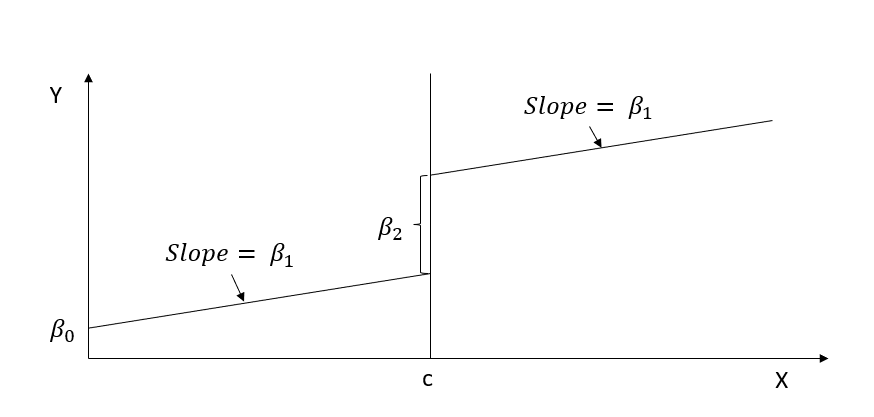
\includegraphics[width=0.9\linewidth,alt={Line graph illustrating a sharp regression discontinuity}]{images/rd1} 

}

\caption{Regression discontinuity design with constant slope.}\label{fig:rd-simple-constant-slope}
\end{figure}

RD gives you \(\beta_2\) (causal effect) of \(X\) on \(Y\) at the cutoff point

In practice, everyone does

\[ Y_i = \alpha_0 + f(x) \alpha _1 + [I(x_i \ge c)]\alpha_2 + [f(x_i)\times [I(x_i \ge c)]\alpha_3 + u_i \]

Figure \ref{fig:rd-simple-dynamic-slope} shows how to visualize the coefficients when one uses dynamic slope.

\begin{figure}

{\centering 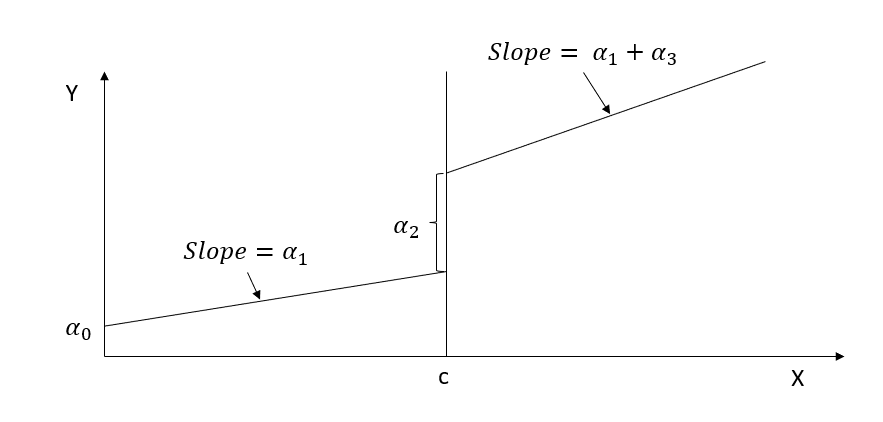
\includegraphics[width=0.9\linewidth,alt={Line graph illustrating a sharp regression discontinuity}]{images/rd2} 

}

\caption{Regression discontinuity design with dynamic slope.}\label{fig:rd-simple-dynamic-slope}
\end{figure}

where we estimate different slope on different sides of the line. And if you estimate \(\alpha_3\) to be no different from 0 then we return to the simple case.

\subsubsection{Higher-Order Polynomials}\label{higher-order-polynomials}

A more flexible specification allows for nonlinear relationships:

\[
Y_i = \beta_0 + \beta_1 X_i + \beta_2 X_i^2 + \beta_3 X_i^3 + \tau D_i + \epsilon_i.
\]

\begin{itemize}
\tightlist
\item
  Higher-order polynomials reduce bias but increase variance.
\item
  Overfitting is a risk, especially with limited data near \(c\).
\end{itemize}

\subsubsection{Nonparametric Estimation}\label{nonparametric-estimation}

When polynomial models are too restrictive, we use nonparametric local linear regression:

\[
\hat{E}[Y | X] = \sum_{i=1}^{n} K_h(X_i - c) Y_i.
\]

where:

\begin{itemize}
\item
  \(K_h(X)\) is a kernel function (e.g., Epanechnikov).
\item
  \(h\) is the bandwidth, chosen to optimize bias-variance tradeoff.
\end{itemize}

\subsection{Bandwidth Selection}\label{bandwidth-selection}

\subsubsection{Tradeoff Between Bias and Efficiency}\label{tradeoff-between-bias-and-efficiency}

Choosing an appropriate bandwidth \(h\) is crucial:

\begin{itemize}
\item
  Narrow \(h\) (close to \(c\)): Lower bias, but high variance.
\item
  Wider \(h\): More efficient estimates but potential bias.
\end{itemize}

\subsubsection{Optimal Bandwidth Selection}\label{optimal-bandwidth-selection}

Several methods exist for selecting \(h\):

\begin{enumerate}
\def\labelenumi{\arabic{enumi}.}
\tightlist
\item
  \textbf{Cross-validation}: Minimizing mean squared error (MSE).
\item
  \citet{imbens2012optimal} bandwidth selection:

  \begin{itemize}
  \tightlist
  \item
    Balances bias-variance tradeoff.
  \item
    Often reported in RD studies.
  \end{itemize}
\item
  \citet{cattaneo2019practical} robust bandwidth selection:

  \begin{itemize}
  \tightlist
  \item
    Focuses on valid inference, not just point estimation.
  \end{itemize}
\end{enumerate}

\subsubsection{Bandwidth Sensitivity Analysis}\label{bandwidth-sensitivity-analysis}

A standard robustness check is estimating \(\tau\) for different \(h\) values:

\begin{itemize}
\tightlist
\item
  If results change drastically, estimates may be sensitive to bandwidth choice.
\item
  If estimates remain stable, findings are more credible.
\end{itemize}

\subsection{Addressing Potential Confounders}\label{addressing-potential-confounders}

\subsubsection{Multiple Running Variables}\label{multiple-running-variables}

If multiple forcing variables influence treatment (e.g., both math and English scores for honors eligibility), failing to account for them may introduce confounding.

A solution is to extend RD to a \hyperref[sec-multi-score-regression-discontinuity-design]{multi-score framework}:

\[
Y_i = \alpha_0 + f(X_{1i}, X_{2i}) \alpha_1 + I(X_{1i} \geq c_1, X_{2i} \geq c_2) \alpha_2 + \epsilon_i.
\]

\begin{itemize}
\tightlist
\item
  Controls for both scores simultaneously.
\item
  Allows for interactions between assignment variables.
\end{itemize}

\subsubsection{Bundling of Institutions}\label{bundling-of-institutions}

In cases where policies change at institutional levels (e.g., different states implementing varying minimum wages), treatment effects may reflect \textbf{institutional bundling} rather than individual cutoff effects.

One solution is to include \textbf{institution fixed effects}:

\[
Y_i = \alpha + f(X_i) \beta + \tau D_i + \gamma C_j + \epsilon_i.
\]

where \(C_j\) is a categorical variable for institution \(j\).

\subsection{External Validity in RD}\label{external-validity-in-rd}

While RD provides strong internal validity, its generalizability is often limited:

\begin{enumerate}
\def\labelenumi{\arabic{enumi}.}
\tightlist
\item
  \textbf{Local Nature of RD Estimates}

  \begin{itemize}
  \tightlist
  \item
    RD estimates apply only at the cutoff.
  \item
    Effects may not extrapolate to other values of \(X\).
  \end{itemize}
\item
  \textbf{Heterogeneous Treatment Effects}

  \begin{itemize}
  \tightlist
  \item
    If \(\tau\) varies across subgroups, RD estimates may not generalize.
  \end{itemize}
\item
  \textbf{Spillover Effects}

  \begin{itemize}
  \tightlist
  \item
    If treatment effects extend beyond the threshold (e.g., peer effects), RD assumptions may be violated.
  \end{itemize}
\end{enumerate}

\begin{center}\rule{0.5\linewidth}{0.5pt}\end{center}

\section{Applications of RD Designs}\label{applications-of-rd-designs}

Regression Discontinuity (RD) designs have widespread applications in empirical research across economics, political science, marketing, and public policy. These applications leverage threshold-based decision rules to identify causal effects in real-world settings where randomized experiments are infeasible.

Key applications include:

\begin{itemize}
\item
  \textbf{Marketing}: Estimating the causal effects of promotions and advertising intensity.
\item
  \textbf{Education}: Evaluating the impact of financial aid or merit scholarships.
\item
  \textbf{Healthcare}: Assessing the effect of medical interventions assigned based on eligibility thresholds.
\item
  \textbf{Labor Economics}: Studying unemployment benefits and wage policies.
\end{itemize}

\subsection{Applications in Marketing}\label{applications-in-marketing}

RD has been widely applied in marketing research to estimate causal effects of pricing, advertising, and product positioning.

\begin{enumerate}
\def\labelenumi{\arabic{enumi}.}
\tightlist
\item
  \textbf{Position Effects in Advertising}
\end{enumerate}

\citep{narayanan2015position} uses an RD approach to estimate the causal impact of advertisement placement in search engines. Since ad placement follows an auction-based system, a discontinuity occurs where the top-ranked ad receives disproportionately more clicks than lower-ranked ads.

Key insights:

\begin{itemize}
\item
  Higher-ranked ads generate more click-throughs, but this does not always translate into higher conversion rates.
\item
  The RD framework helps distinguish correlation from causation by leveraging the rank cutoff.
\end{itemize}

\begin{enumerate}
\def\labelenumi{\arabic{enumi}.}
\setcounter{enumi}{1}
\tightlist
\item
  \textbf{Identifying Causal Marketing Mix Effects}
\end{enumerate}

\citep{hartmann2011identifying} presents a nonparametric RD estimation approach to identify causal effects of marketing mix variables, such as:

\begin{itemize}
\item
  Advertising budgets
\item
  Price changes
\item
  Promotional campaigns
\end{itemize}

By comparing firms just above and below an expenditure threshold, the RD framework isolates the true causal impact of marketing spending on consumer behavior.

\subsection{R Packages for RD Estimation}\label{r-packages-for-rd-estimation}

Table \ref{tab:rd-packages-in-r} shows key RD \href{https://rdpackages.github.io/}{Packages} in R

\begin{longtable}[]{@{}
  >{\raggedright\arraybackslash}p{(\linewidth - 6\tabcolsep) * \real{0.2055}}
  >{\raggedright\arraybackslash}p{(\linewidth - 6\tabcolsep) * \real{0.2055}}
  >{\raggedright\arraybackslash}p{(\linewidth - 6\tabcolsep) * \real{0.3425}}
  >{\raggedright\arraybackslash}p{(\linewidth - 6\tabcolsep) * \real{0.2466}}@{}}
\caption{\label{tab:rd-packages-in-r} Packages in R for RD estimation.}\tabularnewline
\toprule\noalign{}
\begin{minipage}[b]{\linewidth}\raggedright
\textbf{Feature}
\end{minipage} & \begin{minipage}[b]{\linewidth}\raggedright
\textbf{rdd}
\end{minipage} & \begin{minipage}[b]{\linewidth}\raggedright
\textbf{rdrobust}
\end{minipage} & \begin{minipage}[b]{\linewidth}\raggedright
\textbf{rddtools}
\end{minipage} \\
\midrule\noalign{}
\endfirsthead
\toprule\noalign{}
\begin{minipage}[b]{\linewidth}\raggedright
\textbf{Feature}
\end{minipage} & \begin{minipage}[b]{\linewidth}\raggedright
\textbf{rdd}
\end{minipage} & \begin{minipage}[b]{\linewidth}\raggedright
\textbf{rdrobust}
\end{minipage} & \begin{minipage}[b]{\linewidth}\raggedright
\textbf{rddtools}
\end{minipage} \\
\midrule\noalign{}
\endhead
\bottomrule\noalign{}
\endlastfoot
\textbf{Estimator} & Local linear regression & Local polynomial regression & Local polynomial regression \\
\textbf{Bandwidth Selection} & \citep{imbens2012optimal} & \citep{calonico2014robust, imbens2012optimal, calonico2020optimal} & \citep{imbens2012optimal} \\
\textbf{Kernel Functions} & Epanechnikov, Gaussian & Epanechnikov & Gaussian \\
\textbf{Bias Correction} & No & Yes & No \\
\textbf{Covariate Inclusion} & Yes & Yes & Yes \\
\textbf{Assumption Testing} & McCrary Sorting Test & No & McCrary Sorting, Covariate Distribution Tests \\
\end{longtable}

For a detailed comparison, see \citet{thoemmes2017analysis} (Table 1, p.~347).

\subsubsection{Specialized RD Packages}\label{specialized-rd-packages}

\begin{itemize}
\tightlist
\item
  \texttt{rddensity}: Tests for discontinuities in the density of the running variable (useful for manipulation/bunching detection).
\item
  \texttt{rdlocrand}: Implements randomization-based inference for RD.
\item
  \texttt{rdmulti}: Extends RD to multiple cutoffs and multiple scores.
\item
  \texttt{rdpower}: Conducts power calculations and sample selection for RD designs.
\end{itemize}

\subsubsection{\texorpdfstring{Strengths of \texttt{rdrobust}}{Strengths of rdrobust}}\label{strengths-of-rdrobust}

\begin{itemize}
\tightlist
\item
  Implements local polynomial regression, providing bias correction and robust standard errors.
\item
  Uses state-of-the-art bandwidth selection methods.
\item
  Produces automatic RD plots for visualization.
\end{itemize}

\subsection{Example of Regression Discontinuity in Education}\label{example-of-regression-discontinuity-in-education}

We illustrate a Sharp RD using a simulated example of college GPA and future career success.

Setup:

\begin{itemize}
\item
  Students qualify for a prestigious internship if their GPA ≥ 3.5.
\item
  The outcome variable is future career success (e.g., salary).
\item
  RD estimates the causal impact of the internship program on earnings.
\end{itemize}

\[
Y_i = \beta_0 + \beta_1 X_i + \beta_2 W_i + u_i
\]

\[
X_i = 
\begin{cases}
1, W_i \ge c \\
0, W_i < c
\end{cases}
\]

We simulate 100 observations, where GPA is the forcing variable and career success depends on GPA and the treatment effect.

\begin{Shaded}
\begin{Highlighting}[]
\CommentTok{\# Set seed for reproducibility}
\FunctionTok{set.seed}\NormalTok{(}\DecValTok{42}\NormalTok{)}

\NormalTok{n }\OtherTok{=} \DecValTok{100}

\CommentTok{\# Simulate GPA scores (0{-}4 scale)}
\NormalTok{GPA }\OtherTok{\textless{}{-}} \FunctionTok{runif}\NormalTok{(n, }\DecValTok{0}\NormalTok{, }\DecValTok{4}\NormalTok{)}

\CommentTok{\# Generate future success with treatment effect at GPA \textgreater{}= 3.5}
\NormalTok{future\_success }\OtherTok{\textless{}{-}} \DecValTok{10} \SpecialCharTok{+} \DecValTok{2} \SpecialCharTok{*}\NormalTok{ GPA }\SpecialCharTok{+} \DecValTok{10} \SpecialCharTok{*}\NormalTok{ (GPA }\SpecialCharTok{\textgreater{}=} \FloatTok{3.5}\NormalTok{) }\SpecialCharTok{+} \FunctionTok{rnorm}\NormalTok{(n)}

\CommentTok{\# Load RD package}
\FunctionTok{library}\NormalTok{(rddtools)}

\CommentTok{\# Format data for RD analysis}
\NormalTok{data }\OtherTok{\textless{}{-}} \FunctionTok{rdd\_data}\NormalTok{(future\_success, GPA, }\AttributeTok{cutpoint =} \FloatTok{3.5}\NormalTok{)}
\end{Highlighting}
\end{Shaded}

Figure \ref{fig:rd-plot-gpa-future-success} shows the scatter plot of GPA and Future Success.

\begin{Shaded}
\begin{Highlighting}[]
\CommentTok{\# Plot RD scatterplot}
\FunctionTok{plot}\NormalTok{(data, }\AttributeTok{col =} \StringTok{"red"}\NormalTok{, }\AttributeTok{cex =} \FloatTok{0.5}\NormalTok{, }\AttributeTok{xlab =} \StringTok{"GPA"}\NormalTok{, }\AttributeTok{ylab =} \StringTok{"Future Success"}\NormalTok{)}
\end{Highlighting}
\end{Shaded}

\begin{figure}

{\centering \includegraphics[width=0.9\linewidth,alt={Scatter plot with GPA on the x-axis and future success on the y-axis. Red dots show average outcomes in GPA bins. A vertical dashed line at GPA = 3.5 marks a potential threshold. The data trend appears to rise steadily, with a sharp increase in future success for GPAs just above the cutoff.}]{27-regression-discontinuity_files/figure-latex/rd-plot-gpa-future-success-1} 

}

\caption{Binned scatter plot of GPA and future success with threshold at 3.5.}\label{fig:rd-plot-gpa-future-success}
\end{figure}

We estimate the Sharp RD treatment effect using local linear regression:

\begin{Shaded}
\begin{Highlighting}[]
\CommentTok{\# Estimate the sharp RDD model}
\NormalTok{rdd\_mod }\OtherTok{\textless{}{-}} \FunctionTok{rdd\_reg\_lm}\NormalTok{(}\AttributeTok{rdd\_object =}\NormalTok{ data, }\AttributeTok{slope =} \StringTok{"same"}\NormalTok{)}

\CommentTok{\# Display results}
\FunctionTok{summary}\NormalTok{(rdd\_mod)}
\CommentTok{\#\textgreater{} }
\CommentTok{\#\textgreater{} Call:}
\CommentTok{\#\textgreater{} lm(formula = y \textasciitilde{} ., data = dat\_step1, weights = weights)}
\CommentTok{\#\textgreater{} }
\CommentTok{\#\textgreater{} Residuals:}
\CommentTok{\#\textgreater{}      Min       1Q   Median       3Q      Max }
\CommentTok{\#\textgreater{} {-}3.08072 {-}0.54182  0.05352  0.54135  2.51267 }
\CommentTok{\#\textgreater{} }
\CommentTok{\#\textgreater{} Coefficients:}
\CommentTok{\#\textgreater{}             Estimate Std. Error t value Pr(\textgreater{}|t|)    }
\CommentTok{\#\textgreater{} (Intercept) 17.21703    0.20060   85.83   \textless{}2e{-}16 ***}
\CommentTok{\#\textgreater{} D            9.79856    0.31716   30.89   \textless{}2e{-}16 ***}
\CommentTok{\#\textgreater{} x            2.14839    0.09914   21.67   \textless{}2e{-}16 ***}
\CommentTok{\#\textgreater{} {-}{-}{-}}
\CommentTok{\#\textgreater{} Signif. codes:  0 \textquotesingle{}***\textquotesingle{} 0.001 \textquotesingle{}**\textquotesingle{} 0.01 \textquotesingle{}*\textquotesingle{} 0.05 \textquotesingle{}.\textquotesingle{} 0.1 \textquotesingle{} \textquotesingle{} 1}
\CommentTok{\#\textgreater{} }
\CommentTok{\#\textgreater{} Residual standard error: 0.9284 on 97 degrees of freedom}
\CommentTok{\#\textgreater{} Multiple R{-}squared:  0.9746, Adjusted R{-}squared:  0.9741 }
\CommentTok{\#\textgreater{} F{-}statistic:  1863 on 2 and 97 DF,  p{-}value: \textless{} 2.2e{-}16}
\end{Highlighting}
\end{Shaded}

Figure \ref{fig:rd-binned-rd-plot-gpa-future-success} plots the RD regression line with binned observations:

\begin{Shaded}
\begin{Highlighting}[]
\CommentTok{\# Plot RD regression}
\FunctionTok{plot}\NormalTok{(rdd\_mod, }\AttributeTok{cex =} \FloatTok{0.5}\NormalTok{, }\AttributeTok{col =} \StringTok{"red"}\NormalTok{, }\AttributeTok{xlab =} \StringTok{"GPA"}\NormalTok{, }\AttributeTok{ylab =} \StringTok{"Future Success"}\NormalTok{)}
\end{Highlighting}
\end{Shaded}

\begin{figure}

{\centering \includegraphics[width=0.9\linewidth,alt={Line plot of GPA versus future success with four coarse bins. A dashed vertical line at GPA = 3.5 marks the cutoff. A sharp jump in the fitted line is visible at the cutoff, indicating a possible treatment effect. The x-axis spans 0 to 4 GPA, and the y-axis ranges from 14 to 28 in future success.}]{27-regression-discontinuity_files/figure-latex/rd-binned-rd-plot-gpa-future-success-1} 

}

\caption{Coarse binned regression discontinuity plot of GPA and future success.}\label{fig:rd-binned-rd-plot-gpa-future-success}
\end{figure}

We verify whether results hold under different bandwidths and functional forms:

\paragraph{Varying the Bandwidth}\label{varying-the-bandwidth}

\begin{Shaded}
\begin{Highlighting}[]
\CommentTok{\# Using rdrobust for robust estimation}
\FunctionTok{library}\NormalTok{(rdrobust)}

\CommentTok{\# Estimate RD with optimal bandwidth}
\NormalTok{rd\_out }\OtherTok{\textless{}{-}} \FunctionTok{rdrobust}\NormalTok{(}\AttributeTok{y =}\NormalTok{ future\_success, }\AttributeTok{x =}\NormalTok{ GPA, }\AttributeTok{c =} \FloatTok{3.5}\NormalTok{)}
\FunctionTok{summary}\NormalTok{(rd\_out)}
\CommentTok{\#\textgreater{} Sharp RD estimates using local polynomial regression.}
\CommentTok{\#\textgreater{} }
\CommentTok{\#\textgreater{} Number of Obs.                  100}
\CommentTok{\#\textgreater{} BW type                       mserd}
\CommentTok{\#\textgreater{} Kernel                   Triangular}
\CommentTok{\#\textgreater{} VCE method                       NN}
\CommentTok{\#\textgreater{} }
\CommentTok{\#\textgreater{} Number of Obs.                   83           17}
\CommentTok{\#\textgreater{} Eff. Number of Obs.               7           12}
\CommentTok{\#\textgreater{} Order est. (p)                    1            1}
\CommentTok{\#\textgreater{} Order bias  (q)                   2            2}
\CommentTok{\#\textgreater{} BW est. (h)                   0.361        0.361}
\CommentTok{\#\textgreater{} BW bias (b)                   0.670        0.670}
\CommentTok{\#\textgreater{} rho (h/b)                     0.540        0.540}
\CommentTok{\#\textgreater{} Unique Obs.                      83           17}
\CommentTok{\#\textgreater{} }
\CommentTok{\#\textgreater{} =====================================================================}
\CommentTok{\#\textgreater{}                    Point    Robust Inference}
\CommentTok{\#\textgreater{}                 Estimate         z     P\textgreater{}|z|      [ 95\% C.I. ]       }
\CommentTok{\#\textgreater{} {-}{-}{-}{-}{-}{-}{-}{-}{-}{-}{-}{-}{-}{-}{-}{-}{-}{-}{-}{-}{-}{-}{-}{-}{-}{-}{-}{-}{-}{-}{-}{-}{-}{-}{-}{-}{-}{-}{-}{-}{-}{-}{-}{-}{-}{-}{-}{-}{-}{-}{-}{-}{-}{-}{-}{-}{-}{-}{-}{-}{-}{-}{-}{-}{-}{-}{-}{-}{-}}
\CommentTok{\#\textgreater{}      RD Effect    12.836     4.473     0.000     [7.677 , 19.653]    }
\CommentTok{\#\textgreater{} =====================================================================}
\end{Highlighting}
\end{Shaded}

\paragraph{McCrary Test for Manipulation}\label{mccrary-test-for-manipulation}

\begin{Shaded}
\begin{Highlighting}[]
\FunctionTok{library}\NormalTok{(rddensity)}

\CommentTok{\# Check for discontinuities in GPA distribution}
\FunctionTok{rddensity}\NormalTok{(GPA, }\AttributeTok{c =} \FloatTok{3.5}\NormalTok{)}
\CommentTok{\#\textgreater{} Call:}
\CommentTok{\#\textgreater{} rddensity.}
\CommentTok{\#\textgreater{} Sample size: 100. Cutoff: 3.5.}
\CommentTok{\#\textgreater{} Model: unrestricted. Kernel: triangular. VCE: jackknife}
\end{Highlighting}
\end{Shaded}

\paragraph{Polynomial Functional Forms}\label{polynomial-functional-forms}

We compare linear and quadratic specifications:

\begin{Shaded}
\begin{Highlighting}[]
\CommentTok{\# Estimate RD with a quadratic polynomial}
\NormalTok{rdd\_mod\_quad }\OtherTok{\textless{}{-}} \FunctionTok{rdd\_reg\_lm}\NormalTok{(}\AttributeTok{rdd\_object =}\NormalTok{ data, }\AttributeTok{slope =} \StringTok{"separate"}\NormalTok{, }\AttributeTok{order =} \DecValTok{2}\NormalTok{)}
\FunctionTok{summary}\NormalTok{(rdd\_mod\_quad)}
\CommentTok{\#\textgreater{} }
\CommentTok{\#\textgreater{} Call:}
\CommentTok{\#\textgreater{} lm(formula = y \textasciitilde{} ., data = dat\_step1, weights = weights)}
\CommentTok{\#\textgreater{} }
\CommentTok{\#\textgreater{} Residuals:}
\CommentTok{\#\textgreater{}      Min       1Q   Median       3Q      Max }
\CommentTok{\#\textgreater{} {-}3.06894 {-}0.52799  0.01642  0.55260  2.45318 }
\CommentTok{\#\textgreater{} }
\CommentTok{\#\textgreater{} Coefficients:}
\CommentTok{\#\textgreater{}             Estimate Std. Error t value Pr(\textgreater{}|t|)    }
\CommentTok{\#\textgreater{} (Intercept) 17.30296    0.32241  53.667  \textless{} 2e{-}16 ***}
\CommentTok{\#\textgreater{} D            9.14439    1.13752   8.039 2.65e{-}12 ***}
\CommentTok{\#\textgreater{} x            2.29753    0.41955   5.476 3.61e{-}07 ***}
\CommentTok{\#\textgreater{} \textasciigrave{}x\^{}2\textasciigrave{}        0.04253    0.11228   0.379    0.706    }
\CommentTok{\#\textgreater{} x\_right      2.51976    9.23566   0.273    0.786    }
\CommentTok{\#\textgreater{} \textasciigrave{}x\^{}2\_right\textasciigrave{} {-}1.61694   17.10035  {-}0.095    0.925    }
\CommentTok{\#\textgreater{} {-}{-}{-}}
\CommentTok{\#\textgreater{} Signif. codes:  0 \textquotesingle{}***\textquotesingle{} 0.001 \textquotesingle{}**\textquotesingle{} 0.01 \textquotesingle{}*\textquotesingle{} 0.05 \textquotesingle{}.\textquotesingle{} 0.1 \textquotesingle{} \textquotesingle{} 1}
\CommentTok{\#\textgreater{} }
\CommentTok{\#\textgreater{} Residual standard error: 0.9376 on 94 degrees of freedom}
\CommentTok{\#\textgreater{} Multiple R{-}squared:  0.9749, Adjusted R{-}squared:  0.9736 }
\CommentTok{\#\textgreater{} F{-}statistic:   731 on 5 and 94 DF,  p{-}value: \textless{} 2.2e{-}16}
\end{Highlighting}
\end{Shaded}

\subsection{Example of Occupational Licensing and Market Efficiency}\label{example-of-occupational-licensing-and-market-efficiency}

Occupational licensing is a form of labor market regulation that requires workers to obtain licenses or certifications before being allowed to work in specific professions. The debate around occupational licensing revolves around two competing effects:

\begin{enumerate}
\def\labelenumi{\arabic{enumi}.}
\tightlist
\item
  \textbf{Efficiency-enhancing effect}:

  \begin{itemize}
  \tightlist
  \item
    Licensing ensures that workers meet minimum quality standards, reducing information asymmetries between firms and consumers.
  \item
    Higher-quality service providers are selected into the labor market.
  \end{itemize}
\item
  \textbf{Barrier-to-entry effect}:

  \begin{itemize}
  \tightlist
  \item
    Licensing requirements impose costs on potential entrants, reducing labor supply.
  \item
    This creates frictions in the market, potentially leading to inefficiencies.
  \end{itemize}
\end{enumerate}

\citet{bowblis2021occupational} investigates this tradeoff using a \hyperref[sec-fuzzy-regression-discontinuity-design]{Fuzzy RD} based on a threshold rule:

\begin{itemize}
\item
  Nursing homes with 120 or more beds are required to hire a certain fraction of licensed/certified workers.
\item
  The study examines whether this policy improves quality of care or merely restricts labor market competition.
\end{itemize}

\begin{center}\rule{0.5\linewidth}{0.5pt}\end{center}

\subsubsection{OLS Estimation: Naïve Approach and Its Bias}\label{ols-estimation-nauxefve-approach-and-its-bias}

A simple ordinary least squares regression can be used to estimate the effect of licensed workers on quality of service:

\[
Y_i = \alpha_0 + X_i \alpha_1 + LW_i \alpha_2 + \epsilon_i
\]

where:

\begin{itemize}
\item
  \(Y_i\) = Quality of service at facility \(i\).
\item
  \(LW_i\) = Proportion of licensed workers at facility \(i\).
\item
  \(X_i\) = Facility characteristics (e.g., size, staffing levels).
\end{itemize}

\subsubsection{\texorpdfstring{Potential Bias in \(\alpha_2\)}{Potential Bias in \textbackslash alpha\_2}}\label{potential-bias-in-alpha_2}

\begin{enumerate}
\def\labelenumi{\arabic{enumi}.}
\tightlist
\item
  Mitigation-Based Bias:

  \begin{itemize}
  \tightlist
  \item
    Facilities with poor quality outcomes may hire more licensed workers in response to bad performance.
  \item
    This induces a negative correlation between \(LW_i\) and \(Y_i\), biasing \(\alpha_2\) downward.
  \end{itemize}
\item
  Preference-Based Bias:

  \begin{itemize}
  \tightlist
  \item
    Higher-quality facilities may have greater incentives to hire certified workers.
  \item
    This induces a positive correlation between \(LW_i\) and \(Y_i\), biasing \(\alpha_2\) upward.
  \end{itemize}
\end{enumerate}

\subsubsection{Fuzzy RD Framework}\label{fuzzy-rd-framework}

The OLS model is endogenous, so we implement a \hyperref[sec-fuzzy-regression-discontinuity-design]{Fuzzy RD Design} that exploits a discontinuity in licensing requirements at 120 beds.

\[
\begin{aligned}Y_{ist} = \beta_0 &+ \beta_1 \mathbb{1}(\text{Bed}_{ist} \geq 121) + \beta_2 f(\text{Size}_{ist}) \\&+ \beta_3 f(\text{Size}_{ist}) \times \mathbb{1}(\text{Bed}_{ist} \geq 121) \\&+ X_{it}'\delta + \gamma_s + \theta_t + \epsilon_{ist}\end{aligned}
\]

where:

\begin{itemize}
\item
  \(I(Bed \geq 121)\) = Indicator for treatment eligibility (having at least 120 beds).
\item
  \(f(Size_{ist})\) = Flexible functional form of facility size.
\item
  \(X_{it}\) = Other control variables.
\item
  \(\gamma_s\) = State fixed effects (accounts for state-level regulations).
\item
  \(\theta_t\) = Time fixed effects (accounts for temporal shocks).
\item
  \(\beta_1\) = Intent-to-treat (ITT) effect.
\end{itemize}

This model estimates discontinuities in quality outcomes at the 120-bed threshold.

\begin{center}\rule{0.5\linewidth}{0.5pt}\end{center}

\subsubsection{Why This RD is Fuzzy}\label{why-this-rd-is-fuzzy}

Unlike a \hyperref[sec-sharp-regression-discontinuity-design]{Sharp RD}, treatment is not fully determined at the cutoff:

\begin{itemize}
\item
  Some facilities with fewer than 120 beds voluntarily hire licensed workers.
\item
  Some facilities with more than 120 beds may not comply fully.
\end{itemize}

Thus, the RD framework must be modified:

\begin{enumerate}
\def\labelenumi{\arabic{enumi}.}
\tightlist
\item
  Fixed-Effect Considerations:

  \begin{itemize}
  \tightlist
  \item
    If states sort differently near the threshold, state fixed effects (\(\gamma_s\)) may be needed.
  \item
    However, if sorting is non-random, the RD assumption fails.
  \end{itemize}
\end{enumerate}

\begin{enumerate}
\def\labelenumi{\arabic{enumi}.}
\setcounter{enumi}{1}
\tightlist
\item
  Panel Data Implications:

  \begin{itemize}
  \tightlist
  \item
    Fixed-effects models are not preferred in RD, as they are lower in the causal inference hierarchy.
  \item
    RD typically excludes pre-treatment periods, whereas fixed-effects require before-and-after comparisons.
  \end{itemize}
\item
  Variation in Facility Size:

  \begin{itemize}
  \tightlist
  \item
    Hospitals rarely change bed capacity, so including hospital-specific fixed effects removes variation necessary for RD estimation.
  \end{itemize}
\end{enumerate}

\begin{center}\rule{0.5\linewidth}{0.5pt}\end{center}

\subsubsection{Instrumental Variable Approach}\label{instrumental-variable-approach}

To correct for endogeneity, we use a two-stage least squares IV approach, where the running variable serves as an instrument for treatment intensity.

\paragraph{Stage 1: First-Stage Regression}\label{stage-1-first-stage-regression}

Estimate the probability of hiring licensed workers based on the 120-bed threshold:

\[
\begin{aligned}\text{QSW}_{ist} = \alpha_0 &+ \alpha_1 \mathbb{1}(\text{Bed}_{ist} \geq 121) + \alpha_2 f(\text{Size}_{ist}) \\&+ \alpha_3 f(\text{Size}_{ist}) \times \mathbb{1}(\text{Bed}_{ist} \geq 121) \\&+ X_{it}'\delta + \gamma_s + \theta_t + \epsilon_{ist}\end{aligned}
\]

where:

\begin{itemize}
\tightlist
\item
  \(QSW_{ist}\) = Predicted proportion of licensed workers at facility \(i\) in state \(s\) at time \(t\).
\end{itemize}

\paragraph{Stage 2: Second-Stage Regression}\label{stage-2-second-stage-regression}

Estimate the causal effect of hiring licensed workers on quality of service:

\[
\begin{aligned}Y_{ist} = \gamma_0 &+ \gamma_1 \widehat{\text{QSW}}_{ist} + \delta_2 f(\text{Size}_{ist}) \\&+ \delta_3 f(\text{Size}_{ist}) \times \mathbb{1}(\text{Bed}_{ist} \geq 121) \\&+ X_{it}'\lambda + \eta_s + \tau_t + u_{ist}\end{aligned}
\]

where:

\begin{itemize}
\item
  \(\hat{QWS}_{ist}\) = Instrumented proportion of licensed workers.
\item
  \(\gamma_1\) = Causal effect of certified staffing on quality outcomes.
\end{itemize}

\paragraph{Key Observations}\label{key-observations}

\begin{itemize}
\tightlist
\item
  The larger the discontinuity at 120 beds, the closer \(\gamma_1 \approx \beta_1\).
\item
  The ITT effect (\(\beta_1\)) will always be weaker than the \hyperref[sec-local-average-treatment-effects]{local average treatment effect} (\(\gamma_1\)).
\end{itemize}

\begin{center}\rule{0.5\linewidth}{0.5pt}\end{center}

\subsubsection{Empirical Challenges}\label{empirical-challenges}

\begin{enumerate}
\def\labelenumi{\arabic{enumi}.}
\tightlist
\item
  \textbf{Bunching at Round Numbers}:

  \begin{itemize}
  \tightlist
  \item
    Density plots typically show facilities clustering at every 5-bed increment.
  \item
    If manipulation occurs, we expect underrepresentation at 130 beds.
  \end{itemize}
\item
  \textbf{Clustering Standard Errors}:

  \begin{itemize}
  \tightlist
  \item
    Due to limited unique mass points (facilities at specific sizes), errors should be clustered by mass point instead of individual facilities.
  \end{itemize}
\item
  \textbf{Noncompliance and Selection Bias}:

  \begin{itemize}
  \tightlist
  \item
    Fuzzy RD requires that we do not drop non-compliers (as it would introduce selection bias).
  \item
    However, we can drop manipulators if there is clear evidence of behavioral bias (e.g., preference for round numbers).
  \end{itemize}
\end{enumerate}

\begin{center}\rule{0.5\linewidth}{0.5pt}\end{center}

\begin{center}\rule{0.5\linewidth}{0.5pt}\end{center}

\section{Dose-Response and Multivalued-Treatment RD}\label{sec-dose-response-rd}

The canonical \hyperref[sec-sharp-regression-discontinuity-design]{sharp RD design} compares treated and untreated units at the cutoff. In many policy settings the cutoff does not switch treatment from off to on but rather changes the \emph{intensity} of an ongoing treatment. A means-tested transfer whose amount scales with how far below the eligibility threshold a household lies, a graduated tax credit whose rate steps up at successive income brackets, a graduate-fellowship offer whose stipend depends on a continuous score above a qualifying mark: all are settings in which the substantive question is the shape of a dose-response, not the average effect of treated vs.~untreated. This section develops the RD machinery for those settings.

The framework subsumes two related but distinct designs. In the \textbf{dose-response RD}, the treatment intensity \(D\) is a deterministic continuous function of the running variable \(X\) on one or both sides of the cutoff, and the estimand of interest is the marginal effect of intensity at the cutoff. In the \textbf{multivalued-treatment RD}, the running variable determines which of several discrete treatment levels a unit receives, and the estimand is the set of dose-specific level effects. Both are instances of the same broader idea: when the cutoff is not a binary switch, the RD estimand becomes a function rather than a scalar, and the analyst's job is to recover that function rather than collapse it.

\subsection{Identifying Strategies}\label{identifying-strategies}

The two leading identification frameworks in this space come from \citet{dong2015identifying} and \citet{caetano2023regression}, and they make different but complementary assumptions.

\citet{dong2015identifying} study the case in which the policy threshold itself changes (for instance, an eligibility cutoff moves from one income level to another) and the parameter of interest is the marginal effect of moving the threshold. The identifying argument is that, even though the new cutoff is not a discontinuity in any single dataset, the \emph{change} in the cutoff acts like a continuous-treatment intervention whose effect can be recovered by comparing the level effects estimated at the old and new thresholds. The estimand is informative for policy questions in which the analyst wants to know ``how much would the program effect change if we relaxed the eligibility rule,'' a counterfactual that the classical sharp-RD estimand cannot answer.

\citet{caetano2023regression} develop a more general framework that handles multivalued treatments determined by the running variable, including the dose-response special case. The identifying assumption replaces continuity of the conditional expectation of the potential outcomes at the cutoff with continuity of an entire family of conditional expectations indexed by the treatment level. Under this assumption the estimand is a dose-specific local average treatment effect, and the estimator is a local-polynomial regression that interacts the running variable with the treatment level. The framework recovers the classical sharp-RD estimand as a special case (when the treatment is binary) and the fuzzy-RD estimand as another (when the treatment is binary and partially compliant), while also accommodating the multivalued case directly.

The \citet{cattaneo2016interpreting} and \citet{cattaneo2021extrapolating} multi-cutoff machinery, developed in Section \ref{sec-multi-cutoff-regression-discontinuity-design}, is the third leg of the design space. When the dose is discrete and the policy rule is implemented through several cutoffs (one per dose level), the multi-cutoff estimator pools across cutoffs to recover the dose-response curve. The pooling assumption is non-trivial: it requires that the local treatment effect at each cutoff identifies the same underlying causal parameter, which fails if the marginal compliers at different cutoffs are systematically different units.

\subsection{Estimands}\label{estimands}

In the dose-response setting with continuous treatment intensity, the natural estimand is the \textbf{marginal dose-response at the cutoff}:

\[
\theta(c) = \lim_{x \downarrow c} \frac{\partial}{\partial d} \mathbb{E}[Y \mid X = x, D = d(x)],
\]

where \(d(x)\) is the deterministic dose function of the running variable. The estimand captures how the average outcome would change if every unit at the cutoff received a marginally higher dose. The classical sharp-RD estimand is the special case where \(d(x)\) jumps from zero to one at the cutoff.

In the multivalued-treatment setting, the natural estimand is the set of \textbf{dose-specific level effects}:

\[
\tau(d) = \mathbb{E}[Y(d) - Y(0) \mid X = c, D = d],
\]

evaluated for each dose level \(d\) in the support of the treatment. Reported together, these form a dose-response curve analogous to the one delivered by the \hyperref[sec-gps-continuous]{continuous-treatment matching analysis} or the \hyperref[sec-continuous-did]{continuous-treatment DiD}, with the substantive difference that the RD version conditions on the running variable being at the cutoff and therefore has a strictly local interpretation.

\subsection{Estimation in Practice}\label{estimation-in-practice-1}

We work through the estimation in two passes. The first pass implements the multi-cutoff dose-response by hand using only base R, so that the per-cutoff local-linear logic is visible. The second pass calls the published \texttt{rdmulti} and \texttt{rdrobust} packages on the same data.

\paragraph{Demonstration: dose-specific local-linear RD from scratch}\label{demonstration-dose-specific-local-linear-rd-from-scratch}

\begin{Shaded}
\begin{Highlighting}[]
\FunctionTok{suppressPackageStartupMessages}\NormalTok{(\{}
  \FunctionTok{library}\NormalTok{(dplyr)}
  \FunctionTok{library}\NormalTok{(ggplot2)}
\NormalTok{\})}

\FunctionTok{set.seed}\NormalTok{(}\DecValTok{20240515}\NormalTok{)}

\CommentTok{\# Two cutoffs (0 and 10) define three dose levels.}
\CommentTok{\# Dose 0 for X \textless{} 0, dose 1 for X in [0, 10), dose 2 for X \textgreater{}= 10.}
\CommentTok{\# True dose{-}response is concave: tau(1) = 0.6, tau(2) = 0.9.}
\NormalTok{n }\OtherTok{\textless{}{-}} \DecValTok{5000}
\NormalTok{X }\OtherTok{\textless{}{-}} \FunctionTok{runif}\NormalTok{(n, }\SpecialCharTok{{-}}\DecValTok{20}\NormalTok{, }\DecValTok{30}\NormalTok{)}
\NormalTok{D }\OtherTok{\textless{}{-}} \FunctionTok{as.integer}\NormalTok{(X }\SpecialCharTok{\textgreater{}=} \DecValTok{0}\NormalTok{) }\SpecialCharTok{+} \FunctionTok{as.integer}\NormalTok{(X }\SpecialCharTok{\textgreater{}=} \DecValTok{10}\NormalTok{)}
\NormalTok{Y }\OtherTok{\textless{}{-}} \FloatTok{0.05} \SpecialCharTok{*}\NormalTok{ X }\SpecialCharTok{+} \FloatTok{0.6} \SpecialCharTok{*}\NormalTok{ (D }\SpecialCharTok{==} \DecValTok{1}\NormalTok{) }\SpecialCharTok{+} \FloatTok{0.9} \SpecialCharTok{*}\NormalTok{ (D }\SpecialCharTok{==} \DecValTok{2}\NormalTok{) }\SpecialCharTok{+} \FunctionTok{rnorm}\NormalTok{(n, }\AttributeTok{sd =} \FloatTok{0.5}\NormalTok{)}
\NormalTok{dat }\OtherTok{\textless{}{-}} \FunctionTok{data.frame}\NormalTok{(X, Y, D)}

\CommentTok{\# Estimate the level jump at each cutoff by a local{-}linear regression}
\CommentTok{\# inside a fixed bandwidth. We use a 5{-}unit bandwidth on each side and}
\CommentTok{\# a triangular kernel weight, matching the rdrobust default kernel.}
\NormalTok{local\_linear\_jump }\OtherTok{\textless{}{-}} \ControlFlowTok{function}\NormalTok{(data, cutoff, }\AttributeTok{h =} \DecValTok{5}\NormalTok{) \{}
\NormalTok{  d }\OtherTok{\textless{}{-}}\NormalTok{ data }\SpecialCharTok{\%\textgreater{}\%}
    \FunctionTok{filter}\NormalTok{(X }\SpecialCharTok{\textgreater{}=}\NormalTok{ cutoff }\SpecialCharTok{{-}}\NormalTok{ h, X }\SpecialCharTok{\textless{}=}\NormalTok{ cutoff }\SpecialCharTok{+}\NormalTok{ h) }\SpecialCharTok{\%\textgreater{}\%}
    \FunctionTok{mutate}\NormalTok{(}
      \AttributeTok{side   =} \FunctionTok{as.integer}\NormalTok{(X }\SpecialCharTok{\textgreater{}=}\NormalTok{ cutoff),}
      \AttributeTok{Xc     =}\NormalTok{ X }\SpecialCharTok{{-}}\NormalTok{ cutoff,}
      \AttributeTok{kweight =} \FunctionTok{pmax}\NormalTok{(}\DecValTok{1} \SpecialCharTok{{-}} \FunctionTok{abs}\NormalTok{(Xc) }\SpecialCharTok{/}\NormalTok{ h, }\DecValTok{0}\NormalTok{)   }\CommentTok{\# triangular kernel}
\NormalTok{    )}
\NormalTok{  fit }\OtherTok{\textless{}{-}} \FunctionTok{lm}\NormalTok{(Y }\SpecialCharTok{\textasciitilde{}}\NormalTok{ side }\SpecialCharTok{+}\NormalTok{ Xc }\SpecialCharTok{+}\NormalTok{ side}\SpecialCharTok{:}\NormalTok{Xc, }\AttributeTok{data =}\NormalTok{ d, }\AttributeTok{weights =}\NormalTok{ kweight)}
\NormalTok{  est }\OtherTok{\textless{}{-}} \FunctionTok{coef}\NormalTok{(fit)[}\StringTok{"side"}\NormalTok{]}
\NormalTok{  se  }\OtherTok{\textless{}{-}} \FunctionTok{sqrt}\NormalTok{(}\FunctionTok{diag}\NormalTok{(}\FunctionTok{vcov}\NormalTok{(fit)))[}\StringTok{"side"}\NormalTok{]}
  \FunctionTok{c}\NormalTok{(}\AttributeTok{est =} \FunctionTok{unname}\NormalTok{(est), }\AttributeTok{se =} \FunctionTok{unname}\NormalTok{(se),}
    \AttributeTok{ci\_lo =} \FunctionTok{unname}\NormalTok{(est) }\SpecialCharTok{{-}} \FloatTok{1.96} \SpecialCharTok{*} \FunctionTok{unname}\NormalTok{(se),}
    \AttributeTok{ci\_hi =} \FunctionTok{unname}\NormalTok{(est) }\SpecialCharTok{+} \FloatTok{1.96} \SpecialCharTok{*} \FunctionTok{unname}\NormalTok{(se))}
\NormalTok{\}}

\NormalTok{jump\_at\_0  }\OtherTok{\textless{}{-}} \FunctionTok{local\_linear\_jump}\NormalTok{(dat, }\AttributeTok{cutoff =} \DecValTok{0}\NormalTok{)}
\NormalTok{jump\_at\_10 }\OtherTok{\textless{}{-}} \FunctionTok{local\_linear\_jump}\NormalTok{(dat, }\AttributeTok{cutoff =} \DecValTok{10}\NormalTok{)}

\NormalTok{rd\_table }\OtherTok{\textless{}{-}} \FunctionTok{data.frame}\NormalTok{(}
  \AttributeTok{cutoff   =} \FunctionTok{c}\NormalTok{(}\DecValTok{0}\NormalTok{, }\DecValTok{10}\NormalTok{),}
  \AttributeTok{est      =} \FunctionTok{c}\NormalTok{(jump\_at\_0[}\StringTok{"est"}\NormalTok{], jump\_at\_10[}\StringTok{"est"}\NormalTok{]),}
  \AttributeTok{se       =} \FunctionTok{c}\NormalTok{(jump\_at\_0[}\StringTok{"se"}\NormalTok{],  jump\_at\_10[}\StringTok{"se"}\NormalTok{]),}
  \AttributeTok{ci\_lo    =} \FunctionTok{c}\NormalTok{(jump\_at\_0[}\StringTok{"ci\_lo"}\NormalTok{], jump\_at\_10[}\StringTok{"ci\_lo"}\NormalTok{]),}
  \AttributeTok{ci\_hi    =} \FunctionTok{c}\NormalTok{(jump\_at\_0[}\StringTok{"ci\_hi"}\NormalTok{], jump\_at\_10[}\StringTok{"ci\_hi"}\NormalTok{]),}
  \AttributeTok{true\_jump =} \FunctionTok{c}\NormalTok{(}\FloatTok{0.6}\NormalTok{, }\FloatTok{0.3}\NormalTok{)   }\CommentTok{\# tau(1) {-} tau(0) = 0.6, tau(2) {-} tau(1) = 0.3}
\NormalTok{)}
\NormalTok{rd\_table}
\CommentTok{\#\textgreater{}   cutoff       est         se     ci\_lo     ci\_hi true\_jump}
\CommentTok{\#\textgreater{} 1      0 0.6263511 0.05600880 0.5165738 0.7361283       0.6}
\CommentTok{\#\textgreater{} 2     10 0.3113949 0.05404179 0.2054730 0.4173168       0.3}
\end{Highlighting}
\end{Shaded}

The table reports the estimated jump at each cutoff. The jump at \(X = 0\) identifies the marginal effect of moving from dose 0 to dose 1; the jump at \(X = 10\) identifies the marginal effect of moving from dose 1 to dose 2. Comparing the \texttt{est} column to \texttt{true\_jump} checks the estimator against the simulated truth; the recovered dose-response is concave (the marginal effect at the higher cutoff is smaller), which mirrors the diminishing-returns pattern built into the simulation.

The dose-specific level effects can be plotted directly:

\begin{Shaded}
\begin{Highlighting}[]
\FunctionTok{ggplot}\NormalTok{(rd\_table, }\FunctionTok{aes}\NormalTok{(}\AttributeTok{x =} \FunctionTok{factor}\NormalTok{(cutoff), }\AttributeTok{y =}\NormalTok{ est)) }\SpecialCharTok{+}
  \FunctionTok{geom\_pointrange}\NormalTok{(}\FunctionTok{aes}\NormalTok{(}\AttributeTok{ymin =}\NormalTok{ ci\_lo, }\AttributeTok{ymax =}\NormalTok{ ci\_hi)) }\SpecialCharTok{+}
  \FunctionTok{geom\_hline}\NormalTok{(}\AttributeTok{yintercept =} \DecValTok{0}\NormalTok{, }\AttributeTok{linetype =} \StringTok{"dotted"}\NormalTok{) }\SpecialCharTok{+}
  \FunctionTok{labs}\NormalTok{(}\AttributeTok{x =} \StringTok{"Cutoff (and dose transition)"}\NormalTok{,}
       \AttributeTok{y =} \StringTok{"Local marginal effect at the cutoff"}\NormalTok{,}
       \AttributeTok{title =} \StringTok{"Dose{-}response by cutoff, from{-}scratch local{-}linear RD"}\NormalTok{,}
       \AttributeTok{subtitle =} \StringTok{"Cutoff 0 = dose 1 vs 0; cutoff 10 = dose 2 vs 1"}\NormalTok{) }\SpecialCharTok{+}
  \FunctionTok{theme\_minimal}\NormalTok{()}
\end{Highlighting}
\end{Shaded}

\begin{figure}

{\centering \includegraphics[width=0.9\linewidth]{27-regression-discontinuity_files/figure-latex/rd-multi-plot-1} 

}

\caption{Multi-cutoff RD: estimated jumps at each cutoff. The first cutoff identifies the marginal effect of dose 1 over dose 0; the second cutoff identifies the marginal effect of dose 2 over dose 1. The dose-response is concave (diminishing marginal returns), which the per-cutoff estimates recover.}\label{fig:rd-multi-plot}
\end{figure}

Figure \ref{fig:rd-multi-plot} shows two point estimates with their 95\% confidence intervals. A reviewer reads off (a) whether each per-cutoff effect is statistically distinguishable from zero, (b) whether the dose-response is monotone, and (c) whether the spacing of the estimates is consistent with linearity (it is not, in this simulation, because the effects are concave). The same plot scaled up to many cutoffs is the discrete-dose analogue of the continuous-DiD dose-response figure in Section \ref{sec-continuous-did}.

\paragraph{\texorpdfstring{Production: \texttt{rdmulti} and \texttt{rdrobust}}{Production: rdmulti and rdrobust}}\label{production-rdmulti-and-rdrobust}

For production work the published \texttt{rdmulti} package by Cattaneo, Titiunik, and Vazquez-Bare implements both cutoff-specific and pooled estimators, with proper bias-corrected robust standard errors via the underlying \texttt{rdrobust} engine \citep{calonico2014robust}. The user passes the data, the running variable, the cutoffs, and the cutoff assignment, and the package handles bandwidth selection (using the \citet{cattaneo2016interpreting} multi-cutoff conventions), kernel weighting, and inference.

\begin{Shaded}
\begin{Highlighting}[]
\CommentTok{\# install.packages(c("rdmulti", "rdrobust"))}
\CommentTok{\# CRAN, Cattaneo{-}Titiunik{-}Vazquez{-}Bare}
\FunctionTok{library}\NormalTok{(rdmulti)}
\FunctionTok{library}\NormalTok{(rdrobust)}

\CommentTok{\# Cutoff{-}specific RD: estimate the level jump at each cutoff separately.}
\NormalTok{res\_each }\OtherTok{\textless{}{-}} \FunctionTok{rdmc}\NormalTok{(}
  \AttributeTok{Y       =}\NormalTok{ Y,}
  \AttributeTok{X       =}\NormalTok{ X,}
  \AttributeTok{C       =} \FunctionTok{ifelse}\NormalTok{(X }\SpecialCharTok{\textless{}} \DecValTok{10}\NormalTok{, }\DecValTok{0}\NormalTok{, }\DecValTok{10}\NormalTok{),  }\CommentTok{\# which cutoff each unit faces}
  \AttributeTok{cvar    =} \FunctionTok{c}\NormalTok{(}\DecValTok{0}\NormalTok{, }\DecValTok{10}\NormalTok{)}
\NormalTok{)}
\FunctionTok{summary}\NormalTok{(res\_each)}

\CommentTok{\# Pooled estimate of the dose{-}response across cutoffs.}
\NormalTok{res\_pool }\OtherTok{\textless{}{-}} \FunctionTok{rdms}\NormalTok{(}
  \AttributeTok{Y       =}\NormalTok{ Y,}
  \AttributeTok{X       =}\NormalTok{ X,}
  \AttributeTok{C       =} \FunctionTok{ifelse}\NormalTok{(X }\SpecialCharTok{\textless{}} \DecValTok{10}\NormalTok{, }\DecValTok{0}\NormalTok{, }\DecValTok{10}\NormalTok{),}
  \AttributeTok{cvar    =} \FunctionTok{c}\NormalTok{(}\DecValTok{0}\NormalTok{, }\DecValTok{10}\NormalTok{),}
  \AttributeTok{pooled\_opt =} \StringTok{"uniform"}
\NormalTok{)}
\FunctionTok{summary}\NormalTok{(res\_pool)}
\end{Highlighting}
\end{Shaded}

The \texttt{summary(res\_each)} output is a table with one row per cutoff, reporting the cutoff-specific RD coefficient, robust standard error, bias-corrected 95\% confidence interval, and the optimal bandwidth chosen by the \citet{calonico2014robust} MSE-minimizing rule. The right way to read it is the same as for the from-scratch table above: scan for cutoffs where the effect is statistically distinguishable from zero, look for the dose-response shape, and compare the bandwidth used at each cutoff (large differences in bandwidth signal that the running-variable density is uneven across the dose range).

The \texttt{summary(res\_pool)} output is a single pooled estimate that aggregates the cutoff-specific effects under a uniform-pooling assumption (each cutoff carries the same weight). The pooled object is the right summary when the analyst believes the per-cutoff local effects identify the same underlying parameter; the disaggregated \texttt{res\_each} object is the right summary when they do not. The placebo diagnostic recommended by \citet{cattaneo2021extrapolating} is to drop one cutoff at a time and re-pool: instability in the pooled estimate is evidence that the per-cutoff effects are heterogeneous and should be reported separately.

For the continuous-dose case in which the policy threshold itself shifts, the \citet{dong2015identifying} estimator can be implemented directly by running two \texttt{rdrobust} estimations (one at the old cutoff, one at the new cutoff in a separate dataset or sub-period) and reporting their difference as the marginal-threshold effect.

For the multivalued-treatment case under the \citet{caetano2023regression} framework, no canonical CRAN package implements the estimator at the time of writing; the authors' replication code and supplementary materials provide reference implementations.

\subsection{Diagnostics}\label{diagnostics}

The diagnostics from the \hyperref[sec-assumptions-for-rd-validity]{Assumptions for RD Validity} section all carry over and gain an additional requirement: continuity must hold for the conditional expectation of the potential outcome at \emph{each dose level}, not only on average across doses. The natural diagnostic is to plot the running variable against the outcome separately for each dose level and inspect the smoothness of each curve at the cutoff. A jump in one dose-specific curve but not in another is a red flag that the multivalued-treatment identifying assumption is being violated.

The \citet{mccrary2008manipulation} density test should be re-run with attention to the dose distribution: a continuous-dose function \(d(x)\) in which units near the cutoff systematically misreport their running variable to qualify for a more generous dose breaks the design in the same way that manipulation breaks classical sharp RD, only the symptom is asymmetric piling at specific dose-eligibility thresholds rather than at a single binary cutoff.

A pooling-validity placebo, recommended by \citet{cattaneo2021extrapolating}, is to estimate the dose-response curve on the full sample and again on subsamples that exclude one cutoff at a time. A pooled estimate that is unstable to dropping individual cutoffs is evidence that the local treatment effects at different cutoffs are not identifying the same underlying parameter, in which case the dose-specific estimates should be reported instead of the pooled curve.

\begin{center}\rule{0.5\linewidth}{0.5pt}\end{center}

\section{When RD Works and When It Fails}\label{when-rd-works-and-when-it-fails}

Among the quasi-experimental designs covered in this book, RD stands out for how little it asks of the analyst. Given a sharp, institutionally enforced cutoff on a continuous running variable, local randomization comes essentially for free, and a reviewer can evaluate the design with very little prior familiarity with the setting. The transparency is part of the appeal.

The flip side is that RD is easy to misapply in ways that are hard to detect once the analysis is written up. The design rewards care in three places in particular: the running variable, the cutoff, and the neighborhood around it.

The running variable must be genuinely continuous and measured on both sides of the cutoff with similar density. A pileup of observations just below or just above \(c\) is the classic sign that subjects are manipulating their scores to sort themselves onto one side, grade inflation to clear a scholarship threshold, income shading to qualify for a benefit, strategic timing around a program start date. When manipulation is present, the continuity assumption does not hold, and any RD estimate is contaminated by selection. A density test (McCrary or Cattaneo-Jansson-Ma) is the first diagnostic; a placebo analysis on pre-determined covariates is the second.

The cutoff must be institutional, not analyst-chosen. If the threshold was picked after looking at the outcome, the design collapses into specification search.

The neighborhood, the bandwidth \(h\), is where most disputes live. A very narrow window gives precise local identification but noisy estimates. A wider window pulls in heterogeneity from units far from the cutoff. Report multiple bandwidths (the data-driven optimum plus narrower and wider windows), multiple polynomial orders, and the \citet{calonico2014robust} bias-corrected standard errors. A coefficient that is stable across these choices is much more credible than one that flips sign when the window widens.

Two further warnings. First, the RD estimand is a LATE \emph{at} the cutoff. Extrapolating to units far from \(c\) requires either additional assumptions (constant treatment effect) or parametric specifications that reintroduce exactly the modeling dependence RD was designed to avoid. Second, Fuzzy RD inherits every weak-instrument pathology from \hyperref[sec-instrumental-variables]{Instrumental Variables chapter}: if the jump in treatment probability at the cutoff is small, the ratio estimator becomes unstable no matter how precise the reduced form looks.

When RD fits the application, it is often the most credible design available. When the cutoff is blurry, manipulable, or weakly predictive of treatment, reach instead for a design that makes its assumptions work harder, \hyperref[sec-difference-in-differences]{DiD} if panel structure is available, \hyperref[sec-matching-methods]{matching} if covariate richness is the main asset.

\chapter{Temporal Discontinuity Designs}\label{sec-temporal-discontinuity-designs}

When evaluating the impact of a policy, intervention, or treatment that begins at a known point in time, time becomes the running variable. In such settings, two widely used quasi-experimental methods offer powerful tools for causal inference:

\begin{itemize}
\tightlist
\item
  \hyperref[sec-regression-discontinuity-in-time]{Regression Discontinuity in Time}
\item
  \hyperref[sec-interrupted-time-series]{Interrupted Time Series}
\end{itemize}

Both approaches exploit a temporal cutoff (i.e., the moment when an intervention begins) to identify changes in outcomes attributable to the treatment. However, they differ in how they conceptualize and model the data around that time point, as well as in the strength of assumptions required for valid inference.

Despite their differences, RDiT and ITS are united by several key features:

\begin{itemize}
\tightlist
\item
  Temporal Running Variable: time replaces the traditional cross-sectional score as the variable used to determine treatment status.
\item
  Known Intervention Start Date: both require a clearly defined moment when the policy or treatment began.
\item
  No Confounding Events: both assume no other major changes occurred simultaneously with the intervention that could affect outcomes.
\item
  No Cross-sectional Control Group: these designs are especially valuable when there is no suitable untreated group, making methods like \hyperref[sec-difference-in-differences]{difference-in-differences} infeasible.
\end{itemize}

RDiT adapts the logic of standard RD to the time dimension, using the policy implementation date as the cutoff.

\begin{itemize}
\tightlist
\item
  Conceptualization: individuals or observations just before and after the intervention date are assumed to be comparable, akin to local randomization in time.
\item
  Estimation: typically modeled using local polynomial regression on either side of the cutoff date.
\item
  Strengths: provides localized causal inference near the intervention date; flexible with respect to functional form.
\item
  Limitations: sensitive to time trends and autocorrelation. Requires dense temporal data (e.g., daily or weekly) to support the assumption of continuity around the cutoff.
\end{itemize}

\begin{quote}
Example: analyzing the effect of a new digital ad campaign launched nationwide on July 1st by comparing user engagement on June 30 vs.~July 1.
\end{quote}

ITS adopts a broader, time-series approach, modeling pre- and post-intervention trends explicitly.

\begin{itemize}
\tightlist
\item
  Conceptualization: the intervention is viewed as an interruption in an ongoing time series process.
\item
  Estimation: involves fitting segmented regressions with separate intercepts and slopes before and after the policy.
\item
  Strengths: useful when interested in long-term trends and sustained treatment effects.
\item
  Limitations: requires strong assumptions about the functional form of time trends and absence of time-varying confounders. Less credible when data are sparse or highly aggregated (e.g., annual).
\end{itemize}

\begin{quote}
Example: evaluating the impact of a minimum wage increase on monthly employment rates over a 5-year period.
\end{quote}

\begin{center}\rule{0.5\linewidth}{0.5pt}\end{center}

Table \ref{tab:its-differences-rdit-its} shows when to use RDiT vs.~ITS

\begin{longtable}[]{@{}
  >{\raggedright\arraybackslash}p{(\linewidth - 4\tabcolsep) * \real{0.2603}}
  >{\raggedright\arraybackslash}p{(\linewidth - 4\tabcolsep) * \real{0.3425}}
  >{\raggedright\arraybackslash}p{(\linewidth - 4\tabcolsep) * \real{0.3973}}@{}}
\caption{\label{tab:its-differences-rdit-its} Differences between RDiT and ITS.}\tabularnewline
\toprule\noalign{}
\begin{minipage}[b]{\linewidth}\raggedright
Feature
\end{minipage} & \begin{minipage}[b]{\linewidth}\raggedright
\textbf{RDiT}
\end{minipage} & \begin{minipage}[b]{\linewidth}\raggedright
\textbf{ITS}
\end{minipage} \\
\midrule\noalign{}
\endfirsthead
\toprule\noalign{}
\begin{minipage}[b]{\linewidth}\raggedright
Feature
\end{minipage} & \begin{minipage}[b]{\linewidth}\raggedright
\textbf{RDiT}
\end{minipage} & \begin{minipage}[b]{\linewidth}\raggedright
\textbf{ITS}
\end{minipage} \\
\midrule\noalign{}
\endhead
\bottomrule\noalign{}
\endlastfoot
\textbf{Focus} & Local neighborhood around \(T^*\) & Entire time series (long pre- and post-data) \\
\textbf{Effect Model} & Assumes a sharp, immediate jump & Can capture abrupt or gradual changes (level \& slope) \\
\textbf{Method} & Local polynomial regression around cutoff & Segmented regression using the full series \\
\textbf{Key Assumption} & Units just before and after cutoff are comparable & Trend would continue unchanged in absence of intervention \\
\textbf{Bandwidth / Window} & Uses a bandwidth \(h\) around \(T^*\) & Typically uses the entire pre/post period \\
\textbf{Data Requirement} & High-resolution near \(T^*\) & Sufficient pre-/post- observations to establish trends \\
\end{longtable}

\begin{center}\rule{0.5\linewidth}{0.5pt}\end{center}

These methods are especially useful when:

\begin{itemize}
\tightlist
\item
  \textbf{Policy implemented at a fixed date} for all units (e.g., a national tax reform).
\item
  \textbf{Policy phased in at different times} across units (e.g., state-by-state healthcare rollouts).
\item
  \textbf{No valid cross-sectional comparison group} exists, ruling out \hyperref[sec-difference-in-differences]{difference-in-differences} or matching.
\end{itemize}

\begin{center}\rule{0.5\linewidth}{0.5pt}\end{center}

\begin{quote}
\textbf{In summary}: When time is the assignment mechanism, RDiT and ITS allow researchers to recover causal estimates using pre/post timing alone. RDiT provides a more experimental design under stronger data density and local assumptions, while ITS offers a broader, long-run perspective with greater dependence on correct model specification.
\end{quote}

Later sections will explore estimation strategies, assumptions, and diagnostics for both approaches.

\begin{center}\rule{0.5\linewidth}{0.5pt}\end{center}

\section{Regression Discontinuity in Time}\label{sec-regression-discontinuity-in-time}

Regression Discontinuity in Time is a special case of a \hyperref[sec-regression-discontinuity]{Regression Discontinuity} design where the ``forcing variable'' is time itself. At an exact cutoff time \(T^*\), a policy or intervention is implemented. We compare observations \textbf{just before} and \textbf{just after} \(T^*\) to estimate the causal effect.

\textbf{Key assumptions} for RDiT:

\begin{itemize}
\tightlist
\item
  Sharp assignment: The intervention precisely begins at time \(T^*\).
\item
  Local continuity: Units just before and after \(T^*\) are comparable except for treatment status.
\item
  \textbf{Continuity of Time-Varying Confounders}

  \begin{itemize}
  \tightlist
  \item
    The fundamental assumption in RDiT is that unobserved factors affecting the outcome evolve smoothly over time.
  \item
    If an unobserved confounder changes discontinuously at the cutoff date, RDiT will attribute the effect to the intervention incorrectly.
  \end{itemize}
\item
  \textbf{No other confounding interventions} that begin exactly at \(T^*\).
\item
  \textbf{No Manipulation of the Running Variable (Time)}

  \begin{itemize}
  \tightlist
  \item
    Unlike standard RD, where subjects may manipulate their assignment variable (e.g., test scores), time cannot be directly manipulated.
  \item
    However, strategic anticipation of a policy (e.g., firms adjusting behavior before a tax increase) can create bias.
  \end{itemize}
\end{itemize}

Using a local polynomial approach near \(T^*\):

\[
Y_t = \alpha_0 + \alpha_1 (T_t - T^*) + \tau D_t + \alpha_2 (T_t - T^*) D_t + \epsilon_t,
\]

for \(|T_t - T^*| < h\), where:

\begin{itemize}
\tightlist
\item
  \(Y_t\) is the outcome at time \(t\).
\item
  \(T_t\) is the time index (running variable).
\item
  \(T^*\) is the cutoff (intervention) time.
\item
  \(D_t = 1\) if \(t \ge T^*\) and 0 otherwise.
\item
  \(h\) is a chosen bandwidth such that only observations close to \(T^*\) are used.
\item
  \(\tau\) represents the treatment effect (the discontinuity at \(T^*\)).
\end{itemize}

Because RDiT focuses on a local window around \(T^*\), it is best when you expect an immediate jump at the cutoff and when observations near the cutoff are likely to be similar except for the treatment (Table \ref{tab:its-instead-of-rd}).

\begin{longtable}[]{@{}
  >{\raggedright\arraybackslash}p{(\linewidth - 4\tabcolsep) * \real{0.2500}}
  >{\raggedright\arraybackslash}p{(\linewidth - 4\tabcolsep) * \real{0.3472}}
  >{\raggedright\arraybackslash}p{(\linewidth - 4\tabcolsep) * \real{0.4028}}@{}}
\caption{\label{tab:its-instead-of-rd} When RDiT is used instead of traditional RD.}\tabularnewline
\toprule\noalign{}
\begin{minipage}[b]{\linewidth}\raggedright
\textbf{Criterion}
\end{minipage} & \begin{minipage}[b]{\linewidth}\raggedright
\textbf{Standard RD}
\end{minipage} & \begin{minipage}[b]{\linewidth}\raggedright
\textbf{RDiT}
\end{minipage} \\
\midrule\noalign{}
\endfirsthead
\toprule\noalign{}
\begin{minipage}[b]{\linewidth}\raggedright
\textbf{Criterion}
\end{minipage} & \begin{minipage}[b]{\linewidth}\raggedright
\textbf{Standard RD}
\end{minipage} & \begin{minipage}[b]{\linewidth}\raggedright
\textbf{RDiT}
\end{minipage} \\
\midrule\noalign{}
\endhead
\bottomrule\noalign{}
\endlastfoot
Running Variable & Cross-sectional (e.g., test score) & Time (e.g., policy implementation date) \\
Treatment Assignment & Based on threshold in \(X\) & Based on threshold in \(T^*\) \\
Assumptions & No sorting, smooth potential outcomes & No anticipatory behavior, smooth confounders \\
Key Challenge & Manipulation of \(X\) (sorting) & Serial correlation, anticipation effects \\
\end{longtable}

\subsection{Estimation and Model Selection}\label{estimation-and-model-selection}

In \hyperref[sec-regression-discontinuity-in-time]{Regression Discontinuity in Time}, model selection is critical to accurately estimate the causal effect at the cutoff \(T^*\). Unlike \hyperref[sec-interrupted-time-series]{Interrupted Time Series}, which models long-term trends before and after an intervention, RDiT relies on local comparisons around the cutoff. The job of the analyst, then, is to choose a window narrow enough that the comparison is genuinely local but wide enough that there are sufficient observations on each side to identify the jump. Two knobs govern that trade-off, and the choices interact: a narrower bandwidth puts less weight on functional-form assumptions but limits the polynomial order that can be reliably estimated, while a wider bandwidth lets you fit more flexible curves but reintroduces the long-run trends RDiT is supposed to sidestep. The default starting point is a narrow window with a low-order polynomial, expanded only if visual inspection or sensitivity checks demand it.

\begin{itemize}
\tightlist
\item
  A narrow bandwidth (\(h\)) should be chosen to focus on observations just before and after \(T^*\).
\item
  Polynomial order selection should be guided by the Bayesian Information Criterion to avoid overfitting.
\item
  Higher-order polynomials can introduce spurious curvature, so local linear or quadratic models are preferred.
\end{itemize}

Because RDiT uses time-series data, the second concern is serial correlation in the residuals. Standard OLS errors will understate sampling variability whenever shocks at one time point spill into the next, which is the rule rather than the exception in environmental, financial, and behavioral series. Two corrections are commonly used, and the right choice depends on the suspected structure of the dependence:

\begin{enumerate}
\def\labelenumi{\arabic{enumi}.}
\tightlist
\item
  Clustered Standard Errors: Adjusts for within-time correlation, ensuring valid inference.
\item
  Newey-West HAC Standard Errors: Corrects for heteroskedasticity and serial correlation over time.
\end{enumerate}

The harder problem is that serial correlation can arise in two distinct places, and the diagnostics differ accordingly:

\begin{itemize}
\tightlist
\item
  If serial dependence exists in \(\epsilon_{it}\) (the error term), there is no straightforward fix (introducing a lagged dependent variable may mis-specify the model).
\item
  If serial dependence exists in \(y_{it}\) (the outcome variable):

  \begin{itemize}
  \tightlist
  \item
    With long windows, identifying the precise treatment effect becomes challenging.
  \item
    \textbf{Including a lagged dependent variable can help}, though bias may still arise from time-varying treatment effects or over-fitting.
  \end{itemize}
\end{itemize}

In practice, the boundary between these two cases is rarely clean, which is why HAC inference (described more fully in Section \ref{sec-interrupted-time-series} under Handling Autocorrelation) tends to be the safer default for reporting, with parametric error models reserved for cases where the dependence structure is strong and well understood.

The three model variants below progress from the simplest credible specification to richer forms that buy flexibility at the cost of additional assumptions. They are best read as a ladder rather than a menu: most applied work starts at the bottom rung and only climbs when the data warrant it.

\begin{center}\rule{0.5\linewidth}{0.5pt}\end{center}

\begin{enumerate}
\def\labelenumi{\arabic{enumi}.}
\tightlist
\item
  \textbf{Baseline Local Linear Model (Preferred in RDiT)}
\end{enumerate}

\[
\begin{aligned}Y_t = \alpha_0 &+ \alpha_1 (T_t - T^*) + \tau D_t \\&+ \alpha_2 (T_t - T^*) D_t + \epsilon_t, \quad \text{for } |T_t - T^*| < h\end{aligned}
\]

where:

\begin{itemize}
\item
  \(Y_t\) is the outcome of interest at time \(t\).
\item
  \(T_t\) is the time forcing variable.
\item
  \(T^*\) is the cutoff time when the policy/intervention occurs.
\item
  \(D_t\) is the treatment indicator:
\item
  \(D_t = 1\) if \(t \geq T^*\) (post-intervention).
\item
  \(D_t = 0\) if \(t < T^*\) (pre-intervention).
\item
  \(h\) is the bandwidth, restricting analysis to observations close to \(T^*\).
\item
  \(\tau\) is the treatment effect, measuring the discontinuity at \(T^*\).
\item
  \(\alpha_1 (T_t - T^*)\) allows for a smooth time trend on both sides of the cutoff.
\item
  \(\alpha_2 (T_t - T^*) D_t\) captures any differential time trends post-treatment.
\end{itemize}

This model ensures that the treatment effect is identified from the discontinuity at \(T^*\), rather than long-term trends. It is the workhorse specification for most RDiT applications: it is transparent, easy to estimate, and the coefficient \(\tau\) has a direct interpretation as the level shift at the cutoff. The price of that transparency is that any residual curvature in the underlying trend will be absorbed into \(\tau\), which is why the local linear form is most credible when the bandwidth is narrow enough that a straight line is a defensible approximation on each side.

\begin{center}\rule{0.5\linewidth}{0.5pt}\end{center}

\begin{enumerate}
\def\labelenumi{\arabic{enumi}.}
\setcounter{enumi}{1}
\tightlist
\item
  \textbf{Quadratic Local Model (Allowing for Nonlinear Trends)}
\end{enumerate}

If the outcome variable exhibits curvature over time, a quadratic term can be added:

\[
\begin{aligned}Y_t = \alpha_0 &+ \alpha_1 (T_t - T^*) + \alpha_2 (T_t - T^*)^2 + \tau D_t \\&+ \alpha_3 (T_t - T^*) D_t + \alpha_4 (T_t - T^*)^2 D_t + \epsilon_t, \\&\quad \text{for } |T_t - T^*| < h\end{aligned}
\]

\begin{itemize}
\tightlist
\item
  \(\alpha_2 (T_t - T^*)^2\) accounts for \textbf{nonlinear pre-treatment trends}.
\item
  \(\alpha_4 (T_t - T^*)^2 D_t\) allows for \textbf{nonlinear post-treatment effects}.
\end{itemize}

This model is useful if visual inspection suggests a \textbf{curved relationship} near the cutoff. The quadratic form is best understood as a hedge: it relaxes the linearity assumption of the baseline model in exchange for two additional parameters per side. That hedge becomes attractive when the bandwidth has to be widened (because the data are sparse near \(T^*\)) or when pre-existing trajectories are visibly curved. It becomes dangerous when the bandwidth is narrow, because a quadratic fit on too few points can latch onto noise and create or erase a discontinuity that has nothing to do with the policy. As a rule of thumb, do not move beyond the linear specification unless residual plots from the baseline model show systematic curvature, and avoid going beyond quadratic terms entirely; high-order polynomials in RDiT are notorious for generating spurious effects, a concern amplified in the literature on \hyperref[sec-regression-discontinuity]{regression discontinuity}.

\begin{center}\rule{0.5\linewidth}{0.5pt}\end{center}

\begin{enumerate}
\def\labelenumi{\arabic{enumi}.}
\setcounter{enumi}{2}
\tightlist
\item
  \textbf{Augmented Local Linear Model (Robust Control for Confounders)}
\end{enumerate}

The previous two specifications rely on time alone to soak up trends. When credible covariates are available (for instance, weather variables in a pollution study, or macroeconomic controls in a marketing study), one can do better by partialing out their influence first. Following \citet{hausman2018}, an augmented approach helps control for omitted variables:

\begin{enumerate}
\def\labelenumi{\arabic{enumi}.}
\item
  \textbf{First-stage regression:} Estimate the outcome with all relevant control variables and compute the residuals.

  \[
  Y_t = \delta_0 + \sum_{j} \delta_j X_{jt} + \nu_t
  \]

  where \(X_{jt}\) are observed covariates that could influence \(Y_t\).
\item
  \textbf{Second-stage RDiT model:} Use residuals from the first stage in the standard local linear RDiT model:

  \[
  \begin{aligned}\hat{\nu}_t = \beta_0 &+ \beta_1 (T_t - T^*) + \tau D_t \\&+ \beta_2 (T_t - T^*) D_t + \epsilon_t, \quad \text{for } |T_t - T^*| < h\end{aligned}
  \]
\end{enumerate}

\begin{itemize}
\tightlist
\item
  This approach removes variation explained by covariates before estimating the treatment effect.
\item
  Bootstrap methods should be used to correct for first-stage estimation variance.
\end{itemize}

The augmented design is the natural choice when one suspects that residual variation in \(Y_t\) is mostly driven by observable factors that themselves trend smoothly through the cutoff. In that setting, partialing out covariates in the full sample sharpens the local comparison without forcing the analyst to fit a high-order polynomial. The augmented model also connects naturally to the broader logic of \hyperref[sec-selection-on-observables]{selection on observables}: residualizing on \(X\) buys you something only to the extent that \(X\) captures the time-varying confounding you would otherwise mistake for a treatment effect. Where the relevant confounders are unobserved, no amount of first-stage residualizing will rescue identification; that case calls for a different design, such as \hyperref[sec-instrumental-variables]{instrumental variables} or a \hyperref[sec-synthetic-control]{synthetic control} comparison.

\begin{center}\rule{0.5\linewidth}{0.5pt}\end{center}

\subsection{Strengths of RDiT}\label{strengths-of-rdit}

One of the key advantages of \textbf{Regression Discontinuity in Time} is its ability to handle cases where standard \hyperref[sec-difference-in-differences]{Difference-in-Differences} approaches are infeasible. This typically occurs when treatment implementation lacks cross-sectional variation, meaning that all units receive treatment at the same time, leaving no untreated control group for comparison. In such cases, RDiT provides a viable alternative by exploiting temporal discontinuities in treatment assignment.

In practice, the most credible studies often combine RDiT with DiD rather than choosing between them (Table \ref{tab:its-comparison-other-methods}). \citet{auffhammer2011clearing} layer the two designs to examine how treatment effects vary across individuals and geographic space, using each method's identifying variation to interrogate the other's. \citet{gallego2013effect} take this further, deliberately contrasting the RDiT and DiD estimates when the validity of the DiD control group is in doubt, the discrepancy between estimators becomes itself a diagnostic for hidden bias.

Beyond being an alternative to DiD, RDiT also offers advantages over simpler \textbf{pre/post comparisons}. Unlike naive before-and-after analyses, RDiT can incorporate flexible controls for time trends, reducing the risk of spurious results due to temporal confounders.

Event study methods, particularly modern implementations, have improved significantly, allowing researchers to study treatment effects over long time horizons. However, RDiT still holds certain advantages:

\begin{enumerate}
\def\labelenumi{\arabic{enumi}.}
\tightlist
\item
  Longer time horizons: Unlike traditional event studies, RDiT is not restricted to short-term dynamics and can capture effects that unfold gradually over extended periods.
\item
  Higher-order time controls: RDiT allows for more flexible modeling of time trends, including the use of higher-order polynomials, which may provide better approximations of underlying time dynamics.
\end{enumerate}

\begin{longtable}[]{@{}
  >{\raggedright\arraybackslash}p{(\linewidth - 6\tabcolsep) * \real{0.2466}}
  >{\raggedright\arraybackslash}p{(\linewidth - 6\tabcolsep) * \real{0.2466}}
  >{\raggedright\arraybackslash}p{(\linewidth - 6\tabcolsep) * \real{0.2466}}
  >{\raggedright\arraybackslash}p{(\linewidth - 6\tabcolsep) * \real{0.2603}}@{}}
\caption{\label{tab:its-comparison-other-methods} Comparison with other methods.}\tabularnewline
\toprule\noalign{}
\begin{minipage}[b]{\linewidth}\raggedright
\textbf{Method}
\end{minipage} & \begin{minipage}[b]{\linewidth}\raggedright
\textbf{Key Feature}
\end{minipage} & \begin{minipage}[b]{\linewidth}\raggedright
\textbf{Strengths}
\end{minipage} & \begin{minipage}[b]{\linewidth}\raggedright
\textbf{Weaknesses}
\end{minipage} \\
\midrule\noalign{}
\endfirsthead
\toprule\noalign{}
\begin{minipage}[b]{\linewidth}\raggedright
\textbf{Method}
\end{minipage} & \begin{minipage}[b]{\linewidth}\raggedright
\textbf{Key Feature}
\end{minipage} & \begin{minipage}[b]{\linewidth}\raggedright
\textbf{Strengths}
\end{minipage} & \begin{minipage}[b]{\linewidth}\raggedright
\textbf{Weaknesses}
\end{minipage} \\
\midrule\noalign{}
\endhead
\bottomrule\noalign{}
\endlastfoot
\hyperref[sec-difference-in-differences]{\textbf{Difference-in-Differences}} & Uses a control group & Accounts for time-invariant confounders & Requires parallel trends assumption \\
\hyperref[sec-event-studies]{\textbf{Event Studies}} & Models multiple time periods & Estimates dynamic treatment effects & Requires staggered interventions \\
\textbf{Pre/Post Comparison} & Simple before/after design & No control needed & Cannot separate treatment from time trends \\
\hyperref[sec-regression-discontinuity-in-time]{\textbf{Regression Discontinuity in Time}} & Uses time as the running variable & Flexible polynomial trends & Sensitive to polynomial choice, cannot model time-varying treatment \\
\end{longtable}

\subsection{Limitations and Challenges of RDiT}\label{limitations-and-challenges-of-rdit}

Despite its strengths, RDiT comes with several methodological challenges that researchers must carefully address. The challenges below are not independent: they reinforce each other, and a single application is usually exposed to several at once. Reading them as a cluster, rather than as a checklist, helps clarify why robustness checks (introduced in the next subsection) are so central to credible RDiT practice.

\subsubsection{Selection Bias at the Time Threshold}\label{selection-bias-at-the-time-threshold}

A major concern in RDiT is \textbf{bias from selecting observations too close to the threshold}. Unlike cross-sectional RD designs, where observations on either side of the cutoff are assumed to be comparable, time-based designs introduce complications. Time has structure that a randomly assigned score does not, and that structure tends to fail the comparability assumption in subtle ways:

\begin{itemize}
\item
  The data-generating process may exhibit time-dependent structure.
\item
  Unobserved shocks occurring near the threshold can confound estimates.
\item
  Seasonal or cyclical trends may drive changes at the discontinuity rather than the treatment itself.
\end{itemize}

This is why dense, high-frequency data are not a luxury but a requirement: when observations are sparse, the analyst is essentially asking the data to distinguish a policy jump from one realization of a noisy process, which is not a question the data can answer.

\subsubsection{Inapplicability of the McCrary Test}\label{inapplicability-of-the-mccrary-test}

A key diagnostic tool in standard RD designs is the \hyperref[sec-mccrary-sorting-test]{McCrary test} \citep{mccrary2008manipulation}, which checks for discontinuities in the density of the running variable to detect manipulation. Unfortunately, this test is not feasible in RDiT because time itself is uniformly distributed. The loss of this diagnostic is more consequential than it sounds, because in cross-sectional RD the McCrary plot serves as a visible falsification check that anyone can read at a glance. Without it, the analyst leans more heavily on indirect arguments about behavior near the cutoff. This limitation makes it more challenging to rule out sorting, anticipation, or other forms of manipulation (Section \ref{sec-sorting-bunching-and-manipulation}) around the threshold.

\subsubsection{Potential Discontinuities in Unobservables}\label{potential-discontinuities-in-unobservables}

Even if the treatment is assigned exogenously at a specific time, \textbf{time-varying unobserved factors} can still introduce discontinuities in the dependent variable. If these unobservable factors coincide with the threshold, they may be mistakenly attributed to the treatment effect, leading to biased conclusions. Policymakers do not legislate in a vacuum: regulations are often enacted at the start of a fiscal year, alongside other administrative changes, or in response to a salient event that itself shifts behavior. Each of these creates a co-located shock that RDiT cannot distinguish from the policy of interest, which is closely related to broader concerns about \hyperref[sec-omitted-variable-bias]{omitted variable bias} and \hyperref[sec-endogeneity]{endogeneity} in observational designs.

\subsubsection{Challenges in Modeling Time-Varying Treatment Effects}\label{challenges-in-modeling-time-varying-treatment-effects}

RDiT does not naturally accommodate \textbf{time-varying treatment effects}, which can lead to specification issues. The design is built to estimate a single number, the jump at \(T^*\), and so it is unforgiving of treatments whose effect grows, decays, or oscillates over the window. When choosing a time window:

\begin{itemize}
\item
  \textbf{A narrow window} improves the local approximation but may reduce statistical power.
\item
  \textbf{A broader window} provides more data but increases the risk of bias from additional confounders.
\end{itemize}

To address these concerns, researchers must assume:

\begin{enumerate}
\def\labelenumi{\arabic{enumi}.}
\tightlist
\item
  \textbf{The model is correctly specified}, meaning it includes all relevant confounders or that the polynomial approximation accurately captures time trends.
\item
  \textbf{The treatment effect is correctly specified}, whether assumed to be smooth, constant, or varying over time.
\end{enumerate}

Additionally, these two assumptions \textbf{must not interact}. In other words, the polynomial control should not be correlated with unobserved variation in the treatment effect. If this condition fails, bias from misspecification and treatment heterogeneity can compound \citep[p.~544]{hausman2018}. This non-interaction requirement is easy to state and surprisingly hard to verify. A simple symptom is that the estimated \(\tau\) moves around as the polynomial order or bandwidth changes; when that happens, the analyst typically faces a choice between accepting a more flexible specification (and the variance that comes with it) or pivoting to a design that handles dynamics more naturally, such as an \hyperref[sec-event-studies]{event study} or the \hyperref[sec-interrupted-time-series]{interrupted time series} framework introduced below.

\subsubsection{Sorting and Anticipation Effects}\label{sorting-and-anticipation-effects}

Unlike traditional RD designs, where individuals cannot manipulate their assignment to treatment, time-based cutoffs introduce \textbf{potential sorting, anticipation, or avoidance behaviors}. The mechanism is straightforward: future policy dates are usually announced in advance, which gives agents time to adjust. Firms accelerate purchases before a tax hike, drivers shift trips before a congestion charge, and consumers stockpile before a regulation takes effect. Each of these adjustments leaves a fingerprint near \(T^*\) that looks for all the world like a treatment effect, but is in fact the residue of strategic timing. The relevant analogue in cross-sectional RD is the literature on \hyperref[sec-sorting-bunching-and-manipulation]{sorting and bunching}, although the mechanism in time differs: agents cannot move themselves across the threshold, but they can move their actions.

While the McCrary test cannot be applied to detect manipulation, researchers can perform robustness checks:

\begin{itemize}
\item
  Check for discontinuities in other covariates: Ideally, covariates should be smooth around the threshold.
\item
  Test for placebo discontinuities: If significant jumps appear at other, randomly chosen thresholds, this raises concerns about the validity of the estimated treatment effect.
\end{itemize}

The difficulty in RDiT is that \textbf{even when a treatment effect is detected, it may reflect more than just the causal effect of the intervention}. Anticipatory behavior, adaptation, and strategic avoidance may all contribute to observed discontinuities, making it harder to isolate the \textbf{true causal effect}.

Thus, researchers relying on RDiT must make a strong case that such behaviors \textbf{do not} drive their results. This often requires additional robustness tests, alternative specifications, or comparisons with other methods to rule out alternative explanations.

\begin{center}\rule{0.5\linewidth}{0.5pt}\end{center}

\subsection{Recommendations for Robustness Checks}\label{recommendations-for-robustness-checks}

To ensure the validity of RDiT estimates, researchers should conduct a series of \textbf{robustness checks} to detect potential biases from overfitting, time-varying treatment effects, and model misspecification. The following strategies, based on \citep[p.~549]{hausman2018}, provide a comprehensive framework for assessing the reliability of results.

\begin{enumerate}
\def\labelenumi{\arabic{enumi}.}
\tightlist
\item
  \textbf{Visual Inspection: Raw Data and Residuals}
\end{enumerate}

Before applying any complex statistical adjustments, start with a simple visualization of the raw data and residuals (after removing confounders and time trends). If results are sensitive to the choice of polynomial order or local linear controls, it could signal time-varying treatment effects.

A well-behaved RDiT should exhibit a clear and consistent discontinuity at the threshold, regardless of the specification used. If the discontinuity shifts or fades under different model choices, this suggests sensitivity to the polynomial approximation, potentially indicating bias.

\begin{enumerate}
\def\labelenumi{\arabic{enumi}.}
\setcounter{enumi}{1}
\tightlist
\item
  \textbf{Sensitivity to Polynomial Order and Bandwidth Choice}
\end{enumerate}

A common concern in RDiT is overfitting due to high-order global polynomials. To diagnose this issue:

\begin{itemize}
\item
  Estimate the model with different polynomial orders and check whether results remain consistent.
\item
  Compare global polynomial estimates with local linear specifications using different bandwidths.
\item
  If findings remain stable across specifications, the estimates are likely robust. However, if results fluctuate significantly, this suggests potential overfitting or sensitivity to bandwidth choice.
\end{itemize}

\begin{enumerate}
\def\labelenumi{\arabic{enumi}.}
\setcounter{enumi}{2}
\tightlist
\item
  \textbf{Placebo Tests}
\end{enumerate}

To strengthen causal claims, conduct placebo tests by estimating the RDiT model under conditions where no treatment effect should exist. There are two primary approaches:

\begin{enumerate}
\def\labelenumi{\arabic{enumi}.}
\tightlist
\item
  Estimate the RD on a different location or population that did not receive the treatment. If a discontinuity is detected, it suggests that the estimated effect may be driven by factors other than the intervention.
\item
  Use an alternative time threshold where no intervention took place. If the model still detects a significant effect, this implies that the discontinuity may be an artifact of the method rather than the treatment.
\end{enumerate}

If placebo tests reveal no significant discontinuities, this reinforces the credibility of the primary RDiT estimate.

\begin{enumerate}
\def\labelenumi{\arabic{enumi}.}
\setcounter{enumi}{3}
\tightlist
\item
  \textbf{Discontinuity in Continuous Controls}
\end{enumerate}

Another useful diagnostic is to \textbf{plot the RD discontinuity on continuous control variables} that should not be affected by the treatment.

\begin{itemize}
\item
  If these covariates exhibit a significant jump at the threshold, it raises concerns that other \textbf{time-varying confounders} may be driving the observed effect.
\item
  Ideally, covariates should remain smooth across the threshold, confirming that the discontinuity in the outcome is \textbf{not} due to unobserved factors.
\end{itemize}

\begin{enumerate}
\def\labelenumi{\arabic{enumi}.}
\setcounter{enumi}{4}
\tightlist
\item
  \textbf{Donut RD: Excluding Observations Near the Cutoff}
\end{enumerate}

To assess whether strategic behavior or anticipation effects are influencing the estimates, researchers can use a \textbf{donut RD} approach \citep{barreca2011saving}.

\begin{itemize}
\item
  This involves \textbf{removing observations immediately around the threshold} to check whether results remain consistent.
\item
  If avoiding selection close to the cutoff significantly alters the findings, this suggests that \textbf{sorting, anticipation, or measurement error} may be affecting the estimates.
\item
  If results are stable even after excluding these observations, it strengthens confidence in the identification strategy.
\end{itemize}

\begin{enumerate}
\def\labelenumi{\arabic{enumi}.}
\setcounter{enumi}{5}
\tightlist
\item
  \textbf{Testing for Autoregression}
\end{enumerate}

Because RDiT operates in a time-series framework, serial dependence in the residuals can distort standard errors and bias inference. To diagnose this:

\begin{itemize}
\item
  Use pre-treatment data to test for autoregression in the dependent variable.
\item
  If autoregression is detected, consider including a lagged dependent variable to account for serial correlation.
\item
  However, be cautious because introducing a lagged outcome may create dynamic bias if the treatment effect itself influences the lag.
\end{itemize}

\begin{enumerate}
\def\labelenumi{\arabic{enumi}.}
\setcounter{enumi}{6}
\tightlist
\item
  \textbf{Augmented Local Linear Approach}
\end{enumerate}

Instead of relying on global polynomials, which risk overfitting, a more reliable alternative is an \textbf{augmented local linear approach}, which avoids excessive reliance on high-order time polynomials. The procedure involves two key steps:

\begin{enumerate}
\def\labelenumi{\arabic{enumi}.}
\tightlist
\item
  \textbf{Use the full sample to control for key predictors}, ensuring that the model accounts for important covariates that may confound the treatment effect.
\item
  \textbf{Estimate the conditioned second-stage model on a narrower bandwidth} to refine the local approximation while maintaining robustness to overfitting.
\end{enumerate}

\begin{center}\rule{0.5\linewidth}{0.5pt}\end{center}

\subsection{Where the design has earned its keep}\label{where-the-design-has-earned-its-keep}

It is useful to look at where RDiT has been put to work, because the recurring pattern across these literatures tells you something about \emph{when} the design is most credible: namely, when the policy date is sharp, the outcome is measured frequently, and the underlying trend is something you can reasonably model away.

The cleanest applications come from environmental economics, where emissions regulations are typically enacted on a known date and air-quality monitors record outcomes at high frequency. \citet{davis2008effect}, \citet{auffhammer2011clearing}, and \citet{chen2018effect} each exploit this structure to estimate the immediate impact of regulation on pollution. \citet{gallego2013effect} goes a step further and pits the RDiT estimate against a \hyperref[sec-difference-in-differences]{difference-in-differences} estimate built on the same policy change, asking how much of the apparent effect survives once one allows for a control group whose comparability is not obvious. The exercise is instructive: it shows that RDiT and DiD answer subtly different questions, and that choosing between them is largely a question of which assumption you find easier to defend.

A second cluster sits in transportation policy. Subway openings, congestion charges, and traffic-safety laws all share the feature that they ``switch on'' at a particular moment, and behavior on either side of that moment is plausibly comparable. \citet{bento2014effects} and \citet{anderson2014subways} use this logic to estimate how new transit infrastructure shifts congestion, while \citet{de2013deterrent} and \citet{burger2014did} do the same for traffic-safety regulations and accident rates. The COVID-19 lockdowns provided perhaps the most dramatic example of a time-based discontinuity in recent memory; \citet{brodeur2021covid} exploit it to study the welfare effects of lockdowns on psychological well-being and economic activity.

Marketing has been a more recent adopter, drawn to RDiT for the same reason as the policy literature: clean dates, dense outcome data, and a question about immediate response. The automotive market has been a particularly fertile testbed. \citet{busse20061}, \citet{busse2010best}, and \citet{busse2013estimating} study how promotional campaigns and policy changes ripple through vehicle prices, and \citet{davis2010international} does the same for changes in international trade policy. \citet{chen2009learning} applies the design to a different question, how customer satisfaction evolves after a firm makes an abrupt change to its service, and uses the discontinuity to separate the short-term shock from the longer process of consumer adaptation.

What unites these applications is less the substantive question than the empirical setting: a sharp date, a frequently-measured outcome, and a trend that the analyst is willing to commit to a functional form. When those three ingredients are present, RDiT can deliver credible causal estimates; when any one of them is missing, the design starts to lean heavily on assumptions the data cannot test.

\subsection{Empirical Example}\label{empirical-example}

\begin{enumerate}
\def\labelenumi{\arabic{enumi})}
\tightlist
\item
  Generating synthetic time-series data with a known cutoff T\_star
\item
  Visualizing the entire dataset, including the jump at T\_star
\item
  Fitting a local linear RDiT model (baseline)
\item
  Adding a local polynomial (quadratic) to allow nonlinear trends
\item
  Demonstrating robust (sandwich) standard errors to account for serial correlation
\item
  Performing a ``donut'' RDiT by excluding observations near T\_star
\item
  Conducting a placebo test at a fake cutoff
\item
  Demonstrating an augmented approach with a confounder
\item
  Plotting the local data and fitted RDiT regression lines
\end{enumerate}

\begin{Shaded}
\begin{Highlighting}[]
\CommentTok{\# {-}{-}{-}{-}{-}{-}{-}{-}{-}{-}{-}{-}{-}{-}{-}{-}{-}{-}{-}{-}{-}{-}{-}{-}{-}{-}{-}{-}{-}{-}{-}{-}{-}{-}{-}{-}{-}{-}{-}{-}{-}{-}{-}{-}{-}{-}{-}{-}{-}{-}{-}{-}{-}{-}{-}{-}{-}{-}{-}{-}{-}{-}{-}{-}{-}{-}{-}}
\CommentTok{\# 0. Libraries}
\CommentTok{\# {-}{-}{-}{-}{-}{-}{-}{-}{-}{-}{-}{-}{-}{-}{-}{-}{-}{-}{-}{-}{-}{-}{-}{-}{-}{-}{-}{-}{-}{-}{-}{-}{-}{-}{-}{-}{-}{-}{-}{-}{-}{-}{-}{-}{-}{-}{-}{-}{-}{-}{-}{-}{-}{-}{-}{-}{-}{-}{-}{-}{-}{-}{-}{-}{-}{-}{-}}
\ControlFlowTok{if}\NormalTok{(}\SpecialCharTok{!}\FunctionTok{require}\NormalTok{(}\StringTok{"sandwich"}\NormalTok{)) }\FunctionTok{install.packages}\NormalTok{(}\StringTok{"sandwich"}\NormalTok{, }\AttributeTok{quiet=}\ConstantTok{TRUE}\NormalTok{)}
\ControlFlowTok{if}\NormalTok{(}\SpecialCharTok{!}\FunctionTok{require}\NormalTok{(}\StringTok{"lmtest"}\NormalTok{))   }\FunctionTok{install.packages}\NormalTok{(}\StringTok{"lmtest"}\NormalTok{,   }\AttributeTok{quiet=}\ConstantTok{TRUE}\NormalTok{)}
\FunctionTok{library}\NormalTok{(sandwich)}
\FunctionTok{library}\NormalTok{(lmtest)}

\CommentTok{\# {-}{-}{-}{-}{-}{-}{-}{-}{-}{-}{-}{-}{-}{-}{-}{-}{-}{-}{-}{-}{-}{-}{-}{-}{-}{-}{-}{-}{-}{-}{-}{-}{-}{-}{-}{-}{-}{-}{-}{-}{-}{-}{-}{-}{-}{-}{-}{-}{-}{-}{-}{-}{-}{-}{-}{-}{-}{-}{-}{-}{-}{-}{-}{-}{-}{-}{-}}
\CommentTok{\# 1. Generate Synthetic Data}
\CommentTok{\# {-}{-}{-}{-}{-}{-}{-}{-}{-}{-}{-}{-}{-}{-}{-}{-}{-}{-}{-}{-}{-}{-}{-}{-}{-}{-}{-}{-}{-}{-}{-}{-}{-}{-}{-}{-}{-}{-}{-}{-}{-}{-}{-}{-}{-}{-}{-}{-}{-}{-}{-}{-}{-}{-}{-}{-}{-}{-}{-}{-}{-}{-}{-}{-}{-}{-}{-}}
\FunctionTok{set.seed}\NormalTok{(}\DecValTok{123}\NormalTok{)}
\NormalTok{n      }\OtherTok{\textless{}{-}} \DecValTok{200}                \CommentTok{\# total number of time points}
\NormalTok{T\_star }\OtherTok{\textless{}{-}} \DecValTok{100}                \CommentTok{\# cutoff (policy/intervention) time}
\NormalTok{t\_vals }\OtherTok{\textless{}{-}} \FunctionTok{seq\_len}\NormalTok{(n)         }\CommentTok{\# time index: 1, 2, ..., n}

\CommentTok{\# Outcome Y has a linear pre{-}trend, a mild quadratic component, }
\CommentTok{\# and a jump of +5 at T\_star}
\CommentTok{\# plus a small sinusoidal seasonality and random noise.}
\NormalTok{Y }\OtherTok{\textless{}{-}} \FloatTok{0.4} \SpecialCharTok{*}\NormalTok{ t\_vals }\SpecialCharTok{+}          \CommentTok{\# baseline slope}
     \FloatTok{0.002} \SpecialCharTok{*}\NormalTok{ (t\_vals}\SpecialCharTok{\^{}}\DecValTok{2}\NormalTok{) }\SpecialCharTok{+}    \CommentTok{\# mild curvature}
     \FunctionTok{ifelse}\NormalTok{(t\_vals }\SpecialCharTok{\textgreater{}=}\NormalTok{ T\_star, }\DecValTok{5}\NormalTok{, }\DecValTok{0}\NormalTok{) }\SpecialCharTok{+}  \CommentTok{\# jump at T\_star}
     \DecValTok{2}\SpecialCharTok{*}\FunctionTok{sin}\NormalTok{(t\_vals }\SpecialCharTok{/} \DecValTok{8}\NormalTok{) }\SpecialCharTok{+}              \CommentTok{\# mild seasonal pattern}
     \FunctionTok{rnorm}\NormalTok{(n, }\AttributeTok{sd =} \DecValTok{2}\NormalTok{)                 }\CommentTok{\# random noise}

\CommentTok{\# Optional confounder X that also increases with time}
\NormalTok{X }\OtherTok{\textless{}{-}} \FloatTok{1.5} \SpecialCharTok{*}\NormalTok{ t\_vals }\SpecialCharTok{+} \FunctionTok{rnorm}\NormalTok{(n, }\AttributeTok{sd=}\DecValTok{5}\NormalTok{)}

\CommentTok{\# Store everything in a single data frame}
\NormalTok{df\_full }\OtherTok{\textless{}{-}} \FunctionTok{data.frame}\NormalTok{(}\AttributeTok{t =}\NormalTok{ t\_vals, }\AttributeTok{Y =}\NormalTok{ Y, }\AttributeTok{X =}\NormalTok{ X)}
\end{Highlighting}
\end{Shaded}

Figure \ref{fig:its-full-time-series} shows the full time series with structural break at \(T^*\).

\begin{Shaded}
\begin{Highlighting}[]
\CommentTok{\# {-}{-}{-}{-}{-}{-}{-}{-}{-}{-}{-}{-}{-}{-}{-}{-}{-}{-}{-}{-}{-}{-}{-}{-}{-}{-}{-}{-}{-}{-}{-}{-}{-}{-}{-}{-}{-}{-}{-}{-}{-}{-}{-}{-}{-}{-}{-}{-}{-}{-}{-}{-}{-}{-}{-}{-}{-}{-}{-}{-}{-}{-}{-}{-}{-}{-}{-}}
\CommentTok{\# 2. Plot the Entire Dataset \& Highlight the Cutoff}
\CommentTok{\# {-}{-}{-}{-}{-}{-}{-}{-}{-}{-}{-}{-}{-}{-}{-}{-}{-}{-}{-}{-}{-}{-}{-}{-}{-}{-}{-}{-}{-}{-}{-}{-}{-}{-}{-}{-}{-}{-}{-}{-}{-}{-}{-}{-}{-}{-}{-}{-}{-}{-}{-}{-}{-}{-}{-}{-}{-}{-}{-}{-}{-}{-}{-}{-}{-}{-}{-}}
\CommentTok{\# par(mfrow=c(1,2))  \# We\textquotesingle{}ll produce two plots side by side}

\CommentTok{\# Plot 1: Full data}
\FunctionTok{plot}\NormalTok{(df\_full}\SpecialCharTok{$}\NormalTok{t, df\_full}\SpecialCharTok{$}\NormalTok{Y, }\AttributeTok{pch=}\DecValTok{16}\NormalTok{,}
     \AttributeTok{xlab=}\StringTok{"Time (t)"}\NormalTok{, }\AttributeTok{ylab=}\StringTok{"Outcome (Y)"}\NormalTok{,}
     \AttributeTok{main=}\StringTok{"Full Time Series with True Jump at T\_star"}\NormalTok{)}
\FunctionTok{abline}\NormalTok{(}\AttributeTok{v=}\NormalTok{T\_star, }\AttributeTok{lwd=}\DecValTok{2}\NormalTok{)  }\CommentTok{\# vertical line at the cutoff}
\end{Highlighting}
\end{Shaded}

\begin{figure}

{\centering \includegraphics[width=0.9\linewidth,alt={Scatter plot of outcome Y against time t, with data points forming an upward trajectory. A vertical black line at t = 100 marks the location of a true jump in the outcome variable. Before and after the break, the trend remains positive, but there is a clear increase in level at the cutoff.}]{28-interrupted-time-series_files/figure-latex/its-full-time-series-1} 

}

\caption{Full time series with structural break at $T^*$.}\label{fig:its-full-time-series}
\end{figure}

\begin{Shaded}
\begin{Highlighting}[]
\CommentTok{\# {-}{-}{-}{-}{-}{-}{-}{-}{-}{-}{-}{-}{-}{-}{-}{-}{-}{-}{-}{-}{-}{-}{-}{-}{-}{-}{-}{-}{-}{-}{-}{-}{-}{-}{-}{-}{-}{-}{-}{-}{-}{-}{-}{-}{-}{-}{-}{-}{-}{-}{-}{-}{-}{-}{-}{-}{-}{-}{-}{-}{-}{-}{-}{-}{-}{-}{-}}
\CommentTok{\# 3. Restrict to a Local Bandwidth (h) Around T\_star}
\CommentTok{\# {-}{-}{-}{-}{-}{-}{-}{-}{-}{-}{-}{-}{-}{-}{-}{-}{-}{-}{-}{-}{-}{-}{-}{-}{-}{-}{-}{-}{-}{-}{-}{-}{-}{-}{-}{-}{-}{-}{-}{-}{-}{-}{-}{-}{-}{-}{-}{-}{-}{-}{-}{-}{-}{-}{-}{-}{-}{-}{-}{-}{-}{-}{-}{-}{-}{-}{-}}
\NormalTok{h }\OtherTok{\textless{}{-}} \DecValTok{10}
\NormalTok{df\_local }\OtherTok{\textless{}{-}} \FunctionTok{subset}\NormalTok{(df\_full, }\FunctionTok{abs}\NormalTok{(t }\SpecialCharTok{{-}}\NormalTok{ T\_star) }\SpecialCharTok{\textless{}}\NormalTok{ h)}

\CommentTok{\# Create variables for local regression}
\NormalTok{df\_local}\SpecialCharTok{$}\NormalTok{D           }\OtherTok{\textless{}{-}} \FunctionTok{ifelse}\NormalTok{(df\_local}\SpecialCharTok{$}\NormalTok{t }\SpecialCharTok{\textgreater{}=}\NormalTok{ T\_star, }\DecValTok{1}\NormalTok{, }\DecValTok{0}\NormalTok{)}
\NormalTok{df\_local}\SpecialCharTok{$}\NormalTok{t\_centered  }\OtherTok{\textless{}{-}}\NormalTok{ df\_local}\SpecialCharTok{$}\NormalTok{t }\SpecialCharTok{{-}}\NormalTok{ T\_star}

\CommentTok{\# {-}{-}{-}{-}{-}{-}{-}{-}{-}{-}{-}{-}{-}{-}{-}{-}{-}{-}{-}{-}{-}{-}{-}{-}{-}{-}{-}{-}{-}{-}{-}{-}{-}{-}{-}{-}{-}{-}{-}{-}{-}{-}{-}{-}{-}{-}{-}{-}{-}{-}{-}{-}{-}{-}{-}{-}{-}{-}{-}{-}{-}{-}{-}{-}{-}{-}{-}}
\CommentTok{\# 4. Baseline Local Linear RDiT Model}
\CommentTok{\# {-}{-}{-}{-}{-}{-}{-}{-}{-}{-}{-}{-}{-}{-}{-}{-}{-}{-}{-}{-}{-}{-}{-}{-}{-}{-}{-}{-}{-}{-}{-}{-}{-}{-}{-}{-}{-}{-}{-}{-}{-}{-}{-}{-}{-}{-}{-}{-}{-}{-}{-}{-}{-}{-}{-}{-}{-}{-}{-}{-}{-}{-}{-}{-}{-}{-}{-}}
\CommentTok{\# Model:}
\CommentTok{\#   Y = alpha\_0 + alpha\_1*(t {-} T\_star) + tau*D + alpha\_2*(t {-} T\_star)*D + error}
\NormalTok{mod\_rdit\_linear }\OtherTok{\textless{}{-}} \FunctionTok{lm}\NormalTok{(Y }\SpecialCharTok{\textasciitilde{}}\NormalTok{ t\_centered }\SpecialCharTok{+}\NormalTok{ D }\SpecialCharTok{+}\NormalTok{ t\_centered}\SpecialCharTok{:}\NormalTok{D, }\AttributeTok{data =}\NormalTok{ df\_local)}
\CommentTok{\# Robust (HC) standard errors for potential serial correlation}
\NormalTok{res\_rdit\_linear }\OtherTok{\textless{}{-}} \FunctionTok{coeftest}\NormalTok{(mod\_rdit\_linear, }\AttributeTok{vcov =} \FunctionTok{vcovHC}\NormalTok{(mod\_rdit\_linear, }\AttributeTok{type=}\StringTok{"HC1"}\NormalTok{))}

\CommentTok{\# {-}{-}{-}{-}{-}{-}{-}{-}{-}{-}{-}{-}{-}{-}{-}{-}{-}{-}{-}{-}{-}{-}{-}{-}{-}{-}{-}{-}{-}{-}{-}{-}{-}{-}{-}{-}{-}{-}{-}{-}{-}{-}{-}{-}{-}{-}{-}{-}{-}{-}{-}{-}{-}{-}{-}{-}{-}{-}{-}{-}{-}{-}{-}{-}{-}{-}{-}}
\CommentTok{\# 5. Local Polynomial (Quadratic) RDiT Model}
\CommentTok{\# {-}{-}{-}{-}{-}{-}{-}{-}{-}{-}{-}{-}{-}{-}{-}{-}{-}{-}{-}{-}{-}{-}{-}{-}{-}{-}{-}{-}{-}{-}{-}{-}{-}{-}{-}{-}{-}{-}{-}{-}{-}{-}{-}{-}{-}{-}{-}{-}{-}{-}{-}{-}{-}{-}{-}{-}{-}{-}{-}{-}{-}{-}{-}{-}{-}{-}{-}}
\NormalTok{df\_local}\SpecialCharTok{$}\NormalTok{t\_centered2 }\OtherTok{\textless{}{-}}\NormalTok{ df\_local}\SpecialCharTok{$}\NormalTok{t\_centered}\SpecialCharTok{\^{}}\DecValTok{2}
\NormalTok{mod\_rdit\_quad }\OtherTok{\textless{}{-}} \FunctionTok{lm}\NormalTok{(Y }\SpecialCharTok{\textasciitilde{}}\NormalTok{ t\_centered }\SpecialCharTok{+}\NormalTok{ t\_centered2 }\SpecialCharTok{+}\NormalTok{ D }\SpecialCharTok{+}\NormalTok{ t\_centered}\SpecialCharTok{:}\NormalTok{D }\SpecialCharTok{+}\NormalTok{ t\_centered2}\SpecialCharTok{:}\NormalTok{D,}
                    \AttributeTok{data =}\NormalTok{ df\_local)}
\NormalTok{res\_rdit\_quad }\OtherTok{\textless{}{-}} \FunctionTok{coeftest}\NormalTok{(mod\_rdit\_quad, }\AttributeTok{vcov =} \FunctionTok{vcovHC}\NormalTok{(mod\_rdit\_quad, }\AttributeTok{type=}\StringTok{"HC1"}\NormalTok{))}

\CommentTok{\# {-}{-}{-}{-}{-}{-}{-}{-}{-}{-}{-}{-}{-}{-}{-}{-}{-}{-}{-}{-}{-}{-}{-}{-}{-}{-}{-}{-}{-}{-}{-}{-}{-}{-}{-}{-}{-}{-}{-}{-}{-}{-}{-}{-}{-}{-}{-}{-}{-}{-}{-}{-}{-}{-}{-}{-}{-}{-}{-}{-}{-}{-}{-}{-}{-}{-}{-}}
\CommentTok{\# 6. Donut Approach: Excluding Observations Near the Cutoff}
\CommentTok{\# {-}{-}{-}{-}{-}{-}{-}{-}{-}{-}{-}{-}{-}{-}{-}{-}{-}{-}{-}{-}{-}{-}{-}{-}{-}{-}{-}{-}{-}{-}{-}{-}{-}{-}{-}{-}{-}{-}{-}{-}{-}{-}{-}{-}{-}{-}{-}{-}{-}{-}{-}{-}{-}{-}{-}{-}{-}{-}{-}{-}{-}{-}{-}{-}{-}{-}{-}}
\NormalTok{df\_donut }\OtherTok{\textless{}{-}} \FunctionTok{subset}\NormalTok{(df\_local, }\FunctionTok{abs}\NormalTok{(t }\SpecialCharTok{{-}}\NormalTok{ T\_star) }\SpecialCharTok{\textgreater{}} \DecValTok{1}\NormalTok{)  }\CommentTok{\# remove t\_star +/{-} 1 unit}
\NormalTok{mod\_rdit\_donut }\OtherTok{\textless{}{-}} \FunctionTok{lm}\NormalTok{(Y }\SpecialCharTok{\textasciitilde{}}\NormalTok{ t\_centered }\SpecialCharTok{+}\NormalTok{ D }\SpecialCharTok{+}\NormalTok{ t\_centered}\SpecialCharTok{:}\NormalTok{D, }\AttributeTok{data =}\NormalTok{ df\_donut)}
\NormalTok{res\_rdit\_donut }\OtherTok{\textless{}{-}} \FunctionTok{coeftest}\NormalTok{(mod\_rdit\_donut, }\AttributeTok{vcov =} \FunctionTok{vcovHC}\NormalTok{(mod\_rdit\_donut, }\AttributeTok{type=}\StringTok{"HC1"}\NormalTok{))}

\CommentTok{\# {-}{-}{-}{-}{-}{-}{-}{-}{-}{-}{-}{-}{-}{-}{-}{-}{-}{-}{-}{-}{-}{-}{-}{-}{-}{-}{-}{-}{-}{-}{-}{-}{-}{-}{-}{-}{-}{-}{-}{-}{-}{-}{-}{-}{-}{-}{-}{-}{-}{-}{-}{-}{-}{-}{-}{-}{-}{-}{-}{-}{-}{-}{-}{-}{-}{-}{-}}
\CommentTok{\# 7. Placebo Test: Fake Cutoff}
\CommentTok{\# {-}{-}{-}{-}{-}{-}{-}{-}{-}{-}{-}{-}{-}{-}{-}{-}{-}{-}{-}{-}{-}{-}{-}{-}{-}{-}{-}{-}{-}{-}{-}{-}{-}{-}{-}{-}{-}{-}{-}{-}{-}{-}{-}{-}{-}{-}{-}{-}{-}{-}{-}{-}{-}{-}{-}{-}{-}{-}{-}{-}{-}{-}{-}{-}{-}{-}{-}}
\NormalTok{T\_fake }\OtherTok{\textless{}{-}} \DecValTok{120}
\NormalTok{df\_placebo }\OtherTok{\textless{}{-}} \FunctionTok{subset}\NormalTok{(df\_full, }\FunctionTok{abs}\NormalTok{(t }\SpecialCharTok{{-}}\NormalTok{ T\_fake) }\SpecialCharTok{\textless{}}\NormalTok{ h)}
\NormalTok{df\_placebo}\SpecialCharTok{$}\NormalTok{D\_placebo          }\OtherTok{\textless{}{-}}
    \FunctionTok{ifelse}\NormalTok{(df\_placebo}\SpecialCharTok{$}\NormalTok{t }\SpecialCharTok{\textgreater{}=}\NormalTok{ T\_fake, }\DecValTok{1}\NormalTok{, }\DecValTok{0}\NormalTok{)}
\NormalTok{df\_placebo}\SpecialCharTok{$}\NormalTok{t\_centered\_placebo }\OtherTok{\textless{}{-}}\NormalTok{ df\_placebo}\SpecialCharTok{$}\NormalTok{t }\SpecialCharTok{{-}}\NormalTok{ T\_fake}

\NormalTok{mod\_rdit\_placebo }\OtherTok{\textless{}{-}}
    \FunctionTok{lm}\NormalTok{(Y }\SpecialCharTok{\textasciitilde{}}\NormalTok{ t\_centered\_placebo }\SpecialCharTok{+}\NormalTok{ D\_placebo }\SpecialCharTok{+}\NormalTok{ t\_centered\_placebo}\SpecialCharTok{:}\NormalTok{D\_placebo,}
       \AttributeTok{data =}\NormalTok{ df\_placebo)}
\NormalTok{res\_rdit\_placebo }\OtherTok{\textless{}{-}}
 \FunctionTok{coeftest}\NormalTok{(mod\_rdit\_placebo, }\AttributeTok{vcov =} \FunctionTok{vcovHC}\NormalTok{(mod\_rdit\_placebo, }\AttributeTok{type =} \StringTok{"HC1"}\NormalTok{))}

\CommentTok{\# {-}{-}{-}{-}{-}{-}{-}{-}{-}{-}{-}{-}{-}{-}{-}{-}{-}{-}{-}{-}{-}{-}{-}{-}{-}{-}{-}{-}{-}{-}{-}{-}{-}{-}{-}{-}{-}{-}{-}{-}{-}{-}{-}{-}{-}{-}{-}{-}{-}{-}{-}{-}{-}{-}{-}{-}{-}{-}{-}{-}{-}{-}{-}{-}{-}{-}{-}}
\CommentTok{\# 8. Augmented RDiT Model (Controlling for X)}
\CommentTok{\# {-}{-}{-}{-}{-}{-}{-}{-}{-}{-}{-}{-}{-}{-}{-}{-}{-}{-}{-}{-}{-}{-}{-}{-}{-}{-}{-}{-}{-}{-}{-}{-}{-}{-}{-}{-}{-}{-}{-}{-}{-}{-}{-}{-}{-}{-}{-}{-}{-}{-}{-}{-}{-}{-}{-}{-}{-}{-}{-}{-}{-}{-}{-}{-}{-}{-}{-}}
\NormalTok{mod\_rdit\_aug }\OtherTok{\textless{}{-}} \FunctionTok{lm}\NormalTok{(Y }\SpecialCharTok{\textasciitilde{}}\NormalTok{ X }\SpecialCharTok{+}\NormalTok{ t\_centered }\SpecialCharTok{+}\NormalTok{ D }\SpecialCharTok{+}\NormalTok{ t\_centered}\SpecialCharTok{:}\NormalTok{D, }\AttributeTok{data =}\NormalTok{ df\_local)}
\NormalTok{res\_rdit\_aug }\OtherTok{\textless{}{-}} \FunctionTok{coeftest}\NormalTok{(mod\_rdit\_aug, }\AttributeTok{vcov =} \FunctionTok{vcovHC}\NormalTok{(mod\_rdit\_aug, }\AttributeTok{type=}\StringTok{"HC1"}\NormalTok{))}
\end{Highlighting}
\end{Shaded}

Figure \ref{fig:its-local-linear-reg} shows the local data and fitted RDiT line.

\begin{Shaded}
\begin{Highlighting}[]
\CommentTok{\# {-}{-}{-}{-}{-}{-}{-}{-}{-}{-}{-}{-}{-}{-}{-}{-}{-}{-}{-}{-}{-}{-}{-}{-}{-}{-}{-}{-}{-}{-}{-}{-}{-}{-}{-}{-}{-}{-}{-}{-}{-}{-}{-}{-}{-}{-}{-}{-}{-}{-}{-}{-}{-}{-}{-}{-}{-}{-}{-}{-}{-}{-}{-}{-}{-}{-}{-}}
\CommentTok{\# 9. Plot the Local Data and Fitted RDiT Lines}
\CommentTok{\# {-}{-}{-}{-}{-}{-}{-}{-}{-}{-}{-}{-}{-}{-}{-}{-}{-}{-}{-}{-}{-}{-}{-}{-}{-}{-}{-}{-}{-}{-}{-}{-}{-}{-}{-}{-}{-}{-}{-}{-}{-}{-}{-}{-}{-}{-}{-}{-}{-}{-}{-}{-}{-}{-}{-}{-}{-}{-}{-}{-}{-}{-}{-}{-}{-}{-}{-}}
\FunctionTok{plot}\NormalTok{(}
\NormalTok{    df\_local}\SpecialCharTok{$}\NormalTok{t,}
\NormalTok{    df\_local}\SpecialCharTok{$}\NormalTok{Y,}
    \AttributeTok{pch =} \DecValTok{16}\NormalTok{,}
    \AttributeTok{xlab =} \StringTok{"Time (t)"}\NormalTok{,}
    \AttributeTok{ylab =} \StringTok{"Outcome (Y)"}\NormalTok{,}
    \AttributeTok{main =} \StringTok{"Local Window Around T\_star"}
\NormalTok{)}

\CommentTok{\# Sort data by centered time for a smooth line}
\NormalTok{df\_local\_sorted }\OtherTok{\textless{}{-}}\NormalTok{ df\_local[}\FunctionTok{order}\NormalTok{(df\_local}\SpecialCharTok{$}\NormalTok{t\_centered),]}
\NormalTok{pred\_linear     }\OtherTok{\textless{}{-}} \FunctionTok{predict}\NormalTok{(mod\_rdit\_linear, }\AttributeTok{newdata =}\NormalTok{ df\_local\_sorted)}
\FunctionTok{lines}\NormalTok{(df\_local\_sorted}\SpecialCharTok{$}\NormalTok{t, pred\_linear, }\AttributeTok{lwd =} \DecValTok{2}\NormalTok{)}

\CommentTok{\# Add a vertical line at T\_star for reference}
\FunctionTok{abline}\NormalTok{(}\AttributeTok{v=}\NormalTok{T\_star, }\AttributeTok{lwd=}\DecValTok{2}\NormalTok{)}
\end{Highlighting}
\end{Shaded}

\begin{figure}

{\centering \includegraphics[width=0.9\linewidth,alt={Scatter plot of outcome Y versus time t, focused around t = 100. Data points are fitted with two separate linear trends, one before and one after the vertical line at the cutoff T*. The outcome increases over time on both sides, with a visible jump at the cutoff.}]{28-interrupted-time-series_files/figure-latex/its-local-linear-reg-1} 

}

\caption{Local linear regression around the cutoff $T^*$.}\label{fig:its-local-linear-reg}
\end{figure}

\begin{Shaded}
\begin{Highlighting}[]
\CommentTok{\# {-}{-}{-}{-}{-}{-}{-}{-}{-}{-}{-}{-}{-}{-}{-}{-}{-}{-}{-}{-}{-}{-}{-}{-}{-}{-}{-}{-}{-}{-}{-}{-}{-}{-}{-}{-}{-}{-}{-}{-}{-}{-}{-}{-}{-}{-}{-}{-}{-}{-}{-}{-}{-}{-}{-}{-}{-}{-}{-}{-}{-}{-}{-}{-}{-}{-}{-}}
\CommentTok{\# Print Summaries \& Brief Interpretation}
\CommentTok{\# {-}{-}{-}{-}{-}{-}{-}{-}{-}{-}{-}{-}{-}{-}{-}{-}{-}{-}{-}{-}{-}{-}{-}{-}{-}{-}{-}{-}{-}{-}{-}{-}{-}{-}{-}{-}{-}{-}{-}{-}{-}{-}{-}{-}{-}{-}{-}{-}{-}{-}{-}{-}{-}{-}{-}{-}{-}{-}{-}{-}{-}{-}{-}{-}{-}{-}{-}}

\FunctionTok{cat}\NormalTok{(}\StringTok{" Local Linear RDiT (Baseline):}\SpecialCharTok{\textbackslash{}n}\StringTok{"}\NormalTok{)}
\CommentTok{\#\textgreater{}  Local Linear RDiT (Baseline):}
\FunctionTok{print}\NormalTok{(res\_rdit\_linear)}
\CommentTok{\#\textgreater{} }
\CommentTok{\#\textgreater{} t test of coefficients:}
\CommentTok{\#\textgreater{} }
\CommentTok{\#\textgreater{}               Estimate Std. Error t value  Pr(\textgreater{}|t|)    }
\CommentTok{\#\textgreater{} (Intercept)  61.213434   1.625008 37.6696 2.853e{-}16 ***}
\CommentTok{\#\textgreater{} t\_centered    1.032094   0.231380  4.4606 0.0004579 ***}
\CommentTok{\#\textgreater{} D             2.853971   1.772639  1.6100 0.1282338    }
\CommentTok{\#\textgreater{} t\_centered:D {-}0.076391   0.271405 {-}0.2815 0.7821991    }
\CommentTok{\#\textgreater{} {-}{-}{-}}
\CommentTok{\#\textgreater{} Signif. codes:  0 \textquotesingle{}***\textquotesingle{} 0.001 \textquotesingle{}**\textquotesingle{} 0.01 \textquotesingle{}*\textquotesingle{} 0.05 \textquotesingle{}.\textquotesingle{} 0.1 \textquotesingle{} \textquotesingle{} 1}

\FunctionTok{cat}\NormalTok{(}\StringTok{"}\SpecialCharTok{\textbackslash{}n}\StringTok{ Local Quadratic RDiT:}\SpecialCharTok{\textbackslash{}n}\StringTok{"}\NormalTok{)}
\CommentTok{\#\textgreater{} }
\CommentTok{\#\textgreater{}  Local Quadratic RDiT:}
\FunctionTok{print}\NormalTok{(res\_rdit\_quad)}
\CommentTok{\#\textgreater{} }
\CommentTok{\#\textgreater{} t test of coefficients:}
\CommentTok{\#\textgreater{} }
\CommentTok{\#\textgreater{}                Estimate Std. Error t value  Pr(\textgreater{}|t|)    }
\CommentTok{\#\textgreater{} (Intercept)   61.827393   3.038967 20.3449 3.061e{-}11 ***}
\CommentTok{\#\textgreater{} t\_centered     1.366981   1.342431  1.0183    0.3271    }
\CommentTok{\#\textgreater{} t\_centered2    0.033489   0.124970  0.2680    0.7929    }
\CommentTok{\#\textgreater{} D              1.577410   3.103945  0.5082    0.6198    }
\CommentTok{\#\textgreater{} t\_centered:D   0.085673   1.397606  0.0613    0.9521    }
\CommentTok{\#\textgreater{} t\_centered2:D {-}0.088706   0.134490 {-}0.6596    0.5210    }
\CommentTok{\#\textgreater{} {-}{-}{-}}
\CommentTok{\#\textgreater{} Signif. codes:  0 \textquotesingle{}***\textquotesingle{} 0.001 \textquotesingle{}**\textquotesingle{} 0.01 \textquotesingle{}*\textquotesingle{} 0.05 \textquotesingle{}.\textquotesingle{} 0.1 \textquotesingle{} \textquotesingle{} 1}

\FunctionTok{cat}\NormalTok{(}\StringTok{"}\SpecialCharTok{\textbackslash{}n}\StringTok{ Donut RDiT (Excluding Observations Near T\_star):}\SpecialCharTok{\textbackslash{}n}\StringTok{"}\NormalTok{)}
\CommentTok{\#\textgreater{} }
\CommentTok{\#\textgreater{}  Donut RDiT (Excluding Observations Near T\_star):}
\FunctionTok{print}\NormalTok{(res\_rdit\_donut)}
\CommentTok{\#\textgreater{} }
\CommentTok{\#\textgreater{} t test of coefficients:}
\CommentTok{\#\textgreater{} }
\CommentTok{\#\textgreater{}              Estimate Std. Error t value  Pr(\textgreater{}|t|)    }
\CommentTok{\#\textgreater{} (Intercept)  62.52140    1.87095 33.4169 3.273e{-}13 ***}
\CommentTok{\#\textgreater{} t\_centered    1.22829    0.27153  4.5235 0.0006975 ***}
\CommentTok{\#\textgreater{} D             2.97980    2.01021  1.4823 0.1640306    }
\CommentTok{\#\textgreater{} t\_centered:D {-}0.49288    0.32020 {-}1.5393 0.1496810    }
\CommentTok{\#\textgreater{} {-}{-}{-}}
\CommentTok{\#\textgreater{} Signif. codes:  0 \textquotesingle{}***\textquotesingle{} 0.001 \textquotesingle{}**\textquotesingle{} 0.01 \textquotesingle{}*\textquotesingle{} 0.05 \textquotesingle{}.\textquotesingle{} 0.1 \textquotesingle{} \textquotesingle{} 1}

\FunctionTok{cat}\NormalTok{(}\StringTok{"}\SpecialCharTok{\textbackslash{}n}\StringTok{ Placebo Test (Fake Cutoff at T\_fake=120):}\SpecialCharTok{\textbackslash{}n}\StringTok{"}\NormalTok{)}
\CommentTok{\#\textgreater{} }
\CommentTok{\#\textgreater{}  Placebo Test (Fake Cutoff at T\_fake=120):}
\FunctionTok{print}\NormalTok{(res\_rdit\_placebo)}
\CommentTok{\#\textgreater{} }
\CommentTok{\#\textgreater{} t test of coefficients:}
\CommentTok{\#\textgreater{} }
\CommentTok{\#\textgreater{}                               Estimate Std. Error t value  Pr(\textgreater{}|t|)    }
\CommentTok{\#\textgreater{} (Intercept)                  82.658533   0.868852 95.1354 \textless{} 2.2e{-}16 ***}
\CommentTok{\#\textgreater{} t\_centered\_placebo            0.768238   0.185830  4.1341 0.0008831 ***}
\CommentTok{\#\textgreater{} D\_placebo                    {-}0.377333   1.188411 {-}0.3175 0.7552328    }
\CommentTok{\#\textgreater{} t\_centered\_placebo:D\_placebo {-}0.013586   0.245019 {-}0.0555 0.9565112    }
\CommentTok{\#\textgreater{} {-}{-}{-}}
\CommentTok{\#\textgreater{} Signif. codes:  0 \textquotesingle{}***\textquotesingle{} 0.001 \textquotesingle{}**\textquotesingle{} 0.01 \textquotesingle{}*\textquotesingle{} 0.05 \textquotesingle{}.\textquotesingle{} 0.1 \textquotesingle{} \textquotesingle{} 1}

\FunctionTok{cat}\NormalTok{(}\StringTok{"}\SpecialCharTok{\textbackslash{}n}\StringTok{ Augmented RDiT (Controlling for X):}\SpecialCharTok{\textbackslash{}n}\StringTok{"}\NormalTok{)}
\CommentTok{\#\textgreater{} }
\CommentTok{\#\textgreater{}  Augmented RDiT (Controlling for X):}
\FunctionTok{print}\NormalTok{(res\_rdit\_aug)}
\CommentTok{\#\textgreater{} }
\CommentTok{\#\textgreater{} t test of coefficients:}
\CommentTok{\#\textgreater{} }
\CommentTok{\#\textgreater{}               Estimate Std. Error t value Pr(\textgreater{}|t|)   }
\CommentTok{\#\textgreater{} (Intercept)  50.960390  13.226193  3.8530 0.001757 **}
\CommentTok{\#\textgreater{} X             0.068836   0.087887  0.7832 0.446540   }
\CommentTok{\#\textgreater{} t\_centered    0.984583   0.249801  3.9415 0.001476 **}
\CommentTok{\#\textgreater{} D             2.922905   1.935753  1.5100 0.153291   }
\CommentTok{\#\textgreater{} t\_centered:D {-}0.141496   0.318509 {-}0.4442 0.663655   }
\CommentTok{\#\textgreater{} {-}{-}{-}}
\CommentTok{\#\textgreater{} Signif. codes:  0 \textquotesingle{}***\textquotesingle{} 0.001 \textquotesingle{}**\textquotesingle{} 0.01 \textquotesingle{}*\textquotesingle{} 0.05 \textquotesingle{}.\textquotesingle{} 0.1 \textquotesingle{} \textquotesingle{} 1}
\end{Highlighting}
\end{Shaded}

\begin{itemize}
\tightlist
\item
  `D' is the local jump at T\_star (i.e., the treatment effect, tau).
\item
  `t\_centered:D' indicates how the slope differs post-cutoff.
\item
  In the placebo test, D\_placebo should ideally be insignificant.
\item
  In the donut model, large differences from the baseline may suggest local anomalies or anticipation near T\_star.
\item
  In the augmented model, controlling for \(X\) can change tau if \(X\) was correlated with both \(Y\) and time.
\end{itemize}

\begin{center}\rule{0.5\linewidth}{0.5pt}\end{center}

\section{Interrupted Time Series}\label{sec-interrupted-time-series}

Interrupted Time Series (ITS) is a powerful quasi-experimental method used to assess \textbf{how an intervention affects the level and/or trend of an outcome over time}. By analyzing long-term \textbf{pre- and post-intervention} data, ITS estimates what would have happened in the absence of the intervention, assuming the pre-existing trend would have continued unchanged.

ITS is particularly useful when a policy, treatment, or intervention is implemented at a distinct point in time, affecting an entire population or group simultaneously. It differs from RDiT in that it typically models both abrupt and gradual changes over time rather than exploiting a sharp discontinuity.

A well-specified ITS model should account for:

\begin{itemize}
\item
  Seasonal trends: Some outcomes exhibit cyclical patterns (e.g., sales, disease prevalence), which must be adjusted for.
\item
  Concurrent events: Other changes occurring around the same time as the intervention may confound estimates, making it difficult to attribute observed changes solely to the intervention.
\end{itemize}

ITS is appropriate when:

\begin{enumerate}
\def\labelenumi{\arabic{enumi}.}
\tightlist
\item
  Longitudinal data is available: The outcome must be observed over time, with multiple data points before and after the intervention.
\item
  A population-wide intervention occurs at a specific time: The intervention should affect all units simultaneously or be structured in a way that allows stacking based on intervention timing.
\end{enumerate}

\subsection{Notes}\label{notes}

\begin{itemize}
\tightlist
\item
  For analyzing \textbf{subgroup effects} (heterogeneity in treatment impact), see \citep{harper2017did}.
\item
  For interpreting ITS results \textbf{with control variables}, see \citep{bottomley2019analysing}.
\end{itemize}

The threats listed below tend to operate together rather than separately, and a careful ITS analysis is one that addresses them as a system. Each threat corresponds to a different way the no-intervention counterfactual (the trajectory the series would have followed in the absence of the policy) can fail to be identified by the pre-period data alone. Several connect to broader topics covered elsewhere in the book: anticipation and avoidance map onto \hyperref[sec-sorting-bunching-and-manipulation]{sorting and manipulation}, confounding events to \hyperref[sec-omitted-variable-bias]{omitted variable bias}, and the regression-to-the-mean concern to its own dedicated treatment in Section \ref{sec-regression-to-the-mean}.

\subsection{\texorpdfstring{Possible Threats to the Validity of ITS Analysis \citep{baicker2019testing}}{Possible Threats to the Validity of ITS Analysis {[}@baicker2019testing{]}}}\label{possible-threats-to-the-validity-of-its-analysis-baicker2019testing}

\begin{itemize}
\item
  \textbf{Delayed effects} \citep{rodgers2005did}\\
  The impact of an intervention may manifest some time after its introduction. If only the immediate post-intervention period is assessed, key effects could be missed.
\item
  \textbf{Other confounding events} \citep{linden2016using, linden2017comprehensive}\\
  Concurrent policy changes or external shocks that overlap with the intervention period can obscure or inflate the apparent intervention effect.
\item
  \textbf{Intervention is introduced but later withdrawn} \citep{linden2015conducting}\\
  When an intervention does not remain in place, the time series may reflect multiple shifts in trends or levels, complicating the interpretation of a single ``interrupted'' period.
\item
  \textbf{Autocorrelation}\\
  Time series data often exhibit autocorrelation, which can lead to underestimated standard errors if not properly accounted for, thus overstating the statistical significance of the intervention effect.
\item
  \textbf{Regression to the mean}\\
  After a short-term shock, outcomes may revert toward prior or average levels. Interpreting this natural reversion as an intervention effect can be misleading.
\item
  \textbf{Selection bias}\\
  If only certain individuals or settings receive the intervention, pre-existing differences may confound the results. Designs with multiple groups or comparison series can help mitigate this bias.
\end{itemize}

The four scenarios in Table \ref{tab:its-scenarios} describe the qualitative patterns an outcome can take after an intervention, and the choice of model should be informed by which pattern the analyst expects. A specification that allows only an immediate level shift (a single dummy on \(D_t\)) will mechanically miss any sustained or gradual response, while a richer segmented specification can flexibly capture all four. The cost of flexibility is that more parameters demand more data: with sparse pre- and post-periods, the segmented model can absorb noise into the slope-change and sustained-effect coefficients.

\begin{longtable}[]{@{}
  >{\raggedright\arraybackslash}p{(\linewidth - 2\tabcolsep) * \real{0.3750}}
  >{\raggedright\arraybackslash}p{(\linewidth - 2\tabcolsep) * \real{0.6250}}@{}}
\caption{\label{tab:its-scenarios} Scenarios for ITS.}\tabularnewline
\toprule\noalign{}
\begin{minipage}[b]{\linewidth}\raggedright
\textbf{Scenario}
\end{minipage} & \begin{minipage}[b]{\linewidth}\raggedright
\textbf{Description}
\end{minipage} \\
\midrule\noalign{}
\endfirsthead
\toprule\noalign{}
\begin{minipage}[b]{\linewidth}\raggedright
\textbf{Scenario}
\end{minipage} & \begin{minipage}[b]{\linewidth}\raggedright
\textbf{Description}
\end{minipage} \\
\midrule\noalign{}
\endhead
\bottomrule\noalign{}
\endlastfoot
\textbf{No effect} & The intervention does not change the level or trend of the outcome. \\
\textbf{Immediate effect} & A sharp, immediate change in the outcome following the intervention. \\
\textbf{Sustained effect} & A gradual, long-term shift in the outcome that smooths over time. \\
\textbf{Both immediate \& sustained effects} & A combination of a sudden change and a long-term trend shift. \\
\end{longtable}

The first row is the null result the design is supposed to be able to detect. The second is the canonical ``policy turns on, outcome jumps'' story. The third corresponds to gradual diffusion, learning, or compliance ramps. The fourth is the most realistic for many real interventions but also the most demanding in terms of data, because identifying both an immediate jump and a slope change requires that the pre-period trend be estimated cleanly enough to project forward.

Key assumptions for ITS:

\begin{itemize}
\tightlist
\item
  The \textbf{pre-intervention trend} would remain stable if the intervention never occurred (i.e., no major time-varying confounders coinciding with the intervention).
\item
  Data is available for \textbf{multiple time points before and after} the intervention to estimate trends.
\end{itemize}

The first assumption is the load-bearing one and is closely analogous to the parallel-trends assumption in \hyperref[sec-difference-in-differences]{difference-in-differences}: the pre-period trajectory has to be a credible stand-in for what would have happened in its absence. It tends to fail when the intervention is enacted in response to a recent change in the series itself (a phenomenon sometimes referred to as Ashenfelter's dip, or more generally as \hyperref[sec-regression-to-the-mean]{regression to the mean}) or when other factors that affect the outcome are themselves trending in ways the model does not capture. The second assumption is data-quality more than identification, but it bites in practice: with only a handful of pre-period observations, the slope of the counterfactual trajectory is poorly estimated, and small differences in slope translate into large differences in projected counterfactual at long post-period horizons.

The following model integrates both immediate and sustained intervention effects (i.e., segmented regression):

\[
Y_t = \beta_0 + \beta_1 T_t + \beta_2 D_t + \beta_3 (T_t \times D_t) + \beta_4 P_t + \epsilon_t
\]

where:

\begin{itemize}
\tightlist
\item
  \(Y_t\): Outcome variable at time \(t\).
\item
  \(T_t\): Time index (continuous).

  \begin{itemize}
  \tightlist
  \item
    \(\beta_1\): Baseline slope (trend before intervention).
  \end{itemize}
\item
  \(D_t\): Intervention dummy (\(D_t = 1\) if \(t \geq T^*\), otherwise 0).

  \begin{itemize}
  \tightlist
  \item
    \(\beta_2\): Immediate effect (level change at intervention).
  \end{itemize}
\item
  \((T_t \times D_t)\): Interaction term capturing a change in slope post-intervention.

  \begin{itemize}
  \tightlist
  \item
    \(\beta_3\): Difference in slope after intervention compared to before.
  \end{itemize}
\item
  \(P_t\): Time since the intervention (0 before intervention, increments after).

  \begin{itemize}
  \tightlist
  \item
    \(\beta_4\): Sustained effect over time.
  \end{itemize}
\item
  \(\epsilon_t\): Error term (assumed to be normally distributed).
\end{itemize}

This model allows us to:

\begin{enumerate}
\def\labelenumi{\arabic{enumi}.}
\tightlist
\item
  Measure the pre-intervention trend (\(\beta_1\)).
\item
  Capture the immediate effect of the intervention (\(\beta_2\)).
\item
  Identify if the slope changes post-intervention (\(\beta_3\)).
\item
  Examine long-term effects using \(P_t\) (\(\beta_4\)).
\end{enumerate}

A practical note on parameterization: \(\beta_2\) and \(\beta_4\) are not always separately identified in finite samples. Both pick up post-intervention level differences, and when the post-period is short or noisy, they trade off against each other. Some authors drop \(P_t\) and rely on the interaction \(T_t \times D_t\) alone; others keep \(P_t\) to give the model a clean slot for a lagged or delayed response. The right choice depends on what the policy is plausibly doing. If the response is expected to be immediate and persistent, \(\beta_2\) alone is sufficient. If the expected effect grows with exposure (cumulative learning, gradual rollout, dose-response), \(P_t\) earns its place.

ITS does not require a purely immediate or discontinuous effect; the effect can be gradual or delayed, which can be captured with additional terms (e.g., lags or non-linear structures).

\subsection{Advantages of ITS}\label{advantages-of-its}

ITS offers several benefits, particularly in public policy, health research, and economics. According to \citet{penfold2013use}, key advantages include:

\begin{itemize}
\item
  Controls for long-term trends: Unlike simple pre/post comparisons, ITS explicitly models pre-existing trajectories, reducing bias from underlying trends.
\item
  Applicable to population-wide interventions: When an entire group or region is affected simultaneously, ITS provides a strong alternative to traditional experimental methods.
\end{itemize}

\subsection{Limitations of ITS}\label{limitations-of-its}

While ITS is a valuable tool, it has some key limitations:

\begin{itemize}
\item
  Requires a sufficient number of observations: At least \textbf{8 data points before and 8 after} the intervention are typically recommended for reliable estimation.
\item
  Challenging with multiple overlapping events: When several interventions occur close together in time, it can be difficult to isolate their individual effects.
\end{itemize}

\subsection{Empirical Example}\label{empirical-example-1}

\begin{enumerate}
\def\labelenumi{\arabic{enumi})}
\tightlist
\item
  Generating synthetic time-series data with a known intervention time T\_star
\item
  Modeling an Interrupted Time Series (ITS) with both immediate and sustained effects
\item
  Accounting for pre-intervention trend, immediate jump, slope change, and post-intervention time
\item
  Demonstrating robust (sandwich) standard errors to handle possible autocorrelation
\item
  Visualizing the data and fitted ITS lines
\item
  Brief interpretation of coefficients
\end{enumerate}

\begin{Shaded}
\begin{Highlighting}[]
\CommentTok{\# {-}{-}{-}{-}{-}{-}{-}{-}{-}{-}{-}{-}{-}{-}{-}{-}{-}{-}{-}{-}{-}{-}{-}{-}{-}{-}{-}{-}{-}{-}{-}{-}{-}{-}{-}{-}{-}{-}{-}{-}{-}{-}{-}{-}{-}{-}{-}{-}{-}{-}{-}{-}{-}{-}{-}{-}{-}{-}{-}{-}{-}{-}{-}{-}{-}{-}{-}}
\CommentTok{\# 0. Libraries}
\CommentTok{\# {-}{-}{-}{-}{-}{-}{-}{-}{-}{-}{-}{-}{-}{-}{-}{-}{-}{-}{-}{-}{-}{-}{-}{-}{-}{-}{-}{-}{-}{-}{-}{-}{-}{-}{-}{-}{-}{-}{-}{-}{-}{-}{-}{-}{-}{-}{-}{-}{-}{-}{-}{-}{-}{-}{-}{-}{-}{-}{-}{-}{-}{-}{-}{-}{-}{-}{-}}
\ControlFlowTok{if}\NormalTok{(}\SpecialCharTok{!}\FunctionTok{require}\NormalTok{(}\StringTok{"sandwich"}\NormalTok{)) }\FunctionTok{install.packages}\NormalTok{(}\StringTok{"sandwich"}\NormalTok{, }\AttributeTok{quiet=}\ConstantTok{TRUE}\NormalTok{)}
\ControlFlowTok{if}\NormalTok{(}\SpecialCharTok{!}\FunctionTok{require}\NormalTok{(}\StringTok{"lmtest"}\NormalTok{))   }\FunctionTok{install.packages}\NormalTok{(}\StringTok{"lmtest"}\NormalTok{,   }\AttributeTok{quiet=}\ConstantTok{TRUE}\NormalTok{)}
\FunctionTok{library}\NormalTok{(sandwich)}
\FunctionTok{library}\NormalTok{(lmtest)}

\CommentTok{\# {-}{-}{-}{-}{-}{-}{-}{-}{-}{-}{-}{-}{-}{-}{-}{-}{-}{-}{-}{-}{-}{-}{-}{-}{-}{-}{-}{-}{-}{-}{-}{-}{-}{-}{-}{-}{-}{-}{-}{-}{-}{-}{-}{-}{-}{-}{-}{-}{-}{-}{-}{-}{-}{-}{-}{-}{-}{-}{-}{-}{-}{-}{-}{-}{-}{-}{-}}
\CommentTok{\# 1. Generate Synthetic Data}
\CommentTok{\# {-}{-}{-}{-}{-}{-}{-}{-}{-}{-}{-}{-}{-}{-}{-}{-}{-}{-}{-}{-}{-}{-}{-}{-}{-}{-}{-}{-}{-}{-}{-}{-}{-}{-}{-}{-}{-}{-}{-}{-}{-}{-}{-}{-}{-}{-}{-}{-}{-}{-}{-}{-}{-}{-}{-}{-}{-}{-}{-}{-}{-}{-}{-}{-}{-}{-}{-}}
\FunctionTok{set.seed}\NormalTok{(}\DecValTok{456}\NormalTok{)}
\NormalTok{n       }\OtherTok{\textless{}{-}} \DecValTok{50}               \CommentTok{\# total number of time points}
\NormalTok{T\_star  }\OtherTok{\textless{}{-}} \DecValTok{25}               \CommentTok{\# intervention time}
\NormalTok{t\_vals  }\OtherTok{\textless{}{-}} \FunctionTok{seq\_len}\NormalTok{(n)       }\CommentTok{\# time index: 1, 2, ..., n}
\end{Highlighting}
\end{Shaded}

We'll simulate a time-series with:

\begin{itemize}
\item
  A baseline slope pre-intervention
\item
  An immediate jump at \(T^*\)
\item
  A change in slope after \(T^*\)
\item
  A mild seasonal pattern
\item
  Random noise
\end{itemize}

\begin{Shaded}
\begin{Highlighting}[]
\NormalTok{Y }\OtherTok{\textless{}{-}} \FloatTok{1.0} \SpecialCharTok{*}\NormalTok{ t\_vals }\SpecialCharTok{+}                      \CommentTok{\# baseline slope}
  \FunctionTok{ifelse}\NormalTok{(t\_vals }\SpecialCharTok{\textgreater{}=}\NormalTok{ T\_star, }\DecValTok{10}\NormalTok{, }\DecValTok{0}\NormalTok{) }\SpecialCharTok{+}   \CommentTok{\# immediate jump of +10 at T\_star}
  
  \CommentTok{\# additional slope post{-}intervention}
  \FunctionTok{ifelse}\NormalTok{(t\_vals }\SpecialCharTok{\textgreater{}=}\NormalTok{ T\_star, }\FloatTok{0.5} \SpecialCharTok{*}\NormalTok{ (t\_vals }\SpecialCharTok{{-}}\NormalTok{ T\_star), }\DecValTok{0}\NormalTok{) }\SpecialCharTok{+}
  \DecValTok{5} \SpecialCharTok{*} \FunctionTok{sin}\NormalTok{(t\_vals }\SpecialCharTok{/} \DecValTok{6}\NormalTok{) }\SpecialCharTok{+}                \CommentTok{\# mild seasonal pattern}
  \FunctionTok{rnorm}\NormalTok{(n, }\AttributeTok{sd =} \DecValTok{3}\NormalTok{)                   }\CommentTok{\# random noise}

\CommentTok{\# Combine into a data frame}
\NormalTok{df\_its }\OtherTok{\textless{}{-}} \FunctionTok{data.frame}\NormalTok{(}\AttributeTok{time =}\NormalTok{ t\_vals, }\AttributeTok{Y =}\NormalTok{ Y)}

\CommentTok{\# {-}{-}{-}{-}{-}{-}{-}{-}{-}{-}{-}{-}{-}{-}{-}{-}{-}{-}{-}{-}{-}{-}{-}{-}{-}{-}{-}{-}{-}{-}{-}{-}{-}{-}{-}{-}{-}{-}{-}{-}{-}{-}{-}{-}{-}{-}{-}{-}{-}{-}{-}{-}{-}{-}{-}{-}{-}{-}{-}{-}{-}{-}{-}{-}{-}{-}{-}}
\CommentTok{\# 2. Define Key ITS Variables}
\CommentTok{\# {-}{-}{-}{-}{-}{-}{-}{-}{-}{-}{-}{-}{-}{-}{-}{-}{-}{-}{-}{-}{-}{-}{-}{-}{-}{-}{-}{-}{-}{-}{-}{-}{-}{-}{-}{-}{-}{-}{-}{-}{-}{-}{-}{-}{-}{-}{-}{-}{-}{-}{-}{-}{-}{-}{-}{-}{-}{-}{-}{-}{-}{-}{-}{-}{-}{-}{-}}
\end{Highlighting}
\end{Shaded}

\begin{itemize}
\item
  \(T_t\): the time index (we'll just use `time' for that)
\item
  \(D_t\): an indicator for post-intervention (1 if \(t >= T^*\), else 0)
\item
  \(P_t\): time since intervention (0 before \(T^*\), increments after)
\end{itemize}

Figure \ref{fig:its-full-time-series-its} shows the dataset and highlights the intervention.

\begin{Shaded}
\begin{Highlighting}[]
\NormalTok{df\_its}\SpecialCharTok{$}\NormalTok{D  }\OtherTok{\textless{}{-}} \FunctionTok{ifelse}\NormalTok{(df\_its}\SpecialCharTok{$}\NormalTok{time }\SpecialCharTok{\textgreater{}=}\NormalTok{ T\_star, }\DecValTok{1}\NormalTok{, }\DecValTok{0}\NormalTok{)}
\NormalTok{df\_its}\SpecialCharTok{$}\NormalTok{T  }\OtherTok{\textless{}{-}}\NormalTok{ df\_its}\SpecialCharTok{$}\NormalTok{time}
\NormalTok{df\_its}\SpecialCharTok{$}\NormalTok{P  }\OtherTok{\textless{}{-}} \FunctionTok{ifelse}\NormalTok{(df\_its}\SpecialCharTok{$}\NormalTok{time }\SpecialCharTok{\textgreater{}=}\NormalTok{ T\_star, df\_its}\SpecialCharTok{$}\NormalTok{time }\SpecialCharTok{{-}}\NormalTok{ T\_star, }\DecValTok{0}\NormalTok{)}

\CommentTok{\# {-}{-}{-}{-}{-}{-}{-}{-}{-}{-}{-}{-}{-}{-}{-}{-}{-}{-}{-}{-}{-}{-}{-}{-}{-}{-}{-}{-}{-}{-}{-}{-}{-}{-}{-}{-}{-}{-}{-}{-}{-}{-}{-}{-}{-}{-}{-}{-}{-}{-}{-}{-}{-}{-}{-}{-}{-}{-}{-}{-}{-}{-}{-}{-}{-}{-}{-}}
\CommentTok{\# 3. Plot the Entire Dataset \& Highlight the Intervention}
\CommentTok{\# {-}{-}{-}{-}{-}{-}{-}{-}{-}{-}{-}{-}{-}{-}{-}{-}{-}{-}{-}{-}{-}{-}{-}{-}{-}{-}{-}{-}{-}{-}{-}{-}{-}{-}{-}{-}{-}{-}{-}{-}{-}{-}{-}{-}{-}{-}{-}{-}{-}{-}{-}{-}{-}{-}{-}{-}{-}{-}{-}{-}{-}{-}{-}{-}{-}{-}{-}}
\FunctionTok{plot}\NormalTok{(}
\NormalTok{    df\_its}\SpecialCharTok{$}\NormalTok{T,}
\NormalTok{    df\_its}\SpecialCharTok{$}\NormalTok{Y,}
    \AttributeTok{pch =} \DecValTok{16}\NormalTok{,}
    \AttributeTok{xlab =} \StringTok{"Time (T)"}\NormalTok{,}
    \AttributeTok{ylab =} \StringTok{"Outcome (Y)"}\NormalTok{,}
    \AttributeTok{main =} \StringTok{"Full Series with Intervention at T\_star"}
\NormalTok{)}
\FunctionTok{abline}\NormalTok{(}\AttributeTok{v =}\NormalTok{ T\_star, }\AttributeTok{lwd =} \DecValTok{2}\NormalTok{)  }\CommentTok{\# vertical line for the intervention}
\end{Highlighting}
\end{Shaded}

\begin{figure}

{\centering \includegraphics[width=0.9\linewidth,alt={Scatter plot of outcome Y against time T, showing an upward trend before and after the vertical line at T = 25. Post-intervention, the increase in Y accelerates, suggesting a structural change in level and slope due to the intervention.}]{28-interrupted-time-series_files/figure-latex/its-full-time-series-its-1} 

}

\caption{Time series with intervention at $T^*$.}\label{fig:its-full-time-series-its}
\end{figure}

Model: \[Y_t = \beta_0 + \beta_1*T + \beta_2*D + \beta_3*(T*D) + \beta_4*P + \epsilon_t\] where:

\begin{itemize}
\item
  \(\beta_0\): baseline level
\item
  \(\beta_1\): pre-intervention slope
\item
  \(\beta_2\): immediate jump at T\_star
\item
  \(\beta_3\): change in slope post-intervention
\item
  \(\beta_4\): sustained effect over time since intervention
\item
  \(\epsilon_t\): error term
\end{itemize}

\begin{Shaded}
\begin{Highlighting}[]
\CommentTok{\# {-}{-}{-}{-}{-}{-}{-}{-}{-}{-}{-}{-}{-}{-}{-}{-}{-}{-}{-}{-}{-}{-}{-}{-}{-}{-}{-}{-}{-}{-}{-}{-}{-}{-}{-}{-}{-}{-}{-}{-}{-}{-}{-}{-}{-}{-}{-}{-}{-}{-}{-}{-}{-}{-}{-}{-}{-}{-}{-}{-}{-}{-}{-}{-}{-}{-}{-}}
\CommentTok{\# 4. Fit the Comprehensive ITS Model (Segmented Regression)}
\CommentTok{\# {-}{-}{-}{-}{-}{-}{-}{-}{-}{-}{-}{-}{-}{-}{-}{-}{-}{-}{-}{-}{-}{-}{-}{-}{-}{-}{-}{-}{-}{-}{-}{-}{-}{-}{-}{-}{-}{-}{-}{-}{-}{-}{-}{-}{-}{-}{-}{-}{-}{-}{-}{-}{-}{-}{-}{-}{-}{-}{-}{-}{-}{-}{-}{-}{-}{-}{-}}
\NormalTok{mod\_its }\OtherTok{\textless{}{-}} \FunctionTok{lm}\NormalTok{(Y }\SpecialCharTok{\textasciitilde{}}\NormalTok{ T }\SpecialCharTok{+}\NormalTok{ D }\SpecialCharTok{+} \FunctionTok{I}\NormalTok{(T}\SpecialCharTok{*}\NormalTok{D) }\SpecialCharTok{+}\NormalTok{ P, }\AttributeTok{data =}\NormalTok{ df\_its)}

\CommentTok{\# Use robust standard errors to account for potential autocorrelation}
\NormalTok{res\_its }\OtherTok{\textless{}{-}} \FunctionTok{coeftest}\NormalTok{(mod\_its, }\AttributeTok{vcov =} \FunctionTok{vcovHC}\NormalTok{(mod\_its, }\AttributeTok{type=}\StringTok{"HC1"}\NormalTok{))}

\CommentTok{\# {-}{-}{-}{-}{-}{-}{-}{-}{-}{-}{-}{-}{-}{-}{-}{-}{-}{-}{-}{-}{-}{-}{-}{-}{-}{-}{-}{-}{-}{-}{-}{-}{-}{-}{-}{-}{-}{-}{-}{-}{-}{-}{-}{-}{-}{-}{-}{-}{-}{-}{-}{-}{-}{-}{-}{-}{-}{-}{-}{-}{-}{-}{-}{-}{-}{-}{-}}
\CommentTok{\# 5. Create Fitted Values for Plotting}
\CommentTok{\# {-}{-}{-}{-}{-}{-}{-}{-}{-}{-}{-}{-}{-}{-}{-}{-}{-}{-}{-}{-}{-}{-}{-}{-}{-}{-}{-}{-}{-}{-}{-}{-}{-}{-}{-}{-}{-}{-}{-}{-}{-}{-}{-}{-}{-}{-}{-}{-}{-}{-}{-}{-}{-}{-}{-}{-}{-}{-}{-}{-}{-}{-}{-}{-}{-}{-}{-}}
\NormalTok{df\_its}\SpecialCharTok{$}\NormalTok{pred\_its }\OtherTok{\textless{}{-}} \FunctionTok{predict}\NormalTok{(mod\_its)}

\CommentTok{\# Counterfactual: what would have happened if no intervention occurred}
\CommentTok{\# (i.e., set D = 0 and P = 0 so only baseline trend remains)}
\NormalTok{df\_its}\SpecialCharTok{$}\NormalTok{pred\_counterfactual }\OtherTok{\textless{}{-}} \FunctionTok{predict}\NormalTok{(}
\NormalTok{    mod\_its,}
    \AttributeTok{newdata =} \FunctionTok{transform}\NormalTok{(df\_its, }\AttributeTok{D =} \DecValTok{0}\NormalTok{, }\AttributeTok{P =} \DecValTok{0}\NormalTok{)}
\NormalTok{)}
\end{Highlighting}
\end{Shaded}

Figure \ref{fig:its-observed-fitted} shows the plot with observed data and fitted ITS.

\begin{Shaded}
\begin{Highlighting}[]
\CommentTok{\# {-}{-}{-}{-}{-}{-}{-}{-}{-}{-}{-}{-}{-}{-}{-}{-}{-}{-}{-}{-}{-}{-}{-}{-}{-}{-}{-}{-}{-}{-}{-}{-}{-}{-}{-}{-}{-}{-}{-}{-}{-}{-}{-}{-}{-}{-}{-}{-}{-}{-}{-}{-}{-}{-}{-}{-}{-}{-}{-}{-}{-}{-}{-}{-}{-}{-}{-}}
\CommentTok{\# 6. Plot the Observed Data \& Fitted ITS Lines}
\CommentTok{\# {-}{-}{-}{-}{-}{-}{-}{-}{-}{-}{-}{-}{-}{-}{-}{-}{-}{-}{-}{-}{-}{-}{-}{-}{-}{-}{-}{-}{-}{-}{-}{-}{-}{-}{-}{-}{-}{-}{-}{-}{-}{-}{-}{-}{-}{-}{-}{-}{-}{-}{-}{-}{-}{-}{-}{-}{-}{-}{-}{-}{-}{-}{-}{-}{-}{-}{-}}
\FunctionTok{plot}\NormalTok{(df\_its}\SpecialCharTok{$}\NormalTok{T, df\_its}\SpecialCharTok{$}\NormalTok{Y, }\AttributeTok{pch=}\DecValTok{16}\NormalTok{,}
     \AttributeTok{xlab=}\StringTok{"Time (T)"}\NormalTok{, }\AttributeTok{ylab=}\StringTok{"Outcome (Y)"}\NormalTok{,}
     \AttributeTok{main=}\StringTok{"ITS: Observed vs. Fitted"}\NormalTok{)}
\FunctionTok{abline}\NormalTok{(}\AttributeTok{v=}\NormalTok{T\_star, }\AttributeTok{lwd=}\DecValTok{2}\NormalTok{)}
\FunctionTok{lines}\NormalTok{(df\_its}\SpecialCharTok{$}\NormalTok{T, df\_its}\SpecialCharTok{$}\NormalTok{pred\_its, }\AttributeTok{lwd=}\DecValTok{2}\NormalTok{)}
\end{Highlighting}
\end{Shaded}

\begin{figure}

{\centering \includegraphics[width=0.9\linewidth,alt={Time series plot with black dots representing observed outcomes and solid black lines indicating fitted linear trends. At approximately T = 25, the fitted line changes slope and level, marking the point of intervention. The pre- and post-intervention trends differ significantly.}]{28-interrupted-time-series_files/figure-latex/its-observed-fitted-1} 

}

\caption{Interrupted time series: observed vs. fitted outcomes.}\label{fig:its-observed-fitted}
\end{figure}

\begin{Shaded}
\begin{Highlighting}[]
\CommentTok{\# {-}{-}{-}{-}{-}{-}{-}{-}{-}{-}{-}{-}{-}{-}{-}{-}{-}{-}{-}{-}{-}{-}{-}{-}{-}{-}{-}{-}{-}{-}{-}{-}{-}{-}{-}{-}{-}{-}{-}{-}{-}{-}{-}{-}{-}{-}{-}{-}{-}{-}{-}{-}{-}{-}{-}{-}{-}{-}{-}{-}{-}{-}{-}{-}{-}{-}{-}}
\CommentTok{\# 7. Summaries \& Brief Interpretation}
\CommentTok{\# {-}{-}{-}{-}{-}{-}{-}{-}{-}{-}{-}{-}{-}{-}{-}{-}{-}{-}{-}{-}{-}{-}{-}{-}{-}{-}{-}{-}{-}{-}{-}{-}{-}{-}{-}{-}{-}{-}{-}{-}{-}{-}{-}{-}{-}{-}{-}{-}{-}{-}{-}{-}{-}{-}{-}{-}{-}{-}{-}{-}{-}{-}{-}{-}{-}{-}{-}}

\FunctionTok{print}\NormalTok{(res\_its)}
\CommentTok{\#\textgreater{} }
\CommentTok{\#\textgreater{} t test of coefficients:}
\CommentTok{\#\textgreater{} }
\CommentTok{\#\textgreater{}              Estimate Std. Error t value  Pr(\textgreater{}|t|)    }
\CommentTok{\#\textgreater{} (Intercept)   5.42261    2.06039  2.6318   0.01152 *  }
\CommentTok{\#\textgreater{} T             0.78737    0.16204  4.8589 1.409e{-}05 ***}
\CommentTok{\#\textgreater{} D           {-}28.27162    3.95530 {-}7.1478 5.472e{-}09 ***}
\CommentTok{\#\textgreater{} I(T * D)      1.25703    0.18351  6.8498 1.531e{-}08 ***}
\CommentTok{\#\textgreater{} {-}{-}{-}}
\CommentTok{\#\textgreater{} Signif. codes:  0 \textquotesingle{}***\textquotesingle{} 0.001 \textquotesingle{}**\textquotesingle{} 0.01 \textquotesingle{}*\textquotesingle{} 0.05 \textquotesingle{}.\textquotesingle{} 0.1 \textquotesingle{} \textquotesingle{} 1}
\end{Highlighting}
\end{Shaded}

\begin{itemize}
\tightlist
\item
  (Intercept) = \(\beta_0\): Baseline level at \(T=0\).
\item
  T = \(\beta_1\): Baseline slope (pre-intervention trend).
\item
  D = \(\beta_2\): Immediate jump (level change) at T\_star.
\item
  T:D = \(\beta_3\): Slope change post-intervention.
\item
  P = \(\beta_4\): Sustained (additional) effect over time since \(T^*\).
\end{itemize}

In Figure \ref{fig:its-counterfactual}, we compare the observed data with a \textbf{counterfactual} (assuming no treatment) \citep{lee2014graphical}.

\begin{Shaded}
\begin{Highlighting}[]
\FunctionTok{plot}\NormalTok{(}
\NormalTok{    df\_its}\SpecialCharTok{$}\NormalTok{T,}
\NormalTok{    df\_its}\SpecialCharTok{$}\NormalTok{Y,}
    \AttributeTok{pch =} \DecValTok{16}\NormalTok{,}
    \AttributeTok{col =} \StringTok{"gray"}\NormalTok{,}
    \AttributeTok{xlab =} \StringTok{"Time (T)"}\NormalTok{,}
    \AttributeTok{ylab =} \StringTok{"Outcome (Y)"}\NormalTok{,}
    \AttributeTok{main =} \StringTok{"ITS: Observed vs. Fitted vs. Counterfactual"}
\NormalTok{)}

\CommentTok{\# Add vertical line indicating intervention point}
\FunctionTok{abline}\NormalTok{(}\AttributeTok{v =}\NormalTok{ T\_star, }\AttributeTok{lwd =} \DecValTok{2}\NormalTok{, }\AttributeTok{col =} \StringTok{"black"}\NormalTok{)}

\CommentTok{\# Add fitted ITS model trend}
\FunctionTok{lines}\NormalTok{(df\_its}\SpecialCharTok{$}\NormalTok{T,}
\NormalTok{      df\_its}\SpecialCharTok{$}\NormalTok{pred\_its,}
      \AttributeTok{lwd =} \DecValTok{2}\NormalTok{,}
      \AttributeTok{col =} \StringTok{"blue"}\NormalTok{)}

\CommentTok{\# Add counterfactual trend (what would have happened without intervention)}
\FunctionTok{lines}\NormalTok{(}
\NormalTok{    df\_its}\SpecialCharTok{$}\NormalTok{T,}
\NormalTok{    df\_its}\SpecialCharTok{$}\NormalTok{pred\_counterfactual,}
    \AttributeTok{lwd =} \DecValTok{2}\NormalTok{,}
    \AttributeTok{col =} \StringTok{"red"}\NormalTok{,}
    \AttributeTok{lty =} \DecValTok{2}
\NormalTok{)}

\CommentTok{\# Add legend}
\FunctionTok{legend}\NormalTok{(}
    \StringTok{"topleft"}\NormalTok{,}
    \AttributeTok{legend =} \FunctionTok{c}\NormalTok{(}\StringTok{"Observed Data"}\NormalTok{, }\StringTok{"Fitted ITS"}\NormalTok{, }\StringTok{"Counterfactual"}\NormalTok{),}
    \AttributeTok{col =} \FunctionTok{c}\NormalTok{(}\StringTok{"gray"}\NormalTok{, }\StringTok{"blue"}\NormalTok{, }\StringTok{"red"}\NormalTok{),}
    \AttributeTok{lty =} \FunctionTok{c}\NormalTok{(}\ConstantTok{NA}\NormalTok{, }\DecValTok{1}\NormalTok{, }\DecValTok{2}\NormalTok{),}
    \AttributeTok{pch =} \FunctionTok{c}\NormalTok{(}\DecValTok{16}\NormalTok{, }\ConstantTok{NA}\NormalTok{, }\ConstantTok{NA}\NormalTok{),}
    \AttributeTok{lwd =} \FunctionTok{c}\NormalTok{(}\ConstantTok{NA}\NormalTok{, }\DecValTok{2}\NormalTok{, }\DecValTok{2}\NormalTok{)}
\NormalTok{)}
\end{Highlighting}
\end{Shaded}

\begin{figure}

{\centering \includegraphics[width=0.9\linewidth,alt={Line chart with time T on the x-axis and outcome Y on the y-axis. Gray dots represent observed data. A solid blue line shows the fitted trend before and after an intervention at T = 25, marked by a vertical black line. A dashed red line shows the projected outcome if the pre-intervention trend had continued, highlighting the treatment effect.}]{28-interrupted-time-series_files/figure-latex/its-counterfactual-1} 

}

\caption{Interrupted time series: observed vs. fitted vs. counterfactual.}\label{fig:its-counterfactual}
\end{figure}

\subsubsection{Notes on Real-World Usage:}\label{notes-on-real-world-usage}

\begin{itemize}
\item
  Consider checking for seasonality more explicitly (e.g., Fourier terms), or other covariates that might confound the outcome.
\item
  Assess autocorrelation further (e.g., Durbin-Watson test, Box-Jenkins approach).
\item
  In practice, also run diagnostics or conduct robustness checks, e.g., removing overlapping interventions or investigating delayed effects.
\end{itemize}

\subsection{Handling Autocorrelation: HAC and ARIMA Models}\label{handling-autocorrelation-hac-and-arima-models}

ITS chapters typically flag autocorrelation as the central threat to inference, residuals tend to be serially correlated even after controlling for level and slope changes, so HC1-style sandwich errors (used in the simulated examples above) can still understate true uncertainty. Two complementary remedies are widely used in applied ITS practice:

\begin{enumerate}
\def\labelenumi{\arabic{enumi}.}
\tightlist
\item
  \textbf{Heteroskedasticity- and autocorrelation-consistent (HAC) standard errors} via the Newey-West estimator \citep{newey1986simple}, which adjusts the OLS variance for arbitrary serial correlation up to a user-specified lag.
\item
  \textbf{Explicit time-series error models}, in which the regression is fit jointly with an autoregressive (or ARMA) error process, e.g., \texttt{nlme::gls()} with \texttt{corAR1()} or \texttt{forecast::Arima()} with regression terms.
\end{enumerate}

Both approaches stabilize inference relative to plain HC1 when the residual autocorrelation function decays slowly. The HAC route is simpler and stays within the OLS point-estimate framework; the GLS/ARIMA route models the autocorrelation directly and can be more efficient when the AR(1) (or higher-order) assumption is approximately correct.

\begin{Shaded}
\begin{Highlighting}[]
\CommentTok{\# Newey{-}West HAC standard errors}
\FunctionTok{library}\NormalTok{(sandwich)}
\FunctionTok{library}\NormalTok{(lmtest)}

\NormalTok{fit }\OtherTok{\textless{}{-}} \FunctionTok{lm}\NormalTok{(outcome }\SpecialCharTok{\textasciitilde{}}\NormalTok{ time }\SpecialCharTok{+}\NormalTok{ intervention }\SpecialCharTok{+}\NormalTok{ time\_after, }\AttributeTok{data =}\NormalTok{ its\_data)}

\CommentTok{\# Choose lag based on series frequency; lag = 4 is a sensible default for}
\CommentTok{\# quarterly data, larger for monthly/weekly with longer{-}memory residuals.}
\FunctionTok{coeftest}\NormalTok{(fit, }\AttributeTok{vcov =} \FunctionTok{NeweyWest}\NormalTok{(fit, }\AttributeTok{lag =} \DecValTok{4}\NormalTok{, }\AttributeTok{prewhite =} \ConstantTok{FALSE}\NormalTok{))}
\end{Highlighting}
\end{Shaded}

A commonly recommended automatic lag selector (Newey-West, 1994) is \texttt{floor(4\ *\ (T/100)\^{}(2/9))}, available via \texttt{NeweyWest(fit)} with default arguments. Always check the residual ACF/PACF (\texttt{acf(residuals(fit))}) to confirm that the chosen lag adequately covers the dependence horizon.

\begin{Shaded}
\begin{Highlighting}[]
\CommentTok{\# Segmented regression with AR(1) errors (Cochrane{-}Orcutt{-}style GLS)}
\FunctionTok{library}\NormalTok{(nlme)}

\NormalTok{gls\_fit }\OtherTok{\textless{}{-}} \FunctionTok{gls}\NormalTok{(}
\NormalTok{    outcome }\SpecialCharTok{\textasciitilde{}}\NormalTok{ time }\SpecialCharTok{+}\NormalTok{ intervention }\SpecialCharTok{+}\NormalTok{ time\_after,}
    \AttributeTok{data        =}\NormalTok{ its\_data,}
    \AttributeTok{correlation =} \FunctionTok{corAR1}\NormalTok{(}\AttributeTok{form =} \SpecialCharTok{\textasciitilde{}}\NormalTok{ time)}
\NormalTok{)}
\FunctionTok{summary}\NormalTok{(gls\_fit)}

\CommentTok{\# Inspect the estimated AR(1) coefficient (Phi) and standardized residuals}
\FunctionTok{intervals}\NormalTok{(gls\_fit, }\AttributeTok{which =} \StringTok{"var{-}cov"}\NormalTok{)}
\end{Highlighting}
\end{Shaded}

If diagnostics indicate residual autocorrelation beyond AR(1), e.g., seasonality at lag 12 in monthly data, two extensions are natural:

\begin{Shaded}
\begin{Highlighting}[]
\CommentTok{\# Higher{-}order ARMA errors via Arima() with exogenous regressors (xreg)}
\FunctionTok{library}\NormalTok{(forecast)}

\NormalTok{X }\OtherTok{\textless{}{-}} \FunctionTok{model.matrix}\NormalTok{(}\SpecialCharTok{\textasciitilde{}}\NormalTok{ time }\SpecialCharTok{+}\NormalTok{ intervention }\SpecialCharTok{+}\NormalTok{ time\_after, }\AttributeTok{data =}\NormalTok{ its\_data)[, }\SpecialCharTok{{-}}\DecValTok{1}\NormalTok{]}

\NormalTok{arima\_fit }\OtherTok{\textless{}{-}} \FunctionTok{Arima}\NormalTok{(}
    \AttributeTok{y     =}\NormalTok{ its\_data}\SpecialCharTok{$}\NormalTok{outcome,}
    \AttributeTok{xreg  =}\NormalTok{ X,}
    \AttributeTok{order =} \FunctionTok{c}\NormalTok{(}\DecValTok{1}\NormalTok{, }\DecValTok{0}\NormalTok{, }\DecValTok{1}\NormalTok{)   }\CommentTok{\# ARMA(1,1) errors; tune via auto.arima(...)}
\NormalTok{)}
\FunctionTok{summary}\NormalTok{(arima\_fit)}
\end{Highlighting}
\end{Shaded}

For exploratory model selection, \texttt{forecast::auto.arima(y,\ xreg\ =\ X)} will search over \texttt{(p,\ d,\ q)} orders and seasonal terms via AICc.

\begin{quote}
\textbf{Cross-reference}: This subsection extends the autocorrelation discussion that motivated the HC1-based examples earlier in the chapter (search for ``autocorrelation'' near Section \hyperref[sec-interrupted-time-series]{Interrupted Time Series}). When the residual ACF shows persistent dependence, prefer Newey-West or \texttt{gls()}/\texttt{Arima()} over HC1; report both for transparency where space allows.
\end{quote}

\begin{center}\rule{0.5\linewidth}{0.5pt}\end{center}

\section{Combining both RDiT and ITS}\label{combining-both-rdit-and-its}

Combining \hyperref[sec-regression-discontinuity-in-time]{Regression Discontinuity in Time} and \hyperref[sec-interrupted-time-series]{Interrupted Time Series} in a single regression framework is not standard, but hybrid or augmented approaches can capture both:

\begin{enumerate}
\def\labelenumi{\arabic{enumi}.}
\tightlist
\item
  A \textbf{sharp local discontinuity} at the cutoff (\(T^*\)).
\item
  \textbf{Longer-term trend changes} before and after the intervention.
\end{enumerate}

The two designs answer different but adjacent questions. RDiT asks ``what happened at the cutoff?'', while ITS asks ``what changed about the trajectory?''. When a policy is plausibly doing both (an immediate response that is layered on top of a slower structural shift), neither design on its own is fully satisfying: ITS will average the local jump into a smoother slope change, while RDiT will treat the longer-run drift as part of the residual. The strategies below differ in how aggressively they attempt to identify both objects at once. Below are some conceptual strategies for merging RDiT and ITS ideas, ordered roughly from most parsimonious to most ambitious.

\begin{center}\rule{0.5\linewidth}{0.5pt}\end{center}

\subsection{Augment an ITS Model with a Local Discontinuity Term}\label{augment-an-its-model-with-a-local-discontinuity-term}

A more \textbf{comprehensive ITS} can be written using the following form:

\[
Y_t = \beta_0 + \beta_1 T_t + \beta_2 D_t + \beta_3 (T_t \times D_t) + \beta_4 P_t + \epsilon_t,
\]

where:

\begin{itemize}
\tightlist
\item
  \(T_t\) is the continuous time index

  \begin{itemize}
  \tightlist
  \item
    \(\beta_1\) is the baseline slope (pre-intervention).
  \end{itemize}
\item
  \(D_t = 1\) if \(t \geq T^*\) (0 otherwise)

  \begin{itemize}
  \tightlist
  \item
    \(\beta_2\) is the immediate jump (level change) at \(T^*\).
  \end{itemize}
\item
  \((T_t \times D_t)\) is the interaction term that allows the slope to differ after \(T^*\)

  \begin{itemize}
  \tightlist
  \item
    \(\beta_3\) is the difference in slope post-\(T^*\).
  \end{itemize}
\item
  \(P_t\) is the time elapsed since \(T^*\) (0 before \(T^*\))

  \begin{itemize}
  \tightlist
  \item
    \(\beta_4\) captures the sustained effect of the intervention.
  \end{itemize}
\item
  \(\epsilon_t\) is the error term.
\end{itemize}

To embed an RDiT-style local discontinuity, define a bandwidth \(h\) around \(T^*\) and add local polynomial terms (e.g., linear) inside that window:

\[
\begin{aligned}
Y_t =& \beta_0 
       + \beta_1 T_t 
       + \beta_2 D_t 
       + \beta_3 (T_t \times D_t)
       + \beta_4 P_t \\
     &\quad + \alpha_1 (T_t - T^*)\mathbf{1}(\lvert T_t - T^* \rvert < h)
       + \alpha_2 (T_t - T^*) D_t \mathbf{1}(\lvert T_t - T^* \rvert < h) 
       + \epsilon_t.
\end{aligned}
\]

\begin{itemize}
\tightlist
\item
  \(\mathbf{1}(\cdot)\) is an indicator function that is 1 if the time index is within \(h\) of \(T^*\) (and 0 otherwise).
\item
  The \(\beta\) terms capture the \textbf{global} pre/post trends, level changes, and sustained effects.
\item
  The \(\alpha\) terms capture \textbf{local curvature} or a sharper jump within the \(\pm h\) region of \(T^*\).
\end{itemize}

This approach leverages the entire time series for \textbf{trend estimation} (ITS), while also including local (RDiT-like) estimation of an immediate discontinuity around \(T^*\). It is the most direct way to let one model do both jobs, and it is well suited to settings where the analyst has a clear prior that the policy generates both an immediate spike and a slower structural change. The interpretation, however, becomes more delicate: \(\beta_2\) and \(\alpha\) both measure something happening at the cutoff, and disentangling ``global level shift'' from ``local jump'' depends on how cleanly the bandwidth \(h\) separates the two.

\subsubsection{Cautions}\label{cautions}

\begin{itemize}
\tightlist
\item
  You need sufficient data \textbf{globally} (for the ITS) and \textbf{locally} near \(T^*\) (for the RDiT terms).
\item
  Extra parameters can lead to complexity and potential overfitting.
\end{itemize}

The danger is most acute when \(h\) is small relative to the post-period: in that case, the local terms can be near-collinear with the global terms, and the standard errors blow up even as the point estimates look reasonable. As a sanity check, fit the model with and without the local terms and confirm that the global \(\beta\) coefficients move only modestly. Large movements indicate that the two sets of parameters are competing for the same variation, which is a warning sign that the data cannot support both.

\begin{center}\rule{0.5\linewidth}{0.5pt}\end{center}

\subsection{Two-Stage (or Multi-Stage) Modeling}\label{two-stage-or-multi-stage-modeling}

When fitting a single unified model is too ambitious (or when collinearity between local and global terms makes the joint estimation unstable), a sequential approach can sidestep some of the difficulty by separating the questions in time. An ad hoc but sometimes practical workflow is:

\textbf{Stage 1}: \textbf{Local RDiT}

\begin{itemize}
\tightlist
\item
  Focus on a chosen bandwidth around \(T^*\).
\item
  Fit a local polynomial to capture the immediate jump at \(T^*\).
\item
  Estimate \(\hat{\tau}\) as the jump.
\end{itemize}

\textbf{Stage 2}: \textbf{ITS on the Full Series}

\begin{itemize}
\tightlist
\item
  Use the entire time series in a \textbf{segmented (interrupted) regression} framework.
\item
  Incorporate \(\hat{\tau}\) explicitly as a known offset or treat it as a prior estimate for the jump.
\end{itemize}

In practice, you could adjust the outcome by the estimated jump:

\[
Y_t^* = Y_t - \hat{\tau}D_t,
\]

and then fit the augmented model:

\[
Y_t^* = \beta_0 + \beta_1 T_t + \beta_2 D_t + \beta_3 (T_t \times D_t) + \beta_4 P_t + \nu_t.
\]

Here, \(Y_t^*\) is the outcome after removing the locally estimated jump from Stage 1. This is not a single unified regression, but a two-step approach combining local (RDiT) and global (ITS) analyses. The main appeal is conceptual clarity: each stage answers a clean question with the tool best suited to it, and the analyst can report both estimates without forcing them into a single equation. The main weakness is that standard errors at Stage 2 ignore the uncertainty in \(\hat{\tau}\) from Stage 1, so a bootstrap (or analytic correction) is needed for honest inference. The two-stage workflow is most useful when the analyst is comfortable defending a single number for the local jump and primarily wants the ITS to characterize the longer-run trajectory net of that jump.

\begin{center}\rule{0.5\linewidth}{0.5pt}\end{center}

\subsection{Hierarchical or Multi-Level Modeling}\label{hierarchical-or-multi-level-modeling}

When the data have natural grouping structure (multiple regions adopting the same policy at the same time, or repeated measurements within units), the previous strategies can be lifted into a hierarchical framework that pools information across groups while still allowing local and global parameters to vary. A more unified, Bayesian hierarchical approach can also combine RDiT and ITS:

\[
\begin{aligned}
Y_{t} &= \underbrace{\beta_0 
           + \beta_1 T_t 
           + \beta_2 D_t 
           + \beta_3 (T_t \times D_t)
           + \beta_4 P_t}_{\text{Global ITS component}}
           \\
       &\quad+
       \underbrace{\alpha_1 (T_t - T^*)\mathbf{1}(\lvert T_t - T^* \rvert < h) 
           + \alpha_2 (T_t - T^*) D_t\mathbf{1}(\lvert T_t - T^* \rvert < h)}_{\text{Local RDiT component}}
           + \epsilon_t.
\end{aligned}
\]

\begin{itemize}
\tightlist
\item
  \textbf{Global ITS component} captures overall level shifts, slope changes, and sustained effects.
\item
  \textbf{Local RDiT component} captures a sharp jump or local polynomial shape around \(T^*\).
\item
  Additional hierarchical layers (e.g., group-level effects) can handle multiple groups or multiple cutoffs.
\end{itemize}

The hierarchical formulation is most attractive when the analyst wants to estimate heterogeneous treatment effects across groups, when prior information about the magnitude of the jump or trend change is available, or when the number of post-period observations is small enough that partial pooling materially improves precision. The cost is the usual one for hierarchical models: more modeling decisions (priors, variance components), more diagnostics, and a steeper communication burden when reporting results to non-technical audiences.

Using one of these strategies ensures you capture both the \textbf{global} pre/post-intervention trends (ITS) and any \textbf{local} discontinuities near \(T^*\) (RDiT). For a broader discussion of how to choose among quasi-experimental designs in general, see Section \ref{sec-choosing-a-quasi-experimental-method}.

\subsection{Empirical Example}\label{empirical-example-2}

\begin{enumerate}
\def\labelenumi{\arabic{enumi})}
\tightlist
\item
  Generating synthetic data with a global ITS pattern (immediate jump, slope change, and sustained effect) plus a localized ``extra'' jump around \(T^* \pm h\) (RDiT-style).
\item
  Fitting a single unified model that includes:

  \begin{itemize}
  \tightlist
  \item
    Global ITS terms (beta coefficients)
  \item
    Local RDiT terms (alpha coefficients) within a bandwidth h
  \end{itemize}
\item
  Showing a two-stage approach where we first estimate a local jump and then adjust the outcome.
\item
  Visualizing the results.
\end{enumerate}

\begin{Shaded}
\begin{Highlighting}[]
\CommentTok{\# {-}{-}{-}{-}{-}{-}{-}{-}{-}{-}{-}{-}{-}{-}{-}{-}{-}{-}{-}{-}{-}{-}{-}{-}{-}{-}{-}{-}{-}{-}{-}{-}{-}{-}{-}{-}{-}{-}{-}{-}{-}{-}{-}{-}{-}{-}{-}{-}{-}{-}{-}{-}{-}{-}{-}{-}{-}{-}{-}{-}{-}{-}{-}{-}{-}{-}{-}}
\CommentTok{\# 0. Libraries}
\CommentTok{\# {-}{-}{-}{-}{-}{-}{-}{-}{-}{-}{-}{-}{-}{-}{-}{-}{-}{-}{-}{-}{-}{-}{-}{-}{-}{-}{-}{-}{-}{-}{-}{-}{-}{-}{-}{-}{-}{-}{-}{-}{-}{-}{-}{-}{-}{-}{-}{-}{-}{-}{-}{-}{-}{-}{-}{-}{-}{-}{-}{-}{-}{-}{-}{-}{-}{-}{-}}
\ControlFlowTok{if}\NormalTok{(}\SpecialCharTok{!}\FunctionTok{require}\NormalTok{(}\StringTok{"sandwich"}\NormalTok{)) }\FunctionTok{install.packages}\NormalTok{(}\StringTok{"sandwich"}\NormalTok{, }\AttributeTok{quiet=}\ConstantTok{TRUE}\NormalTok{)}
\ControlFlowTok{if}\NormalTok{(}\SpecialCharTok{!}\FunctionTok{require}\NormalTok{(}\StringTok{"lmtest"}\NormalTok{))   }\FunctionTok{install.packages}\NormalTok{(}\StringTok{"lmtest"}\NormalTok{,   }\AttributeTok{quiet=}\ConstantTok{TRUE}\NormalTok{)}
\FunctionTok{library}\NormalTok{(sandwich)}
\FunctionTok{library}\NormalTok{(lmtest)}

\CommentTok{\# {-}{-}{-}{-}{-}{-}{-}{-}{-}{-}{-}{-}{-}{-}{-}{-}{-}{-}{-}{-}{-}{-}{-}{-}{-}{-}{-}{-}{-}{-}{-}{-}{-}{-}{-}{-}{-}{-}{-}{-}{-}{-}{-}{-}{-}{-}{-}{-}{-}{-}{-}{-}{-}{-}{-}{-}{-}{-}{-}{-}{-}{-}{-}{-}{-}{-}{-}}
\CommentTok{\# 1. Generate Synthetic Data}
\CommentTok{\# {-}{-}{-}{-}{-}{-}{-}{-}{-}{-}{-}{-}{-}{-}{-}{-}{-}{-}{-}{-}{-}{-}{-}{-}{-}{-}{-}{-}{-}{-}{-}{-}{-}{-}{-}{-}{-}{-}{-}{-}{-}{-}{-}{-}{-}{-}{-}{-}{-}{-}{-}{-}{-}{-}{-}{-}{-}{-}{-}{-}{-}{-}{-}{-}{-}{-}{-}}
\FunctionTok{set.seed}\NormalTok{(}\DecValTok{111}\NormalTok{)}
\NormalTok{n       }\OtherTok{\textless{}{-}} \DecValTok{150}             \CommentTok{\# total number of time points}
\NormalTok{T\_star  }\OtherTok{\textless{}{-}} \DecValTok{80}              \CommentTok{\# cutoff/intervention time}
\NormalTok{t\_vals  }\OtherTok{\textless{}{-}} \FunctionTok{seq\_len}\NormalTok{(n)      }\CommentTok{\# time index: 1, 2, ..., n}
\end{Highlighting}
\end{Shaded}

We'll create a dataset that has:

\begin{itemize}
\item
  Baseline slope (pre-intervention)
\item
  Immediate jump at \(T^*\)
\item
  Post-intervention slope change (ITS style)
\item
  Sustained effect
\item
  PLUS a local polynomial ``extra jump'' around \(T^* \pm h=5\) (RDiT style)
\end{itemize}

\begin{Shaded}
\begin{Highlighting}[]
\NormalTok{h }\OtherTok{\textless{}{-}} \DecValTok{5}  \CommentTok{\# bandwidth for local discontinuity}
\NormalTok{within\_h }\OtherTok{\textless{}{-}} \FunctionTok{abs}\NormalTok{(t\_vals }\SpecialCharTok{{-}}\NormalTok{ T\_star) }\SpecialCharTok{\textless{}}\NormalTok{ h  }\CommentTok{\# indicator for local region}
\end{Highlighting}
\end{Shaded}

Create outcome \(Y\) with:

\begin{itemize}
\item
  baseline slope: \(0.3 * t\)
\item
  immediate jump at \(T^*\): +5
\item
  slope change after \(T^*\): +0.2 per unit time (beyond the baseline)
\item
  sustained effect: \(0.1*( \text{time since } T^* )\)
\item
  local polynomial ``extra jump'' in the region \([T^* \pm h]\): \((t - T^*) * 2\) only active within \(\pm h\) of \(T^*\)
\item
  random noise
\end{itemize}

\begin{Shaded}
\begin{Highlighting}[]

\NormalTok{Y }\OtherTok{\textless{}{-}} \FloatTok{0.3} \SpecialCharTok{*}\NormalTok{ t\_vals }\SpecialCharTok{+}                                        \CommentTok{\# baseline slope}
     \FunctionTok{ifelse}\NormalTok{(t\_vals }\SpecialCharTok{\textgreater{}=}\NormalTok{ T\_star, }\DecValTok{5}\NormalTok{, }\DecValTok{0}\NormalTok{) }\SpecialCharTok{+}                      \CommentTok{\# immediate jump}
     \FunctionTok{ifelse}\NormalTok{(t\_vals }\SpecialCharTok{\textgreater{}=}\NormalTok{ T\_star, }\FloatTok{0.2}\SpecialCharTok{*}\NormalTok{(t\_vals }\SpecialCharTok{{-}}\NormalTok{ T\_star), }\DecValTok{0}\NormalTok{) }\SpecialCharTok{+}  \CommentTok{\# slope change}
     \FunctionTok{ifelse}\NormalTok{(t\_vals }\SpecialCharTok{\textgreater{}=}\NormalTok{ T\_star, }\FloatTok{0.1}\SpecialCharTok{*}\NormalTok{(t\_vals }\SpecialCharTok{{-}}\NormalTok{ T\_star), }\DecValTok{0}\NormalTok{) }\SpecialCharTok{+}  \CommentTok{\# sustained effect}
     \FunctionTok{ifelse}\NormalTok{(within\_h, }\DecValTok{2}\SpecialCharTok{*}\NormalTok{(t\_vals }\SpecialCharTok{{-}}\NormalTok{ T\_star), }\DecValTok{0}\NormalTok{) }\SpecialCharTok{+}            \CommentTok{\# local polynomial jump}
     \FunctionTok{rnorm}\NormalTok{(n, }\AttributeTok{sd=}\DecValTok{2}\NormalTok{)                                        }\CommentTok{\# noise}

\CommentTok{\# Put it in a data frame}
\NormalTok{df }\OtherTok{\textless{}{-}} \FunctionTok{data.frame}\NormalTok{(}\AttributeTok{t =}\NormalTok{ t\_vals, }\AttributeTok{Y =}\NormalTok{ Y)}

\CommentTok{\# {-}{-}{-}{-}{-}{-}{-}{-}{-}{-}{-}{-}{-}{-}{-}{-}{-}{-}{-}{-}{-}{-}{-}{-}{-}{-}{-}{-}{-}{-}{-}{-}{-}{-}{-}{-}{-}{-}{-}{-}{-}{-}{-}{-}{-}{-}{-}{-}{-}{-}{-}{-}{-}{-}{-}{-}{-}{-}{-}{-}{-}{-}{-}{-}{-}{-}{-}}
\CommentTok{\# 2. Define Variables for a Single Unified Model}
\CommentTok{\# {-}{-}{-}{-}{-}{-}{-}{-}{-}{-}{-}{-}{-}{-}{-}{-}{-}{-}{-}{-}{-}{-}{-}{-}{-}{-}{-}{-}{-}{-}{-}{-}{-}{-}{-}{-}{-}{-}{-}{-}{-}{-}{-}{-}{-}{-}{-}{-}{-}{-}{-}{-}{-}{-}{-}{-}{-}{-}{-}{-}{-}{-}{-}{-}{-}{-}{-}}
\NormalTok{df}\SpecialCharTok{$}\NormalTok{D   }\OtherTok{\textless{}{-}} \FunctionTok{ifelse}\NormalTok{(df}\SpecialCharTok{$}\NormalTok{t }\SpecialCharTok{\textgreater{}=}\NormalTok{ T\_star, }\DecValTok{1}\NormalTok{, }\DecValTok{0}\NormalTok{)          }\CommentTok{\# intervention dummy}
\NormalTok{df}\SpecialCharTok{$}\NormalTok{T\_c }\OtherTok{\textless{}{-}}\NormalTok{ df}\SpecialCharTok{$}\NormalTok{t                                 }\CommentTok{\# rename time to T\_c for clarity}
\NormalTok{df}\SpecialCharTok{$}\NormalTok{P   }\OtherTok{\textless{}{-}} \FunctionTok{ifelse}\NormalTok{(df}\SpecialCharTok{$}\NormalTok{t }\SpecialCharTok{\textgreater{}=}\NormalTok{ T\_star, df}\SpecialCharTok{$}\NormalTok{t }\SpecialCharTok{{-}}\NormalTok{ T\_star, }\DecValTok{0}\NormalTok{)  }\CommentTok{\# time since intervention}

\CommentTok{\# Indicator for local region (± h around T\_star)}
\NormalTok{df}\SpecialCharTok{$}\NormalTok{local\_indicator }\OtherTok{\textless{}{-}} \FunctionTok{ifelse}\NormalTok{(}\FunctionTok{abs}\NormalTok{(df}\SpecialCharTok{$}\NormalTok{t }\SpecialCharTok{{-}}\NormalTok{ T\_star) }\SpecialCharTok{\textless{}}\NormalTok{ h, }\DecValTok{1}\NormalTok{, }\DecValTok{0}\NormalTok{)}

\CommentTok{\# Center time around T\_star for local polynomial}
\NormalTok{df}\SpecialCharTok{$}\NormalTok{t\_centered }\OtherTok{\textless{}{-}}\NormalTok{ df}\SpecialCharTok{$}\NormalTok{t }\SpecialCharTok{{-}}\NormalTok{ T\_star}

\CommentTok{\# {-}{-}{-}{-}{-}{-}{-}{-}{-}{-}{-}{-}{-}{-}{-}{-}{-}{-}{-}{-}{-}{-}{-}{-}{-}{-}{-}{-}{-}{-}{-}{-}{-}{-}{-}{-}{-}{-}{-}{-}{-}{-}{-}{-}{-}{-}{-}{-}{-}{-}{-}{-}{-}{-}{-}{-}{-}{-}{-}{-}{-}{-}{-}{-}{-}{-}{-}}
\CommentTok{\# 3. Fit the Unified "Augmented ITS + RDiT" Model}
\CommentTok{\# {-}{-}{-}{-}{-}{-}{-}{-}{-}{-}{-}{-}{-}{-}{-}{-}{-}{-}{-}{-}{-}{-}{-}{-}{-}{-}{-}{-}{-}{-}{-}{-}{-}{-}{-}{-}{-}{-}{-}{-}{-}{-}{-}{-}{-}{-}{-}{-}{-}{-}{-}{-}{-}{-}{-}{-}{-}{-}{-}{-}{-}{-}{-}{-}{-}{-}{-}}
\end{Highlighting}
\end{Shaded}

\[
\begin{aligned}Y_t = \beta_0 &+ \beta_1 T_c + \beta_2 D + \beta_3 (T_c \times D) + \beta_4 P \\&+ \alpha_1 (t_{\text{centered}} \times \mathbb{1}_{\text{local}}) \\&+ \alpha_2 (t_{\text{centered}} \times D \times \mathbb{1}_{\text{local}}) + \epsilon_t\end{aligned}
\]

\begin{Shaded}
\begin{Highlighting}[]
\NormalTok{mod\_hybrid }\OtherTok{\textless{}{-}} \FunctionTok{lm}\NormalTok{(}
\NormalTok{  Y }\SpecialCharTok{\textasciitilde{}}\NormalTok{ T\_c }\SpecialCharTok{+}\NormalTok{ D }\SpecialCharTok{+} \FunctionTok{I}\NormalTok{(T\_c}\SpecialCharTok{*}\NormalTok{D) }\SpecialCharTok{+}\NormalTok{ P }\SpecialCharTok{+}
       \FunctionTok{I}\NormalTok{(t\_centered }\SpecialCharTok{*}\NormalTok{ local\_indicator) }\SpecialCharTok{+}
       \FunctionTok{I}\NormalTok{(t\_centered }\SpecialCharTok{*}\NormalTok{ D }\SpecialCharTok{*}\NormalTok{ local\_indicator),}
  \AttributeTok{data =}\NormalTok{ df}
\NormalTok{)}

\CommentTok{\# Robust standard errors}
\NormalTok{res\_hybrid }\OtherTok{\textless{}{-}} \FunctionTok{coeftest}\NormalTok{(mod\_hybrid, }\AttributeTok{vcov =} \FunctionTok{vcovHC}\NormalTok{(mod\_hybrid, }\AttributeTok{type =} \StringTok{"HC1"}\NormalTok{))}

\CommentTok{\# {-}{-}{-}{-}{-}{-}{-}{-}{-}{-}{-}{-}{-}{-}{-}{-}{-}{-}{-}{-}{-}{-}{-}{-}{-}{-}{-}{-}{-}{-}{-}{-}{-}{-}{-}{-}{-}{-}{-}{-}{-}{-}{-}{-}{-}{-}{-}{-}{-}{-}{-}{-}{-}{-}{-}{-}{-}{-}{-}{-}{-}{-}{-}{-}{-}{-}{-}}
\CommentTok{\# 4. A Two{-}Stage Approach for Illustrative Purposes}
\CommentTok{\# {-}{-}{-}{-}{-}{-}{-}{-}{-}{-}{-}{-}{-}{-}{-}{-}{-}{-}{-}{-}{-}{-}{-}{-}{-}{-}{-}{-}{-}{-}{-}{-}{-}{-}{-}{-}{-}{-}{-}{-}{-}{-}{-}{-}{-}{-}{-}{-}{-}{-}{-}{-}{-}{-}{-}{-}{-}{-}{-}{-}{-}{-}{-}{-}{-}{-}{-}}
\CommentTok{\# STAGE 1: Local RDiT to estimate extra local jump around T\_star ± h}
\NormalTok{df\_local }\OtherTok{\textless{}{-}} \FunctionTok{subset}\NormalTok{(df, }\FunctionTok{abs}\NormalTok{(t }\SpecialCharTok{{-}}\NormalTok{ T\_star) }\SpecialCharTok{\textless{}}\NormalTok{ h)}
\NormalTok{mod\_local }\OtherTok{\textless{}{-}} \FunctionTok{lm}\NormalTok{(Y }\SpecialCharTok{\textasciitilde{}}\NormalTok{ t\_centered}\SpecialCharTok{*}\NormalTok{D, }\AttributeTok{data =}\NormalTok{ df\_local)}

\CommentTok{\# estimate of the jump at T\_star from local model}
\NormalTok{tau\_hat }\OtherTok{\textless{}{-}} \FunctionTok{coef}\NormalTok{(mod\_local)[}\StringTok{"D"}\NormalTok{]  }

\CommentTok{\# Adjust outcome by subtracting local jump * D}
\NormalTok{df}\SpecialCharTok{$}\NormalTok{Y\_star }\OtherTok{\textless{}{-}}\NormalTok{ df}\SpecialCharTok{$}\NormalTok{Y }\SpecialCharTok{{-}}\NormalTok{ tau\_hat }\SpecialCharTok{*}\NormalTok{ df}\SpecialCharTok{$}\NormalTok{D}

\CommentTok{\# STAGE 2: Fit a standard ITS on the adjusted outcome Y\_star}
\NormalTok{mod\_its\_adjusted }\OtherTok{\textless{}{-}} \FunctionTok{lm}\NormalTok{(Y\_star }\SpecialCharTok{\textasciitilde{}}\NormalTok{ T\_c }\SpecialCharTok{+}\NormalTok{ D }\SpecialCharTok{+} \FunctionTok{I}\NormalTok{(T\_c}\SpecialCharTok{*}\NormalTok{D) }\SpecialCharTok{+}\NormalTok{ P, }\AttributeTok{data =}\NormalTok{ df)}
\NormalTok{res\_its\_adjusted }\OtherTok{\textless{}{-}}
    \FunctionTok{coeftest}\NormalTok{(mod\_its\_adjusted, }\AttributeTok{vcov =} \FunctionTok{vcovHC}\NormalTok{(mod\_its\_adjusted, }\AttributeTok{type =} \StringTok{"HC1"}\NormalTok{))}
\end{Highlighting}
\end{Shaded}

Figure \ref{fig:its-compare-rdit-its} shows the comparison between the Hybrid and Two-Stage Approaches.

\begin{Shaded}
\begin{Highlighting}[]
\CommentTok{\# {-}{-}{-}{-}{-}{-}{-}{-}{-}{-}{-}{-}{-}{-}{-}{-}{-}{-}{-}{-}{-}{-}{-}{-}{-}{-}{-}{-}{-}{-}{-}{-}{-}{-}{-}{-}{-}{-}{-}{-}{-}{-}{-}{-}{-}{-}{-}{-}{-}{-}{-}{-}{-}{-}{-}{-}{-}{-}{-}{-}{-}{-}{-}{-}{-}{-}{-}}
\CommentTok{\# 5. Plot the Data and Fitted Lines}
\CommentTok{\# {-}{-}{-}{-}{-}{-}{-}{-}{-}{-}{-}{-}{-}{-}{-}{-}{-}{-}{-}{-}{-}{-}{-}{-}{-}{-}{-}{-}{-}{-}{-}{-}{-}{-}{-}{-}{-}{-}{-}{-}{-}{-}{-}{-}{-}{-}{-}{-}{-}{-}{-}{-}{-}{-}{-}{-}{-}{-}{-}{-}{-}{-}{-}{-}{-}{-}{-}}
\FunctionTok{par}\NormalTok{(}\AttributeTok{mfrow=}\FunctionTok{c}\NormalTok{(}\DecValTok{1}\NormalTok{,}\DecValTok{2}\NormalTok{))}

\CommentTok{\# Plot 1: Observed data vs. fitted "Hybrid Model"}
\FunctionTok{plot}\NormalTok{(}
\NormalTok{  df}\SpecialCharTok{$}\NormalTok{t,}
\NormalTok{  df}\SpecialCharTok{$}\NormalTok{Y,}
  \AttributeTok{pch =} \DecValTok{16}\NormalTok{,}
  \AttributeTok{xlab =} \StringTok{"Time (t)"}\NormalTok{,}
  \AttributeTok{ylab =} \StringTok{"Outcome (Y)"}\NormalTok{,}
  \AttributeTok{main =} \StringTok{"Hybrid RDiT+ITS Model"}
\NormalTok{)}
\FunctionTok{abline}\NormalTok{(}\AttributeTok{v =}\NormalTok{ T\_star, }\AttributeTok{lwd =} \DecValTok{2}\NormalTok{, }\AttributeTok{lty =} \DecValTok{2}\NormalTok{)  }\CommentTok{\# cutoff}
\FunctionTok{lines}\NormalTok{(df}\SpecialCharTok{$}\NormalTok{t,}
      \FunctionTok{predict}\NormalTok{(mod\_hybrid),}
      \AttributeTok{col =} \StringTok{"blue"}\NormalTok{,}
      \AttributeTok{lwd =} \DecValTok{2}\NormalTok{)}

\CommentTok{\# Plot 2: Adjusted Data (Two{-}Stage) vs. Fitted ITS}
\FunctionTok{plot}\NormalTok{(}
\NormalTok{  df}\SpecialCharTok{$}\NormalTok{t,}
\NormalTok{  df}\SpecialCharTok{$}\NormalTok{Y\_star,}
  \AttributeTok{pch =} \DecValTok{16}\NormalTok{,}
  \AttributeTok{xlab =} \StringTok{"Time (t)"}\NormalTok{,}
  \AttributeTok{ylab =} \StringTok{"Outcome (Y*)"}\NormalTok{,}
  \AttributeTok{main =} \StringTok{"Two{-}Stage Approach: Adjusted Y*"}
\NormalTok{)}
\FunctionTok{abline}\NormalTok{(}\AttributeTok{v =}\NormalTok{ T\_star, }\AttributeTok{lwd =} \DecValTok{2}\NormalTok{, }\AttributeTok{lty =} \DecValTok{2}\NormalTok{)}
\FunctionTok{lines}\NormalTok{(df}\SpecialCharTok{$}\NormalTok{t,}
      \FunctionTok{predict}\NormalTok{(mod\_its\_adjusted),}
      \AttributeTok{col =} \StringTok{"red"}\NormalTok{,}
      \AttributeTok{lwd =} \DecValTok{2}\NormalTok{)}
\end{Highlighting}
\end{Shaded}

\begin{figure}

{\centering \includegraphics[width=0.9\linewidth,alt={Two-panel plot. The left panel shows a scatter plot of outcome Y over time t with a dashed vertical line at t = 75, overlaid by a piecewise linear blue fit indicating a hybrid RDiT+ITS model. The right panel displays the same data and cutoff, but with a red line representing a two-stage adjusted ITS fit. Both models capture a discontinuity in the outcome at the cutoff.}]{28-interrupted-time-series_files/figure-latex/its-compare-rdit-its-1} 

}

\caption{Comparing hybrid RDiT+ITS and two-stage approaches for estimating discontinuities.}\label{fig:its-compare-rdit-its}
\end{figure}

\begin{Shaded}
\begin{Highlighting}[]
\FunctionTok{print}\NormalTok{(res\_hybrid)}
\CommentTok{\#\textgreater{} }
\CommentTok{\#\textgreater{} t test of coefficients:}
\CommentTok{\#\textgreater{} }
\CommentTok{\#\textgreater{}                                       Estimate Std. Error  t value  Pr(\textgreater{}|t|)}
\CommentTok{\#\textgreater{} (Intercept)                          {-}1.066743   0.453019  {-}2.3547   0.01989}
\CommentTok{\#\textgreater{} T\_c                                   0.328522   0.009090  36.1409 \textless{} 2.2e{-}16}
\CommentTok{\#\textgreater{} D                                   {-}19.072974   1.557761 {-}12.2438 \textless{} 2.2e{-}16}
\CommentTok{\#\textgreater{} I(T\_c * D)                            0.282215   0.015636  18.0488 \textless{} 2.2e{-}16}
\CommentTok{\#\textgreater{} I(t\_centered * local\_indicator)       2.197553   0.323646   6.7900 2.726e{-}10}
\CommentTok{\#\textgreater{} I(t\_centered * D * local\_indicator)  {-}0.317783   0.399128  {-}0.7962   0.42723}
\CommentTok{\#\textgreater{}                                        }
\CommentTok{\#\textgreater{} (Intercept)                         *  }
\CommentTok{\#\textgreater{} T\_c                                 ***}
\CommentTok{\#\textgreater{} D                                   ***}
\CommentTok{\#\textgreater{} I(T\_c * D)                          ***}
\CommentTok{\#\textgreater{} I(t\_centered * local\_indicator)     ***}
\CommentTok{\#\textgreater{} I(t\_centered * D * local\_indicator)    }
\CommentTok{\#\textgreater{} {-}{-}{-}}
\CommentTok{\#\textgreater{} Signif. codes:  0 \textquotesingle{}***\textquotesingle{} 0.001 \textquotesingle{}**\textquotesingle{} 0.01 \textquotesingle{}*\textquotesingle{} 0.05 \textquotesingle{}.\textquotesingle{} 0.1 \textquotesingle{} \textquotesingle{} 1}

\FunctionTok{cat}\NormalTok{(}\StringTok{"}\SpecialCharTok{\textbackslash{}n}\StringTok{ Two{-}Stage Approach:}\SpecialCharTok{\textbackslash{}n}\StringTok{"}\NormalTok{)}
\CommentTok{\#\textgreater{} }
\CommentTok{\#\textgreater{}  Two{-}Stage Approach:}
\FunctionTok{cat}\NormalTok{(}\StringTok{"   (1) Local RDiT =\textgreater{} estimated local jump = "}\NormalTok{, }\FunctionTok{round}\NormalTok{(tau\_hat,}\DecValTok{2}\NormalTok{), }\StringTok{"}\SpecialCharTok{\textbackslash{}n}\StringTok{"}\NormalTok{)}
\CommentTok{\#\textgreater{}    (1) Local RDiT =\textgreater{} estimated local jump =  3.27}
\FunctionTok{cat}\NormalTok{(}\StringTok{"   (2) Standard ITS on adjusted outcome:}\SpecialCharTok{\textbackslash{}n}\StringTok{"}\NormalTok{)}
\CommentTok{\#\textgreater{}    (2) Standard ITS on adjusted outcome:}
\FunctionTok{print}\NormalTok{(res\_its\_adjusted)}
\CommentTok{\#\textgreater{} }
\CommentTok{\#\textgreater{} t test of coefficients:}
\CommentTok{\#\textgreater{} }
\CommentTok{\#\textgreater{}               Estimate Std. Error  t value Pr(\textgreater{}|t|)    }
\CommentTok{\#\textgreater{} (Intercept)  {-}0.553196   0.507846  {-}1.0893   0.2778    }
\CommentTok{\#\textgreater{} T\_c           0.308729   0.012701  24.3075   \textless{}2e{-}16 ***}
\CommentTok{\#\textgreater{} D           {-}20.268345   1.889371 {-}10.7276   \textless{}2e{-}16 ***}
\CommentTok{\#\textgreater{} I(T\_c * D)    0.281836   0.019730  14.2844   \textless{}2e{-}16 ***}
\CommentTok{\#\textgreater{} {-}{-}{-}}
\CommentTok{\#\textgreater{} Signif. codes:  0 \textquotesingle{}***\textquotesingle{} 0.001 \textquotesingle{}**\textquotesingle{} 0.01 \textquotesingle{}*\textquotesingle{} 0.05 \textquotesingle{}.\textquotesingle{} 0.1 \textquotesingle{} \textquotesingle{} 1}
\end{Highlighting}
\end{Shaded}

\begin{itemize}
\tightlist
\item
  Beta terms (\(T_c, D, T_c:D, P\)) capture the global ITS components:

  \begin{itemize}
  \tightlist
  \item
    Baseline slope (\(\beta_1\))
  \item
    Immediate jump (\(\beta_2\))
  \item
    Post-intervention slope change (\(\beta_3\))
  \item
    Sustained effect (\(\beta_4\))
  \end{itemize}
\item
  Alpha terms (t\_centered * local\_indicator, etc.) capture a local RDiT effect.
\item
  In the two-stage approach, \(\hat{\tau}\) is the local jump. Subtracting it (Stage 1) yields a `cleaned' \(Y^*\), and we then fit a simpler ITS (Stage 2).
\end{itemize}

\begin{center}\rule{0.5\linewidth}{0.5pt}\end{center}

\subsection{Practical Guidance}\label{practical-guidance}

A few considerations cut across all three combination strategies, and they are worth keeping in view before committing to any particular hybrid form:

\begin{itemize}
\tightlist
\item
  Data Requirements: You must have enough data in the local window around \(T^*\) for RDiT and enough pre- and post-intervention observations for ITS.
\item
  Avoid Over-Parameterization: Adding many interaction and polynomial terms can quickly increase complexity.
\item
  Interpretation: A single unified model that merges local jumps with global trends may be difficult to interpret. Distinguish clearly which parameters capture the sharp discontinuity versus the long-run trend.
\end{itemize}

In practice, a hybrid approach can work if you truly believe there is both a local immediate jump and a longer-run trend change that standard ITS alone may not fully capture. However, weigh the added complexity against the quality and richness of your data. A sensible default is to estimate the simpler RDiT and ITS specifications separately first, compare what each one finds, and only move to a combined model when there is a substantive reason (and enough data) to expect both pieces. Where the analyst is choosing among alternative quasi-experimental designs more broadly (rather than between flavors of temporal-discontinuity analysis), Section \ref{sec-choosing-a-quasi-experimental-method} and Section \ref{sec-limitations-of-quasi-experiments} provide a wider lens.

\begin{center}\rule{0.5\linewidth}{0.5pt}\end{center}

\section{Case-Crossover Study Design}\label{case-crossover-study-design}

A case-crossover study is an observational epidemiological method designed primarily to assess the transient effects of acute exposures on the risk of sudden-onset outcomes. Introduced by \citet{maclure1991case}, this design utilizes individuals as their own controls, thus inherently adjusting for stable, within-subject confounders.

For example, consider assessing whether vigorous exercise increases the risk of myocardial infarction (MI) \citep{mittleman1993triggering}:

\begin{itemize}
\tightlist
\item
  Hazard Period: 1-hour preceding MI onset.
\item
  Control Periods: Identical 1-hour windows on other days.
\end{itemize}

Applying conditional logistic regression, we estimate the odds ratio (OR) indicating how acute exercise influences MI risk.

\textbf{Implementation} in R: \citet{zhang2016case} and \texttt{season} package

\subsection{Advantages}\label{advantages}

\begin{itemize}
\tightlist
\item
  \textbf{Self-Matching:} Controls individual-level confounding, including genetics, demographics, and chronic health status \citep{maclure1991case}.
\item
  \textbf{Efficiency:} Requires fewer subjects due to within-person matching \citep{mittleman1995control}.
\item
  \textbf{Applicability:} Highly suitable for studying acute triggers (e.g., air pollution, physical exertion, drug use) \citep{lumley2000bias}.
\end{itemize}

\subsection{Limitations}\label{limitations}

\begin{itemize}
\tightlist
\item
  \textbf{Carryover Effects:} Difficulties arise if exposure has prolonged effects \citep{maclure2000should}.
\item
  \textbf{Time-Varying Confounding:} Cannot inherently control for confounders changing within short timeframes unless explicitly modeled \citep{navidi1998bidirectional}.
\item
  \textbf{Selection Bias:} Incorrect selection of control periods can bias results \citep{lumley2000bias}.
\end{itemize}

\subsection{Mathematical Foundations}\label{mathematical-foundations}

The case-crossover design compares exposure status during a ``hazard'' or ``case'' period immediately preceding the event to exposure status during ``control'' periods when the event did not occur \citep{maclure2000should}.

Formally, let:

\begin{itemize}
\tightlist
\item
  \(X_{i,t}\) denote the exposure status (binary or continuous) of individual \(i\) at time \(t\).
\item
  \(Y_{i,t}\) indicate the occurrence (1) or absence (0) of an acute event at time \(t\).
\end{itemize}

The probability of an event occurring at time \(t\) given exposure is modeled by a conditional logistic regression:

\[ \text{logit}(P(Y_{i,t}=1|X_{i,t})) = \alpha_i + \beta X_{i,t} \]

Here:

\begin{itemize}
\item
  \(\alpha_i\) is a subject-specific fixed effect that controls for all time-invariant confounding within subjects.
\item
  \(\beta\) is the log-odds ratio quantifying the exposure effect.
\end{itemize}

The conditional logistic regression explicitly considers matched strata (individual cases) and compares the distribution of exposure during the case and control periods within each individual:

\[ L(\beta) = \prod_{i=1}^{n} \frac{\exp(\beta X_{i,case})}{\exp(\beta X_{i,case}) + \sum_{j \in C_i} \exp(\beta X_{i,j})} \]

\begin{itemize}
\tightlist
\item
  \(X_{i,case}\) represents exposure during the hazard period for case \(i\).
\item
  \(X_{i,j}\) represents exposure during control periods \(C_i\) for case \(i\).
\end{itemize}

\subsection{Selection of Control Periods}\label{selection-of-control-periods}

\subsubsection{Bidirectional}\label{bidirectional}

Bidirectional (symmetrical) selection involves choosing control periods before and after the event equally \citep{navidi1998bidirectional}:

\[ \text{Control Periods} = \{t - k, t + k\}, k \in \mathbb{N} \]

This method mitigates biases related to temporal trends in exposure.

\subsubsection{Unidirectional}\label{unidirectional}

Unidirectional selection (either exclusively prior or subsequent to the event) might introduce biases if exposure trends are strong \citep{lumley2000bias}:

\[ \text{Control Periods} = \{t - k\}, k \in \mathbb{N} \]

\subsection{Assumptions}\label{assumptions-1}

\begin{enumerate}
\def\labelenumi{\arabic{enumi}.}
\tightlist
\item
  \textbf{Transient Effect Assumption:} Exposure effects are acute and short-lived \citep{maclure1991case}.
\item
  \textbf{Exchangeability of Hazard and Control Periods:} Conditional on individual fixed effects, control periods accurately represent exposure probabilities during hazard periods \citep{mittleman1995control}.
\item
  \textbf{No Carryover Effects:} Exposure in one period does not affect subsequent periods \citep{maclure2000should}.
\end{enumerate}

\begin{center}\rule{0.5\linewidth}{0.5pt}\end{center}

\chapter{Synthetic Difference-in-Differences}\label{sec-synthetic-difference-in-differences}

A note on why SDID appears before DiD and Synthetic Control in this book. We sequence the panel-data chapters in order of design credibility rather than chronology of development. SDID hybridizes \hyperref[sec-difference-in-differences]{Difference-in-Differences} and \hyperref[sec-synthetic-control]{Synthetic Control}, reweighting both units and time periods so that the estimator remains well-behaved whenever either the parallel-trends assumption (needed for DiD) or the convex-hull pre-treatment match (needed for SC) holds. In practice that gives SDID a larger envelope of credibility than either parent method. Readers who are new to DiD or SC may want to skim the \hyperref[sec-difference-in-differences]{Difference-in-Differences} and \hyperref[sec-synthetic-control]{Synthetic Control} chapters first for the respective intuitions, then return here.

Understanding the impact of policy interventions is a fundamental challenge in empirical research. Analysts frequently rely on panel data, which tracks multiple units over time, to assess how outcomes change before and after a policy is implemented. However, estimating causal effects in this setting is complicated by the fact that policies are often adopted non-randomly, where certain units may be more likely to receive treatment based on their characteristics, prior trends, or external factors. If treatment assignment correlates with unit-specific or time-specific factors, selection bias can invalidate causal conclusions, even when observed covariates are accounted for \citep{imbens2015causal}.

A well-established approach to dealing with this challenge is the \hyperref[sec-difference-in-differences]{Difference-in-Differences} (DID) method, which compares changes in outcomes between treated and untreated groups. However, \hyperref[sec-difference-in-differences]{DID} relies on the crucial parallel trends assumption (the idea that, in the absence of treatment, treated and untreated units would have followed similar trajectories). When this assumption is violated, \hyperref[sec-difference-in-differences]{DID} can produce biased estimates.

An alternative approach, \hyperref[sec-synthetic-control]{Synthetic Control} (SC), is particularly useful when only a few units receive treatment. Instead of assuming parallel trends, \hyperref[sec-synthetic-control]{SC} constructs a weighted combination of untreated units that best approximates the pre-treatment behavior of the treated group. This method improves comparability but has limitations, including sensitivity to extrapolation and instability when there are many control units.

To address the shortcomings of both \hyperref[sec-difference-in-differences]{DID} and \hyperref[sec-synthetic-control]{SC}, Synthetic Difference-in-Differences (SDID) was introduced by \citet{arkhangelsky2021synthetic}. SDID is a weighted double-differencing estimator that:

\begin{itemize}
\tightlist
\item
  Combines features of \hyperref[sec-difference-in-differences]{DID} and \hyperref[sec-synthetic-control]{SC} to improve causal inference.
\item
  Adjusts for differences in pre-treatment trends through reweighting (like \hyperref[sec-synthetic-control]{SC}).
\item
  Remains invariant to additive unit-level shifts and is valid for large panels (like \hyperref[sec-difference-in-differences]{DID}).
\end{itemize}

The key advantage of SDID is that it is robust in a ``double'' sense (not to be confused with the formal \emph{doubly robust} property of augmented inverse-propensity-weighting estimators, which requires only one of the outcome or propensity models to be correctly specified). SDID is ``doubly robust'' in the operational sense that it remains consistent under either the \hyperref[sec-difference-in-differences]{DID} identifying assumption (parallel trends) or the \hyperref[sec-synthetic-control]{Synthetic Control} identifying assumption (pre-treatment fit inside the donor convex hull), and it corrects for deviations from parallel trends by using synthetic weights (Table \ref{tab:synthdid-key-diff-did-sc}). This makes SDID particularly useful in situations where treatment assignment is correlated with latent factors that affect outcomes over time.

\begin{itemize}
\tightlist
\item
  SDID explicitly accounts for systematic unit-level effects that influence treatment assignment.
\item
  This is especially valuable when treatment is non-randomly assigned based on persistent unit characteristics.
\item
  Even under purely random treatment assignment, all three methods (\hyperref[sec-difference-in-differences]{DID}, \hyperref[sec-synthetic-control]{SC}, and SDID) are unbiased, but SDID achieves the smallest standard errors.
\end{itemize}

Recent research has applied SDID to evaluate marketing interventions and policy changes:

\begin{itemize}
\tightlist
\item
  TV Advertising and online sales \citep{lambrecht2024tv}: SDID was used to estimate the effect of TV ad campaigns on consumer behavior, accounting for time-varying confounders.
\item
  Soda Tax and marketing effectiveness \citep{keller2024soda}: SDID helped measure how soda tax policies influenced marketing strategies and consumer demand.
\end{itemize}

\begin{longtable}[]{@{}
  >{\raggedright\arraybackslash}p{(\linewidth - 8\tabcolsep) * \real{0.1695}}
  >{\raggedright\arraybackslash}p{(\linewidth - 8\tabcolsep) * \real{0.1864}}
  >{\raggedright\arraybackslash}p{(\linewidth - 8\tabcolsep) * \real{0.0890}}
  >{\raggedright\arraybackslash}p{(\linewidth - 8\tabcolsep) * \real{0.2415}}
  >{\raggedright\arraybackslash}p{(\linewidth - 8\tabcolsep) * \real{0.3008}}@{}}
\caption{\label{tab:synthdid-key-diff-did-sc} Key differences between \hyperref[sec-difference-in-differences]{DID} and \hyperref[sec-synthetic-control]{SC}.}\tabularnewline
\toprule\noalign{}
\begin{minipage}[b]{\linewidth}\raggedright
Method
\end{minipage} & \begin{minipage}[b]{\linewidth}\raggedright
Assumptions
\end{minipage} & \begin{minipage}[b]{\linewidth}\raggedright
Use Case
\end{minipage} & \begin{minipage}[b]{\linewidth}\raggedright
Strengths
\end{minipage} & \begin{minipage}[b]{\linewidth}\raggedright
Weaknesses
\end{minipage} \\
\midrule\noalign{}
\endfirsthead
\toprule\noalign{}
\begin{minipage}[b]{\linewidth}\raggedright
Method
\end{minipage} & \begin{minipage}[b]{\linewidth}\raggedright
Assumptions
\end{minipage} & \begin{minipage}[b]{\linewidth}\raggedright
Use Case
\end{minipage} & \begin{minipage}[b]{\linewidth}\raggedright
Strengths
\end{minipage} & \begin{minipage}[b]{\linewidth}\raggedright
Weaknesses
\end{minipage} \\
\midrule\noalign{}
\endhead
\bottomrule\noalign{}
\endlastfoot
\hyperref[sec-difference-in-differences]{DID} & Parallel trends assumption & Many treated units & Simple implementation, valid for large panels & Fails when parallel trends assumption is violated \\
\hyperref[sec-synthetic-control]{SC} & Reweighting to match pre-treatment trends & Few treated units & More flexible, compensates for lack of parallel trends & Sensitive to outliers, does not scale well with large treated groups \\
\end{longtable}

Attractive Features of SDID

\begin{enumerate}
\def\labelenumi{\arabic{enumi}.}
\tightlist
\item
  Statistical Properties

  \begin{itemize}
  \tightlist
  \item
    Provides consistent and asymptotically normal estimates.
  \item
    Achieves double robustness, similar to augmented inverse probability weighting estimators \citep[\citet{scharfstein1999adjusting}]{ben2021augmented}.
  \end{itemize}
\item
  Performance Comparison

  \begin{itemize}
  \tightlist
  \item
    In settings where \hyperref[sec-difference-in-differences]{DID} is valid, SDID performs at least as well or better.
  \item
    Unlike \hyperref[sec-difference-in-differences]{DID}, SDID remains valid when treatment assignment correlates with latent unit-level or time-varying factors.
  \item
    In settings where \hyperref[sec-synthetic-control]{SC} is used, SDID performs equally well or better.
  \item
    When treatment is randomly assigned, all methods remain unbiased, but SDID tends to have higher precision.
  \end{itemize}
\item
  Bias Reduction

  \begin{itemize}
  \tightlist
  \item
    Particularly effective when treatment assignment is not uniformly random.
  \item
    Offers robustness against violations of standard \hyperref[sec-difference-in-differences]{DID} or \hyperref[sec-synthetic-control]{SC} assumptions.
  \end{itemize}
\item
  Related to Augmented SC

  \begin{itemize}
  \tightlist
  \item
    Shares methodological similarities with augmented \hyperref[sec-synthetic-control]{SC} estimators \citep[p.~4112]{ben2021augmented, arkhangelsky2021synthetic}.
  \end{itemize}
\item
  Recommended Use Cases\\
  SDID is particularly effective when:

  \begin{itemize}
  \tightlist
  \item
    The number of control units (\(N_{ctr}\)) is similar to the number of pre-treatment periods (\(T_{pre}\)).
  \item
    The number of post-treatment periods (\(T_{post}\)) is small.
  \item
    The number of treated units (\(N_{tr}\)) satisfies:\\
    \[ N_{tr} < \sqrt{N_{ctr}} \]
  \end{itemize}
\end{enumerate}

\begin{center}\rule{0.5\linewidth}{0.5pt}\end{center}

\section{Understanding}\label{understanding}

Having seen \emph{why} SDID hybridises DiD and synthetic control, we now look at \emph{how}. The core construction is to layer two sets of weights, one over units, one over time, onto a standard two-way fixed-effects regression, so that the comparison group ends up tracking the treated trajectory before treatment and the inference is anchored on the most informative post-treatment periods.

To formally define the SDID estimator, we begin by considering a balanced panel dataset with \(N\) units observed over \(T\) time periods. Our goal is to estimate the causal effect of a treatment intervention while accounting for both unit-specific and time-specific confounders.

Let:

\begin{itemize}
\tightlist
\item
  \(Y_{it}\) be the outcome variable for unit \(i\) at time \(t\).
\item
  \(W_{it} \in \{0,1\}\) be a binary indicator of treatment, where \(W_{it} = 1\) if unit \(i\) is treated at time \(t\) and \(0\) otherwise.
\item
  The panel consists of:

  \begin{itemize}
  \tightlist
  \item
    \(N_c\) control units (never treated).
  \item
    \(N_t\) treated units, exposed to treatment after period \(T_{pre}\).
  \end{itemize}
\end{itemize}

\subsection{Steps in SDID Estimation}\label{steps-in-sdid-estimation}

SDID combines ideas from both \hyperref[sec-synthetic-control]{SC} and \hyperref[sec-difference-in-differences]{DID} by introducing unit weights and time weights. Reading the steps below, it helps to keep one mental picture in mind: standard \hyperref[sec-two-way-fixed-effects]{two-way fixed effects} gives every unit and every period the same vote in the regression, whereas SDID quietly redistributes those votes so that the comparison group looks like the treated group before treatment, and the comparison periods look like the post-treatment periods. Everything else is bookkeeping.

\begin{enumerate}
\def\labelenumi{\arabic{enumi}.}
\item
  Find unit weights \(\hat{w}_i^{sdid}\) to ensure that pre-treatment outcomes of the weighted control group match the pre-treatment outcomes of the treated units:\\
  \[
  \sum_{i = 1}^{N_c} \hat{w}_i^{sdid} Y_{it} \approx \frac{1}{N_t} \sum_{i = N_c + 1}^{N} Y_{it}, \quad \forall t = 1, \dots, T_{pre}
  \]\\
  This ensures that pre-treatment trends of treated and control units are similar, just as in \hyperref[sec-synthetic-control]{SC}. Intuitively, the weights pick out the subset of donors whose pre-treatment trajectory, taken as a weighted average, traces the same shape as the treated trajectory. A donor that was already moving in lockstep with the treated unit gets a large weight; a donor that was drifting in a different direction gets a small one or zero. The procedure does not demand that the weighted donor sits exactly on top of the treated series in levels (the unit fixed effects in the final regression will absorb a constant gap), only that the two series move in parallel.
\item
  Find time weights \(\hat{\lambda}_t^{sdid}\) to balance post-treatment deviations from pre-treatment outcomes, stabilizing the inference. The asymmetry with unit weights is deliberate: unit weights ask which donors look like the treated unit, while time weights ask which pre-treatment periods look like the post-treatment period. A pre-period that resembles the post-period (in terms of seasonal pattern, business-cycle position, or any other persistent factor that the donors share) is more informative for forecasting the missing counterfactual and accordingly receives a larger weight. Periods that are wildly atypical (an outlier recession year, a one-off shock) get down-weighted because they would otherwise pull the implied counterfactual toward something the post-period is not.
\item
  Estimate the treatment effect \(\hat{\tau}^{sdid}\) by solving the following minimization problem:\\
  \[
  (\hat{\tau}^{sdid}, \hat{\mu}, \hat{\alpha}, \hat{\beta}) = \arg \min_{\tau, \mu, \alpha, \beta} \sum_{i=1}^{N} \sum_{t=1}^{T} (Y_{it} - \mu - \alpha_i - \beta_t - W_{it} \tau)^2 \hat{w}_i^{sdid} \hat{\lambda}_t^{sdid}
  \]\\
  where:

  \begin{itemize}
  \tightlist
  \item
    \(\mu\) is the global intercept.
  \item
    \(\alpha_i\) captures unit-specific fixed effects.
  \item
    \(\beta_t\) captures time-specific fixed effects.
  \item
    \(\tau\) represents the treatment effect.
  \end{itemize}

  The objective is a weighted \hyperref[sec-two-way-fixed-effects]{two-way fixed effects} regression, with each cell of the panel weighted by the product \(\hat{w}_i^{sdid} \hat{\lambda}_t^{sdid}\). That product collapses to ordinary \hyperref[sec-difference-in-differences]{DID} when both sets of weights are uniform, and to \hyperref[sec-synthetic-control]{SC} when only the unit weights are non-uniform and the unit fixed effects are dropped. SDID lives between those two limits.
\end{enumerate}

Unlike the standard \hyperref[sec-difference-in-differences]{DID} and \hyperref[sec-synthetic-control]{SC} estimators, SDID incorporates both unit and time weights, making it less sensitive to violations of parallel trends. The conceptual gain is that the \hyperref[sec-difference-in-differences]{parallel-trends assumption} is no longer asked to hold for the raw panel, where it routinely fails, but only after the data have been reweighted into a configuration where it is much more plausible. This is the same logic that motivates \hyperref[sec-matching-methods]{matching methods} in cross-sectional designs: rather than insisting that \hyperref[sec-conditional-ignorability-assumption]{conditional ignorability} holds across the entire sample, restrict attention to the subset where the implied comparison is credible.

It is illuminating to write the three estimators as variations on a single objective function and read off what each one is doing.

\hyperref[sec-difference-in-differences]{DID} solves:\\
\[
(\hat{\tau}^{did}, \hat{\mu}, \hat{\alpha}, \hat{\beta}) = \arg \min_{\tau, \mu, \alpha, \beta} \sum_{i=1}^{N} \sum_{t=1}^{T} (Y_{it} - \mu - \alpha_i - \beta_t - W_{it} \tau)^2
\]\\
However, \hyperref[sec-difference-in-differences]{DID} does not use unit or time weights, making it unreliable if treatment assignment correlates with unobserved factors. Every observation enters the regression with equal weight, which is fine when the panel is roughly homogeneous and trends are flat, and exactly the wrong thing when one or two donors are dragging the comparison group's trajectory in a direction the treated unit was never on.

\hyperref[sec-synthetic-control]{SC} minimizes:\\
\[
(\hat{\tau}^{sc}, \hat{\mu}, \hat{\beta}) = \arg \min_{\tau, \mu, \beta} \sum_{i=1}^{N} \sum_{t=1}^{T} (Y_{it} - \mu - \beta_t - W_{it} \tau)^2 \hat{w}_i^{sdid}
\]\\
\hyperref[sec-synthetic-control]{SC} does not include unit fixed effects (\(\alpha_i\)) or time weights (\(\hat{\lambda}_t\)), which can introduce bias when unmeasured confounders vary over time. The omission of unit fixed effects is also why classical SC has to match the treated unit in \emph{levels}, not merely in trend, since there is no \(\alpha_i\) left to soak up a residual gap. SDID restores both the unit fixed effects and the time weights, recovering the bias control of \hyperref[sec-difference-in-differences]{DID} and the comparability of \hyperref[sec-synthetic-control]{SC} in the same objective.

\subsection{Comparison of Methods}\label{comparison-of-methods}

Table \ref{tab:synthdid-comparison-methods} summarizes key differences between \hyperref[sec-difference-in-differences]{DID}, \hyperref[sec-synthetic-control]{SC}, and SDID:

\begin{longtable}[]{@{}
  >{\raggedright\arraybackslash}p{(\linewidth - 6\tabcolsep) * \real{0.1119}}
  >{\raggedright\arraybackslash}p{(\linewidth - 6\tabcolsep) * \real{0.2413}}
  >{\raggedright\arraybackslash}p{(\linewidth - 6\tabcolsep) * \real{0.2867}}
  >{\raggedright\arraybackslash}p{(\linewidth - 6\tabcolsep) * \real{0.3531}}@{}}
\caption{\label{tab:synthdid-comparison-methods} Comparison of methods.}\tabularnewline
\toprule\noalign{}
\begin{minipage}[b]{\linewidth}\raggedright
\end{minipage} & \begin{minipage}[b]{\linewidth}\raggedright
\textbf{DID}
\end{minipage} & \begin{minipage}[b]{\linewidth}\raggedright
\textbf{SC}
\end{minipage} & \begin{minipage}[b]{\linewidth}\raggedright
\textbf{SDID}
\end{minipage} \\
\midrule\noalign{}
\endfirsthead
\toprule\noalign{}
\begin{minipage}[b]{\linewidth}\raggedright
\end{minipage} & \begin{minipage}[b]{\linewidth}\raggedright
\textbf{DID}
\end{minipage} & \begin{minipage}[b]{\linewidth}\raggedright
\textbf{SC}
\end{minipage} & \begin{minipage}[b]{\linewidth}\raggedright
\textbf{SDID}
\end{minipage} \\
\midrule\noalign{}
\endhead
\bottomrule\noalign{}
\endlastfoot
\textbf{Primary Assumption} & Absence of intervention leads to parallel evolution across states. & Reweights unexposed states to match pre-intervention outcomes of treated state. & Reweights control units to ensure a parallel time trend with the treated pre-intervention trend. \\
\textbf{Reliability Concern} & Can be unreliable when pre-intervention trends aren't parallel. & Accounts for non-parallel pre-intervention trends by reweighting. & Uses reweighting to adjust for non-parallel pre-intervention trends. \\
\textbf{Treatment of Time Periods} & All pre-treatment periods are given equal weight. & Doesn't specifically emphasize equal weight for pre-treatment periods. & Focuses only on a subset of pre-intervention time periods, selected based on historical outcomes. \\
\textbf{Goal with Reweighting} & N/A (doesn't use reweighting). & To match treated state as closely as possible before the intervention. & Make trends of control units parallel (not necessarily identical) to the treated pre-intervention. \\
\end{longtable}

A second, more transparent formulation of the SDID treatment effect makes the connection to ordinary \hyperref[sec-difference-in-differences]{DID} almost mechanical:\\
\[
\hat{\tau} = \hat{\delta}_t - \sum_{i = 1}^{N_c} \hat{w}_i^{sdid} \hat{\delta}_i
\]\\
where:

\begin{itemize}
\tightlist
\item
  \(\hat{\delta}_t = \frac{1}{N_t} \sum_{i = N_c + 1}^{N} \hat{\delta}_i\) represents the average deviation in treated units post-treatment (Table \ref{tab:synthdid-sc-did-sdid-estimators}).
\item
  \(\sum_{i = 1}^{N_c} \hat{w}_i^{sdid} \hat{\delta}_i\) adjusts for differences using weighted control unit deviations.
\end{itemize}

Read this as a difference-in-differences, except that ``the control group's change'' is computed using the synthetic donor weights and ``the change'' itself is computed using the synthetic time weights (rather than a flat pre-period average). Table \ref{tab:synthdid-sc-did-sdid-estimators} makes the family resemblance explicit: every estimator in the SC, DID, and SDID lineage takes the same generic shape (treated change minus weighted control change), and they differ only in \emph{which} weights are used and \emph{how} the change is summarized over time.

\begin{longtable}[]{@{}
  >{\raggedright\arraybackslash}p{(\linewidth - 6\tabcolsep) * \real{0.1375}}
  >{\raggedright\arraybackslash}p{(\linewidth - 6\tabcolsep) * \real{0.1924}}
  >{\raggedright\arraybackslash}p{(\linewidth - 6\tabcolsep) * \real{0.3780}}
  >{\raggedright\arraybackslash}p{(\linewidth - 6\tabcolsep) * \real{0.2852}}@{}}
\caption{\label{tab:synthdid-sc-did-sdid-estimators} Summary of SC, DID, and SDID estimators.}\tabularnewline
\toprule\noalign{}
\begin{minipage}[b]{\linewidth}\raggedright
Method
\end{minipage} & \begin{minipage}[b]{\linewidth}\raggedright
Sample Weight
\end{minipage} & \begin{minipage}[b]{\linewidth}\raggedright
Adjusted outcomes (\(\hat{\delta}_i\))
\end{minipage} & \begin{minipage}[b]{\linewidth}\raggedright
Interpretation
\end{minipage} \\
\midrule\noalign{}
\endfirsthead
\toprule\noalign{}
\begin{minipage}[b]{\linewidth}\raggedright
Method
\end{minipage} & \begin{minipage}[b]{\linewidth}\raggedright
Sample Weight
\end{minipage} & \begin{minipage}[b]{\linewidth}\raggedright
Adjusted outcomes (\(\hat{\delta}_i\))
\end{minipage} & \begin{minipage}[b]{\linewidth}\raggedright
Interpretation
\end{minipage} \\
\midrule\noalign{}
\endhead
\bottomrule\noalign{}
\endlastfoot
\hyperref[sec-synthetic-control]{SC} & \(\hat{w}^{sc} = \min_{w \in R}l_{unit}(w)\) & \(\frac{1}{T_{post}} \sum_{t = T_{pre} + 1}^T Y_{it}\) & Unweighted treatment period averages \\
\hyperref[sec-difference-in-differences]{DID} & \(\hat{w}_i^{did} = N_c^{-1}\) & \(\frac{1}{T_{post}} \sum_{t = T_{pre}+ 1}^T Y_{it} - \frac{1}{T_{pre}} \sum_{t = 1}^{T_{pre}}Y_{it}\) & Unweighted differences between average treatment period and pretreatment outcome \\
SDID & \((\hat{w}_0, \hat{w}^{sdid}) = \min l_{unit}(w_0, w)\) & \(\frac{1}{T_{post}} \sum_{t = T_{pre} + 1}^T Y_{it} - \sum_{t = 1}^{T_{pre}} \hat{\lambda}_t^{sdid} Y_{it}\) & Weighted differences between average treatment period and pretreatment outcome \\
\end{longtable}

A key innovation in Synthetic Difference-in-Differences is its use of unit and time weights to refine causal estimates. By applying weights, SDID essentially localizes a standard \hyperref[sec-two-way-fixed-effects]{two-way fixed effects} regression, making it more robust and precise. The word ``localize'' is doing real work here: rather than running one global regression on the full panel and hoping that the \hyperref[sec-difference-in-differences]{parallel-trends assumption} holds across every donor and every period, SDID zooms in on the slice of the panel where parallel trends is most defensible.

\subsection{Why Use Weights?}\label{why-use-weights}

The weighting strategy is best understood as two complementary localizations of the regression, one over units and one over time.

\begin{itemize}
\tightlist
\item
  Unit weights (\(\hat{w}_i^{sdid}\)) emphasize control units that are most similar to the treated units based on pre-treatment trends. They answer the question ``if the treated unit had not been treated, which donors would have predicted its trajectory?'' and hand more vote to those donors.
\item
  Time weights (\(\hat{\lambda}_t^{sdid}\)) prioritize time periods most comparable to the post-treatment period. They answer a closely related question, ``which pre-periods are the right baseline for measuring the post-period?'', and they discount pre-periods that look like a different regime entirely.
\item
  This approach improves parallel trends validity without requiring a perfect match in raw data. It is the same spirit as covariate balancing in \hyperref[sec-matching-methods]{matching methods}, but operating on the panel structure itself rather than on cross-sectional covariates.
\end{itemize}

\subsection{Benefits of Localization in SDID}\label{benefits-of-localization-in-sdid}

\begin{enumerate}
\def\labelenumi{\arabic{enumi}.}
\tightlist
\item
  Robustness

  \begin{itemize}
  \tightlist
  \item
    By focusing on comparable units and time periods, SDID reduces bias from dissimilar observations.
  \end{itemize}
\item
  Improved Precision

  \begin{itemize}
  \tightlist
  \item
    SDID eliminates predictable variation in outcomes, reducing standard errors (SEs) compared to \hyperref[sec-difference-in-differences]{DID} and \hyperref[sec-synthetic-control]{SC}
  \item
    SEs in SDID are smaller than those in \hyperref[sec-difference-in-differences]{DID} and \hyperref[sec-synthetic-control]{SC}.
  \item
    Caveat: If outcome heterogeneity is minimal, unequal weighting might slightly reduce precision relative to standard \hyperref[sec-difference-in-differences]{DID}.
  \end{itemize}
\end{enumerate}

\begin{center}\rule{0.5\linewidth}{0.5pt}\end{center}

\subsection{Designing SDID Weights}\label{designing-sdid-weights}

The two sets of weights are designed to solve related but distinct problems, which is why they are estimated separately and with different penalties. Unit weights are about \emph{who} you compare against; time weights are about \emph{when} the comparison is anchored.

\subsubsection{Unit Weights: Balancing Pre-Treatment Trends}\label{unit-weights-balancing-pre-treatment-trends}

Unit weights \(\hat{w}_i^{sdid}\) ensure that the weighted control group mimics the treated group's pre-treatment trends, similar to \hyperref[sec-synthetic-control]{SC} but with greater flexibility:\\
\[
\sum_{i = 1}^{N_c} \hat{w}_i^{sdid} Y_{it} \approx \frac{1}{N_t} \sum_{i = N_c + 1}^{N} Y_{it}, \quad \forall t = 1, \dots, T_{pre}
\]\\
This helps achieve parallel pre-treatment trends rather than requiring an exact match in levels. The relaxation from level-matching to trend-matching is what makes SDID feasible in panels where classical \hyperref[sec-synthetic-control]{SC} struggles, because it is much easier to find a weighted donor whose \emph{changes} track the treated unit's changes than one whose \emph{levels} coincide with the treated unit's levels. The unit fixed effects in the final regression carry the residual level difference for free.

\subsubsection{Time Weights: Stabilizing Post-Treatment Inference}\label{time-weights-stabilizing-post-treatment-inference}

Time weights \(\hat{\lambda}_t^{sdid}\) ensure that post-treatment deviations are balanced relative to pre-treatment trends. This minimizes bias by down-weighting time periods that are vastly different from the post-treatment period. The motivation is straightforward: if you want to know what the treated unit's post-period would have looked like absent treatment, you should anchor the counterfactual on pre-periods that resemble the post-period along whatever latent factors govern the donors' outcomes, not on a generic average of all pre-periods.

\begin{itemize}
\tightlist
\item
  Unlike unit weights, time weights do not require regularization because outcomes within the same time period are highly correlated across units. The cross-sectional correlation structure already pins the solution down, so the regularizer would be solving a problem that does not exist.
\item
  Time weights improve the precision of SDID estimates by preventing certain periods from dominating the estimation process. This is the source of the variance reduction relative to ordinary \hyperref[sec-difference-in-differences]{DID}: noisy pre-periods that would have inflated the residual variance get demoted, and the estimator is left with a cleaner baseline against which to measure the post-treatment shift.
\end{itemize}

\begin{center}\rule{0.5\linewidth}{0.5pt}\end{center}

\subsection{How SDID Enhances DID's Plausibility}\label{how-sdid-enhances-dids-plausibility}

DID assumes parallel trends, but raw data often violates this assumption. SDID corrects for non-parallel trends by weighting both units and time periods. The practical question that applied researchers have always asked when faced with a failing pre-trends test is ``which donors and which periods should I trim, and on what principled basis?'' The traditional answers have ranged from inspection by eye to robustness checks across alternative comparison groups, with all the discretion that implies.

\begin{itemize}
\tightlist
\item
  Similar techniques have been used before to adjust \hyperref[sec-difference-in-differences]{DID} assumptions, such as controlling for covariates or selecting specific time periods \citep{callaway2021difference}.
\item
  SDID automates this process, applying a systematic weighting approach for both units and time periods.
\end{itemize}

The systematization matters: because the weights come out of an explicit optimization problem rather than analyst judgment, the resulting estimator is reproducible and the inference machinery can be derived without ad hoc adjustments. This puts SDID into the same family as the other \hyperref[sec-modern-estimators-for-staggered-adoption]{modern DiD estimators} that try to discipline the comparison group rather than trust the raw panel.

\begin{center}\rule{0.5\linewidth}{0.5pt}\end{center}

Including unit fixed effects (\(\alpha_i\)) in SDID has two main advantages:

\begin{enumerate}
\def\labelenumi{\arabic{enumi}.}
\tightlist
\item
  Flexibility: allows for systematic differences across units while preserving parallel trends after reweighting.
\item
  Enhanced Precision: explains a large fraction of the variation in outcomes, reducing noise and improving estimation accuracy.
\end{enumerate}

Unit Fixed Effects and SC Weighting

\begin{itemize}
\tightlist
\item
  Under ideal conditions, \hyperref[sec-synthetic-control]{SC} reweighting alone could account for unit fixed effects, if the weighted average of control unit outcomes perfectly matched the treated unit's pre-treatment trajectory.
\item
  However, this rarely happens in reality, making unit fixed effects necessary for robust inference.
\item
  The use of fixed effects in synthetic control regressions (SC with intercept) was first proposed in \citet{doudchenko2016balancing} and \citet{ferman2021synthetic}, where it was referred to as DIFP (Difference-in-Fixed-Effects Prediction).
\end{itemize}

\begin{center}\rule{0.5\linewidth}{0.5pt}\end{center}

\subsection{Choosing SDID Weights}\label{choosing-sdid-weights}

\begin{enumerate}
\def\labelenumi{\arabic{enumi}.}
\tightlist
\item
  Choosing Unit Weights
\end{enumerate}

Regularization Parameter:

\begin{itemize}
\tightlist
\item
  The penalty term is calibrated based on the typical one-period change in control unit outcomes during the pre-treatment period.
\item
  This value is then multiplied by a scaling factor \citep[p.~4092]{arkhangelsky2021synthetic}.
\end{itemize}

Relation to Synthetic Control Weights:

SDID weights resemble those used in \citet{abadie2010synthetic} but have two key modifications:

\begin{enumerate}
\def\labelenumi{\arabic{enumi}.}
\tightlist
\item
  Inclusion of an Intercept Term

  \begin{itemize}
  \tightlist
  \item
    Unlike \hyperref[sec-synthetic-control]{SC}, SDID does not force the control pre-trends to exactly match the treated pre-trends. It only ensures they are parallel.
  \item
    This flexibility arises from unit fixed effects, which absorb any systematic level differences.
  \end{itemize}
\item
  Regularization Penalty

  \begin{itemize}
  \tightlist
  \item
    Borrowed from \citet{doudchenko2016balancing}.
  \item
    Ensures dispersion of weights, preventing over-reliance on a few control units.
  \item
    This guarantees a unique solution for unit weights.
  \end{itemize}
\end{enumerate}

How SDID Compares to DID Weights:

\begin{itemize}
\tightlist
\item
  DID weights are a special case of \hyperref[sec-synthetic-control]{SC} weights without an intercept or regularization penalty.
\item
  DID applies unit weights as in \hyperref[sec-synthetic-control]{SC} but only when there is one treated unit.
\end{itemize}

\begin{enumerate}
\def\labelenumi{\arabic{enumi}.}
\setcounter{enumi}{1}
\tightlist
\item
  Choosing Time Weights
\end{enumerate}

\begin{itemize}
\tightlist
\item
  Like unit weights, time weights include an intercept term to account for overall time effects.
\item
  No regularization is applied to time weights because within-period correlations across units are expected.
\item
  This design allows SDID to minimize bias while stabilizing inference.
\end{itemize}

\begin{center}\rule{0.5\linewidth}{0.5pt}\end{center}

\subsection{Accounting for Time-Varying Covariates in Weight Estimation}\label{accounting-for-time-varying-covariates-in-weight-estimation}

To further refine the estimation process, SDID can incorporate time-varying covariates by adjusting the outcome variable:

\[
Y_{it}^{res} = Y_{it} - X_{it} \hat{\beta}
\]

where \(\hat{\beta}\) comes from the regression:

\[
Y_{it} = X_{it} \beta + \varepsilon_{it}
\]

This residualized outcome (\(Y_{it}^{res}\)) ensures that the weighting process accounts for time-varying confounders, improving the validity of causal estimates.

\begin{center}\rule{0.5\linewidth}{0.5pt}\end{center}

\section{Application}\label{application-1}

SDID Algorithm

The SDID algorithm runs in several stages, computed in a deliberate order: first set the regularization scale, then solve for unit weights, then solve for time weights, then plug both into the weighted regression. The reason the regularizer is computed first is that it depends only on the donors' own pre-treatment volatility, which is a property of the data, not of the treated unit, so it can be estimated once and reused.

\begin{enumerate}
\def\labelenumi{\arabic{enumi}.}
\tightlist
\item
  Compute regularization parameter \(\zeta\)
\end{enumerate}

\[
\zeta = (N_{t}T_{post})^{1/4} \hat{\sigma}
\]

where

\[
\hat{\sigma}^2 = \frac{1}{N_c(T_{pre}- 1)} \sum_{i = 1}^{N_c} \sum_{t = 1}^{T_{pre}-1}(\Delta_{it} - \hat{\Delta})^2
\]

\begin{itemize}
\item
  \(\Delta_{it} = Y_{i(t + 1)} - Y_{it}\)
\item
  \(\hat{\Delta} = \frac{1}{N_c(T_{pre} - 1)}\sum_{i = 1}^{N_c}\sum_{t = 1}^{T_{pre}-1} \Delta_{it}\)
\end{itemize}

The quantity \(\hat{\sigma}\) is just the standard deviation of one-period changes in the control panel, so \(\zeta\) scales with the natural noise level of the donors' own dynamics. Penalizing weights at this scale prevents the optimizer from concentrating mass on a single donor that happened to track the treated unit perfectly by chance, which would be the cross-sectional analog of overfitting.

\begin{enumerate}
\def\labelenumi{\arabic{enumi}.}
\setcounter{enumi}{1}
\tightlist
\item
  Compute unit weights \(\hat{w}^{sdid}\)
\end{enumerate}

\[
(\hat{w}_0, \hat{w}^{sdid}) = \arg \min_{w_0 \in R, w \in \Omega}l_{unit}(w_0, w)
\]

where

\begin{itemize}
\item
  \(l_{unit} (w_0, w) = \sum_{t = 1}^{T_{pre}}(w_0 + \sum_{i = 1}^{N_c}w_i Y_{it} - \frac{1}{N_t}\sum_{i = N_c + 1}^NY_{it})^2 + \zeta^2 T_{pre}||w||_2^2\)
\item
  \(\Omega = \{w \in R_+^N: \sum_{i = 1}^{N_c} w_i = 1, w_i = N_t^{-1} \forall i = N_c + 1, \dots, N \}\)
\end{itemize}

The first term in \(l_{unit}\) is a least-squares pre-trend match: across pre-treatment periods, push the weighted donor outcome (plus a free intercept \(w_0\)) toward the treated average. The intercept is what frees SDID from \hyperref[sec-synthetic-control]{SC}'s level-matching constraint. The second term is the ridge-style penalty \(\zeta^2 T_{pre} \|w\|_2^2\), which pushes the weights away from corner solutions and toward a more diffuse set of donors. The simplex restriction in \(\Omega\) keeps the weights non-negative and summing to one, preserving the convex-combination interpretation of \hyperref[sec-synthetic-control]{SC}.

\begin{enumerate}
\def\labelenumi{\arabic{enumi}.}
\setcounter{enumi}{2}
\tightlist
\item
  Compute time weights \(\hat{\lambda}^{sdid}\)
\end{enumerate}

\[
(\hat{\lambda}_0 , \hat{\lambda}^{sdid}) = \arg \min_{\lambda_0 \in R, \lambda \in \Lambda} l_{time}(\lambda_0, \lambda)
\]

where

\begin{itemize}
\item
  \(l_{time} (\lambda_0, \lambda) = \sum_{i = 1}^{N_c}(\lambda_0 + \sum_{t = 1}^{T_{pre}} \lambda_t Y_{it} - \frac{1}{T_{post}} \sum_{t = T_{pre} + 1}^T Y_{it})^2\)
\item
  \(\Lambda = \{ \lambda \in R_+^T: \sum_{t = 1}^{T_{pre}} \lambda_t = 1, \lambda_t = T_{post}^{-1} \forall t = T_{pre} + 1, \dots, T\}\)
\end{itemize}

The structure mirrors the unit-weight problem, but with the roles of units and time swapped: each donor's weighted pre-period outcome is pushed toward that donor's post-period average, again with a free intercept \(\lambda_0\) to absorb level differences. There is no penalty term, which is the asymmetry mentioned earlier; cross-sectional correlation across donors within a period gives the time problem enough structure that regularization is not needed to obtain a stable solution.

\begin{enumerate}
\def\labelenumi{\arabic{enumi}.}
\setcounter{enumi}{3}
\tightlist
\item
  Compute the SDID estimator
\end{enumerate}

\[
(\hat{\tau}^{sdid}, \hat{\mu}, \hat{\alpha}, \hat{\beta}) = \arg \min_{\tau, \mu, \alpha, \beta}\{ \sum_{i = 1}^N \sum_{t = 1}^T (Y_{it} - \mu - \alpha_i - \beta_t - W_{it} \tau)^2 \hat{w}_i^{sdid}\hat{\lambda}_t^{sdid}
\]

With both sets of weights in hand, the final stage is just a weighted \hyperref[sec-two-way-fixed-effects]{two-way fixed effects} regression. The treatment indicator \(W_{it}\) enters linearly, and its coefficient \(\hat{\tau}^{sdid}\) is the average treatment effect on the treated. Because the weights are \emph{plugged in} rather than re-optimized jointly with \(\tau\), inference does not need to account for their estimation in the leading-order asymptotics, which is why the closed-form variance and bootstrap procedures below are valid. Interpretation is then exactly what one expects from a \hyperref[sec-difference-in-differences]{DiD} coefficient: the estimated change in the treated outcome attributable to treatment, holding the (now reweighted) comparison group as the counterfactual.

\begin{center}\rule{0.5\linewidth}{0.5pt}\end{center}

SE Estimation

Inference for SDID looks superficially familiar (asymptotic normality, plug-in confidence intervals) but the variance estimator is not the OLS sandwich. The reason is the same one that complicates inference for \hyperref[sec-synthetic-control]{SC} and other \hyperref[sec-counterfactual-estimators]{counterfactual estimators}: the estimator depends on data-dependent weights, the panel is small in at least one dimension, and the residual structure has nontrivial cross-sectional correlation. The asymptotic theory in \citet{arkhangelsky2021synthetic} gives a clean limit distribution, but estimating the variance in finite samples requires resampling.

\begin{itemize}
\item
  Under certain assumptions (errors, samples, and interaction properties between time and unit fixed effects) detailed in \citep[p.~4107]{arkhangelsky2021synthetic}, SDID is asymptotically normal and zero-centered
\item
  Using its asymptotic variance, conventional confidence intervals can be applied to SDID.
\end{itemize}

\[
\tau \in \hat{\tau}^{sdid} \pm z_{\alpha/2}\sqrt{\hat{V}_\tau}
\]

\begin{itemize}
\item
  There are several approaches for variance estimation in confidence intervals, each tuned to a different panel size and sampling regime:

  \begin{enumerate}
  \def\labelenumi{\arabic{enumi}.}
  \item
    Clustered Bootstrap \citep{efron1992bootstrap}:

    \begin{itemize}
    \item
      Independently resample units.
    \item
      Advantages: Simple to use; robust performance in large panels due to natural approach to inference with panel data where observations of the same unit might be correlated.
    \item
      Disadvantage: Computationally expensive.
    \end{itemize}
  \item
    Jackknife \citep{miller1974jackknife}:

    \begin{itemize}
    \item
      Applied to weighted SDID regression with fixed weights.
    \item
      Generally conservative and precise when treated and control units are sufficiently similar.
    \item
      Not recommended for some methods, like the \hyperref[sec-synthetic-control]{SC} estimator, due to potential biases.
    \item
      Appropriate for jackknifing DID without random weights.
    \end{itemize}
  \item
    Placebo Variance Estimation:

    \begin{itemize}
    \item
      Can be used in cases with only one treated unit or large panels.
    \item
      Placebo evaluations swap out the treated unit for untreated ones to estimate noise.
    \item
      Depends on homoskedasticity across units. It hinges on the empirical distribution of residuals from placebo estimators on control units.
    \item
      The validity of the placebo method hinges on consistent noise distribution across units. One treated unit makes nonparametric variance estimation difficult, necessitating homoskedasticity for feasible inference. Detailed analysis available in \citet{conley2011inference}.
    \end{itemize}
  \end{enumerate}
\end{itemize}

All algorithms are from \citet{arkhangelsky2021synthetic}, p.~4109:

\begin{quote}
Bootstrap Variance Estimation

\begin{enumerate}
\def\labelenumi{\arabic{enumi}.}
\item
  For each \(b\) from \(1 \to B\):

  \begin{itemize}
  \item
    Sample \(N\) rows from \((\mathbf{Y}, \mathbf{W})\) to get (\(\mathbf{Y}^{(b)}, \mathbf{W}^{(b)}\)) with replacement.
  \item
    If the sample lacks treated or control units, resample.
  \item
    Calculate \(\tau^{(b)}\) using (\(\mathbf{Y}^{(b)}, \mathbf{W}^{(b)}\)).
  \end{itemize}
\item
  Calculate variance: \(\hat{V}_\tau = \frac{1}{B} \sum_{b = 1}^B (\hat{\tau}^{b} - \frac{1}{B} \sum_{b = 1}^B \hat{\tau}^b)^2\)
\end{enumerate}
\end{quote}

\begin{quote}
Jackknife Variance Estimation

\begin{enumerate}
\def\labelenumi{\arabic{enumi}.}
\tightlist
\item
  For each \(i\) from \(1 \to N\):

  \begin{enumerate}
  \def\labelenumii{\arabic{enumii}.}
  \tightlist
  \item
    Calculate \(\hat{\tau}^{(-i)}\): \(\arg\min_{\tau, \{\alpha_j, \beta_t\}} \sum_{j \neq i, t}(\mathbf{Y}_{jt} - \alpha_j - \beta_t - \tau \mathbf{W}_{it})^2 \hat{w}_j \hat{\lambda}_t\)
  \end{enumerate}
\item
  Calculate: \(\hat{V}_{\tau} = (N - 1) N^{-1} \sum_{i = 1}^N (\hat{\tau}^{(-i)} - \hat{\tau})^2\)
\end{enumerate}
\end{quote}

\begin{quote}
Placebo Variance Estimation

\begin{enumerate}
\def\labelenumi{\arabic{enumi}.}
\tightlist
\item
  For each \(b\) from \(1 \to B\)

  \begin{enumerate}
  \def\labelenumii{\arabic{enumii}.}
  \tightlist
  \item
    Sample \(N_t\) out of \(N_c\) without replacement to get the ``placebo'' treatment
  \item
    Construct a placebo treatment matrix \(\mathbf{W}_c^b\) for the controls
  \item
    Calculate \(\hat{\tau}\) based on~\((\mathbf{Y}_c, \mathbf{W}_c^b)\)
  \end{enumerate}
\item
  Calculate \(\hat{V}_\tau = \frac{1}{B}\sum_{b = 1}^B (\hat{\tau}^b - \frac{1}{B} \sum_{b = 1}^B \hat{\tau}^b)^2\)
\end{enumerate}
\end{quote}

\subsection{Block Treatment}\label{block-treatment}

The block-treatment case (one treated unit, or several treated units that all adopt at the same time) is the cleanest setting for SDID and the one analyzed in \citet{arkhangelsky2021synthetic}. The canonical example is California Proposition 99, the same panel used to introduce \hyperref[sec-synthetic-control]{synthetic control}; using it again here lets the reader directly compare what SDID does on top of classical SC. Code is provided by the \texttt{synthdid} package.

\begin{Shaded}
\begin{Highlighting}[]
\FunctionTok{library}\NormalTok{(synthdid)}
\FunctionTok{library}\NormalTok{(tidyverse)}

\CommentTok{\# Estimate the effect of California Proposition 99 on cigarette consumption}
\FunctionTok{data}\NormalTok{(}\StringTok{\textquotesingle{}california\_prop99\textquotesingle{}}\NormalTok{)}

\NormalTok{setup }\OtherTok{=}\NormalTok{ synthdid}\SpecialCharTok{::}\FunctionTok{panel.matrices}\NormalTok{(synthdid}\SpecialCharTok{::}\NormalTok{california\_prop99)}

\NormalTok{tau.hat }\OtherTok{=}\NormalTok{ synthdid}\SpecialCharTok{::}\FunctionTok{synthdid\_estimate}\NormalTok{(setup}\SpecialCharTok{$}\NormalTok{Y, setup}\SpecialCharTok{$}\NormalTok{N0, setup}\SpecialCharTok{$}\NormalTok{T0)}

\CommentTok{\# se = sqrt(vcov(tau.hat, method = \textquotesingle{}placebo\textquotesingle{}))}
\end{Highlighting}
\end{Shaded}

Figure \ref{fig:synthdid-treat-synthetic-counterfactual} shows the trajectories between treated units and synthetic control counterfactual units. The vertical bar marks the intervention; before that point, the synthetic series should track the treated series closely (this is what the unit weights buy us), and after the intervention, the gap between the two is the visual representation of \(\hat{\tau}^{sdid}\). The shaded band along the horizontal axis encodes the time weights, which is a useful diagnostic in its own right: a sharply concentrated band signals that only a few pre-periods are doing the inference work, which is worth knowing before quoting the point estimate.

\begin{Shaded}
\begin{Highlighting}[]
\FunctionTok{plot}\NormalTok{(tau.hat) }\SpecialCharTok{+}\NormalTok{ causalverse}\SpecialCharTok{::}\FunctionTok{ama\_theme}\NormalTok{()}
\end{Highlighting}
\end{Shaded}

\begin{figure}

{\centering \includegraphics[width=0.9\linewidth,alt={Line plot from 1970 to 2000 comparing two trajectories: a red line for synthetic control and a blue line for the treated unit. A vertical line around 1989 marks the intervention. After this point, the treated unit drops sharply compared to the synthetic control. A shaded area and dashed lines emphasize the gap between the two series, representing the estimated treatment effect. A legend identifies the treated and synthetic control lines.}]{29-synthdid_files/figure-latex/synthdid-treat-synthetic-counterfactual-1} 

}

\caption{Synthetic control method: treated vs. synthetic counterfactual over time.}\label{fig:synthdid-treat-synthetic-counterfactual}
\end{figure}

\begin{Shaded}
\begin{Highlighting}[]
\NormalTok{setup }\OtherTok{=}\NormalTok{ synthdid}\SpecialCharTok{::}\FunctionTok{panel.matrices}\NormalTok{(synthdid}\SpecialCharTok{::}\NormalTok{california\_prop99)}

\CommentTok{\# Run for specific estimators}
\NormalTok{results\_selected }\OtherTok{=}\NormalTok{ causalverse}\SpecialCharTok{::}\FunctionTok{panel\_estimate}\NormalTok{(setup,}
                                               \AttributeTok{selected\_estimators =} \FunctionTok{c}\NormalTok{(}\StringTok{"synthdid"}\NormalTok{, }\StringTok{"did"}\NormalTok{, }\StringTok{"sc"}\NormalTok{))}

\NormalTok{results\_selected}
\CommentTok{\#\textgreater{} $synthdid}
\CommentTok{\#\textgreater{} $synthdid$estimate}
\CommentTok{\#\textgreater{} synthdid: {-}15.604 +{-} NA. Effective N0/N0 = 16.4/38\textasciitilde{}0.4. Effective T0/T0 = 2.8/19\textasciitilde{}0.1. N1,T1 = 1,12. }
\CommentTok{\#\textgreater{} }
\CommentTok{\#\textgreater{} $synthdid$std.error}
\CommentTok{\#\textgreater{} [1] 10.05324}
\CommentTok{\#\textgreater{} }
\CommentTok{\#\textgreater{} }
\CommentTok{\#\textgreater{} $did}
\CommentTok{\#\textgreater{} $did$estimate}
\CommentTok{\#\textgreater{} synthdid: {-}27.349 +{-} NA. Effective N0/N0 = 38.0/38\textasciitilde{}1.0. Effective T0/T0 = 19.0/19\textasciitilde{}1.0. N1,T1 = 1,12. }
\CommentTok{\#\textgreater{} }
\CommentTok{\#\textgreater{} $did$std.error}
\CommentTok{\#\textgreater{} [1] 15.81479}
\CommentTok{\#\textgreater{} }
\CommentTok{\#\textgreater{} }
\CommentTok{\#\textgreater{} $sc}
\CommentTok{\#\textgreater{} $sc$estimate}
\CommentTok{\#\textgreater{} synthdid: {-}19.620 +{-} NA. Effective N0/N0 = 3.8/38\textasciitilde{}0.1. Effective T0/T0 = Inf/19\textasciitilde{}Inf. N1,T1 = 1,12. }
\CommentTok{\#\textgreater{} }
\CommentTok{\#\textgreater{} $sc$std.error}
\CommentTok{\#\textgreater{} [1] 11.16422}

\CommentTok{\# to access more details in the estimate object}
\FunctionTok{summary}\NormalTok{(results\_selected}\SpecialCharTok{$}\NormalTok{did}\SpecialCharTok{$}\NormalTok{estimate)}
\CommentTok{\#\textgreater{} $estimate}
\CommentTok{\#\textgreater{} [1] {-}27.34911}
\CommentTok{\#\textgreater{} }
\CommentTok{\#\textgreater{} $se}
\CommentTok{\#\textgreater{}      [,1]}
\CommentTok{\#\textgreater{} [1,]   NA}
\CommentTok{\#\textgreater{} }
\CommentTok{\#\textgreater{} $controls}
\CommentTok{\#\textgreater{}                estimate 1}
\CommentTok{\#\textgreater{} Wyoming             0.026}
\CommentTok{\#\textgreater{} Wisconsin           0.026}
\CommentTok{\#\textgreater{} West Virginia       0.026}
\CommentTok{\#\textgreater{} Virginia            0.026}
\CommentTok{\#\textgreater{} Vermont             0.026}
\CommentTok{\#\textgreater{} Utah                0.026}
\CommentTok{\#\textgreater{} Texas               0.026}
\CommentTok{\#\textgreater{} Tennessee           0.026}
\CommentTok{\#\textgreater{} South Dakota        0.026}
\CommentTok{\#\textgreater{} South Carolina      0.026}
\CommentTok{\#\textgreater{} Rhode Island        0.026}
\CommentTok{\#\textgreater{} Pennsylvania        0.026}
\CommentTok{\#\textgreater{} Oklahoma            0.026}
\CommentTok{\#\textgreater{} Ohio                0.026}
\CommentTok{\#\textgreater{} North Dakota        0.026}
\CommentTok{\#\textgreater{} North Carolina      0.026}
\CommentTok{\#\textgreater{} New Mexico          0.026}
\CommentTok{\#\textgreater{} New Hampshire       0.026}
\CommentTok{\#\textgreater{} Nevada              0.026}
\CommentTok{\#\textgreater{} Nebraska            0.026}
\CommentTok{\#\textgreater{} Montana             0.026}
\CommentTok{\#\textgreater{} Missouri            0.026}
\CommentTok{\#\textgreater{} Mississippi         0.026}
\CommentTok{\#\textgreater{} Minnesota           0.026}
\CommentTok{\#\textgreater{} Maine               0.026}
\CommentTok{\#\textgreater{} Louisiana           0.026}
\CommentTok{\#\textgreater{} Kentucky            0.026}
\CommentTok{\#\textgreater{} Kansas              0.026}
\CommentTok{\#\textgreater{} Iowa                0.026}
\CommentTok{\#\textgreater{} Indiana             0.026}
\CommentTok{\#\textgreater{} Illinois            0.026}
\CommentTok{\#\textgreater{} Idaho               0.026}
\CommentTok{\#\textgreater{} Georgia             0.026}
\CommentTok{\#\textgreater{} Delaware            0.026}
\CommentTok{\#\textgreater{} Connecticut         0.026}
\CommentTok{\#\textgreater{} }
\CommentTok{\#\textgreater{} $periods}
\CommentTok{\#\textgreater{}      estimate 1}
\CommentTok{\#\textgreater{} 1988      0.053}
\CommentTok{\#\textgreater{} 1987      0.053}
\CommentTok{\#\textgreater{} 1986      0.053}
\CommentTok{\#\textgreater{} 1985      0.053}
\CommentTok{\#\textgreater{} 1984      0.053}
\CommentTok{\#\textgreater{} 1983      0.053}
\CommentTok{\#\textgreater{} 1982      0.053}
\CommentTok{\#\textgreater{} 1981      0.053}
\CommentTok{\#\textgreater{} 1980      0.053}
\CommentTok{\#\textgreater{} 1979      0.053}
\CommentTok{\#\textgreater{} 1978      0.053}
\CommentTok{\#\textgreater{} 1977      0.053}
\CommentTok{\#\textgreater{} 1976      0.053}
\CommentTok{\#\textgreater{} 1975      0.053}
\CommentTok{\#\textgreater{} 1974      0.053}
\CommentTok{\#\textgreater{} 1973      0.053}
\CommentTok{\#\textgreater{} 1972      0.053}
\CommentTok{\#\textgreater{} 1971      0.053}
\CommentTok{\#\textgreater{} }
\CommentTok{\#\textgreater{} $dimensions}
\CommentTok{\#\textgreater{}           N1           N0 N0.effective           T1           T0 T0.effective }
\CommentTok{\#\textgreater{}            1           38           38           12           19           19}

\NormalTok{causalverse}\SpecialCharTok{::}\FunctionTok{process\_panel\_estimate}\NormalTok{(results\_selected)}
\CommentTok{\#\textgreater{}     Method Estimate    SE}
\CommentTok{\#\textgreater{} 1 SYNTHDID   {-}15.60 10.05}
\CommentTok{\#\textgreater{} 2      DID   {-}27.35 15.81}
\CommentTok{\#\textgreater{} 3       SC   {-}19.62 11.16}
\end{Highlighting}
\end{Shaded}

\subsection{Staggered Adoption}\label{staggered-adoption}

Staggered adoption breaks the clean block structure of the canonical SDID setup, since different units adopt treatment in different periods, the same problem that motivates the \hyperref[sec-staggered-difference-in-differences]{staggered DiD} literature and the broader catalog of \hyperref[sec-modern-estimators-for-staggered-adoption]{modern DiD estimators}. The fix is conceptually straightforward: partition the panel into block-treatment subproblems where SDID can be applied directly, then aggregate. To apply SDID in staggered adoption settings (see examples in \citet{arkhangelsky2021synthetic}, p.~4115 similar to \citet{ben2022synthetic}), several routes are available:

\begin{enumerate}
\def\labelenumi{\arabic{enumi}.}
\item
  Apply the SDID estimator repeatedly, once for every adoption date.
\item
  Using \citet{ben2022synthetic} 's method, form matrices for each adoption date. Apply SDID and average based on treated unit/time-period fractions.
\item
  Create multiple samples by splitting the data up by time periods. Each sample should have a consistent adoption date.
\end{enumerate}

For a formal note on this special case, see \citet{porreca2022synthetic}. It compares the outcomes from using SynthDiD with those from other estimators:

\begin{itemize}
\item
  Two-Way Fixed Effects (TWFE),
\item
  The group time average treatment effect estimator from \citet{callaway2021difference},
\item
  The partially pooled synthetic control method estimator from \citet{ben2021augmented}, in a staggered treatment adoption context.
\item
  The findings reveal that SynthDiD produces a different estimate of the average treatment effect compared to the other methods.

  \begin{itemize}
  \tightlist
  \item
    Simulation results suggest that these differences could be due to the SynthDiD's data generating process assumption (a latent factor model) aligning more closely with the actual data than the additive fixed effects model assumed by traditional DiD methods.
  \end{itemize}
\end{itemize}

To explore heterogeneity of treatment effect, we can do subgroup analysis \citep[p.~1092]{berman2022value}. Table \ref{tab:synthdid-subgroup-analysis} shows ways to perform valid subgroup analysis.

\begin{longtable}[]{@{}
  >{\raggedright\arraybackslash}p{(\linewidth - 6\tabcolsep) * \real{0.1783}}
  >{\raggedright\arraybackslash}p{(\linewidth - 6\tabcolsep) * \real{0.1757}}
  >{\raggedright\arraybackslash}p{(\linewidth - 6\tabcolsep) * \real{0.3902}}
  >{\raggedright\arraybackslash}p{(\linewidth - 6\tabcolsep) * \real{0.2506}}@{}}
\caption{\label{tab:synthdid-subgroup-analysis} Subgroup-analysis strategies for exploring treatment-effect heterogeneity.}\tabularnewline
\toprule\noalign{}
\begin{minipage}[b]{\linewidth}\raggedright
\textbf{Method}
\end{minipage} & \begin{minipage}[b]{\linewidth}\raggedright
\textbf{Advantages}
\end{minipage} & \begin{minipage}[b]{\linewidth}\raggedright
\textbf{Disadvantages}
\end{minipage} & \begin{minipage}[b]{\linewidth}\raggedright
\textbf{Procedure}
\end{minipage} \\
\midrule\noalign{}
\endfirsthead
\toprule\noalign{}
\begin{minipage}[b]{\linewidth}\raggedright
\textbf{Method}
\end{minipage} & \begin{minipage}[b]{\linewidth}\raggedright
\textbf{Advantages}
\end{minipage} & \begin{minipage}[b]{\linewidth}\raggedright
\textbf{Disadvantages}
\end{minipage} & \begin{minipage}[b]{\linewidth}\raggedright
\textbf{Procedure}
\end{minipage} \\
\midrule\noalign{}
\endhead
\bottomrule\noalign{}
\endlastfoot
Split Data into Subsets & Compares treated units to control units within the same subgroup. & Each subset uses a different synthetic control, making it challenging to compare effects across subgroups. & \begin{minipage}[t]{\linewidth}\raggedright
\begin{enumerate}
\def\labelenumi{\arabic{enumi}.}
\tightlist
\item
  Split the data into separate subsets for each subgroup.
\item
  Compute synthetic DID effects for each subset.
\end{enumerate}
\end{minipage} \\
Control Group Comprising All Non-adopters & Control weights match pretrends well for each treated subgroup. & Each control unit receives a different weight for each treatment subgroup, making it difficult to compare results due to varying synthetic controls. & \begin{minipage}[t]{\linewidth}\raggedright
\begin{enumerate}
\def\labelenumi{\arabic{enumi}.}
\tightlist
\item
  Use a control group consisting of all non-adopters in each balanced panel cohort analysis.
\item
  Switch treatment units to the subgroup being analyzed.
\item
  Perform \texttt{synthdid} analysis.
\end{enumerate}
\end{minipage} \\
Use All Data to Estimate Synthetic Control Weights \textbf{(recommend)} & All units have the same synthetic control. & Pretrend match may not be as accurate since it aims to match the average outcome of all treated units, not just a specific subgroup. & \begin{minipage}[t]{\linewidth}\raggedright
\begin{enumerate}
\def\labelenumi{\arabic{enumi}.}
\tightlist
\item
  Use all the data to estimate the synthetic DID control weights.
\item
  Compute treatment effects using only the treated subgroup units as the treatment units.
\end{enumerate}
\end{minipage} \\
\end{longtable}

\begin{Shaded}
\begin{Highlighting}[]
\FunctionTok{library}\NormalTok{(tidyverse)}
\NormalTok{df }\OtherTok{\textless{}{-}}\NormalTok{ fixest}\SpecialCharTok{::}\NormalTok{base\_stagg }\SpecialCharTok{|\textgreater{}}
\NormalTok{   dplyr}\SpecialCharTok{::}\FunctionTok{mutate}\NormalTok{(}\AttributeTok{treatvar =} \FunctionTok{if\_else}\NormalTok{(time\_to\_treatment }\SpecialCharTok{\textgreater{}=} \DecValTok{0}\NormalTok{, }\DecValTok{1}\NormalTok{, }\DecValTok{0}\NormalTok{)) }\SpecialCharTok{|\textgreater{}}
\NormalTok{   dplyr}\SpecialCharTok{::}\FunctionTok{mutate}\NormalTok{(}\AttributeTok{treatvar =} \FunctionTok{as.integer}\NormalTok{(}\FunctionTok{if\_else}\NormalTok{(year\_treated }\SpecialCharTok{\textgreater{}}\NormalTok{ (}\DecValTok{5} \SpecialCharTok{+} \DecValTok{2}\NormalTok{), }\DecValTok{0}\NormalTok{, treatvar)))}


\NormalTok{est }\OtherTok{\textless{}{-}}\NormalTok{ causalverse}\SpecialCharTok{::}\FunctionTok{synthdid\_est\_ate}\NormalTok{(}
  \AttributeTok{data               =}\NormalTok{ df,}
  \AttributeTok{adoption\_cohorts   =} \DecValTok{5}\SpecialCharTok{:}\DecValTok{7}\NormalTok{,}
  \AttributeTok{lags               =} \DecValTok{2}\NormalTok{,}
  \AttributeTok{leads              =} \DecValTok{2}\NormalTok{,}
  \AttributeTok{time\_var           =} \StringTok{"year"}\NormalTok{,}
  \AttributeTok{unit\_id\_var        =} \StringTok{"id"}\NormalTok{,}
  \AttributeTok{treated\_period\_var =} \StringTok{"year\_treated"}\NormalTok{,}
  \AttributeTok{treat\_stat\_var     =} \StringTok{"treatvar"}\NormalTok{,}
  \AttributeTok{outcome\_var        =} \StringTok{"y"}
\NormalTok{)}
\CommentTok{\#\textgreater{} Adoption Cohort: 5 }
\CommentTok{\#\textgreater{} Treated units: 5 Control units: 65 }
\CommentTok{\#\textgreater{} Adoption Cohort: 6 }
\CommentTok{\#\textgreater{} Treated units: 5 Control units: 60 }
\CommentTok{\#\textgreater{} Adoption Cohort: 7 }
\CommentTok{\#\textgreater{} Treated units: 5 Control units: 55}

\FunctionTok{data.frame}\NormalTok{(}
    \AttributeTok{Period =} \FunctionTok{names}\NormalTok{(est}\SpecialCharTok{$}\NormalTok{TE\_mean\_w),}
    \AttributeTok{ATE    =}\NormalTok{ est}\SpecialCharTok{$}\NormalTok{TE\_mean\_w,}
    \AttributeTok{SE     =}\NormalTok{ est}\SpecialCharTok{$}\NormalTok{SE\_mean\_w}
\NormalTok{) }\SpecialCharTok{|\textgreater{}}
\NormalTok{    causalverse}\SpecialCharTok{::}\FunctionTok{nice\_tab}\NormalTok{()}
\CommentTok{\#\textgreater{}    Period   ATE   SE}
\CommentTok{\#\textgreater{} 1      {-}2 {-}0.05 0.22}
\CommentTok{\#\textgreater{} 2      {-}1  0.05 0.22}
\CommentTok{\#\textgreater{} 3       0 {-}5.07 0.80}
\CommentTok{\#\textgreater{} 4       1 {-}4.68 0.51}
\CommentTok{\#\textgreater{} 5       2 {-}3.70 0.79}
\CommentTok{\#\textgreater{} 6 cumul.0 {-}5.07 0.80}
\CommentTok{\#\textgreater{} 7 cumul.1 {-}4.87 0.55}
\CommentTok{\#\textgreater{} 8 cumul.2 {-}4.48 0.53}
\end{Highlighting}
\end{Shaded}

Figure \ref{fig:synthdid-ate-event-study} shows the average treatment effect over time.

\begin{Shaded}
\begin{Highlighting}[]
\NormalTok{causalverse}\SpecialCharTok{::}\FunctionTok{synthdid\_plot\_ate}\NormalTok{(est)}
\end{Highlighting}
\end{Shaded}

\begin{figure}

{\centering \includegraphics[width=0.9\linewidth,alt={Line plot of ATE against relative time periods from −2 to +2. The ATE remains near zero before the event, then drops sharply at time 0, indicating a strong negative treatment effect. A gradual increase follows in post-treatment periods. Shaded gray bands show confidence intervals, and a red horizontal line at zero provides a visual reference for significance.}]{29-synthdid_files/figure-latex/synthdid-ate-event-study-1} 

}

\caption{Event study plot of average treatment effect over time.}\label{fig:synthdid-ate-event-study}
\end{figure}

\begin{Shaded}
\begin{Highlighting}[]

\NormalTok{est\_sub }\OtherTok{\textless{}{-}}\NormalTok{ causalverse}\SpecialCharTok{::}\FunctionTok{synthdid\_est\_ate}\NormalTok{(}
  \AttributeTok{data               =}\NormalTok{ df,}
  \AttributeTok{adoption\_cohorts   =} \DecValTok{5}\SpecialCharTok{:}\DecValTok{7}\NormalTok{,}
  \AttributeTok{lags               =} \DecValTok{2}\NormalTok{,}
  \AttributeTok{leads              =} \DecValTok{2}\NormalTok{,}
  \AttributeTok{time\_var           =} \StringTok{"year"}\NormalTok{,}
  \AttributeTok{unit\_id\_var        =} \StringTok{"id"}\NormalTok{,}
  \AttributeTok{treated\_period\_var =} \StringTok{"year\_treated"}\NormalTok{,}
  \AttributeTok{treat\_stat\_var     =} \StringTok{"treatvar"}\NormalTok{,}
  \AttributeTok{outcome\_var        =} \StringTok{"y"}\NormalTok{,}
  \CommentTok{\# a vector of subgroup id (from unit id)}
  \AttributeTok{subgroup           =}  \FunctionTok{c}\NormalTok{(}
    \CommentTok{\# some are treated}
    \StringTok{"11"}\NormalTok{, }\StringTok{"30"}\NormalTok{, }\StringTok{"49"}\NormalTok{ ,}
    \CommentTok{\# some are control within this period}
    \StringTok{"20"}\NormalTok{, }\StringTok{"25"}\NormalTok{, }\StringTok{"21"}\NormalTok{)}
\NormalTok{)}
\CommentTok{\#\textgreater{} Adoption Cohort: 5 }
\CommentTok{\#\textgreater{} Treated units: 3 Control units: 65 }
\CommentTok{\#\textgreater{} Adoption Cohort: 6 }
\CommentTok{\#\textgreater{} Treated units: 0 Control units: 60 }
\CommentTok{\#\textgreater{} Adoption Cohort: 7 }
\CommentTok{\#\textgreater{} Treated units: 0 Control units: 55}

\FunctionTok{data.frame}\NormalTok{(}
    \AttributeTok{Period =} \FunctionTok{names}\NormalTok{(est\_sub}\SpecialCharTok{$}\NormalTok{TE\_mean\_w),}
    \AttributeTok{ATE =}\NormalTok{ est\_sub}\SpecialCharTok{$}\NormalTok{TE\_mean\_w,}
    \AttributeTok{SE =}\NormalTok{ est\_sub}\SpecialCharTok{$}\NormalTok{SE\_mean\_w}
\NormalTok{) }\SpecialCharTok{|\textgreater{}}
\NormalTok{    causalverse}\SpecialCharTok{::}\FunctionTok{nice\_tab}\NormalTok{()}
\CommentTok{\#\textgreater{}    Period   ATE   SE}
\CommentTok{\#\textgreater{} 1      {-}2  0.32 0.44}
\CommentTok{\#\textgreater{} 2      {-}1 {-}0.32 0.44}
\CommentTok{\#\textgreater{} 3       0 {-}4.29 1.68}
\CommentTok{\#\textgreater{} 4       1 {-}4.00 1.52}
\CommentTok{\#\textgreater{} 5       2 {-}3.44 2.90}
\CommentTok{\#\textgreater{} 6 cumul.0 {-}4.29 1.68}
\CommentTok{\#\textgreater{} 7 cumul.1 {-}4.14 1.52}
\CommentTok{\#\textgreater{} 8 cumul.2 {-}3.91 1.82}
\end{Highlighting}
\end{Shaded}

Figure \ref{fig:synthdid-ate-event-study-subgroup} shows the average treatment effect for a subgroup.

\begin{Shaded}
\begin{Highlighting}[]
\NormalTok{causalverse}\SpecialCharTok{::}\FunctionTok{synthdid\_plot\_ate}\NormalTok{(est\_sub)}
\end{Highlighting}
\end{Shaded}

\begin{figure}

{\centering \includegraphics[width=0.9\linewidth,alt={Line plot of ATE against relative time periods from −2 to +2. The ATE remains near zero before the event, then drops sharply at time 0, indicating a strong negative treatment effect. A gradual increase follows in post-treatment periods. Shaded gray bands show confidence intervals, and a red horizontal line at zero provides a visual reference for significance.}]{29-synthdid_files/figure-latex/synthdid-ate-event-study-subgroup-1} 

}

\caption{Event study plot of average treatment effect over time (subgroup).}\label{fig:synthdid-ate-event-study-subgroup}
\end{figure}

\paragraph{Plot different estimators}\label{plot-different-estimators}

The snippet below shows how to fit and visualise a panel of estimators (SDID, DiD, SC, SC-ridge, difp, difp-ridge) side by side using \texttt{causalverse::synthdid\_plot\_ate} and \texttt{gridExtra::grid.arrange} (the chunk is not evaluated in the build).

\begin{Shaded}
\begin{Highlighting}[]
\FunctionTok{library}\NormalTok{(causalverse)}
\NormalTok{methods }\OtherTok{\textless{}{-}} \FunctionTok{c}\NormalTok{(}\StringTok{"synthdid"}\NormalTok{, }\StringTok{"did"}\NormalTok{, }\StringTok{"sc"}\NormalTok{, }\StringTok{"sc\_ridge"}\NormalTok{, }\StringTok{"difp"}\NormalTok{, }\StringTok{"difp\_ridge"}\NormalTok{)}

\NormalTok{estimates }\OtherTok{\textless{}{-}} \FunctionTok{lapply}\NormalTok{(methods, }\ControlFlowTok{function}\NormalTok{(method) \{}
  \FunctionTok{synthdid\_est\_ate}\NormalTok{(}
    \AttributeTok{data               =}\NormalTok{ df,}
    \AttributeTok{adoption\_cohorts   =} \DecValTok{5}\SpecialCharTok{:}\DecValTok{7}\NormalTok{,}
    \AttributeTok{lags               =} \DecValTok{2}\NormalTok{,}
    \AttributeTok{leads              =} \DecValTok{2}\NormalTok{,}
    \AttributeTok{time\_var           =} \StringTok{"year"}\NormalTok{,}
    \AttributeTok{unit\_id\_var        =} \StringTok{"id"}\NormalTok{,}
    \AttributeTok{treated\_period\_var =} \StringTok{"year\_treated"}\NormalTok{,}
    \AttributeTok{treat\_stat\_var     =} \StringTok{"treatvar"}\NormalTok{,}
    \AttributeTok{outcome\_var        =} \StringTok{"y"}\NormalTok{,}
    \AttributeTok{method =}\NormalTok{ method}
\NormalTok{  )}
\NormalTok{\})}

\NormalTok{plots }\OtherTok{\textless{}{-}} \FunctionTok{lapply}\NormalTok{(}\FunctionTok{seq\_along}\NormalTok{(estimates), }\ControlFlowTok{function}\NormalTok{(i) \{}
\NormalTok{  causalverse}\SpecialCharTok{::}\FunctionTok{synthdid\_plot\_ate}\NormalTok{(estimates[[i]],}
                                 \AttributeTok{title =}\NormalTok{ methods[i],}
                                 \AttributeTok{theme =}\NormalTok{ causalverse}\SpecialCharTok{::}\FunctionTok{ama\_theme}\NormalTok{(}\AttributeTok{base\_size =} \DecValTok{6}\NormalTok{))}
\NormalTok{\})}

\NormalTok{gridExtra}\SpecialCharTok{::}\FunctionTok{grid.arrange}\NormalTok{(}\AttributeTok{grobs =}\NormalTok{ plots, }\AttributeTok{ncol =} \DecValTok{2}\NormalTok{)}
\end{Highlighting}
\end{Shaded}

\begin{center}\rule{0.5\linewidth}{0.5pt}\end{center}

\section{Practical Guidance on SDID}\label{practical-guidance-on-sdid}

SDID occupies an unusual position in the panel-data toolkit. It borrows the unit- and time-reweighting logic from \hyperref[sec-synthetic-control]{Synthetic Control}, the additive double-differencing structure from \hyperref[sec-difference-in-differences]{DiD}, and ends up with an estimator that inherits the best properties of both parents in most realistic applications.

The \citet{arkhangelsky2021synthetic} paper recommends SDID in settings with \(N_{tr} < \sqrt{N_{ctr}}\), a moderate number of treated units relative to the available control pool. In practice, this covers many applied research designs: state-level policy rollouts (a handful of treated states, dozens of untreated ones), firm-level entry events (a few firms treated, many in the comparison group), regional interventions (one or two regions treated, tens of controls). What matters more than the exact count is that the pre-treatment time series is long enough to stabilize the time weights, typically five pre-periods or more, though shorter panels can work when the outcome is well-behaved.

The payoff is clearest when pre-treatment trends are visibly non-parallel. Standard DiD fails in exactly that scenario; SC alone can be unstable when the donor convex hull is a poor fit to the treated unit. SDID reweights units to repair the trend gap and reweights time periods to stabilize inference, which is why it tends to dominate in horse-race comparisons on simulated data.

A few caveats are worth absorbing before you commit.

The ``double robustness'' language in this chapter is operational, not formal. SDID is consistent under either the parallel-trends assumption (needed for DiD) or the convex-hull fit assumption (needed for SC), but it does not satisfy the classical doubly-robust property of augmented inverse-propensity-weighting estimators, where either the outcome or the treatment model can be wrong. If a referee pushes on this distinction, concede it, the operational robustness is the real point.

Inference is not OLS-style. Standard errors for SDID come from a block bootstrap or a jackknife, not from a sandwich formula. The \texttt{synthdid} package defaults to the bootstrap; always check which inference option your code is using, since mis-reporting can happen silently.

Donor weights identify a comparison group, they do not identify a mechanism. A donor that loads heavily on the synthetic control is merely statistically similar in pre-treatment characteristics; substantive interpretation of those weights should be limited.

And SDID does not rescue every failed DiD. If treatment is endogenous to a time-varying shock that affects all donors similarly, SDID will still misattribute the shock to the treatment effect. In that case, the design-level failure is upstream of whichever estimator you choose, \hyperref[sec-instrumental-variables]{IV} or \hyperref[sec-regression-discontinuity]{RD} is the appropriate move.

For reporting, a clean SDID writeup includes the pre-treatment fit plot (treated series vs.~synthetic treated series), the ATT estimate with its block-bootstrap or jackknife standard error, a side-by-side comparison against DiD and SC on the same panel, leave-one-out robustness to donor composition, and whichever placebo tests (in-time, in-space) the data support.

\chapter{Difference-in-Differences}\label{sec-difference-in-differences}

\hyperref[sec-difference-in-differences]{Difference-in-Differences} (DID) is a widely used causal inference method for estimating the effect of policy interventions or exogenous shocks when randomized experiments are not feasible. The key idea behind DID is to compare changes in outcomes over time between treated and control groups, under the assumption that, absent treatment, both groups would have followed parallel trends.

The method is well suited to business analytics because transaction logs, panel dashboards, and quarterly filings already furnish the required data. Its identifying assumptions are easy to communicate, and it controls for economy-wide shocks without heavy modeling.

Practical Advantages of DID

\begin{itemize}
\tightlist
\item
  Intuitive visuals: A two-line plot can immediately signal whether pre-treatment trends look parallel.
\item
  Light data demands: Only two time points and a clear treatment onset are needed.
\item
  Extendable: Regression frameworks accommodate staggered treatments, multiple periods, or continuous exposures.
\item
  Transparent: Assumptions and identifying variation are easy to communicate to executives, regulators, or reviewers.
\end{itemize}

DID analysis can go beyond simple treatment effects by exploring causal mechanisms using mediation and moderation analyses:

\begin{itemize}
\tightlist
\item
  \hyperref[mediation-under-did]{Mediation Under DiD}: Examines how intermediate variables (e.g., consumer sentiment, brand perception) mediate the treatment effect \citep{habel2021variable}.
\item
  \hyperref[moderation]{Moderation} Analysis: Studies how treatment effects vary across different groups (e.g., high vs.~low brand loyalty) \citep{goldfarb2011online}.
\end{itemize}

The remainder of this chapter develops DID estimation, diagnoses its assumptions, and shows how to defend findings against the standard concerns raised by reviewers and other audiences. The exposition leads with intuition and applied cases before introducing the corresponding formalism.

\section{Where DID has been put to work}\label{where-did-has-been-put-to-work}

The published record of DID studies is enormous, but it is worth pausing on a handful of representative applications because the \emph{kinds} of questions DID has answered tell you a great deal about the kinds of question it can answer well, namely, questions in which a sharp policy or competitive event hits one group while leaving a comparable group untouched, with the outcomes of both observable before and after.

In marketing and business, the canonical questions concern how consumers and firms respond to interventions that arrive as discrete events. Several studies trace the impact of advertising and content on consumer behaviour: \citet{liaukonyte2015television} show how TV ads ripple into online shopping, \citet{wang2018border} use geographic discontinuities at state borders to disentangle the effect of political ad source and tone on turnout, and \citet{datta2018changing} track how adopting a music-streaming service reshapes total consumption. A second cluster studies how firms react to digital and regulatory shocks. \citet{janakiraman2018effect} trace how customer spending shifts after a publicly announced data breach; \citet{israeli2018online} ask whether digital monitoring tightens enforcement of minimum-advertised-price policies; \citet{ramani2019effects} examine how Indian firms responded to the 1991 FDI liberalization; \citet{pattabhiramaiah2019paywalls} quantify the readership cost of newspaper paywalls; \citet{akca2020value} study how online aggregators reshape airline-ticket sales; \citet{lim2020competitive} ask whether nutritional labels nudge competing brands toward healthier formulations; \citet{guo2020let} examine how payment-disclosure laws reach into physician prescribing; \citet{he2022market} exploit an Amazon policy change to measure the effect of fake reviews on sales and ratings; and \citet{peukert2022regulatory} assess how GDPR rewired website usage and online business models. The common ingredient across all of these is a clean event date and a credible comparison group, without both, the design loses its bite.

DID has been at least as central in economics, where it underpins much of modern policy evaluation. \citet{rosenzweig2000natural}'s review of natural experiments in development economics maps the design's reach in that subfield; \citet{angrist2001instrumental} connect DID to instrumental-variable thinking by showing how natural experiments can serve both purposes; and \citet{fuchs2016natural} extend the logic to macroeconomic policy analysis, where unit heterogeneity is severe and the parallel-trends assumption demands particular care.

\begin{center}\rule{0.5\linewidth}{0.5pt}\end{center}

\section{Visualization}\label{sec-visualization-did}

Before diving into estimation, it is always wise to (i) \textbf{confirm the treatment pattern} and (ii) \textbf{eyeball the outcomes}.

The \texttt{panelView} package offers quick heatmaps and outcome traces that make these checks straightforward.

\subsection{Data check}\label{data-check}

\begin{Shaded}
\begin{Highlighting}[]
\FunctionTok{library}\NormalTok{(panelView)}
\FunctionTok{library}\NormalTok{(fixest)}
\FunctionTok{library}\NormalTok{(tidyverse)}
\NormalTok{base\_stagg }\OtherTok{\textless{}{-}}\NormalTok{ fixest}\SpecialCharTok{::}\NormalTok{base\_stagg }\SpecialCharTok{|\textgreater{}}
    \CommentTok{\# treatment status}
\NormalTok{    dplyr}\SpecialCharTok{::}\FunctionTok{mutate}\NormalTok{(}\AttributeTok{treat\_stat =}\NormalTok{ dplyr}\SpecialCharTok{::}\FunctionTok{if\_else}\NormalTok{(time\_to\_treatment }\SpecialCharTok{\textless{}} \DecValTok{0}\NormalTok{, }\DecValTok{0}\NormalTok{, }\DecValTok{1}\NormalTok{)) }\SpecialCharTok{|\textgreater{}} 
    \FunctionTok{select}\NormalTok{(id, year, treat\_stat, y)}

\FunctionTok{head}\NormalTok{(base\_stagg)}
\CommentTok{\#\textgreater{}   id year treat\_stat           y}
\CommentTok{\#\textgreater{} 2 90    1          0  0.01722971}
\CommentTok{\#\textgreater{} 3 89    1          0 {-}4.58084528}
\CommentTok{\#\textgreater{} 4 88    1          0  2.73817174}
\CommentTok{\#\textgreater{} 5 87    1          0 {-}0.65103066}
\CommentTok{\#\textgreater{} 6 86    1          0 {-}5.33381664}
\CommentTok{\#\textgreater{} 7 85    1          0  0.49562631}
\end{Highlighting}
\end{Shaded}

\subsection{Treatment Assignment Heatmap}\label{treatment-assignment-heatmap}

Figure \ref{fig:did-treatment-assignment-heatmap} shows the heatmap of treatment status for each unit over 10 years.

\begin{Shaded}
\begin{Highlighting}[]
\NormalTok{panelView}\SpecialCharTok{::}\FunctionTok{panelview}\NormalTok{(}
\NormalTok{    y }\SpecialCharTok{\textasciitilde{}}\NormalTok{ treat\_stat,}
    \AttributeTok{data =}\NormalTok{ base\_stagg,}
    \AttributeTok{index =} \FunctionTok{c}\NormalTok{(}\StringTok{"id"}\NormalTok{, }\StringTok{"year"}\NormalTok{),}
    \AttributeTok{xlab =} \StringTok{"Year"}\NormalTok{,}
    \AttributeTok{ylab =} \StringTok{"Unit"}\NormalTok{,}
    \AttributeTok{display.all =}\NormalTok{ F,}
    \AttributeTok{gridOff =}\NormalTok{ T,}
    \AttributeTok{by.timing =}\NormalTok{ T}
\NormalTok{)}
\end{Highlighting}
\end{Shaded}

\begin{figure}

{\centering \includegraphics[width=0.9\linewidth,alt={Heatmap showing treatment status by unit over 10 years. The y-axis lists individual units, and the x-axis marks years. Units transition from light blue (under control) to dark blue (under treatment) at different years, illustrating staggered treatment adoption. A legend at the bottom labels the two status colors.}]{30-dif-in-dif_files/figure-latex/did-treatment-assignment-heatmap-1} 

}

\caption{Treatment assignment over time by unit.}\label{fig:did-treatment-assignment-heatmap}
\end{figure}

The diagonal ``step'' confirms that \textbf{not all units adopt at once}. This would be perfect for a staggered-DiD design. Horizontal segments without a color change indicate units that never adopt.

Alternatively, specifying the outcome and treatment status will also return the exact figure (Figure \ref{fig:did-treatment-assignment-heatmap-alt})

\begin{Shaded}
\begin{Highlighting}[]
\CommentTok{\# alternatively specification}
\NormalTok{panelView}\SpecialCharTok{::}\FunctionTok{panelview}\NormalTok{(}
    \AttributeTok{Y =} \StringTok{"y"}\NormalTok{,}
    \AttributeTok{D =} \StringTok{"treat\_stat"}\NormalTok{,}
    \AttributeTok{data =}\NormalTok{ base\_stagg,}
    \AttributeTok{index =} \FunctionTok{c}\NormalTok{(}\StringTok{"id"}\NormalTok{, }\StringTok{"year"}\NormalTok{),}
    \AttributeTok{xlab =} \StringTok{"Year"}\NormalTok{,}
    \AttributeTok{ylab =} \StringTok{"Unit"}\NormalTok{,}
    \AttributeTok{display.all =}\NormalTok{ F,}
    \AttributeTok{gridOff =}\NormalTok{ T,}
    \AttributeTok{by.timing =}\NormalTok{ T}
\NormalTok{)}
\end{Highlighting}
\end{Shaded}

\begin{figure}

{\centering \includegraphics[width=0.9\linewidth,alt={Heatmap of treatment status over 10 years. The x-axis shows years, and the y-axis lists individual units. Each unit transitions from light blue (under control) to dark blue (under treatment) at different points in time, forming a downward diagonal boundary that reflects staggered adoption. A legend identifies the two treatment states.}]{30-dif-in-dif_files/figure-latex/did-treatment-assignment-heatmap-alt-1} 

}

\caption{Staggered treatment timing across units.}\label{fig:did-treatment-assignment-heatmap-alt}
\end{figure}

\subsection{Raw Outcome Trajectories}\label{raw-outcome-trajectories}

Figure \ref{fig:did-treatment-status-overtime} shows the trajectories of different cohorts over time.

\begin{Shaded}
\begin{Highlighting}[]
\CommentTok{\# Average outcomes for each cohort}
\NormalTok{panelView}\SpecialCharTok{::}\FunctionTok{panelview}\NormalTok{(}
    \AttributeTok{data =}\NormalTok{ base\_stagg, }
    \AttributeTok{Y =} \StringTok{"y"}\NormalTok{,}
    \AttributeTok{D =} \StringTok{"treat\_stat"}\NormalTok{,}
    \AttributeTok{index =} \FunctionTok{c}\NormalTok{(}\StringTok{"id"}\NormalTok{, }\StringTok{"year"}\NormalTok{),}
    \AttributeTok{by.timing =}\NormalTok{ T,}
    \AttributeTok{display.all =}\NormalTok{ F,}
    \AttributeTok{type =} \StringTok{"outcome"}\NormalTok{, }
    \AttributeTok{by.cohort =}\NormalTok{ T}
\NormalTok{)}
\CommentTok{\#\textgreater{} Number of unique treatment histories: 10}
\end{Highlighting}
\end{Shaded}

\begin{figure}

{\centering \includegraphics[width=0.9\linewidth,alt={Line plot showing individual outcome trajectories over time. Gray lines represent control units, orange lines show treated units before treatment, and red lines represent treated units after treatment. The y-axis measures outcome y, and the x-axis spans 10 years. Red lines tend to diverge upward or downward after year 5, indicating possible treatment effects.}]{30-dif-in-dif_files/figure-latex/did-treatment-status-overtime-1} 

}

\caption{Raw panel data by treatment status over time.}\label{fig:did-treatment-status-overtime}
\end{figure}

If the red segments diverge immediately after treatment while the orange segments blend with gray beforehand, the visual evidence is supportive of a treatment effect and parallel pre-trends.

\subsection{Event-time Averages}\label{event-time-averages}

A more focused diagnostic is to plot the \textbf{average outcome in event time} (years relative to first treatment) (Figure \ref{fig:did-event-time-averages}).

\begin{Shaded}
\begin{Highlighting}[]
\NormalTok{base\_stagg }\SpecialCharTok{|\textgreater{}}
    \FunctionTok{group\_by}\NormalTok{(}\AttributeTok{event\_time =}\NormalTok{ year }\SpecialCharTok{{-}} \FunctionTok{min}\NormalTok{(year[treat\_stat }\SpecialCharTok{==} \DecValTok{1}\NormalTok{])) }\SpecialCharTok{|\textgreater{}}
    \FunctionTok{summarise}\NormalTok{(}\AttributeTok{y\_mean =} \FunctionTok{mean}\NormalTok{(y),}
              \AttributeTok{se     =} \FunctionTok{sd}\NormalTok{(y) }\SpecialCharTok{/} \FunctionTok{sqrt}\NormalTok{(}\FunctionTok{n}\NormalTok{())) }\SpecialCharTok{|\textgreater{}}
    \FunctionTok{ggplot}\NormalTok{(}\FunctionTok{aes}\NormalTok{(event\_time, y\_mean)) }\SpecialCharTok{+}
    \FunctionTok{geom\_line}\NormalTok{(}\AttributeTok{color =} \StringTok{"\#377eb8"}\NormalTok{, }\AttributeTok{linewidth =} \DecValTok{1}\NormalTok{) }\SpecialCharTok{+}
    \FunctionTok{geom\_ribbon}\NormalTok{(}\FunctionTok{aes}\NormalTok{(}\AttributeTok{ymin =}\NormalTok{ y\_mean }\SpecialCharTok{{-}}\NormalTok{ se, }\AttributeTok{ymax =}\NormalTok{ y\_mean }\SpecialCharTok{+}\NormalTok{ se),}
                \AttributeTok{fill =} \StringTok{"\#377eb8"}\NormalTok{,}
                \AttributeTok{alpha =}\NormalTok{ .}\DecValTok{2}\NormalTok{) }\SpecialCharTok{+}
    \FunctionTok{geom\_vline}\NormalTok{(}\AttributeTok{xintercept =} \DecValTok{0}\NormalTok{, }\AttributeTok{linetype =} \StringTok{"dashed"}\NormalTok{) }\SpecialCharTok{+}
    \FunctionTok{labs}\NormalTok{(}\AttributeTok{x =} \StringTok{"Years relative to treatment"}\NormalTok{,}
         \AttributeTok{y =} \StringTok{"Mean outcome (y)"}\NormalTok{,}
         \AttributeTok{title =} \StringTok{"Event{-}time plot: do outcomes change at treatment onset?"}\NormalTok{) }\SpecialCharTok{+}
    \FunctionTok{theme\_minimal}\NormalTok{()}
\end{Highlighting}
\end{Shaded}

\begin{figure}

{\centering \includegraphics[width=0.9\linewidth,alt={Event-study line plot showing mean outcome over event time. The horizontal axis runs from several years before to after treatment, with a dashed vertical line at zero marking treatment onset. A solid blue line traces the average outcome, and a light-blue ribbon around it depicts SE confidence bands. The viewer can compare flat pre-treatment values to any jump or slope change after zero to gauge treatment effects.}]{30-dif-in-dif_files/figure-latex/did-event-time-averages-1} 

}

\caption{Event-time averages of the outcome relative to treatment onset.}\label{fig:did-event-time-averages}
\end{figure}

A flat pre-trend (negative event times) and a noticeable jump at event-time 0 support the identifying assumptions for staggered DiD.

\section{Simple Difference-in-Differences}\label{sec-simple-difference-in-differences}

DID first emerged as a tool for \hyperref[sec-natural-experiments]{natural experiments}, settings where policy shocks or geographic quirks mimic random assignment. Its scope has since broadened: marketing A/B roll-outs, corporate ESG mandates, and the staggered release of a mobile-app feature now routinely call on DID for credible impact estimates.

At its computational heart lies the \hyperref[sec-fixed-effects-estimator]{Fixed Effects Estimator}, which sweeps out any time-invariant heterogeneity across units and any shocks common to all periods, leaving the residual variation that identifies the treatment effect.

DID exploits \emph{inter-temporal variation} between groups in \textbf{two} complementary ways to address omitted variable bias:

\begin{itemize}
\tightlist
\item
  Cross-sectional comparison: Compares treated and control units \emph{at the same point in time}, canceling bias from shocks that hit both groups equally (e.g., nationwide inflation). This helps avoid omitted variable bias due to common trends.
\item
  Time-series comparison: Tracks the same unit over time, purging bias from any fixed, unit-specific traits (e.g., a chain's brand equity, a region's climate). This helps mitigate omitted variable bias due to cross-sectional heterogeneity.
\end{itemize}

By taking the \emph{difference of differences}, we simultaneously:

\begin{enumerate}
\def\labelenumi{\arabic{enumi}.}
\tightlist
\item
  \textbf{Remove common trends} that could confound a simple cross-sectional comparison.
\item
  \textbf{Eliminate unit-specific constants} that would spoil a pure time-series analysis.
\end{enumerate}

\begin{center}\rule{0.5\linewidth}{0.5pt}\end{center}

\subsection{Basic Setup of DID}\label{basic-setup-of-did}

Consider a simple setting in Table \ref{tab:did-potential-outcomes-simple} with:

\begin{itemize}
\tightlist
\item
  \textbf{Treatment Group} (\(D_i = 1\))
\item
  \textbf{Control Group} (\(D_i = 0\))
\item
  \textbf{Pre-Treatment Period} (\(T = 0\))
\item
  \textbf{Post-Treatment Period} (\(T = 1\))
\end{itemize}

\begin{longtable}[]{@{}
  >{\raggedright\arraybackslash}p{(\linewidth - 4\tabcolsep) * \real{0.2283}}
  >{\raggedright\arraybackslash}p{(\linewidth - 4\tabcolsep) * \real{0.3804}}
  >{\raggedright\arraybackslash}p{(\linewidth - 4\tabcolsep) * \real{0.3913}}@{}}
\caption{\label{tab:did-potential-outcomes-simple} Potential outcomes by treatment status and time.}\tabularnewline
\toprule\noalign{}
\begin{minipage}[b]{\linewidth}\raggedright
\end{minipage} & \begin{minipage}[b]{\linewidth}\raggedright
\textbf{After Treatment (}\(T = 1\)\textbf{)}
\end{minipage} & \begin{minipage}[b]{\linewidth}\raggedright
\textbf{Before Treatment (}\(T = 0\)\textbf{)}
\end{minipage} \\
\midrule\noalign{}
\endfirsthead
\toprule\noalign{}
\begin{minipage}[b]{\linewidth}\raggedright
\end{minipage} & \begin{minipage}[b]{\linewidth}\raggedright
\textbf{After Treatment (}\(T = 1\)\textbf{)}
\end{minipage} & \begin{minipage}[b]{\linewidth}\raggedright
\textbf{Before Treatment (}\(T = 0\)\textbf{)}
\end{minipage} \\
\midrule\noalign{}
\endhead
\bottomrule\noalign{}
\endlastfoot
Treated (\(D_i = 1\)) & \(E[Y_{1i}(1)|D_i = 1]\) & \(E[Y_{0i}(0)|D_i = 1]\) \\
Control (\(D_i = 0\)) & \(E[Y_{0i}(1)|D_i = 0]\) & \(E[Y_{0i}(0)|D_i = 0]\) \\
\end{longtable}

The \textbf{fundamental challenge}: We cannot observe \(E[Y_{0i}(1)|D_i = 1]\) (i.e., the \textbf{counterfactual outcome} for the treated group had they not received treatment).

\begin{center}\rule{0.5\linewidth}{0.5pt}\end{center}

DID estimates the \hyperref[sec-average-treatment-effect-on-the-treated]{Average Treatment Effect on the Treated} using the following formula:

\[
\begin{aligned}
E[Y_1(1) - Y_0(1) | D = 1] &= \{E[Y(1)|D = 1] - E[Y(1)|D = 0] \} \\
&- \{E[Y(0)|D = 1] - E[Y(0)|D = 0] \}
\end{aligned}
\]

What parallel trends really says. The identifying assumption is a statement about the \emph{untreated potential outcome} of the treated group, an object we never observe post-treatment:

\[
E[Y(0)_{t=1} - Y(0)_{t=0} \mid D = 1] = E[Y(0)_{t=1} - Y(0)_{t=0} \mid D = 0].
\]

That is, had the treated group not been treated, its average outcome would have evolved in parallel with the control group's. This is intrinsically counterfactual and therefore untestable in the post-treatment period.

What pre-trend plots and placebo tests check is whether the \emph{observed} pre-treatment trends were parallel. A clean pre-trend is supportive evidence for, but not proof of, the identifying assumption. \citet{roth2022pretest} shows that conventional pre-trend tests often have low power, so ``failing to reject'' is weak evidence at best. Modern practice couples pre-trend diagnostics with formal sensitivity analysis (e.g., \citet{rambachan2023more}; see Section \ref{sec-modern-concerns-in-did}).

This formulation differences out time-invariant unobserved factors, assuming the \hyperref[prior-parallel-trends-test]{parallel trends assumption} holds.

\begin{itemize}
\tightlist
\item
  For the treated group, we isolate the difference between being treated and not being treated.
\item
  If the control group would have experienced a different trajectory, the DID estimate may be biased.
\item
  Since we cannot observe treatment variation in the control group, we cannot infer the treatment effect for this group.
\end{itemize}

\begin{Shaded}
\begin{Highlighting}[]
\CommentTok{\# Load required libraries}
\FunctionTok{library}\NormalTok{(dplyr)}
\FunctionTok{library}\NormalTok{(ggplot2)}
\FunctionTok{set.seed}\NormalTok{(}\DecValTok{1}\NormalTok{)}

\CommentTok{\# Simulated dataset for illustration}
\NormalTok{data }\OtherTok{\textless{}{-}} \FunctionTok{data.frame}\NormalTok{(}
  \AttributeTok{time =} \FunctionTok{rep}\NormalTok{(}\FunctionTok{c}\NormalTok{(}\DecValTok{0}\NormalTok{, }\DecValTok{1}\NormalTok{), }\AttributeTok{each =} \DecValTok{50}\NormalTok{),  }\CommentTok{\# Pre (0) and Post (1)}
  \AttributeTok{treated =} \FunctionTok{rep}\NormalTok{(}\FunctionTok{c}\NormalTok{(}\DecValTok{0}\NormalTok{, }\DecValTok{1}\NormalTok{), }\AttributeTok{times =} \DecValTok{50}\NormalTok{), }\CommentTok{\# Control (0) and Treated (1)}
  \AttributeTok{error =} \FunctionTok{rnorm}\NormalTok{(}\DecValTok{100}\NormalTok{)}
\NormalTok{)}

\CommentTok{\# Generate outcome variable}
\NormalTok{data}\SpecialCharTok{$}\NormalTok{outcome }\OtherTok{\textless{}{-}}
    \DecValTok{5} \SpecialCharTok{+} \DecValTok{3} \SpecialCharTok{*}\NormalTok{ data}\SpecialCharTok{$}\NormalTok{treated }\SpecialCharTok{+} \DecValTok{2} \SpecialCharTok{*}\NormalTok{ data}\SpecialCharTok{$}\NormalTok{time }\SpecialCharTok{+} 
    \DecValTok{4} \SpecialCharTok{*}\NormalTok{ data}\SpecialCharTok{$}\NormalTok{treated }\SpecialCharTok{*}\NormalTok{ data}\SpecialCharTok{$}\NormalTok{time }\SpecialCharTok{+}\NormalTok{ data}\SpecialCharTok{$}\NormalTok{error}

\CommentTok{\# Compute averages for 2x2 table}
\NormalTok{table\_means }\OtherTok{\textless{}{-}}\NormalTok{ data }\SpecialCharTok{\%\textgreater{}\%}
  \FunctionTok{group\_by}\NormalTok{(treated, time) }\SpecialCharTok{\%\textgreater{}\%}
  \FunctionTok{summarize}\NormalTok{(}\AttributeTok{mean\_outcome =} \FunctionTok{mean}\NormalTok{(outcome), }\AttributeTok{.groups =} \StringTok{"drop"}\NormalTok{) }\SpecialCharTok{\%\textgreater{}\%}
  \FunctionTok{mutate}\NormalTok{(}
    \AttributeTok{group =} \FunctionTok{paste0}\NormalTok{(}\FunctionTok{ifelse}\NormalTok{(treated }\SpecialCharTok{==} \DecValTok{1}\NormalTok{, }\StringTok{"Treated"}\NormalTok{, }\StringTok{"Control"}\NormalTok{), }\StringTok{", "}\NormalTok{, }
                   \FunctionTok{ifelse}\NormalTok{(time }\SpecialCharTok{==} \DecValTok{1}\NormalTok{, }\StringTok{"Post"}\NormalTok{, }\StringTok{"Pre"}\NormalTok{))}
\NormalTok{  )}

\CommentTok{\# Display the 2x2 table}
\NormalTok{table\_2x2 }\OtherTok{\textless{}{-}}\NormalTok{ table\_means }\SpecialCharTok{\%\textgreater{}\%}
  \FunctionTok{select}\NormalTok{(group, mean\_outcome) }\SpecialCharTok{\%\textgreater{}\%}
\NormalTok{  tidyr}\SpecialCharTok{::}\FunctionTok{spread}\NormalTok{(}\AttributeTok{key =}\NormalTok{ group, }\AttributeTok{value =}\NormalTok{ mean\_outcome)}

\FunctionTok{print}\NormalTok{(}\StringTok{"2x2 Table of Mean Outcomes:"}\NormalTok{)}
\CommentTok{\#\textgreater{} [1] "2x2 Table of Mean Outcomes:"}
\FunctionTok{print}\NormalTok{(table\_2x2)}
\CommentTok{\#\textgreater{} \# A tibble: 1 x 4}
\CommentTok{\#\textgreater{}   \textasciigrave{}Control, Post\textasciigrave{} \textasciigrave{}Control, Pre\textasciigrave{} \textasciigrave{}Treated, Post\textasciigrave{} \textasciigrave{}Treated, Pre\textasciigrave{}}
\CommentTok{\#\textgreater{}             \textless{}dbl\textgreater{}          \textless{}dbl\textgreater{}           \textless{}dbl\textgreater{}          \textless{}dbl\textgreater{}}
\CommentTok{\#\textgreater{} 1            7.19           5.20            14.0           8.00}

\CommentTok{\# Calculate Diff{-}in{-}Diff manually}

\CommentTok{\# Treated, Post}
\NormalTok{Y11 }\OtherTok{\textless{}{-}}\NormalTok{ table\_means}\SpecialCharTok{$}\NormalTok{mean\_outcome[table\_means}\SpecialCharTok{$}\NormalTok{group }\SpecialCharTok{==} \StringTok{"Treated, Post"}\NormalTok{]  }

\CommentTok{\# Treated, Pre}
\NormalTok{Y10 }\OtherTok{\textless{}{-}}\NormalTok{ table\_means}\SpecialCharTok{$}\NormalTok{mean\_outcome[table\_means}\SpecialCharTok{$}\NormalTok{group }\SpecialCharTok{==} \StringTok{"Treated, Pre"}\NormalTok{]   }

\CommentTok{\# Control, Post}
\NormalTok{Y01 }\OtherTok{\textless{}{-}}\NormalTok{ table\_means}\SpecialCharTok{$}\NormalTok{mean\_outcome[table\_means}\SpecialCharTok{$}\NormalTok{group }\SpecialCharTok{==} \StringTok{"Control, Post"}\NormalTok{]  }

\CommentTok{\# Control, Pre}
\NormalTok{Y00 }\OtherTok{\textless{}{-}}\NormalTok{ table\_means}\SpecialCharTok{$}\NormalTok{mean\_outcome[table\_means}\SpecialCharTok{$}\NormalTok{group }\SpecialCharTok{==} \StringTok{"Control, Pre"}\NormalTok{]   }

\NormalTok{diff\_in\_diff\_formula }\OtherTok{\textless{}{-}}\NormalTok{ (Y11 }\SpecialCharTok{{-}}\NormalTok{ Y10) }\SpecialCharTok{{-}}\NormalTok{ (Y01 }\SpecialCharTok{{-}}\NormalTok{ Y00)}

\CommentTok{\# Estimate DID using OLS}
\NormalTok{model }\OtherTok{\textless{}{-}} \FunctionTok{lm}\NormalTok{(outcome }\SpecialCharTok{\textasciitilde{}}\NormalTok{ treated }\SpecialCharTok{*}\NormalTok{ time, }\AttributeTok{data =}\NormalTok{ data)}
\NormalTok{ols\_estimate }\OtherTok{\textless{}{-}} \FunctionTok{coef}\NormalTok{(model)[}\StringTok{"treated:time"}\NormalTok{]}

\CommentTok{\# Print results}
\NormalTok{results }\OtherTok{\textless{}{-}} \FunctionTok{data.frame}\NormalTok{(}
  \AttributeTok{Method =} \FunctionTok{c}\NormalTok{(}\StringTok{"Diff{-}in{-}Diff Formula"}\NormalTok{, }\StringTok{"OLS Estimate"}\NormalTok{),}
  \AttributeTok{Estimate =} \FunctionTok{c}\NormalTok{(diff\_in\_diff\_formula, ols\_estimate)}
\NormalTok{)}

\FunctionTok{print}\NormalTok{(}\StringTok{"Comparison of DID Estimates:"}\NormalTok{)}
\CommentTok{\#\textgreater{} [1] "Comparison of DID Estimates:"}
\FunctionTok{print}\NormalTok{(results)}
\CommentTok{\#\textgreater{}                            Method Estimate}
\CommentTok{\#\textgreater{}              Diff{-}in{-}Diff Formula 4.035895}
\CommentTok{\#\textgreater{} treated:time         OLS Estimate 4.035895}
\end{Highlighting}
\end{Shaded}

Figure \ref{fig:did-simple-viz} shows a simple visualization of the DID in practice.

\begin{Shaded}
\begin{Highlighting}[]
\CommentTok{\# Visualization}
\FunctionTok{ggplot}\NormalTok{(data,}
       \FunctionTok{aes}\NormalTok{(}
           \AttributeTok{x =} \FunctionTok{as.factor}\NormalTok{(time),}
           \AttributeTok{y =}\NormalTok{ outcome,}
           \AttributeTok{color =} \FunctionTok{as.factor}\NormalTok{(treated),}
           \AttributeTok{group =}\NormalTok{ treated}
\NormalTok{       )) }\SpecialCharTok{+}
    \FunctionTok{stat\_summary}\NormalTok{(}\AttributeTok{fun =}\NormalTok{ mean, }\AttributeTok{geom =} \StringTok{"point"}\NormalTok{, }\AttributeTok{size =} \DecValTok{3}\NormalTok{) }\SpecialCharTok{+}
    \FunctionTok{stat\_summary}\NormalTok{(}\AttributeTok{fun =}\NormalTok{ mean,}
                 \AttributeTok{geom =} \StringTok{"line"}\NormalTok{,}
                 \AttributeTok{linetype =} \StringTok{"dashed"}\NormalTok{) }\SpecialCharTok{+}
    \FunctionTok{labs}\NormalTok{(}
        \AttributeTok{title =} \StringTok{"Difference{-}in{-}Differences Visualization"}\NormalTok{,}
        \AttributeTok{x =} \StringTok{"Time (0 = Pre, 1 = Post)"}\NormalTok{,}
        \AttributeTok{y =} \StringTok{"Outcome"}\NormalTok{,}
        \AttributeTok{color =} \StringTok{"Group"}
\NormalTok{    ) }\SpecialCharTok{+}
    \FunctionTok{scale\_color\_manual}\NormalTok{(}\AttributeTok{labels =} \FunctionTok{c}\NormalTok{(}\StringTok{"Control"}\NormalTok{, }\StringTok{"Treated"}\NormalTok{),}
                       \AttributeTok{values =} \FunctionTok{c}\NormalTok{(}\StringTok{"blue"}\NormalTok{, }\StringTok{"red"}\NormalTok{)) }\SpecialCharTok{+}
\NormalTok{    causalverse}\SpecialCharTok{::}\FunctionTok{ama\_theme}\NormalTok{()}
\end{Highlighting}
\end{Shaded}

\begin{figure}

{\centering \includegraphics[width=0.9\linewidth,alt={Scatter plot with two time points labeled 0 (pre) and 1 (post) on the x-axis and outcome values on the y-axis. The control group is shown in blue and the treated group in red. Both groups increase over time, but the treated group shows a larger rise. Dotted lines connect pre- and post-intervention points for each group, visually illustrating the DiD estimate. A legend distinguishes control and treated groups.}]{30-dif-in-dif_files/figure-latex/did-simple-viz-1} 

}

\caption{DiD visualization of treated and control group changes pre- and post-intervention.}\label{fig:did-simple-viz}
\end{figure}

\begin{longtable}[]{@{}lll@{}}
\caption{\label{tab:did-group-time-average-outcomes} DiD table of group-time average outcomes.}\tabularnewline
\toprule\noalign{}
& Control (0) & Treated (1) \\
\midrule\noalign{}
\endfirsthead
\toprule\noalign{}
& Control (0) & Treated (1) \\
\midrule\noalign{}
\endhead
\bottomrule\noalign{}
\endlastfoot
\textbf{Pre (0)} & \(\bar{Y}_{00} = 5\) & \(\bar{Y}_{10} = 8\) \\
\textbf{Post (1)} & \(\bar{Y}_{01} = 7\) & \(\bar{Y}_{11} = 14\) \\
\end{longtable}

Table \ref{tab:did-group-time-average-outcomes} organizes the mean outcomes into four cells:

\begin{enumerate}
\def\labelenumi{\arabic{enumi}.}
\item
  Control Group, Pre-period (\(\bar{Y}_{00}\)): Mean outcome for the control group before the intervention.
\item
  Control Group, Post-period (\(\bar{Y}_{01}\)): Mean outcome for the control group after the intervention.
\item
  Treated Group, Pre-period (\(\bar{Y}_{10}\)): Mean outcome for the treated group before the intervention.
\item
  Treated Group, Post-period (\(\bar{Y}_{11}\)): Mean outcome for the treated group after the intervention.
\end{enumerate}

The DID treatment effect calculated from the simple formula of averages is identical to the estimate from an OLS regression with an interaction term.

The treatment effect is calculated as:

\(\text{DID} = (\bar{Y}_{11} - \bar{Y}_{10}) - (\bar{Y}_{01} - \bar{Y}_{00})\)

Compute manually:

\((\bar{Y}_{11} - \bar{Y}_{10}) - (\bar{Y}_{01} - \bar{Y}_{00})\)

Use OLS regression:

\(Y_{it} = \beta_0 + \beta_1 \text{treated}_i + \beta_2 \text{time}_t + \beta_3 (\text{treated}_i \cdot \text{time}_t) + \epsilon_{it}\)

Using the simulated table:

\(\text{DID} = (14 - 8) - (7 - 5) = 6 - 2 = 4\)

This matches the \textbf{interaction term coefficient} (\(\beta_3 = 4\)) from the OLS regression.

Both methods give the same result!

\begin{center}\rule{0.5\linewidth}{0.5pt}\end{center}

\subsection{Extensions of DID}\label{extensions-of-did}

\subsubsection{DID with More Than Two Groups or Time Periods}\label{did-with-more-than-two-groups-or-time-periods}

DID can be extended to \textbf{multiple treatments, multiple controls}, and more than two periods:

\[
Y_{igt} = \alpha_g + \gamma_t + \beta I_{gt} + \delta X_{igt} + \epsilon_{igt}
\]

where:

\begin{itemize}
\item
  \(\alpha_g\) = Group-Specific Fixed Effects (e.g., firm, region).
\item
  \(\gamma_t\) = Time-Specific Fixed Effects (e.g., year, quarter).
\item
  \(\beta\) = DID Effect.
\item
  \(I_{gt}\) = Interaction Terms (Treatment × Post-Treatment).
\item
  \(\delta X_{igt}\) = Additional Covariates.
\end{itemize}

This is known as the \hyperref[sec-two-way-fixed-effects]{Two-Way Fixed Effects DID} model. However, TWFE performs poorly under staggered treatment adoption, where different groups receive treatment at different times.

\begin{center}\rule{0.5\linewidth}{0.5pt}\end{center}

\subsubsection{Examining Long-Term Effects (Dynamic DID)}\label{examining-long-term-effects-dynamic-did}

To examine the dynamic treatment effects (that are not under rollout/staggered design), we can create a centered time variable (Table \ref{tab:did-event-time-coding}).

\begin{longtable}[]{@{}
  >{\raggedright\arraybackslash}p{(\linewidth - 2\tabcolsep) * \real{0.3012}}
  >{\raggedright\arraybackslash}p{(\linewidth - 2\tabcolsep) * \real{0.6988}}@{}}
\caption{\label{tab:did-event-time-coding} Event-time coding around treatment.}\tabularnewline
\toprule\noalign{}
\begin{minipage}[b]{\linewidth}\raggedright
Centered Time Variable
\end{minipage} & \begin{minipage}[b]{\linewidth}\raggedright
Interpretation
\end{minipage} \\
\midrule\noalign{}
\endfirsthead
\toprule\noalign{}
\begin{minipage}[b]{\linewidth}\raggedright
Centered Time Variable
\end{minipage} & \begin{minipage}[b]{\linewidth}\raggedright
Interpretation
\end{minipage} \\
\midrule\noalign{}
\endhead
\bottomrule\noalign{}
\endlastfoot
\(t = -2\) & Two periods before treatment \\
\(t = -1\) & One period before treatment \\
\(t = 0\) & Last pre-treatment period right before treatment period

(Baseline/Reference Group) \\
\(t = 1\) & Treatment period \\
\(t = 2\) & One period after treatment \\
\end{longtable}

\paragraph{Dynamic Treatment Model Specification}\label{dynamic-treatment-model-specification}

By interacting this factor variable, we can examine the dynamic effect of treatment (i.e., whether it's fading or intensifying). We index event time by \(k = t - g_i\), where \(g_i\) is the period when unit \(i\) is first treated, so \(k = 0\) is the treatment period and \(k = -1\) is the period immediately before. Following the modern convention \citep{sun2021estimating, callaway2021difference} we drop \(k = -1\) as the reference period:

\[
\begin{aligned}
Y &= \alpha_0 + \alpha_1 Group + \alpha_2 Time  \\
&+ \sum_{k = -T_1}^{-2} \beta_k\, Treatment_k \\
&+ \sum_{k = 0}^{T_2} \beta_k\, Treatment_k + \varepsilon
\end{aligned}
\]

where:

\begin{itemize}
\item
  \(\beta_{-1}\) (the last pre-treatment period) is the reference group and is dropped from the model.
\item
  \(T_1\) = number of pre-treatment periods retained (so leads run from \(-T_1\) to \(-2\)).
\item
  \(T_2\) = number of post-treatment periods retained (so lags run from \(0\) to \(T_2\)).
\item
  Treatment coefficients (\(\beta_k\)) measure the effect at event time \(k\) relative to \(k = -1\).
\end{itemize}

\paragraph{Key Observations}\label{key-observations-1}

\begin{itemize}
\item
  Pre-treatment coefficients should be close to zero (\(\beta_{-T_1}, \dots, \beta_{-1} \approx 0\)), ensuring no pre-trend bias.
\item
  Post-treatment coefficients should be significantly different from zero (\(\beta_1, \dots, \beta_{T_2} \neq 0\)), measuring the treatment effect over time.
\item
  Higher standard errors with more interactions: Including too many lags can reduce precision.
\end{itemize}

\begin{center}\rule{0.5\linewidth}{0.5pt}\end{center}

\subsubsection{DID on Relationships, Not Just Levels}\label{did-on-relationships-not-just-levels}

While DID is most commonly applied to examine treatment effects on outcome levels, it can also be used to estimate how treatment affects the \textbf{relationship between variables}. This approach treats estimated coefficients from first-stage regressions as outcomes in a second-stage DID analysis.

Standard DID examines whether treatment changes the level of an outcome \(Y_{it}\). However, researchers may be interested in whether treatment changes how \(Y\) responds to some predictor \(X\), that is, whether treatment affects the coefficient \(\beta\) in the relationship:

\[ Y_{it} = \alpha + \beta X_{it} + \epsilon_{it} \]

This requires a two-stage approach where regression coefficients themselves become the unit of analysis.

\paragraph{Two-Stage Estimation Procedure}\label{two-stage-estimation-procedure}

\textbf{Stage 1: Estimate Group-Period-Specific Relationships}

For each combination of group \(g\) and time period \(t\), estimate:

\[ Y_{igt} = \alpha_{gt} + \beta_{gt} X_{igt} + \epsilon_{igt} \]

This yields a set of estimated coefficients \(\{\hat{\beta}_{gt}\}\), where each \(\hat{\beta}_{gt}\) captures the relationship between \(X\) and \(Y\) for group \(g\) in period \(t\).

\textbf{Stage 2: Apply DID to the Estimated Coefficients}

Treat the estimated coefficients \(\hat{\beta}_{gt}\) as the outcome variable in a standard DID framework:

\[ \hat{\beta}_{gt} = \alpha_0 + \alpha_1 Treated_g + \alpha_2 Post_t + \delta (Treated_g \times Post_t) + u_{gt} \]

where:

\begin{itemize}
\tightlist
\item
  \(\hat{\beta}_{gt}\) = Estimated coefficient from Stage 1 (the ``outcome'').
\item
  \(Treated_g\) = Indicator for treatment group.
\item
  \(Post_t\) = Indicator for post-treatment period.
\item
  \(\delta\) = \textbf{DID estimate of treatment effect on the relationship}.
\end{itemize}

The coefficient \(\delta\) measures whether the relationship between \(X\) and \(Y\) changed differentially for the treated group after treatment.

The DID estimator can be expressed as:

\[ \begin{aligned}
\hat{\delta} &= (\hat{\beta}_{Treated}^{Post} - \hat{\beta}_{Treated}^{Pre}) - (\hat{\beta}_{Control}^{Post} - \hat{\beta}_{Control}^{Pre}) \\
&= \text{Change in relationship for treated} - \text{Change in relationship for control}
\end{aligned} \]

This captures the \textbf{causal effect of treatment on the structural parameter} \(\beta\), controlling for secular trends that affect both groups.

\paragraph{Example: Price Sensitivity Before and After a Policy Change}\label{example-price-sensitivity-before-and-after-a-policy-change}

Suppose we want to test whether a consumer protection law changes how price affects demand.

\textbf{Stage 1:} For each state \(s\) and year \(t\), estimate:

\[ \log(Quantity_{ist}) = \alpha_{st} + \beta_{st} \log(Price_{ist}) + \epsilon_{ist} \]

where \(i\) indexes individual transactions. This gives us state-year specific price elasticities \(\{\hat{\beta}_{st}\}\).

\textbf{Stage 2:} Use these elasticities as outcomes in a DID model:

\[ \hat{\beta}_{st} = \alpha_0 + \alpha_1 Treated_s + \alpha_2 Post_t + \delta (Treated_s \times Post_t) + u_{st} \]

If \(\delta < 0\), the policy made consumers more price-sensitive (more elastic demand) in treated states. If \(\delta > 0\), consumers became less price-sensitive.

\paragraph{Standard Error Correction}\label{standard-error-correction}

A critical issue is that Stage 2 uses estimated coefficients \(\hat{\beta}_{gt}\) as the dependent variable, which introduces \textbf{generated regressor} problems. The standard errors from Stage 2 are incorrect because they don't account for estimation uncertainty in \(\hat{\beta}_{gt}\).

\textbf{Solutions:}

\begin{enumerate}
\def\labelenumi{\arabic{enumi}.}
\item
  \textbf{Bootstrapping:} Resample at the individual level, re-estimate both stages, and calculate standard errors from the bootstrap distribution.
\item
  \textbf{Weighted Least Squares:} Weight Stage 2 observations by the inverse of the variance of \(\hat{\beta}_{gt}\):
\end{enumerate}

\[ w_{gt} = \frac{1}{\text{Var}(\hat{\beta}_{gt})} = \frac{1}{SE(\hat{\beta}_{gt})^2} \]

This gives more weight to precisely estimated relationships.

\begin{enumerate}
\def\labelenumi{\arabic{enumi}.}
\setcounter{enumi}{2}
\tightlist
\item
  \textbf{Stacked Regression:} Pool all individual observations and include group-period fixed effects interacted with \(X\):
\end{enumerate}

\[ Y_{igt} = \sum_{g,t} \beta_{gt} (I_{gt} \times X_{igt}) + \text{controls} + \epsilon_{igt} \]

Then test whether \(\{\beta_{gt}\}\) follow a DID pattern using an F-test or linear combinations.

\paragraph{Dynamic Effects on Relationships}\label{dynamic-effects-on-relationships}

The two-stage approach can be extended to examine how relationships evolve over time:

\textbf{Stage 1:} Estimate period-specific coefficients:

\[ Y_{igt} = \alpha_{gt} + \beta_{gt} X_{igt} + \epsilon_{igt} \]

\textbf{Stage 2:} Event study specification:

\[ \hat{\beta}_{gt} = \alpha_g + \gamma_t + \sum_{k \neq -1} \delta_k (Treated_g \times Period_{t=k}) + u_{gt} \]

where \(Period_{t=k}\) are indicators for time relative to treatment (with \(k=-1\) as the reference period).

\textbf{Key Observations:}

\begin{itemize}
\tightlist
\item
  Pre-treatment coefficients (\(\delta_k\) for \(k < -1\)) should be near zero, indicating parallel trends in the relationship.
\item
  Post-treatment coefficients (\(\delta_k\) for \(k \geq 0\)) show how the relationship evolves after treatment.
\item
  This reveals whether effects on relationships are immediate, delayed, or fade over time.
\end{itemize}

\paragraph{Applications}\label{applications}

\textbf{1. Advertising Effectiveness:}

Does a competitor's market entry change advertising elasticity?

\begin{itemize}
\tightlist
\item
  Stage 1: Estimate \(\frac{\partial \log(Sales)}{\partial \log(Advertising)}\) for each market-period.
\item
  Stage 2: DID on these elasticities comparing markets with/without competitor entry.
\end{itemize}

\textbf{2. Labor Supply Elasticity:}

Does a tax reform change labor supply responsiveness to wages?

\begin{itemize}
\tightlist
\item
  Stage 1: Estimate \(\frac{\partial Hours}{\partial Wage}\) for each region-year.
\item
  Stage 2: DID comparing regions with different tax policy changes.
\end{itemize}

\textbf{3. Educational Returns:}

Does a curriculum reform change the returns to study time?

\begin{itemize}
\tightlist
\item
  Stage 1: Estimate \(\frac{\partial GPA}{\partial StudyHours}\) for each school-year.
\item
  Stage 2: DID comparing schools that adopted vs.~didn't adopt the reform.
\end{itemize}

\textbf{4. Platform Network Effects:}

Does a platform algorithm change affect network externalities?

\begin{itemize}
\tightlist
\item
  Stage 1: Estimate \(\frac{\partial UserValue}{\partial NetworkSize}\) for each market-quarter.
\item
  Stage 2: DID around the algorithm change.
\end{itemize}

\paragraph{Advantages and Limitations}\label{advantages-and-limitations}

\textbf{Advantages:}

\begin{enumerate}
\def\labelenumi{\arabic{enumi}.}
\tightlist
\item
  \textbf{Causal inference on mechanisms:} Identifies how treatment changes behavioral responses, not just outcomes.
\item
  \textbf{Flexibility:} Can be applied to any estimable relationship (elasticities, marginal effects, coefficients).
\item
  \textbf{Policy-relevant:} Directly tests whether policies alter structural parameters of interest.
\end{enumerate}

\textbf{Limitations:}

\begin{enumerate}
\def\labelenumi{\arabic{enumi}.}
\tightlist
\item
  \textbf{Two-stage uncertainty:} Standard errors require careful correction for generated regressors.
\item
  \textbf{Data requirements:} Needs sufficient observations within each group-period to estimate first-stage relationships precisely.
\item
  \textbf{Parallel trends in relationships:} Requires that relationships (not just levels) would have trended similarly absent treatment, a stronger assumption.
\item
  \textbf{Aggregation:} Loses individual-level variation when collapsing to group-period coefficients.
\end{enumerate}

\paragraph{Relationship to Heterogeneous Treatment Effects}\label{relationship-to-heterogeneous-treatment-effects}

DID on relationships is conceptually related to, but distinct from, heterogeneous treatment effects. A three-way interaction \((X \times Treated \times Post)\) estimates whether treatment effects vary \textbf{across levels of} \(X\). In contrast, DID on relationships estimates whether \textbf{the effect of} \(X\) on \(Y\) changes due to treatment, a fundamentally different question about structural parameters rather than treatment heterogeneity.

This two-stage approach transforms DID into a tool for testing \textbf{structural change hypotheses}, enabling researchers to make causal claims about how treatments alter the fundamental relationships governing economic, social, or behavioral systems.

\begin{center}\rule{0.5\linewidth}{0.5pt}\end{center}

\subsection{Goals of DID}\label{goals-of-did}

\begin{enumerate}
\def\labelenumi{\arabic{enumi}.}
\tightlist
\item
  \textbf{Pre-Treatment Coefficients Should Be Insignificant}

  \begin{itemize}
  \tightlist
  \item
    Ensure that \(\beta_{-T_1}, \dots, \beta_{-1} = 0\) (similar to a \hyperref[sec-placebo-test-did]{Placebo Test}).
  \end{itemize}
\item
  \textbf{Post-Treatment Coefficients Should Be Significant}

  \begin{itemize}
  \tightlist
  \item
    Verify that \(\beta_1, \dots, \beta_{T_2} \neq 0\).
  \item
    Examine whether the trend in post-treatment coefficients is increasing or decreasing over time.
  \end{itemize}
\end{enumerate}

\begin{center}\rule{0.5\linewidth}{0.5pt}\end{center}

\begin{Shaded}
\begin{Highlighting}[]
\FunctionTok{library}\NormalTok{(tidyverse)}
\FunctionTok{library}\NormalTok{(fixest)}

\NormalTok{od }\OtherTok{\textless{}{-}}\NormalTok{ causaldata}\SpecialCharTok{::}\NormalTok{organ\_donations }\SpecialCharTok{\%\textgreater{}\%}
    
    \CommentTok{\# Treatment variable}
\NormalTok{    dplyr}\SpecialCharTok{::}\FunctionTok{mutate}\NormalTok{(}\AttributeTok{California =}\NormalTok{ State }\SpecialCharTok{==} \StringTok{\textquotesingle{}California\textquotesingle{}}\NormalTok{) }\SpecialCharTok{\%\textgreater{}\%}
    \CommentTok{\# centered time variable}
\NormalTok{    dplyr}\SpecialCharTok{::}\FunctionTok{mutate}\NormalTok{(}\AttributeTok{center\_time =} \FunctionTok{as.factor}\NormalTok{(Quarter\_Num }\SpecialCharTok{{-}} \DecValTok{3}\NormalTok{))  }
\CommentTok{\# where 3 is the reference period precedes the treatment period}

\FunctionTok{class}\NormalTok{(od}\SpecialCharTok{$}\NormalTok{California)}
\CommentTok{\#\textgreater{} [1] "logical"}
\FunctionTok{class}\NormalTok{(od}\SpecialCharTok{$}\NormalTok{State)}
\CommentTok{\#\textgreater{} [1] "character"}

\NormalTok{cali }\OtherTok{\textless{}{-}} \FunctionTok{feols}\NormalTok{(Rate }\SpecialCharTok{\textasciitilde{}} \FunctionTok{i}\NormalTok{(center\_time, California, }\AttributeTok{ref =} \DecValTok{0}\NormalTok{) }\SpecialCharTok{|}
\NormalTok{                  State }\SpecialCharTok{+}\NormalTok{ center\_time,}
              \AttributeTok{data =}\NormalTok{ od)}

\FunctionTok{etable}\NormalTok{(cali)}
\CommentTok{\#\textgreater{}                                           cali}
\CommentTok{\#\textgreater{} Dependent Var.:                           Rate}
\CommentTok{\#\textgreater{}                                               }
\CommentTok{\#\textgreater{} California x center\_time = {-}2 {-}0.0029 (0.0360)}
\CommentTok{\#\textgreater{} California x center\_time = {-}1  0.0063 (0.0360)}
\CommentTok{\#\textgreater{} California x center\_time = 1  {-}0.0216 (0.0360)}
\CommentTok{\#\textgreater{} California x center\_time = 2  {-}0.0203 (0.0360)}
\CommentTok{\#\textgreater{} California x center\_time = 3  {-}0.0222 (0.0360)}
\CommentTok{\#\textgreater{} Fixed{-}Effects:                {-}{-}{-}{-}{-}{-}{-}{-}{-}{-}{-}{-}{-}{-}{-}{-}}
\CommentTok{\#\textgreater{} State                                      Yes}
\CommentTok{\#\textgreater{} center\_time                                Yes}
\CommentTok{\#\textgreater{} \_\_\_\_\_\_\_\_\_\_\_\_\_\_\_\_\_\_\_\_\_\_\_\_\_\_\_\_\_ \_\_\_\_\_\_\_\_\_\_\_\_\_\_\_\_}
\CommentTok{\#\textgreater{} S.E. type                                  IID}
\CommentTok{\#\textgreater{} Observations                               162}
\CommentTok{\#\textgreater{} R2                                     0.97934}
\CommentTok{\#\textgreater{} Within R2                              0.00979}
\CommentTok{\#\textgreater{} {-}{-}{-}}
\CommentTok{\#\textgreater{} Signif. codes: 0 \textquotesingle{}***\textquotesingle{} 0.001 \textquotesingle{}**\textquotesingle{} 0.01 \textquotesingle{}*\textquotesingle{} 0.05 \textquotesingle{}.\textquotesingle{} 0.1 \textquotesingle{} \textquotesingle{} 1}
\end{Highlighting}
\end{Shaded}

Figure \ref{fig:did-estimated-effect-on-rate-overtime} shows the fixed effects estimates over time.

\begin{Shaded}
\begin{Highlighting}[]
\FunctionTok{iplot}\NormalTok{(cali, }\AttributeTok{pt.join =}\NormalTok{ T)}
\end{Highlighting}
\end{Shaded}

\begin{figure}

{\centering \includegraphics[width=0.9\linewidth,alt={Line plot of treatment effect estimates over time centered at the intervention point (time 0). The y-axis represents the effect on rate with confidence intervals, and the x-axis shows relative time periods from −2 to +3.}]{30-dif-in-dif_files/figure-latex/did-estimated-effect-on-rate-overtime-1} 

}

\caption{Estimated effect on rate over time.}\label{fig:did-estimated-effect-on-rate-overtime}
\end{figure}

Figure \ref{fig:did-interaction-effect-on-rate} shows the same plot with a different plotting function.

\begin{Shaded}
\begin{Highlighting}[]
\FunctionTok{coefplot}\NormalTok{(cali)}
\end{Highlighting}
\end{Shaded}

\begin{figure}

{\centering \includegraphics[width=0.9\linewidth,alt={Line plot of estimated interaction effects between California and relative time periods from −2 to 3, excluding time 0. The y-axis shows effect estimates with vertical 95\% confidence intervals. Pre-intervention estimates hover around zero; post-intervention estimates are negative, indicating a decline in the rate attributable to California-specific policy changes.}]{30-dif-in-dif_files/figure-latex/did-interaction-effect-on-rate-1} 

}

\caption{Interaction effect on rate.}\label{fig:did-interaction-effect-on-rate}
\end{figure}

\section{Empirical Research Walkthrough}\label{empirical-research-walkthrough}

\subsection{Example: The Unintended Consequences of ``Ban the Box'' Policies}\label{example-the-unintended-consequences-of-ban-the-box-policies}

\citet{doleac2020unintended} examine the unintended effects of ``Ban the Box'' (BTB) policies, which prevent employers from asking about criminal records during the hiring process. The intended goal of BTB was to increase job access for individuals with criminal records. However, the study found that employers, unable to observe criminal history, resorted to statistical discrimination based on race, leading to unintended negative consequences.

Three Types of ``Ban the Box'' Policies:

\begin{enumerate}
\def\labelenumi{\arabic{enumi}.}
\tightlist
\item
  Public employers only
\item
  Private employers with government contracts
\item
  All employers
\end{enumerate}

Identification Strategy

\begin{itemize}
\tightlist
\item
  If any county within a Metropolitan Statistical Area (MSA) adopts BTB, the entire MSA is considered treated.
\item
  If a state passes a law banning BTB, then all counties in that state are treated.
\end{itemize}

\begin{center}\rule{0.5\linewidth}{0.5pt}\end{center}

The \hyperref[sec-simple-difference-in-differences]{basic DiD model} is:

\[
Y_{it} = \beta_0 + \beta_1 \text{Post}_t + \beta_2 \text{Treat}_i + \beta_3 (\text{Post}_t \times \text{Treat}_i) + \epsilon_{it}
\]

where:

\begin{itemize}
\tightlist
\item
  \(Y_{it}\) = employment outcome for individual \(i\) at time \(t\)
\item
  \(\text{Post}_t\) = indicator for post-treatment period
\item
  \(\text{Treat}_i\) = indicator for treated MSAs
\item
  \(\beta_3\) = the DiD coefficient, capturing the effect of BTB on employment
\item
  \(\epsilon_{it}\) = error term
\end{itemize}

\textbf{Limitations}: If different locations adopt BTB at different times, this model is not valid due to staggered treatment timing.

\begin{center}\rule{0.5\linewidth}{0.5pt}\end{center}

For settings where different MSAs adopt BTB at different times, we use a \textbf{staggered DiD} approach:

\[
\begin{aligned} 
E_{imrt} &= \alpha + \beta_1 BTB_{imt} W_{imt} + \beta_2 BTB_{mt} + \beta_3 BTB_{mt} H_{imt} \\
&+ \delta_m + D_{imt} \beta_5 + \lambda_{rt} + \delta_m \times f(t) \beta_7 + e_{imrt} 
\end{aligned}
\]

where:

\begin{itemize}
\tightlist
\item
  \(i\) = individual, \(m\) = MSA, \(r\) = region (e.g., Midwest, South), \(t\) = year
\item
  \(W\) = White; \(B\) = Black; \(H\) = Hispanic
\item
  \(BTB_{imt}\) = Ban the Box policy indicator
\item
  \(\delta_m\) = MSA fixed effect
\item
  \(D_{imt}\) = individual-level controls
\item
  \(\lambda_{rt}\) = region-by-time fixed effect
\item
  \(\delta_m \times f(t)\) = linear time trend within MSA
\end{itemize}

\subsubsection{Fixed Effects Considerations}\label{fixed-effects-considerations}

\begin{itemize}
\item
  Including \(\lambda_r\) and \(\lambda_t\) separately gives broader fixed effects.
\item
  Using \(\lambda_{rt}\) provides more granular controls for regional time trends.
\end{itemize}

\begin{center}\rule{0.5\linewidth}{0.5pt}\end{center}

To estimate the effects for Black men specifically, the model simplifies to:

\[
E_{imrt} = \alpha + BTB_{mt} \beta_1 + \delta_m + D_{imt} \beta_5 + \lambda_{rt} + (\delta_m \times f(t)) \beta_7 + e_{imrt}
\]

\begin{center}\rule{0.5\linewidth}{0.5pt}\end{center}

To check for pre-trends and dynamic effects, we estimate:

\[
\begin{aligned} 
E_{imrt} &= \alpha + BTB_{m (t - 3)} \theta_1 + BTB_{m (t - 2)} \theta_2 + BTB_{m (t - 1)} \theta_3 \\
&+ BTB_{mt} \theta_4 + BTB_{m (t + 1)} \theta_5 + BTB_{m (t + 2)} \theta_6 + BTB_{m (t + 3)} \theta_7 \\
&+ \delta_m + D_{imt} \beta_5 + \lambda_{r} + (\delta_m \times f(t)) \beta_7 + e_{imrt}
\end{aligned}
\]

Key points:

\begin{itemize}
\tightlist
\item
  Leave out \(BTB_{m (t - 1)} \theta_3\) as the reference category (to avoid perfect collinearity).
\item
  If \(\theta_2\) is significantly different from \(\theta_3\), it suggests pre-trend issues, which could indicate anticipatory effects before BTB implementation.
\end{itemize}

\begin{quote}
Substantively, \citet{shoag2021ban} show that Ban-the-box policies increased employment in high-crime neighborhoods by up to 4\%, especially in the public sector and low-wage jobs. This is the first nationwide evidence that such laws improve job access for areas with many ex-offenders.
\end{quote}

\begin{center}\rule{0.5\linewidth}{0.5pt}\end{center}

\subsection{Example: Minimum Wage and Employment}\label{example-minimum-wage-and-employment}

\citet{card1993minimum} famously studied the effect of an increase in the minimum wage on employment, challenging the traditional economic view that higher wages reduce employment.

\begin{itemize}
\tightlist
\item
  \href{https://rpubs.com/phle/r_tutorial_difference_in_differences}{Philipp Leppert} provides an R-based replication.
\item
  Original datasets are available at \href{https://davidcard.berkeley.edu/data_sets.html}{David Card's website}.
\end{itemize}

Setting

\begin{itemize}
\tightlist
\item
  Treatment group: New Jersey (NJ), which increased its minimum wage.
\item
  Control group: Pennsylvania (PA), which did not change its minimum wage.
\item
  Outcome variable: Employment levels in fast-food restaurants.
\end{itemize}

The study used a Difference-in-Differences approach to estimate the impact (Table \ref{tab:did-estimator-illustration-state-level}).

\begin{longtable}[]{@{}lllll@{}}
\caption{\label{tab:did-estimator-illustration-state-level} DiD estimator illustration using a state-level example.}\tabularnewline
\toprule\noalign{}
& State & After (Post) & Before (Pre) & Difference \\
\midrule\noalign{}
\endfirsthead
\toprule\noalign{}
& State & After (Post) & Before (Pre) & Difference \\
\midrule\noalign{}
\endhead
\bottomrule\noalign{}
\endlastfoot
Treatment & NJ & A & B & A - B \\
Control & PA & C & D & C - D \\
& & A - C & B - D & (A - B) - (C - D) \\
\end{longtable}

where:

\begin{itemize}
\tightlist
\item
  \(A - B\) captures the treatment effect plus general time trends.
\item
  \(C - D\) captures only the general time trends.
\item
  \((A - B) - (C - D)\) isolates the causal effect of the minimum wage increase.
\end{itemize}

For the DiD estimator to be valid, the following conditions must hold:

\begin{enumerate}
\def\labelenumi{\arabic{enumi}.}
\tightlist
\item
  \hyperref[prior-parallel-trends-test]{Parallel Trends Assumption}

  \begin{itemize}
  \tightlist
  \item
    The employment trends in NJ and PA would have been the same in the absence of the policy change.
  \item
    Pre-treatment employment trends should be similar between the two states.
  \end{itemize}
\item
  \textbf{No ``Switchers''}

  \begin{itemize}
  \tightlist
  \item
    The policy must not induce restaurants to switch locations between NJ and PA (e.g., a restaurant relocating across the border).
  \end{itemize}
\item
  \textbf{PA as a Valid Counterfactual}

  \begin{itemize}
  \tightlist
  \item
    PA represents what NJ would have looked like had it not changed the minimum wage.
  \item
    The study focuses on bordering counties to increase comparability.
  \end{itemize}
\end{enumerate}

\begin{center}\rule{0.5\linewidth}{0.5pt}\end{center}

The main regression specification is:

\[
Y_{jt} = \beta_0 + NJ_j \beta_1 + POST_t \beta_2 + (NJ_j \times POST_t)\beta_3+ X_{jt}\beta_4 + \epsilon_{jt}
\]

where:

\begin{itemize}
\tightlist
\item
  \(Y_{jt}\) = Employment in restaurant \(j\) at time \(t\)
\item
  \(NJ_j\) = 1 if restaurant is in NJ, 0 if in PA
\item
  \(POST_t\) = 1 if post-policy period, 0 if pre-policy
\item
  \((NJ_j \times POST_t)\) = \textbf{DiD interaction term}, capturing the causal effect of NJ's minimum wage increase
\item
  \(X_{jt}\) = Additional controls (optional)
\item
  \(\epsilon_{jt}\) = Error term
\end{itemize}

Notes on Model Specification

\begin{itemize}
\item
  \(\beta_3\) (DiD coefficient) is the key parameter of interest, representing the causal impact of the policy.
\item
  \(\beta_4\) (controls \(X_{jt}\)) is not necessary for unbiasedness but improves efficiency.
\item
  If we difference out the pre-period (\(\Delta Y_{jt} = Y_{j,Post} - Y_{j,Pre}\)), we can simplify the model:

  \[
  \Delta Y_{jt} = \alpha + NJ_j \beta_1 + \epsilon_{jt}
  \]

  Here, we no longer need \(\beta_2\) for the post-treatment period.
\end{itemize}

\begin{center}\rule{0.5\linewidth}{0.5pt}\end{center}

An alternative specification uses high-wage NJ restaurants as a control group, arguing that they were not affected by the minimum wage increase. However:

\begin{itemize}
\tightlist
\item
  This approach eliminates cross-state differences, but
\item
  It may be harder to interpret causality, as the control group is not entirely untreated.
\end{itemize}

\begin{center}\rule{0.5\linewidth}{0.5pt}\end{center}

A common misconception in DiD is that treatment and control groups must have the same baseline levels of the dependent variable (e.g., employment levels). However:

\begin{itemize}
\tightlist
\item
  DiD only requires parallel trends, meaning the slopes of employment changes should be the same pre-treatment.
\item
  If pre-treatment trends diverge, this threatens validity.
\item
  If post-treatment trends converge, it may suggest policy effects rather than pre-trend violations.
\end{itemize}

Is Parallel Trends a Necessary or Sufficient Condition?

\begin{itemize}
\tightlist
\item
  Not sufficient: Even if pre-trends are parallel, other confounders could affect results.
\item
  Not necessary: Parallel trends may emerge only after treatment, depending on behavioral responses.
\end{itemize}

Thus, we cannot prove DiD is valid. We can only present evidence that supports the assumptions.

\begin{center}\rule{0.5\linewidth}{0.5pt}\end{center}

\subsection{Example: The Effects of Grade Policies on Major Choice}\label{example-the-effects-of-grade-policies-on-major-choice}

\citet{butcher2014effects} investigate how grading policies influence students' major choices. The central theory is that grading standards vary by discipline, which affects students' decisions.

The pattern that the highest-achieving students often concentrate in the hard sciences can be rationalized by two mechanisms.

\begin{enumerate}
\def\labelenumi{\arabic{enumi}.}
\tightlist
\item
  \textbf{Grading Practices Differ Across Majors}

  \begin{itemize}
  \tightlist
  \item
    In STEM fields, grading is often stricter, meaning professors are less likely to give students the benefit of the doubt.
  \item
    In contrast, softer disciplines (e.g., humanities) may have more lenient grading, raising perceived utility from the major.
  \end{itemize}
\item
  \textbf{Labor Market Incentives}

  \begin{itemize}
  \tightlist
  \item
    Degrees with lower market value (e.g., humanities) may compensate by offering a less demanding academic experience.
  \item
    STEM degrees tend to be more rigorous but provide higher job market returns.
  \end{itemize}
\end{enumerate}

\begin{center}\rule{0.5\linewidth}{0.5pt}\end{center}

To examine how grades influence major selection, the study first estimates an OLS model:

\[
E_{ij} = \beta_0 + X_i \beta_1 + G_j \beta_2 + \epsilon_{ij}
\]

where:

\begin{itemize}
\tightlist
\item
  \(E_{ij}\) = Indicator for whether student \(i\) chooses major \(j\).
\item
  \(X_i\) = Student-level attributes (e.g., SAT scores, demographics).
\item
  \(G_j\) = Average grade in major \(j\).
\item
  \(\beta_2\) = Key coefficient, capturing how grading standards influence major choice.
\end{itemize}

Potential Biases in \(\hat{\beta}_2\):

\begin{itemize}
\tightlist
\item
  Negative Bias:

  \begin{itemize}
  \tightlist
  \item
    Departments with lower enrollment rates may offer higher grades to attract students.
  \item
    This endogenous response leads to a downward bias in the OLS estimate.
  \end{itemize}
\item
  Positive Bias:

  \begin{itemize}
  \tightlist
  \item
    STEM majors attract the best students, so their grades would naturally be higher if ability were controlled.
  \item
    If ability is not fully accounted for, \(\hat{\beta}_2\) may be upward biased.
  \end{itemize}
\end{itemize}

\begin{center}\rule{0.5\linewidth}{0.5pt}\end{center}

To address potential endogeneity in OLS, the study uses a difference-in-differences approach:

\[
Y_{idt} = \beta_0 + POST_t \beta_1 + Treat_d \beta_2 + (POST_t \times Treat_d)\beta_3 + X_{idt} + \epsilon_{idt}
\]

where:

\begin{itemize}
\tightlist
\item
  \(Y_{idt}\) = Average grade in department \(d\) at time \(t\) for student \(i\).
\item
  \(POST_t\) = 1 if post-policy period, 0 otherwise.
\item
  \(Treat_d\) = 1 if department is treated (i.e., grade policy change), 0 otherwise.
\item
  \((POST_t \times Treat_d)\) = \textbf{DiD interaction term}, capturing the causal effect of grade policy changes on major choice.
\item
  \(X_{idt}\) = Additional student controls.
\end{itemize}

\begin{center}\rule{0.5\linewidth}{0.5pt}\end{center}

\begin{longtable}[]{@{}
  >{\raggedright\arraybackslash}p{(\linewidth - 8\tabcolsep) * \real{0.1759}}
  >{\raggedright\arraybackslash}p{(\linewidth - 8\tabcolsep) * \real{0.2130}}
  >{\raggedright\arraybackslash}p{(\linewidth - 8\tabcolsep) * \real{0.2130}}
  >{\raggedright\arraybackslash}p{(\linewidth - 8\tabcolsep) * \real{0.1667}}
  >{\raggedright\arraybackslash}p{(\linewidth - 8\tabcolsep) * \real{0.2315}}@{}}
\caption{\label{tab:did-group-level-design-matrix} Group-level design matrix for difference-in-differences.}\tabularnewline
\toprule\noalign{}
\begin{minipage}[b]{\linewidth}\raggedright
Group
\end{minipage} & \begin{minipage}[b]{\linewidth}\raggedright
Intercept (\(\beta_0\))
\end{minipage} & \begin{minipage}[b]{\linewidth}\raggedright
Treatment (\(\beta_2\))
\end{minipage} & \begin{minipage}[b]{\linewidth}\raggedright
Post (\(\beta_1\))
\end{minipage} & \begin{minipage}[b]{\linewidth}\raggedright
Interaction (\(\beta_3\))
\end{minipage} \\
\midrule\noalign{}
\endfirsthead
\toprule\noalign{}
\begin{minipage}[b]{\linewidth}\raggedright
Group
\end{minipage} & \begin{minipage}[b]{\linewidth}\raggedright
Intercept (\(\beta_0\))
\end{minipage} & \begin{minipage}[b]{\linewidth}\raggedright
Treatment (\(\beta_2\))
\end{minipage} & \begin{minipage}[b]{\linewidth}\raggedright
Post (\(\beta_1\))
\end{minipage} & \begin{minipage}[b]{\linewidth}\raggedright
Interaction (\(\beta_3\))
\end{minipage} \\
\midrule\noalign{}
\endhead
\bottomrule\noalign{}
\endlastfoot
\textbf{Treated, Pre} & 1 & 1 & 0 & 0 \\
\textbf{Treated, Post} & 1 & 1 & 1 & 1 \\
\textbf{Control, Pre} & 1 & 0 & 0 & 0 \\
\textbf{Control, Post} & 1 & 0 & 1 & 0 \\
\end{longtable}

Table \ref{tab:did-group-level-design-matrix} shows how we can think about the design matrix for DID.

\begin{itemize}
\tightlist
\item
  The average pre-period outcome for the control group is given by \(\beta_0\).
\item
  The key coefficient of interest is \(\beta_3\), which captures the difference in the post-treatment effect between treated and control groups.
\end{itemize}

\begin{center}\rule{0.5\linewidth}{0.5pt}\end{center}

A more flexible specification includes fixed effects:

\[
Y_{idt} = \alpha_0 + (POST_t \times Treat_d) \alpha_1 + \theta_d + \delta_t + X_{idt} + u_{idt}
\]

where:

\begin{itemize}
\tightlist
\item
  \(\theta_d\) = Department fixed effects (absorbing \(Treat_d\)).
\item
  \(\delta_t\) = Time fixed effects (absorbing \(POST_t\)).
\item
  \(\alpha_1\) = Effect of policy change (equivalent to \(\beta_3\) in the simpler model).
\end{itemize}

Why Use Fixed Effects?

\begin{itemize}
\tightlist
\item
  More flexible specification:

  \begin{itemize}
  \tightlist
  \item
    Instead of assuming a uniform treatment effect across groups, this model allows for department-specific differences (\(\theta_d\)) and time-specific shocks (\(\delta_t\)).
  \end{itemize}
\item
  Higher degrees of freedom:

  \begin{itemize}
  \tightlist
  \item
    Fixed effects absorb variation that would otherwise be attributed to \(POST_t\) and \(Treat_d\), making the estimation more efficient.
  \end{itemize}
\end{itemize}

Interpretation of Results

\begin{itemize}
\tightlist
\item
  If \(\alpha_1 > 0\), then the policy \textbf{increased} grades in treated departments.
\item
  If \(\alpha_1 < 0\), then the policy \textbf{decreased} grades in treated departments.
\end{itemize}

\begin{center}\rule{0.5\linewidth}{0.5pt}\end{center}

\section{One Difference}\label{one-difference}

The regression formula is as follows \citet{liaukonyte2023frontiers}:

\[
y_{ut} = \beta \text{Post}_t + \gamma_u + \gamma_w(t) + \gamma_l + \gamma_g(u)p(t) + \epsilon_{ut}
\]

where

\begin{itemize}
\tightlist
\item
  \(y_{ut}\): Outcome of interest for unit u in time t.
\item
  \(\text{Post}_t\): Dummy variable representing a specific post-event period.
\item
  \(\beta\): Coefficient measuring the average change in the outcome after the event relative to the pre-period.
\item
  \(\gamma_u\): Fixed effects for each unit.
\item
  \(\gamma_w(t)\): Time-specific fixed effects to account for periodic variations.
\item
  \(\gamma_l\): Dummy variable for a specific significant period (e.g., a major event change).
\item
  \(\gamma_g(u)p(t)\): Group x period fixed effects for flexible trends that may vary across different categories (e.g., geographical regions) and periods.
\item
  \(\epsilon_{ut}\): Error term.
\end{itemize}

This model can be used to analyze the impact of an event on the outcome of interest while controlling for various fixed effects and time-specific variations, but using units themselves pre-treatment as controls.

\begin{center}\rule{0.5\linewidth}{0.5pt}\end{center}

\section{Two-Way Fixed Effects}\label{sec-two-way-fixed-effects}

A generalization of the \hyperref[sec-difference-in-differences]{Difference-in-Differences} model is the two-way fixed effects (TWFE) model, which accounts for \textbf{multiple groups} and \textbf{multiple time periods} by including both unit and time fixed effects. In practice, TWFE is frequently used to estimate causal effects in panel data settings. However, it is \textbf{not} a design-based, non-parametric causal estimator \citep{imai2021use}, and it can suffer from severe biases if the treatment effect is heterogeneous across units or time.

When applying TWFE to datasets with \textbf{multiple treatment groups} and \textbf{staggered treatment timing}, the estimated causal coefficient is a \textbf{weighted average} of all possible two-group, two-period DiD comparisons. Crucially, some of these weights can be \textbf{negative} \citep{goodman2021difference}, which leads to potential biases. The weighting scheme depends on:

\begin{itemize}
\tightlist
\item
  \textbf{Group sizes}
\item
  \textbf{Variation in treatment timing}
\item
  \textbf{Placement in the middle of the panel} (units in the middle tend to get the highest weight)
\end{itemize}

\begin{center}\rule{0.5\linewidth}{0.5pt}\end{center}

\subsection{Canonical TWFE Model}\label{canonical-twfe-model}

The canonical TWFE model is typically written as:

\[
Y_{it} = \alpha_i + \lambda_t + \tau W_{it} + \beta X_{it} + \epsilon_{it},
\]

where:

\begin{itemize}
\item
  \(Y_{it}\) = Outcome for unit \(i\) at time \(t\)
\item
  \(\alpha_i\) = Unit fixed effect
\item
  \(\lambda_t\) = Time fixed effect
\item
  \(\tau\) = Causal effect of treatment
\item
  \(W_{it}\) = Treatment indicator (\(1\) if treated, \(0\) otherwise)
\item
  \(X_{it}\) = Covariates
\item
  \(\epsilon_{it}\) = Error term
\end{itemize}

An illustrative TWFE event-study model \citep{stevenson2006bargaining}:

\[ \begin{aligned} Y_{it} &= \sum_{k} \beta_{k} \cdot Treatment_{it}^{k} + \eta_{i} + \lambda_{t} + Controls_{it} + \epsilon_{it}, \end{aligned} \]

where:

\begin{itemize}
\item
  \(Treatment_{it}^k\): Indicator for whether unit \(i\) is in its \(k\)-th year relative to treatment at time \(t\).
\item
  \(\eta_i\): Unit fixed effects, controlling for time-invariant unobserved heterogeneity.
\item
  \(\lambda_t\): Time fixed effects, capturing overall macro shocks.
\item
  Standard Errors: Typically clustered at the group or cohort level.
\end{itemize}

Usually, researchers drop the period \textbf{immediately before treatment} (\(k=-1\)) to avoid collinearity. However, dropping this or another period inappropriately can shift or bias the estimates.

When there are only two time periods \((T=2)\), TWFE simplifies to the \hyperref[sec-simple-difference-in-differences]{traditional DiD model}. Under \textbf{homogeneous treatment effects} and if the \hyperref[prior-parallel-trends-test]{parallel trends assumption} holds, \(\hat{\tau}_{OLS}\) is unbiased. Specifically, the model assumes \citep{imai2021use}:

\begin{enumerate}
\def\labelenumi{\arabic{enumi}.}
\tightlist
\item
  \textbf{Homogeneous treatment effects} across units and time periods, meaning:

  \begin{itemize}
  \tightlist
  \item
    No dynamic treatment effects (i.e., treatment effects do not evolve over time).
  \item
    The treatment effect is constant across units \citep{goodman2021difference, de2020two, sun2021estimating, borusyak2024revisiting}.
  \end{itemize}
\item
  \hyperref[prior-parallel-trends-test]{Parallel trends assumption}
\item
  \textbf{Linear additive effects} are valid \citep{imai2021use}.
\end{enumerate}

However, in practice, \textbf{treatment effects are often heterogeneous}. If effects vary by cohort or over time, then standard TWFE estimates can be biased, particularly when there is staggered adoption or dynamic treatment effects \citep{goodman2021difference, de2020two, sun2021estimating, borusyak2024revisiting}. Hence, to use the TWFE, we actually have to argue why the effects are homogeneous to justify TWFE use:

\begin{itemize}
\tightlist
\item
  Assess treatment heterogeneity: If heterogeneity exists, TWFE may produce biased estimates. Researchers should:

  \begin{itemize}
  \tightlist
  \item
    Plot treatment timing across units.
  \item
    Decompose the treatment effect using the \hyperref[sec-goodman-bacon-decomposition]{Goodman-Bacon decomposition} to identify negative weights.
  \item
    Check the proportion of never-treated observations: When 80\% or more of the sample is never treated, TWFE bias is negligible.
  \item
    Beware of bias worsening with long-run effects.
  \end{itemize}
\item
  Dropping relative time periods:

  \begin{itemize}
  \tightlist
  \item
    If all units eventually receive treatment, two relative time periods must be dropped to avoid multicollinearity.
  \item
    Some software packages drop periods randomly; if a post-treatment period is dropped, bias may result.
  \item
    The standard approach is to drop periods -1 and -2.
  \end{itemize}
\item
  Sources of treatment heterogeneity:

  \begin{itemize}
  \tightlist
  \item
    Delayed treatment effects: The impact of treatment may take time to manifest.
  \item
    Evolving effects: Treatment effects can increase or change over time (e.g., phase-in effects).
  \end{itemize}
\end{itemize}

\begin{center}\rule{0.5\linewidth}{0.5pt}\end{center}

TWFE compares different types of treatment/control groups:

\begin{itemize}
\tightlist
\item
  Valid comparisons:

  \begin{itemize}
  \tightlist
  \item
    Newly treated units vs.~control units
  \item
    Newly treated units vs.~not-yet treated units
  \end{itemize}
\item
  Problematic comparisons:

  \begin{itemize}
  \tightlist
  \item
    Newly treated units vs.~already treated units (since already treated units do not represent the correct counterfactual).
  \item
    Strict exogeneity violations:

    \begin{itemize}
    \tightlist
    \item
      Presence of time-varying confounders
    \item
      Feedback from past outcomes to treatment \citep{imai2019should}
    \end{itemize}
  \item
    Functional form restrictions:

    \begin{itemize}
    \tightlist
    \item
      Assumes treatment effect homogeneity.
    \item
      No carryover effects or anticipation effects \citep{imai2019should}.
    \end{itemize}
  \end{itemize}
\end{itemize}

\begin{center}\rule{0.5\linewidth}{0.5pt}\end{center}

\subsection{Limitations of TWFE}\label{limitations-of-twfe}

TWFE inherits its appeal from a deceptively simple promise: absorb unit and time effects, and the residual variation that survives identifies the causal coefficient. That promise holds when treatment effects are constant. Once effects vary across units or evolve over time, the residual variation no longer maps cleanly onto a single causal quantity. The price of using a one-coefficient model on a many-coefficient world shows up as bias, not as obvious model failure, which is why these limitations were under-appreciated for years.

The strong assumptions that TWFE rides on can be enumerated as follows:

\begin{itemize}
\tightlist
\item
  No dynamic treatment effects: The model requires that the treatment effect not evolve over time.
\item
  No unit-level differences: The treatment effect must be constant across all units.
\item
  Linear additive effects: TWFE assumes that the underlying data-generating process is captured by additive fixed effects plus a constant treatment effect \citep{imai2021use}.
\end{itemize}

If any of these assumptions are violated, TWFE can produce biased estimates. The mechanics of the bias are worth pausing on, because they motivate every modern remedy discussed below. When treatment is staggered, the regression coefficient is an implicit average of many smaller two-by-two comparisons, and the weights attached to those comparisons are determined by panel structure rather than by what the researcher cares about. Symptoms include:

\begin{itemize}
\tightlist
\item
  Negative weights and biased estimates: With multiple groups and staggered timing, the TWFE estimate becomes a complicated average of ``two-group, two-period'' DiD comparisons, some of which can receive \textbf{negative weights} \citep{goodman2021difference}.
\item
  Bias from dropped relative-time periods: If all units eventually get treated, software often drops a reference period (or periods) to avoid multicollinearity. If the dropped period is post-treatment, the bias can worsen. Researchers often drop relative time \(-1\) or \(-2\).
\item
  Delayed or evolving treatment effects: If the effect of treatment takes time to manifest or changes over time, TWFE's single coefficient \(\tau\) can be misleading.
\end{itemize}

When \textbf{two time periods only} exist, TWFE collapses back to the \hyperref[sec-simple-difference-in-differences]{traditional DiD model}, making these problems far less severe. But as soon as one moves beyond a single treatment period or has variation in treatment timing, these issues become critical. The same logic surfaces in \hyperref[sec-multiple-periods-and-variation-in-treatment-timing]{Multiple Periods and Variation in Treatment Timing}, where staggered adoption is the rule rather than the exception, and these failure modes have spawned a whole generation of estimators (see \hyperref[sec-modern-estimators-for-staggered-adoption]{Modern Estimators for Staggered Adoption} and \hyperref[sec-modern-concerns-in-did]{Modern Concerns in DiD}).

Several authors \citep{sun2021estimating, callaway2021difference, goodman2021difference} have catalogued concrete pathologies of TWFE DiD regressions under staggered adoption:

\begin{itemize}
\tightlist
\item
  Cohort mixing: The regression unintentionally compares newly treated units to already treated units, conflating post-treatment behavior of early adopters with the pre-treatment trends of later adopters.
\item
  Negative weights: Some group comparisons receive negative weights, which can reverse the sign of the overall estimate.
\item
  Spurious pre-treatment leads: Leads may appear non-zero if earlier-treated groups remain in the sample as implicit ``controls'' while later adopters are still untreated.
\item
  Compounding long-run bias: Heterogeneity in lagged (long-run) effects accumulates as the panel lengthens, so longer windows do not necessarily produce cleaner estimates.
\end{itemize}

The empirical stakes are substantial. In fields such as finance and accounting, \hyperref[sec-modern-estimators-for-staggered-adoption]{newer estimators} often reveal \textbf{null or much smaller} effects than standard TWFE once bias is properly accounted for \citep{baker2022much}. Substantial portions of these literatures have had to revisit headline results, which underscores the importance of the diagnostics in the next subsection.

\begin{center}\rule{0.5\linewidth}{0.5pt}\end{center}

\subsection{Diagnosing and Addressing Bias in TWFE}\label{diagnosing-and-addressing-bias-in-twfe}

Before reaching for a sophisticated alternative estimator, it pays to ask how badly TWFE is actually misbehaving in the design at hand. The diagnostics below answer that question with progressively heavier machinery, beginning with a picture of the data and ending with a formal decomposition of the regression coefficient itself. Researchers should treat these as a sequence: a quick visual check tells you whether to worry, the share of never-treated units tells you how much room there is for negative weights, and the \hyperref[sec-goodman-bacon-decomposition]{Goodman-Bacon Decomposition} tells you which two-by-two comparisons are doing the damage.

\begin{enumerate}
\def\labelenumi{\arabic{enumi}.}
\tightlist
\item
  \hyperref[sec-goodman-bacon-decomposition]{Goodman-Bacon Decomposition}
\end{enumerate}

\begin{itemize}
\tightlist
\item
  Purpose: Decomposes the TWFE DiD estimate into the sum of all two-group, two-period comparisons.
\item
  Insight: Reveals which comparisons have negative weights and how much each comparison contributes to the overall estimate \citep{goodman2021difference}.
\item
  Implementation: Identify subgroups by treatment timing, then examine each group-time pair to see how it contributes to the aggregate TWFE coefficient.
\item
  When it is decisive: If the decomposition shows that ``already-treated as control'' comparisons receive substantial weight, TWFE is structurally compromised and a remedy from the next subsection is warranted.
\end{itemize}

\begin{enumerate}
\def\labelenumi{\arabic{enumi}.}
\setcounter{enumi}{1}
\tightlist
\item
  \hyperref[sec-visualization-did]{Plotting Treatment Timing}
\end{enumerate}

\begin{itemize}
\tightlist
\item
  Visual inspection: Always plot the distribution of treatment timing across units.
\item
  High risk of bias: If treatment is staggered and many units differ in their adoption times, standard TWFE will often be biased.
\item
  Cheap and informative: This step takes minutes, costs nothing, and frequently changes which estimator a careful researcher reaches for next.
\end{itemize}

\begin{enumerate}
\def\labelenumi{\arabic{enumi}.}
\setcounter{enumi}{2}
\tightlist
\item
  \textbf{Assessing Treatment Heterogeneity Directly}
\end{enumerate}

\begin{itemize}
\tightlist
\item
  Check for variation in effects: If there is a theoretical or empirical reason to believe that treatment effects differ by subgroup or over time, TWFE might not be appropriate.
\item
  Size of never-treated sample: When 80\% or more of the sample is never treated, the potential for bias in TWFE is smaller because the regression leans heavily on clean treated-versus-never-treated comparisons. Large shares of treated units with varied adoption times raise red flags.
\item
  Long-run effects: Bias can worsen if the treatment effect accumulates or changes over time, since the coefficient on the treatment indicator averages early and late dynamics with weights chosen by the panel rather than by the researcher.
\end{itemize}

If the diagnostics suggest that TWFE is mildly biased, an event-study specification with carefully chosen reference periods may suffice. If they suggest a structural problem, the remedies in the next subsection become necessary rather than optional.

\begin{center}\rule{0.5\linewidth}{0.5pt}\end{center}

\subsubsection{Goodman-Bacon Decomposition}\label{sec-goodman-bacon-decomposition}

The Goodman-Bacon decomposition \citep{goodman2021difference} is a powerful diagnostic tool for understanding the \hyperref[sec-two-way-fixed-effects]{TWFE} estimator in settings with \hyperref[sec-staggered-difference-in-differences]{staggered treatment adoption}. This approach clarifies how the TWFE DiD estimate is a weighted average of many \textbf{2×2 difference-in-differences comparisons} between groups treated at different times (or never treated).

Key Takeaways

\begin{itemize}
\tightlist
\item
  A pairwise DiD estimate (\(\tau\)) receives \textbf{more weight} when:

  \begin{itemize}
  \tightlist
  \item
    The treatment happens \textbf{closer to the midpoint} of the observation window.
  \item
    The comparison involves \textbf{more observations} (e.g., more units or more years).
  \end{itemize}
\item
  Comparisons between early-treated and later-treated groups can produce \textbf{negative weights}, potentially biasing the aggregate TWFE estimate.
\end{itemize}

We illustrate the decomposition using the \texttt{castle} dataset from the \texttt{bacondecomp} package:

\begin{Shaded}
\begin{Highlighting}[]
\FunctionTok{library}\NormalTok{(bacondecomp)}
\FunctionTok{library}\NormalTok{(tidyverse)}

\CommentTok{\# Load and inspect the castle dataset}
\NormalTok{castle }\OtherTok{\textless{}{-}}\NormalTok{ bacondecomp}\SpecialCharTok{::}\NormalTok{castle }\SpecialCharTok{\%\textgreater{}\%} 
\NormalTok{  dplyr}\SpecialCharTok{::}\FunctionTok{select}\NormalTok{(l\_homicide, post, state, year)}
\FunctionTok{head}\NormalTok{(castle)}
\CommentTok{\#\textgreater{}   l\_homicide post   state year}
\CommentTok{\#\textgreater{} 1   2.027356    0 Alabama 2000}
\CommentTok{\#\textgreater{} 2   2.164867    0 Alabama 2001}
\CommentTok{\#\textgreater{} 3   1.936334    0 Alabama 2002}
\CommentTok{\#\textgreater{} 4   1.919567    0 Alabama 2003}
\CommentTok{\#\textgreater{} 5   1.749841    0 Alabama 2004}
\CommentTok{\#\textgreater{} 6   2.130440    0 Alabama 2005}
\end{Highlighting}
\end{Shaded}

Running the Goodman-Bacon Decomposition

\begin{Shaded}
\begin{Highlighting}[]
\CommentTok{\# Apply Goodman{-}Bacon decomposition}
\NormalTok{df\_bacon }\OtherTok{\textless{}{-}} \FunctionTok{bacon}\NormalTok{(}
  \AttributeTok{formula =}\NormalTok{ l\_homicide }\SpecialCharTok{\textasciitilde{}}\NormalTok{ post,}
  \AttributeTok{data =}\NormalTok{ castle,}
  \AttributeTok{id\_var =} \StringTok{"state"}\NormalTok{,}
  \AttributeTok{time\_var =} \StringTok{"year"}
\NormalTok{)}
\CommentTok{\#\textgreater{}                       type  weight  avg\_est}
\CommentTok{\#\textgreater{} 1 Earlier vs Later Treated 0.05976 {-}0.00554}
\CommentTok{\#\textgreater{} 2 Later vs Earlier Treated 0.03190  0.07032}
\CommentTok{\#\textgreater{} 3     Treated vs Untreated 0.90834  0.08796}

\CommentTok{\# Display weighted average of the decomposition}
\NormalTok{weighted\_avg }\OtherTok{\textless{}{-}} \FunctionTok{sum}\NormalTok{(df\_bacon}\SpecialCharTok{$}\NormalTok{estimate }\SpecialCharTok{*}\NormalTok{ df\_bacon}\SpecialCharTok{$}\NormalTok{weight)}
\NormalTok{weighted\_avg}
\CommentTok{\#\textgreater{} [1] 0.08181162}
\end{Highlighting}
\end{Shaded}

Comparing with the TWFE Estimate

\begin{Shaded}
\begin{Highlighting}[]
\FunctionTok{library}\NormalTok{(broom)}

\CommentTok{\# Fit a TWFE model}
\NormalTok{fit\_tw }\OtherTok{\textless{}{-}} \FunctionTok{lm}\NormalTok{(l\_homicide }\SpecialCharTok{\textasciitilde{}}\NormalTok{ post }\SpecialCharTok{+} \FunctionTok{factor}\NormalTok{(state) }\SpecialCharTok{+} \FunctionTok{factor}\NormalTok{(year), }\AttributeTok{data =}\NormalTok{ castle)}
\FunctionTok{tidy}\NormalTok{(fit\_tw)}
\CommentTok{\#\textgreater{} \# A tibble: 61 x 5}
\CommentTok{\#\textgreater{}    term                     estimate std.error statistic   p.value}
\CommentTok{\#\textgreater{}    \textless{}chr\textgreater{}                       \textless{}dbl\textgreater{}     \textless{}dbl\textgreater{}     \textless{}dbl\textgreater{}     \textless{}dbl\textgreater{}}
\CommentTok{\#\textgreater{}  1 (Intercept)                1.95      0.0624    31.2   2.84e{-}118}
\CommentTok{\#\textgreater{}  2 post                       0.0818    0.0317     2.58  1.02e{-}  2}
\CommentTok{\#\textgreater{}  3 factor(state)Alaska       {-}0.373     0.0797    {-}4.68  3.77e{-}  6}
\CommentTok{\#\textgreater{}  4 factor(state)Arizona       0.0158    0.0797     0.198 8.43e{-}  1}
\CommentTok{\#\textgreater{}  5 factor(state)Arkansas     {-}0.118     0.0810    {-}1.46  1.44e{-}  1}
\CommentTok{\#\textgreater{}  6 factor(state)California   {-}0.108     0.0810    {-}1.34  1.82e{-}  1}
\CommentTok{\#\textgreater{}  7 factor(state)Colorado     {-}0.696     0.0810    {-}8.59  1.14e{-} 16}
\CommentTok{\#\textgreater{}  8 factor(state)Connecticut  {-}0.785     0.0810    {-}9.68  2.08e{-} 20}
\CommentTok{\#\textgreater{}  9 factor(state)Delaware     {-}0.547     0.0810    {-}6.75  4.18e{-} 11}
\CommentTok{\#\textgreater{} 10 factor(state)Florida      {-}0.251     0.0798    {-}3.14  1.76e{-}  3}
\CommentTok{\#\textgreater{} \# i 51 more rows}
\end{Highlighting}
\end{Shaded}

\begin{quote}
\textbf{Interpretation}: The TWFE estimate (approx. 0.08) equals the weighted average of the Bacon decomposition estimates, confirming the decomposition's validity.
\end{quote}

\begin{center}\rule{0.5\linewidth}{0.5pt}\end{center}

Visualizing the Decomposition (Figure \ref{fig:did-decomposition-treatment-effects-type-weight})

\begin{Shaded}
\begin{Highlighting}[]
\FunctionTok{library}\NormalTok{(ggplot2)}

\FunctionTok{ggplot}\NormalTok{(df\_bacon) }\SpecialCharTok{+}
  \FunctionTok{aes}\NormalTok{(}
    \AttributeTok{x =}\NormalTok{ weight,}
    \AttributeTok{y =}\NormalTok{ estimate,}
    \AttributeTok{color =}\NormalTok{ type}
\NormalTok{  ) }\SpecialCharTok{+}
  \FunctionTok{geom\_point}\NormalTok{() }\SpecialCharTok{+}
  \FunctionTok{labs}\NormalTok{(}
    \AttributeTok{x =} \StringTok{"Weight"}\NormalTok{,}
    \AttributeTok{y =} \StringTok{"Estimate"}\NormalTok{,}
    \AttributeTok{color =} \StringTok{"Comparison Type"}
\NormalTok{  ) }\SpecialCharTok{+}
\NormalTok{  causalverse}\SpecialCharTok{::}\FunctionTok{ama\_theme}\NormalTok{()}
\end{Highlighting}
\end{Shaded}

\begin{figure}

{\centering \includegraphics[width=0.9\linewidth,alt={Scatter plot of treatment effect estimates versus their weights. Points are colored by comparison type: red (earlier vs later treated), green (later vs earlier treated), and blue (treated vs untreated). Most comparisons cluster near zero weight, but a few blue points have large weights and high positive estimates, indicating that untreated comparisons drive much of the overall effect. A legend in the top right explains the color coding.}]{30-dif-in-dif_files/figure-latex/did-decomposition-treatment-effects-type-weight-1} 

}

\caption{Decomposition of treatment effects by comparison type and weight.}\label{fig:did-decomposition-treatment-effects-type-weight}
\end{figure}

\begin{quote}
\textbf{Insight}: This plot shows the contribution of each 2×2 DiD comparison, highlighting how estimates with large weights dominate the overall TWFE coefficient.
\end{quote}

\begin{center}\rule{0.5\linewidth}{0.5pt}\end{center}

Interpretation and Practical Implications

\begin{itemize}
\tightlist
\item
  Purpose: Decomposes the TWFE DiD estimate into the sum of all two-group, two-period comparisons.
\item
  Insight: Reveals how much each comparison contributes to the overall estimate and whether any have negative or misleading effects.
\item
  Implementation:

  \begin{itemize}
  \tightlist
  \item
    Identify subgroups by treatment timing.
  \item
    Compute DiD for each 2×2 comparison (early vs.~late, late vs.~never, etc.).
  \item
    Evaluate how these contribute to the final TWFE estimate.
  \end{itemize}
\end{itemize}

When time-varying covariates are included that allow for identification within treatment timing groups, certain problematic comparisons (like ``early vs.~late'') may no longer influence the TWFE estimator directly. These scenarios may collapse into simpler within-group estimates, improving identification (Table \ref{tab:did-goodman-bacon-comparison}).

\begin{longtable}[]{@{}
  >{\raggedright\arraybackslash}p{(\linewidth - 4\tabcolsep) * \real{0.2283}}
  >{\raggedright\arraybackslash}p{(\linewidth - 4\tabcolsep) * \real{0.5217}}
  >{\raggedright\arraybackslash}p{(\linewidth - 4\tabcolsep) * \real{0.2500}}@{}}
\caption{\label{tab:did-goodman-bacon-comparison} Goodman-Bacon comparison types.}\tabularnewline
\toprule\noalign{}
\begin{minipage}[b]{\linewidth}\raggedright
Comparison Type
\end{minipage} & \begin{minipage}[b]{\linewidth}\raggedright
Description
\end{minipage} & \begin{minipage}[b]{\linewidth}\raggedright
Common Issue
\end{minipage} \\
\midrule\noalign{}
\endfirsthead
\toprule\noalign{}
\begin{minipage}[b]{\linewidth}\raggedright
Comparison Type
\end{minipage} & \begin{minipage}[b]{\linewidth}\raggedright
Description
\end{minipage} & \begin{minipage}[b]{\linewidth}\raggedright
Common Issue
\end{minipage} \\
\midrule\noalign{}
\endhead
\bottomrule\noalign{}
\endlastfoot
Treated vs.~Never & Clean comparisons if never-treated units exist & Often reliable \\
Early vs.~Late & Later group is control in earlier period & May introduce bias \\
Late vs.~Early & Early group is control in later period & May reverse causality \\
Treated vs.~Treated & Within-treatment variation by timing & Sensitive to dynamics \\
\end{longtable}

\begin{center}\rule{0.5\linewidth}{0.5pt}\end{center}

\subsection{Remedies for TWFE's Shortcomings}\label{remedies-for-twfes-shortcomings}

The estimators surveyed here all share a single ambition: recover an interpretable average treatment effect when treatment is staggered, treatment effects are heterogeneous, and dynamics matter. They differ in what data they need, what they assume, and what they deliver. Rather than treat the list as a menu of independent tools, it helps to keep three questions in mind while reading. First, does the design have a meaningful pool of never-treated (or not-yet-treated) units? Second, do treatment effects evolve with exposure length, and is that dynamic itself the object of interest? Third, can units toggle treatment on and off, or is treatment an absorbing state? The answers narrow the field quickly and motivate the cross-references at the end of the subsection (see also \hyperref[sec-modern-estimators-for-staggered-adoption]{Modern Estimators for Staggered Adoption} and \hyperref[sec-modern-concerns-in-did]{Modern Concerns in DiD}).

The core idea uniting the estimators below is to disaggregate the single TWFE coefficient into well-defined building blocks (typically group-time or cohort-time effects), estimate each block from comparisons that are guaranteed to be clean, and only then aggregate using transparent weights. Stated this way, modern DiD looks less like a zoo of competing methods and more like one strategy with several flavors.

\begin{enumerate}
\def\labelenumi{\arabic{enumi}.}
\tightlist
\item
  \hyperref[sec-group-time-average-treatment-effects-callaway2021difference]{Group-Time Average Treatment Effects}
\end{enumerate}

\citet{callaway2021difference} propose a two-step approach:

\begin{enumerate}
\def\labelenumi{\arabic{enumi}.}
\tightlist
\item
  Group-time treatment effects: In each time period, estimate the effect for the cohort that first received treatment in that period (compared to a never-treated group).
\item
  Aggregate: Use a bootstrap procedure to account for autocorrelation and clustering, then aggregate across groups.
\end{enumerate}

\begin{itemize}
\tightlist
\item
  Advantages: Allows for \textbf{heterogeneous treatment effects} across groups and over time; compares treated groups only with never-treated units (or well-chosen controls).
\item
  When it dominates: This is often the default first move when the panel contains a credible never-treated (or not-yet-treated) comparison group and the researcher wants to summarize effects flexibly across cohorts and exposure lengths.
\item
  What its assumptions cost: It needs parallel trends to hold conditional on the chosen comparison group and is most informative when each cohort has enough mass to estimate cohort-specific effects with reasonable precision.
\item
  Implementation: \texttt{did} package in R.
\end{itemize}

\begin{enumerate}
\def\labelenumi{\arabic{enumi}.}
\setcounter{enumi}{1}
\tightlist
\item
  \hyperref[sec-cohort-average-treatment-effects-sun2021estimating]{Event-Study Design with Cohort-Specific Estimates}
\end{enumerate}

\citet{sun2021estimating} build on \citet{callaway2021difference} to handle event-study settings:

\begin{itemize}
\tightlist
\item
  Lags and leads: Capture dynamic treatment effects by including time lags and leads relative to the event (treatment).
\item
  Cohort-specific estimates: Estimate separate paths of outcomes for each cohort, controlling for other cohorts carefully.
\item
  Interaction-weighted estimator: Adjusts for differences in when treatment began.
\item
  When it dominates: Choose this when the dynamic path of the effect (the shape of the \hyperref[sec-event-studies]{event study}) is the substantive question and standard event-study coefficients in TWFE are contaminated by other cohorts' treatment effects bleeding into the leads and lags.
\item
  Implementation: \texttt{fixest} package in R.
\end{itemize}

\begin{enumerate}
\def\labelenumi{\arabic{enumi}.}
\setcounter{enumi}{2}
\tightlist
\item
  \hyperref[sec-panel-match-did-estimator-with-in-and-out-treatment-conditions]{Panel Match DiD Estimator with In-and-Out Treatment Conditions}
\end{enumerate}

\citet{imai2021use} develop methods allowing units to \textbf{switch in and out} of treatment:

\begin{itemize}
\tightlist
\item
  \textbf{Matching} to create a weighted version of TWFE, addressing some of the bias from heterogeneous effects.
\item
  When it dominates: This is the natural choice when treatment is reversible (units enter and exit) so absorbing-state estimators do not apply, and when the researcher is comfortable arguing for \hyperref[sec-conditional-ignorability-assumption]{conditional ignorability} given an observed history. It connects DiD to the broader logic of \hyperref[sec-matching-methods]{matching} on pre-treatment trajectories.
\item
  Implementation: \texttt{wfe} and \texttt{PanelMatch} R packages.
\end{itemize}

\begin{enumerate}
\def\labelenumi{\arabic{enumi}.}
\setcounter{enumi}{3}
\tightlist
\item
  Two-Stage Difference-in-Differences (DiD2S)
\end{enumerate}

\citet{gardner2022two} propose \textbf{two-stage DiD}:

\begin{itemize}
\tightlist
\item
  Idea: Partial out fixed effects first, then perform a second-stage regression that focuses on within-group/time variation.
\item
  Strength: Handles heterogeneous treatment effects well, especially when never-treated units are present.
\item
  When it dominates: It offers a computationally light path to consistent staggered-DiD estimates with familiar regression output, useful when researchers want to incorporate covariates flexibly without committing to the full machinery of cohort-time aggregation.
\item
  Implementation: \texttt{did2s} R package.
\end{itemize}

\begin{enumerate}
\def\labelenumi{\arabic{enumi}.}
\setcounter{enumi}{4}
\tightlist
\item
  \hyperref[sec-switching-difference-in-differences-estimator-de2020two]{Switching DiD Estimator}
\end{enumerate}

\begin{itemize}
\tightlist
\item
  If a study has \textbf{never-treated units}, \citet{de2020two} suggest an \hyperref[sec-switching-difference-in-differences-estimator-de2020two]{switching DiD estimator} to recover the \hyperref[sec-average-treatment-effect]{average treatment effect}.
\item
  When it dominates: Particularly useful when researchers care about a single, period-specific average effect among switchers rather than a full event-time profile.
\item
  Caveat: This approach still fails to detect heterogeneity if treatment effects vary with \textbf{exposure length} \citep{sun2022linear}, so pair it with a dynamic specification when long-run effects are plausible.
\end{itemize}

\begin{enumerate}
\def\labelenumi{\arabic{enumi}.}
\setcounter{enumi}{5}
\tightlist
\item
  \hyperref[sec-matrix-completion-estimator]{Matrix Completion Estimator}
\end{enumerate}

This estimator imputes missing potential outcomes for treated cells by fitting a low-rank structure to the panel, much like the \hyperref[sec-synthetic-control]{synthetic control} and \hyperref[sec-synthetic-difference-in-differences]{synthetic difference-in-differences} approaches it is conceptually related to. It comes into its own when the panel is wide (many units, many periods), parallel trends across simple cohort groupings looks implausible, and a flexible counterfactual model is preferable to a strict comparison-group design (see also \hyperref[sec-counterfactual-estimators]{counterfactual estimators}).

\begin{enumerate}
\def\labelenumi{\arabic{enumi}.}
\setcounter{enumi}{6}
\tightlist
\item
  \hyperref[sec-reshaped-inverse-probability-weighting-twfe-estimator]{Reshaped Inverse Probability Weighting-TWFE Estimator}
\end{enumerate}

\begin{itemize}
\tightlist
\item
  Design-based approaches: \citet{arkhangelsky2024design} offer further refinements that incorporate inverse probability weighting.
\item
  Goal: Improve balance and reduce bias from non-random treatment timing.
\item
  When it dominates: Useful when researchers want to keep the convenience of a TWFE-style regression but fear that the weights TWFE implicitly applies are misaligned with the target estimand. The reweighting recasts the estimand as a \hyperref[sec-design-based]{design-based} object, trading some efficiency for a more credible interpretation.
\end{itemize}

\begin{enumerate}
\def\labelenumi{\arabic{enumi}.}
\setcounter{enumi}{7}
\tightlist
\item
  \hyperref[sec-stacked-difference-in-differences]{Stacked DiD} (simpler but biased)
\end{enumerate}

\begin{itemize}
\tightlist
\item
  Build stacked datasets for each treatment cohort, running separate regressions for each ``event window.''
\item
  This approach is simpler but can still carry biases if the underlying assumptions are violated \citep{gormley2011growing, cengiz2019effect, deshpande2019screened}.
\item
  When it dominates: It is often the right pragmatic first pass in industry settings or when communicating to audiences uncomfortable with cohort-time aggregation, since each stacked panel reduces to a familiar two-by-two comparison. Treat it as a cousin of the formal staggered-DiD estimators above rather than a substitute, and always cross-check against one of them.
\end{itemize}

\begin{enumerate}
\def\labelenumi{\arabic{enumi}.}
\setcounter{enumi}{8}
\tightlist
\item
  \hyperref[sec-counterfactual-estimators]{Doubly Robust Difference-in-Differences Estimators} (DR-DID) \citep{sant2020doubly}
\end{enumerate}

\begin{itemize}
\tightlist
\item
  DR-DID estimators combine outcome regression and propensity score weighting to identify treatment effects, remaining consistent if either model is correctly specified.
\item
  They achieve local efficiency under joint correctness and can be applied to both panel and repeated cross-section data.
\item
  When it dominates: Ideal when covariate adjustment is essential (the \hyperref[sec-conditional-ignorability-assumption]{conditional ignorability} and \hyperref[sec-overlap-positivity-assumption]{overlap} assumptions are doing real work) and the researcher wants insurance against misspecification of either the outcome or the treatment model.
\end{itemize}

\begin{enumerate}
\def\labelenumi{\arabic{enumi}.}
\setcounter{enumi}{9}
\tightlist
\item
  \hyperref[sec-nonlinear-did]{Nonlinear Difference-in-Differences}
\end{enumerate}

\begin{itemize}
\tightlist
\item
  When the outcome is binary, count, or otherwise bounded, additive parallel trends can be implausible because shifts at one part of the distribution mechanically constrain shifts elsewhere. Nonlinear DiD addresses this by working on a transformed scale or by directly modeling the distribution. See also \hyperref[sec-changes-in-changes]{Changes-in-Changes} and the comparison in \hyperref[sec-cic-vs-qdid]{CIC vs Quantile DiD}.
\end{itemize}

A practical decision logic ties these threads together. If the panel has a reliable never-treated group and the question is ``what is the average effect across cohorts and exposure lengths,'' start with \citet{callaway2021difference} and use \citet{sun2021estimating} when the dynamic path is the focus. If treatment toggles on and off, switch to the panel-matching family of \citet{imai2021use}. If covariates carry most of the identifying weight, prefer a doubly robust estimator. If the panel is wide and parallel trends is hard to defend on raw data, lean on counterfactual estimators such as matrix completion or \hyperref[sec-synthetic-difference-in-differences]{synthetic difference-in-differences}. Stacked DiD and TWFE remain useful as exposition tools and pragmatic baselines, but should not stand alone as the headline estimator under staggered adoption.

\begin{center}\rule{0.5\linewidth}{0.5pt}\end{center}

\subsection{Best Practices and Recommendations}\label{best-practices-and-recommendations}

The recommendations below collapse the preceding diagnostic and remedy discussions into a workflow. The order matters: confirm whether TWFE is even defensible for the design, diagnose bias before reaching for alternatives, tune the event-study specification to avoid self-inflicted artifacts, and only then graduate to a modern estimator if the diagnostics warrant it. The same logic underlies the more detailed treatment in \hyperref[sec-modern-estimators-for-staggered-adoption]{Modern Estimators for Staggered Adoption}.

\begin{enumerate}
\def\labelenumi{\arabic{enumi}.}
\tightlist
\item
  \textbf{When is TWFE Appropriate?}

  \begin{itemize}
  \tightlist
  \item
    Single treatment period: TWFE DiD works well if there is \textbf{only one} treatment period for all treated units (no variation in timing). In that special case it reduces to the \hyperref[sec-simple-difference-in-differences]{simple DiD} and the staggered-adoption pathologies vanish.
  \item
    Homogeneous effects: If strong theoretical or empirical reasons suggest \textbf{constant treatment effects} across cohorts and over time, TWFE remains a reasonable choice. The argument for homogeneity should be made explicitly and defended, not assumed by default.
  \end{itemize}
\item
  \textbf{Diagnosing and Addressing Bias with Staggered Adoption}

  \begin{itemize}
  \tightlist
  \item
    Plot treatment timing: Examine the distribution of treatment timing across units (see \hyperref[sec-visualization-did]{Visualization}). If treatment adoption is highly staggered, TWFE is likely to produce biased estimates.
  \item
    Decomposition methods: Use the \hyperref[sec-goodman-bacon-decomposition]{Goodman-Bacon Decomposition} \citep{goodman2021difference} to see how TWFE pools comparisons (and whether negative weights emerge). If decomposition is infeasible (e.g., unbalanced panels), the share of never-treated units can indicate potential bias severity.

    \begin{itemize}
    \tightlist
    \item
      Decomposes the TWFE DiD estimate into two-group, two-period comparisons.
    \item
      Identifies which comparisons receive negative weights, which can lead to biased estimates.
    \item
      Helps determine the influence of specific groups on the overall estimate.
    \end{itemize}
  \item
    Discuss heterogeneity: Explicitly state the likelihood of treatment effect heterogeneity and incorporate it into the research design rather than treating it as a footnote.
  \end{itemize}
\item
  \textbf{Event-Study Specifications within TWFE}

  \begin{itemize}
  \tightlist
  \item
    Avoid arbitrary binning: Do not collapse multiple time periods into a single bin unless you can justify \textbf{homogeneous} effects within that bin.
  \item
    Full relative-time indicators: Include flexible event-time indicators, carefully choosing a reference period (commonly \(-1\), the year before treatment). Specifically, include fully flexible relative time indicators and justify the reference period (usually \(l = -1\) or the period just prior to treatment).
  \item
    Beware of multicollinearity: Including leads and lags can cause multicollinearity and artificially produce significant ``pre-trends.''
  \item
    Drop the right periods: If all units eventually get treated, dropping post-treatment periods accidentally can bias results.
  \end{itemize}
\item
  \hyperref[sec-modern-estimators-for-staggered-adoption]{\textbf{Consider Alternative Estimators}}: If the diagnostics flag staggered adoption with non-trivial heterogeneity, move to one of the modern estimators discussed above. Robustness checks across several modern estimators (see also \hyperref[sec-robustness-checks-quasi-exp]{Robustness Checks} and \hyperref[sec-modern-concerns-in-did]{Modern Concerns in DiD}) are now the norm in careful applied work, since agreement across methods that lean on different assumptions is the strongest evidence the result is not an artifact of any one specification.
\end{enumerate}

\begin{center}\rule{0.5\linewidth}{0.5pt}\end{center}

\section{Multiple Periods and Variation in Treatment Timing}\label{sec-multiple-periods-and-variation-in-treatment-timing}

TWFE has been extended beyond the simple DiD setup to \textbf{multiple periods} and \textbf{staggered adoption} (where treatment occurs at different times for different units). Such designs are common in applied economics, public policy, and longitudinal research. However, standard TWFE regressions can be biased in these contexts when treatment effects are heterogeneous across groups or over time.

\subsection{Staggered Difference-in-Differences}\label{sec-staggered-difference-in-differences}

In \textbf{staggered treatment adoption} (also called event-study DiD or dynamic DiD):

\begin{itemize}
\tightlist
\item
  Different units adopt the treatment at \textbf{different time periods}.
\item
  Standard TWFE often produces biased estimates because it ``pools'' all treated units (regardless of when they started treatment) together, implicitly comparing newly treated units to already treated ones.
\item
  Treatments that occurred earlier may contaminate the counterfactual for later adopters if the model does not properly handle dynamic or heterogeneous effects \citep{wing2024designing, baker2022much}.
\item
  For applied guidance, see \citep{wing2024designing} and recommendations in \citep{baker2022much}.
\end{itemize}

Researchers should be aware that standard TWFE can \textbf{mix treatment effects} of early adopters (long-exposed) with later adopters (newly exposed), potentially assigning \textbf{negative weights} to particular group comparisons \citep{goodman2021difference}.

When using staggered adoption, the following assumptions are critical:

\begin{enumerate}
\def\labelenumi{\arabic{enumi}.}
\item
  \textbf{Rollout Exogeneity}\\
  Treatment assignment and timing should be uncorrelated with potential outcomes.

  \begin{itemize}
  \tightlist
  \item
    Evidence: Regress adoption on pre-treatment variables. And if you find evidence of correlation, include linear trends interacted with pre-treatment variables \citep{hoynes2009consumption}
  \item
    \textbf{Evidence} \citep[p.~223]{deshpande2019screened}:

    \begin{itemize}
    \tightlist
    \item
      Treatment is random: Regress treatment status at the unit level to all pre-treatment observables. If you have some that are predictive of treatment status, you might have to argue why it's not a worry. At best, you want this.
    \item
      Treatment timing is random: Conditional on treatment, regress timing of the treatment on pre-treatment observables. At least, you want this.
    \end{itemize}
  \end{itemize}
\item
  \textbf{No Confounding Events}\\
  Ensure no other policies or shocks coincide with the staggered treatment rollout.
\item
  \textbf{Exclusion Restrictions}

  \begin{itemize}
  \tightlist
  \item
    No Anticipation: Treatment timing should not affect outcomes prior to treatment.
  \item
    Invariance to History: Treatment duration shouldn't matter; only the treated status matters (often violated).
  \end{itemize}
\item
  \textbf{Standard DID Assumptions}

  \begin{itemize}
  \tightlist
  \item
    \textbf{Parallel Trends} (Conditional or Unconditional)
  \item
    \textbf{Random Sampling}
  \item
    \textbf{Overlap} (Common Support)
  \item
    \textbf{Effect Additivity}
  \end{itemize}
\end{enumerate}

\begin{center}\rule{0.5\linewidth}{0.5pt}\end{center}

\section{Bayesian Difference-in-Differences}\label{sec-bayesian-did}

Notation in this section follows the conventions of Table \ref{tab:quasi-exp-notation} in the foundations chapter.

The standard \hyperref[sec-difference-in-differences]{Difference-in-Differences} estimator is a frequentist device. It produces a point estimate of the treatment effect, an estimated standard error, and a confidence interval whose coverage is justified by appeals to repeated sampling. This machinery works well when the panel is large, the treatment timing is common, and the analyst is content to report a single number with an interval around it. The Bayesian formulation of DiD keeps the identifying logic intact, the same parallel-trends reasoning underwrites the design, but replaces the inferential apparatus with a posterior distribution over the quantities of interest. Instead of a point estimate and a standard error, the analyst obtains a full distribution for the average treatment effect on the treated, for any cohort-specific or period-specific effect, and for any function of these that a decision maker might care about.

This reframing pays off in three situations that recur in applied work. When the panel is small, so that asymptotic normal approximations are unreliable, the posterior propagates finite-sample uncertainty honestly rather than relying on a sandwich estimator whose justification is asymptotic. When effects are heterogeneous across many cohorts or units, partial pooling shares information across them in a way that disciplines noisy cohort-level estimates without forcing them to a common value. And when the analyst must feed the treatment effect into a downstream decision, an inventory choice, a pricing rule, a regulatory cost-benefit calculation, the posterior delivers exactly the object that decision theory requires, namely a probability distribution over the unknown effect that can be integrated against a loss function.

\subsection{From the two-way fixed-effects regression to a probability model}\label{from-the-two-way-fixed-effects-regression-to-a-probability-model}

Recall the canonical regression form of DiD with a single treatment onset. For unit \(i\) observed in period \(t\),

\[
Y_{it} \;=\; \alpha_i \;+\; \gamma_t \;+\; \tau\, W_{it} \;+\; \varepsilon_{it},
\]

where \(\alpha_i\) is a unit fixed effect, \(\gamma_t\) is a period fixed effect, \(W_{it}\) indicates active treatment, and \(\tau\) is the treatment effect. Frequentist DiD estimates this by least squares and treats \(\tau\) as a fixed unknown constant.

The Bayesian version writes the same mean structure but completes it into a generative probability model by specifying a sampling distribution for the outcome and prior distributions for every parameter. A typical specification is

\[
\begin{aligned}
Y_{it} \mid \alpha_i, \gamma_t, \tau &\;\sim\; \mathcal{N}\!\bigl(\alpha_i + \gamma_t + \tau\, W_{it},\; \sigma^2\bigr), \\
\alpha_i &\;\sim\; \mathcal{N}\!\bigl(\mu_\alpha,\; \sigma_\alpha^2\bigr), \\
\gamma_t &\;\sim\; \mathcal{N}\!\bigl(\mu_\gamma,\; \sigma_\gamma^2\bigr), \\
\tau &\;\sim\; \mathcal{N}\!\bigl(0,\; \sigma_\tau^2\bigr),
\end{aligned}
\]

with weakly informative hyperpriors on the variance components such as half-normal or half-Student-t distributions on \(\sigma\), \(\sigma_\alpha\), \(\sigma_\gamma\) \citep{gelman2006prior}. Two features distinguish this from the frequentist regression. First, the unit and period effects are now drawn from common distributions rather than being free parameters; this is the random-effects or partial-pooling structure that the Bayesian framework handles naturally. Second, the treatment effect \(\tau\) carries its own prior, which the analyst chooses to reflect substantive knowledge about plausible effect magnitudes.

Inference targets the posterior distribution

\[
p\bigl(\tau, \boldsymbol{\alpha}, \boldsymbol{\gamma}, \sigma, \ldots \mid \mathbf{Y}\bigr)
\;\propto\;
p\bigl(\mathbf{Y} \mid \tau, \boldsymbol{\alpha}, \boldsymbol{\gamma}, \sigma\bigr)\,
p(\tau)\, p(\boldsymbol{\alpha})\, p(\boldsymbol{\gamma})\, p(\sigma)\, \cdots,
\]

which is summarized by drawing samples through Hamiltonian Monte Carlo \citep{gelman2013bayesian}. From those draws, the posterior for \(\tau\) alone is obtained by marginalizing over the nuisance parameters, which Monte Carlo accomplishes simply by ignoring the other coordinates of each draw.

\subsection{Priors on treatment effects}\label{priors-on-treatment-effects}

The prior on \(\tau\) is the most visible modeling choice, and it deserves care rather than reflexive vagueness. A flat or extremely diffuse prior reproduces the frequentist point estimate in large samples but offers no regularization when data are thin and can place substantial prior mass on absurd effect sizes. A weakly informative prior, by contrast, encodes the order of magnitude that the outcome scale permits, a treatment that doubles sales is plausible, one that multiplies them by a thousand is not, without committing to a particular value.

For continuous outcomes measured on a standardized scale, a normal prior centered at zero with a standard deviation chosen to span the range of credible effects is a common default. Centering at zero is not an assertion that the effect is zero; it expresses the prior judgment that small effects are more likely than large ones and lets the data move the posterior away from zero when the evidence warrants. When prior studies or a meta-analysis supply a credible range for the effect, that information can be encoded directly in the prior, which is one of the clearest advantages of the Bayesian approach over an analysis that discards such evidence. The sensitivity of conclusions to the prior should always be reported, ideally by re-running the model under a small set of defensible priors and showing that the substantive conclusion is stable, or by being explicit about where it is not.

\subsection{Partial pooling for heterogeneous and staggered effects}\label{partial-pooling-for-heterogeneous-and-staggered-effects}

The setting where the Bayesian framework earns its keep is the modern staggered-adoption design, where units adopt treatment at different times and the effect may differ by adoption cohort and by time since adoption. The frequentist literature has documented that the naive two-way fixed-effects regression delivers a treatment-effect estimate that is a weighted average of cohort-by-period effects with weights that can be negative, producing estimates that need not lie in the convex hull of the underlying effects \citep{goodman2021difference, sun2021estimating, callaway2021difference}. The recommended frequentist remedy is to estimate each cohort-by-period effect separately and then aggregate with sensible nonnegative weights.

The Bayesian analogue estimates the disaggregated effects but adds a hierarchical layer that pools them. Let \(\tau_{g,e}\) denote the effect for cohort \(g\) (the group that adopts in period \(g\)) at event time \(e\) (periods since adoption). A hierarchical model writes

\[
\begin{aligned}
\tau_{g,e} &\;\sim\; \mathcal{N}\!\bigl(\theta_e,\; \omega^2\bigr), \\
\theta_e &\;\sim\; \mathcal{N}\!\bigl(\mu_\theta,\; \kappa^2\bigr),
\end{aligned}
\]

so that each cohort's effect at event time \(e\) is shrunk toward a common event-time profile \(\theta_e\), and the profile itself is regularized. The degree of shrinkage is not chosen by the analyst but learned from the data through the posterior for \(\omega\): when the cohort effects are similar, \(\omega\) is estimated small and the model pools aggressively; when they genuinely differ, \(\omega\) is large and the model lets each cohort speak for itself. This adaptive pooling is the central practical benefit. Cohorts with few treated units, which would yield hopelessly noisy standalone estimates, borrow strength from better-identified cohorts, while cohorts with abundant data are barely shrunk. The same logic underlies the broader literature on hierarchical Bayesian models in panel and small-area settings \citep{gelman2006data}.

Once the posterior for the full set of \(\tau_{g,e}\) is in hand, any aggregate of interest is a deterministic function of the draws and inherits a posterior automatically. The overall average treatment effect on the treated is a cohort-size-weighted average of the relevant \(\tau_{g,e}\); its posterior is obtained by computing that weighted average within each Monte Carlo draw. Event-study coefficients, the average effect over a horizon, and the difference between early and late adopters are all handled the same way, with no separate delta-method or bootstrap step required.

\subsection{Posterior inference and credible intervals}\label{posterior-inference-and-credible-intervals}

The output of the analysis is a set of posterior draws for every parameter and for every derived quantity. Reporting proceeds by summarizing these draws. The posterior mean or median of \(\tau\) serves as a point summary, and a credible interval, for instance the central interval spanning the 2.5th to 97.5th posterior percentiles, communicates uncertainty. A 95 percent credible interval has the interpretation that practitioners often wrongly attach to a confidence interval, namely that, conditional on the model and prior, there is a 95 percent posterior probability that the effect lies in the interval. Because the interval is read off the posterior directly, it requires no appeal to asymptotic normality and remains valid in small samples where a normal-approximation confidence interval would mislead.

The posterior also answers questions that a confidence interval cannot pose. The posterior probability that the effect exceeds a managerially relevant threshold, the probability that early adopters benefited more than late adopters, or the probability that the effect is positive in at least one cohort are each computed as the fraction of draws satisfying the condition. These probability statements map cleanly onto the decisions that motivate most applied DiD studies.

Model adequacy is assessed through posterior predictive checks, simulating replicated datasets from the fitted model and comparing them to the observed data, and through convergence diagnostics for the sampler such as the potential scale reduction factor and effective sample size \citep{gelman2013bayesian}. For DiD specifically, the pre-treatment fit deserves scrutiny: the model's implied pre-treatment trajectories for treated and control units should track the data, since a model that misfits the pre-period offers no reason to trust its counterfactual in the post-period. This is the Bayesian counterpart of the pre-trends check that disciplines any DiD analysis.

\subsection{Advantages and costs}\label{advantages-and-costs}

The advantages cluster around three themes. First, uncertainty is represented coherently and completely: every quantity, no matter how complicated a function of the parameters, comes with a posterior, and finite-sample uncertainty is propagated without asymptotic approximation. Second, the hierarchical structure is a natural fit for staggered and heterogeneous designs, delivering adaptive partial pooling that stabilizes noisy cohort-level estimates while letting genuine heterogeneity surface. Third, prior information, whether from earlier studies, a meta-analysis, or domain expertise, can be incorporated transparently rather than discarded, which is especially valuable when the panel is short.

These benefits are not free. The analyst must specify priors and defend them, the computation through Markov chain Monte Carlo is heavier than a single regression and requires convergence checks, and the inferences are conditional on the model in a way that places the burden on careful model checking. The Bayesian and frequentist analyses typically agree when data are abundant and priors are weak; they diverge, and the Bayesian treatment tends to be more honest, precisely in the small-sample and many-cohort regimes where the asymptotic frequentist story is least credible.

\subsection{Implementation}\label{implementation-2}

The \texttt{brms} package provides a formula interface to Stan that expresses these models compactly \citep{burkner2017brms}, while \texttt{rstanarm} offers precompiled models for common cases \citep{goodrich2020rstanarm}. The chunk below sketches a hierarchical staggered-DiD specification; it is not evaluated here because it requires a compiled Stan toolchain and a fitted panel.

\begin{Shaded}
\begin{Highlighting}[]
\FunctionTok{library}\NormalTok{(brms)}

\CommentTok{\# panel: outcome y, unit id, period t, cohort g, event time e (NA pre{-}treatment),}
\CommentTok{\# treatment indicator w (1 when actively treated)}

\CommentTok{\# Two{-}way fixed effects with a single treatment effect and weakly informative priors}
\NormalTok{fit\_simple }\OtherTok{\textless{}{-}} \FunctionTok{brm}\NormalTok{(}
\NormalTok{    y }\SpecialCharTok{\textasciitilde{}}\NormalTok{ w }\SpecialCharTok{+}\NormalTok{ (}\DecValTok{1} \SpecialCharTok{|}\NormalTok{ id) }\SpecialCharTok{+}\NormalTok{ (}\DecValTok{1} \SpecialCharTok{|}\NormalTok{ t),}
    \AttributeTok{data   =}\NormalTok{ panel,}
    \AttributeTok{prior  =} \FunctionTok{c}\NormalTok{(}
        \FunctionTok{prior}\NormalTok{(}\FunctionTok{normal}\NormalTok{(}\DecValTok{0}\NormalTok{, }\DecValTok{1}\NormalTok{),       }\AttributeTok{class =} \StringTok{"b"}\NormalTok{,  }\AttributeTok{coef =} \StringTok{"w"}\NormalTok{),}
        \FunctionTok{prior}\NormalTok{(}\FunctionTok{student\_t}\NormalTok{(}\DecValTok{3}\NormalTok{, }\DecValTok{0}\NormalTok{, }\DecValTok{2}\NormalTok{), }\AttributeTok{class =} \StringTok{"sd"}\NormalTok{),}
        \FunctionTok{prior}\NormalTok{(}\FunctionTok{student\_t}\NormalTok{(}\DecValTok{3}\NormalTok{, }\DecValTok{0}\NormalTok{, }\DecValTok{2}\NormalTok{), }\AttributeTok{class =} \StringTok{"sigma"}\NormalTok{)}
\NormalTok{    ),}
    \AttributeTok{chains =} \DecValTok{4}\NormalTok{, }\AttributeTok{cores =} \DecValTok{4}\NormalTok{, }\AttributeTok{iter =} \DecValTok{2000}\NormalTok{, }\AttributeTok{seed =} \DecValTok{1}
\NormalTok{)}

\CommentTok{\# Hierarchical staggered design: cohort{-}by{-}event{-}time effects pooled toward an}
\CommentTok{\# event{-}time profile via a varying{-}slope term over event time within cohort}
\NormalTok{fit\_staggered }\OtherTok{\textless{}{-}} \FunctionTok{brm}\NormalTok{(}
\NormalTok{    y }\SpecialCharTok{\textasciitilde{}} \DecValTok{1} \SpecialCharTok{+}\NormalTok{ (}\DecValTok{1} \SpecialCharTok{|}\NormalTok{ id) }\SpecialCharTok{+}\NormalTok{ (}\DecValTok{1} \SpecialCharTok{|}\NormalTok{ t) }\SpecialCharTok{+}\NormalTok{ (}\DecValTok{1} \SpecialCharTok{+} \FunctionTok{factor}\NormalTok{(e) }\SpecialCharTok{|}\NormalTok{ g),}
    \AttributeTok{data   =} \FunctionTok{subset}\NormalTok{(panel, }\SpecialCharTok{!}\FunctionTok{is.na}\NormalTok{(e)),}
    \AttributeTok{prior  =} \FunctionTok{c}\NormalTok{(}
        \FunctionTok{prior}\NormalTok{(}\FunctionTok{student\_t}\NormalTok{(}\DecValTok{3}\NormalTok{, }\DecValTok{0}\NormalTok{, }\DecValTok{2}\NormalTok{), }\AttributeTok{class =} \StringTok{"sd"}\NormalTok{),}
        \FunctionTok{prior}\NormalTok{(}\FunctionTok{student\_t}\NormalTok{(}\DecValTok{3}\NormalTok{, }\DecValTok{0}\NormalTok{, }\DecValTok{2}\NormalTok{), }\AttributeTok{class =} \StringTok{"sigma"}\NormalTok{)}
\NormalTok{    ),}
    \AttributeTok{chains =} \DecValTok{4}\NormalTok{, }\AttributeTok{cores =} \DecValTok{4}\NormalTok{, }\AttributeTok{iter =} \DecValTok{2000}\NormalTok{, }\AttributeTok{seed =} \DecValTok{1}
\NormalTok{)}

\CommentTok{\# Posterior summaries and a credible interval for the treatment effect}
\FunctionTok{summary}\NormalTok{(fit\_simple)}
\FunctionTok{posterior\_interval}\NormalTok{(fit\_simple, }\AttributeTok{pars =} \StringTok{"b\_w"}\NormalTok{, }\AttributeTok{prob =} \FloatTok{0.95}\NormalTok{)}

\CommentTok{\# Posterior probability that the effect exceeds a decision threshold}
\NormalTok{draws }\OtherTok{\textless{}{-}} \FunctionTok{as\_draws\_df}\NormalTok{(fit\_simple)}
\FunctionTok{mean}\NormalTok{(draws}\SpecialCharTok{$}\NormalTok{b\_w }\SpecialCharTok{\textgreater{}} \FloatTok{0.10}\NormalTok{)}
\end{Highlighting}
\end{Shaded}

The first model recovers a single treatment effect with partial pooling on the unit and period intercepts. The second lets each cohort carry its own event-time profile while shrinking those profiles toward a common shape, which is the disaggregate-then-pool strategy that the staggered-DiD literature recommends, implemented in one coherent probability model.

\section{Nonparametric Difference-in-Differences and Latent Factor Models}\label{sec-nonparametric-did}

Notation in this section follows the conventions of Table \ref{tab:quasi-exp-notation} in the foundations chapter.

This section develops methods for identifying and estimating average treatment effects in a panel-data setting without relying on strong functional-form assumptions. The standard two-way fixed-effects (TWFE) model and the linear factor model impose linearity or additivity on the unobserved unit-specific and time-specific components, which makes them easy to implement but restrictive. The framework here allows fully nonparametric relationships between potential outcomes, latent unit factors, latent time factors, and idiosyncratic shocks. The goal is to estimate the \hyperref[sec-average-treatment-effect-on-the-treated]{Average Treatment Effect on the Treated} under considerably weaker functional-form assumptions than a TWFE regression requires, within a panel that permits unobserved heterogeneity in both the cross-sectional and the time dimensions.

The intellectual lineage runs through the nonlinear difference-in-differences model of \citet{athey2006identification} and the nonparametric fixed-effects panel regression of \citet{lee2015panel}, both of which loosen the additive-linear structure that the textbook DiD imposes. We build on that foundation by treating the unit and time effects as latent factors that enter the outcome through an unknown function.

\subsection{Setup and potential outcomes}\label{setup-and-potential-outcomes}

A typical two-way fixed-effects model posits, for the untreated outcome of unit \(i\) in period \(t\),

\[
Y_{it}(0) \;=\; \alpha_i + \beta_t + \varepsilon_{it},
\]

with \(\alpha_i\) a unit effect, \(\beta_t\) a time effect, and \(\varepsilon_{it}\) an idiosyncratic shock. This additive structure is ubiquitous in applied work, but it can fail when the relationship between the latent components and the outcome is genuinely nonlinear or non-additive. A nonparametric panel model relaxes the additivity while retaining the factor structure, letting the latent components enter through a flexible unknown function subject only to mild smoothness and separability conditions.

Consider a panel of \(N\) units (individuals, firms, or regions) observed over \(T\) periods, \(t \in \{1, \ldots, T\}\). Let \(W_{it} \in \{0,1\}\) denote treatment status. The two potential outcomes are \(Y_{it}(0)\), the outcome if untreated, and \(Y_{it}(1)\), the outcome if treated, with the realized outcome

\[
Y_{it} =
\begin{cases}
Y_{it}(0), & W_{it} = 0, \\
Y_{it}(1), & W_{it} = 1.
\end{cases}
\]

The target estimand is the average treatment effect on the treated,

\[
\tau \;=\; \mathrm{ATT} \;=\;
\frac{\sum_{i,t} W_{it}\,\bigl[Y_{it}(1) - Y_{it}(0)\bigr]}{\sum_{i,t} W_{it}},
\]

the average effect over the treated cell pairs \((i,t)\). Because \(Y_{it}(0)\) is unobserved for treated cells, identifying \(\tau\) is a missing-data problem.

The classical DiD design supposes two periods and two groups and invokes parallel trends for the untreated potential outcomes, the multi-period analogue of the linear TWFE model. As soon as one allows nonlinear dependence of outcomes on the latent factors, or non-parallel trends driven by time effects that vary across units in a non-additive way, standard DiD and TWFE become biased. The nonparametric factor framework is the natural generalization that does not lean on linearity or parallel trends.

\subsection{Nonparametric factor model}\label{nonparametric-factor-model}

Let the untreated potential outcome arise from an unknown function \(g(\cdot)\) of three arguments,

\[
Y_{it}(0) \;=\; g\bigl(\alpha_i,\; \beta_t,\; \varepsilon_{it}\bigr),
\]

where \(\alpha_i \in \mathcal{A} \subseteq \mathbb{R}^{d_\alpha}\) is a random vector specific to unit \(i\), \(\beta_t \in \mathcal{B} \subseteq \mathbb{R}^{d_\beta}\) is a random vector specific to period \(t\), and \(\varepsilon_{it}\) is an idiosyncratic error that may be correlated over time within a unit but is independent across units. We impose no linearity, additivity, or parametric form on \(g\). Instead we require three conditions.

First, smoothness: \(g(\alpha, \beta, \varepsilon)\) is continuously differentiable, or at least Hölder continuous, with uniformly bounded first derivatives. Second, latent independence: the collections \(\{\alpha_i\}\), \(\{\beta_t\}\), and \(\{\varepsilon_{it}\}\) are mutually independent, with \(\alpha_i\) independent and identically distributed across units; the time factor \(\beta_t\) may be autocorrelated provided its marginal distribution is stationary, and likewise for the shocks. Third, both \(N\) and \(T\) grow large in the asymptotic sequence, so that additional observations fill in the matrix rather than expand it, in the spirit of the infill asymptotics familiar from time-series and spatial econometrics \citep{zhang2005towards}.

One motivation for the factor-separable structure is row-and-column exchangeability from random-matrix theory, which guarantees a representation of the form \(g(\alpha_i, \beta_t, \varepsilon_{it})\). We simply posit that such a representation exists and exploit its factor structure for identification. Two familiar models are nested as special cases. Two-way fixed effects corresponds to \(g(\alpha_i, \beta_t, \varepsilon_{it}) = \alpha_i + \beta_t + \varepsilon_{it}\), and the linear factor model corresponds to \(g(\alpha_i, \beta_t, \varepsilon_{it}) = \alpha_i^\top \beta_t + \varepsilon_{it}\), the interactive-fixed-effects structure that underlies the generalized synthetic control method \citep{xu2017generalized} and the dynamic interactive-effects estimators of \citet{moon2017dynamic}. The nonparametric model does not restrict \(g\) to be linear, additive, or even low rank, requiring only that it depend on unit-specific and time-specific factors and on an idiosyncratic shock.

When a unit is treated at \((i,t)\), its potential outcome is

\[
Y_{it}(1) \;=\; g\bigl(\alpha_i, \beta_t, \varepsilon_{it}\bigr) + \delta(\alpha_i, \beta_t),
\]

where \(\delta(\alpha, \beta)\) is the structural treatment increment, which may itself depend on the latent factors. The individual effect is then \(Y_{it}(1) - Y_{it}(0) = \delta(\alpha_i, \beta_t)\), and

\[
\tau \;=\; \frac{\sum_{i,t} W_{it}\, \delta(\alpha_i, \beta_t)}{\sum_{i,t} W_{it}}.
\]

Because \(\alpha_i\) and \(\beta_t\) are unobserved, we cannot condition on them directly, which is the core identification challenge.

\subsection{Identifying assumptions}\label{identifying-assumptions-2}

To impute the counterfactual \(Y_{it}(0)\) for treated cells we need a design restriction on how treatment is assigned. In a cross-sectional observational study, unconfoundedness requires \(W_i \perp Y_i(0)\) conditional on observed covariates \(X_i\). Here the relevant confounders are the latent factors, so we impose latent-factor ignorability.

The first component is latent-factor unconfoundedness,

\[
\{W_{it}\} \;\perp\; Y_{it}(0) \;\bigm|\; (\alpha_i, \beta_t),
\]

which states that conditional on the latent unit factor and latent time factor, treatment assignment is as good as random for that cell. The second component is overlap: there exists a constant \(c > 0\) such that

\[
0 < c \;\le\; \Pr\bigl(W_{it} = 1 \mid \alpha_i, \beta_t\bigr) \;\le\; 1 - c < 1
\]

for all latent values, so that every cell has a nontrivial chance of being treated and of being untreated given its factors. The third is the stable unit treatment value assumption, ruling out interference and hidden versions of treatment.

If \(\alpha_i\) and \(\beta_t\) were observed, these conditions would reduce to ordinary unconfoundedness. The point is that they are not observed: we see only \((Y_{it}, W_{it})\). The factor structure ensures that two units sharing the same or similar \(\alpha\)-value have untreated outcomes that behave similarly across all times, and symmetrically for the time factors. Because the latent factors are never seen, these assumptions cannot be tested directly and must be defended on design or domain grounds.

Under these conditions, identification reduces to learning the conditional mean of the untreated outcome,

\[
\mu(\alpha, \beta) \;=\; E\bigl[g(\alpha, \beta, \varepsilon) \mid \alpha, \beta\bigr].
\]

If \(\mu(\alpha_i, \beta_t)\) can be recovered for each treated cell, then \(Y_{it}(0)\) can be imputed and the ATT follows by averaging \(Y_{it}(1) - \mu(\alpha_i, \beta_t)\) over the treated cells. We need neither identify \(\alpha_i\) and \(\beta_t\) themselves nor recover the full function \(g\); we need only the expected untreated outcome at the relevant factor values.

\subsection{Identification through covariance-based matching}\label{identification-through-covariance-based-matching}

The obstacle is that \(\alpha_i\) and \(\beta_t\) are latent, so we cannot condition on them. The key insight is that units with similar functions \(\mu(\alpha_i, \cdot)\) over \(\beta\) can serve as matches for one another, and that this similarity is detectable from the data through co-movement over time. If two units \(i\) and \(j\) have similar entire functions \(\mu(\alpha_i, \cdot)\) and \(\mu(\alpha_j, \cdot)\), then for any third unit \(k\) the covariance patterns of \((Y_{it}, Y_{kt})\) and \((Y_{jt}, Y_{kt})\) across \(t\) will be close.

To make this precise at the population level, define for any pair of unit types \(\alpha, \alpha'\) the discrepancy

\[
\Gamma(\alpha, \alpha') \;=\; E_\beta\Bigl[\bigl(\mu(\alpha, \beta) - \mu(\alpha', \beta)\bigr)^2\Bigr].
\]

When \(\Gamma(\alpha, \alpha') = 0\), the functions \(\mu(\alpha, \cdot)\) and \(\mu(\alpha', \cdot)\) coincide almost everywhere in \(\beta\), so \(\alpha\) and \(\alpha'\) are equivalent unit types for the untreated potential outcome. We never observe \(\alpha_i\), but the discrepancy can be expanded into cross-covariance terms,

\[
\Gamma(\alpha, \alpha') \;=\;
E_\beta\Bigl[\bigl(\mu(\alpha, \beta) - \mu(\alpha', \beta)\bigr)\,\mu(\alpha, \beta)\Bigr]
-
E_\beta\Bigl[\bigl(\mu(\alpha, \beta) - \mu(\alpha', \beta)\bigr)\,\mu(\alpha', \beta)\Bigr],
\]

so that verifying \(\Gamma(\alpha, \alpha') = 0\) amounts to checking that the difference \(\mu(\alpha, \beta) - \mu(\alpha', \beta)\) is uncorrelated with \(\mu(\alpha'', \beta)\) for every type \(\alpha''\). With large \(N\), the observed units supply a dense set of probe types \(\alpha''\), and with large \(T\) the sample covariances converge to their population counterparts.

This motivates a feasible empirical matching set. For each unit \(i\) and a tolerance \(\nu > 0\), define

\[
\mathcal{J}_\nu(i) \;=\;
\Bigl\{ j \ne i :
\max_{k \ne i,j}
\bigl|\,\widehat{\mathrm{Cov}}_t\bigl(Y_{it} - Y_{jt},\, Y_{kt}\bigr)\,\bigr|
\;\le\; \nu \Bigr\},
\]

where \(\widehat{\mathrm{Cov}}_t(X_t, Z_t) = \tfrac{1}{T}\sum_{t}(X_t - \bar{X})(Z_t - \bar{Z})\). The set collects units \(j\) whose differenced time profile relative to \(i\) is nearly uncorrelated with every other unit's profile, which strongly suggests \(\mu(\alpha_i, \beta) \approx \mu(\alpha_j, \beta)\) across \(\beta\). As \(\nu \to 0\) the set shrinks toward truly similar units, and as \(N, T \to \infty\), under Lipschitz conditions on \(g\) and uniform convergence of the sample covariances, each unit acquires at least one match while \(\mu(\alpha_i, \cdot) \approx \mu(\alpha_j, \cdot)\) in sup norm. Choosing \(\nu\) to shrink slowly with the sample size balances these forces. The ordinary matching that suffices in the TWFE setting fails in this more general model, which is precisely why the covariance-based construction is needed.

\subsection{Estimating the ATT}\label{estimating-the-att}

Given \(\mathcal{J}_\nu(i)\), restrict to the matches that are in the control condition at period \(t\), \(\mathcal{J}_\nu(i,t) = \{ j \in \mathcal{J}_\nu(i) : W_{jt} = 0 \}\), and impute the untreated outcome by averaging over them,

\[
\hat{Y}_{it}(0) \;=\;
\frac{1}{|\mathcal{J}_\nu(i,t)|} \sum_{j \in \mathcal{J}_\nu(i,t)} Y_{jt}.
\]

By the overlap assumption, with probability approaching one some matches remain untreated at \(t\), so the set is nonempty and \(\hat{Y}_{it}(0)\) approximates \(\mu(\alpha_i, \beta_t)\). For each treated cell the individual effect is estimated by \(\hat{\delta}_{it} = Y_{it} - \hat{Y}_{it}(0)\), and aggregating over treated cells gives

\[
\hat{\tau} \;=\;
\frac{\sum_{(i,t):\,W_{it}=1}\bigl[Y_{it} - \hat{Y}_{it}(0)\bigr]}{\sum_{i,t} W_{it}}.
\]

Under the regularity conditions above, \(\hat{\tau}\) converges in probability to the ATT. The estimator never invokes a parametric form for \(\mu(\alpha_i, \beta_t)\) nor a parallel-trends restriction; it relies instead on conditional unconfoundedness given the latent factors, recovered through matching.

\subsection{Relation to other models}\label{relation-to-other-models}

When \(g(\alpha_i, \beta_t, \varepsilon_{it}) = \alpha_i + \beta_t + \varepsilon_{it}\), the conditional mean is additive, \(\mu(\alpha_i, \beta_t) = \alpha_i + \beta_t\). Covariance-based matching then selects units with the same \(\alpha\)-value, because in the additive case any difference in unit types shows up as a level difference regardless of how the time factor moves. Differencing out \(\alpha_i\) or \(\beta_t\) is feasible, and the procedure collapses to ordinary DiD or a TWFE regression. Once \(\mu\) is non-additive, the differencing argument breaks and the matching approach is the correct generalization.

The linear factor model \(g(\alpha_i, \beta_t, \varepsilon_{it}) = \alpha_i^\top \beta_t + \varepsilon_{it}\) is the other leading special case. Estimators in that tradition, such as the interactive-fixed-effects approach of \citet{moon2017dynamic}, the generalized synthetic control method of \citet{xu2017generalized}, and the factor-model causal estimator of \citet{li2023statistical}, recover \(\alpha_i\) and \(\beta_t\) under assumptions on the shock process. The nonparametric model does not estimate the factors directly; it treats them as latent random variables and works around them through matching.

\subsection{Practical considerations and extensions}\label{practical-considerations-and-extensions}

In large panels, scanning \(\max_{k \ne i,j} |\widehat{\mathrm{Cov}}(\cdots)|\) over all pairs costs on the order of \(N^3 T\) operations. A common remedy is to cluster the units first, for instance by an approximate factor structure recovered through a singular value decomposition or by the grouped-heterogeneity device that assumes \(\alpha_i\) takes finitely many values, and then to match finely within clusters. Regularization, such as imposing a bandwidth or stopping once enough matches are found, avoids the search for an exact covariance match.

Staggered adoption requires care: for each treated cell there must be enough matches that remain untreated at that period, so overlap must hold period by period. If nearly every unit is treated by some date, the approach loses its footing in those periods.

For inference, \(\hat{\tau}\) behaves like a matching estimator, and the factor dependence complicates the usual variance formulas. A block bootstrap that resamples entire unit time series, or entire periods, preserves the cross-sectional and temporal dependence; one recomputes the match sets and the estimator within each draw and reads off the sampling distribution of \(\hat{\tau}\). Under the large-\(N\), large-\(T\) regularity conditions the bootstrap recovers the correct limiting distribution.

The same factor-matching machinery extends beyond causal inference to decomposition exercises. In an Oaxaca-Blinder decomposition of a between-group gap \citep{oaxaca1973male, blinder1973wage}, let \(W_{it} = 1\) index membership in one group and \(W_{it} = 0\) the other. The mean outcome gap decomposes into an explained component, attributable to differences in the distributions of the latent factors across groups, and an unexplained component, attributable to differences in the conditional-mean function \(\mu\) itself,

\[
\underbrace{E\bigl[\mu_1(\alpha^1, \beta^1)\bigr] - E\bigl[\mu_0(\alpha^0, \beta^0)\bigr]}_{\text{gap}}
=
\underbrace{E\bigl[\mu_1(\alpha^1, \beta^1)\bigr] - E\bigl[\mu_0(\alpha^1, \beta^1)\bigr]}_{\text{unexplained}}
+
\underbrace{E\bigl[\mu_0(\alpha^1, \beta^1)\bigr] - E\bigl[\mu_0(\alpha^0, \beta^0)\bigr]}_{\text{explained}}.
\]

Although the factors remain unobserved, the same matching argument imputes the counterfactual ``what if one group had the other group's distribution of latent factors,'' provided each group's factor structure is stable within group. The logic that identifies a treatment effect thus also identifies a group-membership decomposition.

\section{Temporal Causal Inference with Staggered Cohorts}\label{sec-temporal-causal-inference}

Notation in this section follows the conventions of Table \ref{tab:quasi-exp-notation} in the foundations chapter.

The difference-in-differences designs developed so far all rely on the existence of a control group that escapes the treatment, at least for a while. A policy hits one set of states and not another, a price change reaches one market and not its neighbor, a product feature ships to a treated arm and not a holdout. The hard case arises when an event reaches everyone at once. A publicly announced data breach, a recall, a regulatory ruling, or a viral news story is known to the entire population almost simultaneously, so there is no contemporaneous group of unaware units to serve as a control. Traditional experimental and quasi-experimental tools, A/B tests, randomized trials, test markets, and conventional DiD, all presuppose a clean comparison group, and that group simply does not exist after a widely known shock. Even if one could find units that somehow remained unaware, they would be unrepresentative of the population precisely because they missed the event.

Temporal causal inference, proposed by \citet{turjeman2023data}, resolves this by constructing the control group from the same population at an earlier point in its own history rather than from a different population at the same calendar time. The idea exploits the fact that, when an event strikes, different units are at different stages of their lifecycle or tenure. A user who joined a service three weeks before a breach experiences the shock early in their engagement; a user who joined three years earlier experiences it deep into a mature relationship. If behavior follows a trajectory that depends mainly on tenure rather than on calendar time, then the early-tenure experience of a long-standing cohort, observed before the event reached them, predicts what the treated short-tenure cohort would have done absent the event.

\subsection{From staggered tenure to treated and control cohorts}\label{from-staggered-tenure-to-treated-and-control-cohorts}

The design reorganizes the panel along tenure, the time since a unit first adopted or joined, rather than along calendar time. Let \(H_T\) denote the cohort of participants who joined exactly \(T\) time units before the event occurred. For this treated cohort, the event lands \(T\) units into their tenure, and the analyst observes their behavior for a window that extends some periods past the event, capturing the post-event response.

The control group for \(H_T\) is assembled from cohorts \(H_1, \ldots, H_{T-1}\) that joined earlier and therefore reached tenure \(T\) before the event arrived. For each such earlier cohort, the analyst tracks activity from first adoption up to the point where the event reaches them or the observation window closes, whichever comes first. The crucial property is that these earlier cohorts passed through tenure \(T\), the tenure at which the treated cohort meets the event, while the event had not yet occurred for them. Their behavior at that tenure therefore furnishes the counterfactual: it is what the treated cohort would have done at tenure \(T\) had the event not happened.

A subtlety is that every cohort is eventually exposed to the event, since the shock is population-wide. The control cohorts are not unexposed; they are exposed later in their own tenure. The design uses only the segment of each control cohort's trajectory that precedes its own exposure, so within the comparison window the control observations are genuinely event-free. Most cohorts play both roles across the analysis, serving as controls for later-joining cohorts and as treated units relative to earlier ones; only the very earliest and very latest cohorts in the window are confined to a single role.

The plot below illustrates the construction with several simulated cohorts. The upper panel shows behavior against calendar time, where the cohorts are shifted horizontally because they joined at different dates. The lower panel realigns them against tenure, the time since each cohort's own adoption, which is the axis on which the cohorts become comparable. Aligned on tenure, the cohorts trace similar trajectories, and the treated cohort meets the event at the tenure where the earlier cohorts had not yet been exposed.

\begin{Shaded}
\begin{Highlighting}[]
\FunctionTok{library}\NormalTok{(ggplot2)}
\FunctionTok{library}\NormalTok{(patchwork)}

\CommentTok{\# Base tenure grid shared by every cohort}
\NormalTok{tenure }\OtherTok{\textless{}{-}} \FunctionTok{seq}\NormalTok{(}\DecValTok{0}\NormalTok{, }\DecValTok{99}\NormalTok{, }\AttributeTok{length.out =} \DecValTok{100}\NormalTok{)}

\CommentTok{\# Each cohort joins at a different calendar time but follows a tenure{-}driven path}
\NormalTok{generate\_cohort }\OtherTok{\textless{}{-}} \ControlFlowTok{function}\NormalTok{(name, start\_time, mean, sd) \{}
    \FunctionTok{data.frame}\NormalTok{(}
        \AttributeTok{tenure =}\NormalTok{ tenure,}
        \AttributeTok{cohort =}\NormalTok{ name,}
        \AttributeTok{time   =} \FunctionTok{seq}\NormalTok{(start\_time, start\_time }\SpecialCharTok{+} \DecValTok{99}\NormalTok{, }\AttributeTok{by =} \DecValTok{1}\NormalTok{),}
        \AttributeTok{value  =} \FunctionTok{dnorm}\NormalTok{(tenure, }\AttributeTok{mean =}\NormalTok{ mean, }\AttributeTok{sd =}\NormalTok{ sd)}
\NormalTok{    )}
\NormalTok{\}}

\NormalTok{cohorts }\OtherTok{\textless{}{-}} \FunctionTok{list}\NormalTok{(}
    \FunctionTok{generate\_cohort}\NormalTok{(}\StringTok{"Cohort 1"}\NormalTok{, }\DecValTok{1}\NormalTok{,  }\DecValTok{47}\NormalTok{, }\DecValTok{15}\NormalTok{),}
    \FunctionTok{generate\_cohort}\NormalTok{(}\StringTok{"Cohort 2"}\NormalTok{, }\DecValTok{10}\NormalTok{, }\DecValTok{48}\NormalTok{, }\DecValTok{17}\NormalTok{),}
    \FunctionTok{generate\_cohort}\NormalTok{(}\StringTok{"Cohort 3"}\NormalTok{, }\DecValTok{20}\NormalTok{, }\DecValTok{52}\NormalTok{, }\DecValTok{20}\NormalTok{),}
    \FunctionTok{generate\_cohort}\NormalTok{(}\StringTok{"Cohort 4"}\NormalTok{, }\DecValTok{30}\NormalTok{, }\DecValTok{53}\NormalTok{, }\DecValTok{18}\NormalTok{),}
    \FunctionTok{generate\_cohort}\NormalTok{(}\StringTok{"Treated"}\NormalTok{,  }\DecValTok{40}\NormalTok{, }\DecValTok{50}\NormalTok{, }\DecValTok{16}\NormalTok{)}
\NormalTok{)}
\NormalTok{final\_dataset }\OtherTok{\textless{}{-}} \FunctionTok{do.call}\NormalTok{(rbind, cohorts)}

\CommentTok{\# Calendar{-}time view: cohorts are offset because they joined on different dates}
\NormalTok{plot\_time }\OtherTok{\textless{}{-}}
    \FunctionTok{ggplot}\NormalTok{(final\_dataset, }\FunctionTok{aes}\NormalTok{(}\AttributeTok{x =}\NormalTok{ time, }\AttributeTok{y =}\NormalTok{ value, }\AttributeTok{color =}\NormalTok{ cohort)) }\SpecialCharTok{+}
    \FunctionTok{geom\_line}\NormalTok{(}\AttributeTok{linewidth =} \FloatTok{0.7}\NormalTok{) }\SpecialCharTok{+}
    \FunctionTok{geom\_vline}\NormalTok{(}\AttributeTok{xintercept =} \DecValTok{40}\NormalTok{, }\AttributeTok{linetype =} \StringTok{"dashed"}\NormalTok{) }\SpecialCharTok{+}
    \FunctionTok{geom\_vline}\NormalTok{(}\AttributeTok{xintercept =} \DecValTok{90}\NormalTok{, }\AttributeTok{linetype =} \StringTok{"dashed"}\NormalTok{) }\SpecialCharTok{+}
    \FunctionTok{labs}\NormalTok{(}\AttributeTok{title =} \StringTok{"Behavior vs. calendar time"}\NormalTok{, }\AttributeTok{x =} \StringTok{"Time"}\NormalTok{, }\AttributeTok{y =} \StringTok{"Value"}\NormalTok{) }\SpecialCharTok{+}
    \FunctionTok{theme\_minimal}\NormalTok{()}

\CommentTok{\# Tenure view: aligned on time since adoption, the cohorts become comparable}
\NormalTok{plot\_tenure }\OtherTok{\textless{}{-}}
    \FunctionTok{ggplot}\NormalTok{(final\_dataset, }\FunctionTok{aes}\NormalTok{(}\AttributeTok{x =}\NormalTok{ tenure, }\AttributeTok{y =}\NormalTok{ value, }\AttributeTok{color =}\NormalTok{ cohort)) }\SpecialCharTok{+}
    \FunctionTok{geom\_line}\NormalTok{(}\AttributeTok{linewidth =} \FloatTok{0.7}\NormalTok{) }\SpecialCharTok{+}
    \FunctionTok{geom\_vline}\NormalTok{(}\AttributeTok{xintercept =} \DecValTok{0}\NormalTok{,  }\AttributeTok{linetype =} \StringTok{"dashed"}\NormalTok{) }\SpecialCharTok{+}
    \FunctionTok{geom\_vline}\NormalTok{(}\AttributeTok{xintercept =} \DecValTok{50}\NormalTok{, }\AttributeTok{linetype =} \StringTok{"dashed"}\NormalTok{) }\SpecialCharTok{+}
    \FunctionTok{labs}\NormalTok{(}\AttributeTok{title =} \StringTok{"Behavior vs. tenure"}\NormalTok{, }\AttributeTok{x =} \StringTok{"Tenure"}\NormalTok{, }\AttributeTok{y =} \StringTok{"Value"}\NormalTok{) }\SpecialCharTok{+}
    \FunctionTok{theme\_minimal}\NormalTok{()}

\NormalTok{plot\_time }\SpecialCharTok{/}\NormalTok{ plot\_tenure}
\end{Highlighting}
\end{Shaded}

\begin{center}\includegraphics[width=0.9\linewidth]{30.07-temporal-causal-inference_files/figure-latex/unnamed-chunk-1-1} \end{center}

The upper panel displays behavior over calendar time for one treated cohort and several earlier cohorts. The lower panel realigns the same series on tenure, showing that the cohorts share a common shape once tenure is held fixed; the control cohorts have not yet met the event at the tenure where the treated cohort encounters it.

Before any model, it pays to show model-free evidence, the simple average of the outcome for treated and control groups around the event. The chunk below reproduces that descriptive comparison from the data accompanying \citet{turjeman2023data}; it is not evaluated here because it depends on study-specific labeling that lives outside this book's build.

\begin{Shaded}
\begin{Highlighting}[]
\NormalTok{percent\_active\_per\_group }\OtherTok{\textless{}{-}}\NormalTok{ rio}\SpecialCharTok{::}\FunctionTok{import}\NormalTok{(}\FunctionTok{file.path}\NormalTok{(}
    \FunctionTok{getwd}\NormalTok{(), }\StringTok{"data"}\NormalTok{, }\StringTok{"mksc.2019.0208"}\NormalTok{, }\StringTok{"percent\_active\_per\_group.csv"}
\NormalTok{))}

\FunctionTok{ggplot}\NormalTok{(percent\_active\_per\_group,}
       \FunctionTok{aes}\NormalTok{(}\AttributeTok{x =}\NormalTok{ time\_from, }\AttributeTok{y =}\NormalTok{ avg\_avg, }\AttributeTok{linetype =} \FunctionTok{as.factor}\NormalTok{(group\_type))) }\SpecialCharTok{+}
    \FunctionTok{geom\_line}\NormalTok{(}\AttributeTok{linewidth =} \FloatTok{0.75}\NormalTok{) }\SpecialCharTok{+}
    \FunctionTok{geom\_vline}\NormalTok{(}\AttributeTok{xintercept =} \DecValTok{0}\NormalTok{) }\SpecialCharTok{+}
    \FunctionTok{scale\_y\_continuous}\NormalTok{(}\AttributeTok{labels =}\NormalTok{ scales}\SpecialCharTok{::}\FunctionTok{percent\_format}\NormalTok{(}\AttributeTok{accuracy =} \DecValTok{1}\NormalTok{)) }\SpecialCharTok{+}
    \FunctionTok{scale\_linetype\_manual}\NormalTok{(}\AttributeTok{values =} \FunctionTok{c}\NormalTok{(}\StringTok{"dotted"}\NormalTok{, }\StringTok{"solid"}\NormalTok{)) }\SpecialCharTok{+}
    \FunctionTok{labs}\NormalTok{(}\AttributeTok{x =} \StringTok{"Weeks from treatment"}\NormalTok{,}
         \AttributeTok{y =} \StringTok{"Average percent of active users"}\NormalTok{,}
         \AttributeTok{linetype =} \StringTok{"Group"}\NormalTok{) }\SpecialCharTok{+}
    \FunctionTok{theme\_minimal}\NormalTok{()}
\end{Highlighting}
\end{Shaded}

\subsection{Potential outcomes and the role of multiple control cohorts}\label{potential-outcomes-and-the-role-of-multiple-control-cohorts}

The framework is the usual potential-outcomes one. For each unit there is an outcome absent the event, \(Y_i(0)\), and an outcome with the event, \(Y_i(1)\), only one of which is observed; the unobserved counterfactual is imputed as \(\hat{Y}_i(0)\) or \(\hat{Y}_i(1)\), and the probability of exposure is estimated as \(\hat{w}_i \in (0,1)\). What distinguishes temporal causal inference is the source of the counterfactual: rather than a single contemporaneous control group, it draws on many control cohorts that joined at distinct times.

This multiplicity is a strength. Each control cohort lived through the comparison tenure window during a different calendar interval, so any cohort-specific calendar disturbance, a seasonal swing, a competitor's promotion, a macroeconomic wobble, contaminates only the cohorts active during that interval. Averaging the counterfactual across many cohorts that span different calendar intervals averages out these idiosyncratic disturbances, leaving the tenure-driven component that the design is built to recover. A single control group offers no such averaging.

\subsection{Identifying assumptions}\label{identifying-assumptions-3}

Temporal causal inference rests on the same assumptions as other selection-on-observables designs, reinterpreted for the tenure-aligned cohort structure.

The stable unit treatment value assumption has two parts. The first is no interference between units. Because treated and control cohorts are defined by tenure and observed during non-overlapping segments of calendar time within the comparison window, a unit's assignment does not act on another unit's outcome through the usual contemporaneous channels: for a pair \(\{i, j\}\) in different cohorts, \(Y_i(1) \perp Y_j(0)\) within the window. After a population-wide shock, treated units may influence one another, so \(Y_i(1)\) and \(Y_j(1)\) need not be independent across all treated pairs; the design confines attention to comparisons where this is least problematic. The second part is no hidden versions of treatment, so that the observed outcome is \(Y_i = W_i Y_i(1) + (1 - W_i) Y_i(0)\) and only the event of interest moves the outcome. This is hard to guarantee outside a controlled trial, but using many control cohorts that joined at different dates dilutes the influence of any single extraneous event on the imputed \(Y_i(0)\), since unrelated disturbances are averaged across cohorts.

Conditional independence, or ignorability, requires that assignment to the treated or control role be independent of the potential outcomes given covariates, \(P(W_i \mid X_i, Y_i(0), Y_i(1)) = P(W_i \mid X_i)\). Here assignment is governed by join time, the tenure at which a unit met the event, so the concern is whether the date a unit joined is related to its outcome trajectory in a way the covariates do not capture. The design validates the implied parallel-trends condition empirically. A bidirectional Granger test checks whether the control series helps predict the treated series and vice versa in the pre-event window, with the goal of finding the two statistically indistinguishable before the event. A Kolmogorov-Smirnov test compares the pre-event timelines of the two groups to confirm they are drawn from comparable distributions. Passing both supports the claim that, prior to the event, treated and control cohorts were on the same path.

Overlap requires a treatment propensity strictly between zero and one for every unit given covariates, \(0 < \Pr(W_i = 1 \mid X_i = x) < 1\). In this design every unit is eventually treated, and at any given tenure each unit had a positive chance of being on either side of the event, so overlap is plausible; it can be examined directly through the estimated propensity \(\hat{w}(x)\).

Finally, exogeneity of covariates requires that the covariates not be affected by the event. This is supported when the shock is genuinely unforeseen. If some units anticipated it, the anticipation is likely shared across treated and control cohorts, so the design controls for it and identification of the treatment effect is preserved.

\subsection{Relation to staggered difference-in-differences}\label{relation-to-staggered-difference-in-differences}

Temporal causal inference is closely related to, but distinct from, the staggered DiD designs of the preceding sections. Staggered DiD estimates treatment effects when an intervention reaches different units at different calendar times and at least some units remain untreated as controls within each period; the analyst aligns on calendar time and exploits the staggering of adoption. Temporal causal inference inverts the geometry. The event reaches everyone at nearly the same calendar moment, so there is no contemporaneous holdout, and the staggering that the design exploits is in tenure rather than in adoption of the treatment. By realigning cohorts on tenure and using earlier cohorts' pre-event tenure segments as the counterfactual, it manufactures a control group out of the population's own history. When a clean contemporaneous control group exists, staggered DiD is the natural tool; when the shock is population-wide and no such group exists, temporal causal inference supplies the comparison that DiD cannot.

As with any matching or nonparametric design, the method is data-hungry. Stable trajectory matching across cohorts, credible Granger and Kolmogorov-Smirnov diagnostics, and well-estimated propensities all require many units per cohort and a reasonably long tenure window. With thin cohorts the imputed counterfactual is noisy and the pre-event diagnostics lose power, so the approach is best suited to settings with large panels of individually tracked units.

\section{Instrumented Difference-in-Differences}\label{sec-instrumented-did}

Notation in this section follows the conventions of Table \ref{tab:quasi-exp-notation} in the foundations chapter.

The parallel-trends assumption that licenses ordinary difference-in-differences is an assumption about untreated potential outcomes: absent the treatment, the treated and control groups would have moved on parallel paths. A common reason this fails is that the groups differ not only in treatment but in the trajectory of the exposure itself, and that the divergent exposure trend is driven by unobserved factors whose influence varies over time. When the trend in the outcome diverges because the trend in exposure diverges, ordinary DiD attributes the gap to the treatment and is biased. Instrumented difference-in-differences, developed by \citet{ye2022instrumented}, addresses exactly this situation by introducing an instrument that perturbs the exposure trend without acting on the outcome trend directly.

The motivating design is a longitudinal study, possibly with repeated cross-sections, in which an encouragement is delivered after a baseline period to push units toward taking the treatment regularly. The encouragement plays the role of an instrument for the trend in exposure. If the encouragement has no direct effect on the trend in the outcome, then any nonparallel trend in the outcome that tracks the nonparallel trend in exposure can be ascribed to the treatment. The method thereby converts a violation of parallel trends, caused by differential exposure, into an identification opportunity.

\subsection{What the instrument buys}\label{what-the-instrument-buys}

Two features distinguish instrumented DiD from both ordinary DiD and standard instrumental variables. First, it is robust to time-varying unmeasured confounding of the exposure-outcome relationship. The instrument, the encouragement, is by construction independent of the time-varying unmeasured confounders, so confounding that is time-invariant but has time-varying effects, or that is itself time-varying, does not bias the estimate. Ordinary DiD cannot tolerate this, because such confounding is what breaks parallel trends in the first place.

Second, the exclusion restriction is weaker than in a conventional instrumental-variables analysis. A standard IV must have no direct effect on the outcome at all. The encouragement in instrumented DiD is permitted to have a direct effect on the outcome level, provided it does not affect the outcome trend and does not modify the treatment effect. This is a meaningful relaxation. Consider a firm testing a new pricing strategy on sales, while also offering loyalty-program discounts to some customers. As a standard instrument the discount fails, since it raises sales directly. But it may still serve as an instrument for DiD if the pricing strategy's effect differs across loyalty and non-loyalty customers over time while the discount offered to each group stays constant over time. Variables that shift levels but not trends are therefore candidate instruments for DiD even when they are invalid as standard instruments. A further practical advantage over fuzzy DiD is that units may switch treatment in either direction under instrumented DiD, rather than being constrained to one-way switching.

The target estimand is the average treatment effect, or a conditional average treatment effect when effect modifiers are included.

\subsection{Assumptions}\label{assumptions-2}

The analysis combines standard causal assumptions with the assumptions specific to the instrumented DiD design \citep{ye2022instrumented}.

The standard assumptions are three. Consistency, a form of the stable unit treatment value assumption, requires that a unit's outcome not depend on the exposure of other units or on the unit's own exposure at other time points. Positivity requires that every unit have a positive probability of receiving the treatment. Random sampling requires that the data at each time point be a random sample from the population.

The design-specific assumptions are four. Trend relevance requires that the instrument affect the exposure trend for some subpopulation; this is the analogue of instrument relevance and is the engine of identification. Independence and exclusion require that the encouragement be unconfounded, have no direct effect on the outcome trend, and not modify the treatment effect; this is the relaxed exclusion restriction described above, which permits a direct effect on the outcome level. The assumption of no unmeasured common effect modifier requires that no unmeasured confounder affect both the trend in exposure and the trend in the outcome. Finally, a stable treatment effect over time requires that the conditional average treatment effect not change across the study window; this is most plausible over short horizons and can be probed through sensitivity analysis.

\subsection{Estimation}\label{estimation-1}

The simplest estimator is a Wald-type ratio. In the spirit of the instrumental-variables Wald estimator, instrumented DiD scales the instrument-induced difference in the outcome trend by the instrument-induced difference in the exposure trend. Writing \(\Delta\) for the change between baseline and follow-up and indexing the instrument by \(Z \in \{0,1\}\), the estimator takes the form

\[
\hat{\tau}_{\text{Wald}} \;=\;
\frac{E[\Delta Y \mid Z = 1] - E[\Delta Y \mid Z = 0]}
     {E[\Delta D \mid Z = 1] - E[\Delta D \mid Z = 0]},
\]

where \(Y\) is the outcome and \(D\) is the exposure. The numerator is the differential outcome trend induced by the encouragement, and the denominator is the differential exposure trend it induces; their ratio identifies the treatment effect under the assumptions above. The denominator is nonzero precisely because of trend relevance, which is why that assumption is indispensable.

The Wald form is transparent but commits to particular modeling choices. \citet{ye2022instrumented} develop multiply robust estimators that combine a regression model for the outcome, an inverse-probability-weighting model for the instrument, and a g-estimation component. The multiply robust property is that valid inference is guaranteed if any one of these working models is correctly specified, even if the others are misspecified. This affords substantial protection against modeling error, since the analyst need not get every nuisance component right, only one of them.

When the same individuals cannot be followed throughout the panel, a two-sample instrumented DiD is available. The analyst then works with an exposure dataset and an outcome dataset that may contain different units, and recovers the average treatment effect from summary statistics of the two samples. This extends the design to settings where linked longitudinal data on the same units are unavailable, at the cost of relying on the comparability of the two samples.

\subsection{Implementation}\label{implementation-3}

The \texttt{idid} package implements these estimators. The chunk below sketches installation and is not evaluated here, since it pulls from an external source and requires a fitted study design.

\begin{Shaded}
\begin{Highlighting}[]
\FunctionTok{library}\NormalTok{(devtools)}
\FunctionTok{install\_github}\NormalTok{(}\StringTok{"tye27/idid"}\NormalTok{)}
\end{Highlighting}
\end{Shaded}

Instrumented DiD occupies a useful niche between ordinary DiD and instrumental variables. It applies when the parallel-trends assumption is untenable because exposure trends diverge for reasons tied to time-varying unobservables, yet a credible instrument exists that moves the exposure trend without moving the outcome trend. Where such an instrument is available, the method recovers a treatment effect that neither ordinary DiD nor a conventional IV analysis could deliver, and the multiply robust estimators make the inference resilient to a degree of nuisance-model misspecification.

\section{Modern Estimators for Staggered Adoption}\label{sec-modern-estimators-for-staggered-adoption}

Notation in this section follows the conventions of Table \ref{tab:quasi-exp-notation} in the foundations chapter.

Why modern estimators are needed. When treatment is adopted at different times by different units (staggered adoption), the conventional two-way fixed-effects (TWFE) specification

\[
Y_{it} = \alpha_i + \lambda_t + \beta D_{it} + \varepsilon_{it}
\]

does not in general recover a simple average of treatment effects. \citet{goodman2021difference} shows that the TWFE coefficient \(\hat\beta\) is a weighted average of all possible 2×2 DiD comparisons across treatment-timing cohorts, and that \emph{some of those weights can be negative} whenever treatment effects are heterogeneous across cohorts or across time within a cohort. Early-treated units end up serving as ``controls'' for later-treated units even though they are themselves treated (the so-called \emph{forbidden comparison}). The consequence is that \(\hat\beta\) can be smaller than every underlying ATT, of the wrong sign, or otherwise uninterpretable, even when parallel trends holds.

The estimators introduced below address this problem directly: Callaway and Sant'Anna \citep{callaway2021difference}, Sun and Abraham \citep{sun2021estimating}, de Chaisemartin and d'Haultfœuille \citep{de2020two}, and Borusyak, Jaravel and Spiess \citep{borusyak2024revisiting}. Each explicitly estimates group-time ATTs with non-negative, interpretable weights. Prefer them over TWFE whenever treatment timing is staggered and effect heterogeneity is plausible, which in practice is almost always.

\subsection{\texorpdfstring{Group-Time Average Treatment Effects \citep{callaway2021difference}}{Group-Time Average Treatment Effects {[}@callaway2021difference{]}}}\label{sec-group-time-average-treatment-effects-callaway2021difference}

Notation Recap

\begin{itemize}
\item
  \(Y_{it}(0)\): Potential outcome for unit \(i\) at time \(t\) in the absence of treatment.
\item
  \(Y_{it}(g)\): Potential outcome for unit \(i\) at time \(t\) if first treated in period \(g\).
\item
  \(Y_{it}\): Observed outcome for unit \(i\) at time \(t\).

  \[
  Y_{it} =
  \begin{cases}
  Y_{it}(0), & \text{if unit } i \text{ never treated ( } C_i = 1 \text{)} \\
  1\{G_i > t\} Y_{it}(0) + 1\{G_i \le t\} Y_{it}(G_i), & \text{otherwise}
  \end{cases}
  \]
\item
  \(G_i\): Group assignment, i.e., the time period when unit \(i\) first receives treatment.
\item
  \(C_i = 1\): Indicator that unit \(i\) never receives treatment (the never-treated group).
\item
  \(D_{it} = 1\{G_i \le t\}\): Indicator that unit \(i\) has been treated by time \(t\).
\end{itemize}

\begin{center}\rule{0.5\linewidth}{0.5pt}\end{center}

Assumptions

Identifying \(ATT(g, t)\) in a staggered design requires several restrictions on the data-generating process. Each plays a distinct role: some pin down the counterfactual, some restrict the assignment mechanism, and some ensure that the relevant comparison groups exist in finite samples. Reviewing them as a package, rather than as a checklist, clarifies which empirical settings are most likely to satisfy them and which diagnostics matter most.

\begin{enumerate}
\def\labelenumi{\arabic{enumi}.}
\item
  Staggered Treatment Adoption.\\
  Once treated, a unit remains treated in all subsequent periods, so \(D_{it}\) is non-decreasing in \(t\). This is what makes the design ``staggered'' rather than ``switching'': absorbing treatment lets each cohort be summarized by a single adoption date \(G_i\). Empirically the assumption fails whenever units can opt out, lose eligibility, or cycle in and out of policy regimes (think laws that sunset, subsidies that expire, or firms that adopt and later abandon a practice). When that happens, the cohort indexing breaks down and one must turn to estimators that explicitly accommodate transitions in both directions, such as the switching DiD framework discussed in Section \ref{sec-switching-difference-in-differences-estimator-de2020two} and the panel-match approach in Section \ref{sec-panel-match-did-estimator-with-in-and-out-treatment-conditions}.
\item
  Parallel Trends Assumptions (Conditional or Unconditional on Covariates).

  Parallel trends is the central identifying restriction across all DiD designs (Section \ref{sec-difference-in-differences}). In the staggered setting it must hold for \emph{each} cohort \(g\) relative to whichever comparison group is used. Two variants are standard, and they differ in which units serve as controls:

  \begin{itemize}
  \item
    Parallel trends based on never-treated units: \[
    \mathbb{E}[Y_t(0) - Y_{t-1}(0) | G_i = g] = \mathbb{E}[Y_t(0) - Y_{t-1}(0) | C_i = 1]
    \] The cohort first treated at \(g\) would, absent treatment, have evolved on the same path as units never exposed. This is the cleanest comparison because controls are by construction unaffected by treatment, but it presumes that a meaningful never-treated population exists and is comparable to eventual adopters. In policy settings with eventual universal rollout, the never-treated set is empty or unrepresentative.
  \item
    Parallel trends based on not-yet-treated units: \[
    \mathbb{E}[Y_t(0) - Y_{t-1}(0) | G_i = g] = \mathbb{E}[Y_t(0) - Y_{t-1}(0) | D_{is} = 0, G_i \ne g]
    \] Units that have not yet been treated by time \(s\) serve as controls for cohort \(g\). This is the workhorse variant when never-treated units are scarce or suspected to differ systematically. The cost is that controls eventually become treated, so the effective comparison sample shrinks at later horizons, and unmodeled anticipation by future cohorts can contaminate the trend.
  \end{itemize}

  Either variant can be imposed conditional on covariates \(X\), leveraging the conditional ignorability logic discussed in Section \ref{sec-conditional-ignorability-assumption}:

  \[
  \mathbb{E}[Y_t(0) - Y_{t-1}(0) | X_i, G_i = g] = \mathbb{E}[Y_t(0) - Y_{t-1}(0) | X_i, C_i = 1]
  \]

  The conditional version is appropriate when adoption timing correlates with observables that themselves move outcomes (firm size, baseline income, sector). Empirically, parallel trends fails when cohorts are differentially exposed to shocks (selection on shocks), when adoption is driven by anticipated outcome changes (Ashenfelter dips), or when underlying trends genuinely differ across cohorts. Pre-trend tests, the placebo strategies in Section \ref{sec-placebo-test-did}, and the partial-identification tools of Sections \ref{sec-partial-identification-did}, \ref{sec-relative-magnitude-restriction-honestdid}, and \ref{sec-smoothness-restriction-honestdid} help diagnose and bound the consequences of violations.
\item
  No Anticipatory Effects.\\
  Outcomes prior to \(g\) should not respond to the impending treatment, so that pre-treatment periods are valid baselines. This is what makes the standard \(g - 1\) reference period meaningful. Anticipation tends to appear when adoption is preceded by announcements, application processes, or strategic positioning by treated units; visible pre-trends in event-study plots are the usual telltale. When anticipation is unavoidable, researchers either shift the reference period further back or explicitly model the anticipation window.
\item
  Random Sampling.\\
  Units are drawn independently and identically from the target population. This sampling assumption underlies the standard inference machinery, including the multiplier-bootstrap procedures used in the \citet{callaway2021difference} framework. Clustered or network-correlated sampling violates it and typically requires cluster-robust inference or design-based alternatives such as the Fisher randomization tests demonstrated later in this section.
\item
  Irreversibility of Treatment.\\
  Once treated, units do not revert to untreated status. This is the population-level analogue of the staggered adoption assumption above: it pins down what \(Y_{it}(g)\) even means once \(t \ge g\). It also rules out the kind of treatment cycling that would otherwise demand a switching estimator (Section \ref{sec-switching-difference-in-differences-estimator-de2020two}).
\item
  Overlap (Positivity).\\
  For each group \(g\) and each covariate cell, the probability of belonging to that cohort lies strictly inside the unit interval: \[
  0 < \mathbb{P}(G_i = g | X_i) < 1
  \] Overlap (Section \ref{sec-overlap-positivity-assumption}) ensures that conditional comparisons are not built on extrapolation. In small samples or with rich covariates the assumption is easy to violate by accident: a single covariate cell with no never-treated units forces the estimator to extrapolate, and inverse-probability weights blow up near the boundary. Trimming, coarsening covariates, or switching to outcome-regression-only adjustments are the usual remedies.
\end{enumerate}

\begin{center}\rule{0.5\linewidth}{0.5pt}\end{center}

The Group-Time \hyperref[sec-average-treatment-effect-on-the-treated]{ATT}, \(ATT(g, t)\), measures the average treatment effect for units first treated in period \(g\), evaluated at time \(t\).

\[
ATT(g, t) = \mathbb{E}[Y_t(g) - Y_t(0) | G_i = g]
\]

Interpretation:

\begin{itemize}
\item
  \(g\) indexes when the group first receives treatment.
\item
  \(t\) is the time period when the effect is evaluated.
\item
  \(ATT(g, t)\) captures how treatment effects evolve over time, following adoption at time \(g\).
\end{itemize}

\begin{center}\rule{0.5\linewidth}{0.5pt}\end{center}

Identification of \(ATT(g, t)\)

Each parallel trends variant maps directly to a sample analogue. The choice is driven by what counts as a credible control: a never-treated reservoir if one exists, the not-yet-treated otherwise, with covariate adjustment layered on whenever observables predict adoption timing.

\begin{enumerate}
\def\labelenumi{\arabic{enumi}.}
\item
  Using Never-Treated Units as Controls: \[
  ATT(g, t) = \mathbb{E}[Y_t - Y_{g-1} | G_i = g] - \mathbb{E}[Y_t - Y_{g-1} | C_i = 1], \quad \forall t \ge g
  \] Preferred when the never-treated population is large and plausibly comparable. It avoids any contamination from future treatment effects but is only as good as the comparability of the two groups.
\item
  Using Not-Yet-Treated Units as Controls: \[
  ATT(g, t) = \mathbb{E}[Y_t - Y_{g-1} | G_i = g] - \mathbb{E}[Y_t - Y_{g-1} | D_{it} = 0, G_i \ne g], \quad \forall t \ge g
  \] Useful when a never-treated group is small, missing, or visibly different from adopters. It expands the effective control sample but requires that future cohorts not anticipate treatment in ways that distort their pre-period outcomes.
\item
  Conditional Parallel Trends (with Covariates):\\
  When treatment assignment depends on covariates \(X_i\), identification requires the conditional version of parallel trends and a corresponding adjustment, typically through outcome regression, inverse-probability weighting, or a doubly robust combination of the two:

  \begin{itemize}
  \tightlist
  \item
    Never-treated controls: \[
    ATT(g, t) = \mathbb{E}[Y_t - Y_{g-1} | X_i, G_i = g] - \mathbb{E}[Y_t - Y_{g-1} | X_i, C_i = 1], \quad \forall t \ge g
    \]
  \item
    Not-yet-treated controls: \[
    ATT(g, t) = \mathbb{E}[Y_t - Y_{g-1} | X_i, G_i = g] - \mathbb{E}[Y_t - Y_{g-1} | X_i, D_{it} = 0, G_i \ne g], \quad \forall t \ge g
    \]
  \end{itemize}

  Covariate adjustment matters most when adoption is endogenous to characteristics that themselves drive outcome trends. The reweighting machinery here parallels the inverse-probability ideas in Section \ref{sec-reshaped-inverse-probability-weighting-twfe-estimator}, and overlap (Section \ref{sec-overlap-positivity-assumption}) is the binding constraint on how aggressively one can condition.
\end{enumerate}

\begin{center}\rule{0.5\linewidth}{0.5pt}\end{center}

Aggregating \(ATT(g, t)\): Common Parameters of Interest

The full grid \(\{ATT(g, t)\}\) is rarely the object an applied researcher reports. There are typically too many cells, each estimated with limited precision, and policy questions usually demand a single summary or a small set of summaries. The aggregation step is therefore a substantive choice: it embeds a particular question about \emph{which} treated units, \emph{which} exposure horizons, and \emph{which} calendar windows the reader should care about. The following parameters are the standard menu, and the right pick depends on whether the goal is a cohort-level effect, an overall effect, an exposure profile, or a time-series narrative.

\begin{enumerate}
\def\labelenumi{\arabic{enumi}.}
\item
  \hyperref[sec-average-treatment-effect]{Average Treatment Effect} per Group (\(\theta_S(g)\)):\\
  Average effect over all post-treatment periods for cohort \(g\): \[
  \theta_S(g) = \frac{1}{\tau - g + 1} \sum_{t = g}^{\tau} ATT(g, t)
  \]

  \begin{itemize}
  \tightlist
  \item
    \(\tau\): Last time period in the panel.
  \end{itemize}

  Use \(\theta_S(g)\) when the substantive interest is in \emph{which cohorts} responded most. It is also the natural diagnostic for heterogeneity across adoption timing, the very source of bias documented in the \citet{goodman2021difference} decomposition (Section \ref{sec-goodman-bacon-decomposition}). The drawback is that early cohorts are averaged over many post-periods while late cohorts are averaged over few, so \(\theta_S(g)\) values are not directly comparable across \(g\).
\item
  Overall \hyperref[sec-average-treatment-effect-on-the-treated]{Average Treatment Effect on the Treated} (ATT) (\(\theta_S^O\)):\\
  Weighted average of \(\theta_S(g)\) across cohorts, with weights proportional to cohort size: \[
  \theta_S^O = \sum_{g=2}^{\tau} \theta_S(g) \cdot \mathbb{P}(G_i = g)
  \]

  This is the closest analogue to the scalar \(\beta\) that TWFE was supposed to deliver, but it is built from non-negative weights and so is interpretable as the average effect on a treated unit drawn at random. Report it when a single headline number is required; pair it with \(\theta_S(g)\) or the dynamic profile below to avoid masking heterogeneity.
\item
  Dynamic Treatment Effects (\(\theta_D(e)\)):\\
  Average effect \(e\) periods after adoption, averaged over cohorts that have been observed at least \(e\) periods post-treatment: \[
  \theta_D(e) = \sum_{g=2}^{\tau} \mathbb{1}\{g + e \le \tau\} \cdot ATT(g, g + e) \cdot \mathbb{P}(G_i = g | g + e \le \tau)
  \]

  The dynamic profile is the natural target when treatment effects build up, decay, or peak over time. It is the foundation of event studies (Section \ref{sec-event-studies}) and supports the visualization conventions discussed in Section \ref{sec-visualization-did}. Note that the composition of cohorts entering \(\theta_D(e)\) shifts with \(e\): at long horizons only early-adopting cohorts remain, so apparent dynamics may reflect cohort composition as much as time-since-treatment.
\item
  Calendar Time Treatment Effects (\(\theta_C(t)\)):\\
  Average treatment effect at calendar time \(t\) across all cohorts already treated by \(t\): \[
  \theta_C(t) = \sum_{g=2}^{\tau} \mathbb{1}\{g \le t\} \cdot ATT(g, t) \cdot \mathbb{P}(G_i = g | g \le t)
  \]

  Choose \(\theta_C(t)\) when the question is \emph{how the policy is performing as time passes}, for example whether a treatment loses bite during a recession or strengthens after a complementary policy goes into effect. It is also the right object when a macro shock plausibly hits all treated units simultaneously.
\item
  Average Calendar Time Treatment Effect (\(\theta_C\)):\\
  Average of \(\theta_C(t)\) across post-treatment periods: \[
  \theta_C = \frac{1}{\tau - 1} \sum_{t=2}^{\tau} \theta_C(t)
  \]

  A useful counterpart to \(\theta_S^O\): where the latter weights treated units, \(\theta_C\) weights calendar periods. The two coincide under effect homogeneity and diverge whenever cohort sizes are unbalanced or treatment dynamics differ across calendar windows.
\end{enumerate}

The \texttt{staggered()} function exposes the same logic through a small set of estimand names. They are not different identifiers of a single quantity; they are different summaries that answer different questions, and reporting more than one is often informative:

\begin{itemize}
\item
  Simple: equally weighted across all \((g, t)\) cells in the post-treatment region. A useful baseline because it does not let any one cohort dominate, but it gives the same weight to a cohort with a few units as to one with many.
\item
  Cohort: weights by treated-cohort size, so \((g, t)\) cells are aggregated by how many treated units they actually represent. This is the natural estimand when the goal is the average effect on a treated unit, and it lines up with \(\theta_S^O\) above.
\item
  Calendar: weights by the number of observations in each calendar period. Appropriate when the policy question is calendar-anchored (a fiscal year's effect, a post-shock window) rather than cohort-anchored.
\end{itemize}

A practical rule of thumb: lead with the simple or cohort estimand for the headline ATT, use the dynamic event-study profile to communicate timing, and bring in the calendar variant when temporal context (business cycle, complementary policies) matters for interpretation.

\begin{Shaded}
\begin{Highlighting}[]
\FunctionTok{library}\NormalTok{(staggered) }
\FunctionTok{library}\NormalTok{(fixest)}
\FunctionTok{data}\NormalTok{(}\StringTok{"base\_stagg"}\NormalTok{)}

\CommentTok{\# Simple weighted average ATT}
\FunctionTok{staggered}\NormalTok{(}
    \AttributeTok{df =}\NormalTok{ base\_stagg,}
    \AttributeTok{i =} \StringTok{"id"}\NormalTok{,}
    \AttributeTok{t =} \StringTok{"year"}\NormalTok{,}
    \AttributeTok{g =} \StringTok{"year\_treated"}\NormalTok{,}
    \AttributeTok{y =} \StringTok{"y"}\NormalTok{,}
    \AttributeTok{estimand =} \StringTok{"simple"}
\NormalTok{)}
\CommentTok{\#\textgreater{}     estimate        se se\_neyman}
\CommentTok{\#\textgreater{} 1 {-}0.7110941 0.2211943 0.2214245}

\CommentTok{\# Cohort weighted ATT (i.e., by treatment cohort size)}
\FunctionTok{staggered}\NormalTok{(}
    \AttributeTok{df =}\NormalTok{ base\_stagg,}
    \AttributeTok{i =} \StringTok{"id"}\NormalTok{,}
    \AttributeTok{t =} \StringTok{"year"}\NormalTok{,}
    \AttributeTok{g =} \StringTok{"year\_treated"}\NormalTok{,}
    \AttributeTok{y =} \StringTok{"y"}\NormalTok{,}
    \AttributeTok{estimand =} \StringTok{"cohort"}
\NormalTok{)}
\CommentTok{\#\textgreater{}    estimate        se se\_neyman}
\CommentTok{\#\textgreater{} 1 {-}2.724242 0.2701093 0.2701745}

\CommentTok{\# Calendar weighted ATT (i.e., by year)}
\FunctionTok{staggered}\NormalTok{(}
    \AttributeTok{df =}\NormalTok{ base\_stagg,}
    \AttributeTok{i =} \StringTok{"id"}\NormalTok{,}
    \AttributeTok{t =} \StringTok{"year"}\NormalTok{,}
    \AttributeTok{g =} \StringTok{"year\_treated"}\NormalTok{,}
    \AttributeTok{y =} \StringTok{"y"}\NormalTok{,}
    \AttributeTok{estimand =} \StringTok{"calendar"}
\NormalTok{)}
\CommentTok{\#\textgreater{}     estimate        se se\_neyman}
\CommentTok{\#\textgreater{} 1 {-}0.5861831 0.1768297 0.1770729}
\end{Highlighting}
\end{Shaded}

To visualize treatment dynamics around the time of adoption, the event study specification estimates dynamic treatment effects relative to the time of treatment (Figure \ref{fig:fig-event-study-dynamic-effects}).

\begin{Shaded}
\begin{Highlighting}[]
\NormalTok{res }\OtherTok{\textless{}{-}} \FunctionTok{staggered}\NormalTok{(}
    \AttributeTok{df =}\NormalTok{ base\_stagg,}
    \AttributeTok{i =} \StringTok{"id"}\NormalTok{,}
    \AttributeTok{t =} \StringTok{"year"}\NormalTok{,}
    \AttributeTok{g =} \StringTok{"year\_treated"}\NormalTok{,}
    \AttributeTok{y =} \StringTok{"y"}\NormalTok{,}
    \AttributeTok{estimand =} \StringTok{"eventstudy"}\NormalTok{, }
    \AttributeTok{eventTime =} \SpecialCharTok{{-}}\DecValTok{9}\SpecialCharTok{:}\DecValTok{8}
\NormalTok{)}
\end{Highlighting}
\end{Shaded}

\begin{Shaded}
\begin{Highlighting}[]
\CommentTok{\# Plotting the event study with pointwise confidence intervals}
\FunctionTok{library}\NormalTok{(ggplot2)}
\FunctionTok{library}\NormalTok{(dplyr)}

\FunctionTok{ggplot}\NormalTok{(}
\NormalTok{    res }\SpecialCharTok{|\textgreater{}} \FunctionTok{mutate}\NormalTok{(}
        \AttributeTok{ymin\_ptwise =}\NormalTok{ estimate }\SpecialCharTok{{-}} \FloatTok{1.96} \SpecialCharTok{*}\NormalTok{ se,}
        \AttributeTok{ymax\_ptwise =}\NormalTok{ estimate }\SpecialCharTok{+} \FloatTok{1.96} \SpecialCharTok{*}\NormalTok{ se}
\NormalTok{    ),}
    \FunctionTok{aes}\NormalTok{(}\AttributeTok{x =}\NormalTok{ eventTime, }\AttributeTok{y =}\NormalTok{ estimate)}
\NormalTok{) }\SpecialCharTok{+}
    \FunctionTok{geom\_pointrange}\NormalTok{(}\FunctionTok{aes}\NormalTok{(}\AttributeTok{ymin =}\NormalTok{ ymin\_ptwise, }\AttributeTok{ymax =}\NormalTok{ ymax\_ptwise)) }\SpecialCharTok{+}
    \FunctionTok{geom\_hline}\NormalTok{(}\AttributeTok{yintercept =} \DecValTok{0}\NormalTok{, }\AttributeTok{linetype =} \StringTok{"dashed"}\NormalTok{) }\SpecialCharTok{+}
    \FunctionTok{xlab}\NormalTok{(}\StringTok{"Event Time"}\NormalTok{) }\SpecialCharTok{+}
    \FunctionTok{ylab}\NormalTok{(}\StringTok{"ATT Estimate"}\NormalTok{) }\SpecialCharTok{+}
    \FunctionTok{ggtitle}\NormalTok{(}\StringTok{"Event Study: Dynamic Treatment Effects"}\NormalTok{) }\SpecialCharTok{+}
\NormalTok{    causalverse}\SpecialCharTok{::}\FunctionTok{ama\_theme}\NormalTok{()}
\end{Highlighting}
\end{Shaded}

\begin{figure}

{\centering \includegraphics[width=0.9\linewidth,alt={A dot-and-whisker plot showing ATT estimates over event time. Points before treatment hover near zero, while post-treatment estimates increase steadily, with confidence intervals widening over time.}]{30.1-stagger_files/figure-latex/fig-event-study-dynamic-effects-1} 

}

\caption{Event-study dynamic treatment effects.}\label{fig:fig-event-study-dynamic-effects}
\end{figure}

The \texttt{staggered} package also includes direct implementations of alternative estimators:

\begin{itemize}
\item
  \texttt{staggered\_cs()} implements the \citet{callaway2021difference} estimator.
\item
  \texttt{staggered\_sa()} implements the \citet{sun2021estimating} estimator, which adjusts for bias from comparisons involving already-treated units.
\end{itemize}

\begin{Shaded}
\begin{Highlighting}[]
\CommentTok{\# Callaway and Sant’Anna estimator}
\FunctionTok{staggered\_cs}\NormalTok{(}
    \AttributeTok{df =}\NormalTok{ base\_stagg,}
    \AttributeTok{i =} \StringTok{"id"}\NormalTok{,}
    \AttributeTok{t =} \StringTok{"year"}\NormalTok{,}
    \AttributeTok{g =} \StringTok{"year\_treated"}\NormalTok{,}
    \AttributeTok{y =} \StringTok{"y"}\NormalTok{,}
    \AttributeTok{estimand =} \StringTok{"simple"}
\NormalTok{)}
\CommentTok{\#\textgreater{}     estimate        se se\_neyman}
\CommentTok{\#\textgreater{} 1 {-}0.7994889 0.4484987 0.4486122}

\CommentTok{\# Sun and Abraham estimator}
\FunctionTok{staggered\_sa}\NormalTok{(}
    \AttributeTok{df =}\NormalTok{ base\_stagg,}
    \AttributeTok{i =} \StringTok{"id"}\NormalTok{,}
    \AttributeTok{t =} \StringTok{"year"}\NormalTok{,}
    \AttributeTok{g =} \StringTok{"year\_treated"}\NormalTok{,}
    \AttributeTok{y =} \StringTok{"y"}\NormalTok{,}
    \AttributeTok{estimand =} \StringTok{"simple"}
\NormalTok{)}
\CommentTok{\#\textgreater{}     estimate        se se\_neyman}
\CommentTok{\#\textgreater{} 1 {-}0.7551901 0.4407818 0.4409525}
\end{Highlighting}
\end{Shaded}

To assess statistical significance under the sharp null hypothesis \(H_0: \text{TE} = 0\), the \texttt{staggered} package includes an option for Fisher's randomization (permutation) test. This approach tests whether the observed estimate could plausibly occur under a random reallocation of treatment timings.

\begin{Shaded}
\begin{Highlighting}[]
\CommentTok{\# Fisher Randomization Test}
\FunctionTok{staggered}\NormalTok{(}
    \AttributeTok{df =}\NormalTok{ base\_stagg,}
    \AttributeTok{i =} \StringTok{"id"}\NormalTok{,}
    \AttributeTok{t =} \StringTok{"year"}\NormalTok{,}
    \AttributeTok{g =} \StringTok{"year\_treated"}\NormalTok{,}
    \AttributeTok{y =} \StringTok{"y"}\NormalTok{,}
    \AttributeTok{estimand =} \StringTok{"simple"}\NormalTok{,}
    \AttributeTok{compute\_fisher =} \ConstantTok{TRUE}\NormalTok{,}
    \AttributeTok{num\_fisher\_permutations =} \DecValTok{100}
\NormalTok{)}
\CommentTok{\#\textgreater{}     estimate        se se\_neyman fisher\_pval fisher\_pval\_se\_neyman}
\CommentTok{\#\textgreater{} 1 {-}0.7110941 0.2211943 0.2214245           0                     0}
\CommentTok{\#\textgreater{}   num\_fisher\_permutations}
\CommentTok{\#\textgreater{} 1                     100}
\end{Highlighting}
\end{Shaded}

This test provides a non-parametric method for inference and is particularly useful when the number of groups is small or standard errors are unreliable due to clustering or heteroskedasticity.

\begin{center}\rule{0.5\linewidth}{0.5pt}\end{center}

\subsection{\texorpdfstring{Cohort Average Treatment Effects \citep{sun2021estimating}}{Cohort Average Treatment Effects {[}@sun2021estimating{]}}}\label{sec-cohort-average-treatment-effects-sun2021estimating}

\citet{sun2021estimating} propose a solution to the TWFE problem in staggered adoption settings by introducing an interaction-weighted estimator for dynamic treatment effects. This estimator is based on the concept of Cohort Average Treatment Effects on the Treated (CATT), which accounts for variation in treatment timing and dynamic treatment responses.

Traditional TWFE estimators implicitly assume homogeneous treatment effects and often rely on treated units serving as controls for later-treated units. When treatment effects vary over time or across groups, this leads to contaminated comparisons, especially in event-study specifications.

\citet{sun2021estimating} address this issue by:

\begin{itemize}
\item
  Estimating cohort-specific treatment effects relative to time since treatment.
\item
  Using never-treated units as controls, or in their absence, the last-treated cohort.
\end{itemize}

\subsubsection{Defining the Parameter of Interest: CATT}\label{defining-the-parameter-of-interest-catt}

Let \(G_i = g\) denote the period when unit \(i\) first receives treatment. The cohort-specific average treatment effect on the treated (CATT) is defined as: \[
CATT_{g, l} = \mathbb{E}[Y_{i, g + l} - Y_{i, g + l}(0) \mid G_i = g]
\] Where:

\begin{itemize}
\item
  \(l\) is the relative period (e.g., \(l = -1\) is one year before treatment, \(l = 0\) is the treatment year).
\item
  \(Y_{i, g + l}(0)\) is the potential outcome without treatment.
\item
  \(Y_{i, g + l}\) is the observed outcome.
\end{itemize}

This formulation allows one to trace out the dynamic effect of treatment for each cohort, relative to their treatment start time.

\citet{sun2021estimating} extend the interaction-weighted idea to panel settings, originally introduced by \citet{gibbons2018broken} in a cross-sectional context.

They propose regressing the outcome on:

\begin{itemize}
\item
  Relative time indicators constructed by interacting treatment cohort (\(G_i\)) with time (\(t\)).
\item
  Unit and time fixed effects.
\end{itemize}

This method explicitly estimates \(CATT_{g, l}\) terms, avoiding the contaminating influence of already-treated units that TWFE models often suffer from.

Relative Period Bin Indicator

\[ D_{it}^l = \mathbb{1}(t - G_i = l) \]

\begin{itemize}
\tightlist
\item
  \(G_i\): The time period when unit \(i\) first receives treatment.
\item
  \(l\): The relative time period: how many periods have passed since treatment began.
\end{itemize}

\begin{enumerate}
\def\labelenumi{\arabic{enumi}.}
\tightlist
\item
  Static Specification
\end{enumerate}

\[ Y_{it} = \alpha_i + \lambda_t + \mu_g \sum_{l \ge 0} D_{it}^l + \epsilon_{it} \]

\begin{itemize}
\tightlist
\item
  \(\alpha_i\): Unit fixed effects.
\item
  \(\lambda_t\): Time fixed effects.
\item
  \(\mu_g\): Effect for group \(g\).
\item
  Excludes periods prior to treatment.
\end{itemize}

\begin{enumerate}
\def\labelenumi{\arabic{enumi}.}
\setcounter{enumi}{1}
\tightlist
\item
  Dynamic Specification
\end{enumerate}

\[ Y_{it} = \alpha_i + \lambda_t + \sum_{\substack{l = -K \\ l \neq -1}}^{L} \mu_l D_{it}^l + \epsilon_{it} \]

\begin{itemize}
\tightlist
\item
  Includes leads and lags of treatment indicators \(D_{it}^l\).
\item
  Excludes one period (typically \(l = -1\)) to avoid perfect collinearity.
\item
  Tests for pre-treatment parallel trends rely on the leads (\(l < 0\)).
\end{itemize}

\begin{center}\rule{0.5\linewidth}{0.5pt}\end{center}

\subsubsection{Identifying Assumptions}\label{identifying-assumptions-4}

\begin{enumerate}
\def\labelenumi{\arabic{enumi}.}
\tightlist
\item
  Parallel Trends
\end{enumerate}

For identification, it is assumed that untreated potential outcomes follow parallel trends across cohorts in the absence of treatment: \[
\mathbb{E}[Y_{it}(0) - Y_{i, t-1}(0) \mid G_i = g] = \text{constant across } g
\] This allows us to use never-treated or not-yet-treated units as valid counterfactuals.

\begin{enumerate}
\def\labelenumi{\arabic{enumi}.}
\setcounter{enumi}{1}
\tightlist
\item
  No Anticipatory Effects
\end{enumerate}

Treatment should not influence outcomes before it is implemented. That is: \[
CATT_{g, l} = 0 \quad \text{for all } l < 0
\] This ensures that any pre-trends are not driven by behavioral changes in anticipation of treatment.

\begin{enumerate}
\def\labelenumi{\arabic{enumi}.}
\setcounter{enumi}{2}
\tightlist
\item
  Treatment Effect Homogeneity (Optional)
\end{enumerate}

The treatment effect is consistent across cohorts for each relative period. Each adoption cohort should have the same path of treatment effects. In other words, the trajectory of each treatment cohort is similar.

Although \citet{sun2021estimating} allow treatment effect heterogeneity, some settings may assume homogeneous effects within cohorts and periods:

\begin{itemize}
\item
  Each cohort has the same pattern of response over time.
\item
  This is relaxed in their design but assumed in simpler TWFE settings.
\end{itemize}

\subsubsection{Comparison to Other Designs}\label{comparison-to-other-designs}

Different DiD designs make distinct assumptions about how treatment effects vary (Table \ref{tab:did-comparison-design-assumptions})

\begin{longtable}[]{@{}
  >{\raggedright\arraybackslash}p{(\linewidth - 6\tabcolsep) * \real{0.1529}}
  >{\raggedright\arraybackslash}p{(\linewidth - 6\tabcolsep) * \real{0.1000}}
  >{\raggedright\arraybackslash}p{(\linewidth - 6\tabcolsep) * \real{0.1294}}
  >{\raggedright\arraybackslash}p{(\linewidth - 6\tabcolsep) * \real{0.6059}}@{}}
\caption{\label{tab:did-comparison-design-assumptions} Comparison of designs' assumptions.}\tabularnewline
\toprule\noalign{}
\begin{minipage}[b]{\linewidth}\raggedright
Study
\end{minipage} & \begin{minipage}[b]{\linewidth}\raggedright
Vary Over Time
\end{minipage} & \begin{minipage}[b]{\linewidth}\raggedright
Vary Across Cohorts
\end{minipage} & \begin{minipage}[b]{\linewidth}\raggedright
Notes
\end{minipage} \\
\midrule\noalign{}
\endfirsthead
\toprule\noalign{}
\begin{minipage}[b]{\linewidth}\raggedright
Study
\end{minipage} & \begin{minipage}[b]{\linewidth}\raggedright
Vary Over Time
\end{minipage} & \begin{minipage}[b]{\linewidth}\raggedright
Vary Across Cohorts
\end{minipage} & \begin{minipage}[b]{\linewidth}\raggedright
Notes
\end{minipage} \\
\midrule\noalign{}
\endhead
\bottomrule\noalign{}
\endlastfoot
\citet{sun2021estimating} & ✓ & ✓ & Allows full heterogeneity \\
\citet{callaway2021difference} & ✓ & ✓ & Estimates group × time ATTs \\
\citet{borusyak2024revisiting} & ✓ & ✗ & Homogeneous across cohorts

Heterogeneity over time \\
\citet{athey2022design} & ✗ & ✓ & Heterogeneity only across adoption cohorts \\
\citet{de2023two} & ✓ & ✓ & Complete heterogeneity \\
\citet{goodman2021difference} & ✓ or ✗ & ✗ or ✓ & Restricts one dimension

Heterogeneity either ``vary across units but not over time'' or ``vary over time but not across units''. \\
\end{longtable}

\subsubsection{Sources of Treatment Effect Heterogeneity}\label{sources-of-treatment-effect-heterogeneity}

Several forces can generate heterogeneous treatment effects:

\begin{itemize}
\item
  Calendar Time Effects: macro events (e.g., recessions, policy changes) affect cohorts differently.
\item
  Selection into Timing: units self-select into early/late treatment based on anticipated effects.
\item
  Composition Differences: adoption cohorts may differ in observed or unobserved ways.
\end{itemize}

Such heterogeneity can bias TWFE estimates, which often average effects across incomparable groups.

\begin{center}\rule{0.5\linewidth}{0.5pt}\end{center}

\subsubsection{Technical Issues}\label{technical-issues}

When using an event-study TWFE regression to estimate dynamic treatment effects in staggered adoption settings, one must exclude certain relative time indicators to avoid perfect multicollinearity. This arises because relative period indicators are linearly dependent due to the presence of unit and time fixed effects.

Specifically, the following two terms must be addressed:

\begin{itemize}
\item
  The period immediately before treatment (\(l = -1\)): this period is typically omitted and serves as the baseline for comparison. This normalization has been standard practice in event study regressions prior to \citet{sun2021estimating} .
\item
  A distant post-treatment period (e.g., \(l = +5\) or \(l = +10\)): \citet{sun2021estimating} clarified that in addition to the baseline period, at least one other relative time indicator, typically from the far tail of the post-treatment distribution, must be dropped, binned, or trimmed to avoid multicollinearity among the relative time dummies. This issue emerges because fixed effects absorb much of the within-unit and within-time variation, reducing the effective rank of the design matrix.
\end{itemize}

Dropping certain relative periods (especially pre-treatment periods) introduces an implicit normalization: the estimates for included periods are now interpreted relative to the omitted periods. If treatment effects are present in these omitted periods (e.g., due to anticipation or early effects), this will contaminate the estimates of included relative periods.

To avoid this contamination, researchers often assume that all pre-treatment periods have zero treatment effect, i.e.,

\[
CATT_{g, l} = 0 \quad \text{for all } l < 0
\]

This assumption ensures that excluded pre-treatment periods form a valid counterfactual, and estimates for \(l \geq 0\) are not biased due to normalization.

\begin{center}\rule{0.5\linewidth}{0.5pt}\end{center}

\citet{sun2021estimating} resolve the issues of weighting and aggregation by using a clean weighting scheme that avoids contamination from excluded periods. Their method produces a weighted average of cohort- and time-specific treatment effects (\(CATT_{g, l}\)), where the weights are:

\begin{itemize}
\tightlist
\item
  Non-negative
\item
  Sum to one
\item
  Interpretable as the fraction of treated units who are observed \(l\) periods after treatment, normalized over the number of available periods \(g\)
\end{itemize}

This interaction-weighted estimator ensures that the estimated average treatment effect reflects a convex combination of dynamic treatment effects from different cohorts and times.

In this way, their aggregation logic closely mirrors that of \citet{callaway2021difference}, who also construct average treatment effects from group-time ATTs using interpretable weights that align with the sampling structure.

\begin{center}\rule{0.5\linewidth}{0.5pt}\end{center}

\begin{Shaded}
\begin{Highlighting}[]
\FunctionTok{library}\NormalTok{(fixest)}
\FunctionTok{data}\NormalTok{(}\StringTok{"base\_stagg"}\NormalTok{)}

\CommentTok{\# Estimate Sun \& Abraham interaction{-}weighted model}
\NormalTok{res\_sa20 }\OtherTok{\textless{}{-}} \FunctionTok{feols}\NormalTok{(}
\NormalTok{  y }\SpecialCharTok{\textasciitilde{}}\NormalTok{ x1 }\SpecialCharTok{+} \FunctionTok{sunab}\NormalTok{(year\_treated, year) }\SpecialCharTok{|}\NormalTok{ id }\SpecialCharTok{+}\NormalTok{ year,}
  \AttributeTok{data =}\NormalTok{ base\_stagg}
\NormalTok{)}
\end{Highlighting}
\end{Shaded}

Use \texttt{iplot()} to visualize the estimated dynamic treatment effects across relative time (Figure \ref{fig:event-study-effect-on-y})

\begin{Shaded}
\begin{Highlighting}[]
\FunctionTok{iplot}\NormalTok{(res\_sa20)}
\end{Highlighting}
\end{Shaded}

\begin{figure}

{\centering \includegraphics[width=0.9\linewidth,alt={Dot plot of treatment effects over time with 95\% confidence intervals. Pre-treatment estimates hover near zero, while post-treatment effects show a rising trend, indicating increasing impact.}]{30.1-stagger_files/figure-latex/event-study-effect-on-y-1} 

}

\caption{Estimated dynamic treatment effects on $y$ across relative time.}\label{fig:event-study-effect-on-y}
\end{figure}

You can summarize the results using different aggregation options:

\begin{Shaded}
\begin{Highlighting}[]
\CommentTok{\# Overall average ATT}
\FunctionTok{summary}\NormalTok{(res\_sa20, }\AttributeTok{agg =} \StringTok{"att"}\NormalTok{)}
\CommentTok{\#\textgreater{} OLS estimation, Dep. Var.: y}
\CommentTok{\#\textgreater{} Observations: 950}
\CommentTok{\#\textgreater{} Fixed{-}effects: id: 95,  year: 10}
\CommentTok{\#\textgreater{} Standard{-}errors: IID }
\CommentTok{\#\textgreater{}      Estimate Std. Error  t value   Pr(\textgreater{}|t|)    }
\CommentTok{\#\textgreater{} x1   0.994678   0.018823 52.84242  \textless{} 2.2e{-}16 ***}
\CommentTok{\#\textgreater{} ATT {-}1.133749   0.194764 {-}5.82113 8.6022e{-}09 ***}
\CommentTok{\#\textgreater{} {-}{-}{-}}
\CommentTok{\#\textgreater{} Signif. codes:  0 \textquotesingle{}***\textquotesingle{} 0.001 \textquotesingle{}**\textquotesingle{} 0.01 \textquotesingle{}*\textquotesingle{} 0.05 \textquotesingle{}.\textquotesingle{} 0.1 \textquotesingle{} \textquotesingle{} 1}
\CommentTok{\#\textgreater{} RMSE: 0.921817     Adj. R2: 0.887984}
\CommentTok{\#\textgreater{}                  Within R2: 0.876406}

\CommentTok{\# Aggregation across post{-}treatment periods (excluding leads)}
\FunctionTok{summary}\NormalTok{(res\_sa20, }\AttributeTok{agg =} \FunctionTok{c}\NormalTok{(}\StringTok{"att"} \OtherTok{=} \StringTok{"year::[\^{}{-}]"}\NormalTok{))}
\CommentTok{\#\textgreater{} OLS estimation, Dep. Var.: y}
\CommentTok{\#\textgreater{} Observations: 950}
\CommentTok{\#\textgreater{} Fixed{-}effects: id: 95,  year: 10}
\CommentTok{\#\textgreater{} Standard{-}errors: IID }
\CommentTok{\#\textgreater{}                      Estimate Std. Error   t value   Pr(\textgreater{}|t|)    }
\CommentTok{\#\textgreater{} x1                   0.994678   0.018823 52.842416  \textless{} 2.2e{-}16 ***}
\CommentTok{\#\textgreater{} year::{-}9:cohort::10  0.351766   0.682887  0.515116 6.0662e{-}01    }
\CommentTok{\#\textgreater{} year::{-}8:cohort::9   0.033914   0.682561  0.049686 9.6039e{-}01    }
\CommentTok{\#\textgreater{} year::{-}8:cohort::10 {-}0.191932   0.681848 {-}0.281488 7.7841e{-}01    }
\CommentTok{\#\textgreater{} year::{-}7:cohort::8  {-}0.589387   0.681850 {-}0.864394 3.8764e{-}01    }
\CommentTok{\#\textgreater{} year::{-}7:cohort::9   0.872995   0.683597  1.277061 2.0197e{-}01    }
\CommentTok{\#\textgreater{} year::{-}7:cohort::10  0.019512   0.682179  0.028603 9.7719e{-}01    }
\CommentTok{\#\textgreater{} year::{-}6:cohort::7  {-}0.042147   0.681865 {-}0.061811 9.5073e{-}01    }
\CommentTok{\#\textgreater{} year::{-}6:cohort::8  {-}0.657571   0.682009 {-}0.964167 3.3527e{-}01    }
\CommentTok{\#\textgreater{} year::{-}6:cohort::9   0.877743   0.682578  1.285923 1.9886e{-}01    }
\CommentTok{\#\textgreater{} year::{-}6:cohort::10 {-}0.403635   0.681921 {-}0.591909 5.5409e{-}01    }
\CommentTok{\#\textgreater{} year::{-}5:cohort::6  {-}0.658034   0.682137 {-}0.964666 3.3502e{-}01    }
\CommentTok{\#\textgreater{} year::{-}5:cohort::7  {-}0.316974   0.683243 {-}0.463926 6.4283e{-}01    }
\CommentTok{\#\textgreater{} year::{-}5:cohort::8  {-}0.238213   0.682050 {-}0.349261 7.2699e{-}01    }
\CommentTok{\#\textgreater{} year::{-}5:cohort::9   0.301477   0.684068  0.440712 6.5955e{-}01    }
\CommentTok{\#\textgreater{} year::{-}5:cohort::10 {-}0.564801   0.681846 {-}0.828340 4.0774e{-}01    }
\CommentTok{\#\textgreater{} year::{-}4:cohort::5  {-}0.983453   0.681867 {-}1.442295 1.4963e{-}01    }
\CommentTok{\#\textgreater{} year::{-}4:cohort::6   0.360407   0.682386  0.528156 5.9754e{-}01    }
\CommentTok{\#\textgreater{} year::{-}4:cohort::7  {-}0.430610   0.681846 {-}0.631535 5.2788e{-}01    }
\CommentTok{\#\textgreater{} year::{-}4:cohort::8  {-}0.895195   0.681846 {-}1.312898 1.8961e{-}01    }
\CommentTok{\#\textgreater{} year::{-}4:cohort::9  {-}0.392478   0.682433 {-}0.575116 5.6538e{-}01    }
\CommentTok{\#\textgreater{} year::{-}4:cohort::10  0.519001   0.681901  0.761110 4.4683e{-}01    }
\CommentTok{\#\textgreater{} year::{-}3:cohort::4   0.591288   0.681879  0.867144 3.8614e{-}01    }
\CommentTok{\#\textgreater{} year::{-}3:cohort::5  {-}1.000650   0.682072 {-}1.467074 1.4277e{-}01    }
\CommentTok{\#\textgreater{} year::{-}3:cohort::6   0.072188   0.681865  0.105868 9.1571e{-}01    }
\CommentTok{\#\textgreater{} year::{-}3:cohort::7  {-}0.836820   0.681850 {-}1.227279 2.2010e{-}01    }
\CommentTok{\#\textgreater{} year::{-}3:cohort::8  {-}0.783148   0.681958 {-}1.148382 2.5117e{-}01    }
\CommentTok{\#\textgreater{} year::{-}3:cohort::9   0.811285   0.682635  1.188461 2.3502e{-}01    }
\CommentTok{\#\textgreater{} year::{-}3:cohort::10  0.527203   0.682593  0.772354 4.4014e{-}01    }
\CommentTok{\#\textgreater{} year::{-}2:cohort::3   0.036941   0.682296  0.054143 9.5684e{-}01    }
\CommentTok{\#\textgreater{} year::{-}2:cohort::4   0.832250   0.681851  1.220575 2.2262e{-}01    }
\CommentTok{\#\textgreater{} year::{-}2:cohort::5  {-}1.574086   0.681930 {-}2.308281 2.1250e{-}02 *  }
\CommentTok{\#\textgreater{} year::{-}2:cohort::6   0.311758   0.681848  0.457225 6.4764e{-}01    }
\CommentTok{\#\textgreater{} year::{-}2:cohort::7  {-}0.558631   0.681891 {-}0.819239 4.1291e{-}01    }
\CommentTok{\#\textgreater{} year::{-}2:cohort::8   0.429591   0.681861  0.630028 5.2886e{-}01    }
\CommentTok{\#\textgreater{} year::{-}2:cohort::9   1.201899   0.681871  1.762649 7.8359e{-}02 .  }
\CommentTok{\#\textgreater{} year::{-}2:cohort::10 {-}0.002429   0.682085 {-}0.003562 9.9716e{-}01    }
\CommentTok{\#\textgreater{} att                 {-}1.133749   0.194764 {-}5.821130 8.6022e{-}09 ***}
\CommentTok{\#\textgreater{} {-}{-}{-}}
\CommentTok{\#\textgreater{} Signif. codes:  0 \textquotesingle{}***\textquotesingle{} 0.001 \textquotesingle{}**\textquotesingle{} 0.01 \textquotesingle{}*\textquotesingle{} 0.05 \textquotesingle{}.\textquotesingle{} 0.1 \textquotesingle{} \textquotesingle{} 1}
\CommentTok{\#\textgreater{} RMSE: 0.921817     Adj. R2: 0.887984}
\CommentTok{\#\textgreater{}                  Within R2: 0.876406}

\CommentTok{\# Aggregate post{-}treatment effects from l = 0 to 8}
\FunctionTok{summary}\NormalTok{(res\_sa20, }\AttributeTok{agg =} \FunctionTok{c}\NormalTok{(}\StringTok{"att"} \OtherTok{=} \StringTok{"year::[012345678]"}\NormalTok{)) }\SpecialCharTok{|\textgreater{}} 
  \FunctionTok{etable}\NormalTok{(}\AttributeTok{digits =} \DecValTok{2}\NormalTok{)}
\CommentTok{\#\textgreater{}                         summary(res\_..}
\CommentTok{\#\textgreater{} Dependent Var.:                      y}
\CommentTok{\#\textgreater{}                                       }
\CommentTok{\#\textgreater{} x1                      0.99*** (0.02)}
\CommentTok{\#\textgreater{} year = {-}9 x cohort = 10    0.35 (0.68)}
\CommentTok{\#\textgreater{} year = {-}8 x cohort = 9     0.03 (0.68)}
\CommentTok{\#\textgreater{} year = {-}8 x cohort = 10   {-}0.19 (0.68)}
\CommentTok{\#\textgreater{} year = {-}7 x cohort = 8    {-}0.59 (0.68)}
\CommentTok{\#\textgreater{} year = {-}7 x cohort = 9     0.87 (0.68)}
\CommentTok{\#\textgreater{} year = {-}7 x cohort = 10    0.02 (0.68)}
\CommentTok{\#\textgreater{} year = {-}6 x cohort = 7    {-}0.04 (0.68)}
\CommentTok{\#\textgreater{} year = {-}6 x cohort = 8    {-}0.66 (0.68)}
\CommentTok{\#\textgreater{} year = {-}6 x cohort = 9     0.88 (0.68)}
\CommentTok{\#\textgreater{} year = {-}6 x cohort = 10   {-}0.40 (0.68)}
\CommentTok{\#\textgreater{} year = {-}5 x cohort = 6    {-}0.66 (0.68)}
\CommentTok{\#\textgreater{} year = {-}5 x cohort = 7    {-}0.32 (0.68)}
\CommentTok{\#\textgreater{} year = {-}5 x cohort = 8    {-}0.24 (0.68)}
\CommentTok{\#\textgreater{} year = {-}5 x cohort = 9     0.30 (0.68)}
\CommentTok{\#\textgreater{} year = {-}5 x cohort = 10   {-}0.56 (0.68)}
\CommentTok{\#\textgreater{} year = {-}4 x cohort = 5    {-}0.98 (0.68)}
\CommentTok{\#\textgreater{} year = {-}4 x cohort = 6     0.36 (0.68)}
\CommentTok{\#\textgreater{} year = {-}4 x cohort = 7    {-}0.43 (0.68)}
\CommentTok{\#\textgreater{} year = {-}4 x cohort = 8    {-}0.90 (0.68)}
\CommentTok{\#\textgreater{} year = {-}4 x cohort = 9    {-}0.39 (0.68)}
\CommentTok{\#\textgreater{} year = {-}4 x cohort = 10    0.52 (0.68)}
\CommentTok{\#\textgreater{} year = {-}3 x cohort = 4     0.59 (0.68)}
\CommentTok{\#\textgreater{} year = {-}3 x cohort = 5     {-}1.0 (0.68)}
\CommentTok{\#\textgreater{} year = {-}3 x cohort = 6     0.07 (0.68)}
\CommentTok{\#\textgreater{} year = {-}3 x cohort = 7    {-}0.84 (0.68)}
\CommentTok{\#\textgreater{} year = {-}3 x cohort = 8    {-}0.78 (0.68)}
\CommentTok{\#\textgreater{} year = {-}3 x cohort = 9     0.81 (0.68)}
\CommentTok{\#\textgreater{} year = {-}3 x cohort = 10    0.53 (0.68)}
\CommentTok{\#\textgreater{} year = {-}2 x cohort = 3     0.04 (0.68)}
\CommentTok{\#\textgreater{} year = {-}2 x cohort = 4     0.83 (0.68)}
\CommentTok{\#\textgreater{} year = {-}2 x cohort = 5    {-}1.6* (0.68)}
\CommentTok{\#\textgreater{} year = {-}2 x cohort = 6     0.31 (0.68)}
\CommentTok{\#\textgreater{} year = {-}2 x cohort = 7    {-}0.56 (0.68)}
\CommentTok{\#\textgreater{} year = {-}2 x cohort = 8     0.43 (0.68)}
\CommentTok{\#\textgreater{} year = {-}2 x cohort = 9     1.2. (0.68)}
\CommentTok{\#\textgreater{} year = {-}2 x cohort = 10  {-}0.002 (0.68)}
\CommentTok{\#\textgreater{} att                     {-}1.1*** (0.19)}
\CommentTok{\#\textgreater{} Fixed{-}Effects:          {-}{-}{-}{-}{-}{-}{-}{-}{-}{-}{-}{-}{-}{-}}
\CommentTok{\#\textgreater{} id                                 Yes}
\CommentTok{\#\textgreater{} year                               Yes}
\CommentTok{\#\textgreater{} \_\_\_\_\_\_\_\_\_\_\_\_\_\_\_\_\_\_\_\_\_\_\_ \_\_\_\_\_\_\_\_\_\_\_\_\_\_}
\CommentTok{\#\textgreater{} S.E. type                          IID}
\CommentTok{\#\textgreater{} Observations                       950}
\CommentTok{\#\textgreater{} R2                             0.90982}
\CommentTok{\#\textgreater{} Within R2                      0.87641}
\CommentTok{\#\textgreater{} {-}{-}{-}}
\CommentTok{\#\textgreater{} Signif. codes: 0 \textquotesingle{}***\textquotesingle{} 0.001 \textquotesingle{}**\textquotesingle{} 0.01 \textquotesingle{}*\textquotesingle{} 0.05 \textquotesingle{}.\textquotesingle{} 0.1 \textquotesingle{} \textquotesingle{} 1}
\end{Highlighting}
\end{Shaded}

The \texttt{fwlplot} package provides diagnostics for how much variation is explained by fixed effects or covariates (Figures \ref{fig:scatter-regression-x1-y}, \ref{fig:residualized-scatter-x1-y} and \ref{fig:residualized-scatter-by-treatment}).

\begin{Shaded}
\begin{Highlighting}[]
\FunctionTok{library}\NormalTok{(fwlplot)}
\end{Highlighting}
\end{Shaded}

\begin{Shaded}
\begin{Highlighting}[]
\CommentTok{\# Simple FWL plot}
\FunctionTok{fwl\_plot}\NormalTok{(y }\SpecialCharTok{\textasciitilde{}}\NormalTok{ x1, }\AttributeTok{data =}\NormalTok{ base\_stagg)}
\end{Highlighting}
\end{Shaded}

\begin{figure}

{\centering \includegraphics[width=0.9\linewidth,alt={A scatter plot showing a dense cloud of black points with a light blue regression line sloping upward, indicating a positive linear relationship between x1 and y, along with a shaded confidence band.}]{30.1-stagger_files/figure-latex/scatter-regression-x1-y-1} 

}

\caption{Scatter plot of $y$ against $x_1$.}\label{fig:scatter-regression-x1-y}
\end{figure}

\begin{Shaded}
\begin{Highlighting}[]
\CommentTok{\# With fixed effects}
\FunctionTok{fwl\_plot}\NormalTok{(y }\SpecialCharTok{\textasciitilde{}}\NormalTok{ x1 }\SpecialCharTok{|}\NormalTok{ id }\SpecialCharTok{+}\NormalTok{ year,}
         \AttributeTok{data =}\NormalTok{ base\_stagg,}
         \AttributeTok{n\_sample =} \DecValTok{100}\NormalTok{)}
\end{Highlighting}
\end{Shaded}

\begin{figure}

{\centering \includegraphics[width=0.9\linewidth,alt={Scatter plot of residualized y against residualized x1, with a fitted linear regression line and shaded confidence band. The plot reveals a positive partial relationship between the variables.}]{30.1-stagger_files/figure-latex/residualized-scatter-x1-y-1} 

}

\caption{Scatter plot of residualized $y$ against residualized $x_1$.}\label{fig:residualized-scatter-x1-y}
\end{figure}

\begin{Shaded}
\begin{Highlighting}[]
\CommentTok{\# Splitting by treatment status}
\FunctionTok{fwl\_plot}\NormalTok{(}
\NormalTok{    y }\SpecialCharTok{\textasciitilde{}}\NormalTok{ x1 }\SpecialCharTok{|}
\NormalTok{        id }\SpecialCharTok{+}\NormalTok{ year,}
    \AttributeTok{data =}\NormalTok{ base\_stagg,}
    \AttributeTok{n\_sample =} \DecValTok{100}\NormalTok{,}
    \AttributeTok{fsplit =} \SpecialCharTok{\textasciitilde{}}\NormalTok{ treated}
\NormalTok{)}
\end{Highlighting}
\end{Shaded}

\begin{figure}

{\centering \includegraphics[width=0.9\linewidth,alt={Three scatter plots displaying residualized y versus residualized x1. The left panel shows the full sample, the middle panel shows untreated units, and the right panel shows treated units. Each includes a positively sloped regression line with confidence intervals.}]{30.1-stagger_files/figure-latex/residualized-scatter-by-treatment-1} 

}

\caption{Scatter plot of residualized $y$ against residualized $x_1$ by treatment status.}\label{fig:residualized-scatter-by-treatment}
\end{figure}

\begin{center}\rule{0.5\linewidth}{0.5pt}\end{center}

\subsection{Stacked Difference-in-Differences}\label{sec-stacked-difference-in-differences}

The Stacked DiD approach addresses key limitations of standard TWFE models in staggered adoption designs, particularly treatment effect heterogeneity and timing variations. By constructing sub-experiments around each treatment event, researchers can isolate cleaner comparisons and reduce contamination from improperly specified control groups.

Basic TWFE Specification

\[
Y_{it} = \beta_{FE} D_{it} + A_i + B_t + \epsilon_{it}
\]

\begin{itemize}
\tightlist
\item
  \(Y_{it}\): Outcome for unit \(i\) at time \(t\).
\item
  \(D_{it}\): Treatment indicator (1 if treated, 0 otherwise).
\item
  \(A_i\): Unit (group) fixed effects.
\item
  \(B_t\): Time period fixed effects.
\item
  \(\epsilon_{it}\): Idiosyncratic error term.
\end{itemize}

\begin{center}\rule{0.5\linewidth}{0.5pt}\end{center}

Steps in the Stacked DiD Procedure

\subsubsection{Choose an Event Window}\label{choose-an-event-window}

Define:

\begin{itemize}
\tightlist
\item
  \(\kappa_a\): number of pre-treatment periods to include in the event window (lead periods).
\item
  \(\kappa_b\): number of post-treatment periods to include in the event window (lag periods).
\end{itemize}

Implication:\\
Only events where sufficient pre- and post-treatment periods exist will be included (i.e., excluding those events that do not meet this criteria).

\begin{center}\rule{0.5\linewidth}{0.5pt}\end{center}

\subsubsection{Enumerate Sub-Experiments}\label{enumerate-sub-experiments}

Define:

\begin{itemize}
\tightlist
\item
  \(T_1\): First period in the panel.
\item
  \(T_T\): Last period in the panel.
\item
  \(\Omega_A\): The set of treatment adoption periods that fit within the event window:
\end{itemize}

\[
\Omega_A = \left\{ A_i \middle| T_1 + \kappa_a \le A_i \le T_T - \kappa_b \right\}
\]

\begin{itemize}
\tightlist
\item
  Each \(A_i\) represents an adoption period for unit \(i\) that has enough time on both sides of the event.
\end{itemize}

Let \(d = 1, \dots, D\) index the sub-experiments in \(\Omega_A\).

\begin{itemize}
\tightlist
\item
  \(\omega_d\): The event (adoption) date of the \(d\)-th sub-experiment.
\end{itemize}

\begin{center}\rule{0.5\linewidth}{0.5pt}\end{center}

\subsubsection{Define Inclusion Criteria}\label{define-inclusion-criteria}

Valid Treated Units

\begin{itemize}
\tightlist
\item
  In sub-experiment \(d\), treated units have adoption date exactly equal to \(\omega_d\).
\item
  A unit may only be treated in one sub-experiment to avoid duplication.
\end{itemize}

Clean Control Units

\begin{itemize}
\tightlist
\item
  Controls are units where \(A_i > \omega_d + \kappa_b\), i.e.,

  \begin{itemize}
  \tightlist
  \item
    They are never treated, or
  \item
    They are treated in the far future (beyond the post-event window).
  \end{itemize}
\item
  A control unit can appear in multiple sub-experiments, but this requires correcting standard errors (see below).
\end{itemize}

Valid Time Periods

\begin{itemize}
\tightlist
\item
  Only observations where\\
  \[
  \omega_d - \kappa_a \le t \le \omega_d + \kappa_b
  \]\\
  are included.
\item
  This ensures the analysis is centered on the event window.
\end{itemize}

\subsubsection{Specify Estimating Equation}\label{specify-estimating-equation}

Basic DiD Specification in the Stacked Dataset

\[
Y_{itd} = \beta_0 + \beta_1 T_{id}  + \beta_2 P_{td} + \beta_3 (T_{id} \times P_{td}) + \epsilon_{itd}
\]

Where:

\begin{itemize}
\item
  \(i\): Unit index
\item
  \(t\): Time index
\item
  \(d\): Sub-experiment index
\item
  \(T_{id}\): Indicator for treated units in sub-experiment \(d\)
\item
  \(P_{td}\): Indicator for post-treatment periods in sub-experiment \(d\)
\item
  \(\beta_3\): Captures the DiD estimate of the treatment effect.
\end{itemize}

Equivalent Form with Fixed Effects

\[
Y_{itd} = \beta_3 (T_{id} \times P_{td}) + \theta_{id} + \gamma_{td} + \epsilon_{itd}
\]

where

\begin{itemize}
\item
  \(\theta_{id}\): Unit-by-sub-experiment fixed effect.
\item
  \(\gamma_{td}\): Time-by-sub-experiment fixed effect.
\end{itemize}

Note:

\begin{itemize}
\tightlist
\item
  \(\beta_3\) summarizes the average treatment effect across all sub-experiments but does not allow for dynamic effects by time since treatment.
\end{itemize}

\subsubsection{Stacked Event Study Specification}\label{stacked-event-study-specification}

Define Time Since Event (\(YSE_{td}\)):

\[
YSE_{td} = t- \omega_d
\]

where

\begin{itemize}
\item
  Measures time since the event (relative time) in sub-experiment \(d\).
\item
  \(YSE_{td} \in [-\kappa_a, \dots, 0, \dots, \kappa_b]\) in every sub-experiment.
\end{itemize}

Event-Study Regression (Sub-Experiment Level)

\[
Y_{it}^d = \sum_{j = -\kappa_a}^{\kappa_b} \beta_j^d . 1 (YSE_{td} = j) + \sum_{j = -\kappa_a}^{\kappa_b} \delta_j^d (T_{id} . 1 (YSE_{td} = j)) + \theta_i^d + \epsilon_{it}^d
\]

where

\begin{itemize}
\item
  Separate coefficients for each sub-experiment \(d\).
\item
  \(\delta_j^d\): Captures treatment effects at relative time \(j\) within sub-experiment \(d\).
\end{itemize}

Pooled Stacked Event-Study Regression

\[
Y_{itd} = \sum_{j = -\kappa_a}^{\kappa_b} \beta_j \cdot \mathbb{1}(YSE_{td} = j) + \sum_{j = -\kappa_a}^{\kappa_b} \delta_j \left( T_{id} \cdot \mathbb{1}(YSE_{td} = j) \right) + \theta_{id} + \epsilon_{itd}
\]

\begin{itemize}
\tightlist
\item
  Pooled coefficients \(\delta_j\) reflect average treatment effects by event time \(j\) across sub-experiments.
\end{itemize}

\subsubsection{Clustering in Stacked DID}\label{clustering-in-stacked-did}

\begin{itemize}
\item
  Cluster at Unit by Sub-Experiment Level \citep{cengiz2019effect}: accounts for units appearing multiple times across sub-experiments.
\item
  Cluster at Unit Level \citep{deshpande2019screened}: appropriate when units are uniquely identified and do not appear in multiple sub-experiments.
\end{itemize}

\begin{center}\rule{0.5\linewidth}{0.5pt}\end{center}

\begin{Shaded}
\begin{Highlighting}[]
\FunctionTok{library}\NormalTok{(did)}
\FunctionTok{library}\NormalTok{(tidyverse)}
\FunctionTok{library}\NormalTok{(fixest)}

\CommentTok{\# Load example data}
\FunctionTok{data}\NormalTok{(base\_stagg)}

\CommentTok{\# Get treated cohorts (exclude never{-}treated units coded as 10000)}
\NormalTok{cohorts }\OtherTok{\textless{}{-}}\NormalTok{ base\_stagg }\SpecialCharTok{\%\textgreater{}\%}
    \FunctionTok{filter}\NormalTok{(year\_treated }\SpecialCharTok{!=} \DecValTok{10000}\NormalTok{) }\SpecialCharTok{\%\textgreater{}\%}
    \FunctionTok{distinct}\NormalTok{(year\_treated) }\SpecialCharTok{\%\textgreater{}\%}
    \FunctionTok{pull}\NormalTok{()}

\CommentTok{\# Function to generate data for each sub{-}experiment}
\NormalTok{getdata }\OtherTok{\textless{}{-}} \ControlFlowTok{function}\NormalTok{(j, window) \{}
\NormalTok{    base\_stagg }\SpecialCharTok{\%\textgreater{}\%}
        \FunctionTok{filter}\NormalTok{(}
\NormalTok{            year\_treated }\SpecialCharTok{==}\NormalTok{ j }\SpecialCharTok{|}               \CommentTok{\# treated units in cohort j}
\NormalTok{            year\_treated }\SpecialCharTok{\textgreater{}}\NormalTok{ j }\SpecialCharTok{+}\NormalTok{ window         }\CommentTok{\# controls not treated soon after}
\NormalTok{        ) }\SpecialCharTok{\%\textgreater{}\%}
        \FunctionTok{filter}\NormalTok{(}
\NormalTok{            year }\SpecialCharTok{\textgreater{}=}\NormalTok{ j }\SpecialCharTok{{-}}\NormalTok{ window }\SpecialCharTok{\&}
\NormalTok{            year }\SpecialCharTok{\textless{}=}\NormalTok{ j }\SpecialCharTok{+}\NormalTok{ window                }\CommentTok{\# event window bounds}
\NormalTok{        ) }\SpecialCharTok{\%\textgreater{}\%}
        \FunctionTok{mutate}\NormalTok{(}\AttributeTok{df =}\NormalTok{ j)                        }\CommentTok{\# sub{-}experiment indicator}
\NormalTok{\}}

\CommentTok{\# Generate the stacked dataset}
\NormalTok{stacked\_data }\OtherTok{\textless{}{-}} \FunctionTok{map\_df}\NormalTok{(cohorts, }\SpecialCharTok{\textasciitilde{}} \FunctionTok{getdata}\NormalTok{(., }\AttributeTok{window =} \DecValTok{5}\NormalTok{)) }\SpecialCharTok{\%\textgreater{}\%}
    \FunctionTok{mutate}\NormalTok{(}
        \AttributeTok{rel\_year =} \FunctionTok{if\_else}\NormalTok{(df }\SpecialCharTok{==}\NormalTok{ year\_treated, time\_to\_treatment, }\ConstantTok{NA\_real\_}\NormalTok{)}
\NormalTok{    ) }\SpecialCharTok{\%\textgreater{}\%}
\NormalTok{    fastDummies}\SpecialCharTok{::}\FunctionTok{dummy\_cols}\NormalTok{(}\StringTok{"rel\_year"}\NormalTok{, }\AttributeTok{ignore\_na =} \ConstantTok{TRUE}\NormalTok{) }\SpecialCharTok{\%\textgreater{}\%}
    \FunctionTok{mutate}\NormalTok{(}\FunctionTok{across}\NormalTok{(}\FunctionTok{starts\_with}\NormalTok{(}\StringTok{"rel\_year\_"}\NormalTok{), }\SpecialCharTok{\textasciitilde{}} \FunctionTok{replace\_na}\NormalTok{(., }\DecValTok{0}\NormalTok{)))}

\CommentTok{\# Estimate fixed effects regression on the stacked data}
\NormalTok{stacked\_result }\OtherTok{\textless{}{-}} \FunctionTok{feols}\NormalTok{(}
\NormalTok{    y }\SpecialCharTok{\textasciitilde{}} \StringTok{\textasciigrave{}}\AttributeTok{rel\_year\_{-}5}\StringTok{\textasciigrave{}} \SpecialCharTok{+} \StringTok{\textasciigrave{}}\AttributeTok{rel\_year\_{-}4}\StringTok{\textasciigrave{}} \SpecialCharTok{+} \StringTok{\textasciigrave{}}\AttributeTok{rel\_year\_{-}3}\StringTok{\textasciigrave{}} \SpecialCharTok{+} \StringTok{\textasciigrave{}}\AttributeTok{rel\_year\_{-}2}\StringTok{\textasciigrave{}} \SpecialCharTok{+}
\NormalTok{        rel\_year\_0 }\SpecialCharTok{+}\NormalTok{ rel\_year\_1 }\SpecialCharTok{+}\NormalTok{ rel\_year\_2 }\SpecialCharTok{+}\NormalTok{ rel\_year\_3 }\SpecialCharTok{+}
\NormalTok{        rel\_year\_4 }\SpecialCharTok{+}\NormalTok{ rel\_year\_5 }\SpecialCharTok{|}
\NormalTok{        id }\SpecialCharTok{\^{}}\NormalTok{ df }\SpecialCharTok{+}\NormalTok{ year }\SpecialCharTok{\^{}}\NormalTok{ df,}
    \AttributeTok{data =}\NormalTok{ stacked\_data}
\NormalTok{)}

\CommentTok{\# Extract coefficients and standard errors}
\NormalTok{stacked\_coeffs }\OtherTok{\textless{}{-}}\NormalTok{ stacked\_result}\SpecialCharTok{$}\NormalTok{coefficients}
\NormalTok{stacked\_se }\OtherTok{\textless{}{-}}\NormalTok{ stacked\_result}\SpecialCharTok{$}\NormalTok{se}

\CommentTok{\# Insert zero for the omitted period (usually {-}1)}
\NormalTok{stacked\_coeffs }\OtherTok{\textless{}{-}} \FunctionTok{c}\NormalTok{(stacked\_coeffs[}\DecValTok{1}\SpecialCharTok{:}\DecValTok{4}\NormalTok{], }\DecValTok{0}\NormalTok{, stacked\_coeffs[}\DecValTok{5}\SpecialCharTok{:}\DecValTok{10}\NormalTok{])}
\NormalTok{stacked\_se }\OtherTok{\textless{}{-}} \FunctionTok{c}\NormalTok{(stacked\_se[}\DecValTok{1}\SpecialCharTok{:}\DecValTok{4}\NormalTok{], }\DecValTok{0}\NormalTok{, stacked\_se[}\DecValTok{5}\SpecialCharTok{:}\DecValTok{10}\NormalTok{])}
\end{Highlighting}
\end{Shaded}

\begin{Shaded}
\begin{Highlighting}[]
\CommentTok{\# Plotting estimates from three methods: Callaway \& Sant\textquotesingle{}Anna, Sun \& Abraham, and Stacked DiD}

\NormalTok{cs\_out }\OtherTok{\textless{}{-}} \FunctionTok{att\_gt}\NormalTok{(}
    \AttributeTok{yname =} \StringTok{"y"}\NormalTok{,}
    \AttributeTok{data =}\NormalTok{ base\_stagg,}
    \AttributeTok{gname =} \StringTok{"year\_treated"}\NormalTok{,}
    \AttributeTok{idname =} \StringTok{"id"}\NormalTok{,}
    \CommentTok{\# xformla = "\textasciitilde{}x1",}
    \AttributeTok{tname =} \StringTok{"year"}
\NormalTok{)}
\NormalTok{cs }\OtherTok{\textless{}{-}}
    \FunctionTok{aggte}\NormalTok{(}
\NormalTok{        cs\_out,}
        \AttributeTok{type =} \StringTok{"dynamic"}\NormalTok{,}
        \AttributeTok{min\_e =} \SpecialCharTok{{-}}\DecValTok{5}\NormalTok{,}
        \AttributeTok{max\_e =} \DecValTok{5}\NormalTok{,}
        \AttributeTok{bstrap =} \ConstantTok{FALSE}\NormalTok{,}
        \AttributeTok{cband =} \ConstantTok{FALSE}
\NormalTok{    )}



\NormalTok{res\_sa20 }\OtherTok{=} \FunctionTok{feols}\NormalTok{(y }\SpecialCharTok{\textasciitilde{}} \FunctionTok{sunab}\NormalTok{(year\_treated, year) }\SpecialCharTok{|}
\NormalTok{                     id }\SpecialCharTok{+}\NormalTok{ year, base\_stagg)}
\NormalTok{sa }\OtherTok{=} \FunctionTok{tidy}\NormalTok{(res\_sa20)[}\DecValTok{5}\SpecialCharTok{:}\DecValTok{14}\NormalTok{, ] }\SpecialCharTok{\%\textgreater{}\%} \FunctionTok{pull}\NormalTok{(estimate)}
\NormalTok{sa }\OtherTok{=} \FunctionTok{c}\NormalTok{(sa[}\DecValTok{1}\SpecialCharTok{:}\DecValTok{4}\NormalTok{], }\DecValTok{0}\NormalTok{, sa[}\DecValTok{5}\SpecialCharTok{:}\DecValTok{10}\NormalTok{])}

\NormalTok{sa\_se }\OtherTok{=} \FunctionTok{tidy}\NormalTok{(res\_sa20)[}\DecValTok{6}\SpecialCharTok{:}\DecValTok{15}\NormalTok{, ] }\SpecialCharTok{\%\textgreater{}\%} \FunctionTok{pull}\NormalTok{(std.error)}
\NormalTok{sa\_se }\OtherTok{=} \FunctionTok{c}\NormalTok{(sa\_se[}\DecValTok{1}\SpecialCharTok{:}\DecValTok{4}\NormalTok{], }\DecValTok{0}\NormalTok{, sa\_se[}\DecValTok{5}\SpecialCharTok{:}\DecValTok{10}\NormalTok{])}

\NormalTok{compare\_df\_est }\OtherTok{=} \FunctionTok{data.frame}\NormalTok{(}
    \AttributeTok{period =} \SpecialCharTok{{-}}\DecValTok{5}\SpecialCharTok{:}\DecValTok{5}\NormalTok{,}
    \AttributeTok{cs =}\NormalTok{ cs}\SpecialCharTok{$}\NormalTok{att.egt,}
    \AttributeTok{sa =}\NormalTok{ sa,}
    \AttributeTok{stacked =}\NormalTok{ stacked\_coeffs}
\NormalTok{)}

\NormalTok{compare\_df\_se }\OtherTok{=} \FunctionTok{data.frame}\NormalTok{(}
    \AttributeTok{period =} \SpecialCharTok{{-}}\DecValTok{5}\SpecialCharTok{:}\DecValTok{5}\NormalTok{,}
    \AttributeTok{cs =}\NormalTok{ cs}\SpecialCharTok{$}\NormalTok{se.egt,}
    \AttributeTok{sa =}\NormalTok{ sa\_se,}
    \AttributeTok{stacked =}\NormalTok{ stacked\_se}
\NormalTok{)}

\NormalTok{compare\_df\_longer }\OtherTok{\textless{}{-}}\NormalTok{ compare\_df\_est }\SpecialCharTok{\%\textgreater{}\%}
    \FunctionTok{pivot\_longer}\NormalTok{(}\SpecialCharTok{!}\NormalTok{period, }\AttributeTok{names\_to =} \StringTok{"estimator"}\NormalTok{, }\AttributeTok{values\_to =} \StringTok{"est"}\NormalTok{) }\SpecialCharTok{\%\textgreater{}\%}
    \FunctionTok{full\_join}\NormalTok{(compare\_df\_se }\SpecialCharTok{\%\textgreater{}\%}
                  \FunctionTok{pivot\_longer}\NormalTok{(}\SpecialCharTok{!}\NormalTok{period, }\AttributeTok{names\_to =} \StringTok{"estimator"}\NormalTok{, }\AttributeTok{values\_to =} \StringTok{"se"}\NormalTok{)) }\SpecialCharTok{\%\textgreater{}\%}
    \FunctionTok{mutate}\NormalTok{(}\AttributeTok{upper =}\NormalTok{ est }\SpecialCharTok{+}  \FloatTok{1.96} \SpecialCharTok{*}\NormalTok{ se,}
           \AttributeTok{lower =}\NormalTok{ est }\SpecialCharTok{{-}} \FloatTok{1.96} \SpecialCharTok{*}\NormalTok{ se)}
\end{Highlighting}
\end{Shaded}

Figure \ref{fig:dynamic-treatment-comparison-att} shows a comparison between three estimators (i.e., \hyperref[sec-group-time-average-treatment-effects-callaway2021difference]{CS}, \hyperref[sec-cohort-average-treatment-effects-sun2021estimating]{SA}, and \hyperref[sec-stacked-difference-in-differences]{stacked})

\begin{Shaded}
\begin{Highlighting}[]
\FunctionTok{ggplot}\NormalTok{(compare\_df\_longer) }\SpecialCharTok{+}
    \FunctionTok{geom\_ribbon}\NormalTok{(}\FunctionTok{aes}\NormalTok{(}
        \AttributeTok{x =}\NormalTok{ period,}
        \AttributeTok{ymin =}\NormalTok{ lower,}
        \AttributeTok{ymax =}\NormalTok{ upper,}
        \AttributeTok{group =}\NormalTok{ estimator}
\NormalTok{    ), }\AttributeTok{alpha =} \FloatTok{0.2}\NormalTok{) }\SpecialCharTok{+}
    \FunctionTok{geom\_line}\NormalTok{(}\FunctionTok{aes}\NormalTok{(}
        \AttributeTok{x =}\NormalTok{ period,}
        \AttributeTok{y =}\NormalTok{ est,}
        \AttributeTok{group =}\NormalTok{ estimator,}
        \AttributeTok{color =}\NormalTok{ estimator}
\NormalTok{    ),}
    \AttributeTok{linewidth =} \FloatTok{1.2}\NormalTok{) }\SpecialCharTok{+}
    
    \FunctionTok{labs}\NormalTok{(}
        \AttributeTok{title =} \StringTok{"Comparison of Dynamic Treatment Effects"}\NormalTok{,}
        \AttributeTok{x =} \StringTok{"Event Time (Periods since Treatment)"}\NormalTok{,}
        \AttributeTok{y =} \StringTok{"Estimated ATT"}\NormalTok{,}
        \AttributeTok{color =} \StringTok{"Estimator"}
\NormalTok{    ) }\SpecialCharTok{+} 
\NormalTok{    causalverse}\SpecialCharTok{::}\FunctionTok{ama\_theme}\NormalTok{()}
\end{Highlighting}
\end{Shaded}

\begin{figure}

{\centering \includegraphics[width=0.9\linewidth,alt={Line plot showing estimated ATT over event time for three estimators: cs (red), sa (green), and stacked (blue). All estimators show a dip around event time zero, followed by increasing effects. Confidence bands are shown as shaded regions.}]{30.1-stagger_files/figure-latex/dynamic-treatment-comparison-att-1} 

}

\caption{Comparison of dynamic average treatment effects across CS, SA, and stacked estimators.}\label{fig:dynamic-treatment-comparison-att}
\end{figure}

\begin{center}\rule{0.5\linewidth}{0.5pt}\end{center}

\subsection{Panel Match DiD Estimator with In-and-Out Treatment Conditions}\label{sec-panel-match-did-estimator-with-in-and-out-treatment-conditions}

The Panel Match estimator is the natural choice when treatment is genuinely a switch rather than an absorbing event: countries democratize and then revert, firms adopt and later abandon a marketing channel, regulators turn a policy on and then off. Estimators built for \hyperref[sec-staggered-difference-in-differences]{staggered adoption}, such as the cohort approach in Section \ref{sec-cohort-average-treatment-effects-sun2021estimating} and the group-time framework in Section \ref{sec-group-time-average-treatment-effects-callaway2021difference}, assume treatment is monotone (once on, always on), an assumption that quietly fails in many political-economy and managerial panels. Panel Match relaxes monotonicity, accommodates carryover, and replaces functional-form discipline with explicit matching on treatment history. The cost, as we will see, is statistical efficiency and analyst effort: matched sets shrink quickly as the lag window grows, so every assumption relaxed has to be paid for in variance.

As noted in \citet{imai2021use}, the \hyperref[sec-two-way-fixed-effects]{TWFE} regression model is widely used but fundamentally relies on strong modeling assumptions, particularly \textbf{linearity} and \textbf{additivity}. It does not constitute a fully nonparametric estimation method and may yield biased results under model misspecification. Section \ref{sec-modern-concerns-in-did} catalogues the failure modes that motivate a \hyperref[sec-design-based]{design-based} alternative.

Researchers often prefer \hyperref[sec-two-way-fixed-effects]{TWFE} due to its ability to control for both unit- and time-specific unobserved confounders:

\begin{itemize}
\tightlist
\item
  \(\alpha_i = h(\mathbf{U}_i)\) accounts for unit-level confounders.
\item
  \(\gamma_t = f(\mathbf{V}_t)\) adjusts for time-level confounders.
\end{itemize}

The functional forms \(h(\cdot)\) and \(f(\cdot)\) are left unspecified, but \textbf{additivity and separability} are assumed. \hyperref[sec-two-way-fixed-effects]{TWFE} is based on the model:

\[
Y_{it} = \alpha_i + \gamma_t + \beta X_{it} + \epsilon_{it}
\]

for \(i = 1, \dots, N\), and \(t = 1, \dots, T\). However, this formulation requires a linear specification for the treatment effect \(\beta\). Contrary to popular belief, the model does require functional form assumptions for validity \citetext{\citealp[p.~406]{imai2021use}; \citealp{imai2019should}}.

\begin{center}\rule{0.5\linewidth}{0.5pt}\end{center}

\subsubsection{Matching and the Panel Match DiD Estimator}\label{matching-and-the-panel-match-did-estimator}

To mitigate model dependence and improve causal inference validity, \citet{imai2021use} propose a matching-based framework for panel data. This method is implemented via the \texttt{wfe} and \texttt{PanelMatch} R packages and offers \textbf{design-based identification} (Section \ref{sec-design-based}) under relaxed assumptions. Conceptually, Panel Match takes the logic of cross-sectional \hyperref[sec-matching-methods]{matching} and lifts it into time, treating each treated unit-period as a small case study with its own bespoke control group.

This setting generalizes \hyperref[sec-staggered-difference-in-differences]{staggered adoption}, allowing units to transition in and out of treatment. The core idea is to construct matched control groups that share the same \textbf{treatment history} as treated units and then apply a \hyperref[sec-simple-difference-in-differences]{Difference-in-Differences} logic. This is better than \hyperref[sec-synthetic-control]{synthetic controls} (e.g., \citet{xu2017generalized}) because it requires less data to achieve good performance and can adapt to contexts where units switch treatment status multiple times. Compared with the \hyperref[sec-synthetic-difference-in-differences]{synthetic DiD} and \hyperref[sec-matrix-completion-estimator]{matrix completion} approaches, Panel Match trades a global low-rank model of the outcome for local matched comparisons, an attractive bargain when the analyst trusts treatment-history matching but is uncomfortable specifying a factor structure.

\textbf{Key Properties} of PM-DiD \citep{imai2021matching}

\begin{itemize}
\tightlist
\item
  Designed for \textbf{multiple treatment switches} over time.
\item
  Addresses issues of \textbf{carryover}, \textbf{reversal}, and \textbf{attenuation bias}.
\item
  Allows estimation of \textbf{short-term and long-term} causal effects, accounting for time dynamics.
\end{itemize}

\textbf{Key Findings} \citep{imai2021matching}

\begin{itemize}
\item
  Even under favorable conditions for OLS, PM-DiD is more robust to model misspecification and omitted lags.
\item
  This robustness comes with a cost: reduced efficiency (larger variance).
\item
  Reflects the classic bias-variance tradeoff between flexible and parametric estimators.
\end{itemize}

\textbf{Data and Software Requirements}

\begin{itemize}
\item
  Treatment variable: binary (0 = control, 1 = treated).
\item
  Unit and time variables: integer/numeric and ordered.
\item
  Input data must be in \texttt{data.frame} format.
\end{itemize}

The method is well suited to long-running political-economy panels in which units repeatedly enter and exit treatment regimes. \citet{scheve2012democracy}'s study of democratization and its effect on top-income taxation, and \citet{acemoglu2019democracy}'s panel analysis of democracy and economic growth, are two influential examples of exactly this structure: a binary treatment switching on and off across countries over a long horizon, with a research question that demands a credible counterfactual for each treated country at each treated moment.

In choosing among modern estimators surveyed in Section \ref{sec-modern-estimators-for-staggered-adoption}, the practical question is rarely ``which is correct?'' but rather ``which assumptions are tolerable in this dataset?'' Panel Match dominates the alternatives when several conditions co-occur: the treatment switches on and off, the analyst suspects nonlinear or nonadditive confounding, and the panel is long enough that requiring identical histories over \(L\) lags still leaves a workable matched set. When treatment is monotone and cohorts are well populated, the \hyperref[sec-group-time-average-treatment-effects-callaway2021difference]{Callaway and Sant'Anna group-time estimator} or \hyperref[sec-cohort-average-treatment-effects-sun2021estimating]{Sun and Abraham cohort estimator} typically deliver tighter inference. When matching across unit-time pairs is too thin to support a credible matched set, \hyperref[sec-counterfactual-estimators]{counterfactual estimators} such as the matrix completion approach in Section \ref{sec-matrix-completion-estimator} borrow strength from the full control panel and may be preferable. In short, Panel Match is the right tool for treatment patterns that other estimators were not built to accommodate, but the price is paid in efficiency and in a heavier diagnostic burden.

\begin{center}\rule{0.5\linewidth}{0.5pt}\end{center}

\subsubsection{Two-Way Matching Interpretation of TWFE}\label{two-way-matching-interpretation-of-twfe}

Before introducing Panel Match's matched sets, it helps to see exactly what TWFE is already doing under the hood. Reframing TWFE as an implicit matching estimator clarifies both why it works in textbook two-period settings and why it goes off the rails in the staggered, switching designs that motivate Panel Match. The Goodman-Bacon decomposition (Section \ref{sec-goodman-bacon-decomposition}) tells the same story in the language of weighted DiD comparisons.

The least squares estimate of \(\beta\) in the TWFE model can be re-expressed as a \textbf{matching estimator} that compares each treated unit to observations within:

\begin{itemize}
\tightlist
\item
  The \textbf{same unit} (within-unit match),
\item
  The \textbf{same time period} (within-time match),
\item
  Adjusted by a third set of observations in neither group.
\end{itemize}

This leads to mismatches: treated observations compared to units with the same treatment status, which causes \textbf{attenuation bias}.

The adjustment factor \(K\) corrects for this by weighting matches appropriately. However, even the \textbf{weighted TWFE estimator} contains some mismatches and relies on comparisons across units that differ in key characteristics.

In the simple two-period, two-group DiD setting, the \hyperref[sec-two-way-fixed-effects]{TWFE} and DiD estimators coincide. However, in \hyperref[sec-multiple-periods-and-variation-in-treatment-timing]{multi-period DiD} with \textbf{treatment reversals}, this equivalence breaks down \citep{imai2021use}.

\begin{itemize}
\tightlist
\item
  The \textbf{unweighted TWFE} is not equivalent to multi-period DiD.
\item
  The \hyperref[sec-multiple-periods-and-variation-in-treatment-timing]{multi-period DiD} is equivalent to a \textbf{weighted TWFE}, but some weights are \textbf{negative}, which is a problematic feature from a design-based perspective.
\end{itemize}

This means that justifying TWFE via DiD logic is incorrect unless the linearity assumption is satisfied. The same warning surfaces in the broader literature on negative weighting: see the \hyperref[sec-switching-difference-in-differences-estimator-de2020two]{switching DiD} discussion and the \hyperref[sec-reshaped-inverse-probability-weighting-twfe-estimator]{reshaped IPW} construction below.

\begin{center}\rule{0.5\linewidth}{0.5pt}\end{center}

\subsubsection{Estimation Using Panel Match DiD}\label{estimation-using-panel-match-did}

The estimation procedure can be read as a sequence of four conceptual moves. First, restrict attention to units whose recent past resembles the treated unit, so that any remaining outcome difference cannot plausibly be attributed to an earlier treatment. Second, refine within that history-matched pool using the standard cross-sectional matching toolkit so that observable covariates also balance. Third, run the simplest possible DiD on the resulting pair to read off the post-treatment effect. Fourth, audit the construction by examining whether covariates are in fact balanced after refinement. Each step echoes a familiar move from the matching literature, but the discipline of also matching on treatment history is what carries the design through staggered onset and treatment reversal.

\textbf{Core Estimation Steps} \citep{imai2021matching}:

\begin{enumerate}
\def\labelenumi{\arabic{enumi}.}
\tightlist
\item
  Match treated observations with control observations from the same time period and with identical treatment histories over the past \(L\) periods.
\item
  Use standard matching or weighting methods to refine control sets (e.g., Mahalanobis distance, propensity score).
\item
  Apply a DiD estimator to compute treatment effects at time \(t + F\).
\item
  Evaluate match quality using covariate balance diagnostics \citep{ho2007matching}.
\end{enumerate}

\textbf{Causal Estimand}

Let \(F\) be the number of \textbf{leads} (future periods) and \(L\) be the number of \textbf{lags} (past treatment periods). Define the average treatment effect as:

\[
\delta(F, L) = \mathbb{E}\left[Y_{i, t+F}(1) - Y_{i, t+F}(0) \mid \text{treatment history from } t-L \text{ to } t\right]
\]

\begin{itemize}
\tightlist
\item
  \(F = 0\): contemporaneous effect (short-run ATT)
\item
  \(F > 0\): future outcomes (long-run ATT)
\item
  \(L\): adjusts for potential \textbf{carryover effects}
\end{itemize}

The estimator also allows for estimation of the \textbf{Average Reversal Treatment Effect (ART)} when treatment status switches from 1 to 0.

\begin{center}\rule{0.5\linewidth}{0.5pt}\end{center}

\subsubsection{Model Assumptions}\label{model-assumptions}

The assumption ledger looks lighter than TWFE's, but each item carries a practical cost:

\begin{itemize}
\item
  \textbf{No spillover effects} across units (i.e., \hyperref[sec-sutva]{SUTVA} holds). When the units of analysis are countries or large markets, this assumption is rarely innocuous and has to be defended substantively.
\item
  \textbf{Carryover effects} allowed up to \(L\) periods. The analyst must specify how long the past of treatment is allowed to matter; this transfers a modeling decision into a window choice.
\item
  After \(L\) lags, prior treatments are assumed to have no effect on \(Y_{i,t+F}\). Persistent treatment dynamics that exceed the chosen window are forced to live inside the residual.
\item
  The potential outcome at \(t + F\) is independent of treatment assignments beyond \(t - L\). This is the formal restriction that lets the analyst stop at \(L\).
\item
  The key identifying assumption is a conditional \hyperref[sec-difference-in-differences]{parallel trends} assumption. Outcome trends are assumed parallel across treated and matched control units, conditional on:

  \begin{itemize}
  \item
    Past treatment,
  \item
    Covariate histories,
  \item
    Lagged outcomes (excluding the most recent).
  \end{itemize}

  Unlike standard \hyperref[sec-simple-difference-in-differences]{TWFE}, strong ignorability (Section \ref{sec-conditional-ignorability-assumption}) is not required, and the \hyperref[sec-overlap-positivity-assumption]{overlap} requirement is satisfied automatically by the matched-set construction whenever a match exists.
\end{itemize}

The cost of trading parametric structure for matching is straightforward but easily underestimated. Each additional lag in \(L\) multiplies the number of distinct treatment histories that must be matched exactly, so matched sets shrink geometrically with the lag window. In the empirical illustrations below, a four-year history requirement already eliminates a sizeable share of treated observations from the analysis. Carryover and parallel-trends violations beyond the chosen \(L\) are absorbed silently into the estimator. In return, the analyst is freed from the linearity and additivity assumptions that drive \hyperref[sec-two-way-fixed-effects]{TWFE} bias under heterogeneous effects.

\begin{center}\rule{0.5\linewidth}{0.5pt}\end{center}

\subsubsection{Covariate Balance Assessment}\label{covariate-balance-assessment}

Balance diagnostics earn their keep here in a way they do not in cross-sectional matching, because they are the principal evidence that the conditional parallel-trends assumption is plausible. Where regression-based DiD asks the reader to trust the parametric model, Panel Match exposes the comparison directly. The diagnostics are therefore not a final cosmetic check but a first-class identification argument.

Assessing balance before estimating ATT is critical:

\begin{itemize}
\tightlist
\item
  Compute the mean standardized difference between treated and matched control units.
\item
  Check balance across covariates and lagged outcomes for all \(L\) pretreatment periods.
\item
  Imbalanced covariates may indicate violations of the parallel trends assumption; the same diagnostic logic underpins the \hyperref[sec-placebo-test-did]{placebo tests} and the broader \hyperref[sec-robustness-checks-quasi-exp]{robustness checks} used in \hyperref[sec-quasi-experimental]{quasi-experimental} work.
\end{itemize}

\begin{center}\rule{0.5\linewidth}{0.5pt}\end{center}

\subsubsection{Implementing the Panel Match DiD Estimator}\label{implementing-the-panel-match-did-estimator}

\begin{Shaded}
\begin{Highlighting}[]
\FunctionTok{library}\NormalTok{(PanelMatch)}
\end{Highlighting}
\end{Shaded}

\textbf{Treatment Variation Plot}

Visualizing the variation of treatment across space and time is essential to assess whether the treatment has sufficient heterogeneity to support credible causal identification (Figure \ref{fig:treatment-distribution-heatmap}).

\begin{Shaded}
\begin{Highlighting}[]
\FunctionTok{DisplayTreatment}\NormalTok{(}
  \AttributeTok{panel.data =} \FunctionTok{PanelData}\NormalTok{(}
    \AttributeTok{panel.data =}\NormalTok{ dem,}
    \AttributeTok{unit.id =} \StringTok{"wbcode2"}\NormalTok{,}
    \AttributeTok{time.id =} \StringTok{"year"}\NormalTok{,}
    \AttributeTok{treatment =} \StringTok{"dem"}\NormalTok{,}
    \AttributeTok{outcome =} \StringTok{"y"}
\NormalTok{  ),}
  \AttributeTok{legend.position =} \StringTok{"none"}\NormalTok{,}
  \AttributeTok{xlab =} \StringTok{"year"}\NormalTok{,}
  \AttributeTok{ylab =} \StringTok{"Country Code"}
\NormalTok{)}
\end{Highlighting}
\end{Shaded}

\begin{figure}

{\centering \includegraphics[width=0.9\linewidth,alt={A heatmap showing treatment status over time for different countries. The x-axis represents years from 1960 to 2010, and the y-axis lists country codes. Blue indicates control periods, and red indicates treated periods.}]{30.2-did-other_files/figure-latex/treatment-distribution-heatmap-1} 

}

\caption{Treatment distribution across units and time.}\label{fig:treatment-distribution-heatmap}
\end{figure}

\begin{itemize}
\item
  This plot aids in identifying whether the treatment is broadly distributed or concentrated among a few units or time periods.
\item
  Insufficient treatment variation may weaken identification or reduce the precision of estimated effects.
\end{itemize}

\paragraph{\texorpdfstring{Setting Parameters \(F\) and \(L\)}{Setting Parameters F and L}}\label{setting-parameters-f-and-l}

The two tuning parameters \(F\) and \(L\) encode the substantive question. \(F\) asks how far after treatment the analyst wants to look, which is a question about post-treatment dynamics. \(L\) asks how much of the past should be allowed to differ between treated and control units before the comparison becomes uninterpretable, which is a question about pretreatment confounding. In practice analysts try several pairs and report results under each, the same sensitivity philosophy used elsewhere in the \hyperref[sec-robustness-checks-quasi-exp]{robustness checks} literature.

\begin{enumerate}
\def\labelenumi{\arabic{enumi}.}
\tightlist
\item
  \textbf{Select} \(F\): the number of leads, or time periods after treatment, for which the effect is measured.
\end{enumerate}

\begin{itemize}
\item
  \(F = 0\): contemporaneous (short-term) treatment effect.
\item
  \(F > 0\): long-term or cumulative effects.
\end{itemize}

\begin{enumerate}
\def\labelenumi{\arabic{enumi}.}
\setcounter{enumi}{1}
\tightlist
\item
  \textbf{Select} \(L\): the number of lags (prior treatment periods) used in matching to adjust for carryover effects.
\end{enumerate}

\begin{itemize}
\item
  Increasing \(L\) enhances credibility but reduces match quality and sample size.
\item
  This selection reflects the bias-variance tradeoff.
\end{itemize}

\begin{center}\rule{0.5\linewidth}{0.5pt}\end{center}

\paragraph{Causal Quantity of Interest}\label{causal-quantity-of-interest}

The \hyperref[sec-average-treatment-effect-on-the-treated]{ATT} is defined as:

\[
\delta(F, L) = \mathbb{E} \left[ Y_{i,t+F}(1) - Y_{i,t+F}(0) \mid X_{i,t} = 1, \text{History}_{i,t-L:t-1} \right]
\]

\begin{itemize}
\item
  This estimator accounts for carryover history (via \(L\)) and post-treatment dynamics (via \(F\)).
\item
  It is also robust to treatment reversals (i.e., treatment switching back to control).
\end{itemize}

A related estimand, the \textbf{Average Reversal Treatment Effect (ART)}, measures the causal effect of switching from treatment to control. The ART has no clean analogue in monotone-adoption frameworks, and its availability is one of the practical reasons to choose Panel Match over the \hyperref[sec-cohort-average-treatment-effects-sun2021estimating]{cohort} and \hyperref[sec-group-time-average-treatment-effects-callaway2021difference]{group-time} estimators when policy reversals are themselves of interest.

\paragraph{\texorpdfstring{Choosing \(F\) and \(L\)}{Choosing F and L}}\label{choosing-f-and-l}

Choosing \(F\) and \(L\) is an instance of the bias-variance tradeoff in its most concrete form. A larger \(L\) buys identification by ruling out more confounding from past treatment, at the price of fewer matched controls and so wider standard errors. A larger \(F\) pushes the analysis toward long-run effects, where treatment may be more meaningful but the matched control may itself have switched status by the time the outcome is measured. Sensitivity to both choices should be reported.

\begin{itemize}
\item
  \textbf{Large} \(L\):

  \begin{itemize}
  \item
    Improves identification of causal effect by accounting for long-term treatment confounding.
  \item
    Reduces sample size due to stricter matching requirements.
  \end{itemize}
\item
  \textbf{Large} \(F\):

  \begin{itemize}
  \item
    Enables analysis of delayed effects.
  \item
    Complicates interpretation if units switch treatment again before \(t + F\).
  \end{itemize}
\end{itemize}

Researchers should select \(F\) and \(L\) based on substantive context, theoretical considerations, and sensitivity analysis.

\begin{center}\rule{0.5\linewidth}{0.5pt}\end{center}

\paragraph{Constructing and Refining Matched Sets}\label{constructing-and-refining-matched-sets}

Matched-set construction proceeds in two stages, and the distinction is conceptually important. The first stage does the heavy lifting required by the panel structure: it forces every control to share the treated unit's recent treatment history, which is what neutralizes carryover bias. The second stage applies the cross-sectional \hyperref[sec-matching-methods]{matching} toolkit to refine within that pool. If only one of these stages were performed, the estimator would lose either its design-based identification or its efficiency, and Panel Match's comparative advantage would evaporate.

\begin{enumerate}
\def\labelenumi{\arabic{enumi}.}
\tightlist
\item
  \textbf{Initial Matching}
\end{enumerate}

\begin{itemize}
\item
  Each treated observation is matched to control units from other units in the same time period.
\item
  Matching is based on exact treatment histories from \(t - L\) to \(t - 1\).
\end{itemize}

Purpose

\begin{itemize}
\item
  Controls for carryover effects.
\item
  Ensures matched units have similar latent propensities for treatment.
\end{itemize}

\begin{enumerate}
\def\labelenumi{\arabic{enumi}.}
\setcounter{enumi}{1}
\tightlist
\item
  \textbf{Refinement Process}
\end{enumerate}

\begin{itemize}
\item
  Refined matched sets additionally adjust for pre-treatment covariates and lagged outcomes.
\item
  Matching strategies:

  \begin{itemize}
  \item
    Mahalanobis distance.
  \item
    Propensity score.
  \end{itemize}
\item
  Up to \(J\) best matches per treated unit may be used.
\end{itemize}

\begin{enumerate}
\def\labelenumi{\arabic{enumi}.}
\setcounter{enumi}{2}
\tightlist
\item
  \textbf{Weighting}
\end{enumerate}

\begin{itemize}
\item
  Assigns weights to matched controls to emphasize similarity.
\item
  Weighting is often done via inverse propensity scores, or other balance-enhancing metrics.
\item
  Can be considered a generalization of traditional matching.
\end{itemize}

\begin{center}\rule{0.5\linewidth}{0.5pt}\end{center}

\paragraph{Difference-in-Differences Estimation}\label{difference-in-differences-estimation}

Once matched sets are constructed, the rest of the estimator is the simple two-period \hyperref[sec-simple-difference-in-differences]{DiD} applied separately to each treated unit-period and then averaged. The aggregation step echoes the logic of the \hyperref[sec-group-time-average-treatment-effects-callaway2021difference]{Callaway and Sant'Anna group-time framework}, with the difference that here each ``group'' is a single matched set rather than a treatment cohort.

\begin{itemize}
\item
  The counterfactual for each treated unit is a weighted average of outcomes from its matched control set.
\item
  The DiD estimate of ATT is:
\end{itemize}

\[
\widehat{\delta}_{\text{ATT}} = \frac{1}{|T_1|} \sum_{(i,t) \in T_1} \left[ Y_{i,t+F} - \sum_{j \in \mathcal{C}_{it}} w_{ijt} Y_{j,t+F} \right]
\]

where \(T_1\) is the set of treated observations, \(\mathcal{C}_{it}\) is the matched control set, and \(w_{ijt}\) are normalized weights.

Considerations when \(F > 0\):

\begin{itemize}
\item
  Matched controls may themselves switch into treatment before \(t + F\).
\item
  Some treated units may revert to control.
\end{itemize}

\begin{center}\rule{0.5\linewidth}{0.5pt}\end{center}

\paragraph{Checking Covariate Balance}\label{checking-covariate-balance}

One of the main advantages of matching-based estimators is the ability to diagnose balance:

\begin{itemize}
\tightlist
\item
  For each covariate and each lag, compute:
\end{itemize}

\[
\text{Standardized Difference} = \frac{\bar{X}_{\text{treated}} - \bar{X}_{\text{control}}}{\text{SD}_{\text{treated}}}
\]

\begin{itemize}
\item
  Aggregate these over all treated observations and time periods.
\item
  Examine balance on:

  \begin{itemize}
  \item
    Time-varying covariates,
  \item
    Lagged outcomes,
  \item
    Baseline covariates
  \end{itemize}
\end{itemize}

Balance checks provide indirect validation of the \hyperref[prior-parallel-trends-test]{parallel trends assumption}.

\begin{center}\rule{0.5\linewidth}{0.5pt}\end{center}

\paragraph{Standard Error Estimation}\label{standard-error-estimation}

The standard errors quoted by \texttt{PanelMatch} should be read with care. They quantify sampling uncertainty conditional on the matched design, in the same spirit as conditional variance in a regression model. They do not propagate uncertainty about which controls were chosen, so reported intervals are best treated as a lower bound on true uncertainty when matching pools are thin.

\begin{itemize}
\item
  Analogous to the conditional variance seen in regression models.
\item
  Standard errors are calculated conditional on the matching weights \citep{imbens2015causal}.
\item
  SE here is a measure of sampling uncertainty given the matched design.
\end{itemize}

\textbf{Note}: They do not incorporate uncertainty from the matching procedure itself \citep{ho2007matching}.

\begin{center}\rule{0.5\linewidth}{0.5pt}\end{center}

\paragraph{Matching on Treatment History}\label{matching-on-treatment-history}

\begin{itemize}
\item
  The goal is to compare treated units transitioning into treatment to control units with comparable treatment histories.
\item
  Set \texttt{qoi\ =}:

  \begin{itemize}
  \item
    \texttt{"att"}: Average Treatment on the Treated,
  \item
    \texttt{"atc"}: Average Treatment on the Controls,
  \item
    \texttt{"art"}: Average Reversal Treatment Effect,
  \item
    \texttt{"ate"}: Average Treatment Effect.
  \end{itemize}
\end{itemize}

\begin{Shaded}
\begin{Highlighting}[]
\FunctionTok{library}\NormalTok{(PanelMatch)}
\CommentTok{\# All examples follow the package\textquotesingle{}s vignette}
\CommentTok{\# Create the matched sets}
\NormalTok{PM.results.none }\OtherTok{\textless{}{-}}
    \FunctionTok{PanelMatch}\NormalTok{(}
        \AttributeTok{lag =} \DecValTok{4}\NormalTok{,}
        \AttributeTok{refinement.method =} \StringTok{"none"}\NormalTok{,}
        \AttributeTok{panel.data =} \FunctionTok{PanelData}\NormalTok{(}\AttributeTok{panel.data =}\NormalTok{ dem, }
              \AttributeTok{unit.id =} \StringTok{"wbcode2"}\NormalTok{, }
              \AttributeTok{time.id =} \StringTok{"year"}\NormalTok{, }
              \AttributeTok{treatment =} \StringTok{"dem"}\NormalTok{, }
              \AttributeTok{outcome =} \StringTok{"y"}\NormalTok{),}
        \AttributeTok{match.missing =} \ConstantTok{TRUE}\NormalTok{,}
        \AttributeTok{size.match =} \DecValTok{5}\NormalTok{,}
        \AttributeTok{qoi =} \StringTok{"att"}\NormalTok{,}
        \AttributeTok{lead =} \DecValTok{0}\SpecialCharTok{:}\DecValTok{4}\NormalTok{,}
        \AttributeTok{forbid.treatment.reversal =} \ConstantTok{FALSE}\NormalTok{,}
        \AttributeTok{use.diagonal.variance.matrix =} \ConstantTok{TRUE}
\NormalTok{    )}
\end{Highlighting}
\end{Shaded}

\begin{Shaded}
\begin{Highlighting}[]

\CommentTok{\# visualize the treated unit and matched controls}
\FunctionTok{DisplayTreatment}\NormalTok{(}
    \AttributeTok{legend.position =} \StringTok{"none"}\NormalTok{,}
    \AttributeTok{xlab =} \StringTok{"year"}\NormalTok{,}
    \AttributeTok{ylab =} \StringTok{"Country Code"}\NormalTok{,}
    \AttributeTok{panel.data =} \FunctionTok{PanelData}\NormalTok{(}\AttributeTok{panel.data =}\NormalTok{ dem, }
              \AttributeTok{unit.id =} \StringTok{"wbcode2"}\NormalTok{, }
              \AttributeTok{time.id =} \StringTok{"year"}\NormalTok{, }
              \AttributeTok{treatment =} \StringTok{"dem"}\NormalTok{, }
              \AttributeTok{outcome =} \StringTok{"y"}\NormalTok{),}
    \AttributeTok{matched.set =}\NormalTok{ PM.results.none}\SpecialCharTok{$}\NormalTok{att[}\DecValTok{1}\NormalTok{],}
    \CommentTok{\# highlight the particular set}
    \AttributeTok{show.set.only =} \ConstantTok{TRUE}
\NormalTok{)}
\end{Highlighting}
\end{Shaded}

\begin{figure}

{\centering \includegraphics[width=0.9\linewidth,alt={A heatmap visualizing treatment assignment across countries and years. Each row represents a country identified by a numeric code, and each column corresponds to a year from 1980 to 2019. Blue cells indicate treated periods, red marks the initial year of treatment, and pink or light gray cells represent untreated years. This visualization highlights variation in treatment timing and duration across units.}]{30.2-did-other_files/figure-latex/treatment-distribution-plot-1} 

}

\caption{Treatment by country and year.}\label{fig:treatment-distribution-plot}
\end{figure}

Control units and the treated unit have identical treatment histories over the lag window (1988-1991) (Figure \ref{fig:treatment-distribution-plot})

\begin{Shaded}
\begin{Highlighting}[]

\FunctionTok{DisplayTreatment}\NormalTok{(}
    \AttributeTok{legend.position =} \StringTok{"none"}\NormalTok{,}
    \AttributeTok{xlab =} \StringTok{"year"}\NormalTok{,}
    \AttributeTok{ylab =} \StringTok{"Country Code"}\NormalTok{,}
    \AttributeTok{panel.data =} \FunctionTok{PanelData}\NormalTok{(}\AttributeTok{panel.data =}\NormalTok{ dem, }
              \AttributeTok{unit.id =} \StringTok{"wbcode2"}\NormalTok{, }
              \AttributeTok{time.id =} \StringTok{"year"}\NormalTok{, }
              \AttributeTok{treatment =} \StringTok{"dem"}\NormalTok{, }
              \AttributeTok{outcome =} \StringTok{"y"}\NormalTok{),}
    \AttributeTok{matched.set =}\NormalTok{ PM.results.none}\SpecialCharTok{$}\NormalTok{att[}\DecValTok{2}\NormalTok{],}
    \CommentTok{\# highlight the particular set}
    \AttributeTok{show.set.only =} \ConstantTok{TRUE}
\NormalTok{)}
\end{Highlighting}
\end{Shaded}

\begin{figure}

{\centering \includegraphics[width=0.9\linewidth,alt={Zoomed-in heatmap of treatment distribution for a small subset of countries across years. Each row corresponds to a country code, and each column represents a year. The plot highlights a narrow band of treatment events in red, indicating the treatment start year, followed by blue for continued treatment, with surrounding periods shown in light gray or pink as untreated. This allows inspection of temporal alignment and treatment patterns across countries with synchronized or clustered interventions.}]{30.2-did-other_files/figure-latex/treatment-distribution-zoomed-1} 

}

\caption{Focused treatment visualization.}\label{fig:treatment-distribution-zoomed}
\end{figure}

This set is more limited than the first one, but we can still see that we have exact past histories (Figure \ref{fig:treatment-distribution-zoomed}).

\begin{itemize}
\item
  \textbf{Refining Matched Sets}

  \begin{itemize}
  \item
    Refinement involves assigning weights to control units.
  \item
    Users must:

    \begin{enumerate}
    \def\labelenumi{\arabic{enumi}.}
    \item
      Specify a method for calculating unit similarity/distance.
    \item
      Choose variables for similarity/distance calculations.
    \end{enumerate}
  \end{itemize}
\item
  \textbf{Select a Refinement Method}

  \begin{itemize}
  \item
    Users determine the refinement method via the \textbf{\texttt{refinement.method}} argument.
  \item
    Options include:

    \begin{itemize}
    \tightlist
    \item
      \texttt{mahalanobis}
    \item
      \texttt{ps.match}
    \item
      \texttt{CBPS.match}
    \item
      \texttt{ps.weight}
    \item
      \texttt{CBPS.weight}
    \item
      \texttt{ps.msm.weight}
    \item
      \texttt{CBPS.msm.weight}
    \item
      \texttt{none}
    \end{itemize}
  \item
    Methods with ``match'' in the name and Mahalanobis will assign equal weights to similar control units.
  \item
    ``Weighting'' methods give higher weights to control units more similar to treated units.
  \end{itemize}
\item
  \textbf{Variable Selection}

  \begin{itemize}
  \item
    Users need to define which covariates will be used through the \textbf{\texttt{covs.formula}} argument, a one-sided formula object.
  \item
    Variables on the right side of the formula are used for calculations.
  \item
    ``Lagged'' versions of variables can be included using the format: \textbf{\texttt{I(lag(name.of.var,\ 0:n))}}.
  \end{itemize}
\item
  \textbf{Understanding \texttt{PanelMatch} and \texttt{matched.set} objects}

  \begin{itemize}
  \item
    The \textbf{\texttt{PanelMatch} function} returns a \textbf{\texttt{PanelMatch} object}.
  \item
    The most crucial element within the \texttt{PanelMatch} object is the \textbf{matched.set object}.
  \item
    Within the \texttt{PanelMatch} object, the matched.set object will have names like att, art, or atc.
  \item
    If \textbf{\texttt{qoi\ =\ ate}}, there will be two matched.set objects: att and atc.
  \end{itemize}
\item
  \textbf{Matched.set Object Details}

  \begin{itemize}
  \item
    matched.set is a named list with added attributes.
  \item
    Attributes include:

    \begin{itemize}
    \item
      Lag
    \item
      Names of treatment
    \item
      Unit and time variables
    \end{itemize}
  \item
    Each list entry represents a matched set of treated and control units.
  \item
    Naming follows a structure: \textbf{\texttt{{[}id\ variable{]}.{[}time\ variable{]}}}.
  \item
    Each list element is a vector of control unit ids that match the treated unit mentioned in the element name.
  \item
    Since it's a matching method, weights are only given to the \textbf{\texttt{size.match}} most similar control units based on distance calculations.
  \end{itemize}
\end{itemize}

\begin{Shaded}
\begin{Highlighting}[]
\CommentTok{\# PanelMatch without any refinement}
\NormalTok{PM.results.none }\OtherTok{\textless{}{-}}
    \FunctionTok{PanelMatch}\NormalTok{(}
        \AttributeTok{lag =} \DecValTok{4}\NormalTok{,}
        \AttributeTok{refinement.method =} \StringTok{"none"}\NormalTok{,}
        \AttributeTok{panel.data =} \FunctionTok{PanelData}\NormalTok{(}\AttributeTok{panel.data =}\NormalTok{ dem, }
              \AttributeTok{unit.id =} \StringTok{"wbcode2"}\NormalTok{, }
              \AttributeTok{time.id =} \StringTok{"year"}\NormalTok{, }
              \AttributeTok{treatment =} \StringTok{"dem"}\NormalTok{, }
              \AttributeTok{outcome =} \StringTok{"y"}\NormalTok{),}
        \AttributeTok{match.missing =} \ConstantTok{TRUE}\NormalTok{,}
        \AttributeTok{size.match =} \DecValTok{5}\NormalTok{,}
        \AttributeTok{qoi =} \StringTok{"att"}\NormalTok{,}
        \AttributeTok{lead =} \DecValTok{0}\SpecialCharTok{:}\DecValTok{4}\NormalTok{,}
        \AttributeTok{forbid.treatment.reversal =} \ConstantTok{FALSE}\NormalTok{,}
        \AttributeTok{use.diagonal.variance.matrix =} \ConstantTok{TRUE}
\NormalTok{    )}

\CommentTok{\# Extract the matched.set object}
\NormalTok{msets.none }\OtherTok{\textless{}{-}}\NormalTok{ PM.results.none}\SpecialCharTok{$}\NormalTok{att}

\CommentTok{\# PanelMatch with refinement}
\NormalTok{PM.results.maha }\OtherTok{\textless{}{-}}
    \FunctionTok{PanelMatch}\NormalTok{(}
        \AttributeTok{lag =} \DecValTok{4}\NormalTok{,}
        \AttributeTok{refinement.method =} \StringTok{"mahalanobis"}\NormalTok{, }\CommentTok{\# use Mahalanobis distance}
        \AttributeTok{panel.data =} \FunctionTok{PanelData}\NormalTok{(}\AttributeTok{panel.data =}\NormalTok{ dem, }
              \AttributeTok{unit.id =} \StringTok{"wbcode2"}\NormalTok{, }
              \AttributeTok{time.id =} \StringTok{"year"}\NormalTok{, }
              \AttributeTok{treatment =} \StringTok{"dem"}\NormalTok{, }
              \AttributeTok{outcome =} \StringTok{"y"}\NormalTok{),}
        \AttributeTok{match.missing =} \ConstantTok{TRUE}\NormalTok{,}
        \AttributeTok{covs.formula =} \SpecialCharTok{\textasciitilde{}}\NormalTok{ tradewb,}
        \AttributeTok{size.match =} \DecValTok{5}\NormalTok{,}
        \AttributeTok{qoi =} \StringTok{"att"}\NormalTok{ ,}
        \AttributeTok{lead =} \DecValTok{0}\SpecialCharTok{:}\DecValTok{4}\NormalTok{,}
        \AttributeTok{forbid.treatment.reversal =} \ConstantTok{FALSE}\NormalTok{,}
        \AttributeTok{use.diagonal.variance.matrix =} \ConstantTok{TRUE}
\NormalTok{    )}
\NormalTok{msets.maha }\OtherTok{\textless{}{-}}\NormalTok{ PM.results.maha}\SpecialCharTok{$}\NormalTok{att}
\end{Highlighting}
\end{Shaded}

\begin{Shaded}
\begin{Highlighting}[]
\CommentTok{\# these 2 should be identical because weights are not shown}
\NormalTok{msets.none }\SpecialCharTok{|\textgreater{}} \FunctionTok{head}\NormalTok{()}
\CommentTok{\#\textgreater{}   wbcode2 year matched.set.size}
\CommentTok{\#\textgreater{} 1       4 1992               74}
\CommentTok{\#\textgreater{} 2       4 1997                2}
\CommentTok{\#\textgreater{} 3       6 1973               63}
\CommentTok{\#\textgreater{} 4       6 1983               73}
\CommentTok{\#\textgreater{} 5       7 1991               81}
\CommentTok{\#\textgreater{} ... [1 more matched set(s) not printed]}
\NormalTok{msets.maha }\SpecialCharTok{|\textgreater{}} \FunctionTok{head}\NormalTok{()}
\CommentTok{\#\textgreater{}   wbcode2 year matched.set.size}
\CommentTok{\#\textgreater{} 1       4 1992               74}
\CommentTok{\#\textgreater{} 2       4 1997                2}
\CommentTok{\#\textgreater{} 3       6 1973               63}
\CommentTok{\#\textgreater{} 4       6 1983               73}
\CommentTok{\#\textgreater{} 5       7 1991               81}
\CommentTok{\#\textgreater{} ... [1 more matched set(s) not printed]}
\CommentTok{\# summary(msets.none)}
\CommentTok{\# summary(msets.maha)}
\end{Highlighting}
\end{Shaded}

\textbf{Visualizing Matched Sets with the plot method}

\begin{itemize}
\item
  Users can visualize the distribution of the matched set sizes (Figure \ref{fig:weight-distribution-plot}).
\item
  A red line, by default, indicates the count of matched sets where treated units had no matching control units (i.e., empty matched sets).
\item
  Plot adjustments can be made using \textbf{\texttt{graphics::plot}}.
\end{itemize}

\begin{Shaded}
\begin{Highlighting}[]

\FunctionTok{plot}\NormalTok{(}
\NormalTok{  msets.none,}
  \AttributeTok{panel.data =} \FunctionTok{PanelData}\NormalTok{(}
    \AttributeTok{panel.data =}\NormalTok{ dem,}
    \AttributeTok{unit.id =} \StringTok{"wbcode2"}\NormalTok{,}
    \AttributeTok{time.id =} \StringTok{"year"}\NormalTok{,}
    \AttributeTok{treatment =} \StringTok{"dem"}\NormalTok{,}
    \AttributeTok{outcome =} \StringTok{"y"}
\NormalTok{  )}
\NormalTok{)}
\end{Highlighting}
\end{Shaded}

\begin{figure}

{\centering \includegraphics[width=0.9\linewidth,alt={A matrix heatmap displaying the weights assigned to control units used for estimating treatment effects. Each row corresponds to a treated observation, and each column to a donor unit. Color intensity indicates the weight magnitude, ranging from blue for low weight to red for high weight. Most weights are concentrated in blue shades, suggesting relatively low contribution from most control units, with a few sparse red cells representing key contributors. This visualization helps assess the distribution and sparsity of synthetic control weights across units.}]{30.2-did-other_files/figure-latex/weight-distribution-plot-1} 

}

\caption{Weight distribution across donor units used to construct synthetic control matches.}\label{fig:weight-distribution-plot}
\end{figure}

\textbf{Comparing Methods of Refinement}

\begin{itemize}
\item
  Users are encouraged to:

  \begin{itemize}
  \item
    Use substantive knowledge for experimentation and evaluation.
  \item
    Consider the following when configuring \texttt{PanelMatch}:

    \begin{enumerate}
    \def\labelenumi{\arabic{enumi}.}
    \item
      The number of matched sets.
    \item
      The number of controls matched to each treated unit.
    \item
      Achieving covariate balance.
    \end{enumerate}
  \item
    Note: Large numbers of small matched sets can lead to larger standard errors during the estimation stage.
  \item
    Covariates that aren't well balanced can lead to undesirable comparisons between treated and control units.
  \item
    Aspects to consider include:

    \begin{itemize}
    \item
      Refinement method.
    \item
      Variables for weight calculation.
    \item
      Size of the lag window.
    \item
      Procedures for addressing missing data (refer to \textbf{\texttt{match.missing}} and \textbf{\texttt{listwise.delete}} arguments).
    \item
      Maximum size of matched sets (for matching methods).
    \end{itemize}
  \end{itemize}
\item
  \textbf{Supportive Features:}

  \begin{itemize}
  \item
    \textbf{\texttt{print}}, \textbf{\texttt{plot}}, and \textbf{\texttt{summary}} methods assist in understanding matched sets and their sizes.
  \item
    \textbf{\texttt{get\_covariate\_balance}} helps evaluate covariate balance:

    \begin{itemize}
    \tightlist
    \item
      Lower values in the covariate balance calculations are preferred.
    \end{itemize}
  \end{itemize}
\end{itemize}

\begin{Shaded}
\begin{Highlighting}[]
\NormalTok{PM.results.none }\OtherTok{\textless{}{-}}
    \FunctionTok{PanelMatch}\NormalTok{(}
        \AttributeTok{lag =} \DecValTok{4}\NormalTok{,}
        \AttributeTok{refinement.method =} \StringTok{"none"}\NormalTok{,}
        \AttributeTok{panel.data =} \FunctionTok{PanelData}\NormalTok{(}\AttributeTok{panel.data =}\NormalTok{ dem, }
              \AttributeTok{unit.id =} \StringTok{"wbcode2"}\NormalTok{, }
              \AttributeTok{time.id =} \StringTok{"year"}\NormalTok{, }
              \AttributeTok{treatment =} \StringTok{"dem"}\NormalTok{, }
              \AttributeTok{outcome =} \StringTok{"y"}\NormalTok{),}
        \AttributeTok{match.missing =} \ConstantTok{TRUE}\NormalTok{,}
        \AttributeTok{size.match =} \DecValTok{5}\NormalTok{,}
        \AttributeTok{qoi =} \StringTok{"att"}\NormalTok{,}
        \AttributeTok{lead =} \DecValTok{0}\SpecialCharTok{:}\DecValTok{4}\NormalTok{,}
        \AttributeTok{forbid.treatment.reversal =} \ConstantTok{FALSE}\NormalTok{,}
        \AttributeTok{use.diagonal.variance.matrix =} \ConstantTok{TRUE}
\NormalTok{    )}
\NormalTok{PM.results.maha }\OtherTok{\textless{}{-}}
    \FunctionTok{PanelMatch}\NormalTok{(}
        \AttributeTok{lag =} \DecValTok{4}\NormalTok{,}
        \AttributeTok{refinement.method =} \StringTok{"mahalanobis"}\NormalTok{,}
        \AttributeTok{panel.data =} \FunctionTok{PanelData}\NormalTok{(}\AttributeTok{panel.data =}\NormalTok{ dem, }
              \AttributeTok{unit.id =} \StringTok{"wbcode2"}\NormalTok{, }
              \AttributeTok{time.id =} \StringTok{"year"}\NormalTok{, }
              \AttributeTok{treatment =} \StringTok{"dem"}\NormalTok{, }
              \AttributeTok{outcome =} \StringTok{"y"}\NormalTok{),}
        \AttributeTok{match.missing =} \ConstantTok{TRUE}\NormalTok{,}
        \AttributeTok{covs.formula =} \SpecialCharTok{\textasciitilde{}} \FunctionTok{I}\NormalTok{(}\FunctionTok{lag}\NormalTok{(tradewb, }\DecValTok{1}\SpecialCharTok{:}\DecValTok{4}\NormalTok{)) }\SpecialCharTok{+} \FunctionTok{I}\NormalTok{(}\FunctionTok{lag}\NormalTok{(y, }\DecValTok{1}\SpecialCharTok{:}\DecValTok{4}\NormalTok{)),}
        \AttributeTok{size.match =} \DecValTok{5}\NormalTok{,}
        \AttributeTok{qoi =} \StringTok{"att"}\NormalTok{,}
        \AttributeTok{lead =} \DecValTok{0}\SpecialCharTok{:}\DecValTok{4}\NormalTok{,}
        \AttributeTok{forbid.treatment.reversal =} \ConstantTok{FALSE}\NormalTok{,}
        \AttributeTok{use.diagonal.variance.matrix =} \ConstantTok{TRUE}
\NormalTok{    )}

\CommentTok{\# listwise deletion used for missing data}
\NormalTok{PM.results.listwise }\OtherTok{\textless{}{-}}
    \FunctionTok{PanelMatch}\NormalTok{(}
        \AttributeTok{lag =} \DecValTok{4}\NormalTok{,}
        \AttributeTok{refinement.method =} \StringTok{"mahalanobis"}\NormalTok{,}
        \AttributeTok{panel.data =} \FunctionTok{PanelData}\NormalTok{(}\AttributeTok{panel.data =}\NormalTok{ dem, }
              \AttributeTok{unit.id =} \StringTok{"wbcode2"}\NormalTok{, }
              \AttributeTok{time.id =} \StringTok{"year"}\NormalTok{, }
              \AttributeTok{treatment =} \StringTok{"dem"}\NormalTok{, }
              \AttributeTok{outcome =} \StringTok{"y"}\NormalTok{),}
        \AttributeTok{match.missing =} \ConstantTok{FALSE}\NormalTok{,}
        \AttributeTok{listwise.delete =} \ConstantTok{TRUE}\NormalTok{,}
        \AttributeTok{covs.formula =} \SpecialCharTok{\textasciitilde{}} \FunctionTok{I}\NormalTok{(}\FunctionTok{lag}\NormalTok{(tradewb, }\DecValTok{1}\SpecialCharTok{:}\DecValTok{4}\NormalTok{)) }\SpecialCharTok{+} \FunctionTok{I}\NormalTok{(}\FunctionTok{lag}\NormalTok{(y, }\DecValTok{1}\SpecialCharTok{:}\DecValTok{4}\NormalTok{)),}
        \AttributeTok{size.match =} \DecValTok{5}\NormalTok{,}
        \AttributeTok{qoi =} \StringTok{"att"}\NormalTok{,}
        \AttributeTok{lead =} \DecValTok{0}\SpecialCharTok{:}\DecValTok{4}\NormalTok{,}
        \AttributeTok{forbid.treatment.reversal =} \ConstantTok{FALSE}\NormalTok{,}
        \AttributeTok{use.diagonal.variance.matrix =} \ConstantTok{TRUE}
\NormalTok{    )}

\CommentTok{\# propensity score based weighting method}
\NormalTok{PM.results.ps.weight }\OtherTok{\textless{}{-}}
    \FunctionTok{PanelMatch}\NormalTok{(}
        \AttributeTok{lag =} \DecValTok{4}\NormalTok{,}
        \AttributeTok{refinement.method =} \StringTok{"ps.weight"}\NormalTok{,}
        \AttributeTok{panel.data =} \FunctionTok{PanelData}\NormalTok{(}\AttributeTok{panel.data =}\NormalTok{ dem, }
              \AttributeTok{unit.id =} \StringTok{"wbcode2"}\NormalTok{, }
              \AttributeTok{time.id =} \StringTok{"year"}\NormalTok{, }
              \AttributeTok{treatment =} \StringTok{"dem"}\NormalTok{, }
              \AttributeTok{outcome =} \StringTok{"y"}\NormalTok{),}
        \AttributeTok{match.missing =} \ConstantTok{FALSE}\NormalTok{,}
        \AttributeTok{listwise.delete =} \ConstantTok{TRUE}\NormalTok{,}
        \AttributeTok{covs.formula =} \SpecialCharTok{\textasciitilde{}} \FunctionTok{I}\NormalTok{(}\FunctionTok{lag}\NormalTok{(tradewb, }\DecValTok{1}\SpecialCharTok{:}\DecValTok{4}\NormalTok{)) }\SpecialCharTok{+} \FunctionTok{I}\NormalTok{(}\FunctionTok{lag}\NormalTok{(y, }\DecValTok{1}\SpecialCharTok{:}\DecValTok{4}\NormalTok{)),}
        \AttributeTok{size.match =} \DecValTok{5}\NormalTok{,}
        \AttributeTok{qoi =} \StringTok{"att"}\NormalTok{,}
        \AttributeTok{lead =} \DecValTok{0}\SpecialCharTok{:}\DecValTok{4}\NormalTok{,}
        \AttributeTok{forbid.treatment.reversal =} \ConstantTok{FALSE}
\NormalTok{    )}

\FunctionTok{get\_covariate\_balance}\NormalTok{(}
\NormalTok{    PM.results.none,}
    \AttributeTok{panel.data =} \FunctionTok{PanelData}\NormalTok{(}\AttributeTok{panel.data =}\NormalTok{ dem, }
              \AttributeTok{unit.id =} \StringTok{"wbcode2"}\NormalTok{, }
              \AttributeTok{time.id =} \StringTok{"year"}\NormalTok{, }
              \AttributeTok{treatment =} \StringTok{"dem"}\NormalTok{, }
              \AttributeTok{outcome =} \StringTok{"y"}\NormalTok{),}
    \AttributeTok{covariates =} \FunctionTok{c}\NormalTok{(}\StringTok{"tradewb"}\NormalTok{, }\StringTok{"y"}\NormalTok{)}
\NormalTok{)}
\CommentTok{\#\textgreater{} }
\CommentTok{\#\textgreater{} ==============================}
\CommentTok{\#\textgreater{} PM.results.none }
\CommentTok{\#\textgreater{} ==============================}
\CommentTok{\#\textgreater{} }
\CommentTok{\#\textgreater{} {-}{-}{-} QOI: att {-}{-}{-}}
\CommentTok{\#\textgreater{}         tradewb            y}
\CommentTok{\#\textgreater{} t\_4 {-}0.07245466  0.291871990}
\CommentTok{\#\textgreater{} t\_3 {-}0.20930129  0.208654876}
\CommentTok{\#\textgreater{} t\_2 {-}0.24425207  0.107736647}
\CommentTok{\#\textgreater{} t\_1 {-}0.10806125 {-}0.004950238}
\CommentTok{\#\textgreater{} t\_0 {-}0.09493854 {-}0.015198483}
\end{Highlighting}
\end{Shaded}

\begin{Shaded}
\begin{Highlighting}[]
\CommentTok{\# Compare covariate balance to refined sets}
\CommentTok{\# See large improvement in balance}
\FunctionTok{get\_covariate\_balance}\NormalTok{(}
\NormalTok{    PM.results.ps.weight,}
     \AttributeTok{panel.data =} \FunctionTok{PanelData}\NormalTok{(}\AttributeTok{panel.data =}\NormalTok{ dem, }
              \AttributeTok{unit.id =} \StringTok{"wbcode2"}\NormalTok{, }
              \AttributeTok{time.id =} \StringTok{"year"}\NormalTok{, }
              \AttributeTok{treatment =} \StringTok{"dem"}\NormalTok{, }
              \AttributeTok{outcome =} \StringTok{"y"}\NormalTok{),}
    \AttributeTok{covariates =} \FunctionTok{c}\NormalTok{(}\StringTok{"tradewb"}\NormalTok{, }\StringTok{"y"}\NormalTok{)}
\NormalTok{)}
\CommentTok{\#\textgreater{} }
\CommentTok{\#\textgreater{} ==============================}
\CommentTok{\#\textgreater{} PM.results.ps.weight }
\CommentTok{\#\textgreater{} ==============================}
\CommentTok{\#\textgreater{} }
\CommentTok{\#\textgreater{} {-}{-}{-} QOI: att {-}{-}{-}}
\CommentTok{\#\textgreater{}         tradewb          y}
\CommentTok{\#\textgreater{} t\_4 0.014362590 0.04035905}
\CommentTok{\#\textgreater{} t\_3 0.005529734 0.04188731}
\CommentTok{\#\textgreater{} t\_2 0.009410044 0.04195008}
\CommentTok{\#\textgreater{} t\_1 0.027907540 0.03975173}
\CommentTok{\#\textgreater{} t\_0 0.040272235 0.04167921}
\end{Highlighting}
\end{Shaded}

\textbf{\texttt{PanelEstimate}}

\begin{itemize}
\item
  \textbf{Standard Error Calculation Methods}

  \begin{itemize}
  \item
    There are different methods available:

    \begin{itemize}
    \item
      \textbf{Bootstrap} (default method with 1000 iterations).
    \item
      Conditional: Assumes independence across units, but not time.
    \item
      Unconditional: Doesn't make assumptions of independence across units or time.
    \end{itemize}
  \item
    For \textbf{\texttt{qoi}} values set to \texttt{att}, \texttt{art}, or \texttt{atc} \citep{imai2021matching}:

    \begin{itemize}
    \tightlist
    \item
      You can use analytical methods for calculating standard errors, which include both ``conditional'' and ``unconditional'' methods.
    \end{itemize}
  \end{itemize}
\end{itemize}

\begin{Shaded}
\begin{Highlighting}[]
\NormalTok{PE.results }\OtherTok{\textless{}{-}} \FunctionTok{PanelEstimate}\NormalTok{(}
    \AttributeTok{sets              =}\NormalTok{ PM.results.ps.weight,}
    \AttributeTok{panel.data =} \FunctionTok{PanelData}\NormalTok{(}\AttributeTok{panel.data =}\NormalTok{ dem, }
              \AttributeTok{unit.id =} \StringTok{"wbcode2"}\NormalTok{, }
              \AttributeTok{time.id =} \StringTok{"year"}\NormalTok{, }
              \AttributeTok{treatment =} \StringTok{"dem"}\NormalTok{, }
              \AttributeTok{outcome =} \StringTok{"y"}\NormalTok{),}
    \AttributeTok{se.method         =} \StringTok{"bootstrap"}\NormalTok{,}
    \AttributeTok{number.iterations =} \DecValTok{1000}\NormalTok{,}
    \AttributeTok{confidence.level  =}\NormalTok{ .}\DecValTok{95}
\NormalTok{)}

\CommentTok{\# point estimates}
\NormalTok{PE.results[[}\StringTok{"estimates"}\NormalTok{]]}
\CommentTok{\#\textgreater{} NULL}

\CommentTok{\# standard errors}
\NormalTok{PE.results[[}\StringTok{"standard.error"}\NormalTok{]]}
\CommentTok{\#\textgreater{}       t+0       t+1       t+2       t+3       t+4 }
\CommentTok{\#\textgreater{} 0.6172524 1.0160942 1.4272890 1.7815370 2.1567544}


\CommentTok{\# use conditional method}
\NormalTok{PE.results }\OtherTok{\textless{}{-}} \FunctionTok{PanelEstimate}\NormalTok{(}
    \AttributeTok{sets             =}\NormalTok{ PM.results.ps.weight,}
    \AttributeTok{panel.data =} \FunctionTok{PanelData}\NormalTok{(}\AttributeTok{panel.data =}\NormalTok{ dem, }
              \AttributeTok{unit.id =} \StringTok{"wbcode2"}\NormalTok{, }
              \AttributeTok{time.id =} \StringTok{"year"}\NormalTok{, }
              \AttributeTok{treatment =} \StringTok{"dem"}\NormalTok{, }
              \AttributeTok{outcome =} \StringTok{"y"}\NormalTok{),}
    \AttributeTok{se.method        =} \StringTok{"conditional"}\NormalTok{,}
    \AttributeTok{confidence.level =}\NormalTok{ .}\DecValTok{95}
\NormalTok{)}

\CommentTok{\# point estimates}
\NormalTok{PE.results[[}\StringTok{"estimates"}\NormalTok{]]}
\CommentTok{\#\textgreater{} NULL}

\CommentTok{\# standard errors}
\NormalTok{PE.results[[}\StringTok{"standard.error"}\NormalTok{]]}
\CommentTok{\#\textgreater{}       t+0       t+1       t+2       t+3       t+4 }
\CommentTok{\#\textgreater{} 0.4844805 0.8170604 1.1171942 1.4116879 1.7172143}

\FunctionTok{summary}\NormalTok{(PE.results)}
\CommentTok{\#\textgreater{}      estimate std.error       2.5\%    97.5\%}
\CommentTok{\#\textgreater{} t+0 0.2609565 0.4844805 {-}0.6886078 1.210521}
\CommentTok{\#\textgreater{} t+1 0.9630847 0.8170604 {-}0.6383243 2.564494}
\CommentTok{\#\textgreater{} t+2 1.2851017 1.1171942 {-}0.9045586 3.474762}
\CommentTok{\#\textgreater{} t+3 1.7370930 1.4116879 {-}1.0297644 4.503950}
\CommentTok{\#\textgreater{} t+4 1.4871846 1.7172143 {-}1.8784937 4.852863}
\end{Highlighting}
\end{Shaded}

Figure \ref{fig:treatment-effects-over-time} shows the estimated treatment effects over time.

\begin{Shaded}
\begin{Highlighting}[]
\FunctionTok{plot}\NormalTok{(PE.results)}
\end{Highlighting}
\end{Shaded}

\begin{figure}

{\centering \includegraphics[width=0.9\linewidth,alt={A line plot showing estimated treatment effects over five time periods after treatment, labeled t+0 through t+4. Each point represents the estimated effect of treatment at a given time, with vertical lines indicating confidence intervals. The effects appear positive and relatively stable over time, with growing uncertainty further from the treatment period. The horizontal dashed line at zero marks the baseline for comparison, emphasizing the statistical range and potential significance of the estimates.}]{30.2-did-other_files/figure-latex/treatment-effects-over-time-1} 

}

\caption{Post-treatment effects over time.}\label{fig:treatment-effects-over-time}
\end{figure}

\textbf{Moderating Variables}

\begin{Shaded}
\begin{Highlighting}[]
\CommentTok{\# moderating variable}
\NormalTok{dem}\SpecialCharTok{$}\NormalTok{moderator }\OtherTok{\textless{}{-}} \DecValTok{0}
\NormalTok{dem}\SpecialCharTok{$}\NormalTok{moderator }\OtherTok{\textless{}{-}} \FunctionTok{ifelse}\NormalTok{(dem}\SpecialCharTok{$}\NormalTok{wbcode2 }\SpecialCharTok{\textgreater{}} \DecValTok{100}\NormalTok{, }\DecValTok{1}\NormalTok{, }\DecValTok{2}\NormalTok{)}

\NormalTok{PM.results }\OtherTok{\textless{}{-}}
    \FunctionTok{PanelMatch}\NormalTok{(}
        \AttributeTok{lag                          =} \DecValTok{4}\NormalTok{,}
        \CommentTok{\# time.id                      = "year",}
        \CommentTok{\# unit.id                      = "wbcode2",}
        \CommentTok{\# treatment                    = "dem",}
        \AttributeTok{refinement.method            =} \StringTok{"mahalanobis"}\NormalTok{,}
        \AttributeTok{panel.data =} \FunctionTok{PanelData}\NormalTok{(}\AttributeTok{panel.data =}\NormalTok{ dem, }
              \AttributeTok{unit.id =} \StringTok{"wbcode2"}\NormalTok{, }
              \AttributeTok{time.id =} \StringTok{"year"}\NormalTok{, }
              \AttributeTok{treatment =} \StringTok{"dem"}\NormalTok{, }
              \AttributeTok{outcome =} \StringTok{"y"}\NormalTok{),}
        \AttributeTok{match.missing                =} \ConstantTok{TRUE}\NormalTok{,}
        \AttributeTok{covs.formula                 =} \SpecialCharTok{\textasciitilde{}} \FunctionTok{I}\NormalTok{(}\FunctionTok{lag}\NormalTok{(tradewb, }\DecValTok{1}\SpecialCharTok{:}\DecValTok{4}\NormalTok{)) }\SpecialCharTok{+} \FunctionTok{I}\NormalTok{(}\FunctionTok{lag}\NormalTok{(y, }\DecValTok{1}\SpecialCharTok{:}\DecValTok{4}\NormalTok{)),}
        \AttributeTok{size.match                   =} \DecValTok{5}\NormalTok{,}
        \AttributeTok{qoi                          =} \StringTok{"att"}\NormalTok{,}
        \CommentTok{\# outcome.var                  = "y",}
        \AttributeTok{lead                         =} \DecValTok{0}\SpecialCharTok{:}\DecValTok{4}\NormalTok{,}
        \AttributeTok{forbid.treatment.reversal    =} \ConstantTok{FALSE}\NormalTok{,}
        \AttributeTok{use.diagonal.variance.matrix =} \ConstantTok{TRUE}
\NormalTok{    )}
\NormalTok{PE.results }\OtherTok{\textless{}{-}}
    \FunctionTok{PanelEstimate}\NormalTok{(}
        \AttributeTok{sets      =}\NormalTok{ PM.results,}
        \AttributeTok{panel.data =} \FunctionTok{PanelData}\NormalTok{(}
            \AttributeTok{panel.data =}\NormalTok{ dem,}
            \AttributeTok{unit.id =} \StringTok{"wbcode2"}\NormalTok{,}
            \AttributeTok{time.id =} \StringTok{"year"}\NormalTok{,}
            \AttributeTok{treatment =} \StringTok{"dem"}\NormalTok{,}
            \AttributeTok{outcome =} \StringTok{"y"}
\NormalTok{        ),}
        \AttributeTok{moderator =} \StringTok{"moderator"}
\NormalTok{    )}
\end{Highlighting}
\end{Shaded}

Figure \ref{fig:fig-treatment-effect-time} shows the estimated treatment effects over time by a moderating variable.

\begin{Shaded}
\begin{Highlighting}[]
\CommentTok{\# Each element in the list corresponds to a level in the moderator}
\FunctionTok{plot}\NormalTok{(PE.results[[}\DecValTok{1}\NormalTok{]])}
\end{Highlighting}
\end{Shaded}

\begin{figure}

{\centering \includegraphics[width=1\linewidth,alt={Error bar plot of treatment effects from t+0 to t+4 with increasing uncertainty.}]{30.2-did-other_files/figure-latex/fig-treatment-effect-time-1} 

}

\caption{Estimated effects of treatment over time.}\label{fig:fig-treatment-effect-time}
\end{figure}

\begin{Shaded}
\begin{Highlighting}[]

\CommentTok{\# plot(PE.results[[2]])}
\end{Highlighting}
\end{Shaded}

In this study, aligned with the research by \citet{acemoglu2019democracy}, two key effects of democracy on economic growth are estimated: the impact of democratization and that of authoritarian reversal. The treatment variable, \(X_{it}\), is defined to be one if country \(i\) is democratic in year \(t\), and zero otherwise.

The Average Treatment Effect for the Treated (ATT) under democratization is formulated as follows:

\[
\begin{aligned}
\delta(F, L) &= \mathbb{E} \left\{ Y_{i, t + F} (X_{it} = 1, X_{i, t - 1} = 0, \{X_{i,t-l}\}_{l=2}^L) \right. \\
&\left. - Y_{i, t + F} (X_{it} = 0, X_{i, t - 1} = 0, \{X_{i,t-l}\}_{l=2}^L) | X_{it} = 1, X_{i, t - 1} = 0 \right\}
\end{aligned}
\]

In this framework, the treated observations are countries that transition from an authoritarian regime \(X_{it-1} = 0\) to a democratic one \(X_{it} = 1\). The variable \(F\) represents the number of leads, denoting the time periods following the treatment, and \(L\) signifies the number of lags, indicating the time periods preceding the treatment.

The ATT under authoritarian reversal is given by:

\[
\begin{aligned}
&\mathbb{E} \left[ Y_{i, t + F} (X_{it} = 0, X_{i, t - 1} = 1, \{ X_{i, t - l}\}_{l=2}^L ) \right. \\
&\left. - Y_{i, t + F} (X_{it} = 1, X_{it-1} = 1, \{X_{i, t - l} \}_{l=2}^L ) | X_{it} = 0, X_{i, t - 1} = 1 \right]
\end{aligned}
\]

The ATT is calculated conditioning on 4 years of lags (\(L = 4\)) and up to 4 years following the policy change \(F = 1, 2, 3, 4\). Matched sets for each treated observation are constructed based on its treatment history, with the number of matched control units generally decreasing when considering a 4-year treatment history as compared to a 1-year history.

To enhance the quality of matched sets, methods such as Mahalanobis distance matching, propensity score matching, and propensity score weighting are utilized. These approaches enable us to evaluate the effectiveness of each refinement method. In the process of matching, we employ both up-to-five and up-to-ten matching to investigate how sensitive our empirical results are to the maximum number of allowed matches. For more information on the refinement process, please see the Web Appendix.

\begin{quote}
The Mahalanobis distance is expressed through a specific formula. We aim to pair each treated unit with a maximum of \(J\) control units, permitting replacement, denoted as \(| \mathcal{M}_{it} \le J|\). The average Mahalanobis distance between a treated and each control unit over time is computed as:

\[ S_{it} (i') = \frac{1}{L} \sum_{l = 1}^L \sqrt{(\mathbf{V}_{i, t - l} - \mathbf{V}_{i', t -l})^T \mathbf{\Sigma}_{i, t - l}^{-1} (\mathbf{V}_{i, t - l} - \mathbf{V}_{i', t -l})} \]

For a matched control unit \(i' \in \mathcal{M}_{it}\), \(\mathbf{V}_{it'}\) represents the time-varying covariates to adjust for, and \(\mathbf{\Sigma}_{it'}\) is the sample covariance matrix for \(\mathbf{V}_{it'}\). Essentially, we calculate a standardized distance using time-varying covariates and average this across different time intervals.

In the context of propensity score matching, we employ a logistic regression model with balanced covariates to derive the propensity score. Defined as the conditional likelihood of treatment given pre-treatment covariates \citep{rosenbaum1983central}, the propensity score is estimated by first creating a data subset comprised of all treated and their matched control units from the same year. This logistic regression model is then fitted as follows:

\[ \begin{aligned} & e_{it} (\{\mathbf{U}_{i, t - l} \}^L_{l = 1}) \\ &= Pr(X_{it} = 1| \mathbf{U}_{i, t -1}, \ldots, \mathbf{U}_{i, t - L}) \\ &= \frac{1}{1 = \exp(- \sum_{l = 1}^L \beta_l^T \mathbf{U}_{i, t - l})} \end{aligned} \]

where \(\mathbf{U}_{it'} = (X_{it'}, \mathbf{V}_{it'}^T)^T\). Given this model, the estimated propensity score for all treated and matched control units is then computed. This enables the adjustment for lagged covariates via matching on the calculated propensity score, resulting in the following distance measure:

\[ S_{it} (i') = | \text{logit} \{ \hat{e}_{it} (\{ \mathbf{U}_{i, t - l}\}^L_{l = 1})\} - \text{logit} \{ \hat{e}_{i't}( \{ \mathbf{U}_{i', t - l} \}^L_{l = 1})\} | \]

Here, \(\hat{e}_{i't} (\{ \mathbf{U}_{i, t - l}\}^L_{l = 1})\) represents the estimated propensity score for each matched control unit \(i' \in \mathcal{M}_{it}\).

Once the distance measure \(S_{it} (i')\) has been determined for all control units in the original matched set, we fine-tune this set by selecting up to \(J\) closest control units, which meet a researcher-defined caliper constraint \(C\). All other control units receive zero weight. This results in a refined matched set for each treated unit \((i, t)\):

\[ \mathcal{M}_{it}^* = \{i' : i' \in \mathcal{M}_{it}, S_{it} (i') < C, S_{it} \le S_{it}^{(J)}\} \]

\(S_{it}^{(J)}\) is the \(J\)th smallest distance among the control units in the original set \(\mathcal{M}_{it}\).

For further refinement using weighting, a weight is assigned to each control unit \(i'\) in a matched set corresponding to a treated unit \((i, t)\), with greater weight accorded to more similar units. We utilize inverse propensity score weighting, based on the propensity score model mentioned earlier:

\[ w_{it}^{i'} \propto \frac{\hat{e}_{i't} (\{ \mathbf{U}_{i, t-l} \}^L_{l = 1} )}{1 - \hat{e}_{i't} (\{ \mathbf{U}_{i, t-l} \}^L_{l = 1} )} \]

In this model, \(\sum_{i' \in \mathcal{M}_{it}} w_{it}^{i'} = 1\) and \(w_{it}^{i'} = 0\) for \(i' \notin \mathcal{M}_{it}\). The model is fitted to the complete sample of treated and matched control units.
\end{quote}

\begin{quote}
Checking Covariate Balance A distinct advantage of the proposed methodology over regression methods is the ability it offers researchers to inspect the covariate balance between treated and matched control observations. This facilitates the evaluation of whether treated and matched control observations are comparable regarding observed confounders. To investigate the mean difference of each covariate (e.g., \(V_{it'j}\), representing the \(j\)-th variable in \(\mathbf{V}_{it'}\)) between the treated observation and its matched control observation at each pre-treatment time period (i.e., \(t' < t\)), we further standardize this difference. For any given pretreatment time period, we adjust by the standard deviation of each covariate across all treated observations in the dataset. Thus, the mean difference is quantified in terms of standard deviation units. Formally, for each treated observation \((i,t)\) where \(D_{it} = 1\), we define the covariate balance for variable \(j\) at the pretreatment time period \(t - l\) as: \begin{equation}
B_{it}(j, l) = \frac{V_{i, t- l,j}- \sum_{i' \in \mathcal{M}_{it}}w_{it}^{i'}V_{i', t-l,j}}{\sqrt{\frac{1}{N_1 - 1} \sum_{i'=1}^N \sum_{t' = L+1}^{T-F}D_{i't'}(V_{i', t'-l, j} - \bar{V}_{t' - l, j})^2}}
\label{eq:covbalance}
\end{equation} where \(N_1 = \sum_{i'= 1}^N \sum_{t' = L+1}^{T-F} D_{i't'}\) denotes the total number of treated observations and \(\bar{V}_{t-l,j} = \sum_{i=1}^N D_{i,t-l,j}/N\). We then aggregate this covariate balance measure across all treated observations for each covariate and pre-treatment time period:
\end{quote}

\begin{equation}
\bar{B}(j, l) = \frac{1}{N_1} \sum_{i=1}^N \sum_{t = L+ 1}^{T-F}D_{it} B_{it}(j,l)
\label{eq:aggbalance}
\end{equation}

\begin{quote}
Lastly, we evaluate the balance of lagged outcome variables over several pre-treatment periods and that of time-varying covariates. This examination aids in assessing the validity of the parallel trend assumption integral to the DiD estimator justification.
\end{quote}

In the balance scatter figure, we demonstrate the enhancement of covariate balance thanks to the refinement of matched sets. Each scatter plot contrasts the absolute standardized mean difference between before (horizontal axis) and after (vertical axis) this refinement. Points below the 45-degree line indicate an improved standardized mean balance for certain time-varying covariates post-refinement. The majority of variables benefit from this refinement process. Notably, the propensity score weighting (bottom panel) shows the most significant improvement, whereas Mahalanobis matching (top panel) yields a more modest improvement.

\begin{Shaded}
\begin{Highlighting}[]
\FunctionTok{library}\NormalTok{(PanelMatch)}
\FunctionTok{library}\NormalTok{(causalverse)}

\NormalTok{runPanelMatch }\OtherTok{\textless{}{-}} \ControlFlowTok{function}\NormalTok{(method, lag, }\AttributeTok{size.match=}\ConstantTok{NULL}\NormalTok{, }\AttributeTok{qoi=}\StringTok{"att"}\NormalTok{) \{}
    
    \CommentTok{\# Default parameters for PanelMatch}
\NormalTok{    common.args }\OtherTok{\textless{}{-}} \FunctionTok{list}\NormalTok{(}
        \AttributeTok{lag =}\NormalTok{ lag,}
        \AttributeTok{panel.data =} \FunctionTok{PanelData}\NormalTok{(}\AttributeTok{panel.data =}\NormalTok{ dem, }
              \AttributeTok{unit.id =} \StringTok{"wbcode2"}\NormalTok{, }
              \AttributeTok{time.id =} \StringTok{"year"}\NormalTok{, }
              \AttributeTok{treatment =} \StringTok{"dem"}\NormalTok{, }
              \AttributeTok{outcome =} \StringTok{"y"}\NormalTok{),}
        \AttributeTok{covs.formula =} \SpecialCharTok{\textasciitilde{}} \FunctionTok{I}\NormalTok{(}\FunctionTok{lag}\NormalTok{(tradewb, }\DecValTok{1}\SpecialCharTok{:}\DecValTok{4}\NormalTok{)) }\SpecialCharTok{+} \FunctionTok{I}\NormalTok{(}\FunctionTok{lag}\NormalTok{(y, }\DecValTok{1}\SpecialCharTok{:}\DecValTok{4}\NormalTok{)),}
        \AttributeTok{qoi =}\NormalTok{ qoi,}
        \AttributeTok{lead =} \DecValTok{0}\SpecialCharTok{:}\DecValTok{4}\NormalTok{,}
        \AttributeTok{forbid.treatment.reversal =} \ConstantTok{FALSE}\NormalTok{,}
        \AttributeTok{size.match =}\NormalTok{ size.match  }\CommentTok{\# setting size.match here for all methods}
\NormalTok{    )}
    
    \ControlFlowTok{if}\NormalTok{(method }\SpecialCharTok{==} \StringTok{"mahalanobis"}\NormalTok{) \{}
\NormalTok{        common.args}\SpecialCharTok{$}\NormalTok{refinement.method }\OtherTok{\textless{}{-}} \StringTok{"mahalanobis"}
\NormalTok{        common.args}\SpecialCharTok{$}\NormalTok{match.missing }\OtherTok{\textless{}{-}} \ConstantTok{TRUE}
\NormalTok{        common.args}\SpecialCharTok{$}\NormalTok{use.diagonal.variance.matrix }\OtherTok{\textless{}{-}} \ConstantTok{TRUE}
\NormalTok{    \} }\ControlFlowTok{else} \ControlFlowTok{if}\NormalTok{(method }\SpecialCharTok{==} \StringTok{"ps.match"}\NormalTok{) \{}
\NormalTok{        common.args}\SpecialCharTok{$}\NormalTok{refinement.method }\OtherTok{\textless{}{-}} \StringTok{"ps.match"}
\NormalTok{        common.args}\SpecialCharTok{$}\NormalTok{match.missing }\OtherTok{\textless{}{-}} \ConstantTok{FALSE}
\NormalTok{        common.args}\SpecialCharTok{$}\NormalTok{listwise.delete }\OtherTok{\textless{}{-}} \ConstantTok{TRUE}
\NormalTok{    \} }\ControlFlowTok{else} \ControlFlowTok{if}\NormalTok{(method }\SpecialCharTok{==} \StringTok{"ps.weight"}\NormalTok{) \{}
\NormalTok{        common.args}\SpecialCharTok{$}\NormalTok{refinement.method }\OtherTok{\textless{}{-}} \StringTok{"ps.weight"}
\NormalTok{        common.args}\SpecialCharTok{$}\NormalTok{match.missing }\OtherTok{\textless{}{-}} \ConstantTok{FALSE}
\NormalTok{        common.args}\SpecialCharTok{$}\NormalTok{listwise.delete }\OtherTok{\textless{}{-}} \ConstantTok{TRUE}
\NormalTok{    \}}
    
    \FunctionTok{return}\NormalTok{(}\FunctionTok{do.call}\NormalTok{(PanelMatch, common.args))}
\NormalTok{\}}

\NormalTok{methods }\OtherTok{\textless{}{-}} \FunctionTok{c}\NormalTok{(}\StringTok{"mahalanobis"}\NormalTok{, }\StringTok{"ps.match"}\NormalTok{, }\StringTok{"ps.weight"}\NormalTok{)}
\NormalTok{lags }\OtherTok{\textless{}{-}} \FunctionTok{c}\NormalTok{(}\DecValTok{1}\NormalTok{, }\DecValTok{4}\NormalTok{)}
\NormalTok{sizes }\OtherTok{\textless{}{-}} \FunctionTok{c}\NormalTok{(}\DecValTok{5}\NormalTok{, }\DecValTok{10}\NormalTok{)}
\end{Highlighting}
\end{Shaded}

You can either do it sequentially

\begin{Shaded}
\begin{Highlighting}[]
\NormalTok{res\_pm }\OtherTok{\textless{}{-}} \FunctionTok{list}\NormalTok{()}

\ControlFlowTok{for}\NormalTok{(method }\ControlFlowTok{in}\NormalTok{ methods) \{}
    \ControlFlowTok{for}\NormalTok{(lag }\ControlFlowTok{in}\NormalTok{ lags) \{}
        \ControlFlowTok{for}\NormalTok{(size }\ControlFlowTok{in}\NormalTok{ sizes) \{}
\NormalTok{            name }\OtherTok{\textless{}{-}} \FunctionTok{paste0}\NormalTok{(method, }\StringTok{"."}\NormalTok{, lag, }\StringTok{"lag."}\NormalTok{, size, }\StringTok{"m"}\NormalTok{)}
\NormalTok{            res\_pm[[name]] }\OtherTok{\textless{}{-}} \FunctionTok{runPanelMatch}\NormalTok{(method, lag, size)}
\NormalTok{        \}}
\NormalTok{    \}}
\NormalTok{\}}

\CommentTok{\# Now, you can access res\_pm using res\_pm[["mahalanobis.1lag.5m"]] etc.}

\CommentTok{\# for treatment reversal}
\NormalTok{res\_pm\_rev }\OtherTok{\textless{}{-}} \FunctionTok{list}\NormalTok{()}

\ControlFlowTok{for}\NormalTok{(method }\ControlFlowTok{in}\NormalTok{ methods) \{}
    \ControlFlowTok{for}\NormalTok{(lag }\ControlFlowTok{in}\NormalTok{ lags) \{}
        \ControlFlowTok{for}\NormalTok{(size }\ControlFlowTok{in}\NormalTok{ sizes) \{}
\NormalTok{            name }\OtherTok{\textless{}{-}} \FunctionTok{paste0}\NormalTok{(method, }\StringTok{"."}\NormalTok{, lag, }\StringTok{"lag."}\NormalTok{, size, }\StringTok{"m"}\NormalTok{)}
\NormalTok{            res\_pm\_rev[[name]] }\OtherTok{\textless{}{-}} \FunctionTok{runPanelMatch}\NormalTok{(method, lag, size, }\AttributeTok{qoi =} \StringTok{"art"}\NormalTok{)}
\NormalTok{        \}}
\NormalTok{    \}}
\NormalTok{\}}
\end{Highlighting}
\end{Shaded}

or in parallel

\begin{Shaded}
\begin{Highlighting}[]
\FunctionTok{library}\NormalTok{(foreach)}
\FunctionTok{library}\NormalTok{(doParallel)}
\FunctionTok{registerDoParallel}\NormalTok{(}\AttributeTok{cores =} \DecValTok{4}\NormalTok{)}
\CommentTok{\# Initialize an empty list to store results}
\NormalTok{res\_pm }\OtherTok{\textless{}{-}} \FunctionTok{list}\NormalTok{()}

\CommentTok{\# Replace nested for{-}loops with foreach}
\NormalTok{results }\OtherTok{\textless{}{-}}
  \FunctionTok{foreach}\NormalTok{(}
    \AttributeTok{method =}\NormalTok{ methods,}
    \AttributeTok{.combine =} \StringTok{\textquotesingle{}c\textquotesingle{}}\NormalTok{,}
    \AttributeTok{.multicombine =} \ConstantTok{TRUE}\NormalTok{,}
    \AttributeTok{.packages =} \FunctionTok{c}\NormalTok{(}\StringTok{"PanelMatch"}\NormalTok{, }\StringTok{"causalverse"}\NormalTok{)}
\NormalTok{  ) }\SpecialCharTok{\%dopar\%}\NormalTok{ \{}
\NormalTok{    tmp }\OtherTok{\textless{}{-}} \FunctionTok{list}\NormalTok{()}
    \ControlFlowTok{for}\NormalTok{ (lag }\ControlFlowTok{in}\NormalTok{ lags) \{}
      \ControlFlowTok{for}\NormalTok{ (size }\ControlFlowTok{in}\NormalTok{ sizes) \{}
\NormalTok{        name }\OtherTok{\textless{}{-}} \FunctionTok{paste0}\NormalTok{(method, }\StringTok{"."}\NormalTok{, lag, }\StringTok{"lag."}\NormalTok{, size, }\StringTok{"m"}\NormalTok{)}
\NormalTok{        tmp[[name]] }\OtherTok{\textless{}{-}} \FunctionTok{runPanelMatch}\NormalTok{(method, lag, size)}
\NormalTok{      \}}
\NormalTok{    \}}
\NormalTok{    tmp}
\NormalTok{  \}}

\CommentTok{\# Collate results}
\ControlFlowTok{for}\NormalTok{ (name }\ControlFlowTok{in} \FunctionTok{names}\NormalTok{(results)) \{}
\NormalTok{  res\_pm[[name]] }\OtherTok{\textless{}{-}}\NormalTok{ results[[name]]}
\NormalTok{\}}

\CommentTok{\# Treatment reversal}
\CommentTok{\# Initialize an empty list to store results}
\NormalTok{res\_pm\_rev }\OtherTok{\textless{}{-}} \FunctionTok{list}\NormalTok{()}

\CommentTok{\# Replace nested for{-}loops with foreach}
\NormalTok{results\_rev }\OtherTok{\textless{}{-}}
  \FunctionTok{foreach}\NormalTok{(}
    \AttributeTok{method =}\NormalTok{ methods,}
    \AttributeTok{.combine =} \StringTok{\textquotesingle{}c\textquotesingle{}}\NormalTok{,}
    \AttributeTok{.multicombine =} \ConstantTok{TRUE}\NormalTok{,}
    \AttributeTok{.packages =} \FunctionTok{c}\NormalTok{(}\StringTok{"PanelMatch"}\NormalTok{, }\StringTok{"causalverse"}\NormalTok{)}
\NormalTok{  ) }\SpecialCharTok{\%dopar\%}\NormalTok{ \{}
\NormalTok{    tmp }\OtherTok{\textless{}{-}} \FunctionTok{list}\NormalTok{()}
    \ControlFlowTok{for}\NormalTok{ (lag }\ControlFlowTok{in}\NormalTok{ lags) \{}
      \ControlFlowTok{for}\NormalTok{ (size }\ControlFlowTok{in}\NormalTok{ sizes) \{}
\NormalTok{        name }\OtherTok{\textless{}{-}} \FunctionTok{paste0}\NormalTok{(method, }\StringTok{"."}\NormalTok{, lag, }\StringTok{"lag."}\NormalTok{, size, }\StringTok{"m"}\NormalTok{)}
\NormalTok{        tmp[[name]] }\OtherTok{\textless{}{-}}
          \FunctionTok{runPanelMatch}\NormalTok{(method, lag, size, }\AttributeTok{qoi =} \StringTok{"art"}\NormalTok{)}
\NormalTok{      \}}
\NormalTok{    \}}
\NormalTok{    tmp}
\NormalTok{  \}}

\CommentTok{\# Collate results}
\ControlFlowTok{for}\NormalTok{ (name }\ControlFlowTok{in} \FunctionTok{names}\NormalTok{(results\_rev)) \{}
\NormalTok{  res\_pm\_rev[[name]] }\OtherTok{\textless{}{-}}\NormalTok{ results\_rev[[name]]}
\NormalTok{\}}


\FunctionTok{stopImplicitCluster}\NormalTok{()}
\end{Highlighting}
\end{Shaded}

The export script below assembles the per-method balance scatter plots (Mahalanobis, PS matching, PS weighting at 1- and 4-year lags) into a single PNG that is rendered above.

\begin{Shaded}
\begin{Highlighting}[]
\FunctionTok{library}\NormalTok{(gridExtra)}

\CommentTok{\# Updated plotting function}
\NormalTok{create\_balance\_plot }\OtherTok{\textless{}{-}} \ControlFlowTok{function}\NormalTok{(method, lag, sizes, res\_pm, dem) \{}
\NormalTok{    matched\_set\_lists }\OtherTok{\textless{}{-}} \FunctionTok{lapply}\NormalTok{(sizes, }\ControlFlowTok{function}\NormalTok{(size) \{}
\NormalTok{        res\_pm[[}\FunctionTok{paste0}\NormalTok{(method, }\StringTok{"."}\NormalTok{, lag, }\StringTok{"lag."}\NormalTok{, size, }\StringTok{"m"}\NormalTok{)]]}\SpecialCharTok{$}\NormalTok{att}
\NormalTok{    \})}
    
    \FunctionTok{return}\NormalTok{(}
        \FunctionTok{balance\_scatter\_custom}\NormalTok{(}
            \AttributeTok{matched\_set\_list =}\NormalTok{ matched\_set\_lists,}
            \AttributeTok{legend.title =} \StringTok{"Possible Matches"}\NormalTok{,}
            \AttributeTok{set.names =} \FunctionTok{as.character}\NormalTok{(sizes),}
            \AttributeTok{legend.position =} \FunctionTok{c}\NormalTok{(}\FloatTok{0.2}\NormalTok{, }\FloatTok{0.8}\NormalTok{),}
            
            \CommentTok{\# for compiled plot, you don\textquotesingle{}t need x,y, or main labs}
            \AttributeTok{x.axis.label =} \StringTok{""}\NormalTok{,}
            \AttributeTok{y.axis.label =} \StringTok{""}\NormalTok{,}
            \AttributeTok{main =} \StringTok{""}\NormalTok{,}
            \AttributeTok{data =}\NormalTok{ dem,}
            \AttributeTok{dot.size =} \DecValTok{5}\NormalTok{,}
            \CommentTok{\# show.legend = F,}
            \AttributeTok{them\_use =}\NormalTok{ causalverse}\SpecialCharTok{::}\FunctionTok{ama\_theme}\NormalTok{(}\AttributeTok{base\_size =} \DecValTok{32}\NormalTok{),}
            \AttributeTok{covariates =} \FunctionTok{c}\NormalTok{(}\StringTok{"y"}\NormalTok{, }\StringTok{"tradewb"}\NormalTok{)}
\NormalTok{        )}
\NormalTok{    )}
\NormalTok{\}}

\NormalTok{plots }\OtherTok{\textless{}{-}} \FunctionTok{list}\NormalTok{()}

\ControlFlowTok{for}\NormalTok{ (method }\ControlFlowTok{in}\NormalTok{ methods) \{}
    \ControlFlowTok{for}\NormalTok{ (lag }\ControlFlowTok{in}\NormalTok{ lags) \{}
\NormalTok{        plots[[}\FunctionTok{paste0}\NormalTok{(method, }\StringTok{"."}\NormalTok{, lag, }\StringTok{"lag"}\NormalTok{)]] }\OtherTok{\textless{}{-}}
            \FunctionTok{create\_balance\_plot}\NormalTok{(method, lag, sizes, res\_pm, dem)}
\NormalTok{    \}}
\NormalTok{\}}

\CommentTok{\# \# Arranging plots in a 3x2 grid}
\CommentTok{\# grid.arrange(plots[["mahalanobis.1lag"]],}
\CommentTok{\#              plots[["mahalanobis.4lag"]],}
\CommentTok{\#              plots[["ps.match.1lag"]],}
\CommentTok{\#              plots[["ps.match.4lag"]],}
\CommentTok{\#              plots[["ps.weight.1lag"]],}
\CommentTok{\#              plots[["ps.weight.4lag"]],}
\CommentTok{\#              ncol=2, nrow=3)}


\CommentTok{\# Standardized Mean Difference of Covariates}
\FunctionTok{library}\NormalTok{(gridExtra)}
\FunctionTok{library}\NormalTok{(grid)}

\CommentTok{\# Create column and row labels using textGrob}
\NormalTok{col\_labels }\OtherTok{\textless{}{-}} \FunctionTok{c}\NormalTok{(}\StringTok{"1{-}year Lag"}\NormalTok{, }\StringTok{"4{-}year Lag"}\NormalTok{)}
\NormalTok{row\_labels }\OtherTok{\textless{}{-}} \FunctionTok{c}\NormalTok{(}\StringTok{"Maha Matching"}\NormalTok{, }\StringTok{"PS Matching"}\NormalTok{, }\StringTok{"PS Weigthing"}\NormalTok{)}

\NormalTok{major.axes.fontsize }\OtherTok{=} \DecValTok{40}
\NormalTok{minor.axes.fontsize }\OtherTok{=} \DecValTok{30}

\FunctionTok{png}\NormalTok{(}
    \FunctionTok{file.path}\NormalTok{(}\FunctionTok{getwd}\NormalTok{(), }\StringTok{"images"}\NormalTok{, }\StringTok{"did\_balance\_scatter.png"}\NormalTok{),}
    \AttributeTok{width =} \DecValTok{1200}\NormalTok{,}
    \AttributeTok{height =} \DecValTok{1000}
\NormalTok{)}

\CommentTok{\# Create a list{-}of{-}lists, where each inner list represents a row}
\NormalTok{grid\_list }\OtherTok{\textless{}{-}} \FunctionTok{list}\NormalTok{(}
    \FunctionTok{list}\NormalTok{(}
        \FunctionTok{nullGrob}\NormalTok{(),}
        \FunctionTok{textGrob}\NormalTok{(col\_labels[}\DecValTok{1}\NormalTok{], }\AttributeTok{gp =} \FunctionTok{gpar}\NormalTok{(}\AttributeTok{fontsize =}\NormalTok{ minor.axes.fontsize)),}
        \FunctionTok{textGrob}\NormalTok{(col\_labels[}\DecValTok{2}\NormalTok{], }\AttributeTok{gp =} \FunctionTok{gpar}\NormalTok{(}\AttributeTok{fontsize =}\NormalTok{ minor.axes.fontsize))}
\NormalTok{    ),}
    
    \FunctionTok{list}\NormalTok{(}\FunctionTok{textGrob}\NormalTok{(}
\NormalTok{        row\_labels[}\DecValTok{1}\NormalTok{],}
        \AttributeTok{gp =} \FunctionTok{gpar}\NormalTok{(}\AttributeTok{fontsize =}\NormalTok{ minor.axes.fontsize),}
        \AttributeTok{rot =} \DecValTok{90}
\NormalTok{    ), plots[[}\StringTok{"mahalanobis.1lag"}\NormalTok{]], plots[[}\StringTok{"mahalanobis.4lag"}\NormalTok{]]),}
    
    \FunctionTok{list}\NormalTok{(}\FunctionTok{textGrob}\NormalTok{(}
\NormalTok{        row\_labels[}\DecValTok{2}\NormalTok{],}
        \AttributeTok{gp =} \FunctionTok{gpar}\NormalTok{(}\AttributeTok{fontsize =}\NormalTok{ minor.axes.fontsize),}
        \AttributeTok{rot =} \DecValTok{90}
\NormalTok{    ), plots[[}\StringTok{"ps.match.1lag"}\NormalTok{]], plots[[}\StringTok{"ps.match.4lag"}\NormalTok{]]),}
    
    \FunctionTok{list}\NormalTok{(}\FunctionTok{textGrob}\NormalTok{(}
\NormalTok{        row\_labels[}\DecValTok{3}\NormalTok{],}
        \AttributeTok{gp =} \FunctionTok{gpar}\NormalTok{(}\AttributeTok{fontsize =}\NormalTok{ minor.axes.fontsize),}
        \AttributeTok{rot =} \DecValTok{90}
\NormalTok{    ), plots[[}\StringTok{"ps.weight.1lag"}\NormalTok{]], plots[[}\StringTok{"ps.weight.4lag"}\NormalTok{]])}
\NormalTok{)}

\CommentTok{\# "Flatten" the list{-}of{-}lists into a single list of grobs}
\NormalTok{grobs }\OtherTok{\textless{}{-}} \FunctionTok{do.call}\NormalTok{(c, grid\_list)}

\FunctionTok{grid.arrange}\NormalTok{(}
    \AttributeTok{grobs =}\NormalTok{ grobs,}
    \AttributeTok{ncol =} \DecValTok{3}\NormalTok{,}
    \AttributeTok{nrow =} \DecValTok{4}\NormalTok{,}
    \AttributeTok{widths =} \FunctionTok{c}\NormalTok{(}\FloatTok{0.15}\NormalTok{, }\FloatTok{0.42}\NormalTok{, }\FloatTok{0.42}\NormalTok{),}
    \AttributeTok{heights =} \FunctionTok{c}\NormalTok{(}\FloatTok{0.15}\NormalTok{, }\FloatTok{0.28}\NormalTok{, }\FloatTok{0.28}\NormalTok{, }\FloatTok{0.28}\NormalTok{)}
\NormalTok{)}

\FunctionTok{grid.text}\NormalTok{(}
    \StringTok{"Before Refinement"}\NormalTok{,}
    \AttributeTok{x =} \FloatTok{0.5}\NormalTok{,}
    \AttributeTok{y =} \FloatTok{0.03}\NormalTok{,}
    \AttributeTok{gp =} \FunctionTok{gpar}\NormalTok{(}\AttributeTok{fontsize =}\NormalTok{ major.axes.fontsize)}
\NormalTok{)}
\FunctionTok{grid.text}\NormalTok{(}
    \StringTok{"After Refinement"}\NormalTok{,}
    \AttributeTok{x =} \FloatTok{0.03}\NormalTok{,}
    \AttributeTok{y =} \FloatTok{0.5}\NormalTok{,}
    \AttributeTok{rot =} \DecValTok{90}\NormalTok{,}
    \AttributeTok{gp =} \FunctionTok{gpar}\NormalTok{(}\AttributeTok{fontsize =}\NormalTok{ major.axes.fontsize)}
\NormalTok{)}
\FunctionTok{dev.off}\NormalTok{()}
\end{Highlighting}
\end{Shaded}

Figure \ref{fig:fig-matching-comparison} compares covariate balance across refinement methods and lag lengths.

\begin{Shaded}
\begin{Highlighting}[]
\NormalTok{knitr}\SpecialCharTok{::}\FunctionTok{include\_graphics}\NormalTok{(}\FunctionTok{file.path}\NormalTok{(}\FunctionTok{getwd}\NormalTok{(), }\StringTok{"images"}\NormalTok{, }\StringTok{"did\_balance\_scatter.png"}\NormalTok{))}
\end{Highlighting}
\end{Shaded}

\begin{figure}

{\centering 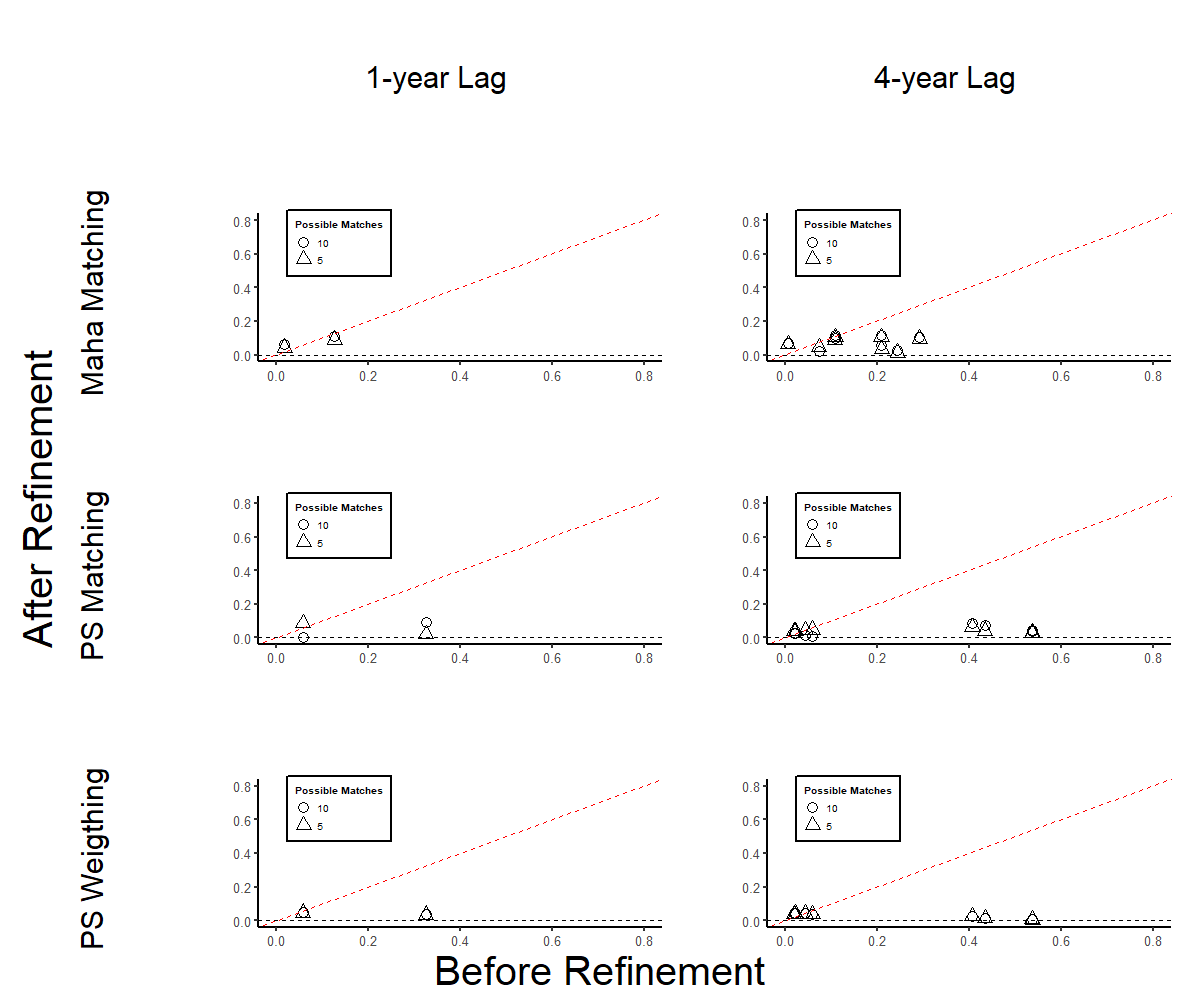
\includegraphics[width=1\linewidth,alt={Six panel plot comparing covariate balance using different matching methods and time lags}]{images/did_balance_scatter} 

}

\caption{Variable balance after matched-set refinement.}\label{fig:fig-matching-comparison}
\end{figure}

Note: Scatter plots display the standardized mean difference of each covariate \(j\) and lag year \(l\) before (x-axis) and after (y-axis) matched set refinement. Each plot includes varying numbers of possible matches for each matching method. Rows represent different matching/weighting methods, while columns indicate adjustments for various lag lengths. Figure \ref{fig:fig-balance-by-method} below repeats the exercise for the pre-treatment period under a richer set of refinement configurations.

\begin{Shaded}
\begin{Highlighting}[]
\CommentTok{\# Step 1: Define configurations}
\NormalTok{configurations }\OtherTok{\textless{}{-}} \FunctionTok{list}\NormalTok{(}
    \FunctionTok{list}\NormalTok{(}\AttributeTok{refinement.method =} \StringTok{"none"}\NormalTok{, }\AttributeTok{qoi =} \StringTok{"att"}\NormalTok{),}
    \FunctionTok{list}\NormalTok{(}\AttributeTok{refinement.method =} \StringTok{"none"}\NormalTok{, }\AttributeTok{qoi =} \StringTok{"art"}\NormalTok{),}
    \FunctionTok{list}\NormalTok{(}\AttributeTok{refinement.method =} \StringTok{"mahalanobis"}\NormalTok{, }\AttributeTok{qoi =} \StringTok{"att"}\NormalTok{),}
    \FunctionTok{list}\NormalTok{(}\AttributeTok{refinement.method =} \StringTok{"mahalanobis"}\NormalTok{, }\AttributeTok{qoi =} \StringTok{"art"}\NormalTok{),}
    \FunctionTok{list}\NormalTok{(}\AttributeTok{refinement.method =} \StringTok{"ps.match"}\NormalTok{, }\AttributeTok{qoi =} \StringTok{"att"}\NormalTok{),}
    \FunctionTok{list}\NormalTok{(}\AttributeTok{refinement.method =} \StringTok{"ps.match"}\NormalTok{, }\AttributeTok{qoi =} \StringTok{"art"}\NormalTok{),}
    \FunctionTok{list}\NormalTok{(}\AttributeTok{refinement.method =} \StringTok{"ps.weight"}\NormalTok{, }\AttributeTok{qoi =} \StringTok{"att"}\NormalTok{),}
    \FunctionTok{list}\NormalTok{(}\AttributeTok{refinement.method =} \StringTok{"ps.weight"}\NormalTok{, }\AttributeTok{qoi =} \StringTok{"art"}\NormalTok{)}
\NormalTok{)}

\CommentTok{\# Step 2: Use lapply or loop to generate results}
\NormalTok{results }\OtherTok{\textless{}{-}} \FunctionTok{lapply}\NormalTok{(configurations, }\ControlFlowTok{function}\NormalTok{(config) \{}
    \FunctionTok{PanelMatch}\NormalTok{(}
        \AttributeTok{lag                       =} \DecValTok{4}\NormalTok{,}
        \AttributeTok{panel.data =} \FunctionTok{PanelData}\NormalTok{(}\AttributeTok{panel.data =}\NormalTok{ dem, }
              \AttributeTok{unit.id =} \StringTok{"wbcode2"}\NormalTok{, }
              \AttributeTok{time.id =} \StringTok{"year"}\NormalTok{, }
              \AttributeTok{treatment =} \StringTok{"dem"}\NormalTok{, }
              \AttributeTok{outcome =} \StringTok{"y"}\NormalTok{),}
        \AttributeTok{match.missing             =} \ConstantTok{FALSE}\NormalTok{,}
        \AttributeTok{listwise.delete           =} \ConstantTok{TRUE}\NormalTok{,}
        \AttributeTok{size.match                =} \DecValTok{5}\NormalTok{,}
        \AttributeTok{lead                      =} \DecValTok{0}\SpecialCharTok{:}\DecValTok{4}\NormalTok{,}
        \AttributeTok{forbid.treatment.reversal =} \ConstantTok{FALSE}\NormalTok{,}
        \AttributeTok{refinement.method         =}\NormalTok{ config}\SpecialCharTok{$}\NormalTok{refinement.method,}
        \AttributeTok{covs.formula              =} \SpecialCharTok{\textasciitilde{}} \FunctionTok{I}\NormalTok{(}\FunctionTok{lag}\NormalTok{(tradewb, }\DecValTok{1}\SpecialCharTok{:}\DecValTok{4}\NormalTok{)) }\SpecialCharTok{+} \FunctionTok{I}\NormalTok{(}\FunctionTok{lag}\NormalTok{(y, }\DecValTok{1}\SpecialCharTok{:}\DecValTok{4}\NormalTok{)),}
        \AttributeTok{qoi                       =}\NormalTok{ config}\SpecialCharTok{$}\NormalTok{qoi}
\NormalTok{    )}
\NormalTok{\})}

\CommentTok{\# Step 3: Get covariate balance and plot}
\NormalTok{plots }\OtherTok{\textless{}{-}} \FunctionTok{mapply}\NormalTok{(}\ControlFlowTok{function}\NormalTok{(result, config) \{}
\NormalTok{    df }\OtherTok{\textless{}{-}} \FunctionTok{get\_covariate\_balance}\NormalTok{(}
        \ControlFlowTok{if}\NormalTok{ (config}\SpecialCharTok{$}\NormalTok{qoi }\SpecialCharTok{==} \StringTok{"att"}\NormalTok{)}
\NormalTok{            result}\SpecialCharTok{$}\NormalTok{att}
        \ControlFlowTok{else}
\NormalTok{            result}\SpecialCharTok{$}\NormalTok{art,}
        \AttributeTok{panel.data =} \FunctionTok{PanelData}\NormalTok{(}\AttributeTok{panel.data =}\NormalTok{ dem, }
              \AttributeTok{unit.id =} \StringTok{"wbcode2"}\NormalTok{, }
              \AttributeTok{time.id =} \StringTok{"year"}\NormalTok{, }
              \AttributeTok{treatment =} \StringTok{"dem"}\NormalTok{, }
              \AttributeTok{outcome =} \StringTok{"y"}\NormalTok{),}
        \AttributeTok{covariates =} \FunctionTok{c}\NormalTok{(}\StringTok{"tradewb"}\NormalTok{, }\StringTok{"y"}\NormalTok{),}
        \AttributeTok{plot =}\NormalTok{ F}
\NormalTok{    )}
\NormalTok{    causalverse}\SpecialCharTok{::}\FunctionTok{plot\_covariate\_balance\_pretrend}\NormalTok{(df, }\AttributeTok{main =} \StringTok{""}\NormalTok{, }\AttributeTok{show\_legend =}\NormalTok{ F)}
\NormalTok{\}, results, configurations, }\AttributeTok{SIMPLIFY =} \ConstantTok{FALSE}\NormalTok{)}

\CommentTok{\# Set names for plots}
\FunctionTok{names}\NormalTok{(plots) }\OtherTok{\textless{}{-}} \FunctionTok{sapply}\NormalTok{(configurations, }\ControlFlowTok{function}\NormalTok{(config) \{}
    \FunctionTok{paste}\NormalTok{(config}\SpecialCharTok{$}\NormalTok{qoi, config}\SpecialCharTok{$}\NormalTok{refinement.method, }\AttributeTok{sep =} \StringTok{"."}\NormalTok{)}
\NormalTok{\})}
\end{Highlighting}
\end{Shaded}

The script below assembles the per-method, per-estimand pre-treatment balance plots into a single composite PNG used by the rendered figure above.

\begin{Shaded}
\begin{Highlighting}[]
\FunctionTok{library}\NormalTok{(gridExtra)}
\FunctionTok{library}\NormalTok{(grid)}

\CommentTok{\# Column and row labels}
\NormalTok{col\_labels }\OtherTok{\textless{}{-}}
    \FunctionTok{c}\NormalTok{(}\StringTok{"None"}\NormalTok{,}
      \StringTok{"Mahalanobis"}\NormalTok{,}
      \StringTok{"Propensity Score Matching"}\NormalTok{,}
      \StringTok{"Propensity Score Weighting"}\NormalTok{)}
\NormalTok{row\_labels }\OtherTok{\textless{}{-}} \FunctionTok{c}\NormalTok{(}\StringTok{"ATT"}\NormalTok{, }\StringTok{"ART"}\NormalTok{)}

\CommentTok{\# Specify your desired fontsize for labels}
\NormalTok{minor.axes.fontsize }\OtherTok{\textless{}{-}} \DecValTok{16}
\NormalTok{major.axes.fontsize }\OtherTok{\textless{}{-}} \DecValTok{20}

\FunctionTok{png}\NormalTok{(}\FunctionTok{file.path}\NormalTok{(}\FunctionTok{getwd}\NormalTok{(), }\StringTok{"images"}\NormalTok{, }\StringTok{"p\_covariate\_balance.png"}\NormalTok{), }\AttributeTok{width=}\DecValTok{1200}\NormalTok{, }\AttributeTok{height=}\DecValTok{1000}\NormalTok{)}

\CommentTok{\# Create a list{-}of{-}lists, where each inner list represents a row}
\NormalTok{grid\_list }\OtherTok{\textless{}{-}} \FunctionTok{list}\NormalTok{(}
    \FunctionTok{list}\NormalTok{(}
        \FunctionTok{nullGrob}\NormalTok{(),}
        \FunctionTok{textGrob}\NormalTok{(col\_labels[}\DecValTok{1}\NormalTok{], }\AttributeTok{gp =} \FunctionTok{gpar}\NormalTok{(}\AttributeTok{fontsize =}\NormalTok{ minor.axes.fontsize)),}
        \FunctionTok{textGrob}\NormalTok{(col\_labels[}\DecValTok{2}\NormalTok{], }\AttributeTok{gp =} \FunctionTok{gpar}\NormalTok{(}\AttributeTok{fontsize =}\NormalTok{ minor.axes.fontsize)),}
        \FunctionTok{textGrob}\NormalTok{(col\_labels[}\DecValTok{3}\NormalTok{], }\AttributeTok{gp =} \FunctionTok{gpar}\NormalTok{(}\AttributeTok{fontsize =}\NormalTok{ minor.axes.fontsize)),}
        \FunctionTok{textGrob}\NormalTok{(col\_labels[}\DecValTok{4}\NormalTok{], }\AttributeTok{gp =} \FunctionTok{gpar}\NormalTok{(}\AttributeTok{fontsize =}\NormalTok{ minor.axes.fontsize))}
\NormalTok{    ),}
    
    \FunctionTok{list}\NormalTok{(}
        \FunctionTok{textGrob}\NormalTok{(}
\NormalTok{            row\_labels[}\DecValTok{1}\NormalTok{],}
            \AttributeTok{gp =} \FunctionTok{gpar}\NormalTok{(}\AttributeTok{fontsize =}\NormalTok{ minor.axes.fontsize),}
            \AttributeTok{rot =} \DecValTok{90}
\NormalTok{        ),}
\NormalTok{        plots}\SpecialCharTok{$}\NormalTok{att.none,}
\NormalTok{        plots}\SpecialCharTok{$}\NormalTok{att.mahalanobis,}
\NormalTok{        plots}\SpecialCharTok{$}\NormalTok{att.ps.match,}
\NormalTok{        plots}\SpecialCharTok{$}\NormalTok{att.ps.weight}
\NormalTok{    ),}
    
    \FunctionTok{list}\NormalTok{(}
        \FunctionTok{textGrob}\NormalTok{(}
\NormalTok{            row\_labels[}\DecValTok{2}\NormalTok{],}
            \AttributeTok{gp =} \FunctionTok{gpar}\NormalTok{(}\AttributeTok{fontsize =}\NormalTok{ minor.axes.fontsize),}
            \AttributeTok{rot =} \DecValTok{90}
\NormalTok{        ),}
\NormalTok{        plots}\SpecialCharTok{$}\NormalTok{art.none,}
\NormalTok{        plots}\SpecialCharTok{$}\NormalTok{art.mahalanobis,}
\NormalTok{        plots}\SpecialCharTok{$}\NormalTok{art.ps.match,}
\NormalTok{        plots}\SpecialCharTok{$}\NormalTok{art.ps.weight}
\NormalTok{    )}
\NormalTok{)}

\CommentTok{\# "Flatten" the list{-}of{-}lists into a single list of grobs}
\NormalTok{grobs }\OtherTok{\textless{}{-}} \FunctionTok{do.call}\NormalTok{(c, grid\_list)}

\CommentTok{\# Arrange your plots with text labels}
\FunctionTok{grid.arrange}\NormalTok{(}
    \AttributeTok{grobs   =}\NormalTok{ grobs,}
    \AttributeTok{ncol    =} \DecValTok{5}\NormalTok{,}
    \AttributeTok{nrow    =} \DecValTok{3}\NormalTok{,}
    \AttributeTok{widths  =} \FunctionTok{c}\NormalTok{(}\FloatTok{0.1}\NormalTok{, }\FloatTok{0.225}\NormalTok{, }\FloatTok{0.225}\NormalTok{, }\FloatTok{0.225}\NormalTok{, }\FloatTok{0.225}\NormalTok{),}
    \AttributeTok{heights =} \FunctionTok{c}\NormalTok{(}\FloatTok{0.1}\NormalTok{, }\FloatTok{0.45}\NormalTok{, }\FloatTok{0.45}\NormalTok{)}
\NormalTok{)}

\CommentTok{\# Add main x and y axis titles}
\FunctionTok{grid.text}\NormalTok{(}
    \StringTok{"Refinement Methods"}\NormalTok{,}
    \AttributeTok{x  =} \FloatTok{0.5}\NormalTok{,}
    \AttributeTok{y  =} \FloatTok{0.01}\NormalTok{,}
    \AttributeTok{gp =} \FunctionTok{gpar}\NormalTok{(}\AttributeTok{fontsize =}\NormalTok{ major.axes.fontsize)}
\NormalTok{)}
\FunctionTok{grid.text}\NormalTok{(}
    \StringTok{"Quantities of Interest"}\NormalTok{,}
    \AttributeTok{x   =} \FloatTok{0.02}\NormalTok{,}
    \AttributeTok{y   =} \FloatTok{0.5}\NormalTok{,}
    \AttributeTok{rot =} \DecValTok{90}\NormalTok{,}
    \AttributeTok{gp  =} \FunctionTok{gpar}\NormalTok{(}\AttributeTok{fontsize =}\NormalTok{ major.axes.fontsize)}
\NormalTok{)}

\FunctionTok{dev.off}\NormalTok{()}
\end{Highlighting}
\end{Shaded}

\begin{Shaded}
\begin{Highlighting}[]
\NormalTok{knitr}\SpecialCharTok{::}\FunctionTok{include\_graphics}\NormalTok{(}\FunctionTok{file.path}\NormalTok{(}\FunctionTok{getwd}\NormalTok{(), }\StringTok{"images"}\NormalTok{, }\StringTok{"p\_covariate\_balance.png"}\NormalTok{))}
\end{Highlighting}
\end{Shaded}

\begin{figure}

{\centering 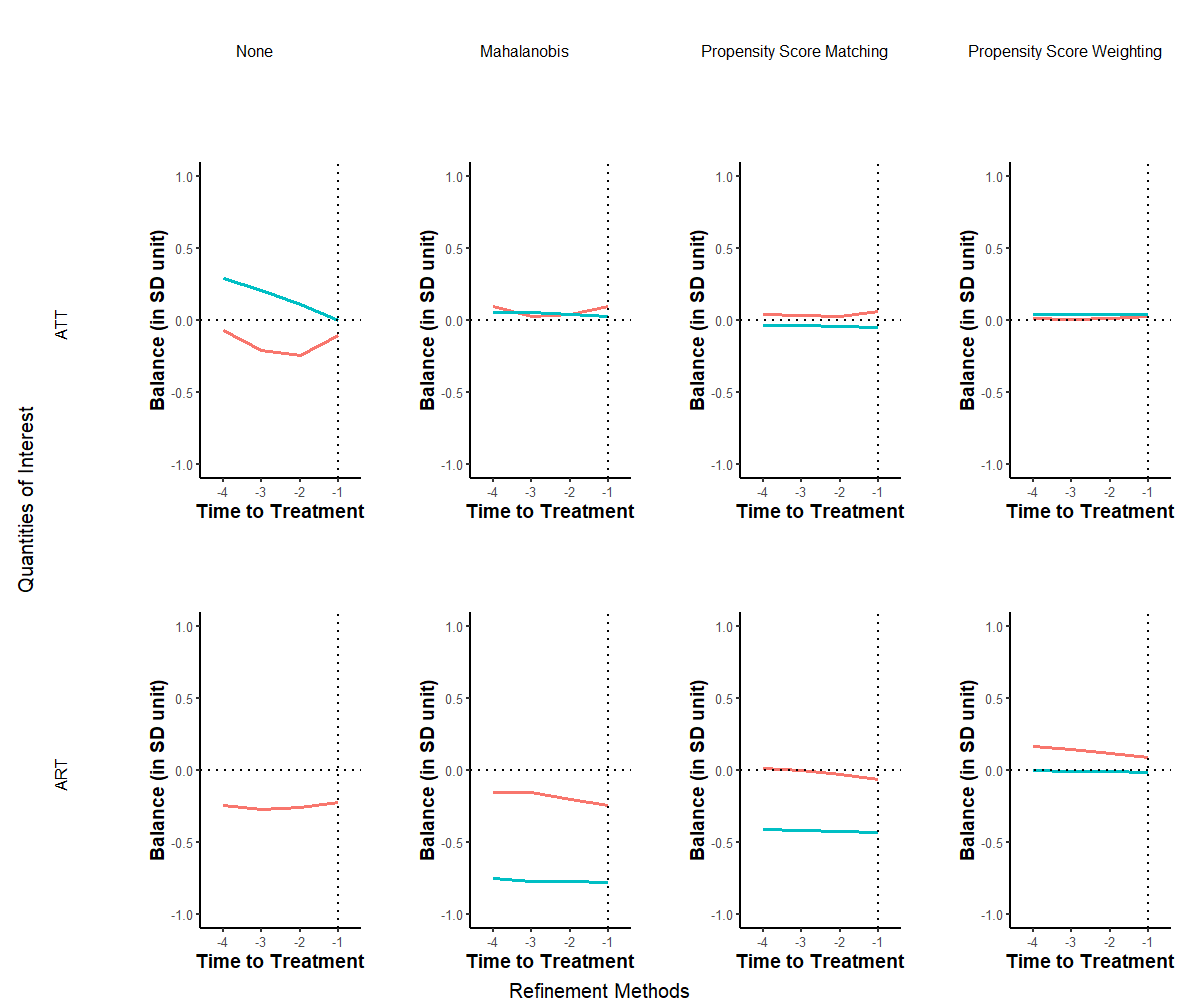
\includegraphics[width=1\linewidth,alt={Line plots showing covariate balance from time minus 4 to minus 1 for different methods and estimands}]{images/p_covariate_balance} 

}

\caption{Covariate balance over time by refinement method and estimand.}\label{fig:fig-balance-by-method}
\end{figure}

Note: Each graph displays the standardized mean difference plotted on the vertical axis across a pre-treatment duration of four years represented on the horizontal axis. The leftmost column illustrates the balance prior to refinement, while the subsequent three columns depict the covariate balance post the application of distinct refinement techniques. Each individual line signifies the balance of a specific variable during the pre-treatment phase. The red line is tradewb and blue line is the lagged outcome variable.

In Figure \ref{fig:fig-balance-by-method}, we observe a marked improvement in covariate balance due to the implemented matching procedures during the pre-treatment period. Our analysis prioritizes methods that adjust for time-varying covariates over a span of four years preceding the treatment initiation. The two rows delineate the standardized mean balance for both treatment modalities, with individual lines representing the balance for each covariate.

Across all scenarios, the refinement attributed to matched sets significantly enhances balance. Notably, using propensity score weighting considerably mitigates imbalances in confounders. While some degree of imbalance remains evident in the Mahalanobis distance and propensity score matching techniques, the standardized mean difference for the lagged outcome remains stable throughout the pre-treatment phase. This consistency lends credence to the validity of the proposed DiD estimator.

\textbf{Estimation Results}

We now detail the estimated ATTs derived from the matching techniques. Figure below offers visual representations of the impacts of treatment initiation (upper panel) and treatment reversal (lower panel) on the outcome variable for a duration of 5 years post-transition, specifically, (\(F = 0, 1, …, 4\)). Across the five methods (columns), it becomes evident that the point estimates of effects associated with treatment initiation consistently approximate zero over the 5-year window. In contrast, the estimated outcomes of treatment reversal are notably negative and maintain statistical significance through all refinement techniques during the initial year of transition and the 1 to 4 years that follow, provided treatment reversal is permissible. These effects are notably pronounced, pointing to an estimated reduction of roughly X\% in the outcome variable.

Collectively, these findings indicate that the transition into the treated state from its absence doesn't invariably lead to a heightened outcome. Instead, the transition from the treated state back to its absence exerts a considerable negative effect on the outcome variable in both the short and intermediate terms. Hence, the positive effect of the treatment (if we were to use traditional DiD) is actually driven by the negative effect of treatment reversal.

\begin{Shaded}
\begin{Highlighting}[]
\CommentTok{\# sequential}
\CommentTok{\# Step 1: Apply PanelEstimate function}

\CommentTok{\# Initialize an empty list to store results}
\NormalTok{res\_est }\OtherTok{\textless{}{-}} \FunctionTok{vector}\NormalTok{(}\StringTok{"list"}\NormalTok{, }\FunctionTok{length}\NormalTok{(res\_pm))}

\CommentTok{\# Iterate over each element in res\_pm}
\ControlFlowTok{for}\NormalTok{ (i }\ControlFlowTok{in} \DecValTok{1}\SpecialCharTok{:}\FunctionTok{length}\NormalTok{(res\_pm)) \{}
\NormalTok{  res\_est[[i]] }\OtherTok{\textless{}{-}} \FunctionTok{PanelEstimate}\NormalTok{(}
\NormalTok{    res\_pm[[i]],}
    \AttributeTok{data =}\NormalTok{ dem,}
    \AttributeTok{se.method =} \StringTok{"bootstrap"}\NormalTok{,}
    \AttributeTok{number.iterations =} \DecValTok{1000}\NormalTok{,}
    \AttributeTok{confidence.level =}\NormalTok{ .}\DecValTok{95}
\NormalTok{  )}
  \CommentTok{\# Transfer the name of the current element to the res\_est list}
  \FunctionTok{names}\NormalTok{(res\_est)[i] }\OtherTok{\textless{}{-}} \FunctionTok{names}\NormalTok{(res\_pm)[i]}
\NormalTok{\}}

\CommentTok{\# Step 2: Apply plot\_PanelEstimate function}

\CommentTok{\# Initialize an empty list to store plot results}
\NormalTok{res\_est\_plot }\OtherTok{\textless{}{-}} \FunctionTok{vector}\NormalTok{(}\StringTok{"list"}\NormalTok{, }\FunctionTok{length}\NormalTok{(res\_est))}

\CommentTok{\# Iterate over each element in res\_est}
\ControlFlowTok{for}\NormalTok{ (i }\ControlFlowTok{in} \DecValTok{1}\SpecialCharTok{:}\FunctionTok{length}\NormalTok{(res\_est)) \{}
\NormalTok{    res\_est\_plot[[i]] }\OtherTok{\textless{}{-}}
        \FunctionTok{plot\_PanelEstimate}\NormalTok{(res\_est[[i]],}
                           \AttributeTok{main =} \StringTok{""}\NormalTok{,}
                           \AttributeTok{theme\_use =}\NormalTok{ causalverse}\SpecialCharTok{::}\FunctionTok{ama\_theme}\NormalTok{(}\AttributeTok{base\_size =} \DecValTok{14}\NormalTok{))}
    \CommentTok{\# Transfer the name of the current element to the res\_est\_plot list}
    \FunctionTok{names}\NormalTok{(res\_est\_plot)[i] }\OtherTok{\textless{}{-}} \FunctionTok{names}\NormalTok{(res\_est)[i]}
\NormalTok{\}}

\CommentTok{\# check results}
\CommentTok{\# res\_est\_plot$mahalanobis.1lag.5m}


\CommentTok{\# Step 1: Apply PanelEstimate function for res\_pm\_rev}

\CommentTok{\# Initialize an empty list to store results}
\NormalTok{res\_est\_rev }\OtherTok{\textless{}{-}} \FunctionTok{vector}\NormalTok{(}\StringTok{"list"}\NormalTok{, }\FunctionTok{length}\NormalTok{(res\_pm\_rev))}

\CommentTok{\# Iterate over each element in res\_pm\_rev}
\ControlFlowTok{for}\NormalTok{ (i }\ControlFlowTok{in} \DecValTok{1}\SpecialCharTok{:}\FunctionTok{length}\NormalTok{(res\_pm\_rev)) \{}
\NormalTok{  res\_est\_rev[[i]] }\OtherTok{\textless{}{-}} \FunctionTok{PanelEstimate}\NormalTok{(}
\NormalTok{    res\_pm\_rev[[i]],}
    \AttributeTok{data =}\NormalTok{ dem,}
    \AttributeTok{se.method =} \StringTok{"bootstrap"}\NormalTok{,}
    \AttributeTok{number.iterations =} \DecValTok{1000}\NormalTok{,}
    \AttributeTok{confidence.level =}\NormalTok{ .}\DecValTok{95}
\NormalTok{  )}
  \CommentTok{\# Transfer the name of the current element to the res\_est\_rev list}
  \FunctionTok{names}\NormalTok{(res\_est\_rev)[i] }\OtherTok{\textless{}{-}} \FunctionTok{names}\NormalTok{(res\_pm\_rev)[i]}
\NormalTok{\}}

\CommentTok{\# Step 2: Apply plot\_PanelEstimate function for res\_est\_rev}

\CommentTok{\# Initialize an empty list to store plot results}
\NormalTok{res\_est\_plot\_rev }\OtherTok{\textless{}{-}} \FunctionTok{vector}\NormalTok{(}\StringTok{"list"}\NormalTok{, }\FunctionTok{length}\NormalTok{(res\_est\_rev))}

\CommentTok{\# Iterate over each element in res\_est\_rev}
\ControlFlowTok{for}\NormalTok{ (i }\ControlFlowTok{in} \DecValTok{1}\SpecialCharTok{:}\FunctionTok{length}\NormalTok{(res\_est\_rev)) \{}
\NormalTok{    res\_est\_plot\_rev[[i]] }\OtherTok{\textless{}{-}}
        \FunctionTok{plot\_PanelEstimate}\NormalTok{(res\_est\_rev[[i]],}
                           \AttributeTok{main =} \StringTok{""}\NormalTok{,}
                           \AttributeTok{theme\_use =}\NormalTok{ causalverse}\SpecialCharTok{::}\FunctionTok{ama\_theme}\NormalTok{(}\AttributeTok{base\_size =} \DecValTok{14}\NormalTok{))}
  \CommentTok{\# Transfer the name of the current element to the res\_est\_plot\_rev list}
  \FunctionTok{names}\NormalTok{(res\_est\_plot\_rev)[i] }\OtherTok{\textless{}{-}} \FunctionTok{names}\NormalTok{(res\_est\_rev)[i]}
\NormalTok{\}}
\end{Highlighting}
\end{Shaded}

\begin{Shaded}
\begin{Highlighting}[]
\CommentTok{\# parallel}
\FunctionTok{library}\NormalTok{(doParallel)}
\FunctionTok{library}\NormalTok{(foreach)}

\CommentTok{\# Detect the number of cores to use for parallel processing}
\NormalTok{num\_cores }\OtherTok{\textless{}{-}} \DecValTok{4}

\CommentTok{\# Register the parallel backend}
\NormalTok{cl }\OtherTok{\textless{}{-}} \FunctionTok{makeCluster}\NormalTok{(num\_cores)}
\FunctionTok{registerDoParallel}\NormalTok{(cl)}

\CommentTok{\# Step 1: Apply PanelEstimate function in parallel}
\NormalTok{res\_est }\OtherTok{\textless{}{-}}
    \FunctionTok{foreach}\NormalTok{(}\AttributeTok{i =} \DecValTok{1}\SpecialCharTok{:}\FunctionTok{length}\NormalTok{(res\_pm), }\AttributeTok{.packages =} \StringTok{"PanelMatch"}\NormalTok{) }\SpecialCharTok{\%dopar\%}\NormalTok{ \{}
        \FunctionTok{PanelEstimate}\NormalTok{(}
\NormalTok{            res\_pm[[i]],}
            \AttributeTok{data =}\NormalTok{ dem,}
            \AttributeTok{se.method =} \StringTok{"bootstrap"}\NormalTok{,}
            \AttributeTok{number.iterations =} \DecValTok{1000}\NormalTok{,}
            \AttributeTok{confidence.level =}\NormalTok{ .}\DecValTok{95}
\NormalTok{        )}
\NormalTok{    \}}

\CommentTok{\# Transfer names from res\_pm to res\_est}
\FunctionTok{names}\NormalTok{(res\_est) }\OtherTok{\textless{}{-}} \FunctionTok{names}\NormalTok{(res\_pm)}

\CommentTok{\# Step 2: Apply plot\_PanelEstimate function in parallel}
\NormalTok{res\_est\_plot }\OtherTok{\textless{}{-}}
    \FunctionTok{foreach}\NormalTok{(}
        \AttributeTok{i =} \DecValTok{1}\SpecialCharTok{:}\FunctionTok{length}\NormalTok{(res\_est),}
        \AttributeTok{.packages =} \FunctionTok{c}\NormalTok{(}\StringTok{"PanelMatch"}\NormalTok{, }\StringTok{"causalverse"}\NormalTok{, }\StringTok{"ggplot2"}\NormalTok{)}
\NormalTok{    ) }\SpecialCharTok{\%dopar\%}\NormalTok{ \{}
        \FunctionTok{plot\_PanelEstimate}\NormalTok{(res\_est[[i]],}
                           \AttributeTok{main =} \StringTok{""}\NormalTok{,}
                           \AttributeTok{theme\_use =}\NormalTok{ causalverse}\SpecialCharTok{::}\FunctionTok{ama\_theme}\NormalTok{(}\AttributeTok{base\_size =} \DecValTok{10}\NormalTok{))}
\NormalTok{    \}}

\CommentTok{\# Transfer names from res\_est to res\_est\_plot}
\FunctionTok{names}\NormalTok{(res\_est\_plot) }\OtherTok{\textless{}{-}} \FunctionTok{names}\NormalTok{(res\_est)}



\CommentTok{\# Step 1: Apply PanelEstimate function for res\_pm\_rev in parallel}
\NormalTok{res\_est\_rev }\OtherTok{\textless{}{-}}
    \FunctionTok{foreach}\NormalTok{(}\AttributeTok{i =} \DecValTok{1}\SpecialCharTok{:}\FunctionTok{length}\NormalTok{(res\_pm\_rev), }\AttributeTok{.packages =} \StringTok{"PanelMatch"}\NormalTok{) }\SpecialCharTok{\%dopar\%}\NormalTok{ \{}
        \FunctionTok{PanelEstimate}\NormalTok{(}
\NormalTok{            res\_pm\_rev[[i]],}
            \AttributeTok{data =}\NormalTok{ dem,}
            \AttributeTok{se.method =} \StringTok{"bootstrap"}\NormalTok{,}
            \AttributeTok{number.iterations =} \DecValTok{1000}\NormalTok{,}
            \AttributeTok{confidence.level =}\NormalTok{ .}\DecValTok{95}
\NormalTok{        )}
\NormalTok{    \}}

\CommentTok{\# Transfer names from res\_pm\_rev to res\_est\_rev}
\FunctionTok{names}\NormalTok{(res\_est\_rev) }\OtherTok{\textless{}{-}} \FunctionTok{names}\NormalTok{(res\_pm\_rev)}

\CommentTok{\# Step 2: Apply plot\_PanelEstimate function for res\_est\_rev in parallel}
\NormalTok{res\_est\_plot\_rev }\OtherTok{\textless{}{-}}
    \FunctionTok{foreach}\NormalTok{(}
        \AttributeTok{i =} \DecValTok{1}\SpecialCharTok{:}\FunctionTok{length}\NormalTok{(res\_est\_rev),}
        \AttributeTok{.packages =} \FunctionTok{c}\NormalTok{(}\StringTok{"PanelMatch"}\NormalTok{, }\StringTok{"causalverse"}\NormalTok{, }\StringTok{"ggplot2"}\NormalTok{)}
\NormalTok{    ) }\SpecialCharTok{\%dopar\%}\NormalTok{ \{}
        \FunctionTok{plot\_PanelEstimate}\NormalTok{(res\_est\_rev[[i]],}
                           \AttributeTok{main =} \StringTok{""}\NormalTok{,}
                           \AttributeTok{theme\_use =}\NormalTok{ causalverse}\SpecialCharTok{::}\FunctionTok{ama\_theme}\NormalTok{(}\AttributeTok{base\_size =} \DecValTok{10}\NormalTok{))}
\NormalTok{    \}}

\CommentTok{\# Transfer names from res\_est\_rev to res\_est\_plot\_rev}
\FunctionTok{names}\NormalTok{(res\_est\_plot\_rev) }\OtherTok{\textless{}{-}} \FunctionTok{names}\NormalTok{(res\_est\_rev)}

\CommentTok{\# Stop the cluster}
\FunctionTok{stopCluster}\NormalTok{(cl)}
\end{Highlighting}
\end{Shaded}

The export script below assembles the ATT and ART event-study estimates from PanelMatch under five refinement-by-match-size combinations into a composite PNG.

\begin{Shaded}
\begin{Highlighting}[]
\FunctionTok{library}\NormalTok{(gridExtra)}
\FunctionTok{library}\NormalTok{(grid)}

\CommentTok{\# Column and row labels}
\NormalTok{col\_labels }\OtherTok{\textless{}{-}} \FunctionTok{c}\NormalTok{(}\StringTok{"Mahalanobis 5m"}\NormalTok{,}
                \StringTok{"Mahalanobis 10m"}\NormalTok{,}
                \StringTok{"PS Matching 5m"}\NormalTok{,}
                \StringTok{"PS Matching 10m"}\NormalTok{,}
                \StringTok{"PS Weighting 5m"}\NormalTok{)}

\NormalTok{row\_labels }\OtherTok{\textless{}{-}} \FunctionTok{c}\NormalTok{(}\StringTok{"ATT"}\NormalTok{, }\StringTok{"ART"}\NormalTok{)}

\CommentTok{\# Specify your desired fontsize for labels}
\NormalTok{minor.axes.fontsize }\OtherTok{\textless{}{-}} \DecValTok{16}
\NormalTok{major.axes.fontsize }\OtherTok{\textless{}{-}} \DecValTok{20}

\FunctionTok{png}\NormalTok{(}\FunctionTok{file.path}\NormalTok{(}\FunctionTok{getwd}\NormalTok{(), }\StringTok{"images"}\NormalTok{, }\StringTok{"p\_did\_est\_in\_n\_out.png"}\NormalTok{), }\AttributeTok{width=}\DecValTok{1200}\NormalTok{, }\AttributeTok{height=}\DecValTok{1000}\NormalTok{)}

\CommentTok{\# Create a list{-}of{-}lists, where each inner list represents a row}
\NormalTok{grid\_list }\OtherTok{\textless{}{-}} \FunctionTok{list}\NormalTok{(}
  \FunctionTok{list}\NormalTok{(}
    \FunctionTok{nullGrob}\NormalTok{(),}
    \FunctionTok{textGrob}\NormalTok{(col\_labels[}\DecValTok{1}\NormalTok{], }\AttributeTok{gp =} \FunctionTok{gpar}\NormalTok{(}\AttributeTok{fontsize =}\NormalTok{ minor.axes.fontsize)),}
    \FunctionTok{textGrob}\NormalTok{(col\_labels[}\DecValTok{2}\NormalTok{], }\AttributeTok{gp =} \FunctionTok{gpar}\NormalTok{(}\AttributeTok{fontsize =}\NormalTok{ minor.axes.fontsize)),}
    \FunctionTok{textGrob}\NormalTok{(col\_labels[}\DecValTok{3}\NormalTok{], }\AttributeTok{gp =} \FunctionTok{gpar}\NormalTok{(}\AttributeTok{fontsize =}\NormalTok{ minor.axes.fontsize)),}
    \FunctionTok{textGrob}\NormalTok{(col\_labels[}\DecValTok{4}\NormalTok{], }\AttributeTok{gp =} \FunctionTok{gpar}\NormalTok{(}\AttributeTok{fontsize =}\NormalTok{ minor.axes.fontsize)),}
    \FunctionTok{textGrob}\NormalTok{(col\_labels[}\DecValTok{5}\NormalTok{], }\AttributeTok{gp =} \FunctionTok{gpar}\NormalTok{(}\AttributeTok{fontsize =}\NormalTok{ minor.axes.fontsize))}
\NormalTok{  ),}
  
  \FunctionTok{list}\NormalTok{(}
    \FunctionTok{textGrob}\NormalTok{(row\_labels[}\DecValTok{1}\NormalTok{], }\AttributeTok{gp =} \FunctionTok{gpar}\NormalTok{(}\AttributeTok{fontsize =}\NormalTok{ minor.axes.fontsize), }\AttributeTok{rot =} \DecValTok{90}\NormalTok{),}
\NormalTok{    res\_est\_plot}\SpecialCharTok{$}\NormalTok{mahalanobis}\FloatTok{.1}\NormalTok{lag}\FloatTok{.5}\NormalTok{m,}
\NormalTok{    res\_est\_plot}\SpecialCharTok{$}\NormalTok{mahalanobis}\FloatTok{.1}\NormalTok{lag}\FloatTok{.10}\NormalTok{m,}
\NormalTok{    res\_est\_plot}\SpecialCharTok{$}\NormalTok{ps.match}\FloatTok{.1}\NormalTok{lag}\FloatTok{.5}\NormalTok{m,}
\NormalTok{    res\_est\_plot}\SpecialCharTok{$}\NormalTok{ps.match}\FloatTok{.1}\NormalTok{lag}\FloatTok{.10}\NormalTok{m,}
\NormalTok{    res\_est\_plot}\SpecialCharTok{$}\NormalTok{ps.weight}\FloatTok{.1}\NormalTok{lag}\FloatTok{.5}\NormalTok{m}
\NormalTok{  ),}
  
  \FunctionTok{list}\NormalTok{(}
    \FunctionTok{textGrob}\NormalTok{(row\_labels[}\DecValTok{2}\NormalTok{], }\AttributeTok{gp =} \FunctionTok{gpar}\NormalTok{(}\AttributeTok{fontsize =}\NormalTok{ minor.axes.fontsize), }\AttributeTok{rot =} \DecValTok{90}\NormalTok{),}
\NormalTok{    res\_est\_plot\_rev}\SpecialCharTok{$}\NormalTok{mahalanobis}\FloatTok{.1}\NormalTok{lag}\FloatTok{.5}\NormalTok{m,}
\NormalTok{    res\_est\_plot\_rev}\SpecialCharTok{$}\NormalTok{mahalanobis}\FloatTok{.1}\NormalTok{lag}\FloatTok{.10}\NormalTok{m,}
\NormalTok{    res\_est\_plot\_rev}\SpecialCharTok{$}\NormalTok{ps.match}\FloatTok{.1}\NormalTok{lag}\FloatTok{.5}\NormalTok{m,}
\NormalTok{    res\_est\_plot\_rev}\SpecialCharTok{$}\NormalTok{ps.match}\FloatTok{.1}\NormalTok{lag}\FloatTok{.10}\NormalTok{m,}
\NormalTok{    res\_est\_plot\_rev}\SpecialCharTok{$}\NormalTok{ps.weight}\FloatTok{.1}\NormalTok{lag}\FloatTok{.5}\NormalTok{m}
\NormalTok{  )}
\NormalTok{)}

\CommentTok{\# "Flatten" the list{-}of{-}lists into a single list of grobs}
\NormalTok{grobs }\OtherTok{\textless{}{-}} \FunctionTok{do.call}\NormalTok{(c, grid\_list)}

\CommentTok{\# Arrange your plots with text labels}
\FunctionTok{grid.arrange}\NormalTok{(}
  \AttributeTok{grobs   =}\NormalTok{ grobs,}
  \AttributeTok{ncol    =} \DecValTok{6}\NormalTok{,}
  \AttributeTok{nrow    =} \DecValTok{3}\NormalTok{,}
  \AttributeTok{widths  =} \FunctionTok{c}\NormalTok{(}\FloatTok{0.1}\NormalTok{, }\FloatTok{0.18}\NormalTok{, }\FloatTok{0.18}\NormalTok{, }\FloatTok{0.18}\NormalTok{, }\FloatTok{0.18}\NormalTok{, }\FloatTok{0.18}\NormalTok{),}
  \AttributeTok{heights =} \FunctionTok{c}\NormalTok{(}\FloatTok{0.1}\NormalTok{, }\FloatTok{0.45}\NormalTok{, }\FloatTok{0.45}\NormalTok{)}
\NormalTok{)}

\CommentTok{\# Add main x and y axis titles}
\FunctionTok{grid.text}\NormalTok{(}
  \StringTok{"Methods"}\NormalTok{,}
  \AttributeTok{x  =} \FloatTok{0.5}\NormalTok{,}
  \AttributeTok{y  =} \FloatTok{0.02}\NormalTok{,}
  \AttributeTok{gp =} \FunctionTok{gpar}\NormalTok{(}\AttributeTok{fontsize =}\NormalTok{ major.axes.fontsize)}
\NormalTok{)}
\FunctionTok{grid.text}\NormalTok{(}
  \StringTok{""}\NormalTok{,}
  \AttributeTok{x   =} \FloatTok{0.02}\NormalTok{,}
  \AttributeTok{y   =} \FloatTok{0.5}\NormalTok{,}
  \AttributeTok{rot =} \DecValTok{90}\NormalTok{,}
  \AttributeTok{gp  =} \FunctionTok{gpar}\NormalTok{(}\AttributeTok{fontsize =}\NormalTok{ major.axes.fontsize)}
\NormalTok{)}

\FunctionTok{dev.off}\NormalTok{()}
\end{Highlighting}
\end{Shaded}

\begin{center}\rule{0.5\linewidth}{0.5pt}\end{center}

\subsection{Counterfactual Estimators}\label{sec-counterfactual-estimators}

Where Panel Match (Section \ref{sec-panel-match-did-estimator-with-in-and-out-treatment-conditions}) attacks model dependence by replacing the regression with local matched comparisons, counterfactual estimators take the opposite philosophical route: they keep an explicit outcome model but fit it only on control observations, then use it to impute the missing treated counterfactual. The two strategies are complements rather than substitutes. Counterfactual estimators dominate when the analyst is willing to model \(Y(0)\) but unwilling to extrapolate from treated units; Panel Match dominates when even the \(Y(0)\) model feels suspect and exact treatment-history matches are available.

Counterfactual (or \textbf{imputation}) estimators treat the \emph{treated} outcome as missing and \textbf{impute} it using information from the control units \citep{liu2024practical}. Formally, let

\[Y_{it}(1) \text{ and } Y_{it}(0)\]

denote the potential outcomes for unit \(i\) at time \(t\) \emph{with} and \emph{without} treatment. For treated units we only observe \(Y_{it}(1)\), so the goal is to impute the unobserved \(Y_{it}(0)\) (i.e., the \emph{counterfactual}).

Why use counterfactual estimators?

\begin{itemize}
\item
  Avoid negative weights: unlike some TWFE specifications that generate undesirable extrapolation weights, imputation uses only control data when building the prediction model and (typically) applies equal weights in post-treatment periods.
\item
  Model flexibility: analysts may combine rich time-series structure, non-linear regressions, or machine-learning learners while relaxing the \emph{strict exogeneity} assumption that plagues \hyperref[sec-two-way-fixed-effects]{TWFE}.
\item
  Transparent diagnostics: pre-treatment prediction error (e.g.~\(\text{RMSE}_{\text{pre}}\)) offers a concrete check of model fit, something ordinary DiD lacks.
\end{itemize}

The main families of counterfactual estimators are summarised in Table \ref{tab:did-counterfactual-estimators}.

\begin{longtable}[]{@{}
  >{\raggedright\arraybackslash}p{(\linewidth - 6\tabcolsep) * \real{0.1873}}
  >{\raggedright\arraybackslash}p{(\linewidth - 6\tabcolsep) * \real{0.3977}}
  >{\raggedright\arraybackslash}p{(\linewidth - 6\tabcolsep) * \real{0.2478}}
  >{\raggedright\arraybackslash}p{(\linewidth - 6\tabcolsep) * \real{0.1614}}@{}}
\caption{\label{tab:did-counterfactual-estimators} Main families of counterfactual (imputation) estimators for DiD: core idea, typical assumptions, and R implementations.}\tabularnewline
\toprule\noalign{}
\begin{minipage}[b]{\linewidth}\raggedright
Method
\end{minipage} & \begin{minipage}[b]{\linewidth}\raggedright
Core idea
\end{minipage} & \begin{minipage}[b]{\linewidth}\raggedright
Typical assumptions
\end{minipage} & \begin{minipage}[b]{\linewidth}\raggedright
R implementation
\end{minipage} \\
\midrule\noalign{}
\endfirsthead
\toprule\noalign{}
\begin{minipage}[b]{\linewidth}\raggedright
Method
\end{minipage} & \begin{minipage}[b]{\linewidth}\raggedright
Core idea
\end{minipage} & \begin{minipage}[b]{\linewidth}\raggedright
Typical assumptions
\end{minipage} & \begin{minipage}[b]{\linewidth}\raggedright
R implementation
\end{minipage} \\
\midrule\noalign{}
\endhead
\bottomrule\noalign{}
\endlastfoot
\textbf{Fixed-effects counterfactual estimator (FEct)} & Predict \(Y_{it}(0)\) with two-way additive FEs; compare each treated \(\hat{Y}_{it}(0)\) with \(Y_{it}(1)\) & Linearity; unit and time additive unobservables; no time-varying confounders & \texttt{fect::fect()} or \texttt{gsynth::gsynth(type\ =\ "fe")} \\
\textbf{Interactive Fixed Effects counterfactual estimator (IFEct)}

\citep[\citet{xu2017generalized}]{gobillon2016regional} & Augment FEct with low-rank latent factors: \(Y_{it}(0)=\alpha_i+\gamma_t+\lambda_i^\top f_t+\varepsilon_{it}\) & Low-rank factor structure; factors capture all time-varying confounders & \texttt{gsynth} (default), \texttt{fixest::feols()} with \texttt{sunab()} \\
\hyperref[sec-matrix-completion-estimator]{Matrix Completion} \textbf{(MC)} & Solve a \emph{soft-impute} nuclear-norm regularization \(\min_{\widehat Y(0)} \|M\odot(Y-\widehat Y(0))\|_F^2 + \lambda\|\widehat Y(0)\|_*\) & Same as IFE but allows dense weak factors; tuning via cross-validation & \texttt{softImpute}, \texttt{synthdid::mc()}, \texttt{gsynth(type\ =\ "mc")} \\
\textbf{Synthetic Control (SC)} & Choose non-negative weights that make the \emph{weighted} control path mimic a treated path pre-treatment & No interference; convex hull captures counterfactual; no return to pre-treat status & \texttt{Synth}, \texttt{synthdid}, \texttt{tidysynth}, \texttt{augsynth} \\
\end{longtable}

\begin{center}\rule{0.5\linewidth}{0.5pt}\end{center}

\begin{enumerate}
\def\labelenumi{\arabic{enumi}.}
\tightlist
\item
  \textbf{Fixed-Effects Counterfactual Estimator (FEct)}
\end{enumerate}

DiD is a special case where each treated observation is compared to the \emph{average} control outcome. This estimator assumes additive functional form of unobservables based on unit and time FEs. FEct predicts

\[
\widehat{Y}_{it}(0)
  = \hat{\alpha}_i + \hat{\gamma}_t
\]

using \textbf{only} control units when fitting \((\hat{\alpha}_i,\hat{\gamma}_t)\). The ATT is then

\[
\widehat{\tau}_{FEct}
  = \frac{1}{| \mathcal{T} |}\sum_{(i,t)\in\mathcal T}
    \{Y_{it}(1)-\widehat{Y}_{it}(0)\},
\]

where \(\mathcal T\) indexes treated unit--time pairs. FEct fixes the improper weighting of \hyperref[sec-two-way-fixed-effects]{TWFE} by comparing within each matched pair (where each pair is the treated observation and its predicted counterfactual that is the weighted sum of all untreated observations).

\begin{center}\rule{0.5\linewidth}{0.5pt}\end{center}

\begin{enumerate}
\def\labelenumi{\arabic{enumi}.}
\setcounter{enumi}{1}
\tightlist
\item
  \textbf{Interactive Fixed Effects (IFEct)}
\end{enumerate}

IFEct generalizes FEct by introducing \(R\) latent factors:

\[
Y_{it}(0)
  = \alpha_i + \gamma_t + \sum_{r=1}^R \lambda_{ir} f_{tr} + \varepsilon_{it},
\]

estimated via iterative principal components \citep[\citet{xu2017generalized}]{gobillon2016regional}. When we suspect unobserved time-varying confounder, FEct fails. Instead, IFEct uses the factor-augmented models to relax the strict exogeneity assumption where the effects of unobservables can be decomposed to unit FE + time FE + unit x time FE.

Setting \(R=0\) recovers FEct. \textbf{Generalized Synthetic Control} (GSC) \citep{xu2017generalized} is an IFEct implementation with ridge penalization when \(R>0\) (This estimator assumes treatments don't revert).

\begin{center}\rule{0.5\linewidth}{0.5pt}\end{center}

\begin{enumerate}
\def\labelenumi{\arabic{enumi}.}
\setcounter{enumi}{2}
\tightlist
\item
  \hyperref[sec-matrix-completion-estimator]{\textbf{Matrix Completion}}
\end{enumerate}

This is a generalization of factor-augmented models. Rather than fixing \(R\), MC solves a convex optimization where the nuclear-norm penalty \(|\widehat Y(0)|_*\) shrinks \emph{all} singular values. Different from IFEct which uses hard impute, MC uses soft impute to regularize the singular values when decomposing the residual matrix.

IFEct can outperform MC when the latent factors (of unobservables) are indeed low-rank/sparse and strong; MC prevails when unobservables are \emph{dense and weak.}

\begin{center}\rule{0.5\linewidth}{0.5pt}\end{center}

\begin{enumerate}
\def\labelenumi{\arabic{enumi}.}
\setcounter{enumi}{3}
\tightlist
\item
  \textbf{\hyperref[sec-synthetic-control]{Synthetic Control}}
\end{enumerate}

SC is best viewed as a \emph{case-study} tool (single or few treated units, single treatment onset) unlike FEct/IFEct/MC which handle staggered or many-treated designs naturally.

\begin{quote}
\textbf{Take-away:} Start with FEct; inspect fit. If time-varying bias remains, graduate to IFEct or MC. Reserve SC for small-\(N\) case studies with clean interventions.
\end{quote}

\begin{center}\rule{0.5\linewidth}{0.5pt}\end{center}

\textbf{Identifying Assumptions}:

\begin{enumerate}
\def\labelenumi{\arabic{enumi}.}
\tightlist
\item
  Function Form: Additive separability of observables, unobservables, and idiosyncratic error term.

  \begin{itemize}
  \tightlist
  \item
    Hence, these models are scale dependent \citep{athey2006identification} (e.g., log-transform outcome can invalidate this assumption).
  \end{itemize}
\item
  Strict Exogeneity: Conditional on observables and unobservables, potential outcomes are independent of treatment assignment (i.e., baseline quasi-randomization)

  \begin{itemize}
  \tightlist
  \item
    In DiD, where unobservables = unit + time FEs, this assumption is the parallel trends assumption
  \end{itemize}
\item
  Low-dimensional Decomposition (Feasibility Assumption): Unobservable effects can be decomposed in low-dimension.

  \begin{itemize}
  \tightlist
  \item
    For the case that \(U_{it} = f_t \times \lambda_i\) where \(f_t\) = common time trend (time FE), and \(\lambda_i\) = unit heterogeneity (unit FE). If \(U_{it} = f_t \times \lambda_i\) , DiD can satisfy this assumption. But this assumption is weaker than that of DID, and allows us to control for unobservables based on data.
  \end{itemize}
\end{enumerate}

\textbf{Estimation Procedure}:

\begin{enumerate}
\def\labelenumi{\arabic{enumi}.}
\tightlist
\item
  Using all control observations, estimate the functions of both observable and unobservable variables (relying on Assumptions 1 and 3).
\item
  Predict the counterfactual outcomes for each treated unit using the obtained functions.
\item
  Calculate the difference in treatment effect for each treated individual.
\item
  By averaging over all treated individuals, you can obtain the Average Treatment Effect on the Treated (ATT).
\end{enumerate}

Notes:

\begin{itemize}
\tightlist
\item
  Use jackknife when number of treated units is small \citep[p.166]{liu2024practical}.
\end{itemize}

\paragraph{Imputation Method}\label{imputation-method}

\citet{liu2024practical} can also account for treatment reversals and heterogeneous treatment effects.

Other imputation estimators include

\begin{itemize}
\item
  \hyperref[two-stage-did-estimator]{Two-stage DiD Estimator} \citep{gardner2022two, borusyak2024revisiting}
\item
  \citep{brown2023simple}
\end{itemize}

The code below fits the FECT model and reports pre-treatment F-test diagnostics for the democracy-and-trade panel under a two-way fixed-effects specification.

\begin{Shaded}
\begin{Highlighting}[]
\FunctionTok{library}\NormalTok{(fect)}

\NormalTok{PanelMatch}\SpecialCharTok{::}\NormalTok{dem}

\NormalTok{model.fect }\OtherTok{\textless{}{-}}
    \FunctionTok{fect}\NormalTok{(}
        \AttributeTok{Y =} \StringTok{"y"}\NormalTok{,}
        \AttributeTok{D =} \StringTok{"dem"}\NormalTok{,}
        \AttributeTok{X =} \StringTok{"tradewb"}\NormalTok{,}
        \AttributeTok{data =} \FunctionTok{na.omit}\NormalTok{(PanelMatch}\SpecialCharTok{::}\NormalTok{dem),}
        \AttributeTok{method =} \StringTok{"fe"}\NormalTok{,}
        \AttributeTok{index =} \FunctionTok{c}\NormalTok{(}\StringTok{"wbcode2"}\NormalTok{, }\StringTok{"year"}\NormalTok{),}
        \AttributeTok{se =} \ConstantTok{TRUE}\NormalTok{,}
        \AttributeTok{parallel =} \ConstantTok{TRUE}\NormalTok{,}
        \AttributeTok{seed =} \DecValTok{1}\NormalTok{,}
        \CommentTok{\# twfe}
        \AttributeTok{force =} \StringTok{"two{-}way"}
\NormalTok{    )}
\FunctionTok{print}\NormalTok{(model.fect}\SpecialCharTok{$}\NormalTok{est.avg)}

\FunctionTok{plot}\NormalTok{(model.fect)}

\FunctionTok{plot}\NormalTok{(model.fect, }\AttributeTok{stats =} \StringTok{"F.p"}\NormalTok{)}
\end{Highlighting}
\end{Shaded}

F-test \(H_0\): residual averages in the pre-treatment periods = 0

The code below produces FECT exit-event diagnostics showing treatment-reversal effects and the corresponding F-test p-values across event time.

\begin{Shaded}
\begin{Highlighting}[]
\FunctionTok{plot}\NormalTok{(model.fect, }\AttributeTok{stats =} \StringTok{"F.p"}\NormalTok{, }\AttributeTok{type =} \StringTok{\textquotesingle{}exit\textquotesingle{}}\NormalTok{)}
\end{Highlighting}
\end{Shaded}

\paragraph{Placebo Test}\label{placebo-test}

By selecting a part of the data and excluding observations within a specified range to improve the model fitting, we then evaluate whether the estimated Average Treatment Effect (ATT) within this range significantly differs from zero. This approach helps us analyze the periods before treatment.

If this test fails, either the functional form or strict exogeneity assumption is problematic. The code below runs a FECT placebo test that masks pre-treatment periods minus two through zero and reports the p-value of the masked-period average effect against the null of zero.

\begin{Shaded}
\begin{Highlighting}[]
\NormalTok{out.fect.p }\OtherTok{\textless{}{-}}
    \FunctionTok{fect}\NormalTok{(}
        \AttributeTok{Y =} \StringTok{"y"}\NormalTok{,}
        \AttributeTok{D =} \StringTok{"dem"}\NormalTok{,}
        \AttributeTok{X =} \StringTok{"tradewb"}\NormalTok{,}
        \AttributeTok{data =} \FunctionTok{na.omit}\NormalTok{(PanelMatch}\SpecialCharTok{::}\NormalTok{dem),}
        \AttributeTok{method =} \StringTok{"fe"}\NormalTok{,}
        \AttributeTok{index =} \FunctionTok{c}\NormalTok{(}\StringTok{"wbcode2"}\NormalTok{, }\StringTok{"year"}\NormalTok{),}
        \AttributeTok{se =} \ConstantTok{TRUE}\NormalTok{,}
        \AttributeTok{placeboTest =} \ConstantTok{TRUE}\NormalTok{,}
        \CommentTok{\# using 3 periods}
        \AttributeTok{placebo.period =} \FunctionTok{c}\NormalTok{(}\SpecialCharTok{{-}}\DecValTok{2}\NormalTok{, }\DecValTok{0}\NormalTok{)}
\NormalTok{    )}
\FunctionTok{plot}\NormalTok{(out.fect.p, }\AttributeTok{proportion =} \FloatTok{0.1}\NormalTok{, }\AttributeTok{stats =} \StringTok{"placebo.p"}\NormalTok{)}
\end{Highlighting}
\end{Shaded}

\paragraph{(No) Carryover Effects Test}\label{no-carryover-effects-test}

The placebo test can be adapted to assess carryover effects by masking several post-treatment periods instead of pre-treatment ones. If no carryover effects are present, the average prediction error should approximate zero. For the carryover test, set \texttt{carryoverTest\ =\ TRUE}. Specify a post-treatment period range in carryover.period to exclude observations for model fitting, then evaluate if the estimated ATT significantly deviates from zero.

Even if we have carryover effects, in most cases of the staggered adoption setting, researchers are interested in the cumulative effects, or aggregated treatment effects, so it's okay. The code below runs the FECT carryover test that masks the first three post-treatment periods and reports whether the masked-period average prediction error differs significantly from zero.

\begin{Shaded}
\begin{Highlighting}[]
\NormalTok{out.fect.c }\OtherTok{\textless{}{-}}
    \FunctionTok{fect}\NormalTok{(}
        \AttributeTok{Y =} \StringTok{"y"}\NormalTok{,}
        \AttributeTok{D =} \StringTok{"dem"}\NormalTok{,}
        \AttributeTok{X =} \StringTok{"tradewb"}\NormalTok{,}
        \AttributeTok{data =} \FunctionTok{na.omit}\NormalTok{(PanelMatch}\SpecialCharTok{::}\NormalTok{dem),}
        \AttributeTok{method =} \StringTok{"fe"}\NormalTok{,}
        \AttributeTok{index =} \FunctionTok{c}\NormalTok{(}\StringTok{"wbcode2"}\NormalTok{, }\StringTok{"year"}\NormalTok{),}
        \AttributeTok{se =} \ConstantTok{TRUE}\NormalTok{,}
        \AttributeTok{carryoverTest =} \ConstantTok{TRUE}\NormalTok{,}
        \CommentTok{\# how many periods of carryover}
        \AttributeTok{carryover.period =} \FunctionTok{c}\NormalTok{(}\DecValTok{1}\NormalTok{, }\DecValTok{3}\NormalTok{)}
\NormalTok{    )}
\FunctionTok{plot}\NormalTok{(out.fect.c,  }\AttributeTok{stats =} \StringTok{"carryover.p"}\NormalTok{)}
\end{Highlighting}
\end{Shaded}

We have evidence of carryover effects.

\begin{center}\rule{0.5\linewidth}{0.5pt}\end{center}

\subsection{Matrix Completion Estimator}\label{sec-matrix-completion-estimator}

Matrix completion methods have become increasingly influential in causal inference for panel data, particularly when estimating \hyperref[sec-average-treatment-effect]{average treatment effects} in business settings such as marketing experiments, customer behavior modeling, and pricing interventions. These settings often feature \hyperref[sec-staggered-difference-in-differences]{staggered adoption} of treatments across units and time, leading to \textbf{structured missing data}. \citet{athey2021matrix} develop a matrix completion framework that subsumes methods based on \textbf{unconfoundedness} and \hyperref[sec-synthetic-control]{\textbf{synthetic controls}}, by leveraging the low-rank structure of potential outcomes matrices.

An important empirical context is consumer choice data in marketing, where missing outcomes can arise due to \textbf{intermittent treatment}, e.g., promotional campaigns delivered at varying times across different stores or consumer segments. One illustrative application is provided by \citet{bronnenberg2020consumer}, who investigates \textbf{consumer response to targeted marketing campaigns} using panel data that naturally contains missing counterfactual outcomes for treated units.

Two key literatures have historically addressed the problem of imputing missing potential outcomes:

\begin{itemize}
\tightlist
\item
  \textbf{Unconfoundedness Framework} \citep{imbens2015causal}:

  \begin{itemize}
  \tightlist
  \item
    Assumes \hyperref[sec-selection-on-observables]{selection on observables}.
  \item
    Imputes missing control outcomes by matching or regression using untreated units with similar characteristics or histories.
  \item
    Assumes time patterns are stable across units.
  \end{itemize}
\item
  \hyperref[sec-synthetic-control]{\textbf{Synthetic Control}} \citep{abadie2010synthetic}:

  \begin{itemize}
  \tightlist
  \item
    Constructs counterfactual outcomes as weighted averages of control units.
  \item
    Assumes unit patterns are stable over time.
  \item
    Particularly suited for single treated unit settings.
  \end{itemize}
\end{itemize}

These methods can be unified under the matrix completion framework, which interprets the panel of outcomes as a low-rank matrix plus noise, allowing for flexible imputation without strong parametric assumptions.

Contributions of \citet{athey2021matrix}

\begin{enumerate}
\def\labelenumi{\arabic{enumi}.}
\tightlist
\item
  Accommodates structured missingness, including staggered adoption.
\item
  Adjusts for unit (\(\mu_i\)) and time (\(\lambda_t\)) fixed effects prior to low-rank estimation.
\item
  Exhibits strong performance across unbalanced panels with varying dimensions:

  \begin{itemize}
  \tightlist
  \item
    \(T \gg N\): Where unconfoundedness struggles.
  \item
    \(N \gg T\): Where synthetic control performs poorly.
  \end{itemize}
\end{enumerate}

\textbf{Advantages of Matrix Completion}

\begin{itemize}
\tightlist
\item
  Utilizes all units and periods, even treated ones, to learn latent factors.
\item
  Handles complex missingness patterns and autocorrelated errors.
\item
  Accommodates covariates and heterogeneous treatment effects.
\item
  Can apply weighted loss functions to account for non-random assignment or missingness.
\end{itemize}

\begin{center}\rule{0.5\linewidth}{0.5pt}\end{center}

\subsubsection{Matrix Completion Core Assumptions}\label{matrix-completion-core-assumptions}

The matrix completion approach is built on the assumption that the complete outcome matrix \(\mathbf{Y}\) satisfies:

\begin{enumerate}
\def\labelenumi{\arabic{enumi}.}
\tightlist
\item
  Low-rank structure: \[
  \mathbf{Y} = \mathbf{U} \mathbf{V}^T + \mathbf{E}
  \] where \(\mathbf{U} \in \mathbb{R}^{N \times R}\), \(\mathbf{V} \in \mathbb{R}^{T \times R}\), and \(\mathbf{E}\) is a noise matrix.
\item
  \hyperref[missing-completely-at-random-mcar]{Missing Completely At Random (MCAR)}: The pattern of missing data is independent of unobserved outcomes, conditional on observables.
\end{enumerate}

Unlike prior approaches, matrix completion does not impose a specific factorization, but rather regularizes the estimator, e.g., via nuclear norm minimization.

To identify the causal estimand, matrix completion relies on:

\begin{itemize}
\item
  \hyperref[sec-sutva]{SUTVA} \textbf{(Stable Unit Treatment Value Assumption)}: \(Y_{it}(w)\) depends only on \(W_{it}\), not on other units' treatments.
\item
  No dynamic treatment effects: The treatment at time \(t\) does not influence outcomes in other periods.
\end{itemize}

\begin{center}\rule{0.5\linewidth}{0.5pt}\end{center}

\subsubsection{Causal Estimand}\label{causal-estimand}

Let \(Y_{it}(0)\) and \(Y_{it}(1)\) denote the potential outcomes under control and treatment. We observe treated outcomes, and aim to impute unobserved control outcomes:

\[
\tau = \frac{\sum_{(i,t): W_{it} = 1} \left[ Y_{it}(1) - Y_{it}(0) \right]}{\sum_{i,t} W_{it}}
\]

Let \(\mathcal{M}\) be the set of indices \((i, t)\) where \(W_{it} = 1\) (treated, hence \(Y_{it}(0)\) is missing), and \(\mathcal{O}\) the set where \(W_{it} = 0\) (control, hence \(Y_{it}(0)\) is observed).

We conceptualize the data as 2 \(N \times T\) matrices:

\[
\mathbf{Y} =
\begin{pmatrix}
Y_{11} & Y_{12} & ? & \cdots & Y_{1T} \\
? & ? & Y_{23} & \cdots & ? \\
Y_{31} & ? & Y_{33} & \cdots & ? \\
\vdots & \vdots & \vdots & \ddots & \vdots \\
Y_{N1} & ? & Y_{N3} & \cdots & ?
\end{pmatrix},
\quad
\mathbf{W} =
\begin{pmatrix}
0 & 0 & 1 & \cdots & 0 \\
1 & 1 & 0 & \cdots & 1 \\
0 & 1 & 0 & \cdots & 1 \\
\vdots & \vdots & \vdots & \ddots & \vdots \\
0 & 1 & 0 & \cdots & 1
\end{pmatrix}
\]

\textbf{Matrix Shape}

Table \ref{tab:did-matrix-shape} maps panel-matrix shape to the missingness pattern and the corresponding methodological literature.

\begin{longtable}[]{@{}
  >{\raggedright\arraybackslash}p{(\linewidth - 4\tabcolsep) * \real{0.2697}}
  >{\raggedright\arraybackslash}p{(\linewidth - 4\tabcolsep) * \real{0.2584}}
  >{\raggedright\arraybackslash}p{(\linewidth - 4\tabcolsep) * \real{0.4719}}@{}}
\caption{\label{tab:did-matrix-shape} Panel-matrix shape, treatment pattern, and the regression or matrix-completion literature that applies in each regime.}\tabularnewline
\toprule\noalign{}
\endfirsthead
\endhead
\bottomrule\noalign{}
\endlastfoot
Matrix Shape & Pattern & Literature / Method \\
Thin (\(N \gg T\)) & Single-treated-period & Horizontal regression (unconfoundedness) \\
Fat (\(T \gg N\)) & Single-treated-unit & Vertical regression (synthetic control) \\
Square (\(N \approx T\)) & Varying patterns & TWFE / Matrix Completion \\
\end{longtable}

\textbf{Special Patterns of Missingness}

\begin{itemize}
\tightlist
\item
  Block structures:

  \begin{itemize}
  \tightlist
  \item
    \textbf{Single-period treatment} (horizontal regression) \citep{imbens2015causal}
  \item
    \textbf{Single-unit treatment} (vertical regression) \citep{abadie2010synthetic}
  \end{itemize}
\item
  Staggered adoption: Treatments occur at different times across units, as in many business interventions.
\end{itemize}

\begin{center}\rule{0.5\linewidth}{0.5pt}\end{center}

\subsubsection{Unified Low-Rank Model}\label{unified-low-rank-model}

Matrix completion generalizes these approaches using a low-rank plus noise model:

\[
\mathbf{Y} = \mathbf{U} \mathbf{V}^T + \mathbf{E}
\]

where \(R = \text{rank}(\mathbf{Y})\) is typically low relative to \(N\) and \(T\).

\begin{itemize}
\tightlist
\item
  \textbf{TWFE} assumes additivity: \(\mathbf{Y}_{it} = \mu_i + \lambda_t + \epsilon_{it}\).
\item
  \textbf{Interactive Fixed Effects} use \(R\) factors: \(\mathbf{Y}_{it} = \sum_{r=1}^R \alpha_{ir} \gamma_{rt} + \epsilon_{it}\). To estimate the number of factors \(R\), see \citet{bai2002determining} and \citet{moon2015linear}.
\item
  \textbf{Matrix Completion} estimates \(\mathbf{Y}\) via regularization, avoiding the need to explicitly choose \(R\).
\end{itemize}

In practical settings (e.g., marketing campaigns), it's beneficial to incorporate unit-level and time-varying covariates:

\[
Y_{it} = L_{it} + \sum_{p=1}^{P} \sum_{q=1}^{Q} X_{ip} H_{pq} Z_{qt} + \mu_i + \lambda_t + V_{it} \beta + \epsilon_{it}
\]

\begin{itemize}
\tightlist
\item
  \(X_{ip}\): Unit covariates (a matrix of \(p\) variables for unit \(i\))
\item
  \(Z_{qt}\): Time covariates (a matrix of \(q\) variables for time \(t\))
\item
  \(V_{it}\): Time-varying covariates
\item
  \(H\): Interaction effects. Lasso-type \(l_1\) norm (\(||H|| = \sum_{p = 1}^p \sum_{q = 1}^Q |H_{pq}|\)) is used to shrink \(H \to 0\).
\end{itemize}

There are several options to regularize \(L\), summarised in Table \ref{tab:did-matrix-completion-regularizers}.

\begin{longtable}[]{@{}
  >{\raggedright\arraybackslash}p{(\linewidth - 6\tabcolsep) * \real{0.1314}}
  >{\raggedright\arraybackslash}p{(\linewidth - 6\tabcolsep) * \real{0.2701}}
  >{\raggedright\arraybackslash}p{(\linewidth - 6\tabcolsep) * \real{0.2336}}
  >{\raggedright\arraybackslash}p{(\linewidth - 6\tabcolsep) * \real{0.3504}}@{}}
\caption{\label{tab:did-matrix-completion-regularizers} Regularization options for the low-rank matrix \(L\) in matrix completion, with penalty form, properties, and feasibility.}\tabularnewline
\toprule\noalign{}
\endfirsthead
\endhead
\bottomrule\noalign{}
\endlastfoot
\textbf{Regularizer} & \textbf{Penalty} & \textbf{Properties} & \textbf{Feasibility} \\
Frobenius Norm

(i.e., Ridge) & \(\|\mathbf{L}\|_F^2\) & Ridge-type; shrinks towards 0 & Not informative \\
Nuclear Norm

(i.e., Lasso) & \(\|\mathbf{L}\|_* = \sum \sigma_r\) & Convex relaxation of rank & Yes (via SOFT-IMPUTE \citep{mazumder2010spectral}) \\
Rank Constraint & \(\text{rank}(\mathbf{L}) \le R\) & Direct low-rank control & No (NP-hard) \\
\end{longtable}

\begin{center}\rule{0.5\linewidth}{0.5pt}\end{center}

\subsection{Two-stage DiD Estimator}\label{two-stage-did-estimator}

\begin{itemize}
\item
  Estimate the time and unit fixed effects separately
\item
  Known as the imputation method \citep{borusyak2024revisiting} or two-stage DiD \citep{gardner2022two}
\end{itemize}

\begin{Shaded}
\begin{Highlighting}[]
\CommentTok{\# remotes::install\_github("kylebutts/did2s")}
\FunctionTok{library}\NormalTok{(did2s)}
\FunctionTok{library}\NormalTok{(ggplot2)}
\FunctionTok{library}\NormalTok{(fixest)}
\FunctionTok{library}\NormalTok{(tidyverse)}
\FunctionTok{data}\NormalTok{(base\_stagg)}


\NormalTok{est }\OtherTok{\textless{}{-}} \FunctionTok{did2s}\NormalTok{(}
    \AttributeTok{data =}\NormalTok{ base\_stagg }\SpecialCharTok{|\textgreater{}} \FunctionTok{mutate}\NormalTok{(}\AttributeTok{treat =} \FunctionTok{if\_else}\NormalTok{(time\_to\_treatment }\SpecialCharTok{\textgreater{}=} \DecValTok{0}\NormalTok{, }\DecValTok{1}\NormalTok{, }\DecValTok{0}\NormalTok{)),}
    \AttributeTok{yname =} \StringTok{"y"}\NormalTok{,}
    \AttributeTok{first\_stage =} \SpecialCharTok{\textasciitilde{}}\NormalTok{ x1 }\SpecialCharTok{|}\NormalTok{ id }\SpecialCharTok{+}\NormalTok{ year,}
    \AttributeTok{second\_stage =} \SpecialCharTok{\textasciitilde{}} \FunctionTok{i}\NormalTok{(time\_to\_treatment, }\AttributeTok{ref =} \FunctionTok{c}\NormalTok{(}\SpecialCharTok{{-}}\DecValTok{1}\NormalTok{,}\SpecialCharTok{{-}}\DecValTok{1000}\NormalTok{)),}
    \AttributeTok{treatment =} \StringTok{"treat"}\NormalTok{ ,}
    \AttributeTok{cluster\_var =} \StringTok{"id"}
\NormalTok{)}

\NormalTok{fixest}\SpecialCharTok{::}\FunctionTok{esttable}\NormalTok{(est)}
\CommentTok{\#\textgreater{}                                       est}
\CommentTok{\#\textgreater{} Dependent Var.:                         y}
\CommentTok{\#\textgreater{}                                          }
\CommentTok{\#\textgreater{} time\_to\_treatment = {-}9  0.3518** (0.1332)}
\CommentTok{\#\textgreater{} time\_to\_treatment = {-}8  {-}0.3130* (0.1213)}
\CommentTok{\#\textgreater{} time\_to\_treatment = {-}7    0.0894 (0.2367)}
\CommentTok{\#\textgreater{} time\_to\_treatment = {-}6    0.0312 (0.2176)}
\CommentTok{\#\textgreater{} time\_to\_treatment = {-}5   {-}0.2079 (0.1519)}
\CommentTok{\#\textgreater{} time\_to\_treatment = {-}4   {-}0.1152 (0.1438)}
\CommentTok{\#\textgreater{} time\_to\_treatment = {-}3   {-}0.0127 (0.1483)}
\CommentTok{\#\textgreater{} time\_to\_treatment = {-}2    0.1503 (0.1440)}
\CommentTok{\#\textgreater{} time\_to\_treatment = 0  {-}5.139*** (0.3680)}
\CommentTok{\#\textgreater{} time\_to\_treatment = 1  {-}3.480*** (0.3784)}
\CommentTok{\#\textgreater{} time\_to\_treatment = 2  {-}2.021*** (0.3055)}
\CommentTok{\#\textgreater{} time\_to\_treatment = 3   {-}0.6965. (0.3947)}
\CommentTok{\#\textgreater{} time\_to\_treatment = 4    1.070** (0.3501)}
\CommentTok{\#\textgreater{} time\_to\_treatment = 5   2.173*** (0.4456)}
\CommentTok{\#\textgreater{} time\_to\_treatment = 6   4.449*** (0.3680)}
\CommentTok{\#\textgreater{} time\_to\_treatment = 7   4.864*** (0.3698)}
\CommentTok{\#\textgreater{} time\_to\_treatment = 8   6.187*** (0.2702)}
\CommentTok{\#\textgreater{} \_\_\_\_\_\_\_\_\_\_\_\_\_\_\_\_\_\_\_\_\_\_ \_\_\_\_\_\_\_\_\_\_\_\_\_\_\_\_\_\_}
\CommentTok{\#\textgreater{} S.E.: Clustered                    by: id}
\CommentTok{\#\textgreater{} Observations                          950}
\CommentTok{\#\textgreater{} R2                                0.62486}
\CommentTok{\#\textgreater{} Adj. R2                           0.61843}
\CommentTok{\#\textgreater{} {-}{-}{-}}
\CommentTok{\#\textgreater{} Signif. codes: 0 \textquotesingle{}***\textquotesingle{} 0.001 \textquotesingle{}**\textquotesingle{} 0.01 \textquotesingle{}*\textquotesingle{} 0.05 \textquotesingle{}.\textquotesingle{} 0.1 \textquotesingle{} \textquotesingle{} 1}

\NormalTok{fixest}\SpecialCharTok{::}\FunctionTok{iplot}\NormalTok{(}
\NormalTok{    est,}
    \AttributeTok{main =} \StringTok{"Event study"}\NormalTok{,}
    \AttributeTok{xlab =} \StringTok{"Time to treatment"}\NormalTok{,}
    \AttributeTok{ref.line =} \SpecialCharTok{{-}}\DecValTok{1}
\NormalTok{)}
\end{Highlighting}
\end{Shaded}

\begin{center}\includegraphics[width=0.9\linewidth]{30.2-did-other_files/figure-latex/unnamed-chunk-14-1} \end{center}

\begin{Shaded}
\begin{Highlighting}[]

\FunctionTok{coefplot}\NormalTok{(est)}
\end{Highlighting}
\end{Shaded}

\begin{center}\includegraphics[width=0.9\linewidth]{30.2-did-other_files/figure-latex/unnamed-chunk-14-2} \end{center}

\begin{Shaded}
\begin{Highlighting}[]
\NormalTok{mult\_est }\OtherTok{\textless{}{-}}\NormalTok{ did2s}\SpecialCharTok{::}\FunctionTok{event\_study}\NormalTok{(}
    \AttributeTok{data =}\NormalTok{ fixest}\SpecialCharTok{::}\NormalTok{base\_stagg }\SpecialCharTok{|\textgreater{}}
\NormalTok{        dplyr}\SpecialCharTok{::}\FunctionTok{mutate}\NormalTok{(}\AttributeTok{year\_treated =}\NormalTok{ dplyr}\SpecialCharTok{::}\FunctionTok{if\_else}\NormalTok{(year\_treated }\SpecialCharTok{==} \DecValTok{10000}\NormalTok{, }\DecValTok{0}\NormalTok{, year\_treated)),}
    \AttributeTok{gname =} \StringTok{"year\_treated"}\NormalTok{,}
    \AttributeTok{idname =} \StringTok{"id"}\NormalTok{,}
    \AttributeTok{tname =} \StringTok{"year"}\NormalTok{,}
    \AttributeTok{yname =} \StringTok{"y"}\NormalTok{,}
    \AttributeTok{estimator =} \StringTok{"all"}
\NormalTok{)}
\NormalTok{did2s}\SpecialCharTok{::}\FunctionTok{plot\_event\_study}\NormalTok{(mult\_est)}
\end{Highlighting}
\end{Shaded}

\begin{center}\includegraphics[width=0.9\linewidth]{30.2-did-other_files/figure-latex/did2s-event-study-multi-1} \end{center}

The imputation estimator of \citet{borusyak2024revisiting} is also available directly from the \texttt{didimputation} package, which returns the overall ATT under the imputation approach.

\begin{Shaded}
\begin{Highlighting}[]
\FunctionTok{library}\NormalTok{(didimputation)}
\FunctionTok{library}\NormalTok{(fixest)}
\FunctionTok{data}\NormalTok{(}\StringTok{"base\_stagg"}\NormalTok{)}

\FunctionTok{did\_imputation}\NormalTok{(}
    \AttributeTok{data =}\NormalTok{ base\_stagg,}
    \AttributeTok{yname =} \StringTok{"y"}\NormalTok{,}
    \AttributeTok{gname =} \StringTok{"year\_treated"}\NormalTok{,}
    \AttributeTok{tname =} \StringTok{"year"}\NormalTok{,}
    \AttributeTok{idname =} \StringTok{"id"}
\NormalTok{)}
\CommentTok{\#\textgreater{}      term   estimate std.error  conf.low   conf.high}
\CommentTok{\#\textgreater{}    \textless{}char\textgreater{}      \textless{}num\textgreater{}     \textless{}num\textgreater{}     \textless{}num\textgreater{}       \textless{}num\textgreater{}}
\CommentTok{\#\textgreater{} 1:  treat {-}0.7455638 0.3302853 {-}1.392923 {-}0.09820456}
\end{Highlighting}
\end{Shaded}

\begin{center}\rule{0.5\linewidth}{0.5pt}\end{center}

\subsection{Reshaped Inverse Probability Weighting - TWFE Estimator}\label{sec-reshaped-inverse-probability-weighting-twfe-estimator}

The \textbf{Reshaped Inverse Probability Weighting (RIPW) estimator} extends the classic \textbf{TWFE} regression framework to account for arbitrary, time- and unit-varying treatment assignment mechanisms. This approach leverages an explicit model for treatment assignment to achieve \textbf{design robustness}, maintaining consistency even when traditional fixed-effects outcome models are misspecified.

The RIPW-TWFE framework is particularly relevant in panel data settings with \textbf{general treatment patterns}

\begin{itemize}
\item
  \textbf{staggered adoption}
\item
  transient treatments.
\end{itemize}

\begin{center}\rule{0.5\linewidth}{0.5pt}\end{center}

Setting and Notation

\begin{itemize}
\item
  Panel data with \(n\) units observed over \(T\) time periods.
\item
  Potential outcomes: For each unit \(i \in \{1, \dots, n\}\) and time \(t \in \{1, \dots, T\}\):

  \[
  Y_{it}(1), \quad Y_{it}(0)
  \]
\item
  Observed outcomes:

  \[
  Y_{it} = W_{it} Y_{it}(1) + (1 - W_{it}) Y_{it}(0)
  \]
\item
  \textbf{Treatment assignment path} for unit \(i\):

  \[
  \mathbf{W}_i = (W_{i1}, \dots, W_{iT}) \in {0,1}^T
  \]
\item
  Generalized Propensity Score (GPS): For unit \(i\), the probability distribution over treatment paths:

  \[
  \mathbf{W}_i \sim \pi_i(\cdot)
  \]

  where \(\pi_i(w)\) is known or estimated.
\end{itemize}

\begin{center}\rule{0.5\linewidth}{0.5pt}\end{center}

\textbf{Assumptions}

\begin{enumerate}
\def\labelenumi{\arabic{enumi}.}
\item
  Binary Treatment: \(W_{it} \in {0,1}\) for all \(i\) and \(t\).
\item
  No Dynamic Effects: Current outcomes depend only on current treatment, not past treatments.
\item
  \textbf{Overlap Condition} (Assumption 2.2 from \citet{arkhangelsky2024design}):

  There exists a subset \(S^* \subseteq \{0,1\}^T\), with \(|S^*| \ge 2\) and \(S^* \not\subseteq \{0_T, 1_T\}\), such that:

  \[
  \pi_i(w) > c > 0, \quad \forall w \in S^*, \forall i \in \{1, \dots, n\}
  \]
\item
  \textbf{Maximal Correlation Decay} (Assumption 2.1): Dependence between units decays at rate \(n^{-q}\) for some \(q \in (0,1]\).
\item
  \textbf{Bounded Second Moments} (Assumption 2.3): \(\sup_{i,t,w} \mathbb{E}[Y_{it}^2(w)] < M < \infty\).
\end{enumerate}

\begin{center}\rule{0.5\linewidth}{0.5pt}\end{center}

Key Quantities of Interest

\begin{itemize}
\item
  Unit-Time Specific Treatment Effect:

  \[
  \tau_{it} = Y_{it}(1) - Y_{it}(0)
  \]
\item
  \textbf{Time-Specific} \hyperref[sec-average-treatment-effect]{Average Treatment Effect}:

  \[
  \tau_t = \frac{1}{n} \sum_{i=1}^n \tau_{it}
  \]
\item
  Doubly Averaged Treatment Effect (DATE):

  \[
  \tau(\xi) = \sum_{t=1}^T \xi_t \tau_t = \sum_{t=1}^T \xi_t \left( \frac{1}{n} \sum_{i=1}^n \tau_{it} \right)
  \]

  where \(\xi = (\xi_1, \dots, \xi_T)\) is a vector of non-negative weights such that \(\sum_{t=1}^T \xi_t = 1\).
\item
  Special Case: Equally weighted DATE:

  \[
  \tau_{\text{eq}} = \frac{1}{nT} \sum_{t=1}^T \sum_{i=1}^n \tau_{it}
  \]
\end{itemize}

\begin{center}\rule{0.5\linewidth}{0.5pt}\end{center}

Inverse Probability Weighting (IPW) methods are widely used to correct for \textbf{selection bias} in treatment assignment by reweighting observations according to their probability of receiving a given treatment. In panel data settings with TWFE regression, the IPW approach can be incorporated to address non-random treatment assignments over time and across units.

We begin with the \textbf{classic TWFE regression objective}, then show how IPW modifies it, and finally generalize to the \textbf{Reshaped IPW (RIPW)} estimator.

\begin{center}\rule{0.5\linewidth}{0.5pt}\end{center}

The \textbf{unweighted} TWFE estimator minimizes the following objective function:

\[
\min_{\tau, \mu, \{\alpha_i\}, \{\lambda_t\}} \sum_{i=1}^{n} \sum_{t=1}^{T} \left( Y_{it} - \mu - \alpha_i - \lambda_t - W_{it} \tau \right)^2
\]

where

\begin{itemize}
\tightlist
\item
  \(n\): Total number of units (e.g., individuals, firms, regions).
\item
  \(T\): Total number of time periods.
\item
  \(Y_{it}\): Observed outcome for unit \(i\) at time \(t\).
\item
  \(W_{it}\): Binary treatment indicator for unit \(i\) at time \(t\).

  \begin{itemize}
  \tightlist
  \item
    \(W_{it} = 1\) if unit \(i\) is treated at time \(t\); \(0\) otherwise.
  \end{itemize}
\item
  \(\tau\): Parameter of interest, representing the \hyperref[sec-average-treatment-effect]{Average Treatment Effect} under the TWFE model.
\item
  \(\mu\): Common intercept, capturing the overall average outcome level across all units and times.
\item
  \(\alpha_i\): Unit-specific fixed effects, controlling for time-invariant heterogeneity across units.
\item
  \(\lambda_t\): Time-specific fixed effects, controlling for shocks or common trends that affect all units in time period \(t\).
\end{itemize}

This standard TWFE regression assumes \hyperref[prior-parallel-trends-test]{parallel trends} across units in the absence of treatment and \textbf{ignores} the treatment assignment mechanism.

\begin{center}\rule{0.5\linewidth}{0.5pt}\end{center}

The \textbf{IPW-TWFE estimator} modifies the classic TWFE regression by \textbf{reweighting} the contribution of each observation according to the \textbf{inverse probability of the entire treatment path} for unit \(i\).

The weighted objective function is:

\[
\min_{\tau, \mu, \{\alpha_i\}, \{\lambda_t\}} \sum_{i=1}^{n} \sum_{t=1}^{T} \left( Y_{it} - \mu - \alpha_i - \lambda_t - W_{it} \tau \right)^2 \cdot \frac{1}{\pi_i(\mathbf{W}_i)}
\]

where

\begin{itemize}
\tightlist
\item
  \(\pi_i(\mathbf{W}_i)\): The \textbf{generalized propensity score (GPS)} for unit \(i\).

  \begin{itemize}
  \tightlist
  \item
    This is the joint probability that unit \(i\) follows the entire treatment assignment path \(\mathbf{W}_i = (W_{i1}, W_{i2}, \dots, W_{iT})\).
  \item
    It represents the assignment mechanism, which may be known (in experimental designs) or estimated (in observational studies).
  \end{itemize}
\end{itemize}

By weighting the squared residual for each unit-time observation by \(\frac{1}{\pi_i(\mathbf{W}_i)}\), the IPW-TWFE estimator \textbf{adjusts for non-random treatment assignment}, similar to the role of IPW in cross-sectional data.

\begin{center}\rule{0.5\linewidth}{0.5pt}\end{center}

The \textbf{Reshaped IPW (RIPW)} estimator further generalizes the IPW approach by introducing a \textbf{user-specified reshaped design distribution}, denoted by \(\Pi\), over the space of treatment assignment paths.

The RIPW-TWFE estimator minimizes the following weighted objective:

\[
\hat{\tau}_{RIPW}(\Pi) = \arg \min_{\tau, \mu, \{\alpha_i\}, \{\lambda_t\}} \sum_{i=1}^{n} \sum_{t=1}^{T} \left( Y_{it} - \mu - \alpha_i - \lambda_t - W_{it} \tau \right)^2 \cdot \frac{\Pi(\mathbf{W}_i)}{\pi_i(\mathbf{W}_i)}
\]

where

\begin{itemize}
\tightlist
\item
  \(\Pi(\mathbf{W}_i)\): A \textbf{user-specified reshaped distribution} over the treatment assignment paths \(\mathbf{W}_i\).

  \begin{itemize}
  \tightlist
  \item
    It describes an alternative ``design'' the researcher wants to emulate, possibly reflecting hypothetical or target assignment mechanisms.
  \end{itemize}
\item
  The weight \(\frac{\Pi(\mathbf{W}_i)}{\pi_i(\mathbf{W}_i)}\) can be interpreted as a likelihood ratio:

  \begin{itemize}
  \tightlist
  \item
    If \(\pi_i(\cdot)\) is the true assignment distribution, reweighting by \(\Pi(\cdot)\) effectively shifts the sampling design from \(\pi_i\) to \(\Pi\).
  \end{itemize}
\item
  The ratio \(\frac{\Pi(\mathbf{W}_i)}{\pi_i(\mathbf{W}_i)}\) adjusts for differences between the observed assignment mechanism and the target design.
\end{itemize}

\begin{center}\rule{0.5\linewidth}{0.5pt}\end{center}

Support of \(\mathbf{W}_i\)

The support of the treatment assignment paths is defined as:

\[
\mathbb{S} = \bigcup_{i=1}^{n} \text{Supp}(\mathbf{W}_i)
\]

\begin{itemize}
\tightlist
\item
  \(\text{Supp}(\mathbf{W}_i)\): The support of the random variable \(\mathbf{W}_i\), i.e., the set of all treatment paths with positive probability under \(\pi_i(\cdot)\).
\item
  \(\mathbb{S}\) represents the combined support across all units \(i = 1, \dots, n\).
\item
  \(\Pi(\cdot)\) should have support contained within \(\mathbb{S}\), to ensure valid reweighting.
\end{itemize}

\begin{center}\rule{0.5\linewidth}{0.5pt}\end{center}

\textbf{Special Cases of the RIPW Estimator}

The choice of \(\Pi(\cdot)\) determines the behavior and interpretation of the RIPW estimator. Several special cases are noteworthy:

\begin{itemize}
\item
  Uniform Reshaped Design:

  \[
  \Pi(\cdot) \sim \text{Uniform}(\mathbb{S})
  \]

  \begin{itemize}
  \item
    Here, \(\Pi\) places equal probability mass on each possible treatment path in \(\mathbb{S}\).
  \item
    The weight becomes:

    \[
    \frac{\Pi(\mathbf{W}_i)}{\pi_i(\mathbf{W}_i)} = \frac{1 / |\mathbb{S}|}{\pi_i(\mathbf{W}_i)}
    \]
  \item
    This reduces RIPW to the standard \textbf{IPW-TWFE estimator}, in which the target is a uniform treatment assignment design.
  \end{itemize}
\item
  Reshaped Design Equals True Assignment:

  \[
  \Pi(\cdot) = \pi_i(\cdot)
  \]

  \begin{itemize}
  \item
    The weight simplifies to:

    \[
    \frac{\Pi(\mathbf{W}_i)}{\pi_i(\mathbf{W}_i)} = 1
    \]
  \item
    The RIPW estimator reduces to the \textbf{unweighted TWFE regression}, consistent with an experiment where the assignment mechanism \(\pi_i\) is known and correctly specified.
  \end{itemize}
\end{itemize}

\begin{center}\rule{0.5\linewidth}{0.5pt}\end{center}

To ensure that \(\hat{\tau}_{RIPW}(\Pi)\) consistently estimates the DATE \(\tau(\xi)\), we solve the \textbf{DATE Equation}:

\[
\mathbb{E}_{\mathbf{W} \sim \Pi} \left[ \left( \text{diag}(\mathbf{W}) - \xi \mathbf{W}^\top \right) J \left( \mathbf{W} - \mathbb{E}_{\Pi}[\mathbf{W}] \right) \right] = 0
\]

\begin{itemize}
\tightlist
\item
  \(J = I_T - \frac{1}{T} \mathbf{1}_T \mathbf{1}_T^\top\) is a projection matrix removing the mean.
\item
  Solving this equation ensures consistency of the RIPW estimator for \(\tau(\xi)\).
\end{itemize}

\begin{center}\rule{0.5\linewidth}{0.5pt}\end{center}

Choosing the Reshaped Distribution \(\Pi\)

\begin{itemize}
\tightlist
\item
  If the support \(\mathbb{S}\) and \(\pi_i(\cdot)\) are known, \(\Pi\) can be specified directly.
\item
  Closed-form solutions for \(\Pi\) are available in settings such as staggered adoption designs.
\item
  When closed-form solutions are unavailable, optimization algorithms (e.g., BFGS) can be employed to solve the DATE equation numerically.
\end{itemize}

\begin{center}\rule{0.5\linewidth}{0.5pt}\end{center}

\textbf{Properties}

\begin{itemize}
\tightlist
\item
  The RIPW estimator provides design-robustness:

  \begin{itemize}
  \tightlist
  \item
    It can correct for misspecified outcome models by properly reweighting according to the assignment mechanism.
  \item
    It accommodates complex treatment assignment processes, such as staggered adoption and non-random assignment.
  \end{itemize}
\item
  The flexibility to choose \(\Pi(\cdot)\) allows researchers to target estimands that represent specific policy interventions or hypothetical designs.
\end{itemize}

The RIPW estimator has a \textbf{double robustness} property:

\begin{itemize}
\item
  \(\hat{\tau}_{RIPW}(\Pi)\) is consistent if \textbf{either}:

  \begin{itemize}
  \item
    The assignment model \(\pi_i(\cdot)\) is correctly specified \textbf{or}
  \item
    The outcome regression (TWFE) model is correctly specified.
  \end{itemize}
\end{itemize}

This feature is particularly valuable in \hyperref[sec-quasi-experimental]{quasi-experimental designs} where the parallel trends assumption may not hold globally.

\begin{itemize}
\tightlist
\item
  Design-Robustness: RIPW corrects for negative weighting issues identified in the TWFE literature (e.g., \citet{goodman2021difference}; \citet{de2023two}).
\item
  Unlike conventional TWFE regressions, which can yield biased estimands under heterogeneity, RIPW explicitly targets user-specified weighted averages (DATE).
\item
  In randomized experiments, RIPW ensures the \textbf{effective estimand} is interpretable as a population-level average, determined by the design \(\Pi\).
\end{itemize}

\begin{center}\rule{0.5\linewidth}{0.5pt}\end{center}

\subsection{Dynamic Treatment Effect Estimation with Interactive Fixed Effects and Short Panels}\label{dynamic-treatment-effect-estimation-with-interactive-fixed-effects-and-short-panels}

\citet{brown2025dynamic}

\begin{center}\rule{0.5\linewidth}{0.5pt}\end{center}

\subsection{\texorpdfstring{Switching Difference-in-Differences Estimator \citep{de2020two}}{Switching Difference-in-Differences Estimator {[}@de2020two{]}}}\label{sec-switching-difference-in-differences-estimator-de2020two}

\hyperref[sec-two-way-fixed-effects]{TWFE} hinges on restrictive assumptions (e.g., the homogeneity of treatment effects across time and groups). When this assumption is violated, TWFE can yield misleading results, including estimates with signs opposite to all underlying effects.

We consider a standard panel data setup with \(G\) groups and \(T\) time periods. Each observation belongs to a group-period cell \((g, t)\), and treatment \(D_{g,t} \in {0,1}\) is assigned at the group-time level.

Let \(Y_{i,g,t}\) be the outcome of individual \(i\) in group \(g\) at time \(t\), with potential outcomes \(Y_{i,g,t}(1)\) and \(Y_{i,g,t}(0)\). Observed outcomes satisfy:

\[
Y_{i,g,t} = D_{g,t} \cdot Y_{i,g,t}(1) + (1 - D_{g,t}) \cdot Y_{i,g,t}(0)
\]

The canonical TWFE regression is:

\[
Y_{i,g,t} = \alpha_g + \lambda_t + \beta^{fe} D_{g,t} + \varepsilon_{i,g,t}
\]

where \(\alpha_g\) are group fixed effects, \(\lambda_t\) are time fixed effects, and \(\beta^{fe}\) is interpreted as the treatment effect \textbf{only under homogeneous treatment effects}.

\subsubsection{Heterogeneous Treatment Effects and Weighting Bias}\label{heterogeneous-treatment-effects-and-weighting-bias}

When treatment effects vary across \((g,t)\) cells, the TWFE estimator \(\hat{\beta}^{fe}\) is no longer a simple average. Instead, it can be decomposed into a weighted sum of cell-specific average treatment effects:

\[
\beta^{fe} = \mathbb{E} \left[ \sum_{(g,t): D_{g,t}=1} w_{g,t} \Delta_{g,t} \right]
\]

where:

\begin{itemize}
\tightlist
\item
  \(\Delta_{g,t} = \mathbb{E}[Y_{g,t}(1) - Y_{g,t}(0)]\) is the average treatment effect in cell \((g,t)\)
\item
  \(w_{g,t}\) are weights that \textbf{can be negative} and sum to one.
\end{itemize}

Some weights are negative because \hyperref[sec-two-way-fixed-effects]{TWFE} implicitly compares outcomes across all treated and untreated groups, even when ``controls'' are themselves treated. These comparisons can subtract out treatment effects, leading to negative weights.

\begin{center}\rule{0.5\linewidth}{0.5pt}\end{center}

\subsubsection{Illustration: Negative Weights Can Flip Signs}\label{illustration-negative-weights-can-flip-signs}

For example, suppose:

\begin{itemize}
\tightlist
\item
  Group 1 is treated only in period 3: \(\Delta_{1,3} = 1\)
\item
  Group 2 is treated in periods 2 and 3:

  \begin{itemize}
  \tightlist
  \item
    \(\Delta_{2,2} = 1\)
  \item
    \(\Delta_{2,3} = 4\)
  \end{itemize}
\end{itemize}

Then TWFE produces:

\[
\beta^{fe} = \frac{1}{2} \Delta_{1,3} + \Delta_{2,2} - \frac{1}{2} \Delta_{2,3} = \frac{1}{2} + 1 - 2 = -0.5
\]

All \(\Delta_{g,t}\)s are positive, but the TWFE estimate is \textbf{negative}.

\begin{center}\rule{0.5\linewidth}{0.5pt}\end{center}

To assess the extent to which TWFE may be misleading, compute the \textbf{robustness ratio}:

\[
\sigma^{fe}_\_ = \frac{|\hat{\beta}^{fe}|}{\hat{\sigma}(w)}
\]

Where:

\begin{itemize}
\tightlist
\item
  \(\hat{\sigma}(w)\) is the standard deviation of the TWFE weights across treated cells.
\item
  A \textbf{small} \(\sigma^{fe}_\_\) indicates that minor heterogeneity can reverse the sign of the estimate.
\end{itemize}

This can be estimated directly from data and helps determine whether TWFE is reliable in your context.

\begin{center}\rule{0.5\linewidth}{0.5pt}\end{center}

\subsubsection{DID\_M Estimator: A Robust Alternative}\label{did_m-estimator-a-robust-alternative}

\citet{de2020two} propose the \textbf{DID\_M} estimator, which is valid under heterogeneous treatment effects. It focuses only on \textbf{switching groups}, using non-switchers as controls in a local difference-in-differences design.

Let \(S\) denote the set of all \((g,t)\) cells where treatment status changes between \(t-1\) and \(t\). The DID\_M estimator is:

\[
\text{DID}_M = \sum_{t=2}^{T} \left( \frac{N_{1,0,t}}{N_S} \cdot \text{DID}^+_t + \frac{N_{0,1,t}}{N_S} \cdot \text{DID}^-_t \right)
\]

Where:

\begin{itemize}
\tightlist
\item
  \(\text{DID}^+_t\) compares joiners to stable untreated groups
\item
  \(\text{DID}^-_t\) compares leavers to stable treated groups
\item
  \(N_S\) is the total number of observations in switching cells
\end{itemize}

DID\_M requires:

\begin{enumerate}
\def\labelenumi{\arabic{enumi}.}
\tightlist
\item
  \textbf{Common trends} for both treated and untreated potential outcomes
\item
  \textbf{Existence of stable groups} at every \(t\) (i.e., some groups don't change treatment status)
\item
  \textbf{No Ashenfelter dip} (treatment not triggered by negative shocks)
\end{enumerate}

These assumptions are \textbf{weaker} than those required for TWFE to be unbiased.

\citet{de2020two} also propose a placebo version of DID\_M using pre-treatment periods. If pre-treatment differences exist between switchers and non-switchers, this indicates violation of the parallel trends assumption. This test is analogous to pre-trend checks in event-study designs.

\begin{Shaded}
\begin{Highlighting}[]
\CommentTok{\# Load required packages}
\FunctionTok{library}\NormalTok{(fixest)            }\CommentTok{\# For TWFE model and dataset}
\FunctionTok{library}\NormalTok{(TwoWayFEWeights)   }\CommentTok{\# For decomposing TWFE weights}
\FunctionTok{library}\NormalTok{(DIDmultiplegt)     }\CommentTok{\# For robust SDID estimator}

\CommentTok{\# Load the sample staggered adoption dataset}
\FunctionTok{data}\NormalTok{(}\StringTok{"base\_stagg"}\NormalTok{)}

\CommentTok{\# Preview the data}
\FunctionTok{head}\NormalTok{(base\_stagg)}
\CommentTok{\#\textgreater{}   id year year\_treated time\_to\_treatment treated treatment\_effect\_true}
\CommentTok{\#\textgreater{} 2 90    1            2                {-}1       1                     0}
\CommentTok{\#\textgreater{} 3 89    1            3                {-}2       1                     0}
\CommentTok{\#\textgreater{} 4 88    1            4                {-}3       1                     0}
\CommentTok{\#\textgreater{} 5 87    1            5                {-}4       1                     0}
\CommentTok{\#\textgreater{} 6 86    1            6                {-}5       1                     0}
\CommentTok{\#\textgreater{} 7 85    1            7                {-}6       1                     0}
\CommentTok{\#\textgreater{}           x1           y}
\CommentTok{\#\textgreater{} 2 {-}1.0947021  0.01722971}
\CommentTok{\#\textgreater{} 3 {-}3.7100676 {-}4.58084528}
\CommentTok{\#\textgreater{} 4  2.5274402  2.73817174}
\CommentTok{\#\textgreater{} 5 {-}0.7204263 {-}0.65103066}
\CommentTok{\#\textgreater{} 6 {-}3.6711678 {-}5.33381664}
\CommentTok{\#\textgreater{} 7 {-}0.3152137  0.49562631}
\end{Highlighting}
\end{Shaded}

\paragraph{Estimate TWFE Model}\label{estimate-twfe-model}

\begin{Shaded}
\begin{Highlighting}[]
\CommentTok{\# Run standard TWFE using fixest}
\NormalTok{twfe }\OtherTok{\textless{}{-}} \FunctionTok{feols}\NormalTok{(y }\SpecialCharTok{\textasciitilde{}}\NormalTok{ treatment }\SpecialCharTok{|}\NormalTok{ id }\SpecialCharTok{+}\NormalTok{ year,}
                    \AttributeTok{data =}\NormalTok{ base\_stagg }\SpecialCharTok{|\textgreater{}}
\NormalTok{                        dplyr}\SpecialCharTok{::}\FunctionTok{mutate}\NormalTok{(}\AttributeTok{treatment =}\NormalTok{ dplyr}\SpecialCharTok{::}\FunctionTok{if\_else}\NormalTok{(time\_to\_treatment }\SpecialCharTok{\textless{}} \DecValTok{0}\NormalTok{, }\DecValTok{0}\NormalTok{, }\DecValTok{1}\NormalTok{)))}
\FunctionTok{summary}\NormalTok{(twfe)}
\CommentTok{\#\textgreater{} OLS estimation, Dep. Var.: y}
\CommentTok{\#\textgreater{} Observations: 950}
\CommentTok{\#\textgreater{} Fixed{-}effects: id: 95,  year: 10}
\CommentTok{\#\textgreater{} Standard{-}errors: IID }
\CommentTok{\#\textgreater{}           Estimate Std. Error t value  Pr(\textgreater{}|t|)    }
\CommentTok{\#\textgreater{} treatment {-}3.46761   0.336041 {-}10.319 \textless{} 2.2e{-}16 ***}
\CommentTok{\#\textgreater{} {-}{-}{-}}
\CommentTok{\#\textgreater{} Signif. codes:  0 \textquotesingle{}***\textquotesingle{} 0.001 \textquotesingle{}**\textquotesingle{} 0.01 \textquotesingle{}*\textquotesingle{} 0.05 \textquotesingle{}.\textquotesingle{} 0.1 \textquotesingle{} \textquotesingle{} 1}
\CommentTok{\#\textgreater{} RMSE: 2.471     Adj. R2: 0.272265}
\CommentTok{\#\textgreater{}               Within R2: 0.111912}
\end{Highlighting}
\end{Shaded}

\paragraph{\texorpdfstring{Decompose Weights with \texttt{TwoWayFEWeights}}{Decompose Weights with TwoWayFEWeights}}\label{decompose-weights-with-twowayfeweights}

\begin{Shaded}
\begin{Highlighting}[]
\NormalTok{twfe\_weights }\OtherTok{\textless{}{-}} \FunctionTok{twowayfeweights}\NormalTok{(}
    \AttributeTok{data =}\NormalTok{ base\_stagg }\SpecialCharTok{|\textgreater{}}\NormalTok{ dplyr}\SpecialCharTok{::}\FunctionTok{mutate}\NormalTok{(}\AttributeTok{treatment =}\NormalTok{ dplyr}\SpecialCharTok{::}\FunctionTok{if\_else}\NormalTok{(time\_to\_treatment }\SpecialCharTok{\textless{}} \DecValTok{0}\NormalTok{, }\DecValTok{0}\NormalTok{, }\DecValTok{1}\NormalTok{)),}
    \AttributeTok{Y =} \StringTok{"y"}\NormalTok{,}
    \AttributeTok{G =} \StringTok{"year\_treated"}\NormalTok{,}
    \AttributeTok{T =} \StringTok{"year"}\NormalTok{,}
    \AttributeTok{D =} \StringTok{"treatment"}\NormalTok{, }
    \AttributeTok{summary\_measures =}\NormalTok{ T}
\NormalTok{)}

\CommentTok{\# Show summary}
\NormalTok{twfe\_weights}
\CommentTok{\#\textgreater{} }
\CommentTok{\#\textgreater{} Under the common trends assumption,}
\CommentTok{\#\textgreater{} the TWFE coefficient beta, equal to {-}3.4676, estimates a weighted sum of 45 ATTs.}
\CommentTok{\#\textgreater{} 41 ATTs receive a positive weight, and 4 receive a negative weight.}
\CommentTok{\#\textgreater{} }
\CommentTok{\#\textgreater{} {-}{-}{-}{-}{-}{-}{-}{-}{-}{-}{-}{-}{-}{-}{-}{-}{-}{-}{-}{-}{-}{-}{-}{-}{-}{-}{-}{-}{-}{-}{-}{-}{-}{-}{-}{-}{-}{-}{-}{-}{-}{-} }
\CommentTok{\#\textgreater{} Treat. var: treatment    ATTs    Σ weights }
\CommentTok{\#\textgreater{} {-}{-}{-}{-}{-}{-}{-}{-}{-}{-}{-}{-}{-}{-}{-}{-}{-}{-}{-}{-}{-}{-}{-}{-}{-}{-}{-}{-}{-}{-}{-}{-}{-}{-}{-}{-}{-}{-}{-}{-}{-}{-} }
\CommentTok{\#\textgreater{} Positive weights           41       1.0238 }
\CommentTok{\#\textgreater{} Negative weights            4      {-}0.0238 }
\CommentTok{\#\textgreater{} {-}{-}{-}{-}{-}{-}{-}{-}{-}{-}{-}{-}{-}{-}{-}{-}{-}{-}{-}{-}{-}{-}{-}{-}{-}{-}{-}{-}{-}{-}{-}{-}{-}{-}{-}{-}{-}{-}{-}{-}{-}{-} }
\CommentTok{\#\textgreater{} Total                      45            1 }
\CommentTok{\#\textgreater{} {-}{-}{-}{-}{-}{-}{-}{-}{-}{-}{-}{-}{-}{-}{-}{-}{-}{-}{-}{-}{-}{-}{-}{-}{-}{-}{-}{-}{-}{-}{-}{-}{-}{-}{-}{-}{-}{-}{-}{-}{-}{-}}
\CommentTok{\#\textgreater{} }
\CommentTok{\#\textgreater{} Summary Measures:}
\CommentTok{\#\textgreater{}   TWFE Coefficient (β\_fe): {-}3.4676}
\CommentTok{\#\textgreater{}   min σ(Δ) compatible with β\_fe and Δ\_TR = 0: 4.8357}
\CommentTok{\#\textgreater{}   min σ(Δ) compatible with treatment effect of opposite sign than β\_fe in all (g,t) cells: 36.1549}
\CommentTok{\#\textgreater{}   Reference: Corollary 1, de Chaisemartin, C and D\textquotesingle{}Haultfoeuille, X (2020a)}
\CommentTok{\#\textgreater{} }
\CommentTok{\#\textgreater{} The development of this package was funded by the European Union (ERC, REALLYCREDIBLE,GA N. 101043899).}
\end{Highlighting}
\end{Shaded}

\paragraph{\texorpdfstring{Estimate DID\_M (Switching DID Estimator) with \texttt{DIDmultiplegt}}{Estimate DID\_M (Switching DID Estimator) with DIDmultiplegt}}\label{estimate-did_m-switching-did-estimator-with-didmultiplegt}

\begin{Shaded}
\begin{Highlighting}[]
\CommentTok{\# Estimate robust SDID estimator (DID\_M)}
\NormalTok{did\_m }\OtherTok{\textless{}{-}} \FunctionTok{did\_multiplegt}\NormalTok{(}
        \AttributeTok{mode =} \StringTok{"dyn"}\NormalTok{,}
        \AttributeTok{df =}\NormalTok{ base\_stagg }\SpecialCharTok{|\textgreater{}}
\NormalTok{            dplyr}\SpecialCharTok{::}\FunctionTok{mutate}\NormalTok{(}\AttributeTok{treatment =}\NormalTok{ dplyr}\SpecialCharTok{::}\FunctionTok{if\_else}\NormalTok{(time\_to\_treatment }\SpecialCharTok{\textless{}} \DecValTok{0}\NormalTok{, }\DecValTok{0}\NormalTok{, }\DecValTok{1}\NormalTok{)),}
        \AttributeTok{outcome =} \StringTok{"y"}\NormalTok{,}
        \AttributeTok{group =} \StringTok{"year\_treated"}\NormalTok{,}
        \AttributeTok{time =} \StringTok{"year"}\NormalTok{,}
        \AttributeTok{treatment =} \StringTok{"treatment"}\NormalTok{,}
        \AttributeTok{effects =} \DecValTok{5}\NormalTok{,}
        \CommentTok{\# controls = c("x1"),}
        \AttributeTok{placebo =} \DecValTok{2}
\NormalTok{    )}
\end{Highlighting}
\end{Shaded}

\begin{center}\includegraphics[width=0.9\linewidth]{30.2-did-other_files/figure-latex/unnamed-chunk-18-1} \end{center}

\begin{Shaded}
\begin{Highlighting}[]

\FunctionTok{summary}\NormalTok{(did\_m)}
\CommentTok{\#\textgreater{} }
\CommentTok{\#\textgreater{} {-}{-}{-}{-}{-}{-}{-}{-}{-}{-}{-}{-}{-}{-}{-}{-}{-}{-}{-}{-}{-}{-}{-}{-}{-}{-}{-}{-}{-}{-}{-}{-}{-}{-}{-}{-}{-}{-}{-}{-}{-}{-}{-}{-}{-}{-}{-}{-}{-}{-}{-}{-}{-}{-}{-}{-}{-}{-}{-}{-}{-}{-}{-}{-}{-}{-}{-}{-}{-}{-}}
\CommentTok{\#\textgreater{}        Estimation of treatment effects: Event{-}study effects}
\CommentTok{\#\textgreater{} {-}{-}{-}{-}{-}{-}{-}{-}{-}{-}{-}{-}{-}{-}{-}{-}{-}{-}{-}{-}{-}{-}{-}{-}{-}{-}{-}{-}{-}{-}{-}{-}{-}{-}{-}{-}{-}{-}{-}{-}{-}{-}{-}{-}{-}{-}{-}{-}{-}{-}{-}{-}{-}{-}{-}{-}{-}{-}{-}{-}{-}{-}{-}{-}{-}{-}{-}{-}{-}{-}}
\CommentTok{\#\textgreater{}              Estimate SE      LB CI    UB CI    N  Switchers}
\CommentTok{\#\textgreater{} Effect\_1     {-}5.04943 0.03256 {-}5.11324 {-}4.98562 54 9        }
\CommentTok{\#\textgreater{} Effect\_2     {-}3.25734 0.06712 {-}3.38889 {-}3.12579 44 8        }
\CommentTok{\#\textgreater{} Effect\_3     {-}2.17826 0.08866 {-}2.35204 {-}2.00449 35 7        }
\CommentTok{\#\textgreater{} Effect\_4     {-}0.03749 0.12841 {-}0.28916 0.21418  27 6        }
\CommentTok{\#\textgreater{} Effect\_5     1.31986  0.12128 1.08216  1.55756  20 5        }
\CommentTok{\#\textgreater{} }
\CommentTok{\#\textgreater{} Test of joint nullity of the effects : p{-}value = 0.0000}
\CommentTok{\#\textgreater{} {-}{-}{-}{-}{-}{-}{-}{-}{-}{-}{-}{-}{-}{-}{-}{-}{-}{-}{-}{-}{-}{-}{-}{-}{-}{-}{-}{-}{-}{-}{-}{-}{-}{-}{-}{-}{-}{-}{-}{-}{-}{-}{-}{-}{-}{-}{-}{-}{-}{-}{-}{-}{-}{-}{-}{-}{-}{-}{-}{-}{-}{-}{-}{-}{-}{-}{-}{-}{-}{-}}
\CommentTok{\#\textgreater{}     Average cumulative (total) effect per treatment unit}
\CommentTok{\#\textgreater{} {-}{-}{-}{-}{-}{-}{-}{-}{-}{-}{-}{-}{-}{-}{-}{-}{-}{-}{-}{-}{-}{-}{-}{-}{-}{-}{-}{-}{-}{-}{-}{-}{-}{-}{-}{-}{-}{-}{-}{-}{-}{-}{-}{-}{-}{-}{-}{-}{-}{-}{-}{-}{-}{-}{-}{-}{-}{-}{-}{-}{-}{-}{-}{-}{-}{-}{-}{-}{-}{-}}
\CommentTok{\#\textgreater{}  Estimate        SE     LB CI     UB CI         N Switchers }
\CommentTok{\#\textgreater{}  {-}2.29649   0.07360  {-}2.44074  {-}2.15223        80        35 }
\CommentTok{\#\textgreater{} Average number of time periods over which a treatment effect is accumulated: 2.7143}
\CommentTok{\#\textgreater{} }
\CommentTok{\#\textgreater{} {-}{-}{-}{-}{-}{-}{-}{-}{-}{-}{-}{-}{-}{-}{-}{-}{-}{-}{-}{-}{-}{-}{-}{-}{-}{-}{-}{-}{-}{-}{-}{-}{-}{-}{-}{-}{-}{-}{-}{-}{-}{-}{-}{-}{-}{-}{-}{-}{-}{-}{-}{-}{-}{-}{-}{-}{-}{-}{-}{-}{-}{-}{-}{-}{-}{-}{-}{-}{-}{-}}
\CommentTok{\#\textgreater{}      Testing the parallel trends and no anticipation assumptions}
\CommentTok{\#\textgreater{} {-}{-}{-}{-}{-}{-}{-}{-}{-}{-}{-}{-}{-}{-}{-}{-}{-}{-}{-}{-}{-}{-}{-}{-}{-}{-}{-}{-}{-}{-}{-}{-}{-}{-}{-}{-}{-}{-}{-}{-}{-}{-}{-}{-}{-}{-}{-}{-}{-}{-}{-}{-}{-}{-}{-}{-}{-}{-}{-}{-}{-}{-}{-}{-}{-}{-}{-}{-}{-}{-}}
\CommentTok{\#\textgreater{}              Estimate SE      LB CI    UB CI    N  Switchers}
\CommentTok{\#\textgreater{} Placebo\_1    0.27204  0.04917 0.17567  0.36841  44 8        }
\CommentTok{\#\textgreater{} Placebo\_2    {-}0.72910 0.06790 {-}0.86219 {-}0.59601 27 6        }
\CommentTok{\#\textgreater{} }
\CommentTok{\#\textgreater{} Test of joint nullity of the placebos : p{-}value = 0.0000}
\CommentTok{\#\textgreater{} }
\CommentTok{\#\textgreater{} }
\CommentTok{\#\textgreater{} The development of this package was funded by the European Union.}
\CommentTok{\#\textgreater{} ERC REALLYCREDIBLE {-} GA N. 101043899}
\end{Highlighting}
\end{Shaded}

\begin{center}\rule{0.5\linewidth}{0.5pt}\end{center}

\subsection{Augmented/Forward DID}\label{augmentedforward-did}

\begin{itemize}
\tightlist
\item
  DID Methods for Limited Pre-Treatment Periods (see Table \ref{tab:did-augmented-vs-forward}):
\end{itemize}

\begin{longtable}[]{@{}
  >{\raggedright\arraybackslash}p{(\linewidth - 4\tabcolsep) * \real{0.1235}}
  >{\raggedright\arraybackslash}p{(\linewidth - 4\tabcolsep) * \real{0.3412}}
  >{\raggedright\arraybackslash}p{(\linewidth - 4\tabcolsep) * \real{0.5294}}@{}}
\caption{\label{tab:did-augmented-vs-forward} Augmented DID and Forward DID for settings with few pre-treatment periods, contrasted on scenario and approach.}\tabularnewline
\toprule\noalign{}
\begin{minipage}[b]{\linewidth}\raggedright
\textbf{Method}
\end{minipage} & \begin{minipage}[b]{\linewidth}\raggedright
\textbf{Scenario}
\end{minipage} & \begin{minipage}[b]{\linewidth}\raggedright
\textbf{Approach}
\end{minipage} \\
\midrule\noalign{}
\endfirsthead
\toprule\noalign{}
\begin{minipage}[b]{\linewidth}\raggedright
\textbf{Method}
\end{minipage} & \begin{minipage}[b]{\linewidth}\raggedright
\textbf{Scenario}
\end{minipage} & \begin{minipage}[b]{\linewidth}\raggedright
\textbf{Approach}
\end{minipage} \\
\midrule\noalign{}
\endhead
\bottomrule\noalign{}
\endlastfoot
\textbf{Augmented DID}

\citep{li2023augmented} & Treatment outcome is outside the range of control units & Constructs the treatment counterfactual using a scaled average of control units \\
\textbf{Forward DID}

\citep{li2024frontiers} & Treatment outcome is within the range of control units & Uses a forward selection algorithm to choose relevant control units before applying DID \\
\end{longtable}

\begin{center}\rule{0.5\linewidth}{0.5pt}\end{center}

\subsection{Doubly Robust Difference-in-Differences Estimators}\label{doubly-robust-difference-in-differences-estimators}

In its simplest ``canonical'' form, DID compares the before-and-after outcomes of one group that eventually receives a treatment (the ``treated'' group) with the before-and-after outcomes of another group that never receives the treatment (the ``comparison'' group). Under the parallel trends assumption, DID can recover the \hyperref[sec-average-treatment-effect-on-the-treated]{average treatment effect on the treated} (ATT).

Practitioners often enrich DID analyses by conditioning on observed covariates to mitigate violations of the unconditional parallel trends assumption. Once conditioning on covariates, the DID framework remains attractive, provided that \emph{conditional} parallel trends hold.

Historically, two main approaches have emerged for DID estimation in the presence of covariates:

\begin{enumerate}
\def\labelenumi{\arabic{enumi}.}
\tightlist
\item
  \textbf{Outcome Regression (OR)} \citep{heckman1997matching}. Model the outcome evolution for the comparison group (and possibly for the treated group), and then plug these fitted outcome equations into the DID formula.
\item
  \textbf{Inverse Probability Weighting (IPW)} \citep{abadie2005semiparametric}. Model the probability of treatment conditional on covariates (the ``propensity score'') and use inverse-probability reweighting to reconstruct appropriate counterfactuals for the treated group.
\end{enumerate}

A key insight in semiparametric causal inference is that one can \emph{combine} these two approaches (modeling the outcome regression and the propensity score in tandem) to form an estimator that remains consistent if \emph{either} the outcome-regression equations are correctly specified \emph{or} the propensity-score equation is correctly specified. Such an estimator is called \textbf{doubly robust} \citep{sant2020doubly}.

This section covers both cases of (i) panel data (where we observe each unit in both pre- and post-treatment periods) and (ii) repeated cross-section data (where, in each period, we observe a new random sample of units).

Under suitable conditions, the proposed doubly robust estimators not only exhibit desirable robustness properties to misspecification but can also attain the semiparametric efficiency bound, making them \emph{locally efficient} if all working models are correct.

\begin{center}\rule{0.5\linewidth}{0.5pt}\end{center}

\subsubsection{Notation and set-up}\label{notation-and-set-up}

\begin{itemize}
\item
  \textbf{Two-time-period design.} We consider a setting with two time periods: \(t = 0\) (pre-treatment) and \(t = 1\) (post-treatment). A subset of units receives the treatment only at \(t = 1\). Hence for a unit \(i\):

  \begin{itemize}
  \tightlist
  \item
    \(D_i = D_{i1} \in {0, 1}\) is an indicator for receiving treatment by time 1 (so \(D_{i0} = 0\) for all \(i\)).
  \item
    \(Y_{it}\) is the observed outcome at time \(t\).
  \end{itemize}
\item
  \textbf{Potential outcomes.} We adopt the potential outcomes framework. Let \[
     Y_{it}(1) = \text{potential outcome of unit }i \text{ at time } t \text{ if treated,}
  \] \[
     Y_{it}(0) = \text{potential outcome of unit }i \text{ at time } t \text{ if not treated.}
  \] Then the observed outcome satisfies \(Y_{it} = D_i Y_{it}(1) + (1-D_i) Y_{it}(0)\).
\item
  \textbf{Covariates.} A vector of observed pre-treatment covariates is denoted \(X_i\). Throughout, we assume the first component of \(X_i\) is a constant (intercept).
\item
  \textbf{Data structures.}

  \begin{enumerate}
  \def\labelenumi{\arabic{enumi}.}
  \tightlist
  \item
    \textbf{Panel data.} We observe \(\{(Y_{i0}, Y_{i1}, D_i, X_i)\}_{i=1}^n\), a sample of size \(n\) drawn i.i.d. from an underlying population.
  \item
    \textbf{Repeated cross-sections.} In period \(t\), we observe a fresh random sample of units. Let \(T_i\in {0,1}\) be an indicator for whether an observation is drawn in the post-treatment period \((T_i=1)\) or the pre-treatment period \((T_i=0)\). Write \(\{(Y_i, D_i, X_i, T_i)\}_{i=1}^n\). Here, if \(T_i=1\), then \(Y_i \equiv Y_{i1}\); if \(T_i=0\), then \(Y_i \equiv Y_{i0}\). We typically assume a stationarity condition, namely that the distribution of \((D, X)\) is stable across the two periods.
  \end{enumerate}
\end{itemize}

Let \(n_1\) and \(n_0\) be the respective sample sizes for the post- and pre-treatment periods, so \(n_1 + n_0 = n\). Often we let \(\lambda = P(T=1)\approx n_1/n.\)

The focus is on the ATT: \[
    \tau = \mathbb{E}[Y_{i1}(1) - Y_{i1}(0)\big| D_i=1].
\] Because we only observe \(Y_{i1}(1)\) for the treated group, the central challenge is to recover \(\mathbb{E}[Y_{i1}(0)\mid D_i=1]\). Under standard DID assumptions, we identify \(\tau\) by comparing the treated group's evolution in outcomes to the comparison group's evolution in outcomes.

We require two key assumptions:

\begin{enumerate}
\def\labelenumi{\arabic{enumi}.}
\item
  \textbf{Conditional parallel trends}\\
  For \(t=0,1\), let \[
      \mathbb{E}[Y_{1}(0) - Y_{0}(0)\mid D=1, X] 
      =
      \mathbb{E}[Y_{1}(0) - Y_{0}(0)\mid D=0, X].
  \] This means that, conditional on \(X\), in the \emph{absence} of treatment, the treated and comparison groups would have had \emph{parallel outcome evolutions}.
\item
  \textbf{Overlap}\\
  There exists \(\varepsilon>0\) such that \[
    \varepsilon \le P(D=1\vert X)\le 1-\varepsilon
  \] That is, we require that a nontrivial fraction of the population is treated, and for each \(X\), there is a nontrivial probability of being in the untreated group (\(D=0\)).
\end{enumerate}

Under these assumptions, we can identify \(\mathbb{E}[Y_{1}(0)\mid D=1]\) in a semiparametric fashion, either by modeling the outcome regressions (the OR approach) or by modeling the propensity score (the IPW approach).

\begin{center}\rule{0.5\linewidth}{0.5pt}\end{center}

\subsubsection{Two Traditional DID Approaches}\label{two-traditional-did-approaches}

We briefly outline the classical DID estimators that rely solely on either outcome regressions or inverse probability weighting, to motivate the doubly robust idea.

\paragraph{Outcome-regression (OR) approach}\label{outcome-regression-or-approach}

Define

\[
m_{d,t}(x) = \mathbb{E}[Y_t \mid D=d, X=x].
\]

Under the conditional parallel trends assumption,

\[
\mathbb{E}[Y_{1}(0)\mid D=1 ] = \mathbb{E}[Y_{0}(0)\mid D=1] + \mathbb{E}[m_{0,1}(X) - m_{0,0}(X)\big\vert D=1].
\]

Hence an OR-based DID estimator (for panel or repeated cross-section) typically looks like

\[
\hat{\tau}^{\mathrm{reg}} = \overline{Y}_{1,1} - \left(\overline{Y}_{1,0} + \frac{1}{n_{\mathrm{treat}}} \sum_{i:D_i=1} [ \hat{m}_{0,1}(X_i) - \hat{m}_{0,0}(X_i) ] \right),
\]

where \(\overline{Y}_{d,t}\) is the sample mean of \(Y_t\) among units with \(D=d\), and \(\hat{m}_{0,t}\) is some fitted model (e.g., linear or semiparametric) for \(\mathbb{E}[Y_t \mid D=0,X]\).

This OR estimator is consistent if (and only if) we have \emph{correctly specified} the two outcome-regression functions \(m_{0,1}(x)\) and \(m_{0,0}(x)\). If these regressions are misspecified, the estimator will generally be biased.

\paragraph{IPW approach}\label{ipw-approach}

An alternative is to model the propensity score

\[
p(x)= P(D=1 \mid X=x),
\]

and use a Horvitz--Thompson-type reweighting \citep{horvitz1952generalization} to reconstruct what ``would have happened'' to the treated group under no treatment. In the panel-data case, \citet{abadie2005semiparametric} show that the ATT can be identified via

\[
\tau 
=
\frac{1}{\mathbb{E}[D]}
\mathbb{E}\left[
  \frac{D - p(X)}{1 - p(X)}
  (Y_1 - Y_0)
\right]
\]

Hence an IPW estimator for panel data is

\[
\hat{\tau}^{\mathrm{ipw,p}} = \frac{1}{\overline{D}} \sum_{i=1}^n \left[\frac{D_i - \hat{p}(X_i)}{1-\hat{p}(X_i)}\right] \frac{1}{n}(Y_{i1} - Y_{i0}),
\]

where \(\hat{p}(\cdot)\) is a fitted propensity score model. Similar expressions exist for repeated cross-sections, with small modifications to handle the fact that we observe \(Y_1\) only if \(T=1\), etc.

This IPW estimator is consistent if (and only if) the propensity score is correctly specified, i.e., \(\hat{p}(x)\approx p(x)\). If the propensity-score model is incorrect, the estimator may be severely biased.

\begin{center}\rule{0.5\linewidth}{0.5pt}\end{center}

\subsubsection{Doubly Robust DID: Main Identification}\label{doubly-robust-did-main-identification}

The \textbf{doubly robust (DR) idea} is to combine the OR and IPW approaches so that the resulting estimator is consistent if \emph{either} the OR model is correct \emph{or} the propensity-score model is correct. Formally, consider two generic ``working'' models:

\begin{itemize}
\item
  \(\pi(X)\) for \(p(X)\), i.e., a model for the propensity score,
\item
  \(\mu_{0,t}(X)\) for the outcome regressions \(m_{0,t}(X)=\mathbb{E}[Y_t \mid D=0,X]\).
\end{itemize}

We define two ``DR moments'' for each data structure.

\paragraph{DR estimand for panel data}\label{dr-estimand-for-panel-data}

When panel data are available, define

\[
   \Delta Y = Y_1 - Y_0,
   \quad
   \mu_{0,\Delta}(X)=\mu_{0,1}(X)-\mu_{0,0}(X).
\]

Then a DR moment for \(\tau\) is:

\[
\tau^{\mathrm{dr,p}} 
=
\mathbb{E}\left[
 \left(w_{1}^{\mathrm{p}}(D)-w_{0}^{\mathrm{p}}(D,X;\pi)\right)
 \left(\Delta Y -\mu_{0,\Delta}(X)\right)
\right]
\]

where

\[
   w_{1}^{\mathrm{p}}(D)=\frac{D}{\mathbb{E}[D]},
   \quad\quad
   w_{0}^{\mathrm{p}}(D,X;\pi)=\frac{\pi(X)(1-D)}{(1-\pi(X))\mathbb{E}[\tfrac{\pi(X)(1-D)}{1-\pi(X)}]}.
\]

It can be shown that \(\tau^{\mathrm{dr,p}} = \tau\) provided \emph{either} \(\pi(x)=p(x)\) almost surely (a.s.) \emph{or} \(\mu_{0,\Delta}(x)=m_{0,\Delta}(x)\) a.s. (the latter meaning that at least the regression for the comparison group is correct).

\paragraph{DR estimands for repeated cross-sections}\label{dr-estimands-for-repeated-cross-sections}

When we only have repeated cross-sections, the DR construction must account for the fact that \(Y_0, Y_1\) are not observed jointly on the same individuals. Let \(\lambda = P(T=1)\). Then two valid DR estimands are:

\begin{enumerate}
\def\labelenumi{\arabic{enumi}.}
\item
  \[
    \tau^{\mathrm{dr,rc}}_{1} = \mathbb{E}\left[(w_{1}^{\mathrm{rc}}(D,T)-w_{0}^{\mathrm{rc}}(D,T,X;\pi))(Y -\mu_{0,Y}(T,X))\right],
  \] where \[
    w_{1}^{\mathrm{rc}}(D,T)
    =
    \frac{D1{T=1}}
         {\mathbb{E}[D1{T=1}]}
    -
    \frac{D1{T=0}}
         {\mathbb{E}[D1{T=0}]},
  \] and \[
    w_{0}^{\mathrm{rc}}(D,T,X;\pi)
    =
    \frac{\pi(X)(1-D)1{T=1}}{(1-\pi(X))\mathbb{E}[\tfrac{\pi(X)(1-D)1{T=1}}{(1-\pi(X))}]}
    -
    \frac{\pi(X)(1-D)1{T=0}}{(1-\pi(X))\mathbb{E}[\tfrac{\pi(X)(1-D)1{T=0}}{(1-\pi(X))}]},
  \] and \(\mu_{0,Y}(T,X)=T\cdot\mu_{0,1}(X)+(1-T)\cdot\mu_{0,0}(X)\).
\item
  \[
  \begin{aligned}
  \tau^{\mathrm{dr,rc}}_{2}
  ={}& \tau^{\mathrm{dr,rc}}_{1} \\
  &+ \left[\mathbb{E}(\mu_{1,1}(X) - \mu_{0,1}(X)|D=1) - \mathbb{E}(\mu_{1,1}(X) - \mu_{0,1}(X)|D=1,T=1)\right] \\
  &- \left[\mathbb{E}(\mu_{1,0}(X) - \mu_{0,0}(X)|D=1) - \mathbb{E}(\mu_{1,0}(X) - \mu_{0,0}(X)|D=1,T=0)\right]
  \end{aligned}
  \] where \(\mu_{d,t}(x)\) is a model for \(m_{d,t}(x)=\mathbb{E}[Y \mid D=d,T=t,X=x]\).
\end{enumerate}

One can show \(\tau^{\mathrm{dr,rc}}_1 = \tau^{\mathrm{dr,rc}}_2 = \tau\) as long as the stationarity of \((D,X)\) across time holds and \emph{either} the propensity score model \(\pi(x)=p(x)\) is correct \emph{or} the comparison-group outcome regressions are correct \citep{sant2020doubly}. Notably, \(\tau^{\mathrm{dr,rc}}_2\) also includes explicit modeling of the treated group's outcomes. However, in terms of identification alone, \(\tau^{\mathrm{dr,rc}}_1\) and \(\tau^{\mathrm{dr,rc}}_2\) share the same double-robust property.

\begin{center}\rule{0.5\linewidth}{0.5pt}\end{center}

\subsubsection{Semiparametric Efficiency Bounds and Local Efficiency}\label{semiparametric-efficiency-bounds-and-local-efficiency}

An important concept in semiparametric inference is the \textbf{semiparametric efficiency bound}, which is the infimum of the asymptotic variance across \emph{all} regular estimators that exploit only the imposed assumptions (parallel trends, overlap, stationarity). Equivalently, one can think of it as the variance of the ``efficient influence function'' (EIF).

We highlight key results:

\begin{enumerate}
\def\labelenumi{\arabic{enumi}.}
\tightlist
\item
  \textbf{Efficient influence function for panel data}
\end{enumerate}

Under the above mentioned assumptions (i.i.d. data generating process, overlap, and conditional parallel trends) and \emph{without} imposing further parametric constraints on \((m_{d,t},p)\), one can derive that the \textbf{EIF} for \(\tau\) in the panel-data setting is

\[
\begin{aligned}
\eta^{e,\mathrm{p}}(Y_1, Y_0, D, X) &= \frac{D}{\mathbb{E}[D]}[m_{1,\Delta}(X) - m_{0,\Delta}(X) - \tau]\\
&\quad +\frac{D}{\mathbb{E}[D]}[\Delta Y - m_{1,\Delta}(X)]\\
&\quad -\frac{\pi(X)(1-D)}{(1 - \pi(X))\mathbb{E}[\tfrac{\pi(X)(1-D)}{1 - \pi(X)}]}[\Delta Y - m_{0,\Delta}(X)]
\end{aligned}
\]

where \(\Delta Y = Y_1 - Y_0\) and \(m_{d,\Delta}(X) \equiv m_{d,1}(X) - m_{d,0}(X)\).

The associated \textbf{semiparametric efficiency bound} is \[
   \mathbb{E}[\eta^{e,\mathrm{p}}(Y_1,Y_0,D,X)^2].
\] It can be shown that a DR DID estimator can \emph{attain} this bound if (1) the propensity score is correctly modeled, and (2) the comparison-group outcome regressions are correctly modeled.

\begin{enumerate}
\def\labelenumi{\arabic{enumi}.}
\setcounter{enumi}{1}
\tightlist
\item
  \textbf{Efficient influence function for repeated cross-sections}
\end{enumerate}

Similarly, when only repeated cross-sections are available, the EIF becomes

\[
\begin{aligned}
\eta^{e,\mathrm{rc}}(Y,D,T,X) &= \frac{D}{\mathbb{E}[D]}[m_{1,\Delta}(X) - m_{0,\Delta}(X) - \tau]\\
&\quad +\left[w_{1,1}^{\mathrm{rc}}(D,T)(Y - m_{1,1}(X)) - w_{1,0}^{\mathrm{rc}}(D,T)(Y - m_{1,0}(X))\right]\\
&\quad -\left[w_{0,1}^{\mathrm{rc}}(D,T,X;p)(Y - m_{0,1}(X)) - w_{0,0}^{\mathrm{rc}}(D,T,X;p)(Y - m_{0,0}(X))\right]
\end{aligned}
\]

with \(m_{d,\Delta}(X)=m_{d,1}(X)-m_{d,0}(X)\). The resulting efficiency bound is \(\mathbb{E}[\eta^{e,\mathrm{rc}}(Y,D,T,X)^2]\).

One can further show that having access to \emph{panel} data can be strictly more informative (i.e., yields a \emph{smaller} semiparametric variance bound) than repeated cross-sections. This difference can grow if the pre- and post-treatment samples are highly unbalanced.

\begin{center}\rule{0.5\linewidth}{0.5pt}\end{center}

\subsubsection{Construction of Doubly Robust DID Estimators}\label{construction-of-doubly-robust-did-estimators}

\begin{enumerate}
\def\labelenumi{\arabic{enumi}.}
\tightlist
\item
  \textbf{Generic two-step approach}
\end{enumerate}

Building upon the DR moment expressions, a natural approach to estimation is:

\begin{enumerate}
\def\labelenumi{\arabic{enumi}.}
\tightlist
\item
  \textbf{First-stage modeling (nuisance parameters).}

  \begin{itemize}
  \tightlist
  \item
    Estimate \(\hat{\pi}(X)\) for the propensity score, e.g.~via logistic regression or other parametric or semiparametric methods.
  \item
    Estimate \(\hat{m}_{0,t}(X)\) for \(t=0,1\). One might also estimate \(\hat{m}_{1,t}(X)\) if using the second DR estimator for repeated cross-sections.
  \end{itemize}
\item
  \textbf{Plug into the DR moment.}\\
  Replace \(p\) with \(\hat{\pi}\) and \(m_{d,t}\) with \(\hat{m}_{d,t}\) in the chosen DR formula (panel or repeated cross-sections).
\end{enumerate}

Because these estimators are DR, if either the propensity score is well specified or the outcome regressions for the comparison group are well specified, consistency is assured.

\begin{enumerate}
\def\labelenumi{\arabic{enumi}.}
\setcounter{enumi}{1}
\tightlist
\item
  \textbf{Improving efficiency and inference: special parametric choices}
\end{enumerate}

It is sometimes desirable to construct DR DID estimators that are \emph{also} ``DR for inference,'' meaning that the asymptotic variance does not depend on which portion of the model is correct. Achieving that typically requires carefully choosing first-stage estimators so that the extra ``estimation effect'' vanishes in the influence-function calculations. Concretely:

\begin{itemize}
\tightlist
\item
  \textbf{Propensity score:} Use a logistic regression (and a special \emph{inverse probability tilting} estimator) proposed by \citet{graham2012inverse}.
\item
  \textbf{Outcome regressions:} Use linear regressions with specific weights (or with OLS for the treated group).
\end{itemize}

One then obtains:

\begin{itemize}
\item
  \textbf{For panel data:} \[
      \hat{\tau}^{\mathrm{dr,p}}_{\mathrm{imp}} = \frac{1}{n} \sum_{i=1}^n \left[w_{1}^{\mathrm{p}}(D_i) - w_{0}^{\mathrm{p}}(D_i,X_i;\hat{\gamma}^{\mathrm{ipt}})\right] \left[(Y_{i1}-Y_{i0}) - \hat{\mu}^{\mathrm{lin,p}}_{0,\Delta}(X_i;\hat{\beta}^{\mathrm{wls,p}}_{0,\Delta})\right],
    \] where \(\hat{\gamma}^{\mathrm{ipt}}\) is the ``inverse probability tilting'' estimate for the logit propensity score, and \(\hat{\beta}^{\mathrm{wls,p}}_{0,\Delta}\) is a weighted least squares estimate for the difference regressions of the comparison group. Under suitable regularity conditions, this estimator:

  \begin{enumerate}
  \def\labelenumi{\arabic{enumi}.}
  \item
    Remains consistent if either the logit model or the linear outcome model for \(\Delta Y\) in the control group is correct.
  \item
    Has an asymptotic distribution that does \emph{not} depend on which model is correct (thus simplifying inference).
  \item
    Achieves the semiparametric efficiency bound if both models are correct.
  \end{enumerate}
\end{itemize}

\begin{itemize}
\tightlist
\item
  \textbf{For repeated cross-sections}, one can analogously use logistic-based tilting for the propensity score and weighted/ordinary least squares for the control/treated outcome regressions. The \emph{second} DR estimator \(\hat{\tau}^{\mathrm{dr,rc}}_{2}\) that models the treated group's outcomes as well can, under correct specification of \emph{all} models, achieve local efficiency.
\end{itemize}

\begin{center}\rule{0.5\linewidth}{0.5pt}\end{center}

\subsubsection{Large-Sample Properties}\label{large-sample-properties-1}

Assume mild regularity conditions for consistency and asymptotic normality (e.g., overlapping support, identifiability of the pseudo-true parameters for the first-step models, and suitable rates of convergence) \citep{sant2020doubly}.

\begin{enumerate}
\def\labelenumi{\arabic{enumi}.}
\item
  \textbf{Double Robust Consistency.}\\
  Each proposed DR DID estimator is consistent for \(\tau\) if either (a) \(\hat{p}(X)\) is consistent for \(p(X)\), or (b) the relevant outcome regressions \(\hat{m}_{0,t}(X)\) are consistent for \(m_{0,t}(X)\). Thus, we say the estimator is \emph{doubly robust} to misspecification.
\item
  \textbf{Asymptotic Normality.}\\
  \[
      \sqrt{n}(\hat{\tau}^{\mathrm{dr}} - \tau )
      \xrightarrow{d}
      N(0,\mathrm{Var}(\text{IF})),
  \] where \(\mathrm{Var}(\text{IF})\) depends on which part(s) of the nuisance models are consistently estimated. In general, one must account for the variance contribution of the first-stage estimation. But under certain special constructions (the ``improved DR'' approaches with inverse probability tilting and specialized weighting), the first-stage does not contribute additional variance, making inference simpler.
\item
  \textbf{Local Semiparametric Efficiency.}\\
  If \emph{both} the propensity score model and the outcome-regression models are correct, the estimator's influence function matches the \emph{efficient influence function}, hence achieving the semiparametric efficiency bound. In repeated cross-sections, the DR estimator that also models the treated group's outcomes (namely \(\tau^{\mathrm{dr,rc}}_2\)) is the one that can achieve local efficiency.
\end{enumerate}

\begin{center}\rule{0.5\linewidth}{0.5pt}\end{center}

\subsubsection{Practical Implementation}\label{practical-implementation}

In practice, the recommended workflow is:

\begin{enumerate}
\def\labelenumi{\arabic{enumi}.}
\tightlist
\item
  \textbf{Specify (and estimate) a flexible working model} for the propensity score. A logistic regression with the inverse-probability-tilting approach is often a good default, as it simplifies subsequent steps if one wants DR inference.
\item
  \textbf{Model the outcome of the comparison group} over time. For panel data, one can directly model \(\Delta Y\). For repeated cross-sections, one typically models \(\{m_{0,t}(X)\}_{t=0,1}\).
\item
  \textbf{(Optional) Model the outcome of the treated group} if seeking the local-efficiency version of DR DID in repeated cross-sections.
\item
  \textbf{Form the DR DID estimator} by plugging the fitted models from steps (1)--(3) into the chosen DR moment expression.
\end{enumerate}

\textbf{Inference} can often be carried out by taking the empirical variance of the estimated influence function: \[
   \hat{V} = \frac{1}{n}\sum_{i=1}^n \hat{\eta}_i^2,
\] where \(\hat{\eta}_i\) is the evaluator's best estimate of the influence function for observation \(i\). Under certain ``improved DR'' constructions, the same \(\hat{\eta}_i\) works regardless of which part of the model is correct.

\begin{center}\rule{0.5\linewidth}{0.5pt}\end{center}

\begin{Shaded}
\begin{Highlighting}[]
\FunctionTok{data}\NormalTok{(}\StringTok{\textquotesingle{}base\_stagg\textquotesingle{}}\NormalTok{)}

\FunctionTok{library}\NormalTok{(did)}

\NormalTok{drdid\_result }\OtherTok{\textless{}{-}} \FunctionTok{att\_gt}\NormalTok{(}
    \AttributeTok{yname =} \StringTok{"y"}\NormalTok{,}
    \AttributeTok{tname =} \StringTok{"year"}\NormalTok{,}
    \AttributeTok{idname =} \StringTok{"id"}\NormalTok{,}
    \AttributeTok{gname =} \StringTok{"year\_treated"}\NormalTok{,}
    \AttributeTok{xformla =} \SpecialCharTok{\textasciitilde{}}\NormalTok{ x1,}
    \AttributeTok{data =}\NormalTok{ base\_stagg}
\NormalTok{)}


\FunctionTok{aggte}\NormalTok{(drdid\_result, }\AttributeTok{type =} \StringTok{"simple"}\NormalTok{)}
\CommentTok{\#\textgreater{} }
\CommentTok{\#\textgreater{} Call:}
\CommentTok{\#\textgreater{} aggte(MP = drdid\_result, type = "simple")}
\CommentTok{\#\textgreater{} }
\CommentTok{\#\textgreater{} Reference: Callaway, Brantly and Pedro H.C. Sant\textquotesingle{}Anna.  "Difference{-}in{-}Differences with Multiple Time Periods." Journal of Econometrics, Vol. 225, No. 2, pp. 200{-}230, 2021. \textless{}https://doi.org/10.1016/j.jeconom.2020.12.001\textgreater{}, \textless{}https://arxiv.org/abs/1803.09015\textgreater{} }
\CommentTok{\#\textgreater{} }
\CommentTok{\#\textgreater{} }
\CommentTok{\#\textgreater{}      ATT    Std. Error     [ 95\%  Conf. Int.] }
\CommentTok{\#\textgreater{}  {-}0.8636        0.5642    {-}1.9694      0.2422 }
\CommentTok{\#\textgreater{} }
\CommentTok{\#\textgreater{} }
\CommentTok{\#\textgreater{} {-}{-}{-}}
\CommentTok{\#\textgreater{} Signif. codes: \textasciigrave{}*\textquotesingle{} confidence band does not cover 0}
\CommentTok{\#\textgreater{} }
\CommentTok{\#\textgreater{} Control Group:  Never Treated,  Anticipation Periods:  0}
\CommentTok{\#\textgreater{} Estimation Method:  Doubly Robust}
\NormalTok{agg.es }\OtherTok{\textless{}{-}} \FunctionTok{aggte}\NormalTok{(drdid\_result, }\AttributeTok{type =} \StringTok{"dynamic"}\NormalTok{)}

\FunctionTok{ggdid}\NormalTok{(agg.es)}
\end{Highlighting}
\end{Shaded}

\begin{center}\includegraphics[width=0.9\linewidth]{30.2-did-other_files/figure-latex/unnamed-chunk-19-1} \end{center}

\begin{Shaded}
\begin{Highlighting}[]

\NormalTok{agg.gs }\OtherTok{\textless{}{-}} \FunctionTok{aggte}\NormalTok{(drdid\_result, }\AttributeTok{type =} \StringTok{"group"}\NormalTok{)}

\FunctionTok{ggdid}\NormalTok{(agg.gs)}
\end{Highlighting}
\end{Shaded}

\begin{center}\includegraphics[width=0.9\linewidth]{30.2-did-other_files/figure-latex/unnamed-chunk-19-2} \end{center}

\begin{center}\rule{0.5\linewidth}{0.5pt}\end{center}

\subsection{Difference-in-Differences with Continuous Treatment}\label{sec-continuous-did}

Most of the DiD machinery developed in this chapter, from the \hyperref[sec-simple-difference-in-differences]{simple 2x2 design} to the \hyperref[sec-group-time-average-treatment-effects-callaway2021difference]{group-time estimator}, has been built for a binary treatment: a unit is either treated at some time or it is not. A large slice of empirical work does not fit that template. A county may be exposed to a tariff shock whose magnitude varies across local industries \citep{acemoglu2016import}. A state may raise its minimum wage by different amounts in different years \citep{cengiz2019effect}. In each of these settings the analyst observes both \emph{whether} a unit was treated and \emph{how much} treatment it received. The natural object of interest is no longer a single number but a function: how the average causal effect varies with the dose.

This section develops the identification and estimation of such dose-response effects in panel data. The treatment is now a continuous (or many-valued) variable \(D_i \in \mathcal{D} \subset \mathbb{R}_{\geq 0}\), where \(D_i = 0\) corresponds to no treatment and \(D_i > 0\) corresponds to varying intensities of exposure. The framework draws on \citet{de2020two} and \citet{de2023two} for the critique of TWFE in heterogeneous-effect settings (the published methodological backbone of the continuous case), and on \citet{callaway2024event} for the event-study extension. The story is, in spirit, the same one told in Section \ref{sec-modern-concerns-in-did}: naive linear specifications can quietly average over heterogeneity in ways that are difficult to defend, and the cure is to be explicit about the estimand and to estimate it directly.

\begin{center}\rule{0.5\linewidth}{0.5pt}\end{center}

\subsubsection{Setup and Notation}\label{setup-and-notation-2}

We observe a panel of units \(i = 1, \dots, N\) over time periods \(t = 1, \dots, T\). Let \(G_i \in \{q, \dots, T, \infty\}\) denote the period in which unit \(i\) first receives a positive dose, with \(G_i = \infty\) for the never-treated. For each treated unit, \(D_i \in \mathcal{D}\) denotes the dose received from period \(G_i\) onward; the dose is assumed time-invariant within a unit for the simplest case and time-varying \(D_{it}\) in the general case. Most of the conceptual content survives in the simpler time-invariant-dose setting, so we present that first and indicate at each step how the argument generalizes.

The potential-outcomes framework extends naturally. Let \(Y_{it}(d)\) denote the outcome unit \(i\) would realize at time \(t\) under dose \(d\). The observed outcome is

\[
Y_{it} = Y_{it}(D_i) \cdot \mathbf{1}\{t \geq G_i\} + Y_{it}(0) \cdot \mathbf{1}\{t < G_i\}.
\]

The novelty relative to the binary case is that we now have a continuum of counterfactuals \(\{Y_{it}(d): d \in \mathcal{D}\}\) for each unit, not just two. Identification will have to do enough work to recover an entire curve, not just a single difference.

\begin{center}\rule{0.5\linewidth}{0.5pt}\end{center}

\subsubsection{Estimands}\label{sec-continuous-did-estimands}

Three estimands cover almost everything the literature reports. They differ in whether they describe levels or slopes of the dose-response, and in whether they are conditioned on the treated.

The first is the \textbf{dose-specific average treatment effect on the treated}:

\[
ATT(d, t) = \mathbb{E}[Y_{it}(d) - Y_{it}(0) \mid D_i = d, G_i \leq t].
\]

This is the level effect of dose \(d\), evaluated at the population of units that actually received dose \(d\). As \(d\) varies, \(ATT(d, t)\) traces out a curve: the dose-response function on the treated. Reporting this curve, rather than a single scalar, is the natural deliverable of a continuous-treatment DiD analysis.

The second is the \textbf{average causal response (ACR)}, the slope of the dose-response evaluated at dose \(d\):

\[
ACR(d, t) = \frac{\partial}{\partial d} \mathbb{E}[Y_{it}(d) - Y_{it}(0)].
\]

In words, \(ACR(d, t)\) answers: at dose level \(d\), what is the marginal effect of an additional unit of treatment, averaged over the \emph{entire} population? The integral of \(ACR(\cdot, t)\) over \(\mathcal{D}\) recovers an aggregate effect.

The third is the \textbf{average causal response on the treated (ACRT)}, the same marginal effect but conditioned on the treated population:

\[
ACRT(d, t) = \frac{\partial}{\partial d} \mathbb{E}[Y_{it}(d) - Y_{it}(0) \mid D_i = d].
\]

It is worth slowing down on this object because it is the workhorse estimand of the continuous-DiD literature and because reading the formula too quickly hides what it is actually doing. ACRT is a \emph{derivative}, not a difference. It does not compare units that received dose \(d\) to units that received dose \(d'\); that would be a finite difference and would confound selection (who is at each dose) with response (how each dose affects the outcome). Instead, ACRT asks: if we held the dose-receiving population fixed at the units that actually took dose \(d\), and we shifted their dose marginally, how would their average outcome change? It is the slope of the dose-response curve \emph{at} dose \(d\), evaluated for units whose dose happens to be \(d\).

The distinction between ACR and ACRT is the distinction between two questions:

\begin{itemize}
\tightlist
\item
  ACR(d): if a randomly selected unit from the population were given dose \(d\) rather than dose \(d - \mathrm{d}d\), how would its outcome change?
\item
  ACRT(d): if a unit that actually took dose \(d\) were given dose \(d\) rather than dose \(d - \mathrm{d}d\), how would its outcome change?
\end{itemize}

The difference matters whenever the units that select into high doses respond differently to those doses than units that select into low doses would have. This is the selection-on-gains pattern: firms that adopt a new technology more aggressively are often the firms with the most to gain from it. ACRT averages the marginal effects over the realized treated population at each dose; ACR averages over the full population, treated or not. These objects are different functions of the same underlying dose-response surface, and choosing between them is a substantive decision about whose marginal effect the analyst wants to report.

\begin{center}\rule{0.5\linewidth}{0.5pt}\end{center}

\subsubsection{Identifying Assumptions}\label{sec-continuous-did-assumptions}

Two assumptions do the work in the continuous-treatment DiD framework. Both have direct analogues in the binary case but require care because the counterfactual is now indexed by a continuum.

The first is \textbf{no anticipation}, identical in spirit to the binary-treatment version:

\[
\mathbb{E}[Y_{it}(0)] = \mathbb{E}[Y_{it} \mid G_i = g], \quad \text{for all } t < g.
\]

Units do not adjust their outcomes in response to a treatment they have not yet received. This is the standard requirement and can be diagnosed with pre-treatment event-study plots in exactly the same way as in the staggered binary case.

The second is \textbf{parallel trends}, and here the continuous setting forces a choice. The choice has nothing to do with statistical convenience: the two versions identify different estimands, and the gap between them is precisely the selection-on-gains bias.

\textbf{Weak parallel trends} posits that the expected change in the never-treated potential outcome is the same for the never-treated group and for the cohort that received dose \(d\):

\[
\mathbb{E}[Y_{it}(0) - Y_{i,g-1}(0) \mid G_i = g, D_i = d] = \mathbb{E}[Y_{it}(0) - Y_{i,g-1}(0) \mid G_i = \infty], \quad \forall t \geq g, d \in \mathcal{D}.
\]

This is the natural lift of the binary parallel-trends assumption: it says that, in the absence of treatment, the units that took dose \(d\) would have evolved on average like the never-treated, conditional on the cohort and dose. The assumption is just about the \emph{baseline} path, not about how units would respond to alternative doses. Under weak parallel trends, \(ATT(d, t)\) and \(ACRT(d, t)\) are identified.

Here is the point worth pausing on: weak parallel trends does \emph{not} assume away selection bias on the responses. Two units might satisfy weak parallel trends (they would have had the same untreated path) and still respond very differently to the same dose if their unobserved heterogeneity made them more or less responsive to that particular intensity. Under weak parallel trends, the analyst is identifying ACRT, not ACR, precisely because the selection-on-gains pattern remains \emph{inside} the estimand. The ACRT curve is a curve over the \emph{realized} treated population at each dose; it is informative, but it is not the population dose-response.

\textbf{Strong parallel trends} posits something stricter: the expected change in the \emph{dose-\(d\) potential outcome} is the same across all dose subpopulations.

\[
\mathbb{E}[Y_{it}(d) - Y_{i,g-1}(d) \mid G_i = g, D_i = d'] = \mathbb{E}[Y_{it}(d) - Y_{i,g-1}(d) \mid G_i = g], \quad \forall d, d' \in \mathcal{D}.
\]

In words, units that actually took dose \(d'\) would have responded the same way to dose \(d\) as units that actually took dose \(d\). Strong parallel trends is exactly the assumption that the selection-on-gains channel is shut off: there is no systematic relationship between which dose a unit took and how it would respond to a counterfactual dose. Under strong parallel trends, the population dose-response function \(ACR(d, t)\) is identified, and it coincides with the on-the-treated version \(ACRT(d, t)\).

The phrasing matters. Strong parallel trends is not a separate piece of evidence that the analyst gathers to push from ACRT to ACR; it is the explicit assumption that lets the analyst report ACR rather than ACRT. The analyst pays for the richer estimand by ruling out, by assumption, the selection-on-gains story that motivated reaching for the continuous-treatment framework in the first place. Whether that price is worth paying is a substantive question, not a technical one.

The practical default is conservative: assume the weak version, identify \(ACRT\), and report the analysis as a conditional-on-treated dose-response. The stronger version is appropriate only when there is substantive reason to believe that dose assignment is unrelated to the gains, for instance when the dose is determined by a quasi-experimental shock that varies for reasons orthogonal to the potential outcomes. A useful diagnostic, when both estimators can be computed, is to report the ACR and ACRT curves side by side; a large gap is evidence that the selection-on-gains channel is empirically active, and the population-level interpretation of ACR is on weaker footing.

\begin{center}\rule{0.5\linewidth}{0.5pt}\end{center}

\subsubsection{Why TWFE Goes Wrong with Continuous Treatment}\label{why-twfe-goes-wrong-with-continuous-treatment}

It is tempting to estimate continuous-treatment DiD by simply replacing the binary treatment indicator with the continuous dose in a \hyperref[sec-two-way-fixed-effects]{TWFE} regression:

\[
Y_{it} = \alpha_i + \gamma_t + \beta \cdot D_{it} + \epsilon_{it}.
\]

The coefficient \(\beta\) is then interpreted as ``the marginal effect of one more unit of dose.'' This interpretation is correct only under restrictive conditions; in general, \(\beta\) is a weighted average of unit-time-specific marginal effects with weights that can be negative and that need not concentrate where the analyst's substantive interest lies.

\citet{de2020two} make the point cleanly for binary staggered designs and the logic carries over to the continuous case. In a two-period setting with strong parallel trends and constant treatment effects across doses, the TWFE coefficient on \(D\) does recover the common marginal effect. Once treatment effects are allowed to vary with the dose (the substantively interesting case, the whole reason to do a continuous-treatment analysis in the first place), the TWFE coefficient becomes a weighted average of \(ACR(d, t)\) across doses and time periods. The weights are functions of the variance of \(D_{it}\) within unit-time cells, not of any substantive feature of the dose distribution. In the staggered-adoption case, the same negative-weight pathology that \citet{de2020two} diagnose for binary treatments reappears, only now compounded by the dose dimension: comparisons of high-dose-late-treated units to low-dose-early-treated units can enter the estimand with negative weight.

The practical implication is the same as in the binary case. TWFE with a continuous treatment is best treated as a descriptive summary, useful for first-look exploration and benchmark comparisons. It should not be reported as the headline estimate without an accompanying decomposition or an alternative estimator that targets a well-defined dose-response object.

\begin{center}\rule{0.5\linewidth}{0.5pt}\end{center}

\subsubsection{Multi-Valued (Discrete Dose Bins) DiD}\label{sec-multivalued-did}

Many applications sit between the clean binary and the fully continuous cases. The dose is naturally discretized into a handful of levels: a tax rate that takes a few statutory values, a training program that comes in two-week and four-week and six-week versions, a tariff that is set in coarse brackets. The continuous-treatment estimators of the previous sections are overkill in this setting, since there is no dose continuum to smooth over, and the binary estimators throw away the dose information entirely.

The right tool is a \textbf{multi-valued (discrete-dose) DiD}, in which each dose level acts as a separate treatment group and the analyst recovers a vector of dose-specific ATTs. \citet{de2023two} develop the framework in detail and show that, under a weak parallel-trends assumption for each dose level, the dose-specific ATTs are identified by group-time-style estimators applied separately to each dose stratum. The aggregate object is then a small table or step-function curve rather than a smooth dose-response.

Concretely, suppose the dose takes \(K\) discrete values \(d_1 < d_2 < \dots < d_K\) in the treated population (with \(d_0 = 0\) for the never-treated). The estimand of interest is the vector

\[
\big( ATT(d_1, t), ATT(d_2, t), \dots, ATT(d_K, t) \big),
\]

where each \(ATT(d_k, t)\) is identified by a DiD between units in dose group \(k\) and the never-treated, under the corresponding weak parallel-trends assumption restricted to dose group \(k\). The analyst can read the table directly or compute discrete differences \(ATT(d_{k+1}, t) - ATT(d_k, t)\) to approximate the slope of the dose-response, which is the discrete-dose analogue of ACR.

The framework subsumes two limiting cases. When \(K = 1\) (only one dose level), it reduces to the standard binary DiD. When \(K\) is large and the dose grid is fine, it approaches the continuous-treatment case from below, and the analyst should ask whether the gain in dose resolution is worth the loss of statistical power per dose stratum. The empirical sweet spot is typically \(K \in \{2, 3, 4, 5\}\): enough levels to detect non-monotonicity in the dose-response, few enough that each stratum has a usable sample size.

The estimator can be implemented in any package that supports group-time ATTs (for example, the \texttt{did} package by passing the dose group as the \texttt{gname} argument), or by hand as a stratified DiD. We illustrate both below.

\begin{center}\rule{0.5\linewidth}{0.5pt}\end{center}

\subsubsection{Estimation: Demonstration First, Production Second}\label{estimation-demonstration-first-production-second}

We work through the estimation in two passes. The first pass is a from-scratch demonstration that estimates a discrete-dose ATT vector using only base R and \texttt{fixest}, to make the mechanics visible. The second pass calls the canonical published-package implementations (\texttt{did} for the multi-valued case, the \texttt{contdid} CRAN package for the continuous case) on the same synthetic data.

\paragraph{Demonstration: stratified DiD by dose bin}\label{demonstration-stratified-did-by-dose-bin}

We simulate a panel with a never-treated group and three discrete dose levels, and we recover the dose-specific ATT vector by a sequence of binary 2x2 DiDs against the never-treated.

\begin{Shaded}
\begin{Highlighting}[]
\FunctionTok{suppressPackageStartupMessages}\NormalTok{(\{}
  \FunctionTok{library}\NormalTok{(dplyr)}
  \FunctionTok{library}\NormalTok{(tidyr)}
  \FunctionTok{library}\NormalTok{(ggplot2)}
  \FunctionTok{library}\NormalTok{(fixest)}
\NormalTok{\})}

\FunctionTok{set.seed}\NormalTok{(}\DecValTok{20240515}\NormalTok{)}

\CommentTok{\# Panel: 4 dose groups (0 = never{-}treated, 1/2/3 = three discrete dose levels)}
\CommentTok{\# 2 periods (pre and post), 1000 units per group.}
\NormalTok{n\_per\_group }\OtherTok{\textless{}{-}} \DecValTok{1000}
\NormalTok{groups      }\OtherTok{\textless{}{-}} \DecValTok{0}\SpecialCharTok{:}\DecValTok{3}
\NormalTok{true\_att    }\OtherTok{\textless{}{-}} \FunctionTok{c}\NormalTok{(}\FloatTok{0.0}\NormalTok{, }\FloatTok{0.5}\NormalTok{, }\FloatTok{1.2}\NormalTok{, }\FloatTok{1.5}\NormalTok{)  }\CommentTok{\# concave dose{-}response on the treated}

\NormalTok{panel }\OtherTok{\textless{}{-}} \FunctionTok{expand.grid}\NormalTok{(}
  \AttributeTok{unit  =} \FunctionTok{seq\_len}\NormalTok{(n\_per\_group }\SpecialCharTok{*} \FunctionTok{length}\NormalTok{(groups)),}
  \AttributeTok{time  =} \FunctionTok{c}\NormalTok{(}\DecValTok{0}\NormalTok{, }\DecValTok{1}\NormalTok{)}
\NormalTok{) }\SpecialCharTok{\%\textgreater{}\%}
  \FunctionTok{arrange}\NormalTok{(unit, time) }\SpecialCharTok{\%\textgreater{}\%}
  \FunctionTok{mutate}\NormalTok{(}
    \AttributeTok{dose\_group =} \FunctionTok{rep}\NormalTok{(}\FunctionTok{rep}\NormalTok{(groups, }\AttributeTok{each =}\NormalTok{ n\_per\_group), }\AttributeTok{each =} \DecValTok{2}\NormalTok{),}
    \AttributeTok{unit\_fe    =} \FunctionTok{rep}\NormalTok{(}\FunctionTok{rnorm}\NormalTok{(n\_per\_group }\SpecialCharTok{*} \FunctionTok{length}\NormalTok{(groups), }\AttributeTok{sd =} \FloatTok{0.3}\NormalTok{), }\AttributeTok{each =} \DecValTok{2}\NormalTok{),}
    \AttributeTok{time\_fe    =} \FunctionTok{ifelse}\NormalTok{(time }\SpecialCharTok{==} \DecValTok{0}\NormalTok{, }\DecValTok{0}\NormalTok{, }\FloatTok{0.2}\NormalTok{),}
    \AttributeTok{treat\_post =} \FunctionTok{as.integer}\NormalTok{(dose\_group }\SpecialCharTok{\textgreater{}} \DecValTok{0} \SpecialCharTok{\&}\NormalTok{ time }\SpecialCharTok{==} \DecValTok{1}\NormalTok{),}
    \AttributeTok{att\_realized =}\NormalTok{ true\_att[dose\_group }\SpecialCharTok{+} \DecValTok{1}\NormalTok{] }\SpecialCharTok{*}\NormalTok{ treat\_post,}
    \AttributeTok{Y          =}\NormalTok{ unit\_fe }\SpecialCharTok{+}\NormalTok{ time\_fe }\SpecialCharTok{+}\NormalTok{ att\_realized }\SpecialCharTok{+} \FunctionTok{rnorm}\NormalTok{(}\FunctionTok{n}\NormalTok{(), }\AttributeTok{sd =} \FloatTok{0.5}\NormalTok{)}
\NormalTok{  )}

\FunctionTok{head}\NormalTok{(panel)}
\CommentTok{\#\textgreater{}   unit time dose\_group     unit\_fe time\_fe treat\_post att\_realized           Y}
\CommentTok{\#\textgreater{} 1    1    0          0  0.17321300     0.0          0            0 {-}0.19606350}
\CommentTok{\#\textgreater{} 2    1    1          0  0.17321300     0.2          0            0  0.52355291}
\CommentTok{\#\textgreater{} 3    2    0          0  0.16370894     0.0          0            0  0.21227118}
\CommentTok{\#\textgreater{} 4    2    1          0  0.16370894     0.2          0            0 {-}0.09471705}
\CommentTok{\#\textgreater{} 5    3    0          0 {-}0.01175345     0.0          0            0 {-}0.09942626}
\CommentTok{\#\textgreater{} 6    3    1          0 {-}0.01175345     0.2          0            0 {-}0.46802315}
\end{Highlighting}
\end{Shaded}

The data are organized so the dose-response is concave: dose level 2 has a marginal effect of \(1.2 - 0.5 = 0.7\) above dose 1, while dose level 3 has a marginal effect of only \(1.5 - 1.2 = 0.3\) above dose 2. The discrete ACR is decreasing in the dose, a classic diminishing-returns pattern.

Now estimate the dose-specific ATT vector by running one 2x2 DiD per dose level against the never-treated:

\begin{Shaded}
\begin{Highlighting}[]
\NormalTok{att\_by\_dose }\OtherTok{\textless{}{-}} \FunctionTok{lapply}\NormalTok{(}\FunctionTok{setdiff}\NormalTok{(groups, }\DecValTok{0}\NormalTok{), }\ControlFlowTok{function}\NormalTok{(k) \{}
\NormalTok{  sub }\OtherTok{\textless{}{-}}\NormalTok{ panel }\SpecialCharTok{\%\textgreater{}\%}
    \FunctionTok{filter}\NormalTok{(dose\_group }\SpecialCharTok{\%in\%} \FunctionTok{c}\NormalTok{(}\DecValTok{0}\NormalTok{, k)) }\SpecialCharTok{\%\textgreater{}\%}
    \FunctionTok{mutate}\NormalTok{(}
      \AttributeTok{treated =} \FunctionTok{as.integer}\NormalTok{(dose\_group }\SpecialCharTok{==}\NormalTok{ k),}
      \AttributeTok{post    =} \FunctionTok{as.integer}\NormalTok{(time }\SpecialCharTok{==} \DecValTok{1}\NormalTok{),}
      \AttributeTok{did     =}\NormalTok{ treated }\SpecialCharTok{*}\NormalTok{ post}
\NormalTok{    )}
\NormalTok{  fit }\OtherTok{\textless{}{-}} \FunctionTok{feols}\NormalTok{(Y }\SpecialCharTok{\textasciitilde{}}\NormalTok{ did }\SpecialCharTok{|}\NormalTok{ unit }\SpecialCharTok{+}\NormalTok{ time, }\AttributeTok{data =}\NormalTok{ sub)}
\NormalTok{  est }\OtherTok{\textless{}{-}} \FunctionTok{unname}\NormalTok{(}\FunctionTok{coef}\NormalTok{(fit)[}\StringTok{"did"}\NormalTok{])}
\NormalTok{  se  }\OtherTok{\textless{}{-}} \FunctionTok{unname}\NormalTok{(}\FunctionTok{sqrt}\NormalTok{(}\FunctionTok{diag}\NormalTok{(}\FunctionTok{vcov}\NormalTok{(fit)))[}\StringTok{"did"}\NormalTok{])}
  \FunctionTok{data.frame}\NormalTok{(}
    \AttributeTok{dose     =}\NormalTok{ k,}
    \AttributeTok{att\_hat  =}\NormalTok{ est,}
    \AttributeTok{se       =}\NormalTok{ se,}
    \AttributeTok{ci\_lo    =}\NormalTok{ est }\SpecialCharTok{{-}} \FloatTok{1.96} \SpecialCharTok{*}\NormalTok{ se,}
    \AttributeTok{ci\_hi    =}\NormalTok{ est }\SpecialCharTok{+} \FloatTok{1.96} \SpecialCharTok{*}\NormalTok{ se,}
    \AttributeTok{att\_true =}\NormalTok{ true\_att[k }\SpecialCharTok{+} \DecValTok{1}\NormalTok{]}
\NormalTok{  )}
\NormalTok{\}) }\SpecialCharTok{\%\textgreater{}\%} \FunctionTok{bind\_rows}\NormalTok{()}

\NormalTok{att\_by\_dose}
\CommentTok{\#\textgreater{}   dose   att\_hat         se     ci\_lo     ci\_hi att\_true}
\CommentTok{\#\textgreater{} 1    1 0.5231768 0.03282171 0.4588462 0.5875073      0.5}
\CommentTok{\#\textgreater{} 2    2 1.2216259 0.03213804 1.1586354 1.2846165      1.2}
\CommentTok{\#\textgreater{} 3    3 1.5451271 0.03227033 1.4818773 1.6083770      1.5}
\end{Highlighting}
\end{Shaded}

The table reports, for each discrete dose, the estimated ATT, its standard error, a 95\% confidence interval, and the true ATT used to simulate the data. Compare the \texttt{att\_hat} column to \texttt{att\_true}: the stratified DiD recovers the dose-specific level effects without bias because each comparison is a clean 2x2 against the never-treated under satisfied parallel trends. The discrete ACR is the first difference of the \texttt{att\_hat} column moving from one dose to the next.

Plotting the dose-response gives the headline figure:

\begin{Shaded}
\begin{Highlighting}[]
\FunctionTok{ggplot}\NormalTok{(att\_by\_dose, }\FunctionTok{aes}\NormalTok{(}\AttributeTok{x =}\NormalTok{ dose, }\AttributeTok{y =}\NormalTok{ att\_hat)) }\SpecialCharTok{+}
  \FunctionTok{geom\_pointrange}\NormalTok{(}\FunctionTok{aes}\NormalTok{(}\AttributeTok{ymin =}\NormalTok{ ci\_lo, }\AttributeTok{ymax =}\NormalTok{ ci\_hi)) }\SpecialCharTok{+}
  \FunctionTok{geom\_line}\NormalTok{(}\FunctionTok{aes}\NormalTok{(}\AttributeTok{y =}\NormalTok{ att\_true), }\AttributeTok{linetype =} \StringTok{"dashed"}\NormalTok{, }\AttributeTok{color =} \StringTok{"red"}\NormalTok{) }\SpecialCharTok{+}
  \FunctionTok{scale\_x\_continuous}\NormalTok{(}\AttributeTok{breaks =} \DecValTok{1}\SpecialCharTok{:}\DecValTok{3}\NormalTok{) }\SpecialCharTok{+}
  \FunctionTok{labs}\NormalTok{(}\AttributeTok{x =} \StringTok{"Dose level (k)"}\NormalTok{,}
       \AttributeTok{y =} \StringTok{"ATT(d\_k): estimated level effect"}\NormalTok{,}
       \AttributeTok{title =} \StringTok{"Dose{-}response from stratified DiD"}\NormalTok{,}
       \AttributeTok{subtitle =} \StringTok{"Points + 95\% CIs; dashed red line is the true ATT"}\NormalTok{) }\SpecialCharTok{+}
  \FunctionTok{theme\_minimal}\NormalTok{()}
\end{Highlighting}
\end{Shaded}

\begin{figure}

{\centering \includegraphics[width=0.9\linewidth]{30.3-continuous-did_files/figure-latex/contdid-stratified-plot-1} 

}

\caption{Discrete-dose ATT estimates from stratified 2x2 DiDs against the never-treated. Points are estimates, vertical lines are 95\% CIs, dashed line is the true dose-response used in the simulation. The recovered curve is concave in the dose, mirroring the simulated diminishing-returns pattern.}\label{fig:contdid-stratified-plot}
\end{figure}

Figure \ref{fig:contdid-stratified-plot} makes the substantive story immediate: most of the gain from the program is realized at dose level 2, and the marginal benefit from moving to dose level 3 is much smaller. A reviewer who looked at a single TWFE coefficient on a continuous version of the dose would have averaged this concave pattern into a single slope and missed the diminishing-returns story.

The same logic generalizes to staggered adoption with discrete doses by replacing the single 2x2 with a group-time ATT estimator \citep{callaway2021difference}, computed separately for each dose group. We turn to the production-package implementation next.

\paragraph{\texorpdfstring{Production: \texttt{did} for multi-valued discrete-dose DiD}{Production: did for multi-valued discrete-dose DiD}}\label{production-did-for-multi-valued-discrete-dose-did}

The published \texttt{did} package by \citet{callaway2021difference} handles staggered adoption with binary treatment and extends to the discrete-multi-valued case by treating each dose group as its own cohort. The aggregation step then reports either dose-specific ATTs or a pooled effect.

\begin{Shaded}
\begin{Highlighting}[]
\CommentTok{\# install.packages("did")  \# CRAN, Callaway and Sant\textquotesingle{}Anna}
\FunctionTok{library}\NormalTok{(did)}

\CommentTok{\# Cast the dose group as the cohort variable. The package expects an}
\CommentTok{\# integer "G" indicating period of first treatment; we encode the dose}
\CommentTok{\# group by interacting it with the actual first{-}treatment period.}
\NormalTok{panel\_did }\OtherTok{\textless{}{-}}\NormalTok{ panel }\SpecialCharTok{\%\textgreater{}\%}
  \FunctionTok{group\_by}\NormalTok{(unit) }\SpecialCharTok{\%\textgreater{}\%}
  \FunctionTok{mutate}\NormalTok{(}\AttributeTok{first\_treat =} \FunctionTok{ifelse}\NormalTok{(dose\_group }\SpecialCharTok{==} \DecValTok{0}\NormalTok{, }\DecValTok{0}\NormalTok{,}
                              \FunctionTok{min}\NormalTok{(time[treat\_post }\SpecialCharTok{==} \DecValTok{1}\NormalTok{], }\AttributeTok{default =} \DecValTok{0}\NormalTok{))) }\SpecialCharTok{\%\textgreater{}\%}
  \FunctionTok{ungroup}\NormalTok{()}

\NormalTok{att\_did }\OtherTok{\textless{}{-}} \FunctionTok{att\_gt}\NormalTok{(}
  \AttributeTok{yname  =} \StringTok{"Y"}\NormalTok{,}
  \AttributeTok{tname  =} \StringTok{"time"}\NormalTok{,}
  \AttributeTok{idname =} \StringTok{"unit"}\NormalTok{,}
  \AttributeTok{gname  =} \StringTok{"first\_treat"}\NormalTok{,}
  \AttributeTok{data   =}\NormalTok{ panel\_did,}
  \AttributeTok{control\_group =} \StringTok{"nevertreated"}\NormalTok{,}
  \AttributeTok{est\_method    =} \StringTok{"dr"}  \CommentTok{\# doubly robust estimator}
\NormalTok{)}
\FunctionTok{summary}\NormalTok{(att\_did)}
\FunctionTok{ggdid}\NormalTok{(att\_did)}
\end{Highlighting}
\end{Shaded}

The \texttt{summary()} output is a table with one row per (cohort, time-period) pair, reporting the estimated \(ATT(g, t)\), its standard error, and a 95\% confidence interval. With three dose groups and two time periods, you get three estimates: one ATT per dose level at the post-period. The \texttt{ggdid()} figure renders each cohort's path in its own panel; for the discrete-dose application the cohorts are the dose groups, so the panels read off the dose-response directly.

\paragraph{\texorpdfstring{Production: \texttt{contdid} for the continuous case}{Production: contdid for the continuous case}}\label{production-contdid-for-the-continuous-case}

When the dose is genuinely continuous (or has too many discrete levels to stratify), the \texttt{contdid} CRAN package by Callaway, Goodman-Bacon, and Sant'Anna implements the B-spline nonparametric estimator that targets either \(ATT(d, t)\) or \(ACRT(d, t)\) directly. The methodological paper backing the implementation is still circulating as a working paper; the published \citet{callaway2024event} covers the event-study extension and is the journal-cited reference for that part of the framework.

\begin{Shaded}
\begin{Highlighting}[]
\CommentTok{\# install.packages("contdid")  \# CRAN, Callaway, Goodman{-}Bacon, Sant\textquotesingle{}Anna}
\FunctionTok{library}\NormalTok{(contdid)}

\CommentTok{\# Generate the package\textquotesingle{}s built{-}in simulated panel.}
\NormalTok{df\_cont }\OtherTok{\textless{}{-}} \FunctionTok{simulate\_contdid\_data}\NormalTok{(}
  \AttributeTok{n =} \DecValTok{5000}\NormalTok{,}
  \AttributeTok{num\_time\_periods =} \DecValTok{4}\NormalTok{,}
  \AttributeTok{num\_groups       =} \DecValTok{4}
\NormalTok{)}

\CommentTok{\# Estimate ATT(d), the level effect curve, with a uniform CB.}
\NormalTok{att\_d }\OtherTok{\textless{}{-}} \FunctionTok{cont\_did}\NormalTok{(}
  \AttributeTok{yname            =} \StringTok{"Y"}\NormalTok{,}
  \AttributeTok{tname            =} \StringTok{"time\_period"}\NormalTok{,}
  \AttributeTok{idname           =} \StringTok{"id"}\NormalTok{,}
  \AttributeTok{dname            =} \StringTok{"D"}\NormalTok{,}
  \AttributeTok{gname            =} \StringTok{"G"}\NormalTok{,}
  \AttributeTok{data             =}\NormalTok{ df\_cont,}
  \AttributeTok{target\_parameter =} \StringTok{"level"}\NormalTok{,}
  \AttributeTok{aggregation      =} \StringTok{"dose"}\NormalTok{,}
  \AttributeTok{treatment\_type   =} \StringTok{"continuous"}\NormalTok{,}
  \AttributeTok{control\_group    =} \StringTok{"notyettreated"}\NormalTok{,}
  \AttributeTok{biters           =} \DecValTok{1000}\NormalTok{,}
  \AttributeTok{cband            =} \ConstantTok{TRUE}
\NormalTok{)}
\FunctionTok{summary}\NormalTok{(att\_d)}
\FunctionTok{ggcont\_did}\NormalTok{(att\_d) }\SpecialCharTok{+}
  \FunctionTok{labs}\NormalTok{(}\AttributeTok{x =} \StringTok{"Dose D"}\NormalTok{, }\AttributeTok{y =} \StringTok{"ATT(d)"}\NormalTok{,}
       \AttributeTok{title =} \StringTok{"Level dose{-}response from contdid"}\NormalTok{,}
       \AttributeTok{subtitle =} \StringTok{"Uniform 95\% CB via multiplier bootstrap"}\NormalTok{)}
\end{Highlighting}
\end{Shaded}

The \texttt{summary(att\_d)} output reports the estimated \(ATT(d)\) on a fine grid of dose values, the uniform-band lower and upper limits at each grid point, and an overall test of the joint null that \(ATT(d) = 0\) for all \(d\). The \texttt{ggcont\_did()} figure plots the curve with the uniform band shaded; the right way to read it is to scan for the dose range over which the band excludes zero (the doses for which the level effect is statistically distinguishable from zero) and to read the shape (monotone increasing, concave, threshold) rather than any single point estimate.

To recover the ACRT slope curve, change \texttt{target\_parameter\ =\ "slope"}. To trace the dynamic path, change \texttt{aggregation\ =\ "eventstudy"}. Both are one-argument changes:

\begin{Shaded}
\begin{Highlighting}[]
\NormalTok{acrt\_d }\OtherTok{\textless{}{-}} \FunctionTok{cont\_did}\NormalTok{(}
  \AttributeTok{yname =} \StringTok{"Y"}\NormalTok{, }\AttributeTok{tname =} \StringTok{"time\_period"}\NormalTok{, }\AttributeTok{idname =} \StringTok{"id"}\NormalTok{,}
  \AttributeTok{dname =} \StringTok{"D"}\NormalTok{, }\AttributeTok{gname =} \StringTok{"G"}\NormalTok{, }\AttributeTok{data =}\NormalTok{ df\_cont,}
  \AttributeTok{target\_parameter =} \StringTok{"slope"}\NormalTok{,     }\CommentTok{\# ACRT(d) instead of ATT(d)}
  \AttributeTok{aggregation      =} \StringTok{"dose"}\NormalTok{,}
  \AttributeTok{treatment\_type   =} \StringTok{"continuous"}\NormalTok{,}
  \AttributeTok{control\_group    =} \StringTok{"notyettreated"}\NormalTok{,}
  \AttributeTok{biters =} \DecValTok{1000}\NormalTok{, }\AttributeTok{cband =} \ConstantTok{TRUE}
\NormalTok{)}
\FunctionTok{summary}\NormalTok{(acrt\_d)}
\FunctionTok{ggcont\_did}\NormalTok{(acrt\_d) }\SpecialCharTok{+}
  \FunctionTok{labs}\NormalTok{(}\AttributeTok{x =} \StringTok{"Dose D"}\NormalTok{, }\AttributeTok{y =} \StringTok{"ACRT(d)"}\NormalTok{,}
       \AttributeTok{title =} \StringTok{"Marginal{-}effect dose{-}response from contdid"}\NormalTok{)}
\end{Highlighting}
\end{Shaded}

The \texttt{summary(acrt\_d)} table mirrors the level-effect table but reports the derivative of the dose-response (the marginal effect of one more unit of dose) at each grid point. A positive but declining ACRT curve is the signature of a concave dose-response; a curve that crosses zero is the signature of a non-monotone response. Comparing the level and slope figures together is the standard reporting style for a continuous-DiD analysis.

\begin{center}\rule{0.5\linewidth}{0.5pt}\end{center}

\subsubsection{Diagnostics and Sensitivity}\label{diagnostics-and-sensitivity}

Three routine checks should accompany any continuous-DiD estimate, in addition to the pre-trend tests carried over from the binary case.

The first is a \textbf{dose common-support diagnostic}. Plot the empirical density of the dose among the treated and check that the range over which \(ATT(d, t)\) is estimated is well populated. The B-spline smoother will happily extrapolate into thin regions, but the resulting estimates have little to do with the data. The diagnostic plot is one line of \texttt{ggplot}:

\begin{Shaded}
\begin{Highlighting}[]
\NormalTok{panel }\SpecialCharTok{\%\textgreater{}\%}
  \FunctionTok{filter}\NormalTok{(dose\_group }\SpecialCharTok{\textgreater{}} \DecValTok{0}\NormalTok{) }\SpecialCharTok{\%\textgreater{}\%}
  \FunctionTok{mutate}\NormalTok{(}\AttributeTok{dose\_value =}\NormalTok{ dose\_group) }\SpecialCharTok{\%\textgreater{}\%}
  \FunctionTok{ggplot}\NormalTok{(}\FunctionTok{aes}\NormalTok{(}\AttributeTok{x =}\NormalTok{ dose\_value)) }\SpecialCharTok{+}
  \FunctionTok{geom\_bar}\NormalTok{(}\AttributeTok{width =} \FloatTok{0.4}\NormalTok{, }\AttributeTok{fill =} \StringTok{"grey70"}\NormalTok{) }\SpecialCharTok{+}
  \FunctionTok{labs}\NormalTok{(}\AttributeTok{x =} \StringTok{"Dose level among treated"}\NormalTok{, }\AttributeTok{y =} \StringTok{"Count"}\NormalTok{,}
       \AttributeTok{title =} \StringTok{"Common{-}support diagnostic for the dose distribution"}\NormalTok{) }\SpecialCharTok{+}
  \FunctionTok{theme\_minimal}\NormalTok{()}
\end{Highlighting}
\end{Shaded}

\begin{figure}

{\centering \includegraphics[width=0.9\linewidth]{30.3-continuous-did_files/figure-latex/contdid-support-1} 

}

\caption{Common-support diagnostic. Density of the dose among the treated, with a rug of individual observations. The dose-response is identified only over the range where the density is non-negligible; estimates outside that range are smoother-driven extrapolation, not data.}\label{fig:contdid-support}
\end{figure}

In the discrete-dose simulation above (Figure \ref{fig:contdid-support}) the support is balanced by construction (1000 units per dose level), so the diagnostic is trivially satisfied; in a real application the histogram or density would typically be far from uniform and the analyst should restrict the reported dose-response curve to doses that are well represented in the data.

The second is a \textbf{placebo dose specification}. Re-run the estimation, but pretend treatment occurred one period earlier than it actually did. A non-zero estimated dose-response in the placebo is evidence of pre-trends that vary with dose, which directly violates the parallel-trends assumption in its continuous-treatment form. The placebo is sharper than the standard scalar pre-trend test because it reveals whether the violation of parallel trends is itself dose-dependent.

The third is a \textbf{weak-vs-strong PT comparison}. Estimate the dose-response under both the weak-parallel-trends assumption (which identifies ACRT) and the strong-parallel-trends assumption (which identifies ACR). A small gap between the two curves is consistent with negligible selection-on-gains; a large gap is direct empirical evidence that the population-level interpretation of ACR rests on an assumption that the data are not willing to make. Reporting both curves, with a clear statement of which one the headline result corresponds to, is the conservative default.

\begin{center}\rule{0.5\linewidth}{0.5pt}\end{center}

\subsubsection{Empirical Applications}\label{empirical-applications}

Two published applications illustrate the design pattern in different domains.

\citet{acemoglu2016import} study the employment consequences of the rise in Chinese import competition in the United States in the 2000s. The treatment is a continuous measure of local-labor-market exposure to Chinese imports, constructed from pre-period industry shares interacted with national import-penetration changes. The dose varies smoothly across commuting zones, and the natural deliverable is the dose-response of local employment to a one-unit increase in exposure. The original paper uses a Bartik-style shift-share instrumental-variables specification layered on a long-difference design; the same data could be re-analyzed in the continuous-DiD framework to recover a non-parametric dose-response curve and check that the structural-IV linear specification is consistent with what a flexible estimator finds.

\citet{cengiz2019effect} estimate the effect of minimum-wage increases on the number of low-wage jobs. The treatment is a continuous wage floor that varies across states and years, with substantial heterogeneity in the size of the bite. The analysis is structured as a bunching design (counting jobs disappearing from below the new floor and reappearing above it), which is conceptually adjacent to a dose-response but reports a different estimand. A continuous-DiD analysis on the same panel would directly trace out how employment effects scale with the magnitude of the minimum-wage change, with the dose interpreted either as the level of the new minimum wage or as the size of the increase relative to the prevailing market wage.

A third application shows most directly what a flexible dose-response buys over a linear specification. \citet{acemoglu2008input} study a 1983 Medicare reform that eliminated a labor subsidy for hospitals, changing the relative price of capital and labor by an amount that varied across hospitals according to their pre-reform input mix. The dose is the size of that price change, and the outcome is the capital-labor ratio. A two-way fixed-effects regression reports a significant increase in capital intensity. A nonparametric continuous-DiD re-analysis recovers an effect on the order of an eighteen percent increase, roughly half again as large as the TWFE estimate, a gap that reflects the weighting that TWFE imposes under heterogeneous responses. More revealing than the headline magnitude is the shape: the estimated average causal response is large and positive at low subsidy levels and flattens, even turning slightly negative, at higher doses. That pattern sits uneasily with a simple two-factor production model and with the strong-parallel-trends assumption needed to compare nonzero doses, so the qualitative conclusion that hospitals shifted toward capital survives while any precise reading of which subsidy levels matter most does not. The lesson generalizes: a linear dose specification can deliver the right sign and a misleading magnitude and an entirely hidden shape.

In all three cases the substantive payoff of the continuous framework is the ability to detect non-linearities in the dose-response that a binary specification would average away: a tariff exposure that bites hardest in the middle of its range, a minimum-wage increase whose employment cost rises faster than linearly past a threshold, an input subsidy whose effect is concentrated at the low end of its range.

\begin{center}\rule{0.5\linewidth}{0.5pt}\end{center}

\subsubsection{When to Use Continuous-Treatment DiD}\label{when-to-use-continuous-treatment-did}

The continuous-treatment DiD framework is the right tool when the substantive question concerns the \emph{shape} of a dose-response, not merely the average effect of being treated. It is also the right tool when dose heterogeneity is large enough that an average-of-treated-effects estimate would conflate compositional and behavioral channels. The price of moving to the dose-response framework is paid in three places: data requirements (one needs enough variation in the dose to identify the curve), assumption strength (one must choose between the weak and strong forms of parallel trends and live with the implications of each), and inference complexity (uniform confidence bands and bootstrap iterations replace the simple standard errors of the binary case).

When the dose is naturally discrete with a small number of levels, the \hyperref[sec-multivalued-did]{multi-valued DiD} framework is a strict improvement over both the binary and the smooth-continuous alternatives: it preserves the dose information, makes the dose-specific ATTs visible, and avoids the implicit smoothing assumptions that a continuous estimator imposes. When the dose is genuinely continuous, the continuous-treatment estimators are the right choice, but the analyst should report the diagnostic comparison with a discretized version of the same data as a robustness check on the smoothing assumptions.

Several alternative designs cover related but distinct questions. The shift-share / Bartik design handles continuous local-labor-market exposure under a structural identification argument that is complementary to the parallel-trends argument used here; in many applications both are reported as robustness checks on each other. The \hyperref[sec-generalized-synthetic-control]{generalized synthetic control} and \hyperref[sec-matrix-completion-estimator]{matrix completion estimator} target the same panel structure but with a factor-model identification strategy that does not require a dose-response framing. The \hyperref[sec-gps-continuous]{matching-based GPS dose-response analysis} in the \hyperref[sec-matching-methods]{matching chapter} handles cross-sectional dose-response without a panel, at the cost of a stronger conditional-unconfoundedness assumption. The choice among these designs is the same kind of choice the analyst faces in the binary case: which set of assumptions is least uncomfortable in this dataset, and which estimand is closest to the substantive question.

\subsection{Nonlinear Difference-in-Differences}\label{sec-nonlinear-did}

Notation in this section follows the conventions of Table \ref{tab:quasi-exp-notation} in the foundations chapter.

The standard \hyperref[sec-difference-in-differences]{Difference-in-Differences} estimator assumes that the untreated potential outcome trends linearly across groups: in the absence of treatment, the treated and control groups would have moved on parallel lines. This is a defensible assumption for continuous outcomes that range freely over the real line (log earnings, log expenditure, voter share), but it breaks down when the outcome is bounded, discrete, or otherwise constrained. A linear trend that produces an ``untreated employment rate'' of \(-0.05\) or a ``predicted churn proportion'' of \(1.13\) has not actually predicted anything, and an estimator built on top of such a prediction is mis-specified in a way the linear specification will not flag.

The cases where this matters are common in applied work:

\begin{itemize}
\tightlist
\item
  Binary outcomes, such as employment status, default indicators, or whether a customer renewed a contract. The outcome is bounded in \(\{0, 1\}\) and the conditional mean lies in \([0, 1]\).
\item
  Fractional outcomes, such as the proportion of a firm's customers who churned, the share of a portfolio invested in a particular asset, or the fraction of households in poverty. The outcome lies in \([0, 1]\).
\item
  Count outcomes, such as the number of crimes in a neighborhood, the number of patents filed by a firm, or the number of insurance claims per policyholder. The outcome is a non-negative integer with a discrete distribution.
\end{itemize}

For each of these, the natural model of the conditional mean is \emph{nonlinear}: a logistic or probit link for binary and fractional outcomes, an exponential link for counts. Linear parallel trends imposed on such outcomes can produce qualitatively wrong inferences, including effects with the wrong sign in regions of the covariate space where the linear approximation is at its worst. The framework developed below, drawing on \citet{wooldridge2023simple}, replaces linear parallel trends with a \emph{parallel trends in a transformed index}, which respects the constrained nature of the outcome while preserving the DiD logic of canceling unit and time fixed effects through differencing.

The remainder of this section develops the framework in three parts: an overview of the nonlinear conditional-mean structure, the identifying assumptions (a conditional no-anticipation condition and a conditional index-parallel-trends condition), and two equivalent estimators (an imputation estimator and a pooled QMLE).

\begin{center}\rule{0.5\linewidth}{0.5pt}\end{center}

\subsubsection{Overview of Framework}\label{overview-of-framework}

We consider a panel dataset where units are observed over \(T\) time periods. Units become treated at various times (staggered rollout), and the goal is to estimate \hyperref[sec-average-treatment-effect-on-the-treated]{Average Treatment Effect on the Treated} (ATT) at different times.

Let \(Y_{it}(g)\) denote the potential outcome at time \(t\) if unit \(i\) were first treated in period \(g\), where \(g = q, \ldots, T\) for treated cohorts. Let \(Y_{it}(0)\) denote the never-treated potential outcome. Define the ATT for cohort \(g\) at time \(r \geq g\) as:

\[
\tau_{gr} = \mathbb{E}\left[Y_{ir}(g) - Y_{ir}(0) \mid D_g = 1\right]
\]

Here, \(D_g = 1\) indicates that unit \(i\) was first treated in period \(g\).

Rather than assuming linear conditional expectations of untreated outcomes, we posit a nonlinear conditional mean using a known, strictly increasing function \(G(\cdot)\):

\[
\mathbb{E}[Y_{it}(0) \mid D, X] = G\left( \alpha + \sum_{g=q}^{T} \beta_g D_g + X \kappa + \sum_{g=q}^{T} (D_g \cdot X)\eta_g + \gamma_t + X \pi_t \right)
\]

This formulation nests logistic and Poisson mean structures, and allows us to handle various limited dependent variables.

\begin{center}\rule{0.5\linewidth}{0.5pt}\end{center}

\subsubsection{Assumptions}\label{assumptions-3}

Identification of the nonlinear DiD ATT requires two assumptions, each a natural extension of the standard linear DiD assumptions to the nonlinear setting.

The first is Conditional No Anticipation: prior to treatment, the conditional mean of the eventually-treated cohort does not differ systematically from the conditional mean it would have had under permanent non-treatment. Formally,

\[
\mathbb{E}[Y_{it}(g) \mid D_g = 1, X] = \mathbb{E}[Y_{it}(0) \mid D_g = 1, X], \quad \forall t < g.
\]

In words, the cohort treated at \(g\) does not adjust its behavior in anticipation of treatment in the periods before \(g\). This is the same assumption as in linear DiD; the only difference is that it is now phrased in terms of the conditional mean of the \emph{transformed} outcome rather than the level. Anticipation, where present, manifests as a divergence of the cohort's pre-treatment conditional means from the untreated counterfactual, and it can be diagnosed in the same way as in standard event-study plots.

The second is Conditional Index Parallel Trends: the untreated mean trends are parallel after passing through a known monotone transformation \(G(\cdot)\). Formally,

\[
\mathbb{E}[Y_{it}(0) \mid D, X] = G(\text{linear index in } D, X, t),
\]

where \(G\) is strictly increasing and known up to its functional form (e.g., \(G(\cdot) = \exp(\cdot)\) for Poisson outcomes, or the logistic CDF \(G(\cdot) = \Lambda(\cdot)\) for binary outcomes). The choice of \(G\) is dictated by the outcome: count outcomes call for the exponential, binary outcomes for the logistic or probit, and so on. The substantive content of the assumption is that on the \emph{index} scale (the argument of \(G\)), trends are parallel across groups; on the outcome scale they are parallel only after the transformation, which is what allows the model to respect the bounds on the outcome.

These assumptions are weaker than linear parallel trends in two ways. First, they accommodate bounded outcomes without imposing implausible counterfactuals. Second, they allow for cross-group differences in the transformation that the linear specification would force into the residual. The trade-off is that the analyst must commit to a specific link function \(G\), and a mis-specified link can re-introduce some of the bias that the framework was meant to remove.

\begin{center}\rule{0.5\linewidth}{0.5pt}\end{center}

\subsubsection{Estimation}\label{estimation-2}

Step 1: Imputation Estimator

\begin{enumerate}
\def\labelenumi{\arabic{enumi}.}
\tightlist
\item
  Estimate Parameters Using Untreated Observations Only:
\end{enumerate}

Use all \((i,t)\) such that unit \(i\) is untreated at \(t\) (i.e., \(W_{it} = 0\)). Fit the nonlinear regression model: \[ Y_{it} = G\left(\alpha + \sum_g \beta_g D_g + X_i \kappa + D_g X_i \eta_g + \gamma_t + X_i \pi_t\right) + \varepsilon_{it} \]

\begin{enumerate}
\def\labelenumi{\arabic{enumi}.}
\setcounter{enumi}{1}
\tightlist
\item
  Impute Counterfactual Outcomes for Treated Observations:
\end{enumerate}

For treated observations \((i,t)\) with \(W_{it}=1\), predict \(\widehat{Y}_{it}(0)\) using the model from Step 1.

\begin{enumerate}
\def\labelenumi{\arabic{enumi}.}
\setcounter{enumi}{2}
\tightlist
\item
  Compute ATT for Each Cohort \(g\) and Time \(r\):
\end{enumerate}

\[ \hat{\tau}_{gr} = \frac{1}{N_{gr}} \sum_{i: D_g=1} \left( Y_{ir} - \widehat{Y}_{ir}(0) \right) \]

\begin{center}\rule{0.5\linewidth}{0.5pt}\end{center}

Step 2: Pooled QMLE Estimator (Equivalent When Using Canonical Link)

\begin{enumerate}
\def\labelenumi{\arabic{enumi}.}
\tightlist
\item
  Fit Model Using All Observations:
\end{enumerate}

Fit the pooled nonlinear model across all units and time: \[ Y_{it} = G\left(\alpha + \sum_g \beta_g D_g + X_i \kappa + D_g X_i \eta_g + \gamma_t + X_i \pi_t + \delta_r \cdot W_{it} + W_{it} X_i \xi \right) + \varepsilon_{it} \]

Where:

\begin{itemize}
\item
  \(W_{it} = 1\) if unit \(i\) is treated at time \(t\)
\item
  \(W_{it} = 0\) otherwise
\end{itemize}

\begin{enumerate}
\def\labelenumi{\arabic{enumi}.}
\setcounter{enumi}{1}
\tightlist
\item
  Estimate \(\delta_r\) as the ATT for cohort \(g\) in period \(r\):
\end{enumerate}

\begin{itemize}
\tightlist
\item
  \(\delta_r\) is interpreted as an event-time ATT
\item
  This estimator is consistent when \(G^{-1}(\cdot)\) is the canonical link (e.g., log link for Poisson)
\end{itemize}

\begin{enumerate}
\def\labelenumi{\arabic{enumi}.}
\setcounter{enumi}{2}
\tightlist
\item
  Average Partial Effect (APE) for ATT:
\end{enumerate}

\[ \hat{\tau}_{gr} = \frac{1}{N_g} \sum_{i: D_g=1} \left[ G\left( X_i\beta + \delta_r + \ldots \right) - G\left( X_i\beta + \ldots \right) \right] \]

Canonical Links in Practice

{\def\LTcaptype{none} % do not increment counter
\begin{longtable}[]{@{}
  >{\raggedright\arraybackslash}p{(\linewidth - 4\tabcolsep) * \real{0.3523}}
  >{\raggedright\arraybackslash}p{(\linewidth - 4\tabcolsep) * \real{0.1477}}
  >{\raggedright\arraybackslash}p{(\linewidth - 4\tabcolsep) * \real{0.5000}}@{}}
\toprule\noalign{}
\begin{minipage}[b]{\linewidth}\raggedright
Conditional Mean
\end{minipage} & \begin{minipage}[b]{\linewidth}\raggedright
LEF Density
\end{minipage} & \begin{minipage}[b]{\linewidth}\raggedright
Suitable For
\end{minipage} \\
\midrule\noalign{}
\endhead
\bottomrule\noalign{}
\endlastfoot
\(G(z) = z\) & Normal & Any response \\
\(G(z) = \exp(z)\) & Poisson & Nonnegative/counts, no natural upper bound \\
\(G(z) = \text{logit}^{-1}(z)\) & Binomial & Nonnegative, known upper bound \\
\(G(z) = \text{logit}^{-1}(z)\) & Bernoulli & Binary or fractional responses \\
\end{longtable}
}

\begin{center}\rule{0.5\linewidth}{0.5pt}\end{center}

\subsubsection{Inference}\label{inference-2}

\begin{itemize}
\tightlist
\item
  Standard errors can be obtained via the delta method or bootstrap
\item
  Cluster-robust standard errors by unit are preferred
\item
  When using QMLE, the estimates are valid under correct mean specification, regardless of higher moments
\end{itemize}

When Do Imputation and Pooled Methods Match?

\begin{itemize}
\tightlist
\item
  They are numerically identical when:

  \begin{itemize}
  \tightlist
  \item
    Estimating with the canonical link function
  \item
    Model is correctly specified
  \item
    Same data used for both (i.e., \texttt{W\_it\ =\ 0} and pooled)
  \end{itemize}
\end{itemize}

\begin{center}\rule{0.5\linewidth}{0.5pt}\end{center}

\subsubsection{\texorpdfstring{Application Using \texttt{etwfe}}{Application Using etwfe}}\label{application-using-etwfe}

The \texttt{etwfe} package provides a unified, user-friendly interface for estimating staggered treatment effects using generalized linear models. It is particularly well-suited for nonlinear outcomes, such as binary, fractional, or count data.

We'll now demonstrate how to apply \texttt{etwfe} to estimate \hyperref[sec-average-treatment-effect-on-the-treated]{Average Treatment Effect on the Treated} (ATT) under a nonlinear DiD framework using a Poisson model. This aligns with the exponential conditional mean assumption discussed earlier.

\begin{enumerate}
\def\labelenumi{\arabic{enumi}.}
\tightlist
\item
  Install and load packages
\end{enumerate}

\begin{Shaded}
\begin{Highlighting}[]
\CommentTok{\# {-}{-}{-} 1) Load packages {-}{-}{-}}
\CommentTok{\# install.packages("fixest")}
\CommentTok{\# install.packages("marginaleffects")}
\CommentTok{\# install.packages("etwfe")}
\CommentTok{\# install.packages("ggplot2")}
\CommentTok{\# install.packages("modelsummary")}

\FunctionTok{library}\NormalTok{(etwfe)}
\FunctionTok{library}\NormalTok{(fixest)}
\FunctionTok{library}\NormalTok{(marginaleffects)}
\FunctionTok{library}\NormalTok{(ggplot2)}
\FunctionTok{library}\NormalTok{(modelsummary)}
\FunctionTok{set.seed}\NormalTok{(}\DecValTok{12345}\NormalTok{)}
\end{Highlighting}
\end{Shaded}

\begin{enumerate}
\def\labelenumi{\arabic{enumi}.}
\setcounter{enumi}{1}
\tightlist
\item
  Simulate a known data-generating process
\end{enumerate}

Imagine a multi-period business panel where each ``unit'' is a \emph{regional store} or \emph{branch} of a large retail chain. Half of these stores eventually receive a new \emph{marketing analytics platform} at some known time, which in principle changes their performance metric (e.g., weekly log sales). The other half \emph{never} receive the platform, functioning as a ``never-treated'' control group.

\begin{itemize}
\item
  We have \(N=200\) stores (half eventually treated, half never treated).
\item
  Each store is observed over \(T=10\) time periods (e.g., quarters or years).
\item
  The \emph{true} ``treatment effect on the treated'' is constant at \(\delta = -0.05\) for all \emph{post}-treatment times. (Interpretation: the new marketing platform \emph{reduced} log-sales by about 5 percent, though in real life one might expect a positive effect!)
\item
  Some stores are ``staggered'' in the sense that they adopt in different periods. We'll randomly draw their adoption date from \(\{4,5,6\}\). Others never adopt at all.
\item
  We include store-level intercepts, time intercepts, and idiosyncratic noise to make it more realistic.
\end{itemize}

\begin{Shaded}
\begin{Highlighting}[]
\CommentTok{\# {-}{-}{-} 2) Simulate Data {-}{-}{-}}
\NormalTok{N }\OtherTok{\textless{}{-}} \DecValTok{200}   \CommentTok{\# number of stores}
\NormalTok{T }\OtherTok{\textless{}{-}} \DecValTok{10}    \CommentTok{\# number of time periods}
\NormalTok{id   }\OtherTok{\textless{}{-}} \FunctionTok{rep}\NormalTok{(}\DecValTok{1}\SpecialCharTok{:}\NormalTok{N, }\AttributeTok{each =}\NormalTok{ T)}
\NormalTok{time }\OtherTok{\textless{}{-}} \FunctionTok{rep}\NormalTok{(}\DecValTok{1}\SpecialCharTok{:}\NormalTok{T, }\AttributeTok{times =}\NormalTok{ N)}

\CommentTok{\# Mark half of them as eventually treated, half never}
\NormalTok{treated\_ids }\OtherTok{\textless{}{-}} \FunctionTok{sample}\NormalTok{(}\DecValTok{1}\SpecialCharTok{:}\NormalTok{N, }\AttributeTok{size =}\NormalTok{ N}\SpecialCharTok{/}\DecValTok{2}\NormalTok{, }\AttributeTok{replace =} \ConstantTok{FALSE}\NormalTok{)}
\NormalTok{is\_treated  }\OtherTok{\textless{}{-}}\NormalTok{ id }\SpecialCharTok{\%in\%}\NormalTok{ treated\_ids}

\CommentTok{\# Among the treated, pick an adoption time 4,5, or 6 at random}
\NormalTok{adopt\_time\_vec }\OtherTok{\textless{}{-}} \FunctionTok{sample}\NormalTok{(}\FunctionTok{c}\NormalTok{(}\DecValTok{4}\NormalTok{,}\DecValTok{5}\NormalTok{,}\DecValTok{6}\NormalTok{), }\AttributeTok{size =} \FunctionTok{length}\NormalTok{(treated\_ids), }\AttributeTok{replace =} \ConstantTok{TRUE}\NormalTok{)}
\NormalTok{adopt\_time     }\OtherTok{\textless{}{-}} \FunctionTok{rep}\NormalTok{(}\DecValTok{0}\NormalTok{, N) }\CommentTok{\# 0 means "never"}
\NormalTok{adopt\_time[treated\_ids] }\OtherTok{\textless{}{-}}\NormalTok{ adopt\_time\_vec}

\CommentTok{\# Store effects, time effects, control variable, noise}
\NormalTok{alpha\_i }\OtherTok{\textless{}{-}} \FunctionTok{rnorm}\NormalTok{(N, }\AttributeTok{mean =} \DecValTok{2}\NormalTok{, }\AttributeTok{sd =} \FloatTok{0.5}\NormalTok{)[id]}
\NormalTok{gamma\_t }\OtherTok{\textless{}{-}} \FunctionTok{rnorm}\NormalTok{(T, }\AttributeTok{mean =} \DecValTok{0}\NormalTok{, }\AttributeTok{sd =} \FloatTok{0.2}\NormalTok{)[time]}
\NormalTok{xvar    }\OtherTok{\textless{}{-}} \FunctionTok{rnorm}\NormalTok{(N}\SpecialCharTok{*}\NormalTok{T, }\AttributeTok{mean =} \DecValTok{1}\NormalTok{, }\AttributeTok{sd =} \FloatTok{0.3}\NormalTok{)}
\NormalTok{beta    }\OtherTok{\textless{}{-}} \FloatTok{0.10}
\NormalTok{noise   }\OtherTok{\textless{}{-}} \FunctionTok{rnorm}\NormalTok{(N}\SpecialCharTok{*}\NormalTok{T, }\AttributeTok{mean =} \DecValTok{0}\NormalTok{, }\AttributeTok{sd =} \FloatTok{0.1}\NormalTok{)}

\CommentTok{\# True treatment effect = {-}0.05 for time \textgreater{}= adopt\_time}
\NormalTok{true\_ATT }\OtherTok{\textless{}{-}} \SpecialCharTok{{-}}\FloatTok{0.05}
\NormalTok{D\_it     }\OtherTok{\textless{}{-}} \FunctionTok{as.numeric}\NormalTok{((adopt\_time[id] }\SpecialCharTok{!=} \DecValTok{0}\NormalTok{) }\SpecialCharTok{\&}\NormalTok{ (time }\SpecialCharTok{\textgreater{}=}\NormalTok{ adopt\_time[id]))}

\CommentTok{\# Final outcome in logs:}
\NormalTok{y }\OtherTok{\textless{}{-}}\NormalTok{ alpha\_i }\SpecialCharTok{+}\NormalTok{ gamma\_t }\SpecialCharTok{+}\NormalTok{ beta}\SpecialCharTok{*}\NormalTok{xvar }\SpecialCharTok{+}\NormalTok{ true\_ATT}\SpecialCharTok{*}\NormalTok{D\_it }\SpecialCharTok{+}\NormalTok{ noise}

\CommentTok{\# Put it all in a data frame}
\NormalTok{simdat }\OtherTok{\textless{}{-}} \FunctionTok{data.frame}\NormalTok{(}
    \AttributeTok{id         =}\NormalTok{ id,}
    \AttributeTok{time       =}\NormalTok{ time,}
    \AttributeTok{adopt\_time =}\NormalTok{ adopt\_time[id],}
    \AttributeTok{treat      =}\NormalTok{ D\_it,}
    \AttributeTok{xvar       =}\NormalTok{ xvar,}
    \AttributeTok{logY       =}\NormalTok{ y}
\NormalTok{)}

\FunctionTok{head}\NormalTok{(simdat)}
\CommentTok{\#\textgreater{}   id time adopt\_time treat      xvar     logY}
\CommentTok{\#\textgreater{} 1  1    1          6     0 1.4024608 1.317343}
\CommentTok{\#\textgreater{} 2  1    2          6     0 0.5226395 2.273805}
\CommentTok{\#\textgreater{} 3  1    3          6     0 1.3357914 1.517705}
\CommentTok{\#\textgreater{} 4  1    4          6     0 1.2101680 1.759481}
\CommentTok{\#\textgreater{} 5  1    5          6     0 0.9953143 1.771928}
\CommentTok{\#\textgreater{} 6  1    6          6     1 0.8893066 1.439206}
\end{Highlighting}
\end{Shaded}

In this business setting, \texttt{logY} represents the natural log of revenue, sales, or another KPI, and \texttt{xvar} represents a log of local population, the number of competitor stores in the region, or a comparable covariate.

\begin{enumerate}
\def\labelenumi{\arabic{enumi}.}
\setcounter{enumi}{2}
\tightlist
\item
  Estimate with \texttt{etwfe}
\end{enumerate}

We want to test whether the new marketing analytics platform has changed the log outcome. We will use \texttt{etwfe}:

\begin{itemize}
\item
  \texttt{fml\ =\ logY\ \textasciitilde{}\ xvar} says that \texttt{logY} is the outcome, \texttt{xvar} is a control.
\item
  \texttt{tvar\ =\ time} is the time variable.
\item
  \texttt{gvar\ =\ adopt\_time} is the \emph{group/cohort} variable (the ``first treatment time'' or 0 if never).
\item
  \texttt{vcov\ =\ \textasciitilde{}id} clusters standard errors at the store level.
\item
  \texttt{cgroup\ =\ "never"}: We specify that the never-treated units form our comparison group. This ensures we can see \emph{pre-treatment} and \emph{post-treatment} dynamic effects in an event-study plot.
\end{itemize}

\begin{Shaded}
\begin{Highlighting}[]
\CommentTok{\# {-}{-}{-} 3) Estimate with etwfe {-}{-}{-}}
\NormalTok{mod }\OtherTok{\textless{}{-}} \FunctionTok{etwfe}\NormalTok{(}
    \AttributeTok{fml    =}\NormalTok{ logY }\SpecialCharTok{\textasciitilde{}}\NormalTok{ xvar,}
    \AttributeTok{tvar   =}\NormalTok{ time,}
    \AttributeTok{gvar   =}\NormalTok{ adopt\_time,}
    \AttributeTok{data   =}\NormalTok{ simdat,}
    \CommentTok{\# xvar   = moderator, \# Heterogenous Treatment Effects}
    \AttributeTok{vcov   =} \SpecialCharTok{\textasciitilde{}}\NormalTok{id,}
    \AttributeTok{cgroup =} \StringTok{"never"}  \CommentTok{\# so that never{-}treated are the baseline}
\NormalTok{)}
\end{Highlighting}
\end{Shaded}

The raw coefficient list is uninformative on its own because the model is fully saturated with interactions. The substantive output is the aggregated treatment effects, which we obtain next.

\begin{enumerate}
\def\labelenumi{\arabic{enumi}.}
\setcounter{enumi}{3}
\tightlist
\item
  Recover the \hyperref[sec-average-treatment-effect-on-the-treated]{ATT}
\end{enumerate}

Here's a \emph{single-number} estimate of the overall average effect on the treated, across all times and cohorts:

\begin{Shaded}
\begin{Highlighting}[]
\CommentTok{\# {-}{-}{-} 4) Single{-}number ATT {-}{-}{-}}
\NormalTok{ATT\_est }\OtherTok{\textless{}{-}} \FunctionTok{emfx}\NormalTok{(mod, }\AttributeTok{type =} \StringTok{"simple"}\NormalTok{)}
\FunctionTok{print}\NormalTok{(ATT\_est)}
\CommentTok{\#\textgreater{} }
\CommentTok{\#\textgreater{}  .Dtreat Estimate Std. Error     z Pr(\textgreater{}|z|)    S  2.5 \%  97.5 \%}
\CommentTok{\#\textgreater{}     TRUE  {-}0.0707     0.0178 {-}3.97   \textless{}0.001 13.8 {-}0.106 {-}0.0358}
\CommentTok{\#\textgreater{} }
\CommentTok{\#\textgreater{} Term: .Dtreat}
\CommentTok{\#\textgreater{} Type: response}
\CommentTok{\#\textgreater{} Comparison: TRUE {-} FALSE}
\end{Highlighting}
\end{Shaded}

You should see an estimate near the \emph{true} \(-0.05\).

\begin{enumerate}
\def\labelenumi{\arabic{enumi}.}
\setcounter{enumi}{4}
\tightlist
\item
  Recover an event-study pattern of dynamic effects
\end{enumerate}

To check pre- and post-treatment dynamics, we ask for an event study via \texttt{type\ =\ "event"}. This shows how the outcome evolves \emph{around} the adoption time. Negative ``event'' values correspond to pre-treatment, while nonnegative ``event'' values are post-treatment. The output below reports the dynamic ATT estimates by relative period.

\begin{Shaded}
\begin{Highlighting}[]
\CommentTok{\# {-}{-}{-} 5) Event{-}study estimates {-}{-}{-}}
\NormalTok{mod\_es }\OtherTok{\textless{}{-}} \FunctionTok{emfx}\NormalTok{(mod, }\AttributeTok{type =} \StringTok{"event"}\NormalTok{)}
\NormalTok{mod\_es}
\CommentTok{\#\textgreater{} }
\CommentTok{\#\textgreater{}  event Estimate Std. Error      z Pr(\textgreater{}|z|)    S   2.5 \%   97.5 \%}
\CommentTok{\#\textgreater{}     {-}5 {-}0.04132     0.0467 {-}0.885  0.37616  1.4 {-}0.1328  0.05019}
\CommentTok{\#\textgreater{}     {-}4 {-}0.01120     0.0282 {-}0.397  0.69172  0.5 {-}0.0665  0.04415}
\CommentTok{\#\textgreater{}     {-}3  0.01747     0.0226  0.772  0.43987  1.2 {-}0.0269  0.06179}
\CommentTok{\#\textgreater{}     {-}2 {-}0.00912     0.0193 {-}0.472  0.63677  0.7 {-}0.0469  0.02872}
\CommentTok{\#\textgreater{}     {-}1  0.00000         NA     NA       NA   NA      NA       NA}
\CommentTok{\#\textgreater{}      0 {-}0.08223     0.0206 {-}3.996  \textless{} 0.001 13.9 {-}0.1226 {-}0.04189}
\CommentTok{\#\textgreater{}      1 {-}0.06108     0.0209 {-}2.926  0.00343  8.2 {-}0.1020 {-}0.02017}
\CommentTok{\#\textgreater{}      2 {-}0.07094     0.0225 {-}3.159  0.00158  9.3 {-}0.1149 {-}0.02693}
\CommentTok{\#\textgreater{}      3 {-}0.07383     0.0189 {-}3.907  \textless{} 0.001 13.4 {-}0.1109 {-}0.03680}
\CommentTok{\#\textgreater{}      4 {-}0.07330     0.0334 {-}2.197  0.02804  5.2 {-}0.1387 {-}0.00790}
\CommentTok{\#\textgreater{}      5 {-}0.06527     0.0284 {-}2.295  0.02175  5.5 {-}0.1210 {-}0.00952}
\CommentTok{\#\textgreater{}      6 {-}0.05661     0.0402 {-}1.407  0.15942  2.6 {-}0.1355  0.02225}
\CommentTok{\#\textgreater{} }
\CommentTok{\#\textgreater{} Term: .Dtreat}
\CommentTok{\#\textgreater{} Type: response}
\CommentTok{\#\textgreater{} Comparison: TRUE {-} FALSE}


\CommentTok{\# Renaming function to replace ".Dtreat" with something more meaningful}
\NormalTok{rename\_fn }\OtherTok{=} \ControlFlowTok{function}\NormalTok{(old\_names) \{}
\NormalTok{  new\_names }\OtherTok{=} \FunctionTok{gsub}\NormalTok{(}\StringTok{".Dtreat"}\NormalTok{, }\StringTok{"Period post treatment ="}\NormalTok{, old\_names)}
  \FunctionTok{setNames}\NormalTok{(new\_names, old\_names)}
\NormalTok{\}}

\FunctionTok{modelsummary}\NormalTok{(}
  \FunctionTok{list}\NormalTok{(mod\_es),}
  \AttributeTok{shape       =}\NormalTok{ term}\SpecialCharTok{:}\NormalTok{event}\SpecialCharTok{:}\NormalTok{statistic }\SpecialCharTok{\textasciitilde{}}\NormalTok{ model,}
  \AttributeTok{coef\_rename =}\NormalTok{ rename\_fn,}
  \AttributeTok{gof\_omit    =} \StringTok{"Adj|Within|IC|RMSE"}\NormalTok{,}
  \AttributeTok{stars       =} \ConstantTok{TRUE}\NormalTok{,}
  \AttributeTok{title       =} \StringTok{"Event study"}\NormalTok{,}
  \AttributeTok{notes       =} \StringTok{"Std. errors are clustered at the id level"}
\NormalTok{)}
\end{Highlighting}
\end{Shaded}

\begin{table}
\centering
\begin{talltblr}[         %% tabularray outer open
caption={Event study},
note{}={+ p \num{< 0.1}, * p \num{< 0.05}, ** p \num{< 0.01}, *** p \num{< 0.001}},
note{ }={Std. errors are clustered at the id level},
]                     %% tabularray outer close
{                     %% tabularray inner open
colspec={Q[]Q[]},
hline{2}={1-2}{solid, black, 0.05em},
hline{25}={1-2}{solid, black, 0.05em},
hline{1}={1-2}{solid, black, 0.1em},
hline{29}={1-2}{solid, black, 0.1em},
column{2}={}{halign=c},
column{1}={}{halign=l},
}                     %% tabularray inner close
& (1) \\
Period post treatment = -5 & \num{-0.041} \\
& (\num{0.047}) \\
Period post treatment = -4 & \num{-0.011} \\
& (\num{0.028}) \\
Period post treatment = -3 & \num{0.017} \\
& (\num{0.023}) \\
Period post treatment = -2 & \num{-0.009} \\
& (\num{0.019}) \\
Period post treatment = -1 & \num{0.000} \\
Period post treatment = 0 & \num{-0.082}*** \\
& (\num{0.021}) \\
Period post treatment = 1 & \num{-0.061}** \\
& (\num{0.021}) \\
Period post treatment = 2 & \num{-0.071}** \\
& (\num{0.022}) \\
Period post treatment = 3 & \num{-0.074}*** \\
& (\num{0.019}) \\
Period post treatment = 4 & \num{-0.073}* \\
& (\num{0.033}) \\
Period post treatment = 5 & \num{-0.065}* \\
& (\num{0.028}) \\
Period post treatment = 6 & \num{-0.057} \\
& (\num{0.040}) \\
Num.Obs. & \num{2000} \\
R2 & \num{0.235} \\
FE..adopt\_time & X \\
FE..time & X \\
\end{talltblr}
\end{table}

\begin{itemize}
\item
  By default, this will return events from (roughly) the earliest pre-treatment period up to the maximum possible post-treatment period in your data, using \emph{never-treated} as the comparison group.
\item
  Inspect the estimates and confidence intervals. Ideally, pre-treatment estimates should be near 0, and post-treatment estimates near \(-0.05\).
\end{itemize}

\begin{enumerate}
\def\labelenumi{\arabic{enumi}.}
\setcounter{enumi}{5}
\tightlist
\item
  Plot the estimated event-study vs.~the true effect
\end{enumerate}

In a business or marketing study, a useful final step is a chart showing the point estimates (with confidence bands) plus the known \emph{true} effect as a reference.

Construct the ``true'' dynamic effect curve

\begin{itemize}
\item
  Pre-treatment periods: effect = 0
\item
  Post-treatment periods: effect = \(\delta=-0.05\)
\end{itemize}

Below we will:

\begin{enumerate}
\def\labelenumi{\arabic{enumi}.}
\item
  Extract the estimated event effects from \texttt{mod\_es}.
\item
  Build a reference dataset with the same event times.
\item
  Plot both on the same figure.
\end{enumerate}

Figure \ref{fig:nldid-event-vs-true} overlays the estimated ETWFE event-study with the known data-generating-process effect.

\begin{Shaded}
\begin{Highlighting}[]
\CommentTok{\# {-}{-}{-} 6) Plot results vs. known effect {-}{-}{-}}
\NormalTok{est\_df }\OtherTok{\textless{}{-}} \FunctionTok{as.data.frame}\NormalTok{(mod\_es)}

\NormalTok{range\_of\_event }\OtherTok{\textless{}{-}} \FunctionTok{range}\NormalTok{(est\_df}\SpecialCharTok{$}\NormalTok{event)}
\NormalTok{event\_breaks   }\OtherTok{\textless{}{-}} \FunctionTok{seq}\NormalTok{(range\_of\_event[}\DecValTok{1}\NormalTok{], range\_of\_event[}\DecValTok{2}\NormalTok{], }\AttributeTok{by =} \DecValTok{1}\NormalTok{)}
\NormalTok{true\_fun }\OtherTok{\textless{}{-}} \ControlFlowTok{function}\NormalTok{(e) }\FunctionTok{ifelse}\NormalTok{(e }\SpecialCharTok{\textless{}} \DecValTok{0}\NormalTok{, }\DecValTok{0}\NormalTok{, }\SpecialCharTok{{-}}\FloatTok{0.05}\NormalTok{)}
\NormalTok{event\_grid }\OtherTok{\textless{}{-}} \FunctionTok{seq}\NormalTok{(range\_of\_event[}\DecValTok{1}\NormalTok{], range\_of\_event[}\DecValTok{2}\NormalTok{], }\AttributeTok{by =} \DecValTok{1}\NormalTok{)}
\NormalTok{true\_df }\OtherTok{\textless{}{-}} \FunctionTok{data.frame}\NormalTok{(}
    \AttributeTok{event       =}\NormalTok{ event\_grid,}
    \AttributeTok{true\_effect =} \FunctionTok{sapply}\NormalTok{(event\_grid, true\_fun)}
\NormalTok{)}

\FunctionTok{ggplot}\NormalTok{() }\SpecialCharTok{+}
    \CommentTok{\# Confidence interval ribbon (put it first so it\textquotesingle{}s behind everything)}
    \FunctionTok{geom\_ribbon}\NormalTok{(}
        \AttributeTok{data =}\NormalTok{ est\_df,}
        \FunctionTok{aes}\NormalTok{(}\AttributeTok{x =}\NormalTok{ event, }\AttributeTok{ymin =}\NormalTok{ conf.low, }\AttributeTok{ymax =}\NormalTok{ conf.high),}
        \AttributeTok{fill =} \StringTok{"grey60"}\NormalTok{,   }\CommentTok{\# light gray fill}
        \AttributeTok{alpha =} \FloatTok{0.3}
\NormalTok{    ) }\SpecialCharTok{+}
    \CommentTok{\# Estimated effect line}
    \FunctionTok{geom\_line}\NormalTok{(}
        \AttributeTok{data =}\NormalTok{ est\_df,}
        \FunctionTok{aes}\NormalTok{(}\AttributeTok{x =}\NormalTok{ event, }\AttributeTok{y =}\NormalTok{ estimate),}
        \AttributeTok{color =} \StringTok{"black"}\NormalTok{,}
        \AttributeTok{size =} \DecValTok{1}
\NormalTok{    ) }\SpecialCharTok{+}
    \CommentTok{\# Estimated effect points}
    \FunctionTok{geom\_point}\NormalTok{(}
        \AttributeTok{data =}\NormalTok{ est\_df,}
        \FunctionTok{aes}\NormalTok{(}\AttributeTok{x =}\NormalTok{ event, }\AttributeTok{y =}\NormalTok{ estimate),}
        \AttributeTok{color =} \StringTok{"black"}\NormalTok{,}
        \AttributeTok{size =} \DecValTok{2}
\NormalTok{    ) }\SpecialCharTok{+}
    \CommentTok{\# Known true effect (dashed red line)}
    \FunctionTok{geom\_line}\NormalTok{(}
        \AttributeTok{data =}\NormalTok{ true\_df,}
        \FunctionTok{aes}\NormalTok{(}\AttributeTok{x =}\NormalTok{ event, }\AttributeTok{y =}\NormalTok{ true\_effect),}
        \AttributeTok{color =} \StringTok{"red"}\NormalTok{,}
        \AttributeTok{linetype =} \StringTok{"dashed"}\NormalTok{,}
        \AttributeTok{linewidth =} \DecValTok{1}
\NormalTok{    ) }\SpecialCharTok{+}
    \CommentTok{\# Horizontal zero line}
    \FunctionTok{geom\_hline}\NormalTok{(}\AttributeTok{yintercept =} \DecValTok{0}\NormalTok{, }\AttributeTok{linetype =} \StringTok{"dotted"}\NormalTok{) }\SpecialCharTok{+}
    \CommentTok{\# Vertical line at event = 0 for clarity}
    \FunctionTok{geom\_vline}\NormalTok{(}\AttributeTok{xintercept =} \DecValTok{0}\NormalTok{, }\AttributeTok{color =} \StringTok{"gray40"}\NormalTok{, }\AttributeTok{linetype =} \StringTok{"dashed"}\NormalTok{) }\SpecialCharTok{+}
    \CommentTok{\# Make sure x{-}axis breaks are integers}
    \FunctionTok{scale\_x\_continuous}\NormalTok{(}\AttributeTok{breaks =}\NormalTok{ event\_breaks) }\SpecialCharTok{+}
    \FunctionTok{labs}\NormalTok{(}
        \AttributeTok{title =} \StringTok{"Event{-}Study Plot vs. Known True Effect"}\NormalTok{,}
        \AttributeTok{subtitle =} \StringTok{"Business simulation with new marketing platform adoption"}\NormalTok{,}
        \AttributeTok{x =} \StringTok{"Event time (periods relative to adoption)"}\NormalTok{,}
        \AttributeTok{y =} \StringTok{"Effect on log{-}outcome (ATT)"}\NormalTok{,}
        \AttributeTok{caption =} \StringTok{"Dashed red line = known true effect; Shaded area = 95\% CI"}
\NormalTok{    ) }\SpecialCharTok{+}
\NormalTok{    causalverse}\SpecialCharTok{::}\FunctionTok{ama\_theme}\NormalTok{()}
\end{Highlighting}
\end{Shaded}

\begin{figure}

{\centering \includegraphics[width=0.9\linewidth]{30.4-nolinear-did_files/figure-latex/nldid-event-vs-true-1} 

}

\caption{ETWFE event-study point estimates and 95\% confidence band overlaid on the known true dynamic effect from the data-generating process.}\label{fig:nldid-event-vs-true}
\end{figure}

\begin{itemize}
\item
  Solid line and shaded region: the ETWFE \emph{point estimates} and their 95\% confidence intervals, for each event time relative to adoption.
\item
  Dashed red line: the \emph{true} effect that we built into the DGP.
\end{itemize}

If the estimation works well (and your sample is big enough), the estimated event-study effects should hover near the dashed red line \emph{post}-treatment, and near zero \emph{pre}-treatment.

Alternatively, we could also use the \texttt{plot} function to produce a quick plot. Figure \ref{fig:nldid-event-ribbon} shows the same event-study via the package's built-in ribbon plot.

\begin{Shaded}
\begin{Highlighting}[]
\FunctionTok{plot}\NormalTok{(}
\NormalTok{    mod\_es,}
    \AttributeTok{type =} \StringTok{"ribbon"}\NormalTok{,}
    \CommentTok{\# col  = "",\# color}
    \AttributeTok{xlab =} \StringTok{""}\NormalTok{,}
    \AttributeTok{main =} \StringTok{""}\NormalTok{,}
    \AttributeTok{sub  =} \StringTok{""}\NormalTok{,}
    \CommentTok{\# file = "event{-}study.png", width = 8, height = 5. \# save file}
\NormalTok{)}
\end{Highlighting}
\end{Shaded}

\begin{figure}

{\centering \includegraphics[width=0.9\linewidth]{30.4-nolinear-did_files/figure-latex/nldid-event-ribbon-1} 

}

\caption{Default ribbon plot of the ETWFE event-study from marginaleffects::plot, showing the dynamic ATT estimates with their 95\% confidence band.}\label{fig:nldid-event-ribbon}
\end{figure}

\begin{enumerate}
\def\labelenumi{\arabic{enumi}.}
\setcounter{enumi}{6}
\tightlist
\item
  Double-check in a regression table (optional)
\end{enumerate}

If you like to see a clean numeric summary of the \emph{dynamic} estimates by period, you can pipe your event-study object into \texttt{modelsummary}. The chunk below renders the resulting wide-format table.

\begin{Shaded}
\begin{Highlighting}[]
\CommentTok{\# {-}{-}{-} 7) Optional table for dynamic estimates {-}{-}{-}}
\FunctionTok{modelsummary}\NormalTok{(}
    \FunctionTok{list}\NormalTok{(}\StringTok{"Event{-}Study"} \OtherTok{=}\NormalTok{ mod\_es),}
    \AttributeTok{shape     =}\NormalTok{ term }\SpecialCharTok{+}\NormalTok{ statistic }\SpecialCharTok{\textasciitilde{}}\NormalTok{ model }\SpecialCharTok{+}\NormalTok{ event,}
    \AttributeTok{gof\_map   =} \ConstantTok{NA}\NormalTok{,}
    \AttributeTok{coef\_map  =} \FunctionTok{c}\NormalTok{(}\StringTok{".Dtreat"} \OtherTok{=} \StringTok{"ATT"}\NormalTok{),}
    \AttributeTok{title     =} \StringTok{"ETWFE Event{-}Study by Relative Adoption Period"}\NormalTok{,}
    \AttributeTok{notes     =} \StringTok{"Std. errors are clustered by store ID"}
\NormalTok{)}
\end{Highlighting}
\end{Shaded}

\begin{center}\rule{0.5\linewidth}{0.5pt}\end{center}

\section{Modern Concerns in DiD}\label{sec-modern-concerns-in-did}

\citet{roth2023whats} provide a comprehensive synthesis of the recent DiD literature; readers may consult that paper as a roadmap to many of the techniques discussed in this chapter, including staggered adoption, heterogeneous treatment effects, parallel-trends sensitivity analysis, and conditional/relaxed identifying assumptions.

A useful way to organize the rest of this chapter is to recognize that ``what could go wrong with DiD'' decomposes into a small number of recurring failure modes, and that most of the modern toolkit is a targeted response to one (or several) of them. Heterogeneous and time-varying treatment effects break the implicit weighting in two-way fixed effects, motivating the staggered-adoption estimators introduced in Section \ref{sec-modern-estimators-for-staggered-adoption} and the \hyperref[sec-goodman-bacon-decomposition]{Goodman-Bacon decomposition}. Departures from parallel trends motivate visual diagnostics in Section \ref{sec-visualization-did}, the \hyperref[sec-placebo-test-did]{placebo tests} below, and the \hyperref[sec-partial-identification-did]{partial-identification machinery} at the end of this chapter. Selection on observables that vary across treated and control units pulls in \hyperref[sec-matching-methods]{matching} and the \hyperref[sec-conditional-ignorability-assumption]{conditional ignorability} and \hyperref[sec-overlap-positivity-assumption]{overlap} assumptions. Functional-form sensitivity, especially with zero-valued outcomes, motivates the \hyperref[sec-changes-in-changes]{changes-in-changes} estimator and the proportional-effects approach below. Reading the rest of the chapter as a menu indexed by failure mode (rather than as a list of unrelated diagnostics) makes it easier to know which tool is the right one to reach for, and the closing sections show how a credible DiD analysis layers several of them.

\begin{center}\rule{0.5\linewidth}{0.5pt}\end{center}

\subsection{Multiple Treatments}\label{multiple-treatments}

In some settings, researchers encounter \textbf{two (or more) treatments} rather than a single treatment-and-control comparison. This is more than a notational nuisance: with multiple treatments operating on overlapping populations, the standard DiD machinery can collapse identification onto contrasts the analyst did not intend, and the apparent treatment effect can shift depending on which group is implicitly used as a control. \citet{fricke2017identification} provides a careful treatment of the identification challenges that arise in this setting, and the principles below distil the practical implications.

\textbf{Key Principles When Dealing with Multiple Treatments}

\begin{enumerate}
\def\labelenumi{\arabic{enumi}.}
\item
  \textbf{Always include all treatment groups in a single regression model.}

  \begin{itemize}
  \tightlist
  \item
    This ensures proper identification of treatment-specific effects while maintaining a clear comparison against the control group.
  \end{itemize}
\item
  \textbf{Never use one treated group as a control for the other.}

  \begin{itemize}
  \tightlist
  \item
    Running separate regressions for each treatment group can lead to biased estimates because each treatment group may differ systematically from the control group in ways that a separate model cannot fully capture.
  \end{itemize}
\item
  \textbf{Compare the significance of treatment effects} (\(\delta_1\) vs.~\(\delta_2\)).

  \begin{itemize}
  \tightlist
  \item
    Instead of assuming equal effects, we should formally test whether the effects of the two treatments are statistically different using an F-test or Wald test:
  \end{itemize}

  \[
  H_0: \delta_1 = \delta_2
  \]

  \begin{itemize}
  \tightlist
  \item
    If we reject \(H_0\), we conclude that the two treatments have significantly different effects.
  \end{itemize}
\end{enumerate}

\begin{center}\rule{0.5\linewidth}{0.5pt}\end{center}

\subsection{Multiple Treatment Groups: Model Specification}\label{multiple-treatment-groups-model-specification}

A properly specified DiD regression model with two treatments takes the following form:

\[
\begin{aligned}
Y_{it} &= \alpha + \gamma_1 Treat1_{i} + \gamma_2 Treat2_{i} + \lambda Post_t  \\
&+ \delta_1(Treat1_i \times Post_t) + \delta_2(Treat2_i \times Post_t) + \epsilon_{it}
\end{aligned}
\]

where:

\begin{itemize}
\tightlist
\item
  \(Y_{it}\) = Outcome variable for individual \(i\) at time \(t\).
\item
  \(Treat1_i\) = 1 if individual \(i\) is in \textbf{Treatment Group 1}, 0 otherwise.
\item
  \(Treat2_i\) = 1 if individual \(i\) is in \textbf{Treatment Group 2}, 0 otherwise.
\item
  \(Post_t\) = 1 for post-treatment period, 0 otherwise.
\item
  DiD coefficients:

  \begin{itemize}
  \tightlist
  \item
    \(\delta_1\) = Effect of Treatment 1.
  \item
    \(\delta_2\) = Effect of Treatment 2.
  \end{itemize}
\item
  \(\epsilon_{it}\) = Error term.
\end{itemize}

\begin{center}\rule{0.5\linewidth}{0.5pt}\end{center}

\subsection{Understanding the Control Group in Multiple Treatment DiD}\label{understanding-the-control-group-in-multiple-treatment-did}

One common concern in multiple-treatment DiD models is how to properly define the control group. A well-specified model ensures that:

\begin{itemize}
\tightlist
\item
  The control group consists only of untreated individuals, not individuals from another treatment group.
\item
  The reference category in the regression represents the control group (i.e., individuals with \(Treat1_i = 0\) and \(Treat2_i = 0\)).
\item
  If \(Treat1_i = 1\), then \(Treat2_i = 0\) and vice versa.
\end{itemize}

Failing to correctly specify the control group could lead to incorrect estimates of treatment effects. For example, omitting one of the treatment indicators could unintentionally redefine the control group as a mix of treated and untreated individuals.

\begin{center}\rule{0.5\linewidth}{0.5pt}\end{center}

\subsection{Alternative Approaches: Separate Regressions vs.~One Model}\label{alternative-approaches-separate-regressions-vs.-one-model}

A common question is whether to run one large regression including all treatment groups or to run separate DiD models on subsets of the data. Each approach has implications:

\begin{enumerate}
\def\labelenumi{\arabic{enumi}.}
\tightlist
\item
  \textbf{One Model Approach (Preferred)}
\end{enumerate}

\begin{itemize}
\tightlist
\item
  Running one comprehensive regression allows for direct comparison between treatment effects in a statistically valid way.
\item
  The interaction terms (\(\delta_1, \delta_2\)) ensure that each treatment effect is estimated relative to a common control group.
\item
  The F-test (or Wald test) enables a formal test of whether the two treatments have significantly different effects.
\end{itemize}

\begin{enumerate}
\def\labelenumi{\arabic{enumi}.}
\setcounter{enumi}{1}
\tightlist
\item
  \textbf{Separate Regressions Approach}
\end{enumerate}

\begin{itemize}
\tightlist
\item
  Running separate DiD models for each treatment group can still be valid, but:

  \begin{itemize}
  \tightlist
  \item
    The estimated treatment effects are less efficient because they come from separate samples.
  \item
    Comparisons become less straightforward, as they rely on confidence interval overlap rather than direct hypothesis testing.
  \item
    If homoscedasticity holds (i.e., equal error variances across groups), the separate regressions approach is unnecessary. The combined model is more efficient.
  \end{itemize}
\end{itemize}

Thus, unless there is strong justification for separate regressions (e.g., significant heterogeneity in error variance), the one-model approach is preferred.

\begin{center}\rule{0.5\linewidth}{0.5pt}\end{center}

\subsection{Handling Treatment Intensity}\label{handling-treatment-intensity}

In some cases, treatments differ not just in type, but also in intensity (e.g., low vs.~high treatment exposure). If we observe different levels of treatment intensity, we can model it using a single categorical variable rather than multiple treatment dummies:

Rather than coding separate dummies for each treatment group, we define a multi-valued treatment variable:

\[
Y_{it} = \alpha + \sum_{j=1}^{J} \beta_j (Treatment_j \times Post_t) + \lambda Post_t + \epsilon_{it}
\]

where:

\begin{itemize}
\tightlist
\item
  \(Treatment_j\) is a categorical variable indicating whether an individual belongs to the control group, low-intensity treatment, or high-intensity treatment.
\item
  This approach allows for cleaner implementation and avoids excessive interaction terms.
\end{itemize}

This approach has the advantage of:

\begin{itemize}
\item
  Automatically setting the control group as the reference category.
\item
  Ensuring correct interpretation of coefficients for different treatment levels.
\end{itemize}

\subsection{Considerations When Individuals Can Move Between Treatment Groups}\label{considerations-when-individuals-can-move-between-treatment-groups}

One potential complication in multiple-treatment DiD settings is when individuals can switch treatment groups over time (e.g., moving from low-intensity to high-intensity treatment after policy implementation).

\begin{itemize}
\item
  If movement is rare, it may not significantly affect estimates.
\item
  If movement is frequent, it creates a challenge in causal identification because treatment effects might be confounded by self-selection.
\end{itemize}

A possible solution is to use an intention-to-treat (ITT) approach, where treatment assignment is based on the initially assigned group, regardless of whether individuals later switch.

\subsection{Parallel Trends Assumption in Multiple-Treatment DiD}\label{parallel-trends-assumption-in-multiple-treatment-did}

\begin{itemize}
\item
  Just as in standard DiD, a key assumption in multiple-treatment DiD models is that the treatment and control groups would have followed parallel trends in the absence of treatment.
\item
  With multiple treatments, we must check pre-trends separately for each treated group against the control group.
\item
  If pre-treatment trends are not parallel, we may need to adopt alternative methods such as \hyperref[sec-synthetic-control]{synthetic control} models or event study analyses.
\end{itemize}

It is worth noting how multiple-treatment settings interact with the staggered-adoption literature. Once treatments differ in timing as well as in type, the pathologies surveyed in Section \ref{sec-multiple-periods-and-variation-in-treatment-timing} reappear: each treated arm becomes both a treated unit relative to the never-treated and a potential ``forbidden comparison'' for some other arm in a \hyperref[sec-two-way-fixed-effects]{two-way fixed-effects} regression. Reaching for the \hyperref[sec-group-time-average-treatment-effects-callaway2021difference]{group-time average treatment effect} framework, the \hyperref[sec-cohort-average-treatment-effects-sun2021estimating]{cohort ATT} estimator, or the \hyperref[sec-stacked-difference-in-differences]{stacked DiD} design is often more defensible than trying to extend the canonical interaction model to many treatment arms by hand.

\begin{center}\rule{0.5\linewidth}{0.5pt}\end{center}

\section{Mediation Under DiD}\label{mediation-under-did}

Mediation analysis helps determine whether a treatment affects the outcome directly or through an intermediate variable (mediator). In a DiD framework, this allows us to separate:

\begin{enumerate}
\def\labelenumi{\arabic{enumi}.}
\tightlist
\item
  Direct effects: The effect of the treatment on the outcome independent of the mediator.
\item
  Indirect (mediated) effects: The effect of the treatment that operates through the mediator.
\end{enumerate}

This is useful when a treatment consists of multiple components or when we want to understand mechanisms behind an observed effect.

\begin{center}\rule{0.5\linewidth}{0.5pt}\end{center}

\subsection{Mediation Model in DiD}\label{mediation-model-in-did}

To incorporate mediation, we estimate two equations:

\textbf{Step 1: Effect of Treatment on the Mediator}

\[
M_{it} = \alpha + \gamma Treat_i + \lambda Post_t + \delta (Treat_i \times Post_t) + \epsilon_{it}
\] where:

\begin{itemize}
\tightlist
\item
  \(M_{it}\) = Mediator variable (e.g., job search intensity, firm investment, police presence).
\item
  \(\delta\) = Effect of the treatment on the mediator (capturing how the treatment changes \(M\)).
\end{itemize}

\textbf{Step 2: Effect of Treatment and Mediator on the Outcome}

\[
Y_{it} = \alpha' + \gamma' Treat_i + \lambda' Post_t + \delta' (Treat_i \times Post_t) + \theta M_{it} + \epsilon'_{it}
\] where:

\begin{itemize}
\tightlist
\item
  \(Y_{it}\) = Outcome variable (e.g., employment, crime rate, firm performance).
\item
  \(\theta\) = Effect of the mediator on the outcome.
\item
  \(\delta'\) = Direct effect of the treatment (controlling for the mediator).
\end{itemize}

\begin{center}\rule{0.5\linewidth}{0.5pt}\end{center}

\subsection{Interpreting the Results}\label{interpreting-the-results}

\begin{itemize}
\tightlist
\item
  If \(\theta\) is statistically significant, it suggests that mediation is occurring (i.e., the treatment affects the outcome partly through the mediator).
\item
  If \(\delta'\) is smaller than \(\delta\), this indicates that part of the treatment effect is explained by the mediator. The remaining portion of \(\delta'\) represents the direct effect.
\end{itemize}

Thus, we can decompose the total treatment effect as:

\[
\text{Total Effect} = \delta' + (\theta \times \delta)
\]

where:

\begin{itemize}
\item
  \(\delta'\) = Direct effect (holding the mediator constant).
\item
  \(\theta \times \delta\) = Indirect (mediated) effect.
\end{itemize}

\begin{center}\rule{0.5\linewidth}{0.5pt}\end{center}

\subsection{Challenges in Mediation Analysis for DiD}\label{challenges-in-mediation-analysis-for-did}

Mediation in a DiD setting introduces several challenges that require careful consideration:

\begin{enumerate}
\def\labelenumi{\arabic{enumi}.}
\tightlist
\item
  \textbf{Potential Confounding of the Mediator}
\end{enumerate}

\begin{itemize}
\tightlist
\item
  A key assumption is that no unmeasured confounders affect both the mediator and the outcome.
\item
  If such confounders exist, estimates of \(\theta\) may be biased.
\end{itemize}

\begin{enumerate}
\def\labelenumi{\arabic{enumi}.}
\setcounter{enumi}{1}
\tightlist
\item
  \textbf{Mediator-Outcome Endogeneity}
\end{enumerate}

\begin{itemize}
\tightlist
\item
  If the mediator is itself influenced by unobserved factors correlated with the outcome, it introduces endogeneity, making direct OLS estimates of \(\theta\) problematic.
\item
  For example, in a crime policy evaluation:

  \begin{itemize}
  \tightlist
  \item
    The number of police officers (mediator) may be influenced by crime rates (outcome), leading to reverse causality.
  \end{itemize}
\end{itemize}

\begin{enumerate}
\def\labelenumi{\arabic{enumi}.}
\setcounter{enumi}{2}
\tightlist
\item
  \textbf{Interaction Between Multiple Mediators}
\end{enumerate}

\begin{itemize}
\tightlist
\item
  If there are multiple mediators (e.g., a policy that increases both police presence and surveillance cameras), they may interact with each other.
\item
  A useful test is to regress each mediator on treatment and other mediators. If a mediator predicts another, their effects are not independent, complicating interpretation.
\end{itemize}

\begin{center}\rule{0.5\linewidth}{0.5pt}\end{center}

\subsection{Alternative Approach: Instrumental Variables for Mediation}\label{alternative-approach-instrumental-variables-for-mediation}

One way to address mediator endogeneity is to use \textbf{instrumental variables}, where treatment serves as an instrument for the mediator:

\textbf{Two-Stage Estimation:}

\begin{enumerate}
\def\labelenumi{\arabic{enumi}.}
\tightlist
\item
  \textbf{First Stage: Predict the Mediator Using the Treatment} \[
  M_{it} = \alpha + \pi Treat_i + \lambda Post_t + \delta (Treat_i \times Post_t) + \nu_{it}
  \]
\item
  \textbf{Second Stage: Predict the Outcome Using the Instrumented Mediator} \[
  Y_{it} = \alpha' + \gamma' Treat_i + \lambda' Post_t + \phi \hat{M}_{it} + \epsilon'_{it}
  \]
\end{enumerate}

\begin{itemize}
\tightlist
\item
  Here, \(\hat{M}_{it}\) (predicted values from the first stage) replaces \(M_{it}\), eliminating endogeneity concerns if the exclusion restriction holds (i.e., treatment only affects \(Y\) through \(M\)).
\end{itemize}

\textbf{Key Limitation of IV Approach}

\begin{itemize}
\tightlist
\item
  The IV strategy assumes that treatment affects the outcome only through the mediator, which may be too strong of an assumption in complex policy settings.
\end{itemize}

\begin{center}\rule{0.5\linewidth}{0.5pt}\end{center}

\section{Assumptions}\label{assumptions-4}

The list of assumptions below is best read as a mapping between identification conditions and diagnostics. Parallel trends is tested visually and via event studies, then stress-tested with \hyperref[sec-partial-identification-did]{partial identification} when it is suspect. No anticipation is examined in pre-period event-study coefficients and through \hyperref[sec-placebo-test-did]{placebo tests}. Stable composition and exogeneity of shocks justify the design itself and connect to the broader \hyperref[sec-limitations-of-quasi-experiments]{limitations of quasi-experiments}. \hyperref[sec-overlap-positivity-assumption]{Overlap} and effect homogeneity are the assumptions that, when violated, push the analyst toward \hyperref[sec-matching-methods]{matching methods} and modern heterogeneity-robust estimators in Section \ref{sec-modern-estimators-for-staggered-adoption}. Each subsection below also notes the failure mode in language that can be cross-referenced back to the corresponding diagnostic later in the chapter.

\begin{enumerate}
\def\labelenumi{\arabic{enumi}.}
\tightlist
\item
  \textbf{Parallel Trends Assumption}
\end{enumerate}

The Difference-in-Differences estimator relies on a key identifying assumption: the parallel trends assumption. This assumption states that, in the absence of treatment, the average outcome for the treated group would have evolved over time in the same way as for the control group.

Let:

\begin{itemize}
\item
  \(Y_{it}(0)\) denote the potential outcome without treatment for unit \(i\) at time \(t\)
\item
  \(D_i = 1\) if unit \(i\) is in the treatment group, and \(D_i = 0\) if in the control group
\end{itemize}

Then, the parallel trends assumption can be written as:

\[
E[Y_{it}(0) \mid D_i = 1] - E[Y_{it}(0) \mid D_i = 0] = \Delta_0 \quad \text{for all } t,
\]

where \(\Delta_0\) is a constant difference over time in the untreated potential outcomes between the two groups. This assumption does not require the levels of outcomes to be the same between groups, only that the difference remains constant over time.

In other words, the gap between treatment and control groups in the absence of treatment must remain stable. If this holds, any deviation from that stable difference after the treatment is attributed to the causal effect of the treatment.

\begin{center}\rule{0.5\linewidth}{0.5pt}\end{center}

It is important to understand how the parallel trends assumption compares to other, stronger assumptions:

\begin{itemize}
\item
  Same untreated levels across groups:\\
  A stronger assumption would require that the treated and control groups have \textbf{identical untreated outcomes at all times}:

  \[
  E[Y_{it}(0) \mid D_i = 1] = E[Y_{it}(0) \mid D_i = 0] \quad \text{for all } t
  \]

  This is often unrealistic in observational settings, where baseline characteristics typically differ between groups.
\item
  No change in untreated outcomes over time:\\
  Another strong assumption is that \textbf{untreated outcomes remain constant over time}, for both groups:

  \[
  E[Y_{it}(0)] = E[Y_{i,t'}(0)] \quad \text{for all } i \text{ and times } t, t'
  \]

  This implies no secular trends, which is rarely plausible in real-world applications where outcomes (e.g., sales, earnings, health metrics) naturally evolve over time.
\end{itemize}

The \textbf{parallel trends assumption is weaker} than both of these and is generally more defensible, especially when supported by pre-treatment data.

\begin{center}\rule{0.5\linewidth}{0.5pt}\end{center}

DiD is appropriate when:

\begin{itemize}
\item
  You have pre-treatment and post-treatment outcome data
\item
  You have clearly defined treatment and control groups
\item
  The parallel trends assumption is plausible
\end{itemize}

Avoid using DiD when:

\begin{itemize}
\item
  Treatment assignment is not random or quasi-random
\item
  Unobserved confounders may cause the groups to evolve differently over time
\end{itemize}

Testing Parallel Trends: \hyperref[prior-parallel-trends-test]{Prior Parallel Trends Test}.

\begin{center}\rule{0.5\linewidth}{0.5pt}\end{center}

\begin{enumerate}
\def\labelenumi{\arabic{enumi}.}
\setcounter{enumi}{1}
\tightlist
\item
  \textbf{No Anticipation Effect (Pre-Treatment Exogeneity)}
\end{enumerate}

\begin{itemize}
\item
  Individuals or groups should not change their behavior before the treatment is implemented in expectation of the treatment.
\item
  If units anticipate the treatment and adjust their behavior beforehand, it can introduce bias in the estimates.
\end{itemize}

\begin{enumerate}
\def\labelenumi{\arabic{enumi}.}
\setcounter{enumi}{2}
\tightlist
\item
  \textbf{Exogenous Treatment Assignment}
\end{enumerate}

\begin{itemize}
\tightlist
\item
  Treatment should not be assigned based on potential outcomes.
\item
  Ideally, assignment should be as good as random, conditional on observables.
\end{itemize}

\begin{enumerate}
\def\labelenumi{\arabic{enumi}.}
\setcounter{enumi}{3}
\tightlist
\item
  \textbf{Stable Composition of Groups (No Attrition or Spillover)}
\end{enumerate}

\begin{itemize}
\tightlist
\item
  Treatment and control groups should remain stable over time.
\item
  There should be no selective attrition (where individuals enter/leave due to treatment).
\item
  No spillover effects: Control units should not be indirectly affected by treatment.
\end{itemize}

\begin{enumerate}
\def\labelenumi{\arabic{enumi}.}
\setcounter{enumi}{4}
\tightlist
\item
  \textbf{No Simultaneous Confounding Events (Exogeneity of Shocks)}
\end{enumerate}

\begin{itemize}
\tightlist
\item
  There should be no other major shocks that affect treatment/control groups differently at the same time as treatment implementation.
\end{itemize}

\begin{enumerate}
\def\labelenumi{\arabic{enumi}.}
\setcounter{enumi}{5}
\tightlist
\item
  \textbf{Random Sampling (or Representative Sampling)}
\end{enumerate}

\begin{itemize}
\item
  Assumption: The units (e.g., individuals, firms, regions) in the treatment and control groups are drawn from the same population, or at least from populations that would follow parallel trends in the absence of treatment.
\item
  Implication: Ensures external validity. It allows the DID estimator to generalize to the population of interest and prevents selection bias that would arise if treated and control units were systematically different at baseline.
\end{itemize}

\begin{enumerate}
\def\labelenumi{\arabic{enumi}.}
\setcounter{enumi}{6}
\tightlist
\item
  \textbf{Overlap (also called Common Support)}
\end{enumerate}

\begin{itemize}
\item
  Assumption: There is a positive probability of being treated or untreated for all units. Formally, for any covariate profile, there must be both treated and control units.
\item
  Implication: Without overlap, it becomes impossible to construct a valid counterfactual for some treated units. This assumption is especially important in staggered or generalized DID settings where treatment timing varies.
\item
  Diagnostic: One can assess this assumption using propensity score distributions or visualizations (e.g., covariate balance plots).
\end{itemize}

\begin{enumerate}
\def\labelenumi{\arabic{enumi}.}
\setcounter{enumi}{7}
\tightlist
\item
  \textbf{Effect Additivity (also called Constant Treatment Effect or Additive Structure or Effect Homogeneity)}
\end{enumerate}

\begin{itemize}
\item
  Assumption: The treatment effect is additive and homogeneous across units and time, meaning that the treatment only shifts the outcome level, not its trend or curvature. In the simplest form: \(Y_{it}(1) - Y_{it}(0) = \delta\) for all \(i\),\(t\)
\item
  Implication: This assumption is not required for identification per se, but it simplifies estimation and interpretation. Violations may bias estimates if treatment effects vary in ways that interact with time or unit characteristics.
\item
  Alternative Approaches: More recent DID methods (e.g., Callaway \& Sant'Anna, Sun \& Abraham) relax this assumption by allowing treatment effect heterogeneity.
\end{itemize}

In a standard DID setup, researchers often \emph{use} the phrases ``effect additivity'' and ``effect homogeneity'' interchangeably, because the customary linear-in-levels model embeds \emph{both} ideas. Strictly speaking, however, they are not identical (Table \ref{tab:did-differences-effect-additivity-homogeneity}).

\begin{longtable}[]{@{}
  >{\raggedright\arraybackslash}p{(\linewidth - 6\tabcolsep) * \real{0.2361}}
  >{\raggedright\arraybackslash}p{(\linewidth - 6\tabcolsep) * \real{0.2917}}
  >{\raggedright\arraybackslash}p{(\linewidth - 6\tabcolsep) * \real{0.2361}}
  >{\raggedright\arraybackslash}p{(\linewidth - 6\tabcolsep) * \real{0.2361}}@{}}
\caption{\label{tab:did-differences-effect-additivity-homogeneity} Differences between effect additivity and effect homogeneity.}\tabularnewline
\toprule\noalign{}
\begin{minipage}[b]{\linewidth}\raggedright
Concept
\end{minipage} & \begin{minipage}[b]{\linewidth}\raggedright
What it literally requires
\end{minipage} & \begin{minipage}[b]{\linewidth}\raggedright
What it rules out
\end{minipage} & \begin{minipage}[b]{\linewidth}\raggedright
Relationship
\end{minipage} \\
\midrule\noalign{}
\endfirsthead
\toprule\noalign{}
\begin{minipage}[b]{\linewidth}\raggedright
Concept
\end{minipage} & \begin{minipage}[b]{\linewidth}\raggedright
What it literally requires
\end{minipage} & \begin{minipage}[b]{\linewidth}\raggedright
What it rules out
\end{minipage} & \begin{minipage}[b]{\linewidth}\raggedright
Relationship
\end{minipage} \\
\midrule\noalign{}
\endhead
\bottomrule\noalign{}
\endlastfoot
\textbf{Effect Additivity} & Treated potential outcome equals untreated potential outcome plus a constant shift: \(Y_{it}(1)=Y_{it}(0)+\tau\). The treatment enters the outcome additively and the size of the shift does not depend on the baseline level of the outcome. & Any multiplicative or nonlinear functional form of the effect (e.g., a constant percentage change). & Implies a constant \emph{level} effect. Guarantees homogeneity \emph{and} linearity. \\
\textbf{Effect Homogeneity} & The treatment effect \(\tau\) is constant across units and periods: \(\tau_i=\tau_t=\tau\). It says nothing about whether that constant is added, multiplied, or otherwise applied. & Unit-specific or time-varying treatment effects. & A broader statement. You can have homogeneous \emph{multiplicative} effects (\(Y_{it}(1)=Y_{it}(0)\times\lambda\) with constant \(\lambda\)). Those satisfy homogeneity but violate additivity. \\
\end{longtable}

Why they get conflated in practice

\begin{enumerate}
\def\labelenumi{\arabic{enumi}.}
\item
  \textbf{Linear DID regression in levels.}\\
  The canonical two-way fixed-effects model, \(Y_{it}= \alpha_i+\lambda_t+\tau D_{it}+\varepsilon_{it}\) identifies \(\tau\) only if (a) the effect is additive and (b) the constant \(\tau\) is the same for every \(i\), \(t\). Hence both additivity and homogeneity are baked in; many textbooks label the joint restriction simply ``homogeneous treatment effects''
\item
  \textbf{Terminology drift.}\\
  Recent heterogeneity papers contrast ``TWFE with homogeneous effects'' against ``heterogeneous effects'' without separating additivity from constancy, so the two terms are often treated as synonyms even though, conceptually, homogeneity could hold on another scale.
\end{enumerate}

Practical implications

\begin{itemize}
\item
  If you keep the outcome in \textbf{levels}, invoking \emph{homogeneous treatment effects} effectively commits you to \emph{additivity} as well.
\item
  If the outcome is log-transformed, \textbf{homogeneous effects} correspond to a constant percentage change, which is \emph{multiplicative}, so additivity no longer holds.
\item
  Robustness exercises that re-estimate the model in logs, differences, or growth rates test sensitivity to the additivity choice; stability across scales supports the idea that it is the constancy, not the functional form, that drives the results.
\end{itemize}

\begin{center}\rule{0.5\linewidth}{0.5pt}\end{center}

\subsection{Prior Parallel Trends Test}\label{prior-parallel-trends-test}

The parallel trends assumption ensures that, absent treatment, the treated and control groups would have followed similar outcome trajectories. Testing this assumption involves visualization and statistical analysis.

\citet{marcus2021role} discuss pre-trend testing in staggered DiD.

\begin{enumerate}
\def\labelenumi{\arabic{enumi}.}
\tightlist
\item
  \textbf{Visual Inspection: Outcome Trends and Treatment Rollout}
\end{enumerate}

\begin{itemize}
\tightlist
\item
  Plot raw outcome trends for both groups before and after treatment.
\item
  Use event-study plots to check for pre-trend violations and anticipation effects.
\item
  Visualization tools like \texttt{ggplot2} or \texttt{panelView} help illustrate treatment timing and trends.
\end{itemize}

\begin{enumerate}
\def\labelenumi{\arabic{enumi}.}
\setcounter{enumi}{1}
\tightlist
\item
  \textbf{Event-Study Regressions}
\end{enumerate}

A formal test for pre-trends uses the event-study model:

\[ Y_{it} = \alpha + \sum_{k=-K}^{K} \beta_k 1(T = k) + X_{it} \gamma + \lambda_i + \delta_t + \epsilon_{it} \]

where:

\begin{itemize}
\item
  \(1(T = k)\) are time dummies for periods before and after treatment.
\item
  \(\beta_k\) captures deviations in outcomes before treatment; these should be statistically indistinguishable from zero if parallel trends hold.
\item
  \(\lambda_i\) and \(\delta_t\) are unit and time fixed effects.
\item
  \(X_{it}\) are optional covariates.
\end{itemize}

\textbf{Violation of parallel trends} occurs if pre-treatment coefficients (\(\beta_k\) for \(k < 0\)) are statistically significant.

\begin{enumerate}
\def\labelenumi{\arabic{enumi}.}
\setcounter{enumi}{2}
\tightlist
\item
  \textbf{Statistical Test for Pre-Treatment Trend Differences}
\end{enumerate}

Using only pre-treatment data, estimate:

\[
Y = \alpha_g + \beta_1 T + \beta_2 (T \times G) + \epsilon
\]

where:

\begin{itemize}
\item
  \(\beta_2\) measures differences in time trends between groups.
\item
  If \(\beta_2 = 0\), trends are parallel before treatment.
\end{itemize}

\textbf{Considerations:}

\begin{itemize}
\tightlist
\item
  Alternative functional forms (e.g., polynomials or nonlinear trends) can be tested.
\item
  If \(\beta_2 \neq 0\), potential explanations include:

  \begin{itemize}
  \tightlist
  \item
    Large sample size driving statistical significance.
  \item
    Small deviations in one period disrupting an otherwise stable trend.
  \end{itemize}
\end{itemize}

While time fixed effects can partially address violations of parallel trends (and are commonly used in modern research), they may also absorb part of the treatment effect, especially when treatment effects vary over time \citep{wolfers2003business}.

\begin{center}\rule{0.5\linewidth}{0.5pt}\end{center}

\textbf{Debate on Parallel Trends}

\begin{itemize}
\tightlist
\item
  Levels vs.~Trends: \citet{kahn2020promise} argue that \textbf{similarity in levels} is also crucial. If treatment and control groups start at \textbf{different levels}, why assume their trends will be the same?

  \begin{itemize}
  \tightlist
  \item
    Solution:

    \begin{itemize}
    \tightlist
    \item
      Plot time series for the treated and control groups.
    \item
      Use matched samples to improve comparability \citep{ryan2019now} (useful when parallel trends assumption is questionable).
    \end{itemize}
  \item
    If levels differ significantly, functional form assumptions become more critical and must be justified.
  \end{itemize}
\item
  Power of Pre-Trend Tests:

  \begin{itemize}
  \tightlist
  \item
    Pre-trend tests often lack statistical power, making false negatives common \citep{roth2022pretest}.
  \item
    See: \href{https://github.com/jonathandroth/PretrendsPower}{PretrendsPower} and \href{https://github.com/jonathandroth/pretrends}{pretrends} (for adjustments).
  \end{itemize}
\item
  Outcome Transformations Matter:

  \begin{itemize}
  \tightlist
  \item
    The parallel trends assumption is specific to both the transformation and units of the outcome variable \citep{roth2023parallel}.
  \item
    Conduct falsification tests to check whether the assumption holds under different functional forms.
  \end{itemize}
\end{itemize}

\begin{center}\rule{0.5\linewidth}{0.5pt}\end{center}

\begin{Shaded}
\begin{Highlighting}[]
\FunctionTok{library}\NormalTok{(tidyverse)}
\FunctionTok{library}\NormalTok{(fixest)}
\NormalTok{od }\OtherTok{\textless{}{-}}\NormalTok{ causaldata}\SpecialCharTok{::}\NormalTok{organ\_donations }\SpecialCharTok{\%\textgreater{}\%}
    \CommentTok{\# Use only pre{-}treatment data}
    \FunctionTok{filter}\NormalTok{(Quarter\_Num }\SpecialCharTok{\textless{}=} \DecValTok{3}\NormalTok{) }\SpecialCharTok{\%\textgreater{}\%} 
    \CommentTok{\# Treatment variable}
\NormalTok{    dplyr}\SpecialCharTok{::}\FunctionTok{mutate}\NormalTok{(}\AttributeTok{California =}\NormalTok{ State }\SpecialCharTok{==} \StringTok{\textquotesingle{}California\textquotesingle{}}\NormalTok{)}
\end{Highlighting}
\end{Shaded}

\begin{Shaded}
\begin{Highlighting}[]
\CommentTok{\# use my package}
\NormalTok{causalverse}\SpecialCharTok{::}\FunctionTok{plot\_par\_trends}\NormalTok{(}
    \AttributeTok{data =}\NormalTok{ od,}
    \AttributeTok{metrics\_and\_names =} \FunctionTok{list}\NormalTok{(}\StringTok{"Rate"} \OtherTok{=} \StringTok{"Rate"}\NormalTok{),}
    \AttributeTok{treatment\_status\_var =} \StringTok{"California"}\NormalTok{,}
    \AttributeTok{time\_var =} \FunctionTok{list}\NormalTok{(}\AttributeTok{Quarter\_Num =} \StringTok{"Time"}\NormalTok{),}
    \AttributeTok{display\_CI =}\NormalTok{ F}
\NormalTok{)}
\CommentTok{\#\textgreater{} [[1]]}
\end{Highlighting}
\end{Shaded}

\begin{figure}

{\centering \includegraphics[width=0.9\linewidth,alt={Line plot showing parallel trends between California (treated) and control units over time quarters, displaying the Rate metric without confidence intervals}]{30.5-did-concerns_files/figure-latex/causalverse-plot-par-trends-1} 

}

\caption{Parallel trends for the rate outcome between California and control units.}\label{fig:causalverse-plot-par-trends}
\end{figure}

\begin{Shaded}
\begin{Highlighting}[]
\CommentTok{\# do it manually}
\CommentTok{\# always good but plot the dependent out}
\NormalTok{od }\SpecialCharTok{|\textgreater{}}
    \CommentTok{\# group by treatment status and time}
\NormalTok{    dplyr}\SpecialCharTok{::}\FunctionTok{group\_by}\NormalTok{(California, Quarter) }\SpecialCharTok{|\textgreater{}}
\NormalTok{    dplyr}\SpecialCharTok{::}\FunctionTok{summarize\_all}\NormalTok{(mean) }\SpecialCharTok{|\textgreater{}}
\NormalTok{    dplyr}\SpecialCharTok{::}\FunctionTok{ungroup}\NormalTok{() }\SpecialCharTok{|\textgreater{}}
    \CommentTok{\# view()}
    
\NormalTok{    ggplot2}\SpecialCharTok{::}\FunctionTok{ggplot}\NormalTok{(}\FunctionTok{aes}\NormalTok{(}\AttributeTok{x =}\NormalTok{ Quarter\_Num, }\AttributeTok{y =}\NormalTok{ Rate, }\AttributeTok{color =}\NormalTok{ California)) }\SpecialCharTok{+}
\NormalTok{    ggplot2}\SpecialCharTok{::}\FunctionTok{geom\_line}\NormalTok{() }\SpecialCharTok{+}
\NormalTok{    causalverse}\SpecialCharTok{::}\FunctionTok{ama\_theme}\NormalTok{()}
\end{Highlighting}
\end{Shaded}

\begin{figure}

{\centering \includegraphics[width=0.9\linewidth,alt={Line plot displaying average Rate values across quarters, with separate lines for California (treated) and control groups, using AMA theme styling}]{30.5-did-concerns_files/figure-latex/fig-parallel-trends-manual-1} 

}

\caption{Manual parallel trends plot showing average rates.}\label{fig:fig-parallel-trends-manual}
\end{figure}

Figures \ref{fig:causalverse-plot-par-trends} and \ref{fig:fig-parallel-trends-manual} show the raw outcomes by periods, while Figure \ref{fig:fig-prior-trend-coef} shows their coefficient estimates' version.

\begin{Shaded}
\begin{Highlighting}[]
\CommentTok{\# but it\textquotesingle{}s also important to use statistical test}
\NormalTok{prior\_trend }\OtherTok{\textless{}{-}}\NormalTok{ fixest}\SpecialCharTok{::}\FunctionTok{feols}\NormalTok{(Rate }\SpecialCharTok{\textasciitilde{}} \FunctionTok{i}\NormalTok{(Quarter\_Num, California) }\SpecialCharTok{|}
\NormalTok{                                 State }\SpecialCharTok{+}\NormalTok{ Quarter,}
                             \AttributeTok{data =}\NormalTok{ od)}

\NormalTok{fixest}\SpecialCharTok{::}\FunctionTok{coefplot}\NormalTok{(prior\_trend, }\AttributeTok{grid =}\NormalTok{ F)}
\end{Highlighting}
\end{Shaded}

\begin{figure}

{\centering \includegraphics[width=0.9\linewidth,alt={Coefficient plot displaying point estimates and confidence intervals from the prior trend regression model, without grid lines}]{30.5-did-concerns_files/figure-latex/fig-prior-trend-coef-1} 

}

\caption{Coefficient plot for the prior-trend analysis.}\label{fig:fig-prior-trend-coef}
\end{figure}

\begin{Shaded}
\begin{Highlighting}[]
\CommentTok{\# fixest::iplot(prior\_trend, grid = F)}
\end{Highlighting}
\end{Shaded}

If one of the periods is significantly different from 0, our parallel trends assumption is not plausible.

In cases where the parallel trends assumption is questionable, researchers should consider methods for assessing and addressing potential violations. Some key approaches are discussed in \citet{rambachan2023more}:

\begin{itemize}
\item
  Imposing Restrictions: Constrain how different the post-treatment violations of parallel trends can be relative to pre-treatment deviations.
\item
  \hyperref[sec-partial-identification-did]{\textbf{Partial Identification}}: Rather than assuming a single causal effect, derive bounds on the ATT.
\item
  Sensitivity Analysis: Evaluate how sensitive the results are to potential deviations from parallel trends.
\end{itemize}

To implement these approaches, the \texttt{HonestDiD} package by \citet{rambachan2023more} provides robust statistical tools. The demonstration below builds a panel in which the parallel trends assumption fails in a way that an event study cannot flag: the treated group suffers a one-time dip in the reference period \(t = 5\) (an anticipation shock), so every event-study coefficient is measured against a contaminated baseline. The true post-treatment effect is 1, yet the conventional confidence interval for the period 6 effect sits well above it.

\begin{Shaded}
\begin{Highlighting}[]
\FunctionTok{library}\NormalTok{(fixest)}
\FunctionTok{library}\NormalTok{(HonestDiD)}

\FunctionTok{set.seed}\NormalTok{(}\DecValTok{123}\NormalTok{)}
\NormalTok{n\_id }\OtherTok{\textless{}{-}} \DecValTok{500}
\NormalTok{n\_t  }\OtherTok{\textless{}{-}} \DecValTok{10}

\NormalTok{panel }\OtherTok{\textless{}{-}} \FunctionTok{expand.grid}\NormalTok{(}\AttributeTok{id =} \DecValTok{1}\SpecialCharTok{:}\NormalTok{n\_id, }\AttributeTok{t =} \DecValTok{1}\SpecialCharTok{:}\NormalTok{n\_t)}
\NormalTok{panel}\SpecialCharTok{$}\NormalTok{g }\OtherTok{\textless{}{-}} \FunctionTok{as.integer}\NormalTok{(panel}\SpecialCharTok{$}\NormalTok{id }\SpecialCharTok{\textless{}=}\NormalTok{ n\_id }\SpecialCharTok{/} \DecValTok{2}\NormalTok{)}

\NormalTok{unit\_fe }\OtherTok{\textless{}{-}} \FunctionTok{rnorm}\NormalTok{(n\_id)}
\NormalTok{time\_fe }\OtherTok{\textless{}{-}} \FunctionTok{rnorm}\NormalTok{(n\_t, }\DecValTok{0}\NormalTok{, }\FloatTok{0.1}\NormalTok{)}

\CommentTok{\# True effect of 1 from t = 6 onward, but the reference period t = 5}
\CommentTok{\# suffers a one{-}time dip of 1 in the treated group}
\NormalTok{panel}\SpecialCharTok{$}\NormalTok{y }\OtherTok{\textless{}{-}} \DecValTok{1} \SpecialCharTok{+} \DecValTok{2} \SpecialCharTok{*}\NormalTok{ panel}\SpecialCharTok{$}\NormalTok{g }\SpecialCharTok{+}
    \DecValTok{1} \SpecialCharTok{*}\NormalTok{ (panel}\SpecialCharTok{$}\NormalTok{t }\SpecialCharTok{\textgreater{}=} \DecValTok{6} \SpecialCharTok{\&}\NormalTok{ panel}\SpecialCharTok{$}\NormalTok{g }\SpecialCharTok{==} \DecValTok{1}\NormalTok{) }\SpecialCharTok{{-}}
    \DecValTok{1} \SpecialCharTok{*}\NormalTok{ (panel}\SpecialCharTok{$}\NormalTok{t }\SpecialCharTok{==} \DecValTok{5} \SpecialCharTok{\&}\NormalTok{ panel}\SpecialCharTok{$}\NormalTok{g }\SpecialCharTok{==} \DecValTok{1}\NormalTok{) }\SpecialCharTok{+}
\NormalTok{    unit\_fe[panel}\SpecialCharTok{$}\NormalTok{id] }\SpecialCharTok{+}\NormalTok{ time\_fe[panel}\SpecialCharTok{$}\NormalTok{t] }\SpecialCharTok{+} \FunctionTok{rnorm}\NormalTok{(}\FunctionTok{nrow}\NormalTok{(panel), }\DecValTok{0}\NormalTok{, }\DecValTok{5}\NormalTok{)}

\NormalTok{es }\OtherTok{\textless{}{-}} \FunctionTok{feols}\NormalTok{(y }\SpecialCharTok{\textasciitilde{}} \FunctionTok{i}\NormalTok{(t, g, }\AttributeTok{ref =} \DecValTok{5}\NormalTok{) }\SpecialCharTok{|}\NormalTok{ id }\SpecialCharTok{+}\NormalTok{ t, }\AttributeTok{cluster =} \StringTok{"id"}\NormalTok{, }\AttributeTok{data =}\NormalTok{ panel)}
\FunctionTok{iplot}\NormalTok{(es, }\AttributeTok{main =} \StringTok{"Event study with a contaminated reference period"}\NormalTok{)}
\end{Highlighting}
\end{Shaded}

\begin{center}\includegraphics[width=0.9\linewidth]{30.5-did-concerns_files/figure-latex/honestdid-dgp-1} \end{center}

The event-study coefficients feed directly into \texttt{HonestDiD}, which needs only the coefficient vector and its variance-covariance matrix. The conventional confidence set treats the pre-period deviations as zero; the robust confidence sets bound the post-treatment violation by a multiple \(\bar{M}\) of the largest pre-treatment violation (the relative magnitudes restriction).

\begin{Shaded}
\begin{Highlighting}[]
\NormalTok{betahat }\OtherTok{\textless{}{-}} \FunctionTok{coef}\NormalTok{(es)}
\NormalTok{sigma   }\OtherTok{\textless{}{-}} \FunctionTok{vcov}\NormalTok{(es)}
\NormalTok{npre  }\OtherTok{\textless{}{-}} \DecValTok{4}
\NormalTok{npost }\OtherTok{\textless{}{-}} \DecValTok{5}

\CommentTok{\# Conventional CI for the period 6 effect (excludes the true effect of 1)}
\NormalTok{orig\_ci }\OtherTok{\textless{}{-}} \FunctionTok{constructOriginalCS}\NormalTok{(}
    \AttributeTok{betahat =}\NormalTok{ betahat, }\AttributeTok{sigma =}\NormalTok{ sigma,}
    \AttributeTok{numPrePeriods =}\NormalTok{ npre, }\AttributeTok{numPostPeriods =}\NormalTok{ npost,}
    \AttributeTok{l\_vec =} \FunctionTok{basisVector}\NormalTok{(}\DecValTok{1}\NormalTok{, npost)}
\NormalTok{)}
\NormalTok{orig\_ci}
\CommentTok{\#\textgreater{} \# A tibble: 1 x 4}
\CommentTok{\#\textgreater{}   lb[,1] ub[,1] method   Delta}
\CommentTok{\#\textgreater{}    \textless{}dbl\textgreater{}  \textless{}dbl\textgreater{} \textless{}chr\textgreater{}    \textless{}lgl\textgreater{}}
\CommentTok{\#\textgreater{} 1   1.13   3.59 Original NA}

\CommentTok{\# Robust CIs: post{-}treatment violation at most Mbar times the pre{-}treatment one}
\NormalTok{rm\_ci }\OtherTok{\textless{}{-}} \FunctionTok{createSensitivityResults\_relativeMagnitudes}\NormalTok{(}
    \AttributeTok{betahat =}\NormalTok{ betahat, }\AttributeTok{sigma =}\NormalTok{ sigma,}
    \AttributeTok{numPrePeriods =}\NormalTok{ npre, }\AttributeTok{numPostPeriods =}\NormalTok{ npost,}
    \AttributeTok{l\_vec =} \FunctionTok{basisVector}\NormalTok{(}\DecValTok{1}\NormalTok{, npost),}
    \AttributeTok{Mbarvec =} \FunctionTok{seq}\NormalTok{(}\FloatTok{0.5}\NormalTok{, }\FloatTok{1.5}\NormalTok{, }\AttributeTok{by =} \FloatTok{0.5}\NormalTok{)}
\NormalTok{)}
\NormalTok{rm\_ci}
\CommentTok{\#\textgreater{} \# A tibble: 3 x 5}
\CommentTok{\#\textgreater{}       lb    ub method Delta    Mbar}
\CommentTok{\#\textgreater{}    \textless{}dbl\textgreater{} \textless{}dbl\textgreater{} \textless{}chr\textgreater{}  \textless{}chr\textgreater{}   \textless{}dbl\textgreater{}}
\CommentTok{\#\textgreater{} 1  0.891  4.23 C{-}LF   DeltaRM   0.5}
\CommentTok{\#\textgreater{} 2  0.389  5.13 C{-}LF   DeltaRM   1  }
\CommentTok{\#\textgreater{} 3 {-}0.389  6.06 C{-}LF   DeltaRM   1.5}

\FunctionTok{createSensitivityPlot\_relativeMagnitudes}\NormalTok{(rm\_ci, orig\_ci)}
\end{Highlighting}
\end{Shaded}

\begin{center}\includegraphics[width=0.9\linewidth]{30.5-did-concerns_files/figure-latex/honestdid-rm-1} \end{center}

At \(\bar{M} = 1\), meaning the post-treatment violation may be as large as the largest pre-treatment violation, the robust confidence set contains the true effect of 1 that the conventional interval excludes. The point at which the robust set first includes zero is the \emph{breakdown value}, a single number summarizing how severe a violation would need to be to erase the finding.

When the worry is a smooth secular trend rather than a discrete shock, the smoothness restriction is the natural alternative: it allows the counterfactual trend to deviate from linearity by at most \(M\) per period.

\begin{Shaded}
\begin{Highlighting}[]
\NormalTok{sm\_ci }\OtherTok{\textless{}{-}} \FunctionTok{createSensitivityResults}\NormalTok{(}
    \AttributeTok{betahat =}\NormalTok{ betahat, }\AttributeTok{sigma =}\NormalTok{ sigma,}
    \AttributeTok{numPrePeriods =}\NormalTok{ npre, }\AttributeTok{numPostPeriods =}\NormalTok{ npost,}
    \AttributeTok{l\_vec =} \FunctionTok{basisVector}\NormalTok{(}\DecValTok{1}\NormalTok{, npost),}
    \AttributeTok{Mvec =} \FunctionTok{seq}\NormalTok{(}\DecValTok{0}\NormalTok{, }\FloatTok{0.2}\NormalTok{, }\AttributeTok{by =} \FloatTok{0.1}\NormalTok{)}
\NormalTok{)}
\NormalTok{sm\_ci}
\CommentTok{\#\textgreater{} \# A tibble: 3 x 5}
\CommentTok{\#\textgreater{}      lb    ub method Delta       M}
\CommentTok{\#\textgreater{}   \textless{}dbl\textgreater{} \textless{}dbl\textgreater{} \textless{}chr\textgreater{}  \textless{}chr\textgreater{}   \textless{}dbl\textgreater{}}
\CommentTok{\#\textgreater{} 1  1.05  3.53 FLCI   DeltaSD   0  }
\CommentTok{\#\textgreater{} 2  1.10  3.85 FLCI   DeltaSD   0.1}
\CommentTok{\#\textgreater{} 3  1.15  4.31 FLCI   DeltaSD   0.2}

\FunctionTok{createSensitivityPlot}\NormalTok{(sm\_ci, orig\_ci)}
\end{Highlighting}
\end{Shaded}

\begin{center}\includegraphics[width=0.9\linewidth]{30.5-did-concerns_files/figure-latex/honestdid-smooth-1} \end{center}

Reporting either family of robust confidence sets alongside the conventional event study, together with the breakdown value, has become the standard way to communicate how much the conclusions lean on the parallel trends assumption. Averaging the post-treatment effects instead of isolating one period only requires replacing \texttt{l\_vec} with a vector of equal weights.

Alternatively, \citet{ban2022generalized} propose a method that incorporates pre-treatment covariates as an information set and makes an assumption about the selection bias in the post-treatment period. Specifically, they assume that the selection bias lies within the convex hull of all pre-treatment selection biases. Under this assumption:

\begin{itemize}
\item
  They identify a set of possible ATT values.
\item
  With a stronger assumption on selection bias, grounded in policymakers' perspectives, they can estimate a point estimate of ATT.
\end{itemize}

Another useful tool for assessing parallel trends is the \texttt{pretrends} package by \citet{roth2022pretest}, which provides formal pre-trend tests:

\begin{Shaded}
\begin{Highlighting}[]
\CommentTok{\# Install and load the pretrends package}
\CommentTok{\# install.packages("pretrends")}
\CommentTok{\# library(pretrends)}
\end{Highlighting}
\end{Shaded}

\begin{center}\rule{0.5\linewidth}{0.5pt}\end{center}

\subsection{Placebo Test}\label{sec-placebo-test-did}

A placebo test is a diagnostic tool used in Difference-in-Differences analysis to assess whether the estimated treatment effect is driven by pre-existing trends rather than the treatment itself. The idea is to estimate a treatment effect in a scenario where no actual treatment occurred. If a significant effect is found, it suggests that the parallel trends assumption may not hold, casting doubt on the validity of the causal inference.

Placebo tests sit alongside the \hyperref[prior-parallel-trends-test]{prior parallel-trends test} in a complementary role: where the event-study test asks whether deviations are visible \emph{in the data we have}, the placebo test asks whether the estimator generates spurious effects when the treatment label is moved to a unit or period where, by construction, no causal effect can exist. A clean event study without a clean placebo is suggestive but unsatisfying, and a clean placebo with a noisy event study is harder to dismiss than the raw \(p\)-values alone would imply. Treating the two as a pair helps build the kind of layered defense of parallel trends that complements the partial-identification analysis later in this chapter.

\textbf{Types of Placebo DiD Tests}

\begin{enumerate}
\def\labelenumi{\arabic{enumi}.}
\tightlist
\item
  \textbf{Group-Based Placebo Test}
\end{enumerate}

\begin{itemize}
\tightlist
\item
  Assign treatment to a group that was never actually treated and rerun the DiD model.
\item
  If the estimated treatment effect is statistically significant, this suggests that differences between groups, not the treatment, are driving results.
\item
  This test helps rule out the possibility that the estimated effect is an artifact of unobserved systematic differences.
\end{itemize}

A valid treatment effect should be consistent across different reasonable control groups. To assess this:

\begin{itemize}
\item
  Rerun the DiD model using an alternative but comparable control group.
\item
  Compare the estimated treatment effects across multiple control groups.
\item
  If results vary significantly, this suggests that the choice of control group may be influencing the estimated effect, indicating potential selection bias or unobserved confounding.
\end{itemize}

\begin{enumerate}
\def\labelenumi{\arabic{enumi}.}
\setcounter{enumi}{1}
\tightlist
\item
  \textbf{Time-Based Placebo Test}
\end{enumerate}

\begin{itemize}
\tightlist
\item
  Conduct DiD using only pre-treatment data, pretending that treatment occurred at an earlier period.
\item
  A significant estimated treatment effect implies that differences in pre-existing trends, not treatment, are responsible for observed post-treatment effects.
\item
  This test is particularly useful when concerns exist about unobserved shocks or anticipatory effects.
\end{itemize}

\textbf{Random Reassignment of Treatment}

\begin{itemize}
\tightlist
\item
  Keep the same treatment and control periods but randomly assign treatment to units that were not actually treated.
\item
  If a significant DiD effect still emerges, it suggests the presence of biases, unobserved confounding, or systematic differences between groups that violate the parallel trends assumption.
\end{itemize}

\begin{center}\rule{0.5\linewidth}{0.5pt}\end{center}

\textbf{Procedure for a Placebo Test}

\begin{enumerate}
\def\labelenumi{\arabic{enumi}.}
\tightlist
\item
  \textbf{Using Pre-Treatment Data Only}
\end{enumerate}

A robust placebo test often involves analyzing only pre-treatment periods to check whether spurious treatment effects appear. The procedure includes:

\begin{itemize}
\item
  Restricting the sample to pre-treatment periods only.
\item
  Assigning a fake treatment period before the actual intervention.
\item
  Testing a sequence of placebo cutoffs over time to examine whether different assumed treatment timings yield significant effects.
\item
  Generating random treatment periods and using randomization inference to assess the sampling distribution of the placebo effect.
\item
  Estimating the DiD model using the fake post-treatment period (\texttt{post\_time\ =\ 1}).
\item
  Interpretation: If the estimated treatment effect is statistically significant, this indicates that pre-existing trends (not treatment) might be influencing results, violating the parallel trends assumption.
\end{itemize}

\begin{enumerate}
\def\labelenumi{\arabic{enumi}.}
\setcounter{enumi}{1}
\tightlist
\item
  \textbf{Using Control Groups for a Placebo Test}
\end{enumerate}

If multiple control groups are available, a placebo test can also be conducted by:

\begin{itemize}
\item
  Dropping the actual treated group from the analysis.
\item
  Assigning one of the control groups as a fake treated group.
\item
  Estimating the DiD model and checking whether a significant effect is detected.
\item
  Interpretation:

  \begin{itemize}
  \item
    If a placebo effect appears (i.e., the estimated treatment effect is significant), it suggests that even among control groups, systematic differences exist over time.
  \item
    However, this result is not necessarily disqualifying. Some methods, such as \hyperref[sec-synthetic-control]{Synthetic Control}, explicitly model such differences while maintaining credibility.
  \end{itemize}
\end{itemize}

\begin{center}\rule{0.5\linewidth}{0.5pt}\end{center}

\begin{Shaded}
\begin{Highlighting}[]
\CommentTok{\# Load necessary libraries}
\FunctionTok{library}\NormalTok{(tidyverse)}
\FunctionTok{library}\NormalTok{(fixest)}
\FunctionTok{library}\NormalTok{(ggplot2)}
\FunctionTok{library}\NormalTok{(causaldata)}

\CommentTok{\# Load the dataset}
\NormalTok{od }\OtherTok{\textless{}{-}}\NormalTok{ causaldata}\SpecialCharTok{::}\NormalTok{organ\_donations }\SpecialCharTok{\%\textgreater{}\%}
    \CommentTok{\# Use only pre{-}treatment data}
\NormalTok{    dplyr}\SpecialCharTok{::}\FunctionTok{filter}\NormalTok{(Quarter\_Num }\SpecialCharTok{\textless{}=} \DecValTok{3}\NormalTok{) }\SpecialCharTok{\%\textgreater{}\%}
    
    \CommentTok{\# Create fake (placebo) treatment variables}
\NormalTok{    dplyr}\SpecialCharTok{::}\FunctionTok{mutate}\NormalTok{(}
        \AttributeTok{FakeTreat1 =} \FunctionTok{as.integer}\NormalTok{(State }\SpecialCharTok{==} \StringTok{\textquotesingle{}California\textquotesingle{}} \SpecialCharTok{\&}
\NormalTok{                                    Quarter }\SpecialCharTok{\%in\%} \FunctionTok{c}\NormalTok{(}\StringTok{\textquotesingle{}Q12011\textquotesingle{}}\NormalTok{, }\StringTok{\textquotesingle{}Q22011\textquotesingle{}}\NormalTok{)),}
        \AttributeTok{FakeTreat2 =} \FunctionTok{as.integer}\NormalTok{(State }\SpecialCharTok{==} \StringTok{\textquotesingle{}California\textquotesingle{}} \SpecialCharTok{\&}
\NormalTok{                                    Quarter }\SpecialCharTok{==} \StringTok{\textquotesingle{}Q22011\textquotesingle{}}\NormalTok{)}
\NormalTok{    )}

\CommentTok{\# Estimate the placebo effects using fixed effects regression}
\NormalTok{clfe1 }\OtherTok{\textless{}{-}}\NormalTok{ fixest}\SpecialCharTok{::}\FunctionTok{feols}\NormalTok{(Rate }\SpecialCharTok{\textasciitilde{}}\NormalTok{ FakeTreat1 }\SpecialCharTok{|}\NormalTok{ State }\SpecialCharTok{+}\NormalTok{ Quarter, }\AttributeTok{data =}\NormalTok{ od)}
\NormalTok{clfe2 }\OtherTok{\textless{}{-}}\NormalTok{ fixest}\SpecialCharTok{::}\FunctionTok{feols}\NormalTok{(Rate }\SpecialCharTok{\textasciitilde{}}\NormalTok{ FakeTreat2 }\SpecialCharTok{|}\NormalTok{ State }\SpecialCharTok{+}\NormalTok{ Quarter, }\AttributeTok{data =}\NormalTok{ od)}

\CommentTok{\# Display the regression results}
\NormalTok{fixest}\SpecialCharTok{::}\FunctionTok{etable}\NormalTok{(clfe1, clfe2)}
\CommentTok{\#\textgreater{}                           clfe1            clfe2}
\CommentTok{\#\textgreater{} Dependent Var.:            Rate             Rate}
\CommentTok{\#\textgreater{}                                                 }
\CommentTok{\#\textgreater{} FakeTreat1      0.0061 (0.0195)                 }
\CommentTok{\#\textgreater{} FakeTreat2                      {-}0.0017 (0.0195)}
\CommentTok{\#\textgreater{} Fixed{-}Effects:  {-}{-}{-}{-}{-}{-}{-}{-}{-}{-}{-}{-}{-}{-}{-} {-}{-}{-}{-}{-}{-}{-}{-}{-}{-}{-}{-}{-}{-}{-}{-}}
\CommentTok{\#\textgreater{} State                       Yes              Yes}
\CommentTok{\#\textgreater{} Quarter                     Yes              Yes}
\CommentTok{\#\textgreater{} \_\_\_\_\_\_\_\_\_\_\_\_\_\_\_ \_\_\_\_\_\_\_\_\_\_\_\_\_\_\_ \_\_\_\_\_\_\_\_\_\_\_\_\_\_\_\_}
\CommentTok{\#\textgreater{} S.E. type                   IID              IID}
\CommentTok{\#\textgreater{} Observations                 81               81}
\CommentTok{\#\textgreater{} R2                      0.99377          0.99376}
\CommentTok{\#\textgreater{} Within R2               0.00192          0.00015}
\CommentTok{\#\textgreater{} {-}{-}{-}}
\CommentTok{\#\textgreater{} Signif. codes: 0 \textquotesingle{}***\textquotesingle{} 0.001 \textquotesingle{}**\textquotesingle{} 0.01 \textquotesingle{}*\textquotesingle{} 0.05 \textquotesingle{}.\textquotesingle{} 0.1 \textquotesingle{} \textquotesingle{} 1}

\CommentTok{\# Extract coefficients and confidence intervals}
\NormalTok{coef\_df }\OtherTok{\textless{}{-}} \FunctionTok{tibble}\NormalTok{(}
    \AttributeTok{Model =} \FunctionTok{c}\NormalTok{(}\StringTok{"FakeTreat1"}\NormalTok{, }\StringTok{"FakeTreat2"}\NormalTok{),}
    \AttributeTok{Estimate =} \FunctionTok{c}\NormalTok{(}\FunctionTok{coef}\NormalTok{(clfe1)[}\StringTok{"FakeTreat1"}\NormalTok{], }\FunctionTok{coef}\NormalTok{(clfe2)[}\StringTok{"FakeTreat2"}\NormalTok{]),}
    \AttributeTok{SE =} \FunctionTok{c}\NormalTok{(}\FunctionTok{summary}\NormalTok{(clfe1)}\SpecialCharTok{$}\NormalTok{coeftable[}\StringTok{"FakeTreat1"}\NormalTok{, }\StringTok{"Std. Error"}\NormalTok{], }
           \FunctionTok{summary}\NormalTok{(clfe2)}\SpecialCharTok{$}\NormalTok{coeftable[}\StringTok{"FakeTreat2"}\NormalTok{, }\StringTok{"Std. Error"}\NormalTok{]),}
    \AttributeTok{Lower =}\NormalTok{ Estimate }\SpecialCharTok{{-}} \FloatTok{1.96} \SpecialCharTok{*}\NormalTok{ SE,}
    \AttributeTok{Upper =}\NormalTok{ Estimate }\SpecialCharTok{+} \FloatTok{1.96} \SpecialCharTok{*}\NormalTok{ SE}
\NormalTok{)}
\end{Highlighting}
\end{Shaded}

\begin{Shaded}
\begin{Highlighting}[]
\CommentTok{\# Plot the placebo effects}
\FunctionTok{ggplot}\NormalTok{(coef\_df, }\FunctionTok{aes}\NormalTok{(}\AttributeTok{x =}\NormalTok{ Model, }\AttributeTok{y =}\NormalTok{ Estimate)) }\SpecialCharTok{+}
    \FunctionTok{geom\_point}\NormalTok{(}\AttributeTok{size =} \DecValTok{3}\NormalTok{, }\AttributeTok{color =} \StringTok{"blue"}\NormalTok{) }\SpecialCharTok{+}
    \FunctionTok{geom\_errorbar}\NormalTok{(}\FunctionTok{aes}\NormalTok{(}\AttributeTok{ymin =}\NormalTok{ Lower, }\AttributeTok{ymax =}\NormalTok{ Upper), }\AttributeTok{width =} \FloatTok{0.2}\NormalTok{, }\AttributeTok{color =} \StringTok{"blue"}\NormalTok{) }\SpecialCharTok{+}
    \FunctionTok{geom\_hline}\NormalTok{(}\AttributeTok{yintercept =} \DecValTok{0}\NormalTok{, }\AttributeTok{linetype =} \StringTok{"dashed"}\NormalTok{, }\AttributeTok{color =} \StringTok{"red"}\NormalTok{) }\SpecialCharTok{+}
    \FunctionTok{theme\_minimal}\NormalTok{() }\SpecialCharTok{+}
    \FunctionTok{labs}\NormalTok{(}
        \AttributeTok{title =} \StringTok{"Placebo Treatment Effects"}\NormalTok{,}
        \AttributeTok{y =} \StringTok{"Estimated Effect on Organ Donation Rate"}\NormalTok{,}
        \AttributeTok{x =} \StringTok{"Placebo Treatment"}
\NormalTok{    )}
\end{Highlighting}
\end{Shaded}

\begin{figure}

{\centering \includegraphics[width=0.9\linewidth,alt={Point plot with error bars showing estimated placebo treatment effects and their confidence intervals for different models. A horizontal dashed red line at zero indicates no effect. Blue points and error bars represent the estimates and their uncertainty.}]{30.5-did-concerns_files/figure-latex/fig-placebo-effects-1} 

}

\caption{Placebo treatment effects on organ donation rate.}\label{fig:fig-placebo-effects}
\end{figure}

We would like the ``supposed'' DiD to be insignificant (Figure \ref{fig:fig-placebo-effects}).

\section{Robustness Checks}\label{robustness-checks-5}

A well-executed Difference-in-Differences analysis requires robustness checks to verify the validity of estimated treatment effects and best practices to ensure methodological rigor. Whereas the \hyperref[prior-parallel-trends-test]{prior parallel-trends test} and the \hyperref[sec-placebo-test-did]{placebo test} interrogate the identifying assumption, the checks below interrogate the \emph{modeling choices} layered on top of it: the time window, the functional form for trends, the choice of outcome, and the inclusion of an additional comparison dimension via triple differences. Stability of the estimate across these choices is what allows a reader to attribute the result to the policy variation rather than to a fortunate specification. The broader catalog of \hyperref[sec-robustness-checks-quasi-exp]{robustness checks for quasi-experimental designs} and the discussion of \hyperref[sec-coefficient-stability-bounds]{coefficient stability bounds} elsewhere in the book extend the same logic.

\begin{center}\rule{0.5\linewidth}{0.5pt}\end{center}

\subsection{Robustness Checks to Strengthen Causal Interpretation}\label{robustness-checks-to-strengthen-causal-interpretation}

Once the parallel trends assumption is assessed, additional robustness tests ensure that treatment effects are not driven by confounding factors or modeling choices.

\begin{enumerate}
\def\labelenumi{\arabic{enumi}.}
\tightlist
\item
  \textbf{Varying the Time Window}
\end{enumerate}

\begin{itemize}
\tightlist
\item
  Shorter time windows reduce exposure to long-term confounders but risk losing statistical power.
\item
  Longer time windows capture persistent effects but may introduce unrelated policy changes.
\item
  Solution: Estimate the DiD model across different time horizons and check if results are stable.
\end{itemize}

\begin{enumerate}
\def\labelenumi{\arabic{enumi}.}
\setcounter{enumi}{1}
\tightlist
\item
  \textbf{Higher-Order Polynomial Time Trends}
\end{enumerate}

\begin{itemize}
\tightlist
\item
  Standard DiD models assume a linear time trend.
\item
  If trends are nonlinear, this assumption may be too restrictive.
\item
  Solution: Introduce quadratic or cubic time trends and verify whether results hold.
\end{itemize}

\begin{enumerate}
\def\labelenumi{\arabic{enumi}.}
\setcounter{enumi}{2}
\tightlist
\item
  \textbf{Testing Alternative Dependent Variables}
\end{enumerate}

\begin{itemize}
\tightlist
\item
  The treatment should only affect the expected dependent variable.
\item
  A robustness check involves running the DiD on unrelated dependent variables.
\item
  If treatment effects appear where they should not, this signals a possible identification problem.
\end{itemize}

\begin{enumerate}
\def\labelenumi{\arabic{enumi}.}
\setcounter{enumi}{3}
\tightlist
\item
  \textbf{Triple-Difference (DDD) Strategy}
\end{enumerate}

A Triple-Difference (DDD) model adds an additional comparison group to address remaining biases:

\[
\begin{aligned}
Y_{ijt} &= \alpha + \gamma Treat_{i} + \lambda Post_t + \theta Group_j + \delta_1 (Treat_i \times Post_t) \\
&+ \delta_2 (Treat_i \times Group_j) + \delta_3 (Post_t \times Group_j) \\
&+ \delta_4 (Treat_i \times Post_t \times Group_j) + \epsilon_{ijt}
\end{aligned}
\]

where:

\begin{itemize}
\item
  \(Group_j\) represents a subgroup within treatment/control (e.g., high- vs.~low-intensity exposure).
\item
  \(\delta_4\) captures the DDD effect, which removes residual biases present in the standard DiD model.
\end{itemize}

\begin{center}\rule{0.5\linewidth}{0.5pt}\end{center}

\subsection{Best Practices for Reliable DiD Implementation}\label{best-practices-for-reliable-did-implementation}

To improve the credibility and transparency of DiD estimates, researchers should adhere to the following best practices:

\begin{enumerate}
\def\labelenumi{\arabic{enumi}.}
\tightlist
\item
  \textbf{Documenting Treatment Cohorts}
\end{enumerate}

\begin{itemize}
\tightlist
\item
  Clearly report the number of treated and control units over time.
\item
  If treatment is staggered, adjust for different exposure durations.
\end{itemize}

\begin{enumerate}
\def\labelenumi{\arabic{enumi}.}
\setcounter{enumi}{1}
\tightlist
\item
  \textbf{Checking Covariate Balance \& Overlap}
\end{enumerate}

\begin{itemize}
\tightlist
\item
  Verify whether the distribution of covariates is similar across treatment and control groups.
\item
  If treatment and control groups differ significantly, consider using matching methods.
\end{itemize}

\begin{enumerate}
\def\labelenumi{\arabic{enumi}.}
\setcounter{enumi}{2}
\tightlist
\item
  \textbf{Conducting Sensitivity Analyses for Parallel Trends}
\end{enumerate}

\begin{itemize}
\tightlist
\item
  Apply alternative weighting schemes (e.g., entropy balancing) to reduce dependence on model assumptions.
\item
  Use \texttt{honestDiD} to test robustness under different parallel trends violations.
\end{itemize}

\section{Concerns in DID}\label{concerns-in-did}

The catalogue below collects the issues that recur most often in applied work and pairs each with the diagnostic or estimator that addresses it. Several of them (heterogeneous effects, treatment timing, questionable counterfactuals) feed directly into the modern staggered-adoption literature in Section \ref{sec-modern-estimators-for-staggered-adoption}; others (selection on unobservables, Ashenfelter's dip) connect more naturally to \hyperref[sec-rosenbaum-bounds]{Rosenbaum bounds} and to the broader \hyperref[sec-conditional-ignorability-assumption]{conditional ignorability} discussion. The point is not that every analysis must address every concern, but that a credible DiD application explicitly considers which of them are plausible in the context at hand and chooses diagnostics accordingly.

\subsection{Limitations and Common Issues}\label{limitations-and-common-issues}

\begin{enumerate}
\def\labelenumi{\arabic{enumi}.}
\tightlist
\item
  \textbf{Functional Form Dependence}
\end{enumerate}

\begin{itemize}
\tightlist
\item
  If the response to treatment is nonlinear, compare high- vs.~low-intensity groups.
\end{itemize}

\begin{enumerate}
\def\labelenumi{\arabic{enumi}.}
\setcounter{enumi}{1}
\tightlist
\item
  \textbf{Selection on (Time-Varying) Unobservables}
\end{enumerate}

\begin{itemize}
\tightlist
\item
  Use \hyperref[sec-rosenbaum-bounds]{Rosenbaum Bounds} to check the sensitivity of estimates to unobserved confounders.
\end{itemize}

\begin{enumerate}
\def\labelenumi{\arabic{enumi}.}
\setcounter{enumi}{2}
\tightlist
\item
  \textbf{Long-Term Effects}
\end{enumerate}

\begin{itemize}
\tightlist
\item
  Parallel trends are more reliable in short time windows.
\item
  Over long periods, other confounding factors may emerge.
\end{itemize}

\begin{enumerate}
\def\labelenumi{\arabic{enumi}.}
\setcounter{enumi}{3}
\tightlist
\item
  \textbf{Heterogeneous Effects}
\end{enumerate}

\begin{itemize}
\tightlist
\item
  Treatment intensity (e.g., different doses) may vary across groups, leading to different effects.
\end{itemize}

\begin{enumerate}
\def\labelenumi{\arabic{enumi}.}
\setcounter{enumi}{4}
\tightlist
\item
  \textbf{Ashenfelter's Dip} \citep{ashenfelter1978estimating}
\end{enumerate}

\begin{itemize}
\tightlist
\item
  Participants in job training programs often experience earnings drops before enrolling, making them systematically different from nonparticipants.
\item
  Fix: Compute long-run differences, excluding periods around treatment, to test for sustained impact \citep{proserpio2017online, heckman1999economics, jepsen2014labor}.
\end{itemize}

\begin{enumerate}
\def\labelenumi{\arabic{enumi}.}
\setcounter{enumi}{5}
\tightlist
\item
  \textbf{Lagged Treatment Effects}
\end{enumerate}

\begin{itemize}
\tightlist
\item
  If effects are not immediate, using a lagged dependent variable \(Y_{it-1}\) may be more appropriate \citep{blundell1998initial}.
\end{itemize}

\begin{enumerate}
\def\labelenumi{\arabic{enumi}.}
\setcounter{enumi}{6}
\tightlist
\item
  \textbf{Bias from Unobserved Factors Affecting Trends}
\end{enumerate}

\begin{itemize}
\tightlist
\item
  If external shocks influence treatment and control groups differently, this biases DiD estimates.
\end{itemize}

\begin{enumerate}
\def\labelenumi{\arabic{enumi}.}
\setcounter{enumi}{7}
\tightlist
\item
  \textbf{Correlated Observations}
\end{enumerate}

\begin{itemize}
\tightlist
\item
  Standard errors should be clustered appropriately.
\end{itemize}

\begin{enumerate}
\def\labelenumi{\arabic{enumi}.}
\setcounter{enumi}{8}
\tightlist
\item
  \textbf{Incidental Parameters Problem \citep{lancaster2000incidental}}
\end{enumerate}

\begin{itemize}
\tightlist
\item
  Always prefer individual and time fixed effects to reduce bias.
\end{itemize}

\begin{enumerate}
\def\labelenumi{\arabic{enumi}.}
\setcounter{enumi}{9}
\tightlist
\item
  \textbf{Treatment Timing and Negative Weights}
\end{enumerate}

\begin{itemize}
\tightlist
\item
  If treatment timing varies across units, negative weights can arise in standard DiD estimators when treatment effects are heterogeneous \citep{athey2022design, borusyak2024revisiting, goodman2021difference}. The \hyperref[sec-goodman-bacon-decomposition]{Goodman-Bacon decomposition} is the standard diagnostic for the presence and severity of these forbidden comparisons.
\item
  \textbf{Fix:} Use estimators from \citet{callaway2021difference} and \citet{de2020two} (\texttt{did} package). Specifically, the \hyperref[sec-group-time-average-treatment-effects-callaway2021difference]{group-time ATT estimator} and the \hyperref[sec-switching-difference-in-differences-estimator-de2020two]{switching-DiD estimator} avoid the contaminated comparisons that produce negative weights, and the \hyperref[sec-stacked-difference-in-differences]{stacked DiD} design provides a transparent alternative when the analyst prefers to keep a single regression.
\item
  If expecting lags and leads, see \citet{sun2021estimating}, whose \hyperref[sec-cohort-average-treatment-effects-sun2021estimating]{cohort ATT} approach generalizes naturally to event-study settings.
\end{itemize}

\begin{enumerate}
\def\labelenumi{\arabic{enumi}.}
\setcounter{enumi}{10}
\tightlist
\item
  \textbf{Treatment Effect Heterogeneity Across Groups}
\end{enumerate}

\begin{itemize}
\tightlist
\item
  If treatment effects vary across groups and interact with treatment variance, standard estimators may be invalid \citep{gibbons2018broken}. Beyond the staggered-adoption tools above, the \hyperref[sec-reshaped-inverse-probability-weighting-twfe-estimator]{reshaped IPW TWFE estimator} and the \hyperref[sec-matrix-completion-estimator]{matrix-completion estimator} are useful when heterogeneity is suspected to load on covariates or on idiosyncratic unit-time shocks rather than purely on cohort.
\end{itemize}

\begin{enumerate}
\def\labelenumi{\arabic{enumi}.}
\setcounter{enumi}{11}
\tightlist
\item
  \textbf{Endogenous Timing}
\end{enumerate}

If the timing of units can be influenced by strategic decisions in a DID analysis, an instrumental variable approach with a control function can be used to control for endogeneity in timing. See Section \ref{sec-instrumental-variables} for the IV machinery and Section \ref{sec-design-based} for design-based alternatives.

\begin{enumerate}
\def\labelenumi{\arabic{enumi}.}
\setcounter{enumi}{12}
\tightlist
\item
  \textbf{Questionable Counterfactuals}
\end{enumerate}

In situations where the control units may not serve as a reliable counterfactual for the treated units, matching methods such as propensity score matching or generalized random forest can be utilized. Additional methods can be found in \hyperref[sec-matching-methods]{Matching Methods}. When parallel trends in levels is implausible but the treated unit can be approximated by a weighted combination of controls, \hyperref[sec-synthetic-control]{synthetic control} and the hybrid \hyperref[sec-synthetic-difference-in-differences]{synthetic DiD} approach are natural fallbacks; the \hyperref[sec-panel-match-did-estimator-with-in-and-out-treatment-conditions]{panel-match estimator} and the family of \hyperref[sec-counterfactual-estimators]{counterfactual estimators} extend the idea to richer treatment-history settings.

\subsection{Matching Methods in DID}\label{matching-methods-in-did}

Matching methods are often used in \textbf{causal inference} to balance treated and control units based on \textbf{pre-treatment observables}. In the context of Difference-in-Differences, matching helps:

\begin{itemize}
\tightlist
\item
  Reduce selection bias by ensuring that treated and control units are comparable before treatment.
\item
  Improve parallel trends validity by selecting control units with similar pre-treatment trajectories.
\item
  Enhance robustness when treatment assignment is non-random across groups.
\end{itemize}

\textbf{Key Considerations in Matching}

\begin{itemize}
\tightlist
\item
  \textbf{Standard Errors Need Adjustment}

  \begin{itemize}
  \tightlist
  \item
    Standard errors should account for the fact that matching reduces variance \citep{heckman1997matching}.
  \item
    A more robust alternative is Doubly Robust DID \citep{sant2020doubly}, where either matching or regression suffices for unbiased treatment effect identification.
  \end{itemize}
\item
  \textbf{Group Fixed Effects Alone Do Not Eliminate Selection Bias}

  \begin{itemize}
  \tightlist
  \item
    Fixed effects absorb time-invariant heterogeneity, but do not correct for selection into treatment.
  \item
    Matching helps close the ``backdoor path'' between:

    \begin{enumerate}
    \def\labelenumi{\arabic{enumi}.}
    \tightlist
    \item
      Propensity to be treated
    \item
      Dynamics of outcome evolution post-treatment
    \end{enumerate}
  \end{itemize}
\item
  \textbf{Matching on Time-Varying Covariates}

  \begin{itemize}
  \tightlist
  \item
    Beware of regression to the mean: extreme pre-treatment outcomes may artificially bias post-treatment estimates \citep{daw2018matching}.
  \item
    This issue is less concerning for time-invariant covariates.
  \end{itemize}
\item
  \textbf{Comparing Matching vs.~DID Performance}

  \begin{itemize}
  \tightlist
  \item
    Matching and DID both use pre-treatment outcomes to mitigate selection bias.
  \item
    Simulations \citep{chabe2015analysis} show that:

    \begin{itemize}
    \tightlist
    \item
      Matching tends to underestimate the true treatment effect but improves with more pre-treatment periods.
    \item
      When selection bias is symmetric, Symmetric DID (equal pre- and post-treatment periods) performs well.
    \item
      When selection bias is asymmetric, DID generally outperforms Matching.
    \end{itemize}
  \end{itemize}
\item
  \textbf{Forward DID as a Control Unit Selection Algorithm}

  \begin{itemize}
  \tightlist
  \item
    An efficient way to select control units is Forward DID \citep{li2024frontiers}.
  \end{itemize}
\end{itemize}

\begin{center}\rule{0.5\linewidth}{0.5pt}\end{center}

\subsection{Control Variables in DID}\label{control-variables-in-did}

\begin{itemize}
\tightlist
\item
  Always report results with and without controls:

  \begin{itemize}
  \tightlist
  \item
    If controls are fixed within groups or time periods, they should be absorbed in fixed effects.
  \item
    If controls vary across both groups and time, this suggests the parallel trends assumption is questionable.
  \end{itemize}
\item
  \(R^2\) is not crucial in causal inference:

  \begin{itemize}
  \tightlist
  \item
    Unlike predictive models, causal models do not prioritize explanatory power (\(R^2\)), but rather unbiased identification of treatment effects.
  \end{itemize}
\end{itemize}

\begin{center}\rule{0.5\linewidth}{0.5pt}\end{center}

\subsection{DID for Count Data: Fixed-Effects Poisson Model}\label{did-for-count-data-fixed-effects-poisson-model}

For count data, one can use the fixed-effects Poisson pseudo-maximum likelihood estimator (PPML) \citep{athey2006identification, puhani2012treatment}. Applications of this method can be found in management \citep{burtch2018can} and marketing \citep{he2021end}.

This approach offers robust standard errors under over-dispersion \citep{wooldridge1999quasi} and is particularly useful when dealing with excess zeros in the data.

Key advantages of PPML:

\begin{itemize}
\tightlist
\item
  Handles zero-inflated data better than log-OLS: A log-OLS regression may produce biased estimates \citep{o2010not} when heteroskedasticity is present \citep{silva2006log}, especially in datasets with many zeros \citep{silva2011further}.
\item
  Avoids the limitations of negative binomial fixed effects: Unlike Poisson, there is no widely accepted fixed-effects estimator for the negative binomial model \citep{allison20027}.
\end{itemize}

\begin{center}\rule{0.5\linewidth}{0.5pt}\end{center}

\subsection{Handling Zero-Valued Outcomes in DID}\label{handling-zero-valued-outcomes-in-did}

Zero-valued outcomes are a special case of the broader functional-form sensitivity that runs through this chapter. In the canonical DiD model, parallel trends is a property of the \emph{outcome scale}, so transforming the outcome (logs, percent changes, normalized counts) silently changes the identifying assumption being made. When a non-trivial fraction of the data is at zero, the choice of scale also collides with the distinction between intensive- and extensive-margin responses. The two approaches below take different stances on that tradeoff, and they should be read alongside the \hyperref[sec-changes-in-changes]{changes-in-changes} estimator, which provides a fully nonparametric alternative when the analyst is unwilling to commit to either parallel trends in levels or parallel trends in ratios.

When dealing with \textbf{zero-valued outcomes}, it is crucial to separate the \textbf{intensive margin effect} (e.g., outcome changes from 10 to 11) from the \textbf{extensive margin effect} (e.g., outcome changes from 0 to 1).

A common issue is that the treatment coefficient from a \textbf{log-transformed regression} cannot be directly interpreted as a percentage change when zeros are present \citep{chen2024logs}. To address this, we can consider two alternative approaches:

\begin{enumerate}
\def\labelenumi{\arabic{enumi}.}
\tightlist
\item
  \textbf{Proportional Treatment Effects}
\end{enumerate}

We define the percentage change in the treated group's post-treatment outcome as:

\[
\theta_{ATT\%} = \frac{E[Y_{it}(1) \mid D_i = 1, Post_t = 1] - E[Y_{it}(0) \mid D_i = 1, Post_t = 1]}{E[Y_{it}(0) \mid D_i = 1, Post_t = 1]}
\]

Instead of assuming parallel trends in levels, we can rely on a parallel trends assumption in ratios \citep{wooldridge2023simple}.

The Poisson QMLE model is:

\[
Y_{it} = \exp(\beta_0 + \beta_1 D_i \times Post_t + \beta_2 D_i + \beta_3 Post_t + X_{it}) \epsilon_{it}
\]

The treatment effect is estimated as:

\[
\hat{\theta}_{ATT\%} = \exp(\hat{\beta}_1) - 1
\]

To validate the parallel trends in ratios assumption, we can estimate a dynamic Poisson QMLE model:

\[
Y_{it} = \exp(\lambda_t + \beta_2 D_i + \sum_{r \neq -1} \beta_r D_i \times (RelativeTime_t = r))
\]

If the assumption holds, we expect:

\[
\exp(\hat{\beta}_r) - 1 = 0 \quad \text{for} \quad r < 0.
\]

Even if the pre-treatment estimates appear close to zero, we should still conduct a sensitivity analysis \citep{rambachan2023more} to assess robustness (see \hyperref[prior-parallel-trends-test]{Prior Parallel Trends Test}).

\begin{Shaded}
\begin{Highlighting}[]
\FunctionTok{library}\NormalTok{(fixest)}

\NormalTok{base\_did\_log0 }\OtherTok{\textless{}{-}}\NormalTok{ base\_did }\SpecialCharTok{|\textgreater{}} 
    \FunctionTok{mutate}\NormalTok{(}\AttributeTok{y =} \FunctionTok{if\_else}\NormalTok{(y }\SpecialCharTok{\textgreater{}} \DecValTok{0}\NormalTok{, y, }\DecValTok{0}\NormalTok{))}

\NormalTok{res\_pois\_es }\OtherTok{\textless{}{-}}
    \FunctionTok{fepois}\NormalTok{(y }\SpecialCharTok{\textasciitilde{}}\NormalTok{ x1 }\SpecialCharTok{+} \FunctionTok{i}\NormalTok{(period, treat, }\DecValTok{5}\NormalTok{) }\SpecialCharTok{|}\NormalTok{ id }\SpecialCharTok{+}\NormalTok{ period,}
           \AttributeTok{data =}\NormalTok{ base\_did\_log0,}
           \AttributeTok{vcov =} \StringTok{"hetero"}\NormalTok{)}

\FunctionTok{etable}\NormalTok{(res\_pois\_es)}
\CommentTok{\#\textgreater{}                            res\_pois\_es}
\CommentTok{\#\textgreater{} Dependent Var.:                      y}
\CommentTok{\#\textgreater{}                                       }
\CommentTok{\#\textgreater{} x1                  0.1895*** (0.0108)}
\CommentTok{\#\textgreater{} treat x period = 1    {-}0.2769 (0.3545)}
\CommentTok{\#\textgreater{} treat x period = 2    {-}0.2699 (0.3533)}
\CommentTok{\#\textgreater{} treat x period = 3     0.1737 (0.3520)}
\CommentTok{\#\textgreater{} treat x period = 4    {-}0.2381 (0.3249)}
\CommentTok{\#\textgreater{} treat x period = 6     0.3724 (0.3086)}
\CommentTok{\#\textgreater{} treat x period = 7    0.7739* (0.3117)}
\CommentTok{\#\textgreater{} treat x period = 8    0.5028. (0.2962)}
\CommentTok{\#\textgreater{} treat x period = 9   0.9746** (0.3092)}
\CommentTok{\#\textgreater{} treat x period = 10  1.310*** (0.3193)}
\CommentTok{\#\textgreater{} Fixed{-}Effects:      {-}{-}{-}{-}{-}{-}{-}{-}{-}{-}{-}{-}{-}{-}{-}{-}{-}{-}}
\CommentTok{\#\textgreater{} id                                 Yes}
\CommentTok{\#\textgreater{} period                             Yes}
\CommentTok{\#\textgreater{} \_\_\_\_\_\_\_\_\_\_\_\_\_\_\_\_\_\_\_ \_\_\_\_\_\_\_\_\_\_\_\_\_\_\_\_\_\_}
\CommentTok{\#\textgreater{} S.E. type           Heteroskedas.{-}rob.}
\CommentTok{\#\textgreater{} Observations                     1,080}
\CommentTok{\#\textgreater{} Squared Cor.                   0.51131}
\CommentTok{\#\textgreater{} Pseudo R2                      0.34836}
\CommentTok{\#\textgreater{} BIC                            5,868.8}
\CommentTok{\#\textgreater{} {-}{-}{-}}
\CommentTok{\#\textgreater{} Signif. codes: 0 \textquotesingle{}***\textquotesingle{} 0.001 \textquotesingle{}**\textquotesingle{} 0.01 \textquotesingle{}*\textquotesingle{} 0.05 \textquotesingle{}.\textquotesingle{} 0.1 \textquotesingle{} \textquotesingle{} 1}
\end{Highlighting}
\end{Shaded}

Figure \ref{fig:fig-poisson-event-study} shows the parallel trends before treatment and the effect after treatment.

\begin{Shaded}
\begin{Highlighting}[]
\FunctionTok{iplot}\NormalTok{(res\_pois\_es)}
\end{Highlighting}
\end{Shaded}

\begin{figure}

{\centering \includegraphics[width=0.9\linewidth,alt={Event study plot showing treatment effect coefficients over time from a Poisson regression model with period 5 as the reference. Points represent coefficient estimates with confidence intervals, allowing assessment of pre-treatment parallel trends and post-treatment effects.}]{30.5-did-concerns_files/figure-latex/fig-poisson-event-study-1} 

}

\caption{Event-study estimates from a Poisson regression model.}\label{fig:fig-poisson-event-study}
\end{figure}

This parallel trend is the ``ratio'' version as in \citet{wooldridge2023simple} :

\[
\frac{E(Y_{it}(0) |D_i = 1, Post_t = 1)}{E(Y_{it}(0) |D_i = 1, Post_t = 0)} = \frac{E(Y_{it}(0) |D_i = 0, Post_t = 1)}{E(Y_{it}(0) |D_i =0, Post_t = 0)}
\]

which means without treatment, the average percentage change in the mean outcome for treated group is identical to that of the control group.

\begin{enumerate}
\def\labelenumi{\arabic{enumi}.}
\setcounter{enumi}{1}
\tightlist
\item
  \textbf{Log Effects with Calibrated Extensive-Margin Value}
\end{enumerate}

A potential limitation of proportional treatment effects is that they may not be well-suited for heavy-tailed outcomes. In such cases, we may prefer to explicitly model the extensive margin effect.

Following \citep[p.~39]{chen2024logs}, we can calibrate the weight placed on the intensive vs.~extensive margin to ensure meaningful interpretation of the treatment effect.

If we want to study the treatment effect on a concave transformation of the outcome that is less influenced by those in the distribution's tail, then we can perform this analysis.

Steps:

\begin{enumerate}
\def\labelenumi{\arabic{enumi}.}
\tightlist
\item
  Normalize the outcomes such that 1 represents the minimum non-zero and positive value (i.e., divide the outcome by its minimum non-zero and positive value).
\item
  Estimate the treatment effects for the new outcome
\end{enumerate}

\[
m(y) =
\begin{cases}
\log(y) & \text{for } y >0 \\
-x & \text{for } y = 0
\end{cases}
\]

The choice of \(x\) depends on what the researcher is interested in:

{\def\LTcaptype{none} % do not increment counter
\begin{longtable}[]{@{}
  >{\raggedright\arraybackslash}p{(\linewidth - 2\tabcolsep) * \real{0.2639}}
  >{\raggedright\arraybackslash}p{(\linewidth - 2\tabcolsep) * \real{0.7361}}@{}}
\toprule\noalign{}
\begin{minipage}[b]{\linewidth}\raggedright
Value of \(x\)
\end{minipage} & \begin{minipage}[b]{\linewidth}\raggedright
Interest
\end{minipage} \\
\midrule\noalign{}
\endhead
\bottomrule\noalign{}
\endlastfoot
\(x = 0\) & The treatment effect in logs where all zero-valued outcomes are set to equal the minimum non-zero value (i.e., we exclude the extensive-margin change between 0 and \(y_{min}\) ) \\
\(x>0\) & Setting the change between 0 and \(y_{min}\) to be valued as the equivalent of a \(x\) log point change along the intensive margin. \\
\end{longtable}
}

\begin{Shaded}
\begin{Highlighting}[]
\FunctionTok{library}\NormalTok{(fixest)}
\NormalTok{base\_did\_log0\_cali }\OtherTok{\textless{}{-}}\NormalTok{ base\_did\_log0 }\SpecialCharTok{|\textgreater{}} 
    \CommentTok{\# get min }
    \FunctionTok{mutate}\NormalTok{(}\AttributeTok{min\_y =} \FunctionTok{min}\NormalTok{(y[y }\SpecialCharTok{\textgreater{}} \DecValTok{0}\NormalTok{])) }\SpecialCharTok{|\textgreater{}} 
    
    \CommentTok{\# normalized the outcome }
    \FunctionTok{mutate}\NormalTok{(}\AttributeTok{y\_norm =}\NormalTok{ y }\SpecialCharTok{/}\NormalTok{ min\_y)}

\NormalTok{my\_regression }\OtherTok{\textless{}{-}}
    \ControlFlowTok{function}\NormalTok{(x) \{}
\NormalTok{        base\_did\_log0\_cali }\OtherTok{\textless{}{-}}
\NormalTok{            base\_did\_log0\_cali }\SpecialCharTok{\%\textgreater{}\%} \FunctionTok{mutate}\NormalTok{(}\AttributeTok{my =} \FunctionTok{ifelse}\NormalTok{(y\_norm }\SpecialCharTok{==} \DecValTok{0}\NormalTok{,}\SpecialCharTok{{-}}\NormalTok{x,}
                                                      \FunctionTok{log}\NormalTok{(y\_norm)))}
\NormalTok{        my\_reg }\OtherTok{\textless{}{-}}
            \FunctionTok{feols}\NormalTok{(}
                \AttributeTok{fml =}\NormalTok{ my }\SpecialCharTok{\textasciitilde{}}\NormalTok{ x1 }\SpecialCharTok{+} \FunctionTok{i}\NormalTok{(period, treat, }\DecValTok{5}\NormalTok{) }\SpecialCharTok{|}\NormalTok{ id }\SpecialCharTok{+}\NormalTok{ period,}
                \AttributeTok{data =}\NormalTok{ base\_did\_log0\_cali,}
                \AttributeTok{vcov =} \StringTok{"hetero"}
\NormalTok{            )}
        
        \FunctionTok{return}\NormalTok{(my\_reg)}
\NormalTok{    \}}

\NormalTok{xvec }\OtherTok{\textless{}{-}} \FunctionTok{c}\NormalTok{(}\DecValTok{0}\NormalTok{, .}\DecValTok{1}\NormalTok{, .}\DecValTok{5}\NormalTok{, }\DecValTok{1}\NormalTok{, }\DecValTok{3}\NormalTok{)}
\NormalTok{reg\_list }\OtherTok{\textless{}{-}}\NormalTok{ purrr}\SpecialCharTok{::}\FunctionTok{map}\NormalTok{(}\AttributeTok{.x =}\NormalTok{ xvec, }\AttributeTok{.f =}\NormalTok{ my\_regression)}


\FunctionTok{iplot}\NormalTok{(reg\_list, }
      \AttributeTok{pt.col =}  \DecValTok{1}\SpecialCharTok{:}\FunctionTok{length}\NormalTok{(xvec),}
      \AttributeTok{pt.pch =} \DecValTok{1}\SpecialCharTok{:}\FunctionTok{length}\NormalTok{(xvec))}
\FunctionTok{legend}\NormalTok{(}\StringTok{"topleft"}\NormalTok{, }
       \AttributeTok{col =} \DecValTok{1}\SpecialCharTok{:}\FunctionTok{length}\NormalTok{(xvec),}
       \AttributeTok{pch =} \DecValTok{1}\SpecialCharTok{:}\FunctionTok{length}\NormalTok{(xvec),}
       \AttributeTok{legend =} \FunctionTok{as.character}\NormalTok{(xvec))}
\end{Highlighting}
\end{Shaded}

\begin{center}\includegraphics[width=0.9\linewidth]{30.5-did-concerns_files/figure-latex/unnamed-chunk-5-1} \end{center}

\begin{Shaded}
\begin{Highlighting}[]


\FunctionTok{etable}\NormalTok{(}
\NormalTok{    reg\_list,}
    \AttributeTok{headers =} \FunctionTok{list}\NormalTok{(}\StringTok{"Extensive{-}margin value (x)"} \OtherTok{=} \FunctionTok{as.character}\NormalTok{(xvec)),}
    \AttributeTok{digits =} \DecValTok{2}\NormalTok{,}
    \AttributeTok{digits.stats =} \DecValTok{2}
\NormalTok{)}
\CommentTok{\#\textgreater{}                                   model 1        model 2        model 3}
\CommentTok{\#\textgreater{} Extensive{-}margin value (x)              0            0.1            0.5}
\CommentTok{\#\textgreater{} Dependent Var.:                        my             my             my}
\CommentTok{\#\textgreater{}                                                                        }
\CommentTok{\#\textgreater{} x1                         0.43*** (0.02) 0.44*** (0.02) 0.46*** (0.03)}
\CommentTok{\#\textgreater{} treat x period = 1           {-}0.92 (0.67)   {-}0.94 (0.69)    {-}1.0 (0.73)}
\CommentTok{\#\textgreater{} treat x period = 2           {-}0.41 (0.66)   {-}0.42 (0.67)   {-}0.43 (0.71)}
\CommentTok{\#\textgreater{} treat x period = 3           {-}0.34 (0.67)   {-}0.35 (0.68)   {-}0.38 (0.73)}
\CommentTok{\#\textgreater{} treat x period = 4            {-}1.0 (0.67)    {-}1.0 (0.68)    {-}1.1 (0.73)}
\CommentTok{\#\textgreater{} treat x period = 6            0.44 (0.66)    0.44 (0.67)    0.45 (0.72)}
\CommentTok{\#\textgreater{} treat x period = 7            1.1. (0.64)    1.1. (0.65)    1.2. (0.70)}
\CommentTok{\#\textgreater{} treat x period = 8            1.1. (0.64)    1.1. (0.65)     1.1 (0.69)}
\CommentTok{\#\textgreater{} treat x period = 9           1.7** (0.65)   1.7** (0.66)    1.8* (0.70)}
\CommentTok{\#\textgreater{} treat x period = 10         2.4*** (0.62)  2.4*** (0.63)  2.5*** (0.68)}
\CommentTok{\#\textgreater{} Fixed{-}Effects:             {-}{-}{-}{-}{-}{-}{-}{-}{-}{-}{-}{-}{-}{-} {-}{-}{-}{-}{-}{-}{-}{-}{-}{-}{-}{-}{-}{-} {-}{-}{-}{-}{-}{-}{-}{-}{-}{-}{-}{-}{-}{-}}
\CommentTok{\#\textgreater{} id                                    Yes            Yes            Yes}
\CommentTok{\#\textgreater{} period                                Yes            Yes            Yes}
\CommentTok{\#\textgreater{} \_\_\_\_\_\_\_\_\_\_\_\_\_\_\_\_\_\_\_\_\_\_\_\_\_\_ \_\_\_\_\_\_\_\_\_\_\_\_\_\_ \_\_\_\_\_\_\_\_\_\_\_\_\_\_ \_\_\_\_\_\_\_\_\_\_\_\_\_\_}
\CommentTok{\#\textgreater{} S.E. type                  Heterosk.{-}rob. Heterosk.{-}rob. Heterosk.{-}rob.}
\CommentTok{\#\textgreater{} Observations                        1,080          1,080          1,080}
\CommentTok{\#\textgreater{} R2                                   0.43           0.43           0.43}
\CommentTok{\#\textgreater{} Within R2                            0.26           0.26           0.25}
\CommentTok{\#\textgreater{} }
\CommentTok{\#\textgreater{}                                   model 4        model 5}
\CommentTok{\#\textgreater{} Extensive{-}margin value (x)              1              3}
\CommentTok{\#\textgreater{} Dependent Var.:                        my             my}
\CommentTok{\#\textgreater{}                                                         }
\CommentTok{\#\textgreater{} x1                         0.49*** (0.03) 0.62*** (0.04)}
\CommentTok{\#\textgreater{} treat x period = 1            {-}1.1 (0.79)     {-}1.5 (1.0)}
\CommentTok{\#\textgreater{} treat x period = 2           {-}0.44 (0.77)   {-}0.51 (0.99)}
\CommentTok{\#\textgreater{} treat x period = 3           {-}0.43 (0.78)    {-}0.60 (1.0)}
\CommentTok{\#\textgreater{} treat x period = 4            {-}1.2 (0.78)     {-}1.5 (1.0)}
\CommentTok{\#\textgreater{} treat x period = 6            0.45 (0.77)     0.46 (1.0)}
\CommentTok{\#\textgreater{} treat x period = 7             1.2 (0.75)     1.3 (0.97)}
\CommentTok{\#\textgreater{} treat x period = 8             1.2 (0.74)     1.3 (0.96)}
\CommentTok{\#\textgreater{} treat x period = 9            1.8* (0.75)    2.1* (0.97)}
\CommentTok{\#\textgreater{} treat x period = 10         2.7*** (0.73)  3.2*** (0.94)}
\CommentTok{\#\textgreater{} Fixed{-}Effects:             {-}{-}{-}{-}{-}{-}{-}{-}{-}{-}{-}{-}{-}{-} {-}{-}{-}{-}{-}{-}{-}{-}{-}{-}{-}{-}{-}{-}}
\CommentTok{\#\textgreater{} id                                    Yes            Yes}
\CommentTok{\#\textgreater{} period                                Yes            Yes}
\CommentTok{\#\textgreater{} \_\_\_\_\_\_\_\_\_\_\_\_\_\_\_\_\_\_\_\_\_\_\_\_\_\_ \_\_\_\_\_\_\_\_\_\_\_\_\_\_ \_\_\_\_\_\_\_\_\_\_\_\_\_\_}
\CommentTok{\#\textgreater{} S.E. type                  Heterosk.{-}rob. Heterosk.{-}rob.}
\CommentTok{\#\textgreater{} Observations                        1,080          1,080}
\CommentTok{\#\textgreater{} R2                                   0.42           0.41}
\CommentTok{\#\textgreater{} Within R2                            0.25           0.24}
\CommentTok{\#\textgreater{} {-}{-}{-}}
\CommentTok{\#\textgreater{} Signif. codes: 0 \textquotesingle{}***\textquotesingle{} 0.001 \textquotesingle{}**\textquotesingle{} 0.01 \textquotesingle{}*\textquotesingle{} 0.05 \textquotesingle{}.\textquotesingle{} 0.1 \textquotesingle{} \textquotesingle{} 1}
\end{Highlighting}
\end{Shaded}

We have the dynamic treatment effects for different hypothesized extensive-margin value of \(x \in (0, .1, .5, 1, 3, 5)\)

The first column is when the zero-valued outcome equal to \(y_{min, y>0}\) (i.e., there is no difference between the minimum outcome and zero outcome - \(x = 0\))

For this particular example, as the extensive margin increases, we see an increase in the effect magnitude. The second column is when we assume an extensive-margin change from 0 to \(y_{min, y >0}\) is equivalent to a 10 (i.e., \(0.1 \times 100\)) log point change along the intensive margin.

\begin{center}\rule{0.5\linewidth}{0.5pt}\end{center}

\subsection{Standard Errors}\label{standard-errors}

One of the major statistical challenges in DiD estimation is serial correlation in the error terms. This issue is particularly problematic because it can lead to underestimated standard errors, inflating the likelihood of Type I errors (false positives). As discussed in \citet{bertrand2004much}, serial correlation arises in DiD settings due to several factors:

\begin{enumerate}
\def\labelenumi{\arabic{enumi}.}
\tightlist
\item
  Long time series: Many DiD studies use multiple time periods, increasing the risk of correlated errors.
\item
  Highly positively serially correlated outcomes: Many economic and business variables (e.g., GDP, sales, employment rates) exhibit strong persistence over time.
\item
  Minimal within-group variation in treatment timing: For example, in a state-level policy change, all individuals in a state receive treatment at the same time, leading to correlation within state-time clusters.
\end{enumerate}

To correct for serial correlation, various methods can be employed. However, some approaches work better than others:

\begin{itemize}
\tightlist
\item
  Avoid standard parametric corrections: A common approach is to model the error term using an autoregressive (AR) process. However, \citet{bertrand2004much} show that this often fails in DiD settings because it does not fully account for within-group correlation.
\item
  Nonparametric solutions (preferred when the number of groups is large):

  \begin{itemize}
  \tightlist
  \item
    Block bootstrap: Resampling entire groups (e.g., states) rather than individual observations maintains the correlation structure and provides robust standard errors.
  \end{itemize}
\item
  Collapsing data into two periods (Pre vs.~Post):

  \begin{itemize}
  \tightlist
  \item
    Aggregating the data into a single pre-treatment and single post-treatment period can mitigate serial correlation issues. This approach is particularly useful when the number of groups is small \citep{donald2007inference}.
  \item
    Note: While this reduces the power of the analysis by discarding variation across time, it ensures that standard errors are not artificially deflated.
  \end{itemize}
\item
  Variance-covariance matrix corrections:

  \begin{itemize}
  \tightlist
  \item
    Empirical corrections (e.g., cluster-robust standard errors) and arbitrary variance-covariance matrix adjustments (e.g., Newey-West) can work well, but they are reliable only in large samples.
  \end{itemize}
\end{itemize}

Overall, selecting the appropriate correction method depends on the sample size and structure of the data. When possible, block bootstrapping and collapsing data into pre/post periods are among the most effective approaches. The serial-correlation problem is also one of the reasons that modern staggered-adoption estimators (Section \ref{sec-modern-estimators-for-staggered-adoption}) report cluster-bootstrap standard errors by default, and it is closely connected to the inference issues flagged in the \hyperref[sec-sutva]{SUTVA} discussion when treatment exposure is correlated within clusters.

\begin{center}\rule{0.5\linewidth}{0.5pt}\end{center}

\subsection{Partial Identification}\label{sec-partial-identification-did}

Classical DiD delivers a \textbf{point-identified} estimate of the \hyperref[sec-average-treatment-effect-on-the-treated]{average treatment effect on the treated} (ATT) only when the \hyperref[prior-parallel-trends-test]{parallel-trends assumption} is exact. Yet in practice pre-trends often deviate or post-treatment shocks differ across groups (e.g., the famous \citet{ashenfelter1978estimating}). Partial-identification (PI) methods shift the question from \emph{``Is the estimate unbiased?''} to \emph{``How much would the identifying assumption have to fail before I reverse my conclusion?''}

In the diagnostic workflow sketched at the start of this chapter, partial identification is the natural last line of defense once the visual checks, event-study tests, and \hyperref[sec-placebo-test-did]{placebo tests} have all left some residual doubt. It is also the right tool when pre-trend tests are statistically silent but underpowered: rather than treating ``we failed to reject'' as proof of parallel trends, the analyst reports the magnitude of violation that the data would still permit. Used this way, PI complements the heterogeneity-robust estimators in Section \ref{sec-modern-estimators-for-staggered-adoption} and the \hyperref[sec-coefficient-stability-bounds]{coefficient stability bounds} machinery: the former handles bias from contaminated comparisons, while PI handles bias from a violated identifying assumption itself.

The partial-identification literature that has grown up around DiD reflects a series of distinct philosophical bets about how to make the ``how much could parallel trends fail?'' question precise. It is helpful to walk through them in order, because each one chooses a different lever to constrain.

The starting point is \citet{manski2018right}, who simply ask the analyst to commit to \emph{any} substantively credible bounds on \(\delta\), across time, across space, or both, and then propagate those bounds through to the ATT. The approach is conceptually clean but requires the researcher to defend the bounds from outside the data. \citet{keele2019patterns} sharpen the question into something more empirically tractable by importing Rosenbaum-style sensitivity analysis from the matching literature: rather than bounding \(\delta\) directly, fix a single sensitivity parameter that measures how much hidden bias one would need to reverse the estimated sign. \citet{keele2019bracketing} extend this machinery to compound treatments, where the treated group is simultaneously exposed to another event, asking whether the causal claim survives under that more demanding scenario.

A different strategy is to lean on auxiliary control groups rather than auxiliary parameters. \citet{ye2024negative} use two control groups exposed to \emph{negatively correlated} shocks to non-parametrically bracket the counterfactual trend, sidestepping parallel trends without committing to a specific bound on \(\delta\). \citet{leavitt2020beyond} goes Bayesian: a hierarchical prior shrinks extreme violations of parallel trends and yields credible intervals that account for trend heterogeneity directly.

The most influential synthesis is \citet{rambachan2023more}, which collapses the question into a researcher-chosen smoothness or magnitude restriction and then reports the \emph{breakdown threshold}, the value of the restriction at which the confidence set first touches zero. Two bounding strategies fall out of this framework, both implemented in the \texttt{honestdid} package and discussed in detail later in this section: \hyperref[sec-relative-magnitude-restriction-honestdid]{relative-magnitude bounds}, which constrain \(|\delta|\) to be no larger than \(M\) times the worst pre-period jump, and \hyperref[sec-smoothness-restriction-honestdid]{smoothness bounds}, which allow the slope of \(\delta\) to shift by at most \(M\) per period.

\begin{center}\rule{0.5\linewidth}{0.5pt}\end{center}

\subsubsection{Canonical DiD notation and the source of bias}\label{canonical-did-notation-and-the-source-of-bias}

Let

\begin{itemize}
\tightlist
\item
  \(Y_{it}^{1}\) and \(Y_{it}^{0}\) be potential outcomes for unit \(i\) in period \(t\) under treatment and no treatment;
\item
  \(D_i\in{0,1}\) indicate ever-treated units;
\item
  \(\texttt{Post}_t\) mark periods after the policy shock.
\end{itemize}

For two periods (pre, post) and two groups (T = treated, U = untreated) the simple DiD estimator is

\[
\hat\beta_{DD}= \left[E(Y_T^{1}\mid \texttt{Post})-E(Y_T^{0}\mid \texttt{Pre})\right]-\left[E(Y_U^{0}\mid \texttt{Post})-E(Y_U^{0}\mid \texttt{Pre})\right]
\]

Add and subtract the \textbf{counterfactual trend} \(E(Y_T^{0}\mid \texttt{Post})\) and rearrange:

\[
\begin{aligned}
\hat\beta_{DD} &= \underbrace{E(Y_T^{1}\mid\texttt{Post})-E(Y_T^{0}\mid\texttt{Post})}_{\text{ATT}} \\
&+
\underbrace{[E(Y_T^{0}\mid\texttt{Post})-E(Y_T^{0}\mid\texttt{Pre})]
-[E(Y_U^{0}\mid\texttt{Post})-E(Y_U^{0}\mid\texttt{Pre})]}_{\delta}
\end{aligned}
\]

Hence

\[
\hat\beta_{DD}= \text{ATT}+\delta .
\]

When \hyperref[prior-parallel-trends-test]{parallel trends} hold, \(\delta=0\); any violation translates \textbf{one-for-one} into bias \citep{frake2025partial}.

\begin{center}\rule{0.5\linewidth}{0.5pt}\end{center}

\subsubsection{\texorpdfstring{Bounding the ATT when \(\delta\neq 0\)}{Bounding the ATT when \textbackslash delta\textbackslash neq 0}}\label{bounding-the-att-when-deltaneq-0}

The core PI idea is simple: \emph{derive credible bounds on} \(\delta\), then translate those into bounds on the ATT.

Two families of restrictions, both operationalized by \citet{rambachan2023more} and implemented in the \texttt{honestdid} package, are now widely used:

\begin{enumerate}
\def\labelenumi{\arabic{enumi}.}
\tightlist
\item
  \hyperref[sec-relative-magnitude-restriction-honestdid]{Relative-magnitude (RM) bounds}: the post-treatment gap \(|\delta|\) cannot exceed \(M\) times the largest \emph{period-to-period} deviation observed in the \emph{pre-treatment} event-study.
\item
  \hyperref[sec-smoothness-restriction-honestdid]{Smoothness (SM) bounds}: the \emph{slope} of the treated-minus-control gap can change by at most \(M\) units each period after treatment.
\end{enumerate}

Because \(M\) is researcher-chosen, inference is reported across a grid of plausible \(M\) values, revealing the \emph{breakdown} threshold where the confidence set first touches zero \citep[p.~14]{frake2025partial}.

\begin{center}\rule{0.5\linewidth}{0.5pt}\end{center}

\subsubsection{Relative-Magnitude Restriction}\label{sec-relative-magnitude-restriction-honestdid}

\emph{Let} \(\hat g_t\) be the event-study coefficient at time \(t\) (normalized to zero at \(t=-1\)).

\begin{itemize}
\item
  Step 1: calibrate the worst pre-trend:\\
  \(M_0 = \max_{s<0} |\hat g_s-\hat g_{s-1}|\).
\item
  Step 2: allow proportional violations post-treatment:\\
  Impose \(|\delta_t|\le M\cdot M_0\) for every \(t\ge 0\).
\item
  \textbf{Step 3: construct ``honest'' confidence sets} for the ATT or for period-specific effects by solving a constrained least-squares problem \citep{rambachan2023more}.
\end{itemize}

\begin{center}\rule{0.5\linewidth}{0.5pt}\end{center}

\subsubsection{Smoothness Restriction}\label{sec-smoothness-restriction-honestdid}

When violations evolve gradually (e.g., treated units drift upward over time), the SM bound is more credible.

\begin{itemize}
\item
  Step 1: estimate the pre-treatment slope:\\
  \(s_0 = \hat g_{-1}-\hat g_{-2}\).
\item
  Step 2: restrict post-treatment slopes:\\
  The counterfactual slope in period \(k\) may vary within\\
  \([s_0-M, s_0+M]\).
\item
  \textbf{Step 3: propagate forward} to obtain an admissible path for \(\delta_t\); compute the least-favorable path, then derive confidence sets \citep{rambachan2023more}.
\end{itemize}

\begin{center}\rule{0.5\linewidth}{0.5pt}\end{center}

\subsubsection{Step-by-step Empirical Workflow}\label{step-by-step-empirical-workflow}

See \citet{frake2025partial}, p.~15 for a decision tree that guides the choice of method.

\begin{enumerate}
\def\labelenumi{\arabic{enumi}.}
\tightlist
\item
  \textbf{Graph the event-study.} Are any pre-trends visible? Quantify their magnitude and/or slope.
\item
  \textbf{Choose a restriction family} (RM for episodic shocks, SM for trending deviations). Justify the choice theoretically (e.g., anticipation effects vs.~gradual selection).
\item
  \textbf{Select a grid of} \(M\). Always display the break-even \(M^{*}\) where the CI first covers zero; interpret \(M^{*}\) in real-world units.
\item
  \textbf{Report the full set, not only the ``robust'' interval.} Transparency trumps opportunistic suppression.
\item
  \textbf{Complement with falsification tests} (placebo policy dates, placebo outcomes) to discipline the plausible range of \(M\).
\item
  \textbf{Document software and code.} \texttt{honestdid} (R/Stata) includes convenient wrappers for both restrictions and automatic figures.
\end{enumerate}

\begin{center}\rule{0.5\linewidth}{0.5pt}\end{center}

\subsubsection{Worked Example (Stylized)}\label{worked-example-stylized}

Suppose pre-policy trends exhibit at most a 0.8-point swing. Setting \(M\in{0,0.5,1,1.5}\):

{\def\LTcaptype{none} % do not increment counter
\begin{longtable}[]{@{}lll@{}}
\toprule\noalign{}
\(M\) & 95 \% CI for ATT & Conclusion \\
\midrule\noalign{}
\endhead
\bottomrule\noalign{}
\endlastfoot
0 & {[}0.85, 1.25{]} & Positive, robust \\
0.5 & {[}0.60, 1.50{]} & Positive \\
1 & {[}-0.05, 1.85{]} & Sign flips plausible \\
1.5 & {[}-0.45, 2.25{]} & Cannot rule out zero \\
\end{longtable}
}

Thus the causal claim survives unless the unobserved counterfactual deviations are \(\ge 1 \times\) the worst pre-treatment kink, an interpretation far clearer than a single \(p\)-value.

\begin{center}\rule{0.5\linewidth}{0.5pt}\end{center}

\subsubsection{Common Pitfalls and Best Practices}\label{common-pitfalls-and-best-practices}

\begin{itemize}
\tightlist
\item
  \textbf{Mistaking absence of significant pre-trends for proof of parallel-trends.} Under-powered tests can miss economically large differences.
\item
  \textbf{Choosing} \(M\) post-hoc. Decide the grid \emph{before} looking at results.
\item
  \textbf{Ignoring sign.} If theory predicts the treated counterfactual would have \textbf{fallen}, impose a one-sided bound; doing otherwise wastes power.
\item
  \textbf{Forgetting heterogeneous timing or staggered adoption.} Apply PI to group-time ATT estimates from modern DiD estimators before aggregation.
\end{itemize}

Partial-identification transforms DiD from a ``take-it-or-leave-it'' enterprise into a transparent sensitivity analysis. By explicitly parameterizing and visually communicating, the extent of permissible departures from parallel trends, researchers allow readers to map their own priors onto empirical conclusions. Used thoughtfully, PI techniques enhance credibility without demanding the impossible.

\begin{center}\rule{0.5\linewidth}{0.5pt}\end{center}

\subsubsection{Putting the Pieces Together}\label{putting-the-pieces-together}

A defensible modern DiD analysis rarely relies on a single diagnostic; it layers several. A reasonable template, drawing on the tools surveyed in this chapter and on the broader \hyperref[sec-quasi-experimental]{quasi-experimental} toolkit, looks like this. Begin with raw outcome plots and an event-study (the \hyperref[sec-visualization-did]{visualization} and \hyperref[sec-event-studies]{event studies} sections give the mechanics) to inspect both levels and trends. If the data are staggered, run the \hyperref[sec-goodman-bacon-decomposition]{Goodman-Bacon decomposition} and re-estimate using a heterogeneity-robust estimator from Section \ref{sec-modern-estimators-for-staggered-adoption} before drawing any substantive conclusion from a TWFE coefficient. Layer in \hyperref[sec-placebo-test-did]{placebo tests} (group-based, time-based, and randomization-based) and the robustness checks above to discipline modeling choices. Where parallel trends in levels is suspect, consider \hyperref[sec-matching-methods]{matching}, \hyperref[sec-synthetic-control]{synthetic control}, \hyperref[sec-synthetic-difference-in-differences]{synthetic DiD}, or \hyperref[sec-changes-in-changes]{changes-in-changes} as design-level alternatives. Finally, use partial identification, with both \hyperref[sec-relative-magnitude-restriction-honestdid]{relative-magnitude} and \hyperref[sec-smoothness-restriction-honestdid]{smoothness} restrictions, to communicate how much violation of the identifying assumption the conclusion can absorb. The point of the exercise is not to mechanically tick boxes but to give a reader a concrete sense of which failure modes have been ruled out, which remain plausible, and how much they would have to bite before the headline result reverses. A DiD analysis that survives that gauntlet is rarely ``proven'', but it is unusually difficult to dismiss.

\chapter{Changes-in-Changes}\label{sec-changes-in-changes}

The Changes-in-Changes (CiC) estimator, introduced by \citet{athey2006identification}, is the natural extension of \hyperref[sec-difference-in-differences]{Difference-in-Differences} when the question of interest is no longer ``what was the average effect of the treatment?'' but ``how did the treatment shift the \emph{distribution} of outcomes?'' Where standard DiD estimates the \hyperref[sec-notation-quasi-experimental]{Average Treatment Effect on the Treated} (ATT), CiC estimates the Quantile Treatment Effect on the Treated (QTT) at each quantile \(\theta\) of the outcome distribution. Two policies that move the same average can have radically different distributional effects; CiC is the estimator that lets you see the difference.

The motivation is most easily appreciated by counter-example. Imagine two job-training programs that each leave the average earnings of participants unchanged. The first program raises the earnings of low-wage workers and lowers the earnings of high-wage workers. The second leaves low-wage workers unaffected and lowers everyone above the median. To a welfare analyst these are completely different policies, yet a regression of earnings on a treatment indicator returns the same number for both. Quantile-based methods like CiC restore the distributional structure that the conditional mean throws away, so that policy decisions which hinge on \emph{who} gains and \emph{who} loses can be made on the relevant evidence.

The same point applies wherever the policy or theoretical question concerns distributional shape rather than average level. Income-support programs are evaluated for their effects at the bottom of the distribution; technology shocks are studied for their effects on inequality, not just average productivity; marketing interventions in heavy-tailed settings (a small number of high-spending customers driving most revenue) often have effects that concentrate at one end of the distribution and not in the middle. In all of these settings, methods that assume a uniform treatment effect, including standard linear regression and conventional DiD, can be silent on the very feature of the data that the analyst cares most about. Quantile treatment effects make the distributional heterogeneity visible, and under the right conditions they can also be aggregated to recover the average treatment effect, often under assumptions weaker than those required by mean-based methods.

The remainder of the chapter develops CiC and its companions in detail. We begin with the underlying definitions and the assumptions that license a quantile-level interpretation, then walk through the estimator itself, contrast it with Quantile DiD (QDiD) and standard DiD, and close with applied examples and practical guidance.

Reading guide and reference papers. The original development of CiC is \citet{athey2006identification}, which derives the estimator and its identifying assumptions in a cross-sectional and short-panel setting. \citet{frolich2013unconditional} extends the framework to instrumental-variable settings and is the natural companion when the underlying treatment is endogenous (see also the \hyperref[sec-instrumental-variables]{Instrumental Variables} chapter). \citet{callaway2019quantile} generalizes the panel-data setup, including longer panels and time-varying covariates. \citet{huber2022direct} provides a useful synthesis and a practitioner-oriented framing. A complementary set of code examples in Stata is maintained at \url{https://sites.google.com/site/blaisemelly/home/computer-programs/cic_stata}.

\begin{center}\rule{0.5\linewidth}{0.5pt}\end{center}

\section{Key Concepts}\label{key-concepts}

CiC reorganizes the basic DiD logic around three concepts. Each is straightforward in isolation, but the combination is what allows the estimator to recover quantile-level counterfactuals from observational data.

The first is the Quantile Treatment Effect on the Treated (QTT), the difference between the \(\theta\)-quantile of the treated group's potential-outcome distribution under treatment and the \(\theta\)-quantile of the same group's potential-outcome distribution under no treatment. Where the ATT collapses the entire distributional comparison into a single number, the QTT preserves it as a function of \(\theta \in (0,1)\). The reader gets a curve, not a point estimate, and the curve answers the question ``by how much did the treatment shift the \(\theta\)-th percentile of the outcome distribution among the treated?''

The second is rank preservation (sometimes phrased as rank similarity), the assumption that an individual's rank in the untreated outcome distribution is stable across counterfactual states. A worker who would have been at the 70th percentile of earnings in the absence of treatment continues to be at the 70th percentile under the counterfactual we use to construct the comparison. This is a strong assumption, often defensible in short panels with relatively stable populations and harder to defend in long panels with substantial mobility across the distribution. It is the price of admission to quantile-level identification, and it should be argued in context rather than asserted from a template.

The third is the counterfactual distribution of the treated group's untreated outcomes in the post-period. This is the central object the estimator must construct, and it is where CiC differs sharply from DiD. Where DiD constructs a counterfactual \emph{mean} by adding the control group's pre-to-post change to the treated group's pre-period mean, CiC constructs a counterfactual entire \emph{distribution} by mapping treated-group pre-period ranks through the control group's distributional shift. The mapping is what gives CiC its scale-invariance and what distinguishes it from QDiD.

\begin{center}\rule{0.5\linewidth}{0.5pt}\end{center}

\section{Identification: The Structural Logic Behind CiC}\label{identification-the-structural-logic-behind-cic}

CiC is more than a clever rearrangement of CDFs. It is grounded in a structural model of how outcomes are produced, and the identification result follows from properties of that model. Working through the structural setup once makes the rest of the chapter much easier to read.

The starting point is to write the untreated potential outcome as a function of an unobserved scalar \(U_i\) (interpretable as ability, latent demand, productivity, willingness-to-pay, or any other one-dimensional summary of unobservables) and a time-specific \emph{production function} \(h_t(\cdot)\):

\[
Y_{it}(0) \;=\; h_t(U_i),
\]

where \(h_t\) is strictly increasing in \(U_i\) for every \(t\). The strict monotonicity is what licenses thinking of \(U_i\) as a rank in the outcome distribution: a unit with a higher \(U_i\) has a higher untreated outcome at every period, by construction.

Two assumptions complete the setup. First, the distribution of \(U_i\) is constant over time within each group, so any pre-to-post change in the outcome distribution within the control group is attributable entirely to a change in the production function \(h_t\), not to the population of units. Second, the support of \(U_i\) in the treated group must be contained in the support of \(U_i\) in the control group, so that for every value of \(U\) that shows up among the treated, there is a corresponding control unit that maps the same \(U\) through \(h_t\) in both periods. This is the support-containment assumption, and it is the structural counterpart of the \hyperref[sec-overlap-positivity-assumption]{overlap} condition we encountered in the foundations chapter.

Under these assumptions, the counterfactual untreated CDF for the treated group in the post-period can be expressed as a composition of three observed CDFs, exactly the formula that the estimator will use. The intuition is direct: a treated post-period unit with outcome \(y\) has some unobserved \(U = h_{1}^{-1}(y)\). The strict monotonicity of \(h_1\) means \(U\) is uniquely identified by the rank of \(y\) in the \emph{treated} pre-period distribution (because the treated group's \(U\)-distribution is constant over time). That rank can then be carried through to the \emph{control} pre-period distribution, where it identifies a control unit with the same \(U\). Finally, that control unit's post-period outcome is observed, and it equals \(h_1(U)\), which is exactly the counterfactual untreated outcome we want for the treated unit. Composing the three CDFs in the right order delivers the entire counterfactual distribution.

The structural reading clarifies a few things at once. Rank invariance is not an arbitrary statistical assumption but a direct consequence of the monotone production-function structure. Scale invariance to monotone outcome transformations follows because applying \(g\) to \(Y\) leaves the underlying \(U\) untouched and just composes with \(h_t\). Failure modes become visible: if \(h_t\) is not monotone in \(U\) (because two distinct \(U\) values can produce the same outcome through different channels), if the \(U\)-distribution shifts over time within the control group (because of compositional change), or if the support-containment assumption fails (because the treated group has \(U\)-values that simply do not appear among the controls), CiC is no longer point-identified, and the analyst must fall back on bounds or alternative estimators.

The structural model is also what distinguishes CiC from QDiD at the level of identification. QDiD imposes a distributional parallel-trends condition that has no structural interpretation in terms of unobserved heterogeneity; it is purely a statement about the evolution of marginal CDFs. CiC instead builds the parallel-trends-like behavior into the population of units (a stable \(U\)-distribution) and lets the time-variation operate entirely through the production function \(h_t\). The two assumptions are non-nested: each can hold while the other fails. That is why reporting both estimates and discussing their concordance or divergence is more informative than committing to one.

\begin{center}\rule{0.5\linewidth}{0.5pt}\end{center}

\section{Estimating QTT with CiC}\label{estimating-qtt-with-cic}

The estimation logic mirrors that of \hyperref[sec-difference-in-differences]{DiD} but with one essential twist: instead of differencing means, CiC differences entire \emph{distributions}. The recipe maps each treated unit's pre-treatment rank in the treated distribution to the corresponding value in the control pre-period distribution, then carries that value forward through the control group's pre-to-post distributional shift to construct the counterfactual treated post-period distribution. The treatment effect at any quantile \(\theta\) is then read off as the difference between the observed treated post-period quantile and this constructed counterfactual quantile.

The setup uses the four distributions of a \(2 \times 2\) DiD design:

\begin{enumerate}
\def\labelenumi{\arabic{enumi}.}
\tightlist
\item
  \(F_{Y(0),00}\): CDF of \(Y(0)\) for control units in period \(0\).
\item
  \(F_{Y(0),10}\): CDF of \(Y(0)\) for treatment units in period \(0\).
\item
  \(F_{Y(0),01}\): CDF of \(Y(0)\) for control units in period \(1\).
\item
  \(F_{Y(1),11}\): CDF of \(Y(1)\) for treatment units in period \(1\).
\end{enumerate}

The first three are CDFs of the \emph{untreated} potential outcome and are observed directly because the units in question were untreated at the time. The fourth is the CDF of the \emph{treated} potential outcome, also observed directly. The challenge is that we never observe \(F_{Y(0),11}\), the counterfactual untreated CDF for the treated group in the post-period, and the entire estimator is built around constructing a credible estimate of it.

The Quantile Treatment Effect on the Treated (QTT) at quantile \(\theta\) is the difference between the observed and counterfactual quantiles:

\[
\Delta_\theta^{QTT} \;=\; F_{Y(1),11}^{-1}(\theta) \;-\; F_{Y(0),11}^{-1}(\theta).
\]

The first term is observed; the second is the object the estimator must construct. CiC builds the counterfactual CDF by composing three observed CDFs in a way that the rank-preservation assumption justifies:

\[
\hat{F}_{Y(0),11}(y) \;=\; F_{Y,01}(F_{Y,00}^{-1}(F_{Y,10}(y))).
\]

The intuition is a three-step ladder. Start with a treated post-period value \(y\) and ask what its rank would have been in the \emph{treated pre-period} distribution; that rank is \(F_{Y,10}(y)\). Carry that rank into the \emph{control pre-period} distribution by computing the value at the same rank, \(F_{Y,00}^{-1}(F_{Y,10}(y))\). Finally, ask what rank that value occupies in the \emph{control post-period} distribution, \(F_{Y,01}(F_{Y,00}^{-1}(F_{Y,10}(y)))\). Under rank invariance, this rank is also the rank that the treated unit at \(y\) would have occupied in the counterfactual treated post-period distribution. The resulting CDF is the counterfactual we wanted, and it inherits its scale-invariance directly from the rank-based construction.

Inverting the composition gives the counterfactual quantile function:

\[
\hat{F}_{Y(0),11}^{-1}(\theta) \;=\; F_{Y,10}^{-1}(F_{Y,00}(F_{Y,01}^{-1}(\theta))).
\]

The estimator of the QTT at quantile \(\theta\) is then the difference between the observed treated quantile and this constructed counterfactual:

\[
\hat{\Delta}_\theta^{\text{CiC}} \;=\; F_{Y(1),11}^{-1}(\theta) \;-\; \hat{F}_{Y(0),11}^{-1}(\theta).
\]

There is an equivalent and sometimes more intuitive way to write this. The CiC effect at quantile \(\theta\) is the difference between (i) the treated group's pre-to-post change at quantile \(\theta\) and (ii) the control group's pre-to-post change at the \emph{matched} quantile \(\theta'\), where \(\theta'\) is the rank in the control distribution of the value the treated group attained at quantile \(\theta\) in the pre-period:

\[
\Delta_\theta^{\text{CiC}} \;=\; \Delta_{\theta,1}^{\text{QTT}} \;-\; \Delta_{\theta',0}^{\text{QTC}}.
\]

Here \(\Delta_{\theta,1}^{\text{QTT}}\) is the change over time at quantile \(\theta\) in the treated group (\(D=1\)) and \(\Delta_{\theta',0}^{\text{QTC}}\) is the change over time at quantile \(\theta'\) in the control group (\(D=0\)). The matched quantile \(\theta'\) is chosen so that the \emph{value} at quantile \(\theta'\) in the control pre-period equals the value at quantile \(\theta\) in the treated pre-period. The expression makes plain that CiC is a ``differences-in-changes-along-distributions'' estimator: at each quantile of interest, we subtract the change that the matched quantile of the comparison group experienced.

\begin{center}\rule{0.5\linewidth}{0.5pt}\end{center}

A Worked Marketing Example

Suppose a company rolls out a new online retention strategy and wants to understand its effect on customer retention rates across the customer base, not just on average. The CiC framing of this question proceeds in three steps.

The QTT interpretation is the most direct payoff. Rather than producing a single ``average effect on retention'', CiC produces a curve of estimated effects across the retention distribution: an estimate at the 10th percentile (the customers least likely to renew), at the 50th (the median customer), and at the 90th (the most loyal customers). A retention strategy that lifts the lower tail without affecting the upper tail (because high-retention customers were already going to renew) tells a substantively different story than one with a uniform effect, even when the two have the same average impact.

The rank-preservation assumption is what makes the curve interpretable. We assume that, in the absence of the new strategy, a customer who would have been at the 30th percentile of retention in the pre-period would still have been at the 30th percentile in the post-period. This is plausible when the customer base is relatively stable over the period of analysis and when retention propensity is driven by persistent characteristics rather than churning random factors. In a setting with high mobility across the retention distribution (rapid acquisition of new customers, frequent shifts in usage patterns), the assumption is harder to defend and the QTT estimates should be interpreted with corresponding caution.

The counterfactual-distribution construction is the empirical machinery that delivers the result. We use the control group's pre-to-post distributional shift to estimate how the \emph{treated} group's retention distribution would have evolved without the new strategy, then compare this counterfactual to what the treated group actually exhibited under the new strategy. The quantile-by-quantile difference is the QTT at each percentile of interest.

\begin{center}\rule{0.5\linewidth}{0.5pt}\end{center}

\section{Application}\label{application-2}

This section walks through the two main R packages for CiC-style estimation. The \texttt{ecic} package implements the panel-data extension of \citet{callaway2019quantile} and is the natural choice when treatment is staggered across cohorts. The \texttt{qte} package supports a broader menu of quantile-based estimators, including QTE, QTET, panel QTET under the distributional DiD assumption, partial-identification bounds, and direct CiC. We work through both because the right choice depends on the structure of the data and the assumption the analyst is willing to defend.

\subsection{\texorpdfstring{Estimation with the \texttt{ecic} Package}{Estimation with the ecic Package}}\label{estimation-with-the-ecic-package}

The \texttt{ecic} package implements an event-study version of CiC for staggered-adoption panel data. The interface mirrors the modern DiD packages: the user supplies the dependent variable, a group (cohort) indicator, a time indicator, a unit identifier, and a bootstrap specification, and the package returns QTT estimates by event time. The example below uses the package's bundled dataset of county-level employment outcomes.

\begin{Shaded}
\begin{Highlighting}[]
\FunctionTok{library}\NormalTok{(ecic)}
\FunctionTok{data}\NormalTok{(dat, }\AttributeTok{package =} \StringTok{"ecic"}\NormalTok{)}
\NormalTok{mod }\OtherTok{=}
  \FunctionTok{ecic}\NormalTok{(}
    \AttributeTok{yvar  =}\NormalTok{ lemp,         }\CommentTok{\# dependent variable}
    \AttributeTok{gvar  =}\NormalTok{ first.treat,  }\CommentTok{\# group indicator}
    \AttributeTok{tvar  =}\NormalTok{ year,         }\CommentTok{\# time indicator}
    \AttributeTok{ivar  =}\NormalTok{ countyreal,   }\CommentTok{\# unit ID}
    \AttributeTok{dat   =}\NormalTok{ dat,          }\CommentTok{\# dataset}
    \AttributeTok{boot  =} \StringTok{"weighted"}\NormalTok{,   }\CommentTok{\# bootstrap procedure ("no", "normal", or "weighted")}
    \AttributeTok{nReps =} \DecValTok{3}             \CommentTok{\# number of bootstrap runs}
\NormalTok{    )}
\NormalTok{mod\_res }\OtherTok{\textless{}{-}} \FunctionTok{summary}\NormalTok{(mod)}
\NormalTok{mod\_res}
\CommentTok{\#\textgreater{}   perc    coefs          se}
\CommentTok{\#\textgreater{} 1  0.1 1.206140 0.021351711}
\CommentTok{\#\textgreater{} 2  0.2 1.316599 0.009225026}
\CommentTok{\#\textgreater{} 3  0.3 1.449963 0.001859468}
\CommentTok{\#\textgreater{} 4  0.4 1.583415 0.015296156}
\CommentTok{\#\textgreater{} 5  0.5 1.739932 0.011240454}
\CommentTok{\#\textgreater{} 6  0.6 1.915558 0.013060348}
\CommentTok{\#\textgreater{} 7  0.7 2.114966 0.014482208}
\CommentTok{\#\textgreater{} 8  0.8 2.363105 0.005173865}
\CommentTok{\#\textgreater{} 9  0.9 2.779202 0.020831180}

\FunctionTok{ecic\_plot}\NormalTok{(mod\_res)}
\end{Highlighting}
\end{Shaded}

\begin{center}\includegraphics[width=0.9\linewidth]{31-changes-in-changes_files/figure-latex/unnamed-chunk-1-1} \end{center}

The \texttt{boot\ =\ "weighted"} argument selects the weighted bootstrap, which is more robust than the standard normal bootstrap when the underlying distribution is heavy-tailed or asymmetric. In a real application, the number of bootstrap replications should be much larger than the \texttt{nReps\ =\ 3} used here for demonstration; common choices range from \(500\) to \(2{,}000\) depending on compute budget and the precision needed for inference at extreme quantiles.

\subsection{\texorpdfstring{Estimation with the \texttt{qte} Package}{Estimation with the qte Package}}\label{estimation-with-the-qte-package}

The \texttt{qte} package collects a range of quantile-based estimators in a unified interface. We illustrate four of them: QTET in a randomized setting, QTE and QTET under a \hyperref[sec-conditional-ignorability-assumption]{conditional independence assumption (CIA)}, QTET under a distributional DiD assumption, and partial-identification bounds when the distributional DiD is the only assumption available.

\subsubsection{Quantile Treatment Effects in a Randomized Setting}\label{quantile-treatment-effects-in-a-randomized-setting}

When treatment is randomly assigned, the QTE and QTET coincide because the treated and untreated subpopulations are exchangeable. The following call uses the experimental sub-sample of the well-known LaLonde job-training data.

\begin{Shaded}
\begin{Highlighting}[]
\FunctionTok{library}\NormalTok{(qte)}
\FunctionTok{data}\NormalTok{(lalonde)}

\CommentTok{\# randomized setting: QTE and QTET coincide}
\NormalTok{jt.rand }\OtherTok{\textless{}{-}}
    \FunctionTok{ci.qtet}\NormalTok{(}
\NormalTok{        re78 }\SpecialCharTok{\textasciitilde{}}\NormalTok{ treat,}
        \AttributeTok{data =}\NormalTok{ lalonde.exp,}
        \AttributeTok{iters =} \DecValTok{10}
\NormalTok{    )}
\FunctionTok{summary}\NormalTok{(jt.rand)}
\CommentTok{\#\textgreater{} }
\CommentTok{\#\textgreater{} Quantile Treatment Effect:}
\CommentTok{\#\textgreater{}      }
\CommentTok{\#\textgreater{} tau  QTE Std. Error}
\CommentTok{\#\textgreater{} 0.05    0.00    0.00}
\CommentTok{\#\textgreater{} 0.1     0.00    0.00}
\CommentTok{\#\textgreater{} 0.15    0.00    0.00}
\CommentTok{\#\textgreater{} 0.2     0.00   36.66}
\CommentTok{\#\textgreater{} 0.25  338.65  302.35}
\CommentTok{\#\textgreater{} 0.3   846.40  361.12}
\CommentTok{\#\textgreater{} 0.35 1451.51  563.46}
\CommentTok{\#\textgreater{} 0.4  1177.72  724.42}
\CommentTok{\#\textgreater{} 0.45 1396.08  953.68}
\CommentTok{\#\textgreater{} 0.5  1123.55  982.49}
\CommentTok{\#\textgreater{} 0.55 1181.54  846.47}
\CommentTok{\#\textgreater{} 0.6  1466.51  804.51}
\CommentTok{\#\textgreater{} 0.65 2115.04  818.36}
\CommentTok{\#\textgreater{} 0.7  1795.12 1100.51}
\CommentTok{\#\textgreater{} 0.75 2347.49 1092.79}
\CommentTok{\#\textgreater{} 0.8  2278.12 1347.14}
\CommentTok{\#\textgreater{} 0.85 2178.28 1409.52}
\CommentTok{\#\textgreater{} 0.9  3239.60 2023.40}
\CommentTok{\#\textgreater{} 0.95 3979.62 2535.80}
\CommentTok{\#\textgreater{} }
\CommentTok{\#\textgreater{} Average Treatment Effect:    1794.34}
\CommentTok{\#\textgreater{}   Std. Error:        683.25}
\FunctionTok{ggqte}\NormalTok{(jt.rand)}
\end{Highlighting}
\end{Shaded}

\begin{center}\includegraphics[width=0.9\linewidth]{31-changes-in-changes_files/figure-latex/unnamed-chunk-2-1} \end{center}

The \texttt{iters\ =\ 10} argument is again the bootstrap replication count, kept low for speed; a published analysis would use several hundred to several thousand iterations.

\subsubsection{QTE and QTET under Conditional Independence}\label{qte-and-qtet-under-conditional-independence}

Outside of randomized experiments, identification of quantile effects requires an additional assumption. The \hyperref[sec-conditional-ignorability-assumption]{conditional independence assumption (CIA)}, discussed in detail in the \hyperref[sec-quasi-experimental]{foundations chapter}, says that treatment is as good as random conditional on a vector of observed covariates. Under CIA, both QTE and QTET are identified.

\begin{Shaded}
\begin{Highlighting}[]
\CommentTok{\# QTE under CIA: population{-}level quantile effect}
\NormalTok{jt.cia }\OtherTok{\textless{}{-}} \FunctionTok{ci.qte}\NormalTok{(}
\NormalTok{    re78 }\SpecialCharTok{\textasciitilde{}}\NormalTok{ treat,}
    \AttributeTok{xformla =}  \SpecialCharTok{\textasciitilde{}}\NormalTok{ age }\SpecialCharTok{+}\NormalTok{ education,}
    \AttributeTok{data =}\NormalTok{ lalonde.psid,}
    \AttributeTok{iters =} \DecValTok{10}
\NormalTok{)}
\FunctionTok{summary}\NormalTok{(jt.cia)}
\CommentTok{\#\textgreater{} }
\CommentTok{\#\textgreater{} Quantile Treatment Effect:}
\CommentTok{\#\textgreater{}      }
\CommentTok{\#\textgreater{} tau  QTE Std. Error}
\CommentTok{\#\textgreater{} 0.05      0.00        0.00}
\CommentTok{\#\textgreater{} 0.1       0.00        0.00}
\CommentTok{\#\textgreater{} 0.15  {-}4433.18      754.43}
\CommentTok{\#\textgreater{} 0.2   {-}8219.15      363.48}
\CommentTok{\#\textgreater{} 0.25 {-}10435.74      904.94}
\CommentTok{\#\textgreater{} 0.3  {-}12232.03     1245.73}
\CommentTok{\#\textgreater{} 0.35 {-}12428.30     1537.94}
\CommentTok{\#\textgreater{} 0.4  {-}14195.24     1636.18}
\CommentTok{\#\textgreater{} 0.45 {-}14248.66     1898.15}
\CommentTok{\#\textgreater{} 0.5  {-}15538.67     2063.08}
\CommentTok{\#\textgreater{} 0.55 {-}16550.71     2737.94}
\CommentTok{\#\textgreater{} 0.6  {-}15595.02     3140.70}
\CommentTok{\#\textgreater{} 0.65 {-}15827.52     3147.82}
\CommentTok{\#\textgreater{} 0.7  {-}16090.32     2574.05}
\CommentTok{\#\textgreater{} 0.75 {-}16091.49     3554.87}
\CommentTok{\#\textgreater{} 0.8  {-}17864.76     4079.35}
\CommentTok{\#\textgreater{} 0.85 {-}16756.71     3773.62}
\CommentTok{\#\textgreater{} 0.9  {-}17914.99     2187.05}
\CommentTok{\#\textgreater{} 0.95 {-}23646.22     1968.65}
\CommentTok{\#\textgreater{} }
\CommentTok{\#\textgreater{} Average Treatment Effect:    {-}13435.40}
\CommentTok{\#\textgreater{}   Std. Error:        1444.15}
\FunctionTok{ggqte}\NormalTok{(jt.cia)}
\end{Highlighting}
\end{Shaded}

\begin{center}\includegraphics[width=0.9\linewidth]{31-changes-in-changes_files/figure-latex/unnamed-chunk-3-1} \end{center}

\begin{Shaded}
\begin{Highlighting}[]

\CommentTok{\# QTET under CIA: quantile effect within the treated subpopulation}
\NormalTok{jt.ciat }\OtherTok{\textless{}{-}} \FunctionTok{ci.qtet}\NormalTok{(}
\NormalTok{    re78 }\SpecialCharTok{\textasciitilde{}}\NormalTok{ treat,}
    \AttributeTok{xformla =}  \SpecialCharTok{\textasciitilde{}}\NormalTok{ age }\SpecialCharTok{+}\NormalTok{ education,}
    \AttributeTok{data =}\NormalTok{ lalonde.psid,}
    \AttributeTok{iters =} \DecValTok{10}
\NormalTok{)}
\FunctionTok{summary}\NormalTok{(jt.ciat)}
\CommentTok{\#\textgreater{} }
\CommentTok{\#\textgreater{} Quantile Treatment Effect:}
\CommentTok{\#\textgreater{}      }
\CommentTok{\#\textgreater{} tau  QTE Std. Error}
\CommentTok{\#\textgreater{} 0.05      0.00        0.00}
\CommentTok{\#\textgreater{} 0.1   {-}1018.15      667.69}
\CommentTok{\#\textgreater{} 0.15  {-}3251.00     1462.53}
\CommentTok{\#\textgreater{} 0.2   {-}7240.86     1154.14}
\CommentTok{\#\textgreater{} 0.25  {-}8379.94      674.62}
\CommentTok{\#\textgreater{} 0.3   {-}8758.82      836.29}
\CommentTok{\#\textgreater{} 0.35  {-}9897.44      930.68}
\CommentTok{\#\textgreater{} 0.4  {-}10239.57     1037.03}
\CommentTok{\#\textgreater{} 0.45 {-}10751.39     1177.45}
\CommentTok{\#\textgreater{} 0.5  {-}10570.14     1246.62}
\CommentTok{\#\textgreater{} 0.55 {-}11348.96     1178.86}
\CommentTok{\#\textgreater{} 0.6  {-}11550.84     1152.52}
\CommentTok{\#\textgreater{} 0.65 {-}12203.56     1185.86}
\CommentTok{\#\textgreater{} 0.7  {-}13277.72      928.25}
\CommentTok{\#\textgreater{} 0.75 {-}14011.74     1068.31}
\CommentTok{\#\textgreater{} 0.8  {-}14373.95     1160.74}
\CommentTok{\#\textgreater{} 0.85 {-}14499.18     1443.74}
\CommentTok{\#\textgreater{} 0.9  {-}15008.63     2605.16}
\CommentTok{\#\textgreater{} 0.95 {-}15954.05     4242.53}
\CommentTok{\#\textgreater{} }
\CommentTok{\#\textgreater{} Average Treatment Effect:    4266.19}
\CommentTok{\#\textgreater{}   Std. Error:        533.45}
\FunctionTok{ggqte}\NormalTok{(jt.ciat)}
\end{Highlighting}
\end{Shaded}

\begin{center}\includegraphics[width=0.9\linewidth]{31-changes-in-changes_files/figure-latex/unnamed-chunk-3-2} \end{center}

The distinction between QTE and QTET is worth pausing on. QTE compares quantiles of the entire population's potential outcomes under treatment versus under control, so it answers a population-level question: how does treatment shift the \(\theta\)-th quantile of outcomes if applied to everyone? QTET compares quantiles \emph{within the treated subpopulation}, so it answers a subgroup question: among the people who actually received treatment, how does it shift the \(\theta\)-th quantile of their outcome distribution?

The two estimands need not agree, and their disagreement is informative. When treatment effects are uniform across subpopulations, QTE and QTET will be close. When effects concentrate in a particular slice of the population (and that slice is over-represented or under-represented among the treated), QTE and QTET diverge, and the gap reveals the selection structure of the design. CIA identifies both estimands but does not equate them.

\subsubsection{Panel-Data QTET under Distributional DiD}\label{panel-data-qtet-under-distributional-did}

Several DiD-style extensions of quantile estimation are available when the data are panel rather than cross-sectional. The first is panel QTET under the \emph{distributional DiD assumption} \citep{fan2012partial, callaway2019quantile}, a quantile-level analogue of the parallel-trends assumption: in the absence of treatment, the entire untreated outcome distribution would have evolved identically across the treated and control groups. Under this assumption, panel QTET is point-identified.

\begin{Shaded}
\begin{Highlighting}[]
\CommentTok{\# QTET under the distributional DiD assumption}
\NormalTok{jt.pqtet }\OtherTok{\textless{}{-}} \FunctionTok{panel.qtet}\NormalTok{(}
\NormalTok{    re }\SpecialCharTok{\textasciitilde{}}\NormalTok{ treat,}
    \AttributeTok{t =} \DecValTok{1978}\NormalTok{,}
    \AttributeTok{tmin1 =} \DecValTok{1975}\NormalTok{,}
    \AttributeTok{tmin2 =} \DecValTok{1974}\NormalTok{,}
    \AttributeTok{tname =} \StringTok{"year"}\NormalTok{,}
    \AttributeTok{idname =} \StringTok{"id"}\NormalTok{,}
    \AttributeTok{data =}\NormalTok{ lalonde.psid.panel,}
    \AttributeTok{iters =} \DecValTok{10}
\NormalTok{)}
\FunctionTok{summary}\NormalTok{(jt.pqtet)}
\CommentTok{\#\textgreater{} }
\CommentTok{\#\textgreater{} Quantile Treatment Effect:}
\CommentTok{\#\textgreater{}      }
\CommentTok{\#\textgreater{} tau  QTE Std. Error}
\CommentTok{\#\textgreater{} 0.05  4779.21     1220.52}
\CommentTok{\#\textgreater{} 0.1   1987.35      559.27}
\CommentTok{\#\textgreater{} 0.15   842.95     2424.43}
\CommentTok{\#\textgreater{} 0.2  {-}7366.04     4196.93}
\CommentTok{\#\textgreater{} 0.25 {-}8449.96     1873.21}
\CommentTok{\#\textgreater{} 0.3  {-}7992.15      600.42}
\CommentTok{\#\textgreater{} 0.35 {-}7429.21      650.06}
\CommentTok{\#\textgreater{} 0.4  {-}6597.37      712.24}
\CommentTok{\#\textgreater{} 0.45 {-}5519.45      780.14}
\CommentTok{\#\textgreater{} 0.5  {-}4702.88      631.86}
\CommentTok{\#\textgreater{} 0.55 {-}3904.52      722.24}
\CommentTok{\#\textgreater{} 0.6  {-}2741.80      735.18}
\CommentTok{\#\textgreater{} 0.65 {-}1507.31      833.68}
\CommentTok{\#\textgreater{} 0.7   {-}771.12      942.73}
\CommentTok{\#\textgreater{} 0.75   707.81      780.01}
\CommentTok{\#\textgreater{} 0.8    580.00      823.73}
\CommentTok{\#\textgreater{} 0.85   821.75      862.26}
\CommentTok{\#\textgreater{} 0.9   {-}250.77     1751.75}
\CommentTok{\#\textgreater{} 0.95 {-}1874.54     1987.95}
\CommentTok{\#\textgreater{} }
\CommentTok{\#\textgreater{} Average Treatment Effect:    2326.51}
\CommentTok{\#\textgreater{}   Std. Error:        589.75}
\FunctionTok{ggqte}\NormalTok{(jt.pqtet)}
\end{Highlighting}
\end{Shaded}

\begin{center}\includegraphics[width=0.9\linewidth]{31-changes-in-changes_files/figure-latex/unnamed-chunk-4-1} \end{center}

\subsubsection{Partial Identification Bounds with Two Periods}\label{partial-identification-bounds-with-two-periods}

When only two periods are available, the distributional DiD assumption is no longer enough to point-identify QTET, but it does deliver bounds \citep{fan2012partial}. The \texttt{bounds()} function reports a range of QTET estimates consistent with the assumption rather than a single point. Reporting bounds is the honest move whenever full identification is not credible: the headline result is a feasible interval rather than a tight estimate that hides modeling commitments. Figure \ref{fig:cic-qtet-bounds} plots the resulting partial-identification interval across quantiles.

\begin{Shaded}
\begin{Highlighting}[]
\CommentTok{\# Partial identification of QTET under distributional DiD}
\NormalTok{res\_bound }\OtherTok{\textless{}{-}}
    \FunctionTok{bounds}\NormalTok{(}
\NormalTok{        re }\SpecialCharTok{\textasciitilde{}}\NormalTok{ treat,}
        \AttributeTok{t =} \DecValTok{1978}\NormalTok{,}
        \AttributeTok{tmin1 =} \DecValTok{1975}\NormalTok{,}
        \AttributeTok{data =}\NormalTok{ lalonde.psid.panel,}
        \AttributeTok{idname =} \StringTok{"id"}\NormalTok{,}
        \AttributeTok{tname =} \StringTok{"year"}
\NormalTok{    )}
\FunctionTok{summary}\NormalTok{(res\_bound)}
\CommentTok{\#\textgreater{} }
\CommentTok{\#\textgreater{} Bounds on the Quantile Treatment Effect on the Treated:}
\CommentTok{\#\textgreater{}      }
\CommentTok{\#\textgreater{} tau  Lower Bound Upper Bound}
\CommentTok{\#\textgreater{}         tau  Lower Bound Upper Bound}
\CommentTok{\#\textgreater{}        0.05       {-}51.72           0}
\CommentTok{\#\textgreater{}         0.1     {-}1220.84           0}
\CommentTok{\#\textgreater{}        0.15      {-}1881.9           0}
\CommentTok{\#\textgreater{}         0.2     {-}2601.32           0}
\CommentTok{\#\textgreater{}        0.25     {-}2916.38      485.23}
\CommentTok{\#\textgreater{}         0.3     {-}3080.16      943.05}
\CommentTok{\#\textgreater{}        0.35     {-}3327.89     1505.98}
\CommentTok{\#\textgreater{}         0.4     {-}3240.59     2133.59}
\CommentTok{\#\textgreater{}        0.45     {-}2982.51     2616.84}
\CommentTok{\#\textgreater{}         0.5     {-}3108.01      2566.2}
\CommentTok{\#\textgreater{}        0.55     {-}3342.66     2672.82}
\CommentTok{\#\textgreater{}         0.6      {-}3491.4      3065.7}
\CommentTok{\#\textgreater{}        0.65     {-}3739.74     3349.74}
\CommentTok{\#\textgreater{}         0.7     {-}4647.82     2992.03}
\CommentTok{\#\textgreater{}        0.75     {-}4826.78     3219.32}
\CommentTok{\#\textgreater{}         0.8      {-}5801.7     2702.33}
\CommentTok{\#\textgreater{}        0.85     {-}6588.61     2499.41}
\CommentTok{\#\textgreater{}         0.9     {-}8953.84     2020.84}
\CommentTok{\#\textgreater{}        0.95    {-}14283.61      397.04}
\CommentTok{\#\textgreater{} }
\CommentTok{\#\textgreater{} Average Treatment Effect on the Treated: 2326.51}
\FunctionTok{plot}\NormalTok{(res\_bound)}
\end{Highlighting}
\end{Shaded}

\begin{figure}

{\centering \includegraphics[width=0.9\linewidth]{31-changes-in-changes_files/figure-latex/cic-qtet-bounds-1} 

}

\caption{Partial-identification bounds for QTET under the distributional DiD assumption with two periods, plotted across quantiles for the LaLonde-PSID panel.}\label{fig:cic-qtet-bounds}
\end{figure}

\subsubsection{Mean DiD as a Special Case}\label{mean-did-as-a-special-case}

A more restrictive assumption recovers a mean DiD model: that the difference in quantiles of the untreated potential-outcome distribution between treated and untreated groups is the same at every quantile. The \texttt{ddid2()} function implements this estimator. It is a useful benchmark to report alongside CiC, because divergence between the mean DiD and quantile-level estimators signals that the data carry distributional heterogeneity that the mean comparison hides. Figure \ref{fig:cic-mean-did-benchmark} plots the resulting QTET curve.

\begin{Shaded}
\begin{Highlighting}[]
\CommentTok{\# Mean DiD as a benchmark}
\NormalTok{jt.mdid }\OtherTok{\textless{}{-}} \FunctionTok{ddid2}\NormalTok{(}
\NormalTok{    re }\SpecialCharTok{\textasciitilde{}}\NormalTok{ treat,}
    \AttributeTok{t =} \DecValTok{1978}\NormalTok{,}
    \AttributeTok{tmin1 =} \DecValTok{1975}\NormalTok{,}
    \AttributeTok{tname =} \StringTok{"year"}\NormalTok{,}
    \AttributeTok{idname =} \StringTok{"id"}\NormalTok{,}
    \AttributeTok{data =}\NormalTok{ lalonde.psid.panel,}
    \AttributeTok{iters =} \DecValTok{10}
\NormalTok{)}
\FunctionTok{summary}\NormalTok{(jt.mdid)}
\CommentTok{\#\textgreater{} }
\CommentTok{\#\textgreater{} Quantile Treatment Effect:}
\CommentTok{\#\textgreater{}      }
\CommentTok{\#\textgreater{} tau  QTE Std. Error}
\CommentTok{\#\textgreater{} 0.05 10616.61      690.82}
\CommentTok{\#\textgreater{} 0.1   5019.83      512.41}
\CommentTok{\#\textgreater{} 0.15  2388.12      385.31}
\CommentTok{\#\textgreater{} 0.2   1033.23      413.20}
\CommentTok{\#\textgreater{} 0.25   485.23      411.91}
\CommentTok{\#\textgreater{} 0.3    943.05      539.70}
\CommentTok{\#\textgreater{} 0.35   931.45      722.00}
\CommentTok{\#\textgreater{} 0.4    945.35      778.89}
\CommentTok{\#\textgreater{} 0.45  1205.88      572.41}
\CommentTok{\#\textgreater{} 0.5   1362.11      632.29}
\CommentTok{\#\textgreater{} 0.55  1279.05      666.03}
\CommentTok{\#\textgreater{} 0.6   1618.13      746.60}
\CommentTok{\#\textgreater{} 0.65  1834.30      602.44}
\CommentTok{\#\textgreater{} 0.7   1326.06      612.07}
\CommentTok{\#\textgreater{} 0.75  1586.35      518.90}
\CommentTok{\#\textgreater{} 0.8   1256.09      972.36}
\CommentTok{\#\textgreater{} 0.85   723.10     1067.62}
\CommentTok{\#\textgreater{} 0.9    251.36     1750.93}
\CommentTok{\#\textgreater{} 0.95 {-}1509.92     2206.95}
\CommentTok{\#\textgreater{} }
\CommentTok{\#\textgreater{} Average Treatment Effect:    2326.51}
\CommentTok{\#\textgreater{}   Std. Error:        748.07}
\FunctionTok{plot}\NormalTok{(jt.mdid)}
\end{Highlighting}
\end{Shaded}

\begin{figure}

{\centering \includegraphics[width=0.9\linewidth]{31-changes-in-changes_files/figure-latex/cic-mean-did-benchmark-1} 

}

\caption{Mean DiD benchmark estimator implemented via ddid2, plotting the QTET curve under the assumption that the gap in untreated-quantile distributions is invariant across quantiles.}\label{fig:cic-mean-did-benchmark}
\end{figure}

\subsubsection{QDiD versus CiC}\label{qdid-versus-cic}

Both QDiD and CiC can be implemented in the \texttt{qte} package. Both rest on the distributional DiD assumption, but they differ in a second assumption: QDiD additionally requires copula stability, the assumption that the dependence between outcome ranks across periods is stable. Intuitively, if before the treatment the units with the highest outcomes were also the units improving the most, we expect that pattern to hold in the current period as well. CiC instead relies on rank invariance and on a containment condition between the treated and control distributions of the unobserved heterogeneity. Table \ref{tab:cic-vs-qdid-summary} summarizes the high-level contrast between the two; a more detailed comparison appears in the \hyperref[sec-cic-vs-qdid]{next section}.

\begin{longtable}[]{@{}
  >{\raggedright\arraybackslash}p{(\linewidth - 4\tabcolsep) * \real{0.3333}}
  >{\raggedright\arraybackslash}p{(\linewidth - 4\tabcolsep) * \real{0.3232}}
  >{\raggedright\arraybackslash}p{(\linewidth - 4\tabcolsep) * \real{0.3434}}@{}}
\caption{\label{tab:cic-vs-qdid-summary} High-level contrast between QDiD and CiC.}\tabularnewline
\toprule\noalign{}
\begin{minipage}[b]{\linewidth}\raggedright
\textbf{Aspect}
\end{minipage} & \begin{minipage}[b]{\linewidth}\raggedright
\textbf{QDiD}
\end{minipage} & \begin{minipage}[b]{\linewidth}\raggedright
\textbf{CiC}
\end{minipage} \\
\midrule\noalign{}
\endfirsthead
\toprule\noalign{}
\begin{minipage}[b]{\linewidth}\raggedright
\textbf{Aspect}
\end{minipage} & \begin{minipage}[b]{\linewidth}\raggedright
\textbf{QDiD}
\end{minipage} & \begin{minipage}[b]{\linewidth}\raggedright
\textbf{CiC}
\end{minipage} \\
\midrule\noalign{}
\endhead
\bottomrule\noalign{}
\endlastfoot
\textbf{Treatment of Time and Group} & Symmetric & Asymmetric \\
\textbf{QTET Computation} & Not inherently scale-invariant & Outcome variable scale-invariant \\
\end{longtable}

The code below illustrates both calls. They are not evaluated in the build (set \texttt{eval\ =\ FALSE}) because they require additional setup, but the syntax mirrors the panel QTET call above.

\begin{Shaded}
\begin{Highlighting}[]
\CommentTok{\# QDiD}
\NormalTok{jt.qdid }\OtherTok{\textless{}{-}} \FunctionTok{QDiD}\NormalTok{(}
\NormalTok{    re }\SpecialCharTok{\textasciitilde{}}\NormalTok{ treat,}
    \AttributeTok{t =} \DecValTok{1978}\NormalTok{,}
    \AttributeTok{tmin1 =} \DecValTok{1975}\NormalTok{,}
    \AttributeTok{tname =} \StringTok{"year"}\NormalTok{,}
    \AttributeTok{idname =} \StringTok{"id"}\NormalTok{,}
    \AttributeTok{data =}\NormalTok{ lalonde.psid.panel,}
    \AttributeTok{iters =} \DecValTok{10}\NormalTok{,}
    \AttributeTok{panel =}\NormalTok{ T}
\NormalTok{)}

\CommentTok{\# CiC}
\NormalTok{jt.cic }\OtherTok{\textless{}{-}} \FunctionTok{CiC}\NormalTok{(}
\NormalTok{    re }\SpecialCharTok{\textasciitilde{}}\NormalTok{ treat,}
    \AttributeTok{t =} \DecValTok{1978}\NormalTok{,}
    \AttributeTok{tmin1 =} \DecValTok{1975}\NormalTok{,}
    \AttributeTok{tname =} \StringTok{"year"}\NormalTok{,}
    \AttributeTok{idname =} \StringTok{"id"}\NormalTok{,}
    \AttributeTok{data =}\NormalTok{ lalonde.psid.panel,}
    \AttributeTok{iters =} \DecValTok{10}\NormalTok{,}
    \AttributeTok{panel =}\NormalTok{ T}
\NormalTok{)}
\end{Highlighting}
\end{Shaded}

\begin{center}\rule{0.5\linewidth}{0.5pt}\end{center}

\section{Aggregating QTT to ATT and Other Summaries}\label{aggregating-qtt-to-att-and-other-summaries}

Producing a curve of estimates across quantiles is informative, but it leaves a question that policymakers and editors keep asking: what is the single number? The answer is that any summary of the QTT curve is itself a perfectly valid causal estimand, and several are useful in practice.

The most common is the average treatment effect on the treated (ATT), recoverable as the integral of the QTT over \(\theta\):

\[
\text{ATT} \;=\; \int_0^1 \Delta_\theta^{\text{QTT}}\, d\theta.
\]

In words, the area under the QTT curve, with respect to the uniform distribution on \(\theta\), is the ATT. This identity is mechanical when the QTT is correctly identified: averaging quantile-level effects is the same as averaging unit-level effects under the structural model. Empirically, the integral is approximated by averaging the bootstrap-estimated QTT values across a fine grid of \(\theta\). Reporting the bootstrap-aggregated ATT alongside the \hyperref[sec-difference-in-differences]{DiD} ATT is a useful internal-consistency check: large divergence implies that one of the two estimators is leaning on an assumption that the data will not support.

Other summaries are tailored to specific policy questions:

\begin{itemize}
\item
  Tail-conditional averages. \(\mathbb{E}[\Delta \mid \text{below the median}]\) or \(\mathbb{E}[\Delta \mid \text{below the 25th percentile}]\) summarizes the effect on the lower tail of the distribution, which is what a welfare analyst typically cares about. A symmetric upper-tail summary speaks to questions about inequality or top-end concentration.
\item
  Distributional inequality measures. Changes in standard inequality measures (the Gini coefficient, percentile ratios such as P90/P10, P50/P10, P90/P50) before and after treatment can be computed from the estimated counterfactual and observed distributions. Each is a specific functional of the QTT curve, and each gives a quantitative answer to a question about distributional shape.
\item
  Stochastic dominance comparisons. Plotting the observed and counterfactual CDFs reveals whether the treatment shifts the distribution in a way that is unambiguous (first-order stochastic dominance) or ambiguous (crossing CDFs). When the CDFs cross, the headline question of whether the treatment ``improves'' the outcome distribution depends on the welfare criterion, and CiC delivers exactly the input needed for a Sen-style or Atkinson-style welfare comparison.
\end{itemize}

The takeaway is that the QTT curve is not a substitute for the ATT but a generalization of it. Once the curve is in hand, aggregating to any policy-relevant summary is straightforward, and the user can present whichever combination of curve, point summary, and inequality measure best matches the audience for the analysis.

\begin{center}\rule{0.5\linewidth}{0.5pt}\end{center}

\section{Connections to Other Quantile Methods}\label{connections-to-other-quantile-methods}

CiC sits inside a broader family of quantile-based estimators. Understanding where it fits clarifies when alternatives are preferable.

\textbf{Conditional quantile regression} (Koenker-Bassett) estimates the \(\theta\)-th conditional quantile of \(Y\) given covariates \(X\) by minimizing an asymmetric absolute-loss objective. It is the workhorse for descriptive distributional analysis, but it answers a fundamentally different question than CiC: it characterizes the conditional quantile of \(Y \mid X\), not the \emph{unconditional} quantile of the potential-outcome distribution. Conditional quantile regression is therefore appropriate when the analyst wants to know how covariates shift the conditional distribution; CiC is appropriate when the analyst wants the unconditional distributional impact of a treatment.

\textbf{Unconditional quantile regression} (the recentered influence function approach of Firpo-Fortin-Lemieux) addresses precisely this gap by estimating the effect of covariates on unconditional quantiles. It is closer in spirit to CiC, but it does not directly handle the time-and-group structure of a panel quasi-experiment. Where the data structure is a \hyperref[sec-difference-in-differences]{DiD} panel and the question concerns distributional impact of a discrete treatment, CiC and panel QTET methods are the appropriate tools; where the data are cross-sectional with continuous regressors, unconditional quantile regression is the natural choice.

The two ideas can also be combined. In the \emph{RIF-DiD} approach, the analyst computes the recentered influence function of the distributional statistic of interest \citep{firpo2009unconditional}, a quantile, the variance, the Gini coefficient, or any other functional with a well-defined influence function, and then uses the RIF values as the dependent variable in an otherwise standard two-way fixed effects DiD regression. The coefficient on the treatment indicator is the DiD estimate of the policy effect on that statistic, so a single familiar regression delivers, for example, the effect of a minimum wage change on the 10th percentile of wages or on wage inequality. The convenience comes at a price: identification now requires parallel trends in the RIF of the outcome rather than in its mean, an assumption that must be defended statistic by statistic, and unlike CiC the procedure is a local approximation that is not invariant to monotone transformations of the outcome. RIF-DiD is therefore best treated as a quick, transparent complement to CiC rather than a substitute, with agreement between the two lending credibility to both.

Quantile \hyperref[sec-instrumental-variables]{Instrumental Variables} (Chernozhukov-Hansen) estimates quantile treatment effects when treatment is endogenous and an instrument is available. It is the natural extension of CiC to settings where the treatment-assignment mechanism does not satisfy the conditional independence assumption. The Frölich-Melly extension referenced in \citet{frolich2013unconditional} combines the IV machinery with the unconditional-quantile target.

Distribution regression (Chernozhukov-Fernandez-Val-Melly) takes the opposite slicing of the same problem: instead of modeling the quantile function \(F^{-1}(\theta \mid X)\), it models the CDF \(F(y \mid X)\) at a grid of \(y\) values via repeated binary-outcome regressions. The two approaches are duals of one another and tend to agree in moderate samples, but distribution regression is sometimes more numerically stable in the tails and is easier to extend to discrete outcomes.

The practical implication of this taxonomy is that the right quantile method depends on three features of the setting: the data structure (cross-section, panel, repeated cross-section), the source of identification (random assignment, conditional independence, distributional parallel trends, instrumental variation), and the target estimand (conditional vs.~unconditional quantile, treatment effect vs.~covariate effect). Mismatching the method to the setting can produce confidently estimated artifacts; matching them produces the right answer to the right question.

\begin{center}\rule{0.5\linewidth}{0.5pt}\end{center}

\section{CiC vs.~QDiD: A More Detailed Contrast}\label{sec-cic-vs-qdid}

CiC and QDiD both deliver quantile treatment effects in panel settings, but they rest on \emph{different} identifying assumptions and answer \emph{different} counterfactual questions. The distinction matters in applied work, because the two estimators can disagree, and the disagreement is informative about which assumption is binding. Table \ref{tab:cic-vs-qdid-detailed} lays out the contrast along the dimensions that most often shape the choice in practice.

\begin{longtable}[]{@{}
  >{\raggedright\arraybackslash}p{(\linewidth - 4\tabcolsep) * \real{0.3763}}
  >{\raggedright\arraybackslash}p{(\linewidth - 4\tabcolsep) * \real{0.3118}}
  >{\raggedright\arraybackslash}p{(\linewidth - 4\tabcolsep) * \real{0.3118}}@{}}
\caption{\label{tab:cic-vs-qdid-detailed} Detailed comparison of QDiD and CiC along identifying assumptions, scale-invariance, and interpretation of heterogeneity.}\tabularnewline
\toprule\noalign{}
\begin{minipage}[b]{\linewidth}\raggedright
\textbf{Aspect}
\end{minipage} & \begin{minipage}[b]{\linewidth}\raggedright
\textbf{QDiD (Quantile DiD)}
\end{minipage} & \begin{minipage}[b]{\linewidth}\raggedright
\textbf{CiC (Athey-Imbens)}
\end{minipage} \\
\midrule\noalign{}
\endfirsthead
\toprule\noalign{}
\begin{minipage}[b]{\linewidth}\raggedright
\textbf{Aspect}
\end{minipage} & \begin{minipage}[b]{\linewidth}\raggedright
\textbf{QDiD (Quantile DiD)}
\end{minipage} & \begin{minipage}[b]{\linewidth}\raggedright
\textbf{CiC (Athey-Imbens)}
\end{minipage} \\
\midrule\noalign{}
\endhead
\bottomrule\noalign{}
\endlastfoot
\textbf{Target estimand} & QTT at each quantile \(\theta\) & QTT at each quantile \(\theta\) \\
\textbf{Identifying assumption} & Differences in quantiles of untreated potential outcomes are constant across groups (a distributional parallel-trends form) & Rank invariance / rank similarity: an individual's rank in the untreated-outcome distribution is stable across groups and over time \\
\textbf{Treatment of time vs.~group} & Symmetric (the roles of the two dimensions are interchangeable) & Asymmetric (explicit monotone production function in an unobserved scalar) \\
\textbf{Scale-invariance} & Not invariant to monotone outcome transforms; results depend on whether you use \(Y\), \(\log Y\), or \(\sqrt{Y}\) & Invariant to monotone transformations of the outcome (a major advantage in applied work) \\
\textbf{Additional structure} & Requires a copula-stability assumption (the dependence between outcome ranks across periods is stable) & Requires that the distribution of the unobserved heterogeneity in the treated group is contained in that of the control \\
\textbf{Interpretation of heterogeneity} & Captures differences in quantile shifts & Captures shifts in the latent outcome-generating function \\
\end{longtable}

Which to pick? Several considerations push toward one or the other.

\begin{itemize}
\item
  Choose CiC when the outcome can plausibly be modeled as a monotone function of an unobserved scalar (productivity to wages is the canonical example), when scale-invariance matters because reviewers will push back on functional-form choices, and when the treated group's pre-treatment outcome support is contained in the control group's.
\item
  Choose QDiD when the distributional parallel-trends assumption is defensible (pre-treatment quantiles for treated and control track each other closely), when the outcome has a natural scale that need not be robust to monotone reparameterization, and when copula stability is plausible.
\item
  Choose neither when the data do not support either assumption: in that case, partial-identification approaches (bounds) and sensitivity analyses are more honest than a point estimate that hides the assumption's fragility.
\end{itemize}

When feasible, report estimates from CiC, QDiD, and the standard \hyperref[sec-difference-in-differences]{DiD} point estimate together. Concordance across the three increases credibility, because the result then does not depend on which assumption is doing the work; divergence is a signal that distributional heterogeneity is doing real work in the data and deserves explicit discussion. Either pattern is more informative than presenting a single estimate from a single estimator and asserting that it is correct.

\begin{center}\rule{0.5\linewidth}{0.5pt}\end{center}

\section{Inference and Diagnostics}\label{inference-and-diagnostics}

Inference for CiC is almost always done by the bootstrap, and the choice of bootstrap matters more than for mean-based estimators. Three considerations recur.

The first is the type of bootstrap. The standard nonparametric bootstrap, which resamples observations with replacement, is the simplest and most common. The weighted bootstrap (used by \texttt{boot\ =\ "weighted"} in \texttt{ecic}) draws random weights for each observation and is more robust to outliers and heavy-tailed outcomes. For panel-structure data, a \emph{cluster bootstrap} that resamples entire units rather than observation-period pairs preserves within-unit dependence and is the appropriate default. Whichever variant is used, the bootstrap should respect the unit of analysis at which treatment was assigned, in line with the \hyperref[sec-quasi-experimental]{clustering discipline} discussed in the foundations chapter.

The second is the number of replications. A QTT curve estimated at a fine grid of \(\theta\) values is a multivariate object, and the precision of the entire curve (not just any single quantile) depends on the number of replications. For interior quantiles (\(\theta \in [0.1, 0.9]\)), a few hundred replications usually suffice. For tail quantiles (\(\theta < 0.05\) or \(\theta > 0.95\)), where the local density is low and bootstrap variance is correspondingly high, several thousand replications may be needed before the confidence band stabilizes. The \texttt{iters\ =\ 10} and \texttt{nReps\ =\ 3} arguments in the application examples above are deliberately small for runtime; production analyses use much larger values.

The third is how to construct uniform confidence bands. A naive approach plots pointwise confidence intervals at each quantile, but a band that covers the entire QTT curve with simultaneous probability \(1 - \alpha\) requires a slightly different construction (typically a sup-t band based on bootstrap draws). Reporting both pointwise and uniform bands is the most informative choice when the audience cares about whether the QTT is, say, monotone across quantiles.

Several diagnostics deserve attention in any CiC application.

\begin{itemize}
\item
  Pre-treatment density overlap. Plot the densities of the outcome for treated and control groups in the pre-period. Quantiles where one group has substantially more mass than the other are quantiles where the support-containment assumption is most strained, and the resulting QTT estimates rely most heavily on the structural extrapolation.
\item
  Within-control rank stability. A direct test of rank invariance is impossible for the treated (we never see their counterfactual), but the analogue \emph{can} be checked in the control group: how stable is a control unit's rank in the outcome distribution from the pre-period to the post-period? Substantial reordering is suggestive evidence that the structural model is mis-specified for this population.
\item
  Concordance with DiD/QDiD. As discussed in the \hyperref[sec-cic-vs-qdid]{previous section}, the comparison between CiC, QDiD, and the mean DiD is itself a diagnostic. Concordance increases credibility; divergence flags the assumption that is doing the work.
\item
  Sensitivity to bandwidth and grid. When CiC is implemented with smoothed CDFs (e.g., via kernel-based density estimation), the choice of bandwidth and the grid of \(\theta\)-values can affect the resulting estimate at the margin. Reporting results across a small range of bandwidths is the standard guard against this, in the same spirit as the bandwidth-sensitivity checks recommended for \hyperref[sec-regression-discontinuity]{regression discontinuity} designs.
\end{itemize}

\begin{center}\rule{0.5\linewidth}{0.5pt}\end{center}

\section{Practical Guidance on CiC}\label{practical-guidance-on-cic}

CiC becomes interesting in applications where the whole distribution of outcomes, not just the mean, carries policy weight. Several settings recur in applied work.

\begin{itemize}
\item
  Income support and welfare programs. The effect at the bottom of the distribution is more important to a welfare analyst than the effect at the median, because the policy is targeted at the bottom. Quantile estimates make the targeting visible.
\item
  Job-training and human-capital programs. Gains can concentrate in the middle of the ability distribution, with little effect at the tails. The mean estimate misses this entirely; a quantile estimate locates the effect.
\item
  Heavy-tailed marketing outcomes. When response is concentrated in a heavy upper tail (a small number of big spenders reacting strongly to a price promotion, for example), the \hyperref[sec-difference-in-differences]{ATT} gives a misleadingly small picture of an effect that is in fact concentrated in the right tail of the distribution.
\item
  Inequality-relevant outcomes. Whenever the policy debate is about distributional shape, CiC offers the right object of inference. Examples include effects on income inequality, wealth concentration, and access disparities.
\end{itemize}

Before reaching for CiC, several checks are worth running. First, is the underlying outcome plausibly a monotone function of an unobserved scalar (ability, latent demand, willingness-to-pay)? The Athey-Imbens derivation relies on exactly that production-function structure. Second, is the treated group's pre-treatment outcome support contained inside the control group's support? If not, some quantiles are not identified and the estimator extrapolates beyond the data. Third, will scale-invariance buy you something? CiC's main operational advantage over QDiD is that its output does not change if you log, square-root, or otherwise monotonically reparameterize the outcome, which is a useful feature when reviewers push back on functional-form choices.

The single strongest assumption is rank invariance: an individual's position in the untreated outcome distribution would have been the same in the post-period as in the pre-period, had they not been treated. This is an assumption that needs to be argued in context, not asserted from a template. In some settings (short panels, relatively stable populations) it is plausible; in others (long panels, high mobility across the distribution) it is hard to defend, and the QTT estimates should be interpreted with the corresponding caution. A useful informal check is to compare the rank ordering of units within the control group across periods: substantial reordering is evidence against rank invariance.

A few practical limitations are worth keeping in mind. Confidence intervals come from the bootstrap and are often wide at extreme quantiles where density is low; do not chase statistical significance into the tails of a thin sample. CiC identifies the marginal distribution of potential outcomes, not individual-level effects, so a headline of the form ``the treatment raised the 90th percentile by \$\(X\)'' should not be read as ``the 90th-percentile units gained \$\(X\) from the treatment'', because the units at the 90th percentile of the treated distribution are not necessarily the same units who would have been at the 90th percentile of the counterfactual untreated distribution. And like all panel-quantile estimators, CiC inherits the \hyperref[sec-overlap-positivity-assumption]{overlap} requirement of the underlying DiD design: when the treated and control distributions barely overlap in the pre-period, the resulting QTT estimates are heavily extrapolated.

A complete CiC writeup typically has several elements:

\begin{itemize}
\tightlist
\item
  A plot of estimated QTT across quantiles with bootstrap bands.
\item
  The corresponding DiD/ATT estimate as a benchmark, so a reader can see how the headline number compares.
\item
  \hyperref[sec-overlap-positivity-assumption]{Overlap} diagnostics showing pre-treatment outcome densities for treated and control.
\item
  Wherever feasible, both CiC and QDiD estimates side by side, so the reader can see whether the result is robust to the choice of identifying assumption.
\item
  A discussion of the rank-invariance assumption in the substantive context of the application, including (where possible) auxiliary evidence on within-group reordering across periods.
\end{itemize}

Concordance across estimators builds credibility; divergence is itself a finding worth discussing, because it tells the reader that the choice of distributional identification assumption is doing real work and that the headline result depends on which assumption one is willing to defend.

\chapter{Synthetic Control}\label{sec-synthetic-control}

The Synthetic Control Method (SCM) is a powerful causal inference tool used when only one treated unit exists, and researchers must construct a synthetic comparison group from a donor pool of untreated units. Introduced by \citet{abadie2003economic} and later extended by \citet{abadie2010synthetic}, SCM has become a widely used method in policy evaluation and business analytics. See \citet{abadie2021using} for a review of the method.

\section{Why the method exists}\label{why-the-method-exists}

The motivating problem is common in applied work. A single state passes a tax reform, a single firm rolls out a new pricing policy, a single country adopts a peg, and the analyst needs to estimate what would have happened in the absence of the intervention. With one treated unit, the comparison-group machinery of \hyperref[sec-difference-in-differences]{difference-in-differences} is brittle: there is no obvious ``control state'' or ``control firm'' that constitutes a clean counterfactual, and any single donor selected is as much a research-design choice as the analysis itself. Synthetic control responds by replacing the \emph{judgment} of a control with a \emph{construction}: rather than selecting one comparable unit, the method builds a weighted average of many, where the weights are chosen so that the synthetic unit tracks the treated unit's outcome and characteristics during the pre-treatment period as closely as possible. The treatment effect is then read off as the gap between the treated unit and its synthetic counterpart after the intervention.

The setting where this approach is most valuable is one in which (i) a clear and discrete policy event is to be evaluated, such as a minimum wage law, a tax reform, or a major advertising campaign, and (ii) there is essentially one unit on the treated side and several plausible controls on the other. Marketing and business applications have multiplied in exactly these settings. \citet{tirunillai2017} use SCM to isolate the effect of offline TV advertising on online chatter; \citet{wang2019mobile} estimate how mobile hailing technology shifted drivers' hourly earnings; \citet{guo2020let} evaluate the Massachusetts Open Payment Law's effect on physician prescription behavior; and \citet{adalja2023gmo} exploit Vermont's GMO-labeling law to ask whether mandatory disclosure changed consumer demand. Each of these has the SCM signature: one treated case, several donor candidates, and a sharp moment of intervention.

\section{What the method buys you}\label{what-the-method-buys-you}

The distinctive feature of SCM is not just that it provides an answer in this awkward setting, but \emph{what kind} of answer it provides. Three properties are worth highlighting because they help explain the method's appeal.

First, the construction is data-driven rather than judgment-driven. The donor pool's weights are chosen by an optimization that minimizes pre-treatment fit; the analyst cannot tilt the comparison unit toward a preferred outcome. As \citet{arkhangelsky2023large} show, when the pre-treatment period is long enough, the resulting estimator delivers asymptotically normal parameters in linear panel models, putting it on the same theoretical footing as DiD.

Second, SCM matches on something stronger than covariates: it matches on pre-treatment \emph{outcomes}. This is what distinguishes it from ordinary \hyperref[sec-matching-methods]{matching methods}, which align units on \(X\) and rely on the unobservables to balance implicitly. By forcing the synthetic unit to track the treated unit's outcome trajectory before treatment, SCM absorbs whatever combination of observed and unobserved factors generated that trajectory, at least to the extent they were operating in the donor pool. A Bayesian variant (\hyperref[bayesian-synthetic-control]{Bayesian Synthetic Control}) avoids the restrictive priors of the original formulation \citep{kim2020bayesian}.

Third, the weights are transparent. Every unit of the synthetic comparison comes from an identifiable donor, and the weights themselves carry economic content: they identify which units the algorithm found most useful for reconstructing the treated unit's pre-period. Compared with DiD, this maximizes similarity between treated and control on both observables and (implicitly) unobservables, and removes the discretion of selecting a single comparison group. Compared with a regression-based counterfactual, the convex-combination structure rules out extrapolation: weights live in \([0,1]\) and sum to one, so the synthetic unit cannot exceed the donor pool's convex hull. And because post-intervention outcomes of the donors are never used in constructing the weights, SCM is structurally protected from the kind of specification search that affects more flexible estimators.

The price for these properties is a familiar set of trade-offs. The weights, while transparent, can be difficult to defend on substantive grounds: justifying, say, a 17\% contribution from one donor and 23\% from another is rarely straightforward. The convex-hull structure assumes the treated unit's pre-treatment characteristics actually lie inside the donor pool's hull; when the treated unit is on the boundary or outside, the method strains and bias can be substantial. And SCM is data-hungry: a long pre-treatment period and a rich donor pool are requirements rather than conveniences. In small samples, those assumptions bind tightly.

\begin{center}\rule{0.5\linewidth}{0.5pt}\end{center}

\section{Assumptions}\label{assumptions-5}

The synthetic-control machinery rests on a small set of assumptions that, taken together, justify treating a weighted donor pool as a credible counterfactual for the treated unit. Most of these are familiar siblings of the assumptions behind \hyperref[sec-difference-in-differences]{difference-in-differences} and \hyperref[sec-matching-methods]{matching methods}, and several echo the \hyperref[sec-sutva]{SUTVA} and \hyperref[sec-overlap-positivity-assumption]{overlap} requirements that govern observational designs more broadly. The convex-hull requirement, however, is genuinely particular to SCM and tends to be the one that bites in practice. Importantly, these assumptions are not independent; a violation of one usually erodes another, and the diagnostic signatures often overlap.

The first requirement, \emph{good donor pool matching}, is the operational heart of the method.

\begin{enumerate}
\def\labelenumi{\arabic{enumi}.}
\tightlist
\item
  Good Donor Pool Matching

  \begin{itemize}
  \tightlist
  \item
    The synthetic control should closely resemble the treated unit in pre-treatment periods.
  \item
    The gap between pre-treatment outcomes of the treated unit and synthetic control should be zero (or very small).
  \end{itemize}
\end{enumerate}

A useful way to read this assumption is as a falsifiable hypothesis rather than a maintained belief: if the pre-treatment fit is visibly poor, the analyst learns immediately that the donor pool cannot reconstruct the treated trajectory, and any post-treatment ``effect'' is then a mixture of treatment and pre-existing imbalance. The empirical signature is straightforward, namely a non-trivial root mean squared prediction error in the pre-period, frequently visible as parallel-but-shifted paths on a path plot. When the fit is poor, analysts typically reach for one of the \hyperref[sec-augmented-synthetic-control]{augmented synthetic control} variants or for the \hyperref[sec-matrix-completion-estimator]{matrix completion estimator}, both of which trade some of SCM's transparency for additional bias correction.

\begin{enumerate}
\def\labelenumi{\arabic{enumi}.}
\setcounter{enumi}{1}
\tightlist
\item
  No Contamination

  \begin{itemize}
  \tightlist
  \item
    Only the treated unit experiences the intervention.
  \item
    Control units in the donor pool do not receive treatment.
  \end{itemize}
\end{enumerate}

The no-contamination requirement is SCM's version of \hyperref[sec-sutva]{SUTVA}: the donor pool must consist of units that are genuinely untreated and that are not absorbing spillover from the intervention itself. In practice it fails in two distinct ways. The first is the obvious one, namely that some donor units are themselves treated by similar policies, sometimes even at the same time, which biases the synthetic counterfactual toward the treated trajectory and attenuates the estimated effect. The second is subtler: even if donors are formally untreated, the intervention may leak across borders (think of a state-level minimum wage law that reshapes labor flows in neighboring states, or an advertising campaign whose spillovers contaminate adjacent media markets). When contamination is suspected, the standard hygiene practice is to drop the suspected donors from the pool and re-estimate, comparing the weights and the implied effect to the original specification.

\begin{enumerate}
\def\labelenumi{\arabic{enumi}.}
\setcounter{enumi}{2}
\tightlist
\item
  No Other Major Changes

  \begin{itemize}
  \tightlist
  \item
    The treatment is the only significant event affecting the treated unit.
  \end{itemize}
\end{enumerate}

The ``no other major changes'' condition is closely related to the exclusion-style assumptions discussed in \hyperref[sec-quasi-experimental]{quasi-experimental settings} more generally: SCM cannot tell apart the policy of interest from any other shock that hits the treated unit at roughly the same time. This is why a credible application typically pairs the synthetic-control estimate with a careful narrative ruling out coincident interventions, and why post-period gaps that grow steadily for years should be read with caution as the window for confounding events widens.

\begin{enumerate}
\def\labelenumi{\arabic{enumi}.}
\setcounter{enumi}{3}
\tightlist
\item
  Convex-Hull (Linearity) Assumption

  \begin{itemize}
  \tightlist
  \item
    The counterfactual outcome of the treated unit can be constructed as a weighted sum of the control units, with weights that are non-negative and sum to one. Equivalently, the treated unit's pre-treatment characteristics must lie within the convex hull of the donor units' pre-treatment characteristics.
  \item
    This is stronger than a purely linear combination: it rules out extrapolation outside the donor pool. When the treated unit is on the boundary of, or outside, the convex hull, pre-treatment fit deteriorates and bias can be severe. Relaxations (ridge-penalized SCM, augmented SCM) allow limited negative weights to accommodate treated units that fall outside the hull, at the cost of a bias-variance trade-off.
  \end{itemize}
\end{enumerate}

The convex-hull assumption is the one most likely to fail without the analyst noticing, because failure is masked by the optimizer, which simply returns whatever convex combination minimizes pre-treatment loss even when no good combination exists. The classic empirical signature is a treated unit with extreme pre-treatment values (the wealthiest region, the largest firm, the longest-running campaign) for which all feasible weighted averages fall systematically below or above the treated trajectory. Note how this ties back to assumption (1): poor pre-treatment fit can be a \emph{consequence} of a convex-hull violation rather than a separate problem, which is why ``fix the fit'' often means ``expand or reshape the donor pool'' rather than ``tune the optimizer''. When reshaping is not enough, the \hyperref[sec-augmented-synthetic-control]{augmented synthetic control} approach allows limited negative weights, while the \hyperref[sec-synthetic-difference-in-differences]{synthetic difference-in-differences} estimator hybridizes SCM weights with two-way fixed effects to relax both the convex hull and the parallel trends assumptions simultaneously.

\begin{enumerate}
\def\labelenumi{\arabic{enumi}.}
\setcounter{enumi}{4}
\tightlist
\item
  Exclusion Restriction (Identification Assumption)

  \begin{itemize}
  \tightlist
  \item
    The exclusion restriction holds conditional on pre-treatment outcomes.
  \end{itemize}
\end{enumerate}

The exclusion restriction is the formal counterpart to assumption (3): once the pre-treatment outcome path is matched, the only remaining channel through which donor outcomes inform the treated counterfactual is via the latent factor structure described below, not via residual policy shocks specific to the treated unit. This is what justifies reading the post-period gap as a treatment effect rather than as an unmodeled common shock; it is also what fails when the treated unit and its highest-weight donors share an idiosyncratic exposure that the pre-period happened to absorb.

The \texttt{Synth} package provides an algorithm to determine the optimal weight for each control unit such that the synthetic control best resembles the treated unit before treatment.

\begin{center}\rule{0.5\linewidth}{0.5pt}\end{center}

\section{Estimation}\label{estimation-3}

The estimation problem boils down to one idea: build a weighted average of untreated units that tracks the treated unit's pre-treatment trajectory, then read the post-treatment gap as the treatment effect. The notation that follows formalises that recipe.

We observe \(J + 1\) units over \(T\) time periods.

\begin{itemize}
\tightlist
\item
  The first unit (\(i = 1\)) is treated starting from time \(T_0 + 1\).
\item
  The remaining \(J\) units serve as the donor pool (potential controls).
\item
  Define:

  \begin{itemize}
  \tightlist
  \item
    \(Y_{it}^I\): Outcome for unit \(i\) under treatment (\(i=1\), for \(t \geq T_0 + 1\)).
  \item
    \(Y_{it}^N\): Outcome for unit \(i\) in the absence of treatment (counterfactual).
  \end{itemize}
\end{itemize}

The goal is to estimate the treatment effect:

\[
\tau_{1t} = Y_{1t}^I - Y_{1t}^N
\]

where we observe:

\[
Y_{1t}^I = Y_{1t}
\]

but \(Y_{1t}^N\) is unobserved and must be estimated using a synthetic control.

\subsection{Constructing the Synthetic Control}\label{constructing-the-synthetic-control}

To estimate the counterfactual outcome, we create a synthetic control unit, a weighted combination of the untreated donor units. We assign weights \(\mathbf{W} = (w_2, \dots, w_{J+1})'\) that satisfy:

\begin{itemize}
\tightlist
\item
  Non-negativity constraint:\\
  \[ w_j \geq 0, \quad \forall j = 2, \dots, J+1 \]
\item
  Sum-to-one constraint:\\
  \[ w_2 + w_3 + \dots + w_{J+1} = 1 \]
\end{itemize}

The optimal weights are found by solving:

\[
\min_{\mathbf{W}} ||\mathbf{X}_1 - \mathbf{X}_0 \mathbf{W}||
\]

where:

\begin{itemize}
\tightlist
\item
  \(\mathbf{X}_1\) is a \(k \times 1\) vector of pre-treatment characteristics for the treated unit.
\item
  \(\mathbf{X}_0\) is a \(k \times J\) matrix of pre-treatment characteristics for the donor units.
\end{itemize}

A common approach is to minimize the weighted sum:

\[
\min_{\mathbf{W}} \sum_{h=1}^{k} v_h (X_{h1} - w_2 X_{h2} - \dots - w_{J+1} X_{hJ+1})^2
\]

where:

\begin{itemize}
\tightlist
\item
  \(v_h\) represents the predictive power of each \(k\)-dimensional pre-treatment characteristic on \(Y_{1t}^N\).
\item
  The weights \(v_h\) can be chosen either:

  \begin{itemize}
  \tightlist
  \item
    Explicitly by the researcher, or
  \item
    Data-driven via optimization.
  \end{itemize}
\end{itemize}

\begin{center}\rule{0.5\linewidth}{0.5pt}\end{center}

\subsection{Penalized Synthetic Control}\label{penalized-synthetic-control}

To reduce interpolation bias, the penalized synthetic control method \citep{abadie2021penalized} modifies the optimization problem:

\[
\min_{\mathbf{W}} ||\mathbf{X}_1 - \sum_{j=2}^{J+1}W_j \mathbf{X}_j ||^2 + \lambda \sum_{j=2}^{J+1} W_j ||\mathbf{X}_1 - \mathbf{X}_j||^2
\]

where:

\begin{itemize}
\tightlist
\item
  \(\lambda > 0\) controls the trade-off between fit and regularization:

  \begin{itemize}
  \tightlist
  \item
    \(\lambda \to 0\): Standard synthetic control (unpenalized).
  \item
    \(\lambda \to \infty\): Nearest-neighbor matching (strong penalization).
  \end{itemize}
\item
  This method ensures:

  \begin{itemize}
  \tightlist
  \item
    Sparse and unique solutions for weights.
  \item
    Exclusion of dissimilar control units (reducing interpolation bias).
  \end{itemize}
\end{itemize}

The final synthetic control estimator is:

\[
\hat{\tau}_{1t} = Y_{1t} - \sum_{j=2}^{J+1} w_j^* Y_{jt}
\]

where \(Y_{jt}\) is the outcome for unit \(j\) at time \(t\).

\begin{center}\rule{0.5\linewidth}{0.5pt}\end{center}

\section{Theoretical Considerations}\label{theoretical-considerations}

The assumptions in the previous section can feel like a checklist, but they are tied together by a single underlying data-generating story. SCM assumes that the counterfactual outcome follows a factor model \citep{abadie2010synthetic}:

\[
Y_{it}^N = \mathbf{\theta}_t \mathbf{Z}_i + \mathbf{\lambda}_t \mathbf{\mu}_i + \epsilon_{it}
\]

where:

\begin{itemize}
\tightlist
\item
  \(\mathbf{Z}_i\) = Observed characteristics.
\item
  \(\mathbf{\mu}_i\) = Unobserved factors.
\item
  \(\epsilon_{it}\) = Transitory shocks (random noise).
\end{itemize}

The factor structure is doing most of the conceptual work here. The term \(\mathbf{\theta}_t \mathbf{Z}_i\) collects time-varying returns to observed characteristics, while \(\mathbf{\lambda}_t \mathbf{\mu}_i\) encodes the kind of unobserved heterogeneity that ordinarily wrecks comparisons of trends. SCM's appeal relative to \hyperref[sec-difference-in-differences]{difference-in-differences} flows from this representation: rather than insisting on parallel trends (a constant \(\mathbf{\lambda}_t \mathbf{\mu}_i\) differential between treated and control), the method allows time-varying loadings and recovers the counterfactual by matching enough pre-treatment outcomes that the implied \(\mathbf{\mu}_i\) of the treated unit equals a weighted average of the donors' loadings. This is why SCM is sometimes positioned as a strict generalization of DiD when the latent-factor representation holds.

To ensure a valid synthetic control, the weights \(\mathbf{W}^*\) must satisfy:

\[
\sum_{j=2}^{J+1} w_j^* \mathbf{Z}_j  = \mathbf{Z}_1
\]

\[
\sum_{j=2}^{J+1} w_j^* Y_{j1} = Y_{11}, \quad \dots, \quad \sum_{j=2}^{J+1} w_j^* Y_{jT_0} = Y_{1T_0}
\]

This guarantees that the synthetic control closely matches the treated unit in pre-treatment periods. The matching conditions on \(\mathbf{Z}\) and on the pre-treatment outcomes are not redundant: matching outcomes alone can be achieved by spurious combinations of donors with offsetting \(\mathbf{\mu}_i\), and matching covariates alone leaves the unobserved factors uncontrolled. Together they pin down both the observed-characteristic projection and the latent-factor loading. When this dual matching is feasible, the post-treatment gap identifies \(\tau_{1t}\); when it is not, the bias persists into the post-period and contaminates the estimate.

Bias Considerations:

\begin{itemize}
\tightlist
\item
  The accuracy of SCM depends on the ratio of transitory shocks (\(\epsilon_{it}\)) to pre-treatment periods (\(T_0\)). In other words, you should have good fit for \(Y_{1t}\) for pre-treatment period (i.e., \(T_0\) should be large while small variance in \(\epsilon_{it}\))
\item
  Good fit in pre-treatment periods (large \(T_0\)) is crucial.
\item
  If the pre-treatment fit is poor, bias correction methods are required \citep{arkhangelsky2021synthetic, abadie2021using, ben2020varying}.
\end{itemize}

The intuition behind the bias bound is that with finite \(T_0\) the estimated weights are themselves random, and noisy pre-treatment outcomes can be matched by a noisy combination of donors that does not in fact equate the latent loadings \(\mathbf{\mu}_i\). As \(T_0\) grows and the noise variance shrinks, the probability of such a spurious match falls, which is why long pre-periods are not merely desirable but structural to identification. This is also where the connection to other modern panel-data tools becomes most visible: when pre-treatment fit is poor, the \hyperref[sec-augmented-synthetic-control]{augmented synthetic control} method bolts on an outcome model to absorb the residual bias, the \hyperref[sec-matrix-completion-estimator]{matrix completion estimator} imputes the entire treated path under a low-rank restriction, and \hyperref[sec-synthetic-difference-in-differences]{synthetic difference-in-differences} blends weighting with two-way fixed effects to obtain a doubly robust estimator. Each of these can be read as a different answer to the same question: what should one do when the factor model is right in spirit but the standard SCM weights cannot find a clean match?

\begin{center}\rule{0.5\linewidth}{0.5pt}\end{center}

\section{Inference in SCM}\label{inference-in-scm}

Inference in SCM looks unfamiliar to anyone trained on standard regression standard errors, and that is because the usual sampling story does not apply. With one treated unit and a handful of donors, there is no large-sample limit to invoke and no obvious population from which the data were drawn; the design is closer in spirit to the \hyperref[sec-design-based]{design-based} tradition than to model-based inference. Two facts in particular make the textbook machinery awkward:

\begin{enumerate}
\def\labelenumi{\arabic{enumi}.}
\tightlist
\item
  Undefined sampling mechanism (e.g., only one treated unit).
\item
  SCM is deterministic, making p-values difficult to interpret.
\end{enumerate}

The first point reflects the structural feature that the analyst typically has the \emph{only} treated case rather than a sample drawn from a population of treated cases. The second is more subtle: given the data, the optimization that produces \(\mathbf{W}^*\) is deterministic, so there is no estimation noise of the conventional kind to feed into a sandwich variance estimator. Inference therefore has to come from a different source, namely the comparison of the realized treatment effect against a reference distribution of effects that \emph{could} have been observed under a null of no treatment.

\subsection{Permutation (Placebo) Inference}\label{permutation-placebo-inference}

To perform inference:

\begin{enumerate}
\def\labelenumi{\arabic{enumi}.}
\tightlist
\item
  Iteratively reassign the treatment to units in the donor pool.
\item
  Estimate placebo treatment effects for each synthetic control.
\item
  Compare the actual treatment effect to the placebo distribution.
\end{enumerate}

The treatment effect is considered statistically significant if it is extreme relative to the placebo distribution. The logic is the same as the \hyperref[sec-placebo-test-did]{DiD placebo test}: if the realized post-period gap is just one draw from the distribution one obtains by pretending each donor was treated, then there is no special evidence for an effect. If, instead, the realized gap is a tail event in that distribution, the null of no effect is implausible.

In practice, two refinements are essential. First, placebo gaps for donors with poor pre-treatment fit dominate the right tail mechanically and need to be filtered out, typically by trimming on the pre-period root mean squared prediction error or by reporting the ratio of post- to pre-period RMSPE rather than the raw gap. Second, the test depends on the donor pool being exchangeable with the treated unit under the null; a donor that is wildly different from the treated unit produces an uninformative placebo even when its fit is acceptable. This connects directly back to the convex-hull discussion in the assumptions section, the same donor-pool composition that drives identification also drives the credibility of inference.

\subsection{One-Sided Inference}\label{one-sided-inference}

\begin{itemize}
\tightlist
\item
  Recommended due to the limited number of treated cases.
\item
  The permutation test is more robust than standard p-values.
\end{itemize}

A one-sided test is usually the honest choice because the analyst typically has a directional hypothesis (the policy reduced crime, the campaign raised sales) and the placebo distribution is sparse in the relevant tail. Two-sided tests require effectively doubling the placebo sample to retain the same power, which is rarely practical with donor pools of fewer than a few dozen units. The permutation test also tends to be more robust than asymptotic p-values precisely because it sidesteps the deterministic-weights problem flagged above; it asks how unusual the observed gap is given the configuration of the data, rather than how unusual it is under a hypothetical sampling distribution. See the broader discussion of \hyperref[sec-robustness-checks-quasi-exp]{robustness checks} for additional sensitivity analyses that complement the placebo test.

For benchmark distributions (e.g., uniform permutation distributions), see \citep{firpo2018synthetic}.

\begin{center}\rule{0.5\linewidth}{0.5pt}\end{center}

\section{Augmented Synthetic Control Method}\label{sec-augmented-synthetic-control}

The Augmented Synthetic Control Method (ASCM), introduced by \citet{ben2021augmented}, extends the Synthetic Control Method to cases where perfect pre-treatment fit is infeasible. ASCM combines SCM weighting with bias correction through an outcome model, improving estimates when SCM alone fails to match pre-treatment outcomes precisely.

Key Idea:

\begin{itemize}
\tightlist
\item
  Standard SCM requires that the synthetic control closely matches the treated unit in pre-treatment periods.
\item
  When this is not possible, ASCM adjusts for bias using outcome modeling, similar to bias correction in matching estimators.
\item
  ASCM can be seen as a trade-off between SCM and regression-based approaches, incorporating both synthetic control weighting and outcome modeling.
\end{itemize}

ASCM builds on SCM but relaxes its strong convex hull assumption. Key assumptions:

\begin{itemize}
\item
  No Interference: Treatment affects only the treated unit.
\item
  No Unobserved Time-Varying Confounders: Changes over time should not be correlated with treatment assignment.
\item
  Regularization Controls Extrapolation Bias: Ridge penalty prevents overfitting.
\end{itemize}

ASCM is recommended when:

\begin{enumerate}
\def\labelenumi{\arabic{enumi}.}
\item
  SCM alone does not provide a good pre-treatment fit.
\item
  Only one treated unit is available.
\item
  Auxiliary covariates need to be incorporated.
\end{enumerate}

Advantages of ASCM

\begin{enumerate}
\def\labelenumi{\arabic{enumi}.}
\tightlist
\item
  Handles Poor Pre-Treatment Fit

  \begin{itemize}
  \tightlist
  \item
    Standard SCM fails when the treated unit lies outside the convex hull of donor units.
  \item
    ASCM allows negative weights (via ridge regression) to improve fit.
  \end{itemize}
\item
  Balances Bias and Variance

  \begin{itemize}
  \tightlist
  \item
    Ridge penalty controls extrapolation, reducing overfitting.
  \end{itemize}
\item
  Flexible Estimation Framework

  \begin{itemize}
  \tightlist
  \item
    Works with auxiliary covariates, extending beyond pure pre-treatment matching.
  \end{itemize}
\end{enumerate}

\begin{center}\rule{0.5\linewidth}{0.5pt}\end{center}

Let:

\begin{itemize}
\item
  \(J + 1\) units be observed over \(T\) time periods.
\item
  The first unit (\(i=1\)) is treated in periods \(T_0 + 1, \dots, T\). - The remaining \(J\) units are the donor pool (potential controls).
\item
  Define:

  \begin{itemize}
  \item
    \(Y_{it}^I\): Outcome for unit \(i\) under treatment.
  \item
    \(Y_{it}^N\): Outcome for unit \(i\) in the absence of treatment (counterfactual).
  \end{itemize}
\end{itemize}

The treatment effect of interest:

\[
\tau_{1t} = Y_{1t}^I - Y_{1t}^N
\]

where:

\[
Y_{1t}^I = Y_{1t}
\]

but \(Y_{1t}^N\) is unobserved and must be estimated.

ASCM improves SCM by incorporating an outcome model to correct for poor pre-treatment fit. The counterfactual outcome is estimated as:

\[
\hat{Y}^{\text{aug}}_{1T}(0) = \sum_{i=2}^{J+1} w_i Y_{iT} + \left( m_1 - \sum_{i=2}^{J+1} w_i m_i \right)
\]

where:

\begin{itemize}
\item
  \(w_i\) are SCM weights chosen to best match pre-treatment outcomes.
\item
  \(m_i\) is an outcome model prediction for unit \(i\).
\item
  If SCM achieves perfect pre-treatment fit, \(m_1 - \sum w_i m_i \approx 0\), and ASCM reduces to standard SCM.
\end{itemize}

The most common implementation, Ridge ASCM, uses ridge regression to estimate \(m_i\), leading to:

\[
\hat{Y}^{\text{aug}}_{1T}(0) = \sum_{i=2}^{J+1} w_i Y_{iT} + \left( X_1 - \sum w_i X_i \right) \beta
\]

where \(\beta\) is estimated using ridge regression of post-treatment outcomes on pre-treatment outcomes.

\begin{center}\rule{0.5\linewidth}{0.5pt}\end{center}

\section{Synthetic Control with Staggered Adoption}\label{synthetic-control-with-staggered-adoption}

While traditional SCM focuses on cases with a single treated unit, many real-world policies exhibit staggered adoption, where different units receive treatment at different times.

In staggered adoption designs, policy implementation occurs over multiple time periods across different units (e.g., states, companies, or regions). This presents challenges:

\begin{itemize}
\tightlist
\item
  Traditional SCM limitations: SCM was designed for a single treated unit and does not naturally accommodate multiple adoption times.
\item
  Heterogeneous treatment effects: The impact of the intervention may vary over time or across units.
\item
  Estimation bias: Common approaches such as \hyperref[sec-two-way-fixed-effects]{Two-Way Fixed Effects} can yield biased results when treatment effects are heterogeneous.
\end{itemize}

\subsection{Partially Pooled Synthetic Control}\label{partially-pooled-synthetic-control}

\citet{ben2022synthetic} propose a partially pooled SCM approach, balancing trade-offs between separate SCM for each unit and a fully pooled approach that estimates a single synthetic control for all treated units. The key ideas include:

\begin{enumerate}
\def\labelenumi{\arabic{enumi}.}
\tightlist
\item
  Two imbalance measures:

  \begin{itemize}
  \tightlist
  \item
    Individual unit-level imbalance.
  \item
    Aggregate imbalance for the average treated unit.
  \end{itemize}
\item
  Optimization framework:

  \begin{itemize}
  \tightlist
  \item
    Weights are chosen to minimize a weighted sum of these two imbalance measures.
  \item
    This method reduces bias compared to estimating separate SCM models for each unit\hspace{0pt}.
  \end{itemize}
\end{enumerate}

Mathematically, let:

\begin{itemize}
\item
  \(Y_{it}\) be the outcome of interest for unit \(i\) at time \(t\).
\item
  \(T_i\) be the treatment adoption time for unit \(i\).
\item
  \(W_i\) be the synthetic control weight assigned to unit \(i\).
\end{itemize}

Then, for treated unit \(j\), the estimated counterfactual is:

\[ \hat{Y}_{jT_j+k} = \sum_{i=1}^{N} \hat{W}_{ij} Y_{iT_j+k} \]

The objective function combines both individual and aggregate balance constraints:

\[ \min_W \lambda \sum_{j} ||Y_{j,\text{pre}} - \sum_i W_{ij} Y_{i,\text{pre}}||^2 + (1-\lambda) ||Y_{\text{treated, pre}} - \sum_i W_i Y_{i,\text{pre}}||^2 \]

where \(\lambda\) is a tuning parameter that controls the trade-off between individual and pooled balance\hspace{0pt}.

\begin{Shaded}
\begin{Highlighting}[]
\CommentTok{\# Load necessary library}
\FunctionTok{library}\NormalTok{(augsynth)}
\end{Highlighting}
\end{Shaded}

\begin{center}\rule{0.5\linewidth}{0.5pt}\end{center}

\section{Generalized Synthetic Control}\label{generalized-synthetic-control}

The Generalized Synthetic Control (GSC) Method extends the synthetic control approach to accommodate multiple treated units and heterogeneous treatment effects while relaxing the \hyperref[prior-parallel-trends-test]{parallel trends assumption} required in \hyperref[sec-difference-in-differences]{difference-in-differences}. Originally developed by \citet{xu2017generalized}, the GSC method integrates interactive fixed effects models, improving efficiency and robustness in time-series cross-sectional (TSCS) data.

\subsection{The Problem with Traditional Methods}\label{the-problem-with-traditional-methods}

Traditional causal inference methods such as \hyperref[sec-difference-in-differences]{DID} require the \hyperref[prior-parallel-trends-test]{parallel trends assumption}: \[
E[Y_{it}(0) | D_i = 1] - E[Y_{it}(0) | D_i = 0] = \text{constant}
\] which states that in the absence of treatment, the difference in outcomes between treated and control units would have remained constant over time. However, this assumption often fails due to:

\begin{itemize}
\tightlist
\item
  Time-varying unobserved confounders affecting both treatment assignment and outcomes.
\item
  Heterogeneous treatment effects across units and over time.
\item
  Multiple treatment periods where different units adopt the treatment at different times.
\end{itemize}

To address these limitations, GSC builds on the interactive fixed effects model, which allows for unit-specific and time-specific latent factors that can capture unobserved confounding trends.

\subsection{Generalized Synthetic Control Model}\label{generalized-synthetic-control-model}

Let \(Y_{it}\) represent the observed outcome of unit \(i\) at time \(t\), and define the potential outcomes framework: \[
Y_{it}(d) = \mu_{it} + \delta_{it} d + \varepsilon_{it}, \quad d \in {0,1}
\] where:

\begin{itemize}
\item
  \(\mu_{it}\) represents the latent factor structure of untreated outcomes.
\item
  \(\delta_{it}\) is the treatment effect.
\item
  \(\varepsilon_{it}\) is the idiosyncratic error term.
\end{itemize}

Under the interactive fixed effects model, we assume that the untreated outcome follows: \[
\mu_{it} = X_{it} \beta + \lambda_i' f_t
\] where:

\begin{itemize}
\item
  \(X_{it}\) is a vector of observed covariates.
\item
  \(\beta\) is a vector of unknown coefficients.
\item
  \(\lambda_i\) represents unit-specific factor loadings.
\item
  \(f_t\) represents time-specific factors.
\end{itemize}

The presence of \(\lambda_i' f_t\) allows GSC to control for unobserved confounders that vary across time and units, a key advantage over \hyperref[sec-difference-in-differences]{DID} and traditional \hyperref[sec-synthetic-control]{SCM}.

\subsection{Identification and Estimation}\label{identification-and-estimation}

To estimate the \hyperref[sec-notation-quasi-experimental]{Average Treatment Effect on the Treated}, we define: \[
\text{ATT}_t = \frac{1}{N_T} \sum_{i \in T} \left[ Y_{it}(1) - Y_{it}(0) \right]
\] where \(N_T\) is the number of treated units. The challenge is that \(Y_{it}(0)\) for treated units is counterfactual and must be estimated.

\subsubsection{Step 1: Estimating Factor Loadings and Latent Factors}\label{step-1-estimating-factor-loadings-and-latent-factors}

Using only control units, we estimate the latent factors and factor loadings: \[
Y_{it} = X_{it} \beta + \lambda_i' f_t + \varepsilon_{it}, \quad i \in C
\] which can be rewritten in matrix form: \[
Y_C = X_C \beta + \Lambda_C F' + E_C.
\] The key assumption is that factor loadings and latent factors apply to both treated and control units, ensuring valid counterfactual estimation.

\subsubsection{Step 2: Imputing Counterfactual Outcomes}\label{step-2-imputing-counterfactual-outcomes}

For treated units, we estimate: \[
\hat{\lambda}_i = (F_0'F_0)^{-1} F_0' (Y_{i,0} - X_{i,0} \beta)
\] where \(F_0\) and \(Y_{i,0}\) denote pre-treatment data. The imputed counterfactuals are then:

\[
\hat{Y}_{it}(0) = X_{it} \beta + \hat{\lambda}_i' \hat{f}_t.
\]

\subsection{Bootstrap Procedure for Standard Errors}\label{bootstrap-procedure-for-standard-errors}

A key issue in statistical inference with GSC is the estimation of uncertainty. The standard nonparametric bootstrap is biased due to dependent structures in panel data, so we adopt the parametric bootstrap from \citep{li2023statistical} to correct for bias.

Corrected Bootstrap Algorithm:

\begin{enumerate}
\def\labelenumi{\arabic{enumi}.}
\tightlist
\item
  Estimate the IFE Model using control units.
\item
  Resample residuals \(\hat{\varepsilon}_{it}\) from the fitted model.
\item
  Generate new synthetic datasets using: \[
  Y_{it}^* = X_{it} \hat{\beta} + \hat{\lambda}_i' \hat{f}_t + \varepsilon_{it}^*
  \]
\item
  Re-estimate the model on resampled data and compute bootstrap confidence intervals.
\end{enumerate}

This approach ensures correct coverage probabilities and avoids bias in standard error estimation. Figure \ref{fig:sc-gsynth-simdata} shows the GSC fit on the bundled \texttt{simdata} example.

\begin{Shaded}
\begin{Highlighting}[]
\CommentTok{\# Load required package}
\FunctionTok{library}\NormalTok{(gsynth)}

\CommentTok{\# Example data}
\FunctionTok{data}\NormalTok{(}\StringTok{"gsynth"}\NormalTok{)}

\CommentTok{\# Fit Generalized Synthetic Control Model}
\NormalTok{gsc\_model }\OtherTok{\textless{}{-}}
    \FunctionTok{gsynth}\NormalTok{(}
\NormalTok{        Y }\SpecialCharTok{\textasciitilde{}}\NormalTok{ D }\SpecialCharTok{+}\NormalTok{ X1 }\SpecialCharTok{+}\NormalTok{ X2,}
        \AttributeTok{data =}\NormalTok{ simdata,}
        \AttributeTok{parallel =} \ConstantTok{FALSE}\NormalTok{,}
        \AttributeTok{index =} \FunctionTok{c}\NormalTok{(}\StringTok{"id"}\NormalTok{, }\StringTok{"time"}\NormalTok{),}
        \AttributeTok{force =} \StringTok{"two{-}way"}\NormalTok{,}
        \AttributeTok{CV =} \ConstantTok{TRUE}\NormalTok{,}
        \AttributeTok{r =} \FunctionTok{c}\NormalTok{(}\DecValTok{0}\NormalTok{, }\DecValTok{5}\NormalTok{),}
        \AttributeTok{se =}\NormalTok{ T}
\NormalTok{    )}
\CommentTok{\#\textgreater{} Cross{-}validating ... }
\CommentTok{\#\textgreater{}  r = 0; sigma2 = 1.84865; IC = 1.02023; PC = 1.74458; MSPE = 2.37280}
\CommentTok{\#\textgreater{}  r = 1; sigma2 = 1.51541; IC = 1.20588; PC = 1.99818; MSPE = 1.71743}
\CommentTok{\#\textgreater{}  r = 2; sigma2 = 0.99737; IC = 1.16130; PC = 1.69046; MSPE = 1.14540*}
\CommentTok{\#\textgreater{}  r = 3; sigma2 = 0.94664; IC = 1.47216; PC = 1.96215; MSPE = 1.15032}
\CommentTok{\#\textgreater{}  r = 4; sigma2 = 0.89411; IC = 1.76745; PC = 2.19241; MSPE = 1.21397}
\CommentTok{\#\textgreater{}  r = 5; sigma2 = 0.85060; IC = 2.05928; PC = 2.40964; MSPE = 1.23876}
\CommentTok{\#\textgreater{} }
\CommentTok{\#\textgreater{}  r* = 2}
\CommentTok{\#\textgreater{} }
\CommentTok{\#\textgreater{} }
\NormalTok{Bootstrapping ...}
\CommentTok{\#\textgreater{} ..}

\CommentTok{\# Summary of results}
\FunctionTok{summary}\NormalTok{(gsc\_model)}
\CommentTok{\#\textgreater{}              Length Class   Mode     }
\CommentTok{\#\textgreater{} Y.dat         1500  {-}none{-}  numeric  }
\CommentTok{\#\textgreater{} Y                1  {-}none{-}  character}
\CommentTok{\#\textgreater{} D                1  {-}none{-}  character}
\CommentTok{\#\textgreater{} X                2  {-}none{-}  character}
\CommentTok{\#\textgreater{} W                0  {-}none{-}  NULL     }
\CommentTok{\#\textgreater{} index            2  {-}none{-}  character}
\CommentTok{\#\textgreater{} id              50  {-}none{-}  numeric  }
\CommentTok{\#\textgreater{} time            30  {-}none{-}  numeric  }
\CommentTok{\#\textgreater{} obs.missing   1500  {-}none{-}  numeric  }
\CommentTok{\#\textgreater{} id.tr            5  {-}none{-}  numeric  }
\CommentTok{\#\textgreater{} id.co           45  {-}none{-}  numeric  }
\CommentTok{\#\textgreater{} D.tr           150  {-}none{-}  numeric  }
\CommentTok{\#\textgreater{} I.tr           150  {-}none{-}  numeric  }
\CommentTok{\#\textgreater{} Y.tr           150  {-}none{-}  numeric  }
\CommentTok{\#\textgreater{} Y.ct           150  {-}none{-}  numeric  }
\CommentTok{\#\textgreater{} Y.co          1350  {-}none{-}  numeric  }
\CommentTok{\#\textgreater{} eff            150  {-}none{-}  numeric  }
\CommentTok{\#\textgreater{} Y.bar           90  {-}none{-}  numeric  }
\CommentTok{\#\textgreater{} att             30  {-}none{-}  numeric  }
\CommentTok{\#\textgreater{} att.avg          1  {-}none{-}  numeric  }
\CommentTok{\#\textgreater{} force            1  {-}none{-}  numeric  }
\CommentTok{\#\textgreater{} sameT0           1  {-}none{-}  logical  }
\CommentTok{\#\textgreater{} T                1  {-}none{-}  numeric  }
\CommentTok{\#\textgreater{} N                1  {-}none{-}  numeric  }
\CommentTok{\#\textgreater{} p                1  {-}none{-}  numeric  }
\CommentTok{\#\textgreater{} Ntr              1  {-}none{-}  numeric  }
\CommentTok{\#\textgreater{} Nco              1  {-}none{-}  numeric  }
\CommentTok{\#\textgreater{} T0               5  {-}none{-}  numeric  }
\CommentTok{\#\textgreater{} tr              50  {-}none{-}  logical  }
\CommentTok{\#\textgreater{} pre            150  {-}none{-}  logical  }
\CommentTok{\#\textgreater{} post           150  {-}none{-}  logical  }
\CommentTok{\#\textgreater{} r.cv             1  {-}none{-}  numeric  }
\CommentTok{\#\textgreater{} IC               1  {-}none{-}  numeric  }
\CommentTok{\#\textgreater{} PC               1  {-}none{-}  numeric  }
\CommentTok{\#\textgreater{} beta             2  {-}none{-}  numeric  }
\CommentTok{\#\textgreater{} est.co          13  {-}none{-}  list     }
\CommentTok{\#\textgreater{} mu               1  {-}none{-}  numeric  }
\CommentTok{\#\textgreater{} validX           1  {-}none{-}  numeric  }
\CommentTok{\#\textgreater{} sigma2           1  {-}none{-}  numeric  }
\CommentTok{\#\textgreater{} res.co        1350  {-}none{-}  numeric  }
\CommentTok{\#\textgreater{} MSPE             1  {-}none{-}  numeric  }
\CommentTok{\#\textgreater{} CV.out          30  {-}none{-}  numeric  }
\CommentTok{\#\textgreater{} niter            1  {-}none{-}  numeric  }
\CommentTok{\#\textgreater{} factor          60  {-}none{-}  numeric  }
\CommentTok{\#\textgreater{} lambda.co       90  {-}none{-}  numeric  }
\CommentTok{\#\textgreater{} lambda.tr       10  {-}none{-}  numeric  }
\CommentTok{\#\textgreater{} wgt.implied    225  {-}none{-}  numeric  }
\CommentTok{\#\textgreater{} alpha.tr         5  {-}none{-}  numeric  }
\CommentTok{\#\textgreater{} alpha.co        45  {-}none{-}  numeric  }
\CommentTok{\#\textgreater{} xi              30  {-}none{-}  numeric  }
\CommentTok{\#\textgreater{} inference        1  {-}none{-}  character}
\CommentTok{\#\textgreater{} est.att        180  {-}none{-}  numeric  }
\CommentTok{\#\textgreater{} est.avg          5  {-}none{-}  numeric  }
\CommentTok{\#\textgreater{} att.avg.boot   200  {-}none{-}  numeric  }
\CommentTok{\#\textgreater{} att.boot      6000  {-}none{-}  numeric  }
\CommentTok{\#\textgreater{} eff.boot     30000  {-}none{-}  numeric  }
\CommentTok{\#\textgreater{} Dtr.boot     30000  {-}none{-}  numeric  }
\CommentTok{\#\textgreater{} Itr.boot     30000  {-}none{-}  numeric  }
\CommentTok{\#\textgreater{} beta.boot      400  {-}none{-}  numeric  }
\CommentTok{\#\textgreater{} est.beta        10  {-}none{-}  numeric  }
\CommentTok{\#\textgreater{} call             9  {-}none{-}  call     }
\CommentTok{\#\textgreater{} formula          3  formula call}

\CommentTok{\# Visualization}
\FunctionTok{plot}\NormalTok{(gsc\_model)}
\end{Highlighting}
\end{Shaded}

\begin{figure}

{\centering \includegraphics[width=0.9\linewidth]{32-synthetic-control_files/figure-latex/sc-gsynth-simdata-1} 

}

\caption{Generalized synthetic control fit on the bundled gsynth simdata, with two-way fixed effects, cross-validated factor count, and parametric bootstrap standard errors.}\label{fig:sc-gsynth-simdata}
\end{figure}

\begin{center}\rule{0.5\linewidth}{0.5pt}\end{center}

\section{Bayesian Synthetic Control}\label{bayesian-synthetic-control}

The Bayesian Synthetic Control (BSC) approach introduces a probabilistic alternative to traditional synthetic control methods. Unlike the standard SCM, which estimates a single point estimate of treatment effects using a convex combination of control units, BSC incorporates posterior predictive distributions, allowing for proper uncertainty quantification and probabilistic inference\hspace{0pt}.

Bayesian methods offer several advantages over frequentist SCM:

\begin{itemize}
\item
  Probabilistic Treatment Effects: Instead of a single deterministic estimate, Bayesian SCM provides a distribution over possible treatment effects.
\item
  Regularization via Priors: Bayesian approaches allow for the incorporation of shrinkage priors to improve estimation stability in high-dimensional settings.
\item
  Flexibility: The Bayesian framework can accommodate dynamic latent factor models, addressing issues like time-varying heterogeneity\hspace{0pt}.
\end{itemize}

Two major Bayesian approaches to SCM:

\begin{enumerate}
\def\labelenumi{\arabic{enumi}.}
\tightlist
\item
  Dynamic Multilevel Factor Models \citep{pang2022bayesian}
\item
  Bayesian Sparse Synthetic Control \citep{kim2020bayesian}
\end{enumerate}

\subsection{Bayesian Causal Inference Framework}\label{bayesian-causal-inference-framework}

In the traditional SCM, we estimate the counterfactual outcome \(Y_{it}(0)\) for treated unit \(i\) at time \(t\) using a weighted sum of control units:

\[
\hat{Y}_{it}(0) = \sum_{j \neq i} w_j Y_{jt}.
\]

However, this deterministic approach does not quantify uncertainty in the estimation. The Bayesian SCM instead models the counterfactual outcome as a posterior predictive distribution:

\[
P(Y_{it}(0) | Y_{\text{obs}}, \theta),
\]

where \(\theta\) represents the parameters of the model (e.g., factor loadings, regression coefficients, latent variables). The Bayesian approach estimates full posterior distributions, allowing us to compute credible intervals instead of relying solely on point estimates.

\subsection{Bayesian Dynamic Multilevel Factor Model}\label{bayesian-dynamic-multilevel-factor-model}

The Dynamic Multilevel Factor Model (DM-LFM), proposed by \citet{pang2022bayesian}, extends SCM by incorporating latent factor models to correct for unit-specific time trends.

\subsubsection{Model Specification}\label{model-specification}

Let \(Y_{it}\) be the observed outcome for unit \(i\) at time \(t\). The potential untreated outcome follows:

\[
Y_{it}(0) = X_{it} \beta + \lambda_i' f_t + \varepsilon_{it},
\]

where:

\begin{itemize}
\item
  \(X_{it}\) are observed covariates,
\item
  \(\beta\) are regression coefficients,
\item
  \(\lambda_i\) are unit-specific factor loadings,
\item
  \(f_t\) are common latent time factors,
\item
  \(\varepsilon_{it} \sim \mathcal{N}(0, \sigma^2)\) is the noise term.
\end{itemize}

The treatment effect is defined as:

\[
\tau_{it} = Y_{it}(1) - Y_{it}(0).
\]

Under latent ignorability, we assume:

\[
P(T_i | X_i, U_i) = P(T_i | X_i),
\]

where \(U_i\) are latent variables extracted from the outcome data\hspace{0pt}.

\subsubsection{Bayesian Inference Procedure}\label{bayesian-inference-procedure}

To estimate treatment effects, we follow these steps:

\begin{enumerate}
\def\labelenumi{\arabic{enumi}.}
\tightlist
\item
  Estimate \(\lambda_i\) and \(f_t\) using control units.
\item
  Predict counterfactuals for treated units: \[
  \hat{Y}_{it}(0) = X_{it} \hat{\beta} + \hat{\lambda}_i' \hat{f}_t.
  \]
\item
  Obtain the posterior predictive distribution of treatment effects.
\end{enumerate}

This Bayesian approach enables proper credible intervals for causal effects.

\subsection{Bayesian Sparse Synthetic Control}\label{bayesian-sparse-synthetic-control}

\citet{kim2020bayesian} propose an alternative Bayesian framework that removes restrictive constraints imposed by standard SCM\hspace{0pt}.

\subsubsection{Relaxing SCM Constraints}\label{relaxing-scm-constraints}

Traditional SCM imposes:

\begin{enumerate}
\def\labelenumi{\arabic{enumi}.}
\tightlist
\item
  Nonnegative weights: \(w_j \geq 0\).
\item
  Convex combination: \(\sum_j w_j = 1\).
\end{enumerate}

BSCM relaxes these by allowing negative weights and regularization priors. It models the control unit weights using Bayesian shrinkage priors:

\[
w_j \sim \mathcal{N}(0, \tau^2),
\]

where \(\tau^2\) is a regularization parameter. This allows flexible weight selection while preventing overfitting.

\subsubsection{Bayesian Shrinkage Priors}\label{bayesian-shrinkage-priors}

BSCM incorporates horseshoe priors and spike-and-slab priors to select relevant control units:

\begin{itemize}
\item
  Horseshoe Prior: \[
    w_j \sim \mathcal{N}(0, \lambda_j^2), \quad \lambda_j \sim C^+(0,1).
    \]
\item
  Spike-and-Slab Prior: \[
    w_j \sim \gamma_j \mathcal{N}(0, \sigma_1^2) + (1-\gamma_j) \mathcal{N}(0, \sigma_0^2),
    \] where \(\gamma_j \sim \text{Bernoulli}(\pi)\) determines whether a control unit is included.
\end{itemize}

These priors ensure robust weight selection while controlling for overfitting.

\subsection{Bayesian Inference and MCMC Estimation}\label{bayesian-inference-and-mcmc-estimation}

Both DM-LFM and BSCM are estimated using Markov Chain Monte Carlo (MCMC). Given observed data \(Y_{\text{obs}}\), we sample from the posterior:

\[
P(\theta | Y_{\text{obs}}) \propto P(Y_{\text{obs}} | \theta) P(\theta),
\]

where \(P(\theta)\) encodes prior beliefs about the parameters.

Common MCMC techniques used:

\begin{itemize}
\item
  Gibbs Sampling for latent factors and regression coefficients.
\item
  Hamiltonian Monte Carlo (HMC) for high-dimensional posteriors.
\end{itemize}

\begin{quote}
Build note: the Bayesian SCM example below uses \texttt{rstan}, which requires a working C++ toolchain. On Windows install \href{https://cran.r-project.org/bin/windows/Rtools/}{Rtools}; on macOS install the Xcode command-line tools. First-time compilation can take 5-10 minutes. The chunk is set to \texttt{eval\ =\ FALSE} for exactly this reason, run it manually if you want to reproduce the output.
\end{quote}

\begin{Shaded}
\begin{Highlighting}[]
\CommentTok{\# Load necessary libraries}
\FunctionTok{library}\NormalTok{(rstan)}
\FunctionTok{library}\NormalTok{(bayesplot)}

\CommentTok{\# Define Bayesian SCM model in Stan}
\NormalTok{scm\_model }\OtherTok{\textless{}{-}} \StringTok{"}
\StringTok{data \{}
\StringTok{  int\textless{}lower=0\textgreater{} N;  // Number of observations}
\StringTok{  int\textless{}lower=0\textgreater{} T;  // Time periods}
\StringTok{  matrix[N, T] Y;  // Outcome matrix}
\StringTok{\}}
\StringTok{parameters \{}
\StringTok{  vector[T] f;  // Latent factors}
\StringTok{  vector[N] lambda; // Factor loadings}
\StringTok{  real\textless{}lower=0\textgreater{} sigma; // Noise variance}
\StringTok{\}}
\StringTok{model \{}
\StringTok{  // Priors}
\StringTok{  f \textasciitilde{} normal(0, 1);}
\StringTok{  lambda \textasciitilde{} normal(0, 1);}

\StringTok{  // Likelihood}
\StringTok{  for (i in 1:N)}
\StringTok{    Y[i, ] \textasciitilde{} normal(lambda[i] * f, sigma);}
\StringTok{\}}
\StringTok{"}

\CommentTok{\# Compile and fit the model}
\NormalTok{fit }\OtherTok{\textless{}{-}}
  \FunctionTok{stan}\NormalTok{(}\AttributeTok{model\_code =}\NormalTok{ scm\_model, }\AttributeTok{data =} \FunctionTok{list}\NormalTok{(}
    \AttributeTok{N =} \DecValTok{50}\NormalTok{,}
    \AttributeTok{T =} \DecValTok{20}\NormalTok{,}
    \AttributeTok{Y =} \FunctionTok{matrix}\NormalTok{(}\FunctionTok{rnorm}\NormalTok{(}\DecValTok{1000}\NormalTok{), }\DecValTok{50}\NormalTok{, }\DecValTok{20}\NormalTok{)}
\NormalTok{  ))}

\CommentTok{\# Summarize results}
\FunctionTok{print}\NormalTok{(fit)}
\end{Highlighting}
\end{Shaded}

\section{Using Multiple Outcomes to Improve the Synthetic Control Method}\label{using-multiple-outcomes-to-improve-the-synthetic-control-method}

Typically, SCM constructs a weighted combination of untreated control units to approximate the counterfactual outcome of the treated unit. However, standard SCM is limited to a single outcome variable, which can lead to biased estimates when multiple correlated outcomes are available.

In their work, \citet{sun2023using} propose a novel extension of SCM that leverages multiple outcome variables to improve causal inference by:

\begin{enumerate}
\def\labelenumi{\arabic{enumi}.}
\tightlist
\item
  Using a common set of synthetic control weights across all outcomes rather than estimating separate weights for each outcome.
\item
  Reducing bias using a low-rank factor model, which exploits shared latent structures across outcomes.
\end{enumerate}

\subsection{Standard Synthetic Control Method}\label{standard-synthetic-control-method}

Let \(Y_{itk}\) denote the observed outcome for unit \(i\) at time \(t\) for outcome \(k\), where \(i = 1, \dots, N\), \(t = 1, \dots, T\), and \(k = 1, \dots, K\). The potential outcomes framework assumes:

\[
Y_{itk}(d) = \mu_{itk} + \delta_{itk} d + \varepsilon_{itk}, \quad d \in {0,1}
\]

where:

\begin{itemize}
\item
  \(\mu_{itk}\) represents the latent structure of untreated outcomes.
\item
  \(\delta_{itk}\) is the treatment effect.
\item
  \(\varepsilon_{itk} \sim \mathcal{N}(0, \sigma^2)\) is random noise.
\end{itemize}

For unit \(i=1\) (the treated unit), the observed outcome follows:

\[
Y_{1tk} = Y_{1tk}(0) + D_{1t} \delta_{1tk}
\]

where \(D_{1t}\) is an indicator for treatment at time \(t\). The challenge is to estimate the counterfactual outcome \(Y_{1tk}(0)\), which is unobserved post-treatment.

SCM estimates \(Y_{1tk}(0)\) as a weighted combination of control units:

\[
\hat{Y}_{1tk}(0) = \sum_{i=2}^{N} w_i Y_{itk}
\]

where weights \(w_i\) are chosen to minimize pre-treatment imbalance.

\subsection{Using Multiple Outcomes for Bias Reduction}\label{using-multiple-outcomes-for-bias-reduction}

Instead of estimating separate weights \(w_k\) for each outcome \(k\), \citet{sun2023using} propose a single set of weights \(w\) across all outcomes. This approach is justified under a low-rank factor model, which assumes that multiple outcomes share common latent factors.

\subsubsection{Low-Rank Factor Model}\label{low-rank-factor-model}

Assume the untreated potential outcome follows a linear factor structure:

\[
Y_{itk}(0) = X_{it} \beta_k + \lambda_i' f_{tk} + \varepsilon_{itk}
\]

where:

\begin{itemize}
\item
  \(X_{it}\) are observed covariates.
\item
  \(\beta_k\) are outcome-specific coefficients.
\item
  \(\lambda_i\) are unit-specific factor loadings.
\item
  \(f_{tk}\) are time-and-outcome-specific latent factors.
\end{itemize}

If all outcomes share the same latent factor structure, then the bias in synthetic control estimation can be reduced by a factor of \(1 / \sqrt{K}\) as the number of outcomes \(K\) increases.

\subsection{Estimation Methods}\label{estimation-methods-1}

\citet{sun2023using} propose two methods for constructing a common synthetic control:

\begin{enumerate}
\def\labelenumi{\arabic{enumi}.}
\item
  Concatenated Outcome Weights: Estimate weights by minimizing imbalance across all outcomes simultaneously:

  \[
  \hat{w} = \arg\min_w \sum_{k=1}^{K} || Y_{1,\text{pre},k} - \sum_{i=2}^{N} w_i Y_{i,\text{pre},k} ||^2
  \]
\item
  Averaged Outcome Weights: Estimate weights based on a linear combination (e.g., average) of outcomes:

  \[
  \hat{w} = \arg\min_w || \frac{1}{K} \sum_{k=1}^{K} Y_{1,\text{pre},k} - \sum_{i=2}^{N} w_i \frac{1}{K} \sum_{k=1}^{K} Y_{i,\text{pre},k} ||^2
  \]
\end{enumerate}

These methods improve SCM performance by reducing variance and overfitting to noise.

\subsection{Empirical Application: Flint Water Crisis}\label{empirical-application-flint-water-crisis}

To illustrate the benefits of multiple outcome SCM, \citet{sun2023using} re-analyze the Flint water crisis, which led to lead contamination in drinking water, potentially affecting student performance.

Four key educational outcomes were studied:

\begin{enumerate}
\def\labelenumi{\arabic{enumi}.}
\tightlist
\item
  Math Achievement
\item
  Reading Achievement
\item
  Special Needs Status
\item
  Daily Attendance
\end{enumerate}

By applying common weights across these outcomes, their SCM results showed:

\begin{itemize}
\item
  Reduced bias and improved robustness compared to separate SCM fits.
\item
  Better pre-treatment fit for educational outcomes.
\item
  Stronger evidence of educational impacts following the crisis.
\end{itemize}

\begin{Shaded}
\begin{Highlighting}[]
\CommentTok{\# Load necessary libraries}
\FunctionTok{library}\NormalTok{(augsynth)}

\CommentTok{\# Fit SCM using a common set of weights across multiple outcomes}
\NormalTok{synth\_model }\OtherTok{\textless{}{-}} \FunctionTok{augsynth\_multiout}\NormalTok{()}
\end{Highlighting}
\end{Shaded}

\begin{center}\rule{0.5\linewidth}{0.5pt}\end{center}

\section{Applications}\label{applications-1}

\subsection{Synthetic Control Estimation}\label{synthetic-control-estimation}

This example simulates data for 10 states over 30 years, where State A receives treatment after year 15. We implement two approaches:

\begin{enumerate}
\def\labelenumi{\arabic{enumi}.}
\tightlist
\item
  Standard Synthetic Control using \texttt{Synth}.
\item
  \hyperref[generalized-synthetic-control]{Generalized Synthetic Control} using \texttt{gsynth}, which incorporates iterative fixed effects and multiple treated units.
\end{enumerate}

Load Required Libraries

\begin{Shaded}
\begin{Highlighting}[]
\CommentTok{\# install.packages("Synth")}
\CommentTok{\# install.packages("gsynth")}
\FunctionTok{library}\NormalTok{(}\StringTok{"Synth"}\NormalTok{)}
\FunctionTok{library}\NormalTok{(}\StringTok{"gsynth"}\NormalTok{)}
\end{Highlighting}
\end{Shaded}

We construct a panel dataset where the outcome variable \(Y\) is influenced by two covariates (\(X_1, X_2\)). Treatment (\(T\)) is applied to State A from year 15 onwards, with an artificial treatment effect of +20.

\begin{Shaded}
\begin{Highlighting}[]
\CommentTok{\# Simulate panel data}
\FunctionTok{set.seed}\NormalTok{(}\DecValTok{1}\NormalTok{)}

\NormalTok{df }\OtherTok{\textless{}{-}} \FunctionTok{data.frame}\NormalTok{(}
  \AttributeTok{year      =} \FunctionTok{rep}\NormalTok{(}\DecValTok{1}\SpecialCharTok{:}\DecValTok{30}\NormalTok{, }\DecValTok{10}\NormalTok{),          }\CommentTok{\# 30 years for 10 states}
  \AttributeTok{state     =} \FunctionTok{rep}\NormalTok{(LETTERS[}\DecValTok{1}\SpecialCharTok{:}\DecValTok{10}\NormalTok{], }\AttributeTok{each =} \DecValTok{30}\NormalTok{),  }\CommentTok{\# States A to J}
  \AttributeTok{X1        =} \FunctionTok{round}\NormalTok{(}\FunctionTok{rnorm}\NormalTok{(}\DecValTok{300}\NormalTok{, }\DecValTok{2}\NormalTok{, }\DecValTok{1}\NormalTok{), }\DecValTok{2}\NormalTok{),     }\CommentTok{\# Continuous covariate}
  \AttributeTok{X2        =} \FunctionTok{round}\NormalTok{(}\FunctionTok{rbinom}\NormalTok{(}\DecValTok{300}\NormalTok{, }\DecValTok{1}\NormalTok{, }\FloatTok{0.5}\NormalTok{) }\SpecialCharTok{+} \FunctionTok{rnorm}\NormalTok{(}\DecValTok{300}\NormalTok{), }\DecValTok{2}\NormalTok{),  }\CommentTok{\# Binary + noise}
  \AttributeTok{state.num =} \FunctionTok{rep}\NormalTok{(}\DecValTok{1}\SpecialCharTok{:}\DecValTok{10}\NormalTok{, }\AttributeTok{each =} \DecValTok{30}\NormalTok{)    }\CommentTok{\# Numeric identifier for states}
\NormalTok{)}

\CommentTok{\# Outcome variable: Y = 1 + 2 * X1 + noise}
\NormalTok{df}\SpecialCharTok{$}\NormalTok{Y }\OtherTok{\textless{}{-}} \FunctionTok{round}\NormalTok{(}\DecValTok{1} \SpecialCharTok{+} \DecValTok{2} \SpecialCharTok{*}\NormalTok{ df}\SpecialCharTok{$}\NormalTok{X1 }\SpecialCharTok{+} \FunctionTok{rnorm}\NormalTok{(}\DecValTok{300}\NormalTok{), }\DecValTok{2}\NormalTok{)}

\CommentTok{\# Assign treatment: Only State A (state == "A") from year 15 onward}
\NormalTok{df}\SpecialCharTok{$}\NormalTok{T }\OtherTok{\textless{}{-}} \FunctionTok{as.integer}\NormalTok{(df}\SpecialCharTok{$}\NormalTok{state }\SpecialCharTok{==} \StringTok{"A"} \SpecialCharTok{\&}\NormalTok{ df}\SpecialCharTok{$}\NormalTok{year }\SpecialCharTok{\textgreater{}=} \DecValTok{15}\NormalTok{)}

\CommentTok{\# Apply treatment effect: Increase Y by 20 where treatment is applied}
\NormalTok{df}\SpecialCharTok{$}\NormalTok{Y[df}\SpecialCharTok{$}\NormalTok{T }\SpecialCharTok{==} \DecValTok{1}\NormalTok{] }\OtherTok{\textless{}{-}}\NormalTok{ df}\SpecialCharTok{$}\NormalTok{Y[df}\SpecialCharTok{$}\NormalTok{T }\SpecialCharTok{==} \DecValTok{1}\NormalTok{] }\SpecialCharTok{+} \DecValTok{20}

\CommentTok{\# View data structure}
\FunctionTok{str}\NormalTok{(df)}
\CommentTok{\#\textgreater{} \textquotesingle{}data.frame\textquotesingle{}:    300 obs. of  7 variables:}
\CommentTok{\#\textgreater{}  $ year     : int  1 2 3 4 5 6 7 8 9 10 ...}
\CommentTok{\#\textgreater{}  $ state    : chr  "A" "A" "A" "A" ...}
\CommentTok{\#\textgreater{}  $ X1       : num  1.37 2.18 1.16 3.6 2.33 1.18 2.49 2.74 2.58 1.69 ...}
\CommentTok{\#\textgreater{}  $ X2       : num  1.96 0.4 {-}0.75 {-}0.56 {-}0.45 1.06 0.51 {-}2.1 0 0.54 ...}
\CommentTok{\#\textgreater{}  $ state.num: int  1 1 1 1 1 1 1 1 1 1 ...}
\CommentTok{\#\textgreater{}  $ Y        : num  2.29 4.51 2.07 8.87 4.37 1.32 8 7.49 6.98 3.72 ...}
\CommentTok{\#\textgreater{}  $ T        : int  0 0 0 0 0 0 0 0 0 0 ...}
\end{Highlighting}
\end{Shaded}

\subsubsection{\texorpdfstring{Step 1: Estimating Synthetic Control with \texttt{Synth}}{Step 1: Estimating Synthetic Control with Synth}}\label{step-1-estimating-synthetic-control-with-synth}

The \texttt{Synth} package creates a synthetic control by matching pre-treatment trends of the treated unit (\texttt{State\ A}) with a weighted combination of donor states.

We specify predictors, dependent variable, and donor pool.

\begin{Shaded}
\begin{Highlighting}[]
\NormalTok{dataprep.out }\OtherTok{\textless{}{-}} \FunctionTok{dataprep}\NormalTok{(}
\NormalTok{  df,}
  \AttributeTok{predictors =} \FunctionTok{c}\NormalTok{(}\StringTok{"X1"}\NormalTok{, }\StringTok{"X2"}\NormalTok{),}
  \AttributeTok{dependent =} \StringTok{"Y"}\NormalTok{,}
  \AttributeTok{unit.variable =} \StringTok{"state.num"}\NormalTok{,}
  \AttributeTok{time.variable =} \StringTok{"year"}\NormalTok{,}
  \AttributeTok{unit.names.variable =} \StringTok{"state"}\NormalTok{,}
  \AttributeTok{treatment.identifier =} \DecValTok{1}\NormalTok{,}
  \AttributeTok{controls.identifier =} \DecValTok{2}\SpecialCharTok{:}\DecValTok{10}\NormalTok{,}
  \AttributeTok{time.predictors.prior =} \DecValTok{1}\SpecialCharTok{:}\DecValTok{14}\NormalTok{,}
  \AttributeTok{time.optimize.ssr =} \DecValTok{1}\SpecialCharTok{:}\DecValTok{14}\NormalTok{,}
  \AttributeTok{time.plot =} \DecValTok{1}\SpecialCharTok{:}\DecValTok{30}
\NormalTok{)}
\end{Highlighting}
\end{Shaded}

Fit Synthetic Control Model

\begin{Shaded}
\begin{Highlighting}[]
\NormalTok{synth.out }\OtherTok{\textless{}{-}} \FunctionTok{synth}\NormalTok{(dataprep.out)}
\CommentTok{\#\textgreater{} }
\CommentTok{\#\textgreater{} X1, X0, Z1, Z0 all come directly from dataprep object.}
\CommentTok{\#\textgreater{} }
\CommentTok{\#\textgreater{} }
\CommentTok{\#\textgreater{} **************** }
\CommentTok{\#\textgreater{}  searching for synthetic control unit  }
\CommentTok{\#\textgreater{}  }
\CommentTok{\#\textgreater{} }
\CommentTok{\#\textgreater{} **************** }
\CommentTok{\#\textgreater{} **************** }
\CommentTok{\#\textgreater{} **************** }
\CommentTok{\#\textgreater{} }
\CommentTok{\#\textgreater{} MSPE (LOSS V): 9.831789 }
\CommentTok{\#\textgreater{} }
\CommentTok{\#\textgreater{} solution.v:}
\CommentTok{\#\textgreater{}  0.3888387 0.6111613 }
\CommentTok{\#\textgreater{} }
\CommentTok{\#\textgreater{} solution.w:}
\CommentTok{\#\textgreater{}  0.1115941 0.1832781 0.1027237 0.312091 0.06096758 0.03509706 0.05893735 0.05746256 0.07784853}

\CommentTok{\# Display synthetic control weights and balance table}
\FunctionTok{print}\NormalTok{(}\FunctionTok{synth.tab}\NormalTok{(}\AttributeTok{dataprep.res =}\NormalTok{ dataprep.out, }\AttributeTok{synth.res =}\NormalTok{ synth.out))}
\CommentTok{\#\textgreater{} $tab.pred}
\CommentTok{\#\textgreater{}    Treated Synthetic Sample Mean}
\CommentTok{\#\textgreater{} X1   2.028     2.028       2.017}
\CommentTok{\#\textgreater{} X2   0.513     0.513       0.394}
\CommentTok{\#\textgreater{} }
\CommentTok{\#\textgreater{} $tab.v}
\CommentTok{\#\textgreater{}    v.weights}
\CommentTok{\#\textgreater{} X1 0.389    }
\CommentTok{\#\textgreater{} X2 0.611    }
\CommentTok{\#\textgreater{} }
\CommentTok{\#\textgreater{} $tab.w}
\CommentTok{\#\textgreater{}    w.weights unit.names unit.numbers}
\CommentTok{\#\textgreater{} 2      0.112          B            2}
\CommentTok{\#\textgreater{} 3      0.183          C            3}
\CommentTok{\#\textgreater{} 4      0.103          D            4}
\CommentTok{\#\textgreater{} 5      0.312          E            5}
\CommentTok{\#\textgreater{} 6      0.061          F            6}
\CommentTok{\#\textgreater{} 7      0.035          G            7}
\CommentTok{\#\textgreater{} 8      0.059          H            8}
\CommentTok{\#\textgreater{} 9      0.057          I            9}
\CommentTok{\#\textgreater{} 10     0.078          J           10}
\CommentTok{\#\textgreater{} }
\CommentTok{\#\textgreater{} $tab.loss}
\CommentTok{\#\textgreater{}            Loss W   Loss V}
\CommentTok{\#\textgreater{} [1,] 9.761708e{-}12 9.831789}
\end{Highlighting}
\end{Shaded}

Plot: Observed vs.~Synthetic State A. Figure \ref{fig:sc-stateA-path} overlays the actual outcome trajectory of State A with its synthetic counterfactual.

\begin{Shaded}
\begin{Highlighting}[]
\FunctionTok{path.plot}\NormalTok{(}
\NormalTok{  synth.out,}
\NormalTok{  dataprep.out,}
  \AttributeTok{Ylab =} \StringTok{"Y"}\NormalTok{,}
  \AttributeTok{Xlab =} \StringTok{"Year"}\NormalTok{,}
  \AttributeTok{Legend =} \FunctionTok{c}\NormalTok{(}\StringTok{"State A"}\NormalTok{, }\StringTok{"Synthetic State A"}\NormalTok{),}
  \AttributeTok{Legend.position =} \StringTok{"topleft"}
\NormalTok{)}

\CommentTok{\# Mark the treatment start year}
\FunctionTok{abline}\NormalTok{(}\AttributeTok{v =} \DecValTok{15}\NormalTok{, }\AttributeTok{lty =} \DecValTok{2}\NormalTok{)}
\end{Highlighting}
\end{Shaded}

\begin{figure}

{\centering \includegraphics[width=0.9\linewidth]{32-synthetic-control_files/figure-latex/sc-stateA-path-1} 

}

\caption{Path plot comparing the observed outcome of treated State A with its synthetic-control counterfactual; the dashed vertical line marks the treatment start at year 15.}\label{fig:sc-stateA-path}
\end{figure}

Plot: Treatment Effect (Gaps Plot)

The gaps plot shows the difference between \texttt{State\ A} and its synthetic control over time. Figure \ref{fig:sc-stateA-gaps} plots this treatment-effect path.

\begin{Shaded}
\begin{Highlighting}[]
\FunctionTok{gaps.plot}\NormalTok{(}\AttributeTok{synth.res    =}\NormalTok{ synth.out,}
          \AttributeTok{dataprep.res =}\NormalTok{ dataprep.out,}
          \AttributeTok{Ylab         =} \FunctionTok{c}\NormalTok{(}\StringTok{"Gap"}\NormalTok{),}
          \AttributeTok{Xlab         =} \FunctionTok{c}\NormalTok{(}\StringTok{"Year"}\NormalTok{),}
          \AttributeTok{Ylim         =} \FunctionTok{c}\NormalTok{(}\SpecialCharTok{{-}}\DecValTok{30}\NormalTok{, }\DecValTok{30}\NormalTok{),}
          \AttributeTok{Main         =} \StringTok{""}
\NormalTok{)}

\FunctionTok{abline}\NormalTok{(}\AttributeTok{v   =} \DecValTok{15}\NormalTok{, }\AttributeTok{lty =} \DecValTok{2}\NormalTok{)}
\end{Highlighting}
\end{Shaded}

\begin{figure}

{\centering \includegraphics[width=0.9\linewidth]{32-synthetic-control_files/figure-latex/sc-stateA-gaps-1} 

}

\caption{Gaps plot showing the period-by-period difference between the observed outcome of State A and its synthetic counterfactual; the post-1975 deviation indicates the estimated treatment effect.}\label{fig:sc-stateA-gaps}
\end{figure}

\subsubsection{\texorpdfstring{Modern alternatives: \texttt{tidysynth} and \texttt{augsynth}}{Modern alternatives: tidysynth and augsynth}}\label{modern-alternatives-tidysynth-and-augsynth}

The classic \texttt{Synth} workflow above relies on building a \texttt{dataprep} matrix of predictors, treated/donor identifiers, and time windows before invoking \texttt{synth()}. Two more recent packages streamline this pipeline:

\begin{itemize}
\tightlist
\item
  \texttt{tidysynth} (Dunford) provides a tidyverse-style API in which the synthetic-control workflow is expressed as a chained sequence of verbs, \texttt{synthetic\_control()} initializes the object, \texttt{generate\_predictor()} defines pre-treatment matching variables, \texttt{generate\_weights()} solves for donor weights, and \texttt{generate\_control()} constructs the synthetic counterfactual. Diagnostics, plots, and placebo tests are dispatched on the resulting object via S3 methods (\texttt{plot\_trends()}, \texttt{plot\_placebos()}, \texttt{grab\_significance()}), avoiding the matrix bookkeeping required by \texttt{Synth::dataprep()}.
\item
  \texttt{augsynth} (Ben-Michael, Feller, and Rothstein), already used elsewhere in this chapter (see Section \hyperref[sec-augmented-synthetic-control]{Augmented Synthetic Control Method}), implements ridge-augmented synthetic control with explicit bias correction and is the recommended package when pre-treatment fit is poor.
\end{itemize}

A minimal \texttt{tidysynth} skeleton, parallel to the \texttt{Synth} example above, is:

\begin{Shaded}
\begin{Highlighting}[]
\CommentTok{\# install.packages("tidysynth")}
\FunctionTok{library}\NormalTok{(tidysynth)}
\FunctionTok{library}\NormalTok{(dplyr)}

\CommentTok{\# \textasciigrave{}df\textasciigrave{} is a long{-}format panel with state, year, Y, X1, X2;}
\CommentTok{\# state == "State A" is treated, intervention at year 15.}
\NormalTok{sc\_out }\OtherTok{\textless{}{-}}\NormalTok{ df }\SpecialCharTok{\%\textgreater{}\%}
    \FunctionTok{synthetic\_control}\NormalTok{(}
        \AttributeTok{outcome      =}\NormalTok{ Y,}
        \AttributeTok{unit         =}\NormalTok{ state,}
        \AttributeTok{time         =}\NormalTok{ year,}
        \AttributeTok{i\_unit       =} \StringTok{"State A"}\NormalTok{,}
        \AttributeTok{i\_time       =} \DecValTok{15}\NormalTok{,}
        \AttributeTok{generate\_placebos =} \ConstantTok{TRUE}
\NormalTok{    ) }\SpecialCharTok{\%\textgreater{}\%}
    \FunctionTok{generate\_predictor}\NormalTok{(}
        \AttributeTok{time\_window =} \DecValTok{1}\SpecialCharTok{:}\DecValTok{14}\NormalTok{,}
        \AttributeTok{X1\_mean     =} \FunctionTok{mean}\NormalTok{(X1, }\AttributeTok{na.rm =} \ConstantTok{TRUE}\NormalTok{),}
        \AttributeTok{X2\_mean     =} \FunctionTok{mean}\NormalTok{(X2, }\AttributeTok{na.rm =} \ConstantTok{TRUE}\NormalTok{)}
\NormalTok{    ) }\SpecialCharTok{\%\textgreater{}\%}
    \FunctionTok{generate\_weights}\NormalTok{(}
        \AttributeTok{optimization\_window =} \DecValTok{1}\SpecialCharTok{:}\DecValTok{14}\NormalTok{,}
        \AttributeTok{margin\_ipop         =} \FloatTok{0.02}\NormalTok{,}
        \AttributeTok{sigf\_ipop           =} \DecValTok{7}\NormalTok{,}
        \AttributeTok{bound\_ipop          =} \DecValTok{6}
\NormalTok{    ) }\SpecialCharTok{\%\textgreater{}\%}
    \FunctionTok{generate\_control}\NormalTok{()}

\NormalTok{sc\_out }\SpecialCharTok{\%\textgreater{}\%} \FunctionTok{plot\_trends}\NormalTok{()}
\NormalTok{sc\_out }\SpecialCharTok{\%\textgreater{}\%} \FunctionTok{plot\_placebos}\NormalTok{()}
\NormalTok{sc\_out }\SpecialCharTok{\%\textgreater{}\%} \FunctionTok{grab\_significance}\NormalTok{()}
\CommentTok{\# See https://github.com/edunford/tidysynth for full examples.}
\end{Highlighting}
\end{Shaded}

The conceptual model is identical to \texttt{Synth}, a convex combination of donor units that minimizes pre-treatment outcome (and predictor) discrepancies, but the chained pipeline keeps the data, weights, and synthetic counterfactual bound to a single tibble-like object, which is convenient for embedding inside \texttt{dplyr}/\texttt{purrr} workflows and for batch placebo inference.

\begin{center}\rule{0.5\linewidth}{0.5pt}\end{center}

\subsubsection{\texorpdfstring{Step 2: Estimating Generalized Synthetic Control with \texttt{gsynth}}{Step 2: Estimating Generalized Synthetic Control with gsynth}}\label{step-2-estimating-generalized-synthetic-control-with-gsynth}

Unlike \texttt{Synth}, the \texttt{gsynth} package supports:

\begin{itemize}
\item
  Iterative Fixed Effects (IFE) for unobserved heterogeneity.
\item
  Multiple Treated Units and Staggered Adoption.
\item
  Bootstrapped Standard Errors for inference.
\end{itemize}

Fit Generalized Synthetic Control Model

We use two-way fixed effects, cross-validation (\texttt{CV\ =\ TRUE}), and bootstrapped standard errors.

\begin{Shaded}
\begin{Highlighting}[]
\NormalTok{gsynth.out }\OtherTok{\textless{}{-}} \FunctionTok{gsynth}\NormalTok{(}
\NormalTok{  Y }\SpecialCharTok{\textasciitilde{}}\NormalTok{ T }\SpecialCharTok{+}\NormalTok{ X1 }\SpecialCharTok{+}\NormalTok{ X2,}
  \AttributeTok{data =}\NormalTok{ df,}
  \AttributeTok{index =} \FunctionTok{c}\NormalTok{(}\StringTok{"state"}\NormalTok{, }\StringTok{"year"}\NormalTok{),}
  \AttributeTok{force =} \StringTok{"two{-}way"}\NormalTok{,}
  \AttributeTok{CV =} \ConstantTok{TRUE}\NormalTok{,}
  \AttributeTok{r =} \FunctionTok{c}\NormalTok{(}\DecValTok{0}\NormalTok{, }\DecValTok{5}\NormalTok{),}
  \AttributeTok{se =} \ConstantTok{TRUE}\NormalTok{,}
  \AttributeTok{inference =} \StringTok{"parametric"}\NormalTok{,}
  \AttributeTok{nboots =} \DecValTok{100}
\NormalTok{)}
\CommentTok{\#\textgreater{} Parallel computing ...}
\CommentTok{\#\textgreater{} Cross{-}validating ... }
\CommentTok{\#\textgreater{}  r = 0; sigma2 = 1.13533; IC = 0.95632; PC = 0.96713; MSPE = 1.65502}
\CommentTok{\#\textgreater{}  r = 1; sigma2 = 0.96885; IC = 1.54420; PC = 4.30644; MSPE = 1.33375}
\CommentTok{\#\textgreater{}  r = 2; sigma2 = 0.81855; IC = 2.08062; PC = 6.58556; MSPE = 1.27341*}
\CommentTok{\#\textgreater{}  r = 3; sigma2 = 0.71670; IC = 2.61125; PC = 8.35187; MSPE = 1.79319}
\CommentTok{\#\textgreater{}  r = 4; sigma2 = 0.62823; IC = 3.10156; PC = 9.59221; MSPE = 2.02301}
\CommentTok{\#\textgreater{}  r = 5; sigma2 = 0.55497; IC = 3.55814; PC = 10.48406; MSPE = 2.79596}
\CommentTok{\#\textgreater{} }
\CommentTok{\#\textgreater{}  r* = 2}
\CommentTok{\#\textgreater{} }
\CommentTok{\#\textgreater{} }
\NormalTok{Simulating errors ...}
\NormalTok{Bootstrapping ...}
\CommentTok{\#\textgreater{} }
\end{Highlighting}
\end{Shaded}

The code below renders the GSC treatment-effect, counterfactual, and control-case panels for the simulated State A example.

\begin{Shaded}
\begin{Highlighting}[]
\CommentTok{\# Plot Estimated Treatment Effects}
\FunctionTok{plot}\NormalTok{(gsynth.out)}
\end{Highlighting}
\end{Shaded}

\begin{center}\includegraphics[width=0.9\linewidth]{32-synthetic-control_files/figure-latex/sc-gsynth-stateA-1} \end{center}

\begin{Shaded}
\begin{Highlighting}[]

\CommentTok{\# Plot Counterfactual Trends}
\FunctionTok{plot}\NormalTok{(gsynth.out, }\AttributeTok{type =} \StringTok{"counterfactual"}\NormalTok{)}
\end{Highlighting}
\end{Shaded}

\begin{center}\includegraphics[width=0.9\linewidth]{32-synthetic-control_files/figure-latex/sc-gsynth-stateA-2} \end{center}

\begin{Shaded}
\begin{Highlighting}[]

\CommentTok{\# Show Estimations for Control Cases}
\FunctionTok{plot}\NormalTok{(gsynth.out, }\AttributeTok{type =} \StringTok{"counterfactual"}\NormalTok{, }\AttributeTok{raw =} \StringTok{"all"}\NormalTok{)}
\end{Highlighting}
\end{Shaded}

\begin{center}\includegraphics[width=0.9\linewidth]{32-synthetic-control_files/figure-latex/sc-gsynth-stateA-3} \end{center}

\subsection{The Basque Country Policy Change}\label{the-basque-country-policy-change}

The Basque Country in Spain implemented a major policy change in 1975, impacting its GDP per capita growth. This example uses SCM to estimate the counterfactual economic performance had the policy not been implemented.

We will:

\begin{enumerate}
\def\labelenumi{\arabic{enumi}.}
\tightlist
\item
  Construct a synthetic control using economic predictors.
\item
  Evaluate the policy's impact by comparing the real and synthetic Basque GDP.
\end{enumerate}

\begin{Shaded}
\begin{Highlighting}[]
\FunctionTok{library}\NormalTok{(Synth)}
\end{Highlighting}
\end{Shaded}

The \texttt{basque} dataset from \texttt{Synth} contains economic indicators for Spain's regions from 1955 to 1997.

\begin{Shaded}
\begin{Highlighting}[]
\FunctionTok{data}\NormalTok{(}\StringTok{"basque"}\NormalTok{)}
\FunctionTok{dim}\NormalTok{(basque)  }\CommentTok{\# 774 observations, 17 variables}
\CommentTok{\#\textgreater{} [1] 774  17}
\FunctionTok{head}\NormalTok{(basque)}
\CommentTok{\#\textgreater{}   regionno     regionname year   gdpcap sec.agriculture sec.energy sec.industry}
\CommentTok{\#\textgreater{} 1        1 Spain (Espana) 1955 2.354542              NA         NA           NA}
\CommentTok{\#\textgreater{} 2        1 Spain (Espana) 1956 2.480149              NA         NA           NA}
\CommentTok{\#\textgreater{} 3        1 Spain (Espana) 1957 2.603613              NA         NA           NA}
\CommentTok{\#\textgreater{} 4        1 Spain (Espana) 1958 2.637104              NA         NA           NA}
\CommentTok{\#\textgreater{} 5        1 Spain (Espana) 1959 2.669880              NA         NA           NA}
\CommentTok{\#\textgreater{} 6        1 Spain (Espana) 1960 2.869966              NA         NA           NA}
\CommentTok{\#\textgreater{}   sec.construction sec.services.venta sec.services.nonventa school.illit}
\CommentTok{\#\textgreater{} 1               NA                 NA                    NA           NA}
\CommentTok{\#\textgreater{} 2               NA                 NA                    NA           NA}
\CommentTok{\#\textgreater{} 3               NA                 NA                    NA           NA}
\CommentTok{\#\textgreater{} 4               NA                 NA                    NA           NA}
\CommentTok{\#\textgreater{} 5               NA                 NA                    NA           NA}
\CommentTok{\#\textgreater{} 6               NA                 NA                    NA           NA}
\CommentTok{\#\textgreater{}   school.prim school.med school.high school.post.high popdens invest}
\CommentTok{\#\textgreater{} 1          NA         NA          NA               NA      NA     NA}
\CommentTok{\#\textgreater{} 2          NA         NA          NA               NA      NA     NA}
\CommentTok{\#\textgreater{} 3          NA         NA          NA               NA      NA     NA}
\CommentTok{\#\textgreater{} 4          NA         NA          NA               NA      NA     NA}
\CommentTok{\#\textgreater{} 5          NA         NA          NA               NA      NA     NA}
\CommentTok{\#\textgreater{} 6          NA         NA          NA               NA      NA     NA}
\end{Highlighting}
\end{Shaded}

\subsubsection{\texorpdfstring{Step 1: Preparing Data for \texttt{Synth}}{Step 1: Preparing Data for Synth}}\label{step-1-preparing-data-for-synth}

We define predictors and specify pre-treatment (1960--1969) and post-treatment (1975--1997) periods.

\begin{Shaded}
\begin{Highlighting}[]
\NormalTok{dataprep.out }\OtherTok{\textless{}{-}} \FunctionTok{dataprep}\NormalTok{(}
    \AttributeTok{foo =}\NormalTok{ basque,}
    \AttributeTok{predictors =} \FunctionTok{c}\NormalTok{(}
        \StringTok{"school.illit"}\NormalTok{,}
        \StringTok{"school.prim"}\NormalTok{,}
        \StringTok{"school.med"}\NormalTok{,}
        \StringTok{"school.high"}\NormalTok{,}
        \StringTok{"school.post.high"}\NormalTok{,}
        \StringTok{"invest"}
\NormalTok{    ),}
    \AttributeTok{predictors.op =} \StringTok{"mean"}\NormalTok{,}
    \AttributeTok{time.predictors.prior =} \DecValTok{1964}\SpecialCharTok{:}\DecValTok{1969}\NormalTok{,}
    \CommentTok{\# Pre{-}treatment period}
    \AttributeTok{special.predictors =} \FunctionTok{list}\NormalTok{(}
        \FunctionTok{list}\NormalTok{(}\StringTok{"gdpcap"}\NormalTok{, }\DecValTok{1960}\SpecialCharTok{:}\DecValTok{1969}\NormalTok{, }\StringTok{"mean"}\NormalTok{),}
        \FunctionTok{list}\NormalTok{(}\StringTok{"sec.agriculture"}\NormalTok{, }\FunctionTok{seq}\NormalTok{(}\DecValTok{1961}\NormalTok{, }\DecValTok{1969}\NormalTok{, }\DecValTok{2}\NormalTok{), }\StringTok{"mean"}\NormalTok{),}
        \FunctionTok{list}\NormalTok{(}\StringTok{"sec.energy"}\NormalTok{, }\FunctionTok{seq}\NormalTok{(}\DecValTok{1961}\NormalTok{, }\DecValTok{1969}\NormalTok{, }\DecValTok{2}\NormalTok{), }\StringTok{"mean"}\NormalTok{),}
        \FunctionTok{list}\NormalTok{(}\StringTok{"sec.industry"}\NormalTok{, }\FunctionTok{seq}\NormalTok{(}\DecValTok{1961}\NormalTok{, }\DecValTok{1969}\NormalTok{, }\DecValTok{2}\NormalTok{), }\StringTok{"mean"}\NormalTok{),}
        \FunctionTok{list}\NormalTok{(}\StringTok{"sec.construction"}\NormalTok{, }\FunctionTok{seq}\NormalTok{(}\DecValTok{1961}\NormalTok{, }\DecValTok{1969}\NormalTok{, }\DecValTok{2}\NormalTok{), }\StringTok{"mean"}\NormalTok{),}
        \FunctionTok{list}\NormalTok{(}\StringTok{"sec.services.venta"}\NormalTok{, }\FunctionTok{seq}\NormalTok{(}\DecValTok{1961}\NormalTok{, }\DecValTok{1969}\NormalTok{, }\DecValTok{2}\NormalTok{), }\StringTok{"mean"}\NormalTok{),}
        \FunctionTok{list}\NormalTok{(}\StringTok{"sec.services.nonventa"}\NormalTok{, }\FunctionTok{seq}\NormalTok{(}\DecValTok{1961}\NormalTok{, }\DecValTok{1969}\NormalTok{, }\DecValTok{2}\NormalTok{), }\StringTok{"mean"}\NormalTok{),}
        \FunctionTok{list}\NormalTok{(}\StringTok{"popdens"}\NormalTok{, }\DecValTok{1969}\NormalTok{, }\StringTok{"mean"}\NormalTok{)}
\NormalTok{    ),}
    \AttributeTok{dependent =} \StringTok{"gdpcap"}\NormalTok{,}
    \AttributeTok{unit.variable =} \StringTok{"regionno"}\NormalTok{,}
    \AttributeTok{unit.names.variable =} \StringTok{"regionname"}\NormalTok{,}
    \AttributeTok{time.variable =} \StringTok{"year"}\NormalTok{,}
    \AttributeTok{treatment.identifier =} \DecValTok{17}\NormalTok{,}
    \CommentTok{\# Basque region}
    \AttributeTok{controls.identifier =} \FunctionTok{c}\NormalTok{(}\DecValTok{2}\SpecialCharTok{:}\DecValTok{16}\NormalTok{, }\DecValTok{18}\NormalTok{),}
    \CommentTok{\# Control regions}
    \AttributeTok{time.optimize.ssr =} \DecValTok{1960}\SpecialCharTok{:}\DecValTok{1969}\NormalTok{,}
    \AttributeTok{time.plot =} \DecValTok{1955}\SpecialCharTok{:}\DecValTok{1997}
\NormalTok{)}
\end{Highlighting}
\end{Shaded}

\subsubsection{Step 2: Estimating the Synthetic Control}\label{step-2-estimating-the-synthetic-control}

We now estimate the synthetic control weights using \texttt{synth()}. This solves for weights that best match the pre-treatment economic indicators of the Basque Country.

\begin{Shaded}
\begin{Highlighting}[]
\NormalTok{synth.out }\OtherTok{=} \FunctionTok{synth}\NormalTok{(}\AttributeTok{data.prep.obj =}\NormalTok{ dataprep.out, }\AttributeTok{method =} \StringTok{"BFGS"}\NormalTok{)}
\CommentTok{\#\textgreater{} }
\CommentTok{\#\textgreater{} X1, X0, Z1, Z0 all come directly from dataprep object.}
\CommentTok{\#\textgreater{} }
\CommentTok{\#\textgreater{} }
\CommentTok{\#\textgreater{} **************** }
\CommentTok{\#\textgreater{}  searching for synthetic control unit  }
\CommentTok{\#\textgreater{}  }
\CommentTok{\#\textgreater{} }
\CommentTok{\#\textgreater{} **************** }
\CommentTok{\#\textgreater{} **************** }
\CommentTok{\#\textgreater{} **************** }
\CommentTok{\#\textgreater{} }
\CommentTok{\#\textgreater{} MSPE (LOSS V): 0.008864606 }
\CommentTok{\#\textgreater{} }
\CommentTok{\#\textgreater{} solution.v:}
\CommentTok{\#\textgreater{}  0.02773094 1.194e{-}07 1.60609e{-}05 0.0007163836 1.486e{-}07 0.002423908 0.0587055 0.2651997 0.02851006 0.291276 0.007994382 0.004053188 0.009398579 0.303975 }
\CommentTok{\#\textgreater{} }
\CommentTok{\#\textgreater{} solution.w:}
\CommentTok{\#\textgreater{}  2.53e{-}08 4.63e{-}08 6.44e{-}08 2.81e{-}08 3.37e{-}08 4.844e{-}07 4.2e{-}08 4.69e{-}08 0.8508145 9.75e{-}08 3.2e{-}08 5.54e{-}08 0.1491843 4.86e{-}08 9.89e{-}08 1.162e{-}07}
\end{Highlighting}
\end{Shaded}

\subsubsection{Step 3: Evaluating Treatment Effects}\label{step-3-evaluating-treatment-effects}

Calculate the GDP Gap Between Real and Synthetic Basque Country

\begin{Shaded}
\begin{Highlighting}[]
\NormalTok{gaps }\OtherTok{=}\NormalTok{ dataprep.out}\SpecialCharTok{$}\NormalTok{Y1plot }\SpecialCharTok{{-}}\NormalTok{ (dataprep.out}\SpecialCharTok{$}\NormalTok{Y0plot }\SpecialCharTok{\%*\%}\NormalTok{ synth.out}\SpecialCharTok{$}\NormalTok{solution.w)}
\NormalTok{gaps[}\DecValTok{1}\SpecialCharTok{:}\DecValTok{3}\NormalTok{,}\DecValTok{1}\NormalTok{]  }\CommentTok{\# First three differences}
\CommentTok{\#\textgreater{}       1955       1956       1957 }
\CommentTok{\#\textgreater{} 0.15023473 0.09168035 0.03716475}
\end{Highlighting}
\end{Shaded}

The \texttt{synth.tab()} function provides pre-treatment fit diagnostics and predictor weights.

\begin{Shaded}
\begin{Highlighting}[]
\NormalTok{synth.tables }\OtherTok{=} \FunctionTok{synth.tab}\NormalTok{(}\AttributeTok{dataprep.res =}\NormalTok{ dataprep.out, }\AttributeTok{synth.res =}\NormalTok{ synth.out)}
\FunctionTok{names}\NormalTok{(synth.tables)}
\CommentTok{\#\textgreater{} [1] "tab.pred" "tab.v"    "tab.w"    "tab.loss"}

\CommentTok{\# Predictor Balance Table}
\NormalTok{synth.tables}\SpecialCharTok{$}\NormalTok{tab.pred[}\DecValTok{1}\SpecialCharTok{:}\DecValTok{13}\NormalTok{,]}
\CommentTok{\#\textgreater{}                                          Treated Synthetic Sample Mean}
\CommentTok{\#\textgreater{} school.illit                              39.888   256.337     170.786}
\CommentTok{\#\textgreater{} school.prim                             1031.742  2730.104    1127.186}
\CommentTok{\#\textgreater{} school.med                                90.359   223.340      76.260}
\CommentTok{\#\textgreater{} school.high                               25.728    63.437      24.235}
\CommentTok{\#\textgreater{} school.post.high                          13.480    36.153      13.478}
\CommentTok{\#\textgreater{} invest                                    24.647    21.583      21.424}
\CommentTok{\#\textgreater{} special.gdpcap.1960.1969                   5.285     5.271       3.581}
\CommentTok{\#\textgreater{} special.sec.agriculture.1961.1969          6.844     6.179      21.353}
\CommentTok{\#\textgreater{} special.sec.energy.1961.1969               4.106     2.760       5.310}
\CommentTok{\#\textgreater{} special.sec.industry.1961.1969            45.082    37.636      22.425}
\CommentTok{\#\textgreater{} special.sec.construction.1961.1969         6.150     6.952       7.276}
\CommentTok{\#\textgreater{} special.sec.services.venta.1961.1969      33.754    41.104      36.528}
\CommentTok{\#\textgreater{} special.sec.services.nonventa.1961.1969    4.072     5.371       7.111}
\end{Highlighting}
\end{Shaded}

Importance of Each Control Region in the Synthetic Basque Country

\begin{Shaded}
\begin{Highlighting}[]
\NormalTok{synth.tables}\SpecialCharTok{$}\NormalTok{tab.w[}\DecValTok{8}\SpecialCharTok{:}\DecValTok{14}\NormalTok{, ]}
\CommentTok{\#\textgreater{}    w.weights            unit.names unit.numbers}
\CommentTok{\#\textgreater{} 9      0.000    Castilla{-}La Mancha            9}
\CommentTok{\#\textgreater{} 10     0.851              Cataluna           10}
\CommentTok{\#\textgreater{} 11     0.000  Comunidad Valenciana           11}
\CommentTok{\#\textgreater{} 12     0.000           Extremadura           12}
\CommentTok{\#\textgreater{} 13     0.000               Galicia           13}
\CommentTok{\#\textgreater{} 14     0.149 Madrid (Comunidad De)           14}
\CommentTok{\#\textgreater{} 15     0.000    Murcia (Region de)           15}
\end{Highlighting}
\end{Shaded}

\subsubsection{Step 4: Visualizing Results}\label{step-4-visualizing-results}

Plot Real vs.~Synthetic GDP Per Capita. Figure \ref{fig:sc-basque-path} overlays the actual Basque GDP trajectory with its synthetic counterfactual.

\begin{Shaded}
\begin{Highlighting}[]
\FunctionTok{path.plot}\NormalTok{(}
    \AttributeTok{synth.res =}\NormalTok{ synth.out,}
    \AttributeTok{dataprep.res =}\NormalTok{ dataprep.out,}
    \AttributeTok{Ylab =} \StringTok{"Real Per{-}Capita GDP (1986 USD, thousand)"}\NormalTok{,}
    \AttributeTok{Xlab =} \StringTok{"Year"}\NormalTok{,}
    \AttributeTok{Ylim =} \FunctionTok{c}\NormalTok{(}\DecValTok{0}\NormalTok{, }\DecValTok{12}\NormalTok{),}
    \AttributeTok{Legend =} \FunctionTok{c}\NormalTok{(}\StringTok{"Basque Country"}\NormalTok{, }\StringTok{"Synthetic Basque Country"}\NormalTok{),}
    \AttributeTok{Legend.position =} \StringTok{"bottomright"}
\NormalTok{)}
\end{Highlighting}
\end{Shaded}

\begin{figure}

{\centering \includegraphics[width=0.9\linewidth]{32-synthetic-control_files/figure-latex/sc-basque-path-1} 

}

\caption{Path plot comparing real per-capita GDP for the Basque Country with its synthetic counterfactual constructed from a weighted combination of donor Spanish regions, 1955 to 1997.}\label{fig:sc-basque-path}
\end{figure}

Plot the Treatment Effect (GDP Gap). Figure \ref{fig:sc-basque-gaps} plots the period-by-period gap between actual and synthetic Basque GDP.

\begin{Shaded}
\begin{Highlighting}[]
\FunctionTok{gaps.plot}\NormalTok{(}
    \AttributeTok{synth.res =}\NormalTok{ synth.out,}
    \AttributeTok{dataprep.res =}\NormalTok{ dataprep.out,}
    \AttributeTok{Ylab =} \StringTok{"Gap in Real Per{-}Capita GDP (1986 USD, thousand)"}\NormalTok{,}
    \AttributeTok{Xlab =} \StringTok{"Year"}\NormalTok{,}
    \AttributeTok{Ylim =} \FunctionTok{c}\NormalTok{(}\SpecialCharTok{{-}}\FloatTok{1.5}\NormalTok{, }\FloatTok{1.5}\NormalTok{),}
    \AttributeTok{Main =} \ConstantTok{NA}
\NormalTok{)}
\end{Highlighting}
\end{Shaded}

\begin{figure}

{\centering \includegraphics[width=0.9\linewidth]{32-synthetic-control_files/figure-latex/sc-basque-gaps-1} 

}

\caption{Gaps plot showing the difference between actual Basque per-capita GDP and its synthetic counterfactual; the large post-1975 deviation indicates the estimated impact of the policy change.}\label{fig:sc-basque-gaps}
\end{figure}

The gap plot shows the difference between actual Basque GDP and its synthetic control over time. A large post-treatment deviation suggests a policy impact.

\subsection{\texorpdfstring{Micro-Synthetic Control with \texttt{microsynth}}{Micro-Synthetic Control with microsynth}}\label{micro-synthetic-control-with-microsynth}

The \texttt{microsynth} package extends standard SCM by allowing:

\begin{enumerate}
\def\labelenumi{\arabic{enumi}.}
\tightlist
\item
  Matching on both predictors and time-variant outcomes.
\item
  Permutation tests and jackknife resampling for placebo tests.
\item
  Multiple follow-up periods to track long-term treatment effects.
\item
  Omnibus test statistics for multiple outcome variables.
\end{enumerate}

This example evaluates the Seattle Drug Market Initiative, a policing intervention aimed at reducing drug-related crime. The dataset \texttt{seattledmi} contains crime statistics across different city zones.

\begin{center}\rule{0.5\linewidth}{0.5pt}\end{center}

\subsubsection{Step 1: Load the Required Package and Data}\label{step-1-load-the-required-package-and-data}

\begin{Shaded}
\begin{Highlighting}[]
\FunctionTok{library}\NormalTok{(microsynth)}
\FunctionTok{data}\NormalTok{(}\StringTok{"seattledmi"}\NormalTok{)}
\end{Highlighting}
\end{Shaded}

\subsubsection{Step 2: Define Predictors and Outcome Variables}\label{step-2-define-predictors-and-outcome-variables}

We specify:

\begin{itemize}
\item
  Predictors (time-invariant): Population, race distribution, household data.
\item
  Outcomes (time-variant): Crime rates across different offense categories.
\end{itemize}

\begin{Shaded}
\begin{Highlighting}[]
\NormalTok{cov.var }\OtherTok{\textless{}{-}} \FunctionTok{c}\NormalTok{(}
    \StringTok{"TotalPop"}\NormalTok{,}
    \StringTok{"BLACK"}\NormalTok{,}
    \StringTok{"HISPANIC"}\NormalTok{,}
    \StringTok{"Males\_1521"}\NormalTok{,}
    \StringTok{"HOUSEHOLDS"}\NormalTok{,}
    \StringTok{"FAMILYHOUS"}\NormalTok{,}
    \StringTok{"FEMALE\_HOU"}\NormalTok{,}
    \StringTok{"RENTER\_HOU"}\NormalTok{,}
    \StringTok{"VACANT\_HOU"}
\NormalTok{)}
\NormalTok{match.out }\OtherTok{\textless{}{-}} \FunctionTok{c}\NormalTok{(}\StringTok{"i\_felony"}\NormalTok{, }\StringTok{"i\_misdemea"}\NormalTok{, }\StringTok{"i\_drugs"}\NormalTok{, }\StringTok{"any\_crime"}\NormalTok{)}
\end{Highlighting}
\end{Shaded}

\subsubsection{Step 3: Fit the Micro-Synthetic Control Model}\label{step-3-fit-the-micro-synthetic-control-model}

We first estimate treatment effects using a single follow-up period.

\begin{Shaded}
\begin{Highlighting}[]
\NormalTok{sea1 }\OtherTok{\textless{}{-}} \FunctionTok{microsynth}\NormalTok{(}
\NormalTok{    seattledmi,}
    \AttributeTok{idvar       =} \StringTok{"ID"}\NormalTok{,          }\CommentTok{\# Unique unit identifier}
    \AttributeTok{timevar     =} \StringTok{"time"}\NormalTok{,        }\CommentTok{\# Time variable}
    \AttributeTok{intvar      =} \StringTok{"Intervention"}\NormalTok{,}\CommentTok{\# Treatment assignment}
    \AttributeTok{start.pre   =} \DecValTok{1}\NormalTok{,             }\CommentTok{\# Start of pre{-}treatment period}
    \AttributeTok{end.pre     =} \DecValTok{12}\NormalTok{,            }\CommentTok{\# End of pre{-}treatment period}
    \AttributeTok{end.post    =} \DecValTok{16}\NormalTok{,            }\CommentTok{\# End of post{-}treatment period}
    \AttributeTok{match.out   =}\NormalTok{ match.out,     }\CommentTok{\# Outcomes to match on}
    \AttributeTok{match.covar =}\NormalTok{ cov.var,       }\CommentTok{\# Predictors to match on}
    \AttributeTok{result.var  =}\NormalTok{ match.out,     }\CommentTok{\# Variables for treatment effect estimates}
    \AttributeTok{omnibus.var =}\NormalTok{ match.out,     }\CommentTok{\# Variables for omnibus p{-}values}
    \AttributeTok{test        =} \StringTok{"lower"}\NormalTok{,       }\CommentTok{\# One{-}sided test (decrease in crime)}
    \AttributeTok{n.cores     =} \FunctionTok{min}\NormalTok{(parallel}\SpecialCharTok{::}\FunctionTok{detectCores}\NormalTok{() }\SpecialCharTok{{-}} \DecValTok{4}\NormalTok{, }\DecValTok{2}\NormalTok{) }\CommentTok{\# Parallel processing}
\NormalTok{)}
\end{Highlighting}
\end{Shaded}

\subsubsection{Step 4: Summarize Results}\label{step-4-summarize-results}

\begin{Shaded}
\begin{Highlighting}[]
\FunctionTok{summary}\NormalTok{(sea1)}
\end{Highlighting}
\end{Shaded}

This output provides:

\begin{itemize}
\item
  Weighted unit contributions to the synthetic control.
\item
  Treatment effect estimates and confidence intervals.
\item
  p-values from permutation tests.
\end{itemize}

\subsubsection{Step 5: Visualize the Treatment Effect}\label{step-5-visualize-the-treatment-effect}

We generate a treatment effect plot comparing actual vs.~synthetic trends.

\begin{Shaded}
\begin{Highlighting}[]
\FunctionTok{plot\_microsynth}\NormalTok{(sea1)}
\end{Highlighting}
\end{Shaded}

\subsubsection{Step 6: Incorporating Multiple Follow-Up Periods}\label{step-6-incorporating-multiple-follow-up-periods}

We extend the analysis by adding multiple post-treatment periods (\texttt{end.post\ =\ c(14,\ 16)}) and permutation-based placebo tests (\texttt{perm\ =\ 250}, \texttt{jack\ =\ TRUE}).

\begin{Shaded}
\begin{Highlighting}[]
\NormalTok{sea2 }\OtherTok{\textless{}{-}} \FunctionTok{microsynth}\NormalTok{(}
\NormalTok{    seattledmi,}
    \AttributeTok{idvar       =} \StringTok{"ID"}\NormalTok{,}
    \AttributeTok{timevar     =} \StringTok{"time"}\NormalTok{,}
    \AttributeTok{intvar      =} \StringTok{"Intervention"}\NormalTok{,}
    \AttributeTok{start.pre   =} \DecValTok{1}\NormalTok{,}
    \AttributeTok{end.pre     =} \DecValTok{12}\NormalTok{,}
    \AttributeTok{end.post    =} \FunctionTok{c}\NormalTok{(}\DecValTok{14}\NormalTok{, }\DecValTok{16}\NormalTok{), }\CommentTok{\# Two follow{-}up periods}
    \AttributeTok{match.out   =}\NormalTok{ match.out,}
    \AttributeTok{match.covar =}\NormalTok{ cov.var,}
    \AttributeTok{result.var  =}\NormalTok{ match.out,}
    \AttributeTok{omnibus.var =}\NormalTok{ match.out,}
    \AttributeTok{test        =} \StringTok{"lower"}\NormalTok{,}
    \AttributeTok{perm        =} \DecValTok{250}\NormalTok{, }\CommentTok{\# Permutation placebo tests}
    \AttributeTok{jack        =} \ConstantTok{TRUE}\NormalTok{, }\CommentTok{\# Jackknife resampling}
    \AttributeTok{n.cores     =} \FunctionTok{min}\NormalTok{(parallel}\SpecialCharTok{::}\FunctionTok{detectCores}\NormalTok{() }\SpecialCharTok{{-}} \DecValTok{4}\NormalTok{, }\DecValTok{2}\NormalTok{)}
\NormalTok{)}
\end{Highlighting}
\end{Shaded}

\subsubsection{Step 7: Placebo Testing and Robustness Checks}\label{step-7-placebo-testing-and-robustness-checks}

Permutation and jackknife tests assess whether observed treatment effects are statistically significant or due to random fluctuations.

Key robustness checks:

\begin{enumerate}
\def\labelenumi{\arabic{enumi}.}
\tightlist
\item
  Permutation Tests (\texttt{perm\ =\ 250})

  \begin{itemize}
  \tightlist
  \item
    Reassigns treatment randomly and estimates placebo effects.
  \item
    If true effects exceed placebo effects, they are likely causal.
  \end{itemize}
\item
  Jackknife Resampling (\texttt{jack\ =\ TRUE})

  \begin{itemize}
  \tightlist
  \item
    Removes one control unit at a time and re-estimates effects.
  \item
    Ensures no single control dominates the synthetic match.
  \end{itemize}
\end{enumerate}

\begin{Shaded}
\begin{Highlighting}[]
\FunctionTok{summary}\NormalTok{(sea2)  }\CommentTok{\# Compare estimates with multiple follow{-}up periods}
\FunctionTok{plot\_microsynth}\NormalTok{(sea2)  }\CommentTok{\# Visualize placebo{-}adjusted treatment effects}
\end{Highlighting}
\end{Shaded}

\chapter{Event Studies}\label{sec-event-studies}

The event study methodology is widely used in finance, marketing, and management to measure the impact of specific events on stock prices. The foundation of this methodology is the \textbf{Efficient Markets Hypothesis} proposed by \citet{fama1970efficient}, which asserts that asset prices reflect all available information. Under this assumption, stock prices should immediately react to new, unexpected information, making \hyperref[sec-event-studies]{event studies} a useful tool for assessing the economic impact of firm- and non-firm-initiated activities.

A note on descriptive vs.~causal interpretation. In its classical finance form, an event study produces a series of \emph{abnormal returns}: deviations of observed returns from the return predicted by a market (or factor) model. Abnormal returns are a descriptive object. They tell us how prices moved relative to a statistical benchmark around the event window.

Interpreting them as a causal effect of the event on firm value requires additional design-level assumptions:

\begin{enumerate}
\def\labelenumi{\arabic{enumi}.}
\tightlist
\item
  The event date is known precisely and was not anticipated. Otherwise the market has priced it in before the window opens.
\item
  No other news or events overlap the event window, so that the price movement is attributable to the focal event and not a confounder.
\item
  The expected-return model is correctly specified during the estimation window.
\end{enumerate}

When these conditions are not met, the event study documents a correlation between a period and a price movement, not a causal effect. In modern empirical practice, event studies are often layered on top of an explicit quasi-experimental design (\hyperref[sec-difference-in-differences]{DiD}, \hyperref[sec-regression-discontinuity]{RD}, or \hyperref[sec-instrumental-variables]{IV}): the event-study plot then serves as a \emph{visualization} of dynamic treatment effects, and the causal identification comes from the underlying design rather than from the event study itself.

A separate and harder question, even granting all three conditions, is whether abnormal returns track the \emph{ex-post value} created by the event. Section \ref{sec-car-value-creation-gap} reviews the \citet{bendavid2026missing} evidence that for corporate acquisitions the answer is essentially no: announcement CAR is uncorrelated with ex-post value-creation measures, and is in fact dominated by news about the standalone acquirer rather than news about the deal. The implication for the rest of this chapter is that ``abnormal returns describe a price reaction'' and ``abnormal returns measure value creation'' are two separate empirical claims, and the second requires more than the four foundational assumptions.

The first event study was conducted by \citet{dolley1933characteristics}, while \citet{campbell1998econometrics} formalized the methodology for modern applications. Later, \citet{dubow2006measuring} developed a metric to assess market transparency (i.e., a way to gauge how ``clean'' a market is) by tracking unusual stock price movements before major regulatory announcements. Their study found that abnormal price shifts before announcements could indicate insider trading, as prices reacted to leaked information before official disclosures.

\textbf{Advantages of \hyperref[sec-event-studies]{Event Studies}}

\begin{itemize}
\item
  \textbf{More Reliable than Accounting-Based Measures:} Unlike financial metrics (e.g., profits), which managers can manipulate, stock prices are harder to alter and reflect real-time investor sentiment \citep{benston1985validity}.
\item
  \textbf{Easy to Conduct:} Event studies require only stock price data and simple econometric models, making them widely accessible for researchers.
\end{itemize}

\textbf{Types of Events in Event Studies}

Table \ref{tab:event-study-event-types} groups the events typically analysed by event studies into firm-internal and firm-external categories.

\begin{longtable}[]{@{}
  >{\raggedright\arraybackslash}p{(\linewidth - 2\tabcolsep) * \real{0.2530}}
  >{\raggedright\arraybackslash}p{(\linewidth - 2\tabcolsep) * \real{0.7470}}@{}}
\caption{\label{tab:event-study-event-types} Internal versus external event categories analysed in event studies, with representative examples.}\tabularnewline
\toprule\noalign{}
\begin{minipage}[b]{\linewidth}\raggedright
\textbf{Event Type}
\end{minipage} & \begin{minipage}[b]{\linewidth}\raggedright
\textbf{Examples}
\end{minipage} \\
\midrule\noalign{}
\endfirsthead
\toprule\noalign{}
\begin{minipage}[b]{\linewidth}\raggedright
\textbf{Event Type}
\end{minipage} & \begin{minipage}[b]{\linewidth}\raggedright
\textbf{Examples}
\end{minipage} \\
\midrule\noalign{}
\endhead
\bottomrule\noalign{}
\endlastfoot
\textbf{Internal Events} & Stock repurchase, earnings announcements, leadership changes \\
\textbf{External Events} & Macroeconomic shocks, regulatory changes, media reports \\
\end{longtable}

\section{A Brief Tour of How the Method Travelled}\label{a-brief-tour-of-how-the-method-travelled}

It is worth pausing on how the event study became a workhorse in three quite different fields, because the migration from finance into management and then marketing tells you something about what the method actually buys you and what it cannot.

The technique was born in finance. \citet{fama1969adjustment} used the announcement of stock splits to ask a deceptively simple question: do prices adjust to new information immediately, or does adjustment take place over days or weeks? The answer mattered for the efficient-markets hypothesis, but the \emph{machinery}, pick an event, define a window, compute a normal return, attribute the gap to the event, was general. Once the machinery existed, every field with a clean event and a market response found a use for it.

Management researchers were the next adopters. By the late 1990s the question had shifted from market efficiency to managerial decision-making: do the choices managers make actually create shareholder value, and which ones? \citet{mcwilliams1997event} surveyed how the method had been imported into management research and laid out the methodological cautions, short windows, careful event definition, attention to confounding events, that have shaped practice ever since. Their review remains the standard starting point for anyone applying event studies outside finance.

Marketing scholars adopted the same machinery to defend marketing decisions in the language that boards and CFOs already spoke: stock price. If a brand acquisition, a celebrity endorsement, or a new product launch is supposed to create value, the event study lets us check whether the market thought so on the day the news broke. Two strands of marketing event studies emerged. The first asks about \emph{firm-initiated} events: things the firm chose to do. The second asks about \emph{non-firm-initiated} events: things that happened to the firm, often outside its control.

Tables \ref{tab:event-study-firm-initiated} and \ref{tab:event-study-non-firm} collect representative work in each strand, organised by event type so that the table doubles as a reading list for a particular research question. The point is not to memorise these citations but to see the breadth of what an event study can address, from corporate name changes to data breaches, once you accept that ``value created'' is being proxied by ``market reaction''.

\begin{longtable}[]{@{}
  >{\raggedright\arraybackslash}p{(\linewidth - 2\tabcolsep) * \real{0.1362}}
  >{\raggedright\arraybackslash}p{(\linewidth - 2\tabcolsep) * \real{0.8638}}@{}}
\caption{\label{tab:event-study-firm-initiated} Marketing event studies of firm-initiated activities, grouped by event category.}\tabularnewline
\toprule\noalign{}
\begin{minipage}[b]{\linewidth}\raggedright
\textbf{Event Type}
\end{minipage} & \begin{minipage}[b]{\linewidth}\raggedright
\textbf{Studies}
\end{minipage} \\
\midrule\noalign{}
\endfirsthead
\toprule\noalign{}
\begin{minipage}[b]{\linewidth}\raggedright
\textbf{Event Type}
\end{minipage} & \begin{minipage}[b]{\linewidth}\raggedright
\textbf{Studies}
\end{minipage} \\
\midrule\noalign{}
\endhead
\bottomrule\noalign{}
\endlastfoot
\textbf{Corporate Changes} & \citep{horsky1987does} (name change), \citep{kalaignanam2013corporate} (corporate brand change) \\
\textbf{New Product Strategies} & \citep{chaney1991impact} (new product announcements), \citep{raassens2012market} (outsourcing product development), \citep{sood2009innovations} (innovation payoff), \citep{borah2014make} (make, buy or ally for innovations), \citep{fang2015timing} (co-development agreements) \\
\textbf{Brand \& Marketing Strategies} & \citep{lane1995stock} (brand extensions), \citep{wiles2012effect} (brand acquisition) \\
\textbf{Advertising \& Promotions} & \citep{wiles2010stock} (deceptive advertising), \citep{cornwell2005relationship} (sponsorship announcements) \\
\textbf{Strategic Alliances} & \citep{houston2000buyer} (joint ventures), \citep{fang2015timing} (co-development agreements), \citep{sorescu2007some} (M\&A), \citep{homburg2014firm} (channel expansions) \\
\textbf{Entertainment \& Celebrity Endorsements} & \citep{agrawal1995economic} (celebrity endorsements), \citep{elberse2007power} (casting announcements), \citep{wiles2009worth} (product placement in movies), \citep{joshi2009movie} (movie releases), \citep{karniouchina2011marketing} (product placement), \citep{mazodier2013sponsorship} (sports announcements) \\
\end{longtable}

Two further marketing studies sit slightly outside that grid but illustrate the same logic: \citet{geyskens2002market} examined newspapers' decisions to launch internet channels, and \citet{boyd2010chief} looked at the market's reaction to new CMO appointments. Both treat a strategic choice as the event and ask whether shareholders rewarded or punished it.

The non-firm-initiated literature is structurally similar but methodologically more demanding. Because the firm did not choose the event, the researcher has fewer levers to manipulate: there is no internal documentation of the announcement timing, leakage is harder to rule out, and selection into ``events that journalists write about'' is itself a research question. The studies in Table \ref{tab:event-study-non-firm} tackle this in different ways, some focus on regulator-announced events with a clean publication date, others on negative shocks where the firm's response is partly endogenous to the event itself.

\begin{longtable}[]{@{}
  >{\raggedright\arraybackslash}p{(\linewidth - 2\tabcolsep) * \real{0.2020}}
  >{\raggedright\arraybackslash}p{(\linewidth - 2\tabcolsep) * \real{0.7980}}@{}}
\caption{\label{tab:event-study-non-firm} Marketing event studies of non-firm-initiated activities, grouped by external event category.}\tabularnewline
\toprule\noalign{}
\begin{minipage}[b]{\linewidth}\raggedright
\textbf{Event Type}
\end{minipage} & \begin{minipage}[b]{\linewidth}\raggedright
\textbf{Studies}
\end{minipage} \\
\midrule\noalign{}
\endfirsthead
\toprule\noalign{}
\begin{minipage}[b]{\linewidth}\raggedright
\textbf{Event Type}
\end{minipage} & \begin{minipage}[b]{\linewidth}\raggedright
\textbf{Studies}
\end{minipage} \\
\midrule\noalign{}
\endhead
\bottomrule\noalign{}
\endlastfoot
\textbf{Regulatory Decisions} & \citep{sorescu2003} (FDA approvals), \citep{rao2008fruits} (FDA approvals), \citep{tipton2009regulatory} (deceptive advertising regulation) \\
\textbf{Media Coverage \& Consumer Reactions} & \citep{jacobson2009financial} (customer satisfaction score release), \citep{chen2012third} (third-party movie reviews), \citep{tellis2007} (quality reviews by Walter Mossberg) \\
\textbf{Economic \& Market Shocks} & \citep{gielens2008dancing} (Walmart's entry into the UK), \citep{xiong2013asymmetric} (asymmetric news impact), \citep{pandey2005relationship} (diversity elite list) \\
\textbf{Consumer \& Industry Recognitions} & \citep{balasubramanian2005impact} (high-quality achievements), \citep{fornell2006customer} (customer satisfaction), \citep{ittner2009commentary} (customer satisfaction) \\
\textbf{Financial \& Market Reactions} & \citep{boyd2008market} (indirect ties), \citep{karniouchina2009impact} (\emph{Mad Money} with Jim Cramer), \citep{bhagat1998shareholder} (litigation) \\
\textbf{Product \& Service Failures} & \citep{chen2009does} (product recalls), \citep{gao2015should} (product recalls), \citep{malhotra2011evaluating} (data breach) \\
\end{longtable}

The space of plausible event studies is far from exhausted. Major advertising campaigns, market entries, product recalls, and patent announcements are all candidate events whose informational content arrives with a clean timestamp and whose effect on firm value is in principle measurable. Whenever you encounter a setting where (a) the event is dated precisely, (b) market participants could plausibly update on it, and (c) you can construct a defensible counterfactual from the estimation window, the apparatus that follows in this chapter is in scope.

\section{Key Assumptions}\label{sec-key-assumptions}

The interpretation of an event study, whether descriptive or causal, rests on a small set of assumptions about how prices, information, and the firm's stakeholders interact. None of these are testable in the strong sense that randomization is, and each fails in identifiable ways. Reading the four assumptions below as licensing claims, each one buying you a specific interpretation, is more useful than reading them as a checklist.

The \textbf{Efficient Market Hypothesis} \citep{fama1970efficient} is the load-bearing assumption. It says that stock prices fully and instantly reflect publicly available information, so a measurable price reaction in the days surrounding an event is interpretable as the market's revaluation of the firm in light of the event's news content. When EMH holds in its strong form, the event window is exactly where the news shows up; when it holds only weakly (information leaks before the announcement, prices drift in the days after), the analyst must widen the window or accept that the estimated abnormal return is contaminated. EMH is not all-or-nothing in practice, and most modern event studies assume a semi-strong form (prices reflect public information) rather than a strong form (prices reflect all information including private signals).

The \textbf{stock market as a proxy for firm value} assumption says that the price of equity is a meaningful summary of the firm's value to its primary stakeholders. This is uncontroversial in finance applications where shareholders are the relevant audience. It is more contested in marketing or management applications, where the relevant audience is sometimes customers, employees, or regulators, and where firm value to those stakeholders is not perfectly tracked by share prices. The closer the research question is to ``what did this event do to shareholder wealth?'', the better this assumption holds; the further it is from that question, the more the analyst should report alternative outcome measures alongside abnormal returns.

The \textbf{sharp event-effect assumption} requires that the event causes an immediate and concentrated price reaction. If the market reacts gradually over several months, no plausible event window will isolate the effect; if the market anticipates the event, the price has already moved before the window opens. The assumption is most credible for events with precise timestamps that the market could not have anticipated (regulatory rulings on a fixed announcement date, court verdicts, corporate disclosures with mandated reporting calendars). It is least credible for events whose probability of occurrence was already partially priced in, in which case the abnormal return measures the surprise component, not the full effect of the event.

The \textbf{proper calculation of expected returns} is what gives the abnormal return a benchmark. The mechanics matter: a market model with the wrong factor specification, an estimation window that includes a structural break, or a beta estimated on a thin sample will all produce expected returns that misstate the counterfactual price path. The downstream consequence is that the abnormal return is only as clean as the expected-return model. We return to this point in the \hyperref[sec-expected-return-calculation]{expected return calculation section} and the \hyperref[sec-econometric-event-study-designs]{econometric event-study designs section}.

These four assumptions together support a \emph{descriptive} claim, that the abnormal return measures the price reaction to the event window. Promoting that descriptive claim to a \emph{causal} claim, that the event itself caused the price reaction, requires the additional design-level assumptions discussed at the start of this chapter: no contemporaneous confounding events, no anticipation, and a benchmark model that is correctly specified throughout the estimation window. Modern empirical practice typically pairs the event-study machinery with an explicit quasi-experimental design (\hyperref[sec-regression-discontinuity]{Regression Discontinuity}, \hyperref[sec-examiner-design]{examiner IV}, or \hyperref[sec-difference-in-differences]{Difference-in-Differences}) so that the causal claim does not rest on the four assumptions above alone.

\section{Steps for Conducting an Event Study}\label{steps-for-conducting-an-event-study}

\subsection{Step 1: Event Identification}\label{step-1-event-identification}

An event study examines how a particular event affects a firm's stock price, assuming that stock markets incorporate new information efficiently. The event must influence either the firm's expected cash flows or discount rate \citep[p.~191]{sorescu2017}.

\textbf{Common Types of Events Analyzed}

Table \ref{tab:event-study-event-categories} lists the broad event categories most often analysed and gives concrete examples of each.

\begin{longtable}[]{@{}
  >{\raggedright\arraybackslash}p{(\linewidth - 2\tabcolsep) * \real{0.1724}}
  >{\raggedright\arraybackslash}p{(\linewidth - 2\tabcolsep) * \real{0.8276}}@{}}
\caption{\label{tab:event-study-event-categories} Broad categories of events analysed in event studies and representative examples of each.}\tabularnewline
\toprule\noalign{}
\begin{minipage}[b]{\linewidth}\raggedright
\textbf{Event Category}
\end{minipage} & \begin{minipage}[b]{\linewidth}\raggedright
\textbf{Examples}
\end{minipage} \\
\midrule\noalign{}
\endfirsthead
\toprule\noalign{}
\begin{minipage}[b]{\linewidth}\raggedright
\textbf{Event Category}
\end{minipage} & \begin{minipage}[b]{\linewidth}\raggedright
\textbf{Examples}
\end{minipage} \\
\midrule\noalign{}
\endhead
\bottomrule\noalign{}
\endlastfoot
\textbf{Corporate Actions} & Dividends, mergers \& acquisitions (M\&A), stock buybacks, name changes, brand extensions, sponsorships, product launches, advertising campaigns \\
\textbf{Regulatory Changes} & New laws, taxation policies, financial deregulation, trade agreements \\
\textbf{Market Events} & Privatization, nationalization, entry/exit from major indices \\
\textbf{Marketing-Related Events} & Celebrity endorsements, new product announcements, media reviews \\
\textbf{Crisis \& Negative Shocks} & Product recalls, data breaches, lawsuits, financial fraud scandals \\
\end{longtable}

To systematically identify events, researchers use \textbf{WRDS S\&P Capital IQ Key Developments}, which tracks U.S. and international corporate events.

\begin{center}\rule{0.5\linewidth}{0.5pt}\end{center}

\subsection{Step 2: Define the Event and Estimation Windows}\label{step-2-define-the-event-and-estimation-windows}

\subsubsection{\texorpdfstring{(A) Estimation Window (\(T_0 \to T_1\))}{(A) Estimation Window (T\_0 \textbackslash to T\_1)}}\label{a-estimation-window-t_0-to-t_1}

The estimation window is used to compute normal (expected) returns before the event. Table \ref{tab:event-study-estimation-window} summarises common choices in the literature.

\begin{longtable}[]{@{}
  >{\raggedright\arraybackslash}p{(\linewidth - 2\tabcolsep) * \real{0.2553}}
  >{\raggedright\arraybackslash}p{(\linewidth - 2\tabcolsep) * \real{0.7447}}@{}}
\caption{\label{tab:event-study-estimation-window} Estimation-window choices used in representative event-study papers.}\tabularnewline
\toprule\noalign{}
\begin{minipage}[b]{\linewidth}\raggedright
\textbf{Study}
\end{minipage} & \begin{minipage}[b]{\linewidth}\raggedright
\textbf{Estimation Window}
\end{minipage} \\
\midrule\noalign{}
\endfirsthead
\toprule\noalign{}
\begin{minipage}[b]{\linewidth}\raggedright
\textbf{Study}
\end{minipage} & \begin{minipage}[b]{\linewidth}\raggedright
\textbf{Estimation Window}
\end{minipage} \\
\midrule\noalign{}
\endhead
\bottomrule\noalign{}
\endlastfoot
\citep{johnston2007review} & 250 days before the event, with a 45-day gap before the event window \\
\citep{wiles2012effect} & 90-trading-day estimation window ending 6 days before the event \\
\citep[p.~194]{sorescu2017} & 100 days before the event \\
\end{longtable}

\begin{quote}
\textbf{Leakage Concern}: To avoid biases from information leaking before the event, researchers should check broad news sources (e.g., LexisNexis, Factiva, RavenPack) for pre-event rumors.
\end{quote}

\begin{center}\rule{0.5\linewidth}{0.5pt}\end{center}

\subsubsection{\texorpdfstring{(B) Event Window (\(T_1 \to T_2\))}{(B) Event Window (T\_1 \textbackslash to T\_2)}}\label{b-event-window-t_1-to-t_2}

The event window captures the market's reaction to the event. The selection of an appropriate window length depends on event type and information speed; Table \ref{tab:event-study-event-window} reports choices used in the literature.

\begin{longtable}[]{@{}
  >{\raggedright\arraybackslash}p{(\linewidth - 2\tabcolsep) * \real{0.7816}}
  >{\raggedright\arraybackslash}p{(\linewidth - 2\tabcolsep) * \real{0.2184}}@{}}
\caption{\label{tab:event-study-event-window} Event-window lengths used in representative event-study papers.}\tabularnewline
\toprule\noalign{}
\begin{minipage}[b]{\linewidth}\raggedright
\textbf{Study}
\end{minipage} & \begin{minipage}[b]{\linewidth}\raggedright
\textbf{Event Window}
\end{minipage} \\
\midrule\noalign{}
\endfirsthead
\toprule\noalign{}
\begin{minipage}[b]{\linewidth}\raggedright
\textbf{Study}
\end{minipage} & \begin{minipage}[b]{\linewidth}\raggedright
\textbf{Event Window}
\end{minipage} \\
\midrule\noalign{}
\endhead
\bottomrule\noalign{}
\endlastfoot
\citep{balasubramanian2005impact, boyd2010chief, fornell2006customer} & \textbf{1-day window} \\
\citep{raassens2012market, sood2009innovations} & \textbf{2-day window} \\
\citep{cornwell2005relationship, sorescu2007some} & \textbf{Up to 10 days} \\
\end{longtable}

\begin{center}\rule{0.5\linewidth}{0.5pt}\end{center}

\subsubsection{\texorpdfstring{(C) Post-Event Window (\(T_2 \to T_3\))}{(C) Post-Event Window (T\_2 \textbackslash to T\_3)}}\label{c-post-event-window-t_2-to-t_3}

Used to assess long-term effects on stock prices.

\begin{center}\rule{0.5\linewidth}{0.5pt}\end{center}

\subsection{Step 3: Compute Normal vs.~Abnormal Returns}\label{step-3-compute-normal-vs.-abnormal-returns}

The abnormal return measures how much the stock price deviates from its expected return:

\[
\text{AR}_{it} = R_{it} - E(R_{it} \mid X_t)
\]

where:

\begin{itemize}
\item
  \(\text{AR}_{it}\) = abnormal return for firm \(i\) at time \(t\)
\item
  \(R_{it}\) = realized (dividend-adjusted) return
\item
  \(E(R_{it} \mid X_t)\) = expected return given the conditioning information \(X_t\) (typically the market or factor returns over the estimation window)
\end{itemize}

\begin{center}\rule{0.5\linewidth}{0.5pt}\end{center}

\subsubsection{(A) Statistical Models for Expected Returns}\label{a-statistical-models-for-expected-returns}

These models assume jointly normal and independently distributed returns.

\begin{enumerate}
\def\labelenumi{\arabic{enumi}.}
\tightlist
\item
  \textbf{Constant Mean Return Model}\\
  \[ E(R_{it}) = \frac{1}{T} \sum_{t=T_0}^{T_1} R_{it} \]
\item
  \textbf{Market Model}\\
  \[ R_{it} = \alpha_i + \beta_i R_{mt} + \epsilon_{it} \]
\item
  \textbf{Adjusted Market Return Model}\\
  \[ E(R_{it}) = R_{mt} \]
\end{enumerate}

\begin{center}\rule{0.5\linewidth}{0.5pt}\end{center}

\subsubsection{(B) Economic Models for Expected Returns}\label{b-economic-models-for-expected-returns}

\begin{enumerate}
\def\labelenumi{\arabic{enumi}.}
\tightlist
\item
  \textbf{Capital Asset Pricing Model (CAPM)}\\
  \[ E(R_{it}) = R_f + \beta (R_m - R_f) \]
\item
  \textbf{Arbitrage Pricing Theory (APT)}\\
  \[ R_{it} = \lambda_0 + \lambda_1 F_1 + \lambda_2 F_2 + ... + \lambda_n F_n + \epsilon_{it} \]
\end{enumerate}

\begin{center}\rule{0.5\linewidth}{0.5pt}\end{center}

\subsection{Step 4: Compute Cumulative Abnormal Returns}\label{step-4-compute-cumulative-abnormal-returns}

Once abnormal returns are computed, we aggregate them over the event window:

\[
CAR_{i} = \sum_{t=T_{\text{event, start}}}^{T_{\text{event, end}}} AR_{it}
\]

For multiple firms, compute the Average Cumulative Abnormal Return (ACAR):

\[
ACAR = \frac{1}{N} \sum_{i=1}^{N} CAR_{i}
\]

\begin{center}\rule{0.5\linewidth}{0.5pt}\end{center}

\subsection{Step 5: Statistical Tests for Significance}\label{step-5-statistical-tests-for-significance}

To determine if abnormal returns are statistically significant, use:

\begin{enumerate}
\def\labelenumi{\arabic{enumi}.}
\tightlist
\item
  T-Test for Abnormal Returns \[ t = \frac{\bar{CAR}}{\sigma(CAR)} \]
\item
  Bootstrap \& Monte Carlo Simulations

  \begin{itemize}
  \tightlist
  \item
    Used when returns are non-normally distributed.
  \end{itemize}
\end{enumerate}

\begin{center}\rule{0.5\linewidth}{0.5pt}\end{center}

\section{Event Studies in Marketing}\label{event-studies-in-marketing}

A key challenge in marketing-related event studies is determining the appropriate dependent variable \citep{skiera2017should}. Traditional event studies in finance use cumulative abnormal returns (CAR) on shareholder value (\(CAR^{SHV}\)). However, marketing events primarily affect a firm's operating business, rather than its total shareholder value, leading to potential distortions if financial leverage is ignored.

According to valuation theory, a firm's shareholder value (\(SHV\)) consists of three components \citep{schulze2012linking}:

\[
SHV = \text{Operating Business Value} + \text{Non-Operating Assets} - \text{Debt}
\]

Many marketing-related events primarily impact operating business value (e.g., brand perception, customer satisfaction, advertising efficiency), while non-operating assets and debt remain largely unaffected.

Ignoring firm-specific leverage effects in event studies can cause:

\begin{itemize}
\tightlist
\item
  Inflated impact for firms with high debt.
\item
  Deflated impact for firms with large non-operating assets.
\end{itemize}

Thus, it is recommended that both \(CAR^{OB}\) and \(CAR^{SHV}\) be reported, with justification for which is most appropriate.

Surprisingly few event studies have explicitly controlled for financial structure. Two exceptions are worth flagging because they show how the correction can be operationalised. \citet{chaney1991impact} look at the relationship between advertising expenses and firm value while explicitly holding leverage in the picture, and \citet{gielens2008dancing} extend the same logic to marketing-spending shocks. Outside this small literature, the implicit assumption is that leverage is uncorrelated with the event of interest, which is rarely defended and often demonstrably false.

\begin{center}\rule{0.5\linewidth}{0.5pt}\end{center}

\subsection{Definition}\label{definition-2}

\begin{enumerate}
\def\labelenumi{\arabic{enumi}.}
\tightlist
\item
  \textbf{Cumulative Abnormal Return on Shareholder Value} (\(CAR^{SHV}\))
\end{enumerate}

\[
CAR^{SHV} = \frac{\sum \text{Abnormal Returns}}{SHV}
\]

\begin{itemize}
\item
  Shareholder Value (\(SHV\)): Market capitalization, defined as:

  \[
  SHV = \text{Share Price} \times \text{Shares Outstanding}
  \]
\end{itemize}

\begin{enumerate}
\def\labelenumi{\arabic{enumi}.}
\setcounter{enumi}{1}
\tightlist
\item
  \textbf{Cumulative Abnormal Return on Operating Business} (\(CAR^{OB}\))
\end{enumerate}

To correct for leverage effects, \(CAR^{OB}\) is calculated as:

\[
CAR^{OB} = \frac{CAR^{SHV}}{\text{Leverage Effect}}
\]

where:

\[
\text{Leverage Effect} = \frac{\text{Operating Business Value}}{\text{Shareholder Value}}
\]

Key Relationships:

\begin{itemize}
\tightlist
\item
  Operating Business Value = \(SHV -\) Non-Operating Assets \(+\) Debt.
\item
  Leverage Effect (\(LE\)) measures how a 1\% change in operating business value translates into shareholder value movement.
\end{itemize}

\begin{enumerate}
\def\labelenumi{\arabic{enumi}.}
\setcounter{enumi}{2}
\tightlist
\item
  \textbf{Leverage Effect vs.~Leverage Ratio}
\end{enumerate}

Leverage Effect (\(LE\)) is not the same as the leverage ratio, which is typically:

\[
\text{Leverage Ratio} = \frac{\text{Debt}}{\text{Firm Size}}
\]

where firm size can be:

\begin{itemize}
\item
  Book value of equity
\item
  Market capitalization
\item
  Total assets
\item
  Debt + Equity
\end{itemize}

\begin{center}\rule{0.5\linewidth}{0.5pt}\end{center}

\subsection{When Can Marketing Events Affect Non-Operating Assets or Debt?}\label{when-can-marketing-events-affect-non-operating-assets-or-debt}

While most marketing events impact operating business value, in rare cases they also influence non-operating assets and debt (Table \ref{tab:event-study-financial-structure}).

\begin{longtable}[]{@{}
  >{\raggedright\arraybackslash}p{(\linewidth - 2\tabcolsep) * \real{0.5978}}
  >{\raggedright\arraybackslash}p{(\linewidth - 2\tabcolsep) * \real{0.4022}}@{}}
\caption{\label{tab:event-study-financial-structure} Marketing events that can affect a firm's non-operating assets or debt rather than operating value.}\tabularnewline
\toprule\noalign{}
\begin{minipage}[b]{\linewidth}\raggedright
Marketing Event
\end{minipage} & \begin{minipage}[b]{\linewidth}\raggedright
Impact on Financial Structure
\end{minipage} \\
\midrule\noalign{}
\endfirsthead
\toprule\noalign{}
\begin{minipage}[b]{\linewidth}\raggedright
Marketing Event
\end{minipage} & \begin{minipage}[b]{\linewidth}\raggedright
Impact on Financial Structure
\end{minipage} \\
\midrule\noalign{}
\endhead
\bottomrule\noalign{}
\endlastfoot
Excess Pre-ordering \citep{hall2004determinants} & Affects short-term debt \\
CMO Turnover \citep{berger1997managerial} & Higher debt due to manager turnover \\
Unique Product Development \citep{bhaduri2002determinants} & Alters debt levels \\
\end{longtable}

These exceptions highlight why controlling for financial structure is crucial in event studies.

\begin{center}\rule{0.5\linewidth}{0.5pt}\end{center}

\subsection{Calculating the Leverage Effect}\label{calculating-the-leverage-effect}

We can express leverage effect (\(LE\)) as:

\[
\begin{aligned}
LE &= \frac{\text{Operating Business Value}}{\text{Shareholder Value}} \\
&= \frac{(\text{SHV} - \text{Non-Operating Assets} + \text{Debt})}{\text{SHV}} \\
&= \frac{prcc_f \times csho - ivst + dd1 + dltt + pstk}{prcc_f \times csho}
\end{aligned}
\]

where:

\begin{itemize}
\item
  \(prcc_f\) = Share price
\item
  \(csho\) = Common shares outstanding
\item
  \(ivst\) = Short-term investments (Non-Operating Assets)
\item
  \(dd1\) = Long-term debt due in one year
\item
  \(dltt\) = Long-term debt
\item
  \(pstk\) = Preferred stock
\end{itemize}

\begin{center}\rule{0.5\linewidth}{0.5pt}\end{center}

\subsection{Computing Leverage Effect from Compustat Data}\label{computing-leverage-effect-from-compustat-data}

The code below computes and visualizes the cross-firm distribution of the leverage effect from Compustat together with the within-firm coefficient of variation across years.

\begin{Shaded}
\begin{Highlighting}[]
\CommentTok{\# Load required libraries}
\FunctionTok{library}\NormalTok{(tidyverse)}


\CommentTok{\# Load dataset}
\NormalTok{df\_leverage\_effect }\OtherTok{\textless{}{-}} \FunctionTok{read.csv}\NormalTok{(}\StringTok{"data/leverage\_effect.csv.gz"}\NormalTok{) }\SpecialCharTok{\%\textgreater{}\%}
    
    \CommentTok{\# Filter active firms}
    \FunctionTok{filter}\NormalTok{(costat }\SpecialCharTok{==} \StringTok{"A"}\NormalTok{) }\SpecialCharTok{\%\textgreater{}\%}
    
    \CommentTok{\# Drop missing values}
    \FunctionTok{drop\_na}\NormalTok{() }\SpecialCharTok{\%\textgreater{}\%}
    
    \CommentTok{\# Compute Shareholder Value (SHV)}
    \FunctionTok{mutate}\NormalTok{(}\AttributeTok{shv =}\NormalTok{ prcc\_f }\SpecialCharTok{*}\NormalTok{ csho) }\SpecialCharTok{\%\textgreater{}\%}
    
    \CommentTok{\# Compute Operating Business Value (OBV)}
    \FunctionTok{mutate}\NormalTok{(}\AttributeTok{obv =}\NormalTok{ shv }\SpecialCharTok{{-}}\NormalTok{ ivst }\SpecialCharTok{+}\NormalTok{ dd1 }\SpecialCharTok{+}\NormalTok{ dltt }\SpecialCharTok{+}\NormalTok{ pstk) }\SpecialCharTok{\%\textgreater{}\%}
    
    \CommentTok{\# Compute Leverage Effect}
    \FunctionTok{mutate}\NormalTok{(}\AttributeTok{leverage\_effect =}\NormalTok{ obv }\SpecialCharTok{/}\NormalTok{ shv) }\SpecialCharTok{\%\textgreater{}\%}
    
    \CommentTok{\# Remove infinite values and non{-}positive leverage effects}
    \FunctionTok{filter}\NormalTok{(}\FunctionTok{is.finite}\NormalTok{(leverage\_effect), leverage\_effect }\SpecialCharTok{\textgreater{}} \DecValTok{0}\NormalTok{) }\SpecialCharTok{\%\textgreater{}\%}
    
    \CommentTok{\# Compute within{-}firm statistics}
    \FunctionTok{group\_by}\NormalTok{(gvkey) }\SpecialCharTok{\%\textgreater{}\%}
    \FunctionTok{mutate}\NormalTok{(}
        \AttributeTok{within\_mean\_le =} \FunctionTok{mean}\NormalTok{(leverage\_effect, }\AttributeTok{na.rm =} \ConstantTok{TRUE}\NormalTok{),}
        \AttributeTok{within\_sd\_le =} \FunctionTok{sd}\NormalTok{(leverage\_effect, }\AttributeTok{na.rm =} \ConstantTok{TRUE}\NormalTok{)}
\NormalTok{    ) }\SpecialCharTok{\%\textgreater{}\%}
    \FunctionTok{ungroup}\NormalTok{()}

\CommentTok{\# Summary statistics}
\NormalTok{mean\_le }\OtherTok{\textless{}{-}} \FunctionTok{mean}\NormalTok{(df\_leverage\_effect}\SpecialCharTok{$}\NormalTok{leverage\_effect, }\AttributeTok{na.rm =} \ConstantTok{TRUE}\NormalTok{)}
\NormalTok{max\_le }\OtherTok{\textless{}{-}} \FunctionTok{max}\NormalTok{(df\_leverage\_effect}\SpecialCharTok{$}\NormalTok{leverage\_effect, }\AttributeTok{na.rm =} \ConstantTok{TRUE}\NormalTok{)}

\CommentTok{\# Plot histogram of leverage effect}
\FunctionTok{hist}\NormalTok{(}
\NormalTok{    df\_leverage\_effect}\SpecialCharTok{$}\NormalTok{leverage\_effect,}
    \AttributeTok{main =} \StringTok{"Distribution of Leverage Effect"}\NormalTok{,}
    \AttributeTok{xlab =} \StringTok{"Leverage Effect"}\NormalTok{,}
    \AttributeTok{col =} \StringTok{"blue"}\NormalTok{,}
    \AttributeTok{breaks =} \DecValTok{30}
\NormalTok{)}
\end{Highlighting}
\end{Shaded}

\begin{center}\includegraphics[width=0.9\linewidth]{33-event-study_files/figure-latex/es-leverage-effect-distribution-1} \end{center}

\begin{Shaded}
\begin{Highlighting}[]

\CommentTok{\# Compute coefficient of variation (CV)}
\NormalTok{cv\_le }\OtherTok{\textless{}{-}}
    \FunctionTok{sd}\NormalTok{(df\_leverage\_effect}\SpecialCharTok{$}\NormalTok{leverage\_effect, }\AttributeTok{na.rm =} \ConstantTok{TRUE}\NormalTok{) }\SpecialCharTok{/}\NormalTok{ mean\_le }\SpecialCharTok{*} \DecValTok{100}

\CommentTok{\# Plot within{-}firm coefficient of variation histogram}
\NormalTok{df\_leverage\_effect }\SpecialCharTok{\%\textgreater{}\%}
    \FunctionTok{group\_by}\NormalTok{(gvkey) }\SpecialCharTok{\%\textgreater{}\%}
    \FunctionTok{slice}\NormalTok{(}\DecValTok{1}\NormalTok{) }\SpecialCharTok{\%\textgreater{}\%}
    \FunctionTok{ungroup}\NormalTok{() }\SpecialCharTok{\%\textgreater{}\%}
    \FunctionTok{mutate}\NormalTok{(}\AttributeTok{cv =}\NormalTok{ within\_sd\_le }\SpecialCharTok{/}\NormalTok{ within\_mean\_le) }\SpecialCharTok{\%\textgreater{}\%}
    \FunctionTok{pull}\NormalTok{(cv) }\SpecialCharTok{\%\textgreater{}\%}
    \FunctionTok{hist}\NormalTok{(}
        \AttributeTok{main =} \StringTok{"Within{-}Firm Coefficient of Variation"}\NormalTok{,}
        \AttributeTok{xlab =} \StringTok{"CV"}\NormalTok{,}
        \AttributeTok{col =} \StringTok{"red"}\NormalTok{,}
        \AttributeTok{breaks =} \DecValTok{30}
\NormalTok{    )}
\end{Highlighting}
\end{Shaded}

\begin{center}\includegraphics[width=0.9\linewidth]{33-event-study_files/figure-latex/es-leverage-effect-distribution-2} \end{center}

\section{Economic Significance}\label{economic-significance}

The total wealth gain (or loss) resulting from a marketing event is given by:

\[
\Delta W_t = CAR_t \times MKTVAL_0
\]

where:

\begin{itemize}
\tightlist
\item
  \(\Delta W_t\) = Change in firm value (gain or loss).
\item
  \(CAR_t\) = Cumulative abnormal return up to date \(t\).
\item
  \(MKTVAL_0\) = Market value of the firm before the event window.
\end{itemize}

\textbf{Interpretation:}

\begin{itemize}
\tightlist
\item
  If \(\Delta W_t > 0\): The event increased firm value.
\item
  If \(\Delta W_t < 0\): The event decreased firm value.
\item
  The magnitude of \(\Delta W_t\) reflects the economic impact of the marketing event in dollar terms.
\end{itemize}

By computing \(\Delta W_t\), researchers can translate stock market reactions into tangible financial implications, helping assess the real-world significance of marketing decisions.

\begin{center}\rule{0.5\linewidth}{0.5pt}\end{center}

Figure \ref{fig:es-wealth-change-distribution} shows the simulated distribution of dollar wealth change \(\Delta W_t\) across 100 firms drawn from a normal CAR distribution and a uniform pre-event market value.

\begin{Shaded}
\begin{Highlighting}[]
\CommentTok{\# Load necessary libraries}
\FunctionTok{library}\NormalTok{(tidyverse)}

\CommentTok{\# Simulated dataset of event study results}
\NormalTok{df\_event\_study }\OtherTok{\textless{}{-}} \FunctionTok{tibble}\NormalTok{(}
    \AttributeTok{firm\_id =} \DecValTok{1}\SpecialCharTok{:}\DecValTok{100}\NormalTok{,}
    \CommentTok{\# 100 firms}
    \AttributeTok{CAR\_t =} \FunctionTok{rnorm}\NormalTok{(}\DecValTok{100}\NormalTok{, }\AttributeTok{mean =} \FloatTok{0.02}\NormalTok{, }\AttributeTok{sd =} \FloatTok{0.05}\NormalTok{),}
    \CommentTok{\# Simulated CAR values}
    \AttributeTok{MKTVAL\_0 =} \FunctionTok{runif}\NormalTok{(}\DecValTok{100}\NormalTok{, }\AttributeTok{min =} \FloatTok{1e8}\NormalTok{, }\AttributeTok{max =} \FloatTok{5e9}\NormalTok{)  }\CommentTok{\# Market value in dollars}
\NormalTok{)}

\CommentTok{\# Compute total wealth gain/loss}
\NormalTok{df\_event\_study }\OtherTok{\textless{}{-}}\NormalTok{ df\_event\_study }\SpecialCharTok{\%\textgreater{}\%}
    \FunctionTok{mutate}\NormalTok{(}\AttributeTok{wealth\_change =}\NormalTok{ CAR\_t }\SpecialCharTok{*}\NormalTok{ MKTVAL\_0)}

\CommentTok{\# Summary statistics of economic impact}
\FunctionTok{summary}\NormalTok{(df\_event\_study}\SpecialCharTok{$}\NormalTok{wealth\_change)}
\CommentTok{\#\textgreater{}       Min.    1st Qu.     Median       Mean    3rd Qu.       Max. }
\CommentTok{\#\textgreater{} {-}217772904  {-}33830805   18704888   42901631  108673332  670588266}

\CommentTok{\# Histogram of total wealth gain/loss}
\FunctionTok{hist}\NormalTok{(}
\NormalTok{    df\_event\_study}\SpecialCharTok{$}\NormalTok{wealth\_change,}
    \AttributeTok{main =} \StringTok{"Distribution of Wealth Change from Event"}\NormalTok{,}
    \AttributeTok{xlab =} \StringTok{"Wealth Change ($)"}\NormalTok{,}
    \AttributeTok{col =} \StringTok{"blue"}\NormalTok{,}
    \AttributeTok{breaks =} \DecValTok{30}
\NormalTok{)}
\end{Highlighting}
\end{Shaded}

\begin{figure}

{\centering \includegraphics[width=0.9\linewidth]{33-event-study_files/figure-latex/es-wealth-change-distribution-1} 

}

\caption{Distribution of simulated dollar wealth change from a marketing event across 100 firms, computed as CAR times pre-event market value.}\label{fig:es-wealth-change-distribution}
\end{figure}

\begin{center}\rule{0.5\linewidth}{0.5pt}\end{center}

\section{Testing in Event Studies}\label{sec-testing-in-event-studies}

\subsection{Statistical Power in Event Studies}\label{statistical-power-in-event-studies}

Statistical power refers to the ability to detect a true effect (i.e., identify significant abnormal returns) when one exists.

Power increases with:

\begin{itemize}
\tightlist
\item
  More firms in the sample → reduces variance and increases reliability.
\item
  Fewer days in the event window → avoids contamination from other confounding factors.
\end{itemize}

Trade-Off:

\begin{itemize}
\tightlist
\item
  A longer event window captures delayed market reactions but risks contamination from unrelated events.
\item
  A shorter event window reduces noise but may miss slow adjustments in stock prices.
\end{itemize}

Thus, an optimal event window balances precision (avoiding confounds) and completeness (capturing true market reaction).

\subsection{Parametric Tests}\label{parametric-tests}

\citet{brown1985using} provide evidence that parametric tests perform well even under non-normality, as long as the sample includes at least five securities. This is because the distribution of abnormal returns converges to normality as the sample size increases.

\subsubsection{Power of Parametric Tests}\label{power-of-parametric-tests}

\citet{kothari1997measuring} highlights that the power to detect significant abnormal returns depends on:

\begin{itemize}
\tightlist
\item
  Sample size: More firms improve statistical power.
\item
  Magnitude of abnormal returns: Larger effects are easier to detect.
\item
  Variance of abnormal returns across firms: Lower variance increases power.
\end{itemize}

\subsubsection{T-Test for Abnormal Returns}\label{t-test-for-abnormal-returns}

By applying the \hyperref[central-limit-theorem]{Central Limit Theorem}, we can use the t-test for abnormal returns:

\[
\begin{aligned}
t_{CAR} &= \frac{\overline{CAR_{it}}}{\sigma (CAR_{it})/\sqrt{n}} \\
t_{BHAR} &= \frac{\overline{BHAR_{it}}}{\sigma (BHAR_{it})/\sqrt{n}}
\end{aligned}
\]

\textbf{Assumptions:}

\begin{itemize}
\item
  Abnormal returns follow a normal distribution.
\item
  Variance is equal across firms.
\item
  No cross-sectional correlation in abnormal returns.
\end{itemize}

If these assumptions do not hold, the t-test will be misspecified, leading to unreliable inference.

Misspecification may occur due to:

\begin{itemize}
\item
  \textbf{Heteroskedasticity} (unequal variance across firms).
\item
  \textbf{Cross-sectional dependence} (correlation in abnormal returns across firms).
\item
  \textbf{Non-normality} of abnormal returns (though event study design often forces normality).
\end{itemize}

To address these concerns, \hyperref[patell-standardized-residual-psr]{Patell Standardized Residuals} provide a robust alternative.

\begin{center}\rule{0.5\linewidth}{0.5pt}\end{center}

\subsubsection{Patell Standardized Residual}\label{patell-standardized-residual-psr}

\citet{patell1976corporate} developed the \hyperref[patell-standardized-residual-psr]{Patell Standardized Residuals} (PSR), which standardizes abnormal returns to correct for estimation errors.

Since the market model relies on observations outside the event window, it introduces prediction errors beyond true residuals. PSR corrects for this:

\[
AR_{it} = \frac{\hat{u}_{it}}{s_i \sqrt{C_{it}}}
\]

where:

\begin{itemize}
\tightlist
\item
  \(\hat{u}_{it}\) = estimated residual from the market model.
\item
  \(s_i\) = standard deviation of residuals from the estimation period.
\item
  \(C_{it}\) = correction factor accounting for estimation period variation.
\end{itemize}

The correction factor (\(C_{it}\)) is:

\[
C_{it} = 1 + \frac{1}{T} + \frac{(R_{mt} - \bar{R}_m)^2}{\sum_t (R_{mt} - \bar{R}_m)^2}
\]

where:

\begin{itemize}
\tightlist
\item
  \(T\) = number of observations in the estimation period.
\item
  \(R_{mt}\) = market return at time \(t\).
\item
  \(\bar{R}_m\) = mean market return.
\end{itemize}

This correction ensures abnormal returns are properly scaled, reducing bias from estimation errors.

\begin{center}\rule{0.5\linewidth}{0.5pt}\end{center}

\subsubsection{Boehmer-Musumeci-Poulsen Standardized Cross-Sectional Test}\label{sec-bmp-test}

The Patell test corrects for prediction error in the estimation window but assumes the event-window variance equals the estimation-window variance. That assumption fails whenever the event itself perturbs return volatility, which is the norm rather than the exception: corporate-action announcements, regulatory shocks, and major news releases all tend to widen the cross-section of returns on the announcement date relative to ordinary trading days. \citet{boehmer1991eventstudy} show that ignoring this \emph{event-induced variance} causes the Patell test to reject the null too often, sometimes dramatically so, and propose a standardized cross-sectional statistic that absorbs the shift. The BMP test divides each firm's Patell-standardized abnormal return by the cross-sectional standard deviation of those standardized returns within the event window, so any common increase in variance is differenced out. In simulation studies and empirical comparisons it has displaced Patell as the default short-window test for any sample where the event might plausibly shift variance, which is almost all of them.

\citet{harrington2007all} extend the logic one step further by showing analytically that \emph{any} cross-sectional heterogeneity in event effects, not just an aggregate variance shift, mechanically inflates event-window variance relative to the estimation window. Their recommendation, which is now standard, is to use BMP-style tests as the default even when no aggregate variance shift is suspected, because firm-level heterogeneity in the underlying effect is virtually unavoidable in real samples.

\subsubsection{Kolari-Pynnonen Adjusted Tests for Cross-Sectional Correlation}\label{sec-kolari-pynnonen-test}

BMP corrects for event-induced variance but still treats abnormal returns as independent across firms. When events cluster in calendar time, as they routinely do for sector regulations, market-wide announcements, or industry shocks, abnormal returns across firms share a common factor that the independence assumption ignores. \citet{kolari2010event} show that this cross-sectional correlation biases the BMP statistic upward and propose a one-line correction: multiply the BMP statistic by \(\sqrt{(1 - \bar{r}) / (1 + (n-1) \bar{r})}\), where \(\bar{r}\) is the average pairwise correlation of estimation-window residuals across the \(n\) sample firms. The adjusted statistic, often labeled ADJ-BMP or the Kolari-Pynnonen test, restores correct rejection rates in clustered-event samples and reduces to BMP exactly when residuals are uncorrelated.

\citet{kolari2011nonparametric} provide a companion generalized rank test (GRANK) that is simultaneously robust to event-induced volatility, cross-sectional correlation, and non-normality, making it the most defensible nonparametric default for short-window studies. The progression Patell to BMP to ADJ-BMP/GRANK now defines best-practice inference: pick the test whose robustness profile matches the threats present in the sample, and report results across multiple tests when they disagree.

\subsubsection{Contaminated Estimation Windows}\label{sec-contaminated-estimation}

A subtler inferential problem arises when the estimation window itself is dirty. Serial acquirers, repeat issuers, or firms in industries with frequent news flow violate the implicit assumption that the estimation window contains only ``normal'' return generation. \citet{aktas2007event} document the bias this introduces, larger and more variable abnormal returns than the true effect, and propose a two-state market-model adjustment that downweights estimation-window observations contaminated by other firm-specific news. The fix is most consequential for samples of serial acquirers and for firms in M\&A-active industries, where the convention of fitting the market model on the most recent 250 days routinely overlaps other event windows.

\begin{center}\rule{0.5\linewidth}{0.5pt}\end{center}

\subsection{Non-Parametric Tests}\label{non-parametric-tests-1}

Non-parametric tests do not assume a specific return distribution, making them robust to non-normality and heteroskedasticity.

\subsubsection{Sign Test}\label{sign-test-1}

The Sign Test assumes symmetric abnormal returns around zero.

\begin{itemize}
\tightlist
\item
  Null hypothesis (\(H_0\)): Equal probability of positive and negative abnormal returns.
\item
  Alternative hypothesis (\(H_A\)): More positive (or negative) abnormal returns than expected.
\end{itemize}

\begin{Shaded}
\begin{Highlighting}[]
\CommentTok{\# Perform a sign test using binomial test}
\FunctionTok{binom.test}\NormalTok{(}\AttributeTok{x =} \FunctionTok{sum}\NormalTok{(CAR }\SpecialCharTok{\textgreater{}} \DecValTok{0}\NormalTok{), }\AttributeTok{n =} \FunctionTok{length}\NormalTok{(CAR), }\AttributeTok{p =} \FloatTok{0.5}\NormalTok{)}
\end{Highlighting}
\end{Shaded}

\subsubsection{Wilcoxon Signed-Rank Test}\label{wilcoxon-signed-rank-test-1}

The Wilcoxon Signed-Rank Test allows for non-symmetry in returns.

\begin{itemize}
\item
  Use case: Detects shifts in the distribution of abnormal returns.
\item
  More powerful than the sign test when return magnitudes matter.
\end{itemize}

\begin{Shaded}
\begin{Highlighting}[]
\CommentTok{\# Perform Wilcoxon Signed{-}Rank Test}
\FunctionTok{wilcox.test}\NormalTok{(CAR, }\AttributeTok{mu =} \DecValTok{0}\NormalTok{)}
\end{Highlighting}
\end{Shaded}

\subsubsection{Generalized Sign Test}\label{generalized-sign-test}

A more advanced sign test, comparing the proportion of positive abnormal returns to historical norms.

\subsubsection{Corrado Rank Test}\label{corrado-rank-test}

The Corrado Rank Test is a rank-based test for abnormal returns.

\begin{itemize}
\item
  Advantage: Accounts for cross-sectional dependence.
\item
  More robust than the t-test under non-normality.
\end{itemize}

\begin{Shaded}
\begin{Highlighting}[]
\CommentTok{\# Load necessary libraries}
\FunctionTok{library}\NormalTok{(tidyverse)}

\CommentTok{\# Simulate abnormal returns (CAR)}
\FunctionTok{set.seed}\NormalTok{(}\DecValTok{123}\NormalTok{)}
\NormalTok{df\_returns }\OtherTok{\textless{}{-}} \FunctionTok{tibble}\NormalTok{(}
    \AttributeTok{firm\_id =} \DecValTok{1}\SpecialCharTok{:}\DecValTok{100}\NormalTok{,  }\CommentTok{\# 100 firms}
    \AttributeTok{CAR =} \FunctionTok{rnorm}\NormalTok{(}\DecValTok{100}\NormalTok{, }\AttributeTok{mean =} \FloatTok{0.02}\NormalTok{, }\AttributeTok{sd =} \FloatTok{0.05}\NormalTok{)  }\CommentTok{\# Simulated CAR values}
\NormalTok{)}

\CommentTok{\# Parametric T{-}Test for CAR}
\NormalTok{t\_test\_result }\OtherTok{\textless{}{-}} \FunctionTok{t.test}\NormalTok{(df\_returns}\SpecialCharTok{$}\NormalTok{CAR, }\AttributeTok{mu =} \DecValTok{0}\NormalTok{)}

\CommentTok{\# Non{-}parametric tests}
\NormalTok{sign\_test\_result }\OtherTok{\textless{}{-}} \FunctionTok{binom.test}\NormalTok{(}\FunctionTok{sum}\NormalTok{(df\_returns}\SpecialCharTok{$}\NormalTok{CAR }\SpecialCharTok{\textgreater{}} \DecValTok{0}\NormalTok{), }\AttributeTok{n =} \FunctionTok{nrow}\NormalTok{(df\_returns), }\AttributeTok{p =} \FloatTok{0.5}\NormalTok{)}
\NormalTok{wilcox\_test\_result }\OtherTok{\textless{}{-}} \FunctionTok{wilcox.test}\NormalTok{(df\_returns}\SpecialCharTok{$}\NormalTok{CAR, }\AttributeTok{mu =} \DecValTok{0}\NormalTok{)}

\CommentTok{\# Print results}
\FunctionTok{list}\NormalTok{(}
    \AttributeTok{T\_Test =}\NormalTok{ t\_test\_result,}
    \AttributeTok{Sign\_Test =}\NormalTok{ sign\_test\_result,}
    \AttributeTok{Wilcoxon\_Test =}\NormalTok{ wilcox\_test\_result}
\NormalTok{)}
\CommentTok{\#\textgreater{} $T\_Test}
\CommentTok{\#\textgreater{} }
\CommentTok{\#\textgreater{}  One Sample t{-}test}
\CommentTok{\#\textgreater{} }
\CommentTok{\#\textgreater{} data:  df\_returns$CAR}
\CommentTok{\#\textgreater{} t = 5.3725, df = 99, p{-}value = 5.159e{-}07}
\CommentTok{\#\textgreater{} alternative hypothesis: true mean is not equal to 0}
\CommentTok{\#\textgreater{} 95 percent confidence interval:}
\CommentTok{\#\textgreater{}  0.01546417 0.03357642}
\CommentTok{\#\textgreater{} sample estimates:}
\CommentTok{\#\textgreater{} mean of x }
\CommentTok{\#\textgreater{} 0.0245203 }
\CommentTok{\#\textgreater{} }
\CommentTok{\#\textgreater{} }
\CommentTok{\#\textgreater{} $Sign\_Test}
\CommentTok{\#\textgreater{} }
\CommentTok{\#\textgreater{}  Exact binomial test}
\CommentTok{\#\textgreater{} }
\CommentTok{\#\textgreater{} data:  sum(df\_returns$CAR \textgreater{} 0) and nrow(df\_returns)}
\CommentTok{\#\textgreater{} number of successes = 70, number of trials = 100, p{-}value = 7.85e{-}05}
\CommentTok{\#\textgreater{} alternative hypothesis: true probability of success is not equal to 0.5}
\CommentTok{\#\textgreater{} 95 percent confidence interval:}
\CommentTok{\#\textgreater{}  0.6001853 0.7875936}
\CommentTok{\#\textgreater{} sample estimates:}
\CommentTok{\#\textgreater{} probability of success }
\CommentTok{\#\textgreater{}                    0.7 }
\CommentTok{\#\textgreater{} }
\CommentTok{\#\textgreater{} }
\CommentTok{\#\textgreater{} $Wilcoxon\_Test}
\CommentTok{\#\textgreater{} }
\CommentTok{\#\textgreater{}  Wilcoxon signed rank test with continuity correction}
\CommentTok{\#\textgreater{} }
\CommentTok{\#\textgreater{} data:  df\_returns$CAR}
\CommentTok{\#\textgreater{} V = 3917, p{-}value = 1.715e{-}06}
\CommentTok{\#\textgreater{} alternative hypothesis: true location is not equal to 0}
\end{Highlighting}
\end{Shaded}

\begin{center}\rule{0.5\linewidth}{0.5pt}\end{center}

\section{Sample in Event Studies}\label{sample-in-event-studies}

A practical question that often surprises newcomers to event studies is how few observations are typically involved. Marketing and finance applications routinely run on samples that would look anaemic in other empirical traditions, and yet they regularly yield publishable, interpretable results. A glance at the published record gives a sense of the range. \citet{markovitch2008findings} work with 71 events at the small end of the distribution; \citet{wiles2012effect} have a more typical setup with 572 acquisition announcements and 308 disposal announcements; \citet{borah2014make} sit at the upper end with 3,552 events. The lesson is not that sample size doesn't matter, larger samples buy more power and tighter inference, but that the \emph{signal} in an event study comes from the sharpness of the event window relative to normal-return variation, not from raw \(N\). With clean events and a well-specified normal-return model, a few dozen carefully curated cases can yield results that would survive in a much larger study with noisier identification.

\begin{center}\rule{0.5\linewidth}{0.5pt}\end{center}

\section{Confounders in Event Studies}\label{confounders-in-event-studies}

A major challenge in event studies is controlling for confounding events, which could bias the estimation of abnormal returns.

\subsection{Types of Confounding Events}\label{types-of-confounding-events}

\citep{mcwilliams1997event} suggest excluding firms that experience other major events within a two-day window around the focal event. These include:

\begin{itemize}
\tightlist
\item
  Financial announcements: Earnings reports, stock buybacks, dividend changes, IPOs.
\item
  Corporate actions: Mergers, acquisitions, spin-offs, stock splits, debt defaults.
\item
  Executive changes: CEO/CFO resignations or appointments.
\item
  Operational changes: Layoffs, restructurings, lawsuits, joint ventures.
\end{itemize}

\citet{fornell2006customer} recommend:

\begin{itemize}
\tightlist
\item
  One-day event period: The date when Wall Street Journal publishes the ACSI announcement.
\item
  Five-day window (before and after the event) to rule out other news (from PR Newswires, Dow Jones, Business Wires).
\end{itemize}

Events controlled for include:

\begin{itemize}
\item
  M\&A, spin-offs, stock splits.
\item
  CEO or CFO changes.
\item
  Layoffs, restructurings, lawsuits.
\end{itemize}

A useful data source for identifying confounding events is \textbf{Capital IQ's Key Developments}, which captures almost all important corporate events.

\begin{center}\rule{0.5\linewidth}{0.5pt}\end{center}

\subsection{Should We Exclude Confounded Observations?}\label{should-we-exclude-confounded-observations}

\citet{sorescu2017} investigated confounding events in short-term event windows using:

\begin{itemize}
\item
  RavenPack dataset (2000-2013).
\item
  3-day event windows for 3,982 US publicly traded firms.
\end{itemize}

\textbf{Key Findings:}

\begin{itemize}
\tightlist
\item
  The difference between the full sample and the sample without confounded events was statistically insignificant.
\item
  \textbf{Conclusion:} Excluding confounded observations \textbf{may not be necessary} in short-term event studies.
\end{itemize}

\textbf{Why?}

\begin{itemize}
\tightlist
\item
  Selection bias risk: Researchers may selectively exclude events, introducing bias.
\item
  Increasing exclusions over time: As time progresses, more events need to be excluded, reducing statistical power.
\item
  Short-term windows minimize confounder effects.
\end{itemize}

\begin{center}\rule{0.5\linewidth}{0.5pt}\end{center}

\subsection{Simulation Study: Should We Exclude Correlated and Uncorrelated Events?}\label{simulation-study-should-we-exclude-correlated-and-uncorrelated-events}

To illustrate the impact of correlated and uncorrelated events, let's conduct a simulation study.

We consider three event types:

\begin{enumerate}
\def\labelenumi{\arabic{enumi}.}
\tightlist
\item
  \textbf{Focal events} (events of interest).
\item
  \textbf{Correlated events} (events that often co-occur with focal events).
\item
  \textbf{Uncorrelated events} (random events that might coincide with focal events).
\end{enumerate}

We will analyze the impact of \textbf{including vs.~excluding} correlated and uncorrelated events.

\begin{center}\rule{0.5\linewidth}{0.5pt}\end{center}

Figure \ref{fig:es-correlated-uncorrelated-sim} plots the estimated mean focal-event effect, with 95\% confidence intervals, under scenarios that progressively include or exclude correlated and uncorrelated events.

\begin{Shaded}
\begin{Highlighting}[]
\CommentTok{\# Load required libraries}
\FunctionTok{library}\NormalTok{(dplyr)}
\FunctionTok{library}\NormalTok{(ggplot2)}
\FunctionTok{library}\NormalTok{(tidyr)}
\FunctionTok{library}\NormalTok{(tidyverse)}

\CommentTok{\# Parameters}
\NormalTok{n                  }\OtherTok{\textless{}{-}} \DecValTok{100000}         \CommentTok{\# Number of observations}
\NormalTok{n\_focal            }\OtherTok{\textless{}{-}} \FunctionTok{round}\NormalTok{(n }\SpecialCharTok{*} \FloatTok{0.2}\NormalTok{) }\CommentTok{\# Number of focal events}
\NormalTok{overlap\_correlated }\OtherTok{\textless{}{-}} \FloatTok{0.5}            \CommentTok{\# Overlapping percentage between focal and correlated events}

\CommentTok{\# Function to compute mean and confidence interval}
\NormalTok{mean\_ci }\OtherTok{\textless{}{-}} \ControlFlowTok{function}\NormalTok{(x) \{}
\NormalTok{    m }\OtherTok{\textless{}{-}} \FunctionTok{mean}\NormalTok{(x)}
\NormalTok{    ci }\OtherTok{\textless{}{-}} \FunctionTok{qt}\NormalTok{(}\FloatTok{0.975}\NormalTok{, }\FunctionTok{length}\NormalTok{(x)}\SpecialCharTok{{-}}\DecValTok{1}\NormalTok{) }\SpecialCharTok{*} \FunctionTok{sd}\NormalTok{(x) }\SpecialCharTok{/} \FunctionTok{sqrt}\NormalTok{(}\FunctionTok{length}\NormalTok{(x)) }\CommentTok{\# 95\% confidence interval}
    \FunctionTok{list}\NormalTok{(}\AttributeTok{mean =}\NormalTok{ m, }\AttributeTok{lower =}\NormalTok{ m }\SpecialCharTok{{-}}\NormalTok{ ci, }\AttributeTok{upper =}\NormalTok{ m }\SpecialCharTok{+}\NormalTok{ ci)}
\NormalTok{\}}


\CommentTok{\# Simulate data}
\FunctionTok{set.seed}\NormalTok{(}\DecValTok{42}\NormalTok{)}
\NormalTok{data }\OtherTok{\textless{}{-}} \FunctionTok{tibble}\NormalTok{(}
    \AttributeTok{date       =} \FunctionTok{seq.Date}\NormalTok{(}
        \AttributeTok{from =} \FunctionTok{as.Date}\NormalTok{(}\StringTok{"2010{-}01{-}01"}\NormalTok{),}
        \AttributeTok{by =} \StringTok{"day"}\NormalTok{,}
        \AttributeTok{length.out =}\NormalTok{ n}
\NormalTok{    ),}
    \CommentTok{\# Date sequence}
    \AttributeTok{focal      =} \FunctionTok{rep}\NormalTok{(}\DecValTok{0}\NormalTok{, n),}
    \AttributeTok{correlated =} \FunctionTok{rep}\NormalTok{(}\DecValTok{0}\NormalTok{, n),}
    \AttributeTok{ab\_ret     =} \FunctionTok{rnorm}\NormalTok{(n)}
\NormalTok{)}


\CommentTok{\# Define focal events}
\NormalTok{focal\_idx }\OtherTok{\textless{}{-}} \FunctionTok{sample}\NormalTok{(}\DecValTok{1}\SpecialCharTok{:}\NormalTok{n, n\_focal)}
\NormalTok{data}\SpecialCharTok{$}\NormalTok{focal[focal\_idx] }\OtherTok{\textless{}{-}} \DecValTok{1}

\NormalTok{true\_effect }\OtherTok{\textless{}{-}} \FloatTok{0.25}

\CommentTok{\# Adjust the ab\_ret for the focal events to have a mean of true\_effect}
\NormalTok{data}\SpecialCharTok{$}\NormalTok{ab\_ret[focal\_idx] }\OtherTok{\textless{}{-}}
\NormalTok{    data}\SpecialCharTok{$}\NormalTok{ab\_ret[focal\_idx] }\SpecialCharTok{{-}} \FunctionTok{mean}\NormalTok{(data}\SpecialCharTok{$}\NormalTok{ab\_ret[focal\_idx]) }\SpecialCharTok{+}\NormalTok{ true\_effect}



\CommentTok{\# Determine the number of correlated events that overlap with focal and those that don\textquotesingle{}t}
\NormalTok{n\_correlated\_overlap }\OtherTok{\textless{}{-}}
    \FunctionTok{round}\NormalTok{(}\FunctionTok{length}\NormalTok{(focal\_idx) }\SpecialCharTok{*}\NormalTok{ overlap\_correlated)}
\NormalTok{n\_correlated\_non\_overlap }\OtherTok{\textless{}{-}}\NormalTok{ n\_correlated\_overlap}

\CommentTok{\# Sample the overlapping correlated events from the focal indices}
\NormalTok{correlated\_idx }\OtherTok{\textless{}{-}} \FunctionTok{sample}\NormalTok{(focal\_idx, }\AttributeTok{size =}\NormalTok{ n\_correlated\_overlap)}

\CommentTok{\# Get the remaining indices that are not part of focal}
\NormalTok{remaining\_idx }\OtherTok{\textless{}{-}} \FunctionTok{setdiff}\NormalTok{(}\DecValTok{1}\SpecialCharTok{:}\NormalTok{n, focal\_idx)}

\CommentTok{\# Check to ensure that we\textquotesingle{}re not attempting to sample more than the available remaining indices}
\ControlFlowTok{if}\NormalTok{ (}\FunctionTok{length}\NormalTok{(remaining\_idx) }\SpecialCharTok{\textless{}}\NormalTok{ n\_correlated\_non\_overlap) \{}
    \FunctionTok{stop}\NormalTok{(}\StringTok{"Not enough remaining indices for non{-}overlapping correlated events"}\NormalTok{)}
\NormalTok{\}}

\CommentTok{\# Sample the non{-}overlapping correlated events from the remaining indices}
\NormalTok{correlated\_non\_focal\_idx }\OtherTok{\textless{}{-}}
    \FunctionTok{sample}\NormalTok{(remaining\_idx, }\AttributeTok{size =}\NormalTok{ n\_correlated\_non\_overlap)}

\CommentTok{\# Combine the two to get all correlated indices}
\NormalTok{all\_correlated\_idx }\OtherTok{\textless{}{-}} \FunctionTok{c}\NormalTok{(correlated\_idx, correlated\_non\_focal\_idx)}

\CommentTok{\# Set the correlated events in the data}
\NormalTok{data}\SpecialCharTok{$}\NormalTok{correlated[all\_correlated\_idx] }\OtherTok{\textless{}{-}} \DecValTok{1}


\CommentTok{\# Inflate the effect for correlated events to have a mean of}
\NormalTok{correlated\_non\_focal\_idx }\OtherTok{\textless{}{-}}
    \FunctionTok{setdiff}\NormalTok{(all\_correlated\_idx, focal\_idx) }\CommentTok{\# Fixing the selection of non{-}focal correlated events}
\NormalTok{data}\SpecialCharTok{$}\NormalTok{ab\_ret[correlated\_non\_focal\_idx] }\OtherTok{\textless{}{-}}
\NormalTok{    data}\SpecialCharTok{$}\NormalTok{ab\_ret[correlated\_non\_focal\_idx] }\SpecialCharTok{{-}} \FunctionTok{mean}\NormalTok{(data}\SpecialCharTok{$}\NormalTok{ab\_ret[correlated\_non\_focal\_idx]) }\SpecialCharTok{+} \DecValTok{1}


\CommentTok{\# Define the numbers of uncorrelated events for each scenario}
\NormalTok{num\_uncorrelated }\OtherTok{\textless{}{-}} \FunctionTok{c}\NormalTok{(}\DecValTok{5}\NormalTok{, }\DecValTok{10}\NormalTok{, }\DecValTok{20}\NormalTok{, }\DecValTok{30}\NormalTok{, }\DecValTok{40}\NormalTok{)}

\CommentTok{\# Define uncorrelated events}
\ControlFlowTok{for}\NormalTok{ (num }\ControlFlowTok{in}\NormalTok{ num\_uncorrelated) \{}
    \ControlFlowTok{for}\NormalTok{ (i }\ControlFlowTok{in} \DecValTok{1}\SpecialCharTok{:}\NormalTok{num) \{}
\NormalTok{        data[}\FunctionTok{paste0}\NormalTok{(}\StringTok{"uncorrelated\_"}\NormalTok{, i)] }\OtherTok{\textless{}{-}} \DecValTok{0}
\NormalTok{        uncorrelated\_idx }\OtherTok{\textless{}{-}} \FunctionTok{sample}\NormalTok{(}\DecValTok{1}\SpecialCharTok{:}\NormalTok{n, }\FunctionTok{round}\NormalTok{(n }\SpecialCharTok{*} \FloatTok{0.1}\NormalTok{))}
\NormalTok{        data[uncorrelated\_idx, }\FunctionTok{paste0}\NormalTok{(}\StringTok{"uncorrelated\_"}\NormalTok{, i)] }\OtherTok{\textless{}{-}} \DecValTok{1}
\NormalTok{    \}}
\NormalTok{\}}


\CommentTok{\# Define uncorrelated columns and scenarios}
\NormalTok{unc\_cols }\OtherTok{\textless{}{-}} \FunctionTok{paste0}\NormalTok{(}\StringTok{"uncorrelated\_"}\NormalTok{, }\DecValTok{1}\SpecialCharTok{:}\NormalTok{num\_uncorrelated)}
\NormalTok{results }\OtherTok{\textless{}{-}} \FunctionTok{tibble}\NormalTok{(}
    \AttributeTok{Scenario =} \FunctionTok{c}\NormalTok{(}
        \StringTok{"Include Correlated"}\NormalTok{,}
        \StringTok{"Correlated Effects"}\NormalTok{,}
        \StringTok{"Exclude Correlated"}\NormalTok{,}
        \StringTok{"Exclude Correlated and All Uncorrelated"}
\NormalTok{    ),}
    \AttributeTok{MeanEffect =} \FunctionTok{c}\NormalTok{(}
        \FunctionTok{mean\_ci}\NormalTok{(data}\SpecialCharTok{$}\NormalTok{ab\_ret[data}\SpecialCharTok{$}\NormalTok{focal }\SpecialCharTok{==} \DecValTok{1}\NormalTok{])}\SpecialCharTok{$}\NormalTok{mean,}
        \FunctionTok{mean\_ci}\NormalTok{(data}\SpecialCharTok{$}\NormalTok{ab\_ret[data}\SpecialCharTok{$}\NormalTok{focal }\SpecialCharTok{==} \DecValTok{0} \SpecialCharTok{|}
\NormalTok{                                data}\SpecialCharTok{$}\NormalTok{correlated }\SpecialCharTok{==} \DecValTok{1}\NormalTok{])}\SpecialCharTok{$}\NormalTok{mean,}
        \FunctionTok{mean\_ci}\NormalTok{(data}\SpecialCharTok{$}\NormalTok{ab\_ret[data}\SpecialCharTok{$}\NormalTok{focal }\SpecialCharTok{==} \DecValTok{1} \SpecialCharTok{\&}
\NormalTok{                                data}\SpecialCharTok{$}\NormalTok{correlated }\SpecialCharTok{==} \DecValTok{0}\NormalTok{])}\SpecialCharTok{$}\NormalTok{mean,}
        \FunctionTok{mean\_ci}\NormalTok{(data}\SpecialCharTok{$}\NormalTok{ab\_ret[data}\SpecialCharTok{$}\NormalTok{focal }\SpecialCharTok{==} \DecValTok{1} \SpecialCharTok{\&}
\NormalTok{                                data}\SpecialCharTok{$}\NormalTok{correlated }\SpecialCharTok{==} \DecValTok{0} \SpecialCharTok{\&}
                                \FunctionTok{rowSums}\NormalTok{(data[, }\FunctionTok{paste0}\NormalTok{(}\StringTok{"uncorrelated\_"}\NormalTok{, }\DecValTok{1}\SpecialCharTok{:}\NormalTok{num\_uncorrelated)]) }\SpecialCharTok{==} \DecValTok{0}\NormalTok{])}\SpecialCharTok{$}\NormalTok{mean}
\NormalTok{    ),}
    \AttributeTok{LowerCI =} \FunctionTok{c}\NormalTok{(}
        \FunctionTok{mean\_ci}\NormalTok{(data}\SpecialCharTok{$}\NormalTok{ab\_ret[data}\SpecialCharTok{$}\NormalTok{focal }\SpecialCharTok{==} \DecValTok{1}\NormalTok{])}\SpecialCharTok{$}\NormalTok{lower,}
        \FunctionTok{mean\_ci}\NormalTok{(data}\SpecialCharTok{$}\NormalTok{ab\_ret[data}\SpecialCharTok{$}\NormalTok{focal }\SpecialCharTok{==} \DecValTok{0} \SpecialCharTok{|}
\NormalTok{                                data}\SpecialCharTok{$}\NormalTok{correlated }\SpecialCharTok{==} \DecValTok{1}\NormalTok{])}\SpecialCharTok{$}\NormalTok{lower,}
        \FunctionTok{mean\_ci}\NormalTok{(data}\SpecialCharTok{$}\NormalTok{ab\_ret[data}\SpecialCharTok{$}\NormalTok{focal }\SpecialCharTok{==} \DecValTok{1} \SpecialCharTok{\&}
\NormalTok{                                data}\SpecialCharTok{$}\NormalTok{correlated }\SpecialCharTok{==} \DecValTok{0}\NormalTok{])}\SpecialCharTok{$}\NormalTok{lower,}
        \FunctionTok{mean\_ci}\NormalTok{(data}\SpecialCharTok{$}\NormalTok{ab\_ret[data}\SpecialCharTok{$}\NormalTok{focal }\SpecialCharTok{==} \DecValTok{1} \SpecialCharTok{\&}
\NormalTok{                                data}\SpecialCharTok{$}\NormalTok{correlated }\SpecialCharTok{==} \DecValTok{0} \SpecialCharTok{\&}
                                \FunctionTok{rowSums}\NormalTok{(data[, }\FunctionTok{paste0}\NormalTok{(}\StringTok{"uncorrelated\_"}\NormalTok{, }\DecValTok{1}\SpecialCharTok{:}\NormalTok{num\_uncorrelated)]) }\SpecialCharTok{==} \DecValTok{0}\NormalTok{])}\SpecialCharTok{$}\NormalTok{lower}
\NormalTok{    ),}
    \AttributeTok{UpperCI =} \FunctionTok{c}\NormalTok{(}
        \FunctionTok{mean\_ci}\NormalTok{(data}\SpecialCharTok{$}\NormalTok{ab\_ret[data}\SpecialCharTok{$}\NormalTok{focal }\SpecialCharTok{==} \DecValTok{1}\NormalTok{])}\SpecialCharTok{$}\NormalTok{upper,}
        \FunctionTok{mean\_ci}\NormalTok{(data}\SpecialCharTok{$}\NormalTok{ab\_ret[data}\SpecialCharTok{$}\NormalTok{focal }\SpecialCharTok{==} \DecValTok{0} \SpecialCharTok{|}
\NormalTok{                                data}\SpecialCharTok{$}\NormalTok{correlated }\SpecialCharTok{==} \DecValTok{1}\NormalTok{])}\SpecialCharTok{$}\NormalTok{upper,}
        \FunctionTok{mean\_ci}\NormalTok{(data}\SpecialCharTok{$}\NormalTok{ab\_ret[data}\SpecialCharTok{$}\NormalTok{focal }\SpecialCharTok{==} \DecValTok{1} \SpecialCharTok{\&}
\NormalTok{                                data}\SpecialCharTok{$}\NormalTok{correlated }\SpecialCharTok{==} \DecValTok{0}\NormalTok{])}\SpecialCharTok{$}\NormalTok{upper,}
        \FunctionTok{mean\_ci}\NormalTok{(data}\SpecialCharTok{$}\NormalTok{ab\_ret[data}\SpecialCharTok{$}\NormalTok{focal }\SpecialCharTok{==} \DecValTok{1} \SpecialCharTok{\&}
\NormalTok{                                data}\SpecialCharTok{$}\NormalTok{correlated }\SpecialCharTok{==} \DecValTok{0} \SpecialCharTok{\&}
                                \FunctionTok{rowSums}\NormalTok{(data[, }\FunctionTok{paste0}\NormalTok{(}\StringTok{"uncorrelated\_"}\NormalTok{, }\DecValTok{1}\SpecialCharTok{:}\NormalTok{num\_uncorrelated)]) }\SpecialCharTok{==} \DecValTok{0}\NormalTok{])}\SpecialCharTok{$}\NormalTok{upper}
\NormalTok{    )}
\NormalTok{)}

\CommentTok{\# Add the scenarios for excluding 5, 10, 20, and 50 uncorrelated}
\ControlFlowTok{for}\NormalTok{ (num }\ControlFlowTok{in}\NormalTok{ num\_uncorrelated) \{}
\NormalTok{    unc\_cols }\OtherTok{\textless{}{-}} \FunctionTok{paste0}\NormalTok{(}\StringTok{"uncorrelated\_"}\NormalTok{, }\DecValTok{1}\SpecialCharTok{:}\NormalTok{num)}
\NormalTok{    results }\OtherTok{\textless{}{-}}\NormalTok{ results }\SpecialCharTok{\%\textgreater{}\%}
        \FunctionTok{add\_row}\NormalTok{(}
            \AttributeTok{Scenario =} \FunctionTok{paste}\NormalTok{(}\StringTok{"Exclude"}\NormalTok{, num, }\StringTok{"Uncorrelated"}\NormalTok{),}
            \AttributeTok{MeanEffect =} \FunctionTok{mean\_ci}\NormalTok{(data}\SpecialCharTok{$}\NormalTok{ab\_ret[data}\SpecialCharTok{$}\NormalTok{focal }\SpecialCharTok{==} \DecValTok{1} \SpecialCharTok{\&}
\NormalTok{                                                 data}\SpecialCharTok{$}\NormalTok{correlated }\SpecialCharTok{==} \DecValTok{0} \SpecialCharTok{\&}
                                                 \FunctionTok{rowSums}\NormalTok{(data[, unc\_cols]) }\SpecialCharTok{==} \DecValTok{0}\NormalTok{])}\SpecialCharTok{$}\NormalTok{mean,}
            \AttributeTok{LowerCI =} \FunctionTok{mean\_ci}\NormalTok{(data}\SpecialCharTok{$}\NormalTok{ab\_ret[data}\SpecialCharTok{$}\NormalTok{focal }\SpecialCharTok{==} \DecValTok{1} \SpecialCharTok{\&}
\NormalTok{                                              data}\SpecialCharTok{$}\NormalTok{correlated }\SpecialCharTok{==} \DecValTok{0} \SpecialCharTok{\&}
                                              \FunctionTok{rowSums}\NormalTok{(data[, unc\_cols]) }\SpecialCharTok{==} \DecValTok{0}\NormalTok{])}\SpecialCharTok{$}\NormalTok{lower,}
            \AttributeTok{UpperCI =} \FunctionTok{mean\_ci}\NormalTok{(data}\SpecialCharTok{$}\NormalTok{ab\_ret[data}\SpecialCharTok{$}\NormalTok{focal }\SpecialCharTok{==} \DecValTok{1} \SpecialCharTok{\&}
\NormalTok{                                              data}\SpecialCharTok{$}\NormalTok{correlated }\SpecialCharTok{==} \DecValTok{0} \SpecialCharTok{\&}
                                              \FunctionTok{rowSums}\NormalTok{(data[, unc\_cols]) }\SpecialCharTok{==} \DecValTok{0}\NormalTok{])}\SpecialCharTok{$}\NormalTok{upper}
\NormalTok{        )}
\NormalTok{\}}


\FunctionTok{ggplot}\NormalTok{(results,}
       \FunctionTok{aes}\NormalTok{(}
           \AttributeTok{x =} \FunctionTok{factor}\NormalTok{(Scenario, }\AttributeTok{levels =}\NormalTok{ Scenario),}
           \AttributeTok{y =}\NormalTok{ MeanEffect,}
           \AttributeTok{ymin =}\NormalTok{ LowerCI,}
           \AttributeTok{ymax =}\NormalTok{ UpperCI}
\NormalTok{       )) }\SpecialCharTok{+}
    \FunctionTok{geom\_pointrange}\NormalTok{() }\SpecialCharTok{+}
    \FunctionTok{coord\_flip}\NormalTok{() }\SpecialCharTok{+}
    \FunctionTok{ylab}\NormalTok{(}\StringTok{"Mean Effect"}\NormalTok{) }\SpecialCharTok{+}
    \FunctionTok{xlab}\NormalTok{(}\StringTok{"Scenario"}\NormalTok{) }\SpecialCharTok{+}
    \FunctionTok{ggtitle}\NormalTok{(}\StringTok{"Mean Effect of Focal Events under Different Scenarios"}\NormalTok{) }\SpecialCharTok{+}
    \FunctionTok{geom\_hline}\NormalTok{(}\AttributeTok{yintercept =}\NormalTok{ true\_effect,}
               \AttributeTok{linetype =} \StringTok{"dashed"}\NormalTok{,}
               \AttributeTok{color =} \StringTok{"red"}\NormalTok{) }
\end{Highlighting}
\end{Shaded}

\begin{figure}

{\centering \includegraphics[width=0.9\linewidth]{33-event-study_files/figure-latex/es-correlated-uncorrelated-sim-1} 

}

\caption{Estimated mean focal-event effect with 95\% confidence intervals across scenarios that include or exclude correlated and varying numbers of uncorrelated events. The dashed red line marks the true effect.}\label{fig:es-correlated-uncorrelated-sim}
\end{figure}

As shown in Figure \ref{fig:es-correlated-uncorrelated-sim}, the inclusion of correlated events demonstrates minimal impact on the estimation of our focal events. Conversely, excluding these correlated events can diminish our statistical power. This is true in cases of pronounced correlation.

However, the consequences of excluding unrelated events are notably more significant. It becomes evident that by omitting around 40 unrelated events from our study, we lose the ability to accurately identify the true effects of the focal events. In reality and within research, we often rely on the Key Developments database, excluding over 150 events, a practice that can substantially impair our capacity to ascertain the authentic impact of the focal events.

This little experiment really drives home the point: you had better have a good reason to exclude an event from your study.

\begin{center}\rule{0.5\linewidth}{0.5pt}\end{center}

\section{Biases in Event Studies}\label{biases-in-event-studies}

Event studies are subject to several biases that can affect the estimation of abnormal returns, the validity of test statistics, and the interpretation of results. The biases below are not exhaustive, and additional concerns specific to particular event types or markets may arise; the discussion focuses on the ones that recur often enough to warrant routine attention.

\begin{center}\rule{0.5\linewidth}{0.5pt}\end{center}

\subsection{Timing Bias: Different Market Closing Times}\label{timing-bias-different-market-closing-times}

When firms in the sample trade on exchanges in different time zones, the very notion of ``the day of the event'' becomes ambiguous. \citet{campbell1998econometrics} flag this issue: a closing price recorded at 4 p.m. New York time and another at 4 p.m. Tokyo time correspond to substantially different information sets, and aggregating them as if they were contemporaneous obscures the true price reaction. The bias is especially acute for firms cross-listed on multiple exchanges or for events that release news during a specific time zone's trading hours, after some markets have closed and before others open.

The standard fixes line up directly with the source of the problem. Use synchronized closing prices wherever possible, drawing on a single reference exchange or on intraday quotes recorded at a uniform timestamp. When that is not feasible, define the event window relative to the firm's \emph{primary} trading exchange and accept that the resulting estimate is conditional on that choice. In multi-exchange settings, reporting results separately by primary listing is a useful robustness exercise: substantial divergence is a flag that timing alignment is doing real work.

\begin{center}\rule{0.5\linewidth}{0.5pt}\end{center}

\subsection{Intraday and High-Frequency Event Studies}\label{sec-intraday-event-studies}

The conventional event study works with daily returns because, until the early 2000s, daily was the finest granularity at which clean panel data on returns and corporate events was widely available. Two developments since then have made intraday and tick-level event studies a parallel methodological track rather than a niche variant: the standardisation of high-frequency exchange data (TAQ in the US, equivalent feeds elsewhere) and the routine timestamping of news events at the minute or second level in commercial data feeds (Bloomberg, Reuters, RavenPack, Capital IQ Key Developments). The payoff is that the \emph{event window} contracts from days to minutes, which buys two things at once: dramatically lower contamination from coincident news, and the ability to identify the precise channel through which information enters prices.

The canonical reference is \citet{andersen2003micro}, who use five-minute exchange-rate returns sampled from high-frequency tick data to identify the price impact of macroeconomic announcements. Their key results, that announcement surprises induce conditional-mean jumps within minutes of release, that the price response is asymmetric in good versus bad news, and that volatility persists for hours after the announcement, established the template that subsequent intraday event studies have largely followed. In US equities, \citet{lucca2015prefomc} document a large equity excess return in the 24-hour window before scheduled FOMC announcements (measured from 2 p.m. the previous day to 2 p.m. the announcement day), the \emph{pre-FOMC drift}, a result that is invisible at daily frequency because the close-to-close convention straddles the 2 p.m. announcement window. \citet{boehmer2021tracking} provide a method for tagging marketable retail trades in TAQ data and pair it with high-frequency event studies of retail-driven news, opening a separate channel for asking who actually trades on which information.

A second class of high-frequency studies attacks the \emph{signal extraction} problem rather than the timing problem. \citet{boudoukh2019information} use textual analysis of firm-specific news to identify the news content underlying price moves and to separate news-driven moves from microstructural noise, finding that identified news accounts for roughly half of overnight idiosyncratic return variance. The methodology generalises directly to firm-specific event studies in samples where multiple news items can arrive on the same day: instead of dropping contaminated firm-days, the analyst attributes the price move to the textually identified news content and proceeds. This approach is increasingly the norm in studies that need to disentangle the contribution of overlapping announcements, regulatory disclosures, earnings, M\&A news, and analyst reports.

Three practical guidelines follow from the intraday literature. First, when the event has a precise public timestamp (a press-release time, a regulatory filing timestamp, an exchange-disseminated news flag), shrink the event window to the smallest interval that contains the news. The price reaction is concentrated in the minutes around the announcement, and wider windows mostly add noise. Second, when multiple events plausibly arrive on the same day, textual attribution via NLP is the most defensible way to isolate the focal event's contribution. Third, the standard parametric tests carry over to intraday data with the obvious caveat that intraday return distributions are heavier-tailed than daily ones, so the BMP and Kolari-Pynnonen adjustments (Section \ref{sec-bmp-test} and Section \ref{sec-kolari-pynnonen-test}) and the nonparametric GRANK test are all the more important.

\begin{center}\rule{0.5\linewidth}{0.5pt}\end{center}

\subsection{Upward Bias in Cumulative Abnormal Returns}\label{upward-bias-in-cumulative-abnormal-returns}

A subtler bias arises in the \emph{aggregation} of daily abnormal returns into cumulative returns. The mechanism is microstructural rather than statistical: transaction prices recorded at the bid or the ask, rather than at the midpoint, introduce small jumps that the abnormal-return calculation reads as price movement. Liquidity constraints amplify the effect, because thinly traded stocks tend to bounce between bid and ask prices in patterns that look like genuine return innovations. When these microstructural jumps are aggregated over a multi-day event window, the cumulative abnormal return inherits a small but systematic upward bias.

The fixes operate either at the input or at the inference stage. At the input stage, replace raw transaction prices with volume-weighted average prices (VWAP) or with bid-ask midpoints, both of which average out the microstructural noise. At the inference stage, apply heteroskedasticity-robust or microstructure-corrected standard errors, which keep the point estimate unchanged but widen the confidence interval to reflect the additional variance introduced by the bias. For events with very short windows (single trading day), the input-stage fix is more important; for longer windows where the noise averages out anyway, the inference-stage fix usually suffices.

\begin{center}\rule{0.5\linewidth}{0.5pt}\end{center}

\subsection{Cross-Sectional Dependence Bias}\label{cross-sectional-dependence-bias}

Cross-sectional dependence in returns biases standard-deviation estimates downward, which in turn inflates test statistics whenever multiple firms experience the event on the same date. \citet{mackinlay1997event} flagged the issue early on, noting that the problem becomes acute when firms in the same industry or market share event dates and so face common shocks that the independence assumption simply cannot accommodate. \citet{wiles2012effect} document the consequences empirically: in concentrated industries, the dependence is severe enough to materially inflate test statistics, and the apparent significance of an event can dissolve once the correction is applied.

Two corrections are standard in the literature, and they target the bias from different angles. The \textbf{Calendar-Time Portfolio Abnormal Returns (CTAR)} approach \citep{jaffe1974special} reorganizes the data into calendar-time portfolios so that all firms experiencing the event on the same day enter as a single portfolio observation rather than as multiple correlated observations. The dependence problem disappears by construction because there is no longer cross-firm variation within a portfolio. The \textbf{time-series standard-error correction} of \citet{brown1980measuring} takes the opposite route: keep the firm-level structure but estimate the variance from the time-series of the cross-sectional aggregate, capturing the dependence in the variance estimate rather than averaging it away. Both approaches are well-tested in the literature; the choice between them often comes down to whether the analyst wants firm-level attribution (Brown-Warner) or pooled portfolio-level inference (Jaffe).

\begin{Shaded}
\begin{Highlighting}[]
\CommentTok{\# Load required libraries}
\FunctionTok{library}\NormalTok{(sandwich)  }\CommentTok{\# For robust standard errors}
\FunctionTok{library}\NormalTok{(lmtest)    }\CommentTok{\# For hypothesis testing}

\CommentTok{\# Simulated dataset}
\FunctionTok{set.seed}\NormalTok{(}\DecValTok{123}\NormalTok{)}
\NormalTok{df\_returns }\OtherTok{\textless{}{-}} \FunctionTok{data.frame}\NormalTok{(}
    \AttributeTok{event\_id =} \FunctionTok{rep}\NormalTok{(}\DecValTok{1}\SpecialCharTok{:}\DecValTok{100}\NormalTok{, }\AttributeTok{each =} \DecValTok{10}\NormalTok{),}
    \AttributeTok{firm\_id =} \FunctionTok{rep}\NormalTok{(}\DecValTok{1}\SpecialCharTok{:}\DecValTok{10}\NormalTok{, }\AttributeTok{times =} \DecValTok{100}\NormalTok{),}
    \AttributeTok{abnormal\_return =} \FunctionTok{rnorm}\NormalTok{(}\DecValTok{1000}\NormalTok{, }\AttributeTok{mean =} \FloatTok{0.02}\NormalTok{, }\AttributeTok{sd =} \FloatTok{0.05}\NormalTok{)}
\NormalTok{)}

\CommentTok{\# Cross{-}sectional dependence adjustment using clustered standard errors}
\NormalTok{model }\OtherTok{\textless{}{-}} \FunctionTok{lm}\NormalTok{(abnormal\_return }\SpecialCharTok{\textasciitilde{}} \DecValTok{1}\NormalTok{, }\AttributeTok{data =}\NormalTok{ df\_returns)}
\FunctionTok{coeftest}\NormalTok{(model, }\AttributeTok{vcov =} \FunctionTok{vcovCL}\NormalTok{(model, }\AttributeTok{cluster =} \SpecialCharTok{\textasciitilde{}}\NormalTok{event\_id))}
\CommentTok{\#\textgreater{} }
\CommentTok{\#\textgreater{} t test of coefficients:}
\CommentTok{\#\textgreater{} }
\CommentTok{\#\textgreater{}              Estimate Std. Error t value  Pr(\textgreater{}|t|)    }
\CommentTok{\#\textgreater{} (Intercept) 0.0208064  0.0014914  13.951 \textless{} 2.2e{-}16 ***}
\CommentTok{\#\textgreater{} {-}{-}{-}}
\CommentTok{\#\textgreater{} Signif. codes:  0 \textquotesingle{}***\textquotesingle{} 0.001 \textquotesingle{}**\textquotesingle{} 0.01 \textquotesingle{}*\textquotesingle{} 0.05 \textquotesingle{}.\textquotesingle{} 0.1 \textquotesingle{} \textquotesingle{} 1}
\end{Highlighting}
\end{Shaded}

\subsection{Sample Selection Bias}\label{sample-selection-bias}

Event studies often suffer from self-selection bias because firms choose to undertake the events they undertake (issuing equity, announcing an acquisition, recalling a product) on the basis of private information that the analyst does not observe. The firm's choice is, in effect, a treatment-assignment mechanism that depends on unobservables, and the resulting comparison between event firms and non-event firms reads partly as a treatment effect and partly as the difference in the unobservables that drove the decision. This is the canonical \hyperref[sec-omitted-variable-bias]{omitted-variable bias} problem, with the omitted variable being whatever private information the firm acted on.

\subsection{Corrections for Sample Selection Bias}\label{corrections-for-sample-selection-bias}

Several corrections are available, and the right one depends on the institutional details of the event and on what auxiliary information is available.

The \textbf{Heckman two-stage model} \citep{acharya1993value} is the parametric approach. A first-stage probit predicts the probability of experiencing the event from observable firm characteristics, and the resulting inverse-Mills ratio enters the second-stage regression of abnormal returns as a control for the unobserved selection mechanism. The strength of the approach is that it has a clear identification logic and a familiar implementation; the weakness is that it requires an exclusion restriction, a variable that affects the probability of the event but not the abnormal return directly, and such instruments are notoriously hard to find in event-study settings.

\textbf{Counterfactual-observation methods} are the non-parametric alternative. Two are common in event-study work. \textbf{\hyperref[sec-propensity-scores]{Propensity-score matching}} pairs each event firm with a non-event firm that has similar observable characteristics, on the logic that conditional on observables the event is as good as random. \textbf{Switching regression} explicitly models the two regimes (event vs.~no event) jointly with the selection mechanism, allowing for unobserved heterogeneity in the relationship between firm characteristics and outcomes across the two regimes. Both are useful when the available observables are rich enough to capture the bulk of the selection process.

The remainder of this section walks through each correction in turn, with a code example for the Heckman and propensity-score-matching cases.

\begin{center}\rule{0.5\linewidth}{0.5pt}\end{center}

\begin{enumerate}
\def\labelenumi{\arabic{enumi}.}
\tightlist
\item
  \textbf{Heckman Selection Model}
\end{enumerate}

A Heckman selection model can be used when private information influences both event participation and abnormal returns.

\textbf{Examples}: \citet{chen2009does}; \citet{wiles2012effect}; \citet{fang2015timing}

\textbf{Steps:}

\begin{enumerate}
\def\labelenumi{\arabic{enumi}.}
\item
  \textbf{First Stage (Selection Equation):} Model the firm's probability of experiencing the event using a Probit regression.
\item
  \textbf{Second Stage (Outcome Equation):} Model abnormal returns, controlling for the estimated Mills ratio (\(\lambda\)).
\end{enumerate}

\begin{Shaded}
\begin{Highlighting}[]
\CommentTok{\# Load required libraries}
\FunctionTok{library}\NormalTok{(sampleSelection)}

\CommentTok{\# Simulated dataset for Heckman model}
\FunctionTok{set.seed}\NormalTok{(}\DecValTok{123}\NormalTok{)}
\NormalTok{df\_heckman }\OtherTok{\textless{}{-}} \FunctionTok{data.frame}\NormalTok{(}
    \AttributeTok{firm\_id =} \DecValTok{1}\SpecialCharTok{:}\DecValTok{500}\NormalTok{,}
    \AttributeTok{event =} \FunctionTok{rbinom}\NormalTok{(}\DecValTok{500}\NormalTok{, }\DecValTok{1}\NormalTok{, }\FloatTok{0.3}\NormalTok{),  }\CommentTok{\# Event occurrence (selection)}
    \AttributeTok{firm\_size =} \FunctionTok{runif}\NormalTok{(}\DecValTok{500}\NormalTok{, }\DecValTok{1}\NormalTok{, }\DecValTok{10}\NormalTok{), }\CommentTok{\# Firm characteristic}
    \AttributeTok{abnormal\_return =} \FunctionTok{rnorm}\NormalTok{(}\DecValTok{500}\NormalTok{, }\AttributeTok{mean =} \FloatTok{0.02}\NormalTok{, }\AttributeTok{sd =} \FloatTok{0.05}\NormalTok{)}
\NormalTok{)}

\CommentTok{\# Introduce selection bias by correlating firm\_size with event occurrence}
\NormalTok{df\_heckman}\SpecialCharTok{$}\NormalTok{event[df\_heckman}\SpecialCharTok{$}\NormalTok{firm\_size }\SpecialCharTok{\textgreater{}} \DecValTok{7}\NormalTok{] }\OtherTok{\textless{}{-}} \DecValTok{1}

\CommentTok{\# Heckman Selection Model}
\NormalTok{heckman\_model }\OtherTok{\textless{}{-}} \FunctionTok{selection}\NormalTok{(}
    \AttributeTok{selection =}\NormalTok{ event }\SpecialCharTok{\textasciitilde{}}\NormalTok{ firm\_size,  }\CommentTok{\# Selection equation}
    \AttributeTok{outcome =}\NormalTok{ abnormal\_return }\SpecialCharTok{\textasciitilde{}}\NormalTok{ firm\_size,  }\CommentTok{\# Outcome equation}
    \AttributeTok{data =}\NormalTok{ df\_heckman}
\NormalTok{)}

\CommentTok{\# Summary of Heckman model}
\FunctionTok{summary}\NormalTok{(heckman\_model)}
\CommentTok{\#\textgreater{} {-}{-}{-}{-}{-}{-}{-}{-}{-}{-}{-}{-}{-}{-}{-}{-}{-}{-}{-}{-}{-}{-}{-}{-}{-}{-}{-}{-}{-}{-}{-}{-}{-}{-}{-}{-}{-}{-}{-}{-}{-}{-}{-}{-}}
\CommentTok{\#\textgreater{} Tobit 2 model (sample selection model)}
\CommentTok{\#\textgreater{} Maximum Likelihood estimation}
\CommentTok{\#\textgreater{} Newton{-}Raphson maximisation, 6 iterations}
\CommentTok{\#\textgreater{} Return code 8: successive function values within relative tolerance limit (reltol)}
\CommentTok{\#\textgreater{} Log{-}Likelihood: 165.4579 }
\CommentTok{\#\textgreater{} 500 observations (239 censored and 261 observed)}
\CommentTok{\#\textgreater{} 6 free parameters (df = 494)}
\CommentTok{\#\textgreater{} Probit selection equation:}
\CommentTok{\#\textgreater{}             Estimate Std. Error t value Pr(\textgreater{}|t|)    }
\CommentTok{\#\textgreater{} (Intercept) {-}1.75936    0.15793  {-}11.14   \textless{}2e{-}16 ***}
\CommentTok{\#\textgreater{} firm\_size    0.33933    0.02776   12.22   \textless{}2e{-}16 ***}
\CommentTok{\#\textgreater{} Outcome equation:}
\CommentTok{\#\textgreater{}             Estimate Std. Error t value Pr(\textgreater{}|t|)}
\CommentTok{\#\textgreater{} (Intercept) 0.006025   0.040359   0.149    0.881}
\CommentTok{\#\textgreater{} firm\_size   0.001311   0.004205   0.312    0.755}
\CommentTok{\#\textgreater{}    Error terms:}
\CommentTok{\#\textgreater{}       Estimate Std. Error t value Pr(\textgreater{}|t|)    }
\CommentTok{\#\textgreater{} sigma 0.049048   0.002836  17.297   \textless{}2e{-}16 ***}
\CommentTok{\#\textgreater{} rho   0.188195   0.421944   0.446    0.656    }
\CommentTok{\#\textgreater{} {-}{-}{-}}
\CommentTok{\#\textgreater{} Signif. codes:  0 \textquotesingle{}***\textquotesingle{} 0.001 \textquotesingle{}**\textquotesingle{} 0.01 \textquotesingle{}*\textquotesingle{} 0.05 \textquotesingle{}.\textquotesingle{} 0.1 \textquotesingle{} \textquotesingle{} 1}
\CommentTok{\#\textgreater{} {-}{-}{-}{-}{-}{-}{-}{-}{-}{-}{-}{-}{-}{-}{-}{-}{-}{-}{-}{-}{-}{-}{-}{-}{-}{-}{-}{-}{-}{-}{-}{-}{-}{-}{-}{-}{-}{-}{-}{-}{-}{-}{-}{-}}
\end{Highlighting}
\end{Shaded}

\textbf{Interpretation}

\begin{itemize}
\item
  If the Mills ratio (\(\lambda\)) is significant, it indicates that private information affects CARs.
\item
  Weak instruments can lead to multicollinearity, making the second-stage estimates unreliable.
\end{itemize}

\begin{enumerate}
\def\labelenumi{\arabic{enumi}.}
\setcounter{enumi}{1}
\tightlist
\item
  \textbf{Propensity Score Matching}
\end{enumerate}

PSM matches event firms with similar non-event firms, controlling for selection bias.

\textbf{Examples of PSM in Finance and Marketing:}

\begin{itemize}
\item
  \textbf{Finance:} \citep[\citet{doan2021does}, \citet{masulis2011venture}]{iskandar2013valuation}.
\item
  \textbf{Marketing:} \citep[\citet{borah2014make}, \citet{cao2013wedded}]{warren2017how}.
\end{itemize}

\begin{Shaded}
\begin{Highlighting}[]
\CommentTok{\# Load required libraries}
\FunctionTok{library}\NormalTok{(MatchIt)}

\CommentTok{\# Simulated dataset}
\FunctionTok{set.seed}\NormalTok{(}\DecValTok{123}\NormalTok{)}
\NormalTok{df\_psm }\OtherTok{\textless{}{-}} \FunctionTok{data.frame}\NormalTok{(}
    \AttributeTok{firm\_id =} \DecValTok{1}\SpecialCharTok{:}\DecValTok{1000}\NormalTok{,}
    \AttributeTok{event =} \FunctionTok{rbinom}\NormalTok{(}\DecValTok{1000}\NormalTok{, }\DecValTok{1}\NormalTok{, }\FloatTok{0.5}\NormalTok{),  }\CommentTok{\# 50\% of firms experience an event}
    \AttributeTok{firm\_size =} \FunctionTok{runif}\NormalTok{(}\DecValTok{1000}\NormalTok{, }\DecValTok{1}\NormalTok{, }\DecValTok{10}\NormalTok{),}
    \AttributeTok{market\_cap =} \FunctionTok{runif}\NormalTok{(}\DecValTok{1000}\NormalTok{, }\DecValTok{100}\NormalTok{, }\DecValTok{10000}\NormalTok{)}
\NormalTok{)}

\CommentTok{\# Propensity score matching (PSM)}
\NormalTok{match\_model }\OtherTok{\textless{}{-}} \FunctionTok{matchit}\NormalTok{(event }\SpecialCharTok{\textasciitilde{}}\NormalTok{ firm\_size }\SpecialCharTok{+}\NormalTok{ market\_cap, }\AttributeTok{data =}\NormalTok{ df\_psm, }\AttributeTok{method =} \StringTok{"nearest"}\NormalTok{)}

\CommentTok{\# Summary of matched sample}
\FunctionTok{summary}\NormalTok{(match\_model)}
\CommentTok{\#\textgreater{} }
\CommentTok{\#\textgreater{} Call:}
\CommentTok{\#\textgreater{} matchit(formula = event \textasciitilde{} firm\_size + market\_cap, data = df\_psm, }
\CommentTok{\#\textgreater{}     method = "nearest")}
\CommentTok{\#\textgreater{} }
\CommentTok{\#\textgreater{} Summary of Balance for All Data:}
\CommentTok{\#\textgreater{}            Means Treated Means Control Std. Mean Diff. Var. Ratio eCDF Mean}
\CommentTok{\#\textgreater{} distance          0.4987        0.4875          0.2093     1.0656    0.0602}
\CommentTok{\#\textgreater{} firm\_size         5.2627        5.6998         {-}0.1683     1.0530    0.0494}
\CommentTok{\#\textgreater{} market\_cap     5208.5283     4868.5828          0.1163     1.0483    0.0359}
\CommentTok{\#\textgreater{}            eCDF Max}
\CommentTok{\#\textgreater{} distance     0.1152}
\CommentTok{\#\textgreater{} firm\_size    0.0902}
\CommentTok{\#\textgreater{} market\_cap   0.0713}
\CommentTok{\#\textgreater{} }
\CommentTok{\#\textgreater{} Summary of Balance for Matched Data:}
\CommentTok{\#\textgreater{}            Means Treated Means Control Std. Mean Diff. Var. Ratio eCDF Mean}
\CommentTok{\#\textgreater{} distance          0.4987        0.4898          0.1668     1.1170    0.0489}
\CommentTok{\#\textgreater{} firm\_size         5.2627        5.6182         {-}0.1369     1.0693    0.0404}
\CommentTok{\#\textgreater{} market\_cap     5208.5283     4949.8521          0.0885     1.0594    0.0283}
\CommentTok{\#\textgreater{}            eCDF Max Std. Pair Dist.}
\CommentTok{\#\textgreater{} distance     0.1034          0.1673}
\CommentTok{\#\textgreater{} firm\_size    0.0872          0.6549}
\CommentTok{\#\textgreater{} market\_cap   0.0649          0.9168}
\CommentTok{\#\textgreater{} }
\CommentTok{\#\textgreater{} Sample Sizes:}
\CommentTok{\#\textgreater{}           Control Treated}
\CommentTok{\#\textgreater{} All           507     493}
\CommentTok{\#\textgreater{} Matched       493     493}
\CommentTok{\#\textgreater{} Unmatched      14       0}
\CommentTok{\#\textgreater{} Discarded       0       0}

\CommentTok{\# Extract matched data}
\NormalTok{matched\_data }\OtherTok{\textless{}{-}} \FunctionTok{match.data}\NormalTok{(match\_model)}
\end{Highlighting}
\end{Shaded}

\textbf{Advantages of PSM}

\begin{itemize}
\item
  Controls for observable differences between event and non-event firms.
\item
  Reduces selection bias while maintaining a valid control group.
\end{itemize}

\begin{enumerate}
\def\labelenumi{\arabic{enumi}.}
\setcounter{enumi}{2}
\tightlist
\item
  \textbf{Switching Regression}
\end{enumerate}

A Switching Regression Model accounts for selection on unobservables using instrumental variables.

\begin{itemize}
\tightlist
\item
  Example: \citet{cao2013wedded} applied switching regression to compare two outcomes while correcting for selection bias.
\end{itemize}

\section{Does CAR Measure Value Creation? Evidence from M\&A}\label{sec-car-value-creation-gap}

The discussion so far has treated the cumulative abnormal return as a well-defined object: under the four assumptions in Section \ref{sec-key-assumptions}, CAR is the market's revaluation of the firm in light of the event's information content. A separate and harder question is whether that revaluation actually tracks the \emph{ex-post} value created by the event. The two are not the same. CAR measures what investors believed about the event at the moment the news broke; ex-post value is what the event actually produced over the subsequent months and years. A growing body of work shows that the gap between the two can be large, persistent, and in places systematic. The cleanest setting in which to see this is corporate mergers and acquisitions, where the event is precisely dated, the dollar stakes are enormous, and ex-post outcomes (operating performance, productivity, divestitures, write-downs) are observable.

\subsection{The M\&A Stylized Facts}\label{the-ma-stylized-facts}

The textbook short-window finding is by now well-rehearsed. \citet{bradley1988synergistic} showed that the combined CAR of target and acquirer, the \emph{synergy gain}, is reliably positive around tender-offer announcements, around 7.4 percent of combined market capitalization on average. The split between target and acquirer is lopsided: targets routinely earn 20 to 30 percent abnormal returns around mergers and 30 to 40 percent around tender-offer premia, while acquirers earn close to zero on average. \citet{andrade2001new} synthesized two decades of this evidence and concluded that mergers create value, but that the acquirer's share is small and often negative. The standard inference was that markets price the deal efficiently, the gains accrue to targets because of competitive bidding, and the average acquirer is paying close to fair value.

That inference began to fray in the early 2000s. \citet{moeller2004firm} document a strong size effect: large acquirers earn significantly \emph{negative} announcement returns, even as small acquirers earn positive ones. \citet{moeller2005wealth} quantify the aggregate consequence: acquirers lost on the order of 240 billion dollars at announcement during the 1998 to 2001 merger wave alone, an order of magnitude larger than any plausible synergy estimate. \citet{bhagat2005tender} propose probability-scaled CARs and methods that exploit returns at intervening events to back out the surprise component of the announcement, and conclude that the perceived value improvements from tender offers are larger than raw CAR suggests, that is, that raw CAR understates value creation. \citet{bouwman2009market} show that announcement returns vary systematically with the market valuation environment in which the deal is launched, with high-valuation acquisitions earning high short-run CAR but underperforming over the long run. \citet{bargeron2008why} decompose the public-versus-private acquirer gap and link it to differences in bidder managerial ownership, a channel that announcement-window CAR cannot reveal. \citet{cai2012board} and \citet{harford2012sources} tie negative acquirer CAR to specific governance failures, board interlocks in the first case, managerial entrenchment in the second.

Two strands of evidence push directly against the CAR-as-value-creation interpretation. The \emph{long-run shareholder benefit} literature, anchored by \citet{loughran1997long}, documents large negative five-year buy-and-hold abnormal returns for \emph{stock-merger} acquirers (around minus 25 percent over five years in their sample) alongside positive five-year returns for cash-tender-offer acquirers, a divergence that is entirely invisible in the announcement window. The \emph{operating-performance and restructuring} literature anchors at \citet{healy1992corporate}, who use accounting cash-flow data on the 50 largest US mergers from 1979 through mid-1984 to document post-merger operating-performance gains, and extends through \citet{maksimovic2001market} and \citet{maksimovic2011postmerger}, who use Census plant-level data to show that acquirers extensively reorganize target assets in the years after the deal, selling roughly 27 percent of target plants and closing another 19 percent within three years. Whatever value mergers ultimately create or destroy is realized through this restructuring, not through the announcement-window price move. \citet{maksimovic2013private} extend the comparison to public versus private acquirer waves and find that the two sets of acquirers differ systematically in the magnitude of productivity gains they generate, with public-firm acquirers realizing larger gains on-the-wave and when their stock is highly valued. \citet{golubov2015extraordinary} close the loop by showing that acquirer announcement returns are persistent at the firm level, the same acquirers earn unusually high or low CAR across multiple deals, suggesting that CAR reflects an acquirer-specific characteristic that travels with the firm rather than a deal-specific assessment.

\subsection{The (Missing) Relation}\label{the-missing-relation}

\citet{bendavid2026missing} put this body of evidence on a sharper footing. They take as their premise the workhorse interpretation, that the acquirer's announcement-period CAR is the market's expectation of the value the deal will create, and ask the obvious question: does CAR correlate with ex-post outcomes? They construct a battery of value-creation measures using post-deal data: changes in operating performance, write-downs and impairments of acquired goodwill, divestitures of acquired assets, and the long-horizon survival of the combined entity. They then show, across a large sample of US acquisitions, that announcement CAR is essentially uncorrelated with each of these ex-post outcomes. The (Missing) Relation between Acquisition Announcement Returns and Value Creation is not a statistical artifact of a particular benchmark or window, the result survives a wide range of factor-model and characteristic-benchmark choices and a wide range of event-window definitions.

Two of their secondary results matter for how to read the broader literature. First, a simple characteristics-based model using only information publicly available at announcement time predicts ex-post outcomes reasonably well, that is, the missing relation is not because outcomes are intrinsically unpredictable. Second, decomposing CAR into a component driven by acquirer characteristics and a component driven by deal characteristics shows that the acquirer-specific component dominates: announcement-period CAR is mostly news about the standalone acquirer that happens to arrive on the deal date, not news about the deal itself. This rationalises the \citet{golubov2015extraordinary} persistence finding and explains why CAR fails as a deal-quality signal in the first place: it is mostly not measuring the deal.

\subsection{Implications for Practice}\label{implications-for-practice}

The Ben-David et al.~result does not invalidate event studies, but it sharply constrains what claims they can support. Three implications are worth flagging.

First, for M\&A specifically, \emph{announcement CAR is a poor proxy for expected value creation}. Treating it as one, for example by using it as the dependent variable in a cross-sectional regression of ``what deal characteristics create value'', is essentially regressing on an outcome whose signal-to-noise ratio for the deal is close to zero. Modern best practice in M\&A empirics increasingly pairs CAR with ex-post measures, operating-performance changes \citep{healy1992corporate}, productivity gains \citep{maksimovic2001market, maksimovic2011postmerger}, or impairment- and divestiture-based outcomes \citep{bendavid2026missing}, and treats agreement between the two as the substantive finding.

Second, the result generalises to event studies in any setting where the focal event arrives bundled with substantial firm-specific information. Earnings announcements, regulatory rulings affecting a single firm, and major product launches all share the structural feature that the announcement-window CAR is dominated by news about the firm that happens to arrive on the event date. The cleaner the event (a regulatory decision affecting many firms simultaneously, a court ruling with timing exogenous to the firm), the closer CAR comes to measuring the event's effect; the muddier the event (a strategic firm choice with substantial coincident firm-specific news), the more the warning applies.

Third, the result reinforces the case made elsewhere in the chapter that long-horizon and ex-post measures are not just a robustness check on short-window CAR but a substantively different object. The chapter's \hyperref[sec-buy-and-hold-abnormal-returns-bhar]{long-run event-study section} and the productivity- and restructuring-based literature it references are the natural complement to the short-window machinery: when announcement returns and long-run outcomes diverge, that divergence is itself evidence, and the \citet{bendavid2026missing} result says the divergence is the rule rather than the exception in M\&A. The historical survey in \citet{andrade2001new}, the modern critique in \citet{bendavid2026missing}, and the handbook treatment in \citet{betton2008corporate} together map out the territory.

\begin{center}\rule{0.5\linewidth}{0.5pt}\end{center}

\section{Long-run Event Studies}\label{long-run-event-studies}

Long-horizon event studies analyze the long-term impact of corporate events on stock prices. These studies commonly assume that the distribution of abnormal returns has a mean of zero \citep[p.~192]{sorescu2017}. Moreover, \citet{sorescu2017} provide evidence that samples with and without confounding events yield similar results.

However, long-run event studies face several methodological challenges:

\begin{itemize}
\tightlist
\item
  Systematic biases over time: Estimation errors can accumulate over long periods.
\item
  Sensitivity to model specification: The choice of asset pricing models can influence results.
\end{itemize}

Long-run event studies typically use event windows of \textbf{12 to 60 months} \citep{loughran1995new, brav1997myth}.

There are three primary methods for measuring long-term abnormal stock returns:

\begin{itemize}
\tightlist
\item
  Buy-and-Hold Abnormal Returns (BHAR)
\item
  \hyperref[long-term-cumulative-abnormal-returns-lcars]{Long-term Cumulative Abnormal Returns (LCARs)}
\item
  \hyperref[sec-calendar-time-portfolio-abnormal-returns]{Calendar-time Portfolio Abnormal Returns (CTARs)}, also known as Jensen's Alpha, which better handles cross-sectional dependence and is less sensitive to asset pricing model misspecification.
\end{itemize}

\textbf{Types of Events Analyzed in Long-run Studies}

\begin{enumerate}
\def\labelenumi{\arabic{enumi}.}
\tightlist
\item
  \textbf{Unexpected changes in firm-specific variables}\\
  These events are typically not announced, may not be immediately visible to all investors, and their impact on firm value is complex. Examples include:

  \begin{itemize}
  \tightlist
  \item
    The effect of customer satisfaction scores on firm value \citep{jacobson2009financial}.
  \item
    Unexpected changes in marketing expenditures and their potential mispricing effects \citep{kim2011stock}.
  \end{itemize}
\item
  \textbf{Events with complex consequences}\\
  Investors may take time to fully incorporate the information into stock prices. For example:

  \begin{itemize}
  \tightlist
  \item
    The long-term impact of acquisitions depends on post-merger integration \citep{sorescu2007some}.
  \end{itemize}
\end{enumerate}

Below is an example using the \texttt{crseEventStudy} package, which calculates standardized abnormal returns:

\begin{Shaded}
\begin{Highlighting}[]
\FunctionTok{library}\NormalTok{(crseEventStudy)}

\CommentTok{\# Example using demo data from the package}
\FunctionTok{data}\NormalTok{(demo\_returns)}

\NormalTok{SAR }\OtherTok{\textless{}{-}} \FunctionTok{sar}\NormalTok{(}\AttributeTok{event =}\NormalTok{ demo\_returns}\SpecialCharTok{$}\NormalTok{EON,}
           \AttributeTok{control =}\NormalTok{ demo\_returns}\SpecialCharTok{$}\NormalTok{RWE,}
           \AttributeTok{logret =} \ConstantTok{FALSE}\NormalTok{)}

\FunctionTok{mean}\NormalTok{(SAR)}
\CommentTok{\#\textgreater{} [1] 0.006870196}
\end{Highlighting}
\end{Shaded}

\subsection{Buy-and-Hold Abnormal Returns (BHAR)}\label{sec-buy-and-hold-abnormal-returns-bhar}

BHAR is one of the most widely used methods in long-term event studies. It involves constructing a portfolio of benchmark stocks that closely match event firms over the same period and then comparing their returns. The approach was popularised by \citet{loughran1995new} in their work on long-run post-issue performance, refined methodologically by \citet{barber1997firm}, and given a careful treatment of the inferential problems that long horizons introduce by \citet{lyon1999improved}, these three papers are the entry points to the literature, and the procedural choices below largely reflect their accumulated guidance.

BHAR measures returns from:

\begin{enumerate}
\def\labelenumi{\arabic{enumi}.}
\item
  Buying stocks in event firms.
\item
  Shorting stocks in similar non-event firms.
\end{enumerate}

Since cross-sectional correlations can inflate t-statistics, BHAR's rank order remains reliable even if absolute significance levels are affected \citep{markovitch2008findings, sorescu2007some}.

To construct the benchmark portfolio, firms are matched based on:

\begin{itemize}
\item
  Size
\item
  Book-to-market ratio
\item
  Momentum
\end{itemize}

Matching strategies vary across studies. Below are two common procedures:

\begin{enumerate}
\def\labelenumi{\arabic{enumi}.}
\tightlist
\item
  \citep{barber1997firm} approach
\end{enumerate}

\begin{itemize}
\item
  Each July, all common stocks in the CRSP database are classified into ten deciles based on market capitalization from the previous June.
\item
  Within each size decile, firms are further grouped into five quintiles based on their book-to-market ratios as of the prior December.
\item
  The benchmark portfolio consists of non-event firms that fit these criteria.
\end{itemize}

\begin{enumerate}
\def\labelenumi{\arabic{enumi}.}
\setcounter{enumi}{1}
\tightlist
\item
  \citep{wiles2010stock} approach
\end{enumerate}

\begin{itemize}
\item
  Firms in the same two-digit SIC code with market values between 50\% and 150\% of the focal firm are selected.
\item
  From this subset, the 10 firms with the closest book-to-market ratios form the benchmark portfolio.
\end{itemize}

With the abnormal-return primitive \(AR_{it}\) and the arithmetic accumulator \(CAR_{it}\) already defined in Section \ref{sec-event-studies} (Step 4), the long-run object of interest swaps the sum for a product over the post-event window:

\[
BHAR_{t=1}^{T} = \prod_{t=1}^{T} (1 + R_{it}) - \prod_{t=1}^{T} (1 + E(R_{it}))
\]

Unlike CAR, which is arithmetic, BHAR is geometric.

\begin{itemize}
\item
  In short-term studies, differences between CAR and BHAR are minimal.
\item
  In long-term studies, the discrepancy is significant. For instance, \citet{barber1997firm} show that when annual BHAR exceeds 28\%, it dramatically surpasses CAR.
\end{itemize}

To avoid favoring recent events, researchers in cross-sectional event studies typically treat all events equally when assessing their impact on the stock market over time. This approach helps in identifying abnormal changes in stock prices, particularly when analyzing a series of unplanned events.

However, long-run event studies face several biases that can distort abnormal return calculations:

\begin{enumerate}
\def\labelenumi{\arabic{enumi}.}
\tightlist
\item
  \textbf{Construct Benchmark Portfolios with Fixed Constituents}
\end{enumerate}

One recommended approach is to form benchmark portfolios that do not change their constituent firms over time \citep{mitchell2000managerial}. This helps mitigate the following biases:

\begin{itemize}
\item
  \textbf{New Listing Bias}\\
  Newly public companies often underperform relative to a balanced market index \citep{ritter1991long}. Including these firms in event studies may distort long-term return expectations. This issue, termed new listing bias, was first identified by \citep{barber1997firm}.
\item
  \textbf{Rebalancing Bias}\\
  Regularly rebalancing an equal-weighted portfolio can lead to overestimated long-term returns. This is because the process systematically sells winning stocks and buys underperformers, which tends to skew buy-and-hold abnormal returns downward \citep{barber1997firm}.
\item
  \textbf{Value-Weight Bias}\\
  Value-weighted portfolios, which assign higher weights to larger market capitalization stocks, may overestimate BHARs. This approach mimics an active strategy that continuously buys winners and sells underperformers, which inflates long-run return estimates.
\end{itemize}

\begin{enumerate}
\def\labelenumi{\arabic{enumi}.}
\setcounter{enumi}{1}
\tightlist
\item
  \textbf{Buy-and-Hold Without Annual Rebalancing}
\end{enumerate}

Another method involves holding an initial portfolio fixed throughout the investment period. In this approach, returns are compounded, and the average is calculated across all securities:

\[
\Pi_{t = s}^{T} (1 + E(R_{it})) = \sum_{i=s}^{n_t} \left( w_{is} \prod_{t=1}^{T} (1 + R_{it}) \right)
\]

where:

\begin{itemize}
\item
  \(T\) = total investment period,
\item
  \(R_{it}\) = return on security \(i\) at time \(t\),
\item
  \(n_t\) = number of securities in the portfolio,
\item
  \(w_{is}\) = initial weight of firm \(i\) in the portfolio at period \(s\) (either equal-weighted or value-weighted).
\end{itemize}

Key Characteristics of This Approach

\begin{enumerate}
\def\labelenumi{\arabic{enumi}.}
\item
  \textbf{No Monthly Adjustments}\\
  The portfolio remains fixed based on stocks available at time \(s\), meaning:

  \begin{itemize}
  \tightlist
  \item
    No new stocks are added after period \(s\).
  \item
    No rebalancing occurs each period.
  \end{itemize}
\item
  \textbf{Avoids Rebalancing Bias}\\
  Since there is no forced buying or selling, distortions due to rebalancing are minimized.
\item
  \textbf{Market-Weight Adjustment is Required}\\
  Since value-weighted portfolios favor larger firms, adjustments may be necessary to prevent recently listed firms from exerting excessive influence on portfolio returns.
\end{enumerate}

\begin{center}\rule{0.5\linewidth}{0.5pt}\end{center}

\begin{itemize}
\tightlist
\item
  The choice between equal-weighted and value-weighted portfolios affects results:

  \begin{itemize}
  \tightlist
  \item
    \textbf{Equal-weighted portfolios} ensure each firm contributes equally.
  \item
    \textbf{Value-weighted portfolios} reflect real-world investment scenarios but may be skewed toward larger firms.
  \end{itemize}
\item
  Researchers should define minimum inclusion criteria (e.g., stocks must trade for at least 12 months post-event) to filter out firms with insufficient return data.
\end{itemize}

For empirical research, Wharton Research Data Services (WRDS) provides an automated tool for computing Buy-and-Hold Abnormal Returns. This tool allows researchers to generate all types of BHAR measures based on different weighting and rebalancing approaches:

\begin{itemize}
\tightlist
\item
  \textbf{Equal-weighted vs.~Value-weighted portfolios}
\item
  \textbf{With vs.~Without annual rebalancing}
\end{itemize}

The WRDS platform enables users to upload their own event data and apply these methodologies efficiently. More details can be found at \href{https://wrds-www.wharton.upenn.edu/pages/get-data/event-study-wrds/long-run-event-study-upload-you-own-events/}{WRDS Long-Run Event Study}.

The WRDS tool provides several options for customizing event study settings, summarised in Table \ref{tab:event-study-wrds-parameters}.

\begin{longtable}[]{@{}
  >{\raggedright\arraybackslash}p{(\linewidth - 2\tabcolsep) * \real{0.1389}}
  >{\raggedright\arraybackslash}p{(\linewidth - 2\tabcolsep) * \real{0.8611}}@{}}
\caption{\label{tab:event-study-wrds-parameters} WRDS long-run event-study parameters and what they control.}\tabularnewline
\toprule\noalign{}
\begin{minipage}[b]{\linewidth}\raggedright
\textbf{Parameter}
\end{minipage} & \begin{minipage}[b]{\linewidth}\raggedright
\textbf{Description}
\end{minipage} \\
\midrule\noalign{}
\endfirsthead
\toprule\noalign{}
\begin{minipage}[b]{\linewidth}\raggedright
\textbf{Parameter}
\end{minipage} & \begin{minipage}[b]{\linewidth}\raggedright
\textbf{Description}
\end{minipage} \\
\midrule\noalign{}
\endhead
\bottomrule\noalign{}
\endlastfoot
\textbf{MINWIN} & The minimum number of months a firm must trade after the event to be included in the study. \\
\textbf{MAXWIN} & The maximum number of months considered in the event study. \\
\textbf{MONTH} & The event window length (e.g., 12, 24, or 36 months) for BHAR calculation. \\
\end{longtable}

If a firm's monthly returns are missing during the selected event window, matching portfolio returns are used to fill in the gaps. This ensures that BHAR calculations remain consistent even when individual firm data is incomplete.

\begin{center}\rule{0.5\linewidth}{0.5pt}\end{center}

\subsection{Long-term Cumulative Abnormal Returns (LCARs)}\label{long-term-cumulative-abnormal-returns-lcars}

Long-term Cumulative Abnormal Returns (LCARs) measure the total abnormal return of an event firm over an extended period post-event. Unlike Buy-and-Hold Abnormal Returns, which use compounding, LCARs sum up abnormal returns over time.

This method is widely used in long-run event studies and is particularly useful for examining how an event's impact evolves gradually rather than instantaneously.

The LCAR for firm \(i\) over the post-event horizon \((1,T)\) is given by \citep{sorescu2007some}:

\[
LCAR_{iT} = \sum_{t = 1}^{T} (R_{it} - R_{pt})
\]

where:

\begin{itemize}
\item
  \(R_{it}\) = Rate of return of stock \(i\) in month \(t\).
\item
  \(R_{pt}\) = Rate of return on the counterfactual (benchmark) portfolio in month \(t\).
\end{itemize}

LCARs aggregate monthly abnormal returns to capture the cumulative effect of an event over time.

\begin{center}\rule{0.5\linewidth}{0.5pt}\end{center}

\subsubsection{Key Considerations in Using LCARs}\label{key-considerations-in-using-lcars}

\begin{enumerate}
\def\labelenumi{\arabic{enumi}.}
\tightlist
\item
  \textbf{Benchmark Portfolio Selection}
\end{enumerate}

The choice of counterfactual portfolio \(R_{pt}\) is critical, as it serves as a reference point for detecting abnormal performance. Common benchmarks include:

\begin{itemize}
\item
  Size and book-to-market matched portfolios\\
  Firms are grouped based on market capitalization and book-to-market ratio to control for firm characteristics.
\item
  Industry-matched portfolios\\
  Firms within the same industry (e.g., 2-digit SIC code) provide a relevant comparison.
\item
  Market model expectations\\
  Expected returns are estimated using asset pricing models such as the CAPM or Fama-French 3-factor model.
\end{itemize}

\begin{enumerate}
\def\labelenumi{\arabic{enumi}.}
\setcounter{enumi}{1}
\tightlist
\item
  \textbf{Event Window Length}
\end{enumerate}

Long-term event studies use windows ranging from 12 to 60 months \citep{loughran1995new, brav1997myth}. A longer window captures the full market reaction but increases the risk of contamination from unrelated events.

\begin{enumerate}
\def\labelenumi{\arabic{enumi}.}
\setcounter{enumi}{2}
\tightlist
\item
  \textbf{Statistical Significance Issues}
\end{enumerate}

Since LCARs use a simple summation of abnormal returns, they can suffer from:

\begin{itemize}
\tightlist
\item
  Cross-sectional dependence: Abnormal returns across firms may be correlated, inflating t-statistics.
\item
  Variance drift: The standard deviation of cumulative returns grows over time, complicating inference.
\end{itemize}

To correct these biases, researchers often use:

\begin{itemize}
\tightlist
\item
  Bootstrapping methods
\item
  \hyperref[sec-calendar-time-portfolio-abnormal-returns]{Calendar-time portfolio approaches} (e.g., Jensen's Alpha)
\item
  Skewness-adjusted t-tests \citep{lyon1999improved}
\end{itemize}

\begin{center}\rule{0.5\linewidth}{0.5pt}\end{center}

Table \ref{tab:event-study-lcar-vs-bhar} contrasts the two long-run abnormal return aggregations.

\begin{longtable}[]{@{}
  >{\raggedright\arraybackslash}p{(\linewidth - 4\tabcolsep) * \real{0.2286}}
  >{\raggedright\arraybackslash}p{(\linewidth - 4\tabcolsep) * \real{0.4762}}
  >{\raggedright\arraybackslash}p{(\linewidth - 4\tabcolsep) * \real{0.2952}}@{}}
\caption{\label{tab:event-study-lcar-vs-bhar} Long-run cumulative abnormal returns (LCAR) versus buy-and-hold abnormal returns (BHAR).}\tabularnewline
\toprule\noalign{}
\begin{minipage}[b]{\linewidth}\raggedright
Feature
\end{minipage} & \begin{minipage}[b]{\linewidth}\raggedright
LCAR
\end{minipage} & \begin{minipage}[b]{\linewidth}\raggedright
BHAR
\end{minipage} \\
\midrule\noalign{}
\endfirsthead
\toprule\noalign{}
\begin{minipage}[b]{\linewidth}\raggedright
Feature
\end{minipage} & \begin{minipage}[b]{\linewidth}\raggedright
LCAR
\end{minipage} & \begin{minipage}[b]{\linewidth}\raggedright
BHAR
\end{minipage} \\
\midrule\noalign{}
\endhead
\bottomrule\noalign{}
\endlastfoot
\textbf{Computation} & Sum of abnormal returns & Product of abnormal returns \\
\textbf{Return Aggregation} & Arithmetic & Geometric \\
\textbf{Main Issue} & Variance drift & Rebalancing bias \\
\textbf{Best for} & Identifying gradual changes in stock performance & Capturing compounding effects \\
\end{longtable}

In short-term studies, LCAR and BHAR tend to yield similar results, but in long-term studies, BHAR amplifies the impact of extreme returns, whereas LCAR provides a more linear view.

\begin{center}\rule{0.5\linewidth}{0.5pt}\end{center}

Figure \ref{fig:es-lcar-trajectories} plots simulated long-run cumulative abnormal return paths for 50 event firms over a 60-month event window.

\begin{Shaded}
\begin{Highlighting}[]
\CommentTok{\# Load necessary packages}
\FunctionTok{library}\NormalTok{(tidyverse)}
\FunctionTok{library}\NormalTok{(ggplot2)}


\CommentTok{\# Simulate stock returns and benchmark portfolio returns}
\FunctionTok{set.seed}\NormalTok{(}\DecValTok{123}\NormalTok{)}
\NormalTok{months }\OtherTok{\textless{}{-}} \DecValTok{60}  \CommentTok{\# 5{-}year event window}
\NormalTok{firms }\OtherTok{\textless{}{-}} \DecValTok{50}   \CommentTok{\# Number of event firms}

\CommentTok{\# Generate random stock returns (normally distributed)}
\NormalTok{stock\_returns }\OtherTok{\textless{}{-}}
    \FunctionTok{matrix}\NormalTok{(}\FunctionTok{rnorm}\NormalTok{(months }\SpecialCharTok{*}\NormalTok{ firms, }\AttributeTok{mean =} \FloatTok{0.01}\NormalTok{, }\AttributeTok{sd =} \FloatTok{0.05}\NormalTok{),}
           \AttributeTok{nrow =}\NormalTok{ months,}
           \AttributeTok{ncol =}\NormalTok{ firms)}

\CommentTok{\# Generate benchmark portfolio returns}
\NormalTok{benchmark\_returns }\OtherTok{\textless{}{-}} \FunctionTok{rnorm}\NormalTok{(months, }\AttributeTok{mean =} \FloatTok{0.009}\NormalTok{, }\AttributeTok{sd =} \FloatTok{0.03}\NormalTok{)}

\CommentTok{\# Compute LCAR for each firm}
\NormalTok{LCARs }\OtherTok{\textless{}{-}}
    \FunctionTok{apply}\NormalTok{(stock\_returns, }\DecValTok{2}\NormalTok{, }\ControlFlowTok{function}\NormalTok{(stock)}
        \FunctionTok{cumsum}\NormalTok{(stock }\SpecialCharTok{{-}}\NormalTok{ benchmark\_returns))}

\CommentTok{\# Convert to data frame for visualization}
\NormalTok{LCAR\_df }\OtherTok{\textless{}{-}} \FunctionTok{as.data.frame}\NormalTok{(LCARs) }\SpecialCharTok{\%\textgreater{}\%}
    \FunctionTok{mutate}\NormalTok{(}\AttributeTok{Month =} \DecValTok{1}\SpecialCharTok{:}\NormalTok{months) }\SpecialCharTok{\%\textgreater{}\%}
    \FunctionTok{pivot\_longer}\NormalTok{(}\SpecialCharTok{{-}}\NormalTok{Month, }\AttributeTok{names\_to =} \StringTok{"Firm"}\NormalTok{, }\AttributeTok{values\_to =} \StringTok{"LCAR"}\NormalTok{)}

\CommentTok{\# Plot LCAR trajectories}
\FunctionTok{ggplot}\NormalTok{(LCAR\_df, }\FunctionTok{aes}\NormalTok{(}\AttributeTok{x =}\NormalTok{ Month, }\AttributeTok{y =}\NormalTok{ LCAR, }\AttributeTok{group =}\NormalTok{ Firm)) }\SpecialCharTok{+}
    \FunctionTok{geom\_line}\NormalTok{(}\AttributeTok{alpha =} \FloatTok{0.3}\NormalTok{) }\SpecialCharTok{+}
    \FunctionTok{theme\_minimal}\NormalTok{() }\SpecialCharTok{+}
    \FunctionTok{labs}\NormalTok{(}
        \AttributeTok{title =} \StringTok{"Long{-}term Cumulative Abnormal Returns (LCARs)"}\NormalTok{,}
        \AttributeTok{x =} \StringTok{"Months Since Event"}\NormalTok{,}
        \AttributeTok{y =} \StringTok{"Cumulative Abnormal Return"}\NormalTok{,}
        \AttributeTok{caption =} \StringTok{"Each line represents an event firm\textquotesingle{}s LCAR trajectory."}
\NormalTok{    )}
\end{Highlighting}
\end{Shaded}

\begin{figure}

{\centering \includegraphics[width=0.9\linewidth]{33-event-study_files/figure-latex/es-lcar-trajectories-1} 

}

\caption{Simulated long-run cumulative abnormal return (LCAR) trajectories for 50 firms over a 60-month event window, with each line representing one firm's cumulative abnormal return relative to a benchmark portfolio.}\label{fig:es-lcar-trajectories}
\end{figure}

\subsection{Calendar-time Portfolio Abnormal Returns (CTARs)}\label{sec-calendar-time-portfolio-abnormal-returns}

The Calendar-time Portfolio Abnormal Returns (CTARs) method, also known as Jensen's Alpha approach, is widely used in long-run event studies to address cross-sectional dependence among firms experiencing similar events. Unlike BHAR or LCAR, which focus on individual stock returns, CTARs evaluate portfolio-level abnormal returns over time.

This method follows the strict procedure outlined in \citet{wiles2010stock} and has key advantages:

\begin{itemize}
\item
  Controls for cross-sectional correlation by aggregating event firms into portfolios.
\item
  Reduces model misspecification biases by relying on time-series regressions instead of individual firm-level return calculations.
\end{itemize}

\begin{center}\rule{0.5\linewidth}{0.5pt}\end{center}

\subsubsection{Constructing the Calendar-time Portfolio}\label{constructing-the-calendar-time-portfolio}

\begin{enumerate}
\def\labelenumi{\arabic{enumi}.}
\tightlist
\item
  Portfolio Formation

  \begin{itemize}
  \tightlist
  \item
    A portfolio is constructed for every day in the calendar time (including all firms that experience an event on that day).\\
  \item
    Securities in each portfolio are equally weighted to avoid bias from firm size differences.
  \end{itemize}
\item
  Compute the Average Abnormal Return for Each Portfolio
\end{enumerate}

For a given portfolio \(P\) on day \(t\):

\[
AAR_{Pt} = \frac{\sum_{i=1}^S AR_i}{S}
\]

where:

\begin{itemize}
\item
  \(S\) = Number of stocks in portfolio \(P\).
\item
  \(AR_i\) = Abnormal return for stock \(i\) in the portfolio.
\end{itemize}

\begin{enumerate}
\def\labelenumi{\arabic{enumi}.}
\setcounter{enumi}{2}
\item
  Calculate the Standard Deviation of AAR over the Preceding \(k\) Days

  The time-series standard deviation of \(AAR_{Pt}\), denoted as \(SD(AAR_{Pt})\), is calculated using the preceding \(k\) days (rolling window), assuming independence over time.
\item
  Standardize the Average Abnormal Return
\end{enumerate}

\[
SAAR_{Pt} = \frac{AAR_{Pt}}{SD(AAR_{Pt})}
\]

\begin{enumerate}
\def\labelenumi{\arabic{enumi}.}
\setcounter{enumi}{4}
\tightlist
\item
  Compute the Average Standardized Abnormal Return (ASAAR)
\end{enumerate}

The standardized residuals across all portfolios are averaged across the full calendar time:

\[
ASAAR = \frac{1}{n} \sum_{t=1}^{255} SAAR_{Pt} \times D_t
\]

where:

\begin{itemize}
\item
  \(D_t = 1\) when at least one security is in portfolio \(P_t\), otherwise \(D_t = 0\).
\item
  \(n\) is the number of days where at least one firm is in the portfolio, defined as:
\end{itemize}

\[
n = \sum_{t=1}^{255} D_t
\]

\begin{enumerate}
\def\labelenumi{\arabic{enumi}.}
\setcounter{enumi}{5}
\tightlist
\item
  Compute the Cumulative Average Standardized Abnormal Return (CASSAR)
\end{enumerate}

The cumulative impact of events over a time horizon \(S_1\) to \(S_2\) is given by:

\[
CASSAR_{S_1, S_2} = \sum_{t=S_1}^{S_2} ASAAR
\]

\begin{enumerate}
\def\labelenumi{\arabic{enumi}.}
\setcounter{enumi}{6}
\tightlist
\item
  Compute the Test Statistic
\end{enumerate}

If ASAAR values are independent over time, the standard deviation of the cumulative metric is:

\[
\sqrt{S_2 - S_1 + 1}
\]

Thus, the test statistic for assessing statistical significance is:

\[
t = \frac{CASSAR_{S_1, S_2}}{\sqrt{S_2 - S_1 + 1}}
\]

\begin{center}\rule{0.5\linewidth}{0.5pt}\end{center}

\subsubsection{Limitations of the CTAR Method}\label{limitations-of-the-ctar-method}

While CTAR offers robust cross-sectional controls, it has notable limitations:

\begin{enumerate}
\def\labelenumi{\arabic{enumi}.}
\tightlist
\item
  Cannot Examine Individual Stock Differences

  \begin{itemize}
  \tightlist
  \item
    CTAR only evaluates portfolio-level differences, masking firm-level variations.
  \item
    A workaround is to construct multiple portfolios based on relevant firm characteristics (e.g., size, book-to-market, industry) and compare their intercepts.
  \end{itemize}
\item
  Low Statistical Power

  \begin{itemize}
  \tightlist
  \item
    CTAR has been criticized for low power (i.e., high Type II error rates) \citep{loughran2000uniformly}.
  \item
    Detecting significant abnormal returns requires a large number of event firms and a sufficiently long time-series.
  \end{itemize}
\end{enumerate}

\begin{center}\rule{0.5\linewidth}{0.5pt}\end{center}

\subsection{Modern Concerns in Long-Run Inference}\label{sec-long-run-modern-concerns}

The three long-run estimators above (BHAR, LCAR, CTAR) were developed in the 1990s and early 2000s on the assumption that abnormal returns are approximately normally distributed in the cross-section once a sensible benchmark has been chosen. Two more recent results sharpen the conditions under which that assumption survives, one on the distribution side and one on the benchmark side.

\citet{bessembinder2018do} documents the extreme skewness of long-run individual-stock returns. Across the full CRSP universe from 1926 to 2016, the median stock underperforms the one-month Treasury bill over its lifetime, and only 4.3\% of stocks account for all aggregate net wealth creation; the remaining 95.7\% collectively earn zero in excess of T-bills. \citet{bessembinder2023long} extend this finding to 64,000 stocks in 42 countries and show the pattern is global. The implication for long-run event studies is direct: the cross-section of \(T\)-month BHAR is not a tractable bell curve but a sharply right-skewed distribution with a small number of extreme winners. Standard \(t\)-tests on the BHAR mean are mis-sized in this setting, and the skewness-adjusted tests in \citet{lyon1999improved} should be treated as a floor on the corrections needed rather than a complete solution. Bootstrap inference (resampling the cross-section of event firms) and reporting of medians, percentiles, and dollar-weighted means alongside mean BHAR are now expected in long-horizon studies that aspire to publication.

\citet{bessembinder2019characteristic} provide the parallel correction on the benchmark side. They show that regression-fitted characteristic benchmarks, matching event firms to non-event firms on size, book-to-market, momentum, profitability, and investment, outperform standard factor-model corrections in long-run designs. Many published long-run abnormal returns shrink toward zero or disappear once the benchmark is calibrated to event-firm characteristics rather than to a universe-wide factor model. The characteristic-benchmark approach is now the most defensible single choice for long-horizon designs and provides a stringent robustness check on factor-model-based BHAR.

Taken together, these three results substantially raise the bar for what long-run event studies need to show. A modern long-horizon design should: (i) report results under both factor-model and characteristic benchmarks, (ii) report bootstrap confidence intervals alongside parametric ones, (iii) report the median and the right-tail percentiles of the BHAR distribution alongside the mean, and (iv) cross-check BHAR against calendar-time portfolio (CTAR) results to detect cross-sectional-correlation contamination. Where these checks agree, the inference is on solid ground; where they disagree, the disagreement is usually substantively informative and worth tracing rather than averaging away.

\begin{center}\rule{0.5\linewidth}{0.5pt}\end{center}

\section{Aggregation}\label{aggregation}

\subsection{Over Time}\label{over-time}

To assess the impact of events on stock performance over time, we calculate the Cumulative Abnormal Return (CAR) for the event windows.

\textbf{Hypotheses}:

\begin{itemize}
\tightlist
\item
  \(H_0\): The standardized cumulative abnormal return (SCAR) for stock \(i\) is 0 (i.e., the event has no effect on stock performance).
\item
  \(H_1\): The SCAR is not 0 (i.e., the event does have an effect on stock performance).
\end{itemize}

\subsection{Across Firms and Over Time}\label{across-firms-and-over-time}

In addition to evaluating CAR for individual stocks, we may want to aggregate results across multiple firms to determine whether events systematically affect stock prices.

\textbf{Additional Assumptions}:

\begin{itemize}
\tightlist
\item
  \textbf{Uncorrelated Abnormal Returns:} The abnormal returns of different stocks are assumed to be uncorrelated. This is a strong assumption, but it holds reasonably well if event windows for different stocks do not overlap.
\item
  \textbf{Overlapping Event Windows:} If event windows do overlap, follow the methodology proposed by \citet{bernard1987cross} and \citet{schipper1983evidence}, \citet{schipper1983effects}.
\end{itemize}

\textbf{Hypotheses}:

\begin{itemize}
\tightlist
\item
  \(H_0\): The mean abnormal return across all firms is 0 (i.e., there is no systematic effect of the event).
\item
  \(H_1\): The mean abnormal return across all firms is different from 0 (i.e., the event has a systematic effect).
\end{itemize}

\subsection{Statistical Tests}\label{statistical-tests}

The parametric (t-test, \hyperref[patell-standardized-residual-psr]{Patell Standardized Residual}) and non-parametric (sign, Wilcoxon, generalized sign, Corrado rank) tests catalogued in Section \ref{sec-testing-in-event-studies} carry over directly to the cross-firm aggregate, with the choice between aggregating CAR or SCAR turning on whether the true abnormal-return variance scales with firm-level return variance (favoring CAR) or is roughly constant across firms (favoring SCAR).

\begin{center}\rule{0.5\linewidth}{0.5pt}\end{center}

\section{Heterogeneity in the Event Effect}\label{heterogeneity-in-the-event-effect}

The impact of an event on stock performance can vary significantly across firms due to firm-specific or event-specific characteristics. We model this heterogeneity using the following regression framework:

\[
y = X \theta + \eta
\]

where:

\begin{itemize}
\tightlist
\item
  \(y\) = Cumulative Abnormal Return (CAR) for a given event window.
\item
  \(X\) = Matrix of firm- or event-specific characteristics that explain heterogeneity in the event effect.
\item
  \(\theta\) = Vector of coefficients capturing the impact of these characteristics on abnormal returns.
\item
  \(\eta\) = Error term, capturing unobserved factors.
\end{itemize}

Selection bias can arise if firm characteristics influence both the likelihood of experiencing the event and the magnitude of abnormal returns. One common issue is investor anticipation:

\begin{itemize}
\item
  \textbf{Example:} Larger firms might benefit more from an event, leading investors to preemptively price in the expected effect, potentially distorting CAR measurements.
\item
  This can result in an endogeneity problem, where expected returns are systematically related to firm characteristics.
\end{itemize}

To correct for this issue, White's heteroskedasticity-consistent \(t\)-statistics should be used. This provides lower bounds for the true significance of coefficient estimates by accounting for heteroskedasticity in the regression residuals.

\begin{quote}
\textbf{Key Point:} Even if the average CAR is not significantly different from zero, analyzing heterogeneity remains essential, particularly when CAR variance is high \citep{boyd2010chief}.
\end{quote}

\begin{center}\rule{0.5\linewidth}{0.5pt}\end{center}

\subsection{Common Variables Affecting CAR in Marketing and Finance}\label{common-variables-affecting-car-in-marketing-and-finance}

Event effects on stock returns can be influenced by various firm-specific and market-specific factors. The following variables are commonly examined in event studies, as summarized in \citet{sorescu2017} (Table 4).

\textbf{Firm-Specific Characteristics}

\begin{enumerate}
\def\labelenumi{\arabic{enumi}.}
\tightlist
\item
  \textbf{Firm Size}

  \begin{itemize}
  \tightlist
  \item
    \textbf{Finance Literature:} Typically \textbf{negatively correlated} with abnormal returns.
  \item
    \textbf{Marketing Literature:} Results are \textbf{mixed}, suggesting different dynamics.
  \item
    \textbf{Interpretation:} Large firms may have less information asymmetry, leading to smaller stock reactions.
  \end{itemize}
\item
  \textbf{Number of Event Occurrences}

  \begin{itemize}
  \tightlist
  \item
    A firm that frequently experiences similar events may see diminishing stock market reactions over time.
  \end{itemize}
\item
  \textbf{R\&D Expenditure}

  \begin{itemize}
  \tightlist
  \item
    Higher R\&D investment often signals long-term innovation potential but may also increase risk, affecting abnormal returns.
  \end{itemize}
\item
  \textbf{Advertising Expense}

  \begin{itemize}
  \tightlist
  \item
    Can enhance brand equity and consumer perception, leading to a stronger stock price response to events.
  \end{itemize}
\item
  \textbf{Marketing Investment (SG\&A - Selling, General \& Administrative Expenses)}

  \begin{itemize}
  \tightlist
  \item
    A proxy for strategic spending on market development.
  \item
    High marketing investment may drive higher abnormal returns if perceived as value-enhancing.
  \end{itemize}
\item
  \textbf{Financial Leverage (Debt-to-Equity Ratio)}

  \begin{itemize}
  \tightlist
  \item
    High leverage can amplify risk, leading to more pronounced market reactions to events.
  \end{itemize}
\item
  \textbf{Book-to-Market Ratio}

  \begin{itemize}
  \tightlist
  \item
    A fundamental indicator of valuation.
  \item
    High book-to-market firms (value stocks) may respond differently to events compared to low book-to-market firms (growth stocks).
  \end{itemize}
\item
  \textbf{Return on Assets (ROA)}

  \begin{itemize}
  \tightlist
  \item
    A measure of firm profitability.
  \item
    Higher ROA firms may be less susceptible to negative shocks.
  \end{itemize}
\item
  \textbf{Free Cash Flow}

  \begin{itemize}
  \tightlist
  \item
    High free cash flow can signal financial flexibility, potentially mitigating negative event impacts.
  \end{itemize}
\item
  \textbf{Sales Growth}

  \begin{itemize}
  \tightlist
  \item
    A proxy for firm momentum.
  \item
    Higher growth firms may exhibit stronger abnormal returns following positive events.
  \end{itemize}
\item
  \textbf{Firm Age}

  \begin{itemize}
  \tightlist
  \item
    Younger firms may experience higher abnormal returns due to greater investor uncertainty and information asymmetry.
  \end{itemize}
\end{enumerate}

\begin{center}\rule{0.5\linewidth}{0.5pt}\end{center}

\textbf{Industry-Specific \& Market-Level Characteristics}

\begin{enumerate}
\def\labelenumi{\arabic{enumi}.}
\setcounter{enumi}{11}
\tightlist
\item
  \textbf{Industry Concentration (Herfindahl-Hirschman Index - HHI, Number of Competitors)}

  \begin{itemize}
  \tightlist
  \item
    High industry concentration (fewer competitors) can reduce competitive pressure, leading to stronger abnormal returns.
  \end{itemize}
\item
  \textbf{Market Share}

  \begin{itemize}
  \tightlist
  \item
    Firms with higher market share may experience weaker abnormal returns due to already-established dominance.
  \end{itemize}
\item
  \textbf{Market Size (Total Sales Volume within the Firm's SIC Code)}

  \begin{itemize}
  \tightlist
  \item
    A measure of industry attractiveness.
  \item
    Events occurring in larger markets may have muted effects due to broader investor diversification.
  \end{itemize}
\item
  \textbf{Marketing Capability}

  \begin{itemize}
  \tightlist
  \item
    Firms with stronger marketing capabilities may better leverage events for long-term brand and revenue growth, influencing CAR.
  \end{itemize}
\end{enumerate}

\begin{center}\rule{0.5\linewidth}{0.5pt}\end{center}

\section{Expected Return Calculation}\label{sec-expected-return-calculation}

Expected return models are essential for estimating abnormal returns in event studies. These models help separate normal stock price movements from those caused by specific events.

\begin{center}\rule{0.5\linewidth}{0.5pt}\end{center}

\subsection{\texorpdfstring{\textbf{Statistical Models for Expected Returns}}{Statistical Models for Expected Returns}}\label{statistical-models-for-expected-returns}

Statistical models rely on assumptions about the behavior of returns, often assuming stable distributions \citep{owen1983class}. These models do not impose economic constraints but instead focus on statistical properties of returns.

\subsubsection{\texorpdfstring{\textbf{Constant Mean Return Model}}{Constant Mean Return Model}}\label{constant-mean-return-model}

The simplest statistical model assumes that a stock's expected return is simply its historical mean return:

\[
Ra_{it} = R_{it} - \bar{R}_i
\]

where:

\begin{itemize}
\tightlist
\item
  \(R_{it}\) = observed return of stock \(i\) in period \(t\)
\item
  \(\bar{R}_i\) = mean return of stock \(i\) over the estimation period
\item
  \(Ra_{it}\) = abnormal return in period \(t\) (i.e., deviation from historical average)
\end{itemize}

\textbf{Assumptions:}

\begin{itemize}
\tightlist
\item
  Returns revert to their mean over time (i.e., they follow a stable mean-reverting process).
\item
  This assumption is questionable, as market conditions evolve dynamically.
\end{itemize}

\begin{quote}
\textbf{Empirical Note:}\\
The constant mean return model typically delivers similar results to more complex models since the variance of abnormal returns is not substantially reduced when using more sophisticated statistical approaches \citep{brown1985using}.
\end{quote}

\begin{center}\rule{0.5\linewidth}{0.5pt}\end{center}

\subsubsection{\texorpdfstring{\textbf{Market Model}}{Market Model}}\label{market-model}

A widely used alternative to the constant mean model is the market model, which assumes that stock returns are linearly related to market returns:

\[
R_{it} = \alpha_i + \beta_i R_{mt} + \epsilon_{it}
\]

where:

\begin{itemize}
\tightlist
\item
  \(R_{it}\) = return of stock \(i\) in period \(t\)
\item
  \(R_{mt}\) = market return in period \(t\) (e.g., S\&P 500 index)
\item
  \(\alpha_i\) = stock-specific intercept (capturing average return not explained by the market)
\item
  \(\beta_i\) = systematic risk (market beta) of stock \(i\)
\item
  \(\epsilon_{it}\) = zero-mean error term with variance \(\sigma^2\), capturing idiosyncratic risk
\end{itemize}

\textbf{Notes on Implementation:}

\begin{itemize}
\tightlist
\item
  The market return (\(R_{mt}\)) is typically proxied using:

  \begin{itemize}
  \tightlist
  \item
    S\&P 500 index
  \item
    CRSP value-weighted index
  \item
    CRSP equal-weighted index
  \end{itemize}
\item
  If \(\beta_i = 0\), the market model reduces to the constant mean return model.
\end{itemize}

\begin{quote}
\textbf{Key Insight:}\\
The better the fit of the market model, the lower the variance of abnormal returns, making it easier to detect event effects.
\end{quote}

\textbf{Robust Estimation:}

\begin{itemize}
\tightlist
\item
  To account for heteroskedasticity and autocorrelation, it is recommended to use the Generalized Method of Moments (GMM) for estimation.
\end{itemize}

\begin{center}\rule{0.5\linewidth}{0.5pt}\end{center}

\subsubsection{\texorpdfstring{\textbf{Fama-French Multifactor Models}}{Fama-French Multifactor Models}}\label{fama-french-multifactor-models}

The Fama-French family of models extends the market model by incorporating additional factors that capture systematic risks beyond market exposure.

\textbf{Key Considerations:}

\begin{itemize}
\tightlist
\item
  There is a distinction between using total return and excess return as the dependent variable.
\item
  The correct specification involves excess returns for both individual stocks and the market portfolio \citep[p.~1917]{fama2010luck}.
\end{itemize}

\begin{quote}
Interpretation of \(\alpha_i\):\\
\(\alpha_i\) represents the abnormal return, i.e., the return that is unexplained by the model.
\end{quote}

\paragraph{\texorpdfstring{\textbf{Fama-French Three-Factor Model (FF3)}}{Fama-French Three-Factor Model (FF3)}}\label{fama-french-three-factor-model-ff3}

\citep{fama1993common}

\[
\begin{aligned}
E(R_{it}|X_t) - r_{ft} &= \alpha_i + \beta_{1i} (E(R_{mt}|X_t )- r_{ft}) \\
&+ b_{2i} SML_t + b_{3i} HML_t
\end{aligned}
\]

where:

\begin{itemize}
\tightlist
\item
  \(r_{ft}\) = risk-free rate (e.g., 3-month Treasury bill)
\item
  \(R_{mt}\) = market return (e.g., S\&P 500)
\item
  \(SML_t\) = size factor (returns on small-cap stocks minus large-cap stocks)
\item
  \(HML_t\) = value factor (returns on high book-to-market stocks minus low book-to-market stocks)
\end{itemize}

\paragraph{\texorpdfstring{\textbf{Fama-French Four-Factor Model (FF4)}}{Fama-French Four-Factor Model (FF4)}}\label{fama-french-four-factor-model-ff4}

\citep{carhart1997persistence} extends FF3 by adding a momentum factor:

\[
\begin{aligned}
E(R_{it}|X_t) - r_{ft} &= \alpha_i + \beta_{1i} (E(R_{mt}|X_t )- r_{ft}) \\
&+ b_{2i} SML_t + b_{3i} HML_t + b_{4i} UMD_t
\end{aligned}
\]

where:

\begin{itemize}
\tightlist
\item
  \(UMD_t\) = momentum factor (returns of high past-return stocks minus low past-return stocks)
\end{itemize}

\begin{quote}
\textbf{Practical Application in Marketing:}\\
\citep[p.~195]{sorescu2017} recommends:

\begin{itemize}
\item
  Market Model for short-term event windows.
\item
  Fama-French Model for long-term windows.
\item
  However, the statistical properties of the FF model for daily event studies remain untested.
\end{itemize}
\end{quote}

\paragraph{\texorpdfstring{\textbf{Fama-French Five-Factor Model (FF5)}}{Fama-French Five-Factor Model (FF5)}}\label{fama-french-five-factor-model-ff5}

\citet{fama2015five} augment FF3 with a profitability factor and an investment factor:

\[
\begin{aligned}
E(R_{it}|X_t) - r_{ft} &= \alpha_i + \beta_{1i} (E(R_{mt}|X_t) - r_{ft}) + b_{2i} SMB_t + b_{3i} HML_t \\
&\quad + b_{4i} RMW_t + b_{5i} CMA_t
\end{aligned}
\]

where \(RMW_t\) is the return on a portfolio of robust-minus-weak operating profitability stocks and \(CMA_t\) is the return on conservative-minus-aggressive investment stocks. FF5 is the current default factor model in cross-sectional asset-pricing tests, and it has largely displaced FF3 in event-study work where the sample includes substantial cross-firm variation in profitability and investment policy. The value factor HML becomes statistically redundant in FF5 in some samples, which is itself diagnostic information about the source of the anomaly.

\paragraph{\texorpdfstring{\textbf{Hou-Xue-Zhang q-Factor Model}}{Hou-Xue-Zhang q-Factor Model}}\label{hou-xue-zhang-q-factor-model}

\citet{hou2015digesting} develop a parallel four-factor model derived from the neoclassical investment-q framework: market, size, investment, and profitability factors. The q-factor model has comparable or better explanatory power to FF5 across a wide range of cross-sectional anomalies, and the underlying interpretation, linking returns to firms' investment and profitability decisions, is closer to the economic-equilibrium logic that motivates CAPM than to the empirical-factor logic that motivates FF3. For event studies of corporate actions where the event itself plausibly changes investment policy (capital expenditure announcements, divestitures, acquisitions), the q-factor model provides a more theoretically coherent benchmark than the Fama-French models.

\paragraph{\texorpdfstring{\textbf{Mispricing and Behavioral Factors}}{Mispricing and Behavioral Factors}}\label{mispricing-and-behavioral-factors}

A separate strand of the recent literature augments the standard factor models with factors built explicitly from mispricing or behavioral signals. \citet{stambaugh2017mispricing} construct two mispricing factors, MGMT and PERF, from anomalies grouped by their relation to managerial action and to firm performance, and show that the resulting four-factor model (market, size, MGMT, PERF) absorbs the bulk of anomaly-based predictability. \citet{daniel2020short} propose short-horizon (PEAD-based) and long-horizon (financing-based) behavioral factors that capture distinct components of the cross-section. For event studies in marketing and management, where investor under- or over-reaction to soft information is often the substantive question, these models offer a benchmark that does not by construction price out the very behavior the researcher is studying.

\paragraph{\texorpdfstring{\textbf{Characteristic-Based Benchmarks}}{Characteristic-Based Benchmarks}}\label{characteristic-based-benchmarks}

The factor models above net out priced risk by regressing returns on common factors. A complementary approach nets out \emph{characteristic} exposure by matching each event firm to a portfolio of non-event firms with similar size, book-to-market, momentum, and (where relevant) profitability and investment characteristics. \citet{bessembinder2019characteristic} show that regression-fitted characteristic benchmarks outperform standard factor-model corrections in long-run event studies, and they document that many published long-run abnormal returns shrink toward zero or disappear once the benchmark is calibrated to event-firm characteristics rather than to a universe-wide factor model. For long-horizon designs the characteristic benchmark is now the most defensible choice, and for short-horizon designs it provides a useful robustness check on factor-model results.

\paragraph{\texorpdfstring{\textbf{Machine-Learning Normal-Return Models}}{Machine-Learning Normal-Return Models}}\label{machine-learning-normal-return-models}

The factor-model and characteristic-benchmark approaches both fit a small number of linear features. A separate methodological frontier fits the expected-return model with high-dimensional, nonlinear machine-learning predictors. \citet{gu2020empirical} benchmark a range of ML estimators (penalized regression, random forests, gradient-boosted trees, neural networks) and find that they substantially improve out-of-sample fit relative to standard factor models, particularly for stocks with non-trivial nonlinear exposure to common factors. Their architecture has been adopted as an alternative normal-return engine in recent event-study work, especially for samples of small, illiquid, or thinly factor-exposed stocks where linear factor models fit poorly. The practical caveat is that ML normal-return models trade interpretability for fit, the abnormal return becomes the residual from a black-box prediction rather than a clean deviation from a market-model intercept, and they require careful out-of-sample protocols to avoid look-ahead contamination in the estimation window.

\begin{center}\rule{0.5\linewidth}{0.5pt}\end{center}

\subsection{\texorpdfstring{\textbf{Economic Models for Expected Returns}}{Economic Models for Expected Returns}}\label{economic-models-for-expected-returns}

Economic models impose theoretical constraints on expected returns based on equilibrium asset pricing theory. The two most widely used models are:

\subsubsection{\texorpdfstring{\textbf{Capital Asset Pricing Model (CAPM)}}{Capital Asset Pricing Model (CAPM)}}\label{capital-asset-pricing-model-capm}

CAPM is derived from modern portfolio theory and assumes that expected returns are determined solely by market risk:

\[
E(R_i) = R_f + \beta_i (E(R_m) - R_f)
\]

where:

\begin{itemize}
\tightlist
\item
  \(E(R_i)\) = expected return of stock \(i\)
\item
  \(R_f\) = risk-free rate
\item
  \(E(R_m) - R_f\) = market risk premium (excess return of market portfolio)
\item
  \(\beta_i\) = firm-specific market beta (systematic risk measure)
\end{itemize}

\begin{quote}
\textbf{Key Assumption:}\\
Investors hold the market portfolio, and only systematic risk (beta) matters.
\end{quote}

\begin{center}\rule{0.5\linewidth}{0.5pt}\end{center}

\subsubsection{\texorpdfstring{\textbf{Arbitrage Pricing Theory (APT)}}{Arbitrage Pricing Theory (APT)}}\label{arbitrage-pricing-theory-apt}

APT generalizes CAPM by allowing multiple risk factors to drive expected returns:

\[
R = R_f + \Lambda f + \epsilon
\]

where:

\begin{itemize}
\tightlist
\item
  \(\Lambda\) = factor loadings (sensitivities to risk factors)
\item
  \(f \sim N(\mu, \Omega)\) = vector of risk factors

  \begin{itemize}
  \tightlist
  \item
    \(\mu\) = expected risk premiums
  \item
    \(\Omega\) = factor covariance matrix
  \end{itemize}
\item
  \(\epsilon \sim N(0, \Psi)\) = idiosyncratic error term
\end{itemize}

\begin{quote}
\textbf{APT vs.~CAPM:}

\begin{itemize}
\item
  CAPM assumes a single factor (market risk).
\item
  APT allows multiple systematic factors, making it more flexible for empirical applications.
\end{itemize}
\end{quote}

\begin{center}\rule{0.5\linewidth}{0.5pt}\end{center}

\textbf{Summary: Model Comparison}

Table \ref{tab:event-study-return-models} compares the expected-return models commonly used to compute abnormal returns.

\begin{longtable}[]{@{}
  >{\raggedright\arraybackslash}p{(\linewidth - 6\tabcolsep) * \real{0.1733}}
  >{\raggedright\arraybackslash}p{(\linewidth - 6\tabcolsep) * \real{0.3244}}
  >{\raggedright\arraybackslash}p{(\linewidth - 6\tabcolsep) * \real{0.2800}}
  >{\raggedright\arraybackslash}p{(\linewidth - 6\tabcolsep) * \real{0.2222}}@{}}
\caption{\label{tab:event-study-return-models} Expected-return models for event studies, with key assumptions, factors, and recommended use cases. The block of post-FF4 models, FF5, q-factor, mispricing/behavioral, characteristic-benchmark, and machine-learning, has become the modern menu; the choice among them is increasingly driven by what the event plausibly changes (risk, characteristics, or behavior) rather than by historical convention.}\tabularnewline
\toprule\noalign{}
\begin{minipage}[b]{\linewidth}\raggedright
Model
\end{minipage} & \begin{minipage}[b]{\linewidth}\raggedright
Key Assumptions
\end{minipage} & \begin{minipage}[b]{\linewidth}\raggedright
Factors Considered
\end{minipage} & \begin{minipage}[b]{\linewidth}\raggedright
Best Use Case
\end{minipage} \\
\midrule\noalign{}
\endfirsthead
\toprule\noalign{}
\begin{minipage}[b]{\linewidth}\raggedright
Model
\end{minipage} & \begin{minipage}[b]{\linewidth}\raggedright
Key Assumptions
\end{minipage} & \begin{minipage}[b]{\linewidth}\raggedright
Factors Considered
\end{minipage} & \begin{minipage}[b]{\linewidth}\raggedright
Best Use Case
\end{minipage} \\
\midrule\noalign{}
\endhead
\bottomrule\noalign{}
\endlastfoot
Constant Mean Return & Mean-reverting returns & None & Simple event studies \\
Market Model & Linear relationship with market returns & Market factor (\(R_m\)) & Short-term studies \\
CAPM & Market is the only risk factor & Market factor (\(R_m\)) & Classic asset pricing \\
APT & Multiple systematic risks matter & Market + other factors & Flexible risk modeling \\
Fama-French (FF3) \citep{fama1993common} & Size and value factors matter & Market, Size (SMB), Value (HML) & Medium- to long-term studies \\
Carhart (FF4) \citep{carhart1997persistence} & Momentum also matters & Market, Size, Value, Momentum & Momentum-driven strategies \\
Fama-French Five-Factor \citep{fama2015five} & Profitability and investment matter & Market, Size, Value, RMW, CMA & Current default for long-horizon designs \\
q-Factor \citep{hou2015digesting} & Returns track investment-q & Market, Size, Investment, Profitability & Corporate actions changing investment policy \\
Mispricing factors \citep{stambaugh2017mispricing} & Mispricing channels persist & Market, Size, MGMT, PERF & Anomaly-rich samples \\
Behavioral factors \citep{daniel2020short} & Investor under- or over-reaction priced & Market + PEAD + FIN & Behavioral hypotheses, marketing/management \\
Characteristic benchmark \citep{bessembinder2019characteristic} & Match on size/BM/momentum/profit characteristics & Implicit, via matched portfolio & Long-horizon studies, robustness check \\
Machine-learning model \citep{gu2020empirical} & Nonlinear, high-dimensional predictors & Many; selected by penalized or tree ensembles & Small or illiquid stocks; nonlinear factor exposure \\
\end{longtable}

\begin{center}\rule{0.5\linewidth}{0.5pt}\end{center}

\section{Application of Event Study}\label{application-of-event-study}

Several R packages facilitate event studies; Table \ref{tab:event-study-r-packages} lists the most widely used.

The toolchain has expanded substantially since the first edition of this chapter, and the menu now spans short-window finance event studies, panel-DiD-style econometric event studies, and high-throughput pipelines for tens of millions of firm-events. Table \ref{tab:event-study-r-packages} groups the most-used packages by what they are designed for.

\begin{longtable}[]{@{}
  >{\raggedright\arraybackslash}p{(\linewidth - 4\tabcolsep) * \real{0.2435}}
  >{\raggedright\arraybackslash}p{(\linewidth - 4\tabcolsep) * \real{0.0518}}
  >{\raggedright\arraybackslash}p{(\linewidth - 4\tabcolsep) * \real{0.7047}}@{}}
\caption{\label{tab:event-study-r-packages} Software for short-window finance event studies (top block), panel-DiD-style econometric event studies (middle block), and non-R alternatives (bottom block). The split mirrors the distinction made explicit in Section \ref{sec-econometric-event-study-designs}.}\tabularnewline
\toprule\noalign{}
\begin{minipage}[b]{\linewidth}\raggedright
Package
\end{minipage} & \begin{minipage}[b]{\linewidth}\raggedright
Language
\end{minipage} & \begin{minipage}[b]{\linewidth}\raggedright
What it does
\end{minipage} \\
\midrule\noalign{}
\endfirsthead
\toprule\noalign{}
\begin{minipage}[b]{\linewidth}\raggedright
Package
\end{minipage} & \begin{minipage}[b]{\linewidth}\raggedright
Language
\end{minipage} & \begin{minipage}[b]{\linewidth}\raggedright
What it does
\end{minipage} \\
\midrule\noalign{}
\endhead
\bottomrule\noalign{}
\endlastfoot
\texttt{eventstudies} & R & Classical short-window event studies; bootstrap inference plus t-test and Patell; maintained at \texttt{xKDR/eventstudies} on GitHub \\
\texttt{erer} & R & Compact implementation of the canonical market-model event study with built-in plotting \\
\texttt{estudy2} & R & Most complete suite of parametric and nonparametric tests, including Patell, BMP, Kolari-Pynnonen ADJ-BMP, GRANK, Corrado, Cowan; installable from \texttt{irudnyts/estudy2} \\
\texttt{EventStudy} & R & Commercial event-study API client (EventStudyTools.com), with subscription tiers \\
\texttt{AbnormalReturns} & R & Lightweight market-model and FF3 abnormal-return helpers \\
\texttt{PerformanceAnalytics} & R & General risk and performance toolkit; useful for long-run BHAR and CTAR construction \\
\texttt{crseEventStudy} & R & Standardised abnormal returns with cross-sectionally and serially robust SEs \\
\texttt{eventstudyr} & R & Panel-DiD-style event-study estimation implementing \citet{freyaldenhoven2025visualization}, with sup-t bands and ``least wiggly'' Wald-region paths; maintained at \texttt{JMSLab/eventstudyr}, on CRAN \\
\texttt{fixest} & R & The workhorse for econometric event studies; \texttt{i()} syntax for dummy expansion and \texttt{sunab()} for the \citet{sun2021estimating} estimator \\
\texttt{did} & R & Canonical \citet{callaway2021difference} implementation: group-time ATTs with multiple periods \\
\texttt{did2s} & R & Two-stage \citet{gardner2022two} estimator (numerically equivalent to the \citet{borusyak2024revisiting} imputation under standard panel designs) \\
\texttt{didimputation} & R & Dedicated implementation of the \citet{borusyak2024revisiting} imputation event-study \\
\texttt{HonestDiD} & R & Partial-identification bounds under relaxed parallel trends \citep{rambachan2023more} \\
\texttt{etwfe} & R & Extended TWFE / two-way Mundlak DiD \\
\texttt{staggered} & R & Efficient estimator under random treatment timing (Roth and Sant'Anna) \\
\texttt{AbnormalReturns.jl} & Julia & High-throughput regression-based abnormal returns for millions of firm-events \\
\texttt{eventstudy} & Python & Market model, constant-mean, FF3; AR, CAR, AAR, CAAR routines \\
\texttt{eventstudy2} (Stata) & Stata & Kaspereit's flexible event-study command \\
\texttt{csdid}, \texttt{did\_imputation}, \texttt{did\_multiplegt\_dyn}, \texttt{eventdd} & Stata & Modern staggered-DiD estimators ported to Stata \\
\end{longtable}

To install the main R packages, run:

\begin{Shaded}
\begin{Highlighting}[]
\FunctionTok{install.packages}\NormalTok{(}
    \FunctionTok{c}\NormalTok{(}
        \StringTok{"eventstudies"}\NormalTok{,}
        \StringTok{"erer"}\NormalTok{,}
        \StringTok{"EventStudy"}\NormalTok{,}
        \StringTok{"estudy2"}\NormalTok{,}
        \StringTok{"AbnormalReturns"}\NormalTok{,}
        \StringTok{"PerformanceAnalytics"}\NormalTok{,}
        \StringTok{"crseEventStudy"}\NormalTok{,}
        \StringTok{"eventstudyr"}\NormalTok{,}
        \StringTok{"fixest"}\NormalTok{,}
        \StringTok{"did"}\NormalTok{,}
        \StringTok{"did2s"}\NormalTok{,}
        \StringTok{"didimputation"}\NormalTok{,}
        \StringTok{"HonestDiD"}\NormalTok{,}
        \StringTok{"etwfe"}\NormalTok{,}
        \StringTok{"staggered"}\NormalTok{,}
        \StringTok{"tidyquant"}\NormalTok{,}
        \StringTok{"tidyverse"}
\NormalTok{    )}
\NormalTok{)}

\CommentTok{\# Packages with active GitHub development branches that may be ahead of CRAN:}
\CommentTok{\# remotes::install\_github("irudnyts/estudy2")}
\CommentTok{\# remotes::install\_github("xKDR/eventstudies")}
\CommentTok{\# remotes::install\_github("JMSLab/eventstudyr")}
\end{Highlighting}
\end{Shaded}

\subsection{\texorpdfstring{\textbf{Sorting Portfolios for Expected Returns}}{Sorting Portfolios for Expected Returns}}\label{sorting-portfolios-for-expected-returns}

A common approach in finance is to sort stocks into portfolios based on firm characteristics such as size and book-to-market (B/M) ratio. This method helps control for the possibility that standard models (e.g., Fama-French) may not be correctly specified.

\textbf{Sorting Process}

\begin{enumerate}
\def\labelenumi{\arabic{enumi}.}
\item
  Sort all stock returns into 10 deciles based on size (market capitalization).
\item
  Within each size decile, sort returns into 10 deciles based on B/M ratio.
\item
  Calculate the average return of each portfolio for each period (i.e., the expected return for stocks given their characteristics).
\item
  Compare each stock's return to its corresponding portfolio.
\end{enumerate}

\begin{quote}
\textbf{Important Notes:}

\begin{itemize}
\item
  Sorting often leads to more conservative estimates compared to Fama-French models.
\item
  If the event study results change depending on the sorting order (e.g., sorting by B/M first vs.~size first), this suggests that the findings are not robust.
\end{itemize}
\end{quote}

\subsection{\texorpdfstring{\textbf{\texttt{erer} Package}}{erer Package}}\label{erer-package}

The \texttt{erer} package provides a straightforward implementation of event studies.

\textbf{Step 1: Load Required Libraries}

\begin{Shaded}
\begin{Highlighting}[]
\FunctionTok{library}\NormalTok{(erer)}
\FunctionTok{library}\NormalTok{(ggplot2)}
\FunctionTok{library}\NormalTok{(dplyr)}
\end{Highlighting}
\end{Shaded}

\textbf{Step 2: Load Sample Data}

The package includes an example dataset, \texttt{daEsa}, which contains stock returns and event dates.

\begin{Shaded}
\begin{Highlighting}[]
\FunctionTok{data}\NormalTok{(daEsa)}
\FunctionTok{head}\NormalTok{(daEsa)}
\CommentTok{\#\textgreater{}       date       tb3m    sp500     bbc     bow     csk      gp      ip     kmb}
\CommentTok{\#\textgreater{} 1 19900102  0.3973510  1.76420  2.5352  1.3575  0.6289  4.1237  1.3274  1.8707}
\CommentTok{\#\textgreater{} 2 19900103  0.6596306 {-}0.25889  0.2747  0.8929  6.2500  0.9901 {-}0.2183 {-}0.3339}
\CommentTok{\#\textgreater{} 3 19900104 {-}0.5242464 {-}0.86503 {-}1.3699 {-}0.4425 {-}2.3529  0.7353 {-}0.4376 {-}0.1675}
\CommentTok{\#\textgreater{} 4 19900105 {-}0.6587615 {-}0.98041 {-}0.5556 {-}0.4444  1.2048  0.0000  0.2198 {-}0.6711}
\CommentTok{\#\textgreater{} 5 19900108  0.0000000  0.45043 {-}1.3966 {-}0.8929 {-}1.1905  0.4866 {-}0.2193  1.0135}
\CommentTok{\#\textgreater{} 6 19900109  0.1326260 {-}1.18567  0.2833 {-}0.4505 {-}2.4096 {-}0.2421 {-}2.1978 {-}2.1739}
\CommentTok{\#\textgreater{}       lpx     mwv     pch     pcl      pop     tin     wpp      wy}
\CommentTok{\#\textgreater{} 1  1.7341  1.6529  4.0816  1.5464  2.43525 {-}1.0791  2.9197  2.7149}
\CommentTok{\#\textgreater{} 2  0.8523  2.0325  0.0000  0.5076  1.41509 {-}1.4545  0.7092 {-}2.2026}
\CommentTok{\#\textgreater{} 3 {-}0.2817  0.3984  0.3268 {-}0.5051 {-}0.93023 {-}0.1845  2.1127 {-}0.9009}
\CommentTok{\#\textgreater{} 4 {-}0.8475 {-}0.3968 {-}0.6515 {-}0.5076  0.00000  0.5545 {-}0.6897 {-}0.4545}
\CommentTok{\#\textgreater{} 5 {-}0.5698 {-}0.3984  0.3279  1.0204 {-}0.93897 {-}0.5515 {-}0.6944  0.0000}
\CommentTok{\#\textgreater{} 6 {-}0.2865 {-}1.6000  0.3268 {-}2.5253 {-}3.79147 {-}2.4030  0.6993 {-}1.8265}
\end{Highlighting}
\end{Shaded}

\textbf{Step 3: Compute Abnormal Returns}

We define the estimation window (250 days before the event) and the event window (\(\pm5\) days around the event):

\begin{Shaded}
\begin{Highlighting}[]
\NormalTok{hh }\OtherTok{\textless{}{-}} \FunctionTok{evReturn}\NormalTok{(}
    \AttributeTok{y =}\NormalTok{ daEsa,      }
    \AttributeTok{firm =} \StringTok{"wpp"}\NormalTok{,   }
    \AttributeTok{y.date =} \StringTok{"date"}\NormalTok{,}
    \AttributeTok{index =} \StringTok{"sp500"}\NormalTok{, }
    \AttributeTok{est.win =} \DecValTok{250}\NormalTok{,   }
    \AttributeTok{event.date =} \DecValTok{19990505}\NormalTok{, }
    \AttributeTok{event.win =} \DecValTok{5}    
\NormalTok{)}
\end{Highlighting}
\end{Shaded}

\textbf{Step 4: Visualizing the Results}

Figure \ref{fig:es-erer-evreturn-plot} plots the abnormal-return path produced by \texttt{erer::evReturn()} for the WPP/SP500 example over the \(\pm5\)-day event window.

\begin{Shaded}
\begin{Highlighting}[]
\FunctionTok{plot}\NormalTok{(hh)}
\end{Highlighting}
\end{Shaded}

\begin{figure}

{\centering \includegraphics[width=0.9\linewidth]{33-event-study_files/figure-latex/es-erer-evreturn-plot-1} 

}

\caption{Abnormal-return path for WPP relative to the S\&P 500 over a $\pm5$-day event window, generated by the erer package's evReturn() routine.}\label{fig:es-erer-evreturn-plot}
\end{figure}

\subsection{Eventus}\label{eventus}

2 types of output:

\begin{enumerate}
\def\labelenumi{\arabic{enumi}.}
\item
  \hyperref[basic-event-study]{Basic Event Study}

  \begin{itemize}
  \item
    Using different estimation methods (e.g., market model to calendar-time approach)
  \item
    Does not include event-specific returns. Hence, no regression later to determine variables that can affect abnormal stock returns.
  \end{itemize}
\item
  \hyperref[cross-sectional-analysis-of-eventus]{Cross-sectional Analysis of Eventus}: Event-specific abnormal returns (using monthly or daily data) for cross-sectional analysis (under \textbf{Cross-Sectional Analysis} section)

  \begin{itemize}
  \tightlist
  \item
    Since it has the stock-specific abnormal returns, we can do regression on CARs later. But it only gives market-adjusted model. However, according to \citep{sorescu2017}, they advocate for the use of market-adjusted model for the short-term only, and reserve the FF4 for the longer-term event studies using monthly or daily data.
  \end{itemize}
\end{enumerate}

\subsubsection{Basic Event Study}\label{basic-event-study}

\begin{enumerate}
\def\labelenumi{\arabic{enumi}.}
\tightlist
\item
  Input a text file containing a firm identifier (e.g., PERMNO, CUSIP) and the event date
\item
  Choose market indices: equally weighted and the value weighted index (i.e., weighted by their market capitalization). And check Fama-French and Carhart factors.
\item
  Estimation options

  \begin{enumerate}
  \def\labelenumii{\arabic{enumii}.}
  \item
    Estimation period: \texttt{ESTLEN\ =\ 100} is the convention so that the estimation is not impacted by outliers.
  \item
    Use ``autodate'' options: the first trading day after the event date is used if the event falls on a weekend or holiday
  \end{enumerate}
\item
  Abnormal returns window: depends on the specific event
\item
  Choose test: either parametric (including \hyperref[patell-standardized-residual-psr]{Patell Standardized Residual (PSR)}) or non-parametric
\end{enumerate}

\subsubsection{Cross-sectional Analysis of Eventus}\label{cross-sectional-analysis-of-eventus}

Similar to the \href{Average\%20abnormal\%20returns\%20across\%20a\%20sample}{Basic Event Study}, but now you can have event-specific abnormal returns.

\begin{center}\rule{0.5\linewidth}{0.5pt}\end{center}

\section{Practical Guidance on Event Studies}\label{practical-guidance-on-event-studies}

Whether an event study is an appropriate tool depends less on the method itself and more on the setting in which it is deployed. The classical finance setting, a single firm, a precisely dated announcement, liquid continuously priced securities, and an event window short enough that confounding news is unlikely, is where the method earns its reputation. Regulatory rulings whose timing is exogenous, unexpected earnings surprises, sudden executive departures, and M\&A announcements all fit. Outside this zone, the method can still be useful, but it begins to inherit the identification challenges of whatever surrounding design is doing the causal work.

The biggest threat to a clean event study is not the statistics but the narrative. Confounding news is the number-one reason event-study estimates are disputed in practice. If a regulatory announcement coincides with an earnings release, a macroeconomic shock, or a peer firm's news event, the abnormal returns reflect all of it. The remedy is boring but essential: check a news feed for every day in the event window, document what you find, and either pre-commit to a specification that excludes contaminated events or report robustness to their exclusion.

Two inference issues deserve specific attention. Cross-sectional correlation arises when many firms experience the same event on the same day, a sector-wide regulation, a macro shock, a regulatory deadline. Abnormal returns across those firms are not independent, and conventional \(t\)-tests overstate significance. Calendar-time abnormal returns (CTARs) or clustering at the event-date level fix this. Long-horizon studies (BHARs over one to five years) introduce a different problem: new-listing bias, rebalancing bias, and outcome skewness make long-run estimates notoriously fragile, as documented by \citet{barber1997firm} and \citet{lyon1999improved}, with the modern distributional and benchmark refinements collected in Section \ref{sec-long-run-modern-concerns}. Treat long-horizon event studies with caution, and always compare BHAR to calendar-time-portfolio results. When the event has a precise public timestamp, the intraday designs surveyed in Section \ref{sec-intraday-event-studies} shrink the window from days to minutes and remove most of the coincident-news contamination.

The framing matters as much as the mechanics. As emphasized in the opening note to this chapter, abnormal returns \emph{describe} market reactions, they are not automatically causal effects of the event on firm value. Claiming causality requires the event to be unanticipated, precisely dated, and exclusive of confounding news. Where those conditions are plausible (a surprise SEC enforcement action, a court ruling whose timing is outside the firm's control), the event study does identify a causal quantity. Where they are not, the honest framing is ``the stock moved around this event by \(X\)\%'' rather than ``the event caused an \(X\)\% change in firm value.''

Even where the conditions are met, the further leap from ``the market priced this event at \(X\)\%'' to ``the event will create \(X\)\% of value'' is a separate claim that the \citet{bendavid2026missing} results push back on: in M\&A and any other setting where the announcement bundles substantial firm-specific news, announcement-period CAR can be dominated by news about the standalone firm rather than about the event. Section \ref{sec-car-value-creation-gap} lays out the implications. For event studies that aspire to claims about \emph{value creation} rather than market reactions, the modern standard is to pair CAR with ex-post outcomes (operating performance, productivity, divestitures, impairments) and treat agreement between the two as the substantive finding.

For a complete writeup: justify the event and estimation windows (and apply the contaminated-window adjustment of Section \ref{sec-contaminated-estimation} when serial events or active industry news flow make the estimation window dirty); specify the expected-return model and show its fit in the estimation window (Section \ref{sec-expected-return-calculation} gives the modern menu of FF5, q-factor, behavioral, characteristic-benchmark, and machine-learning alternatives); report CAR or ACAR with an appropriate test statistic (Patell, BMP, ADJ-BMP/GRANK, or a nonparametric rank test, depending on whether event-induced variance or cross-sectional correlation is the binding concern, per Sections \ref{sec-bmp-test} and \ref{sec-kolari-pynnonen-test}); run placebo event studies on non-event dates; include a narrative audit of the event window for confounding news; and, for any claim about value creation rather than market reaction, report ex-post outcomes alongside CAR.

\section{Econometric Event-Study Designs}\label{sec-econometric-event-study-designs}

The preceding sections of this chapter cover the \emph{finance} event study: a single information event, a market or factor model fit on a pre-event estimation window, and abnormal returns aggregated over a short event window. That object is descriptive by construction and becomes causal only under the strong identifying assumptions of the {[}Efficient Market Hypothesis{]}, precise event dating, and absence of confounding news.

A second, distinct object also travels under the name ``event study'' in modern empirical economics: the \emph{dynamic difference-in-differences} regression that traces leads and lags around the timing of a treatment in panel data. The two methods share a visual vocabulary, a coefficient indexed by event time plotted against zero, but they differ fundamentally in the data, the estimand, and the identifying assumptions. Because this book sits in the Quasi-Experimental Methods part, it is important that readers leaving this chapter understand both meanings of the term and know where to go for the modern panel design. This section bridges the two.

\subsection{Finance versus Panel Econometric Event Studies}\label{finance-versus-panel-econometric-event-studies}

\begin{longtable}[]{@{}
  >{\raggedright\arraybackslash}p{(\linewidth - 4\tabcolsep) * \real{0.1818}}
  >{\raggedright\arraybackslash}p{(\linewidth - 4\tabcolsep) * \real{0.3766}}
  >{\raggedright\arraybackslash}p{(\linewidth - 4\tabcolsep) * \real{0.4416}}@{}}
\caption{\label{tab:event-study-comparison} Finance event studies versus econometric event studies.}\tabularnewline
\toprule\noalign{}
\begin{minipage}[b]{\linewidth}\raggedright
Dimension
\end{minipage} & \begin{minipage}[b]{\linewidth}\raggedright
Finance event study
\end{minipage} & \begin{minipage}[b]{\linewidth}\raggedright
Econometric event study
\end{minipage} \\
\midrule\noalign{}
\endfirsthead
\toprule\noalign{}
\begin{minipage}[b]{\linewidth}\raggedright
Dimension
\end{minipage} & \begin{minipage}[b]{\linewidth}\raggedright
Finance event study
\end{minipage} & \begin{minipage}[b]{\linewidth}\raggedright
Econometric event study
\end{minipage} \\
\midrule\noalign{}
\endhead
\bottomrule\noalign{}
\endlastfoot
Data structure & Daily returns on a small number of firms; short window & Panel of units over many periods; long pre- and post-treatment \\
Outcome & Abnormal stock return relative to a market or factor model & Any panel outcome (employment, prices, sales, health) \\
Estimand & Cumulative abnormal return \(\text{CAR}\) around an event & Dynamic average treatment effect \(\beta_k\) at event time \(k\) \\
Identifying assumption & Efficient markets, no confounding news, correct return model & Parallel trends, no anticipation, stable composition (panel DiD) \\
Counterfactual & Predicted return from market/factor model & Untreated or not-yet-treated units in the same period \\
Treatment timing & Single calendar date for all firms & Staggered: treatment date \(g_i\) varies across units \\
Inference target & Did the market price the event in? & What is the path of the treatment effect over time? \\
\end{longtable}

Table \ref{tab:event-study-comparison} lays out the contrast across the dimensions that most shape interpretation: data structure, outcome, target estimand, identifying assumption, counterfactual, treatment timing, and the question being asked.

The two designs answer different questions. The finance event study asks: did the asset price move when this information arrived, in a way the market model could not have predicted? The econometric event study asks: across many units treated at potentially different dates, what is the average dynamic path of an outcome before and after treatment, relative to comparable untreated units? The first inherits its causal interpretation from the {[}Efficient Market Hypothesis{]}; the second inherits it from a \hyperref[sec-difference-in-differences]{Difference-in-Differences} design.

\subsection{The Standard Event-Study Regression}\label{the-standard-event-study-regression}

Let \(Y_{it}\) be the outcome for unit \(i\) in period \(t\), and let \(g_i\) denote the period in which unit \(i\) first receives treatment. Define \emph{event time} as \(k_{it} = t - g_i\), the number of periods since (or until) treatment for unit \(i\). The standard two-way fixed-effects event-study specification is

\[
Y_{it} = \alpha_i + \lambda_t + \sum_{\substack{k = -K \\ k \neq -1}}^{L} \beta_k \cdot \mathbb{1}\{t - g_i = k\} + \varepsilon_{it},
\]

where \(\alpha_i\) are unit fixed effects, \(\lambda_t\) are period fixed effects, and the indicator \(\mathbb{1}\{t - g_i = k\}\) equals one when unit \(i\) is exactly \(k\) periods from its treatment date in period \(t\). The period \(k = -1\) is omitted as the reference category, so every \(\beta_k\) is interpreted as a difference relative to the last pre-treatment period.

Three modeling choices deserve emphasis.

\textbf{Reference period.} Dropping \(k = -1\) is conventional because the last pre-treatment period is typically the cleanest comparison: the unit is not yet treated, but is closest in time to the treated state. Coefficients \(\beta_k\) for \(k < -1\) then function as \emph{pre-trend tests}. If parallel trends holds, these coefficients should be statistically indistinguishable from zero. Coefficients \(\beta_k\) for \(k \geq 0\) are the \emph{dynamic treatment effects}: \(\beta_0\) is the on-impact effect, \(\beta_1\) the one-period-after effect, and so on.

\textbf{Endpoint binning.} With unbalanced panels and staggered treatment, some event times are observed for only a handful of units, especially at the extreme leads and lags. Two problems follow. First, \(\beta_k\) at the endpoints is identified from very few observations and therefore noisy. Second, and more subtly, leaving the endpoints unbinned means the regression implicitly extrapolates the treatment effect outside the support of the data, which \citep{schmidheiny2023event} show can introduce bias in distributed-lag and event-study TWFE models. The standard fix is to \emph{bin} the endpoints: replace \(\mathbb{1}\{t - g_i = -K\}\) with \(\mathbb{1}\{t - g_i \leq -K\}\) and \(\mathbb{1}\{t - g_i = L\}\) with \(\mathbb{1}\{t - g_i \geq L\}\), so that all events outside the window are absorbed into the boundary indicators. \citet{schmidheiny2023event} establish the equivalence of binned event-study and distributed-lag specifications and provide guidance on choosing \(K\) and \(L\).

\textbf{Never-treated and not-yet-treated units.} Units that never receive treatment have undefined event time; they enter the regression only through the unit and period fixed effects, serving as controls. Some implementations encode their event time as \texttt{NA}, others as a large value such as \texttt{10000}, which is then excluded from the dummy expansion by the binning rule. The distinction matters in software but not in principle.

\subsection{\texorpdfstring{Worked Example with \texttt{fixest}}{Worked Example with fixest}}\label{worked-example-with-fixest}

The \texttt{fixest} package implements the event-study regression compactly through the \texttt{i()} operator, which expands a categorical variable into indicators with a chosen reference level. Fitting an event study with leads and lags around treatment timing reduces to one line.

Prose reference: Fig. \ref{fig:event-study-fixest} plots the dynamic coefficients from a TWFE event-study regression on simulated staggered-adoption data.

\begin{Shaded}
\begin{Highlighting}[]
\FunctionTok{library}\NormalTok{(fixest)}
\FunctionTok{library}\NormalTok{(data.table)}

\CommentTok{\# Simulate a staggered{-}adoption panel.}
\FunctionTok{set.seed}\NormalTok{(}\DecValTok{20260430}\NormalTok{)}
\NormalTok{n\_units  }\OtherTok{\textless{}{-}} \DecValTok{200}
\NormalTok{n\_years  }\OtherTok{\textless{}{-}} \DecValTok{20}
\NormalTok{years    }\OtherTok{\textless{}{-}} \DecValTok{2001}\SpecialCharTok{:}\NormalTok{(}\DecValTok{2000} \SpecialCharTok{+}\NormalTok{ n\_years)}

\CommentTok{\# Treatment cohorts: 2008, 2012, 2016, plus a never{-}treated group.}
\NormalTok{cohort\_pool }\OtherTok{\textless{}{-}} \FunctionTok{c}\NormalTok{(}\DecValTok{2008}\NormalTok{, }\DecValTok{2012}\NormalTok{, }\DecValTok{2016}\NormalTok{, }\ConstantTok{NA\_integer\_}\NormalTok{)}
\NormalTok{units       }\OtherTok{\textless{}{-}} \FunctionTok{data.table}\NormalTok{(}
    \AttributeTok{id =} \DecValTok{1}\SpecialCharTok{:}\NormalTok{n\_units,}
    \AttributeTok{g  =} \FunctionTok{sample}\NormalTok{(cohort\_pool, n\_units, }\AttributeTok{replace =} \ConstantTok{TRUE}\NormalTok{)}
\NormalTok{)}

\NormalTok{panel }\OtherTok{\textless{}{-}} \FunctionTok{CJ}\NormalTok{(}\AttributeTok{id =}\NormalTok{ units}\SpecialCharTok{$}\NormalTok{id, }\AttributeTok{year =}\NormalTok{ years)}
\NormalTok{panel }\OtherTok{\textless{}{-}} \FunctionTok{merge}\NormalTok{(panel, units, }\AttributeTok{by =} \StringTok{"id"}\NormalTok{)}

\CommentTok{\# Event time; never{-}treated coded as a large value so it is binned out.}
\NormalTok{panel[, time\_to\_treat }\SpecialCharTok{:=} \FunctionTok{ifelse}\NormalTok{(}\FunctionTok{is.na}\NormalTok{(g), }\DecValTok{1000}\DataTypeTok{L}\NormalTok{, year }\SpecialCharTok{{-}}\NormalTok{ g)]}
\NormalTok{panel[, treated\_post  }\SpecialCharTok{:=} \SpecialCharTok{!}\FunctionTok{is.na}\NormalTok{(g) }\SpecialCharTok{\&}\NormalTok{ year }\SpecialCharTok{\textgreater{}=}\NormalTok{ g]}

\CommentTok{\# Outcome: unit and year FEs plus a true dynamic effect that grows then plateaus.}
\NormalTok{true\_effect }\OtherTok{\textless{}{-}} \ControlFlowTok{function}\NormalTok{(k) }\FunctionTok{ifelse}\NormalTok{(k }\SpecialCharTok{\textless{}} \DecValTok{0}\NormalTok{, }\DecValTok{0}\NormalTok{, }\FunctionTok{pmin}\NormalTok{(}\FloatTok{0.5} \SpecialCharTok{+} \FloatTok{0.25} \SpecialCharTok{*}\NormalTok{ k, }\FloatTok{2.0}\NormalTok{))}
\NormalTok{panel[, unit\_fe }\SpecialCharTok{:=} \FunctionTok{rnorm}\NormalTok{(n\_units)[id]]}
\NormalTok{panel[, year\_fe }\SpecialCharTok{:=}\NormalTok{ (year }\SpecialCharTok{{-}} \DecValTok{2000}\NormalTok{) }\SpecialCharTok{*} \FloatTok{0.05}\NormalTok{]}
\NormalTok{panel[, y }\SpecialCharTok{:=}\NormalTok{ unit\_fe }\SpecialCharTok{+}\NormalTok{ year\_fe }\SpecialCharTok{+}
            \FunctionTok{ifelse}\NormalTok{(treated\_post, }\FunctionTok{true\_effect}\NormalTok{(time\_to\_treat), }\DecValTok{0}\NormalTok{) }\SpecialCharTok{+}
            \FunctionTok{rnorm}\NormalTok{(.N, }\AttributeTok{sd =} \FloatTok{0.5}\NormalTok{)]}

\CommentTok{\# Bin the endpoints at {-}5 and +8 so the extremes don\textquotesingle{}t drive the estimates.}
\NormalTok{panel[, ttt\_bin }\SpecialCharTok{:=} \FunctionTok{pmin}\NormalTok{(}\FunctionTok{pmax}\NormalTok{(time\_to\_treat, }\SpecialCharTok{{-}}\DecValTok{5}\DataTypeTok{L}\NormalTok{), }\DecValTok{8}\DataTypeTok{L}\NormalTok{)]}
\NormalTok{panel[}\FunctionTok{is.na}\NormalTok{(g), ttt\_bin }\SpecialCharTok{:=} \SpecialCharTok{{-}}\DecValTok{1}\DataTypeTok{L}\NormalTok{]   }\CommentTok{\# never{-}treated absorbed into reference}

\NormalTok{es\_fit }\OtherTok{\textless{}{-}} \FunctionTok{feols}\NormalTok{(}
\NormalTok{    y }\SpecialCharTok{\textasciitilde{}} \FunctionTok{i}\NormalTok{(ttt\_bin, }\AttributeTok{ref =} \SpecialCharTok{{-}}\DecValTok{1}\NormalTok{) }\SpecialCharTok{|}\NormalTok{ id }\SpecialCharTok{+}\NormalTok{ year,}
    \AttributeTok{data    =}\NormalTok{ panel,}
    \AttributeTok{cluster =} \SpecialCharTok{\textasciitilde{}}\NormalTok{ id}
\NormalTok{)}

\FunctionTok{iplot}\NormalTok{(}
\NormalTok{    es\_fit,}
    \AttributeTok{main      =} \StringTok{""}\NormalTok{,}
    \AttributeTok{xlab      =} \StringTok{"Event time (years from treatment)"}\NormalTok{,}
    \AttributeTok{ylab      =} \StringTok{"Estimated coefficient"}\NormalTok{,}
    \AttributeTok{ref.line  =} \SpecialCharTok{{-}}\DecValTok{1}\NormalTok{,}
    \AttributeTok{pt.join   =} \ConstantTok{TRUE}
\NormalTok{)}
\end{Highlighting}
\end{Shaded}

\begin{figure}

{\centering \includegraphics[width=0.9\linewidth,alt={Coefficient plot of event-study estimates by event time. Pre-treatment coefficients hover near zero; post-treatment coefficients rise and stabilize around the simulated true effect.}]{33-event-study_files/figure-latex/event-study-fixest-1} 

}

\caption{Event-study coefficients from a two-way fixed-effects regression on simulated staggered-adoption data, with the period before treatment as the reference.}\label{fig:event-study-fixest}
\end{figure}

Two implementation details are worth flagging. First, \texttt{i(ttt\_bin,\ ref\ =\ -1)} produces one indicator per unique value of \texttt{ttt\_bin} other than \(-1\), automatically following the convention that the period immediately before treatment is the reference. Second, clustering at the unit level (\texttt{cluster\ =\ \textasciitilde{}\ id}) handles the within-unit serial correlation that is endemic to panel event studies. Plot output can equivalently be produced through \texttt{ggiplot::ggiplot(es\_fit)} for a \texttt{ggplot2}-based version that is easier to customize.

\subsection{Bias from Heterogeneous Treatment Effects}\label{bias-from-heterogeneous-treatment-effects}

The TWFE event study above shares a defect with the static \hyperref[sec-difference-in-differences]{Two-Way Fixed Effects} DiD estimator: when treatment effects vary across cohorts or across event time, the OLS estimate of any \(\beta_k\) is a weighted average of cohort-specific effects whose weights can be negative, producing a coefficient that does not correspond to any economically meaningful average treatment effect. The mechanism is the same one analyzed at length in Chapter \ref{sec-modern-estimators-for-staggered-adoption}: already-treated units serve as controls for not-yet-treated units, so heterogeneous post-treatment effects contaminate the comparison. The pre-trend coefficients are similarly polluted, which means a flat pre-trend is \emph{not} sufficient evidence of parallel trends in a staggered setting.

The cleanest fix that stays within the \texttt{fixest} workflow is the \citet{sun2021estimating} estimator, which interacts cohort indicators with event-time indicators and reports a properly weighted average. In \texttt{fixest}, this is one function call.

\begin{Shaded}
\begin{Highlighting}[]
\NormalTok{sa\_fit }\OtherTok{\textless{}{-}} \FunctionTok{feols}\NormalTok{(}
\NormalTok{    y }\SpecialCharTok{\textasciitilde{}} \FunctionTok{sunab}\NormalTok{(g, year) }\SpecialCharTok{|}\NormalTok{ id }\SpecialCharTok{+}\NormalTok{ year,}
    \AttributeTok{data    =}\NormalTok{ panel[}\SpecialCharTok{!}\FunctionTok{is.na}\NormalTok{(g)],}
    \AttributeTok{cluster =} \SpecialCharTok{\textasciitilde{}}\NormalTok{ id}
\NormalTok{)}

\CommentTok{\# iplot(sa\_fit) plots the cohort{-}aggregated dynamic effects.}
\end{Highlighting}
\end{Shaded}

The \texttt{sunab(g,\ year)} syntax expects the cohort variable \texttt{g} (calendar period of first treatment, with \texttt{NA} reserved for never-treated controls handled separately) and the calendar period \texttt{year}. The estimator returns event-time coefficients \(\beta_k\) that are interaction-weighted across cohorts and immune to the heterogeneous-effects contamination of vanilla TWFE. Other modern alternatives include \citet{callaway2021difference} (group-time ATTs) and \citet{borusyak2024revisiting} (imputation-based event studies); both are surveyed in Chapter \ref{sec-modern-estimators-for-staggered-adoption}.

\subsection{Cross-Reference and Scope}\label{cross-reference-and-scope}

This section is a bridge, not a complete treatment. The goal is to make explicit the conceptual jump from finance event studies (where the counterfactual is a market-model prediction) to econometric event studies (where the counterfactual is an untreated unit), and to flag the standard \texttt{fixest} workflow that most empirical readers will encounter. For full coverage of the modern staggered-adoption estimators, including \citet{callaway2021difference}, \citet{sun2021estimating}, \citet{borusyak2024revisiting}, and the underlying decomposition results that motivate them, readers should consult Chapter \ref{sec-modern-estimators-for-staggered-adoption}. For the foundational identification framework of parallel trends, no anticipation, and stable composition, see Chapter \ref{sec-difference-in-differences}.

The practical upshot for an applied reader: if your data are daily returns around an information event, use the finance machinery in the earlier sections of this chapter. If your data are a panel of units treated at different dates with an outcome you wish to track dynamically, use a \hyperref[sec-difference-in-differences]{DiD}-style event study, bin the endpoints, treat the pre-trend coefficients as a diagnostic rather than a proof, and reach for a heterogeneity-robust estimator such as \texttt{sunab()} whenever staggered adoption is involved.

\chapter{Instrumental Variables}\label{sec-instrumental-variables}

In many empirical settings, we seek to estimate the causal effect of an explanatory variable \(X\) on an outcome variable \(Y\). A common starting point is the \hyperref[ordinary-least-squares]{Ordinary Least Squares} regression:

\[ 
Y = \beta_0 + \beta_1 X + \varepsilon. 
\]

For OLS to provide an unbiased and consistent estimate of \(\beta_1\), the explanatory variable \(X\) must satisfy the \emph{exogeneity condition}:

\[ \mathbb{E}[\varepsilon \mid X] = 0. \]

However, when \(X\) is correlated with the error term \(\varepsilon\), this assumption is violated, leading to \emph{endogeneity}. As a result, the OLS estimator is biased and inconsistent. Common causes of endogeneity include:

\begin{itemize}
\tightlist
\item
  Omitted Variable Bias (OVB): When a relevant variable is omitted from the regression, leading to correlation between \(X\) and \(\varepsilon\).
\item
  Simultaneity: When \(X\) and \(Y\) are jointly determined, such as in supply-and-demand models.
\item
  Measurement Error: Errors in measuring \(X\) introduce bias in estimation.

  \begin{itemize}
  \tightlist
  \item
    Attenuation Bias in Errors-in-Variables: measurement error in the independent variable leads to an underestimate of the true effect (biasing the coefficient toward zero).
  \end{itemize}
\end{itemize}

Instrumental Variables (IV) estimation addresses endogeneity by introducing an instrument \(Z\) that affects \(Y\) \emph{only} through \(X\). Similar to \hyperref[sec-experimental-design]{RCT}, we try to introduce randomization (random assignment to treatment) to our treatment variable by using only variation in the instrument.

Logic of using an instrument:

\begin{itemize}
\item
  Use only exogenous variation to see the variation in treatment (try to exclude all endogenous variation in the treatment)
\item
  Use only exogenous variation to see the variation in outcome (try to exclude all endogenous variation in the outcome)
\item
  See the relationship between treatment and outcome in terms of residual variations that are exogenous to omitted variables.
\end{itemize}

For an instrument \(Z\) to be valid, it must satisfy two conditions:

\begin{enumerate}
\def\labelenumi{\arabic{enumi}.}
\item
  Relevance Condition: The instrument \(Z\) must be correlated with the endogenous variable \(X\): \[ \text{Cov}(Z, X) \neq 0. \]
\item
  Exogeneity Condition (Exclusion Restriction): The instrument \(Z\) must be uncorrelated with the error term \(\varepsilon\) and affect \(Y\) \emph{only} through \(X\): \[ \text{Cov}(Z, \varepsilon) = 0. \]
\end{enumerate}

These conditions ensure that \(Z\) provides exogenous variation in \(X\), allowing us to isolate the causal effect of \(X\) on \(Y\).

These conditions ensure that \(Z\) provides exogenous variation in \(X\), allowing us to estimate the causal effect of \(X\) on \(Y\). \hyperref[sec-the-gold-standard-randomized-controlled-trials]{Random assignment} of \(Z\) helps ensure exogeneity, but we must also confirm that \(Z\) influences \(Y\) \emph{only} through \(X\) to satisfy the exclusion restriction.

A note on weak instruments before we go further. Relevance is a quantitative requirement, not a binary one: a statistically significant first stage is not sufficient evidence that the instrument is strong enough. Even a mildly weak instrument can produce 2SLS estimates that are severely biased toward OLS, with confidence intervals that undercover dramatically in finite samples.

The conventional rules of thumb you will encounter later in this chapter are:

\begin{itemize}
\tightlist
\item
  A first-stage F-statistic below 10 (the Staiger-Stock threshold) indicates a weak instrument and unreliable 2SLS estimates.
\item
  F-statistics between 10 and 20 were historically considered adequate, but \citet{lee2022valid} show the conventional critical values are too permissive in this range. Weak-instrument-robust inference (Anderson-Rubin, CLR) is preferable to reading the 2SLS t-statistic directly.
\item
  F-statistics above 20 are a safer threshold under modern guidance.
\item
  With multiple instruments (overidentified models), use the Montiel Olea-Pflueger effective F-statistic rather than the standard first-stage F. See the weak-instruments section later in this chapter for implementation details.
\end{itemize}

One point is worth internalizing now: weak-instrument bias does not vanish with larger sample sizes. It is a property of first-stage strength, not of sampling noise. When the instrument is weak, the remedies are weak-instrument-robust methods (Anderson-Rubin, LIML, CLR) or partial identification bounds, not a larger \(N\).

It is worth a brief detour through the history, because the trajectory of the IV idea explains a great deal about how the method is used today. The technique dates back to early econometric work in the 1920s and 1930s, when researchers grappling with simultaneous-equations models needed a way to disentangle systems in which prices and quantities, or any pair of jointly determined variables, were chasing each other. One of the earliest applications was \citet{wright1928tariff}'s study of supply and demand for pig iron, an exemplar that would resurface a generation later in the Cowles Commission programme on identification. For decades thereafter IV remained a specialist's tool, used mostly in macroeconomics and demand estimation.

The method's modern centrality dates from the \emph{credibility revolution} of the 1990s and 2000s, which reframed identification as a research-design problem rather than a modelling one. \citet{angrist1991sources}'s use of quarter-of-birth as an instrument for years of schooling is the canonical example: a clever, almost incidental source of variation that arguably has no business affecting earnings except through its effect on education. That paper, along with a wave of similar designs, repositioned IV as a workhorse for applied research in economics, political science, and epidemiology, wherever a credible exogenous shock to the variable of interest could be located in nature, in policy, or in institutional accident.

\section{Challenges with Instrumental Variables}\label{challenges-with-instrumental-variables}

While IVs can provide a solution to endogeneity, the practical difficulties cluster into three families: assumption failures (an exclusion restriction that does not actually hold, or an instrument that is too weak to identify anything reliably), interpretation traps (the \hyperref[sec-instrumental-variables]{LATE} applies only to compliers, not to the population the reader probably has in mind), and design hygiene (the same instrument used many times across literatures eventually becomes implausible). In any given application, the exclusion restriction and weak-instrument concerns are usually the ones that decide whether the analysis is publishable, but each of the points below has historically been the issue that broke a published result.

\begin{itemize}
\item
  \textbf{\hyperref[sec-exogeneity-assumption]{Exclusion-restriction violations}.} If the instrument \(Z\) affects \(Y\) through any channel other than \(X\), the IV estimate is biased. The bias is not signed in general: a backdoor channel that pushes \(Y\) in the same direction as the treatment makes IV overstate the effect, while a channel that pushes the other way makes IV understate it. The exclusion restriction is fundamentally untestable, so the discipline here is to argue it explicitly from institutional knowledge and to probe it with falsification tests on placebo outcomes.
\item
  \textbf{Repeated use of instruments.} Common instruments such as weather, distance to a regulator, or sweeping policy changes can be invalidated by their widespread application across studies \citep{gallen2020broken}: an instrument that has been shown to predict many outcomes is one that almost certainly violates the exclusion restriction for at least some of them. The canonical illustration is \citet{mellon2021rain}, who documents that \emph{289 social-science studies} have used weather as an instrument for 195 distinct variables, an aggregate pattern that is hard to reconcile with the exclusion restriction holding for any single application. The defensive moves are to argue for the exclusion in your specific setting rather than relying on the literature's collective use of the instrument, to use formal tests for invalid instruments (Hausman-like tests, overidentification tests, the Conley-Hansen-Rossi plausibly exogenous bounds), and to run sensitivity analyses across the modest violations of exclusion that the most plausible alternative channels would imply.
\item
  \textbf{Heterogeneous treatment effects and the LATE.} The Local Average Treatment Effect estimated by IV applies only to \emph{compliers}: units whose treatment status is shifted by the instrument. The complier subpopulation is rarely the one a policymaker has in mind, and it is \emph{unobservable} to the analyst, so the estimate corresponds to a weighted average of unit-level effects with weights the analyst cannot directly inspect. When the treatment effect is constant across units, the LATE coincides with the ATE and the distinction does not matter; when effects are heterogeneous, the LATE can be substantively different from the ATE, and reporting the LATE without flagging the distinction misleads readers.
\item
  \textbf{Weak instruments.} Insufficient correlation between the instrument and the endogenous regressor produces unstable 2SLS estimates with confidence intervals that undercover the truth in finite samples. The standard test is the \hyperref[sec-first-stage-f-statistic]{first-stage F-statistic}, with thresholds discussed at length in the \hyperref[sec-weak-instruments-problem]{weak-instruments section} later in this chapter; the standard remedies are weak-instrument-robust methods (Anderson-Rubin, CLR, LIML) or partial-identification approaches when robust inference is too imprecise to be useful.
\item
  \textbf{Invalid instruments more broadly.} Even when the first stage is strong and the instrument has not been used elsewhere, it can fail the exogeneity assumption for institution-specific reasons that the analyst missed. The best safeguard is a careful institutional argument paired with placebo and balance tests: an instrument that predicts pre-treatment outcomes or covariates that should be unaffected by it is an instrument that has not survived scrutiny.
\item
  \textbf{Interpretation mistakes.} Even when everything else is correct, the IV result identifies only the effect for the marginal units whose treatment status is shifted by the instrument. A policy that rolls out a treatment to a different subpopulation will not, in general, have the LATE-implied effect. Reporting the estimand explicitly, distinguishing it from the ATE and from the ATT, and discussing the share of compliers in the sample are the disciplines that keep the interpretation honest.
\end{itemize}

\begin{center}\rule{0.5\linewidth}{0.5pt}\end{center}

\section{Framework for Instrumental Variables}\label{framework-for-instrumental-variables}

We consider a binary treatment framework where:

\begin{itemize}
\item
  \(D_i \sim Bernoulli(p)\) is a dummy treatment variable.
\item
  \((Y_{0i}, Y_{1i})\) are the potential outcomes under control and treatment.
\item
  The observed outcome is: \[ Y_i = Y_{0i} + (Y_{1i} - Y_{0i}) D_i. \]
\item
  We introduce an instrumental variable \(Z_i\) satisfying: \[ Z_i \perp (Y_{0i}, Y_{1i}, D_{0i}, D_{1i}). \]

  \begin{itemize}
  \tightlist
  \item
    This means \(Z_i\) is independent of potential outcomes and potential treatment status.
  \item
    \(Z_i\) must also be correlated with \(D_i\) to satisfy the relevance condition.
  \end{itemize}
\end{itemize}

\subsection{Constant-Treatment-Effect Model}\label{constant-treatment-effect-model}

Under the constant treatment effect assumption (i.e., the treatment effect is the same for all individuals),

\[
\begin{aligned}
Y_{0i} &= \alpha + \eta_i, \\
Y_{1i} - Y_{0i} &= \rho, \\
Y_i &= Y_{0i} + D_i (Y_{1i} - Y_{0i}) \\
    &= \alpha + \eta_i  + D_i \rho \\
    &= \alpha + \rho D_i + \eta_i.
\end{aligned}
\]

where:

\begin{itemize}
\tightlist
\item
  \(\eta_i\) captures individual-level heterogeneity.
\item
  \(\rho\) is the constant treatment effect.
\end{itemize}

The problem with OLS estimation is that \(D_i\) may be correlated with \(\eta_i\), leading to endogeneity bias.

\subsection{Instrumental Variable Solution}\label{instrumental-variable-solution}

A valid instrument \(Z_i\) allows us to estimate the causal effect \(\rho\) via:

\[
\begin{aligned}
\rho &= \frac{\text{Cov}(Y_i, Z_i)}{\text{Cov}(D_i, Z_i)} \\
     &= \frac{\text{Cov}(Y_i, Z_i) / V(Z_i) }{\text{Cov}(D_i, Z_i) / V(Z_i)} \\
     &= \frac{\text{Reduced form estimate}}{\text{First-stage estimate}} \\
     &= \frac{E[Y_i |Z_i = 1] - E[Y_i | Z_i = 0]}{E[D_i |Z_i = 1] - E[D_i | Z_i = 0 ]}.
\end{aligned}
\]

This ratio measures the treatment effect \emph{only if} \(Z_i\) is a valid instrument.

\subsection{Heterogeneous Treatment Effects and the LATE Framework}\label{heterogeneous-treatment-effects-and-the-late-framework}

In a more general framework where treatment effects vary across individuals,

\begin{itemize}
\item
  Define potential outcomes as: \[ Y_i(d,z) = \text{outcome for unit } i \text{ given } D_i = d, Z_i = z. \]
\item
  Define treatment status based on \(Z_i\): \[ D_i = D_{0i} + Z_i (D_{1i} - D_{0i}). \]

  where:

  \begin{itemize}
  \tightlist
  \item
    \(D_{1i}\) is the treatment status when \(Z_i = 1\).
  \item
    \(D_{0i}\) is the treatment status when \(Z_i = 0\).
  \item
    \(D_{1i} - D_{0i}\) is the causal effect of \(Z_i\) on \(D_i\).
  \end{itemize}
\end{itemize}

\subsection{Assumptions for LATE Identification}\label{assumptions-for-late-identification}

\subsubsection{Independence (Instrument Randomization)}\label{independence-instrument-randomization}

The instrument must be \emph{as good as randomly assigned}:

\[ [\{Y_i(d,z); \forall d, z \}, D_{1i}, D_{0i} ] \perp Z_i. \]

This ensures that \(Z_i\) is uncorrelated with potential outcomes and potential treatment status.

This assumption let the first-stage equation be the average causal effect of \(Z_i\) on \(D_i\)

\[ \begin{aligned} E[D_i |Z_i = 1] - E[D_i | Z_i = 0] &= E[D_{1i} |Z_i = 1] - E[D_{0i} |Z_i = 0] \\ &= E[D_{1i} - D_{0i}] \end{aligned} \]

This assumption also is sufficient for a causal interpretation of the reduced form, where we see the effect of the instrument \(Z_i\) on the outcome \(Y_i\):

\[ E[Y_i |Z_i = 1 ] - E[Y_i|Z_i = 0] = E[Y_i (D_{1i}, Z_i = 1) - Y_i (D_{0i} , Z_i = 0)] \]

\subsubsection{Exclusion Restriction}\label{exclusion-restriction}

This is also known as the existence of the instrument assumption \citep{imbens1994identification}. The instrument should only affect \(Y_i\) through \(D_i\) (i.e., the treatment \(D_i\) fully mediates the effect of \(Z_i\) on \(Y_i\)):

\[ 
\begin{aligned}
Y_{1i} &= Y_i (1,1) = Y_i (1,0)\\
Y_{0i} &= Y_i (0,1) = Y_i (0,0)
\end{aligned}
\]

Under this assumption (and assume \(Y_{1i}, Y_{0i}\) already satisfy the independence assumption), the observed outcome \(Y_i\) can be rewritten as:

\[
\begin{aligned}
  Y_i &= Y_i (0, Z_i) + [Y_i (1 , Z_i) - Y_i (0, Z_i)] D_i \\
      &= Y_{0i} + (Y_{1i} - Y_{0i}) D_i.
  \end{aligned}
\]

This assumption let us go from reduced-form causal effects to treatment effects \citep{angrist1995two}.

\subsubsection{Monotonicity (No Defiers)}\label{monotonicity-no-defiers}

We assume that \(Z_i\) affects \(D_i\) in a \emph{monotonic} way:

\[ D_{1i} \geq D_{0i}, \quad \forall i. \]

\begin{itemize}
\tightlist
\item
  This assumption lets us assume that there is a first stage, in which we examine the proportion of the population that \(D_i\) is driven by \(Z_i\). It implies that \(Z_i\) only moves individuals \emph{toward} treatment, but never away. This rules out ``defiers'' (i.e., individuals who would have taken the treatment when not assigned but refuse when assigned).
\item
  This assumption is used to solve the problem of the shifts between participation status back to non-participation status.

  \begin{itemize}
  \item
    Alternatively, one can solve the same problem by assuming constant (homogeneous) treatment effect \citep{imbens1994identification}, but this is rather restrictive.
  \item
    A third solution is the assumption that there exists a value of the instrument, where the probability of participation conditional on that value is 0 \citep[\citet{angrist1991sources}]{heckman1990varieties}.
  \end{itemize}
\end{itemize}

Under monotonicity,

\[
\begin{aligned}
  E[D_{1i} - D_{0i} ] = P[D_{1i} > D_{0i}].
  \end{aligned}
\]

\subsection{Local Average Treatment Effect Theorem}\label{local-average-treatment-effect-theorem}

Given Independence, Exclusion, and Monotonicity, we obtain the LATE result \citep[4.4.1]{angrist2009mostly}:

\[
\begin{aligned}
\frac{E[Y_i | Z_i = 1] - E[Y_i | Z_i = 0]}{E[D_i |Z_i = 1] - E[D_i |Z_i = 0]} = E[Y_{1i} - Y_{0i} | D_{1i} > D_{0i}].
\end{aligned}
\]

This states that the IV estimator recovers the causal effect \emph{only for compliers}, units whose treatment status changes due to \(Z_i\).

IV only identifies treatment effects for switchers (compliers); Table \ref{tab:iv-compliance-types} defines the standard compliance types.

\begin{longtable}[]{@{}
  >{\raggedright\arraybackslash}p{(\linewidth - 4\tabcolsep) * \real{0.1972}}
  >{\raggedright\arraybackslash}p{(\linewidth - 4\tabcolsep) * \real{0.1972}}
  >{\raggedright\arraybackslash}p{(\linewidth - 4\tabcolsep) * \real{0.6056}}@{}}
\caption{\label{tab:iv-compliance-types} Compliance types in IV: switchers (compliers) versus non-switchers (always- and never-takers).}\tabularnewline
\toprule\noalign{}
\begin{minipage}[b]{\linewidth}\raggedright
Switcher Type
\end{minipage} & \begin{minipage}[b]{\linewidth}\raggedright
Compliance Type
\end{minipage} & \begin{minipage}[b]{\linewidth}\raggedright
Definition
\end{minipage} \\
\midrule\noalign{}
\endfirsthead
\toprule\noalign{}
\begin{minipage}[b]{\linewidth}\raggedright
Switcher Type
\end{minipage} & \begin{minipage}[b]{\linewidth}\raggedright
Compliance Type
\end{minipage} & \begin{minipage}[b]{\linewidth}\raggedright
Definition
\end{minipage} \\
\midrule\noalign{}
\endhead
\bottomrule\noalign{}
\endlastfoot
Switchers & Compliers & \(D_{1i} > D_{0i}\) (take treatment if \(Z_i = 1\), not if \(Z_i = 0\)) \\
Non-switchers & Always-Takers & \(D_{1i} = D_{0i} = 1\) (always take treatment) \\
Non-switchers & Never-Takers & \(D_{1i} = D_{0i} = 0\) (never take treatment) \\
\end{longtable}

\begin{itemize}
\tightlist
\item
  IV estimates nothing for always-takers and never-takers since their treatment status is unaffected by \(Z_i\) (Similar to the fixed-effects models).
\end{itemize}

\subsection{IV in Randomized Trials (Noncompliance)}\label{iv-in-randomized-trials-noncompliance}

\begin{itemize}
\tightlist
\item
  In randomized trials, if compliance is imperfect (i.e., compliance is voluntary), where individuals in the treatment group will not always take the treatment (e.g., selection bias), intention-to-treat (ITT) estimates are valid but contaminated by noncompliance.
\item
  IV estimation using \hyperref[sec-the-gold-standard-randomized-controlled-trials]{random assignment} (\(Z_i\)) as an instrument for actual treatment received (\(D_i\)) recovers the LATE.
\end{itemize}

\[
\begin{aligned}
\frac{E[Y_i \mid Z_i = 1] - E[Y_i \mid Z_i = 0]}{E[D_i \mid Z_i = 1] - E[D_i \mid Z_i = 0]} \;=\; \frac{\text{Intent-to-Treat Effect}}{\text{Compliance Rate}} \;=\; E[Y_{1i} - Y_{0i} \mid \text{compliers}].
\end{aligned}
\]

The Wald-form denominator is the \emph{difference} in treatment uptake between the two instrument arms, which equals the share of compliers under monotonicity. Some treatments of the formula write only \(E[D_i \mid Z_i = 1]\) in the denominator; that simplification is correct only under one-sided non-compliance (no always-takers), in which case \(E[D_i \mid Z_i = 0] = 0\). Under full compliance the LATE further coincides with the \hyperref[sec-notation-quasi-experimental]{Average Treatment Effect on the Treated}.

\subsubsection{Common Pitfall: ITT Divided by the Wrong Complier Share}\label{common-pitfall-itt-divided-by-the-wrong-complier-share}

A common applied mistake is to compute ``LATE = ITT / complier share'' with the complier share replaced by \(\Pr(D = 1 \mid Z = 1)\), i.e.~the takeup rate in the treated assignment arm. That is correct only when \(\Pr(D = 1 \mid Z = 0) \approx 0\), meaning no always-takers and no treatment uptake in the control assignment group. In general,

\[
\Pr(D = 1 \mid Z = 1) = \Pr(\text{always-taker}) + \Pr(\text{complier}), \qquad
\Pr(D = 1 \mid Z = 0) = \Pr(\text{always-taker}),
\]

so the correct denominator is the first-stage \emph{difference} \(\Pr(D = 1 \mid Z = 1) - \Pr(D = 1 \mid Z = 0)\). The following simulation makes the mistake visible: a data-generating process with always-takers, compliers, and never-takers, where the treatment effect is non-zero only for compliers.

\begin{Shaded}
\begin{Highlighting}[]
\FunctionTok{set.seed}\NormalTok{(}\DecValTok{12345}\NormalTok{)}

\NormalTok{simulate\_binary\_iv }\OtherTok{\textless{}{-}} \ControlFlowTok{function}\NormalTok{(}\AttributeTok{N =} \DecValTok{20000}\NormalTok{,}
                               \AttributeTok{p\_complier =} \FloatTok{0.40}\NormalTok{,}
                               \AttributeTok{p\_always   =} \FloatTok{0.10}\NormalTok{,}
                               \AttributeTok{tau\_c      =} \FloatTok{2.0}\NormalTok{,}
                               \AttributeTok{sigma      =} \FloatTok{1.0}\NormalTok{) \{}
\NormalTok{    types }\OtherTok{\textless{}{-}} \FunctionTok{sample}\NormalTok{(}
        \FunctionTok{c}\NormalTok{(}\StringTok{"C"}\NormalTok{, }\StringTok{"A"}\NormalTok{, }\StringTok{"N"}\NormalTok{),}
        \AttributeTok{size    =}\NormalTok{ N,}
        \AttributeTok{replace =} \ConstantTok{TRUE}\NormalTok{,}
        \AttributeTok{prob    =} \FunctionTok{c}\NormalTok{(p\_complier, p\_always, }\DecValTok{1} \SpecialCharTok{{-}}\NormalTok{ p\_complier }\SpecialCharTok{{-}}\NormalTok{ p\_always)}
\NormalTok{    )}
\NormalTok{    Z  }\OtherTok{\textless{}{-}} \FunctionTok{rbinom}\NormalTok{(N, }\DecValTok{1}\NormalTok{, }\FloatTok{0.5}\NormalTok{)}
\NormalTok{    D0 }\OtherTok{\textless{}{-}} \FunctionTok{ifelse}\NormalTok{(types }\SpecialCharTok{==} \StringTok{"A"}\NormalTok{, }\DecValTok{1}\NormalTok{, }\DecValTok{0}\NormalTok{)}
\NormalTok{    D1 }\OtherTok{\textless{}{-}} \FunctionTok{ifelse}\NormalTok{(types }\SpecialCharTok{\%in\%} \FunctionTok{c}\NormalTok{(}\StringTok{"A"}\NormalTok{, }\StringTok{"C"}\NormalTok{), }\DecValTok{1}\NormalTok{, }\DecValTok{0}\NormalTok{)}
\NormalTok{    D  }\OtherTok{\textless{}{-}} \FunctionTok{ifelse}\NormalTok{(Z }\SpecialCharTok{==} \DecValTok{1}\NormalTok{, D1, D0)}
\NormalTok{    U  }\OtherTok{\textless{}{-}} \FunctionTok{rnorm}\NormalTok{(N)}
\NormalTok{    Y0 }\OtherTok{\textless{}{-}} \FloatTok{1.0} \SpecialCharTok{+} \FloatTok{1.5} \SpecialCharTok{*}\NormalTok{ U }\SpecialCharTok{+} \FunctionTok{rnorm}\NormalTok{(N, }\AttributeTok{sd =}\NormalTok{ sigma)}
\NormalTok{    tau }\OtherTok{\textless{}{-}} \FunctionTok{ifelse}\NormalTok{(types }\SpecialCharTok{==} \StringTok{"C"}\NormalTok{, tau\_c, }\FloatTok{0.0}\NormalTok{)}
\NormalTok{    Y1  }\OtherTok{\textless{}{-}}\NormalTok{ Y0 }\SpecialCharTok{+}\NormalTok{ tau}
\NormalTok{    Y   }\OtherTok{\textless{}{-}} \FunctionTok{ifelse}\NormalTok{(D }\SpecialCharTok{==} \DecValTok{1}\NormalTok{, Y1, Y0)}
    \FunctionTok{data.frame}\NormalTok{(Y, D, Z, }\AttributeTok{type =}\NormalTok{ types)}
\NormalTok{\}}

\NormalTok{wald\_late }\OtherTok{\textless{}{-}} \ControlFlowTok{function}\NormalTok{(df) \{}
\NormalTok{    ITT\_Y }\OtherTok{\textless{}{-}} \FunctionTok{mean}\NormalTok{(df}\SpecialCharTok{$}\NormalTok{Y[df}\SpecialCharTok{$}\NormalTok{Z }\SpecialCharTok{==} \DecValTok{1}\NormalTok{]) }\SpecialCharTok{{-}} \FunctionTok{mean}\NormalTok{(df}\SpecialCharTok{$}\NormalTok{Y[df}\SpecialCharTok{$}\NormalTok{Z }\SpecialCharTok{==} \DecValTok{0}\NormalTok{])}
\NormalTok{    FS    }\OtherTok{\textless{}{-}} \FunctionTok{mean}\NormalTok{(df}\SpecialCharTok{$}\NormalTok{D[df}\SpecialCharTok{$}\NormalTok{Z }\SpecialCharTok{==} \DecValTok{1}\NormalTok{]) }\SpecialCharTok{{-}} \FunctionTok{mean}\NormalTok{(df}\SpecialCharTok{$}\NormalTok{D[df}\SpecialCharTok{$}\NormalTok{Z }\SpecialCharTok{==} \DecValTok{0}\NormalTok{])}
    \FunctionTok{list}\NormalTok{(}\AttributeTok{ITT\_Y =}\NormalTok{ ITT\_Y, }\AttributeTok{FS =}\NormalTok{ FS, }\AttributeTok{LATE =}\NormalTok{ ITT\_Y }\SpecialCharTok{/}\NormalTok{ FS)}
\NormalTok{\}}

\NormalTok{df1 }\OtherTok{\textless{}{-}} \FunctionTok{simulate\_binary\_iv}\NormalTok{()}
\NormalTok{w1  }\OtherTok{\textless{}{-}} \FunctionTok{wald\_late}\NormalTok{(df1)}

\CommentTok{\# 2SLS with intercept only}
\NormalTok{stage1     }\OtherTok{\textless{}{-}} \FunctionTok{lm}\NormalTok{(D }\SpecialCharTok{\textasciitilde{}}\NormalTok{ Z, }\AttributeTok{data =}\NormalTok{ df1)}
\NormalTok{df1}\SpecialCharTok{$}\NormalTok{Dhat   }\OtherTok{\textless{}{-}} \FunctionTok{fitted}\NormalTok{(stage1)}
\NormalTok{beta\_2sls  }\OtherTok{\textless{}{-}} \FunctionTok{coef}\NormalTok{(}\FunctionTok{lm}\NormalTok{(Y }\SpecialCharTok{\textasciitilde{}}\NormalTok{ Dhat, }\AttributeTok{data =}\NormalTok{ df1))[[}\StringTok{"Dhat"}\NormalTok{]]}

\CommentTok{\# Wrong "complier share" = Pr(D = 1 | Z = 1)}
\NormalTok{takeup\_assigned }\OtherTok{\textless{}{-}} \FunctionTok{mean}\NormalTok{(df1}\SpecialCharTok{$}\NormalTok{D[df1}\SpecialCharTok{$}\NormalTok{Z }\SpecialCharTok{==} \DecValTok{1}\NormalTok{])}
\NormalTok{late\_wrong      }\OtherTok{\textless{}{-}}\NormalTok{ w1}\SpecialCharTok{$}\NormalTok{ITT\_Y }\SpecialCharTok{/}\NormalTok{ takeup\_assigned}

\FunctionTok{data.frame}\NormalTok{(}
    \AttributeTok{quantity =} \FunctionTok{c}\NormalTok{(}
        \StringTok{"ITT\_Y"}\NormalTok{,}
        \StringTok{"First stage = E[D|Z=1] {-} E[D|Z=0]"}\NormalTok{,}
        \StringTok{"Wald LATE = ITT\_Y / First stage"}\NormalTok{,}
        \StringTok{"2SLS coefficient"}\NormalTok{,}
        \StringTok{"Wrong denominator Pr(D = 1 | Z = 1)"}\NormalTok{,}
        \StringTok{"ITT\_Y / Pr(D = 1 | Z = 1) (not LATE)"}
\NormalTok{    ),}
    \AttributeTok{value =} \FunctionTok{c}\NormalTok{(w1}\SpecialCharTok{$}\NormalTok{ITT\_Y, w1}\SpecialCharTok{$}\NormalTok{FS, w1}\SpecialCharTok{$}\NormalTok{LATE, beta\_2sls,}
\NormalTok{              takeup\_assigned, late\_wrong)}
\NormalTok{)}
\CommentTok{\#\textgreater{}                               quantity     value}
\CommentTok{\#\textgreater{} 1                                ITT\_Y 0.7734676}
\CommentTok{\#\textgreater{} 2    First stage = E[D|Z=1] {-} E[D|Z=0] 0.4010699}
\CommentTok{\#\textgreater{} 3      Wald LATE = ITT\_Y / First stage 1.9285108}
\CommentTok{\#\textgreater{} 4                     2SLS coefficient 1.9285108}
\CommentTok{\#\textgreater{} 5  Wrong denominator Pr(D = 1 | Z = 1) 0.4984815}
\CommentTok{\#\textgreater{} 6 ITT\_Y / Pr(D = 1 | Z = 1) (not LATE) 1.5516476}
\end{Highlighting}
\end{Shaded}

The Wald ratio equals the 2SLS coefficient because the design is exactly identified with no controls. The wrong denominator divides by always-takers \(+\) compliers, so it produces a smaller-magnitude estimate that is \emph{not} a LATE.

\subsubsection{Pitfall: Controls and the Residualized Wald}\label{pitfall-controls-and-the-residualized-wald}

The second common reason a hand-computed ratio disagrees with 2SLS output is that the IV regression includes controls or fixed effects while the manual ITT and first stage are computed as raw mean differences. With controls \(X\), 2SLS coincides with the \emph{residualized} Wald,

\[
\hat\beta_{2SLS} = \frac{\widehat{\mathrm{Cov}}(\tilde Z, \tilde Y)}{\widehat{\mathrm{Cov}}(\tilde Z, \tilde D)},
\]

where tildes denote residuals after partialling out the constant and \(X\). The clean way to match 2SLS by hand is to take the ratio of the \(Z\) coefficient from \(\mathrm{lm}(Y \sim Z + X)\) to the \(Z\) coefficient from \(\mathrm{lm}(D \sim Z + X)\). The simulation below confirms this:

\begin{Shaded}
\begin{Highlighting}[]
\NormalTok{simulate\_with\_covariate }\OtherTok{\textless{}{-}} \ControlFlowTok{function}\NormalTok{(}\AttributeTok{N =} \DecValTok{30000}\NormalTok{,}
                                    \AttributeTok{p\_complier =} \FloatTok{0.35}\NormalTok{,}
                                    \AttributeTok{p\_always   =} \FloatTok{0.15}\NormalTok{,}
                                    \AttributeTok{tau\_c      =} \FloatTok{2.0}\NormalTok{,}
                                    \AttributeTok{sigma      =} \FloatTok{1.0}\NormalTok{,}
                                    \AttributeTok{z\_strength =} \FloatTok{0.8}\NormalTok{) \{}
\NormalTok{    types }\OtherTok{\textless{}{-}} \FunctionTok{sample}\NormalTok{(}
        \FunctionTok{c}\NormalTok{(}\StringTok{"C"}\NormalTok{, }\StringTok{"A"}\NormalTok{, }\StringTok{"N"}\NormalTok{),}
        \AttributeTok{size    =}\NormalTok{ N,}
        \AttributeTok{replace =} \ConstantTok{TRUE}\NormalTok{,}
        \AttributeTok{prob    =} \FunctionTok{c}\NormalTok{(p\_complier, p\_always, }\DecValTok{1} \SpecialCharTok{{-}}\NormalTok{ p\_complier }\SpecialCharTok{{-}}\NormalTok{ p\_always)}
\NormalTok{    )}
\NormalTok{    X  }\OtherTok{\textless{}{-}} \FunctionTok{rnorm}\NormalTok{(N)}
\NormalTok{    pZ }\OtherTok{\textless{}{-}} \DecValTok{1} \SpecialCharTok{/}\NormalTok{ (}\DecValTok{1} \SpecialCharTok{+} \FunctionTok{exp}\NormalTok{(}\SpecialCharTok{{-}}\NormalTok{z\_strength }\SpecialCharTok{*}\NormalTok{ X))    }\CommentTok{\# Z correlated with X}
\NormalTok{    Z  }\OtherTok{\textless{}{-}} \FunctionTok{rbinom}\NormalTok{(N, }\DecValTok{1}\NormalTok{, pZ)}
\NormalTok{    D0 }\OtherTok{\textless{}{-}} \FunctionTok{ifelse}\NormalTok{(types }\SpecialCharTok{==} \StringTok{"A"}\NormalTok{, }\DecValTok{1}\NormalTok{, }\DecValTok{0}\NormalTok{)}
\NormalTok{    D1 }\OtherTok{\textless{}{-}} \FunctionTok{ifelse}\NormalTok{(types }\SpecialCharTok{\%in\%} \FunctionTok{c}\NormalTok{(}\StringTok{"A"}\NormalTok{, }\StringTok{"C"}\NormalTok{), }\DecValTok{1}\NormalTok{, }\DecValTok{0}\NormalTok{)}
\NormalTok{    D  }\OtherTok{\textless{}{-}} \FunctionTok{ifelse}\NormalTok{(Z }\SpecialCharTok{==} \DecValTok{1}\NormalTok{, D1, D0)}
\NormalTok{    U  }\OtherTok{\textless{}{-}} \FunctionTok{rnorm}\NormalTok{(N)}
\NormalTok{    Y0 }\OtherTok{\textless{}{-}} \FloatTok{1.0} \SpecialCharTok{+} \FloatTok{1.0} \SpecialCharTok{*}\NormalTok{ X }\SpecialCharTok{+} \FloatTok{1.3} \SpecialCharTok{*}\NormalTok{ U }\SpecialCharTok{+} \FunctionTok{rnorm}\NormalTok{(N, }\AttributeTok{sd =}\NormalTok{ sigma)}
\NormalTok{    tau }\OtherTok{\textless{}{-}} \FunctionTok{ifelse}\NormalTok{(types }\SpecialCharTok{==} \StringTok{"C"}\NormalTok{, tau\_c, }\FloatTok{0.0}\NormalTok{)}
\NormalTok{    Y   }\OtherTok{\textless{}{-}} \FunctionTok{ifelse}\NormalTok{(D }\SpecialCharTok{==} \DecValTok{1}\NormalTok{, Y0 }\SpecialCharTok{+}\NormalTok{ tau, Y0)}
    \FunctionTok{data.frame}\NormalTok{(Y, D, Z, X)}
\NormalTok{\}}

\NormalTok{df2 }\OtherTok{\textless{}{-}} \FunctionTok{simulate\_with\_covariate}\NormalTok{()}
\NormalTok{w2  }\OtherTok{\textless{}{-}} \FunctionTok{wald\_late}\NormalTok{(df2)               }\CommentTok{\# naive Wald, ignores X}

\NormalTok{fs2 }\OtherTok{\textless{}{-}} \FunctionTok{lm}\NormalTok{(D }\SpecialCharTok{\textasciitilde{}}\NormalTok{ Z }\SpecialCharTok{+}\NormalTok{ X, }\AttributeTok{data =}\NormalTok{ df2)}
\NormalTok{df2}\SpecialCharTok{$}\NormalTok{Dhat   }\OtherTok{\textless{}{-}} \FunctionTok{fitted}\NormalTok{(fs2)}
\NormalTok{beta\_2sls\_X }\OtherTok{\textless{}{-}} \FunctionTok{coef}\NormalTok{(}\FunctionTok{lm}\NormalTok{(Y }\SpecialCharTok{\textasciitilde{}}\NormalTok{ Dhat }\SpecialCharTok{+}\NormalTok{ X, }\AttributeTok{data =}\NormalTok{ df2))[[}\StringTok{"Dhat"}\NormalTok{]]}

\CommentTok{\# Residualized Wald}
\NormalTok{residualize }\OtherTok{\textless{}{-}} \ControlFlowTok{function}\NormalTok{(v, Xmat) \{}
\NormalTok{    fit }\OtherTok{\textless{}{-}} \FunctionTok{lm.fit}\NormalTok{(}\AttributeTok{x =}\NormalTok{ Xmat, }\AttributeTok{y =}\NormalTok{ v)}
\NormalTok{    v }\SpecialCharTok{{-}}\NormalTok{ Xmat }\SpecialCharTok{\%*\%}\NormalTok{ fit}\SpecialCharTok{$}\NormalTok{coefficients}
\NormalTok{\}}
\NormalTok{Xmat }\OtherTok{\textless{}{-}} \FunctionTok{cbind}\NormalTok{(}\DecValTok{1}\NormalTok{, df2}\SpecialCharTok{$}\NormalTok{X)}
\NormalTok{Ztil }\OtherTok{\textless{}{-}} \FunctionTok{as.numeric}\NormalTok{(}\FunctionTok{residualize}\NormalTok{(df2}\SpecialCharTok{$}\NormalTok{Z, Xmat))}
\NormalTok{Ytil }\OtherTok{\textless{}{-}} \FunctionTok{as.numeric}\NormalTok{(}\FunctionTok{residualize}\NormalTok{(df2}\SpecialCharTok{$}\NormalTok{Y, Xmat))}
\NormalTok{Dtil }\OtherTok{\textless{}{-}} \FunctionTok{as.numeric}\NormalTok{(}\FunctionTok{residualize}\NormalTok{(df2}\SpecialCharTok{$}\NormalTok{D, Xmat))}
\NormalTok{beta\_resid\_wald }\OtherTok{\textless{}{-}} \FunctionTok{mean}\NormalTok{(Ztil }\SpecialCharTok{*}\NormalTok{ Ytil) }\SpecialCharTok{/} \FunctionTok{mean}\NormalTok{(Ztil }\SpecialCharTok{*}\NormalTok{ Dtil)}

\FunctionTok{data.frame}\NormalTok{(}
    \AttributeTok{estimator =} \FunctionTok{c}\NormalTok{(}
        \StringTok{"Naive Wald using group means (no X)"}\NormalTok{,}
        \StringTok{"2SLS with X in both stages"}\NormalTok{,}
        \StringTok{"Residualized Wald after partialling out X"}
\NormalTok{    ),}
    \AttributeTok{value =} \FunctionTok{c}\NormalTok{(w2}\SpecialCharTok{$}\NormalTok{LATE, beta\_2sls\_X, beta\_resid\_wald)}
\NormalTok{)}
\CommentTok{\#\textgreater{}                                   estimator    value}
\CommentTok{\#\textgreater{} 1       Naive Wald using group means (no X) 3.929947}
\CommentTok{\#\textgreater{} 2                2SLS with X in both stages 1.908661}
\CommentTok{\#\textgreater{} 3 Residualized Wald after partialling out X 1.908661}
\end{Highlighting}
\end{Shaded}

The naive Wald is biased because \(Z\) is correlated with \(X\). The 2SLS and the residualized Wald agree numerically.

\subsubsection{Debugging Checklist When a Manual Ratio Disagrees With 2SLS}\label{debugging-checklist-when-a-manual-ratio-disagrees-with-2sls}

\begin{enumerate}
\def\labelenumi{\arabic{enumi}.}
\tightlist
\item
  Confirm the denominator is the first-stage \emph{difference}, not the takeup rate in the treated arm.
\item
  Confirm both numerator and denominator are computed from the \emph{same} specification: if 2SLS includes controls, fixed effects, or weights, the manual reduced-form and first-stage regressions must also include them. The ratio of the \(Z\) coefficients from \(\mathrm{lm}(Y \sim Z + X)\) and \(\mathrm{lm}(D \sim Z + X)\) matches 2SLS exactly.
\item
  Confirm the analysis sample is identical across steps. Differential missingness silently changes the sample.
\item
  Confirm the design is exactly identified. With multiple instruments, 2SLS is not the simple Wald ratio; the manual ratio must use the matrix-form reduced-form and first-stage coefficients.
\end{enumerate}

\subsubsection{Standard Errors and the One-Term Rule}\label{standard-errors-and-the-one-term-rule}

The delta-method variance of \(\hat\beta = \hat\pi / \hat\gamma\) is

\[
\mathrm{Var}(\hat\beta) \approx \frac{1}{\hat\gamma^2} \mathrm{Var}(\hat\pi)
+ \frac{\hat\pi^2}{\hat\gamma^4} \mathrm{Var}(\hat\gamma)
- 2 \frac{\hat\pi}{\hat\gamma^3} \mathrm{Cov}(\hat\pi, \hat\gamma).
\]

The widely-cited shortcut \(\mathrm{SE}(\hat\beta) \approx \mathrm{SE}(\hat\pi) / |\hat\gamma|\) drops the second and third terms. It is reasonable when the first stage is precisely estimated and well away from zero. It can be misleading when instruments are weak; with weak instruments, use \hyperref[sec-weak-instruments-problem]{weak-instrument-robust inference} instead.

\begin{center}\rule{0.5\linewidth}{0.5pt}\end{center}

\section{Estimation}\label{sec-estimation}

\subsection{Two-Stage Least Squares Estimation}\label{sec-two-stage-least-squares-estimation}

Two-Stage Least Squares (2SLS) is the most widely used IV estimator. It's a special case of \hyperref[iv-gmm]{IV-GMM}. Consider the structural equation:

\[
Y_i = X_i \beta + \varepsilon_i,
\]

where \(X_i\) is endogenous. We introduce an instrument \(Z_i\) satisfying:

\begin{enumerate}
\def\labelenumi{\arabic{enumi}.}
\tightlist
\item
  Relevance: \(Z_i\) is correlated with \(X_i\).
\item
  Exogeneity: \(Z_i\) is uncorrelated with \(\varepsilon_i\).
\end{enumerate}

2SLS Steps

\begin{enumerate}
\def\labelenumi{\arabic{enumi}.}
\item
  First-Stage Regression: Predict \(X_i\) using the instrument: \[
  X_i = \pi_0 + \pi_1 Z_i + v_i.
  \]

  \begin{itemize}
  \tightlist
  \item
    Obtain fitted values \(\hat{X}_i = \pi_0 + \pi_1 Z_i\).
  \end{itemize}
\item
  Second-Stage Regression: Use \(\hat{X}_i\) in place of \(X_i\): \[
  Y_i = \beta_0 + \beta_1 \hat{X}_i + \varepsilon_i.
  \]

  \begin{itemize}
  \tightlist
  \item
    The estimated \(\hat{\beta}_1\) is our IV estimator.
  \end{itemize}
\end{enumerate}

\begin{Shaded}
\begin{Highlighting}[]
\FunctionTok{library}\NormalTok{(fixest)}
\NormalTok{base }\OtherTok{=}\NormalTok{ iris}
\FunctionTok{names}\NormalTok{(base) }\OtherTok{=} \FunctionTok{c}\NormalTok{(}\StringTok{"y"}\NormalTok{, }\StringTok{"x1"}\NormalTok{, }\StringTok{"x\_endo\_1"}\NormalTok{, }\StringTok{"x\_inst\_1"}\NormalTok{, }\StringTok{"fe"}\NormalTok{)}
\FunctionTok{set.seed}\NormalTok{(}\DecValTok{2}\NormalTok{)}
\NormalTok{base}\SpecialCharTok{$}\NormalTok{x\_inst\_2 }\OtherTok{=} \FloatTok{0.2} \SpecialCharTok{*}\NormalTok{ base}\SpecialCharTok{$}\NormalTok{y }\SpecialCharTok{+} \FloatTok{0.2} \SpecialCharTok{*}\NormalTok{ base}\SpecialCharTok{$}\NormalTok{x\_endo\_1 }\SpecialCharTok{+} \FunctionTok{rnorm}\NormalTok{(}\DecValTok{150}\NormalTok{, }\AttributeTok{sd =} \FloatTok{0.5}\NormalTok{)}
\NormalTok{base}\SpecialCharTok{$}\NormalTok{x\_endo\_2 }\OtherTok{=} \FloatTok{0.2} \SpecialCharTok{*}\NormalTok{ base}\SpecialCharTok{$}\NormalTok{y }\SpecialCharTok{{-}} \FloatTok{0.2} \SpecialCharTok{*}\NormalTok{ base}\SpecialCharTok{$}\NormalTok{x\_inst\_1 }\SpecialCharTok{+} \FunctionTok{rnorm}\NormalTok{(}\DecValTok{150}\NormalTok{, }\AttributeTok{sd =} \FloatTok{0.5}\NormalTok{)}

\CommentTok{\# IV Estimation}
\NormalTok{est\_iv }\OtherTok{=} \FunctionTok{feols}\NormalTok{(y }\SpecialCharTok{\textasciitilde{}}\NormalTok{ x1 }\SpecialCharTok{|}\NormalTok{ x\_endo\_1 }\SpecialCharTok{+}\NormalTok{ x\_endo\_2 }\SpecialCharTok{\textasciitilde{}}\NormalTok{ x\_inst\_1 }\SpecialCharTok{+}\NormalTok{ x\_inst\_2, base)}
\FunctionTok{summary}\NormalTok{(est\_iv)}
\CommentTok{\#\textgreater{} TSLS estimation {-} Dep. Var.: y}
\CommentTok{\#\textgreater{}                   Endo.    : x\_endo\_1, x\_endo\_2}
\CommentTok{\#\textgreater{}                   Instr.   : x\_inst\_1, x\_inst\_2}
\CommentTok{\#\textgreater{} Second stage: Dep. Var.: y}
\CommentTok{\#\textgreater{} Observations: 150}
\CommentTok{\#\textgreater{} Standard{-}errors: IID }
\CommentTok{\#\textgreater{}              Estimate Std. Error  t value   Pr(\textgreater{}|t|)    }
\CommentTok{\#\textgreater{} (Intercept)  1.831380   0.411435  4.45121 1.6844e{-}05 ***}
\CommentTok{\#\textgreater{} fit\_x\_endo\_1 0.444982   0.022086 20.14744  \textless{} 2.2e{-}16 ***}
\CommentTok{\#\textgreater{} fit\_x\_endo\_2 0.639916   0.307376  2.08186 3.9100e{-}02 *  }
\CommentTok{\#\textgreater{} x1           0.565095   0.084715  6.67051 4.9180e{-}10 ***}
\CommentTok{\#\textgreater{} {-}{-}{-}}
\CommentTok{\#\textgreater{} Signif. codes:  0 \textquotesingle{}***\textquotesingle{} 0.001 \textquotesingle{}**\textquotesingle{} 0.01 \textquotesingle{}*\textquotesingle{} 0.05 \textquotesingle{}.\textquotesingle{} 0.1 \textquotesingle{} \textquotesingle{} 1}
\CommentTok{\#\textgreater{} RMSE: 0.398842   Adj. R2: 0.725033}
\CommentTok{\#\textgreater{} F{-}test (1st stage), x\_endo\_1: stat = 903.1628, p \textless{} 2.2e{-}16 , on 2 and 146 DoF.}
\CommentTok{\#\textgreater{} F{-}test (1st stage), x\_endo\_2: stat =   3.2583, p = 0.041268, on 2 and 146 DoF.}
\CommentTok{\#\textgreater{}                   Wu{-}Hausman: stat =   6.7918, p = 0.001518, on 2 and 144 DoF.}
\end{Highlighting}
\end{Shaded}

Diagnostic Tests

To assess instrument validity:

\begin{Shaded}
\begin{Highlighting}[]
\FunctionTok{fitstat}\NormalTok{(est\_iv, }\AttributeTok{type =} \FunctionTok{c}\NormalTok{(}\StringTok{"n"}\NormalTok{, }\StringTok{"f"}\NormalTok{, }\StringTok{"ivf"}\NormalTok{, }\StringTok{"ivf1"}\NormalTok{, }\StringTok{"ivf2"}\NormalTok{, }\StringTok{"ivwald"}\NormalTok{, }\StringTok{"cd"}\NormalTok{))}
\CommentTok{\#\textgreater{}                 Observations: 150}
\CommentTok{\#\textgreater{}                       F{-}test: stat = 131.9612, p \textless{} 2.2e{-}16 , on 3 and 146 DoF.}
\CommentTok{\#\textgreater{} F{-}test (1st stage), x\_endo\_1: stat = 903.1628, p \textless{} 2.2e{-}16 , on 2 and 146 DoF.}
\CommentTok{\#\textgreater{} F{-}test (1st stage), x\_endo\_2: stat =   3.2583, p = 0.041268, on 2 and 146 DoF.}
\CommentTok{\#\textgreater{}           F{-}test (2nd stage): stat = 194.1967, p \textless{} 2.2e{-}16 , on 2 and 146 DoF.}
\CommentTok{\#\textgreater{} Wald (1st stage), x\_endo\_1  : stat = 903.1628, p \textless{} 2.2e{-}16 , on 2 and 146 DoF, VCOV: IID.}
\CommentTok{\#\textgreater{} Wald (1st stage), x\_endo\_2  : stat =   3.2583, p = 0.041268, on 2 and 146 DoF, VCOV: IID.}
\CommentTok{\#\textgreater{}                 Cragg{-}Donald: 3.11162}
\end{Highlighting}
\end{Shaded}

To set default printing

\begin{Shaded}
\begin{Highlighting}[]
\CommentTok{\# always add second{-}stage Wald test}
\FunctionTok{setFixest\_print}\NormalTok{(}\AttributeTok{fitstat =} \SpecialCharTok{\textasciitilde{}}\NormalTok{ . }\SpecialCharTok{+}\NormalTok{ ivwald2)}
\NormalTok{est\_iv}
\end{Highlighting}
\end{Shaded}

To see results from different stages

\begin{Shaded}
\begin{Highlighting}[]
\CommentTok{\# first{-}stage}
\FunctionTok{summary}\NormalTok{(est\_iv, }\AttributeTok{stage =} \DecValTok{1}\NormalTok{)}

\CommentTok{\# second{-}stage}
\FunctionTok{summary}\NormalTok{(est\_iv, }\AttributeTok{stage =} \DecValTok{2}\NormalTok{)}

\CommentTok{\# both stages}
\FunctionTok{etable}\NormalTok{(}\FunctionTok{summary}\NormalTok{(est\_iv, }\AttributeTok{stage =} \DecValTok{1}\SpecialCharTok{:}\DecValTok{2}\NormalTok{), }\AttributeTok{fitstat =} \SpecialCharTok{\textasciitilde{}}\NormalTok{ . }\SpecialCharTok{+}\NormalTok{ ivfall }\SpecialCharTok{+}\NormalTok{ ivwaldall.p)}
\FunctionTok{etable}\NormalTok{(}\FunctionTok{summary}\NormalTok{(est\_iv, }\AttributeTok{stage =} \DecValTok{2}\SpecialCharTok{:}\DecValTok{1}\NormalTok{), }\AttributeTok{fitstat =} \SpecialCharTok{\textasciitilde{}}\NormalTok{ . }\SpecialCharTok{+}\NormalTok{ ivfall }\SpecialCharTok{+}\NormalTok{ ivwaldall.p)}
\CommentTok{\# .p means p{-}value, not statistic}
\CommentTok{\# \textasciigrave{}all\textasciigrave{} means IV only}
\end{Highlighting}
\end{Shaded}

\subsection{IV-GMM}\label{iv-gmm}

The Generalized Method of Moments (GMM) provides a flexible estimation framework that generalizes the Instrumental Variables (IV) approach, including \hyperref[sec-two-stage-least-squares-estimation]{2SLS} as a special case. The key idea behind GMM is to use moment conditions derived from economic models to estimate parameters efficiently, even in the presence of endogeneity.

Consider the standard linear regression model:

\[
Y = X\beta + u, \quad u \sim (0, \Omega)
\]

where:

\begin{itemize}
\tightlist
\item
  \(Y\) is an \(N \times 1\) vector of the dependent variable.
\item
  \(X\) is an \(N \times k\) matrix of endogenous regressors.
\item
  \(\beta\) is a \(k \times 1\) vector of coefficients.
\item
  \(u\) is an \(N \times 1\) vector of error terms.
\item
  \(\Omega\) is the variance-covariance matrix of \(u\).
\end{itemize}

To address endogeneity in \(X\), we introduce an \(N \times l\) matrix of instruments, \(Z\), where \(l \geq k\). The moment conditions are then given by:

\[
E[Z_i' u_i] = E[Z_i' (Y_i - X_i \beta)] = 0.
\]

In practice, these expectations are replaced by their sample analogs. The empirical moment conditions are given by:

\[
\bar{g}(\beta) = \frac{1}{N} \sum_{i=1}^{N} Z_i' (Y_i - X_i \beta) = \frac{1}{N} Z' (Y - X\beta).
\]

GMM estimates \(\beta\) by minimizing a quadratic function of these sample moments.

\begin{center}\rule{0.5\linewidth}{0.5pt}\end{center}

\subsubsection{IV and GMM Estimators}\label{iv-and-gmm-estimators}

\begin{enumerate}
\def\labelenumi{\arabic{enumi}.}
\tightlist
\item
  Exactly Identified Case (\(l = k\))
\end{enumerate}

When the number of instruments equals the number of endogenous regressors (\(l = k\)), the moment conditions uniquely determine \(\beta\). In this case, the IV estimator is:

\[
\hat{\beta}_{IV} = (Z'X)^{-1}Z'Y.
\]

This is equivalent to the classical 2SLS estimator.

\begin{enumerate}
\def\labelenumi{\arabic{enumi}.}
\setcounter{enumi}{1}
\tightlist
\item
  Overidentified Case (\(l > k\))
\end{enumerate}

When there are more instruments than endogenous variables (\(l > k\)), the system has more moment conditions than parameters. In this case, we project \(X\) onto the instrument space:

\[
\hat{X} = Z(Z'Z)^{-1} Z' X = P_Z X.
\]

The 2SLS estimator is then given by:

\[
\begin{aligned}
\hat{\beta}_{2SLS} &= (\hat{X}'X)^{-1} \hat{X}' Y \\
&= (X'P_Z X)^{-1} X' P_Z Y.
\end{aligned}
\]

However, 2SLS does not optimally weight the instruments when \(l > k\). The IV-GMM approach resolves this issue.

\begin{center}\rule{0.5\linewidth}{0.5pt}\end{center}

\subsubsection{IV-GMM Estimation}\label{iv-gmm-estimation}

The GMM estimator is obtained by minimizing the objective function:

\[
J (\hat{\beta}_{GMM} ) = N \bar{g}(\hat{\beta}_{GMM})' W \bar{g} (\hat{\beta}_{GMM}),
\]

where \(W\) is an \(l \times l\) symmetric weighting matrix.

For the IV-GMM estimator, solving the first-order conditions yields:

\[
\hat{\beta}_{GMM} = (X'ZWZ' X)^{-1} X'ZWZ'Y.
\]

For any weighting matrix \(W\), this is a consistent estimator. The optimal choice of \(W\) is \(S^{-1}\), where \(S\) is the covariance matrix of the moment conditions:

\[
S = E[Z' u u' Z] = \lim_{N \to \infty} N^{-1} [Z' \Omega Z].
\]

A feasible estimator replaces \(S\) with its sample estimate from the 2SLS residuals:

\[
\hat{\beta}_{FEGMM} = (X'Z \hat{S}^{-1} Z' X)^{-1} X'Z \hat{S}^{-1} Z'Y.
\]

When \(\Omega\) satisfies standard assumptions:

\begin{enumerate}
\def\labelenumi{\arabic{enumi}.}
\tightlist
\item
  Errors are independently and identically distributed.
\item
  \(S = \sigma_u^2 I_N\).
\item
  The optimal weighting matrix is proportional to the identity matrix.
\end{enumerate}

Then, the IV-GMM estimator simplifies to the standard IV (or 2SLS) estimator.

\begin{center}\rule{0.5\linewidth}{0.5pt}\end{center}

Comparison of 2SLS and IV-GMM is summarised in Table \ref{tab:iv-2sls-vs-gmm}.

\begin{longtable}[]{@{}
  >{\raggedright\arraybackslash}p{(\linewidth - 4\tabcolsep) * \real{0.2500}}
  >{\raggedright\arraybackslash}p{(\linewidth - 4\tabcolsep) * \real{0.3889}}
  >{\raggedright\arraybackslash}p{(\linewidth - 4\tabcolsep) * \real{0.3611}}@{}}
\caption{\label{tab:iv-2sls-vs-gmm} 2SLS versus IV-GMM along instrument usage, weighting, efficiency, and overidentification testing.}\tabularnewline
\toprule\noalign{}
\begin{minipage}[b]{\linewidth}\raggedright
Feature
\end{minipage} & \begin{minipage}[b]{\linewidth}\raggedright
2SLS
\end{minipage} & \begin{minipage}[b]{\linewidth}\raggedright
IV-GMM
\end{minipage} \\
\midrule\noalign{}
\endfirsthead
\toprule\noalign{}
\begin{minipage}[b]{\linewidth}\raggedright
Feature
\end{minipage} & \begin{minipage}[b]{\linewidth}\raggedright
2SLS
\end{minipage} & \begin{minipage}[b]{\linewidth}\raggedright
IV-GMM
\end{minipage} \\
\midrule\noalign{}
\endhead
\bottomrule\noalign{}
\endlastfoot
Instrument usage & Uses a subset of available instruments & Uses all available instruments \\
Weighting & No weighting applied & Weights instruments for efficiency \\
Efficiency & Suboptimal in overidentified cases & Efficient when \(W = S^{-1}\) \\
Overidentification test & Not available & Uses Hansen's \(J\)-test (overid test) \\
\end{longtable}

Key Takeaways:

\begin{itemize}
\tightlist
\item
  Use IV-GMM whenever overidentification is a concern (i.e., \(l > k\)).
\item
  2SLS is a special case of IV-GMM when the weighting matrix is proportional to the identity matrix.
\item
  IV-GMM improves efficiency by optimally weighting the moment conditions.
\end{itemize}

\begin{Shaded}
\begin{Highlighting}[]
\CommentTok{\# Standard approach}

\FunctionTok{library}\NormalTok{(gmm)}
\NormalTok{gmm\_model }\OtherTok{\textless{}{-}} \FunctionTok{gmm}\NormalTok{(y }\SpecialCharTok{\textasciitilde{}}\NormalTok{ x1, }\SpecialCharTok{\textasciitilde{}}\NormalTok{ x\_inst\_1 }\SpecialCharTok{+}\NormalTok{ x\_inst\_2, }\AttributeTok{data =}\NormalTok{ base)}
\FunctionTok{summary}\NormalTok{(gmm\_model)}
\CommentTok{\#\textgreater{} }
\CommentTok{\#\textgreater{} Call:}
\CommentTok{\#\textgreater{} gmm(g = y \textasciitilde{} x1, x = \textasciitilde{}x\_inst\_1 + x\_inst\_2, data = base)}
\CommentTok{\#\textgreater{} }
\CommentTok{\#\textgreater{} }
\CommentTok{\#\textgreater{} Method:  twoStep }
\CommentTok{\#\textgreater{} }
\CommentTok{\#\textgreater{} Kernel:  Quadratic Spectral(with bw =  0.72368 )}
\CommentTok{\#\textgreater{} }
\CommentTok{\#\textgreater{} Coefficients:}
\CommentTok{\#\textgreater{}              Estimate     Std. Error   t value      Pr(\textgreater{}|t|)   }
\CommentTok{\#\textgreater{} (Intercept)   1.4385e+01   1.8960e+00   7.5871e+00   3.2715e{-}14}
\CommentTok{\#\textgreater{} x1           {-}2.7506e+00   6.2101e{-}01  {-}4.4292e+00   9.4584e{-}06}
\CommentTok{\#\textgreater{} }
\CommentTok{\#\textgreater{} J{-}Test: degrees of freedom is 1 }
\CommentTok{\#\textgreater{}                 J{-}test     P{-}value  }
\CommentTok{\#\textgreater{} Test E(g)=0:    7.9455329  0.0048206}
\CommentTok{\#\textgreater{} }
\CommentTok{\#\textgreater{} Initial values of the coefficients}
\CommentTok{\#\textgreater{} (Intercept)          x1 }
\CommentTok{\#\textgreater{}   16.117875   {-}3.360622}
\end{Highlighting}
\end{Shaded}

\begin{center}\rule{0.5\linewidth}{0.5pt}\end{center}

\subsubsection{\texorpdfstring{Overidentification Test: Hansen's \(J\)-Statistic}{Overidentification Test: Hansen's J-Statistic}}\label{overidentification-test-hansens-j-statistic}

A key advantage of IV-GMM is that it allows testing of instrument validity through the Hansen \(J\)-test (also known as the GMM distance test or Hayashi's C-statistic). The test statistic is:

\[
J = N \bar{g}(\hat{\beta}_{GMM})' \hat{S}^{-1} \bar{g} (\hat{\beta}_{GMM}),
\]

which follows a \(\chi^2\) distribution with degrees of freedom equal to the number of overidentifying restrictions (\(l - k\)). A significant \(J\)-statistic suggests that the instruments may not be valid.

\begin{center}\rule{0.5\linewidth}{0.5pt}\end{center}

\subsubsection{Cluster-Robust Standard Errors}\label{cluster-robust-standard-errors}

In empirical applications, errors often exhibit heteroskedasticity or intra-group correlation (clustering), violating the assumption of independently and identically distributed errors. Standard IV-GMM estimators remain consistent but may not be efficient if clustering is ignored.

To address this, we adjust the GMM weighting matrix by incorporating cluster-robust variance estimation. Specifically, the covariance matrix of the moment conditions \(S\) is estimated as:

\[
\hat{S} = \frac{1}{N} \sum_{c=1}^{C} \left( \sum_{i \in c} Z_i' u_i \right) \left( \sum_{i \in c} Z_i' u_i \right)',
\]

where:

\begin{itemize}
\item
  \(C\) is the number of clusters,
\item
  \(i \in c\) represents observations belonging to cluster \(c\),
\item
  \(u_i\) is the residual for observation \(i\),
\item
  \(Z_i\) is the vector of instruments.
\end{itemize}

Using this robust weighting matrix, we compute a clustered GMM estimator that remains consistent and improves inference when clustering is present.

\begin{center}\rule{0.5\linewidth}{0.5pt}\end{center}

\begin{Shaded}
\begin{Highlighting}[]
\CommentTok{\# Load required packages}
\FunctionTok{library}\NormalTok{(gmm)}
\FunctionTok{library}\NormalTok{(dplyr)}
\FunctionTok{library}\NormalTok{(MASS)  }\CommentTok{\# For generalized inverse if needed}

\CommentTok{\# General IV{-}GMM function with clustering}
\NormalTok{gmmcl }\OtherTok{\textless{}{-}} \ControlFlowTok{function}\NormalTok{(formula, instruments, data, cluster\_var, }\AttributeTok{lambda =} \FloatTok{1e{-}6}\NormalTok{) \{}
  
  \CommentTok{\# Ensure cluster\_var exists in data}
  \ControlFlowTok{if}\NormalTok{ (}\SpecialCharTok{!}\NormalTok{(cluster\_var }\SpecialCharTok{\%in\%} \FunctionTok{colnames}\NormalTok{(data))) \{}
    \FunctionTok{stop}\NormalTok{(}\StringTok{"Error: Cluster variable not found in data."}\NormalTok{)}
\NormalTok{  \}}
  
  \CommentTok{\# Step 1: Initial GMM estimation (identity weighting matrix)}
\NormalTok{  initial\_gmm }\OtherTok{\textless{}{-}} \FunctionTok{gmm}\NormalTok{(formula, instruments, }\AttributeTok{data =}\NormalTok{ data, }\AttributeTok{vcov =} \StringTok{"TrueFixed"}\NormalTok{, }
                      \AttributeTok{weightsMatrix =} \FunctionTok{diag}\NormalTok{(}\FunctionTok{ncol}\NormalTok{(}\FunctionTok{model.matrix}\NormalTok{(instruments, data))))}
  
  \CommentTok{\# Extract residuals}
\NormalTok{  u\_hat }\OtherTok{\textless{}{-}} \FunctionTok{residuals}\NormalTok{(initial\_gmm)}
  
  \CommentTok{\# Matrix of instruments}
\NormalTok{  Z }\OtherTok{\textless{}{-}} \FunctionTok{model.matrix}\NormalTok{(instruments, data)}
  
  \CommentTok{\# Ensure clusters are treated as a factor}
\NormalTok{  data[[cluster\_var]] }\OtherTok{\textless{}{-}} \FunctionTok{as.factor}\NormalTok{(data[[cluster\_var]])}
  
  \CommentTok{\# Compute clustered weighting matrix}
\NormalTok{  cluster\_groups }\OtherTok{\textless{}{-}} \FunctionTok{split}\NormalTok{(}\FunctionTok{seq\_along}\NormalTok{(u\_hat), data[[cluster\_var]])}
  
  \CommentTok{\# Remove empty clusters (if any)}
\NormalTok{  cluster\_groups }\OtherTok{\textless{}{-}}\NormalTok{ cluster\_groups[}\FunctionTok{lengths}\NormalTok{(cluster\_groups) }\SpecialCharTok{\textgreater{}} \DecValTok{0}\NormalTok{]}
  
  \CommentTok{\# Initialize cluster{-}based covariance matrix}
\NormalTok{  S\_cluster }\OtherTok{\textless{}{-}} \FunctionTok{matrix}\NormalTok{(}\DecValTok{0}\NormalTok{, }\FunctionTok{ncol}\NormalTok{(Z), }\FunctionTok{ncol}\NormalTok{(Z))  }\CommentTok{\# Zero matrix}
  
  \CommentTok{\# Compute clustered weight matrix}
  \ControlFlowTok{for}\NormalTok{ (indices }\ControlFlowTok{in}\NormalTok{ cluster\_groups) \{}
    \ControlFlowTok{if}\NormalTok{ (}\FunctionTok{length}\NormalTok{(indices) }\SpecialCharTok{\textgreater{}} \DecValTok{0}\NormalTok{) \{  }\CommentTok{\# Ensure valid clusters}
\NormalTok{      u\_cluster }\OtherTok{\textless{}{-}} \FunctionTok{matrix}\NormalTok{(u\_hat[indices], }\AttributeTok{ncol =} \DecValTok{1}\NormalTok{)  }\CommentTok{\# Convert to column matrix}
\NormalTok{      Z\_cluster }\OtherTok{\textless{}{-}}\NormalTok{ Z[indices, , drop }\OtherTok{=} \ConstantTok{FALSE}\NormalTok{]        }\CommentTok{\# Keep matrix form}
\NormalTok{      S\_cluster }\OtherTok{\textless{}{-}}\NormalTok{ S\_cluster }\SpecialCharTok{+} \FunctionTok{t}\NormalTok{(Z\_cluster) }\SpecialCharTok{\%*\%}\NormalTok{ (u\_cluster }\SpecialCharTok{\%*\%} \FunctionTok{t}\NormalTok{(u\_cluster)) }\SpecialCharTok{\%*\%}\NormalTok{ Z\_cluster}
\NormalTok{    \}}
\NormalTok{  \}}
  
  \CommentTok{\# Normalize by sample size}
\NormalTok{  S\_cluster }\OtherTok{\textless{}{-}}\NormalTok{ S\_cluster }\SpecialCharTok{/} \FunctionTok{nrow}\NormalTok{(data)}
  
  \CommentTok{\# Ensure S\_cluster is invertible}
\NormalTok{  S\_cluster }\OtherTok{\textless{}{-}}\NormalTok{ S\_cluster }\SpecialCharTok{+}\NormalTok{ lambda }\SpecialCharTok{*} \FunctionTok{diag}\NormalTok{(}\FunctionTok{ncol}\NormalTok{(S\_cluster))  }\CommentTok{\# Regularization}

  \CommentTok{\# Compute inverse or generalized inverse if needed}
  \ControlFlowTok{if}\NormalTok{ (}\FunctionTok{qr}\NormalTok{(S\_cluster)}\SpecialCharTok{$}\NormalTok{rank }\SpecialCharTok{\textless{}} \FunctionTok{ncol}\NormalTok{(S\_cluster)) \{}
\NormalTok{    S\_cluster\_inv }\OtherTok{\textless{}{-}} \FunctionTok{ginv}\NormalTok{(S\_cluster)  }\CommentTok{\# Use generalized inverse (MASS package)}
\NormalTok{  \} }\ControlFlowTok{else}\NormalTok{ \{}
\NormalTok{    S\_cluster\_inv }\OtherTok{\textless{}{-}} \FunctionTok{solve}\NormalTok{(S\_cluster)}
\NormalTok{  \}}

  \CommentTok{\# Step 2: GMM estimation using clustered weighting matrix}
\NormalTok{  final\_gmm }\OtherTok{\textless{}{-}} \FunctionTok{gmm}\NormalTok{(formula, instruments, }\AttributeTok{data =}\NormalTok{ data, }\AttributeTok{vcov =} \StringTok{"TrueFixed"}\NormalTok{, }
                    \AttributeTok{weightsMatrix =}\NormalTok{ S\_cluster\_inv)}
  
  \FunctionTok{return}\NormalTok{(final\_gmm)}
\NormalTok{\}}

\CommentTok{\# Example: Simulated Data for IV{-}GMM with Clustering}
\FunctionTok{set.seed}\NormalTok{(}\DecValTok{123}\NormalTok{)}
\NormalTok{n }\OtherTok{\textless{}{-}} \DecValTok{200}   \CommentTok{\# Total observations}
\NormalTok{C }\OtherTok{\textless{}{-}} \DecValTok{50}    \CommentTok{\# Number of clusters}
\NormalTok{data }\OtherTok{\textless{}{-}} \FunctionTok{data.frame}\NormalTok{(}
  \AttributeTok{cluster =} \FunctionTok{rep}\NormalTok{(}\DecValTok{1}\SpecialCharTok{:}\NormalTok{C, }\AttributeTok{each =}\NormalTok{ n }\SpecialCharTok{/}\NormalTok{ C),  }\CommentTok{\# Cluster variable}
  \AttributeTok{z1 =} \FunctionTok{rnorm}\NormalTok{(n),}
  \AttributeTok{z2 =} \FunctionTok{rnorm}\NormalTok{(n),}
  \AttributeTok{x1 =} \FunctionTok{rnorm}\NormalTok{(n),}
  \AttributeTok{y1 =} \FunctionTok{rnorm}\NormalTok{(n)}
\NormalTok{)}
\NormalTok{data}\SpecialCharTok{$}\NormalTok{x1 }\OtherTok{\textless{}{-}}\NormalTok{ data}\SpecialCharTok{$}\NormalTok{z1 }\SpecialCharTok{+}\NormalTok{ data}\SpecialCharTok{$}\NormalTok{z2 }\SpecialCharTok{+} \FunctionTok{rnorm}\NormalTok{(n)  }\CommentTok{\# Endogenous regressor}
\NormalTok{data}\SpecialCharTok{$}\NormalTok{y1 }\OtherTok{\textless{}{-}}\NormalTok{ data}\SpecialCharTok{$}\NormalTok{x1 }\SpecialCharTok{+} \FunctionTok{rnorm}\NormalTok{(n)            }\CommentTok{\# Outcome variable}

\CommentTok{\# Run standard IV{-}GMM (without clustering)}
\NormalTok{gmm\_results\_standard }\OtherTok{\textless{}{-}} \FunctionTok{gmm}\NormalTok{(y1 }\SpecialCharTok{\textasciitilde{}}\NormalTok{ x1, }\SpecialCharTok{\textasciitilde{}}\NormalTok{ z1 }\SpecialCharTok{+}\NormalTok{ z2, }\AttributeTok{data =}\NormalTok{ data)}

\CommentTok{\# Run IV{-}GMM with clustering}
\NormalTok{gmm\_results\_clustered }\OtherTok{\textless{}{-}} \FunctionTok{gmmcl}\NormalTok{(y1 }\SpecialCharTok{\textasciitilde{}}\NormalTok{ x1, }\SpecialCharTok{\textasciitilde{}}\NormalTok{ z1 }\SpecialCharTok{+}\NormalTok{ z2, }\AttributeTok{data =}\NormalTok{ data, }\AttributeTok{cluster\_var =} \StringTok{"cluster"}\NormalTok{)}

\CommentTok{\# Display results for comparison}
\FunctionTok{summary}\NormalTok{(gmm\_results\_standard)}
\CommentTok{\#\textgreater{} }
\CommentTok{\#\textgreater{} Call:}
\CommentTok{\#\textgreater{} gmm(g = y1 \textasciitilde{} x1, x = \textasciitilde{}z1 + z2, data = data)}
\CommentTok{\#\textgreater{} }
\CommentTok{\#\textgreater{} }
\CommentTok{\#\textgreater{} Method:  twoStep }
\CommentTok{\#\textgreater{} }
\CommentTok{\#\textgreater{} Kernel:  Quadratic Spectral(with bw =  1.09893 )}
\CommentTok{\#\textgreater{} }
\CommentTok{\#\textgreater{} Coefficients:}
\CommentTok{\#\textgreater{}              Estimate     Std. Error   t value      Pr(\textgreater{}|t|)   }
\CommentTok{\#\textgreater{} (Intercept)   4.4919e{-}02   6.5870e{-}02   6.8193e{-}01   4.9528e{-}01}
\CommentTok{\#\textgreater{} x1            9.8409e{-}01   4.4215e{-}02   2.2257e+01  9.6467e{-}110}
\CommentTok{\#\textgreater{} }
\CommentTok{\#\textgreater{} J{-}Test: degrees of freedom is 1 }
\CommentTok{\#\textgreater{}                 J{-}test  P{-}value}
\CommentTok{\#\textgreater{} Test E(g)=0:    1.6171  0.2035 }
\CommentTok{\#\textgreater{} }
\CommentTok{\#\textgreater{} Initial values of the coefficients}
\CommentTok{\#\textgreater{} (Intercept)          x1 }
\CommentTok{\#\textgreater{}  0.05138658  0.98580796}
\FunctionTok{summary}\NormalTok{(gmm\_results\_clustered)}
\CommentTok{\#\textgreater{} }
\CommentTok{\#\textgreater{} Call:}
\CommentTok{\#\textgreater{} gmm(g = formula, x = instruments, vcov = "TrueFixed", weightsMatrix = S\_cluster\_inv, }
\CommentTok{\#\textgreater{}     data = data)}
\CommentTok{\#\textgreater{} }
\CommentTok{\#\textgreater{} }
\CommentTok{\#\textgreater{} Method:  One step GMM with fixed W }
\CommentTok{\#\textgreater{} }
\CommentTok{\#\textgreater{} Kernel:  Quadratic Spectral}
\CommentTok{\#\textgreater{} }
\CommentTok{\#\textgreater{} Coefficients:}
\CommentTok{\#\textgreater{}              Estimate    Std. Error  t value     Pr(\textgreater{}|t|)  }
\CommentTok{\#\textgreater{} (Intercept)  4.9082e{-}02  7.0878e{-}05  6.9249e+02  0.0000e+00}
\CommentTok{\#\textgreater{} x1           9.8238e{-}01  5.2798e{-}05  1.8606e+04  0.0000e+00}
\CommentTok{\#\textgreater{} }
\CommentTok{\#\textgreater{} J{-}Test: degrees of freedom is 1 }
\CommentTok{\#\textgreater{}                 J{-}test   P{-}value}
\CommentTok{\#\textgreater{} Test E(g)=0:    1247099        0}
\end{Highlighting}
\end{Shaded}

\begin{center}\rule{0.5\linewidth}{0.5pt}\end{center}

\subsection{Limited Information Maximum Likelihood}\label{limited-information-maximum-likelihood}

LIML is an alternative to 2SLS that performs better when instruments are weak.

It solves: \[
\min_{\lambda} \left| \begin{bmatrix} Y - X\beta \\ \lambda (D - X\gamma) \end{bmatrix} \right|
\] where \(\lambda\) is an eigenvalue.

\subsection{Jackknife IV}\label{jackknife-iv}

JIVE reduces small-sample bias by leaving each observation out when estimating first-stage fitted values:

\[
\begin{aligned}
\hat{X}_i^{(-i)} &= Z_i (Z_{-i}'Z_{-i})^{-1} Z_{-i}'X_{-i}. \\
\hat{\beta}_{JIVE} &= (X^{(-i)'}X^{(-i)})^{-1}X^{(-i)'} Y
\end{aligned}
\]

\begin{Shaded}
\begin{Highlighting}[]
\FunctionTok{library}\NormalTok{(AER)}
\NormalTok{jive\_model }\OtherTok{=} \FunctionTok{ivreg}\NormalTok{(y }\SpecialCharTok{\textasciitilde{}}\NormalTok{ x\_endo\_1 }\SpecialCharTok{|}\NormalTok{ x\_inst\_1, }\AttributeTok{data =}\NormalTok{ base, }\AttributeTok{method =} \StringTok{"jive"}\NormalTok{)}
\FunctionTok{summary}\NormalTok{(jive\_model)}
\CommentTok{\#\textgreater{} }
\CommentTok{\#\textgreater{} Call:}
\CommentTok{\#\textgreater{} ivreg(formula = y \textasciitilde{} x\_endo\_1 | x\_inst\_1, data = base, method = "jive")}
\CommentTok{\#\textgreater{} }
\CommentTok{\#\textgreater{} Residuals:}
\CommentTok{\#\textgreater{}     Min      1Q  Median      3Q     Max }
\CommentTok{\#\textgreater{} {-}1.2390 {-}0.3022 {-}0.0206  0.2772  1.0039 }
\CommentTok{\#\textgreater{} }
\CommentTok{\#\textgreater{} Coefficients:}
\CommentTok{\#\textgreater{}             Estimate Std. Error t value Pr(\textgreater{}|t|)    }
\CommentTok{\#\textgreater{} (Intercept)  4.34586    0.08096   53.68   \textless{}2e{-}16 ***}
\CommentTok{\#\textgreater{} x\_endo\_1     0.39848    0.01964   20.29   \textless{}2e{-}16 ***}
\CommentTok{\#\textgreater{} {-}{-}{-}}
\CommentTok{\#\textgreater{} Signif. codes:  0 \textquotesingle{}***\textquotesingle{} 0.001 \textquotesingle{}**\textquotesingle{} 0.01 \textquotesingle{}*\textquotesingle{} 0.05 \textquotesingle{}.\textquotesingle{} 0.1 \textquotesingle{} \textquotesingle{} 1}
\CommentTok{\#\textgreater{} }
\CommentTok{\#\textgreater{} Residual standard error: 0.4075 on 148 degrees of freedom}
\CommentTok{\#\textgreater{} Multiple R{-}Squared: 0.7595,  Adjusted R{-}squared: 0.7578 }
\CommentTok{\#\textgreater{} Wald test: 411.6 on 1 and 148 DF,  p{-}value: \textless{} 2.2e{-}16}
\end{Highlighting}
\end{Shaded}

\begin{center}\rule{0.5\linewidth}{0.5pt}\end{center}

\subsection{Control Function Approach}\label{sec-control-function-approach}

The Control Function (CF) approach, also known as two-stage residual inclusion (2SRI), is a method used to address endogeneity in regression models. This approach is particularly suited for models with nonadditive errors, such as discrete choice models or cases where both the endogenous variable and the outcome are binary.

The control function approach is particularly useful in:

\begin{itemize}
\tightlist
\item
  Binary outcome and binary endogenous variable models:

  \begin{itemize}
  \tightlist
  \item
    In rare events, the second stage typically uses a logistic model \citep{tchetgen2014note}.
  \item
    In non-rare events, a risk ratio regression is often more appropriate.
  \item
    The residual-plug-in control function above assumes a continuous endogenous regressor; when the endogenous regressor itself is binary, the two-step correction and the recursive bivariate probit alternative are covered separately in \hyperref[sec-binary-endogenous-regressors]{Binary Endogenous Regressors}.
  \end{itemize}
\item
  Marketing applications:

  \begin{itemize}
  \tightlist
  \item
    Used in consumer choice models to account for endogeneity in demand estimation \citep{petrin2010control}.
  \end{itemize}
\end{itemize}

The general model setup is:

\[
Y = g(X) + U  
\]

\[
X = \pi(Z) + V  
\]

with the key assumptions:

\begin{enumerate}
\def\labelenumi{\arabic{enumi}.}
\item
  Conditional mean independence:\\
  \[E(U |Z,V) = E(U|V)\]\\
  This implies that once we control for \(V\), the instrumental variable \(Z\) does not directly affect \(U\).
\item
  Instrument relevance:\\
  \[E(V|Z) = 0\]\\
  This ensures that \(Z\) is a valid instrument for \(X\).
\end{enumerate}

Under the control function approach, the expectation of \(Y\) conditional on \((Z,V)\) can be rewritten as:

\[
E(Y|Z,V) = g(X) + E(U|Z,V) = g(X) + E(U|V) = g(X) + h(V).
\]

Here, \(h(V)\) is the control function that captures endogeneity through the first-stage residuals.

\subsubsection{Implementation}\label{implementation-4}

Rather than replacing the endogenous variable \(X_i\) with its predicted value \(\hat{X}_i\), the CF approach explicitly incorporates the residuals from the first-stage regression:

Stage 1: Estimate First-Stage Residuals

Estimate the endogenous variable using its instrumental variables:

\[
X_i = Z_i \pi + v_i.
\]

Obtain the residuals:

\[
\hat{v}_i = X_i - Z_i \hat{\pi}.
\]

Stage 2: Include Residuals in Outcome Equation

Regress the outcome variable on \(X_i\) and the first-stage residuals:

\[
Y_i = X_i \beta + \gamma \hat{v}_i + \varepsilon_i.
\]

If endogeneity is present, \(\gamma \neq 0\); otherwise, the endogenous regressor \(X\) would be exogenous.

\subsubsection{Comparison to Two-Stage Least Squares}\label{comparison-to-two-stage-least-squares}

The control function method differs from \hyperref[sec-two-stage-least-squares-estimation]{2SLS} depending on whether the model is linear or nonlinear:

\begin{enumerate}
\def\labelenumi{\arabic{enumi}.}
\tightlist
\item
  Linear Endogenous Variables:

  \begin{itemize}
  \tightlist
  \item
    When both \(X\) and \(Y\) are continuous, the CF approach is equivalent to 2SLS.
  \end{itemize}
\item
  Nonlinear Endogenous Variables:

  \begin{itemize}
  \tightlist
  \item
    If \(X\) is nonlinear (e.g., a binary treatment), CF differs from 2SLS and often performs better.
  \end{itemize}
\item
  Nonlinear in Parameters:

  \begin{itemize}
  \tightlist
  \item
    In models where \(g(X)\) is nonlinear (e.g., logit/probit models), CF is typically superior to 2SLS because it explicitly models endogeneity via the control function \(h(V)\).
  \end{itemize}
\end{enumerate}

\begin{Shaded}
\begin{Highlighting}[]
\FunctionTok{library}\NormalTok{(fixest)}
\FunctionTok{library}\NormalTok{(tidyverse)}
\FunctionTok{library}\NormalTok{(modelsummary)}

\CommentTok{\# Set the seed for reproducibility}
\FunctionTok{set.seed}\NormalTok{(}\DecValTok{123}\NormalTok{)}
\NormalTok{n }\OtherTok{=} \DecValTok{1000}
\CommentTok{\# Generate the exogenous variable from a normal distribution}
\NormalTok{exogenous }\OtherTok{\textless{}{-}} \FunctionTok{rnorm}\NormalTok{(n, }\AttributeTok{mean =} \DecValTok{5}\NormalTok{, }\AttributeTok{sd =} \DecValTok{1}\NormalTok{)}

\CommentTok{\# Generate the omitted variable as a function of the exogenous variable}
\NormalTok{omitted }\OtherTok{\textless{}{-}} \FunctionTok{rnorm}\NormalTok{(n, }\AttributeTok{mean =} \DecValTok{2}\NormalTok{, }\AttributeTok{sd =} \DecValTok{1}\NormalTok{)}

\CommentTok{\# Generate the endogenous variable as a function of the omitted variable and the exogenous variable}
\NormalTok{endogenous }\OtherTok{\textless{}{-}} \DecValTok{5} \SpecialCharTok{*}\NormalTok{ omitted }\SpecialCharTok{+} \DecValTok{2} \SpecialCharTok{*}\NormalTok{ exogenous }\SpecialCharTok{+} \FunctionTok{rnorm}\NormalTok{(n, }\AttributeTok{mean =} \DecValTok{0}\NormalTok{, }\AttributeTok{sd =} \DecValTok{1}\NormalTok{)}

\CommentTok{\# nonlinear endogenous variable}
\NormalTok{endogenous\_nonlinear }\OtherTok{\textless{}{-}} \DecValTok{5} \SpecialCharTok{*}\NormalTok{ omitted}\SpecialCharTok{\^{}}\DecValTok{2} \SpecialCharTok{+} \DecValTok{2} \SpecialCharTok{*}\NormalTok{ exogenous }\SpecialCharTok{+} \FunctionTok{rnorm}\NormalTok{(}\DecValTok{100}\NormalTok{, }\AttributeTok{mean =} \DecValTok{0}\NormalTok{, }\AttributeTok{sd =} \DecValTok{1}\NormalTok{)}

\NormalTok{unrelated }\OtherTok{\textless{}{-}} \FunctionTok{rexp}\NormalTok{(n, }\AttributeTok{rate =} \DecValTok{1}\NormalTok{)}

\CommentTok{\# Generate the response variable as a function of the endogenous variable and the omitted variable}
\NormalTok{response }\OtherTok{\textless{}{-}} \DecValTok{4} \SpecialCharTok{+}  \DecValTok{3} \SpecialCharTok{*}\NormalTok{ endogenous }\SpecialCharTok{+} \DecValTok{6} \SpecialCharTok{*}\NormalTok{ omitted }\SpecialCharTok{+} \FunctionTok{rnorm}\NormalTok{(n, }\AttributeTok{mean =} \DecValTok{0}\NormalTok{, }\AttributeTok{sd =} \DecValTok{1}\NormalTok{)}

\NormalTok{response\_nonlinear }\OtherTok{\textless{}{-}} \DecValTok{4} \SpecialCharTok{+}  \DecValTok{3} \SpecialCharTok{*}\NormalTok{ endogenous\_nonlinear }\SpecialCharTok{+} \DecValTok{6} \SpecialCharTok{*}\NormalTok{ omitted }\SpecialCharTok{+} \FunctionTok{rnorm}\NormalTok{(n, }\AttributeTok{mean =} \DecValTok{0}\NormalTok{, }\AttributeTok{sd =} \DecValTok{1}\NormalTok{)}

\NormalTok{response\_nonlinear\_para }\OtherTok{\textless{}{-}} \DecValTok{4} \SpecialCharTok{+}  \DecValTok{3} \SpecialCharTok{*}\NormalTok{ endogenous }\SpecialCharTok{\^{}} \DecValTok{2} \SpecialCharTok{+} \DecValTok{6} \SpecialCharTok{*}\NormalTok{ omitted }\SpecialCharTok{+} \FunctionTok{rnorm}\NormalTok{(n, }\AttributeTok{mean =} \DecValTok{0}\NormalTok{, }\AttributeTok{sd =} \DecValTok{1}\NormalTok{)}


\CommentTok{\# Combine the variables into a data frame}
\NormalTok{my\_data }\OtherTok{\textless{}{-}}
    \FunctionTok{data.frame}\NormalTok{(}
\NormalTok{        exogenous,}
\NormalTok{        omitted,}
\NormalTok{        endogenous,}
\NormalTok{        response,}
\NormalTok{        unrelated,}
\NormalTok{        response,}
\NormalTok{        response\_nonlinear,}
\NormalTok{        response\_nonlinear\_para}
\NormalTok{    )}

\CommentTok{\# View the first few rows of the data frame}
\CommentTok{\# head(my\_data)}

\NormalTok{wo\_omitted }\OtherTok{\textless{}{-}} \FunctionTok{feols}\NormalTok{(response }\SpecialCharTok{\textasciitilde{}}\NormalTok{ endogenous }\SpecialCharTok{+} \FunctionTok{sw0}\NormalTok{(unrelated), }\AttributeTok{data =}\NormalTok{ my\_data)}
\NormalTok{w\_omitted  }\OtherTok{\textless{}{-}} \FunctionTok{feols}\NormalTok{(response }\SpecialCharTok{\textasciitilde{}}\NormalTok{ endogenous }\SpecialCharTok{+}\NormalTok{ omitted }\SpecialCharTok{+}\NormalTok{ unrelated, }\AttributeTok{data =}\NormalTok{ my\_data)}


\CommentTok{\# ivreg::ivreg(response \textasciitilde{} endogenous + unrelated | exogenous, data = my\_data)}
\NormalTok{iv }\OtherTok{\textless{}{-}} \FunctionTok{feols}\NormalTok{(response }\SpecialCharTok{\textasciitilde{}} \DecValTok{1} \SpecialCharTok{+} \FunctionTok{sw0}\NormalTok{(unrelated) }\SpecialCharTok{|}\NormalTok{ endogenous }\SpecialCharTok{\textasciitilde{}}\NormalTok{ exogenous, }\AttributeTok{data =}\NormalTok{ my\_data)}

\FunctionTok{etable}\NormalTok{(}
\NormalTok{    wo\_omitted,}
\NormalTok{    w\_omitted,}
\NormalTok{    iv, }
    \AttributeTok{digits =} \DecValTok{2}
    \CommentTok{\# vcov = list("each", "iid", "hetero")}
\NormalTok{)}
\CommentTok{\#\textgreater{}                   wo\_omitted.1   wo\_omitted.2     w\_omitted          iv.1}
\CommentTok{\#\textgreater{} Dependent Var.:       response       response      response      response}
\CommentTok{\#\textgreater{}                                                                          }
\CommentTok{\#\textgreater{} Constant        {-}3.8*** (0.30) {-}3.6*** (0.31) 3.9*** (0.16) 12.0*** (1.4)}
\CommentTok{\#\textgreater{} endogenous       4.0*** (0.01)  4.0*** (0.01) 3.0*** (0.01) 3.2*** (0.07)}
\CommentTok{\#\textgreater{} unrelated                       {-}0.14. (0.08)  {-}0.02 (0.03)              }
\CommentTok{\#\textgreater{} omitted                                       6.0*** (0.08)              }
\CommentTok{\#\textgreater{} \_\_\_\_\_\_\_\_\_\_\_\_\_\_\_ \_\_\_\_\_\_\_\_\_\_\_\_\_\_ \_\_\_\_\_\_\_\_\_\_\_\_\_\_ \_\_\_\_\_\_\_\_\_\_\_\_\_ \_\_\_\_\_\_\_\_\_\_\_\_\_}
\CommentTok{\#\textgreater{} S.E. type                  IID            IID           IID           IID}
\CommentTok{\#\textgreater{} Observations             1,000          1,000         1,000         1,000}
\CommentTok{\#\textgreater{} R2                     0.98756        0.98760       0.99817       0.11406}
\CommentTok{\#\textgreater{} Adj. R2                0.98755        0.98757       0.99816       0.11317}
\CommentTok{\#\textgreater{} }
\CommentTok{\#\textgreater{}                          iv.2}
\CommentTok{\#\textgreater{} Dependent Var.:      response}
\CommentTok{\#\textgreater{}                              }
\CommentTok{\#\textgreater{} Constant        12.2*** (1.4)}
\CommentTok{\#\textgreater{} endogenous      3.2*** (0.07)}
\CommentTok{\#\textgreater{} unrelated       {-}0.28. (0.16)}
\CommentTok{\#\textgreater{} omitted                      }
\CommentTok{\#\textgreater{} \_\_\_\_\_\_\_\_\_\_\_\_\_\_\_ \_\_\_\_\_\_\_\_\_\_\_\_\_}
\CommentTok{\#\textgreater{} S.E. type                 IID}
\CommentTok{\#\textgreater{} Observations            1,000}
\CommentTok{\#\textgreater{} R2                    0.11608}
\CommentTok{\#\textgreater{} Adj. R2               0.11430}
\CommentTok{\#\textgreater{} {-}{-}{-}}
\CommentTok{\#\textgreater{} Signif. codes: 0 \textquotesingle{}***\textquotesingle{} 0.001 \textquotesingle{}**\textquotesingle{} 0.01 \textquotesingle{}*\textquotesingle{} 0.05 \textquotesingle{}.\textquotesingle{} 0.1 \textquotesingle{} \textquotesingle{} 1}
\end{Highlighting}
\end{Shaded}

Linear in parameter and linear in endogenous variable. The output below reports the manual two-stage and control-function estimates side by side for the linear case.

\begin{Shaded}
\begin{Highlighting}[]
\CommentTok{\# manual}
\CommentTok{\# 2SLS}
\NormalTok{first\_stage }\OtherTok{=} \FunctionTok{lm}\NormalTok{(endogenous }\SpecialCharTok{\textasciitilde{}}\NormalTok{ exogenous, }\AttributeTok{data =}\NormalTok{ my\_data)}
\NormalTok{new\_data }\OtherTok{=} \FunctionTok{cbind}\NormalTok{(my\_data, }\AttributeTok{new\_endogenous =} \FunctionTok{predict}\NormalTok{(first\_stage, my\_data))}
\NormalTok{second\_stage }\OtherTok{=} \FunctionTok{lm}\NormalTok{(response }\SpecialCharTok{\textasciitilde{}}\NormalTok{ new\_endogenous, }\AttributeTok{data =}\NormalTok{ new\_data)}
\FunctionTok{summary}\NormalTok{(second\_stage)}
\CommentTok{\#\textgreater{} }
\CommentTok{\#\textgreater{} Call:}
\CommentTok{\#\textgreater{} lm(formula = response \textasciitilde{} new\_endogenous, data = new\_data)}
\CommentTok{\#\textgreater{} }
\CommentTok{\#\textgreater{} Residuals:}
\CommentTok{\#\textgreater{}     Min      1Q  Median      3Q     Max }
\CommentTok{\#\textgreater{} {-}68.126 {-}14.949   0.608  15.099  73.842 }
\CommentTok{\#\textgreater{} }
\CommentTok{\#\textgreater{} Coefficients:}
\CommentTok{\#\textgreater{}                Estimate Std. Error t value Pr(\textgreater{}|t|)    }
\CommentTok{\#\textgreater{} (Intercept)     11.9910     5.7671   2.079   0.0379 *  }
\CommentTok{\#\textgreater{} new\_endogenous   3.2097     0.2832  11.335   \textless{}2e{-}16 ***}
\CommentTok{\#\textgreater{} {-}{-}{-}}
\CommentTok{\#\textgreater{} Signif. codes:  0 \textquotesingle{}***\textquotesingle{} 0.001 \textquotesingle{}**\textquotesingle{} 0.01 \textquotesingle{}*\textquotesingle{} 0.05 \textquotesingle{}.\textquotesingle{} 0.1 \textquotesingle{} \textquotesingle{} 1}
\CommentTok{\#\textgreater{} }
\CommentTok{\#\textgreater{} Residual standard error: 21.49 on 998 degrees of freedom}
\CommentTok{\#\textgreater{} Multiple R{-}squared:  0.1141, Adjusted R{-}squared:  0.1132 }
\CommentTok{\#\textgreater{} F{-}statistic: 128.5 on 1 and 998 DF,  p{-}value: \textless{} 2.2e{-}16}

\NormalTok{new\_data\_cf }\OtherTok{=} \FunctionTok{cbind}\NormalTok{(my\_data, }\AttributeTok{residual =} \FunctionTok{resid}\NormalTok{(first\_stage))}
\NormalTok{second\_stage\_cf }\OtherTok{=} \FunctionTok{lm}\NormalTok{(response }\SpecialCharTok{\textasciitilde{}}\NormalTok{ endogenous }\SpecialCharTok{+}\NormalTok{ residual, }\AttributeTok{data =}\NormalTok{ new\_data\_cf)}
\FunctionTok{summary}\NormalTok{(second\_stage\_cf)}
\CommentTok{\#\textgreater{} }
\CommentTok{\#\textgreater{} Call:}
\CommentTok{\#\textgreater{} lm(formula = response \textasciitilde{} endogenous + residual, data = new\_data\_cf)}
\CommentTok{\#\textgreater{} }
\CommentTok{\#\textgreater{} Residuals:}
\CommentTok{\#\textgreater{}     Min      1Q  Median      3Q     Max }
\CommentTok{\#\textgreater{} {-}5.1039 {-}1.0065  0.0247  0.9480  4.2521 }
\CommentTok{\#\textgreater{} }
\CommentTok{\#\textgreater{} Coefficients:}
\CommentTok{\#\textgreater{}             Estimate Std. Error t value Pr(\textgreater{}|t|)    }
\CommentTok{\#\textgreater{} (Intercept) 11.99102    0.39849   30.09   \textless{}2e{-}16 ***}
\CommentTok{\#\textgreater{} endogenous   3.20974    0.01957  164.05   \textless{}2e{-}16 ***}
\CommentTok{\#\textgreater{} residual     0.95036    0.02159   44.02   \textless{}2e{-}16 ***}
\CommentTok{\#\textgreater{} {-}{-}{-}}
\CommentTok{\#\textgreater{} Signif. codes:  0 \textquotesingle{}***\textquotesingle{} 0.001 \textquotesingle{}**\textquotesingle{} 0.01 \textquotesingle{}*\textquotesingle{} 0.05 \textquotesingle{}.\textquotesingle{} 0.1 \textquotesingle{} \textquotesingle{} 1}
\CommentTok{\#\textgreater{} }
\CommentTok{\#\textgreater{} Residual standard error: 1.485 on 997 degrees of freedom}
\CommentTok{\#\textgreater{} Multiple R{-}squared:  0.9958, Adjusted R{-}squared:  0.9958 }
\CommentTok{\#\textgreater{} F{-}statistic: 1.175e+05 on 2 and 997 DF,  p{-}value: \textless{} 2.2e{-}16}

\FunctionTok{modelsummary}\NormalTok{(}\FunctionTok{list}\NormalTok{(second\_stage, second\_stage\_cf))}
\end{Highlighting}
\end{Shaded}

\begin{table}
\centering
\begin{tblr}[         %% tabularray outer open
]                     %% tabularray outer close
{                     %% tabularray inner open
colspec={Q[]Q[]Q[]},
hline{2}={1-3}{solid, black, 0.05em},
hline{10}={1-3}{solid, black, 0.05em},
hline{1}={1-3}{solid, black, 0.1em},
hline{18}={1-3}{solid, black, 0.1em},
column{2-3}={}{halign=c},
column{1}={}{halign=l},
}                     %% tabularray inner close
& (1) & (2) \\
(Intercept) & \num{11.991} & \num{11.991} \\
& (\num{5.767}) & (\num{0.398}) \\
new\_endogenous & \num{3.210} &  \\
& (\num{0.283}) &  \\
endogenous &  & \num{3.210} \\
&  & (\num{0.020}) \\
residual &  & \num{0.950} \\
&  & (\num{0.022}) \\
Num.Obs. & \num{1000} & \num{1000} \\
R2 & \num{0.114} & \num{0.996} \\
R2 Adj. & \num{0.113} & \num{0.996} \\
AIC & \num{8977.0} & \num{3633.5} \\
BIC & \num{8991.8} & \num{3653.2} \\
Log.Lik. & \num{-4485.516} & \num{-1812.768} \\
F & \num{128.483} & \num{117473.460} \\
RMSE & \num{21.47} & \num{1.48} \\
\end{tblr}
\end{table}

Nonlinear in endogenous variable. The output below reports the manual two-stage and control-function estimates when the endogenous regressor enters the outcome equation nonlinearly.

\begin{Shaded}
\begin{Highlighting}[]
\CommentTok{\# 2SLS}
\NormalTok{first\_stage }\OtherTok{=} \FunctionTok{lm}\NormalTok{(endogenous\_nonlinear }\SpecialCharTok{\textasciitilde{}}\NormalTok{ exogenous, }\AttributeTok{data =}\NormalTok{ my\_data)}

\NormalTok{new\_data }\OtherTok{=} \FunctionTok{cbind}\NormalTok{(my\_data, }\AttributeTok{new\_endogenous\_nonlinear =} \FunctionTok{predict}\NormalTok{(first\_stage, my\_data))}
\NormalTok{second\_stage }\OtherTok{=} \FunctionTok{lm}\NormalTok{(response\_nonlinear }\SpecialCharTok{\textasciitilde{}}\NormalTok{ new\_endogenous\_nonlinear, }\AttributeTok{data =}\NormalTok{ new\_data)}
\FunctionTok{summary}\NormalTok{(second\_stage)}
\CommentTok{\#\textgreater{} }
\CommentTok{\#\textgreater{} Call:}
\CommentTok{\#\textgreater{} lm(formula = response\_nonlinear \textasciitilde{} new\_endogenous\_nonlinear, data = new\_data)}
\CommentTok{\#\textgreater{} }
\CommentTok{\#\textgreater{} Residuals:}
\CommentTok{\#\textgreater{}     Min      1Q  Median      3Q     Max }
\CommentTok{\#\textgreater{} {-}101.26  {-}53.01  {-}13.50   39.33  376.16 }
\CommentTok{\#\textgreater{} }
\CommentTok{\#\textgreater{} Coefficients:}
\CommentTok{\#\textgreater{}                          Estimate Std. Error t value Pr(\textgreater{}|t|)    }
\CommentTok{\#\textgreater{} (Intercept)               11.7539    21.6478   0.543    0.587    }
\CommentTok{\#\textgreater{} new\_endogenous\_nonlinear   3.1253     0.5993   5.215 2.23e{-}07 ***}
\CommentTok{\#\textgreater{} {-}{-}{-}}
\CommentTok{\#\textgreater{} Signif. codes:  0 \textquotesingle{}***\textquotesingle{} 0.001 \textquotesingle{}**\textquotesingle{} 0.01 \textquotesingle{}*\textquotesingle{} 0.05 \textquotesingle{}.\textquotesingle{} 0.1 \textquotesingle{} \textquotesingle{} 1}
\CommentTok{\#\textgreater{} }
\CommentTok{\#\textgreater{} Residual standard error: 70.89 on 998 degrees of freedom}
\CommentTok{\#\textgreater{} Multiple R{-}squared:  0.02653,    Adjusted R{-}squared:  0.02555 }
\CommentTok{\#\textgreater{} F{-}statistic:  27.2 on 1 and 998 DF,  p{-}value: 2.234e{-}07}

\NormalTok{new\_data\_cf }\OtherTok{=} \FunctionTok{cbind}\NormalTok{(my\_data, }\AttributeTok{residual =} \FunctionTok{resid}\NormalTok{(first\_stage))}
\NormalTok{second\_stage\_cf }\OtherTok{=} \FunctionTok{lm}\NormalTok{(response\_nonlinear }\SpecialCharTok{\textasciitilde{}}\NormalTok{ endogenous\_nonlinear }\SpecialCharTok{+}\NormalTok{ residual, }\AttributeTok{data =}\NormalTok{ new\_data\_cf)}
\FunctionTok{summary}\NormalTok{(second\_stage\_cf)}
\CommentTok{\#\textgreater{} }
\CommentTok{\#\textgreater{} Call:}
\CommentTok{\#\textgreater{} lm(formula = response\_nonlinear \textasciitilde{} endogenous\_nonlinear + residual, }
\CommentTok{\#\textgreater{}     data = new\_data\_cf)}
\CommentTok{\#\textgreater{} }
\CommentTok{\#\textgreater{} Residuals:}
\CommentTok{\#\textgreater{}      Min       1Q   Median       3Q      Max }
\CommentTok{\#\textgreater{} {-}12.8559  {-}0.8337   0.4429   1.3432   4.3147 }
\CommentTok{\#\textgreater{} }
\CommentTok{\#\textgreater{} Coefficients:}
\CommentTok{\#\textgreater{}                      Estimate Std. Error t value Pr(\textgreater{}|t|)    }
\CommentTok{\#\textgreater{} (Intercept)          11.75395    0.67012  17.540  \textless{} 2e{-}16 ***}
\CommentTok{\#\textgreater{} endogenous\_nonlinear  3.12525    0.01855 168.469  \textless{} 2e{-}16 ***}
\CommentTok{\#\textgreater{} residual              0.13577    0.01882   7.213 1.08e{-}12 ***}
\CommentTok{\#\textgreater{} {-}{-}{-}}
\CommentTok{\#\textgreater{} Signif. codes:  0 \textquotesingle{}***\textquotesingle{} 0.001 \textquotesingle{}**\textquotesingle{} 0.01 \textquotesingle{}*\textquotesingle{} 0.05 \textquotesingle{}.\textquotesingle{} 0.1 \textquotesingle{} \textquotesingle{} 1}
\CommentTok{\#\textgreater{} }
\CommentTok{\#\textgreater{} Residual standard error: 2.194 on 997 degrees of freedom}
\CommentTok{\#\textgreater{} Multiple R{-}squared:  0.9991, Adjusted R{-}squared:  0.9991 }
\CommentTok{\#\textgreater{} F{-}statistic: 5.344e+05 on 2 and 997 DF,  p{-}value: \textless{} 2.2e{-}16}

\FunctionTok{modelsummary}\NormalTok{(}\FunctionTok{list}\NormalTok{(second\_stage, second\_stage\_cf))}
\end{Highlighting}
\end{Shaded}

\begin{table}
\centering
\begin{tblr}[         %% tabularray outer open
]                     %% tabularray outer close
{                     %% tabularray inner open
colspec={Q[]Q[]Q[]},
hline{2}={1-3}{solid, black, 0.05em},
hline{10}={1-3}{solid, black, 0.05em},
hline{1}={1-3}{solid, black, 0.1em},
hline{18}={1-3}{solid, black, 0.1em},
column{2-3}={}{halign=c},
column{1}={}{halign=l},
}                     %% tabularray inner close
& (1) & (2) \\
(Intercept) & \num{11.754} & \num{11.754} \\
& (\num{21.648}) & (\num{0.670}) \\
new\_endogenous\_nonlinear & \num{3.125} &  \\
& (\num{0.599}) &  \\
endogenous\_nonlinear &  & \num{3.125} \\
&  & (\num{0.019}) \\
residual &  & \num{0.136} \\
&  & (\num{0.019}) \\
Num.Obs. & \num{1000} & \num{1000} \\
R2 & \num{0.027} & \num{0.999} \\
R2 Adj. & \num{0.026} & \num{0.999} \\
AIC & \num{11364.2} & \num{4414.7} \\
BIC & \num{11378.9} & \num{4434.4} \\
Log.Lik. & \num{-5679.079} & \num{-2203.371} \\
F & \num{27.196} & \num{534439.006} \\
RMSE & \num{70.82} & \num{2.19} \\
\end{tblr}
\end{table}

Nonlinear in parameters. The output below reports the manual two-stage and control-function estimates when the structural equation is nonlinear in parameters.

\begin{Shaded}
\begin{Highlighting}[]
\CommentTok{\# 2SLS}
\NormalTok{first\_stage }\OtherTok{=} \FunctionTok{lm}\NormalTok{(endogenous }\SpecialCharTok{\textasciitilde{}}\NormalTok{ exogenous, }\AttributeTok{data =}\NormalTok{ my\_data)}

\NormalTok{new\_data }\OtherTok{=} \FunctionTok{cbind}\NormalTok{(my\_data, }\AttributeTok{new\_endogenous =} \FunctionTok{predict}\NormalTok{(first\_stage, my\_data))}
\NormalTok{second\_stage }\OtherTok{=} \FunctionTok{lm}\NormalTok{(response\_nonlinear\_para }\SpecialCharTok{\textasciitilde{}}\NormalTok{ new\_endogenous, }\AttributeTok{data =}\NormalTok{ new\_data)}
\FunctionTok{summary}\NormalTok{(second\_stage)}
\CommentTok{\#\textgreater{} }
\CommentTok{\#\textgreater{} Call:}
\CommentTok{\#\textgreater{} lm(formula = response\_nonlinear\_para \textasciitilde{} new\_endogenous, data = new\_data)}
\CommentTok{\#\textgreater{} }
\CommentTok{\#\textgreater{} Residuals:}
\CommentTok{\#\textgreater{}      Min       1Q   Median       3Q      Max }
\CommentTok{\#\textgreater{} {-}1402.34  {-}462.21   {-}64.22   382.35  3090.62 }
\CommentTok{\#\textgreater{} }
\CommentTok{\#\textgreater{} Coefficients:}
\CommentTok{\#\textgreater{}                 Estimate Std. Error t value Pr(\textgreater{}|t|)    }
\CommentTok{\#\textgreater{} (Intercept)    {-}1137.875    173.811  {-}6.547  9.4e{-}11 ***}
\CommentTok{\#\textgreater{} new\_endogenous   122.525      8.534  14.357  \textless{} 2e{-}16 ***}
\CommentTok{\#\textgreater{} {-}{-}{-}}
\CommentTok{\#\textgreater{} Signif. codes:  0 \textquotesingle{}***\textquotesingle{} 0.001 \textquotesingle{}**\textquotesingle{} 0.01 \textquotesingle{}*\textquotesingle{} 0.05 \textquotesingle{}.\textquotesingle{} 0.1 \textquotesingle{} \textquotesingle{} 1}
\CommentTok{\#\textgreater{} }
\CommentTok{\#\textgreater{} Residual standard error: 647.7 on 998 degrees of freedom}
\CommentTok{\#\textgreater{} Multiple R{-}squared:  0.1712, Adjusted R{-}squared:  0.1704 }
\CommentTok{\#\textgreater{} F{-}statistic: 206.1 on 1 and 998 DF,  p{-}value: \textless{} 2.2e{-}16}

\NormalTok{new\_data\_cf }\OtherTok{=} \FunctionTok{cbind}\NormalTok{(my\_data, }\AttributeTok{residual =} \FunctionTok{resid}\NormalTok{(first\_stage))}
\NormalTok{second\_stage\_cf }\OtherTok{=} \FunctionTok{lm}\NormalTok{(response\_nonlinear\_para }\SpecialCharTok{\textasciitilde{}}\NormalTok{ endogenous\_nonlinear }\SpecialCharTok{+}\NormalTok{ residual, }\AttributeTok{data =}\NormalTok{ new\_data\_cf)}
\FunctionTok{summary}\NormalTok{(second\_stage\_cf)}
\CommentTok{\#\textgreater{} }
\CommentTok{\#\textgreater{} Call:}
\CommentTok{\#\textgreater{} lm(formula = response\_nonlinear\_para \textasciitilde{} endogenous\_nonlinear + }
\CommentTok{\#\textgreater{}     residual, data = new\_data\_cf)}
\CommentTok{\#\textgreater{} }
\CommentTok{\#\textgreater{} Residuals:}
\CommentTok{\#\textgreater{}     Min      1Q  Median      3Q     Max }
\CommentTok{\#\textgreater{} {-}904.77 {-}154.35  {-}20.41  143.24  953.04 }
\CommentTok{\#\textgreater{} }
\CommentTok{\#\textgreater{} Coefficients:}
\CommentTok{\#\textgreater{}                      Estimate Std. Error t value Pr(\textgreater{}|t|)    }
\CommentTok{\#\textgreater{} (Intercept)          492.2494    32.3530   15.21  \textless{} 2e{-}16 ***}
\CommentTok{\#\textgreater{} endogenous\_nonlinear  23.5991     0.8741   27.00  \textless{} 2e{-}16 ***}
\CommentTok{\#\textgreater{} residual              30.5914     3.7397    8.18 8.58e{-}16 ***}
\CommentTok{\#\textgreater{} {-}{-}{-}}
\CommentTok{\#\textgreater{} Signif. codes:  0 \textquotesingle{}***\textquotesingle{} 0.001 \textquotesingle{}**\textquotesingle{} 0.01 \textquotesingle{}*\textquotesingle{} 0.05 \textquotesingle{}.\textquotesingle{} 0.1 \textquotesingle{} \textquotesingle{} 1}
\CommentTok{\#\textgreater{} }
\CommentTok{\#\textgreater{} Residual standard error: 245.9 on 997 degrees of freedom}
\CommentTok{\#\textgreater{} Multiple R{-}squared:  0.8806, Adjusted R{-}squared:  0.8804 }
\CommentTok{\#\textgreater{} F{-}statistic:  3676 on 2 and 997 DF,  p{-}value: \textless{} 2.2e{-}16}

\FunctionTok{modelsummary}\NormalTok{(}\FunctionTok{list}\NormalTok{(second\_stage, second\_stage\_cf))}
\end{Highlighting}
\end{Shaded}

\begin{table}
\centering
\begin{tblr}[         %% tabularray outer open
]                     %% tabularray outer close
{                     %% tabularray inner open
colspec={Q[]Q[]Q[]},
hline{2}={1-3}{solid, black, 0.05em},
hline{10}={1-3}{solid, black, 0.05em},
hline{1}={1-3}{solid, black, 0.1em},
hline{18}={1-3}{solid, black, 0.1em},
column{2-3}={}{halign=c},
column{1}={}{halign=l},
}                     %% tabularray inner close
& (1) & (2) \\
(Intercept) & \num{-1137.875} & \num{492.249} \\
& (\num{173.811}) & (\num{32.353}) \\
new\_endogenous & \num{122.525} &  \\
& (\num{8.534}) &  \\
endogenous\_nonlinear &  & \num{23.599} \\
&  & (\num{0.874}) \\
residual &  & \num{30.591} \\
&  & (\num{3.740}) \\
Num.Obs. & \num{1000} & \num{1000} \\
R2 & \num{0.171} & \num{0.881} \\
R2 Adj. & \num{0.170} & \num{0.880} \\
AIC & \num{15788.6} & \num{13853.1} \\
BIC & \num{15803.3} & \num{13872.7} \\
Log.Lik. & \num{-7891.307} & \num{-6922.553} \\
F & \num{206.123} & \num{3676.480} \\
RMSE & \num{647.01} & \num{245.58} \\
\end{tblr}
\end{table}

\subsection{Fuller and Bias-Reduced IV}\label{fuller-and-bias-reduced-iv}

Fuller adjusts LIML for bias reduction.

\begin{Shaded}
\begin{Highlighting}[]
\NormalTok{fuller\_model }\OtherTok{=} \FunctionTok{ivreg}\NormalTok{(y }\SpecialCharTok{\textasciitilde{}}\NormalTok{ x\_endo\_1 }\SpecialCharTok{|}\NormalTok{ x\_inst\_1, }\AttributeTok{data =}\NormalTok{ base, }\AttributeTok{method =} \StringTok{"fuller"}\NormalTok{, }\AttributeTok{k =} \DecValTok{1}\NormalTok{)}
\FunctionTok{summary}\NormalTok{(fuller\_model)}
\CommentTok{\#\textgreater{} }
\CommentTok{\#\textgreater{} Call:}
\CommentTok{\#\textgreater{} ivreg(formula = y \textasciitilde{} x\_endo\_1 | x\_inst\_1, data = base, method = "fuller", }
\CommentTok{\#\textgreater{}     k = 1)}
\CommentTok{\#\textgreater{} }
\CommentTok{\#\textgreater{} Residuals:}
\CommentTok{\#\textgreater{}     Min      1Q  Median      3Q     Max }
\CommentTok{\#\textgreater{} {-}1.2390 {-}0.3022 {-}0.0206  0.2772  1.0039 }
\CommentTok{\#\textgreater{} }
\CommentTok{\#\textgreater{} Coefficients:}
\CommentTok{\#\textgreater{}             Estimate Std. Error t value Pr(\textgreater{}|t|)    }
\CommentTok{\#\textgreater{} (Intercept)  4.34586    0.08096   53.68   \textless{}2e{-}16 ***}
\CommentTok{\#\textgreater{} x\_endo\_1     0.39848    0.01964   20.29   \textless{}2e{-}16 ***}
\CommentTok{\#\textgreater{} {-}{-}{-}}
\CommentTok{\#\textgreater{} Signif. codes:  0 \textquotesingle{}***\textquotesingle{} 0.001 \textquotesingle{}**\textquotesingle{} 0.01 \textquotesingle{}*\textquotesingle{} 0.05 \textquotesingle{}.\textquotesingle{} 0.1 \textquotesingle{} \textquotesingle{} 1}
\CommentTok{\#\textgreater{} }
\CommentTok{\#\textgreater{} Residual standard error: 0.4075 on 148 degrees of freedom}
\CommentTok{\#\textgreater{} Multiple R{-}Squared: 0.7595,  Adjusted R{-}squared: 0.7578 }
\CommentTok{\#\textgreater{} Wald test: 411.6 on 1 and 148 DF,  p{-}value: \textless{} 2.2e{-}16}
\end{Highlighting}
\end{Shaded}

\begin{center}\rule{0.5\linewidth}{0.5pt}\end{center}

\section{Asymptotic Properties of the IV Estimator}\label{asymptotic-properties-of-the-iv-estimator}

IV estimation provides consistent and asymptotically normal estimates of structural parameters under a specific set of assumptions. Understanding the asymptotic properties of the IV estimator requires clarity on the identification conditions and the large-sample behavior of the estimator.

Consider the linear structural model:

\[
Y = X \beta + u
\]

Where:

\begin{itemize}
\item
  \(Y\) is the dependent variable (\(n \times 1\))
\item
  \(X\) is a matrix of endogenous regressors (\(n \times k\))
\item
  \(u\) is the error term
\item
  \(\beta\) is the parameter vector of interest (\(k \times 1\))
\end{itemize}

Suppose we have a matrix of instruments \(Z\) (\(n \times m\)), with \(m \ge k\).

The \textbf{IV estimator} of \(\beta\) is:

\[
\hat{\beta}_{IV} = (Z'X)^{-1} Z'Y
\]

Alternatively, when using \textbf{2SLS}, this is equivalent to:

\[
\hat{\beta}_{2SLS} = (X'P_ZX)^{-1} X'P_ZY
\]

Where:

\begin{itemize}
\tightlist
\item
  \(P_Z = Z (Z'Z)^{-1} Z'\) is the projection matrix onto the column space of \(Z\).
\end{itemize}

\subsection{Consistency}\label{sec-consistency-iv}

For \(\hat{\beta}_{IV}\) to be \textbf{consistent}, the following conditions must hold as \(n \to \infty\):

\begin{enumerate}
\def\labelenumi{\arabic{enumi}.}
\tightlist
\item
  \textbf{Instrument Exogeneity}
\end{enumerate}

\[
\mathbb{E}[Z'u] = 0
\]

\begin{itemize}
\item
  Instruments must be uncorrelated with the structural error term.
\item
  Guarantees instrument validity.
\end{itemize}

\begin{enumerate}
\def\labelenumi{\arabic{enumi}.}
\setcounter{enumi}{1}
\tightlist
\item
  \textbf{Instrument Relevance}
\end{enumerate}

\[
\mathrm{rank}(\mathbb{E}[Z'X]) = k
\]

\begin{itemize}
\item
  Instruments must be correlated with the endogenous regressors.
\item
  Ensures identification of \(\beta\).
\item
  If this fails, the model is underidentified, and \(\hat{\beta}_{IV}\) does not converge to the true \(\beta\).
\end{itemize}

\begin{enumerate}
\def\labelenumi{\arabic{enumi}.}
\setcounter{enumi}{2}
\tightlist
\item
  \textbf{Random Sampling (IID Observations)}
\end{enumerate}

\begin{itemize}
\tightlist
\item
  \(\{(Y_i, X_i, Z_i)\}_{i=1}^n\) are independent and identically distributed (i.i.d.).
\item
  In more general settings, stationarity and mixing conditions can relax this.
\end{itemize}

\begin{enumerate}
\def\labelenumi{\arabic{enumi}.}
\setcounter{enumi}{3}
\tightlist
\item
  \textbf{Finite Moments}
\end{enumerate}

\begin{itemize}
\tightlist
\item
  \(\mathbb{E}[||Z||^2] < \infty\) and \(\mathbb{E}[||u||^2] < \infty\)
\item
  Ensures {[}Law of Large Numbers{]} applies to sample moments.
\end{itemize}

If these conditions are satisfied: \[
\hat{\beta}_{IV} \overset{p}{\to} \beta
\] This means the IV estimator is consistent.

\subsection{Asymptotic Normality}\label{asymptotic-normality}

In addition to \hyperref[sec-consistency-iv]{consistency} conditions, we require:

\begin{enumerate}
\def\labelenumi{\arabic{enumi}.}
\setcounter{enumi}{4}
\tightlist
\item
  \textbf{Homoskedasticity (Optional but Simplifying)}
\end{enumerate}

\[
\mathbb{E}[u u' | Z] = \sigma^2 I
\]

\begin{itemize}
\item
  Simplifies variance estimation.
\item
  If violated, heteroskedasticity-robust variance estimators must be used.
\end{itemize}

\begin{enumerate}
\def\labelenumi{\arabic{enumi}.}
\setcounter{enumi}{5}
\tightlist
\item
  \textbf{\hyperref[central-limit-theorem]{Central Limit Theorem} Conditions}
\end{enumerate}

\begin{itemize}
\tightlist
\item
  Sample moments must satisfy a CLT: \[
  \sqrt{n} \left( \frac{1}{n} \sum_{i=1}^n Z_i u_i \right) \overset{d}{\to} N(0, \Omega)
  \] Where \(\Omega = \mathbb{E}[Z_i Z_i' u_i^2]\).
\end{itemize}

Under the above conditions: \[
\sqrt{n}(\hat{\beta}_{IV} - \beta) \overset{d}{\to} N(0, V)
\]

Where the asymptotic variance-covariance matrix \(V\) is: \[
V = (Q_{ZX})^{-1} Q_{Zuu} (Q_{ZX}')^{-1}
\] With:

\begin{itemize}
\item
  \(Q_{ZX} = \mathbb{E}[Z_i X_i']\)
\item
  \(Q_{Zuu} = \mathbb{E}[Z_i Z_i' u_i^2]\)
\end{itemize}

\subsection{Asymptotic Efficiency}\label{asymptotic-efficiency}

\begin{enumerate}
\def\labelenumi{\arabic{enumi}.}
\setcounter{enumi}{6}
\tightlist
\item
  \textbf{Optimal Instrument Choice}
\end{enumerate}

\begin{itemize}
\tightlist
\item
  Among all IV estimators, \textbf{2SLS} is efficient when the instrument matrix \(Z\) contains all relevant information.
\item
  Generalized Method of Moments (GMM) can deliver efficiency gains in the presence of heteroskedasticity, by optimally weighting the moment conditions.
\end{itemize}

GMM Estimator

\[
\hat{\beta}_{GMM} = \arg \min_{\beta} \left( \frac{1}{n} \sum_{i=1}^n Z_i (Y_i - X_i' \beta) \right)' W \left( \frac{1}{n} \sum_{i=1}^n Z_i (Y_i - X_i' \beta) \right)
\]

Where \(W\) is an optimal weighting matrix, typically:

\[
W = \Omega^{-1}
\]

Result

\begin{itemize}
\tightlist
\item
  If \(Z\) is overidentified (\(m > k\)), GMM can be more efficient than 2SLS.
\item
  When instruments are exactly identified (\(m = k\)), IV, 2SLS, and GMM coincide.
\end{itemize}

Table \ref{tab:iv-summary-conditions} summarises the conditions required for IV/GMM identification and inference.

\begin{longtable}[]{@{}
  >{\raggedright\arraybackslash}p{(\linewidth - 4\tabcolsep) * \real{0.3056}}
  >{\raggedright\arraybackslash}p{(\linewidth - 4\tabcolsep) * \real{0.3889}}
  >{\raggedright\arraybackslash}p{(\linewidth - 4\tabcolsep) * \real{0.3056}}@{}}
\caption{\label{tab:iv-summary-conditions} IV and GMM identification and inference conditions, with their formal requirements and purposes.}\tabularnewline
\toprule\noalign{}
\begin{minipage}[b]{\linewidth}\raggedright
\textbf{Condition}
\end{minipage} & \begin{minipage}[b]{\linewidth}\raggedright
\textbf{Requirement}
\end{minipage} & \begin{minipage}[b]{\linewidth}\raggedright
\textbf{Purpose}
\end{minipage} \\
\midrule\noalign{}
\endfirsthead
\toprule\noalign{}
\begin{minipage}[b]{\linewidth}\raggedright
\textbf{Condition}
\end{minipage} & \begin{minipage}[b]{\linewidth}\raggedright
\textbf{Requirement}
\end{minipage} & \begin{minipage}[b]{\linewidth}\raggedright
\textbf{Purpose}
\end{minipage} \\
\midrule\noalign{}
\endhead
\bottomrule\noalign{}
\endlastfoot
Instrument Exogeneity & \(\mathbb{E}[Z'u] = 0\) & Instrument validity \\
Instrument Relevance & \(\mathrm{rank}(\mathbb{E}[Z'X]) = k\) & Model identification \\
Random Sampling & IID (or stationary and mixing) & LLN and CLT applicability \\
Finite Second Moments & \(\mathbb{E}[||Z||^2] < \infty\), etc. & LLN and CLT applicability \\
Homoskedasticity (optional) & \(\mathbb{E}[u u' | Z] = \sigma^2 I\) & Simplifies variance formulas \\
Optimal Weighting & \(W = \Omega^{-1}\) in GMM & Asymptotic efficiency \\
\end{longtable}

\begin{center}\rule{0.5\linewidth}{0.5pt}\end{center}

\section{Inference}\label{sec-inference-iv}

Inference in IV models, particularly when instruments are weak, presents serious challenges that can undermine standard testing and confidence interval procedures. In this section, we explore the core issues of IV inference under weak instruments, discuss the standard and alternative approaches, and outline practical guidelines for applied research.

Consider the just-identified linear IV model:

\[
Y = \beta X + u
\]

where:

\begin{itemize}
\item
  \(X\) is endogenous: \(\text{Cov}(X, u) \neq 0\).
\item
  \(Z\) is an instrumental variable satisfying:

  \begin{itemize}
  \item
    Relevance: \(\text{Cov}(Z, X) \neq 0\).
  \item
    Exogeneity: \(\text{Cov}(Z, u) = 0\).
  \end{itemize}
\end{itemize}

The IV estimator of \(\beta\) is consistent under these assumptions.

A commonly used approach for inference is the t-ratio method, constructing a 95\% confidence interval as:

\[
\hat{\beta} \pm 1.96 \sqrt{\hat{V}_N(\hat{\beta})}
\]

However, this approach is invalid when instruments are weak. Specifically:

\begin{itemize}
\item
  The t-ratio does not follow a standard normal distribution under weak instruments.
\item
  Confidence intervals based on this method can severely under-cover the true parameter.
\item
  Hypothesis tests can over-reject, even in large samples.
\end{itemize}

This problem was first systematically identified by \citet{staiger1997instrumental} and \citet{dufour1997some}. Weak instruments create distortions in the finite-sample distribution of \(\hat{\beta}\).

Common Practices and Misinterpretations

\begin{enumerate}
\def\labelenumi{\arabic{enumi}.}
\tightlist
\item
  Overreliance on t-Ratio Tests
\end{enumerate}

\begin{itemize}
\tightlist
\item
  Popular but problematic when instruments are weak.
\item
  Known to over-reject null hypotheses and under-cover confidence intervals.
\item
  Documented extensively by \citet{nelson1990distribution}, \citet{bound1995problems}, \citet{dufour1997some}, and \citet{lee2022valid}.
\end{itemize}

\begin{enumerate}
\def\labelenumi{\arabic{enumi}.}
\setcounter{enumi}{1}
\tightlist
\item
  Weak Instrument Diagnostics
\end{enumerate}

\begin{itemize}
\tightlist
\item
  First-Stage F-Statistic:

  \begin{itemize}
  \tightlist
  \item
    Rule of thumb: \(F > 10\) often used but simplistic and misleading.
  \item
    More accurate critical values provided by \citet{stock2005testing}.
  \item
    For 95\% coverage, \(F > 16.38\) is often cited \citep{staiger1997instrumental}.
  \end{itemize}
\end{itemize}

\begin{enumerate}
\def\labelenumi{\arabic{enumi}.}
\setcounter{enumi}{2}
\tightlist
\item
  Misinterpretations and Pitfalls
\end{enumerate}

\begin{itemize}
\tightlist
\item
  Mistakenly interpreting \(\hat{\beta} \pm 1.96 \times \hat{SE}\) as a 95\% CI when the instrument is weak, \citet{staiger1997instrumental} show that under \(F > 16.38\), the nominal 95\% CI may only offer 85\% coverage.
\item
  Pretesting for weak instruments can exacerbate inference problems \citep{hall1996judging}.
\item
  Selective model specification based on weak instrument diagnostics may introduce additional distortions \citep{andrews2019weak}.
\end{itemize}

\begin{center}\rule{0.5\linewidth}{0.5pt}\end{center}

\subsection{Weak Instruments Problem}\label{sec-weak-instruments-problem}

An alternative statistic accounts for weak instrument issues by adjusting the standard Anderson-Rubin (AR) test:

\[
\hat{t}^2 = \hat{t}^2_{AR} \times \frac{1}{1 - \hat{\rho} \frac{\hat{t}_{AR}}{\hat{f}} + \frac{\hat{t}^2_{AR}}{\hat{f}^2}}
\]

Where:

\begin{itemize}
\item
  \(\hat{t}^2_{AR} \sim \chi^2(1)\) under the null, even with weak instruments \citep{anderson1949estimation}.
\item
  \(\hat{t}_{AR} = \dfrac{\hat{\pi}(\hat{\beta} - \beta_0)}{\sqrt{\hat{V}_N (\hat{\pi} (\hat{\beta} - \beta_0))}} \sim N(0,1)\).
\item
  \(\hat{f} = \dfrac{\hat{\pi}}{\sqrt{\hat{V}_N(\hat{\pi})}}\) measures instrument strength (first-stage F-stat).
\item
  \(\hat{\pi}\) is the coefficient from the first-stage regression of \(X\) on \(Z\).
\item
  \(\hat{\rho} = \text{Cov}(Zv, Zu)\) captures the correlation between first-stage residuals and \(u\).
\end{itemize}

Implications

\begin{itemize}
\tightlist
\item
  Even in large samples, \(\hat{t}^2 \neq \hat{t}^2_{AR}\) because the adjustment term does not converge to zero unless instruments are strong and \(\rho = 0\).
\item
  The distribution of \(\hat{t}\) does not match the standard normal but follows a more complex distribution described by \citet{staiger1997instrumental} and \citet{stock2005testing}.
\end{itemize}

\begin{center}\rule{0.5\linewidth}{0.5pt}\end{center}

The divergence between \(\hat{t}^2\) and \(\hat{t}^2_{AR}\) depends on:

\begin{enumerate}
\def\labelenumi{\arabic{enumi}.}
\tightlist
\item
  Instrument Strength (\(\pi\)): Higher correlation between \(Z\) and \(X\) mitigates the problem.
\item
  First-Stage F-statistic (\(E(F)\)): A weak first-stage regression increases the bias and distortion.
\item
  Endogeneity Level (\(|\rho|\)): Greater correlation between \(X\) and \(u\) exacerbates inference errors.
\end{enumerate}

\begin{center}\rule{0.5\linewidth}{0.5pt}\end{center}

Table \ref{tab:iv-inference-scenarios} summarises how inference quality depends on instrument strength and endogeneity.

\begin{longtable}[]{@{}
  >{\raggedright\arraybackslash}p{(\linewidth - 4\tabcolsep) * \real{0.2083}}
  >{\raggedright\arraybackslash}p{(\linewidth - 4\tabcolsep) * \real{0.3750}}
  >{\raggedright\arraybackslash}p{(\linewidth - 4\tabcolsep) * \real{0.4167}}@{}}
\caption{\label{tab:iv-inference-scenarios} Quality of standard IV inference under best-case, worst-case, and intermediate combinations of instrument strength and endogeneity.}\tabularnewline
\toprule\noalign{}
\begin{minipage}[b]{\linewidth}\raggedright
Scenario
\end{minipage} & \begin{minipage}[b]{\linewidth}\raggedright
Conditions
\end{minipage} & \begin{minipage}[b]{\linewidth}\raggedright
Inference Quality
\end{minipage} \\
\midrule\noalign{}
\endfirsthead
\toprule\noalign{}
\begin{minipage}[b]{\linewidth}\raggedright
Scenario
\end{minipage} & \begin{minipage}[b]{\linewidth}\raggedright
Conditions
\end{minipage} & \begin{minipage}[b]{\linewidth}\raggedright
Inference Quality
\end{minipage} \\
\midrule\noalign{}
\endhead
\bottomrule\noalign{}
\endlastfoot
Worst Case & \(\pi = 0\), \(|\rho| = 1\) & \(\hat{\beta} \pm 1.96 \times SE\) fails; Type I error = 100\% \\
Best Case & \(\rho = 0\) (No endogeneity) or very large \(\hat{f}\) (strong \(Z\)) & Standard inference works; intervals cover \(\beta\) with correct rate \\
Intermediate Case & Moderate \(\pi\), \(\rho\), and \(F\) & Coverage and Type I error lie between extremes; standard inference risky \\
\end{longtable}

\begin{center}\rule{0.5\linewidth}{0.5pt}\end{center}

\subsection{Solutions and Approaches for Valid Inference}\label{solutions-and-approaches-for-valid-inference}

\begin{enumerate}
\def\labelenumi{\arabic{enumi}.}
\tightlist
\item
  Assume the Problem Away (Risky Assumptions)

  \begin{enumerate}
  \def\labelenumii{\arabic{enumii}.}
  \tightlist
  \item
    High First-Stage F-statistic:

    \begin{itemize}
    \tightlist
    \item
      Require \(E(F) > 142.6\) for near-validity \citep{lee2022valid}.
    \item
      While the first-stage \(F\) is observable, this threshold is high and often impractical.
    \end{itemize}
  \item
    Low Endogeneity:

    \begin{itemize}
    \tightlist
    \item
      Assume \(|\rho| < 0.565\) \citep[\citet{lee2022valid}]{angrist2024one}. In other words, we assume endogeneity to be less than moderate level.
    \item
      This undermines the motivation for IV in the first place, which exists precisely because of suspected endogeneity.
    \end{itemize}
  \end{enumerate}
\item
  Confront the Problem Directly (Robust Methods)

  \begin{enumerate}
  \def\labelenumii{\arabic{enumii}.}
  \tightlist
  \item
    \hyperref[sec-anderson-rubin-approach]{Anderson-Rubin (AR) Test} \citep{anderson1949estimation}:

    \begin{itemize}
    \tightlist
    \item
      Valid under weak instruments.
    \item
      Tests whether \(Z\) explains variation in \(Y - \beta_0 X\).
    \end{itemize}
  \item
    \hyperref[sec-tf-procedure]{tF Procedure} \citep{lee2022valid}:

    \begin{itemize}
    \tightlist
    \item
      Combines t-statistics and F-statistics in a unified testing framework.
    \item
      Offers valid inference in presence of weak instruments.
    \end{itemize}
  \item
    \hyperref[sec-ak-approach]{Andrews-Kolesár (AK) Procedure} \citep{angrist2023one}:

    \begin{itemize}
    \tightlist
    \item
      Provides uniformly valid confidence intervals for \(\beta\).
    \item
      Allows for weak instruments and arbitrary heteroskedasticity.
    \item
      Especially useful in overidentified settings.
    \end{itemize}
  \end{enumerate}
\end{enumerate}

\begin{center}\rule{0.5\linewidth}{0.5pt}\end{center}

\subsection{Anderson-Rubin Approach}\label{sec-anderson-rubin-approach}

The Anderson-Rubin (AR) test, originally proposed by \citet{anderson1949estimation}, remains one of the most robust inferential tools in the context of instrumental variable estimation, particularly when instruments are weak or endogenous regressors exhibit complex error structures.

The AR test directly evaluates the joint null hypothesis that:

\[
H_0: \beta = \beta_0
\]

by testing whether the instruments explain any variation in the residuals \(Y - \beta_0 X\). Under the null, the model becomes:

\[
Y - \beta_0 X = u
\]

Given that \(\text{Cov}(Z, u) = 0\) (by the IV exogeneity assumption), the test regresses \((Y - \beta_0 X)\) on \(Z\). The test statistic is constructed as:

\[
AR(\beta_0) = \frac{(Y - \beta_0 X)' P_Z (Y - \beta_0 X)}{\hat{\sigma}^2}
\]

\begin{itemize}
\tightlist
\item
  \(P_Z\) is the projection matrix onto the column space of \(Z\): \(P_Z = Z (Z'Z)^{-1} Z'\).
\item
  \(\hat{\sigma}^2\) is an estimate of the error variance (under homoskedasticity).
\end{itemize}

Under \(H_0\), the statistic follows a chi-squared distribution:

\[
AR(\beta_0) \sim \chi^2(q)
\]

where \(q\) is the number of instruments (1 in a just-identified model).

\begin{center}\rule{0.5\linewidth}{0.5pt}\end{center}

Key Properties of the AR Test

\begin{itemize}
\tightlist
\item
  Robust to Weak Instruments:

  \begin{itemize}
  \tightlist
  \item
    The AR test does not rely on the strength of the instruments.
  \item
    Its distribution under the null hypothesis remains valid even when the instruments are weak \citep{staiger1997instrumental}.
  \end{itemize}
\item
  Robust to Non-Normality and Homoskedastic Errors:

  \begin{itemize}
  \tightlist
  \item
    Maintains correct Type I error rates even under non-normal errors \citep{staiger1997instrumental}.
  \item
    Optimality properties under homoskedastic errors are established in \citet{andrews2006optimal} and \citet{moreira2009tests}.
  \end{itemize}
\item
  Robust to Heteroskedasticity, Clustering, and Autocorrelation:

  \begin{itemize}
  \tightlist
  \item
    The AR test has been generalized to account for heteroskedasticity, clustered errors, and autocorrelation \citep{stock2000gmm, moreira2019optimal}.
  \item
    Valid inference is possible when combined with heteroskedasticity-robust variance estimators or cluster-robust techniques.
  \end{itemize}
\end{itemize}

Table \ref{tab:iv-ar-validity} summarises the validity of the Anderson-Rubin (AR) test under different error structures.

\begin{longtable}[]{@{}
  >{\raggedright\arraybackslash}p{(\linewidth - 4\tabcolsep) * \real{0.2500}}
  >{\raggedright\arraybackslash}p{(\linewidth - 4\tabcolsep) * \real{0.4722}}
  >{\raggedright\arraybackslash}p{(\linewidth - 4\tabcolsep) * \real{0.2778}}@{}}
\caption{\label{tab:iv-ar-validity} Validity of the Anderson-Rubin test across different error settings, with supporting references.}\tabularnewline
\toprule\noalign{}
\begin{minipage}[b]{\linewidth}\raggedright
Setting
\end{minipage} & \begin{minipage}[b]{\linewidth}\raggedright
Validity
\end{minipage} & \begin{minipage}[b]{\linewidth}\raggedright
Reference
\end{minipage} \\
\midrule\noalign{}
\endfirsthead
\toprule\noalign{}
\begin{minipage}[b]{\linewidth}\raggedright
Setting
\end{minipage} & \begin{minipage}[b]{\linewidth}\raggedright
Validity
\end{minipage} & \begin{minipage}[b]{\linewidth}\raggedright
Reference
\end{minipage} \\
\midrule\noalign{}
\endhead
\bottomrule\noalign{}
\endlastfoot
Non-Normal, Homoskedastic Errors & Valid without distributional assumptions & \citep{staiger1997instrumental} \\
Heteroskedastic Errors & Generalized AR test remains valid; robust variance estimation recommended & \citep{stock2000gmm} \\
Clustered or Autocorrelated Errors & Extensions available using cluster-robust and HAC variance estimators & \citep{moreira2019optimal} \\
Optimality under Homoskedasticity & AR test minimizes Type II error among invariant tests & \citep{andrews2006optimal, moreira2009tests} \\
\end{longtable}

\begin{center}\rule{0.5\linewidth}{0.5pt}\end{center}

The AR test is relatively simple to implement and is available in most econometric software. Here's an intuitive step-by-step breakdown:

\begin{enumerate}
\def\labelenumi{\arabic{enumi}.}
\tightlist
\item
  Specify the null hypothesis value \(\beta_0\).
\item
  Compute the residual \(u = Y - \beta_0 X\).
\item
  Regress \(u\) on \(Z\) and obtain the \(R^2\) from this regression.
\item
  Compute the test statistic:
\end{enumerate}

\[
AR(\beta_0) = \frac{R^2 \cdot n}{q}
\]

(For a just-identified model with a single instrument, \(q=1\).)

\begin{enumerate}
\def\labelenumi{\arabic{enumi}.}
\setcounter{enumi}{4}
\tightlist
\item
  Compare \(AR(\beta_0)\) to the \(\chi^2(q)\) distribution to determine significance.
\end{enumerate}

\begin{Shaded}
\begin{Highlighting}[]
\FunctionTok{library}\NormalTok{(ivDiag)}

\CommentTok{\# AR test (robust to weak instruments)}
\CommentTok{\# example by the package\textquotesingle{}s authors}
\NormalTok{ivDiag}\SpecialCharTok{::}\FunctionTok{AR\_test}\NormalTok{(}
    \AttributeTok{data =}\NormalTok{ rueda,}
    \AttributeTok{Y =} \StringTok{"e\_vote\_buying"}\NormalTok{,}
    \CommentTok{\# treatment}
    \AttributeTok{D =} \StringTok{"lm\_pob\_mesa"}\NormalTok{,}
    \CommentTok{\# instruments}
    \AttributeTok{Z =} \StringTok{"lz\_pob\_mesa\_f"}\NormalTok{,}
    \AttributeTok{controls =} \FunctionTok{c}\NormalTok{(}\StringTok{"lpopulation"}\NormalTok{, }\StringTok{"lpotencial"}\NormalTok{),}
    \AttributeTok{cl =} \StringTok{"muni\_code"}\NormalTok{,}
    \AttributeTok{CI =} \ConstantTok{FALSE}
\NormalTok{)}
\CommentTok{\#\textgreater{} $Fstat}
\CommentTok{\#\textgreater{}         F       df1       df2         p }
\CommentTok{\#\textgreater{}   48.4768    1.0000 4350.0000    0.0000}

\NormalTok{g }\OtherTok{\textless{}{-}}\NormalTok{ ivDiag}\SpecialCharTok{::}\FunctionTok{ivDiag}\NormalTok{(}
    \AttributeTok{data =}\NormalTok{ rueda,}
    \AttributeTok{Y =} \StringTok{"e\_vote\_buying"}\NormalTok{,}
    \AttributeTok{D =} \StringTok{"lm\_pob\_mesa"}\NormalTok{,}
    \AttributeTok{Z =} \StringTok{"lz\_pob\_mesa\_f"}\NormalTok{,}
    \AttributeTok{controls =} \FunctionTok{c}\NormalTok{(}\StringTok{"lpopulation"}\NormalTok{, }\StringTok{"lpotencial"}\NormalTok{),}
    \AttributeTok{cl =} \StringTok{"muni\_code"}\NormalTok{,}
    \AttributeTok{cores =} \DecValTok{4}\NormalTok{,}
    \AttributeTok{bootstrap =} \ConstantTok{FALSE}
\NormalTok{)}
\NormalTok{g}\SpecialCharTok{$}\NormalTok{AR}
\CommentTok{\#\textgreater{} $Fstat}
\CommentTok{\#\textgreater{}         F       df1       df2         p }
\CommentTok{\#\textgreater{}   48.4768    1.0000 4350.0000    0.0000 }
\CommentTok{\#\textgreater{} }
\CommentTok{\#\textgreater{} $ci.print}
\CommentTok{\#\textgreater{} [1] "[{-}1.2626, {-}0.7073]"}
\CommentTok{\#\textgreater{} }
\CommentTok{\#\textgreater{} $ci}
\CommentTok{\#\textgreater{} [1] {-}1.2626 {-}0.7073}
\CommentTok{\#\textgreater{} }
\CommentTok{\#\textgreater{} $bounded}
\CommentTok{\#\textgreater{} [1] TRUE}
\NormalTok{ivDiag}\SpecialCharTok{::}\FunctionTok{plot\_coef}\NormalTok{(g)}
\end{Highlighting}
\end{Shaded}

\begin{center}\includegraphics[width=0.9\linewidth]{34-instrumental_var_files/figure-latex/unnamed-chunk-10-1} \end{center}

\begin{center}\rule{0.5\linewidth}{0.5pt}\end{center}

\subsection{tF Procedure}\label{sec-tf-procedure}

\citet{lee2022valid} introduce the tF procedure, an inference method specifically designed for just-identified IV models (single endogenous regressor and single instrument). It addresses the shortcomings of traditional 2SLS \(t\)-tests under weak instruments and offers a solution that is conceptually familiar to researchers trained in standard econometric practices.

Unlike the \hyperref[sec-anderson-rubin-approach]{Anderson-Rubin test}, which inverts hypothesis tests to form confidence sets, the tF procedure adjusts standard \(t\)-statistics and standard errors directly, making it a more intuitive extension of traditional hypothesis testing.

The tF procedure is widely applicable in settings where just-identified IV models arise, including:

\begin{itemize}
\item
  Randomized controlled trials with imperfect compliance\\
  (e.g., \hyperref[sec-local-average-treatment-effects]{Local Average Treatment Effects} in \citet{imbens1994identification}).
\item
  \hyperref[sec-fuzzy-regression-discontinuity-design]{Fuzzy Regression Discontinuity Designs}\\
  (e.g., \citet{lee2010regression}).
\item
  \hyperref[sec-identification-in-fuzzy-regression-kink-design]{Fuzzy Regression Kink Designs}\\
  (e.g., \citep{card2015inference}).
\end{itemize}

A comparison of the \hyperref[sec-anderson-rubin-approach]{AR approach} and the \hyperref[sec-tf-procedure]{tF procedure} can be found in \citet{andrews2019weak} (see also Table \ref{tab:iv-ar-vs-tf}).

\begin{longtable}[]{@{}
  >{\raggedright\arraybackslash}p{(\linewidth - 4\tabcolsep) * \real{0.2329}}
  >{\raggedright\arraybackslash}p{(\linewidth - 4\tabcolsep) * \real{0.3973}}
  >{\raggedright\arraybackslash}p{(\linewidth - 4\tabcolsep) * \real{0.3699}}@{}}
\caption{\label{tab:iv-ar-vs-tf} Anderson-Rubin test versus the tF procedure for weak-instrument-robust inference in just-identified IV.}\tabularnewline
\toprule\noalign{}
\begin{minipage}[b]{\linewidth}\raggedright
Feature
\end{minipage} & \begin{minipage}[b]{\linewidth}\raggedright
Anderson-Rubin
\end{minipage} & \begin{minipage}[b]{\linewidth}\raggedright
tF Procedure
\end{minipage} \\
\midrule\noalign{}
\endfirsthead
\toprule\noalign{}
\begin{minipage}[b]{\linewidth}\raggedright
Feature
\end{minipage} & \begin{minipage}[b]{\linewidth}\raggedright
Anderson-Rubin
\end{minipage} & \begin{minipage}[b]{\linewidth}\raggedright
tF Procedure
\end{minipage} \\
\midrule\noalign{}
\endhead
\bottomrule\noalign{}
\endlastfoot
Robustness to Weak IV & Yes (valid under weak instruments) & Yes (valid under weak instruments) \\
Finite Confidence Intervals & No (interval becomes infinite for \(F \le 3.84\)) & Yes (finite intervals for all \(F\) values) \\
Interval Length & Often longer, especially when \(F\) is moderate (e.g., \(F = 16\)) & Typically shorter than AR intervals for \(F > 3.84\) \\
Ease of Interpretation & Requires inverting tests; less intuitive & Directly adjusts \(t\)-based standard errors; more intuitive \\
Computational Simplicity & Moderate (inversion of hypothesis tests) & Simple (multiplicative adjustment to standard errors) \\
\end{longtable}

\begin{itemize}
\tightlist
\item
  With \(F > 3.84\), the AR test's expected interval length is infinite, whereas the tF procedure guarantees finite intervals, making it superior in practical applications with weak instruments.
\end{itemize}

The tF procedure adjusts the conventional 2SLS \(t\)-ratio for the first-stage F-statistic strength. Instead of relying on a pre-testing threshold (e.g., \(F > 10\)), the tF approach provides a smooth adjustment to the standard errors.

Key Features:

\begin{itemize}
\tightlist
\item
  Adjusts the 2SLS \(t\)-ratio based on the observed first-stage F-statistic.
\item
  Applies different adjustment factors for different significance levels (e.g., 95\% and 99\%).
\item
  Remains valid even when the instrument is weak, offering finite confidence intervals even when the first-stage F-statistic is low.
\end{itemize}

Advantages of the tF Procedure

\begin{enumerate}
\def\labelenumi{\arabic{enumi}.}
\tightlist
\item
  Smooth Adjustment for First-Stage Strength
\end{enumerate}

\begin{itemize}
\item
  The tF procedure smoothly adjusts inference based on the observed first-stage F-statistic, avoiding the need for arbitrary pre-testing thresholds (e.g., \(F > 10\)).
\item
  It produces finite and usable confidence intervals even when the first-stage F-statistic is low:

  \[
  F > 3.84
  \]
\item
  This threshold aligns with the critical value of 3.84 for a 95\% \hyperref[sec-anderson-rubin-approach]{Anderson-Rubin} confidence interval, but with a crucial advantage:

  \begin{itemize}
  \tightlist
  \item
    The AR interval becomes unbounded (i.e., infinite length) when \(F \le 3.84\).
  \item
    The tF procedure, in contrast, still provides a finite confidence interval, making it more practical in weak instrument cases.
  \end{itemize}
\end{itemize}

\begin{center}\rule{0.5\linewidth}{0.5pt}\end{center}

\begin{enumerate}
\def\labelenumi{\arabic{enumi}.}
\setcounter{enumi}{1}
\tightlist
\item
  Clear and Interpretable Confidence Levels
\end{enumerate}

\begin{itemize}
\item
  The tF procedure offers transparent confidence intervals that:

  \begin{itemize}
  \item
    Directly incorporate the impact of first-stage instrument strength on the critical values used for inference.
  \item
    Mirror the distortion-free properties of robust methods like the \hyperref[sec-anderson-rubin-approach]{Anderson-Rubin} test, but remain closer in spirit to conventional \(t\)-based inference.
  \end{itemize}
\item
  Researchers can interpret tF-based 95\% and 99\% confidence intervals using familiar econometric tools, without needing to invert hypothesis tests or construct confidence sets.
\end{itemize}

\begin{center}\rule{0.5\linewidth}{0.5pt}\end{center}

\begin{enumerate}
\def\labelenumi{\arabic{enumi}.}
\setcounter{enumi}{2}
\tightlist
\item
  Robustness to Common Error Structures
\end{enumerate}

\begin{itemize}
\item
  The tF procedure remains robust in the presence of:

  \begin{itemize}
  \tightlist
  \item
    Heteroskedasticity
  \item
    Clustering
  \item
    Autocorrelation
  \end{itemize}
\item
  No additional adjustments are necessary beyond the use of a robust variance estimator for both:

  \begin{itemize}
  \tightlist
  \item
    The first-stage regression
  \item
    The second-stage IV regression
  \end{itemize}
\item
  As long as the same robust variance estimator is applied consistently, the tF adjustment maintains valid inference without imposing additional computational complexity.
\end{itemize}

\begin{center}\rule{0.5\linewidth}{0.5pt}\end{center}

\begin{enumerate}
\def\labelenumi{\arabic{enumi}.}
\setcounter{enumi}{3}
\tightlist
\item
  Applicability to Published Research
\end{enumerate}

\begin{itemize}
\item
  One of the most powerful features of the tF procedure is its flexibility for re-evaluating published studies:

  \begin{itemize}
  \item
    Researchers only need the reported first-stage F-statistic and standard errors from the 2SLS estimates.
  \item
    No access to the original data is required to recalculate confidence intervals or test statistical significance using the tF adjustment.
  \end{itemize}
\item
  This makes the tF procedure particularly valuable for meta-analyses, replications, and robustness checks of published IV studies, where:

  \begin{itemize}
  \tightlist
  \item
    Raw data may be unavailable, or
  \item
    Replication costs are high.
  \end{itemize}
\end{itemize}

\begin{center}\rule{0.5\linewidth}{0.5pt}\end{center}

Consider the linear IV model with additional covariates \(W\):

\[
Y = X \beta + W \gamma + u
\]

\[
X = Z \pi + W \xi + \nu
\]

Where:

\begin{itemize}
\item
  \(Y\): Outcome variable.
\item
  \(X\): Endogenous regressor of interest.
\item
  \(Z\): Instrumental variable (single instrument case).
\item
  \(W\): Vector of exogenous controls, possibly including an intercept.
\item
  \(u\), \(\nu\): Error terms.
\end{itemize}

Key Statistics:

\begin{itemize}
\item
  \(t\)-ratio for the IV estimator:

  \[
  \hat{t} = \frac{\hat{\beta} - \beta_0}{\sqrt{\hat{V}_N (\hat{\beta})}}
  \]
\item
  \(t\)-ratio for the first-stage coefficient:

  \[
  \hat{f} = \frac{\hat{\pi}}{\sqrt{\hat{V}_N (\hat{\pi})}}
  \]
\item
  First-stage F-statistic:

  \[
  \hat{F} = \hat{f}^2
  \]
\end{itemize}

where

\begin{itemize}
\tightlist
\item
  \(\hat{\beta}\): Instrumental variable estimator.
\item
  \(\hat{V}_N (\hat{\beta})\): Estimated variance of \(\hat{\beta}\), possibly robust to deal with non-iid errors.
\item
  \(\hat{t}\): \(t\)-ratio under the null hypothesis.
\item
  \(\hat{f}\): \(t\)-ratio under the null hypothesis of \(\pi=0\).
\end{itemize}

\begin{center}\rule{0.5\linewidth}{0.5pt}\end{center}

Under traditional asymptotics large samples, the \(t\)-ratio statistic follows:

\[
\hat{t}^2 \to^d t^2
\]

With critical values:

\begin{itemize}
\item
  \(\pm 1.96\) for a 5\% significance test.
\item
  \(\pm 2.58\) for a 1\% significance test.
\end{itemize}

However, in IV settings (particularly with weak instruments):

\begin{itemize}
\item
  The distribution of the \(t\)-statistic is distorted (i.e., \(t\)-distribution might not be normal), even in large samples.
\item
  The distortion arises because the strength of the instrument (\(F\)) and the degree of endogeneity (\(\rho\)) affect the \(t\)-distribution.
\end{itemize}

\citet{stock2005testing} provide a formula to quantify this distortion (in the just-identified case) for Wald test statistics using 2SLS.:

\[
t^2 = f + t_{AR} + \rho f t_{AR}
\]

Where:

\begin{itemize}
\item
  \(\hat{f} \to^d f\)
\item
  \(\bar{f} = \dfrac{\pi}{\sqrt{\dfrac{1}{N} AV(\hat{\pi})}}\) and \(AV(\hat{\pi})\) is the asymptotic variance of \(\hat{\pi}\)
\item
  \(t_{AR}\) is asymptotically standard normal (\(AR = t^2_{AR}\))
\item
  \(\rho\) measures the correlation (degree of endogeneity) between \(Zu\) and \(Z\nu\) (when data are homoskedastic, \(\rho\) is the correlation between \(u\) and \(\nu\)).
\end{itemize}

Implications:

\begin{itemize}
\tightlist
\item
  For low \(\rho\) (\(\rho \in [0, 0.5]\)), rejection probabilities can be below nominal levels.
\item
  For high \(\rho\) (\(\rho = 0.8\)), rejection rates can be inflated, e.g., 13\% rejection at a nominal 5\% significance level.
\item
  Reliance on standard \(t\)-ratios leads to incorrect test sizes and invalid confidence intervals.
\end{itemize}

\begin{center}\rule{0.5\linewidth}{0.5pt}\end{center}

The tF procedure corrects for these distortions by adjusting the standard error of the 2SLS estimator based on the observed first-stage F-statistic.

Steps:

\begin{enumerate}
\def\labelenumi{\arabic{enumi}.}
\tightlist
\item
  Estimate \(\hat{\beta}\) and its conventional SE from 2SLS.
\item
  Compute the first-stage \(\hat{F}\).
\item
  Multiply the conventional SE by an adjustment factor, which depends on \(\hat{F}\) and the desired confidence level.
\item
  Compute new \(t\)-ratios and construct confidence intervals using standard critical values (e.g., \(\pm 1.96\) for 95\% CI).
\end{enumerate}

\citet{lee2022valid} refer to the adjusted standard errors as ``0.05 tF SE'' (for a 5\% significance level) and ``0.01 tF SE'' (for 1\%).

\begin{center}\rule{0.5\linewidth}{0.5pt}\end{center}

\citet{lee2022valid} conducted a review of recent single-instrument studies in the American Economic Review.

Key Findings:

\begin{itemize}
\tightlist
\item
  For at least 25\% of the examined specifications:

  \begin{itemize}
  \tightlist
  \item
    tF-adjusted confidence intervals were 49\% longer at the 5\% level.
  \item
    tF-adjusted confidence intervals were 136\% longer at the 1\% level.
  \end{itemize}
\item
  Even among specifications with \(F > 10\) and \(t > 1.96\):

  \begin{itemize}
  \tightlist
  \item
    Approximately 25\% became statistically insignificant at the 5\% level after applying the tF adjustment.
  \end{itemize}
\end{itemize}

Takeaway:

\begin{itemize}
\tightlist
\item
  The tF procedure can substantially alter inference conclusions.
\item
  Published studies can be re-evaluated with the tF method using only the reported first-stage F-statistics, without requiring access to the underlying microdata.
\end{itemize}

\begin{center}\rule{0.5\linewidth}{0.5pt}\end{center}

\begin{Shaded}
\begin{Highlighting}[]
\FunctionTok{library}\NormalTok{(ivDiag)}
\NormalTok{g }\OtherTok{\textless{}{-}}\NormalTok{ ivDiag}\SpecialCharTok{::}\FunctionTok{ivDiag}\NormalTok{(}
    \AttributeTok{data =}\NormalTok{ rueda,}
    \AttributeTok{Y =} \StringTok{"e\_vote\_buying"}\NormalTok{,}
    \AttributeTok{D =} \StringTok{"lm\_pob\_mesa"}\NormalTok{,}
    \AttributeTok{Z =} \StringTok{"lz\_pob\_mesa\_f"}\NormalTok{,}
    \AttributeTok{controls =} \FunctionTok{c}\NormalTok{(}\StringTok{"lpopulation"}\NormalTok{, }\StringTok{"lpotencial"}\NormalTok{),}
    \AttributeTok{cl =} \StringTok{"muni\_code"}\NormalTok{,}
    \AttributeTok{cores =} \DecValTok{4}\NormalTok{,}
    \AttributeTok{bootstrap =} \ConstantTok{FALSE}
\NormalTok{)}
\NormalTok{g}\SpecialCharTok{$}\NormalTok{tF}
\CommentTok{\#\textgreater{}         F        cF      Coef        SE         t    CI2.5\%   CI97.5\%   p{-}value }
\CommentTok{\#\textgreater{} 8598.3264    1.9600   {-}0.9835    0.1424   {-}6.9071   {-}1.2626   {-}0.7044    0.0000}
\end{Highlighting}
\end{Shaded}

\begin{Shaded}
\begin{Highlighting}[]
\CommentTok{\# example in fixest package}
\FunctionTok{library}\NormalTok{(fixest)}
\FunctionTok{library}\NormalTok{(tidyverse)}
\NormalTok{base }\OtherTok{=}\NormalTok{ iris}
\FunctionTok{names}\NormalTok{(base) }\OtherTok{=} \FunctionTok{c}\NormalTok{(}\StringTok{"y"}\NormalTok{, }\StringTok{"x1"}\NormalTok{, }\StringTok{"x\_endo\_1"}\NormalTok{, }\StringTok{"x\_inst\_1"}\NormalTok{, }\StringTok{"fe"}\NormalTok{)}
\FunctionTok{set.seed}\NormalTok{(}\DecValTok{2}\NormalTok{)}
\NormalTok{base}\SpecialCharTok{$}\NormalTok{x\_inst\_2 }\OtherTok{=} \FloatTok{0.2} \SpecialCharTok{*}\NormalTok{ base}\SpecialCharTok{$}\NormalTok{y }\SpecialCharTok{+} \FloatTok{0.2} \SpecialCharTok{*}\NormalTok{ base}\SpecialCharTok{$}\NormalTok{x\_endo\_1 }\SpecialCharTok{+} \FunctionTok{rnorm}\NormalTok{(}\DecValTok{150}\NormalTok{, }\AttributeTok{sd =} \FloatTok{0.5}\NormalTok{)}
\NormalTok{base}\SpecialCharTok{$}\NormalTok{x\_endo\_2 }\OtherTok{=} \FloatTok{0.2} \SpecialCharTok{*}\NormalTok{ base}\SpecialCharTok{$}\NormalTok{y }\SpecialCharTok{{-}} \FloatTok{0.2} \SpecialCharTok{*}\NormalTok{ base}\SpecialCharTok{$}\NormalTok{x\_inst\_1 }\SpecialCharTok{+} \FunctionTok{rnorm}\NormalTok{(}\DecValTok{150}\NormalTok{, }\AttributeTok{sd =} \FloatTok{0.5}\NormalTok{)}

\NormalTok{est\_iv }\OtherTok{=} \FunctionTok{feols}\NormalTok{(y }\SpecialCharTok{\textasciitilde{}}\NormalTok{ x1 }\SpecialCharTok{|}\NormalTok{ x\_endo\_1 }\SpecialCharTok{+}\NormalTok{ x\_endo\_2 }\SpecialCharTok{\textasciitilde{}}\NormalTok{ x\_inst\_1 }\SpecialCharTok{+}\NormalTok{ x\_inst\_2, base)}
\NormalTok{est\_iv}
\CommentTok{\#\textgreater{} TSLS estimation {-} Dep. Var.: y}
\CommentTok{\#\textgreater{}                   Endo.    : x\_endo\_1, x\_endo\_2}
\CommentTok{\#\textgreater{}                   Instr.   : x\_inst\_1, x\_inst\_2}
\CommentTok{\#\textgreater{} Second stage: Dep. Var.: y}
\CommentTok{\#\textgreater{} Observations: 150}
\CommentTok{\#\textgreater{} Standard{-}errors: IID }
\CommentTok{\#\textgreater{}              Estimate Std. Error  t value   Pr(\textgreater{}|t|)    }
\CommentTok{\#\textgreater{} (Intercept)  1.831380   0.411435  4.45121 1.6844e{-}05 ***}
\CommentTok{\#\textgreater{} fit\_x\_endo\_1 0.444982   0.022086 20.14744  \textless{} 2.2e{-}16 ***}
\CommentTok{\#\textgreater{} fit\_x\_endo\_2 0.639916   0.307376  2.08186 3.9100e{-}02 *  }
\CommentTok{\#\textgreater{} x1           0.565095   0.084715  6.67051 4.9180e{-}10 ***}
\CommentTok{\#\textgreater{} {-}{-}{-}}
\CommentTok{\#\textgreater{} Signif. codes:  0 \textquotesingle{}***\textquotesingle{} 0.001 \textquotesingle{}**\textquotesingle{} 0.01 \textquotesingle{}*\textquotesingle{} 0.05 \textquotesingle{}.\textquotesingle{} 0.1 \textquotesingle{} \textquotesingle{} 1}
\CommentTok{\#\textgreater{} RMSE: 0.398842   Adj. R2: 0.725033}
\CommentTok{\#\textgreater{} F{-}test (1st stage), x\_endo\_1: stat = 903.1628, p \textless{} 2.2e{-}16 , on 2 and 146 DoF.}
\CommentTok{\#\textgreater{} F{-}test (1st stage), x\_endo\_2: stat =   3.2583, p = 0.041268, on 2 and 146 DoF.}
\CommentTok{\#\textgreater{}                   Wu{-}Hausman: stat =   6.7918, p = 0.001518, on 2 and 144 DoF.}

\NormalTok{res\_est\_iv }\OtherTok{\textless{}{-}}\NormalTok{ est\_iv}\SpecialCharTok{$}\NormalTok{coeftable }\SpecialCharTok{|\textgreater{}} 
    \FunctionTok{rownames\_to\_column}\NormalTok{()}


\NormalTok{coef\_of\_interest }\OtherTok{\textless{}{-}}
\NormalTok{    res\_est\_iv[res\_est\_iv}\SpecialCharTok{$}\NormalTok{rowname }\SpecialCharTok{==} \StringTok{"fit\_x\_endo\_1"}\NormalTok{, }\StringTok{"Estimate"}\NormalTok{]}
\NormalTok{se\_of\_interest }\OtherTok{\textless{}{-}}
\NormalTok{    res\_est\_iv[res\_est\_iv}\SpecialCharTok{$}\NormalTok{rowname }\SpecialCharTok{==} \StringTok{"fit\_x\_endo\_1"}\NormalTok{, }\StringTok{"Std. Error"}\NormalTok{]}
\NormalTok{fstat\_1st }\OtherTok{\textless{}{-}} \FunctionTok{fitstat}\NormalTok{(est\_iv, }\AttributeTok{type =} \StringTok{"ivf1"}\NormalTok{)[[}\DecValTok{1}\NormalTok{]]}\SpecialCharTok{$}\NormalTok{stat}

\CommentTok{\# To get the correct SE based on 1st{-}stage F{-}stat (This result is similar without adjustment since F is large)}
\CommentTok{\# the results are the new CIS and p.value}
\FunctionTok{tF}\NormalTok{(}\AttributeTok{coef =}\NormalTok{ coef\_of\_interest, }\AttributeTok{se =}\NormalTok{ se\_of\_interest, }\AttributeTok{Fstat =}\NormalTok{ fstat\_1st) }\SpecialCharTok{|\textgreater{}} 
\NormalTok{    causalverse}\SpecialCharTok{::}\FunctionTok{nice\_tab}\NormalTok{(}\DecValTok{5}\NormalTok{)}
\CommentTok{\#\textgreater{}          F   cF  Coef     SE       t CI2.5. CI97.5. p.value}
\CommentTok{\#\textgreater{} 1 903.1628 1.96 0.445 0.0221 20.1474 0.4017  0.4883       0}

\CommentTok{\# We can try to see a different 1st{-}stage F{-}stat and how it changes the results}
\FunctionTok{tF}\NormalTok{(}\AttributeTok{coef =}\NormalTok{ coef\_of\_interest, }\AttributeTok{se =}\NormalTok{ se\_of\_interest, }\AttributeTok{Fstat =} \DecValTok{2}\NormalTok{) }\SpecialCharTok{|\textgreater{}} 
\NormalTok{    causalverse}\SpecialCharTok{::}\FunctionTok{nice\_tab}\NormalTok{(}\DecValTok{5}\NormalTok{)}
\CommentTok{\#\textgreater{}   F    cF  Coef     SE       t CI2.5. CI97.5. p.value}
\CommentTok{\#\textgreater{} 1 2 18.66 0.445 0.0221 20.1474 0.0329  0.8571  0.0343}
\end{Highlighting}
\end{Shaded}

\begin{center}\rule{0.5\linewidth}{0.5pt}\end{center}

\subsection{AK Approach}\label{sec-ak-approach}

\citet{angrist2024one} offer a reappraisal of just-identified IV models, focusing on the finite-sample properties of conventional inference in cases where a single instrument is used for a single endogenous variable. Their findings challenge some of the more pessimistic views about weak instruments and inference distortions in microeconometric applications.

Rather than propose a new estimator or test, Angrist and Kolesár provide a framework and rationale supporting the validity of traditional just-ID IV inference in many practical settings. Their insights clarify when conventional t-tests and confidence intervals can be trusted, and they offer practical guidance on first-stage pretesting, bias reduction, and endogeneity considerations.

AK apply their framework to three canonical studies:

\begin{enumerate}
\def\labelenumi{\arabic{enumi}.}
\tightlist
\item
  \citet{angrist1991does} - Education returns
\item
  \citet{angrist1998children} - Family size and female labor supply
\item
  \citet{angrist1999using} - Class size effects
\end{enumerate}

Findings:

\begin{itemize}
\item
  Endogeneity (\(\rho\)) in these studies is moderate (typically \(|\rho| < 0.47\)).
\item
  Conventional t-tests and confidence intervals work reasonably well.
\item
  In many micro applications, theoretical bounds on causal effects and plausible OVB scenarios limit \(\rho\), supporting the validity of conventional inference.
\end{itemize}

\begin{center}\rule{0.5\linewidth}{0.5pt}\end{center}

Key Contributions of the AK Approach

\begin{itemize}
\item
  Reassessing Bias and Coverage:\\
  AK demonstrate that conventional IV estimates and t-tests in just-ID IV models often perform better than theory might suggest, provided the degree of endogeneity (\(\rho\)) is moderate, and the first-stage F-statistic is not extremely weak.
\item
  First-Stage Sign Screening:

  \begin{itemize}
  \tightlist
  \item
    They propose sign screening as a simple, costless strategy to halve the median bias of IV estimators.
  \item
    Screening on the sign of the estimated first-stage coefficient (i.e., using only samples where the first-stage estimate has the correct sign) improves the finite-sample performance of just-ID IV estimates without degrading confidence interval coverage.
  \end{itemize}
\item
  Bias-Minimizing Screening Rule:

  \begin{itemize}
  \tightlist
  \item
    AK show that setting the first-stage t-statistic threshold \(c = 0\), i.e., requiring only the correct sign of the first-stage estimate, minimizes median bias while preserving conventional coverage properties.
  \end{itemize}
\item
  Practical Implication:

  \begin{itemize}
  \tightlist
  \item
    They argue that conventional just-ID IV inference, including t-tests and confidence intervals, is likely valid in most microeconometric applications, especially where theory or institutional knowledge suggests the direction of the first-stage relationship.
  \end{itemize}
\end{itemize}

\begin{center}\rule{0.5\linewidth}{0.5pt}\end{center}

\subsubsection{Model Setup and Notation}\label{model-setup-and-notation}

AK adopt a reduced-form and first-stage specification for just-ID IV models:

\[
\begin{aligned}
Y_i &= Z_i \delta + X_i' \psi_1 + u_i \\
D_i &= Z_i \pi + X_i' \psi_2 + v_i
\end{aligned}
\]
where

\begin{itemize}
\tightlist
\item
  \(Y_i\): Outcome variable
\item
  \(D_i\): Endogenous treatment variable
\item
  \(Z_i\): Instrumental variable (single instrument)
\item
  \(X_i\): Control variables
\item
  \(u_i, v_i\): Error terms
\end{itemize}

Parameter of Interest:

\[
\beta = \frac{\delta}{\pi}
\]

\begin{center}\rule{0.5\linewidth}{0.5pt}\end{center}

\subsubsection{Endogeneity and Instrument Strength}\label{endogeneity-and-instrument-strength}

AK characterize the two key parameters governing finite-sample inference:

\begin{itemize}
\item
  Instrument Strength:\\
  \[ E[F] = \frac{\pi^2}{\sigma^2_{\hat{\pi}}} + 1 \]\\
  (Expected value of the first-stage F-statistic.)
\item
  Endogeneity:\\
  \[ \rho = \text{cor}(\hat{\delta} - \hat{\pi} \beta, \hat{\pi}) \]\\
  Measures the degree of correlation between reduced-form and first-stage residuals (or between \(u\) and \(v\) under homoskedasticity).
\end{itemize}

Key Insight:

For \(\rho < 0.76\), the coverage of conventional 95\% confidence intervals is distorted by less than 5\%, regardless of the first-stage F-statistic.

\begin{center}\rule{0.5\linewidth}{0.5pt}\end{center}

\subsubsection{First-Stage Sign Screening}\label{first-stage-sign-screening}

AK argue that pre-screening based on the sign of the first-stage estimate (\(\hat{\pi}\)) offers bias reduction without compromising confidence interval coverage.

Screening Rule:

\begin{itemize}
\tightlist
\item
  Screen if \(\hat{\pi} > 0\)\\
  (or \(\hat{\pi} < 0\) if the theoretical sign is negative).
\end{itemize}

Results:

\begin{itemize}
\tightlist
\item
  Halves median bias of the IV estimator.
\item
  No degradation of confidence interval coverage.
\end{itemize}

This screening approach:

\begin{itemize}
\item
  Avoids the pitfalls of pre-testing based on first-stage F-statistics (which can exacerbate bias and distort inference).
\item
  Provides a ``free lunch'': bias reduction with no coverage cost.
\end{itemize}

\begin{center}\rule{0.5\linewidth}{0.5pt}\end{center}

\subsubsection{Rejection Rates and Confidence Interval Coverage}\label{rejection-rates-and-confidence-interval-coverage}

\begin{itemize}
\tightlist
\item
  Rejection rates of conventional t-tests stay close to the nominal level (5\%) if \(|\rho| < 0.76\), independent of instrument strength.
\item
  For \(|\rho| < 0.565\), conventional t-tests exhibit no over-rejection, aligning with findings from \citet{lee2022valid}.
\end{itemize}

Comparison with AR and tF Procedures is summarised in Table \ref{tab:iv-ak-ar-tf}.

\begin{longtable}[]{@{}
  >{\raggedright\arraybackslash}p{(\linewidth - 6\tabcolsep) * \real{0.2083}}
  >{\raggedright\arraybackslash}p{(\linewidth - 6\tabcolsep) * \real{0.2222}}
  >{\raggedright\arraybackslash}p{(\linewidth - 6\tabcolsep) * \real{0.2083}}
  >{\raggedright\arraybackslash}p{(\linewidth - 6\tabcolsep) * \real{0.3611}}@{}}
\caption{\label{tab:iv-ak-ar-tf} AK first-stage sign screening, the AR test, and the tF procedure compared on bias reduction, coverage, and confidence-interval length.}\tabularnewline
\toprule\noalign{}
\begin{minipage}[b]{\linewidth}\raggedright
Approach
\end{minipage} & \begin{minipage}[b]{\linewidth}\raggedright
Bias Reduction
\end{minipage} & \begin{minipage}[b]{\linewidth}\raggedright
Coverage
\end{minipage} & \begin{minipage}[b]{\linewidth}\raggedright
CI Length (F \textgreater{} 3.84)
\end{minipage} \\
\midrule\noalign{}
\endfirsthead
\toprule\noalign{}
\begin{minipage}[b]{\linewidth}\raggedright
Approach
\end{minipage} & \begin{minipage}[b]{\linewidth}\raggedright
Bias Reduction
\end{minipage} & \begin{minipage}[b]{\linewidth}\raggedright
Coverage
\end{minipage} & \begin{minipage}[b]{\linewidth}\raggedright
CI Length (F \textgreater{} 3.84)
\end{minipage} \\
\midrule\noalign{}
\endhead
\bottomrule\noalign{}
\endlastfoot
AK Sign Screening & Halves median bias & Near-nominal & Finite \\
AR Test & No bias (inversion method) & Exact & Infinite \\
tF Procedure & Bias adjusted & Near-nominal & Longer than AK (especially for moderate F) \\
\end{longtable}

\begin{center}\rule{0.5\linewidth}{0.5pt}\end{center}

\section{Testing Assumptions}\label{testing-assumptions}

We are interested in estimating the causal effect of an endogenous regressor \(X_2\) on an outcome variable \(Y\), using instrumental variables \(Z\) to address endogeneity.

The structural model of interest is:

\[
Y = \beta_1 X_1 + \beta_2 X_2 + \epsilon
\]

\begin{itemize}
\tightlist
\item
  \(X_1\): Exogenous regressors
\item
  \(X_2\): Endogenous regressor(s)
\item
  \(Z\): Instrumental variables
\end{itemize}

If \(Z\) satisfies the relevance and exogeneity assumptions, we can identify \(\beta_2\) as:

\[
\beta_2 = \frac{Cov(Z, Y)}{Cov(Z, X_2)}
\]

Alternatively, in terms of reduced form and first stage estimates:

\begin{itemize}
\tightlist
\item
  Reduced Form (effect of \(Z\) on \(Y\)):
\end{itemize}

\[
\rho = \frac{Cov(Y, Z)}{Var(Z)}
\]

\begin{itemize}
\tightlist
\item
  First Stage (effect of \(Z\) on \(X_2\)):
\end{itemize}

\[
\pi = \frac{Cov(X_2, Z)}{Var(Z)}
\]

\begin{itemize}
\tightlist
\item
  IV Estimate:
\end{itemize}

\[
\beta_2 = \frac{Cov(Y,Z)}{Cov(X_2, Z)} = \frac{\rho}{\pi}
\]

To interpret \(\beta_2\) as the causal effect of \(X_2\) on \(Y\), the following assumptions must hold:

\subsection{Relevance Assumption}\label{sec-relevance-assumption}

In IV estimation, instrument relevance ensures that the instrument(s) \(Z\) can explain sufficient variation in the endogenous regressor(s) \(X_2\) to identify the structural equation:

\[
Y = \beta_1 X_1 + \beta_2 X_2 + \epsilon
\]

The relevance condition requires that the instrument(s) \(Z\) be correlated with the endogenous variable(s) \(X_2\), conditional on other covariates \(X_1\). Formally:

\[
Cov(Z, X_2) \ne 0
\]

Or, in matrix notation for multiple instruments and regressors, the matrix of correlations (or more generally, the projection matrix) between \(Z\) and \(X_2\) must be of full column rank. This guarantees that \(Z\) has non-trivial explanatory power for \(X_2\).

An equivalent condition in terms of population moment conditions is that:

\[
E[Z' (X_2 - E[X_2 | Z])] \ne 0
\]

This condition ensures the identification of \(\beta_2\). Without it, the IV estimator would be undefined due to division by zero in its ratio form:

\[
\hat{\beta}_2^{IV} = \frac{Cov(Z, Y)}{Cov(Z, X_2)}
\]

The first-stage regression operationalizes the relevance assumption:

\[
X_2 = Z \pi + X_1 \gamma + u
\]

\begin{itemize}
\tightlist
\item
  \(\pi\): Vector of first-stage coefficients, measuring the effect of instruments on the endogenous regressor(s).
\item
  \(u\): First-stage residual.
\end{itemize}

Identification of \(\beta_2\) requires that \(\pi \ne 0\). If \(\pi = 0\), the instrument has no explanatory power for \(X_2\), and the IV procedure collapses.

\subsubsection{Weak Instruments}\label{weak-instruments}

Even when \(Cov(Z, X_2) \ne 0\), weak instruments pose a serious problem in finite samples:

\begin{itemize}
\tightlist
\item
  Bias: The IV estimator becomes biased in the direction of the OLS estimator.
\item
  Size distortion: Hypothesis tests can have inflated Type I error rates.
\item
  Variance: Estimates become highly variable and unreliable.
\end{itemize}

Asymptotic vs.~Finite Sample Problems

\begin{itemize}
\tightlist
\item
  IV estimators are consistent as \(n \to \infty\) if the relevance condition holds.
\item
  With weak instruments, convergence can be so slow that finite-sample behavior is practically indistinguishable from inconsistency.
\end{itemize}

Boundaries between relevance and strength are thus critical in applied work.

\begin{center}\rule{0.5\linewidth}{0.5pt}\end{center}

\subsubsection{First-Stage F-Statistic}\label{sec-first-stage-f-statistic}

In a single endogenous regressor case, the first-stage F-statistic is the standard test for instrument strength.

First-Stage Regression:

\[
X_2 = Z \pi + X_1 \gamma + u
\]

We test:

\[
\begin{aligned}
H_0&: \pi = 0 \quad \text{(Instruments have no explanatory power)}  \\
H_1&: \pi \ne 0 \quad \text{(Instruments explain variation in $X_2$)}
\end{aligned}
\]

F-Statistic Formula:

\[
F = \frac{(SSR_r - SSR_{ur}) / q}{SSR_{ur} / (n - k - 1)}
\]

\begin{itemize}
\tightlist
\item
  \(SSR_r\): Sum of squared residuals from the restricted model (no instruments).
\item
  \(SSR_{ur}\): Sum of squared residuals from the unrestricted model (with instruments).
\item
  \(q\): Number of excluded instruments (restrictions tested).
\item
  \(n\): Number of observations.
\item
  \(k\): Number of control variables.
\end{itemize}

Interpretation has accumulated layers of guidance over the years, and it is worth tracing them rather than treating the F-statistic as a single-number verdict. The original rule of thumb is \citet{staiger1997instrumental}: if \(F < 10\), declare the instruments weak and treat the 2SLS estimates with suspicion. That heuristic has held up culturally but has worn poorly statistically. \citet{lee2022valid} show that the conventional threshold is too permissive, confidence intervals built around 2SLS estimates with \(F\) in the 10-20 range can undercover badly, and they advocate model-specific diagnostics in place of the universal cutoff. When weakness is a serious concern, the recommended remedy is to switch from the 2SLS \(t\)-statistic to weak-instrument-robust inference; the Conditional Likelihood Ratio test of \citeauthor{moreira2003conditional} \citetext{\citeyear{moreira2003conditional}; \citealp{andrews2008efficient}} is the standard tool for this and should be the default whenever the first-stage strength is in doubt.

Use \texttt{linearHypothesis()} in R to test instrument relevance.

\subsubsection{Cragg-Donald Test}\label{sec-cragg-donald-test}

The Cragg-Donald statistic is essentially the same as the Wald statistic of the joint significance of the instruments in the first stage \citep{cragg1993testing}, and it's used specifically when you have multiple endogenous regressors. It's calculated as:

\[
CD = n \times (R_{ur}^2 - R_r^2)
\]

where:

\begin{itemize}
\item
  \(R_{ur}^2\) and \(R_r^2\) are the R-squared values from the unrestricted and restricted models respectively.
\item
  \(n\) is the number of observations.
\end{itemize}

For one endogenous variable, the Cragg-Donald test results should align closely with those from Stock and Yogo. The Anderson canonical correlation test, a likelihood ratio test, also works under similar conditions, contrasting with Cragg-Donald's Wald statistic approach. Both are valid with one endogenous variable and at least one instrument.

\begin{Shaded}
\begin{Highlighting}[]
\FunctionTok{library}\NormalTok{(cragg)}
\FunctionTok{library}\NormalTok{(AER) }\CommentTok{\# for dataaset}
\FunctionTok{data}\NormalTok{(}\StringTok{"WeakInstrument"}\NormalTok{)}

\FunctionTok{cragg\_donald}\NormalTok{(}
    \CommentTok{\# control variables}
    \AttributeTok{X =} \SpecialCharTok{\textasciitilde{}} \DecValTok{1}\NormalTok{, }
    \CommentTok{\# endogeneous variables}
    \AttributeTok{D =} \SpecialCharTok{\textasciitilde{}}\NormalTok{ x, }
    \CommentTok{\# instrument variables }
    \AttributeTok{Z =} \SpecialCharTok{\textasciitilde{}}\NormalTok{ z, }
    \AttributeTok{data =}\NormalTok{ WeakInstrument}
\NormalTok{)}
\CommentTok{\#\textgreater{} Cragg{-}Donald test for weak instruments:}
\CommentTok{\#\textgreater{} }
\CommentTok{\#\textgreater{}      Data:                        WeakInstrument }
\CommentTok{\#\textgreater{}      Controls:                    \textasciitilde{}1 }
\CommentTok{\#\textgreater{}      Treatments:                  \textasciitilde{}x }
\CommentTok{\#\textgreater{}      Instruments:                 \textasciitilde{}z }
\CommentTok{\#\textgreater{} }
\CommentTok{\#\textgreater{}      Cragg{-}Donald Statistic:        4.566136 }
\CommentTok{\#\textgreater{}      Df:                                 198}
\end{Highlighting}
\end{Shaded}

Large CD statistic implies that the instruments are strong, but not in our case here. But to judge it against some critical value, we have to look at \hyperref[stock-yogo]{Stock-Yogo}

\subsubsection{Stock-Yogo}\label{stock-yogo}

The Stock-Yogo test does not directly compute a statistic like the F-test or Cragg-Donald, but rather uses pre-computed critical values to assess the strength of instruments. It often uses the eigenvalues derived from the concentration matrix:

\[
S = \frac{1}{n} (Z' X) (X'Z)
\]

where \(Z\) is the matrix of instruments and \(X\) is the matrix of endogenous regressors.

Stock and Yogo provide critical values for different scenarios (bias, size distortion) for a given number of instruments and endogenous regressors, based on the smallest eigenvalue of \(S\). The test compares these eigenvalues against critical values that correspond to thresholds of permissible bias or size distortion in a 2SLS estimator.

\begin{itemize}
\tightlist
\item
  Critical Values and Test Conditions: The critical values derived by Stock and Yogo depend on the level of acceptable bias, the number of endogenous regressors, and the number of instruments. For example, with a 5\% maximum acceptable bias, one endogenous variable, and three instruments, the critical value for a sufficient first stage F-statistic is 13.91. Note that this framework requires at least two overidentifying degree of freedom. \citet{stock2002testing} set the critical values such that the bias is less than 10\% (default)
\end{itemize}

\(H_0:\) Instruments are weak

\(H_1:\) Instruments are not weak

\begin{Shaded}
\begin{Highlighting}[]
\FunctionTok{library}\NormalTok{(cragg)}
\FunctionTok{library}\NormalTok{(AER) }\CommentTok{\# for dataaset}
\FunctionTok{data}\NormalTok{(}\StringTok{"WeakInstrument"}\NormalTok{)}

\FunctionTok{stock\_yogo\_test}\NormalTok{(}
    \CommentTok{\# control variables}
    \AttributeTok{X =}  \SpecialCharTok{\textasciitilde{}}\NormalTok{ Sepal.Length,}
    \CommentTok{\# endogeneous variables}
    \AttributeTok{D =}  \SpecialCharTok{\textasciitilde{}}\NormalTok{ Sepal.Width,}
    \CommentTok{\# instrument variables}
    \AttributeTok{Z =}  \SpecialCharTok{\textasciitilde{}}\NormalTok{ Petal.Length }\SpecialCharTok{+}\NormalTok{ Petal.Width }\SpecialCharTok{+}\NormalTok{ Species,}
    \AttributeTok{size\_bias =} \StringTok{"bias"}\NormalTok{,}
    \AttributeTok{data =}\NormalTok{ iris}
\NormalTok{)}
\CommentTok{\#\textgreater{} Results of Stock and Yogo test for weak instruments:}
\CommentTok{\#\textgreater{} }
\CommentTok{\#\textgreater{}      Null Hypothesis:             Instruments are weak }
\CommentTok{\#\textgreater{}      Alternative Hypothesis:      Instruments are not weak }
\CommentTok{\#\textgreater{} }
\CommentTok{\#\textgreater{}      Data:                        iris       }
\CommentTok{\#\textgreater{}      Controls:                    \textasciitilde{}Sepal.Length }
\CommentTok{\#\textgreater{}      Treatments:                  \textasciitilde{}Sepal.Width }
\CommentTok{\#\textgreater{}      Instruments:                 \textasciitilde{}Petal.Length + Petal.Width + Species }
\CommentTok{\#\textgreater{} }
\CommentTok{\#\textgreater{}      Alpha:                             0.05 }
\CommentTok{\#\textgreater{}      Acceptable level of bias:    5\% relative to OLS.}
\CommentTok{\#\textgreater{}      Critical Value:                   16.85 }
\CommentTok{\#\textgreater{} }
\CommentTok{\#\textgreater{}      Cragg{-}Donald Statistic:        61.30973 }
\CommentTok{\#\textgreater{}      Df:                                 144}
\end{Highlighting}
\end{Shaded}

\subsubsection{Anderson-Rubin Test}\label{sec-anderson-rubin-test}

The Anderson-Rubin (AR) test addresses the issues of weak instruments by providing a test for the structural parameter (\(\beta\)) that is robust to weak instruments \citep{anderson1949estimation}. It does not rely on the strength of the instruments to control size, making it a valuable tool for inference when instrument relevance is questionable.

Consider the following linear IV model:

\[
Y = X \beta + u
\]

\begin{itemize}
\tightlist
\item
  \(Y\): Dependent variable (\(n \times 1\))
\item
  \(X\): Endogenous regressor (\(n \times k\))
\item
  \(Z\): Instrument matrix (\(n \times m\)), assumed to satisfy:

  \begin{itemize}
  \tightlist
  \item
    Instrument Exogeneity: \(\mathbb{E}[Z'u] = 0\)
  \item
    Instrument Relevance: \(\mathrm{rank}(\mathbb{E}[Z'X]) = k\)
  \end{itemize}
\end{itemize}

The relevance assumption ensures that \(Z\) contains valid information for predicting \(X\).

Relevance is typically assessed in the first-stage regression:

\[
X = Z \Pi + V
\]

If \(Z\) is weakly correlated with \(X\), \(\Pi\) is close to zero, violating the relevance assumption.

The AR test is a Wald-type test for the null hypothesis:

\[
H_0: \beta = \beta_0
\]

It is constructed by examining whether the residuals from imposing \(\beta_0\) are orthogonal to the instruments \(Z\). Specifically:

\begin{enumerate}
\def\labelenumi{\arabic{enumi}.}
\tightlist
\item
  Compute the reduced-form residuals under \(H_0\):
\end{enumerate}

\[
r(\beta_0) = Y - X \beta_0
\]

\begin{enumerate}
\def\labelenumi{\arabic{enumi}.}
\setcounter{enumi}{1}
\tightlist
\item
  The AR test statistic is:
\end{enumerate}

\[
AR(\beta_0) = \frac{r(\beta_0)' P_Z r(\beta_0)}{\hat{\sigma}^2}
\]

\begin{itemize}
\tightlist
\item
  \(P_Z = Z (Z'Z)^{-1} Z'\) is the projection matrix onto the column space of \(Z\).
\item
  \(\hat{\sigma}^2 = \frac{r(\beta_0)' M_Z r(\beta_0)}{n - m}\) is the residual variance estimator, with \(M_Z = I - P_Z\).
\end{itemize}

Under \(H_0\), and assuming homoskedasticity, the AR statistic follows an F-distribution:

\[
AR(\beta_0) \sim F(m, n - m)
\]

Alternatively, for large \(n\), the AR statistic can be approximated by a chi-squared distribution:

\[
AR(\beta_0) \sim \chi^2_m
\]

Interpretation

\begin{itemize}
\tightlist
\item
  If \(AR(\beta_0)\) exceeds the critical value from the \(F\) (or \(\chi^2\)) distribution, we reject \(H_0\).
\item
  The test assesses whether \(r(\beta_0)\) is orthogonal to \(Z\). If not, \(H_0\) is inconsistent with the moment conditions.
\end{itemize}

The key advantage of the AR test is that its size is correct even when instruments are weak. The AR statistic does not depend on the strength of the instruments (i.e., the magnitude of \(\Pi\)), making it valid under weak identification.

This contrasts with standard 2SLS-based Wald tests, whose distribution depends on the first-stage relevance and can be severely distorted if \(Z\) is weakly correlated with \(X\).

\begin{itemize}
\tightlist
\item
  The relevance assumption is necessary for point identification and consistent estimation in IV.
\item
  If instruments are weak, point estimates of \(\beta\) from 2SLS can be biased.
\item
  The AR test allows for valid hypothesis testing, even if instrument relevance is weak.
\end{itemize}

However, if instruments are completely irrelevant (i.e., \(Z'X = 0\)), the IV model is unidentified, and the AR test lacks power (i.e., it does not reject \(H_0\) for any \(\beta_0\)).

The AR test can be inverted to form confidence sets for \(\beta\):

\begin{enumerate}
\def\labelenumi{\arabic{enumi}.}
\tightlist
\item
  Compute \(AR(\beta)\) for a grid of \(\beta\) values.
\item
  Include all \(\beta\) values for which \(AR(\beta)\) does not reject \(H_0\) at the chosen significance level.
\end{enumerate}

These confidence sets are robust to weak instruments and can be disconnected or unbounded if identification is weak.

\begin{Shaded}
\begin{Highlighting}[]
\FunctionTok{set.seed}\NormalTok{(}\DecValTok{123}\NormalTok{)}

\CommentTok{\# Simulate data}
\NormalTok{n }\OtherTok{\textless{}{-}} \DecValTok{500}
\NormalTok{Z }\OtherTok{\textless{}{-}} \FunctionTok{cbind}\NormalTok{(}\DecValTok{1}\NormalTok{, }\FunctionTok{rnorm}\NormalTok{(n)) }\CommentTok{\# Instrument (include constant)}
\NormalTok{X }\OtherTok{\textless{}{-}} \FloatTok{0.1} \SpecialCharTok{*}\NormalTok{ Z[,}\DecValTok{2}\NormalTok{] }\SpecialCharTok{+} \FunctionTok{rnorm}\NormalTok{(n) }\CommentTok{\# Weak first{-}stage relationship}
\NormalTok{beta\_true }\OtherTok{\textless{}{-}} \DecValTok{1}
\NormalTok{u }\OtherTok{\textless{}{-}} \FunctionTok{rnorm}\NormalTok{(n)}
\NormalTok{Y }\OtherTok{\textless{}{-}}\NormalTok{ X }\SpecialCharTok{*}\NormalTok{ beta\_true }\SpecialCharTok{+}\NormalTok{ u}


\FunctionTok{library}\NormalTok{(ivmodel)}
\FunctionTok{ivmodel}\NormalTok{(}\AttributeTok{Y =}\NormalTok{ Y, }\AttributeTok{D =}\NormalTok{ X, }\AttributeTok{Z =}\NormalTok{ Z)}
\CommentTok{\#\textgreater{} }
\CommentTok{\#\textgreater{} Call:}
\CommentTok{\#\textgreater{} ivmodel(Y = Y, D = X, Z = Z)}
\CommentTok{\#\textgreater{} sample size: 500}
\CommentTok{\#\textgreater{} \_ \_ \_ \_ \_ \_ \_ \_ \_ \_ \_ \_ \_ \_ \_ \_ \_ \_ \_ \_ \_ \_ \_ \_ \_ \_ \_ \_ \_ \_ }
\CommentTok{\#\textgreater{} }
\CommentTok{\#\textgreater{} First Stage Regression Result:}
\CommentTok{\#\textgreater{} }
\CommentTok{\#\textgreater{} F=0.684842, df1=2, df2=497, p{-}value is 0.50464}
\CommentTok{\#\textgreater{} R{-}squared=0.002748329,   Adjusted R{-}squared={-}0.001264756}
\CommentTok{\#\textgreater{} Residual standard error: 1.01117 on 499 degrees of freedom}
\CommentTok{\#\textgreater{} \_ \_ \_ \_ \_ \_ \_ \_ \_ \_ \_ \_ \_ \_ \_ \_ \_ \_ \_ \_ \_ \_ \_ \_ \_ \_ \_ \_ \_ \_ }
\CommentTok{\#\textgreater{} }
\CommentTok{\#\textgreater{} Sargan Test Result:}
\CommentTok{\#\textgreater{} }
\CommentTok{\#\textgreater{} Sargan Test Statistics=0.007046677, df=1, p{-}value is 0.9331}
\CommentTok{\#\textgreater{} \_ \_ \_ \_ \_ \_ \_ \_ \_ \_ \_ \_ \_ \_ \_ \_ \_ \_ \_ \_ \_ \_ \_ \_ \_ \_ \_ \_ \_ \_ }
\CommentTok{\#\textgreater{} }
\CommentTok{\#\textgreater{} Coefficients of k{-}Class Estimators:}
\CommentTok{\#\textgreater{} }
\CommentTok{\#\textgreater{}              k Estimate Std. Error t value Pr(\textgreater{}|t|)    }
\CommentTok{\#\textgreater{} OLS    0.00000  1.05559    0.04396  24.015   \textless{}2e{-}16 ***}
\CommentTok{\#\textgreater{} Fuller 0.99800  1.81913    0.80900   2.249   0.0250 *  }
\CommentTok{\#\textgreater{} TSLS   1.00000  2.37533    1.40555   1.690   0.0917 .  }
\CommentTok{\#\textgreater{} LIML   1.00001  2.38211    1.41382   1.685   0.0926 .  }
\CommentTok{\#\textgreater{} {-}{-}{-}}
\CommentTok{\#\textgreater{} Signif. codes:  0 \textquotesingle{}***\textquotesingle{} 0.001 \textquotesingle{}**\textquotesingle{} 0.01 \textquotesingle{}*\textquotesingle{} 0.05 \textquotesingle{}.\textquotesingle{} 0.1 \textquotesingle{} \textquotesingle{} 1}
\CommentTok{\#\textgreater{} \_ \_ \_ \_ \_ \_ \_ \_ \_ \_ \_ \_ \_ \_ \_ \_ \_ \_ \_ \_ \_ \_ \_ \_ \_ \_ \_ \_ \_ \_ }
\CommentTok{\#\textgreater{} }
\CommentTok{\#\textgreater{} Alternative tests for the treatment effect under H\_0: beta=0.}
\CommentTok{\#\textgreater{} }
\CommentTok{\#\textgreater{} Anderson{-}Rubin test (under F distribution):}
\CommentTok{\#\textgreater{} F=1.874305, df1=2, df2=497, p{-}value is 0.15454}
\CommentTok{\#\textgreater{} 95 percent confidence interval:}
\CommentTok{\#\textgreater{}  Whole Real Line}
\CommentTok{\#\textgreater{} }
\CommentTok{\#\textgreater{} Conditional Likelihood Ratio test (under Normal approximation):}
\CommentTok{\#\textgreater{} Test Stat=3.741629, p{-}value is 0.14881}
\CommentTok{\#\textgreater{} 95 percent confidence interval:}
\CommentTok{\#\textgreater{}  Whole Real Line}
\end{Highlighting}
\end{Shaded}

\subsubsection{Stock-Wright Test}\label{sec-stock-wright-test}

While the \hyperref[sec-anderson-rubin-test]{Anderson-Rubin test} offers one solution by constructing test statistics that are valid regardless of instrument strength, another complementary approach is the Stock-Wright test, sometimes referred to as the S-test or Score test. This test belongs to a broader class of conditional likelihood ratio tests proposed by \citet{moreira2003conditional} and \citet{stock2000gmm}, and it plays an important role in constructing weak-instrument robust confidence regions.

The Stock-Wright test exploits the conditional score function of the IV model to test hypotheses about structural parameters, offering robustness under weak identification.

Consider the linear IV model:

\[
Y = X \beta + u
\]

\begin{itemize}
\tightlist
\item
  \(Y\): Outcome variable (\(n \times 1\))
\item
  \(X\): Endogenous regressor (\(n \times k\))
\item
  \(Z\): Instrument matrix (\(n \times m\)), where \(m \ge k\)
\end{itemize}

The exogeneity and relevance assumptions for \(Z\) are:

\begin{enumerate}
\def\labelenumi{\arabic{enumi}.}
\tightlist
\item
  \(\mathbb{E}[Z'u] = 0\) (Exogeneity)
\item
  \(\mathrm{rank}(\mathbb{E}[Z'X]) = k\) (Relevance)
\end{enumerate}

Weak instruments imply that the matrix \(\mathbb{E}[Z'X]\) is close to rank-deficient or nearly zero, which can invalidate standard inference.

The goal is to test the null hypothesis:

\[
H_0: \beta = \beta_0
\]

The Stock-Wright test provides a robust way to perform this hypothesis test by constructing a score statistic that is robust to weak instruments.

The score test (or Lagrange Multiplier test) evaluates whether the score (the gradient of the log-likelihood function with respect to \(\beta\)) is close to zero under the null hypothesis.

In the IV context, the conditional score is evaluated from the reduced-form equations. The SW test uses the fact that under \(H_0\), the moment condition:

\[
\mathbb{E}[Z'(Y - X \beta_0)] = 0
\]

should hold. Deviations from this condition can be tested using a score statistic.

The reduced-form equations are:

\[
\begin{aligned}
Y &= Z \pi_Y + \epsilon_Y \\
X &= Z \pi_X + \epsilon_X
\end{aligned}
\]

Under this system:

\begin{itemize}
\item
  \(\epsilon_Y\) and \(\epsilon_X\) are jointly normally distributed with covariance matrix \(\Sigma\).
\item
  The structural model implies a restriction on \(\pi_Y\): \(\pi_Y = \pi_X \beta\).
\end{itemize}

The Stock-Wright test statistic is given by:

\[
S(\beta_0) = (Z'(Y - X \beta_0))' \left[ \hat{\Omega}^{-1} \right] (Z'(Y - X \beta_0))
\]

Where:

\begin{itemize}
\item
  \(\hat{\Omega}\) is an estimator of the covariance matrix of the moment condition \(Z'u\), often estimated by \(Z'Z\) times an estimator of \(\mathrm{Var}(u)\).
\item
  In homoskedastic settings, \(\hat{\Omega} = \hat{\sigma}^2 Z'Z\), with \(\hat{\sigma}^2\) estimated from the residuals under \(H_0\):
\end{itemize}

\[
\hat{\sigma}^2 = \frac{(Y - X \beta_0)' (Y - X \beta_0)}{n}
\]

Under the null hypothesis \(H_0\), the test statistic \(S(\beta_0)\) follows a chi-squared distribution with \(m\) degrees of freedom:

\[
S(\beta_0) \sim \chi^2_m
\]

The Stock-Wright test is closely related to the \hyperref[sec-anderson-rubin-test]{Anderson-Rubin test}. However:

\begin{itemize}
\tightlist
\item
  The AR test focuses on the orthogonality of the reduced-form residuals with \(Z\).
\item
  The SW test focuses on the conditional score, derived from the likelihood framework.
\item
  Both are robust to weak instruments, but they have different power properties depending on the data-generating process.
\end{itemize}

Geometric Intuition

\begin{itemize}
\tightlist
\item
  The SW test can be seen as testing whether the orthogonality condition between \(Z\) and \(u\) holds, using a score function.
\item
  It effectively checks whether the directional derivative of the likelihood (evaluated at \(\beta_0\)) is zero, offering a generalized method of moments interpretation.
\end{itemize}

The Stock-Wright S-test can be inverted to form confidence regions:

\begin{enumerate}
\def\labelenumi{\arabic{enumi}.}
\tightlist
\item
  For a grid of \(\beta\) values, compute \(S(\beta)\).
\item
  The confidence region consists of all \(\beta\) values where \(S(\beta)\) does not reject \(H_0\) at the chosen significance level.
\end{enumerate}

These regions are robust to weak instruments, and can be disconnected or unbounded if the instruments are too weak to deliver informative inference.

\begin{Shaded}
\begin{Highlighting}[]
\FunctionTok{set.seed}\NormalTok{(}\DecValTok{42}\NormalTok{)}

\CommentTok{\# Simulate data}
\NormalTok{n }\OtherTok{\textless{}{-}} \DecValTok{500}
\NormalTok{Z }\OtherTok{\textless{}{-}} \FunctionTok{cbind}\NormalTok{(}\DecValTok{1}\NormalTok{, }\FunctionTok{rnorm}\NormalTok{(n)) }\CommentTok{\# Instrument (include constant)}
\NormalTok{X }\OtherTok{\textless{}{-}} \FloatTok{0.1} \SpecialCharTok{*}\NormalTok{ Z[,}\DecValTok{2}\NormalTok{] }\SpecialCharTok{+} \FunctionTok{rnorm}\NormalTok{(n) }\CommentTok{\# Weak first{-}stage relationship}
\NormalTok{beta\_true }\OtherTok{\textless{}{-}} \DecValTok{1}
\NormalTok{u }\OtherTok{\textless{}{-}} \FunctionTok{rnorm}\NormalTok{(n)}
\NormalTok{Y }\OtherTok{\textless{}{-}}\NormalTok{ X }\SpecialCharTok{*}\NormalTok{ beta\_true }\SpecialCharTok{+}\NormalTok{ u}

\CommentTok{\# Null hypothesis to test}
\NormalTok{beta\_0 }\OtherTok{\textless{}{-}} \DecValTok{0}

\CommentTok{\# Residuals under H0}
\NormalTok{r\_beta0 }\OtherTok{\textless{}{-}}\NormalTok{ Y }\SpecialCharTok{{-}}\NormalTok{ X }\SpecialCharTok{*}\NormalTok{ beta\_0}

\CommentTok{\# Estimate variance of residuals under H0}
\NormalTok{sigma2\_hat }\OtherTok{\textless{}{-}} \FunctionTok{mean}\NormalTok{(r\_beta0}\SpecialCharTok{\^{}}\DecValTok{2}\NormalTok{)}

\CommentTok{\# Compute Omega matrix}
\NormalTok{Omega\_hat }\OtherTok{\textless{}{-}}\NormalTok{ sigma2\_hat }\SpecialCharTok{*} \FunctionTok{t}\NormalTok{(Z) }\SpecialCharTok{\%*\%}\NormalTok{ Z}

\CommentTok{\# Compute the Stock{-}Wright S{-}statistic}
\NormalTok{S\_stat }\OtherTok{\textless{}{-}} \FunctionTok{t}\NormalTok{(}\FunctionTok{t}\NormalTok{(Z) }\SpecialCharTok{\%*\%}\NormalTok{ r\_beta0) }\SpecialCharTok{\%*\%} \FunctionTok{solve}\NormalTok{(Omega\_hat) }\SpecialCharTok{\%*\%}\NormalTok{ (}\FunctionTok{t}\NormalTok{(Z) }\SpecialCharTok{\%*\%}\NormalTok{ r\_beta0)}

\CommentTok{\# p{-}value from chi{-}squared distribution}
\NormalTok{df }\OtherTok{\textless{}{-}} \FunctionTok{ncol}\NormalTok{(Z) }\CommentTok{\# degrees of freedom}
\NormalTok{p\_val }\OtherTok{\textless{}{-}} \DecValTok{1} \SpecialCharTok{{-}} \FunctionTok{pchisq}\NormalTok{(S\_stat, }\AttributeTok{df =}\NormalTok{ df)}

\CommentTok{\# Output}
\FunctionTok{cat}\NormalTok{(}\StringTok{"Stock{-}Wright S{-}Statistic:"}\NormalTok{, }\FunctionTok{round}\NormalTok{(S\_stat, }\DecValTok{4}\NormalTok{), }\StringTok{"}\SpecialCharTok{\textbackslash{}n}\StringTok{"}\NormalTok{)}
\CommentTok{\#\textgreater{} Stock{-}Wright S{-}Statistic: 5.0957}
\FunctionTok{cat}\NormalTok{(}\StringTok{"p{-}value:"}\NormalTok{, }\FunctionTok{round}\NormalTok{(p\_val, }\DecValTok{4}\NormalTok{), }\StringTok{"}\SpecialCharTok{\textbackslash{}n}\StringTok{"}\NormalTok{)}
\CommentTok{\#\textgreater{} p{-}value: 0.0783}
\end{Highlighting}
\end{Shaded}

\subsubsection{Kleibergen-Paap rk Statistic}\label{sec-kleibergen-paap-rk-statistic}

Traditional diagnostics for instrument relevance, such as:

\begin{itemize}
\item
  The \hyperref[sec-first-stage-f-statistic]{first-stage} \(F\)-statistic (for single endogenous variables with homoskedastic errors)
\item
  The \hyperref[sec-cragg-donald-test]{Cragg-Donald statistic} (for multiple endogenous regressors under homoskedasticity)
\end{itemize}

are not valid when errors exhibit heteroskedasticity or non-i.i.d. behavior.

The Kleibergen-Paap (KP) rk statistic addresses these limitations by providing a robust test for underidentification and weak identification in IV models, even in the presence of heteroskedasticity.

Consider the linear IV model:

\[
Y = X \beta + u
\]

\begin{itemize}
\tightlist
\item
  \(Y\): Dependent variable (\(n \times 1\))
\item
  \(X\): Matrix of endogenous regressors (\(n \times k\))
\item
  \(Z\): Instrument matrix (\(n \times m\)), with \(m \ge k\)
\item
  \(u\): Structural error term
\end{itemize}

The moment conditions under exogeneity are:

\[
\mathbb{E}[Z'u] = 0
\]

The relevance assumption requires:

\[
\mathrm{rank}(\mathbb{E}[Z'X]) = k
\]

If this condition fails, the model is underidentified, and consistent estimation of \(\beta\) is impossible.

The Kleibergen-Paap rk statistic performs two key functions:

\begin{enumerate}
\def\labelenumi{\arabic{enumi}.}
\tightlist
\item
  Test for underidentification (whether the instruments identify the equation)
\item
  Weak identification diagnostics, analogous to the \hyperref[sec-cragg-donald-test]{Cragg-Donald statistic}, but robust to heteroskedasticity.
\end{enumerate}

Why ``rk''?

\begin{itemize}
\tightlist
\item
  ``rk'' stands for rank: the statistic tests whether the matrix of reduced-form coefficients has full rank, necessary for identification.
\end{itemize}

The KP rk statistic builds on the generalized method of moments framework and the canonical correlations between \(X\) and \(Z\).

The reduced-form for \(X\) is:

\[
X = Z \Pi + V
\]

\begin{itemize}
\tightlist
\item
  \(\Pi\): Matrix of reduced-form coefficients (\(m \times k\))
\item
  \(V\): First-stage residuals (\(n \times k\))
\end{itemize}

Under the null hypothesis of underidentification, the matrix \(\Pi\) is rank deficient, meaning \(\Pi\) does not have full rank \(k\).

The Kleibergen-Paap rk statistic tests the null hypothesis:

\[
H_0: \mathrm{rank}(\mathbb{E}[Z'X]) < k
\]

Against the alternative:

\[
H_A: \mathrm{rank}(\mathbb{E}[Z'X]) = k
\]

The Kleibergen-Paap rk statistic is a Lagrange Multiplier test statistic derived from the first-stage canonical correlations between \(X\) and \(Z\), adjusted for heteroskedasticity.

Computation Outline

\begin{enumerate}
\def\labelenumi{\arabic{enumi}.}
\tightlist
\item
  Compute first-stage residuals for each endogenous regressor.
\item
  Estimate the covariance matrix of the residuals, allowing for heteroskedasticity.
\item
  Calculate the rank test statistic, which has an asymptotic chi-squared distribution with \(k(m - k)\) degrees of freedom.
\end{enumerate}

Under \(H_0\), the KP rk statistic follows:

\[
KP_{rk} \sim \chi^2_{k(m - k)}
\]

Intuition Behind the KP rk Statistic

\begin{itemize}
\tightlist
\item
  The statistic examines whether the moment conditions based on \(Z\) provide enough information to identify \(\beta\).
\item
  If \(Z\) fails to explain sufficient variation in \(X\), the instruments are not relevant, and the model is underidentified.
\item
  The KP rk test is a necessary condition for relevance, though not a sufficient measure of instrument strength.
\end{itemize}

Practical Usage

\begin{itemize}
\tightlist
\item
  A rejection of \(H_0\) suggests that the instruments are relevant enough for identification.
\item
  A failure to reject \(H_0\) implies underidentification, and the IV estimates are not valid.
\end{itemize}

While the KP rk statistic tests for underidentification, it does not directly assess weak instruments. However, it is often reported alongside Kleibergen-Paap LM and Wald statistics, which address weak instrument diagnostics in heteroskedastic settings.

Comparison: Kleibergen-Paap rk vs Cragg-Donald Statistic, summarised in Table \ref{tab:iv-kp-vs-cd}.

\begin{longtable}[]{@{}
  >{\raggedright\arraybackslash}p{(\linewidth - 4\tabcolsep) * \real{0.2361}}
  >{\raggedright\arraybackslash}p{(\linewidth - 4\tabcolsep) * \real{0.4306}}
  >{\raggedright\arraybackslash}p{(\linewidth - 4\tabcolsep) * \real{0.3333}}@{}}
\caption{\label{tab:iv-kp-vs-cd} Kleibergen-Paap rk versus Cragg-Donald statistics for IV identification and weak-instrument diagnostics.}\tabularnewline
\toprule\noalign{}
\begin{minipage}[b]{\linewidth}\raggedright
Feature
\end{minipage} & \begin{minipage}[b]{\linewidth}\raggedright
\hyperref[sec-kleibergen-paap-rk-statistic]{Kleibergen-Paap rk Statistic}
\end{minipage} & \begin{minipage}[b]{\linewidth}\raggedright
\hyperref[sec-cragg-donald-test]{Cragg-Donald Statistic}
\end{minipage} \\
\midrule\noalign{}
\endfirsthead
\toprule\noalign{}
\begin{minipage}[b]{\linewidth}\raggedright
Feature
\end{minipage} & \begin{minipage}[b]{\linewidth}\raggedright
\hyperref[sec-kleibergen-paap-rk-statistic]{Kleibergen-Paap rk Statistic}
\end{minipage} & \begin{minipage}[b]{\linewidth}\raggedright
\hyperref[sec-cragg-donald-test]{Cragg-Donald Statistic}
\end{minipage} \\
\midrule\noalign{}
\endhead
\bottomrule\noalign{}
\endlastfoot
Robust to Heteroskedasticity & Yes & No \\
Valid Under Non-i.i.d. Errors & Yes & No \\
Underidentification Test & Yes & No (tests weak instruments) \\
Degrees of Freedom & \(k(m - k)\) & Varies (depends on \(k\) and \(m\)) \\
Applicability & Always preferred in practice & Homoskedastic errors only \\
\end{longtable}

\begin{Shaded}
\begin{Highlighting}[]
\CommentTok{\# Load necessary packages}
\FunctionTok{library}\NormalTok{(sandwich)  }\CommentTok{\# For robust covariance estimators}
\FunctionTok{library}\NormalTok{(lmtest)    }\CommentTok{\# For testing}
\FunctionTok{library}\NormalTok{(AER)       }\CommentTok{\# For IV estimation (optional)}

\CommentTok{\# Simulate data}
\FunctionTok{set.seed}\NormalTok{(}\DecValTok{123}\NormalTok{)}
\NormalTok{n }\OtherTok{\textless{}{-}} \DecValTok{500}
\NormalTok{Z1 }\OtherTok{\textless{}{-}} \FunctionTok{rnorm}\NormalTok{(n)}
\NormalTok{Z2 }\OtherTok{\textless{}{-}} \FunctionTok{rnorm}\NormalTok{(n)}
\NormalTok{Z }\OtherTok{\textless{}{-}} \FunctionTok{cbind}\NormalTok{(}\DecValTok{1}\NormalTok{, Z1, Z2) }\CommentTok{\# Instruments (include intercept)}

\CommentTok{\# Weak instrument case}
\NormalTok{X1 }\OtherTok{\textless{}{-}} \FloatTok{0.1} \SpecialCharTok{*}\NormalTok{ Z1 }\SpecialCharTok{+} \FloatTok{0.1} \SpecialCharTok{*}\NormalTok{ Z2 }\SpecialCharTok{+} \FunctionTok{rnorm}\NormalTok{(n)}
\NormalTok{X }\OtherTok{\textless{}{-}} \FunctionTok{cbind}\NormalTok{(X1)}
\NormalTok{beta\_true }\OtherTok{\textless{}{-}} \DecValTok{1}
\NormalTok{u }\OtherTok{\textless{}{-}} \FunctionTok{rnorm}\NormalTok{(n)}
\NormalTok{Y }\OtherTok{\textless{}{-}}\NormalTok{ X }\SpecialCharTok{\%*\%}\NormalTok{ beta\_true }\SpecialCharTok{+}\NormalTok{ u}

\CommentTok{\# First{-}stage regression: X \textasciitilde{} Z}
\NormalTok{first\_stage }\OtherTok{\textless{}{-}} \FunctionTok{lm}\NormalTok{(X1 }\SpecialCharTok{\textasciitilde{}}\NormalTok{ Z1 }\SpecialCharTok{+}\NormalTok{ Z2)}
\NormalTok{V }\OtherTok{\textless{}{-}} \FunctionTok{residuals}\NormalTok{(first\_stage) }\CommentTok{\# First{-}stage residuals}

\CommentTok{\# Calculate robust covariance matrix of residuals}
\CommentTok{\# Note: sandwich package already computes heteroskedasticity{-}consistent covariances}

\CommentTok{\# Kleibergen{-}Paap rk test via sandwich estimators (conceptual)}
\CommentTok{\# In practice, Kleibergen{-}Paap rk statistics are provided by ivreg2 (Stata) or via custom functions}

\CommentTok{\# For illustration, using ivreg and summary statistics}
\NormalTok{iv\_model }\OtherTok{\textless{}{-}} \FunctionTok{ivreg}\NormalTok{(Y }\SpecialCharTok{\textasciitilde{}}\NormalTok{ X1 }\SpecialCharTok{|}\NormalTok{ Z1 }\SpecialCharTok{+}\NormalTok{ Z2)}

\CommentTok{\# Kleibergen{-}Paap rk statistic (reported by summary under diagnostics)}
\FunctionTok{summary}\NormalTok{(iv\_model, }\AttributeTok{diagnostics =} \ConstantTok{TRUE}\NormalTok{)}
\CommentTok{\#\textgreater{} }
\CommentTok{\#\textgreater{} Call:}
\CommentTok{\#\textgreater{} ivreg(formula = Y \textasciitilde{} X1 | Z1 + Z2)}
\CommentTok{\#\textgreater{} }
\CommentTok{\#\textgreater{} Residuals:}
\CommentTok{\#\textgreater{}        Min         1Q     Median         3Q        Max }
\CommentTok{\#\textgreater{} {-}3.2259666 {-}0.6433047  0.0004169  0.8384112  3.4831350 }
\CommentTok{\#\textgreater{} }
\CommentTok{\#\textgreater{} Coefficients:}
\CommentTok{\#\textgreater{}             Estimate Std. Error t value Pr(\textgreater{}|t|)    }
\CommentTok{\#\textgreater{} (Intercept)  0.05389    0.04810   1.120    0.263    }
\CommentTok{\#\textgreater{} X1           1.16437    0.22129   5.262 2.12e{-}07 ***}
\CommentTok{\#\textgreater{} }
\CommentTok{\#\textgreater{} Diagnostic tests:}
\CommentTok{\#\textgreater{}                  df1 df2 statistic  p{-}value    }
\CommentTok{\#\textgreater{} Weak instruments   2 497    11.793 9.91e{-}06 ***}
\CommentTok{\#\textgreater{} Wu{-}Hausman         1 497     2.356  0.12541    }
\CommentTok{\#\textgreater{} Sargan             1  NA     6.934  0.00846 ** }
\CommentTok{\#\textgreater{} {-}{-}{-}}
\CommentTok{\#\textgreater{} Signif. codes:  0 \textquotesingle{}***\textquotesingle{} 0.001 \textquotesingle{}**\textquotesingle{} 0.01 \textquotesingle{}*\textquotesingle{} 0.05 \textquotesingle{}.\textquotesingle{} 0.1 \textquotesingle{} \textquotesingle{} 1}
\CommentTok{\#\textgreater{} }
\CommentTok{\#\textgreater{} Residual standard error: 1.066 on 498 degrees of freedom}
\CommentTok{\#\textgreater{} Multiple R{-}Squared: 0.3593,  Adjusted R{-}squared: 0.358 }
\CommentTok{\#\textgreater{} Wald test: 27.69 on 1 and 498 DF,  p{-}value: 2.123e{-}07}

\CommentTok{\# Interpretation:}
\CommentTok{\# Weak instruments are flagged if the KP rk statistic does not reject underidentification.}
\end{Highlighting}
\end{Shaded}

Interpretation

\begin{itemize}
\item
  The Kleibergen-Paap rk statistic is reported alongside LM and Wald weak identification tests.
\item
  The p-value of the rk statistic tells us whether the equation is identified.
\item
  If the test rejects, we proceed to evaluate weak instrument strength using Wald or LM statistics.
\end{itemize}

\subsubsection{Comparison of Weak Instrument Tests}\label{comparison-of-weak-instrument-tests}

Table \ref{tab:iv-weak-instrument-tests} compares the main weak-instrument diagnostics on description, use case, and assumptions.

\begin{longtable}[]{@{}
  >{\raggedright\arraybackslash}p{(\linewidth - 6\tabcolsep) * \real{0.1944}}
  >{\raggedright\arraybackslash}p{(\linewidth - 6\tabcolsep) * \real{0.2500}}
  >{\raggedright\arraybackslash}p{(\linewidth - 6\tabcolsep) * \real{0.3611}}
  >{\raggedright\arraybackslash}p{(\linewidth - 6\tabcolsep) * \real{0.1944}}@{}}
\caption{\label{tab:iv-weak-instrument-tests} Weak-instrument diagnostics, with their description, typical use case, and required assumptions.}\tabularnewline
\toprule\noalign{}
\begin{minipage}[b]{\linewidth}\raggedright
Test
\end{minipage} & \begin{minipage}[b]{\linewidth}\raggedright
Description
\end{minipage} & \begin{minipage}[b]{\linewidth}\raggedright
Use Case
\end{minipage} & \begin{minipage}[b]{\linewidth}\raggedright
Assumptions
\end{minipage} \\
\midrule\noalign{}
\endfirsthead
\toprule\noalign{}
\begin{minipage}[b]{\linewidth}\raggedright
Test
\end{minipage} & \begin{minipage}[b]{\linewidth}\raggedright
Description
\end{minipage} & \begin{minipage}[b]{\linewidth}\raggedright
Use Case
\end{minipage} & \begin{minipage}[b]{\linewidth}\raggedright
Assumptions
\end{minipage} \\
\midrule\noalign{}
\endhead
\bottomrule\noalign{}
\endlastfoot
First-Stage F-Statistic & Joint significance of instruments on \(X_2\) & Simple IV models (1 endogenous regressor, 1+ instruments) & i.i.d. errors \\
Cragg-Donald Wald & Wald test for multiple instruments and endogenous variables & Multi-equation IV models & i.i.d. errors \\
Stock-Yogo & Critical values for bias/size distortion & Assess bias and size distortions in 2SLS estimator & i.i.d. errors \\
Anderson-Rubin & Joint significance test in structural equation & Robust to weak instruments; tests hypotheses on \(\beta_2\) & None (valid under weak IV) \\
Kleinbergen-Paap rk & Generalized Cragg-Donald for heteroskedastic/clustered errors & Robust inference when classical assumptions fail; heteroskedastic-consistent inference & Allows heteroskedasticity \\
\end{longtable}

All the mentioned tests (Stock Yogo, Cragg-Donald, Anderson canonical correlation test) assume errors are independently and identically distributed. If this assumption is violated, the Kleinbergen-Paap test is robust against violations of the iid assumption and can be applied even with a single endogenous variable and instrument, provided the model is properly identified \citep{baum2019advice}.

\begin{center}\rule{0.5\linewidth}{0.5pt}\end{center}

\subsection{Independence (Unconfoundedness)}\label{independence-unconfoundedness}

\begin{itemize}
\tightlist
\item
  \(Z\) is independent of any factors affecting \(Y\), apart from through \(X_2\).
\item
  Formally: \(Z \perp \epsilon\).
\end{itemize}

This is stronger than exclusion restriction and typically requires randomized assignment of \(Z\) or strong theoretical justification.

\begin{center}\rule{0.5\linewidth}{0.5pt}\end{center}

\subsection{Monotonicity Assumption}\label{sec-monotonicity-assumption}

\begin{itemize}
\tightlist
\item
  Relevant for identifying \hyperref[sec-local-average-treatment-effects]{Local Average Treatment Effects} \citep{imbens1994identification}
\item
  Assumes there are \textbf{no defiers}: the instrument \(Z\) does not cause the treatment \(X_2\) to increase for some units while decreasing it for others.
\end{itemize}

\[
X_2(Z = 1) \ge X_2(Z = 0) \quad \text{for all individuals}
\]

\begin{itemize}
\tightlist
\item
  Ensures we are identifying a {[}Local Average Treatment Effect{]} (LATE) for the group of compliers, individuals whose treatment status responds to the instrument.
\end{itemize}

This assumption is particularly important in empirical applications involving binary instruments and heterogeneous treatment effects.

In business settings, instruments often arise from policy changes, eligibility cutoffs, or randomized marketing campaigns. For instance:

\begin{itemize}
\tightlist
\item
  A firm rolls out a new loyalty program (\(Z = 1\)) in selected regions to encourage purchases (\(X_2\)). The monotonicity assumption implies that no customer \emph{reduces} their purchases because of the program; it only increases them or leaves them unchanged.
\end{itemize}

This assumption rules out defiers (individuals who respond to the instrument in the opposite direction), which would otherwise bias the IV estimate by introducing effects not attributable to compliers. Violations of monotonicity make the IV estimate difficult to interpret, as it may average over both compliers and defiers, yielding a non-causal or ambiguous LATE.

While monotonicity is an assumption about unobserved counterfactuals and thus not directly testable, several empirical strategies can provide suggestive evidence:

\begin{enumerate}
\def\labelenumi{\arabic{enumi}.}
\tightlist
\item
  First-Stage Regression
\end{enumerate}

Estimate the impact of the instrument on the treatment. A strong, consistent sign across subgroups supports monotonicity.

\begin{Shaded}
\begin{Highlighting}[]
\FunctionTok{set.seed}\NormalTok{(}\DecValTok{123}\NormalTok{)}

\CommentTok{\# Sample size}
\NormalTok{n }\OtherTok{\textless{}{-}} \DecValTok{1000}

\CommentTok{\# Generate instrument (Z), treatment (D), and outcome (Y)}
\NormalTok{Z }\OtherTok{\textless{}{-}} \FunctionTok{rbinom}\NormalTok{(n, }\DecValTok{1}\NormalTok{, }\FloatTok{0.5}\NormalTok{)  }\CommentTok{\# Binary instrument (e.g., policy change)}
\NormalTok{U }\OtherTok{\textless{}{-}} \FunctionTok{rnorm}\NormalTok{(n)           }\CommentTok{\# Unobserved confounder}
\NormalTok{D }\OtherTok{\textless{}{-}} \FloatTok{0.8} \SpecialCharTok{*}\NormalTok{ Z }\SpecialCharTok{+} \FloatTok{0.3} \SpecialCharTok{*}\NormalTok{ U }\SpecialCharTok{+} \FunctionTok{rnorm}\NormalTok{(n)  }\CommentTok{\# Treatment variable}
\NormalTok{Y }\OtherTok{\textless{}{-}} \DecValTok{2} \SpecialCharTok{*}\NormalTok{ D }\SpecialCharTok{+} \FloatTok{0.5} \SpecialCharTok{*}\NormalTok{ U }\SpecialCharTok{+} \FunctionTok{rnorm}\NormalTok{(n)    }\CommentTok{\# Outcome variable}

\CommentTok{\# Create a data frame}
\NormalTok{df }\OtherTok{\textless{}{-}} \FunctionTok{data.frame}\NormalTok{(Z, D, Y)}

\CommentTok{\# First{-}stage regression}
\NormalTok{first\_stage }\OtherTok{\textless{}{-}} \FunctionTok{lm}\NormalTok{(D }\SpecialCharTok{\textasciitilde{}}\NormalTok{ Z, }\AttributeTok{data =}\NormalTok{ df)}
\FunctionTok{summary}\NormalTok{(first\_stage)}
\CommentTok{\#\textgreater{} }
\CommentTok{\#\textgreater{} Call:}
\CommentTok{\#\textgreater{} lm(formula = D \textasciitilde{} Z, data = df)}
\CommentTok{\#\textgreater{} }
\CommentTok{\#\textgreater{} Residuals:}
\CommentTok{\#\textgreater{}     Min      1Q  Median      3Q     Max }
\CommentTok{\#\textgreater{} {-}3.2277 {-}0.7054  0.0105  0.7047  3.3846 }
\CommentTok{\#\textgreater{} }
\CommentTok{\#\textgreater{} Coefficients:}
\CommentTok{\#\textgreater{}             Estimate Std. Error t value Pr(\textgreater{}|t|)    }
\CommentTok{\#\textgreater{} (Intercept)  0.02910    0.04651   0.626    0.532    }
\CommentTok{\#\textgreater{} Z            0.74286    0.06623  11.216   \textless{}2e{-}16 ***}
\CommentTok{\#\textgreater{} {-}{-}{-}}
\CommentTok{\#\textgreater{} Signif. codes:  0 \textquotesingle{}***\textquotesingle{} 0.001 \textquotesingle{}**\textquotesingle{} 0.01 \textquotesingle{}*\textquotesingle{} 0.05 \textquotesingle{}.\textquotesingle{} 0.1 \textquotesingle{} \textquotesingle{} 1}
\CommentTok{\#\textgreater{} }
\CommentTok{\#\textgreater{} Residual standard error: 1.047 on 998 degrees of freedom}
\CommentTok{\#\textgreater{} Multiple R{-}squared:  0.1119, Adjusted R{-}squared:  0.111 }
\CommentTok{\#\textgreater{} F{-}statistic: 125.8 on 1 and 998 DF,  p{-}value: \textless{} 2.2e{-}16}

\CommentTok{\# Check F{-}statistic}
\NormalTok{fs\_f\_stat }\OtherTok{\textless{}{-}} \FunctionTok{summary}\NormalTok{(first\_stage)}\SpecialCharTok{$}\NormalTok{fstatistic[}\DecValTok{1}\NormalTok{]}
\NormalTok{fs\_f\_stat}
\CommentTok{\#\textgreater{}    value }
\CommentTok{\#\textgreater{} 125.7911}
\end{Highlighting}
\end{Shaded}

\begin{itemize}
\item
  A positive and significant coefficient on \(Z\) supports a monotonic relationship.
\item
  If the coefficient is near zero or flips sign in subgroups, this may signal violations.
\end{itemize}

\begin{enumerate}
\def\labelenumi{\arabic{enumi}.}
\setcounter{enumi}{1}
\tightlist
\item
  Density Plot of First-Stage Residuals
\end{enumerate}

Figure \ref{fig:iv-first-stage-residuals-density} shows the density of first-stage residuals. A unimodal shape supports the monotonicity assumption, whereas a bimodal or heavily skewed pattern would suggest a mixture of compliers and defiers.

\begin{Shaded}
\begin{Highlighting}[]
\CommentTok{\# Extract residuals}
\NormalTok{residuals\_first\_stage }\OtherTok{\textless{}{-}} \FunctionTok{residuals}\NormalTok{(first\_stage)}

\CommentTok{\# Plot density}
\FunctionTok{library}\NormalTok{(ggplot2)}
\FunctionTok{ggplot}\NormalTok{(}\FunctionTok{data.frame}\NormalTok{(}\AttributeTok{residuals =}\NormalTok{ residuals\_first\_stage),}
       \FunctionTok{aes}\NormalTok{(}\AttributeTok{x =}\NormalTok{ residuals)) }\SpecialCharTok{+}
    \FunctionTok{geom\_density}\NormalTok{(}\AttributeTok{fill =} \StringTok{"blue"}\NormalTok{, }\AttributeTok{alpha =} \FloatTok{0.5}\NormalTok{) }\SpecialCharTok{+}
    \FunctionTok{ggtitle}\NormalTok{(}\StringTok{"Density of First{-}Stage Residuals"}\NormalTok{) }\SpecialCharTok{+}
    \FunctionTok{xlab}\NormalTok{(}\StringTok{"Residuals from First{-}Stage Regression"}\NormalTok{) }\SpecialCharTok{+}
    \FunctionTok{ylab}\NormalTok{(}\StringTok{"Density"}\NormalTok{) }\SpecialCharTok{+}
\NormalTok{    causalverse}\SpecialCharTok{::}\FunctionTok{ama\_theme}\NormalTok{()}
\end{Highlighting}
\end{Shaded}

\begin{figure}

{\centering \includegraphics[width=0.9\linewidth]{34-instrumental_var_files/figure-latex/iv-first-stage-residuals-density-1} 

}

\caption{Density of first-stage residuals; a unimodal shape supports monotonicity of the instrument, whereas a bimodal or heavily skewed pattern hints at compliers mixed with defiers.}\label{fig:iv-first-stage-residuals-density}
\end{figure}

\begin{itemize}
\item
  A unimodal residual distribution supports monotonicity.
\item
  A bimodal or heavily skewed pattern could suggest a mixture of compliers and defiers.
\end{itemize}

\begin{enumerate}
\def\labelenumi{\arabic{enumi}.}
\setcounter{enumi}{2}
\tightlist
\item
  Subgroup Analysis
\end{enumerate}

Split the sample into subgroups (e.g., by market segment or region) and compare the first-stage coefficients.

\begin{Shaded}
\begin{Highlighting}[]
\CommentTok{\# Create two random subgroups}
\NormalTok{df}\SpecialCharTok{$}\NormalTok{subgroup }\OtherTok{\textless{}{-}} \FunctionTok{ifelse}\NormalTok{(}\FunctionTok{runif}\NormalTok{(n) }\SpecialCharTok{\textgreater{}} \FloatTok{0.5}\NormalTok{, }\StringTok{"Group A"}\NormalTok{, }\StringTok{"Group B"}\NormalTok{)}

\CommentTok{\# First{-}stage regression in subgroups}
\NormalTok{first\_stage\_A }\OtherTok{\textless{}{-}} \FunctionTok{lm}\NormalTok{(D }\SpecialCharTok{\textasciitilde{}}\NormalTok{ Z, }\AttributeTok{data =}\NormalTok{ df[df}\SpecialCharTok{$}\NormalTok{subgroup }\SpecialCharTok{==} \StringTok{"Group A"}\NormalTok{, ])}
\NormalTok{first\_stage\_B }\OtherTok{\textless{}{-}} \FunctionTok{lm}\NormalTok{(D }\SpecialCharTok{\textasciitilde{}}\NormalTok{ Z, }\AttributeTok{data =}\NormalTok{ df[df}\SpecialCharTok{$}\NormalTok{subgroup }\SpecialCharTok{==} \StringTok{"Group B"}\NormalTok{, ])}

\CommentTok{\# Compare coefficients}
\NormalTok{coef\_A }\OtherTok{\textless{}{-}} \FunctionTok{coef}\NormalTok{(first\_stage\_A)[}\StringTok{"Z"}\NormalTok{]}
\NormalTok{coef\_B }\OtherTok{\textless{}{-}} \FunctionTok{coef}\NormalTok{(first\_stage\_B)[}\StringTok{"Z"}\NormalTok{]}

\FunctionTok{cat}\NormalTok{(}\StringTok{"First{-}stage coefficient for Group A:"}\NormalTok{, coef\_A, }\StringTok{"}\SpecialCharTok{\textbackslash{}n}\StringTok{"}\NormalTok{)}
\CommentTok{\#\textgreater{} First{-}stage coefficient for Group A: 0.6645617}
\FunctionTok{cat}\NormalTok{(}\StringTok{"First{-}stage coefficient for Group B:"}\NormalTok{, coef\_B, }\StringTok{"}\SpecialCharTok{\textbackslash{}n}\StringTok{"}\NormalTok{)}
\CommentTok{\#\textgreater{} First{-}stage coefficient for Group B: 0.8256711}
\end{Highlighting}
\end{Shaded}

\begin{itemize}
\item
  If both groups show a coefficient with the same sign, this supports monotonicity.
\item
  Opposing signs raise concerns that some individuals may respond \emph{against} the instrument.
\end{itemize}

\begin{center}\rule{0.5\linewidth}{0.5pt}\end{center}

\subsection{Homogeneous Treatment Effects (Optional)}\label{homogeneous-treatment-effects-optional}

\begin{itemize}
\tightlist
\item
  Assumes that the causal effect of \(X_2\) on \(Y\) is constant across individuals.
\item
  Without this, IV estimates a local rather than global average treatment effect (LATE vs ATE).
\end{itemize}

\begin{center}\rule{0.5\linewidth}{0.5pt}\end{center}

\subsection{Linearity and Additivity}\label{sec-linearity-and-additivity}

\begin{itemize}
\tightlist
\item
  The functional form is linear in parameters:
\end{itemize}

\[
Y = X \beta + \epsilon
\]

\begin{itemize}
\tightlist
\item
  No interactions or non-linearities unless explicitly modeled.
\item
  Additivity of the error term \(\epsilon\) implies no heteroskedasticity in classic IV models (though robust standard errors can relax this).
\end{itemize}

\begin{center}\rule{0.5\linewidth}{0.5pt}\end{center}

\subsection{Instrument Exogeneity (Exclusion Restriction)}\label{instrument-exogeneity-exclusion-restriction}

\begin{itemize}
\tightlist
\item
  \(E[Z \epsilon] = 0\): Instruments must not be correlated with the error term.
\item
  \(Z\) influences \(Y\) only through \(X_2\).
\item
  No omitted variable bias from unobserved confounders correlated with \(Z\).
\end{itemize}

Key Interpretation:

\begin{itemize}
\tightlist
\item
  \(Z\) has no direct effect on \(Y\).
\item
  Any pathway from \(Z\) to \(Y\) must operate exclusively through \(X_2\).
\end{itemize}

\subsection{Exogeneity Assumption}\label{sec-exogeneity-assumption}

The local average treatment effect (LATE) is defined as:

\[
\text{LATE} = \frac{\text{reduced form}}{\text{first stage}} = \frac{\rho}{\phi} 
\]

This implies that the reduced form (\(\rho\)) is the product of the first stage (\(\phi\)) and LATE:

\[
\rho = \phi \times \text{LATE}
\]

Thus, if the first stage (\(\phi\)) is 0, the reduced form (\(\rho\)) should also be 0.

The skeleton below describes a Shiny app that simulates the IV model and displays first-stage, reduced-form, calculated-LATE, and IV-LATE coefficients with confidence intervals as the user varies the true effect, the first-stage strength, and the direct effect of the instrument on the outcome.

\begin{Shaded}
\begin{Highlighting}[]
\CommentTok{\# Load necessary libraries}
\FunctionTok{library}\NormalTok{(shiny)}
\FunctionTok{library}\NormalTok{(AER)  }\CommentTok{\# for ivreg}
\FunctionTok{library}\NormalTok{(ggplot2)  }\CommentTok{\# for visualization}
\FunctionTok{library}\NormalTok{(dplyr)  }\CommentTok{\# for data manipulation}

\CommentTok{\# Function to simulate the dataset}
\NormalTok{simulate\_iv\_data }\OtherTok{\textless{}{-}} \ControlFlowTok{function}\NormalTok{(n, beta, phi, direct\_effect) \{}
\NormalTok{  Z }\OtherTok{\textless{}{-}} \FunctionTok{rnorm}\NormalTok{(n)}
\NormalTok{  epsilon\_x }\OtherTok{\textless{}{-}} \FunctionTok{rnorm}\NormalTok{(n)}
\NormalTok{  epsilon\_y }\OtherTok{\textless{}{-}} \FunctionTok{rnorm}\NormalTok{(n)}
\NormalTok{  X }\OtherTok{\textless{}{-}}\NormalTok{ phi }\SpecialCharTok{*}\NormalTok{ Z }\SpecialCharTok{+}\NormalTok{ epsilon\_x}
\NormalTok{  Y }\OtherTok{\textless{}{-}}\NormalTok{ beta }\SpecialCharTok{*}\NormalTok{ X }\SpecialCharTok{+}\NormalTok{ direct\_effect }\SpecialCharTok{*}\NormalTok{ Z }\SpecialCharTok{+}\NormalTok{ epsilon\_y}
\NormalTok{  data }\OtherTok{\textless{}{-}} \FunctionTok{data.frame}\NormalTok{(}\AttributeTok{Y =}\NormalTok{ Y, }\AttributeTok{X =}\NormalTok{ X, }\AttributeTok{Z =}\NormalTok{ Z)}
  \FunctionTok{return}\NormalTok{(data)}
\NormalTok{\}}

\CommentTok{\# Function to run the simulations and calculate the effects}
\NormalTok{run\_simulation }\OtherTok{\textless{}{-}} \ControlFlowTok{function}\NormalTok{(n, beta, phi, direct\_effect) \{}
  \CommentTok{\# Simulate the data}
\NormalTok{  simulated\_data }\OtherTok{\textless{}{-}} \FunctionTok{simulate\_iv\_data}\NormalTok{(n, beta, phi, direct\_effect)}
  
  \CommentTok{\# Estimate first{-}stage effect (phi)}
\NormalTok{  first\_stage }\OtherTok{\textless{}{-}} \FunctionTok{lm}\NormalTok{(X }\SpecialCharTok{\textasciitilde{}}\NormalTok{ Z, }\AttributeTok{data =}\NormalTok{ simulated\_data)}
\NormalTok{  phi }\OtherTok{\textless{}{-}} \FunctionTok{coef}\NormalTok{(first\_stage)[}\StringTok{"Z"}\NormalTok{]}
\NormalTok{  phi\_ci }\OtherTok{\textless{}{-}} \FunctionTok{confint}\NormalTok{(first\_stage)[}\StringTok{"Z"}\NormalTok{, ]}
  
  \CommentTok{\# Estimate reduced{-}form effect (rho)}
\NormalTok{  reduced\_form }\OtherTok{\textless{}{-}} \FunctionTok{lm}\NormalTok{(Y }\SpecialCharTok{\textasciitilde{}}\NormalTok{ Z, }\AttributeTok{data =}\NormalTok{ simulated\_data)}
\NormalTok{  rho }\OtherTok{\textless{}{-}} \FunctionTok{coef}\NormalTok{(reduced\_form)[}\StringTok{"Z"}\NormalTok{]}
\NormalTok{  rho\_ci }\OtherTok{\textless{}{-}} \FunctionTok{confint}\NormalTok{(reduced\_form)[}\StringTok{"Z"}\NormalTok{, ]}
  
  \CommentTok{\# Estimate LATE using IV regression}
\NormalTok{  iv\_model }\OtherTok{\textless{}{-}} \FunctionTok{ivreg}\NormalTok{(Y }\SpecialCharTok{\textasciitilde{}}\NormalTok{ X }\SpecialCharTok{|}\NormalTok{ Z, }\AttributeTok{data =}\NormalTok{ simulated\_data)}
\NormalTok{  iv\_late }\OtherTok{\textless{}{-}} \FunctionTok{coef}\NormalTok{(iv\_model)[}\StringTok{"X"}\NormalTok{]}
\NormalTok{  iv\_late\_ci }\OtherTok{\textless{}{-}} \FunctionTok{confint}\NormalTok{(iv\_model)[}\StringTok{"X"}\NormalTok{, ]}
  
  \CommentTok{\# Calculate LATE as the ratio of reduced{-}form and first{-}stage coefficients}
\NormalTok{  calculated\_late }\OtherTok{\textless{}{-}}\NormalTok{ rho }\SpecialCharTok{/}\NormalTok{ phi}
\NormalTok{  calculated\_late\_se }\OtherTok{\textless{}{-}} \FunctionTok{sqrt}\NormalTok{(}
\NormalTok{    (rho\_ci[}\DecValTok{2}\NormalTok{] }\SpecialCharTok{{-}}\NormalTok{ rho)}\SpecialCharTok{\^{}}\DecValTok{2} \SpecialCharTok{/}\NormalTok{ phi}\SpecialCharTok{\^{}}\DecValTok{2} \SpecialCharTok{+}\NormalTok{ (rho }\SpecialCharTok{*}\NormalTok{ (phi\_ci[}\DecValTok{2}\NormalTok{] }\SpecialCharTok{{-}}\NormalTok{ phi) }\SpecialCharTok{/}\NormalTok{ phi}\SpecialCharTok{\^{}}\DecValTok{2}\NormalTok{)}\SpecialCharTok{\^{}}\DecValTok{2}
\NormalTok{  )}
\NormalTok{  calculated\_late\_ci }\OtherTok{\textless{}{-}} \FunctionTok{c}\NormalTok{(calculated\_late }\SpecialCharTok{{-}} \FloatTok{1.96} \SpecialCharTok{*}\NormalTok{ calculated\_late\_se, }
\NormalTok{                          calculated\_late }\SpecialCharTok{+} \FloatTok{1.96} \SpecialCharTok{*}\NormalTok{ calculated\_late\_se)}
  
  \CommentTok{\# Return a list of results}
  \FunctionTok{list}\NormalTok{(}\AttributeTok{phi =}\NormalTok{ phi, }
       \AttributeTok{phi\_ci =}\NormalTok{ phi\_ci,}
       \AttributeTok{rho =}\NormalTok{ rho, }
       \AttributeTok{rho\_ci =}\NormalTok{ rho\_ci,}
       \AttributeTok{direct\_effect =}\NormalTok{ direct\_effect,}
       \AttributeTok{direct\_effect\_ci =} \FunctionTok{c}\NormalTok{(direct\_effect, direct\_effect),  }\CommentTok{\# Placeholder for direct effect CI}
       \AttributeTok{iv\_late =}\NormalTok{ iv\_late, }
       \AttributeTok{iv\_late\_ci =}\NormalTok{ iv\_late\_ci,}
       \AttributeTok{calculated\_late =}\NormalTok{ calculated\_late, }
       \AttributeTok{calculated\_late\_ci =}\NormalTok{ calculated\_late\_ci,}
       \AttributeTok{true\_effect =}\NormalTok{ beta,}
       \AttributeTok{true\_effect\_ci =} \FunctionTok{c}\NormalTok{(beta, beta))  }\CommentTok{\# Placeholder for true effect CI}
\NormalTok{\}}

\CommentTok{\# Define UI for the sliders}
\NormalTok{ui }\OtherTok{\textless{}{-}} \FunctionTok{fluidPage}\NormalTok{(}
  \FunctionTok{titlePanel}\NormalTok{(}\StringTok{"IV Model Simulation"}\NormalTok{),}
  \FunctionTok{sidebarLayout}\NormalTok{(}
    \FunctionTok{sidebarPanel}\NormalTok{(}
      \FunctionTok{sliderInput}\NormalTok{(}\StringTok{"beta"}\NormalTok{, }\StringTok{"True Effect of X on Y (beta):"}\NormalTok{, }\AttributeTok{min =} \DecValTok{0}\NormalTok{, }\AttributeTok{max =} \FloatTok{1.0}\NormalTok{, }\AttributeTok{value =} \FloatTok{0.5}\NormalTok{, }\AttributeTok{step =} \FloatTok{0.1}\NormalTok{),}
      \FunctionTok{sliderInput}\NormalTok{(}\StringTok{"phi"}\NormalTok{, }\StringTok{"First Stage Effect (phi):"}\NormalTok{, }\AttributeTok{min =} \DecValTok{0}\NormalTok{, }\AttributeTok{max =} \FloatTok{1.0}\NormalTok{, }\AttributeTok{value =} \FloatTok{0.7}\NormalTok{, }\AttributeTok{step =} \FloatTok{0.1}\NormalTok{),}
      \FunctionTok{sliderInput}\NormalTok{(}\StringTok{"direct\_effect"}\NormalTok{, }\StringTok{"Direct Effect of Z on Y:"}\NormalTok{, }\AttributeTok{min =} \SpecialCharTok{{-}}\FloatTok{0.5}\NormalTok{, }\AttributeTok{max =} \FloatTok{0.5}\NormalTok{, }\AttributeTok{value =} \DecValTok{0}\NormalTok{, }\AttributeTok{step =} \FloatTok{0.1}\NormalTok{)}
\NormalTok{    ),}
    \FunctionTok{mainPanel}\NormalTok{(}
      \FunctionTok{plotOutput}\NormalTok{(}\StringTok{"dotPlot"}\NormalTok{)}
\NormalTok{    )}
\NormalTok{  )}
\NormalTok{)}

\CommentTok{\# Define server logic to run the simulation and generate the plot}
\NormalTok{server }\OtherTok{\textless{}{-}} \ControlFlowTok{function}\NormalTok{(input, output) \{}
\NormalTok{  output}\SpecialCharTok{$}\NormalTok{dotPlot }\OtherTok{\textless{}{-}} \FunctionTok{renderPlot}\NormalTok{(\{}
    \CommentTok{\# Run simulation}
\NormalTok{    results }\OtherTok{\textless{}{-}} \FunctionTok{run\_simulation}\NormalTok{(}\AttributeTok{n =} \DecValTok{1000}\NormalTok{, }\AttributeTok{beta =}\NormalTok{ input}\SpecialCharTok{$}\NormalTok{beta, }\AttributeTok{phi =}\NormalTok{ input}\SpecialCharTok{$}\NormalTok{phi, }\AttributeTok{direct\_effect =}\NormalTok{ input}\SpecialCharTok{$}\NormalTok{direct\_effect)}
    
    \CommentTok{\# Prepare data for plotting}
\NormalTok{    plot\_data }\OtherTok{\textless{}{-}} \FunctionTok{data.frame}\NormalTok{(}
      \AttributeTok{Effect =} \FunctionTok{c}\NormalTok{(}\StringTok{"First Stage (phi)"}\NormalTok{, }\StringTok{"Reduced Form (rho)"}\NormalTok{, }\StringTok{"Direct Effect"}\NormalTok{, }\StringTok{"LATE (Ratio)"}\NormalTok{, }\StringTok{"LATE (IV)"}\NormalTok{, }\StringTok{"True Effect"}\NormalTok{),}
      \AttributeTok{Value =} \FunctionTok{c}\NormalTok{(results}\SpecialCharTok{$}\NormalTok{phi, results}\SpecialCharTok{$}\NormalTok{rho, results}\SpecialCharTok{$}\NormalTok{direct\_effect, results}\SpecialCharTok{$}\NormalTok{calculated\_late, results}\SpecialCharTok{$}\NormalTok{iv\_late, results}\SpecialCharTok{$}\NormalTok{true\_effect),}
      \AttributeTok{CI\_Lower =} \FunctionTok{c}\NormalTok{(results}\SpecialCharTok{$}\NormalTok{phi\_ci[}\DecValTok{1}\NormalTok{], results}\SpecialCharTok{$}\NormalTok{rho\_ci[}\DecValTok{1}\NormalTok{], results}\SpecialCharTok{$}\NormalTok{direct\_effect\_ci[}\DecValTok{1}\NormalTok{], results}\SpecialCharTok{$}\NormalTok{calculated\_late\_ci[}\DecValTok{1}\NormalTok{], results}\SpecialCharTok{$}\NormalTok{iv\_late\_ci[}\DecValTok{1}\NormalTok{], results}\SpecialCharTok{$}\NormalTok{true\_effect\_ci[}\DecValTok{1}\NormalTok{]),}
      \AttributeTok{CI\_Upper =} \FunctionTok{c}\NormalTok{(results}\SpecialCharTok{$}\NormalTok{phi\_ci[}\DecValTok{2}\NormalTok{], results}\SpecialCharTok{$}\NormalTok{rho\_ci[}\DecValTok{2}\NormalTok{], results}\SpecialCharTok{$}\NormalTok{direct\_effect\_ci[}\DecValTok{2}\NormalTok{], results}\SpecialCharTok{$}\NormalTok{calculated\_late\_ci[}\DecValTok{2}\NormalTok{], results}\SpecialCharTok{$}\NormalTok{iv\_late\_ci[}\DecValTok{2}\NormalTok{], results}\SpecialCharTok{$}\NormalTok{true\_effect\_ci[}\DecValTok{2}\NormalTok{])}
\NormalTok{    )}
    
    \CommentTok{\# Create dot plot with confidence intervals}
    \FunctionTok{ggplot}\NormalTok{(plot\_data, }\FunctionTok{aes}\NormalTok{(}\AttributeTok{x =}\NormalTok{ Effect, }\AttributeTok{y =}\NormalTok{ Value)) }\SpecialCharTok{+}
      \FunctionTok{geom\_point}\NormalTok{(}\AttributeTok{size =} \DecValTok{3}\NormalTok{) }\SpecialCharTok{+}
      \FunctionTok{geom\_errorbar}\NormalTok{(}\FunctionTok{aes}\NormalTok{(}\AttributeTok{ymin =}\NormalTok{ CI\_Lower, }\AttributeTok{ymax =}\NormalTok{ CI\_Upper), }\AttributeTok{width =} \FloatTok{0.2}\NormalTok{) }\SpecialCharTok{+}
      \FunctionTok{labs}\NormalTok{(}\AttributeTok{title =} \StringTok{"IV Model Effects"}\NormalTok{,}
           \AttributeTok{y =} \StringTok{"Coefficient Value"}\NormalTok{) }\SpecialCharTok{+}
      \FunctionTok{coord\_cartesian}\NormalTok{(}\AttributeTok{ylim =} \FunctionTok{c}\NormalTok{(}\SpecialCharTok{{-}}\DecValTok{1}\NormalTok{, }\DecValTok{1}\NormalTok{)) }\SpecialCharTok{+}  \CommentTok{\# Limits the y{-}axis to {-}1 to 1 but allows CI beyond}
      \FunctionTok{theme\_minimal}\NormalTok{() }\SpecialCharTok{+}
      \FunctionTok{theme}\NormalTok{(}\AttributeTok{axis.text.x =} \FunctionTok{element\_text}\NormalTok{(}\AttributeTok{angle =} \DecValTok{45}\NormalTok{, }\AttributeTok{hjust =} \DecValTok{1}\NormalTok{))}
\NormalTok{  \})}
\NormalTok{\}}

\CommentTok{\# Run the application }
\FunctionTok{shinyApp}\NormalTok{(}\AttributeTok{ui =}\NormalTok{ ui, }\AttributeTok{server =}\NormalTok{ server)}
\end{Highlighting}
\end{Shaded}

A statistically significant reduced form estimate without a corresponding first stage indicates an issue, suggesting an alternative channel linking instruments to outcomes or a direct effect of the IV on the outcome.

\begin{itemize}
\tightlist
\item
  No Direct Effect: When the direct effect is 0 and the first stage is 0, the reduced form is 0.

  \begin{itemize}
  \tightlist
  \item
    Note: Extremely rare cases with multiple additional paths that perfectly cancel each other out can also produce this result, but testing for all possible paths is impractical.
  \end{itemize}
\item
  With Direct Effect: When there is a direct effect of the IV on the outcome, the reduced form can be significantly different from 0, even if the first stage is 0.

  \begin{itemize}
  \tightlist
  \item
    This violates the exogeneity assumption, as the IV should only affect the outcome through the treatment variable.
  \end{itemize}
\end{itemize}

To test the validity of the exogeneity assumption, we can use a sanity test:

\begin{itemize}
\tightlist
\item
  Identify groups for which the effects of instruments on the treatment variable are small and not significantly different from 0. The reduced form estimate for these groups should also be 0. These ``no-first-stage samples'' provide evidence of whether the exogeneity assumption is violated.
\end{itemize}

\subsubsection{Overid Tests}\label{overid-tests}

\begin{itemize}
\item
  Wald test and Hausman test for exogeneity of \(X\) assuming \(Z\) is exogenous

  \begin{itemize}
  \tightlist
  \item
    People might prefer Wald test over Hausman test.
  \end{itemize}
\item
  Sargan (for 2SLS) is a simpler version of Hansen's J test (for IV-GMM)
\item
  Modified J test (i.e., Regularized jackknife IV): can handle weak instruments and small sample size \citep{carrasco2022testing} (also proposed a regularized F-test to test relevance assumption that is robust to heteroskedasticity).
\item
  New advances: endogeneity robust inference in finite sample and sensitivity analysis of inference \citep{kiviet2020testing}
\end{itemize}

These tests can provide evidence on the validity of the over-identifying restrictions but are neither sufficient nor necessary for the validity of the moment conditions (i.e., this assumption cannot be directly tested) \citep{deaton2010instruments, parente2012cautionary}. The over-identifying restriction can still be valid even when the instruments are correlated with the error terms, in which case what you are estimating is no longer your parameter of interest. Conversely, rejection of the over-identifying restrictions can also be the result of parameter heterogeneity \citep{angrist2000interpretation}. The strongest framing is that these tests should be used to check whether different instruments identify the same parameter of interest, not to check their validity \citep{hausman1983specification, parente2012cautionary}. The full deconstruction of why this matters appears in the \hyperref[standard-interpretation-of-the-j-test-for-overidentifying-restrictions-is-misleading]{Standard Interpretation of the J-Test for Overidentifying Restrictions Is Misleading} subsection below.

\paragraph{Wald Test}\label{wald-test}

Assuming that \(Z\) is exogenous (a valid instrument), we want to know whether \(X_2\) is exogenous

1st stage:

\[
X_2 = \hat{\alpha} Z + \hat{\epsilon}
\]

2nd stage:

\[
Y = \delta_0 X_1 + \delta_1 X_2 + \delta_2 \hat{\epsilon} + u
\]

where

\begin{itemize}
\tightlist
\item
  \(\hat{\epsilon}\) is the residuals from the 1st stage
\end{itemize}

The Wald test of exogeneity assumes

\[
\begin{aligned}
H_0: \delta_2 &= 0 \\
H_1: \delta_2 &\neq 0
\end{aligned}
\]

If you have more than one endogenous variable with more than one instrument, \(\delta_2\) is a vector of all residuals from all the first-stage equations. And the null hypothesis is that they are jointly equal 0.

If you reject this hypothesis, it means that \(X_2\) is not endogenous. Hence, for this test, we do not want to reject the null hypothesis.

If the test is not statistically significant, we might just not have enough information to reject the null.

When you have a valid instrument \(Z\), whether \(X_2\) is endogenous or exogenous, your coefficient estimates of \(X_2\) should still be consistent. But if \(X_2\) is exogenous, then 2SLS will be inefficient (i.e., larger standard errors).

Intuition:

\(\hat{\epsilon}\) is the supposed endogenous part of \(X_2\), When we regress \(Y\) on \(\hat{\epsilon}\) and observe that its coefficient is not different from 0. It means that the exogenous part of \(X_2\) can explain well the impact on \(Y\), and there is no endogenous part.

\paragraph{Hausman's Test}\label{hausmans-test}

Similar to \hyperref[wald-test]{Wald Test} and identical to \hyperref[wald-test]{Wald Test} when we have homoskedasticity (i.e., homogeneity of variances). Because of this assumption, it's used less often than \hyperref[wald-test]{Wald Test}

\paragraph{Hansen's J}\label{hansens-j}

\begin{itemize}
\item
  \citep{hansen1982large}
\item
  J-test (over-identifying restrictions test): test whether additional instruments are exogenous

  \begin{itemize}
  \tightlist
  \item
    Can only be applied in cases where you have more instruments than endogenous variables

    \begin{itemize}
    \tightlist
    \item
      \(dim(Z) > dim(X_2)\)
    \end{itemize}
  \item
    Assume at least one instrument within \(Z\) is exogenous
  \end{itemize}
\end{itemize}

Procedure IV-GMM:

\begin{enumerate}
\def\labelenumi{\arabic{enumi}.}
\tightlist
\item
  Obtain the residuals of the 2SLS estimation
\item
  Regress the residuals on all instruments and exogenous variables.
\item
  Test the joint hypothesis that all coefficients of the residuals across instruments are 0 (i.e., this is true when instruments are exogenous).

  \begin{enumerate}
  \def\labelenumii{\arabic{enumii}.}
  \item
    Compute \(J = mF\) where \(m\) is the number of instruments, and \(F\) is your equation \(F\) statistic (can you use \texttt{linearHypothesis()} again).
  \item
    If your exogeneity assumption is true, then \(J \sim \chi^2_{m-k}\) where \(k\) is the number of endogenous variables.
  \end{enumerate}
\item
  If you reject this hypothesis, it can be that

  \begin{enumerate}
  \def\labelenumii{\arabic{enumii}.}
  \item
    The first sets of instruments are invalid
  \item
    The second sets of instruments are invalid
  \item
    Both sets of instruments are invalid
  \end{enumerate}
\end{enumerate}

Note: This test is only true when your residuals are homoskedastic.

For a heteroskedasticity-robust \(J\)-statistic, see \citep{carrasco2022testing, li2022testing}

\paragraph{Sargan Test}\label{sargan-test}

\citep{sargan1958estimation}

Similar to \hyperref[hansens-j]{Hansen's J}, but it assumes homoskedasticity

\begin{itemize}
\item
  Have to be careful when sample is not collected exogenously. As such, when you have choice-based sampling design, the sampling weights have to be considered to have consistent estimates. However, even if we apply sampling weights, the tests are not suitable because the iid assumption of errors are already violated. Hence, the test is invalid in this case \citep{pitt2011overidentification}.
\item
  If one has heteroskedasticity in its design, the Sargan test is invalid \citep{pitt2011overidentification}.
\end{itemize}

\begin{center}\rule{0.5\linewidth}{0.5pt}\end{center}

\subsubsection{Standard Interpretation of the J-Test for Overidentifying Restrictions Is Misleading}\label{standard-interpretation-of-the-j-test-for-overidentifying-restrictions-is-misleading}

In IV estimation, particularly in overidentified models where the number of instruments \(m\) exceeds the number of endogenous regressors \(k\), it is standard practice to conduct the J-test \citep{sargan1958estimation, hansen1982large}. Commonly, the J-test (or Sargan-Hansen test) is described as a method to test whether the instruments are valid. But this is misleading. The J-test \emph{cannot} establish instrument validity merely because it ``fails to reject'' the null; at best, it can uncover evidence \emph{against} validity.

\textbf{What the J-Test Actually Does}

Let \(Z\) denote the \(n \times m\) matrix of instruments, and let \(u\) be the structural error term from the IV model. The J-test evaluates the following moment conditions implied by instrument exogeneity:

\[
\begin{aligned}
H_0 &: \mathbb{E}[Z'u] = 0 \quad \text{(All moment conditions hold simultaneously)},\\
H_A &: \mathbb{E}[Z'u] \neq 0 \quad \text{(At least one moment condition fails)}.
\end{aligned}
\]

\begin{itemize}
\tightlist
\item
  \textbf{Reject} \(H_0\): At least one instrument is invalid, or the model is otherwise misspecified.
\item
  \textbf{Fail to reject} \(H_0\): There is \emph{no sample evidence} that the instruments are invalid, but this \emph{does not} mean they are necessarily valid.
\end{itemize}

The J-statistic can be written (in a Generalized Method of Moments context) as:

\[
J = n \hat{g}' W \hat{g},
\]

where \(\hat{g} = \frac{1}{n} \sum_{i=1}^n z_i \hat{u}_i\) is the sample average of instrument--residual covariances (for residuals \(\hat{u}_i\)), and \(W\) is an appropriate weighting matrix (often the inverse of the variance matrix of \(\hat{g}\)).

Under the null, \(J\) is asymptotically \(\chi^2_{m - k}\). A large \(J\) (relative to a \(\chi^2\) critical value) indicates rejection.

\begin{quote}
\textbf{Key Insight}: \textbf{Failing to reject} the J-test null \textbf{does not confirm validity}. It just means the test \emph{did not detect} evidence of invalid instruments. If the test has \emph{low power} (e.g., in small samples or with weak instruments), you may see ``no rejection'' even when instruments are truly invalid.
\end{quote}

\begin{center}\rule{0.5\linewidth}{0.5pt}\end{center}

Why the ``J-Test as a Validity Test'' Is the Wrong Way to Think About It

\begin{enumerate}
\def\labelenumi{\arabic{enumi}.}
\tightlist
\item
  \textbf{The Null Hypothesis Is Almost Always Too Strong}

  \begin{itemize}
  \tightlist
  \item
    Economic models are approximations; strict exogeneity rarely holds perfectly.
  \item
    Even when instruments are ``plausibly'' exogenous, the population moment \(\mathbb{E}[Z'u]\) may only approximately hold.
  \item
    The J-test requires \emph{all} instruments to be perfectly valid. Failing to reject \(H_0\) does not prove that they are.
  \end{itemize}
\item
  \textbf{Weak Instruments Lead to Weak Power}

  \begin{itemize}
  \tightlist
  \item
    The J-test can have low power when instruments are weak.
  \item
    You may fail to reject even \emph{invalid} instruments if the test cannot detect violations.
  \end{itemize}
\item
  \textbf{Rejection Does Not Pinpoint Which Instrument Is Invalid}

  \begin{itemize}
  \tightlist
  \item
    You only learn that \emph{one or more} instruments (or the entire model) is problematic; the J-test doesn't tell you which ones.
  \end{itemize}
\item
  \textbf{Model Specification Error Confounds Interpretation}

  \begin{itemize}
  \tightlist
  \item
    A J-test rejection can stem from instrument invalidity \emph{or} from broader model mis-specification (e.g., incorrect functional form).
  \item
    The test does not distinguish these sources.
  \end{itemize}
\item
  \textbf{Overidentification Itself Does Not Guarantee a Validity Check}

  \begin{itemize}
  \tightlist
  \item
    The J-test is only available if \(m > k\). If \(m = k\) (exact identification), no J-test is possible.
  \item
    Ironically, exactly-identified models often go ``unquestioned'' because we \emph{cannot} run a J-test, yet that does not mean they are more valid.
  \end{itemize}
\item
  \textbf{The Test Implicitly Assumes Homogeneous Treatment Effects, So It Can Reject Even When All Instruments Are Valid}

  \begin{itemize}
  \tightlist
  \item
    The J-test treats the structural parameter \(\beta\) as a single number. When different instruments identify \emph{different} local average treatment effects (each instrument moving a different complier subpopulation), the moment conditions \(\mathbb{E}[Z'u] = 0\) implicitly require these distinct parameters to coincide \citep{angrist2000interpretation, parente2012cautionary}.
  \item
    Concretely, if instrument \(Z_1\) identifies a LATE for one complier group and \(Z_2\) identifies a LATE for another, each instrument used alone is valid, but the over-identified system imposes a single \(\beta\) on both, and the residuals cannot be made simultaneously orthogonal to both instruments. The J-test then rejects, not because exogeneity fails, but because no single parameter can make the errors orthogonal to both instruments \citep[p.~316]{parente2012cautionary}. Conversely, when instruments share the same motivation and scale, the estimated parameters tend to coincide and the J-test holds little additional information.
  \item
    The result may seem confusing at first: if each subset of overidentifying restrictions is valid, the full set ought to be too. But the residual's orthogonality to the instruments depends on the chosen set of instruments, so the restrictions tested when using two sets of instruments together are not the union of the restrictions tested with each set separately \citep[p.~316]{parente2012cautionary}. A rejection therefore signals heterogeneity (or misspecification) rather than invalidity per se.
  \end{itemize}
\end{enumerate}

\begin{center}\rule{0.5\linewidth}{0.5pt}\end{center}

How to Think About the J-Test Instead

A Diagnostic, Not a Proof

\begin{itemize}
\tightlist
\item
  \textbf{Rejection}: Suggests a problem, either invalid instruments or mis-specification.
\item
  \textbf{No rejection}: Implies no detected evidence of invalidity, but not a proof of validity.
\end{itemize}

\begin{quote}
\textbf{Analogy}: Not rejecting the J-test null is like a blood test that does not detect a virus. It does \emph{not} guarantee the patient is healthy; the test may have been insensitive or the sample might have been too small.
\end{quote}

Contextual Evaluation Is Key

\begin{itemize}
\tightlist
\item
  \textbf{Substantive/Theoretical Knowledge}: Instrument validity ultimately hinges on whether you can justify \(Z\) being uncorrelated with the error term \emph{in theory}.
\item
  The J-test is merely \emph{complementary}, not a substitute for compelling arguments about why instruments are exogenous.
\end{itemize}

\begin{center}\rule{0.5\linewidth}{0.5pt}\end{center}

\textbf{Practical Implications and Recommendations}

\begin{enumerate}
\def\labelenumi{\arabic{enumi}.}
\tightlist
\item
  \textbf{Don't Rely Solely on the J-Test}

  \begin{itemize}
  \tightlist
  \item
    Use it as a screening tool, but always provide theoretical or institutional justification for instrument exogeneity.
  \end{itemize}
\item
  \textbf{Assess Instrument Strength Separately}

  \begin{itemize}
  \tightlist
  \item
    The J-test says nothing about relevance.
  \item
    Weak instruments reduce the power of the J-test.
  \item
    Check first-stage \(F\)-statistics or Kleibergen-Paap rk statistics.
  \end{itemize}
\item
  \textbf{Sensitivity and Robustness Analysis}

  \begin{itemize}
  \tightlist
  \item
    Test different subsets of instruments or alternative specifications.
  \item
    Perform leave-one-out analyses to see whether dropping a particular instrument changes conclusions.
  \end{itemize}
\item
  \textbf{Use Weak-Instrument-Robust Tests}

  \begin{itemize}
  \tightlist
  \item
    Consider Anderson-Rubin, Stock-Wright, or Conditional Likelihood Ratio tests.
  \item
    These can remain valid or more robust in the presence of weak instruments or model misspecification.
  \end{itemize}
\end{enumerate}

\begin{center}\rule{0.5\linewidth}{0.5pt}\end{center}

Summary Table: Common Misinterpretations vs.~Reality, given in Table \ref{tab:iv-jtest-misinterpretations}.

\begin{longtable}[]{@{}
  >{\raggedright\arraybackslash}p{(\linewidth - 2\tabcolsep) * \real{0.3194}}
  >{\raggedright\arraybackslash}p{(\linewidth - 2\tabcolsep) * \real{0.6806}}@{}}
\caption{\label{tab:iv-jtest-misinterpretations} Common misinterpretations of the overidentification J-test paired with the correct understanding of each.}\tabularnewline
\toprule\noalign{}
\begin{minipage}[b]{\linewidth}\raggedright
\textbf{Common Misinterpretation}
\end{minipage} & \begin{minipage}[b]{\linewidth}\raggedright
\textbf{Correct Understanding}
\end{minipage} \\
\midrule\noalign{}
\endfirsthead
\toprule\noalign{}
\begin{minipage}[b]{\linewidth}\raggedright
\textbf{Common Misinterpretation}
\end{minipage} & \begin{minipage}[b]{\linewidth}\raggedright
\textbf{Correct Understanding}
\end{minipage} \\
\midrule\noalign{}
\endhead
\bottomrule\noalign{}
\endlastfoot
``The J-test proves my instruments are valid.'' & Failing to reject does \emph{not} prove validity; it only means no evidence \emph{against} validity was found. \\
``A high p-value shows strong evidence of validity.'' & A high p-value shows no evidence \emph{against} validity, possibly due to low power or other limitations. \\
``Rejecting the J-test means I know which instrument is bad.'' & Rejection only indicates a problem. It doesn't pinpoint which instrument or whether the issue is broader model misspecification. \\
``The J-test replaces theory in validating instruments.'' & The J-test is \emph{complementary} to theory or institutional knowledge; instrument exogeneity still requires substantive justification. \\
\end{longtable}

\begin{center}\rule{0.5\linewidth}{0.5pt}\end{center}

\begin{Shaded}
\begin{Highlighting}[]
\CommentTok{\# Load packages}
\FunctionTok{library}\NormalTok{(AER)  }\CommentTok{\# Provides ivreg function}

\CommentTok{\# Simulate data for a small demonstration}
\FunctionTok{set.seed}\NormalTok{(}\DecValTok{42}\NormalTok{)}
\NormalTok{n }\OtherTok{\textless{}{-}} \DecValTok{500}
\NormalTok{Z1 }\OtherTok{\textless{}{-}} \FunctionTok{rnorm}\NormalTok{(n)}
\NormalTok{Z2 }\OtherTok{\textless{}{-}} \FunctionTok{rnorm}\NormalTok{(n)}
\NormalTok{Z  }\OtherTok{\textless{}{-}} \FunctionTok{cbind}\NormalTok{(Z1, Z2)}

\CommentTok{\# Construct a (potentially) weak first stage}
\NormalTok{X }\OtherTok{\textless{}{-}} \FloatTok{0.2} \SpecialCharTok{*}\NormalTok{ Z1 }\SpecialCharTok{+} \FloatTok{0.1} \SpecialCharTok{*}\NormalTok{ Z2 }\SpecialCharTok{+} \FunctionTok{rnorm}\NormalTok{(n)}
\NormalTok{u }\OtherTok{\textless{}{-}} \FunctionTok{rnorm}\NormalTok{(n)}
\NormalTok{Y }\OtherTok{\textless{}{-}} \FloatTok{1.5} \SpecialCharTok{*}\NormalTok{ X }\SpecialCharTok{+}\NormalTok{ u}

\CommentTok{\# Fit IV (overidentified) using both Z1 and Z2 as instruments}
\NormalTok{iv\_model }\OtherTok{\textless{}{-}} \FunctionTok{ivreg}\NormalTok{(Y }\SpecialCharTok{\textasciitilde{}}\NormalTok{ X }\SpecialCharTok{|}\NormalTok{ Z1 }\SpecialCharTok{+}\NormalTok{ Z2)}

\CommentTok{\# Summary with diagnostics, including Sargan{-}Hansen J{-}test}
\FunctionTok{summary}\NormalTok{(iv\_model, }\AttributeTok{diagnostics =} \ConstantTok{TRUE}\NormalTok{)}
\CommentTok{\#\textgreater{} }
\CommentTok{\#\textgreater{} Call:}
\CommentTok{\#\textgreater{} ivreg(formula = Y \textasciitilde{} X | Z1 + Z2)}
\CommentTok{\#\textgreater{} }
\CommentTok{\#\textgreater{} Residuals:}
\CommentTok{\#\textgreater{}      Min       1Q   Median       3Q      Max }
\CommentTok{\#\textgreater{} {-}2.62393 {-}0.68911 {-}0.01314  0.69803  3.53553 }
\CommentTok{\#\textgreater{} }
\CommentTok{\#\textgreater{} Coefficients:}
\CommentTok{\#\textgreater{}             Estimate Std. Error t value Pr(\textgreater{}|t|)    }
\CommentTok{\#\textgreater{} (Intercept)  0.02941    0.04579   0.642    0.521    }
\CommentTok{\#\textgreater{} X            1.47136    0.17654   8.335 7.63e{-}16 ***}
\CommentTok{\#\textgreater{} }
\CommentTok{\#\textgreater{} Diagnostic tests:}
\CommentTok{\#\textgreater{}                  df1 df2 statistic  p{-}value    }
\CommentTok{\#\textgreater{} Weak instruments   2 497    17.289 5.51e{-}08 ***}
\CommentTok{\#\textgreater{} Wu{-}Hausman         1 497     0.003    0.959    }
\CommentTok{\#\textgreater{} Sargan             1  NA     0.131    0.717    }
\CommentTok{\#\textgreater{} {-}{-}{-}}
\CommentTok{\#\textgreater{} Signif. codes:  0 \textquotesingle{}***\textquotesingle{} 0.001 \textquotesingle{}**\textquotesingle{} 0.01 \textquotesingle{}*\textquotesingle{} 0.05 \textquotesingle{}.\textquotesingle{} 0.1 \textquotesingle{} \textquotesingle{} 1}
\CommentTok{\#\textgreater{} }
\CommentTok{\#\textgreater{} Residual standard error: 1.005 on 498 degrees of freedom}
\CommentTok{\#\textgreater{} Multiple R{-}Squared: 0.6794,  Adjusted R{-}squared: 0.6787 }
\CommentTok{\#\textgreater{} Wald test: 69.47 on 1 and 498 DF,  p{-}value: 7.628e{-}16}

\CommentTok{\# Interpretation:}
\CommentTok{\# {-} If the J{-}test p{-}value is large, do NOT conclude "valid instruments."}
\CommentTok{\# {-} Check the first{-}stage F{-}stat or other measures of strength.}
\end{Highlighting}
\end{Shaded}

\textbf{Interpretation of Output}:

\begin{itemize}
\item
  A large (non-significant) J-test statistic (with a large p-value) means you \emph{do not} reject the hypothesis that \(\hat{u} = 0\). It does \emph{not} prove that all instruments are valid; it only suggests the sample does not provide evidence against validity.
\item
  Always pair this with theory-based justifications for \(Z\).
\end{itemize}

\textbf{Worked Example: J-Test Rejects Even with Valid Instruments}

The following simulation illustrates point 6 above. Two binary instruments \(Z_1\) and \(Z_2\) each identify a distinct LATE on a different complier subpopulation. Each instrument, used alone, recovers its own true LATE. Used together in an overidentified specification, the J-test rejects, even though every instrument is exogenous.

\begin{Shaded}
\begin{Highlighting}[]
\FunctionTok{library}\NormalTok{(AER)}
\FunctionTok{set.seed}\NormalTok{(}\DecValTok{123}\NormalTok{)}

\NormalTok{n  }\OtherTok{\textless{}{-}} \DecValTok{5000}
\NormalTok{Z1 }\OtherTok{\textless{}{-}} \FunctionTok{rbinom}\NormalTok{(n, }\DecValTok{1}\NormalTok{, }\FloatTok{0.5}\NormalTok{)}
\NormalTok{Z2 }\OtherTok{\textless{}{-}} \FunctionTok{rbinom}\NormalTok{(n, }\DecValTok{1}\NormalTok{, }\FloatTok{0.5}\NormalTok{)}

\CommentTok{\# Assign "complier type" for illustration}
\CommentTok{\# (This is just one way to simulate different subpopulations responding differently.)}
\NormalTok{complier\_type }\OtherTok{\textless{}{-}} \FunctionTok{ifelse}\NormalTok{(Z1 }\SpecialCharTok{==} \DecValTok{1} \SpecialCharTok{\&}\NormalTok{ Z2 }\SpecialCharTok{==} \DecValTok{0}\NormalTok{, }\StringTok{"Z1\_only"}\NormalTok{,}
                 \FunctionTok{ifelse}\NormalTok{(Z2 }\SpecialCharTok{==} \DecValTok{1} \SpecialCharTok{\&}\NormalTok{ Z1 }\SpecialCharTok{==} \DecValTok{0}\NormalTok{, }\StringTok{"Z2\_only"}\NormalTok{, }\StringTok{"Both"}\NormalTok{))}

\CommentTok{\# True LATEs differ by instrument{-}induced compliance}
\NormalTok{beta\_Z1 }\OtherTok{\textless{}{-}} \FloatTok{1.0}
\NormalTok{beta\_Z2 }\OtherTok{\textless{}{-}} \FloatTok{2.0}

\CommentTok{\# Generate endogenous X with partial influence from Z1 and Z2}
\NormalTok{propensity }\OtherTok{\textless{}{-}} \FloatTok{0.2} \SpecialCharTok{+} \FloatTok{0.5} \SpecialCharTok{*}\NormalTok{ Z1 }\SpecialCharTok{+} \FloatTok{0.5} \SpecialCharTok{*}\NormalTok{ Z2}
\NormalTok{X }\OtherTok{\textless{}{-}} \FunctionTok{rbinom}\NormalTok{(n, }\DecValTok{1}\NormalTok{, propensity)}
\NormalTok{u }\OtherTok{\textless{}{-}} \FunctionTok{rnorm}\NormalTok{(n)}

\CommentTok{\# Outcome with heterogeneous effects}
\NormalTok{Y }\OtherTok{\textless{}{-}} \FunctionTok{ifelse}\NormalTok{(complier\_type }\SpecialCharTok{==} \StringTok{"Z1\_only"}\NormalTok{, beta\_Z1 }\SpecialCharTok{*}\NormalTok{ X,}
     \FunctionTok{ifelse}\NormalTok{(complier\_type }\SpecialCharTok{==} \StringTok{"Z2\_only"}\NormalTok{, beta\_Z2 }\SpecialCharTok{*}\NormalTok{ X, }\FloatTok{1.5} \SpecialCharTok{*}\NormalTok{ X)) }\SpecialCharTok{+}\NormalTok{ u}

\NormalTok{df }\OtherTok{\textless{}{-}} \FunctionTok{data.frame}\NormalTok{(Y, X, Z1, Z2)}

\CommentTok{\# IV using Z1 only}
\NormalTok{iv\_Z1 }\OtherTok{\textless{}{-}} \FunctionTok{ivreg}\NormalTok{(Y }\SpecialCharTok{\textasciitilde{}}\NormalTok{ X }\SpecialCharTok{|}\NormalTok{ Z1, }\AttributeTok{data =}\NormalTok{ df)}
\FunctionTok{summary}\NormalTok{(iv\_Z1)}
\CommentTok{\#\textgreater{} }
\CommentTok{\#\textgreater{} Call:}
\CommentTok{\#\textgreater{} ivreg(formula = Y \textasciitilde{} X | Z1, data = df)}
\CommentTok{\#\textgreater{} }
\CommentTok{\#\textgreater{} Residuals:}
\CommentTok{\#\textgreater{}      Min       1Q   Median       3Q      Max }
\CommentTok{\#\textgreater{} {-}4.50464 {-}1.08224 {-}0.01943  1.08215  4.27937 }
\CommentTok{\#\textgreater{} }
\CommentTok{\#\textgreater{} Coefficients:}
\CommentTok{\#\textgreater{}             Estimate Std. Error t value Pr(\textgreater{}|t|)    }
\CommentTok{\#\textgreater{} (Intercept)   1.1026     0.1101   10.01  \textless{} 2e{-}16 ***}
\CommentTok{\#\textgreater{} X            {-}0.5259     0.1977   {-}2.66  0.00785 ** }
\CommentTok{\#\textgreater{} {-}{-}{-}}
\CommentTok{\#\textgreater{} Signif. codes:  0 \textquotesingle{}***\textquotesingle{} 0.001 \textquotesingle{}**\textquotesingle{} 0.01 \textquotesingle{}*\textquotesingle{} 0.05 \textquotesingle{}.\textquotesingle{} 0.1 \textquotesingle{} \textquotesingle{} 1}
\CommentTok{\#\textgreater{} }
\CommentTok{\#\textgreater{} Residual standard error: 1.466 on 3802 degrees of freedom}
\CommentTok{\#\textgreater{} Multiple R{-}Squared: {-}0.2743, Adjusted R{-}squared: {-}0.2746 }
\CommentTok{\#\textgreater{} Wald test: 7.076 on 1 and 3802 DF,  p{-}value: 0.007847}

\CommentTok{\# IV using Z2 only}
\NormalTok{iv\_Z2 }\OtherTok{\textless{}{-}} \FunctionTok{ivreg}\NormalTok{(Y }\SpecialCharTok{\textasciitilde{}}\NormalTok{ X }\SpecialCharTok{|}\NormalTok{ Z2, }\AttributeTok{data =}\NormalTok{ df)}
\FunctionTok{summary}\NormalTok{(iv\_Z2)}
\CommentTok{\#\textgreater{} }
\CommentTok{\#\textgreater{} Call:}
\CommentTok{\#\textgreater{} ivreg(formula = Y \textasciitilde{} X | Z2, data = df)}
\CommentTok{\#\textgreater{} }
\CommentTok{\#\textgreater{} Residuals:}
\CommentTok{\#\textgreater{}        Min         1Q     Median         3Q        Max }
\CommentTok{\#\textgreater{} {-}4.5025384 {-}1.1458187  0.0002382  1.1747011  5.0622955 }
\CommentTok{\#\textgreater{} }
\CommentTok{\#\textgreater{} Coefficients:}
\CommentTok{\#\textgreater{}             Estimate Std. Error t value Pr(\textgreater{}|t|)    }
\CommentTok{\#\textgreater{} (Intercept)  {-}1.2145     0.1279  {-}9.499   \textless{}2e{-}16 ***}
\CommentTok{\#\textgreater{} X             3.7344     0.2306  16.195   \textless{}2e{-}16 ***}
\CommentTok{\#\textgreater{} {-}{-}{-}}
\CommentTok{\#\textgreater{} Signif. codes:  0 \textquotesingle{}***\textquotesingle{} 0.001 \textquotesingle{}**\textquotesingle{} 0.01 \textquotesingle{}*\textquotesingle{} 0.05 \textquotesingle{}.\textquotesingle{} 0.1 \textquotesingle{} \textquotesingle{} 1}
\CommentTok{\#\textgreater{} }
\CommentTok{\#\textgreater{} Residual standard error: 1.533 on 3802 degrees of freedom}
\CommentTok{\#\textgreater{} Multiple R{-}Squared: {-}0.3948, Adjusted R{-}squared: {-}0.3952 }
\CommentTok{\#\textgreater{} Wald test: 262.3 on 1 and 3802 DF,  p{-}value: \textless{} 2.2e{-}16}

\CommentTok{\# Overidentified model (Z1 + Z2)}
\NormalTok{iv\_both }\OtherTok{\textless{}{-}} \FunctionTok{ivreg}\NormalTok{(Y }\SpecialCharTok{\textasciitilde{}}\NormalTok{ X }\SpecialCharTok{|}\NormalTok{ Z1 }\SpecialCharTok{+}\NormalTok{ Z2, }\AttributeTok{data =}\NormalTok{ df)}
\FunctionTok{summary}\NormalTok{(iv\_both, }\AttributeTok{diagnostics =} \ConstantTok{TRUE}\NormalTok{)}
\CommentTok{\#\textgreater{} }
\CommentTok{\#\textgreater{} Call:}
\CommentTok{\#\textgreater{} ivreg(formula = Y \textasciitilde{} X | Z1 + Z2, data = df)}
\CommentTok{\#\textgreater{} }
\CommentTok{\#\textgreater{} Residuals:}
\CommentTok{\#\textgreater{}      Min       1Q   Median       3Q      Max }
\CommentTok{\#\textgreater{} {-}3.46090 {-}0.71661 {-}0.01045  0.71687  3.82014 }
\CommentTok{\#\textgreater{} }
\CommentTok{\#\textgreater{} Coefficients:}
\CommentTok{\#\textgreater{}             Estimate Std. Error t value Pr(\textgreater{}|t|)    }
\CommentTok{\#\textgreater{} (Intercept)  0.02763    0.04423   0.625    0.532    }
\CommentTok{\#\textgreater{} X            1.45057    0.07494  19.356   \textless{}2e{-}16 ***}
\CommentTok{\#\textgreater{} }
\CommentTok{\#\textgreater{} Diagnostic tests:}
\CommentTok{\#\textgreater{}                   df1  df2 statistic p{-}value    }
\CommentTok{\#\textgreater{} Weak instruments    2 3801   510.265  \textless{}2e{-}16 ***}
\CommentTok{\#\textgreater{} Wu{-}Hausman          1 3801     0.751   0.386    }
\CommentTok{\#\textgreater{} Sargan              1   NA   264.175  \textless{}2e{-}16 ***}
\CommentTok{\#\textgreater{} {-}{-}{-}}
\CommentTok{\#\textgreater{} Signif. codes:  0 \textquotesingle{}***\textquotesingle{} 0.001 \textquotesingle{}**\textquotesingle{} 0.01 \textquotesingle{}*\textquotesingle{} 0.05 \textquotesingle{}.\textquotesingle{} 0.1 \textquotesingle{} \textquotesingle{} 1}
\CommentTok{\#\textgreater{} }
\CommentTok{\#\textgreater{} Residual standard error: 1.059 on 3802 degrees of freedom}
\CommentTok{\#\textgreater{} Multiple R{-}Squared: 0.3345,  Adjusted R{-}squared: 0.3343 }
\CommentTok{\#\textgreater{} Wald test: 374.7 on 1 and 3802 DF,  p{-}value: \textless{} 2.2e{-}16}
\end{Highlighting}
\end{Shaded}

IV using \(Z_1\) only should yield an estimate \(\approx 1.0\), IV using \(Z_2\) only should yield \(\approx 2.0\), and the overidentified model returns a weighted average of the two. The J-test typically rejects, not because either instrument fails the exclusion restriction, but because no single \(\beta\) can make the residuals orthogonal to both instruments simultaneously. The practical takeaway: when multiple instruments target different complier groups, consider reporting separate IV estimates or methods that explicitly accommodate treatment-effect heterogeneity (e.g., the {[}Local Average Treatment Effect{]} interpretation, or marginal-treatment-effect frameworks).

\begin{center}\rule{0.5\linewidth}{0.5pt}\end{center}

\section{Cautions in IV}\label{cautions-in-iv}

A handful of issues recur in IV practice often enough that referees flag them by reflex. The list below is not exhaustive (specific applications surface their own concerns), but each entry has been the source of mistaken conclusions in published work and is worth checking before any IV result leaves the desk.

\subsection{\texorpdfstring{Negative \(R^2\) in IV}{Negative R\^{}2 in IV}}\label{negative-r2-in-iv}

In IV estimation, particularly 2SLS and 3SLS, it is common and not problematic to encounter negative \(R^2\) values in the second-stage regression. Where ordinary least squares uses \(R^2\) as a measure of in-sample fit, IV is targeting consistency of the coefficient on the endogenous regressor, not goodness-of-fit. The two objectives are not aligned, and a negative \(R^2\) is what you get when 2SLS deliberately throws away variation that OLS would have used to drive up \(R^2\). Reviewers occasionally interpret a negative \(R^2\) as evidence that ``the model fits poorly'', which is the wrong frame; the right frame is that the IV estimate has \emph{traded} in-sample fit for the exogeneity that licenses a causal interpretation.

The diagnostics that \emph{do} matter in IV regression line up with the assumptions the estimator depends on.

\begin{itemize}
\item
  \textbf{Instrument relevance.} Report the first-stage \(F\)-statistic and the partial \(R^2\) of the instrument in the first stage; these speak to whether the instrument has enough power to identify the second-stage coefficient. The thresholds and modern guidance are covered in the \hyperref[sec-weak-instruments-problem]{weak-instruments section}.
\item
  \textbf{Weak-instrument robust tests.} When the first stage is suspect, the \hyperref[sec-kleibergen-paap-rk-statistic]{Kleibergen-Paap rk statistic}, the \hyperref[sec-anderson-rubin-test]{Anderson-Rubin test}, the \hyperref[sec-stock-wright-test]{Stock-Wright test}, and the \hyperref[sec-cragg-donald-test]{Cragg-Donald test} provide inference that does not depend on the instrument being strong.
\item
  \textbf{Instrument validity.} Overidentification tests (Sargan-Hansen \(J\)) check whether the multiple instruments are consistent with one another in identifying the same parameter. They reject when at least one instrument violates the exclusion restriction, but they are silent when all instruments are biased in the same direction.
\item
  \textbf{Endogeneity tests.} The Durbin-Wu-Hausman test compares the OLS and IV estimates and rejects when the two diverge significantly, which is evidence that the regressor in question is in fact endogenous.
\item
  \textbf{Inference on \(\hat{\beta}\).} Confidence intervals and standard errors for the structural coefficient are the right summary of what the data say, and the \hyperref[sec-inference-iv]{inference chapter} discusses the modern weak-instrument-robust approaches.
\end{itemize}

The geometric intuition explains the negative-\(R^2\) phenomenon directly. In OLS, the fitted values \(\hat{y}\) are the orthogonal projection of \(y\) onto the column space of \(X\), so they are the closest possible point to \(y\) within that space. In 2SLS, \(\hat{y}\) is the projection of \(y\) onto the column space of \(Z\) (or rather, of the predicted values from the first stage), which is a different and typically smaller subspace. The 2SLS fit is not optimizing distance from \(y\) in any sense; it is targeting the parameter that the instrument identifies. The angle between \(y\) and the resulting \(\hat{y}\) can be larger than in OLS, producing a residual sum of squares larger than the total sum of squares and a negative \(R^2\). This is a feature of the estimator, not a bug.

\begin{center}\rule{0.5\linewidth}{0.5pt}\end{center}

Recall the formula for the coefficient of determination (\(R^2\)) in a regression model:

\[
R^2 = 1 - \frac{RSS}{TSS} = \frac{MSS}{TSS}
\]

Where:

\begin{itemize}
\tightlist
\item
  \(TSS\) is the Total Sum of Squares: \[
  TSS = \sum_{i=1}^n (y_i - \bar{y})^2
  \]
\item
  \(MSS\) is the Model Sum of Squares: \[
  MSS = \sum_{i=1}^n (\hat{y}_i - \bar{y})^2
  \]
\item
  \(RSS\) is the Residual Sum of Squares: \[
  RSS = \sum_{i=1}^n (y_i - \hat{y}_i)^2
  \]
\end{itemize}

In OLS, the \(R^2\) measures the proportion of variance in \(Y\) that is explained by the regressors \(X\).

Key Properties in OLS:

\begin{itemize}
\tightlist
\item
  \(R^2 \in [0, 1]\)
\item
  Adding more regressors (even irrelevant ones) never decreases \(R^2\).
\item
  \(R^2\) measures in-sample goodness-of-fit, not causal interpretation.
\end{itemize}

\begin{center}\rule{0.5\linewidth}{0.5pt}\end{center}

Algebraically, OLS solves \(\hat{\beta}^{OLS} = (X'X)^{-1} X'Y\) and minimizes \(RSS = (Y - X\hat{\beta}^{OLS})'(Y - X\hat{\beta}^{OLS})\) by construction, so its \(R^2\) is bounded in \([0,1]\). The 2SLS estimator instead solves \(\hat{\beta}^{IV} = (X'P_Z X)^{-1} X'P_Z Y\) where \(P_Z = Z(Z'Z)^{-1}Z'\) is the projection matrix onto the column space of \(Z\). Equivalently, the IV estimator satisfies the moment condition \(Z'(Y - X\hat{\beta}) = 0\), which carries no guarantee that the resulting \(RSS\) is minimized. The residual vector \(e^{IV} = Y - X\hat{\beta}^{IV}\) typically has larger norm than its OLS counterpart, because IV uses only the variation in \(X\) that is spanned by \(Z\). When \(RSS > TSS\), the formula \(R^2 = 1 - RSS/TSS\) delivers a negative number; for instance, \(TSS = 100\) and \(RSS = 120\) gives \(R^2 = -0.20\). The same caveat carries over to 3SLS and GMM IV, which operate under moment conditions or system estimation rather than residual minimization, so their reported \(R^2\) values are similarly uninformative as goodness-of-fit summaries.

\begin{center}\rule{0.5\linewidth}{0.5pt}\end{center}

\subsection{Many-Instruments Bias}\label{sec-many-instruments-bias}

While IV is powerful, it is also delicate. One critical issue that arises is \textbf{the many-instruments problem}, also known as \textbf{many-IV bias}.

Consider the structural model:

\(y_i = \beta x_i + u_i\)

where \(x_i\) is endogenous: \(\mathbb{E}[x_i u_i] \neq 0\). To address this, we introduce instruments \(z_i\) such that:

\begin{enumerate}
\def\labelenumi{\arabic{enumi}.}
\tightlist
\item
  Relevance: \(\mathbb{E}[z_i x_i] \neq 0\)
\item
  Exogeneity: \(\mathbb{E}[z_i u_i] = 0\)
\end{enumerate}

The standard 2SLS estimator is given by:

\(\hat{\beta}_{2SLS} = (X'P_ZX)^{-1} X'P_Zy\)

where \(P_Z = Z(Z'Z)^{-1}Z'\) is the projection matrix onto the column space of \(Z\).

The many-IV problem arises when the number of instruments \(L\) is large relative to the number of observations \(n\). In particular, the issue becomes severe as \(L/n \to \alpha > 0\), leading to several problems:

\begin{itemize}
\tightlist
\item
  Bias Toward OLS: The 2SLS estimator becomes increasingly biased toward the OLS estimator.
\item
  Overfitting: The first-stage regression overfits the endogenous variable, capturing noise rather than true variation.
\item
  Inflated Variance: The second-stage estimates become imprecise, leading to misleading inference.
\end{itemize}

Traditional IV asymptotics assume \(L\) is fixed as \(n \to \infty\). \citet{bekker1994alternative} proposed an alternative framework where:

\(L/n \to \alpha \in (0, \infty) \quad \text{as } n \to \infty\)

Under Bekker asymptotics:

\begin{itemize}
\tightlist
\item
  2SLS is \textbf{biased and inconsistent} unless the instruments are very strong.
\item
  The bias grows with \(\alpha\), approaching that of OLS.
\end{itemize}

This formalized the intuition that adding more instruments, especially weak ones, does not help and can actually harm estimation.

\begin{center}\rule{0.5\linewidth}{0.5pt}\end{center}

\subsubsection{Sources of Many-IV Bias}\label{sources-of-many-iv-bias}

\begin{enumerate}
\def\labelenumi{\arabic{enumi}.}
\tightlist
\item
  \hyperref[sec-weak-instruments-problem]{\textbf{Weak Instruments}}
\end{enumerate}

Many instruments are individually weak (i.e., contribute little to explaining \(x\)), and collectively, they inflate the projection without improving identification.

\begin{enumerate}
\def\labelenumi{\arabic{enumi}.}
\setcounter{enumi}{1}
\tightlist
\item
  \textbf{Overfitting the First Stage}
\end{enumerate}

With too many instruments, the first-stage regression captures random noise, leading to poor out-of-sample performance and contamination of the second stage.

\begin{enumerate}
\def\labelenumi{\arabic{enumi}.}
\setcounter{enumi}{2}
\tightlist
\item
  \textbf{Endogeneity Leakage}
\end{enumerate}

Overfit first-stage predictions may reintroduce endogeneity due to incidental correlation with the structural error term.

\begin{center}\rule{0.5\linewidth}{0.5pt}\end{center}

\subsubsection{Diagnostic Tools}\label{diagnostic-tools}

\begin{enumerate}
\def\labelenumi{\arabic{enumi}.}
\tightlist
\item
  First-Stage F-Statistic
\end{enumerate}

A weak instrument test: rule of thumb is \(F > 10\) for a single instrument; more stringent thresholds apply for many instruments.

\begin{enumerate}
\def\labelenumi{\arabic{enumi}.}
\setcounter{enumi}{1}
\tightlist
\item
  Overidentification Tests
\end{enumerate}

\begin{itemize}
\tightlist
\item
  Sargan Test: Assumes homoskedastic errors
\item
  Hansen's J-Test: Robust to heteroskedasticity
\end{itemize}

\begin{enumerate}
\def\labelenumi{\arabic{enumi}.}
\setcounter{enumi}{2}
\tightlist
\item
  Eigenvalue Diagnostics
\end{enumerate}

\begin{itemize}
\tightlist
\item
  Kleibergen-Paap rk statistic (generalized for clustered or heteroskedastic settings)
\end{itemize}

\begin{center}\rule{0.5\linewidth}{0.5pt}\end{center}

\subsubsection{Remedies and Alternatives}\label{remedies-and-alternatives}

\begin{enumerate}
\def\labelenumi{\arabic{enumi}.}
\tightlist
\item
  Instrument Selection
\end{enumerate}

\begin{itemize}
\tightlist
\item
  Lasso IV / Post-Double Selection: Use regularization to select valid instruments.
\item
  Factor-Based Methods: Project instruments onto principal components.
\end{itemize}

\begin{enumerate}
\def\labelenumi{\arabic{enumi}.}
\setcounter{enumi}{1}
\tightlist
\item
  Shrinkage Estimators
\end{enumerate}

\begin{itemize}
\tightlist
\item
  Limited Information Maximum Likelihood (LIML): More robust to many-IV bias.
\item
  Jackknife IV Estimator (JIVE): Adjusts for the overfitting bias in the first stage.
\end{itemize}

\begin{enumerate}
\def\labelenumi{\arabic{enumi}.}
\setcounter{enumi}{2}
\tightlist
\item
  Grouped or Aggregated Instruments
\end{enumerate}

\begin{itemize}
\tightlist
\item
  Collapse multiple instruments into a smaller number of aggregated measures.
\end{itemize}

\begin{center}\rule{0.5\linewidth}{0.5pt}\end{center}

\subsubsection{Practical Guidelines}\label{practical-guidelines}

\begin{enumerate}
\def\labelenumi{\arabic{enumi}.}
\tightlist
\item
  Avoid Including All Possible Instruments: Parsimony matters more than volume.
\item
  Always Check First-Stage Strength: Even if \(R^2\) is high, individual instrument strength matters.
\item
  Report Robustness with Alternative Estimators: LIML or JIVE can serve as robustness checks.
\item
  Test for Overidentification: But interpret results cautiously when \(L\) is large.
\end{enumerate}

\begin{center}\rule{0.5\linewidth}{0.5pt}\end{center}

\subsection{Heterogeneous Effects in IV Estimation}\label{heterogeneous-effects-in-iv-estimation}

\subsubsection{Constant vs.~Heterogeneous Treatment Effects}\label{constant-vs.-heterogeneous-treatment-effects}

The standard instrumental variables framework assumes that the causal effect of an endogenous regressor \(D_i\) on an outcome \(Y_i\) is constant across individuals, i.e.:

\[
Y_i = \beta_0 + \beta_1 D_i + u_i
\]

This implies homogeneous treatment effects, where \(\beta_1\) is a structural parameter that applies uniformly to all individuals \(i\) in the population. We refer to this as the homogeneous treatment effects model, and it underlies the traditional IV assumptions:

\begin{itemize}
\item
  Linearity with a constant effect \(\beta_1\).
\item
  Instrument relevance: \(\mathrm{Cov}(Z_i, D_i) \ne 0\).
\item
  Instrument exogeneity: \(\mathrm{Cov}(Z_i, u_i) = 0\).
\end{itemize}

Under these assumptions, the IV estimator \(\hat{\beta}_1^{IV}\) consistently estimates the causal effect \(\beta_1\).

\subsubsection{Heterogeneous Treatment Effects and the Problem for IV}\label{heterogeneous-treatment-effects-and-the-problem-for-iv}

In practice, treatment effects often vary across individuals. That is, the effect of \(D_i\) on \(Y_i\) depends on the individual's characteristics or other unobserved factors:

\[
Y_i = \beta_{1i} D_i + u_i
\]

Here, \(\beta_{1i}\) represents the individual-specific causal effect, and the population \hyperref[sec-average-treatment-effect]{Average Treatment Effect} is:

\[
ATE = \mathbb{E}[\beta_{1i}]
\]

In the presence of treatment effect heterogeneity, the IV estimator \(\hat{\beta}_1^{IV}\) does not, in general, estimate the ATE. Instead, it estimates a weighted average of the heterogeneous treatment effects, with weights determined by the instrumental variation in the data.

This distinction is critical:

\begin{itemize}
\item
  OLS estimates a weighted average treatment effect, with weights depending on the variance of \(D_i\).
\item
  IV estimates a {[}Local Average Treatment Effect{]} (LATE), depending on the instrument \(Z_i\).
\end{itemize}

When there is one endogenous regressor \(D_i\) and one instrument \(Z_i\), both binary variables, we can interpret the IV estimator as the {[}Local Average Treatment Effect{]} under specific assumptions. The setup is:

\[
Y_i = \beta_0 + \beta_{1i} D_i + u_i
\]

\begin{itemize}
\tightlist
\item
  \(D_i \in {0, 1}\): The treatment indicator.
\item
  \(Z_i \in {0, 1}\): The binary instrument.
\end{itemize}

Assumptions for the LATE Interpretation

\begin{enumerate}
\def\labelenumi{\arabic{enumi}.}
\tightlist
\item
  \hyperref[sec-exogeneity-assumption]{Instrument Exogeneity}
\end{enumerate}

\[
Z_i \perp (u_i, v_i)
\] - The instrument is as good as randomly assigned, and is independent of both the structural error term \(u_i\) and the unobserved determinants \(v_i\) that affect treatment selection.

\begin{enumerate}
\def\labelenumi{\arabic{enumi}.}
\setcounter{enumi}{1}
\tightlist
\item
  \hyperref[sec-relevance-assumption]{Relevance}
\end{enumerate}

\[
\mathbb{P}(D_i = 1 | Z_i = 1) \ne \mathbb{P}(D_i = 1 | Z_i = 0)
\] - The instrument must affect the likelihood of receiving treatment \(D_i\).

\begin{enumerate}
\def\labelenumi{\arabic{enumi}.}
\setcounter{enumi}{2}
\tightlist
\item
  \hyperref[sec-monotonicity-assumption]{Monotonicity} \citep{imbens1994identification}
\end{enumerate}

\[
D_i(1) \ge D_i(0) \quad \forall i
\]

\begin{itemize}
\item
  There are no defiers: no individual who takes the treatment when \(Z_i = 0\) but does not take it when \(Z_i = 1\).
\item
  Monotonicity is not testable, but must be defended on theoretical grounds.
\end{itemize}

Under these assumptions, \(\hat{\beta}_1^{IV}\) estimates the {[}Local Average Treatment Effect{]}:

\[
LATE = \mathbb{E}[\beta_{1i} | \text{Compliers}]
\]

\begin{itemize}
\tightlist
\item
  Compliers are individuals who receive the treatment when \(Z_i = 1\), but not when \(Z_i = 0\).
\item
  Local refers to the fact that the estimate pertains to this specific subpopulation of compliers.
\end{itemize}

\textbf{Implications}:

\begin{itemize}
\tightlist
\item
  The LATE is not the ATE, unless treatment effects are homogeneous, or the complier subpopulation is representative of the entire population.
\item
  Different instruments define different complier groups, leading to different LATEs.
\end{itemize}

\subsubsection{Multiple Instruments and Multiple LATEs}\label{multiple-instruments-and-multiple-lates}

When we have multiple instruments \(Z_i^{(1)}, Z_i^{(2)}, \dots, Z_i^{(m)}\), each can induce different complier groups:

\begin{itemize}
\item
  Each instrument has its own LATE, corresponding to its own group of compliers.
\item
  If heterogeneous treatment effects exist, these LATEs may differ.
\end{itemize}

In an overidentified model, where \(m > k\), the 2SLS estimator imposes the assumption that all instruments identify the same causal effect \(\beta_1\). This leads to the moment conditions:

\[
\mathbb{E}[Z_i^{(j)}(Y_i - D_i \beta_1)] = 0 \quad \forall j = 1, \dots, m
\]

If instruments identify different LATEs:

\begin{itemize}
\item
  These moment conditions can be inconsistent with one another.
\item
  The Sargan-Hansen J-test may reject, even though each instrument is valid (i.e., exogenous and relevant).
\end{itemize}

\begin{quote}
\textbf{Key Insight}: The J-test rejects because the homogeneity assumption is violated, not because instruments are invalid in the exogeneity sense.
\end{quote}

\subsubsection{Illustration: Multiple Instruments, Different LATEs}\label{illustration-multiple-instruments-different-lates}

Consider the following example:

\begin{itemize}
\item
  \(Z_i^{(1)}\) identifies a LATE of 1.0.
\item
  \(Z_i^{(2)}\) identifies a LATE of 2.0.
\item
  If both instruments are included in an overidentified IV model, the 2SLS estimator tries to reconcile these LATEs as if they were identifying the same \(\beta_1\), leading to:

  \begin{itemize}
  \item
    An average of these LATEs.
  \item
    A possible rejection of the overidentification restrictions via the J-test.
  \end{itemize}
\end{itemize}

This scenario is common in:

\begin{itemize}
\item
  \textbf{Labor economics} (e.g., different instruments for education identify different populations).
\item
  \textbf{Marketing and pricing experiments} (e.g., different price instruments impact different customer segments).
\end{itemize}

\subsubsection{Practical Implications for Empirical Research}\label{practical-implications-for-empirical-research}

\begin{enumerate}
\def\labelenumi{\arabic{enumi}.}
\tightlist
\item
  Be Clear About Whose Effect You're Estimating
\end{enumerate}

\begin{itemize}
\tightlist
\item
  Different instruments often imply different complier groups.
\item
  Understanding who the compliers are is essential for policy implications.
\end{itemize}

\begin{enumerate}
\def\labelenumi{\arabic{enumi}.}
\setcounter{enumi}{1}
\tightlist
\item
  Interpret the J-Test Carefully
\end{enumerate}

\begin{itemize}
\tightlist
\item
  A rejection may indicate treatment effect heterogeneity, not necessarily instrument invalidity.
\item
  Supplement the J-test with:

  \begin{itemize}
  \tightlist
  \item
    Subgroup analysis.
  \item
    Sensitivity analysis.
  \item
    Local Instrumental Variable or Marginal Treatment Effects frameworks.
  \end{itemize}
\end{itemize}

\begin{enumerate}
\def\labelenumi{\arabic{enumi}.}
\setcounter{enumi}{2}
\tightlist
\item
  Use Structural Models When Needed
\end{enumerate}

\begin{itemize}
\tightlist
\item
  If you need an ATE, consider parametric or semi-parametric structural models that explicitly model heterogeneity.
\end{itemize}

\begin{enumerate}
\def\labelenumi{\arabic{enumi}.}
\setcounter{enumi}{3}
\tightlist
\item
  Don't Assume LATE = ATE
\end{enumerate}

\begin{itemize}
\tightlist
\item
  Be cautious in generalizing LATE estimates beyond the complier subpopulation.
\end{itemize}

\subsubsection{Beyond LATE}\label{beyond-late}

The presence of heterogeneous treatment effects (\(\beta_{1i}\) varying across individuals) raises a fundamental challenge for causal inference using IV methods. As we have seen, the traditional IV estimator identifies the {[}Local Average Treatment Effect{]} (LATE) under certain assumptions. However, this approach implicitly adopts a \textbf{reverse engineering} strategy: it uses classical linear IV estimators designed under homogeneity, acknowledges their likely misspecification in the presence of unobserved heterogeneity, and interprets the resulting estimate in terms of a LATE.

This strategy has been highly influential and remains central to empirical work. Nevertheless, it comes with limitations:

\begin{itemize}
\tightlist
\item
  The interpretation depends critically on the specific instrument used (i.e., the definition of the complier group).
\item
  It cannot recover the \hyperref[sec-average-treatment-effect]{Average Treatment Effect} (ATE) or other policy-relevant parameters unless strong additional assumptions hold.
\end{itemize}

\subsubsection{Forward Engineering: The Marginal Treatment Effect}\label{forward-engineering-the-marginal-treatment-effect}

In contrast, recent work, including that of \citet{mogstad2024instrumental}, emphasizes a \emph{forward engineering} approach. Rather than adapting estimators designed under homogeneity, this strategy builds models and estimators that explicitly allow for unobserved heterogeneity in treatment effects from the outset.

A key framework in this approach is the \textbf{Marginal Treatment Effect (MTE)}, originally developed in the context of selection models \citep{gronau1974wage, heckman1979sample}. The idea is to model the treatment decision as the result of a latent index:

\[
D_i = \mathbb{1}[v_i \leq Z_i'\pi + \eta_i]
\]

and to let the treatment effect vary with unobserved selection variables. The MTE is then defined as:

\[
\text{MTE}(u) = \mathbb{E}[Y_i(1) - Y_i(0) | U_i = u]
\]

where \(U_i\) is the latent variable governing treatment selection. This function traces out how the treatment effect varies across individuals with different propensities to receive treatment, and it underlies other average effects such as:

\begin{itemize}
\tightlist
\item
  ATE: \(\int_0^1 \text{MTE}(u)  du\)
\item
  LATE: average of MTE over complier margin
\item
  TT and TUT: other weighted averages of MTE
\end{itemize}

Comparison of IV, LATE, and MTE Approaches is summarised in Table \ref{tab:iv-late-vs-mte}.

\begin{longtable}[]{@{}
  >{\raggedright\arraybackslash}p{(\linewidth - 4\tabcolsep) * \real{0.2603}}
  >{\raggedright\arraybackslash}p{(\linewidth - 4\tabcolsep) * \real{0.2466}}
  >{\raggedright\arraybackslash}p{(\linewidth - 4\tabcolsep) * \real{0.4932}}@{}}
\caption{\label{tab:iv-late-vs-mte} Traditional IV (LATE) versus marginal treatment effect (MTE) and selection-model approaches under heterogeneous effects.}\tabularnewline
\toprule\noalign{}
\begin{minipage}[b]{\linewidth}\raggedright
Feature
\end{minipage} & \begin{minipage}[b]{\linewidth}\raggedright
Traditional IV (LATE)
\end{minipage} & \begin{minipage}[b]{\linewidth}\raggedright
MTE / Selection Models
\end{minipage} \\
\midrule\noalign{}
\endfirsthead
\toprule\noalign{}
\begin{minipage}[b]{\linewidth}\raggedright
Feature
\end{minipage} & \begin{minipage}[b]{\linewidth}\raggedright
Traditional IV (LATE)
\end{minipage} & \begin{minipage}[b]{\linewidth}\raggedright
MTE / Selection Models
\end{minipage} \\
\midrule\noalign{}
\endhead
\bottomrule\noalign{}
\endlastfoot
Assumes constant effects & Implicitly violated & Explicitly allows heterogeneity \\
Interpretation & LATE for compliers & MTE curve + all average treatment effects \\
Data requirements & Instrument + outcome & Richer variation in instrument (e.g., continuous) \\
Estimation complexity & Low (2SLS) & Higher (requires modeling selection) \\
\end{longtable}

The MTE framework also connects to:

\begin{itemize}
\tightlist
\item
  \hyperref[sec-control-function-approach]{\textbf{Control function methods}}: which account for selection via inclusion of latent variables (e.g., residuals) in outcome equations.
\item
  Partial identification / bounding methods: which avoid strong parametric assumptions and seek informative bounds on treatment effects.
\end{itemize}

These newer strategies reflect a shift in modern econometrics: away from treating unobserved heterogeneity as a nuisance, and toward modeling it directly for richer causal inference.

Understanding these two strategies helps practitioners choose appropriate methods based on:

\begin{itemize}
\tightlist
\item
  Their identifying assumptions.
\item
  The richness of their instruments.
\item
  Their target estimand (e.g., ATE, LATE, MTE).
\item
  Their willingness to model the selection process.
\end{itemize}

Researchers should be cautious in interpreting IV estimates as general causal effects, especially when heterogeneous treatment effects are likely and the choice of instrument strongly influences the complier population.

\begin{center}\rule{0.5\linewidth}{0.5pt}\end{center}

\subsection{Zero-Valued Outcomes}\label{zero-valued-outcomes}

For outcomes that take zero values, log transformations can introduce interpretation issues. Specifically, the coefficient on a log-transformed outcome does not directly represent a percentage change \citep{chen2024logs}. We have to distinguish the treatment effect on the intensive (outcome: 10 to 11) vs.~extensive margins (outcome: 0 to 1), and we can't readily interpret the treatment coefficient of log-transformed outcome regression as percentage change. In such cases, researchers use alternative methods:

\subsubsection{Proportional LATE Estimation}\label{proportional-late-estimation}

When dealing with zero-valued outcomes, direct log transformations can lead to interpretation issues. To obtain an interpretable percentage change in the outcome due to treatment among \emph{compliers}, we estimate the \textbf{proportional Local Average Treatment Effect (LATE)}, denoted as \(\theta_{ATE\%}\).

Steps to Estimate Proportional LATE:

\begin{enumerate}
\def\labelenumi{\arabic{enumi}.}
\item
  \textbf{Estimate LATE using 2SLS:}

  We first estimate the treatment effect using a standard Two-Stage Least Squares regression: \[ Y_i = \beta D_i + X_i + \epsilon_i, \] where:

  \begin{itemize}
  \tightlist
  \item
    \(D_i\) is the endogenous treatment variable.
  \item
    \(X_i\) includes any exogenous controls.
  \item
    \(\beta\) represents the LATE in \emph{levels} for the mean of the control group's compliers.
  \end{itemize}
\item
  \textbf{Estimate the control complier mean} (\(\beta_{cc}\)):

  Using the same 2SLS setup, we estimate the control mean for compliers by transforming the outcome variable \citep{abadie2002instrumental}: \[ Y_i^{CC} = -(D_i - 1) Y_i. \] The estimated coefficient from this regression, \(\beta_{cc}\), captures the mean outcome for compliers in the control group.
\item
  \textbf{Compute the proportional LATE:}

  The estimated proportional LATE is given by: \[ \theta_{ATE\%} = \frac{\hat{\beta}}{\hat{\beta}_{cc}}, \] which provides a direct \emph{percentage change} interpretation for the outcome among compliers induced by the instrument.
\item
  \textbf{Obtain standard errors via non-parametric bootstrap:}

  Since \(\theta_{ATE\%}\) is a ratio of estimated coefficients, standard errors are best obtained using non-parametric bootstrap methods.
\item
  \textbf{Special case: Binary instrument}

  If the instrument is binary, \(\theta_{ATE\%}\) for the intensive margin of compliers can be directly estimated using \textbf{Poisson IV regression} (\texttt{ivpoisson} in Stata).
\end{enumerate}

\subsubsection{Bounds on Intensive-Margin Effects}\label{bounds-on-intensive-margin-effects}

\citet{lee2009training} proposed a bounding approach for intensive-margin effects, assuming that compliers always have positive outcomes regardless of treatment (i.e., intensive-margin effect). These bounds help estimate treatment effects without relying on log transformations. However, this requires a monotonicity assumption for compliers where they should still have positive outcome regardless of treatment status.

\section{Types of IV}\label{types-of-iv}

\subsection{Treatment Intensity}\label{treatment-intensity}

Two-Stage Least Squares is a powerful method for estimating the average causal effect when treatment intensity varies across units. Rather than simple binary treatment (treated vs.~untreated), many empirical applications involve treatments that can take on a range of values. TSLS can identify causal effects in these settings, capturing ``a weighted average of per-unit treatment effects along the length of a causal response function'' \citep[p.~431]{angrist1995two}.

Common examples of treatment intensity include:

\begin{itemize}
\tightlist
\item
  \textbf{Drug dosage} (e.g., milligrams administered)
\item
  \textbf{Hours of exam preparation} on test performance \citep{powers1984effects}
\item
  \textbf{Cigarette consumption} (e.g., packs per day) on infant birth weights \citep{permutt1989simultaneous}
\item
  \textbf{Years of education} and their effect on earnings
\item
  \textbf{Class size} and its impact on student test scores \citep{angrist1999using}
\item
  \textbf{Sibship size} and later-life earnings \citep{angrist2010multiple}
\item
  \textbf{Social media adoption intensity} (e.g., time spent, number of platforms)
\end{itemize}

The average causal effect here refers to the conditional expectation of the difference in outcomes between the treated unit (at a given treatment intensity) and what would have happened in the counterfactual scenario (at a different treatment intensity). Importantly:

\begin{itemize}
\tightlist
\item
  Linearity is not required in the relationships between the dependent variable, treatment intensities, and instruments. TSLS can accommodate nonlinear causal response functions, provided the assumptions of the method hold.
\end{itemize}

\begin{center}\rule{0.5\linewidth}{0.5pt}\end{center}

\subsubsection{Example: Schooling and Earnings}\label{example-schooling-and-earnings}

In their seminal paper, \citet{angrist1995two} estimate the causal effect of \textbf{years of schooling} on \textbf{earnings}, using \textbf{quarter of birth} as an instrumental variable. The intuition is that individuals born in different quarters are subject to different compulsory schooling laws, which affect educational attainment but are plausibly unrelated to unobserved ability or motivation (the typical omitted variables in this context).

The structural outcome equation is:

\[
Y = \gamma_0 + \gamma_1 X_1 + \rho S + \varepsilon
\]

where:

\begin{itemize}
\tightlist
\item
  \(Y\) is the log of earnings (the dependent variable)
\item
  \(S\) is years of schooling (the endogenous regressor)
\item
  \(X_1\) is a vector (or matrix) of exogenous covariates (e.g., demographic characteristics)
\item
  \(\rho\) is the causal return to schooling we wish to estimate
\item
  \(\varepsilon\) is the error term, capturing unobserved factors
\end{itemize}

Because schooling \(S\) may be endogenous (e.g., correlated with \(\varepsilon\)), we model its first-stage relationship with the exogenous variables and instruments:

\[
S = \delta_0 + X_1 \delta_1 + X_2 \delta_2 + \eta
\]

where:

\begin{itemize}
\tightlist
\item
  \(X_2\) represents the instrumental variables (e.g., quarter of birth)
\item
  \(\delta_2\) is the coefficient on the instrument
\item
  \(\eta\) is the first-stage error term
\end{itemize}

The Two-Stage Procedure

\begin{enumerate}
\def\labelenumi{\arabic{enumi}.}
\tightlist
\item
  \textbf{First Stage Regression}\\
  Regress \(S\) on \(X_1\) and \(X_2\) to obtain the predicted (fitted) values \(\hat{S}\).
\end{enumerate}

\[
\hat{S} = \widehat{\delta_0} + X_1 \widehat{\delta_1} + X_2 \widehat{\delta_2}
\]

\begin{enumerate}
\def\labelenumi{\arabic{enumi}.}
\setcounter{enumi}{1}
\tightlist
\item
  \textbf{Second Stage Regression}\\
  Replace \(S\) with \(\hat{S}\) in the structural equation and estimate:
\end{enumerate}

\[
Y = \gamma_0 + \gamma_1 X_1 + \rho \hat{S} + \nu
\]

where \(\nu\) is the new error term (different from \(\varepsilon\) because \(\hat{S}\) is constructed to be exogenous).

Under the standard IV assumptions, \(\rho\) is a consistent estimator of the causal effect of schooling on earnings.

\begin{center}\rule{0.5\linewidth}{0.5pt}\end{center}

\subsubsection{\texorpdfstring{Causal Interpretation of \(\rho\)}{Causal Interpretation of \textbackslash rho}}\label{causal-interpretation-of-rho}

For \(\rho\) to have a valid causal interpretation, two key assumptions are essential:

\begin{enumerate}
\def\labelenumi{\arabic{enumi}.}
\tightlist
\item
  SUTVA (\hyperref[sec-sutva]{Stable Unit Treatment Value Assumption})

  \begin{itemize}
  \tightlist
  \item
    The potential outcomes of each individual are not affected by the treatment assignments of other units.
  \item
    There are no hidden variations of the treatment; ``one year of schooling'' means the same treatment type across individuals.
  \item
    While important, SUTVA is often assumed without extensive defense in empirical work, though violations (e.g., spillovers in education settings) should be acknowledged when plausible.
  \end{itemize}
\item
  {[}Local Average Treatment Effect{]} (LATE)

  \begin{itemize}
  \tightlist
  \item
    TSLS identifies a weighted average of marginal effects at the points where the instrument induces variation in treatment intensity.
  \item
    Formally, \(\rho\) converges in probability to a weighted average of causal increments:
  \end{itemize}
\end{enumerate}

\[
\text{plim } \hat{\rho} = \sum_j w_j \cdot E[Y_j - Y_{j-1} \mid \text{Compliers at level } j]
\]

where \(w_j\) are weights determined by the distribution of the instrument and treatment intensity.

\begin{itemize}
\tightlist
\item
  This LATE interpretation means that TSLS estimates apply to compliers whose treatment intensity changes in response to the instrument. If there is heterogeneity in treatment effects across units, the interpretation of \(\rho\) becomes instrument-dependent and may not generalize to the entire population.
\end{itemize}

\begin{center}\rule{0.5\linewidth}{0.5pt}\end{center}

\subsubsection{Beyond TSLS: Nonparametric and Control-Function IV for Continuous Treatments}\label{sec-nonparametric-iv-continuous}

The TSLS treatment of continuous treatment intensity in the previous subsections imposes a linear structure on the second-stage regression. That linearity buys a clean LATE interpretation in the \citet{angrist1995two} style, but it forces the entire dose-response function into a single slope. When the substantive question is whether the marginal effect of one more year of schooling differs at twelve years versus sixteen, or whether the dose-response of a continuous policy variable is concave, linear TSLS will average across these features and report a weighted-average slope whose weights are determined by the instrument rather than by any substantive interest. The literature on \textbf{nonparametric instrumental variables} developed in part to address exactly this loss of information.

Three closely related identification frameworks dominate the modern treatment.

\textbf{Nonparametric IV (NPIV).} \citet{newey2003instrumental} establish identification and estimation of the structural function \(g(\cdot)\) in the model

\[
Y = g(D) + \varepsilon, \quad \mathbb{E}[\varepsilon \mid Z] = 0,
\]

where \(D\) is a continuous endogenous treatment and \(Z\) is a continuous instrument. The identifying assumption replaces the linear exclusion restriction of TSLS with a \emph{completeness condition} on the conditional distribution of \(D\) given \(Z\): the instrument must vary \(D\) in enough ways to identify \(g\) at every dose, not merely shift it on average. The estimator is a sieve regression of \(Y\) on \(D\) instrumented by \(Z\), with the sieve dimension acting as the bandwidth-like tuning parameter. The output is a curve \(\hat{g}(d)\) that traces the dose-response across the support of \(D\), with confidence bands constructed by bootstrapping the residuals of the sieve regression. The framework is implemented in the \texttt{npiv} package on CRAN.

\textbf{Triangular structural models without additivity.} \citet{imbens2009identification} extend the NPIV framework to allow the structural function to depend on a continuous unobservable in a non-additive way, \(Y = g(D, U)\), where \(U\) is correlated with \(D\) but mean-independent of \(Z\). The estimand of interest in this setting is typically a quantile structural function: for each dose \(d\) and each quantile \(\tau\), what is the \(\tau\)-th quantile of the potential outcome at dose \(d\)? The framework recovers the full distribution of treatment effects at each dose, not just the conditional mean, which is the right deliverable when the analyst suspects that the effects of the continuous treatment are heterogeneous in a way that the mean alone will not reveal.

\textbf{Control functions for continuous endogenous treatments.} \citet{florens2008identification} develop the control-function approach (Section \ref{sec-control-function-approach}) for the continuous-treatment case with heterogeneous effects. The idea is to project out the endogeneity of \(D\) by conditioning on a control variable \(V\) (typically the first-stage residual from a regression of \(D\) on \(Z\) and covariates), under the assumption that \((Z, V)\) jointly captures the channel through which \(D\) is correlated with the structural error. The estimand is the average structural function \(\mathbb{E}[g(D, \varepsilon)]\), evaluated at each dose; the average is over the marginal distribution of the unobservables. The framework is closely related to the NPIV approach but trades the completeness condition for a separability condition on the first stage, an assumption that is sometimes easier to defend (when there is a credible argument that the unobserved heterogeneity enters the dose equation additively).

The three frameworks coincide in the linear-Gaussian special case and agree, on the substantive question of how the dose-response varies across the dose distribution, in the broad sense. They differ in which functional-form sacrifices are required and in which estimand is delivered cleanly.

\begin{center}\rule{0.5\linewidth}{0.5pt}\end{center}

\subsubsection{Marginal Treatment Effects and the Heckman-Vytlacil Framework}\label{marginal-treatment-effects-and-the-heckman-vytlacil-framework}

A complementary framework, due to \citet{heckman2005structural}, recasts the continuous-treatment IV problem in the language of latent-index models. The dose received by unit \(i\) is modeled as a deterministic function of observables and a continuous unobservable; the marginal treatment effect (MTE) at a given level of the unobservable answers: what would the effect on the outcome be of giving a marginally higher dose to a unit whose unobserved propensity to take the treatment is at this level?

Integrating the MTE function over the unobservable distribution recovers the average treatment effect; integrating it weighted by the relative density of treated units recovers the ATT; integrating it weighted by the change induced by a continuous instrument recovers the LATE-like estimand of TSLS. The MTE function is thus a \emph{unifying} object: each conventional estimand corresponds to a particular weighted average of the same underlying function. Recovering the MTE function nonparametrically, when the instrument and treatment are both continuous, is feasible under additional smoothness assumptions and is implemented in several research codebases though without a settled CRAN package at the time of writing.

The practical value of the MTE framework in continuous-treatment IV is that it makes explicit which estimand the analyst is targeting and which compliers contribute to it. A reader of an MTE-based analysis sees the full function and can read off any of the conventional summaries; a reader of a TSLS analysis sees only a weighted average and has to take the weights on faith.

\begin{center}\rule{0.5\linewidth}{0.5pt}\end{center}

\subsubsection{Worked Example: Nonparametric IV, Demonstration First}\label{worked-example-nonparametric-iv-demonstration-first}

We work through the continuous-treatment IV estimator in two passes. The first pass implements a polynomial-TSLS by hand to make the mechanics visible and to show what linear TSLS leaves on the table. The second pass calls the published \texttt{npiv} package on the same data and contrasts the results.

\paragraph{Demonstration: polynomial-TSLS by hand}\label{demonstration-polynomial-tsls-by-hand}

\begin{Shaded}
\begin{Highlighting}[]
\FunctionTok{suppressPackageStartupMessages}\NormalTok{(\{}
  \FunctionTok{library}\NormalTok{(dplyr)}
  \FunctionTok{library}\NormalTok{(ggplot2)}
  \FunctionTok{library}\NormalTok{(AER)        }\CommentTok{\# ivreg for TSLS}
\NormalTok{\})}

\FunctionTok{set.seed}\NormalTok{(}\DecValTok{20240515}\NormalTok{)}

\CommentTok{\# Triangular system: continuous instrument Z, continuous endogenous D,}
\CommentTok{\# outcome Y with a non{-}linear structural function g(D) = sin(D) + 0.3 D.}
\NormalTok{n  }\OtherTok{\textless{}{-}} \DecValTok{2000}
\NormalTok{Z  }\OtherTok{\textless{}{-}} \FunctionTok{runif}\NormalTok{(n, }\SpecialCharTok{{-}}\DecValTok{3}\NormalTok{, }\DecValTok{3}\NormalTok{)                       }\CommentTok{\# instrument}
\NormalTok{U  }\OtherTok{\textless{}{-}} \FunctionTok{rnorm}\NormalTok{(n, }\AttributeTok{sd =} \FloatTok{0.5}\NormalTok{)                    }\CommentTok{\# structural error}
\NormalTok{V  }\OtherTok{\textless{}{-}} \FunctionTok{rnorm}\NormalTok{(n, }\AttributeTok{sd =} \FloatTok{0.5}\NormalTok{) }\SpecialCharTok{+} \FloatTok{0.6} \SpecialCharTok{*}\NormalTok{ U          }\CommentTok{\# first{-}stage error,}
                                            \CommentTok{\# correlated with U (endogeneity)}
\NormalTok{D  }\OtherTok{\textless{}{-}} \FloatTok{0.8} \SpecialCharTok{*}\NormalTok{ Z }\SpecialCharTok{+}\NormalTok{ V                           }\CommentTok{\# endogenous treatment}
\NormalTok{Y  }\OtherTok{\textless{}{-}} \FunctionTok{sin}\NormalTok{(D) }\SpecialCharTok{+} \FloatTok{0.3} \SpecialCharTok{*}\NormalTok{ D }\SpecialCharTok{+}\NormalTok{ U                  }\CommentTok{\# non{-}linear g(D) + error}

\NormalTok{dat }\OtherTok{\textless{}{-}} \FunctionTok{data.frame}\NormalTok{(Y, D, Z)}
\FunctionTok{head}\NormalTok{(dat)}
\CommentTok{\#\textgreater{}            Y          D           Z}
\CommentTok{\#\textgreater{} 1  1.3088495  1.4660636  1.30894489}
\CommentTok{\#\textgreater{} 2 {-}0.6194982 {-}0.6651576 {-}0.63429301}
\CommentTok{\#\textgreater{} 3  1.4406402  1.6474791  1.24417622}
\CommentTok{\#\textgreater{} 4 {-}2.0037418 {-}1.0214914 {-}0.84389958}
\CommentTok{\#\textgreater{} 5 {-}0.5200524 {-}0.5456064 {-}0.09375499}
\CommentTok{\#\textgreater{} 6  1.3100310  1.2543102  2.38212793}
\end{Highlighting}
\end{Shaded}

The simulated structural function is non-monotone: \(g'(d) = \cos(d) + 0.3\) is negative around \(d \approx \pi/2 \approx 1.57\) and positive elsewhere. A linear TSLS specification can only recover a single slope, so it will report a weighted average that hides this feature. A polynomial extension can capture some of the non-linearity, but only up to the chosen degree.

First, the linear TSLS benchmark:

\begin{Shaded}
\begin{Highlighting}[]
\NormalTok{linear\_tsls }\OtherTok{\textless{}{-}} \FunctionTok{ivreg}\NormalTok{(Y }\SpecialCharTok{\textasciitilde{}}\NormalTok{ D }\SpecialCharTok{|}\NormalTok{ Z, }\AttributeTok{data =}\NormalTok{ dat)}
\FunctionTok{summary}\NormalTok{(linear\_tsls)}\SpecialCharTok{$}\NormalTok{coefficients}
\CommentTok{\#\textgreater{}                 Estimate  Std. Error    t value Pr(\textgreater{}|t|)}
\CommentTok{\#\textgreater{} (Intercept) {-}0.004130155 0.013196916 {-}0.3129636 0.754341}
\CommentTok{\#\textgreater{} D            0.731509921 0.009403496 77.7912734 0.000000}
\CommentTok{\#\textgreater{} attr(,"df")}
\CommentTok{\#\textgreater{} [1] 1998}
\CommentTok{\#\textgreater{} attr(,"nobs")}
\CommentTok{\#\textgreater{} [1] 2000}
\CommentTok{\#\textgreater{} attr(,"logLik")}
\CommentTok{\#\textgreater{} \textquotesingle{}log Lik.\textquotesingle{} {-}1782.226 (df=3)}
\end{Highlighting}
\end{Shaded}

The single TSLS coefficient on \texttt{D} is the constant-effect slope: it averages the marginal effects of \(g(\cdot)\) across the support, weighted by the instrument-induced variation. It is not an estimate of \(g'(d)\) at any specific dose.

Now a quadratic TSLS that allows the structural function to bend:

\begin{Shaded}
\begin{Highlighting}[]
\CommentTok{\# Polynomial TSLS: instrument D and D\^{}2 with Z and Z\^{}2.}
\NormalTok{dat}\SpecialCharTok{$}\NormalTok{D2 }\OtherTok{\textless{}{-}}\NormalTok{ dat}\SpecialCharTok{$}\NormalTok{D}\SpecialCharTok{\^{}}\DecValTok{2}
\NormalTok{dat}\SpecialCharTok{$}\NormalTok{Z2 }\OtherTok{\textless{}{-}}\NormalTok{ dat}\SpecialCharTok{$}\NormalTok{Z}\SpecialCharTok{\^{}}\DecValTok{2}

\NormalTok{quad\_tsls }\OtherTok{\textless{}{-}} \FunctionTok{ivreg}\NormalTok{(Y }\SpecialCharTok{\textasciitilde{}}\NormalTok{ D }\SpecialCharTok{+}\NormalTok{ D2 }\SpecialCharTok{|}\NormalTok{ Z }\SpecialCharTok{+}\NormalTok{ Z2, }\AttributeTok{data =}\NormalTok{ dat)}
\FunctionTok{summary}\NormalTok{(quad\_tsls)}\SpecialCharTok{$}\NormalTok{coefficients}
\CommentTok{\#\textgreater{}                 Estimate  Std. Error    t value  Pr(\textgreater{}|t|)}
\CommentTok{\#\textgreater{} (Intercept)  0.011923801 0.021768450  0.5477561 0.5839206}
\CommentTok{\#\textgreater{} D            0.731784908 0.009409474 77.7710718 0.0000000}
\CommentTok{\#\textgreater{} D2          {-}0.006960565 0.007505724 {-}0.9273676 0.3538478}
\CommentTok{\#\textgreater{} attr(,"df")}
\CommentTok{\#\textgreater{} [1] 1997}
\CommentTok{\#\textgreater{} attr(,"nobs")}
\CommentTok{\#\textgreater{} [1] 2000}
\CommentTok{\#\textgreater{} attr(,"logLik")}
\CommentTok{\#\textgreater{} \textquotesingle{}log Lik.\textquotesingle{} {-}1781.884 (df=4)}

\CommentTok{\# Recover the fitted dose{-}response on a grid. We compute the prediction}
\CommentTok{\# manually from the fitted coefficients, since AER::predict.ivreg expects}
\CommentTok{\# the instruments in newdata, not just the regressors.}
\NormalTok{d\_grid }\OtherTok{\textless{}{-}} \FunctionTok{seq}\NormalTok{(}\FunctionTok{min}\NormalTok{(dat}\SpecialCharTok{$}\NormalTok{D), }\FunctionTok{max}\NormalTok{(dat}\SpecialCharTok{$}\NormalTok{D), }\AttributeTok{length.out =} \DecValTok{100}\NormalTok{)}
\NormalTok{beta   }\OtherTok{\textless{}{-}} \FunctionTok{coef}\NormalTok{(quad\_tsls)}
\NormalTok{quad\_curve }\OtherTok{\textless{}{-}} \FunctionTok{data.frame}\NormalTok{(}
  \AttributeTok{D      =}\NormalTok{ d\_grid,}
  \AttributeTok{Y\_hat  =}\NormalTok{ beta[}\StringTok{"(Intercept)"}\NormalTok{] }\SpecialCharTok{+}\NormalTok{ beta[}\StringTok{"D"}\NormalTok{] }\SpecialCharTok{*}\NormalTok{ d\_grid }\SpecialCharTok{+}\NormalTok{ beta[}\StringTok{"D2"}\NormalTok{] }\SpecialCharTok{*}\NormalTok{ d\_grid}\SpecialCharTok{\^{}}\DecValTok{2}\NormalTok{,}
  \AttributeTok{Y\_true =} \FunctionTok{sin}\NormalTok{(d\_grid) }\SpecialCharTok{+} \FloatTok{0.3} \SpecialCharTok{*}\NormalTok{ d\_grid}
\NormalTok{)}

\FunctionTok{ggplot}\NormalTok{(quad\_curve, }\FunctionTok{aes}\NormalTok{(}\AttributeTok{x =}\NormalTok{ D)) }\SpecialCharTok{+}
  \FunctionTok{geom\_line}\NormalTok{(}\FunctionTok{aes}\NormalTok{(}\AttributeTok{y =}\NormalTok{ Y\_hat), }\AttributeTok{linewidth =} \DecValTok{1}\NormalTok{) }\SpecialCharTok{+}
  \FunctionTok{geom\_line}\NormalTok{(}\FunctionTok{aes}\NormalTok{(}\AttributeTok{y =}\NormalTok{ Y\_true), }\AttributeTok{linetype =} \StringTok{"dashed"}\NormalTok{, }\AttributeTok{color =} \StringTok{"red"}\NormalTok{) }\SpecialCharTok{+}
  \FunctionTok{labs}\NormalTok{(}\AttributeTok{x =} \StringTok{"Endogenous treatment D"}\NormalTok{,}
       \AttributeTok{y =} \StringTok{"g(D): structural outcome at dose D"}\NormalTok{,}
       \AttributeTok{title =} \StringTok{"Quadratic{-}TSLS dose{-}response, by hand"}\NormalTok{,}
       \AttributeTok{subtitle =} \StringTok{"Solid: fitted polynomial{-}TSLS. Dashed red: true g(D)."}\NormalTok{) }\SpecialCharTok{+}
  \FunctionTok{theme\_minimal}\NormalTok{()}
\end{Highlighting}
\end{Shaded}

\begin{center}\includegraphics[width=0.9\linewidth]{34-instrumental_var_files/figure-latex/npiv-tsls-quad-1} \end{center}

The figure makes the limitation visible: the quadratic-TSLS curve captures the overall concavity of \(g(D)\) in the middle of the support but cannot match the wiggle on the right tail, because a quadratic polynomial does not have enough degrees of freedom to fit a sinusoid. The diagnostic is twofold: the curve fails to bend back down in the right region, and the coefficient on \(D^2\) in the table is statistically significant, which means a linear-only specification would have been inadequate but the quadratic extension is also only partially adequate.

Increasing the polynomial degree improves the fit but quickly runs into the classical NPIV pathology: as the basis grows, the conditioning of the first-stage matrix degrades and the estimator becomes high-variance. The principled fix is data-driven choice of the basis dimension, which is exactly what the \texttt{npiv} package provides.

\paragraph{\texorpdfstring{Production: \texttt{npiv} package with data-driven sieve}{Production: npiv package with data-driven sieve}}\label{production-npiv-package-with-data-driven-sieve}

The \texttt{npiv} package by Christensen and collaborators implements the \citet{newey2003instrumental} sieve estimator with data-driven choice of the sieve dimension and uniform confidence bands obtained by a bootstrap procedure. The interface mirrors a standard regression call: pass the outcome, the endogenous treatment, the instrument, and an optional set of exogenous controls.

\begin{Shaded}
\begin{Highlighting}[]
\CommentTok{\# install.packages("npiv")  \# CRAN, Christensen and collaborators}
\FunctionTok{library}\NormalTok{(npiv)}

\CommentTok{\# Fit the NPIV estimator on the same simulated data.}
\CommentTok{\# ucb\_iter governs the uniform{-}confidence{-}band resampling;}
\CommentTok{\# basis controls the sieve (B{-}splines by default).}
\NormalTok{fit }\OtherTok{\textless{}{-}} \FunctionTok{npiv}\NormalTok{(}
  \AttributeTok{Y        =}\NormalTok{ Y,}
  \AttributeTok{X        =}\NormalTok{ D,        }\CommentTok{\# endogenous variable}
  \AttributeTok{W        =}\NormalTok{ Z,        }\CommentTok{\# instrument}
  \AttributeTok{basis    =} \StringTok{"bspline"}\NormalTok{,}
  \AttributeTok{ucb\_iter =} \DecValTok{1000}
\NormalTok{)}
\FunctionTok{plot}\NormalTok{(fit, }\AttributeTok{main =} \StringTok{"NPIV dose{-}response of Y on endogenous D"}\NormalTok{)}
\FunctionTok{curve}\NormalTok{(}\FunctionTok{sin}\NormalTok{(x) }\SpecialCharTok{+} \FloatTok{0.3} \SpecialCharTok{*}\NormalTok{ x, }\AttributeTok{add =} \ConstantTok{TRUE}\NormalTok{, }\AttributeTok{col =} \StringTok{"red"}\NormalTok{)}
\FunctionTok{legend}\NormalTok{(}\StringTok{"topleft"}\NormalTok{,}
       \AttributeTok{legend =} \FunctionTok{c}\NormalTok{(}\StringTok{"NPIV fit"}\NormalTok{, }\StringTok{"True g(d)"}\NormalTok{),}
       \AttributeTok{col    =} \FunctionTok{c}\NormalTok{(}\StringTok{"black"}\NormalTok{, }\StringTok{"red"}\NormalTok{),}
       \AttributeTok{lty    =} \FunctionTok{c}\NormalTok{(}\DecValTok{1}\NormalTok{, }\DecValTok{1}\NormalTok{),}
       \AttributeTok{bty    =} \StringTok{"n"}\NormalTok{)}
\end{Highlighting}
\end{Shaded}

The output of \texttt{plot(fit)} is the fitted structural function \(\hat{g}(d)\) on a fine grid of dose values, with a uniform 95\% confidence band drawn around it. The companion \texttt{summary(fit)} returns the data-driven sieve dimension that was selected, the bootstrap iteration count, and a Wald-style test of the joint null \(g(d) = 0\) for all \(d\) in the band's support. Reading the figure: the fitted curve should track the true \(g(d)\) across the support, including the right-tail wiggle that the quadratic-TSLS demo could not capture; the confidence band should be widest where the data are thinnest (typically the extreme tails) and narrowest where the instrument-induced variation in \(D\) is most informative.

Reading the demonstration and the production figures together is the right framing for the substantive payoff. The polynomial-TSLS line shows the failure mode of a fixed-basis approach: it cannot extrapolate beyond its functional form, and so it hides any feature of \(g(d)\) that lies outside the chosen polynomial family. The NPIV line shows the cure: the sieve dimension grows with the sample size, the data choose the basis, and the uniform band makes the inferential statement honestly. The cost is computational (the bootstrap is the bottleneck) and statistical (NPIV is data-hungry and degrades quickly when the instrument is weak), but for a continuous-treatment problem with enough data and a credible instrument, the NPIV deliverable is a structural function, not a single slope.

\begin{center}\rule{0.5\linewidth}{0.5pt}\end{center}

\subsection{Granular IV and Structural Identification in the Global Oil Market}\label{granular-iv-and-structural-identification-in-the-global-oil-market}

In empirical macroeconomics and international finance, distinguishing between aggregate and local (country-specific) shocks is often a powerful strategy for identification. Granular Instrumental Variables (GIV) exploit differences in local-level behavior to uncover aggregate relationships: micro-level deviations from the cross-sectional average serve as exogenous variation in identifying macroeconomic parameters. This section follows the structural application of \citet{baumeister2023full} to the global oil market, building on the theoretical foundations laid by \citet{gabaix2024granular}.

It is useful to contrast GIV with the Bartik (shift-share) instrument. Bartik IVs combine a national exposure to aggregate shocks with weighted sums of industry-level shocks under common-shocks plus exogenous-weights assumptions; GIV instead aggregates idiosyncratic local shocks under an assumption that the granular shocks are independent.

\subsubsection{Case Study: The Global Oil Market}\label{case-study-the-global-oil-market}

\citet{baumeister2023full} estimate oil supply and demand elasticities from 1973:M1 to 2023:M2 (excluding the COVID-19 period), using a structural system of equations to identify price elasticities. Producers are partitioned into \(n = 4\) groups (United States, Saudi Arabia, Russia, Rest of the World) and consumers into \(m = 4\) groups (United States, Japan, Europe, Rest of the World).

Let \(q_{it}\) be the growth rate of oil production in country \(i\) with world production share \(s_{qi}\), and \(c_{jt}\) the growth rate of oil consumption in country \(j\) with world consumption share \(s_{cj}\). Global growth rates are approximated by the weighted sums \(\sum_{i=1}^n s_{qi} q_{it}\) and \(\sum_{j=1}^m s_{cj} c_{jt}\).

Supply, demand, and inventory each have a structural representation. For supply,

\[q_{it} = \phi_{qi} p_t + \mathbf{b}_{qi}' \mathbf{x}_{t-1} + u_{qit} + u_{\chi it},\]

where \(\phi_{qi}\) is the short-run supply elasticity of country \(i\), \(\mathbf{x}_{t-1}\) collects lags of production, consumption, and the global oil price, \(u_{qit}\) is a structural supply shock, and \(u_{\chi it}\) is measurement error. In vector form \(\mathbf{q}_t = \boldsymbol{\phi}_q p_t + \mathbf{B}_q \mathbf{x}_{t-1} + \mathbf{u}_{qt} + \mathbf{u}_{\chi t}\). Demand is analogous:

\[c_{jt} = \phi_{cj} p_t + \mathbf{b}_{cj}' \mathbf{x}_{t-1} + u_{cjt} + u_{\psi jt},\]

with vector form \(\mathbf{c}_t = \boldsymbol{\phi}_c p_t + \mathbf{B}_c \mathbf{x}_{t-1} + \mathbf{u}_{ct} + \mathbf{u}_{\psi t}\). Inventories reconcile the difference between correctly measured global production and consumption,

\[v_t = \sum_{i=1}^n s_{qi} (q_{it} - u_{\chi it}) - \sum_{j=1}^m s_{cj} (c_{jt} - u_{\psi jt}),\]

with structural behavior \(v_t = \phi_v p_t + \mathbf{b}_v' \mathbf{x}_{t-1} + u_{vt}\). Combining supply, demand, and inventory yields the market-clearing identity that determines \(p_t\) endogenously:

\[\left( \mathbf{s}_q' \boldsymbol{\phi}_q - \mathbf{s}_c' \boldsymbol{\phi}_c - \phi_v \right) p_t
= \left( \mathbf{s}_c' \mathbf{B}_c - \mathbf{s}_q' \mathbf{B}_q + \mathbf{b}_v' \right) \mathbf{x}_{t-1}
+ \mathbf{s}_c' \mathbf{u}_{ct} - \mathbf{s}_q' \mathbf{u}_{qt} + u_{vt}.\]

The system has \(n + m + 1\) equations for the \(n + m + 1\) endogenous variables \(\mathbf{q}_t, \mathbf{c}_t, p_t\) and is closed under structural assumptions about the shocks. Identification of \(\boldsymbol{\phi}_q\) and \(\boldsymbol{\phi}_c\) rests on cross-sectional variation in country-specific shocks, orthogonality of shocks across countries, independence of measurement errors from prices, and lagged variables in \(\mathbf{x}_{t-1}\) as instruments. The granular insight is that country-level production and consumption shocks are weakly correlated across countries, which makes the system well-suited for IV estimation; \citet{baumeister2023full} estimate the full system by Full-Information Maximum Likelihood.

\subsubsection{Demand-Side Worked Example: Constructing a Granular Instrument}\label{demand-side-worked-example-constructing-a-granular-instrument}

Suppose the short-run demand elasticity is common across countries, \(\phi_{cj} = \phi_c\) for all \(j\). Decompose each country's demand shock into a common global component \(f_{ct}\) and an idiosyncratic deviation \(\eta_{cjt}\):

\[c_{jt} = \phi_c p_t + \mathbf{b}_{cj}' \mathbf{x}_{t-1} + f_{ct} + \eta_{cjt} + u_{\psi jt}.\]

The unweighted cross-country average is

\[\bar{c}_t = \frac{1}{m} \sum_{j=1}^{m} c_{jt} = \phi_c p_t + \bar{\mathbf{b}}_c' \mathbf{x}_{t-1} + f_{ct} + \bar{\eta}_{ct} + \bar{u}_{\psi t}.\]

The country-specific deviation eliminates the price term and the common shock,

\[c_{jt} - \bar{c}_t = (\mathbf{b}_{cj}' - \bar{\mathbf{b}}_c') \mathbf{x}_{t-1} + (\eta_{cjt} - \bar{\eta}_{ct}) + (u_{\psi jt} - \bar{u}_{\psi t}),\]

so only idiosyncratic variation and measurement error remain. A more powerful instrument is constructed by combining country-specific deviations with the share-weighted consumption \(c_t = \sum_{j=1}^m s_{cj} c_{jt}\):

\[c_t - \bar{c}_t = \sum_{j=1}^{m} s_{cj} (c_{jt} - \bar{c}_t) = (\mathbf{b}_c' - \bar{\mathbf{b}}_c') \mathbf{x}_{t-1} + (\eta_{ct} - \bar{\eta}_{ct}) + (u_{\psi t} - \bar{u}_{\psi t}).\]

The difference between share-weighted and unweighted consumption is orthogonal to the endogenous price \(p_t\) (the price term cancels in both averages) and orthogonal to the common shock, leaving only idiosyncratic variation. Under the assumption that idiosyncratic demand shocks and measurement errors are uncorrelated with supply shocks, this difference is a valid and powerful instrument for the supply elasticity \(\phi_q\).

\subsubsection{Handling Correlated Global Shocks: a VAR Plus Factor Structure}\label{handling-correlated-global-shocks-a-var-plus-factor-structure}

A stronger identifying assumption is that supply and demand composite shocks are themselves uncorrelated, \(\mathbb{E}\left[(\mathbf{u}_{qt} + \mathbf{u}_{\chi t})(\mathbf{u}_{ct} + \mathbf{u}_{\psi t})' \right] = \mathbf{0}_{nm}\), which yields \(nm\) overidentifying moment conditions for \(n + m\) parameters. In practice these restrictions are rejected, indicating that supply and demand shocks are not uncorrelated.

To accommodate this, \citet{baumeister2023full} impose a factor structure: each shock decomposes into a common global factor \(f_t\), a sector-specific factor (\(f_{qt}\) for supply, \(f_{ct}\) for demand), an idiosyncratic shock, and measurement error:

\[\mathbf{u}_{qt} = \mathbf{h}_q f_t + \boldsymbol{\gamma}_q f_{qt} + \boldsymbol{\eta}_{qt}, \qquad
\mathbf{u}_{ct} = \mathbf{h}_c f_t + \boldsymbol{\gamma}_c f_{ct} + \boldsymbol{\eta}_{ct}.\]

The endogenous vector \(\mathbf{y}_t = [\mathbf{q}_t', \mathbf{c}_t', p_t]'\) follows a reduced-form VAR with twelve lags, \(\mathbf{y}_t = \boldsymbol{\Pi} \mathbf{x}_{t-1} + \boldsymbol{\varepsilon}_t\), and the reduced-form shocks are linked to the structural shocks via

\[\mathbf{A} \boldsymbol{\varepsilon}_t = \mathbf{u}_t, \qquad
\mathbf{A} = \begin{bmatrix}
\mathbf{I}_n & \mathbf{0}      & -\boldsymbol{\phi}_q \\
\mathbf{0}   & \mathbf{I}_m    & -\boldsymbol{\phi}_c \\
\mathbf{0}   & \mathbf{0}      & 1
\end{bmatrix}.\]

Under the assumptions that idiosyncratic shocks are uncorrelated across the supply and demand blocks (with diagonal \(\boldsymbol{\Sigma}_q, \boldsymbol{\Sigma}_c\)), that global factors are normalized to \(\mathbb{E}[\mathbf{f}_t \mathbf{f}_t'] = \mathbf{I}_3\), and that measurement errors share a common variance within each block, the implied structural covariance matrix \(\mathbf{D} = \mathbb{E}[\mathbf{u}_t \mathbf{u}_t']\) has a block structure that pins down the structural parameters. Estimation proceeds in three steps: estimate the reduced-form VAR to obtain \(\boldsymbol{\varepsilon}_t\), use FIML or Bayesian methods to recover the structural elasticities and factor loadings, and impose the structural restrictions via \(\mathbf{A}\) to solve under the covariance constraints in \(\mathbf{D}\).

The granular IV lesson generalizes: when a market is dominated by a small number of large players whose idiosyncratic shocks survive aggregation, the difference between share-weighted and equal-weighted aggregates is a structurally interpretable instrument, and the same logic carries over to settings well beyond oil (e.g.~industry concentration in trade, large funds in asset pricing, and dominant firms in IO).

\begin{center}\rule{0.5\linewidth}{0.5pt}\end{center}

IV (this chapter) and \hyperref[sec-matching-methods]{matching} are the two remaining strategies when neither a cutoff nor panel structure is available. They rest on very different identifying assumptions, and they answer slightly different questions; Table \ref{tab:iv-vs-matching} lays them side by side.

\begin{longtable}[]{@{}
  >{\raggedright\arraybackslash}p{(\linewidth - 4\tabcolsep) * \real{0.3333}}
  >{\raggedright\arraybackslash}p{(\linewidth - 4\tabcolsep) * \real{0.3194}}
  >{\raggedright\arraybackslash}p{(\linewidth - 4\tabcolsep) * \real{0.3472}}@{}}
\caption{\label{tab:iv-vs-matching} Instrumental variables versus matching, contrasted on the bias they address, key assumptions, testability, and target estimand.}\tabularnewline
\toprule\noalign{}
\begin{minipage}[b]{\linewidth}\raggedright
\textbf{Feature}
\end{minipage} & \begin{minipage}[b]{\linewidth}\raggedright
\textbf{IV}
\end{minipage} & \begin{minipage}[b]{\linewidth}\raggedright
\textbf{Matching}
\end{minipage} \\
\midrule\noalign{}
\endfirsthead
\toprule\noalign{}
\begin{minipage}[b]{\linewidth}\raggedright
\textbf{Feature}
\end{minipage} & \begin{minipage}[b]{\linewidth}\raggedright
\textbf{IV}
\end{minipage} & \begin{minipage}[b]{\linewidth}\raggedright
\textbf{Matching}
\end{minipage} \\
\midrule\noalign{}
\endhead
\bottomrule\noalign{}
\endlastfoot
\textbf{What it solves} & Endogeneity from unobserved confounding & Selection bias from observed confounding \\
\textbf{Key assumption} & Exclusion + relevance + independence (+ monotonicity for LATE) & Unconfoundedness + overlap (a.k.a. selection on observables) \\
\textbf{Testable?} & Relevance is testable (first-stage F); exclusion is not testable & Overlap is testable; unconfoundedness is not testable \\
\textbf{Estimand} & LATE for compliers & ATT or ATE, depending on the match target \\
\textbf{When it shines} & Clear exogenous shifter of treatment is available & Rich covariate set; no credible instrument or design-based alternative \\
\textbf{When it fails quietly} & Weak first stage; exclusion violated through a backdoor & Unobserved confounder drives selection; poor overlap hidden in aggregate stats \\
\textbf{Relationship to each other} & Often combined: match on observables, then use IV for residual endogeneity & Often used as preprocessing before IV, \hyperref[sec-difference-in-differences]{DiD}, or other designs \\
\end{longtable}

In practice the two are often stacked. Matching is used first to impose common support and strip out gross observable imbalances, and then IV is applied on the matched sample to address residual endogeneity. IV also combines naturally with \hyperref[sec-difference-in-differences]{DiD} (difference-in-differences with an instrumented treatment), with \hyperref[sec-regression-discontinuity]{RD} (where Fuzzy RD is itself a local IV), and with \hyperref[sec-event-studies]{event studies} where the event serves as an instrument.

The methods are complements rather than rivals. They address different threats, unobserved confounding on the one hand and observed confounding on the other, and a credible empirical paper often uses both.

\begin{center}\rule{0.5\linewidth}{0.5pt}\end{center}

\section{Econometric Foundations: Conditional Expectations, Projection, and Endogeneity}\label{sec-iv-foundations}

Before turning to the mechanics of instrumental variable estimation, it is worth establishing the conceptual scaffolding on which the entire method rests. Instrumental variables exist to solve a single problem: the parameter an economist wants to learn about is not, in general, the parameter that ordinary least squares recovers. Making that statement precise requires three ingredients, namely a clear definition of what it means for a parameter to be identified, a careful distinction between the conditional expectation function and the linear projection that least squares actually estimates, and a catalogue of the reasons the two can diverge. Once those pieces are in place, the role of an instrument follows almost mechanically. This section develops that foundation and connects it to the relevance, exogeneity, and rank conditions introduced in the \hyperref[sec-instrumental-variables]{main treatment of instrumental variables}. The exposition follows the framework in \citet{angrist2009mostly} and the moment based development of identification associated with \citet{hansen1982large}.

\subsection{Identification}\label{identification-2}

A population parameter, written generically as \(\Theta\), is some functional of the distribution \(F\) of the observable data, say \(\Theta = g(F)\) for \(F\) in a class of admissible distributions \(\mathcal{F}\). The parameter is said to be identified when it both exists and is unique for every \(F \in \mathcal{F}\). Identification is a statement about the population, not about any particular sample. It asks whether, given perfect knowledge of the joint distribution of the observables, the parameter is pinned down at all. No amount of data can rescue a parameter that is not identified, and identification therefore logically precedes estimation.

Two examples make the idea concrete. The conditional mean \(E(Y \mid X = x)\) is identified whenever \(E|Y| < \infty\), because the distribution of the data determines it directly. The coefficients of a linear projection, introduced below, are identified as long as the second moment matrix \(E(\mathbf{X}'\mathbf{X})\) is nonsingular. In both cases the parameter is written as a function of moments of the observable random variables, and the equality sign in \(\Theta = g(F)\) carries the dual meaning of existence and uniqueness.

Consider the linear model \(Y = \beta_0 + \beta_1 X + U\). Suppose we impose the identification assumption that the error has conditional mean zero, \(E(U \mid X) = 0\), so that the conditional expectation is itself linear, \(E(Y \mid X) = \beta_0 + \beta_1 X\). The intercept is then identified as \(\beta_0 = E(Y \mid X = 0)\). The slope follows from the covariance,

\[
\text{Cov}(Y, X) = \text{Cov}(\beta_0, X) + \beta_1 \text{Var}(X) + \text{Cov}(U, X) = \beta_1 \text{Var}(X),
\]

so that \(\beta_1 = \text{Cov}(Y, X) / \text{Var}(X)\) provided the additional condition \(\text{Var}(X) \neq 0\) holds, that is, provided \(X\) is not degenerate. Identification thus rests on two pieces: a stochastic restriction on the error and a support condition on the regressor. The first is the substantive assumption that may fail; the second is usually innocuous but still necessary.

It is useful to keep in mind a hierarchy of restrictions on the relationship between a regressor and an error term, ordered from weakest to strongest. The weakest is zero covariance, \(\text{Cov}(X, U) = 0\), which is equivalent to \(E(XU) = E(X)E(U)\) and is exactly what the linear projection imposes. Mean independence, \(E(U \mid X) = E(U)\), is stronger because it implies \(E(g(X) U) = E(g(X)) E(U)\) for any function \(g\), not merely for \(g\) linear. Full independence, \(U \perp X\), is strongest of all and implies \(E(g(X) h(U)) = E(g(X)) E(h(U))\) for arbitrary \(g\) and \(h\). The distinctions matter because different estimators and different interpretations require different rungs of this ladder, and much of the difficulty in applied work lies in arguing that a given rung is actually reached.

\subsection{The Conditional Expectation Function}\label{the-conditional-expectation-function}

Most economic questions are questions about a conditional expectation function, written compactly as

\[
E(Y \mid W, \mathbf{C}),
\]

where \(Y\) is the outcome, \(W\) is the variable of primary interest, and \(\mathbf{C}\) is a vector of control variables, some of which may be unobserved. We focus on the conditional expectation rather than the full conditional distribution \(F_{Y \mid W, \mathbf{C}}\) because the conditional mean is a single, tractable summary of the relationship that requires fewer assumptions to estimate credibly. Modeling the entire conditional distribution demands considerably more structure and tends to buy less internal validity in return, though conditional quantiles and other features of the distribution are sometimes of independent interest.

The conditional expectation function can be read in three quite different ways, and the reading determines which assumptions are required and what conclusions are licensed. Take the familiar wage equation,

\[
\ln(\text{wage}) = \beta_0 + \beta_1 \, \text{educ} + \beta_2 \, \text{exp} + \beta_3 \, \text{married} + U,
\]

where \(U\) collects all unobserved factors affecting the wage offer. If we treat this as a structural or causal model, then the coefficients carry behavioral meaning and the equation should in principle be derivable from an underlying optimization problem; the cost is a heavy set of assumptions and restrictions needed to justify that derivation. If we treat it as a conditional expectation function, then the relevant worry is whether \(E(U \mid \mathbf{X}) = 0\) actually holds, since unobserved factors lurking in \(U\) may well be correlated with schooling or experience. If we treat it merely as a linear projection, then there is nothing to worry about at all, because the projection always exists, but the interpretation becomes purely descriptive rather than causal.

Specifying a conditional expectation also requires specifying the population of interest, since the same conditioning variables can describe very different populations. A poorly chosen population is one in which the variable of interest exhibits little or no variation, leaving nothing for the data to identify.

A model for the conditional expectation can be classified along several dimensions. A specification such as \(E(Y \mid X_1, X_2) = \beta_0 + \beta_1 X_1 + \beta_2 X_2\) is linear in the variables, because it is a linear combination of \((1, X_1, X_2)\), and adding a term like \(\beta_3 X_2^2\) or \(\beta_3 X_1 X_2\) would violate linearity in variables while remaining linear in parameters. It is linear in the parameters because it is a linear combination of \((\beta_0, \beta_1, \beta_2)\), and a term like \(X_1^{\gamma}\) would violate that. It is parametric because it involves a finite number of unknown parameters rather than an unknown function; replacing \(\beta_2 X_2\) with an unknown \(g(X_2)\) would make it nonparametric. A semiparametric model combines a finite dimensional parameter of interest with an infinite dimensional nuisance component. These are modeling choices rather than properties of the data: the very same equation \(Y = \mathbf{X}\boldsymbol{\beta} + U\) can be approached as parametric, semiparametric, or nonparametric depending on what one is willing to assume.

\subsection{Linear Projection}\label{linear-projection}

Most of the examples above quietly imposed linearity on the conditional expectation function, an assumption that need not hold. The linear projection provides a way to obtain an estimable equation without that assumption, at the price of a weaker interpretation. Let \(\mathbf{X} = (X_1, \dots, X_k)\) be a \(1 \times k\) vector whose \(k \times k\) variance matrix is positive definite. The linear projection of \(Y\) on a constant and \(\mathbf{X}\) then exists and is unique,

\[
L(Y \mid 1, \mathbf{X}) = \gamma_0 + \gamma_1 X_1 + \dots + \gamma_k X_k,
\]

with slope coefficients and intercept defined by

\[
\boldsymbol{\gamma} = [\text{Var}(\mathbf{X})]^{-1} \text{Cov}(\mathbf{X}, Y), \qquad \gamma_0 = E(Y) - E(\mathbf{X}) \boldsymbol{\gamma}.
\]

These objects are functions of population moments and are therefore identified and estimable. Equivalently, we may write \(Y = \gamma_0 + \gamma_1 X_1 + \dots + \gamma_k X_k + U\), where the projection error satisfies, by construction, \(E(U) = 0\) and \(\text{Cov}(X_j, U) = 0\) for every \(j\). It is essential to recognize what these properties do not say. Zero covariance does not imply that \(U\) is independent of \(\mathbf{X}\), nor even that it is mean independent. The projection error can depend on the regressors in arbitrarily rich ways so long as it is linearly uncorrelated with each of them.

The linear projection has several properties that explain why it is the natural object of least squares estimation. First, the projection coefficient is the minimum mean square linear predictor, since it solves \(\min_{b_0, \mathbf{b}} E[(Y - b_0 - \mathbf{X}\mathbf{b})^2]\). Second, the conditional expectation function is the minimum mean square predictor among all functions, since it solves \(\min_{g} E[(Y - g(\mathbf{X}))^2]\). Third, when the conditional expectation happens to be linear in \(\mathbf{X}\), the projection coincides exactly with the conditional expectation. Fourth, and most usefully, even when the conditional expectation is not linear, the projection is the best linear approximation to it in the mean square sense.

The last claim deserves a short proof, because it is what justifies reporting a linear regression even when one does not believe the truth is linear. The best linear approximation to the conditional expectation solves \(\min_{b_0, \mathbf{b}} E[(E(Y \mid \mathbf{X}) - b_0 - \mathbf{X}\mathbf{b})^2]\), whereas the projection solves \(\min_{b_0, \mathbf{b}} E[(Y - b_0 - \mathbf{X}\mathbf{b})^2]\). For any \(b_0\) and \(\mathbf{b}\), add and subtract the conditional expectation inside the square,

\[
\begin{aligned}
E[(Y - b_0 - \mathbf{X}\mathbf{b})^2] &= E[(Y - E(Y \mid \mathbf{X}))^2] + E[(E(Y \mid \mathbf{X}) - b_0 - \mathbf{X}\mathbf{b})^2] \\
&\quad + 2 E[(Y - E(Y \mid \mathbf{X}))(E(Y \mid \mathbf{X}) - b_0 - \mathbf{X}\mathbf{b})].
\end{aligned}
\]

The cross term vanishes by the law of iterated expectations, since conditioning on \(\mathbf{X}\) leaves \(E(Y \mid \mathbf{X}) - b_0 - \mathbf{X}\mathbf{b}\) fixed while \(E(Y - E(Y \mid \mathbf{X}) \mid \mathbf{X}) = 0\). Because the first term does not depend on the choice of \(b_0\) and \(\mathbf{b}\), the two minimization problems share the same argument minimizer,

\[
\arg\min_{b_0, \mathbf{b}} E[(Y - b_0 - \mathbf{X}\mathbf{b})^2] = \arg\min_{b_0, \mathbf{b}} E[(E(Y \mid \mathbf{X}) - b_0 - \mathbf{X}\mathbf{b})^2].
\]

The projection coefficient is therefore the best mean square linear approximation to the conditional expectation function, which is precisely why least squares remains informative as a descriptive device even when the causal model is nonlinear.

The decomposition is easy to see in a small simulation. The conditional expectation below is genuinely nonlinear in \(x\), yet the population projection coefficient recovered by least squares matches the slope obtained by regressing the true conditional mean on \(x\), confirming that the projection is approximating \(E(Y \mid X)\) rather than \(Y\) itself.

\begin{Shaded}
\begin{Highlighting}[]
\FunctionTok{set.seed}\NormalTok{(}\DecValTok{123}\NormalTok{)}
\NormalTok{n }\OtherTok{\textless{}{-}} \DecValTok{100000}
\NormalTok{x }\OtherTok{\textless{}{-}} \FunctionTok{runif}\NormalTok{(n, }\SpecialCharTok{{-}}\DecValTok{2}\NormalTok{, }\DecValTok{2}\NormalTok{)}
\NormalTok{cef }\OtherTok{\textless{}{-}} \DecValTok{1} \SpecialCharTok{+} \FloatTok{0.8} \SpecialCharTok{*}\NormalTok{ x }\SpecialCharTok{+} \FloatTok{0.5} \SpecialCharTok{*}\NormalTok{ x}\SpecialCharTok{\^{}}\DecValTok{2}          \CommentTok{\# nonlinear conditional expectation}
\NormalTok{y }\OtherTok{\textless{}{-}}\NormalTok{ cef }\SpecialCharTok{+} \FunctionTok{rnorm}\NormalTok{(n)                     }\CommentTok{\# outcome adds mean{-}zero noise}

\CommentTok{\# projection of the outcome on (1, x)}
\NormalTok{coef\_outcome }\OtherTok{\textless{}{-}} \FunctionTok{coef}\NormalTok{(}\FunctionTok{lm}\NormalTok{(y }\SpecialCharTok{\textasciitilde{}}\NormalTok{ x))[}\StringTok{"x"}\NormalTok{]}
\CommentTok{\# projection of the conditional expectation on (1, x)}
\NormalTok{coef\_cef }\OtherTok{\textless{}{-}} \FunctionTok{coef}\NormalTok{(}\FunctionTok{lm}\NormalTok{(cef }\SpecialCharTok{\textasciitilde{}}\NormalTok{ x))[}\StringTok{"x"}\NormalTok{]}

\FunctionTok{round}\NormalTok{(}\FunctionTok{c}\NormalTok{(}\AttributeTok{projection\_on\_Y =}\NormalTok{ coef\_outcome,}
        \AttributeTok{projection\_on\_CEF =}\NormalTok{ coef\_cef), }\DecValTok{4}\NormalTok{)}
\CommentTok{\#\textgreater{}   projection\_on\_Y.x projection\_on\_CEF.x }
\CommentTok{\#\textgreater{}              0.7979              0.8005}
\end{Highlighting}
\end{Shaded}

The two slopes agree up to sampling noise, illustrating that the linear projection of \(Y\) is the best linear approximation to the conditional expectation function and not merely a summary of the raw outcome.

\subsection{Endogeneity in the Linear Model}\label{endogeneity-in-the-linear-model}

Now suppose the object of interest is genuinely structural. Write the population model as linear in parameters,

\[
Y = \beta_0 + \beta_1 X_1 + \dots + \beta_k X_k + U = \mathbf{X}\boldsymbol{\beta} + U,
\]

where \(\mathbf{X}\) stacks a constant with the regressors and the \(\beta_j\) are the behavioral parameters we wish to estimate. Ordinary least squares is consistent for these parameters when the orthogonality condition \(E(\mathbf{X}' U) = 0\) holds. A regressor \(X_j\) is called endogenous precisely when this condition fails through \(\text{Cov}(X_j, U) \neq 0\). When that happens, the structural coefficient \(\beta_j\) cannot coincide with the linear projection coefficient, even though the latter always exists and is always estimable. This is the formal version of the warning that correlation, which the projection captures, is not the same as causation, which is what the structural coefficient is meant to represent.

There are three classic sources of endogeneity, each of which recurs throughout applied work and each of which motivates the instrumental variable solution. The first is omitted variables, where a determinant of the outcome that is correlated with an included regressor is left out of the equation, often because it is unobservable. The second is measurement error, where the analyst would like to study the effect of a true variable \(X_k^{*}\) but observes only an imperfect proxy \(X_k\), or would like to explain a true outcome \(Y^{*}\) but observes only a noisy measure \(Y\). The third is simultaneity, where outcome and regressor are jointly determined, as in a market where price depends on quantity demanded while quantity demanded depends on price; this case is central to general equilibrium and supply and demand systems and was the setting in which instrumental variables were first developed \citep{wright1928tariff}.

The omitted variable case repays a careful look because it shows exactly how the structural parameter and the projection parameter separate. Suppose the true causal model is

\[
Y = \beta_0 + \beta_1 X + \gamma Q + V, \qquad E(V \mid X, Q) = 0,
\]

so that \(\beta_1\) is the effect of \(X\) on \(Y\) holding the omitted variable \(Q\) fixed. If \(Q\) is dropped, the working error becomes \(U = \gamma Q + V\), and the orthogonality of \(X\) with \(U\) reduces to

\[
\text{Cov}(X, U) = \gamma \, \text{Cov}(X, Q),
\]

which is nonzero whenever \(X\) is correlated with \(Q\) and \(Q\) genuinely affects \(Y\), that is, \(\gamma \neq 0\). To see what least squares then estimates, project the omitted variable on the included regressor, \(Q = \delta_0 + \delta_1 X + R\), with \(\delta_1 = \text{Cov}(X, Q)/\text{Var}(X)\) and \(\text{Cov}(X, R) = 0\) by construction. Substituting,

\[
Y = (\beta_0 + \gamma \delta_0) + (\beta_1 + \gamma \delta_1) X + (\gamma R + V),
\]

and the composite error \(\gamma R + V\) now satisfies both projection conditions. Least squares is therefore consistent for the projection slope \(\beta_1 + \gamma \delta_1\), so that

\[
\text{plim}\, \hat{\beta}_1 = \beta_1 + \gamma \frac{\text{Cov}(X, Q)}{\text{Var}(X)}.
\]

The inconsistency, \(\text{plim}\, \hat{\beta}_1 - \beta_1 = \gamma \, \text{Cov}(X, Q)/\text{Var}(X)\), is the omitted variable bias, and its sign is the product of two pieces: the direction of the correlation between the included regressor and the omitted variable, and the direction of the omitted variable's effect on the outcome. Both must be nonzero and their signs jointly determine whether least squares overstates or understates the causal effect.

\subsection{Instrumental Variables and the Method of Moments}\label{instrumental-variables-and-the-method-of-moments}

Return to the simplest endogenous model, \(Y = \beta_0 + \beta_1 X + U\) with \(\text{Cov}(X, U) \neq 0\). The identification problem is that the observed covariation between \(X\) and \(Y\) blends two distinct sources of variation,

\[
\text{Cov}(X, Y) = \beta_1 \text{Var}(X) + \text{Cov}(X, U),
\]

so that the projection slope \(\text{Cov}(X, Y)/\text{Var}(X)\) equals \(\beta_1\) plus a bias term \(\text{Cov}(X, U)/\text{Var}(X)\) that does not vanish. Variation in \(X\) that is correlated with \(U\) contaminates the comparison, and no reweighting of the existing data can separate the two.

The instrumental variable solution is to bring in a new source of variation through an instrument \(Z\) that satisfies two conditions. The relevance condition, \(\text{Cov}(Z, X) \neq 0\), requires that the instrument actually move the endogenous regressor and is testable from the data. The exogeneity condition, or exclusion restriction, \(\text{Cov}(Z, U) = 0\), requires that the instrument be uncorrelated with the structural error and is fundamentally a matter of judgment that cannot be verified directly. The canonical illustration is the use of quarter of birth as an instrument for years of schooling in studies of the returns to education \citep{angrist1991does}, though later work questioning the strength of the instrument and documenting systematic differences in family background across birth seasons is a reminder that the relevance and exclusion conditions are never beyond challenge \citep{bound1995problems, buckles2013season}.

To see why a valid instrument solves the problem, project the endogenous regressor on the instrument, \(X = \delta_0 + \theta Z + R\), splitting \(X\) into an exogenous part driven by \(Z\) and a residual part \(R\) with \(E(R) = 0\) and \(\text{Cov}(Z, R) = 0\). The endogeneity of \(X\) then lives entirely in the residual,

\[
\text{Cov}(X, U) = \theta \, \text{Cov}(Z, U) + \text{Cov}(R, U) = \text{Cov}(R, U),
\]

because the instrument is exogenous. Using only the \(Z\) driven part of \(X\) therefore strips out the contaminated variation and isolates the causal effect.

The argument generalizes cleanly to the multiple regressor case and connects directly to the method of moments. Write the model as \(Y = \mathbf{X}\boldsymbol{\beta} + U\) with a single endogenous regressor \(X_k\), so that \(\text{Cov}(X_k, U) \neq 0\) while the remaining regressors are exogenous. It is worth stressing that there is no such thing as an OLS model as opposed to an IV model; least squares and instrumental variables are competing estimation strategies for the same underlying linear model. Given an external instrument \(Z_k\) for \(X_k\), build the instrument vector \(\mathbf{Z} = (1, X_2, \dots, X_{k-1}, Z_k)\) alongside the regressor vector \(\mathbf{X} = (1, X_2, \dots, X_{k-1}, X_k)\), both \(1 \times k\), in which every exogenous regressor instruments for itself. Two assumptions then drive identification. Exogeneity becomes \(E(\mathbf{Z}' U) = 0\). The rank condition, which replaces simple relevance in the vector setting, is \(\text{rank}\,[E(\mathbf{Z}' \mathbf{X})] = k\), equivalently the requirement that \(E(\mathbf{Z}' \mathbf{X})\) be invertible.

The exogeneity assumption is best understood as a moment condition. Substituting the model,

\[
E(\mathbf{Z}' U) = 0 \quad \Longleftrightarrow \quad E(\mathbf{Z}'(Y - \mathbf{X}\boldsymbol{\beta})) = 0,
\]

expresses the expectation of a known function of observables and unknown parameters as equal to zero. Moment conditions of exactly this form are the foundation of generalized method of moments estimation \citep{hansen1982large}, and the overidentification tests associated with it descend from the early work on testing instrument validity in simultaneous systems \citep{sargan1958estimation}. The rank condition is the matrix counterpart of relevance combined with the absence of perfect multicollinearity. Concretely, assuming no perfect collinearity among \(1, X_2, \dots, X_{k-1}\), the rank condition holds if and only if the coefficient \(\theta\) on the instrument in the first stage projection

\[
L(X_k \mid 1, X_2, \dots, X_{k-1}, Z_k) = \delta_1 + \delta_2 X_2 + \dots + \delta_{k-1} X_{k-1} + \theta Z_k
\]

is nonzero. In words, after partialling out the other exogenous regressors, the instrument must still be correlated with the endogenous variable, and because this is a statement about a regression coefficient it is testable.

Under exogeneity and the rank condition the instrument identifies the structural parameter. Premultiply the model by \(\mathbf{Z}'\) and take expectations,

\[
E(\mathbf{Z}' Y) = E(\mathbf{Z}' \mathbf{X}) \boldsymbol{\beta} + E(\mathbf{Z}' U) = E(\mathbf{Z}' \mathbf{X}) \boldsymbol{\beta},
\]

and invert the now nonsingular cross moment matrix to obtain

\[
\boldsymbol{\beta} = [E(\mathbf{Z}' \mathbf{X})]^{-1} E(\mathbf{Z}' Y).
\]

The sample analogue replaces population moments with their empirical counterparts, yielding the instrumental variable estimator

\[
\hat{\boldsymbol{\beta}}_{IV} = (\mathbf{Z}' \mathbf{X})^{-1} \mathbf{Z}' \mathbf{Y} = \boldsymbol{\beta} + (\mathbf{Z}' \mathbf{X})^{-1} \mathbf{Z}' \mathbf{U}.
\]

Consistency follows because the second term converges to zero in probability under exogeneity, while the rank condition guarantees that the inverse exists in large samples. The interpretation of the resulting estimand, the local average treatment effect that applies to the compliers whose treatment is shifted by the instrument, is developed in the \hyperref[sec-instrumental-variables]{identification framework for instrumental variables} and in the foundational treatment of \citet{imbens1994identification}. A practical caution carries over from the structural setting: if any of the variables treated as controls are themselves endogenous, the resulting inconsistency contaminates every coefficient in \(\hat{\boldsymbol{\beta}}_{IV}\), not merely the coefficient on the variable for which an instrument was sought.

The same logic can be visualized in a short simulation that contrasts the inconsistent least squares estimator with the consistent instrumental variable estimator when the regressor is endogenous and a valid instrument is available.

\begin{Shaded}
\begin{Highlighting}[]
\FunctionTok{set.seed}\NormalTok{(}\DecValTok{456}\NormalTok{)}
\NormalTok{n }\OtherTok{\textless{}{-}} \DecValTok{200000}
\NormalTok{z }\OtherTok{\textless{}{-}} \FunctionTok{rnorm}\NormalTok{(n)                       }\CommentTok{\# exogenous instrument}
\NormalTok{u }\OtherTok{\textless{}{-}} \FunctionTok{rnorm}\NormalTok{(n)                       }\CommentTok{\# structural error}
\NormalTok{x }\OtherTok{\textless{}{-}} \FloatTok{0.7} \SpecialCharTok{*}\NormalTok{ z }\SpecialCharTok{+}\NormalTok{ u }\SpecialCharTok{+} \FunctionTok{rnorm}\NormalTok{(n)         }\CommentTok{\# x is correlated with u (endogenous)}
\NormalTok{beta\_true }\OtherTok{\textless{}{-}} \DecValTok{2}
\NormalTok{y }\OtherTok{\textless{}{-}} \DecValTok{1} \SpecialCharTok{+}\NormalTok{ beta\_true }\SpecialCharTok{*}\NormalTok{ x }\SpecialCharTok{+}\NormalTok{ u          }\CommentTok{\# u enters both x and y}

\NormalTok{ols }\OtherTok{\textless{}{-}} \FunctionTok{coef}\NormalTok{(}\FunctionTok{lm}\NormalTok{(y }\SpecialCharTok{\textasciitilde{}}\NormalTok{ x))[}\StringTok{"x"}\NormalTok{]                 }\CommentTok{\# biased by Cov(x, u)}
\CommentTok{\# IV via the ratio of covariances in the just{-}identified case}
\NormalTok{iv  }\OtherTok{\textless{}{-}} \FunctionTok{cov}\NormalTok{(z, y) }\SpecialCharTok{/} \FunctionTok{cov}\NormalTok{(z, x)}

\FunctionTok{round}\NormalTok{(}\FunctionTok{c}\NormalTok{(}\AttributeTok{true =}\NormalTok{ beta\_true, }\AttributeTok{ols =}\NormalTok{ ols, }\AttributeTok{iv =}\NormalTok{ iv), }\DecValTok{4}\NormalTok{)}
\CommentTok{\#\textgreater{}   true  ols.x     iv }
\CommentTok{\#\textgreater{} 2.0000 2.4010 1.9983}
\end{Highlighting}
\end{Shaded}

Least squares is pulled away from the true value of two by the correlation between \(x\) and the error, whereas the instrumental variable estimator, formed here as the ratio \(\text{Cov}(Z, Y)/\text{Cov}(Z, X)\) in the just identified case, recovers the structural parameter up to sampling noise. This is the payoff of the entire construction: by importing exogenous variation through a valid instrument, the method of moments identifies the structural coefficient that ordinary least squares cannot.

\subsection{Shift-Share (Bartik) Instruments}\label{sec-shift-share-iv}

The shift-share instrument, also called the Bartik instrument after \citet{bartik1991benefits}, exploits the idea that a unit's exposure to a vector of aggregate shocks is mediated by its pre-determined ``shares.'' The canonical application weights nationwide industry growth rates by a locality's lagged industry composition to study local labor demand \citep{blanchard1992regional, bound2000demand, card2001immigrant}. Because the shares are fixed before the shocks realize, the composite instrument moves with the shocks while remaining plausibly exogenous to the local unobservables that drive the outcome.

The literature now distinguishes two distinct identification paths, depending on whether the analyst relies on quasi-random shocks \citep{borusyak2022quasi} or quasi-random shares \citep{goldsmith2020bartik}. The two paths require different assumptions, motivate different diagnostics, and lead to different inferential procedures, but the construction of the instrument itself is the same in both cases. Recent practitioner guides synthesize both views and recommend matching one's empirical checklist to the chosen path \citep{borusyak2025practical}.

Alternative names appear across literatures: the \emph{industry-mix} instrument in economic geography, the \emph{exposure-weighted} instrument in trade, and the \emph{regional demand shifter} in macro. Information-systems and finance applications include \citet{huang2020unemployment} and \citet{beaumont2025build} respectively.

\subsubsection{Notation and Setup}\label{notation-and-setup}

Index units (regions, firms, cohorts) by \(i = 1, \dots, N\) and time by \(t = 0, \dots, T\). Let

\begin{itemize}
\tightlist
\item
  \(g_{kt}\) denote a common shock to sector \(k \in \{1, \dots, K\}\) in period \(t\) (often a nationwide growth rate),
\item
  \(s_{ik0}\) denote the baseline share of sector \(k\) in unit \(i\) measured in some pre-period \(0\), with \(\sum_k s_{ik0} = 1\),
\item
  \(D_{it}\) denote the endogenous treatment or dose,
\item
  \(Y_{it}\) denote the outcome, and \(X_{it}\) collect further controls.
\end{itemize}

The structural relationship of interest is

\[Y_{it} = \beta\, D_{it} + X_{it}'\gamma + u_{it},\]

where \(u_{it}\) contains unobservables that may correlate with \(D_{it}\).

\subsubsection{Instrument Construction}\label{instrument-construction}

The shift-share instrument combines pre-period shares with the realized shocks:

\[Z_{it} = \sum_{k} s_{ik0}\, g_{kt}.\]

A useful identity: when \(D_{it}\) is itself defined as \(\sum_k s_{ik0} g_{kt}\) (the case in many trade applications), the instrument is mechanically equal to the treatment, and the ``IV'' relabels variation rather than instruments away from a separate endogeneity problem. More often \(D_{it}\) is an endogenous proxy (e.g., realized local employment growth, which responds to local conditions), and \(Z_{it}\) supplies external variation.

A \emph{share-shift variant} lags the shares to ensure they are predetermined relative to the shock window and to minimize serial correlation between shares and current local shocks. Pick a lag \(L\) and set \(\tilde s_{ik,t-L}\) as the share measured at \(t-L\):

\[Z_{it}^{(L)} = \sum_{k} \tilde s_{ik,t-L}\, g_{kt}.\]

When \(L > 0\) the design is colloquially called a share-shift Bartik IV \citep{borusyak2025practical}. Because the shares evolve over time, \(Z_{it}^{(L)}\) is not collinear with unit fixed effects, so identification survives long panels where the conventional one-time-share Bartik would be swept out. Common choices are \(L \in \{5, 10\}\) years in annual data.

Estimation is two-stage least squares:

\[\begin{aligned}
\text{first stage:}\quad & D_{it} = \pi\, Z_{it} + X_{it}'\delta + v_{it}, \\
\text{second stage:}\quad & Y_{it} = \beta\, \hat D_{it} + X_{it}'\gamma + e_{it}.
\end{aligned}\]

By Frisch-Waugh-Lovell the 2SLS estimate equals the IV estimate from data partialled out for unit and time fixed effects (see \hyperref[sec-two-stage-least-squares-estimation]{Two-Stage Least Squares Estimation}).

\subsubsection{Identification: Two Paths to Validity}\label{identification-two-paths-to-validity}

The exclusion restriction takes a slightly different form than in standard IV because \(Z_{it}\) is constructed from common shocks weighted by unit-specific shares. The relevant moment is the \emph{aggregate} orthogonality

\[\mathbb{E}\!\left[\frac{1}{N}\sum_{i} Z_{it} u_{it}\right] = 0,\]

which can be secured along either of two paths.

\textbf{Path 1: Shock exogeneity (many shocks, possibly endogenous shares).} \citet{borusyak2022quasi} treat the shocks \(g_{kt}\) themselves as the instrument and the shares as exposure mappings. The identifying assumption is that shocks are as-good-as-randomly assigned conditional on observed shock-level covariates \(q_{kt}\):

\[\mathbb{E}[g_{kt} \mid \bar u_{kt}, q_{kt}, s_k] = q_{kt}'\mu,\]

where \(\bar u_{kt}\) is the exposure-weighted average residual and \(s_k = N^{-1}\sum_i s_{ik0}\) is the average share. Combined with a many-shocks regularity condition (the inverse Herfindahl of shock weights diverges, so no single shock dominates), a law of large numbers across sectors yields \(N^{-1}\sum_i Z_{it} u_{it} \xrightarrow{p} 0\). Under this view, the shares are simply weights, and the design is essentially a \emph{shock-level} IV regression in disguise (derived in the next subsection). This path is appropriate when shocks are numerous, granular, and externally generated, such as foreign demand shocks, trade-war tariffs, or refugee flows.

\textbf{Path 2: Share exogeneity (few shocks, exogenous shares).} \citet{goldsmith2020bartik} instead treat the shares \(s_{ik0}\) as quasi-random across units. The identifying assumption is

\[\mathbb{E}[u_i \mid s_{i1}, \dots, s_{iK}] = 0,\]

so that, conditional on baseline composition, units differently exposed would have followed parallel paths. The design is then equivalent to an overidentified IV using the \(K\) shares themselves as instruments, with \(g\)-driven weights. This path is appropriate when shares are \emph{tailored} to the treatment, the canonical example being the lagged Cuban share in \citet{card1990impact} that interacts with the Mariel boatlift. Share exogeneity does \emph{not} require that shares are unaffected by outcomes; it requires that they are uncorrelated with the \emph{residual} in a regression of outcomes on the treatment.

\textbf{Relevance, stability, linearity.} Both paths additionally require \(\text{Var}(Z_{it}) > 0\) and a non-trivial first-stage \(F\). The exclusion restriction implicitly assumes the shocks \(g_{kt}\) affect \(Y_{it}\) only through the share-weighted aggregate \(D_{it}\), ruling out contemporaneous general-equilibrium feedback through other channels. Finally, the construction is linear in the shares: nonlinear exposure-response generates bias unless modelled directly.

\subsubsection{Equivalence to Shock-Level IV}\label{equivalence-to-shock-level-iv}

\citet{borusyak2022quasi} prove an algebraic identity that clarifies what the SSIV estimator does. Start from the residualized form (after partialling out controls \(w_i\) via Frisch-Waugh-Lovell):

\[\hat\beta^{\text{SSIV}} = \frac{\sum_i z_i y_i^\perp}{\sum_i z_i x_i^\perp} = \frac{\sum_i \sum_n s_{in} g_n y_i^\perp}{\sum_i \sum_n s_{in} g_n x_i^\perp}.\]

Switching the order of summation and dividing numerator and denominator by \(N\),

\[\hat\beta^{\text{SSIV}} = \frac{\sum_n g_n\, \bigl(N^{-1}\sum_i s_{in} y_i^\perp\bigr)}{\sum_n g_n\, \bigl(N^{-1}\sum_i s_{in} x_i^\perp\bigr)} = \frac{\sum_n s_n g_n \bar y_n^\perp}{\sum_n s_n g_n \bar x_n^\perp},\]

where \(s_n = N^{-1}\sum_i s_{in}\) is the average exposure to shock \(n\) and \(\bar v_n^\perp = (\sum_i s_{in} v_i^\perp)/(\sum_i s_{in})\) is the exposure-weighted average residual. This is numerically identical to an IV regression

\[\bar y_n^\perp = \alpha + \beta\, \bar x_n^\perp + \bar u_n\]

run at the \emph{shock level}, with instrument \(g_n\) and weights \(s_n\). The intuition: SSIV pools many shock-by-shock IV regressions, weighting each by how much aggregate exposure that shock generates.

This algebraic equivalence has two implications. First, it makes shock-level interpretations natural: \(\beta\) is the average response across shocks that load heavily on the data. Second, it tells us \emph{where to cluster}. The identifying variation is at the level of \(n\), so inference should cluster there as well, even though estimation runs at the unit level.

\subsubsection{Rotemberg Weights and the GMM-IV Interpretation}\label{rotemberg-weights-and-the-gmm-iv-interpretation}

Under share exogeneity, the SSIV estimator can also be written as a weighted average of just-identified IV estimates, one per share. \citet{goldsmith2020bartik} decompose

\[\hat\beta = \sum_n \hat\alpha_n\, \hat\beta_n,\]

where

\[\hat\beta_n = \frac{\sum_i s_{in} y_i^\perp}{\sum_i s_{in} x_i^\perp}, \qquad
\hat\alpha_n = \frac{g_n \sum_i s_{in} x_i^\perp}{\sum_{n'} g_{n'} \sum_i s_{in'} x_i^\perp}.\]

The \(\hat\alpha_n\) are \emph{Rotemberg weights} \citep{rotemberg1983instrument}. They sum to one, are large for shares with extreme shocks and strong first-stage covariance, and can be negative. Negative weights are problematic under heterogeneous treatment effects, as they may push \(\hat\beta\) outside the convex hull of the \(\hat\beta_n\).

In practice, \citet{goldsmith2020bartik} recommend computing the weights, identifying the top few high-influence sectors, and conducting sensitivity analysis: how does \(\hat\beta\) change if the top-weight share is dropped or if its own underlying assumption looks weak?

The construction has a GMM reading as well. The vector \((s_{i1}, \dots, s_{iK})\) supplies \(K\) moment conditions \(\mathbb{E}[s_{ik} u_i] = 0\), and the Bartik IV is the just-identified linear combination with weights proportional to \(g_k\). The Rotemberg decomposition is what makes this implicit weighting transparent.

\subsubsection{Worked Example: Two Industries, Two Periods}\label{worked-example-two-industries-two-periods}

A two-industry, two-period example makes the connection to difference-in-differences explicit. Suppose only two industries exist, indexed \(k \in \{1, 2\}\), and we observe two periods \(t \in \{1, 2\}\). Use baseline shares \(z_{i1,0}\) with \(z_{i2,0} = 1 - z_{i1,0}\), and consider

\[y_{it} = \tau_t + \beta_0 x_{it} + u_{it}, \qquad B_{it} = g_{1t} z_{i1,0} + g_{2t} z_{i2,0} = g_{2t} + (g_{1t} - g_{2t}) z_{i1,0}.\]

The first stage projects \(x_{it}\) on time fixed effects and the constructed instrument, giving

\[x_{it} = (\tau_t + \gamma g_{2t}) + \gamma (g_{1t} - g_{2t}) z_{i1,0} + \eta_{it}.\]

This is identical, up to rescaling, to a saturated specification where the share is interacted with each period dummy:

\[x_{it} = \tau_t + z_{i1,0} \cdot 1(t=1)\delta_1 + z_{i1,0} \cdot 1(t=2)\delta_2 + \tilde\eta_{it}.\]

The two are equivalent if \(\delta_1/(g_{11} - g_{21}) = \delta_2/(g_{12} - g_{22})\). The Bartik design imposes that proportionality. Substantively, \(\hat\beta_0\) compares the high-share vs.~low-share locations across periods that differ in the \emph{intensity} of the aggregate shocks. That is exactly the difference-in-differences logic, with shares playing the role of exposure and aggregate shocks playing the role of treatment intensity.

This analogy explains why one popular reading of Bartik is ``a continuous-treatment DiD with shock heterogeneity baked into the weighting.'' In settings with few shocks but tailored shares, that DiD logic, not large-\(K\) asymptotics, is what carries the identification.

\subsubsection{Choosing a Framework: Shocks, Shares, or Neither}\label{choosing-a-framework-shocks-shares-or-neither}

\citet{borusyak2022quasi} argue that the choice between shock-driven and share-driven identification must be made \emph{ex ante}, based on the structure of the setting, not selected after running balance tests. Three cases organize this choice.

\textbf{Case 1: Many quasi-random shocks.} The researcher observes a large set of plausibly exogenous shocks, granular enough that a law of large numbers across sectors is credible. Identification rests on shock exogeneity. Diagnostics center on balance tests of \(g_n\) against shock-level covariates and on the effective number of shocks (the inverse Herfindahl of \(s_n\)). This is the natural setup for trade-shock applications with hundreds of industries or immigration applications with many origin countries.

\textbf{Case 2: Shocks estimated in sample.} The researcher constructs \(g_n\) from the same data used to estimate the outcome equation, typically by averaging some outcome across units other than \(i\). The classic example is \citet{bartik1991benefits}, who uses national industry growth rates as proxies for industry-specific demand shocks, and \citet{card2009immigration}, who builds national immigration rates by group. Estimated shocks are not literally exogenous; they are merely \emph{less endogenous} than the local treatment. This intermediate case calls for leave-one-out constructions and external validity arguments about the source of national variation.

\textbf{Case 3: Few or non-exogenous shocks.} When there are too few shocks for a many-shocks LLN, or the shocks are themselves suspect, identification must rest on share exogeneity. This is a strong assumption: unobserved sector-level shocks \(\nu_n\) that enter the residual through \(u_i = \sum_n s_{in}\nu_n + \tilde u_i\) generate bias even when \(g_n\) is well-behaved. Plausibility is highest when shares are \emph{tailored} to the treatment in question (the pre-boatlift Cuban share for the Mariel shock; pre-WWII railroads as exposure to subsequent railroad expansion) and lowest when shares are \emph{generic} and predict many possible shocks (industry employment shares used across countless trade and technology studies).

The practical implication, summarized in \citet{borusyak2025practical}, is to motivate the design before estimating it: state the hypothetical experiment, defend the shock or share, and report diagnostics tailored to the chosen path rather than running every available test and reporting whichever passes.

\subsubsection{Relaxing the Constant-Share Assumption}\label{relaxing-the-constant-share-assumption}

A standard normalization is that shares sum to one within each unit, \(\sum_n s_{in} = 1\). Many applications work with \emph{incomplete} shares: only a subset of sectors is measured, so \(S_i = \sum_n s_{in}\) varies across units and reflects the size of the measured component (e.g., total manufacturing employment as a share of local employment). Decomposing the average shock as \(g_n = \mu + (g_n - \mu)\),

\[z_i = \mu S_i + \sum_n s_{in}(g_n - \mu),\]

reveals a mechanical component \(\mu S_i\) proportional to total exposure. If \(S_i\) is endogenous (manufacturing-heavy regions differ systematically from manufacturing-light ones), this term injects bias. The remedy is to include \(S_i\) as a control, leaving identification to come from the quasi-random component of the shocks rather than from compositional differences in total exposure. In panel settings, controlling for \(S_{it}\) interacted with time fixed effects ensures that identification comes from within-period variation in the quasi-random component.

\subsubsection{Large-K Asymptotics and Inference}\label{large-k-asymptotics-and-inference}

The composite nature of \(Z_{it}\) induces cross-sectional dependence: units with similar share vectors load similarly on the same shocks, so their instruments are mechanically correlated. If shock-level shocks also enter the residual through \(u_i = \sum_n s_{in}\nu_n + \tilde u_i\), the standard CLT for \(\hat\beta\) fails because \(z_i\) and \(u_i\) are correlated across units with similar exposure profiles. \citet{adao2019shift} call this \emph{exposure clustering}.

Three procedures recover valid inference:

\begin{enumerate}
\def\labelenumi{\arabic{enumi}.}
\tightlist
\item
  \emph{Cluster at the shock level} when shocks are well-defined groupings (e.g., industry \(\times\) year for a trade shock).
\item
  \emph{AKM standard errors} of \citet{adao2019shift}, which account simultaneously for many-shocks and many-shares asymptotics and are agnostic to the underlying clustering structure.
\item
  \emph{Randomization inference} via re-drawing shocks under a sharp null and recomputing \(\hat\beta\) to build exact \(p\)-values \citep{borusyak2022quasi}.
\end{enumerate}

Under the \citet{borusyak2022quasi} shock-level reformulation, the asymptotics simplify: as the effective number of shocks grows (inverse Herfindahl of \(s_n\) diverges), \(N^{-1}\sum_i Z_{it} u_{it} \xrightarrow{p} 0\) at rate \(K^{-1/2}\).

\subsubsection{Diagnostics and Robustness}\label{diagnostics-and-robustness}

A robust empirical workflow combines the following:

\begin{itemize}
\tightlist
\item
  \emph{First-stage F.} Use a weak-instrument test that respects the effective degrees of freedom of \(Z_{it}\) rather than a naive count of regressors.
\item
  \emph{Shock-level balance tests.} Regress \(g_n\) on shock-level covariates \(q_n\) (lagged outcomes, sector FEs, year FEs). Under shock exogeneity these should be uncorrelated.
\item
  \emph{Leave-one-out instruments.} Recompute \(Z_i^{(-i)} = \sum_n s_{in}^{(-i)} g_n\) where the unit's own share is excluded to reduce mechanical correlation, particularly when shocks are estimated in sample. This is the SSIV analog of jackknife IV.
\item
  \emph{Pre-trend tests.} Regress pre-treatment outcomes on \(Z_{it}\) to probe the exclusion restriction along the time dimension. Failure here is consistent with omitted local trends correlated with exposure.
\item
  \emph{Rotemberg-weight sensitivity.} Identify the top-weight shares and re-estimate after dropping each, or after dropping the top five jointly. Large swings flag designs whose conclusion rides on one or two sectors.
\item
  \emph{Rotated-shock placebo.} Replace \(g_{kt}\) with shocks drawn from a pre-period or a randomly permuted assignment and confirm that the estimated effect collapses. A nonzero placebo signals that the identifying variation is not what you think it is.
\end{itemize}

\subsubsection{Case Study: Chinese Import Competition and US Labor Markets}\label{case-study-chinese-import-competition-and-us-labor-markets}

\citet{autor2013china} estimate the impact of rising Chinese import competition on US local labor markets over 1991-2007. The treatment is

\[x_{it} = \text{growth of Chinese imports per worker, in \$1{,}000s},\]

the outcome \(y_{it}\) is the change in the manufacturing employment share, and the instrument is the shift-share

\[z_{it} = \sum_n s_{int} g_{nt},\]

where \(n\) indexes 397 SIC 4-digit industries, \(g_{nt}\) is the growth in Chinese exports to non-US destinations per US worker, and \(s_{int}\) is the lagged employment share of industry \(n\) in commuting zone \(i\).

The design uses growth of Chinese exports to \emph{other} high-income countries as the shock, leveraging the idea that productivity gains in China should affect global trade with the US and with peer destinations alike, but that US-specific demand or productivity shocks (\(u_{it}\)) should not move third-country imports. \citet{borusyak2022quasi} recast the design as a shock-level IV and conduct shock-level balance tests: \(g_n\) shows no significant correlation with industry covariates after controlling for year fixed effects, supporting the shock-exogeneity reading. The effective number of shocks, measured as the inverse Herfindahl of \(s_n\), ranges between 58 and 192, supporting the many-shocks asymptotic regime.

\citet{goldsmith2020bartik} run the same design under the alternative share-exogeneity reading. Their overidentification and pre-trend tests \emph{fail} for \citet{autor2013china}, consistent with the presence of unobserved sector-specific shocks that load on the shares and bias the share-driven estimator. The lesson is that the same empirical design can succeed under one identification path and fail under another. In trade applications, the modern consensus has moved toward the shock-driven reading \citep{borusyak2022quasi}.

\subsubsection{Software}\label{software}

Several R packages implement shift-share inference and diagnostics:

\begin{Shaded}
\begin{Highlighting}[]
\CommentTok{\# AKM and AKM0 standard errors plus a basic SSIV estimator}
\FunctionTok{install.packages}\NormalTok{(}\StringTok{"ShiftShareSE"}\NormalTok{)}

\CommentTok{\# Aggregation to the shock{-}level equivalent of Borusyak{-}Hull{-}Jaravel}
\NormalTok{devtools}\SpecialCharTok{::}\FunctionTok{install\_github}\NormalTok{(}\StringTok{"kylebutts/ssaggregate"}\NormalTok{)}

\CommentTok{\# Rotemberg weights and sensitivity tools for the Goldsmith{-}Pinkham et al. path}
\NormalTok{devtools}\SpecialCharTok{::}\FunctionTok{install\_github}\NormalTok{(}\StringTok{"jjchern/bartik.weight"}\NormalTok{)}
\end{Highlighting}
\end{Shaded}

A representative call to \texttt{ShiftShareSE} on the bundled \citet{autor2013china} replication data:

\begin{Shaded}
\begin{Highlighting}[]
\FunctionTok{library}\NormalTok{(ShiftShareSE)}
\FunctionTok{ivreg\_ss}\NormalTok{(d\_sh\_empl }\SpecialCharTok{\textasciitilde{}} \DecValTok{1} \SpecialCharTok{|}\NormalTok{ shock, }\AttributeTok{X =}\NormalTok{ IV, }\AttributeTok{data =}\NormalTok{ ADH}\SpecialCharTok{$}\NormalTok{reg, }\AttributeTok{W =}\NormalTok{ ADH}\SpecialCharTok{$}\NormalTok{W,}
         \AttributeTok{method =} \FunctionTok{c}\NormalTok{(}\StringTok{"ehw"}\NormalTok{, }\StringTok{"akm"}\NormalTok{, }\StringTok{"akm0"}\NormalTok{))}
\end{Highlighting}
\end{Shaded}

\subsubsection{Extensions}\label{extensions-1}

\begin{itemize}
\tightlist
\item
  \emph{Heterogeneous effects.} Interact \(D_{it}\) with baseline covariates to test for heterogeneity. Under first-stage monotonicity, SSIV identifies a convex average of unit-specific effects in the same sense as LATE \citep{goldsmith2020bartik}.
\item
  \emph{Dynamic Bartik.} Include leads and lags of \(D_{it}\) to produce an event-study-style response (see \hyperref[sec-event-studies]{Event Studies} for the broader pre-trend diagnostic toolkit).
\item
  \emph{Multi-dimensional shocks.} Replace the scalar \(g_{kt}\) with a vector (e.g., trade shocks by partner and industry), stacking them into a higher-order exposure matrix.
\item
  \emph{Shift-share DiD hybrid.} Use Bartik as the first stage within a staggered-adoption DiD when treatment is partially driven by differential exposure to common shocks.
\item
  \emph{Recentered IV.} When the instrument is a more general formula in exogenous shocks and predetermined characteristics, the \citet{borusyak2023nonrandom} recentering framework supplies a unified treatment. See \hyperref[sec-recentered-iv]{Recentered Instrumental Variables} below.
\end{itemize}

\subsubsection{Limitations and Best-Practice Checklist}\label{limitations-and-best-practice-checklist}

{\def\LTcaptype{none} % do not increment counter
\begin{longtable}[]{@{}
  >{\raggedright\arraybackslash}p{(\linewidth - 2\tabcolsep) * \real{0.5000}}
  >{\raggedright\arraybackslash}p{(\linewidth - 2\tabcolsep) * \real{0.5000}}@{}}
\toprule\noalign{}
\begin{minipage}[b]{\linewidth}\raggedright
Issue
\end{minipage} & \begin{minipage}[b]{\linewidth}\raggedright
Guidance
\end{minipage} \\
\midrule\noalign{}
\endhead
\bottomrule\noalign{}
\endlastfoot
Over-reliance on a single dominant shock & Compute Rotemberg weights; report results after dropping top-weight sectors. \\
Persistent unobservables correlated with shares & Use rolling share-shift with sufficient lag \(L\); include pre-trend controls. \\
Generic shares predicting many shocks & Prefer the shock-exogeneity path; run \citet{borusyak2022quasi} shock-level balance tests. \\
General-equilibrium feedback & Build the instrument at the labor-market level; instrument only for first-round effects. \\
Spatial spillovers & Cluster at aggregated geography; include spatial-lag controls. \\
Nonlinear outcomes & Use control-function or GMM variants. \\
Standard errors that ignore exposure clustering & Use AKM, AKM0, or shock-level clustering after \texttt{ssaggregate}. \\
\end{longtable}
}

\subsubsection{A Practical Workflow}\label{a-practical-workflow}

The checklist above catalogs what can go wrong. In practice the construction follows a fixed order, and each step has a natural diagnostic.

\begin{enumerate}
\def\labelenumi{\arabic{enumi}.}
\tightlist
\item
  Start from a shock you can defend as as-good-as-random at the aggregate level, whether that is industry, origin country, or commodity. The credibility of the design rests on this argument, not on the mechanics of the weighting.
\item
  Lock in the exposure shares at a baseline that predates the shocks, and do not update them over the sample. Rolling or contemporaneous shares reintroduce the endogeneity the instrument is meant to remove.
\item
  Document which shares dominate the instrument. Compute Rotemberg weights \citep{goldsmith2020bartik} and discuss the plausibility of the handful of sectors or origins that carry most of the identifying variation.
\item
  Run the robustness variants reviewers expect: leave-one-out shocks, alternative baseline years, baseline covariates interacted with time, and placebo periods that should show no effect.
\item
  Report first-stage strength and standard errors that respect the exposure structure, using AKM, AKM0, or shock-level clustering \citep{adao2019shift, borusyak2022quasi}.
\end{enumerate}

Whether identification leans on the shock-exogeneity path \citep{borusyak2022quasi} or the share-exogeneity path \citep{goldsmith2020bartik}, stating which one carries the argument, and matching the diagnostics and standard errors to that choice, is what separates a credible shift-share design from a mechanical one.

Selected canonical applications by area:

{\def\LTcaptype{none} % do not increment counter
\begin{longtable}[]{@{}
  >{\raggedright\arraybackslash}p{(\linewidth - 2\tabcolsep) * \real{0.5000}}
  >{\raggedright\arraybackslash}p{(\linewidth - 2\tabcolsep) * \real{0.5000}}@{}}
\toprule\noalign{}
\begin{minipage}[b]{\linewidth}\raggedright
Research area
\end{minipage} & \begin{minipage}[b]{\linewidth}\raggedright
Studies
\end{minipage} \\
\midrule\noalign{}
\endhead
\bottomrule\noalign{}
\endlastfoot
Regional labor demand and immigration & \citet{blanchard1992regional}; \citet{bound2000demand}; \citet{card2001immigrant}; \citet{moretti2004workers}; \citet{card2009immigration}; \citet{aizer2010gender}; \citet{duranton2011fundamental}; \citet{beaudry2012does}; \citet{diamond2016determinants}; \citet{altonji2018effects}; \citet{imbert2022migrants} \\
Bank lending and credit supply & \citet{amiti2018much}; \citet{greenstone2020credit} \\
Market size and demography & \citet{acemoglu2004market}; \citet{jaravel2021inflation} \\
Fiscal multipliers & \citet{nakamura2014fiscal} \\
Trade shocks and labor markets & \citet{autor2013china}; \citet{autor2018understanding} \\
Foreign aid allocation & \citet{nunn2014us} \\
Portfolio allocation & \citet{calvet2009fight} \\
Trade shocks and prices & \citet{piveteau2018impact}; \citet{jaravel2019unequal} \\
Technology and automation & \citet{acemoglu2017secular} \\
Predicting population growth & \citet{baum2017roads} \\
\end{longtable}
}

\begin{center}\rule{0.5\linewidth}{0.5pt}\end{center}

\subsection{Recentered Instrumental Variables}\label{sec-recentered-iv}

Modern empirical work routinely uses \emph{formula instruments}: variables that combine exogenous shocks with predetermined characteristics through a known function. The shift-share instrument is the leading example, but the class is much broader, including market-access measures, transportation upgrades, simulated eligibility scores, and centralized assignment indices. \citet{borusyak2023nonrandom} show that whenever exposure to exogenous shocks is itself nonrandom, even unbiased shocks can generate omitted-variable bias in the constructed instrument. Their \emph{Recentered Instrumental Variable} (RIV) framework removes this bias by subtracting each unit's expected exposure under a credible counterfactual shock distribution.

The settings where RIV is useful include linear SSIV \citep{autor2013china, borusyak2022quasi}; nonlinear SSIV \citep{boustan2013effect, chodorow2020secular, derenoncourt2022can}; centralized school-assignment mechanisms \citep{abdulkadirouglu2017research, angrist2020simple}; model-implied optimal IVs \citep{adao2019general}; weather instruments \citep{madestam2013political}; and mass-media exposure via free-space propagation \citep{olken2009television, yanagizawa2014propaganda}.

\subsubsection{Motivating Examples}\label{motivating-examples}

\emph{Market access from China's high-speed rail.} Suppose we want to estimate how transportation infrastructure affects land value via market access:

\[\Delta \log V_i = \beta\, \Delta \log MA_i + \varepsilon_i, \qquad MA_{it} = \sum_k \tau(g_t, \text{loc}_i, \text{loc}_k)^{-1}\, \text{pop}_k,\]

where \(g_t\) is the road network at time \(t\), \(\tau\) is a travel-cost function, and \(\text{pop}_k\) is destination population. Even if construction is randomized, \(MA_i\) is not, because the transformation through geography and population introduces nonrandom exposure. Periphery regions hit by sea-level rise or differential regional growth trends may correlate with where market access happens to grow. The realized \(\Delta MA_i\) is therefore endogenous as an instrument for any outcome that varies systematically with geography.

\emph{Medicaid eligibility.} When state policies \(g_s\) are assumed randomly assigned across states but individual eligibility \(x_i\) depends jointly on \(g_s\) and predetermined demographics (income, age, family composition), even a state-level expansion dummy is an inefficient instrument for individual eligibility. The simulated-eligibility instrument of \citet{currie1996saving} instruments using an average eligibility rate computed for a fixed reference sample, but this discards heterogeneity in how strongly different demographics respond to a given policy expansion.

In both cases, the construction \(z_i = f_i(g, w)\) is a known formula in exogenous shocks \(g\) and predetermined characteristics \(w\), but the formula itself induces structured variation that need not be exogenous to the outcome.

\subsubsection{Formal Framework}\label{formal-framework}

We estimate

\[y_i = \beta x_i + \varepsilon_i, \qquad i = 1, \dots, N,\]

with treatment \(x_i\), unobserved error \(\varepsilon_i\), and a candidate instrument constructed as

\[z_i = f_i(g, w),\]

where \(g = (g_1, \dots, g_K)\) is a vector of exogenous shocks, \(w\) collects observed predetermined characteristics, and \(f_i\) is a known formula. The formula is general: it nests linear SSIV (\(f_i(g, w) = \sum_k s_{ik} g_k\)), reduced-form designs (\(x_i = z_i\)), and nonlinear or interactive constructions.

Even when \(g \perp\!\!\!\perp \varepsilon_i \mid w\), the constructed instrument \(z_i\) need not satisfy \(z_i \perp\!\!\!\perp \varepsilon_i\). This is because \(f_i(g, w)\) may systematically assign larger values of \(z_i\) to units with particular, potentially unobserved characteristics, generating an omitted-variable bias of the form

\[\mathbb{E}\!\left[\frac{1}{N}\sum_i z_i \varepsilon_i\right] = \mathbb{E}\!\left[\frac{1}{N}\sum_i \mu_i \varepsilon_i\right] \ne 0,\]

where \(\mu_i = \mathbb{E}_{g' \sim G(\cdot\mid w)}[f_i(g', w)]\) is each unit's expected instrument under the known shock distribution.

\subsubsection{Why Recentering Works}\label{why-recentering-works}

Define the recentered instrument

\[\tilde z_i = z_i - \mu_i.\]

By construction \(\mathbb{E}[\tilde z_i \mid w] = 0\), and under shock exogeneity,

\[\mathbb{E}\!\left[\frac{1}{N}\sum_i \tilde z_i \varepsilon_i\right] = 0,\]

so \(\tilde z_i\) is a valid instrument for identifying \(\beta\). An algebraically equivalent procedure is to control for \(\mu_i\) directly in the second stage and use the original \(z_i\) as the instrument, by Frisch-Waugh-Lovell. The control-function variant can be more efficient when treatment effects are heterogeneous.

For the linear SSIV special case, the expected instrument simplifies. If \(g_k\) is exogenous conditional on shares, \(\mathbb{E}[g_k \mid \mathbf{s}] = \gamma\), then \(\mu_i = \gamma S_i\) where \(S_i = \sum_k s_{ik}\). Controlling for the \emph{sum of shares} \(S_i\) is then sufficient. If \(g_k\) is exogenous only conditional on shock-level covariates \(q_k\), with \(\mathbb{E}[g_k \mid \mathbf{s}, \mathbf{q}] = q_k'\gamma\), then \(\mu_i = \gamma'\sum_k s_{ik} q_k\), and controlling for the share-weighted average of \(q_k\) suffices. This recovers, from a single recentering identity, the leave-one-out and exposure-weighted control structure that the recent SSIV literature has converged on.

\subsubsection{Assumptions and the Shock Assignment Process}\label{assumptions-and-the-shock-assignment-process}

To compute \(\mu_i\) and identify causal effects, we need two assumptions on the \emph{shock assignment process}:

\begin{enumerate}
\def\labelenumi{\arabic{enumi}.}
\tightlist
\item
  \emph{Shock exogeneity:} \(g \perp \varepsilon \mid w\). Satisfied when shocks arise from randomized assignment (lotteries, RCTs), natural variation (weather, seismic activity), or plausibly exogenous policy mechanisms.
\item
  \emph{Known conditional shock distribution:} \(G(g \mid w)\) is known, either from the randomization protocol or from a design-based permutation distribution over plausible counterfactual assignments.
\end{enumerate}

These yield the expected instrument

\[\mu_i = \int f_i(g, w)\, dG(g \mid w),\]

which can be evaluated analytically in simple cases (linear SSIV) and by simulation in complex ones.

\subsubsection{Estimation Procedure}\label{estimation-procedure}

The recipe is:

\begin{enumerate}
\def\labelenumi{\arabic{enumi}.}
\tightlist
\item
  Define the instrument formula: \(z_i = f_i(g, w)\).
\item
  Specify the assignment process: commit to a credible distribution \(G(g \mid w)\).
\item
  Generate counterfactual shocks: simulate \(S\) draws \(g^{(s)} \sim G(g \mid w)\).
\item
  Compute the expected instrument: \(\mu_i = S^{-1}\sum_{s=1}^S f_i(g^{(s)}, w)\).
\item
  Recenter: \(\tilde z_i = z_i - \mu_i\).
\item
  Estimate the IV regression using \(\tilde z_i\) as instrument for \(x_i\).
\end{enumerate}

The alternative control-function form replaces step 5 with including \(\mu_i\) as a covariate:

\[y_i = \beta x_i + \lambda \mu_i + u_i, \qquad z_i \text{ instruments for } x_i.\]

Number of simulation draws \(S\) is set so that simulation noise in \(\mu_i\) is negligible relative to the residual scale. Several thousand draws is typical; the cost is embarrassingly parallel.

\subsubsection{Properties: Consistency, Inference, Optimality}\label{properties-consistency-inference-optimality}

\emph{Consistency.} The RIV estimator is consistent under mild regularity: sufficient variation in shocks across units, the known shock assignment process, and finite second moments. Crucially, \emph{no assumption is required on the correlation structure of \(\varepsilon_i\)}. This makes the method robust to complex spatial or network dependence, which is a significant practical advantage in spatial and platform-economics applications.

\emph{Inference.} Standard errors based on the usual CLT may be invalid when units exposed to shared shocks have correlated residuals. \citet{borusyak2023nonrandom} advocate \emph{randomization inference}: define a test statistic based on recentered residuals, simulate its distribution under resampled \(g^* \sim G(\cdot \mid w)\), and construct confidence intervals by test inversion. Under constant treatment effects, this yields exact finite-sample inference conditional on \(w\).

\emph{Optimality.} Among all instruments of the form \(f_i(g, w)\), \citet{borusyak2023nonrandom} characterize an asymptotically efficient recentered instrument, generalizing the optimal-weighting result of GMM to structured IV settings.

\subsubsection{Extensions}\label{extensions-2}

\begin{itemize}
\tightlist
\item
  \emph{Heterogeneous treatment effects.} When \(\beta_i\) varies, \(\tilde z_i\) identifies a convex average of \(\beta_i\) under first-stage monotonicity, analogous to LATE.
\item
  \emph{Nonlinear treatments.} The framework accommodates \(x_i = h_i(g, w, u)\) with unobserved component \(u\). The candidate instrument \(z_i = h_i(g, w, 0)\) is recentered over \(g\) to purge bias from nonrandom exposure.
\item
  \emph{Propensity-score analogy.} RIV is structurally similar to propensity-score adjustment but applies to formula treatments rather than binary ones, and avoids estimating a high-dimensional propensity function.
\end{itemize}

\subsubsection{Application: Market Access from China's High-Speed Rail}\label{application-market-access-from-chinas-high-speed-rail}

\citet{borusyak2023nonrandom} apply the recentering method to the effect of market-access growth from China's high-speed rail (HSR) network on prefectural employment. Between 2008 and 2016, 83 HSR lines were built connecting major cities; an additional 66 lines were planned but not built by 2016. The goal is to estimate the causal effect of increased market access on employment growth across 274 prefectures between 2007 and 2016.

Market access for prefecture \(i\) in year \(t\) is

\[MA_{it} = \sum_k \exp(-0.02 \tau_{ikt})\, p_{k,2000},\]

with HSR-affected travel time \(\tau_{ikt}\) from \citet{zheng2013china} and year-2000 population \(p_{k,2000}\). Raw comparisons across regions with different \(\Delta MA\) confound HSR effects with regional trends, geography, and historical investment patterns. Controlling for province fixed effects helps but does not remove the structural problem: \(MA\) is constructed via a travel-cost model, and there is no experimental analog to benchmark the controls.

Earlier work attacks this through alternative natural experiments \citep{bartelme2018economies, donaldson2018railroads}. \citet{borusyak2023nonrandom} instead isolate the plausibly exogenous component of \emph{timing} of construction among observably similar lines. Assume the set of lines (built and unbuilt) was fixed as of 2019. Randomly reshuffle which 83 of these were built by 2016, maintaining the same number and connectivity structure. Use these reshuffled draws to estimate the expected market-access growth \(\mu_i\) under random assignment, and form

\[\tilde z_i = \Delta \log MA_i - \mu_i.\]

The recentered instrument removes systematic variation correlated with geography or development trends, isolating the HSR-driven component of market-access growth.

\subsubsection{Application: Medicaid Expansion Efficiency}\label{application-medicaid-expansion-efficiency}

The second application revisits the 2014 Medicaid expansion. Of 43 states with initially low coverage, 19 expanded eligibility to 138\% of the federal poverty line. Expansion decisions are treated as as-good-as-random among states with same-party governors. Household demographics and pre-2014 policy environments are not randomly assigned.

Two estimators are valid under the same identification assumptions:

\begin{enumerate}
\def\labelenumi{\arabic{enumi}.}
\tightlist
\item
  \emph{Simulated IV} \citep{currie1996saving}: use a state-level expansion dummy as the instrument for individual-level eligibility, with simulated eligibility computed for a fixed reference sample.
\item
  \emph{Recentered IV} \citep{borusyak2023nonrandom}: predict eligibility \(x_i\) from state expansion status and predetermined demographics, then recenter using \(\mu_i = \mathbb{E}[x_i \mid \text{random expansion}]\).
\end{enumerate}

The recentered IV estimator delivers standard errors roughly three times smaller than the simulated IV. The efficiency gain comes from exploiting within-state variation across heterogeneous households, which the simulated-eligibility approach throws away by computing eligibility for a single fixed reference sample.

\subsubsection{Practical Considerations}\label{practical-considerations-2}

The main costs and design choices:

\begin{itemize}
\tightlist
\item
  \emph{Computational burden.} Simulating \(\mu_i\) requires repeated evaluation of \(f_i\) across counterfactual shocks. This is parallelizable and rarely the binding constraint.
\item
  \emph{Choice of counterfactual distribution.} The credibility of \(G(g \mid w)\) is the design's load-bearing assumption. Permutation distributions are transparent; structural distributions can be more powerful but require their own defense. Report sensitivity to the choice.
\item
  \emph{Falsification.} Test balance of \(\tilde z_i\) against predetermined covariates and inspect pre-trends. Report results under alternative reshuffling strategies as robustness checks.
\item
  \emph{Layered controls.} Including predetermined controls after recentering can improve efficiency without compromising identification. Using both the control-function form and the recentered instrument is a form of double robustness.
\end{itemize}

Recentered IV is most valuable in applied settings where treatments arise from structural formulas, geographic interactions, or networked exposure, and where the standard IV assumption that the constructed instrument is itself exogenous would be implausible.

\subsection{Decision-Maker IV}\label{sec-examiner-design}

Examiner designs, judge IV designs, and leniency IV refer to a family of instrumental variable strategies that exploit quasi-random assignment of decision-makers (such as judges or examiners) to observational units. These designs are used to identify causal effects in settings where controlled experiments are not feasible.

The examiner/judge IV design is an approach where the instrument is the identity or behavior of an assigned decision-maker (an ``examiner'' or a judge). The classic setup arises in courts: cases are typically assigned to judges in a manner that is as good as random (often conditional on timing or location), and different judges have systematically different propensities to rule harshly or leniently. This means that, purely by the luck of the draw, otherwise-similar individuals may receive different treatments (e.g.~a longer vs.~shorter sentence) depending on which judge they happen to get. In such a design, the judge assignment (or a function of it) serves as an instrumental variable for the treatment of interest (like sentence length). The key insight is that \emph{who} the examiner/judge is can be treated as an exogenous shock that influences the treatment but is (ideally) unrelated to the person's own characteristics.

The term judge IV design specifically refers to using judges in legal settings as instruments. This approach rose to prominence through studies of the criminal justice system; a well-known early example is \citet{kling2006incarceration}, who used randomly assigned judges to instrument for incarceration length when studying its effect on later earnings. More generally, the literature often calls this the ``judge leniency'' design, because it leverages differences in judges' leniency/harshness. Importantly, the same idea extends beyond literal judges. \emph{Examiners} in various administrative or medical contexts can play an analogous role. For instance, bureaucrats evaluating benefit claims, patent examiners reviewing applications, or physicians making discretionary treatment decisions can all act like ``judges'' whose assignment is as-good-as-random and whose leniency varies. In these non-court contexts, researchers sometimes use the term examiner design as a more general label, but it is essentially the same IV strategy. In summary, whether we say \emph{examiner design}, \emph{judge IV}, or \emph{judge leniency IV}, we are usually referring to the same identification strategy: using the quasi-random assignment of a decision-maker with varying tendencies as an instrument.

How the design is structured: in practice, one can implement this IV in a couple of ways. One method is to include dummy variables for each judge/examiner as instruments (since each judge is a distinct source of variation). Another common approach is to construct a leniency measure for each decision-maker (for example, the judge's historical rate of granting the treatment) and use that as a single continuous instrument. The latter approach (using a summary measure of leniency) is popular because it reduces dimensionality and mitigates weak-instrument concerns when there are many judges. For instance, instead of having 50 separate judge dummies, one can calculate each judge's leave-one-out approval or sentencing rate and use that number as the instrument. This ``leave-one-out'' or jackknife approach ensures the measure for each judge is calculated excluding the case in question (avoiding mechanical endogeneity). Overall, the examiner/judge IV design turns the naturally occurring randomness in examiner assignment into a source of exogenous variation: who you were randomly assigned to becomes the instrument for the treatment you received.

\subsubsection{Achieving Identification with a Leniency IV}\label{achieving-identification-with-a-leniency-iv}

The examiner/judge design is a powerful way to achieve identification in observational data. It rests on the core requirements for a valid instrumental variable:

\begin{itemize}
\item
  Quasi-Random Assignment (Exogeneity): because examiners or judges are assigned to cases essentially at random (often by rotation, scheduling, or lottery), the particular decision-maker an individual gets is independent of that individual's characteristics. This approximates the randomness of an experiment. As long as assignment is truly random (or as-good-as-random after conditioning on any known factors like time or location), the examiner identity is uncorrelated with unobserved confounders. In other words, which judge you draw should have no direct bearing on your outcome except through the judge's decision. This satisfies the exogeneity condition for an IV.

  \begin{itemize}
  \item
    Discretion over a binary treatment: each decision maker has discretionary authority over a treatment variable \(D_i\), typically binary (e.g., pretrial release vs.~detention).
  \item
    Heterogeneity in behavior: decision makers differ systematically in their propensity to assign treatment, allowing us to use these differences as instrumental variation.
  \end{itemize}
\item
  Instrument Relevance: different examiners have different propensities to deliver the treatment. Some judges are more severe (more likely to incarcerate or give long sentences), while others are more lenient; some doctors are more likely to prescribe an intensive treatment, etc. This translates into substantial variation in the probability of treatment based solely on who the case was assigned to. For example, in the patent context, being assigned a lenient patent examiner vs.~a strict one can significantly change the probability of a patent grant \citep{farre2020patent}.
\item
  Exclusion Restriction: the IV assumption is that the assigned examiner affects the outcome \emph{only} through the treatment itself. In a judge design, this means the ``type of judge you are assigned'' should impact the defendant's future outcomes solely via the judge's decision (e.g.~incarceration or release), not through any other channel. For instance, a harsh judge might send you to prison while a lenient judge might not, and that difference can affect your future, but we assume that it's only the incarceration that matters for your future outcome, not any direct effect of interacting with a harsh vs.~nice judge per se. This exclusion restriction is more plausible when the decision-maker has no direct interaction with the individual beyond making the decision. Researchers take care to argue that conditional on the controls and the treatment itself, the identity of the examiner has no independent effect on outcomes. If these conditions (relevance and exogeneity/exclusion) hold, then the variation in treatment induced by examiner assignment can be used to consistently estimate the causal effect of the treatment.
\end{itemize}

By meeting these conditions, examiner/judge IV designs create a natural experiment. Essentially, they compare outcomes between individuals who, by random luck, received different treatment assignments (e.g.~one was incarcerated, another not) due to differing examiner leniency, despite those individuals being comparable in expectation. This helps isolate the causal impact of the treatment from confounding factors. Notably, the estimates from such designs often correspond to a local average treatment effect (LATE) for those cases whose treatment status is swayed by the examiner's leniency, for example, the ``marginal'' defendants who would be incarcerated by a strict judge but released by a lenient judge. In sum, these designs allow researchers to mimic a randomized experiment within observational data by leveraging institutional randomness (who gets assigned to whom) as an instrument.

\subsubsection{Leniency IV: Clarifying the Terminology}\label{leniency-iv-clarifying-the-terminology}

The term leniency IV refers to this same instrumental variable strategy, emphasizing the role of the examiner's \emph{leniency} (or strictness). In many studies, the instrument is literally a measure of how lenient the assigned judge or examiner tends to be. For example, in a Social Security Disability study, researchers \emph{``exploit variation in examiners' allowance rates as an instrument for benefit receipt.''} \citep{maestas2013does}. Here, an examiner's \emph{allowance rate} (the fraction of cases they approve) is a direct quantification of their leniency, and this serves as the instrumental variable. Similarly, one can define a judge's leniency as the percentage of past defendants that judge jailed or the average sentence length they give, and use that as the IV. The phrase ``leniency design'' or leniency instrument simply underscores that it's the lenient vs.~strict tendencies of the decision-maker that provide the exogenous variation.

A leniency IV design typically involves constructing an instrument like \emph{``the leave-out mean decision rate of the assigned examiner.''} This could be, for instance, the fraction of previous similar cases that the examiner approved (excluding the current case). That number captures how lenient or strict they generally are. Because assignment is random, some individuals get a high-leniency examiner and others a low-leniency examiner, creating exogenous variation in treatment. By comparing outcomes across these, one can identify the causal effect of the treatment. The term ``leniency'' highlights that it's the discretionary toughness of the examiner that we're leveraging.

\subsubsection{Examples in Economics}\label{examples-in-economics}

Many influential studies across economics and related fields have employed examiner or judge IV designs to answer causal questions. Below are several prominent examples illustrating the range of applications and findings:

\begin{itemize}
\item
  Criminal Sentencing and Recidivism. In his seminal study, \citet{kling2006incarceration} examined the effect of incarceration length on ex-prisoners' labor market outcomes. He used the random assignment of judges as an instrument, capitalizing on the fact that some judges are harsher (give longer sentences) and others more lenient. This judge IV strategy has since been used extensively to study how prison time impacts future criminal behavior and employment.
\item
  Pre-Trial Detention Decisions. The leniency design is also applied to bail and pre-trial release. \citet{dobbie2018effects} use the fact that arraignment judges vary in their tendency to set bail (versus release defendants) as an instrument to study the impact of pre-trial detention on defendants' case outcomes and future behavior. Because defendants are quasi-randomly assigned to bail judges, this approach isolates how being jailed before trial causally affects outcomes like conviction or re-offense. These authors and others find, for example, that having a more lenient bail judge (who releases you pre-trial) leads to better long-run outcomes compared to a strict judge, indicating that pre-trial detention can have harmful causal effects.
\item
  Juvenile Incarceration and Life Outcomes. In a related vein, \citet{aizer2015juvenile} studied the effect of juvenile detention on high school completion and adult crime. They leveraged the random assignment of juvenile court judges, where some judges were more likely to incarcerate young offenders than others. This judge IV design revealed large negative causal impacts of juvenile incarceration on educational attainment and an increase in adult crime, evidence that sentencing leniency in youth can dramatically alter life trajectories (results consistent with the general pattern found in other judge IV studies of incarceration). This application illustrates how \emph{judicial decisions} in youth have been treated as natural experiments.
\item
  Disability Insurance and Labor Supply. In the realm of social insurance, \citet{maestas2013does} used an examiner design to determine whether receiving disability benefits discourages work. Each disability claim is assigned to a disability examiner, and some examiners approve benefits at higher rates than others. By using the quasi-random examiner assignment as an instrument, they found that for applicants on the margin of eligibility, receiving Disability Insurance caused a significant reduction in employment compared to if they had been denied. They report that about 23\% of applicants are affected by which examiner they get, and those who were allowed benefits due to a lenient examiner would have had substantially higher employment rates had they instead been assigned a stricter examiner (and thus been denied). This study is a prime example of using medical or administrative examiner assignments to identify a policy's effect.
\item
  Patent Grants and Innovation. Examiner designs are not limited to courts or social programs; they have been applied in innovation economics as well. \citet{farre2020patent} analyze the value of obtaining a patent for startups by exploiting the U.S. Patent Office's quasi-random assignment of applications to patent examiners. Some patent examiners are much more lenient (more likely to grant a patent) than others, effectively creating a ``patent lottery''. The authors use examiner leniency as an instrument for whether a startup's patent is approved. They find striking results: startups that ``won'' the lottery by drawing a lenient examiner had 55\% higher employment growth and 80\% higher sales five years later on average, compared to similar startups that ended up with a strict examiner and thus didn't get the patent. This suggests that patent grants have a large causal impact on firm growth. This study showcases an examiner design in a \emph{regulatory/innovation} setting; the term \emph{leniency IV} in this case refers to the examiner's propensity to allow patents.
\item
  Business Accelerators and Firm Growth. In an entrepreneurial finance context, \citet{gonzalez2021identifying} evaluate the impact of getting accepted into a business accelerator. Admission to the accelerator was determined by panels of judges scoring startup applicants, and the judges' scoring leniency varied randomly across groups. The researchers exploit this by constructing an instrument based on the \emph{generosity of the judges' scores} for each applicant. They find that participating in the accelerator had a dramatic effect: startups that just made it in (thanks to generous-scoring judges) grew about 166\% more in revenue than those that just missed the cutoff. This is an example of a ``judge leniency'' design outside of a courtroom; here the ``judges'' were competition evaluators, and their leniency in scoring provided the exogenous variation in program entry. It demonstrates that the examiner/judge IV approach can be applied to settings like business program evaluations or any scenario with selection committees.
\end{itemize}

These examples illustrate how examiner/judge (leniency) IV designs have been used in a wide array of empirical settings: from judicial decisions about bail, sentencing, and juvenile detention, to administrative adjudications on disability and bankruptcy, to regulatory approvals like patents, to evaluation panels in business or education contexts. In each case, the randomness of assignment and the differing ``strictness'' of the decision-makers create a natural experiment that researchers harness to estimate causal effects.

Why are these designs so valuable? They allow analysts to address the problem of unobserved heterogeneity or selection bias in observational data. Normally, people who receive a treatment (go to prison, get a benefit, win an award) may differ systematically from those who don't, confounding simple comparisons. But if an outside examiner's quasi-random decision determines who gets the treatment, we have a credible instrument to break that link. As one article notes, this approach has become quite popular as a reliable way to recover causal effects, even as many other attempted instruments face skepticism. The trade-off is that one must have a context where such random examiner assignment occurs and must carefully check the assumptions (e.g.~truly random assignment, no direct effect of the examiner on outcomes aside from via treatment). When those conditions are met, examiner and judge IV designs provide compelling evidence on causal relationships that would be hard to identify otherwise.

\subsubsection{Examples in Marketing}\label{examples-in-marketing}

In marketing research, analogous setups can be constructed by identifying quasi-random sources of variation in decision-makers' behaviors, such as sales representatives, regional managers, or customer service agents who differ systematically in their tendency to approve discounts, upgrade customers, or resolve complaints favorably. These agents' ``leniency'' can serve as an instrument for treatment assignment, enabling researchers to isolate causal effects in observational data where randomization is infeasible.

This analogical use of judge leniency introduces a powerful framework for addressing endogeneity in business contexts, allowing us to disentangle the effect of marketing actions (e.g., discounts, loyalty offers) from the confounding influence of customer selection or targeting bias.

{\def\LTcaptype{none} % do not increment counter
\begin{longtable}[]{@{}
  >{\raggedright\arraybackslash}p{(\linewidth - 8\tabcolsep) * \real{0.2000}}
  >{\raggedright\arraybackslash}p{(\linewidth - 8\tabcolsep) * \real{0.2000}}
  >{\raggedright\arraybackslash}p{(\linewidth - 8\tabcolsep) * \real{0.2000}}
  >{\raggedright\arraybackslash}p{(\linewidth - 8\tabcolsep) * \real{0.2000}}
  >{\raggedright\arraybackslash}p{(\linewidth - 8\tabcolsep) * \real{0.2000}}@{}}
\toprule\noalign{}
\begin{minipage}[b]{\linewidth}\raggedright
\textbf{Judge Analog}
\end{minipage} & \begin{minipage}[b]{\linewidth}\raggedright
\textbf{Case Analog}
\end{minipage} & \begin{minipage}[b]{\linewidth}\raggedright
\textbf{Instrument / Causal Variation}
\end{minipage} & \begin{minipage}[b]{\linewidth}\raggedright
\textbf{Use Case / Research Question}
\end{minipage} & \begin{minipage}[b]{\linewidth}\raggedright
\textbf{Potential Outcomes}
\end{minipage} \\
\midrule\noalign{}
\endhead
\bottomrule\noalign{}
\endlastfoot
Ad reviewer & Submitted ad & Reviewer identity, shift rotation & Effect of ad rejection or delay on sales & CTR, sales, acquisition \\
Search ranker & Product view/visit & Random tie-breaking in rank & Impact of product ranking on behavior & Purchases, engagement \\
Sales rep & Customer inquiry & Agent assignment variation & Salesperson influence on conversion & Conversion, satisfaction \\
CSR rep & Complaint or service issue & Shift schedule, escalation rules & Does service response tone affect churn? & Retention, NPS \\
Matching algorithm & Influencer-brand pairing & Batch assignment randomness & Does match quality affect campaign ROI? & ROI, awareness \\
Moderator & User post / ad & Moderator stringency variation & Enforcement effect on trust and activity & Engagement, advertiser trust \\
Grant reviewer & Startup or proposal & Panel assignment, reviewer fixed effects & Causal effect of grant approval on growth & Marketing scaling, performance \\
\end{longtable}
}

\begin{center}\rule{0.5\linewidth}{0.5pt}\end{center}

\subsubsection{Formal Setup and Notation}\label{formal-setup-and-notation}

We define the setup formally as follows:

\begin{itemize}
\tightlist
\item
  Let \(i = 1, \dots, n\) index individuals.
\item
  Each individual has two outcomes of interest:

  \begin{itemize}
  \tightlist
  \item
    \(D_i\): the treatment decision, made by the decision maker (e.g., bail granted or not).
  \item
    \(Y_i\): the final outcome, potentially affected by \(D_i\) (e.g., rearrest, discharge success).
  \end{itemize}
\item
  Each individual is randomly assigned to one of \(K\) decision makers: \(Q_i \in \{0, 1, \dots, K - 1\}\).
\item
  We define potential treatment outcomes as:

  \begin{itemize}
  \tightlist
  \item
    \(D_i(q)\): the treatment decision if individual \(i\) were assigned to decision maker \(q\).
  \end{itemize}
\item
  We observe only the realized \(D_i = D_i(Q_i)\).
\end{itemize}

Note: there is no meaningful ordering of \(Q_i\). The variation is purely categorical, not ordinal.

We also define potential final outcomes:

\begin{itemize}
\tightlist
\item
  \(Y_i(D_i(q), q)\): the final outcome if individual \(i\) is assigned to decision maker \(q\), receives treatment \(D_i(q)\).
\end{itemize}

When conducting IV, we focus on the reduced form and first-stage variation induced by \(Q_i\), and seek to shut down the direct effect of \(Q_i\) on \(Y_i\), conditioning only on \(D_i\).

\begin{center}\rule{0.5\linewidth}{0.5pt}\end{center}

We first consider the variation in \(D_i\) across \(Q_i\), potentially conditioning on observed covariates \(W_i\).

\begin{itemize}
\tightlist
\item
  Assume \emph{conditional ignorability}: assignment to \(Q_i\) is as good as random given \(W_i\).
\item
  In the simplest case, \(W_i\) contains only a constant (i.e., unadjusted analysis).
\end{itemize}

We can define:

\[
\tau_{q, q'} = \mathbb{E}[D_i \mid Q_i = q] - \mathbb{E}[D_i \mid Q_i = q']
\]

This is the relative effect of decision maker \(q\) vs.~\(q'\) on treatment assignment.

Define:

\[
\mu_D(q) = \mathbb{E}[D_i \mid Q_i = q]
\]

\begin{itemize}
\tightlist
\item
  This is judge \(q\)'s average leniency (i.e., how often they assign the treatment).
\item
  Estimated via simple regression:
\end{itemize}

\[
D_i = Q_i \mu_D + u_i
\]

Where \(Q_i\) is a vector of \(K\) dummies. Then \(\hat{\mu}_D(q)\) are the fitted means.

\begin{center}\rule{0.5\linewidth}{0.5pt}\end{center}

To isolate judge-level variation while adjusting for baseline differences (e.g., location), we control for \(W_i\):

\[
D_i = Q_i \mu_D + W_i \gamma + u_i
\]

\begin{itemize}
\tightlist
\item
  Here, \(\mu_D(q)\) reflects conditional leniency, net of \(W_i\).
\item
  Define the predicted value:
\end{itemize}

\[
Z_i = \hat{D}_i^\perp
\]

This is the residualized leniency score, representing how lenient decision maker \(Q_i\) is, beyond what is expected from covariates \(W_i\).

\begin{center}\rule{0.5\linewidth}{0.5pt}\end{center}

Interpreting the Instrument \(Z_i\)

\begin{itemize}
\tightlist
\item
  \(Z_i\) reflects within-location variation in decision maker behavior.
\item
  It isolates judge-specific variation that is not confounded by observable case-level or court-level factors.
\item
  Mechanically, we define the residualized predicted treatment as:
\end{itemize}

\[
\hat{D}_i^\perp = \frac{1}{n} \left( \sum_i \underbrace{1(Q_i = q) D_i}_{\text{judge mean}} - \sum_i \underbrace{1(W_i = w) D_i}_{\text{location mean}} \right)
\]

\begin{itemize}
\tightlist
\item
  The judge mean captures the average treatment assigned by judge \(q\).
\item
  The location mean captures the average treatment assigned across individuals with the same observable characteristics \(W_i = w\) (e.g., court, time window).
\item
  Subtracting the location mean residualizes the judge effect by removing location-specific variation.
\end{itemize}

The goal is to extract only the variation across judges that is orthogonal to systematic location-level treatment patterns.

\begin{center}\rule{0.5\linewidth}{0.5pt}\end{center}

Why Is This Re-centering Necessary?

The raw leniency score \(\mu_D(q) = \mathbb{E}[D_i \mid Q_i = q]\) may reflect:

\begin{itemize}
\tightlist
\item
  Actual judge discretion, but also
\item
  Systematic differences in case mix, depending on location or time of day
\end{itemize}

This can bias the instrument if judges are not assigned uniformly across these contexts.

By centering judge-level means relative to the mean outcome in their location, we obtain a more meaningful instrument:

\begin{itemize}
\tightlist
\item
  It now reflects how lenient this judge is relative to their local peer group, controlling for observable confounding.
\end{itemize}

Once we apply this residualization:

\begin{itemize}
\tightlist
\item
  We obtain a ``recentered'' leniency measure, which reflects within-location differences in decision-maker behavior.
\item
  This measure is commonly used in empirical IV applications (e.g., in criminal justice, bankruptcy courts, asylum decisions).
\end{itemize}

\begin{center}\rule{0.5\linewidth}{0.5pt}\end{center}

This aligns with real-world practice in empirical work, which often uses leave-one-out versions of \(\mu_D(Q_i)\) to avoid mechanical endogeneity.

Why use leave-one-out?

\begin{itemize}
\tightlist
\item
  Including the individual's own outcome in the estimation of their instrument can induce endogeneity (mechanical correlation).
\item
  The leave-one-out leniency score for judge \(q\) is:
\end{itemize}

\[
\tilde{\mu}_D^{(-i)}(q) = \frac{1}{n_q - 1} \sum_{j \ne i, Q_j = q} D_j
\]

Where \(n_q\) is the number of individuals assigned to judge \(q\).

\begin{itemize}
\tightlist
\item
  This ensures that the instrument is uncorrelated with individual-level shocks, a key IV requirement.
\end{itemize}

\begin{center}\rule{0.5\linewidth}{0.5pt}\end{center}

We can compute residualized outcomes by subtracting out location-level variation, just like we did with leniency:

\[
\hat{Y}_i^\perp = \hat{Y}_i - \mathbb{E}[Y_i \mid W_i]
\]

This helps us distinguish how much of the variation in outcomes is due to judge effects, rather than location-level factors.

\begin{itemize}
\tightlist
\item
  Even after controlling for \(W_i\), we often still observe meaningful variation in \(Y_i\) across judges.
\item
  This implies that judge assignment induces variation in outcomes, even when holding location and case mix fixed.
\end{itemize}

\begin{center}\rule{0.5\linewidth}{0.5pt}\end{center}

\subsubsection{Assumptions}\label{assumptions-6}

\begin{enumerate}
\def\labelenumi{\arabic{enumi}.}
\tightlist
\item
  Relevance:

  \begin{itemize}
  \tightlist
  \item
    The instrument \(Z_i\) (e.g., judge leniency) must be strongly correlated with \(D_i\).
  \item
    That is, \(\mathbb{E}[D_i \mid Z_i]\) must vary meaningfully across values of \(Z_i\).
  \end{itemize}
\item
  Exclusion:

  \begin{itemize}
  \tightlist
  \item
    The instrument must affect the outcome only through \(D_i\).
  \item
    That is, \(Q_i\) should not have a direct effect on \(Y_i\) once we control for \(D_i\).
  \end{itemize}
\item
  Monotonicity \citep{imbens1994identification}:

  \begin{itemize}
  \tightlist
  \item
    The effect of the instrument should not ``flip signs'' across units.
  \item
    If judge \(q\) is more lenient than \(q'\), then they are more lenient for everyone.
  \end{itemize}
\end{enumerate}

Note: the exclusion and monotonicity assumptions are not directly testable and can be controversial. We'll return to this in more depth later.

\begin{center}\rule{0.5\linewidth}{0.5pt}\end{center}

\subsubsection{One vs.~Many Instruments}\label{one-vs.-many-instruments}

In many applied papers, researchers use the leniency score \(Z_i = \hat{D}_i^\perp\) rather than judge dummies directly.

Why?

\begin{enumerate}
\def\labelenumi{\arabic{enumi}.}
\tightlist
\item
  Computational simplicity: using \(Z_i\) avoids estimating an over-identified system (i.e., one instrument per judge). This speeds up computation, especially in large datasets.
\item
  Ease of visualization: researchers often plot reduced-form and first-stage coefficients against leniency. This offers intuitive visual evidence of instrument strength and outcome response.
\item
  First-stage power: in a just-identified model, checking the strength of the instrument (e.g., F-statistic) is straightforward. In contrast, many-instrument settings can obscure weak instrument issues.
\end{enumerate}

\begin{center}\rule{0.5\linewidth}{0.5pt}\end{center}

Recall the 2SLS estimator in matrix form:

\[
\hat{\beta}_{2SLS} = \frac{D'Q(Q'Q)^{-1}Q'Y}{D'Q(Q'Q)^{-1}Q'D} = \frac{\hat{D}'Y}{\hat{D}'D}
\]

This highlights a key point:

\begin{itemize}
\tightlist
\item
  Using many instruments (judge dummies) and projecting onto them,
\item
  or using the predicted value \(\hat{D}_i\) as a single instrument,
\end{itemize}

are algebraically equivalent in the absence of controls.

\begin{itemize}
\tightlist
\item
  Adding controls just residualizes \(D_i\), \(Y_i\), and \(Z_i\) with respect to \(W_i\).
\end{itemize}

So which approach is better?

\begin{itemize}
\tightlist
\item
  The core identifying variation is still the random assignment to \(K\) judges.
\item
  Collapsing that variation into a predicted value \(Z_i\) does not change the source of randomness.
\item
  However, using the predicted value may obscure the experimental structure.
\end{itemize}

While point estimates may be equivalent, the inference can differ:

\begin{itemize}
\tightlist
\item
  If we use \(\hat{\mu}_D(q)\) as the first-stage effect, we ignore the sampling uncertainty in estimating these means.
\item
  The variance of \(\hat{D}_i^\perp\) does not account for variability in the projection, leading to potentially understated standard errors.
\end{itemize}

\begin{quote}
This issue is closely related to the many instrument problem, and arises especially when \(K\) is large or judge assignment is sparse.
\end{quote}

In many empirical cases:

\begin{itemize}
\tightlist
\item
  The just-identified leniency instrument and over-identified judge-dummy approach yield similar standard errors.
\item
  This occurs when \(\hat{\mu}_D(q)\) is estimated with high precision (i.e., many observations per judge).
\end{itemize}

\begin{center}\rule{0.5\linewidth}{0.5pt}\end{center}

The most important advantage of leniency instruments is that they naturally handle the ``own-observation'' bias.

\begin{itemize}
\tightlist
\item
  In the naive case, \(\hat{\mu}_D(q)\) includes individual \(i\)'s own treatment \(D_i\):

  \begin{itemize}
  \tightlist
  \item
    This introduces mechanical endogeneity, as the instrument is correlated with the error in \(Y_i\).
  \end{itemize}
\item
  The leave-one-out leniency score corrects this:
\end{itemize}

\[
\tilde{\mu}_D^{(-i)}(q) = \frac{1}{n_q - 1} \sum_{\substack{j \ne i \\ Q_j = q}} D_j
\]

\begin{itemize}
\tightlist
\item
  Researchers construct \(Z_i\) using \(\tilde{\mu}_D^{(-i)}(Q_i)\), which excludes \(i\)'s data from their own instrument.
\end{itemize}

This is essentially a finite-sample approximation to jackknife IV (JIVE).

\begin{itemize}
\tightlist
\item
  The bias corrected by LOO is exactly the one that arises in many-instrument IV in small samples.
\item
  The correction is especially important when the number of judges per location is moderate or small.
\end{itemize}

Given that the leniency approach can be understood as a form of JIVE \citep{angrist1999jackknife}, why not go further? U-JIVE (Unbiased JIVE) is a modern refinement developed to directly address these issues in finite samples \citep{kolesa2013estimation}.

\begin{itemize}
\tightlist
\item
  With many instruments or many fixed effects (e.g., location and time dummies), we can face the same inference problems.
\item
  U-JIVE provides a consistent and unbiased estimator even in these challenging setups.
\end{itemize}

\begin{center}\rule{0.5\linewidth}{0.5pt}\end{center}

\subsubsection{Testing the Exclusion Restriction}\label{testing-the-exclusion-restriction}

The exclusion restriction requires that judge assignment affects the outcome only through treatment, i.e., \(Q_i\) affects \(Y_i\) only through \(D_i\).

This is challenging to test directly, but we can probe its plausibility using tools familiar from RCTs and observational causal inference: covariate balance checks.

Step 1: Predict Propensity Scores

\begin{itemize}
\tightlist
\item
  Compute the first-stage predicted treatment: \(\hat{\mu}_D(Q_i)\)
\item
  This is judge \(Q_i\)'s estimated leniency (possibly residualized)
\item
  Use this as a ``propensity score'' for treatment \(D_i\)
\end{itemize}

Step 2: Test Covariate Balance Across Leniency

\begin{itemize}
\tightlist
\item
  Regress observable covariates \(X_i\) on \(\hat{\mu}_D(Q_i)\)
\item
  If the assignment of judges is random (conditional on covariates), we should see no systematic relationship between covariates and predicted treatment
\end{itemize}

This is analogous to testing for pre-treatment balance in randomized experiments.

See Table 1 of \citet{dobbie2017consumer}, which displays descriptive statistics and tests for covariate balance across predicted leniency scores. This is now a standard empirical diagnostic in papers using judge IV designs.

\begin{quote}
If covariates vary significantly with \(\hat{\mu}_D(Q_i)\), the exclusion assumption is questionable; it may indicate that judge assignment is confounded with case characteristics.
\end{quote}

\begin{center}\rule{0.5\linewidth}{0.5pt}\end{center}

\subsubsection{Testing the Monotonicity Assumption}\label{testing-the-monotonicity-assumption}

The monotonicity assumption requires that if one judge is more lenient than another, they are more lenient for everyone; that is, no individual who is treated by a strict judge would have been untreated by a lenient one.

This is subtle and particularly hard to test in multi-judge (non-binary instrument) designs.

\begin{quote}
Monotonicity violations imply violations of the LATE interpretation; our IV may no longer estimate a meaningful average causal effect.
\end{quote}

Recent work attempts to develop \emph{testable implications} of monotonicity \citep{kitagawa2015test, frandsen2023judging}.

Let:

\begin{itemize}
\item
  \(D\) be a binary treatment
\item
  \(Z\) a binary instrument (e.g., judge assignment)
\item
  \(Y\) the outcome of interest
\end{itemize}

Define the joint distributions:

\begin{itemize}
\tightlist
\item
  \(P(y, d) = \mathbb{P}(Y = y, D = d \mid Z = 1)\)
\item
  \(Q(y, d) = \mathbb{P}(Y = y, D = d \mid Z = 0)\)
\end{itemize}

\citet{kitagawa2015test} shows that in the binary IV case if the IV is valid and monotonic, then:

\[
\begin{aligned}
P(B, 1) - Q(B, 1) &\ge 0 \\
P(B, 0) - Q(B, 0) &\ge 0
\end{aligned}
\]

Where \(B\) is any set of outcomes (e.g., \(Y \in \{1\}\)). These inequalities follow from the complier potential outcome structure under monotonicity.

\begin{quote}
These are testable implications. Violations suggest either invalid instruments or monotonicity failures.
\end{quote}

\begin{center}\rule{0.5\linewidth}{0.5pt}\end{center}

In judge IV designs, the instrument is not binary. \citet{frandsen2023judging} extended \citet{kitagawa2015test} idea to this case.

Key idea:

\begin{itemize}
\item
  Map multiple judges to a scalar leniency index, \(Z_i = \hat{\mu}_D(Q_i)\)
\item
  Discretize \(Z_i\) if needed, then apply Kitagawa-style tests
\end{itemize}

Challenges:

\begin{itemize}
\item
  The mapping introduces estimation error and noise
\item
  Tests rely on finite-sample approximations and may be underpowered
\end{itemize}

Still, these tests provide useful diagnostic tools to evaluate monotonicity plausibility.

A practical question: what can we do if the exclusion or monotonicity assumptions fail?

\begin{itemize}
\tightlist
\item
  Estimating bounds on the treatment effect under partial violations
\item
  Exploring subgroup monotonicity (e.g., within strata where judges are plausibly rankable)
\item
  Using alternative identification strategies (e.g., weaker forms of LATE)
\end{itemize}

In other words, all is not lost, but interpretation becomes more cautious and subtle.

Even when assumptions are reasonable, inference remains challenging in judge-IV setups.

\begin{itemize}
\tightlist
\item
  Many instruments \(\to\) weak instrument concerns
\item
  Many controls (fixed effects) \(\to\) finite-sample bias and overfitting
\item
  Heteroskedasticity \(\to\) robust inference is tricky
\end{itemize}

\begin{center}\rule{0.5\linewidth}{0.5pt}\end{center}

\subsubsection{A Worked Simulation: Judge-Leniency IV}\label{a-worked-simulation-judge-leniency-iv}

The snippet below simulates a canonical judge/examiner design with quasi-random judge assignment, heterogeneous judge leniency, a binary treatment (e.g., pre-trial detention), and a continuous outcome (e.g., employment). It constructs the leave-one-out leniency instrument \(Z_i\) and then recovers the causal effect via 2SLS. The simulation is small but illustrates the full workflow: (1) quasi-random assignment, (2) LOO leniency construction, (3) 2SLS with judge fixed effects netted out.

\begin{Shaded}
\begin{Highlighting}[]
\FunctionTok{set.seed}\NormalTok{(}\DecValTok{2024}\NormalTok{)}

\FunctionTok{library}\NormalTok{(dplyr)}
\FunctionTok{library}\NormalTok{(fixest)}

\CommentTok{\# {-}{-}{-} 1. Simulate data {-}{-}{-}{-}{-}{-}{-}{-}{-}{-}{-}{-}{-}{-}{-}{-}{-}{-}{-}{-}{-}{-}{-}{-}{-}{-}{-}{-}{-}{-}{-}{-}{-}{-}{-}{-}{-}{-}{-}{-}{-}{-}{-}{-}{-}{-}{-}{-}{-}{-}{-}}
\NormalTok{N\_judges }\OtherTok{\textless{}{-}} \DecValTok{100}
\NormalTok{N\_cases  }\OtherTok{\textless{}{-}} \DecValTok{5000}

\CommentTok{\# Judge{-}level leniency (propensity to assign treatment D = 1)}
\NormalTok{judge\_leniency }\OtherTok{\textless{}{-}} \FunctionTok{runif}\NormalTok{(N\_judges, }\FloatTok{0.2}\NormalTok{, }\FloatTok{0.8}\NormalTok{)}

\CommentTok{\# Cases are as{-}good{-}as{-}randomly assigned to judges}
\NormalTok{cases }\OtherTok{\textless{}{-}} \FunctionTok{tibble}\NormalTok{(}
    \AttributeTok{case\_id  =} \DecValTok{1}\SpecialCharTok{:}\NormalTok{N\_cases,}
    \AttributeTok{judge\_id =} \FunctionTok{sample}\NormalTok{(}\DecValTok{1}\SpecialCharTok{:}\NormalTok{N\_judges, N\_cases, }\AttributeTok{replace =} \ConstantTok{TRUE}\NormalTok{),}
    \AttributeTok{U        =} \FunctionTok{rnorm}\NormalTok{(N\_cases)                    }\CommentTok{\# unobserved confounder}
\NormalTok{)}

\NormalTok{cases }\OtherTok{\textless{}{-}}\NormalTok{ cases }\SpecialCharTok{|\textgreater{}}
    \FunctionTok{mutate}\NormalTok{(}
        \AttributeTok{prop   =}\NormalTok{ judge\_leniency[judge\_id],       }\CommentTok{\# judge leniency}
        \AttributeTok{D      =} \FunctionTok{rbinom}\NormalTok{(N\_cases, }\DecValTok{1}\NormalTok{, prop),       }\CommentTok{\# treatment from judge}
        \CommentTok{\# True causal effect of treatment = {-}0.5; U confounds OLS}
        \AttributeTok{Y      =} \SpecialCharTok{{-}}\FloatTok{0.5} \SpecialCharTok{*}\NormalTok{ D }\SpecialCharTok{+} \FloatTok{0.8} \SpecialCharTok{*}\NormalTok{ U }\SpecialCharTok{+} \FunctionTok{rnorm}\NormalTok{(N\_cases, }\AttributeTok{sd =} \FloatTok{0.5}\NormalTok{)}
\NormalTok{    )}

\CommentTok{\# {-}{-}{-} 2. Leave{-}one{-}out judge leniency instrument {-}{-}{-}{-}{-}{-}{-}{-}{-}{-}{-}{-}{-}{-}{-}{-}{-}{-}{-}{-}{-}{-}{-}{-}{-}}
\NormalTok{judge\_totals }\OtherTok{\textless{}{-}}\NormalTok{ cases }\SpecialCharTok{|\textgreater{}}
    \FunctionTok{group\_by}\NormalTok{(judge\_id) }\SpecialCharTok{|\textgreater{}}
    \FunctionTok{summarise}\NormalTok{(}\AttributeTok{sum\_D =} \FunctionTok{sum}\NormalTok{(D), }\AttributeTok{n =} \FunctionTok{n}\NormalTok{(), }\AttributeTok{.groups =} \StringTok{"drop"}\NormalTok{)}

\NormalTok{cases }\OtherTok{\textless{}{-}}\NormalTok{ cases }\SpecialCharTok{|\textgreater{}}
    \FunctionTok{left\_join}\NormalTok{(judge\_totals, }\AttributeTok{by =} \StringTok{"judge\_id"}\NormalTok{) }\SpecialCharTok{|\textgreater{}}
    \FunctionTok{mutate}\NormalTok{(}\AttributeTok{Z =}\NormalTok{ (sum\_D }\SpecialCharTok{{-}}\NormalTok{ D) }\SpecialCharTok{/}\NormalTok{ (n }\SpecialCharTok{{-}} \DecValTok{1}\NormalTok{))            }\CommentTok{\# leave{-}one{-}out leniency}

\CommentTok{\# {-}{-}{-} 3. OLS is biased; 2SLS with judge FE is consistent {-}{-}{-}{-}{-}{-}{-}{-}{-}{-}{-}{-}{-}{-}{-}{-}{-}}
\NormalTok{ols }\OtherTok{\textless{}{-}} \FunctionTok{feols}\NormalTok{(Y }\SpecialCharTok{\textasciitilde{}}\NormalTok{ D, }\AttributeTok{data =}\NormalTok{ cases)}
\NormalTok{iv  }\OtherTok{\textless{}{-}} \FunctionTok{feols}\NormalTok{(Y }\SpecialCharTok{\textasciitilde{}} \DecValTok{1} \SpecialCharTok{|}\NormalTok{ judge\_id }\SpecialCharTok{|}\NormalTok{ D }\SpecialCharTok{\textasciitilde{}}\NormalTok{ Z, }\AttributeTok{data =}\NormalTok{ cases)}

\CommentTok{\# Compare OLS and 2SLS}
\FunctionTok{etable}\NormalTok{(ols, iv,}
       \AttributeTok{headers  =} \FunctionTok{c}\NormalTok{(}\StringTok{"Biased OLS"}\NormalTok{, }\StringTok{"Judge{-}IV (2SLS)"}\NormalTok{),}
       \AttributeTok{dict     =} \FunctionTok{c}\NormalTok{(}\AttributeTok{D =} \StringTok{"Treatment (D)"}\NormalTok{),}
       \AttributeTok{fitstat  =} \SpecialCharTok{\textasciitilde{}}\NormalTok{ n }\SpecialCharTok{+}\NormalTok{ r2 }\SpecialCharTok{+}\NormalTok{ ivf)}
\CommentTok{\#\textgreater{}                                                   ols                  iv}
\CommentTok{\#\textgreater{}                                            Biased OLS     Judge{-}IV (2SLS)}
\CommentTok{\#\textgreater{} Dependent Var.:                                     Y                   Y}
\CommentTok{\#\textgreater{}                                                                          }
\CommentTok{\#\textgreater{} Constant                             {-}0.0012 (0.0188)                    }
\CommentTok{\#\textgreater{} Treatment (D)                     {-}0.5004*** (0.0268) {-}0.5051*** (0.0294)}
\CommentTok{\#\textgreater{} Fixed{-}Effects:                    {-}{-}{-}{-}{-}{-}{-}{-}{-}{-}{-}{-}{-}{-}{-}{-}{-}{-}{-} {-}{-}{-}{-}{-}{-}{-}{-}{-}{-}{-}{-}{-}{-}{-}{-}{-}{-}{-}}
\CommentTok{\#\textgreater{} judge\_id                                           No                 Yes}
\CommentTok{\#\textgreater{} \_\_\_\_\_\_\_\_\_\_\_\_\_\_\_\_\_\_\_\_\_\_\_\_\_\_\_\_\_\_\_\_\_ \_\_\_\_\_\_\_\_\_\_\_\_\_\_\_\_\_\_\_ \_\_\_\_\_\_\_\_\_\_\_\_\_\_\_\_\_\_\_}
\CommentTok{\#\textgreater{} S.E. type                                         IID                 IID}
\CommentTok{\#\textgreater{} Observations                                    5,000               5,000}
\CommentTok{\#\textgreater{} R2                                            0.06527             0.08596}
\CommentTok{\#\textgreater{} F{-}test (1st stage), Treatment (D)                  {-}{-}           143,432.2}
\CommentTok{\#\textgreater{} {-}{-}{-}}
\CommentTok{\#\textgreater{} Signif. codes: 0 \textquotesingle{}***\textquotesingle{} 0.001 \textquotesingle{}**\textquotesingle{} 0.01 \textquotesingle{}*\textquotesingle{} 0.05 \textquotesingle{}.\textquotesingle{} 0.1 \textquotesingle{} \textquotesingle{} 1}
\end{Highlighting}
\end{Shaded}

Interpretation: OLS is biased because \(U\) drives both \(D\) and \(Y\). The LOO leniency instrument isolates variation in \(D\) that comes purely from which judge a case was assigned to, variation that is orthogonal to \(U\) by the quasi-random-assignment assumption. The 2SLS estimate should recover the true causal effect (\(-0.5\)) up to sampling noise, while OLS will be biased toward the sign of \(\text{Cov}(U, D)\).

Caveats that would apply in real data:

\begin{itemize}
\tightlist
\item
  Check first-stage strength, the LOO leniency instrument can be weak if within-judge variation in the sample is small.
\item
  Monotonicity should be probed with a covariate-balance regression: \(X_i\) on predicted treatment.
\item
  If judge assignment is conditional on observables (e.g., by courthouse × calendar quarter), include those fixed effects in both stages.
\end{itemize}

\begin{center}\rule{0.5\linewidth}{0.5pt}\end{center}

\subsection{Proxy Variables}\label{sec-proxy-variables}

In applied business and economic analysis, we often confront a frustrating reality: the variables we truly care about (like \emph{brand loyalty}, \emph{employee ability}, or \emph{investor sentiment}) are not directly observable. Instead, we rely on proxy variables, which are observable measures that stand in for these latent or omitted variables. Though useful, proxy variables must be used with care, as they introduce their own risks, most notably measurement error and incomplete control of endogeneity.

A proxy variable is an observed variable used in place of a variable that is either unobservable or omitted from a model. It is typically used under the assumption that it is correlated with the latent variable and explains some of its variation.

Let:

\begin{itemize}
\item
  \(X^*\) be the latent (unobserved) variable,
\item
  \(X\) be the observed proxy,
\item
  \(Y\) be the outcome.
\end{itemize}

We may desire to estimate: \[
Y = \beta_0 + \beta_1 X^* + \varepsilon,
\] but since \(X^*\) is unavailable, we instead estimate:

\[
Y = \beta_0 + \beta_1 X + u.
\]

The effectiveness of this approach hinges on whether \(X\) can validly stand in for \(X^*\).

\subsubsection{Proxy Use and Omitted Variable Bias}\label{proxy-use-and-omitted-variable-bias}

Proxy variables are sometimes used as substitutes for omitted variables that cause \hyperref[sec-endogeneity]{endogeneity}. Including a proxy can reduce endogeneity, but it will not generally eliminate bias, unless strict conditions are met.

\begin{quote}
Key Insight: Including a proxy does not allow us to estimate the effect of the omitted variable; rather, it helps mitigate the bias introduced by its omission.
\end{quote}

To be more precise, let's consider a classic omitted variable setup:

Suppose the true model is: \[
Y = \beta_0 + \beta_1 X + \beta_2 Z + \varepsilon,
\] but \(Z\) is omitted from the estimation. If \(Z\) is correlated with \(X\), the OLS estimate of \(\beta_1\) will be biased.

Now, suppose we have a proxy \(Z_p\) for \(Z\). Including \(Z_p\) in the regression: \[
Y = \beta_0 + \beta_1 X + \beta_2 Z_p + u
\] can help reduce the bias if \(Z_p\) meets the following criteria.

\begin{center}\rule{0.5\linewidth}{0.5pt}\end{center}

Let \(Z\) be the unobserved variable and \(Z_p\) be the proxy. Then, \(Z_p\) is a valid proxy if:

\begin{enumerate}
\def\labelenumi{\arabic{enumi}.}
\tightlist
\item
  Correlation: \(Z_p\) is correlated with \(Z\) (i.e., \(\text{Cov}(Z_p, Z) \ne 0\)).
\item
  Residual Independence: The residual variation in \(Z\) unexplained by \(Z_p\) is uncorrelated with all regressors (including \(Z_p\) and \(X\)): \[
  Z = \gamma_0 + \gamma_1 Z_p + \nu, \quad \text{where } \text{Cov}(\nu, X) = \text{Cov}(\nu, Z_p) = 0.
  \]
\item
  No direct effect: \(Z_p\) affects \(Y\) only through \(Z\) (or at least not directly).
\end{enumerate}

Violation of these conditions can lead to biased or inconsistent estimates.

The residual-independence condition is strong, and often violated in practice. Condition 2 above requires that the part of \(Z\) \emph{not} captured by the proxy \(Z_p\) (i.e., \(\nu\)) be uncorrelated with both the proxy and every other regressor. There are three common ways this fails.

The first is reverse causation. If the unobserved construct \(Z\) is a cause of the proxy \(Z_p\) (the usual story: ability causes IQ scores), then \(Z = \gamma_0 + \gamma_1 Z_p + \nu\) is a misspecified regression. The structural model runs the other direction, and \(\text{Cov}(\nu, Z_p) = 0\) is not guaranteed.

The second is an endogenous proxy. If \(Z_p\) is correlated with \(X\) for reasons unrelated to \(Z\) (e.g., IQ scores themselves respond to education), plugging it in induces a new bias rather than removing an old one.

The third is multiplicity of omitted variables. If \(Z\) is one of several unobserved confounders, even a clean proxy for \(Z\) leaves the others uncontrolled.

Because Condition 2 is untestable without additional structure, proxy variables \emph{reduce} rather than \emph{eliminate} omitted-variable bias. A sensible workflow is to report estimates with and without the proxy and to treat the proxy-adjusted estimate as a bound rather than a point identification.

\begin{center}\rule{0.5\linewidth}{0.5pt}\end{center}

\subsubsection{Example: IQ as a Proxy for Ability in Wage Regressions}\label{example-iq-as-a-proxy-for-ability-in-wage-regressions}

In labor economics, researchers often study the effect of education on wages. But ability, an unobservable factor, also affects both education and wages, leading to omitted variable bias.

Let:

\begin{itemize}
\item
  \(Y\) = wage,
\item
  \(X\) = education,
\item
  \(Z^*\) = ability (unobserved),
\item
  \(Z\) = IQ test score (proxy for ability).
\end{itemize}

Suppose the true model is: \[
\text{wage} = \beta_0 + \beta_1 \text{education} + \beta_2 \text{ability} + \varepsilon.
\]

Since ability is unobserved, we estimate: \[
\text{wage} = \beta_0 + \beta_1 \text{education} + \beta_2 \text{IQ} + u,
\] under the assumption: \[
\text{ability} = \gamma_0 + \gamma_1 \text{IQ} + \nu,
\] with \(\text{Cov}(\nu, \text{education}) = \text{Cov}(\nu, \text{IQ}) = 0\).

This inclusion of IQ helps reduce \hyperref[sec-endogeneity]{endogeneity} but does not identify the pure effect of ability unless all variation in ability is captured by IQ.

\begin{center}\rule{0.5\linewidth}{0.5pt}\end{center}

\subsubsection{Pros and Cons of Proxy Variables}\label{pros-and-cons-of-proxy-variables}

Advantages

\begin{itemize}
\tightlist
\item
  Make latent variables measurable: allows analysis of constructs that cannot be directly observed.
\item
  Practicality: makes use of available data to address \hyperref[sec-endogeneity]{endogeneity}.
\item
  Improved specification: can reduce omitted variable bias if proxies are well chosen.
\end{itemize}

Disadvantages

\begin{itemize}
\item
  \hyperref[sec-measurement-error]{Measurement error}: proxies usually include noise, causing attenuation bias (i.e., coefficients biased toward zero).

  If \(X = X^* + \nu\), with \(\nu\) classical measurement error (zero mean, uncorrelated with \(X^*\) and \(\varepsilon\)), then: \[
  \text{plim}(\hat{\beta}_1) = \lambda \beta_1, \quad \text{where } \lambda = \frac{\sigma^2_{X^*}}{\sigma^2_{X^*} + \sigma^2_\nu} < 1.
  \]
\item
  Interpretation issues: coefficients on proxies conflate the causal effect with proxy quality.
\item
  Insufficient control: proxies only partially reduce omitted variable bias unless they meet strict independence conditions.
\end{itemize}

\subsubsection{Empirical Illustration: Simulating Attenuation Bias}\label{empirical-illustration-simulating-attenuation-bias}

\begin{Shaded}
\begin{Highlighting}[]
\FunctionTok{set.seed}\NormalTok{(}\DecValTok{2025}\NormalTok{)}
\NormalTok{n }\OtherTok{\textless{}{-}} \DecValTok{1000}
\NormalTok{ability }\OtherTok{\textless{}{-}} \FunctionTok{rnorm}\NormalTok{(n)                   }\CommentTok{\# latent variable}
\NormalTok{IQ }\OtherTok{\textless{}{-}}\NormalTok{ ability }\SpecialCharTok{+} \FunctionTok{rnorm}\NormalTok{(n, }\AttributeTok{sd =} \FloatTok{0.5}\NormalTok{)    }\CommentTok{\# proxy variable}
\NormalTok{education }\OtherTok{\textless{}{-}} \DecValTok{12} \SpecialCharTok{+} \FloatTok{0.5} \SpecialCharTok{*}\NormalTok{ ability }\SpecialCharTok{+} \FunctionTok{rnorm}\NormalTok{(n)  }\CommentTok{\# correlated regressor}
\NormalTok{wage }\OtherTok{\textless{}{-}} \DecValTok{20} \SpecialCharTok{+} \FloatTok{1.5} \SpecialCharTok{*}\NormalTok{ education }\SpecialCharTok{+} \DecValTok{2} \SpecialCharTok{*}\NormalTok{ ability }\SpecialCharTok{+} \FunctionTok{rnorm}\NormalTok{(n)  }\CommentTok{\# true model}

\CommentTok{\# Model using education only (omitted variable bias)}
\NormalTok{mod1 }\OtherTok{\textless{}{-}} \FunctionTok{lm}\NormalTok{(wage }\SpecialCharTok{\textasciitilde{}}\NormalTok{ education)}

\CommentTok{\# Model using education and proxy}
\NormalTok{mod2 }\OtherTok{\textless{}{-}} \FunctionTok{lm}\NormalTok{(wage }\SpecialCharTok{\textasciitilde{}}\NormalTok{ education }\SpecialCharTok{+}\NormalTok{ IQ)}

\FunctionTok{summary}\NormalTok{(mod1)}
\CommentTok{\#\textgreater{} }
\CommentTok{\#\textgreater{} Call:}
\CommentTok{\#\textgreater{} lm(formula = wage \textasciitilde{} education)}
\CommentTok{\#\textgreater{} }
\CommentTok{\#\textgreater{} Residuals:}
\CommentTok{\#\textgreater{}     Min      1Q  Median      3Q     Max }
\CommentTok{\#\textgreater{} {-}7.4949 {-}1.3590 {-}0.0082  1.3766  6.6601 }
\CommentTok{\#\textgreater{} }
\CommentTok{\#\textgreater{} Coefficients:}
\CommentTok{\#\textgreater{}             Estimate Std. Error t value Pr(\textgreater{}|t|)    }
\CommentTok{\#\textgreater{} (Intercept) 10.51325    0.71353   14.73   \textless{}2e{-}16 ***}
\CommentTok{\#\textgreater{} education    2.28903    0.05918   38.68   \textless{}2e{-}16 ***}
\CommentTok{\#\textgreater{} {-}{-}{-}}
\CommentTok{\#\textgreater{} Signif. codes:  0 \textquotesingle{}***\textquotesingle{} 0.001 \textquotesingle{}**\textquotesingle{} 0.01 \textquotesingle{}*\textquotesingle{} 0.05 \textquotesingle{}.\textquotesingle{} 0.1 \textquotesingle{} \textquotesingle{} 1}
\CommentTok{\#\textgreater{} }
\CommentTok{\#\textgreater{} Residual standard error: 2.061 on 998 degrees of freedom}
\CommentTok{\#\textgreater{} Multiple R{-}squared:  0.5999, Adjusted R{-}squared:  0.5995 }
\CommentTok{\#\textgreater{} F{-}statistic:  1496 on 1 and 998 DF,  p{-}value: \textless{} 2.2e{-}16}
\FunctionTok{summary}\NormalTok{(mod2)}
\CommentTok{\#\textgreater{} }
\CommentTok{\#\textgreater{} Call:}
\CommentTok{\#\textgreater{} lm(formula = wage \textasciitilde{} education + IQ)}
\CommentTok{\#\textgreater{} }
\CommentTok{\#\textgreater{} Residuals:}
\CommentTok{\#\textgreater{}     Min      1Q  Median      3Q     Max }
\CommentTok{\#\textgreater{} {-}5.3224 {-}0.9052  0.0523  0.9370  4.5822 }
\CommentTok{\#\textgreater{} }
\CommentTok{\#\textgreater{} Coefficients:}
\CommentTok{\#\textgreater{}             Estimate Std. Error t value Pr(\textgreater{}|t|)    }
\CommentTok{\#\textgreater{} (Intercept) 17.96426    0.49599   36.22   \textless{}2e{-}16 ***}
\CommentTok{\#\textgreater{} education    1.67098    0.04114   40.62   \textless{}2e{-}16 ***}
\CommentTok{\#\textgreater{} IQ           1.55953    0.04096   38.07   \textless{}2e{-}16 ***}
\CommentTok{\#\textgreater{} {-}{-}{-}}
\CommentTok{\#\textgreater{} Signif. codes:  0 \textquotesingle{}***\textquotesingle{} 0.001 \textquotesingle{}**\textquotesingle{} 0.01 \textquotesingle{}*\textquotesingle{} 0.05 \textquotesingle{}.\textquotesingle{} 0.1 \textquotesingle{} \textquotesingle{} 1}
\CommentTok{\#\textgreater{} }
\CommentTok{\#\textgreater{} Residual standard error: 1.317 on 997 degrees of freedom}
\CommentTok{\#\textgreater{} Multiple R{-}squared:  0.8369, Adjusted R{-}squared:  0.8366 }
\CommentTok{\#\textgreater{} F{-}statistic:  2558 on 2 and 997 DF,  p{-}value: \textless{} 2.2e{-}16}
\end{Highlighting}
\end{Shaded}

Observe how including the proxy reduces the bias in the coefficient on education, even if it doesn't eliminate it entirely.

\subsubsection{Example: Marketing --- Brand Loyalty}\label{example-marketing-brand-loyalty}

Suppose you're modeling the effect of brand loyalty (\(X^*\)) on repeat purchase (\(Y\)). Since loyalty is latent, we might use:

\begin{itemize}
\tightlist
\item
  Number of prior purchases,
\item
  Duration of current brand use,
\item
  Membership in loyalty programs.
\end{itemize}

These proxies are likely to be correlated with true loyalty, but none is a perfect substitute.

\begin{Shaded}
\begin{Highlighting}[]
\CommentTok{\# Simulating attenuation bias with a proxy}
\FunctionTok{set.seed}\NormalTok{(}\DecValTok{42}\NormalTok{)}
\NormalTok{n }\OtherTok{\textless{}{-}} \DecValTok{1000}
\NormalTok{X\_star }\OtherTok{\textless{}{-}} \FunctionTok{rnorm}\NormalTok{(n)  }\CommentTok{\# true unobserved brand loyalty}
\NormalTok{proxy }\OtherTok{\textless{}{-}}\NormalTok{ X\_star }\SpecialCharTok{+} \FunctionTok{rnorm}\NormalTok{(n, }\AttributeTok{sd =} \FloatTok{0.6}\NormalTok{)  }\CommentTok{\# proxy with measurement error}
\NormalTok{error }\OtherTok{\textless{}{-}} \FunctionTok{rnorm}\NormalTok{(n)}
\NormalTok{Y }\OtherTok{\textless{}{-}} \DecValTok{3} \SpecialCharTok{+} \DecValTok{2} \SpecialCharTok{*}\NormalTok{ X\_star }\SpecialCharTok{+}\NormalTok{ error  }\CommentTok{\# true model}

\CommentTok{\# Model using the proxy variable}
\NormalTok{model\_proxy }\OtherTok{\textless{}{-}} \FunctionTok{lm}\NormalTok{(Y }\SpecialCharTok{\textasciitilde{}}\NormalTok{ proxy)}
\FunctionTok{summary}\NormalTok{(model\_proxy)}
\CommentTok{\#\textgreater{} }
\CommentTok{\#\textgreater{} Call:}
\CommentTok{\#\textgreater{} lm(formula = Y \textasciitilde{} proxy)}
\CommentTok{\#\textgreater{} }
\CommentTok{\#\textgreater{} Residuals:}
\CommentTok{\#\textgreater{}     Min      1Q  Median      3Q     Max }
\CommentTok{\#\textgreater{} {-}4.3060 {-}1.0130 {-}0.0018  0.9131  4.5493 }
\CommentTok{\#\textgreater{} }
\CommentTok{\#\textgreater{} Coefficients:}
\CommentTok{\#\textgreater{}             Estimate Std. Error t value Pr(\textgreater{}|t|)    }
\CommentTok{\#\textgreater{} (Intercept)  2.98737    0.04584   65.17   \textless{}2e{-}16 ***}
\CommentTok{\#\textgreater{} proxy        1.45513    0.03921   37.11   \textless{}2e{-}16 ***}
\CommentTok{\#\textgreater{} {-}{-}{-}}
\CommentTok{\#\textgreater{} Signif. codes:  0 \textquotesingle{}***\textquotesingle{} 0.001 \textquotesingle{}**\textquotesingle{} 0.01 \textquotesingle{}*\textquotesingle{} 0.05 \textquotesingle{}.\textquotesingle{} 0.1 \textquotesingle{} \textquotesingle{} 1}
\CommentTok{\#\textgreater{} }
\CommentTok{\#\textgreater{} Residual standard error: 1.449 on 998 degrees of freedom}
\CommentTok{\#\textgreater{} Multiple R{-}squared:  0.5798, Adjusted R{-}squared:  0.5794 }
\CommentTok{\#\textgreater{} F{-}statistic:  1377 on 1 and 998 DF,  p{-}value: \textless{} 2.2e{-}16}
\end{Highlighting}
\end{Shaded}

Observe that the estimated coefficient on \texttt{proxy} is less than the true coefficient (2), due to \hyperref[sec-measurement-error]{measurement error}.

\begin{center}\rule{0.5\linewidth}{0.5pt}\end{center}

\subsubsection{Example: Finance --- Investor Sentiment}\label{example-finance-investor-sentiment}

Investor sentiment affects market movements but cannot be directly measured. Proxies include:

\begin{itemize}
\item
  Put-call ratios
\item
  Bullish/bearish sentiment surveys,
\item
  Volume of IPO activity,
\item
  Retail investor trading flows.
\end{itemize}

These capture different dimensions of sentiment, and their effectiveness varies by context.

\begin{center}\rule{0.5\linewidth}{0.5pt}\end{center}

\subsubsection{Strategies to Improve Proxy Use}\label{strategies-to-improve-proxy-use}

\begin{itemize}
\item
  Multiple proxies: use several proxies and combine them via factor analysis or PCA
\item
  \hyperref[sec-instrumental-variables]{Instrumental variables}: if a valid instrument exists for the proxy, use two-stage least squares to correct for \hyperref[sec-measurement-error]{measurement error}.
\item
  Latent variable models: Structural Equation Modeling (SEM) allows estimation of models with latent variables explicitly.
\end{itemize}

Proxy variables are valuable tools in empirical research when used with caution. They offer a bridge between theory and data when important variables are unobservable. However, this bridge is built on assumptions (especially regarding correlation, measurement error, and residual independence) that must be carefully justified.

\begin{quote}
Key Takeaway: a proxy can reduce bias from omitted variables but introduces its own risks (especially measurement error and interpretive ambiguity). The best practice is to use proxies transparently, test assumptions when possible, and consider alternative solutions such as instruments or structural models.
\end{quote}

\begin{center}\rule{0.5\linewidth}{0.5pt}\end{center}

\subsubsection{Negative Controls and Proximal Causal Inference}\label{negative-controls-and-proximal-causal-inference}

The classical proxy-for-omitted-variable framework assumes the analyst can plausibly substitute an observed variable for a latent confounder. In modern epidemiology, biostatistics, and applied econometrics, two related ideas push this logic further: negative controls for confounding \emph{detection}, and proximal causal inference for confounding \emph{correction} under unmeasured confounding.

Negative outcome controls \citep{lipsitch2010negative} are outcomes that, by subject-matter knowledge, should \emph{not} be causally affected by the treatment but \emph{are} plausibly affected by the same unmeasured confounder \(U\) that contaminates the primary outcome. The logic is diagnostic: if the estimated treatment effect on the negative outcome is far from zero, residual confounding is unlikely to be negligible for the primary outcome either.

\begin{quote}
Example: in a study of statin use and dementia risk, mortality from accidents is a candidate negative outcome (statins should not causally affect accident mortality, but unmeasured healthy-user effects could). A non-zero estimated effect on accident mortality flags residual confounding in the dementia analysis.
\end{quote}

Negative exposure controls are treatment-like variables that, again by domain knowledge, are known to have no causal effect on the outcome of interest, but share confounders with the actual treatment. They serve the symmetric role of the negative outcome control: a non-zero estimated effect of the negative exposure on the outcome signals that the confounding-control strategy is incomplete.

Common settings: pharmacoepidemiology (healthy-user / sick-stopper effects), labor economics (estimating returns to education with placebo ``treatments'' assigned outside the policy window), marketing (brand-exposure studies with unrelated outcomes), and climate-and-health research where seasonality is a known confounder.

Proximal causal inference \citep{miao2018identifying, tchetgen2024proximal} goes beyond detection: under stronger conditions, a \emph{pair} of proxies, one tied to the treatment-side confounder (``treatment-inducing proxy'' \(Z\)) and one tied to the outcome-side confounder (``outcome-inducing proxy'' \(W\)), can identify and consistently estimate the causal effect of \(A\) on \(Y\) even when the confounder \(U\) is \emph{entirely unmeasured}.

The key structural assumption is that \(Z\) and \(W\) are independent of each other given \((A, U, X)\) and that each is informative about \(U\) in a specific direction (the so-called \emph{bridge function} or \emph{completeness} condition). Estimation proceeds by solving an integral equation for an \emph{outcome confounding bridge function} \(h(W, A, X)\) such that \(E[Y \mid A, U, X] = E[h(W, A, X) \mid A, U, X]\); the average causal effect is then identified by

\[
E[Y(a)] = E[\, h(W, a, X)\, ].
\]

A schematic implementation looks like:

\begin{Shaded}
\begin{Highlighting}[]
\CommentTok{\# Pseudocode {-}{-}{-} proximal two{-}stage least squares (P2SLS) for a binary treatment}
\CommentTok{\#   A: treatment, Y: outcome, W: outcome{-}inducing proxy,}
\CommentTok{\#   Z: treatment{-}inducing proxy, X: measured covariates}

\CommentTok{\# Stage 1: regress W on (A, Z, X) using only the control sample to estimate}
\CommentTok{\#          the bridge function h(W, A, X).}
\NormalTok{stage1 }\OtherTok{\textless{}{-}} \FunctionTok{lm}\NormalTok{(W }\SpecialCharTok{\textasciitilde{}}\NormalTok{ A }\SpecialCharTok{+}\NormalTok{ Z }\SpecialCharTok{+}\NormalTok{ X)               }\CommentTok{\# or a flexible learner}

\CommentTok{\# Stage 2: project Y onto fitted bridge values; this is the proximal analogue}
\CommentTok{\#          of an IV second stage.}
\NormalTok{What  }\OtherTok{\textless{}{-}} \FunctionTok{predict}\NormalTok{(stage1)}
\NormalTok{fit   }\OtherTok{\textless{}{-}} \FunctionTok{lm}\NormalTok{(Y }\SpecialCharTok{\textasciitilde{}}\NormalTok{ A }\SpecialCharTok{+}\NormalTok{ What }\SpecialCharTok{+}\NormalTok{ X)             }\CommentTok{\# coef on A is the proximal ATE}

\CommentTok{\# In practice, the proximal{-}IV machinery is still in active development.}
\CommentTok{\# There is no canonical CRAN or PyPI package; representative research}
\CommentTok{\# implementations on GitHub include:}
\CommentTok{\#   {-} \textasciigrave{}pci2s\textasciigrave{} (Li): proximal causal inference for survival outcomes (R)}
\CommentTok{\#   {-} \textasciigrave{}SyntheticControl\textasciigrave{} (Shi, Miao, Hu, Tchetgen Tchetgen): synthetic}
\CommentTok{\#     control under a proximal framework (R)}
\CommentTok{\#   {-} \textasciigrave{}proxci\textasciigrave{} (Yang): minimax kernel machine learning for doubly}
\CommentTok{\#     robust proximal functionals (Python)}
\end{Highlighting}
\end{Shaded}

Caveats and scope conditions:

\begin{enumerate}
\def\labelenumi{\arabic{enumi}.}
\tightlist
\item
  Both \(Z\) and \(W\) must be \emph{more than} simple proxies for \(U\); they need to satisfy \emph{completeness} (a strong identifying condition akin to relevance in IV).
\item
  Misclassifying a true post-treatment variable as a proxy can re-introduce bias, just as in IV designs.
\item
  Negative-control validity often rests on subject-matter argument; pre-registering the set of negative controls before unblinding helps prevent post-hoc selection.
\end{enumerate}

\begin{quote}
Key Takeaway: proxies have evolved from a single observed substitute for a latent confounder into a \emph{system} of proxies (treatment-inducing, outcome-inducing, and negative controls) that, jointly, can both \emph{detect} and \emph{correct} unmeasured confounding. When a credible classical-proxy argument is unavailable, negative controls supply a sanity check, and proximal causal inference supplies a constructive identification strategy.
\end{quote}

\subsection{Binary Endogenous Regressors}\label{sec-binary-endogenous-regressors}

The \hyperref[sec-control-function-approach]{control function approach} and \hyperref[sec-endogenous-sample-selection]{Heckman-style corrections} developed elsewhere in this book both lean on a continuous endogenous regressor whose first-stage residual can be plugged into the structural equation. That machinery breaks down once the endogenous variable itself is binary. A binary endogenous regressor cannot be written as a linear projection onto instruments plus a well-behaved continuous error, so the residual used in the standard two-step control function is neither normally distributed nor independent of the regressors in the way the Rivers and Vuong two-step procedure requires \citep{rivers1988limited, wooldridge2015control}.

Binary endogenous regressors are common in applied work: a treatment dummy in a program evaluation, a union membership indicator, a college attendance flag, an insurance enrollment choice, or a firm's decision to adopt a technology. Each of these is a discrete choice that is itself correlated with the unobserved determinants of the outcome, so ignoring the endogeneity produces the same asymptotic bias that motivates instrumental variables in the continuous case. What changes is the toolkit needed to correct it.

This section works through three configurations that arise depending on whether the outcome and the endogenous regressor are continuous or binary, replicates the classic Heckman (1978) dummy endogenous variable model on real labor supply data, and closes with a discussion of when a simple linear probability model with two stage least squares is the more defensible applied choice.

\begin{center}\rule{0.5\linewidth}{0.5pt}\end{center}

\subsubsection{Three configurations}\label{three-configurations}

Let \(D_i \in \{0,1\}\) denote the endogenous regressor, \(Y_i\) the outcome, and \(Z_i\) a vector of instruments excluded from the structural equation for \(Y_i\) but relevant for \(D_i\).

\begin{enumerate}
\def\labelenumi{\arabic{enumi}.}
\item
  \textbf{Continuous outcome, binary endogenous regressor.} The structural equation is linear,
  \[
  Y_i = \beta_0 + \beta_1 D_i + X_i'\beta_2 + u_i,
  \]
  and \(D_i\) is generated by a latent index crossing a threshold,
  \[
  D_i = \mathbb{1}[Z_i'\gamma + X_i'\delta + v_i > 0].
  \]
  This is the setting Heckman (1978) originally analyzed under the label dummy endogenous variables \citep{heckman1978dummy}. Two consistent estimators are available: linear IV/2SLS treating \(D_i\) as any other endogenous regressor, and a control function two-step estimator built from the first-stage probit's generalized residual.
\item
  \textbf{Binary outcome, continuous endogenous regressor.} This is the Rivers and Vuong (1988) case already introduced in \hyperref[sec-control-function-approach]{the control function section}: a probit outcome with a continuous endogenous regressor whose linear first-stage residual can be added directly to the second-stage probit and tested with a \(t\)-statistic \citep{rivers1988limited}.
\item
  \textbf{Binary outcome, binary endogenous regressor.} Both equations are threshold-crossing models,
  \[
  Y_i = \mathbb{1}[\beta_1 D_i + X_i'\beta_2 + u_i > 0], \qquad D_i = \mathbb{1}[Z_i'\gamma + X_i'\delta + v_i > 0],
  \]
  with \((u_i, v_i)\) jointly normal and correlated. This is Amemiya's (1978) generalized probit model, estimated as a recursive bivariate probit \citep{amemiya1978estimation}. No residual-plug-in control function is valid here: the correlation between \(u_i\) and \(v_i\) must be estimated jointly with the rest of the model, typically by full information maximum likelihood.
\end{enumerate}

Configuration 2 is already covered under \hyperref[sec-control-function-approach]{control functions}; this section focuses on configurations 1 and 3, since neither has a dedicated treatment elsewhere in the book.

\begin{center}\rule{0.5\linewidth}{0.5pt}\end{center}

\subsubsection{Configuration 1: continuous outcome}\label{configuration-1-continuous-outcome}

\paragraph{Two step control function (Heckman 1978)}\label{two-step-control-function-heckman-1978}

Under joint normality of \((u_i, v_i)\) with correlation \(\rho\), the conditional expectation of the structural error given the endogenous regressor and instruments is
\[
E[u_i \mid Z_i, X_i, D_i] = \rho\sigma_u \left[ D_i \lambda(Z_i'\hat\gamma + X_i'\hat\delta) - (1-D_i)\lambda(-(Z_i'\hat\gamma + X_i'\hat\delta)) \right],
\]
where \(\lambda(\cdot)\) is the inverse Mills ratio. The bracketed term is Wooldridge's generalized residual for a binary regressor \citep{wooldridge2015control}. The two-step estimator is:

\begin{enumerate}
\def\labelenumi{\arabic{enumi}.}
\tightlist
\item
  Estimate the first-stage probit of \(D_i\) on \(Z_i\) and \(X_i\), and compute the generalized residual \(\widehat{gr}_i\) for every observation.
\item
  Regress \(Y_i\) on \(D_i\), \(X_i\), and \(\widehat{gr}_i\) by OLS. A significant coefficient on \(\widehat{gr}_i\) is a test of \(H_0: \rho = 0\), i.e., a test of exogeneity of \(D_i\).
\end{enumerate}

Standard errors from the second step must be corrected for the generated-regressor problem, either analytically or by bootstrapping both steps jointly.

\paragraph{Linear IV/2SLS}\label{linear-iv2sls}

The competing estimator ignores the discreteness of \(D_i\) entirely and instruments it as if it were continuous:
\[
\hat D_i = \hat\pi_0 + Z_i'\hat\pi_1 + X_i'\hat\pi_2, \qquad Y_i = \beta_0 + \beta_1 \hat D_i + X_i'\beta_2 + \varepsilon_i.
\]
This is consistent under the same exclusion and relevance conditions as any 2SLS estimator, regardless of whether the first-stage functional form is correctly specified, because 2SLS only requires the linear projection of \(D_i\) on \((Z_i, X_i)\) to have nonzero correlation with \(Z_i\) \citep{wooldridge2015control}.

A tempting hybrid is to estimate a probit (or logit) first stage and then plug its fitted probabilities into the second-stage OLS as if they were first-stage fitted values. This is the \emph{forbidden regression} \citep{angrist2009mostly}. The nonlinear fitted values \(\hat\Phi(Z_i'\hat\gamma + X_i'\hat\delta)\) are not the linear projection of \(D_i\) on the instruments, so their residual is not orthogonal to the included regressors, and the usual 2SLS consistency argument collapses; the resulting estimator is inconsistent except under functional-form assumptions that the procedure never tests. Two safe uses of the first-stage probit exist. The first is the generalized-residual control function above, which relies on joint normality explicitly. The second is to use the probit fitted probability \emph{as an instrument} for \(D_i\) rather than as a regressor: 2SLS with \(\hat\Phi(\cdot)\) in the instrument set remains consistent even if the probit is misspecified, and it attains the efficiency bound when the probit happens to be correct \citep{wooldridge2015control}. The rule of thumb is that nonlinear first-stage predictions may enter the instrument list, never the regressor list.

\begin{center}\rule{0.5\linewidth}{0.5pt}\end{center}

\subsubsection{Configuration 3: recursive bivariate probit}\label{configuration-3-recursive-bivariate-probit}

When both \(Y_i\) and \(D_i\) are binary, the model is
\[
\begin{aligned}
Y_i^* &= \beta_1 D_i + X_i'\beta_2 + u_i, & Y_i &= \mathbb{1}[Y_i^* > 0] \\
D_i^* &= Z_i'\gamma + X_i'\delta + v_i, & D_i &= \mathbb{1}[D_i^* > 0]
\end{aligned}
\]
with \((u_i, v_i) \sim N(0, 0, 1, 1, \rho)\). Identification requires at least one instrument in \(Z_i\) excluded from the \(Y_i\) equation, exactly as in the linear case, though the model is technically identified off nonlinearity alone if no exclusion is available; applied practice strongly prefers a genuine exclusion restriction. The log-likelihood is built from the bivariate normal CDF \(\Phi_2(\cdot,\cdot;\rho)\) evaluated at the four combinations of \(Y_i, D_i \in \{0,1\}\), and \(\rho\) is estimated jointly with \((\beta, \gamma, \delta)\) by full information maximum likelihood.

Freedman and Sekhon (2010) show that this joint likelihood is numerically fragile: even with a handful of covariates, standard optimizers can fail to converge or converge to a local optimum, and they argue that the two-step control function is not a safe substitute because it is only valid under the same joint normality assumption the likelihood itself imposes, so a two-step estimator inherits the fragility without inheriting the efficiency of full information maximum likelihood \citep{freedman2010endogeneity}. Their recommendation, echoed in practice, is to treat convergence diagnostics (multiple starting values, a well conditioned Hessian) as mandatory before reporting a recursive bivariate probit estimate.

\begin{center}\rule{0.5\linewidth}{0.5pt}\end{center}

\subsubsection{Replication: returns to college attendance and labor force participation}\label{replication-returns-to-college-attendance-and-labor-force-participation}

We replicate the Heckman (1978) dummy endogenous variable model on Mroz's (1987) data on married women's labor supply, the same dataset used in the book's treatment of \hyperref[sec-endogenous-sample-selection]{Heckman selection} \citep{mroz1987sensitivity}. Unlike the selection application, here the binary regressor of interest is the wife's college attendance (\texttt{wc}), and the question is whether attending college has a causal effect on (a) log wage, a continuous outcome, and (b) labor force participation itself, a binary outcome. Parental education (\texttt{motheduc}, \texttt{fatheduc}) instruments college attendance: it plausibly shifts the wife's own educational attainment through household background without directly entering either the wage or participation equation once the wife's own characteristics are controlled for. This is the same identification logic used throughout the intergenerational-schooling literature, and the reader should treat it, as with any single-instrument application, as illustrative rather than beyond challenge.

\begin{Shaded}
\begin{Highlighting}[]
\FunctionTok{library}\NormalTok{(sampleSelection) }\CommentTok{\# Mroz87 data}
\FunctionTok{library}\NormalTok{(tidyverse)}
\FunctionTok{library}\NormalTok{(modelsummary)}
\FunctionTok{library}\NormalTok{(VGAM) }\CommentTok{\# recursive bivariate probit via vglm(..., binom2.rho)}

\FunctionTok{data}\NormalTok{(}\StringTok{"Mroz87"}\NormalTok{)}

\NormalTok{mroz }\OtherTok{\textless{}{-}}\NormalTok{ Mroz87 }\SpecialCharTok{\%\textgreater{}\%}
    \FunctionTok{mutate}\NormalTok{(}
        \AttributeTok{kids =}\NormalTok{ kids5 }\SpecialCharTok{+}\NormalTok{ kids618,}
        \CommentTok{\# wife attended college (binary endogenous regressor); the factor}
        \CommentTok{\# levels of wifecoll carry a leading space in this dataset}
        \AttributeTok{wc   =} \FunctionTok{as.integer}\NormalTok{(}\FunctionTok{trimws}\NormalTok{(wifecoll) }\SpecialCharTok{==} \StringTok{"TRUE"}\NormalTok{)}
\NormalTok{    )}
\end{Highlighting}
\end{Shaded}

\paragraph{Configuration 1: log wage as a continuous outcome}\label{configuration-1-log-wage-as-a-continuous-outcome}

We restrict to working wives, since wage is observed only for participants, and compare naive OLS, linear 2SLS, and the two-step control function.

\begin{Shaded}
\begin{Highlighting}[]
\NormalTok{working }\OtherTok{\textless{}{-}}\NormalTok{ mroz }\SpecialCharTok{\%\textgreater{}\%} \FunctionTok{filter}\NormalTok{(lfp }\SpecialCharTok{==} \DecValTok{1}\NormalTok{, wage }\SpecialCharTok{\textgreater{}} \DecValTok{0}\NormalTok{)}

\CommentTok{\# Naive OLS: treats wc as exogenous}
\NormalTok{ols\_fit }\OtherTok{\textless{}{-}} \FunctionTok{lm}\NormalTok{(}\FunctionTok{log}\NormalTok{(wage) }\SpecialCharTok{\textasciitilde{}}\NormalTok{ wc }\SpecialCharTok{+}\NormalTok{ exper }\SpecialCharTok{+} \FunctionTok{I}\NormalTok{(exper}\SpecialCharTok{\^{}}\DecValTok{2}\NormalTok{) }\SpecialCharTok{+}\NormalTok{ city, }\AttributeTok{data =}\NormalTok{ working)}

\CommentTok{\# First{-}stage probit for the generalized residual}
\NormalTok{first\_stage }\OtherTok{\textless{}{-}} \FunctionTok{glm}\NormalTok{(wc }\SpecialCharTok{\textasciitilde{}}\NormalTok{ motheduc }\SpecialCharTok{+}\NormalTok{ fatheduc }\SpecialCharTok{+}\NormalTok{ exper }\SpecialCharTok{+} \FunctionTok{I}\NormalTok{(exper}\SpecialCharTok{\^{}}\DecValTok{2}\NormalTok{) }\SpecialCharTok{+}\NormalTok{ city,}
                    \AttributeTok{data =}\NormalTok{ working, }\AttributeTok{family =} \FunctionTok{binomial}\NormalTok{(}\AttributeTok{link =} \StringTok{"probit"}\NormalTok{))}

\NormalTok{eta\_hat }\OtherTok{\textless{}{-}} \FunctionTok{predict}\NormalTok{(first\_stage, }\AttributeTok{type =} \StringTok{"link"}\NormalTok{)}
\NormalTok{gr }\OtherTok{\textless{}{-}} \FunctionTok{ifelse}\NormalTok{(working}\SpecialCharTok{$}\NormalTok{wc }\SpecialCharTok{==} \DecValTok{1}\NormalTok{,}
             \FunctionTok{dnorm}\NormalTok{(eta\_hat) }\SpecialCharTok{/} \FunctionTok{pnorm}\NormalTok{(eta\_hat),}
             \SpecialCharTok{{-}}\FunctionTok{dnorm}\NormalTok{(eta\_hat) }\SpecialCharTok{/}\NormalTok{ (}\DecValTok{1} \SpecialCharTok{{-}} \FunctionTok{pnorm}\NormalTok{(eta\_hat)))}

\CommentTok{\# Two{-}step control function}
\NormalTok{cf\_fit }\OtherTok{\textless{}{-}} \FunctionTok{lm}\NormalTok{(}\FunctionTok{log}\NormalTok{(wage) }\SpecialCharTok{\textasciitilde{}}\NormalTok{ wc }\SpecialCharTok{+}\NormalTok{ exper }\SpecialCharTok{+} \FunctionTok{I}\NormalTok{(exper}\SpecialCharTok{\^{}}\DecValTok{2}\NormalTok{) }\SpecialCharTok{+}\NormalTok{ city }\SpecialCharTok{+}\NormalTok{ gr, }\AttributeTok{data =}\NormalTok{ working)}

\CommentTok{\# Linear 2SLS}
\FunctionTok{library}\NormalTok{(fixest)}
\NormalTok{iv\_fit }\OtherTok{\textless{}{-}} \FunctionTok{feols}\NormalTok{(}\FunctionTok{log}\NormalTok{(wage) }\SpecialCharTok{\textasciitilde{}}\NormalTok{ exper }\SpecialCharTok{+} \FunctionTok{I}\NormalTok{(exper}\SpecialCharTok{\^{}}\DecValTok{2}\NormalTok{) }\SpecialCharTok{+}\NormalTok{ city }\SpecialCharTok{|}\NormalTok{ wc }\SpecialCharTok{\textasciitilde{}}\NormalTok{ motheduc }\SpecialCharTok{+}\NormalTok{ fatheduc,}
                 \AttributeTok{data =}\NormalTok{ working)}

\FunctionTok{modelsummary}\NormalTok{(}
    \FunctionTok{list}\NormalTok{(}\StringTok{"OLS"} \OtherTok{=}\NormalTok{ ols\_fit, }\StringTok{"Control function"} \OtherTok{=}\NormalTok{ cf\_fit, }\StringTok{"2SLS"} \OtherTok{=}\NormalTok{ iv\_fit),}
    \AttributeTok{stars =} \ConstantTok{TRUE}\NormalTok{,}
    \AttributeTok{gof\_omit =} \StringTok{"IC|Log|Adj"}
\NormalTok{)}
\end{Highlighting}
\end{Shaded}

\begin{table}
\centering
\begin{talltblr}[         %% tabularray outer open
entry=none,label=none,
note{}={+ p \num{< 0.1}, * p \num{< 0.05}, ** p \num{< 0.01}, *** p \num{< 0.001}},
]                     %% tabularray outer close
{                     %% tabularray inner open
colspec={Q[]Q[]Q[]Q[]},
hline{2}={1-4}{solid, black, 0.05em},
hline{18}={1-4}{solid, black, 0.05em},
hline{1}={1-4}{solid, black, 0.1em},
hline{23}={1-4}{solid, black, 0.1em},
column{2-4}={}{halign=c},
column{1}={}{halign=l},
}                     %% tabularray inner close
& OLS & Control function & 2SLS \\
(Intercept) & \num{0.641}*** & \num{0.653}*** & \num{0.659}*** \\
& (\num{0.106}) & (\num{0.113}) & (\num{0.113}) \\
wc & \num{0.367}*** & \num{0.318}+ &  \\
& (\num{0.072}) & (\num{0.170}) &  \\
exper & \num{0.048}*** & \num{0.048}*** & \num{0.047}*** \\
& (\num{0.014}) & (\num{0.014}) & (\num{0.014}) \\
I(exper\textasciicircum{}2) & \num{-0.001}* & \num{-0.001}* &  \\
& (\num{0.000}) & (\num{0.000}) &  \\
city & \num{0.066} & \num{0.075} & \num{0.080} \\
& (\num{0.071}) & (\num{0.076}) & (\num{0.076}) \\
gr &  & \num{0.035} &  \\
&  & (\num{0.110}) &  \\
fit\_wc &  &  & \num{0.292}+ \\
&  &  & (\num{0.174}) \\
I(I(exper\textasciicircum{}2)) &  &  & \num{-0.001}* \\
&  &  & (\num{0.000}) \\
Num.Obs. & \num{428} & \num{428} & \num{428} \\
R2 & \num{0.105} & \num{0.106} & \num{0.056} \\
F & \num{12.461} & \num{9.968} &  \\
RMSE & \num{0.68} & \num{0.68} & \num{0.68} \\
Std.Errors &  &  & IID \\
\end{talltblr}
\end{table}

The coefficient on the generalized residual \texttt{gr} in the control function model is the direct test of \(H_0: \rho = 0\). If it is not statistically distinguishable from zero, the naive OLS estimate of the return to college attendance is defensible and the more complex correction buys nothing; if it is significant, both the control function and 2SLS estimates should be preferred over OLS, and their similarity (or lack of it) is itself informative about first-stage strength and functional form sensitivity.

\paragraph{Configuration 3: labor force participation as a binary outcome}\label{configuration-3-labor-force-participation-as-a-binary-outcome}

Now let the outcome be labor force participation itself, \texttt{lfp}, with college attendance as the endogenous regressor in a second binary equation. Because both variables are binary, the two-step control function of the previous subsection is not valid; we instead fit the joint model by maximum likelihood as a recursive bivariate probit.

\begin{Shaded}
\begin{Highlighting}[]
\CommentTok{\# Naive probit: ignores endogeneity of wc}
\NormalTok{naive\_probit }\OtherTok{\textless{}{-}} \FunctionTok{glm}\NormalTok{(lfp }\SpecialCharTok{\textasciitilde{}}\NormalTok{ wc }\SpecialCharTok{+}\NormalTok{ kids }\SpecialCharTok{+}\NormalTok{ age }\SpecialCharTok{+}\NormalTok{ huswage,}
                     \AttributeTok{data =}\NormalTok{ mroz, }\AttributeTok{family =} \FunctionTok{binomial}\NormalTok{(}\AttributeTok{link =} \StringTok{"probit"}\NormalTok{))}

\CommentTok{\# Recursive bivariate probit: wc equation carries the excluded instruments}
\NormalTok{biprobit\_fit }\OtherTok{\textless{}{-}} \FunctionTok{vglm}\NormalTok{(}
    \FunctionTok{cbind}\NormalTok{(wc, lfp) }\SpecialCharTok{\textasciitilde{}}\NormalTok{ motheduc }\SpecialCharTok{+}\NormalTok{ fatheduc }\SpecialCharTok{+}\NormalTok{ kids }\SpecialCharTok{+}\NormalTok{ age }\SpecialCharTok{+}\NormalTok{ huswage,}
    \AttributeTok{family =}\NormalTok{ binom2.rho,}
    \AttributeTok{data =}\NormalTok{ mroz}
\NormalTok{)}

\FunctionTok{summary}\NormalTok{(biprobit\_fit)}
\CommentTok{\#\textgreater{} }
\CommentTok{\#\textgreater{} Call:}
\CommentTok{\#\textgreater{} vglm(formula = cbind(wc, lfp) \textasciitilde{} motheduc + fatheduc + kids + }
\CommentTok{\#\textgreater{}     age + huswage, family = binom2.rho, data = mroz)}
\CommentTok{\#\textgreater{} }
\CommentTok{\#\textgreater{} Coefficients: }
\CommentTok{\#\textgreater{}                 Estimate Std. Error z value Pr(\textgreater{}|z|)    }
\CommentTok{\#\textgreater{} (Intercept):1 {-}2.9945569  0.4535710  {-}6.602 4.05e{-}11 ***}
\CommentTok{\#\textgreater{} (Intercept):2  1.2293639  0.3918446   3.137 0.001705 ** }
\CommentTok{\#\textgreater{} (Intercept):3  0.5910592  0.1408089   4.198 2.70e{-}05 ***}
\CommentTok{\#\textgreater{} motheduc:1     0.1087465  0.0200421   5.426 5.77e{-}08 ***}
\CommentTok{\#\textgreater{} motheduc:2     0.0274590  0.0171099   1.605 0.108523    }
\CommentTok{\#\textgreater{} fatheduc:1     0.0867898  0.0182047   4.767 1.87e{-}06 ***}
\CommentTok{\#\textgreater{} fatheduc:2     0.0047187  0.0160982   0.293 0.769429    }
\CommentTok{\#\textgreater{} kids:1        {-}0.0249732  0.0433579  {-}0.576 0.564630    }
\CommentTok{\#\textgreater{} kids:2        {-}0.1372859  0.0374425  {-}3.667 0.000246 ***}
\CommentTok{\#\textgreater{} age:1          0.0006041  0.0077392   0.078 0.937781    }
\CommentTok{\#\textgreater{} age:2         {-}0.0221120  0.0069602  {-}3.177 0.001488 ** }
\CommentTok{\#\textgreater{} huswage:1      0.0721689  0.0132973   5.427 5.72e{-}08 ***}
\CommentTok{\#\textgreater{} huswage:2     {-}0.0252487  0.0113302  {-}2.228 0.025851 *  }
\CommentTok{\#\textgreater{} {-}{-}{-}}
\CommentTok{\#\textgreater{} Signif. codes:  0 \textquotesingle{}***\textquotesingle{} 0.001 \textquotesingle{}**\textquotesingle{} 0.01 \textquotesingle{}*\textquotesingle{} 0.05 \textquotesingle{}.\textquotesingle{} 0.1 \textquotesingle{} \textquotesingle{} 1}
\CommentTok{\#\textgreater{} }
\CommentTok{\#\textgreater{} Names of linear predictors: probitlink(mu1), probitlink(mu2), rhobitlink(rho)}
\CommentTok{\#\textgreater{} }
\CommentTok{\#\textgreater{} Log{-}likelihood: {-}854.9744 on 2246 degrees of freedom}
\CommentTok{\#\textgreater{} }
\CommentTok{\#\textgreater{} Number of Fisher scoring iterations: 3 }
\CommentTok{\#\textgreater{} }
\CommentTok{\#\textgreater{} No Hauck{-}Donner effect found in any of the estimates}
\end{Highlighting}
\end{Shaded}

The \texttt{rho} parameter reported by \texttt{vglm} is the estimated correlation between the two equations' errors. A confidence interval for \texttt{rho} that excludes zero is evidence that \texttt{wc} is endogenous in the participation equation, in which case the naive probit's marginal effect for \texttt{wc} is inconsistent and the recursive bivariate probit's average partial effect, computed by averaging \(\Phi\left(\frac{\hat\beta_1 D + X'\hat\beta_2 + \hat\rho \hat v_i}{\sqrt{1-\hat\rho^2}}\right)\) over the estimation sample, is the estimate to report instead.

\begin{center}\rule{0.5\linewidth}{0.5pt}\end{center}

\subsubsection{Show and tell: robustness}\label{show-and-tell-robustness}

Three checks are standard practice before reporting either estimator.

\begin{enumerate}
\def\labelenumi{\arabic{enumi}.}
\tightlist
\item
  \textbf{First-stage strength.} Report the first-stage probit's pseudo \(R^2\) or a likelihood-ratio test of the excluded instruments, in addition to the linear-model \(F\)-statistic if a linear first stage is also estimated for comparison. A weak first stage undermines the control function residual exactly as it undermines 2SLS.
\item
  \textbf{Convergence diagnostics for the bivariate probit.} Refit \texttt{biprobit\_fit} from at least two different starting values (\texttt{vglm}'s default and a small perturbation of it) and confirm the log-likelihood and \texttt{rho} estimate are stable, following Freedman and Sekhon's caution about numerical fragility \citep{freedman2010endogeneity}.
\item
  \textbf{Instrument exclusion.} Reestimate configuration 1 using only \texttt{motheduc} or only \texttt{fatheduc} as the excluded instrument, and reestimate configuration 3 on the subsample of wives with at least one parent's education reported at both extremes of the distribution, to see whether the recovered effect of college attendance is sensitive to which part of the instrument's support is doing the identifying work.
\end{enumerate}

\begin{Shaded}
\begin{Highlighting}[]
\CommentTok{\# First{-}stage strength for configuration 1}
\NormalTok{first\_stage\_lm }\OtherTok{\textless{}{-}} \FunctionTok{lm}\NormalTok{(wc }\SpecialCharTok{\textasciitilde{}}\NormalTok{ motheduc }\SpecialCharTok{+}\NormalTok{ fatheduc }\SpecialCharTok{+}\NormalTok{ exper }\SpecialCharTok{+} \FunctionTok{I}\NormalTok{(exper}\SpecialCharTok{\^{}}\DecValTok{2}\NormalTok{) }\SpecialCharTok{+}\NormalTok{ city, }\AttributeTok{data =}\NormalTok{ working)}
\NormalTok{car}\SpecialCharTok{::}\FunctionTok{linearHypothesis}\NormalTok{(first\_stage\_lm, }\FunctionTok{c}\NormalTok{(}\StringTok{"motheduc = 0"}\NormalTok{, }\StringTok{"fatheduc = 0"}\NormalTok{))}
\CommentTok{\#\textgreater{} }
\CommentTok{\#\textgreater{} Linear hypothesis test:}
\CommentTok{\#\textgreater{} motheduc = 0}
\CommentTok{\#\textgreater{} fatheduc = 0}
\CommentTok{\#\textgreater{} }
\CommentTok{\#\textgreater{} Model 1: restricted model}
\CommentTok{\#\textgreater{} Model 2: wc \textasciitilde{} motheduc + fatheduc + exper + I(exper\^{}2) + city}
\CommentTok{\#\textgreater{} }
\CommentTok{\#\textgreater{}   Res.Df    RSS Df Sum of Sq      F    Pr(\textgreater{}F)    }
\CommentTok{\#\textgreater{} 1    424 92.280                                  }
\CommentTok{\#\textgreater{} 2    422 76.692  2    15.588 42.888 \textless{} 2.2e{-}16 ***}
\CommentTok{\#\textgreater{} {-}{-}{-}}
\CommentTok{\#\textgreater{} Signif. codes:  0 \textquotesingle{}***\textquotesingle{} 0.001 \textquotesingle{}**\textquotesingle{} 0.01 \textquotesingle{}*\textquotesingle{} 0.05 \textquotesingle{}.\textquotesingle{} 0.1 \textquotesingle{} \textquotesingle{} 1}

\CommentTok{\# Single{-}instrument robustness checks}
\NormalTok{iv\_mother\_only }\OtherTok{\textless{}{-}} \FunctionTok{feols}\NormalTok{(}\FunctionTok{log}\NormalTok{(wage) }\SpecialCharTok{\textasciitilde{}}\NormalTok{ exper }\SpecialCharTok{+} \FunctionTok{I}\NormalTok{(exper}\SpecialCharTok{\^{}}\DecValTok{2}\NormalTok{) }\SpecialCharTok{+}\NormalTok{ city }\SpecialCharTok{|}\NormalTok{ wc }\SpecialCharTok{\textasciitilde{}}\NormalTok{ motheduc, }\AttributeTok{data =}\NormalTok{ working)}
\NormalTok{iv\_father\_only }\OtherTok{\textless{}{-}} \FunctionTok{feols}\NormalTok{(}\FunctionTok{log}\NormalTok{(wage) }\SpecialCharTok{\textasciitilde{}}\NormalTok{ exper }\SpecialCharTok{+} \FunctionTok{I}\NormalTok{(exper}\SpecialCharTok{\^{}}\DecValTok{2}\NormalTok{) }\SpecialCharTok{+}\NormalTok{ city }\SpecialCharTok{|}\NormalTok{ wc }\SpecialCharTok{\textasciitilde{}}\NormalTok{ fatheduc, }\AttributeTok{data =}\NormalTok{ working)}

\FunctionTok{modelsummary}\NormalTok{(}
    \FunctionTok{list}\NormalTok{(}\StringTok{"Both instruments"} \OtherTok{=}\NormalTok{ iv\_fit, }\StringTok{"Mother\textquotesingle{}s educ. only"} \OtherTok{=}\NormalTok{ iv\_mother\_only, }\StringTok{"Father\textquotesingle{}s educ. only"} \OtherTok{=}\NormalTok{ iv\_father\_only),}
    \AttributeTok{stars =} \ConstantTok{TRUE}\NormalTok{,}
    \AttributeTok{gof\_omit =} \StringTok{"IC|Log|Adj"}
\NormalTok{)}
\end{Highlighting}
\end{Shaded}

\begin{table}
\centering
\begin{talltblr}[         %% tabularray outer open
entry=none,label=none,
note{}={+ p \num{< 0.1}, * p \num{< 0.05}, ** p \num{< 0.01}, *** p \num{< 0.001}},
]                     %% tabularray outer close
{                     %% tabularray inner open
colspec={Q[]Q[]Q[]Q[]},
hline{2}={1-4}{solid, black, 0.05em},
hline{12}={1-4}{solid, black, 0.05em},
hline{1}={1-4}{solid, black, 0.1em},
hline{16}={1-4}{solid, black, 0.1em},
column{2-4}={}{halign=c},
column{1}={}{halign=l},
}                     %% tabularray inner close
& Both instruments & Mother's educ. only & Father's educ. only \\
(Intercept) & \num{0.659}*** & \num{0.669}*** & \num{0.653}*** \\
& (\num{0.113}) & (\num{0.117}) & (\num{0.115}) \\
fit\_wc & \num{0.292}+ & \num{0.254} & \num{0.319}+ \\
& (\num{0.174}) & (\num{0.206}) & (\num{0.191}) \\
exper & \num{0.047}*** & \num{0.047}*** & \num{0.048}*** \\
& (\num{0.014}) & (\num{0.014}) & (\num{0.014}) \\
I(I(exper\textasciicircum{}2)) & \num{-0.001}* & \num{-0.001}* & \num{-0.001}* \\
& (\num{0.000}) & (\num{0.000}) & (\num{0.000}) \\
city & \num{0.080} & \num{0.086} & \num{0.075} \\
& (\num{0.076}) & (\num{0.079}) & (\num{0.078}) \\
Num.Obs. & \num{428} & \num{428} & \num{428} \\
R2 & \num{0.056} & \num{0.053} & \num{0.056} \\
RMSE & \num{0.68} & \num{0.69} & \num{0.68} \\
Std.Errors & IID & IID & IID \\
\end{talltblr}
\end{table}

\begin{center}\rule{0.5\linewidth}{0.5pt}\end{center}

\subsubsection{Extension: the special regressor alternative}\label{extension-the-special-regressor-alternative}

Both estimators above rely on joint normality of the error terms, an assumption that is convenient but untestable in the way the linearity assumption behind ordinary 2SLS is not. Lewbel (2000) proposes a semiparametric alternative for binary-outcome, binary-or-continuous-endogenous-regressor models that avoids the normality assumption entirely, at the cost of requiring a continuously distributed, large-support ``special regressor'' that enters the outcome equation with a coefficient normalized to one and is independent of the structural error \citep{lewbel2000semiparametric}. When such a regressor is credible, for example a continuous cost or price shifter that plausibly satisfies these conditions, the special regressor estimator is a useful robustness check against the bivariate probit's normality assumption. It is more data hungry than the parametric alternatives, since its convergence rate depends on nonparametric density estimation, and finding a genuine special regressor is often no easier than finding a valid instrument in the first place.

A simpler and frequently underrated robustness check is to ignore the discreteness of both variables altogether and estimate a linear probability model by 2SLS, clustering standard errors by any natural grouping in the data. Comparative studies of these estimators find that the linear probability model with 2SLS rarely gets the direction of the average partial effect wrong, even when the underlying data-generating process is a threshold-crossing model, whereas control function estimators for binary outcomes can be sensitive to first-stage misspecification precisely because they require the parametric normality assumption to hold exactly. The recommended practice is to report the linear probability/2SLS estimate alongside the bivariate probit or control function estimate rather than as a substitute for it, since the two differ in what they assume and a large gap between them is itself diagnostic of assumption failure rather than a nuisance to be resolved by picking one.

\begin{center}\rule{0.5\linewidth}{0.5pt}\end{center}

\subsubsection{Applied relevance}\label{applied-relevance}

Binary endogenous regressors arise constantly in litigation and policy settings where the object of interest is a discrete choice: whether an employer offered health insurance, whether a firm adopted a disputed pricing algorithm, whether a worker was covered by a union contract, or whether a student attended a specific school type. In each of these settings the analyst rarely has the luxury of a continuous treatment intensity to instrument in the usual way, and the choice between a linear probability 2SLS estimate, a control function estimate, and a full bivariate probit is not merely a technical preference: it determines whether the reported effect is defensible under cross-examination on the grounds that it does not depend on an unverifiable joint-normality assumption. The safest applied posture, consistent with the robustness exercise above, is to lead with the linear probability/2SLS estimate as the assumption-light baseline and present the parametric alternatives as a check on functional form, rather than the reverse.

\begin{quote}
Key Takeaway: when the endogenous regressor is binary, the standard control function two-step is a well-defined estimator only when the outcome is continuous. If the outcome is also binary, joint normality must be imposed and estimated by full information maximum likelihood as a recursive bivariate probit, and its numerical fragility means a linear probability/2SLS estimate should always be reported alongside it as a robustness benchmark.
\end{quote}

\chapter{Matching Methods}\label{sec-matching-methods}

Matching is a strategy that aims to eliminate, or at least minimize, potential sources of bias by constructing treatment and comparison groups with similar observed characteristics. By doing so, any observed differences in outcomes between these groups can be attributed more confidently to the treatment itself rather than to other factors. In observational research, matching is frequently combined with \hyperref[sec-difference-in-differences]{Difference-in-Differences} (DiD) techniques to address issues of selection bias, particularly when multiple pre-treatment outcomes are available.

\begin{quote}
Matching is defined as ``any method that aims to equate (or''balance'') the distribution of covariates in the treated and control groups.'' \citep[pp.~1]{stuart2010matching}
\end{quote}

Matching is particularly useful when:

\begin{itemize}
\tightlist
\item
  Outcomes are \textbf{not yet observed}, such as in follow-up studies, and you want to construct balanced treatment/control groups.
\item
  Outcomes \textbf{are available}, but you wish to \textbf{reduce model dependence} and \textbf{improve robustness}.
\end{itemize}

\begin{quote}
Conceptually, matching can also be viewed through the lens of \textbf{missing data}, since we never observe both potential outcomes \((Y_i^T, Y_i^C)\) for any unit. Hence, this topic closely relates to \hyperref[imputation-missing-data]{Imputation (Missing Data)}.
\end{quote}

\section{Introduction and Motivation}\label{introduction-and-motivation}

\subsection{Why Match?}\label{why-match}

In many observational studies, researchers do not have the luxury of randomization. Subjects (people, firms, schools, etc.) typically select or are selected into treatment based on certain observed and/or unobserved characteristics. This can introduce systematic differences (selection bias) that confound causal inference. Matching attempts to approximate a randomized experiment by ``balancing'' these observed characteristics between treated and non-treated (control) units.

\begin{itemize}
\tightlist
\item
  \textbf{Goal:} Reduce model dependence and clarify causal effects by ensuring that treated and control subjects have sufficiently comparable covariates.
\item
  \textbf{Challenge:} Even if matching achieves balance in observed covariates, any \textbf{unobserved} confounders remain a threat to identification (i.e., Matching is only a selection observables identification strategy). Matching does not magically fix bias from unobserved variables.
\end{itemize}

To understand why causal inference is difficult in observational studies, consider:

\[ 
\begin{aligned} E(Y_i^T | T) - E(Y_i^C | C) &= E(Y_i^T - Y_i^C | T) + \underbrace{[E(Y_i^C | T) - E(Y_i^C | C)]}_{\text{Selection Bias}} \\ \end{aligned} \]

\begin{itemize}
\tightlist
\item
  The term \(E(Y_i^T - Y_i^C | T)\) is the \textbf{causal effect} (specifically the ATT).
\item
  The term \(E(Y_i^C | T) - E(Y_i^C | C)\) reflects \textbf{selection bias} due to systematic differences in the untreated potential outcome across treated and control groups.
\end{itemize}

Random assignment ensures:

\[ E(Y_i^C | T) = E(Y_i^C | C) \]

which eliminates selection bias. In observational data, however, this equality rarely holds.

Matching aims to mimic randomization by \textbf{conditioning on covariates} \(X\):

\[ E(Y_i^C | X, T) = E(Y_i^C | X, C) \]

For example, propensity score matching achieves this balance by conditioning on the \textbf{propensity score} \(P(X)\):

\[ E(Y_i^C | P(X), T) = E(Y_i^C | P(X), C) \]

(See \hyperref[sec-propensity-scores]{Propensity Scores} for further discussion.)

The \hyperref[sec-average-treatment-effect]{Average Treatment Effect} (ATE) under matching is typically estimated as:

\[ \frac{1}{N_T} \sum_{i=1}^{N_T} \left(Y_i^T - \frac{1}{N_{C_i}} \sum_{j \in \mathcal{C}_i} Y_j^C\right) \]

where \(\mathcal{C}_i\) denotes the matched controls for treated unit \(i\).

Standard Errors in Matching

\begin{itemize}
\tightlist
\item
  Matching does not have a closed-form standard error for the ATE or ATT.
\item
  Therefore, we rely on bootstrapping to estimate uncertainty.
\end{itemize}

\begin{quote}
\textbf{Note}: Matching tends to yield larger standard errors than \hyperref[ordinary-least-squares]{OLS} because it reduces the effective sample size by discarding unmatched observations.
\end{quote}

\begin{center}\rule{0.5\linewidth}{0.5pt}\end{center}

\subsection{Matching as ``Pruning''}\label{matching-as-pruning}

Matching can be thought of as ``\textbf{pruning}'' (a \textbf{preprocessing} step) \citep{king2017balance}. The goal is to \textbf{prune} unmatched or poorly matched units before conducting analysis, reducing model dependence.

Without Matching:

\begin{itemize}
\tightlist
\item
  Imbalanced data → Model dependence → Researcher discretion → Biased estimates
\end{itemize}

With Matching:

\begin{itemize}
\tightlist
\item
  Balanced data → Reduces discretion → More credible causal inference
\end{itemize}

\begin{longtable}[]{@{}
  >{\raggedright\arraybackslash}p{(\linewidth - 4\tabcolsep) * \real{0.3288}}
  >{\raggedright\arraybackslash}p{(\linewidth - 4\tabcolsep) * \real{0.3425}}
  >{\raggedright\arraybackslash}p{(\linewidth - 4\tabcolsep) * \real{0.3151}}@{}}
\caption{Degree of Balance Across Designs}\tabularnewline
\toprule\noalign{}
\begin{minipage}[b]{\linewidth}\raggedright
Balance of Covariates
\end{minipage} & \begin{minipage}[b]{\linewidth}\raggedright
Complete Randomization
\end{minipage} & \begin{minipage}[b]{\linewidth}\raggedright
Fully Exact Matching
\end{minipage} \\
\midrule\noalign{}
\endfirsthead
\toprule\noalign{}
\begin{minipage}[b]{\linewidth}\raggedright
Balance of Covariates
\end{minipage} & \begin{minipage}[b]{\linewidth}\raggedright
Complete Randomization
\end{minipage} & \begin{minipage}[b]{\linewidth}\raggedright
Fully Exact Matching
\end{minipage} \\
\midrule\noalign{}
\endhead
\bottomrule\noalign{}
\endlastfoot
\textbf{Observed} & On average & Exact \\
\textbf{Unobserved} & On average & On average \\
\end{longtable}

Fully blocked or exactly matched designs are not just \emph{as good as} a complete randomization on these criteria, they dominate it. Imbalance is reduced because covariates are forced into alignment rather than left to chance; model dependence falls because the analyst is no longer using regression to paper over baseline differences; efficiency and statistical power rise because residual variation is no longer eaten by group differences; bias from observable heterogeneity is eliminated by construction rather than averaged away; the resulting estimates are more robust to specification choices; and the up-front design cost typically pays itself back in cleaner inference and a smaller required sample.

\begin{center}\rule{0.5\linewidth}{0.5pt}\end{center}

\subsection{Matching with DiD}\label{matching-with-did}

Matching can be fruitfully combined with DiD when multiple pre-treatment periods are available. Such designs can help correct for selection bias under certain assumptions:

\begin{itemize}
\tightlist
\item
  When selection bias is symmetric around the treatment date, standard DID (implemented symmetrically around the treatment date) remains consistent \citep{chabe2015analysis}.
\item
  If selection bias is asymmetric, simulations by \citet{chabe2015analysis} show that symmetric DID still outperforms matching alone, although having more pre-treatment observations can improve matching performance.
\end{itemize}

In short, matching is not a universal solution but often provides a helpful preprocessing step before conducting DiD or other causal estimation methods \citep{smith2005does}.

\begin{center}\rule{0.5\linewidth}{0.5pt}\end{center}

\section{Key Assumptions}\label{key-assumptions-5}

Matching relies on the standard set of assumptions underpinning \hyperref[sec-selection-on-observables]{selection on observables}, also known as the back-door criterion (see \hyperref[assumptions-for-identifying-treatment-effects]{Assumptions for Identifying Treatment Effects}). When these assumptions hold, matching can yield valid estimates of causal effects by constructing treated and control groups that are comparable on observed covariates.

\begin{enumerate}
\def\labelenumi{\arabic{enumi}.}
\tightlist
\item
  \textbf{Strong} \hyperref[sec-conditional-ignorability-assumption]{Conditional Ignorability Assumption} (Unconfoundedness)
\end{enumerate}

Also known as the \textbf{no hidden bias} or \textbf{ignorability} assumption:

\[
(Y(0), Y(1)) \perp T \big| X
\]

This implies that, conditional on covariates \(X\), treatment assignment is independent of the potential outcomes. In other words, there are no unobserved confounders once we adjust for \(X\).

\begin{itemize}
\tightlist
\item
  This assumption is not testable, but it is more plausible when all relevant confounders are observed and included in \(X\).
\item
  It is often satisfied approximately when unobserved covariates are highly correlated with the observed ones.
\item
  If unobserved variables are unrelated to \(X\), you can:

  \begin{itemize}
  \tightlist
  \item
    Conduct sensitivity analysis to test the robustness of your estimates.
  \item
    Apply design sensitivity techniques: If unobserved confounding is suspected, methods such as \citep{heller2009split}'s design sensitivity approaches or bounding approaches (e.g., the \texttt{rbounds} R package) can be used to test how robust findings are to hidden bias.
  \end{itemize}
\end{itemize}

\begin{quote}
This is the cornerstone assumption of matching: without it, causal inference from observational data is generally invalid.
\end{quote}

\begin{center}\rule{0.5\linewidth}{0.5pt}\end{center}

\begin{enumerate}
\def\labelenumi{\arabic{enumi}.}
\setcounter{enumi}{1}
\tightlist
\item
  \hyperref[sec-overlap-positivity-assumption]{Overlap (Positivity) Assumption} \textbf{(Common Support)}
\end{enumerate}

\[
0 < P(T=1 \mid X) < 1 \quad \forall X
\]

This condition ensures that, for every value of the covariates \(X\), there is a positive probability of receiving both treatment and control.

\begin{itemize}
\tightlist
\item
  If this assumption fails, there are regions of covariate space where either treatment or control units are absent, making comparison impossible.
\item
  Matching enforces this assumption by discarding units outside of the region of common support.
\end{itemize}

\begin{quote}
This pruning step is both a strength and a limitation of matching: it improves internal validity at the cost of generalizability.
\end{quote}

\begin{center}\rule{0.5\linewidth}{0.5pt}\end{center}

\begin{enumerate}
\def\labelenumi{\arabic{enumi}.}
\setcounter{enumi}{2}
\tightlist
\item
  \hyperref[sec-sutva]{Stable Unit Treatment Value Assumption} (SUTVA)
\end{enumerate}

SUTVA requires that:

\begin{itemize}
\tightlist
\item
  The potential outcomes for any individual unit do not depend on the treatment assignment of other units.
\end{itemize}

That is, there are \textbf{no interference or spillover effects} between units.

\begin{itemize}
\tightlist
\item
  Mathematically, \(Y_i(T_i)\) depends only on \(T_i\), not on \(T_j\) for any \(j \neq i\).
\item
  Violations can occur in settings like:

  \begin{itemize}
  \tightlist
  \item
    Education (peer effects)
  \item
    Epidemiology (disease transmission)
  \item
    Marketing (network influence)
  \end{itemize}
\end{itemize}

\begin{quote}
In cases with known spillover, efforts should be made to reduce interactions or explicitly model interference.
\end{quote}

\begin{center}\rule{0.5\linewidth}{0.5pt}\end{center}

Summary of Assumptions for Matching

{\def\LTcaptype{none} % do not increment counter
\begin{longtable}[]{@{}
  >{\raggedright\arraybackslash}p{(\linewidth - 4\tabcolsep) * \real{0.1879}}
  >{\raggedright\arraybackslash}p{(\linewidth - 4\tabcolsep) * \real{0.5212}}
  >{\raggedright\arraybackslash}p{(\linewidth - 4\tabcolsep) * \real{0.2848}}@{}}
\toprule\noalign{}
\begin{minipage}[b]{\linewidth}\raggedright
Assumption
\end{minipage} & \begin{minipage}[b]{\linewidth}\raggedright
Description
\end{minipage} & \begin{minipage}[b]{\linewidth}\raggedright
Notation
\end{minipage} \\
\midrule\noalign{}
\endhead
\bottomrule\noalign{}
\endlastfoot
\textbf{Conditional Ignorability} & No hidden confounding after conditioning on covariates & \((Y(0), Y(1)) \perp T \mid X\) \\
\textbf{Overlap (Positivity)} & Each unit has a non-zero probability of treatment and control assignment & \(0 < P(T=1 \mid X) < 1\) \\
\textbf{SUTVA} & No interference between units; one unit's outcome unaffected by another's treatment & \(Y_i(T_i)\) unaffected by \(T_j\) for \(j \ne i\) \\
\end{longtable}
}

These three assumptions form the foundation for valid causal inference using matching methods.

\begin{center}\rule{0.5\linewidth}{0.5pt}\end{center}

\section{Framework for Generalization}\label{framework-for-generalization}

With the assumptions in place, the next step is to fix notation that will let us write the matching estimand precisely and reason about which average effect (ATE versus ATT) a particular procedure recovers.

Let:

\begin{itemize}
\tightlist
\item
  \(P_t\), \(P_c\): treated and control populations
\item
  \(N_t\), \(N_c\): random samples drawn from \(P_t\), \(P_c\)
\item
  \(\mu_i\), \(\Sigma_i\): means and covariance matrices of the \(p\) covariates in group \(i \in \{t, c\}\)
\item
  \(X_j\): vector of covariates for individual \(j\)
\item
  \(T_j \in \{0, 1\}\): treatment indicator (1 = treated, 0 = control)
\item
  \(Y_j\): observed outcome
\item
  Assume \(N_t < N_c\) (i.e., more controls than treated)
\end{itemize}

The conditional treatment effect is:

\[
\tau(x) = R_1(x) - R_0(x), \quad \text{where } R_1(x) = E[Y(1) \mid X = x], \quad R_0(x) = E[Y(0) \mid X = x]
\]

If we assume \textbf{homogeneous treatment effects}, then \(\tau(x) = \tau\) for all \(x\) (this is a homogeneity assumption on the treatment effect, not the parallel-trends assumption from \hyperref[sec-difference-in-differences]{DiD}, which is a separate restriction on counterfactual \emph{time trends}). If the homogeneity assumption is relaxed, we can still estimate an \textbf{average} effect over the distribution of \(X\).

\subsection{Common Estimands}\label{common-estimands}

\begin{itemize}
\tightlist
\item
  \hyperref[sec-average-treatment-effect]{Average Treatment Effect} (ATE): Average causal effect across all units.
\item
  \hyperref[sec-average-treatment-effect-on-the-treated]{Average Treatment Effect on the Treated} (ATT): Causal effect for treated units only.
\end{itemize}

\begin{center}\rule{0.5\linewidth}{0.5pt}\end{center}

\section{Steps for Matching}\label{steps-for-matching}

Implementing a matching analysis is a four-step pipeline: pick a way to measure how close two units are, choose an algorithm to pair them up, check that the resulting comparison group is actually balanced, and only then estimate the treatment effect. The three ingredients below, a propensity score, a distance metric, and a covariate set assumed to satisfy ignorability, recur across the steps that follow.

\begin{itemize}
\tightlist
\item
  Propensity score: summarizes \(P(T=1|X)\)
\item
  Distance metric: measures similarity
\item
  Covariates: assumed to satisfy ignorability
\end{itemize}

\subsection{Step 1: Define ``Closeness'' (Distance Metrics)}\label{step-1-define-closeness-distance-metrics}

Matching requires a distance metric to define similarity between treated and control units.

\subsubsection{Variable Selection Guidelines}\label{variable-selection-guidelines}

\begin{itemize}
\tightlist
\item
  Include as many pre-treatment covariates as possible to support conditional ignorability.
\item
  Avoid post-treatment variables, which introduce bias.
\item
  Be cautious with variables (e.g., heavy drug users) highly correlated with the outcome (e.g., heavy drinkers) but not treatment (e.g., mediators).
\item
  If variables are uncorrelated with both treatment and outcome, the cost of inclusion is small.
\end{itemize}

\subsubsection{Distance Measures}\label{distance-measures}

{\def\LTcaptype{none} % do not increment counter
\begin{longtable}[]{@{}
  >{\raggedright\arraybackslash}p{(\linewidth - 4\tabcolsep) * \real{0.1306}}
  >{\raggedright\arraybackslash}p{(\linewidth - 4\tabcolsep) * \real{0.2387}}
  >{\raggedright\arraybackslash}p{(\linewidth - 4\tabcolsep) * \real{0.6261}}@{}}
\toprule\noalign{}
\begin{minipage}[b]{\linewidth}\raggedright
Method
\end{minipage} & \begin{minipage}[b]{\linewidth}\raggedright
Formula
\end{minipage} & \begin{minipage}[b]{\linewidth}\raggedright
Notes
\end{minipage} \\
\midrule\noalign{}
\endhead
\bottomrule\noalign{}
\endlastfoot
\textbf{Exact Matching} & \(D_{ij} = 0\) if \(X_i = X_j\), else \(\infty\) & Only feasible in low dimensions; can be relaxed via {[}Coarsened Exact Matching{]} \\
\textbf{Mahalanobis Distance} & \(D_{ij} = (X_i - X_j)' \Sigma^{-1}(X_i - X_j)\) & \(\Sigma\) (var-covar matrix of \(X\)) from control group if ATT is of interest or pooled if ATE is of interest; sensitive to dimensionality \\
\textbf{Propensity Score} & \(D_{ij} = |e_i - e_j|\) & Where \(e_k\) is the estimated propensity score \(P(T=1 \mid X_k)\) for unit \(k\).

Advanced: \textbf{Prognostic scores} \citep{hansen2008prognostic} require modeling \(E[Y(0)|X]\), so they depend on the outcome model. \\
\textbf{Logit Propensity Score} & \(D_{ij} = |\text{logit}(e_i) - \text{logit}(e_j)|\) & More stable in tails of distribution \\
\end{longtable}
}

\begin{quote}
Tip: in high dimensions, exact and Mahalanobis matching perform poorly. Combining Mahalanobis with propensity score calipers can improve robustness \citep{rubin2000combining}.
\end{quote}

Advanced methods for longitudinal setting:

\begin{itemize}
\tightlist
\item
  Marginal Structural Models: for time-varying treatments \citep{robins2000marginal}
\item
  Balanced Risk Set Matching: for survival analysis \citep{li2001balanced}
\end{itemize}

\begin{center}\rule{0.5\linewidth}{0.5pt}\end{center}

\subsection{Step 2: Matching Algorithms}\label{step-2-matching-algorithms}

The choice of matching algorithm shapes a familiar trade-off. Aggressive algorithms that demand near-exact agreement on every covariate (for instance, exact matching or fine \hyperref[sec-cem]{Coarsened Exact Matching}) deliver sharp balance but can prune away most of the sample, leaving an estimand that applies to a narrow slice of the population and inflating variance. Permissive algorithms (such as nearest-neighbor matching on a single propensity score) retain more units and yield estimates with smaller standard errors, but residual imbalance can leak into bias. Researchers should think of each algorithm as picking a point on this balance versus sample retention frontier; the \hyperref[sec-matching-methods]{\texttt{MatchingFrontier}} tooling discussed later makes that frontier explicit. The algorithms below differ chiefly in how they navigate that frontier.

\begin{enumerate}
\def\labelenumi{\arabic{enumi}.}
\tightlist
\item
  Nearest Neighbor Matching
\end{enumerate}

Nearest-neighbor matching is the workhorse default. Each treated unit is paired with the closest available control under a chosen distance metric, producing an intuitive matched sample that mimics a pair-randomized experiment. It is easy to implement and analyze, but its quality depends entirely on the underlying distance metric and the supply of controls. When controls are scarce or covariates are many, ``closest'' can still be far, and the bias-variance trade-off becomes acute.

\begin{itemize}
\tightlist
\item
  Greedy matching: fast, but suboptimal under competition for controls.
\item
  Optimal matching: minimizes global distance across all pairs.
\item
  Ratio matching (k:1): useful when controls outnumber treated; choose \(k\) using trade-off between bias and variance \citep{rubin1996matching}.
\item
  With vs.~without replacement:

  \begin{itemize}
  \tightlist
  \item
    With replacement: improves matching quality, but requires frequency weights for analysis.
  \item
    Without replacement: simpler, but less flexible.
  \end{itemize}
\end{itemize}

\begin{enumerate}
\def\labelenumi{\arabic{enumi}.}
\setcounter{enumi}{1}
\tightlist
\item
  Subclassification, Full Matching, and Weighting
\end{enumerate}

These methods generalize nearest-neighbor approaches by assigning fractional weights. Rather than discarding controls that fail to find a partner, every unit receives a weight that reflects its similarity to units in the other group. The result is a softer form of pruning that often retains the entire sample, trading some interpretability of ``matched pairs'' for efficiency. Weighting estimators are particularly attractive when the target estimand is the \hyperref[sec-counterfactual-estimators]{ATE} rather than the \hyperref[sec-counterfactual-estimators]{ATT}, since they use information from both treated and control units symmetrically.

\begin{itemize}
\tightlist
\item
  Subclassification: partition into strata based on propensity score (e.g., quintiles).
\item
  Full Matching: each treated unit is matched to a weighted group of controls (and vice versa) to minimize average within-set distance.
\item
  Weighting: weighting techniques use propensity scores to estimate the ATE. However, if the weights are extreme, the resulting variance may be inflated (not due to the underlying probabilities, but due to the estimation procedure itself). To address this issue, researchers can employ (1) weight trimming or (2) doubly robust methods when using propensity scores for weighting or matching.

  \begin{itemize}
  \tightlist
  \item
    Inverse Probability of Treatment Weighting (IPTW): \[
    w_i = \frac{T_i}{\hat{e}_i} + \frac{1 - T_i}{1 - \hat{e}_i}
    \]
  \item
    Odds weighting: \[
    w_i = T_i + (1 - T_i)\frac{\hat{e}_i}{1 - \hat{e}_i}
    \]
  \item
    Kernel weighting: smooth average over control group (popular in economics).
  \item
    Trimming and Doubly-Robust Methods: reduce variance due to extreme weights.
  \end{itemize}
\end{itemize}

\begin{enumerate}
\def\labelenumi{\arabic{enumi}.}
\setcounter{enumi}{2}
\tightlist
\item
  Assessing Common Support
\end{enumerate}

\begin{itemize}
\tightlist
\item
  Use propensity score histograms to visualize overlap.
\item
  Units outside the convex hull of \(X\) (i.e., unmatched regions) can be discarded.
\item
  Lack of overlap indicates that some comparisons are extrapolations, not empirical matches.
\end{itemize}

\begin{center}\rule{0.5\linewidth}{0.5pt}\end{center}

\subsection{Step 3: Diagnosing Match Quality}\label{step-3-diagnosing-match-quality}

\subsubsection{Balance Diagnostics}\label{balance-diagnostics}

Matching aims to balance the covariate distributions between treated and control units. A well-matched sample satisfies:

\[
\tilde{p}(X \mid T=1) \approx \tilde{p}(X \mid T=0)
\]

where \(\tilde{p}\) is the empirical distribution.

\begin{enumerate}
\def\labelenumi{\arabic{enumi}.}
\tightlist
\item
  Numerical Checks
\end{enumerate}

\begin{itemize}
\tightlist
\item
  Standardized differences in means (most common): should be \(< 0.1\)
\item
  Standardized difference of propensity scores: should be \(< 0.25\) \citep{rubin2001using}
\item
  Variance ratio of propensity scores: between 0.5 and 2.0 \citep{rubin2001using}
\item
  Variance of residuals after regression on propensity score (treated vs.~control) for each covariate
\end{itemize}

\begin{quote}
Avoid using p-values as diagnostics: they conflate balance with statistical power and are sensitive to sample size.
\end{quote}

\begin{enumerate}
\def\labelenumi{\arabic{enumi}.}
\setcounter{enumi}{1}
\tightlist
\item
  Graphical Diagnostics
\end{enumerate}

\begin{itemize}
\tightlist
\item
  Empirical Distribution Plots
\item
  Quantile-Quantile (QQ) Plots
\item
  Love Plots: summarize standardized differences before/after matching
\end{itemize}

\begin{center}\rule{0.5\linewidth}{0.5pt}\end{center}

\subsection{Step 4: Estimating Treatment Effects}\label{step-4-estimating-treatment-effects}

\begin{enumerate}
\def\labelenumi{\arabic{enumi}.}
\tightlist
\item
  After Matching
\end{enumerate}

\begin{itemize}
\tightlist
\item
  With k:1 matching with replacement, use weights to adjust for reuse of controls.
\item
  Use regression adjustment on matched samples to improve precision and adjust for residual imbalance.
\end{itemize}

\begin{enumerate}
\def\labelenumi{\arabic{enumi}.}
\setcounter{enumi}{1}
\tightlist
\item
  After Subclassification or Full Matching
\end{enumerate}

\begin{itemize}
\tightlist
\item
  ATT: weight subclass-specific estimates by number of treated units.
\item
  ATE: weight by total units per subclass.
\end{itemize}

\begin{enumerate}
\def\labelenumi{\arabic{enumi}.}
\setcounter{enumi}{2}
\tightlist
\item
  Variance Estimation
\end{enumerate}

Must reflect uncertainty in both:

\begin{enumerate}
\def\labelenumi{\arabic{enumi}.}
\tightlist
\item
  The matching procedure (sampling and distance calculation) (Step 3)
\item
  The outcome model (regression, difference-in-means, etc.) (Step 4)
\end{enumerate}

Often estimated via bootstrapping.

\begin{center}\rule{0.5\linewidth}{0.5pt}\end{center}

\section{Special Considerations}\label{special-considerations}

\begin{enumerate}
\def\labelenumi{\arabic{enumi}.}
\tightlist
\item
  Handling Missing Data
\end{enumerate}

\begin{itemize}
\tightlist
\item
  Use generalized boosted models or multiple imputation \citep{qu2009propensity}.
\end{itemize}

\begin{enumerate}
\def\labelenumi{\arabic{enumi}.}
\setcounter{enumi}{1}
\tightlist
\item
  Violation of Ignorability
\end{enumerate}

Strategies when unobservables bias treatment:

\begin{itemize}
\tightlist
\item
  Use pre-treatment measures of outcome
\item
  Compare multiple control groups
\item
  Conduct sensitivity analysis:

  \begin{itemize}
  \tightlist
  \item
    Quantify correlation between unobserved confounders and both treatment and outcome to nullify the observed effect
  \end{itemize}
\end{itemize}

\begin{center}\rule{0.5\linewidth}{0.5pt}\end{center}

\section{Choosing a Matching Strategy}\label{choosing-a-matching-strategy}

No single matching algorithm dominates across applications. The right choice depends on the target estimand (see \hyperref[sec-counterfactual-estimators]{counterfactual estimators}), the ratio of treated to control units, the dimensionality and type of covariates, and where the analyst wants to land on the balance versus sample retention trade-off. The guidance below sketches sensible defaults and is best read alongside the \hyperref[sec-balance-checks]{balance checks} used to validate any choice.

\subsection{Based on Estimand}\label{based-on-estimand}

\begin{itemize}
\tightlist
\item
  ATE: use IPTW or full matching
\item
  ATT:

  \begin{itemize}
  \tightlist
  \item
    If many controls (\(N_c > 3N_t\)): k:1 nearest neighbor without replacement
  \item
    If few controls: subclassification, full matching, or odds weighting
  \end{itemize}
\end{itemize}

\subsection{Based on Diagnostics}\label{based-on-diagnostics}

\begin{itemize}
\tightlist
\item
  If balanced: proceed with regression on matched samples
\item
  If imbalance on few covariates: Mahalanobis matching on those
\item
  If imbalance on many covariates: Try k:1 matching with replacement
\end{itemize}

\subsection{Selection Criteria}\label{selection-criteria}

\begin{itemize}
\tightlist
\item
  Minimize standardized differences across many covariates
\item
  Especially prioritize prognostic covariates
\item
  Minimize number of covariates with large (\(>0.25\)) imbalance \citep{diamond2013genetic}
\end{itemize}

Matching is not one-size-fits-all. Choose methods based on the target estimand, data structure, and diagnostic results.

A short translation of the algorithmic choices into applied guidance: reach for \hyperref[sec-propensity-scores]{propensity score} methods when covariates are many but the propensity model is plausibly well specified and the target is a population estimand; reach for \hyperref[sec-mahalanobis]{Mahalanobis distance} when covariates are few, continuous, and well measured, and when emulating a fully blocked design is the priority; reach for \hyperref[sec-cem]{Coarsened Exact Matching} when the analyst wants transparent, ex ante control over imbalance and is willing to coarsen continuous covariates into substantively meaningful bins; reach for \hyperref[sec-genetic-matching]{Genetic Matching} when distance-metric specification is itself uncertain and the dataset is large enough to absorb its computational cost; reach for entropy balancing or weighting when treated units are few and discarding any of them would be unacceptable. Sensitivity to unobserved confounding (covered in \hyperref[sec-rosenbaum-bounds]{Rosenbaum bounds} and the broader discussion of \hyperref[sec-selection-on-unobservables]{selection on unobservables}) should accompany any matching analysis, since none of these algorithms can rescue a violation of \hyperref[sec-conditional-ignorability-assumption]{conditional ignorability}.

\begin{center}\rule{0.5\linewidth}{0.5pt}\end{center}

\section{Inverse Probability Weighting}\label{sec-inverse-probability-weighting}

Weighting deserves a closer look than the brief mention it received among the matching algorithms above, because it is the direct bridge between matching and the estimating equations used by modern doubly robust and machine-learning estimators. The central insight is that inverse probability weighting (IPW) is not a causal invention at all. It is the Horvitz-Thompson estimator of survey sampling \citep{horvitz1952generalization}, applied to the missing data problem that treatment assignment creates.

\subsection{The Horvitz-Thompson Foundation}\label{the-horvitz-thompson-foundation}

In sampling theory, a finite population of units \(i = 1, \dots, N\) carries fixed attributes \(Y_i\), and each unit is sampled with known inclusion probability \(\pi_i = P(S_i = 1)\). The Horvitz-Thompson estimator of the population mean is

\[
\hat{\mu}_{HT} = \frac{1}{N} \sum_{i=1}^N \frac{S_i Y_i}{\pi_i},
\]

which is unbiased because \(E[S_i Y_i / \pi_i] = Y_i\). Each observed unit stands in for \(1/\pi_i\) population units, so rarely sampled units are upweighted to undo the selection.

Causal inference under the potential outcomes framework poses the same problem. Each unit has two fixed potential outcomes \(Y_i(1)\) and \(Y_i(0)\), but treatment assignment reveals only one of them. Treatment plays the role of the sampling indicator, and the propensity score \(e(X_i) = P(D_i = 1 \mid X_i)\) plays the role of the inclusion probability. Because \(E[D / e(X) \mid X] = 1\), we obtain

\[
E[Y(1)] = E\left[\frac{D\, Y}{e(X)}\right], \qquad
E[Y(0)] = E\left[\frac{(1-D)\, Y}{1 - e(X)}\right],
\]

and the sample analog

\[
\widehat{ATE}_{IPW} = \frac{1}{N} \sum_{i=1}^N \left( \frac{D_i Y_i}{\hat{e}(X_i)} - \frac{(1 - D_i) Y_i}{1 - \hat{e}(X_i)} \right)
\]

is algebraically a Horvitz-Thompson estimator applied separately to the treated and control potential-outcome populations. The correspondence is exact:

{\def\LTcaptype{none} % do not increment counter
\begin{longtable}[]{@{}
  >{\raggedright\arraybackslash}p{(\linewidth - 2\tabcolsep) * \real{0.4583}}
  >{\raggedright\arraybackslash}p{(\linewidth - 2\tabcolsep) * \real{0.5417}}@{}}
\toprule\noalign{}
\begin{minipage}[b]{\linewidth}\raggedright
Sampling theory
\end{minipage} & \begin{minipage}[b]{\linewidth}\raggedright
Causal inference
\end{minipage} \\
\midrule\noalign{}
\endhead
\bottomrule\noalign{}
\endlastfoot
Population units & Units with potential outcomes \\
Sampling indicator \(S_i\) & Treatment indicator \(D_i\) \\
Inclusion probability \(\pi_i\) & Propensity score \(e(X_i)\) \\
Missing by sampling design & Missing counterfactual \\
Positive inclusion probability & Overlap, \(0 < e(X) < 1\) \\
Selection on known design & \hyperref[sec-selection-on-observables]{Selection on observables} \\
\end{longtable}
}

This mapping clarifies two things at once. First, the identification assumptions of IPW are sampling assumptions in disguise: unconfoundedness is the analog of a known selection mechanism, and overlap is the analog of every unit having a positive chance of being sampled. Horvitz-Thompson fails when \(\pi_i = 0\), and IPW fails when \(e(X)\) hits 0 or 1. Second, the variance pathologies of IPW are structural rather than incidental. The Horvitz-Thompson estimator is unbiased but can have enormous variance when some inclusion probabilities are tiny, and the same heavy tails in \(1/e(X)\) dominate finite samples in causal applications. Trimming and stabilized weights are variance-control devices, not identification tools.

\subsection{Weights, Estimands, and the Density-Ratio View}\label{weights-estimands-and-the-density-ratio-view}

Different target estimands correspond to different weight functions, and the cleanest way to see this is through density ratios. Let \(f(x)\) denote the marginal covariate density and \(f(x \mid D=1)\), \(f(x \mid D=0)\) the group-specific densities. Bayes' rule gives \(f(x) = P(D=1)\, f(x \mid D=1) / e(x)\), so reweighting treated units by \(1/e(x)\) transforms their covariate distribution into that of the full population. The same logic for other targets yields the standard menu:

{\def\LTcaptype{none} % do not increment counter
\begin{longtable}[]{@{}
  >{\raggedright\arraybackslash}p{(\linewidth - 6\tabcolsep) * \real{0.2466}}
  >{\raggedright\arraybackslash}p{(\linewidth - 6\tabcolsep) * \real{0.2466}}
  >{\raggedright\arraybackslash}p{(\linewidth - 6\tabcolsep) * \real{0.2466}}
  >{\raggedright\arraybackslash}p{(\linewidth - 6\tabcolsep) * \real{0.2603}}@{}}
\toprule\noalign{}
\begin{minipage}[b]{\linewidth}\raggedright
Target estimand
\end{minipage} & \begin{minipage}[b]{\linewidth}\raggedright
Treated weight
\end{minipage} & \begin{minipage}[b]{\linewidth}\raggedright
Control weight
\end{minipage} & \begin{minipage}[b]{\linewidth}\raggedright
Main risk
\end{minipage} \\
\midrule\noalign{}
\endhead
\bottomrule\noalign{}
\endlastfoot
ATE & \(1/e(X)\) & \(1/(1-e(X))\) & Extreme weights on both sides \\
ATT & \(1\) & \(e(X)/(1-e(X))\) & Extreme weights on controls \\
ATO (overlap) & \(1-e(X)\) & \(e(X)\) & None, but estimand changes \\
\end{longtable}
}

A useful summary of how much information survives reweighting is the effective sample size,

\[
ESS = \frac{\left(\sum_i w_i\right)^2}{\sum_i w_i^2},
\]

which shrinks as the weights become more dispersed. Even a nominally large control group contributes little if the target population forces a handful of controls with large \(e(X)\) to carry most of the weight.

\subsection{Overlap Weights}\label{overlap-weights}

When overlap is limited, plain ATE weights explode near \(e(X) = 0\) or \(1\). The overlap weights of \citet{li2018balancing} replace \(1/e(X)\) and \(1/(1-e(X))\) with \(1-e(X)\) for treated units and \(e(X)\) for controls. Three properties make them attractive in practice. They are bounded by construction, so no observation can dominate. They achieve exact mean balance on any covariate included in a logistic propensity model, a small-sample property rather than an asymptotic one. And they minimize the asymptotic variance of the weighted estimator within the class of balancing weights. The price is a change of estimand: overlap weights target the average treatment effect in the overlap population, the units most in equipoise between treatment and control, rather than the full-population ATE. In settings such as clinical decision-making or marginal policy expansion this subpopulation is often the one of substantive interest, which is why overlap weighting has moved quickly from a variance fix to a first-choice design.

\subsection{A Small Simulation}\label{a-small-simulation}

The simulation below generates a confounded treatment with true ATE equal to 1 and compares the naive difference in means, regression adjustment, ATE-targeted IPW, and overlap weighting, along with the effective sample size each weighting scheme retains in the control group.

\begin{Shaded}
\begin{Highlighting}[]
\FunctionTok{set.seed}\NormalTok{(}\DecValTok{123}\NormalTok{)}
\NormalTok{n  }\OtherTok{\textless{}{-}} \DecValTok{5000}
\NormalTok{x1 }\OtherTok{\textless{}{-}} \FunctionTok{rnorm}\NormalTok{(n)}
\NormalTok{x2 }\OtherTok{\textless{}{-}} \FunctionTok{rnorm}\NormalTok{(n)}
\NormalTok{x3 }\OtherTok{\textless{}{-}} \FunctionTok{rbinom}\NormalTok{(n, }\DecValTok{1}\NormalTok{, }\FloatTok{0.4}\NormalTok{)}

\CommentTok{\# Confounded assignment and outcomes, true ATE = 1}
\NormalTok{e\_true }\OtherTok{\textless{}{-}} \FunctionTok{plogis}\NormalTok{(}\SpecialCharTok{{-}}\FloatTok{0.5} \SpecialCharTok{+} \FloatTok{0.8} \SpecialCharTok{*}\NormalTok{ x1 }\SpecialCharTok{{-}} \FloatTok{0.6} \SpecialCharTok{*}\NormalTok{ x2 }\SpecialCharTok{+} \FloatTok{0.4} \SpecialCharTok{*}\NormalTok{ x3)}
\NormalTok{d  }\OtherTok{\textless{}{-}} \FunctionTok{rbinom}\NormalTok{(n, }\DecValTok{1}\NormalTok{, e\_true)}
\NormalTok{y0 }\OtherTok{\textless{}{-}} \DecValTok{2} \SpecialCharTok{+} \FloatTok{1.0} \SpecialCharTok{*}\NormalTok{ x1 }\SpecialCharTok{+} \FloatTok{0.5} \SpecialCharTok{*}\NormalTok{ x2 }\SpecialCharTok{+} \FloatTok{0.3} \SpecialCharTok{*}\NormalTok{ x3 }\SpecialCharTok{+} \FunctionTok{rnorm}\NormalTok{(n)}
\NormalTok{y  }\OtherTok{\textless{}{-}} \FunctionTok{ifelse}\NormalTok{(d }\SpecialCharTok{==} \DecValTok{1}\NormalTok{, y0 }\SpecialCharTok{+} \DecValTok{1}\NormalTok{, y0)}
\NormalTok{dat }\OtherTok{\textless{}{-}} \FunctionTok{data.frame}\NormalTok{(y, d, x1, x2, x3)}

\NormalTok{ps\_fit }\OtherTok{\textless{}{-}} \FunctionTok{glm}\NormalTok{(d }\SpecialCharTok{\textasciitilde{}}\NormalTok{ x1 }\SpecialCharTok{+}\NormalTok{ x2 }\SpecialCharTok{+}\NormalTok{ x3, }\AttributeTok{data =}\NormalTok{ dat, }\AttributeTok{family =} \FunctionTok{binomial}\NormalTok{())}
\NormalTok{e\_hat  }\OtherTok{\textless{}{-}} \FunctionTok{fitted}\NormalTok{(ps\_fit)}

\NormalTok{ate\_naive }\OtherTok{\textless{}{-}} \FunctionTok{mean}\NormalTok{(dat}\SpecialCharTok{$}\NormalTok{y[dat}\SpecialCharTok{$}\NormalTok{d }\SpecialCharTok{==} \DecValTok{1}\NormalTok{]) }\SpecialCharTok{{-}} \FunctionTok{mean}\NormalTok{(dat}\SpecialCharTok{$}\NormalTok{y[dat}\SpecialCharTok{$}\NormalTok{d }\SpecialCharTok{==} \DecValTok{0}\NormalTok{])}
\NormalTok{ate\_reg   }\OtherTok{\textless{}{-}} \FunctionTok{coef}\NormalTok{(}\FunctionTok{lm}\NormalTok{(y }\SpecialCharTok{\textasciitilde{}}\NormalTok{ d }\SpecialCharTok{+}\NormalTok{ x1 }\SpecialCharTok{+}\NormalTok{ x2 }\SpecialCharTok{+}\NormalTok{ x3, }\AttributeTok{data =}\NormalTok{ dat))[}\StringTok{"d"}\NormalTok{]}

\CommentTok{\# ATE weights (Horvitz{-}Thompson)}
\NormalTok{w\_ipw }\OtherTok{\textless{}{-}} \FunctionTok{ifelse}\NormalTok{(dat}\SpecialCharTok{$}\NormalTok{d }\SpecialCharTok{==} \DecValTok{1}\NormalTok{, }\DecValTok{1} \SpecialCharTok{/}\NormalTok{ e\_hat, }\DecValTok{1} \SpecialCharTok{/}\NormalTok{ (}\DecValTok{1} \SpecialCharTok{{-}}\NormalTok{ e\_hat))}
\NormalTok{ate\_ipw }\OtherTok{\textless{}{-}} \FunctionTok{weighted.mean}\NormalTok{(dat}\SpecialCharTok{$}\NormalTok{y[dat}\SpecialCharTok{$}\NormalTok{d }\SpecialCharTok{==} \DecValTok{1}\NormalTok{], w\_ipw[dat}\SpecialCharTok{$}\NormalTok{d }\SpecialCharTok{==} \DecValTok{1}\NormalTok{]) }\SpecialCharTok{{-}}
    \FunctionTok{weighted.mean}\NormalTok{(dat}\SpecialCharTok{$}\NormalTok{y[dat}\SpecialCharTok{$}\NormalTok{d }\SpecialCharTok{==} \DecValTok{0}\NormalTok{], w\_ipw[dat}\SpecialCharTok{$}\NormalTok{d }\SpecialCharTok{==} \DecValTok{0}\NormalTok{])}

\CommentTok{\# Overlap weights}
\NormalTok{w\_ow }\OtherTok{\textless{}{-}} \FunctionTok{ifelse}\NormalTok{(dat}\SpecialCharTok{$}\NormalTok{d }\SpecialCharTok{==} \DecValTok{1}\NormalTok{, }\DecValTok{1} \SpecialCharTok{{-}}\NormalTok{ e\_hat, e\_hat)}
\NormalTok{ate\_ow }\OtherTok{\textless{}{-}} \FunctionTok{weighted.mean}\NormalTok{(dat}\SpecialCharTok{$}\NormalTok{y[dat}\SpecialCharTok{$}\NormalTok{d }\SpecialCharTok{==} \DecValTok{1}\NormalTok{], w\_ow[dat}\SpecialCharTok{$}\NormalTok{d }\SpecialCharTok{==} \DecValTok{1}\NormalTok{]) }\SpecialCharTok{{-}}
    \FunctionTok{weighted.mean}\NormalTok{(dat}\SpecialCharTok{$}\NormalTok{y[dat}\SpecialCharTok{$}\NormalTok{d }\SpecialCharTok{==} \DecValTok{0}\NormalTok{], w\_ow[dat}\SpecialCharTok{$}\NormalTok{d }\SpecialCharTok{==} \DecValTok{0}\NormalTok{])}

\NormalTok{ess }\OtherTok{\textless{}{-}} \ControlFlowTok{function}\NormalTok{(w) }\FunctionTok{sum}\NormalTok{(w)}\SpecialCharTok{\^{}}\DecValTok{2} \SpecialCharTok{/} \FunctionTok{sum}\NormalTok{(w}\SpecialCharTok{\^{}}\DecValTok{2}\NormalTok{)}

\FunctionTok{data.frame}\NormalTok{(}
    \AttributeTok{estimator =} \FunctionTok{c}\NormalTok{(}\StringTok{"Naive"}\NormalTok{, }\StringTok{"Regression"}\NormalTok{, }\StringTok{"IPW (ATE)"}\NormalTok{, }\StringTok{"Overlap"}\NormalTok{),}
    \AttributeTok{estimate  =} \FunctionTok{round}\NormalTok{(}\FunctionTok{c}\NormalTok{(ate\_naive, ate\_reg, ate\_ipw, ate\_ow), }\DecValTok{3}\NormalTok{),}
    \AttributeTok{ess\_controls =} \FunctionTok{round}\NormalTok{(}\FunctionTok{c}\NormalTok{(}\ConstantTok{NA}\NormalTok{, }\ConstantTok{NA}\NormalTok{, }\FunctionTok{ess}\NormalTok{(w\_ipw[dat}\SpecialCharTok{$}\NormalTok{d }\SpecialCharTok{==} \DecValTok{0}\NormalTok{]),}
                           \FunctionTok{ess}\NormalTok{(w\_ow[dat}\SpecialCharTok{$}\NormalTok{d }\SpecialCharTok{==} \DecValTok{0}\NormalTok{])))}
\NormalTok{)}
\CommentTok{\#\textgreater{}    estimator estimate ess\_controls}
\CommentTok{\#\textgreater{} 1      Naive    1.323           NA}
\CommentTok{\#\textgreater{} 2 Regression    0.943           NA}
\CommentTok{\#\textgreater{} 3  IPW (ATE)    0.937         2085}
\CommentTok{\#\textgreater{} 4    Overlap    0.943         2204}
\end{Highlighting}
\end{Shaded}

The naive comparison overstates the effect because treatment is concentrated where baseline outcomes are high, while regression adjustment, IPW, and overlap weighting all recover the truth. In this design overlap is healthy, so IPW and overlap weights perform similarly; as overlap deteriorates, the IPW estimate becomes erratic while the overlap-weighted estimate remains stable, at the cost of answering the question for the overlap population only. In applied work the \texttt{WeightIt} package estimates all of these weighting schemes with balance diagnostics, and weighting is usually paired with an outcome model in a doubly robust estimator, a combination developed in \hyperref[matching-vs.-regression]{Matching vs.~Regression} below and in the machine-learning treatment of Chapter \ref{sec-ml-causal}.

\begin{center}\rule{0.5\linewidth}{0.5pt}\end{center}

\section{Matching vs.~Regression}\label{matching-vs.-regression}

Matching and regression are two core strategies used in observational studies to adjust for differences in covariates \(X\) and estimate causal effects. While both aim to remove bias due to confounding, they approach the problem differently, particularly in how they weight observations, handle functional form assumptions, and address covariate balance.

Neither method can resolve the issue of unobserved confounding, but each can be a powerful tool when used with care and supported by appropriate diagnostics.

\begin{itemize}
\tightlist
\item
  Matching emphasizes covariate balance by pruning the dataset to retain only comparable units. It is nonparametric, focusing on ATT.
\item
  Regression (typically \hyperref[ordinary-least-squares]{OLS}) emphasizes functional form and allows for model-based adjustment, enabling the estimation of ATE and continuous or interactive effects of treatment.
\end{itemize}

Both matching and regression assign implicit or explicit weights to observations during estimation:

\begin{itemize}
\tightlist
\item
  Matching: weights observations more heavily in strata with more treated units, aligning with the ATT estimand.
\item
  \hyperref[ordinary-least-squares]{OLS} regression: places more weight on strata where the variance of treatment assignment is highest, i.e., when groups are approximately balanced between treated and control (near 50/50).
\end{itemize}

This results in differing estimands and sensitivities:

\begin{quote}
Important Caveat: if your \hyperref[ordinary-least-squares]{OLS} estimate is biased due to unobserved confounding, your matching estimate is likely biased too. Both depend on the \hyperref[sec-selection-on-observables]{selection on observables} assumption.
\end{quote}

We explore the difference in estimands between matching and regression, especially for estimating the ATT.

\subsection{Matching Estimand}\label{matching-estimand}

Suppose we want the treatment effect on the treated:

\[
\delta_{\text{TOT}} = E[Y_{1i} - Y_{0i} \mid D_i = 1]
\]

Using the \hyperref[law-of-iterated-expectation]{Law of Iterated Expectation}:

\[
\delta_{\text{TOT}} = E\left[ E[Y_{1i} \mid X_i, D_i = 1] - E[Y_{0i} \mid X_i, D_i = 1] \mid D_i = 1 \right]
\]

Assuming conditional independence:

\[
E[Y_{0i} \mid X_i, D_i = 0] = E[Y_{0i} \mid X_i, D_i = 1]
\]

Then,

\[
\begin{aligned}
\delta_{TOT} &= E [ E[ Y_{1i} | X_i, D_i = 1] - E[ Y_{0i}|X_i, D_i = 0 ]|D_i = 1 ] \\
&= E\left[ E[Y_i \mid X_i, D_i = 1] - E[Y_i \mid X_i, D_i = 0] \mid D_i = 1 \right] \\
&= E[\delta_X |D_i = 1]
\end{aligned}
\]

where \(\delta_X\) is an \(X\)-specific difference in means at covariate value \(X_i\)

If \(X_i\) is discrete, the matching estimand becomes:

\[
\delta_M = \sum_x \delta_x P(X_i = x \mid D_i = 1)
\]

where \(P(X_i = x |D_i = 1)\) is the probability mass function for \(X_i\) given \(D_i = 1\)

By Bayes' rule:

\[
P(X_i = x \mid D_i = 1) = \frac{P(D_i = 1 \mid X_i = x) P(X_i = x)}{P(D_i = 1)}
\]

So,

\[
\begin{aligned}
\delta_M &= \frac{\sum_x \delta_x P (D_i = 1 | X_i = x) P (X_i = x)}{\sum_x P(D_i = 1 |X_i = x)P(X_i = x)} \\
&= \sum_x \delta_x \frac{ P (D_i = 1 | X_i = x) P (X_i = x)}{\sum_x P(D_i = 1 |X_i = x)P(X_i = x)}
\end{aligned}
\]

\begin{center}\rule{0.5\linewidth}{0.5pt}\end{center}

\subsection{Regression Estimand}\label{regression-estimand}

In regression:

\[
Y_i = \sum_x d_{ix} \beta_x + \delta_R D_i + \varepsilon_i
\]

\begin{itemize}
\tightlist
\item
  \(d_{ix}\) = indicator that \(X_i = x\)
\item
  \(\beta_x\) = baseline outcome at \(X = x\)
\item
  \(\delta_R\) = regression estimand
\end{itemize}

Then,

\[
\begin{aligned}
\delta_R &= \frac{\sum_x \delta_x [P(D_i = 1 | X_i = x) (1 - P(D_i = 1 | X_i = x))]P(X_i = x)}{\sum_x [P(D_i = 1| X_i = x)(1 - P(D_i = 1 | X_i = x))]P(X_i = x)} \\
&= \sum_x \delta_x \frac{[P(D_i = 1 | X_i = x) (1 - P(D_i = 1 | X_i = x))]P(X_i = x)}{\sum_x [P(D_i = 1| X_i = x)(1 - P(D_i = 1 | X_i = x))]P(X_i = x)}
\end{aligned}
\]

\begin{center}\rule{0.5\linewidth}{0.5pt}\end{center}

\subsection{Interpretation: Weighting Differences}\label{interpretation-weighting-differences}

The distinction between matching and regression comes down to how covariate-specific treatment effects \(\delta_x\) are weighted:

{\def\LTcaptype{none} % do not increment counter
\begin{longtable}[]{@{}
  >{\raggedright\arraybackslash}p{(\linewidth - 6\tabcolsep) * \real{0.0443}}
  >{\raggedright\arraybackslash}p{(\linewidth - 6\tabcolsep) * \real{0.2753}}
  >{\raggedright\arraybackslash}p{(\linewidth - 6\tabcolsep) * \real{0.3006}}
  >{\raggedright\arraybackslash}p{(\linewidth - 6\tabcolsep) * \real{0.3734}}@{}}
\toprule\noalign{}
\begin{minipage}[b]{\linewidth}\raggedright
Type
\end{minipage} & \begin{minipage}[b]{\linewidth}\raggedright
Weighting Function
\end{minipage} & \begin{minipage}[b]{\linewidth}\raggedright
Interpretation
\end{minipage} & \begin{minipage}[b]{\linewidth}\raggedright
Makes Sense Because\ldots{}
\end{minipage} \\
\midrule\noalign{}
\endhead
\bottomrule\noalign{}
\endlastfoot
Matching & \(P(D_i = 1 \mid X_i = x)\) & Weights more heavily where more treated units exist (ATT-focused) & We're interested in the effect on the treated, so more weight is placed where treated units are observed \\
Regression & \(\begin{aligned}P(D_i = 1 \mid X_i = x)\\(1 - P(D_i = 1 \mid X_i = x))\end{aligned}\) & Weights more where treatment assignment has high variance (i.e., near 50/50 treated/control) & These cells provide lowest-variance estimates of \(\delta_x\), assuming the treatment effect is homogenous across \(X\) \\
\end{longtable}
}

\subsection{Summary Table: Matching vs.~Regression}\label{summary-table-matching-vs.-regression}

{\def\LTcaptype{none} % do not increment counter
\begin{longtable}[]{@{}
  >{\raggedright\arraybackslash}p{(\linewidth - 4\tabcolsep) * \real{0.2028}}
  >{\raggedright\arraybackslash}p{(\linewidth - 4\tabcolsep) * \real{0.4126}}
  >{\raggedright\arraybackslash}p{(\linewidth - 4\tabcolsep) * \real{0.3776}}@{}}
\toprule\noalign{}
\begin{minipage}[b]{\linewidth}\raggedright
Feature
\end{minipage} & \begin{minipage}[b]{\linewidth}\raggedright
Matching
\end{minipage} & \begin{minipage}[b]{\linewidth}\raggedright
Regression (OLS)
\end{minipage} \\
\midrule\noalign{}
\endhead
\bottomrule\noalign{}
\endlastfoot
\textbf{Functional Form} & Less parametric; no assumption of linearity & Parametric; usually assumes linearity \\
\textbf{Primary Estimand} & ATT (effect on the treated) & ATE or effects of continuous/interacted treatments \\
\textbf{Balance} & Enforces balance via matched samples & Does not guarantee balance \\
\textbf{Diagnostics} & Covariate SMDs, QQ plots, empirical distributions & Residual plots, R-squared, heteroskedasticity tests \\
\textbf{Unobserved Confounding} & Cannot be resolved; assumes ignorability & Same limitation \\
\textbf{Standard Errors} & Larger; require bootstrapping & Smaller; closed-form under assumptions \\
\textbf{Best Used When} & High control-to-treated ratio; misspecification concerns & Model is correctly specified; sufficient overlap \\
\end{longtable}
}

\begin{center}\rule{0.5\linewidth}{0.5pt}\end{center}

\subsection{Qualitative Comparisons}\label{qualitative-comparisons}

{\def\LTcaptype{none} % do not increment counter
\begin{longtable}[]{@{}
  >{\raggedright\arraybackslash}p{(\linewidth - 2\tabcolsep) * \real{0.4965}}
  >{\raggedright\arraybackslash}p{(\linewidth - 2\tabcolsep) * \real{0.5035}}@{}}
\toprule\noalign{}
\begin{minipage}[b]{\linewidth}\raggedright
Matching
\end{minipage} & \begin{minipage}[b]{\linewidth}\raggedright
Regression
\end{minipage} \\
\midrule\noalign{}
\endhead
\bottomrule\noalign{}
\endlastfoot
Not sensitive to the form of covariate-outcome relationship & Can estimate continuous or interacted treatment effects \\
Easier to assess balance and interpret diagnostics & Easier to estimate the effects of all covariates, not just treatment \\
Facilitates clear visual evaluation of overlap and balance & Less intuitive diagnostics; model diagnostics used \\
Helps when treatment is rare (prunes clearly incomparable controls) & Performs better with balanced treatment assignment \\
Forces explicit enforcement of common support & May extrapolate outside the support of covariate distributions \\
\end{longtable}
}

\begin{center}\rule{0.5\linewidth}{0.5pt}\end{center}

\section{Software and Practical Implementation}\label{software-and-practical-implementation}

Many R packages provide functionality for implementing the various matching methods discussed above. Below is an overview of some popular options:

\begin{itemize}
\item
  MatchIt:\\
  Implements a wide range of matching methods (nearest neighbor, optimal, full, subclassification, exact, etc.). It focuses on ``preprocessing'' data before a final outcome analysis.
\item
  Matching:\\
  Provides multivariate and propensity score matching, including options for \emph{exact} and \emph{nearest neighbor} matching. The package also offers functions to evaluate balance and to conduct sensitivity analyses.
\item
  cem (\hyperref[sec-cem]{Coarsened Exact Matching}):\\
  Uses a coarsening approach to create strata within which exact matching can be performed. This can reduce imbalance by discarding units that do not overlap in coarsened covariate space.
\item
  optmatch:\\
  Enables \emph{optimal matching} with variable matching ratios and full matching, allowing for flexible group constructions that minimize overall distance.
\item
  MatchingFrontier \citep{king2017balance}:\\
  Finds the ``frontier'' of matching solutions by balancing sample size (or other constraints) against covariate balance. Allows analysts to see trade-offs in real time.
\item
  CBPS (Covariate Balancing Propensity Score):\\
  Estimates propensity scores such that covariate balance is directly optimized. This can help avoid iterative re-specification of the propensity score model.
\item
  PanelMatch \citep{rauh2025panelmatch}:\\
  Tailored to panel (longitudinal) data settings, providing matching methods that exploit repeated observations over time (e.g., for DID-type analyses in a time-series cross-sectional environment). Covered in depth, with a full replication and diagnostics, in \hyperref[sec-panel-matching]{Panel Matching for Time-Series Cross-Sectional Data}.
\item
  PSAgraphics:\\
  Specializes in visual diagnostics for propensity score analyses, offering graphical tools to inspect balance and common support.
\item
  rbounds:\\
  Conducts Rosenbaum bounds sensitivity analysis on matched data. Researchers can examine how a hypothetical unmeasured confounder could undermine their estimated treatment effects.
\item
  twang:\\
  Implements \emph{generalized boosted models (GBM)} to estimate propensity scores. Often used for weighting approaches such as inverse probability weighting (IPW).
\end{itemize}

In practice, the choice of software and methods hinges on the study design, the nature of the data, and the researcher's theoretical expectations regarding treatment assignment.

\begin{center}\rule{0.5\linewidth}{0.5pt}\end{center}

\section{Selection on Observables}\label{sec-selection-on-observables}

In observational studies, treatment assignment is typically not randomized. This poses a challenge when estimating causal effects, as treated and control groups may differ systematically. A central assumption that allows us to estimate causal effects from such data is selection on observables, also known as unconfoundedness or conditional independence.

Suppose we observe a binary treatment indicator \(T_i \in {0, 1}\) and an outcome \(Y_i\). Each unit \(i\) has two potential outcomes:

\begin{itemize}
\tightlist
\item
  \(Y_i(1)\): outcome if treated
\item
  \(Y_i(0)\): outcome if untreated
\end{itemize}

However, only one of these outcomes is observed for each unit. The average treatment effect on the treated (ATT) is:

\[
\text{ATT} = \mathbb{E}[Y(1) - Y(0) \mid T = 1]
\]

To identify this from data, we invoke the conditional independence assumption:

\[
(Y(0), Y(1)) \perp T \mid X
\]

This assumption means that after controlling for covariates \(X\), treatment is as good as randomly assigned. A secondary assumption is overlap:

\[
0 < \mathbb{P}(T = 1 \mid X = x) < 1 \quad \text{for all } x
\]

This ensures that for every covariate profile, there is a positive probability of being both treated and untreated.

Matching attempts to approximate the conditions of a randomized experiment by creating a comparison group that is similar to the treated group in terms of observed covariates. Instead of relying solely on model-based adjustment (e.g., regression), matching balances the covariate distribution across treatment groups before estimation.

\begin{center}\rule{0.5\linewidth}{0.5pt}\end{center}

\subsection{\texorpdfstring{Matching with \texttt{MatchIt}}{Matching with MatchIt}}\label{matching-with-matchit}

We demonstrate the matching procedure using the \texttt{lalonde} dataset, a classic example in the causal inference literature, which investigates the effect of job training on subsequent earnings.

\begin{Shaded}
\begin{Highlighting}[]
\FunctionTok{library}\NormalTok{(MatchIt)}
\FunctionTok{data}\NormalTok{(}\StringTok{"lalonde"}\NormalTok{)}
\end{Highlighting}
\end{Shaded}

We focus on estimating the effect of the treatment (\texttt{treat}) on earnings in 1978 (\texttt{re78}), conditional on covariates.

\begin{center}\rule{0.5\linewidth}{0.5pt}\end{center}

\subsubsection{Step 1: Planning the Analysis}\label{step-1-planning-the-analysis}

Before conducting matching, several strategic decisions must be made:

\begin{itemize}
\item
  Estimand: do you want ATT (effect on treated), ATE (effect in population), or ATC (effect on controls)? Matching typically targets the ATT.
\item
  Covariate Selection: only include pre-treatment variables that are potential confounders, i.e., that affect both the treatment assignment and the outcome \citep{austin2011optimal, vanderweele2019principles}.
\item
  Distance Measure: choose how to quantify similarity between units (e.g., propensity score, Mahalanobis distance).
\item
  Matching Method: determine the method (e.g., nearest neighbor, full matching, genetic matching).
\end{itemize}

For our demonstration, we focus on ATT using propensity score matching.

\begin{center}\rule{0.5\linewidth}{0.5pt}\end{center}

\subsubsection{Step 2: Assessing Initial Imbalance}\label{step-2-assessing-initial-imbalance}

We first assess imbalance between treatment and control groups before matching.

\begin{Shaded}
\begin{Highlighting}[]
\CommentTok{\# Estimate propensity scores with logistic regression}
\NormalTok{m.out0 }\OtherTok{\textless{}{-}} \FunctionTok{matchit}\NormalTok{(}
\NormalTok{  treat }\SpecialCharTok{\textasciitilde{}}\NormalTok{ age }\SpecialCharTok{+}\NormalTok{ educ }\SpecialCharTok{+}\NormalTok{ race }\SpecialCharTok{+}\NormalTok{ married }\SpecialCharTok{+}\NormalTok{ nodegree }\SpecialCharTok{+}\NormalTok{ re74 }\SpecialCharTok{+}\NormalTok{ re75,}
  \AttributeTok{data =}\NormalTok{ MatchIt}\SpecialCharTok{::}\NormalTok{lalonde,}
  \AttributeTok{method =} \ConstantTok{NULL}\NormalTok{,     }\CommentTok{\# no matching, only estimates propensity scores}
  \AttributeTok{distance =} \StringTok{"glm"}
\NormalTok{)}

\CommentTok{\# Summary of balance statistics before matching}
\FunctionTok{summary}\NormalTok{(m.out0)}
\CommentTok{\#\textgreater{} }
\CommentTok{\#\textgreater{} Call:}
\CommentTok{\#\textgreater{} matchit(formula = treat \textasciitilde{} age + educ + race + married + nodegree + }
\CommentTok{\#\textgreater{}     re74 + re75, data = MatchIt::lalonde, method = NULL, distance = "glm")}
\CommentTok{\#\textgreater{} }
\CommentTok{\#\textgreater{} Summary of Balance for All Data:}
\CommentTok{\#\textgreater{}            Means Treated Means Control Std. Mean Diff. Var. Ratio eCDF Mean}
\CommentTok{\#\textgreater{} distance          0.5774        0.1822          1.7941     0.9211    0.3774}
\CommentTok{\#\textgreater{} age              25.8162       28.0303         {-}0.3094     0.4400    0.0813}
\CommentTok{\#\textgreater{} educ             10.3459       10.2354          0.0550     0.4959    0.0347}
\CommentTok{\#\textgreater{} raceblack         0.8432        0.2028          1.7615          .    0.6404}
\CommentTok{\#\textgreater{} racehispan        0.0595        0.1422         {-}0.3498          .    0.0827}
\CommentTok{\#\textgreater{} racewhite         0.0973        0.6550         {-}1.8819          .    0.5577}
\CommentTok{\#\textgreater{} married           0.1892        0.5128         {-}0.8263          .    0.3236}
\CommentTok{\#\textgreater{} nodegree          0.7081        0.5967          0.2450          .    0.1114}
\CommentTok{\#\textgreater{} re74           2095.5737     5619.2365         {-}0.7211     0.5181    0.2248}
\CommentTok{\#\textgreater{} re75           1532.0553     2466.4844         {-}0.2903     0.9563    0.1342}
\CommentTok{\#\textgreater{}            eCDF Max}
\CommentTok{\#\textgreater{} distance     0.6444}
\CommentTok{\#\textgreater{} age          0.1577}
\CommentTok{\#\textgreater{} educ         0.1114}
\CommentTok{\#\textgreater{} raceblack    0.6404}
\CommentTok{\#\textgreater{} racehispan   0.0827}
\CommentTok{\#\textgreater{} racewhite    0.5577}
\CommentTok{\#\textgreater{} married      0.3236}
\CommentTok{\#\textgreater{} nodegree     0.1114}
\CommentTok{\#\textgreater{} re74         0.4470}
\CommentTok{\#\textgreater{} re75         0.2876}
\CommentTok{\#\textgreater{} }
\CommentTok{\#\textgreater{} Sample Sizes:}
\CommentTok{\#\textgreater{}           Control Treated}
\CommentTok{\#\textgreater{} All           429     185}
\CommentTok{\#\textgreater{} Matched       429     185}
\CommentTok{\#\textgreater{} Unmatched       0       0}
\CommentTok{\#\textgreater{} Discarded       0       0}
\end{Highlighting}
\end{Shaded}

This summary provides:

\begin{itemize}
\item
  Standardized mean differences
\item
  Variance ratios
\item
  Propensity score distributions
\end{itemize}

These diagnostics help us understand the extent of covariate imbalance.

\begin{center}\rule{0.5\linewidth}{0.5pt}\end{center}

\subsubsection{Step 3: Implementing Matching}\label{step-3-implementing-matching}

\begin{enumerate}
\def\labelenumi{\arabic{enumi}.}
\tightlist
\item
  Nearest Neighbor Matching (1:1 without Replacement)
\end{enumerate}

\begin{Shaded}
\begin{Highlighting}[]
\NormalTok{m.out1 }\OtherTok{\textless{}{-}} \FunctionTok{matchit}\NormalTok{(}
\NormalTok{  treat }\SpecialCharTok{\textasciitilde{}}\NormalTok{ age }\SpecialCharTok{+}\NormalTok{ educ }\SpecialCharTok{+}\NormalTok{ race }\SpecialCharTok{+}\NormalTok{ married }\SpecialCharTok{+}\NormalTok{ nodegree }\SpecialCharTok{+}\NormalTok{ re74 }\SpecialCharTok{+}\NormalTok{ re75,}
  \AttributeTok{data =}\NormalTok{ MatchIt}\SpecialCharTok{::}\NormalTok{lalonde,}
  \AttributeTok{method =} \StringTok{"nearest"}\NormalTok{,}
  \AttributeTok{distance =} \StringTok{"glm"}
\NormalTok{)}
\end{Highlighting}
\end{Shaded}

Matching is based on estimated propensity scores. Each treated unit is matched to the closest control unit.

Assess Balance After Matching

The code below produces the post-matching balance diagnostics for the nearest-neighbour 1:1 propensity-score match: a jitter plot of the propensity-score distribution and QQ plots for selected covariates.

\begin{Shaded}
\begin{Highlighting}[]
\FunctionTok{summary}\NormalTok{(m.out1, }\AttributeTok{un =} \ConstantTok{FALSE}\NormalTok{)  }\CommentTok{\# only show post{-}matching stats}
\CommentTok{\#\textgreater{} }
\CommentTok{\#\textgreater{} Call:}
\CommentTok{\#\textgreater{} matchit(formula = treat \textasciitilde{} age + educ + race + married + nodegree + }
\CommentTok{\#\textgreater{}     re74 + re75, data = MatchIt::lalonde, method = "nearest", }
\CommentTok{\#\textgreater{}     distance = "glm")}
\CommentTok{\#\textgreater{} }
\CommentTok{\#\textgreater{} Summary of Balance for Matched Data:}
\CommentTok{\#\textgreater{}            Means Treated Means Control Std. Mean Diff. Var. Ratio eCDF Mean}
\CommentTok{\#\textgreater{} distance          0.5774        0.3629          0.9739     0.7566    0.1321}
\CommentTok{\#\textgreater{} age              25.8162       25.3027          0.0718     0.4568    0.0847}
\CommentTok{\#\textgreater{} educ             10.3459       10.6054         {-}0.1290     0.5721    0.0239}
\CommentTok{\#\textgreater{} raceblack         0.8432        0.4703          1.0259          .    0.3730}
\CommentTok{\#\textgreater{} racehispan        0.0595        0.2162         {-}0.6629          .    0.1568}
\CommentTok{\#\textgreater{} racewhite         0.0973        0.3135         {-}0.7296          .    0.2162}
\CommentTok{\#\textgreater{} married           0.1892        0.2108         {-}0.0552          .    0.0216}
\CommentTok{\#\textgreater{} nodegree          0.7081        0.6378          0.1546          .    0.0703}
\CommentTok{\#\textgreater{} re74           2095.5737     2342.1076         {-}0.0505     1.3289    0.0469}
\CommentTok{\#\textgreater{} re75           1532.0553     1614.7451         {-}0.0257     1.4956    0.0452}
\CommentTok{\#\textgreater{}            eCDF Max Std. Pair Dist.}
\CommentTok{\#\textgreater{} distance     0.4216          0.9740}
\CommentTok{\#\textgreater{} age          0.2541          1.3938}
\CommentTok{\#\textgreater{} educ         0.0757          1.2474}
\CommentTok{\#\textgreater{} raceblack    0.3730          1.0259}
\CommentTok{\#\textgreater{} racehispan   0.1568          1.0743}
\CommentTok{\#\textgreater{} racewhite    0.2162          0.8390}
\CommentTok{\#\textgreater{} married      0.0216          0.8281}
\CommentTok{\#\textgreater{} nodegree     0.0703          1.0106}
\CommentTok{\#\textgreater{} re74         0.2757          0.7965}
\CommentTok{\#\textgreater{} re75         0.2054          0.7381}
\CommentTok{\#\textgreater{} }
\CommentTok{\#\textgreater{} Sample Sizes:}
\CommentTok{\#\textgreater{}           Control Treated}
\CommentTok{\#\textgreater{} All           429     185}
\CommentTok{\#\textgreater{} Matched       185     185}
\CommentTok{\#\textgreater{} Unmatched     244       0}
\CommentTok{\#\textgreater{} Discarded       0       0}

\CommentTok{\# Visual diagnostic: jitter plot of propensity scores}
\FunctionTok{plot}\NormalTok{(m.out1, }\AttributeTok{type =} \StringTok{"jitter"}\NormalTok{, }\AttributeTok{interactive =} \ConstantTok{FALSE}\NormalTok{)}
\end{Highlighting}
\end{Shaded}

\begin{center}\includegraphics[width=0.9\linewidth]{35-matching-methods_files/figure-latex/mm-nearest-balance-diagnostics-1} \end{center}

\begin{Shaded}
\begin{Highlighting}[]

\CommentTok{\# QQ plot for individual covariates}
\FunctionTok{plot}\NormalTok{(m.out1, }\AttributeTok{type =} \StringTok{"qq"}\NormalTok{, }\AttributeTok{which.xs =} \FunctionTok{c}\NormalTok{(}\StringTok{"age"}\NormalTok{, }\StringTok{"re74"}\NormalTok{))}
\end{Highlighting}
\end{Shaded}

\begin{center}\includegraphics[width=0.9\linewidth]{35-matching-methods_files/figure-latex/mm-nearest-balance-diagnostics-2} \end{center}

\textbf{Interpretation}: Good matches will show overlapping distributions of covariates across groups, and standardized differences should be below 0.1 in absolute value.

\begin{enumerate}
\def\labelenumi{\arabic{enumi}.}
\setcounter{enumi}{1}
\tightlist
\item
  Full Matching
\end{enumerate}

Allows many-to-one or one-to-many matches, minimizing overall distance.

\begin{Shaded}
\begin{Highlighting}[]
\NormalTok{m.out2 }\OtherTok{\textless{}{-}} \FunctionTok{matchit}\NormalTok{(}
\NormalTok{  treat }\SpecialCharTok{\textasciitilde{}}\NormalTok{ age }\SpecialCharTok{+}\NormalTok{ educ }\SpecialCharTok{+}\NormalTok{ race }\SpecialCharTok{+}\NormalTok{ married }\SpecialCharTok{+}\NormalTok{ nodegree }\SpecialCharTok{+}\NormalTok{ re74 }\SpecialCharTok{+}\NormalTok{ re75,}
  \AttributeTok{data =}\NormalTok{ MatchIt}\SpecialCharTok{::}\NormalTok{lalonde,}
  \AttributeTok{method =} \StringTok{"full"}\NormalTok{,}
  \AttributeTok{distance =} \StringTok{"glm"}\NormalTok{,}
  \AttributeTok{link =} \StringTok{"probit"}
\NormalTok{)}

\FunctionTok{summary}\NormalTok{(m.out2, }\AttributeTok{un =} \ConstantTok{FALSE}\NormalTok{)}
\CommentTok{\#\textgreater{} }
\CommentTok{\#\textgreater{} Call:}
\CommentTok{\#\textgreater{} matchit(formula = treat \textasciitilde{} age + educ + race + married + nodegree + }
\CommentTok{\#\textgreater{}     re74 + re75, data = MatchIt::lalonde, method = "full", distance = "glm", }
\CommentTok{\#\textgreater{}     link = "probit")}
\CommentTok{\#\textgreater{} }
\CommentTok{\#\textgreater{} Summary of Balance for Matched Data:}
\CommentTok{\#\textgreater{}            Means Treated Means Control Std. Mean Diff. Var. Ratio eCDF Mean}
\CommentTok{\#\textgreater{} distance          0.5773        0.5764          0.0045     0.9949    0.0043}
\CommentTok{\#\textgreater{} age              25.8162       25.5347          0.0393     0.4790    0.0787}
\CommentTok{\#\textgreater{} educ             10.3459       10.5381         {-}0.0956     0.6192    0.0253}
\CommentTok{\#\textgreater{} raceblack         0.8432        0.8389          0.0119          .    0.0043}
\CommentTok{\#\textgreater{} racehispan        0.0595        0.0492          0.0435          .    0.0103}
\CommentTok{\#\textgreater{} racewhite         0.0973        0.1119         {-}0.0493          .    0.0146}
\CommentTok{\#\textgreater{} married           0.1892        0.1633          0.0660          .    0.0259}
\CommentTok{\#\textgreater{} nodegree          0.7081        0.6577          0.1110          .    0.0504}
\CommentTok{\#\textgreater{} re74           2095.5737     2100.2150         {-}0.0009     1.3467    0.0314}
\CommentTok{\#\textgreater{} re75           1532.0553     1561.4420         {-}0.0091     1.5906    0.0536}
\CommentTok{\#\textgreater{}            eCDF Max Std. Pair Dist.}
\CommentTok{\#\textgreater{} distance     0.0486          0.0198}
\CommentTok{\#\textgreater{} age          0.2742          1.2843}
\CommentTok{\#\textgreater{} educ         0.0730          1.2179}
\CommentTok{\#\textgreater{} raceblack    0.0043          0.0162}
\CommentTok{\#\textgreater{} racehispan   0.0103          0.4412}
\CommentTok{\#\textgreater{} racewhite    0.0146          0.3454}
\CommentTok{\#\textgreater{} married      0.0259          0.4473}
\CommentTok{\#\textgreater{} nodegree     0.0504          0.9872}
\CommentTok{\#\textgreater{} re74         0.1881          0.8387}
\CommentTok{\#\textgreater{} re75         0.1984          0.8240}
\CommentTok{\#\textgreater{} }
\CommentTok{\#\textgreater{} Sample Sizes:}
\CommentTok{\#\textgreater{}               Control Treated}
\CommentTok{\#\textgreater{} All            429.       185}
\CommentTok{\#\textgreater{} Matched (ESS)   50.76     185}
\CommentTok{\#\textgreater{} Matched        429.       185}
\CommentTok{\#\textgreater{} Unmatched        0.         0}
\CommentTok{\#\textgreater{} Discarded        0.         0}
\end{Highlighting}
\end{Shaded}

\begin{enumerate}
\def\labelenumi{\arabic{enumi}.}
\setcounter{enumi}{2}
\tightlist
\item
  Exact Matching
\end{enumerate}

Only matches units with exactly the same covariate values (usually categorical):

\begin{Shaded}
\begin{Highlighting}[]
\NormalTok{m.out3 }\OtherTok{\textless{}{-}} \FunctionTok{matchit}\NormalTok{(}
\NormalTok{  treat }\SpecialCharTok{\textasciitilde{}}\NormalTok{ race }\SpecialCharTok{+}\NormalTok{ nodegree,}
  \AttributeTok{data =}\NormalTok{ MatchIt}\SpecialCharTok{::}\NormalTok{lalonde,}
  \AttributeTok{method =} \StringTok{"exact"}
\NormalTok{)}
\end{Highlighting}
\end{Shaded}

\begin{enumerate}
\def\labelenumi{\arabic{enumi}.}
\setcounter{enumi}{3}
\tightlist
\item
  Optimal Matching
\end{enumerate}

Minimizes the total distance between matched units across the sample.

\begin{Shaded}
\begin{Highlighting}[]
\NormalTok{m.out4 }\OtherTok{\textless{}{-}} \FunctionTok{matchit}\NormalTok{(}
\NormalTok{  treat }\SpecialCharTok{\textasciitilde{}}\NormalTok{ age }\SpecialCharTok{+}\NormalTok{ educ }\SpecialCharTok{+}\NormalTok{ re74 }\SpecialCharTok{+}\NormalTok{ re75,}
  \AttributeTok{data =}\NormalTok{ MatchIt}\SpecialCharTok{::}\NormalTok{lalonde,}
  \AttributeTok{method =} \StringTok{"optimal"}\NormalTok{,}
  \AttributeTok{ratio =} \DecValTok{2}
\NormalTok{)}
\end{Highlighting}
\end{Shaded}

\begin{enumerate}
\def\labelenumi{\arabic{enumi}.}
\setcounter{enumi}{4}
\tightlist
\item
  Genetic Matching
\end{enumerate}

Searches over weights assigned to covariates to optimize balance.

\begin{Shaded}
\begin{Highlighting}[]
\NormalTok{m.out5 }\OtherTok{\textless{}{-}} \FunctionTok{matchit}\NormalTok{(}
\NormalTok{  treat }\SpecialCharTok{\textasciitilde{}}\NormalTok{ age }\SpecialCharTok{+}\NormalTok{ educ }\SpecialCharTok{+}\NormalTok{ re74 }\SpecialCharTok{+}\NormalTok{ re75,}
  \AttributeTok{data =}\NormalTok{ MatchIt}\SpecialCharTok{::}\NormalTok{lalonde,}
  \AttributeTok{method =} \StringTok{"genetic"}
\NormalTok{)}
\end{Highlighting}
\end{Shaded}

\begin{center}\rule{0.5\linewidth}{0.5pt}\end{center}

\subsubsection{Step 4: Estimating Treatment Effects}\label{step-4-estimating-treatment-effects-1}

Once matching is complete, we use the matched data to estimate treatment effects.

\begin{Shaded}
\begin{Highlighting}[]
\FunctionTok{library}\NormalTok{(lmtest)}
\FunctionTok{library}\NormalTok{(sandwich)}

\CommentTok{\# Extract matched data}
\NormalTok{matched\_data }\OtherTok{\textless{}{-}} \FunctionTok{match.data}\NormalTok{(m.out1)}

\CommentTok{\# Estimate ATT with robust standard errors}
\NormalTok{model }\OtherTok{\textless{}{-}} \FunctionTok{lm}\NormalTok{(re78 }\SpecialCharTok{\textasciitilde{}}\NormalTok{ treat }\SpecialCharTok{+}\NormalTok{ age }\SpecialCharTok{+}\NormalTok{ educ }\SpecialCharTok{+}\NormalTok{ race }\SpecialCharTok{+}\NormalTok{ re74 }\SpecialCharTok{+}\NormalTok{ re75,}
            \AttributeTok{data =}\NormalTok{ matched\_data,}
            \AttributeTok{weights =}\NormalTok{ weights)}

\FunctionTok{coeftest}\NormalTok{(model, }\AttributeTok{vcov. =}\NormalTok{ vcovCL, }\AttributeTok{cluster =} \SpecialCharTok{\textasciitilde{}}\NormalTok{subclass)}
\CommentTok{\#\textgreater{} }
\CommentTok{\#\textgreater{} t test of coefficients:}
\CommentTok{\#\textgreater{} }
\CommentTok{\#\textgreater{}                Estimate  Std. Error t value Pr(\textgreater{}|t|)   }
\CommentTok{\#\textgreater{} (Intercept) {-}437.664937 1912.759171 {-}0.2288 0.819143   }
\CommentTok{\#\textgreater{} treat       1398.134870  723.745751  1.9318 0.054164 . }
\CommentTok{\#\textgreater{} age           {-}0.343085   39.256789 {-}0.0087 0.993032   }
\CommentTok{\#\textgreater{} educ         470.767350  147.892765  3.1832 0.001583 **}
\CommentTok{\#\textgreater{} racehispan  1518.303924 1035.083141  1.4668 0.143287   }
\CommentTok{\#\textgreater{} racewhite    557.295853  897.121013  0.6212 0.534856   }
\CommentTok{\#\textgreater{} re74           0.017244    0.166298  0.1037 0.917470   }
\CommentTok{\#\textgreater{} re75           0.226076    0.165722  1.3642 0.173357   }
\CommentTok{\#\textgreater{} {-}{-}{-}}
\CommentTok{\#\textgreater{} Signif. codes:  0 \textquotesingle{}***\textquotesingle{} 0.001 \textquotesingle{}**\textquotesingle{} 0.01 \textquotesingle{}*\textquotesingle{} 0.05 \textquotesingle{}.\textquotesingle{} 0.1 \textquotesingle{} \textquotesingle{} 1}
\end{Highlighting}
\end{Shaded}

The coefficient on \texttt{treat} is our estimate of the ATT. The weights and subclass clustering account for the matched design.

\subsection{Reporting Standards}\label{reporting-standards}

To ensure transparency and reproducibility, always report the following:

\begin{enumerate}
\def\labelenumi{\arabic{enumi}.}
\item
  Matching method (e.g., nearest neighbor, genetic)
\item
  Distance metric (e.g., propensity score via logistic regression)
\item
  Covariates matched on, and justification for their inclusion
\item
  Balance statistics (e.g., standardized mean differences before/after)
\item
  Sample sizes: total, matched, unmatched, discarded
\item
  Estimation model: whether treatment effects are estimated using regression adjustment, with or without weights
\item
  Assumptions: especially unconfoundedness and overlap
\end{enumerate}

\begin{center}\rule{0.5\linewidth}{0.5pt}\end{center}

\subsection{\texorpdfstring{Optimization-Based Matching via \texttt{designmatch}}{Optimization-Based Matching via designmatch}}\label{optimization-based-matching-via-designmatch}

For more advanced applications, the \texttt{designmatch} package provides matching methods based on combinatorial optimization.

\begin{Shaded}
\begin{Highlighting}[]
\FunctionTok{library}\NormalTok{(designmatch)}
\end{Highlighting}
\end{Shaded}

Notable methods:

\begin{itemize}
\item
  \texttt{distmatch()}: Distance-based matching with custom constraints
\item
  \texttt{bmatch()}: Bipartite matching using linear programming
\item
  \texttt{cardmatch()}: Cardinality matching for maximum matched sample size with balance constraints
\item
  \texttt{profmatch()}: Profile matching for stratified treatment allocation
\item
  \texttt{nmatch()}: Non-bipartite matching (e.g., in interference settings)
\end{itemize}

\begin{center}\rule{0.5\linewidth}{0.5pt}\end{center}

\subsection{MatchingFrontier}\label{matchingfrontier}

As mentioned in \texttt{MatchIt}, you have to make trade-off (also known as bias-variance trade-off) between balance and sample size. An automated procedure to optimize this trade-off is implemented in \texttt{MatchingFrontier} \citep{king2017balance}, which solves this joint optimization problem.

Following \texttt{MatchingFrontier} \href{https://projects.iq.harvard.edu/files/frontier/files/using_matchingfrontier.pdf}{guide}

\begin{Shaded}
\begin{Highlighting}[]
\CommentTok{\# library(devtools)}
\CommentTok{\# install\_github(\textquotesingle{}ChristopherLucas/MatchingFrontier\textquotesingle{})}
\FunctionTok{library}\NormalTok{(MatchingFrontier)}
\FunctionTok{data}\NormalTok{(}\StringTok{"lalonde"}\NormalTok{, }\AttributeTok{package =} \StringTok{"MatchIt"}\NormalTok{)}
\CommentTok{\# choose var to match on}
\NormalTok{match.on }\OtherTok{\textless{}{-}}
    \FunctionTok{colnames}\NormalTok{(lalonde)[}\SpecialCharTok{!}\NormalTok{(}\FunctionTok{colnames}\NormalTok{(lalonde) }\SpecialCharTok{\%in\%} \FunctionTok{c}\NormalTok{(}\StringTok{\textquotesingle{}re78\textquotesingle{}}\NormalTok{, }\StringTok{\textquotesingle{}treat\textquotesingle{}}\NormalTok{))]}
\NormalTok{match.on}

\CommentTok{\# Mahanlanobis frontier (default)}
\NormalTok{mahal.frontier }\OtherTok{\textless{}{-}}
    \FunctionTok{makeFrontier}\NormalTok{(}
        \AttributeTok{dataset =}\NormalTok{ lalonde,}
        \AttributeTok{treatment =} \StringTok{"treat"}\NormalTok{,}
        \AttributeTok{match.on =}\NormalTok{ match.on}
\NormalTok{    )}
\NormalTok{mahal.frontier}

\CommentTok{\# L1 frontier}
\NormalTok{L1.frontier }\OtherTok{\textless{}{-}}
    \FunctionTok{makeFrontier}\NormalTok{(}
        \AttributeTok{dataset =}\NormalTok{ lalonde,}
        \AttributeTok{treatment =} \StringTok{\textquotesingle{}treat\textquotesingle{}}\NormalTok{,}
        \AttributeTok{match.on =}\NormalTok{ match.on,}
        \AttributeTok{QOI =} \StringTok{\textquotesingle{}SATT\textquotesingle{}}\NormalTok{,}
        \AttributeTok{metric =} \StringTok{\textquotesingle{}L1\textquotesingle{}}\NormalTok{,}
        \AttributeTok{ratio =} \StringTok{\textquotesingle{}fixed\textquotesingle{}}
\NormalTok{    )}
\NormalTok{L1.frontier}

\CommentTok{\# estimate effects along the frontier}

\CommentTok{\# Set base form}
\NormalTok{my.form }\OtherTok{\textless{}{-}}
    \FunctionTok{as.formula}\NormalTok{(re78 }\SpecialCharTok{\textasciitilde{}}\NormalTok{ treat }\SpecialCharTok{+}\NormalTok{ age }\SpecialCharTok{+}\NormalTok{ black }\SpecialCharTok{+}\NormalTok{ education }
               \SpecialCharTok{+}\NormalTok{ hispanic }\SpecialCharTok{+}\NormalTok{ married }\SpecialCharTok{+}\NormalTok{ nodegree }\SpecialCharTok{+}\NormalTok{ re74 }\SpecialCharTok{+}\NormalTok{ re75)}

\CommentTok{\# Estimate effects for the mahalanobis frontier}
\NormalTok{mahal.estimates }\OtherTok{\textless{}{-}}
    \FunctionTok{estimateEffects}\NormalTok{(}
\NormalTok{        mahal.frontier,}
        \StringTok{\textquotesingle{}re78 \textasciitilde{} treat\textquotesingle{}}\NormalTok{,}
        \AttributeTok{mod.dependence.formula =}\NormalTok{ my.form,}
        \AttributeTok{continuous.vars =} \FunctionTok{c}\NormalTok{(}\StringTok{\textquotesingle{}age\textquotesingle{}}\NormalTok{, }\StringTok{\textquotesingle{}education\textquotesingle{}}\NormalTok{, }\StringTok{\textquotesingle{}re74\textquotesingle{}}\NormalTok{, }\StringTok{\textquotesingle{}re75\textquotesingle{}}\NormalTok{),}
        \AttributeTok{prop.estimated =}\NormalTok{ .}\DecValTok{1}\NormalTok{,}
        \AttributeTok{means.as.cutpoints =} \ConstantTok{TRUE}
\NormalTok{    )}

\CommentTok{\# Estimate effects for the L1 frontier}
\NormalTok{L1.estimates }\OtherTok{\textless{}{-}}
    \FunctionTok{estimateEffects}\NormalTok{(}
\NormalTok{        L1.frontier,}
        \StringTok{\textquotesingle{}re78 \textasciitilde{} treat\textquotesingle{}}\NormalTok{,}
        \AttributeTok{mod.dependence.formula =}\NormalTok{ my.form,}
        \AttributeTok{continuous.vars =} \FunctionTok{c}\NormalTok{(}\StringTok{\textquotesingle{}age\textquotesingle{}}\NormalTok{, }\StringTok{\textquotesingle{}education\textquotesingle{}}\NormalTok{, }\StringTok{\textquotesingle{}re74\textquotesingle{}}\NormalTok{, }\StringTok{\textquotesingle{}re75\textquotesingle{}}\NormalTok{),}
        \AttributeTok{prop.estimated =}\NormalTok{ .}\DecValTok{1}\NormalTok{,}
        \AttributeTok{means.as.cutpoints =} \ConstantTok{TRUE}
\NormalTok{    )}

\CommentTok{\# Plot covariates means }
\CommentTok{\# plotPrunedMeans()}


\CommentTok{\# Plot estimates (deprecated)}
\CommentTok{\# plotEstimates(}
\CommentTok{\#     L1.estimates,}
\CommentTok{\#     ylim = c({-}10000, 3000),}
\CommentTok{\#     cex.lab = 1.4,}
\CommentTok{\#     cex.axis = 1.4,}
\CommentTok{\#     panel.first = grid(NULL, NULL, lwd = 2,)}
\CommentTok{\# )}

\CommentTok{\# Plot estimates}
\FunctionTok{plotMeans}\NormalTok{(L1.frontier)}


\CommentTok{\# parallel plot}
\FunctionTok{parallelPlot}\NormalTok{(}
\NormalTok{    L1.frontier,}
    \AttributeTok{N =} \DecValTok{400}\NormalTok{,}
    \AttributeTok{variables =} \FunctionTok{c}\NormalTok{(}\StringTok{\textquotesingle{}age\textquotesingle{}}\NormalTok{, }\StringTok{\textquotesingle{}re74\textquotesingle{}}\NormalTok{, }\StringTok{\textquotesingle{}re75\textquotesingle{}}\NormalTok{, }\StringTok{\textquotesingle{}black\textquotesingle{}}\NormalTok{),}
    \AttributeTok{treated.col =} \StringTok{\textquotesingle{}blue\textquotesingle{}}\NormalTok{,}
    \AttributeTok{control.col =} \StringTok{\textquotesingle{}gray\textquotesingle{}}
\NormalTok{)}

\CommentTok{\# export matched dataset}
\CommentTok{\# take 400 units}
\NormalTok{matched.data }\OtherTok{\textless{}{-}} \FunctionTok{generateDataset}\NormalTok{(L1.frontier, }\AttributeTok{N =} \DecValTok{400}\NormalTok{) }
\end{Highlighting}
\end{Shaded}

\begin{center}\rule{0.5\linewidth}{0.5pt}\end{center}

\subsection{Propensity Scores}\label{sec-propensity-scores}

Propensity score methods are widely used for estimating causal effects in observational studies, where random assignment to treatment and control groups is not feasible. Conceptually, the propensity score collapses a high-dimensional vector of covariates into a single scalar (the conditional probability of treatment), and matching, weighting, or stratifying on that scalar is sufficient to remove confounding from the \emph{observed} covariates. The appeal is dimensional: instead of searching for control units that look similar across many variables at once, the analyst searches along a one-dimensional probability axis. The cost is that two units sharing the same propensity score can still differ markedly in covariate space, which is why propensity score methods trade balance on the joint distribution of \(X\) for tractability. They are most defensible when the propensity model is well specified, the covariate set is rich enough to make \hyperref[sec-conditional-ignorability-assumption]{conditional ignorability} credible, and \hyperref[sec-overlap-positivity-assumption]{overlap} is strong.

The core idea is to mimic a randomized experiment by adjusting for confounding variables that predict treatment assignment. Formally, the propensity score is defined as the probability of assignment to treatment conditional on observed covariates \citep{rosenbaum1983central, rosenbaum1985bias}:

\[
e_i(X_i) = P(T_i = 1 \mid X_i)
\]

where:

\begin{itemize}
\tightlist
\item
  \(T_i \in {0, 1}\) is the binary treatment indicator for unit \(i\),
\item
  \(X_i\) is a vector of observed pre-treatment covariates for unit \(i\).
\end{itemize}

The key insight from \citet{rosenbaum1983central} is that conditioning on the propensity score is sufficient to remove bias due to confounding from observed covariates, under certain assumptions.

\begin{center}\rule{0.5\linewidth}{0.5pt}\end{center}

\subsubsection{Assumptions for Identification}\label{assumptions-for-identification-2}

To identify causal effects using propensity scores, the following assumptions must hold:

\begin{itemize}
\tightlist
\item
  Unconfoundedness / Conditional Independence Assumption (CIA):
\end{itemize}

\[
(Y_i(0), Y_i(1)) \perp T_i \mid X_i
\]

\begin{itemize}
\tightlist
\item
  Positivity (Overlap):
\end{itemize}

\[
0 < P(T_i = 1 \mid X_i) < 1 \quad \text{for all } i
\]

These assumptions ensure that for each unit, we can observe comparable treated and untreated units in the sample. Violations of positivity, especially in high-dimensional covariate spaces, are a critical weakness of propensity score matching.

\begin{center}\rule{0.5\linewidth}{0.5pt}\end{center}

\subsubsection{Why PSM Is Not Recommended Anymore}\label{why-psm-is-not-recommended-anymore}

Despite its intuitive appeal, recent literature has strongly cautioned against using propensity score matching for causal inference \citep{king2019propensity}. The main criticisms are as follows:

\begin{itemize}
\tightlist
\item
  Imbalance: PSM often fails to achieve covariate balance better than simpler techniques like covariate adjustment via regression or exact matching. Matching on the propensity score is a \emph{scalar reduction} of a multivariate distribution, and this reduction can distort multivariate relationships.
\item
  Inefficiency: discarding unmatched units reduces statistical efficiency, especially when better estimators (e.g., inverse probability weighting or doubly robust estimators) can use all data.
\item
  Model dependence: small changes in the specification of the propensity score model can lead to large changes in matches and estimated treatment effects.
\item
  Bias: poor matches and irrelevant covariates can introduce additional bias rather than reduce it.
\end{itemize}

\citet{abadie2016matching} show that the asymptotic distribution of treatment effect estimators is sensitive to the estimation of the propensity score itself:

\begin{itemize}
\tightlist
\item
  The estimated propensity score can improve efficiency over using the true propensity score when estimating the \hyperref[sec-average-treatment-effect]{ATE}. Formally, the adjustment to the asymptotic variance is non-positive.
\item
  However, for the \hyperref[sec-average-treatment-effect-on-the-treated]{ATT}, the sign of the adjustment is data-dependent. Estimation error in the propensity score can lead to misestimated confidence intervals: they may be too wide or too narrow.
\end{itemize}

This result suggests that even in large samples, failure to account for the estimation uncertainty in the propensity score can produce misleading inference.

A fundamental flaw in PSM is the asymmetry of match quality:

\begin{itemize}
\tightlist
\item
  If \(X_c = X_t\), then it must be that \(e(X_c) = e(X_t)\).
\item
  However, the converse does not hold:\\
  \(e(X_c) = e(X_t) \nRightarrow X_c = X_t\)
\end{itemize}

Therefore, two units with identical propensity scores may still differ substantially in covariate space. This undermines the matching goal of achieving similarity across all covariates.

\begin{center}\rule{0.5\linewidth}{0.5pt}\end{center}

\subsubsection{Estimating the Propensity Score}\label{estimating-the-propensity-score}

Estimation of the propensity score is typically carried out using:

\begin{itemize}
\tightlist
\item
  Parametric models:

  \begin{itemize}
  \tightlist
  \item
    Logistic regression:\\
    \[
    \hat{e}_i = \frac{1}{1 + \exp(-X_i^\top \hat{\beta})}
    \]
  \end{itemize}
\item
  Nonparametric / machine learning methods:

  \begin{itemize}
  \tightlist
  \item
    Generalized Boosted Models (GBM)
  \item
    Boosted Classification and Regression Trees (CART)
  \item
    Random forests or Bayesian Additive Regression Trees (BART)
  \end{itemize}
\end{itemize}

These machine learning approaches often yield better balance due to flexible functional forms, but they also complicate interpretation and inference.

\begin{center}\rule{0.5\linewidth}{0.5pt}\end{center}

\subsubsection{Matching Algorithms}\label{matching-algorithms}

\begin{enumerate}
\def\labelenumi{\arabic{enumi}.}
\tightlist
\item
  Reduce the high-dimensional vector \(X_i\) to the scalar \(\hat{e}_i\).
\item
  Calculate distances between treated and control units based on \(\hat{e}_i\): \[
  d(i, j) = |\hat{e}_i - \hat{e}_j|
  \]
\item
  Match each treated unit \(i\) to the control unit \(j\) with the closest propensity score.
\item
  Prune:

  \begin{itemize}
  \tightlist
  \item
    Control units not used in any match are discarded.
  \item
    Matches exceeding a caliper (maximum distance threshold) are also discarded.
  \end{itemize}
\item
  No replacement is typically assumed; each control unit is matched at most once.
\end{enumerate}

Let \(c > 0\) be a caliper. Then a treated unit \(i\) is matched to control unit \(j\) only if:

\[
|\hat{e}_i - \hat{e}_j| < c
\]

Caliper matching helps reduce poor matches, but may result in \emph{random pruning}, further reducing balance and efficiency.

\begin{center}\rule{0.5\linewidth}{0.5pt}\end{center}

\subsubsection{Practical Recommendations}\label{practical-recommendations}

\begin{itemize}
\tightlist
\item
  Do not include irrelevant covariates: including variables that are unrelated to the outcome can increase the variability of the estimated propensity score and reduce matching quality.
\item
  Avoid instrumental variables \citep{bhattacharya2007instrumental}: including IVs in the propensity score model can inflate bias by introducing variation in treatment assignment unrelated to potential outcomes.
\item
  Focus on covariates that are confounders, i.e., those that affect both treatment and outcome.
\end{itemize}

What remains after pruning is more consequential than the initial covariate set. Matching can discard a large portion of the sample, which distorts representativeness and increases variance.

\begin{center}\rule{0.5\linewidth}{0.5pt}\end{center}

\subsubsection{Diagnostics and Evaluation}\label{diagnostics-and-evaluation}

After matching, the primary diagnostic tool is covariate balance. Key diagnostics include:

\begin{itemize}
\tightlist
\item
  \textbf{Standardized mean differences (SMD)} between treatment groups before and after matching
\item
  \textbf{Variance ratios}
\item
  \textbf{Visual inspection} via Love plots or density plots
\end{itemize}

Statistical model fit criteria (e.g., AIC, BIC, c-statistics) are \textbf{not valid} for evaluating propensity score models, since the goal is \emph{not prediction}, but achieving balance.

There is \textbf{no need to worry about collinearity} in the covariates when estimating propensity scores --- unlike in outcome regression models, where multicollinearity can inflate standard errors.

\begin{center}\rule{0.5\linewidth}{0.5pt}\end{center}

\subsubsection{Applications in Business and Finance}\label{applications-in-business-and-finance}

Propensity score methods have been used in empirical finance and marketing, though increasingly replaced by more robust approaches. One illustrative application is found in \citet{hirtle2020impact}, which investigates the causal effect of regulatory bank supervision on firm-level outcomes:

\begin{itemize}
\tightlist
\item
  Treatment: Degree of supervisory attention.
\item
  Outcomes: Loan risk, profitability, volatility, and firm growth.
\item
  Method: Propensity score matching to construct treated and control groups of banks with comparable observed characteristics.
\end{itemize}

Their matched sample analysis reveals that \textbf{intensified supervision} leads to:

\begin{itemize}
\tightlist
\item
  Lower risk (more conservative loan portfolios)
\item
  Reduced volatility
\item
  No significant loss in profitability or growth
\end{itemize}

\begin{center}\rule{0.5\linewidth}{0.5pt}\end{center}

\subsubsection{Conclusion}\label{conclusion}

While the theoretical motivation behind propensity scores remains sound, their application via naive matching methods is no longer considered best practice. The statistical community increasingly favors alternatives such as:

\begin{itemize}
\tightlist
\item
  \textbf{Covariate adjustment via regression}
\item
  \textbf{Inverse probability weighting (IPW)}
\item
  \textbf{Doubly robust estimators}
\item
  \textbf{Targeted Maximum Likelihood Estimation (TMLE)}
\end{itemize}

These approaches better utilize the full dataset, yield more efficient estimators, and offer more transparent diagnostics. Matching on estimated propensity scores may still be useful for illustration or sensitivity analysis, but should not be the primary method for causal inference in applied research.

\begin{center}\rule{0.5\linewidth}{0.5pt}\end{center}

\subsubsection{Look-Ahead Propensity Score Matching}\label{look-ahead-propensity-score-matching}

In observational data, estimating \textbf{causal effects} is complicated by \textbf{self-selection bias}: individuals who receive a treatment may differ systematically from those who do not. Standard \textbf{PSM} methods attempt to control for such biases by matching treated and untreated units on observable characteristics.

However, when \textbf{unobservable} or \textbf{latent traits} influence both treatment assignment and outcomes, traditional PSM may produce biased estimates. \citet{bapna2018monetizing} introduce \textbf{Look-Ahead Propensity Score Matching (LA-PSM)}, a novel technique that leverages \textbf{future behavior} to correct for \textbf{time-invariant unobserved confounding}, particularly useful in rare-event economic decisions.

In the study of \citet{bapna2018monetizing}:

\begin{itemize}
\tightlist
\item
  Treatment: user pays for a premium subscription.
\item
  Outcome: social engagement (songs listened, playlists created, friends made).
\item
  Problem: users choosing to subscribe are systematically different (e.g., more engaged).
\end{itemize}

\paragraph{LA-PSM Implementation}\label{la-psm-implementation}

\begin{itemize}
\item
  Treated group: users subscribing between Sept 2011 - June 2012.
\item
  Control group: users who will subscribe later (June 2012 - Jan 2015).
\item
  Matching on: observed demographics, past behavior.
\item
  Analysis: \hyperref[sec-difference-in-differences]{Difference-in-Differences} estimation.
\end{itemize}

\textbf{Results:} Premium adoption increases:

\begin{itemize}
\tightlist
\item
  Songs listened: +287.2\%
\item
  Playlists created: +1.92\%
\item
  Forum posts: +2.01\%
\item
  Friends added: +15.77\%
\end{itemize}

\begin{center}\rule{0.5\linewidth}{0.5pt}\end{center}

In standard PSM:

\begin{itemize}
\tightlist
\item
  Match individuals who received treatment with individuals who did not, based on observed covariates.
\item
  Assume selection into treatment is \textbf{strongly ignorable}, conditional on covariates.
\end{itemize}

Problem:

\begin{itemize}
\item
  Unobserved factors (e.g., ambition, risk tolerance) may bias both treatment and outcome.
\item
  Standard PSM cannot correct for this.
\end{itemize}

\paragraph{Solution: Look-Ahead PSM}\label{solution-look-ahead-psm}

\begin{itemize}
\item
  Match treated units with \textbf{future-treated} units: those who haven't yet received treatment but will in the future.
\item
  Future-treated units share unobservable traits with current-treated units.
\end{itemize}

Thus, LA-PSM controls for \textbf{time-invariant unobserved confounders}.

\begin{center}\rule{0.5\linewidth}{0.5pt}\end{center}

Let:

\begin{itemize}
\item
  \(i \in \{1, \ldots, N\}\) index individuals.
\item
  \(D_i(t)\) = 1 if individual \(i\) is treated at time \(t\), 0 otherwise.
\item
  \(X_i\) = observed covariates.
\item
  \(U_i\) = unobserved time-invariant confounders.
\item
  \(Y_i(t)\) = outcome at time \(t\).
\end{itemize}

In standard PSM:

\begin{itemize}
\tightlist
\item
  Match on \(\mathbb{P}(D_i(t) = 1 \mid X_i)\).
\end{itemize}

In LA-PSM:

\begin{itemize}
\item
  Match \textbf{current treated} individuals with \textbf{future treated} individuals based on: \[ \mathbb{P}(D_i(t) = 1 \mid X_i) \]
\item
  and require: \[ \exists  s > t \quad \text{such that} \quad D_i(s) = 1 \]
\end{itemize}

Formally, define:

\begin{itemize}
\item
  Treatment group: \[ T = \{ i \mid D_i(t) = 1 \} \]
\item
  Control group: \[ C = \{ j \mid D_j(t) = 0 \quad \text{and} \quad \exists  s>t : D_j(s) = 1 \} \]
\end{itemize}

Thus, both treatment and control groups are ``eventual adopters,'' just at different times.

\begin{center}\rule{0.5\linewidth}{0.5pt}\end{center}

\textbf{Proposition:}\\
If \(U_i\) is \textbf{time-invariant} and \textbf{affects both treatment assignment and outcomes}, then LA-PSM produces unbiased causal estimates under weaker assumptions than standard PSM.

\begin{enumerate}
\def\labelenumi{\arabic{enumi}.}
\tightlist
\item
  In regular PSM, matching on \(X_i\) cannot adjust for \(U_i\).
\item
  In LA-PSM, by restricting controls to \textbf{future adopters}, we select units that share latent traits \(U_i\) driving adoption.
\item
  Thus, \(U_i\) is balanced across treatment and control, eliminating bias from \(U_i\).
\item
  Remaining bias is due only to differences in \(X_i\), which are adjusted for via matching.
\end{enumerate}

\begin{center}\rule{0.5\linewidth}{0.5pt}\end{center}

\paragraph{Practical Implementation Steps}\label{practical-implementation-steps}

\begin{enumerate}
\def\labelenumi{\arabic{enumi}.}
\tightlist
\item
  In \textbf{Static Look-Ahead PSM}, we:
\end{enumerate}

\begin{itemize}
\tightlist
\item
  Fix a single matching window at a given time \(t\).
\item
  Define:

  \begin{itemize}
  \tightlist
  \item
    Treatment Group: Individuals who receive treatment at time \(t\).
  \item
    Control Group: Individuals who are not yet treated at \(t\) but will receive treatment at a later time \(t'>t\).
  \end{itemize}
\item
  Estimate propensity scores based only on observed covariates \(X\).
\item
  Match treated and (future-treated) control units based on their propensity scores.
\end{itemize}

This ensures treated and control individuals have similar observed \(X\) and similar unobserved \(U\), assuming \(U\) is time-invariant.

How to implement Static LA-PSM:

\begin{enumerate}
\def\labelenumi{\arabic{enumi}.}
\tightlist
\item
  Identify individuals \textbf{treated now} (treatment group) and \textbf{future adopters} (control group).
\item
  Estimate propensity scores \(\mathbb{P}(D=1 \mid X)\).
\item
  Match treated and control units using nearest-neighbor matching.
\item
  Estimate treatment effects via a regression on the matched sample.
\end{enumerate}

Important:

\begin{itemize}
\item
  Drop individuals who are never treated from the analysis.
\item
  Only compare current-treated and future-treated!
\end{itemize}

\begin{center}\rule{0.5\linewidth}{0.5pt}\end{center}

\begin{enumerate}
\def\labelenumi{\arabic{enumi}.}
\setcounter{enumi}{1}
\tightlist
\item
  In \textbf{Dynamic Look-Ahead PSM}, we:
\end{enumerate}

\begin{itemize}
\tightlist
\item
  Allow time to move forward (\(t=1,2,3,\dots\)).
\item
  At each time \(t\):

  \begin{itemize}
  \tightlist
  \item
    Define treated individuals (those who receive treatment at \(t\)).
  \item
    Define control individuals (those untreated at \(t\) but who will adopt later).
  \end{itemize}
\item
  Repeat matching separately for each \(t\).
\item
  Aggregate results across different \(t\) periods to estimate the overall effect.
\end{itemize}

Dynamic LA-PSM is more flexible:

\begin{itemize}
\item
  It updates control groups over time.
\item
  Better handles situations where treatment adoption spreads gradually over time.
\end{itemize}

How to implement Dynamic LA-PSM:

\begin{enumerate}
\def\labelenumi{\arabic{enumi}.}
\tightlist
\item
  For each time period \(t\):

  \begin{itemize}
  \tightlist
  \item
    Define treated-now = individuals treated at \(t\).
  \item
    Define control = individuals untreated at \(t\) but who adopt later.
  \end{itemize}
\item
  Estimate propensity scores \(\mathbb{P}(D=1 \mid X)\) within that time window.
\item
  Match treated and controls at each \(t\) separately.
\item
  Pool matched samples from all \(t\) together.
\item
  Estimate treatment effects using the pooled sample.
\end{enumerate}

Important:

\begin{itemize}
\item
  Keep track of time --- matching is done separately each period.
\item
  Aggregate the treatment effect estimates carefully (either by averaging or pooling matched data).
\end{itemize}

\begin{center}\rule{0.5\linewidth}{0.5pt}\end{center}

{\def\LTcaptype{none} % do not increment counter
\begin{longtable}[]{@{}
  >{\raggedright\arraybackslash}p{(\linewidth - 4\tabcolsep) * \real{0.2019}}
  >{\raggedright\arraybackslash}p{(\linewidth - 4\tabcolsep) * \real{0.3558}}
  >{\raggedright\arraybackslash}p{(\linewidth - 4\tabcolsep) * \real{0.4327}}@{}}
\toprule\noalign{}
\begin{minipage}[b]{\linewidth}\raggedright
Feature
\end{minipage} & \begin{minipage}[b]{\linewidth}\raggedright
Static Look-Ahead PSM
\end{minipage} & \begin{minipage}[b]{\linewidth}\raggedright
Dynamic Look-Ahead PSM
\end{minipage} \\
\midrule\noalign{}
\endhead
\bottomrule\noalign{}
\endlastfoot
Matching Window & Single, fixed window (e.g., \(t=5\)) & Rolling window at each time \(t\) \\
Treated Group & Treated at \(t\) & Treated at \(t\) \\
Control Group & Future treated (after \(t\)) & Future treated relative to each \(t\) \\
Updates over time? & No & Yes \\
Suitable for & Simple adoption settings & Gradual adoption / time-sensitive settings \\
\end{longtable}
}

\begin{quote}
\textbf{Challenge:}\\
Simulate your own dataset with hidden confounding and implement both Static and Dynamic Look-Ahead PSM.\\
Compare bias against Standard PSM and Randomized Assignment.
\end{quote}

\begin{center}\rule{0.5\linewidth}{0.5pt}\end{center}

\subsection{Mahalanobis Distance Matching}\label{sec-mahalanobis}

Where \hyperref[sec-propensity-scores]{propensity score matching} compresses covariates into a single scalar, Mahalanobis Distance Matching takes the opposite tack: it works in the full multivariate covariate space and asks which control units are jointly close to each treated unit on every covariate at once. The trade-off is straightforward. Mahalanobis matching tends to deliver better joint covariate balance when it succeeds, because two units close in Mahalanobis distance are close on each variable individually; but as the number of covariates grows, ``close on every variable at once'' becomes scarce, and matches deteriorate. In the bias-variance language of the previous section, Mahalanobis matching pushes hard on bias reduction (assuming the matches succeed) and pays for it in sample retention as dimensionality grows.

Mahalanobis Distance Matching is a method for matching units in observational studies based on the \textbf{multivariate similarity} of covariates. Unlike propensity score matching, which reduces the covariate space to a single scalar, Mahalanobis distance operates in the full multivariate space. As a result, Mahalanobis matching can be interpreted as approximating a \textbf{fully blocked design}, where each treated unit is paired with a control unit that has nearly identical covariate values.

\begin{itemize}
\tightlist
\item
  In the ideal case: \(X_t = X_c\), implying a perfect match.
\item
  In practice, Mahalanobis distance allows for ``near-exact'' matches in high-dimensional space.
\end{itemize}

Because it preserves the multivariate structure of the covariates, Mahalanobis matching more faithfully emulates randomization within \textbf{covariate strata}, making it more robust to specification error than propensity score matching.

This method is particularly appealing when the number of covariates is relatively small and when these covariates are continuous and well-measured.

\begin{center}\rule{0.5\linewidth}{0.5pt}\end{center}

Given a set of \(p\) covariates \(X_i \in \mathbb{R}^p\) for unit \(i\), the \textbf{Mahalanobis distance} between a treated unit \(t\) and a control unit \(c\) is defined as:

\[
D_M(X_t, X_c) = \sqrt{(X_t - X_c)^\top S^{-1}(X_t - X_c)}
\]

where:

\begin{itemize}
\tightlist
\item
  \(X_t\) and \(X_c\) are the \(p\)-dimensional vectors of covariates for treated and control units, respectively,
\item
  \(S\) is the sample covariance matrix of the covariates across all units (treated and control),
\item
  \(S^{-1}\) serves to standardize and decorrelate the covariate space, accounting for both scale and correlation among covariates.
\end{itemize}

\begin{center}\rule{0.5\linewidth}{0.5pt}\end{center}

\subsubsection{Why Not Use Euclidean Distance?}\label{why-not-use-euclidean-distance}

The Euclidean distance:

\[
D_E(X_t, X_c) = \sqrt{(X_t - X_c)^\top (X_t - X_c)}
\]

does \textbf{not adjust for different variances} among covariates or for \textbf{correlation} between them. Mahalanobis distance corrects for this by incorporating the inverse covariance matrix \(S^{-1}\), effectively transforming the data to a space where the covariates are \textbf{standardized and orthogonal}.

This makes the Mahalanobis distance \textbf{scale-invariant}, i.e., invariant under affine transformations of the data, which is essential when matching on variables of different units (e.g., income in dollars and age in years).

\begin{center}\rule{0.5\linewidth}{0.5pt}\end{center}

\subsubsection{Mahalanobis Matching Algorithm}\label{mahalanobis-matching-algorithm}

Let \(\mathcal{T}\) be the set of treated units and \(\mathcal{C}\) the set of control units. The procedure for Mahalanobis matching can be described as follows:

\begin{enumerate}
\def\labelenumi{\arabic{enumi}.}
\tightlist
\item
  \textbf{Compute the covariance matrix} \(S\) of the covariates \(X\) across all units.
\item
  \textbf{For each treated unit} \(i \in \mathcal{T}\), compute \(D_M(X_i, X_j)\) for all \(j \in \mathcal{C}\).
\item
  \textbf{Match} treated unit \(i\) to the control unit \(j\) with the smallest Mahalanobis distance.
\item
  Prune:

  \begin{itemize}
  \tightlist
  \item
    Control units not used in any match are discarded.
  \item
    Matches where \(D_M > \delta\) (a caliper threshold) are also discarded.
  \end{itemize}
\end{enumerate}

A caliper \(\delta\) is used to enforce a maximum allowable distance. That is, a match is made between \(i\) and \(j\) only if:

\[
D_M(X_i, X_j) < \delta
\]

This prevents poor-quality matches and helps ensure that treated and control units are meaningfully similar. If no match falls within the caliper for a given treated unit, that unit is left unmatched, and potentially discarded from the analysis.

\begin{center}\rule{0.5\linewidth}{0.5pt}\end{center}

\subsubsection{Properties}\label{properties}

\begin{itemize}
\tightlist
\item
  Scale-invariant: Standardizes variables using \(S^{-1}\), ensuring that variables with large scales do not dominate the distance metric.
\item
  Correlation-adjusted: Accounts for linear relationships among covariates, which is critical in multivariate contexts.
\item
  Non-parametric: No model for treatment assignment is estimated; purely based on observed covariates.
\end{itemize}

\begin{center}\rule{0.5\linewidth}{0.5pt}\end{center}

\subsubsection{Limitations}\label{limitations-1}

\begin{itemize}
\tightlist
\item
  Sensitive to multicollinearity: If the covariates are highly collinear, the covariance matrix \(S\) may be nearly singular, making \(S^{-1}\) unstable or non-invertible. Regularization techniques may be required.
\item
  Not suitable for high-dimensional covariate spaces: As \(p\) increases, exact or even near-exact matches become harder to find. Dimensionality reduction techniques (e.g., PCA) may help.
\item
  Inefficient with categorical variables: Since Mahalanobis distance is based on continuous covariates and assumes multivariate normality (implicitly), it's less effective when most covariates are categorical or binary.
\end{itemize}

\begin{center}\rule{0.5\linewidth}{0.5pt}\end{center}

\subsubsection{Hybrid Approaches}\label{hybrid-approaches}

Mahalanobis matching can be \textbf{combined with propensity scores} for improved performance:

\begin{itemize}
\tightlist
\item
  Within propensity score calipers: Match using Mahalanobis distance only within groups of units that fall within a specified caliper of each other in propensity score space.
\item
  Stratified matching: Divide the sample into strata based on propensity scores and apply Mahalanobis matching within each stratum.
\end{itemize}

These hybrid methods aim to preserve the robustness of Mahalanobis matching while mitigating its weaknesses in high dimensions.

\begin{center}\rule{0.5\linewidth}{0.5pt}\end{center}

\subsubsection{Practical Considerations}\label{practical-considerations-3}

\begin{itemize}
\tightlist
\item
  Estimate \(S\) from the pooled sample (treated + control) to ensure consistency.
\item
  Standardize all covariates before applying Mahalanobis distance to ensure comparability and numerical stability.
\item
  Use diagnostic plots (e.g., QQ plots or multivariate distance histograms) to assess match quality.
\end{itemize}

\begin{center}\rule{0.5\linewidth}{0.5pt}\end{center}

\subsection{Coarsened Exact Matching (CEM)}\label{sec-cem}

Coarsened Exact Matching addresses a different question than \hyperref[sec-propensity-scores]{propensity score} or \hyperref[sec-mahalanobis]{Mahalanobis} matching. Rather than letting an algorithm decide what counts as ``close,'' CEM asks the analyst to declare it: how finely should age be binned? Should education be split into four categories or eight? Once the analyst makes those substantive choices, exact matching within the resulting strata is straightforward, and the maximum imbalance is bounded by construction. This makes CEM transparent and tunable, with the trade-off being explicit. Coarser bins keep more of the sample but allow more residual imbalance within each stratum; finer bins guarantee tight balance but discard strata that lack both treated and control units. CEM is often the right choice when the covariate set is moderate, when the analyst has substantive intuition about meaningful cut points, and when a non-parametric procedure that does not lean on a treatment-assignment model is preferred.

Coarsened Exact Matching (CEM) is a \textbf{monotonic imbalance bounding} matching method designed to improve covariate balance between treated and control units in observational studies. CEM operates by \textbf{coarsening} continuous or high-cardinality covariates into discrete bins and then applying \textbf{exact matching} on this coarsened space. The result is a non-parametric method that prioritizes covariate balance and robustness over modeling assumptions.

Introduced and formalized in \citet{iacus2012causal}, CEM is well-suited for causal inference when covariates are noisy or when traditional modeling-based approaches (e.g., propensity scores) are unstable or hard to interpret.

\begin{center}\rule{0.5\linewidth}{0.5pt}\end{center}

The central idea is to \textbf{discretize covariates} into meaningful bins (either automatically or manually), then sort observations into \textbf{strata} or subclasses based on the \textbf{unique combinations} of these binned covariate values. Exact matching is applied within each stratum.

Let \(X_i \in \mathbb{R}^p\) be the \(p\)-dimensional covariate vector for unit \(i\). Define \(C(X_i)\) to be a coarsened version of \(X_i\), where:

\begin{itemize}
\tightlist
\item
  Continuous variables are binned into intervals (e.g., age 20--29, 30--39, etc.)
\item
  Categorical variables may be grouped (e.g., Likert scales aggregated into fewer categories)
\end{itemize}

Then, matching proceeds as follows:

\begin{enumerate}
\def\labelenumi{\arabic{enumi}.}
\tightlist
\item
  Temporarily coarsen the covariate space \(X \to C(X)\).
\item
  Sort observations into strata defined by unique values of \(C(X)\).
\item
  Prune any stratum that contains only treated or only control units.
\item
  Retain all original (uncoarsened) units in matched strata for analysis.
\end{enumerate}

This process produces a matched sample in which each stratum includes at least one treated and one control unit, improving internal validity by design.

As with other matching methods, CEM requires the \textbf{ignorability assumption} (also known as unconfoundedness or selection on observables):

\[ (Y_i(0), Y_i(1)) \perp T_i \mid X_i \]

Under this assumption and sufficient overlap in the coarsened strata, CEM yields unbiased estimates of causal effects within the matched sample.

\begin{center}\rule{0.5\linewidth}{0.5pt}\end{center}

\subsubsection{Mathematical Properties}\label{mathematical-properties}

\begin{enumerate}
\def\labelenumi{\arabic{enumi}.}
\tightlist
\item
  \textbf{Monotonic Imbalance Bounding}
\end{enumerate}

CEM is a Monotonic Imbalance Bounding method, meaning that the user can pre-specify the maximum level of imbalance allowed on each covariate. The imbalance measure is guaranteed to be weakly decreasing as coarsening becomes finer. This provides:

\begin{itemize}
\tightlist
\item
  Transparency: The imbalance tradeoff is determined \emph{ex ante} by the user.
\item
  Control: Users can make a direct decision about how much imbalance is tolerable.
\end{itemize}

Formally, let \(\mathcal{L}(C(X))\) denote a measure of imbalance under coarsened covariates. Then, for any refinements of \(C(X)\):

\[
\text{if } C_1(X) \preceq C_2(X), \text{ then } \mathcal{L}(C_1(X)) \leq \mathcal{L}(C_2(X))
\]

That is, finer coarsenings (more bins) cannot increase imbalance.

\begin{enumerate}
\def\labelenumi{\arabic{enumi}.}
\setcounter{enumi}{1}
\tightlist
\item
  \textbf{Congruence Principle}
\end{enumerate}

CEM respects the congruence principle, which asserts that analysis should not be more precise than the data allow. By coarsening, CEM protects against overfitting and artificial precision, especially when measurement error is present.

\begin{enumerate}
\def\labelenumi{\arabic{enumi}.}
\setcounter{enumi}{2}
\tightlist
\item
  \textbf{Robustness}
\end{enumerate}

\begin{itemize}
\tightlist
\item
  Robust to measurement error: Discretization makes matching less sensitive to noise in covariates.
\item
  Works with missing data: The \texttt{cem} R package supports partial handling of missingness.
\item
  Multiple imputation: CEM can be applied within imputation routines to preserve matching structure across imputed datasets.
\item
  Supports multi-valued treatments: Matching can be extended to treatments beyond binary \(T \in {0, 1}\).
\end{itemize}

\begin{center}\rule{0.5\linewidth}{0.5pt}\end{center}

\begin{enumerate}
\def\labelenumi{\arabic{enumi}.}
\tightlist
\item
  Load and Prepare Data
\end{enumerate}

\begin{Shaded}
\begin{Highlighting}[]
\FunctionTok{library}\NormalTok{(cem)}
\FunctionTok{data}\NormalTok{(LeLonde)}

\CommentTok{\# Remove missing values}
\NormalTok{Le }\OtherTok{\textless{}{-}} \FunctionTok{na.omit}\NormalTok{(LeLonde)}

\CommentTok{\# Treatment and control indices}
\NormalTok{tr }\OtherTok{\textless{}{-}} \FunctionTok{which}\NormalTok{(Le}\SpecialCharTok{$}\NormalTok{treated }\SpecialCharTok{==} \DecValTok{1}\NormalTok{)}
\NormalTok{ct }\OtherTok{\textless{}{-}} \FunctionTok{which}\NormalTok{(Le}\SpecialCharTok{$}\NormalTok{treated }\SpecialCharTok{==} \DecValTok{0}\NormalTok{)}
\NormalTok{ntr }\OtherTok{\textless{}{-}} \FunctionTok{length}\NormalTok{(tr)}
\NormalTok{nct }\OtherTok{\textless{}{-}} \FunctionTok{length}\NormalTok{(ct)}

\CommentTok{\# Unadjusted bias (naïve difference in means)}
\FunctionTok{mean}\NormalTok{(Le}\SpecialCharTok{$}\NormalTok{re78[tr]) }\SpecialCharTok{{-}} \FunctionTok{mean}\NormalTok{(Le}\SpecialCharTok{$}\NormalTok{re78[ct])}
\CommentTok{\#\textgreater{} [1] 759.0479}
\end{Highlighting}
\end{Shaded}

\begin{enumerate}
\def\labelenumi{\arabic{enumi}.}
\setcounter{enumi}{1}
\tightlist
\item
  Define Pre-Treatment Covariates
\end{enumerate}

\begin{Shaded}
\begin{Highlighting}[]
\NormalTok{vars }\OtherTok{\textless{}{-}} \FunctionTok{c}\NormalTok{(}
    \StringTok{"age"}\NormalTok{, }\StringTok{"education"}\NormalTok{, }\StringTok{"black"}\NormalTok{, }\StringTok{"married"}\NormalTok{, }\StringTok{"nodegree"}\NormalTok{,}
    \StringTok{"re74"}\NormalTok{, }\StringTok{"re75"}\NormalTok{, }\StringTok{"hispanic"}\NormalTok{, }\StringTok{"u74"}\NormalTok{, }\StringTok{"u75"}\NormalTok{, }\StringTok{"q1"}
\NormalTok{)}

\CommentTok{\# Pre{-}treatment imbalance}
\FunctionTok{imbalance}\NormalTok{(}\AttributeTok{group =}\NormalTok{ Le}\SpecialCharTok{$}\NormalTok{treated, }\AttributeTok{data =}\NormalTok{ Le[vars]) }\CommentTok{\# L1 imbalance = 0.902}
\CommentTok{\#\textgreater{} }
\CommentTok{\#\textgreater{} Multivariate Imbalance Measure: L1=0.902}
\CommentTok{\#\textgreater{} Percentage of local common support: LCS=5.8\%}
\CommentTok{\#\textgreater{} }
\CommentTok{\#\textgreater{} Univariate Imbalance Measures:}
\CommentTok{\#\textgreater{} }
\CommentTok{\#\textgreater{}               statistic   type           L1 min 25\%      50\%       75\%}
\CommentTok{\#\textgreater{} age        {-}0.252373042 (diff) 5.102041e{-}03   0   0   0.0000   {-}1.0000}
\CommentTok{\#\textgreater{} education   0.153634710 (diff) 8.463851e{-}02   1   0   1.0000    1.0000}
\CommentTok{\#\textgreater{} black      {-}0.010322734 (diff) 1.032273e{-}02   0   0   0.0000    0.0000}
\CommentTok{\#\textgreater{} married    {-}0.009551495 (diff) 9.551495e{-}03   0   0   0.0000    0.0000}
\CommentTok{\#\textgreater{} nodegree   {-}0.081217371 (diff) 8.121737e{-}02   0  {-}1   0.0000    0.0000}
\CommentTok{\#\textgreater{} re74      {-}18.160446880 (diff) 5.551115e{-}17   0   0 284.0715  806.3452}
\CommentTok{\#\textgreater{} re75      101.501761679 (diff) 5.551115e{-}17   0   0 485.6310 1238.4114}
\CommentTok{\#\textgreater{} hispanic   {-}0.010144756 (diff) 1.014476e{-}02   0   0   0.0000    0.0000}
\CommentTok{\#\textgreater{} u74        {-}0.045582186 (diff) 4.558219e{-}02   0   0   0.0000    0.0000}
\CommentTok{\#\textgreater{} u75        {-}0.065555292 (diff) 6.555529e{-}02   0   0   0.0000    0.0000}
\CommentTok{\#\textgreater{} q1          7.494021189 (Chi2) 1.067078e{-}01  NA  NA       NA        NA}
\CommentTok{\#\textgreater{}                  max}
\CommentTok{\#\textgreater{} age          {-}6.0000}
\CommentTok{\#\textgreater{} education     1.0000}
\CommentTok{\#\textgreater{} black         0.0000}
\CommentTok{\#\textgreater{} married       0.0000}
\CommentTok{\#\textgreater{} nodegree      0.0000}
\CommentTok{\#\textgreater{} re74      {-}2139.0195}
\CommentTok{\#\textgreater{} re75        490.3945}
\CommentTok{\#\textgreater{} hispanic      0.0000}
\CommentTok{\#\textgreater{} u74           0.0000}
\CommentTok{\#\textgreater{} u75           0.0000}
\CommentTok{\#\textgreater{} q1                NA}
\end{Highlighting}
\end{Shaded}

\begin{enumerate}
\def\labelenumi{\arabic{enumi}.}
\setcounter{enumi}{2}
\tightlist
\item
  Automatically Coarsen and Match
\end{enumerate}

\begin{Shaded}
\begin{Highlighting}[]
\NormalTok{mat }\OtherTok{\textless{}{-}} \FunctionTok{cem}\NormalTok{(}
    \AttributeTok{treatment =} \StringTok{"treated"}\NormalTok{,}
    \AttributeTok{data =}\NormalTok{ Le,}
    \AttributeTok{drop =} \StringTok{"re78"}\NormalTok{,     }\CommentTok{\# outcome variable}
    \AttributeTok{keep.all =} \ConstantTok{TRUE}    \CommentTok{\# retain unmatched units in output}
\NormalTok{)}
\CommentTok{\#\textgreater{} }
\CommentTok{\#\textgreater{} Using \textquotesingle{}treated\textquotesingle{}=\textquotesingle{}1\textquotesingle{} as baseline group}
\NormalTok{mat}
\CommentTok{\#\textgreater{}            G0  G1}
\CommentTok{\#\textgreater{} All       392 258}
\CommentTok{\#\textgreater{} Matched    95  84}
\CommentTok{\#\textgreater{} Unmatched 297 174}
\end{Highlighting}
\end{Shaded}

\begin{itemize}
\item
  \texttt{mat\$w} contains \textbf{weights} for matched units.
\item
  Summary of matched strata and units retained.
\end{itemize}

\begin{enumerate}
\def\labelenumi{\arabic{enumi}.}
\setcounter{enumi}{3}
\tightlist
\item
  Manual Coarsening (User-Controlled)
\end{enumerate}

Users may coarsen variables explicitly based on theoretical knowledge or data distribution.

Example: Grouped Categorical and Binned Continuous Covariates

\begin{Shaded}
\begin{Highlighting}[]
\CommentTok{\# Inspect levels for grouping}
\FunctionTok{levels}\NormalTok{(Le}\SpecialCharTok{$}\NormalTok{q1)}
\CommentTok{\#\textgreater{} [1] "agree"             "disagree"          "neutral"          }
\CommentTok{\#\textgreater{} [4] "no opinion"        "strongly agree"    "strongly disagree"}

\CommentTok{\# Group Likert responses}
\NormalTok{q1.grp }\OtherTok{\textless{}{-}} \FunctionTok{list}\NormalTok{(}
    \FunctionTok{c}\NormalTok{(}\StringTok{"strongly agree"}\NormalTok{, }\StringTok{"agree"}\NormalTok{),}
    \FunctionTok{c}\NormalTok{(}\StringTok{"neutral"}\NormalTok{, }\StringTok{"no opinion"}\NormalTok{),}
    \FunctionTok{c}\NormalTok{(}\StringTok{"strongly disagree"}\NormalTok{, }\StringTok{"disagree"}\NormalTok{)}
\NormalTok{)}

\CommentTok{\# Custom cutpoints for education}
\FunctionTok{table}\NormalTok{(Le}\SpecialCharTok{$}\NormalTok{education)}
\CommentTok{\#\textgreater{} }
\CommentTok{\#\textgreater{}   3   4   5   6   7   8   9  10  11  12  13  14  15 }
\CommentTok{\#\textgreater{}   1   5   4   6  12  55 106 146 173 113  19   9   1}
\NormalTok{educut }\OtherTok{\textless{}{-}} \FunctionTok{c}\NormalTok{(}\DecValTok{0}\NormalTok{, }\FloatTok{6.5}\NormalTok{, }\FloatTok{8.5}\NormalTok{, }\FloatTok{12.5}\NormalTok{, }\DecValTok{17}\NormalTok{)}

\CommentTok{\# Run CEM with manual coarsening}
\NormalTok{mat1 }\OtherTok{\textless{}{-}} \FunctionTok{cem}\NormalTok{(}
    \AttributeTok{treatment =} \StringTok{"treated"}\NormalTok{,}
    \AttributeTok{data =}\NormalTok{ Le,}
    \AttributeTok{drop =} \StringTok{"re78"}\NormalTok{,}
    \AttributeTok{cutpoints =} \FunctionTok{list}\NormalTok{(}\AttributeTok{education =}\NormalTok{ educut),}
    \AttributeTok{grouping =} \FunctionTok{list}\NormalTok{(}\AttributeTok{q1 =}\NormalTok{ q1.grp)}
\NormalTok{)}
\CommentTok{\#\textgreater{} }
\CommentTok{\#\textgreater{} Using \textquotesingle{}treated\textquotesingle{}=\textquotesingle{}1\textquotesingle{} as baseline group}
\NormalTok{mat1}
\CommentTok{\#\textgreater{}            G0  G1}
\CommentTok{\#\textgreater{} All       392 258}
\CommentTok{\#\textgreater{} Matched   158 115}
\CommentTok{\#\textgreater{} Unmatched 234 143}
\end{Highlighting}
\end{Shaded}

This allows for \textbf{domain-specific discretion} and enhances interpretability.

\subsubsection{Progressive Coarsening}\label{progressive-coarsening}

CEM supports \textbf{progressive coarsening}, where matching is attempted with fine coarsening first. If insufficient matches are found, coarsening is gradually relaxed until a suitable number of matched units is retained.

This strategy balances:

\begin{itemize}
\item
  \textbf{Precision} (finer bins)
\item
  \textbf{Sample size retention} (coarser bins)
\end{itemize}

\subsubsection{Summary}\label{summary-3}

Strengths

\begin{itemize}
\item
  Transparent and tunable matching procedure
\item
  Non-parametric: Does not require estimation of a treatment assignment model
\item
  Robust to measurement error and model misspecification
\item
  Supports multi-valued treatments and partial missingness
\item
  Theoretically grounded via monotonic imbalance bounding
\end{itemize}

Limitations

\begin{itemize}
\item
  Loss of information due to coarsening
\item
  Arbitrary binning may influence results if not theoretically motivated
\item
  Not designed for high-dimensional settings without careful variable selection
\item
  Cannot account for unobserved confounding
\end{itemize}

Coarsened Exact Matching offers a powerful, transparent, and theoretically principled method for preprocessing observational data before estimating causal effects. It overcomes several limitations of traditional matching approaches, particularly propensity score matching, by giving researchers direct control over the quality of matches and by anchoring inference in empirical balance rather than model-dependent estimates.

\begin{center}\rule{0.5\linewidth}{0.5pt}\end{center}

\subsection{Genetic Matching}\label{sec-genetic-matching}

Genetic Matching extends the algorithms above by recognizing that the choice of distance metric is itself a researcher degree of freedom. Standard \hyperref[sec-mahalanobis]{Mahalanobis distance} implicitly assigns weights via the inverse covariance matrix, which is a sensible default but is not optimized for balance on the specific covariates the analyst cares about. Genetic Matching instead searches over the space of weight matrices to find the one that best balances a user-specified set of covariates and transformations, using a stochastic optimizer modeled on natural selection. The method shines when conventional distance metrics leave residual imbalance on substantively important covariates, and when the analyst is willing to pay the computational cost of a population-based search. The trade-offs are familiar: relative to nearest-neighbor matching on a propensity score, Genetic Matching usually delivers better balance and lower bias, at the price of longer run times and an estimand that depends on which covariates the analyst chose to balance.

Genetic Matching (GM) is a generalization of \hyperref[sec-propensity-scores]{propensity score} and \hyperref[sec-mahalanobis]{Mahalanobis distance matching}, leveraging a search algorithm inspired by evolutionary biology to optimize covariate balance. Unlike classical matching techniques, which rely on pre-specified distance metrics, Genetic Matching \emph{learns} an optimal distance metric through an iterative process aimed at minimizing imbalance between treated and control groups.

Genetic Matching was introduced by \citet{diamond2013genetic} and is designed to improve balance on observed covariates by selecting optimal weights for each covariate. The core idea is to define a generalized Mahalanobis distance metric, where the weights used in the distance calculation are chosen by a \textbf{genetic search algorithm}. This process adaptively explores the space of possible weighting matrices and evolves toward a set of weights that result in optimal covariate balance across treatment groups.

The method combines two components:

\begin{itemize}
\tightlist
\item
  \hyperref[sec-propensity-scores]{\textbf{Propensity Score Matching}}: Balances on the estimated probability of treatment assignment given covariates.
\item
  \hyperref[sec-mahalanobis]{\textbf{Mahalanobis Distance Matching}}: Accounts for correlations among covariates and ensures geometric proximity in multivariate space.
\end{itemize}

The Genetic Matching approach treats the selection of covariate weights as an optimization problem, solved using techniques inspired by natural selection: mutation, crossover, and survival of the fittest.

Compared to traditional matching methods such as:

\begin{itemize}
\tightlist
\item
  Nearest Neighbor Matching: May result in poor balance in high-dimensional or imbalanced datasets.
\item
  Full Matching: More efficient but not always feasible with severe imbalance.
\end{itemize}

Genetic Matching is particularly powerful in situations where traditional distance metrics are insufficient to achieve balance. It adaptively searches the weight space to ensure better covariate overlap, which is crucial for unbiased causal inference.

In empirical settings, this often results in superior balance on observed covariates and more credible estimates of treatment effects.

\begin{center}\rule{0.5\linewidth}{0.5pt}\end{center}

Let:

\begin{itemize}
\item
  \(T_i \in {0, 1}\) be the binary treatment indicator for unit \(i\).
\item
  \(\mathbf{X}_i \in \mathbb{R}^p\) be the covariate vector for unit \(i\), where \(p\) is the number of observed covariates.
\item
  \(\mathbf{W}\) be a \(p \times p\) positive definite weight matrix optimized by the algorithm.
\end{itemize}

The \textbf{generalized Mahalanobis distance} between unit \(i\) and \(j\) is defined as:

\[
D_{ij} = \sqrt{(\mathbf{X}_i - \mathbf{X}_j)^\top \mathbf{W} (\mathbf{X}_i - \mathbf{X}_j)}
\]

Here, \(\mathbf{W}\) is not necessarily the inverse of the covariance matrix (as in standard Mahalanobis distance), but a data-driven weighting matrix found by Genetic Matching to optimize covariate balance.

The genetic algorithm optimizes the weights in \(\mathbf{W}\) to minimize a global imbalance metric \(\mathcal{B}\) across all covariates. This can involve different balance criteria:

\begin{itemize}
\tightlist
\item
  Paired \(t\)-tests for continuous or dichotomous variables
\item
  Kolmogorov--Smirnov (K--S) test statistics for distributional similarity
\item
  Standardized mean differences
\end{itemize}

Let \(b_k\) denote the balance metric for the \(k\)th covariate. Then the total imbalance could be:

\[
\mathcal{B} = \sum_{k=1}^{p} w_k b_k^2
\]

The optimization objective becomes finding \(\mathbf{W}\) that minimizes \(\mathcal{B}\).

\begin{center}\rule{0.5\linewidth}{0.5pt}\end{center}

Genetic Matching is implemented in the \texttt{Matching} package in R via the \texttt{GenMatch()} function. This function:

\begin{itemize}
\tightlist
\item
  Accepts a treatment indicator (\texttt{Tr}) and a matrix of covariates (\texttt{X}).
\item
  Optionally takes a \textbf{Balance Matrix} (\texttt{BalanceMatrix}) that specifies which variables should be balanced.
\item
  Uses a genetic search to find the weight matrix that best achieves balance on the specified variables.
\end{itemize}

Balance is assessed via:

\begin{itemize}
\tightlist
\item
  Paired \(t\)-tests for dichotomous or continuous variables
\item
  Kolmogorov-Smirnov (K--S) tests for distributional differences
\end{itemize}

Matching can be performed:

\begin{itemize}
\tightlist
\item
  \textbf{With or without replacement} (with replacement often improves match quality at the cost of increased variance).
\item
  For different estimands: \hyperref[sec-average-treatment-effect]{Average Treatment Effect}, \hyperref[sec-average-treatment-effect-on-the-treated]{Average Treatment Effect on the Treated}, or \hyperref[sec-average-treatment-effect-on-the-control]{Average Treatment Effect on the Control}.
\end{itemize}

\begin{center}\rule{0.5\linewidth}{0.5pt}\end{center}

\begin{Shaded}
\begin{Highlighting}[]
\FunctionTok{library}\NormalTok{(Matching)}
\FunctionTok{data}\NormalTok{(lalonde, }\AttributeTok{package =} \StringTok{"MatchIt"}\NormalTok{)}
\FunctionTok{attach}\NormalTok{(lalonde)}

\CommentTok{\# Define the covariates to match on}
\NormalTok{X }\OtherTok{\textless{}{-}} \FunctionTok{cbind}\NormalTok{(age, educ, black, hisp, married, nodegr, u74, u75, re75, re74)}

\CommentTok{\# Define the covariates to balance on}
\NormalTok{BalanceMat }\OtherTok{\textless{}{-}} \FunctionTok{cbind}\NormalTok{(}
\NormalTok{  age, educ, black, hisp, married, nodegr,}
\NormalTok{  u74, u75, re75, re74,}
  \FunctionTok{I}\NormalTok{(re74 }\SpecialCharTok{*}\NormalTok{ re75) }\CommentTok{\# Include interaction term}
\NormalTok{)}

\CommentTok{\# Genetic Matching to optimize covariate balance}
\CommentTok{\# Note: pop.size = 16 is too small for real applications}
\NormalTok{genout }\OtherTok{\textless{}{-}} \FunctionTok{GenMatch}\NormalTok{(}
  \AttributeTok{Tr =}\NormalTok{ treat,}
  \AttributeTok{X =}\NormalTok{ X,}
  \AttributeTok{BalanceMatrix =}\NormalTok{ BalanceMat,}
  \AttributeTok{estimand =} \StringTok{"ATE"}\NormalTok{,}
  \AttributeTok{M =} \DecValTok{1}\NormalTok{,}
  \AttributeTok{pop.size =} \DecValTok{16}\NormalTok{,}
  \AttributeTok{max.generations =} \DecValTok{10}\NormalTok{,}
  \AttributeTok{wait.generations =} \DecValTok{1}
\NormalTok{)}

\CommentTok{\# Define the outcome variable}
\NormalTok{Y }\OtherTok{\textless{}{-}}\NormalTok{ re78 }\SpecialCharTok{/} \DecValTok{1000}

\CommentTok{\# Perform matching with the optimized weights}
\NormalTok{mout }\OtherTok{\textless{}{-}} \FunctionTok{Match}\NormalTok{(}
  \AttributeTok{Y =}\NormalTok{ Y,}
  \AttributeTok{Tr =}\NormalTok{ treat,}
  \AttributeTok{X =}\NormalTok{ X,}
  \AttributeTok{estimand =} \StringTok{"ATE"}\NormalTok{,}
  \AttributeTok{Weight.matrix =}\NormalTok{ genout}
\NormalTok{)}

\CommentTok{\# Summarize the treatment effect estimates}
\FunctionTok{summary}\NormalTok{(mout)}

\CommentTok{\# Assess post{-}matching balance}
\NormalTok{mb }\OtherTok{\textless{}{-}} \FunctionTok{MatchBalance}\NormalTok{(}
\NormalTok{  treat }\SpecialCharTok{\textasciitilde{}}\NormalTok{ age }\SpecialCharTok{+}\NormalTok{ educ }\SpecialCharTok{+}\NormalTok{ black }\SpecialCharTok{+}\NormalTok{ hisp }\SpecialCharTok{+}\NormalTok{ married }\SpecialCharTok{+}\NormalTok{ nodegr }\SpecialCharTok{+}
\NormalTok{    u74 }\SpecialCharTok{+}\NormalTok{ u75 }\SpecialCharTok{+}\NormalTok{ re75 }\SpecialCharTok{+}\NormalTok{ re74 }\SpecialCharTok{+} \FunctionTok{I}\NormalTok{(re74 }\SpecialCharTok{*}\NormalTok{ re75),}
  \AttributeTok{match.out =}\NormalTok{ mout,}
  \AttributeTok{nboots =} \DecValTok{500}
\NormalTok{)}
\end{Highlighting}
\end{Shaded}

\subsubsection{Extensions and Considerations}\label{extensions-and-considerations}

\begin{itemize}
\item
  The method can be extended to multinomial treatments (via generalized entropy balancing).
\item
  For longitudinal or panel data, entropy balancing can be adapted to match across time points.
\item
  One should avoid balancing on post-treatment variables, which would bias estimates.
\end{itemize}

Entropy balancing fits naturally into modern workflows for causal inference, and is especially valuable when researchers want to prioritize design over modeling.

\begin{center}\rule{0.5\linewidth}{0.5pt}\end{center}

\subsection{Entropy Balancing}\label{entropy-balancing}

Entropy balancing departs from the matching paradigm in an instructive way. Rather than picking which control units to keep and which to drop, it keeps every control unit and instead chooses weights that, by construction, force the reweighted control group to match the treated group on a set of pre-specified moments (means, variances, and so on). Because no unit is discarded, the method is attractive when treated units are scarce or when sample size cannot be sacrificed. Because balance is achieved exactly on the chosen moments, no iterative diagnostic loop is needed. The trade-offs run in two directions. Entropy balancing avoids the model dependence of \hyperref[sec-propensity-scores]{propensity score} estimation but transfers that dependence to the analyst's choice of which moments to balance: if a relevant interaction or non-linear function of covariates is omitted from the constraints, residual imbalance there can still bias the effect estimate. Extreme weights, while less common than under inverse probability weighting, can still inflate variance.

Entropy balancing is a data preprocessing technique for causal inference in observational studies. Introduced by \citet{hainmueller2012entropy}, it is particularly useful in settings with binary treatments where covariate imbalance between treated and control groups threatens the validity of causal estimates.

The method applies a \textbf{maximum entropy reweighting} scheme to assign \textbf{unit weights} to control group observations such that the \textbf{reweighted covariate distribution} in the control group matches the \textbf{sample moments} (e.g., means, variances) of the treated group.

Entropy balancing directly targets covariate balance and avoids the trial-and-error of iterative propensity score or matching methods. It also reduces reliance on outcome models by ensuring pre-treatment covariates are aligned between groups.

\begin{itemize}
\tightlist
\item
  Goal: Create a set of weights for the control group such that its covariate distribution matches that of the treated group.
\item
  Approach: Solve a constrained optimization problem that minimizes information loss (measured via Shannon entropy) subject to \textbf{balance constraints} on covariates.
\end{itemize}

Entropy balancing:

\begin{itemize}
\item
  Achieves exact balance on the specified covariate moments (e.g., means, variances).
\item
  Produces unique, data-driven weights without the need for iterative matching.
\item
  Is compatible with any outcome model in the second stage (e.g., weighted regression, IPW, DID, etc.).
\end{itemize}

\subsubsection{Advantages of Entropy Balancing}\label{advantages-of-entropy-balancing}

\begin{itemize}
\tightlist
\item
  Exact balance: Guarantees moment balance without iterative diagnostics.
\item
  Flexibility: Can balance on higher moments, interactions, or non-linear transformations.
\item
  Model independence: Reduces reliance on correct specification of the outcome model.
\item
  Stability: The optimization procedure is smooth and produces stable, interpretable weights.
\end{itemize}

Entropy balancing is especially useful in high-dimensional settings or when working with small treated groups, where matching can perform poorly or fail entirely.

\begin{center}\rule{0.5\linewidth}{0.5pt}\end{center}

Suppose we have \(n_1\) treated units and \(n_0\) control units, with covariates \(\mathbf{X}_i \in \mathbb{R}^p\) for each unit \(i\). Let \(T_i \in {0,1}\) be the treatment indicator.

Let the treatment group's sample moment vector be:

\[
\bar{\mathbf{X}}_T = \frac{1}{n_1} \sum_{i: T_i=1} \mathbf{X}_i
\]

We seek a set of weights \(\{w_i\}_{i: T_i=0}\) for control units such that:

\begin{enumerate}
\def\labelenumi{\arabic{enumi}.}
\tightlist
\item
  \textbf{Covariate balancing constraints} (e.g., mean balance):
\end{enumerate}

\[
\sum_{i: T_i=0} w_i \mathbf{X}_i = \bar{\mathbf{X}}_T
\]

\begin{enumerate}
\def\labelenumi{\arabic{enumi}.}
\setcounter{enumi}{1}
\tightlist
\item
  \textbf{Minimum entropy divergence} from uniform weights:
\end{enumerate}

We minimize the Kullback-Leibler divergence between the new weights \(w_i\) and uniform base weights \(w_i^{(0)} = \frac{1}{n_0}\):

\[
\min_{\{w_i\}} \sum_{i: T_i=0} w_i \log \left( \frac{w_i}{w_i^{(0)}} \right)
\]

subject to:

\begin{itemize}
\tightlist
\item
  \(\sum w_i = 1\) (weights must sum to 1)
\item
  \(\sum w_i \mathbf{X}_i = \bar{\mathbf{X}}_T\)
\item
  (Optionally) higher-order moments, e.g., variances, skewness, etc.
\end{itemize}

This is a \textbf{convex optimization problem}, ensuring a unique global solution.

\begin{center}\rule{0.5\linewidth}{0.5pt}\end{center}

\begin{Shaded}
\begin{Highlighting}[]
\CommentTok{\# Load package}
\FunctionTok{library}\NormalTok{(ebal)}

\CommentTok{\# Simulate data}
\FunctionTok{set.seed}\NormalTok{(}\DecValTok{123}\NormalTok{)}
\NormalTok{n\_treat }\OtherTok{\textless{}{-}} \DecValTok{50}
\NormalTok{n\_control }\OtherTok{\textless{}{-}} \DecValTok{100}

\CommentTok{\# Covariates}
\NormalTok{X\_treat }\OtherTok{\textless{}{-}} \FunctionTok{matrix}\NormalTok{(}\FunctionTok{rnorm}\NormalTok{(n\_treat }\SpecialCharTok{*} \DecValTok{3}\NormalTok{, }\AttributeTok{mean =} \DecValTok{1}\NormalTok{), }\AttributeTok{ncol =} \DecValTok{3}\NormalTok{)}
\NormalTok{X\_control }\OtherTok{\textless{}{-}} \FunctionTok{matrix}\NormalTok{(}\FunctionTok{rnorm}\NormalTok{(n\_control }\SpecialCharTok{*} \DecValTok{3}\NormalTok{, }\AttributeTok{mean =} \DecValTok{0}\NormalTok{), }\AttributeTok{ncol =} \DecValTok{3}\NormalTok{)}
\NormalTok{X }\OtherTok{\textless{}{-}} \FunctionTok{rbind}\NormalTok{(X\_control, X\_treat)  }\CommentTok{\# Order: control first, then treated}

\CommentTok{\# Treatment vector: 0 = control, 1 = treated}
\NormalTok{treatment }\OtherTok{\textless{}{-}} \FunctionTok{c}\NormalTok{(}\FunctionTok{rep}\NormalTok{(}\DecValTok{0}\NormalTok{, n\_control), }\FunctionTok{rep}\NormalTok{(}\DecValTok{1}\NormalTok{, n\_treat))}

\CommentTok{\# Apply entropy balancing}
\NormalTok{eb\_out }\OtherTok{\textless{}{-}} \FunctionTok{ebalance}\NormalTok{(}\AttributeTok{Treatment =}\NormalTok{ treatment, }\AttributeTok{X =}\NormalTok{ X)}

\CommentTok{\# Simulate outcome variable}
\NormalTok{Y\_control }\OtherTok{\textless{}{-}} \FunctionTok{rnorm}\NormalTok{(n\_control, }\AttributeTok{mean =} \DecValTok{1}\NormalTok{)}
\NormalTok{Y\_treat }\OtherTok{\textless{}{-}} \FunctionTok{rnorm}\NormalTok{(n\_treat, }\AttributeTok{mean =} \DecValTok{3}\NormalTok{)}
\NormalTok{Y }\OtherTok{\textless{}{-}} \FunctionTok{c}\NormalTok{(Y\_control, Y\_treat)}

\CommentTok{\# Construct weights: treated get weight 1, control get weights from ebalance}
\NormalTok{weights }\OtherTok{\textless{}{-}} \FunctionTok{c}\NormalTok{(eb\_out}\SpecialCharTok{$}\NormalTok{w, }\FunctionTok{rep}\NormalTok{(}\DecValTok{1}\NormalTok{, n\_treat))}

\CommentTok{\# Estimate ATE using weighted linear regression}
\NormalTok{df }\OtherTok{\textless{}{-}} \FunctionTok{data.frame}\NormalTok{(}\AttributeTok{Y =}\NormalTok{ Y, }\AttributeTok{treat =}\NormalTok{ treatment, }\AttributeTok{weights =}\NormalTok{ weights)}
\NormalTok{fit }\OtherTok{\textless{}{-}} \FunctionTok{lm}\NormalTok{(Y }\SpecialCharTok{\textasciitilde{}}\NormalTok{ treat, }\AttributeTok{data =}\NormalTok{ df, }\AttributeTok{weights =}\NormalTok{ weights)}
\FunctionTok{summary}\NormalTok{(fit)}
\end{Highlighting}
\end{Shaded}

\begin{center}\rule{0.5\linewidth}{0.5pt}\end{center}

\subsection{Matching for High-Dimensional Data}\label{matching-for-high-dimensional-data}

As the dimensionality of covariates increases, traditional matching methods (such as nearest neighbor matching using propensity scores or Mahalanobis distance) become increasingly unreliable. This issue, often referred to as the \textbf{curse of dimensionality}, undermines the ability to find good matches because distances between points become less informative in high-dimensional space.

In high-dimensional settings, where the number of covariates is large (potentially exceeding the number of observations), careful preprocessing is necessary to reduce dimensionality before matching can be effectively applied. The following approaches are commonly used to mitigate these challenges by reducing the feature space while preserving meaningful structure relevant to treatment assignment and outcomes.

\subsubsection{Dimensionality Reduction Techniques}\label{dimensionality-reduction-techniques}

A variety of dimensionality reduction techniques can be employed prior to matching. The methods below cluster into several conceptual families: supervised approaches (such as Lasso and penalized logistic regression) that select or shrink covariates using their relationship to treatment or outcome; unsupervised linear projections (PCA and random projection) that compress the covariate space without reference to the treatment; locality-aware methods (LPP) that try to preserve neighborhood structure; and nonlinear representation learners (autoencoders and joint causal-representation models) that capture complex covariate geometry at the cost of interpretability. The bias-variance trade-off here mirrors the rest of this chapter. Aggressive compression yields tractable matching but risks discarding information that confounds the treatment-outcome relationship; light compression preserves information but leaves the curse of dimensionality largely intact. As a rule of thumb, supervised sparse methods are sensible defaults when interpretability matters, while nonlinear methods earn their keep only when covariate relationships are genuinely non-linear and the sample is large.

Each method has distinct assumptions and use cases:

\begin{itemize}
\item
  \textbf{Lasso Regression (Least Absolute Shrinkage and Selection Operator)}\\
  Lasso imposes an \(L_1\) penalty on the regression coefficients, effectively shrinking some coefficients to zero. This property is particularly useful in high-dimensional settings, as it performs both regularization and variable selection.\\
  Lasso can be used to identify a smaller set of covariates that are most predictive of treatment assignment or outcome, which can then be used in matching procedures \citep{gordon2019comparison}.
\item
  \textbf{Penalized Logistic Regression}\\
  When the treatment is binary, penalized logistic regression (e.g., using an \(L_1\) or \(L_2\) penalty) can be employed to estimate propensity scores while avoiding overfitting in high-dimensional spaces. These penalized models provide more stable estimates of the propensity score, which is essential for reliable matching \citep{eckles2021bias}.
\item
  \textbf{Principal Component Analysis (PCA)}\\
  PCA is an unsupervised linear transformation that projects the original features into a lower-dimensional space by retaining the directions of maximum variance. While PCA does not consider treatment assignment directly, it is effective for denoising and compressing data, particularly when covariates are highly correlated.\\
  The principal components can then be used as inputs to standard matching methods.
\item
  \textbf{Locality Preserving Projections (LPP)}\\
  LPP is a linear dimensionality reduction technique that, unlike PCA, preserves local neighborhood structures. It constructs a similarity graph and projects data into a lower-dimensional space such that nearby points remain close. This locality-preserving property is beneficial for matching, as it helps maintain the integrity of local relationships within the data \citep{li2016matching}.
\item
  \textbf{Random Projection}\\
  Random projection reduces dimensionality by projecting data onto a lower-dimensional subspace using a random matrix. It is computationally efficient and has theoretical guarantees (e.g., Johnson--Lindenstrauss lemma) that distances between points are approximately preserved. This makes it a viable option for extremely high-dimensional data where exact structure preservation is less critical.
\item
  \textbf{Autoencoders}\\
  Autoencoders are neural network architectures designed to learn efficient, nonlinear representations (encodings) of data. An autoencoder consists of an encoder that compresses the input and a decoder that attempts to reconstruct the original input from this compressed representation.\\
  Autoencoders are particularly effective in capturing complex, nonlinear relationships among features, which may be missed by linear methods like PCA. The latent representation obtained from the encoder can then be used for matching \citep{ramachandra2018deep}.
\end{itemize}

\subsubsection{Joint Dimensionality Reduction and Distribution Balancing}\label{joint-dimensionality-reduction-and-distribution-balancing}

Rather than performing dimensionality reduction and matching as separate steps, an emerging strategy is to jointly learn representations that simultaneously:

\begin{enumerate}
\def\labelenumi{\arabic{enumi}.}
\tightlist
\item
  Reduce dimensionality, and
\item
  Balance the covariate distributions between treated and control groups.
\end{enumerate}

This is exemplified by \emph{representation learning for causal inference} approaches. One such method, proposed by \citet{yao2018representation}, integrates neural networks with matching objectives to learn latent representations of covariates that are both low-dimensional and balanced. These representations are optimized such that the distributions of treated and control units in the latent space are similar (e.g., using maximum mean discrepancy or other balancing metrics), thereby improving the quality of matches and robustness of treatment effect estimates.

\subsubsection{Summary of Approaches}\label{summary-of-approaches}

{\def\LTcaptype{none} % do not increment counter
\begin{longtable}[]{@{}
  >{\raggedright\arraybackslash}p{(\linewidth - 8\tabcolsep) * \real{0.2222}}
  >{\raggedright\arraybackslash}p{(\linewidth - 8\tabcolsep) * \real{0.1250}}
  >{\raggedright\arraybackslash}p{(\linewidth - 8\tabcolsep) * \real{0.0972}}
  >{\raggedright\arraybackslash}p{(\linewidth - 8\tabcolsep) * \real{0.3472}}
  >{\raggedright\arraybackslash}p{(\linewidth - 8\tabcolsep) * \real{0.1875}}@{}}
\toprule\noalign{}
\begin{minipage}[b]{\linewidth}\raggedright
Method
\end{minipage} & \begin{minipage}[b]{\linewidth}\raggedright
Type
\end{minipage} & \begin{minipage}[b]{\linewidth}\raggedright
Supervised?
\end{minipage} & \begin{minipage}[b]{\linewidth}\raggedright
Key Feature
\end{minipage} & \begin{minipage}[b]{\linewidth}\raggedright
Reference
\end{minipage} \\
\midrule\noalign{}
\endhead
\bottomrule\noalign{}
\endlastfoot
Lasso & Linear, sparse & Yes & Variable selection via \(L_1\) penalty & \citep{gordon2019comparison} \\
Penalized logistic regression & Linear & Yes & Regularized propensity score estimation & \citep{eckles2021bias} \\
PCA & Linear & No & Projects onto directions of maximal variance & \\
LPP & Linear & No & Preserves local neighborhood structure & \citep{li2016matching} \\
Random projection & Linear (random) & No & Fast and preserves pairwise distances & \\
Autoencoders & Nonlinear & Yes & Learns nonlinear representations & \citep{ramachandra2018deep} \\
Joint representation learning & Nonlinear & Yes & Learns balanced low-dimensional representations & \citep{yao2018representation} \\
\end{longtable}
}

\subsubsection{Practical Considerations}\label{practical-considerations-4}

\begin{itemize}
\item
  Model selection and validation: When applying dimensionality reduction prior to matching, one must ensure that the reduced representation still contains sufficient information for confounding adjustment. Cross-validation and balance metrics (e.g., standardized mean differences) should be used to assess the adequacy of the transformation.
\item
  Interpretability: While methods like PCA or autoencoders can be effective, they may obscure the interpretability of matches since the transformed features may not correspond to original covariates. Sparse methods like Lasso retain interpretability by selecting original covariates.
\item
  Computational efficiency: Techniques such as random projection or penalized regression are computationally efficient and scalable to large datasets, while autoencoders and joint learning approaches may require more extensive training and hyperparameter tuning.
\end{itemize}

\begin{center}\rule{0.5\linewidth}{0.5pt}\end{center}

\subsection{Matching for Multiple Treatments}\label{matching-for-multiple-treatments}

In many applied settings, researchers face the challenge of estimating causal effects for \textbf{more than two treatment levels}. For example, a marketing campaign may have three variants (e.g., control, light exposure, heavy exposure), or a policy evaluation may involve multiple interventions. Standard binary treatment matching methods fall short in these cases, necessitating methodological extensions.

Suppose a dataset includes \(T\) distinct treatment groups: \(\mathcal{T} = \{0, 1, \ldots, T-1\}\). Here, \(T = 0\) typically denotes the control group, and \(T \in \{1, \ldots, T-1\}\) are active treatments. The goal is to estimate the \hyperref[sec-average-treatment-effect]{Average Treatment Effect} or \textbf{Pairwise Treatment Effects}, such as \(\text{ATE}_{j,k} = \mathbb{E}[Y(j) - Y(k)]\) for any \(j, k \in \mathcal{T}\).

Key challenges in this setting include:

\begin{itemize}
\tightlist
\item
  Ensuring common support across multiple groups
\item
  Adjusting for confounders in a balanced way across all treatment pairs
\item
  Managing covariate imbalance and dimensionality as the number of treatments increases
\end{itemize}

\begin{center}\rule{0.5\linewidth}{0.5pt}\end{center}

\subsubsection{Matching Approaches for Multiple Treatments}\label{matching-approaches-for-multiple-treatments}

Several strategies exist for matching in the presence of multiple treatments, and they differ in how they handle the explosion of pairwise comparisons. Generalized propensity score methods extend the binary scalar logic to a vector of treatment probabilities, which is parsimonious but more demanding on the \hyperref[sec-overlap-positivity-assumption]{overlap} assumption: every treatment level must have a positive probability of being received at every covariate value. Pairwise matching ignores the multinomial structure and runs a sequence of binary matches, which is simple to implement but can yield matched samples that are inconsistent across pairs. Direct multivariate matching using the full GPS vector preserves the joint structure but is harder to balance. The right choice depends on the number of treatment levels, the available sample within each, and whether the estimand of interest is a single contrast or the full set of pairwise effects.

\begin{enumerate}
\def\labelenumi{\arabic{enumi}.}
\tightlist
\item
  \textbf{Generalized Propensity Scores (GPS)}
\end{enumerate}

The generalized propensity score is defined as the conditional probability of receiving each treatment level given covariates:

\[
e_t(X) = \mathbb{P}(T = t \mid X), \quad \text{for } t = 0, 1, ..., T-1
\]

Estimation is typically done using \textbf{multinomial logistic regression}. Once GPS scores are estimated, matching can proceed via:

\begin{itemize}
\tightlist
\item
  One-vs-all: For each treatment level, match treated units to all others combined.
\item
  Pairwise matching: Conduct separate pairwise comparisons between all treatment levels.
\item
  Full matching: Attempt to construct a global matched sample covering all treatments, using the GPS vector.
\end{itemize}

\citep{mccaffrey2013tutorial} provides a comprehensive overview of GPS-based methods, including their implementation in the \texttt{twang} package.

\begin{enumerate}
\def\labelenumi{\arabic{enumi}.}
\setcounter{enumi}{1}
\tightlist
\item
  \textbf{Covariate Balancing Propensity Scores (CBPS)} for Multiple Treatments
\end{enumerate}

\citep{lopez2017estimation} extend CBPS to the multinomial case. Rather than merely estimating GPS, CBPS directly optimizes covariate balance across treatment groups while estimating GPS parameters. This dual-objective estimation leads to more robust causal estimates in finite samples.

\begin{enumerate}
\def\labelenumi{\arabic{enumi}.}
\setcounter{enumi}{2}
\tightlist
\item
  \textbf{Kernel or Distance-Based Matching on Multinomial Scores}
\end{enumerate}

Instead of reducing GPS to scalar scores, matching can be performed using the full vector of propensity scores, using distance metrics such as Euclidean or Mahalanobis distance in the GPS space. This approach aligns with \citet{zhao2021propensity}, who also consider \textbf{continuous treatments} using \textbf{Generalized Propensity Score Density Estimation}.

\begin{center}\rule{0.5\linewidth}{0.5pt}\end{center}

\subsubsection{Matching with Multiple Treatments Using MatchIt and Alternatives}\label{matching-with-multiple-treatments-using-matchit-and-alternatives}

While the \texttt{MatchIt} package in R was originally developed with binary treatment settings in mind, it can be adapted to handle multiple treatment groups through pairwise matching and careful design. However, this approach requires manual data preparation and a clear understanding of the causal estimands of interest, such as the ATT, ATC, or ATE.

\begin{enumerate}
\def\labelenumi{\arabic{enumi}.}
\tightlist
\item
  Pairwise Matching with a Shared Control Group
\end{enumerate}

To estimate the effect of multiple treatments compared to a shared control group, one straightforward method is to perform separate pairwise matchings between the control group and each treatment group:

\begin{Shaded}
\begin{Highlighting}[]
\CommentTok{\# Load required libraries}
\FunctionTok{library}\NormalTok{(MatchIt)}
\FunctionTok{library}\NormalTok{(cobalt)  }\CommentTok{\# For balance checking}

\CommentTok{\# Example dataset: Simulated}
\FunctionTok{set.seed}\NormalTok{(}\DecValTok{123}\NormalTok{)}
\NormalTok{n }\OtherTok{\textless{}{-}} \DecValTok{400}
\NormalTok{df }\OtherTok{\textless{}{-}} \FunctionTok{data.frame}\NormalTok{(}
  \AttributeTok{treat =} \FunctionTok{factor}\NormalTok{(}\FunctionTok{sample}\NormalTok{(}\FunctionTok{c}\NormalTok{(}\StringTok{"control"}\NormalTok{, }\StringTok{"A"}\NormalTok{, }\StringTok{"B"}\NormalTok{, }\StringTok{"C"}\NormalTok{), n, }\AttributeTok{replace =} \ConstantTok{TRUE}\NormalTok{)),}
  \AttributeTok{cov1 =} \FunctionTok{rnorm}\NormalTok{(n),}
  \AttributeTok{cov2 =} \FunctionTok{runif}\NormalTok{(n),}
  \AttributeTok{cov3 =} \FunctionTok{rbinom}\NormalTok{(n, }\DecValTok{1}\NormalTok{, }\FloatTok{0.5}\NormalTok{),}
  \AttributeTok{outcome =} \FunctionTok{rnorm}\NormalTok{(n)}
\NormalTok{)}

\CommentTok{\# Define treatment levels}
\NormalTok{treatment\_levels }\OtherTok{\textless{}{-}} \FunctionTok{c}\NormalTok{(}\StringTok{"A"}\NormalTok{, }\StringTok{"B"}\NormalTok{, }\StringTok{"C"}\NormalTok{)}
\NormalTok{control\_level }\OtherTok{\textless{}{-}} \StringTok{"control"}

\CommentTok{\# Initialize weight column}
\NormalTok{df}\SpecialCharTok{$}\NormalTok{match.weights }\OtherTok{\textless{}{-}} \DecValTok{0}

\CommentTok{\# Perform pairwise matching of each treatment group vs control}
\ControlFlowTok{for}\NormalTok{ (treat }\ControlFlowTok{in}\NormalTok{ treatment\_levels) \{}
  \CommentTok{\# Subset to control and current treatment}
\NormalTok{  subset\_df }\OtherTok{\textless{}{-}}\NormalTok{ df[df}\SpecialCharTok{$}\NormalTok{treat }\SpecialCharTok{\%in\%} \FunctionTok{c}\NormalTok{(treat, control\_level), ]}
  
  \CommentTok{\# Create a binary treatment variable: 1 for current treatment, 0 for control}
\NormalTok{  subset\_df}\SpecialCharTok{$}\NormalTok{treat\_binary }\OtherTok{\textless{}{-}} \FunctionTok{as.numeric}\NormalTok{(subset\_df}\SpecialCharTok{$}\NormalTok{treat }\SpecialCharTok{==}\NormalTok{ treat)}

  \CommentTok{\# Run matching}
\NormalTok{  m.out }\OtherTok{\textless{}{-}} \FunctionTok{matchit}\NormalTok{(treat\_binary }\SpecialCharTok{\textasciitilde{}}\NormalTok{ cov1 }\SpecialCharTok{+}\NormalTok{ cov2 }\SpecialCharTok{+}\NormalTok{ cov3,}
                   \AttributeTok{data =}\NormalTok{ subset\_df, }\AttributeTok{method =} \StringTok{"nearest"}\NormalTok{)}

  \CommentTok{\# Assign weights back to the original dataset}
\NormalTok{  matched\_units }\OtherTok{\textless{}{-}} \FunctionTok{names}\NormalTok{(m.out}\SpecialCharTok{$}\NormalTok{weights[m.out}\SpecialCharTok{$}\NormalTok{weights }\SpecialCharTok{\textgreater{}} \DecValTok{0}\NormalTok{])}
\NormalTok{  df[matched\_units, }\StringTok{"match.weights"}\NormalTok{] }\OtherTok{\textless{}{-}}\NormalTok{ m.out}\SpecialCharTok{$}\NormalTok{weights[matched\_units]}
\NormalTok{\}}

\CommentTok{\# Check covariate balance}
\FunctionTok{bal.tab}\NormalTok{(treat }\SpecialCharTok{\textasciitilde{}}\NormalTok{ cov1 }\SpecialCharTok{+}\NormalTok{ cov2 }\SpecialCharTok{+}\NormalTok{ cov3, }\AttributeTok{data =}\NormalTok{ df,}
        \AttributeTok{weights =}\NormalTok{ df}\SpecialCharTok{$}\NormalTok{match.weights, }\AttributeTok{method =} \StringTok{"matching"}\NormalTok{)}
\CommentTok{\#\textgreater{} Balance summary across all treatment pairs}
\CommentTok{\#\textgreater{}         Type Max.Diff.Adj}
\CommentTok{\#\textgreater{} cov1 Contin.       0.2200}
\CommentTok{\#\textgreater{} cov2 Contin.       0.1416}
\CommentTok{\#\textgreater{} cov3  Binary       0.0412}
\CommentTok{\#\textgreater{} }
\CommentTok{\#\textgreater{} Sample sizes}
\CommentTok{\#\textgreater{}           A  B  C control}
\CommentTok{\#\textgreater{} All     104 97 85     114}
\CommentTok{\#\textgreater{} Matched 104 97 85     114}

\CommentTok{\# Estimate treatment effects using weighted regression}
\NormalTok{model }\OtherTok{\textless{}{-}} \FunctionTok{glm}\NormalTok{(outcome }\SpecialCharTok{\textasciitilde{}} \FunctionTok{relevel}\NormalTok{(treat, }\AttributeTok{ref =} \StringTok{"control"}\NormalTok{),}
             \AttributeTok{data =}\NormalTok{ df[df}\SpecialCharTok{$}\NormalTok{match.weights }\SpecialCharTok{\textgreater{}} \DecValTok{0}\NormalTok{, ],}
             \AttributeTok{weights =}\NormalTok{ match.weights)}

\FunctionTok{summary}\NormalTok{(model)}
\CommentTok{\#\textgreater{} }
\CommentTok{\#\textgreater{} Call:}
\CommentTok{\#\textgreater{} glm(formula = outcome \textasciitilde{} relevel(treat, ref = "control"), data = df[df$match.weights \textgreater{} }
\CommentTok{\#\textgreater{}     0, ], weights = match.weights)}
\CommentTok{\#\textgreater{} }
\CommentTok{\#\textgreater{} Coefficients:}
\CommentTok{\#\textgreater{}                                  Estimate Std. Error t value Pr(\textgreater{}|t|)}
\CommentTok{\#\textgreater{} (Intercept)                      {-}0.03758    0.09349  {-}0.402    0.688}
\CommentTok{\#\textgreater{} relevel(treat, ref = "control")A  0.08584    0.13536   0.634    0.526}
\CommentTok{\#\textgreater{} relevel(treat, ref = "control")B  0.06877    0.13789   0.499    0.618}
\CommentTok{\#\textgreater{} relevel(treat, ref = "control")C  0.03806    0.14305   0.266    0.790}
\CommentTok{\#\textgreater{} }
\CommentTok{\#\textgreater{} (Dispersion parameter for gaussian family taken to be 0.9964463)}
\CommentTok{\#\textgreater{} }
\CommentTok{\#\textgreater{}     Null deviance: 395.05  on 399  degrees of freedom}
\CommentTok{\#\textgreater{} Residual deviance: 394.59  on 396  degrees of freedom}
\CommentTok{\#\textgreater{} AIC: 1139.7}
\CommentTok{\#\textgreater{} }
\CommentTok{\#\textgreater{} Number of Fisher Scoring iterations: 2}
\end{Highlighting}
\end{Shaded}

This approach estimates the \textbf{ATT for each treatment group} relative to the control. That is, for each treated group (e.g., A, B, or C), we ask: \emph{what would the outcome have been if those who received treatment had instead received the control?}

\begin{enumerate}
\def\labelenumi{\arabic{enumi}.}
\setcounter{enumi}{1}
\tightlist
\item
  Estimating the ATC Using \texttt{MatchIt}
\end{enumerate}

In some cases, we may wish to estimate the ATC, i.e., what would have happened to the control group if they had received each of the treatments. To do this, we match control units to each treated group, reversing the focal population. Practically, this means keeping the control group intact and separately matching each treatment group to it.

\begin{Shaded}
\begin{Highlighting}[]
\CommentTok{\# Load required libraries}
\FunctionTok{library}\NormalTok{(MatchIt)}
\FunctionTok{library}\NormalTok{(cobalt)}

\CommentTok{\# Simulate example data}
\FunctionTok{set.seed}\NormalTok{(}\DecValTok{456}\NormalTok{)}
\NormalTok{n }\OtherTok{\textless{}{-}} \DecValTok{400}
\NormalTok{df }\OtherTok{\textless{}{-}} \FunctionTok{data.frame}\NormalTok{(}
  \AttributeTok{treat =} \FunctionTok{factor}\NormalTok{(}\FunctionTok{sample}\NormalTok{(}\FunctionTok{c}\NormalTok{(}\StringTok{"control"}\NormalTok{, }\StringTok{"A"}\NormalTok{, }\StringTok{"B"}\NormalTok{, }\StringTok{"C"}\NormalTok{), n, }\AttributeTok{replace =} \ConstantTok{TRUE}\NormalTok{)),}
  \AttributeTok{cov1 =} \FunctionTok{rnorm}\NormalTok{(n),}
  \AttributeTok{cov2 =} \FunctionTok{runif}\NormalTok{(n),}
  \AttributeTok{cov3 =} \FunctionTok{rbinom}\NormalTok{(n, }\DecValTok{1}\NormalTok{, }\FloatTok{0.5}\NormalTok{),}
  \AttributeTok{outcome =} \FunctionTok{rnorm}\NormalTok{(n)}
\NormalTok{)}

\CommentTok{\# Define treatment levels}
\NormalTok{treatment\_levels }\OtherTok{\textless{}{-}} \FunctionTok{c}\NormalTok{(}\StringTok{"A"}\NormalTok{, }\StringTok{"B"}\NormalTok{, }\StringTok{"C"}\NormalTok{)}
\NormalTok{control\_level }\OtherTok{\textless{}{-}} \StringTok{"control"}

\CommentTok{\# Initialize weight column}
\NormalTok{df}\SpecialCharTok{$}\NormalTok{match.weights }\OtherTok{\textless{}{-}} \DecValTok{0}

\CommentTok{\# Estimate ATC by matching treated units to the control group}
\ControlFlowTok{for}\NormalTok{ (treat }\ControlFlowTok{in}\NormalTok{ treatment\_levels) \{}
  \CommentTok{\# Subset to current treatment and control}
\NormalTok{  subset\_df }\OtherTok{\textless{}{-}}\NormalTok{ df[df}\SpecialCharTok{$}\NormalTok{treat }\SpecialCharTok{\%in\%} \FunctionTok{c}\NormalTok{(treat, control\_level), ]}
  
  \CommentTok{\# Binary treatment variable: 0 for treatment group, 1 for control}
  \CommentTok{\# This reverses the focus, targeting the control as the treated group}
\NormalTok{  subset\_df}\SpecialCharTok{$}\NormalTok{treat\_binary }\OtherTok{\textless{}{-}} \FunctionTok{as.numeric}\NormalTok{(subset\_df}\SpecialCharTok{$}\NormalTok{treat }\SpecialCharTok{==}\NormalTok{ control\_level)}

  \CommentTok{\# Perform matching}
\NormalTok{  m.out }\OtherTok{\textless{}{-}} \FunctionTok{matchit}\NormalTok{(treat\_binary }\SpecialCharTok{\textasciitilde{}}\NormalTok{ cov1 }\SpecialCharTok{+}\NormalTok{ cov2 }\SpecialCharTok{+}\NormalTok{ cov3,}
                   \AttributeTok{data =}\NormalTok{ subset\_df, }\AttributeTok{method =} \StringTok{"nearest"}\NormalTok{)}
  
  \CommentTok{\# Extract matched unit IDs}
\NormalTok{  matched\_ids }\OtherTok{\textless{}{-}} \FunctionTok{names}\NormalTok{(m.out}\SpecialCharTok{$}\NormalTok{weights[m.out}\SpecialCharTok{$}\NormalTok{weights }\SpecialCharTok{\textgreater{}} \DecValTok{0}\NormalTok{])}
  
  \CommentTok{\# Assign weights back to original dataset}
\NormalTok{  df[matched\_ids, }\StringTok{"match.weights"}\NormalTok{] }\OtherTok{\textless{}{-}}\NormalTok{ m.out}\SpecialCharTok{$}\NormalTok{weights[matched\_ids]}
\NormalTok{\}}

\CommentTok{\# Check balance (optional)}
\FunctionTok{bal.tab}\NormalTok{(treat }\SpecialCharTok{\textasciitilde{}}\NormalTok{ cov1 }\SpecialCharTok{+}\NormalTok{ cov2 }\SpecialCharTok{+}\NormalTok{ cov3, }\AttributeTok{data =}\NormalTok{ df,}
        \AttributeTok{weights =}\NormalTok{ df}\SpecialCharTok{$}\NormalTok{match.weights, }\AttributeTok{method =} \StringTok{"matching"}\NormalTok{)}
\CommentTok{\#\textgreater{} Balance summary across all treatment pairs}
\CommentTok{\#\textgreater{}         Type Max.Diff.Adj}
\CommentTok{\#\textgreater{} cov1 Contin.       0.1229}
\CommentTok{\#\textgreater{} cov2 Contin.       0.2695}
\CommentTok{\#\textgreater{} cov3  Binary       0.1985}
\CommentTok{\#\textgreater{} }
\CommentTok{\#\textgreater{} Sample sizes}
\CommentTok{\#\textgreater{}            A  B  C control}
\CommentTok{\#\textgreater{} All       99 90 98     113}
\CommentTok{\#\textgreater{} Matched   99 90 98     111}
\CommentTok{\#\textgreater{} Unmatched  0  0  0       2}

\CommentTok{\# Estimate ATC via weighted regression}
\NormalTok{model }\OtherTok{\textless{}{-}} \FunctionTok{glm}\NormalTok{(outcome }\SpecialCharTok{\textasciitilde{}} \FunctionTok{relevel}\NormalTok{(treat, }\AttributeTok{ref =} \StringTok{"control"}\NormalTok{),}
             \AttributeTok{data =}\NormalTok{ df[df}\SpecialCharTok{$}\NormalTok{match.weights }\SpecialCharTok{\textgreater{}} \DecValTok{0}\NormalTok{, ],}
             \AttributeTok{weights =}\NormalTok{ match.weights)}

\FunctionTok{summary}\NormalTok{(model)}
\CommentTok{\#\textgreater{} }
\CommentTok{\#\textgreater{} Call:}
\CommentTok{\#\textgreater{} glm(formula = outcome \textasciitilde{} relevel(treat, ref = "control"), data = df[df$match.weights \textgreater{} }
\CommentTok{\#\textgreater{}     0, ], weights = match.weights)}
\CommentTok{\#\textgreater{} }
\CommentTok{\#\textgreater{} Coefficients:}
\CommentTok{\#\textgreater{}                                  Estimate Std. Error t value Pr(\textgreater{}|t|)}
\CommentTok{\#\textgreater{} (Intercept)                       0.06826    0.09176   0.744    0.457}
\CommentTok{\#\textgreater{} relevel(treat, ref = "control")A {-}0.05103    0.13364  {-}0.382    0.703}
\CommentTok{\#\textgreater{} relevel(treat, ref = "control")B  0.08667    0.13713   0.632    0.528}
\CommentTok{\#\textgreater{} relevel(treat, ref = "control")C  0.09488    0.13400   0.708    0.479}
\CommentTok{\#\textgreater{} }
\CommentTok{\#\textgreater{} (Dispersion parameter for gaussian family taken to be 0.9346181)}
\CommentTok{\#\textgreater{} }
\CommentTok{\#\textgreater{}     Null deviance: 369.69  on 397  degrees of freedom}
\CommentTok{\#\textgreater{} Residual deviance: 368.24  on 394  degrees of freedom}
\CommentTok{\#\textgreater{} AIC: 1108.5}
\CommentTok{\#\textgreater{} }
\CommentTok{\#\textgreater{} Number of Fisher Scoring iterations: 2}
\end{Highlighting}
\end{Shaded}

\begin{enumerate}
\def\labelenumi{\arabic{enumi}.}
\setcounter{enumi}{2}
\tightlist
\item
  Regression and Effect Estimation
\end{enumerate}

After constructing the matched dataset, one can use regression on the matched sample to estimate the treatment effects:

\begin{Shaded}
\begin{Highlighting}[]
\CommentTok{\# Subset the data first}
\NormalTok{matched\_data }\OtherTok{\textless{}{-}}\NormalTok{ df[df}\SpecialCharTok{$}\NormalTok{match.weights }\SpecialCharTok{\textgreater{}} \DecValTok{0}\NormalTok{, ]}

\CommentTok{\# Then fit the weighted regression using the weights from the subset}
\NormalTok{model }\OtherTok{\textless{}{-}} \FunctionTok{glm}\NormalTok{(outcome }\SpecialCharTok{\textasciitilde{}} \FunctionTok{relevel}\NormalTok{(treat, }\AttributeTok{ref =} \StringTok{"control"}\NormalTok{),}
             \AttributeTok{data =}\NormalTok{ matched\_data,}
             \AttributeTok{weights =}\NormalTok{ matched\_data}\SpecialCharTok{$}\NormalTok{match.weights)}

\FunctionTok{summary}\NormalTok{(model)}
\CommentTok{\#\textgreater{} }
\CommentTok{\#\textgreater{} Call:}
\CommentTok{\#\textgreater{} glm(formula = outcome \textasciitilde{} relevel(treat, ref = "control"), data = matched\_data, }
\CommentTok{\#\textgreater{}     weights = matched\_data$match.weights)}
\CommentTok{\#\textgreater{} }
\CommentTok{\#\textgreater{} Coefficients:}
\CommentTok{\#\textgreater{}                                  Estimate Std. Error t value Pr(\textgreater{}|t|)}
\CommentTok{\#\textgreater{} (Intercept)                       0.06826    0.09176   0.744    0.457}
\CommentTok{\#\textgreater{} relevel(treat, ref = "control")A {-}0.05103    0.13364  {-}0.382    0.703}
\CommentTok{\#\textgreater{} relevel(treat, ref = "control")B  0.08667    0.13713   0.632    0.528}
\CommentTok{\#\textgreater{} relevel(treat, ref = "control")C  0.09488    0.13400   0.708    0.479}
\CommentTok{\#\textgreater{} }
\CommentTok{\#\textgreater{} (Dispersion parameter for gaussian family taken to be 0.9346181)}
\CommentTok{\#\textgreater{} }
\CommentTok{\#\textgreater{}     Null deviance: 369.69  on 397  degrees of freedom}
\CommentTok{\#\textgreater{} Residual deviance: 368.24  on 394  degrees of freedom}
\CommentTok{\#\textgreater{} AIC: 1108.5}
\CommentTok{\#\textgreater{} }
\CommentTok{\#\textgreater{} Number of Fisher Scoring iterations: 2}
\end{Highlighting}
\end{Shaded}

Caveats and Limitations

\begin{itemize}
\item
  Matching one treatment group at a time does not preserve global covariate balance across all treatment groups, only pairwise balance with the control.
\item
  Overlap (common support) assumptions should be verified individually for each pairwise comparison.
\item
  Matched samples may vary for each comparison, complicating aggregate inference or joint hypothesis testing.
\end{itemize}

\begin{center}\rule{0.5\linewidth}{0.5pt}\end{center}

\subsubsection{\texorpdfstring{Alternative: Weighting for Multiple Treatments with \texttt{WeightIt}}{Alternative: Weighting for Multiple Treatments with WeightIt}}\label{alternative-weighting-for-multiple-treatments-with-weightit}

Matching can be cumbersome in multiple-treatment settings. Weighting approaches offer a more seamless framework, especially when estimating ATE or ATC across all treatment levels simultaneously. The \texttt{WeightIt} package extends propensity score weighting to multi-treatment scenarios with strong support for diagnostics and flexible estimation.

\begin{Shaded}
\begin{Highlighting}[]
\CommentTok{\# Load required libraries}
\FunctionTok{library}\NormalTok{(WeightIt)}
\FunctionTok{library}\NormalTok{(cobalt)}

\CommentTok{\# Simulate example data}
\FunctionTok{set.seed}\NormalTok{(}\DecValTok{789}\NormalTok{)}
\NormalTok{n }\OtherTok{\textless{}{-}} \DecValTok{400}
\NormalTok{df }\OtherTok{\textless{}{-}} \FunctionTok{data.frame}\NormalTok{(}
  \AttributeTok{treat =} \FunctionTok{factor}\NormalTok{(}\FunctionTok{sample}\NormalTok{(}\FunctionTok{c}\NormalTok{(}\StringTok{"control"}\NormalTok{, }\StringTok{"A"}\NormalTok{, }\StringTok{"B"}\NormalTok{, }\StringTok{"C"}\NormalTok{), n, }\AttributeTok{replace =} \ConstantTok{TRUE}\NormalTok{)),}
  \AttributeTok{cov1 =} \FunctionTok{rnorm}\NormalTok{(n),}
  \AttributeTok{cov2 =} \FunctionTok{runif}\NormalTok{(n),}
  \AttributeTok{cov3 =} \FunctionTok{rbinom}\NormalTok{(n, }\DecValTok{1}\NormalTok{, }\FloatTok{0.5}\NormalTok{),}
  \AttributeTok{outcome =} \FunctionTok{rnorm}\NormalTok{(n)}
\NormalTok{)}

\CommentTok{\# Estimate weights for ATE across all treatment levels using multinomial logistic regression}
\NormalTok{w.out }\OtherTok{\textless{}{-}} \FunctionTok{weightit}\NormalTok{(}
\NormalTok{  treat }\SpecialCharTok{\textasciitilde{}}\NormalTok{ cov1 }\SpecialCharTok{+}\NormalTok{ cov2 }\SpecialCharTok{+}\NormalTok{ cov3,}
  \AttributeTok{data =}\NormalTok{ df,}
  \AttributeTok{estimand =} \StringTok{"ATE"}\NormalTok{,}
  \AttributeTok{method =} \StringTok{"glm"}  \CommentTok{\# multinomial model when treat is a factor with \textgreater{}2 levels}
\NormalTok{)}

\CommentTok{\# Check covariate balance}
\FunctionTok{bal.tab}\NormalTok{(w.out)}
\CommentTok{\#\textgreater{} Balance summary across all treatment pairs}
\CommentTok{\#\textgreater{}         Type Max.Diff.Adj}
\CommentTok{\#\textgreater{} cov1 Contin.       0.0309}
\CommentTok{\#\textgreater{} cov2 Contin.       0.0341}
\CommentTok{\#\textgreater{} cov3  Binary       0.0109}
\CommentTok{\#\textgreater{} }
\CommentTok{\#\textgreater{} Effective sample sizes}
\CommentTok{\#\textgreater{}                 A     B      C control}
\CommentTok{\#\textgreater{} Unadjusted 112.   99.   107.     82.  }
\CommentTok{\#\textgreater{} Adjusted   109.59 92.71 100.11   80.73}

\FunctionTok{bal.tab}\NormalTok{(w.out, }\AttributeTok{which.treat =} \FunctionTok{c}\NormalTok{(}\StringTok{"A"}\NormalTok{, }\StringTok{"B"}\NormalTok{, }\StringTok{"C"}\NormalTok{))}
\CommentTok{\#\textgreater{} Balance by treatment pair}
\CommentTok{\#\textgreater{} }
\CommentTok{\#\textgreater{}  {-} {-} {-} A (0) vs. B (1) {-} {-} {-} }
\CommentTok{\#\textgreater{} Balance Measures}
\CommentTok{\#\textgreater{}         Type Diff.Adj}
\CommentTok{\#\textgreater{} cov1 Contin.  {-}0.0211}
\CommentTok{\#\textgreater{} cov2 Contin.  {-}0.0018}
\CommentTok{\#\textgreater{} cov3  Binary   0.0013}
\CommentTok{\#\textgreater{} }
\CommentTok{\#\textgreater{} Effective sample sizes}
\CommentTok{\#\textgreater{}                 A     B}
\CommentTok{\#\textgreater{} Unadjusted 112.   99.  }
\CommentTok{\#\textgreater{} Adjusted   109.59 92.71}
\CommentTok{\#\textgreater{} }
\CommentTok{\#\textgreater{}  {-} {-} {-} A (0) vs. C (1) {-} {-} {-} }
\CommentTok{\#\textgreater{} Balance Measures}
\CommentTok{\#\textgreater{}         Type Diff.Adj}
\CommentTok{\#\textgreater{} cov1 Contin.  {-}0.0034}
\CommentTok{\#\textgreater{} cov2 Contin.   0.0322}
\CommentTok{\#\textgreater{} cov3  Binary   0.0109}
\CommentTok{\#\textgreater{} }
\CommentTok{\#\textgreater{} Effective sample sizes}
\CommentTok{\#\textgreater{}                 A      C}
\CommentTok{\#\textgreater{} Unadjusted 112.   107.  }
\CommentTok{\#\textgreater{} Adjusted   109.59 100.11}
\CommentTok{\#\textgreater{} }
\CommentTok{\#\textgreater{}  {-} {-} {-} B (0) vs. C (1) {-} {-} {-} }
\CommentTok{\#\textgreater{} Balance Measures}
\CommentTok{\#\textgreater{}         Type Diff.Adj}
\CommentTok{\#\textgreater{} cov1 Contin.   0.0176}
\CommentTok{\#\textgreater{} cov2 Contin.   0.0341}
\CommentTok{\#\textgreater{} cov3  Binary   0.0097}
\CommentTok{\#\textgreater{} }
\CommentTok{\#\textgreater{} Effective sample sizes}
\CommentTok{\#\textgreater{}                B      C}
\CommentTok{\#\textgreater{} Unadjusted 99.   107.  }
\CommentTok{\#\textgreater{} Adjusted   92.71 100.11}
\CommentTok{\#\textgreater{}  {-} {-} {-} {-} {-} {-} {-} {-} {-} {-} {-} {-} {-} {-} {-} {-}}


\CommentTok{\# Estimate treatment effects with robust SEs}
\FunctionTok{library}\NormalTok{(jtools)}
\NormalTok{model }\OtherTok{\textless{}{-}} \FunctionTok{glm}\NormalTok{(outcome }\SpecialCharTok{\textasciitilde{}} \FunctionTok{relevel}\NormalTok{(treat, }\AttributeTok{ref =} \StringTok{"control"}\NormalTok{),}
             \AttributeTok{data =}\NormalTok{ df,}
             \AttributeTok{weights =}\NormalTok{ w.out}\SpecialCharTok{$}\NormalTok{weights)}
\FunctionTok{summ}\NormalTok{(model, }\AttributeTok{robust =} \StringTok{"HC1"}\NormalTok{)}
\end{Highlighting}
\end{Shaded}

\begin{table}[!h]
\centering
\begin{tabular}{lr}
\toprule
\cellcolor{gray!10}{Observations} & \cellcolor{gray!10}{400}\\
Dependent variable & outcome\\
\cellcolor{gray!10}{Type} & \cellcolor{gray!10}{Linear regression}\\
\bottomrule
\end{tabular}
\end{table} \begin{table}[!h]
\centering
\begin{tabular}{lr}
\toprule
\cellcolor{gray!10}{$\chi^2$(3)} & \cellcolor{gray!10}{33.68}\\
p & 0.03\\
\cellcolor{gray!10}{Pseudo-R² (Cragg-Uhler)} & \cellcolor{gray!10}{0.02}\\
Pseudo-R² (McFadden) & 0.01\\
\cellcolor{gray!10}{AIC} & \cellcolor{gray!10}{1143.60}\\
\addlinespace
BIC & 1163.56\\
\bottomrule
\end{tabular}
\end{table} \begin{table}[!h]
\centering
\begin{threeparttable}
\begin{tabular}{lrrrr}
\toprule
  & Est. & S.E. & t val. & p\\
\midrule
\cellcolor{gray!10}{(Intercept)} & \cellcolor{gray!10}{-0.21} & \cellcolor{gray!10}{0.11} & \cellcolor{gray!10}{-1.93} & \cellcolor{gray!10}{0.05}\\
relevel(treat, ref = "control")A & 0.26 & 0.15 & 1.74 & 0.08\\
\cellcolor{gray!10}{relevel(treat, ref = "control")B} & \cellcolor{gray!10}{-0.03} & \cellcolor{gray!10}{0.15} & \cellcolor{gray!10}{-0.21} & \cellcolor{gray!10}{0.83}\\
relevel(treat, ref = "control")C & 0.29 & 0.14 & 2.00 & 0.05\\
\bottomrule
\end{tabular}
\begin{tablenotes}
\item Standard errors: Robust, type = HC1
\end{tablenotes}
\end{threeparttable}
\end{table}

Additional Notes:

\begin{itemize}
\item
  To estimate the ATT for a specific treatment (e.g., treatment A), set \texttt{focal\ =\ "A"} and \texttt{estimand\ =\ "ATT"} in \texttt{weightit()}.
\item
  Setting \texttt{method\ =\ "gbm"} in \texttt{WeightIt} will use boosted models, equivalent to the \texttt{twang} package.
\item
  Weighting approaches avoid sample size loss from discarding unmatched units and provide smoother covariate balance optimization.
\end{itemize}

\subsubsection{Summary: Matching vs.~Weighting in Multi-Treatment Settings}\label{summary-matching-vs.-weighting-in-multi-treatment-settings}

{\def\LTcaptype{none} % do not increment counter
\begin{longtable}[]{@{}
  >{\raggedright\arraybackslash}p{(\linewidth - 8\tabcolsep) * \real{0.0747}}
  >{\raggedright\arraybackslash}p{(\linewidth - 8\tabcolsep) * \real{0.2126}}
  >{\raggedright\arraybackslash}p{(\linewidth - 8\tabcolsep) * \real{0.1264}}
  >{\raggedright\arraybackslash}p{(\linewidth - 8\tabcolsep) * \real{0.2356}}
  >{\raggedright\arraybackslash}p{(\linewidth - 8\tabcolsep) * \real{0.3333}}@{}}
\toprule\noalign{}
\begin{minipage}[b]{\linewidth}\raggedright
Method
\end{minipage} & \begin{minipage}[b]{\linewidth}\raggedright
Approach
\end{minipage} & \begin{minipage}[b]{\linewidth}\raggedright
Estimands Supported
\end{minipage} & \begin{minipage}[b]{\linewidth}\raggedright
Pros
\end{minipage} & \begin{minipage}[b]{\linewidth}\raggedright
Cons
\end{minipage} \\
\midrule\noalign{}
\endhead
\bottomrule\noalign{}
\endlastfoot
\texttt{MatchIt} & Pairwise matching (manual) & ATT, ATC & Intuitive; transparent matched pairs & Manual; repeated steps; limited to pairwise comparisons \\
\texttt{WeightIt} & Simultaneous weighting & ATT, ATC, ATE & Flexible; single model; scalable & Requires model diagnostics \\
\texttt{twang} & Boosted weighting for GPS & ATT, ATE & Automatic tuning; longitudinal support & More complex interface \\
\texttt{CBPS} & Balance-constrained GPS estimation & ATT, ATE & Direct balance optimization & May require customization \\
\end{longtable}
}

In general, weighting is more scalable and coherent for estimating causal effects in multi-treatment contexts, while matching can be useful when interpretability and transparency of individual pairings is important.

\begin{center}\rule{0.5\linewidth}{0.5pt}\end{center}

\subsection{Matching for Multi-Level Treatments}\label{matching-for-multi-level-treatments}

Some treatments are not just categorical, but \textbf{ordinal} (multi-level), such as ``low'', ``medium'', and ``high'' dosage levels. These differ from multinomial treatments in that the levels have a \textbf{natural order}. Incorporating this structure can improve both estimation efficiency and interpretability.

\subsubsection{Propensity Score Estimation}\label{propensity-score-estimation}

In this context, researchers often use \textbf{ordinal logistic regression} to estimate the probability of being in each treatment level:

\[
\text{logit}\left(\mathbb{P}(T \leq t \mid X)\right) = \alpha_t - X^\top \beta
\]

This model imposes the \textbf{proportional odds assumption}, where the log-odds are linear in covariates but share the same coefficients across cutoffs.

\subsubsection{Matching Strategies}\label{matching-strategies}

\citet{yang2016propensity} provide a framework for matching with ordinal treatments, arguing that matching on the \textbf{generalized propensity score} derived from an ordinal model helps preserve the order and improves balance. Key considerations include:

\begin{itemize}
\tightlist
\item
  Matching on estimated ordinal probabilities or cumulative logits
\item
  Using Mahalanobis distance in the latent score space
\item
  Implementing stratification or subclassification based on predicted scores
\end{itemize}

A custom package, \href{https://github.com/shuyang1987/multilevelMatching}{\texttt{shuyang1987/multilevelMatching}}, provides tools for this kind of analysis. The package includes:

\begin{itemize}
\tightlist
\item
  Functions to estimate ordinal GPS
\item
  Matching and subclassification routines
\item
  Diagnostics to evaluate covariate balance
\end{itemize}

\begin{center}\rule{0.5\linewidth}{0.5pt}\end{center}

\subsection{Matching for Continuous Treatments}\label{sec-gps-continuous}

The natural endpoint of generalizing the propensity score from binary to multinomial to ordinal treatments is the case where the treatment is fully continuous: a dose \(D \in \mathcal{D} \subset \mathbb{R}\), not a level of an ordered factor. The substantive question shifts accordingly. The deliverable is no longer a single contrast or a small set of pairwise effects but an entire \textbf{dose-response function} \(\mu(d) = \mathbb{E}[Y(d)]\) giving the average potential outcome at each dose. Reporting a single number when the data support a curve is a missed opportunity at best and an averaging-away of heterogeneity at worst.

The cross-sectional framework developed below complements the \hyperref[sec-continuous-did]{continuous-treatment difference-in-differences} machinery in the DiD chapter. The two address the same substantive question (how does the average effect scale with the dose?) but make different identifying bets: the panel-data DiD relies on parallel trends across doses, while the matching framework here relies on a conditional-ignorability extension of the binary-treatment unconfoundedness assumption. In applications where both are feasible, reporting both is informative; in most applications, the data structure dictates which is available.

\subsubsection{The Generalized Propensity Score for Continuous Treatments}\label{the-generalized-propensity-score-for-continuous-treatments}

\citet{hirano2004propensity} introduced the generalized propensity score for continuous treatments and showed that the central balancing property of the binary propensity score carries over with only a notational change. The GPS is now defined as the conditional density of the treatment given the covariates, evaluated at the treatment actually received:

\[
R = r(D, X), \quad \text{where} \quad r(d, x) = f_{D \mid X}(d \mid x).
\]

The intuition is the same as in the binary case. Units that, conditional on covariates, were equally likely to receive a given dose are comparable at that dose. The GPS reduces all covariate information relevant for the assignment mechanism to a single scalar that is sufficient for balancing.

The framework relies on a \textbf{weak unconfoundedness} assumption, which is the natural lift of the binary-treatment ignorability condition:

\[
Y(d) \perp\!\!\!\perp D \mid X, \quad \forall d \in \mathcal{D}.
\]

In words, within strata defined by the covariates, the dose received is independent of the potential outcomes at every dose. The assumption is ``weak'' only relative to a stronger joint independence; in practice it is no more or less testable than the binary unconfoundedness assumption it generalizes, and it relies on the same substantive defense: that the analyst has measured everything that jointly drives selection into dose and the outcome.

\citet{hirano2004propensity} prove the central balancing result: within strata of the GPS \(R\), the dose \(D\) is independent of the covariates \(X\). The implication is the same as in the binary case: conditioning on \(R\) in an outcome model is sufficient to remove the confounding bias from the covariates, even though \(R\) is a one-dimensional summary of a potentially high-dimensional \(X\). The dose-response function is then identified by

\[
\mu(d) = \mathbb{E}\left[\,\mathbb{E}[Y \mid D = d, R = r(d, X)]\,\right],
\]

where the outer expectation is over the marginal distribution of the covariates (equivalently, over the marginal distribution of \(r(d, X)\) at the chosen \(d\)).

\citet{imai2004causal} develop a complementary framework that subsumes binary, multinomial, ordinal, and continuous treatments in a single notation by treating the entire treatment-assignment density as the object of interest. The two frameworks coincide in the continuous case and differ mainly in notational emphasis; the \citet{hirano2004propensity} formulation is more common in applied work.

\subsubsection{Estimators in Practice}\label{estimators-in-practice}

Three estimation strategies dominate applied work, ordered by how much functional-form discipline they impose.

The first is the \textbf{parametric two-step estimator} of \citet{hirano2004propensity}. The GPS is modeled with a parametric density (typically a normal or log-normal conditional on covariates, with the parameters estimated by maximum likelihood). The outcome model is then a flexible parametric regression of \(Y\) on a polynomial in \((D, R)\), often quadratic in each. The dose-response curve is recovered by averaging the fitted outcome model over the empirical distribution of the covariates, holding \(D\) fixed at each value in a grid. This estimator is computationally cheap and has the asymptotic guarantees one expects from a well-specified parametric model; its weakness is that it inherits the standard parametric-model risk of model misspecification, which in the continuous case is harder to diagnose than in the binary case.

The second is the \textbf{covariate-balancing GPS} of \citet{lopez2017estimation} and related extensions of CBPS to continuous treatments. The conditional-density model is fit not by likelihood but by minimizing an explicit measure of imbalance between the treated and control distributions across the dose range. The resulting weights produce a pseudo-population in which the dose is approximately independent of the covariates, which lets the analyst estimate the dose-response with a simple weighted regression. The advantage is that covariate balance, the object the analyst actually cares about, is the target of optimization rather than a hoped-for consequence of correct density specification.

The third is the \textbf{nonparametric doubly robust estimator} of \citet{kennedy2017nonparametric}. The dose-response is estimated by a two-step procedure that combines a nonparametric outcome model with a nonparametric density model for the GPS, with cross-fitting to deliver valid inference under flexible (e.g., machine-learning-based) first-stage estimators. The estimator has the doubly-robust property that consistency holds if either the outcome model or the density model is correctly specified, and the nonparametric flexibility addresses the most common failure mode of the parametric two-step. The cost is larger sample-size requirements and computational expense.

The applied literature provides useful templates. \citet{kluve2012evaluating} apply the \citet{hirano2004propensity} framework to a continuous-dose training programme in Germany, recovering an inverse-U dose-response in which moderate training duration is most effective. \citet{flores2012estimating} use the GPS framework to estimate dose-response curves of the Job Corps programme on labor-market outcomes, with the dose measured as the length of exposure to instruction. Both papers serve as detailed methodological worked examples in addition to their substantive contributions.

\subsubsection{Worked Example: Demonstration First, Production Second}\label{worked-example-demonstration-first-production-second}

We work through the GPS dose-response estimator in two passes. The first pass implements the \citet{hirano2004propensity} two-step procedure from scratch in base R, so that the mechanics of the GPS, the balancing property, and the dose-response averaging are all visible. The second pass calls the published \texttt{CausalGPS} package on the same data.

\paragraph{Demonstration: Hirano-Imbens GPS from scratch}\label{demonstration-hirano-imbens-gps-from-scratch}

\begin{Shaded}
\begin{Highlighting}[]
\FunctionTok{suppressPackageStartupMessages}\NormalTok{(\{}
  \FunctionTok{library}\NormalTok{(dplyr)}
  \FunctionTok{library}\NormalTok{(ggplot2)}
  \FunctionTok{library}\NormalTok{(tidyr)}
\NormalTok{\})}

\FunctionTok{set.seed}\NormalTok{(}\DecValTok{20240515}\NormalTok{)}

\CommentTok{\# Generate synthetic data: continuous treatment D depends on three}
\CommentTok{\# confounders X1, X2, X3. The true dose{-}response is quadratic in D}
\CommentTok{\# with a maximum near D = 2 (an inverse{-}U pattern, common in training}
\CommentTok{\# programmes).}
\NormalTok{n }\OtherTok{\textless{}{-}} \DecValTok{2000}
\NormalTok{X1 }\OtherTok{\textless{}{-}} \FunctionTok{rnorm}\NormalTok{(n)}
\NormalTok{X2 }\OtherTok{\textless{}{-}} \FunctionTok{rnorm}\NormalTok{(n)}
\NormalTok{X3 }\OtherTok{\textless{}{-}} \FunctionTok{rbinom}\NormalTok{(n, }\DecValTok{1}\NormalTok{, }\FloatTok{0.4}\NormalTok{)}

\CommentTok{\# Treatment{-}assignment model: D \textasciitilde{} Normal( mu(X), sigma\^{}2 ).}
\NormalTok{mu\_D    }\OtherTok{\textless{}{-}} \FloatTok{1.5} \SpecialCharTok{+} \FloatTok{0.6} \SpecialCharTok{*}\NormalTok{ X1 }\SpecialCharTok{{-}} \FloatTok{0.4} \SpecialCharTok{*}\NormalTok{ X2 }\SpecialCharTok{+} \FloatTok{0.5} \SpecialCharTok{*}\NormalTok{ X3}
\NormalTok{sigma\_D }\OtherTok{\textless{}{-}} \FloatTok{1.0}
\NormalTok{D       }\OtherTok{\textless{}{-}} \FunctionTok{rnorm}\NormalTok{(n, mu\_D, sigma\_D)}

\CommentTok{\# Outcome model: quadratic in D, with confounding via X.}
\NormalTok{Y }\OtherTok{\textless{}{-}} \FloatTok{0.3} \SpecialCharTok{+} \FloatTok{1.2} \SpecialCharTok{*}\NormalTok{ D }\SpecialCharTok{{-}} \FloatTok{0.3} \SpecialCharTok{*}\NormalTok{ D}\SpecialCharTok{\^{}}\DecValTok{2} \SpecialCharTok{+} \FloatTok{0.5} \SpecialCharTok{*}\NormalTok{ X1 }\SpecialCharTok{+} \FloatTok{0.2} \SpecialCharTok{*}\NormalTok{ X2 }\SpecialCharTok{{-}} \FloatTok{0.1} \SpecialCharTok{*}\NormalTok{ X3 }\SpecialCharTok{+}
     \FunctionTok{rnorm}\NormalTok{(n, }\AttributeTok{sd =} \FloatTok{0.5}\NormalTok{)}

\NormalTok{dat }\OtherTok{\textless{}{-}} \FunctionTok{data.frame}\NormalTok{(Y, D, X1, X2, X3)}
\FunctionTok{head}\NormalTok{(dat)}
\CommentTok{\#\textgreater{}           Y          D          X1          X2 X3}
\CommentTok{\#\textgreater{} 1  1.230092  2.1599879  0.57737666 {-}1.15345217  0}
\CommentTok{\#\textgreater{} 2  1.222963  0.7854613  0.54569647 {-}0.37654112  0}
\CommentTok{\#\textgreater{} 3  1.614434  1.7445367 {-}0.03917816  0.62338446  1}
\CommentTok{\#\textgreater{} 4  1.798470  1.4843060  1.07327193 {-}0.04591857  0}
\CommentTok{\#\textgreater{} 5 {-}1.625341 {-}0.4028663 {-}2.06053669  0.56727904  0}
\CommentTok{\#\textgreater{} 6  2.231506  2.2999686  2.45091808  0.56453003  0}
\end{Highlighting}
\end{Shaded}

The first step of the \citet{hirano2004propensity} procedure is to estimate the GPS, the conditional density of \(D\) given \(X\), evaluated at each unit's actual dose. We assume a normal density and fit \(\mu(X)\) by OLS:

\begin{Shaded}
\begin{Highlighting}[]
\CommentTok{\# Step 1: fit the conditional mean of D given X.}
\NormalTok{gps\_mean\_model }\OtherTok{\textless{}{-}} \FunctionTok{lm}\NormalTok{(D }\SpecialCharTok{\textasciitilde{}}\NormalTok{ X1 }\SpecialCharTok{+}\NormalTok{ X2 }\SpecialCharTok{+}\NormalTok{ X3, }\AttributeTok{data =}\NormalTok{ dat)}
\NormalTok{mu\_hat         }\OtherTok{\textless{}{-}} \FunctionTok{predict}\NormalTok{(gps\_mean\_model)}
\NormalTok{sigma\_hat      }\OtherTok{\textless{}{-}} \FunctionTok{sd}\NormalTok{(}\FunctionTok{residuals}\NormalTok{(gps\_mean\_model))}

\CommentTok{\# GPS = f\_\{D|X\}(D | X), evaluated at the actual treatment.}
\NormalTok{dat}\SpecialCharTok{$}\NormalTok{R }\OtherTok{\textless{}{-}} \FunctionTok{dnorm}\NormalTok{(dat}\SpecialCharTok{$}\NormalTok{D, }\AttributeTok{mean =}\NormalTok{ mu\_hat, }\AttributeTok{sd =}\NormalTok{ sigma\_hat)}
\FunctionTok{summary}\NormalTok{(dat}\SpecialCharTok{$}\NormalTok{R)}
\CommentTok{\#\textgreater{}     Min.  1st Qu.   Median     Mean  3rd Qu.     Max. }
\CommentTok{\#\textgreater{} 0.001138 0.203811 0.314014 0.278125 0.371811 0.393358}
\end{Highlighting}
\end{Shaded}

The \texttt{summary(dat\$R)} output reports the distribution of the estimated GPS across the sample: it should be a positive, smooth distribution with no point masses, since \(D\) given \(X\) is modelled as continuous. Extremely small GPS values flag units with implausible dose-covariate combinations (the continuous-treatment analogue of extreme propensity scores in the binary case).

To diagnose the balancing property, we stratify on the estimated GPS and check that, within strata, the covariates are no longer strongly associated with the dose:

\begin{Shaded}
\begin{Highlighting}[]
\NormalTok{dat}\SpecialCharTok{$}\NormalTok{R\_quint }\OtherTok{\textless{}{-}} \FunctionTok{ntile}\NormalTok{(dat}\SpecialCharTok{$}\NormalTok{R, }\DecValTok{5}\NormalTok{)}

\NormalTok{balance\_check }\OtherTok{\textless{}{-}}\NormalTok{ dat }\SpecialCharTok{\%\textgreater{}\%}
  \FunctionTok{group\_by}\NormalTok{(R\_quint) }\SpecialCharTok{\%\textgreater{}\%}
  \FunctionTok{summarise}\NormalTok{(}
    \AttributeTok{cor\_D\_X1 =} \FunctionTok{cor}\NormalTok{(D, X1),}
    \AttributeTok{cor\_D\_X2 =} \FunctionTok{cor}\NormalTok{(D, X2),}
    \AttributeTok{cor\_D\_X3 =} \FunctionTok{cor}\NormalTok{(D, X3),}
    \AttributeTok{n        =} \FunctionTok{n}\NormalTok{()}
\NormalTok{  )}

\CommentTok{\# For comparison, the raw correlations before adjustment:}
\NormalTok{raw\_cor }\OtherTok{\textless{}{-}} \FunctionTok{data.frame}\NormalTok{(}
  \AttributeTok{R\_quint  =} \StringTok{"RAW (no adjustment)"}\NormalTok{,}
  \AttributeTok{cor\_D\_X1 =} \FunctionTok{cor}\NormalTok{(dat}\SpecialCharTok{$}\NormalTok{D, dat}\SpecialCharTok{$}\NormalTok{X1),}
  \AttributeTok{cor\_D\_X2 =} \FunctionTok{cor}\NormalTok{(dat}\SpecialCharTok{$}\NormalTok{D, dat}\SpecialCharTok{$}\NormalTok{X2),}
  \AttributeTok{cor\_D\_X3 =} \FunctionTok{cor}\NormalTok{(dat}\SpecialCharTok{$}\NormalTok{D, dat}\SpecialCharTok{$}\NormalTok{X3),}
  \AttributeTok{n        =} \FunctionTok{nrow}\NormalTok{(dat)}
\NormalTok{)}

\FunctionTok{bind\_rows}\NormalTok{(raw\_cor, }\FunctionTok{mutate}\NormalTok{(balance\_check, }\AttributeTok{R\_quint =} \FunctionTok{as.character}\NormalTok{(R\_quint)))}
\CommentTok{\#\textgreater{}               R\_quint  cor\_D\_X1   cor\_D\_X2  cor\_D\_X3    n}
\CommentTok{\#\textgreater{} 1 RAW (no adjustment) 0.4571030 {-}0.3452752 0.2170832 2000}
\CommentTok{\#\textgreater{} 2                   1 0.2501806 {-}0.2663322 0.1406071  400}
\CommentTok{\#\textgreater{} 3                   2 0.4713361 {-}0.2795251 0.1722035  400}
\CommentTok{\#\textgreater{} 4                   3 0.6182372 {-}0.4071251 0.3268779  400}
\CommentTok{\#\textgreater{} 5                   4 0.6687856 {-}0.4836019 0.3080108  400}
\CommentTok{\#\textgreater{} 6                   5 0.7084768 {-}0.5881923 0.3330472  400}
\end{Highlighting}
\end{Shaded}

Reading the table: the top row shows the unadjusted correlations between \(D\) and each covariate (the confounding we are trying to remove). The next five rows show the within-GPS-stratum correlations. If the balancing property holds, the stratum correlations should be much closer to zero than the raw correlations. The pattern is exactly what we expect from theory: conditioning on a one-dimensional summary of the assignment mechanism is sufficient to balance the covariates that drove the assignment.

The second step of the procedure is the outcome model. We fit a flexible regression of \(Y\) on a polynomial in \((D, R)\):

\begin{Shaded}
\begin{Highlighting}[]
\NormalTok{outcome\_model }\OtherTok{\textless{}{-}} \FunctionTok{lm}\NormalTok{(Y }\SpecialCharTok{\textasciitilde{}}\NormalTok{ D }\SpecialCharTok{+} \FunctionTok{I}\NormalTok{(D}\SpecialCharTok{\^{}}\DecValTok{2}\NormalTok{) }\SpecialCharTok{+}\NormalTok{ R }\SpecialCharTok{+} \FunctionTok{I}\NormalTok{(R}\SpecialCharTok{\^{}}\DecValTok{2}\NormalTok{) }\SpecialCharTok{+}\NormalTok{ D}\SpecialCharTok{:}\NormalTok{R, }\AttributeTok{data =}\NormalTok{ dat)}
\FunctionTok{summary}\NormalTok{(outcome\_model)}\SpecialCharTok{$}\NormalTok{coefficients}
\CommentTok{\#\textgreater{}               Estimate  Std. Error     t value      Pr(\textgreater{}|t|)}
\CommentTok{\#\textgreater{} (Intercept)  0.2713847 0.090632543   2.9943403  2.784231e{-}03}
\CommentTok{\#\textgreater{} D            1.1800287 0.038133501  30.9446717 4.771610e{-}172}
\CommentTok{\#\textgreater{} I(D\^{}2)      {-}0.2997616 0.009080299 {-}33.0123028 4.817516e{-}191}
\CommentTok{\#\textgreater{} R           {-}1.4878512 0.775637020  {-}1.9182313  5.522435e{-}02}
\CommentTok{\#\textgreater{} I(R\^{}2)       1.0157479 1.508364331   0.6734102  5.007644e{-}01}
\CommentTok{\#\textgreater{} D:R          0.6888658 0.101171590   6.8088859  1.297181e{-}11}
\end{Highlighting}
\end{Shaded}

The coefficient table reports the fitted parametric outcome model; individual coefficients are not the substantive object of interest, but the fitted surface is. The dose-response curve is recovered by averaging the fitted outcome over the empirical covariate distribution, holding \(D\) fixed at each value in a grid:

\begin{Shaded}
\begin{Highlighting}[]
\NormalTok{d\_grid }\OtherTok{\textless{}{-}} \FunctionTok{seq}\NormalTok{(}\FunctionTok{min}\NormalTok{(dat}\SpecialCharTok{$}\NormalTok{D), }\FunctionTok{max}\NormalTok{(dat}\SpecialCharTok{$}\NormalTok{D), }\AttributeTok{length.out =} \DecValTok{100}\NormalTok{)}

\CommentTok{\# For each grid value of D, predict the outcome at every unit holding D}
\CommentTok{\# fixed at the grid value (and recomputing the GPS at the counterfactual}
\CommentTok{\# dose), then average over the empirical covariate distribution. The mean}
\CommentTok{\# of the predictions IS the dose{-}response value at that dose.}
\NormalTok{dose\_response }\OtherTok{\textless{}{-}} \FunctionTok{sapply}\NormalTok{(d\_grid, }\ControlFlowTok{function}\NormalTok{(d\_val) \{}
\NormalTok{  r\_at\_d }\OtherTok{\textless{}{-}} \FunctionTok{dnorm}\NormalTok{(d\_val, }\AttributeTok{mean =}\NormalTok{ mu\_hat, }\AttributeTok{sd =}\NormalTok{ sigma\_hat)}
\NormalTok{  preds  }\OtherTok{\textless{}{-}} \FunctionTok{predict}\NormalTok{(outcome\_model,}
                    \AttributeTok{newdata =} \FunctionTok{data.frame}\NormalTok{(}\AttributeTok{D =}\NormalTok{ d\_val, }\AttributeTok{R =}\NormalTok{ r\_at\_d))}
  \FunctionTok{mean}\NormalTok{(preds)}
\NormalTok{\})}

\NormalTok{curve\_df }\OtherTok{\textless{}{-}} \FunctionTok{data.frame}\NormalTok{(}
  \AttributeTok{D      =}\NormalTok{ d\_grid,}
  \AttributeTok{Y\_hat  =}\NormalTok{ dose\_response,}
  \AttributeTok{Y\_true =} \FloatTok{0.3} \SpecialCharTok{+} \FloatTok{1.2} \SpecialCharTok{*}\NormalTok{ d\_grid }\SpecialCharTok{{-}} \FloatTok{0.3} \SpecialCharTok{*}\NormalTok{ d\_grid}\SpecialCharTok{\^{}}\DecValTok{2}
\NormalTok{)}

\FunctionTok{ggplot}\NormalTok{(curve\_df, }\FunctionTok{aes}\NormalTok{(}\AttributeTok{x =}\NormalTok{ D)) }\SpecialCharTok{+}
  \FunctionTok{geom\_line}\NormalTok{(}\FunctionTok{aes}\NormalTok{(}\AttributeTok{y =}\NormalTok{ Y\_hat), }\AttributeTok{linewidth =} \DecValTok{1}\NormalTok{) }\SpecialCharTok{+}
  \FunctionTok{geom\_line}\NormalTok{(}\FunctionTok{aes}\NormalTok{(}\AttributeTok{y =}\NormalTok{ Y\_true), }\AttributeTok{linetype =} \StringTok{"dashed"}\NormalTok{, }\AttributeTok{color =} \StringTok{"red"}\NormalTok{) }\SpecialCharTok{+}
  \FunctionTok{labs}\NormalTok{(}\AttributeTok{x =} \StringTok{"Dose D"}\NormalTok{,}
       \AttributeTok{y =} \StringTok{"E[Y(d)]: average potential outcome at dose d"}\NormalTok{,}
       \AttributeTok{title =} \StringTok{"GPS dose{-}response (Hirano{-}Imbens two{-}step, by hand)"}\NormalTok{,}
       \AttributeTok{subtitle =} \StringTok{"Solid: fitted dose{-}response. Dashed red: true curve."}\NormalTok{) }\SpecialCharTok{+}
  \FunctionTok{theme\_minimal}\NormalTok{()}
\end{Highlighting}
\end{Shaded}

\begin{figure}

{\centering \includegraphics[width=0.9\linewidth]{35-matching-methods_files/figure-latex/gps-cont-dose-response-1} 

}

\caption{Estimated dose-response curve from the Hirano-Imbens GPS two-step. Solid line is the fitted average potential outcome at each dose; dashed red is the true quadratic dose-response used in the simulation. The estimator recovers the inverse-U shape and the location of the maximum.}\label{fig:gps-cont-dose-response}
\end{figure}

Figure \ref{fig:gps-cont-dose-response} compares the estimated dose-response to the true curve. The estimator recovers both the shape (inverse-U) and the approximate location of the maximum, demonstrating that the GPS-stratification logic does the work it is meant to do. In a real application, of course, the true curve is unknown; the analyst reports only the solid line, typically with a bootstrap confidence band.

\paragraph{\texorpdfstring{Production: \texttt{CausalGPS} package}{Production: CausalGPS package}}\label{production-causalgps-package}

For production work we recommend the \texttt{CausalGPS} package on CRAN by Khoshnevis, Wu, and Braun, which implements both matching and weighting versions of the GPS-based dose-response analysis, with support for flexible (machine-learning-based) density estimation and a built-in nonparametric estimator for the exposure-response function. The pipeline has four steps: estimate the GPS, compute matching or weighting counter-weights, generate the pseudo-population, and estimate the dose-response curve.

\begin{Shaded}
\begin{Highlighting}[]
\CommentTok{\# install.packages("CausalGPS")  \# CRAN, Khoshnevis, Wu, Braun}
\FunctionTok{library}\NormalTok{(CausalGPS)}

\FunctionTok{set.seed}\NormalTok{(}\DecValTok{20240515}\NormalTok{)}

\CommentTok{\# Synthetic data: continuous exposure w, six confounders, outcome Y}
\NormalTok{m\_d }\OtherTok{\textless{}{-}} \FunctionTok{generate\_syn\_data}\NormalTok{(}\AttributeTok{sample\_size =} \DecValTok{1000}\NormalTok{)}
\FunctionTok{head}\NormalTok{(m\_d)}

\CommentTok{\# Step 1: Estimate the generalized propensity score.}
\CommentTok{\# Here a gradient{-}boosted (XGBoost) density model is used, with a normal}
\CommentTok{\# density assumption for the conditional distribution of the exposure.}
\NormalTok{gps\_obj }\OtherTok{\textless{}{-}} \FunctionTok{estimate\_gps}\NormalTok{(}
  \AttributeTok{.data       =}\NormalTok{ m\_d,}
  \AttributeTok{.formula    =}\NormalTok{ w }\SpecialCharTok{\textasciitilde{}} \FunctionTok{I}\NormalTok{(cf1}\SpecialCharTok{\^{}}\DecValTok{2}\NormalTok{) }\SpecialCharTok{+}\NormalTok{ cf2 }\SpecialCharTok{+} \FunctionTok{I}\NormalTok{(cf3}\SpecialCharTok{\^{}}\DecValTok{2}\NormalTok{) }\SpecialCharTok{+}\NormalTok{ cf4 }\SpecialCharTok{+}\NormalTok{ cf5 }\SpecialCharTok{+}\NormalTok{ cf6,}
  \AttributeTok{sl\_lib      =} \FunctionTok{c}\NormalTok{(}\StringTok{"m\_xgboost"}\NormalTok{),}
  \AttributeTok{gps\_density =} \StringTok{"normal"}
\NormalTok{)}

\CommentTok{\# Step 2: Compute matching weights. The matching is performed in the}
\CommentTok{\# (exposure, GPS) space using L1 distance; delta\_n controls the}
\CommentTok{\# exposure{-}side bandwidth, scale balances exposure vs. GPS proximity.}
\NormalTok{cw\_object }\OtherTok{\textless{}{-}} \FunctionTok{compute\_counter\_weight}\NormalTok{(}
  \AttributeTok{gps\_obj      =}\NormalTok{ gps\_obj,}
  \AttributeTok{ci\_appr      =} \StringTok{"matching"}\NormalTok{,}
  \AttributeTok{delta\_n      =} \FloatTok{0.1}\NormalTok{,}
  \AttributeTok{dist\_measure =} \StringTok{"l1"}\NormalTok{,}
  \AttributeTok{scale        =} \FloatTok{0.5}
\NormalTok{)}

\CommentTok{\# Step 3: Build the pseudo{-}population (each row carries a counter weight}
\CommentTok{\# representing how many units like it would appear in the rebalanced}
\CommentTok{\# population at the dose it actually received).}
\NormalTok{pseudo\_pop }\OtherTok{\textless{}{-}} \FunctionTok{generate\_pseudo\_pop}\NormalTok{(}
  \AttributeTok{.data               =}\NormalTok{ m\_d,}
  \AttributeTok{cw\_obj              =}\NormalTok{ cw\_object,}
  \AttributeTok{covariate\_col\_names =} \FunctionTok{c}\NormalTok{(}\StringTok{"cf1"}\NormalTok{, }\StringTok{"cf2"}\NormalTok{, }\StringTok{"cf3"}\NormalTok{, }\StringTok{"cf4"}\NormalTok{, }\StringTok{"cf5"}\NormalTok{, }\StringTok{"cf6"}\NormalTok{)}
\NormalTok{)}

\CommentTok{\# Step 4: Estimate the exposure{-}response curve at a grid of dose values.}
\NormalTok{erf\_obj }\OtherTok{\textless{}{-}} \FunctionTok{estimate\_erf}\NormalTok{(}
  \AttributeTok{.data           =}\NormalTok{ pseudo\_pop}\SpecialCharTok{$}\NormalTok{.data,}
  \AttributeTok{.formula        =}\NormalTok{ Y }\SpecialCharTok{\textasciitilde{}}\NormalTok{ w,}
  \AttributeTok{weights\_col\_name =} \StringTok{"counter\_weight"}\NormalTok{,}
  \AttributeTok{model\_type      =} \StringTok{"nonparametric"}\NormalTok{,}
  \AttributeTok{w\_vals          =} \FunctionTok{seq}\NormalTok{(}\DecValTok{2}\NormalTok{, }\DecValTok{20}\NormalTok{, }\FloatTok{0.5}\NormalTok{),}
  \AttributeTok{kernel\_appr     =} \StringTok{"kernsmooth"}
\NormalTok{)}

\FunctionTok{plot}\NormalTok{(erf\_obj)}
\end{Highlighting}
\end{Shaded}

The figure returned by \texttt{plot(erf\_obj)} is the analogue of the dose-response figure produced in the from-scratch demonstration above (and of \texttt{contdid::ggcont\_did()} in the panel-data setting): a curve \(\hat{\mu}(d) = \hat{\mathbb{E}}[Y(d)]\) at each grid value of the dose, with a confidence band reflecting the sampling uncertainty in both the GPS estimation step and the outcome estimation step. The right way to read it is to look for the dose range over which the band excludes any substantively interesting null (zero, or a policy benchmark) and to report the shape of the curve rather than any single point. The \texttt{summary(erf\_obj)} companion returns a table with the grid values of the dose, the point estimate, and the band limits, suitable for tabular reporting alongside the figure.

Two further outputs are useful in production. First, \texttt{gnomeplot()} (or the package's \texttt{check\_covar\_balance()} function) returns a covariate-balance diagnostic that plots the absolute standardized mean differences of each covariate against the dose, before and after rebalancing; the right interpretation is that every covariate's adjusted curve should hover near zero across the entire dose range, with deviations flagging doses at which the GPS model failed to balance. Second, \texttt{pseudo\_pop\$adjusted\_corr\_results} reports the absolute weighted correlation between each covariate and the dose in the pseudo-population; values below 0.1 are conventional for asserting that balance has been achieved.

For weighting (rather than matching) the only change is the \texttt{ci\_appr} argument:

\begin{Shaded}
\begin{Highlighting}[]
\NormalTok{cw\_weight }\OtherTok{\textless{}{-}} \FunctionTok{compute\_counter\_weight}\NormalTok{(}
  \AttributeTok{gps\_obj =}\NormalTok{ gps\_obj,}
  \AttributeTok{ci\_appr =} \StringTok{"weighting"}
\NormalTok{)}
\end{Highlighting}
\end{Shaded}

Weighting tends to be more efficient when the dose distribution is well populated everywhere in the support of interest; matching tends to be more robust when the dose distribution has thin regions, because it makes the loss of effective sample size explicit rather than hiding it in extreme weights.

\subsubsection{Diagnostics}\label{diagnostics-1}

The diagnostic that matters most in continuous-treatment GPS analysis is \textbf{covariate balance as a function of the dose}, not balance averaged over the entire pseudo-population. The right object to plot is the absolute standardized mean difference of each covariate between units near a target dose and units away from it, evaluated at several doses spanning the support. A pseudo-population that is balanced on average but unbalanced at the doses where the dose-response curve has its most interesting features (typically the tails) is not balanced where the analyst needs it to be. \texttt{CausalGPS} provides built-in balance diagnostics that report this dose-stratified balance directly.

A second diagnostic is the \textbf{effective sample size after rebalancing}, both globally and at each dose. A pseudo-population that achieves balance only by upweighting a tiny subset of the data is fragile; the dose-response confidence intervals will be wide and sensitive to small perturbations.

The third diagnostic is a \textbf{common-support check}: identify the range of doses over which units of every covariate profile have positive (or at least non-negligible) probability of being observed. The dose-response is identified only over this range; extrapolating beyond it is a statement about the model, not about the data.

\begin{center}\rule{0.5\linewidth}{0.5pt}\end{center}

\subsection{Matching for Repeated Treatments (Time-Varying Treatments)}\label{matching-for-repeated-treatments-time-varying-treatments}

In longitudinal studies, treatments are often administered at multiple time points. Examples include:

\begin{itemize}
\tightlist
\item
  A patient receiving a drug in multiple doses over weeks
\item
  A user receiving marketing emails over several days
\end{itemize}

This setting raises unique challenges, such as:

\begin{itemize}
\tightlist
\item
  Time-varying confounding: Covariates affected by prior treatment may influence future treatment and outcomes
\item
  Cumulative dose effects: Treatment assignment is no longer a one-time event
\end{itemize}

\subsubsection{Marginal Structural Models}\label{marginal-structural-models}

The most popular framework for analyzing repeated treatments is the \textbf{Marginal Structural Model (MSMs)}, which estimates causal effects by weighting each observation using \textbf{Inverse Probability of Treatment Weights (IPTW)}.

Let \(A_t\) be the treatment at time \(t\), and \(X_t\) be time-varying covariates. The IPTW for a trajectory is:

\[
w_i = \prod_{t=1}^{T} \frac{1}{\mathbb{P}(A_{it} \mid \bar{A}_{i,t-1}, \bar{X}_{i,t})}
\]

Weights are estimated using logistic regression models at each time point. The outcome model then regresses \(Y\) on \(\bar{A}_T\) using the weights.

The \href{https://cran.r-project.org/web/packages/twang/vignettes/iptw.pdf}{\texttt{twang}} package provides tools for:

\begin{itemize}
\tightlist
\item
  Estimating time-varying propensity scores
\item
  Computing IPTWs
\item
  Fitting marginal structural models
\item
  Checking covariate balance over time
\end{itemize}

Practical Notes

\begin{itemize}
\tightlist
\item
  Stabilized weights help reduce variance
\item
  Trimming or truncating extreme weights is often necessary to maintain robust inference
\item
  Dynamic treatment regimes may require further generalizations such as structural nested mean models.
\end{itemize}

\begin{center}\rule{0.5\linewidth}{0.5pt}\end{center}

\section{Selection on Unobservables}\label{sec-selection-on-unobservables}

While randomized experiments help eliminate bias from unobserved factors, observational data often leave us vulnerable to \hyperref[sec-selection-on-unobservables]{selection on unobservables}, a scenario where omitted variables jointly affect both treatment assignment and outcomes. Unlike \hyperref[sec-selection-on-observables]{selection on observables}, these unobserved confounders cannot be directly controlled by regression or matching techniques.

One popular strategy to mitigate bias from observable variables is \hyperref[sec-matching-methods]{matching methods}. These methods are widely used to estimate causal effects under the assumption of \textbf{selection on observables} and offer two primary advantages:

\begin{itemize}
\tightlist
\item
  They reduce reliance on functional form assumptions (unlike parametric regression).
\item
  They rely on the assumption that all covariates influencing treatment assignment are observed.
\end{itemize}

However, this key assumption is often unrealistic. When relevant covariates are unmeasured, \textbf{bias from unobservables remains a threat}. To address this concern, researchers turn to \textbf{Rosenbaum Bounds}, a sensitivity analysis framework that quantifies how strong hidden bias must be to explain away the observed treatment effect.

Several econometric methods have been developed to test the robustness of causal estimates against such hidden bias. Below are key strategies that researchers commonly employ:

\begin{enumerate}
\def\labelenumi{\arabic{enumi}.}
\item
  \hyperref[sec-rosenbaum-bounds]{Rosenbaum Bounds}\\
  This approach assesses the sensitivity of treatment effects to potential hidden bias by bounding the treatment effect under varying assumptions about the strength of unobserved confounding. It is particularly useful when treatment assignment is believed to be \emph{conditionally ignorable}, but this assumption may be imperfect.
\item
  \hyperref[endogenous-sample-selection]{Endogenous Sample Selection} (Heckman-style correction)\\
  When sample selection is non-random and correlated with unobserved variables influencing the outcome, the Heckman selection model provides a correction. It introduces the inverse Mills ratio \(\lambda\) as a control function. A statistically significant \(\lambda\) indicates that unobserved factors influencing selection also affect the outcome, pointing to endogenous selection.

  \begin{itemize}
  \tightlist
  \item
    Interpretation tip: A significant \(\lambda\) suggests selection bias due to unobservables, and the Heckman model adjusts the outcome equation accordingly.
  \item
    This method is frequently applied in labor economics and marketing analytics (e.g., correcting for self-selection in surveys or consumer choice modeling).
  \end{itemize}
\item
  \hyperref[sec-relative-correlation-restrictions]{Relative Correlation Restrictions}\\
  This method imposes assumptions about the correlation between observed and unobserved variables. For instance, by assuming that the selection on unobservables is not stronger than the selection on observables (as in \citet{altonji2005selection}), one can identify bounds on causal effects. These approaches often rely on auxiliary assumptions or symmetry restrictions to enable partial identification.
\item
  \hyperref[sec-coefficient-stability-bounds]{Coefficient-Stability Bounds}\\
  This technique evaluates how treatment effect estimates change with the inclusion of additional control variables. If the coefficient on the treatment variable remains stable as more covariates are added, it suggests robustness to omitted variable bias.

  \begin{itemize}
  \tightlist
  \item
    This idea underlies methods like Oster's \(\delta\) method \citep{oster2019unobservable}, which quantifies how much selection on unobservables would be required to nullify the observed effect, assuming proportional selection between observables and unobservables.
  \end{itemize}
\end{enumerate}

In applied business research, such as customer retention, credit scoring, or pricing analytics, selection on unobservables is often unavoidable. These methods do not \emph{eliminate} the problem but provide frameworks to quantify and interpret the risk of hidden bias. The choice among these tools depends on the specific context, data availability, and the plausibility of underlying assumptions.

\begin{center}\rule{0.5\linewidth}{0.5pt}\end{center}

\subsection{Rosenbaum Bounds}\label{sec-rosenbaum-bounds}

Rosenbaum Bounds assess the \textbf{robustness of treatment effect estimates to hidden bias} by introducing a sensitivity parameter \(\Gamma\) (gamma), which captures the potential effect of an unobserved variable on treatment assignment.

\begin{itemize}
\tightlist
\item
  \(\Gamma = 1\): Indicates perfect randomization, where units in a matched pair are equally likely to receive treatment.
\item
  \(\Gamma = 2\): Suggests that one unit in a matched pair could be up to \textbf{twice as likely} to receive treatment due to an unmeasured confounder.
\end{itemize}

Since \(\Gamma\) is unknown, sensitivity analysis proceeds by varying \(\Gamma\) and examining how the statistical significance and magnitude of the treatment effect respond. This allows us to evaluate how strong an unobserved confounder would need to be to invalidate our findings.

Because the unobserved variable must affect both selection into treatment and outcomes, Rosenbaum Bounds are often described as a \textbf{worst-case analysis} \citep{diprete2004assessing}.

\begin{center}\rule{0.5\linewidth}{0.5pt}\end{center}

Imagine we match two individuals based on age and education. One receives treatment, the other does not. If there's an unmeasured trait (say, motivation) that makes one of them \textbf{twice} as likely to receive treatment, this is equivalent to \(\Gamma = 2\).

We then ask: \emph{At what level of} \(\Gamma\) does our result lose significance? If that level is very high (e.g., \(\Gamma = 3\) or more), we can be more confident in our findings.

\begin{center}\rule{0.5\linewidth}{0.5pt}\end{center}

In layman's terms, consider two matched individuals who differ only in an unobserved trait (e.g., motivation). If one of them is twice as likely to receive treatment because of this unobservable, this corresponds to \(\Gamma = 2\). We then ask: \emph{Would the treatment effect remain significant under this level of hidden bias?}

If the estimated effect becomes insignificant only at high values of \(\Gamma\) (e.g., \(\Gamma > 2\)), the effect is considered robust. Conversely, if statistical significance vanishes at \(\Gamma \approx 1.1\), the effect is highly sensitive to hidden bias.

\begin{center}\rule{0.5\linewidth}{0.5pt}\end{center}

\subsubsection{Technical Summary}\label{technical-summary}

\begin{itemize}
\tightlist
\item
  Rosenbaum Bounds assess sensitivity without requiring knowledge of the \textbf{direction} of the unobserved bias.
\item
  They apply to \textbf{matched data}, typically using \textbf{Wilcoxon signed-rank tests} or other non-parametric statistics.
\item
  In the presence of \textbf{random treatment assignment}, such non-parametric tests are valid directly.
\item
  In \textbf{observational data}, they are valid under the assumption of \textbf{selection on observables}. If that assumption is questionable, Rosenbaum Bounds offer a way to \textbf{test its believability} \citep{rosenbaum2002attributing}.
\end{itemize}

A typical Rosenbaum Bounds analysis presents:

\begin{itemize}
\tightlist
\item
  The \(p\)-value for statistical significance at increasing levels of \(\Gamma\).
\item
  The Hodges-Lehmann point estimate (a robust median-based treatment effect estimator).
\item
  The critical \(\Gamma\) value at which the treatment effect becomes insignificant.
\end{itemize}

These analyses do not provide exact bounds on treatment effect estimates. For that, other approaches such as \hyperref[sec-selection-on-unobservables]{Relative Correlation Restrictions} are required.

\begin{center}\rule{0.5\linewidth}{0.5pt}\end{center}

\subsubsection{Technical Framework}\label{technical-framework}

Let \(\pi_i\) denote the probability that unit \(i\) receives treatment. The odds of treatment are:

\[
\text{Odds}_i = \frac{\pi_i}{1 - \pi_i}
\]

Ideally, after matching, if there's no hidden bias, \(\pi_i = \pi_j\) for unit \(i\) and \(j\).

Rosenbaum bounds constrain the \textbf{odds ratio} between two matched units \(i\) and \(j\):

\[
\frac{1}{\Gamma} \le \frac{\text{Odds}_i}{\text{Odds}_j} \le \Gamma
\]

This relationship links the hidden bias directly to selection probabilities.

Suppose treatment assignment follows:

\[
\log\left( \frac{\pi_i}{1 - \pi_i} \right) = \kappa x_i + \gamma u_i
\]

where \(u_i\) is an unobserved covariate, and \(x_i\) is an observed covariate. The greater the \(\gamma\), the stronger the influence of the unobservable.

\begin{center}\rule{0.5\linewidth}{0.5pt}\end{center}

\subsubsection{Sensitivity Analysis Procedure}\label{sensitivity-analysis-procedure}

\begin{enumerate}
\def\labelenumi{\arabic{enumi}.}
\tightlist
\item
  Choose a plausible range of \(\Gamma\) (typically from 1 to 2.5).
\item
  Assess how the p-value or the magnitude of the treatment effect \citep{hodges2011estimates} (for more details, see \citet{hollander2013nonparametric}) changes with varying \(\Gamma\) values.
\item
  Employ specific randomization tests based on the type of outcome to establish bounds on inferences.

  \begin{itemize}
  \tightlist
  \item
    Report the minimum value of \(\Gamma\) at which the treatment effect is nullified (i.e., becomes insignificant). And the literature's rules of thumb is that if \(\Gamma > 2\), then we have strong evidence for our treatment effect is robust to large biases \citep{proserpio2017online}.
  \end{itemize}
\end{enumerate}

If treatment is clustered (e.g., by region or school), standard Rosenbaum bounds must be adjusted. See \citep{hansen2014clustered} for methods that extend sensitivity analysis to clustered settings, analogous to using clustered standard errors in regression.

\begin{center}\rule{0.5\linewidth}{0.5pt}\end{center}

\subsubsection{Empirical Marketing Examples}\label{empirical-marketing-examples}

Table \ref{tab:rosenbaum-gamma-marketing} reports \(\Gamma\) thresholds needed to nullify treatment effects in real-world marketing studies.

\begin{longtable}[]{@{}
  >{\raggedright\arraybackslash}p{(\linewidth - 4\tabcolsep) * \real{0.2569}}
  >{\raggedright\arraybackslash}p{(\linewidth - 4\tabcolsep) * \real{0.1835}}
  >{\raggedright\arraybackslash}p{(\linewidth - 4\tabcolsep) * \real{0.5505}}@{}}
\caption{\label{tab:rosenbaum-gamma-marketing} Critical Rosenbaum \(\Gamma\) values from selected marketing studies.}\tabularnewline
\toprule\noalign{}
\begin{minipage}[b]{\linewidth}\raggedright
Study
\end{minipage} & \begin{minipage}[b]{\linewidth}\raggedright
Critical \(\Gamma\)
\end{minipage} & \begin{minipage}[b]{\linewidth}\raggedright
Context
\end{minipage} \\
\midrule\noalign{}
\endfirsthead
\toprule\noalign{}
\begin{minipage}[b]{\linewidth}\raggedright
Study
\end{minipage} & \begin{minipage}[b]{\linewidth}\raggedright
Critical \(\Gamma\)
\end{minipage} & \begin{minipage}[b]{\linewidth}\raggedright
Context
\end{minipage} \\
\midrule\noalign{}
\endhead
\bottomrule\noalign{}
\endlastfoot
\citep{oestreicher2013content} & 1.5 to 1.8 & User community participation on willingness to pay \\
\citep{sun2013ad} & 1.5 & Revenue-sharing program and content popularity \\
\citep{manchanda2015social} & 1.6 & Impact of social referrals on purchase behavior \\
\citep{sudhir2015peter} & 1.9 to 2.2 & IT adoption effects on productivity \\
\citep{proserpio2017online} & 2.0 & Management responses and online reputation \\
\citep{zhang2022makes} & 1.55 & Verified photos and Airbnb demand \\
\citep{chae2023paywall} & 27.0 & Paywall suspensions and future subscriptions (not a typo) \\
\end{longtable}

Packages

\begin{itemize}
\item
  \texttt{rbounds} \citep{keele2010overview}
\item
  \texttt{sensitivitymv} \citep{rosenbaum2015two}
\end{itemize}

Since we typically assess our estimate sensitivity to unobservables after matching, we first do some matching.

\begin{Shaded}
\begin{Highlighting}[]
\FunctionTok{library}\NormalTok{(MatchIt)}
\FunctionTok{library}\NormalTok{(Matching)}
\FunctionTok{data}\NormalTok{(}\StringTok{"lalonde"}\NormalTok{, }\AttributeTok{package =} \StringTok{"MatchIt"}\NormalTok{)}

\CommentTok{\# Matching}
\NormalTok{matched }\OtherTok{\textless{}{-}} \FunctionTok{matchit}\NormalTok{(treat }\SpecialCharTok{\textasciitilde{}}\NormalTok{ age }\SpecialCharTok{+}\NormalTok{ educ, }\AttributeTok{data =}\NormalTok{ MatchIt}\SpecialCharTok{::}\NormalTok{lalonde, }\AttributeTok{method =} \StringTok{"nearest"}\NormalTok{)}
\FunctionTok{summary}\NormalTok{(matched)}
\CommentTok{\#\textgreater{} }
\CommentTok{\#\textgreater{} Call:}
\CommentTok{\#\textgreater{} matchit(formula = treat \textasciitilde{} age + educ, data = MatchIt::lalonde, }
\CommentTok{\#\textgreater{}     method = "nearest")}
\CommentTok{\#\textgreater{} }
\CommentTok{\#\textgreater{} Summary of Balance for All Data:}
\CommentTok{\#\textgreater{}          Means Treated Means Control Std. Mean Diff. Var. Ratio eCDF Mean}
\CommentTok{\#\textgreater{} distance        0.3080        0.2984          0.2734     0.4606    0.0881}
\CommentTok{\#\textgreater{} age            25.8162       28.0303         {-}0.3094     0.4400    0.0813}
\CommentTok{\#\textgreater{} educ           10.3459       10.2354          0.0550     0.4959    0.0347}
\CommentTok{\#\textgreater{}          eCDF Max}
\CommentTok{\#\textgreater{} distance   0.1663}
\CommentTok{\#\textgreater{} age        0.1577}
\CommentTok{\#\textgreater{} educ       0.1114}
\CommentTok{\#\textgreater{} }
\CommentTok{\#\textgreater{} Summary of Balance for Matched Data:}
\CommentTok{\#\textgreater{}          Means Treated Means Control Std. Mean Diff. Var. Ratio eCDF Mean}
\CommentTok{\#\textgreater{} distance        0.3080        0.3077          0.0094     0.9963    0.0033}
\CommentTok{\#\textgreater{} age            25.8162       25.8649         {-}0.0068     1.0300    0.0050}
\CommentTok{\#\textgreater{} educ           10.3459       10.2865          0.0296     0.5886    0.0253}
\CommentTok{\#\textgreater{}          eCDF Max Std. Pair Dist.}
\CommentTok{\#\textgreater{} distance   0.0432          0.0146}
\CommentTok{\#\textgreater{} age        0.0162          0.0597}
\CommentTok{\#\textgreater{} educ       0.1189          0.8146}
\CommentTok{\#\textgreater{} }
\CommentTok{\#\textgreater{} Sample Sizes:}
\CommentTok{\#\textgreater{}           Control Treated}
\CommentTok{\#\textgreater{} All           429     185}
\CommentTok{\#\textgreater{} Matched       185     185}
\CommentTok{\#\textgreater{} Unmatched     244       0}
\CommentTok{\#\textgreater{} Discarded       0       0}
\NormalTok{matched\_data }\OtherTok{\textless{}{-}} \FunctionTok{match.data}\NormalTok{(matched)}

\CommentTok{\# Split into groups}
\NormalTok{treatment\_group }\OtherTok{\textless{}{-}} \FunctionTok{subset}\NormalTok{(matched\_data, treat }\SpecialCharTok{==} \DecValTok{1}\NormalTok{)}
\NormalTok{control\_group   }\OtherTok{\textless{}{-}} \FunctionTok{subset}\NormalTok{(matched\_data, treat }\SpecialCharTok{==} \DecValTok{0}\NormalTok{)}

\CommentTok{\# Load rbounds package}
\FunctionTok{library}\NormalTok{(rbounds)}

\CommentTok{\# P{-}value sensitivity}
\NormalTok{psens\_res }\OtherTok{\textless{}{-}} \FunctionTok{psens}\NormalTok{(treatment\_group}\SpecialCharTok{$}\NormalTok{re78,}
\NormalTok{                   control\_group}\SpecialCharTok{$}\NormalTok{re78,}
                   \AttributeTok{Gamma =} \DecValTok{2}\NormalTok{,}
                   \AttributeTok{GammaInc =} \FloatTok{0.1}\NormalTok{)}
\NormalTok{psens\_res}
\CommentTok{\#\textgreater{} }
\CommentTok{\#\textgreater{}  Rosenbaum Sensitivity Test for Wilcoxon Signed Rank P{-}Value }
\CommentTok{\#\textgreater{}  }
\CommentTok{\#\textgreater{} Unconfounded estimate ....  0.9651 }
\CommentTok{\#\textgreater{} }
\CommentTok{\#\textgreater{}  Gamma Lower bound Upper bound}
\CommentTok{\#\textgreater{}    1.0      0.9651      0.9651}
\CommentTok{\#\textgreater{}    1.1      0.8969      0.9910}
\CommentTok{\#\textgreater{}    1.2      0.7778      0.9980}
\CommentTok{\#\textgreater{}    1.3      0.6206      0.9996}
\CommentTok{\#\textgreater{}    1.4      0.4536      0.9999}
\CommentTok{\#\textgreater{}    1.5      0.3047      1.0000}
\CommentTok{\#\textgreater{}    1.6      0.1893      1.0000}
\CommentTok{\#\textgreater{}    1.7      0.1097      1.0000}
\CommentTok{\#\textgreater{}    1.8      0.0597      1.0000}
\CommentTok{\#\textgreater{}    1.9      0.0308      1.0000}
\CommentTok{\#\textgreater{}    2.0      0.0151      1.0000}
\CommentTok{\#\textgreater{} }
\CommentTok{\#\textgreater{}  Note: Gamma is Odds of Differential Assignment To}
\CommentTok{\#\textgreater{}  Treatment Due to Unobserved Factors }
\CommentTok{\#\textgreater{} }

\CommentTok{\# Hodges{-}Lehmann estimate sensitivity}
\NormalTok{hlsens\_res }\OtherTok{\textless{}{-}} \FunctionTok{hlsens}\NormalTok{(treatment\_group}\SpecialCharTok{$}\NormalTok{re78,}
\NormalTok{                     control\_group}\SpecialCharTok{$}\NormalTok{re78,}
                     \AttributeTok{Gamma =} \DecValTok{2}\NormalTok{,}
                     \AttributeTok{GammaInc =} \FloatTok{0.1}\NormalTok{)}
\NormalTok{hlsens\_res}
\CommentTok{\#\textgreater{} }
\CommentTok{\#\textgreater{}  Rosenbaum Sensitivity Test for Hodges{-}Lehmann Point Estimate }
\CommentTok{\#\textgreater{}  }
\CommentTok{\#\textgreater{} Unconfounded estimate ....  1376.248 }
\CommentTok{\#\textgreater{} }
\CommentTok{\#\textgreater{}  Gamma Lower bound Upper bound}
\CommentTok{\#\textgreater{}    1.0     1376.20      1376.2}
\CommentTok{\#\textgreater{}    1.1      852.45      1682.0}
\CommentTok{\#\textgreater{}    1.2      456.55      2023.1}
\CommentTok{\#\textgreater{}    1.3      137.25      2405.9}
\CommentTok{\#\textgreater{}    1.4     {-}133.45      2765.2}
\CommentTok{\#\textgreater{}    1.5     {-}461.65      3063.6}
\CommentTok{\#\textgreater{}    1.6     {-}751.85      3328.5}
\CommentTok{\#\textgreater{}    1.7     {-}946.45      3591.6}
\CommentTok{\#\textgreater{}    1.8    {-}1185.50      3864.8}
\CommentTok{\#\textgreater{}    1.9    {-}1404.70      4133.1}
\CommentTok{\#\textgreater{}    2.0    {-}1624.60      4358.4}
\CommentTok{\#\textgreater{} }
\CommentTok{\#\textgreater{}  Note: Gamma is Odds of Differential Assignment To}
\CommentTok{\#\textgreater{}  Treatment Due to Unobserved Factors }
\CommentTok{\#\textgreater{} }
\end{Highlighting}
\end{Shaded}

For matching with more than one control per treated unit:

\begin{Shaded}
\begin{Highlighting}[]
\FunctionTok{library}\NormalTok{(Matching)}
\FunctionTok{library}\NormalTok{(MatchIt)}

\NormalTok{n\_ratio }\OtherTok{\textless{}{-}} \DecValTok{2}
\NormalTok{matched }\OtherTok{\textless{}{-}}
    \FunctionTok{matchit}\NormalTok{(treat }\SpecialCharTok{\textasciitilde{}}\NormalTok{ age }\SpecialCharTok{+}\NormalTok{ educ,}
            \AttributeTok{data =}\NormalTok{ MatchIt}\SpecialCharTok{::}\NormalTok{lalonde,}
            \AttributeTok{method =} \StringTok{"nearest"}\NormalTok{,}
            \AttributeTok{ratio =}\NormalTok{ n\_ratio)}
\NormalTok{matched\_data }\OtherTok{\textless{}{-}} \FunctionTok{match.data}\NormalTok{(matched)}

\NormalTok{mcontrol\_res }\OtherTok{\textless{}{-}}\NormalTok{ rbounds}\SpecialCharTok{::}\FunctionTok{mcontrol}\NormalTok{(}
    \AttributeTok{y          =}\NormalTok{ matched\_data}\SpecialCharTok{$}\NormalTok{re78,}
    \AttributeTok{grp.id     =}\NormalTok{ matched\_data}\SpecialCharTok{$}\NormalTok{subclass,}
    \AttributeTok{treat.id   =}\NormalTok{ matched\_data}\SpecialCharTok{$}\NormalTok{treat,}
    \AttributeTok{group.size =}\NormalTok{ n\_ratio }\SpecialCharTok{+} \DecValTok{1}\NormalTok{,}
    \AttributeTok{Gamma      =} \FloatTok{2.5}\NormalTok{,}
    \AttributeTok{GammaInc   =} \FloatTok{0.1}
\NormalTok{)}
\NormalTok{mcontrol\_res}
\CommentTok{\#\textgreater{} }
\CommentTok{\#\textgreater{}  Rosenbaum Sensitivity Test for Wilcoxon Strat. Rank P{-}Value }
\CommentTok{\#\textgreater{}  }
\CommentTok{\#\textgreater{} Unconfounded estimate ....  0.9977 }
\CommentTok{\#\textgreater{} }
\CommentTok{\#\textgreater{}  Gamma Lower bound Upper bound}
\CommentTok{\#\textgreater{}    1.0      0.9977      0.9977}
\CommentTok{\#\textgreater{}    1.1      0.9892      0.9996}
\CommentTok{\#\textgreater{}    1.2      0.9651      0.9999}
\CommentTok{\#\textgreater{}    1.3      0.9144      1.0000}
\CommentTok{\#\textgreater{}    1.4      0.8301      1.0000}
\CommentTok{\#\textgreater{}    1.5      0.7149      1.0000}
\CommentTok{\#\textgreater{}    1.6      0.5809      1.0000}
\CommentTok{\#\textgreater{}    1.7      0.4445      1.0000}
\CommentTok{\#\textgreater{}    1.8      0.3209      1.0000}
\CommentTok{\#\textgreater{}    1.9      0.2195      1.0000}
\CommentTok{\#\textgreater{}    2.0      0.1428      1.0000}
\CommentTok{\#\textgreater{}    2.1      0.0888      1.0000}
\CommentTok{\#\textgreater{}    2.2      0.0530      1.0000}
\CommentTok{\#\textgreater{}    2.3      0.0305      1.0000}
\CommentTok{\#\textgreater{}    2.4      0.0170      1.0000}
\CommentTok{\#\textgreater{}    2.5      0.0092      1.0000}
\CommentTok{\#\textgreater{} }
\CommentTok{\#\textgreater{}  Note: Gamma is Odds of Differential Assignment To}
\CommentTok{\#\textgreater{}  Treatment Due to Unobserved Factors }
\CommentTok{\#\textgreater{} }
\end{Highlighting}
\end{Shaded}

Alternative Sensitivity Analysis Tools

\texttt{sensitivitymv} is faster than \texttt{sensitivitymw}. But \texttt{sensitivitymw} can match where matched sets can have differing numbers of controls \citep{rosenbaum2015two}.

\begin{Shaded}
\begin{Highlighting}[]
\FunctionTok{library}\NormalTok{(sensitivitymv)}
\FunctionTok{data}\NormalTok{(lead150)}
\FunctionTok{senmv}\NormalTok{(lead150, }\AttributeTok{gamma =} \DecValTok{2}\NormalTok{, }\AttributeTok{trim =} \DecValTok{2}\NormalTok{)}
\CommentTok{\#\textgreater{} $pval}
\CommentTok{\#\textgreater{} [1] 0.02665519}
\CommentTok{\#\textgreater{} }
\CommentTok{\#\textgreater{} $deviate}
\CommentTok{\#\textgreater{} [1] 1.932398}
\CommentTok{\#\textgreater{} }
\CommentTok{\#\textgreater{} $statistic}
\CommentTok{\#\textgreater{} [1] 27.97564}
\CommentTok{\#\textgreater{} }
\CommentTok{\#\textgreater{} $expectation}
\CommentTok{\#\textgreater{} [1] 18.0064}
\CommentTok{\#\textgreater{} }
\CommentTok{\#\textgreater{} $variance}
\CommentTok{\#\textgreater{} [1] 26.61524}

\FunctionTok{library}\NormalTok{(sensitivitymw)}
\FunctionTok{senmw}\NormalTok{(lead150, }\AttributeTok{gamma =} \DecValTok{2}\NormalTok{, }\AttributeTok{trim =} \DecValTok{2}\NormalTok{)}
\CommentTok{\#\textgreater{} $pval}
\CommentTok{\#\textgreater{} [1] 0.02665519}
\CommentTok{\#\textgreater{} }
\CommentTok{\#\textgreater{} $deviate}
\CommentTok{\#\textgreater{} [1] 1.932398}
\CommentTok{\#\textgreater{} }
\CommentTok{\#\textgreater{} $statistic}
\CommentTok{\#\textgreater{} [1] 27.97564}
\CommentTok{\#\textgreater{} }
\CommentTok{\#\textgreater{} $expectation}
\CommentTok{\#\textgreater{} [1] 18.0064}
\CommentTok{\#\textgreater{} }
\CommentTok{\#\textgreater{} $variance}
\CommentTok{\#\textgreater{} [1] 26.61524}
\end{Highlighting}
\end{Shaded}

\begin{center}\rule{0.5\linewidth}{0.5pt}\end{center}

\subsection{Relative Correlation Restrictions}\label{sec-relative-correlation-restrictions}

In many observational studies, researchers are concerned about the impact of unobserved variables that are not included in the regression model. Even after including a comprehensive set of controls, there is always the possibility that omitted variables still bias the estimated treatment effect. \textbf{Relative Correlation Restrictions (RCR)} offer a formal way to assess the \textbf{potential magnitude of this bias} by comparing it to the observed selection.

\begin{center}\rule{0.5\linewidth}{0.5pt}\end{center}

Let's begin with a linear outcome model:

\[
Y_i = X_i \beta + C_i \gamma + \epsilon_i
\]

Where:

\begin{itemize}
\tightlist
\item
  \(Y_i\) is the outcome variable (e.g., revenue, engagement, churn),
\item
  \(X_i\) is the treatment or variable of interest (e.g., paywall suspension, ad exposure),
\item
  \(C_i\) is a set of observed control covariates,
\item
  \(\epsilon_i\) is the error term, which may include unobserved factors.
\end{itemize}

In standard OLS regression, we assume:

\[
\text{Cov}(X_i, \epsilon_i) = 0
\]

That is, the treatment \(X_i\) is uncorrelated with the omitted variables contained in \(\epsilon_i\). This assumption is crucial for the \textbf{unbiased estimation of} \(\beta\), the treatment effect.

However, in observational settings, this assumption may not hold. There may be unobserved confounders that influence both \(X_i\) and \(Y_i\), biasing the OLS estimate of \(\beta\). The Relative Correlation Restrictions framework provides a way to bound the treatment effect under assumptions about the relative strength of selection on unobservables compared to selection on observables.

\begin{center}\rule{0.5\linewidth}{0.5pt}\end{center}

The method was originally proposed by \citet{altonji2005selection} and later extended by \citet{krauth2016bounding}. The core idea is to assume a proportional relationship between the correlation of the treatment with the error term and its correlation with the observed controls:

\[
\text{Corr}(X_i, \epsilon_i) = \lambda \cdot \text{Corr}(X_i, C_i \gamma)
\]

Here, \(\lambda\) represents the relative strength of selection on unobservables compared to observables.

\begin{itemize}
\tightlist
\item
  If \(\lambda = 0\), then we return to the standard OLS assumption: no unobserved selection.
\item
  If \(\lambda = 1\), we assume that selection on unobservables is as strong as selection on observables.
\item
  If \(\lambda > 1\), then unobserved selection is assumed to be stronger than observable selection.
\item
  In practice, we evaluate treatment effects over a range of plausible values for \(\lambda\).
\end{itemize}

This approach allows us to \textbf{bound the treatment effect} based on assumptions about the degree of omitted variable bias.

\begin{center}\rule{0.5\linewidth}{0.5pt}\end{center}

The choice of \(\lambda\) is crucial and inherently subjective, but some guidelines and empirical precedents help:

\begin{itemize}
\tightlist
\item
  Small values of \(\lambda\) (e.g., 0--1) represent modest levels of bias and suggest that selection on unobservables is not dominant.
\item
  Large values (e.g., \(\lambda > 2\) or higher) imply that any omitted variables must be far more predictive of treatment than the observed controls, a strong and often implausible assumption in well-specified models.
\end{itemize}

This makes RCR particularly useful for \emph{stress testing} causal estimates: ``How bad would unobserved selection have to be to overturn my result?''

\begin{center}\rule{0.5\linewidth}{0.5pt}\end{center}

This method has been applied to various marketing and digital strategy settings to assess the robustness of estimated effects. A few notable examples:

{\def\LTcaptype{none} % do not increment counter
\begin{longtable}[]{@{}
  >{\raggedright\arraybackslash}p{(\linewidth - 4\tabcolsep) * \real{0.1786}}
  >{\raggedright\arraybackslash}p{(\linewidth - 4\tabcolsep) * \real{0.5429}}
  >{\raggedright\arraybackslash}p{(\linewidth - 4\tabcolsep) * \real{0.2714}}@{}}
\toprule\noalign{}
\begin{minipage}[b]{\linewidth}\raggedright
Study
\end{minipage} & \begin{minipage}[b]{\linewidth}\raggedright
Context
\end{minipage} & \begin{minipage}[b]{\linewidth}\raggedright
Minimum \(\lambda\) to nullify effect
\end{minipage} \\
\midrule\noalign{}
\endhead
\bottomrule\noalign{}
\endlastfoot
\citep{manchanda2015social} & \textbf{Social dollar effect}: impact of peer influence on purchasing behavior & 3.23 \\
\citep{chae2023paywall} & \textbf{Paywall suspension}: effect on future subscription behavior & 6.69 \\
\citep{sun2013ad} & \textbf{Ad revenue-sharing}: impact on content popularity & \\
\end{longtable}
}

These high \(\lambda\) values imply that unobserved selection would need to be 3 to 7 times stronger than observable selection to eliminate the estimated treatment effect. In practical terms, this offers strong evidence that the effects are robust to omitted variable bias.

\begin{center}\rule{0.5\linewidth}{0.5pt}\end{center}

We can estimate Relative Correlation Restrictions using the \texttt{rcrbounds} package in R, developed by \citet{krauth2016bounding}. This package estimates the bounds of the treatment effect across a range of \(\lambda\) values and provides inference on whether the effect would remain statistically significant. Figure \ref{fig:mm-rcrbounds-chickweight} plots the estimated treatment-effect bounds across \(\lambda\) for the ChickWeight illustration.

\begin{Shaded}
\begin{Highlighting}[]
\CommentTok{\# Install if necessary:}
\CommentTok{\# remotes::install\_github("bvkrauth/rcr/r/rcrbounds")}
\CommentTok{\# Declare the Python backend so reticulate resolves it per session.}
\NormalTok{reticulate}\SpecialCharTok{::}\FunctionTok{py\_require}\NormalTok{(}\StringTok{"rcrbounds"}\NormalTok{)}
\FunctionTok{library}\NormalTok{(rcrbounds)}

\CommentTok{\# Example using ChickWeight dataset}
\FunctionTok{data}\NormalTok{(}\StringTok{"ChickWeight"}\NormalTok{)}

\CommentTok{\# Estimate treatment effect of Time on weight, controlling for Diet}
\NormalTok{rcr\_res }\OtherTok{\textless{}{-}}\NormalTok{ rcrbounds}\SpecialCharTok{::}\FunctionTok{rcr}\NormalTok{(}
    \AttributeTok{formula =}\NormalTok{ weight }\SpecialCharTok{\textasciitilde{}}\NormalTok{ Time }\SpecialCharTok{|}\NormalTok{ Diet, }
    \AttributeTok{data =}\NormalTok{ ChickWeight, }
    \CommentTok{\# rc\_range = c(0, 10) \# Test lambda from 0 to 10}
    \AttributeTok{rc\_range =} \FunctionTok{c}\NormalTok{(}\DecValTok{0}\NormalTok{, }\DecValTok{1}\NormalTok{)}
\NormalTok{)}

\CommentTok{\# Print summary}
\FunctionTok{summary}\NormalTok{(rcr\_res)}
\CommentTok{\#\textgreater{} }
\CommentTok{\#\textgreater{} Call:}
\CommentTok{\#\textgreater{} rcrbounds::rcr(formula = weight \textasciitilde{} Time | Diet, data = ChickWeight, }
\CommentTok{\#\textgreater{}     rc\_range = c(0, 1))}
\CommentTok{\#\textgreater{} }
\CommentTok{\#\textgreater{} Coefficients:}
\CommentTok{\#\textgreater{}            Estimate  Std. Error    t value      Pr(\textgreater{}|t|)}
\CommentTok{\#\textgreater{} rcInf     34.676505  50.1295005  0.6917385  4.891016e{-}01}
\CommentTok{\#\textgreater{} effectInf 71.989336 112.5711682  0.6395007  5.224973e{-}01}
\CommentTok{\#\textgreater{} rc0       34.741955  58.7169195  0.5916856  5.540611e{-}01}
\CommentTok{\#\textgreater{} effectL    8.624677   0.3337819 25.8392614 3.212708e{-}147}
\CommentTok{\#\textgreater{} effectH    8.750492   0.2607671 33.5567354 7.180406e{-}247}
\CommentTok{\#\textgreater{} {-}{-}{-}}
\CommentTok{\#\textgreater{} conservative confidence interval:}
\CommentTok{\#\textgreater{}          2.5  \%  97.5  \%}
\CommentTok{\#\textgreater{} effect 7.970477 9.261586}

\CommentTok{\# Test whether the treatment effect is significantly different from 0}
\NormalTok{rcrbounds}\SpecialCharTok{::}\FunctionTok{effect\_test}\NormalTok{(rcr\_res, }\AttributeTok{h0 =} \DecValTok{0}\NormalTok{)}
\CommentTok{\#\textgreater{} [1] 5.960464e{-}08}

\CommentTok{\# Plot the bounds of the treatment effect}
\FunctionTok{plot}\NormalTok{(rcr\_res)}
\end{Highlighting}
\end{Shaded}

\begin{figure}

{\centering \includegraphics[width=0.9\linewidth]{35-matching-methods_files/figure-latex/mm-rcrbounds-chickweight-1} 

}

\caption{Relative-correlation-restriction bounds for the treatment effect of Time on weight in the ChickWeight data, plotted across the sensitivity parameter lambda using the rcrbounds package.}\label{fig:mm-rcrbounds-chickweight}
\end{figure}

The plot shows how the estimated treatment effect varies as we allow for stronger selection on unobservables (i.e., increasing \(\lambda\)). If the effect remains consistently different from zero even at high \(\lambda\), it provides graphical evidence of robustness.

\begin{center}\rule{0.5\linewidth}{0.5pt}\end{center}

\subsection{Coefficient-Stability Bounds}\label{sec-coefficient-stability-bounds}

Robust regression analysis requires methods that account for potential \textbf{omitted variable bias}. A contribution to this literature is the coefficient-stability framework developed by \citet{oster2019unobservable}, which builds on the proportional selection model of \citet{altonji2005selection}. \citet{oster2019unobservable} derives conditions under which we can bound the bias due to unobservables using movements in the coefficient of interest and changes in model fit, as measured by \(R^2\).

More recently, \citet{masten2022effect} have revealed that Oster's commonly used ``delta'' metric is insufficient to guarantee robustness of the \textbf{sign} of the treatment effect. They propose distinguishing between two types of breakdown points: one where the effect becomes zero (explain-away), and another where it changes sign.

Suppose the data‑generating process for outcome \(Y\) is

\[
Y
=\beta X+\underbrace{W_1^{\!\top}\gamma_1}_{\text{observed}}
+\underbrace{W_2^{\!\top}\gamma_2}_{\text{unobserved}}
+\varepsilon ,
\quad
\operatorname{E}[\varepsilon|X,W_1,W_2]=0,
\tag{1}
\]

but the econometrician can only regress \(Y\) on \(X\) and the \textbf{observed} covariates \(W_1\). By the omitted‑variable‑bias (OVB) formula,

\[
\widehat\beta_{\text{med}}-\beta
= \frac{\operatorname{Cov}(X,W_2^{\!\top}\gamma_2)}{\operatorname{Var}(X)} .
\tag{2}
\]

Because \(W_2\) is hidden, nothing inside the sample alone fixes (2). The literature therefore introduces a \emph{sensitivity parameter} that gauges how strongly \(X\) is correlated with the missing variables.

\citet{altonji2005selection} postulated that the \emph{selection on unobservables} is proportional to the \emph{selection on observables}. \citet{oster2019unobservable} formalized the idea:

\[
\frac{\operatorname{Cov}(X,W_2^{\!\top}\gamma_2)}
     {\operatorname{Var}(W_2^{\!\top}\gamma_2)}
=\delta
\frac{\operatorname{Cov}(X,W_1^{\!\top}\gamma_1)}
     {\operatorname{Var}(W_1^{\!\top}\gamma_1)} .
\tag{3}
\]

where

\begin{itemize}
\tightlist
\item
  \(\delta\) is the \textbf{selection ratio}.
\item
  \(\delta = 1\) says ``unobservables are as correlated with \(X\) as observables,'' yielding the canonical ``Altonji‑Elder‑Taber benchmark.''
\end{itemize}

\citet{oster2019unobservable} also assumes \textbf{coefficient alignment} (\(\gamma_1=C\pi_1\)) so we can link bias to the \emph{movement} of \(\widehat\beta\) and \(R^2\) when controls are added. Under (1)--(3) the \emph{long‑run} coefficient (with \(W_2\) observed) satisfies

\[
\boxed{
\beta_{\text{long}}
=\beta_{\text{med}}
+(\beta_{\text{med}}-\beta_{\text{short}})
     \frac{R^2_{\text{long}}-R^2_{\text{med}}}
          {R^2_{\text{med}}-R^2_{\text{short}}}
}
\tag{4}
\] where ``short'' means no controls, ``med'' means with \(W_1\), and ``long'' is the unfeasible full model. Equation (4) is the \textbf{coefficient‑stability adjustment}. The two sensitivity objects are

\begin{itemize}
\item
  \textbf{Bias‑adjusted coefficient}

  \[
  \beta^*(\delta,R^2_{\max})\equiv \beta_{\text{long}}
  \quad\text{after substituting }R^2_{\text{long}}=R^2_{\max},
  \delta\text{ into (4);} \tag{5}
  \]
\item
  \textbf{Breakdown point}

  \[
  \delta^{\text{EA}}
  =
  \inf\{\delta:\beta^*(\delta,R^2_{\max})=0\}.
  \tag{6}
  \]
\end{itemize}

When \(\delta^{\text{EA}}>1\), unobservables must be \emph{more} predictive of \(X\) than observables to wipe out the estimate.

\begin{center}\rule{0.5\linewidth}{0.5pt}\end{center}

\citet{masten2022effect} prove a stronger result: under Assumptions (1)--(3) the \textbf{sign‑change breakdown}

\[
\delta^{\text{SC}}
=\inf\{\delta:\operatorname{sign}\beta^*(\delta,R^2_{\max})
                \neq \operatorname{sign}\beta_{\text{med}}\}
\tag{7}
\]

is \emph{always} ≤ 1 if \(R^2_{\max}>R^2_{\text{med}}\) and \(\beta_{\text{short}}\neq\beta_{\text{med}}\). Hence the traditional ``\(\delta = 1\) rule'' can never guarantee that the \emph{direction} of the effect is robust; it merely speaks to \emph{magnitude}. Putting both \(\delta^{EA}\) and \(\delta^{SC}\) on the table is therefore critical.

\begin{center}\rule{0.5\linewidth}{0.5pt}\end{center}

\citet{oster2019unobservable} recommends \(R^2_{\max}=1.3R^2_{\text{med}}\) based on external evidence from randomized experiments, but researchers should vary this choice, especially if \(R^2_{\text{med}}\) is modest. \citet{cinelli2020making} re‑express the problem in partial‑\(R^2\) space and propose the \textbf{robustness value}, implemented in the \texttt{sensemakr} package. \citet{imbens2003sensitivity} supply complementary contour‑plot tools.

\begin{center}\rule{0.5\linewidth}{0.5pt}\end{center}

\begin{Shaded}
\begin{Highlighting}[]
\FunctionTok{library}\NormalTok{(tidyverse)}
\FunctionTok{library}\NormalTok{(MatchIt)}
\FunctionTok{library}\NormalTok{(robomit)}


\FunctionTok{data}\NormalTok{(}\StringTok{"lalonde"}\NormalTok{, }\AttributeTok{package =} \StringTok{"MatchIt"}\NormalTok{)}
\NormalTok{lalonde }\OtherTok{\textless{}{-}}\NormalTok{ lalonde }\SpecialCharTok{\%\textgreater{}\%} \FunctionTok{mutate}\NormalTok{(}\AttributeTok{log\_re78 =} \FunctionTok{log}\NormalTok{(re78 }\SpecialCharTok{+} \DecValTok{1}\NormalTok{))}

\CommentTok{\# create race dummies if needed}
\ControlFlowTok{if}\NormalTok{ (}\SpecialCharTok{!}\NormalTok{(}\StringTok{"black"} \SpecialCharTok{\%in\%} \FunctionTok{names}\NormalTok{(lalonde))) \{}
\NormalTok{  lalonde }\OtherTok{\textless{}{-}}\NormalTok{ lalonde }\SpecialCharTok{\%\textgreater{}\%} \FunctionTok{mutate}\NormalTok{(}
    \AttributeTok{black  =} \FunctionTok{as.integer}\NormalTok{(race }\SpecialCharTok{==} \StringTok{"black"}\NormalTok{),}
    \AttributeTok{hispan =} \FunctionTok{as.integer}\NormalTok{(race }\SpecialCharTok{==} \StringTok{"hispanic"}\NormalTok{)}
\NormalTok{  )}
\NormalTok{\}}

\CommentTok{\# nodegree naming patch}
\ControlFlowTok{if}\NormalTok{ (}\SpecialCharTok{!}\NormalTok{(}\StringTok{"nodegr"} \SpecialCharTok{\%in\%} \FunctionTok{names}\NormalTok{(lalonde))) \{}
  \ControlFlowTok{if}\NormalTok{ (}\StringTok{"nodegree"} \SpecialCharTok{\%in\%} \FunctionTok{names}\NormalTok{(lalonde)) \{}
\NormalTok{    lalonde }\OtherTok{\textless{}{-}}\NormalTok{ lalonde }\SpecialCharTok{\%\textgreater{}\%} \FunctionTok{rename}\NormalTok{(}\AttributeTok{nodegr =}\NormalTok{ nodegree)}
\NormalTok{  \}}
\NormalTok{\}}

\CommentTok{\# assure 0/1 indicators}
\NormalTok{lalonde }\OtherTok{\textless{}{-}}
\NormalTok{    lalonde }\SpecialCharTok{\%\textgreater{}\%} \FunctionTok{mutate}\NormalTok{(}\FunctionTok{across}\NormalTok{(}\FunctionTok{c}\NormalTok{(treat, black, hispan, married, nodegr),}
\NormalTok{                              as.numeric))}

\DocumentationTok{\#\# analysis sample \& R\^{}2}
\NormalTok{vars }\OtherTok{\textless{}{-}} \FunctionTok{c}\NormalTok{(}
    \StringTok{"log\_re78"}\NormalTok{,}
    \StringTok{"treat"}\NormalTok{,}
    \StringTok{"age"}\NormalTok{,}
    \StringTok{"educ"}\NormalTok{,}
    \StringTok{"black"}\NormalTok{,}
    \StringTok{"hispan"}\NormalTok{,}
    \StringTok{"married"}\NormalTok{,}
    \StringTok{"nodegr"}\NormalTok{,}
    \StringTok{"re74"}\NormalTok{,}
    \StringTok{"re75"}
\NormalTok{)}
\NormalTok{model\_df }\OtherTok{\textless{}{-}}\NormalTok{ lalonde }\SpecialCharTok{\%\textgreater{}\%}\NormalTok{ dplyr}\SpecialCharTok{::}\FunctionTok{select}\NormalTok{(}\FunctionTok{all\_of}\NormalTok{(vars)) }\SpecialCharTok{\%\textgreater{}\%} \FunctionTok{na.omit}\NormalTok{()}

\NormalTok{R2\_med }\OtherTok{\textless{}{-}} \FunctionTok{summary}\NormalTok{(}
    \FunctionTok{lm}\NormalTok{(}
\NormalTok{        log\_re78 }\SpecialCharTok{\textasciitilde{}}\NormalTok{ treat }\SpecialCharTok{+}\NormalTok{ age }\SpecialCharTok{+}\NormalTok{ educ }\SpecialCharTok{+}\NormalTok{ black }\SpecialCharTok{+}\NormalTok{ hispan }\SpecialCharTok{+}
\NormalTok{            married }\SpecialCharTok{+}\NormalTok{ nodegr }\SpecialCharTok{+}\NormalTok{ re74 }\SpecialCharTok{+}\NormalTok{ re75,}
        \AttributeTok{data =}\NormalTok{ model\_df}
\NormalTok{    )}
\NormalTok{)}\SpecialCharTok{$}\NormalTok{r.squared}
\NormalTok{R2\_max }\OtherTok{\textless{}{-}} \FloatTok{1.3} \SpecialCharTok{*}\NormalTok{ R2\_med }\CommentTok{\# Oster default upper bound}

\DocumentationTok{\#\# β* (δ = 1) \& δ* (β = 0) }
\NormalTok{beta\_tbl  }\OtherTok{\textless{}{-}} \FunctionTok{o\_beta}\NormalTok{(}
    \AttributeTok{y =} \StringTok{"log\_re78"}\NormalTok{,}
    \AttributeTok{x =} \StringTok{"treat"}\NormalTok{,}
    \AttributeTok{con =} \StringTok{"age + educ + black + hispan + married + nodegr + re74 + re75"}\NormalTok{,}
    \AttributeTok{delta =} \DecValTok{1}\NormalTok{,}
    \AttributeTok{R2max =}\NormalTok{ R2\_max,}
    \AttributeTok{type =} \StringTok{"lm"}\NormalTok{,}
    \AttributeTok{data =}\NormalTok{ model\_df}
\NormalTok{)}

\NormalTok{delta\_tbl }\OtherTok{\textless{}{-}} \FunctionTok{o\_delta}\NormalTok{(}
    \AttributeTok{y =} \StringTok{"log\_re78"}\NormalTok{,}
    \AttributeTok{x =} \StringTok{"treat"}\NormalTok{,}
    \AttributeTok{con =} \StringTok{"age + educ + black + hispan + married + nodegr + re74 + re75"}\NormalTok{,}
    \AttributeTok{beta =} \DecValTok{0}\NormalTok{,}
    \AttributeTok{R2max =}\NormalTok{ R2\_max,}
    \AttributeTok{type =} \StringTok{"lm"}\NormalTok{,}
    \AttributeTok{data =}\NormalTok{ model\_df}
\NormalTok{)}

\NormalTok{beta\_val  }\OtherTok{\textless{}{-}}\NormalTok{ beta\_tbl  }\SpecialCharTok{\%\textgreater{}\%} \FunctionTok{filter}\NormalTok{(Name }\SpecialCharTok{==} \StringTok{"beta*"}\NormalTok{)  }\SpecialCharTok{\%\textgreater{}\%} \FunctionTok{pull}\NormalTok{(Value)}
\NormalTok{delta\_val }\OtherTok{\textless{}{-}}\NormalTok{ delta\_tbl }\SpecialCharTok{\%\textgreater{}\%} \FunctionTok{filter}\NormalTok{(Name }\SpecialCharTok{==} \StringTok{"delta*"}\NormalTok{) }\SpecialCharTok{\%\textgreater{}\%} \FunctionTok{pull}\NormalTok{(Value)}

\FunctionTok{list}\NormalTok{(}
  \AttributeTok{bias\_adjusted\_beta =}\NormalTok{ beta\_val,}
  \AttributeTok{explain\_away\_delta =}\NormalTok{ delta\_val}
\NormalTok{)}
\CommentTok{\#\textgreater{} $bias\_adjusted\_beta}
\CommentTok{\#\textgreater{} [1] 1.378256}
\CommentTok{\#\textgreater{} }
\CommentTok{\#\textgreater{} $explain\_away\_delta}
\CommentTok{\#\textgreater{} [1] {-}1.845051}
\end{Highlighting}
\end{Shaded}

\begin{Shaded}
\begin{Highlighting}[]
\CommentTok{\# 1.  δ* as Rmax varies (explain‑away curve)}
\FunctionTok{o\_delta\_rsq\_viz}\NormalTok{(}
  \AttributeTok{y   =} \StringTok{"log\_re78"}\NormalTok{, }\AttributeTok{x =} \StringTok{"treat"}\NormalTok{,}
  \AttributeTok{con =} \StringTok{"age + educ + black + hispan + married + nodegr + re74 + re75"}\NormalTok{,}
  \AttributeTok{beta =} \DecValTok{0}\NormalTok{,                     }\CommentTok{\# explain‑away target}
  \AttributeTok{type =} \StringTok{"lm"}\NormalTok{,}
  \AttributeTok{data =}\NormalTok{ model\_df}
\NormalTok{)}
\end{Highlighting}
\end{Shaded}

\begin{center}\includegraphics[width=0.9\linewidth]{35-matching-methods_files/figure-latex/unnamed-chunk-24-1} \end{center}

\begin{Shaded}
\begin{Highlighting}[]

\CommentTok{\# 2.  bootstrap sampling distribution of δ*}
\FunctionTok{o\_delta\_boot\_viz}\NormalTok{(}
  \AttributeTok{y   =} \StringTok{"log\_re78"}\NormalTok{, }\AttributeTok{x =} \StringTok{"treat"}\NormalTok{,}
  \AttributeTok{con =} \StringTok{"age + educ + black + hispan + married + nodegr + re74 + re75"}\NormalTok{,}
  \AttributeTok{beta   =} \DecValTok{0}\NormalTok{,}
  \AttributeTok{R2max  =}\NormalTok{ R2\_max,}
  \AttributeTok{sim    =} \DecValTok{100}\NormalTok{,                 }\CommentTok{\# number of bootstrap draws}
  \AttributeTok{obs    =} \FunctionTok{nrow}\NormalTok{(model\_df),      }\CommentTok{\# draw full‑sample size each time}
  \AttributeTok{rep    =} \ConstantTok{TRUE}\NormalTok{,                }\CommentTok{\# with replacement}
  \AttributeTok{CI     =} \FunctionTok{c}\NormalTok{(}\DecValTok{90}\NormalTok{, }\DecValTok{95}\NormalTok{, }\DecValTok{99}\NormalTok{),       }\CommentTok{\# show three confidence bands}
  \AttributeTok{type   =} \StringTok{"lm"}\NormalTok{,}
  \AttributeTok{norm   =} \ConstantTok{TRUE}\NormalTok{,                }\CommentTok{\# overlay normal curve}
  \AttributeTok{bin    =} \DecValTok{120}\NormalTok{,                 }\CommentTok{\# histogram bins}
  \AttributeTok{data   =}\NormalTok{ model\_df}
\NormalTok{)}
\end{Highlighting}
\end{Shaded}

\begin{center}\includegraphics[width=0.9\linewidth]{35-matching-methods_files/figure-latex/unnamed-chunk-24-2} \end{center}

\begin{Shaded}
\begin{Highlighting}[]

\CommentTok{\# 3.  bias‑adjusted β* over a grid of Rmax value}
\FunctionTok{o\_beta\_rsq\_viz}\NormalTok{(}
  \AttributeTok{y   =} \StringTok{"log\_re78"}\NormalTok{, }\AttributeTok{x =} \StringTok{"treat"}\NormalTok{,}
  \AttributeTok{con =} \StringTok{"age + educ + black + hispan + married + nodegr + re74 + re75"}\NormalTok{,}
  \AttributeTok{delta =} \DecValTok{1}\NormalTok{,                    }\CommentTok{\# proportional selection benchmark}
  \AttributeTok{type  =} \StringTok{"lm"}\NormalTok{,}
  \AttributeTok{data  =}\NormalTok{ model\_df}
\NormalTok{)}
\end{Highlighting}
\end{Shaded}

\begin{center}\includegraphics[width=0.9\linewidth]{35-matching-methods_files/figure-latex/unnamed-chunk-24-3} \end{center}

\begin{enumerate}
\def\labelenumi{\arabic{enumi}.}
\tightlist
\item
  \textbf{Explain‑away curve}: plots \(\delta^*\) against a range of \(R^2_{\max}\).
\item
  \textbf{Bootstrap histogram}: sampling distribution of \(\delta^*\), with 90/95/99 \% bands.
\item
  \(\beta^*\) vs.~\(R^2_{\max}\): how the bias‑adjusted coefficient moves as you tighten or loosen the assumed upper bound on \(R^2\).
\end{enumerate}

\chapter{Machine Learning for Causal Inference}\label{sec-ml-causal}

Causal inference from observational data requires us to adjust for confounding variables that jointly influence the treatment and the outcome. The classical toolkit, built around linear regression, propensity score weighting, and parametric matching, assumes that the analyst can write down a correctly specified model for either the outcome surface or the treatment assignment mechanism. When the number of covariates is large, when their functional relationship to the outcome is unknown, or when treatment effects vary in complex ways across the population, these parametric assumptions become fragile. Machine learning offers flexible, data-adaptive estimators for exactly these high-dimensional nuisance functions. The central intellectual contribution of the modern literature is showing how to combine flexible prediction with the structure of semiparametric theory so that causal estimates retain valid confidence intervals despite being built on top of black-box learners.

This chapter develops that synthesis. We begin with the reason naive plug-in machine learning fails for causal questions, namely the regularization bias problem. We then build up the machinery that solves it: Neyman-orthogonal scores, cross-fitting, and the double or debiased machine learning framework of \citet{chernozhukov2018double}. We connect this to the older doubly robust tradition of augmented inverse probability weighting and targeted maximum likelihood estimation, and to ensemble learning through the SuperLearner. We then turn to heterogeneity, where causal forests and generalized random forests recover how effects vary across individuals, and where meta-learners offer a complementary modular approach. Finally we describe a time-aware extension, temporal causal forests, and close with practical guidance and pitfalls.

\section{Why Machine Learning for Causal Inference}\label{why-machine-learning-for-causal-inference}

\subsection{High-Dimensional Confounding}\label{high-dimensional-confounding}

Selection-on-observables identification rests on the assumption of unconfoundedness, that conditional on a covariate vector \(X\) the treatment \(W\) is as good as randomly assigned. The credibility of this assumption grows with the richness of \(X\). A study that conditions on only a handful of covariates invites the criticism that some omitted variable still confounds the comparison. Including hundreds or thousands of covariates, their interactions, and flexible transformations strengthens the identifying assumption, but it overwhelms classical parametric estimators. Ordinary least squares with more covariates than observations is not even defined, and even when \(p < n\) the variance explodes as \(p\) approaches \(n\).

Machine learning methods such as the Lasso, random forests, gradient boosting, and neural networks were designed precisely to predict well in high dimensions by trading a small amount of bias for a large reduction in variance. The temptation is therefore to estimate the outcome regression or the propensity score with one of these learners and to plug the result into a standard causal estimator. As the next subsection shows, doing this naively destroys the statistical guarantees we rely on for inference.

\subsection{The Regularization Bias Problem}\label{the-regularization-bias-problem}

Consider the partially linear model
\[
Y = \theta_0 W + g_0(X) + \varepsilon, \qquad \mathbb{E}[\varepsilon \mid X, W] = 0,
\]
where \(\theta_0\) is the causal parameter of interest and \(g_0\) is an unknown, potentially complicated function of the confounders. A direct strategy is to estimate \(g_0\) with a machine learning method \(\hat{g}\) and then regress the residual \(Y - \hat{g}(X)\) on \(W\). Suppose for concreteness that we estimate \(\theta_0\) by
\[
\hat{\theta} = \left(\frac{1}{n}\sum_i W_i^2\right)^{-1} \frac{1}{n}\sum_i W_i \bigl(Y_i - \hat{g}(X_i)\bigr).
\]
Decomposing the scaled error reveals two terms,
\[
\sqrt{n}(\hat{\theta} - \theta_0) = \underbrace{a}_{\text{well behaved}} + \underbrace{b}_{\text{regularization bias}},
\]
where the second term involves \(\frac{1}{\sqrt{n}}\sum_i W_i \bigl(g_0(X_i) - \hat{g}(X_i)\bigr)\). Because every machine learning estimator regularizes, shrinking coefficients or limiting tree depth to control variance, the error \(g_0 - \hat{g}\) converges to zero more slowly than the parametric rate \(n^{-1/2}\). The bias term \(b\) therefore diverges, and \(\hat{\theta}\) is not even consistent at the rate needed for valid confidence intervals. This is the regularization bias, sometimes called the plug-in or first-order bias. It is not a small-sample nuisance; it is a structural consequence of using a biased, slowly converging nuisance estimator inside a causal functional that is sensitive to errors in that nuisance.

Two ideas rescue us. The first is to construct the estimating equation so that it is insensitive, to first order, to errors in the nuisance functions. This is Neyman orthogonality. The second is to estimate the nuisance functions on data separate from the data used to form the final estimate, breaking the dependence that would otherwise reintroduce bias. This is cross-fitting. Together they are the heart of double machine learning.

\section{Double and Debiased Machine Learning}\label{double-and-debiased-machine-learning}

The double or debiased machine learning framework of \citet{chernozhukov2018double} provides a general recipe for estimating a low-dimensional causal parameter in the presence of high-dimensional nuisance functions estimated by arbitrary machine learning methods. It rests on two pillars, Neyman-orthogonal scores and cross-fitting.

\subsection{Neyman-Orthogonal Scores}\label{neyman-orthogonal-scores}

Suppose the target parameter \(\theta_0\) solves a moment condition \(\mathbb{E}[\psi(Z; \theta_0, \eta_0)] = 0\), where \(Z\) collects the observed data, \(\psi\) is a known score function, and \(\eta_0\) denotes the nuisance functions. The score is Neyman orthogonal if its expectation has a vanishing derivative with respect to the nuisance at the truth,
\[
\partial_\eta \, \mathbb{E}\bigl[\psi(Z; \theta_0, \eta)\bigr]\Big|_{\eta = \eta_0} = 0.
\]
Orthogonality means that small errors in \(\hat{\eta}\) have only a second-order effect on the moment condition. Because machine learning errors are slow but not pathological, second-order terms of the form \(\|\hat{\eta} - \eta_0\|^2\) vanish faster than \(n^{-1/2}\) provided each nuisance is estimated at a rate faster than \(n^{-1/4}\), a rate that flexible learners can attain. The first-order regularization bias is thus eliminated by construction.

For the partially linear model, the naive score \(W(Y - \theta W - g(X))\) is not orthogonal because it is sensitive to errors in \(g\) through its correlation with \(W\). The orthogonal score partials out the confounders from the treatment as well. Define the conditional treatment mean \(m_0(X) = \mathbb{E}[W \mid X]\) and the residualized treatment \(V = W - m_0(X)\). The Robinson-style orthogonal score is
\[
\psi(Z; \theta, \eta) = \bigl(Y - g(X) - \theta\,(W - m(X))\bigr)\,\bigl(W - m(X)\bigr),
\]
with nuisance \(\eta = (g, m)\). This is the partialling-out estimator that underlies the classic semiparametric partially linear regression of \citet{robinson1988root}, now estimated with machine learning for both nuisance functions. Intuitively, we residualize \(Y\) on \(X\) and \(W\) on \(X\) using flexible learners, then regress the \(Y\)-residual on the \(W\)-residual. The mutual residualization is what makes the score robust to errors in either nuisance.

\subsection{Cross-Fitting}\label{cross-fitting}

Even with an orthogonal score, reusing the same observations to estimate the nuisance functions and to evaluate the moment condition introduces an overfitting bias and requires strong empirical-process conditions on the learner. Cross-fitting removes this by sample splitting. Partition the data into \(K\) folds. For each fold \(k\), estimate the nuisance functions on all observations outside fold \(k\), then evaluate the orthogonal score on the held-out fold \(k\) using those out-of-fold nuisance estimates. Averaging the fold-specific moment conditions and solving for \(\theta\) gives the cross-fitted estimator. Swapping the roles of the folds and averaging recovers full efficiency. Cross-fitting allows the use of essentially any learner without Donsker-type complexity restrictions, which is what makes the framework practical with modern, highly flexible models.

The resulting estimator is \(\sqrt{n}\)-consistent and asymptotically normal,
\[
\sqrt{n}\,(\hat{\theta} - \theta_0) \;\xrightarrow{d}\; \mathcal{N}\!\left(0,\; \sigma^2\right),
\]
with a variance that can be estimated from the score, so ordinary Wald confidence intervals are valid despite the black-box first stage.

\subsection{Partially Linear and Interactive Models}\label{partially-linear-and-interactive-models}

The framework covers two leading specifications. The partially linear model above imposes a constant treatment effect \(\theta_0\) but leaves the confounding function \(g_0\) unrestricted. The interactive regression model relaxes the constant-effect assumption and targets the average treatment effect
\[
\theta_0 = \mathbb{E}\bigl[\mu_0(1, X) - \mu_0(0, X)\bigr],
\]
where \(\mu_0(w, x) = \mathbb{E}[Y \mid W = w, X = x]\). Its orthogonal score is the augmented inverse probability weighting (AIPW) score introduced in the next section, with the outcome regression \(\mu_0\) and the propensity score \(e_0(X) = \mathbb{P}(W = 1 \mid X)\) as nuisances. Double machine learning for the interactive model is therefore AIPW with cross-fitted, machine-learned nuisances.

\subsection{A Runnable Partially Linear Example}\label{a-runnable-partially-linear-example}

The following simulation illustrates the orthogonalization and cross-fitting logic from scratch, using the built-in random forest only through base R so that it runs in a clean session. We generate data from a partially linear model with a nonlinear confounding surface, then compare the naive plug-in estimator with the cross-fitted orthogonal estimator.

\begin{Shaded}
\begin{Highlighting}[]
\FunctionTok{set.seed}\NormalTok{(}\DecValTok{123}\NormalTok{)}

\NormalTok{n }\OtherTok{\textless{}{-}} \DecValTok{2000}
\NormalTok{p }\OtherTok{\textless{}{-}} \DecValTok{10}
\NormalTok{X }\OtherTok{\textless{}{-}} \FunctionTok{matrix}\NormalTok{(}\FunctionTok{runif}\NormalTok{(n }\SpecialCharTok{*}\NormalTok{ p), n, p)}

\CommentTok{\# Nonlinear confounding for both treatment and outcome}
\NormalTok{g0 }\OtherTok{\textless{}{-}} \ControlFlowTok{function}\NormalTok{(X) }\FunctionTok{sin}\NormalTok{(}\DecValTok{2} \SpecialCharTok{*}\NormalTok{ pi }\SpecialCharTok{*}\NormalTok{ X[, }\DecValTok{1}\NormalTok{]) }\SpecialCharTok{+}\NormalTok{ X[, }\DecValTok{2}\NormalTok{]}\SpecialCharTok{\^{}}\DecValTok{2} \SpecialCharTok{+} \FloatTok{0.5} \SpecialCharTok{*}\NormalTok{ X[, }\DecValTok{3}\NormalTok{]}
\NormalTok{m0 }\OtherTok{\textless{}{-}} \ControlFlowTok{function}\NormalTok{(X) }\FunctionTok{plogis}\NormalTok{(}\FloatTok{1.5} \SpecialCharTok{*}\NormalTok{ X[, }\DecValTok{1}\NormalTok{] }\SpecialCharTok{{-}}\NormalTok{ X[, }\DecValTok{2}\NormalTok{])}

\NormalTok{theta\_true }\OtherTok{\textless{}{-}} \FloatTok{1.0}
\NormalTok{W }\OtherTok{\textless{}{-}} \FunctionTok{m0}\NormalTok{(X) }\SpecialCharTok{+} \FunctionTok{rnorm}\NormalTok{(n, }\AttributeTok{sd =} \FloatTok{0.3}\NormalTok{)          }\CommentTok{\# continuous treatment}
\NormalTok{Y }\OtherTok{\textless{}{-}}\NormalTok{ theta\_true }\SpecialCharTok{*}\NormalTok{ W }\SpecialCharTok{+} \FunctionTok{g0}\NormalTok{(X) }\SpecialCharTok{+} \FunctionTok{rnorm}\NormalTok{(n, }\AttributeTok{sd =} \DecValTok{1}\NormalTok{)}

\NormalTok{dat }\OtherTok{\textless{}{-}} \FunctionTok{data.frame}\NormalTok{(}\AttributeTok{Y =}\NormalTok{ Y, }\AttributeTok{W =}\NormalTok{ W, X)}

\CommentTok{\# Naive plug{-}in: estimate g on full data, regress residual on W}
\NormalTok{naive\_fit }\OtherTok{\textless{}{-}} \FunctionTok{lm}\NormalTok{(Y }\SpecialCharTok{\textasciitilde{}} \FunctionTok{poly}\NormalTok{(X1, }\DecValTok{3}\NormalTok{) }\SpecialCharTok{+} \FunctionTok{poly}\NormalTok{(X2, }\DecValTok{3}\NormalTok{) }\SpecialCharTok{+}\NormalTok{ X3, }\AttributeTok{data =}\NormalTok{ dat)}
\NormalTok{resid\_Y }\OtherTok{\textless{}{-}}\NormalTok{ dat}\SpecialCharTok{$}\NormalTok{Y }\SpecialCharTok{{-}} \FunctionTok{predict}\NormalTok{(naive\_fit)}
\NormalTok{theta\_naive }\OtherTok{\textless{}{-}} \FunctionTok{coef}\NormalTok{(}\FunctionTok{lm}\NormalTok{(resid\_Y }\SpecialCharTok{\textasciitilde{}}\NormalTok{ dat}\SpecialCharTok{$}\NormalTok{W }\SpecialCharTok{{-}} \DecValTok{1}\NormalTok{))}

\CommentTok{\# Cross{-}fitted orthogonal (partialling{-}out) estimator}
\NormalTok{K }\OtherTok{\textless{}{-}} \DecValTok{5}
\NormalTok{folds }\OtherTok{\textless{}{-}} \FunctionTok{sample}\NormalTok{(}\FunctionTok{rep}\NormalTok{(}\DecValTok{1}\SpecialCharTok{:}\NormalTok{K, }\AttributeTok{length.out =}\NormalTok{ n))}
\NormalTok{vY }\OtherTok{\textless{}{-}} \FunctionTok{numeric}\NormalTok{(n); vW }\OtherTok{\textless{}{-}} \FunctionTok{numeric}\NormalTok{(n)}
\ControlFlowTok{for}\NormalTok{ (k }\ControlFlowTok{in} \DecValTok{1}\SpecialCharTok{:}\NormalTok{K) \{}
\NormalTok{    tr }\OtherTok{\textless{}{-}}\NormalTok{ folds }\SpecialCharTok{!=}\NormalTok{ k}
\NormalTok{    te }\OtherTok{\textless{}{-}}\NormalTok{ folds }\SpecialCharTok{==}\NormalTok{ k}
\NormalTok{    gY }\OtherTok{\textless{}{-}} \FunctionTok{lm}\NormalTok{(Y }\SpecialCharTok{\textasciitilde{}} \FunctionTok{poly}\NormalTok{(X1, }\DecValTok{3}\NormalTok{) }\SpecialCharTok{+} \FunctionTok{poly}\NormalTok{(X2, }\DecValTok{3}\NormalTok{) }\SpecialCharTok{+}\NormalTok{ X3, }\AttributeTok{data =}\NormalTok{ dat[tr, ])}
\NormalTok{    gW }\OtherTok{\textless{}{-}} \FunctionTok{lm}\NormalTok{(W }\SpecialCharTok{\textasciitilde{}} \FunctionTok{poly}\NormalTok{(X1, }\DecValTok{3}\NormalTok{) }\SpecialCharTok{+} \FunctionTok{poly}\NormalTok{(X2, }\DecValTok{3}\NormalTok{) }\SpecialCharTok{+}\NormalTok{ X3, }\AttributeTok{data =}\NormalTok{ dat[tr, ])}
\NormalTok{    vY[te] }\OtherTok{\textless{}{-}}\NormalTok{ dat}\SpecialCharTok{$}\NormalTok{Y[te] }\SpecialCharTok{{-}} \FunctionTok{predict}\NormalTok{(gY, }\AttributeTok{newdata =}\NormalTok{ dat[te, ])}
\NormalTok{    vW[te] }\OtherTok{\textless{}{-}}\NormalTok{ dat}\SpecialCharTok{$}\NormalTok{W[te] }\SpecialCharTok{{-}} \FunctionTok{predict}\NormalTok{(gW, }\AttributeTok{newdata =}\NormalTok{ dat[te, ])}
\NormalTok{\}}
\NormalTok{theta\_dml }\OtherTok{\textless{}{-}} \FunctionTok{sum}\NormalTok{(vW }\SpecialCharTok{*}\NormalTok{ vY) }\SpecialCharTok{/} \FunctionTok{sum}\NormalTok{(vW }\SpecialCharTok{*}\NormalTok{ vW)}

\FunctionTok{c}\NormalTok{(}\AttributeTok{naive =}\NormalTok{ theta\_naive, }\AttributeTok{dml =}\NormalTok{ theta\_dml, }\AttributeTok{truth =}\NormalTok{ theta\_true)}
\CommentTok{\#\textgreater{} naive.dat$W         dml       truth }
\CommentTok{\#\textgreater{}   0.2112158   1.0079888   1.0000000}
\end{Highlighting}
\end{Shaded}

The orthogonal, cross-fitted estimate sits close to the true value of one, while the naive plug-in is biased because it fails to residualize the treatment. With genuine machine learning learners in place of the polynomial regressions, the same logic delivers valid inference in far higher dimensions. In practice the \texttt{DoubleML} package implements this machinery with a wide range of learners.

\begin{Shaded}
\begin{Highlighting}[]
\CommentTok{\# Production implementation with the DoubleML package and a random forest.}
\FunctionTok{library}\NormalTok{(DoubleML)}
\FunctionTok{library}\NormalTok{(mlr3)}
\FunctionTok{library}\NormalTok{(mlr3learners)}

\NormalTok{dml\_data }\OtherTok{\textless{}{-}}\NormalTok{ DoubleMLData}\SpecialCharTok{$}\FunctionTok{new}\NormalTok{(}
\NormalTok{    dat,}
    \AttributeTok{y\_col =} \StringTok{"Y"}\NormalTok{,}
    \AttributeTok{d\_cols =} \StringTok{"W"}\NormalTok{,}
    \AttributeTok{x\_cols =} \FunctionTok{paste0}\NormalTok{(}\StringTok{"X"}\NormalTok{, }\DecValTok{1}\SpecialCharTok{:}\NormalTok{p)}
\NormalTok{)}

\NormalTok{learner }\OtherTok{\textless{}{-}} \FunctionTok{lrn}\NormalTok{(}\StringTok{"regr.ranger"}\NormalTok{, }\AttributeTok{num.trees =} \DecValTok{500}\NormalTok{)}
\NormalTok{dml\_plr }\OtherTok{\textless{}{-}}\NormalTok{ DoubleMLPLR}\SpecialCharTok{$}\FunctionTok{new}\NormalTok{(}
\NormalTok{    dml\_data,}
    \AttributeTok{ml\_l =}\NormalTok{ learner}\SpecialCharTok{$}\FunctionTok{clone}\NormalTok{(),}
    \AttributeTok{ml\_m =}\NormalTok{ learner}\SpecialCharTok{$}\FunctionTok{clone}\NormalTok{(),}
    \AttributeTok{n\_folds =} \DecValTok{5}
\NormalTok{)}
\NormalTok{dml\_plr}\SpecialCharTok{$}\FunctionTok{fit}\NormalTok{()}
\NormalTok{dml\_plr}\SpecialCharTok{$}\FunctionTok{summary}\NormalTok{()}
\end{Highlighting}
\end{Shaded}

\section{Doubly Robust Estimation and Targeted Learning}\label{doubly-robust-estimation-and-targeted-learning}

The double machine learning framework for the interactive model is closely tied to a longer tradition in biostatistics built around doubly robust estimators. Understanding that tradition clarifies why the AIPW score is orthogonal and motivates targeted maximum likelihood estimation.

\subsection{Augmented Inverse Probability Weighting}\label{augmented-inverse-probability-weighting}

For the average treatment effect under unconfoundedness, two simple estimators are available. Outcome regression imputes both potential outcomes from \(\hat{\mu}(w, x)\) and averages the difference. Inverse probability weighting reweights observed outcomes by the inverse propensity score \(\hat{e}(x)\). Each is consistent only if its single nuisance model is correct. The augmented inverse probability weighting estimator combines them into the influence-function form
\[
\hat{\tau}_{\text{AIPW}} = \frac{1}{n}\sum_{i=1}^{n}\Biggl[\hat{\mu}(1, X_i) - \hat{\mu}(0, X_i) + \frac{W_i\bigl(Y_i - \hat{\mu}(1, X_i)\bigr)}{\hat{e}(X_i)} - \frac{(1 - W_i)\bigl(Y_i - \hat{\mu}(0, X_i)\bigr)}{1 - \hat{e}(X_i)}\Biggr].
\]
This estimator is doubly robust: it is consistent if either the outcome model or the propensity model is correctly specified, not necessarily both. The augmentation term is exactly the correction that makes the moment condition Neyman orthogonal, which is why AIPW with cross-fitting is the interactive-model double machine learning estimator. The doubly robust property has its roots in the missing-data and marginal structural model literature of \citet{robins2000marginal} and the augmentation theory of \citet{scharfstein1999adjusting}, where the efficient influence function for the treatment effect was first characterized.

\subsection{Targeted Maximum Likelihood Estimation}\label{targeted-maximum-likelihood-estimation}

Targeted maximum likelihood estimation (TMLE), developed by \citet{vanderlaan2006targeted}, is a substitution estimator that achieves the same double robustness and semiparametric efficiency through a different route. Rather than plug machine learning predictions directly into the target parameter, TMLE proceeds in two stages. First it obtains an initial estimate of the outcome regression, typically from a flexible learner. Second it updates that initial fit through a parametric fluctuation submodel whose direction is chosen so that the updated estimate solves the efficient influence function estimating equation. The fluctuation uses a clever covariate built from the estimated propensity score. The final substitution estimator then respects the natural bounds of the parameter, for example remaining a valid probability for binary outcomes, and inherits the efficiency and double robustness of the influence-function approach.

The advantages of TMLE over plain AIPW are largely practical. Because TMLE is a substitution estimator, it tends to be more stable when propensity scores approach zero or one, and it never produces estimates outside the natural parameter space. Conceptually, AIPW and TMLE are two members of the same family of asymptotically efficient, doubly robust estimators. The \texttt{tmle} package implements the method in R.

\begin{Shaded}
\begin{Highlighting}[]
\FunctionTok{library}\NormalTok{(tmle)}
\FunctionTok{library}\NormalTok{(SuperLearner)}

\NormalTok{tmle\_fit }\OtherTok{\textless{}{-}} \FunctionTok{tmle}\NormalTok{(}
    \AttributeTok{Y =}\NormalTok{ Y, }\AttributeTok{A =}\NormalTok{ W, }\AttributeTok{W =}\NormalTok{ X,}
    \AttributeTok{Q.SL.library =} \FunctionTok{c}\NormalTok{(}\StringTok{"SL.glm"}\NormalTok{, }\StringTok{"SL.ranger"}\NormalTok{, }\StringTok{"SL.glmnet"}\NormalTok{),}
    \AttributeTok{g.SL.library =} \FunctionTok{c}\NormalTok{(}\StringTok{"SL.glm"}\NormalTok{, }\StringTok{"SL.ranger"}\NormalTok{, }\StringTok{"SL.glmnet"}\NormalTok{)}
\NormalTok{)}
\NormalTok{tmle\_fit}\SpecialCharTok{$}\NormalTok{estimates}\SpecialCharTok{$}\NormalTok{ATE}
\end{Highlighting}
\end{Shaded}

\subsection{SuperLearner Ensembling}\label{superlearner-ensembling}

A natural worry is how to choose the machine learning method for the nuisance functions. The SuperLearner of \citet{vanderlaan2007super} answers this by not choosing at all. It builds a library of candidate learners, ranging from simple parametric models to flexible ensembles, and forms an optimal convex combination of their cross-validated predictions. The weights are chosen to minimize cross-validated risk, and the oracle results show that the resulting ensemble performs asymptotically as well as the best single algorithm in the library, or the best weighted combination. Because the SuperLearner is itself a valid prediction method, it slots directly into AIPW, TMLE, or double machine learning as the nuisance estimator, and it is the recommended default when the analyst has no strong prior about which learner is appropriate.

\begin{Shaded}
\begin{Highlighting}[]
\FunctionTok{library}\NormalTok{(SuperLearner)}

\NormalTok{sl\_lib }\OtherTok{\textless{}{-}} \FunctionTok{c}\NormalTok{(}\StringTok{"SL.mean"}\NormalTok{, }\StringTok{"SL.glm"}\NormalTok{, }\StringTok{"SL.glmnet"}\NormalTok{, }\StringTok{"SL.ranger"}\NormalTok{, }\StringTok{"SL.xgboost"}\NormalTok{)}
\NormalTok{sl\_fit }\OtherTok{\textless{}{-}} \FunctionTok{SuperLearner}\NormalTok{(}
    \AttributeTok{Y =}\NormalTok{ Y, }\AttributeTok{X =} \FunctionTok{as.data.frame}\NormalTok{(X),}
    \AttributeTok{family =} \FunctionTok{gaussian}\NormalTok{(),}
    \AttributeTok{SL.library =}\NormalTok{ sl\_lib,}
    \AttributeTok{cvControl =} \FunctionTok{list}\NormalTok{(}\AttributeTok{V =} \DecValTok{10}\NormalTok{)}
\NormalTok{)}
\NormalTok{sl\_fit  }\CommentTok{\# prints the learned ensemble weights}
\end{Highlighting}
\end{Shaded}

\subsection{Flexible Nuisance Learners}\label{flexible-nuisance-learners}

Several learners recur as components of these ensembles and as standalone nuisance estimators. The Lasso of \citet{tibshirani1996} performs variable selection and shrinkage, and its high-dimensional inference theory underpins the post-double-selection approach of \citet{belloni2014inference} and \citet{belloni2014high}, an early and influential instance of orthogonalized estimation that prefigures double machine learning. Random forests, introduced by \citet{breiman2001random} and based on the recursive partitioning of \citet{breiman2017classification}, provide flexible, low-tuning regression for both the outcome and the propensity score. Gradient boosting machines build additive ensembles of shallow trees and are common for propensity score estimation. Bayesian additive regression trees offer a flexible, regularized sum-of-trees prior with automatic uncertainty quantification and are widely used for the outcome surface in causal applications, including the endogeneity-aware formulation of \citet{hill2021endogeneity}. The unifying message is that any of these can serve as a nuisance learner, and the orthogonal-score plus cross-fitting machinery makes the downstream causal estimate robust to the particular choice.

\section{Heterogeneous Treatment Effects}\label{heterogeneous-treatment-effects}

Average effects answer whether a treatment works on the whole. Many questions instead concern for whom it works, which is captured by the conditional average treatment effect (CATE)
\[
\tau(x) = \mathbb{E}\bigl[Y(1) - Y(0) \mid X = x\bigr].
\]
Estimating \(\tau(x)\) is a function-estimation problem rather than a scalar-estimation problem, and it is where tree-based and meta-learning methods come into their own.

\subsection{Causal Forests and Generalized Random Forests}\label{causal-forests-and-generalized-random-forests}

Causal forests, introduced by \citet{wager2018estimation}, adapt the random forest to estimate \(\tau(x)\) rather than a conditional mean. The key conceptual move, developed more generally in the generalized random forest of \citet{athey2019generalized}, is to view a forest not as an ensemble of predictions but as an adaptive kernel or weighting function. A forest grown on the data assigns to a target point \(x\) a set of similarity weights \(\alpha_i(x)\), the frequency with which training observation \(i\) falls in the same leaf as \(x\) across the trees,
\[
\alpha_i(x) = \frac{1}{B}\sum_{b=1}^{B} \frac{\mathbf{1}\{X_i \in L_b(x)\}}{\lvert L_b(x)\rvert},
\]
where \(L_b(x)\) is the leaf of tree \(b\) containing \(x\). These weights then define a local, weighted version of any estimating equation. For heterogeneous effects the local estimating equation is a residualized treatment-effect regression, in the spirit of the R-learner described below, so the forest solves a weighted partialling-out problem in the neighborhood of each \(x\). This connects causal forests directly to the orthogonalization theme of the chapter.

Two features make the inference valid. First, the trees split to maximize heterogeneity in the treatment effect rather than to predict the outcome, so the adaptive neighborhoods are tailored to the causal target. Second, the forest uses honest splitting: the sample used to choose the splits is disjoint from the sample used to estimate the effect within each leaf. Honesty removes the overfitting bias that adaptive partitioning would otherwise introduce and is what allows \citet{wager2018estimation} to derive asymptotic normality of the pointwise estimates, hence pointwise confidence intervals for \(\tau(x)\). The generalized random forest of \citet{athey2019generalized} extends the same kernel-weighting and honesty principles to a broad class of moment-condition problems, including instrumental variables and quantile estimation, and provides the theoretical foundation in the Annals of Statistics. An accessible empirical walkthrough appears in \citet{athey2019estimating}.

The following simulation builds the honest-forest CATE estimate conceptually using only base R, generating heterogeneous effects driven by a single covariate.

\begin{Shaded}
\begin{Highlighting}[]
\FunctionTok{set.seed}\NormalTok{(}\DecValTok{2024}\NormalTok{)}
\NormalTok{n }\OtherTok{\textless{}{-}} \DecValTok{4000}
\NormalTok{p }\OtherTok{\textless{}{-}} \DecValTok{5}
\NormalTok{X }\OtherTok{\textless{}{-}} \FunctionTok{matrix}\NormalTok{(}\FunctionTok{runif}\NormalTok{(n }\SpecialCharTok{*}\NormalTok{ p), n, p)}
\NormalTok{e }\OtherTok{\textless{}{-}} \FloatTok{0.5}                                   \CommentTok{\# randomized treatment for clarity}
\NormalTok{W }\OtherTok{\textless{}{-}} \FunctionTok{rbinom}\NormalTok{(n, }\DecValTok{1}\NormalTok{, e)}
\NormalTok{tau\_fun }\OtherTok{\textless{}{-}} \ControlFlowTok{function}\NormalTok{(x) }\DecValTok{1} \SpecialCharTok{+} \DecValTok{2} \SpecialCharTok{*}\NormalTok{ (x[, }\DecValTok{1}\NormalTok{] }\SpecialCharTok{\textgreater{}} \FloatTok{0.5}\NormalTok{)   }\CommentTok{\# effect doubles past 0.5}
\NormalTok{mu0 }\OtherTok{\textless{}{-}} \ControlFlowTok{function}\NormalTok{(x) x[, }\DecValTok{2}\NormalTok{] }\SpecialCharTok{+} \FunctionTok{sin}\NormalTok{(}\DecValTok{2} \SpecialCharTok{*}\NormalTok{ pi }\SpecialCharTok{*}\NormalTok{ x[, }\DecValTok{3}\NormalTok{])}
\NormalTok{Y }\OtherTok{\textless{}{-}} \FunctionTok{mu0}\NormalTok{(X) }\SpecialCharTok{+}\NormalTok{ W }\SpecialCharTok{*} \FunctionTok{tau\_fun}\NormalTok{(X) }\SpecialCharTok{+} \FunctionTok{rnorm}\NormalTok{(n)}

\CommentTok{\# Stratified difference{-}in{-}means as a transparent CATE proxy:}
\CommentTok{\# compare treated vs control within bins of the effect modifier X1.}
\NormalTok{bins }\OtherTok{\textless{}{-}} \FunctionTok{cut}\NormalTok{(X[, }\DecValTok{1}\NormalTok{], }\AttributeTok{breaks =} \FunctionTok{seq}\NormalTok{(}\DecValTok{0}\NormalTok{, }\DecValTok{1}\NormalTok{, }\AttributeTok{by =} \FloatTok{0.25}\NormalTok{), }\AttributeTok{include.lowest =} \ConstantTok{TRUE}\NormalTok{)}
\NormalTok{cate\_by\_bin }\OtherTok{\textless{}{-}} \FunctionTok{tapply}\NormalTok{(}\FunctionTok{seq\_len}\NormalTok{(n), bins, }\ControlFlowTok{function}\NormalTok{(idx) \{}
    \FunctionTok{mean}\NormalTok{(Y[idx][W[idx] }\SpecialCharTok{==} \DecValTok{1}\NormalTok{]) }\SpecialCharTok{{-}} \FunctionTok{mean}\NormalTok{(Y[idx][W[idx] }\SpecialCharTok{==} \DecValTok{0}\NormalTok{])}
\NormalTok{\})}
\FunctionTok{round}\NormalTok{(cate\_by\_bin, }\DecValTok{2}\NormalTok{)}
\CommentTok{\#\textgreater{}   [0,0.25] (0.25,0.5] (0.5,0.75]   (0.75,1] }
\CommentTok{\#\textgreater{}       1.06       1.08       3.06       3.09}
\end{Highlighting}
\end{Shaded}

The estimated effect jumps as \(X_1\) crosses 0.5, recovering the simulated heterogeneity. A causal forest automates this binning adaptively and over many covariates at once. The production estimator uses the \texttt{grf} package.

\begin{Shaded}
\begin{Highlighting}[]
\FunctionTok{library}\NormalTok{(grf)}

\NormalTok{cf }\OtherTok{\textless{}{-}} \FunctionTok{causal\_forest}\NormalTok{(}
    \AttributeTok{X =}\NormalTok{ X, }\AttributeTok{Y =}\NormalTok{ Y, }\AttributeTok{W =}\NormalTok{ W,}
    \AttributeTok{num.trees =} \DecValTok{2000}\NormalTok{,}
    \AttributeTok{honesty =} \ConstantTok{TRUE}
\NormalTok{)}

\CommentTok{\# Out{-}of{-}bag CATE predictions and pointwise standard errors}
\NormalTok{tau\_hat }\OtherTok{\textless{}{-}} \FunctionTok{predict}\NormalTok{(cf, }\AttributeTok{estimate.variance =} \ConstantTok{TRUE}\NormalTok{)}
\FunctionTok{head}\NormalTok{(tau\_hat)}

\CommentTok{\# Doubly robust average treatment effect from the forest}
\FunctionTok{average\_treatment\_effect}\NormalTok{(cf)}

\CommentTok{\# Test for the presence of heterogeneity}
\FunctionTok{test\_calibration}\NormalTok{(cf)}
\end{Highlighting}
\end{Shaded}

\subsection{The R-Learner and Meta-Learners}\label{the-r-learner-and-meta-learners}

A complementary, modular philosophy estimates the CATE by reducing it to a sequence of standard prediction problems, each of which can be solved with any off-the-shelf learner. These are the meta-learners. The S-learner trains a single model on the pooled data with treatment as an additional feature, then takes the difference in predictions setting \(W = 1\) versus \(W = 0\). The T-learner trains two separate outcome models, one per treatment arm, and differences them. The X-learner, proposed by \citet{kunzel2019metalearners}, refines the T-learner by imputing individual treatment effects, regressing them on covariates within each arm, and combining the two CATE estimates with propensity-based weights. The X-learner performs especially well when the treatment groups are very unequal in size or when one potential-outcome surface is much smoother than the other, settings where the T-learner wastes data.

The R-learner formalizes the residualization idea as a loss function. Starting from the Robinson decomposition, one residualizes the outcome and the treatment on the covariates, \(\tilde{Y} = Y - \hat{m}(X)\) and \(\tilde{W} = W - \hat{e}(X)\), and then estimates the CATE by minimizing the weighted criterion
\[
\hat{\tau}(\cdot) = \arg\min_{\tau}\; \frac{1}{n}\sum_{i=1}^{n}\Bigl(\tilde{Y}_i - \tau(X_i)\,\tilde{W}_i\Bigr)^2 + \Lambda\bigl(\tau\bigr),
\]
where \(\Lambda\) is a regularizer on the CATE function. Because the nuisances enter only through the residuals, the objective is Neyman orthogonal, so errors in \(\hat{m}\) and \(\hat{e}\) have a second-order effect on the estimated heterogeneity. Causal forests can be seen as solving a local version of this same R-learner objective, which is why the two approaches are tightly linked.

\begin{Shaded}
\begin{Highlighting}[]
\FunctionTok{library}\NormalTok{(rlearner)   }\CommentTok{\# R{-}, S{-}, T{-}, X{-}learners with glmnet or boosting}

\CommentTok{\# R{-}learner with cross{-}validated lasso nuisances}
\NormalTok{rfit }\OtherTok{\textless{}{-}} \FunctionTok{rlasso}\NormalTok{(}\AttributeTok{x =}\NormalTok{ X, }\AttributeTok{w =}\NormalTok{ W, }\AttributeTok{y =}\NormalTok{ Y)}
\NormalTok{tau\_rlearner }\OtherTok{\textless{}{-}} \FunctionTok{predict}\NormalTok{(rfit, X)}

\CommentTok{\# X{-}learner via the same package family}
\NormalTok{xfit }\OtherTok{\textless{}{-}} \FunctionTok{xboost}\NormalTok{(}\AttributeTok{x =}\NormalTok{ X, }\AttributeTok{w =}\NormalTok{ W, }\AttributeTok{y =}\NormalTok{ Y)}
\NormalTok{tau\_xlearner }\OtherTok{\textless{}{-}} \FunctionTok{predict}\NormalTok{(xfit, X)}
\end{Highlighting}
\end{Shaded}

The choice among meta-learners and forests is empirical. Forests provide honest pointwise inference and require little tuning; meta-learners offer flexibility in the choice of base learner and can exploit structure such as smoothness or sparsity. A common workflow estimates the CATE several ways and checks that the qualitative conclusions about who benefits are stable across methods.

\section{Publishing With These Methods: A Marketing Targeting Study}\label{publishing-with-these-methods-a-marketing-targeting-study}

The methods in this chapter are not only academically interesting; they are the engine behind a recognizable genre of empirical paper that publishes regularly in the top marketing and quantitative-marketing journals. Knowing the shape of that genre is useful both for reading the literature and for producing work that can survive its review process, so this section first describes the template and then replicates it end to end on a public dataset with production-grade code.

\subsection{What a Publishable Paper Looks Like}\label{what-a-publishable-paper-looks-like}

The papers that use heterogeneous-treatment-effect machinery to publish in Marketing Science, the Journal of Marketing Research, Management Science, and Quantitative Marketing and Economics share a common skeleton, and the contribution is rarely the estimator itself, which is taken off the shelf, but the design and the decision it informs. The canonical reference is \citet{hitsch2024heterogeneous}, who lay out the modern recipe explicitly: start from a randomized experiment or a credibly exogenous source of variation that identifies the treatment effect without functional-form heroics, estimate the conditional average treatment effect with a causal forest, and then, crucially, evaluate targeting policies rather than reporting the CATE as an end in itself. Their central methodological insight, which separates a publishable paper from a classroom exercise, is that the quantity a manager cares about is the value of a policy that assigns treatment based on covariates, and that this policy value can be estimated with a doubly robust score even when the underlying CATE estimates are noisy. The estimand is the profit or outcome of a targeting rule, not the accuracy of the effect surface.

The substantive surprises that make such papers worth publishing usually come from the gap between the effect of a treatment and the characteristics that managers intuitively target. \citet{ascarza2018retention} provides the discipline's clearest cautionary result, showing through field experiments that the customers at highest risk of churning, the natural target of a retention campaign, are not the customers whose behavior responds most to intervention, so that a campaign aimed at high-risk customers can be nearly worthless while the same budget aimed at high-responsiveness customers pays off. The lesson, that one should target the treatment effect rather than the baseline level, is exactly what a causal forest operationalizes, and it recurs across the literature. \citet{simester2020targeting} stress-test the machine-learning targeting pipeline against the data problems that real firms face, missing covariates, distribution shift between the experiment and the deployment population, and small samples, and document which methods degrade gracefully, a robustness contribution that is itself publishable. \citet{yoganarasimhan2023design} use these tools to design and evaluate optimal free-trial lengths for a subscription product, turning an estimated heterogeneous effect into a personalized policy and quantifying its lift over the firm's status quo, while \citet{rafieian2021targeting} bring the same logic to mobile advertising and weigh the targeting gains against their privacy costs.

A second strand earns its place by getting the identification right at scale rather than by the heterogeneity machinery. \citet{gordon2019comparison} compare experimental and observational advertising-effect estimates across large Facebook field experiments and show how far selection-on-observables adjustments, including propensity and double-machine-learning style methods, fall short of the experimental benchmark, a sobering result about the limits of observational causal inference in marketing. \citet{dube2023personalized} run experiments to estimate personalized price elasticities and then compute the welfare consequences of personalized pricing, combining experimentation, heterogeneous-effect estimation, and a welfare calculation into one paper. On the methodological side, \citet{knaus2021machine} give the kind of careful empirical Monte Carlo comparison of heterogeneous-effect estimators that lets applied researchers choose among causal forests, the R-learner, and the various meta-learners with evidence rather than fashion. The throughline is that the estimator is a commodity and the contribution lives in the design, the data, the policy question, and the honesty of the evaluation.

\subsection{Replicating the Targeting Workflow on the Hillstrom Email Experiment}\label{replicating-the-targeting-workflow-on-the-hillstrom-email-experiment}

To make the recipe concrete we replicate its core on a genuinely public marketing field experiment, the email campaign released by Kevin Hillstrom through the MineThatData challenge, which has become a standard benchmark for targeting research because it is a real randomized experiment with customer covariates and behavioral outcomes. Sixty-four thousand customers were randomly assigned to receive an email featuring men's merchandise, an email featuring women's merchandise, or no email, and the data record whether each customer visited the site, made a purchase, and how much they spent in the following two weeks. We use the clean two-arm comparison of the women's email against no email, with website visits as the outcome, and ask the question a manager actually faces: given the covariates, whom should we email?

\begin{Shaded}
\begin{Highlighting}[]
\NormalTok{email }\OtherTok{\textless{}{-}} \FunctionTok{read.csv}\NormalTok{(}\StringTok{"data/hillstrom\_email.csv"}\NormalTok{)}

\CommentTok{\# Clean two{-}arm experiment: women\textquotesingle{}s email versus no email.}
\NormalTok{email }\OtherTok{\textless{}{-}}\NormalTok{ email[email}\SpecialCharTok{$}\NormalTok{segment }\SpecialCharTok{\%in\%} \FunctionTok{c}\NormalTok{(}\StringTok{"Womens E{-}Mail"}\NormalTok{, }\StringTok{"No E{-}Mail"}\NormalTok{), ]}

\NormalTok{W }\OtherTok{\textless{}{-}} \FunctionTok{as.integer}\NormalTok{(email}\SpecialCharTok{$}\NormalTok{segment }\SpecialCharTok{==} \StringTok{"Womens E{-}Mail"}\NormalTok{)   }\CommentTok{\# treatment: received email}
\NormalTok{Y }\OtherTok{\textless{}{-}}\NormalTok{ email}\SpecialCharTok{$}\NormalTok{visit                                     }\CommentTok{\# outcome: visited the site}

\CommentTok{\# Covariates the firm knows before sending: purchase recency, dollar history,}
\CommentTok{\# past category, tenure, acquisition channel, and location type.}
\NormalTok{X }\OtherTok{\textless{}{-}} \FunctionTok{data.frame}\NormalTok{(}
  \AttributeTok{recency   =}\NormalTok{ email}\SpecialCharTok{$}\NormalTok{recency,}
  \AttributeTok{history   =}\NormalTok{ email}\SpecialCharTok{$}\NormalTok{history,}
  \AttributeTok{mens      =}\NormalTok{ email}\SpecialCharTok{$}\NormalTok{mens,}
  \AttributeTok{womens    =}\NormalTok{ email}\SpecialCharTok{$}\NormalTok{womens,}
  \AttributeTok{newbie    =}\NormalTok{ email}\SpecialCharTok{$}\NormalTok{newbie,}
  \AttributeTok{phone     =} \FunctionTok{as.integer}\NormalTok{(email}\SpecialCharTok{$}\NormalTok{channel }\SpecialCharTok{==} \StringTok{"Phone"}\NormalTok{),}
  \AttributeTok{web       =} \FunctionTok{as.integer}\NormalTok{(email}\SpecialCharTok{$}\NormalTok{channel }\SpecialCharTok{==} \StringTok{"Web"}\NormalTok{),}
  \AttributeTok{zip\_urban =} \FunctionTok{as.integer}\NormalTok{(email}\SpecialCharTok{$}\NormalTok{zip\_code }\SpecialCharTok{==} \StringTok{"Urban"}\NormalTok{),}
  \AttributeTok{zip\_rural =} \FunctionTok{as.integer}\NormalTok{(email}\SpecialCharTok{$}\NormalTok{zip\_code }\SpecialCharTok{==} \StringTok{"Rural"}\NormalTok{)}
\NormalTok{)}

\FunctionTok{c}\NormalTok{(}\AttributeTok{customers =} \FunctionTok{nrow}\NormalTok{(X), }\AttributeTok{treated =} \FunctionTok{sum}\NormalTok{(W), }\AttributeTok{baseline\_visit\_rate =} \FunctionTok{round}\NormalTok{(}\FunctionTok{mean}\NormalTok{(Y), }\DecValTok{4}\NormalTok{))}
\CommentTok{\#\textgreater{}           customers             treated baseline\_visit\_rate }
\CommentTok{\#\textgreater{}          42693.0000          21387.0000              0.1288}
\end{Highlighting}
\end{Shaded}

The first step is the credibility anchor, the average treatment effect. Because assignment was randomized, even a simple difference in means identifies it, but we estimate it from a causal forest so that the same fitted object delivers both the average effect and the heterogeneity. The forest residualizes the outcome and the treatment on the covariates internally, the orthogonalization of the earlier sections, and returns a doubly robust average effect.

\begin{Shaded}
\begin{Highlighting}[]
\FunctionTok{library}\NormalTok{(grf)}

\FunctionTok{set.seed}\NormalTok{(}\DecValTok{42}\NormalTok{)}
\NormalTok{cf }\OtherTok{\textless{}{-}} \FunctionTok{causal\_forest}\NormalTok{(}\FunctionTok{as.matrix}\NormalTok{(X), Y, W, }\AttributeTok{num.trees =} \DecValTok{1000}\NormalTok{, }\AttributeTok{seed =} \DecValTok{42}\NormalTok{)}

\NormalTok{ate }\OtherTok{\textless{}{-}} \FunctionTok{average\_treatment\_effect}\NormalTok{(cf, }\AttributeTok{target.sample =} \StringTok{"all"}\NormalTok{)}
\NormalTok{calib }\OtherTok{\textless{}{-}} \FunctionTok{test\_calibration}\NormalTok{(cf)}
\NormalTok{tau\_hat }\OtherTok{\textless{}{-}} \FunctionTok{predict}\NormalTok{(cf)}\SpecialCharTok{$}\NormalTok{predictions}
\end{Highlighting}
\end{Shaded}

\begin{table}

\caption{\label{tab:mktg-hillstrom-ate}Average effect of the women's email on the probability of a site visit, and the calibration test for whether the forest detects genuine effect heterogeneity. A differential-prediction coefficient near one with a small standard error is evidence of real heterogeneity.}
\centering
\begin{tabular}[t]{l|r|r}
\hline
Quantity & Estimate & Std. Error\\
\hline
Average treatment effect (visit prob.) & 0.0439 & 0.0033\\
\hline
Heterogeneity test (differential.forest.prediction) & 0.4120 & 0.0700\\
\hline
\end{tabular}
\end{table}

The women's email raises the probability of a site visit by roughly four percentage points off a baseline near thirteen percent, a large and precisely estimated effect. The calibration test of \citet{wager2018estimation} regresses the held-out outcome on the mean forest prediction and on the demeaned forest prediction; the coefficient on the differential prediction is well above zero and many standard errors from it, which is the formal evidence that the effect genuinely varies across customers rather than the forest manufacturing spurious variation. Figure \ref{fig:mktg-cate-fig} shows the spread of the individual effect estimates, which range from slightly negative to well above the average, the raw material of any targeting decision.

\begin{Shaded}
\begin{Highlighting}[]
\FunctionTok{library}\NormalTok{(ggplot2)}

\FunctionTok{ggplot}\NormalTok{(}\FunctionTok{data.frame}\NormalTok{(}\AttributeTok{tau =}\NormalTok{ tau\_hat), }\FunctionTok{aes}\NormalTok{(tau)) }\SpecialCharTok{+}
  \FunctionTok{geom\_histogram}\NormalTok{(}\AttributeTok{bins =} \DecValTok{40}\NormalTok{) }\SpecialCharTok{+}
  \FunctionTok{geom\_vline}\NormalTok{(}\AttributeTok{xintercept =}\NormalTok{ ate[[}\StringTok{"estimate"}\NormalTok{]], }\AttributeTok{linetype =} \StringTok{"dashed"}\NormalTok{) }\SpecialCharTok{+}
  \FunctionTok{labs}\NormalTok{(}\AttributeTok{x =} \StringTok{"Estimated treatment effect on visit probability"}\NormalTok{,}
       \AttributeTok{y =} \StringTok{"Number of customers"}\NormalTok{) }\SpecialCharTok{+}
\NormalTok{  causalverse}\SpecialCharTok{::}\FunctionTok{ama\_theme}\NormalTok{()}
\end{Highlighting}
\end{Shaded}

\begin{figure}

{\centering \includegraphics[width=0.9\linewidth]{35.05-ml-causal-inference_files/figure-latex/mktg-cate-fig-1} 

}

\caption{Distribution of estimated conditional average treatment effects of the women's email on site visits across customers. The dashed line marks the average effect. A minority of customers have near-zero or negative estimated effects and are candidates for suppression.}\label{fig:mktg-cate-fig}
\end{figure}

Detecting heterogeneity is not the same as profiting from it, and the next step is the one \citet{hitsch2024heterogeneous} insist on: quantify how much value a targeting rule that prioritizes by estimated effect actually delivers. The rank-weighted average treatment effect, computed by \texttt{rank\_average\_treatment\_effect}, measures exactly this. It traces the average effect among the customers the model ranks most responsive as we expand the targeted fraction from the few down to everyone, and the area under that curve, the AUTOC, summarizes the gain from prioritizing by the estimated CATE over treating a random customer. Figure \ref{fig:mktg-toc-fig} plots the curve.

\begin{Shaded}
\begin{Highlighting}[]
\NormalTok{rate }\OtherTok{\textless{}{-}} \FunctionTok{rank\_average\_treatment\_effect}\NormalTok{(cf, tau\_hat)}

\FunctionTok{ggplot}\NormalTok{(rate}\SpecialCharTok{$}\NormalTok{TOC, }\FunctionTok{aes}\NormalTok{(q, estimate)) }\SpecialCharTok{+}
  \FunctionTok{geom\_line}\NormalTok{() }\SpecialCharTok{+}
  \FunctionTok{geom\_hline}\NormalTok{(}\AttributeTok{yintercept =} \DecValTok{0}\NormalTok{, }\AttributeTok{linetype =} \StringTok{"dotted"}\NormalTok{) }\SpecialCharTok{+}
  \FunctionTok{labs}\NormalTok{(}\AttributeTok{x =} \StringTok{"Fraction of customers targeted (most responsive first)"}\NormalTok{,}
       \AttributeTok{y =} \StringTok{"Average effect among targeted"}\NormalTok{) }\SpecialCharTok{+}
\NormalTok{  causalverse}\SpecialCharTok{::}\FunctionTok{ama\_theme}\NormalTok{()}
\end{Highlighting}
\end{Shaded}

\begin{figure}

{\centering \includegraphics[width=0.9\linewidth]{35.05-ml-causal-inference_files/figure-latex/mktg-toc-fig-1} 

}

\caption{Targeting operator characteristic curve. The vertical axis is the average treatment effect among the top fraction of customers ranked by estimated responsiveness; the horizontal axis is that fraction. A curve lying above zero and sloping down means the model concentrates the effect in the customers it prioritizes, which is the value of targeting.}\label{fig:mktg-toc-fig}
\end{figure}

\begin{verbatim}
#> RATE (AUTOC): 0.0176  (std. error 0.0039)
\end{verbatim}

The curve slopes downward and the AUTOC is several standard errors above zero, so the forest is genuinely separating responsive from unresponsive customers rather than ranking them at random. The final step converts that ranking into a deployable rule and evaluates it honestly. The \texttt{policytree} package of \citet{athey2019generalized} learns a shallow, interpretable decision tree that maps covariates directly to a treat-or-not recommendation, fit on the doubly robust scores from the forest so that the learned policy inherits the orthogonality that protects it from nuisance error. We fit a depth-two tree on a subsample for speed and then evaluate several policies against the same doubly robust scores.

\begin{Shaded}
\begin{Highlighting}[]
\FunctionTok{library}\NormalTok{(policytree)}

\NormalTok{dr\_scores }\OtherTok{\textless{}{-}} \FunctionTok{double\_robust\_scores}\NormalTok{(cf)}

\CommentTok{\# Learn an interpretable depth{-}2 targeting rule (subsample for tractable search).}
\FunctionTok{set.seed}\NormalTok{(}\DecValTok{7}\NormalTok{)}
\NormalTok{sub }\OtherTok{\textless{}{-}} \FunctionTok{sample}\NormalTok{(}\FunctionTok{nrow}\NormalTok{(X), }\DecValTok{10000}\NormalTok{)}
\NormalTok{ptree }\OtherTok{\textless{}{-}} \FunctionTok{policy\_tree}\NormalTok{(X[sub, ], dr\_scores[sub, ], }\AttributeTok{depth =} \DecValTok{2}\NormalTok{)}

\CommentTok{\# Apply the rule to everyone; action 2 = send email, 1 = withhold.}
\NormalTok{send }\OtherTok{\textless{}{-}} \FunctionTok{predict}\NormalTok{(ptree, X) }\SpecialCharTok{==} \DecValTok{2}

\CommentTok{\# Doubly robust value of each policy: expected incremental visits per customer}
\CommentTok{\# relative to emailing no one.}
\NormalTok{policy\_value }\OtherTok{\textless{}{-}} \ControlFlowTok{function}\NormalTok{(treat) }\FunctionTok{mean}\NormalTok{(}\FunctionTok{ifelse}\NormalTok{(treat, dr\_scores[, }\DecValTok{2}\NormalTok{], dr\_scores[, }\DecValTok{1}\NormalTok{]) }\SpecialCharTok{{-}}\NormalTok{ dr\_scores[, }\DecValTok{1}\NormalTok{])}

\NormalTok{value\_table }\OtherTok{\textless{}{-}} \FunctionTok{data.frame}\NormalTok{(}
  \AttributeTok{Policy =} \FunctionTok{c}\NormalTok{(}\StringTok{"Email no one"}\NormalTok{, }\StringTok{"Email everyone"}\NormalTok{,}
             \StringTok{"Email if estimated effect \textgreater{} 0"}\NormalTok{, }\StringTok{"Learned policy tree"}\NormalTok{),}
  \StringTok{\textasciigrave{}}\AttributeTok{Share emailed}\StringTok{\textasciigrave{}} \OtherTok{=} \FunctionTok{c}\NormalTok{(}\DecValTok{0}\NormalTok{, }\DecValTok{1}\NormalTok{, }\FunctionTok{mean}\NormalTok{(tau\_hat }\SpecialCharTok{\textgreater{}} \DecValTok{0}\NormalTok{), }\FunctionTok{mean}\NormalTok{(send)),}
  \StringTok{\textasciigrave{}}\AttributeTok{Incremental visits per customer}\StringTok{\textasciigrave{}} \OtherTok{=} \FunctionTok{c}\NormalTok{(}
    \DecValTok{0}\NormalTok{, }\FunctionTok{policy\_value}\NormalTok{(}\FunctionTok{rep}\NormalTok{(}\ConstantTok{TRUE}\NormalTok{, }\FunctionTok{nrow}\NormalTok{(X))),}
    \FunctionTok{policy\_value}\NormalTok{(tau\_hat }\SpecialCharTok{\textgreater{}} \DecValTok{0}\NormalTok{), }\FunctionTok{policy\_value}\NormalTok{(send)),}
  \AttributeTok{check.names =} \ConstantTok{FALSE}
\NormalTok{)}
\end{Highlighting}
\end{Shaded}

\begin{table}

\caption{\label{tab:mktg-policytree-table}Doubly robust value of alternative targeting policies on the Hillstrom experiment, measured as incremental site visits per customer relative to emailing no one. The learned policy tree captures nearly the full lift of a blanket campaign while contacting substantially fewer customers.}
\centering
\begin{tabular}[t]{l|r|r}
\hline
Policy & Share emailed & Incremental visits per customer\\
\hline
Email no one & 0.000 & 0.0000\\
\hline
Email everyone & 1.000 & 0.0439\\
\hline
Email if estimated effect > 0 & 0.814 & 0.0366\\
\hline
Learned policy tree & 0.692 & 0.0420\\
\hline
\end{tabular}
\end{table}

The policy comparison is where the managerial payoff appears, and it carries the same counterintuitive flavor as \citet{ascarza2018retention}. Because the email helps the great majority of customers, emailing everyone produces the largest raw lift in visits, and a naive reading would stop there. The learned policy tree, however, achieves nearly the same incremental visits while emailing only about seventy percent of the customers, which means the firm can shed roughly a third of its mailing cost for a small fraction of the benefit, and the tree is fully transparent about who it drops, splitting on past purchase history and category in a way a manager can inspect and defend. When the outcome is replaced by profit net of contact cost, as it would be in a deployment, the policies that look tied on raw visits separate sharply, and the targeting rule dominates the blanket campaign. This is precisely the structure of the published papers: a randomized design for identification, a flexible forest for the heterogeneity, an honest doubly robust evaluation of the policy rather than the effect, and a managerial conclusion that the obvious blanket strategy leaves money on the table.

The replication is also a template a reader can extend toward a publishable contribution. Swapping the visit outcome for \texttt{spend} turns the analysis into a revenue-targeting problem; subtracting a per-email cost converts the policy value into profit and sharpens the case for selective mailing; using all three experimental arms moves from a binary treatment to a multi-armed targeting problem that \texttt{policytree} handles directly; and validating the learned policy on a held-out portion of the experiment, or on the men's-email arm, supplies the out-of-sample evidence that referees expect. The full toolchain, \texttt{grf} for the forest, \texttt{rank\_average\_treatment\_effect} for the targeting value, and \texttt{policytree} for the deployable rule, is the same one behind the papers cited above, which is why working through it on public data is the most direct way to learn how such studies are built.

\section{Temporal Causal Forests}\label{temporal-causal-forests}

The forest machinery extends naturally to settings with a strong temporal structure, where every unit is eventually exposed to a widely known event and a clean contemporaneous control group does not exist. This arises with public announcements, recalls, security breaches, and similar shocks, where it is impossible to find a group unaware of the event that would still be representative of the affected population. The temporal causal inference design of \citet{turjeman2023data} addresses this by matching across cohorts that adopted at different times, so that newer participants who experienced the event early in their tenure are compared with the early trajectories of older participants who had not yet been exposed.

The core idea is to make calendar time and tenure separate axes. Let \(H_T\) denote the cohort that joined \(T\) time units before the event; this treated cohort is observed for \(T + 3\) units, with the final units after the event. Control trajectories are assembled from earlier cohorts \(H_1, \dots, H_{T-1}\), tracked from their own adoption up to the event or to the matched tenure window, whichever comes first. Each cohort plays a dual role, sometimes treated and sometimes control, except for those at the extreme ends of the window. Because the design relies on comparing trajectories rather than a single contemporaneous control, it requires a large sample so that subgroups with comparable time trends can be matched.

The figure below illustrates the design with simulated cohorts, showing the same activity curves on a calendar-time axis and on a tenure axis. On the tenure axis the cohorts line up, making clear that the control cohorts simply had not yet reached the event when the treated cohort did.

\begin{Shaded}
\begin{Highlighting}[]
\FunctionTok{library}\NormalTok{(ggplot2)}
\FunctionTok{library}\NormalTok{(patchwork)}

\NormalTok{tenure }\OtherTok{\textless{}{-}} \FunctionTok{seq}\NormalTok{(}\DecValTok{0}\NormalTok{, }\DecValTok{100}\NormalTok{, }\AttributeTok{length.out =} \DecValTok{100}\NormalTok{)}
\NormalTok{generate\_cohort }\OtherTok{\textless{}{-}} \ControlFlowTok{function}\NormalTok{(name, start\_time, mean, sd) \{}
    \FunctionTok{data.frame}\NormalTok{(}
        \AttributeTok{tenure =}\NormalTok{ tenure,}
        \AttributeTok{cohort =}\NormalTok{ name,}
        \AttributeTok{time   =} \FunctionTok{seq}\NormalTok{(start\_time, start\_time }\SpecialCharTok{+} \DecValTok{99}\NormalTok{, }\AttributeTok{by =} \DecValTok{1}\NormalTok{),}
        \AttributeTok{value  =} \FunctionTok{dnorm}\NormalTok{(tenure, }\AttributeTok{mean =}\NormalTok{ mean, }\AttributeTok{sd =}\NormalTok{ sd)}
\NormalTok{    )}
\NormalTok{\}}
\NormalTok{cohorts }\OtherTok{\textless{}{-}} \FunctionTok{list}\NormalTok{(}
    \FunctionTok{generate\_cohort}\NormalTok{(}\StringTok{"Cohort 1"}\NormalTok{,  }\DecValTok{1}\NormalTok{, }\DecValTok{47}\NormalTok{, }\DecValTok{15}\NormalTok{),}
    \FunctionTok{generate\_cohort}\NormalTok{(}\StringTok{"Cohort 2"}\NormalTok{, }\DecValTok{10}\NormalTok{, }\DecValTok{48}\NormalTok{, }\DecValTok{17}\NormalTok{),}
    \FunctionTok{generate\_cohort}\NormalTok{(}\StringTok{"Cohort 3"}\NormalTok{, }\DecValTok{20}\NormalTok{, }\DecValTok{52}\NormalTok{, }\DecValTok{20}\NormalTok{),}
    \FunctionTok{generate\_cohort}\NormalTok{(}\StringTok{"Cohort 4"}\NormalTok{, }\DecValTok{30}\NormalTok{, }\DecValTok{53}\NormalTok{, }\DecValTok{18}\NormalTok{),}
    \FunctionTok{generate\_cohort}\NormalTok{(}\StringTok{"treatment"}\NormalTok{, }\DecValTok{40}\NormalTok{, }\DecValTok{50}\NormalTok{, }\DecValTok{16}\NormalTok{)}
\NormalTok{)}
\NormalTok{final\_dataset }\OtherTok{\textless{}{-}} \FunctionTok{do.call}\NormalTok{(rbind, cohorts)}

\NormalTok{plot\_time }\OtherTok{\textless{}{-}} \FunctionTok{ggplot}\NormalTok{(final\_dataset, }\FunctionTok{aes}\NormalTok{(time, value, }\AttributeTok{color =}\NormalTok{ cohort)) }\SpecialCharTok{+}
    \FunctionTok{geom\_line}\NormalTok{() }\SpecialCharTok{+}
    \FunctionTok{geom\_vline}\NormalTok{(}\AttributeTok{xintercept =} \FunctionTok{c}\NormalTok{(}\DecValTok{40}\NormalTok{, }\DecValTok{90}\NormalTok{), }\AttributeTok{linetype =} \StringTok{"dashed"}\NormalTok{) }\SpecialCharTok{+}
    \FunctionTok{labs}\NormalTok{(}\AttributeTok{title =} \StringTok{"Value vs. Calendar Time"}\NormalTok{, }\AttributeTok{x =} \StringTok{"Time"}\NormalTok{, }\AttributeTok{y =} \StringTok{"Value"}\NormalTok{)}

\NormalTok{plot\_tenure }\OtherTok{\textless{}{-}} \FunctionTok{ggplot}\NormalTok{(final\_dataset, }\FunctionTok{aes}\NormalTok{(tenure, value, }\AttributeTok{color =}\NormalTok{ cohort)) }\SpecialCharTok{+}
    \FunctionTok{geom\_line}\NormalTok{() }\SpecialCharTok{+}
    \FunctionTok{geom\_vline}\NormalTok{(}\AttributeTok{xintercept =} \FunctionTok{c}\NormalTok{(}\DecValTok{0}\NormalTok{, }\DecValTok{50}\NormalTok{), }\AttributeTok{linetype =} \StringTok{"dashed"}\NormalTok{) }\SpecialCharTok{+}
    \FunctionTok{labs}\NormalTok{(}\AttributeTok{title =} \StringTok{"Value vs. Tenure"}\NormalTok{, }\AttributeTok{x =} \StringTok{"Tenure"}\NormalTok{, }\AttributeTok{y =} \StringTok{"Value"}\NormalTok{)}

\NormalTok{plot\_time }\SpecialCharTok{/}\NormalTok{ plot\_tenure}
\end{Highlighting}
\end{Shaded}

Identification rests on the usual selection-on-observables assumptions, reinterpreted for the temporal setting. The stable unit treatment value assumption requires no interference, which holds across cohorts because their treatment exposures occur at different points in calendar time, though it can be strained when treated units influence one another after the shock. Conditional independence requires that, given the covariates including the time trend, cohort membership is as good as randomly assigned; this is checked empirically with pre-treatment parallel-trends tests, including bidirectional Granger tests and Kolmogorov-Smirnov comparisons of the pre-event trajectories. Overlap requires that every unit had a positive propensity of treatment at any tenure, which the design satisfies because all units are eventually treated and the estimated propensity is bounded away from zero and one. Exogeneity of covariates requires that the shock was unforeseen, or at least equally anticipated across cohorts.

Temporal causal forests then extend the causal forest in two ways identified by \citet{turjeman2023data} as improving root-mean-squared error and recovery of heterogeneous effects. First, the covariate vector \(X_i\) is augmented to include the unit's time trend, so the forest groups units that are homogeneous in their activity trajectories, in effect estimating a counterfactual time path for each unit and ensuring that treated and control units share similar pre-event trends. Second, as a robustness analysis, the nuisance functions are estimated with the local linear forest of \citet{friedberg2020local}, which fits a local linear correction within each leaf and improves accuracy when the underlying surface is smooth; this refinement is feasible when cohort timelines are of equal length. The result is a method that recovers both the average effect of a public shock and its heterogeneity across individuals while respecting the temporal structure that rules out a conventional control group.

\section{Practical Guidance and Pitfalls}\label{practical-guidance-and-pitfalls-1}

Several practical considerations govern whether these methods deliver on their promise.

Cross-fitting is not optional. The asymptotic guarantees of double machine learning depend on estimating the nuisance functions on data separate from the data used to form the final estimate. Skipping this step reintroduces overfitting bias and invalidates the confidence intervals, even when an orthogonal score is used.

Orthogonality protects only against slow nuisance errors, not against violations of identification. If unconfoundedness fails because an important confounder is unobserved, no amount of flexible nuisance estimation will recover the causal effect. Machine learning strengthens the case for conditional ignorability by allowing a rich conditioning set, but it cannot test the assumption itself. The role of these methods is to remove functional-form and high-dimensionality concerns, leaving the identifying assumptions to be defended on substantive grounds.

Overlap matters more, not less, with flexible models. Inverse propensity weights become unstable when estimated propensities approach zero or one, and flexible learners can produce extreme propensity estimates. Diagnosing the propensity distribution, trimming or stabilizing extreme weights, and preferring substitution estimators such as TMLE that are less sensitive to small denominators all help. Reporting the distribution of estimated propensity scores should be routine.

Heterogeneity claims require discipline. A causal forest will always produce a varying \(\tau(x)\), but the variation may be noise. The honest forest delivers pointwise standard errors, and calibration tests such as the best-linear-predictor test assess whether the estimated heterogeneity is real. Out-of-sample validation, for instance ranking units by predicted effect and checking that the realized effect ordering agrees, guards against overinterpreting spurious patterns.

Sample size and tuning are real constraints. Like other nonparametric and matching methods, forests and meta-learners need substantial data for stable results, especially when estimating heterogeneity across many covariates or when treatment groups are imbalanced. The SuperLearner reduces the burden of choosing a single learner, but it multiplies computation, and the analyst should ensure that the cross-validation used inside the ensemble is nested properly within the cross-fitting used for the causal estimate.

Finally, transparency and replication remain essential. The flexibility that makes these methods powerful also makes them harder to scrutinize. Pre-registering the estimand, the conditioning set, and the validation plan, and reporting results across several estimators, keeps the analysis honest and the conclusions credible.

\chapter{Uplift Modeling and Heterogeneous Treatment Effects}\label{sec-uplift-modeling}

Chapter \ref{sec-ml-causal} developed the statistical machinery of machine learning for causal inference: orthogonal scores, cross-fitting, doubly robust estimation, and the forest and meta-learner estimators that recover how treatment effects vary across a population. This chapter is the applied, practitioner-facing companion to that material. Where the previous chapter emphasized estimators and their inferential guarantees, here we emphasize the decision problem that motivates heterogeneous effect estimation in the first place, namely the question of whom to treat. In marketing this question travels under the name uplift modeling, but the underlying object is the conditional average treatment effect, and the underlying goal is policy design. We will design experiments that can support heterogeneity, survey the estimators with an eye to when each is the right tool, build intuition from short simulations, work through an applied binary-outcome case study end to end, and confront the pitfalls that ruin uplift analyses in practice.

The framing throughout is deliberately operational. In a business setting we rarely ask whether a treatment works on average and stop there. We ask who should be treated, with what, and under what budget, so as to maximize profit or some other key metric. A digital coupon is the canonical example. We can predict who is likely to purchase if sent a coupon, but that is not the same as predicting the incremental purchases the coupon causes. A customer with a high baseline propensity to buy may buy anyway, yielding zero uplift. A customer with a low baseline propensity may be persuadable, yielding positive uplift. Some customers may be annoyed by the contact and churn, yielding negative uplift. Uplift is about the change induced by treatment, not the level of the outcome.

\section{Foundations: From CATE to a Targeting Policy}\label{foundations-from-cate-to-a-targeting-policy}

\subsection{Potential Outcomes and the Estimand}\label{potential-outcomes-and-the-estimand}

For unit \(i\), let \(W_i \in \{0,1\}\) denote treatment (\(1\) for treated, \(0\) for control), let \(X_i\) collect observed pre-treatment covariates, and let \(Y_i(1)\) and \(Y_i(0)\) denote the potential outcomes under treatment and control. The observed outcome is
\[
Y_i = W_i\,Y_i(1) + (1-W_i)\,Y_i(0).
\]
The individual treatment effect is \(\tau_i = Y_i(1) - Y_i(0)\), the conditional average treatment effect (CATE) is
\[
\tau(x) = \mathbb{E}[Y(1) - Y(0) \mid X = x],
\]
and the average treatment effect is \(\tau = \mathbb{E}[Y(1) - Y(0)]\). The fundamental obstacle is that for any unit we observe only one potential outcome, so \(\tau_i\) is never directly observed. Uplift is always learned indirectly from variation across units, ideally variation induced by randomization. The identifying assumptions are the familiar ones: consistency, so that the observed outcome equals the potential outcome for the treatment actually received; no interference between units, so that one unit's outcome does not depend on another's treatment; and no hidden versions of treatment, so that the intervention is well defined. Interference is a recurring threat in referral programs, marketplaces, and advertising auctions, and we return to it below.

Under a randomized experiment, \(W \perp (Y(0), Y(1)) \mid X\) holds by design, often even unconditionally, so the CATE is identified by a difference in conditional means,
\[
\tau(x) = \mathbb{E}[Y \mid X = x, W = 1] - \mathbb{E}[Y \mid X = x, W = 0].
\]
When treatment is not randomized, identification rests on strong ignorability: unconfoundedness, \((Y(0), Y(1)) \perp W \mid X\), together with overlap, \(0 < e(X) < 1\) for the propensity score \(e(X) = \mathbb{P}(W = 1 \mid X)\). The CATE remains identified, but estimation becomes fragile and demands the careful modeling and diagnostics developed in Chapter \ref{sec-ml-causal}.

\subsection{Uplift Is a Decision Problem}\label{uplift-is-a-decision-problem}

The reason uplift modeling is more than a prediction exercise is that the estimate feeds a decision. A policy is a function \(\pi(x) \in \{0, 1\}\) that assigns treatment based on covariates. The outcome realized under a policy is \(Y(\pi(X)) = \pi(X)\,Y(1) + (1 - \pi(X))\,Y(0)\), and the policy value is
\[
V(\pi) = \mathbb{E}[Y(\pi(X))].
\]
If the objective is to maximize the expected outcome and treatment carries no cost, the optimal policy treats wherever the effect is positive, \(\pi^*(x) = \mathbb{I}\{\tau(x) > 0\}\). Most business problems add constraints. With a per-unit treatment cost \(c(x)\) and an incremental value \(m(x)\) per unit of effect, a simple profit rule treats when the expected incremental profit \(m(x)\,\tau(x) - c(x)\) is positive. Under a budget that caps the treated fraction at \(q\), a natural policy estimates \(\hat\tau(x)\) and treats the top \(q\) fraction ranked by \(\hat\tau(x)\) or by a profit-adjusted score. This decision orientation is the reason uplift evaluation centers on ranking quality and policy value rather than on the mean squared error of \(\hat\tau(x)\) alone. A model can have mediocre pointwise accuracy yet rank customers well enough to drive a profitable policy, and a model with low average error can still target poorly.

\section{Experimental Design for Heterogeneity}\label{experimental-design-for-heterogeneity}

\subsection{The Incrementality Experiment}\label{the-incrementality-experiment}

The cleanest foundation for uplift is a randomized holdout, an A/B test in which customers are randomized to receive an offer or not and covariates \(X\) are recorded alongside the outcome. In marketing this is often called an incrementality test, since it measures the incremental effect of the offer rather than the raw outcome among the treated. Randomization secures identification of the CATE without reliance on a correctly specified confounding model, which is why uplift practitioners invest heavily in running genuine experiments rather than retrofitting observational logs.

\subsection{Stratification and the Cost of Detecting Heterogeneity}\label{stratification-and-the-cost-of-detecting-heterogeneity}

If heterogeneity is the goal, blocking the randomization on strong predictors of the outcome improves precision. Stratifying on geography, customer tier, baseline engagement, or acquisition channel ensures balance within strata, reduces variance, and supports subgroup estimation. The deeper design lesson is that detecting variation in the CATE is far more demanding than detecting the average effect. Estimating the ATE pools every observation and so maximizes the effective sample size. Estimating the CATE splits the signal across covariate space, and each region of that space becomes its own small experiment.

Two requirements follow. First, each meaningful region of \(X\) needs enough treated and control units to estimate a local effect with acceptable variance. Estimating an effect from a handful of observations in a sparse region produces unstable, high-variance estimates, just as a mean from five observations is far noisier than a mean from five hundred. Second, each region needs overlap, meaning both treated and control units with similar covariates. Without overlap, the local effect rests on extrapolation and functional-form assumptions rather than direct comparison. This dual requirement, adequate local sample size and adequate local overlap, is why credible uplift experiments often need substantially larger samples than a simple test of whether the treatment works on average.

\subsection{Noncompliance, Triggered Designs, and Interference}\label{noncompliance-triggered-designs-and-interference}

In many interventions, assignment differs from receipt. An email is assigned but may not be opened, an ad is assigned but the auction may not serve it, a discount is offered but redemption is optional. Writing \(Z \in \{0,1\}\) for the randomized assignment and \(W \in \{0,1\}\) for the endogenous receipt, the estimand may shift from the effect of receipt to the intention-to-treat effect of assignment, or to a local treatment effect recovered by instrumental variable methods under the usual assumptions. For targeting, the intention-to-treat effect is often the operationally relevant quantity, since the policy lever the firm actually controls is the send decision, not whether the customer engages.

Interference deserves particular caution. In referral programs, marketplaces, auctions, and social products, one customer's treatment can change another customer's outcome, so the no-interference assumption fails and naive uplift estimates can be badly biased. Design remedies include cluster randomization, saturation or partial-population designs that vary the treated fraction across clusters, and two-stage randomization. These are substantial topics in their own right; for the purposes of this chapter, interference is a red flag that calls for a design change rather than a modeling patch.

\section{Estimators for Uplift and the CATE}\label{estimators-for-uplift-and-the-cate}

We now turn from the estimand to estimation, moving from a classical parametric baseline through the modern meta-learners, forests, and semiparametric and deep-learning methods. The estimators below are surveyed with their tradeoffs; Chapter \ref{sec-ml-causal} provides the underlying theory for the orthogonal and doubly robust members of this family.

\subsection{The Fully Interacted Linear Model}\label{the-fully-interacted-linear-model}

The foundational parametric model for the CATE is the fully interacted regression,
\[
\mathbb{E}[Y \mid X = x, W = w] = \alpha + x^\top \beta + w\,\gamma + w\,x^\top \delta,
\]
under which the CATE is linear, \(\tau(x) = \gamma + x^\top \delta\). Here \(\gamma\) is the treatment effect when all covariates are zero and \(\delta\) captures how that effect varies with each covariate. Estimation is ordinary least squares with the interaction terms \(W \cdot X_j\), and inference follows from the usual asymptotics or from randomization-based procedures. The model's virtues are interpretability, since each \(\delta_j\) has a clear marginal reading, and straightforward uncertainty quantification under correct specification. It often performs surprisingly well when the true effect surface is close to linear and the interactions are sparse. Its weaknesses are misspecification when nonlinearities or higher-order interactions matter, instability when the covariate count is large because every main effect is mirrored by an interaction, and the absence of automatic variable selection. Practical extensions address these by regularizing the interactions with the lasso, ridge, or elastic net \citep{tibshirani1996}, by replacing the linear interaction with spline or polynomial bases, or by fitting separate models within subgroups defined by important moderators.

\subsection{Meta-Learners}\label{meta-learners}

Meta-learners frame CATE estimation as a sequence of prediction problems, each solvable by any supervised learner. Writing \(\mu_1(x) = \mathbb{E}[Y \mid X = x, W = 1]\) and \(\mu_0(x) = \mathbb{E}[Y \mid X = x, W = 0]\), the CATE is \(\tau(x) = \mu_1(x) - \mu_0(x)\) by definition. The members of this family differ in how they estimate these surfaces and how they combine information across treatment arms.

The \textbf{S-learner} pools all data and fits a single model \(\hat\mu(x, w)\) with treatment as one of the features, then predicts \(\hat\tau(x) = \hat\mu(x, 1) - \hat\mu(x, 0)\). It is the simplest approach and uses the full sample to fit one surface, which is efficient when heterogeneity is weak and the main challenge is estimating the outcome regression. Its characteristic weakness is regularization bias: when the learner penalizes coefficients or limits tree depth, the treatment indicator becomes one feature among many and the estimated effect is shrunk toward zero. We make this concrete with a simulation below.

The \textbf{T-learner} fits two separate models, \(\hat\mu_1\) on treated units and \(\hat\mu_0\) on control units, and takes their difference. By construction it imposes no regularization that shrinks the effect, and it allows each arm to choose its own model complexity. The cost is that each model sees only part of the data, which inflates variance when an arm is small, and the two models can extrapolate independently in regions of weak overlap.

The \textbf{X-learner} addresses imbalance by imputing unit-level effects and then smoothing them \citep{kunzel2019metalearners}. After fitting \(\hat\mu_1\) and \(\hat\mu_0\) as in the T-learner, it forms imputed effects for treated units, \(\tilde D_i^1 = Y_i - \hat\mu_0(X_i)\), and for control units, \(\tilde D_i^0 = \hat\mu_1(X_i) - Y_i\), fits models \(\hat\tau_1\) and \(\hat\tau_0\) to these imputed effects within each arm, and combines them with a propensity weight,
\[
\hat\tau(x) = g(x)\,\hat\tau_1(x) + (1 - g(x))\,\hat\tau_0(x),
\]
typically with \(g(x) = \hat e(x)\). In regions dominated by controls the estimator leans on \(\hat\tau_0\), and in regions dominated by treated units it leans on \(\hat\tau_1\). This borrowing of strength makes the X-learner robust to imbalanced designs and a strong empirical performer \citep{kunzel2019metalearners}, at the cost of fitting more models and depending on a reasonable propensity estimate.

The \textbf{R-learner} residualizes both the outcome and the treatment before estimating the effect, inheriting the orthogonalization logic of double machine learning \citep{nie2021quasi, chernozhukov2018double}. Estimate the conditional outcome mean \(\hat m(x) = \mathbb{E}[Y \mid X = x]\) and the propensity \(\hat e(x)\), form residuals \(\tilde Y_i = Y_i - \hat m(X_i)\) and \(\tilde W_i = W_i - \hat e(X_i)\), and solve the weighted least squares problem
\[
\hat\tau = \arg\min_{\tau(\cdot)} \sum_{i=1}^n \bigl[\tilde Y_i - \tilde W_i\,\tau(X_i)\bigr]^2.
\]
The residualization makes the estimator insensitive to first-order errors in either nuisance, and under regularity conditions it attains the semiparametric efficiency bound \citep{nie2021quasi}. Cross-fitting the nuisances is essential, and overlap matters because near-deterministic propensities drive \(\tilde W_i\) toward zero and destabilize the effect estimate.

The \textbf{DR-learner} regresses a doubly robust pseudo-outcome on the covariates \citep{kennedy2023towards}. The pseudo-outcome is
\[
\phi_i = \hat\mu_1(X_i) - \hat\mu_0(X_i)
+ \frac{W_i\,(Y_i - \hat\mu_1(X_i))}{\hat e(X_i)}
- \frac{(1 - W_i)(Y_i - \hat\mu_0(X_i))}{1 - \hat e(X_i)},
\]
and it satisfies \(\mathbb{E}[\phi_i \mid X_i = x] = \tau(x)\) whenever either the propensity or the outcome models are correct, hence the double robustness. One estimates the nuisances by cross-fitting, computes \(\phi_i\) for each unit, and regresses \(\phi_i\) on \(X_i\) with any supervised learner. The construction protects against misspecification in either component and achieves efficiency when both are correct, but the inverse-propensity terms inflate variance when fitted propensities approach zero or one, so trimming or weight stabilization is usually needed in practice.

\subsection{Causal Forests and Generalized Random Forests}\label{causal-forests-and-generalized-random-forests-1}

Causal forests extend random forests to target effect heterogeneity directly by changing the splitting criterion and the aggregation \citep{wager2018estimation, athey2019generalized}. Rather than splitting to reduce outcome variance, causal trees split to maximize the heterogeneity of treatment effects across leaves, an idea that goes back to recursive partitioning for causal effects \citep{athey2016recursive}. Each leaf estimates a local effect as the treated-minus-control mean within the leaf, and the forest averages these over an ensemble of trees. The key device is honest estimation: within each tree, one subsample decides where to split and a disjoint subsample computes the leaf estimates, which prevents the same data from both selecting and estimating an effect and so supports valid confidence intervals \citep{wager2018estimation}. The generalized random forest framework implemented in the \texttt{grf} package generalizes this to a wide class of estimands, tunes the forest automatically, and supplies variance estimates through an infinitesimal jackknife \citep{athey2019generalized}. Causal forests are adaptive and nonparametric, supply built-in uncertainty quantification, and handle high-dimensional covariates with variable-importance diagnostics, at the cost of interpretability and compute, and they still require overlap.

\subsection{Semiparametric and Deep-Learning Methods}\label{semiparametric-and-deep-learning-methods}

Several methods build on semiparametric theory or deep learning. \textbf{Double machine learning} for the CATE constructs a Neyman-orthogonal score, typically the doubly robust pseudo-outcome above, estimates the nuisances by cross-fitting, and regresses the score on covariates, delivering robustness to first-order nuisance error and valid inference under regularity conditions \citep{chernozhukov2018double}. \textbf{Bayesian additive regression trees} model the outcome surfaces flexibly with regularizing priors and supply a full posterior for the effect \citep{hill2011bayesian}; the \textbf{Bayesian causal forest} specialization separates a prognostic ensemble from a treatment-effect ensemble, shrinks the effect toward zero when evidence is weak, and incorporates an estimated propensity to improve overlap \citep{hahn2020bayesian}. \textbf{Causal neural networks} learn a representation of the covariates that is predictive of the outcome while balancing the treated and control distributions, fitting separate outcome heads on the shared representation and penalizing distributional imbalance between arms \citep{shalit2017estimating}; such methods shine when the covariates are high-dimensional or unstructured, as with images or text, but they demand careful tuning and offer limited finite-sample theory. \textbf{Targeted learning} begins with initial nuisance estimates and applies a targeting update that solves the efficient influence-function equation for the estimand, yielding efficient and robust estimates with valid inference. Beyond the mean, distribution-based methods estimate quantile or distributional treatment effects when the concern is the shape of the outcome distribution rather than its center, and survival-outcome variants handle censored time-to-event outcomes such as churn or equipment failure.

\subsection{Optimal Policy Learning}\label{optimal-policy-learning}

A complementary strategy skips the estimation of \(\tau(x)\) and learns the assignment rule directly. Since the optimal policy maximizes \(\mathbb{E}[\pi(X)\,\tau(X)]\), policy learning can be cast as a weighted classification problem in which doubly robust scores supply the labels and the learner searches over an interpretable policy class such as shallow trees \citep{athey2021policy}. The object of interest is then the regret, the gap between the value of the optimal policy and the value of the learned policy, and modern results bound this regret for policies estimated from experimental or observational data \citep{athey2021policy}. The \texttt{policytree} package implements exactly this idea: it computes doubly robust reward estimates for each action from a fitted causal forest and then finds the shallow tree that maximizes the estimated reward.

The demonstration below makes the logic concrete on confounded data whose true effect, \(\tau(x) = 1 + 2X_1\), implies a known optimal rule, treat whenever \(X_1 > -0.5\). A causal forest supplies doubly robust reward scores, and a depth-one policy tree searches for the single threshold that best separates whom to treat.

\begin{Shaded}
\begin{Highlighting}[]
\FunctionTok{library}\NormalTok{(grf)}
\FunctionTok{library}\NormalTok{(policytree)}
\FunctionTok{set.seed}\NormalTok{(}\DecValTok{123}\NormalTok{)}

\CommentTok{\# Confounded data with a known optimal rule: tau(x) = 1 + 2*X1, so the optimal}
\CommentTok{\# policy treats whenever X1 \textgreater{} {-}0.5.}
\NormalTok{n }\OtherTok{\textless{}{-}} \DecValTok{3000}\NormalTok{; p }\OtherTok{\textless{}{-}} \DecValTok{5}
\NormalTok{Xp  }\OtherTok{\textless{}{-}} \FunctionTok{matrix}\NormalTok{(}\FunctionTok{runif}\NormalTok{(n }\SpecialCharTok{*}\NormalTok{ p, }\SpecialCharTok{{-}}\DecValTok{2}\NormalTok{, }\DecValTok{2}\NormalTok{), n, p)}
\FunctionTok{colnames}\NormalTok{(Xp) }\OtherTok{\textless{}{-}} \FunctionTok{paste0}\NormalTok{(}\StringTok{"X"}\NormalTok{, }\DecValTok{1}\SpecialCharTok{:}\NormalTok{p)}
\NormalTok{e   }\OtherTok{\textless{}{-}} \FunctionTok{plogis}\NormalTok{(}\DecValTok{1} \SpecialCharTok{+} \FloatTok{1.5} \SpecialCharTok{*}\NormalTok{ Xp[, }\DecValTok{1}\NormalTok{] }\SpecialCharTok{+} \FloatTok{0.5} \SpecialCharTok{*}\NormalTok{ Xp[, }\DecValTok{2}\NormalTok{])   }\CommentTok{\# propensity depends on X}
\NormalTok{W   }\OtherTok{\textless{}{-}} \FunctionTok{rbinom}\NormalTok{(n, }\DecValTok{1}\NormalTok{, e)}
\NormalTok{tau }\OtherTok{\textless{}{-}} \DecValTok{1} \SpecialCharTok{+} \DecValTok{2} \SpecialCharTok{*}\NormalTok{ Xp[, }\DecValTok{1}\NormalTok{]}
\NormalTok{Y   }\OtherTok{\textless{}{-}} \DecValTok{2} \SpecialCharTok{+}\NormalTok{ Xp[, }\DecValTok{1}\NormalTok{] }\SpecialCharTok{+} \FloatTok{0.5} \SpecialCharTok{*}\NormalTok{ Xp[, }\DecValTok{2}\NormalTok{] }\SpecialCharTok{+}\NormalTok{ W }\SpecialCharTok{*}\NormalTok{ tau }\SpecialCharTok{+} \FunctionTok{rnorm}\NormalTok{(n)}

\CommentTok{\# Doubly robust reward scores per action from a causal forest, then the optimal}
\CommentTok{\# depth{-}one policy tree that maximizes the estimated reward.}
\NormalTok{cf }\OtherTok{\textless{}{-}} \FunctionTok{causal\_forest}\NormalTok{(Xp, Y, W, }\AttributeTok{W.hat =}\NormalTok{ e)}
\NormalTok{dr }\OtherTok{\textless{}{-}} \FunctionTok{double\_robust\_scores}\NormalTok{(cf)        }\CommentTok{\# n{-}by{-}2 AIPW rewards: \{control, treat\}}
\NormalTok{opt\_tree }\OtherTok{\textless{}{-}} \FunctionTok{policy\_tree}\NormalTok{(Xp, dr, }\AttributeTok{depth =} \DecValTok{1}\NormalTok{)}
\NormalTok{opt\_tree}
\CommentTok{\#\textgreater{} policy\_tree object }
\CommentTok{\#\textgreater{} Tree depth:  1 }
\CommentTok{\#\textgreater{} Actions:  1: control 2: treated }
\CommentTok{\#\textgreater{} Variable splits: }
\CommentTok{\#\textgreater{} (1) split\_variable: X1  split\_value: {-}0.584382 }
\CommentTok{\#\textgreater{}   (2) * action: 1 }
\CommentTok{\#\textgreater{}   (3) * action: 2}
\end{Highlighting}
\end{Shaded}

The tree recovers a single split on \(X_1\) near the true cutoff of \(-0.5\), assigning treatment above it and control below, which is the optimal rule read directly off the data without ever inspecting \(\tau(x)\). The value of a policy, \(\mathbb{E}[\pi(X)\,\tau(X)]\), can be computed here because the simulation knows the truth, so the learned policy can be scored against treating everyone and against the oracle.

\begin{Shaded}
\begin{Highlighting}[]
\NormalTok{pi\_hat }\OtherTok{\textless{}{-}} \FunctionTok{predict}\NormalTok{(opt\_tree, Xp) }\SpecialCharTok{==} \DecValTok{2}\DataTypeTok{L}          \CommentTok{\# action 2 = treat}
\NormalTok{value  }\OtherTok{\textless{}{-}} \ControlFlowTok{function}\NormalTok{(rule) }\FunctionTok{mean}\NormalTok{(tau }\SpecialCharTok{*}\NormalTok{ rule)}
\NormalTok{knitr}\SpecialCharTok{::}\FunctionTok{kable}\NormalTok{(}
  \FunctionTok{data.frame}\NormalTok{(}
    \AttributeTok{Policy =} \FunctionTok{c}\NormalTok{(}\StringTok{"Treat everyone"}\NormalTok{, }\StringTok{"Learned policy tree"}\NormalTok{, }\StringTok{"Oracle (treat if tau \textgreater{} 0)"}\NormalTok{),}
    \StringTok{\textasciigrave{}}\AttributeTok{Policy value}\StringTok{\textasciigrave{}} \OtherTok{=} \FunctionTok{c}\NormalTok{(}\FunctionTok{value}\NormalTok{(}\FunctionTok{rep}\NormalTok{(}\ConstantTok{TRUE}\NormalTok{, n)), }\FunctionTok{value}\NormalTok{(pi\_hat), }\FunctionTok{value}\NormalTok{(tau }\SpecialCharTok{\textgreater{}} \DecValTok{0}\NormalTok{)),}
    \StringTok{\textasciigrave{}}\AttributeTok{Agreement with oracle}\StringTok{\textasciigrave{}} \OtherTok{=} \FunctionTok{c}\NormalTok{(}\FunctionTok{mean}\NormalTok{(tau }\SpecialCharTok{\textgreater{}} \DecValTok{0}\NormalTok{), }\FunctionTok{mean}\NormalTok{(pi\_hat }\SpecialCharTok{==}\NormalTok{ (tau }\SpecialCharTok{\textgreater{}} \DecValTok{0}\NormalTok{)), }\DecValTok{1}\NormalTok{),}
    \AttributeTok{check.names =} \ConstantTok{FALSE}
\NormalTok{  ),}
  \AttributeTok{digits =} \DecValTok{3}\NormalTok{,}
  \AttributeTok{caption =} \StringTok{"Value of the learned policy tree against benchmarks on confounded data. The interpretable rule learned from doubly robust scores nearly attains the oracle value and agrees with the optimal assignment for the vast majority of units."}
\NormalTok{)}
\end{Highlighting}
\end{Shaded}

\begin{table}

\caption{\label{tab:uplift-policytree-value}Value of the learned policy tree against benchmarks on confounded data. The interpretable rule learned from doubly robust scores nearly attains the oracle value and agrees with the optimal assignment for the vast majority of units.}
\centering
\begin{tabular}[t]{l|r|r}
\hline
Policy & Policy value & Agreement with oracle\\
\hline
Treat everyone & 0.984 & 0.629\\
\hline
Learned policy tree & 1.551 & 0.980\\
\hline
Oracle (treat if tau > 0) & 1.553 & 1.000\\
\hline
\end{tabular}
\end{table}

The learned policy attains a value within a hair of the oracle and agrees with the optimal assignment for the vast majority of units, even though treatment was confounded, because the doubly robust scores correct for the propensity before the tree is grown. Two features make this attractive in practice. The policy is a short, auditable rule that a manager or regulator can read and defend, unlike a black-box ranking of \(\hat\tau(x)\), and the doubly robust construction means the regret bound degrades gracefully when the nuisance models are imperfect. Increasing the depth lets the tree capture interactions among covariates at the cost of interpretability, but when the true rule is a simple threshold, as here, the depth-one tree already captures almost all of the available value.

\subsection{Sensitivity Analysis}\label{sensitivity-analysis-2}

Because unconfoundedness is untestable, observational uplift should be stress-tested. Partial identification replaces the point assumption with weaker restrictions and reports bounds on the effect \citep{manski1990nonparametric}. The E-value summarizes how strong an unmeasured confounder's associations with treatment and outcome would have to be to explain away an estimated effect, giving a single interpretable number for the robustness of a conclusion \citep{vanderweele2017sensitivity}. In randomized experiments these concerns are largely handled by design, but they become central whenever uplift is estimated from logs.

\subsection{Choosing a Method}\label{choosing-a-method}

No estimator dominates across settings, and the right choice depends on sample size, balance, dimensionality, and whether formal inference is required. The fully interacted lasso model is a sound default for small samples with plausibly linear effects. The T-learner with a flexible base learner is a robust default for moderate balanced samples, the X-learner is preferable when the design is imbalanced, and causal forests or Bayesian causal forests are strong choices for large samples with complex nonlinearities and a need for uncertainty quantification. When valid confidence intervals and efficiency are paramount, the orthogonal and doubly robust methods, double machine learning, the DR-learner, and targeted learning, are the appropriate tools. Whatever the choice, a short checklist applies: examine the fitted propensity distribution and trim or flag extreme values; cross-fit the nuisance models; validate those models on held-out data; test for the presence of heterogeneity rather than assuming it; and interpret \(\hat\tau(x)\) as a conditional expectation around which individual effects still vary.

\section{Building Intuition from Short Simulations}\label{building-intuition-from-short-simulations}

The simulations in this section are deliberately small and self-contained so that they run in a clean R session using only base R, \texttt{glmnet}, and \texttt{randomForest}. They are meant to build mechanical intuition for the meta-learners, not to benchmark them at scale. We begin with a flexible data generating process that exposes a true CATE for validation.

\begin{Shaded}
\begin{Highlighting}[]
\FunctionTok{library}\NormalTok{(tidyverse)}
\FunctionTok{library}\NormalTok{(glmnet)}
\FunctionTok{library}\NormalTok{(randomForest)}
\FunctionTok{set.seed}\NormalTok{(}\DecValTok{42}\NormalTok{)}
\end{Highlighting}
\end{Shaded}

The generator below produces covariates, a randomized or confounded treatment, and an outcome with a known effect function, so that estimates can be compared against ground truth that is unavailable in real data.

\begin{Shaded}
\begin{Highlighting}[]
\NormalTok{generate\_dgp }\OtherTok{\textless{}{-}} \ControlFlowTok{function}\NormalTok{(}\AttributeTok{n =} \DecValTok{2000}\NormalTok{, }\AttributeTok{dgp\_type =} \StringTok{"linear"}\NormalTok{, }\AttributeTok{p =} \DecValTok{5}\NormalTok{) \{}
\NormalTok{  X }\OtherTok{\textless{}{-}} \FunctionTok{matrix}\NormalTok{(}\FunctionTok{runif}\NormalTok{(n }\SpecialCharTok{*}\NormalTok{ p, }\SpecialCharTok{{-}}\DecValTok{2}\NormalTok{, }\DecValTok{2}\NormalTok{), }\AttributeTok{nrow =}\NormalTok{ n, }\AttributeTok{ncol =}\NormalTok{ p)}
  \FunctionTok{colnames}\NormalTok{(X) }\OtherTok{\textless{}{-}} \FunctionTok{paste0}\NormalTok{(}\StringTok{"X"}\NormalTok{, }\DecValTok{1}\SpecialCharTok{:}\NormalTok{p)}
\NormalTok{  x1 }\OtherTok{\textless{}{-}}\NormalTok{ X[, }\DecValTok{1}\NormalTok{]; x2 }\OtherTok{\textless{}{-}}\NormalTok{ X[, }\DecValTok{2}\NormalTok{]}

\NormalTok{  spec }\OtherTok{\textless{}{-}} \ControlFlowTok{switch}\NormalTok{(dgp\_type,}
    \StringTok{"linear"}     \OtherTok{=} \FunctionTok{list}\NormalTok{(}\AttributeTok{mu0 =} \DecValTok{2} \SpecialCharTok{+}\NormalTok{ x1 }\SpecialCharTok{+} \FloatTok{0.5} \SpecialCharTok{*}\NormalTok{ x2, }\AttributeTok{tau =} \DecValTok{1} \SpecialCharTok{+} \DecValTok{2} \SpecialCharTok{*}\NormalTok{ x1, }\AttributeTok{e =} \FunctionTok{rep}\NormalTok{(}\FloatTok{0.5}\NormalTok{, n)),}
    \StringTok{"confounded"} \OtherTok{=} \FunctionTok{list}\NormalTok{(}\AttributeTok{mu0 =} \DecValTok{2} \SpecialCharTok{+}\NormalTok{ x1 }\SpecialCharTok{+} \FloatTok{0.5} \SpecialCharTok{*}\NormalTok{ x2, }\AttributeTok{tau =} \DecValTok{1} \SpecialCharTok{+} \DecValTok{2} \SpecialCharTok{*}\NormalTok{ x1,}
                        \AttributeTok{e =} \FunctionTok{plogis}\NormalTok{(}\DecValTok{1} \SpecialCharTok{+} \FloatTok{1.5} \SpecialCharTok{*}\NormalTok{ x1 }\SpecialCharTok{+} \FloatTok{0.5} \SpecialCharTok{*}\NormalTok{ x2)),}
    \FunctionTok{stop}\NormalTok{(}\StringTok{"Unknown DGP"}\NormalTok{)}
\NormalTok{  )}

\NormalTok{  W }\OtherTok{\textless{}{-}} \FunctionTok{rbinom}\NormalTok{(n, }\DecValTok{1}\NormalTok{, spec}\SpecialCharTok{$}\NormalTok{e)}
\NormalTok{  Y }\OtherTok{\textless{}{-}}\NormalTok{ spec}\SpecialCharTok{$}\NormalTok{mu0 }\SpecialCharTok{+}\NormalTok{ W }\SpecialCharTok{*}\NormalTok{ spec}\SpecialCharTok{$}\NormalTok{tau }\SpecialCharTok{+} \FunctionTok{rnorm}\NormalTok{(n)}

  \FunctionTok{as.data.frame}\NormalTok{(X) }\SpecialCharTok{|\textgreater{}}
    \FunctionTok{mutate}\NormalTok{(}\AttributeTok{W =}\NormalTok{ W, }\AttributeTok{Y =}\NormalTok{ Y, }\AttributeTok{e\_true =}\NormalTok{ spec}\SpecialCharTok{$}\NormalTok{e,}
           \AttributeTok{mu0\_true =}\NormalTok{ spec}\SpecialCharTok{$}\NormalTok{mu0, }\AttributeTok{mu1\_true =}\NormalTok{ spec}\SpecialCharTok{$}\NormalTok{mu0 }\SpecialCharTok{+}\NormalTok{ spec}\SpecialCharTok{$}\NormalTok{tau,}
           \AttributeTok{tau\_true =}\NormalTok{ spec}\SpecialCharTok{$}\NormalTok{tau, }\AttributeTok{dgp =}\NormalTok{ dgp\_type)}
\NormalTok{\}}
\end{Highlighting}
\end{Shaded}

\subsection{Regularization Shrinks Heterogeneity in the S-Learner}\label{regularization-shrinks-heterogeneity-in-the-s-learner}

The S-learner's weakness is not that it shrinks the average effect but that it disproportionately shrinks effect heterogeneity. Consider a linear S-learner with interactions, \(Y = \beta_0 + X^\top\beta + W\beta_W + (X \odot W)^\top\gamma + \varepsilon\), so that the CATE is \(\tau(x) = \beta_W + x^\top\gamma\) and all heterogeneity lives in the interaction coefficients \(\gamma\). A ridge penalty treats every coefficient symmetrically, yet the loss is dominated by predicting the outcome, whose variance is mostly baseline variation \(\mathrm{Var}(\mu(X))\) rather than the comparatively small \(\mathrm{Var}(W\tau(X))\). Shrinking \(\gamma\) therefore buys a large penalty reduction at a small cost in fit, and the optimizer obliges. The interaction features compound the problem: they affect only treated units, so they carry a smaller effective sample and are more weakly identified. As the penalty grows, the estimated spread of \(\tau(x)\) collapses toward zero even when the true spread is large.

\begin{Shaded}
\begin{Highlighting}[]
\NormalTok{df }\OtherTok{\textless{}{-}} \FunctionTok{generate\_dgp}\NormalTok{(}\AttributeTok{n =} \DecValTok{2000}\NormalTok{, }\AttributeTok{dgp\_type =} \StringTok{"linear"}\NormalTok{)}
\NormalTok{X  }\OtherTok{\textless{}{-}} \FunctionTok{as.matrix}\NormalTok{(df[, }\FunctionTok{paste0}\NormalTok{(}\StringTok{"X"}\NormalTok{, }\DecValTok{1}\SpecialCharTok{:}\DecValTok{5}\NormalTok{)])}

\NormalTok{s\_learner\_cate\_sd }\OtherTok{\textless{}{-}} \ControlFlowTok{function}\NormalTok{(X, W, Y, lambda) \{}
\NormalTok{  XW }\OtherTok{\textless{}{-}}\NormalTok{ X }\SpecialCharTok{*}\NormalTok{ W}
  \FunctionTok{colnames}\NormalTok{(XW) }\OtherTok{\textless{}{-}} \FunctionTok{paste0}\NormalTok{(}\FunctionTok{colnames}\NormalTok{(X), }\StringTok{"\_W"}\NormalTok{)}
\NormalTok{  Z  }\OtherTok{\textless{}{-}} \FunctionTok{cbind}\NormalTok{(X, }\AttributeTok{W =}\NormalTok{ W, XW)}
\NormalTok{  fit }\OtherTok{\textless{}{-}} \FunctionTok{glmnet}\NormalTok{(Z, Y, }\AttributeTok{alpha =} \DecValTok{0}\NormalTok{, }\AttributeTok{lambda =}\NormalTok{ lambda, }\AttributeTok{standardize =} \ConstantTok{TRUE}\NormalTok{)}

\NormalTok{  Z1 }\OtherTok{\textless{}{-}} \FunctionTok{cbind}\NormalTok{(X, }\AttributeTok{W =} \DecValTok{1}\NormalTok{, X);  }\FunctionTok{colnames}\NormalTok{(Z1) }\OtherTok{\textless{}{-}} \FunctionTok{colnames}\NormalTok{(Z)}
\NormalTok{  Z0 }\OtherTok{\textless{}{-}} \FunctionTok{cbind}\NormalTok{(X, }\AttributeTok{W =} \DecValTok{0}\NormalTok{, X }\SpecialCharTok{*} \DecValTok{0}\NormalTok{); }\FunctionTok{colnames}\NormalTok{(Z0) }\OtherTok{\textless{}{-}} \FunctionTok{colnames}\NormalTok{(Z)}
\NormalTok{  tau\_hat }\OtherTok{\textless{}{-}} \FunctionTok{as.numeric}\NormalTok{(}\FunctionTok{predict}\NormalTok{(fit, }\AttributeTok{newx =}\NormalTok{ Z1) }\SpecialCharTok{{-}} \FunctionTok{predict}\NormalTok{(fit, }\AttributeTok{newx =}\NormalTok{ Z0))}
  \FunctionTok{sd}\NormalTok{(tau\_hat)}
\NormalTok{\}}

\FunctionTok{cat}\NormalTok{(}\FunctionTok{sprintf}\NormalTok{(}\StringTok{"\%{-}10s \%15s \%15s}\SpecialCharTok{\textbackslash{}n}\StringTok{"}\NormalTok{, }\StringTok{"Lambda"}\NormalTok{, }\StringTok{"Est. SD(tau)"}\NormalTok{, }\StringTok{"True SD(tau)"}\NormalTok{))}
\CommentTok{\#\textgreater{} Lambda        Est. SD(tau)    True SD(tau)}
\ControlFlowTok{for}\NormalTok{ (lam }\ControlFlowTok{in} \FunctionTok{c}\NormalTok{(}\FloatTok{0.001}\NormalTok{, }\FloatTok{0.1}\NormalTok{, }\DecValTok{1}\NormalTok{, }\DecValTok{10}\NormalTok{, }\DecValTok{100}\NormalTok{)) \{}
  \FunctionTok{cat}\NormalTok{(}\FunctionTok{sprintf}\NormalTok{(}\StringTok{"\%{-}10.3f \%15.3f \%15.3f}\SpecialCharTok{\textbackslash{}n}\StringTok{"}\NormalTok{,}
\NormalTok{              lam, }\FunctionTok{s\_learner\_cate\_sd}\NormalTok{(X, df}\SpecialCharTok{$}\NormalTok{W, df}\SpecialCharTok{$}\NormalTok{Y, lam), }\FunctionTok{sd}\NormalTok{(df}\SpecialCharTok{$}\NormalTok{tau\_true)))}
\NormalTok{\}}
\CommentTok{\#\textgreater{} 0.001                2.333           2.350}
\CommentTok{\#\textgreater{} 0.100                2.259           2.350}
\CommentTok{\#\textgreater{} 1.000                1.824           2.350}
\CommentTok{\#\textgreater{} 10.000               0.702           2.350}
\CommentTok{\#\textgreater{} 100.000              0.100           2.350}
\end{Highlighting}
\end{Shaded}

As the penalty \(\lambda\) increases, the estimated standard deviation of \(\hat\tau(x)\) shrinks toward zero while the true standard deviation is fixed. This is the structural reason to prefer estimators whose objective targets the effect directly rather than the outcome.

\subsection{T-Learner and X-Learner Under Imbalance}\label{t-learner-and-x-learner-under-imbalance}

The T-learner fits one model per arm; the X-learner imputes unit-level effects and weights them by the propensity. The two functions below use \texttt{randomForest} and are intentionally compact.

\begin{Shaded}
\begin{Highlighting}[]
\NormalTok{t\_learner\_rf }\OtherTok{\textless{}{-}} \ControlFlowTok{function}\NormalTok{(X, W, Y, }\AttributeTok{ntree =} \DecValTok{200}\NormalTok{) \{}
\NormalTok{  Xdf }\OtherTok{\textless{}{-}} \FunctionTok{as.data.frame}\NormalTok{(X)}
\NormalTok{  m1 }\OtherTok{\textless{}{-}} \FunctionTok{randomForest}\NormalTok{(}\AttributeTok{x =}\NormalTok{ Xdf[W }\SpecialCharTok{==} \DecValTok{1}\NormalTok{, , }\AttributeTok{drop =} \ConstantTok{FALSE}\NormalTok{], }\AttributeTok{y =}\NormalTok{ Y[W }\SpecialCharTok{==} \DecValTok{1}\NormalTok{], }\AttributeTok{ntree =}\NormalTok{ ntree)}
\NormalTok{  m0 }\OtherTok{\textless{}{-}} \FunctionTok{randomForest}\NormalTok{(}\AttributeTok{x =}\NormalTok{ Xdf[W }\SpecialCharTok{==} \DecValTok{0}\NormalTok{, , }\AttributeTok{drop =} \ConstantTok{FALSE}\NormalTok{], }\AttributeTok{y =}\NormalTok{ Y[W }\SpecialCharTok{==} \DecValTok{0}\NormalTok{], }\AttributeTok{ntree =}\NormalTok{ ntree)}
  \ControlFlowTok{function}\NormalTok{(Xnew) \{}
\NormalTok{    Xn }\OtherTok{\textless{}{-}} \FunctionTok{as.data.frame}\NormalTok{(Xnew)}
    \FunctionTok{as.numeric}\NormalTok{(}\FunctionTok{predict}\NormalTok{(m1, Xn) }\SpecialCharTok{{-}} \FunctionTok{predict}\NormalTok{(m0, Xn))}
\NormalTok{  \}}
\NormalTok{\}}

\NormalTok{x\_learner\_rf }\OtherTok{\textless{}{-}} \ControlFlowTok{function}\NormalTok{(X, W, Y, propensity, }\AttributeTok{ntree =} \DecValTok{200}\NormalTok{) \{}
\NormalTok{  Xdf }\OtherTok{\textless{}{-}} \FunctionTok{as.data.frame}\NormalTok{(X)}
\NormalTok{  m1 }\OtherTok{\textless{}{-}} \FunctionTok{randomForest}\NormalTok{(}\AttributeTok{x =}\NormalTok{ Xdf[W }\SpecialCharTok{==} \DecValTok{1}\NormalTok{, , }\AttributeTok{drop =} \ConstantTok{FALSE}\NormalTok{], }\AttributeTok{y =}\NormalTok{ Y[W }\SpecialCharTok{==} \DecValTok{1}\NormalTok{], }\AttributeTok{ntree =}\NormalTok{ ntree)}
\NormalTok{  m0 }\OtherTok{\textless{}{-}} \FunctionTok{randomForest}\NormalTok{(}\AttributeTok{x =}\NormalTok{ Xdf[W }\SpecialCharTok{==} \DecValTok{0}\NormalTok{, , }\AttributeTok{drop =} \ConstantTok{FALSE}\NormalTok{], }\AttributeTok{y =}\NormalTok{ Y[W }\SpecialCharTok{==} \DecValTok{0}\NormalTok{], }\AttributeTok{ntree =}\NormalTok{ ntree)}
\NormalTok{  D1 }\OtherTok{\textless{}{-}}\NormalTok{ Y[W }\SpecialCharTok{==} \DecValTok{1}\NormalTok{] }\SpecialCharTok{{-}} \FunctionTok{predict}\NormalTok{(m0, Xdf[W }\SpecialCharTok{==} \DecValTok{1}\NormalTok{, , }\AttributeTok{drop =} \ConstantTok{FALSE}\NormalTok{])  }\CommentTok{\# treated: obs {-} imputed control}
\NormalTok{  D0 }\OtherTok{\textless{}{-}} \FunctionTok{predict}\NormalTok{(m1, Xdf[W }\SpecialCharTok{==} \DecValTok{0}\NormalTok{, , }\AttributeTok{drop =} \ConstantTok{FALSE}\NormalTok{]) }\SpecialCharTok{{-}}\NormalTok{ Y[W }\SpecialCharTok{==} \DecValTok{0}\NormalTok{]  }\CommentTok{\# control: imputed treated {-} obs}
\NormalTok{  tau1 }\OtherTok{\textless{}{-}} \FunctionTok{randomForest}\NormalTok{(}\AttributeTok{x =}\NormalTok{ Xdf[W }\SpecialCharTok{==} \DecValTok{1}\NormalTok{, , }\AttributeTok{drop =} \ConstantTok{FALSE}\NormalTok{], }\AttributeTok{y =}\NormalTok{ D1, }\AttributeTok{ntree =}\NormalTok{ ntree)}
\NormalTok{  tau0 }\OtherTok{\textless{}{-}} \FunctionTok{randomForest}\NormalTok{(}\AttributeTok{x =}\NormalTok{ Xdf[W }\SpecialCharTok{==} \DecValTok{0}\NormalTok{, , }\AttributeTok{drop =} \ConstantTok{FALSE}\NormalTok{], }\AttributeTok{y =}\NormalTok{ D0, }\AttributeTok{ntree =}\NormalTok{ ntree)}
  \ControlFlowTok{function}\NormalTok{(Xnew, }\AttributeTok{e\_new =}\NormalTok{ propensity) \{}
\NormalTok{    Xn }\OtherTok{\textless{}{-}} \FunctionTok{as.data.frame}\NormalTok{(Xnew)}
\NormalTok{    e\_new }\SpecialCharTok{*} \FunctionTok{as.numeric}\NormalTok{(}\FunctionTok{predict}\NormalTok{(tau0, Xn)) }\SpecialCharTok{+}\NormalTok{ (}\DecValTok{1} \SpecialCharTok{{-}}\NormalTok{ e\_new) }\SpecialCharTok{*} \FunctionTok{as.numeric}\NormalTok{(}\FunctionTok{predict}\NormalTok{(tau1, Xn))}
\NormalTok{  \}}
\NormalTok{\}}
\end{Highlighting}
\end{Shaded}

We compare the two on a single nonlinear effect surface at a few treatment rates, splitting into train and test so that the comparison is out of sample. The treated-outcome model in the T-learner starves for data as treatment becomes rare, whereas the X-learner borrows structure from the abundant control units.

\begin{Shaded}
\begin{Highlighting}[]
\NormalTok{rmse }\OtherTok{\textless{}{-}} \ControlFlowTok{function}\NormalTok{(pred, truth) }\FunctionTok{sqrt}\NormalTok{(}\FunctionTok{mean}\NormalTok{((pred }\SpecialCharTok{{-}}\NormalTok{ truth)}\SpecialCharTok{\^{}}\DecValTok{2}\NormalTok{))}

\FunctionTok{set.seed}\NormalTok{(}\DecValTok{123}\NormalTok{)}
\NormalTok{n }\OtherTok{\textless{}{-}} \DecValTok{3000}\NormalTok{; p }\OtherTok{\textless{}{-}} \DecValTok{6}
\NormalTok{Xs }\OtherTok{\textless{}{-}} \FunctionTok{matrix}\NormalTok{(}\FunctionTok{runif}\NormalTok{(n }\SpecialCharTok{*}\NormalTok{ p, }\SpecialCharTok{{-}}\DecValTok{2}\NormalTok{, }\DecValTok{2}\NormalTok{), }\AttributeTok{nrow =}\NormalTok{ n); }\FunctionTok{colnames}\NormalTok{(Xs) }\OtherTok{\textless{}{-}} \FunctionTok{paste0}\NormalTok{(}\StringTok{"X"}\NormalTok{, }\DecValTok{1}\SpecialCharTok{:}\NormalTok{p)}
\NormalTok{mu0     }\OtherTok{\textless{}{-}} \DecValTok{2} \SpecialCharTok{+}\NormalTok{ Xs[, }\DecValTok{1}\NormalTok{]}\SpecialCharTok{\^{}}\DecValTok{2} \SpecialCharTok{+} \FunctionTok{sin}\NormalTok{(Xs[, }\DecValTok{2}\NormalTok{]) }\SpecialCharTok{+} \FloatTok{0.5} \SpecialCharTok{*}\NormalTok{ Xs[, }\DecValTok{3}\NormalTok{]}
\NormalTok{tau\_dgp }\OtherTok{\textless{}{-}} \DecValTok{1} \SpecialCharTok{+} \DecValTok{2} \SpecialCharTok{*} \FunctionTok{sin}\NormalTok{(Xs[, }\DecValTok{1}\NormalTok{]) }\SpecialCharTok{+} \FloatTok{0.5} \SpecialCharTok{*}\NormalTok{ Xs[, }\DecValTok{2}\NormalTok{]}\SpecialCharTok{\^{}}\DecValTok{2}
\NormalTok{idx }\OtherTok{\textless{}{-}} \FunctionTok{sample.int}\NormalTok{(n); tr }\OtherTok{\textless{}{-}}\NormalTok{ idx[}\DecValTok{1}\SpecialCharTok{:}\DecValTok{1800}\NormalTok{]; te }\OtherTok{\textless{}{-}}\NormalTok{ idx[}\DecValTok{1801}\SpecialCharTok{:}\NormalTok{n]}

\NormalTok{out }\OtherTok{\textless{}{-}} \FunctionTok{lapply}\NormalTok{(}\FunctionTok{c}\NormalTok{(}\FloatTok{0.50}\NormalTok{, }\FloatTok{0.20}\NormalTok{, }\FloatTok{0.05}\NormalTok{), }\ControlFlowTok{function}\NormalTok{(e) \{}
\NormalTok{  W }\OtherTok{\textless{}{-}} \FunctionTok{rbinom}\NormalTok{(n, }\DecValTok{1}\NormalTok{, e)}
\NormalTok{  Y }\OtherTok{\textless{}{-}}\NormalTok{ mu0 }\SpecialCharTok{+}\NormalTok{ W }\SpecialCharTok{*}\NormalTok{ tau\_dgp }\SpecialCharTok{+} \FunctionTok{rnorm}\NormalTok{(n, }\DecValTok{0}\NormalTok{, }\DecValTok{2}\NormalTok{)}
\NormalTok{  t\_hat }\OtherTok{\textless{}{-}} \FunctionTok{t\_learner\_rf}\NormalTok{(Xs[tr, ], W[tr], Y[tr])}
\NormalTok{  x\_hat }\OtherTok{\textless{}{-}} \FunctionTok{x\_learner\_rf}\NormalTok{(Xs[tr, ], W[tr], Y[tr], }\AttributeTok{propensity =}\NormalTok{ e)}
  \FunctionTok{data.frame}\NormalTok{(}\AttributeTok{rate =}\NormalTok{ e, }\AttributeTok{n\_treated =} \FunctionTok{sum}\NormalTok{(W[tr]),}
             \AttributeTok{rmse\_T =} \FunctionTok{rmse}\NormalTok{(}\FunctionTok{t\_hat}\NormalTok{(Xs[te, ]), tau\_dgp[te]),}
             \AttributeTok{rmse\_X =} \FunctionTok{rmse}\NormalTok{(}\FunctionTok{x\_hat}\NormalTok{(Xs[te, ], e), tau\_dgp[te]))}
\NormalTok{\})}
\FunctionTok{do.call}\NormalTok{(rbind, out)}
\CommentTok{\#\textgreater{}   rate n\_treated    rmse\_T    rmse\_X}
\CommentTok{\#\textgreater{} 1 0.50       898 0.8242601 0.5624005}
\CommentTok{\#\textgreater{} 2 0.20       344 0.8903280 0.6231882}
\CommentTok{\#\textgreater{} 3 0.05        92 1.0874588 1.0693639}
\end{Highlighting}
\end{Shaded}

The X-learner is not magic and does not dominate at every rate; non-monotonic wins are normal, and a result showing the X-learner strictly better everywhere would be suspicious. The pattern to expect is that the X-learner's advantage emerges only when treated units become genuinely scarce and the base learner is flexible enough to borrow strength across arms. With plain linear models and the same covariates in every stage, the X-learner can collapse algebraically to the T-learner, which is a modeling equivalence rather than a bug.

\subsection{The R-Learner Handles Confounding by Residualizing}\label{the-r-learner-handles-confounding-by-residualizing}

When treatment is confounded, the treated and control covariate distributions differ, and a learner that models each arm separately must extrapolate across that gap. The R-learner instead removes the covariate dependence from both the outcome and the treatment before estimating the effect, so that what remains is variation closer to experimental. The implementation below cross-fits the nuisances with simple linear and logistic models, which keeps it fast and transparent.

\begin{Shaded}
\begin{Highlighting}[]
\NormalTok{df\_c }\OtherTok{\textless{}{-}} \FunctionTok{generate\_dgp}\NormalTok{(}\AttributeTok{n =} \DecValTok{3000}\NormalTok{, }\AttributeTok{dgp\_type =} \StringTok{"confounded"}\NormalTok{)}
\NormalTok{Xc }\OtherTok{\textless{}{-}} \FunctionTok{as.matrix}\NormalTok{(df\_c[, }\FunctionTok{paste0}\NormalTok{(}\StringTok{"X"}\NormalTok{, }\DecValTok{1}\SpecialCharTok{:}\DecValTok{5}\NormalTok{)])}

\NormalTok{t\_learner\_lm\_cate }\OtherTok{\textless{}{-}} \ControlFlowTok{function}\NormalTok{(X, W, Y) \{}
\NormalTok{  d }\OtherTok{\textless{}{-}} \FunctionTok{as.data.frame}\NormalTok{(X)}
\NormalTok{  m1 }\OtherTok{\textless{}{-}} \FunctionTok{lm}\NormalTok{(Y }\SpecialCharTok{\textasciitilde{}}\NormalTok{ ., }\AttributeTok{data =} \FunctionTok{cbind}\NormalTok{(d[W }\SpecialCharTok{==} \DecValTok{1}\NormalTok{, , }\AttributeTok{drop =} \ConstantTok{FALSE}\NormalTok{], }\AttributeTok{Y =}\NormalTok{ Y[W }\SpecialCharTok{==} \DecValTok{1}\NormalTok{]))}
\NormalTok{  m0 }\OtherTok{\textless{}{-}} \FunctionTok{lm}\NormalTok{(Y }\SpecialCharTok{\textasciitilde{}}\NormalTok{ ., }\AttributeTok{data =} \FunctionTok{cbind}\NormalTok{(d[W }\SpecialCharTok{==} \DecValTok{0}\NormalTok{, , }\AttributeTok{drop =} \ConstantTok{FALSE}\NormalTok{], }\AttributeTok{Y =}\NormalTok{ Y[W }\SpecialCharTok{==} \DecValTok{0}\NormalTok{]))}
  \FunctionTok{predict}\NormalTok{(m1, d) }\SpecialCharTok{{-}} \FunctionTok{predict}\NormalTok{(m0, d)}
\NormalTok{\}}

\NormalTok{r\_learner }\OtherTok{\textless{}{-}} \ControlFlowTok{function}\NormalTok{(X, W, Y, }\AttributeTok{n\_folds =} \DecValTok{5}\NormalTok{) \{}
\NormalTok{  n }\OtherTok{\textless{}{-}} \FunctionTok{nrow}\NormalTok{(X); folds }\OtherTok{\textless{}{-}} \FunctionTok{sample}\NormalTok{(}\FunctionTok{rep}\NormalTok{(}\DecValTok{1}\SpecialCharTok{:}\NormalTok{n\_folds, }\AttributeTok{length.out =}\NormalTok{ n))}
\NormalTok{  m\_hat }\OtherTok{\textless{}{-}}\NormalTok{ e\_hat }\OtherTok{\textless{}{-}} \FunctionTok{numeric}\NormalTok{(n)}
  \ControlFlowTok{for}\NormalTok{ (k }\ControlFlowTok{in} \DecValTok{1}\SpecialCharTok{:}\NormalTok{n\_folds) \{}
\NormalTok{    tr }\OtherTok{\textless{}{-}}\NormalTok{ folds }\SpecialCharTok{!=}\NormalTok{ k; teh }\OtherTok{\textless{}{-}}\NormalTok{ folds }\SpecialCharTok{==}\NormalTok{ k}
\NormalTok{    newX }\OtherTok{\textless{}{-}} \FunctionTok{as.data.frame}\NormalTok{(X[teh, , }\AttributeTok{drop =} \ConstantTok{FALSE}\NormalTok{])}
\NormalTok{    dtr\_m }\OtherTok{\textless{}{-}} \FunctionTok{as.data.frame}\NormalTok{(}\FunctionTok{cbind}\NormalTok{(X[tr, , }\AttributeTok{drop =} \ConstantTok{FALSE}\NormalTok{], }\AttributeTok{Y =}\NormalTok{ Y[tr]))}
\NormalTok{    dtr\_e }\OtherTok{\textless{}{-}} \FunctionTok{as.data.frame}\NormalTok{(}\FunctionTok{cbind}\NormalTok{(X[tr, , }\AttributeTok{drop =} \ConstantTok{FALSE}\NormalTok{], }\AttributeTok{W =}\NormalTok{ W[tr]))}
\NormalTok{    m\_hat[teh] }\OtherTok{\textless{}{-}} \FunctionTok{predict}\NormalTok{(}\FunctionTok{lm}\NormalTok{(Y }\SpecialCharTok{\textasciitilde{}}\NormalTok{ ., }\AttributeTok{data =}\NormalTok{ dtr\_m), }\AttributeTok{newdata =}\NormalTok{ newX)}
\NormalTok{    e\_hat[teh] }\OtherTok{\textless{}{-}} \FunctionTok{predict}\NormalTok{(}\FunctionTok{glm}\NormalTok{(W }\SpecialCharTok{\textasciitilde{}}\NormalTok{ ., }\AttributeTok{data =}\NormalTok{ dtr\_e, }\AttributeTok{family =}\NormalTok{ binomial),}
                          \AttributeTok{newdata =}\NormalTok{ newX, }\AttributeTok{type =} \StringTok{"response"}\NormalTok{)}
\NormalTok{  \}}
\NormalTok{  e\_hat }\OtherTok{\textless{}{-}} \FunctionTok{pmax}\NormalTok{(}\FloatTok{0.05}\NormalTok{, }\FunctionTok{pmin}\NormalTok{(}\FloatTok{0.95}\NormalTok{, e\_hat))}
\NormalTok{  Yr }\OtherTok{\textless{}{-}}\NormalTok{ Y }\SpecialCharTok{{-}}\NormalTok{ m\_hat; Wr }\OtherTok{\textless{}{-}}\NormalTok{ W }\SpecialCharTok{{-}}\NormalTok{ e\_hat}
\NormalTok{  keep }\OtherTok{\textless{}{-}} \FunctionTok{abs}\NormalTok{(Wr) }\SpecialCharTok{\textgreater{}} \FloatTok{0.01}
\NormalTok{  dfit }\OtherTok{\textless{}{-}} \FunctionTok{as.data.frame}\NormalTok{(X[keep, , }\AttributeTok{drop =} \ConstantTok{FALSE}\NormalTok{])}
\NormalTok{  dfit}\SpecialCharTok{$}\NormalTok{pseudo }\OtherTok{\textless{}{-}}\NormalTok{ Yr[keep] }\SpecialCharTok{/}\NormalTok{ Wr[keep]}
\NormalTok{  fit }\OtherTok{\textless{}{-}} \FunctionTok{lm}\NormalTok{(pseudo }\SpecialCharTok{\textasciitilde{}}\NormalTok{ ., }\AttributeTok{data =}\NormalTok{ dfit, }\AttributeTok{weights =}\NormalTok{ Wr[keep]}\SpecialCharTok{\^{}}\DecValTok{2}\NormalTok{)}
  \ControlFlowTok{function}\NormalTok{(Xnew) }\FunctionTok{as.numeric}\NormalTok{(}\FunctionTok{predict}\NormalTok{(fit, }\FunctionTok{as.data.frame}\NormalTok{(Xnew)))}
\NormalTok{\}}

\NormalTok{tau\_t }\OtherTok{\textless{}{-}} \FunctionTok{t\_learner\_lm\_cate}\NormalTok{(Xc, df\_c}\SpecialCharTok{$}\NormalTok{W, df\_c}\SpecialCharTok{$}\NormalTok{Y)}
\NormalTok{tau\_r }\OtherTok{\textless{}{-}} \FunctionTok{r\_learner}\NormalTok{(Xc, df\_c}\SpecialCharTok{$}\NormalTok{W, df\_c}\SpecialCharTok{$}\NormalTok{Y)(Xc)}
\FunctionTok{c}\NormalTok{(}\AttributeTok{T\_learner\_RMSE =} \FunctionTok{rmse}\NormalTok{(tau\_t, df\_c}\SpecialCharTok{$}\NormalTok{tau\_true),}
  \AttributeTok{R\_learner\_RMSE =} \FunctionTok{rmse}\NormalTok{(tau\_r, df\_c}\SpecialCharTok{$}\NormalTok{tau\_true))}
\CommentTok{\#\textgreater{} T\_learner\_RMSE R\_learner\_RMSE }
\CommentTok{\#\textgreater{}     0.11142707     0.09182999}
\end{Highlighting}
\end{Shaded}

The comparison is instructive precisely because the result is not lopsided. On this linear surface the T-learner's component regressions are correctly specified, so it estimates the effect well despite the confounding, and a correctly specified outcome model is hard to beat. The R-learner's advantage shows up elsewhere: when the outcome surface is misspecified or hard to model, residualizing the treatment protects the effect estimate from that error, an instance of the Neyman-orthogonality property that makes the estimate first-order insensitive to small nuisance mistakes. The same three-step recipe, residualize the outcome, residualize the treatment, then regress one residual on the other, is the orthogonalization principle that Chapter \ref{sec-ml-causal} develops in full generality.

\section{Evaluating Uplift Models}\label{evaluating-uplift-models}

Because the individual effect is never observed, we cannot validate an uplift model by checking its predictions unit by unit. Evaluation instead targets the value of the policy the model induces, computed on held-out data.

\subsection{Policy Value via Inverse Propensity Weighting}\label{policy-value-via-inverse-propensity-weighting}

Given a learned policy \(\hat\pi(x)\) and a randomized test set with known assignment probability, an unbiased estimate of the policy's value is the inverse-propensity estimator
\[
\hat V(\hat\pi) = \frac{1}{n}\sum_{i=1}^n
\frac{\mathbb{I}\{W_i = \hat\pi(X_i)\}}{\mathbb{P}(W_i = \hat\pi(X_i) \mid X_i)}\,Y_i.
\]
With a constant randomization probability \(p\), the denominator is \(p\) when the policy treats and \(1 - p\) when it does not. This estimates the outcome the firm would realize if it deployed the policy, and comparing it against the trivial treat-none and treat-all benchmarks reveals whether targeting adds value.

\subsection{Uplift and Qini Curves}\label{uplift-and-qini-curves}

Many applications care about ranking customers by predicted uplift and treating the top fraction. The uplift curve plots the incremental gain as a function of the treated fraction, sweeping from treating no one to treating everyone in order of predicted effect. The closely related Qini curve, common in marketing analytics, plots the cumulative incremental number of successes against the number of customers targeted and compares the model's ranking to random targeting; the area between the model curve and the random diagonal, the Qini coefficient, summarizes ranking quality. A crucial caveat is that these curves must be computed on held-out data and ideally with unbiased estimators, since an in-sample curve can look spectacular purely through overfitting.

\subsection{Honest, Cross-Fit Evaluation}\label{honest-cross-fit-evaluation}

To avoid optimistic bias, the data should be split so that nuisance models and the CATE model are trained on one part and the policy value or uplift curve is evaluated on a disjoint part. For doubly robust and R-learner style estimators, cross-fitting the nuisances, training them on one fold and predicting on another, is the standard safeguard and is what makes the orthogonality guarantees operative \citep{chernozhukov2018double}.

\section{Applied Case Study: Targeting a Coupon}\label{applied-case-study-targeting-a-coupon}

We now work an end-to-end example with a binary conversion outcome, the natural setting for marketing uplift. We simulate a randomized experiment in which the baseline purchase probability depends on covariates and the treatment effect varies across customers, with some customers helped and some harmed. Because it is a simulation we know the true effect, which lets us sanity-check the models, but the workflow itself uses only quantities available in real data.

\begin{Shaded}
\begin{Highlighting}[]
\FunctionTok{library}\NormalTok{(dplyr)}
\FunctionTok{set.seed}\NormalTok{(}\DecValTok{123}\NormalTok{)}
\NormalTok{n }\OtherTok{\textless{}{-}} \DecValTok{8000}
\NormalTok{X1 }\OtherTok{\textless{}{-}} \FunctionTok{rnorm}\NormalTok{(n); X2 }\OtherTok{\textless{}{-}} \FunctionTok{rbinom}\NormalTok{(n, }\DecValTok{1}\NormalTok{, }\FloatTok{0.5}\NormalTok{); X3 }\OtherTok{\textless{}{-}} \FunctionTok{runif}\NormalTok{(n, }\SpecialCharTok{{-}}\DecValTok{1}\NormalTok{, }\DecValTok{1}\NormalTok{)}
\NormalTok{Xc }\OtherTok{\textless{}{-}} \FunctionTok{data.frame}\NormalTok{(}\AttributeTok{X1 =}\NormalTok{ X1, }\AttributeTok{X2 =}\NormalTok{ X2, }\AttributeTok{X3 =}\NormalTok{ X3)}

\NormalTok{p }\OtherTok{\textless{}{-}} \FloatTok{0.5}
\NormalTok{W }\OtherTok{\textless{}{-}} \FunctionTok{rbinom}\NormalTok{(n, }\DecValTok{1}\NormalTok{, p)                                   }\CommentTok{\# randomized treatment}
\NormalTok{eta0 }\OtherTok{\textless{}{-}} \SpecialCharTok{{-}}\FloatTok{1.0} \SpecialCharTok{+} \FloatTok{0.8} \SpecialCharTok{*}\NormalTok{ X1 }\SpecialCharTok{{-}} \FloatTok{0.6} \SpecialCharTok{*}\NormalTok{ X2 }\SpecialCharTok{+} \FloatTok{0.7} \SpecialCharTok{*}\NormalTok{ X3 }\SpecialCharTok{+} \FloatTok{0.3} \SpecialCharTok{*}\NormalTok{ X1 }\SpecialCharTok{*}\NormalTok{ X3}
\NormalTok{tau\_true }\OtherTok{\textless{}{-}} \FloatTok{0.6} \SpecialCharTok{*}\NormalTok{ X3 }\SpecialCharTok{{-}} \FloatTok{0.4} \SpecialCharTok{*}\NormalTok{ (X1 }\SpecialCharTok{\textgreater{}} \DecValTok{0}\NormalTok{) }\SpecialCharTok{+} \FloatTok{0.5} \SpecialCharTok{*}\NormalTok{ X2       }\CommentTok{\# heterogeneous, signed}
\NormalTok{eta1 }\OtherTok{\textless{}{-}}\NormalTok{ eta0 }\SpecialCharTok{+}\NormalTok{ tau\_true}

\NormalTok{sigmoid }\OtherTok{\textless{}{-}} \ControlFlowTok{function}\NormalTok{(z) }\DecValTok{1} \SpecialCharTok{/}\NormalTok{ (}\DecValTok{1} \SpecialCharTok{+} \FunctionTok{exp}\NormalTok{(}\SpecialCharTok{{-}}\NormalTok{z))}
\NormalTok{Y }\OtherTok{\textless{}{-}} \FunctionTok{ifelse}\NormalTok{(W }\SpecialCharTok{==} \DecValTok{1}\NormalTok{, }\FunctionTok{rbinom}\NormalTok{(n, }\DecValTok{1}\NormalTok{, }\FunctionTok{sigmoid}\NormalTok{(eta1)), }\FunctionTok{rbinom}\NormalTok{(n, }\DecValTok{1}\NormalTok{, }\FunctionTok{sigmoid}\NormalTok{(eta0)))}
\NormalTok{dat }\OtherTok{\textless{}{-}} \FunctionTok{cbind}\NormalTok{(Xc, }\AttributeTok{W =}\NormalTok{ W, }\AttributeTok{Y =}\NormalTok{ Y, }\AttributeTok{tau\_true =}\NormalTok{ tau\_true)}

\FunctionTok{set.seed}\NormalTok{(}\DecValTok{1}\NormalTok{)}
\NormalTok{trn }\OtherTok{\textless{}{-}} \FunctionTok{sample.int}\NormalTok{(n, }\FunctionTok{floor}\NormalTok{(}\FloatTok{0.7} \SpecialCharTok{*}\NormalTok{ n))}
\NormalTok{train }\OtherTok{\textless{}{-}}\NormalTok{ dat[trn, ]; test }\OtherTok{\textless{}{-}}\NormalTok{ dat[}\SpecialCharTok{{-}}\NormalTok{trn, ]}
\end{Highlighting}
\end{Shaded}

\subsection{An Interpretable Uplift Model}\label{an-interpretable-uplift-model}

A logistic regression with treatment-by-covariate interactions gives an interpretable uplift estimate on the probability scale by predicting each customer's purchase probability under treatment and under control and differencing.

\begin{Shaded}
\begin{Highlighting}[]
\NormalTok{glm\_fit }\OtherTok{\textless{}{-}} \FunctionTok{glm}\NormalTok{(Y }\SpecialCharTok{\textasciitilde{}}\NormalTok{ (X1 }\SpecialCharTok{+}\NormalTok{ X2 }\SpecialCharTok{+}\NormalTok{ X3)}\SpecialCharTok{\^{}}\DecValTok{2} \SpecialCharTok{+}\NormalTok{ W }\SpecialCharTok{*}\NormalTok{ (X1 }\SpecialCharTok{+}\NormalTok{ X2 }\SpecialCharTok{+}\NormalTok{ X3),}
               \AttributeTok{data =}\NormalTok{ train, }\AttributeTok{family =} \FunctionTok{binomial}\NormalTok{())}
\NormalTok{test\_mu1 }\OtherTok{\textless{}{-}} \FunctionTok{predict}\NormalTok{(glm\_fit, }\AttributeTok{newdata =} \FunctionTok{transform}\NormalTok{(test, }\AttributeTok{W =} \DecValTok{1}\NormalTok{), }\AttributeTok{type =} \StringTok{"response"}\NormalTok{)}
\NormalTok{test\_mu0 }\OtherTok{\textless{}{-}} \FunctionTok{predict}\NormalTok{(glm\_fit, }\AttributeTok{newdata =} \FunctionTok{transform}\NormalTok{(test, }\AttributeTok{W =} \DecValTok{0}\NormalTok{), }\AttributeTok{type =} \StringTok{"response"}\NormalTok{)}
\NormalTok{test\_tau\_glm }\OtherTok{\textless{}{-}}\NormalTok{ test\_mu1 }\SpecialCharTok{{-}}\NormalTok{ test\_mu0}
\FunctionTok{summary}\NormalTok{(test\_tau\_glm)}
\CommentTok{\#\textgreater{}     Min.  1st Qu.   Median     Mean  3rd Qu.     Max. }
\CommentTok{\#\textgreater{} {-}0.22892 {-}0.02761  0.01090  0.01796  0.06322  0.19367}
\end{Highlighting}
\end{Shaded}

A causal forest provides a nonparametric alternative. It requires the \texttt{grf} package, so the chunk is shown but not evaluated here; the predictions \texttt{test\_tau\_cf} would slot into the policy code below in exactly the same way as the GLM predictions.

\begin{Shaded}
\begin{Highlighting}[]
\FunctionTok{library}\NormalTok{(grf)}
\NormalTok{X\_train }\OtherTok{\textless{}{-}} \FunctionTok{as.matrix}\NormalTok{(train[, }\FunctionTok{c}\NormalTok{(}\StringTok{"X1"}\NormalTok{, }\StringTok{"X2"}\NormalTok{, }\StringTok{"X3"}\NormalTok{)])}
\NormalTok{X\_test  }\OtherTok{\textless{}{-}} \FunctionTok{as.matrix}\NormalTok{(test[,  }\FunctionTok{c}\NormalTok{(}\StringTok{"X1"}\NormalTok{, }\StringTok{"X2"}\NormalTok{, }\StringTok{"X3"}\NormalTok{)])}
\NormalTok{cf }\OtherTok{\textless{}{-}} \FunctionTok{causal\_forest}\NormalTok{(X\_train, train}\SpecialCharTok{$}\NormalTok{Y, train}\SpecialCharTok{$}\NormalTok{W, }\AttributeTok{num.trees =} \DecValTok{2000}\NormalTok{, }\AttributeTok{seed =} \DecValTok{123}\NormalTok{)}
\NormalTok{test\_tau\_cf }\OtherTok{\textless{}{-}} \FunctionTok{as.numeric}\NormalTok{(}\FunctionTok{predict}\NormalTok{(cf, X\_test)}\SpecialCharTok{$}\NormalTok{predictions)}
\CommentTok{\# In simulation we can check rank agreement with the truth:}
\FunctionTok{cor}\NormalTok{(test\_tau\_cf, test}\SpecialCharTok{$}\NormalTok{tau\_true)}
\end{Highlighting}
\end{Shaded}

Because this is a simulation, we can check whether higher predicted uplift aligns with higher true uplift. The correlation is positive but far from one, which is the honest reality of uplift: the signal is real but noisy, and one should not expect near-perfect recovery.

\begin{Shaded}
\begin{Highlighting}[]
\FunctionTok{cor}\NormalTok{(test\_tau\_glm, test}\SpecialCharTok{$}\NormalTok{tau\_true)}
\CommentTok{\#\textgreater{} [1] 0.9000898}
\end{Highlighting}
\end{Shaded}

\subsection{Building and Valuing a Targeting Policy}\label{building-and-valuing-a-targeting-policy}

A simple budgeted policy treats the top fraction \(q\) ranked by predicted uplift. We then value it on the randomized test set with the inverse-propensity estimator, comparing against treating no one and treating everyone.

\begin{Shaded}
\begin{Highlighting}[]
\NormalTok{make\_policy\_topq }\OtherTok{\textless{}{-}} \ControlFlowTok{function}\NormalTok{(tau\_hat, }\AttributeTok{q =} \FloatTok{0.2}\NormalTok{) \{}
  \FunctionTok{as.integer}\NormalTok{(tau\_hat }\SpecialCharTok{\textgreater{}=} \FunctionTok{quantile}\NormalTok{(tau\_hat, }\DecValTok{1} \SpecialCharTok{{-}}\NormalTok{ q, }\AttributeTok{na.rm =} \ConstantTok{TRUE}\NormalTok{))}
\NormalTok{\}}
\NormalTok{ipw\_policy\_value }\OtherTok{\textless{}{-}} \ControlFlowTok{function}\NormalTok{(Y, W, pi, }\AttributeTok{p =} \FloatTok{0.5}\NormalTok{) \{}
\NormalTok{  denom }\OtherTok{\textless{}{-}} \FunctionTok{ifelse}\NormalTok{(pi }\SpecialCharTok{==} \DecValTok{1}\NormalTok{, p, }\DecValTok{1} \SpecialCharTok{{-}}\NormalTok{ p)}
  \FunctionTok{mean}\NormalTok{((W }\SpecialCharTok{==}\NormalTok{ pi) }\SpecialCharTok{*}\NormalTok{ Y }\SpecialCharTok{/}\NormalTok{ denom)}
\NormalTok{\}}

\NormalTok{pi\_glm }\OtherTok{\textless{}{-}} \FunctionTok{make\_policy\_topq}\NormalTok{(test\_tau\_glm, }\AttributeTok{q =} \FloatTok{0.2}\NormalTok{)}
\FunctionTok{c}\NormalTok{(}\AttributeTok{treat\_none =} \FunctionTok{ipw\_policy\_value}\NormalTok{(test}\SpecialCharTok{$}\NormalTok{Y, test}\SpecialCharTok{$}\NormalTok{W, }\FunctionTok{rep}\NormalTok{(}\DecValTok{0}\DataTypeTok{L}\NormalTok{, }\FunctionTok{nrow}\NormalTok{(test)), p),}
  \AttributeTok{treat\_all  =} \FunctionTok{ipw\_policy\_value}\NormalTok{(test}\SpecialCharTok{$}\NormalTok{Y, test}\SpecialCharTok{$}\NormalTok{W, }\FunctionTok{rep}\NormalTok{(}\DecValTok{1}\DataTypeTok{L}\NormalTok{, }\FunctionTok{nrow}\NormalTok{(test)), p),}
  \AttributeTok{targeted   =} \FunctionTok{ipw\_policy\_value}\NormalTok{(test}\SpecialCharTok{$}\NormalTok{Y, test}\SpecialCharTok{$}\NormalTok{W, pi\_glm, p))}
\CommentTok{\#\textgreater{} treat\_none  treat\_all   targeted }
\CommentTok{\#\textgreater{}  0.2641667  0.2916667  0.3016667}
\end{Highlighting}
\end{Shaded}

If the targeted policy's value exceeds both trivial benchmarks, the model is adding value. Cost-aware targeting is usually more meaningful than a raw top-fraction rule. With a margin \(m\) per incremental conversion and a per-contact cost \(c\), the profit-maximizing rule treats whenever the expected incremental profit \(m\,\hat\tau(x) - c\) is positive.

\begin{Shaded}
\begin{Highlighting}[]
\NormalTok{m }\OtherTok{\textless{}{-}} \FloatTok{5.0}\NormalTok{; c\_cost }\OtherTok{\textless{}{-}} \FloatTok{0.4}
\NormalTok{pi\_profit }\OtherTok{\textless{}{-}} \FunctionTok{as.integer}\NormalTok{(m }\SpecialCharTok{*}\NormalTok{ test\_tau\_glm }\SpecialCharTok{{-}}\NormalTok{ c\_cost }\SpecialCharTok{\textgreater{}} \DecValTok{0}\NormalTok{)}
\FunctionTok{list}\NormalTok{(}\AttributeTok{treated\_fraction =} \FunctionTok{mean}\NormalTok{(pi\_profit),}
     \AttributeTok{policy\_value =} \FunctionTok{ipw\_policy\_value}\NormalTok{(test}\SpecialCharTok{$}\NormalTok{Y, test}\SpecialCharTok{$}\NormalTok{W, pi\_profit, p))}
\CommentTok{\#\textgreater{} $treated\_fraction}
\CommentTok{\#\textgreater{} [1] 0.2025}
\CommentTok{\#\textgreater{} }
\CommentTok{\#\textgreater{} $policy\_value}
\CommentTok{\#\textgreater{} [1] 0.3}
\end{Highlighting}
\end{Shaded}

\subsection{The Uplift Curve}\label{the-uplift-curve}

Sweeping the treated fraction and recording the inverse-propensity policy value at each step traces an uplift curve, which shows how realized value changes as the policy treats progressively more of the population in order of predicted uplift.

\begin{Shaded}
\begin{Highlighting}[]
\NormalTok{uplift\_curve }\OtherTok{\textless{}{-}} \ControlFlowTok{function}\NormalTok{(Y, W, tau\_hat, }\AttributeTok{p =} \FloatTok{0.5}\NormalTok{, }\AttributeTok{grid =} \FunctionTok{seq}\NormalTok{(}\FloatTok{0.05}\NormalTok{, }\DecValTok{1}\NormalTok{, }\AttributeTok{by =} \FloatTok{0.05}\NormalTok{)) \{}
  \FunctionTok{bind\_rows}\NormalTok{(}\FunctionTok{lapply}\NormalTok{(grid, }\ControlFlowTok{function}\NormalTok{(q) \{}
\NormalTok{    pi }\OtherTok{\textless{}{-}} \FunctionTok{make\_policy\_topq}\NormalTok{(tau\_hat, q)}
    \FunctionTok{data.frame}\NormalTok{(}\AttributeTok{q =}\NormalTok{ q, }\AttributeTok{value =} \FunctionTok{ipw\_policy\_value}\NormalTok{(Y, W, pi, p), }\AttributeTok{treat\_rate =} \FunctionTok{mean}\NormalTok{(pi))}
\NormalTok{  \}))}
\NormalTok{\}}
\NormalTok{curve\_glm }\OtherTok{\textless{}{-}} \FunctionTok{uplift\_curve}\NormalTok{(test}\SpecialCharTok{$}\NormalTok{Y, test}\SpecialCharTok{$}\NormalTok{W, test\_tau\_glm, }\AttributeTok{p =}\NormalTok{ p)}

\FunctionTok{ggplot}\NormalTok{(curve\_glm, }\FunctionTok{aes}\NormalTok{(q, value)) }\SpecialCharTok{+}
  \FunctionTok{geom\_line}\NormalTok{(}\AttributeTok{linewidth =} \DecValTok{1}\NormalTok{, }\AttributeTok{color =} \StringTok{"\#2c7fb8"}\NormalTok{) }\SpecialCharTok{+} \FunctionTok{geom\_point}\NormalTok{(}\AttributeTok{size =} \FloatTok{1.5}\NormalTok{) }\SpecialCharTok{+}
  \FunctionTok{labs}\NormalTok{(}\AttributeTok{title =} \StringTok{"Uplift curve: policy value versus treated fraction"}\NormalTok{,}
       \AttributeTok{x =} \StringTok{"Fraction treated (top{-}q by predicted uplift)"}\NormalTok{,}
       \AttributeTok{y =} \StringTok{"Estimated conversion rate under policy"}\NormalTok{) }\SpecialCharTok{+}
\NormalTok{  causalverse}\SpecialCharTok{::}\FunctionTok{ama\_theme}\NormalTok{()}
\end{Highlighting}
\end{Shaded}

\begin{center}\includegraphics[width=0.9\linewidth]{35.055-uplift-modeling_files/figure-latex/uplift-case-curve-1} \end{center}

Reading the curve, each point simulates deploying the offer to the top \(q\) fraction by predicted uplift, and a model that lifts value faster as \(q\) grows is ranking customers better. A curve that peaks before \(q = 1\) indicates that treating everyone is wasteful, since the marginal customers have low or negative uplift.

\subsection{A Doubly Robust Estimate by Hand}\label{a-doubly-robust-estimate-by-hand}

To make the doubly robust construction concrete, we implement the DR pseudo-outcome directly. We estimate the propensity and the two outcome regressions, form \(\phi_i\), and regress it on the covariates. In serious work the nuisances would be cross-fit and the second stage could be any flexible learner \citep{chernozhukov2018double, kennedy2023towards}; here we keep the nuisance learners simple to expose the mechanics.

\begin{Shaded}
\begin{Highlighting}[]
\NormalTok{e\_fit  }\OtherTok{\textless{}{-}} \FunctionTok{glm}\NormalTok{(W }\SpecialCharTok{\textasciitilde{}}\NormalTok{ X1 }\SpecialCharTok{+}\NormalTok{ X2 }\SpecialCharTok{+}\NormalTok{ X3 }\SpecialCharTok{+} \FunctionTok{I}\NormalTok{(X1 }\SpecialCharTok{*}\NormalTok{ X3), }\AttributeTok{data =}\NormalTok{ train, }\AttributeTok{family =} \FunctionTok{binomial}\NormalTok{())}
\NormalTok{mu1\_fit }\OtherTok{\textless{}{-}} \FunctionTok{glm}\NormalTok{(Y }\SpecialCharTok{\textasciitilde{}}\NormalTok{ X1 }\SpecialCharTok{+}\NormalTok{ X2 }\SpecialCharTok{+}\NormalTok{ X3 }\SpecialCharTok{+} \FunctionTok{I}\NormalTok{(X1 }\SpecialCharTok{*}\NormalTok{ X3),}
               \AttributeTok{data =} \FunctionTok{filter}\NormalTok{(train, W }\SpecialCharTok{==} \DecValTok{1}\NormalTok{), }\AttributeTok{family =} \FunctionTok{binomial}\NormalTok{())}
\NormalTok{mu0\_fit }\OtherTok{\textless{}{-}} \FunctionTok{glm}\NormalTok{(Y }\SpecialCharTok{\textasciitilde{}}\NormalTok{ X1 }\SpecialCharTok{+}\NormalTok{ X2 }\SpecialCharTok{+}\NormalTok{ X3 }\SpecialCharTok{+} \FunctionTok{I}\NormalTok{(X1 }\SpecialCharTok{*}\NormalTok{ X3),}
               \AttributeTok{data =} \FunctionTok{filter}\NormalTok{(train, W }\SpecialCharTok{==} \DecValTok{0}\NormalTok{), }\AttributeTok{family =} \FunctionTok{binomial}\NormalTok{())}

\NormalTok{e\_hat   }\OtherTok{\textless{}{-}} \FunctionTok{pmax}\NormalTok{(}\FloatTok{0.05}\NormalTok{, }\FunctionTok{pmin}\NormalTok{(}\FloatTok{0.95}\NormalTok{, }\FunctionTok{predict}\NormalTok{(e\_fit,  test, }\AttributeTok{type =} \StringTok{"response"}\NormalTok{)))}
\NormalTok{mu1\_hat }\OtherTok{\textless{}{-}} \FunctionTok{predict}\NormalTok{(mu1\_fit, test, }\AttributeTok{type =} \StringTok{"response"}\NormalTok{)}
\NormalTok{mu0\_hat }\OtherTok{\textless{}{-}} \FunctionTok{predict}\NormalTok{(mu0\_fit, test, }\AttributeTok{type =} \StringTok{"response"}\NormalTok{)}

\NormalTok{phi }\OtherTok{\textless{}{-}}\NormalTok{ (mu1\_hat }\SpecialCharTok{{-}}\NormalTok{ mu0\_hat) }\SpecialCharTok{+}
\NormalTok{  test}\SpecialCharTok{$}\NormalTok{W }\SpecialCharTok{*}\NormalTok{ (test}\SpecialCharTok{$}\NormalTok{Y }\SpecialCharTok{{-}}\NormalTok{ mu1\_hat) }\SpecialCharTok{/}\NormalTok{ e\_hat }\SpecialCharTok{{-}}
\NormalTok{  (}\DecValTok{1} \SpecialCharTok{{-}}\NormalTok{ test}\SpecialCharTok{$}\NormalTok{W) }\SpecialCharTok{*}\NormalTok{ (test}\SpecialCharTok{$}\NormalTok{Y }\SpecialCharTok{{-}}\NormalTok{ mu0\_hat) }\SpecialCharTok{/}\NormalTok{ (}\DecValTok{1} \SpecialCharTok{{-}}\NormalTok{ e\_hat)}

\NormalTok{dr\_fit }\OtherTok{\textless{}{-}} \FunctionTok{lm}\NormalTok{(phi }\SpecialCharTok{\textasciitilde{}}\NormalTok{ X1 }\SpecialCharTok{+}\NormalTok{ X2 }\SpecialCharTok{+}\NormalTok{ X3 }\SpecialCharTok{+} \FunctionTok{I}\NormalTok{(X1 }\SpecialCharTok{*}\NormalTok{ X3), }\AttributeTok{data =}\NormalTok{ test)}
\FunctionTok{cor}\NormalTok{(}\FunctionTok{predict}\NormalTok{(dr\_fit, test), test}\SpecialCharTok{$}\NormalTok{tau\_true)}
\CommentTok{\#\textgreater{} [1] 0.913064}
\end{Highlighting}
\end{Shaded}

The pseudo-outcome \(\phi_i\) has conditional mean equal to \(\tau(x)\) as long as either the propensity or the outcome models are correct, so regressing it on covariates recovers the effect surface with protection against misspecification in one component.

\section{Pitfalls}\label{pitfalls-1}

Several recurring problems quietly ruin uplift analyses. \textbf{Overlap violations} are the first. When the fitted propensity approaches zero or one for some covariate values, inverse-propensity weights explode, doubly robust estimates become unstable, and the model extrapolates effects into regions with no counterfactual support. Randomized experiments avoid this by design, but in observational data overlap is often the binding constraint, and trimming the sample to a region of common support is frequently necessary.

\textbf{Post-treatment leakage} is the second. Covariates affected by the treatment, such as email opens when email is the treatment, clicks after assignment, or an exposure flag downstream of randomization, must never enter \(X\). Conditioning on a mediator or collider distorts identification and biases the effect, often in ways that masquerade as strong heterogeneity.

\textbf{Subgroup fishing} is the third. Searching across hundreds of subgroup splits will inevitably surface apparent heterogeneity that is nothing more than noise. The remedies are to pre-register the segments of interest, to use shrinkage or hierarchical models that pull noisy subgroup estimates toward the overall mean, to rely on honest sample splitting, and to judge models by held-out policy value rather than by a parade of subgroup p-values.

\textbf{Nonstationarity and feedback} is the fourth. Deploying a targeting policy changes the population that receives treatment, so future training data is shaped by the current policy and no longer reflects a clean experiment. Sustaining a learning system therefore requires deliberate exploration, which is the bridge from static uplift modeling to contextual bandits and dynamic treatment regimes.

\section{Beyond Binary Treatment}\label{beyond-binary-treatment}

The uplift framework extends naturally. With multiple offers, \(W \in \{0, 1, \dots, K\}\), the goal becomes choosing the best arm for each customer, \(\pi^*(x) = \arg\max_w \mathbb{E}[Y(w) \mid X = x] - \text{cost}(w, x)\), which is a policy-learning problem over several actions evaluated with multinomial inverse-propensity weights. With a continuous treatment such as a discount percentage, uplift becomes a dose-response problem, and the object of interest is the derivative of the expected outcome with respect to dose or a contrast between two doses, estimated with generalized propensity scores and their machine-learning extensions. For retention and churn, the outcome is time-to-event with censoring, and uplift becomes a treatment effect on the hazard, on survival at a horizon, or on restricted mean survival time, estimated with survival-specific causal methods. In every case the core idea persists: target the incremental effect, and turn it into a policy.

\section{Summary}\label{summary-4}

Uplift is the incremental causal effect, operationalized through the CATE and deployed through a targeting policy. Estimation is a means rather than an end, since the goal is a policy whose value exceeds that of treating everyone or no one. Randomization makes uplift credible, and observational uplift demands strong assumptions and careful diagnostics. The practical estimators span interaction regressions, meta-learners, doubly robust learners, and causal forests, and the right choice depends on sample size, balance, and the need for inference. Evaluation must be policy-based and computed on held-out data through inverse-propensity value estimates and uplift or Qini curves. A team that reports only that treated users converted more has measured a level, not an uplift, and has not yet answered the question that matters.

\section{Exercises}\label{exercises-1}

\begin{enumerate}
\def\labelenumi{\arabic{enumi}.}
\item
  \textbf{Identification.} Show formally that under \((Y(0), Y(1)) \perp W \mid X\), the CATE satisfies \(\tau(x) = \mathbb{E}[Y \mid X = x, W = 1] - \mathbb{E}[Y \mid X = x, W = 0]\).
\item
  \textbf{Double robustness.} Assuming overlap, show that the doubly robust pseudo-outcome satisfies \(\mathbb{E}[\phi \mid X = x] = \tau(x)\) whenever either the propensity or the outcome models are correctly specified, even if the other is wrong.
\item
  \textbf{Policy regret.} Define the regret of a learned policy as \(R(\hat\pi) = V(\pi^*) - V(\hat\pi)\). Propose an estimator of regret using held-out randomized data, and discuss why it is harder to estimate than \(V(\hat\pi)\) alone.
\item
  \textbf{Cost-aware budgeting.} Extend the case-study code to maximize expected profit under a fixed budget that treats at most a fraction \(q\) of customers, ranking by the profit score \(m\,\hat\tau(x) - c(x)\) rather than by uplift alone.
\item
  \textbf{Interference.} Give a marketplace example in which the no-interference assumption fails, and explain how an uplift estimate from a naive customer-level A/B test would be biased and in which direction.
\end{enumerate}

\chapter{Text as Data and NLP for Causal Inference}\label{sec-nlp-causal}

Much of the information that social scientists, economists, and business analysts care about is locked inside text. Central bank statements, earnings calls, product reviews, court opinions, legislative speeches, news articles, customer support tickets, and physician notes all encode quantities that we would like to measure and reason about. Until recently these documents were either read by hand, at enormous cost and limited scale, or ignored. The combination of cheap digitized corpora and statistical methods for representing language has turned text into a measurement instrument, and that instrument is increasingly used inside causal arguments rather than merely descriptive ones.

This chapter treats text as data in the sense of \citet{gentzkow2019text}, whose review in the Journal of Economic Literature frames the core problem clearly. A corpus of documents is extraordinarily high dimensional, the number of possible word sequences vastly exceeds the number of documents, so any useful analysis must impose structure that reduces dimensionality while retaining the signal relevant to the question at hand. The methods differ, but they share a common shape. We map raw documents into a numerical representation, we use that representation to recover a lower dimensional quantity of interest such as sentiment, topic, ideology, or a predicted label, and then we feed that quantity into a downstream statistical model. When the downstream model is causal, the fact that our key variable was estimated from text rather than observed directly creates problems that do not arise when we use a clean administrative measure. Most of this chapter is about those problems and how to manage them.

The supervised side of this enterprise, where text is mapped to a known label, and the unsupervised side, where structure is discovered without labels, are surveyed in the foundational treatment of \citet{grimmer2013text}, whose central admonition is that automated content methods amplify rather than replace careful human reading and that every such method must be validated rather than trusted. Their warning that no method should be applied without validation runs through everything below, and the book length development in \citet{grimmer2022text}, which has become the standard graduate text on the subject, extends that discipline from description to the social scientific inference tasks that occupy this chapter. The newer causal turn in this literature is organized most clearly by \citet{egami2022make}, whose Science Advances treatment lays out a framework for what they call making texts count, the deliberate translation of a corpus into the specific quantity a causal estimand requires. Their framing supplies the spine of this chapter. Two ideas in particular recur. The first is that the analyst must commit to a \textbf{codebook}, an explicit definition of the latent quantity the text is meant to measure, before estimating any effect, because a quantity defined after seeing the results is not identified in any useful sense. The second is that the discovery of a text based variable and the estimation of its effect must be separated by a train and test split, so that the flexibility used to read meaning out of language cannot be turned, knowingly or not, into the flexibility to manufacture a finding.

\section{Why Text Matters for Measurement}\label{why-text-matters-for-measurement}

The first reason to take text seriously is coverage. Many constructs of genuine economic and political importance have no off the shelf numeric counterpart. The tone of a Federal Reserve statement, the partisanship of a speech, the novelty of a patent, the affect in a customer email, or the presence of a particular policy commitment in a contract are all things we can articulate and recognize but cannot download as a column. Text lets us construct these measures at scale and at low marginal cost, which is precisely the comparative advantage \citet{gentzkow2019text} emphasize.

The second reason is that text often sits causally between things we already observe. A manager reads an analyst report and then makes a decision; a voter reads a campaign message and then turns out or abstains; a consumer reads reviews and then purchases. In each case the text is not a nuisance to be summarized away but a variable with a role in the causal story, sometimes the treatment, sometimes a mediator, sometimes a confounder. Recognizing that role is the difference between a clean estimand and a quantity that no one can interpret.

The third reason is that text frequently records information that would otherwise be unobservable confounding. Two firms that issue similar press releases, two patients whose clinical notes describe similar symptoms, or two litigants whose filings raise similar claims may be comparable on dimensions that structured covariates miss entirely. Using text to adjust for such confounding is appealing, but as we will see it rests on assumptions that are easy to state and hard to defend.

\section{Representing Text}\label{representing-text}

Every method in this area begins by turning documents into numbers. The simplest and still surprisingly durable representation is the bag of words. A document becomes a vector of counts over a fixed vocabulary, discarding word order entirely. The document term matrix that results is sparse and high dimensional, and it is the starting point for most of what follows. Term frequency inverse document frequency, usually written tf-idf, rescales these counts so that words common across the whole corpus are downweighted and words that distinguish a document are emphasized. \citet{gentzkow2019text} discuss why this crude representation works as well as it does, the key being that for many prediction and classification tasks the marginal distribution of words carries most of the usable signal.

A small bag of words pipeline is easy to build with the tidytext approach, in which a corpus is reshaped into a tidy one row per document per token table and then manipulated with ordinary data tools. The toy example below tokenizes a handful of sentences and counts terms, which is enough to see the shape of a document term matrix without depending on any model download.

\begin{Shaded}
\begin{Highlighting}[]
\FunctionTok{library}\NormalTok{(tidytext)}
\FunctionTok{library}\NormalTok{(dplyr)}

\NormalTok{docs }\OtherTok{\textless{}{-}} \FunctionTok{tibble}\NormalTok{(}
    \AttributeTok{doc\_id =} \FunctionTok{c}\NormalTok{(}\StringTok{"a"}\NormalTok{, }\StringTok{"b"}\NormalTok{, }\StringTok{"c"}\NormalTok{),}
    \AttributeTok{text =} \FunctionTok{c}\NormalTok{(}
        \StringTok{"the central bank raised rates to fight inflation"}\NormalTok{,}
        \StringTok{"the central bank cut rates to support growth"}\NormalTok{,}
        \StringTok{"consumers reported higher inflation expectations"}
\NormalTok{    )}
\NormalTok{)}

\CommentTok{\# One row per document per token, then term counts.}
\NormalTok{term\_counts }\OtherTok{\textless{}{-}}\NormalTok{ docs }\SpecialCharTok{|\textgreater{}}
\NormalTok{    tidytext}\SpecialCharTok{::}\FunctionTok{unnest\_tokens}\NormalTok{(word, text) }\SpecialCharTok{|\textgreater{}}
\NormalTok{    dplyr}\SpecialCharTok{::}\FunctionTok{anti\_join}\NormalTok{(tidytext}\SpecialCharTok{::}\FunctionTok{get\_stopwords}\NormalTok{(), }\AttributeTok{by =} \StringTok{"word"}\NormalTok{) }\SpecialCharTok{|\textgreater{}}
\NormalTok{    dplyr}\SpecialCharTok{::}\FunctionTok{count}\NormalTok{(doc\_id, word, }\AttributeTok{sort =} \ConstantTok{TRUE}\NormalTok{)}

\NormalTok{term\_counts}
\CommentTok{\#\textgreater{} \# A tibble: 17 x 3}
\CommentTok{\#\textgreater{}    doc\_id word             n}
\CommentTok{\#\textgreater{}    \textless{}chr\textgreater{}  \textless{}chr\textgreater{}        \textless{}int\textgreater{}}
\CommentTok{\#\textgreater{}  1 a      bank             1}
\CommentTok{\#\textgreater{}  2 a      central          1}
\CommentTok{\#\textgreater{}  3 a      fight            1}
\CommentTok{\#\textgreater{}  4 a      inflation        1}
\CommentTok{\#\textgreater{}  5 a      raised           1}
\CommentTok{\#\textgreater{}  6 a      rates            1}
\CommentTok{\#\textgreater{}  7 b      bank             1}
\CommentTok{\#\textgreater{}  8 b      central          1}
\CommentTok{\#\textgreater{}  9 b      cut              1}
\CommentTok{\#\textgreater{} 10 b      growth           1}
\CommentTok{\#\textgreater{} 11 b      rates            1}
\CommentTok{\#\textgreater{} 12 b      support          1}
\CommentTok{\#\textgreater{} 13 c      consumers        1}
\CommentTok{\#\textgreater{} 14 c      expectations     1}
\CommentTok{\#\textgreater{} 15 c      higher           1}
\CommentTok{\#\textgreater{} 16 c      inflation        1}
\CommentTok{\#\textgreater{} 17 c      reported         1}
\end{Highlighting}
\end{Shaded}

Bag of words throws away an enormous amount of structure, and the next family of representations tries to recover some of it by positing latent themes. Latent Dirichlet allocation, introduced by \citet{blei2003latent}, models each document as a mixture over a small number of topics and each topic as a distribution over words. The output is two sets of distributions, one giving the topic shares of each document and one giving the word loadings of each topic, and these low dimensional topic shares are often what a researcher carries into a downstream analysis. Topic models are unsupervised, so the topics that emerge are whatever best explains co-occurrence patterns, and they need not correspond to the construct a researcher has in mind.

The structural topic model of \citet{roberts2014structural} extends this idea in a direction that matters for social science. It lets document level covariates such as the author's party, the publication date, or a treatment indicator shift both the prevalence of topics and the words used within them. This makes the topic model itself a vehicle for asking how text varies with observed characteristics, and \citet{roberts2014structural} document the estimation and interpretation workflow in detail. The same caution applies, the recovered topics are model artifacts whose meaning the analyst must validate rather than assume.

A different representation abandons counts in favor of dense vectors that place words in a continuous space where geometric proximity encodes semantic similarity. Word embeddings learned from co-occurrence statistics, as in the GloVe approach of \citet{pennington2014glove}, map each word to a vector such that words used in similar contexts lie near one another. Document vectors can then be built by aggregating word vectors. Embeddings capture similarity that bag of words misses, the words inflation and prices being close even when they never co-occur in a short document, at the cost of interpretability and of dependence on the corpus the embeddings were trained on.

The current frontier replaces static word vectors with contextual representations produced by transformer models, in which the vector assigned to a word depends on the surrounding sentence. \citet{vaswani2017attention} introduced the attention mechanism that underlies these models, and the published computational linguistics literature has since shown that contextual embeddings substantially improve many language tasks. For causal work the relevant point is pragmatic. Transformer embeddings give a richer numeric summary of a document, but they are even less interpretable than topic shares, they are expensive to compute, and the downloads they require mean the code that produces them does not run in a clean lightweight session. None of these representations changes the fundamental inferential problem, which is that the variable we ultimately use is an estimate.

\section{Three Roles of Text in Causal Inference}\label{three-roles-of-text-in-causal-inference}

It is useful to organize the field by the role text plays in the causal diagram rather than by the algorithm used to process it. \citet{feder2022causal} survey this terrain across the computational linguistics and statistics literatures, and they emphasize that the same corpus can sit in very different positions depending on the question.

\subsection{Text as Treatment}\label{text-as-treatment}

In the first role the text is the cause. A randomized message, an email tone, a framing of a policy, or the readability of a disclosure is varied, and we want its effect on a behavioral outcome. The conceptual difficulty here is that a document is not a scalar. When we say we estimated the effect of a more negative tone, we have implicitly defined a treatment by projecting the document onto one dimension, and many other features of the text moved along with tone. The estimand is the effect of a latent treatment that we have inferred, and unless the text generating process was controlled, that latent feature may be entangled with others.

The cleanest version of this problem arises when researchers manipulate text and then must define the treatment that was actually delivered. \citet{fong2016discovery} formalize a setting in which the treatment is an unknown function of the text and develop a procedure that discovers treatments and estimates their effects while guarding against the temptation to define the treatment using the same data that estimate its effect. The full identification theory behind that procedure is developed in \citet{fong2023causal}, who define the estimand precisely as the effect of a latent treatment, give conditions under which it is identified from a randomized text experiment, and show that the discovery step must be carried out on a separate sample for the subsequent effect estimate to be valid. Their central methodological point generalizes well beyond their specific model. If you let the outcome data influence which textual feature you call the treatment, you will find effects whether or not any exist, so the discovery of the treatment and the estimation of its effect must be separated. \citet{egami2022make} sharpen this into a concrete recipe. A discovery split of the corpus is used to read latent treatments out of the text and to fix a codebook that names them; the codebook is then frozen, the latent treatments are measured on a separate split, and only those held-out measurements enter the effect estimate. The split is what licenses the analyst to use unconstrained, data-driven reading on the discovery half without contaminating inference on the other.

A second strategy treats a document as a bundle of separable features and asks for the effect of each, in the spirit of the conjoint designs used to decompose multidimensional treatments. If the text-generating process can be controlled, for instance by composing messages from independently randomized components such as tone, length, source cue, and policy content, then the effect of each component is identified by its own randomization and the entanglement problem dissolves. The harder observational case, where the components are merely measured rather than assigned, returns the analyst to the confounding concerns that occupy the rest of this chapter, because the textual features now covary with one another and with unobserved writer characteristics. \citet{pryzant2021causal} give this observational case a careful treatment, defining the causal effect of a single linguistic property, such as politeness or a particular framing, when the property is read from the text by an imperfect classifier and is correlated with other properties of the same document. Their adjustment, which they call TextCause, estimates the linguistic property and the parts of the text that confound its effect within a single procedure and corrects for the fact that the property itself is measured with error, and it makes plain that without such a correction the estimated effect of a linguistic feature is a mixture of its own effect and the effects of everything that travels with it.

The newest practice uses large language models as the instrument that reads latent treatments out of the text, classifying each document for tone, frame, or rhetorical strategy at a scale that hand coding cannot reach. This is powerful and changes nothing about the underlying logic. An LLM label is an estimate of a latent treatment, so the discovery-then-measurement split, the frozen codebook, and the validation against human labels remain mandatory; the model is a faster coder, not a license to skip the design. Two validity concerns deserve separate billing here. \textbf{Internal validity} asks whether the estimated effect is the effect of the feature the codebook names rather than of some correlate that moved with it, which is the entanglement problem restated. \textbf{External validity} asks whether an effect estimated on one corpus, one population of writers, and one model's reading of the text transports to another, and text based treatments are unusually fragile on this axis because the meaning of a linguistic feature is bound to the linguistic and cultural context in which it was produced.

\subsection{Text as Outcome}\label{text-as-outcome}

In the second role the text is the consequence. A policy, an intervention, or a treatment is administered, and we measure its effect on what people write or say, the sentiment of reviews after a product change, the topics legislators emphasize after an electoral shock, or the language of disclosures after a regulation. Here the text is summarized into an outcome measure, a sentiment score or a topic share, and that measure is regressed on treatment.

The danger specific to this role is that the measurement model and the treatment can be confounded through the analyst. If the same labeled examples or the same topic model are used to define the outcome and are themselves influenced by treated documents, the recovered outcome can absorb part of the treatment effect into its own construction. The structural topic model framework of \citet{roberts2014structural} is often used in exactly this setting, with treatment as a prevalence covariate, and the resulting topic prevalence effects must be read as effects on a model defined quantity rather than on a pre-specified objective measure.

\subsection{Text as Confounder or Control}\label{text-as-confounder-or-control}

In the third role text is neither cause nor effect but a record of confounding. Two units that received different treatments may differ on characteristics that are written down in their documents but absent from structured data, and adjusting for those textual characteristics promises to close a backdoor path that we could not otherwise close. This is the most seductive and the most dangerous use of text. \citet{feder2022causal} and the methods they review make clear that using text to adjust for confounding requires that the text actually contain the confounder and that our representation recover it well enough to deconfound, two conditions that are jointly difficult to verify. \citet{keith2020text} devote a full review to precisely this use of text, cataloguing the methods that have been proposed to remove confounding with text and, more usefully, the assumptions each one quietly relies on, and their central message is sobering, that the key conditions, the text containing the confounder and the representation recovering it, are largely untestable, so the credibility of a text-deconfounded estimate rests on argument and validation rather than on any statistic the data can produce.

The core tension is one of dimensionality and overlap. The text representation that is rich enough to capture a subtle confounder is typically so high dimensional that no two units share it, which destroys the overlap that adjustment requires. The representation that is coarse enough to permit overlap, a handful of topics, may not contain the confounder at all. Methods in this area, including those built on supervised dimension reduction and on double machine learning ideas in the spirit of \citet{chernozhukov2018double}, try to learn a representation that retains exactly the part of the text relevant to both treatment and outcome, but the validity of the resulting adjustment depends on assumptions about what the text captures that data alone cannot test.

Two families of representation are used as confounder proxies. The first uses \textbf{topic models}, the latent Dirichlet allocation of \citet{blei2003latent} or the structural topic model of \citet{roberts2014structural}, and treats the estimated topic shares as a low dimensional summary of the document to condition on. \citet{roberts2020adjusting} build matching directly on this idea, projecting documents into a topic space and matching treated to control units that are close in that space, which restores overlap by construction while retaining the textual information the topics encode. Their text matching estimator is the canonical worked instance of using text to close a backdoor path, and it makes the central assumption visible: adjustment is valid only if the topics span the confounding, a substantive claim about the corpus that no amount of data can verify on its own. \citet{mozer2020matching} put the matching step itself under experimental scrutiny, comparing the document representations and distance metrics an analyst might use and, importantly, asking human readers to judge whether matched pairs are genuinely similar, and they find that matches which look close in a topic or embedding space are often substantively mismatched, a reminder that match quality in text is a claim about meaning that ultimately has to be checked by reading rather than asserted from a distance metric. The second family uses \textbf{text embeddings}, the dense vectors of \citet{pennington2014glove} or their contextual successors, as the proxy. \citet{veitch2020adapting} show how to adapt such embeddings for causal adjustment, fine-tuning the representation so that it predicts both treatment and outcome and thereby retains the part of the text that lies on the backdoor path while discarding the rest.

This last point exposes a subtle failure mode that is easy to create and hard to detect. A representation learned to be predictive can \textbf{leak the treatment}, encoding so much treatment-relevant information that conditioning on it induces the kind of overadjustment that destroys overlap or, worse, blocks a path that should remain open. The goal is a representation that is causally sufficient, one that captures the confounding part of the text and only that part. \citet{veitch2020adapting} frame this explicitly as the search for a sufficient adjustment, a representation rich enough to deconfound yet disciplined enough not to absorb the treatment itself, and they show that naively maximizing predictive accuracy does not deliver it. The lesson is that the representation is not a neutral preprocessing step but a modeling choice with its own identifying assumptions.

Once a low dimensional, causally sufficient representation of the text is in hand, the downstream estimation problem is the standard one of adjusting for a high dimensional set of controls, and the tools of the machine learning for causal inference chapter (Chapter \ref{sec-ml-causal}) apply directly. \textbf{Double or debiased machine learning} in the sense of \citet{chernozhukov2018double} is the natural estimator here. The text representation enters as the covariate vector, flexible learners estimate the outcome regression and the treatment propensity as nuisance functions, Neyman orthogonality makes the treatment effect estimate first-order insensitive to errors in those nuisances, and cross-fitting prevents the overfitting that the high dimensionality of text would otherwise inject. The cross-fitting of double machine learning and the train and test split of \citet{egami2022make} are the same discipline applied at two stages, learning the representation on one fold and estimating the effect on another, and together they are what make text-adjusted estimates trustworthy rather than merely flexible.

\section{Estimands and Identification When Variables Come From Text}\label{estimands-and-identification-when-variables-come-from-text}

The unifying lesson across all three roles is that a variable estimated from text is not the same as a variable observed directly, and treating it as if it were observed is the source of most errors in this literature. Three issues deserve explicit attention.

The first is measurement error. When sentiment, topic, or a class label is predicted from text, the prediction differs from the truth, and that error propagates into the downstream causal estimate. If the text derived variable is a regressor, classical measurement error attenuates its coefficient toward zero, but the error in text based measures is rarely classical. Predictions are correlated with the very features that drive the outcome, so the bias can go in either direction and need not shrink as the corpus grows. \citet{wooddoughty2018challenges} make this concrete for the common case in which a classifier supplies a treatment or outcome, showing that even a fairly accurate text classifier injects a bias into the downstream causal estimate that does not vanish with sample size and whose sign depends on how the classification error correlates with the other variables in the model, and they trace the problem to the fact that the error in a text classifier is systematic rather than noise. \citet{gentzkow2019text} are explicit that the high dimensionality of text makes naive plug-in estimation prone to overfitting, and that the predicted quantity inherits the idiosyncrasies of the model that produced it.

The second is researcher degrees of freedom. A text pipeline involves dozens of choices, the vocabulary, the stemming, the number of topics, the labeled training set, the threshold that turns a probability into a class, and each choice can be tuned, knowingly or not, toward a desired result. Because these choices are made on the same documents that enter the analysis, the space of defensible specifications is large enough that almost any conclusion can be reached. The discipline that \citet{fong2016discovery} impose, separating the construction of the text variable from the estimation of its effect, is the main defense against this, and it is closely related to the broader machine learning for causal inference practice surveyed by \citet{athey2019machine} of using one part of the data to learn nuisance functions and another to estimate effects.

The third is the danger of in-sample fitting. A model that is trained and then applied on the same documents will produce a text variable that is mechanically related to the outcome through the shared sample. The remedy is the standard one from prediction, hold out a portion of the data. Labels and topic models should be learned on a training split, the resulting measurement model should be applied to a separate split, and causal estimation should use only the held-out measurements. This sample splitting is the textual analogue of the cross-fitting that makes double machine learning estimators well behaved in \citet{chernozhukov2018double}, and it converts an uncontrolled overfitting problem into one with valid out-of-sample behavior.

Closely tied to sample splitting is the case for held-out human measurement. Because every automated text measure is an estimate, its quality has to be established against a gold standard that humans produce on documents the model never saw. Hand coding a validation sample, comparing the model's labels to the human labels, and reporting that agreement is not optional polish, it is the only evidence that the construct being measured is the construct claimed. Some recent methods go further and use a small validated sample to correct the bias that an imperfect classifier introduces into the downstream estimate, which makes explicit that the validation data are doing inferential work, not just reassuring the reader.

\section{A Worked Example of Text-Based Confounding Adjustment}\label{a-worked-example-of-text-based-confounding-adjustment}

The clearest way to see why a text representation can rescue a causal estimate, and just as importantly why it often fails to, is to build a small data generating process in which a confounder is recorded only in the words of each document. The simulation below creates documents whose term frequencies depend on a binary latent confounder. That same confounder drives both the probability of treatment and the level of the outcome, so a naive comparison of treated and control outcomes is biased. The confounder itself is never placed in a clean column; it survives only in the word counts, exactly the situation in which text-based adjustment is supposed to help.

The single most important fact about this procedure, and the one that a careless demonstration hides, is that conditioning on text deconfounds only to the extent that the words actually pin down the confounder. The document term matrix is a noisy proxy for the latent confounder, and adjusting for a noisy proxy removes only part of the confounding, leaving a residual bias that does not disappear as the corpus grows. This is the measurement-error-in-controls problem that \citet{wooddoughty2018challenges} warn about, transposed to the confounder. To make the point honestly we run the same design twice, once where the confounder leaves only a weak trace in the text and once where it leaves a strong one, and we let the numbers show that the weak case is not rescued.

We keep the example compact so that it runs in a base R session augmented only with packages confirmed to be available in the project library. The document term matrix is constructed by direct simulation rather than by tokenizing real text, which lets the example isolate the inferential point.

\begin{Shaded}
\begin{Highlighting}[]
\FunctionTok{set.seed}\NormalTok{(}\DecValTok{2026}\NormalTok{)}

\NormalTok{n }\OtherTok{\textless{}{-}} \DecValTok{4000}   \CommentTok{\# documents}
\NormalTok{V }\OtherTok{\textless{}{-}} \DecValTok{40}     \CommentTok{\# vocabulary size}
\NormalTok{tau }\OtherTok{\textless{}{-}} \DecValTok{1}    \CommentTok{\# true treatment effect, fixed at one throughout}

\CommentTok{\# Simulate a corpus in which a binary latent confounder U is recorded only in}
\CommentTok{\# the words. \textasciigrave{}informative\textasciigrave{} toggles how strongly U marks the text.}
\NormalTok{simulate\_corpus }\OtherTok{\textless{}{-}} \ControlFlowTok{function}\NormalTok{(informative) \{}
\NormalTok{  U }\OtherTok{\textless{}{-}} \FunctionTok{rbinom}\NormalTok{(n, }\DecValTok{1}\NormalTok{, }\FloatTok{0.5}\NormalTok{)}
  \ControlFlowTok{if}\NormalTok{ (}\SpecialCharTok{!}\NormalTok{informative) \{}
    \CommentTok{\# Weak trace: each confounder{-}laden term is a rare binary flag, so any one}
    \CommentTok{\# document\textquotesingle{}s words barely identify U. This is the realistic, hard case.}
\NormalTok{    word\_prob }\OtherTok{\textless{}{-}} \FunctionTok{matrix}\NormalTok{(}\FloatTok{0.05}\NormalTok{, }\AttributeTok{nrow =}\NormalTok{ n, }\AttributeTok{ncol =}\NormalTok{ V)}
\NormalTok{    word\_prob[, }\DecValTok{1}\SpecialCharTok{:}\DecValTok{10}\NormalTok{] }\OtherTok{\textless{}{-}} \FloatTok{0.05} \SpecialCharTok{+} \FloatTok{0.12} \SpecialCharTok{*}\NormalTok{ U}
\NormalTok{    X }\OtherTok{\textless{}{-}} \FunctionTok{matrix}\NormalTok{(}\FunctionTok{rbinom}\NormalTok{(n }\SpecialCharTok{*}\NormalTok{ V, }\AttributeTok{size =} \DecValTok{1}\NormalTok{, }\AttributeTok{prob =}\NormalTok{ word\_prob), }\AttributeTok{nrow =}\NormalTok{ n, }\AttributeTok{ncol =}\NormalTok{ V)}
\NormalTok{  \} }\ControlFlowTok{else}\NormalTok{ \{}
    \CommentTok{\# Strong trace: confounder{-}laden terms recur as counts, so the bag of words}
    \CommentTok{\# nearly reveals U. This is the favorable case that makes adjustment work.}
\NormalTok{    lambda }\OtherTok{\textless{}{-}} \FunctionTok{matrix}\NormalTok{(}\FloatTok{0.3}\NormalTok{, }\AttributeTok{nrow =}\NormalTok{ n, }\AttributeTok{ncol =}\NormalTok{ V)}
\NormalTok{    lambda[, }\DecValTok{1}\SpecialCharTok{:}\DecValTok{15}\NormalTok{] }\OtherTok{\textless{}{-}} \FloatTok{0.3} \SpecialCharTok{+} \FloatTok{2.0} \SpecialCharTok{*}\NormalTok{ U}
\NormalTok{    X }\OtherTok{\textless{}{-}} \FunctionTok{matrix}\NormalTok{(}\FunctionTok{rpois}\NormalTok{(n }\SpecialCharTok{*}\NormalTok{ V, lambda), }\AttributeTok{nrow =}\NormalTok{ n, }\AttributeTok{ncol =}\NormalTok{ V)}
\NormalTok{  \}}
  \FunctionTok{colnames}\NormalTok{(X) }\OtherTok{\textless{}{-}} \FunctionTok{paste0}\NormalTok{(}\StringTok{"term"}\NormalTok{, }\FunctionTok{seq\_len}\NormalTok{(V))}

  \CommentTok{\# Treatment depends on the latent confounder, not on the words directly.}
\NormalTok{  D }\OtherTok{\textless{}{-}} \FunctionTok{rbinom}\NormalTok{(n, }\DecValTok{1}\NormalTok{, }\FunctionTok{plogis}\NormalTok{(}\SpecialCharTok{{-}}\FloatTok{0.5} \SpecialCharTok{+} \FloatTok{1.6} \SpecialCharTok{*}\NormalTok{ U))}
  \CommentTok{\# Outcome: true effect tau = 1; U adds a confounding shift of 2.}
\NormalTok{  Y }\OtherTok{\textless{}{-}} \FloatTok{0.5} \SpecialCharTok{+}\NormalTok{ tau }\SpecialCharTok{*}\NormalTok{ D }\SpecialCharTok{+} \DecValTok{2} \SpecialCharTok{*}\NormalTok{ U }\SpecialCharTok{+} \FunctionTok{rnorm}\NormalTok{(n)}
  \FunctionTok{data.frame}\NormalTok{(}\AttributeTok{Y =}\NormalTok{ Y, }\AttributeTok{D =}\NormalTok{ D, }\AttributeTok{U =}\NormalTok{ U, X)}
\NormalTok{\}}
\end{Highlighting}
\end{Shaded}

For each corpus we compute three estimates of the treatment effect. The naive estimate regresses the outcome on treatment alone and ignores the text; because treated documents are drawn disproportionately from the high confounder group, it inherits the confounding shift and overstates the effect. The text-adjusted estimate conditions on the entire bag-of-words representation in place of the unobserved confounder. The oracle estimate adjusts for the true confounder, which no real analyst would have, and marks the target the text-adjusted estimator is trying to reach.

\begin{Shaded}
\begin{Highlighting}[]
\NormalTok{estimate\_all }\OtherTok{\textless{}{-}} \ControlFlowTok{function}\NormalTok{(dat) \{}
\NormalTok{  term\_names }\OtherTok{\textless{}{-}} \FunctionTok{grep}\NormalTok{(}\StringTok{"\^{}term"}\NormalTok{, }\FunctionTok{names}\NormalTok{(dat), }\AttributeTok{value =} \ConstantTok{TRUE}\NormalTok{)}
\NormalTok{  form\_text }\OtherTok{\textless{}{-}} \FunctionTok{as.formula}\NormalTok{(}\FunctionTok{paste}\NormalTok{(}\StringTok{"Y \textasciitilde{} D +"}\NormalTok{, }\FunctionTok{paste}\NormalTok{(term\_names, }\AttributeTok{collapse =} \StringTok{" + "}\NormalTok{)))}
\NormalTok{  pull }\OtherTok{\textless{}{-}} \ControlFlowTok{function}\NormalTok{(fit) }\FunctionTok{summary}\NormalTok{(fit)}\SpecialCharTok{$}\NormalTok{coefficients[}\StringTok{"D"}\NormalTok{, }\FunctionTok{c}\NormalTok{(}\StringTok{"Estimate"}\NormalTok{, }\StringTok{"Std. Error"}\NormalTok{)]}
  \FunctionTok{rbind}\NormalTok{(}
    \AttributeTok{Naive           =} \FunctionTok{pull}\NormalTok{(}\FunctionTok{lm}\NormalTok{(Y }\SpecialCharTok{\textasciitilde{}}\NormalTok{ D, }\AttributeTok{data =}\NormalTok{ dat)),}
    \StringTok{\textasciigrave{}}\AttributeTok{Text{-}adjusted}\StringTok{\textasciigrave{}} \OtherTok{=} \FunctionTok{pull}\NormalTok{(}\FunctionTok{lm}\NormalTok{(form\_text, }\AttributeTok{data =}\NormalTok{ dat)),}
    \AttributeTok{Oracle          =} \FunctionTok{pull}\NormalTok{(}\FunctionTok{lm}\NormalTok{(Y }\SpecialCharTok{\textasciitilde{}}\NormalTok{ D }\SpecialCharTok{+}\NormalTok{ U, }\AttributeTok{data =}\NormalTok{ dat))}
\NormalTok{  )}
\NormalTok{\}}

\NormalTok{to\_df }\OtherTok{\textless{}{-}} \ControlFlowTok{function}\NormalTok{(mat, scenario) \{}
  \FunctionTok{data.frame}\NormalTok{(}
    \AttributeTok{Scenario =}\NormalTok{ scenario, }\AttributeTok{Estimator =} \FunctionTok{rownames}\NormalTok{(mat),}
    \AttributeTok{Estimate =}\NormalTok{ mat[, }\DecValTok{1}\NormalTok{], }\StringTok{\textasciigrave{}}\AttributeTok{Std. Error}\StringTok{\textasciigrave{}} \OtherTok{=}\NormalTok{ mat[, }\DecValTok{2}\NormalTok{],}
    \AttributeTok{check.names =} \ConstantTok{FALSE}\NormalTok{, }\AttributeTok{row.names =} \ConstantTok{NULL}
\NormalTok{  )}
\NormalTok{\}}

\NormalTok{results }\OtherTok{\textless{}{-}} \FunctionTok{rbind}\NormalTok{(}
  \FunctionTok{to\_df}\NormalTok{(}\FunctionTok{estimate\_all}\NormalTok{(}\FunctionTok{simulate\_corpus}\NormalTok{(}\AttributeTok{informative =} \ConstantTok{FALSE}\NormalTok{)), }\StringTok{"Weak text"}\NormalTok{),}
  \FunctionTok{to\_df}\NormalTok{(}\FunctionTok{estimate\_all}\NormalTok{(}\FunctionTok{simulate\_corpus}\NormalTok{(}\AttributeTok{informative =} \ConstantTok{TRUE}\NormalTok{)),  }\StringTok{"Informative text"}\NormalTok{)}
\NormalTok{)}
\NormalTok{results}\SpecialCharTok{$}\NormalTok{Bias }\OtherTok{\textless{}{-}}\NormalTok{ results}\SpecialCharTok{$}\NormalTok{Estimate }\SpecialCharTok{{-}}\NormalTok{ tau}
\end{Highlighting}
\end{Shaded}

The table reports both scenarios against the known truth of one. In both, the naive estimate is badly biased upward, near 1.7, because the words that signal the confounder also predict treatment and ignoring them leaves the backdoor path open. The decisive contrast is in the text-adjusted row. When the confounder leaves only a weak trace, conditioning on the bag of words removes barely a third of the bias and the estimate sits near 1.5, nowhere close to the truth, because the sparse binary terms are too noisy a proxy to close the path. Only when the text carries a strong, redundant signal of the confounder does the same adjustment land near one. The oracle is close to one in both cases, confirming that the failure in the weak case is a failure of the proxy, not of the design.

\begin{table}

\caption{\label{tab:nlpci-results-table}Naive, text-adjusted, and oracle estimates of a treatment effect whose true value is one. The confounder is recorded only in the document term matrix. Text adjustment closes the backdoor path only when the words pin the confounder down (informative text); with a weak textual trace, large residual confounding survives.}
\centering
\begin{tabular}[t]{l|l|r|r|r}
\hline
Scenario & Estimator & Estimate & Std. Error & Bias\\
\hline
Weak text & Naive & 1.697 & 0.043 & 0.697\\
\hline
Weak text & Text-adjusted & 1.480 & 0.042 & 0.480\\
\hline
Weak text & Oracle & 0.950 & 0.034 & -0.050\\
\hline
Informative text & Naive & 1.726 & 0.044 & 0.726\\
\hline
Informative text & Text-adjusted & 1.086 & 0.036 & 0.086\\
\hline
Informative text & Oracle & 1.017 & 0.035 & 0.017\\
\hline
\end{tabular}
\end{table}

Figure \ref{fig:nlpci-bias-figure} makes the contrast visible. In the left panel the text-adjusted point sits well above the dashed line of the true effect, only modestly below the naive point; the bag of words was not enough. In the right panel it falls onto the line beside the oracle. The same estimator, the same code, opposite verdicts, decided entirely by how much of the confounder the text actually contains.

\begin{Shaded}
\begin{Highlighting}[]
\FunctionTok{library}\NormalTok{(ggplot2)}

\NormalTok{plot\_df }\OtherTok{\textless{}{-}}\NormalTok{ results}
\NormalTok{plot\_df}\SpecialCharTok{$}\NormalTok{Estimator }\OtherTok{\textless{}{-}} \FunctionTok{factor}\NormalTok{(plot\_df}\SpecialCharTok{$}\NormalTok{Estimator,}
  \AttributeTok{levels =} \FunctionTok{c}\NormalTok{(}\StringTok{"Naive"}\NormalTok{, }\StringTok{"Text{-}adjusted"}\NormalTok{, }\StringTok{"Oracle"}\NormalTok{))}
\NormalTok{plot\_df}\SpecialCharTok{$}\NormalTok{Scenario }\OtherTok{\textless{}{-}} \FunctionTok{factor}\NormalTok{(plot\_df}\SpecialCharTok{$}\NormalTok{Scenario,}
  \AttributeTok{levels =} \FunctionTok{c}\NormalTok{(}\StringTok{"Weak text"}\NormalTok{, }\StringTok{"Informative text"}\NormalTok{))}
\NormalTok{plot\_df}\SpecialCharTok{$}\NormalTok{lower }\OtherTok{\textless{}{-}}\NormalTok{ plot\_df}\SpecialCharTok{$}\NormalTok{Estimate }\SpecialCharTok{{-}} \FloatTok{1.96} \SpecialCharTok{*}\NormalTok{ plot\_df}\SpecialCharTok{$}\StringTok{\textasciigrave{}}\AttributeTok{Std. Error}\StringTok{\textasciigrave{}}
\NormalTok{plot\_df}\SpecialCharTok{$}\NormalTok{upper }\OtherTok{\textless{}{-}}\NormalTok{ plot\_df}\SpecialCharTok{$}\NormalTok{Estimate }\SpecialCharTok{+} \FloatTok{1.96} \SpecialCharTok{*}\NormalTok{ plot\_df}\SpecialCharTok{$}\StringTok{\textasciigrave{}}\AttributeTok{Std. Error}\StringTok{\textasciigrave{}}

\FunctionTok{ggplot}\NormalTok{(plot\_df, }\FunctionTok{aes}\NormalTok{(}\AttributeTok{x =}\NormalTok{ Estimator, }\AttributeTok{y =}\NormalTok{ Estimate)) }\SpecialCharTok{+}
  \FunctionTok{geom\_hline}\NormalTok{(}\AttributeTok{yintercept =}\NormalTok{ tau, }\AttributeTok{linetype =} \StringTok{"dashed"}\NormalTok{) }\SpecialCharTok{+}
  \FunctionTok{geom\_point}\NormalTok{(}\AttributeTok{size =} \DecValTok{3}\NormalTok{) }\SpecialCharTok{+}
  \FunctionTok{geom\_errorbar}\NormalTok{(}\FunctionTok{aes}\NormalTok{(}\AttributeTok{ymin =}\NormalTok{ lower, }\AttributeTok{ymax =}\NormalTok{ upper), }\AttributeTok{width =} \FloatTok{0.15}\NormalTok{) }\SpecialCharTok{+}
  \FunctionTok{facet\_wrap}\NormalTok{(}\SpecialCharTok{\textasciitilde{}}\NormalTok{ Scenario) }\SpecialCharTok{+}
  \FunctionTok{labs}\NormalTok{(}\AttributeTok{x =} \ConstantTok{NULL}\NormalTok{, }\AttributeTok{y =} \StringTok{"Estimated treatment effect"}\NormalTok{) }\SpecialCharTok{+}
\NormalTok{  causalverse}\SpecialCharTok{::}\FunctionTok{ama\_theme}\NormalTok{()}
\end{Highlighting}
\end{Shaded}

\begin{figure}

{\centering \includegraphics[width=0.9\linewidth]{35.06-nlp-causal-inference_files/figure-latex/nlpci-bias-figure-1} 

}

\caption{Estimated treatment effects with ninety-five percent confidence intervals in two corpora. The dashed line is the true effect of one. With only a weak textual trace of the confounder (left) the text-adjusted estimate remains badly biased; only when the text strongly encodes the confounder (right) does adjustment recover the truth.}\label{fig:nlpci-bias-figure}
\end{figure}

The two panels are the whole lesson. Text-based adjustment is not a generic fix for confounding; it is an adjustment for whatever part of the confounder the representation happens to recover, and when that part is small the estimate stays biased while looking superficially principled. The weak case is the common one, which is why the literature does not stop at throwing the raw document term matrix into a regression. As the representation grows toward the dimensionality needed to capture a subtle confounder, the overlap that linear adjustment relies on begins to fail, and the analyst is pushed toward the topic-space matching of \citet{roberts2020adjusting}, the human-validated match quality of \citet{mozer2020matching}, the sufficient embedding of \citet{veitch2020adapting}, or the cross-fitting machinery of \citet{chernozhukov2018double} precisely to manage that failure. The simulation shows the mechanism in both its favorable and its unfavorable form; the cited methods exist because the unfavorable form is the one analysts usually face.

\section{A Real-Data Replication: Estimating Effects on What People Write}\label{a-real-data-replication-estimating-effects-on-what-people-write}

The confounding simulation isolates a mechanism, but the gold standard for this literature is a study on real text, and the canonical worked example is the structural topic model of \citet{roberts2014structural} applied to a randomized experiment, implemented in the \textbf{stm} package documented by \citet{roberts2019stm}. The data come from \citet{gadarian2014anxiety}, who randomly assigned survey respondents either to a condition designed to induce anxiety about immigration or to a control condition, and then collected open-ended written responses about immigration. The text is the outcome: we want the effect of the anxiety treatment on what people choose to write about. This is the text-as-outcome role made concrete, with a genuine randomization that identifies the effect and a real corpus that the model must summarize into an outcome we can regress on treatment.

The workflow has three steps that mirror the general recipe. We first turn the raw responses into a document term matrix, stemming words and dropping rare terms. We then fit a structural topic model in which the treatment indicator enters as a prevalence covariate, so the model is told to look for the dimension of topical variation that the experiment moved. The spectral initialization makes the fit deterministic, which matters for a replication that must render the same way every time. The covariate \texttt{pid\_rep}, party identification, is included as a flexible control exactly as in the package's own vignette.

\begin{Shaded}
\begin{Highlighting}[]
\FunctionTok{library}\NormalTok{(stm)}

\FunctionTok{data}\NormalTok{(gadarian)}

\CommentTok{\# 1. Process the open{-}ended responses into a document term matrix.}
\NormalTok{processed }\OtherTok{\textless{}{-}} \FunctionTok{textProcessor}\NormalTok{(gadarian}\SpecialCharTok{$}\NormalTok{open.ended.response,}
                           \AttributeTok{metadata =}\NormalTok{ gadarian, }\AttributeTok{verbose =} \ConstantTok{FALSE}\NormalTok{)}
\NormalTok{out }\OtherTok{\textless{}{-}} \FunctionTok{prepDocuments}\NormalTok{(processed}\SpecialCharTok{$}\NormalTok{documents, processed}\SpecialCharTok{$}\NormalTok{vocab,}
\NormalTok{                     processed}\SpecialCharTok{$}\NormalTok{meta, }\AttributeTok{verbose =} \ConstantTok{FALSE}\NormalTok{)}

\CommentTok{\# 2. Fit a 3{-}topic structural topic model with the anxiety treatment as a}
\CommentTok{\#    prevalence covariate. Spectral init is deterministic, so the fit is}
\CommentTok{\#    reproducible without depending on a random seed.}
\NormalTok{stm\_fit }\OtherTok{\textless{}{-}} \FunctionTok{stm}\NormalTok{(out}\SpecialCharTok{$}\NormalTok{documents, out}\SpecialCharTok{$}\NormalTok{vocab, }\AttributeTok{K =} \DecValTok{3}\NormalTok{,}
               \AttributeTok{prevalence =} \SpecialCharTok{\textasciitilde{}}\NormalTok{ treatment }\SpecialCharTok{+} \FunctionTok{s}\NormalTok{(pid\_rep),}
               \AttributeTok{data =}\NormalTok{ out}\SpecialCharTok{$}\NormalTok{meta, }\AttributeTok{max.em.its =} \DecValTok{75}\NormalTok{,}
               \AttributeTok{init.type =} \StringTok{"Spectral"}\NormalTok{, }\AttributeTok{verbose =} \ConstantTok{FALSE}\NormalTok{)}

\CommentTok{\# 3. Regress topic prevalence on the treatment to get the causal estimates.}
\NormalTok{stm\_eff }\OtherTok{\textless{}{-}} \FunctionTok{estimateEffect}\NormalTok{(}\DecValTok{1}\SpecialCharTok{:}\DecValTok{3} \SpecialCharTok{\textasciitilde{}}\NormalTok{ treatment }\SpecialCharTok{+} \FunctionTok{s}\NormalTok{(pid\_rep), stm\_fit,}
                          \AttributeTok{meta =}\NormalTok{ out}\SpecialCharTok{$}\NormalTok{meta, }\AttributeTok{uncertainty =} \StringTok{"Global"}\NormalTok{)}
\end{Highlighting}
\end{Shaded}

The three topics that emerge are readable. Reading the highest-probability words off each topic, the first is an economic-burden frame about illegal immigration, jobs, and American workers; the second is a frame about people coming to the country to work and what they pay or receive; the third is a legal-and-enforcement frame about legal immigration, the border, and taxes. The table reports, for each topic, the effect of the anxiety treatment on that topic's prevalence, which is the quantity \citet{roberts2014structural} call a topic prevalence effect.

\begin{table}

\caption{\label{tab:nlpci-stm-table}Effect of the anxiety treatment on topic prevalence in the Gadarian and Albertson immigration experiment, estimated with a structural topic model. A positive estimate means the treatment makes respondents write more about that topic.}
\centering
\begin{tabular}[t]{c|l|r|r|r}
\hline
Topic & Top words & Estimate & Std. Error & p-value\\
\hline
1 & illeg, peopl, job, think, american & -0.018 & 0.007 & 0.020\\
\hline
2 & countri, come, work, pay, dont & 0.002 & 0.008 & 0.822\\
\hline
3 & immigr, legal, get, border, tax & 0.016 & 0.009 & 0.078\\
\hline
\end{tabular}
\end{table}

The pattern is substantively coherent and matches the logic of the original experiment. Inducing anxiety about immigration shifts what respondents write: prevalence of the economic-burden topic falls while prevalence of the legal-and-enforcement topic rises, the latter being the threat-focused, security-oriented language that anxiety is theorized to provoke. Figure \ref{fig:nlpci-stm-plot} plots the estimated treatment-minus-control difference in prevalence for each topic with its uncertainty, the package's standard way of displaying a topic prevalence effect.

\begin{Shaded}
\begin{Highlighting}[]
\FunctionTok{plot}\NormalTok{(stm\_eff, }\AttributeTok{covariate =} \StringTok{"treatment"}\NormalTok{, }\AttributeTok{topics =} \DecValTok{1}\SpecialCharTok{:}\DecValTok{3}\NormalTok{, }\AttributeTok{model =}\NormalTok{ stm\_fit,}
     \AttributeTok{method =} \StringTok{"difference"}\NormalTok{, }\AttributeTok{cov.value1 =} \DecValTok{1}\NormalTok{, }\AttributeTok{cov.value2 =} \DecValTok{0}\NormalTok{,}
     \AttributeTok{xlab =} \StringTok{"Anxiety treatment effect on topic prevalence"}\NormalTok{,}
     \AttributeTok{main =} \StringTok{"Topic prevalence effects (treatment minus control)"}\NormalTok{,}
     \AttributeTok{labeltype =} \StringTok{"custom"}\NormalTok{,}
     \AttributeTok{custom.labels =} \FunctionTok{c}\NormalTok{(}\StringTok{"Economic burden"}\NormalTok{, }\StringTok{"Come to work"}\NormalTok{, }\StringTok{"Legal / border"}\NormalTok{))}
\end{Highlighting}
\end{Shaded}

\begin{figure}

{\centering \includegraphics[width=0.9\linewidth]{35.06-nlp-causal-inference_files/figure-latex/nlpci-stm-plot-1} 

}

\caption{Estimated effect of the anxiety treatment on the prevalence of each topic in the Gadarian and Albertson experiment, as treatment-minus-control differences with ninety-five percent intervals. Points to the right of zero are topics the treatment makes more prevalent.}\label{fig:nlpci-stm-plot}
\end{figure}

Two caveats keep this honest and connect it back to the chapter's argument. First, the outcome here is a model-defined quantity: the topics are an artifact of a particular STM fit, and a different number of topics or a different preprocessing choice would yield different, though usually related, prevalence effects, which is why \citet{roberts2014structural} insist that the topics be validated by reading representative documents rather than trusted from their word lists alone. Second, the randomization is what licenses the causal reading. Because treatment was assigned, the prevalence effect is identified despite the outcome being estimated from text; in an observational version of this study, the confounding concerns of the previous section would return in full force. The replication is a clean instance of the text-as-outcome role precisely because the experiment supplies the identification and the text supplies only the measurement.

\section{A Real-Data Replication: Discovering Treatments From Text}\label{a-real-data-replication-discovering-treatments-from-text}

The structural topic model puts text in the outcome role. The harder and more distinctive role is text as treatment, and the cleanest way to see it is on the data that motivated this literature: the Wikipedia candidate-biography experiment of \citet{fong2016discovery}, whose identification theory is developed in \citet{fong2023causal}. Respondents read short biographies of hypothetical political candidates and rated each candidate, so the document is the treatment and the rating is the outcome. The analyst does not know in advance which features of a biography matter; the method discovers candidate treatments from the text and then estimates their effects, with the discovery and the estimation walled off from each other by a sample split, exactly the design \citet{egami2022make} formalize. We bundle a sample of five hundred respondents as \texttt{data/bio\_biographies.csv}, where the candidate rating is in the \texttt{resp} column and the remaining columns hold the word counts of the biography each respondent saw.

The original analysis used a supervised Indian Buffet Process, distributed in the authors' \texttt{texteffect} package, which has since been archived from CRAN. Rather than depend on an archived package, we reproduce the same two-stage design with the actively maintained \texttt{text2vec}, whose latent Dirichlet allocation plays the role of the discovery model. The logic is identical and is the throughline of this chapter: on the training half a topic model discovers a small number of latent themes in the biographies, those themes are named from their words and frozen into a codebook, and only then are their effects estimated on the held-out half. Because the discovery model never sees the estimation data, the flexibility used to read themes out of the text cannot manufacture the effects we report.

\begin{Shaded}
\begin{Highlighting}[]
\FunctionTok{library}\NormalTok{(text2vec)}
\FunctionTok{library}\NormalTok{(Matrix)}

\CommentTok{\# Quiet text2vec\textquotesingle{}s iteration logging so the chunk output stays clean.}
\FunctionTok{try}\NormalTok{(lgr}\SpecialCharTok{::}\FunctionTok{get\_logger}\NormalTok{(}\StringTok{"text2vec"}\NormalTok{)}\SpecialCharTok{$}\FunctionTok{set\_threshold}\NormalTok{(}\StringTok{"warn"}\NormalTok{), }\AttributeTok{silent =} \ConstantTok{TRUE}\NormalTok{)}

\NormalTok{bio }\OtherTok{\textless{}{-}} \FunctionTok{read.csv}\NormalTok{(}\StringTok{"data/bio\_biographies.csv"}\NormalTok{)}
\FunctionTok{set.seed}\NormalTok{(}\DecValTok{1}\NormalTok{)}

\NormalTok{Y   }\OtherTok{\textless{}{-}}\NormalTok{ bio}\SpecialCharTok{$}\NormalTok{resp                                          }\CommentTok{\# candidate rating (outcome)}
\NormalTok{DTM }\OtherTok{\textless{}{-}} \FunctionTok{as.matrix}\NormalTok{(bio[, }\FunctionTok{setdiff}\NormalTok{(}\FunctionTok{names}\NormalTok{(bio), }\StringTok{"resp"}\NormalTok{)])     }\CommentTok{\# biography word counts}

\CommentTok{\# Split: discovery on the training half, estimation on the held{-}out half.}
\NormalTok{n     }\OtherTok{\textless{}{-}} \FunctionTok{nrow}\NormalTok{(DTM)}
\NormalTok{train }\OtherTok{\textless{}{-}} \FunctionTok{sample}\NormalTok{(n, }\FunctionTok{floor}\NormalTok{(n }\SpecialCharTok{/} \DecValTok{2}\NormalTok{))}
\NormalTok{test  }\OtherTok{\textless{}{-}} \FunctionTok{setdiff}\NormalTok{(}\FunctionTok{seq\_len}\NormalTok{(n), train)}

\CommentTok{\# Discover K = 3 latent themes from the training biographies only.}
\NormalTok{K   }\OtherTok{\textless{}{-}} \DecValTok{3}
\NormalTok{lda }\OtherTok{\textless{}{-}}\NormalTok{ LDA}\SpecialCharTok{$}\FunctionTok{new}\NormalTok{(}\AttributeTok{n\_topics =}\NormalTok{ K, }\AttributeTok{doc\_topic\_prior =} \FloatTok{0.1}\NormalTok{, }\AttributeTok{topic\_word\_prior =} \FloatTok{0.01}\NormalTok{)}
\NormalTok{lda}\SpecialCharTok{$}\FunctionTok{fit\_transform}\NormalTok{(}\FunctionTok{Matrix}\NormalTok{(DTM[train, ], }\AttributeTok{sparse =} \ConstantTok{TRUE}\NormalTok{), }\AttributeTok{n\_iter =} \DecValTok{300}\NormalTok{,}
                  \AttributeTok{convergence\_tol =} \FloatTok{1e{-}4}\NormalTok{, }\AttributeTok{progressbar =} \ConstantTok{FALSE}\NormalTok{)}
\end{Highlighting}
\end{Shaded}

The discovered themes are interpreted, as always, by reading their most characteristic words. The table lists the top words loading on each of the three latent themes the model found on the training split.

\begin{table}

\caption{\label{tab:nlpci-bio-words}Top words defining the three latent themes discovered from candidate biographies on the training split. The themes read as national public service and elected office, family and personal background, and a legal career.}
\centering
\begin{tabular}[t]{l|l|l}
\hline
Theme 1: public service & Theme 2: personal background & Theme 3: legal career\\
\hline
national & father & law\_school\\
\hline
service & children & district\\
\hline
born & worked & school\_law\\
\hline
elected & republican & law\\
\hline
united\_states & family & city\\
\hline
served & company & member\\
\hline
state\_university & house & graduated\\
\hline
high\_school & married & attended\\
\hline
\end{tabular}
\end{table}

With the themes fixed by the codebook these word lists imply, we turn each into a binary treatment on the held-out half: a biography expresses a theme if its share of that theme, projected onto the frozen topic model, exceeds the theme's training-set median. Regressing the rating on the three theme indicators gives the effect of a biography expressing each theme, the average marginal component effect, estimated entirely on data the discovery step never touched.

\begin{table}

\caption{\label{tab:nlpci-bio-amce}Average marginal component effects of the three discovered themes on the candidate rating, estimated on the held-out half that played no role in discovery. The rating runs from zero to one hundred; each effect is relative to biographies below the median on that theme.}
\centering
\begin{tabular}[t]{l|r|r|r}
\hline
Treatment & Effect on rating & 95\% CI lower & 95\% CI upper\\
\hline
Theme 1: public service & -3.19 & -9.64 & 3.26\\
\hline
Theme 2: personal background & -6.44 & -13.08 & 0.20\\
\hline
Theme 3: legal career & -5.12 & -11.17 & 0.94\\
\hline
\end{tabular}
\end{table}

\begin{figure}

{\centering \includegraphics[width=0.9\linewidth]{35.06-nlp-causal-inference_files/figure-latex/nlpci-bio-fig-1} 

}

\caption{Estimated effects of the three text-discovered themes on candidate ratings, with ninety-five percent confidence intervals, computed on the held-out estimation sample. Effects are in rating points on a zero-to-one-hundred scale; the dashed line is the no-effect mark.}\label{fig:nlpci-bio-fig}
\end{figure}

The point estimates are modest and negative relative to a plain biography, and every confidence interval comfortably includes zero, which is exactly what one should expect and report honestly here. The bundled sample holds only five hundred respondents and is split in half before anything is estimated, so the estimation sample is small and the held-out effects cannot be distinguished from zero; the full Fong and Grimmer corpus, with far more respondents, is what sharpens these same effects into precise estimates. The point of the replication is not the significance of any one theme but the design: the themes were discovered on data the effect estimates never touched, which is the single discipline that separates a credible text-as-treatment finding from an artifact of having searched the same data for both the treatment and its effect. That is the lesson \citet{egami2022make} built their framework around, and reproducing it on their data with a maintained discovery model is the most direct way to internalize it.

\section{Practical Workflow and Pitfalls}\label{practical-workflow-and-pitfalls}

A defensible text-as-data causal study tends to follow the same sequence regardless of the specific representation. Begin by writing down the causal diagram and locating the text in it, deciding before touching the data whether the text is the treatment, the outcome, or a control, because that decision determines the estimand and the assumptions. Construct the document term representation next, making the preprocessing choices explicit and, where possible, fixed in advance so they cannot be tuned to the result. Split the corpus, reserving documents for training the measurement model, for validating it against human coding, and for the final causal estimation, so that no document ever serves two roles. Estimate or apply the measurement model on the appropriate split, carry the resulting low dimensional measure into the causal model, and propagate the measurement uncertainty into the final standard errors rather than treating the estimated variable as if it were observed without error.

Several pitfalls recur often enough to name. The first is treating a predicted label as ground truth, which understates uncertainty and can bias point estimates when the prediction error correlates with the outcome. The second is letting the topic model or classifier see the full corpus, including the outcome relevant documents, before the causal step, which reintroduces the overfitting that splitting was meant to remove. The third is overinterpreting unsupervised topics, reading a substantive story into clusters that the algorithm produced to fit word co-occurrence and that may not be stable across reasonable specifications, a point that the structural topic model documentation of \citet{roberts2014structural} is careful to raise. The fourth is the overlap failure described above, where a representation rich enough to capture a confounder is too high dimensional for any comparison to be made. The fifth is the portability problem with embeddings, where vectors trained on one corpus encode associations specific to that corpus and import them silently into a new application.

None of these pitfalls argues against using text. They argue for the same humility that good measurement always demands. Text gives us access to quantities that were previously unmeasurable, and \citet{gentzkow2019text} are right that this expands the reach of empirical economics and social science considerably. The price is that the variable we analyze is the output of a model, and a credible causal claim built on text has to treat that output as an estimate, validate it against something external, and design the study so that the act of measuring the variable cannot manufacture the effect we then claim to have found.

\section{Modern Practice with Embeddings and Large Language Models}\label{modern-practice-with-embeddings-and-large-language-models}

The practical landscape has shifted quickly. Where a decade ago an analyst would hand code a few hundred documents or fit a topic model, the default first move is now to hand the corpus to a pretrained embedding model or a large language model and ask it to produce a measure, a sentiment score, a frame label, a topic, or a judgment of whether a document contains some construct of interest. These tools are genuine advances. They read context, they generalize across phrasings that a bag of words would treat as unrelated, and they make measures feasible at scales that were previously out of reach. None of that changes the inferential status of what they produce, which remains an estimate of a latent quantity and not the quantity itself.

The discipline that makes such measures usable in a causal argument is validation against human labels, and the framework of \citet{egami2022make} makes the requirement precise rather than aspirational. A model derived label is admissible as a treatment, outcome, or confounder proxy only to the extent that its agreement with careful human coding has been measured on documents the model did not help define. The validation sample is not decorative. When the classifier is imperfect, and it always is, the validated subsample is what lets the analyst correct the bias that the measurement error would otherwise inject into the effect estimate, which is why \citet{egami2022make} treat the human-coded data as doing inferential work rather than merely reassuring the reader. A large language model that labels a million documents still needs a few hundred of those documents read by a human, and the reported agreement on that holdout is the evidence that the construct measured is the construct claimed.

Two cautions are specific to the large language model era and have no clean analogue in the topic-model workflow. The first is \textbf{prompt stability}. A measure produced by prompting a model is a function of the exact wording of the prompt, and small, semantically innocuous changes to that wording can move the labels enough to move the downstream estimate. A defensible study fixes the prompt in advance, reports it verbatim, and ideally checks that the conclusions survive reasonable paraphrases of it, treating the prompt as a preprocessing choice that must be pinned down before the data are analyzed rather than tuned afterward. The second is \textbf{reproducibility}. Commercial models are updated and occasionally retired, their outputs can be nondeterministic even at fixed settings, and a measure produced today may not be reproducible next year. The mitigations are mundane and essential, recording the model version and decoding parameters, fixing seeds and temperature where the interface allows, archiving the raw model outputs alongside the derived measures, and where feasible preferring an open model whose weights can be retained so that the measurement step can be rerun. Because any call to such a model depends on an external service and on packages outside the project library, the code that would implement it is shown for reference only and is not run as part of this book.

\begin{Shaded}
\begin{Highlighting}[]
\CommentTok{\# Illustrative only. Requires an API client and network access, so this chunk}
\CommentTok{\# is not evaluated. The pattern: fix a prompt, label documents, then validate}
\CommentTok{\# the labels against a human{-}coded holdout before using them downstream.}

\NormalTok{label\_with\_llm }\OtherTok{\textless{}{-}} \ControlFlowTok{function}\NormalTok{(text, prompt\_template, }\AttributeTok{model =} \StringTok{"a{-}fixed{-}model{-}version"}\NormalTok{) \{}
  \CommentTok{\# Pseudocode: send prompt\_template + text to the model and parse a 0/1 label.}
  \CommentTok{\# In a real study: pin the model version, set temperature = 0, set a seed,}
  \CommentTok{\# and archive the raw responses so the step can be reproduced.}
  \FunctionTok{stop}\NormalTok{(}\StringTok{"Provide a real client; this is a template, not a runnable call."}\NormalTok{)}
\NormalTok{\}}

\CommentTok{\# A human{-}coded validation sample drives the bias correction. The reported}
\CommentTok{\# agreement between machine and human labels is the evidence that the measure}
\CommentTok{\# is trustworthy enough to carry into the causal model.}
\CommentTok{\# human\_labels  \textless{}{-} read\_validation\_sample()}
\CommentTok{\# machine\_labels \textless{}{-} vapply(validation\_docs, label\_with\_llm,}
\CommentTok{\#                          FUN.VALUE = numeric(1),}
\CommentTok{\#                          prompt\_template = my\_prompt)}
\CommentTok{\# agreement \textless{}{-} mean(human\_labels == machine\_labels)}
\end{Highlighting}
\end{Shaded}

\subsection{Design-Based Supervised Learning: Making Imperfect Labels Safe}\label{design-based-supervised-learning-making-imperfect-labels-safe}

Reporting the agreement between machine and human labels establishes that a measure is decent, but it does not by itself fix the bias that an imperfect measure injects into a downstream estimate, and a high agreement rate is not the same as no bias. The problem, recall from \citet{wooddoughty2018challenges}, is that classifier error is systematic rather than random noise, so plugging the machine labels into a regression as if they were the truth produces an estimate that is biased in a direction that depends on how the errors correlate with the rest of the model, and the bias does not shrink as the labeled corpus grows. \citet{egami2023using} give this problem a clean and general solution that is tailor-made for the large language model era, which they call design-based supervised learning, or DSL. The idea is to label every document with the cheap imperfect classifier, hand-code a random subsample with known sampling probability, and combine the two into a bias-corrected pseudo-outcome that delivers a consistent estimate no matter how good or bad the classifier is, with valid standard errors, as long as the gold-standard subsample was sampled by a known design.

The construction is a doubly robust one. Let \(Q_i\) be the machine label available for every document, \(Y_i^{\ast}\) the gold label available only on the sampled subset, \(R_i\) the indicator that document \(i\) was hand-coded, and \(\pi_i\) the known probability of being sampled. Fit a correction model \(\hat g\) that predicts the gold label from the machine label and the covariates using the labeled subsample, then form
\[\tilde Y_i = \hat g(X_i, Q_i) + \frac{R_i}{\pi_i}\bigl(Y_i^{\ast} - \hat g(X_i, Q_i)\bigr),\]
and run the intended analysis with \(\tilde Y_i\) in place of the unobserved \(Y_i^{\ast}\). Because the second term has conditional mean zero by the known sampling design, \(\tilde Y_i\) is an unbiased signal of the true label whatever errors the classifier makes; the classifier only affects efficiency, not bias. The simulation below builds a case with deliberately differential classifier error, an LLM-style labeler that over-flags treated documents, so that the naive surrogate estimate is badly biased, and shows that DSL removes the bias while using far fewer human labels than a gold-only analysis would need for the same precision.

\begin{Shaded}
\begin{Highlighting}[]
\CommentTok{\# One replication of three estimators of the effect of a covariate D on a}
\CommentTok{\# latent text label Y*: (i) surrogate{-}only, using the imperfect machine label Q}
\CommentTok{\# for everyone; (ii) gold{-}only, using just the hand{-}coded subsample; (iii) DSL,}
\CommentTok{\# combining all machine labels with the gold subsample (Egami et al. 2023).}
\NormalTok{one\_rep }\OtherTok{\textless{}{-}} \ControlFlowTok{function}\NormalTok{(seed) \{}
  \FunctionTok{set.seed}\NormalTok{(seed)}
\NormalTok{  n }\OtherTok{\textless{}{-}} \DecValTok{6000}
\NormalTok{  D     }\OtherTok{\textless{}{-}} \FunctionTok{rbinom}\NormalTok{(n, }\DecValTok{1}\NormalTok{, }\FloatTok{0.5}\NormalTok{)                       }\CommentTok{\# covariate of interest}
\NormalTok{  Ystar }\OtherTok{\textless{}{-}} \FunctionTok{rbinom}\NormalTok{(n, }\DecValTok{1}\NormalTok{, }\FunctionTok{plogis}\NormalTok{(}\SpecialCharTok{{-}}\FloatTok{0.2} \SpecialCharTok{+} \FloatTok{0.8} \SpecialCharTok{*}\NormalTok{ D))    }\CommentTok{\# TRUE latent label}
\NormalTok{  beta\_true }\OtherTok{\textless{}{-}} \FunctionTok{coef}\NormalTok{(}\FunctionTok{lm}\NormalTok{(Ystar }\SpecialCharTok{\textasciitilde{}}\NormalTok{ D))[[}\StringTok{"D"}\NormalTok{]]          }\CommentTok{\# estimand we wish we had}

  \CommentTok{\# Imperfect classifier Q with DIFFERENTIAL error: it over{-}flags treated docs,}
  \CommentTok{\# so the surrogate{-}only estimate is systematically biased, not just noisy.}
\NormalTok{  fp }\OtherTok{\textless{}{-}} \FunctionTok{ifelse}\NormalTok{(D }\SpecialCharTok{==} \DecValTok{1}\NormalTok{, }\FloatTok{0.40}\NormalTok{, }\FloatTok{0.05}\NormalTok{)                 }\CommentTok{\# false{-}positive rate}
\NormalTok{  fn }\OtherTok{\textless{}{-}} \FloatTok{0.15}                                       \CommentTok{\# false{-}negative rate}
\NormalTok{  Q  }\OtherTok{\textless{}{-}} \FunctionTok{ifelse}\NormalTok{(Ystar }\SpecialCharTok{==} \DecValTok{1}\NormalTok{, }\FunctionTok{rbinom}\NormalTok{(n, }\DecValTok{1}\NormalTok{, }\DecValTok{1} \SpecialCharTok{{-}}\NormalTok{ fn), }\FunctionTok{rbinom}\NormalTok{(n, }\DecValTok{1}\NormalTok{, fp))}

  \CommentTok{\# Human{-}validated sample: random subset with KNOWN probability pi.}
\NormalTok{  pi }\OtherTok{\textless{}{-}} \FloatTok{0.10}
\NormalTok{  R  }\OtherTok{\textless{}{-}} \FunctionTok{rbinom}\NormalTok{(n, }\DecValTok{1}\NormalTok{, pi); lab }\OtherTok{\textless{}{-}}\NormalTok{ R }\SpecialCharTok{==} \DecValTok{1}
\NormalTok{  dd }\OtherTok{\textless{}{-}} \FunctionTok{data.frame}\NormalTok{(Ystar, D, Q)}

\NormalTok{  b\_surr }\OtherTok{\textless{}{-}} \FunctionTok{coef}\NormalTok{(}\FunctionTok{lm}\NormalTok{(Q }\SpecialCharTok{\textasciitilde{}}\NormalTok{ D))[[}\StringTok{"D"}\NormalTok{]]                       }\CommentTok{\# (i) plug in Q}
\NormalTok{  b\_gold }\OtherTok{\textless{}{-}} \FunctionTok{coef}\NormalTok{(}\FunctionTok{lm}\NormalTok{(Ystar }\SpecialCharTok{\textasciitilde{}}\NormalTok{ D, }\AttributeTok{data =}\NormalTok{ dd[lab, ]))[[}\StringTok{"D"}\NormalTok{]] }\CommentTok{\# (ii) gold subsample}

  \CommentTok{\# (iii) DSL bias{-}corrected pseudo{-}outcome.}
\NormalTok{  g\_hat  }\OtherTok{\textless{}{-}} \FunctionTok{predict}\NormalTok{(}\FunctionTok{lm}\NormalTok{(Ystar }\SpecialCharTok{\textasciitilde{}}\NormalTok{ D }\SpecialCharTok{*}\NormalTok{ Q, }\AttributeTok{data =}\NormalTok{ dd[lab, ]), }\AttributeTok{newdata =}\NormalTok{ dd)}
\NormalTok{  Ytilde }\OtherTok{\textless{}{-}}\NormalTok{ g\_hat }\SpecialCharTok{+}\NormalTok{ (R }\SpecialCharTok{/}\NormalTok{ pi) }\SpecialCharTok{*}\NormalTok{ (Ystar }\SpecialCharTok{{-}}\NormalTok{ g\_hat)}
\NormalTok{  b\_dsl  }\OtherTok{\textless{}{-}} \FunctionTok{coef}\NormalTok{(}\FunctionTok{lm}\NormalTok{(Ytilde }\SpecialCharTok{\textasciitilde{}}\NormalTok{ D))[[}\StringTok{"D"}\NormalTok{]]}

  \FunctionTok{c}\NormalTok{(}\AttributeTok{Surrogate =}\NormalTok{ b\_surr }\SpecialCharTok{{-}}\NormalTok{ beta\_true,}
    \StringTok{\textasciigrave{}}\AttributeTok{Gold{-}only}\StringTok{\textasciigrave{}} \OtherTok{=}\NormalTok{ b\_gold }\SpecialCharTok{{-}}\NormalTok{ beta\_true,}
    \AttributeTok{DSL =}\NormalTok{ b\_dsl }\SpecialCharTok{{-}}\NormalTok{ beta\_true)}
\NormalTok{\}}

\CommentTok{\# Repeat over many draws so that bias, a property of the sampling distribution,}
\CommentTok{\# is visible rather than a single noisy realization.}
\NormalTok{bias\_mat }\OtherTok{\textless{}{-}} \FunctionTok{t}\NormalTok{(}\FunctionTok{vapply}\NormalTok{(}\FunctionTok{seq\_len}\NormalTok{(}\DecValTok{200}\NormalTok{), one\_rep, }\FunctionTok{numeric}\NormalTok{(}\DecValTok{3}\NormalTok{)))}
\NormalTok{dsl\_summary }\OtherTok{\textless{}{-}} \FunctionTok{data.frame}\NormalTok{(}
  \AttributeTok{Estimator =} \FunctionTok{colnames}\NormalTok{(bias\_mat),}
  \StringTok{\textasciigrave{}}\AttributeTok{Mean bias}\StringTok{\textasciigrave{}} \OtherTok{=} \FunctionTok{round}\NormalTok{(}\FunctionTok{colMeans}\NormalTok{(bias\_mat), }\DecValTok{4}\NormalTok{),}
  \StringTok{\textasciigrave{}}\AttributeTok{SD across reps}\StringTok{\textasciigrave{}} \OtherTok{=} \FunctionTok{round}\NormalTok{(}\FunctionTok{apply}\NormalTok{(bias\_mat, }\DecValTok{2}\NormalTok{, sd), }\DecValTok{4}\NormalTok{),}
  \AttributeTok{check.names =} \ConstantTok{FALSE}\NormalTok{, }\AttributeTok{row.names =} \ConstantTok{NULL}
\NormalTok{)}
\end{Highlighting}
\end{Shaded}

\begin{table}

\caption{\label{tab:nlpci-dsl-table}Sampling-distribution bias and dispersion of three estimators over 200 simulated studies. The surrogate-only estimator that plugs in the imperfect machine label is systematically biased; design-based supervised learning is unbiased and more precise than using the small hand-coded sample alone.}
\centering
\begin{tabular}[t]{l|r|r}
\hline
Estimator & Mean bias & SD across reps\\
\hline
Surrogate & 0.0837 & 0.0103\\
\hline
Gold-only & -0.0005 & 0.0359\\
\hline
DSL & -0.0020 & 0.0276\\
\hline
\end{tabular}
\end{table}

The table separates two things that are easy to conflate. The surrogate-only estimator is precise, with a small spread across replications, but it is centered far from the truth: its bias is systematic, and no amount of additional machine-labeled data would move it, which is exactly the trap that a high classifier accuracy invites an analyst to walk into. The gold-only estimator is unbiased but noisy, because it discards ninety percent of the corpus. DSL is centered on the truth like the gold-only estimator yet appreciably tighter, because it borrows strength from the machine labels on the documents that were never hand-coded. This is the quantitative case for the validation sample doing inferential work: a few hundred human labels, combined correctly, buy an estimate that is both honest and efficient, where the same labels used alone would be honest but imprecise and the machine labels used alone would be precise but wrong.

The throughline of the chapter survives this technological shift intact. Whether the text variable comes from a word count, a topic share, an embedding, or a frontier language model, it is an estimate; it must be defined by a codebook fixed before estimation, learned and applied on separate splits, validated against an external standard, and carried into the causal model with its uncertainty propagated rather than ignored. The tools have improved dramatically. The design requirements have not relaxed at all.

\section{Graph Data and Network Embeddings for Causal Inference}\label{graph-data-and-network-embeddings-for-causal-inference}

The three roles of text, as treatment, outcome, and confounder proxy, all assume that the raw object is a document, a flat sequence of words that can be tokenized and counted. Many real social systems produce a different kind of data structure: a graph, in which the objects of interest are nodes and the relationships among them are edges. A social network connects users to users; a citation network connects papers to papers; a product co-purchase graph connects items to items. When treatment and outcome are observed on nodes, the causal problem inherits a new complication. A node's neighborhood, its set of adjacent nodes and their attributes, may confound the relationship between that node's treatment and outcome, exactly as unobserved individual-level covariates confound a treatment effect in a cross-section. The network is both a source of spillover, which the interference chapter addresses, and a source of confounding, because unobserved attributes of a node's peers may predict both whether the node is treated and what outcome it achieves.

\citet{veitch2019using} formalize this problem and propose a solution built on graph embeddings. Their setup places observational data on a network: let \(A\) denote the \(n \times n\) adjacency matrix, \(X\) the matrix of observed node features, \(T \in \{0,1\}\) the treatment assigned to each node, and \(Y\) the scalar outcome. The unobserved confounder \(U\) is a node-level property that is correlated with the node's network neighborhood, so it leaves a trace in the graph structure even though it is never directly recorded. A naive regression of \(Y\) on \(T\) and \(X\) ignores this trace and is biased. The proposal is to learn a low-dimensional \textbf{graph embedding} \(\hat Z = f(A, X)\), a mapping from the graph and observed features to a compact vector for each node, and then to use \(\hat Z\) as a proxy for \(U\) inside a standard adjustment. The key identification assumption is analogous to the text-as-confounder assumption surveyed above: the embedding must span enough of the variation in \(U\) that conditioning on it closes the backdoor path. \citet{veitch2019using} justify this through a latent variable model in which the adjacency matrix is generated by the same \(U\) that drives treatment, so the spectral structure of \(A\) is informative about \(U\) and any embedding that captures that structure is a valid proxy. They validate the approach on the BlogCatalog network, a directed graph of blog post relationships, where they simulate treatment and outcome using node-level topic labels as the hidden confounder and show that conditioning on an embedding recovers the true effect with substantially less bias than conditioning on \(X\) alone.

\citet{guo2020learning} extend this framework to individual-level heterogeneous effects on the same class of blog network data. Their specific setup treats whether a blog post is read on a mobile device as the treatment, defines a simulated outcome, and uses the topic distribution of peer bloggers as the unobserved confounder. The key contribution is a model that jointly learns the network structure and the outcome, so that the representation extracted from the graph is tailored to deconfound peer effects on the individual rather than on average. Where \citet{veitch2019using} use a fixed embedding method and adjust afterward, \citet{guo2020learning} fold the causal objective directly into the representation learning step, producing embeddings that are by construction predictive of both treatment and outcome and that therefore carry the confounding signal the adjustment requires.

The formal structure of the problem is clear enough to simulate. Consider a random graph on \(n\) nodes in which each node's binary latent confounder \(U_i\) is its membership in one of two communities. The treatment probability depends on \(U_i\) directly, and the outcome depends on both \(T_i\) and \(U_i\). Because \(U_i\) is unobserved, naive OLS is biased. The graph enters through a network summary of each node's neighborhood: because nodes connect preferentially within their own community through homophily, a node's neighbors mostly share its latent type, so the average value of an observed covariate among those neighbors is a sharp proxy for the node's own confounder, sharper than the node's own noisy covariate. The simulation below constructs exactly this design, using the \texttt{igraph} package to build a stochastic block model in which the two blocks are the two confounder communities, then estimating the treatment effect four ways: without any adjustment, adjusting for the node's own observed covariate only, adjusting additionally for the network proxy (the mean observed covariate among the node's neighbors), and an oracle that adjusts for the true confounder.

\begin{Shaded}
\begin{Highlighting}[]
\FunctionTok{library}\NormalTok{(igraph)}
\FunctionTok{library}\NormalTok{(dplyr)}
\FunctionTok{library}\NormalTok{(ggplot2)}

\FunctionTok{set.seed}\NormalTok{(}\DecValTok{2025}\NormalTok{)}

\NormalTok{n     }\OtherTok{\textless{}{-}} \DecValTok{600}   \CommentTok{\# nodes}
\NormalTok{tau   }\OtherTok{\textless{}{-}} \FloatTok{1.0}   \CommentTok{\# true ATE}
\NormalTok{gamma }\OtherTok{\textless{}{-}} \FloatTok{2.0}   \CommentTok{\# confounding strength}

\CommentTok{\# Latent confounder = community membership (unobserved in the causal model).}
\CommentTok{\# Aligning U with block position is what makes a node\textquotesingle{}s neighbourhood}
\CommentTok{\# informative about its own U: nodes 1..n0 are community 0, the rest community 1,}
\CommentTok{\# and the block model connects within{-}community pairs far more often.}
\NormalTok{n0 }\OtherTok{\textless{}{-}}\NormalTok{ n }\SpecialCharTok{\%/\%} \DecValTok{2}
\NormalTok{n1 }\OtherTok{\textless{}{-}}\NormalTok{ n }\SpecialCharTok{{-}}\NormalTok{ n0}
\NormalTok{U  }\OtherTok{\textless{}{-}} \FunctionTok{c}\NormalTok{(}\FunctionTok{rep}\NormalTok{(}\DecValTok{0}\NormalTok{, n0), }\FunctionTok{rep}\NormalTok{(}\DecValTok{1}\NormalTok{, n1))}

\CommentTok{\# Stochastic block model: same{-}community pairs connect more often (homophily),}
\CommentTok{\# so the network structure encodes information about U.}
\NormalTok{p\_within  }\OtherTok{\textless{}{-}} \FloatTok{0.12}   \CommentTok{\# connection probability for same{-}community pairs}
\NormalTok{p\_between }\OtherTok{\textless{}{-}} \FloatTok{0.02}   \CommentTok{\# connection probability for cross{-}community pairs}

\NormalTok{prob\_mat }\OtherTok{\textless{}{-}} \FunctionTok{matrix}\NormalTok{(p\_between, }\AttributeTok{nrow =} \DecValTok{2}\NormalTok{, }\AttributeTok{ncol =} \DecValTok{2}\NormalTok{)}
\FunctionTok{diag}\NormalTok{(prob\_mat) }\OtherTok{\textless{}{-}}\NormalTok{ p\_within}
\NormalTok{g }\OtherTok{\textless{}{-}} \FunctionTok{sample\_sbm}\NormalTok{(n, }\AttributeTok{pref.matrix =}\NormalTok{ prob\_mat, }\AttributeTok{block.sizes =} \FunctionTok{c}\NormalTok{(n0, n1))}

\CommentTok{\# Observed node covariate: a noisy signal of U.}
\NormalTok{X\_obs }\OtherTok{\textless{}{-}}\NormalTok{ U }\SpecialCharTok{+} \FunctionTok{rnorm}\NormalTok{(n, }\AttributeTok{sd =} \FloatTok{0.8}\NormalTok{)}

\CommentTok{\# Treatment: depends on the latent confounder, not on X\_obs or the network.}
\NormalTok{T\_i }\OtherTok{\textless{}{-}} \FunctionTok{rbinom}\NormalTok{(n, }\DecValTok{1}\NormalTok{, }\FunctionTok{plogis}\NormalTok{(}\SpecialCharTok{{-}}\FloatTok{0.4} \SpecialCharTok{+} \FloatTok{1.5} \SpecialCharTok{*}\NormalTok{ U))}

\CommentTok{\# Outcome: true effect tau plus confounding from U.}
\NormalTok{Y\_i }\OtherTok{\textless{}{-}} \FloatTok{0.5} \SpecialCharTok{+}\NormalTok{ tau }\SpecialCharTok{*}\NormalTok{ T\_i }\SpecialCharTok{+}\NormalTok{ gamma }\SpecialCharTok{*}\NormalTok{ U }\SpecialCharTok{+} \FunctionTok{rnorm}\NormalTok{(n, }\AttributeTok{sd =} \DecValTok{1}\NormalTok{)}

\CommentTok{\# Network proxy: mean X\_obs over each node\textquotesingle{}s immediate neighbors. Because}
\CommentTok{\# neighbors mostly share the node\textquotesingle{}s community, this averages out the per{-}node}
\CommentTok{\# noise in X\_obs and recovers U far more precisely than X\_obs alone.}
\NormalTok{adj  }\OtherTok{\textless{}{-}} \FunctionTok{as\_adjacency\_matrix}\NormalTok{(g, }\AttributeTok{sparse =} \ConstantTok{FALSE}\NormalTok{)}
\NormalTok{deg  }\OtherTok{\textless{}{-}} \FunctionTok{rowSums}\NormalTok{(adj)}
\CommentTok{\# For isolated nodes (degree zero) the proxy defaults to the global mean.}
\NormalTok{X\_nbr }\OtherTok{\textless{}{-}} \FunctionTok{ifelse}\NormalTok{(}
\NormalTok{  deg }\SpecialCharTok{\textgreater{}} \DecValTok{0}\NormalTok{,}
\NormalTok{  (adj }\SpecialCharTok{\%*\%}\NormalTok{ X\_obs) }\SpecialCharTok{/} \FunctionTok{pmax}\NormalTok{(deg, }\DecValTok{1}\NormalTok{),}
  \FunctionTok{mean}\NormalTok{(X\_obs)}
\NormalTok{)}

\NormalTok{dat\_graph }\OtherTok{\textless{}{-}} \FunctionTok{data.frame}\NormalTok{(}\AttributeTok{Y =}\NormalTok{ Y\_i, }\AttributeTok{T =}\NormalTok{ T\_i, }\AttributeTok{U =}\NormalTok{ U,}
                        \AttributeTok{X\_obs =}\NormalTok{ X\_obs, }\AttributeTok{X\_nbr =}\NormalTok{ X\_nbr)}

\CommentTok{\# Three estimators of tau.}
\NormalTok{fit\_naive   }\OtherTok{\textless{}{-}} \FunctionTok{lm}\NormalTok{(Y }\SpecialCharTok{\textasciitilde{}}\NormalTok{ T,                        }\AttributeTok{data =}\NormalTok{ dat\_graph)}
\NormalTok{fit\_obs     }\OtherTok{\textless{}{-}} \FunctionTok{lm}\NormalTok{(Y }\SpecialCharTok{\textasciitilde{}}\NormalTok{ T }\SpecialCharTok{+}\NormalTok{ X\_obs,                }\AttributeTok{data =}\NormalTok{ dat\_graph)}
\NormalTok{fit\_network }\OtherTok{\textless{}{-}} \FunctionTok{lm}\NormalTok{(Y }\SpecialCharTok{\textasciitilde{}}\NormalTok{ T }\SpecialCharTok{+}\NormalTok{ X\_obs }\SpecialCharTok{+}\NormalTok{ X\_nbr,        }\AttributeTok{data =}\NormalTok{ dat\_graph)}
\NormalTok{fit\_oracle  }\OtherTok{\textless{}{-}} \FunctionTok{lm}\NormalTok{(Y }\SpecialCharTok{\textasciitilde{}}\NormalTok{ T }\SpecialCharTok{+}\NormalTok{ U,                    }\AttributeTok{data =}\NormalTok{ dat\_graph)}

\NormalTok{pull\_est }\OtherTok{\textless{}{-}} \ControlFlowTok{function}\NormalTok{(fit, label) \{}
\NormalTok{  cf  }\OtherTok{\textless{}{-}} \FunctionTok{summary}\NormalTok{(fit)}\SpecialCharTok{$}\NormalTok{coefficients}
\NormalTok{  row }\OtherTok{\textless{}{-}}\NormalTok{ cf[}\StringTok{"T"}\NormalTok{, , drop }\OtherTok{=} \ConstantTok{FALSE}\NormalTok{]}
  \FunctionTok{data.frame}\NormalTok{(}\AttributeTok{Estimator =}\NormalTok{ label,}
             \AttributeTok{Estimate  =}\NormalTok{ row[, }\StringTok{"Estimate"}\NormalTok{],}
             \AttributeTok{SE        =}\NormalTok{ row[, }\StringTok{"Std. Error"}\NormalTok{])}
\NormalTok{\}}

\NormalTok{graph\_res }\OtherTok{\textless{}{-}} \FunctionTok{do.call}\NormalTok{(rbind, }\FunctionTok{list}\NormalTok{(}
  \FunctionTok{pull\_est}\NormalTok{(fit\_naive,   }\StringTok{"Naive (no adjustment)"}\NormalTok{),}
  \FunctionTok{pull\_est}\NormalTok{(fit\_obs,     }\StringTok{"Observed covariate only"}\NormalTok{),}
  \FunctionTok{pull\_est}\NormalTok{(fit\_network, }\StringTok{"Observed + network proxy"}\NormalTok{),}
  \FunctionTok{pull\_est}\NormalTok{(fit\_oracle,  }\StringTok{"Oracle (true U observed)"}\NormalTok{)}
\NormalTok{))}
\NormalTok{graph\_res}\SpecialCharTok{$}\NormalTok{lower }\OtherTok{\textless{}{-}}\NormalTok{ graph\_res}\SpecialCharTok{$}\NormalTok{Estimate }\SpecialCharTok{{-}} \FloatTok{1.96} \SpecialCharTok{*}\NormalTok{ graph\_res}\SpecialCharTok{$}\NormalTok{SE}
\NormalTok{graph\_res}\SpecialCharTok{$}\NormalTok{upper }\OtherTok{\textless{}{-}}\NormalTok{ graph\_res}\SpecialCharTok{$}\NormalTok{Estimate }\SpecialCharTok{+} \FloatTok{1.96} \SpecialCharTok{*}\NormalTok{ graph\_res}\SpecialCharTok{$}\NormalTok{SE}
\NormalTok{graph\_res}\SpecialCharTok{$}\NormalTok{Bias  }\OtherTok{\textless{}{-}} \FunctionTok{round}\NormalTok{(graph\_res}\SpecialCharTok{$}\NormalTok{Estimate }\SpecialCharTok{{-}}\NormalTok{ tau, }\DecValTok{3}\NormalTok{)}
\NormalTok{graph\_res}\SpecialCharTok{$}\NormalTok{Estimator }\OtherTok{\textless{}{-}} \FunctionTok{factor}\NormalTok{(graph\_res}\SpecialCharTok{$}\NormalTok{Estimator,}
  \AttributeTok{levels =} \FunctionTok{rev}\NormalTok{(graph\_res}\SpecialCharTok{$}\NormalTok{Estimator))}
\end{Highlighting}
\end{Shaded}

\begin{Shaded}
\begin{Highlighting}[]
\FunctionTok{ggplot}\NormalTok{(graph\_res, }\FunctionTok{aes}\NormalTok{(}\AttributeTok{x =}\NormalTok{ Estimate, }\AttributeTok{y =}\NormalTok{ Estimator)) }\SpecialCharTok{+}
  \FunctionTok{geom\_vline}\NormalTok{(}\AttributeTok{xintercept =}\NormalTok{ tau, }\AttributeTok{linetype =} \StringTok{"dashed"}\NormalTok{) }\SpecialCharTok{+}
  \FunctionTok{geom\_point}\NormalTok{(}\AttributeTok{size =} \DecValTok{3}\NormalTok{) }\SpecialCharTok{+}
  \FunctionTok{geom\_errorbar}\NormalTok{(}\FunctionTok{aes}\NormalTok{(}\AttributeTok{xmin =}\NormalTok{ lower, }\AttributeTok{xmax =}\NormalTok{ upper), }\AttributeTok{width =} \FloatTok{0.15}\NormalTok{,}
                \AttributeTok{orientation =} \StringTok{"y"}\NormalTok{) }\SpecialCharTok{+}
  \FunctionTok{labs}\NormalTok{(}\AttributeTok{x =} \StringTok{"Estimated treatment effect"}\NormalTok{, }\AttributeTok{y =} \ConstantTok{NULL}\NormalTok{) }\SpecialCharTok{+}
\NormalTok{  causalverse}\SpecialCharTok{::}\FunctionTok{ama\_theme}\NormalTok{()}
\end{Highlighting}
\end{Shaded}

\begin{figure}

{\centering \includegraphics[width=0.9\linewidth]{35.06-nlp-causal-inference_files/figure-latex/nlpci-graph-plot-1} 

}

\caption{Treatment effect estimates with ninety-five percent confidence intervals from four estimators on a simulated network with latent community confounding. The dashed line is the true effect of one. The network proxy substantially closes the gap left by adjusting for the observed covariate alone, though it does not reach the oracle because the neighborhood average is an imperfect summary of the embedding the full graph would provide.}\label{fig:nlpci-graph-plot}
\end{figure}

The simulation makes the logic concrete. The naive estimator is badly biased, overstating the effect by roughly eight tenths, because treated nodes are disproportionately drawn from the high-\(U\) community. Conditioning on the observed covariate alone removes only a small part of that bias, because \(X_{\text{obs}}\) is a noisy per-node measure of \(U\) and the noise leaves substantial residual confounding. The network proxy is where the graph earns its keep: averaging the observed covariate over a node's neighbors, who mostly belong to the same community, cancels much of that per-node noise and pins down \(U\) far more precisely, cutting the residual bias by about a factor of five and bringing the estimate close to the oracle that adjusts for \(U\) directly. The small remaining gap to the oracle reflects the imprecision of a simple first-order neighborhood average relative to the deep embedding that \citet{veitch2019using} extract from the full spectral structure of \(A\), which is exactly the refinement their method supplies.

The lesson is the same one that ran through the text-as-confounder discussion above. The network proxy deconfounds in proportion to how much of \(U\) it encodes. A richer graph-based representation, learned, for instance, by running node2vec on \(A\) or by fitting a graph convolutional network that takes both \(A\) and \(X\) as inputs, captures more of the latent community structure and therefore removes more confounding. But exactly as with document embeddings, a richer representation also risks encoding the treatment itself, which would open a new bias of overadjustment, and the sufficient embedding idea of \citet{veitch2020adapting} applies with equal force here: the goal is a representation that is predictive of \(U\) and not merely of whatever else travels with it in the graph. Because the representation is itself estimated, it must be learned on a held-out split and applied to the estimation sample, respecting the same train-and-test discipline that this chapter has insisted on throughout.

\section{Causal Effects of Linguistic Properties: The TextCause Framework}\label{causal-effects-of-linguistic-properties-the-textcause-framework}

The text-as-treatment discussion above noted that when a linguistic feature of a document is the treatment of interest, a researcher faces two entangled problems. The first is that any linguistic feature estimated from text is measured with error, because a classifier or a rule-based extractor imperfectly recovers the true value of the feature. The second is that a document's linguistic features correlate with one another and with the unobserved properties of the author and the context, so attributing an effect to a single property requires adjusting for the rest of the document's content. \citet{pryzant2021causal} bring these two problems together in a careful treatment of what they call the causal effect of a linguistic property, and their TextCause framework is the most complete single-paper treatment of the observational text-as-treatment problem to date.

Their motivating example is a review corpus. Each review has a measurable linguistic property, the sentiment expressed by the reviewer, and an outcome, such as the sales or conversion rate associated with the product reviewed. The goal is to estimate the causal effect of a review's sentiment on the outcome. This is harder than it looks for two reasons that interact. The first is confounding: product type is a confounder, because the same kinds of products attract both particular review sentiments and particular baseline sales levels. If high-end electronics systematically attract more effusive reviews and also sell better for reasons unrelated to sentiment, a naive regression of sales on estimated sentiment will inflate the sentiment effect. The second is measurement error: sentiment is estimated from the text by a classifier, and that classifier makes systematic errors. Electronics reviews may use enthusiastic language that a sentiment model trained on restaurant reviews misclassifies as extremely positive. Plugging the noisy classifier output into a regression introduces attenuation or amplification bias depending on the error structure, and, as \citet{wooddoughty2018challenges} showed, this bias does not vanish with sample size.

The TextCause adjustment proceeds in three steps. First, a sentiment classifier assigns a score \(\hat S_i\) to each document \(i\), which is a noisy estimate of the true latent sentiment \(S_i\). Second, the document's topical content, the part of the text that encodes product type and other confounding characteristics, is summarized by a topic model or a bag-of-words representation, yielding a covariate vector \(C_i\) that proxies for the confounder. Third, the causal effect is estimated by regressing the outcome on the estimated sentiment, conditioning on the topic proxy, and applying a correction for the measurement error in \(\hat S_i\). The correction exploits the fact that the prediction error of a text classifier can be estimated on a held-out labeled validation sample, which supplies the attenuation factor that would otherwise be conflated with the true effect.

The simulation below operationalizes this logic on a synthetic review corpus. A binary confounder \(C_i\) represents product type: luxury goods versus everyday items. True sentiment \(S_i\) is a continuous variable whose mean depends on product type, so sentiment and sales share a common cause. The outcome \(Y_i\) has a true causal effect of \(0.5\) from \(S_i\) and an additional direct effect from \(C_i\). The observed text measure \(\hat S_i\) is a noisy function of \(S_i\) with differential error by product type, mimicking a classifier trained on one genre and applied to another. We compare three estimators: naive regression of \(Y\) on \(\hat S\) alone, regression of \(Y\) on \(\hat S\) and \(C\) (the confounder-adjusted estimator), and a measurement-error correction that divides the adjusted coefficient by the reliability of \(\hat S\) as a proxy for true sentiment after the confounder is partialled out. The two non-classical features of the design, the confounding through \(C\) and the differential classifier error, push the naive estimate in opposite directions from the two adjustments, which is what makes the three-estimator comparison informative.

\begin{Shaded}
\begin{Highlighting}[]
\FunctionTok{set.seed}\NormalTok{(}\DecValTok{2025}\NormalTok{)}

\NormalTok{n      }\OtherTok{\textless{}{-}} \DecValTok{4000}
\NormalTok{tau\_s  }\OtherTok{\textless{}{-}} \FloatTok{0.5}     \CommentTok{\# true causal effect of sentiment on outcome}
\NormalTok{tau\_c  }\OtherTok{\textless{}{-}} \FloatTok{1.5}     \CommentTok{\# direct effect of product type on outcome}

\CommentTok{\# Product type (confounder): 0 = everyday, 1 = luxury.}
\NormalTok{C }\OtherTok{\textless{}{-}} \FunctionTok{rbinom}\NormalTok{(n, }\DecValTok{1}\NormalTok{, }\FloatTok{0.5}\NormalTok{)}

\CommentTok{\# True latent sentiment: substantially higher for luxury products (confounding).}
\NormalTok{S\_true }\OtherTok{\textless{}{-}} \FloatTok{1.5} \SpecialCharTok{*}\NormalTok{ C }\SpecialCharTok{+} \FunctionTok{rnorm}\NormalTok{(n, }\AttributeTok{sd =} \DecValTok{1}\NormalTok{)}

\CommentTok{\# Outcome: true effect of sentiment plus direct product{-}type effect.}
\NormalTok{Y }\OtherTok{\textless{}{-}} \DecValTok{1} \SpecialCharTok{+}\NormalTok{ tau\_s }\SpecialCharTok{*}\NormalTok{ S\_true }\SpecialCharTok{+}\NormalTok{ tau\_c }\SpecialCharTok{*}\NormalTok{ C }\SpecialCharTok{+} \FunctionTok{rnorm}\NormalTok{(n, }\AttributeTok{sd =} \FloatTok{0.8}\NormalTok{)}

\CommentTok{\# Observed (estimated) sentiment: a classifier with differential error.}
\CommentTok{\# Everyday reviews are measured with moderate noise; luxury reviews carry}
\CommentTok{\# an additive upward bias (classifier over{-}predicts sentiment for luxury).}
\NormalTok{noise\_sd }\OtherTok{\textless{}{-}} \FloatTok{0.7}
\NormalTok{bias\_lux }\OtherTok{\textless{}{-}} \FloatTok{0.5}    \CommentTok{\# systematic over{-}estimate for luxury products}
\NormalTok{S\_hat }\OtherTok{\textless{}{-}}\NormalTok{ S\_true }\SpecialCharTok{+} \FunctionTok{rnorm}\NormalTok{(n, }\AttributeTok{sd =}\NormalTok{ noise\_sd) }\SpecialCharTok{+}\NormalTok{ bias\_lux }\SpecialCharTok{*}\NormalTok{ C}

\CommentTok{\# Reliability of S\_hat as a proxy for S\_true AFTER partialling out C: the ratio}
\CommentTok{\# of residual variances once the confounder is removed from both. This is the}
\CommentTok{\# attenuation factor the adjusted regression suffers, and in practice it would}
\CommentTok{\# be estimated from a hand{-}labeled validation sample.}
\NormalTok{reliability }\OtherTok{\textless{}{-}} \FunctionTok{var}\NormalTok{(}\FunctionTok{resid}\NormalTok{(}\FunctionTok{lm}\NormalTok{(S\_true }\SpecialCharTok{\textasciitilde{}}\NormalTok{ C))) }\SpecialCharTok{/} \FunctionTok{var}\NormalTok{(}\FunctionTok{resid}\NormalTok{(}\FunctionTok{lm}\NormalTok{(S\_hat }\SpecialCharTok{\textasciitilde{}}\NormalTok{ C)))}

\CommentTok{\# Three estimators.}
\NormalTok{fit\_naive   }\OtherTok{\textless{}{-}} \FunctionTok{lm}\NormalTok{(Y }\SpecialCharTok{\textasciitilde{}}\NormalTok{ S\_hat)}
\NormalTok{fit\_adj     }\OtherTok{\textless{}{-}} \FunctionTok{lm}\NormalTok{(Y }\SpecialCharTok{\textasciitilde{}}\NormalTok{ S\_hat }\SpecialCharTok{+}\NormalTok{ C)}
\CommentTok{\# Measurement{-}error correction: divide the adjusted S\_hat coefficient by the}
\CommentTok{\# conditional reliability to undo the attenuation.}
\NormalTok{coef\_adj    }\OtherTok{\textless{}{-}} \FunctionTok{coef}\NormalTok{(fit\_adj)[}\StringTok{"S\_hat"}\NormalTok{]}
\NormalTok{se\_adj      }\OtherTok{\textless{}{-}} \FunctionTok{summary}\NormalTok{(fit\_adj)}\SpecialCharTok{$}\NormalTok{coefficients[}\StringTok{"S\_hat"}\NormalTok{, }\StringTok{"Std. Error"}\NormalTok{]}
\NormalTok{coef\_mc     }\OtherTok{\textless{}{-}}\NormalTok{ coef\_adj    }\SpecialCharTok{/}\NormalTok{ reliability}
\NormalTok{se\_mc       }\OtherTok{\textless{}{-}}\NormalTok{ se\_adj      }\SpecialCharTok{/}\NormalTok{ reliability}

\NormalTok{pryz\_res }\OtherTok{\textless{}{-}} \FunctionTok{data.frame}\NormalTok{(}
  \AttributeTok{Estimator =} \FunctionTok{c}\NormalTok{(}\StringTok{"Naive (no adjustment)"}\NormalTok{,}
                \StringTok{"Confounder{-}adjusted"}\NormalTok{,}
                \StringTok{"Adjusted + ME correction"}\NormalTok{),}
  \AttributeTok{Estimate  =} \FunctionTok{c}\NormalTok{(}\FunctionTok{coef}\NormalTok{(fit\_naive)[}\StringTok{"S\_hat"}\NormalTok{],}
\NormalTok{                coef\_adj,}
\NormalTok{                coef\_mc),}
  \AttributeTok{SE        =} \FunctionTok{c}\NormalTok{(}\FunctionTok{summary}\NormalTok{(fit\_naive)}\SpecialCharTok{$}\NormalTok{coefficients[}\StringTok{"S\_hat"}\NormalTok{, }\StringTok{"Std. Error"}\NormalTok{],}
\NormalTok{                se\_adj,}
\NormalTok{                se\_mc)}
\NormalTok{)}
\NormalTok{pryz\_res}\SpecialCharTok{$}\NormalTok{lower }\OtherTok{\textless{}{-}}\NormalTok{ pryz\_res}\SpecialCharTok{$}\NormalTok{Estimate }\SpecialCharTok{{-}} \FloatTok{1.96} \SpecialCharTok{*}\NormalTok{ pryz\_res}\SpecialCharTok{$}\NormalTok{SE}
\NormalTok{pryz\_res}\SpecialCharTok{$}\NormalTok{upper }\OtherTok{\textless{}{-}}\NormalTok{ pryz\_res}\SpecialCharTok{$}\NormalTok{Estimate }\SpecialCharTok{+} \FloatTok{1.96} \SpecialCharTok{*}\NormalTok{ pryz\_res}\SpecialCharTok{$}\NormalTok{SE}
\NormalTok{pryz\_res}\SpecialCharTok{$}\NormalTok{Bias  }\OtherTok{\textless{}{-}} \FunctionTok{round}\NormalTok{(pryz\_res}\SpecialCharTok{$}\NormalTok{Estimate }\SpecialCharTok{{-}}\NormalTok{ tau\_s, }\DecValTok{3}\NormalTok{)}
\NormalTok{pryz\_res}\SpecialCharTok{$}\NormalTok{Estimator }\OtherTok{\textless{}{-}} \FunctionTok{factor}\NormalTok{(pryz\_res}\SpecialCharTok{$}\NormalTok{Estimator,}
  \AttributeTok{levels =} \FunctionTok{rev}\NormalTok{(pryz\_res}\SpecialCharTok{$}\NormalTok{Estimator))}
\end{Highlighting}
\end{Shaded}

\begin{Shaded}
\begin{Highlighting}[]
\FunctionTok{ggplot}\NormalTok{(pryz\_res, }\FunctionTok{aes}\NormalTok{(}\AttributeTok{x =}\NormalTok{ Estimate, }\AttributeTok{y =}\NormalTok{ Estimator)) }\SpecialCharTok{+}
  \FunctionTok{geom\_vline}\NormalTok{(}\AttributeTok{xintercept =}\NormalTok{ tau\_s, }\AttributeTok{linetype =} \StringTok{"dashed"}\NormalTok{) }\SpecialCharTok{+}
  \FunctionTok{geom\_point}\NormalTok{(}\AttributeTok{size =} \DecValTok{3}\NormalTok{) }\SpecialCharTok{+}
  \FunctionTok{geom\_errorbar}\NormalTok{(}\FunctionTok{aes}\NormalTok{(}\AttributeTok{xmin =}\NormalTok{ lower, }\AttributeTok{xmax =}\NormalTok{ upper), }\AttributeTok{width =} \FloatTok{0.15}\NormalTok{,}
                \AttributeTok{orientation =} \StringTok{"y"}\NormalTok{) }\SpecialCharTok{+}
  \FunctionTok{labs}\NormalTok{(}\AttributeTok{x =} \StringTok{"Estimated causal effect of sentiment"}\NormalTok{, }\AttributeTok{y =} \ConstantTok{NULL}\NormalTok{) }\SpecialCharTok{+}
\NormalTok{  causalverse}\SpecialCharTok{::}\FunctionTok{ama\_theme}\NormalTok{()}
\end{Highlighting}
\end{Shaded}

\begin{figure}

{\centering \includegraphics[width=0.9\linewidth]{35.06-nlp-causal-inference_files/figure-latex/nlpci-pryzant-plot-1} 

}

\caption{Estimated causal effect of review sentiment on outcome across three estimators, with ninety-five percent confidence intervals. The true effect is 0.5 (dashed line). Naive regression is biased upward because it conflates the sentiment effect with the direct product-type effect. Conditioning on product type removes that confounding but overshoots in the opposite direction, leaving the estimate attenuated below the truth by measurement error; the measurement-error correction restores it to the true value.}\label{fig:nlpci-pryzant-plot}
\end{figure}

The figure makes the bias anatomy visible, and the two adjustments pull in opposite directions. The naive estimate sits above the truth because it absorbs the direct product-type effect into the sentiment coefficient: luxury products attract both higher sentiment and higher sales, and the regression credits sentiment for sales that product type actually drove. Conditioning on the product-type proxy removes that confounding channel, but in doing so it exposes a second problem that was previously masked. With \(C\) partialled out, the surviving variation in \(\hat S\) is dominated by classifier noise, and classical measurement error in a regressor attenuates its coefficient toward zero, so the confounder-adjusted estimate now falls below \(0.5\). The two biases were partly offsetting in the naive estimate, which is why naivety can look deceptively accurate. Dividing the adjusted coefficient by the conditional reliability undoes the attenuation and recovers the estimate closest to the true value, which is the step that distinguishes a measurement-aware analysis from one that merely controls for confounders.

The practical message of \citet{pryzant2021causal} is that confounding and measurement error in linguistic-property studies are two sides of the same identification problem and must be addressed together. A study that adjusts carefully for confounding but ignores classifier error will understate the effect, because once the confounder is controlled the residual signal in the estimated property is diluted by classification noise and the coefficient attenuates toward zero, an attenuation that does not vanish as the corpus grows. Worse, an analyst who stops at the naive estimate may be lulled by its apparent accuracy, not realizing that it sits near the truth only because confounding bias and attenuation happened to offset. As with the graph-embedding discussion above, the representation used to measure the linguistic property is not a neutral preprocessing step; it is a modeling choice whose imperfections propagate directly into the causal estimate, and the discipline the chapter has insisted on throughout, codebook, split, validate, correct, applies with particular force here.

\section{Time-Varying Treatments and Adversarially Balanced Representations}\label{time-varying-treatments-and-adversarially-balanced-representations}

The text and graph methods treated so far all assume a single cross-sectional observation per unit. A patient is described by a clinical note; a blog node is embedded in a network; a product review carries a sentiment score. Many real causal questions have a longitudinal structure in which treatment varies over time, past outcomes influence future treatment decisions, and the goal is to estimate the effect of an entire sequence of treatment decisions rather than a single binary exposure. This is the domain of marginal structural models, introduced in the matching methods chapter, where inverse probability of treatment weighting is used to break the feedback loop between past outcomes and future treatment and thereby identify the effect of a treatment regime. The Counterfactual Recurrent Network of \citet{bica2020estimating} recasts this same identification problem in the language of representation learning, replacing the explicit propensity weighting with an adversarially trained recurrent network that achieves the same distributional balance implicitly.

The setup follows the standard longitudinal causal inference framework. For each patient \(i\) and time step \(t\), we observe a covariate vector \(X_{it}\), a treatment \(A_t \in \{0, 1\}\), and an outcome \(Y_{t+1}\). The causal object of interest is the \textbf{counterfactual outcome} \(Y_{t+\tau}(\bar a)\) that would have been realized had the patient followed a fixed treatment sequence \(\bar a = (a_t, a_{t+1}, \ldots, a_{t+\tau-1})\), which may differ from the sequence actually administered. The core complication is time-varying confounding: the clinician who decides on \(A_t\) observes the patient's current state \(Y_t\) and past history, so past outcomes influence current treatment. This induces a feedback loop in which the treatment path and the outcome path are jointly determined, and standard regression of \(Y_{t+\tau}\) on the treatment sequence will be biased because the treatment at each step was chosen partly in response to the outcome trajectory.

The marginal structural model solution, reviewed at length in the matching methods chapter, handles this by constructing inverse probability of treatment weights that re-weight the observed distribution so that treatment at each step is made independent of the past history of covariates and outcomes. Formally, the stabilized IPTW for patient \(i\) through time \(T\) is

\[
w_i = \prod_{t=1}^{T} \frac{\mathbb{P}(A_{it} \mid \bar A_{i,t-1})}{\mathbb{P}(A_{it} \mid \bar A_{i,t-1}, \bar X_{it}, \bar Y_{it})},
\]

where the numerator model estimates the marginal probability of the treatment path and the denominator model estimates the conditional probability given the full history. Under the consistency and sequential ignorability assumptions standard to this framework, the weighted regression on the re-weighted pseudo-population identifies the causal effect of any treatment sequence. The weight at each step is a propensity score for the treatment at that step given everything that has happened before, which is estimated by a logistic regression on the history, and the product across steps is what severs the feedback loop.

\citet{bica2020estimating} observe that the IPTW approach has two practical limitations in long sequences. First, propensity products over many time steps become numerically extreme, with some patients receiving enormous weights that destabilize the weighted regression, a problem that worsens as the sequence length grows. Second, the propensity model at each step must capture the full history of covariates and outcomes, which is high dimensional and for which a correctly specified parametric model is rarely available. Their Counterfactual Recurrent Network addresses both problems by replacing the explicit weight construction with an implicit balancing step built into the representation. A recurrent encoder, using a gated recurrent unit architecture, processes the patient's history up to time \(t\) and produces a summary state \(H_t\). The encoder is trained simultaneously on two objectives: predicting the next outcome, which makes \(H_t\) a useful prognostic summary, and passing through an \textbf{adversarial discriminator} that tries to predict the current treatment \(A_t\) from \(H_t\). The adversarial loss penalizes the encoder whenever \(H_t\) is informative about treatment assignment, so at convergence \(H_t\) is forced to be approximately treatment-invariant, the representation-learning analogue of the IPW step that removes the association between history and treatment. The counterfactual prediction is then obtained by feeding \(H_t\) into a treatment-conditioned decoder that predicts \(Y_{t+\tau}\) under any specified future sequence, including sequences the patient never received.

The connection between the CRN and the MSM is formal and instructive. Both exploit the same identifying assumption, sequential ignorability conditional on history, and both achieve identification by breaking the association between treatment and the sufficient history summary. The MSM does this explicitly, constructing weights that make the weighted distribution treatment-invariant at every step. The CRN does it implicitly, learning a representation that is treatment-invariant by construction of the adversarial training objective. The representation plays the same role as the IPW-reweighted covariate distribution: it creates a pseudo-population in which treatment at each step is assigned as if by a coin, conditional on the prognostic state. The CRN therefore inherits the identifying assumptions of the MSM, but it handles them more flexibly by letting the recurrent architecture model the history and the adversarial training balance the representation, without requiring the analyst to specify the propensity model parametrically at each step or to construct and stabilize explicit weights.

Before showing the simulation, it is worth flagging the scope of what R alone can demonstrate here. The full CRN is a PyTorch implementation with a GRU encoder, a domain-discriminator head, and a treatment-conditioned outcome head, trained end-to-end with a gradient-reversal layer. That architecture is not reproducible in base R, and rather than sketch pseudocode that cannot run, the code below focuses on the part of the story that is fully portable: the simulation of a longitudinal dataset with time-varying confounding, the bias in a naive estimator that ignores the feedback, and the substantial bias reduction delivered by MSM-style IPW, which is the statistical benchmark the CRN is measured against. To keep the demonstration transparent we target the effect of treatment at a single time \(t\) on the outcome some horizons later, rather than the effect of a full treatment regime, so the relevant weight is the single-period inverse propensity, the one-step analogue of the product formula above; weighting only at \(t\) removes the confounding of \(A_t\) by the state \(Y_t\) while leaving the post-treatment path, through which the effect propagates, untouched.

\begin{Shaded}
\begin{Highlighting}[]
\FunctionTok{set.seed}\NormalTok{(}\DecValTok{2025}\NormalTok{)}

\NormalTok{n\_pat }\OtherTok{\textless{}{-}} \DecValTok{1500}  \CommentTok{\# patients}
\NormalTok{T\_max }\OtherTok{\textless{}{-}} \DecValTok{12}    \CommentTok{\# time steps per patient}
\NormalTok{tau\_a }\OtherTok{\textless{}{-}} \FloatTok{0.8}   \CommentTok{\# true contemporaneous effect of treatment on the next outcome}
\NormalTok{rho   }\OtherTok{\textless{}{-}} \FloatTok{0.5}   \CommentTok{\# outcome persistence (mean{-}reverting, so the series is stationary)}

\CommentTok{\# Longitudinal data with time{-}varying confounding.}
\CommentTok{\# Treatment responds to the current outcome: p(A\_t = 1) rises with Y\_t.}
\CommentTok{\# Outcome: Y\_\{t+1\} = 0.3 + tau\_a * A\_t + rho * Y\_t + eps.}
\CommentTok{\# rho \textless{} 1 keeps the process stationary, which preserves the overlap that IPW}
\CommentTok{\# needs; the explosive rho = 1 case would saturate treatment and break it.}
\NormalTok{sim\_longitudinal }\OtherTok{\textless{}{-}} \ControlFlowTok{function}\NormalTok{(n\_pat) \{}
  \FunctionTok{do.call}\NormalTok{(rbind, }\FunctionTok{lapply}\NormalTok{(}\FunctionTok{seq\_len}\NormalTok{(n\_pat), }\ControlFlowTok{function}\NormalTok{(i) \{}
\NormalTok{    Y }\OtherTok{\textless{}{-}} \FunctionTok{numeric}\NormalTok{(T\_max }\SpecialCharTok{+} \DecValTok{1}\NormalTok{); A }\OtherTok{\textless{}{-}} \FunctionTok{numeric}\NormalTok{(T\_max)}
\NormalTok{    Y[}\DecValTok{1}\NormalTok{] }\OtherTok{\textless{}{-}} \FunctionTok{rnorm}\NormalTok{(}\DecValTok{1}\NormalTok{, }\AttributeTok{mean =} \DecValTok{1}\NormalTok{, }\AttributeTok{sd =} \FloatTok{0.5}\NormalTok{)}
    \ControlFlowTok{for}\NormalTok{ (t }\ControlFlowTok{in} \FunctionTok{seq\_len}\NormalTok{(T\_max)) \{}
\NormalTok{      A[t]   }\OtherTok{\textless{}{-}} \FunctionTok{rbinom}\NormalTok{(}\DecValTok{1}\NormalTok{, }\DecValTok{1}\NormalTok{, }\FunctionTok{plogis}\NormalTok{(}\SpecialCharTok{{-}}\FloatTok{0.5} \SpecialCharTok{+} \FloatTok{0.6} \SpecialCharTok{*}\NormalTok{ Y[t]))}
\NormalTok{      Y[t}\SpecialCharTok{+}\DecValTok{1}\NormalTok{] }\OtherTok{\textless{}{-}} \FloatTok{0.3} \SpecialCharTok{+}\NormalTok{ tau\_a }\SpecialCharTok{*}\NormalTok{ A[t] }\SpecialCharTok{+}\NormalTok{ rho }\SpecialCharTok{*}\NormalTok{ Y[t] }\SpecialCharTok{+} \FunctionTok{rnorm}\NormalTok{(}\DecValTok{1}\NormalTok{, }\AttributeTok{sd =} \FloatTok{0.4}\NormalTok{)}
\NormalTok{    \}}
    \FunctionTok{data.frame}\NormalTok{(}\AttributeTok{id =}\NormalTok{ i, }\AttributeTok{t =} \FunctionTok{seq\_len}\NormalTok{(T\_max),}
               \AttributeTok{Y\_t =}\NormalTok{ Y[}\FunctionTok{seq\_len}\NormalTok{(T\_max)], }\AttributeTok{A\_t =}\NormalTok{ A, }\AttributeTok{Y\_next =}\NormalTok{ Y[}\DecValTok{2}\SpecialCharTok{:}\NormalTok{(T\_max }\SpecialCharTok{+} \DecValTok{1}\NormalTok{)])}
\NormalTok{  \}))}
\NormalTok{\}}

\NormalTok{panel  }\OtherTok{\textless{}{-}} \FunctionTok{sim\_longitudinal}\NormalTok{(n\_pat)}
\NormalTok{p\_marg }\OtherTok{\textless{}{-}} \FunctionTok{mean}\NormalTok{(panel}\SpecialCharTok{$}\NormalTok{A\_t)}

\CommentTok{\# The true effect of a one{-}time treatment at t on the outcome h steps later is}
\CommentTok{\# NOT a fixed number: the impulse decays as it propagates, and it also flows}
\CommentTok{\# through whatever treatment the patient receives in the meantime. We recover}
\CommentTok{\# it by Monte Carlo, forking the system at a draw from the empirical state}
\CommentTok{\# distribution into a do(A=1) and a do(A=0) branch and letting it evolve.}
\NormalTok{mc\_truth }\OtherTok{\textless{}{-}} \ControlFlowTok{function}\NormalTok{(h, }\AttributeTok{reps =} \DecValTok{40000}\NormalTok{) \{}
\NormalTok{  Y0 }\OtherTok{\textless{}{-}} \FunctionTok{sample}\NormalTok{(panel}\SpecialCharTok{$}\NormalTok{Y\_t, reps, }\AttributeTok{replace =} \ConstantTok{TRUE}\NormalTok{)}
\NormalTok{  evolve }\OtherTok{\textless{}{-}} \ControlFlowTok{function}\NormalTok{(a0) \{}
\NormalTok{    Y }\OtherTok{\textless{}{-}}\NormalTok{ Y0}
    \ControlFlowTok{for}\NormalTok{ (k }\ControlFlowTok{in} \FunctionTok{seq\_len}\NormalTok{(h)) \{}
\NormalTok{      A }\OtherTok{\textless{}{-}} \ControlFlowTok{if}\NormalTok{ (k }\SpecialCharTok{==} \DecValTok{1}\NormalTok{) }\FunctionTok{rep}\NormalTok{(a0, reps) }\ControlFlowTok{else} \FunctionTok{rbinom}\NormalTok{(reps, }\DecValTok{1}\NormalTok{, }\FunctionTok{plogis}\NormalTok{(}\SpecialCharTok{{-}}\FloatTok{0.5} \SpecialCharTok{+} \FloatTok{0.6} \SpecialCharTok{*}\NormalTok{ Y))}
\NormalTok{      Y }\OtherTok{\textless{}{-}} \FloatTok{0.3} \SpecialCharTok{+}\NormalTok{ tau\_a }\SpecialCharTok{*}\NormalTok{ A }\SpecialCharTok{+}\NormalTok{ rho }\SpecialCharTok{*}\NormalTok{ Y }\SpecialCharTok{+} \FunctionTok{rnorm}\NormalTok{(reps, }\AttributeTok{sd =} \FloatTok{0.4}\NormalTok{)}
\NormalTok{    \}}
\NormalTok{    Y}
\NormalTok{  \}}
  \FunctionTok{mean}\NormalTok{(}\FunctionTok{evolve}\NormalTok{(}\DecValTok{1}\NormalTok{) }\SpecialCharTok{{-}} \FunctionTok{evolve}\NormalTok{(}\DecValTok{0}\NormalTok{))}
\NormalTok{\}}

\CommentTok{\# For each horizon h, estimate the effect of A\_t on Y\_\{t+h\} two ways: a naive}
\CommentTok{\# regression and an IPW{-}weighted (marginal structural model) regression that}
\CommentTok{\# weights treatment at time t by its inverse propensity given the state Y\_t.}
\NormalTok{multi\_horizon }\OtherTok{\textless{}{-}} \FunctionTok{lapply}\NormalTok{(}\DecValTok{1}\SpecialCharTok{:}\DecValTok{5}\NormalTok{, }\ControlFlowTok{function}\NormalTok{(h) \{}
\NormalTok{  rows }\OtherTok{\textless{}{-}} \FunctionTok{do.call}\NormalTok{(rbind, }\FunctionTok{lapply}\NormalTok{(}\FunctionTok{split}\NormalTok{(panel, panel}\SpecialCharTok{$}\NormalTok{id), }\ControlFlowTok{function}\NormalTok{(sub) \{}
\NormalTok{    Ti }\OtherTok{\textless{}{-}} \FunctionTok{nrow}\NormalTok{(sub); }\ControlFlowTok{if}\NormalTok{ (Ti }\SpecialCharTok{\textless{}=}\NormalTok{ h) }\FunctionTok{return}\NormalTok{(}\ConstantTok{NULL}\NormalTok{)}
    \FunctionTok{data.frame}\NormalTok{(}\AttributeTok{A\_lag =}\NormalTok{ sub}\SpecialCharTok{$}\NormalTok{A\_t[}\FunctionTok{seq\_len}\NormalTok{(Ti }\SpecialCharTok{{-}}\NormalTok{ h)],}
               \AttributeTok{Y\_out =}\NormalTok{ sub}\SpecialCharTok{$}\NormalTok{Y\_next[}\FunctionTok{seq\_len}\NormalTok{(Ti }\SpecialCharTok{{-}}\NormalTok{ h) }\SpecialCharTok{+}\NormalTok{ (h }\SpecialCharTok{{-}} \DecValTok{1}\NormalTok{)],}
               \AttributeTok{Y\_t   =}\NormalTok{ sub}\SpecialCharTok{$}\NormalTok{Y\_t[}\FunctionTok{seq\_len}\NormalTok{(Ti }\SpecialCharTok{{-}}\NormalTok{ h)])}
\NormalTok{  \}))}
\NormalTok{  ps  }\OtherTok{\textless{}{-}} \FunctionTok{predict}\NormalTok{(}\FunctionTok{glm}\NormalTok{(A\_lag }\SpecialCharTok{\textasciitilde{}}\NormalTok{ Y\_t, }\AttributeTok{data =}\NormalTok{ rows, }\AttributeTok{family =}\NormalTok{ binomial),}
                 \AttributeTok{type =} \StringTok{"response"}\NormalTok{)}
\NormalTok{  w   }\OtherTok{\textless{}{-}} \FunctionTok{ifelse}\NormalTok{(rows}\SpecialCharTok{$}\NormalTok{A\_lag }\SpecialCharTok{==} \DecValTok{1}\NormalTok{, p\_marg }\SpecialCharTok{/}\NormalTok{ ps, (}\DecValTok{1} \SpecialCharTok{{-}}\NormalTok{ p\_marg) }\SpecialCharTok{/}\NormalTok{ (}\DecValTok{1} \SpecialCharTok{{-}}\NormalTok{ ps))}
\NormalTok{  w   }\OtherTok{\textless{}{-}} \FunctionTok{pmin}\NormalTok{(w, }\FunctionTok{quantile}\NormalTok{(w, }\FloatTok{0.99}\NormalTok{))   }\CommentTok{\# truncate extreme weights}
  \FunctionTok{data.frame}\NormalTok{(}
    \AttributeTok{horizon =}\NormalTok{ h,}
    \AttributeTok{Naive   =} \FunctionTok{coef}\NormalTok{(}\FunctionTok{lm}\NormalTok{(Y\_out }\SpecialCharTok{\textasciitilde{}}\NormalTok{ A\_lag, }\AttributeTok{data =}\NormalTok{ rows))[}\StringTok{"A\_lag"}\NormalTok{],}
    \AttributeTok{IPW     =} \FunctionTok{coef}\NormalTok{(}\FunctionTok{lm}\NormalTok{(Y\_out }\SpecialCharTok{\textasciitilde{}}\NormalTok{ A\_lag, }\AttributeTok{data =}\NormalTok{ rows, }\AttributeTok{weights =}\NormalTok{ w))[}\StringTok{"A\_lag"}\NormalTok{],}
    \AttributeTok{Truth   =} \FunctionTok{mc\_truth}\NormalTok{(h)}
\NormalTok{  )}
\NormalTok{\})}

\NormalTok{mh\_df }\OtherTok{\textless{}{-}} \FunctionTok{do.call}\NormalTok{(rbind, multi\_horizon)}
\NormalTok{mh\_long }\OtherTok{\textless{}{-}} \FunctionTok{rbind}\NormalTok{(}
  \FunctionTok{data.frame}\NormalTok{(}\AttributeTok{horizon =}\NormalTok{ mh\_df}\SpecialCharTok{$}\NormalTok{horizon, }\AttributeTok{Estimator =} \StringTok{"Naive"}\NormalTok{,      }\AttributeTok{Estimate =}\NormalTok{ mh\_df}\SpecialCharTok{$}\NormalTok{Naive),}
  \FunctionTok{data.frame}\NormalTok{(}\AttributeTok{horizon =}\NormalTok{ mh\_df}\SpecialCharTok{$}\NormalTok{horizon, }\AttributeTok{Estimator =} \StringTok{"IPW (MSM)"}\NormalTok{,  }\AttributeTok{Estimate =}\NormalTok{ mh\_df}\SpecialCharTok{$}\NormalTok{IPW),}
  \FunctionTok{data.frame}\NormalTok{(}\AttributeTok{horizon =}\NormalTok{ mh\_df}\SpecialCharTok{$}\NormalTok{horizon, }\AttributeTok{Estimator =} \StringTok{"True effect"}\NormalTok{, }\AttributeTok{Estimate =}\NormalTok{ mh\_df}\SpecialCharTok{$}\NormalTok{Truth)}
\NormalTok{)}
\end{Highlighting}
\end{Shaded}

\begin{Shaded}
\begin{Highlighting}[]
\FunctionTok{ggplot}\NormalTok{(mh\_long, }\FunctionTok{aes}\NormalTok{(}\AttributeTok{x =}\NormalTok{ horizon, }\AttributeTok{y =}\NormalTok{ Estimate,}
                    \AttributeTok{color =}\NormalTok{ Estimator, }\AttributeTok{linetype =}\NormalTok{ Estimator,}
                    \AttributeTok{group =}\NormalTok{ Estimator)) }\SpecialCharTok{+}
  \FunctionTok{geom\_line}\NormalTok{(}\AttributeTok{linewidth =} \FloatTok{0.8}\NormalTok{) }\SpecialCharTok{+}
  \FunctionTok{geom\_point}\NormalTok{(}\AttributeTok{size =} \FloatTok{2.5}\NormalTok{) }\SpecialCharTok{+}
  \FunctionTok{scale\_x\_continuous}\NormalTok{(}\AttributeTok{breaks =} \DecValTok{1}\SpecialCharTok{:}\DecValTok{5}\NormalTok{) }\SpecialCharTok{+}
  \FunctionTok{labs}\NormalTok{(}\AttributeTok{x =} \StringTok{"Forecast horizon (time steps ahead)"}\NormalTok{,}
       \AttributeTok{y =} \StringTok{"Effect of treatment at time t"}\NormalTok{,}
       \AttributeTok{color =} \ConstantTok{NULL}\NormalTok{, }\AttributeTok{linetype =} \ConstantTok{NULL}\NormalTok{) }\SpecialCharTok{+}
\NormalTok{  causalverse}\SpecialCharTok{::}\FunctionTok{ama\_theme}\NormalTok{()}
\end{Highlighting}
\end{Shaded}

\begin{figure}

{\centering \includegraphics[width=0.9\linewidth]{35.06-nlp-causal-inference_files/figure-latex/nlpci-bica-plot-1} 

}

\caption{Effect of a one-time treatment at time t on the outcome h steps later, by horizon, from a naive regression and from an IPW-weighted marginal structural model, against the Monte-Carlo true effect. The true effect decays with the horizon as the treatment impulse dissipates. The naive estimator overstates it at every horizon because treatment is assigned in response to the outcome; the IPW estimator tracks the truth almost exactly by breaking that feedback.}\label{fig:nlpci-bica-plot}
\end{figure}

The figure isolates the key quantitative lesson. The true effect of a one-time treatment decays with the horizon, from roughly eight tenths one step out to near zero five steps later, because the impulse a single dose imparts to the outcome dissipates as the mean-reverting process pulls the series back toward its baseline. The naive estimator sits above this true curve at every horizon, because treatment was assigned partly in response to the current outcome: any positive association between \(Y_t\) and \(A_t\) inflates the regression coefficient on \(A_t\), since \(Y_t\) predicts both treatment and the future outcome. The gap is widest one step out, where both the effect and the confounding are largest, and narrows as everything decays, but the naive estimate never lands on the truth. The IPW-weighted estimator breaks the feedback loop by up-weighting patients whose treatment was surprising given their state and down-weighting those whose treatment was predictable from it, constructing the pseudo-population of unconstrained treatment assignment that the MSM framework describes. Its estimates fall almost exactly on the Monte-Carlo true effect at every horizon, which is the concrete sense in which the weighting recovers what the naive regression cannot.

The CRN of \citet{bica2020estimating} is a neural implementation of the same balancing idea at scale. Its GRU encoder replaces the history summary that a correctly specified logistic propensity model would produce, handling longer sequences and richer covariate histories than a parametric model can accommodate. Its adversarial discriminator replaces the explicit weight construction, achieving balance by gradient descent rather than by importance reweighting. The two approaches are not equivalent: the CRN requires a large longitudinal corpus and GPU-based training in Python's PyTorch library, whereas the MSM estimator above runs in a few seconds on a standard laptop in base R. For applied work on moderately sized datasets, the MSM benchmark remains the appropriate tool and the CRN the method to adopt when the longitudinal sequence is long, the history is high dimensional, and parametric propensity models are implausible. The simulation above provides the benchmark that any implementation of the CRN architecture should be evaluated against, not in terms of raw performance but in terms of whether the learned representation actually achieves the distributional balance that the weighting argument requires.

The thread connecting this section to the rest of the chapter is that the CRN's representation is, like every text and graph embedding discussed above, an estimated quantity. The adversarial training objective pushes the encoder toward balance, but convergence is not guaranteed, the balance achieved depends on the model architecture and the training corpus, and no adversarial loss function is a substitute for checking the empirical balance of the learned representation the way one checks propensity score overlap in a matching study. The right practice is the same one this chapter has insisted on throughout: the encoder is learned on one portion of the data, the counterfactual predictions are evaluated on held-out patients, and the adequacy of the representation is validated against the IPW benchmark rather than trusted on the strength of the adversarial training loss alone.

\chapter{Panel Matching for Time-Series Cross-Sectional Data}\label{sec-panel-matching}

The \hyperref[sec-selection-on-observables]{matching methods} covered earlier in this part treat each unit as a single cross-sectional observation. Time-series cross-sectional (TSCS) data, where the same units are observed repeatedly over time and treatment can switch on and off, calls for a different matching logic: instead of matching a treated unit to similar control units at a single point in time, we match a treated unit-period to control unit-periods that share its recent treatment history. Imai, Kim, and Wang (2023) formalize this as panel matching, implemented in the \texttt{PanelMatch} package, and show that a properly weighted matching estimator is what a dynamic two-way fixed-effects regression is implicitly trying, and often failing, to approximate under treatment effect heterogeneity \citep{imai2021matching}.

This section develops the panel matching framework, replicates the package's canonical democratization-and-growth application, and works through the diagnostics that distinguish a credible panel matching estimate from an unweighted two-way fixed-effects regression that happens to produce a similar point estimate.

\begin{center}\rule{0.5\linewidth}{0.5pt}\end{center}

\section{Why Two-Way Fixed Effects Is Not Enough}\label{why-two-way-fixed-effects-is-not-enough}

A common dynamic linear specification for TSCS data with a policy indicator \(X_{it}\) regresses the outcome on current and lagged treatment, unit and time fixed effects, and lagged outcomes to soak up serial correlation:
\[
Y_{it} = \alpha_i + \gamma_t + \beta X_{it} + \sum_{\ell=1}^{L}\left(\rho_\ell Y_{i,t-\ell} + \zeta_\ell' Z_{i,t-\ell}\right) + \varepsilon_{it}.
\]
Imai and Kim (2019, 2021) show that this specification, and the simpler static two-way fixed-effects model without lagged outcomes, is approximately equivalent to a variance-weighted average of all pairwise comparisons between units and between time periods, and that these weights can be negative whenever treatment effects vary over time or across units \citep{imai2019should, imai2021use}. When that happens, the sign of the estimated \(\hat\beta\) can differ from the sign of every unit-level effect actually in the data, the same ``forbidden comparison'' problem that motivates the \hyperref[sec-goodman-bacon-decomposition]{Goodman-Bacon decomposition} for two-period-style difference-in-differences. Panel matching addresses the same underlying problem from a design-based rather than a regression-based angle.

\begin{center}\rule{0.5\linewidth}{0.5pt}\end{center}

\section{The Panel Matching Framework}\label{the-panel-matching-framework}

Let \(X_{it} \in \{0,1\}\) denote the treatment, \(D_{it} = X_{it}(1-X_{i,t-1})\) the event of treatment onset, and \(L\) the number of pre-treatment periods used to define comparability.

\subsection{Matched Sets}\label{matched-sets}

For every treated onset \((i,t)\) with \(D_{it}=1\), the matched set collects control units that share the treated unit's treatment history over the preceding \(L\) periods and were themselves untreated at \(t\):
\[
\mathcal{M}_{it} = \{\, i' : i' \neq i,\ X_{i't}=0,\ X_{i't'} = X_{it'} \text{ for } t'=t-1,\dots,t-L \,\}.
\]
This is the panel analogue of a risk set in survival analysis, restricted to comparisons with an identical recent treatment trajectory rather than merely a shared time index.

\subsection{Refinement}\label{refinement}

Raw matched sets can be large and heterogeneous on other pre-treatment characteristics, so they are refined either by Mahalanobis distance,
\[
S_{it}(i') = \frac{1}{L}\sum_{\ell=1}^{L} \sqrt{(V_{i,t-\ell}-V_{i',t-\ell})' \Sigma_{i,t-\ell}^{-1} (V_{i,t-\ell}-V_{i',t-\ell})},
\]
or by a propensity score for treatment onset conditional on the same lagged covariate history, \(e_{it}(\{V_{i,t-\ell}\}_{\ell=1}^L) = \Pr(X_{it}=1 \mid \{V_{i,t-\ell}\}_{\ell=1}^L)\), used either to keep the \(J\) closest controls or to weight all controls in the set.

\subsection{Estimator}\label{estimator}

The treatment effect at horizon \(F\) periods after onset is the weighted difference-in-differences,
\[
\widehat{\text{ATT}}(F) = \frac{1}{\sum_i\sum_t D_{it}} \sum_i \sum_{t} D_{it}
\left[ (Y_{i,t+F}-Y_{i,t-1}) - \sum_{i' \in \mathcal{M}_{it}} w_{it}^{i'} (Y_{i',t+F}-Y_{i',t-1}) \right],
\]
which Imai, Kim, and Wang show is numerically equivalent to a properly weighted two-way fixed-effects regression, so panel matching does not discard the fixed-effects machinery, it corrects the implicit weights that machinery uses \citep{imai2021matching}.

\subsection{Identifying Assumptions}\label{identifying-assumptions-5}

Three assumptions justify the estimator: no interference between units (a unit's outcome does not depend on other units' treatment status), limited treatment carryover (the effect of treatment onset is fully realized within the \(L\)-period matching window plus \(F\)-period lead), and parallel trends conditional on matched treatment history, meaning treated and matched control units would have followed the same outcome trajectory absent the treated unit's onset, given that both share the same treatment, outcome, and covariate history over the preceding \(L\) periods.

\begin{center}\rule{0.5\linewidth}{0.5pt}\end{center}

\section{Replication: Democratization and Economic Growth}\label{replication-democratization-and-economic-growth}

We replicate the package's canonical application, based on Acemoglu, Naidu, Restrepo, and Robinson's data on democratic transitions and growth, bundled directly with the package.

\begin{Shaded}
\begin{Highlighting}[]
\CommentTok{\# install.packages("PanelMatch")}
\FunctionTok{library}\NormalTok{(PanelMatch)}
\FunctionTok{library}\NormalTok{(tidyverse)}

\FunctionTok{data}\NormalTok{(dem)}
\FunctionTok{head}\NormalTok{(dem[, }\FunctionTok{c}\NormalTok{(}\StringTok{"wbcode2"}\NormalTok{, }\StringTok{"year"}\NormalTok{, }\StringTok{"dem"}\NormalTok{, }\StringTok{"y"}\NormalTok{, }\StringTok{"tradewb"}\NormalTok{)])}
\CommentTok{\#\textgreater{}   wbcode2 year dem  y  tradewb}
\CommentTok{\#\textgreater{} 1       2 1960   0 NA       NA}
\CommentTok{\#\textgreater{} 2       2 1961   0 NA 11.47824}
\CommentTok{\#\textgreater{} 3       2 1962   0 NA 12.97522}
\CommentTok{\#\textgreater{} 4       2 1963   0 NA 18.52119}
\CommentTok{\#\textgreater{} 5       2 1964   0 NA 25.75280}
\CommentTok{\#\textgreater{} 6       2 1965   0 NA 29.31384}
\end{Highlighting}
\end{Shaded}

\texttt{dem} is binary (democratization), \texttt{y} is log GDP per capita, and \texttt{tradewb} is a time-varying covariate (trade openness) used for refinement. Since version 3 of the package, the panel structure is declared once in a \texttt{PanelData} object, which every downstream function then consumes.

\begin{Shaded}
\begin{Highlighting}[]
\NormalTok{dem\_panel }\OtherTok{\textless{}{-}} \FunctionTok{PanelData}\NormalTok{(}
    \AttributeTok{panel.data =}\NormalTok{ dem,}
    \AttributeTok{unit.id    =} \StringTok{"wbcode2"}\NormalTok{,}
    \AttributeTok{time.id    =} \StringTok{"year"}\NormalTok{,}
    \AttributeTok{treatment  =} \StringTok{"dem"}\NormalTok{,}
    \AttributeTok{outcome    =} \StringTok{"y"}
\NormalTok{)}

\FunctionTok{DisplayTreatment}\NormalTok{(}
\NormalTok{    dem\_panel,}
    \AttributeTok{xlab =} \StringTok{"year"}\NormalTok{,}
    \AttributeTok{ylab =} \StringTok{"country code"}\NormalTok{,}
    \AttributeTok{legend.position =} \StringTok{"none"}
\NormalTok{)}
\end{Highlighting}
\end{Shaded}

\begin{center}\includegraphics[width=0.9\linewidth]{35.07-panel-matching_files/figure-latex/unnamed-chunk-2-1} \end{center}

\subsection{Constructing and Refining Matched Sets}\label{constructing-and-refining-matched-sets-1}

\begin{Shaded}
\begin{Highlighting}[]
\NormalTok{pm\_obj }\OtherTok{\textless{}{-}} \FunctionTok{PanelMatch}\NormalTok{(}
    \AttributeTok{lag =} \DecValTok{4}\NormalTok{,}
    \AttributeTok{panel.data =}\NormalTok{ dem\_panel,}
    \AttributeTok{refinement.method =} \StringTok{"mahalanobis"}\NormalTok{,}
    \AttributeTok{covs.formula =} \SpecialCharTok{\textasciitilde{}}\NormalTok{ tradewb,}
    \AttributeTok{size.match =} \DecValTok{5}\NormalTok{,}
    \AttributeTok{qoi =} \StringTok{"att"}\NormalTok{,}
    \AttributeTok{lead =} \DecValTok{0}\SpecialCharTok{:}\DecValTok{4}\NormalTok{,}
    \AttributeTok{match.missing =} \ConstantTok{TRUE}\NormalTok{,}
    \AttributeTok{forbid.treatment.reversal =} \ConstantTok{FALSE}\NormalTok{,}
    \AttributeTok{use.diagonal.variance.matrix =} \ConstantTok{TRUE}
\NormalTok{)}

\FunctionTok{summary}\NormalTok{(pm\_obj}\SpecialCharTok{$}\NormalTok{att)}
\CommentTok{\#\textgreater{} $overview}
\CommentTok{\#\textgreater{}     wbcode2 year matched.set.size}
\CommentTok{\#\textgreater{} 1         4 1992               74}
\CommentTok{\#\textgreater{} 2         4 1997                2}
\CommentTok{\#\textgreater{} 3         6 1973               63}
\CommentTok{\#\textgreater{} 4         6 1983               73}
\CommentTok{\#\textgreater{} 5         7 1991               81}
\CommentTok{\#\textgreater{} 6         7 1998                1}
\CommentTok{\#\textgreater{} 7        12 1992               74}
\CommentTok{\#\textgreater{} 8        13 2003               58}
\CommentTok{\#\textgreater{} 9        15 1991               81}
\CommentTok{\#\textgreater{} 10       16 1977               63}
\CommentTok{\#\textgreater{} 11       17 1991               81}
\CommentTok{\#\textgreater{} 12       18 1991               81}
\CommentTok{\#\textgreater{} 13       22 1991               81}
\CommentTok{\#\textgreater{} 14       25 1982               72}
\CommentTok{\#\textgreater{} 15       26 1985               76}
\CommentTok{\#\textgreater{} 16       31 1993               65}
\CommentTok{\#\textgreater{} 17       34 1990               79}
\CommentTok{\#\textgreater{} 18       36 2000               57}
\CommentTok{\#\textgreater{} 19       38 1992               74}
\CommentTok{\#\textgreater{} 20       40 1990               79}
\CommentTok{\#\textgreater{} 21       40 1996                1}
\CommentTok{\#\textgreater{} 22       40 2002                1}
\CommentTok{\#\textgreater{} 23       41 1991               81}
\CommentTok{\#\textgreater{} 24       45 1993               65}
\CommentTok{\#\textgreater{} 25       47 1999               59}
\CommentTok{\#\textgreater{} 26       50 1978               63}
\CommentTok{\#\textgreater{} 27       52 1979               60}
\CommentTok{\#\textgreater{} 28       55 1978               63}
\CommentTok{\#\textgreater{} 29       56 1992               74}
\CommentTok{\#\textgreater{} 30       57 1995               57}
\CommentTok{\#\textgreater{} 31       59 1990                1}
\CommentTok{\#\textgreater{} 32       64 1995               57}
\CommentTok{\#\textgreater{} 33       65 1970               58}
\CommentTok{\#\textgreater{} 34       65 1979               60}
\CommentTok{\#\textgreater{} 35       65 1996               57}
\CommentTok{\#\textgreater{} 36       70 1994               58}
\CommentTok{\#\textgreater{} 37       70 2005                1}
\CommentTok{\#\textgreater{} 38       72 1975               61}
\CommentTok{\#\textgreater{} 39       73 1984               74}
\CommentTok{\#\textgreater{} 40       75 1966               46}
\CommentTok{\#\textgreater{} 41       75 1986               77}
\CommentTok{\#\textgreater{} 42       78 1992               74}
\CommentTok{\#\textgreater{} 43       80 1982               72}
\CommentTok{\#\textgreater{} 44       81 2000               57}
\CommentTok{\#\textgreater{} 45       82 2006               49}
\CommentTok{\#\textgreater{} 46       83 1990               79}
\CommentTok{\#\textgreater{} 47       84 1999               59}
\CommentTok{\#\textgreater{} 48       96 2002               58}
\CommentTok{\#\textgreater{} 49       97 2005               54}
\CommentTok{\#\textgreater{} 50      101 1988               80}
\CommentTok{\#\textgreater{} 51      104 2005               54}
\CommentTok{\#\textgreater{} 52      105 2004               57}
\CommentTok{\#\textgreater{} 53      109 1993               65}
\CommentTok{\#\textgreater{} 54      110 1993               65}
\CommentTok{\#\textgreater{} 55      112 1993               65}
\CommentTok{\#\textgreater{} 56      115 1994               58}
\CommentTok{\#\textgreater{} 57      116 1993               65}
\CommentTok{\#\textgreater{} 58      118 1997               58}
\CommentTok{\#\textgreater{} 59      119 1991               81}
\CommentTok{\#\textgreater{} 60      120 1992               74}
\CommentTok{\#\textgreater{} 61      123 1993               65}
\CommentTok{\#\textgreater{} 62      124 1994               58}
\CommentTok{\#\textgreater{} 63      128 1994               58}
\CommentTok{\#\textgreater{} 64      133 1991               81}
\CommentTok{\#\textgreater{} 65      134 1979               60}
\CommentTok{\#\textgreater{} 66      134 1999               59}
\CommentTok{\#\textgreater{} 67      135 1990               79}
\CommentTok{\#\textgreater{} 68      138 1991               81}
\CommentTok{\#\textgreater{} 69      138 2006               49}
\CommentTok{\#\textgreater{} 70      141 1972               63}
\CommentTok{\#\textgreater{} 71      141 1988               80}
\CommentTok{\#\textgreater{} 72      142 1994               58}
\CommentTok{\#\textgreater{} 73      143 1980               61}
\CommentTok{\#\textgreater{} 74      144 1987               78}
\CommentTok{\#\textgreater{} 75      149 1976               63}
\CommentTok{\#\textgreater{} 76      150 1993               65}
\CommentTok{\#\textgreater{} 77      154 1990               79}
\CommentTok{\#\textgreater{} 78      155 1993               65}
\CommentTok{\#\textgreater{} 79      158 1965               40}
\CommentTok{\#\textgreater{} 80      158 1986               77}
\CommentTok{\#\textgreater{} 81      159 2000               57}
\CommentTok{\#\textgreater{} 82      162 2004               57}
\CommentTok{\#\textgreater{} 83      163 1996               57}
\CommentTok{\#\textgreater{} 84      163 2001               59}
\CommentTok{\#\textgreater{} 85      164 1982               72}
\CommentTok{\#\textgreater{} 86      167 1988               80}
\CommentTok{\#\textgreater{} 87      168 1993               65}
\CommentTok{\#\textgreater{} 88      169 1992               74}
\CommentTok{\#\textgreater{} 89      177 1974               62}
\CommentTok{\#\textgreater{} 90      177 1978                1}
\CommentTok{\#\textgreater{} 91      183 1983                2}
\CommentTok{\#\textgreater{} 92      187 1994               58}
\CommentTok{\#\textgreater{} 93      188 1985               76}
\CommentTok{\#\textgreater{} 94      199 1994               58}
\CommentTok{\#\textgreater{} 95      201 1991               81}
\CommentTok{\#\textgreater{} 96      202 1978               63}
\CommentTok{\#\textgreater{} 97       17 2009                0}
\CommentTok{\#\textgreater{} 98       70 1999                0}
\CommentTok{\#\textgreater{} 99       82 1994                0}
\CommentTok{\#\textgreater{} 100     109 1999                0}
\CommentTok{\#\textgreater{} 101     133 1999                0}
\CommentTok{\#\textgreater{} 102     143 1993                0}
\CommentTok{\#\textgreater{} 103     167 1991                0}
\CommentTok{\#\textgreater{} 104     177 1992                0}
\CommentTok{\#\textgreater{} 105     183 1973                0}
\CommentTok{\#\textgreater{} }
\CommentTok{\#\textgreater{} $set.size.summary}
\CommentTok{\#\textgreater{}    Min. 1st Qu.  Median    Mean 3rd Qu.    Max. }
\CommentTok{\#\textgreater{}    0.00   57.00   62.00   55.75   74.00   81.00 }
\CommentTok{\#\textgreater{} }
\CommentTok{\#\textgreater{} $number.of.treated.units}
\CommentTok{\#\textgreater{} [1] 105}
\CommentTok{\#\textgreater{} }
\CommentTok{\#\textgreater{} $num.units.empty.set}
\CommentTok{\#\textgreater{} [1] 9}
\CommentTok{\#\textgreater{} }
\CommentTok{\#\textgreater{} $lag}
\CommentTok{\#\textgreater{} [1] 4}
\end{Highlighting}
\end{Shaded}

\texttt{lag\ =\ 4} sets \(L=4\): only control units with the same democratization status over the preceding four years enter a treated unit's matched set. \texttt{size.match\ =\ 5} keeps the five Mahalanobis-nearest controls per matched set.

\subsection{Estimating the Treatment Effect}\label{estimating-the-treatment-effect}

\begin{Shaded}
\begin{Highlighting}[]
\NormalTok{pe\_obj }\OtherTok{\textless{}{-}} \FunctionTok{PanelEstimate}\NormalTok{(}
    \AttributeTok{sets =}\NormalTok{ pm\_obj,}
    \AttributeTok{panel.data =}\NormalTok{ dem\_panel,}
    \AttributeTok{se.method =} \StringTok{"bootstrap"}\NormalTok{,}
    \AttributeTok{number.iterations =} \DecValTok{1000}
\NormalTok{)}

\FunctionTok{summary}\NormalTok{(pe\_obj)}
\CommentTok{\#\textgreater{}        estimate std.error      2.5\%    97.5\%}
\CommentTok{\#\textgreater{} t+0 {-}0.74479358 0.9644773 {-}2.628711 1.042042}
\CommentTok{\#\textgreater{} t+1 {-}0.49706679 1.7501685 {-}4.076562 2.899914}
\CommentTok{\#\textgreater{} t+2 {-}0.06272069 2.3613138 {-}4.617137 4.700487}
\CommentTok{\#\textgreater{} t+3  0.95377551 2.8070512 {-}4.492967 6.586697}
\CommentTok{\#\textgreater{} t+4  0.91032290 3.0769801 {-}5.153247 7.064651}
\FunctionTok{plot}\NormalTok{(pe\_obj, }\AttributeTok{ylab =} \StringTok{"Estimated ATT of democratization on log GDP"}\NormalTok{, }\AttributeTok{main =} \StringTok{""}\NormalTok{)}
\end{Highlighting}
\end{Shaded}

\begin{center}\includegraphics[width=0.9\linewidth]{35.07-panel-matching_files/figure-latex/unnamed-chunk-4-1} \end{center}

The estimated effects at each lead \(F=0,\dots,4\) trace out the dynamic path of democratization's effect on income, directly comparable to an event-study plot but built from matched-set weighted differences rather than TWFE regression coefficients.

\begin{center}\rule{0.5\linewidth}{0.5pt}\end{center}

\section{Show and Tell: Covariate Balance and Comparison to TWFE}\label{show-and-tell-covariate-balance-and-comparison-to-twfe}

\subsection{Balance Diagnostics}\label{balance-diagnostics-1}

Refinement should bring the treated and matched-control groups close on pre-treatment covariate trajectories; this is checked directly rather than assumed.

\begin{Shaded}
\begin{Highlighting}[]
\NormalTok{balance\_check }\OtherTok{\textless{}{-}} \FunctionTok{get\_covariate\_balance}\NormalTok{(}
\NormalTok{    pm\_obj,}
    \AttributeTok{panel.data =}\NormalTok{ dem\_panel,}
    \AttributeTok{covariates =} \FunctionTok{c}\NormalTok{(}\StringTok{"tradewb"}\NormalTok{)}
\NormalTok{)}
\FunctionTok{summary}\NormalTok{(balance\_check)}
\CommentTok{\#\textgreater{} $pm\_obj}
\CommentTok{\#\textgreater{}     tradewb\_unrefined    tradewb}
\CommentTok{\#\textgreater{} t\_4       {-}0.07245466 0.20189953}
\CommentTok{\#\textgreater{} t\_3       {-}0.20930129 0.06080927}
\CommentTok{\#\textgreater{} t\_2       {-}0.24425207 0.02641510}
\CommentTok{\#\textgreater{} t\_1       {-}0.10806125 0.08635853}
\CommentTok{\#\textgreater{} t\_0       {-}0.09493854 0.05376340}
\end{Highlighting}
\end{Shaded}

Standardized differences well outside \(\pm 0.1\) at any lag indicate the refinement is not achieving comparability on that covariate, in which case the matching formula, the number of matches retained (\texttt{size.match}), or the lag window (\texttt{lag}) should be revisited before the effect estimate is treated as credible.

\subsection{Comparison to a Naive Dynamic TWFE Regression}\label{comparison-to-a-naive-dynamic-twfe-regression}

\begin{Shaded}
\begin{Highlighting}[]
\FunctionTok{library}\NormalTok{(fixest)}

\NormalTok{twfe\_fit }\OtherTok{\textless{}{-}} \FunctionTok{feols}\NormalTok{(}
\NormalTok{    y }\SpecialCharTok{\textasciitilde{}}\NormalTok{ dem }\SpecialCharTok{|}\NormalTok{ wbcode2 }\SpecialCharTok{+}\NormalTok{ year,}
    \AttributeTok{data =}\NormalTok{ dem,}
    \AttributeTok{cluster =} \SpecialCharTok{\textasciitilde{}}\NormalTok{wbcode2}
\NormalTok{)}

\NormalTok{modelsummary}\SpecialCharTok{::}\FunctionTok{modelsummary}\NormalTok{(}
    \FunctionTok{list}\NormalTok{(}\StringTok{"Static TWFE"} \OtherTok{=}\NormalTok{ twfe\_fit),}
    \AttributeTok{stars =} \ConstantTok{TRUE}\NormalTok{,}
    \AttributeTok{gof\_omit =} \StringTok{"IC|Log|Adj"}
\NormalTok{)}
\end{Highlighting}
\end{Shaded}

\begin{table}
\centering
\begin{talltblr}[         %% tabularray outer open
entry=none,label=none,
note{}={+ p \num{< 0.1}, * p \num{< 0.05}, ** p \num{< 0.01}, *** p \num{< 0.001}},
]                     %% tabularray outer close
{                     %% tabularray inner open
colspec={Q[]Q[]},
hline{2}={1-2}{solid, black, 0.05em},
hline{4}={1-2}{solid, black, 0.05em},
hline{1}={1-2}{solid, black, 0.1em},
hline{11}={1-2}{solid, black, 0.1em},
column{2}={}{halign=c},
column{1}={}{halign=l},
}                     %% tabularray inner close
& Static TWFE \\
dem & \num{-10.112}* \\
& (\num{4.316}) \\
Num.Obs. & \num{6934} \\
R2 & \num{0.970} \\
R2 Within & \num{0.011} \\
RMSE & \num{26.76} \\
Std.Errors & by: wbcode2 \\
FE: wbcode2 & X \\
FE: year & X \\
\end{talltblr}
\end{table}

The static TWFE coefficient on \texttt{dem} collapses every lead and every matched-set weight into a single number; comparing it to the leadwise panel matching estimates from \texttt{pe\_obj} shows directly whether the TWFE estimate is an artifact of its implicit weighting or a reasonable summary of the panel matching dynamic path. A substantial divergence, particularly a sign flip or an estimate outside the panel matching confidence bands, is the signature of the negative-weighting problem discussed above.

\begin{center}\rule{0.5\linewidth}{0.5pt}\end{center}

\section{Extension: Refinement Choice and Robustness}\label{extension-refinement-choice-and-robustness}

Two robustness checks are standard before reporting a panel matching estimate.

\begin{enumerate}
\def\labelenumi{\arabic{enumi}.}
\tightlist
\item
  \textbf{Refinement method.} Reestimate with \texttt{refinement.method\ =\ "ps.match"} or \texttt{"ps.weight"} in place of \texttt{"mahalanobis"} and confirm the ATT path is qualitatively stable; propensity-score refinement can behave differently than distance matching when the covariate history is high-dimensional relative to the number of treated onsets.
\item
  \textbf{Lag window.} Reestimate with \texttt{lag\ =\ 2} and \texttt{lag\ =\ 6} in place of \texttt{lag\ =\ 4}. A short lag window risks matching on too little treatment history to satisfy parallel trends; an overly long window shrinks the usable sample of matched sets and can induce more missingness in the refinement covariates.
\end{enumerate}

\begin{Shaded}
\begin{Highlighting}[]
\NormalTok{pm\_obj\_ps }\OtherTok{\textless{}{-}} \FunctionTok{PanelMatch}\NormalTok{(}
    \AttributeTok{lag =} \DecValTok{4}\NormalTok{,}
    \AttributeTok{panel.data =}\NormalTok{ dem\_panel,}
    \AttributeTok{refinement.method =} \StringTok{"ps.weight"}\NormalTok{,}
    \AttributeTok{covs.formula =} \SpecialCharTok{\textasciitilde{}}\NormalTok{ tradewb,}
    \AttributeTok{qoi =} \StringTok{"att"}\NormalTok{,}
    \AttributeTok{lead =} \DecValTok{0}\SpecialCharTok{:}\DecValTok{4}\NormalTok{,}
    \AttributeTok{match.missing =} \ConstantTok{TRUE}\NormalTok{,}
    \AttributeTok{forbid.treatment.reversal =} \ConstantTok{FALSE}
\NormalTok{)}

\NormalTok{pe\_obj\_ps }\OtherTok{\textless{}{-}} \FunctionTok{PanelEstimate}\NormalTok{(}\AttributeTok{sets =}\NormalTok{ pm\_obj\_ps, }\AttributeTok{panel.data =}\NormalTok{ dem\_panel,}
                           \AttributeTok{se.method =} \StringTok{"bootstrap"}\NormalTok{, }\AttributeTok{number.iterations =} \DecValTok{1000}\NormalTok{)}
\FunctionTok{summary}\NormalTok{(pe\_obj\_ps)}
\CommentTok{\#\textgreater{}       estimate std.error      2.5\%     97.5\%}
\CommentTok{\#\textgreater{} t+0 {-}1.2468200 0.8585779 {-}2.895689 0.3926611}
\CommentTok{\#\textgreater{} t+1 {-}1.4896010 1.5538947 {-}4.737226 1.4187409}
\CommentTok{\#\textgreater{} t+2 {-}1.2236333 2.0518593 {-}5.356435 2.5513393}
\CommentTok{\#\textgreater{} t+3 {-}0.7999444 2.3866431 {-}5.731749 3.5169833}
\CommentTok{\#\textgreater{} t+4 {-}1.0413993 2.6895867 {-}6.492856 4.1654391}
\end{Highlighting}
\end{Shaded}

\begin{center}\rule{0.5\linewidth}{0.5pt}\end{center}

\section{Applied Relevance}\label{applied-relevance-1}

Panel matching is the natural tool whenever a policy or business intervention rolls out to different units at different times and the analyst wants to avoid the implicit, potentially negative weighting a dynamic fixed-effects regression can silently impose. Typical applications include state-level policy adoption studies, staggered product or feature launches across markets, and firm-level technology adoption, all settings already discussed from the difference-in-differences side in \hyperref[sec-staggered-difference-in-differences]{Staggered Difference-in-Differences}. Panel matching is a complementary, not competing, estimator in these settings: it targets the same group-time treatment effects as Callaway and Sant'Anna's estimator, but does so by explicit unit matching on treatment history rather than by group-time aggregation, and comparing the two is itself a useful robustness check when both are available.

\begin{quote}
Key Takeaway: with repeated observations on the same units and treatment that turns on at different times, match unit-periods on their recent treatment history before comparing outcomes, rather than relying on a two-way fixed-effects regression to do that weighting implicitly. The two approaches coincide when treatment effects are homogeneous and diverge, sometimes in sign, when they are not.
\end{quote}

\part*{C. OTHER CONCERNS}\label{part-c.-other-concerns}
\addcontentsline{toc}{part}{C. OTHER CONCERNS}

\chapter{Endogeneity}\label{sec-endogeneity}

In applied research, it's often tempting to treat regression coefficients as if they represent \textbf{causal relationships}. A positive coefficient on advertising spend, for example, might be interpreted as evidence that increasing ad budgets will increase sales. But such interpretations rely on a critical assumption: that the independent variables we include in a model are \textbf{exogenous}.

This chapter explores the central threat to this assumption: \hyperref[sec-endogeneity]{endogeneity}.

Endogeneity refers to any situation where an explanatory variable is correlated with the error term in a regression model. When this happens, \textbf{our coefficient estimates are biased and inconsistent}, and any causal claims are invalid.

\begin{center}\rule{0.5\linewidth}{0.5pt}\end{center}

To understand where endogeneity comes from, let's begin with the familiar linear regression model:

\[
\mathbf{Y = X \beta + \epsilon}
\]

Where:

\begin{itemize}
\tightlist
\item
  \(\mathbf{Y}\) is an \(n \times 1\) vector of observed outcomes,
\item
  \(\mathbf{X}\) is an \(n \times k\) matrix of explanatory variables (including a column of ones for the intercept, if present),
\item
  \(\beta\) is a \(k \times 1\) vector of unknown parameters,
\item
  \(\epsilon\) is an \(n \times 1\) vector of unobserved error terms.
\end{itemize}

The \hyperref[ordinary-least-squares]{Ordinary Least Squares} estimator is:

\[
\begin{aligned}
\hat{\beta}_{OLS} &= (\mathbf{X}'\mathbf{X})^{-1}(\mathbf{X}'\mathbf{Y}) \\
&= (\mathbf{X}'\mathbf{X})^{-1}(\mathbf{X}'(\mathbf{X\beta + \epsilon})) \\
&= (\mathbf{X}'\mathbf{X})^{-1}(\mathbf{X}'\mathbf{X})\beta + (\mathbf{X}'\mathbf{X})^{-1}(\mathbf{X}'\epsilon) \\
&= \beta + (\mathbf{X}'\mathbf{X})^{-1}(\mathbf{X}'\epsilon)
\end{aligned}
\]

This derivation makes it clear: OLS is \textbf{unbiased} only if the second term vanishes in expectation. That is:

\[
E[(\mathbf{X}'\mathbf{\epsilon})] = 0 \quad \text{or equivalently,} \quad Cov(\mathbf{X}, \epsilon) = 0
\]

To produce valid estimates, OLS requires two conditions:

\begin{enumerate}
\def\labelenumi{\arabic{enumi}.}
\item
  Zero Conditional Mean:\\
  \[
  E[\epsilon \mid \mathbf{X}] = 0
  \] This implies that once we condition on the regressors, there is no systematic error left.
\item
  \textbf{No Correlation Between Regressors and Errors}:\\
  \[
  Cov(\mathbf{X}, \epsilon) = 0
  \] This is a stronger requirement. If it fails, we have an endogeneity problem.
\end{enumerate}

The first condition is often satisfied by including an intercept or accounting for the distributional properties of errors. The second condition, the lack of correlation between \(\mathbf{X}\) and \(\epsilon\), is much harder to satisfy, especially in observational data.

Endogeneity violates one of the core assumptions of regression, and it has serious consequences:

\begin{itemize}
\tightlist
\item
  Coefficient bias: Estimates systematically differ from the true parameter values.
\item
  Inconsistency: The bias does not vanish as the sample size increases.
\item
  Incorrect inference: Hypothesis tests and confidence intervals become unreliable.
\item
  Misleading decisions: In business and policy settings, this can lead to costly errors.
\end{itemize}

\begin{center}\rule{0.5\linewidth}{0.5pt}\end{center}

There are several common sources of endogeneity \citep{hill2021endogeneity}. However, most problems fall into two broad categories, treated in turn below: \hyperref[sec-endogenous-treatment]{Endogenous Treatment} and \hyperref[sec-endogenous-sample-selection]{Endogenous Sample Selection}.

\subsection{Endogenous Treatment}\label{endogenous-treatment}

The treatment variable is correlated with the error term. The four canonical mechanisms below all reduce to a violation of \(Cov(\mathbf{X}, \epsilon) = 0\), but they differ in the direction of the bias and the kind of remedy that helps.

\begin{itemize}
\item
  \hyperref[sec-omitted-variable-bias]{\textbf{Omitted Variable Bias (OVB)}}. This occurs when a relevant variable is left out of the model and is correlated with both the explanatory variable(s) and the outcome. OVB is a problem when the omitted variable is correlated with an included regressor \emph{and} also affects the dependent variable; if either condition fails, there is no bias.

  Example (Economics): We want to estimate the effect of school on earnings, but typical unobservables (e.g., motivation, ability/talent, or self-selection) pose a threat to our identification strategy.

  Example (Marketing): Suppose we regress sales on advertising spend, but omit product quality. If higher-quality products get more advertising and also generate more sales, the ad spend coefficient picks up some of the effect of quality, resulting in an upward bias.

  Example (Finance): Regressing firm performance on executive compensation might omit executive ability. If more able executives both command higher compensation and deliver better results, OVB leads to biased inferences.
\item
  \hyperref[sec-simultaneity]{\textbf{Simultaneity (Feedback Effects)}}. Simultaneity arises when the dependent variable and an explanatory variable are determined \textbf{jointly}, in equilibrium.

  Example (Economics): Price and quantity demanded are determined together in supply-and-demand models. A regression of quantity on price without modeling supply will yield a biased estimate of demand sensitivity.
\item
  \hyperref[sec-reverse-causality]{\textbf{Reverse Causality}}. A special case of simultaneity where the causation runs opposite to what the model assumes.

  Example (Health Policy): A naive model might regress health outcomes on insurance coverage. But it is plausible that people in poor health are more likely to purchase insurance, causing reverse causality.

  Over longer time intervals (e.g., yearly business data), reverse causality can look just like simultaneity in terms of its effect on regression estimates.
\item
  \hyperref[sec-measurement-error]{\textbf{Measurement Errors}}. Even if a relevant variable is included, \textbf{imprecise measurement} introduces bias. Classical measurement error in \(X\) leads to \textbf{attenuation bias}, estimated coefficients are biased toward zero, and occurs frequently in survey data, behavioral measures, and administrative records.

  Example (Digital Marketing): Click-through rates or exposure to ads may be tracked with browser cookies or device IDs, but such identifiers are imperfect. The resulting measurement error biases the estimated effect of advertising downward.
\end{itemize}

\subsection{Endogenous Sample Selection}\label{endogenous-sample-selection}

Sample selection becomes a source of endogeneity when inclusion in the sample is related to the outcome variable.

Example (Labor Economics): Estimating the effect of education on wages using only employed individuals excludes those not currently working. If employment is correlated with unobserved traits (e.g., motivation), the wage equation is biased.

\begin{center}\rule{0.5\linewidth}{0.5pt}\end{center}

Summary Table: Types of Endogeneity, listed in Table \ref{tab:endog-types}.

\begin{longtable}[]{@{}
  >{\raggedright\arraybackslash}p{(\linewidth - 4\tabcolsep) * \real{0.3815}}
  >{\raggedright\arraybackslash}p{(\linewidth - 4\tabcolsep) * \real{0.3468}}
  >{\raggedright\arraybackslash}p{(\linewidth - 4\tabcolsep) * \real{0.2659}}@{}}
\caption{\label{tab:endog-types} Common sources of endogeneity, the mechanism that drives each, and a representative example context.}\tabularnewline
\toprule\noalign{}
\begin{minipage}[b]{\linewidth}\raggedright
Type
\end{minipage} & \begin{minipage}[b]{\linewidth}\raggedright
Mechanism
\end{minipage} & \begin{minipage}[b]{\linewidth}\raggedright
Example Context
\end{minipage} \\
\midrule\noalign{}
\endfirsthead
\toprule\noalign{}
\begin{minipage}[b]{\linewidth}\raggedright
Type
\end{minipage} & \begin{minipage}[b]{\linewidth}\raggedright
Mechanism
\end{minipage} & \begin{minipage}[b]{\linewidth}\raggedright
Example Context
\end{minipage} \\
\midrule\noalign{}
\endhead
\bottomrule\noalign{}
\endlastfoot
\hyperref[sec-omitted-variable-bias]{Omitted Variable Bias} & Omitted variable affects both \(X\) and \(Y\) & Managerial talent in finance, brand quality \\
\hyperref[sec-simultaneity]{Simultaneity} & \(X\) and \(Y\) determined jointly & Price \(\leftrightarrow\) Demand \\
\hyperref[sec-reverse-causality]{Reverse Causality} & \(Y\) causes \(X\) (opposite direction from model assumption) & Health \(\to\) Insurance

Revenue \(\to\) Ad Spend \\
\hyperref[sec-measurement-error]{Measurement Error} & \(X\) is observed with error & Digital metrics, survey measures \\
\hyperref[sec-endogenous-sample-selection]{Endogenous Sample Selection} & Sample selection is correlated with outcome & Labor force participation, customer panels \\
\end{longtable}

\begin{center}\rule{0.5\linewidth}{0.5pt}\end{center}

Endogeneity is not always fatal: if we can identify it and adjust for it, we can still make credible inferences.

\begin{enumerate}
\def\labelenumi{\arabic{enumi}.}
\tightlist
\item
  \hyperref[sec-controls]{Control Variables}
\end{enumerate}

If you suspect an omitted variable but have data on it, you can include it as a control. This is called a ``\hyperref[sec-selection-on-observables]{selection on observables}'' approach.

However, this strategy is often insufficient because:

\begin{itemize}
\tightlist
\item
  Many important factors are \textbf{unobserved} (e.g., motivation, ability, expectations).
\item
  Measured variables may contain \textbf{measurement error}, creating new biases.
\end{itemize}

\begin{enumerate}
\def\labelenumi{\arabic{enumi}.}
\setcounter{enumi}{1}
\tightlist
\item
  Toolbox for Endogeneity
\end{enumerate}

To address more complex cases, including those involving unobservables, we introduce more advanced methods (see \hyperref[sec-causal-inference]{Causal Inference Toolbox})

\begin{center}\rule{0.5\linewidth}{0.5pt}\end{center}

\section{Endogenous Treatment}\label{sec-endogenous-treatment}

Endogenous treatment occurs when the variable of interest (the ``treatment'') is not randomly assigned and is correlated with unobserved determinants of the outcome. As discussed earlier, this can arise from omitted variables, simultaneity, or reverse causality. But even if the true variable is theoretically exogenous, \hyperref[sec-measurement-error]{measurement error} can make it endogenous in practice.

This section focuses on how \hyperref[sec-measurement-error]{measurement errors}, especially in explanatory variables, introduce bias (typically attenuation bias) and why they are a central concern in applied research.

\begin{center}\rule{0.5\linewidth}{0.5pt}\end{center}

\subsection{Measurement Errors}\label{sec-measurement-error}

Measurement error refers to the difference between the \textbf{true value} of a variable and its \textbf{observed (measured) value}. Almost every empirical dataset contains some discrepancy between what the researcher records and what actually occurred, and the size of that gap controls how much of an estimate reflects the underlying causal relationship versus the recording process itself. In observational settings, the problem is rarely a single rogue data point: it is a systematic feature of how variables are collected, transcribed, and reported.

The most common pathways through which mismeasurement enters a dataset can be grouped into a few broad sources:

\begin{itemize}
\tightlist
\item
  Sources of measurement error:

  \begin{itemize}
  \tightlist
  \item
    Coding errors: Manual or software-induced data entry mistakes.
  \item
    Reporting errors: Self-report bias, recall issues, or strategic misreporting.
  \end{itemize}
\end{itemize}

These mechanical sources matter because they shape the \emph{statistical structure} of the noise, and that structure determines whether the resulting bias is benign or destructive.

\subsubsection{Two Broad Types of Measurement Error}\label{two-broad-types-of-measurement-error}

For analytical purposes, it is helpful to separate measurement error into two regimes that have very different consequences for OLS. The first behaves like ordinary noise that washes out in large samples; the second introduces structure that survives even in the limit and can flip the sign of an estimate.

\begin{enumerate}
\def\labelenumi{\arabic{enumi}.}
\tightlist
\item
  \textbf{Random (Stochastic) Error} --- \hyperref[sec-classical-measurement-error]{\emph{Classical Measurement Error}}

  \begin{itemize}
  \tightlist
  \item
    Noise is unpredictable and averages out in expectation.
  \item
    Error is \textbf{uncorrelated} with the true variable and the regression error.
  \item
    Common in survey data, tracking errors.
  \end{itemize}
\item
  \textbf{Systematic (Non-classical) Error} --- \hyperref[sec-non-classical-measurement-error]{\emph{Non-Random Bias}}

  \begin{itemize}
  \tightlist
  \item
    Measurement error exhibits consistent patterns across observations.
  \item
    Often arises from:

    \begin{itemize}
    \tightlist
    \item
      Instrument error: e.g., faulty sensors, uncalibrated scales.
    \item
      Method error: poor sampling, survey design flaws.
    \item
      Human error: judgment errors, social desirability bias.
    \end{itemize}
  \end{itemize}
\end{enumerate}

The distinction between the two regimes is not just bookkeeping. It dictates which remedy is appropriate and how much we can hope to recover. Random error preserves the direction of the estimated effect, just dampening its magnitude, whereas systematic error can pull estimates in either direction depending on the correlation pattern.

\textbf{Key insight}:

\begin{itemize}
\tightlist
\item
  \emph{Random error} adds \textbf{noise}, pushing estimates toward zero.
\item
  \emph{Systematic error} introduces \textbf{bias}, pushing estimates either upward or downward.
\end{itemize}

The remainder of this section formalizes each regime, beginning with the \hyperref[sec-classical-measurement-error]{classical case} where standard derivations yield clean attenuation results, before turning to the \hyperref[sec-non-classical-measurement-error]{non-classical case} where remedies typically require an \hyperref[sec-instrumental-variables]{instrumental variable} or a validation sample.

\begin{center}\rule{0.5\linewidth}{0.5pt}\end{center}

\subsubsection{Classical Measurement Error}\label{sec-classical-measurement-error}

\paragraph{Right-Hand Side Variable}\label{sec-right-hand-side-variable}

Let's examine the most common and analytically tractable case: \textbf{classical measurement error} in an explanatory variable.

Suppose the true model is:

\[
Y_i = \beta_0 + \beta_1 X_i + u_i
\]

But we do not observe \(X_i\) directly. Instead, we observe:

\[
\tilde{X}_i = X_i + e_i
\]

where \(e_i\) is the \textbf{measurement error}, assumed classical:

\begin{itemize}
\tightlist
\item
  \(E[e_i] = 0\)
\item
  \(Cov(X_i, e_i) = 0\)
\item
  \(Cov(e_i, u_i) = 0\)
\end{itemize}

Now, substitute \(\tilde{X}_i\) into the regression:

\[
\begin{aligned}
Y_i &= \beta_0 + \beta_1 ( \tilde{X}_i - e_i ) + u_i \\
&= \beta_0 + \beta_1 \tilde{X}_i + (u_i - \beta_1 e_i) \\
&= \beta_0 + \beta_1 \tilde{X}_i + v_i
\end{aligned}
\]

where \(v_i = u_i - \beta_1 e_i\) is a \textbf{composite error} term.

Since \(\tilde{X}_i\) contains \(e_i\), and \(v_i\) contains \(e_i\), we now have:

\[
Cov(\tilde{X}_i, v_i) \neq 0
\]

This correlation violates the exogeneity assumption and introduces \hyperref[sec-endogeneity]{endogeneity}.

\begin{center}\rule{0.5\linewidth}{0.5pt}\end{center}

We can derive the asymptotic bias:

\[
\begin{aligned}
E[\tilde{X}_i v_i] &= E[(X_i + e_i)(u_i - \beta_1 e_i)] \\
&= -\beta_1 Var(e_i) \\
&\neq 0
\end{aligned}
\]

This implies:

\begin{itemize}
\tightlist
\item
  If \(\beta_1 > 0\), then \(\hat{\beta}_1\) is biased \textbf{downward}.
\item
  If \(\beta_1 < 0\), then \(\hat{\beta}_1\) is biased \textbf{upward}.
\end{itemize}

This is called \textbf{attenuation bias}: the estimated effect is biased toward zero.

As the \textbf{variance of the error} \(Var(e_i)\) increases or \(\frac{Var(e_i)}{Var(\tilde{X}_i)} \to 1\), this bias becomes more severe.

\begin{center}\rule{0.5\linewidth}{0.5pt}\end{center}

\textbf{Attenuation Factor}

The OLS estimator based on the noisy regressor is

\[
\hat{\beta}_{OLS} = \frac{ \text{cov}(\tilde{X}, Y)}{\text{var}(\tilde{X})} = \frac{\text{cov}(X + e, \beta X + u)}{\text{var}(X + e)}.
\]

Using the assumptions of classical measurement error, it follows that:

\[
plim\ \hat{\beta}_{OLS} = \beta \cdot \frac{\sigma_X^2}{\sigma_X^2 + \sigma_e^2} = \beta \cdot \lambda,
\]

where:

\begin{itemize}
\tightlist
\item
  \(\sigma_X^2\) is the variance of the true regressor \(X\),
\item
  \(\sigma_e^2\) is the variance of the measurement error \(e\), and
\item
  \(\lambda = \frac{\sigma_X^2}{\sigma_X^2 + \sigma_e^2}\) is called the \textbf{reliability ratio}, \textbf{signal-to-total variance ratio}, or \textbf{attenuation factor}.
\end{itemize}

Since \(\lambda \in (0, 1]\), the bias always attenuates the estimate toward zero. The degree of attenuation bias is:

\[
\hat{\beta}_{OLS} - \beta = - (1 - \lambda)\beta,
\]

which implies:

\begin{itemize}
\tightlist
\item
  If \(\lambda = 1\), then \(\hat{\beta}_{OLS} = \beta\) --- no bias (no measurement error).
\item
  If \(\lambda < 1\), then \(\hat{\beta}_{OLS} < \beta\) --- attenuation toward zero.
\end{itemize}

\begin{center}\rule{0.5\linewidth}{0.5pt}\end{center}

\textbf{Important Notes on Measurement Error}

\begin{itemize}
\item
  \textbf{Data transformations can magnify measurement error.}

  Suppose the true model is nonlinear:

  \[
  y = \beta x + \gamma x^2 + \epsilon,
  \]

  and \(x\) is measured with classical error. Then, the attenuation factor for \(\hat{\gamma}\) is \textbf{approximately the square} of the attenuation factor for \(\hat{\beta}\):

  \[
  \lambda_{\hat{\gamma}} \approx \lambda_{\hat{\beta}}^2.
  \]

  This shows how nonlinear transformations (e.g., squares, logs) can exacerbate measurement error problems.
\item
  \textbf{Including covariates can increase attenuation bias.}

  Adding covariates that are correlated with the mismeasured variable can \textbf{worsen} bias in the coefficient of interest, especially if the measurement error is not accounted for in those covariates.
\end{itemize}

\begin{center}\rule{0.5\linewidth}{0.5pt}\end{center}

\textbf{Remedies for Measurement Error}

To address attenuation bias caused by classical measurement error, consider the following strategies:

\begin{enumerate}
\def\labelenumi{\arabic{enumi}.}
\tightlist
\item
  \textbf{Use validation data or survey information} to estimate \(\sigma_X^2\), \(\sigma_e^2\), or \(\lambda\) and apply correction methods (e.g., SIMEX, regression calibration).
\item
  \hyperref[sec-instrumental-variables]{Instrumental Variables Approach}\\
  Use an instrument \(Z\) that:

  \begin{itemize}
  \tightlist
  \item
    Is correlated with the true variable \(X\),
  \item
    Is uncorrelated with the regression error \(\epsilon\), and
  \item
    Is uncorrelated with the measurement error \(e\).
  \end{itemize}
\item
  \textbf{Reconsider the analysis}\\
  If no good instruments or validation data exist, and the attenuation bias is too severe, it may be prudent to reconsider the analysis or research question.
\end{enumerate}

\begin{center}\rule{0.5\linewidth}{0.5pt}\end{center}

\paragraph{Left-Hand Side Variable}\label{sec-left-hand-side-variable}

Measurement error in the \textbf{dependent variable} (i.e., the response or outcome) is fundamentally different from measurement error in explanatory variables. Its consequences are often \textbf{less problematic} for consistent estimation of regression coefficients (e.g., the zero conditional mean assumption is not violated), but \textbf{not necessarily for statistical inference} (e.g., higher standard errors) or model fit.

\begin{center}\rule{0.5\linewidth}{0.5pt}\end{center}

Suppose we are interested in the standard linear regression model:

\[
Y_i = \beta X_i + u_i,
\]

but we do not observe \(Y_i\) directly. Instead, we observe:

\[
\tilde{Y}_i = Y_i + v_i,
\]

where:

\begin{itemize}
\tightlist
\item
  \(v_i\) is measurement error in the dependent variable,
\item
  \(E[v_i] = 0\) (mean-zero),
\item
  \(v_i\) is uncorrelated with \(X_i\) and \(u_i\),
\item
  \(v_i\) is \textbf{homoskedastic} and independent across observations.
\end{itemize}

\begin{quote}
\textbf{Be extra careful here!}

These are classical‐error assumptions:

\begin{enumerate}
\def\labelenumi{\arabic{enumi}.}
\tightlist
\item
  \textbf{Mean zero:} \(\mathbb{E}[v\mid X]=0\).
\item
  \textbf{Exogeneity:} \(v\) is uncorrelated with each regressor \textbf{and} with the structural disturbance \(\epsilon\) (i.e., \(\operatorname{Cov}(X,v)=\operatorname{Cov}(\epsilon,v)=0\)).
\item
  \textbf{Homoskedasticity / finite moments} for the law‑of‑large‑numbers to apply.
\end{enumerate}
\end{quote}

\begin{center}\rule{0.5\linewidth}{0.5pt}\end{center}

The regression we actually estimate is:

\[
\tilde{Y}_i = \beta X_i + u_i + v_i.
\]

We can define a composite error term:

\[
\tilde{u}_i = u_i + v_i,
\]

so that the model becomes:

\[
\tilde{Y}_i = \beta X_i + \tilde{u}_i.
\]

Under the classical-error assumptions, the extra noise simply enlarges the composite error term \(\tilde{u}_i\), leaving

\[ 
\hat\beta^{\text{OLS}}    =\beta + ( X' X)^{-1} X'(u+v) \xrightarrow{p} \beta , 
\]

so the estimator remains \textbf{consistent} and only its variance rises.

\begin{center}\rule{0.5\linewidth}{0.5pt}\end{center}

\textbf{Key Insights}

\begin{itemize}
\item
  \textbf{Unbiasedness and Consistency of} \(\hat{\beta}\):

  As long as \(E[\tilde{u}_i \mid X_i] = 0\), which holds under the classical assumptions (i.e., \(E[u_i \mid X_i] = 0\) and \(E[v_i \mid X_i] = 0\)), the OLS estimator of \(\beta\) remains \textbf{unbiased} and \textbf{consistent}.

  This is because measurement error in the \hyperref[sec-left-hand-side-variable]{left-hand side} does \textbf{not} induce endogeneity. The zero conditional mean assumption is preserved.
\item
  Interpretation (Identification of the Causal Effect):

  Econometricians and causal researchers often focus on \textbf{consistent estimation} of causal effects under strict exogeneity. Since \(v_i\) just adds noise to the outcome and doesn't systematically relate to \(X_i\), the slope estimate \(\hat{\beta}\) remains a valid estimate of the causal effect \(\beta\).
\item
  Statistical Implications (Inference and Precision):

  Although \(\hat{\beta}\) is consistent, the variance of the error term increases due to the added noise \(v_i\). Specifically:

  \[
  \text{Var}(\tilde{u}_i) = \text{Var}(u_i) + \text{Var}(v_i) = \sigma_u^2 + \sigma_v^2.
  \]

  This leads to:

  \begin{itemize}
  \tightlist
  \item
    \textbf{Higher residual variance} \(\Rightarrow\) lower \(R^2\)
  \item
    \textbf{Higher standard errors} for coefficient estimates
  \item
    \textbf{Wider confidence intervals}, reducing the precision of inference
  \end{itemize}

  Thus, even though the point estimate is valid, \textbf{inference becomes weaker}: hypothesis tests are less powerful, and conclusions less precise.
\end{itemize}

\begin{center}\rule{0.5\linewidth}{0.5pt}\end{center}

\textbf{Practical Illustration}

\begin{itemize}
\tightlist
\item
  Suppose \(X\) is a marketing investment and \(Y\) is sales revenue.
\item
  If sales are measured with noise (e.g., misrecorded sales data, rounding, reporting delays), the coefficient on marketing is still consistently estimated.
\item
  However, uncertainty around the estimate grows: wider confidence intervals might make it harder to detect statistically significant effects, especially in small samples.
\end{itemize}

\begin{center}\rule{0.5\linewidth}{0.5pt}\end{center}

\textbf{Summary Table: Measurement Error Consequences}

Table \ref{tab:endog-measurement-error-consequences} compares the consequences of measurement error in the regressor versus in the outcome.

\begin{longtable}[]{@{}
  >{\raggedright\arraybackslash}p{(\linewidth - 8\tabcolsep) * \real{0.2719}}
  >{\raggedright\arraybackslash}p{(\linewidth - 8\tabcolsep) * \real{0.2018}}
  >{\raggedright\arraybackslash}p{(\linewidth - 8\tabcolsep) * \real{0.1140}}
  >{\raggedright\arraybackslash}p{(\linewidth - 8\tabcolsep) * \real{0.1754}}
  >{\raggedright\arraybackslash}p{(\linewidth - 8\tabcolsep) * \real{0.2368}}@{}}
\caption{\label{tab:endog-measurement-error-consequences} Consequences of classical measurement error in the regressor versus the outcome for OLS bias, consistency, and inference.}\tabularnewline
\toprule\noalign{}
\begin{minipage}[b]{\linewidth}\raggedright
Location of Measurement Error
\end{minipage} & \begin{minipage}[b]{\linewidth}\raggedright
Bias in \(\hat{\beta}\)
\end{minipage} & \begin{minipage}[b]{\linewidth}\raggedright
Consistency
\end{minipage} & \begin{minipage}[b]{\linewidth}\raggedright
Affects Inference?
\end{minipage} & \begin{minipage}[b]{\linewidth}\raggedright
Typical Concern
\end{minipage} \\
\midrule\noalign{}
\endfirsthead
\toprule\noalign{}
\begin{minipage}[b]{\linewidth}\raggedright
Location of Measurement Error
\end{minipage} & \begin{minipage}[b]{\linewidth}\raggedright
Bias in \(\hat{\beta}\)
\end{minipage} & \begin{minipage}[b]{\linewidth}\raggedright
Consistency
\end{minipage} & \begin{minipage}[b]{\linewidth}\raggedright
Affects Inference?
\end{minipage} & \begin{minipage}[b]{\linewidth}\raggedright
Typical Concern
\end{minipage} \\
\midrule\noalign{}
\endhead
\bottomrule\noalign{}
\endlastfoot
Regressor (\(X\)) & Yes (attenuation) & No & Yes & Econometric \& statistical \\
Outcome (\(Y\)) & No & Yes & Yes & Mainly statistical \\
\end{longtable}

\begin{center}\rule{0.5\linewidth}{0.5pt}\end{center}

\subsubsection{Non-Classical Measurement Error}\label{sec-non-classical-measurement-error}

In the classical measurement error model, we assume that the measurement error \(\epsilon\) is \textbf{independent} of the true variable \(X\) and of the regression disturbance \(u\). However, in many realistic data scenarios, this assumption does not hold. \hyperref[sec-non-classical-measurement-error]{Non-classical measurement error} refers to cases where:

\begin{itemize}
\tightlist
\item
  \(\epsilon\) is \textbf{correlated} with \(X\),
\item
  or possibly even \textbf{correlated} with \(u\).
\end{itemize}

Violating the classical assumptions introduces additional and potentially complex biases in OLS estimation.

\begin{center}\rule{0.5\linewidth}{0.5pt}\end{center}

Recall that in the \hyperref[sec-classical-measurement-error]{classical measurement error model}, we observe:

\[
\tilde{X} = X + \epsilon,
\]

where:

\begin{itemize}
\tightlist
\item
  \(\epsilon\) is independent of \(X\) and \(u\),
\item
  \(E[\epsilon] = 0\).
\end{itemize}

The true model is:

\[
Y = \beta X + u.
\]

Then, OLS based on the mismeasured regressor gives:

\[
\hat{\beta}_{OLS} = \frac{\text{cov}(\tilde{X}, Y)}{\text{var}(\tilde{X})} = \frac{\text{cov}(X + \epsilon, \beta X + u)}{\text{var}(X + \epsilon)}.
\]

With classical assumptions, this simplifies to:

\[
plim\ \hat{\beta}_{OLS} = \beta \cdot \frac{\sigma_X^2}{\sigma_X^2 + \sigma_\epsilon^2} = \beta \cdot \lambda,
\]

where \(\lambda\) is the \textbf{reliability ratio}, which attenuates \(\hat{\beta}\) toward zero.

\begin{center}\rule{0.5\linewidth}{0.5pt}\end{center}

Let us now relax the independence assumption and allow for correlation between \(X\) and \(\epsilon\). In particular, suppose:

\begin{itemize}
\tightlist
\item
  \(\text{cov}(X, \epsilon) = \sigma_{X\epsilon} \ne 0\).
\end{itemize}

Then the probability limit of the OLS estimator becomes:

\[
\begin{aligned}
plim\ \hat{\beta} 
&= \frac{\text{cov}(X + \epsilon, \beta X + u)}{\text{var}(X + \epsilon)} \\
&= \frac{\beta (\sigma_X^2 + \sigma_{X\epsilon})}{\sigma_X^2 + \sigma_\epsilon^2 + 2 \sigma_{X\epsilon}}.
\end{aligned}
\]

We can rewrite this as:

\[
\begin{aligned}
plim\ \hat{\beta} 
&= \beta \left(1 - \frac{\sigma_\epsilon^2 + \sigma_{X\epsilon}}{\sigma_X^2 + \sigma_\epsilon^2 + 2 \sigma_{X\epsilon}} \right) \\
&= \beta (1 - b_{\epsilon \tilde{X}}),
\end{aligned}
\]

where \(b_{\epsilon \tilde{X}}\) is the \textbf{regression coefficient of} \(\epsilon\) on \(\tilde{X}\), or more precisely:

\[
b_{\epsilon \tilde{X}} = \frac{\text{cov}(\epsilon, \tilde{X})}{\text{var}(\tilde{X})}.
\]

This makes clear that the bias in \(\hat{\beta}\) depends on how strongly the measurement error is correlated with the observed regressor \(\tilde{X}\). This general formulation nests the \hyperref[sec-classical-measurement-error]{classical case} as a special case:

\begin{itemize}
\tightlist
\item
  In classical error: \(\sigma_{X\epsilon} = 0 \Rightarrow b_{\epsilon \tilde{X}} = \frac{\sigma^2_\epsilon}{\sigma^2_X + \sigma^2_\epsilon} = 1 - \lambda\).
\end{itemize}

\begin{center}\rule{0.5\linewidth}{0.5pt}\end{center}

\textbf{Implications of Non-Classical Measurement Error}

\begin{itemize}
\tightlist
\item
  When \(\sigma_{X\epsilon} > 0\), the \textbf{attenuation bias can increase or decrease} depending on the balance of variances.
\item
  In particular:

  \begin{itemize}
  \tightlist
  \item
    If more than \textbf{half of the variance in} \(\tilde{X}\) is due to measurement error, increasing \(\sigma_{X\epsilon}\) increases attenuation.
  \item
    If less than half is due to measurement error, it can actually \textbf{reduce} attenuation.
  \end{itemize}
\item
  This phenomenon is sometimes called \textbf{mean-reverting measurement error}: the measurement error pulls observed values toward the mean, distorting estimates \citep[\citet{bound2001measurement}]{bound1989measurement}.
\end{itemize}

\begin{center}\rule{0.5\linewidth}{0.5pt}\end{center}

\paragraph{A General Framework for Non-Classical Measurement Error}\label{a-general-framework-for-non-classical-measurement-error}

\citet{bound2001measurement} offer a unified matrix framework that accommodates measurement error in both the independent and dependent variables.

Let the true model be:

\[
\mathbf{Y = X \beta + \epsilon},
\]

but we observe \(\tilde{X} = X + U\) and \(\tilde{Y} = Y + v\), where:

\begin{itemize}
\tightlist
\item
  \(U\) is a matrix of measurement error in \(X\),
\item
  \(v\) is a vector of measurement error in \(Y\).
\end{itemize}

Then, the observed model becomes:

\[
\hat{\beta} = (\tilde{X}' \tilde{X})^{-1} \tilde{X}' \tilde{Y}.
\]

Substituting the observed quantities:

\[
\begin{aligned}
\tilde{Y} &= Y + v = X \beta + \epsilon + v, \\
&= \tilde{X} \beta - U \beta + v + \epsilon.
\end{aligned}
\]

Hence,

\[
\hat{\beta} = (\tilde{X}' \tilde{X})^{-1} \tilde{X}' (\tilde{X} \beta - U \beta + v + \epsilon),
\]

which simplifies to:

\[
\hat{\beta} = \beta + (\tilde{X}' \tilde{X})^{-1} \tilde{X}' (-U \beta + v + \epsilon).
\]

Taking the probability limit:

\[
plim\ \hat{\beta} = \beta + plim\ [(\tilde{X}' \tilde{X})^{-1} \tilde{X}' (-U \beta + v)],
\]

Now define:

\[
W = [U \quad v],
\]

and we can express the bias compactly as:

\[
plim\ \hat{\beta} = \beta + plim\ [(\tilde{X}' \tilde{X})^{-1} \tilde{X}' W 
\begin{bmatrix}
- \beta \\
1
\end{bmatrix}
].
\]

This formulation highlights a powerful insight:

\begin{quote}
Bias in \(\hat{\beta}\) arises from the linear projection of the measurement errors onto the observed \(\tilde{X}\).
\end{quote}

This expression \textbf{does not assert} that \(v\) \emph{necessarily} biases \(\hat\beta\); it simply makes explicit that bias arises whenever the \emph{linear projection} of \((U\beta-v)\) onto \(\tilde X\) is non‑zero. Three cases illustrate the point (Table \ref{tab:endog-measurement-error-cases}).

\begin{longtable}[]{@{}
  >{\raggedright\arraybackslash}p{(\linewidth - 4\tabcolsep) * \real{0.4340}}
  >{\raggedright\arraybackslash}p{(\linewidth - 4\tabcolsep) * \real{0.2264}}
  >{\raggedright\arraybackslash}p{(\linewidth - 4\tabcolsep) * \real{0.3333}}@{}}
\caption{\label{tab:endog-measurement-error-cases} Three measurement-error cases and the consequence each has for OLS bias and consistency.}\tabularnewline
\toprule\noalign{}
\endfirsthead
\endhead
\bottomrule\noalign{}
\endlastfoot
Case & Key correlation & Consequence for \(\hat\beta\) \\
\multicolumn{3}{@{}>{\raggedright\arraybackslash}p{(\linewidth - 4\tabcolsep) * \real{0.9937} + 4\tabcolsep}@{}}{%
\hyperref[sec-left-hand-side-variable]{\textbf{Classical Y‑error only}} \textbar{} projection term vanishes \textbar{} \textbf{Consistent}; larger standard errors
\textbar{} \textbar{}
\(U\equiv0, \operatorname{Cov}(\tilde X,v)=0\) \textbar{} \textbar{} \textbar{}} \\
\multicolumn{3}{@{}>{\raggedright\arraybackslash}p{(\linewidth - 4\tabcolsep) * \real{0.9937} + 4\tabcolsep}@{}}{%
\textbf{Correlated Y‑error} \textbar{} projection picks up \(v\) \textbar{} \textbf{Biased} (attenuation or sign reversal possible)
\textbar{} \textbar{}
\(U\equiv0, \operatorname{Cov}(\tilde X,v)\neq0\) \textbar{} \textbar{} \textbar{}} \\
\multicolumn{3}{@{}>{\raggedright\arraybackslash}p{(\linewidth - 4\tabcolsep) * \real{0.9937} + 4\tabcolsep}@{}}{%
\textbf{Both X‑ and Y‑error, independent} \textbar{} \(U\beta\) projects onto \(\tilde X\) \textbar{} \textbf{Biased} because of \(U\), \textbf{not} \(v\)
\textbar{} \textbar{}
\(\operatorname{Cov}(X,U)\neq0, \operatorname{Cov}(\tilde X,v)=0\) \textbar{} \textbar{} \textbar{}} \\
\end{longtable}

Hence, \hyperref[sec-left-hand-side-variable]{your usual} ``harmless \(Y\)-noise'' result is the special case in the first row.

\begin{center}\rule{0.5\linewidth}{0.5pt}\end{center}

\textbf{Practical implications}

\begin{enumerate}
\def\labelenumi{\arabic{enumi}.}
\item
  \textbf{Check assumptions explicitly.} If the dataset was generated by self‑reports, simultaneous proxies, or modelled outcomes, it is rarely safe to assume \(\operatorname{Cov}(X,v)=0\).
\item
  \textbf{Correlated errors in} \(Y\) can creep in through:

  \begin{itemize}
  \tightlist
  \item
    \textbf{Common data‑generating mechanisms} (e.g., same survey module records both earnings (\(Y\)) and hours worked (\(X\))).
  \item
    \textbf{Prediction‑generated variables} where \(v\) inherits correlation with the features used to build \(\tilde Y\).
  \end{itemize}
\item
  \textbf{Joint mis‑measurement} (\(U\) and \(v\) correlated) is common in administrative or sensor data; here, even ``classical'' \(v\) with respect to \(X\) can correlate with \(\tilde X=X+U\).
\end{enumerate}

\begin{quote}
Measurement error in \(Y\) is benign \emph{only} under strong exogeneity and independence conditions. The Bound, Brown, and Mathiowetz matrix form \citep{bound2001measurement} simply shows that once those conditions fail (or once \(X\) itself is mis‑measured) the same projection logic that produces attenuation bias for \(X\) can also transmit bias from \(v\) to \(\hat\beta\).
\end{quote}

So the rule of thumb you learned is true in its narrow, classical setting, but \citet{bound2001measurement} remind us that empirical work often strays outside that safe harbor.

\begin{center}\rule{0.5\linewidth}{0.5pt}\end{center}

\textbf{Consequences and Correction}

\begin{itemize}
\tightlist
\item
  Non-classical error can lead to \textbf{over- or underestimation}, unlike the always-attenuating classical case.
\item
  The direction and magnitude of bias depend on the correlation structure of \(X\), \(\epsilon\), and \(v\).
\item
  This poses serious problems in many survey and administrative data settings where systematic misreporting occurs.
\end{itemize}

\begin{center}\rule{0.5\linewidth}{0.5pt}\end{center}

\textbf{Practical Solutions}

\begin{enumerate}
\def\labelenumi{\arabic{enumi}.}
\item
  \hyperref[sec-instrumental-variables]{Instrumental Variables}\\
  Use an instrument \(Z\) that is correlated with the true variable \(X\), but uncorrelated with both measurement error and the regression disturbance. IV can help eliminate both \hyperref[sec-classical-measurement-error]{classical} and \hyperref[sec-non-classical-measurement-error]{non-classical} error-induced biases.
\item
  \textbf{Validation Studies}\\
  Use a subset of the data with accurate measures to estimate the structure of measurement error and correct estimates via techniques such as regression calibration, multiple imputation, or SIMEX.
\item
  \textbf{Modeling the Error Process}\\
  Explicitly model the measurement error process, especially in longitudinal or panel data (e.g., via state-space models or Bayesian approaches).
\item
  \textbf{Binary/Dummy Variable Case}\\
  Non-classical error in binary regressors (e.g., misclassification) also leads to bias, but IV methods still apply. For example, if education level is misreported in survey data, a valid instrument (e.g., policy-based variation) can correct for misclassification bias.
\end{enumerate}

\begin{center}\rule{0.5\linewidth}{0.5pt}\end{center}

\textbf{Summary}

Table \ref{tab:endog-classical-vs-nonclassical-error} contrasts classical and non-classical measurement error.

\begin{longtable}[]{@{}
  >{\raggedright\arraybackslash}p{(\linewidth - 4\tabcolsep) * \real{0.3614}}
  >{\raggedright\arraybackslash}p{(\linewidth - 4\tabcolsep) * \real{0.2410}}
  >{\raggedright\arraybackslash}p{(\linewidth - 4\tabcolsep) * \real{0.3976}}@{}}
\caption{\label{tab:endog-classical-vs-nonclassical-error} Classical versus non-classical measurement error, compared on bias direction, consistency, and remediation.}\tabularnewline
\toprule\noalign{}
\begin{minipage}[b]{\linewidth}\raggedright
Feature
\end{minipage} & \begin{minipage}[b]{\linewidth}\raggedright
Classical Error
\end{minipage} & \begin{minipage}[b]{\linewidth}\raggedright
Non-Classical Error
\end{minipage} \\
\midrule\noalign{}
\endfirsthead
\toprule\noalign{}
\begin{minipage}[b]{\linewidth}\raggedright
Feature
\end{minipage} & \begin{minipage}[b]{\linewidth}\raggedright
Classical Error
\end{minipage} & \begin{minipage}[b]{\linewidth}\raggedright
Non-Classical Error
\end{minipage} \\
\midrule\noalign{}
\endhead
\bottomrule\noalign{}
\endlastfoot
\(\text{Cov}(X, \epsilon)\) & 0 & \(\ne 0\) \\
Bias in \(\hat{\beta}\) & Always attenuation & Can attenuate or inflate \\
Consistency of OLS & No & No \\
Effect of Variance Structure & Predictable & Depends on \(\sigma_{X\epsilon}\) \\
Fixable with IV & Yes & Yes \\
\end{longtable}

\begin{quote}
In short, \textbf{non-classical measurement error breaks the comforting regularity of attenuation bias}. It can produce arbitrary biases depending on the nature and structure of the error. \hyperref[sec-instrumental-variables]{Instrumental variables} and validation studies are often the only reliable tools for addressing this complex problem.
\end{quote}

\begin{center}\rule{0.5\linewidth}{0.5pt}\end{center}

\subsubsection{Solution to Measurement Errors in Correlation Estimation}\label{solution-to-measurement-errors-in-correlation-estimation}

\paragraph{Bayesian Correction for Correlation Coefficient}\label{bayesian-correction-for-correlation-coefficient}

We begin by expressing the Bayesian posterior for a correlation coefficient \(\rho\):

\[
\begin{aligned}
P(\rho \mid \text{data}) &= \frac{P(\text{data} \mid \rho) P(\rho)}{P(\text{data})} \\
\text{Posterior Probability} &\propto \text{Likelihood} \times \text{Prior Probability}
\end{aligned}
\]

Where:

\begin{itemize}
\tightlist
\item
  \(\rho\) is the true population correlation coefficient
\item
  \(P(\text{data} \mid \rho)\) is the likelihood function
\item
  \(P(\rho)\) is the prior density of \(\rho\)
\item
  \(P(\text{data})\) is the marginal likelihood (a normalizing constant)
\end{itemize}

With sample correlation coefficient \(r\):

\[
r = \frac{S_{xy}}{\sqrt{S_{xx} S_{yy}}}
\]

According to \citet{schisterman2003estimation}, pp.~3, the posterior density of \(\rho\) can be approximated as:

\[
P(\rho \mid x, y) \propto P(\rho) \cdot \frac{(1 - \rho^2)^{(n - 1)/2}}{(1 - \rho r)^{n - 3/2}}
\]

This approximation leads to a posterior that can be modeled via the Fisher transformation:

\begin{itemize}
\tightlist
\item
  Let \(\rho = \tanh(\xi)\), where \(\xi \sim N(z, 1/n)\)
\item
  \(r = \tanh(z)\) is the Fisher-transformed correlation
\end{itemize}

Using conjugate normal approximations, we derive the posterior for the transformed correlation \(\xi\) as:

\begin{itemize}
\tightlist
\item
  \textbf{Posterior Variance:}
\end{itemize}

\[
\sigma^2_{\text{posterior}} = \frac{1}{n_{\text{prior}} + n_{\text{likelihood}}}
\]

\begin{itemize}
\tightlist
\item
  \textbf{Posterior Mean:}
\end{itemize}

\[
\mu_{\text{posterior}} = \sigma^2_{\text{posterior}} \left(n_{\text{prior}} \cdot \tanh^{-1}(r_{\text{prior}}) + n_{\text{likelihood}} \cdot \tanh^{-1}(r_{\text{likelihood}})\right)
\]

To simplify the mathematics, we may assume a prior of the form:

\[
P(\rho) \propto (1 - \rho^2)^c
\]

where \(c\) controls the strength of the prior. If no prior information is available, we can set \(c = 0\) so that \(P(\rho) \propto 1\).

\begin{center}\rule{0.5\linewidth}{0.5pt}\end{center}

\textbf{Example: Combining Estimates from Two Studies}

Let:

\begin{itemize}
\tightlist
\item
  Current study: \(r_{\text{likelihood}} = 0.5\), \(n_{\text{likelihood}} = 200\)
\item
  Prior study: \(r_{\text{prior}} = 0.2765\), \(n_{\text{prior}} = 50205\)
\end{itemize}

\textbf{Step 1: Posterior Variance}

\[
\sigma^2_{\text{posterior}} = \frac{1}{50205 + 200} = 0.0000198393
\]

\textbf{Step 2: Posterior Mean}

Apply Fisher transformation:

\begin{itemize}
\tightlist
\item
  \(\tanh^{-1}(0.2765) \approx 0.2841\)
\item
  \(\tanh^{-1}(0.5) = 0.5493\)
\end{itemize}

Then:

\[
\begin{aligned}
\mu_{\text{posterior}} &= 0.0000198393 \times (50205 \times 0.2841 + 200 \times 0.5493) \\
&= 0.0000198393 \times (14260.7 + 109.86) \\
&= 0.0000198393 \times 14370.56 = 0.2850
\end{aligned}
\]

Thus, the posterior distribution of \(\xi = \tanh^{-1}(\rho)\) is:

\[
\xi \sim N(0.2850, 0.0000198393)
\]

Transforming back:

\begin{itemize}
\tightlist
\item
  Posterior mean correlation: \(\rho = \tanh(0.2850) = 0.2776\)
\item
  95\% CI for \(\xi\): \(0.2850 \pm 1.96 \cdot \sqrt{0.0000198393} = (0.2762, 0.2937)\)
\item
  Transforming endpoints: \(\tanh(0.2762) = 0.2694\), \(\tanh(0.2937) = 0.2855\)
\end{itemize}

The Bayesian posterior distribution for the correlation coefficient is:

\begin{itemize}
\tightlist
\item
  Mean: \(\hat{\rho}_{\text{posterior}} = 0.2776\)
\item
  95\% CI: \((0.2694,\ 0.2855)\)
\end{itemize}

\begin{center}\rule{0.5\linewidth}{0.5pt}\end{center}

This Bayesian adjustment is especially useful when:

\begin{enumerate}
\def\labelenumi{\arabic{enumi}.}
\tightlist
\item
  There is high sampling variation due to small sample sizes
\item
  Measurement error attenuates the observed correlation
\item
  Combining evidence from multiple studies (meta-analytic context)
\end{enumerate}

By leveraging prior information and applying the Fisher transformation, researchers can obtain a more stable and accurate estimate of the true underlying correlation.

\begin{Shaded}
\begin{Highlighting}[]
\CommentTok{\# Define inputs}
\NormalTok{n\_new  }\OtherTok{\textless{}{-}} \DecValTok{200}
\NormalTok{r\_new  }\OtherTok{\textless{}{-}} \FloatTok{0.5}
\NormalTok{alpha  }\OtherTok{\textless{}{-}} \FloatTok{0.05}

\CommentTok{\# Bayesian update function for correlation coefficient}
\NormalTok{update\_correlation }\OtherTok{\textless{}{-}} \ControlFlowTok{function}\NormalTok{(n\_new, r\_new, alpha) \{}
  
  \CommentTok{\# Prior (meta{-}analysis study)}
\NormalTok{  n\_meta }\OtherTok{\textless{}{-}} \DecValTok{50205}
\NormalTok{  r\_meta }\OtherTok{\textless{}{-}} \FloatTok{0.2765}
  
  \CommentTok{\# Step 1: Posterior variance (in Fisher{-}z space)}
\NormalTok{  var\_xi }\OtherTok{\textless{}{-}} \DecValTok{1} \SpecialCharTok{/}\NormalTok{ (n\_new }\SpecialCharTok{+}\NormalTok{ n\_meta)}
  
  \CommentTok{\# Step 2: Posterior mean (in Fisher{-}z space)}
\NormalTok{  mu\_xi }\OtherTok{\textless{}{-}}\NormalTok{ var\_xi }\SpecialCharTok{*}\NormalTok{ (n\_meta }\SpecialCharTok{*} \FunctionTok{atanh}\NormalTok{(r\_meta) }\SpecialCharTok{+}\NormalTok{ n\_new }\SpecialCharTok{*} \FunctionTok{atanh}\NormalTok{(r\_new))}
  
  \CommentTok{\# Step 3: Confidence interval in Fisher{-}z space}
\NormalTok{  z\_crit    }\OtherTok{\textless{}{-}} \FunctionTok{qnorm}\NormalTok{(}\DecValTok{1} \SpecialCharTok{{-}}\NormalTok{ alpha }\SpecialCharTok{/} \DecValTok{2}\NormalTok{)}
\NormalTok{  upper\_xi  }\OtherTok{\textless{}{-}}\NormalTok{ mu\_xi }\SpecialCharTok{+}\NormalTok{ z\_crit }\SpecialCharTok{*} \FunctionTok{sqrt}\NormalTok{(var\_xi)}
\NormalTok{  lower\_xi  }\OtherTok{\textless{}{-}}\NormalTok{ mu\_xi }\SpecialCharTok{{-}}\NormalTok{ z\_crit }\SpecialCharTok{*} \FunctionTok{sqrt}\NormalTok{(var\_xi)}
  
  \CommentTok{\# Step 4: Transform back to correlation scale}
\NormalTok{  mean\_rho  }\OtherTok{\textless{}{-}} \FunctionTok{tanh}\NormalTok{(mu\_xi)}
\NormalTok{  upper\_rho }\OtherTok{\textless{}{-}} \FunctionTok{tanh}\NormalTok{(upper\_xi)}
\NormalTok{  lower\_rho }\OtherTok{\textless{}{-}} \FunctionTok{tanh}\NormalTok{(lower\_xi)}
  
  \CommentTok{\# Return all values as a list}
  \FunctionTok{list}\NormalTok{(}
    \AttributeTok{mu\_xi     =}\NormalTok{ mu\_xi,}
    \AttributeTok{var\_xi    =}\NormalTok{ var\_xi,}
    \AttributeTok{upper\_xi  =}\NormalTok{ upper\_xi,}
    \AttributeTok{lower\_xi  =}\NormalTok{ lower\_xi,}
    \AttributeTok{mean\_rho  =}\NormalTok{ mean\_rho,}
    \AttributeTok{upper\_rho =}\NormalTok{ upper\_rho,}
    \AttributeTok{lower\_rho =}\NormalTok{ lower\_rho}
\NormalTok{  )}
\NormalTok{\}}


\CommentTok{\# Run update}
\NormalTok{updated }\OtherTok{\textless{}{-}}
    \FunctionTok{update\_correlation}\NormalTok{(}\AttributeTok{n\_new =}\NormalTok{ n\_new,}
                       \AttributeTok{r\_new =}\NormalTok{ r\_new,}
                       \AttributeTok{alpha =}\NormalTok{ alpha)}

\CommentTok{\# Display updated posterior mean and confidence interval}
\FunctionTok{cat}\NormalTok{(}\StringTok{"Posterior mean of rho:"}\NormalTok{, }\FunctionTok{round}\NormalTok{(updated}\SpecialCharTok{$}\NormalTok{mean\_rho, }\DecValTok{4}\NormalTok{), }\StringTok{"}\SpecialCharTok{\textbackslash{}n}\StringTok{"}\NormalTok{)}
\CommentTok{\#\textgreater{} Posterior mean of rho: 0.2775}
\FunctionTok{cat}\NormalTok{(}
    \StringTok{"95\% CI for rho: ("}\NormalTok{,}
    \FunctionTok{round}\NormalTok{(updated}\SpecialCharTok{$}\NormalTok{lower\_rho, }\DecValTok{4}\NormalTok{),}
    \StringTok{","}\NormalTok{,}
    \FunctionTok{round}\NormalTok{(updated}\SpecialCharTok{$}\NormalTok{upper\_rho, }\DecValTok{4}\NormalTok{),}
    \StringTok{")}\SpecialCharTok{\textbackslash{}n}\StringTok{"}
\NormalTok{)}
\CommentTok{\#\textgreater{} 95\% CI for rho: ( 0.2694 , 0.2855 )}

\CommentTok{\# For comparison: Classical (frequentist) confidence interval around r\_new}
\NormalTok{se\_r  }\OtherTok{\textless{}{-}} \FunctionTok{sqrt}\NormalTok{(}\DecValTok{1} \SpecialCharTok{/}\NormalTok{ n\_new)}
\NormalTok{z\_r   }\OtherTok{\textless{}{-}} \FunctionTok{qnorm}\NormalTok{(}\DecValTok{1} \SpecialCharTok{{-}}\NormalTok{ alpha }\SpecialCharTok{/} \DecValTok{2}\NormalTok{) }\SpecialCharTok{*}\NormalTok{ se\_r}
\NormalTok{ci\_lo }\OtherTok{\textless{}{-}}\NormalTok{ r\_new }\SpecialCharTok{{-}}\NormalTok{ z\_r}
\NormalTok{ci\_hi }\OtherTok{\textless{}{-}}\NormalTok{ r\_new }\SpecialCharTok{+}\NormalTok{ z\_r}

\FunctionTok{cat}\NormalTok{(}\StringTok{"Frequentist 95\% CI for r:"}\NormalTok{,}
    \FunctionTok{round}\NormalTok{(ci\_lo, }\DecValTok{4}\NormalTok{),}
    \StringTok{"to"}\NormalTok{,}
    \FunctionTok{round}\NormalTok{(ci\_hi, }\DecValTok{4}\NormalTok{),}
    \StringTok{"}\SpecialCharTok{\textbackslash{}n}\StringTok{"}\NormalTok{)}
\CommentTok{\#\textgreater{} Frequentist 95\% CI for r: 0.3614 to 0.6386}
\end{Highlighting}
\end{Shaded}

\begin{center}\rule{0.5\linewidth}{0.5pt}\end{center}

\subsection{Simultaneity}\label{sec-simultaneity}

Simultaneity arises when at least one of the explanatory variables in a regression model is \textbf{jointly determined} with the dependent variable, violating a critical assumption for causal inference: \textbf{temporal precedence}.

\subsubsection{Why Simultaneity Matters}\label{why-simultaneity-matters}

\begin{itemize}
\tightlist
\item
  In classical regression, we assume that regressors are determined exogenously, that is, not influenced by the dependent variable.
\item
  Simultaneity introduces \hyperref[sec-endogeneity]{endogeneity}, where regressors are correlated with the error term, rendering OLS \textbf{estimators biased and inconsistent}.
\item
  This has major implications in fields like economics, marketing, finance, and social sciences, where feedback mechanisms or equilibrium processes are common.
\end{itemize}

\subsubsection{Real-World Examples}\label{real-world-examples}

\begin{itemize}
\tightlist
\item
  Demand and supply: Price and quantity are determined together in market equilibrium.
\item
  Sales and advertising: Advertising influences sales, but firms also adjust advertising based on current or anticipated sales.
\item
  Productivity and investment: Higher productivity may attract investment, but investment can improve productivity.
\end{itemize}

\begin{center}\rule{0.5\linewidth}{0.5pt}\end{center}

\subsubsection{Simultaneous Equation System}\label{simultaneous-equation-system}

We begin with a basic two-equation structural model:

\[
\begin{aligned}
Y_i &= \beta_0 + \beta_1 X_i + u_i \quad \text{(Structural equation for } Y) \\
X_i &= \alpha_0 + \alpha_1 Y_i + v_i \quad \text{(Structural equation for } X)
\end{aligned}
\]

Here:

\begin{itemize}
\tightlist
\item
  \(Y_i\) and \(X_i\) are \hyperref[sec-endogeneity]{endogenous variables} --- both determined within the system.
\item
  \(u_i\) and \(v_i\) are structural error terms, assumed to be uncorrelated with the exogenous variables (if any).
\end{itemize}

The equations form a \textbf{simultaneous system} because each endogenous variable appears on the right-hand side of the other's equation.

\begin{center}\rule{0.5\linewidth}{0.5pt}\end{center}

To uncover the statistical properties of these equations, we solve for \(Y_i\) and \(X_i\) as functions of the error terms only:

\[
\begin{aligned}
Y_i &= \frac{\beta_0 + \beta_1 \alpha_0}{1 - \alpha_1 \beta_1} + \frac{\beta_1 v_i + u_i}{1 - \alpha_1 \beta_1} \\
X_i &= \frac{\alpha_0 + \alpha_1 \beta_0}{1 - \alpha_1 \beta_1} + \frac{v_i + \alpha_1 u_i}{1 - \alpha_1 \beta_1}
\end{aligned}
\]

These are the \textbf{reduced-form equations}, expressing the endogenous variables as functions of exogenous factors and disturbances.

\begin{center}\rule{0.5\linewidth}{0.5pt}\end{center}

\subsubsection{Simultaneity Bias in OLS}\label{simultaneity-bias-in-ols}

If we naïvely estimate the first equation using OLS, assuming \(X_i\) is exogenous, we get:

\[
\text{Bias: } \quad Cov(X_i, u_i) = Cov\left(\frac{v_i + \alpha_1 u_i}{1 - \alpha_1 \beta_1}, u_i\right) = \frac{\alpha_1}{1 - \alpha_1 \beta_1} \cdot Var(u_i)
\]

This violates the {[}Gauss-Markov Theorem{]} that regressors be uncorrelated with the error term. The OLS estimator for \(\beta_1\) is \textbf{biased and inconsistent}.

\begin{center}\rule{0.5\linewidth}{0.5pt}\end{center}

To allow for identification and estimation, we introduce \textbf{exogenous variables}:

\[
\begin{cases}
Y_i = \beta_0 + \beta_1 X_i + \beta_2 T_i + u_i \\
X_i = \alpha_0 + \alpha_1 Y_i + \alpha_2 Z_i + v_i
\end{cases}
\]

Where:

\begin{itemize}
\tightlist
\item
  \(X_i\), \(Y_i\) --- \hyperref[sec-endogeneity]{endogenous} variables
\item
  \(T_i\), \(Z_i\) --- \textbf{exogenous} variables, not influenced by any variable in the system
\end{itemize}

\begin{center}\rule{0.5\linewidth}{0.5pt}\end{center}

Solving this system algebraically yields the reduced form model:

\[
\begin{cases}\begin{aligned}Y_i &= \frac{\beta_0 + \beta_1 \alpha_0}{1 - \alpha_1 \beta_1} + \frac{\beta_1 \alpha_2}{1 - \alpha_1 \beta_1} Z_i + \frac{\beta_2}{1 - \alpha_1 \beta_1} T_i + \tilde{u}_i \\&= B_0 + B_1 Z_i + B_2 T_i + \tilde{u}_i\end{aligned}\\\begin{aligned}X_i &= \frac{\alpha_0 + \alpha_1 \beta_0}{1 - \alpha_1 \beta_1} + \frac{\alpha_2}{1 - \alpha_1 \beta_1} Z_i + \frac{\alpha_1\beta_2}{1 - \alpha_1 \beta_1} T_i + \tilde{v}_i \\&= A_0 + A_1 Z_i + A_2 T_i + \tilde{v}_i\end{aligned}\end{cases}
\]

The reduced form expresses \textbf{endogenous variables as functions of exogenous instruments}, which we can estimate using OLS.

\begin{center}\rule{0.5\linewidth}{0.5pt}\end{center}

Using reduced-form estimates \((A_1, A_2, B_1, B_2)\), we can identify (recover) the structural coefficients:

\[
\begin{aligned}
\beta_1 &= \frac{B_1}{A_1} \\
\beta_2 &= B_2 \left(1 - \frac{B_1 A_2}{A_1 B_2}\right) \\
\alpha_1 &= \frac{A_2}{B_2} \\
\alpha_2 &= A_1 \left(1 - \frac{B_1 A_2}{A_1 B_2} \right)
\end{aligned}
\]

\begin{center}\rule{0.5\linewidth}{0.5pt}\end{center}

\subsubsection{Identification Conditions}\label{identification-conditions}

Estimation of structural parameters is only possible if the model is \textbf{identified}.

\textbf{Order Condition (Necessary but Not Sufficient)}

A structural equation is \textbf{identified} if:

\[
K - k \ge m - 1
\]

Where:

\begin{itemize}
\item
  \(M\) = total number of endogenous variables in the system
\item
  \(m\) = number of endogenous variables in the given equation
\item
  \(K\) = number of total exogenous variables in the system
\item
  \(k\) = number of exogenous variables appearing in the given equation
\item
  Just-identified: \(K - k = m - 1\) (exact identification)
\item
  Over-identified: \(K - k > m - 1\) (more instruments than necessary)
\item
  Under-identified: \(K - k < m - 1\) (cannot be estimated)
\end{itemize}

\begin{quote}
Note: The order condition is necessary but not sufficient. The \textbf{rank condition} must also be satisfied for full identification, which we cover in \hyperref[sec-instrumental-variables]{Instrumental Variables}.
\end{quote}

This simultaneous equations framework provides the foundation for \hyperref[sec-instrumental-variables]{instrumental variable} estimation, where:

\begin{itemize}
\tightlist
\item
  Exogenous variables not appearing in a structural equation serve as \textbf{instruments}.
\item
  These instruments allow consistent estimation of endogenous regressors' effects.
\end{itemize}

The reduced-form equations are often used to generate fitted values of endogenous regressors, which are then used in a Two-Stage Least Squares estimation process

\begin{center}\rule{0.5\linewidth}{0.5pt}\end{center}

\subsection{Reverse Causality}\label{sec-reverse-causality}

Reverse causality refers to a situation in which the \textbf{direction of causation} is opposite to what is presumed. Specifically, we may model a relationship where variable \(X\) is assumed to cause \(Y\), but in reality, \(Y\) causes \(X\), or both influence each other in a feedback loop.

This violates a fundamental assumption for causal inference: \textbf{temporal precedence} --- the cause must come before the effect. In the presence of reverse causality, the relationship between \(X\) and \(Y\) becomes ambiguous, and statistical estimators such as OLS become \textbf{biased and inconsistent}.

\begin{center}\rule{0.5\linewidth}{0.5pt}\end{center}

In a standard linear regression model:

\[
Y_i = \beta_0 + \beta_1 X_i + u_i
\]

We interpret \(\beta_1\) as the causal effect of \(X\) on \(Y\). However, this interpretation implicitly assumes that:

\begin{itemize}
\tightlist
\item
  \(X_i\) is exogenous (uncorrelated with \(u_i\))
\item
  Changes in \(X_i\) occur prior to or independently of changes in \(Y_i\)
\end{itemize}

If \(Y_i\) also affects \(X_i\), then \(X_i\) is not exogenous --- it is \hyperref[sec-endogeneity]{endogenous}, because it is correlated with \(u_i\) via the reverse causal path.

\begin{center}\rule{0.5\linewidth}{0.5pt}\end{center}

Reverse causality is especially problematic in observational data where interventions are not randomly assigned. Some key examples include:

\begin{itemize}
\tightlist
\item
  Health and income: Higher income may improve health outcomes, but healthier individuals may also earn more (e.g., due to better productivity or fewer sick days).
\item
  Education and wages: Education raises wages, but higher-income individuals might afford better education --- or individuals with higher innate ability (reflected in \(u\)) pursue more education and also earn more.
\item
  Crime and policing: Increased police presence is often assumed to reduce crime, but high-crime areas are also likely to receive more police resources.
\item
  Advertising and sales: Firms advertise more to boost sales, but high sales may also lead to higher advertising budgets --- especially when revenue is reinvested in marketing.
\end{itemize}

\begin{center}\rule{0.5\linewidth}{0.5pt}\end{center}

To model reverse causality explicitly, consider:

\subsubsection{System of Equations}\label{system-of-equations}

\[
\begin{aligned}
Y_i &= \beta_0 + \beta_1 X_i + u_i \quad &\text{(Y depends on X)} \\
X_i &= \gamma_0 + \gamma_1 Y_i + v_i \quad &\text{(X depends on Y)}
\end{aligned}
\]

This feedback loop represents a \textbf{simultaneous system}, but where the \textbf{causality direction is unclear}. The two equations indicate that \textbf{both variables are endogenous}.

Even if we estimate only the first equation using OLS, the bias becomes apparent:

\[
Cov(X_i, u_i) \ne 0 \quad \Rightarrow \quad \hat{\beta}_1 \text{ is biased}
\]

Why? Because \(X_i\) is determined by \(Y_i\), which itself depends on \(u_i\). Thus, \(X_i\) indirectly depends on \(u_i\).

\begin{center}\rule{0.5\linewidth}{0.5pt}\end{center}

In causal diagram notation (Directed Acyclic Graphs, or DAGs), reverse causality violates the acyclicity assumption. Here's an example:

\begin{itemize}
\tightlist
\item
  Intended model: \(X \rightarrow Y\)
\item
  Reality: \(X \leftrightarrow Y\) (feedback loop)
\end{itemize}

This \textbf{non-directional causality} prevents us from interpreting coefficients causally unless additional identification strategies are applied.

\begin{center}\rule{0.5\linewidth}{0.5pt}\end{center}

OLS assumes:

\[
E[u_i \mid X_i] = 0
\]

Under reverse causality, this condition fails. The resulting estimator \(\hat{\beta}_1\) captures both the effect of \(X\) on \(Y\) and the feedback from \(Y\) to \(X\), leading to:

\begin{itemize}
\tightlist
\item
  \hyperref[sec-omitted-variable-bias]{Omitted variable bias}: \(X_i\) captures unobserved information from \(Y_i\)
\item
  \hyperref[sec-simultaneity]{Simultaneity bias}: caused by the endogenous nature of \(X_i\)
\end{itemize}

\begin{center}\rule{0.5\linewidth}{0.5pt}\end{center}

\subsubsection{Distinction from Simultaneity}\label{distinction-from-simultaneity}

Reverse causality is a \textbf{special case} of endogeneity, often manifesting as simultaneity. However, the key distinction is:

\begin{itemize}
\tightlist
\item
  \hyperref[sec-simultaneity]{Simultaneity}: Variables are determined together (e.g., in equilibrium models), and both are modeled explicitly in a system.
\item
  \hyperref[sec-reverse-causality]{Reverse causality}: Only one equation is estimated, and the true causal direction is unknown or opposite to what is modeled.
\end{itemize}

Reverse causality may or may not involve a full simultaneous system --- it's often \textbf{unrecognized} or \textbf{assumed away}, making it especially dangerous in empirical research.

\begin{center}\rule{0.5\linewidth}{0.5pt}\end{center}

There are no mechanical tests that definitively detect reverse causality, but researchers can:

\begin{itemize}
\tightlist
\item
  Use temporal data (lags): Estimate \(Y_{it} = \beta_0 + \beta_1 X_{i,t-1} + u_{it}\) and examine the temporal precedence of variables.
\item
  Apply Granger causality tests in time series (not strictly causal, but helpful diagnostically).
\item
  Use theoretical reasoning to justify directionality.
\item
  Check robustness across different time frames or \hyperref[sec-instrumental-variables]{instrumental variables}.
\end{itemize}

\begin{center}\rule{0.5\linewidth}{0.5pt}\end{center}

\subsubsection{Solutions to Reverse Causality}\label{solutions-to-reverse-causality}

Because reverse causality is a special case of \hyperref[sec-endogeneity]{endogeneity}, the toolkit overlaps substantially with the methods used elsewhere in this chapter. The strategies below differ mainly in \emph{how} they break the feedback loop: by finding variation that flows only one way, by removing the unobserved drivers of the loop, or by modelling both directions explicitly. The right choice depends on what data and identifying variation are available.

\begin{enumerate}
\def\labelenumi{\arabic{enumi}.}
\tightlist
\item
  \hyperref[sec-instrumental-variables]{Instrumental Variables}
\end{enumerate}

The IV approach isolates the variation in \(X\) that comes from a source plausibly outside the loop, then uses only that variation to estimate the effect on \(Y\).

\begin{itemize}
\tightlist
\item
  Find a variable \(Z\) that affects \(X\) but is not affected by \(Y\), nor correlated with \(u_i\).
\item
  First stage: \(X_i = \pi_0 + \pi_1 Z_i + e_i\)
\item
  Second stage: \(\hat{X}_i\) from the first stage is used in the regression for \(Y\).
\end{itemize}

\begin{enumerate}
\def\labelenumi{\arabic{enumi}.}
\setcounter{enumi}{1}
\tightlist
\item
  \hyperref[sec-the-gold-standard-randomized-controlled-trials]{Randomized Controlled Trials} (RCTs)
\end{enumerate}

When researchers can intervene directly, randomization severs the reverse arrow by construction.

\begin{itemize}
\tightlist
\item
  In experiments, the treatment (e.g., \(X\)) is assigned randomly and therefore exogenous by design.
\end{itemize}

\begin{enumerate}
\def\labelenumi{\arabic{enumi}.}
\setcounter{enumi}{2}
\tightlist
\item
  Natural Experiments / \hyperref[sec-quasi-experimental]{Quasi-Experimental Designs}
\end{enumerate}

When direct experimentation is infeasible, quasi-experiments substitute a policy or shock that mimics random assignment.

\begin{itemize}
\tightlist
\item
  Use external shocks or policy changes that affect \(X\) but not \(Y\) directly (e.g., \hyperref[sec-difference-in-differences]{difference-in-differences}, \hyperref[sec-regression-discontinuity]{regression discontinuity}).
\end{itemize}

\begin{enumerate}
\def\labelenumi{\arabic{enumi}.}
\setcounter{enumi}{3}
\tightlist
\item
  Panel Data Methods
\end{enumerate}

Repeated observations on the same units allow researchers to net out time-invariant unobservables that might otherwise be driving both \(X\) and \(Y\).

\begin{itemize}
\tightlist
\item
  Use fixed-effects or difference estimators to eliminate time-invariant confounders.
\item
  Lag independent variables to examine delayed effects and improve causal direction inference.
\end{itemize}

\begin{enumerate}
\def\labelenumi{\arabic{enumi}.}
\setcounter{enumi}{4}
\tightlist
\item
  Structural Equation Modeling
\end{enumerate}

When feedback is genuinely two-directional and theoretically informed, modelling the full system avoids the need to take sides on which equation is ``the'' causal one.

\begin{itemize}
\tightlist
\item
  Estimate a full system of equations to explicitly model feedback.
\end{itemize}

\begin{center}\rule{0.5\linewidth}{0.5pt}\end{center}

\subsection{Omitted Variable Bias}\label{sec-omitted-variable-bias}

\textbf{Omitted Variable Bias (OVB)} arises when a relevant explanatory variable that influences the dependent variable is left out of the regression model, and the omitted variable is \textbf{correlated} with one or more included regressors. This violates the exogeneity assumption of OLS and leads to \textbf{biased and inconsistent} estimators.

Suppose we are interested in estimating the effect of an independent variable \(X\) on an outcome \(Y\), and the true data-generating process is:

\[
Y_i = \beta_0 + \beta_1 X_i + \beta_2 Z_i + u_i
\]

However, if we omit \(Z_i\) and estimate the model:

\[
Y_i = \gamma_0 + \gamma_1 X_i + \varepsilon_i
\]

Then the estimate \(\hat{\gamma}_1\) may be biased because \(X_i\) may be correlated with \(Z_i\), and \(Z_i\) influences \(Y_i\).

\begin{center}\rule{0.5\linewidth}{0.5pt}\end{center}

Let us derive the bias formally.

True model:

\[
Y_i = \beta_0 + \beta_1 X_i + \beta_2 Z_i + u_i \quad \text{(1)}
\]

Estimated model (with \(Z_i\) omitted):

\[
Y_i = \gamma_0 + \gamma_1 X_i + \varepsilon_i \quad \text{(2)}
\]

Now, substitute the true model into the omitted model:

\[
Y_i = \beta_0 + \beta_1 X_i + \beta_2 Z_i + u_i = \gamma_0 + \gamma_1 X_i + \varepsilon_i
\]

Comparing both models, the omitted variable becomes part of the new error term:

\[
\varepsilon_i = \beta_2 Z_i + u_i
\]

Now, consider the OLS assumption:

\[
E[\varepsilon_i \mid X_i] = 0 \quad \text{(OLS requirement)}
\]

But since \(\varepsilon_i = \beta_2 Z_i + u_i\) and \(Z_i\) is correlated with \(X_i\), we have:

\[
Cov(X_i, \varepsilon_i) = \beta_2 Cov(X_i, Z_i) \ne 0
\]

Therefore, OLS assumption fails, and \(\hat{\gamma}_1\) is \textbf{biased}.

\begin{center}\rule{0.5\linewidth}{0.5pt}\end{center}

Let us calculate the \textbf{expected value} of the OLS estimator \(\hat{\gamma}_1\).

From regression theory, when omitting \(Z_i\), the expected value of \(\hat{\gamma}_1\) is:

\[
E[\hat{\gamma}_1] = \beta_1 + \beta_2 \cdot \frac{Cov(X_i, Z_i)}{Var(X_i)}
\]

This is the \textbf{Omitted Variable Bias formula}.

\begin{quote}
\textbf{Interpretation}:\\
The bias in \(\hat{\gamma}_1\) depends on: - \(\beta_2\): the true effect of the omitted variable on \(Y\) - \(Cov(X_i, Z_i)\): the correlation between \(X\) and the omitted variable \(Z\)
\end{quote}

\begin{center}\rule{0.5\linewidth}{0.5pt}\end{center}

\subsubsection{Direction of the Bias}\label{direction-of-the-bias}

\begin{itemize}
\tightlist
\item
  If \(\beta_2 > 0\) and \(Cov(X_i, Z_i) > 0\): \(\hat{\gamma}_1\) is \textbf{upward biased}
\item
  If \(\beta_2 < 0\) and \(Cov(X_i, Z_i) > 0\): \(\hat{\gamma}_1\) is \textbf{downward biased}
\item
  If \(Cov(X_i, Z_i) = 0\): \textbf{No bias}, even if \(Z_i\) is omitted
\end{itemize}

\begin{quote}
\textbf{Note}: Uncorrelated omitted variables do \textbf{not} bias the OLS estimator, although they may reduce precision.
\end{quote}

\begin{center}\rule{0.5\linewidth}{0.5pt}\end{center}

\subsubsection{Practical Example: Education and Earnings}\label{practical-example-education-and-earnings}

Suppose we model:

\[
\text{Earnings}_i = \gamma_0 + \gamma_1 \cdot \text{Education}_i + \varepsilon_i
\]

But the true model includes ability (\(Z_i\)):

\[
\text{Earnings}_i = \beta_0 + \beta_1 \cdot \text{Education}_i + \beta_2 \cdot \text{Ability}_i + u_i
\]

Omitting ``ability'' --- a determinant of both education and earnings --- leads to bias in the estimated effect of education:

\begin{itemize}
\tightlist
\item
  If more able individuals pursue more education and ability raises earnings (\(\beta_2 > 0\)), then \(\hat{\gamma}_1\) overstates the true return to education.
\end{itemize}

\begin{center}\rule{0.5\linewidth}{0.5pt}\end{center}

\subsubsection{Generalization to Multiple Regression}\label{generalization-to-multiple-regression}

In models with multiple regressors, omitting a relevant variable that is correlated with at least one included regressor will bias all coefficients affected by the correlation structure.

For example:

\[
Y_i = \beta_0 + \beta_1 X_{1i} + \beta_2 X_{2i} + u_i
\]

If \(X_2\) is omitted, and \(Cov(X_1, X_2) \ne 0\), then:

\[
E[\hat{\gamma}_1] = \beta_1 + \beta_2 \cdot \frac{Cov(X_1, X_2)}{Var(X_1)}
\]

\begin{center}\rule{0.5\linewidth}{0.5pt}\end{center}

\subsubsection{Remedies for OVB}\label{remedies-for-ovb}

The remedies below are ordered roughly from least to most demanding in terms of identifying assumptions. The simplest case, where the offending variable is observed, requires only a richer regression specification. As the omitted variable becomes harder to measure or fundamentally unobservable, researchers must lean on auxiliary variation: an external instrument, repeated observations on the same units, or random assignment.

\begin{enumerate}
\def\labelenumi{\arabic{enumi}.}
\tightlist
\item
  Include the omitted variable
\end{enumerate}

The most direct fix is to stop omitting it. When \(Z\) is measured (or a credible proxy is available), simply adding it to the regression closes the back-door path that creates the bias. This is the \hyperref[sec-selection-on-observables]{selection-on-observables} strategy.

\begin{itemize}
\tightlist
\item
  If \(Z\) is observed, include it in the regression model.
\end{itemize}

\begin{enumerate}
\def\labelenumi{\arabic{enumi}.}
\setcounter{enumi}{1}
\tightlist
\item
  Use \hyperref[sec-instrumental-variables]{Instrumental Variables}
\end{enumerate}

When \(Z\) cannot be measured directly, an instrument \(W\) provides a workaround: it isolates a slice of the variation in \(X\) that is unrelated to the omitted confounder, allowing consistent estimation even though \(Z\) remains unobserved.

\begin{itemize}
\item
  If \(Z\) is unobserved but \(X\) is endogenous, find an instrument \(W\):

  \begin{itemize}
  \tightlist
  \item
    Relevance: \(Cov(W, X) \ne 0\)
  \item
    Exogeneity: \(Cov(W, u) = 0\)
  \end{itemize}
\end{itemize}

\begin{enumerate}
\def\labelenumi{\arabic{enumi}.}
\setcounter{enumi}{2}
\tightlist
\item
  Use Panel Data Methods
\end{enumerate}

If the omitted variable is fixed within units over time (such as managerial talent or innate ability), longitudinal variation lets researchers difference it out without ever observing it.

\begin{itemize}
\tightlist
\item
  Fixed Effects: eliminate time-invariant omitted variables.
\item
  \hyperref[sec-difference-in-differences]{\textbf{Difference-in-Differences}}: exploit temporal variation to isolate effects.
\end{itemize}

\begin{enumerate}
\def\labelenumi{\arabic{enumi}.}
\setcounter{enumi}{3}
\tightlist
\item
  \hyperref[sec-the-gold-standard-randomized-controlled-trials]{Experimental Designs}
\end{enumerate}

When feasible, randomization is the cleanest remedy because it makes the omitted variable irrelevant by construction: assignment is independent of every confounder, observed or not.

\begin{itemize}
\tightlist
\item
  \textbf{Randomization} ensures omitted variables are orthogonal to treatment, avoiding bias.
\end{itemize}

\begin{center}\rule{0.5\linewidth}{0.5pt}\end{center}

\section{Instrument-Free Identification: Gaussian Copula Correction}\label{sec-copula-correction}

Every remedy for an endogenous regressor surveyed so far, from \hyperref[sec-instrumental-variables]{Instrumental Variables} to the \hyperref[sec-control-function-approach]{Control Function Approach}, rests on the same scarce resource: a valid instrument that shifts the endogenous regressor without touching the outcome except through that regressor. Credible instruments are hard to find and harder to defend, and a weak or invalid one can leave estimates more biased than OLS.

A separate family of methods sidesteps the search for an instrument altogether. Instead of borrowing exogenous variation from outside the model, these \emph{instrument-free} methods extract identifying information from the joint distribution of the observed variables. The three best known are the latent instrumental variable approach \citep{ebbes2005solving}, the higher-moment and heteroskedasticity-based instruments of \citet{lewbel2012using}, and the Gaussian copula correction introduced to marketing by \citet{park2012handling}. The copula method has become the most widely applied of the three because it is simple to implement and extends naturally to nonlinear models. \citet{qian2025practical} provide the current practical guide, and this section follows their treatment, drawing the cautions from \citet{becker2022revisiting} and \citet{eckert2023addressing} and the recent refinements from \citet{yang2025addressing}.

The trade is explicit. Instrument-free identification replaces an exclusion restriction, which is an economic argument about the data-generating process, with a distributional assumption, which is a statistical argument about functional form. Neither is testable in full, and the copula approach is no exception. It is best understood as a complement to a credible design and a robustness check, not as a substitute for thinking about identification \citep{papies2017addressing}.

\subsection{Setup and Intuition}\label{setup-and-intuition}

Consider the structural model with a single continuous endogenous regressor \(P_i\) and a vector of exogenous controls \(\mathbf{X}_i\):

\[
Y_i = \beta_0 + \beta_P P_i + \mathbf{X}_i' \boldsymbol{\gamma} + \varepsilon_i, \qquad \text{Cov}(P_i, \varepsilon_i) = \rho \, \sigma_P \sigma_\varepsilon \ne 0 .
\]

The endogeneity is summarized by the correlation \(\rho\) between the regressor and the structural error. OLS attributes the part of \(Y\) driven by \(\varepsilon\) to \(P\), so \(\hat{\beta}_P^{OLS}\) is biased by an amount that does not vanish as \(n\) grows.

The copula approach makes two modeling commitments. First, the structural error is normal, \(\varepsilon_i \sim N(0, \sigma_\varepsilon^2)\). Second, the endogenous regressor has a continuous but \emph{non-normal} marginal distribution \(F_P\). The dependence between \(P_i\) and \(\varepsilon_i\) is then modeled with a Gaussian copula, which couples the two marginals through a single correlation parameter \(\rho\) while leaving each marginal unrestricted. The asymmetry between the two assumptions, a normal error but a non-normal regressor, is exactly what makes the model identifiable, as the next subsections show.

\subsection{The Gaussian Copula Control Function}\label{the-gaussian-copula-control-function}

Apply the probability integral transform to the regressor and map it onto the normal scale:

\[
P_i^* = \Phi^{-1}\!\big(F_P(P_i)\big),
\]

where \(\Phi^{-1}\) is the standard normal quantile function. By construction \(P_i^*\) is a standard normal variable that preserves the rank ordering of \(P_i\). Under the Gaussian copula assumption, the pair \(\big(P_i^*, \varepsilon_i / \sigma_\varepsilon\big)\) is bivariate standard normal with correlation \(\rho\), so the conditional mean of the error given the regressor is linear in \(P_i^*\):

\[
E[\varepsilon_i \mid P_i] = \rho \, \sigma_\varepsilon \, P_i^* .
\]

This is the key result. The endogenous part of the error is a known function of the regressor up to the scalar \(\lambda \equiv \rho \sigma_\varepsilon\). Augmenting the regression with \(P_i^*\) as a generated control variable purges it:

\[
Y_i = \beta_0 + \beta_P P_i + \mathbf{X}_i' \boldsymbol{\gamma} + \lambda \, P_i^* + \nu_i, \qquad E[\nu_i \mid P_i, \mathbf{X}_i] = 0 .
\]

OLS on this augmented equation is consistent for \(\beta_P\). The control term \(P_i^*\) plays the same role as the inverse Mills ratio in a \hyperref[sec-heckman-type-control-function]{Heckman correction} or the first-stage residual in a \hyperref[sec-control-function-approach]{control function}: it absorbs the component of the disturbance that is correlated with the regressor. The difference is that no instrument is needed to construct it. In practice \(F_P\) is unknown and is replaced by the rescaled empirical CDF, \(\hat{F}_P(P_i) = \big(\text{rank}(P_i) - 0.5\big) / n\), which keeps the transformed values away from the \(\pm\infty\) tails.

\subsection{Why Non-Normality Is Required}\label{sec-copula-nonnormality}

The non-normality of \(P_i\) is not a technical nicety; it is the identifying assumption. Suppose the regressor were normal, \(P_i \sim N(\mu_P, \sigma_P^2)\). Then \(F_P(P_i) = \Phi\big((P_i - \mu_P)/\sigma_P\big)\), and the copula term collapses to a linear function of the regressor itself:

\[
P_i^* = \Phi^{-1}\!\big(F_P(P_i)\big) = \frac{P_i - \mu_P}{\sigma_P} .
\]

The generated control \(P_i^*\) is then perfectly collinear with \(P_i\), and the augmented regression cannot separate \(\beta_P\) from \(\lambda\). Identification fails completely. Away from normality the transform \(\Phi^{-1}(F_P(\cdot))\) is nonlinear, \(P_i^*\) carries information not contained in \(P_i\), and the two coefficients become separately estimable. The strength of identification therefore grows with the departure of \(P_i\) from normality, measured by skewness and excess kurtosis. This is the single most important diagnostic for the method, and it is why a researcher must inspect the regressor's distribution before trusting the correction.

\subsection{Implementation in R}\label{implementation-in-r}

The simulation below follows the canonical construction. A Gaussian copula couples the regressor and the error through a correlation \(\rho\), and the regressor is then given a skewed (exponential) marginal so that OLS is biased and the copula correction has something to fix.

\begin{Shaded}
\begin{Highlighting}[]
\FunctionTok{library}\NormalTok{(tidyverse)}
\FunctionTok{library}\NormalTok{(boot)}
\FunctionTok{library}\NormalTok{(moments)}

\FunctionTok{set.seed}\NormalTok{(}\DecValTok{2026}\NormalTok{)}
\NormalTok{n }\OtherTok{\textless{}{-}} \DecValTok{2000}

\CommentTok{\# Gaussian copula: (a, e) are bivariate standard normal with correlation rho.}
\CommentTok{\# \textquotesingle{}a\textquotesingle{} generates the regressor; \textquotesingle{}e\textquotesingle{} generates the error. Their correlation is}
\CommentTok{\# the source of endogeneity.}
\NormalTok{rho }\OtherTok{\textless{}{-}} \FloatTok{0.6}
\NormalTok{a }\OtherTok{\textless{}{-}} \FunctionTok{rnorm}\NormalTok{(n)}
\NormalTok{e }\OtherTok{\textless{}{-}}\NormalTok{ rho }\SpecialCharTok{*}\NormalTok{ a }\SpecialCharTok{+} \FunctionTok{sqrt}\NormalTok{(}\DecValTok{1} \SpecialCharTok{{-}}\NormalTok{ rho}\SpecialCharTok{\^{}}\DecValTok{2}\NormalTok{) }\SpecialCharTok{*} \FunctionTok{rnorm}\NormalTok{(n)}

\CommentTok{\# Endogenous regressor: skewed exponential marginal built from \textquotesingle{}a\textquotesingle{} by the}
\CommentTok{\# inverse{-}CDF transform P = F\_P\^{}\{{-}1\}(Phi(a)).}
\NormalTok{P }\OtherTok{\textless{}{-}} \FunctionTok{qexp}\NormalTok{(}\FunctionTok{pnorm}\NormalTok{(a), }\AttributeTok{rate =} \DecValTok{1}\NormalTok{)}

\CommentTok{\# Exogenous control, independent of the error}
\NormalTok{x }\OtherTok{\textless{}{-}} \FunctionTok{rnorm}\NormalTok{(n)}

\CommentTok{\# Structural error: normal, correlated with P through the copula}
\NormalTok{sigma\_eps }\OtherTok{\textless{}{-}} \FloatTok{1.5}
\NormalTok{eps }\OtherTok{\textless{}{-}}\NormalTok{ sigma\_eps }\SpecialCharTok{*}\NormalTok{ e}

\NormalTok{beta0\_true }\OtherTok{\textless{}{-}} \FloatTok{0.5}
\NormalTok{betaP\_true }\OtherTok{\textless{}{-}} \FloatTok{1.5}
\NormalTok{gamma\_true }\OtherTok{\textless{}{-}} \FloatTok{0.8}
\NormalTok{Y }\OtherTok{\textless{}{-}}\NormalTok{ beta0\_true }\SpecialCharTok{+}\NormalTok{ betaP\_true }\SpecialCharTok{*}\NormalTok{ P }\SpecialCharTok{+}\NormalTok{ gamma\_true }\SpecialCharTok{*}\NormalTok{ x }\SpecialCharTok{+}\NormalTok{ eps}

\NormalTok{dat }\OtherTok{\textless{}{-}} \FunctionTok{tibble}\NormalTok{(Y, P, x)}

\CommentTok{\# The identifying feature: the regressor is far from normal}
\FunctionTok{c}\NormalTok{(}\AttributeTok{skewness =} \FunctionTok{skewness}\NormalTok{(P), }\AttributeTok{kurtosis =} \FunctionTok{kurtosis}\NormalTok{(P))}
\CommentTok{\#\textgreater{} skewness kurtosis }
\CommentTok{\#\textgreater{} 1.901706 7.853851}
\FunctionTok{shapiro.test}\NormalTok{(}\FunctionTok{sample}\NormalTok{(P, }\DecValTok{1000}\NormalTok{))}\SpecialCharTok{$}\NormalTok{p.value}
\CommentTok{\#\textgreater{} [1] 2.257523e{-}30}
\end{Highlighting}
\end{Shaded}

A naive regression is biased upward, because the positive regressor-error correlation loads onto \(\hat{\beta}_P\):

\begin{Shaded}
\begin{Highlighting}[]
\NormalTok{m\_ols }\OtherTok{\textless{}{-}} \FunctionTok{lm}\NormalTok{(Y }\SpecialCharTok{\textasciitilde{}}\NormalTok{ P }\SpecialCharTok{+}\NormalTok{ x, }\AttributeTok{data =}\NormalTok{ dat)}
\FunctionTok{coef}\NormalTok{(m\_ols)[}\StringTok{"P"}\NormalTok{]}
\CommentTok{\#\textgreater{}        P }
\CommentTok{\#\textgreater{} 2.254036}
\end{Highlighting}
\end{Shaded}

The copula correction adds the single generated term \(P_i^*\) and recovers the truth. Because \(P_i^*\) is estimated from the data, the conventional OLS standard errors understate uncertainty, so they are obtained by a nonparametric bootstrap that regenerates the term inside each resample.

\begin{Shaded}
\begin{Highlighting}[]
\CommentTok{\# Gaussian copula control term: rank {-}\textgreater{} uniform {-}\textgreater{} normal quantile}
\NormalTok{copula\_term }\OtherTok{\textless{}{-}} \ControlFlowTok{function}\NormalTok{(p) \{}
\NormalTok{    n }\OtherTok{\textless{}{-}} \FunctionTok{length}\NormalTok{(p)}
    \FunctionTok{qnorm}\NormalTok{((}\FunctionTok{rank}\NormalTok{(p) }\SpecialCharTok{{-}} \FloatTok{0.5}\NormalTok{) }\SpecialCharTok{/}\NormalTok{ n)}
\NormalTok{\}}

\NormalTok{dat }\OtherTok{\textless{}{-}}\NormalTok{ dat }\SpecialCharTok{\%\textgreater{}\%} \FunctionTok{mutate}\NormalTok{(}\AttributeTok{Pstar =} \FunctionTok{copula\_term}\NormalTok{(P))}
\NormalTok{m\_cop }\OtherTok{\textless{}{-}} \FunctionTok{lm}\NormalTok{(Y }\SpecialCharTok{\textasciitilde{}}\NormalTok{ P }\SpecialCharTok{+}\NormalTok{ x }\SpecialCharTok{+}\NormalTok{ Pstar, }\AttributeTok{data =}\NormalTok{ dat)}
\FunctionTok{coef}\NormalTok{(m\_cop)[}\StringTok{"P"}\NormalTok{]}
\CommentTok{\#\textgreater{}        P }
\CommentTok{\#\textgreater{} 1.414449}

\CommentTok{\# Bootstrap standard error, regenerating Pstar in each resample}
\NormalTok{boot\_betaP }\OtherTok{\textless{}{-}} \ControlFlowTok{function}\NormalTok{(data, idx) \{}
\NormalTok{    d }\OtherTok{\textless{}{-}}\NormalTok{ data[idx, ]}
\NormalTok{    d}\SpecialCharTok{$}\NormalTok{Pstar }\OtherTok{\textless{}{-}} \FunctionTok{copula\_term}\NormalTok{(d}\SpecialCharTok{$}\NormalTok{P)}
    \FunctionTok{coef}\NormalTok{(}\FunctionTok{lm}\NormalTok{(Y }\SpecialCharTok{\textasciitilde{}}\NormalTok{ P }\SpecialCharTok{+}\NormalTok{ x }\SpecialCharTok{+}\NormalTok{ Pstar, }\AttributeTok{data =}\NormalTok{ d))[}\StringTok{"P"}\NormalTok{]}
\NormalTok{\}}

\FunctionTok{set.seed}\NormalTok{(}\DecValTok{1}\NormalTok{)}
\NormalTok{b }\OtherTok{\textless{}{-}} \FunctionTok{boot}\NormalTok{(dat[, }\FunctionTok{c}\NormalTok{(}\StringTok{"Y"}\NormalTok{, }\StringTok{"P"}\NormalTok{, }\StringTok{"x"}\NormalTok{)], boot\_betaP, }\AttributeTok{R =} \DecValTok{1000}\NormalTok{)}
\FunctionTok{c}\NormalTok{(}\AttributeTok{estimate =}\NormalTok{ b}\SpecialCharTok{$}\NormalTok{t0, }\AttributeTok{boot\_se =} \FunctionTok{sd}\NormalTok{(b}\SpecialCharTok{$}\NormalTok{t))}
\CommentTok{\#\textgreater{} estimate.P    boot\_se }
\CommentTok{\#\textgreater{} 1.41444931 0.06997461}
\end{Highlighting}
\end{Shaded}

The \texttt{REndo} package implements the same estimator (and its multi-regressor and joint-likelihood variants) directly. The pipe in the formula separates the full regressor list from the endogenous, continuous regressors:

\begin{Shaded}
\begin{Highlighting}[]
\FunctionTok{library}\NormalTok{(REndo)}
\NormalTok{m\_rendo }\OtherTok{\textless{}{-}} \FunctionTok{copulaCorrection}\NormalTok{(}
\NormalTok{    Y }\SpecialCharTok{\textasciitilde{}}\NormalTok{ P }\SpecialCharTok{+}\NormalTok{ x }\SpecialCharTok{|} \FunctionTok{continuous}\NormalTok{(P),}
    \AttributeTok{data =}\NormalTok{ dat,}
    \AttributeTok{num.boots =} \DecValTok{1000}\NormalTok{,}
    \AttributeTok{verbose =} \ConstantTok{FALSE}
\NormalTok{)}
\FunctionTok{summary}\NormalTok{(m\_rendo)}\SpecialCharTok{$}\NormalTok{coefficients}
\CommentTok{\#\textgreater{}             Point Estimate   Boots SE Lower Boots CI (95\%) Upper Boots CI (95\%)}
\CommentTok{\#\textgreater{} (Intercept)      0.5659860 0.07509665            0.4207203            0.7130747}
\CommentTok{\#\textgreater{} P                1.4104864 0.06842485            1.2669502            1.5324858}
\CommentTok{\#\textgreater{} x                0.7448556 0.02477086            0.6988151            0.7932542}
\CommentTok{\#\textgreater{} rho              0.6061110 0.02928598            0.5471742            0.6624708}
\CommentTok{\#\textgreater{} sigma            1.5080465 0.04574197            1.4291755            1.6048505}
\end{Highlighting}
\end{Shaded}

To see that the correction is not noise, the small Monte Carlo below contrasts the sampling distribution of the OLS and copula estimators across repeated samples. The copula estimator centers on the true value while OLS is systematically off (Figure \ref{fig:copula-monte-carlo}).

\begin{Shaded}
\begin{Highlighting}[]
\NormalTok{sim\_once }\OtherTok{\textless{}{-}} \ControlFlowTok{function}\NormalTok{(}\AttributeTok{n =} \DecValTok{1000}\NormalTok{, }\AttributeTok{rho =} \FloatTok{0.6}\NormalTok{, }\AttributeTok{sigma\_eps =} \FloatTok{1.5}\NormalTok{) \{}
\NormalTok{    a }\OtherTok{\textless{}{-}} \FunctionTok{rnorm}\NormalTok{(n)}
\NormalTok{    e }\OtherTok{\textless{}{-}}\NormalTok{ rho }\SpecialCharTok{*}\NormalTok{ a }\SpecialCharTok{+} \FunctionTok{sqrt}\NormalTok{(}\DecValTok{1} \SpecialCharTok{{-}}\NormalTok{ rho}\SpecialCharTok{\^{}}\DecValTok{2}\NormalTok{) }\SpecialCharTok{*} \FunctionTok{rnorm}\NormalTok{(n)}
\NormalTok{    P }\OtherTok{\textless{}{-}} \FunctionTok{qexp}\NormalTok{(}\FunctionTok{pnorm}\NormalTok{(a), }\AttributeTok{rate =} \DecValTok{1}\NormalTok{)}
\NormalTok{    x }\OtherTok{\textless{}{-}} \FunctionTok{rnorm}\NormalTok{(n)}
\NormalTok{    eps }\OtherTok{\textless{}{-}}\NormalTok{ sigma\_eps }\SpecialCharTok{*}\NormalTok{ e}
\NormalTok{    Y }\OtherTok{\textless{}{-}} \FloatTok{0.5} \SpecialCharTok{+} \FloatTok{1.5} \SpecialCharTok{*}\NormalTok{ P }\SpecialCharTok{+} \FloatTok{0.8} \SpecialCharTok{*}\NormalTok{ x }\SpecialCharTok{+}\NormalTok{ eps}
\NormalTok{    Pstar }\OtherTok{\textless{}{-}} \FunctionTok{qnorm}\NormalTok{((}\FunctionTok{rank}\NormalTok{(P) }\SpecialCharTok{{-}} \FloatTok{0.5}\NormalTok{) }\SpecialCharTok{/}\NormalTok{ n)}
    \FunctionTok{c}\NormalTok{(}
        \AttributeTok{OLS =} \FunctionTok{coef}\NormalTok{(}\FunctionTok{lm}\NormalTok{(Y }\SpecialCharTok{\textasciitilde{}}\NormalTok{ P }\SpecialCharTok{+}\NormalTok{ x))[}\StringTok{"P"}\NormalTok{],}
        \AttributeTok{Copula =} \FunctionTok{coef}\NormalTok{(}\FunctionTok{lm}\NormalTok{(Y }\SpecialCharTok{\textasciitilde{}}\NormalTok{ P }\SpecialCharTok{+}\NormalTok{ x }\SpecialCharTok{+}\NormalTok{ Pstar))[}\StringTok{"P"}\NormalTok{]}
\NormalTok{    )}
\NormalTok{\}}

\FunctionTok{set.seed}\NormalTok{(}\DecValTok{123}\NormalTok{)}
\NormalTok{mc }\OtherTok{\textless{}{-}} \FunctionTok{map\_dfr}\NormalTok{(}\DecValTok{1}\SpecialCharTok{:}\DecValTok{500}\NormalTok{, }\SpecialCharTok{\textasciitilde{}} \FunctionTok{as\_tibble\_row}\NormalTok{(}\FunctionTok{sim\_once}\NormalTok{())) }\SpecialCharTok{\%\textgreater{}\%}
    \FunctionTok{set\_names}\NormalTok{(}\FunctionTok{c}\NormalTok{(}\StringTok{"OLS"}\NormalTok{, }\StringTok{"Copula"}\NormalTok{)) }\SpecialCharTok{\%\textgreater{}\%}
    \FunctionTok{pivot\_longer}\NormalTok{(}\FunctionTok{everything}\NormalTok{(), }\AttributeTok{names\_to =} \StringTok{"Estimator"}\NormalTok{, }\AttributeTok{values\_to =} \StringTok{"betaP"}\NormalTok{)}

\FunctionTok{ggplot}\NormalTok{(mc, }\FunctionTok{aes}\NormalTok{(}\AttributeTok{x =}\NormalTok{ betaP, }\AttributeTok{fill =}\NormalTok{ Estimator)) }\SpecialCharTok{+}
    \FunctionTok{geom\_density}\NormalTok{(}\AttributeTok{alpha =} \FloatTok{0.5}\NormalTok{) }\SpecialCharTok{+}
    \FunctionTok{geom\_vline}\NormalTok{(}\AttributeTok{xintercept =} \FloatTok{1.5}\NormalTok{, }\AttributeTok{linetype =} \StringTok{"dashed"}\NormalTok{) }\SpecialCharTok{+}
    \FunctionTok{labs}\NormalTok{(}\AttributeTok{x =} \FunctionTok{expression}\NormalTok{(}\FunctionTok{hat}\NormalTok{(beta)[P]), }\AttributeTok{y =} \StringTok{"Density"}\NormalTok{) }\SpecialCharTok{+}
\NormalTok{    causalverse}\SpecialCharTok{::}\FunctionTok{ama\_theme}\NormalTok{()}
\end{Highlighting}
\end{Shaded}

\begin{figure}

{\centering \includegraphics[width=0.9\linewidth]{36-endogeneity_files/figure-latex/copula-monte-carlo-1} 

}

\caption{Sampling distributions of the OLS and Gaussian copula estimators of the endogenous coefficient across 500 simulated samples. OLS is centered well above the true value (dashed line); the copula correction recenters the estimator on the truth.}\label{fig:copula-monte-carlo}
\end{figure}

\subsection{When the Endogenous Regressor Is Normal}\label{when-the-endogenous-regressor-is-normal}

The failure mode from Section \ref{sec-copula-nonnormality} is worth seeing in code, because in practice a near-normal regressor produces an unstable correction rather than an error message. Rebuilding the regressor as normal makes \(P_i^*\) almost perfectly collinear with \(P_i\):

\begin{Shaded}
\begin{Highlighting}[]
\FunctionTok{set.seed}\NormalTok{(}\DecValTok{7}\NormalTok{)}
\NormalTok{a2 }\OtherTok{\textless{}{-}} \FunctionTok{rnorm}\NormalTok{(n)}
\NormalTok{e2 }\OtherTok{\textless{}{-}} \FloatTok{0.6} \SpecialCharTok{*}\NormalTok{ a2 }\SpecialCharTok{+} \FunctionTok{sqrt}\NormalTok{(}\DecValTok{1} \SpecialCharTok{{-}} \FloatTok{0.6}\SpecialCharTok{\^{}}\DecValTok{2}\NormalTok{) }\SpecialCharTok{*} \FunctionTok{rnorm}\NormalTok{(n)}
\NormalTok{Pn }\OtherTok{\textless{}{-}}\NormalTok{ a2                         }\CommentTok{\# normal marginal, no skew transform}
\NormalTok{eps2 }\OtherTok{\textless{}{-}} \FloatTok{1.5} \SpecialCharTok{*}\NormalTok{ e2}
\NormalTok{Yn }\OtherTok{\textless{}{-}} \FloatTok{0.5} \SpecialCharTok{+} \FloatTok{1.5} \SpecialCharTok{*}\NormalTok{ Pn }\SpecialCharTok{+} \FloatTok{0.8} \SpecialCharTok{*}\NormalTok{ x }\SpecialCharTok{+}\NormalTok{ eps2}

\NormalTok{Pstar\_n }\OtherTok{\textless{}{-}} \FunctionTok{copula\_term}\NormalTok{(Pn)}
\FunctionTok{cor}\NormalTok{(Pn, Pstar\_n)                 }\CommentTok{\# near 1: severe collinearity}
\CommentTok{\#\textgreater{} [1] 0.9993881}

\NormalTok{m\_fail }\OtherTok{\textless{}{-}} \FunctionTok{lm}\NormalTok{(Yn }\SpecialCharTok{\textasciitilde{}}\NormalTok{ Pn }\SpecialCharTok{+}\NormalTok{ x }\SpecialCharTok{+}\NormalTok{ Pstar\_n)}
\FunctionTok{summary}\NormalTok{(m\_fail)}\SpecialCharTok{$}\NormalTok{coefficients[}\StringTok{"Pn"}\NormalTok{, }\FunctionTok{c}\NormalTok{(}\StringTok{"Estimate"}\NormalTok{, }\StringTok{"Std. Error"}\NormalTok{)]}
\CommentTok{\#\textgreater{}   Estimate Std. Error }
\CommentTok{\#\textgreater{}  2.5729643  0.7580692}
\end{Highlighting}
\end{Shaded}

The point estimate is erratic and the standard error explodes. The lesson is that the copula correction quietly stops working precisely when the identifying assumption is weak, so the skewness and normality checks above are mandatory before reporting it, not optional.

\subsection{Diagnostics and Assumptions}\label{diagnostics-and-assumptions}

Simulation evidence shows the estimator is reliable only inside a fairly narrow envelope \citep{becker2022revisiting, eckert2023addressing}. Before applying it, work through the following checklist.

\begin{enumerate}
\def\labelenumi{\arabic{enumi}.}
\item
  Confirm strong non-normality of the endogenous regressor. Inspect a histogram, report skewness and kurtosis, and run a formal test such as Shapiro-Wilk or Anderson-Darling. \citet{becker2022revisiting} find the correction unreliable unless the regressor departs clearly from normality; a regressor that merely fails a normality test in a large sample is not enough, the departure must be substantial.
\item
  Take the normal-error assumption seriously. \citet{eckert2023addressing} show that a non-normal structural error degrades the estimator, sometimes leaving it more biased than OLS. The error is unobserved, so this cannot be tested directly, but heavy skew or fat tails in the residuals of a benchmark model are a warning sign.
\item
  Use a large sample. The empirical CDF transform and the bootstrap both rely on sample size; the method is fragile in samples of a few hundred observations and is best reserved for the thousands.
\item
  Always bootstrap the standard errors. The copula term is a generated regressor, so analytic OLS standard errors are too small and overstate precision.
\item
  Be cautious with several endogenous regressors at once and with regressors that are themselves correlated. The original estimator assumes the exogenous controls are uncorrelated with the endogenous regressor, and it deteriorates when that fails, which motivates the refinement in the next subsection.
\end{enumerate}

\subsection{Extensions and Recent Advances}\label{extensions-and-recent-advances}

The basic estimator has known weak spots, and a sequence of published refinements has addressed them.

\begin{itemize}
\item
  Correlated and non-continuous regressors. The original method can be badly biased when the endogenous regressor is correlated with the exogenous controls, or when it is discrete or close to normal. \citet{yang2025addressing} develop a two-stage copula generated regressor estimator, \emph{2sCOPE}, that first partials the regressors out of one another and yields consistent estimates even with correlated, normally distributed, or discrete endogenous regressors. It is the natural upgrade when the diagnostics above raise concerns.
\item
  Higher-order and nonlinear terms. When the model includes a square or interaction of the endogenous regressor, each non-redundant endogenous term needs its own copula control. \citet{qian2025practical} detail how to construct the copula control function in these cases and how to handle several endogenous regressors jointly.
\item
  Nonlinear outcome models. Because the copula term enters as an additive control, the approach carries over to logit, probit, and count models in the same way the \hyperref[sec-control-function-approach]{control function} does, where it is often preferable to \hyperref[sec-two-stage-least-squares-estimation]{2SLS}.
\end{itemize}

\subsection{Recommendations}\label{recommendations}

The copula correction is genuinely useful when no instrument is available, but it is also easy to misuse. A defensible application looks like this.

\begin{enumerate}
\def\labelenumi{\arabic{enumi}.}
\item
  Treat it as a complement, not a replacement. Where a plausible instrument or design exists, lead with it and use the copula estimate as a robustness check. Agreement across the two strategies is far more convincing than either alone.
\item
  Earn the assumption before you use it. Report the distribution of the endogenous regressor and a formal non-normality test, and decline the method when the regressor is close to normal rather than forcing a correction that Section \ref{sec-copula-correction} shows will be unstable.
\item
  Report bootstrapped inference and a sensitivity analysis. Show the OLS estimate, the corrected estimate, and the bootstrap standard error side by side, and where feasible compare the basic estimator against 2sCOPE so readers can judge robustness to correlated regressors.
\item
  Prefer the modern variant in hard cases. With multiple, correlated, discrete, or weakly skewed endogenous regressors, use 2sCOPE \citep{yang2025addressing} rather than the original joint-likelihood estimator.
\item
  Be transparent about what identifies the estimate. The result is driven entirely by a functional-form assumption on the regressor and a normality assumption on the error. State this plainly, because a reader cannot assess the correction without it \citep{eckert2023addressing}.
\end{enumerate}

Table \ref{tab:copula-vs-iv} summarizes how the copula correction sits relative to instrument-based remedies.

\begin{longtable}[]{@{}
  >{\raggedright\arraybackslash}p{(\linewidth - 6\tabcolsep) * \real{0.2016}}
  >{\raggedright\arraybackslash}p{(\linewidth - 6\tabcolsep) * \real{0.3876}}
  >{\raggedright\arraybackslash}p{(\linewidth - 6\tabcolsep) * \real{0.3876}}
  >{\raggedright\arraybackslash}p{(\linewidth - 6\tabcolsep) * \real{0.0078}}@{}}
\caption{\label{tab:copula-vs-iv} Instrument-based remedies versus the Gaussian copula correction for an endogenous regressor.}\tabularnewline
\toprule\noalign{}
\begin{minipage}[b]{\linewidth}\raggedright
Feature
\end{minipage} & \begin{minipage}[b]{\linewidth}\raggedright
Instrumental Variables / Control Function
\end{minipage} & \begin{minipage}[b]{\linewidth}\raggedright
Gaussian Copula Correction
\end{minipage} & \begin{minipage}[b]{\linewidth}\raggedright
\end{minipage} \\
\midrule\noalign{}
\endfirsthead
\toprule\noalign{}
\begin{minipage}[b]{\linewidth}\raggedright
Feature
\end{minipage} & \begin{minipage}[b]{\linewidth}\raggedright
Instrumental Variables / Control Function
\end{minipage} & \begin{minipage}[b]{\linewidth}\raggedright
Gaussian Copula Correction
\end{minipage} & \begin{minipage}[b]{\linewidth}\raggedright
\end{minipage} \\
\midrule\noalign{}
\endhead
\bottomrule\noalign{}
\endlastfoot
Identifying assumption & Valid instrument (relevant and excludable) & Non-normal regressor and normal error & \\
Extra data required & At least one instrument & None beyond the model variables & \\
Main failure mode & Weak or invalid instrument & Near-normal regressor; non-normal error & \\
Testability & \multicolumn{3}{>{\raggedright\arraybackslash}p{(\linewidth - 6\tabcolsep) * \real{0.7829} + 4\tabcolsep}@{}}{%
Overidentification tests when instruments exceed \textbar{} Regressor non-normality is checkable; the error
regressors \textbar{} assumption is not \textbar{}} \\
Inference & Standard analytic or robust errors & Bootstrap (generated regressor) & \\
\end{longtable}

\begin{center}\rule{0.5\linewidth}{0.5pt}\end{center}

\section{Endogenous Sample Selection}\label{sec-endogenous-sample-selection}

Endogenous sample selection arises in \textbf{observational} or \textbf{non-experimental} research whenever the inclusion of observations (or assignment to treatment) is \textbf{not random}, and the same unobservable factors influencing selection also affect the outcome of interest. This scenario leads to \textbf{biased and inconsistent} estimates of causal parameters (e.g., \hyperref[sec-notation-quasi-experimental]{Average Treatment Effect}) if not properly addressed.

This problem was first formalized in the econometric literature by \citet{heckman1974shadow}, \citet{heckman1976common}, and \citet{heckman1979sample}, whose work addressed the issue in the context of labor force participation among women. Later, \citet{amemiya1984tobit} generalize the method. Now, it has since been applied widely across social sciences, epidemiology, marketing, and finance.

Endogenous sample selection is often conflated with general selection bias, but it is important to understand that sample selection refers specifically to the inclusion of observations into the estimation sample, not just to assignment into treatment (i.e., selection bias).

This problem comes in many names such as self-selection problem, incidental truncation, or omitted variable (i.e., the omitted variable is how people were selected into the sample). Some disciplines consider nonresponse/selection bias as sample selection:

\begin{itemize}
\tightlist
\item
  When unobservable factors that affect who is in the sample are independent of unobservable factors that affect the outcome, the sample selection is not endogenous. Hence, the sample selection is ignorable and estimator that ignores sample selection is still consistent.
\item
  When the unobservable factors that affect who is included in the sample are correlated with the unobservable factors that affect the outcome, the sample selection is endogenous and not ignorable, because estimators that ignore endogenous sample selection are not consistent (we don't know which part of the observable outcome is related to the causal relationship and which part is due to different people were selected for the treatment and control groups).
\end{itemize}

Many evaluation studies use observational data, and in such data:

\begin{itemize}
\tightlist
\item
  Participants are not randomly assigned.
\item
  Treatment or exposure is determined by individual or institutional choices.
\item
  Counterfactual outcomes are not observed.
\item
  The treatment indicator is often endogenous.
\end{itemize}

Some notable terminologies include:

\begin{enumerate}
\def\labelenumi{\arabic{enumi}.}
\tightlist
\item
  Truncation: Occurs when data are collected only from a restricted subpopulation based on the value of a variable.

  \begin{itemize}
  \tightlist
  \item
    Left truncation: Values below a threshold are excluded (e.g., only high-income individuals are surveyed).
  \item
    Right truncation: Values above a threshold are excluded.
  \end{itemize}
\item
  Censoring: Occurs when the variable is \textbf{observed but coarsened} beyond a threshold.

  \begin{itemize}
  \tightlist
  \item
    E.g., incomes below a certain level are coded as zero; arrest counts above a threshold are top-coded.
  \end{itemize}
\item
  Incidental Truncation: Refers to selection based on a latent variable (e.g., employment decisions), \textbf{not directly observed}. This is what makes Heckman's model distinct.

  \begin{itemize}
  \tightlist
  \item
    Also called \textbf{non-random sample selection}.
  \item
    The error in the outcome equation is correlated with the selection indicator.
  \end{itemize}
\end{enumerate}

Researchers often categorize self-selection into:

\begin{itemize}
\tightlist
\item
  \textbf{Negative (Mitigation-Based) Selection:} Individuals select into a treatment or sample to address an existing problem, so they start off with worse potential outcomes.

  \begin{itemize}
  \tightlist
  \item
    Bias direction: Underestimates true treatment effects (makes the treatment look less effective than it is).
  \item
    Individuals select into treatment to combat a problem they already face.
  \item
    Examples:

    \begin{itemize}
    \tightlist
    \item
      People at high risk of severe illness (e.g., elderly or immunocompromised individuals) are more likely to get vaccinated. If we compare vaccinated vs.~unvaccinated individuals without adjusting for risk factors, we might mistakenly conclude that vaccines are ineffective simply because vaccinated individuals had worse initial health conditions.
    \item
      Evaluating the effect of job training programs, where unemployed individuals with the greatest difficulty finding jobs are most likely to enroll, leading to underestimated program benefits.
    \end{itemize}
  \end{itemize}
\item
  \textbf{Positive (Preference-Based) Selection:} Individuals select into a treatment or sample because they have advantageous traits, preferences, or resources. Hence, those who take treatment are systematically better off compared to those who do not.

  \begin{itemize}
  \tightlist
  \item
    Bias direction: Overestimates true treatment effects (makes the treatment look more effective than it is).
  \item
    Individuals select into treatment because they inherently prefer it, rather than because of an underlying problem.
  \item
    \textbf{Examples:}

    \begin{itemize}
    \tightlist
    \item
      People who are health-conscious and physically active are more likely to join a fitness program. If we compare fitness program participants to non-participants, we might falsely attribute their better health outcomes to the program, when in reality, their pre-existing lifestyle contributed to their improved health.
    \item
      Evaluating the effect of private school education, where students who attend private schools often come from wealthier families with greater academic support, making it difficult to isolate the true impact of the school itself.
    \end{itemize}
  \end{itemize}
\end{itemize}

Both forms of selection reflect correlation between unobservables (driving selection) and potential outcomes, the hallmark of endogenous selection bias.

\begin{center}\rule{0.5\linewidth}{0.5pt}\end{center}

Some seminal applied works in this area include:

\begin{enumerate}
\def\labelenumi{\arabic{enumi}.}
\tightlist
\item
  \textbf{Labor Force Participation} \citep{heckman1974shadow}
\end{enumerate}

\begin{itemize}
\tightlist
\item
  Wages are observed \textbf{only} for women who choose to work.
\item
  Unobservable preferences (reservation wages) drive participation.
\item
  Ignoring this leads to \textbf{biased estimates of the returns to education}.
\end{itemize}

\begin{enumerate}
\def\labelenumi{\arabic{enumi}.}
\setcounter{enumi}{1}
\tightlist
\item
  \textbf{Union Membership} \citep{lewis1986union}
\end{enumerate}

\begin{itemize}
\tightlist
\item
  Wages differ between union and non-union workers.
\item
  But union membership is not exogenous: workers choose to join based on anticipated benefits.
\item
  Naïve OLS yields biased estimates of union premium.
\end{itemize}

\begin{enumerate}
\def\labelenumi{\arabic{enumi}.}
\setcounter{enumi}{2}
\tightlist
\item
  \textbf{College Attendance} \citep{card1999causal, card2001estimating}
\end{enumerate}

\begin{itemize}
\tightlist
\item
  Comparing income of college graduates vs.~non-graduates.
\item
  Attending college is a choice based on expected gains, ability, or family background.
\item
  A treatment effect model (described next) is more appropriate here.
\end{itemize}

\begin{center}\rule{0.5\linewidth}{0.5pt}\end{center}

\subsection{Unifying Model Frameworks}\label{unifying-model-frameworks}

Though often conflated, there are several overlapping models to address endogenous selection:

\begin{enumerate}
\def\labelenumi{\arabic{enumi}.}
\tightlist
\item
  \hyperref[sec-sample-selection-model]{Sample Selection Model} \citep{heckman1979sample}: Outcome is \emph{unobserved} if an agent is not selected into the sample.
\item
  \hyperref[sec-treatment-effect-switching-model]{Treatment Effect Model}: Outcome is observed for both groups (treated vs.~untreated), but treatment assignment is endogenous.
\item
  \hyperref[sec-heckman-type-control-function]{Heckman-Type / Control Function Approaches}: Decompose the endogenous regressor or incorporate a correction term (Inverse Mills Ratio or residual) to control for endogeneity.
\end{enumerate}

All revolve around the challenge: unobserved factors affect both who is included (or treated) and outcomes.

To formalize the problem, we consider the outcome and selection equations. Let:

\begin{itemize}
\tightlist
\item
  \(y_i\): observed outcome (e.g., wage)
\item
  \(x_i\): covariates affecting outcome
\item
  \(z_i\): covariates affecting selection
\item
  \(w_i\): binary indicator for selection into the sample (e.g., employment)
\end{itemize}

\subsubsection{Sample Selection Model}\label{sec-sample-selection-model}

We begin with an \textbf{outcome equation}, which describes the variable of interest \(y_i\). However, we only observe \(y_i\) if a certain \textbf{selection mechanism} indicates it is part of the sample. That mechanism is captured by a binary indicator \(w_i = 1\). Formally, the observed outcome equation is:

\[
\begin{aligned}
y_i &= x_i' \beta + \varepsilon_i, \quad &\text{(Observed only if } w_i = 1\text{)}, \\
\varepsilon_i &\sim N(0, \sigma_\varepsilon^2).
\end{aligned}
\]

Here, \(x_i\) is a vector of explanatory variables (or covariates) that explain \(y_i\). The noise term \(\varepsilon_i\) is assumed to be normally distributed with mean zero and variance \(\sigma_\varepsilon^2\). However, because we only see \(y_i\) for those cases in which \(w_i = 1\), we must account for how the selection occurs.

Next, we specify the \textbf{selection equation} via a \textbf{latent index model}. Let \(w_i^*\) be an unobserved latent variable:

\[
\begin{aligned}
w_i^* &= z_i' \gamma + u_i, \\
w_i &= \begin{cases}
1 & \text{if } w_i^* > 0, \\
0 & \text{otherwise}.
\end{cases}
\end{aligned}
\]

Here, \(z_i\) is a vector of variables that influence whether or not \(y_i\) is observed. In practice, \(z_i\) may overlap with \(x_i\), but can also include variables not in the outcome equation. For \textbf{identification}, we normalize \(\mathrm{Var}(u_i) = 1\). This is analogous to the probit model's standard normalization.

Because \(w_i = 1\) exactly when \(w_i^* > 0\), this event occurs if \(u_i \ge -z_i' \gamma\). Therefore,

\[
\begin{aligned} 
P(w_i = 1) 
&= P(u_i \ge -z_i' \gamma),\\ 
&= 1 - \Phi(-z_i'\gamma), \\ 
&= \Phi(z_i'\gamma),
\end{aligned}
\]

where we use the symmetry of the standard normal distribution.

We assume \((\varepsilon_i, u_i)\) are \textbf{jointly normally distributed} with correlation \(\rho\). In other words,

\[
\begin{pmatrix}
\varepsilon_i \\
u_i
\end{pmatrix}
\sim \mathcal{N} \!\Biggl(
\begin{pmatrix} 0 \\ 0 \end{pmatrix},
\begin{pmatrix} \sigma^2_\varepsilon & \rho \sigma_\varepsilon \\
\rho \sigma_\varepsilon & 1 \end{pmatrix}
\Biggr).
\]

\begin{itemize}
\tightlist
\item
  If \(\rho = 0\), the selection is exogenous: whether \(y_i\) is observed is unrelated to unobserved determinants of \(y_i\).
\item
  If \(\rho \neq 0\), \textbf{sample selection is endogenous}. Failing to model this selection mechanism leads to biased estimates of \(\beta\).
\end{itemize}

Interpreting \(\rho\)

\begin{itemize}
\tightlist
\item
  \(\rho > 0\): Individuals with higher unobserved components in \(\varepsilon_i\) (and thus typically larger \(y_i\)) are \textbf{more likely} to appear in the sample. (Positive selection)
\item
  \(\rho < 0\): Individuals with higher unobserved components in \(\varepsilon_i\) are \textbf{less likely} to appear. (Negative selection)
\item
  \(\rho = 0\): No endogenous selection. Observed outcomes are effectively random with respect to the unobserved part of \(y_i\).
\end{itemize}

In empirical practice, \(\rho\) signals the direction of bias one might expect if the selection process is ignored.

Often, it is helpful to visualize how part of the distribution of \(u_i\) (the error in the selection equation) is truncated based on the threshold \(w_i^*>0\). Figure \ref{fig:endog-heckman-selection-truncation} draws the standard normal density of \(u_i\) and shades the region \(u_i > -z_i'\gamma\) that is included in the observed sample.

\begin{Shaded}
\begin{Highlighting}[]
\NormalTok{x }\OtherTok{=} \FunctionTok{seq}\NormalTok{(}\SpecialCharTok{{-}}\DecValTok{3}\NormalTok{, }\DecValTok{3}\NormalTok{, }\AttributeTok{length =} \DecValTok{200}\NormalTok{)}
\NormalTok{y }\OtherTok{=} \FunctionTok{dnorm}\NormalTok{(x, }\AttributeTok{mean =} \DecValTok{0}\NormalTok{, }\AttributeTok{sd =} \DecValTok{1}\NormalTok{)}
\FunctionTok{plot}\NormalTok{(x,}
\NormalTok{     y,}
     \AttributeTok{type =} \StringTok{"l"}\NormalTok{,}
     \AttributeTok{main =}  \FunctionTok{bquote}\NormalTok{(}\StringTok{"Probability distribution of"} \SpecialCharTok{\textasciitilde{}}\NormalTok{ u[i]))}

\NormalTok{x\_shaded }\OtherTok{=} \FunctionTok{seq}\NormalTok{(}\FloatTok{0.3}\NormalTok{, }\DecValTok{3}\NormalTok{, }\AttributeTok{length =} \DecValTok{100}\NormalTok{)}
\NormalTok{y\_shaded }\OtherTok{=} \FunctionTok{dnorm}\NormalTok{(x\_shaded, }\DecValTok{0}\NormalTok{, }\DecValTok{1}\NormalTok{)}
\FunctionTok{polygon}\NormalTok{(}\FunctionTok{c}\NormalTok{(}\FloatTok{0.3}\NormalTok{, x\_shaded, }\DecValTok{3}\NormalTok{), }\FunctionTok{c}\NormalTok{(}\DecValTok{0}\NormalTok{, y\_shaded, }\DecValTok{0}\NormalTok{), }\AttributeTok{col =} \StringTok{"gray"}\NormalTok{)}

\FunctionTok{text}\NormalTok{(}\DecValTok{1}\NormalTok{, }\FloatTok{0.1}\NormalTok{, }\FunctionTok{expression}\NormalTok{(}\DecValTok{1} \SpecialCharTok{{-}} \FunctionTok{Phi}\NormalTok{(}\SpecialCharTok{{-}}\NormalTok{z[i] }\SpecialCharTok{*}\NormalTok{ gamma)))}
\FunctionTok{arrows}\NormalTok{(}\SpecialCharTok{{-}}\FloatTok{0.5}\NormalTok{, }\FloatTok{0.1}\NormalTok{, }\FloatTok{0.3}\NormalTok{, }\DecValTok{0}\NormalTok{, }\AttributeTok{length =} \FloatTok{0.15}\NormalTok{)}
\FunctionTok{text}\NormalTok{(}\SpecialCharTok{{-}}\FloatTok{0.5}\NormalTok{, }\FloatTok{0.12}\NormalTok{, }\FunctionTok{expression}\NormalTok{(}\SpecialCharTok{{-}}\NormalTok{z[i] }\SpecialCharTok{*}\NormalTok{ gamma))}
\FunctionTok{legend}\NormalTok{(}\StringTok{"topright"}\NormalTok{,}
       \StringTok{"Gray = Prob of Observed"}\NormalTok{,}
       \AttributeTok{pch =} \DecValTok{1}\NormalTok{,}
       \AttributeTok{inset =} \FloatTok{0.02}\NormalTok{)}
\end{Highlighting}
\end{Shaded}

\begin{figure}

{\centering \includegraphics[width=0.9\linewidth]{36-endogeneity_files/figure-latex/endog-heckman-selection-truncation-1} 

}

\caption{Standard normal density of the selection-equation error $u_i$ in Heckman's model, with the region $u_i > -z_i'\gamma$ shaded to mark the observations that survive the selection threshold.}\label{fig:endog-heckman-selection-truncation}
\end{figure}

In this figure, the gray‐shaded area represents \(u_i > -z_i'\gamma\). Observations in that range are included in the sample. If \(\rho\neq 0\), then the unobserved factors that drive \(u_i\) also affect \(\varepsilon_i\), causing a non‐representative sample of \(\varepsilon_i\).

A core insight of the Heckman model is the conditional expectation of \(y_i\) given \(w_i=1\):

\[
E(y_i \mid w_i = 1)
=
E(y_i \mid w_i^*>0)
=
E(x_i'\beta + \varepsilon_i \mid u_i > -z_i'\gamma).
\]

Since \(x_i'\beta\) is nonrandom (conditional on \(x_i\)), we get

\[
E(y_i \mid w_i=1)
= x_i'\beta + E(\varepsilon_i \mid u_i > -z_i'\gamma).
\]

From bivariate normal properties:

\[
\varepsilon_i | u_i=a \sim N\left(\rho\sigma_{\varepsilon}\cdot a, (1-\rho^2)\sigma_{\varepsilon}^2\right)
\]

Thus,

\[
E(\varepsilon_i \mid u_i > -z_i'\gamma)
=
\rho\sigma_{\varepsilon}
E(u_i \mid u_i > -z_i'\gamma).
\]

If \(U\sim N(0,1)\), then

\[
E(U \mid U>a)
= \frac{\phi(a)}{1-\Phi(a)}
= \frac{\phi(a)}{\Phi(-a)},
\] where \(\phi\) is the standard normal pdf, \(\Phi\) is the cdf. By symmetry, \(\phi(-a)=\phi(a)\) and \(\Phi(-a)=1-\Phi(a)\). Letting \(a = -z_i'\gamma\) yields

\[
E(U \mid U > -z_i'\gamma) 
= \frac{\phi(-z_i'\gamma)}{1-\Phi(-z_i'\gamma)}
= \frac{\phi(z_i'\gamma)}{\Phi(z_i'\gamma)}.
\]

Define the \textbf{Inverse Mills Ratio} (IMR) as

\[
\lambda(x)
= \frac{\phi(x)}{\Phi(x)}.
\]

Hence,

\[
E(\varepsilon_i \mid u_i > -z_i'\gamma)
= \rho\sigma_{\varepsilon}\lambda(z_i'\gamma),
\] and therefore

\[
\boxed{
E(y_i \mid w_i=1)
= x_i'\beta 
+
\rho\sigma_{\varepsilon}
\frac{\phi(z_i'\gamma)}{\Phi(z_i'\gamma)}.
}
\]

This extra term is the so‐called \textbf{Heckman correction}.

The IMR appears in the two‐step procedure as a regressor for bias correction. It has useful derivatives:

\[
\frac{d}{dx}[\text{IMR}(x)] = \frac{d}{dx}\left[\frac{\phi(x)}{\Phi(x)}\right] = -x\text{IMR}(x)-[\text{IMR}(x)]^2
\]

This arises from the quotient rule and the fact that \(\phi'(x)=-x\phi(x)\), \(\Phi'(x)=\phi(x)\). The derivative property also helps in interpreting marginal effects in selection models.

\begin{center}\rule{0.5\linewidth}{0.5pt}\end{center}

\subsubsection{Treatment Effect (Switching) Model}\label{sec-treatment-effect-switching-model}

While the sample selection model is used when outcome is only observed for one group (e.g., \(D = 1\)), the treatment effect model is used when outcomes are observed for both groups, but treatment assignment is endogenous.

Treatment Effect Model Equations:

\begin{itemize}
\tightlist
\item
  Outcome: \[ y_i = x_i' \beta + D_i \delta + \varepsilon_i \]
\item
  Selection: \[\begin{aligned}
  D_i^* &= z_i' \gamma + u_i \\
  D_i &= 1 \text{ if } D_i^* > 0
  \end{aligned}\]
\end{itemize}

Where:

\begin{itemize}
\item
  \(D_i\) is the treatment indicator.
\item
  \((\varepsilon_i, u_i)\) are again bivariate normal with correlation \(\rho\).
\end{itemize}

The treatment effect model is sometimes called a \textbf{switching regression}.

\subsubsection{Heckman-Type vs.~Control Function}\label{sec-heckman-type-control-function}

\begin{itemize}
\tightlist
\item
  Heckman Sample Selection: Insert an Inverse Mills Ratio (IMR) to adjust the outcome equation for non-random truncation.
\item
  Control Function: Residual-based or predicted-endogenous-variable approach that mirrors IV logic, but typically \emph{still} requires an instrument or parametric assumption.
\end{itemize}

Table \ref{tab:endog-heckman-vs-control-function} summarises the differences between the Heckman sample selection model and Heckman-type control-function corrections.

\begin{longtable}[]{@{}
  >{\raggedright\arraybackslash}p{(\linewidth - 4\tabcolsep) * \real{0.0700}}
  >{\raggedright\arraybackslash}p{(\linewidth - 4\tabcolsep) * \real{0.3625}}
  >{\raggedright\arraybackslash}p{(\linewidth - 4\tabcolsep) * \real{0.5675}}@{}}
\caption{\label{tab:endog-heckman-vs-control-function} Heckman sample selection model versus Heckman-type control-function corrections.}\tabularnewline
\toprule\noalign{}
\endfirsthead
\endhead
\bottomrule\noalign{}
\endlastfoot
& \textbf{Heckman Sample Selection Model} & \textbf{Heckman-Type Corrections} \\
When & Only observes one sample (treated), addressing selection bias directly. & Two samples are observed (treated and untreated), known as the control function approach. \\
Model & Probit & OLS (even for dummy endogenous variable) \\
Integration of 1st stage & Also include a term (called Inverse Mills ratio) besides the endogenous variable. & Decompose the endogenous variable to get the part that is uncorrelated with the error terms of the outcome equation. Either use the predicted endogenous variable directly or include the residual from the first-stage equation. \\
Advantages and Assumptions & Provides a direct test for endogeneity via the coefficient of the inverse Mills ratio but requires the assumption of joint normality of errors. & Does not require the assumption of joint normality, but can't test for endogeneity directly. \\
\end{longtable}

\begin{center}\rule{0.5\linewidth}{0.5pt}\end{center}

\subsection{Estimation Methods}\label{estimation-methods-2}

\subsubsection{Heckman's Two-Step Estimator (Heckit)}\label{heckmans-two-step-estimator-heckit}

\textbf{Step 1: Estimate Selection Equation with Probit}

We estimate the probability of being included in the sample: \[ P(w_i = 1 \mid z_i) = \Phi(z_i' \gamma) \]

From the estimated model, we compute the \textbf{Inverse Mills Ratio (IMR)}: \[ \lambda_i = \frac{\phi(z_i' \hat{\gamma})}{\Phi(z_i' \hat{\gamma})} \]

This term captures the expected value of the error in the outcome equation, conditional on selection.

\textbf{Step 2: Include IMR in Outcome Equation}

We then estimate the regression: \[ y_i = x_i' \beta + \delta \lambda_i + \nu_i \]

\begin{itemize}
\tightlist
\item
  If \(\delta\) is significantly different from 0, selection bias is present.
\item
  \(\lambda_i\) corrects for the non-random selection.
\item
  OLS on this augmented model yields consistent estimates of \(\beta\) under the joint normality assumption.
\item
  Pros: Conceptually simple; widely used.
\item
  Cons: Relies heavily on the bivariate normal assumption for \((\varepsilon_i, u_i)\). If no good exclusion variable is available, identification rests on the functional form.
\end{itemize}

Specifically, the model can be identified \textbf{without an exclusion restriction}, but in such cases, identification is driven purely by the \textbf{non-linearity} of the probit function and the normality assumption (through the IMR). This is \textbf{fragile}.

\begin{itemize}
\tightlist
\item
  With strong exclusion restriction for the covariate in the correction equation, the variation in this variable can help identify the control for selection.
\item
  With weak exclusion restriction, and the variable exists in both steps, it's the assumed error structure that identifies the control for selection \citep{heckman2004using}.
\item
  In management, \citet{wolfolds2019misaccounting} found that papers should have valid exclusion conditions, because without these, simulations show that results using the Heckman method are less reliable than those obtained with OLS.
\end{itemize}

For robust identification, we prefer an \textbf{exclusion restriction}:

\begin{itemize}
\tightlist
\item
  A variable that affects selection (through \(z_i\)) but not the outcome.
\item
  Example: Distance to a training center might affect the probability of enrollment, but not post-training income.
\end{itemize}

Without such a variable, the model relies solely on functional form.

The Heckman two-step estimation procedure is less efficient than FIML. One key limitation is that the two-step estimator does not fully exploit the joint distribution of the error terms across equations, leading to a loss of efficiency. Moreover, the two-step approach may introduce \textbf{measurement error} in the second stage. This arises because the inverse Mills ratio used in the second stage is itself an estimated regressor, which can lead to biased standard errors and inference.

\begin{Shaded}
\begin{Highlighting}[]
\DocumentationTok{\#\#\#\#\#\#\#\#\#\#\#\#\#\#\#\#\#\#\#\#\#\#\#\#\#\#\#}
\CommentTok{\#   SIM 1: Heckman 2{-}step \#}
\DocumentationTok{\#\#\#\#\#\#\#\#\#\#\#\#\#\#\#\#\#\#\#\#\#\#\#\#\#\#\#}
\FunctionTok{suppressPackageStartupMessages}\NormalTok{(}\FunctionTok{library}\NormalTok{(MASS))}

\FunctionTok{set.seed}\NormalTok{(}\DecValTok{123}\NormalTok{)}
\NormalTok{n }\OtherTok{\textless{}{-}} \DecValTok{1000}
\NormalTok{rho }\OtherTok{\textless{}{-}} \FloatTok{0.5}
\NormalTok{beta\_true }\OtherTok{\textless{}{-}} \DecValTok{2}

\NormalTok{gamma\_true }\OtherTok{\textless{}{-}} \FloatTok{1.0}
\NormalTok{Sigma }\OtherTok{\textless{}{-}} \FunctionTok{matrix}\NormalTok{(}\FunctionTok{c}\NormalTok{(}\DecValTok{1}\NormalTok{, rho, rho, }\DecValTok{1}\NormalTok{), }\DecValTok{2}\NormalTok{)}
\NormalTok{errors }\OtherTok{\textless{}{-}} \FunctionTok{mvrnorm}\NormalTok{(n, }\FunctionTok{c}\NormalTok{(}\DecValTok{0}\NormalTok{,}\DecValTok{0}\NormalTok{), Sigma)}

\NormalTok{epsilon }\OtherTok{\textless{}{-}}\NormalTok{ errors[,}\DecValTok{1}\NormalTok{]}
\NormalTok{u       }\OtherTok{\textless{}{-}}\NormalTok{ errors[,}\DecValTok{2}\NormalTok{]}

\NormalTok{x }\OtherTok{\textless{}{-}} \FunctionTok{rnorm}\NormalTok{(n)}
\NormalTok{w }\OtherTok{\textless{}{-}} \FunctionTok{rnorm}\NormalTok{(n)}

\CommentTok{\# Selection}
\NormalTok{z\_star }\OtherTok{\textless{}{-}}\NormalTok{ w}\SpecialCharTok{*}\NormalTok{gamma\_true }\SpecialCharTok{+}\NormalTok{ u}
\NormalTok{z }\OtherTok{\textless{}{-}} \FunctionTok{ifelse}\NormalTok{(z\_star}\SpecialCharTok{\textgreater{}}\DecValTok{0}\NormalTok{,}\DecValTok{1}\NormalTok{,}\DecValTok{0}\NormalTok{)}

\CommentTok{\# Outcome}

\NormalTok{y\_star }\OtherTok{\textless{}{-}}\NormalTok{ x }\SpecialCharTok{*}\NormalTok{ beta\_true }\SpecialCharTok{+}\NormalTok{ epsilon}
\CommentTok{\# Observed only if z=1}
\NormalTok{y\_obs }\OtherTok{\textless{}{-}} \FunctionTok{ifelse}\NormalTok{(z }\SpecialCharTok{==} \DecValTok{1}\NormalTok{, y\_star, }\ConstantTok{NA}\NormalTok{)}

\CommentTok{\# Step 1: Probit}
\NormalTok{sel\_mod }\OtherTok{\textless{}{-}} \FunctionTok{glm}\NormalTok{(z }\SpecialCharTok{\textasciitilde{}}\NormalTok{ w, }\AttributeTok{family =} \FunctionTok{binomial}\NormalTok{(}\AttributeTok{link =} \StringTok{"probit"}\NormalTok{))}
\NormalTok{z\_hat }\OtherTok{\textless{}{-}} \FunctionTok{predict}\NormalTok{(sel\_mod, }\AttributeTok{type =} \StringTok{"link"}\NormalTok{)}
\NormalTok{lambda\_vals }\OtherTok{\textless{}{-}} \FunctionTok{dnorm}\NormalTok{(z\_hat) }\SpecialCharTok{/} \FunctionTok{pnorm}\NormalTok{(z\_hat)}

\CommentTok{\# Step 2: OLS on observed + IMR}
\NormalTok{data\_heck }\OtherTok{\textless{}{-}} \FunctionTok{data.frame}\NormalTok{(}\AttributeTok{y =}\NormalTok{ y\_obs,}
                        \AttributeTok{x =}\NormalTok{ x,}
                        \AttributeTok{imr =}\NormalTok{ lambda\_vals,}
                        \AttributeTok{z =}\NormalTok{ z)}
\NormalTok{observed\_data }\OtherTok{\textless{}{-}} \FunctionTok{subset}\NormalTok{(data\_heck, z }\SpecialCharTok{==} \DecValTok{1}\NormalTok{)}
\NormalTok{heck\_lm }\OtherTok{\textless{}{-}} \FunctionTok{lm}\NormalTok{(y }\SpecialCharTok{\textasciitilde{}}\NormalTok{ x }\SpecialCharTok{+}\NormalTok{ imr, }\AttributeTok{data =}\NormalTok{ observed\_data)}
\FunctionTok{summary}\NormalTok{(heck\_lm)}
\CommentTok{\#\textgreater{} }
\CommentTok{\#\textgreater{} Call:}
\CommentTok{\#\textgreater{} lm(formula = y \textasciitilde{} x + imr, data = observed\_data)}
\CommentTok{\#\textgreater{} }
\CommentTok{\#\textgreater{} Residuals:}
\CommentTok{\#\textgreater{}      Min       1Q   Median       3Q      Max }
\CommentTok{\#\textgreater{} {-}2.76657 {-}0.60099 {-}0.02776  0.56317  2.74797 }
\CommentTok{\#\textgreater{} }
\CommentTok{\#\textgreater{} Coefficients:}
\CommentTok{\#\textgreater{}             Estimate Std. Error t value Pr(\textgreater{}|t|)    }
\CommentTok{\#\textgreater{} (Intercept)  0.01715    0.07068   0.243    0.808    }
\CommentTok{\#\textgreater{} x            1.95925    0.03934  49.800  \textless{} 2e{-}16 ***}
\CommentTok{\#\textgreater{} imr          0.41900    0.10063   4.164 3.69e{-}05 ***}
\CommentTok{\#\textgreater{} {-}{-}{-}}
\CommentTok{\#\textgreater{} Signif. codes:  0 \textquotesingle{}***\textquotesingle{} 0.001 \textquotesingle{}**\textquotesingle{} 0.01 \textquotesingle{}*\textquotesingle{} 0.05 \textquotesingle{}.\textquotesingle{} 0.1 \textquotesingle{} \textquotesingle{} 1}
\CommentTok{\#\textgreater{} }
\CommentTok{\#\textgreater{} Residual standard error: 0.8942 on 501 degrees of freedom}
\CommentTok{\#\textgreater{} Multiple R{-}squared:  0.8332, Adjusted R{-}squared:  0.8325 }
\CommentTok{\#\textgreater{} F{-}statistic:  1251 on 2 and 501 DF,  p{-}value: \textless{} 2.2e{-}16}

\FunctionTok{cat}\NormalTok{(}\StringTok{"True beta="}\NormalTok{, beta\_true, }\StringTok{"}\SpecialCharTok{\textbackslash{}n}\StringTok{"}\NormalTok{)}
\CommentTok{\#\textgreater{} True beta= 2}
\FunctionTok{cat}\NormalTok{(}\StringTok{"Heckman 2{-}step estimated beta="}\NormalTok{, }\FunctionTok{coef}\NormalTok{(heck\_lm)[}\StringTok{"x"}\NormalTok{], }\StringTok{"}\SpecialCharTok{\textbackslash{}n}\StringTok{"}\NormalTok{)}
\CommentTok{\#\textgreater{} Heckman 2{-}step estimated beta= 1.959249}
\end{Highlighting}
\end{Shaded}

\subsubsection{Full Information Maximum Likelihood}\label{full-information-maximum-likelihood}

Jointly estimates the selection and outcome equations via ML, assuming:

\[
\biggl(\varepsilon_i, u_i\biggr) \sim \mathcal{N}\biggl(\begin{pmatrix}0\\0\end{pmatrix},\begin{pmatrix}\sigma_{\varepsilon}^2 & \rho\sigma_{\varepsilon}\\\rho\sigma_{\varepsilon} & 1\end{pmatrix}\biggr).
\]

\begin{itemize}
\tightlist
\item
  Pros: More efficient if the distributional assumption is correct. Allows a direct test of \(\rho=0\) (LR test).
\item
  Cons: More sensitive to specification errors (i.e., requires stronger distributional assumptions); potentially complex to implement.
\end{itemize}

We can use the \textbf{\texttt{sampleSelection}} package in R to perform full maximum likelihood estimation for the same data:

\begin{Shaded}
\begin{Highlighting}[]
\DocumentationTok{\#\#\#\#\#\#\#\#\#\#\#\#\#\#\#\#\#\#\#\#\#\#\#\#\#\#\#\#\#}
\CommentTok{\# SIM 2: 2{-}step vs. FIML    \#}
\DocumentationTok{\#\#\#\#\#\#\#\#\#\#\#\#\#\#\#\#\#\#\#\#\#\#\#\#\#\#\#\#\#}

\FunctionTok{suppressPackageStartupMessages}\NormalTok{(}\FunctionTok{library}\NormalTok{(sampleSelection))}

\CommentTok{\# Using same data (z, x, y\_obs) from above}

\CommentTok{\# 1) Heckman 2{-}step (built{-}in)}
\NormalTok{heck2 }\OtherTok{\textless{}{-}}
    \FunctionTok{selection}\NormalTok{(z }\SpecialCharTok{\textasciitilde{}}\NormalTok{ w, y\_obs }\SpecialCharTok{\textasciitilde{}}\NormalTok{ x, }\AttributeTok{method =} \StringTok{"2step"}\NormalTok{, }\AttributeTok{data =}\NormalTok{ data\_heck)}
\FunctionTok{summary}\NormalTok{(heck2)}
\CommentTok{\#\textgreater{} {-}{-}{-}{-}{-}{-}{-}{-}{-}{-}{-}{-}{-}{-}{-}{-}{-}{-}{-}{-}{-}{-}{-}{-}{-}{-}{-}{-}{-}{-}{-}{-}{-}{-}{-}{-}{-}{-}{-}{-}{-}{-}{-}{-}}
\CommentTok{\#\textgreater{} Tobit 2 model (sample selection model)}
\CommentTok{\#\textgreater{} 2{-}step Heckman / heckit estimation}
\CommentTok{\#\textgreater{} 1000 observations (496 censored and 504 observed)}
\CommentTok{\#\textgreater{} 7 free parameters (df = 994)}
\CommentTok{\#\textgreater{} Probit selection equation:}
\CommentTok{\#\textgreater{}             Estimate Std. Error t value Pr(\textgreater{}|t|)    }
\CommentTok{\#\textgreater{} (Intercept)  0.02053    0.04494   0.457    0.648    }
\CommentTok{\#\textgreater{} w            0.94063    0.05911  15.913   \textless{}2e{-}16 ***}
\CommentTok{\#\textgreater{} Outcome equation:}
\CommentTok{\#\textgreater{}             Estimate Std. Error t value Pr(\textgreater{}|t|)    }
\CommentTok{\#\textgreater{} (Intercept)  0.01715    0.07289   0.235    0.814    }
\CommentTok{\#\textgreater{} x            1.95925    0.03924  49.932   \textless{}2e{-}16 ***}
\CommentTok{\#\textgreater{} Multiple R{-}Squared:0.8332,   Adjusted R{-}Squared:0.8325}
\CommentTok{\#\textgreater{}    Error terms:}
\CommentTok{\#\textgreater{}               Estimate Std. Error t value Pr(\textgreater{}|t|)    }
\CommentTok{\#\textgreater{} invMillsRatio   0.4190     0.1018   4.116 4.18e{-}05 ***}
\CommentTok{\#\textgreater{} sigma           0.9388         NA      NA       NA    }
\CommentTok{\#\textgreater{} rho             0.4463         NA      NA       NA    }
\CommentTok{\#\textgreater{} {-}{-}{-}}
\CommentTok{\#\textgreater{} Signif. codes:  0 \textquotesingle{}***\textquotesingle{} 0.001 \textquotesingle{}**\textquotesingle{} 0.01 \textquotesingle{}*\textquotesingle{} 0.05 \textquotesingle{}.\textquotesingle{} 0.1 \textquotesingle{} \textquotesingle{} 1}
\CommentTok{\#\textgreater{} {-}{-}{-}{-}{-}{-}{-}{-}{-}{-}{-}{-}{-}{-}{-}{-}{-}{-}{-}{-}{-}{-}{-}{-}{-}{-}{-}{-}{-}{-}{-}{-}{-}{-}{-}{-}{-}{-}{-}{-}{-}{-}{-}{-}}

\CommentTok{\# 2) FIML}
\NormalTok{heckFIML }\OtherTok{\textless{}{-}}
    \FunctionTok{selection}\NormalTok{(z }\SpecialCharTok{\textasciitilde{}}\NormalTok{ w, y\_obs }\SpecialCharTok{\textasciitilde{}}\NormalTok{ x, }\AttributeTok{method =} \StringTok{"ml"}\NormalTok{, }\AttributeTok{data =}\NormalTok{ data\_heck)}
\FunctionTok{summary}\NormalTok{(heckFIML)}
\CommentTok{\#\textgreater{} {-}{-}{-}{-}{-}{-}{-}{-}{-}{-}{-}{-}{-}{-}{-}{-}{-}{-}{-}{-}{-}{-}{-}{-}{-}{-}{-}{-}{-}{-}{-}{-}{-}{-}{-}{-}{-}{-}{-}{-}{-}{-}{-}{-}}
\CommentTok{\#\textgreater{} Tobit 2 model (sample selection model)}
\CommentTok{\#\textgreater{} Maximum Likelihood estimation}
\CommentTok{\#\textgreater{} Newton{-}Raphson maximisation, 2 iterations}
\CommentTok{\#\textgreater{} Return code 8: successive function values within relative tolerance limit (reltol)}
\CommentTok{\#\textgreater{} Log{-}Likelihood: {-}1174.233 }
\CommentTok{\#\textgreater{} 1000 observations (496 censored and 504 observed)}
\CommentTok{\#\textgreater{} 6 free parameters (df = 994)}
\CommentTok{\#\textgreater{} Probit selection equation:}
\CommentTok{\#\textgreater{}             Estimate Std. Error t value Pr(\textgreater{}|t|)    }
\CommentTok{\#\textgreater{} (Intercept)  0.02169    0.04488   0.483    0.629    }
\CommentTok{\#\textgreater{} w            0.94203    0.05908  15.945   \textless{}2e{-}16 ***}
\CommentTok{\#\textgreater{} Outcome equation:}
\CommentTok{\#\textgreater{}             Estimate Std. Error t value Pr(\textgreater{}|t|)    }
\CommentTok{\#\textgreater{} (Intercept) 0.008601   0.071315   0.121    0.904    }
\CommentTok{\#\textgreater{} x           1.959195   0.039124  50.077   \textless{}2e{-}16 ***}
\CommentTok{\#\textgreater{}    Error terms:}
\CommentTok{\#\textgreater{}       Estimate Std. Error t value Pr(\textgreater{}|t|)    }
\CommentTok{\#\textgreater{} sigma  0.94118    0.03503  26.867  \textless{} 2e{-}16 ***}
\CommentTok{\#\textgreater{} rho    0.46051    0.09411   4.893 1.16e{-}06 ***}
\CommentTok{\#\textgreater{} {-}{-}{-}}
\CommentTok{\#\textgreater{} Signif. codes:  0 \textquotesingle{}***\textquotesingle{} 0.001 \textquotesingle{}**\textquotesingle{} 0.01 \textquotesingle{}*\textquotesingle{} 0.05 \textquotesingle{}.\textquotesingle{} 0.1 \textquotesingle{} \textquotesingle{} 1}
\CommentTok{\#\textgreater{} {-}{-}{-}{-}{-}{-}{-}{-}{-}{-}{-}{-}{-}{-}{-}{-}{-}{-}{-}{-}{-}{-}{-}{-}{-}{-}{-}{-}{-}{-}{-}{-}{-}{-}{-}{-}{-}{-}{-}{-}{-}{-}{-}{-}}
\end{Highlighting}
\end{Shaded}

You can compare the coefficient estimates on \texttt{x} from \texttt{heck2} vs.~\texttt{heckFIML}. In large samples, both should converge to the true \(\beta\). FIML is typically more efficient, but if the normality assumption is violated, both can be biased.

\subsubsection{CF and IV Approaches}\label{cf-and-iv-approaches}

When the joint-normality assumption underlying \hyperref[sec-heckman-type-control-function]{Heckman's two-step procedure} is uncomfortable, researchers often turn to two closely related strategies that exploit the same identifying variation but ask less of the error distribution. Both rely on an exclusion restriction, a variable that shifts selection or treatment without entering the outcome equation directly.

\begin{enumerate}
\def\labelenumi{\arabic{enumi}.}
\tightlist
\item
  \textbf{Control Function}
\end{enumerate}

The \hyperref[sec-control-function-approach]{control-function approach} reframes endogeneity as an omitted-variable problem and then plugs the omitted piece back in: it estimates a first-stage residual that captures the unobserved component driving selection, and includes that residual as an extra regressor in the outcome equation.

\begin{itemize}
\tightlist
\item
  Residual-based approach: Regress the selection (or treatment) variable on excluded instruments and included controls. Obtain the predicted residual. Include that residual in the main outcome regression.
\item
  If correlated residual is significant, that indicates endogeneity; adjusting for it can correct bias.
\item
  Often used in the context of treatment effect models or simultaneously with IV logic.
\end{itemize}

\begin{enumerate}
\def\labelenumi{\arabic{enumi}.}
\setcounter{enumi}{1}
\tightlist
\item
  \hyperref[sec-instrumental-variables]{Instrumental Variables}
\end{enumerate}

The IV strategy is more familiar from the broader endogeneity toolkit: rather than absorbing the unobserved component, it isolates the slice of variation that is orthogonal to it.

\begin{itemize}
\tightlist
\item
  In the pure treatment effect context, an IV must affect treatment assignment but not the outcome directly.
\item
  For sample selection, an exclusion restriction (``instrument'') must shift selection but not outcomes.
\item
  Example: Distance to a training center influences participation in a job program but not post-training earnings.
\end{itemize}

\begin{center}\rule{0.5\linewidth}{0.5pt}\end{center}

\subsection{Theoretical Connections}\label{theoretical-connections}

\subsubsection{Conditional Expectation from Truncated Distributions}\label{conditional-expectation-from-truncated-distributions}

In the sample selection scenario:

\[
\begin{aligned}
\mathbb{E}[y_i\mid w_i=1] &= x_i\beta + \mathbb{E}[\varepsilon_i\mid w_i^*>0],\\
&= x_i\beta + \rho\sigma_{\varepsilon}\frac{\phi(z_i'\gamma)}{\Phi(z_i'\gamma)},
\end{aligned}
\]

where \(\rho\sigma_{\varepsilon}\) is the covariance term and \(\phi\) and \(\Phi\) are the standard normal PDF and CDF, respectively. This formula underpins the inverse Mills ratio correction.

\begin{itemize}
\tightlist
\item
  If \(\rho>0\), then the same unobservables that increase the likelihood of selection also increase outcomes, implying positive selection.
\item
  If \(\rho<0\), selection is negatively correlated with outcomes.
\item
  \(\hat{\rho}\): Estimated correlation of error terms. If significantly different from 0, endogenous selection is present.
\item
  Wald or Likelihood Ratio Test: Used to test \(H_0: \rho = 0\).
\item
  Lambda (\(\hat{\lambda}\)): product of \(\hat{\rho} \hat{\sigma}_\varepsilon\); measures the strength of selection bias.
\item
  Inverse Mills Ratio: Can be saved and inspected to understand sample inclusion probabilities.
\end{itemize}

\subsubsection{Relationship Among Models}\label{relationship-among-models}

All the models in \hyperref[unifying-model-frameworks]{Unifying Model Frameworks} can be seen as special or generalized cases:

\begin{itemize}
\item
  If one only has data for the selected group, it's a sample selection setup.
\item
  If data for both groups exist, but assignment is endogenous, it's a treatment effect problem.
\item
  If there's a valid instrument, one can do a control function or IV approach.
\item
  If the normality assumption holds and selection is truly parametric, Heckman or FIML correct for the bias.
\end{itemize}

Summary Table of Methods, given in Table \ref{tab:endog-selection-methods}.

\begin{longtable}[]{@{}
  >{\raggedright\arraybackslash}p{(\linewidth - 10\tabcolsep) * \real{0.0980}}
  >{\raggedright\arraybackslash}p{(\linewidth - 10\tabcolsep) * \real{0.2549}}
  >{\raggedright\arraybackslash}p{(\linewidth - 10\tabcolsep) * \real{0.1647}}
  >{\raggedright\arraybackslash}p{(\linewidth - 10\tabcolsep) * \real{0.0863}}
  >{\raggedright\arraybackslash}p{(\linewidth - 10\tabcolsep) * \real{0.1608}}
  >{\raggedright\arraybackslash}p{(\linewidth - 10\tabcolsep) * \real{0.2353}}@{}}
\caption{\label{tab:endog-selection-methods} Methods for handling endogenous sample selection, with data requirements, key assumptions, and trade-offs.}\tabularnewline
\toprule\noalign{}
\begin{minipage}[b]{\linewidth}\raggedright
\textbf{Method}
\end{minipage} & \begin{minipage}[b]{\linewidth}\raggedright
\textbf{Data Observed}
\end{minipage} & \begin{minipage}[b]{\linewidth}\raggedright
\textbf{Key Assumption}
\end{minipage} & \begin{minipage}[b]{\linewidth}\raggedright
\textbf{Exclusion?}
\end{minipage} & \begin{minipage}[b]{\linewidth}\raggedright
\textbf{Pros}
\end{minipage} & \begin{minipage}[b]{\linewidth}\raggedright
\textbf{Cons}
\end{minipage} \\
\midrule\noalign{}
\endfirsthead
\toprule\noalign{}
\begin{minipage}[b]{\linewidth}\raggedright
\textbf{Method}
\end{minipage} & \begin{minipage}[b]{\linewidth}\raggedright
\textbf{Data Observed}
\end{minipage} & \begin{minipage}[b]{\linewidth}\raggedright
\textbf{Key Assumption}
\end{minipage} & \begin{minipage}[b]{\linewidth}\raggedright
\textbf{Exclusion?}
\end{minipage} & \begin{minipage}[b]{\linewidth}\raggedright
\textbf{Pros}
\end{minipage} & \begin{minipage}[b]{\linewidth}\raggedright
\textbf{Cons}
\end{minipage} \\
\midrule\noalign{}
\endhead
\bottomrule\noalign{}
\endlastfoot
OLS (Naive) & Full or partial, ignoring selection & No endogeneity in errors & Not required & Simple to implement & Biased if endogeneity is present \\
Heckman 2-Step (Heckit) & Outcome only for selected group & Joint normal errors; linear functional & Strongly recommended & Intuitive, widely used & Sensitive to normality/functional form. \\
FIML (Full ML) & Same as Heckman (subset observed) & Joint normal errors & Strongly recommended & More efficient, direct test of \(\rho=0\) & Complex, more sensitive to misspecification \\
Control Function & Observed data for both or one group (depending on setup) & Some form of valid instrument or exog. & Yes (instrument) & Extends easily to many models & Must find valid instrument, no direct test for endogeneity \\
Instrumental Variables & Observed data for both groups, or entire sample (for selection) & IV must affect selection but not outcome & Yes (instrument) & Common approach in program evaluation & Exclusion restriction validity is critical \\
\end{longtable}

\begin{center}\rule{0.5\linewidth}{0.5pt}\end{center}

\subsubsection{Concerns}\label{concerns}

The selection-correction machinery is powerful, but every assumption it leans on becomes a potential point of failure in applied work. The concerns below are not abstract worries: each one has been documented to materially change conclusions in published applications, and together they explain why selection-correction estimates are often reported alongside, rather than in place of, naive OLS results. They split into roughly two camps: problems with the \emph{data} (small samples, weak exclusion restrictions) and problems with the \emph{model} (distributional assumptions, generated regressors, choice of estimator).

\begin{enumerate}
\def\labelenumi{\arabic{enumi}.}
\tightlist
\item
  Small Samples: Two-step procedures can be unstable in smaller datasets.
\item
  Exclusion Restrictions: Without a credible variable that predicts selection but not outcomes, identification depends purely on functional form (bivariate normal + nonlinearity of probit).
\item
  Distributional Assumption: If normality is seriously violated, neither 2-step nor FIML may reliably remove bias.
\item
  Measurement Error in IMR: The second-stage includes an \emph{estimated} regressor \(\hat{\lambda}_i\), which can add noise.
\item
  Connection to IV: If a strong instrument exists, one could proceed with a \hyperref[sec-control-function-approach]{control function} or standard \hyperref[sec-instrumental-variables]{IV} in a treatment effect setup. But for sample selection (lack of data on unselected), the Heckman approach is more common.
\item
  Presence of Correlation between the Error Terms: The \hyperref[sec-heckman-type-control-function]{Heckman treatment effect model} outperforms OLS when \(\rho \neq 0\) because it corrects for selection bias due to unobserved factors. However, when \(\rho = 0\), the correction is unnecessary and can introduce inefficiency, making simpler methods more accurate.
\end{enumerate}

Taken together, these caveats argue for treating selection-correction estimates as one input into a robustness exercise rather than as a definitive answer. When the corrected and uncorrected estimates agree, the case is strong; when they diverge dramatically and the exclusion restriction is thin, neither point estimate should be trusted on its own.

\begin{center}\rule{0.5\linewidth}{0.5pt}\end{center}

\subsection{Tobit-2: Heckman's Sample Selection Model}\label{tobit-2-heckmans-sample-selection-model}

The Tobit-2 model, also known as \textbf{Heckman's standard sample selection model}, is designed to correct for sample selection bias. This arises when the outcome variable is only observed for a non-random subset of the population, and the selection process is correlated with the outcome of interest.

A key assumption of the model is the \textbf{joint normality of the error terms} in the selection and outcome equations.

\subsubsection{Panel Study of Income Dynamics}\label{panel-study-of-income-dynamics}

We demonstrate the model using the classic dataset from \citet{mroz1984sensitivity}, which provides data from the 1975 Panel Study of Income Dynamics on married women's labor-force participation and wages.

We aim to estimate the log of hourly wages for married women, using:

\begin{itemize}
\tightlist
\item
  \texttt{educ}: Years of education
\item
  \texttt{exper}: Years of work experience
\item
  \texttt{exper\^{}2}: Experience squared (to capture non-linear effects)
\item
  \texttt{city}: A dummy for residence in a big city
\end{itemize}

However, wages are only observed for those who participated in the labor force, meaning an OLS regression using only this subsample would suffer from selection bias.

Because we also have data on non-participants, we can use Heckman's two-step method to correct for this bias.

\begin{center}\rule{0.5\linewidth}{0.5pt}\end{center}

\begin{enumerate}
\def\labelenumi{\arabic{enumi}.}
\tightlist
\item
  \textbf{Load and Prepare Data}
\end{enumerate}

\begin{Shaded}
\begin{Highlighting}[]
\FunctionTok{library}\NormalTok{(sampleSelection)}
\FunctionTok{library}\NormalTok{(dplyr)}
\FunctionTok{library}\NormalTok{(nnet)}
\FunctionTok{library}\NormalTok{(ggplot2)}
\FunctionTok{library}\NormalTok{(reshape2)}

\FunctionTok{data}\NormalTok{(}\StringTok{"Mroz87"}\NormalTok{)  }\CommentTok{\# PSID data on married women in 1975}
\NormalTok{Mroz87 }\OtherTok{=}\NormalTok{ Mroz87 }\SpecialCharTok{\%\textgreater{}\%}
  \FunctionTok{mutate}\NormalTok{(}\AttributeTok{kids =}\NormalTok{ kids5 }\SpecialCharTok{+}\NormalTok{ kids618)  }\CommentTok{\# total number of children}
\FunctionTok{head}\NormalTok{(Mroz87)}
\CommentTok{\#\textgreater{}   lfp hours kids5 kids618 age educ   wage repwage hushrs husage huseduc huswage}
\CommentTok{\#\textgreater{} 1   1  1610     1       0  32   12 3.3540    2.65   2708     34      12  4.0288}
\CommentTok{\#\textgreater{} 2   1  1656     0       2  30   12 1.3889    2.65   2310     30       9  8.4416}
\CommentTok{\#\textgreater{} 3   1  1980     1       3  35   12 4.5455    4.04   3072     40      12  3.5807}
\CommentTok{\#\textgreater{} 4   1   456     0       3  34   12 1.0965    3.25   1920     53      10  3.5417}
\CommentTok{\#\textgreater{} 5   1  1568     1       2  31   14 4.5918    3.60   2000     32      12 10.0000}
\CommentTok{\#\textgreater{} 6   1  2032     0       0  54   12 4.7421    4.70   1040     57      11  6.7106}
\CommentTok{\#\textgreater{}   faminc    mtr motheduc fatheduc unem city exper  nwifeinc wifecoll huscoll}
\CommentTok{\#\textgreater{} 1  16310 0.7215       12        7  5.0    0    14 10.910060    FALSE   FALSE}
\CommentTok{\#\textgreater{} 2  21800 0.6615        7        7 11.0    1     5 19.499981    FALSE   FALSE}
\CommentTok{\#\textgreater{} 3  21040 0.6915       12        7  5.0    0    15 12.039910    FALSE   FALSE}
\CommentTok{\#\textgreater{} 4   7300 0.7815        7        7  5.0    0     6  6.799996    FALSE   FALSE}
\CommentTok{\#\textgreater{} 5  27300 0.6215       12       14  9.5    1     7 20.100058     TRUE   FALSE}
\CommentTok{\#\textgreater{} 6  19495 0.6915       14        7  7.5    1    33  9.859054    FALSE   FALSE}
\CommentTok{\#\textgreater{}   kids}
\CommentTok{\#\textgreater{} 1    1}
\CommentTok{\#\textgreater{} 2    2}
\CommentTok{\#\textgreater{} 3    4}
\CommentTok{\#\textgreater{} 4    3}
\CommentTok{\#\textgreater{} 5    3}
\CommentTok{\#\textgreater{} 6    0}
\end{Highlighting}
\end{Shaded}

\begin{enumerate}
\def\labelenumi{\arabic{enumi}.}
\setcounter{enumi}{1}
\tightlist
\item
  \textbf{Model Overview}
\end{enumerate}

The two-step Heckman selection model proceeds as follows:

\begin{enumerate}
\def\labelenumi{\arabic{enumi}.}
\item
  Selection Equation (Probit):\\
  Models the probability of labor force participation (\texttt{lfp\ =\ 1}) as a function of variables that affect the decision to work.
\item
  Outcome Equation (Wage):\\
  Models log wages conditional on working. A correction term, the IMR, is included to account for the non-random selection into work.
\end{enumerate}

\paragraph{Step 1: Naive OLS on Observed Wages}\label{step-1-naive-ols-on-observed-wages}

\begin{Shaded}
\begin{Highlighting}[]
\NormalTok{ols1 }\OtherTok{=} \FunctionTok{lm}\NormalTok{(}\FunctionTok{log}\NormalTok{(wage) }\SpecialCharTok{\textasciitilde{}}\NormalTok{ educ }\SpecialCharTok{+}\NormalTok{ exper }\SpecialCharTok{+} \FunctionTok{I}\NormalTok{(exper }\SpecialCharTok{\^{}} \DecValTok{2}\NormalTok{) }\SpecialCharTok{+}\NormalTok{ city,}
          \AttributeTok{data =} \FunctionTok{subset}\NormalTok{(Mroz87, lfp }\SpecialCharTok{==} \DecValTok{1}\NormalTok{))}
\FunctionTok{summary}\NormalTok{(ols1)}
\CommentTok{\#\textgreater{} }
\CommentTok{\#\textgreater{} Call:}
\CommentTok{\#\textgreater{} lm(formula = log(wage) \textasciitilde{} educ + exper + I(exper\^{}2) + city, data = subset(Mroz87, }
\CommentTok{\#\textgreater{}     lfp == 1))}
\CommentTok{\#\textgreater{} }
\CommentTok{\#\textgreater{} Residuals:}
\CommentTok{\#\textgreater{}      Min       1Q   Median       3Q      Max }
\CommentTok{\#\textgreater{} {-}3.10084 {-}0.32453  0.05292  0.36261  2.34806 }
\CommentTok{\#\textgreater{} }
\CommentTok{\#\textgreater{} Coefficients:}
\CommentTok{\#\textgreater{}               Estimate Std. Error t value Pr(\textgreater{}|t|)    }
\CommentTok{\#\textgreater{} (Intercept) {-}0.5308476  0.1990253  {-}2.667  0.00794 ** }
\CommentTok{\#\textgreater{} educ         0.1057097  0.0143280   7.378 8.58e{-}13 ***}
\CommentTok{\#\textgreater{} exper        0.0410584  0.0131963   3.111  0.00199 ** }
\CommentTok{\#\textgreater{} I(exper\^{}2)  {-}0.0007973  0.0003938  {-}2.025  0.04352 *  }
\CommentTok{\#\textgreater{} city         0.0542225  0.0680903   0.796  0.42629    }
\CommentTok{\#\textgreater{} {-}{-}{-}}
\CommentTok{\#\textgreater{} Signif. codes:  0 \textquotesingle{}***\textquotesingle{} 0.001 \textquotesingle{}**\textquotesingle{} 0.01 \textquotesingle{}*\textquotesingle{} 0.05 \textquotesingle{}.\textquotesingle{} 0.1 \textquotesingle{} \textquotesingle{} 1}
\CommentTok{\#\textgreater{} }
\CommentTok{\#\textgreater{} Residual standard error: 0.6667 on 423 degrees of freedom}
\CommentTok{\#\textgreater{} Multiple R{-}squared:  0.1581, Adjusted R{-}squared:  0.1501 }
\CommentTok{\#\textgreater{} F{-}statistic: 19.86 on 4 and 423 DF,  p{-}value: 5.389e{-}15}
\end{Highlighting}
\end{Shaded}

This OLS is biased because it only includes women who chose to work.

\paragraph{Step 2: Heckman Two-Step Estimation}\label{step-2-heckman-two-step-estimation}

\begin{Shaded}
\begin{Highlighting}[]
\CommentTok{\# Heckman 2{-}step estimation}
\NormalTok{heck1 }\OtherTok{=} \FunctionTok{heckit}\NormalTok{(}
    \AttributeTok{selection =}\NormalTok{ lfp }\SpecialCharTok{\textasciitilde{}}\NormalTok{ age }\SpecialCharTok{+} \FunctionTok{I}\NormalTok{(age }\SpecialCharTok{\^{}} \DecValTok{2}\NormalTok{) }\SpecialCharTok{+}\NormalTok{ kids }\SpecialCharTok{+}\NormalTok{ huswage }\SpecialCharTok{+}\NormalTok{ educ,}
    \AttributeTok{outcome =} \FunctionTok{log}\NormalTok{(wage) }\SpecialCharTok{\textasciitilde{}}\NormalTok{ educ }\SpecialCharTok{+}\NormalTok{ exper }\SpecialCharTok{+} \FunctionTok{I}\NormalTok{(exper }\SpecialCharTok{\^{}} \DecValTok{2}\NormalTok{) }\SpecialCharTok{+}\NormalTok{ city,}
    \AttributeTok{data =}\NormalTok{ Mroz87}
\NormalTok{)}

\CommentTok{\# Stage 1: Selection equation (probit)}
\FunctionTok{summary}\NormalTok{(heck1}\SpecialCharTok{$}\NormalTok{probit)}
\CommentTok{\#\textgreater{} {-}{-}{-}{-}{-}{-}{-}{-}{-}{-}{-}{-}{-}{-}{-}{-}{-}{-}{-}{-}{-}{-}{-}{-}{-}{-}{-}{-}{-}{-}{-}{-}{-}{-}{-}{-}{-}{-}{-}{-}{-}{-}{-}{-}}
\CommentTok{\#\textgreater{} Probit binary choice model/Maximum Likelihood estimation}
\CommentTok{\#\textgreater{} Newton{-}Raphson maximisation, 4 iterations}
\CommentTok{\#\textgreater{} Return code 1: gradient close to zero (gradtol)}
\CommentTok{\#\textgreater{} Log{-}Likelihood: {-}482.8212 }
\CommentTok{\#\textgreater{} Model: Y == \textquotesingle{}1\textquotesingle{} in contrary to \textquotesingle{}0\textquotesingle{}}
\CommentTok{\#\textgreater{} 753 observations (325 \textquotesingle{}negative\textquotesingle{} and 428 \textquotesingle{}positive\textquotesingle{}) and 6 free parameters (df = 747)}
\CommentTok{\#\textgreater{} Estimates:}
\CommentTok{\#\textgreater{}                  Estimate  Std. error t value   Pr(\textgreater{} t)    }
\CommentTok{\#\textgreater{} XS(Intercept) {-}4.18146681  1.40241567 {-}2.9816  0.002867 ** }
\CommentTok{\#\textgreater{} XSage          0.18608901  0.06517476  2.8552  0.004301 ** }
\CommentTok{\#\textgreater{} XSI(age\^{}2)    {-}0.00241491  0.00075857 {-}3.1835  0.001455 ** }
\CommentTok{\#\textgreater{} XSkids        {-}0.14955977  0.03825079 {-}3.9100 9.230e{-}05 ***}
\CommentTok{\#\textgreater{} XShuswage     {-}0.04303635  0.01220791 {-}3.5253  0.000423 ***}
\CommentTok{\#\textgreater{} XSeduc         0.12502818  0.02277645  5.4894 4.034e{-}08 ***}
\CommentTok{\#\textgreater{} {-}{-}{-}}
\CommentTok{\#\textgreater{} Signif. codes:  0 \textquotesingle{}***\textquotesingle{} 0.001 \textquotesingle{}**\textquotesingle{} 0.01 \textquotesingle{}*\textquotesingle{} 0.05 \textquotesingle{}.\textquotesingle{} 0.1 \textquotesingle{} \textquotesingle{} 1}
\CommentTok{\#\textgreater{} Significance test:}
\CommentTok{\#\textgreater{} chi2(5) = 64.10407 (p=1.719042e{-}12)}
\CommentTok{\#\textgreater{} {-}{-}{-}{-}{-}{-}{-}{-}{-}{-}{-}{-}{-}{-}{-}{-}{-}{-}{-}{-}{-}{-}{-}{-}{-}{-}{-}{-}{-}{-}{-}{-}{-}{-}{-}{-}{-}{-}{-}{-}{-}{-}{-}{-}}

\CommentTok{\# Stage 2: Wage equation with selection correction}
\FunctionTok{summary}\NormalTok{(heck1}\SpecialCharTok{$}\NormalTok{lm)}
\CommentTok{\#\textgreater{} }
\CommentTok{\#\textgreater{} Call:}
\CommentTok{\#\textgreater{} lm(formula = YO \textasciitilde{} {-}1 + XO + imrData$IMR1, subset = YS == 1, weights = weightsNoNA)}
\CommentTok{\#\textgreater{} }
\CommentTok{\#\textgreater{} Residuals:}
\CommentTok{\#\textgreater{}      Min       1Q   Median       3Q      Max }
\CommentTok{\#\textgreater{} {-}3.09494 {-}0.30953  0.05341  0.36530  2.34770 }
\CommentTok{\#\textgreater{} }
\CommentTok{\#\textgreater{} Coefficients:}
\CommentTok{\#\textgreater{}                 Estimate Std. Error t value Pr(\textgreater{}|t|)    }
\CommentTok{\#\textgreater{} XO(Intercept) {-}0.6143381  0.3768796  {-}1.630  0.10383    }
\CommentTok{\#\textgreater{} XOeduc         0.1092363  0.0197062   5.543 5.24e{-}08 ***}
\CommentTok{\#\textgreater{} XOexper        0.0419205  0.0136176   3.078  0.00222 ** }
\CommentTok{\#\textgreater{} XOI(exper\^{}2)  {-}0.0008226  0.0004059  {-}2.026  0.04335 *  }
\CommentTok{\#\textgreater{} XOcity         0.0510492  0.0692414   0.737  0.46137    }
\CommentTok{\#\textgreater{} imrData$IMR1   0.0551177  0.2111916   0.261  0.79423    }
\CommentTok{\#\textgreater{} {-}{-}{-}}
\CommentTok{\#\textgreater{} Signif. codes:  0 \textquotesingle{}***\textquotesingle{} 0.001 \textquotesingle{}**\textquotesingle{} 0.01 \textquotesingle{}*\textquotesingle{} 0.05 \textquotesingle{}.\textquotesingle{} 0.1 \textquotesingle{} \textquotesingle{} 1}
\CommentTok{\#\textgreater{} }
\CommentTok{\#\textgreater{} Residual standard error: 0.6674 on 422 degrees of freedom}
\CommentTok{\#\textgreater{} Multiple R{-}squared:  0.7734, Adjusted R{-}squared:  0.7702 }
\CommentTok{\#\textgreater{} F{-}statistic:   240 on 6 and 422 DF,  p{-}value: \textless{} 2.2e{-}16}
\end{Highlighting}
\end{Shaded}

The variable \texttt{kids} is used only in the selection equation. This follows good practice: at least one variable should appear only in the selection equation (serving as an instrument) to help identify the model.

\begin{Shaded}
\begin{Highlighting}[]
\CommentTok{\# ML estimation of Heckman selection model}
\NormalTok{ml1 }\OtherTok{=} \FunctionTok{selection}\NormalTok{(}
  \AttributeTok{selection =}\NormalTok{ lfp }\SpecialCharTok{\textasciitilde{}}\NormalTok{ age }\SpecialCharTok{+} \FunctionTok{I}\NormalTok{(age}\SpecialCharTok{\^{}}\DecValTok{2}\NormalTok{) }\SpecialCharTok{+}\NormalTok{ kids }\SpecialCharTok{+}\NormalTok{ huswage }\SpecialCharTok{+}\NormalTok{ educ,}
  \AttributeTok{outcome =} \FunctionTok{log}\NormalTok{(wage) }\SpecialCharTok{\textasciitilde{}}\NormalTok{ educ }\SpecialCharTok{+}\NormalTok{ exper }\SpecialCharTok{+} \FunctionTok{I}\NormalTok{(exper}\SpecialCharTok{\^{}}\DecValTok{2}\NormalTok{) }\SpecialCharTok{+}\NormalTok{ city,}
  \AttributeTok{data =}\NormalTok{ Mroz87}
\NormalTok{)}
\FunctionTok{summary}\NormalTok{(ml1)}
\CommentTok{\#\textgreater{} {-}{-}{-}{-}{-}{-}{-}{-}{-}{-}{-}{-}{-}{-}{-}{-}{-}{-}{-}{-}{-}{-}{-}{-}{-}{-}{-}{-}{-}{-}{-}{-}{-}{-}{-}{-}{-}{-}{-}{-}{-}{-}{-}{-}}
\CommentTok{\#\textgreater{} Tobit 2 model (sample selection model)}
\CommentTok{\#\textgreater{} Maximum Likelihood estimation}
\CommentTok{\#\textgreater{} Newton{-}Raphson maximisation, 3 iterations}
\CommentTok{\#\textgreater{} Return code 8: successive function values within relative tolerance limit (reltol)}
\CommentTok{\#\textgreater{} Log{-}Likelihood: {-}914.0777 }
\CommentTok{\#\textgreater{} 753 observations (325 censored and 428 observed)}
\CommentTok{\#\textgreater{} 13 free parameters (df = 740)}
\CommentTok{\#\textgreater{} Probit selection equation:}
\CommentTok{\#\textgreater{}               Estimate Std. Error t value Pr(\textgreater{}|t|)    }
\CommentTok{\#\textgreater{} (Intercept) {-}4.1484037  1.4109302  {-}2.940 0.003382 ** }
\CommentTok{\#\textgreater{} age          0.1842132  0.0658041   2.799 0.005253 ** }
\CommentTok{\#\textgreater{} I(age\^{}2)    {-}0.0023925  0.0007664  {-}3.122 0.001868 ** }
\CommentTok{\#\textgreater{} kids        {-}0.1488158  0.0384888  {-}3.866 0.000120 ***}
\CommentTok{\#\textgreater{} huswage     {-}0.0434253  0.0123229  {-}3.524 0.000451 ***}
\CommentTok{\#\textgreater{} educ         0.1255639  0.0229229   5.478 5.91e{-}08 ***}
\CommentTok{\#\textgreater{} Outcome equation:}
\CommentTok{\#\textgreater{}               Estimate Std. Error t value Pr(\textgreater{}|t|)    }
\CommentTok{\#\textgreater{} (Intercept) {-}0.5814781  0.3052031  {-}1.905  0.05714 .  }
\CommentTok{\#\textgreater{} educ         0.1078481  0.0172998   6.234 7.63e{-}10 ***}
\CommentTok{\#\textgreater{} exper        0.0415752  0.0133269   3.120  0.00188 ** }
\CommentTok{\#\textgreater{} I(exper\^{}2)  {-}0.0008125  0.0003974  {-}2.044  0.04129 *  }
\CommentTok{\#\textgreater{} city         0.0522990  0.0682652   0.766  0.44385    }
\CommentTok{\#\textgreater{}    Error terms:}
\CommentTok{\#\textgreater{}       Estimate Std. Error t value Pr(\textgreater{}|t|)    }
\CommentTok{\#\textgreater{} sigma  0.66326    0.02309  28.729   \textless{}2e{-}16 ***}
\CommentTok{\#\textgreater{} rho    0.05048    0.23169   0.218    0.828    }
\CommentTok{\#\textgreater{} {-}{-}{-}}
\CommentTok{\#\textgreater{} Signif. codes:  0 \textquotesingle{}***\textquotesingle{} 0.001 \textquotesingle{}**\textquotesingle{} 0.01 \textquotesingle{}*\textquotesingle{} 0.05 \textquotesingle{}.\textquotesingle{} 0.1 \textquotesingle{} \textquotesingle{} 1}
\CommentTok{\#\textgreater{} {-}{-}{-}{-}{-}{-}{-}{-}{-}{-}{-}{-}{-}{-}{-}{-}{-}{-}{-}{-}{-}{-}{-}{-}{-}{-}{-}{-}{-}{-}{-}{-}{-}{-}{-}{-}{-}{-}{-}{-}{-}{-}{-}{-}}
\end{Highlighting}
\end{Shaded}

The MLE approach jointly estimates both equations, yielding consistent and asymptotically efficient estimates.

\paragraph{Manual Implementation: Constructing the IMR}\label{manual-implementation-constructing-the-imr}

\begin{Shaded}
\begin{Highlighting}[]
\CommentTok{\# Step 1: Probit model}
\NormalTok{myprob }\OtherTok{\textless{}{-}} \FunctionTok{probit}\NormalTok{(lfp }\SpecialCharTok{\textasciitilde{}}\NormalTok{ age }\SpecialCharTok{+} \FunctionTok{I}\NormalTok{(age}\SpecialCharTok{\^{}}\DecValTok{2}\NormalTok{) }\SpecialCharTok{+}\NormalTok{ kids }\SpecialCharTok{+}\NormalTok{ huswage }\SpecialCharTok{+}\NormalTok{ educ,}
                 \AttributeTok{data =}\NormalTok{ Mroz87)}
\FunctionTok{summary}\NormalTok{(myprob)}
\CommentTok{\#\textgreater{} {-}{-}{-}{-}{-}{-}{-}{-}{-}{-}{-}{-}{-}{-}{-}{-}{-}{-}{-}{-}{-}{-}{-}{-}{-}{-}{-}{-}{-}{-}{-}{-}{-}{-}{-}{-}{-}{-}{-}{-}{-}{-}{-}{-}}
\CommentTok{\#\textgreater{} Probit binary choice model/Maximum Likelihood estimation}
\CommentTok{\#\textgreater{} Newton{-}Raphson maximisation, 4 iterations}
\CommentTok{\#\textgreater{} Return code 1: gradient close to zero (gradtol)}
\CommentTok{\#\textgreater{} Log{-}Likelihood: {-}482.8212 }
\CommentTok{\#\textgreater{} Model: Y == \textquotesingle{}1\textquotesingle{} in contrary to \textquotesingle{}0\textquotesingle{}}
\CommentTok{\#\textgreater{} 753 observations (325 \textquotesingle{}negative\textquotesingle{} and 428 \textquotesingle{}positive\textquotesingle{}) and 6 free parameters (df = 747)}
\CommentTok{\#\textgreater{} Estimates:}
\CommentTok{\#\textgreater{}                Estimate  Std. error t value   Pr(\textgreater{} t)    }
\CommentTok{\#\textgreater{} (Intercept) {-}4.18146681  1.40241567 {-}2.9816  0.002867 ** }
\CommentTok{\#\textgreater{} age          0.18608901  0.06517476  2.8552  0.004301 ** }
\CommentTok{\#\textgreater{} I(age\^{}2)    {-}0.00241491  0.00075857 {-}3.1835  0.001455 ** }
\CommentTok{\#\textgreater{} kids        {-}0.14955977  0.03825079 {-}3.9100 9.230e{-}05 ***}
\CommentTok{\#\textgreater{} huswage     {-}0.04303635  0.01220791 {-}3.5253  0.000423 ***}
\CommentTok{\#\textgreater{} educ         0.12502818  0.02277645  5.4894 4.034e{-}08 ***}
\CommentTok{\#\textgreater{} {-}{-}{-}}
\CommentTok{\#\textgreater{} Signif. codes:  0 \textquotesingle{}***\textquotesingle{} 0.001 \textquotesingle{}**\textquotesingle{} 0.01 \textquotesingle{}*\textquotesingle{} 0.05 \textquotesingle{}.\textquotesingle{} 0.1 \textquotesingle{} \textquotesingle{} 1}
\CommentTok{\#\textgreater{} Significance test:}
\CommentTok{\#\textgreater{} chi2(5) = 64.10407 (p=1.719042e{-}12)}
\CommentTok{\#\textgreater{} {-}{-}{-}{-}{-}{-}{-}{-}{-}{-}{-}{-}{-}{-}{-}{-}{-}{-}{-}{-}{-}{-}{-}{-}{-}{-}{-}{-}{-}{-}{-}{-}{-}{-}{-}{-}{-}{-}{-}{-}{-}{-}{-}{-}}

\CommentTok{\# Step 2: Compute IMR}
\NormalTok{imr }\OtherTok{\textless{}{-}} \FunctionTok{invMillsRatio}\NormalTok{(myprob)}
\NormalTok{Mroz87}\SpecialCharTok{$}\NormalTok{IMR1 }\OtherTok{\textless{}{-}}\NormalTok{ imr}\SpecialCharTok{$}\NormalTok{IMR1}

\CommentTok{\# Step 3: Wage regression including IMR}
\NormalTok{manually\_est }\OtherTok{\textless{}{-}} \FunctionTok{lm}\NormalTok{(}\FunctionTok{log}\NormalTok{(wage) }\SpecialCharTok{\textasciitilde{}}\NormalTok{ educ }\SpecialCharTok{+}\NormalTok{ exper }\SpecialCharTok{+} \FunctionTok{I}\NormalTok{(exper}\SpecialCharTok{\^{}}\DecValTok{2}\NormalTok{) }\SpecialCharTok{+}\NormalTok{ city }\SpecialCharTok{+}\NormalTok{ IMR1,}
                   \AttributeTok{data =}\NormalTok{ Mroz87,}
                   \AttributeTok{subset =}\NormalTok{ (lfp }\SpecialCharTok{==} \DecValTok{1}\NormalTok{))}
\FunctionTok{summary}\NormalTok{(manually\_est)}
\CommentTok{\#\textgreater{} }
\CommentTok{\#\textgreater{} Call:}
\CommentTok{\#\textgreater{} lm(formula = log(wage) \textasciitilde{} educ + exper + I(exper\^{}2) + city + IMR1, }
\CommentTok{\#\textgreater{}     data = Mroz87, subset = (lfp == 1))}
\CommentTok{\#\textgreater{} }
\CommentTok{\#\textgreater{} Residuals:}
\CommentTok{\#\textgreater{}      Min       1Q   Median       3Q      Max }
\CommentTok{\#\textgreater{} {-}3.09494 {-}0.30953  0.05341  0.36530  2.34770 }
\CommentTok{\#\textgreater{} }
\CommentTok{\#\textgreater{} Coefficients:}
\CommentTok{\#\textgreater{}               Estimate Std. Error t value Pr(\textgreater{}|t|)    }
\CommentTok{\#\textgreater{} (Intercept) {-}0.6143381  0.3768796  {-}1.630  0.10383    }
\CommentTok{\#\textgreater{} educ         0.1092363  0.0197062   5.543 5.24e{-}08 ***}
\CommentTok{\#\textgreater{} exper        0.0419205  0.0136176   3.078  0.00222 ** }
\CommentTok{\#\textgreater{} I(exper\^{}2)  {-}0.0008226  0.0004059  {-}2.026  0.04335 *  }
\CommentTok{\#\textgreater{} city         0.0510492  0.0692414   0.737  0.46137    }
\CommentTok{\#\textgreater{} IMR1         0.0551177  0.2111916   0.261  0.79423    }
\CommentTok{\#\textgreater{} {-}{-}{-}}
\CommentTok{\#\textgreater{} Signif. codes:  0 \textquotesingle{}***\textquotesingle{} 0.001 \textquotesingle{}**\textquotesingle{} 0.01 \textquotesingle{}*\textquotesingle{} 0.05 \textquotesingle{}.\textquotesingle{} 0.1 \textquotesingle{} \textquotesingle{} 1}
\CommentTok{\#\textgreater{} }
\CommentTok{\#\textgreater{} Residual standard error: 0.6674 on 422 degrees of freedom}
\CommentTok{\#\textgreater{} Multiple R{-}squared:  0.1582, Adjusted R{-}squared:  0.1482 }
\CommentTok{\#\textgreater{} F{-}statistic: 15.86 on 5 and 422 DF,  p{-}value: 2.505e{-}14}
\end{Highlighting}
\end{Shaded}

\paragraph{\texorpdfstring{Equivalent Method Using \texttt{glm} and Manual IMR Calculation}{Equivalent Method Using glm and Manual IMR Calculation}}\label{equivalent-method-using-glm-and-manual-imr-calculation}

\begin{Shaded}
\begin{Highlighting}[]
\CommentTok{\# Probit via glm}
\NormalTok{probit\_selection }\OtherTok{\textless{}{-}} \FunctionTok{glm}\NormalTok{(}
\NormalTok{  lfp }\SpecialCharTok{\textasciitilde{}}\NormalTok{ age }\SpecialCharTok{+} \FunctionTok{I}\NormalTok{(age}\SpecialCharTok{\^{}}\DecValTok{2}\NormalTok{) }\SpecialCharTok{+}\NormalTok{ kids }\SpecialCharTok{+}\NormalTok{ huswage }\SpecialCharTok{+}\NormalTok{ educ,}
  \AttributeTok{data =}\NormalTok{ Mroz87,}
  \AttributeTok{family =} \FunctionTok{binomial}\NormalTok{(}\AttributeTok{link =} \StringTok{\textquotesingle{}probit\textquotesingle{}}\NormalTok{)}
\NormalTok{)}

\CommentTok{\# Compute predicted latent index and IMR}
\NormalTok{probit\_lp }\OtherTok{\textless{}{-}} \SpecialCharTok{{-}}\FunctionTok{predict}\NormalTok{(probit\_selection)}
\NormalTok{inv\_mills }\OtherTok{\textless{}{-}} \FunctionTok{dnorm}\NormalTok{(probit\_lp) }\SpecialCharTok{/}\NormalTok{ (}\DecValTok{1} \SpecialCharTok{{-}} \FunctionTok{pnorm}\NormalTok{(probit\_lp))}
\NormalTok{Mroz87}\SpecialCharTok{$}\NormalTok{inv\_mills }\OtherTok{\textless{}{-}}\NormalTok{ inv\_mills}

\CommentTok{\# Second stage: Wage regression with correction}
\NormalTok{probit\_outcome }\OtherTok{\textless{}{-}} \FunctionTok{glm}\NormalTok{(}
  \FunctionTok{log}\NormalTok{(wage) }\SpecialCharTok{\textasciitilde{}}\NormalTok{ educ }\SpecialCharTok{+}\NormalTok{ exper }\SpecialCharTok{+} \FunctionTok{I}\NormalTok{(exper}\SpecialCharTok{\^{}}\DecValTok{2}\NormalTok{) }\SpecialCharTok{+}\NormalTok{ city }\SpecialCharTok{+}\NormalTok{ inv\_mills,}
  \AttributeTok{data =}\NormalTok{ Mroz87,}
  \AttributeTok{subset =}\NormalTok{ (lfp }\SpecialCharTok{==} \DecValTok{1}\NormalTok{)}
\NormalTok{)}
\FunctionTok{summary}\NormalTok{(probit\_outcome)}
\CommentTok{\#\textgreater{} }
\CommentTok{\#\textgreater{} Call:}
\CommentTok{\#\textgreater{} glm(formula = log(wage) \textasciitilde{} educ + exper + I(exper\^{}2) + city + }
\CommentTok{\#\textgreater{}     inv\_mills, data = Mroz87, subset = (lfp == 1))}
\CommentTok{\#\textgreater{} }
\CommentTok{\#\textgreater{} Coefficients:}
\CommentTok{\#\textgreater{}               Estimate Std. Error t value Pr(\textgreater{}|t|)    }
\CommentTok{\#\textgreater{} (Intercept) {-}0.6143383  0.3768798  {-}1.630  0.10383    }
\CommentTok{\#\textgreater{} educ         0.1092363  0.0197062   5.543 5.24e{-}08 ***}
\CommentTok{\#\textgreater{} exper        0.0419205  0.0136176   3.078  0.00222 ** }
\CommentTok{\#\textgreater{} I(exper\^{}2)  {-}0.0008226  0.0004059  {-}2.026  0.04335 *  }
\CommentTok{\#\textgreater{} city         0.0510492  0.0692414   0.737  0.46137    }
\CommentTok{\#\textgreater{} inv\_mills    0.0551179  0.2111918   0.261  0.79423    }
\CommentTok{\#\textgreater{} {-}{-}{-}}
\CommentTok{\#\textgreater{} Signif. codes:  0 \textquotesingle{}***\textquotesingle{} 0.001 \textquotesingle{}**\textquotesingle{} 0.01 \textquotesingle{}*\textquotesingle{} 0.05 \textquotesingle{}.\textquotesingle{} 0.1 \textquotesingle{} \textquotesingle{} 1}
\CommentTok{\#\textgreater{} }
\CommentTok{\#\textgreater{} (Dispersion parameter for gaussian family taken to be 0.4454809)}
\CommentTok{\#\textgreater{} }
\CommentTok{\#\textgreater{}     Null deviance: 223.33  on 427  degrees of freedom}
\CommentTok{\#\textgreater{} Residual deviance: 187.99  on 422  degrees of freedom}
\CommentTok{\#\textgreater{} AIC: 876.49}
\CommentTok{\#\textgreater{} }
\CommentTok{\#\textgreater{} Number of Fisher Scoring iterations: 2}
\end{Highlighting}
\end{Shaded}

\paragraph{Comparing Models}\label{comparing-models}

The table below compares the OLS, Heckman two-step, maximum-likelihood, and manually-implemented Heckman estimates of the married-women's wage equation on the Mroz data, with robust standard errors reported for the OLS column.

\begin{Shaded}
\begin{Highlighting}[]
\FunctionTok{library}\NormalTok{(stargazer)}
\FunctionTok{library}\NormalTok{(plm)}
\FunctionTok{library}\NormalTok{(sandwich)}

\CommentTok{\# Custom robust SE function}
\NormalTok{cse }\OtherTok{=} \ControlFlowTok{function}\NormalTok{(reg) \{}
  \FunctionTok{sqrt}\NormalTok{(}\FunctionTok{diag}\NormalTok{(}\FunctionTok{vcovHC}\NormalTok{(reg, }\AttributeTok{type =} \StringTok{"HC1"}\NormalTok{)))}
\NormalTok{\}}

\CommentTok{\# Comparison table}
\FunctionTok{stargazer}\NormalTok{(}
\NormalTok{  ols1, heck1, ml1, manually\_est,}
  \AttributeTok{se =} \FunctionTok{list}\NormalTok{(}\FunctionTok{cse}\NormalTok{(ols1), }\ConstantTok{NULL}\NormalTok{, }\ConstantTok{NULL}\NormalTok{, }\ConstantTok{NULL}\NormalTok{),}
  \AttributeTok{title =} \StringTok{"Married Women\textquotesingle{}s Wage Regressions: OLS vs Heckman Models"}\NormalTok{,}
  \AttributeTok{type =} \StringTok{"text"}\NormalTok{,}
  \AttributeTok{df =} \ConstantTok{FALSE}\NormalTok{,}
  \AttributeTok{digits =} \DecValTok{4}\NormalTok{,}
  \AttributeTok{selection.equation =} \ConstantTok{TRUE}
\NormalTok{)}
\CommentTok{\#\textgreater{} }
\CommentTok{\#\textgreater{} Married Women\textquotesingle{}s Wage Regressions: OLS vs Heckman Models}
\CommentTok{\#\textgreater{} =========================================================================}
\CommentTok{\#\textgreater{}                                      Dependent variable:                 }
\CommentTok{\#\textgreater{}                     {-}{-}{-}{-}{-}{-}{-}{-}{-}{-}{-}{-}{-}{-}{-}{-}{-}{-}{-}{-}{-}{-}{-}{-}{-}{-}{-}{-}{-}{-}{-}{-}{-}{-}{-}{-}{-}{-}{-}{-}{-}{-}{-}{-}{-}{-}{-}{-}{-}{-}{-}{-}{-}}
\CommentTok{\#\textgreater{}                     log(wage)                lfp               log(wage) }
\CommentTok{\#\textgreater{}                        OLS         Heckman        selection       OLS    }
\CommentTok{\#\textgreater{}                                   selection                              }
\CommentTok{\#\textgreater{}                        (1)           (2)             (3)          (4)    }
\CommentTok{\#\textgreater{} {-}{-}{-}{-}{-}{-}{-}{-}{-}{-}{-}{-}{-}{-}{-}{-}{-}{-}{-}{-}{-}{-}{-}{-}{-}{-}{-}{-}{-}{-}{-}{-}{-}{-}{-}{-}{-}{-}{-}{-}{-}{-}{-}{-}{-}{-}{-}{-}{-}{-}{-}{-}{-}{-}{-}{-}{-}{-}{-}{-}{-}{-}{-}{-}{-}{-}{-}{-}{-}{-}{-}{-}{-}}
\CommentTok{\#\textgreater{} age                               0.1861***       0.1842***              }
\CommentTok{\#\textgreater{}                                   (0.0652)        (0.0658)               }
\CommentTok{\#\textgreater{}                                                                          }
\CommentTok{\#\textgreater{} I(age2)                          {-}0.0024***      {-}0.0024***              }
\CommentTok{\#\textgreater{}                                   (0.0008)        (0.0008)               }
\CommentTok{\#\textgreater{}                                                                          }
\CommentTok{\#\textgreater{} kids                             {-}0.1496***      {-}0.1488***              }
\CommentTok{\#\textgreater{}                                   (0.0383)        (0.0385)               }
\CommentTok{\#\textgreater{}                                                                          }
\CommentTok{\#\textgreater{} huswage                          {-}0.0430***      {-}0.0434***              }
\CommentTok{\#\textgreater{}                                   (0.0122)        (0.0123)               }
\CommentTok{\#\textgreater{}                                                                          }
\CommentTok{\#\textgreater{} educ                0.1057***     0.1250***       0.1256***    0.1092*** }
\CommentTok{\#\textgreater{}                      (0.0130)     (0.0228)        (0.0229)      (0.0197) }
\CommentTok{\#\textgreater{}                                                                          }
\CommentTok{\#\textgreater{} exper               0.0411***                                  0.0419*** }
\CommentTok{\#\textgreater{}                      (0.0154)                                   (0.0136) }
\CommentTok{\#\textgreater{}                                                                          }
\CommentTok{\#\textgreater{} I(exper2)            {-}0.0008*                                  {-}0.0008** }
\CommentTok{\#\textgreater{}                      (0.0004)                                   (0.0004) }
\CommentTok{\#\textgreater{}                                                                          }
\CommentTok{\#\textgreater{} city                  0.0542                                     0.0510  }
\CommentTok{\#\textgreater{}                      (0.0653)                                   (0.0692) }
\CommentTok{\#\textgreater{}                                                                          }
\CommentTok{\#\textgreater{} IMR1                                                             0.0551  }
\CommentTok{\#\textgreater{}                                                                 (0.2112) }
\CommentTok{\#\textgreater{}                                                                          }
\CommentTok{\#\textgreater{} Constant            {-}0.5308***   {-}4.1815***      {-}4.1484***     {-}0.6143  }
\CommentTok{\#\textgreater{}                      (0.2032)     (1.4024)        (1.4109)      (0.3769) }
\CommentTok{\#\textgreater{}                                                                          }
\CommentTok{\#\textgreater{} {-}{-}{-}{-}{-}{-}{-}{-}{-}{-}{-}{-}{-}{-}{-}{-}{-}{-}{-}{-}{-}{-}{-}{-}{-}{-}{-}{-}{-}{-}{-}{-}{-}{-}{-}{-}{-}{-}{-}{-}{-}{-}{-}{-}{-}{-}{-}{-}{-}{-}{-}{-}{-}{-}{-}{-}{-}{-}{-}{-}{-}{-}{-}{-}{-}{-}{-}{-}{-}{-}{-}{-}{-}}
\CommentTok{\#\textgreater{} Observations           428           753             753          428    }
\CommentTok{\#\textgreater{} R2                    0.1581       0.1582                        0.1582  }
\CommentTok{\#\textgreater{} Adjusted R2           0.1501       0.1482                        0.1482  }
\CommentTok{\#\textgreater{} Log Likelihood                                    {-}914.0777              }
\CommentTok{\#\textgreater{} rho                                0.0830      0.0505 (0.2317)           }
\CommentTok{\#\textgreater{} Inverse Mills Ratio            0.0551 (0.2099)                           }
\CommentTok{\#\textgreater{} Residual Std. Error   0.6667                                     0.6674  }
\CommentTok{\#\textgreater{} F Statistic         19.8561***                                 15.8635***}
\CommentTok{\#\textgreater{} =========================================================================}
\CommentTok{\#\textgreater{} Note:                                         *p\textless{}0.1; **p\textless{}0.05; ***p\textless{}0.01}
\end{Highlighting}
\end{Shaded}

\begin{itemize}
\item
  IMR: If the coefficient on the IMR is statistically significant, it suggests selection bias is present and that OLS estimates are biased.
\item
  \(\rho\): Represents the estimated correlation between the error terms of the selection and outcome equations. A significant \(\rho\) implies non-random selection, justifying the Heckman correction.
\item
  In our case, if the IMR coefficient is not statistically different from zero, then selection bias may not be a serious concern.
\end{itemize}

\subsubsection{The Role of Exclusion Restrictions in Heckman's Model}\label{the-role-of-exclusion-restrictions-in-heckmans-model}

This example, adapted from the \texttt{sampleSelection}, demonstrates the identification of the sample selection model using simulated data.

We compare two cases:

\begin{itemize}
\item
  One where an \textbf{exclusion restriction} is present (i.e., selection and outcome equations use different regressors).
\item
  One where the \textbf{same regressor} is used in both equations.
\end{itemize}

\begin{center}\rule{0.5\linewidth}{0.5pt}\end{center}

\textbf{Case 1: With Exclusion Restriction}

\begin{Shaded}
\begin{Highlighting}[]
\FunctionTok{set.seed}\NormalTok{(}\DecValTok{0}\NormalTok{)}
\FunctionTok{library}\NormalTok{(sampleSelection)}
\FunctionTok{library}\NormalTok{(mvtnorm)}


\CommentTok{\# Simulate bivariate normal error terms with correlation {-}0.7}
\NormalTok{eps }\OtherTok{\textless{}{-}}
    \FunctionTok{rmvnorm}\NormalTok{(}\DecValTok{500}\NormalTok{, }\AttributeTok{mean =} \FunctionTok{c}\NormalTok{(}\DecValTok{0}\NormalTok{, }\DecValTok{0}\NormalTok{), }\AttributeTok{sigma =} \FunctionTok{matrix}\NormalTok{(}\FunctionTok{c}\NormalTok{(}\DecValTok{1}\NormalTok{,}\SpecialCharTok{{-}}\FloatTok{0.7}\NormalTok{,}\SpecialCharTok{{-}}\FloatTok{0.7}\NormalTok{, }\DecValTok{1}\NormalTok{), }\DecValTok{2}\NormalTok{, }\DecValTok{2}\NormalTok{))}

\CommentTok{\# Independent explanatory variable for selection equation}
\NormalTok{xs }\OtherTok{\textless{}{-}} \FunctionTok{runif}\NormalTok{(}\DecValTok{500}\NormalTok{)}

\CommentTok{\# Selection: Probit model (latent utility model)}
\NormalTok{ys\_latent }\OtherTok{\textless{}{-}}\NormalTok{ xs }\SpecialCharTok{+}\NormalTok{ eps[, }\DecValTok{1}\NormalTok{]}
\NormalTok{ys }\OtherTok{\textless{}{-}}\NormalTok{ ys\_latent }\SpecialCharTok{\textgreater{}} \DecValTok{0}  \CommentTok{\# observed participation indicator (TRUE/FALSE)}

\CommentTok{\# Independent explanatory variable for outcome equation}
\NormalTok{xo }\OtherTok{\textless{}{-}} \FunctionTok{runif}\NormalTok{(}\DecValTok{500}\NormalTok{)}

\CommentTok{\# Latent outcome variable}
\NormalTok{yo\_latent }\OtherTok{\textless{}{-}}\NormalTok{ xo }\SpecialCharTok{+}\NormalTok{ eps[, }\DecValTok{2}\NormalTok{]}

\CommentTok{\# Observed outcome: only when selected (ys == TRUE)}
\NormalTok{yo }\OtherTok{\textless{}{-}}\NormalTok{ yo\_latent }\SpecialCharTok{*}\NormalTok{ ys}

\CommentTok{\# Estimate Heckman\textquotesingle{}s selection model}
\NormalTok{model\_with\_exclusion }\OtherTok{\textless{}{-}}
    \FunctionTok{selection}\NormalTok{(}\AttributeTok{selection =}\NormalTok{ ys }\SpecialCharTok{\textasciitilde{}}\NormalTok{ xs, }\AttributeTok{outcome =}\NormalTok{ yo }\SpecialCharTok{\textasciitilde{}}\NormalTok{ xo)}
\FunctionTok{summary}\NormalTok{(model\_with\_exclusion)}
\CommentTok{\#\textgreater{} {-}{-}{-}{-}{-}{-}{-}{-}{-}{-}{-}{-}{-}{-}{-}{-}{-}{-}{-}{-}{-}{-}{-}{-}{-}{-}{-}{-}{-}{-}{-}{-}{-}{-}{-}{-}{-}{-}{-}{-}{-}{-}{-}{-}}
\CommentTok{\#\textgreater{} Tobit 2 model (sample selection model)}
\CommentTok{\#\textgreater{} Maximum Likelihood estimation}
\CommentTok{\#\textgreater{} Newton{-}Raphson maximisation, 5 iterations}
\CommentTok{\#\textgreater{} Return code 1: gradient close to zero (gradtol)}
\CommentTok{\#\textgreater{} Log{-}Likelihood: {-}712.3163 }
\CommentTok{\#\textgreater{} 500 observations (172 censored and 328 observed)}
\CommentTok{\#\textgreater{} 6 free parameters (df = 494)}
\CommentTok{\#\textgreater{} Probit selection equation:}
\CommentTok{\#\textgreater{}             Estimate Std. Error t value Pr(\textgreater{}|t|)    }
\CommentTok{\#\textgreater{} (Intercept)  {-}0.2228     0.1081  {-}2.061   0.0399 *  }
\CommentTok{\#\textgreater{} xs            1.3377     0.2014   6.642 8.18e{-}11 ***}
\CommentTok{\#\textgreater{} Outcome equation:}
\CommentTok{\#\textgreater{}               Estimate Std. Error t value Pr(\textgreater{}|t|)    }
\CommentTok{\#\textgreater{} (Intercept) {-}0.0002265  0.1294178  {-}0.002    0.999    }
\CommentTok{\#\textgreater{} xo           0.7299070  0.1635925   4.462 1.01e{-}05 ***}
\CommentTok{\#\textgreater{}    Error terms:}
\CommentTok{\#\textgreater{}       Estimate Std. Error t value Pr(\textgreater{}|t|)    }
\CommentTok{\#\textgreater{} sigma   0.9190     0.0574  16.009  \textless{} 2e{-}16 ***}
\CommentTok{\#\textgreater{} rho    {-}0.5392     0.1521  {-}3.544 0.000431 ***}
\CommentTok{\#\textgreater{} {-}{-}{-}}
\CommentTok{\#\textgreater{} Signif. codes:  0 \textquotesingle{}***\textquotesingle{} 0.001 \textquotesingle{}**\textquotesingle{} 0.01 \textquotesingle{}*\textquotesingle{} 0.05 \textquotesingle{}.\textquotesingle{} 0.1 \textquotesingle{} \textquotesingle{} 1}
\CommentTok{\#\textgreater{} {-}{-}{-}{-}{-}{-}{-}{-}{-}{-}{-}{-}{-}{-}{-}{-}{-}{-}{-}{-}{-}{-}{-}{-}{-}{-}{-}{-}{-}{-}{-}{-}{-}{-}{-}{-}{-}{-}{-}{-}{-}{-}{-}{-}}
\end{Highlighting}
\end{Shaded}

\textbf{Key Observations:}

\begin{itemize}
\item
  The variables \texttt{xs} and \texttt{xo} are \textbf{independent}, fulfilling the \textbf{exclusion restriction}.
\item
  The outcome equation is identified not only by the non-linearity of the model but also by the presence of a regressor in the selection equation that is absent from the outcome equation.
\end{itemize}

This mirrors realistic scenarios in applied business settings, such as:

\begin{itemize}
\item
  Participation in the labor force driven by family or geographic factors (\texttt{xs}), while wages depend on skills or education (\texttt{xo}).
\item
  Loan application driven by personal risk preferences, while interest rates depend on credit score or income.
\end{itemize}

\begin{center}\rule{0.5\linewidth}{0.5pt}\end{center}

\textbf{Case 2: Without Exclusion Restriction}

\begin{Shaded}
\begin{Highlighting}[]
\CommentTok{\# Now use the same regressor (xs) in both equations}
\NormalTok{yo\_latent2 }\OtherTok{\textless{}{-}}\NormalTok{ xs }\SpecialCharTok{+}\NormalTok{ eps[, }\DecValTok{2}\NormalTok{]}
\NormalTok{yo2 }\OtherTok{\textless{}{-}}\NormalTok{ yo\_latent2 }\SpecialCharTok{*}\NormalTok{ ys}

\CommentTok{\# Re{-}estimate model without exclusion restriction}
\NormalTok{model\_no\_exclusion }\OtherTok{\textless{}{-}}
    \FunctionTok{selection}\NormalTok{(}\AttributeTok{selection =}\NormalTok{ ys }\SpecialCharTok{\textasciitilde{}}\NormalTok{ xs, }\AttributeTok{outcome =}\NormalTok{ yo2 }\SpecialCharTok{\textasciitilde{}}\NormalTok{ xs)}
\FunctionTok{summary}\NormalTok{(model\_no\_exclusion)}
\CommentTok{\#\textgreater{} {-}{-}{-}{-}{-}{-}{-}{-}{-}{-}{-}{-}{-}{-}{-}{-}{-}{-}{-}{-}{-}{-}{-}{-}{-}{-}{-}{-}{-}{-}{-}{-}{-}{-}{-}{-}{-}{-}{-}{-}{-}{-}{-}{-}}
\CommentTok{\#\textgreater{} Tobit 2 model (sample selection model)}
\CommentTok{\#\textgreater{} Maximum Likelihood estimation}
\CommentTok{\#\textgreater{} Newton{-}Raphson maximisation, 14 iterations}
\CommentTok{\#\textgreater{} Return code 8: successive function values within relative tolerance limit (reltol)}
\CommentTok{\#\textgreater{} Log{-}Likelihood: {-}712.8298 }
\CommentTok{\#\textgreater{} 500 observations (172 censored and 328 observed)}
\CommentTok{\#\textgreater{} 6 free parameters (df = 494)}
\CommentTok{\#\textgreater{} Probit selection equation:}
\CommentTok{\#\textgreater{}             Estimate Std. Error t value Pr(\textgreater{}|t|)    }
\CommentTok{\#\textgreater{} (Intercept)  {-}0.1984     0.1114  {-}1.781   0.0756 .  }
\CommentTok{\#\textgreater{} xs            1.2907     0.2085   6.191 1.25e{-}09 ***}
\CommentTok{\#\textgreater{} Outcome equation:}
\CommentTok{\#\textgreater{}             Estimate Std. Error t value Pr(\textgreater{}|t|)   }
\CommentTok{\#\textgreater{} (Intercept)  {-}0.5499     0.5644  {-}0.974  0.33038   }
\CommentTok{\#\textgreater{} xs            1.3987     0.4482   3.120  0.00191 **}
\CommentTok{\#\textgreater{}    Error terms:}
\CommentTok{\#\textgreater{}       Estimate Std. Error t value Pr(\textgreater{}|t|)    }
\CommentTok{\#\textgreater{} sigma  0.85091    0.05352  15.899   \textless{}2e{-}16 ***}
\CommentTok{\#\textgreater{} rho   {-}0.13226    0.72684  {-}0.182    0.856    }
\CommentTok{\#\textgreater{} {-}{-}{-}}
\CommentTok{\#\textgreater{} Signif. codes:  0 \textquotesingle{}***\textquotesingle{} 0.001 \textquotesingle{}**\textquotesingle{} 0.01 \textquotesingle{}*\textquotesingle{} 0.05 \textquotesingle{}.\textquotesingle{} 0.1 \textquotesingle{} \textquotesingle{} 1}
\CommentTok{\#\textgreater{} {-}{-}{-}{-}{-}{-}{-}{-}{-}{-}{-}{-}{-}{-}{-}{-}{-}{-}{-}{-}{-}{-}{-}{-}{-}{-}{-}{-}{-}{-}{-}{-}{-}{-}{-}{-}{-}{-}{-}{-}{-}{-}{-}{-}}
\end{Highlighting}
\end{Shaded}

\textbf{What changes?}

\begin{itemize}
\item
  The estimates remain approximately unbiased because the model is still identified by functional form (non-linear selection mechanism).
\item
  However, the standard errors are substantially larger, leading to less precise inference.
\end{itemize}

\textbf{Why Exclusion Restrictions Matter}

The exclusion restriction improves identification by introducing additional variation that affects selection but not the outcome. This is a common recommendation in empirical work:

\begin{itemize}
\item
  In the first case, \texttt{xs} helps explain who is selected, while \texttt{xo} helps explain the outcome, enabling more precise estimates.
\item
  In the second case, all variation comes from \texttt{xs}, meaning the model relies solely on the distributional assumptions (e.g., joint normality of errors) for identification.
\end{itemize}

\textbf{Best Practice (for applied researchers):}

\begin{quote}
Always try to include at least one variable in the selection equation that does \textbf{not appear in the outcome equation}. This helps identify the model and improves estimation precision.
\end{quote}

\begin{center}\rule{0.5\linewidth}{0.5pt}\end{center}

\subsection{Tobit-5: Switching Regression Model}\label{tobit-5-switching-regression-model}

The \textbf{Tobit-5} model, also known as the \textbf{Switching Regression Model}, generalizes Heckman's sample selection model to allow for two separate outcome equations:

\begin{itemize}
\tightlist
\item
  One model for participants
\item
  A different model for non-participants
\end{itemize}

Assumptions:

\begin{itemize}
\tightlist
\item
  The selection process determines which outcome equation is observed.
\item
  There is at least one variable in the selection equation that does not appear in the outcome equations (i.e., an exclusion restriction), which improves identification.
\item
  The errors from all three equations (selection, outcome1, outcome2) are assumed to be jointly normally distributed.
\end{itemize}

This model is especially relevant when selection is endogenous and both groups (selected and unselected) have distinct data-generating processes.

\begin{center}\rule{0.5\linewidth}{0.5pt}\end{center}

\subsubsection{Simulated Example: With Exclusion Restriction}\label{simulated-example-with-exclusion-restriction}

\begin{Shaded}
\begin{Highlighting}[]
\FunctionTok{set.seed}\NormalTok{(}\DecValTok{0}\NormalTok{)}
\FunctionTok{library}\NormalTok{(sampleSelection)}
\FunctionTok{library}\NormalTok{(mvtnorm)}

\CommentTok{\# Define a 3x3 covariance matrix with positive correlations}
\NormalTok{vc }\OtherTok{\textless{}{-}} \FunctionTok{diag}\NormalTok{(}\DecValTok{3}\NormalTok{)}
\NormalTok{vc[}\FunctionTok{lower.tri}\NormalTok{(vc)] }\OtherTok{\textless{}{-}} \FunctionTok{c}\NormalTok{(}\FloatTok{0.9}\NormalTok{, }\FloatTok{0.5}\NormalTok{, }\FloatTok{0.1}\NormalTok{)}
\NormalTok{vc[}\FunctionTok{upper.tri}\NormalTok{(vc)] }\OtherTok{\textless{}{-}} \FunctionTok{t}\NormalTok{(vc)[}\FunctionTok{upper.tri}\NormalTok{(vc)]}

\CommentTok{\# Generate multivariate normal error terms}
\NormalTok{eps }\OtherTok{\textless{}{-}} \FunctionTok{rmvnorm}\NormalTok{(}\DecValTok{500}\NormalTok{, }\AttributeTok{mean =} \FunctionTok{c}\NormalTok{(}\DecValTok{0}\NormalTok{, }\DecValTok{0}\NormalTok{, }\DecValTok{0}\NormalTok{), }\AttributeTok{sigma =}\NormalTok{ vc)}

\CommentTok{\# Selection equation regressor (xs), uniformly distributed}
\NormalTok{xs }\OtherTok{\textless{}{-}} \FunctionTok{runif}\NormalTok{(}\DecValTok{500}\NormalTok{)}

\CommentTok{\# Binary selection indicator: ys = 1 if selected}
\NormalTok{ys }\OtherTok{\textless{}{-}}\NormalTok{ xs }\SpecialCharTok{+}\NormalTok{ eps[, }\DecValTok{1}\NormalTok{] }\SpecialCharTok{\textgreater{}} \DecValTok{0}

\CommentTok{\# Separate regressors for two regimes (fulfilling exclusion restriction)}
\NormalTok{xo1 }\OtherTok{\textless{}{-}} \FunctionTok{runif}\NormalTok{(}\DecValTok{500}\NormalTok{)}
\NormalTok{yo1 }\OtherTok{\textless{}{-}}\NormalTok{ xo1 }\SpecialCharTok{+}\NormalTok{ eps[, }\DecValTok{2}\NormalTok{]  }\CommentTok{\# Outcome for selected group}

\NormalTok{xo2 }\OtherTok{\textless{}{-}} \FunctionTok{runif}\NormalTok{(}\DecValTok{500}\NormalTok{)}
\NormalTok{yo2 }\OtherTok{\textless{}{-}}\NormalTok{ xo2 }\SpecialCharTok{+}\NormalTok{ eps[, }\DecValTok{3}\NormalTok{]  }\CommentTok{\# Outcome for non{-}selected group}

\CommentTok{\# Fit switching regression model}
\NormalTok{model\_switch }\OtherTok{\textless{}{-}} \FunctionTok{selection}\NormalTok{(ys }\SpecialCharTok{\textasciitilde{}}\NormalTok{ xs, }\FunctionTok{list}\NormalTok{(yo1 }\SpecialCharTok{\textasciitilde{}}\NormalTok{ xo1, yo2 }\SpecialCharTok{\textasciitilde{}}\NormalTok{ xo2))}
\FunctionTok{summary}\NormalTok{(model\_switch)}
\CommentTok{\#\textgreater{} {-}{-}{-}{-}{-}{-}{-}{-}{-}{-}{-}{-}{-}{-}{-}{-}{-}{-}{-}{-}{-}{-}{-}{-}{-}{-}{-}{-}{-}{-}{-}{-}{-}{-}{-}{-}{-}{-}{-}{-}{-}{-}{-}{-}}
\CommentTok{\#\textgreater{} Tobit 5 model (switching regression model)}
\CommentTok{\#\textgreater{} Maximum Likelihood estimation}
\CommentTok{\#\textgreater{} Newton{-}Raphson maximisation, 11 iterations}
\CommentTok{\#\textgreater{} Return code 1: gradient close to zero (gradtol)}
\CommentTok{\#\textgreater{} Log{-}Likelihood: {-}895.8201 }
\CommentTok{\#\textgreater{} 500 observations: 172 selection 1 (FALSE) and 328 selection 2 (TRUE)}
\CommentTok{\#\textgreater{} 10 free parameters (df = 490)}
\CommentTok{\#\textgreater{} Probit selection equation:}
\CommentTok{\#\textgreater{}             Estimate Std. Error t value Pr(\textgreater{}|t|)    }
\CommentTok{\#\textgreater{} (Intercept)  {-}0.1550     0.1051  {-}1.474    0.141    }
\CommentTok{\#\textgreater{} xs            1.1408     0.1785   6.390 3.86e{-}10 ***}
\CommentTok{\#\textgreater{} Outcome equation 1:}
\CommentTok{\#\textgreater{}             Estimate Std. Error t value Pr(\textgreater{}|t|)    }
\CommentTok{\#\textgreater{} (Intercept)  0.02708    0.16395   0.165    0.869    }
\CommentTok{\#\textgreater{} xo1          0.83959    0.14968   5.609  3.4e{-}08 ***}
\CommentTok{\#\textgreater{} Outcome equation 2:}
\CommentTok{\#\textgreater{}             Estimate Std. Error t value Pr(\textgreater{}|t|)    }
\CommentTok{\#\textgreater{} (Intercept)   0.1583     0.1885   0.840    0.401    }
\CommentTok{\#\textgreater{} xo2           0.8375     0.1707   4.908 1.26e{-}06 ***}
\CommentTok{\#\textgreater{}    Error terms:}
\CommentTok{\#\textgreater{}        Estimate Std. Error t value Pr(\textgreater{}|t|)    }
\CommentTok{\#\textgreater{} sigma1  0.93191    0.09211  10.118   \textless{}2e{-}16 ***}
\CommentTok{\#\textgreater{} sigma2  0.90697    0.04434  20.455   \textless{}2e{-}16 ***}
\CommentTok{\#\textgreater{} rho1    0.88988    0.05353  16.623   \textless{}2e{-}16 ***}
\CommentTok{\#\textgreater{} rho2    0.17695    0.33139   0.534    0.594    }
\CommentTok{\#\textgreater{} {-}{-}{-}}
\CommentTok{\#\textgreater{} Signif. codes:  0 \textquotesingle{}***\textquotesingle{} 0.001 \textquotesingle{}**\textquotesingle{} 0.01 \textquotesingle{}*\textquotesingle{} 0.05 \textquotesingle{}.\textquotesingle{} 0.1 \textquotesingle{} \textquotesingle{} 1}
\CommentTok{\#\textgreater{} {-}{-}{-}{-}{-}{-}{-}{-}{-}{-}{-}{-}{-}{-}{-}{-}{-}{-}{-}{-}{-}{-}{-}{-}{-}{-}{-}{-}{-}{-}{-}{-}{-}{-}{-}{-}{-}{-}{-}{-}{-}{-}{-}{-}}
\end{Highlighting}
\end{Shaded}

The estimated coefficients are close to the true values (intercept = 0, slope = 1), and the model converges well due to correct specification and valid exclusion restriction.

\subsubsection{Example: Functional Form Misspecification}\label{example-functional-form-misspecification}

To demonstrate how \textbf{non-normal errors} or skewed distributions affect the model, consider the following:

\begin{Shaded}
\begin{Highlighting}[]
\FunctionTok{set.seed}\NormalTok{(}\DecValTok{0}\NormalTok{)}
\NormalTok{eps }\OtherTok{\textless{}{-}} \FunctionTok{rmvnorm}\NormalTok{(}\DecValTok{1000}\NormalTok{, }\AttributeTok{mean =} \FunctionTok{rep}\NormalTok{(}\DecValTok{0}\NormalTok{, }\DecValTok{3}\NormalTok{), }\AttributeTok{sigma =}\NormalTok{ vc)}

\CommentTok{\# Induce skewness: squared errors minus 1 to ensure mean zero}
\NormalTok{eps }\OtherTok{\textless{}{-}}\NormalTok{ eps}\SpecialCharTok{\^{}}\DecValTok{2} \SpecialCharTok{{-}} \DecValTok{1}

\CommentTok{\# Generate xs on a skewed interval [{-}1, 0]}
\NormalTok{xs }\OtherTok{\textless{}{-}} \FunctionTok{runif}\NormalTok{(}\DecValTok{1000}\NormalTok{, }\SpecialCharTok{{-}}\DecValTok{1}\NormalTok{, }\DecValTok{0}\NormalTok{)}
\NormalTok{ys }\OtherTok{\textless{}{-}}\NormalTok{ xs }\SpecialCharTok{+}\NormalTok{ eps[, }\DecValTok{1}\NormalTok{] }\SpecialCharTok{\textgreater{}} \DecValTok{0}

\NormalTok{xo1 }\OtherTok{\textless{}{-}} \FunctionTok{runif}\NormalTok{(}\DecValTok{1000}\NormalTok{)}
\NormalTok{yo1 }\OtherTok{\textless{}{-}}\NormalTok{ xo1 }\SpecialCharTok{+}\NormalTok{ eps[, }\DecValTok{2}\NormalTok{]}

\NormalTok{xo2 }\OtherTok{\textless{}{-}} \FunctionTok{runif}\NormalTok{(}\DecValTok{1000}\NormalTok{)}
\NormalTok{yo2 }\OtherTok{\textless{}{-}}\NormalTok{ xo2 }\SpecialCharTok{+}\NormalTok{ eps[, }\DecValTok{3}\NormalTok{]}

\CommentTok{\# Attempt model estimation}
\FunctionTok{summary}\NormalTok{(}\FunctionTok{selection}\NormalTok{(ys }\SpecialCharTok{\textasciitilde{}}\NormalTok{ xs, }\FunctionTok{list}\NormalTok{(yo1 }\SpecialCharTok{\textasciitilde{}}\NormalTok{ xo1, yo2 }\SpecialCharTok{\textasciitilde{}}\NormalTok{ xo2), }\AttributeTok{iterlim =} \DecValTok{20}\NormalTok{))}
\CommentTok{\#\textgreater{} {-}{-}{-}{-}{-}{-}{-}{-}{-}{-}{-}{-}{-}{-}{-}{-}{-}{-}{-}{-}{-}{-}{-}{-}{-}{-}{-}{-}{-}{-}{-}{-}{-}{-}{-}{-}{-}{-}{-}{-}{-}{-}{-}{-}}
\CommentTok{\#\textgreater{} Tobit 5 model (switching regression model)}
\CommentTok{\#\textgreater{} Maximum Likelihood estimation}
\CommentTok{\#\textgreater{} Newton{-}Raphson maximisation, 12 iterations}
\CommentTok{\#\textgreater{} Return code 3: Last step could not find a value above the current.}
\CommentTok{\#\textgreater{} Boundary of parameter space?  }
\CommentTok{\#\textgreater{} Consider switching to a more robust optimisation method temporarily.}
\CommentTok{\#\textgreater{} Log{-}Likelihood: {-}1695.102 }
\CommentTok{\#\textgreater{} 1000 observations: 782 selection 1 (FALSE) and 218 selection 2 (TRUE)}
\CommentTok{\#\textgreater{} 10 free parameters (df = 990)}
\CommentTok{\#\textgreater{} Probit selection equation:}
\CommentTok{\#\textgreater{}              Estimate Std. Error t value Pr(\textgreater{}|t|)    }
\CommentTok{\#\textgreater{} (Intercept) {-}0.660315   0.082477  {-}8.006  3.3e{-}15 ***}
\CommentTok{\#\textgreater{} xs           0.007167   0.088630   0.081    0.936    }
\CommentTok{\#\textgreater{} Outcome equation 1:}
\CommentTok{\#\textgreater{}             Estimate Std. Error t value Pr(\textgreater{}|t|)    }
\CommentTok{\#\textgreater{} (Intercept) {-}0.31351    0.04868   {-}6.44 1.86e{-}10 ***}
\CommentTok{\#\textgreater{} xo1          1.03862    0.08049   12.90  \textless{} 2e{-}16 ***}
\CommentTok{\#\textgreater{} Outcome equation 2:}
\CommentTok{\#\textgreater{}             Estimate Std. Error t value Pr(\textgreater{}|t|)    }
\CommentTok{\#\textgreater{} (Intercept)  {-}2.6835     0.2043 {-}13.132  \textless{} 2e{-}16 ***}
\CommentTok{\#\textgreater{} xo2           1.0230     0.1309   7.814 1.41e{-}14 ***}
\CommentTok{\#\textgreater{}    Error terms:}
\CommentTok{\#\textgreater{}        Estimate Std. Error t value Pr(\textgreater{}|t|)    }
\CommentTok{\#\textgreater{} sigma1  0.70172    0.02000   35.09   \textless{}2e{-}16 ***}
\CommentTok{\#\textgreater{} sigma2  2.49651        NaN     NaN      NaN    }
\CommentTok{\#\textgreater{} rho1    0.51564    0.04216   12.23   \textless{}2e{-}16 ***}
\CommentTok{\#\textgreater{} rho2    1.00000        NaN     NaN      NaN    }
\CommentTok{\#\textgreater{} {-}{-}{-}}
\CommentTok{\#\textgreater{} Signif. codes:  0 \textquotesingle{}***\textquotesingle{} 0.001 \textquotesingle{}**\textquotesingle{} 0.01 \textquotesingle{}*\textquotesingle{} 0.05 \textquotesingle{}.\textquotesingle{} 0.1 \textquotesingle{} \textquotesingle{} 1}
\CommentTok{\#\textgreater{} {-}{-}{-}{-}{-}{-}{-}{-}{-}{-}{-}{-}{-}{-}{-}{-}{-}{-}{-}{-}{-}{-}{-}{-}{-}{-}{-}{-}{-}{-}{-}{-}{-}{-}{-}{-}{-}{-}{-}{-}{-}{-}{-}{-}}
\end{Highlighting}
\end{Shaded}

Even though the exclusion restriction is preserved, non-normal errors introduce bias in the intercept estimates, and convergence is less reliable. This illustrates how functional form misspecification (i.e., deviations from assumed distributional forms) impacts performance.

\subsubsection{Example: No Exclusion Restriction}\label{example-no-exclusion-restriction}

Here we remove the exclusion restriction by using the same regressor (\texttt{xs}) in both outcome equations.

\begin{Shaded}
\begin{Highlighting}[]
\FunctionTok{set.seed}\NormalTok{(}\DecValTok{0}\NormalTok{)}
\NormalTok{xs }\OtherTok{\textless{}{-}} \FunctionTok{runif}\NormalTok{(}\DecValTok{1000}\NormalTok{, }\SpecialCharTok{{-}}\DecValTok{1}\NormalTok{, }\DecValTok{1}\NormalTok{)}
\NormalTok{ys }\OtherTok{\textless{}{-}}\NormalTok{ xs }\SpecialCharTok{+}\NormalTok{ eps[, }\DecValTok{1}\NormalTok{] }\SpecialCharTok{\textgreater{}} \DecValTok{0}

\NormalTok{yo1 }\OtherTok{\textless{}{-}}\NormalTok{ xs }\SpecialCharTok{+}\NormalTok{ eps[, }\DecValTok{2}\NormalTok{]}
\NormalTok{yo2 }\OtherTok{\textless{}{-}}\NormalTok{ xs }\SpecialCharTok{+}\NormalTok{ eps[, }\DecValTok{3}\NormalTok{]}

\CommentTok{\# Fit switching regression without exclusion restriction}
\FunctionTok{summary}\NormalTok{(tmp }\OtherTok{\textless{}{-}}
            \FunctionTok{selection}\NormalTok{(ys }\SpecialCharTok{\textasciitilde{}}\NormalTok{ xs, }\FunctionTok{list}\NormalTok{(yo1 }\SpecialCharTok{\textasciitilde{}}\NormalTok{ xs, yo2 }\SpecialCharTok{\textasciitilde{}}\NormalTok{ xs), }\AttributeTok{iterlim =} \DecValTok{20}\NormalTok{))}
\CommentTok{\#\textgreater{} {-}{-}{-}{-}{-}{-}{-}{-}{-}{-}{-}{-}{-}{-}{-}{-}{-}{-}{-}{-}{-}{-}{-}{-}{-}{-}{-}{-}{-}{-}{-}{-}{-}{-}{-}{-}{-}{-}{-}{-}{-}{-}{-}{-}}
\CommentTok{\#\textgreater{} Tobit 5 model (switching regression model)}
\CommentTok{\#\textgreater{} Maximum Likelihood estimation}
\CommentTok{\#\textgreater{} Newton{-}Raphson maximisation, 16 iterations}
\CommentTok{\#\textgreater{} Return code 1: gradient close to zero (gradtol)}
\CommentTok{\#\textgreater{} Log{-}Likelihood: {-}1879.552 }
\CommentTok{\#\textgreater{} 1000 observations: 615 selection 1 (FALSE) and 385 selection 2 (TRUE)}
\CommentTok{\#\textgreater{} 10 free parameters (df = 990)}
\CommentTok{\#\textgreater{} Probit selection equation:}
\CommentTok{\#\textgreater{}             Estimate Std. Error t value Pr(\textgreater{}|t|)    }
\CommentTok{\#\textgreater{} (Intercept) {-}0.33425    0.04280   {-}7.81 1.46e{-}14 ***}
\CommentTok{\#\textgreater{} xs           0.94762    0.07763   12.21  \textless{} 2e{-}16 ***}
\CommentTok{\#\textgreater{} Outcome equation 1:}
\CommentTok{\#\textgreater{}             Estimate Std. Error t value Pr(\textgreater{}|t|)    }
\CommentTok{\#\textgreater{} (Intercept) {-}0.49592    0.06800  {-}7.293 6.19e{-}13 ***}
\CommentTok{\#\textgreater{} xs           0.84530    0.06789  12.450  \textless{} 2e{-}16 ***}
\CommentTok{\#\textgreater{} Outcome equation 2:}
\CommentTok{\#\textgreater{}             Estimate Std. Error t value Pr(\textgreater{}|t|)  }
\CommentTok{\#\textgreater{} (Intercept)   0.3861     0.4967   0.777   0.4371  }
\CommentTok{\#\textgreater{} xs            0.6254     0.3322   1.882   0.0601 .}
\CommentTok{\#\textgreater{}    Error terms:}
\CommentTok{\#\textgreater{}        Estimate Std. Error t value Pr(\textgreater{}|t|)    }
\CommentTok{\#\textgreater{} sigma1  0.61693    0.02054  30.029   \textless{}2e{-}16 ***}
\CommentTok{\#\textgreater{} sigma2  1.59059    0.05745  27.687   \textless{}2e{-}16 ***}
\CommentTok{\#\textgreater{} rho1    0.19981    0.15863   1.260    0.208    }
\CommentTok{\#\textgreater{} rho2   {-}0.01259    0.29339  {-}0.043    0.966    }
\CommentTok{\#\textgreater{} {-}{-}{-}}
\CommentTok{\#\textgreater{} Signif. codes:  0 \textquotesingle{}***\textquotesingle{} 0.001 \textquotesingle{}**\textquotesingle{} 0.01 \textquotesingle{}*\textquotesingle{} 0.05 \textquotesingle{}.\textquotesingle{} 0.1 \textquotesingle{} \textquotesingle{} 1}
\CommentTok{\#\textgreater{} {-}{-}{-}{-}{-}{-}{-}{-}{-}{-}{-}{-}{-}{-}{-}{-}{-}{-}{-}{-}{-}{-}{-}{-}{-}{-}{-}{-}{-}{-}{-}{-}{-}{-}{-}{-}{-}{-}{-}{-}{-}{-}{-}{-}}
\end{Highlighting}
\end{Shaded}

This model may fail to converge or produce biased estimates, especially for the intercepts. Even if it does converge, the reliability of the inference is questionable due to weak identification from using the same regressor across all equations.

\textbf{Notes on Estimation and Convergence}

The log-likelihood function of switching regression models is not globally concave, so the estimation process may:

\begin{itemize}
\item
  Fail to converge
\item
  Converge to a local maximum
\end{itemize}

Practical Tips:

\begin{itemize}
\item
  Try different starting values or random seeds
\item
  Use alternative maximization algorithms (e.g., \texttt{optim} control)
\item
  Consider rescaling variables or centering predictors
\item
  Refer to \hyperref[non-linear-regression]{Non-Linear Regression} for advanced diagnostics
\end{itemize}

Model Comparison Summary, given in Table \ref{tab:endog-switching-scenarios}.

\begin{longtable}[]{@{}
  >{\raggedright\arraybackslash}p{(\linewidth - 8\tabcolsep) * \real{0.3263}}
  >{\raggedright\arraybackslash}p{(\linewidth - 8\tabcolsep) * \real{0.2421}}
  >{\raggedright\arraybackslash}p{(\linewidth - 8\tabcolsep) * \real{0.1368}}
  >{\raggedright\arraybackslash}p{(\linewidth - 8\tabcolsep) * \real{0.1895}}
  >{\raggedright\arraybackslash}p{(\linewidth - 8\tabcolsep) * \real{0.1053}}@{}}
\caption{\label{tab:endog-switching-scenarios} Switching-regression scenarios and their consequences for convergence, bias, and variance.}\tabularnewline
\toprule\noalign{}
\begin{minipage}[b]{\linewidth}\raggedright
Scenario
\end{minipage} & \begin{minipage}[b]{\linewidth}\raggedright
Exclusion Restriction
\end{minipage} & \begin{minipage}[b]{\linewidth}\raggedright
Convergence
\end{minipage} & \begin{minipage}[b]{\linewidth}\raggedright
Bias
\end{minipage} & \begin{minipage}[b]{\linewidth}\raggedright
Variance
\end{minipage} \\
\midrule\noalign{}
\endfirsthead
\toprule\noalign{}
\begin{minipage}[b]{\linewidth}\raggedright
Scenario
\end{minipage} & \begin{minipage}[b]{\linewidth}\raggedright
Exclusion Restriction
\end{minipage} & \begin{minipage}[b]{\linewidth}\raggedright
Convergence
\end{minipage} & \begin{minipage}[b]{\linewidth}\raggedright
Bias
\end{minipage} & \begin{minipage}[b]{\linewidth}\raggedright
Variance
\end{minipage} \\
\midrule\noalign{}
\endhead
\bottomrule\noalign{}
\endlastfoot
Well-specified with exclusion & Yes & Likely & No & Low \\
Misspecified distribution & Yes & Risky & Yes (intercepts) & Moderate \\
No exclusion restriction & No & Often fails & Yes & High \\
\end{longtable}

\begin{center}\rule{0.5\linewidth}{0.5pt}\end{center}

\subsection{Pattern-Mixture Models}\label{sec-pattern-mixture-models}

In the context of endogenous sample selection, one of the central challenges is modeling the joint distribution of the outcome and the selection mechanism when data are \hyperref[missing-not-at-random-mnar]{Missing Not At Random (MNAR)}. In this framework, the probability that an outcome is observed may depend on unobserved values of that outcome, making the missingness mechanism \textbf{nonignorable}.

Previously, we discussed the \textbf{selection model} approach (e.g., Heckman's Tobit-2 model), which factorizes the joint distribution as:

\[
\mathbb{P}(Y, R) = \mathbb{P}(Y) \cdot \mathbb{P}(R \mid Y),
\]

where:

\begin{itemize}
\item
  \(Y\) is the outcome of interest,
\item
  \(R\) is the response indicator (with \(R = 1\) if \(Y\) is observed, \(R = 0\) otherwise).
\end{itemize}

This approach models the selection process explicitly via \(\mathbb{P}(R \mid Y)\), often using a parametric model such as the probit.

However, the \textbf{pattern-mixture model (PMM)} offers an alternative and equally valid factorization:

\[
\mathbb{P}(Y, R) = \mathbb{P}(Y \mid R) \cdot \mathbb{P}(R),
\]

which decomposes the joint distribution by conditioning on the response pattern. This approach is particularly advantageous when the selection mechanism is complex, or when interest lies in modeling how the outcome distribution varies across response strata.

\begin{center}\rule{0.5\linewidth}{0.5pt}\end{center}

\subsubsection{Definition of the Pattern-Mixture Model}\label{definition-of-the-pattern-mixture-model}

Let \((Y_i, R_i)\) for \(i = 1, \dots, n\) denote the observed data, where:

\begin{itemize}
\tightlist
\item
  \(Y_i \in \mathbb{R}^p\) is the multivariate outcome of interest,
\item
  \(R_i \in \{0,1\}^p\) is a missingness pattern indicator vector, where \(R_{ij} = 1\) indicates that \(Y_{ij}\) is observed.
\end{itemize}

Define \(\mathcal{R}\) as the finite set of all possible response patterns. For each pattern \(r \in \mathcal{R}\), partition the outcome vector \(Y\) into:

\begin{itemize}
\tightlist
\item
  \(Y_{(r)}\): observed components of \(Y\) under pattern \(r\),
\item
  \(Y_{(\bar{r})}\): missing components of \(Y\) under pattern \(r\).
\end{itemize}

The joint distribution can then be factorized according to the pattern-mixture model as:

\[
f(Y, R) = f(Y \mid R = r) \cdot \mathbb{P}(R = r), \quad r \in \mathcal{R}.
\]

The marginal distribution of \(Y\) is obtained by summing over all response patterns:

\[
f(Y) = \sum_{r \in \mathcal{R}} f(Y \mid R = r) \cdot \mathbb{P}(R = r).
\]

In the simplest case of binary response patterns (complete responders \(R=1\) and complete nonresponders \(R=0\)), this reduces to:

\[
\mathbb{P}(Y) = \mathbb{P}(Y \mid R = 1) \cdot \mathbb{P}(R = 1) + \mathbb{P}(Y \mid R = 0) \cdot \mathbb{P}(R = 0).
\]

Thus, the overall distribution of \(Y\) is explicitly treated as a \textbf{mixture} of distributions for responders and nonresponders. While \(\mathbb{P}(Y \mid R = 1)\) can be directly estimated from observed data, \(\mathbb{P}(Y \mid R = 0)\) cannot be identified from data alone, necessitating additional assumptions or sensitivity parameters for its estimation.

Common approaches for addressing non-identifiability involve defining plausible deviations from \(\mathbb{P}(Y \mid R = 1)\) using specific sensitivity parameters such as:

\begin{itemize}
\tightlist
\item
  Shift Bias: Adjusting imputed values by a constant \(\delta\) to reflect systematic differences in nonresponders.
\item
  Scale Bias: Scaling imputed values to account for differing variability.
\item
  Shape Bias: Reweighting imputations, for example, using methods like Selection-Indicator Reweighting (SIR), to capture distributional shape differences.
\end{itemize}

In this discussion, primary focus is placed on the shift parameter \(\delta\), hypothesizing that nonresponse shifts the mean of \(Y\) by \(\delta\) units.

In practice, since only observed components \(Y_{(r)}\) are available for individuals with missing data, modeling the full conditional distribution \(f(Y \mid R = r)\) requires extrapolating from observed to unobserved components.

\begin{center}\rule{0.5\linewidth}{0.5pt}\end{center}

\subsubsection{Modeling Strategy and Identifiability}\label{modeling-strategy-and-identifiability}

Suppose the full-data conditional distribution is parameterized by pattern-specific parameters \(\theta_r\) for each response pattern \(r \in \mathcal{R}\):

\[
f(Y \mid R = r; \theta_r), \quad \text{with } \theta = \{\theta_r : r \in \mathcal{R}\}.
\]

Then, the marginal distribution of \(Y\) can be expressed as:

\[
f(Y; \theta, \psi) = \sum_{r \in \mathcal{R}} f(Y \mid R = r; \theta_r) \cdot \mathbb{P}(R = r; \psi),
\]

where \(\psi\) parameterizes the distribution of response patterns.

Important points about identifiability include:

\begin{itemize}
\tightlist
\item
  The model is inherently non-identifiable without explicit assumptions regarding the distribution of missing components \(Y_{(\bar{r})}\).
\item
  Estimating \(f(Y_{(\bar{r})} \mid Y_{(r)}, R = r)\) requires external information, expert knowledge, or assumptions encapsulated in sensitivity parameters.
\end{itemize}

The conditional density for each response pattern can be further decomposed as:

\[
f(Y \mid R = r) = f(Y_{(r)} \mid R = r) \cdot f(Y_{(\bar{r})} \mid Y_{(r)}, R = r).
\]

\begin{itemize}
\tightlist
\item
  The first term \(f(Y_{(r)} \mid R = r)\) is estimable directly from observed data.
\item
  The second term \(f(Y_{(\bar{r})} \mid Y_{(r)}, R = r)\) cannot be identified from observed data alone and must rely on assumptions or additional sensitivity analysis.
\end{itemize}

\begin{center}\rule{0.5\linewidth}{0.5pt}\end{center}

\subsubsection{Location Shift Models}\label{location-shift-models}

A widely used strategy in PMMs is to introduce a \textbf{location shift} for the unobserved outcomes. Specifically, assume that:

\[
Y_{(\bar{r})} \mid Y_{(r)}, R = r \sim \mathcal{L}(Y_{(\bar{r})} \mid Y_{(r)}, R = r = r^*) + \delta_r,
\]

where:

\begin{itemize}
\item
  \(r^*\) denotes a fully observed (reference) pattern (e.g., \(R = 1^p\)),
\item
  \(\delta_r\) is a vector of \textbf{sensitivity parameters} that quantify the mean shift for missing outcomes under pattern \(r\).
\end{itemize}

More formally, for each \(r \in \mathcal{R}\) and unobserved component \(j \in \bar{r}\), we specify:

\[
\mathbb{E}[Y_j \mid Y_{(r)}, R = r] = \mathbb{E}[Y_j \mid Y_{(r)}, R = r^*] + \delta_{rj}.
\]

Under this framework:

\begin{itemize}
\tightlist
\item
  Setting \(\delta_r = 0\) corresponds to the MAR assumption (i.e., ignorability).
\item
  Nonzero \(\delta_r\) introduces controlled deviations from MAR and enables sensitivity analysis.
\end{itemize}

\begin{center}\rule{0.5\linewidth}{0.5pt}\end{center}

\subsubsection{Sensitivity Analysis in Pattern-Mixture Models}\label{sensitivity-analysis-in-pattern-mixture-models}

To evaluate the robustness of inferences to the missing data mechanism, we perform sensitivity analysis by varying \(\delta_r\) over plausible ranges.

\textbf{Bias in Estimation}

Let \(\mu = \mathbb{E}[Y]\) be the target estimand. Under the pattern-mixture decomposition:

\[
\mu = \sum_{r \in \mathcal{R}} \mathbb{E}[Y \mid R = r] \cdot \mathbb{P}(R = r),
\]

and under the shift model:

\[
\mathbb{E}[Y \mid R = r] = \tilde{\mu}_r + \delta_r^{*},
\]

where:

\begin{itemize}
\item
  \(\tilde{\mu}_r\) is the mean computed using observed data (e.g., via imputation under MAR),
\item
  \(\delta_r^{*}\) is a vector with entries equal to the mean shifts \(\delta_{rj}\) for missing components and 0 for observed components.
\end{itemize}

Therefore, the overall bias induced by nonzero shifts is:

\[
\Delta = \sum_{r \in \mathcal{R}} \delta_r^{*} \cdot \mathbb{P}(R = r).
\]

This highlights how the overall expectation depends linearly on the sensitivity parameters and their associated pattern probabilities.

\paragraph{Practical Recommendations}\label{practical-recommendations-1}

\begin{itemize}
\tightlist
\item
  Use subject-matter knowledge to specify plausible ranges for \(\delta_r\).
\item
  Consider standard increments (e.g., \(\pm 0.2\) SD units) or domain-specific metrics (e.g., \(\pm 5\) P/E for valuation).
\item
  If the dataset is large and the number of missingness patterns is small (e.g., monotone dropout), more detailed pattern-specific modeling is feasible.
\end{itemize}

\begin{center}\rule{0.5\linewidth}{0.5pt}\end{center}

\subsubsection{Generalization to Multivariate and Longitudinal Data}\label{generalization-to-multivariate-and-longitudinal-data}

Suppose \(Y = (Y_1, \dots, Y_T)\) is a longitudinal outcome. Let \(D \in \{1, \dots, T+1\}\) denote the dropout time, where \(D = t\) implies observation up to time \(t-1\).

Then the pattern-mixture factorization becomes:

\[
f(Y, D) = f(Y \mid D = t) \cdot \mathbb{P}(D = t), \quad t = 2, \dots, T+1.
\]

Assume a parametric model:

\[
Y_j \mid D = t \sim \mathcal{N}(\beta_{0t} + \beta_{1t} t_j, \sigma_t^2), \quad \text{for } j = 1, \dots, T.
\]

Then the overall mean trajectory becomes:

\[
\mathbb{E}[Y_j] = \sum_{t=2}^{T+1} (\beta_{0t} + \beta_{1t} t_j) \cdot \mathbb{P}(D = t).
\]

This model allows for dropout-pattern-specific trajectories and can flexibly account for deviations in the distributional shape due to dropout.

\begin{center}\rule{0.5\linewidth}{0.5pt}\end{center}

\subsubsection{Comparison with Selection Models}\label{comparison-with-selection-models}

Table \ref{tab:endog-selection-vs-pattern-mixture} contrasts selection and pattern-mixture models for non-ignorable missingness.

\begin{longtable}[]{@{}
  >{\raggedright\arraybackslash}p{(\linewidth - 4\tabcolsep) * \real{0.2667}}
  >{\raggedright\arraybackslash}p{(\linewidth - 4\tabcolsep) * \real{0.3667}}
  >{\raggedright\arraybackslash}p{(\linewidth - 4\tabcolsep) * \real{0.3667}}@{}}
\caption{\label{tab:endog-selection-vs-pattern-mixture} Selection model versus pattern-mixture model for missing-not-at-random data, compared on factorization, modelling target, and identifying assumption.}\tabularnewline
\toprule\noalign{}
\begin{minipage}[b]{\linewidth}\raggedright
Feature
\end{minipage} & \begin{minipage}[b]{\linewidth}\raggedright
Selection Model
\end{minipage} & \begin{minipage}[b]{\linewidth}\raggedright
Pattern-Mixture Model
\end{minipage} \\
\midrule\noalign{}
\endfirsthead
\toprule\noalign{}
\begin{minipage}[b]{\linewidth}\raggedright
Feature
\end{minipage} & \begin{minipage}[b]{\linewidth}\raggedright
Selection Model
\end{minipage} & \begin{minipage}[b]{\linewidth}\raggedright
Pattern-Mixture Model
\end{minipage} \\
\midrule\noalign{}
\endhead
\bottomrule\noalign{}
\endlastfoot
Factorization & \(\mathbb{P}(Y) \cdot \mathbb{P}(R \mid Y)\) & \(\mathbb{P}(Y \mid R) \cdot \mathbb{P}(R)\) \\
Target of modeling & Missingness process \(\mathbb{P}(R \mid Y)\) & Distribution of \(Y\) under \(R\) \\
Assumption for identifiability & MAR (often Probit) & Extrapolation (e.g., shift \(\delta\)) \\
Modeling burden & On \(\mathbb{P}(R \mid Y)\) & On \(f(Y \mid R)\) \\
Sensitivity analysis & Less interpretable & Easily parameterized (via \(\delta\)) \\
\end{longtable}

\begin{Shaded}
\begin{Highlighting}[]
\FunctionTok{library}\NormalTok{(tidyverse)}
\FunctionTok{library}\NormalTok{(mice)}
\FunctionTok{library}\NormalTok{(mvtnorm)}
\FunctionTok{library}\NormalTok{(ggplot2)}
\FunctionTok{library}\NormalTok{(broom)}
\FunctionTok{library}\NormalTok{(patchwork)}
\end{Highlighting}
\end{Shaded}

\begin{enumerate}
\def\labelenumi{\arabic{enumi}.}
\tightlist
\item
  \textbf{Simulate Longitudinal Dropout Data}
\end{enumerate}

We simulate a 3-time-point longitudinal outcome, where dropout depends on unobserved future outcomes, i.e., MNAR.

\begin{Shaded}
\begin{Highlighting}[]
\FunctionTok{set.seed}\NormalTok{(}\DecValTok{123}\NormalTok{)}

\CommentTok{\# Parameters}
\NormalTok{n }\OtherTok{\textless{}{-}} \DecValTok{100}
\NormalTok{time }\OtherTok{\textless{}{-}} \FunctionTok{c}\NormalTok{(}\DecValTok{0}\NormalTok{, }\DecValTok{1}\NormalTok{, }\DecValTok{2}\NormalTok{)}
\NormalTok{beta }\OtherTok{\textless{}{-}} \FunctionTok{c}\NormalTok{(}\DecValTok{100}\NormalTok{, }\DecValTok{5}\NormalTok{)  }\CommentTok{\# intercept and slope}
\NormalTok{sigma }\OtherTok{\textless{}{-}} \DecValTok{5}
\NormalTok{dropout\_bias }\OtherTok{\textless{}{-}} \SpecialCharTok{{-}}\DecValTok{10}  \CommentTok{\# MNAR: lower future Y {-}\textgreater{} more dropout}

\CommentTok{\# Simulate full data (Y1, Y2, Y3)}
\NormalTok{Y }\OtherTok{\textless{}{-}} \FunctionTok{matrix}\NormalTok{(}\ConstantTok{NA}\NormalTok{, }\AttributeTok{nrow =}\NormalTok{ n, }\AttributeTok{ncol =} \DecValTok{3}\NormalTok{)}
\ControlFlowTok{for}\NormalTok{ (i }\ControlFlowTok{in} \DecValTok{1}\SpecialCharTok{:}\DecValTok{3}\NormalTok{) \{}
\NormalTok{    Y[, i] }\OtherTok{\textless{}{-}}\NormalTok{ beta[}\DecValTok{1}\NormalTok{] }\SpecialCharTok{+}\NormalTok{ beta[}\DecValTok{2}\NormalTok{] }\SpecialCharTok{*}\NormalTok{ time[i] }\SpecialCharTok{+} \FunctionTok{rnorm}\NormalTok{(n, }\DecValTok{0}\NormalTok{, sigma)}
\NormalTok{\}}

\CommentTok{\# Dropout mechanism: higher chance to drop if Y3 is low}
\NormalTok{prob\_dropout }\OtherTok{\textless{}{-}} \FunctionTok{plogis}\NormalTok{(}\SpecialCharTok{{-}}\FloatTok{0.5} \SpecialCharTok{+} \FloatTok{0.2} \SpecialCharTok{*}\NormalTok{ (dropout\_bias }\SpecialCharTok{{-}}\NormalTok{ Y[, }\DecValTok{3}\NormalTok{]))}
\NormalTok{drop }\OtherTok{\textless{}{-}} \FunctionTok{rbinom}\NormalTok{(n, }\DecValTok{1}\NormalTok{, prob\_dropout)}

\CommentTok{\# Define dropout time: if drop == 1, then Y3 is missing}
\NormalTok{R }\OtherTok{\textless{}{-}} \FunctionTok{matrix}\NormalTok{(}\DecValTok{1}\NormalTok{, }\AttributeTok{nrow =}\NormalTok{ n, }\AttributeTok{ncol =} \DecValTok{3}\NormalTok{)}
\NormalTok{R[drop }\SpecialCharTok{==} \DecValTok{1}\NormalTok{, }\DecValTok{3}\NormalTok{] }\OtherTok{\textless{}{-}} \DecValTok{0}

\CommentTok{\# Observed data}
\NormalTok{Y\_obs }\OtherTok{\textless{}{-}}\NormalTok{ Y}
\NormalTok{Y\_obs[R }\SpecialCharTok{==} \DecValTok{0}\NormalTok{] }\OtherTok{\textless{}{-}} \ConstantTok{NA}

\CommentTok{\# Combine into a data frame}
\NormalTok{df }\OtherTok{\textless{}{-}}
    \FunctionTok{data.frame}\NormalTok{(}
        \AttributeTok{id =} \DecValTok{1}\SpecialCharTok{:}\NormalTok{n,}
        \AttributeTok{Y1 =}\NormalTok{ Y\_obs[, }\DecValTok{1}\NormalTok{],}
        \AttributeTok{Y2 =}\NormalTok{ Y\_obs[, }\DecValTok{2}\NormalTok{],}
        \AttributeTok{Y3 =}\NormalTok{ Y\_obs[, }\DecValTok{3}\NormalTok{],}
        \AttributeTok{R3 =}\NormalTok{ R[, }\DecValTok{3}\NormalTok{]}
\NormalTok{    )}
\end{Highlighting}
\end{Shaded}

\begin{enumerate}
\def\labelenumi{\arabic{enumi}.}
\setcounter{enumi}{1}
\tightlist
\item
  \textbf{Fit Pattern-Mixture Model with Delta Adjustment}
\end{enumerate}

We model \(Y_3\) as a function of \(Y_1\) and \(Y_2\), using the observed cases (complete cases), and create multiple imputed datasets under various shift parameters \(\delta\) to represent different MNAR scenarios.

\begin{Shaded}
\begin{Highlighting}[]
\CommentTok{\# Base linear model for Y3 \textasciitilde{} Y1 + Y2}
\NormalTok{model\_cc }\OtherTok{\textless{}{-}} \FunctionTok{lm}\NormalTok{(Y3 }\SpecialCharTok{\textasciitilde{}}\NormalTok{ Y1 }\SpecialCharTok{+}\NormalTok{ Y2, }\AttributeTok{data =}\NormalTok{ df, }\AttributeTok{subset =}\NormalTok{ R3 }\SpecialCharTok{==} \DecValTok{1}\NormalTok{)}

\CommentTok{\# Predict for missing Y3s}
\NormalTok{preds }\OtherTok{\textless{}{-}} \FunctionTok{predict}\NormalTok{(model\_cc, }\AttributeTok{newdata =}\NormalTok{ df)}

\CommentTok{\# Sensitivity values for delta}
\NormalTok{delta\_seq }\OtherTok{\textless{}{-}} \FunctionTok{c}\NormalTok{(}\DecValTok{0}\NormalTok{, }\SpecialCharTok{{-}}\FloatTok{2.5}\NormalTok{, }\SpecialCharTok{{-}}\DecValTok{5}\NormalTok{, }\SpecialCharTok{{-}}\FloatTok{7.5}\NormalTok{, }\SpecialCharTok{{-}}\DecValTok{10}\NormalTok{)  }\CommentTok{\# in units of Y3}

\CommentTok{\# Perform delta adjustment}
\NormalTok{imputed\_dfs }\OtherTok{\textless{}{-}} \FunctionTok{lapply}\NormalTok{(delta\_seq, }\ControlFlowTok{function}\NormalTok{(delta) \{}
\NormalTok{  df\_new }\OtherTok{\textless{}{-}}\NormalTok{ df}
\NormalTok{  df\_new}\SpecialCharTok{$}\NormalTok{Y3\_imp }\OtherTok{\textless{}{-}} \FunctionTok{ifelse}\NormalTok{(}\FunctionTok{is.na}\NormalTok{(df}\SpecialCharTok{$}\NormalTok{Y3),}
\NormalTok{                          preds }\SpecialCharTok{+}\NormalTok{ delta,}
\NormalTok{                          df}\SpecialCharTok{$}\NormalTok{Y3)}
\NormalTok{  df\_new}\SpecialCharTok{$}\NormalTok{delta }\OtherTok{\textless{}{-}}\NormalTok{ delta}
  \FunctionTok{return}\NormalTok{(df\_new)}
\NormalTok{\})}

\CommentTok{\# Stack all results}
\NormalTok{df\_imp\_all }\OtherTok{\textless{}{-}} \FunctionTok{bind\_rows}\NormalTok{(imputed\_dfs)}
\end{Highlighting}
\end{Shaded}

\begin{enumerate}
\def\labelenumi{\arabic{enumi}.}
\setcounter{enumi}{2}
\tightlist
\item
  \textbf{Estimate Full-Data Mean and Trajectory under Each Delta}
\end{enumerate}

We now estimate the mean of \(Y_3\) and the full outcome trajectory across delta values.

\begin{Shaded}
\begin{Highlighting}[]
\NormalTok{estimates }\OtherTok{\textless{}{-}}\NormalTok{ df\_imp\_all }\SpecialCharTok{\%\textgreater{}\%}
    \FunctionTok{group\_by}\NormalTok{(delta) }\SpecialCharTok{\%\textgreater{}\%}
    \FunctionTok{summarise}\NormalTok{(}
        \AttributeTok{mu\_Y1 =} \FunctionTok{mean}\NormalTok{(Y1, }\AttributeTok{na.rm =} \ConstantTok{TRUE}\NormalTok{),}
        \AttributeTok{mu\_Y2 =} \FunctionTok{mean}\NormalTok{(Y2, }\AttributeTok{na.rm =} \ConstantTok{TRUE}\NormalTok{),}
        \AttributeTok{mu\_Y3 =} \FunctionTok{mean}\NormalTok{(Y3\_imp),}
        \AttributeTok{.groups =} \StringTok{"drop"}
\NormalTok{    ) }\SpecialCharTok{\%\textgreater{}\%}
    \FunctionTok{pivot\_longer}\NormalTok{(}\AttributeTok{cols =} \FunctionTok{starts\_with}\NormalTok{(}\StringTok{"mu"}\NormalTok{),}
                 \AttributeTok{names\_to =} \StringTok{"Time"}\NormalTok{,}
                 \AttributeTok{values\_to =} \StringTok{"Mean"}\NormalTok{) }\SpecialCharTok{\%\textgreater{}\%}
    \FunctionTok{mutate}\NormalTok{(}\AttributeTok{Time =} \FunctionTok{factor}\NormalTok{(}
\NormalTok{        Time,}
        \AttributeTok{levels =} \FunctionTok{c}\NormalTok{(}\StringTok{"mu\_Y1"}\NormalTok{, }\StringTok{"mu\_Y2"}\NormalTok{, }\StringTok{"mu\_Y3"}\NormalTok{),}
        \AttributeTok{labels =} \FunctionTok{c}\NormalTok{(}\StringTok{"Time 1"}\NormalTok{, }\StringTok{"Time 2"}\NormalTok{, }\StringTok{"Time 3"}\NormalTok{)}
\NormalTok{    ))}
\end{Highlighting}
\end{Shaded}

\begin{enumerate}
\def\labelenumi{\arabic{enumi}.}
\setcounter{enumi}{3}
\tightlist
\item
  \textbf{Visualization: Sensitivity Analysis}
\end{enumerate}

Figure \ref{fig:endog-pattern-mixture-trajectories} shows how the estimated mean trajectory \(\mu_{Y_t}\) changes across different sensitivity parameters \(\delta\) used to adjust the imputed values in the missing arm.

\begin{Shaded}
\begin{Highlighting}[]
\FunctionTok{ggplot}\NormalTok{(estimates, }\FunctionTok{aes}\NormalTok{(}
    \AttributeTok{x =}\NormalTok{ Time,}
    \AttributeTok{y =}\NormalTok{ Mean,}
    \AttributeTok{color =} \FunctionTok{as.factor}\NormalTok{(delta),}
    \AttributeTok{group =}\NormalTok{ delta}
\NormalTok{)) }\SpecialCharTok{+}
    \FunctionTok{geom\_line}\NormalTok{(}\AttributeTok{linewidth =} \DecValTok{1}\NormalTok{) }\SpecialCharTok{+}
    \FunctionTok{geom\_point}\NormalTok{(}\AttributeTok{size =} \DecValTok{2}\NormalTok{) }\SpecialCharTok{+}
    \FunctionTok{scale\_color\_viridis\_d}\NormalTok{(}\AttributeTok{name =} \FunctionTok{expression}\NormalTok{(delta)) }\SpecialCharTok{+}
    \FunctionTok{labs}\NormalTok{(}
        \AttributeTok{title =} \StringTok{"Pattern{-}Mixture Model Sensitivity Analysis"}\NormalTok{,}
        \AttributeTok{y =} \StringTok{"Mean of Y\_t"}\NormalTok{,}
        \AttributeTok{x =} \StringTok{"Time"}
\NormalTok{    ) }\SpecialCharTok{+}
\NormalTok{    causalverse}\SpecialCharTok{::}\FunctionTok{ama\_theme}\NormalTok{()}
\end{Highlighting}
\end{Shaded}

\begin{figure}

{\centering \includegraphics[width=0.9\linewidth]{36-endogeneity_files/figure-latex/endog-pattern-mixture-trajectories-1} 

}

\caption{Pattern-mixture-model sensitivity analysis: estimated mean trajectory of Y across three time points for each value of the sensitivity parameter $\delta$ used to adjust imputed missing observations.}\label{fig:endog-pattern-mixture-trajectories}
\end{figure}

\begin{enumerate}
\def\labelenumi{\arabic{enumi}.}
\setcounter{enumi}{4}
\tightlist
\item
  \textbf{Sensitivity Table for Reporting}
\end{enumerate}

Table \ref{tab:y3-sensitivity-delta} quantifies the change in \(\mu_{Y_3}\) across the range of \(\delta\) adjustments and reports the corresponding standard deviations and observed/missing counts.

\begin{Shaded}
\begin{Highlighting}[]
\NormalTok{df\_summary }\OtherTok{\textless{}{-}}\NormalTok{ df\_imp\_all }\SpecialCharTok{\%\textgreater{}\%}
    \FunctionTok{group\_by}\NormalTok{(delta) }\SpecialCharTok{\%\textgreater{}\%}
    \FunctionTok{summarise}\NormalTok{(}
        \AttributeTok{Mean\_Y3 =} \FunctionTok{mean}\NormalTok{(Y3\_imp),}
        \AttributeTok{SD\_Y3 =} \FunctionTok{sd}\NormalTok{(Y3\_imp),}
        \AttributeTok{N\_Missing =} \FunctionTok{sum}\NormalTok{(}\FunctionTok{is.na}\NormalTok{(Y3)),}
        \AttributeTok{N\_Observed =} \FunctionTok{sum}\NormalTok{(}\SpecialCharTok{!}\FunctionTok{is.na}\NormalTok{(Y3))}
\NormalTok{    )}

\NormalTok{knitr}\SpecialCharTok{::}\FunctionTok{kable}\NormalTok{(df\_summary, }\AttributeTok{digits =} \DecValTok{2}\NormalTok{,}
             \AttributeTok{caption =} \StringTok{"Sensitivity of estimated mean of Y3 to delta adjustments."}\NormalTok{)}
\end{Highlighting}
\end{Shaded}

\begin{table}

\caption{\label{tab:y3-sensitivity-delta}Sensitivity of estimated mean of Y3 to delta adjustments.}
\centering
\begin{tabular}[t]{r|r|r|r|r}
\hline
delta & Mean\_Y3 & SD\_Y3 & N\_Missing & N\_Observed\\
\hline
-10.0 & 110.6 & 4.75 & 0 & 100\\
\hline
-7.5 & 110.6 & 4.75 & 0 & 100\\
\hline
-5.0 & 110.6 & 4.75 & 0 & 100\\
\hline
-2.5 & 110.6 & 4.75 & 0 & 100\\
\hline
0.0 & 110.6 & 4.75 & 0 & 100\\
\hline
\end{tabular}
\end{table}

\begin{enumerate}
\def\labelenumi{\arabic{enumi}.}
\setcounter{enumi}{5}
\tightlist
\item
  \textbf{Interpretation and Discussion}
\end{enumerate}

\begin{itemize}
\item
  The estimated mean of \(Y_3\) decreases linearly with increasingly negative \(\delta\), as expected.
\item
  This illustrates the \textbf{non-identifiability} of the distribution of missing data without unverifiable assumptions.
\item
  The results provide a \textbf{tipping point analysis}: at what \(\delta\) does inference about the mean (or treatment effect, in a causal study) substantially change?
\end{itemize}

\chapter{Biases}\label{sec-biases}

In econometrics, the main objective is often to uncover causal relationships. The biases that frustrate that objective come from at least three structurally distinct sources: how the data are generated (endogeneity, selection, measurement error), how they are collected (aggregation, survivorship, sample selection), and how the literature is curated (publication bias). Mixing these up makes a fix that helps in one setting useless in another, so it is worth keeping the categories straight even when the names overlap. This chapter focuses on biases that arise from the \emph{design} of the study or the \emph{measurement} of variables; specification errors, multicollinearity, autocorrelation, and heteroskedasticity are properties of the \emph{estimation} and are covered in the regression chapters in Part A. The list below organises the biases this book has discussed alongside those treated here.

What we've covered so far (see \hyperref[linear-regression]{Linear Regression} and \hyperref[sec-endogeneity]{Endogeneity}):

\begin{enumerate}
\def\labelenumi{\arabic{enumi}.}
\item
  \hyperref[sec-endogeneity]{\textbf{Endogeneity Bias}}: Occurs when an error term is correlated with an independent variable. This can be due to:

  \begin{itemize}
  \item
    \hyperref[sec-simultaneity]{Simultaneity} (or Reverse Causality): When the dependent variable simultaneously affects an independent variable. Happens when the dependent variable causes changes in the independent variable, leading to a two-way causation.
  \item
    \hyperref[sec-omitted-variable-bias]{Omitted variables}. Arises when a variable that affects the dependent variable and is correlated with an independent variable is left out of the regression.
  \item
    \hyperref[sec-measurement-error]{Measurement error} in the independent variable. Bias introduced when variables in a model are measured with error. If the error is in an independent variable and is classical (mean zero and uncorrelated with the true value), it typically biases the coefficient towards zero.
  \end{itemize}
\item
  \hyperref[sec-endogenous-sample-selection]{\textbf{Sample Selection Bias}}: Arises when the sample is not randomly selected and the selection is related to the dependent variable. A classic example is the Heckman correction for labor market studies where participants self-select into the workforce.
\item
  Multicollinearity: Not a bias in the strictest sense, but in the presence of high multicollinearity (when independent variables are highly correlated), coefficient estimates can become unstable and standard errors large. This makes it hard to determine the individual effect of predictors on the dependent variable.
\item
  Specification Errors: Arise when the functional form of the model is incorrectly specified, e.g., omitting interaction terms or polynomial terms when they are needed.
\item
  Autocorrelation (or Serial Correlation): Occurs in time-series data when the error terms are correlated over time. This doesn't cause bias in the coefficient estimates of OLS, but it can make standard errors biased, leading to incorrect inference.
\item
  Heteroskedasticity: Occurs when the variance of the error term is not constant across observations. Like autocorrelation, heteroskedasticity doesn't bias the OLS estimates but can bias standard errors.
\item
  \hyperref[sec-aggregation-bias]{\textbf{Aggregation Bias}}: Introduced when data are aggregated, and analysis is conducted at this aggregate level rather than the individual level.
\item
  \hyperref[sec-survivorship-bias]{\textbf{Survivorship Bias}} \textbf{(very much related to Sample Selection)}: Arises when the sample only includes ``survivors'' or those who ``passed'' a certain threshold. Common in finance where only funds or firms that ``survive'' are analyzed.
\item
  \hyperref[sec-publication-bias]{\textbf{Publication Bias}}: Not a bias in econometric estimation per se, but relevant in the context of empirical studies. It refers to the tendency for journals to publish only significant or positive results, leading to an overrepresentation of such results in the literature.
\end{enumerate}

\begin{center}\rule{0.5\linewidth}{0.5pt}\end{center}

\section{Aggregation Bias}\label{sec-aggregation-bias}

Aggregation bias, also known as ecological fallacy, refers to the error introduced when data are aggregated and an analysis is conducted at this aggregate level, rather than at the individual level. This can be especially problematic in econometrics, where analysts are often concerned with understanding individual behavior.

When the relationship between variables is different at the aggregate level than at the individual level, aggregation bias can result. The bias arises when inferences about individual behaviors are made based on aggregate data.

The mechanism behind aggregation bias is straightforward but easy to overlook: averaging discards information about within-group heterogeneity. If the slope of a relationship varies across subpopulations, then the slope estimated on group means is a weighted combination of within-group and between-group variation, and the weights need not equal those that recover the individual-level parameter. This is the same identification logic that motivates careful aggregation choices in panel and quasi-experimental work (see Section \ref{sec-quasi-experimental}). Detection typically relies on comparing estimates across nested levels of aggregation, inspecting whether sign or magnitude flips when moving from individuals to groups, and checking whether group composition is itself correlated with the regressor of interest.

\textbf{Example}: Suppose we have data on individuals' incomes and their personal consumption. At the individual level, it's possible that as income rises, consumption also rises. However, when we aggregate the data to, say, a neighborhood level, neighborhoods with diverse income levels might all have similar average consumption due to other unobserved factors.

\textbf{Step 1}: Create individual level data

\begin{Shaded}
\begin{Highlighting}[]
\FunctionTok{set.seed}\NormalTok{(}\DecValTok{123}\NormalTok{)}

\CommentTok{\# Generate data for 1000 individuals}
\NormalTok{n }\OtherTok{\textless{}{-}} \DecValTok{1000}

\NormalTok{income }\OtherTok{\textless{}{-}} \FunctionTok{rnorm}\NormalTok{(n, }\AttributeTok{mean =} \DecValTok{50}\NormalTok{, }\AttributeTok{sd =} \DecValTok{10}\NormalTok{)}
\NormalTok{consumption }\OtherTok{\textless{}{-}} \FloatTok{0.5} \SpecialCharTok{*}\NormalTok{ income }\SpecialCharTok{+} \FunctionTok{rnorm}\NormalTok{(n, }\AttributeTok{mean =} \DecValTok{0}\NormalTok{, }\AttributeTok{sd =} \DecValTok{5}\NormalTok{)}

\CommentTok{\# Individual level regression}
\NormalTok{individual\_lm }\OtherTok{\textless{}{-}} \FunctionTok{lm}\NormalTok{(consumption }\SpecialCharTok{\textasciitilde{}}\NormalTok{ income)}
\FunctionTok{summary}\NormalTok{(individual\_lm)}
\CommentTok{\#\textgreater{} }
\CommentTok{\#\textgreater{} Call:}
\CommentTok{\#\textgreater{} lm(formula = consumption \textasciitilde{} income)}
\CommentTok{\#\textgreater{} }
\CommentTok{\#\textgreater{} Residuals:}
\CommentTok{\#\textgreater{}      Min       1Q   Median       3Q      Max }
\CommentTok{\#\textgreater{} {-}15.1394  {-}3.4572   0.0213   3.5436  16.4557 }
\CommentTok{\#\textgreater{} }
\CommentTok{\#\textgreater{} Coefficients:}
\CommentTok{\#\textgreater{}             Estimate Std. Error t value Pr(\textgreater{}|t|)    }
\CommentTok{\#\textgreater{} (Intercept) {-}1.99596    0.82085  {-}2.432   0.0152 *  }
\CommentTok{\#\textgreater{} income       0.54402    0.01605  33.888   \textless{}2e{-}16 ***}
\CommentTok{\#\textgreater{} {-}{-}{-}}
\CommentTok{\#\textgreater{} Signif. codes:  0 \textquotesingle{}***\textquotesingle{} 0.001 \textquotesingle{}**\textquotesingle{} 0.01 \textquotesingle{}*\textquotesingle{} 0.05 \textquotesingle{}.\textquotesingle{} 0.1 \textquotesingle{} \textquotesingle{} 1}
\CommentTok{\#\textgreater{} }
\CommentTok{\#\textgreater{} Residual standard error: 5.032 on 998 degrees of freedom}
\CommentTok{\#\textgreater{} Multiple R{-}squared:  0.535,  Adjusted R{-}squared:  0.5346 }
\CommentTok{\#\textgreater{} F{-}statistic:  1148 on 1 and 998 DF,  p{-}value: \textless{} 2.2e{-}16}
\end{Highlighting}
\end{Shaded}

This would show a significant positive relationship between income and consumption.

\textbf{Step 2}: Aggregate data to `neighborhood' level

\begin{Shaded}
\begin{Highlighting}[]
\CommentTok{\# Assume 100 neighborhoods with 10 individuals each}
\NormalTok{n\_neighborhoods }\OtherTok{\textless{}{-}} \DecValTok{100}

\NormalTok{df }\OtherTok{\textless{}{-}} \FunctionTok{data.frame}\NormalTok{(income, consumption)}
\NormalTok{df}\SpecialCharTok{$}\NormalTok{neighborhood }\OtherTok{\textless{}{-}} \FunctionTok{rep}\NormalTok{(}\DecValTok{1}\SpecialCharTok{:}\NormalTok{n\_neighborhoods, }\AttributeTok{each =}\NormalTok{ n }\SpecialCharTok{/}\NormalTok{ n\_neighborhoods)}

\NormalTok{aggregate\_data }\OtherTok{\textless{}{-}} \FunctionTok{aggregate}\NormalTok{(. }\SpecialCharTok{\textasciitilde{}}\NormalTok{ neighborhood, }\AttributeTok{data =}\NormalTok{ df, }\AttributeTok{FUN =}\NormalTok{ mean)}

\CommentTok{\# Aggregate level regression}
\NormalTok{aggregate\_lm }\OtherTok{\textless{}{-}} \FunctionTok{lm}\NormalTok{(consumption }\SpecialCharTok{\textasciitilde{}}\NormalTok{ income, }\AttributeTok{data =}\NormalTok{ aggregate\_data)}
\FunctionTok{summary}\NormalTok{(aggregate\_lm)}
\CommentTok{\#\textgreater{} }
\CommentTok{\#\textgreater{} Call:}
\CommentTok{\#\textgreater{} lm(formula = consumption \textasciitilde{} income, data = aggregate\_data)}
\CommentTok{\#\textgreater{} }
\CommentTok{\#\textgreater{} Residuals:}
\CommentTok{\#\textgreater{}     Min      1Q  Median      3Q     Max }
\CommentTok{\#\textgreater{} {-}4.4517 {-}0.9322 {-}0.0826  1.0556  3.5728 }
\CommentTok{\#\textgreater{} }
\CommentTok{\#\textgreater{} Coefficients:}
\CommentTok{\#\textgreater{}             Estimate Std. Error t value Pr(\textgreater{}|t|)    }
\CommentTok{\#\textgreater{} (Intercept) {-}4.94338    2.60699  {-}1.896   0.0609 .  }
\CommentTok{\#\textgreater{} income       0.60278    0.05188  11.618   \textless{}2e{-}16 ***}
\CommentTok{\#\textgreater{} {-}{-}{-}}
\CommentTok{\#\textgreater{} Signif. codes:  0 \textquotesingle{}***\textquotesingle{} 0.001 \textquotesingle{}**\textquotesingle{} 0.01 \textquotesingle{}*\textquotesingle{} 0.05 \textquotesingle{}.\textquotesingle{} 0.1 \textquotesingle{} \textquotesingle{} 1}
\CommentTok{\#\textgreater{} }
\CommentTok{\#\textgreater{} Residual standard error: 1.54 on 98 degrees of freedom}
\CommentTok{\#\textgreater{} Multiple R{-}squared:  0.5794, Adjusted R{-}squared:  0.5751 }
\CommentTok{\#\textgreater{} F{-}statistic:   135 on 1 and 98 DF,  p{-}value: \textless{} 2.2e{-}16}
\end{Highlighting}
\end{Shaded}

If aggregation bias is present, the coefficient for income in the aggregate regression might be different from the coefficient in the individual regression, even if the individual relationship is significant and strong.

Figure \ref{fig:bias-aggregation-individual-vs-neighborhood} compares the income-consumption relationship at the individual level (with neighbourhoods colour-coded) against the same relationship after aggregating to the neighbourhood mean.

\begin{Shaded}
\begin{Highlighting}[]
\FunctionTok{library}\NormalTok{(ggplot2)}

\CommentTok{\# Individual scatterplot}
\NormalTok{p1 }\OtherTok{\textless{}{-}} \FunctionTok{ggplot}\NormalTok{(df, }\FunctionTok{aes}\NormalTok{(}\AttributeTok{x =}\NormalTok{ income, }\AttributeTok{y =}\NormalTok{ consumption)) }\SpecialCharTok{+}
    \FunctionTok{geom\_point}\NormalTok{(}\FunctionTok{aes}\NormalTok{(}\AttributeTok{color =}\NormalTok{ neighborhood), }\AttributeTok{alpha =} \FloatTok{0.6}\NormalTok{) }\SpecialCharTok{+}
    \FunctionTok{geom\_smooth}\NormalTok{(}\AttributeTok{method =} \StringTok{"lm"}\NormalTok{,}
                \AttributeTok{se =} \ConstantTok{FALSE}\NormalTok{,}
                \AttributeTok{color =} \StringTok{"black"}\NormalTok{) }\SpecialCharTok{+}
    \FunctionTok{labs}\NormalTok{(}\AttributeTok{title =} \StringTok{"Individual Level Data"}\NormalTok{) }\SpecialCharTok{+}
\NormalTok{    causalverse}\SpecialCharTok{::}\FunctionTok{ama\_theme}\NormalTok{()}

\CommentTok{\# Aggregate scatterplot}
\NormalTok{p2 }\OtherTok{\textless{}{-}} \FunctionTok{ggplot}\NormalTok{(aggregate\_data, }\FunctionTok{aes}\NormalTok{(}\AttributeTok{x =}\NormalTok{ income, }\AttributeTok{y =}\NormalTok{ consumption)) }\SpecialCharTok{+}
    \FunctionTok{geom\_point}\NormalTok{(}\AttributeTok{color =} \StringTok{"red"}\NormalTok{) }\SpecialCharTok{+}
    \FunctionTok{geom\_smooth}\NormalTok{(}\AttributeTok{method =} \StringTok{"lm"}\NormalTok{,}
                \AttributeTok{se =} \ConstantTok{FALSE}\NormalTok{,}
                \AttributeTok{color =} \StringTok{"black"}\NormalTok{) }\SpecialCharTok{+}
    \FunctionTok{labs}\NormalTok{(}\AttributeTok{title =} \StringTok{"Aggregate Level Data"}\NormalTok{) }\SpecialCharTok{+}
\NormalTok{    causalverse}\SpecialCharTok{::}\FunctionTok{ama\_theme}\NormalTok{()}

\CommentTok{\# print(p1)}
\CommentTok{\# print(p2)}

\NormalTok{gridExtra}\SpecialCharTok{::}\FunctionTok{grid.arrange}\NormalTok{(}\AttributeTok{grobs =} \FunctionTok{list}\NormalTok{(p1, p2), }\AttributeTok{ncol =} \DecValTok{2}\NormalTok{)}
\end{Highlighting}
\end{Shaded}

\begin{figure}

{\centering \includegraphics[width=0.9\linewidth]{37-biases_files/figure-latex/bias-aggregation-individual-vs-neighborhood-1} 

}

\caption{Income-consumption relationship at the individual level (left, with neighbourhoods colour-coded) against the relationship after aggregating to neighbourhood means (right), illustrating how the slope can shift under aggregation.}\label{fig:bias-aggregation-individual-vs-neighborhood}
\end{figure}

From these plots, you can see the relationship at the individual level, with each neighborhood being colored differently in the first plot. The second plot shows the aggregate data, where each point now represents a whole neighborhood.

\textbf{Direction of Bias}: The direction of the aggregation bias isn't predetermined. It depends on the underlying relationship and the data distribution. In some cases, aggregation might attenuate (reduce) a relationship, while in other cases, it might exaggerate it.

\textbf{Relation to Other Biases}: Aggregation bias is closely related to several other biases in econometrics:

\begin{enumerate}
\def\labelenumi{\arabic{enumi}.}
\item
  Specification bias: If you don't properly account for the hierarchical structure of your data (like individuals nested within neighborhoods), your model might be mis-specified, leading to biased estimates.
\item
\item
  Omitted Variable Bias (see \hyperref[sec-endogeneity]{Endogeneity}): When you aggregate data, you lose information. If the loss of this information results in omitting important predictors that are correlated with both the independent and dependent variables, it can introduce omitted variable bias.
\end{enumerate}

\subsection{Simpson's Paradox}\label{simpsons-paradox-1}

Simpson's Paradox, also known as the Yule-Simpson effect, is a phenomenon in probability and statistics where a trend that appears in different groups of data disappears or reverses when the groups are combined. It's a striking example of how aggregated data can sometimes provide a misleading representation of the actual situation.

\subsubsection{Illustration of Simpson's Paradox}\label{illustration-of-simpsons-paradox}

Consider a hypothetical scenario involving two hospitals: Hospital A and Hospital B. We want to analyze the success rates of treatments at both hospitals. When we break the data down by the severity of the cases (i.e., minor cases vs.~major cases):

\begin{enumerate}
\def\labelenumi{\arabic{enumi}.}
\item
  Hospital A:

  \begin{itemize}
  \item
    Minor cases: 95\% success rate
  \item
    Major cases: 80\% success rate
  \end{itemize}
\item
  Hospital B:

  \begin{itemize}
  \item
    Minor cases: 90\% success rate
  \item
    Major cases: 85\% success rate
  \end{itemize}
\end{enumerate}

From this breakdown, Hospital A appears to be better in treating both minor and major cases since it has a higher success rate in both categories.

However, let's consider the overall success rates without considering case severity:

\begin{itemize}
\item
  Hospital A: 83\% overall success rate
\item
  Hospital B: 86\% overall success rate
\end{itemize}

Suddenly, Hospital B seems better overall. This surprising reversal happens because the two hospitals might handle very different proportions of minor and major cases. For example, if Hospital A treats many more major cases (which have lower success rates) than Hospital B, it can drag down its overall success rate.

\subsubsection{Causes}\label{causes}

Simpson's Paradox can arise due to:

\begin{enumerate}
\def\labelenumi{\arabic{enumi}.}
\item
  A lurking or confounding variable that wasn't initially considered (in our example, the severity of the medical cases).
\item
  Different group sizes, where one group might be much larger than the other, influencing the aggregate results.
\end{enumerate}

\subsubsection{Implications}\label{implications}

Simpson's Paradox highlights the dangers of interpreting aggregated data without considering potential underlying sub-group structures. It underscores the importance of disaggregating data and being aware of the context in which it's analyzed.

\subsubsection{Relation to Aggregation Bias}\label{relation-to-aggregation-bias}

In the most extreme case, aggregation bias can reverse the coefficient sign of the relationship of interest (i.e., Simpson's Paradox).

\textbf{Example}: Suppose we are studying the effect of a new study technique on student grades. We have two groups of students: those who used the new technique (\textbf{\texttt{treatment\ =\ 1}}) and those who did not (\textbf{\texttt{treatment\ =\ 0}}). We want to see if using the new study technique is related to higher grades.

Let's assume grades are influenced by the starting ability of the students. Perhaps in our sample, many high-ability students didn't use the new technique (because they felt they didn't need it), while many low-ability students did.

Here's a setup:

\begin{enumerate}
\def\labelenumi{\arabic{enumi}.}
\item
  High-ability students tend to have high grades regardless of the technique.
\item
  The new technique has a positive effect on grades, but this is masked by the fact that many low-ability students use it.
\end{enumerate}

\begin{Shaded}
\begin{Highlighting}[]
\FunctionTok{set.seed}\NormalTok{(}\DecValTok{123}\NormalTok{)}

\CommentTok{\# Generate data for 1000 students}
\NormalTok{n }\OtherTok{\textless{}{-}} \DecValTok{1000}

\CommentTok{\# 500 students are of high ability, 500 of low ability}
\NormalTok{ability }\OtherTok{\textless{}{-}} \FunctionTok{c}\NormalTok{(}\FunctionTok{rep}\NormalTok{(}\StringTok{"high"}\NormalTok{, }\DecValTok{500}\NormalTok{), }\FunctionTok{rep}\NormalTok{(}\StringTok{"low"}\NormalTok{, }\DecValTok{500}\NormalTok{))}

\CommentTok{\# High ability students are less likely to use the technique}
\NormalTok{treatment }\OtherTok{\textless{}{-}}
  \FunctionTok{ifelse}\NormalTok{(ability }\SpecialCharTok{==} \StringTok{"high"}\NormalTok{, }\FunctionTok{rbinom}\NormalTok{(}\DecValTok{500}\NormalTok{, }\DecValTok{1}\NormalTok{, }\FloatTok{0.2}\NormalTok{), }\FunctionTok{rbinom}\NormalTok{(}\DecValTok{500}\NormalTok{, }\DecValTok{1}\NormalTok{, }\FloatTok{0.8}\NormalTok{))}

\CommentTok{\# Grades are influenced by ability and treatment (new technique),}
\CommentTok{\# but the treatment has opposite effects based on ability.}
\NormalTok{grades }\OtherTok{\textless{}{-}}
  \FunctionTok{ifelse}\NormalTok{(}
\NormalTok{    ability }\SpecialCharTok{==} \StringTok{"high"}\NormalTok{,}
    \FunctionTok{rnorm}\NormalTok{(}\DecValTok{500}\NormalTok{, }\AttributeTok{mean =} \DecValTok{85}\NormalTok{, }\AttributeTok{sd =} \DecValTok{5}\NormalTok{) }\SpecialCharTok{+}\NormalTok{ treatment }\SpecialCharTok{*} \SpecialCharTok{{-}}\DecValTok{3}\NormalTok{,}
    \FunctionTok{rnorm}\NormalTok{(}\DecValTok{500}\NormalTok{, }\AttributeTok{mean =} \DecValTok{60}\NormalTok{, }\AttributeTok{sd =} \DecValTok{5}\NormalTok{) }\SpecialCharTok{+}\NormalTok{ treatment }\SpecialCharTok{*} \DecValTok{5}
\NormalTok{  )}

\NormalTok{df }\OtherTok{\textless{}{-}} \FunctionTok{data.frame}\NormalTok{(ability, treatment, grades)}

\CommentTok{\# Regression without considering ability}
\NormalTok{overall\_lm }\OtherTok{\textless{}{-}} \FunctionTok{lm}\NormalTok{(grades }\SpecialCharTok{\textasciitilde{}} \FunctionTok{factor}\NormalTok{(treatment), }\AttributeTok{data =}\NormalTok{ df)}
\FunctionTok{summary}\NormalTok{(overall\_lm)}
\CommentTok{\#\textgreater{} }
\CommentTok{\#\textgreater{} Call:}
\CommentTok{\#\textgreater{} lm(formula = grades \textasciitilde{} factor(treatment), data = df)}
\CommentTok{\#\textgreater{} }
\CommentTok{\#\textgreater{} Residuals:}
\CommentTok{\#\textgreater{}     Min      1Q  Median      3Q     Max }
\CommentTok{\#\textgreater{} {-}33.490  {-}4.729   0.986   6.368  25.607 }
\CommentTok{\#\textgreater{} }
\CommentTok{\#\textgreater{} Coefficients:}
\CommentTok{\#\textgreater{}                    Estimate Std. Error t value Pr(\textgreater{}|t|)    }
\CommentTok{\#\textgreater{} (Intercept)         80.0133     0.4373   183.0   \textless{}2e{-}16 ***}
\CommentTok{\#\textgreater{} factor(treatment)1 {-}11.7461     0.6248   {-}18.8   \textless{}2e{-}16 ***}
\CommentTok{\#\textgreater{} {-}{-}{-}}
\CommentTok{\#\textgreater{} Signif. codes:  0 \textquotesingle{}***\textquotesingle{} 0.001 \textquotesingle{}**\textquotesingle{} 0.01 \textquotesingle{}*\textquotesingle{} 0.05 \textquotesingle{}.\textquotesingle{} 0.1 \textquotesingle{} \textquotesingle{} 1}
\CommentTok{\#\textgreater{} }
\CommentTok{\#\textgreater{} Residual standard error: 9.877 on 998 degrees of freedom}
\CommentTok{\#\textgreater{} Multiple R{-}squared:  0.2615, Adjusted R{-}squared:  0.2608 }
\CommentTok{\#\textgreater{} F{-}statistic: 353.5 on 1 and 998 DF,  p{-}value: \textless{} 2.2e{-}16}

\CommentTok{\# Regression within ability groups}
\NormalTok{high\_ability\_lm }\OtherTok{\textless{}{-}}
  \FunctionTok{lm}\NormalTok{(grades }\SpecialCharTok{\textasciitilde{}} \FunctionTok{factor}\NormalTok{(treatment), }\AttributeTok{data =}\NormalTok{ df[df}\SpecialCharTok{$}\NormalTok{ability }\SpecialCharTok{==} \StringTok{"high"}\NormalTok{,])}
\NormalTok{low\_ability\_lm }\OtherTok{\textless{}{-}}
  \FunctionTok{lm}\NormalTok{(grades }\SpecialCharTok{\textasciitilde{}} \FunctionTok{factor}\NormalTok{(treatment), }\AttributeTok{data =}\NormalTok{ df[df}\SpecialCharTok{$}\NormalTok{ability }\SpecialCharTok{==} \StringTok{"low"}\NormalTok{,])}
\FunctionTok{summary}\NormalTok{(high\_ability\_lm)}
\CommentTok{\#\textgreater{} }
\CommentTok{\#\textgreater{} Call:}
\CommentTok{\#\textgreater{} lm(formula = grades \textasciitilde{} factor(treatment), data = df[df$ability == }
\CommentTok{\#\textgreater{}     "high", ])}
\CommentTok{\#\textgreater{} }
\CommentTok{\#\textgreater{} Residuals:}
\CommentTok{\#\textgreater{}      Min       1Q   Median       3Q      Max }
\CommentTok{\#\textgreater{} {-}14.2156  {-}3.4813   0.1186   3.4952  13.2919 }
\CommentTok{\#\textgreater{} }
\CommentTok{\#\textgreater{} Coefficients:}
\CommentTok{\#\textgreater{}                    Estimate Std. Error t value Pr(\textgreater{}|t|)    }
\CommentTok{\#\textgreater{} (Intercept)         85.1667     0.2504 340.088  \textless{} 2e{-}16 ***}
\CommentTok{\#\textgreater{} factor(treatment)1  {-}3.9489     0.5776  {-}6.837 2.37e{-}11 ***}
\CommentTok{\#\textgreater{} {-}{-}{-}}
\CommentTok{\#\textgreater{} Signif. codes:  0 \textquotesingle{}***\textquotesingle{} 0.001 \textquotesingle{}**\textquotesingle{} 0.01 \textquotesingle{}*\textquotesingle{} 0.05 \textquotesingle{}.\textquotesingle{} 0.1 \textquotesingle{} \textquotesingle{} 1}
\CommentTok{\#\textgreater{} }
\CommentTok{\#\textgreater{} Residual standard error: 5.046 on 498 degrees of freedom}
\CommentTok{\#\textgreater{} Multiple R{-}squared:  0.08581,    Adjusted R{-}squared:  0.08398 }
\CommentTok{\#\textgreater{} F{-}statistic: 46.75 on 1 and 498 DF,  p{-}value: 2.373e{-}11}
\FunctionTok{summary}\NormalTok{(low\_ability\_lm)}
\CommentTok{\#\textgreater{} }
\CommentTok{\#\textgreater{} Call:}
\CommentTok{\#\textgreater{} lm(formula = grades \textasciitilde{} factor(treatment), data = df[df$ability == }
\CommentTok{\#\textgreater{}     "low", ])}
\CommentTok{\#\textgreater{} }
\CommentTok{\#\textgreater{} Residuals:}
\CommentTok{\#\textgreater{}      Min       1Q   Median       3Q      Max }
\CommentTok{\#\textgreater{} {-}13.3717  {-}3.5413   0.1097   3.3531  17.0568 }
\CommentTok{\#\textgreater{} }
\CommentTok{\#\textgreater{} Coefficients:}
\CommentTok{\#\textgreater{}                    Estimate Std. Error t value Pr(\textgreater{}|t|)    }
\CommentTok{\#\textgreater{} (Intercept)         59.8950     0.4871 122.956   \textless{}2e{-}16 ***}
\CommentTok{\#\textgreater{} factor(treatment)1   5.2979     0.5474   9.679   \textless{}2e{-}16 ***}
\CommentTok{\#\textgreater{} {-}{-}{-}}
\CommentTok{\#\textgreater{} Signif. codes:  0 \textquotesingle{}***\textquotesingle{} 0.001 \textquotesingle{}**\textquotesingle{} 0.01 \textquotesingle{}*\textquotesingle{} 0.05 \textquotesingle{}.\textquotesingle{} 0.1 \textquotesingle{} \textquotesingle{} 1}
\CommentTok{\#\textgreater{} }
\CommentTok{\#\textgreater{} Residual standard error: 4.968 on 498 degrees of freedom}
\CommentTok{\#\textgreater{} Multiple R{-}squared:  0.1583, Adjusted R{-}squared:  0.1566 }
\CommentTok{\#\textgreater{} F{-}statistic: 93.68 on 1 and 498 DF,  p{-}value: \textless{} 2.2e{-}16}
\end{Highlighting}
\end{Shaded}

From this simulation:

\begin{itemize}
\item
  The \textbf{\texttt{overall\_lm}} might show that the new study technique is associated with lower grades (negative coefficient), because many of the high-ability students (who naturally have high grades) did not use it.
\item
  The \textbf{\texttt{high\_ability\_lm}} will likely show that high-ability students who used the technique had slightly lower grades than high-ability students who didn't.
\item
  The \textbf{\texttt{low\_ability\_lm}} will likely show that low-ability students who used the technique had much higher grades than low-ability students who didn't.
\end{itemize}

This is a classic example of Simpson's Paradox: within each ability group, the technique appears beneficial, but when data is aggregated, the effect seems negative because of the distribution of the technique across ability groups.

Figure \ref{fig:bias-simpson-paradox-grades} shows the treatment-grade relationship pooled across the full sample alongside the same relationship within the high-ability and low-ability subgroups, illustrating Simpson's paradox.

\begin{Shaded}
\begin{Highlighting}[]
\FunctionTok{library}\NormalTok{(ggplot2)}

\CommentTok{\# Scatterplot for overall data}
\NormalTok{p1 }\OtherTok{\textless{}{-}}
  \FunctionTok{ggplot}\NormalTok{(df, }\FunctionTok{aes}\NormalTok{(}
    \AttributeTok{x =} \FunctionTok{factor}\NormalTok{(treatment),}
    \AttributeTok{y =}\NormalTok{ grades,}
    \AttributeTok{color =}\NormalTok{ ability}
\NormalTok{  )) }\SpecialCharTok{+}
  \FunctionTok{geom\_jitter}\NormalTok{(}\AttributeTok{width =} \FloatTok{0.2}\NormalTok{, }\AttributeTok{height =} \DecValTok{0}\NormalTok{) }\SpecialCharTok{+}
  \FunctionTok{geom\_boxplot}\NormalTok{(}\AttributeTok{alpha =} \FloatTok{0.6}\NormalTok{, }\AttributeTok{outlier.shape =} \ConstantTok{NA}\NormalTok{) }\SpecialCharTok{+}
  \FunctionTok{labs}\NormalTok{(}\AttributeTok{title =} \StringTok{"Overall Effect of Study Technique on Grades"}\NormalTok{,}
       \AttributeTok{x =} \StringTok{"Treatment (0 = No Technique, 1 = New Technique)"}\NormalTok{,}
       \AttributeTok{y =} \StringTok{"Grades"}\NormalTok{)}

\CommentTok{\# Scatterplot for high{-}ability students}
\NormalTok{p2 }\OtherTok{\textless{}{-}}
  \FunctionTok{ggplot}\NormalTok{(df[df}\SpecialCharTok{$}\NormalTok{ability }\SpecialCharTok{==} \StringTok{"high"}\NormalTok{, ], }\FunctionTok{aes}\NormalTok{(}
    \AttributeTok{x =} \FunctionTok{factor}\NormalTok{(treatment),}
    \AttributeTok{y =}\NormalTok{ grades,}
    \AttributeTok{color =}\NormalTok{ ability}
\NormalTok{  )) }\SpecialCharTok{+}
  \FunctionTok{geom\_jitter}\NormalTok{(}\AttributeTok{width =} \FloatTok{0.2}\NormalTok{, }\AttributeTok{height =} \DecValTok{0}\NormalTok{) }\SpecialCharTok{+}
  \FunctionTok{geom\_boxplot}\NormalTok{(}\AttributeTok{alpha =} \FloatTok{0.6}\NormalTok{, }\AttributeTok{outlier.shape =} \ConstantTok{NA}\NormalTok{) }\SpecialCharTok{+}
  \FunctionTok{labs}\NormalTok{(}\AttributeTok{title =} \StringTok{"Effect of Study Technique on Grades (High Ability)"}\NormalTok{,}
       \AttributeTok{x =} \StringTok{"Treatment (0 = No Technique, 1 = New Technique)"}\NormalTok{,}
       \AttributeTok{y =} \StringTok{"Grades"}\NormalTok{)}

\CommentTok{\# Scatterplot for low{-}ability students}
\NormalTok{p3 }\OtherTok{\textless{}{-}}
  \FunctionTok{ggplot}\NormalTok{(df[df}\SpecialCharTok{$}\NormalTok{ability }\SpecialCharTok{==} \StringTok{"low"}\NormalTok{, ], }\FunctionTok{aes}\NormalTok{(}
    \AttributeTok{x =} \FunctionTok{factor}\NormalTok{(treatment),}
    \AttributeTok{y =}\NormalTok{ grades,}
    \AttributeTok{color =}\NormalTok{ ability}
\NormalTok{  )) }\SpecialCharTok{+}
  \FunctionTok{geom\_jitter}\NormalTok{(}\AttributeTok{width =} \FloatTok{0.2}\NormalTok{, }\AttributeTok{height =} \DecValTok{0}\NormalTok{) }\SpecialCharTok{+}
  \FunctionTok{geom\_boxplot}\NormalTok{(}\AttributeTok{alpha =} \FloatTok{0.6}\NormalTok{, }\AttributeTok{outlier.shape =} \ConstantTok{NA}\NormalTok{) }\SpecialCharTok{+}
  \FunctionTok{labs}\NormalTok{(}\AttributeTok{title =} \StringTok{"Effect of Study Technique on Grades (Low Ability)"}\NormalTok{,}
       \AttributeTok{x =} \StringTok{"Treatment (0 = No Technique, 1 = New Technique)"}\NormalTok{,}
       \AttributeTok{y =} \StringTok{"Grades"}\NormalTok{)}

\CommentTok{\# print(p1)}
\CommentTok{\# print(p2)}
\CommentTok{\# print(p3)}
\NormalTok{gridExtra}\SpecialCharTok{::}\FunctionTok{grid.arrange}\NormalTok{(}\AttributeTok{grobs =} \FunctionTok{list}\NormalTok{(p1, p2, p3), }\AttributeTok{ncol =} \DecValTok{1}\NormalTok{)}
\end{Highlighting}
\end{Shaded}

\begin{figure}

{\centering \includegraphics[width=0.9\linewidth]{37-biases_files/figure-latex/bias-simpson-paradox-grades-1} 

}

\caption{Simpson's paradox illustration: treatment-grade relationship in the pooled sample (top) reverses sign when stratified by student ability into high-ability (middle) and low-ability (bottom) subgroups.}\label{fig:bias-simpson-paradox-grades}
\end{figure}

\begin{center}\rule{0.5\linewidth}{0.5pt}\end{center}

\section{Contamination Bias}\label{sec-contamination-bias}

Contamination bias is a relatively recent label for an old problem in regression-based causal inference: when several mutually exclusive treatments enter the same specification alongside flexible controls, the coefficient on any one treatment is generally not a clean average of that treatment's own effect. Instead, it picks up weighted contrasts of the \emph{other} treatments' effects, with weights that depend on the propensity-score geometry rather than on substantive theory. The problem is closely related to the negative-weighting concerns that motivate modern staggered estimators (Section \ref{sec-modern-estimators-for-staggered-adoption}) discussed under \hyperref[sec-difference-in-differences]{Difference-in-Differences}, and it shares its root cause with omitted-variable and selection issues discussed in Sections \ref{sec-omitted-variable-bias} and \ref{sec-selection-on-observables}: the implicit comparison group is not what the analyst thinks it is.

The mechanism is easiest to see with a worked sketch. Suppose three mutually exclusive treatment arms \(D_1, D_2, D_3\) are entered as dummies in a single regression with a rich set of controls \(X\). The OLS coefficient on \(D_1\) does not isolate the effect of arm 1 versus a clean baseline. It is a weighted average that includes negatively signed contributions from the heterogeneous effects of \(D_2\) and \(D_3\) in strata where those treatments are common. When effect heterogeneity lines up with the propensity score in the wrong direction, the resulting estimate can be attenuated, inflated, or even sign-flipped relative to the true average effect within arm 1. \citet{goldsmith2022contamination} formalize this: regressions with multiple treatments and flexible controls often fail to estimate convex averages of heterogeneous treatment effects, with the residualized treatment indicators inducing non-convex weights on the other arms' effects.

The structural parallel to staggered DiD is direct. In both cases, a single regression coefficient is implicitly aggregating across heterogeneous comparison contrasts using weights chosen by the regression machinery rather than by the analyst. In staggered DiD, the contaminating contrasts come from already-treated units serving as controls for later-treated units; in multi-arm regressions, they come from the other arms' treatment effects bleeding into the focal coefficient. The fix in both literatures has the same shape: target convex combinations of own-effect contrasts directly, rather than backing them out of a pooled OLS specification.

Detection is largely diagnostic. Practitioners can inspect the implied regression weights on each treatment-by-stratum cell and check whether they are everywhere positive; flag specifications where some weights are large and negative; and compare the linear specification to estimators that target convex averages directly, such as arm-by-arm matching, separate ATE estimators per arm, or explicitly weighted estimators. Observational designs with highly variable propensity scores tend to display larger contamination than experiments, because randomization stabilizes the weights and shrinks the residualized regressors toward orthogonality with the other arms.

The remedy is to abandon the pooled multi-arm OLS specification when the goal is an own-effect estimate. \citet{goldsmith2022contamination} propose three alternative estimators that recover convex combinations of own-treatment effects: a one-treatment-at-a-time approach, a stratification-based estimator, and an interacted regression that explicitly models the heterogeneity. They report substantial contamination in observational studies and a much smaller footprint in experimental ones, again because randomization disciplines the propensity-score variation that drives the bias.

The practical takeaway is conservative: when the design has multiple mutually exclusive treatment arms, do not read coefficients on the arm dummies in a pooled flexible-controls regression as own-effect averages. Estimate one arm at a time against a common baseline, or use a method that explicitly targets the convex average of interest.

\begin{center}\rule{0.5\linewidth}{0.5pt}\end{center}

\section{Survivorship Bias}\label{sec-survivorship-bias}

Survivorship bias refers to the logical error of concentrating on the entities that have made it past some selection process and overlooking those that didn't, typically because of a lack of visibility. This can skew results and lead to overly optimistic conclusions.

Mechanically, survivorship bias is a special case of conditioning on a post-treatment selection variable. When the probability of appearing in the analysis sample depends on the outcome itself, or on unobservables that drive the outcome, the conditional distribution observed in the data is a non-random slice of the population. This is the same structural problem flagged under the conditional ignorability assumption (Section \ref{sec-conditional-ignorability-assumption}) and the overlap requirement (Section \ref{sec-overlap-positivity-assumption}): the comparison set has been silently truncated. Detection typically begins with an explicit accounting of the selection process. How were units recruited into the dataset? What attrition or de-listing rules apply? Comparing summary statistics for the analysis sample to a reference population, when one is available, often reveals the gap. Sensitivity analyses that posit plausible distributions for the missing units, and bounding exercises that flip the worst-case assumption, are routine.

\textbf{Example}: If you were to analyze the success of companies based only on the ones that are still in business today, you'd miss out on the insights from all those that failed. This would give you a distorted view of what makes a successful company, as you wouldn't account for all those that had those same attributes but didn't succeed.

\subsection{Relation to Other Biases}\label{relation-to-other-biases}

\begin{enumerate}
\def\labelenumi{\arabic{enumi}.}
\item
  Sample Selection Bias: Survivorship bias is a specific form of sample selection bias. While survivorship bias focuses on entities that ``survive'', sample selection bias broadly deals with any non-random sample.
\item
  Confirmation Bias: Survivorship bias can reinforce confirmation bias. By only looking at the ``winners'', we might confirm our existing beliefs about what leads to success, ignoring evidence to the contrary from those that didn't survive.
\end{enumerate}

\begin{Shaded}
\begin{Highlighting}[]
\FunctionTok{set.seed}\NormalTok{(}\DecValTok{42}\NormalTok{)}

\CommentTok{\# Generating data for 100 companies}
\NormalTok{n }\OtherTok{\textless{}{-}} \DecValTok{100}

\CommentTok{\# Randomly generate earnings; assume true average earnings is 50}
\NormalTok{earnings }\OtherTok{\textless{}{-}} \FunctionTok{rnorm}\NormalTok{(n, }\AttributeTok{mean =} \DecValTok{50}\NormalTok{, }\AttributeTok{sd =} \DecValTok{10}\NormalTok{)}

\CommentTok{\# Threshold for bankruptcy}
\NormalTok{threshold }\OtherTok{\textless{}{-}} \DecValTok{40}

\CommentTok{\# Only companies with earnings above the threshold "survive"}
\NormalTok{survivor\_earnings }\OtherTok{\textless{}{-}}\NormalTok{ earnings[earnings }\SpecialCharTok{\textgreater{}}\NormalTok{ threshold]}

\CommentTok{\# Average earnings for all companies vs. survivors}
\NormalTok{true\_avg }\OtherTok{\textless{}{-}} \FunctionTok{mean}\NormalTok{(earnings)}
\NormalTok{survivor\_avg }\OtherTok{\textless{}{-}} \FunctionTok{mean}\NormalTok{(survivor\_earnings)}

\NormalTok{true\_avg}
\CommentTok{\#\textgreater{} [1] 50.32515}
\NormalTok{survivor\_avg}
\CommentTok{\#\textgreater{} [1] 53.3898}
\end{Highlighting}
\end{Shaded}

Using a histogram to visualize the distribution of earnings, highlighting the ``survivors''.

Figure \ref{fig:bias-survivorship-earnings-histogram} shows the simulated earnings distribution across all firms with vertical lines at the population mean and the survivor-only mean, illustrating the upward shift induced by survivorship.

\begin{Shaded}
\begin{Highlighting}[]
\FunctionTok{library}\NormalTok{(ggplot2)}

\NormalTok{df }\OtherTok{\textless{}{-}} \FunctionTok{data.frame}\NormalTok{(earnings)}

\NormalTok{p }\OtherTok{\textless{}{-}} \FunctionTok{ggplot}\NormalTok{(df, }\FunctionTok{aes}\NormalTok{(}\AttributeTok{x =}\NormalTok{ earnings)) }\SpecialCharTok{+}
  \FunctionTok{geom\_histogram}\NormalTok{(}
    \AttributeTok{binwidth =} \DecValTok{2}\NormalTok{,}
    \AttributeTok{fill =} \StringTok{"grey"}\NormalTok{,}
    \AttributeTok{color =} \StringTok{"black"}\NormalTok{,}
    \AttributeTok{alpha =} \FloatTok{0.7}
\NormalTok{  ) }\SpecialCharTok{+}
  \FunctionTok{geom\_vline}\NormalTok{(}\FunctionTok{aes}\NormalTok{(}\AttributeTok{xintercept =}\NormalTok{ true\_avg, }\AttributeTok{color =} \StringTok{"True Avg"}\NormalTok{),}
             \AttributeTok{linetype =} \StringTok{"dashed"}\NormalTok{,}
             \AttributeTok{size =} \DecValTok{1}\NormalTok{) }\SpecialCharTok{+}
  \FunctionTok{geom\_vline}\NormalTok{(}
    \FunctionTok{aes}\NormalTok{(}\AttributeTok{xintercept =}\NormalTok{ survivor\_avg, }\AttributeTok{color =} \StringTok{"Survivor Avg"}\NormalTok{),}
    \AttributeTok{linetype =} \StringTok{"dashed"}\NormalTok{,}
    \AttributeTok{size =} \DecValTok{1}
\NormalTok{  ) }\SpecialCharTok{+}
  \FunctionTok{scale\_color\_manual}\NormalTok{(}\AttributeTok{values =} \FunctionTok{c}\NormalTok{(}\StringTok{"True Avg"} \OtherTok{=} \StringTok{"blue"}\NormalTok{, }\StringTok{"Survivor Avg"} \OtherTok{=} \StringTok{"red"}\NormalTok{),}
                     \AttributeTok{name =} \StringTok{"Average Type"}\NormalTok{) }\SpecialCharTok{+}
  \FunctionTok{labs}\NormalTok{(}\AttributeTok{title =} \StringTok{"Distribution of Company Earnings"}\NormalTok{,}
       \AttributeTok{x =} \StringTok{"Earnings"}\NormalTok{,}
       \AttributeTok{y =} \StringTok{"Number of Companies"}\NormalTok{) }\SpecialCharTok{+}
\NormalTok{  causalverse}\SpecialCharTok{::}\FunctionTok{ama\_theme}\NormalTok{()}

\FunctionTok{print}\NormalTok{(p)}
\end{Highlighting}
\end{Shaded}

\begin{figure}

{\centering \includegraphics[width=0.9\linewidth]{37-biases_files/figure-latex/bias-survivorship-earnings-histogram-1} 

}

\caption{Histogram of simulated company earnings with vertical lines at the population mean (true average) and the survivor-only mean, illustrating the upward bias when only firms above the bankruptcy threshold are observed.}\label{fig:bias-survivorship-earnings-histogram}
\end{figure}

In the plot, the ``True Avg'' might be lower than the ``Survivor Avg'', indicating that by only looking at the survivors, we overestimate the average earnings.

\subsection{Remedies}\label{remedies}

\begin{enumerate}
\def\labelenumi{\arabic{enumi}.}
\item
  Awareness: Recognizing the potential for survivorship bias is the first step.
\item
  Inclusive Data Collection: Wherever possible, try to include data from entities that didn't ``survive'' in your sample.
\item
  Statistical Techniques: In cases where the missing data is inherent, methods like Heckman's two-step procedure can be used to correct for sample selection bias.
\item
  External Data Sources: Sometimes, complementary datasets can provide insights into the missing ``non-survivors''.
\item
  Sensitivity Analysis: Test how sensitive your results are to assumptions about the non-survivors.
\end{enumerate}

\begin{center}\rule{0.5\linewidth}{0.5pt}\end{center}

\section{Attrition Bias}\label{sec-attrition-bias}

\textbf{Attrition bias} arises in longitudinal or panel studies when units drop out of the sample non-randomly --- and in particular when dropout is correlated with the outcome or with treatment status. Even a randomized experiment with perfect baseline balance will yield biased treatment-effect estimates if, for example, sicker patients in the control arm are more likely to be lost to follow-up than sicker patients in the treatment arm.

The conceptual link to other selection-style problems is direct. Random assignment guarantees baseline ignorability, but it offers no protection once units begin selecting themselves out of follow-up; from that point forward the analyst is in the world of selection on unobservables (Section \ref{sec-selection-on-unobservables}) and endogenous sample selection (Section \ref{sec-endogenous-sample-selection}). Detection typically combines a comparison of baseline characteristics for completers versus dropouts, a test of differential attrition rates across treatment arms, and bounding exercises that ask how extreme the missing outcomes would have to be to overturn the headline estimate. When attrition is heavy or differential, results from quasi-experimental designs (Section \ref{sec-quasi-experimental}) should be reported alongside their corresponding robustness checks (Section \ref{sec-robustness-checks-quasi-exp}).

\textbf{Example}: In a multi-year clinical trial of a weight-loss drug, participants who fail to lose weight are more likely to disengage and drop out. If dropout is heavier in the placebo arm, the per-protocol estimate overstates the drug's effect because the remaining placebo subjects are atypically successful.

\textbf{Common settings}: longitudinal panel surveys (PSID, NLSY, HRS), randomized field experiments with multi-wave follow-ups, cohort studies in epidemiology, customer-retention analytics, and online-experiment platforms where users abandon the funnel before the outcome is recorded.

\subsection{Standard remediations}\label{standard-remediations}

\begin{enumerate}
\def\labelenumi{\arabic{enumi}.}
\tightlist
\item
  Inverse-probability-of-attrition weighting (IPAW): Model the probability of remaining in the sample at each wave conditional on baseline covariates, then up-weight retained observations by the inverse of their estimated retention probability. Valid under the \emph{missing-at-random given observables} assumption.
\item
  \textbf{Lee bounds} \citep{lee2009training}: Construct sharp non-parametric bounds on the treatment effect for \emph{always-responders} by trimming the upper or lower tail of the over-represented arm by the differential attrition rate. Robust to arbitrary selection on unobservables, at the cost of width.
\item
  Selection / Heckman models: When a credible exclusion restriction is available, jointly model the dropout process and the outcome.
\item
  Sensitivity analyses: Re-run primary estimates under best-case / worst-case imputation of dropouts (e.g., last-observation-carried-forward; tipping-point analyses).
\end{enumerate}

\begin{quote}
\textbf{Key Takeaway}: Attrition bias is selection bias \emph{induced post-randomization}. Pre-registered IPAW or Lee bounds, plus tabulated baseline characteristics of dropouts vs.~completers, are the de facto reporting standard.
\end{quote}

\begin{center}\rule{0.5\linewidth}{0.5pt}\end{center}

\section{Recall Bias}\label{sec-recall-bias}

\textbf{Recall bias} is a form of \hyperref[sec-measurement-error]{measurement error} that arises when the accuracy or completeness of a respondent's memory is systematically related to their outcome or exposure status. Unlike classical, mean-zero measurement error --- which generally attenuates regression coefficients --- recall bias is \emph{differential}, meaning it shifts coefficients in unpredictable directions and can manufacture spurious associations.

The departure from classical measurement error (Section \ref{sec-measurement-error}) is what makes recall bias particularly hazardous. Classical error attaches noise that is independent of the truth and of group status, so the standard intuition that errors-in-variables attenuate slopes applies. Differential recall, by contrast, is correlated with the outcome itself; this correlation can either inflate or deflate associations and can even reverse their sign. The same instrumental-variable and proxy-variable strategies discussed in Section \ref{sec-instrumental-variables} for handling endogeneity can sometimes be repurposed when an exogenous source of variation in reporting accuracy is available. Detection usually proceeds by comparing self-reported quantities to objective benchmarks on a calibration subsample, by stratifying error rates by case/control or treatment/control status, and by examining whether the implied error structure is plausibly mean-zero conditional on group.

\textbf{Example}: In a case-control study of diet and cancer, cancer patients (cases) may scrutinize their pre-diagnosis diet more carefully than healthy controls, recalling specific high-risk items that controls forget. The retrospective association between diet and cancer is then exaggerated, not because of true causation but because \emph{recall is correlated with case status}.

\textbf{Common settings}: retrospective epidemiological case-control studies, customer-survey self-reports of past purchase behavior, retrospective wage and labor-history surveys, post-event evaluations of policy or marketing exposures, and any setting where a salient outcome makes prior events more ``rememberable'' for one group.

\subsection{Standard remediations}\label{standard-remediations-1}

\begin{enumerate}
\def\labelenumi{\arabic{enumi}.}
\tightlist
\item
  Contemporaneous logging: Replace retrospective self-report with prospectively collected administrative records, transaction logs, or wearable-sensor data --- removing the memory channel entirely.
\item
  Biomarker or behavioral triangulation: Pair self-reports with an objective measure (e.g., serum nicotine for smoking, scanner data for purchases, server-side click logs for ad exposure) and treat the discrepancy as a measurement-error model.
\item
  Blinded data collection: Where retrospective questions are unavoidable, blind interviewers (and ideally respondents) to the case/control status to remove differential probing.
\item
  Validation substudies: Calibrate self-report instruments against a gold-standard subsample and apply regression calibration or simulation-extrapolation (SIMEX).
\end{enumerate}

\begin{quote}
\textbf{Key Takeaway}: Recall bias is most dangerous when it is \emph{differential}, because it breaks the standard ``attenuation'' intuition for measurement error. Whenever feasible, prefer contemporaneous administrative or sensor-based records to retrospective self-report.
\end{quote}

\begin{center}\rule{0.5\linewidth}{0.5pt}\end{center}

\section{Regression to the Mean}\label{sec-regression-to-the-mean}

\textbf{Regression to the mean} (RTM) describes the statistical phenomenon by which extreme observations on a noisy measurement tend, on re-measurement, to lie closer to the population mean. It is \emph{not} a causal effect of any intervention --- it is an artifact of selecting on a noisy realization. Mistaking RTM for a treatment effect is one of the most common applied-statistics errors in pre/post designs.

\textbf{Example}: A school district enrolls the \emph{worst-performing 10\%} of students from last year's standardized test in a tutoring program. Even with a \emph{completely ineffective} tutor, those students will, on average, score higher this year --- their selection was driven partly by transient bad-day noise, which does not repeat. Naively comparing pre- to post-test scores credits the tutor for an effect that is mechanical.

\textbf{Common settings}: selection of units for an intervention based on extreme baseline values (e.g., highest-cost patients, lowest-revenue stores, highest-error regions), pre/post analyses without a comparison group, sports performance (``rookie of the year'' sophomore slumps), and managerial evaluation systems that promote on the basis of one extreme review.

\subsection{Standard remediations}\label{standard-remediations-2}

\begin{enumerate}
\def\labelenumi{\arabic{enumi}.}
\tightlist
\item
  Comparison-group designs: Include an untreated comparison group selected on the \emph{same} extreme criterion. RTM operates equally on both groups, so the difference in changes (a \hyperref[sec-difference-in-differences]{difference-in-differences} contrast) nets it out.
\item
  Avoid selection on the pre-test: Where possible, randomize within the eligible pool rather than treating the extreme tail; or pre-specify entry on a \emph{time-invariant} characteristic instead of a noisy realization.
\item
  Use multiple baseline measurements: Average several pre-period observations to reduce the noise variance that fuels RTM, then condition on the average rather than a single realization.
\item
  Model the measurement process explicitly: A simple errors-in-variables or random-effects model that separates true score from noise will recover an RTM-corrected expected post-period value.
\end{enumerate}

\begin{quote}
\textbf{Key Takeaway}: Whenever units are selected because they were extreme, expect movement toward the mean in the next period --- whether or not anything was done to them. Always benchmark against a similarly-selected control group; never report a pre/post change as a treatment effect when units were chosen on the pre-period value.
\end{quote}

\begin{center}\rule{0.5\linewidth}{0.5pt}\end{center}

\section{Publication Bias}\label{sec-publication-bias}

Publication bias occurs when the results of studies influence the likelihood of their being published. Typically, studies with significant, positive, or sensational results are more likely to be published than those with non-significant or negative results. This can skew the perceived effectiveness or results when researchers conduct meta-analyses or literature reviews, leading them to draw inaccurate conclusions.

Publication bias sits at a different layer of the inference pipeline than the data-generating biases catalogued elsewhere in this chapter. It does not corrupt any single study's identification strategy; rather, it corrupts the \emph{evidence base} that downstream meta-analysts and policymakers rely on. The mechanism is a filter on top of an otherwise honest research process: studies whose realized z-statistic clears the conventional threshold are likelier to enter the published record, so the published distribution of effect sizes is right-shifted relative to the underlying truth. This is the same selection logic that creates survivorship bias (Section \ref{sec-survivorship-bias}), with the published literature playing the role of ``survivors'' and the file drawer playing the role of the missing failures. Detection methods exploit predictable features of the unfiltered distribution, especially the relationship between effect size and standard error in a funnel plot, the shape of the p-value distribution near the significance threshold, and the rate of just-barely-significant z-statistics relative to what sampling theory implies. Several of these diagnostics are developed in detail in the section on p-Hacking that follows.

\textbf{Example}: Imagine pharmaceutical research. If 10 studies are done on a new drug, and only 2 show a positive effect while 8 show no effect, but only the 2 positive studies get published, a later review of the literature might erroneously conclude the drug is effective.

\subsection{Relation to Other Biases}\label{relation-to-other-biases-1}

\begin{enumerate}
\def\labelenumi{\arabic{enumi}.}
\item
  Selection Bias: Publication bias is a form of selection bias, where the selection (publication in this case) isn't random but based on the results of the study.
\item
  Confirmation Bias: Like survivorship bias, publication bias can reinforce confirmation bias. Researchers might only find and cite studies that confirm their beliefs, overlooking the unpublished studies that might contradict them.
\end{enumerate}

Let's simulate an experiment on a new treatment. We'll assume that the treatment has no effect, but due to random variation, some studies will show significant positive or negative effects.

\begin{Shaded}
\begin{Highlighting}[]
\FunctionTok{set.seed}\NormalTok{(}\DecValTok{42}\NormalTok{)}

\CommentTok{\# Number of studies}
\NormalTok{n }\OtherTok{\textless{}{-}} \DecValTok{100}

\CommentTok{\# Assuming no real effect (effect size = 0)}
\NormalTok{true\_effect }\OtherTok{\textless{}{-}} \DecValTok{0}

\CommentTok{\# Random variation in results}
\NormalTok{results }\OtherTok{\textless{}{-}} \FunctionTok{rnorm}\NormalTok{(n, }\AttributeTok{mean =}\NormalTok{ true\_effect, }\AttributeTok{sd =} \DecValTok{1}\NormalTok{)}

\CommentTok{\# Only "significant" results get published }
\CommentTok{\# (arbitrarily defining significant as abs(effect) \textgreater{} 1.5)}
\NormalTok{published\_results }\OtherTok{\textless{}{-}}\NormalTok{ results[}\FunctionTok{abs}\NormalTok{(results) }\SpecialCharTok{\textgreater{}} \FloatTok{1.5}\NormalTok{]}

\CommentTok{\# Average effect for all studies vs. published studies}
\NormalTok{true\_avg\_effect }\OtherTok{\textless{}{-}} \FunctionTok{mean}\NormalTok{(results)}
\NormalTok{published\_avg\_effect }\OtherTok{\textless{}{-}} \FunctionTok{mean}\NormalTok{(published\_results)}

\NormalTok{true\_avg\_effect}
\CommentTok{\#\textgreater{} [1] 0.03251482}
\NormalTok{published\_avg\_effect}
\CommentTok{\#\textgreater{} [1] {-}0.3819601}
\end{Highlighting}
\end{Shaded}

Using a histogram to visualize the distribution of study results, highlighting the ``published'' studies.

Figure \ref{fig:bias-publication-study-results} plots the simulated distribution of study results under no true effect, with vertical lines at the unrestricted mean and at the mean among only-the-significant published subset.

\begin{Shaded}
\begin{Highlighting}[]
\FunctionTok{library}\NormalTok{(ggplot2)}

\NormalTok{df }\OtherTok{\textless{}{-}} \FunctionTok{data.frame}\NormalTok{(results)}

\NormalTok{p }\OtherTok{\textless{}{-}} \FunctionTok{ggplot}\NormalTok{(df, }\FunctionTok{aes}\NormalTok{(}\AttributeTok{x =}\NormalTok{ results)) }\SpecialCharTok{+}
  \FunctionTok{geom\_histogram}\NormalTok{(}
    \AttributeTok{binwidth =} \FloatTok{0.2}\NormalTok{,}
    \AttributeTok{fill =} \StringTok{"grey"}\NormalTok{,}
    \AttributeTok{color =} \StringTok{"black"}\NormalTok{,}
    \AttributeTok{alpha =} \FloatTok{0.7}
\NormalTok{  ) }\SpecialCharTok{+}
  \FunctionTok{geom\_vline}\NormalTok{(}
    \FunctionTok{aes}\NormalTok{(}\AttributeTok{xintercept =}\NormalTok{ true\_avg\_effect,}
        \AttributeTok{color =} \StringTok{"True Avg Effect"}\NormalTok{),}
    \AttributeTok{linetype =} \StringTok{"dashed"}\NormalTok{,}
    \AttributeTok{size =} \DecValTok{1}
\NormalTok{  ) }\SpecialCharTok{+}
  \FunctionTok{geom\_vline}\NormalTok{(}
    \FunctionTok{aes}\NormalTok{(}\AttributeTok{xintercept =}\NormalTok{ published\_avg\_effect,}
        \AttributeTok{color =} \StringTok{"Published Avg Effect"}\NormalTok{),}
    \AttributeTok{linetype =} \StringTok{"dashed"}\NormalTok{,}
    \AttributeTok{size =} \DecValTok{1}
\NormalTok{  ) }\SpecialCharTok{+}
  \FunctionTok{scale\_color\_manual}\NormalTok{(}
    \AttributeTok{values =} \FunctionTok{c}\NormalTok{(}
      \StringTok{"True Avg Effect"} \OtherTok{=} \StringTok{"blue"}\NormalTok{,}
      \StringTok{"Published Avg Effect"} \OtherTok{=} \StringTok{"red"}
\NormalTok{    ),}
    \AttributeTok{name =} \StringTok{"Effect Type"}
\NormalTok{  ) }\SpecialCharTok{+}
  \FunctionTok{labs}\NormalTok{(}\AttributeTok{title =} \StringTok{"Distribution of Study Results"}\NormalTok{,}
       \AttributeTok{x =} \StringTok{"Effect Size"}\NormalTok{,}
       \AttributeTok{y =} \StringTok{"Number of Studies"}\NormalTok{) }\SpecialCharTok{+}
\NormalTok{  causalverse}\SpecialCharTok{::}\FunctionTok{ama\_theme}\NormalTok{()}

\FunctionTok{print}\NormalTok{(p)}
\end{Highlighting}
\end{Shaded}

\begin{figure}

{\centering \includegraphics[width=0.9\linewidth]{37-biases_files/figure-latex/bias-publication-study-results-1} 

}

\caption{Histogram of simulated study effect sizes under no true effect, with vertical lines at the full-sample mean (true average) and at the mean among the published-only subset whose absolute effect exceeds 1.5.}\label{fig:bias-publication-study-results}
\end{figure}

The plot might show that the ``True Avg Effect'' is around zero, while the ``Published Avg Effect'' is likely higher or lower, depending on which studies happen to have significant results in the simulation.

\subsection{Remedies}\label{remedies-1}

\begin{enumerate}
\def\labelenumi{\arabic{enumi}.}
\item
  Awareness: Understand and accept that publication bias exists, especially when conducting literature reviews or meta-analyses.
\item
  Study Registries: Encourage the use of study registries where researchers register their studies before they start. This way, one can see all initiated studies, not just the published ones.
\item
  Publish All Results: Journals and researchers should make an effort to publish negative or null results. Some journals, known as ``null result journals'', specialize in this.
\item
  Funnel Plots and Egger's Test: In meta-analyses, these are methods to visually and statistically detect publication bias.
\item
  Use of Preprints: Promote the use of preprint servers where researchers can upload studies before they're peer-reviewed, ensuring that results are available regardless of eventual publication status.
\item
  p-curve analysis: addresses publication bias and p-hacking by analyzing the distribution of p-values below 0.05 in research studies. It posits that a right-skewed distribution of these p-values indicates a true effect, whereas a left-skewed distribution suggests p-hacking and no true underlying effect. The method includes a ``half-curve'' test to counteract extensive p-hacking \citep[\citet{simonsohn2014pa}, \citet{simonsohn2015better}]{simonsohn2014p}.
\end{enumerate}

\begin{center}\rule{0.5\linewidth}{0.5pt}\end{center}

\section{p-Hacking}\label{p-hacking}

\begin{quote}
``If you torture the data long enough, it will confess to anything.'' - Ronald Coase\\
(Our job here is to spot bruises.)
\end{quote}

This chapter reviews the major statistical tools developed to diagnose, detect, and adjust for \emph{p}-hacking and related selective-reporting practices. We focus on the mathematical foundations, assumptions, and inferential targets of each method; map the different ``schools of thought''; summarize the simulation evidence and the spirited debates. This section also offers practical advice for applied researchers.

We separate three concepts that are often conflated:

\begin{itemize}
\tightlist
\item
  p-hacking: data-dependent analysis choices (optional stopping, selective covariates, flexible transformations, subgrouping, selective outcomes/specifications) aimed at achieving \(p \le \alpha\).
\item
  \textbf{publication bias} (a.k.a. \emph{selective publication}): the file-drawer problem (journals, reviewers, or authors preferentially publish significant or ``exciting'' results).
\item
  \textbf{QRPs} (questionable research practices): a broader umbrella that includes \emph{p}-hacking and HARKing (hypothesizing after results are known).
\end{itemize}

This section is about \textbf{detection} (diagnosis) and \textbf{adjustment} (bias correction) for these phenomena in literatures and meta-analyses. We aim for methods that either (i) test for their presence, (ii) quantify their magnitude, or (iii) produce bias-adjusted effect estimates and uncertainty statements.

\begin{center}\rule{0.5\linewidth}{0.5pt}\end{center}

\subsection{Theoretical Signatures of p-Hacking and Selection}\label{theoretical-signatures-of-p-hacking-and-selection}

\subsubsection{p-values under the null and under alternatives}\label{p-values-under-the-null-and-under-alternatives}

Let \(Z \sim \mathcal{N}(\mu,1)\) denote a \(z\)-statistic for a one-sided test, where \(\mu\) is the noncentrality: \(\mu = \theta / \mathrm{SE}\) for true effect \(\theta\) and known standard error \(\mathrm{SE}\). The one-sided \(p\)-value is \(P = 1 - \Phi(Z)\). A change of variables yields the density of \(P\) under \(\mu\):

\[
f(p \mid \mu)
= \frac{\phi(\Phi^{-1}(1-p) - \mu)}{\phi(\Phi^{-1}(1-p))}
= \exp\big\{\mu  z - \tfrac{1}{2}\mu^2\big\}, \quad z = \Phi^{-1}(1-p), \quad p \in (0,1).
\]

Under the \textbf{null} (\(\mu=0\)), \(f(p\mid 0) \equiv 1\) (Uniform\((0,1)\)).

Under true effects (\(\mu \ne 0\)), the density \textbf{decreases} in \(p\): small \(p\)'s are more likely.

For \textbf{two-sided} tests, \(P = 2[1-\Phi(|Z|)]\), and the density becomes a mixture due to \(|Z|\) \footnote{Most methods below operate on \(z\)-scores (or on \(p\) restricted to \(p \le \alpha\)), making one-sided exposition sufficient.}

\subsubsection{Selection on statistical significance}\label{selection-on-statistical-significance}

Let \(S \in \{0,1\}\) indicate publication/reporting. Suppose selection depends on the \emph{p}-value via a \textbf{selection function} \(s(p) = \Pr(S=1\mid p)\). The observed \(p\)-density is

\[
f_{\mathrm{obs}}(p) \propto f(p \mid \mu)  s(p).
\]

where \(f(p\mid \mu)\) is the theoretical distribution of \(p\)-values given a true effect \(\mu\) and \(s(p)\) is the probability that a result with \(p\) is \emph{reported or published}.\footnote{A literature with heterogeneous true effects replaces \(f(p\mid \mu)\) by \(\int f(p\mid \mu) dG(\mu)\) for some mixing distribution \(G\). This formulation treats each study's noncentrality \(\mu_i\) as a random draw from \(G\), capturing true-effect heterogeneity rather than assuming a common \(\mu\).

  \begin{enumerate}
  \def\labelenumi{\arabic{enumi}.}
  \tightlist
  \item
    It is the foundation of \textbf{random-effects meta-analysis} \citep[\citet{hedges2014statistical}, \citet{borenstein2021introduction}]{dersimonian1986meta} and underlies \textbf{selection models} where the observed density becomes \(f_{\text{obs}}(p)\propto s(p)\int f(p\mid \mu) dG(\mu)\) \citep[\citet{vevea1995general}]{iyengar1988selection}.
  \item
    The same hierarchical idea appears in \textbf{empirical Bayes frameworks} for large-scale inference \citep[\citet{storey2002direct}, \citet{stephens2017false}]{efron2010correlated}, where the observed distribution of \(z\)-scores or \(p\)-values reflects a mixture of null and non-null effects.
  \item
    Modern extensions such as \textbf{z-curve} \citep{bartovs2022z} and \textbf{nonparametric selection models} \citep{andrews2019identification} estimate both \(G\) and, when relevant, the selection function \(s(p)\) directly from data, providing flexible tools to model publication bias and heterogeneity simultaneously.
  \end{enumerate}}

This function results in two \emph{related} phenomena (both distort what we see in the published literature), but they're \textbf{conceptually distinct} and represent \textbf{two polar mechanisms} of how the distortion arises. Mathematically, they correspond to \emph{different shapes of the selection function} \(s(p)\).

Two polar cases:

\begin{itemize}
\tightlist
\item
  Pure publication bias: \(s(p)=\mathbb{1}\{p\le \alpha\}\) (hard threshold).
\item
  p-hacking: \(s(p)\) is smoother or has spikes (e.g., bunching just below \(\alpha\), or data-dependent steps that inflate the mass in \((0,\alpha]\), especially near \(\alpha\)).
\end{itemize}

In the pure publication bias (the ``hard threshold'') case

\begin{itemize}
\item
  \textbf{Mechanism:} Results are analyzed \emph{honestly}, but only significant findings are published.
\item
  \textbf{Mathematically:} The selection function is a step function,

  \[ s(p) =  \begin{cases} 1, & p \le \alpha,\\[4pt] 0, & p > \alpha, \end{cases} \]

  or sometimes a monotone increasing function that jumps at \(p=\alpha\).\\
  Every result above the conventional significance threshold is suppressed, which is the infamous \emph{file drawer problem} \citep{rosenthal1979file, iyengar1988selection}.
\item
  \textbf{Consequence:} The literature includes only those tests that crossed the line; but the \emph{p}-values themselves were generated correctly under valid statistical procedures.\\
  Thus, all distortion happens \emph{after} data analysis.
\end{itemize}

In the p-hacking (the ``smooth or spiked selection'') case

\begin{itemize}
\item
  \textbf{Mechanism:} The researcher \textbf{manipulates the analysis itself} (e.g.,, tries multiple specifications, adds/drops covariates, peeks at data, etc.) until a significant \emph{p} emerges.\\
  Every result is ``eligible'' for publication, but the \emph{reported} \(p\) has been manufactured by analytical flexibility.
\item
  \textbf{Mathematically:} The selection function \(s(p)\) is not a hard cutoff but \textbf{smoothly increasing} or \textbf{spiky} near \(\alpha\):

  \[ s(p) \text{ is large for } p \lesssim \alpha, \text{ small for } p > \alpha. \]

  Researchers disproportionately generate or select \emph{p}-values just below .05, producing \textbf{bunching} in \((0.045, 0.05]\). It's a signature seen empirically in economics \citep{brodeur2016star} and psychology \citep{masicampo2012peculiar}.
\item
  \textbf{Consequence:} The literature is distorted \emph{within} the analysis process, even if all results are published.\\
  It inflates the frequency of borderline significant \emph{p}-values and biases estimated effects upward.
\end{itemize}

They represent \textbf{extreme ends} of a continuum of selective processes (Table \ref{tab:p-hacking-bias-comparison})

\begin{longtable}[]{@{}
  >{\raggedright\arraybackslash}p{(\linewidth - 4\tabcolsep) * \real{0.2389}}
  >{\raggedright\arraybackslash}p{(\linewidth - 4\tabcolsep) * \real{0.3628}}
  >{\raggedright\arraybackslash}p{(\linewidth - 4\tabcolsep) * \real{0.3982}}@{}}
\caption{\label{tab:p-hacking-bias-comparison} Differences between publication bias and \(p\)-hacking.}\tabularnewline
\toprule\noalign{}
\begin{minipage}[b]{\linewidth}\raggedright
Dimension
\end{minipage} & \begin{minipage}[b]{\linewidth}\raggedright
Pure publication bias
\end{minipage} & \begin{minipage}[b]{\linewidth}\raggedright
Pure p-hacking
\end{minipage} \\
\midrule\noalign{}
\endfirsthead
\toprule\noalign{}
\begin{minipage}[b]{\linewidth}\raggedright
Dimension
\end{minipage} & \begin{minipage}[b]{\linewidth}\raggedright
Pure publication bias
\end{minipage} & \begin{minipage}[b]{\linewidth}\raggedright
Pure p-hacking
\end{minipage} \\
\midrule\noalign{}
\endhead
\bottomrule\noalign{}
\endlastfoot
Timing of distortion & \emph{After} analysis (in publication) & \emph{During} analysis (in researcher's choices) \\
Selection function \(s(p)\) & Hard threshold (step at \(\alpha\)) & Smooth, often spiked near \(\alpha\) \\
Who applies selection & Editors, reviewers, publication process & Researchers themselves \\
What's hidden & Nonsignificant studies & Nonsignificant analyses within studies \\
Empirical pattern & Missing mass for \(p>\alpha\) & Excess mass just below \(\alpha\) \\
\end{longtable}

In practice, most literatures sit somewhere in between, where both the file drawer (publication bias) and data-contingent choices (p-hacking) operate simultaneously.\\
That's why comprehensive models of bias (e.g., \citet{andrews2019identification}, \citet{vevea1995general}, \citet{bartovs2022z}) allow \(s(p)\) to take flexible forms that include both extremes as special cases.

\begin{quote}
Publication bias hides results \emph{after} they're obtained.\\
p-hacking reshapes results \emph{before} they're reported.\\
They both distort the observable distribution of \(p\)-values, but they do so through \textbf{opposite ends} of the research process.
\end{quote}

At the surface level, both processes produce similar observable patterns of \emph{published} \(p\)-values:

\begin{itemize}
\tightlist
\item
  \textbf{Right-skew among significant} \(p\)'s because only (or mostly) small \emph{p}'s appear: more mass near \(0\) than near \(\alpha\).
\item
  \textbf{Bunching just below} \(\alpha\) (e.g., \(z\) near \(1.96\)) suggests manipulation or selection thresholds. In both cases, you'll often see a cliff or spike just below the threshold.
\item
  Funnel plot asymmetry: small studies show larger effects (or higher \(z\)) than large ones. Small studies (with larger SEs) are more likely to pass the significance gate if they overestimate the effect, producing a one-sided funnel.
\item
  Excess significance: more significant results than expected given estimated power. The proportion of significant results exceeds what would be expected given the median power of published studies.
\end{itemize}

From a purely \emph{descriptive} point of view (e.g., looking only at a histogram of published \emph{p}-values), \textbf{you cannot tell them apart}.\\
That's why analysts call them \textbf{observationally confounded mechanisms}: different generative processes, same marginal distributions.

The distinction lies in \emph{where} the distortion occurs in the data-generation pipeline (Figures \ref{fig:p-value-distribution-comparison} and \ref{fig:p-hacking-pile-up-effect})

\begin{enumerate}
\def\labelenumi{\arabic{enumi}.}
\tightlist
\item
  \textbf{Pure publication bias}
\end{enumerate}

\begin{itemize}
\item
  The underlying analysis is honest: each study reports one \(p\) generated from the correct \(f(p\mid \mu)\).
\item
  But the \textbf{publication process} truncates the distribution: only \(p \le \alpha\) appear.
\item
  Mathematically, the observed density is

  \[
  f_{\mathrm{obs}}(p) = \frac{f(p\mid \mu) \mathbb{1}\{p \le \alpha\}}{\Pr(p \le \alpha\mid \mu)}.
  \]
\item
  Key signature: a \emph{sharp truncation}, literally no data above \(\alpha\). There's no spike \emph{within} \((0,\alpha)\), just absence \emph{beyond} it.
\end{itemize}

\begin{enumerate}
\def\labelenumi{\arabic{enumi}.}
\setcounter{enumi}{1}
\tightlist
\item
  \textbf{p-hacking}
\end{enumerate}

\begin{itemize}
\item
  The distortion happens \textbf{before} the ``publication filter,'' during the analysis. Researchers keep sampling, transforming, or subgrouping until they find \(p\le\alpha\).
\item
  Each study's reported \(p\) is the \emph{minimum} over multiple draws \(p_1,\dots,p_m\) from the true \(f(p\mid\mu)\):

  \[
  P_{\text{hack}} = \min(P_1, \dots, P_m).
  \]
\item
  The resulting distribution is

  \[
  f_{\text{hack}}(p) = m [1 - F(p)]^{m-1} f(p),
  \]

  which spikes near 0 when \(m\) is large, or piles up near \(\alpha\) if researchers stop only when reaching significance.
\item
  Key signature: not just truncation, but a smooth inflation near \(\alpha\), sometimes with a local mode or ``bump'' just below it.
\end{itemize}

\begin{center}\rule{0.5\linewidth}{0.5pt}\end{center}

\begin{Shaded}
\begin{Highlighting}[]
\FunctionTok{set.seed}\NormalTok{(}\DecValTok{123}\NormalTok{)}
\CommentTok{\# True effect small: mu = 1 (z \textasciitilde{} N(1,1))}
\NormalTok{simulate\_p }\OtherTok{\textless{}{-}} \ControlFlowTok{function}\NormalTok{(}\AttributeTok{mu =} \DecValTok{1}\NormalTok{,}
                       \AttributeTok{m =} \DecValTok{1}\NormalTok{,}
                       \AttributeTok{alpha =} \FloatTok{0.05}\NormalTok{,}
                       \AttributeTok{n =} \DecValTok{10000}\NormalTok{) \{}
\NormalTok{    z }\OtherTok{\textless{}{-}} \FunctionTok{rnorm}\NormalTok{(n }\SpecialCharTok{*}\NormalTok{ m, mu, }\DecValTok{1}\NormalTok{)}
\NormalTok{    p }\OtherTok{\textless{}{-}} \DecValTok{2} \SpecialCharTok{*}\NormalTok{ (}\DecValTok{1} \SpecialCharTok{{-}} \FunctionTok{pnorm}\NormalTok{(}\FunctionTok{abs}\NormalTok{(z)))}
    \ControlFlowTok{if}\NormalTok{ (m }\SpecialCharTok{\textgreater{}} \DecValTok{1}\NormalTok{) \{}
\NormalTok{        p }\OtherTok{\textless{}{-}} \FunctionTok{matrix}\NormalTok{(p, n, m)}
\NormalTok{        p }\OtherTok{\textless{}{-}} \FunctionTok{apply}\NormalTok{(p, }\DecValTok{1}\NormalTok{, min)  }\CommentTok{\# pick the smallest = p{-}hacking}
\NormalTok{    \}}
    \FunctionTok{return}\NormalTok{(p)}
\NormalTok{\}}

\CommentTok{\# Generate full distributions (don\textquotesingle{}t truncate yet)}
\NormalTok{p\_orig }\OtherTok{\textless{}{-}}
    \FunctionTok{simulate\_p}\NormalTok{(}\AttributeTok{mu =} \DecValTok{1}\NormalTok{, }\AttributeTok{m =} \DecValTok{1}\NormalTok{)               }\CommentTok{\# original distribution}
\NormalTok{p\_pub }\OtherTok{\textless{}{-}}
\NormalTok{    p\_orig[p\_orig }\SpecialCharTok{\textless{}=} \FloatTok{0.05}\NormalTok{]               }\CommentTok{\# truncate to sigs (publication bias)}
\NormalTok{p\_hack }\OtherTok{\textless{}{-}}
    \FunctionTok{simulate\_p}\NormalTok{(}\AttributeTok{mu =} \DecValTok{1}\NormalTok{, }\AttributeTok{m =} \DecValTok{10}\NormalTok{)              }\CommentTok{\# p{-}hacking: 10 tries, keep min}

\CommentTok{\# Create a more interpretative comparison}
\FunctionTok{library}\NormalTok{(ggplot2)}
\FunctionTok{library}\NormalTok{(dplyr)}

\CommentTok{\# Compare three scenarios}
\NormalTok{df }\OtherTok{\textless{}{-}} \FunctionTok{rbind}\NormalTok{(}
    \FunctionTok{data.frame}\NormalTok{(}\AttributeTok{p =}\NormalTok{ p\_orig, }\AttributeTok{type =} \StringTok{"1. Original (no bias)"}\NormalTok{),}
    \FunctionTok{data.frame}\NormalTok{(}\AttributeTok{p =} \FunctionTok{c}\NormalTok{(p\_pub, }\FunctionTok{rep}\NormalTok{(}
        \ConstantTok{NA}\NormalTok{, }\FunctionTok{length}\NormalTok{(p\_orig) }\SpecialCharTok{{-}} \FunctionTok{length}\NormalTok{(p\_pub)}
\NormalTok{    )),}
    \AttributeTok{type =} \StringTok{"2. Publication bias (truncated at p\textless{}0.05)"}\NormalTok{),}
    \FunctionTok{data.frame}\NormalTok{(}\AttributeTok{p =}\NormalTok{ p\_hack, }\AttributeTok{type =} \StringTok{"3. P{-}hacking (min of 10)"}\NormalTok{)}
\NormalTok{) }\SpecialCharTok{\%\textgreater{}\%}
    \FunctionTok{filter}\NormalTok{(}\SpecialCharTok{!}\FunctionTok{is.na}\NormalTok{(p))}
\end{Highlighting}
\end{Shaded}

\begin{Shaded}
\begin{Highlighting}[]
\CommentTok{\# Focus on the critical region (0 to 0.2)}
\FunctionTok{ggplot}\NormalTok{(df, }\FunctionTok{aes}\NormalTok{(p, }\AttributeTok{fill =}\NormalTok{ type)) }\SpecialCharTok{+}
    \FunctionTok{geom\_histogram}\NormalTok{(}
        \AttributeTok{binwidth =} \FloatTok{0.002}\NormalTok{,}
        \AttributeTok{position =} \StringTok{"identity"}\NormalTok{,}
        \AttributeTok{alpha =} \FloatTok{0.5}\NormalTok{,}
        \AttributeTok{color =} \StringTok{"white"}
\NormalTok{    ) }\SpecialCharTok{+}
    \FunctionTok{geom\_vline}\NormalTok{(}
        \AttributeTok{xintercept =} \FloatTok{0.05}\NormalTok{,}
        \AttributeTok{linetype =} \StringTok{"dashed"}\NormalTok{,}
        \AttributeTok{linewidth =} \DecValTok{1}\NormalTok{,}
        \AttributeTok{color =} \StringTok{"red"}
\NormalTok{    ) }\SpecialCharTok{+}
    \FunctionTok{scale\_x\_continuous}\NormalTok{(}\AttributeTok{limits =} \FunctionTok{c}\NormalTok{(}\DecValTok{0}\NormalTok{, }\FloatTok{0.2}\NormalTok{), }\AttributeTok{breaks =} \FunctionTok{seq}\NormalTok{(}\DecValTok{0}\NormalTok{, }\FloatTok{0.2}\NormalTok{, }\FloatTok{0.02}\NormalTok{)) }\SpecialCharTok{+}
    \FunctionTok{scale\_fill\_manual}\NormalTok{(}\AttributeTok{values =} \FunctionTok{c}\NormalTok{(}\StringTok{"gray50"}\NormalTok{, }\StringTok{"blue"}\NormalTok{, }\StringTok{"orange"}\NormalTok{)) }\SpecialCharTok{+}
    \FunctionTok{labs}\NormalTok{(}
        \AttributeTok{x =} \StringTok{"p{-}value"}\NormalTok{,}
        \AttributeTok{y =} \StringTok{"Frequency"}\NormalTok{,}
        \AttributeTok{title =} \StringTok{"P{-}value distributions under different research practices"}\NormalTok{,}
        \AttributeTok{subtitle =} \StringTok{"Effect size: d=1 (moderate); Alpha=0.05 (red line)"}\NormalTok{,}
        \AttributeTok{fill =} \StringTok{"Scenario"}
\NormalTok{    ) }\SpecialCharTok{+}
    \CommentTok{\# causalverse::ama\_theme() + }
    \FunctionTok{theme\_minimal}\NormalTok{() }\SpecialCharTok{+}
    \FunctionTok{theme}\NormalTok{(}\AttributeTok{legend.position =} \StringTok{"bottom"}\NormalTok{,}
      \AttributeTok{legend.direction =} \StringTok{"vertical"}\NormalTok{) }\SpecialCharTok{+}
    \FunctionTok{facet\_wrap}\NormalTok{( }\SpecialCharTok{\textasciitilde{}}\NormalTok{ type, }\AttributeTok{ncol =} \DecValTok{1}\NormalTok{, }\AttributeTok{scales =} \StringTok{"free\_y"}\NormalTok{)}
\end{Highlighting}
\end{Shaded}

\begin{figure}

{\centering \includegraphics[width=0.9\linewidth,alt={Histogram showing two overlapping distributions of p-values with different colors for truncation and p-hacking methods. The distributions are semi-transparent to show overlap, with a vertical dashed line at p=0.05 marking the significance threshold. The x-axis shows p-values from 0 to 1, and the y-axis shows frequency counts.}]{37-biases_files/figure-latex/p-value-distribution-comparison-1} 

}

\caption{Comparison of $p$-value distributions under truncation and $p$-hacking.}\label{fig:p-value-distribution-comparison}
\end{figure}

\begin{Shaded}
\begin{Highlighting}[]
\CommentTok{\# Alternative: Show the pile{-}up more clearly}
\NormalTok{df2 }\OtherTok{\textless{}{-}} \FunctionTok{rbind}\NormalTok{(}
    \FunctionTok{data.frame}\NormalTok{(}\AttributeTok{p =}\NormalTok{ p\_orig, }\AttributeTok{type =} \StringTok{"No selection"}\NormalTok{),}
    \FunctionTok{data.frame}\NormalTok{(}\AttributeTok{p =}\NormalTok{ p\_hack, }\AttributeTok{type =} \StringTok{"P{-}hacking (min of 10)"}\NormalTok{)}
\NormalTok{)}

\FunctionTok{ggplot}\NormalTok{(df2, }\FunctionTok{aes}\NormalTok{(p, }\AttributeTok{fill =}\NormalTok{ type)) }\SpecialCharTok{+}
    \FunctionTok{geom\_histogram}\NormalTok{(}
        \FunctionTok{aes}\NormalTok{(}\AttributeTok{y =} \FunctionTok{after\_stat}\NormalTok{(density)),}
        \AttributeTok{binwidth =} \FloatTok{0.005}\NormalTok{,}
        \AttributeTok{position =} \StringTok{"identity"}\NormalTok{,}
        \AttributeTok{alpha =} \FloatTok{0.6}\NormalTok{,}
        \AttributeTok{color =} \StringTok{"white"}
\NormalTok{    ) }\SpecialCharTok{+}
    \FunctionTok{geom\_vline}\NormalTok{(}
        \AttributeTok{xintercept =} \FloatTok{0.05}\NormalTok{,}
        \AttributeTok{linetype =} \StringTok{"dashed"}\NormalTok{,}
        \AttributeTok{linewidth =} \DecValTok{1}\NormalTok{,}
        \AttributeTok{color =} \StringTok{"red"}
\NormalTok{    ) }\SpecialCharTok{+}
    \FunctionTok{geom\_vline}\NormalTok{(}
        \AttributeTok{xintercept =} \FloatTok{0.01}\NormalTok{,}
        \AttributeTok{linetype =} \StringTok{"dotted"}\NormalTok{,}
        \AttributeTok{linewidth =} \FloatTok{0.5}\NormalTok{,}
        \AttributeTok{color =} \StringTok{"red"}
\NormalTok{    ) }\SpecialCharTok{+}
    \FunctionTok{scale\_x\_continuous}\NormalTok{(}\AttributeTok{limits =} \FunctionTok{c}\NormalTok{(}\DecValTok{0}\NormalTok{, }\FloatTok{0.15}\NormalTok{), }\AttributeTok{breaks =} \FunctionTok{seq}\NormalTok{(}\DecValTok{0}\NormalTok{, }\FloatTok{0.15}\NormalTok{, }\FloatTok{0.01}\NormalTok{)) }\SpecialCharTok{+}
    \FunctionTok{scale\_fill\_manual}\NormalTok{(}\AttributeTok{values =} \FunctionTok{c}\NormalTok{(}\StringTok{"gray60"}\NormalTok{, }\StringTok{"darkred"}\NormalTok{)) }\SpecialCharTok{+}
    \FunctionTok{annotate}\NormalTok{(}
        \StringTok{"text"}\NormalTok{,}
        \AttributeTok{x =} \FloatTok{0.05}\NormalTok{,}
        \AttributeTok{y =} \ConstantTok{Inf}\NormalTok{,}
        \AttributeTok{label =} \StringTok{"α = 0.05"}\NormalTok{,}
        \AttributeTok{hjust =} \SpecialCharTok{{-}}\FloatTok{0.1}\NormalTok{,}
        \AttributeTok{vjust =} \DecValTok{2}\NormalTok{,}
        \AttributeTok{color =} \StringTok{"red"}\NormalTok{,}
        \AttributeTok{size =} \DecValTok{3}
\NormalTok{    ) }\SpecialCharTok{+}
    \FunctionTok{annotate}\NormalTok{(}
        \StringTok{"rect"}\NormalTok{,}
        \AttributeTok{xmin =} \DecValTok{0}\NormalTok{,}
        \AttributeTok{xmax =} \FloatTok{0.05}\NormalTok{,}
        \AttributeTok{ymin =} \DecValTok{0}\NormalTok{,}
        \AttributeTok{ymax =} \ConstantTok{Inf}\NormalTok{,}
        \AttributeTok{alpha =} \FloatTok{0.1}\NormalTok{,}
        \AttributeTok{fill =} \StringTok{"red"}
\NormalTok{    ) }\SpecialCharTok{+}
    \FunctionTok{labs}\NormalTok{(}
        \AttributeTok{x =} \StringTok{"p{-}value"}\NormalTok{,}
        \AttributeTok{y =} \StringTok{"Density"}\NormalTok{,}
        \AttributeTok{title =} \StringTok{"P{-}hacking creates an excess of \textquotesingle{}barely significant\textquotesingle{} results"}\NormalTok{,}
        \AttributeTok{fill =} \StringTok{"Method"}
\NormalTok{    ) }\SpecialCharTok{+}
    \CommentTok{\# theme\_minimal() +}
\NormalTok{    causalverse}\SpecialCharTok{::}\FunctionTok{ama\_theme}\NormalTok{() }\SpecialCharTok{+} 
    \FunctionTok{theme}\NormalTok{(}\AttributeTok{legend.position =} \StringTok{"top"}\NormalTok{)}
\end{Highlighting}
\end{Shaded}

\begin{figure}

{\centering \includegraphics[width=0.9\linewidth,alt={Density histogram comparing p-value distributions between no selection (gray) and p-hacking using minimum of 10 tests (dark red). The plot shows semi-transparent overlapping distributions from p=0 to p=0.15, with a vertical dashed red line at p=0.05 marking the significance threshold and a red shaded region from 0 to 0.05 indicating the statistically significant zone. The p-hacking distribution shows a notable spike just below p=0.05, demonstrating the pile-up effect.}]{37-biases_files/figure-latex/p-hacking-pile-up-effect-1} 

}

\caption{P-hacking distributions illustrating the pile-up effect just below $p = 0.05$.}\label{fig:p-hacking-pile-up-effect}
\end{figure}

\textbf{Interpretation:}

\begin{itemize}
\tightlist
\item
  Both curves show an \textbf{absence of} \(p>0.05\), so both produce ``only significant'' results.
\item
  The \emph{publication-bias} case ends abruptly at 0.05 (a cliff).
\item
  The \emph{p-hacking} case has a \textbf{bulge just below 0.05}, the telltale ``bunching'' pattern seen in real literature \citep{brodeur2016star}.
\end{itemize}

Why this distinction matters

\begin{itemize}
\tightlist
\item
  If the mechanism is pure truncation, the bias can be corrected with selection models that model \(s(p)\) as a step function \citep{vevea1995general}.
\item
  If the mechanism is smooth hacking, then the effective \(s(p)\) is continuous or even non-monotone, which these models may miss. Hence, newer approaches such as z-curve, p-curve, and nonparametric selection models \citep[\citet{bartovs2022z}]{andrews2019identification} are more appropriate.
\end{itemize}

In practice, literatures exhibit both: authors p-hack to cross \(\alpha\), then journals favor those results, compounding bias. So although the observable patterns overlap, the mechanistic implications and statistical corrections differ (Table \ref{tab:p-hacking-mech-comparison}).

\begin{longtable}[]{@{}
  >{\raggedright\arraybackslash}p{(\linewidth - 8\tabcolsep) * \real{0.1224}}
  >{\raggedright\arraybackslash}p{(\linewidth - 8\tabcolsep) * \real{0.2041}}
  >{\raggedright\arraybackslash}p{(\linewidth - 8\tabcolsep) * \real{0.1905}}
  >{\raggedright\arraybackslash}p{(\linewidth - 8\tabcolsep) * \real{0.1701}}
  >{\raggedright\arraybackslash}p{(\linewidth - 8\tabcolsep) * \real{0.3129}}@{}}
\caption{\label{tab:p-hacking-mech-comparison} Mechanism comparison between publication bias and \(p\)-hacking.}\tabularnewline
\toprule\noalign{}
\begin{minipage}[b]{\linewidth}\raggedright
Mechanism
\end{minipage} & \begin{minipage}[b]{\linewidth}\raggedright
When bias enters
\end{minipage} & \begin{minipage}[b]{\linewidth}\raggedright
Typical \(s(p)\)
\end{minipage} & \begin{minipage}[b]{\linewidth}\raggedright
Observable pattern
\end{minipage} & \begin{minipage}[b]{\linewidth}\raggedright
Distinguishable feature
\end{minipage} \\
\midrule\noalign{}
\endfirsthead
\toprule\noalign{}
\begin{minipage}[b]{\linewidth}\raggedright
Mechanism
\end{minipage} & \begin{minipage}[b]{\linewidth}\raggedright
When bias enters
\end{minipage} & \begin{minipage}[b]{\linewidth}\raggedright
Typical \(s(p)\)
\end{minipage} & \begin{minipage}[b]{\linewidth}\raggedright
Observable pattern
\end{minipage} & \begin{minipage}[b]{\linewidth}\raggedright
Distinguishable feature
\end{minipage} \\
\midrule\noalign{}
\endhead
\bottomrule\noalign{}
\endlastfoot
Publication bias & After analysis (file drawer) & Step function at \(\alpha\) & Truncation at \(\alpha\) & Sharp cutoff; missing nonsignificant results \\
p-hacking & During analysis & Smooth/spiky near \(\alpha\) & Bunching below \(\alpha\) & Local spike or inflation near threshold \\
\end{longtable}

Both yield ``too many small \emph{p}-values,'' but p-hacking reshapes the distribution, while publication bias truncates it. That's why, theoretically, they are modeled as polar cases, distinct endpoints of the same general selection framework.

\begin{center}\rule{0.5\linewidth}{0.5pt}\end{center}

\subsection{Method Families}\label{method-families}

\subsubsection{Descriptive diagnostics \& caliper tests}\label{descriptive-diagnostics-caliper-tests}

\textbf{Targets}: patterns in \(p\)-histograms or \(z\)-densities suggesting manipulation.

\begin{itemize}
\tightlist
\item
  \textbf{Caliper test around} \(\alpha\): Compare counts just below vs.~just above the significance threshold.
\end{itemize}

Let \(T\) be a \(z\)-statistic and \(c=1.96\) (two-sided \(\alpha=0.05\)). With a small bandwidth \(h>0\), define

\[
N_+ = \#\{i: T_i \in (c, c+h]\}, \quad N_- = \#\{i: T_i \in (c-h, c]\}.
\]

Under continuity of the density at \(c\) and no manipulation, \(N_+\) and \(N_-\) should be similar. A binomial test (or local polynomial density test) assesses \(H_0: f_T(c^-) = f_T(c^+)\).

\begin{itemize}
\tightlist
\item
  \textbf{Heaping near} \(p=.05\): Excess in \((.045,.05]\) relative to \((.04,.045]\) (binning-based tests).
\end{itemize}

\textbf{Pros}: Simple, visual.

\textbf{Cons}: Sensitive to binning and heterogeneity; can't separate publication bias from \emph{p}-hacking.

\subsubsection{Excess significance tests}\label{excess-significance-tests}

\citet{ioannidis2007exploratory} -type logic: If study \(i\) has power \(\pi_i\) to detect a common effect \(\hat\theta\) at its \(\alpha_i\), then the expected number of significant results is \(E=\sum_i \pi_i\). Compare the observed \(O\) to \(E\) via a binomial (or Poisson-binomial) tail: \[
O \sim \text{Poisson-Binomial}(\pi_1,\ldots,\pi_k), \quad \text{test } \Pr(O \ge O_{\text{obs}} \mid \boldsymbol{\pi}).
\] \textbf{Pros}: Uses study-level power.

\textbf{Cons}: Depends on the (possibly biased) common-effect estimate; heterogeneity complicates power computation.

\subsubsection{Funnel asymmetry tests and meta-regression}\label{funnel-asymmetry-tests-and-meta-regression}

Let \(y_i\) be estimated effects and \(s_i\) their standard errors.

\begin{itemize}
\item
  Egger regression: \(z_i = y_i/s_i\). Fit \[
  z_i = \beta_0 + \beta_1 \cdot \frac{1}{s_i} + \varepsilon_i, \quad \varepsilon_i \sim \mathcal{N}(0,\sigma^2).
  \] A nonzero intercept \(\beta_0\) indicates \textbf{small-study effects} (possibly selection).
\item
  \textbf{PET-PEESE} (precision-effect testing and precision-effect estimate with standard error): regress effect sizes on \(s_i\) or \(s_i^2\) (weighted by \(1/s_i^2\)), \[
  \text{PET: } y_i = \beta_0 + \beta_1 s_i + \varepsilon_i, \quad
  \text{PEESE: } y_i = \beta_0 + \beta_1 s_i^2 + \varepsilon_i.
  \] The intercept \(\beta_0\) estimates the effect ``at infinite precision'' (bias-adjusted). Use PET to decide whether to report PEESE (various decision rules exist).
\end{itemize}

\textbf{Pros}: Easy, interpretable, works with non-\(p\) results.

\textbf{Cons}: Conflates genuine small-study heterogeneity with bias; sensitive to model misspecification and between-study variance.

\subsubsection{Weight-function selection models (classical likelihood)}\label{weight-function-selection-models-classical-likelihood}

Assume a common effect (or random effects) and a \textbf{stepwise} selection weight \(w(p)\) by \(p\)-bins. With fixed effect \(\theta\) and normal sampling,

\[
y_i \sim \mathcal{N}(\theta, s_i^2), \quad p_i = p(y_i).
\]

Observed likelihood with selection weights:

\[
L(\theta, \mathbf{w}) \propto \prod_{i=1}^k \frac{\phi\left(\frac{y_i-\theta}{s_i}\right)\frac{1}{s_i} w(p_i)}
{\int \phi\left(\frac{y-\theta}{s_i}\right)\frac{1}{s_i} w(p(y)) dy}.
\]

where typical \(w(p)\): piecewise constants over \((0,.001],(.001,.01],(.01,.05],(.05,1]\) \citep[\citet{vevea2005publication}]{vevea1995general}. Random-effects models integrate over \(\theta_i \sim \mathcal{N}(\theta, \tau^2)\).

\textbf{Pros}: Directly models selection; yields adjusted effects.

\textbf{Cons}: Partial identifiability; sensitive to binning and \(w(\cdot)\) parameterization; requires careful computation.

\subsubsection{p-curve (diagnosis and effect estimation)}\label{p-curve-diagnosis-and-effect-estimation}

Given only significant \(p\)-values (e.g., \(p_i \le \alpha\)), define the conditional density

\[
f_\alpha(p \mid \mu) = \frac{f(p \mid \mu)}{\Pr(P \le \alpha \mid \mu)}, \quad 0<p\le \alpha.
\]

\textbf{Diagnostics}:

\begin{itemize}
\item
  Right-skew test: Under \(H_0\) (no evidential value), conditional \(p/\alpha \sim \text{Uniform}(0,1)\); test whether mass is concentrated near \(0\) (e.g., binomial test for \(p < \alpha/2\), Stouffer's \(z\) for \(-\ln p\)).
\item
  \textbf{Flat/left-skew} suggests no evidential value (or severe p-hacking).
\end{itemize}

\textbf{Effect estimation}: Maximize the conditional likelihood \(\prod_i f_\alpha(p_i\mid \mu)\) over \(\mu\) (or map \(\mu\) to effect size \(\theta\)).

\textbf{Pros}: Works with published significant results; robust to missing nonsignificant studies if selection is mostly on significance.

\textbf{Cons}: Sensitive to heterogeneity, \(p\)-dependence, and inclusion of \(p\)-values from \emph{p}-hacked specifications; uses only significant \(p\)'s.

\subsubsection{p-uniform and p-uniform*}\label{p-uniform-and-p-uniform}

Closely related to p-curve but formulated as an MLE for the effect based on the conditional distribution of \(p\) given \(p\le \alpha\). Original p-uniform assumes homogeneous effects \citep{van2015meta}; p-uniform* relaxes this (improved bias properties under heterogeneity) \citep{van2018correcting}.

\begin{itemize}
\tightlist
\item
  Estimator: \(\hat\theta\) maximizes \(\prod_i f_\alpha(p_i \mid \theta)\), with \(f_\alpha\) derived from the test family (e.g., \(t\)-tests). Variants provide CIs via profile likelihood.
\end{itemize}

\textbf{Pros}: Likelihood-based; can be extended to random-effects.

\textbf{Cons}: Original p-uniform biased under heterogeneity and low power; p-uniform* mitigates but requires care in practice (choice of \(\alpha\), modeling of \(t/z\) tests).

\subsubsection{z-curve (mixtures on truncated z)}\label{z-curve-mixtures-on-truncated-z}

Model the distribution of \textbf{observed significant} \(z\)-scores via a finite mixture: \[
Z \mid S=1 \sim \sum_{k=1}^K \pi_k  \mathcal{N}(\mu_k, 1) \text{ truncated to } \{|Z|\ge z_{\alpha/2}\}.
\] Estimate \((\pi_k, \mu_k)\) by EM (or Bayesian mixtures). Then compute:

\begin{itemize}
\tightlist
\item
  \textbf{Expected Discovery Rate (EDR)} at level \(\alpha\): \[
  \mathrm{EDR} = \int \Pr(|Z| \ge z_{\alpha/2} \mid \mu)  d\hat G(\mu).
  \]
\item
  \textbf{Expected Replication Rate (ERR)} for the subset already significant: \[
  \mathrm{ERR} = \mathbb{E}\big[\Pr(|Z^\star| \ge z_{\alpha/2} \mid \mu) \big| |Z|\ge z_{\alpha/2}\big].
  \]
\end{itemize}

\textbf{Pros}: Flexible heterogeneity modeling; informative discovery/replication diagnostics.

\textbf{Cons}: Identification relies on truncation; mixture choice (\(K\)) and regularization matter.

\subsubsection{Nonparametric selection and deconvolution}\label{nonparametric-selection-and-deconvolution}

Observed \(z\)-density factorizes as

\[
f_{\mathrm{obs}}(z) \propto s(z)  (g \star \varphi)(z), \quad \varphi=\mathcal{N}(0,1), \quad g(\mu)=\text{effect distribution}.
\]

With shape restrictions (e.g., monotone, stepwise \(s\)), both \(s\) and \(g\) are estimable via nonparametric MLE. Inference delivers an estimated selection function and a bias-corrected effect distribution \citep{andrews2019identification}.

\textbf{Pros}: Minimal parametric assumptions; estimates the selection mechanism itself.

\textbf{Cons}: Requires large samples of \(z\)'s; sensitive to tuning and shape restrictions; computationally heavier.

\subsubsection{Robust Bayesian meta-analysis (RoBMA and kin)}\label{robust-bayesian-meta-analysis-robma-and-kin}

Construct a model-averaged posterior by mixing \citep{bartovs2020robma}:

\begin{itemize}
\item
  Effect models: null vs.~alternative; fixed vs.~random effects.
\item
  Bias models: none vs.~PET-PEESE vs.~selection (weight) models.
\end{itemize}

Posterior model probabilities: \[
p(M_j \mid \text{data}) \propto p(\text{data} \mid M_j) p(M_j),
\] and a model-averaged effect: \[
p(\theta \mid \text{data}) = \sum_j p(\theta \mid \text{data}, M_j)  p(M_j \mid \text{data}).
\] Bayes factors quantify evidence for bias models and for \(\theta=0\).

\textbf{Pros}: Integrates over model uncertainty; often best-in-class calibration in simulations.

\textbf{Cons}: Requires priors and specialized software; transparency requires careful reporting.

\subsubsection{Statistical forensics (reporting integrity)}\label{statistical-forensics-reporting-integrity}

\begin{itemize}
\tightlist
\item
  statcheck: recomputes \(p\) from reported test statistics and flags inconsistencies.
\item
  \textbf{GRIM} (Granularity-Related Inconsistency of Means): checks whether reported means (with integer-count data) align with feasible fractions \(k/n\) at reported \(n\).
\item
  GRIMMER: analogous checks for standard deviations.
\end{itemize}

\textbf{Pros}: Catches reporting errors and some forms of fabrication.

\textbf{Cons}: Does not measure \emph{p}-hacking directly; depends on data granularity and reporting completeness.

\begin{center}\rule{0.5\linewidth}{0.5pt}\end{center}

\subsection{Mathematical Details and Assumptions}\label{mathematical-details-and-assumptions}

\subsubsection{Conditional p-density and likelihoods for p-curve/p-uniform}\label{conditional-p-density-and-likelihoods-for-p-curvep-uniform}

For a one-sided \(z\)-test with noncentrality \(\mu\), we derived

\[
f(p \mid \mu) = \exp\{\mu z - \tfrac{1}{2}\mu^2\}, \quad z=\Phi^{-1}(1-p).
\]

The power at level \(\alpha\) is

\[
\pi(\mu,\alpha) = \Pr(P\le \alpha \mid \mu) = \Pr(Z \ge z_{1-\alpha} \mid \mu) = 1-\Phi(z_{1-\alpha} - \mu).
\]

Conditional on \(P\le \alpha\),

\[
f_\alpha(p \mid \mu) = \frac{\exp\{\mu z - \tfrac{1}{2}\mu^2\}}{\pi(\mu,\alpha)}, \quad p\in(0,\alpha].
\]

\textbf{Likelihood} (p-curve/p-uniform):

\[
\ell(\mu) = \sum_{i=1}^k \Big[\mu z_i - \tfrac{1}{2}\mu^2 - \log \pi(\mu,\alpha)\Big], \quad z_i=\Phi^{-1}(1-p_i).
\]

Map \(\mu\) to effect size, e.g., standardized mean difference \(d = \mu \sqrt{2/n}\) if appropriate.

\textbf{Heterogeneity}: Replace \(\mu\) by a mixture; p-uniform* introduces random effects. Identifiability is delicate with only significant \(p\)'s: priors or constraints regularize.

\subsubsection{Weight-function likelihoods}\label{weight-function-likelihoods}

Let \(w(p)\) be piecewise-constant with parameters \(\mathbf{w} = (w_1,\ldots,w_B)\) over bins \(\mathcal{I}_b\). For fixed-effects:

\[
L(\theta,\mathbf{w}) \propto \prod_i \frac{\phi\left(\frac{y_i-\theta}{s_i}\right)\frac{1}{s_i} w_b \mathbb{1}\{p_i\in \mathcal{I}_b\}}
{\sum_{b=1}^B w_b \int_{p(y)\in \mathcal{I}_b} \phi\left(\frac{y-\theta}{s_i}\right)\frac{1}{s_i} dy}.
\]

Random-effects integrate over \(\theta_i \sim \mathcal{N}(\theta,\tau^2)\) in numerator/denominator. Parameters \(\mathbf{w}\) are identifiable up to scale (normalize by, e.g., \(w_B=1\)). Standard inference uses profile likelihood or the observed information.

\subsubsection{Egger/PET-PEESE algebra}\label{eggerpet-peese-algebra}

Assume \(y_i = \theta + b_i + \varepsilon_i\), where \(b_i\) captures small-study bias correlated with \(s_i\) and \(\varepsilon_i \sim \mathcal{N}(0,s_i^2)\). Regressions: \[
\text{PET: } y_i = \beta_0 + \beta_1 s_i + \varepsilon_i', \quad
\text{PEESE: } y_i = \beta_0 + \beta_1 s_i^2 + \varepsilon_i',
\] with weights \(1/s_i^2\). Under a linear bias-in-\(s_i\) model, \(\beta_0 \approx \theta\).

\subsubsection{Andrews--Kasy identification}\label{andrewskasy-identification}

Let \(f_{\mathrm{obs}}(z)\) be the observed density of \(z\)-scores. Write

\[
f_{\mathrm{obs}}(z) = \frac{s(z) \int \varphi(z-\mu)  dG(\mu)}{\int s(u) \int \varphi(u-\mu)  dG(\mu) du}.
\]

Impose \(s(z)\) monotone non-decreasing (selection more likely for larger \(|z|\) or for \(z>0\) in one-sided literature), and \(s\) stepwise on known cutpoints (e.g., \(z\) corresponding to \(\alpha=.10,.05,.01\)). Estimate \(s\) and \(G\) by NPMLE over these classes (convex optimization over mixing measures and stepweights). Bias-corrected effect summaries are obtained by integrating w.r.t. \(\hat G\).

\subsubsection{z-curve EM}\label{z-curve-em}

Observed \(z_i\) with \(|z_i|\ge z_{\alpha/2}\).

E-step:

\[
\gamma_{ik} = \frac{\pi_k  \varphi(z_i - \mu_k)}{\sum_{j=1}^K \pi_j  \varphi(z_i - \mu_j)}.
\]

M-step (before truncation correction):

\[
\hat\pi_k \leftarrow \frac{1}{n}\sum_i \gamma_{ik}, \quad
\hat\mu_k \leftarrow \frac{\sum_i \gamma_{ik} z_i}{\sum_i \gamma_{ik}}.
\]

Truncation is handled by normalizing component likelihoods over \(\{|z|\ge z_{\alpha/2}\}\). Posterior across \(\mu\) gives EDR/ERR.

\begin{center}\rule{0.5\linewidth}{0.5pt}\end{center}

\subsection{Schools of Thought and Notable Debates}\label{schools-of-thought-and-notable-debates}

\begin{enumerate}
\def\labelenumi{\arabic{enumi}.}
\item
  \textbf{Curve methods (p-curve, p-uniform) vs.~selection models}

  \begin{itemize}
  \tightlist
  \item
    \emph{Curve camp}: Conditioning on \(p\le\alpha\) is a feature, not a bug (i.e., model only what is observed); robust when the publication threshold dominates selection.
  \item
    \emph{Critiques}: Ignoring nonsignificant studies throws away information; heterogeneity inflates bias (original p-uniform), and p-hacked \(p\)'s violate independence.
  \item
    \emph{Responses}: p-curve's evidential-value tests are diagnostic, not estimators of the grand mean; p-uniform* improves bias handling; careful inclusion/exclusion rules mitigate hacking artifacts.
  \end{itemize}
\item
  \textbf{Selection models vs.~PET-PEESE}

  \begin{itemize}
  \tightlist
  \item
    \emph{Selection camp}: Directly model the selection mechanism (\(w(p)\)); theoretically principled for publication bias.
  \item
    \emph{PET-PEESE camp}: Simple, transparent; adjusts for small-study effects without committing to a (possibly wrong) \(w(p)\).
  \item
    \emph{Meta-simulations}: Often find PET-PEESE good at Type I control when the true effect is near zero but biased when heterogeneity is large; selection models better recover effects when the selection form is approximately correct but can be unstable otherwise.
  \end{itemize}
\item
  \textbf{z-curve vs.~others}

  \begin{itemize}
  \tightlist
  \item
    \emph{z-curve}: Flexible mixtures capture heterogeneity; yields EDR/ERR and visually compelling diagnostics of ``too few'' discoveries relative to what the mixture implies.
  \item
    \emph{Critiques}: Mixture choice and truncation estimation can be sensitive; interpretability hinges on the mapping from \(\mu\)-mixture to power under selection.
  \end{itemize}
\item
  \textbf{Nonparametric selection (Andrews--Kasy) vs.~parametric approaches}

  \begin{itemize}
  \tightlist
  \item
    \emph{Nonparametric}: Fewer parametric assumptions, can recover selection function shapes (e.g., spikes at \(z=1.96\)).
  \item
    \emph{Critiques}: Data-hungry; shape restrictions still assumptions; computational complexity.
  \end{itemize}
\end{enumerate}

Several simulation comparisons (e.g., \citet{carter2019correcting}) report that \textbf{no single method dominates}. Model-averaged Bayesian approaches (RoBMA) often perform well by hedging across bias models; selection models excel when selection is correctly specified; PET-PEESE is attractive for simple screening; p-curve/p-uniform are better as \textbf{diagnostics} (with cautious effect estimation).

For a table of summary, refer to Table \ref{tab:p-hacking-discourse}.

\begin{longtable}[]{@{}
  >{\raggedright\arraybackslash}p{(\linewidth - 10\tabcolsep) * \real{0.1000}}
  >{\raggedright\arraybackslash}p{(\linewidth - 10\tabcolsep) * \real{0.0947}}
  >{\raggedright\arraybackslash}p{(\linewidth - 10\tabcolsep) * \real{0.0895}}
  >{\raggedright\arraybackslash}p{(\linewidth - 10\tabcolsep) * \real{0.2632}}
  >{\raggedright\arraybackslash}p{(\linewidth - 10\tabcolsep) * \real{0.2316}}
  >{\raggedright\arraybackslash}p{(\linewidth - 10\tabcolsep) * \real{0.2211}}@{}}
\caption{\label{tab:p-hacking-discourse} Discourse on \(p\)-hacking and publication bias in the literature.}\tabularnewline
\toprule\noalign{}
\begin{minipage}[b]{\linewidth}\raggedright
Topic
\end{minipage} & \begin{minipage}[b]{\linewidth}\raggedright
Proponents
\end{minipage} & \begin{minipage}[b]{\linewidth}\raggedright
Critics
\end{minipage} & \begin{minipage}[b]{\linewidth}\raggedright
Core claim
\end{minipage} & \begin{minipage}[b]{\linewidth}\raggedright
Counter-claim
\end{minipage} & \begin{minipage}[b]{\linewidth}\raggedright
Applied implication
\end{minipage} \\
\midrule\noalign{}
\endfirsthead
\toprule\noalign{}
\begin{minipage}[b]{\linewidth}\raggedright
Topic
\end{minipage} & \begin{minipage}[b]{\linewidth}\raggedright
Proponents
\end{minipage} & \begin{minipage}[b]{\linewidth}\raggedright
Critics
\end{minipage} & \begin{minipage}[b]{\linewidth}\raggedright
Core claim
\end{minipage} & \begin{minipage}[b]{\linewidth}\raggedright
Counter-claim
\end{minipage} & \begin{minipage}[b]{\linewidth}\raggedright
Applied implication
\end{minipage} \\
\midrule\noalign{}
\endhead
\bottomrule\noalign{}
\endlastfoot
\textbf{p-curve (diagnostic \& estimator)} & \citet{simonsohn2014p} & \citet{morey2025poor} & Right-skew among significant p's indicates evidential value; can estimate effect from sig-only p's & Estimator can be biased/undercover with heterogeneity, non-iid p's, misspecified tests & Use for diagnostics; for estimation prefer p-uniform*, selection models, or RoBMA \\
\textbf{p-uniform vs p-uniform*} & \citet{van2015meta}, \citet{van2018correcting} & Curve-method skeptics & p-uniform works under homogeneity; p-uniform* better under RE & Still sensitive to wrong test family, dependence among p's & Prefer p-uniform* with care; match test families; sensitivity analyses \\
\textbf{z-curve \& Replicability-Index} & \citet{bartovs2022z} & Misc. critics & Mixture on truncated z gives EDR/ERR and replicability diagnostics & Component choice and truncation make results sensitive; dependence issues & Great for heterogeneity diagnostics; report EDR/ERR + sensitivity \\
\textbf{PET-PEESE vs selection models} & \citet{stanley2012meta}, \citet{stanley2014meta} & Selection-model proponents & PET-PEESE is simple \& transparent for small-study effects & Over/under-correction if small-study effects reflect real heterogeneity & Run PET-PEESE as a screen; headline estimate via selection/RoBMA \\
\textbf{Trim-and-fill} & \citet{duval2000trim} & Misc. critics & Impute missing to symmetrize funnel; fast heuristic & Can misbehave under complex selection; shouldn't be sole method & Use as quick sensitivity, not a final estimator \\
\textbf{Excess-significance tests} & \citet{ioannidis2007exploratory} & Misc. critics & Simple test: too many significant vs expected & Uses biased effect to compute power; ignores heterogeneity properly & Use as a red flag; not definitive proof \\
\textbf{Finance factor zoo / t≥3 rule} & \citet{harvey2016and} & Skeptics of universal thresholds & Multiple testing inflates false factors; raise t-threshold & Arbitrary thresholds don't fix specification search & Control FDR/Holm; pre-specify; publish nulls; use out-of-sample \\
\end{longtable}

\subsubsection{Key takeaways}\label{key-takeaways-5}

\begin{itemize}
\tightlist
\item
  p-curve: Great at diagnosing evidential value; controversial as a meta-analytic estimator (especially under heterogeneity/dependence).
\item
  z-curve: Powerful heterogeneity-aware diagnostics (EDR/ERR); interpret with sensitivity to mixture choices.
\item
  PET-PEESE: Simple screening; avoid as the only correction.
\item
  Selection models and RoBMA: Strong for effect estimation; assumptions must be transparent; benefit from model averaging.
\end{itemize}

\begin{center}\rule{0.5\linewidth}{0.5pt}\end{center}

\subsection{Practical Guidance for Applied Analysts}\label{practical-guidance-for-applied-analysts}

\begin{itemize}
\tightlist
\item
  Use multiple lenses: funnel asymmetry (Egger), PET-PEESE, at least one selection model, and at least one curve method. Convergence across methods is informative; divergence is itself a result.
\item
  Prefer random-effects throughout; heterogeneity is the rule in business and social science literature.
\item
  When only significant studies are available, p-curve/p-uniform* provide diagnostic power; but seek gray literature to reduce selection.
\item
  For quantification and decision-making (e.g., whether to act on an effect), consider RoBMA or selection models with sensitivity analyses over \(w(p)\) grids.
\item
  Always report assumptions, inclusion criteria, pre-specified analysis plans, and specification curves for your own analyses to preempt \emph{p}-hacking concerns.
\end{itemize}

\begin{center}\rule{0.5\linewidth}{0.5pt}\end{center}

\begin{quote}
The following code is illustrative (toy implementations). For production work, use vetted packages (e.g., \texttt{metafor}, \texttt{weightr}, \texttt{robumeta}, \texttt{RoBMA}, \texttt{puniform}, \texttt{zcurve}).
\end{quote}

\begin{Shaded}
\begin{Highlighting}[]
\CommentTok{\# Toy dataset: reported p{-}values and study{-}level results}
\FunctionTok{set.seed}\NormalTok{(}\DecValTok{1}\NormalTok{)}

\CommentTok{\# suspicious bump?}
\NormalTok{p\_sig }\OtherTok{\textless{}{-}} \FunctionTok{c}\NormalTok{(}\FloatTok{0.001}\NormalTok{, }\FloatTok{0.004}\NormalTok{, }\FloatTok{0.017}\NormalTok{, }\FloatTok{0.021}\NormalTok{, }\FloatTok{0.032}\NormalTok{, }\FloatTok{0.041}\NormalTok{, }\FloatTok{0.048}\NormalTok{, }\FloatTok{0.049}\NormalTok{)  }
\NormalTok{n\_sig }\OtherTok{\textless{}{-}} \FunctionTok{length}\NormalTok{(p\_sig)}

\CommentTok{\# {-}{-}{-} p{-}curve right{-}skew test (binomial below alpha/2) {-}{-}{-}}
\NormalTok{alpha }\OtherTok{\textless{}{-}} \FloatTok{0.05}
\NormalTok{below }\OtherTok{\textless{}{-}} \FunctionTok{sum}\NormalTok{(p\_sig }\SpecialCharTok{\textless{}}\NormalTok{ alpha}\SpecialCharTok{/}\DecValTok{2}\NormalTok{)}
\NormalTok{p\_binom }\OtherTok{\textless{}{-}} \FunctionTok{binom.test}\NormalTok{(below, n\_sig, }\FloatTok{0.5}\NormalTok{, }\AttributeTok{alternative =} \StringTok{"greater"}\NormalTok{)}\SpecialCharTok{$}\NormalTok{p.value}

\FunctionTok{list}\NormalTok{(}
  \AttributeTok{n\_sig =}\NormalTok{ n\_sig,}
  \AttributeTok{count\_below\_alpha\_over\_2 =}\NormalTok{ below,}
  \AttributeTok{right\_skew\_pvalue =}\NormalTok{ p\_binom}
\NormalTok{)}
\CommentTok{\#\textgreater{} $n\_sig}
\CommentTok{\#\textgreater{} [1] 8}
\CommentTok{\#\textgreater{} }
\CommentTok{\#\textgreater{} $count\_below\_alpha\_over\_2}
\CommentTok{\#\textgreater{} [1] 4}
\CommentTok{\#\textgreater{} }
\CommentTok{\#\textgreater{} $right\_skew\_pvalue}
\CommentTok{\#\textgreater{} [1] 0.6367187}
\end{Highlighting}
\end{Shaded}

\begin{Shaded}
\begin{Highlighting}[]
\CommentTok{\# {-}{-}{-} p{-}uniform{-}style MLE for one{-}sided z{-}test (toy) {-}{-}{-}}
\CommentTok{\# Conditional log{-}likelihood: l(mu) = sum( mu z\_i {-} 0.5 mu\^{}2 {-} log(pi(mu, alpha)) )}
\NormalTok{z }\OtherTok{\textless{}{-}} \FunctionTok{qnorm}\NormalTok{(}\DecValTok{1} \SpecialCharTok{{-}}\NormalTok{ p\_sig)                    }\CommentTok{\# one{-}sided z from p{-}values}
\NormalTok{pi\_mu }\OtherTok{\textless{}{-}} \ControlFlowTok{function}\NormalTok{(mu, alpha) \{ }\DecValTok{1} \SpecialCharTok{{-}} \FunctionTok{pnorm}\NormalTok{(}\FunctionTok{qnorm}\NormalTok{(}\DecValTok{1} \SpecialCharTok{{-}}\NormalTok{ alpha) }\SpecialCharTok{{-}}\NormalTok{ mu) \}}
\NormalTok{loglik\_mu }\OtherTok{\textless{}{-}} \ControlFlowTok{function}\NormalTok{(mu, z, alpha) \{}
  \FunctionTok{sum}\NormalTok{(mu }\SpecialCharTok{*}\NormalTok{ z }\SpecialCharTok{{-}} \FloatTok{0.5} \SpecialCharTok{*}\NormalTok{ mu}\SpecialCharTok{\^{}}\DecValTok{2} \SpecialCharTok{{-}} \FunctionTok{log}\NormalTok{(}\FunctionTok{pi\_mu}\NormalTok{(mu, alpha)))}
\NormalTok{\}}
\NormalTok{opt }\OtherTok{\textless{}{-}} \FunctionTok{optimize}\NormalTok{(}\ControlFlowTok{function}\NormalTok{(m) }\SpecialCharTok{{-}}\FunctionTok{loglik\_mu}\NormalTok{(m, z, alpha), }\FunctionTok{c}\NormalTok{(}\SpecialCharTok{{-}}\DecValTok{5}\NormalTok{, }\DecValTok{5}\NormalTok{))}
\NormalTok{mu\_hat }\OtherTok{\textless{}{-}}\NormalTok{ opt}\SpecialCharTok{$}\NormalTok{minimum}
\FunctionTok{list}\NormalTok{(}\AttributeTok{mu\_hat =}\NormalTok{ mu\_hat, }\AttributeTok{se\_mu\_naive =} \ConstantTok{NA\_real\_}\NormalTok{)  }\CommentTok{\# (CI via profile LL or bootstrap)}
\CommentTok{\#\textgreater{} $mu\_hat}
\CommentTok{\#\textgreater{} [1] 0.2568013}
\CommentTok{\#\textgreater{} }
\CommentTok{\#\textgreater{} $se\_mu\_naive}
\CommentTok{\#\textgreater{} [1] NA}
\end{Highlighting}
\end{Shaded}

\begin{Shaded}
\begin{Highlighting}[]
\CommentTok{\# {-}{-}{-} Egger and PET{-}PEESE on synthetic effect sizes {-}{-}{-}}
\FunctionTok{library}\NormalTok{(metafor)}

\FunctionTok{set.seed}\NormalTok{(}\DecValTok{2}\NormalTok{)}
\NormalTok{k }\OtherTok{\textless{}{-}} \DecValTok{1000}
\NormalTok{true\_theta }\OtherTok{\textless{}{-}} \FloatTok{0.2}
\NormalTok{s\_i }\OtherTok{\textless{}{-}} \FunctionTok{runif}\NormalTok{(k, }\FloatTok{0.05}\NormalTok{, }\FloatTok{0.3}\NormalTok{)}
\NormalTok{y\_i }\OtherTok{\textless{}{-}} \FunctionTok{rnorm}\NormalTok{(k, }\AttributeTok{mean =}\NormalTok{ true\_theta, }\AttributeTok{sd =}\NormalTok{ s\_i) }\SpecialCharTok{+} \FunctionTok{rnorm}\NormalTok{(k, }\AttributeTok{sd =} \FloatTok{0.05}\NormalTok{)  }\CommentTok{\# add small{-}study bias}

\CommentTok{\# Egger test}
\NormalTok{z\_i }\OtherTok{\textless{}{-}}\NormalTok{ y\_i }\SpecialCharTok{/}\NormalTok{ s\_i}
\NormalTok{egger\_fit }\OtherTok{\textless{}{-}} \FunctionTok{lm}\NormalTok{(z\_i }\SpecialCharTok{\textasciitilde{}} \FunctionTok{I}\NormalTok{(}\DecValTok{1}\SpecialCharTok{/}\NormalTok{s\_i))}
\NormalTok{egger\_intercept\_p }\OtherTok{\textless{}{-}} \FunctionTok{summary}\NormalTok{(egger\_fit)}\SpecialCharTok{$}\NormalTok{coef[}\DecValTok{1}\NormalTok{,}\DecValTok{4}\NormalTok{]}

\CommentTok{\# PET}
\NormalTok{pet\_fit }\OtherTok{\textless{}{-}} \FunctionTok{lm}\NormalTok{(y\_i }\SpecialCharTok{\textasciitilde{}}\NormalTok{ s\_i, }\AttributeTok{weights =} \DecValTok{1}\SpecialCharTok{/}\NormalTok{s\_i}\SpecialCharTok{\^{}}\DecValTok{2}\NormalTok{)}
\NormalTok{pet\_est }\OtherTok{\textless{}{-}} \FunctionTok{coef}\NormalTok{(pet\_fit)[}\DecValTok{1}\NormalTok{]}

\CommentTok{\# PEESE}
\NormalTok{peese\_fit }\OtherTok{\textless{}{-}} \FunctionTok{lm}\NormalTok{(y\_i }\SpecialCharTok{\textasciitilde{}} \FunctionTok{I}\NormalTok{(s\_i}\SpecialCharTok{\^{}}\DecValTok{2}\NormalTok{), }\AttributeTok{weights =} \DecValTok{1}\SpecialCharTok{/}\NormalTok{s\_i}\SpecialCharTok{\^{}}\DecValTok{2}\NormalTok{)}
\NormalTok{peese\_est }\OtherTok{\textless{}{-}} \FunctionTok{coef}\NormalTok{(peese\_fit)[}\DecValTok{1}\NormalTok{]}

\FunctionTok{list}\NormalTok{(}\AttributeTok{egger\_intercept\_p =}\NormalTok{ egger\_intercept\_p, }\AttributeTok{PET =}\NormalTok{ pet\_est, }\AttributeTok{PEESE =}\NormalTok{ peese\_est)}
\CommentTok{\#\textgreater{} $egger\_intercept\_p}
\CommentTok{\#\textgreater{} [1] 0.1895973}
\CommentTok{\#\textgreater{} }
\CommentTok{\#\textgreater{} $PET}
\CommentTok{\#\textgreater{} (Intercept) }
\CommentTok{\#\textgreater{}    0.196547 }
\CommentTok{\#\textgreater{} }
\CommentTok{\#\textgreater{} $PEESE}
\CommentTok{\#\textgreater{} (Intercept) }
\CommentTok{\#\textgreater{}   0.2022462}
\end{Highlighting}
\end{Shaded}

\begin{Shaded}
\begin{Highlighting}[]
\CommentTok{\# {-}{-}{-} Caliper test (binomial near z = 1.96) {-}{-}{-}}
\CommentTok{\# Construct z from y/s and test mass just above vs. below 1.96}
\NormalTok{zvals }\OtherTok{\textless{}{-}}\NormalTok{ y\_i }\SpecialCharTok{/}\NormalTok{ s\_i}
\NormalTok{c }\OtherTok{\textless{}{-}} \FloatTok{1.96}
\NormalTok{h }\OtherTok{\textless{}{-}} \FloatTok{0.1}
\NormalTok{N\_plus }\OtherTok{\textless{}{-}} \FunctionTok{sum}\NormalTok{(zvals }\SpecialCharTok{\textgreater{}}\NormalTok{ c }\SpecialCharTok{\&}\NormalTok{ zvals }\SpecialCharTok{\textless{}=}\NormalTok{ c }\SpecialCharTok{+}\NormalTok{ h)}
\NormalTok{N\_minus }\OtherTok{\textless{}{-}} \FunctionTok{sum}\NormalTok{(zvals }\SpecialCharTok{\textgreater{}}\NormalTok{ c }\SpecialCharTok{{-}}\NormalTok{ h }\SpecialCharTok{\&}\NormalTok{ zvals }\SpecialCharTok{\textless{}=}\NormalTok{ c)}
\NormalTok{p\_caliper }\OtherTok{\textless{}{-}} \FunctionTok{binom.test}\NormalTok{(N\_plus, N\_plus }\SpecialCharTok{+}\NormalTok{ N\_minus, }\FloatTok{0.5}\NormalTok{, }\AttributeTok{alternative =} \StringTok{"greater"}\NormalTok{)}\SpecialCharTok{$}\NormalTok{p.value}
\FunctionTok{list}\NormalTok{(}\AttributeTok{N\_plus =}\NormalTok{ N\_plus, }\AttributeTok{N\_minus =}\NormalTok{ N\_minus, }\AttributeTok{caliper\_p =}\NormalTok{ p\_caliper)}
\CommentTok{\#\textgreater{} $N\_plus}
\CommentTok{\#\textgreater{} [1] 23}
\CommentTok{\#\textgreater{} }
\CommentTok{\#\textgreater{} $N\_minus}
\CommentTok{\#\textgreater{} [1] 33}
\CommentTok{\#\textgreater{} }
\CommentTok{\#\textgreater{} $caliper\_p}
\CommentTok{\#\textgreater{} [1] 0.9295523}
\end{Highlighting}
\end{Shaded}

\begin{Shaded}
\begin{Highlighting}[]
\CommentTok{\# {-}{-}{-} Minimal weight{-}function selection model via profile likelihood (toy) {-}{-}{-}}
\CommentTok{\# Two{-}bin weights: w1 for p \textless{}= .05, w2 = 1 for p \textgreater{} .05}
\CommentTok{\# Fixed{-}effect theta; optimize over (theta, w1).}
\NormalTok{y }\OtherTok{\textless{}{-}}\NormalTok{ y\_i; s }\OtherTok{\textless{}{-}}\NormalTok{ s\_i}
\NormalTok{pval\_two\_sided }\OtherTok{\textless{}{-}} \DecValTok{2}\SpecialCharTok{*}\NormalTok{(}\DecValTok{1} \SpecialCharTok{{-}} \FunctionTok{pnorm}\NormalTok{(}\FunctionTok{abs}\NormalTok{(y}\SpecialCharTok{/}\NormalTok{s)))}

\NormalTok{negloglik\_sel }\OtherTok{\textless{}{-}} \ControlFlowTok{function}\NormalTok{(par) \{}
\NormalTok{  theta }\OtherTok{\textless{}{-}}\NormalTok{ par[}\DecValTok{1}\NormalTok{]; w1 }\OtherTok{\textless{}{-}} \FunctionTok{exp}\NormalTok{(par[}\DecValTok{2}\NormalTok{])  }\CommentTok{\# enforce positivity}
  \CommentTok{\# Numerator w.r.t. each study}
\NormalTok{  w\_i }\OtherTok{\textless{}{-}} \FunctionTok{ifelse}\NormalTok{(pval\_two\_sided }\SpecialCharTok{\textless{}=} \FloatTok{0.05}\NormalTok{, w1, }\DecValTok{1}\NormalTok{)}
\NormalTok{  num }\OtherTok{\textless{}{-}} \FunctionTok{dnorm}\NormalTok{((y }\SpecialCharTok{{-}}\NormalTok{ theta)}\SpecialCharTok{/}\NormalTok{s) }\SpecialCharTok{/}\NormalTok{ s }\SpecialCharTok{*}\NormalTok{ w\_i}

  \CommentTok{\# Denominator: integrate over all y for each study (approx via normal CDF on p{-}threshold)}
  \CommentTok{\# For two{-}sided z, the region p\textless{}=.05 is |z|\textgreater{}=1.96. We can integrate in z{-}space:}
\NormalTok{  mu\_i }\OtherTok{\textless{}{-}}\NormalTok{ (theta)}\SpecialCharTok{/}\NormalTok{s}
\NormalTok{  prob\_sig }\OtherTok{\textless{}{-}} \FunctionTok{pnorm}\NormalTok{(}\SpecialCharTok{{-}}\FloatTok{1.96} \SpecialCharTok{{-}}\NormalTok{ mu\_i) }\SpecialCharTok{+}\NormalTok{ (}\DecValTok{1} \SpecialCharTok{{-}} \FunctionTok{pnorm}\NormalTok{(}\FloatTok{1.96} \SpecialCharTok{{-}}\NormalTok{ mu\_i))  }\CommentTok{\# two tails}
\NormalTok{  denom }\OtherTok{\textless{}{-}}\NormalTok{ w1 }\SpecialCharTok{*}\NormalTok{ prob\_sig }\SpecialCharTok{+}\NormalTok{ (}\DecValTok{1} \SpecialCharTok{{-}}\NormalTok{ prob\_sig) }\SpecialCharTok{*} \DecValTok{1}

  \SpecialCharTok{{-}}\FunctionTok{sum}\NormalTok{(}\FunctionTok{log}\NormalTok{(num) }\SpecialCharTok{{-}} \FunctionTok{log}\NormalTok{(denom))}
\NormalTok{\}}

\NormalTok{fit }\OtherTok{\textless{}{-}}
    \FunctionTok{optim}\NormalTok{(}\FunctionTok{c}\NormalTok{(}\FunctionTok{mean}\NormalTok{(y), }\DecValTok{0}\NormalTok{),}
\NormalTok{          negloglik\_sel,}
          \AttributeTok{method =} \StringTok{"BFGS"}\NormalTok{,}
          \AttributeTok{control =} \FunctionTok{list}\NormalTok{(}\AttributeTok{reltol =} \FloatTok{1e{-}9}\NormalTok{))}
\NormalTok{theta\_hat }\OtherTok{\textless{}{-}}\NormalTok{ fit}\SpecialCharTok{$}\NormalTok{par[}\DecValTok{1}\NormalTok{]}
\NormalTok{w1\_hat }\OtherTok{\textless{}{-}} \FunctionTok{exp}\NormalTok{(fit}\SpecialCharTok{$}\NormalTok{par[}\DecValTok{2}\NormalTok{])}
\FunctionTok{list}\NormalTok{(}
    \AttributeTok{theta\_hat =}\NormalTok{ theta\_hat,}
    \AttributeTok{weight\_sig\_vs\_nonsig =}\NormalTok{ w1\_hat,}
    \AttributeTok{converged =}\NormalTok{ fit}\SpecialCharTok{$}\NormalTok{convergence }\SpecialCharTok{==} \DecValTok{0}
\NormalTok{)}
\CommentTok{\#\textgreater{} $theta\_hat}
\CommentTok{\#\textgreater{} [1] 0.2077403}
\CommentTok{\#\textgreater{} }
\CommentTok{\#\textgreater{} $weight\_sig\_vs\_nonsig}
\CommentTok{\#\textgreater{} [1] 0.9457644}
\CommentTok{\#\textgreater{} }
\CommentTok{\#\textgreater{} $converged}
\CommentTok{\#\textgreater{} [1] TRUE}
\end{Highlighting}
\end{Shaded}

\begin{Shaded}
\begin{Highlighting}[]
\CommentTok{\# {-}{-}{-} Specification curve {-}{-}{-}}
\CommentTok{\# Fit many reasonable models and plot effect vs. specification rank}
\FunctionTok{library}\NormalTok{(dplyr)}
\FunctionTok{library}\NormalTok{(ggplot2)}

\CommentTok{\# Fake data and specifications}
\NormalTok{n }\OtherTok{\textless{}{-}} \DecValTok{500}
\NormalTok{X }\OtherTok{\textless{}{-}} \FunctionTok{matrix}\NormalTok{(}\FunctionTok{rnorm}\NormalTok{(n }\SpecialCharTok{*} \DecValTok{3}\NormalTok{), n, }\DecValTok{3}\NormalTok{)}
\FunctionTok{colnames}\NormalTok{(X) }\OtherTok{\textless{}{-}} \FunctionTok{c}\NormalTok{(}\StringTok{"x1"}\NormalTok{, }\StringTok{"x2"}\NormalTok{, }\StringTok{"x3"}\NormalTok{)}
\NormalTok{D }\OtherTok{\textless{}{-}} \FunctionTok{rbinom}\NormalTok{(n, }\DecValTok{1}\NormalTok{, }\FloatTok{0.5}\NormalTok{)}
\NormalTok{Y }\OtherTok{\textless{}{-}} \FloatTok{0.3} \SpecialCharTok{*}\NormalTok{ D }\SpecialCharTok{+}\NormalTok{ X }\SpecialCharTok{\%*\%} \FunctionTok{c}\NormalTok{(}\FloatTok{0.2}\NormalTok{,}\SpecialCharTok{{-}}\FloatTok{0.1}\NormalTok{, }\DecValTok{0}\NormalTok{) }\SpecialCharTok{+} \FunctionTok{rnorm}\NormalTok{(n)}

\NormalTok{specs }\OtherTok{\textless{}{-}} \FunctionTok{list}\NormalTok{(}
    \FunctionTok{c}\NormalTok{(}\StringTok{"x1"}\NormalTok{),}
    \FunctionTok{c}\NormalTok{(}\StringTok{"x2"}\NormalTok{),}
    \FunctionTok{c}\NormalTok{(}\StringTok{"x3"}\NormalTok{),}
    \FunctionTok{c}\NormalTok{(}\StringTok{"x1"}\NormalTok{, }\StringTok{"x2"}\NormalTok{),}
    \FunctionTok{c}\NormalTok{(}\StringTok{"x1"}\NormalTok{, }\StringTok{"x3"}\NormalTok{),}
    \FunctionTok{c}\NormalTok{(}\StringTok{"x2"}\NormalTok{, }\StringTok{"x3"}\NormalTok{),}
    \FunctionTok{c}\NormalTok{(}\StringTok{"x1"}\NormalTok{, }\StringTok{"x2"}\NormalTok{, }\StringTok{"x3"}\NormalTok{)}
\NormalTok{)}

\NormalTok{est }\OtherTok{\textless{}{-}} \FunctionTok{lapply}\NormalTok{(specs, }\ControlFlowTok{function}\NormalTok{(ctrls) \{}
\NormalTok{    f }\OtherTok{\textless{}{-}} \FunctionTok{as.formula}\NormalTok{(}\FunctionTok{paste0}\NormalTok{(}\StringTok{"Y \textasciitilde{} D + "}\NormalTok{, }\FunctionTok{paste}\NormalTok{(ctrls, }\AttributeTok{collapse =} \StringTok{"+"}\NormalTok{)))}
\NormalTok{    m }\OtherTok{\textless{}{-}} \FunctionTok{lm}\NormalTok{(f, }\AttributeTok{data =} \FunctionTok{data.frame}\NormalTok{(Y, D, X))}
\NormalTok{    co }\OtherTok{\textless{}{-}} \FunctionTok{summary}\NormalTok{(m)}\SpecialCharTok{$}\NormalTok{coef[}\StringTok{"D"}\NormalTok{, ]}
    \FunctionTok{data.frame}\NormalTok{(}
        \AttributeTok{spec =} \FunctionTok{paste}\NormalTok{(ctrls, }\AttributeTok{collapse =} \StringTok{"+"}\NormalTok{),}
        \AttributeTok{beta =}\NormalTok{ co[}\StringTok{"Estimate"}\NormalTok{],}
        \AttributeTok{se =}\NormalTok{ co[}\StringTok{"Std. Error"}\NormalTok{]}
\NormalTok{    )}
\NormalTok{\}) }\SpecialCharTok{|\textgreater{}} \FunctionTok{bind\_rows}\NormalTok{()}
\end{Highlighting}
\end{Shaded}

Refer to Figures \ref{fig:spec-curve-toy} for an example of the specification curve.

\begin{Shaded}
\begin{Highlighting}[]
\FunctionTok{ggplot}\NormalTok{(est, }\FunctionTok{aes}\NormalTok{(}\AttributeTok{x =} \FunctionTok{reorder}\NormalTok{(spec, beta), }\AttributeTok{y =}\NormalTok{ beta)) }\SpecialCharTok{+}
    \FunctionTok{geom\_point}\NormalTok{() }\SpecialCharTok{+}
    \FunctionTok{geom\_errorbar}\NormalTok{(}\FunctionTok{aes}\NormalTok{(}\AttributeTok{ymin =}\NormalTok{ beta }\SpecialCharTok{{-}} \FloatTok{1.96} \SpecialCharTok{*}\NormalTok{ se, }\AttributeTok{ymax =}\NormalTok{ beta }\SpecialCharTok{+} \FloatTok{1.96} \SpecialCharTok{*}\NormalTok{ se), }\AttributeTok{width =} \DecValTok{0}\NormalTok{) }\SpecialCharTok{+}
    \FunctionTok{coord\_flip}\NormalTok{() }\SpecialCharTok{+}
    \FunctionTok{labs}\NormalTok{(}\AttributeTok{x =} \StringTok{"Specification"}\NormalTok{, }\AttributeTok{y =} \StringTok{"Effect of D"}\NormalTok{, }\AttributeTok{title =} \StringTok{"Specification Curve (Toy)"}\NormalTok{) }\SpecialCharTok{+}
\NormalTok{    causalverse}\SpecialCharTok{::}\FunctionTok{ama\_theme}\NormalTok{()}
\end{Highlighting}
\end{Shaded}

\begin{figure}

{\centering \includegraphics[width=0.9\linewidth]{37-biases_files/figure-latex/spec-curve-toy-1} 

}

\caption{Specification curve (toy example).}\label{fig:spec-curve-toy}
\end{figure}

\begin{center}\rule{0.5\linewidth}{0.5pt}\end{center}

\subsection{Limitations and Open Problems}\label{limitations-and-open-problems}

\begin{itemize}
\tightlist
\item
  Attribution: Distinguishing \emph{p}-hacking from publication/editorial selection is intrinsically difficult without design-level information (pre-registration, registered reports).
\item
  Heterogeneity: All methods struggle when effects vary widely (typical in business and social science). Random-effects and mixture modeling help but do not magically identify selection.
\item
  \textbf{Dependent} \(p\)-values: Multiple specifications from the same dataset violate independent sampling; many methods implicitly assume independence.
\item
  Model misspecification: PET-PEESE assumes linear bias-in-precision; selection models assume binwise \(w(p)\); z-curve assumes parametric mixtures. Sensitivity analysis is essential.
\item
  Sequential practices: Optional stopping and data peeking induce complex \(p\)-distributions not captured by simple \(s(p)\) models.
\item
  Power diagnostics: EDR/ERR and excess-significance tests rely on power computed under fitted models; uncertainty in power should be propagated (often ignored).
\end{itemize}

\begin{center}\rule{0.5\linewidth}{0.5pt}\end{center}

\chapter{Directed Acyclic Graphs}\label{sec-directed-acyclic-graphs}

Directed acyclic graphs (DAGs) provide a formal and visual framework for representing assumptions about causal structures. In modern data analysis, they are essential tools for understanding, identifying, and validating causal effects \citep{Pearl_2018, pearl2014graphical}.

A DAG is a graph composed of nodes (representing variables) and directed edges (arrows) showing the direction of causality. \emph{Acyclic} means that the graph contains no feedback loops; one cannot return to the same node by following the direction of the arrows. The arrows encode \emph{structural} assumptions: an arrow from \(X\) to \(Y\) states that, holding all other parents of \(Y\) fixed, intervening on \(X\) can change \(Y\).

DAGs sit at the centre of the design choices made elsewhere in the book. The selection-on-observables strategies discussed in Section \ref{sec-selection-on-observables} presume that a finite set of measured covariates closes every back-door path, while the selection-on-unobservables tools of Section \ref{sec-selection-on-unobservables} acknowledge that no such set exists and seek leverage from instruments, panels, or natural experiments. The conditional-ignorability assumption of Section \ref{sec-conditional-ignorability-assumption} and the overlap requirement of Section \ref{sec-overlap-positivity-assumption} both have transparent graphical readings on a DAG, as do violations of \hyperref[sec-sutva]{SUTVA} when interference adds new edges between units. The chapter therefore complements the \hyperref[sec-quasi-experimental]{quasi-experimental} toolkit by giving analysts a language for stating which design assumptions are credible before any estimator is chosen.

Understanding DAGs helps analysts reason about:

\begin{itemize}
\tightlist
\item
  Which variables to control for in a regression model.
\item
  How to avoid collider bias and confounding.
\item
  What types of data are needed to estimate causal effects.
\item
  Where causal identification fails due to unobserved variables.
\end{itemize}

These R packages facilitate DAG creation, visualization, and causal analysis:

\begin{itemize}
\tightlist
\item
  \texttt{dagitty}: Powerful syntax for defining DAGs, checking d-separation, and performing adjustment-set analysis.
\item
  \texttt{ggdag}: A \texttt{ggplot2}-based visualization tool for DAGs, compatible with \texttt{dagitty}, providing publication-ready DAGs.
\item
  \texttt{dagR}: Focuses on applied epidemiological use of DAGs, particularly for teaching.
\item
  \texttt{r-causal}: Developed by the \href{https://www.ccd.pitt.edu/data-science/}{Center for Causal Discovery}. Offers methods for causal discovery from data (also in Python).
\end{itemize}

Web tools:

\begin{itemize}
\tightlist
\item
  Publication-ready DAG editor: \href{https://www.gerkelab.com/project/shinydag/}{shinyDAG}, an R-based Shiny app for creating DAGs interactively.
\item
  Standalone DAG tool: \href{https://hsz.dife.de/dag/}{DAG program} by Sven Knüppel, suited to beginners needing an intuitive graphical interface.
\end{itemize}

\begin{Shaded}
\begin{Highlighting}[]
\FunctionTok{library}\NormalTok{(dagitty)}
\FunctionTok{library}\NormalTok{(ggdag)}
\FunctionTok{library}\NormalTok{(ggplot2)}
\end{Highlighting}
\end{Shaded}

\section{Basic notation and graph structures}\label{basic-notation-and-graph-structures}

Directed acyclic graphs are composed of three elementary building blocks: chains, forks, and inverted forks. Every path in any DAG decomposes into a sequence of these primitives, so the rules below generalise to graphs of arbitrary size.

\subsection{Mediators (chains)}\label{mediators-chains}

\[
X \to Z \to Y
\]

\begin{itemize}
\tightlist
\item
  Variable \(Z\) mediates the effect of \(X\) on \(Y\).
\item
  Conditioning on \(Z\) blocks the \emph{indirect} effect of \(X\) on \(Y\) that flows through \(Z\).
\item
  Marketing example: an email promotion (\(X\)) raises customer interest (\(Z\)), which raises purchase probability (\(Y\)). Controlling for interest removes the indirect path and isolates any remaining direct impact of the email.
\end{itemize}

\subsection{Common causes (forks)}\label{common-causes-forks}

\[
X \leftarrow Z \to Y
\]

\begin{itemize}
\tightlist
\item
  \(Z\) is a \emph{confounder} and induces a non-causal association between \(X\) and \(Y\).
\item
  To estimate the causal effect of \(X\) on \(Y\), the path through \(Z\) must be blocked, typically by conditioning on \(Z\).
\item
  Finance example: a macroeconomic indicator (\(Z\)) shifts both investment decisions (\(X\)) and market returns (\(Y\)).
\end{itemize}

\begin{quote}
If \(Z\) is left uncontrolled, \(X\) and \(Y\) will appear correlated through their shared cause rather than through any causal link.
\end{quote}

\subsection{Common effects (colliders)}\label{common-effects-colliders}

\[
X \to Z \leftarrow Y
\]

\begin{itemize}
\tightlist
\item
  \(Z\) is a \emph{collider} on the path \(X \to Z \leftarrow Y\). The path is blocked by default.
\item
  Conditioning on \(Z\), or on any descendant of \(Z\), \emph{opens} the path and induces a spurious association between \(X\) and \(Y\).
\item
  HR analytics example: education (\(X\)) and experience (\(Y\)) are independent in the applicant pool but both raise the probability of being hired (\(Z\)). Among hires only, education and experience become negatively associated even though no causal link exists.
\end{itemize}

\subsection{Other key concepts}\label{other-key-concepts}

\begin{itemize}
\tightlist
\item
  \textbf{Descendants.} A descendant of a node \(V\) is any variable reachable by following arrows out of \(V\). Conditioning on a descendant of a \emph{collider} is almost as bad as conditioning on the collider itself: it partially opens the same non-causal path, because the descendant carries information about the collider. Conditioning on a descendant of a \emph{confounder}, by contrast, can serve as a proxy adjustment, though usually with residual bias.
\item
  \textbf{d-separation.} A graphical criterion for conditional independence. A path is \emph{blocked} by a conditioning set \(\mathbf{S}\) when (i) it contains a chain or fork whose middle node is in \(\mathbf{S}\), or (ii) it contains a collider such that neither the collider nor any of its descendants is in \(\mathbf{S}\). Two nodes \(X\) and \(Y\) are \emph{d-separated given} \(\mathbf{S}\) when every path between them is blocked; this implies \(X \perp\!\!\!\perp Y \mid \mathbf{S}\) in any distribution compatible with the graph.
\end{itemize}

\section{Identification: back-door and front-door criteria}\label{identification-back-door-and-front-door-criteria}

Knowing how chains, forks, and colliders behave is half the battle; the other half is turning that knowledge into a recipe that picks out the \emph{right} set of variables to condition on. Pearl's two classical criteria do exactly that. The back-door criterion handles the common case in which all confounders are observable; the front-door criterion rescues identification when they are not, provided a fully mediated pathway is observed instead.

To validly estimate the causal effect of \(X\) on \(Y\) in a DAG, we need a set \(\mathbf{S}\) of measured variables that satisfies one of two classical identification criteria.

\subsection{The back-door criterion}\label{the-back-door-criterion}

A set \(\mathbf{S}\) satisfies the \textbf{back-door criterion} relative to \((X, Y)\) when:

\begin{enumerate}
\def\labelenumi{\arabic{enumi}.}
\tightlist
\item
  no node in \(\mathbf{S}\) is a descendant of \(X\), and
\item
  \(\mathbf{S}\) blocks every path between \(X\) and \(Y\) that begins with an arrow into \(X\) (``back-door paths'').
\end{enumerate}

When such an \(\mathbf{S}\) exists,
\[
P(Y \mid \operatorname{do}(X = x)) = \sum_{s} P(Y \mid X = x, \mathbf{S} = s)\, P(\mathbf{S} = s),
\]
the familiar covariate-adjustment formula. The back-door criterion is the workhorse behind regression adjustment, propensity-score methods, and the \hyperref[sec-matching-methods]{matching methods} developed for observational data. It is also the graphical counterpart of the \hyperref[sec-omitted-variable-bias]{omitted-variable bias} intuition: an unblocked back-door path is exactly what a missing regressor produces in linear models \citep{Pearl_2018}.

\subsection{The front-door criterion}\label{the-front-door-criterion}

When every back-door adjustment set contains an \emph{unmeasured} variable, back-door adjustment fails. This is the graphical face of \hyperref[sec-endogeneity]{endogeneity}: the regression of \(Y\) on \(X\) with the available controls is no longer interpretable as a structural effect. The \textbf{front-door criterion} offers a second route to identification through a fully mediated pathway. Suppose all of the effect of \(X\) on \(Y\) flows through an observed mediator \(M\), and there is no unblocked back-door path from \(X\) to \(M\) or from \(M\) to \(Y\) (other than through \(X\)). Then
\[
P(Y \mid \operatorname{do}(X)) = \sum_m P(M = m \mid X) \sum_{x'} P(Y \mid M = m, X = x')\, P(X = x'),
\]
which is identifiable from observed data even when \(X\) and \(Y\) share an unmeasured confounder. The canonical illustration is given in Section \ref{sec-frontdoor} below. When neither criterion applies, analysts often turn to the \hyperref[sec-instrumental-variables]{instrumental-variables} machinery, which exploits an exogenous source of variation in \(X\) rather than attempting to block the back-door path.

\section{Choosing among competing adjustment sets: a worked example}\label{sec-adjustment-sets-worked-example}

The back-door criterion typically admits more than one valid adjustment set, and \texttt{dagitty::adjustmentSets()} returns the \emph{minimal} ones, that is, the sets from which no variable can be removed without reopening a back-door path. The following worked example shows how the function picks among competing minimal sets in a DAG with several back-door paths, a mediator, and a collider, and how the analyst chooses between the candidates that the function reports.

Consider the DAG in Figure \ref{fig:dag-multiple-paths}. The exposure \(X\) has several common causes with the outcome \(Y\): \(V\) and \(W\) each enter \(X\) and \(Y\) directly, while \(U\) enters \(X\) and reaches \(Y\) only through an intermediate variable \(Z\). In addition, \(X\) acts on \(Y\) both directly and through a mediator \(M\), and the variable \(K\) is a common effect (collider) of \(X\) and \(Y\), perhaps a downstream record-keeping flag generated after both treatment and outcome are realised.

\begin{Shaded}
\begin{Highlighting}[]
\NormalTok{multipath }\OtherTok{\textless{}{-}} \FunctionTok{dagitty}\NormalTok{(}\StringTok{"dag \{}
\StringTok{  U {-}\textgreater{} X}
\StringTok{  U {-}\textgreater{} Z}
\StringTok{  Z {-}\textgreater{} Y}
\StringTok{  V {-}\textgreater{} X}
\StringTok{  V {-}\textgreater{} Y}
\StringTok{  W {-}\textgreater{} X}
\StringTok{  W {-}\textgreater{} Y}
\StringTok{  X {-}\textgreater{} M}
\StringTok{  M {-}\textgreater{} Y}
\StringTok{  X {-}\textgreater{} Y}
\StringTok{  X {-}\textgreater{} K}
\StringTok{  Y {-}\textgreater{} K}
\StringTok{\}"}\NormalTok{)}

\FunctionTok{coordinates}\NormalTok{(multipath) }\OtherTok{\textless{}{-}} \FunctionTok{list}\NormalTok{(}
  \AttributeTok{x =} \FunctionTok{c}\NormalTok{(}\AttributeTok{U =} \DecValTok{0}\NormalTok{, }\AttributeTok{Z =} \DecValTok{1}\NormalTok{, }\AttributeTok{V =} \DecValTok{1}\NormalTok{, }\AttributeTok{W =} \DecValTok{2}\NormalTok{, }\AttributeTok{X =} \DecValTok{1}\NormalTok{, }\AttributeTok{M =} \DecValTok{2}\NormalTok{, }\AttributeTok{Y =} \DecValTok{3}\NormalTok{, }\AttributeTok{K =} \DecValTok{2}\NormalTok{),}
  \AttributeTok{y =} \FunctionTok{c}\NormalTok{(}\AttributeTok{U =} \DecValTok{3}\NormalTok{, }\AttributeTok{Z =} \DecValTok{3}\NormalTok{, }\AttributeTok{V =} \FloatTok{2.4}\NormalTok{, }\AttributeTok{W =} \FloatTok{2.4}\NormalTok{, }\AttributeTok{X =} \FloatTok{1.2}\NormalTok{, }\AttributeTok{M =} \FloatTok{1.2}\NormalTok{, }\AttributeTok{Y =} \FloatTok{1.2}\NormalTok{, }\AttributeTok{K =} \DecValTok{0}\NormalTok{)}
\NormalTok{)}

\FunctionTok{ggdag}\NormalTok{(multipath) }\SpecialCharTok{+} \FunctionTok{theme\_dag}\NormalTok{()}
\end{Highlighting}
\end{Shaded}

\begin{figure}

{\centering \includegraphics[width=0.9\linewidth,alt={DAG with X on the left and Y on the right; V and W are common causes of X and Y; U points to X and to Z, and Z points to Y; X points to M which points to Y; X and Y both point to K below.}]{38-dag_files/figure-latex/dag-multiple-paths-1} 

}

\caption{A DAG with several back-door paths from X to Y, a mediator M, and a downstream collider K. The variables U, V, W, and Z together generate three distinct back-door paths and several competing minimal adjustment sets.}\label{fig:dag-multiple-paths}
\end{figure}

The three back-door paths are:

\begin{enumerate}
\def\labelenumi{\arabic{enumi}.}
\tightlist
\item
  \(X \leftarrow U \to Z \to Y\), which a chain through \(Z\) closes either by conditioning on \(U\) or on \(Z\).
\item
  \(X \leftarrow V \to Y\), blocked only by conditioning on \(V\).
\item
  \(X \leftarrow W \to Y\), blocked only by conditioning on \(W\).
\end{enumerate}

The forward paths \(X \to Y\) and \(X \to M \to Y\) carry the causal effect we want to estimate, and the path \(X \to K \leftarrow Y\) is blocked by default because \(K\) is a collider. We now ask \texttt{dagitty} for the minimal back-door adjustment sets and, separately, for \emph{all} admissible sets:

\begin{Shaded}
\begin{Highlighting}[]
\FunctionTok{adjustmentSets}\NormalTok{(multipath, }\AttributeTok{exposure =} \StringTok{"X"}\NormalTok{, }\AttributeTok{outcome =} \StringTok{"Y"}\NormalTok{)}
\CommentTok{\#\textgreater{} \{ V, W, Z \}}
\CommentTok{\#\textgreater{} \{ U, V, W \}}
\FunctionTok{adjustmentSets}\NormalTok{(multipath, }\AttributeTok{exposure =} \StringTok{"X"}\NormalTok{, }\AttributeTok{outcome =} \StringTok{"Y"}\NormalTok{, }\AttributeTok{type =} \StringTok{"all"}\NormalTok{)}
\CommentTok{\#\textgreater{} \{ U, V, W \}}
\CommentTok{\#\textgreater{} \{ V, W, Z \}}
\CommentTok{\#\textgreater{} \{ U, V, W, Z \}}
\end{Highlighting}
\end{Shaded}

The first call returns the two minimal back-door sets, \(\{V, W, U\}\) and \(\{V, W, Z\}\). Both close all three back-door paths: each contains \(V\) and \(W\) to handle paths (2) and (3), and each picks one of the two valid blockers, \(U\) or \(Z\), for path (1). The second call enumerates every admissible super-set, including \(\{V, W, U, Z\}\), which is valid but not minimal because dropping either \(U\) or \(Z\) would still leave path (1) blocked.

Several non-listed sets would be incorrect, and it is instructive to see why:

\begin{itemize}
\tightlist
\item
  \textbf{Conditioning on the collider \(K\)} would open the path \(X \to K \leftarrow Y\), inducing a spurious association between \(X\) and \(Y\) that no other adjustment can repair. This is why \(K\) never appears in any set returned by \texttt{adjustmentSets()}.
\item
  \textbf{Conditioning on the mediator \(M\)} would block the indirect path \(X \to M \to Y\) and so identify a controlled direct effect rather than the total effect \(X \to Y\). The function does not return \(M\) for the default \texttt{effect\ =\ "total"}; requesting \texttt{effect\ =\ "direct"} would change the answer.
\item
  \textbf{Dropping \(V\) or \(W\)} from either minimal set leaves a back-door path unblocked. For instance, \(\{U, W\}\) omits \(V\) and so leaves \(X \leftarrow V \to Y\) open. \texttt{isAdjustmentSet(multipath,\ c("U",\ "W"),\ exposure\ =\ "X",\ outcome\ =\ "Y")} returns \texttt{FALSE}.
\end{itemize}

Because both \(\{V, W, U\}\) and \(\{V, W, Z\}\) identify the same total effect under the assumed DAG, the choice between them is not a question of identification but of statistical and measurement practice. Three considerations typically settle it.

\begin{itemize}
\tightlist
\item
  \textbf{Measurement quality.} If \(U\) is a noisy proxy for an underlying latent trait while \(Z\) is recorded cleanly, conditioning on \(Z\) will block path (1) more reliably; the reverse holds when \(Z\) is the noisier variable. The \hyperref[sec-measurement-error]{measurement-error} discussion explains why a noisy adjustment variable leaves a residual open path proportional to the noise variance.
\item
  \textbf{Sample-size and overlap considerations.} The set whose joint distribution overlaps better between treated and control units yields more stable \hyperref[sec-propensity-scores]{propensity scores} and better finite-sample behaviour for \hyperref[sec-matching-methods]{matching methods}. When \(U\) is high-dimensional or sparsely supported, the lower-dimensional set \(\{V, W, Z\}\) may be preferable on overlap grounds even if both are theoretically valid.
\item
  \textbf{Robustness to DAG misspecification.} If the analyst suspects an additional unobserved arrow into \(Z\) that the drawn DAG omits, conditioning on \(Z\) would itself open a new back-door path and bias the estimate, while conditioning on \(U\) would not. Reporting estimates under both minimal sets is a cheap and informative sensitivity check, and large discrepancies are a warning that the DAG is wrong.
\end{itemize}

The same logic generalises: when \texttt{adjustmentSets()} returns several minimal candidates, the function has done its identification job, and the analyst's remaining decision is an empirical trade-off about which observed surrogate is best measured, best supported, and least vulnerable to plausible departures from the assumed graph.

\section{Confounders, mediators, and colliders side by side}\label{confounders-mediators-and-colliders-side-by-side}

The three primitive structures look superficially similar but call for opposite analytic decisions: condition on a confounder, leave a collider alone, and condition on a mediator only when total effects are not the target. Figure \ref{fig:dag-three-roles} places them next to one another.

\begin{Shaded}
\begin{Highlighting}[]
\NormalTok{fork }\OtherTok{\textless{}{-}} \FunctionTok{dagitty}\NormalTok{(}\StringTok{"dag \{ X \textless{}{-} Z {-}\textgreater{} Y \}"}\NormalTok{)}
\FunctionTok{coordinates}\NormalTok{(fork) }\OtherTok{\textless{}{-}} \FunctionTok{list}\NormalTok{(}\AttributeTok{x =} \FunctionTok{c}\NormalTok{(}\AttributeTok{X =} \DecValTok{1}\NormalTok{, }\AttributeTok{Z =} \DecValTok{2}\NormalTok{, }\AttributeTok{Y =} \DecValTok{3}\NormalTok{), }\AttributeTok{y =} \FunctionTok{c}\NormalTok{(}\AttributeTok{X =} \DecValTok{1}\NormalTok{, }\AttributeTok{Z =} \DecValTok{2}\NormalTok{, }\AttributeTok{Y =} \DecValTok{1}\NormalTok{))}

\NormalTok{chain }\OtherTok{\textless{}{-}} \FunctionTok{dagitty}\NormalTok{(}\StringTok{"dag \{ X {-}\textgreater{} Z {-}\textgreater{} Y \}"}\NormalTok{)}
\FunctionTok{coordinates}\NormalTok{(chain) }\OtherTok{\textless{}{-}} \FunctionTok{list}\NormalTok{(}\AttributeTok{x =} \FunctionTok{c}\NormalTok{(}\AttributeTok{X =} \DecValTok{1}\NormalTok{, }\AttributeTok{Z =} \DecValTok{2}\NormalTok{, }\AttributeTok{Y =} \DecValTok{3}\NormalTok{), }\AttributeTok{y =} \FunctionTok{c}\NormalTok{(}\AttributeTok{X =} \DecValTok{1}\NormalTok{, }\AttributeTok{Z =} \DecValTok{1}\NormalTok{, }\AttributeTok{Y =} \DecValTok{1}\NormalTok{))}

\NormalTok{collider }\OtherTok{\textless{}{-}} \FunctionTok{dagitty}\NormalTok{(}\StringTok{"dag \{ X {-}\textgreater{} Z; Y {-}\textgreater{} Z \}"}\NormalTok{)}
\FunctionTok{coordinates}\NormalTok{(collider) }\OtherTok{\textless{}{-}} \FunctionTok{list}\NormalTok{(}\AttributeTok{x =} \FunctionTok{c}\NormalTok{(}\AttributeTok{X =} \DecValTok{1}\NormalTok{, }\AttributeTok{Z =} \DecValTok{2}\NormalTok{, }\AttributeTok{Y =} \DecValTok{3}\NormalTok{), }\AttributeTok{y =} \FunctionTok{c}\NormalTok{(}\AttributeTok{X =} \DecValTok{1}\NormalTok{, }\AttributeTok{Z =} \DecValTok{0}\NormalTok{, }\AttributeTok{Y =} \DecValTok{1}\NormalTok{))}

\NormalTok{p1 }\OtherTok{\textless{}{-}} \FunctionTok{ggdag}\NormalTok{(fork) }\SpecialCharTok{+} \FunctionTok{theme\_dag}\NormalTok{() }\SpecialCharTok{+} \FunctionTok{ggtitle}\NormalTok{(}\StringTok{"Fork (confounder)"}\NormalTok{)}
\NormalTok{p2 }\OtherTok{\textless{}{-}} \FunctionTok{ggdag}\NormalTok{(chain) }\SpecialCharTok{+} \FunctionTok{theme\_dag}\NormalTok{() }\SpecialCharTok{+} \FunctionTok{ggtitle}\NormalTok{(}\StringTok{"Chain (mediator)"}\NormalTok{)}
\NormalTok{p3 }\OtherTok{\textless{}{-}} \FunctionTok{ggdag}\NormalTok{(collider) }\SpecialCharTok{+} \FunctionTok{theme\_dag}\NormalTok{() }\SpecialCharTok{+} \FunctionTok{ggtitle}\NormalTok{(}\StringTok{"Inverted fork (collider)"}\NormalTok{)}

\CommentTok{\# Combine into a single figure so the chunk label resolves to one image}
\CommentTok{\# rather than three separate sub{-}figures.}
\NormalTok{gridExtra}\SpecialCharTok{::}\FunctionTok{grid.arrange}\NormalTok{(p1, p2, p3, }\AttributeTok{ncol =} \DecValTok{3}\NormalTok{)}
\end{Highlighting}
\end{Shaded}

\begin{figure}

{\centering \includegraphics[width=0.9\linewidth,alt={Three small DAGs side by side showing X and Y connected through Z as a fork, chain, and inverted fork respectively.}]{38-dag_files/figure-latex/dag-three-roles-1} 

}

\caption{Three elementary DAG structures: a confounder (fork), a mediator (chain), and a collider (inverted fork).}\label{fig:dag-three-roles}
\end{figure}

The decision rule is summarised in Table \ref{tab:dag-roles}.

\begin{table}

\caption{\label{tab:dag-roles}Three roles of a third variable Z and the consequence of conditioning on it.}
\centering
\begin{tabular}[t]{llll}
\toprule
Role & Structure & Default state & Effect of conditioning on Z\\
\midrule
Confounder & X <- Z -> Y & Path open & Closes the back-door path; removes confounding bias.\\
Mediator & X -> Z -> Y & Path open & Blocks indirect effect; isolates direct effect only.\\
Collider & X -> Z <- Y & Path blocked & Opens the path; induces spurious X--Y association.\\
\bottomrule
\end{tabular}
\end{table}

Reading Table \ref{tab:dag-roles} row by row clarifies why a single covariate cannot be classified in isolation: the same variable can be a confounder in one DAG, a mediator in another, and a collider in a third, depending on the surrounding edges. The graphical perspective also underwrites the \hyperref[sec-mediation-analysis-explaining-the-causal-pathway]{mediation analysis} framework, which decomposes total effects along chain paths, and the \hyperref[sec-moderation-analysis-for-whom-or-under-what-conditions]{moderation analysis} framework, which examines how effects vary across subgroups defined by additional covariates.

\section{A confounded mediator example}\label{a-confounded-mediator-example}

We now build a small DAG that contains \emph{both} a mediator and a true confounder. The exposure \(X\) affects \(Y\) through a mediator \(Z\), and an unobserved variable \(U\) confounds the \(X \to Y\) relationship by acting as a common cause of \(X\) and \(Y\). Figure \ref{fig:dag-mediator-confounder} shows the structure.

\begin{Shaded}
\begin{Highlighting}[]
\NormalTok{dag }\OtherTok{\textless{}{-}} \FunctionTok{dagitty}\NormalTok{(}\StringTok{"dag \{}
\StringTok{  X {-}\textgreater{} Z {-}\textgreater{} Y}
\StringTok{  X {-}\textgreater{} Y}
\StringTok{  U {-}\textgreater{} X}
\StringTok{  U {-}\textgreater{} Y}
\StringTok{  U [unobserved]}
\StringTok{\}"}\NormalTok{)}

\FunctionTok{coordinates}\NormalTok{(dag) }\OtherTok{\textless{}{-}} \FunctionTok{list}\NormalTok{(}
  \AttributeTok{x =} \FunctionTok{c}\NormalTok{(}\AttributeTok{X =} \DecValTok{1}\NormalTok{, }\AttributeTok{Z =} \DecValTok{2}\NormalTok{, }\AttributeTok{Y =} \DecValTok{3}\NormalTok{, }\AttributeTok{U =} \DecValTok{2}\NormalTok{),}
  \AttributeTok{y =} \FunctionTok{c}\NormalTok{(}\AttributeTok{X =} \DecValTok{1}\NormalTok{, }\AttributeTok{Z =} \DecValTok{1}\NormalTok{, }\AttributeTok{Y =} \DecValTok{1}\NormalTok{, }\AttributeTok{U =} \DecValTok{2}\NormalTok{)}
\NormalTok{)}

\FunctionTok{ggdag}\NormalTok{(dag) }\SpecialCharTok{+} \FunctionTok{theme\_dag}\NormalTok{()}
\end{Highlighting}
\end{Shaded}

\begin{figure}

{\centering \includegraphics[width=0.9\linewidth,alt={DAG with X on the left, Z in the middle, Y on the right, and U above as a parent of both X and Y, with X also pointing directly to Y.}]{38-dag_files/figure-latex/dag-mediator-confounder-1} 

}

\caption{Confounded mediator: X affects Y both directly and through the mediator Z, while U is an unobserved common cause of X and Y.}\label{fig:dag-mediator-confounder}
\end{figure}

This DAG has:

\begin{itemize}
\tightlist
\item
  A direct causal path \(X \to Y\).
\item
  A mediated causal path \(X \to Z \to Y\).
\item
  A back-door path through an unobserved confounder: \(X \leftarrow U \to Y\).
\end{itemize}

Because \(U\) is unobserved, regressing \(Y\) on \(X\) and \(Z\) alone will not identify the total causal effect of \(X\) on \(Y\). \texttt{dagitty} confirms there is no admissible adjustment set built from observed variables:

\begin{Shaded}
\begin{Highlighting}[]
\FunctionTok{adjustmentSets}\NormalTok{(dag, }\AttributeTok{exposure =} \StringTok{"X"}\NormalTok{, }\AttributeTok{outcome =} \StringTok{"Y"}\NormalTok{, }\AttributeTok{type =} \StringTok{"all"}\NormalTok{)}
\CommentTok{\#\textgreater{} \{ U \}}
\end{Highlighting}
\end{Shaded}

If \(U\) were observed, the singleton \(\{U\}\) would close the back-door path and identify the total effect of \(X\) on \(Y\). Conditioning \emph{also} on the mediator \(Z\) would instead identify the controlled direct effect of \(X\) on \(Y\) holding \(Z\) fixed, a different estimand whose interpretation is much more delicate \citep{vanderweele2015explanation}. Inadvertently conditioning on a mediator is one of the canonical examples of \hyperref[sec-overcontrol-bias]{overcontrol bias}, and the \hyperref[sec-controls]{good and bad controls checklist} in the regression chapter treats this case at length. When \(U\) is genuinely unobserved but a clean proxy is available, the \hyperref[sec-proxy-variables]{proxy-variable methods} of the next chapter become the natural fallback; when \(U\) is measured with error, the \hyperref[sec-measurement-error]{measurement-error} discussion governs how much of the back-door path the noisy proxy actually closes.

\section{M-bias: when adjusting for a pre-treatment variable hurts}\label{m-bias-when-adjusting-for-a-pre-treatment-variable-hurts}

A common misconception is that adjusting for any pre-treatment covariate can only reduce bias. The M-bias structure shows this is false. Consider Figure \ref{fig:dag-mbias}: two unobserved variables \(U_1\) and \(U_2\) each cause an observed pre-treatment variable \(Z\), and they also separately cause \(X\) and \(Y\). The graph contains no confounding of \(X\) on \(Y\). The only path from \(X\) to \(Y\) that does not go through \(X\)'s causal descendants is \(X \leftarrow U_1 \to Z \leftarrow U_2 \to Y\), which is blocked at the collider \(Z\).

\begin{Shaded}
\begin{Highlighting}[]
\NormalTok{mbias }\OtherTok{\textless{}{-}} \FunctionTok{dagitty}\NormalTok{(}\StringTok{"dag \{}
\StringTok{  U1 {-}\textgreater{} X}
\StringTok{  U1 {-}\textgreater{} Z}
\StringTok{  U2 {-}\textgreater{} Z}
\StringTok{  U2 {-}\textgreater{} Y}
\StringTok{  X  {-}\textgreater{} Y}
\StringTok{  U1 [unobserved]}
\StringTok{  U2 [unobserved]}
\StringTok{\}"}\NormalTok{)}

\FunctionTok{coordinates}\NormalTok{(mbias) }\OtherTok{\textless{}{-}} \FunctionTok{list}\NormalTok{(}
  \AttributeTok{x =} \FunctionTok{c}\NormalTok{(}\AttributeTok{U1 =} \DecValTok{1}\NormalTok{, }\AttributeTok{U2 =} \DecValTok{3}\NormalTok{, }\AttributeTok{Z =} \DecValTok{2}\NormalTok{, }\AttributeTok{X =} \DecValTok{1}\NormalTok{, }\AttributeTok{Y =} \DecValTok{3}\NormalTok{),}
  \AttributeTok{y =} \FunctionTok{c}\NormalTok{(}\AttributeTok{U1 =} \DecValTok{2}\NormalTok{, }\AttributeTok{U2 =} \DecValTok{2}\NormalTok{, }\AttributeTok{Z =} \FloatTok{1.5}\NormalTok{, }\AttributeTok{X =} \DecValTok{1}\NormalTok{, }\AttributeTok{Y =} \DecValTok{1}\NormalTok{)}
\NormalTok{)}

\FunctionTok{ggdag}\NormalTok{(mbias) }\SpecialCharTok{+} \FunctionTok{theme\_dag}\NormalTok{()}
\end{Highlighting}
\end{Shaded}

\begin{figure}

{\centering \includegraphics[width=0.9\linewidth,alt={DAG arranged as the letter M with U1 and U2 at the top corners pointing down to Z in the centre and to X and Y at the bottom corners; X also points to Y.}]{38-dag_files/figure-latex/dag-mbias-1} 

}

\caption{M-bias structure: Z is a pre-treatment collider on the path X <- U1 -> Z <- U2 -> Y, so conditioning on Z opens a non-causal path between X and Y.}\label{fig:dag-mbias}
\end{figure}

If we leave \(Z\) alone, no adjustment is needed: the marginal regression of \(Y\) on \(X\) recovers the causal effect because the only back-door path is already blocked by the collider \(Z\). If, however, an analyst routinely ``controls for everything pre-treatment'' and includes \(Z\), conditioning \emph{opens} the path \(X \leftarrow U_1 \to Z \leftarrow U_2 \to Y\), and the estimate of \(X \to Y\) becomes biased.

\begin{Shaded}
\begin{Highlighting}[]
\CommentTok{\# No conditioning needed: Z is a pre{-}treatment collider.}
\FunctionTok{adjustmentSets}\NormalTok{(mbias, }\AttributeTok{exposure =} \StringTok{"X"}\NormalTok{, }\AttributeTok{outcome =} \StringTok{"Y"}\NormalTok{)}
\CommentTok{\#\textgreater{}  \{\}}

\CommentTok{\# But if we naively condition on Z, paths reopen.}
\FunctionTok{isAdjustmentSet}\NormalTok{(mbias, }\StringTok{"Z"}\NormalTok{, }\AttributeTok{exposure =} \StringTok{"X"}\NormalTok{, }\AttributeTok{outcome =} \StringTok{"Y"}\NormalTok{)}
\CommentTok{\#\textgreater{} [1] FALSE}
\end{Highlighting}
\end{Shaded}

A short simulation makes the bias concrete:

\begin{Shaded}
\begin{Highlighting}[]
\FunctionTok{set.seed}\NormalTok{(}\DecValTok{42}\NormalTok{)}
\NormalTok{n  }\OtherTok{\textless{}{-}} \DecValTok{5000}
\NormalTok{U1 }\OtherTok{\textless{}{-}} \FunctionTok{rnorm}\NormalTok{(n); U2 }\OtherTok{\textless{}{-}} \FunctionTok{rnorm}\NormalTok{(n)}
\NormalTok{X  }\OtherTok{\textless{}{-}} \FloatTok{0.8} \SpecialCharTok{*}\NormalTok{ U1 }\SpecialCharTok{+} \FunctionTok{rnorm}\NormalTok{(n)}
\NormalTok{Z  }\OtherTok{\textless{}{-}} \FloatTok{0.8} \SpecialCharTok{*}\NormalTok{ U1 }\SpecialCharTok{+} \FloatTok{0.8} \SpecialCharTok{*}\NormalTok{ U2 }\SpecialCharTok{+} \FunctionTok{rnorm}\NormalTok{(n)}
\NormalTok{Y  }\OtherTok{\textless{}{-}} \FloatTok{1.0} \SpecialCharTok{*}\NormalTok{ X }\SpecialCharTok{+} \FloatTok{0.8} \SpecialCharTok{*}\NormalTok{ U2 }\SpecialCharTok{+} \FunctionTok{rnorm}\NormalTok{(n)}

\FunctionTok{coef}\NormalTok{(}\FunctionTok{lm}\NormalTok{(Y }\SpecialCharTok{\textasciitilde{}}\NormalTok{ X))[}\StringTok{"X"}\NormalTok{]      }\CommentTok{\# close to the true effect (1.0)}
\CommentTok{\#\textgreater{}        X }
\CommentTok{\#\textgreater{} 1.016547}
\FunctionTok{coef}\NormalTok{(}\FunctionTok{lm}\NormalTok{(Y }\SpecialCharTok{\textasciitilde{}}\NormalTok{ X }\SpecialCharTok{+}\NormalTok{ Z))[}\StringTok{"X"}\NormalTok{]  }\CommentTok{\# biased away from 1.0 because Z is a collider}
\CommentTok{\#\textgreater{}         X }
\CommentTok{\#\textgreater{} 0.8903033}
\end{Highlighting}
\end{Shaded}

The ``control for everything'' heuristic fails here. M-bias is the prototypical reason that pre-treatment covariates cannot be adjusted for indiscriminately \citep{cinelli2022crash}. The same warning is delivered, in a different vocabulary, by the \hyperref[sec-controls]{good and bad controls} discussion in the regression chapter, where M-bias appears as a textbook case of well-intentioned \hyperref[sec-overcontrol-bias]{overcontrol bias}.

\section{Berkson's paradox and selection on a collider}\label{berksons-paradox-and-selection-on-a-collider}

A close cousin of M-bias arises through \emph{sample selection}. Whenever the data we analyse are restricted to units satisfying some condition \(S\), and \(S\) is a descendant of a collider, the analysis effectively conditions on that collider. The result is \textbf{Berkson's paradox}: variables that are independent in the population become correlated in the selected sample.

Suppose we want to study whether acting talent (\(X\)) affects beauty (\(Y\)) among Hollywood celebrities. In the general population the two are plausibly independent. Both, however, raise the probability of becoming famous (\(S\)), and our sample contains only the famous. Figure \ref{fig:dag-berkson} encodes this story.

\begin{Shaded}
\begin{Highlighting}[]
\NormalTok{berkson }\OtherTok{\textless{}{-}} \FunctionTok{dagitty}\NormalTok{(}\StringTok{"dag \{}
\StringTok{  Talent {-}\textgreater{} Selection}
\StringTok{  Beauty {-}\textgreater{} Selection}
\StringTok{  Selection [adjusted]}
\StringTok{\}"}\NormalTok{)}

\FunctionTok{coordinates}\NormalTok{(berkson) }\OtherTok{\textless{}{-}} \FunctionTok{list}\NormalTok{(}
  \AttributeTok{x =} \FunctionTok{c}\NormalTok{(}\AttributeTok{Talent =} \DecValTok{1}\NormalTok{, }\AttributeTok{Beauty =} \DecValTok{3}\NormalTok{, }\AttributeTok{Selection =} \DecValTok{2}\NormalTok{),}
  \AttributeTok{y =} \FunctionTok{c}\NormalTok{(}\AttributeTok{Talent =} \DecValTok{2}\NormalTok{, }\AttributeTok{Beauty =} \DecValTok{2}\NormalTok{, }\AttributeTok{Selection =} \DecValTok{1}\NormalTok{)}
\NormalTok{)}

\FunctionTok{ggdag}\NormalTok{(berkson) }\SpecialCharTok{+} \FunctionTok{theme\_dag}\NormalTok{()}
\end{Highlighting}
\end{Shaded}

\begin{figure}

{\centering \includegraphics[width=0.9\linewidth,alt={DAG with Talent and Beauty as parents of Selection, no arrow between Talent and Beauty, and Selection drawn with a box indicating that the analysis conditions on it.}]{38-dag_files/figure-latex/dag-berkson-1} 

}

\caption{Berkson selection: talent and beauty are independent in the population but both raise the probability of selection S, so restricting to S = 1 induces a spurious negative association.}\label{fig:dag-berkson}
\end{figure}

A simulation confirms the paradox:

\begin{Shaded}
\begin{Highlighting}[]
\FunctionTok{set.seed}\NormalTok{(}\DecValTok{7}\NormalTok{)}
\NormalTok{n      }\OtherTok{\textless{}{-}} \DecValTok{20000}
\NormalTok{talent }\OtherTok{\textless{}{-}} \FunctionTok{rnorm}\NormalTok{(n)}
\NormalTok{beauty }\OtherTok{\textless{}{-}} \FunctionTok{rnorm}\NormalTok{(n)}
\CommentTok{\# Famous if combined score is high enough.}
\NormalTok{famous }\OtherTok{\textless{}{-}}\NormalTok{ (talent }\SpecialCharTok{+}\NormalTok{ beauty }\SpecialCharTok{+} \FunctionTok{rnorm}\NormalTok{(n)) }\SpecialCharTok{\textgreater{}} \FloatTok{1.5}

\FunctionTok{cor}\NormalTok{(talent, beauty)                             }\CommentTok{\# near 0}
\CommentTok{\#\textgreater{} [1] {-}0.002157}
\FunctionTok{cor}\NormalTok{(talent[famous], beauty[famous])             }\CommentTok{\# spuriously negative}
\CommentTok{\#\textgreater{} [1] {-}0.3646489}
\end{Highlighting}
\end{Shaded}

The lesson generalises: any analysis that filters cases on an outcome-related criterion (hospital records, survey respondents who replied, customers retained for at least 90 days) is implicitly conditioning on a collider, and ``obvious'' associations among the survivors may be entirely artefactual. The same logic underlies the discussion of \hyperref[sec-survivorship-bias]{survivorship bias}, which gives several finance and management examples in which the conditioning event is not even acknowledged as such by the analyst.

\section{The front-door criterion: smoking, tar, and cancer}\label{sec-frontdoor}

Suppose we wish to estimate the effect of smoking (\(X\)) on lung cancer (\(Y\)), but suspect an unobserved genetic factor (\(U\)) affects both. Direct back-door adjustment is impossible because \(U\) is unmeasured. If, however, smoking causes cancer \emph{only} through tar deposition in the lungs (\(M\)), and the genetic factor does not affect tar except through smoking, the front-door criterion identifies the causal effect from \((X, M, Y)\) alone. Figure \ref{fig:dag-frontdoor} illustrates.

\begin{Shaded}
\begin{Highlighting}[]
\NormalTok{frontdoor }\OtherTok{\textless{}{-}} \FunctionTok{dagitty}\NormalTok{(}\StringTok{"dag \{}
\StringTok{  Smoking {-}\textgreater{} Tar {-}\textgreater{} Cancer}
\StringTok{  U {-}\textgreater{} Smoking}
\StringTok{  U {-}\textgreater{} Cancer}
\StringTok{  U [unobserved]}
\StringTok{\}"}\NormalTok{)}

\FunctionTok{coordinates}\NormalTok{(frontdoor) }\OtherTok{\textless{}{-}} \FunctionTok{list}\NormalTok{(}
  \AttributeTok{x =} \FunctionTok{c}\NormalTok{(}\AttributeTok{Smoking =} \DecValTok{1}\NormalTok{, }\AttributeTok{Tar =} \DecValTok{2}\NormalTok{, }\AttributeTok{Cancer =} \DecValTok{3}\NormalTok{, }\AttributeTok{U =} \DecValTok{2}\NormalTok{),}
  \AttributeTok{y =} \FunctionTok{c}\NormalTok{(}\AttributeTok{Smoking =} \DecValTok{1}\NormalTok{, }\AttributeTok{Tar =} \DecValTok{1}\NormalTok{, }\AttributeTok{Cancer =} \DecValTok{1}\NormalTok{, }\AttributeTok{U =} \DecValTok{2}\NormalTok{)}
\NormalTok{)}

\FunctionTok{ggdag}\NormalTok{(frontdoor) }\SpecialCharTok{+} \FunctionTok{theme\_dag}\NormalTok{()}
\end{Highlighting}
\end{Shaded}

\begin{figure}

{\centering \includegraphics[width=0.9\linewidth,alt={DAG with U as an unobserved parent of both Smoking and Cancer, and a chain Smoking -> Tar -> Cancer running below.}]{38-dag_files/figure-latex/dag-frontdoor-1} 

}

\caption{Front-door identification: smoking affects lung cancer only via tar, and the unobserved genotype U confounds smoking and cancer but does not affect tar directly.}\label{fig:dag-frontdoor}
\end{figure}

\texttt{dagitty} knows the front-door logic: it returns no back-door adjustment set built from observed variables, but recognises the front-door identification when asked.

\begin{Shaded}
\begin{Highlighting}[]
\FunctionTok{adjustmentSets}\NormalTok{(frontdoor, }\AttributeTok{exposure =} \StringTok{"Smoking"}\NormalTok{, }\AttributeTok{outcome =} \StringTok{"Cancer"}\NormalTok{, }\AttributeTok{type =} \StringTok{"all"}\NormalTok{)}
\CommentTok{\#\textgreater{} \{ U \}}
\FunctionTok{adjustmentSets}\NormalTok{(frontdoor, }\AttributeTok{exposure =} \StringTok{"Smoking"}\NormalTok{, }\AttributeTok{outcome =} \StringTok{"Cancer"}\NormalTok{,}
               \AttributeTok{effect =} \StringTok{"direct"}\NormalTok{)}
\end{Highlighting}
\end{Shaded}

The mediator \(M\) (tar) plays a dual role: it is part of the causal pathway, \emph{and} it is itself unconfounded with the outcome conditional on \(X\). The front-door criterion is the historically important demonstration that causal effects can be identified from observational data even in the presence of unmeasured confounders, provided the mediation structure is credible \citep{Pearl_2018}. When such a mediator is unavailable, the design-based alternatives in the \hyperref[sec-instrumental-variables]{instrumental-variables} chapter, the \hyperref[sec-regression-discontinuity]{regression-discontinuity} chapter, the \hyperref[sec-difference-in-differences]{difference-in-differences} chapter, the \hyperref[sec-event-studies]{event-study} chapter, and the \hyperref[sec-synthetic-control]{synthetic-control} chapter offer complementary routes to identification, each underwritten by its own DAG-readable assumptions.

\section{Conditioning on a descendant of a collider}\label{conditioning-on-a-descendant-of-a-collider}

A subtle but practically common error is to condition not on a collider itself but on one of its \emph{descendants}. This still partially opens the non-causal path, because the descendant carries probabilistic information about the collider. Figure \ref{fig:dag-collider-descendant} shows the canonical case: \(X \to Z \leftarrow Y\), with \(Z\) generating an observable downstream variable \(W\) (for instance, a survey response or an automated flag).

\begin{Shaded}
\begin{Highlighting}[]
\NormalTok{descendant }\OtherTok{\textless{}{-}} \FunctionTok{dagitty}\NormalTok{(}\StringTok{"dag \{}
\StringTok{  X {-}\textgreater{} Z}
\StringTok{  Y {-}\textgreater{} Z}
\StringTok{  Z {-}\textgreater{} W}
\StringTok{  W [adjusted]}
\StringTok{\}"}\NormalTok{)}

\FunctionTok{coordinates}\NormalTok{(descendant) }\OtherTok{\textless{}{-}} \FunctionTok{list}\NormalTok{(}
  \AttributeTok{x =} \FunctionTok{c}\NormalTok{(}\AttributeTok{X =} \DecValTok{1}\NormalTok{, }\AttributeTok{Y =} \DecValTok{3}\NormalTok{, }\AttributeTok{Z =} \DecValTok{2}\NormalTok{, }\AttributeTok{W =} \DecValTok{2}\NormalTok{),}
  \AttributeTok{y =} \FunctionTok{c}\NormalTok{(}\AttributeTok{X =} \DecValTok{2}\NormalTok{, }\AttributeTok{Y =} \DecValTok{2}\NormalTok{, }\AttributeTok{Z =} \DecValTok{1}\NormalTok{, }\AttributeTok{W =} \DecValTok{0}\NormalTok{)}
\NormalTok{)}

\FunctionTok{ggdag}\NormalTok{(descendant) }\SpecialCharTok{+} \FunctionTok{theme\_dag}\NormalTok{()}
\end{Highlighting}
\end{Shaded}

\begin{figure}

{\centering \includegraphics[width=0.9\linewidth,alt={DAG with X and Y both pointing into Z, and Z pointing down to W; W is highlighted as the conditioning variable.}]{38-dag_files/figure-latex/dag-collider-descendant-1} 

}

\caption{Conditioning on W, a descendant of the collider Z, reopens the non-causal path X -> Z <- Y and biases the estimated X--Y association.}\label{fig:dag-collider-descendant}
\end{figure}

A short simulation shows that the bias from adjusting for \(W\) is qualitatively the same as from adjusting for \(Z\), only attenuated by the strength of the \(Z \to W\) link.

\begin{Shaded}
\begin{Highlighting}[]
\FunctionTok{set.seed}\NormalTok{(}\DecValTok{1}\NormalTok{)}
\NormalTok{n }\OtherTok{\textless{}{-}} \DecValTok{5000}
\NormalTok{X }\OtherTok{\textless{}{-}} \FunctionTok{rnorm}\NormalTok{(n); Y }\OtherTok{\textless{}{-}} \FunctionTok{rnorm}\NormalTok{(n)         }\CommentTok{\# truly independent}
\NormalTok{Z }\OtherTok{\textless{}{-}}\NormalTok{ X }\SpecialCharTok{+}\NormalTok{ Y }\SpecialCharTok{+} \FunctionTok{rnorm}\NormalTok{(n)}
\NormalTok{W }\OtherTok{\textless{}{-}}\NormalTok{ Z }\SpecialCharTok{+} \FunctionTok{rnorm}\NormalTok{(n)                    }\CommentTok{\# noisy descendant of Z}

\FunctionTok{cor}\NormalTok{(X, Y)                            }\CommentTok{\# \textasciitilde{} 0}
\CommentTok{\#\textgreater{} [1] {-}0.001628649}
\FunctionTok{coef}\NormalTok{(}\FunctionTok{lm}\NormalTok{(Y }\SpecialCharTok{\textasciitilde{}}\NormalTok{ X }\SpecialCharTok{+}\NormalTok{ Z))[}\StringTok{"X"}\NormalTok{]             }\CommentTok{\# spurious negative}
\CommentTok{\#\textgreater{}          X }
\CommentTok{\#\textgreater{} {-}0.5210101}
\FunctionTok{coef}\NormalTok{(}\FunctionTok{lm}\NormalTok{(Y }\SpecialCharTok{\textasciitilde{}}\NormalTok{ X }\SpecialCharTok{+}\NormalTok{ W))[}\StringTok{"X"}\NormalTok{]             }\CommentTok{\# also spurious, smaller magnitude}
\CommentTok{\#\textgreater{}          X }
\CommentTok{\#\textgreater{} {-}0.3404655}
\end{Highlighting}
\end{Shaded}

The takeaway is that the d-separation rule for colliders extends to all descendants: a collider blocks a path only when it \emph{and all of its descendants} are absent from the conditioning set. With this rule in hand, we are ready to translate the chain-fork-collider-descendant taxonomy into a practical decision rule for which covariates to include in a regression specification.

\section{Good and bad controls: a checklist}\label{good-and-bad-controls-a-checklist}

Cinelli, Forney, and Pearl's ``crash course in good and bad controls'' works through eighteen canonical DAG configurations and groups them into a small number of decision rules about which variables to adjust for \citep{cinelli2022crash}. The headline rules, restated graphically, are:

\begin{itemize}
\tightlist
\item
  \textbf{Good controls.} Variables on a back-door path, whether or not they are direct causes of \(X\), block confounding when conditioned on. Proxies for unobserved confounders generally help, though residual bias remains.
\item
  \textbf{Neutral controls.} Variables that are causes of \(Y\) but not of \(X\), and not on any back-door path, do not bias the effect estimate but can improve precision.
\item
  \textbf{Bad controls.} Mediators (when total effects are the target), colliders, descendants of colliders, and ``M-bias'' pre-treatment colliders should \emph{not} be adjusted for. Adjusting for an instrument of \(X\) amplifies bias from any remaining unobserved confounders.
\end{itemize}

The practical workflow is therefore: draw the DAG first, then ask \texttt{dagitty::adjustmentSets()}, not the other way around. The longer version of this checklist, with worked regression-table consequences, lives in the \hyperref[sec-controls]{good and bad controls} section of the regression chapter.

\section{Causal discovery}\label{causal-discovery}

Causal discovery involves algorithmically identifying causal relationships from data under structural assumptions such as faithfulness and causal sufficiency. Key algorithms include:

\begin{itemize}
\tightlist
\item
  PC algorithm: Constraint-based, uses conditional-independence testing.
\item
  GES (Greedy Equivalence Search): Score-based method.
\item
  FCI (Fast Causal Inference): Extends PC to handle latent confounders.
\end{itemize}

\begin{quote}
See \citep{eberhardt2024discovering} for a comprehensive discussion of the assumptions and limitations of discovery algorithms in practice.
\end{quote}

In applied work, causal discovery is best treated as a hypothesis-generation tool rather than a substitute for substantive theory: the algorithms recover a graph that is consistent with the conditional-independence structure of the data, but several DAGs typically share that structure, and only domain knowledge can distinguish between them.

\subsection{Structure Learning with bnlearn}\label{structure-learning-with-bnlearn}

The PC, GES, and FCI algorithms above are named rather than implemented in the discussion so far. The \texttt{bnlearn} package \citep{scutari2010learning} implements a full suite of structure-learning algorithms for discrete, Gaussian, and mixed (conditional Gaussian) data, split into three families: constraint-based algorithms that test conditional independence directly (PC-Stable, Grow-Shrink, IAMB and its variants), score-based algorithms that search the space of DAGs to maximize a penalized likelihood (hill-climbing, tabu search), and hybrid algorithms that use constraint-based tests to restrict the search space before a score-based search (Max-Min Hill-Climbing).

\begin{Shaded}
\begin{Highlighting}[]
\FunctionTok{library}\NormalTok{(bnlearn)}

\CommentTok{\# constraint{-}based: PC{-}stable}
\NormalTok{dag\_pc }\OtherTok{\textless{}{-}} \FunctionTok{pc.stable}\NormalTok{(learning.test)}

\CommentTok{\# score{-}based: hill{-}climbing with the BIC score}
\NormalTok{dag\_hc }\OtherTok{\textless{}{-}} \FunctionTok{hc}\NormalTok{(learning.test, }\AttributeTok{score =} \StringTok{"bic"}\NormalTok{)}

\CommentTok{\# hybrid: Max{-}Min Hill{-}Climbing}
\NormalTok{dag\_mmhc }\OtherTok{\textless{}{-}} \FunctionTok{mmhc}\NormalTok{(learning.test)}

\FunctionTok{plot}\NormalTok{(dag\_hc)}
\end{Highlighting}
\end{Shaded}

Score-based search requires a scoring function; the default BIC penalizes model complexity, while a Bayesian Dirichlet equivalent (BDe) score is preferred for small discrete samples where BIC's asymptotic justification is weakest. Whichever family is used, the output is a completed partially directed acyclic graph (CPDAG), not a single DAG: edges that are compelled by the data's independence structure are directed, and edges whose direction cannot be determined from observational data alone are left undirected, exactly the identifiability limit that motivates treating discovery as hypothesis generation rather than a final answer.

\begin{Shaded}
\begin{Highlighting}[]
\CommentTok{\# arc strength via bootstrap resampling, a standard robustness check}
\NormalTok{boot\_strength }\OtherTok{\textless{}{-}} \FunctionTok{boot.strength}\NormalTok{(learning.test, }\AttributeTok{R =} \DecValTok{200}\NormalTok{, }\AttributeTok{algorithm =} \StringTok{"hc"}\NormalTok{)}
\FunctionTok{plot}\NormalTok{(boot\_strength)}

\CommentTok{\# whitelist/blacklist arcs from domain knowledge before learning}
\NormalTok{dag\_constrained }\OtherTok{\textless{}{-}} \FunctionTok{hc}\NormalTok{(learning.test, }\AttributeTok{whitelist =} \FunctionTok{data.frame}\NormalTok{(}\AttributeTok{from =} \StringTok{"A"}\NormalTok{, }\AttributeTok{to =} \StringTok{"B"}\NormalTok{))}
\end{Highlighting}
\end{Shaded}

Domain knowledge enters \texttt{bnlearn} the same way it enters \texttt{dagitty}, through whitelisted arcs that must appear and blacklisted arcs that must not, which is the practical bridge between the algorithmic output and the substantive DAG the analyst is prepared to defend.

\subsection{Simulating from a Structural Causal Model with simcausal}\label{simulating-from-a-structural-causal-model-with-simcausal}

Once a DAG and adjustment set are fixed, a natural robustness check is to simulate data from a structural causal model consistent with the DAG and confirm that the chosen estimator recovers the known, simulation-truth treatment effect. The \texttt{simcausal} package \citep{sofrygin2017simcausal} builds a structural causal model node by node, each node's distribution specified as a function of its parents, and evaluates counterfactual (intervened) distributions directly rather than only observational ones.

\begin{Shaded}
\begin{Highlighting}[]
\FunctionTok{library}\NormalTok{(simcausal)}

\NormalTok{D }\OtherTok{\textless{}{-}} \FunctionTok{DAG.empty}\NormalTok{() }\SpecialCharTok{+}
    \FunctionTok{node}\NormalTok{(}\StringTok{"W1"}\NormalTok{, }\AttributeTok{distr =} \StringTok{"rbern"}\NormalTok{, }\AttributeTok{prob =} \FunctionTok{plogis}\NormalTok{(}\SpecialCharTok{{-}}\FloatTok{0.5}\NormalTok{)) }\SpecialCharTok{+}
    \FunctionTok{node}\NormalTok{(}\StringTok{"W2"}\NormalTok{, }\AttributeTok{distr =} \StringTok{"rbern"}\NormalTok{, }\AttributeTok{prob =} \FunctionTok{plogis}\NormalTok{(}\SpecialCharTok{{-}}\FloatTok{0.5} \SpecialCharTok{+} \FloatTok{0.5} \SpecialCharTok{*}\NormalTok{ W1)) }\SpecialCharTok{+}
    \FunctionTok{node}\NormalTok{(}\StringTok{"A"}\NormalTok{,  }\AttributeTok{distr =} \StringTok{"rbern"}\NormalTok{, }\AttributeTok{prob =} \FunctionTok{plogis}\NormalTok{(}\SpecialCharTok{{-}}\FloatTok{0.5} \SpecialCharTok{{-}} \FloatTok{0.3} \SpecialCharTok{*}\NormalTok{ W1 }\SpecialCharTok{{-}} \FloatTok{0.3} \SpecialCharTok{*}\NormalTok{ W2)) }\SpecialCharTok{+}
    \FunctionTok{node}\NormalTok{(}\StringTok{"Y"}\NormalTok{,  }\AttributeTok{distr =} \StringTok{"rbern"}\NormalTok{, }\AttributeTok{prob =} \FunctionTok{plogis}\NormalTok{(}\SpecialCharTok{{-}}\FloatTok{0.1} \SpecialCharTok{+} \FloatTok{1.2} \SpecialCharTok{*}\NormalTok{ A }\SpecialCharTok{+} \FloatTok{0.3} \SpecialCharTok{*}\NormalTok{ W1 }\SpecialCharTok{+} \FloatTok{0.3} \SpecialCharTok{*}\NormalTok{ W2))}

\NormalTok{D\_set }\OtherTok{\textless{}{-}} \FunctionTok{set.DAG}\NormalTok{(D)}

\CommentTok{\# define two interventions: treat none, treat all}
\NormalTok{D\_set }\OtherTok{\textless{}{-}}\NormalTok{ D\_set }\SpecialCharTok{+}
    \FunctionTok{action}\NormalTok{(}\StringTok{"A0"}\NormalTok{, }\AttributeTok{nodes =} \FunctionTok{node}\NormalTok{(}\StringTok{"A"}\NormalTok{, }\AttributeTok{distr =} \StringTok{"rbern"}\NormalTok{, }\AttributeTok{prob =} \DecValTok{0}\NormalTok{)) }\SpecialCharTok{+}
    \FunctionTok{action}\NormalTok{(}\StringTok{"A1"}\NormalTok{, }\AttributeTok{nodes =} \FunctionTok{node}\NormalTok{(}\StringTok{"A"}\NormalTok{, }\AttributeTok{distr =} \StringTok{"rbern"}\NormalTok{, }\AttributeTok{prob =} \DecValTok{1}\NormalTok{))}

\CommentTok{\# simulate under each regime and compute the true ATE by construction}
\NormalTok{obs\_data   }\OtherTok{\textless{}{-}} \FunctionTok{sim}\NormalTok{(D\_set, }\AttributeTok{n =} \DecValTok{5000}\NormalTok{)}
\NormalTok{true\_effect }\OtherTok{\textless{}{-}} \FunctionTok{eval.target}\NormalTok{(D\_set, }\AttributeTok{n =} \DecValTok{50000}\NormalTok{, }\AttributeTok{target =} \StringTok{"A1{-}A0"}\NormalTok{)}\SpecialCharTok{$}\NormalTok{res}
\NormalTok{true\_effect}
\end{Highlighting}
\end{Shaded}

Because the data-generating process is fully known by construction, \texttt{eval.target()} returns the exact treatment-specific means and average treatment effect implied by the DAG, which is the ground truth against which any adjustment-set-based estimator applied to \texttt{obs\_data} can be checked. This closes the loop opened at the start of this chapter: a DAG is not just a device for choosing what to adjust for, it is also, when combined with \texttt{simcausal}, a device for verifying that the chosen estimator actually recovers the effect the DAG implies before that estimator is trusted on real data.

\section{Practical workflow}\label{practical-workflow}

A defensible DAG-based analysis proceeds in four steps.

\begin{enumerate}
\def\labelenumi{\arabic{enumi}.}
\tightlist
\item
  \textbf{Draw the DAG} from substantive knowledge, including any unobserved variables that domain experts insist on. This step is unavoidable: no statistical procedure can recover what the analyst is unwilling to commit to on paper.
\item
  \textbf{Check identification.} Use \texttt{dagitty::adjustmentSets()} (or the equivalent in \texttt{ggdag}) to ask whether the target effect is identifiable from observed data, and if so, with which adjustment sets.
\item
  \textbf{Check the DAG against data} through testable implications, the conditional independencies the DAG predicts. \texttt{dagitty::impliedConditionalIndependencies()} lists them; rejecting them in data is evidence the DAG is misspecified.
\item
  \textbf{Estimate}, using a method (regression, matching, propensity scores, doubly robust estimators) that is faithful to the chosen adjustment set. The DAG only tells us \emph{what} to adjust for; estimation choices still matter for finite-sample performance.
\end{enumerate}

Following these steps does not guarantee a correct answer, since assumptions can be wrong, but it makes those assumptions explicit, falsifiable, and reviewable, which is the minimum a Springer-grade causal analysis should offer. Once the adjustment set is fixed, the choice of estimator typically reduces to the trade-offs already discussed in the \hyperref[sec-matching-methods]{matching methods}, \hyperref[sec-instrumental-variables]{instrumental-variables}, \hyperref[sec-difference-in-differences]{difference-in-differences}, and \hyperref[sec-synthetic-control]{synthetic-control} chapters, depending on whether the credible identification strategy is selection-on-observables or one of its design-based alternatives.

\chapter{Controls}\label{sec-controls}

The framework in this chapter follows the ``good and bad controls'' treatment of \citet{cinelli2022crash} and the canonical ``bad control'' discussion in \citep[ch.~3]{angrist2009mostly}.

\begin{Shaded}
\begin{Highlighting}[]
\FunctionTok{library}\NormalTok{(dagitty)}
\FunctionTok{library}\NormalTok{(ggdag)}
\end{Highlighting}
\end{Shaded}

Adding more control variables in regression models is often considered harmless or even beneficial. The idea is simple: controlling for potential confounders (variables that influence both the treatment and the outcome) should help isolate the causal effect of the variable of interest. This intuition can be misleading, however, especially when it comes to overcontrolling, an issue that is easy to overlook in applied work.

A common default in applied practice is to add control variables in order to ``control'' for potential confounding. Without a solid theoretical justification, this practice can lead to erroneous conclusions: irrelevant or inappropriate controls can obscure the true causal relationship between the treatment (e.g., a marketing campaign) and the outcome (e.g., sales) rather than clarify it. The symmetric problem also matters: variables that distort the analysis are sometimes left in the model when they should be removed. This is a subtle issue that connects to the concept of \hyperref[sec-coefficient-stability-bounds]{Coefficient Stability}.

Overcontrolling occurs when we include control variables that do not truly affect the causal relationship between the exposure (e.g., treatment) and the outcome. This practice can introduce \textbf{bias} into the estimated causal effect. The central issue is \textbf{overcontrol bias}: when a control variable is a \textbf{collider} (as described in \hyperref[sec-directed-acyclic-graphs]{Directed Acyclic Graphs}), conditioning on it can induce a spurious correlation between the exposure and the outcome.

Multicollinearity, by contrast, is a separate concern about \emph{precision}, not \emph{bias}: including highly correlated regressors inflates standard errors but leaves OLS estimates unbiased, and it is treated under the regression diagnostics in \hyperref[linear-regression]{Linear Regression} rather than under the bad-controls framework here.

\begin{center}\rule{0.5\linewidth}{0.5pt}\end{center}

\section{Bad Controls}\label{bad-controls}

The label \emph{bad control} covers a surprisingly varied family of pre-treatment or post-treatment variables that look like sensible adjustments but actively distort the estimate. The clearest cases, collider conditioning (M-bias and selection bias) and overcontrol (conditioning on a mediator), share a common diagnosis: they open or block paths in the DAG that the analyst did not mean to touch. We work through them in order of how often they appear in published work, starting with M-bias, which is also the trap most often baked into a textbook recommendation to ``control for everything pre-treatment.''

\subsection{M-bias}\label{m-bias}

A common intuition in causal inference is to control for any variable that precedes the treatment. This logic underpins much of the guidance in traditional econometric texts \citep{imbens2015causal, angrist2009mostly}, where pre-treatment variables like \(Z\) are often recommended as controls if they correlate with both the treatment \(X\) and the outcome \(Y\).

This perspective is especially prevalent in \hyperref[sec-matching-methods]{Matching Methods}, where all observed pre-treatment covariates are typically included in the matching process. However, controlling for \emph{every} pre-treatment variable can lead to \emph{bad control bias}.

One such example is \textbf{M-bias}, which arises when conditioning on a \emph{collider} --- a variable that is influenced by two unobserved causes. Figure \ref{fig:controls-mbias-basic} illustrates a case where \(Z\) appears to be a good control but actually opens a biasing path:

\begin{Shaded}
\begin{Highlighting}[]
\CommentTok{\# Clean workspace}
\FunctionTok{rm}\NormalTok{(}\AttributeTok{list =} \FunctionTok{ls}\NormalTok{())}

\CommentTok{\# DAG specification}
\NormalTok{model }\OtherTok{\textless{}{-}} \FunctionTok{dagitty}\NormalTok{(}\StringTok{"dag\{}
\StringTok{  x {-}\textgreater{} y}
\StringTok{  u1 {-}\textgreater{} x}
\StringTok{  u1 {-}\textgreater{} z}
\StringTok{  u2 {-}\textgreater{} z}
\StringTok{  u2 {-}\textgreater{} y}
\StringTok{\}"}\NormalTok{)}

\CommentTok{\# Set latent variables}
\FunctionTok{latents}\NormalTok{(model) }\OtherTok{\textless{}{-}} \FunctionTok{c}\NormalTok{(}\StringTok{"u1"}\NormalTok{, }\StringTok{"u2"}\NormalTok{)}

\CommentTok{\# Coordinates for plotting}
\FunctionTok{coordinates}\NormalTok{(model) }\OtherTok{\textless{}{-}} \FunctionTok{list}\NormalTok{(}
  \AttributeTok{x =} \FunctionTok{c}\NormalTok{(}\AttributeTok{x =} \DecValTok{1}\NormalTok{, }\AttributeTok{u1 =} \DecValTok{1}\NormalTok{, }\AttributeTok{z =} \DecValTok{2}\NormalTok{, }\AttributeTok{u2 =} \DecValTok{3}\NormalTok{, }\AttributeTok{y =} \DecValTok{3}\NormalTok{),}
  \AttributeTok{y =} \FunctionTok{c}\NormalTok{(}\AttributeTok{x =} \DecValTok{1}\NormalTok{, }\AttributeTok{u1 =} \DecValTok{2}\NormalTok{, }\AttributeTok{z =} \FloatTok{1.5}\NormalTok{, }\AttributeTok{u2 =} \DecValTok{2}\NormalTok{, }\AttributeTok{y =} \DecValTok{1}\NormalTok{)}
\NormalTok{)}

\CommentTok{\# Plot the DAG}
\FunctionTok{ggdag}\NormalTok{(model) }\SpecialCharTok{+} \FunctionTok{theme\_dag}\NormalTok{()}
\end{Highlighting}
\end{Shaded}

\begin{figure}

{\centering \includegraphics[width=0.9\linewidth]{39-controls_files/figure-latex/controls-mbias-basic-1} 

}

\caption{DAG illustrating M-bias: $Z$ is a collider on the path $X \leftarrow U_1 \to Z \leftarrow U_2 \to Y$, so conditioning on the pre-treatment $Z$ opens a non-causal path between $X$ and $Y$.}\label{fig:controls-mbias-basic}
\end{figure}

In this structure, \(Z\) is a \textbf{collider} on the path \(X \leftarrow U_1 \rightarrow Z \leftarrow U_2 \rightarrow Y\). Controlling for \(Z\) opens this path, introducing a spurious association between \(X\) and \(Y\) even if none existed originally.

Even though \(Z\) is statistically correlated with both \(X\) and \(Y\), it is \textbf{not a confounder}, because it does not lie on a \emph{back-door path} that needs to be blocked. Instead, adjusting for \(Z\) biases the estimate of the causal effect of \(X \to Y\).

Let's illustrate this with a simulation:

\begin{Shaded}
\begin{Highlighting}[]
\FunctionTok{set.seed}\NormalTok{(}\DecValTok{123}\NormalTok{)}

\NormalTok{n }\OtherTok{\textless{}{-}} \FloatTok{1e4}
\NormalTok{u1 }\OtherTok{\textless{}{-}} \FunctionTok{rnorm}\NormalTok{(n)}
\NormalTok{u2 }\OtherTok{\textless{}{-}} \FunctionTok{rnorm}\NormalTok{(n)}
\NormalTok{z }\OtherTok{\textless{}{-}}\NormalTok{ u1 }\SpecialCharTok{+}\NormalTok{ u2 }\SpecialCharTok{+} \FunctionTok{rnorm}\NormalTok{(n)}
\NormalTok{x }\OtherTok{\textless{}{-}}\NormalTok{ u1 }\SpecialCharTok{+} \FunctionTok{rnorm}\NormalTok{(n)}
\NormalTok{causal\_coef }\OtherTok{\textless{}{-}} \DecValTok{2}
\NormalTok{y }\OtherTok{\textless{}{-}}\NormalTok{ causal\_coef }\SpecialCharTok{*}\NormalTok{ x }\SpecialCharTok{{-}} \DecValTok{4} \SpecialCharTok{*}\NormalTok{ u2 }\SpecialCharTok{+} \FunctionTok{rnorm}\NormalTok{(n)}

\CommentTok{\# Compare unadjusted and adjusted models}
\NormalTok{jtools}\SpecialCharTok{::}\FunctionTok{export\_summs}\NormalTok{(}
  \FunctionTok{lm}\NormalTok{(y }\SpecialCharTok{\textasciitilde{}}\NormalTok{ x),}
  \FunctionTok{lm}\NormalTok{(y }\SpecialCharTok{\textasciitilde{}}\NormalTok{ x }\SpecialCharTok{+}\NormalTok{ z),}
  \AttributeTok{model.names =} \FunctionTok{c}\NormalTok{(}\StringTok{"Unadjusted"}\NormalTok{, }\StringTok{"Adjusted"}\NormalTok{)}
\NormalTok{)}
\end{Highlighting}
\end{Shaded}

 
  \providecommand{\huxb}[2]{\arrayrulecolor[RGB]{#1}\global\arrayrulewidth=#2pt}
  \providecommand{\huxvb}[2]{\color[RGB]{#1}\vrule width #2pt}
  \providecommand{\huxtpad}[1]{\rule{0pt}{#1}}
  \providecommand{\huxbpad}[1]{\rule[-#1]{0pt}{#1}}

\begin{table}[ht]
\begin{centerbox}
\begin{threeparttable}
 \setlength{\tabcolsep}{0pt}
\begin{tabular}{l l l}


\hhline{>{\huxb{0, 0, 0}{0.8}}->{\huxb{0, 0, 0}{0.8}}->{\huxb{0, 0, 0}{0.8}}-}
\arrayrulecolor{black}

\multicolumn{1}{!{\huxvb{0, 0, 0}{0}}c!{\huxvb{0, 0, 0}{0}}}{\huxtpad{6pt + 1em}\centering \hspace{6pt}  \hspace{6pt}\huxbpad{6pt}} &
\multicolumn{1}{c!{\huxvb{0, 0, 0}{0}}}{\huxtpad{6pt + 1em}\centering \hspace{6pt} Unadjusted \hspace{6pt}\huxbpad{6pt}} &
\multicolumn{1}{c!{\huxvb{0, 0, 0}{0}}}{\huxtpad{6pt + 1em}\centering \hspace{6pt} Adjusted \hspace{6pt}\huxbpad{6pt}} \tabularnewline[-0.5pt]


\hhline{>{\huxb{255, 255, 255}{0.4}}->{\huxb{0, 0, 0}{0.4}}->{\huxb{0, 0, 0}{0.4}}-}
\arrayrulecolor{black}

\multicolumn{1}{!{\huxvb{0, 0, 0}{0}}l!{\huxvb{0, 0, 0}{0}}}{\huxtpad{6pt + 1em}\raggedright \hspace{6pt} (Intercept) \hspace{6pt}\huxbpad{6pt}} &
\multicolumn{1}{r!{\huxvb{0, 0, 0}{0}}}{\huxtpad{6pt + 1em}\raggedleft \hspace{6pt} 0.05\hphantom{0}\hphantom{0}\hphantom{0}\hphantom{0} \hspace{6pt}\huxbpad{6pt}} &
\multicolumn{1}{r!{\huxvb{0, 0, 0}{0}}}{\huxtpad{6pt + 1em}\raggedleft \hspace{6pt} 0.03\hphantom{0}\hphantom{0}\hphantom{0}\hphantom{0} \hspace{6pt}\huxbpad{6pt}} \tabularnewline[-0.5pt]


\hhline{}
\arrayrulecolor{black}

\multicolumn{1}{!{\huxvb{0, 0, 0}{0}}l!{\huxvb{0, 0, 0}{0}}}{\huxtpad{6pt + 1em}\raggedright \hspace{6pt}  \hspace{6pt}\huxbpad{6pt}} &
\multicolumn{1}{r!{\huxvb{0, 0, 0}{0}}}{\huxtpad{6pt + 1em}\raggedleft \hspace{6pt} (0.04)\hphantom{0}\hphantom{0}\hphantom{0} \hspace{6pt}\huxbpad{6pt}} &
\multicolumn{1}{r!{\huxvb{0, 0, 0}{0}}}{\huxtpad{6pt + 1em}\raggedleft \hspace{6pt} (0.03)\hphantom{0}\hphantom{0}\hphantom{0} \hspace{6pt}\huxbpad{6pt}} \tabularnewline[-0.5pt]


\hhline{}
\arrayrulecolor{black}

\multicolumn{1}{!{\huxvb{0, 0, 0}{0}}l!{\huxvb{0, 0, 0}{0}}}{\huxtpad{6pt + 1em}\raggedright \hspace{6pt} x \hspace{6pt}\huxbpad{6pt}} &
\multicolumn{1}{r!{\huxvb{0, 0, 0}{0}}}{\huxtpad{6pt + 1em}\raggedleft \hspace{6pt} 2.01 *** \hspace{6pt}\huxbpad{6pt}} &
\multicolumn{1}{r!{\huxvb{0, 0, 0}{0}}}{\huxtpad{6pt + 1em}\raggedleft \hspace{6pt} 2.80 *** \hspace{6pt}\huxbpad{6pt}} \tabularnewline[-0.5pt]


\hhline{}
\arrayrulecolor{black}

\multicolumn{1}{!{\huxvb{0, 0, 0}{0}}l!{\huxvb{0, 0, 0}{0}}}{\huxtpad{6pt + 1em}\raggedright \hspace{6pt}  \hspace{6pt}\huxbpad{6pt}} &
\multicolumn{1}{r!{\huxvb{0, 0, 0}{0}}}{\huxtpad{6pt + 1em}\raggedleft \hspace{6pt} (0.03)\hphantom{0}\hphantom{0}\hphantom{0} \hspace{6pt}\huxbpad{6pt}} &
\multicolumn{1}{r!{\huxvb{0, 0, 0}{0}}}{\huxtpad{6pt + 1em}\raggedleft \hspace{6pt} (0.03)\hphantom{0}\hphantom{0}\hphantom{0} \hspace{6pt}\huxbpad{6pt}} \tabularnewline[-0.5pt]


\hhline{}
\arrayrulecolor{black}

\multicolumn{1}{!{\huxvb{0, 0, 0}{0}}l!{\huxvb{0, 0, 0}{0}}}{\huxtpad{6pt + 1em}\raggedright \hspace{6pt} z \hspace{6pt}\huxbpad{6pt}} &
\multicolumn{1}{r!{\huxvb{0, 0, 0}{0}}}{\huxtpad{6pt + 1em}\raggedleft \hspace{6pt} \hphantom{0}\hphantom{0}\hphantom{0}\hphantom{0}\hphantom{0}\hphantom{0}\hphantom{0} \hspace{6pt}\huxbpad{6pt}} &
\multicolumn{1}{r!{\huxvb{0, 0, 0}{0}}}{\huxtpad{6pt + 1em}\raggedleft \hspace{6pt} -1.57 *** \hspace{6pt}\huxbpad{6pt}} \tabularnewline[-0.5pt]


\hhline{}
\arrayrulecolor{black}

\multicolumn{1}{!{\huxvb{0, 0, 0}{0}}l!{\huxvb{0, 0, 0}{0}}}{\huxtpad{6pt + 1em}\raggedright \hspace{6pt}  \hspace{6pt}\huxbpad{6pt}} &
\multicolumn{1}{r!{\huxvb{0, 0, 0}{0}}}{\huxtpad{6pt + 1em}\raggedleft \hspace{6pt} \hphantom{0}\hphantom{0}\hphantom{0}\hphantom{0}\hphantom{0}\hphantom{0}\hphantom{0} \hspace{6pt}\huxbpad{6pt}} &
\multicolumn{1}{r!{\huxvb{0, 0, 0}{0}}}{\huxtpad{6pt + 1em}\raggedleft \hspace{6pt} (0.02)\hphantom{0}\hphantom{0}\hphantom{0} \hspace{6pt}\huxbpad{6pt}} \tabularnewline[-0.5pt]


\hhline{>{\huxb{255, 255, 255}{0.4}}->{\huxb{0, 0, 0}{0.4}}->{\huxb{0, 0, 0}{0.4}}-}
\arrayrulecolor{black}

\multicolumn{1}{!{\huxvb{0, 0, 0}{0}}l!{\huxvb{0, 0, 0}{0}}}{\huxtpad{6pt + 1em}\raggedright \hspace{6pt} N \hspace{6pt}\huxbpad{6pt}} &
\multicolumn{1}{r!{\huxvb{0, 0, 0}{0}}}{\huxtpad{6pt + 1em}\raggedleft \hspace{6pt} 10000\hphantom{0}\hphantom{0}\hphantom{0}\hphantom{0}\hphantom{0}\hphantom{0}\hphantom{0} \hspace{6pt}\huxbpad{6pt}} &
\multicolumn{1}{r!{\huxvb{0, 0, 0}{0}}}{\huxtpad{6pt + 1em}\raggedleft \hspace{6pt} 10000\hphantom{0}\hphantom{0}\hphantom{0}\hphantom{0}\hphantom{0}\hphantom{0}\hphantom{0} \hspace{6pt}\huxbpad{6pt}} \tabularnewline[-0.5pt]


\hhline{}
\arrayrulecolor{black}

\multicolumn{1}{!{\huxvb{0, 0, 0}{0}}l!{\huxvb{0, 0, 0}{0}}}{\huxtpad{6pt + 1em}\raggedright \hspace{6pt} R2 \hspace{6pt}\huxbpad{6pt}} &
\multicolumn{1}{r!{\huxvb{0, 0, 0}{0}}}{\huxtpad{6pt + 1em}\raggedleft \hspace{6pt} 0.32\hphantom{0}\hphantom{0}\hphantom{0}\hphantom{0} \hspace{6pt}\huxbpad{6pt}} &
\multicolumn{1}{r!{\huxvb{0, 0, 0}{0}}}{\huxtpad{6pt + 1em}\raggedleft \hspace{6pt} 0.57\hphantom{0}\hphantom{0}\hphantom{0}\hphantom{0} \hspace{6pt}\huxbpad{6pt}} \tabularnewline[-0.5pt]


\hhline{>{\huxb{0, 0, 0}{0.8}}->{\huxb{0, 0, 0}{0.8}}->{\huxb{0, 0, 0}{0.8}}-}
\arrayrulecolor{black}

\multicolumn{3}{!{\huxvb{0, 0, 0}{0}}l!{\huxvb{0, 0, 0}{0}}}{\huxtpad{6pt + 1em}\raggedright \hspace{6pt} *** p $<$ 0.001; ** p $<$ 0.01; * p $<$ 0.05. \hspace{6pt}\huxbpad{6pt}} \tabularnewline[-0.5pt]


\hhline{}
\arrayrulecolor{black}
\end{tabular}
\end{threeparttable}\par\end{centerbox}

\end{table}
 

Notice how adjusting for \(Z\) changes the estimate of the effect of \(X\) on \(Y\), even though \(Z\) is not a true confounder. This is a textbook example of M-bias in practice.

\subsubsection{Worse: M-bias with Direct Effect from Z to Y}\label{worse-m-bias-with-direct-effect-from-z-to-y}

A more difficult case arises when \(Z\) also has a direct effect on \(Y\). Consider the DAG in Figure \ref{fig:controls-mbias-z-to-y}:

\begin{Shaded}
\begin{Highlighting}[]
\CommentTok{\# Clean workspace}
\FunctionTok{rm}\NormalTok{(}\AttributeTok{list =} \FunctionTok{ls}\NormalTok{())}

\CommentTok{\# DAG specification}
\NormalTok{model }\OtherTok{\textless{}{-}} \FunctionTok{dagitty}\NormalTok{(}\StringTok{"dag\{}
\StringTok{  x {-}\textgreater{} y}
\StringTok{  u1 {-}\textgreater{} x}
\StringTok{  u1 {-}\textgreater{} z}
\StringTok{  u2 {-}\textgreater{} z}
\StringTok{  u2 {-}\textgreater{} y}
\StringTok{  z {-}\textgreater{} y}
\StringTok{\}"}\NormalTok{)}

\CommentTok{\# Set latent variables}
\FunctionTok{latents}\NormalTok{(model) }\OtherTok{\textless{}{-}} \FunctionTok{c}\NormalTok{(}\StringTok{"u1"}\NormalTok{, }\StringTok{"u2"}\NormalTok{)}

\CommentTok{\# Coordinates for plotting}
\FunctionTok{coordinates}\NormalTok{(model) }\OtherTok{\textless{}{-}} \FunctionTok{list}\NormalTok{(}
  \AttributeTok{x =} \FunctionTok{c}\NormalTok{(}\AttributeTok{x =} \DecValTok{1}\NormalTok{, }\AttributeTok{u1 =} \DecValTok{1}\NormalTok{, }\AttributeTok{z =} \DecValTok{2}\NormalTok{, }\AttributeTok{u2 =} \DecValTok{3}\NormalTok{, }\AttributeTok{y =} \DecValTok{3}\NormalTok{),}
  \AttributeTok{y =} \FunctionTok{c}\NormalTok{(}\AttributeTok{x =} \DecValTok{1}\NormalTok{, }\AttributeTok{u1 =} \DecValTok{2}\NormalTok{, }\AttributeTok{z =} \FloatTok{1.5}\NormalTok{, }\AttributeTok{u2 =} \DecValTok{2}\NormalTok{, }\AttributeTok{y =} \DecValTok{1}\NormalTok{)}
\NormalTok{)}

\CommentTok{\# Plot the DAG}
\FunctionTok{ggdag}\NormalTok{(model) }\SpecialCharTok{+} \FunctionTok{theme\_dag}\NormalTok{()}
\end{Highlighting}
\end{Shaded}

\begin{figure}

{\centering \includegraphics[width=0.9\linewidth]{39-controls_files/figure-latex/controls-mbias-z-to-y-1} 

}

\caption{DAG illustrating the harder M-bias variant in which $Z$ is both a collider and has a direct effect on $Y$, so neither adjusting nor not adjusting for $Z$ removes all bias.}\label{fig:controls-mbias-z-to-y}
\end{figure}

This situation presents a dilemma:

\begin{itemize}
\item
  \textbf{Not controlling for} \(Z\) leaves the back-door path \(X \leftarrow U_1 \to Z \to Y\) open, introducing confounding bias.
\item
  \textbf{Controlling for} \(Z\) opens the collider path \(X \leftarrow U_1 \to Z \leftarrow U_2 \to Y\), which also biases the estimate.
\end{itemize}

In short, \textbf{no adjustment strategy} can fully remove bias from the estimate of \(X \to Y\) using observed data alone.

\textbf{What Can Be Done?}

When facing such situations, we often turn to \textbf{sensitivity analysis} to assess how robust our causal conclusions are to unmeasured confounding. Specifically, recent advances \citep{cinelli2019sensitivity, cinelli2020making} allow us to quantify:

\begin{enumerate}
\def\labelenumi{\arabic{enumi}.}
\item
  \textbf{Plausible bounds} on the strength of the direct effect \(Z \to Y\)
\item
  \textbf{Sensitivity parameters} reflecting the possible influence of the latent variables \(U_1\) and \(U_2\)
\end{enumerate}

These tools help us understand how large the unmeasured biases would have to be in order to overturn our conclusions --- a pragmatic approach when perfect control is impossible.

\subsection{Bias Amplification}\label{bias-amplification-1}

Bias amplification occurs when controlling for a variable that is not a confounder --- in fact, controlling for it increases bias due to an unobserved confounder.

In the DAG in Figure \ref{fig:controls-bias-amplification}, \(U\) is an unobserved common cause of both \(X\) and \(Y\). \(Z\) influences \(X\) but has no causal relationship with \(Y\). Including \(Z\) in the model does not block any back-door path but instead increases the bias from \(U\) by amplifying its association with \(X\).

\begin{Shaded}
\begin{Highlighting}[]
\CommentTok{\# Clean workspace}
\FunctionTok{rm}\NormalTok{(}\AttributeTok{list =} \FunctionTok{ls}\NormalTok{())}

\CommentTok{\# DAG specification}
\NormalTok{model }\OtherTok{\textless{}{-}} \FunctionTok{dagitty}\NormalTok{(}\StringTok{"dag\{}
\StringTok{  x {-}\textgreater{} y}
\StringTok{  u {-}\textgreater{} x}
\StringTok{  u {-}\textgreater{} y}
\StringTok{  z {-}\textgreater{} x}
\StringTok{\}"}\NormalTok{)}

\CommentTok{\# Set latent variable}
\FunctionTok{latents}\NormalTok{(model) }\OtherTok{\textless{}{-}} \FunctionTok{c}\NormalTok{(}\StringTok{"u"}\NormalTok{)}

\CommentTok{\# Coordinates for plotting}
\FunctionTok{coordinates}\NormalTok{(model) }\OtherTok{\textless{}{-}} \FunctionTok{list}\NormalTok{(}
  \AttributeTok{x =} \FunctionTok{c}\NormalTok{(}\AttributeTok{z =} \DecValTok{1}\NormalTok{, }\AttributeTok{x =} \DecValTok{2}\NormalTok{, }\AttributeTok{u =} \DecValTok{3}\NormalTok{, }\AttributeTok{y =} \DecValTok{4}\NormalTok{),}
  \AttributeTok{y =} \FunctionTok{c}\NormalTok{(}\AttributeTok{z =} \DecValTok{1}\NormalTok{, }\AttributeTok{x =} \DecValTok{1}\NormalTok{, }\AttributeTok{u =} \DecValTok{2}\NormalTok{, }\AttributeTok{y =} \DecValTok{1}\NormalTok{)}
\NormalTok{)}

\CommentTok{\# Plot the DAG}
\FunctionTok{ggdag}\NormalTok{(model) }\SpecialCharTok{+} \FunctionTok{theme\_dag}\NormalTok{()}
\end{Highlighting}
\end{Shaded}

\begin{figure}

{\centering \includegraphics[width=0.9\linewidth]{39-controls_files/figure-latex/controls-bias-amplification-1} 

}

\caption{DAG illustrating bias amplification: $Z$ predicts $X$ but is not a confounder, and adjusting for $Z$ amplifies the omitted-variable bias from the unobserved common cause $U$.}\label{fig:controls-bias-amplification}
\end{figure}

Even though \(Z\) is a strong predictor of \(X\), it is \textbf{not a confounder}, because it is not a common cause of \(X\) and \(Y\). Controlling for \(Z\) increases the portion of \(X\)'s variation explained by \(U\), thus amplifying bias in estimating the effect of \(X\) on \(Y\).

Simulation:

\begin{Shaded}
\begin{Highlighting}[]
\FunctionTok{set.seed}\NormalTok{(}\DecValTok{123}\NormalTok{)}
\NormalTok{n }\OtherTok{\textless{}{-}} \FloatTok{1e4}
\NormalTok{z }\OtherTok{\textless{}{-}} \FunctionTok{rnorm}\NormalTok{(n)}
\NormalTok{u }\OtherTok{\textless{}{-}} \FunctionTok{rnorm}\NormalTok{(n)}
\NormalTok{x }\OtherTok{\textless{}{-}} \DecValTok{2}\SpecialCharTok{*}\NormalTok{z }\SpecialCharTok{+}\NormalTok{ u }\SpecialCharTok{+} \FunctionTok{rnorm}\NormalTok{(n)}
\NormalTok{y }\OtherTok{\textless{}{-}}\NormalTok{ x }\SpecialCharTok{+} \DecValTok{2}\SpecialCharTok{*}\NormalTok{u }\SpecialCharTok{+} \FunctionTok{rnorm}\NormalTok{(n)}

\NormalTok{jtools}\SpecialCharTok{::}\FunctionTok{export\_summs}\NormalTok{(}
  \FunctionTok{lm}\NormalTok{(y }\SpecialCharTok{\textasciitilde{}}\NormalTok{ x),}
  \FunctionTok{lm}\NormalTok{(y }\SpecialCharTok{\textasciitilde{}}\NormalTok{ x }\SpecialCharTok{+}\NormalTok{ z),}
  \AttributeTok{model.names =} \FunctionTok{c}\NormalTok{(}\StringTok{"Unadjusted"}\NormalTok{, }\StringTok{"Adjusted"}\NormalTok{)}
\NormalTok{)}
\end{Highlighting}
\end{Shaded}

 
  \providecommand{\huxb}[2]{\arrayrulecolor[RGB]{#1}\global\arrayrulewidth=#2pt}
  \providecommand{\huxvb}[2]{\color[RGB]{#1}\vrule width #2pt}
  \providecommand{\huxtpad}[1]{\rule{0pt}{#1}}
  \providecommand{\huxbpad}[1]{\rule[-#1]{0pt}{#1}}

\begin{table}[ht]
\begin{centerbox}
\begin{threeparttable}
 \setlength{\tabcolsep}{0pt}
\begin{tabular}{l l l}


\hhline{>{\huxb{0, 0, 0}{0.8}}->{\huxb{0, 0, 0}{0.8}}->{\huxb{0, 0, 0}{0.8}}-}
\arrayrulecolor{black}

\multicolumn{1}{!{\huxvb{0, 0, 0}{0}}c!{\huxvb{0, 0, 0}{0}}}{\huxtpad{6pt + 1em}\centering \hspace{6pt}  \hspace{6pt}\huxbpad{6pt}} &
\multicolumn{1}{c!{\huxvb{0, 0, 0}{0}}}{\huxtpad{6pt + 1em}\centering \hspace{6pt} Unadjusted \hspace{6pt}\huxbpad{6pt}} &
\multicolumn{1}{c!{\huxvb{0, 0, 0}{0}}}{\huxtpad{6pt + 1em}\centering \hspace{6pt} Adjusted \hspace{6pt}\huxbpad{6pt}} \tabularnewline[-0.5pt]


\hhline{>{\huxb{255, 255, 255}{0.4}}->{\huxb{0, 0, 0}{0.4}}->{\huxb{0, 0, 0}{0.4}}-}
\arrayrulecolor{black}

\multicolumn{1}{!{\huxvb{0, 0, 0}{0}}l!{\huxvb{0, 0, 0}{0}}}{\huxtpad{6pt + 1em}\raggedright \hspace{6pt} (Intercept) \hspace{6pt}\huxbpad{6pt}} &
\multicolumn{1}{r!{\huxvb{0, 0, 0}{0}}}{\huxtpad{6pt + 1em}\raggedleft \hspace{6pt} -0.02\hphantom{0}\hphantom{0}\hphantom{0}\hphantom{0} \hspace{6pt}\huxbpad{6pt}} &
\multicolumn{1}{r!{\huxvb{0, 0, 0}{0}}}{\huxtpad{6pt + 1em}\raggedleft \hspace{6pt} -0.01\hphantom{0}\hphantom{0}\hphantom{0}\hphantom{0} \hspace{6pt}\huxbpad{6pt}} \tabularnewline[-0.5pt]


\hhline{}
\arrayrulecolor{black}

\multicolumn{1}{!{\huxvb{0, 0, 0}{0}}l!{\huxvb{0, 0, 0}{0}}}{\huxtpad{6pt + 1em}\raggedright \hspace{6pt}  \hspace{6pt}\huxbpad{6pt}} &
\multicolumn{1}{r!{\huxvb{0, 0, 0}{0}}}{\huxtpad{6pt + 1em}\raggedleft \hspace{6pt} (0.02)\hphantom{0}\hphantom{0}\hphantom{0} \hspace{6pt}\huxbpad{6pt}} &
\multicolumn{1}{r!{\huxvb{0, 0, 0}{0}}}{\huxtpad{6pt + 1em}\raggedleft \hspace{6pt} (0.02)\hphantom{0}\hphantom{0}\hphantom{0} \hspace{6pt}\huxbpad{6pt}} \tabularnewline[-0.5pt]


\hhline{}
\arrayrulecolor{black}

\multicolumn{1}{!{\huxvb{0, 0, 0}{0}}l!{\huxvb{0, 0, 0}{0}}}{\huxtpad{6pt + 1em}\raggedright \hspace{6pt} x \hspace{6pt}\huxbpad{6pt}} &
\multicolumn{1}{r!{\huxvb{0, 0, 0}{0}}}{\huxtpad{6pt + 1em}\raggedleft \hspace{6pt} 1.32 *** \hspace{6pt}\huxbpad{6pt}} &
\multicolumn{1}{r!{\huxvb{0, 0, 0}{0}}}{\huxtpad{6pt + 1em}\raggedleft \hspace{6pt} 1.99 *** \hspace{6pt}\huxbpad{6pt}} \tabularnewline[-0.5pt]


\hhline{}
\arrayrulecolor{black}

\multicolumn{1}{!{\huxvb{0, 0, 0}{0}}l!{\huxvb{0, 0, 0}{0}}}{\huxtpad{6pt + 1em}\raggedright \hspace{6pt}  \hspace{6pt}\huxbpad{6pt}} &
\multicolumn{1}{r!{\huxvb{0, 0, 0}{0}}}{\huxtpad{6pt + 1em}\raggedleft \hspace{6pt} (0.01)\hphantom{0}\hphantom{0}\hphantom{0} \hspace{6pt}\huxbpad{6pt}} &
\multicolumn{1}{r!{\huxvb{0, 0, 0}{0}}}{\huxtpad{6pt + 1em}\raggedleft \hspace{6pt} (0.01)\hphantom{0}\hphantom{0}\hphantom{0} \hspace{6pt}\huxbpad{6pt}} \tabularnewline[-0.5pt]


\hhline{}
\arrayrulecolor{black}

\multicolumn{1}{!{\huxvb{0, 0, 0}{0}}l!{\huxvb{0, 0, 0}{0}}}{\huxtpad{6pt + 1em}\raggedright \hspace{6pt} z \hspace{6pt}\huxbpad{6pt}} &
\multicolumn{1}{r!{\huxvb{0, 0, 0}{0}}}{\huxtpad{6pt + 1em}\raggedleft \hspace{6pt} \hphantom{0}\hphantom{0}\hphantom{0}\hphantom{0}\hphantom{0}\hphantom{0}\hphantom{0} \hspace{6pt}\huxbpad{6pt}} &
\multicolumn{1}{r!{\huxvb{0, 0, 0}{0}}}{\huxtpad{6pt + 1em}\raggedleft \hspace{6pt} -2.01 *** \hspace{6pt}\huxbpad{6pt}} \tabularnewline[-0.5pt]


\hhline{}
\arrayrulecolor{black}

\multicolumn{1}{!{\huxvb{0, 0, 0}{0}}l!{\huxvb{0, 0, 0}{0}}}{\huxtpad{6pt + 1em}\raggedright \hspace{6pt}  \hspace{6pt}\huxbpad{6pt}} &
\multicolumn{1}{r!{\huxvb{0, 0, 0}{0}}}{\huxtpad{6pt + 1em}\raggedleft \hspace{6pt} \hphantom{0}\hphantom{0}\hphantom{0}\hphantom{0}\hphantom{0}\hphantom{0}\hphantom{0} \hspace{6pt}\huxbpad{6pt}} &
\multicolumn{1}{r!{\huxvb{0, 0, 0}{0}}}{\huxtpad{6pt + 1em}\raggedleft \hspace{6pt} (0.03)\hphantom{0}\hphantom{0}\hphantom{0} \hspace{6pt}\huxbpad{6pt}} \tabularnewline[-0.5pt]


\hhline{>{\huxb{255, 255, 255}{0.4}}->{\huxb{0, 0, 0}{0.4}}->{\huxb{0, 0, 0}{0.4}}-}
\arrayrulecolor{black}

\multicolumn{1}{!{\huxvb{0, 0, 0}{0}}l!{\huxvb{0, 0, 0}{0}}}{\huxtpad{6pt + 1em}\raggedright \hspace{6pt} N \hspace{6pt}\huxbpad{6pt}} &
\multicolumn{1}{r!{\huxvb{0, 0, 0}{0}}}{\huxtpad{6pt + 1em}\raggedleft \hspace{6pt} 10000\hphantom{0}\hphantom{0}\hphantom{0}\hphantom{0}\hphantom{0}\hphantom{0}\hphantom{0} \hspace{6pt}\huxbpad{6pt}} &
\multicolumn{1}{r!{\huxvb{0, 0, 0}{0}}}{\huxtpad{6pt + 1em}\raggedleft \hspace{6pt} 10000\hphantom{0}\hphantom{0}\hphantom{0}\hphantom{0}\hphantom{0}\hphantom{0}\hphantom{0} \hspace{6pt}\huxbpad{6pt}} \tabularnewline[-0.5pt]


\hhline{}
\arrayrulecolor{black}

\multicolumn{1}{!{\huxvb{0, 0, 0}{0}}l!{\huxvb{0, 0, 0}{0}}}{\huxtpad{6pt + 1em}\raggedright \hspace{6pt} R2 \hspace{6pt}\huxbpad{6pt}} &
\multicolumn{1}{r!{\huxvb{0, 0, 0}{0}}}{\huxtpad{6pt + 1em}\raggedleft \hspace{6pt} 0.71\hphantom{0}\hphantom{0}\hphantom{0}\hphantom{0} \hspace{6pt}\huxbpad{6pt}} &
\multicolumn{1}{r!{\huxvb{0, 0, 0}{0}}}{\huxtpad{6pt + 1em}\raggedleft \hspace{6pt} 0.80\hphantom{0}\hphantom{0}\hphantom{0}\hphantom{0} \hspace{6pt}\huxbpad{6pt}} \tabularnewline[-0.5pt]


\hhline{>{\huxb{0, 0, 0}{0.8}}->{\huxb{0, 0, 0}{0.8}}->{\huxb{0, 0, 0}{0.8}}-}
\arrayrulecolor{black}

\multicolumn{3}{!{\huxvb{0, 0, 0}{0}}l!{\huxvb{0, 0, 0}{0}}}{\huxtpad{6pt + 1em}\raggedright \hspace{6pt} *** p $<$ 0.001; ** p $<$ 0.01; * p $<$ 0.05. \hspace{6pt}\huxbpad{6pt}} \tabularnewline[-0.5pt]


\hhline{}
\arrayrulecolor{black}
\end{tabular}
\end{threeparttable}\par\end{centerbox}

\end{table}
 

Observe that the adjusted model is \textbf{more biased} than the unadjusted one. This illustrates how controlling for a variable like \(Z\) can \emph{amplify} omitted variable bias.

\subsection{Overcontrol Bias}\label{sec-overcontrol-bias}

Overcontrol bias arises when we adjust for variables that lie on the causal path from treatment to outcome, or that serve as proxies for the outcome.

\subsubsection{Mediator Control}\label{mediator-control}

Controlling for a \textbf{mediator} --- a variable that lies on the causal path between treatment and outcome --- removes part of the effect we are trying to estimate, as illustrated in Figure \ref{fig:controls-mediator}.

\begin{Shaded}
\begin{Highlighting}[]
\CommentTok{\# Clean workspace}
\FunctionTok{rm}\NormalTok{(}\AttributeTok{list =} \FunctionTok{ls}\NormalTok{())}

\CommentTok{\# DAG: X → Z → Y}
\NormalTok{model }\OtherTok{\textless{}{-}} \FunctionTok{dagitty}\NormalTok{(}\StringTok{"dag\{}
\StringTok{  x {-}\textgreater{} z}
\StringTok{  z {-}\textgreater{} y}
\StringTok{\}"}\NormalTok{)}

\FunctionTok{coordinates}\NormalTok{(model) }\OtherTok{\textless{}{-}} \FunctionTok{list}\NormalTok{(}
  \AttributeTok{x =} \FunctionTok{c}\NormalTok{(}\AttributeTok{x =} \DecValTok{1}\NormalTok{, }\AttributeTok{z =} \DecValTok{2}\NormalTok{, }\AttributeTok{y =} \DecValTok{3}\NormalTok{),}
  \AttributeTok{y =} \FunctionTok{c}\NormalTok{(}\AttributeTok{x =} \DecValTok{1}\NormalTok{, }\AttributeTok{z =} \DecValTok{1}\NormalTok{, }\AttributeTok{y =} \DecValTok{1}\NormalTok{)}
\NormalTok{)}

\FunctionTok{ggdag}\NormalTok{(model) }\SpecialCharTok{+} \FunctionTok{theme\_dag}\NormalTok{()}
\end{Highlighting}
\end{Shaded}

\begin{figure}

{\centering \includegraphics[width=0.9\linewidth]{39-controls_files/figure-latex/controls-mediator-1} 

}

\caption{DAG illustrating mediator overcontrol: $Z$ lies on the causal path $X \to Z \to Y$, so conditioning on $Z$ blocks part of the total effect of $X$ on $Y$.}\label{fig:controls-mediator}
\end{figure}

If we want to estimate the \textbf{total effect} of \(X\) on \(Y\), controlling for \(Z\) (a mediator) leads to \hyperref[sec-overcontrol-bias]{overcontrol bias}.

\begin{Shaded}
\begin{Highlighting}[]
\FunctionTok{set.seed}\NormalTok{(}\DecValTok{123}\NormalTok{)}
\NormalTok{n }\OtherTok{\textless{}{-}} \FloatTok{1e4}
\NormalTok{x }\OtherTok{\textless{}{-}} \FunctionTok{rnorm}\NormalTok{(n)}
\NormalTok{z }\OtherTok{\textless{}{-}}\NormalTok{ x }\SpecialCharTok{+} \FunctionTok{rnorm}\NormalTok{(n)}
\NormalTok{y }\OtherTok{\textless{}{-}}\NormalTok{ z }\SpecialCharTok{+} \FunctionTok{rnorm}\NormalTok{(n)}

\NormalTok{jtools}\SpecialCharTok{::}\FunctionTok{export\_summs}\NormalTok{(}
  \FunctionTok{lm}\NormalTok{(y }\SpecialCharTok{\textasciitilde{}}\NormalTok{ x),}
  \FunctionTok{lm}\NormalTok{(y }\SpecialCharTok{\textasciitilde{}}\NormalTok{ x }\SpecialCharTok{+}\NormalTok{ z),}
  \AttributeTok{model.names =} \FunctionTok{c}\NormalTok{(}\StringTok{"Total Effect"}\NormalTok{, }\StringTok{"Controlled for Mediator"}\NormalTok{)}
\NormalTok{)}
\end{Highlighting}
\end{Shaded}

 
  \providecommand{\huxb}[2]{\arrayrulecolor[RGB]{#1}\global\arrayrulewidth=#2pt}
  \providecommand{\huxvb}[2]{\color[RGB]{#1}\vrule width #2pt}
  \providecommand{\huxtpad}[1]{\rule{0pt}{#1}}
  \providecommand{\huxbpad}[1]{\rule[-#1]{0pt}{#1}}

\begin{table}[ht]
\begin{centerbox}
\begin{threeparttable}
 \setlength{\tabcolsep}{0pt}
\begin{tabular}{l l l}


\hhline{>{\huxb{0, 0, 0}{0.8}}->{\huxb{0, 0, 0}{0.8}}->{\huxb{0, 0, 0}{0.8}}-}
\arrayrulecolor{black}

\multicolumn{1}{!{\huxvb{0, 0, 0}{0}}c!{\huxvb{0, 0, 0}{0}}}{\huxtpad{6pt + 1em}\centering \hspace{6pt}  \hspace{6pt}\huxbpad{6pt}} &
\multicolumn{1}{c!{\huxvb{0, 0, 0}{0}}}{\huxtpad{6pt + 1em}\centering \hspace{6pt} Total Effect \hspace{6pt}\huxbpad{6pt}} &
\multicolumn{1}{c!{\huxvb{0, 0, 0}{0}}}{\huxtpad{6pt + 1em}\centering \hspace{6pt} Controlled for Mediator \hspace{6pt}\huxbpad{6pt}} \tabularnewline[-0.5pt]


\hhline{>{\huxb{255, 255, 255}{0.4}}->{\huxb{0, 0, 0}{0.4}}->{\huxb{0, 0, 0}{0.4}}-}
\arrayrulecolor{black}

\multicolumn{1}{!{\huxvb{0, 0, 0}{0}}l!{\huxvb{0, 0, 0}{0}}}{\huxtpad{6pt + 1em}\raggedright \hspace{6pt} (Intercept) \hspace{6pt}\huxbpad{6pt}} &
\multicolumn{1}{r!{\huxvb{0, 0, 0}{0}}}{\huxtpad{6pt + 1em}\raggedleft \hspace{6pt} -0.02\hphantom{0}\hphantom{0}\hphantom{0}\hphantom{0} \hspace{6pt}\huxbpad{6pt}} &
\multicolumn{1}{r!{\huxvb{0, 0, 0}{0}}}{\huxtpad{6pt + 1em}\raggedleft \hspace{6pt} -0.01\hphantom{0}\hphantom{0}\hphantom{0}\hphantom{0} \hspace{6pt}\huxbpad{6pt}} \tabularnewline[-0.5pt]


\hhline{}
\arrayrulecolor{black}

\multicolumn{1}{!{\huxvb{0, 0, 0}{0}}l!{\huxvb{0, 0, 0}{0}}}{\huxtpad{6pt + 1em}\raggedright \hspace{6pt}  \hspace{6pt}\huxbpad{6pt}} &
\multicolumn{1}{r!{\huxvb{0, 0, 0}{0}}}{\huxtpad{6pt + 1em}\raggedleft \hspace{6pt} (0.01)\hphantom{0}\hphantom{0}\hphantom{0} \hspace{6pt}\huxbpad{6pt}} &
\multicolumn{1}{r!{\huxvb{0, 0, 0}{0}}}{\huxtpad{6pt + 1em}\raggedleft \hspace{6pt} (0.01)\hphantom{0}\hphantom{0}\hphantom{0} \hspace{6pt}\huxbpad{6pt}} \tabularnewline[-0.5pt]


\hhline{}
\arrayrulecolor{black}

\multicolumn{1}{!{\huxvb{0, 0, 0}{0}}l!{\huxvb{0, 0, 0}{0}}}{\huxtpad{6pt + 1em}\raggedright \hspace{6pt} x \hspace{6pt}\huxbpad{6pt}} &
\multicolumn{1}{r!{\huxvb{0, 0, 0}{0}}}{\huxtpad{6pt + 1em}\raggedleft \hspace{6pt} 1.03 *** \hspace{6pt}\huxbpad{6pt}} &
\multicolumn{1}{r!{\huxvb{0, 0, 0}{0}}}{\huxtpad{6pt + 1em}\raggedleft \hspace{6pt} 0.02\hphantom{0}\hphantom{0}\hphantom{0}\hphantom{0} \hspace{6pt}\huxbpad{6pt}} \tabularnewline[-0.5pt]


\hhline{}
\arrayrulecolor{black}

\multicolumn{1}{!{\huxvb{0, 0, 0}{0}}l!{\huxvb{0, 0, 0}{0}}}{\huxtpad{6pt + 1em}\raggedright \hspace{6pt}  \hspace{6pt}\huxbpad{6pt}} &
\multicolumn{1}{r!{\huxvb{0, 0, 0}{0}}}{\huxtpad{6pt + 1em}\raggedleft \hspace{6pt} (0.01)\hphantom{0}\hphantom{0}\hphantom{0} \hspace{6pt}\huxbpad{6pt}} &
\multicolumn{1}{r!{\huxvb{0, 0, 0}{0}}}{\huxtpad{6pt + 1em}\raggedleft \hspace{6pt} (0.01)\hphantom{0}\hphantom{0}\hphantom{0} \hspace{6pt}\huxbpad{6pt}} \tabularnewline[-0.5pt]


\hhline{}
\arrayrulecolor{black}

\multicolumn{1}{!{\huxvb{0, 0, 0}{0}}l!{\huxvb{0, 0, 0}{0}}}{\huxtpad{6pt + 1em}\raggedright \hspace{6pt} z \hspace{6pt}\huxbpad{6pt}} &
\multicolumn{1}{r!{\huxvb{0, 0, 0}{0}}}{\huxtpad{6pt + 1em}\raggedleft \hspace{6pt} \hphantom{0}\hphantom{0}\hphantom{0}\hphantom{0}\hphantom{0}\hphantom{0}\hphantom{0} \hspace{6pt}\huxbpad{6pt}} &
\multicolumn{1}{r!{\huxvb{0, 0, 0}{0}}}{\huxtpad{6pt + 1em}\raggedleft \hspace{6pt} 1.00 *** \hspace{6pt}\huxbpad{6pt}} \tabularnewline[-0.5pt]


\hhline{}
\arrayrulecolor{black}

\multicolumn{1}{!{\huxvb{0, 0, 0}{0}}l!{\huxvb{0, 0, 0}{0}}}{\huxtpad{6pt + 1em}\raggedright \hspace{6pt}  \hspace{6pt}\huxbpad{6pt}} &
\multicolumn{1}{r!{\huxvb{0, 0, 0}{0}}}{\huxtpad{6pt + 1em}\raggedleft \hspace{6pt} \hphantom{0}\hphantom{0}\hphantom{0}\hphantom{0}\hphantom{0}\hphantom{0}\hphantom{0} \hspace{6pt}\huxbpad{6pt}} &
\multicolumn{1}{r!{\huxvb{0, 0, 0}{0}}}{\huxtpad{6pt + 1em}\raggedleft \hspace{6pt} (0.01)\hphantom{0}\hphantom{0}\hphantom{0} \hspace{6pt}\huxbpad{6pt}} \tabularnewline[-0.5pt]


\hhline{>{\huxb{255, 255, 255}{0.4}}->{\huxb{0, 0, 0}{0.4}}->{\huxb{0, 0, 0}{0.4}}-}
\arrayrulecolor{black}

\multicolumn{1}{!{\huxvb{0, 0, 0}{0}}l!{\huxvb{0, 0, 0}{0}}}{\huxtpad{6pt + 1em}\raggedright \hspace{6pt} N \hspace{6pt}\huxbpad{6pt}} &
\multicolumn{1}{r!{\huxvb{0, 0, 0}{0}}}{\huxtpad{6pt + 1em}\raggedleft \hspace{6pt} 10000\hphantom{0}\hphantom{0}\hphantom{0}\hphantom{0}\hphantom{0}\hphantom{0}\hphantom{0} \hspace{6pt}\huxbpad{6pt}} &
\multicolumn{1}{r!{\huxvb{0, 0, 0}{0}}}{\huxtpad{6pt + 1em}\raggedleft \hspace{6pt} 10000\hphantom{0}\hphantom{0}\hphantom{0}\hphantom{0}\hphantom{0}\hphantom{0}\hphantom{0} \hspace{6pt}\huxbpad{6pt}} \tabularnewline[-0.5pt]


\hhline{}
\arrayrulecolor{black}

\multicolumn{1}{!{\huxvb{0, 0, 0}{0}}l!{\huxvb{0, 0, 0}{0}}}{\huxtpad{6pt + 1em}\raggedright \hspace{6pt} R2 \hspace{6pt}\huxbpad{6pt}} &
\multicolumn{1}{r!{\huxvb{0, 0, 0}{0}}}{\huxtpad{6pt + 1em}\raggedleft \hspace{6pt} 0.34\hphantom{0}\hphantom{0}\hphantom{0}\hphantom{0} \hspace{6pt}\huxbpad{6pt}} &
\multicolumn{1}{r!{\huxvb{0, 0, 0}{0}}}{\huxtpad{6pt + 1em}\raggedleft \hspace{6pt} 0.67\hphantom{0}\hphantom{0}\hphantom{0}\hphantom{0} \hspace{6pt}\huxbpad{6pt}} \tabularnewline[-0.5pt]


\hhline{>{\huxb{0, 0, 0}{0.8}}->{\huxb{0, 0, 0}{0.8}}->{\huxb{0, 0, 0}{0.8}}-}
\arrayrulecolor{black}

\multicolumn{3}{!{\huxvb{0, 0, 0}{0}}l!{\huxvb{0, 0, 0}{0}}}{\huxtpad{6pt + 1em}\raggedright \hspace{6pt} *** p $<$ 0.001; ** p $<$ 0.01; * p $<$ 0.05. \hspace{6pt}\huxbpad{6pt}} \tabularnewline[-0.5pt]


\hhline{}
\arrayrulecolor{black}
\end{tabular}
\end{threeparttable}\par\end{centerbox}

\end{table}
 

Here, \(Z\) will appear significant, but including it blocks the causal path from \(X\) to \(Y\). This is misleading when the goal is to estimate the \textbf{total effect} of \(X\).

\subsubsection{Proxy for Mediator}\label{proxy-for-mediator}

In more complex scenarios, controlling for variables that \textbf{proxy} for mediators can introduce similar distortions, as in Figure \ref{fig:controls-mediator-proxy}.

\begin{Shaded}
\begin{Highlighting}[]
\CommentTok{\# Clean workspace}
\FunctionTok{rm}\NormalTok{(}\AttributeTok{list =} \FunctionTok{ls}\NormalTok{())}

\CommentTok{\# DAG: X → M → Z, M → Y}
\NormalTok{model }\OtherTok{\textless{}{-}} \FunctionTok{dagitty}\NormalTok{(}\StringTok{"dag\{}
\StringTok{  x {-}\textgreater{} m}
\StringTok{  m {-}\textgreater{} z}
\StringTok{  m {-}\textgreater{} y}
\StringTok{\}"}\NormalTok{)}

\FunctionTok{coordinates}\NormalTok{(model) }\OtherTok{\textless{}{-}} \FunctionTok{list}\NormalTok{(}
  \AttributeTok{x =} \FunctionTok{c}\NormalTok{(}\AttributeTok{x =} \DecValTok{1}\NormalTok{, }\AttributeTok{m =} \DecValTok{2}\NormalTok{, }\AttributeTok{z =} \DecValTok{2}\NormalTok{, }\AttributeTok{y =} \DecValTok{3}\NormalTok{),}
  \AttributeTok{y =} \FunctionTok{c}\NormalTok{(}\AttributeTok{x =} \DecValTok{2}\NormalTok{, }\AttributeTok{m =} \DecValTok{2}\NormalTok{, }\AttributeTok{z =} \DecValTok{1}\NormalTok{, }\AttributeTok{y =} \DecValTok{2}\NormalTok{)}
\NormalTok{)}

\FunctionTok{ggdag}\NormalTok{(model) }\SpecialCharTok{+} \FunctionTok{theme\_dag}\NormalTok{()}
\end{Highlighting}
\end{Shaded}

\begin{figure}

{\centering \includegraphics[width=0.9\linewidth]{39-controls_files/figure-latex/controls-mediator-proxy-1} 

}

\caption{DAG illustrating proxy-for-mediator overcontrol: $Z$ is a descendant of the mediator $M$, so adjusting for $Z$ partially blocks the indirect effect through $M$.}\label{fig:controls-mediator-proxy}
\end{figure}

\begin{Shaded}
\begin{Highlighting}[]
\FunctionTok{set.seed}\NormalTok{(}\DecValTok{123}\NormalTok{)}
\NormalTok{n }\OtherTok{\textless{}{-}} \FloatTok{1e4}
\NormalTok{x }\OtherTok{\textless{}{-}} \FunctionTok{rnorm}\NormalTok{(n)}
\NormalTok{m }\OtherTok{\textless{}{-}}\NormalTok{ x }\SpecialCharTok{+} \FunctionTok{rnorm}\NormalTok{(n)}
\NormalTok{z }\OtherTok{\textless{}{-}}\NormalTok{ m }\SpecialCharTok{+} \FunctionTok{rnorm}\NormalTok{(n)}
\NormalTok{y }\OtherTok{\textless{}{-}}\NormalTok{ m }\SpecialCharTok{+} \FunctionTok{rnorm}\NormalTok{(n)}


\NormalTok{jtools}\SpecialCharTok{::}\FunctionTok{export\_summs}\NormalTok{(}\FunctionTok{lm}\NormalTok{(y }\SpecialCharTok{\textasciitilde{}}\NormalTok{ x),}
                     \FunctionTok{lm}\NormalTok{(y }\SpecialCharTok{\textasciitilde{}}\NormalTok{ x }\SpecialCharTok{+}\NormalTok{ z),}
                     \AttributeTok{model.names =} \FunctionTok{c}\NormalTok{(}\StringTok{"Total Effect"}\NormalTok{, }\StringTok{"Controlled for Proxy Z"}\NormalTok{))}
\end{Highlighting}
\end{Shaded}

 
  \providecommand{\huxb}[2]{\arrayrulecolor[RGB]{#1}\global\arrayrulewidth=#2pt}
  \providecommand{\huxvb}[2]{\color[RGB]{#1}\vrule width #2pt}
  \providecommand{\huxtpad}[1]{\rule{0pt}{#1}}
  \providecommand{\huxbpad}[1]{\rule[-#1]{0pt}{#1}}

\begin{table}[ht]
\begin{centerbox}
\begin{threeparttable}
 \setlength{\tabcolsep}{0pt}
\begin{tabular}{l l l}


\hhline{>{\huxb{0, 0, 0}{0.8}}->{\huxb{0, 0, 0}{0.8}}->{\huxb{0, 0, 0}{0.8}}-}
\arrayrulecolor{black}

\multicolumn{1}{!{\huxvb{0, 0, 0}{0}}c!{\huxvb{0, 0, 0}{0}}}{\huxtpad{6pt + 1em}\centering \hspace{6pt}  \hspace{6pt}\huxbpad{6pt}} &
\multicolumn{1}{c!{\huxvb{0, 0, 0}{0}}}{\huxtpad{6pt + 1em}\centering \hspace{6pt} Total Effect \hspace{6pt}\huxbpad{6pt}} &
\multicolumn{1}{c!{\huxvb{0, 0, 0}{0}}}{\huxtpad{6pt + 1em}\centering \hspace{6pt} Controlled for Proxy Z \hspace{6pt}\huxbpad{6pt}} \tabularnewline[-0.5pt]


\hhline{>{\huxb{255, 255, 255}{0.4}}->{\huxb{0, 0, 0}{0.4}}->{\huxb{0, 0, 0}{0.4}}-}
\arrayrulecolor{black}

\multicolumn{1}{!{\huxvb{0, 0, 0}{0}}l!{\huxvb{0, 0, 0}{0}}}{\huxtpad{6pt + 1em}\raggedright \hspace{6pt} (Intercept) \hspace{6pt}\huxbpad{6pt}} &
\multicolumn{1}{r!{\huxvb{0, 0, 0}{0}}}{\huxtpad{6pt + 1em}\raggedleft \hspace{6pt} -0.01\hphantom{0}\hphantom{0}\hphantom{0}\hphantom{0} \hspace{6pt}\huxbpad{6pt}} &
\multicolumn{1}{r!{\huxvb{0, 0, 0}{0}}}{\huxtpad{6pt + 1em}\raggedleft \hspace{6pt} -0.01\hphantom{0}\hphantom{0}\hphantom{0}\hphantom{0} \hspace{6pt}\huxbpad{6pt}} \tabularnewline[-0.5pt]


\hhline{}
\arrayrulecolor{black}

\multicolumn{1}{!{\huxvb{0, 0, 0}{0}}l!{\huxvb{0, 0, 0}{0}}}{\huxtpad{6pt + 1em}\raggedright \hspace{6pt}  \hspace{6pt}\huxbpad{6pt}} &
\multicolumn{1}{r!{\huxvb{0, 0, 0}{0}}}{\huxtpad{6pt + 1em}\raggedleft \hspace{6pt} (0.01)\hphantom{0}\hphantom{0}\hphantom{0} \hspace{6pt}\huxbpad{6pt}} &
\multicolumn{1}{r!{\huxvb{0, 0, 0}{0}}}{\huxtpad{6pt + 1em}\raggedleft \hspace{6pt} (0.01)\hphantom{0}\hphantom{0}\hphantom{0} \hspace{6pt}\huxbpad{6pt}} \tabularnewline[-0.5pt]


\hhline{}
\arrayrulecolor{black}

\multicolumn{1}{!{\huxvb{0, 0, 0}{0}}l!{\huxvb{0, 0, 0}{0}}}{\huxtpad{6pt + 1em}\raggedright \hspace{6pt} x \hspace{6pt}\huxbpad{6pt}} &
\multicolumn{1}{r!{\huxvb{0, 0, 0}{0}}}{\huxtpad{6pt + 1em}\raggedleft \hspace{6pt} 0.99 *** \hspace{6pt}\huxbpad{6pt}} &
\multicolumn{1}{r!{\huxvb{0, 0, 0}{0}}}{\huxtpad{6pt + 1em}\raggedleft \hspace{6pt} 0.49 *** \hspace{6pt}\huxbpad{6pt}} \tabularnewline[-0.5pt]


\hhline{}
\arrayrulecolor{black}

\multicolumn{1}{!{\huxvb{0, 0, 0}{0}}l!{\huxvb{0, 0, 0}{0}}}{\huxtpad{6pt + 1em}\raggedright \hspace{6pt}  \hspace{6pt}\huxbpad{6pt}} &
\multicolumn{1}{r!{\huxvb{0, 0, 0}{0}}}{\huxtpad{6pt + 1em}\raggedleft \hspace{6pt} (0.01)\hphantom{0}\hphantom{0}\hphantom{0} \hspace{6pt}\huxbpad{6pt}} &
\multicolumn{1}{r!{\huxvb{0, 0, 0}{0}}}{\huxtpad{6pt + 1em}\raggedleft \hspace{6pt} (0.02)\hphantom{0}\hphantom{0}\hphantom{0} \hspace{6pt}\huxbpad{6pt}} \tabularnewline[-0.5pt]


\hhline{}
\arrayrulecolor{black}

\multicolumn{1}{!{\huxvb{0, 0, 0}{0}}l!{\huxvb{0, 0, 0}{0}}}{\huxtpad{6pt + 1em}\raggedright \hspace{6pt} z \hspace{6pt}\huxbpad{6pt}} &
\multicolumn{1}{r!{\huxvb{0, 0, 0}{0}}}{\huxtpad{6pt + 1em}\raggedleft \hspace{6pt} \hphantom{0}\hphantom{0}\hphantom{0}\hphantom{0}\hphantom{0}\hphantom{0}\hphantom{0} \hspace{6pt}\huxbpad{6pt}} &
\multicolumn{1}{r!{\huxvb{0, 0, 0}{0}}}{\huxtpad{6pt + 1em}\raggedleft \hspace{6pt} 0.49 *** \hspace{6pt}\huxbpad{6pt}} \tabularnewline[-0.5pt]


\hhline{}
\arrayrulecolor{black}

\multicolumn{1}{!{\huxvb{0, 0, 0}{0}}l!{\huxvb{0, 0, 0}{0}}}{\huxtpad{6pt + 1em}\raggedright \hspace{6pt}  \hspace{6pt}\huxbpad{6pt}} &
\multicolumn{1}{r!{\huxvb{0, 0, 0}{0}}}{\huxtpad{6pt + 1em}\raggedleft \hspace{6pt} \hphantom{0}\hphantom{0}\hphantom{0}\hphantom{0}\hphantom{0}\hphantom{0}\hphantom{0} \hspace{6pt}\huxbpad{6pt}} &
\multicolumn{1}{r!{\huxvb{0, 0, 0}{0}}}{\huxtpad{6pt + 1em}\raggedleft \hspace{6pt} (0.01)\hphantom{0}\hphantom{0}\hphantom{0} \hspace{6pt}\huxbpad{6pt}} \tabularnewline[-0.5pt]


\hhline{>{\huxb{255, 255, 255}{0.4}}->{\huxb{0, 0, 0}{0.4}}->{\huxb{0, 0, 0}{0.4}}-}
\arrayrulecolor{black}

\multicolumn{1}{!{\huxvb{0, 0, 0}{0}}l!{\huxvb{0, 0, 0}{0}}}{\huxtpad{6pt + 1em}\raggedright \hspace{6pt} N \hspace{6pt}\huxbpad{6pt}} &
\multicolumn{1}{r!{\huxvb{0, 0, 0}{0}}}{\huxtpad{6pt + 1em}\raggedleft \hspace{6pt} 10000\hphantom{0}\hphantom{0}\hphantom{0}\hphantom{0}\hphantom{0}\hphantom{0}\hphantom{0} \hspace{6pt}\huxbpad{6pt}} &
\multicolumn{1}{r!{\huxvb{0, 0, 0}{0}}}{\huxtpad{6pt + 1em}\raggedleft \hspace{6pt} 10000\hphantom{0}\hphantom{0}\hphantom{0}\hphantom{0}\hphantom{0}\hphantom{0}\hphantom{0} \hspace{6pt}\huxbpad{6pt}} \tabularnewline[-0.5pt]


\hhline{}
\arrayrulecolor{black}

\multicolumn{1}{!{\huxvb{0, 0, 0}{0}}l!{\huxvb{0, 0, 0}{0}}}{\huxtpad{6pt + 1em}\raggedright \hspace{6pt} R2 \hspace{6pt}\huxbpad{6pt}} &
\multicolumn{1}{r!{\huxvb{0, 0, 0}{0}}}{\huxtpad{6pt + 1em}\raggedleft \hspace{6pt} 0.33\hphantom{0}\hphantom{0}\hphantom{0}\hphantom{0} \hspace{6pt}\huxbpad{6pt}} &
\multicolumn{1}{r!{\huxvb{0, 0, 0}{0}}}{\huxtpad{6pt + 1em}\raggedleft \hspace{6pt} 0.49\hphantom{0}\hphantom{0}\hphantom{0}\hphantom{0} \hspace{6pt}\huxbpad{6pt}} \tabularnewline[-0.5pt]


\hhline{>{\huxb{0, 0, 0}{0.8}}->{\huxb{0, 0, 0}{0.8}}->{\huxb{0, 0, 0}{0.8}}-}
\arrayrulecolor{black}

\multicolumn{3}{!{\huxvb{0, 0, 0}{0}}l!{\huxvb{0, 0, 0}{0}}}{\huxtpad{6pt + 1em}\raggedright \hspace{6pt} *** p $<$ 0.001; ** p $<$ 0.01; * p $<$ 0.05. \hspace{6pt}\huxbpad{6pt}} \tabularnewline[-0.5pt]


\hhline{}
\arrayrulecolor{black}
\end{tabular}
\end{threeparttable}\par\end{centerbox}

\end{table}
 

Even though \(Z\) is not on the path from \(X\) to \(Y\), controlling for it removes part of the causal variation coming through \(M\).

\subsubsection{Overcontrol with Unobserved Confounding}\label{overcontrol-with-unobserved-confounding}

When \(Z\) is influenced by both \(X\) and a latent confounder \(U\) that also affects \(Y\), controlling for \(Z\) again biases the estimate, as shown in Figure \ref{fig:controls-overcontrol-latent}.

\begin{Shaded}
\begin{Highlighting}[]
\CommentTok{\# Clean workspace}
\FunctionTok{rm}\NormalTok{(}\AttributeTok{list =} \FunctionTok{ls}\NormalTok{())}

\CommentTok{\# DAG: X → Z → Y; U → Z, U → Y}
\NormalTok{model }\OtherTok{\textless{}{-}} \FunctionTok{dagitty}\NormalTok{(}\StringTok{"dag\{}
\StringTok{  x {-}\textgreater{} z}
\StringTok{  z {-}\textgreater{} y}
\StringTok{  u {-}\textgreater{} z}
\StringTok{  u {-}\textgreater{} y}
\StringTok{\}"}\NormalTok{)}

\FunctionTok{latents}\NormalTok{(model) }\OtherTok{\textless{}{-}} \StringTok{"u"}

\FunctionTok{coordinates}\NormalTok{(model) }\OtherTok{\textless{}{-}} \FunctionTok{list}\NormalTok{(}
  \AttributeTok{x =} \FunctionTok{c}\NormalTok{(}\AttributeTok{x =} \DecValTok{1}\NormalTok{, }\AttributeTok{z =} \DecValTok{2}\NormalTok{, }\AttributeTok{u =} \DecValTok{3}\NormalTok{, }\AttributeTok{y =} \DecValTok{4}\NormalTok{),}
  \AttributeTok{y =} \FunctionTok{c}\NormalTok{(}\AttributeTok{x =} \DecValTok{1}\NormalTok{, }\AttributeTok{z =} \DecValTok{1}\NormalTok{, }\AttributeTok{u =} \DecValTok{2}\NormalTok{, }\AttributeTok{y =} \DecValTok{1}\NormalTok{)}
\NormalTok{)}

\FunctionTok{ggdag}\NormalTok{(model) }\SpecialCharTok{+} \FunctionTok{theme\_dag}\NormalTok{()}
\end{Highlighting}
\end{Shaded}

\begin{figure}

{\centering \includegraphics[width=0.9\linewidth]{39-controls_files/figure-latex/controls-overcontrol-latent-1} 

}

\caption{DAG illustrating overcontrol with unobserved confounding: $Z$ is a mediator that is also affected by a latent $U$ which causes $Y$, so adjusting for $Z$ blocks the causal channel and opens a collider path through $U$.}\label{fig:controls-overcontrol-latent}
\end{figure}

\begin{Shaded}
\begin{Highlighting}[]
\FunctionTok{set.seed}\NormalTok{(}\DecValTok{1}\NormalTok{)}
\NormalTok{n }\OtherTok{\textless{}{-}} \FloatTok{1e4}
\NormalTok{x }\OtherTok{\textless{}{-}} \FunctionTok{rnorm}\NormalTok{(n)}
\NormalTok{u }\OtherTok{\textless{}{-}} \FunctionTok{rnorm}\NormalTok{(n)}
\NormalTok{z }\OtherTok{\textless{}{-}}\NormalTok{ x }\SpecialCharTok{+}\NormalTok{ u }\SpecialCharTok{+} \FunctionTok{rnorm}\NormalTok{(n)}
\NormalTok{y }\OtherTok{\textless{}{-}}\NormalTok{ z }\SpecialCharTok{+}\NormalTok{ u }\SpecialCharTok{+} \FunctionTok{rnorm}\NormalTok{(n)}

\NormalTok{jtools}\SpecialCharTok{::}\FunctionTok{export\_summs}\NormalTok{(}
  \FunctionTok{lm}\NormalTok{(y }\SpecialCharTok{\textasciitilde{}}\NormalTok{ x),}
  \FunctionTok{lm}\NormalTok{(y }\SpecialCharTok{\textasciitilde{}}\NormalTok{ x }\SpecialCharTok{+}\NormalTok{ z),}
  \AttributeTok{model.names =} \FunctionTok{c}\NormalTok{(}\StringTok{"Unadjusted"}\NormalTok{, }\StringTok{"Controlled for Z"}\NormalTok{)}
\NormalTok{)}
\end{Highlighting}
\end{Shaded}

 
  \providecommand{\huxb}[2]{\arrayrulecolor[RGB]{#1}\global\arrayrulewidth=#2pt}
  \providecommand{\huxvb}[2]{\color[RGB]{#1}\vrule width #2pt}
  \providecommand{\huxtpad}[1]{\rule{0pt}{#1}}
  \providecommand{\huxbpad}[1]{\rule[-#1]{0pt}{#1}}

\begin{table}[ht]
\begin{centerbox}
\begin{threeparttable}
 \setlength{\tabcolsep}{0pt}
\begin{tabular}{l l l}


\hhline{>{\huxb{0, 0, 0}{0.8}}->{\huxb{0, 0, 0}{0.8}}->{\huxb{0, 0, 0}{0.8}}-}
\arrayrulecolor{black}

\multicolumn{1}{!{\huxvb{0, 0, 0}{0}}c!{\huxvb{0, 0, 0}{0}}}{\huxtpad{6pt + 1em}\centering \hspace{6pt}  \hspace{6pt}\huxbpad{6pt}} &
\multicolumn{1}{c!{\huxvb{0, 0, 0}{0}}}{\huxtpad{6pt + 1em}\centering \hspace{6pt} Unadjusted \hspace{6pt}\huxbpad{6pt}} &
\multicolumn{1}{c!{\huxvb{0, 0, 0}{0}}}{\huxtpad{6pt + 1em}\centering \hspace{6pt} Controlled for Z \hspace{6pt}\huxbpad{6pt}} \tabularnewline[-0.5pt]


\hhline{>{\huxb{255, 255, 255}{0.4}}->{\huxb{0, 0, 0}{0.4}}->{\huxb{0, 0, 0}{0.4}}-}
\arrayrulecolor{black}

\multicolumn{1}{!{\huxvb{0, 0, 0}{0}}l!{\huxvb{0, 0, 0}{0}}}{\huxtpad{6pt + 1em}\raggedright \hspace{6pt} (Intercept) \hspace{6pt}\huxbpad{6pt}} &
\multicolumn{1}{r!{\huxvb{0, 0, 0}{0}}}{\huxtpad{6pt + 1em}\raggedleft \hspace{6pt} -0.01\hphantom{0}\hphantom{0}\hphantom{0}\hphantom{0} \hspace{6pt}\huxbpad{6pt}} &
\multicolumn{1}{r!{\huxvb{0, 0, 0}{0}}}{\huxtpad{6pt + 1em}\raggedleft \hspace{6pt} -0.01\hphantom{0}\hphantom{0}\hphantom{0}\hphantom{0} \hspace{6pt}\huxbpad{6pt}} \tabularnewline[-0.5pt]


\hhline{}
\arrayrulecolor{black}

\multicolumn{1}{!{\huxvb{0, 0, 0}{0}}l!{\huxvb{0, 0, 0}{0}}}{\huxtpad{6pt + 1em}\raggedright \hspace{6pt}  \hspace{6pt}\huxbpad{6pt}} &
\multicolumn{1}{r!{\huxvb{0, 0, 0}{0}}}{\huxtpad{6pt + 1em}\raggedleft \hspace{6pt} (0.02)\hphantom{0}\hphantom{0}\hphantom{0} \hspace{6pt}\huxbpad{6pt}} &
\multicolumn{1}{r!{\huxvb{0, 0, 0}{0}}}{\huxtpad{6pt + 1em}\raggedleft \hspace{6pt} (0.01)\hphantom{0}\hphantom{0}\hphantom{0} \hspace{6pt}\huxbpad{6pt}} \tabularnewline[-0.5pt]


\hhline{}
\arrayrulecolor{black}

\multicolumn{1}{!{\huxvb{0, 0, 0}{0}}l!{\huxvb{0, 0, 0}{0}}}{\huxtpad{6pt + 1em}\raggedright \hspace{6pt} x \hspace{6pt}\huxbpad{6pt}} &
\multicolumn{1}{r!{\huxvb{0, 0, 0}{0}}}{\huxtpad{6pt + 1em}\raggedleft \hspace{6pt} 1.01 *** \hspace{6pt}\huxbpad{6pt}} &
\multicolumn{1}{r!{\huxvb{0, 0, 0}{0}}}{\huxtpad{6pt + 1em}\raggedleft \hspace{6pt} -0.47 *** \hspace{6pt}\huxbpad{6pt}} \tabularnewline[-0.5pt]


\hhline{}
\arrayrulecolor{black}

\multicolumn{1}{!{\huxvb{0, 0, 0}{0}}l!{\huxvb{0, 0, 0}{0}}}{\huxtpad{6pt + 1em}\raggedright \hspace{6pt}  \hspace{6pt}\huxbpad{6pt}} &
\multicolumn{1}{r!{\huxvb{0, 0, 0}{0}}}{\huxtpad{6pt + 1em}\raggedleft \hspace{6pt} (0.02)\hphantom{0}\hphantom{0}\hphantom{0} \hspace{6pt}\huxbpad{6pt}} &
\multicolumn{1}{r!{\huxvb{0, 0, 0}{0}}}{\huxtpad{6pt + 1em}\raggedleft \hspace{6pt} (0.01)\hphantom{0}\hphantom{0}\hphantom{0} \hspace{6pt}\huxbpad{6pt}} \tabularnewline[-0.5pt]


\hhline{}
\arrayrulecolor{black}

\multicolumn{1}{!{\huxvb{0, 0, 0}{0}}l!{\huxvb{0, 0, 0}{0}}}{\huxtpad{6pt + 1em}\raggedright \hspace{6pt} z \hspace{6pt}\huxbpad{6pt}} &
\multicolumn{1}{r!{\huxvb{0, 0, 0}{0}}}{\huxtpad{6pt + 1em}\raggedleft \hspace{6pt} \hphantom{0}\hphantom{0}\hphantom{0}\hphantom{0}\hphantom{0}\hphantom{0}\hphantom{0} \hspace{6pt}\huxbpad{6pt}} &
\multicolumn{1}{r!{\huxvb{0, 0, 0}{0}}}{\huxtpad{6pt + 1em}\raggedleft \hspace{6pt} 1.48 *** \hspace{6pt}\huxbpad{6pt}} \tabularnewline[-0.5pt]


\hhline{}
\arrayrulecolor{black}

\multicolumn{1}{!{\huxvb{0, 0, 0}{0}}l!{\huxvb{0, 0, 0}{0}}}{\huxtpad{6pt + 1em}\raggedright \hspace{6pt}  \hspace{6pt}\huxbpad{6pt}} &
\multicolumn{1}{r!{\huxvb{0, 0, 0}{0}}}{\huxtpad{6pt + 1em}\raggedleft \hspace{6pt} \hphantom{0}\hphantom{0}\hphantom{0}\hphantom{0}\hphantom{0}\hphantom{0}\hphantom{0} \hspace{6pt}\huxbpad{6pt}} &
\multicolumn{1}{r!{\huxvb{0, 0, 0}{0}}}{\huxtpad{6pt + 1em}\raggedleft \hspace{6pt} (0.01)\hphantom{0}\hphantom{0}\hphantom{0} \hspace{6pt}\huxbpad{6pt}} \tabularnewline[-0.5pt]


\hhline{>{\huxb{255, 255, 255}{0.4}}->{\huxb{0, 0, 0}{0.4}}->{\huxb{0, 0, 0}{0.4}}-}
\arrayrulecolor{black}

\multicolumn{1}{!{\huxvb{0, 0, 0}{0}}l!{\huxvb{0, 0, 0}{0}}}{\huxtpad{6pt + 1em}\raggedright \hspace{6pt} N \hspace{6pt}\huxbpad{6pt}} &
\multicolumn{1}{r!{\huxvb{0, 0, 0}{0}}}{\huxtpad{6pt + 1em}\raggedleft \hspace{6pt} 10000\hphantom{0}\hphantom{0}\hphantom{0}\hphantom{0}\hphantom{0}\hphantom{0}\hphantom{0} \hspace{6pt}\huxbpad{6pt}} &
\multicolumn{1}{r!{\huxvb{0, 0, 0}{0}}}{\huxtpad{6pt + 1em}\raggedleft \hspace{6pt} 10000\hphantom{0}\hphantom{0}\hphantom{0}\hphantom{0}\hphantom{0}\hphantom{0}\hphantom{0} \hspace{6pt}\huxbpad{6pt}} \tabularnewline[-0.5pt]


\hhline{}
\arrayrulecolor{black}

\multicolumn{1}{!{\huxvb{0, 0, 0}{0}}l!{\huxvb{0, 0, 0}{0}}}{\huxtpad{6pt + 1em}\raggedright \hspace{6pt} R2 \hspace{6pt}\huxbpad{6pt}} &
\multicolumn{1}{r!{\huxvb{0, 0, 0}{0}}}{\huxtpad{6pt + 1em}\raggedleft \hspace{6pt} 0.15\hphantom{0}\hphantom{0}\hphantom{0}\hphantom{0} \hspace{6pt}\huxbpad{6pt}} &
\multicolumn{1}{r!{\huxvb{0, 0, 0}{0}}}{\huxtpad{6pt + 1em}\raggedleft \hspace{6pt} 0.78\hphantom{0}\hphantom{0}\hphantom{0}\hphantom{0} \hspace{6pt}\huxbpad{6pt}} \tabularnewline[-0.5pt]


\hhline{>{\huxb{0, 0, 0}{0.8}}->{\huxb{0, 0, 0}{0.8}}->{\huxb{0, 0, 0}{0.8}}-}
\arrayrulecolor{black}

\multicolumn{3}{!{\huxvb{0, 0, 0}{0}}l!{\huxvb{0, 0, 0}{0}}}{\huxtpad{6pt + 1em}\raggedright \hspace{6pt} *** p $<$ 0.001; ** p $<$ 0.01; * p $<$ 0.05. \hspace{6pt}\huxbpad{6pt}} \tabularnewline[-0.5pt]


\hhline{}
\arrayrulecolor{black}
\end{tabular}
\end{threeparttable}\par\end{centerbox}

\end{table}
 

Although the \textbf{total effect} of \(X\) on \(Y\) is correctly captured in the unadjusted model, adjusting for \(Z\) introduces bias via the collider path \(X \to Z \leftarrow U \to Y\).

\begin{quote}
\textbf{Insight:} Controlling for \(Z\) inadvertently \textbf{blocks} the direct effect of \(X\) and \textbf{opens} a biasing path through \(U\). This makes the adjusted model unreliable for causal inference.
\end{quote}

These examples highlight the importance of \textbf{conceptual clarity} and \textbf{causal reasoning} in model specification. Not all covariates should be controlled for --- especially not those that are:

\begin{itemize}
\item
  Mediators (on the causal path)
\item
  Proxies for mediators or outcomes
\item
  Colliders or descendants of colliders
\end{itemize}

In business contexts, this often arises when analysts include \emph{intermediate} variables like sales leads, customer engagement scores, or operational metrics without understanding whether these mediate the effect of a treatment (e.g., ad spend) or confound it.

\subsection{Selection Bias}\label{selection-bias}

Selection bias --- also known as \textbf{collider stratification bias} --- occurs when conditioning on a variable that is a \emph{collider} (a common effect of two or more variables). This inadvertently opens non-causal paths, inducing spurious associations between variables that are otherwise independent or unconfounded.

Selection bias matters because it is rarely framed as a ``control'' decision in the first place. It often enters silently through sample restrictions, survey eligibility filters, or the way an outcome was operationalized, which means an analyst who never adds a single covariate to the regression can still be conditioning on a collider through the data they chose to observe. Recognizing the situation in practice usually starts with two questions: was a unit's \emph{presence} in the sample affected by the treatment or outcome, and does the dataset contain a variable that is a downstream consequence of both? When the answer is yes, the standard back-door adjustment intuition (see the \hyperref[sec-conditional-ignorability-assumption]{Conditional Ignorability Assumption}) breaks down even though every ``confounder'' appears to be controlled. Several of the cleanest fixes for this problem live outside the regression toolkit and instead exploit design-based identification, including \hyperref[sec-instrumental-variables]{Instrumental Variables} and \hyperref[sec-quasi-experimental]{Quasi-Experimental} approaches.

\subsubsection{Classic Collider Bias}\label{classic-collider-bias}

In the DAG in Figure \ref{fig:controls-collider-classic}, \(Z\) is a collider between \(X\) and a latent variable \(U\). Controlling for \(Z\) opens a back-door path from \(X\) to \(Y\) through \(U\), introducing bias.

\begin{Shaded}
\begin{Highlighting}[]
\FunctionTok{rm}\NormalTok{(}\AttributeTok{list =} \FunctionTok{ls}\NormalTok{())}

\CommentTok{\# DAG}
\NormalTok{model }\OtherTok{\textless{}{-}} \FunctionTok{dagitty}\NormalTok{(}\StringTok{"dag\{}
\StringTok{  x {-}\textgreater{} y}
\StringTok{  x {-}\textgreater{} z}
\StringTok{  u {-}\textgreater{} z}
\StringTok{  u {-}\textgreater{} y}
\StringTok{\}"}\NormalTok{)}
\FunctionTok{latents}\NormalTok{(model) }\OtherTok{\textless{}{-}} \StringTok{"u"}
\FunctionTok{coordinates}\NormalTok{(model) }\OtherTok{\textless{}{-}} \FunctionTok{list}\NormalTok{(}
  \AttributeTok{x =} \FunctionTok{c}\NormalTok{(}\AttributeTok{x =} \DecValTok{1}\NormalTok{, }\AttributeTok{z =} \DecValTok{2}\NormalTok{, }\AttributeTok{u =} \DecValTok{2}\NormalTok{, }\AttributeTok{y =} \DecValTok{3}\NormalTok{),}
  \AttributeTok{y =} \FunctionTok{c}\NormalTok{(}\AttributeTok{x =} \DecValTok{3}\NormalTok{, }\AttributeTok{z =} \DecValTok{2}\NormalTok{, }\AttributeTok{u =} \DecValTok{4}\NormalTok{, }\AttributeTok{y =} \DecValTok{3}\NormalTok{)}
\NormalTok{)}
\FunctionTok{ggdag}\NormalTok{(model) }\SpecialCharTok{+} \FunctionTok{theme\_dag}\NormalTok{()}
\end{Highlighting}
\end{Shaded}

\begin{figure}

{\centering \includegraphics[width=0.9\linewidth]{39-controls_files/figure-latex/controls-collider-classic-1} 

}

\caption{DAG illustrating classic collider bias: $Z$ is a common effect of $X$ and the latent $U$, and conditioning on $Z$ opens the non-causal path $X \to Z \leftarrow U \to Y$.}\label{fig:controls-collider-classic}
\end{figure}

Simulation:

\begin{Shaded}
\begin{Highlighting}[]
\FunctionTok{set.seed}\NormalTok{(}\DecValTok{123}\NormalTok{)}
\NormalTok{n }\OtherTok{\textless{}{-}} \FloatTok{1e4}
\NormalTok{x }\OtherTok{\textless{}{-}} \FunctionTok{rnorm}\NormalTok{(n)}
\NormalTok{u }\OtherTok{\textless{}{-}} \FunctionTok{rnorm}\NormalTok{(n)}
\NormalTok{z }\OtherTok{\textless{}{-}}\NormalTok{ x }\SpecialCharTok{+}\NormalTok{ u }\SpecialCharTok{+} \FunctionTok{rnorm}\NormalTok{(n)}
\NormalTok{y }\OtherTok{\textless{}{-}}\NormalTok{ x }\SpecialCharTok{+} \DecValTok{2}\SpecialCharTok{*}\NormalTok{u }\SpecialCharTok{+} \FunctionTok{rnorm}\NormalTok{(n)}

\NormalTok{jtools}\SpecialCharTok{::}\FunctionTok{export\_summs}\NormalTok{(}
  \FunctionTok{lm}\NormalTok{(y }\SpecialCharTok{\textasciitilde{}}\NormalTok{ x),}
  \FunctionTok{lm}\NormalTok{(y }\SpecialCharTok{\textasciitilde{}}\NormalTok{ x }\SpecialCharTok{+}\NormalTok{ z),}
  \AttributeTok{model.names =} \FunctionTok{c}\NormalTok{(}\StringTok{"Unadjusted"}\NormalTok{, }\StringTok{"Adjusted for Z (collider)"}\NormalTok{)}
\NormalTok{)}
\end{Highlighting}
\end{Shaded}

 
  \providecommand{\huxb}[2]{\arrayrulecolor[RGB]{#1}\global\arrayrulewidth=#2pt}
  \providecommand{\huxvb}[2]{\color[RGB]{#1}\vrule width #2pt}
  \providecommand{\huxtpad}[1]{\rule{0pt}{#1}}
  \providecommand{\huxbpad}[1]{\rule[-#1]{0pt}{#1}}

\begin{table}[ht]
\begin{centerbox}
\begin{threeparttable}
 \setlength{\tabcolsep}{0pt}
\begin{tabular}{l l l}


\hhline{>{\huxb{0, 0, 0}{0.8}}->{\huxb{0, 0, 0}{0.8}}->{\huxb{0, 0, 0}{0.8}}-}
\arrayrulecolor{black}

\multicolumn{1}{!{\huxvb{0, 0, 0}{0}}c!{\huxvb{0, 0, 0}{0}}}{\huxtpad{6pt + 1em}\centering \hspace{6pt}  \hspace{6pt}\huxbpad{6pt}} &
\multicolumn{1}{c!{\huxvb{0, 0, 0}{0}}}{\huxtpad{6pt + 1em}\centering \hspace{6pt} Unadjusted \hspace{6pt}\huxbpad{6pt}} &
\multicolumn{1}{c!{\huxvb{0, 0, 0}{0}}}{\huxtpad{6pt + 1em}\centering \hspace{6pt} Adjusted for Z (collider) \hspace{6pt}\huxbpad{6pt}} \tabularnewline[-0.5pt]


\hhline{>{\huxb{255, 255, 255}{0.4}}->{\huxb{0, 0, 0}{0.4}}->{\huxb{0, 0, 0}{0.4}}-}
\arrayrulecolor{black}

\multicolumn{1}{!{\huxvb{0, 0, 0}{0}}l!{\huxvb{0, 0, 0}{0}}}{\huxtpad{6pt + 1em}\raggedright \hspace{6pt} (Intercept) \hspace{6pt}\huxbpad{6pt}} &
\multicolumn{1}{r!{\huxvb{0, 0, 0}{0}}}{\huxtpad{6pt + 1em}\raggedleft \hspace{6pt} -0.02\hphantom{0}\hphantom{0}\hphantom{0}\hphantom{0} \hspace{6pt}\huxbpad{6pt}} &
\multicolumn{1}{r!{\huxvb{0, 0, 0}{0}}}{\huxtpad{6pt + 1em}\raggedleft \hspace{6pt} -0.01\hphantom{0}\hphantom{0}\hphantom{0}\hphantom{0} \hspace{6pt}\huxbpad{6pt}} \tabularnewline[-0.5pt]


\hhline{}
\arrayrulecolor{black}

\multicolumn{1}{!{\huxvb{0, 0, 0}{0}}l!{\huxvb{0, 0, 0}{0}}}{\huxtpad{6pt + 1em}\raggedright \hspace{6pt}  \hspace{6pt}\huxbpad{6pt}} &
\multicolumn{1}{r!{\huxvb{0, 0, 0}{0}}}{\huxtpad{6pt + 1em}\raggedleft \hspace{6pt} (0.02)\hphantom{0}\hphantom{0}\hphantom{0} \hspace{6pt}\huxbpad{6pt}} &
\multicolumn{1}{r!{\huxvb{0, 0, 0}{0}}}{\huxtpad{6pt + 1em}\raggedleft \hspace{6pt} (0.02)\hphantom{0}\hphantom{0}\hphantom{0} \hspace{6pt}\huxbpad{6pt}} \tabularnewline[-0.5pt]


\hhline{}
\arrayrulecolor{black}

\multicolumn{1}{!{\huxvb{0, 0, 0}{0}}l!{\huxvb{0, 0, 0}{0}}}{\huxtpad{6pt + 1em}\raggedright \hspace{6pt} x \hspace{6pt}\huxbpad{6pt}} &
\multicolumn{1}{r!{\huxvb{0, 0, 0}{0}}}{\huxtpad{6pt + 1em}\raggedleft \hspace{6pt} 0.99 *** \hspace{6pt}\huxbpad{6pt}} &
\multicolumn{1}{r!{\huxvb{0, 0, 0}{0}}}{\huxtpad{6pt + 1em}\raggedleft \hspace{6pt} -0.02\hphantom{0}\hphantom{0}\hphantom{0}\hphantom{0} \hspace{6pt}\huxbpad{6pt}} \tabularnewline[-0.5pt]


\hhline{}
\arrayrulecolor{black}

\multicolumn{1}{!{\huxvb{0, 0, 0}{0}}l!{\huxvb{0, 0, 0}{0}}}{\huxtpad{6pt + 1em}\raggedright \hspace{6pt}  \hspace{6pt}\huxbpad{6pt}} &
\multicolumn{1}{r!{\huxvb{0, 0, 0}{0}}}{\huxtpad{6pt + 1em}\raggedleft \hspace{6pt} (0.02)\hphantom{0}\hphantom{0}\hphantom{0} \hspace{6pt}\huxbpad{6pt}} &
\multicolumn{1}{r!{\huxvb{0, 0, 0}{0}}}{\huxtpad{6pt + 1em}\raggedleft \hspace{6pt} (0.02)\hphantom{0}\hphantom{0}\hphantom{0} \hspace{6pt}\huxbpad{6pt}} \tabularnewline[-0.5pt]


\hhline{}
\arrayrulecolor{black}

\multicolumn{1}{!{\huxvb{0, 0, 0}{0}}l!{\huxvb{0, 0, 0}{0}}}{\huxtpad{6pt + 1em}\raggedright \hspace{6pt} z \hspace{6pt}\huxbpad{6pt}} &
\multicolumn{1}{r!{\huxvb{0, 0, 0}{0}}}{\huxtpad{6pt + 1em}\raggedleft \hspace{6pt} \hphantom{0}\hphantom{0}\hphantom{0}\hphantom{0}\hphantom{0}\hphantom{0}\hphantom{0} \hspace{6pt}\huxbpad{6pt}} &
\multicolumn{1}{r!{\huxvb{0, 0, 0}{0}}}{\huxtpad{6pt + 1em}\raggedleft \hspace{6pt} 0.99 *** \hspace{6pt}\huxbpad{6pt}} \tabularnewline[-0.5pt]


\hhline{}
\arrayrulecolor{black}

\multicolumn{1}{!{\huxvb{0, 0, 0}{0}}l!{\huxvb{0, 0, 0}{0}}}{\huxtpad{6pt + 1em}\raggedright \hspace{6pt}  \hspace{6pt}\huxbpad{6pt}} &
\multicolumn{1}{r!{\huxvb{0, 0, 0}{0}}}{\huxtpad{6pt + 1em}\raggedleft \hspace{6pt} \hphantom{0}\hphantom{0}\hphantom{0}\hphantom{0}\hphantom{0}\hphantom{0}\hphantom{0} \hspace{6pt}\huxbpad{6pt}} &
\multicolumn{1}{r!{\huxvb{0, 0, 0}{0}}}{\huxtpad{6pt + 1em}\raggedleft \hspace{6pt} (0.01)\hphantom{0}\hphantom{0}\hphantom{0} \hspace{6pt}\huxbpad{6pt}} \tabularnewline[-0.5pt]


\hhline{>{\huxb{255, 255, 255}{0.4}}->{\huxb{0, 0, 0}{0.4}}->{\huxb{0, 0, 0}{0.4}}-}
\arrayrulecolor{black}

\multicolumn{1}{!{\huxvb{0, 0, 0}{0}}l!{\huxvb{0, 0, 0}{0}}}{\huxtpad{6pt + 1em}\raggedright \hspace{6pt} N \hspace{6pt}\huxbpad{6pt}} &
\multicolumn{1}{r!{\huxvb{0, 0, 0}{0}}}{\huxtpad{6pt + 1em}\raggedleft \hspace{6pt} 10000\hphantom{0}\hphantom{0}\hphantom{0}\hphantom{0}\hphantom{0}\hphantom{0}\hphantom{0} \hspace{6pt}\huxbpad{6pt}} &
\multicolumn{1}{r!{\huxvb{0, 0, 0}{0}}}{\huxtpad{6pt + 1em}\raggedleft \hspace{6pt} 10000\hphantom{0}\hphantom{0}\hphantom{0}\hphantom{0}\hphantom{0}\hphantom{0}\hphantom{0} \hspace{6pt}\huxbpad{6pt}} \tabularnewline[-0.5pt]


\hhline{}
\arrayrulecolor{black}

\multicolumn{1}{!{\huxvb{0, 0, 0}{0}}l!{\huxvb{0, 0, 0}{0}}}{\huxtpad{6pt + 1em}\raggedright \hspace{6pt} R2 \hspace{6pt}\huxbpad{6pt}} &
\multicolumn{1}{r!{\huxvb{0, 0, 0}{0}}}{\huxtpad{6pt + 1em}\raggedleft \hspace{6pt} 0.17\hphantom{0}\hphantom{0}\hphantom{0}\hphantom{0} \hspace{6pt}\huxbpad{6pt}} &
\multicolumn{1}{r!{\huxvb{0, 0, 0}{0}}}{\huxtpad{6pt + 1em}\raggedleft \hspace{6pt} 0.49\hphantom{0}\hphantom{0}\hphantom{0}\hphantom{0} \hspace{6pt}\huxbpad{6pt}} \tabularnewline[-0.5pt]


\hhline{>{\huxb{0, 0, 0}{0.8}}->{\huxb{0, 0, 0}{0.8}}->{\huxb{0, 0, 0}{0.8}}-}
\arrayrulecolor{black}

\multicolumn{3}{!{\huxvb{0, 0, 0}{0}}l!{\huxvb{0, 0, 0}{0}}}{\huxtpad{6pt + 1em}\raggedright \hspace{6pt} *** p $<$ 0.001; ** p $<$ 0.01; * p $<$ 0.05. \hspace{6pt}\huxbpad{6pt}} \tabularnewline[-0.5pt]


\hhline{}
\arrayrulecolor{black}
\end{tabular}
\end{threeparttable}\par\end{centerbox}

\end{table}
 

Controlling for \(Z\) opens the non-causal path \(X \to Z \leftarrow U \to Y\), resulting in \textbf{biased estimates} of the effect of \(X\) on \(Y\).

\subsubsection{Collider Between Treatment and Outcome}\label{collider-between-treatment-and-outcome}

In some cases, the collider is influenced directly by both the treatment and the outcome, as illustrated in Figure \ref{fig:controls-collider-x-y}. This setting is also highly relevant in observational designs, particularly in retrospective or convenience sampling scenarios.

\begin{Shaded}
\begin{Highlighting}[]
\FunctionTok{rm}\NormalTok{(}\AttributeTok{list =} \FunctionTok{ls}\NormalTok{())}

\CommentTok{\# DAG: X → Z ← Y}
\NormalTok{model }\OtherTok{\textless{}{-}} \FunctionTok{dagitty}\NormalTok{(}\StringTok{"dag\{}
\StringTok{  x {-}\textgreater{} y}
\StringTok{  x {-}\textgreater{} z}
\StringTok{  y {-}\textgreater{} z}
\StringTok{\}"}\NormalTok{)}
\FunctionTok{coordinates}\NormalTok{(model) }\OtherTok{\textless{}{-}} \FunctionTok{list}\NormalTok{(}
  \AttributeTok{x =} \FunctionTok{c}\NormalTok{(}\AttributeTok{x =} \DecValTok{1}\NormalTok{, }\AttributeTok{z =} \DecValTok{2}\NormalTok{, }\AttributeTok{y =} \DecValTok{3}\NormalTok{),}
  \AttributeTok{y =} \FunctionTok{c}\NormalTok{(}\AttributeTok{x =} \DecValTok{2}\NormalTok{, }\AttributeTok{z =} \DecValTok{1}\NormalTok{, }\AttributeTok{y =} \DecValTok{2}\NormalTok{)}
\NormalTok{)}
\FunctionTok{ggdag}\NormalTok{(model) }\SpecialCharTok{+} \FunctionTok{theme\_dag}\NormalTok{()}
\end{Highlighting}
\end{Shaded}

\begin{figure}

{\centering \includegraphics[width=0.9\linewidth]{39-controls_files/figure-latex/controls-collider-x-y-1} 

}

\caption{DAG illustrating a collider directly between treatment and outcome: $Z$ is jointly caused by $X$ and $Y$, so conditioning on $Z$ induces spurious dependence between $X$ and $Y$.}\label{fig:controls-collider-x-y}
\end{figure}

Simulation:

\begin{Shaded}
\begin{Highlighting}[]
\FunctionTok{set.seed}\NormalTok{(}\DecValTok{123}\NormalTok{)}
\NormalTok{n }\OtherTok{\textless{}{-}} \FloatTok{1e4}
\NormalTok{x }\OtherTok{\textless{}{-}} \FunctionTok{rnorm}\NormalTok{(n)}
\NormalTok{y }\OtherTok{\textless{}{-}}\NormalTok{ x }\SpecialCharTok{+} \FunctionTok{rnorm}\NormalTok{(n)}
\NormalTok{z }\OtherTok{\textless{}{-}}\NormalTok{ x }\SpecialCharTok{+}\NormalTok{ y }\SpecialCharTok{+} \FunctionTok{rnorm}\NormalTok{(n)}

\NormalTok{jtools}\SpecialCharTok{::}\FunctionTok{export\_summs}\NormalTok{(}
  \FunctionTok{lm}\NormalTok{(y }\SpecialCharTok{\textasciitilde{}}\NormalTok{ x),}
  \FunctionTok{lm}\NormalTok{(y }\SpecialCharTok{\textasciitilde{}}\NormalTok{ x }\SpecialCharTok{+}\NormalTok{ z),}
  \AttributeTok{model.names =} \FunctionTok{c}\NormalTok{(}\StringTok{"Unadjusted"}\NormalTok{, }\StringTok{"Adjusted for Collider Z"}\NormalTok{)}
\NormalTok{)}
\end{Highlighting}
\end{Shaded}

 
  \providecommand{\huxb}[2]{\arrayrulecolor[RGB]{#1}\global\arrayrulewidth=#2pt}
  \providecommand{\huxvb}[2]{\color[RGB]{#1}\vrule width #2pt}
  \providecommand{\huxtpad}[1]{\rule{0pt}{#1}}
  \providecommand{\huxbpad}[1]{\rule[-#1]{0pt}{#1}}

\begin{table}[ht]
\begin{centerbox}
\begin{threeparttable}
 \setlength{\tabcolsep}{0pt}
\begin{tabular}{l l l}


\hhline{>{\huxb{0, 0, 0}{0.8}}->{\huxb{0, 0, 0}{0.8}}->{\huxb{0, 0, 0}{0.8}}-}
\arrayrulecolor{black}

\multicolumn{1}{!{\huxvb{0, 0, 0}{0}}c!{\huxvb{0, 0, 0}{0}}}{\huxtpad{6pt + 1em}\centering \hspace{6pt}  \hspace{6pt}\huxbpad{6pt}} &
\multicolumn{1}{c!{\huxvb{0, 0, 0}{0}}}{\huxtpad{6pt + 1em}\centering \hspace{6pt} Unadjusted \hspace{6pt}\huxbpad{6pt}} &
\multicolumn{1}{c!{\huxvb{0, 0, 0}{0}}}{\huxtpad{6pt + 1em}\centering \hspace{6pt} Adjusted for Collider Z \hspace{6pt}\huxbpad{6pt}} \tabularnewline[-0.5pt]


\hhline{>{\huxb{255, 255, 255}{0.4}}->{\huxb{0, 0, 0}{0.4}}->{\huxb{0, 0, 0}{0.4}}-}
\arrayrulecolor{black}

\multicolumn{1}{!{\huxvb{0, 0, 0}{0}}l!{\huxvb{0, 0, 0}{0}}}{\huxtpad{6pt + 1em}\raggedright \hspace{6pt} (Intercept) \hspace{6pt}\huxbpad{6pt}} &
\multicolumn{1}{r!{\huxvb{0, 0, 0}{0}}}{\huxtpad{6pt + 1em}\raggedleft \hspace{6pt} -0.01\hphantom{0}\hphantom{0}\hphantom{0}\hphantom{0} \hspace{6pt}\huxbpad{6pt}} &
\multicolumn{1}{r!{\huxvb{0, 0, 0}{0}}}{\huxtpad{6pt + 1em}\raggedleft \hspace{6pt} -0.00\hphantom{0}\hphantom{0}\hphantom{0}\hphantom{0} \hspace{6pt}\huxbpad{6pt}} \tabularnewline[-0.5pt]


\hhline{}
\arrayrulecolor{black}

\multicolumn{1}{!{\huxvb{0, 0, 0}{0}}l!{\huxvb{0, 0, 0}{0}}}{\huxtpad{6pt + 1em}\raggedright \hspace{6pt}  \hspace{6pt}\huxbpad{6pt}} &
\multicolumn{1}{r!{\huxvb{0, 0, 0}{0}}}{\huxtpad{6pt + 1em}\raggedleft \hspace{6pt} (0.01)\hphantom{0}\hphantom{0}\hphantom{0} \hspace{6pt}\huxbpad{6pt}} &
\multicolumn{1}{r!{\huxvb{0, 0, 0}{0}}}{\huxtpad{6pt + 1em}\raggedleft \hspace{6pt} (0.01)\hphantom{0}\hphantom{0}\hphantom{0} \hspace{6pt}\huxbpad{6pt}} \tabularnewline[-0.5pt]


\hhline{}
\arrayrulecolor{black}

\multicolumn{1}{!{\huxvb{0, 0, 0}{0}}l!{\huxvb{0, 0, 0}{0}}}{\huxtpad{6pt + 1em}\raggedright \hspace{6pt} x \hspace{6pt}\huxbpad{6pt}} &
\multicolumn{1}{r!{\huxvb{0, 0, 0}{0}}}{\huxtpad{6pt + 1em}\raggedleft \hspace{6pt} 1.01 *** \hspace{6pt}\huxbpad{6pt}} &
\multicolumn{1}{r!{\huxvb{0, 0, 0}{0}}}{\huxtpad{6pt + 1em}\raggedleft \hspace{6pt} -0.01\hphantom{0}\hphantom{0}\hphantom{0}\hphantom{0} \hspace{6pt}\huxbpad{6pt}} \tabularnewline[-0.5pt]


\hhline{}
\arrayrulecolor{black}

\multicolumn{1}{!{\huxvb{0, 0, 0}{0}}l!{\huxvb{0, 0, 0}{0}}}{\huxtpad{6pt + 1em}\raggedright \hspace{6pt}  \hspace{6pt}\huxbpad{6pt}} &
\multicolumn{1}{r!{\huxvb{0, 0, 0}{0}}}{\huxtpad{6pt + 1em}\raggedleft \hspace{6pt} (0.01)\hphantom{0}\hphantom{0}\hphantom{0} \hspace{6pt}\huxbpad{6pt}} &
\multicolumn{1}{r!{\huxvb{0, 0, 0}{0}}}{\huxtpad{6pt + 1em}\raggedleft \hspace{6pt} (0.01)\hphantom{0}\hphantom{0}\hphantom{0} \hspace{6pt}\huxbpad{6pt}} \tabularnewline[-0.5pt]


\hhline{}
\arrayrulecolor{black}

\multicolumn{1}{!{\huxvb{0, 0, 0}{0}}l!{\huxvb{0, 0, 0}{0}}}{\huxtpad{6pt + 1em}\raggedright \hspace{6pt} z \hspace{6pt}\huxbpad{6pt}} &
\multicolumn{1}{r!{\huxvb{0, 0, 0}{0}}}{\huxtpad{6pt + 1em}\raggedleft \hspace{6pt} \hphantom{0}\hphantom{0}\hphantom{0}\hphantom{0}\hphantom{0}\hphantom{0}\hphantom{0} \hspace{6pt}\huxbpad{6pt}} &
\multicolumn{1}{r!{\huxvb{0, 0, 0}{0}}}{\huxtpad{6pt + 1em}\raggedleft \hspace{6pt} 0.50 *** \hspace{6pt}\huxbpad{6pt}} \tabularnewline[-0.5pt]


\hhline{}
\arrayrulecolor{black}

\multicolumn{1}{!{\huxvb{0, 0, 0}{0}}l!{\huxvb{0, 0, 0}{0}}}{\huxtpad{6pt + 1em}\raggedright \hspace{6pt}  \hspace{6pt}\huxbpad{6pt}} &
\multicolumn{1}{r!{\huxvb{0, 0, 0}{0}}}{\huxtpad{6pt + 1em}\raggedleft \hspace{6pt} \hphantom{0}\hphantom{0}\hphantom{0}\hphantom{0}\hphantom{0}\hphantom{0}\hphantom{0} \hspace{6pt}\huxbpad{6pt}} &
\multicolumn{1}{r!{\huxvb{0, 0, 0}{0}}}{\huxtpad{6pt + 1em}\raggedleft \hspace{6pt} (0.01)\hphantom{0}\hphantom{0}\hphantom{0} \hspace{6pt}\huxbpad{6pt}} \tabularnewline[-0.5pt]


\hhline{>{\huxb{255, 255, 255}{0.4}}->{\huxb{0, 0, 0}{0.4}}->{\huxb{0, 0, 0}{0.4}}-}
\arrayrulecolor{black}

\multicolumn{1}{!{\huxvb{0, 0, 0}{0}}l!{\huxvb{0, 0, 0}{0}}}{\huxtpad{6pt + 1em}\raggedright \hspace{6pt} N \hspace{6pt}\huxbpad{6pt}} &
\multicolumn{1}{r!{\huxvb{0, 0, 0}{0}}}{\huxtpad{6pt + 1em}\raggedleft \hspace{6pt} 10000\hphantom{0}\hphantom{0}\hphantom{0}\hphantom{0}\hphantom{0}\hphantom{0}\hphantom{0} \hspace{6pt}\huxbpad{6pt}} &
\multicolumn{1}{r!{\huxvb{0, 0, 0}{0}}}{\huxtpad{6pt + 1em}\raggedleft \hspace{6pt} 10000\hphantom{0}\hphantom{0}\hphantom{0}\hphantom{0}\hphantom{0}\hphantom{0}\hphantom{0} \hspace{6pt}\huxbpad{6pt}} \tabularnewline[-0.5pt]


\hhline{}
\arrayrulecolor{black}

\multicolumn{1}{!{\huxvb{0, 0, 0}{0}}l!{\huxvb{0, 0, 0}{0}}}{\huxtpad{6pt + 1em}\raggedright \hspace{6pt} R2 \hspace{6pt}\huxbpad{6pt}} &
\multicolumn{1}{r!{\huxvb{0, 0, 0}{0}}}{\huxtpad{6pt + 1em}\raggedleft \hspace{6pt} 0.50\hphantom{0}\hphantom{0}\hphantom{0}\hphantom{0} \hspace{6pt}\huxbpad{6pt}} &
\multicolumn{1}{r!{\huxvb{0, 0, 0}{0}}}{\huxtpad{6pt + 1em}\raggedleft \hspace{6pt} 0.75\hphantom{0}\hphantom{0}\hphantom{0}\hphantom{0} \hspace{6pt}\huxbpad{6pt}} \tabularnewline[-0.5pt]


\hhline{>{\huxb{0, 0, 0}{0.8}}->{\huxb{0, 0, 0}{0.8}}->{\huxb{0, 0, 0}{0.8}}-}
\arrayrulecolor{black}

\multicolumn{3}{!{\huxvb{0, 0, 0}{0}}l!{\huxvb{0, 0, 0}{0}}}{\huxtpad{6pt + 1em}\raggedright \hspace{6pt} *** p $<$ 0.001; ** p $<$ 0.01; * p $<$ 0.05. \hspace{6pt}\huxbpad{6pt}} \tabularnewline[-0.5pt]


\hhline{}
\arrayrulecolor{black}
\end{tabular}
\end{threeparttable}\par\end{centerbox}

\end{table}
 

Even though \(Z\) is associated with both \(X\) and \(Y\), it \textbf{should not be controlled for}, because doing so opens the collider path \(X \to Z \leftarrow Y\), generating spurious dependence.

\subsection{Case-Control Bias}\label{case-control-bias}

Case-control studies often condition on the outcome itself or on a \emph{descendant} of the outcome, which can bias the estimated effect of the treatment on the outcome through several distinct mechanisms.

In the DAG in Figure \ref{fig:controls-case-control}, \(Z\) is a \textbf{descendant of the outcome} \(Y\) (not a descendant of a collider). Controlling for \(Z\) blocks part of the variation in \(Y\) that the treatment \(X\) induces and can attenuate or bias the estimated \(X \to Y\) effect.

\begin{Shaded}
\begin{Highlighting}[]
\FunctionTok{rm}\NormalTok{(}\AttributeTok{list =} \FunctionTok{ls}\NormalTok{())}

\CommentTok{\# DAG: X {-}\textgreater{} Y {-}\textgreater{} Z (Z is a descendant of the outcome Y)}
\NormalTok{model }\OtherTok{\textless{}{-}} \FunctionTok{dagitty}\NormalTok{(}\StringTok{"dag\{}
\StringTok{  x {-}\textgreater{} y}
\StringTok{  y {-}\textgreater{} z}
\StringTok{\}"}\NormalTok{)}
\FunctionTok{coordinates}\NormalTok{(model) }\OtherTok{\textless{}{-}} \FunctionTok{list}\NormalTok{(}
  \AttributeTok{x =} \FunctionTok{c}\NormalTok{(}\AttributeTok{x =} \DecValTok{1}\NormalTok{, }\AttributeTok{z =} \DecValTok{2}\NormalTok{, }\AttributeTok{y =} \DecValTok{3}\NormalTok{),}
  \AttributeTok{y =} \FunctionTok{c}\NormalTok{(}\AttributeTok{x =} \DecValTok{2}\NormalTok{, }\AttributeTok{z =} \DecValTok{1}\NormalTok{, }\AttributeTok{y =} \DecValTok{2}\NormalTok{)}
\NormalTok{)}
\FunctionTok{ggdag}\NormalTok{(model) }\SpecialCharTok{+} \FunctionTok{theme\_dag}\NormalTok{()}
\end{Highlighting}
\end{Shaded}

\begin{figure}

{\centering \includegraphics[width=0.9\linewidth]{39-controls_files/figure-latex/controls-case-control-1} 

}

\caption{DAG illustrating case-control bias: $Z$ is a descendant of the outcome $Y$ on the path $X \to Y \to Z$, so conditioning on $Z$ removes part of the treatment-induced variation in $Y$.}\label{fig:controls-case-control}
\end{figure}

Simulation:

\begin{Shaded}
\begin{Highlighting}[]
\FunctionTok{set.seed}\NormalTok{(}\DecValTok{123}\NormalTok{)}
\NormalTok{n }\OtherTok{\textless{}{-}} \FloatTok{1e4}
\NormalTok{x }\OtherTok{\textless{}{-}} \FunctionTok{rnorm}\NormalTok{(n)}
\NormalTok{y }\OtherTok{\textless{}{-}}\NormalTok{ x }\SpecialCharTok{+} \FunctionTok{rnorm}\NormalTok{(n)}
\NormalTok{z }\OtherTok{\textless{}{-}}\NormalTok{ y }\SpecialCharTok{+} \FunctionTok{rnorm}\NormalTok{(n)}

\NormalTok{jtools}\SpecialCharTok{::}\FunctionTok{export\_summs}\NormalTok{(}
  \FunctionTok{lm}\NormalTok{(y }\SpecialCharTok{\textasciitilde{}}\NormalTok{ x),}
  \FunctionTok{lm}\NormalTok{(y }\SpecialCharTok{\textasciitilde{}}\NormalTok{ x }\SpecialCharTok{+}\NormalTok{ z),}
  \AttributeTok{model.names =} \FunctionTok{c}\NormalTok{(}\StringTok{"Unadjusted"}\NormalTok{, }\StringTok{"Adjusted for Descendant Z"}\NormalTok{)}
\NormalTok{)}
\end{Highlighting}
\end{Shaded}

 
  \providecommand{\huxb}[2]{\arrayrulecolor[RGB]{#1}\global\arrayrulewidth=#2pt}
  \providecommand{\huxvb}[2]{\color[RGB]{#1}\vrule width #2pt}
  \providecommand{\huxtpad}[1]{\rule{0pt}{#1}}
  \providecommand{\huxbpad}[1]{\rule[-#1]{0pt}{#1}}

\begin{table}[ht]
\begin{centerbox}
\begin{threeparttable}
 \setlength{\tabcolsep}{0pt}
\begin{tabular}{l l l}


\hhline{>{\huxb{0, 0, 0}{0.8}}->{\huxb{0, 0, 0}{0.8}}->{\huxb{0, 0, 0}{0.8}}-}
\arrayrulecolor{black}

\multicolumn{1}{!{\huxvb{0, 0, 0}{0}}c!{\huxvb{0, 0, 0}{0}}}{\huxtpad{6pt + 1em}\centering \hspace{6pt}  \hspace{6pt}\huxbpad{6pt}} &
\multicolumn{1}{c!{\huxvb{0, 0, 0}{0}}}{\huxtpad{6pt + 1em}\centering \hspace{6pt} Unadjusted \hspace{6pt}\huxbpad{6pt}} &
\multicolumn{1}{c!{\huxvb{0, 0, 0}{0}}}{\huxtpad{6pt + 1em}\centering \hspace{6pt} Adjusted for Descendant Z \hspace{6pt}\huxbpad{6pt}} \tabularnewline[-0.5pt]


\hhline{>{\huxb{255, 255, 255}{0.4}}->{\huxb{0, 0, 0}{0.4}}->{\huxb{0, 0, 0}{0.4}}-}
\arrayrulecolor{black}

\multicolumn{1}{!{\huxvb{0, 0, 0}{0}}l!{\huxvb{0, 0, 0}{0}}}{\huxtpad{6pt + 1em}\raggedright \hspace{6pt} (Intercept) \hspace{6pt}\huxbpad{6pt}} &
\multicolumn{1}{r!{\huxvb{0, 0, 0}{0}}}{\huxtpad{6pt + 1em}\raggedleft \hspace{6pt} -0.01\hphantom{0}\hphantom{0}\hphantom{0}\hphantom{0} \hspace{6pt}\huxbpad{6pt}} &
\multicolumn{1}{r!{\huxvb{0, 0, 0}{0}}}{\huxtpad{6pt + 1em}\raggedleft \hspace{6pt} -0.00\hphantom{0}\hphantom{0}\hphantom{0}\hphantom{0} \hspace{6pt}\huxbpad{6pt}} \tabularnewline[-0.5pt]


\hhline{}
\arrayrulecolor{black}

\multicolumn{1}{!{\huxvb{0, 0, 0}{0}}l!{\huxvb{0, 0, 0}{0}}}{\huxtpad{6pt + 1em}\raggedright \hspace{6pt}  \hspace{6pt}\huxbpad{6pt}} &
\multicolumn{1}{r!{\huxvb{0, 0, 0}{0}}}{\huxtpad{6pt + 1em}\raggedleft \hspace{6pt} (0.01)\hphantom{0}\hphantom{0}\hphantom{0} \hspace{6pt}\huxbpad{6pt}} &
\multicolumn{1}{r!{\huxvb{0, 0, 0}{0}}}{\huxtpad{6pt + 1em}\raggedleft \hspace{6pt} (0.01)\hphantom{0}\hphantom{0}\hphantom{0} \hspace{6pt}\huxbpad{6pt}} \tabularnewline[-0.5pt]


\hhline{}
\arrayrulecolor{black}

\multicolumn{1}{!{\huxvb{0, 0, 0}{0}}l!{\huxvb{0, 0, 0}{0}}}{\huxtpad{6pt + 1em}\raggedright \hspace{6pt} x \hspace{6pt}\huxbpad{6pt}} &
\multicolumn{1}{r!{\huxvb{0, 0, 0}{0}}}{\huxtpad{6pt + 1em}\raggedleft \hspace{6pt} 1.01 *** \hspace{6pt}\huxbpad{6pt}} &
\multicolumn{1}{r!{\huxvb{0, 0, 0}{0}}}{\huxtpad{6pt + 1em}\raggedleft \hspace{6pt} 0.49 *** \hspace{6pt}\huxbpad{6pt}} \tabularnewline[-0.5pt]


\hhline{}
\arrayrulecolor{black}

\multicolumn{1}{!{\huxvb{0, 0, 0}{0}}l!{\huxvb{0, 0, 0}{0}}}{\huxtpad{6pt + 1em}\raggedright \hspace{6pt}  \hspace{6pt}\huxbpad{6pt}} &
\multicolumn{1}{r!{\huxvb{0, 0, 0}{0}}}{\huxtpad{6pt + 1em}\raggedleft \hspace{6pt} (0.01)\hphantom{0}\hphantom{0}\hphantom{0} \hspace{6pt}\huxbpad{6pt}} &
\multicolumn{1}{r!{\huxvb{0, 0, 0}{0}}}{\huxtpad{6pt + 1em}\raggedleft \hspace{6pt} (0.01)\hphantom{0}\hphantom{0}\hphantom{0} \hspace{6pt}\huxbpad{6pt}} \tabularnewline[-0.5pt]


\hhline{}
\arrayrulecolor{black}

\multicolumn{1}{!{\huxvb{0, 0, 0}{0}}l!{\huxvb{0, 0, 0}{0}}}{\huxtpad{6pt + 1em}\raggedright \hspace{6pt} z \hspace{6pt}\huxbpad{6pt}} &
\multicolumn{1}{r!{\huxvb{0, 0, 0}{0}}}{\huxtpad{6pt + 1em}\raggedleft \hspace{6pt} \hphantom{0}\hphantom{0}\hphantom{0}\hphantom{0}\hphantom{0}\hphantom{0}\hphantom{0} \hspace{6pt}\huxbpad{6pt}} &
\multicolumn{1}{r!{\huxvb{0, 0, 0}{0}}}{\huxtpad{6pt + 1em}\raggedleft \hspace{6pt} 0.50 *** \hspace{6pt}\huxbpad{6pt}} \tabularnewline[-0.5pt]


\hhline{}
\arrayrulecolor{black}

\multicolumn{1}{!{\huxvb{0, 0, 0}{0}}l!{\huxvb{0, 0, 0}{0}}}{\huxtpad{6pt + 1em}\raggedright \hspace{6pt}  \hspace{6pt}\huxbpad{6pt}} &
\multicolumn{1}{r!{\huxvb{0, 0, 0}{0}}}{\huxtpad{6pt + 1em}\raggedleft \hspace{6pt} \hphantom{0}\hphantom{0}\hphantom{0}\hphantom{0}\hphantom{0}\hphantom{0}\hphantom{0} \hspace{6pt}\huxbpad{6pt}} &
\multicolumn{1}{r!{\huxvb{0, 0, 0}{0}}}{\huxtpad{6pt + 1em}\raggedleft \hspace{6pt} (0.01)\hphantom{0}\hphantom{0}\hphantom{0} \hspace{6pt}\huxbpad{6pt}} \tabularnewline[-0.5pt]


\hhline{>{\huxb{255, 255, 255}{0.4}}->{\huxb{0, 0, 0}{0.4}}->{\huxb{0, 0, 0}{0.4}}-}
\arrayrulecolor{black}

\multicolumn{1}{!{\huxvb{0, 0, 0}{0}}l!{\huxvb{0, 0, 0}{0}}}{\huxtpad{6pt + 1em}\raggedright \hspace{6pt} N \hspace{6pt}\huxbpad{6pt}} &
\multicolumn{1}{r!{\huxvb{0, 0, 0}{0}}}{\huxtpad{6pt + 1em}\raggedleft \hspace{6pt} 10000\hphantom{0}\hphantom{0}\hphantom{0}\hphantom{0}\hphantom{0}\hphantom{0}\hphantom{0} \hspace{6pt}\huxbpad{6pt}} &
\multicolumn{1}{r!{\huxvb{0, 0, 0}{0}}}{\huxtpad{6pt + 1em}\raggedleft \hspace{6pt} 10000\hphantom{0}\hphantom{0}\hphantom{0}\hphantom{0}\hphantom{0}\hphantom{0}\hphantom{0} \hspace{6pt}\huxbpad{6pt}} \tabularnewline[-0.5pt]


\hhline{}
\arrayrulecolor{black}

\multicolumn{1}{!{\huxvb{0, 0, 0}{0}}l!{\huxvb{0, 0, 0}{0}}}{\huxtpad{6pt + 1em}\raggedright \hspace{6pt} R2 \hspace{6pt}\huxbpad{6pt}} &
\multicolumn{1}{r!{\huxvb{0, 0, 0}{0}}}{\huxtpad{6pt + 1em}\raggedleft \hspace{6pt} 0.50\hphantom{0}\hphantom{0}\hphantom{0}\hphantom{0} \hspace{6pt}\huxbpad{6pt}} &
\multicolumn{1}{r!{\huxvb{0, 0, 0}{0}}}{\huxtpad{6pt + 1em}\raggedleft \hspace{6pt} 0.75\hphantom{0}\hphantom{0}\hphantom{0}\hphantom{0} \hspace{6pt}\huxbpad{6pt}} \tabularnewline[-0.5pt]


\hhline{>{\huxb{0, 0, 0}{0.8}}->{\huxb{0, 0, 0}{0.8}}->{\huxb{0, 0, 0}{0.8}}-}
\arrayrulecolor{black}

\multicolumn{3}{!{\huxvb{0, 0, 0}{0}}l!{\huxvb{0, 0, 0}{0}}}{\huxtpad{6pt + 1em}\raggedright \hspace{6pt} *** p $<$ 0.001; ** p $<$ 0.01; * p $<$ 0.05. \hspace{6pt}\huxbpad{6pt}} \tabularnewline[-0.5pt]


\hhline{}
\arrayrulecolor{black}
\end{tabular}
\end{threeparttable}\par\end{centerbox}

\end{table}
 

Note the subtlety: if \(X\) has a \textbf{true causal effect} on \(Y\), then controlling for \(Z\) (a descendant of \(Y\)) biases the estimate, because \(Z\) inherits the treatment-induced variation in \(Y\) and adjusting for it removes part of the channel \(X \to Y\) we are trying to measure. However, if \(X\) has \textbf{no causal effect} on \(Y\), then \(X\) remains \emph{d-separated} from \(Y\) even when adjusting for \(Z\). In that special case, controlling for \(Z\) will not falsely suggest an effect.

\begin{quote}
\textbf{Key Insight:} Whether or not adjustment induces bias depends on the presence or absence of a true causal path. This highlights the importance of DAGs in clarifying assumptions and guiding valid statistical inference.
\end{quote}

\subsection{Summary}\label{summary-5}

{\def\LTcaptype{none} % do not increment counter
\begin{longtable}[]{@{}
  >{\raggedright\arraybackslash}p{(\linewidth - 6\tabcolsep) * \real{0.2466}}
  >{\raggedright\arraybackslash}p{(\linewidth - 6\tabcolsep) * \real{0.2603}}
  >{\raggedright\arraybackslash}p{(\linewidth - 6\tabcolsep) * \real{0.2466}}
  >{\raggedright\arraybackslash}p{(\linewidth - 6\tabcolsep) * \real{0.2466}}@{}}
\toprule\noalign{}
\begin{minipage}[b]{\linewidth}\raggedright
Bias Type
\end{minipage} & \begin{minipage}[b]{\linewidth}\raggedright
Key Mistake
\end{minipage} & \begin{minipage}[b]{\linewidth}\raggedright
Path Opened
\end{minipage} & \begin{minipage}[b]{\linewidth}\raggedright
Consequence
\end{minipage} \\
\midrule\noalign{}
\endhead
\bottomrule\noalign{}
\endlastfoot
M-Bias & Controlling for a collider & \(X \leftarrow U_1 \to Z \leftarrow U_2 \to Y\) & Spurious association \\
Bias Amplification & Controlling for a non-confounder & Amplifies unobserved confounding & Larger bias than before \\
Overcontrol Bias & Controlling for a mediator or proxy & Blocks part of causal effect & Underestimates total effect \\
Selection Bias & Conditioning on a collider or its descendant & \(X \to Z \leftarrow Y\) or similar & Induced non-causal correlation \\
Case-Control Bias & Conditioning on a descendant of the outcome & \(X \to Y \to Z\) & Attenuated \(X \to Y\) effect \\
\end{longtable}
}

\begin{center}\rule{0.5\linewidth}{0.5pt}\end{center}

\section{Good Controls}\label{good-controls}

\subsection{Omitted Variable Bias Correction}\label{omitted-variable-bias-correction}

A variable \(Z\) is a \textbf{good control} when it blocks all \emph{back-door paths} from the treatment \(X\) to the outcome \(Y\). This is the fundamental criterion from the back-door adjustment theorem in causal inference.

\subsubsection{Simple Confounder}\label{simple-confounder}

In the DAG in Figure \ref{fig:controls-confounder-simple}, \(Z\) is a common cause of both \(X\) and \(Y\), i.e., a \textbf{confounder}.

\begin{Shaded}
\begin{Highlighting}[]
\FunctionTok{rm}\NormalTok{(}\AttributeTok{list =} \FunctionTok{ls}\NormalTok{())}

\NormalTok{model }\OtherTok{\textless{}{-}} \FunctionTok{dagitty}\NormalTok{(}\StringTok{"dag\{}
\StringTok{  x {-}\textgreater{} y}
\StringTok{  z {-}\textgreater{} x}
\StringTok{  z {-}\textgreater{} y}
\StringTok{\}"}\NormalTok{)}
\FunctionTok{coordinates}\NormalTok{(model) }\OtherTok{\textless{}{-}} \FunctionTok{list}\NormalTok{(}
  \AttributeTok{x =} \FunctionTok{c}\NormalTok{(}\AttributeTok{x =} \DecValTok{1}\NormalTok{, }\AttributeTok{z =} \DecValTok{2}\NormalTok{, }\AttributeTok{y =} \DecValTok{3}\NormalTok{),}
  \AttributeTok{y =} \FunctionTok{c}\NormalTok{(}\AttributeTok{x =} \DecValTok{1}\NormalTok{, }\AttributeTok{z =} \DecValTok{2}\NormalTok{, }\AttributeTok{y =} \DecValTok{1}\NormalTok{)}
\NormalTok{)}
\FunctionTok{ggdag}\NormalTok{(model) }\SpecialCharTok{+} \FunctionTok{theme\_dag}\NormalTok{()}
\end{Highlighting}
\end{Shaded}

\begin{figure}

{\centering \includegraphics[width=0.9\linewidth]{39-controls_files/figure-latex/controls-confounder-simple-1} 

}

\caption{DAG illustrating a simple observed confounder: $Z$ is a common cause of $X$ and $Y$, so adjusting for $Z$ blocks the back-door path $X \leftarrow Z \to Y$.}\label{fig:controls-confounder-simple}
\end{figure}

Controlling for \(Z\) removes the bias from the back-door path \(X \leftarrow Z \rightarrow Y\).

\begin{Shaded}
\begin{Highlighting}[]
\NormalTok{n }\OtherTok{\textless{}{-}} \FloatTok{1e4}
\NormalTok{z }\OtherTok{\textless{}{-}} \FunctionTok{rnorm}\NormalTok{(n)}
\NormalTok{causal\_coef }\OtherTok{\textless{}{-}} \DecValTok{2}
\NormalTok{beta2 }\OtherTok{\textless{}{-}} \DecValTok{3}
\NormalTok{x }\OtherTok{\textless{}{-}}\NormalTok{ z }\SpecialCharTok{+} \FunctionTok{rnorm}\NormalTok{(n)}
\NormalTok{y }\OtherTok{\textless{}{-}}\NormalTok{ causal\_coef }\SpecialCharTok{*}\NormalTok{ x }\SpecialCharTok{+}\NormalTok{ beta2 }\SpecialCharTok{*}\NormalTok{ z }\SpecialCharTok{+} \FunctionTok{rnorm}\NormalTok{(n)}

\NormalTok{jtools}\SpecialCharTok{::}\FunctionTok{export\_summs}\NormalTok{(}\FunctionTok{lm}\NormalTok{(y }\SpecialCharTok{\textasciitilde{}}\NormalTok{ x), }\FunctionTok{lm}\NormalTok{(y }\SpecialCharTok{\textasciitilde{}}\NormalTok{ x }\SpecialCharTok{+}\NormalTok{ z))}
\end{Highlighting}
\end{Shaded}

 
  \providecommand{\huxb}[2]{\arrayrulecolor[RGB]{#1}\global\arrayrulewidth=#2pt}
  \providecommand{\huxvb}[2]{\color[RGB]{#1}\vrule width #2pt}
  \providecommand{\huxtpad}[1]{\rule{0pt}{#1}}
  \providecommand{\huxbpad}[1]{\rule[-#1]{0pt}{#1}}

\begin{table}[ht]
\begin{centerbox}
\begin{threeparttable}
 \setlength{\tabcolsep}{0pt}
\begin{tabular}{l l l}


\hhline{>{\huxb{0, 0, 0}{0.8}}->{\huxb{0, 0, 0}{0.8}}->{\huxb{0, 0, 0}{0.8}}-}
\arrayrulecolor{black}

\multicolumn{1}{!{\huxvb{0, 0, 0}{0}}c!{\huxvb{0, 0, 0}{0}}}{\huxtpad{6pt + 1em}\centering \hspace{6pt}  \hspace{6pt}\huxbpad{6pt}} &
\multicolumn{1}{c!{\huxvb{0, 0, 0}{0}}}{\huxtpad{6pt + 1em}\centering \hspace{6pt} Model 1 \hspace{6pt}\huxbpad{6pt}} &
\multicolumn{1}{c!{\huxvb{0, 0, 0}{0}}}{\huxtpad{6pt + 1em}\centering \hspace{6pt} Model 2 \hspace{6pt}\huxbpad{6pt}} \tabularnewline[-0.5pt]


\hhline{>{\huxb{255, 255, 255}{0.4}}->{\huxb{0, 0, 0}{0.4}}->{\huxb{0, 0, 0}{0.4}}-}
\arrayrulecolor{black}

\multicolumn{1}{!{\huxvb{0, 0, 0}{0}}l!{\huxvb{0, 0, 0}{0}}}{\huxtpad{6pt + 1em}\raggedright \hspace{6pt} (Intercept) \hspace{6pt}\huxbpad{6pt}} &
\multicolumn{1}{r!{\huxvb{0, 0, 0}{0}}}{\huxtpad{6pt + 1em}\raggedleft \hspace{6pt} -0.02\hphantom{0}\hphantom{0}\hphantom{0}\hphantom{0} \hspace{6pt}\huxbpad{6pt}} &
\multicolumn{1}{r!{\huxvb{0, 0, 0}{0}}}{\huxtpad{6pt + 1em}\raggedleft \hspace{6pt} 0.01\hphantom{0}\hphantom{0}\hphantom{0}\hphantom{0} \hspace{6pt}\huxbpad{6pt}} \tabularnewline[-0.5pt]


\hhline{}
\arrayrulecolor{black}

\multicolumn{1}{!{\huxvb{0, 0, 0}{0}}l!{\huxvb{0, 0, 0}{0}}}{\huxtpad{6pt + 1em}\raggedright \hspace{6pt}  \hspace{6pt}\huxbpad{6pt}} &
\multicolumn{1}{r!{\huxvb{0, 0, 0}{0}}}{\huxtpad{6pt + 1em}\raggedleft \hspace{6pt} (0.02)\hphantom{0}\hphantom{0}\hphantom{0} \hspace{6pt}\huxbpad{6pt}} &
\multicolumn{1}{r!{\huxvb{0, 0, 0}{0}}}{\huxtpad{6pt + 1em}\raggedleft \hspace{6pt} (0.01)\hphantom{0}\hphantom{0}\hphantom{0} \hspace{6pt}\huxbpad{6pt}} \tabularnewline[-0.5pt]


\hhline{}
\arrayrulecolor{black}

\multicolumn{1}{!{\huxvb{0, 0, 0}{0}}l!{\huxvb{0, 0, 0}{0}}}{\huxtpad{6pt + 1em}\raggedright \hspace{6pt} x \hspace{6pt}\huxbpad{6pt}} &
\multicolumn{1}{r!{\huxvb{0, 0, 0}{0}}}{\huxtpad{6pt + 1em}\raggedleft \hspace{6pt} 3.49 *** \hspace{6pt}\huxbpad{6pt}} &
\multicolumn{1}{r!{\huxvb{0, 0, 0}{0}}}{\huxtpad{6pt + 1em}\raggedleft \hspace{6pt} 2.00 *** \hspace{6pt}\huxbpad{6pt}} \tabularnewline[-0.5pt]


\hhline{}
\arrayrulecolor{black}

\multicolumn{1}{!{\huxvb{0, 0, 0}{0}}l!{\huxvb{0, 0, 0}{0}}}{\huxtpad{6pt + 1em}\raggedright \hspace{6pt}  \hspace{6pt}\huxbpad{6pt}} &
\multicolumn{1}{r!{\huxvb{0, 0, 0}{0}}}{\huxtpad{6pt + 1em}\raggedleft \hspace{6pt} (0.02)\hphantom{0}\hphantom{0}\hphantom{0} \hspace{6pt}\huxbpad{6pt}} &
\multicolumn{1}{r!{\huxvb{0, 0, 0}{0}}}{\huxtpad{6pt + 1em}\raggedleft \hspace{6pt} (0.01)\hphantom{0}\hphantom{0}\hphantom{0} \hspace{6pt}\huxbpad{6pt}} \tabularnewline[-0.5pt]


\hhline{}
\arrayrulecolor{black}

\multicolumn{1}{!{\huxvb{0, 0, 0}{0}}l!{\huxvb{0, 0, 0}{0}}}{\huxtpad{6pt + 1em}\raggedright \hspace{6pt} z \hspace{6pt}\huxbpad{6pt}} &
\multicolumn{1}{r!{\huxvb{0, 0, 0}{0}}}{\huxtpad{6pt + 1em}\raggedleft \hspace{6pt} \hphantom{0}\hphantom{0}\hphantom{0}\hphantom{0}\hphantom{0}\hphantom{0}\hphantom{0} \hspace{6pt}\huxbpad{6pt}} &
\multicolumn{1}{r!{\huxvb{0, 0, 0}{0}}}{\huxtpad{6pt + 1em}\raggedleft \hspace{6pt} 2.98 *** \hspace{6pt}\huxbpad{6pt}} \tabularnewline[-0.5pt]


\hhline{}
\arrayrulecolor{black}

\multicolumn{1}{!{\huxvb{0, 0, 0}{0}}l!{\huxvb{0, 0, 0}{0}}}{\huxtpad{6pt + 1em}\raggedright \hspace{6pt}  \hspace{6pt}\huxbpad{6pt}} &
\multicolumn{1}{r!{\huxvb{0, 0, 0}{0}}}{\huxtpad{6pt + 1em}\raggedleft \hspace{6pt} \hphantom{0}\hphantom{0}\hphantom{0}\hphantom{0}\hphantom{0}\hphantom{0}\hphantom{0} \hspace{6pt}\huxbpad{6pt}} &
\multicolumn{1}{r!{\huxvb{0, 0, 0}{0}}}{\huxtpad{6pt + 1em}\raggedleft \hspace{6pt} (0.01)\hphantom{0}\hphantom{0}\hphantom{0} \hspace{6pt}\huxbpad{6pt}} \tabularnewline[-0.5pt]


\hhline{>{\huxb{255, 255, 255}{0.4}}->{\huxb{0, 0, 0}{0.4}}->{\huxb{0, 0, 0}{0.4}}-}
\arrayrulecolor{black}

\multicolumn{1}{!{\huxvb{0, 0, 0}{0}}l!{\huxvb{0, 0, 0}{0}}}{\huxtpad{6pt + 1em}\raggedright \hspace{6pt} N \hspace{6pt}\huxbpad{6pt}} &
\multicolumn{1}{r!{\huxvb{0, 0, 0}{0}}}{\huxtpad{6pt + 1em}\raggedleft \hspace{6pt} 10000\hphantom{0}\hphantom{0}\hphantom{0}\hphantom{0}\hphantom{0}\hphantom{0}\hphantom{0} \hspace{6pt}\huxbpad{6pt}} &
\multicolumn{1}{r!{\huxvb{0, 0, 0}{0}}}{\huxtpad{6pt + 1em}\raggedleft \hspace{6pt} 10000\hphantom{0}\hphantom{0}\hphantom{0}\hphantom{0}\hphantom{0}\hphantom{0}\hphantom{0} \hspace{6pt}\huxbpad{6pt}} \tabularnewline[-0.5pt]


\hhline{}
\arrayrulecolor{black}

\multicolumn{1}{!{\huxvb{0, 0, 0}{0}}l!{\huxvb{0, 0, 0}{0}}}{\huxtpad{6pt + 1em}\raggedright \hspace{6pt} R2 \hspace{6pt}\huxbpad{6pt}} &
\multicolumn{1}{r!{\huxvb{0, 0, 0}{0}}}{\huxtpad{6pt + 1em}\raggedleft \hspace{6pt} 0.82\hphantom{0}\hphantom{0}\hphantom{0}\hphantom{0} \hspace{6pt}\huxbpad{6pt}} &
\multicolumn{1}{r!{\huxvb{0, 0, 0}{0}}}{\huxtpad{6pt + 1em}\raggedleft \hspace{6pt} 0.97\hphantom{0}\hphantom{0}\hphantom{0}\hphantom{0} \hspace{6pt}\huxbpad{6pt}} \tabularnewline[-0.5pt]


\hhline{>{\huxb{0, 0, 0}{0.8}}->{\huxb{0, 0, 0}{0.8}}->{\huxb{0, 0, 0}{0.8}}-}
\arrayrulecolor{black}

\multicolumn{3}{!{\huxvb{0, 0, 0}{0}}l!{\huxvb{0, 0, 0}{0}}}{\huxtpad{6pt + 1em}\raggedright \hspace{6pt} *** p $<$ 0.001; ** p $<$ 0.01; * p $<$ 0.05. \hspace{6pt}\huxbpad{6pt}} \tabularnewline[-0.5pt]


\hhline{}
\arrayrulecolor{black}
\end{tabular}
\end{threeparttable}\par\end{centerbox}

\end{table}
 

\subsubsection{Confounding via a Latent Variable}\label{confounding-via-a-latent-variable}

In the structure in Figure \ref{fig:controls-confounder-latent}, \(U\) is unobserved but causes both \(Z\) and \(Y\), and \(Z\) affects \(X\). Even though \(U\) is not observed, adjusting for \(Z\) helps block the back-door path from \(X\) to \(Y\) that goes through \(U\).

\begin{Shaded}
\begin{Highlighting}[]
\FunctionTok{rm}\NormalTok{(}\AttributeTok{list =} \FunctionTok{ls}\NormalTok{())}

\NormalTok{model }\OtherTok{\textless{}{-}} \FunctionTok{dagitty}\NormalTok{(}\StringTok{"dag\{}
\StringTok{  x {-}\textgreater{} y}
\StringTok{  u {-}\textgreater{} z}
\StringTok{  z {-}\textgreater{} x}
\StringTok{  u {-}\textgreater{} y}
\StringTok{\}"}\NormalTok{)}
\FunctionTok{latents}\NormalTok{(model) }\OtherTok{\textless{}{-}} \StringTok{"u"}
\FunctionTok{coordinates}\NormalTok{(model) }\OtherTok{\textless{}{-}} \FunctionTok{list}\NormalTok{(}
  \AttributeTok{x =} \FunctionTok{c}\NormalTok{(}\AttributeTok{x =} \DecValTok{1}\NormalTok{, }\AttributeTok{z =} \DecValTok{2}\NormalTok{, }\AttributeTok{u =} \DecValTok{3}\NormalTok{, }\AttributeTok{y =} \DecValTok{4}\NormalTok{),}
  \AttributeTok{y =} \FunctionTok{c}\NormalTok{(}\AttributeTok{x =} \DecValTok{1}\NormalTok{, }\AttributeTok{z =} \DecValTok{2}\NormalTok{, }\AttributeTok{u =} \DecValTok{3}\NormalTok{, }\AttributeTok{y =} \DecValTok{1}\NormalTok{)}
\NormalTok{)}
\FunctionTok{ggdag}\NormalTok{(model) }\SpecialCharTok{+} \FunctionTok{theme\_dag}\NormalTok{()}
\end{Highlighting}
\end{Shaded}

\begin{figure}

{\centering \includegraphics[width=0.9\linewidth]{39-controls_files/figure-latex/controls-confounder-latent-1} 

}

\caption{DAG illustrating an observed proxy for a latent confounder: $U$ is unobserved and causes $Z$ and $Y$, while $Z$ causes $X$, so adjusting for $Z$ blocks the back-door path $X \leftarrow Z \leftarrow U \to Y$.}\label{fig:controls-confounder-latent}
\end{figure}

\begin{Shaded}
\begin{Highlighting}[]
\NormalTok{n }\OtherTok{\textless{}{-}} \FloatTok{1e4}
\NormalTok{u }\OtherTok{\textless{}{-}} \FunctionTok{rnorm}\NormalTok{(n)}
\NormalTok{z }\OtherTok{\textless{}{-}}\NormalTok{ u }\SpecialCharTok{+} \FunctionTok{rnorm}\NormalTok{(n)}
\NormalTok{x }\OtherTok{\textless{}{-}}\NormalTok{ z }\SpecialCharTok{+} \FunctionTok{rnorm}\NormalTok{(n)}
\NormalTok{y }\OtherTok{\textless{}{-}} \DecValTok{2} \SpecialCharTok{*}\NormalTok{ x }\SpecialCharTok{+}\NormalTok{ u }\SpecialCharTok{+} \FunctionTok{rnorm}\NormalTok{(n)}

\NormalTok{jtools}\SpecialCharTok{::}\FunctionTok{export\_summs}\NormalTok{(}\FunctionTok{lm}\NormalTok{(y }\SpecialCharTok{\textasciitilde{}}\NormalTok{ x), }\FunctionTok{lm}\NormalTok{(y }\SpecialCharTok{\textasciitilde{}}\NormalTok{ x }\SpecialCharTok{+}\NormalTok{ z))}
\end{Highlighting}
\end{Shaded}

 
  \providecommand{\huxb}[2]{\arrayrulecolor[RGB]{#1}\global\arrayrulewidth=#2pt}
  \providecommand{\huxvb}[2]{\color[RGB]{#1}\vrule width #2pt}
  \providecommand{\huxtpad}[1]{\rule{0pt}{#1}}
  \providecommand{\huxbpad}[1]{\rule[-#1]{0pt}{#1}}

\begin{table}[ht]
\begin{centerbox}
\begin{threeparttable}
 \setlength{\tabcolsep}{0pt}
\begin{tabular}{l l l}


\hhline{>{\huxb{0, 0, 0}{0.8}}->{\huxb{0, 0, 0}{0.8}}->{\huxb{0, 0, 0}{0.8}}-}
\arrayrulecolor{black}

\multicolumn{1}{!{\huxvb{0, 0, 0}{0}}c!{\huxvb{0, 0, 0}{0}}}{\huxtpad{6pt + 1em}\centering \hspace{6pt}  \hspace{6pt}\huxbpad{6pt}} &
\multicolumn{1}{c!{\huxvb{0, 0, 0}{0}}}{\huxtpad{6pt + 1em}\centering \hspace{6pt} Model 1 \hspace{6pt}\huxbpad{6pt}} &
\multicolumn{1}{c!{\huxvb{0, 0, 0}{0}}}{\huxtpad{6pt + 1em}\centering \hspace{6pt} Model 2 \hspace{6pt}\huxbpad{6pt}} \tabularnewline[-0.5pt]


\hhline{>{\huxb{255, 255, 255}{0.4}}->{\huxb{0, 0, 0}{0.4}}->{\huxb{0, 0, 0}{0.4}}-}
\arrayrulecolor{black}

\multicolumn{1}{!{\huxvb{0, 0, 0}{0}}l!{\huxvb{0, 0, 0}{0}}}{\huxtpad{6pt + 1em}\raggedright \hspace{6pt} (Intercept) \hspace{6pt}\huxbpad{6pt}} &
\multicolumn{1}{r!{\huxvb{0, 0, 0}{0}}}{\huxtpad{6pt + 1em}\raggedleft \hspace{6pt} -0.02\hphantom{0}\hphantom{0}\hphantom{0}\hphantom{0} \hspace{6pt}\huxbpad{6pt}} &
\multicolumn{1}{r!{\huxvb{0, 0, 0}{0}}}{\huxtpad{6pt + 1em}\raggedleft \hspace{6pt} -0.01\hphantom{0}\hphantom{0}\hphantom{0}\hphantom{0} \hspace{6pt}\huxbpad{6pt}} \tabularnewline[-0.5pt]


\hhline{}
\arrayrulecolor{black}

\multicolumn{1}{!{\huxvb{0, 0, 0}{0}}l!{\huxvb{0, 0, 0}{0}}}{\huxtpad{6pt + 1em}\raggedright \hspace{6pt}  \hspace{6pt}\huxbpad{6pt}} &
\multicolumn{1}{r!{\huxvb{0, 0, 0}{0}}}{\huxtpad{6pt + 1em}\raggedleft \hspace{6pt} (0.01)\hphantom{0}\hphantom{0}\hphantom{0} \hspace{6pt}\huxbpad{6pt}} &
\multicolumn{1}{r!{\huxvb{0, 0, 0}{0}}}{\huxtpad{6pt + 1em}\raggedleft \hspace{6pt} (0.01)\hphantom{0}\hphantom{0}\hphantom{0} \hspace{6pt}\huxbpad{6pt}} \tabularnewline[-0.5pt]


\hhline{}
\arrayrulecolor{black}

\multicolumn{1}{!{\huxvb{0, 0, 0}{0}}l!{\huxvb{0, 0, 0}{0}}}{\huxtpad{6pt + 1em}\raggedright \hspace{6pt} x \hspace{6pt}\huxbpad{6pt}} &
\multicolumn{1}{r!{\huxvb{0, 0, 0}{0}}}{\huxtpad{6pt + 1em}\raggedleft \hspace{6pt} 2.33 *** \hspace{6pt}\huxbpad{6pt}} &
\multicolumn{1}{r!{\huxvb{0, 0, 0}{0}}}{\huxtpad{6pt + 1em}\raggedleft \hspace{6pt} 1.99 *** \hspace{6pt}\huxbpad{6pt}} \tabularnewline[-0.5pt]


\hhline{}
\arrayrulecolor{black}

\multicolumn{1}{!{\huxvb{0, 0, 0}{0}}l!{\huxvb{0, 0, 0}{0}}}{\huxtpad{6pt + 1em}\raggedright \hspace{6pt}  \hspace{6pt}\huxbpad{6pt}} &
\multicolumn{1}{r!{\huxvb{0, 0, 0}{0}}}{\huxtpad{6pt + 1em}\raggedleft \hspace{6pt} (0.01)\hphantom{0}\hphantom{0}\hphantom{0} \hspace{6pt}\huxbpad{6pt}} &
\multicolumn{1}{r!{\huxvb{0, 0, 0}{0}}}{\huxtpad{6pt + 1em}\raggedleft \hspace{6pt} (0.01)\hphantom{0}\hphantom{0}\hphantom{0} \hspace{6pt}\huxbpad{6pt}} \tabularnewline[-0.5pt]


\hhline{}
\arrayrulecolor{black}

\multicolumn{1}{!{\huxvb{0, 0, 0}{0}}l!{\huxvb{0, 0, 0}{0}}}{\huxtpad{6pt + 1em}\raggedright \hspace{6pt} z \hspace{6pt}\huxbpad{6pt}} &
\multicolumn{1}{r!{\huxvb{0, 0, 0}{0}}}{\huxtpad{6pt + 1em}\raggedleft \hspace{6pt} \hphantom{0}\hphantom{0}\hphantom{0}\hphantom{0}\hphantom{0}\hphantom{0}\hphantom{0} \hspace{6pt}\huxbpad{6pt}} &
\multicolumn{1}{r!{\huxvb{0, 0, 0}{0}}}{\huxtpad{6pt + 1em}\raggedleft \hspace{6pt} 0.51 *** \hspace{6pt}\huxbpad{6pt}} \tabularnewline[-0.5pt]


\hhline{}
\arrayrulecolor{black}

\multicolumn{1}{!{\huxvb{0, 0, 0}{0}}l!{\huxvb{0, 0, 0}{0}}}{\huxtpad{6pt + 1em}\raggedright \hspace{6pt}  \hspace{6pt}\huxbpad{6pt}} &
\multicolumn{1}{r!{\huxvb{0, 0, 0}{0}}}{\huxtpad{6pt + 1em}\raggedleft \hspace{6pt} \hphantom{0}\hphantom{0}\hphantom{0}\hphantom{0}\hphantom{0}\hphantom{0}\hphantom{0} \hspace{6pt}\huxbpad{6pt}} &
\multicolumn{1}{r!{\huxvb{0, 0, 0}{0}}}{\huxtpad{6pt + 1em}\raggedleft \hspace{6pt} (0.01)\hphantom{0}\hphantom{0}\hphantom{0} \hspace{6pt}\huxbpad{6pt}} \tabularnewline[-0.5pt]


\hhline{>{\huxb{255, 255, 255}{0.4}}->{\huxb{0, 0, 0}{0.4}}->{\huxb{0, 0, 0}{0.4}}-}
\arrayrulecolor{black}

\multicolumn{1}{!{\huxvb{0, 0, 0}{0}}l!{\huxvb{0, 0, 0}{0}}}{\huxtpad{6pt + 1em}\raggedright \hspace{6pt} N \hspace{6pt}\huxbpad{6pt}} &
\multicolumn{1}{r!{\huxvb{0, 0, 0}{0}}}{\huxtpad{6pt + 1em}\raggedleft \hspace{6pt} 10000\hphantom{0}\hphantom{0}\hphantom{0}\hphantom{0}\hphantom{0}\hphantom{0}\hphantom{0} \hspace{6pt}\huxbpad{6pt}} &
\multicolumn{1}{r!{\huxvb{0, 0, 0}{0}}}{\huxtpad{6pt + 1em}\raggedleft \hspace{6pt} 10000\hphantom{0}\hphantom{0}\hphantom{0}\hphantom{0}\hphantom{0}\hphantom{0}\hphantom{0} \hspace{6pt}\huxbpad{6pt}} \tabularnewline[-0.5pt]


\hhline{}
\arrayrulecolor{black}

\multicolumn{1}{!{\huxvb{0, 0, 0}{0}}l!{\huxvb{0, 0, 0}{0}}}{\huxtpad{6pt + 1em}\raggedright \hspace{6pt} R2 \hspace{6pt}\huxbpad{6pt}} &
\multicolumn{1}{r!{\huxvb{0, 0, 0}{0}}}{\huxtpad{6pt + 1em}\raggedleft \hspace{6pt} 0.91\hphantom{0}\hphantom{0}\hphantom{0}\hphantom{0} \hspace{6pt}\huxbpad{6pt}} &
\multicolumn{1}{r!{\huxvb{0, 0, 0}{0}}}{\huxtpad{6pt + 1em}\raggedleft \hspace{6pt} 0.92\hphantom{0}\hphantom{0}\hphantom{0}\hphantom{0} \hspace{6pt}\huxbpad{6pt}} \tabularnewline[-0.5pt]


\hhline{>{\huxb{0, 0, 0}{0.8}}->{\huxb{0, 0, 0}{0.8}}->{\huxb{0, 0, 0}{0.8}}-}
\arrayrulecolor{black}

\multicolumn{3}{!{\huxvb{0, 0, 0}{0}}l!{\huxvb{0, 0, 0}{0}}}{\huxtpad{6pt + 1em}\raggedright \hspace{6pt} *** p $<$ 0.001; ** p $<$ 0.01; * p $<$ 0.05. \hspace{6pt}\huxbpad{6pt}} \tabularnewline[-0.5pt]


\hhline{}
\arrayrulecolor{black}
\end{tabular}
\end{threeparttable}\par\end{centerbox}

\end{table}
 

Even though \(Z\) appears significant, \textbf{its inclusion serves to reduce omitted variable bias} rather than having a causal interpretation itself.

\subsubsection{\texorpdfstring{\(Z\) is caused by \(U\), but also causes \(Y\)}{Z is caused by U, but also causes Y}}\label{z-is-caused-by-u-but-also-causes-y}

Figure \ref{fig:controls-confounder-shared-u} illustrates a subtle case where \(Z\) is on a non-causal path from \(X\) to \(Y\) and helps block bias through a shared cause \(U\).

\begin{Shaded}
\begin{Highlighting}[]
\FunctionTok{rm}\NormalTok{(}\AttributeTok{list =} \FunctionTok{ls}\NormalTok{())}

\NormalTok{model }\OtherTok{\textless{}{-}} \FunctionTok{dagitty}\NormalTok{(}\StringTok{"dag\{}
\StringTok{  x {-}\textgreater{} y}
\StringTok{  u {-}\textgreater{} z}
\StringTok{  u {-}\textgreater{} x}
\StringTok{  z {-}\textgreater{} y}
\StringTok{\}"}\NormalTok{)}
\FunctionTok{latents}\NormalTok{(model) }\OtherTok{\textless{}{-}} \StringTok{"u"}
\FunctionTok{coordinates}\NormalTok{(model) }\OtherTok{\textless{}{-}} \FunctionTok{list}\NormalTok{(}
  \AttributeTok{x =} \FunctionTok{c}\NormalTok{(}\AttributeTok{x =} \DecValTok{1}\NormalTok{, }\AttributeTok{z =} \DecValTok{3}\NormalTok{, }\AttributeTok{u =} \DecValTok{2}\NormalTok{, }\AttributeTok{y =} \DecValTok{4}\NormalTok{),}
  \AttributeTok{y =} \FunctionTok{c}\NormalTok{(}\AttributeTok{x =} \DecValTok{1}\NormalTok{, }\AttributeTok{z =} \DecValTok{2}\NormalTok{, }\AttributeTok{u =} \DecValTok{3}\NormalTok{, }\AttributeTok{y =} \DecValTok{1}\NormalTok{)}
\NormalTok{)}
\FunctionTok{ggdag}\NormalTok{(model) }\SpecialCharTok{+} \FunctionTok{theme\_dag}\NormalTok{()}
\end{Highlighting}
\end{Shaded}

\begin{figure}

{\centering \includegraphics[width=0.9\linewidth]{39-controls_files/figure-latex/controls-confounder-shared-u-1} 

}

\caption{DAG illustrating a good control on a shared-cause path: $U$ causes both $Z$ and $X$, $Z$ causes $Y$, and adjusting for $Z$ blocks the back-door path $X \leftarrow U \to Z \to Y$.}\label{fig:controls-confounder-shared-u}
\end{figure}

\begin{Shaded}
\begin{Highlighting}[]
\NormalTok{n }\OtherTok{\textless{}{-}} \FloatTok{1e4}
\NormalTok{u }\OtherTok{\textless{}{-}} \FunctionTok{rnorm}\NormalTok{(n)}
\NormalTok{z }\OtherTok{\textless{}{-}}\NormalTok{ u }\SpecialCharTok{+} \FunctionTok{rnorm}\NormalTok{(n)}
\NormalTok{x }\OtherTok{\textless{}{-}}\NormalTok{ u }\SpecialCharTok{+} \FunctionTok{rnorm}\NormalTok{(n)}
\NormalTok{y }\OtherTok{\textless{}{-}} \DecValTok{2} \SpecialCharTok{*}\NormalTok{ x }\SpecialCharTok{+}\NormalTok{ z }\SpecialCharTok{+} \FunctionTok{rnorm}\NormalTok{(n)}

\NormalTok{jtools}\SpecialCharTok{::}\FunctionTok{export\_summs}\NormalTok{(}\FunctionTok{lm}\NormalTok{(y }\SpecialCharTok{\textasciitilde{}}\NormalTok{ x), }\FunctionTok{lm}\NormalTok{(y }\SpecialCharTok{\textasciitilde{}}\NormalTok{ x }\SpecialCharTok{+}\NormalTok{ z))}
\end{Highlighting}
\end{Shaded}

 
  \providecommand{\huxb}[2]{\arrayrulecolor[RGB]{#1}\global\arrayrulewidth=#2pt}
  \providecommand{\huxvb}[2]{\color[RGB]{#1}\vrule width #2pt}
  \providecommand{\huxtpad}[1]{\rule{0pt}{#1}}
  \providecommand{\huxbpad}[1]{\rule[-#1]{0pt}{#1}}

\begin{table}[ht]
\begin{centerbox}
\begin{threeparttable}
 \setlength{\tabcolsep}{0pt}
\begin{tabular}{l l l}


\hhline{>{\huxb{0, 0, 0}{0.8}}->{\huxb{0, 0, 0}{0.8}}->{\huxb{0, 0, 0}{0.8}}-}
\arrayrulecolor{black}

\multicolumn{1}{!{\huxvb{0, 0, 0}{0}}c!{\huxvb{0, 0, 0}{0}}}{\huxtpad{6pt + 1em}\centering \hspace{6pt}  \hspace{6pt}\huxbpad{6pt}} &
\multicolumn{1}{c!{\huxvb{0, 0, 0}{0}}}{\huxtpad{6pt + 1em}\centering \hspace{6pt} Model 1 \hspace{6pt}\huxbpad{6pt}} &
\multicolumn{1}{c!{\huxvb{0, 0, 0}{0}}}{\huxtpad{6pt + 1em}\centering \hspace{6pt} Model 2 \hspace{6pt}\huxbpad{6pt}} \tabularnewline[-0.5pt]


\hhline{>{\huxb{255, 255, 255}{0.4}}->{\huxb{0, 0, 0}{0.4}}->{\huxb{0, 0, 0}{0.4}}-}
\arrayrulecolor{black}

\multicolumn{1}{!{\huxvb{0, 0, 0}{0}}l!{\huxvb{0, 0, 0}{0}}}{\huxtpad{6pt + 1em}\raggedright \hspace{6pt} (Intercept) \hspace{6pt}\huxbpad{6pt}} &
\multicolumn{1}{r!{\huxvb{0, 0, 0}{0}}}{\huxtpad{6pt + 1em}\raggedleft \hspace{6pt} 0.02\hphantom{0}\hphantom{0}\hphantom{0}\hphantom{0} \hspace{6pt}\huxbpad{6pt}} &
\multicolumn{1}{r!{\huxvb{0, 0, 0}{0}}}{\huxtpad{6pt + 1em}\raggedleft \hspace{6pt} 0.01\hphantom{0}\hphantom{0}\hphantom{0}\hphantom{0} \hspace{6pt}\huxbpad{6pt}} \tabularnewline[-0.5pt]


\hhline{}
\arrayrulecolor{black}

\multicolumn{1}{!{\huxvb{0, 0, 0}{0}}l!{\huxvb{0, 0, 0}{0}}}{\huxtpad{6pt + 1em}\raggedright \hspace{6pt}  \hspace{6pt}\huxbpad{6pt}} &
\multicolumn{1}{r!{\huxvb{0, 0, 0}{0}}}{\huxtpad{6pt + 1em}\raggedleft \hspace{6pt} (0.02)\hphantom{0}\hphantom{0}\hphantom{0} \hspace{6pt}\huxbpad{6pt}} &
\multicolumn{1}{r!{\huxvb{0, 0, 0}{0}}}{\huxtpad{6pt + 1em}\raggedleft \hspace{6pt} (0.01)\hphantom{0}\hphantom{0}\hphantom{0} \hspace{6pt}\huxbpad{6pt}} \tabularnewline[-0.5pt]


\hhline{}
\arrayrulecolor{black}

\multicolumn{1}{!{\huxvb{0, 0, 0}{0}}l!{\huxvb{0, 0, 0}{0}}}{\huxtpad{6pt + 1em}\raggedright \hspace{6pt} x \hspace{6pt}\huxbpad{6pt}} &
\multicolumn{1}{r!{\huxvb{0, 0, 0}{0}}}{\huxtpad{6pt + 1em}\raggedleft \hspace{6pt} 2.49 *** \hspace{6pt}\huxbpad{6pt}} &
\multicolumn{1}{r!{\huxvb{0, 0, 0}{0}}}{\huxtpad{6pt + 1em}\raggedleft \hspace{6pt} 1.98 *** \hspace{6pt}\huxbpad{6pt}} \tabularnewline[-0.5pt]


\hhline{}
\arrayrulecolor{black}

\multicolumn{1}{!{\huxvb{0, 0, 0}{0}}l!{\huxvb{0, 0, 0}{0}}}{\huxtpad{6pt + 1em}\raggedright \hspace{6pt}  \hspace{6pt}\huxbpad{6pt}} &
\multicolumn{1}{r!{\huxvb{0, 0, 0}{0}}}{\huxtpad{6pt + 1em}\raggedleft \hspace{6pt} (0.01)\hphantom{0}\hphantom{0}\hphantom{0} \hspace{6pt}\huxbpad{6pt}} &
\multicolumn{1}{r!{\huxvb{0, 0, 0}{0}}}{\huxtpad{6pt + 1em}\raggedleft \hspace{6pt} (0.01)\hphantom{0}\hphantom{0}\hphantom{0} \hspace{6pt}\huxbpad{6pt}} \tabularnewline[-0.5pt]


\hhline{}
\arrayrulecolor{black}

\multicolumn{1}{!{\huxvb{0, 0, 0}{0}}l!{\huxvb{0, 0, 0}{0}}}{\huxtpad{6pt + 1em}\raggedright \hspace{6pt} z \hspace{6pt}\huxbpad{6pt}} &
\multicolumn{1}{r!{\huxvb{0, 0, 0}{0}}}{\huxtpad{6pt + 1em}\raggedleft \hspace{6pt} \hphantom{0}\hphantom{0}\hphantom{0}\hphantom{0}\hphantom{0}\hphantom{0}\hphantom{0} \hspace{6pt}\huxbpad{6pt}} &
\multicolumn{1}{r!{\huxvb{0, 0, 0}{0}}}{\huxtpad{6pt + 1em}\raggedleft \hspace{6pt} 1.02 *** \hspace{6pt}\huxbpad{6pt}} \tabularnewline[-0.5pt]


\hhline{}
\arrayrulecolor{black}

\multicolumn{1}{!{\huxvb{0, 0, 0}{0}}l!{\huxvb{0, 0, 0}{0}}}{\huxtpad{6pt + 1em}\raggedright \hspace{6pt}  \hspace{6pt}\huxbpad{6pt}} &
\multicolumn{1}{r!{\huxvb{0, 0, 0}{0}}}{\huxtpad{6pt + 1em}\raggedleft \hspace{6pt} \hphantom{0}\hphantom{0}\hphantom{0}\hphantom{0}\hphantom{0}\hphantom{0}\hphantom{0} \hspace{6pt}\huxbpad{6pt}} &
\multicolumn{1}{r!{\huxvb{0, 0, 0}{0}}}{\huxtpad{6pt + 1em}\raggedleft \hspace{6pt} (0.01)\hphantom{0}\hphantom{0}\hphantom{0} \hspace{6pt}\huxbpad{6pt}} \tabularnewline[-0.5pt]


\hhline{>{\huxb{255, 255, 255}{0.4}}->{\huxb{0, 0, 0}{0.4}}->{\huxb{0, 0, 0}{0.4}}-}
\arrayrulecolor{black}

\multicolumn{1}{!{\huxvb{0, 0, 0}{0}}l!{\huxvb{0, 0, 0}{0}}}{\huxtpad{6pt + 1em}\raggedright \hspace{6pt} N \hspace{6pt}\huxbpad{6pt}} &
\multicolumn{1}{r!{\huxvb{0, 0, 0}{0}}}{\huxtpad{6pt + 1em}\raggedleft \hspace{6pt} 10000\hphantom{0}\hphantom{0}\hphantom{0}\hphantom{0}\hphantom{0}\hphantom{0}\hphantom{0} \hspace{6pt}\huxbpad{6pt}} &
\multicolumn{1}{r!{\huxvb{0, 0, 0}{0}}}{\huxtpad{6pt + 1em}\raggedleft \hspace{6pt} 10000\hphantom{0}\hphantom{0}\hphantom{0}\hphantom{0}\hphantom{0}\hphantom{0}\hphantom{0} \hspace{6pt}\huxbpad{6pt}} \tabularnewline[-0.5pt]


\hhline{}
\arrayrulecolor{black}

\multicolumn{1}{!{\huxvb{0, 0, 0}{0}}l!{\huxvb{0, 0, 0}{0}}}{\huxtpad{6pt + 1em}\raggedright \hspace{6pt} R2 \hspace{6pt}\huxbpad{6pt}} &
\multicolumn{1}{r!{\huxvb{0, 0, 0}{0}}}{\huxtpad{6pt + 1em}\raggedleft \hspace{6pt} 0.83\hphantom{0}\hphantom{0}\hphantom{0}\hphantom{0} \hspace{6pt}\huxbpad{6pt}} &
\multicolumn{1}{r!{\huxvb{0, 0, 0}{0}}}{\huxtpad{6pt + 1em}\raggedleft \hspace{6pt} 0.93\hphantom{0}\hphantom{0}\hphantom{0}\hphantom{0} \hspace{6pt}\huxbpad{6pt}} \tabularnewline[-0.5pt]


\hhline{>{\huxb{0, 0, 0}{0.8}}->{\huxb{0, 0, 0}{0.8}}->{\huxb{0, 0, 0}{0.8}}-}
\arrayrulecolor{black}

\multicolumn{3}{!{\huxvb{0, 0, 0}{0}}l!{\huxvb{0, 0, 0}{0}}}{\huxtpad{6pt + 1em}\raggedright \hspace{6pt} *** p $<$ 0.001; ** p $<$ 0.01; * p $<$ 0.05. \hspace{6pt}\huxbpad{6pt}} \tabularnewline[-0.5pt]


\hhline{}
\arrayrulecolor{black}
\end{tabular}
\end{threeparttable}\par\end{centerbox}

\end{table}
 

Again, \textbf{we cannot interpret the coefficient on} \(Z\) \textbf{causally}, but including \(Z\) helps reduce omitted variable bias from the unobserved confounder \(U\).

\subsubsection{Summary of Omitted Variable Correction}\label{summary-of-omitted-variable-correction}

The three configurations above are summarized side-by-side in Figure \ref{fig:controls-good-summary}.

\begin{Shaded}
\begin{Highlighting}[]
\CommentTok{\# Model 1: Z is a confounder}
\NormalTok{model1 }\OtherTok{\textless{}{-}} \FunctionTok{dagitty}\NormalTok{(}\StringTok{"dag\{}
\StringTok{  x {-}\textgreater{} y}
\StringTok{  z {-}\textgreater{} x}
\StringTok{  z {-}\textgreater{} y}
\StringTok{\}"}\NormalTok{)}
\FunctionTok{coordinates}\NormalTok{(model1) }\OtherTok{\textless{}{-}}
    \FunctionTok{list}\NormalTok{(}\AttributeTok{x =} \FunctionTok{c}\NormalTok{(}\AttributeTok{x =} \DecValTok{1}\NormalTok{, }\AttributeTok{z =} \DecValTok{2}\NormalTok{, }\AttributeTok{y =} \DecValTok{3}\NormalTok{), }\AttributeTok{y =} \FunctionTok{c}\NormalTok{(}\AttributeTok{x =} \DecValTok{1}\NormalTok{, }\AttributeTok{z =} \DecValTok{2}\NormalTok{, }\AttributeTok{y =} \DecValTok{1}\NormalTok{))}

\CommentTok{\# Model 2: Z is on path from U to X}
\NormalTok{model2 }\OtherTok{\textless{}{-}} \FunctionTok{dagitty}\NormalTok{(}\StringTok{"dag\{}
\StringTok{  x {-}\textgreater{} y}
\StringTok{  u {-}\textgreater{} z}
\StringTok{  z {-}\textgreater{} x}
\StringTok{  u {-}\textgreater{} y}
\StringTok{\}"}\NormalTok{)}
\FunctionTok{latents}\NormalTok{(model2) }\OtherTok{\textless{}{-}} \StringTok{"u"}
\FunctionTok{coordinates}\NormalTok{(model2) }\OtherTok{\textless{}{-}}
    \FunctionTok{list}\NormalTok{(}\AttributeTok{x =} \FunctionTok{c}\NormalTok{(}
        \AttributeTok{x =} \DecValTok{1}\NormalTok{,}
        \AttributeTok{z =} \DecValTok{2}\NormalTok{,}
        \AttributeTok{u =} \DecValTok{3}\NormalTok{,}
        \AttributeTok{y =} \DecValTok{4}
\NormalTok{    ),}
    \AttributeTok{y =} \FunctionTok{c}\NormalTok{(}
        \AttributeTok{x =} \DecValTok{1}\NormalTok{,}
        \AttributeTok{z =} \DecValTok{2}\NormalTok{,}
        \AttributeTok{u =} \DecValTok{3}\NormalTok{,}
        \AttributeTok{y =} \DecValTok{1}
\NormalTok{    ))}

\CommentTok{\# Model 3: Z influenced by U, affects Y}
\NormalTok{model3 }\OtherTok{\textless{}{-}} \FunctionTok{dagitty}\NormalTok{(}\StringTok{"dag\{}
\StringTok{  x {-}\textgreater{} y}
\StringTok{  u {-}\textgreater{} z}
\StringTok{  u {-}\textgreater{} x}
\StringTok{  z {-}\textgreater{} y}
\StringTok{\}"}\NormalTok{)}
\FunctionTok{latents}\NormalTok{(model3) }\OtherTok{\textless{}{-}} \StringTok{"u"}
\FunctionTok{coordinates}\NormalTok{(model3) }\OtherTok{\textless{}{-}}
    \FunctionTok{list}\NormalTok{(}\AttributeTok{x =} \FunctionTok{c}\NormalTok{(}
        \AttributeTok{x =} \DecValTok{1}\NormalTok{,}
        \AttributeTok{z =} \DecValTok{3}\NormalTok{,}
        \AttributeTok{u =} \DecValTok{2}\NormalTok{,}
        \AttributeTok{y =} \DecValTok{4}
\NormalTok{    ),}
    \AttributeTok{y =} \FunctionTok{c}\NormalTok{(}
        \AttributeTok{x =} \DecValTok{1}\NormalTok{,}
        \AttributeTok{z =} \DecValTok{2}\NormalTok{,}
        \AttributeTok{u =} \DecValTok{3}\NormalTok{,}
        \AttributeTok{y =} \DecValTok{1}
\NormalTok{    ))}

\NormalTok{gridExtra}\SpecialCharTok{::}\FunctionTok{grid.arrange}\NormalTok{(}
    \FunctionTok{ggdag}\NormalTok{(model1) }\SpecialCharTok{+} \FunctionTok{theme\_dag}\NormalTok{(),}
    \FunctionTok{ggdag}\NormalTok{(model2) }\SpecialCharTok{+} \FunctionTok{theme\_dag}\NormalTok{(),}
    \FunctionTok{ggdag}\NormalTok{(model3) }\SpecialCharTok{+} \FunctionTok{theme\_dag}\NormalTok{(),}
    \AttributeTok{nrow =} \DecValTok{1}
\NormalTok{)}
\end{Highlighting}
\end{Shaded}

\begin{figure}

{\centering \includegraphics[width=0.9\linewidth]{39-controls_files/figure-latex/controls-good-summary-1} 

}

\caption{Summary panel of the three good-control DAGs for omitted-variable bias correction: a simple confounder, a latent confounder mediated through an observed $Z$, and a shared cause $U$ in which $Z$ lies on the back-door path.}\label{fig:controls-good-summary}
\end{figure}

\subsection{Omitted Variable Bias in Mediation Correction}\label{omitted-variable-bias-in-mediation-correction}

When a variable \(Z\) is a confounder of both the treatment \(X\) and a mediator \(M\), controlling for \(Z\) helps isolate the \textbf{indirect and direct effects} more accurately.

\subsubsection{Observed Confounder of Mediator and Treatment}\label{observed-confounder-of-mediator-and-treatment}

Figure \ref{fig:controls-mediation-observed} shows the case in which \(Z\) is an observed common cause of both the treatment and the mediator.

\begin{Shaded}
\begin{Highlighting}[]
\FunctionTok{rm}\NormalTok{(}\AttributeTok{list =} \FunctionTok{ls}\NormalTok{())}

\NormalTok{model }\OtherTok{\textless{}{-}} \FunctionTok{dagitty}\NormalTok{(}\StringTok{"dag\{}
\StringTok{  x {-}\textgreater{} y}
\StringTok{  z {-}\textgreater{} x}
\StringTok{  x {-}\textgreater{} m}
\StringTok{  z {-}\textgreater{} m}
\StringTok{  m {-}\textgreater{} y}
\StringTok{\}"}\NormalTok{)}
\FunctionTok{coordinates}\NormalTok{(model) }\OtherTok{\textless{}{-}}
    \FunctionTok{list}\NormalTok{(}\AttributeTok{x =} \FunctionTok{c}\NormalTok{(}
        \AttributeTok{x =} \DecValTok{1}\NormalTok{,}
        \AttributeTok{z =} \DecValTok{2}\NormalTok{,}
        \AttributeTok{m =} \DecValTok{3}\NormalTok{,}
        \AttributeTok{y =} \DecValTok{4}
\NormalTok{    ),}
    \AttributeTok{y =} \FunctionTok{c}\NormalTok{(}
        \AttributeTok{x =} \DecValTok{1}\NormalTok{,}
        \AttributeTok{z =} \DecValTok{2}\NormalTok{,}
        \AttributeTok{m =} \DecValTok{1}\NormalTok{,}
        \AttributeTok{y =} \DecValTok{1}
\NormalTok{    ))}
\FunctionTok{ggdag}\NormalTok{(model) }\SpecialCharTok{+} \FunctionTok{theme\_dag}\NormalTok{()}
\end{Highlighting}
\end{Shaded}

\begin{figure}

{\centering \includegraphics[width=0.9\linewidth]{39-controls_files/figure-latex/controls-mediation-observed-1} 

}

\caption{DAG illustrating mediation correction with an observed confounder: $Z$ causes both the treatment $X$ and the mediator $M$, so adjusting for $Z$ separates the indirect path $X \to M \to Y$ from the back-door path through $Z$.}\label{fig:controls-mediation-observed}
\end{figure}

\begin{Shaded}
\begin{Highlighting}[]
\NormalTok{n }\OtherTok{\textless{}{-}} \FloatTok{1e4}
\NormalTok{z }\OtherTok{\textless{}{-}} \FunctionTok{rnorm}\NormalTok{(n)}
\NormalTok{x }\OtherTok{\textless{}{-}}\NormalTok{ z }\SpecialCharTok{+} \FunctionTok{rnorm}\NormalTok{(n)}
\NormalTok{m }\OtherTok{\textless{}{-}} \DecValTok{2} \SpecialCharTok{*}\NormalTok{ x }\SpecialCharTok{+}\NormalTok{ z }\SpecialCharTok{+} \FunctionTok{rnorm}\NormalTok{(n)}
\NormalTok{y }\OtherTok{\textless{}{-}}\NormalTok{ m }\SpecialCharTok{+} \FunctionTok{rnorm}\NormalTok{(n)}

\NormalTok{jtools}\SpecialCharTok{::}\FunctionTok{export\_summs}\NormalTok{(}\FunctionTok{lm}\NormalTok{(y }\SpecialCharTok{\textasciitilde{}}\NormalTok{ x), }\FunctionTok{lm}\NormalTok{(y }\SpecialCharTok{\textasciitilde{}}\NormalTok{ x }\SpecialCharTok{+}\NormalTok{ z))}
\end{Highlighting}
\end{Shaded}

 
  \providecommand{\huxb}[2]{\arrayrulecolor[RGB]{#1}\global\arrayrulewidth=#2pt}
  \providecommand{\huxvb}[2]{\color[RGB]{#1}\vrule width #2pt}
  \providecommand{\huxtpad}[1]{\rule{0pt}{#1}}
  \providecommand{\huxbpad}[1]{\rule[-#1]{0pt}{#1}}

\begin{table}[ht]
\begin{centerbox}
\begin{threeparttable}
 \setlength{\tabcolsep}{0pt}
\begin{tabular}{l l l}


\hhline{>{\huxb{0, 0, 0}{0.8}}->{\huxb{0, 0, 0}{0.8}}->{\huxb{0, 0, 0}{0.8}}-}
\arrayrulecolor{black}

\multicolumn{1}{!{\huxvb{0, 0, 0}{0}}c!{\huxvb{0, 0, 0}{0}}}{\huxtpad{6pt + 1em}\centering \hspace{6pt}  \hspace{6pt}\huxbpad{6pt}} &
\multicolumn{1}{c!{\huxvb{0, 0, 0}{0}}}{\huxtpad{6pt + 1em}\centering \hspace{6pt} Model 1 \hspace{6pt}\huxbpad{6pt}} &
\multicolumn{1}{c!{\huxvb{0, 0, 0}{0}}}{\huxtpad{6pt + 1em}\centering \hspace{6pt} Model 2 \hspace{6pt}\huxbpad{6pt}} \tabularnewline[-0.5pt]


\hhline{>{\huxb{255, 255, 255}{0.4}}->{\huxb{0, 0, 0}{0.4}}->{\huxb{0, 0, 0}{0.4}}-}
\arrayrulecolor{black}

\multicolumn{1}{!{\huxvb{0, 0, 0}{0}}l!{\huxvb{0, 0, 0}{0}}}{\huxtpad{6pt + 1em}\raggedright \hspace{6pt} (Intercept) \hspace{6pt}\huxbpad{6pt}} &
\multicolumn{1}{r!{\huxvb{0, 0, 0}{0}}}{\huxtpad{6pt + 1em}\raggedleft \hspace{6pt} -0.01\hphantom{0}\hphantom{0}\hphantom{0}\hphantom{0} \hspace{6pt}\huxbpad{6pt}} &
\multicolumn{1}{r!{\huxvb{0, 0, 0}{0}}}{\huxtpad{6pt + 1em}\raggedleft \hspace{6pt} 0.01\hphantom{0}\hphantom{0}\hphantom{0}\hphantom{0} \hspace{6pt}\huxbpad{6pt}} \tabularnewline[-0.5pt]


\hhline{}
\arrayrulecolor{black}

\multicolumn{1}{!{\huxvb{0, 0, 0}{0}}l!{\huxvb{0, 0, 0}{0}}}{\huxtpad{6pt + 1em}\raggedright \hspace{6pt}  \hspace{6pt}\huxbpad{6pt}} &
\multicolumn{1}{r!{\huxvb{0, 0, 0}{0}}}{\huxtpad{6pt + 1em}\raggedleft \hspace{6pt} (0.02)\hphantom{0}\hphantom{0}\hphantom{0} \hspace{6pt}\huxbpad{6pt}} &
\multicolumn{1}{r!{\huxvb{0, 0, 0}{0}}}{\huxtpad{6pt + 1em}\raggedleft \hspace{6pt} (0.01)\hphantom{0}\hphantom{0}\hphantom{0} \hspace{6pt}\huxbpad{6pt}} \tabularnewline[-0.5pt]


\hhline{}
\arrayrulecolor{black}

\multicolumn{1}{!{\huxvb{0, 0, 0}{0}}l!{\huxvb{0, 0, 0}{0}}}{\huxtpad{6pt + 1em}\raggedright \hspace{6pt} x \hspace{6pt}\huxbpad{6pt}} &
\multicolumn{1}{r!{\huxvb{0, 0, 0}{0}}}{\huxtpad{6pt + 1em}\raggedleft \hspace{6pt} 2.50 *** \hspace{6pt}\huxbpad{6pt}} &
\multicolumn{1}{r!{\huxvb{0, 0, 0}{0}}}{\huxtpad{6pt + 1em}\raggedleft \hspace{6pt} 1.99 *** \hspace{6pt}\huxbpad{6pt}} \tabularnewline[-0.5pt]


\hhline{}
\arrayrulecolor{black}

\multicolumn{1}{!{\huxvb{0, 0, 0}{0}}l!{\huxvb{0, 0, 0}{0}}}{\huxtpad{6pt + 1em}\raggedright \hspace{6pt}  \hspace{6pt}\huxbpad{6pt}} &
\multicolumn{1}{r!{\huxvb{0, 0, 0}{0}}}{\huxtpad{6pt + 1em}\raggedleft \hspace{6pt} (0.01)\hphantom{0}\hphantom{0}\hphantom{0} \hspace{6pt}\huxbpad{6pt}} &
\multicolumn{1}{r!{\huxvb{0, 0, 0}{0}}}{\huxtpad{6pt + 1em}\raggedleft \hspace{6pt} (0.01)\hphantom{0}\hphantom{0}\hphantom{0} \hspace{6pt}\huxbpad{6pt}} \tabularnewline[-0.5pt]


\hhline{}
\arrayrulecolor{black}

\multicolumn{1}{!{\huxvb{0, 0, 0}{0}}l!{\huxvb{0, 0, 0}{0}}}{\huxtpad{6pt + 1em}\raggedright \hspace{6pt} z \hspace{6pt}\huxbpad{6pt}} &
\multicolumn{1}{r!{\huxvb{0, 0, 0}{0}}}{\huxtpad{6pt + 1em}\raggedleft \hspace{6pt} \hphantom{0}\hphantom{0}\hphantom{0}\hphantom{0}\hphantom{0}\hphantom{0}\hphantom{0} \hspace{6pt}\huxbpad{6pt}} &
\multicolumn{1}{r!{\huxvb{0, 0, 0}{0}}}{\huxtpad{6pt + 1em}\raggedleft \hspace{6pt} 1.01 *** \hspace{6pt}\huxbpad{6pt}} \tabularnewline[-0.5pt]


\hhline{}
\arrayrulecolor{black}

\multicolumn{1}{!{\huxvb{0, 0, 0}{0}}l!{\huxvb{0, 0, 0}{0}}}{\huxtpad{6pt + 1em}\raggedright \hspace{6pt}  \hspace{6pt}\huxbpad{6pt}} &
\multicolumn{1}{r!{\huxvb{0, 0, 0}{0}}}{\huxtpad{6pt + 1em}\raggedleft \hspace{6pt} \hphantom{0}\hphantom{0}\hphantom{0}\hphantom{0}\hphantom{0}\hphantom{0}\hphantom{0} \hspace{6pt}\huxbpad{6pt}} &
\multicolumn{1}{r!{\huxvb{0, 0, 0}{0}}}{\huxtpad{6pt + 1em}\raggedleft \hspace{6pt} (0.02)\hphantom{0}\hphantom{0}\hphantom{0} \hspace{6pt}\huxbpad{6pt}} \tabularnewline[-0.5pt]


\hhline{>{\huxb{255, 255, 255}{0.4}}->{\huxb{0, 0, 0}{0.4}}->{\huxb{0, 0, 0}{0.4}}-}
\arrayrulecolor{black}

\multicolumn{1}{!{\huxvb{0, 0, 0}{0}}l!{\huxvb{0, 0, 0}{0}}}{\huxtpad{6pt + 1em}\raggedright \hspace{6pt} N \hspace{6pt}\huxbpad{6pt}} &
\multicolumn{1}{r!{\huxvb{0, 0, 0}{0}}}{\huxtpad{6pt + 1em}\raggedleft \hspace{6pt} 10000\hphantom{0}\hphantom{0}\hphantom{0}\hphantom{0}\hphantom{0}\hphantom{0}\hphantom{0} \hspace{6pt}\huxbpad{6pt}} &
\multicolumn{1}{r!{\huxvb{0, 0, 0}{0}}}{\huxtpad{6pt + 1em}\raggedleft \hspace{6pt} 10000\hphantom{0}\hphantom{0}\hphantom{0}\hphantom{0}\hphantom{0}\hphantom{0}\hphantom{0} \hspace{6pt}\huxbpad{6pt}} \tabularnewline[-0.5pt]


\hhline{}
\arrayrulecolor{black}

\multicolumn{1}{!{\huxvb{0, 0, 0}{0}}l!{\huxvb{0, 0, 0}{0}}}{\huxtpad{6pt + 1em}\raggedright \hspace{6pt} R2 \hspace{6pt}\huxbpad{6pt}} &
\multicolumn{1}{r!{\huxvb{0, 0, 0}{0}}}{\huxtpad{6pt + 1em}\raggedleft \hspace{6pt} 0.84\hphantom{0}\hphantom{0}\hphantom{0}\hphantom{0} \hspace{6pt}\huxbpad{6pt}} &
\multicolumn{1}{r!{\huxvb{0, 0, 0}{0}}}{\huxtpad{6pt + 1em}\raggedleft \hspace{6pt} 0.87\hphantom{0}\hphantom{0}\hphantom{0}\hphantom{0} \hspace{6pt}\huxbpad{6pt}} \tabularnewline[-0.5pt]


\hhline{>{\huxb{0, 0, 0}{0.8}}->{\huxb{0, 0, 0}{0.8}}->{\huxb{0, 0, 0}{0.8}}-}
\arrayrulecolor{black}

\multicolumn{3}{!{\huxvb{0, 0, 0}{0}}l!{\huxvb{0, 0, 0}{0}}}{\huxtpad{6pt + 1em}\raggedright \hspace{6pt} *** p $<$ 0.001; ** p $<$ 0.01; * p $<$ 0.05. \hspace{6pt}\huxbpad{6pt}} \tabularnewline[-0.5pt]


\hhline{}
\arrayrulecolor{black}
\end{tabular}
\end{threeparttable}\par\end{centerbox}

\end{table}
 

\subsubsection{Latent Common Cause of Mediator and Treatment}\label{latent-common-cause-of-mediator-and-treatment}

Figure \ref{fig:controls-mediation-latent} extends the previous case to a latent confounder \(U\) that drives both the mediator and (indirectly) the treatment.

\begin{Shaded}
\begin{Highlighting}[]
\FunctionTok{rm}\NormalTok{(}\AttributeTok{list =} \FunctionTok{ls}\NormalTok{())}

\NormalTok{model }\OtherTok{\textless{}{-}} \FunctionTok{dagitty}\NormalTok{(}\StringTok{"dag\{}
\StringTok{  x {-}\textgreater{} y}
\StringTok{  u {-}\textgreater{} z}
\StringTok{  z {-}\textgreater{} x}
\StringTok{  x {-}\textgreater{} m}
\StringTok{  u {-}\textgreater{} m}
\StringTok{  m {-}\textgreater{} y}
\StringTok{\}"}\NormalTok{)}
\FunctionTok{latents}\NormalTok{(model) }\OtherTok{\textless{}{-}} \StringTok{"u"}
\FunctionTok{coordinates}\NormalTok{(model) }\OtherTok{\textless{}{-}}
    \FunctionTok{list}\NormalTok{(}\AttributeTok{x =} \FunctionTok{c}\NormalTok{(}
        \AttributeTok{x =} \DecValTok{1}\NormalTok{,}
        \AttributeTok{z =} \DecValTok{2}\NormalTok{,}
        \AttributeTok{u =} \DecValTok{3}\NormalTok{,}
        \AttributeTok{m =} \DecValTok{4}\NormalTok{,}
        \AttributeTok{y =} \DecValTok{5}
\NormalTok{    ),}
    \AttributeTok{y =} \FunctionTok{c}\NormalTok{(}
        \AttributeTok{x =} \DecValTok{1}\NormalTok{,}
        \AttributeTok{z =} \DecValTok{2}\NormalTok{,}
        \AttributeTok{u =} \DecValTok{3}\NormalTok{,}
        \AttributeTok{m =} \DecValTok{1}\NormalTok{,}
        \AttributeTok{y =} \DecValTok{1}
\NormalTok{    ))}
\FunctionTok{ggdag}\NormalTok{(model) }\SpecialCharTok{+} \FunctionTok{theme\_dag}\NormalTok{()}
\end{Highlighting}
\end{Shaded}

\begin{figure}

{\centering \includegraphics[width=0.9\linewidth]{39-controls_files/figure-latex/controls-mediation-latent-1} 

}

\caption{DAG illustrating mediation correction with a latent common cause: $U$ is unobserved and causes both $Z$ (which causes $X$) and the mediator $M$, so adjusting for $Z$ helps block the back-door path through $U$.}\label{fig:controls-mediation-latent}
\end{figure}

\begin{Shaded}
\begin{Highlighting}[]
\NormalTok{n }\OtherTok{\textless{}{-}} \FloatTok{1e4}
\NormalTok{u }\OtherTok{\textless{}{-}} \FunctionTok{rnorm}\NormalTok{(n)}
\NormalTok{z }\OtherTok{\textless{}{-}}\NormalTok{ u }\SpecialCharTok{+} \FunctionTok{rnorm}\NormalTok{(n)}
\NormalTok{x }\OtherTok{\textless{}{-}}\NormalTok{ z }\SpecialCharTok{+} \FunctionTok{rnorm}\NormalTok{(n)}
\NormalTok{m }\OtherTok{\textless{}{-}} \DecValTok{2} \SpecialCharTok{*}\NormalTok{ x }\SpecialCharTok{+}\NormalTok{ u }\SpecialCharTok{+} \FunctionTok{rnorm}\NormalTok{(n)}
\NormalTok{y }\OtherTok{\textless{}{-}}\NormalTok{ m }\SpecialCharTok{+} \FunctionTok{rnorm}\NormalTok{(n)}

\NormalTok{jtools}\SpecialCharTok{::}\FunctionTok{export\_summs}\NormalTok{(}\FunctionTok{lm}\NormalTok{(y }\SpecialCharTok{\textasciitilde{}}\NormalTok{ x), }\FunctionTok{lm}\NormalTok{(y }\SpecialCharTok{\textasciitilde{}}\NormalTok{ x }\SpecialCharTok{+}\NormalTok{ z))}
\end{Highlighting}
\end{Shaded}

 
  \providecommand{\huxb}[2]{\arrayrulecolor[RGB]{#1}\global\arrayrulewidth=#2pt}
  \providecommand{\huxvb}[2]{\color[RGB]{#1}\vrule width #2pt}
  \providecommand{\huxtpad}[1]{\rule{0pt}{#1}}
  \providecommand{\huxbpad}[1]{\rule[-#1]{0pt}{#1}}

\begin{table}[ht]
\begin{centerbox}
\begin{threeparttable}
 \setlength{\tabcolsep}{0pt}
\begin{tabular}{l l l}


\hhline{>{\huxb{0, 0, 0}{0.8}}->{\huxb{0, 0, 0}{0.8}}->{\huxb{0, 0, 0}{0.8}}-}
\arrayrulecolor{black}

\multicolumn{1}{!{\huxvb{0, 0, 0}{0}}c!{\huxvb{0, 0, 0}{0}}}{\huxtpad{6pt + 1em}\centering \hspace{6pt}  \hspace{6pt}\huxbpad{6pt}} &
\multicolumn{1}{c!{\huxvb{0, 0, 0}{0}}}{\huxtpad{6pt + 1em}\centering \hspace{6pt} Model 1 \hspace{6pt}\huxbpad{6pt}} &
\multicolumn{1}{c!{\huxvb{0, 0, 0}{0}}}{\huxtpad{6pt + 1em}\centering \hspace{6pt} Model 2 \hspace{6pt}\huxbpad{6pt}} \tabularnewline[-0.5pt]


\hhline{>{\huxb{255, 255, 255}{0.4}}->{\huxb{0, 0, 0}{0.4}}->{\huxb{0, 0, 0}{0.4}}-}
\arrayrulecolor{black}

\multicolumn{1}{!{\huxvb{0, 0, 0}{0}}l!{\huxvb{0, 0, 0}{0}}}{\huxtpad{6pt + 1em}\raggedright \hspace{6pt} (Intercept) \hspace{6pt}\huxbpad{6pt}} &
\multicolumn{1}{r!{\huxvb{0, 0, 0}{0}}}{\huxtpad{6pt + 1em}\raggedleft \hspace{6pt} 0.01\hphantom{0}\hphantom{0}\hphantom{0}\hphantom{0} \hspace{6pt}\huxbpad{6pt}} &
\multicolumn{1}{r!{\huxvb{0, 0, 0}{0}}}{\huxtpad{6pt + 1em}\raggedleft \hspace{6pt} 0.01\hphantom{0}\hphantom{0}\hphantom{0}\hphantom{0} \hspace{6pt}\huxbpad{6pt}} \tabularnewline[-0.5pt]


\hhline{}
\arrayrulecolor{black}

\multicolumn{1}{!{\huxvb{0, 0, 0}{0}}l!{\huxvb{0, 0, 0}{0}}}{\huxtpad{6pt + 1em}\raggedright \hspace{6pt}  \hspace{6pt}\huxbpad{6pt}} &
\multicolumn{1}{r!{\huxvb{0, 0, 0}{0}}}{\huxtpad{6pt + 1em}\raggedleft \hspace{6pt} (0.02)\hphantom{0}\hphantom{0}\hphantom{0} \hspace{6pt}\huxbpad{6pt}} &
\multicolumn{1}{r!{\huxvb{0, 0, 0}{0}}}{\huxtpad{6pt + 1em}\raggedleft \hspace{6pt} (0.02)\hphantom{0}\hphantom{0}\hphantom{0} \hspace{6pt}\huxbpad{6pt}} \tabularnewline[-0.5pt]


\hhline{}
\arrayrulecolor{black}

\multicolumn{1}{!{\huxvb{0, 0, 0}{0}}l!{\huxvb{0, 0, 0}{0}}}{\huxtpad{6pt + 1em}\raggedright \hspace{6pt} x \hspace{6pt}\huxbpad{6pt}} &
\multicolumn{1}{r!{\huxvb{0, 0, 0}{0}}}{\huxtpad{6pt + 1em}\raggedleft \hspace{6pt} 2.34 *** \hspace{6pt}\huxbpad{6pt}} &
\multicolumn{1}{r!{\huxvb{0, 0, 0}{0}}}{\huxtpad{6pt + 1em}\raggedleft \hspace{6pt} 2.01 *** \hspace{6pt}\huxbpad{6pt}} \tabularnewline[-0.5pt]


\hhline{}
\arrayrulecolor{black}

\multicolumn{1}{!{\huxvb{0, 0, 0}{0}}l!{\huxvb{0, 0, 0}{0}}}{\huxtpad{6pt + 1em}\raggedright \hspace{6pt}  \hspace{6pt}\huxbpad{6pt}} &
\multicolumn{1}{r!{\huxvb{0, 0, 0}{0}}}{\huxtpad{6pt + 1em}\raggedleft \hspace{6pt} (0.01)\hphantom{0}\hphantom{0}\hphantom{0} \hspace{6pt}\huxbpad{6pt}} &
\multicolumn{1}{r!{\huxvb{0, 0, 0}{0}}}{\huxtpad{6pt + 1em}\raggedleft \hspace{6pt} (0.02)\hphantom{0}\hphantom{0}\hphantom{0} \hspace{6pt}\huxbpad{6pt}} \tabularnewline[-0.5pt]


\hhline{}
\arrayrulecolor{black}

\multicolumn{1}{!{\huxvb{0, 0, 0}{0}}l!{\huxvb{0, 0, 0}{0}}}{\huxtpad{6pt + 1em}\raggedright \hspace{6pt} z \hspace{6pt}\huxbpad{6pt}} &
\multicolumn{1}{r!{\huxvb{0, 0, 0}{0}}}{\huxtpad{6pt + 1em}\raggedleft \hspace{6pt} \hphantom{0}\hphantom{0}\hphantom{0}\hphantom{0}\hphantom{0}\hphantom{0}\hphantom{0} \hspace{6pt}\huxbpad{6pt}} &
\multicolumn{1}{r!{\huxvb{0, 0, 0}{0}}}{\huxtpad{6pt + 1em}\raggedleft \hspace{6pt} 0.50 *** \hspace{6pt}\huxbpad{6pt}} \tabularnewline[-0.5pt]


\hhline{}
\arrayrulecolor{black}

\multicolumn{1}{!{\huxvb{0, 0, 0}{0}}l!{\huxvb{0, 0, 0}{0}}}{\huxtpad{6pt + 1em}\raggedright \hspace{6pt}  \hspace{6pt}\huxbpad{6pt}} &
\multicolumn{1}{r!{\huxvb{0, 0, 0}{0}}}{\huxtpad{6pt + 1em}\raggedleft \hspace{6pt} \hphantom{0}\hphantom{0}\hphantom{0}\hphantom{0}\hphantom{0}\hphantom{0}\hphantom{0} \hspace{6pt}\huxbpad{6pt}} &
\multicolumn{1}{r!{\huxvb{0, 0, 0}{0}}}{\huxtpad{6pt + 1em}\raggedleft \hspace{6pt} (0.02)\hphantom{0}\hphantom{0}\hphantom{0} \hspace{6pt}\huxbpad{6pt}} \tabularnewline[-0.5pt]


\hhline{>{\huxb{255, 255, 255}{0.4}}->{\huxb{0, 0, 0}{0.4}}->{\huxb{0, 0, 0}{0.4}}-}
\arrayrulecolor{black}

\multicolumn{1}{!{\huxvb{0, 0, 0}{0}}l!{\huxvb{0, 0, 0}{0}}}{\huxtpad{6pt + 1em}\raggedright \hspace{6pt} N \hspace{6pt}\huxbpad{6pt}} &
\multicolumn{1}{r!{\huxvb{0, 0, 0}{0}}}{\huxtpad{6pt + 1em}\raggedleft \hspace{6pt} 10000\hphantom{0}\hphantom{0}\hphantom{0}\hphantom{0}\hphantom{0}\hphantom{0}\hphantom{0} \hspace{6pt}\huxbpad{6pt}} &
\multicolumn{1}{r!{\huxvb{0, 0, 0}{0}}}{\huxtpad{6pt + 1em}\raggedleft \hspace{6pt} 10000\hphantom{0}\hphantom{0}\hphantom{0}\hphantom{0}\hphantom{0}\hphantom{0}\hphantom{0} \hspace{6pt}\huxbpad{6pt}} \tabularnewline[-0.5pt]


\hhline{}
\arrayrulecolor{black}

\multicolumn{1}{!{\huxvb{0, 0, 0}{0}}l!{\huxvb{0, 0, 0}{0}}}{\huxtpad{6pt + 1em}\raggedright \hspace{6pt} R2 \hspace{6pt}\huxbpad{6pt}} &
\multicolumn{1}{r!{\huxvb{0, 0, 0}{0}}}{\huxtpad{6pt + 1em}\raggedleft \hspace{6pt} 0.86\hphantom{0}\hphantom{0}\hphantom{0}\hphantom{0} \hspace{6pt}\huxbpad{6pt}} &
\multicolumn{1}{r!{\huxvb{0, 0, 0}{0}}}{\huxtpad{6pt + 1em}\raggedleft \hspace{6pt} 0.87\hphantom{0}\hphantom{0}\hphantom{0}\hphantom{0} \hspace{6pt}\huxbpad{6pt}} \tabularnewline[-0.5pt]


\hhline{>{\huxb{0, 0, 0}{0.8}}->{\huxb{0, 0, 0}{0.8}}->{\huxb{0, 0, 0}{0.8}}-}
\arrayrulecolor{black}

\multicolumn{3}{!{\huxvb{0, 0, 0}{0}}l!{\huxvb{0, 0, 0}{0}}}{\huxtpad{6pt + 1em}\raggedright \hspace{6pt} *** p $<$ 0.001; ** p $<$ 0.01; * p $<$ 0.05. \hspace{6pt}\huxbpad{6pt}} \tabularnewline[-0.5pt]


\hhline{}
\arrayrulecolor{black}
\end{tabular}
\end{threeparttable}\par\end{centerbox}

\end{table}
 

\subsubsection{Z Affects Mediator, U Affects Both X and Z}\label{z-affects-mediator-u-affects-both-x-and-z}

Figure \ref{fig:controls-mediation-z-on-m} presents the variant in which \(Z\) acts on the mediator and a latent \(U\) jointly drives the treatment and \(Z\).

\begin{Shaded}
\begin{Highlighting}[]
\FunctionTok{rm}\NormalTok{(}\AttributeTok{list =} \FunctionTok{ls}\NormalTok{())}

\NormalTok{model }\OtherTok{\textless{}{-}} \FunctionTok{dagitty}\NormalTok{(}\StringTok{"dag\{}
\StringTok{  x {-}\textgreater{} y}
\StringTok{  u {-}\textgreater{} z}
\StringTok{  z {-}\textgreater{} m}
\StringTok{  x {-}\textgreater{} m}
\StringTok{  u {-}\textgreater{} x}
\StringTok{  m {-}\textgreater{} y}
\StringTok{\}"}\NormalTok{)}
\FunctionTok{latents}\NormalTok{(model) }\OtherTok{\textless{}{-}} \StringTok{"u"}
\FunctionTok{coordinates}\NormalTok{(model) }\OtherTok{\textless{}{-}}
    \FunctionTok{list}\NormalTok{(}\AttributeTok{x =} \FunctionTok{c}\NormalTok{(}
        \AttributeTok{x =} \DecValTok{1}\NormalTok{,}
        \AttributeTok{z =} \DecValTok{3}\NormalTok{,}
        \AttributeTok{u =} \DecValTok{2}\NormalTok{,}
        \AttributeTok{m =} \DecValTok{4}\NormalTok{,}
        \AttributeTok{y =} \DecValTok{5}
\NormalTok{    ),}
    \AttributeTok{y =} \FunctionTok{c}\NormalTok{(}
        \AttributeTok{x =} \DecValTok{1}\NormalTok{,}
        \AttributeTok{z =} \DecValTok{2}\NormalTok{,}
        \AttributeTok{u =} \DecValTok{3}\NormalTok{,}
        \AttributeTok{m =} \DecValTok{1}\NormalTok{,}
        \AttributeTok{y =} \DecValTok{1}
\NormalTok{    ))}
\FunctionTok{ggdag}\NormalTok{(model) }\SpecialCharTok{+} \FunctionTok{theme\_dag}\NormalTok{()}
\end{Highlighting}
\end{Shaded}

\begin{figure}

{\centering \includegraphics[width=0.9\linewidth]{39-controls_files/figure-latex/controls-mediation-z-on-m-1} 

}

\caption{DAG illustrating mediation correction with $Z$ as a parent of the mediator and a latent $U$ that causes both $X$ and $Z$, so adjusting for $Z$ blocks the back-door path through $U$.}\label{fig:controls-mediation-z-on-m}
\end{figure}

\begin{Shaded}
\begin{Highlighting}[]
\NormalTok{n }\OtherTok{\textless{}{-}} \FloatTok{1e4}
\NormalTok{u }\OtherTok{\textless{}{-}} \FunctionTok{rnorm}\NormalTok{(n)}
\NormalTok{z }\OtherTok{\textless{}{-}}\NormalTok{ u }\SpecialCharTok{+} \FunctionTok{rnorm}\NormalTok{(n)}
\NormalTok{x }\OtherTok{\textless{}{-}}\NormalTok{ u }\SpecialCharTok{+} \FunctionTok{rnorm}\NormalTok{(n)}
\NormalTok{m }\OtherTok{\textless{}{-}} \DecValTok{2} \SpecialCharTok{*}\NormalTok{ x }\SpecialCharTok{+}\NormalTok{ z }\SpecialCharTok{+} \FunctionTok{rnorm}\NormalTok{(n)}
\NormalTok{y }\OtherTok{\textless{}{-}}\NormalTok{ m }\SpecialCharTok{+} \FunctionTok{rnorm}\NormalTok{(n)}

\NormalTok{jtools}\SpecialCharTok{::}\FunctionTok{export\_summs}\NormalTok{(}\FunctionTok{lm}\NormalTok{(y }\SpecialCharTok{\textasciitilde{}}\NormalTok{ x), }\FunctionTok{lm}\NormalTok{(y }\SpecialCharTok{\textasciitilde{}}\NormalTok{ x }\SpecialCharTok{+}\NormalTok{ z))}
\end{Highlighting}
\end{Shaded}

 
  \providecommand{\huxb}[2]{\arrayrulecolor[RGB]{#1}\global\arrayrulewidth=#2pt}
  \providecommand{\huxvb}[2]{\color[RGB]{#1}\vrule width #2pt}
  \providecommand{\huxtpad}[1]{\rule{0pt}{#1}}
  \providecommand{\huxbpad}[1]{\rule[-#1]{0pt}{#1}}

\begin{table}[ht]
\begin{centerbox}
\begin{threeparttable}
 \setlength{\tabcolsep}{0pt}
\begin{tabular}{l l l}


\hhline{>{\huxb{0, 0, 0}{0.8}}->{\huxb{0, 0, 0}{0.8}}->{\huxb{0, 0, 0}{0.8}}-}
\arrayrulecolor{black}

\multicolumn{1}{!{\huxvb{0, 0, 0}{0}}c!{\huxvb{0, 0, 0}{0}}}{\huxtpad{6pt + 1em}\centering \hspace{6pt}  \hspace{6pt}\huxbpad{6pt}} &
\multicolumn{1}{c!{\huxvb{0, 0, 0}{0}}}{\huxtpad{6pt + 1em}\centering \hspace{6pt} Model 1 \hspace{6pt}\huxbpad{6pt}} &
\multicolumn{1}{c!{\huxvb{0, 0, 0}{0}}}{\huxtpad{6pt + 1em}\centering \hspace{6pt} Model 2 \hspace{6pt}\huxbpad{6pt}} \tabularnewline[-0.5pt]


\hhline{>{\huxb{255, 255, 255}{0.4}}->{\huxb{0, 0, 0}{0.4}}->{\huxb{0, 0, 0}{0.4}}-}
\arrayrulecolor{black}

\multicolumn{1}{!{\huxvb{0, 0, 0}{0}}l!{\huxvb{0, 0, 0}{0}}}{\huxtpad{6pt + 1em}\raggedright \hspace{6pt} (Intercept) \hspace{6pt}\huxbpad{6pt}} &
\multicolumn{1}{r!{\huxvb{0, 0, 0}{0}}}{\huxtpad{6pt + 1em}\raggedleft \hspace{6pt} 0.00\hphantom{0}\hphantom{0}\hphantom{0}\hphantom{0} \hspace{6pt}\huxbpad{6pt}} &
\multicolumn{1}{r!{\huxvb{0, 0, 0}{0}}}{\huxtpad{6pt + 1em}\raggedleft \hspace{6pt} 0.00\hphantom{0}\hphantom{0}\hphantom{0}\hphantom{0} \hspace{6pt}\huxbpad{6pt}} \tabularnewline[-0.5pt]


\hhline{}
\arrayrulecolor{black}

\multicolumn{1}{!{\huxvb{0, 0, 0}{0}}l!{\huxvb{0, 0, 0}{0}}}{\huxtpad{6pt + 1em}\raggedright \hspace{6pt}  \hspace{6pt}\huxbpad{6pt}} &
\multicolumn{1}{r!{\huxvb{0, 0, 0}{0}}}{\huxtpad{6pt + 1em}\raggedleft \hspace{6pt} (0.02)\hphantom{0}\hphantom{0}\hphantom{0} \hspace{6pt}\huxbpad{6pt}} &
\multicolumn{1}{r!{\huxvb{0, 0, 0}{0}}}{\huxtpad{6pt + 1em}\raggedleft \hspace{6pt} (0.01)\hphantom{0}\hphantom{0}\hphantom{0} \hspace{6pt}\huxbpad{6pt}} \tabularnewline[-0.5pt]


\hhline{}
\arrayrulecolor{black}

\multicolumn{1}{!{\huxvb{0, 0, 0}{0}}l!{\huxvb{0, 0, 0}{0}}}{\huxtpad{6pt + 1em}\raggedright \hspace{6pt} x \hspace{6pt}\huxbpad{6pt}} &
\multicolumn{1}{r!{\huxvb{0, 0, 0}{0}}}{\huxtpad{6pt + 1em}\raggedleft \hspace{6pt} 2.49 *** \hspace{6pt}\huxbpad{6pt}} &
\multicolumn{1}{r!{\huxvb{0, 0, 0}{0}}}{\huxtpad{6pt + 1em}\raggedleft \hspace{6pt} 1.99 *** \hspace{6pt}\huxbpad{6pt}} \tabularnewline[-0.5pt]


\hhline{}
\arrayrulecolor{black}

\multicolumn{1}{!{\huxvb{0, 0, 0}{0}}l!{\huxvb{0, 0, 0}{0}}}{\huxtpad{6pt + 1em}\raggedright \hspace{6pt}  \hspace{6pt}\huxbpad{6pt}} &
\multicolumn{1}{r!{\huxvb{0, 0, 0}{0}}}{\huxtpad{6pt + 1em}\raggedleft \hspace{6pt} (0.01)\hphantom{0}\hphantom{0}\hphantom{0} \hspace{6pt}\huxbpad{6pt}} &
\multicolumn{1}{r!{\huxvb{0, 0, 0}{0}}}{\huxtpad{6pt + 1em}\raggedleft \hspace{6pt} (0.01)\hphantom{0}\hphantom{0}\hphantom{0} \hspace{6pt}\huxbpad{6pt}} \tabularnewline[-0.5pt]


\hhline{}
\arrayrulecolor{black}

\multicolumn{1}{!{\huxvb{0, 0, 0}{0}}l!{\huxvb{0, 0, 0}{0}}}{\huxtpad{6pt + 1em}\raggedright \hspace{6pt} z \hspace{6pt}\huxbpad{6pt}} &
\multicolumn{1}{r!{\huxvb{0, 0, 0}{0}}}{\huxtpad{6pt + 1em}\raggedleft \hspace{6pt} \hphantom{0}\hphantom{0}\hphantom{0}\hphantom{0}\hphantom{0}\hphantom{0}\hphantom{0} \hspace{6pt}\huxbpad{6pt}} &
\multicolumn{1}{r!{\huxvb{0, 0, 0}{0}}}{\huxtpad{6pt + 1em}\raggedleft \hspace{6pt} 1.00 *** \hspace{6pt}\huxbpad{6pt}} \tabularnewline[-0.5pt]


\hhline{}
\arrayrulecolor{black}

\multicolumn{1}{!{\huxvb{0, 0, 0}{0}}l!{\huxvb{0, 0, 0}{0}}}{\huxtpad{6pt + 1em}\raggedright \hspace{6pt}  \hspace{6pt}\huxbpad{6pt}} &
\multicolumn{1}{r!{\huxvb{0, 0, 0}{0}}}{\huxtpad{6pt + 1em}\raggedleft \hspace{6pt} \hphantom{0}\hphantom{0}\hphantom{0}\hphantom{0}\hphantom{0}\hphantom{0}\hphantom{0} \hspace{6pt}\huxbpad{6pt}} &
\multicolumn{1}{r!{\huxvb{0, 0, 0}{0}}}{\huxtpad{6pt + 1em}\raggedleft \hspace{6pt} (0.01)\hphantom{0}\hphantom{0}\hphantom{0} \hspace{6pt}\huxbpad{6pt}} \tabularnewline[-0.5pt]


\hhline{>{\huxb{255, 255, 255}{0.4}}->{\huxb{0, 0, 0}{0.4}}->{\huxb{0, 0, 0}{0.4}}-}
\arrayrulecolor{black}

\multicolumn{1}{!{\huxvb{0, 0, 0}{0}}l!{\huxvb{0, 0, 0}{0}}}{\huxtpad{6pt + 1em}\raggedright \hspace{6pt} N \hspace{6pt}\huxbpad{6pt}} &
\multicolumn{1}{r!{\huxvb{0, 0, 0}{0}}}{\huxtpad{6pt + 1em}\raggedleft \hspace{6pt} 10000\hphantom{0}\hphantom{0}\hphantom{0}\hphantom{0}\hphantom{0}\hphantom{0}\hphantom{0} \hspace{6pt}\huxbpad{6pt}} &
\multicolumn{1}{r!{\huxvb{0, 0, 0}{0}}}{\huxtpad{6pt + 1em}\raggedleft \hspace{6pt} 10000\hphantom{0}\hphantom{0}\hphantom{0}\hphantom{0}\hphantom{0}\hphantom{0}\hphantom{0} \hspace{6pt}\huxbpad{6pt}} \tabularnewline[-0.5pt]


\hhline{}
\arrayrulecolor{black}

\multicolumn{1}{!{\huxvb{0, 0, 0}{0}}l!{\huxvb{0, 0, 0}{0}}}{\huxtpad{6pt + 1em}\raggedright \hspace{6pt} R2 \hspace{6pt}\huxbpad{6pt}} &
\multicolumn{1}{r!{\huxvb{0, 0, 0}{0}}}{\huxtpad{6pt + 1em}\raggedleft \hspace{6pt} 0.78\hphantom{0}\hphantom{0}\hphantom{0}\hphantom{0} \hspace{6pt}\huxbpad{6pt}} &
\multicolumn{1}{r!{\huxvb{0, 0, 0}{0}}}{\huxtpad{6pt + 1em}\raggedleft \hspace{6pt} 0.87\hphantom{0}\hphantom{0}\hphantom{0}\hphantom{0} \hspace{6pt}\huxbpad{6pt}} \tabularnewline[-0.5pt]


\hhline{>{\huxb{0, 0, 0}{0.8}}->{\huxb{0, 0, 0}{0.8}}->{\huxb{0, 0, 0}{0.8}}-}
\arrayrulecolor{black}

\multicolumn{3}{!{\huxvb{0, 0, 0}{0}}l!{\huxvb{0, 0, 0}{0}}}{\huxtpad{6pt + 1em}\raggedright \hspace{6pt} *** p $<$ 0.001; ** p $<$ 0.01; * p $<$ 0.05. \hspace{6pt}\huxbpad{6pt}} \tabularnewline[-0.5pt]


\hhline{}
\arrayrulecolor{black}
\end{tabular}
\end{threeparttable}\par\end{centerbox}

\end{table}
 

\subsubsection{Summary of Mediation Correction}\label{summary-of-mediation-correction}

Figure \ref{fig:controls-mediation-summary} places the three mediation-correction DAGs side-by-side.

\begin{Shaded}
\begin{Highlighting}[]
\CommentTok{\# Model 4}
\NormalTok{model4 }\OtherTok{\textless{}{-}} \FunctionTok{dagitty}\NormalTok{(}\StringTok{"dag\{}
\StringTok{  x {-}\textgreater{} y}
\StringTok{  z {-}\textgreater{} x}
\StringTok{  x {-}\textgreater{} m}
\StringTok{  z {-}\textgreater{} m}
\StringTok{  m {-}\textgreater{} y}
\StringTok{\}"}\NormalTok{)}
\FunctionTok{coordinates}\NormalTok{(model4) }\OtherTok{\textless{}{-}}
    \FunctionTok{list}\NormalTok{(}\AttributeTok{x =} \FunctionTok{c}\NormalTok{(}
        \AttributeTok{x =} \DecValTok{1}\NormalTok{,}
        \AttributeTok{z =} \DecValTok{2}\NormalTok{,}
        \AttributeTok{m =} \DecValTok{3}\NormalTok{,}
        \AttributeTok{y =} \DecValTok{4}
\NormalTok{    ),}
    \AttributeTok{y =} \FunctionTok{c}\NormalTok{(}
        \AttributeTok{x =} \DecValTok{1}\NormalTok{,}
        \AttributeTok{z =} \DecValTok{2}\NormalTok{,}
        \AttributeTok{m =} \DecValTok{1}\NormalTok{,}
        \AttributeTok{y =} \DecValTok{1}
\NormalTok{    ))}

\CommentTok{\# Model 5}
\NormalTok{model5 }\OtherTok{\textless{}{-}} \FunctionTok{dagitty}\NormalTok{(}\StringTok{"dag\{}
\StringTok{  x {-}\textgreater{} y}
\StringTok{  u {-}\textgreater{} z}
\StringTok{  z {-}\textgreater{} x}
\StringTok{  x {-}\textgreater{} m}
\StringTok{  u {-}\textgreater{} m}
\StringTok{  m {-}\textgreater{} y}
\StringTok{\}"}\NormalTok{)}
\FunctionTok{latents}\NormalTok{(model5) }\OtherTok{\textless{}{-}} \StringTok{"u"}
\FunctionTok{coordinates}\NormalTok{(model5) }\OtherTok{\textless{}{-}}
    \FunctionTok{list}\NormalTok{(}\AttributeTok{x =} \FunctionTok{c}\NormalTok{(}
        \AttributeTok{x =} \DecValTok{1}\NormalTok{,}
        \AttributeTok{z =} \DecValTok{2}\NormalTok{,}
        \AttributeTok{u =} \DecValTok{3}\NormalTok{,}
        \AttributeTok{m =} \DecValTok{4}\NormalTok{,}
        \AttributeTok{y =} \DecValTok{5}
\NormalTok{    ),}
    \AttributeTok{y =} \FunctionTok{c}\NormalTok{(}
        \AttributeTok{x =} \DecValTok{1}\NormalTok{,}
        \AttributeTok{z =} \DecValTok{2}\NormalTok{,}
        \AttributeTok{u =} \DecValTok{3}\NormalTok{,}
        \AttributeTok{m =} \DecValTok{1}\NormalTok{,}
        \AttributeTok{y =} \DecValTok{1}
\NormalTok{    ))}

\CommentTok{\# Model 6}
\NormalTok{model6 }\OtherTok{\textless{}{-}} \FunctionTok{dagitty}\NormalTok{(}\StringTok{"dag\{}
\StringTok{  x {-}\textgreater{} y}
\StringTok{  u {-}\textgreater{} z}
\StringTok{  z {-}\textgreater{} m}
\StringTok{  x {-}\textgreater{} m}
\StringTok{  u {-}\textgreater{} x}
\StringTok{  m {-}\textgreater{} y}
\StringTok{\}"}\NormalTok{)}
\FunctionTok{latents}\NormalTok{(model6) }\OtherTok{\textless{}{-}} \StringTok{"u"}
\FunctionTok{coordinates}\NormalTok{(model6) }\OtherTok{\textless{}{-}}
    \FunctionTok{list}\NormalTok{(}\AttributeTok{x =} \FunctionTok{c}\NormalTok{(}
        \AttributeTok{x =} \DecValTok{1}\NormalTok{,}
        \AttributeTok{z =} \DecValTok{3}\NormalTok{,}
        \AttributeTok{u =} \DecValTok{2}\NormalTok{,}
        \AttributeTok{m =} \DecValTok{4}\NormalTok{,}
        \AttributeTok{y =} \DecValTok{5}
\NormalTok{    ),}
    \AttributeTok{y =} \FunctionTok{c}\NormalTok{(}
        \AttributeTok{x =} \DecValTok{1}\NormalTok{,}
        \AttributeTok{z =} \DecValTok{2}\NormalTok{,}
        \AttributeTok{u =} \DecValTok{3}\NormalTok{,}
        \AttributeTok{m =} \DecValTok{1}\NormalTok{,}
        \AttributeTok{y =} \DecValTok{1}
\NormalTok{    ))}

\NormalTok{gridExtra}\SpecialCharTok{::}\FunctionTok{grid.arrange}\NormalTok{(}
    \FunctionTok{ggdag}\NormalTok{(model4) }\SpecialCharTok{+} \FunctionTok{theme\_dag}\NormalTok{(),}
    \FunctionTok{ggdag}\NormalTok{(model5) }\SpecialCharTok{+} \FunctionTok{theme\_dag}\NormalTok{(),}
    \FunctionTok{ggdag}\NormalTok{(model6) }\SpecialCharTok{+} \FunctionTok{theme\_dag}\NormalTok{(),}
    \AttributeTok{nrow =} \DecValTok{1}
\NormalTok{)}
\end{Highlighting}
\end{Shaded}

\begin{figure}

{\centering \includegraphics[width=0.9\linewidth]{39-controls_files/figure-latex/controls-mediation-summary-1} 

}

\caption{Summary panel of the three mediation-correction DAGs: an observed confounder of mediator and treatment, a latent common cause acting through an observed $Z$, and the variant where $Z$ acts on the mediator while $U$ jointly causes $X$ and $Z$.}\label{fig:controls-mediation-summary}
\end{figure}

While \(Z\) may be statistically significant, this \textbf{does not imply a causal effect} unless \(Z\) is directly on the causal path from \(X\) to \(Y\). In many valid control scenarios, \(Z\) simply serves to isolate the causal effect of \(X\), not to be interpreted as a cause itself.

\begin{center}\rule{0.5\linewidth}{0.5pt}\end{center}

\section{Neutral Controls}\label{neutral-controls}

Not all covariates used in regression adjustment are necessary for identification. \textbf{Neutral controls} do not help with causal identification but may affect estimation \textbf{precision}. Including them:

\begin{itemize}
\tightlist
\item
  \textbf{Does not introduce bias}, because they do not lie on back-door or collider paths.
\item
  \textbf{May reduce standard errors}, by explaining additional variation in the outcome.
\end{itemize}

\begin{center}\rule{0.5\linewidth}{0.5pt}\end{center}

\subsection{Good Predictive Controls}\label{good-predictive-controls}

When a variable is correlated with the outcome \(Y\), but not a cause of the treatment \(X\), controlling for it is optional for identification but may increase precision.

Good predictive controls matter because they are often the easiest free lunch in an applied analysis: they tighten standard errors without altering the point estimate or threatening identification. Recognizing them in practice means asking whether a candidate covariate has any plausible \emph{causal} link back to the treatment. If the answer is no, and the variable independently moves the outcome, it acts like a baseline covariate in a randomized trial, soaking up residual variance in \(Y\) and shrinking the standard error on the treatment coefficient. The same logic underwrites the use of pre-treatment outcome levels in \hyperref[sec-difference-in-differences]{Difference-in-Differences} and lagged covariates in \hyperref[sec-event-studies]{Event Studies}, where strong predictors of the outcome trajectory are routinely included for precision rather than identification.

\subsubsection{\texorpdfstring{\(Z\) predicts \(Y\), not \(X\)}{Z predicts Y, not X}}\label{z-predicts-y-not-x}

Figure \ref{fig:controls-good-predictive-y} shows the case in which \(Z\) has a direct effect on \(Y\) but no causal link to \(X\).

\begin{Shaded}
\begin{Highlighting}[]
\CommentTok{\# Clean workspace}
\FunctionTok{rm}\NormalTok{(}\AttributeTok{list =} \FunctionTok{ls}\NormalTok{())}

\NormalTok{model }\OtherTok{\textless{}{-}} \FunctionTok{dagitty}\NormalTok{(}\StringTok{"dag\{}
\StringTok{  x {-}\textgreater{} y}
\StringTok{  z {-}\textgreater{} y}
\StringTok{\}"}\NormalTok{)}
\FunctionTok{coordinates}\NormalTok{(model) }\OtherTok{\textless{}{-}} \FunctionTok{list}\NormalTok{(}
  \AttributeTok{x =} \FunctionTok{c}\NormalTok{(}\AttributeTok{x =} \DecValTok{1}\NormalTok{, }\AttributeTok{z =} \DecValTok{2}\NormalTok{, }\AttributeTok{y =} \DecValTok{2}\NormalTok{),}
  \AttributeTok{y =} \FunctionTok{c}\NormalTok{(}\AttributeTok{x =} \DecValTok{1}\NormalTok{, }\AttributeTok{z =} \DecValTok{2}\NormalTok{, }\AttributeTok{y =} \DecValTok{1}\NormalTok{)}
\NormalTok{)}
\FunctionTok{ggdag}\NormalTok{(model) }\SpecialCharTok{+} \FunctionTok{theme\_dag}\NormalTok{()}
\end{Highlighting}
\end{Shaded}

\begin{figure}

{\centering \includegraphics[width=0.9\linewidth]{39-controls_files/figure-latex/controls-good-predictive-y-1} 

}

\caption{DAG illustrating a good predictive control: $Z$ causes $Y$ but is unrelated to $X$, so adjusting for $Z$ leaves the estimate of $X \to Y$ unbiased while reducing residual variance.}\label{fig:controls-good-predictive-y}
\end{figure}

\begin{Shaded}
\begin{Highlighting}[]
\NormalTok{n }\OtherTok{\textless{}{-}} \FloatTok{1e4}
\NormalTok{z }\OtherTok{\textless{}{-}} \FunctionTok{rnorm}\NormalTok{(n)}
\NormalTok{x }\OtherTok{\textless{}{-}} \FunctionTok{rnorm}\NormalTok{(n)}
\NormalTok{y }\OtherTok{\textless{}{-}}\NormalTok{ x }\SpecialCharTok{+} \DecValTok{2} \SpecialCharTok{*}\NormalTok{ z }\SpecialCharTok{+} \FunctionTok{rnorm}\NormalTok{(n)}

\NormalTok{jtools}\SpecialCharTok{::}\FunctionTok{export\_summs}\NormalTok{(}
  \FunctionTok{lm}\NormalTok{(y }\SpecialCharTok{\textasciitilde{}}\NormalTok{ x),}
  \FunctionTok{lm}\NormalTok{(y }\SpecialCharTok{\textasciitilde{}}\NormalTok{ x }\SpecialCharTok{+}\NormalTok{ z),}
  \AttributeTok{model.names =} \FunctionTok{c}\NormalTok{(}\StringTok{"Without Z"}\NormalTok{, }\StringTok{"With Predictive Z"}\NormalTok{)}
\NormalTok{)}
\end{Highlighting}
\end{Shaded}

 
  \providecommand{\huxb}[2]{\arrayrulecolor[RGB]{#1}\global\arrayrulewidth=#2pt}
  \providecommand{\huxvb}[2]{\color[RGB]{#1}\vrule width #2pt}
  \providecommand{\huxtpad}[1]{\rule{0pt}{#1}}
  \providecommand{\huxbpad}[1]{\rule[-#1]{0pt}{#1}}

\begin{table}[ht]
\begin{centerbox}
\begin{threeparttable}
 \setlength{\tabcolsep}{0pt}
\begin{tabular}{l l l}


\hhline{>{\huxb{0, 0, 0}{0.8}}->{\huxb{0, 0, 0}{0.8}}->{\huxb{0, 0, 0}{0.8}}-}
\arrayrulecolor{black}

\multicolumn{1}{!{\huxvb{0, 0, 0}{0}}c!{\huxvb{0, 0, 0}{0}}}{\huxtpad{6pt + 1em}\centering \hspace{6pt}  \hspace{6pt}\huxbpad{6pt}} &
\multicolumn{1}{c!{\huxvb{0, 0, 0}{0}}}{\huxtpad{6pt + 1em}\centering \hspace{6pt} Without Z \hspace{6pt}\huxbpad{6pt}} &
\multicolumn{1}{c!{\huxvb{0, 0, 0}{0}}}{\huxtpad{6pt + 1em}\centering \hspace{6pt} With Predictive Z \hspace{6pt}\huxbpad{6pt}} \tabularnewline[-0.5pt]


\hhline{>{\huxb{255, 255, 255}{0.4}}->{\huxb{0, 0, 0}{0.4}}->{\huxb{0, 0, 0}{0.4}}-}
\arrayrulecolor{black}

\multicolumn{1}{!{\huxvb{0, 0, 0}{0}}l!{\huxvb{0, 0, 0}{0}}}{\huxtpad{6pt + 1em}\raggedright \hspace{6pt} (Intercept) \hspace{6pt}\huxbpad{6pt}} &
\multicolumn{1}{r!{\huxvb{0, 0, 0}{0}}}{\huxtpad{6pt + 1em}\raggedleft \hspace{6pt} -0.01\hphantom{0}\hphantom{0}\hphantom{0}\hphantom{0} \hspace{6pt}\huxbpad{6pt}} &
\multicolumn{1}{r!{\huxvb{0, 0, 0}{0}}}{\huxtpad{6pt + 1em}\raggedleft \hspace{6pt} -0.01\hphantom{0}\hphantom{0}\hphantom{0}\hphantom{0} \hspace{6pt}\huxbpad{6pt}} \tabularnewline[-0.5pt]


\hhline{}
\arrayrulecolor{black}

\multicolumn{1}{!{\huxvb{0, 0, 0}{0}}l!{\huxvb{0, 0, 0}{0}}}{\huxtpad{6pt + 1em}\raggedright \hspace{6pt}  \hspace{6pt}\huxbpad{6pt}} &
\multicolumn{1}{r!{\huxvb{0, 0, 0}{0}}}{\huxtpad{6pt + 1em}\raggedleft \hspace{6pt} (0.02)\hphantom{0}\hphantom{0}\hphantom{0} \hspace{6pt}\huxbpad{6pt}} &
\multicolumn{1}{r!{\huxvb{0, 0, 0}{0}}}{\huxtpad{6pt + 1em}\raggedleft \hspace{6pt} (0.01)\hphantom{0}\hphantom{0}\hphantom{0} \hspace{6pt}\huxbpad{6pt}} \tabularnewline[-0.5pt]


\hhline{}
\arrayrulecolor{black}

\multicolumn{1}{!{\huxvb{0, 0, 0}{0}}l!{\huxvb{0, 0, 0}{0}}}{\huxtpad{6pt + 1em}\raggedright \hspace{6pt} x \hspace{6pt}\huxbpad{6pt}} &
\multicolumn{1}{r!{\huxvb{0, 0, 0}{0}}}{\huxtpad{6pt + 1em}\raggedleft \hspace{6pt} 1.01 *** \hspace{6pt}\huxbpad{6pt}} &
\multicolumn{1}{r!{\huxvb{0, 0, 0}{0}}}{\huxtpad{6pt + 1em}\raggedleft \hspace{6pt} 1.01 *** \hspace{6pt}\huxbpad{6pt}} \tabularnewline[-0.5pt]


\hhline{}
\arrayrulecolor{black}

\multicolumn{1}{!{\huxvb{0, 0, 0}{0}}l!{\huxvb{0, 0, 0}{0}}}{\huxtpad{6pt + 1em}\raggedright \hspace{6pt}  \hspace{6pt}\huxbpad{6pt}} &
\multicolumn{1}{r!{\huxvb{0, 0, 0}{0}}}{\huxtpad{6pt + 1em}\raggedleft \hspace{6pt} (0.02)\hphantom{0}\hphantom{0}\hphantom{0} \hspace{6pt}\huxbpad{6pt}} &
\multicolumn{1}{r!{\huxvb{0, 0, 0}{0}}}{\huxtpad{6pt + 1em}\raggedleft \hspace{6pt} (0.01)\hphantom{0}\hphantom{0}\hphantom{0} \hspace{6pt}\huxbpad{6pt}} \tabularnewline[-0.5pt]


\hhline{}
\arrayrulecolor{black}

\multicolumn{1}{!{\huxvb{0, 0, 0}{0}}l!{\huxvb{0, 0, 0}{0}}}{\huxtpad{6pt + 1em}\raggedright \hspace{6pt} z \hspace{6pt}\huxbpad{6pt}} &
\multicolumn{1}{r!{\huxvb{0, 0, 0}{0}}}{\huxtpad{6pt + 1em}\raggedleft \hspace{6pt} \hphantom{0}\hphantom{0}\hphantom{0}\hphantom{0}\hphantom{0}\hphantom{0}\hphantom{0} \hspace{6pt}\huxbpad{6pt}} &
\multicolumn{1}{r!{\huxvb{0, 0, 0}{0}}}{\huxtpad{6pt + 1em}\raggedleft \hspace{6pt} 2.01 *** \hspace{6pt}\huxbpad{6pt}} \tabularnewline[-0.5pt]


\hhline{}
\arrayrulecolor{black}

\multicolumn{1}{!{\huxvb{0, 0, 0}{0}}l!{\huxvb{0, 0, 0}{0}}}{\huxtpad{6pt + 1em}\raggedright \hspace{6pt}  \hspace{6pt}\huxbpad{6pt}} &
\multicolumn{1}{r!{\huxvb{0, 0, 0}{0}}}{\huxtpad{6pt + 1em}\raggedleft \hspace{6pt} \hphantom{0}\hphantom{0}\hphantom{0}\hphantom{0}\hphantom{0}\hphantom{0}\hphantom{0} \hspace{6pt}\huxbpad{6pt}} &
\multicolumn{1}{r!{\huxvb{0, 0, 0}{0}}}{\huxtpad{6pt + 1em}\raggedleft \hspace{6pt} (0.01)\hphantom{0}\hphantom{0}\hphantom{0} \hspace{6pt}\huxbpad{6pt}} \tabularnewline[-0.5pt]


\hhline{>{\huxb{255, 255, 255}{0.4}}->{\huxb{0, 0, 0}{0.4}}->{\huxb{0, 0, 0}{0.4}}-}
\arrayrulecolor{black}

\multicolumn{1}{!{\huxvb{0, 0, 0}{0}}l!{\huxvb{0, 0, 0}{0}}}{\huxtpad{6pt + 1em}\raggedright \hspace{6pt} N \hspace{6pt}\huxbpad{6pt}} &
\multicolumn{1}{r!{\huxvb{0, 0, 0}{0}}}{\huxtpad{6pt + 1em}\raggedleft \hspace{6pt} 10000\hphantom{0}\hphantom{0}\hphantom{0}\hphantom{0}\hphantom{0}\hphantom{0}\hphantom{0} \hspace{6pt}\huxbpad{6pt}} &
\multicolumn{1}{r!{\huxvb{0, 0, 0}{0}}}{\huxtpad{6pt + 1em}\raggedleft \hspace{6pt} 10000\hphantom{0}\hphantom{0}\hphantom{0}\hphantom{0}\hphantom{0}\hphantom{0}\hphantom{0} \hspace{6pt}\huxbpad{6pt}} \tabularnewline[-0.5pt]


\hhline{}
\arrayrulecolor{black}

\multicolumn{1}{!{\huxvb{0, 0, 0}{0}}l!{\huxvb{0, 0, 0}{0}}}{\huxtpad{6pt + 1em}\raggedright \hspace{6pt} R2 \hspace{6pt}\huxbpad{6pt}} &
\multicolumn{1}{r!{\huxvb{0, 0, 0}{0}}}{\huxtpad{6pt + 1em}\raggedleft \hspace{6pt} 0.17\hphantom{0}\hphantom{0}\hphantom{0}\hphantom{0} \hspace{6pt}\huxbpad{6pt}} &
\multicolumn{1}{r!{\huxvb{0, 0, 0}{0}}}{\huxtpad{6pt + 1em}\raggedleft \hspace{6pt} 0.83\hphantom{0}\hphantom{0}\hphantom{0}\hphantom{0} \hspace{6pt}\huxbpad{6pt}} \tabularnewline[-0.5pt]


\hhline{>{\huxb{0, 0, 0}{0.8}}->{\huxb{0, 0, 0}{0.8}}->{\huxb{0, 0, 0}{0.8}}-}
\arrayrulecolor{black}

\multicolumn{3}{!{\huxvb{0, 0, 0}{0}}l!{\huxvb{0, 0, 0}{0}}}{\huxtpad{6pt + 1em}\raggedright \hspace{6pt} *** p $<$ 0.001; ** p $<$ 0.01; * p $<$ 0.05. \hspace{6pt}\huxbpad{6pt}} \tabularnewline[-0.5pt]


\hhline{}
\arrayrulecolor{black}
\end{tabular}
\end{threeparttable}\par\end{centerbox}

\end{table}
 

The coefficient on \(X\) remains unbiased in both models, but standard errors are smaller in the model with \(Z\).

\subsubsection{\texorpdfstring{\(Z\) predicts a mediator \(M\)}{Z predicts a mediator M}}\label{z-predicts-a-mediator-m}

Figure \ref{fig:controls-good-predictive-m} shows the variant in which \(Z\) predicts the mediator \(M\) rather than the outcome directly.

\begin{Shaded}
\begin{Highlighting}[]
\FunctionTok{rm}\NormalTok{(}\AttributeTok{list =} \FunctionTok{ls}\NormalTok{())}

\NormalTok{model }\OtherTok{\textless{}{-}} \FunctionTok{dagitty}\NormalTok{(}\StringTok{"dag\{}
\StringTok{  x {-}\textgreater{} y}
\StringTok{  x {-}\textgreater{} m}
\StringTok{  z {-}\textgreater{} m}
\StringTok{  m {-}\textgreater{} y}
\StringTok{\}"}\NormalTok{)}
\FunctionTok{coordinates}\NormalTok{(model) }\OtherTok{\textless{}{-}} \FunctionTok{list}\NormalTok{(}
  \AttributeTok{x =} \FunctionTok{c}\NormalTok{(}\AttributeTok{x =} \DecValTok{1}\NormalTok{, }\AttributeTok{z =} \DecValTok{2}\NormalTok{, }\AttributeTok{m =} \DecValTok{2}\NormalTok{, }\AttributeTok{y =} \DecValTok{3}\NormalTok{),}
  \AttributeTok{y =} \FunctionTok{c}\NormalTok{(}\AttributeTok{x =} \DecValTok{1}\NormalTok{, }\AttributeTok{z =} \DecValTok{2}\NormalTok{, }\AttributeTok{m =} \DecValTok{1}\NormalTok{, }\AttributeTok{y =} \DecValTok{1}\NormalTok{)}
\NormalTok{)}
\FunctionTok{ggdag}\NormalTok{(model) }\SpecialCharTok{+} \FunctionTok{theme\_dag}\NormalTok{()}
\end{Highlighting}
\end{Shaded}

\begin{figure}

{\centering \includegraphics[width=0.9\linewidth]{39-controls_files/figure-latex/controls-good-predictive-m-1} 

}

\caption{DAG illustrating a good predictive control acting on a mediator: $Z$ causes the mediator $M$ but is not on any causal path from $X$ to $Y$, so adjusting for $Z$ reduces residual variance without bias.}\label{fig:controls-good-predictive-m}
\end{figure}

\begin{Shaded}
\begin{Highlighting}[]
\NormalTok{n }\OtherTok{\textless{}{-}} \FloatTok{1e4}
\NormalTok{z }\OtherTok{\textless{}{-}} \FunctionTok{rnorm}\NormalTok{(n)}
\NormalTok{x }\OtherTok{\textless{}{-}} \FunctionTok{rnorm}\NormalTok{(n)}
\NormalTok{m }\OtherTok{\textless{}{-}} \DecValTok{2} \SpecialCharTok{*}\NormalTok{ z }\SpecialCharTok{+} \FunctionTok{rnorm}\NormalTok{(n)}
\NormalTok{y }\OtherTok{\textless{}{-}}\NormalTok{ x }\SpecialCharTok{+} \DecValTok{2} \SpecialCharTok{*}\NormalTok{ m }\SpecialCharTok{+} \FunctionTok{rnorm}\NormalTok{(n)}

\NormalTok{jtools}\SpecialCharTok{::}\FunctionTok{export\_summs}\NormalTok{(}
  \FunctionTok{lm}\NormalTok{(y }\SpecialCharTok{\textasciitilde{}}\NormalTok{ x),}
  \FunctionTok{lm}\NormalTok{(y }\SpecialCharTok{\textasciitilde{}}\NormalTok{ x }\SpecialCharTok{+}\NormalTok{ z),}
  \AttributeTok{model.names =} \FunctionTok{c}\NormalTok{(}\StringTok{"Without Z"}\NormalTok{, }\StringTok{"With Predictive Z"}\NormalTok{)}
\NormalTok{)}
\end{Highlighting}
\end{Shaded}

 
  \providecommand{\huxb}[2]{\arrayrulecolor[RGB]{#1}\global\arrayrulewidth=#2pt}
  \providecommand{\huxvb}[2]{\color[RGB]{#1}\vrule width #2pt}
  \providecommand{\huxtpad}[1]{\rule{0pt}{#1}}
  \providecommand{\huxbpad}[1]{\rule[-#1]{0pt}{#1}}

\begin{table}[ht]
\begin{centerbox}
\begin{threeparttable}
 \setlength{\tabcolsep}{0pt}
\begin{tabular}{l l l}


\hhline{>{\huxb{0, 0, 0}{0.8}}->{\huxb{0, 0, 0}{0.8}}->{\huxb{0, 0, 0}{0.8}}-}
\arrayrulecolor{black}

\multicolumn{1}{!{\huxvb{0, 0, 0}{0}}c!{\huxvb{0, 0, 0}{0}}}{\huxtpad{6pt + 1em}\centering \hspace{6pt}  \hspace{6pt}\huxbpad{6pt}} &
\multicolumn{1}{c!{\huxvb{0, 0, 0}{0}}}{\huxtpad{6pt + 1em}\centering \hspace{6pt} Without Z \hspace{6pt}\huxbpad{6pt}} &
\multicolumn{1}{c!{\huxvb{0, 0, 0}{0}}}{\huxtpad{6pt + 1em}\centering \hspace{6pt} With Predictive Z \hspace{6pt}\huxbpad{6pt}} \tabularnewline[-0.5pt]


\hhline{>{\huxb{255, 255, 255}{0.4}}->{\huxb{0, 0, 0}{0.4}}->{\huxb{0, 0, 0}{0.4}}-}
\arrayrulecolor{black}

\multicolumn{1}{!{\huxvb{0, 0, 0}{0}}l!{\huxvb{0, 0, 0}{0}}}{\huxtpad{6pt + 1em}\raggedright \hspace{6pt} (Intercept) \hspace{6pt}\huxbpad{6pt}} &
\multicolumn{1}{r!{\huxvb{0, 0, 0}{0}}}{\huxtpad{6pt + 1em}\raggedleft \hspace{6pt} 0.02\hphantom{0}\hphantom{0}\hphantom{0}\hphantom{0} \hspace{6pt}\huxbpad{6pt}} &
\multicolumn{1}{r!{\huxvb{0, 0, 0}{0}}}{\huxtpad{6pt + 1em}\raggedleft \hspace{6pt} 0.02\hphantom{0}\hphantom{0}\hphantom{0}\hphantom{0} \hspace{6pt}\huxbpad{6pt}} \tabularnewline[-0.5pt]


\hhline{}
\arrayrulecolor{black}

\multicolumn{1}{!{\huxvb{0, 0, 0}{0}}l!{\huxvb{0, 0, 0}{0}}}{\huxtpad{6pt + 1em}\raggedright \hspace{6pt}  \hspace{6pt}\huxbpad{6pt}} &
\multicolumn{1}{r!{\huxvb{0, 0, 0}{0}}}{\huxtpad{6pt + 1em}\raggedleft \hspace{6pt} (0.05)\hphantom{0}\hphantom{0}\hphantom{0} \hspace{6pt}\huxbpad{6pt}} &
\multicolumn{1}{r!{\huxvb{0, 0, 0}{0}}}{\huxtpad{6pt + 1em}\raggedleft \hspace{6pt} (0.02)\hphantom{0}\hphantom{0}\hphantom{0} \hspace{6pt}\huxbpad{6pt}} \tabularnewline[-0.5pt]


\hhline{}
\arrayrulecolor{black}

\multicolumn{1}{!{\huxvb{0, 0, 0}{0}}l!{\huxvb{0, 0, 0}{0}}}{\huxtpad{6pt + 1em}\raggedright \hspace{6pt} x \hspace{6pt}\huxbpad{6pt}} &
\multicolumn{1}{r!{\huxvb{0, 0, 0}{0}}}{\huxtpad{6pt + 1em}\raggedleft \hspace{6pt} 1.04 *** \hspace{6pt}\huxbpad{6pt}} &
\multicolumn{1}{r!{\huxvb{0, 0, 0}{0}}}{\huxtpad{6pt + 1em}\raggedleft \hspace{6pt} 1.00 *** \hspace{6pt}\huxbpad{6pt}} \tabularnewline[-0.5pt]


\hhline{}
\arrayrulecolor{black}

\multicolumn{1}{!{\huxvb{0, 0, 0}{0}}l!{\huxvb{0, 0, 0}{0}}}{\huxtpad{6pt + 1em}\raggedright \hspace{6pt}  \hspace{6pt}\huxbpad{6pt}} &
\multicolumn{1}{r!{\huxvb{0, 0, 0}{0}}}{\huxtpad{6pt + 1em}\raggedleft \hspace{6pt} (0.05)\hphantom{0}\hphantom{0}\hphantom{0} \hspace{6pt}\huxbpad{6pt}} &
\multicolumn{1}{r!{\huxvb{0, 0, 0}{0}}}{\huxtpad{6pt + 1em}\raggedleft \hspace{6pt} (0.02)\hphantom{0}\hphantom{0}\hphantom{0} \hspace{6pt}\huxbpad{6pt}} \tabularnewline[-0.5pt]


\hhline{}
\arrayrulecolor{black}

\multicolumn{1}{!{\huxvb{0, 0, 0}{0}}l!{\huxvb{0, 0, 0}{0}}}{\huxtpad{6pt + 1em}\raggedright \hspace{6pt} z \hspace{6pt}\huxbpad{6pt}} &
\multicolumn{1}{r!{\huxvb{0, 0, 0}{0}}}{\huxtpad{6pt + 1em}\raggedleft \hspace{6pt} \hphantom{0}\hphantom{0}\hphantom{0}\hphantom{0}\hphantom{0}\hphantom{0}\hphantom{0} \hspace{6pt}\huxbpad{6pt}} &
\multicolumn{1}{r!{\huxvb{0, 0, 0}{0}}}{\huxtpad{6pt + 1em}\raggedleft \hspace{6pt} 3.98 *** \hspace{6pt}\huxbpad{6pt}} \tabularnewline[-0.5pt]


\hhline{}
\arrayrulecolor{black}

\multicolumn{1}{!{\huxvb{0, 0, 0}{0}}l!{\huxvb{0, 0, 0}{0}}}{\huxtpad{6pt + 1em}\raggedright \hspace{6pt}  \hspace{6pt}\huxbpad{6pt}} &
\multicolumn{1}{r!{\huxvb{0, 0, 0}{0}}}{\huxtpad{6pt + 1em}\raggedleft \hspace{6pt} \hphantom{0}\hphantom{0}\hphantom{0}\hphantom{0}\hphantom{0}\hphantom{0}\hphantom{0} \hspace{6pt}\huxbpad{6pt}} &
\multicolumn{1}{r!{\huxvb{0, 0, 0}{0}}}{\huxtpad{6pt + 1em}\raggedleft \hspace{6pt} (0.02)\hphantom{0}\hphantom{0}\hphantom{0} \hspace{6pt}\huxbpad{6pt}} \tabularnewline[-0.5pt]


\hhline{>{\huxb{255, 255, 255}{0.4}}->{\huxb{0, 0, 0}{0.4}}->{\huxb{0, 0, 0}{0.4}}-}
\arrayrulecolor{black}

\multicolumn{1}{!{\huxvb{0, 0, 0}{0}}l!{\huxvb{0, 0, 0}{0}}}{\huxtpad{6pt + 1em}\raggedright \hspace{6pt} N \hspace{6pt}\huxbpad{6pt}} &
\multicolumn{1}{r!{\huxvb{0, 0, 0}{0}}}{\huxtpad{6pt + 1em}\raggedleft \hspace{6pt} 10000\hphantom{0}\hphantom{0}\hphantom{0}\hphantom{0}\hphantom{0}\hphantom{0}\hphantom{0} \hspace{6pt}\huxbpad{6pt}} &
\multicolumn{1}{r!{\huxvb{0, 0, 0}{0}}}{\huxtpad{6pt + 1em}\raggedleft \hspace{6pt} 10000\hphantom{0}\hphantom{0}\hphantom{0}\hphantom{0}\hphantom{0}\hphantom{0}\hphantom{0} \hspace{6pt}\huxbpad{6pt}} \tabularnewline[-0.5pt]


\hhline{}
\arrayrulecolor{black}

\multicolumn{1}{!{\huxvb{0, 0, 0}{0}}l!{\huxvb{0, 0, 0}{0}}}{\huxtpad{6pt + 1em}\raggedright \hspace{6pt} R2 \hspace{6pt}\huxbpad{6pt}} &
\multicolumn{1}{r!{\huxvb{0, 0, 0}{0}}}{\huxtpad{6pt + 1em}\raggedleft \hspace{6pt} 0.05\hphantom{0}\hphantom{0}\hphantom{0}\hphantom{0} \hspace{6pt}\huxbpad{6pt}} &
\multicolumn{1}{r!{\huxvb{0, 0, 0}{0}}}{\huxtpad{6pt + 1em}\raggedleft \hspace{6pt} 0.77\hphantom{0}\hphantom{0}\hphantom{0}\hphantom{0} \hspace{6pt}\huxbpad{6pt}} \tabularnewline[-0.5pt]


\hhline{>{\huxb{0, 0, 0}{0.8}}->{\huxb{0, 0, 0}{0.8}}->{\huxb{0, 0, 0}{0.8}}-}
\arrayrulecolor{black}

\multicolumn{3}{!{\huxvb{0, 0, 0}{0}}l!{\huxvb{0, 0, 0}{0}}}{\huxtpad{6pt + 1em}\raggedright \hspace{6pt} *** p $<$ 0.001; ** p $<$ 0.01; * p $<$ 0.05. \hspace{6pt}\huxbpad{6pt}} \tabularnewline[-0.5pt]


\hhline{}
\arrayrulecolor{black}
\end{tabular}
\end{threeparttable}\par\end{centerbox}

\end{table}
 

Even though \(Z\) is not on any causal path from \(X\) to \(Y\), controlling for it may reduce residual variance in \(Y\), hence increasing precision.

\subsection{Good Selection Bias}\label{good-selection-bias}

In more complex selection structures, adjusting for selection variables can improve identification, but only in the presence of additional post-selection information.

\subsubsection{\texorpdfstring{\(W\) is a collider; \(Z\) helps condition on selection}{W is a collider; Z helps condition on selection}}\label{w-is-a-collider-z-helps-condition-on-selection}

Figure \ref{fig:controls-good-selection} illustrates how an additional control \(Z\) can restore identification when conditioning on a downstream collider \(W\).

\begin{Shaded}
\begin{Highlighting}[]
\FunctionTok{rm}\NormalTok{(}\AttributeTok{list =} \FunctionTok{ls}\NormalTok{())}

\NormalTok{model }\OtherTok{\textless{}{-}} \FunctionTok{dagitty}\NormalTok{(}\StringTok{"dag\{}
\StringTok{  x {-}\textgreater{} y}
\StringTok{  x {-}\textgreater{} z}
\StringTok{  z {-}\textgreater{} w}
\StringTok{  u {-}\textgreater{} w}
\StringTok{  u {-}\textgreater{} y}
\StringTok{\}"}\NormalTok{)}
\FunctionTok{latents}\NormalTok{(model) }\OtherTok{\textless{}{-}} \StringTok{"u"}
\FunctionTok{coordinates}\NormalTok{(model) }\OtherTok{\textless{}{-}} \FunctionTok{list}\NormalTok{(}
  \AttributeTok{x =} \FunctionTok{c}\NormalTok{(}\AttributeTok{x =} \DecValTok{1}\NormalTok{, }\AttributeTok{z =} \DecValTok{2}\NormalTok{, }\AttributeTok{w =} \DecValTok{3}\NormalTok{, }\AttributeTok{u =} \DecValTok{3}\NormalTok{, }\AttributeTok{y =} \DecValTok{5}\NormalTok{),}
  \AttributeTok{y =} \FunctionTok{c}\NormalTok{(}\AttributeTok{x =} \DecValTok{3}\NormalTok{, }\AttributeTok{z =} \DecValTok{2}\NormalTok{, }\AttributeTok{w =} \DecValTok{1}\NormalTok{, }\AttributeTok{u =} \DecValTok{4}\NormalTok{, }\AttributeTok{y =} \DecValTok{3}\NormalTok{)}
\NormalTok{)}
\FunctionTok{ggdag}\NormalTok{(model) }\SpecialCharTok{+} \FunctionTok{theme\_dag}\NormalTok{()}
\end{Highlighting}
\end{Shaded}

\begin{figure}

{\centering \includegraphics[width=0.9\linewidth]{39-controls_files/figure-latex/controls-good-selection-1} 

}

\caption{DAG illustrating good selection-bias adjustment: $W$ is a collider with parents $Z$ and $U$, and adjusting for both $W$ and $Z$ blocks the otherwise-open path $X \to Z \to W \leftarrow U \to Y$.}\label{fig:controls-good-selection}
\end{figure}

\begin{Shaded}
\begin{Highlighting}[]
\NormalTok{n }\OtherTok{\textless{}{-}} \FloatTok{1e4}
\NormalTok{x }\OtherTok{\textless{}{-}} \FunctionTok{rnorm}\NormalTok{(n)}
\NormalTok{u }\OtherTok{\textless{}{-}} \FunctionTok{rnorm}\NormalTok{(n)}
\NormalTok{z }\OtherTok{\textless{}{-}}\NormalTok{ x }\SpecialCharTok{+} \FunctionTok{rnorm}\NormalTok{(n)}
\NormalTok{w }\OtherTok{\textless{}{-}}\NormalTok{ z }\SpecialCharTok{+}\NormalTok{ u }\SpecialCharTok{+} \FunctionTok{rnorm}\NormalTok{(n)}
\NormalTok{y }\OtherTok{\textless{}{-}}\NormalTok{ x }\SpecialCharTok{{-}} \DecValTok{2} \SpecialCharTok{*}\NormalTok{ u }\SpecialCharTok{+} \FunctionTok{rnorm}\NormalTok{(n)}

\NormalTok{jtools}\SpecialCharTok{::}\FunctionTok{export\_summs}\NormalTok{(}
  \FunctionTok{lm}\NormalTok{(y }\SpecialCharTok{\textasciitilde{}}\NormalTok{ x),}
  \FunctionTok{lm}\NormalTok{(y }\SpecialCharTok{\textasciitilde{}}\NormalTok{ x }\SpecialCharTok{+}\NormalTok{ w),}
  \FunctionTok{lm}\NormalTok{(y }\SpecialCharTok{\textasciitilde{}}\NormalTok{ x }\SpecialCharTok{+}\NormalTok{ z }\SpecialCharTok{+}\NormalTok{ w),}
  \AttributeTok{model.names =} \FunctionTok{c}\NormalTok{(}\StringTok{"Unadjusted"}\NormalTok{, }\StringTok{"Control W"}\NormalTok{, }\StringTok{"Control W + Z"}\NormalTok{)}
\NormalTok{)}
\end{Highlighting}
\end{Shaded}

 
  \providecommand{\huxb}[2]{\arrayrulecolor[RGB]{#1}\global\arrayrulewidth=#2pt}
  \providecommand{\huxvb}[2]{\color[RGB]{#1}\vrule width #2pt}
  \providecommand{\huxtpad}[1]{\rule{0pt}{#1}}
  \providecommand{\huxbpad}[1]{\rule[-#1]{0pt}{#1}}

\begin{table}[ht]
\begin{centerbox}
\begin{threeparttable}
 \setlength{\tabcolsep}{0pt}
\begin{tabular}{l l l l}


\hhline{>{\huxb{0, 0, 0}{0.8}}->{\huxb{0, 0, 0}{0.8}}->{\huxb{0, 0, 0}{0.8}}->{\huxb{0, 0, 0}{0.8}}-}
\arrayrulecolor{black}

\multicolumn{1}{!{\huxvb{0, 0, 0}{0}}c!{\huxvb{0, 0, 0}{0}}}{\huxtpad{6pt + 1em}\centering \hspace{6pt}  \hspace{6pt}\huxbpad{6pt}} &
\multicolumn{1}{c!{\huxvb{0, 0, 0}{0}}}{\huxtpad{6pt + 1em}\centering \hspace{6pt} Unadjusted \hspace{6pt}\huxbpad{6pt}} &
\multicolumn{1}{c!{\huxvb{0, 0, 0}{0}}}{\huxtpad{6pt + 1em}\centering \hspace{6pt} Control W \hspace{6pt}\huxbpad{6pt}} &
\multicolumn{1}{c!{\huxvb{0, 0, 0}{0}}}{\huxtpad{6pt + 1em}\centering \hspace{6pt} Control W + Z \hspace{6pt}\huxbpad{6pt}} \tabularnewline[-0.5pt]


\hhline{>{\huxb{255, 255, 255}{0.4}}->{\huxb{0, 0, 0}{0.4}}->{\huxb{0, 0, 0}{0.4}}->{\huxb{0, 0, 0}{0.4}}-}
\arrayrulecolor{black}

\multicolumn{1}{!{\huxvb{0, 0, 0}{0}}l!{\huxvb{0, 0, 0}{0}}}{\huxtpad{6pt + 1em}\raggedright \hspace{6pt} (Intercept) \hspace{6pt}\huxbpad{6pt}} &
\multicolumn{1}{r!{\huxvb{0, 0, 0}{0}}}{\huxtpad{6pt + 1em}\raggedleft \hspace{6pt} -0.00\hphantom{0}\hphantom{0}\hphantom{0}\hphantom{0} \hspace{6pt}\huxbpad{6pt}} &
\multicolumn{1}{r!{\huxvb{0, 0, 0}{0}}}{\huxtpad{6pt + 1em}\raggedleft \hspace{6pt} 0.00\hphantom{0}\hphantom{0}\hphantom{0}\hphantom{0} \hspace{6pt}\huxbpad{6pt}} &
\multicolumn{1}{r!{\huxvb{0, 0, 0}{0}}}{\huxtpad{6pt + 1em}\raggedleft \hspace{6pt} -0.02\hphantom{0}\hphantom{0}\hphantom{0}\hphantom{0} \hspace{6pt}\huxbpad{6pt}} \tabularnewline[-0.5pt]


\hhline{}
\arrayrulecolor{black}

\multicolumn{1}{!{\huxvb{0, 0, 0}{0}}l!{\huxvb{0, 0, 0}{0}}}{\huxtpad{6pt + 1em}\raggedright \hspace{6pt}  \hspace{6pt}\huxbpad{6pt}} &
\multicolumn{1}{r!{\huxvb{0, 0, 0}{0}}}{\huxtpad{6pt + 1em}\raggedleft \hspace{6pt} (0.02)\hphantom{0}\hphantom{0}\hphantom{0} \hspace{6pt}\huxbpad{6pt}} &
\multicolumn{1}{r!{\huxvb{0, 0, 0}{0}}}{\huxtpad{6pt + 1em}\raggedleft \hspace{6pt} (0.02)\hphantom{0}\hphantom{0}\hphantom{0} \hspace{6pt}\huxbpad{6pt}} &
\multicolumn{1}{r!{\huxvb{0, 0, 0}{0}}}{\huxtpad{6pt + 1em}\raggedleft \hspace{6pt} (0.02)\hphantom{0}\hphantom{0}\hphantom{0} \hspace{6pt}\huxbpad{6pt}} \tabularnewline[-0.5pt]


\hhline{}
\arrayrulecolor{black}

\multicolumn{1}{!{\huxvb{0, 0, 0}{0}}l!{\huxvb{0, 0, 0}{0}}}{\huxtpad{6pt + 1em}\raggedright \hspace{6pt} x \hspace{6pt}\huxbpad{6pt}} &
\multicolumn{1}{r!{\huxvb{0, 0, 0}{0}}}{\huxtpad{6pt + 1em}\raggedleft \hspace{6pt} 1.00 *** \hspace{6pt}\huxbpad{6pt}} &
\multicolumn{1}{r!{\huxvb{0, 0, 0}{0}}}{\huxtpad{6pt + 1em}\raggedleft \hspace{6pt} 1.69 *** \hspace{6pt}\huxbpad{6pt}} &
\multicolumn{1}{r!{\huxvb{0, 0, 0}{0}}}{\huxtpad{6pt + 1em}\raggedleft \hspace{6pt} 1.01 *** \hspace{6pt}\huxbpad{6pt}} \tabularnewline[-0.5pt]


\hhline{}
\arrayrulecolor{black}

\multicolumn{1}{!{\huxvb{0, 0, 0}{0}}l!{\huxvb{0, 0, 0}{0}}}{\huxtpad{6pt + 1em}\raggedright \hspace{6pt}  \hspace{6pt}\huxbpad{6pt}} &
\multicolumn{1}{r!{\huxvb{0, 0, 0}{0}}}{\huxtpad{6pt + 1em}\raggedleft \hspace{6pt} (0.02)\hphantom{0}\hphantom{0}\hphantom{0} \hspace{6pt}\huxbpad{6pt}} &
\multicolumn{1}{r!{\huxvb{0, 0, 0}{0}}}{\huxtpad{6pt + 1em}\raggedleft \hspace{6pt} (0.02)\hphantom{0}\hphantom{0}\hphantom{0} \hspace{6pt}\huxbpad{6pt}} &
\multicolumn{1}{r!{\huxvb{0, 0, 0}{0}}}{\huxtpad{6pt + 1em}\raggedleft \hspace{6pt} (0.02)\hphantom{0}\hphantom{0}\hphantom{0} \hspace{6pt}\huxbpad{6pt}} \tabularnewline[-0.5pt]


\hhline{}
\arrayrulecolor{black}

\multicolumn{1}{!{\huxvb{0, 0, 0}{0}}l!{\huxvb{0, 0, 0}{0}}}{\huxtpad{6pt + 1em}\raggedright \hspace{6pt} w \hspace{6pt}\huxbpad{6pt}} &
\multicolumn{1}{r!{\huxvb{0, 0, 0}{0}}}{\huxtpad{6pt + 1em}\raggedleft \hspace{6pt} \hphantom{0}\hphantom{0}\hphantom{0}\hphantom{0}\hphantom{0}\hphantom{0}\hphantom{0} \hspace{6pt}\huxbpad{6pt}} &
\multicolumn{1}{r!{\huxvb{0, 0, 0}{0}}}{\huxtpad{6pt + 1em}\raggedleft \hspace{6pt} -0.67 *** \hspace{6pt}\huxbpad{6pt}} &
\multicolumn{1}{r!{\huxvb{0, 0, 0}{0}}}{\huxtpad{6pt + 1em}\raggedleft \hspace{6pt} -1.00 *** \hspace{6pt}\huxbpad{6pt}} \tabularnewline[-0.5pt]


\hhline{}
\arrayrulecolor{black}

\multicolumn{1}{!{\huxvb{0, 0, 0}{0}}l!{\huxvb{0, 0, 0}{0}}}{\huxtpad{6pt + 1em}\raggedright \hspace{6pt}  \hspace{6pt}\huxbpad{6pt}} &
\multicolumn{1}{r!{\huxvb{0, 0, 0}{0}}}{\huxtpad{6pt + 1em}\raggedleft \hspace{6pt} \hphantom{0}\hphantom{0}\hphantom{0}\hphantom{0}\hphantom{0}\hphantom{0}\hphantom{0} \hspace{6pt}\huxbpad{6pt}} &
\multicolumn{1}{r!{\huxvb{0, 0, 0}{0}}}{\huxtpad{6pt + 1em}\raggedleft \hspace{6pt} (0.01)\hphantom{0}\hphantom{0}\hphantom{0} \hspace{6pt}\huxbpad{6pt}} &
\multicolumn{1}{r!{\huxvb{0, 0, 0}{0}}}{\huxtpad{6pt + 1em}\raggedleft \hspace{6pt} (0.01)\hphantom{0}\hphantom{0}\hphantom{0} \hspace{6pt}\huxbpad{6pt}} \tabularnewline[-0.5pt]


\hhline{}
\arrayrulecolor{black}

\multicolumn{1}{!{\huxvb{0, 0, 0}{0}}l!{\huxvb{0, 0, 0}{0}}}{\huxtpad{6pt + 1em}\raggedright \hspace{6pt} z \hspace{6pt}\huxbpad{6pt}} &
\multicolumn{1}{r!{\huxvb{0, 0, 0}{0}}}{\huxtpad{6pt + 1em}\raggedleft \hspace{6pt} \hphantom{0}\hphantom{0}\hphantom{0}\hphantom{0}\hphantom{0}\hphantom{0}\hphantom{0} \hspace{6pt}\huxbpad{6pt}} &
\multicolumn{1}{r!{\huxvb{0, 0, 0}{0}}}{\huxtpad{6pt + 1em}\raggedleft \hspace{6pt} \hphantom{0}\hphantom{0}\hphantom{0}\hphantom{0}\hphantom{0}\hphantom{0}\hphantom{0} \hspace{6pt}\huxbpad{6pt}} &
\multicolumn{1}{r!{\huxvb{0, 0, 0}{0}}}{\huxtpad{6pt + 1em}\raggedleft \hspace{6pt} 1.01 *** \hspace{6pt}\huxbpad{6pt}} \tabularnewline[-0.5pt]


\hhline{}
\arrayrulecolor{black}

\multicolumn{1}{!{\huxvb{0, 0, 0}{0}}l!{\huxvb{0, 0, 0}{0}}}{\huxtpad{6pt + 1em}\raggedright \hspace{6pt}  \hspace{6pt}\huxbpad{6pt}} &
\multicolumn{1}{r!{\huxvb{0, 0, 0}{0}}}{\huxtpad{6pt + 1em}\raggedleft \hspace{6pt} \hphantom{0}\hphantom{0}\hphantom{0}\hphantom{0}\hphantom{0}\hphantom{0}\hphantom{0} \hspace{6pt}\huxbpad{6pt}} &
\multicolumn{1}{r!{\huxvb{0, 0, 0}{0}}}{\huxtpad{6pt + 1em}\raggedleft \hspace{6pt} \hphantom{0}\hphantom{0}\hphantom{0}\hphantom{0}\hphantom{0}\hphantom{0}\hphantom{0} \hspace{6pt}\huxbpad{6pt}} &
\multicolumn{1}{r!{\huxvb{0, 0, 0}{0}}}{\huxtpad{6pt + 1em}\raggedleft \hspace{6pt} (0.02)\hphantom{0}\hphantom{0}\hphantom{0} \hspace{6pt}\huxbpad{6pt}} \tabularnewline[-0.5pt]


\hhline{>{\huxb{255, 255, 255}{0.4}}->{\huxb{0, 0, 0}{0.4}}->{\huxb{0, 0, 0}{0.4}}->{\huxb{0, 0, 0}{0.4}}-}
\arrayrulecolor{black}

\multicolumn{1}{!{\huxvb{0, 0, 0}{0}}l!{\huxvb{0, 0, 0}{0}}}{\huxtpad{6pt + 1em}\raggedright \hspace{6pt} N \hspace{6pt}\huxbpad{6pt}} &
\multicolumn{1}{r!{\huxvb{0, 0, 0}{0}}}{\huxtpad{6pt + 1em}\raggedleft \hspace{6pt} 10000\hphantom{0}\hphantom{0}\hphantom{0}\hphantom{0}\hphantom{0}\hphantom{0}\hphantom{0} \hspace{6pt}\huxbpad{6pt}} &
\multicolumn{1}{r!{\huxvb{0, 0, 0}{0}}}{\huxtpad{6pt + 1em}\raggedleft \hspace{6pt} 10000\hphantom{0}\hphantom{0}\hphantom{0}\hphantom{0}\hphantom{0}\hphantom{0}\hphantom{0} \hspace{6pt}\huxbpad{6pt}} &
\multicolumn{1}{r!{\huxvb{0, 0, 0}{0}}}{\huxtpad{6pt + 1em}\raggedleft \hspace{6pt} 10000\hphantom{0}\hphantom{0}\hphantom{0}\hphantom{0}\hphantom{0}\hphantom{0}\hphantom{0} \hspace{6pt}\huxbpad{6pt}} \tabularnewline[-0.5pt]


\hhline{}
\arrayrulecolor{black}

\multicolumn{1}{!{\huxvb{0, 0, 0}{0}}l!{\huxvb{0, 0, 0}{0}}}{\huxtpad{6pt + 1em}\raggedright \hspace{6pt} R2 \hspace{6pt}\huxbpad{6pt}} &
\multicolumn{1}{r!{\huxvb{0, 0, 0}{0}}}{\huxtpad{6pt + 1em}\raggedleft \hspace{6pt} 0.18\hphantom{0}\hphantom{0}\hphantom{0}\hphantom{0} \hspace{6pt}\huxbpad{6pt}} &
\multicolumn{1}{r!{\huxvb{0, 0, 0}{0}}}{\huxtpad{6pt + 1em}\raggedleft \hspace{6pt} 0.40\hphantom{0}\hphantom{0}\hphantom{0}\hphantom{0} \hspace{6pt}\huxbpad{6pt}} &
\multicolumn{1}{r!{\huxvb{0, 0, 0}{0}}}{\huxtpad{6pt + 1em}\raggedleft \hspace{6pt} 0.51\hphantom{0}\hphantom{0}\hphantom{0}\hphantom{0} \hspace{6pt}\huxbpad{6pt}} \tabularnewline[-0.5pt]


\hhline{>{\huxb{0, 0, 0}{0.8}}->{\huxb{0, 0, 0}{0.8}}->{\huxb{0, 0, 0}{0.8}}->{\huxb{0, 0, 0}{0.8}}-}
\arrayrulecolor{black}

\multicolumn{4}{!{\huxvb{0, 0, 0}{0}}l!{\huxvb{0, 0, 0}{0}}}{\huxtpad{6pt + 1em}\raggedright \hspace{6pt} *** p $<$ 0.001; ** p $<$ 0.01; * p $<$ 0.05. \hspace{6pt}\huxbpad{6pt}} \tabularnewline[-0.5pt]


\hhline{}
\arrayrulecolor{black}
\end{tabular}
\end{threeparttable}\par\end{centerbox}

\end{table}
 

\begin{itemize}
\item
  Unadjusted model is unbiased.
\item
  Controlling only for \(W\) is biased due to collider path \(X \to Z \to W \leftarrow U \to Y\).
\item
  Adding \(Z\) restores identification by blocking that path.
\end{itemize}

\subsection{Bad Predictive Controls}\label{bad-predictive-controls}

Not all predictive variables are useful --- some may reduce precision by soaking up degrees of freedom or increasing multicollinearity.

Bad predictive controls matter because they masquerade as good ones: they look statistically related to the treatment, they often improve in-sample fit, and a reviewer can reasonably ask why they were left out. Recognizing the situation in practice means flipping the question and asking what the variable predicts. A covariate that strongly predicts the \emph{treatment} but adds nothing to explaining the outcome (beyond what the treatment already captures) competes with the treatment for variance and inflates the standard error on the causal coefficient. This is the same intuition that motivates the relevance condition in \hyperref[sec-instrumental-variables]{Instrumental Variables}: a variable can be powerfully associated with \(X\) without being a useful adjustment, and the closer such a variable lies to a perfect predictor of \(X\), the more a regression that conditions on it begins to resemble a near-multicollinear specification.

\subsubsection{\texorpdfstring{\(Z\) predicts \(X\), not \(Y\)}{Z predicts X, not Y}}\label{z-predicts-x-not-y}

Figure \ref{fig:controls-bad-predictive-x} illustrates the case in which \(Z\) predicts the treatment but does not affect the outcome.

\begin{Shaded}
\begin{Highlighting}[]
\FunctionTok{rm}\NormalTok{(}\AttributeTok{list =} \FunctionTok{ls}\NormalTok{())}

\NormalTok{model }\OtherTok{\textless{}{-}} \FunctionTok{dagitty}\NormalTok{(}\StringTok{"dag\{}
\StringTok{  x {-}\textgreater{} y}
\StringTok{  z {-}\textgreater{} x}
\StringTok{\}"}\NormalTok{)}
\FunctionTok{coordinates}\NormalTok{(model) }\OtherTok{\textless{}{-}} \FunctionTok{list}\NormalTok{(}
  \AttributeTok{x =} \FunctionTok{c}\NormalTok{(}\AttributeTok{x =} \DecValTok{1}\NormalTok{, }\AttributeTok{z =} \DecValTok{1}\NormalTok{, }\AttributeTok{y =} \DecValTok{2}\NormalTok{),}
  \AttributeTok{y =} \FunctionTok{c}\NormalTok{(}\AttributeTok{x =} \DecValTok{1}\NormalTok{, }\AttributeTok{z =} \DecValTok{2}\NormalTok{, }\AttributeTok{y =} \DecValTok{1}\NormalTok{)}
\NormalTok{)}
\FunctionTok{ggdag}\NormalTok{(model) }\SpecialCharTok{+} \FunctionTok{theme\_dag}\NormalTok{()}
\end{Highlighting}
\end{Shaded}

\begin{figure}

{\centering \includegraphics[width=0.9\linewidth]{39-controls_files/figure-latex/controls-bad-predictive-x-1} 

}

\caption{DAG illustrating a bad predictive control: $Z$ causes $X$ but has no effect on $Y$, so conditioning on $Z$ does not help identification and inflates the standard error on $X$.}\label{fig:controls-bad-predictive-x}
\end{figure}

\begin{Shaded}
\begin{Highlighting}[]
\NormalTok{n }\OtherTok{\textless{}{-}} \FloatTok{1e4}
\NormalTok{z }\OtherTok{\textless{}{-}} \FunctionTok{rnorm}\NormalTok{(n)}
\NormalTok{x }\OtherTok{\textless{}{-}} \DecValTok{2} \SpecialCharTok{*}\NormalTok{ z }\SpecialCharTok{+} \FunctionTok{rnorm}\NormalTok{(n)}
\NormalTok{y }\OtherTok{\textless{}{-}}\NormalTok{ x }\SpecialCharTok{+} \FunctionTok{rnorm}\NormalTok{(n)}

\NormalTok{jtools}\SpecialCharTok{::}\FunctionTok{export\_summs}\NormalTok{(}
  \FunctionTok{lm}\NormalTok{(y }\SpecialCharTok{\textasciitilde{}}\NormalTok{ x),}
  \FunctionTok{lm}\NormalTok{(y }\SpecialCharTok{\textasciitilde{}}\NormalTok{ x }\SpecialCharTok{+}\NormalTok{ z),}
  \AttributeTok{model.names =} \FunctionTok{c}\NormalTok{(}\StringTok{"Without Z"}\NormalTok{, }\StringTok{"With Z (predicts X)"}\NormalTok{)}
\NormalTok{)}
\end{Highlighting}
\end{Shaded}

 
  \providecommand{\huxb}[2]{\arrayrulecolor[RGB]{#1}\global\arrayrulewidth=#2pt}
  \providecommand{\huxvb}[2]{\color[RGB]{#1}\vrule width #2pt}
  \providecommand{\huxtpad}[1]{\rule{0pt}{#1}}
  \providecommand{\huxbpad}[1]{\rule[-#1]{0pt}{#1}}

\begin{table}[ht]
\begin{centerbox}
\begin{threeparttable}
 \setlength{\tabcolsep}{0pt}
\begin{tabular}{l l l}


\hhline{>{\huxb{0, 0, 0}{0.8}}->{\huxb{0, 0, 0}{0.8}}->{\huxb{0, 0, 0}{0.8}}-}
\arrayrulecolor{black}

\multicolumn{1}{!{\huxvb{0, 0, 0}{0}}c!{\huxvb{0, 0, 0}{0}}}{\huxtpad{6pt + 1em}\centering \hspace{6pt}  \hspace{6pt}\huxbpad{6pt}} &
\multicolumn{1}{c!{\huxvb{0, 0, 0}{0}}}{\huxtpad{6pt + 1em}\centering \hspace{6pt} Without Z \hspace{6pt}\huxbpad{6pt}} &
\multicolumn{1}{c!{\huxvb{0, 0, 0}{0}}}{\huxtpad{6pt + 1em}\centering \hspace{6pt} With Z (predicts X) \hspace{6pt}\huxbpad{6pt}} \tabularnewline[-0.5pt]


\hhline{>{\huxb{255, 255, 255}{0.4}}->{\huxb{0, 0, 0}{0.4}}->{\huxb{0, 0, 0}{0.4}}-}
\arrayrulecolor{black}

\multicolumn{1}{!{\huxvb{0, 0, 0}{0}}l!{\huxvb{0, 0, 0}{0}}}{\huxtpad{6pt + 1em}\raggedright \hspace{6pt} (Intercept) \hspace{6pt}\huxbpad{6pt}} &
\multicolumn{1}{r!{\huxvb{0, 0, 0}{0}}}{\huxtpad{6pt + 1em}\raggedleft \hspace{6pt} 0.01\hphantom{0}\hphantom{0}\hphantom{0}\hphantom{0} \hspace{6pt}\huxbpad{6pt}} &
\multicolumn{1}{r!{\huxvb{0, 0, 0}{0}}}{\huxtpad{6pt + 1em}\raggedleft \hspace{6pt} 0.01\hphantom{0}\hphantom{0}\hphantom{0}\hphantom{0} \hspace{6pt}\huxbpad{6pt}} \tabularnewline[-0.5pt]


\hhline{}
\arrayrulecolor{black}

\multicolumn{1}{!{\huxvb{0, 0, 0}{0}}l!{\huxvb{0, 0, 0}{0}}}{\huxtpad{6pt + 1em}\raggedright \hspace{6pt}  \hspace{6pt}\huxbpad{6pt}} &
\multicolumn{1}{r!{\huxvb{0, 0, 0}{0}}}{\huxtpad{6pt + 1em}\raggedleft \hspace{6pt} (0.01)\hphantom{0}\hphantom{0}\hphantom{0} \hspace{6pt}\huxbpad{6pt}} &
\multicolumn{1}{r!{\huxvb{0, 0, 0}{0}}}{\huxtpad{6pt + 1em}\raggedleft \hspace{6pt} (0.01)\hphantom{0}\hphantom{0}\hphantom{0} \hspace{6pt}\huxbpad{6pt}} \tabularnewline[-0.5pt]


\hhline{}
\arrayrulecolor{black}

\multicolumn{1}{!{\huxvb{0, 0, 0}{0}}l!{\huxvb{0, 0, 0}{0}}}{\huxtpad{6pt + 1em}\raggedright \hspace{6pt} x \hspace{6pt}\huxbpad{6pt}} &
\multicolumn{1}{r!{\huxvb{0, 0, 0}{0}}}{\huxtpad{6pt + 1em}\raggedleft \hspace{6pt} 1.00 *** \hspace{6pt}\huxbpad{6pt}} &
\multicolumn{1}{r!{\huxvb{0, 0, 0}{0}}}{\huxtpad{6pt + 1em}\raggedleft \hspace{6pt} 1.00 *** \hspace{6pt}\huxbpad{6pt}} \tabularnewline[-0.5pt]


\hhline{}
\arrayrulecolor{black}

\multicolumn{1}{!{\huxvb{0, 0, 0}{0}}l!{\huxvb{0, 0, 0}{0}}}{\huxtpad{6pt + 1em}\raggedright \hspace{6pt}  \hspace{6pt}\huxbpad{6pt}} &
\multicolumn{1}{r!{\huxvb{0, 0, 0}{0}}}{\huxtpad{6pt + 1em}\raggedleft \hspace{6pt} (0.00)\hphantom{0}\hphantom{0}\hphantom{0} \hspace{6pt}\huxbpad{6pt}} &
\multicolumn{1}{r!{\huxvb{0, 0, 0}{0}}}{\huxtpad{6pt + 1em}\raggedleft \hspace{6pt} (0.01)\hphantom{0}\hphantom{0}\hphantom{0} \hspace{6pt}\huxbpad{6pt}} \tabularnewline[-0.5pt]


\hhline{}
\arrayrulecolor{black}

\multicolumn{1}{!{\huxvb{0, 0, 0}{0}}l!{\huxvb{0, 0, 0}{0}}}{\huxtpad{6pt + 1em}\raggedright \hspace{6pt} z \hspace{6pt}\huxbpad{6pt}} &
\multicolumn{1}{r!{\huxvb{0, 0, 0}{0}}}{\huxtpad{6pt + 1em}\raggedleft \hspace{6pt} \hphantom{0}\hphantom{0}\hphantom{0}\hphantom{0}\hphantom{0}\hphantom{0}\hphantom{0} \hspace{6pt}\huxbpad{6pt}} &
\multicolumn{1}{r!{\huxvb{0, 0, 0}{0}}}{\huxtpad{6pt + 1em}\raggedleft \hspace{6pt} -0.00\hphantom{0}\hphantom{0}\hphantom{0}\hphantom{0} \hspace{6pt}\huxbpad{6pt}} \tabularnewline[-0.5pt]


\hhline{}
\arrayrulecolor{black}

\multicolumn{1}{!{\huxvb{0, 0, 0}{0}}l!{\huxvb{0, 0, 0}{0}}}{\huxtpad{6pt + 1em}\raggedright \hspace{6pt}  \hspace{6pt}\huxbpad{6pt}} &
\multicolumn{1}{r!{\huxvb{0, 0, 0}{0}}}{\huxtpad{6pt + 1em}\raggedleft \hspace{6pt} \hphantom{0}\hphantom{0}\hphantom{0}\hphantom{0}\hphantom{0}\hphantom{0}\hphantom{0} \hspace{6pt}\huxbpad{6pt}} &
\multicolumn{1}{r!{\huxvb{0, 0, 0}{0}}}{\huxtpad{6pt + 1em}\raggedleft \hspace{6pt} (0.02)\hphantom{0}\hphantom{0}\hphantom{0} \hspace{6pt}\huxbpad{6pt}} \tabularnewline[-0.5pt]


\hhline{>{\huxb{255, 255, 255}{0.4}}->{\huxb{0, 0, 0}{0.4}}->{\huxb{0, 0, 0}{0.4}}-}
\arrayrulecolor{black}

\multicolumn{1}{!{\huxvb{0, 0, 0}{0}}l!{\huxvb{0, 0, 0}{0}}}{\huxtpad{6pt + 1em}\raggedright \hspace{6pt} N \hspace{6pt}\huxbpad{6pt}} &
\multicolumn{1}{r!{\huxvb{0, 0, 0}{0}}}{\huxtpad{6pt + 1em}\raggedleft \hspace{6pt} 10000\hphantom{0}\hphantom{0}\hphantom{0}\hphantom{0}\hphantom{0}\hphantom{0}\hphantom{0} \hspace{6pt}\huxbpad{6pt}} &
\multicolumn{1}{r!{\huxvb{0, 0, 0}{0}}}{\huxtpad{6pt + 1em}\raggedleft \hspace{6pt} 10000\hphantom{0}\hphantom{0}\hphantom{0}\hphantom{0}\hphantom{0}\hphantom{0}\hphantom{0} \hspace{6pt}\huxbpad{6pt}} \tabularnewline[-0.5pt]


\hhline{}
\arrayrulecolor{black}

\multicolumn{1}{!{\huxvb{0, 0, 0}{0}}l!{\huxvb{0, 0, 0}{0}}}{\huxtpad{6pt + 1em}\raggedright \hspace{6pt} R2 \hspace{6pt}\huxbpad{6pt}} &
\multicolumn{1}{r!{\huxvb{0, 0, 0}{0}}}{\huxtpad{6pt + 1em}\raggedleft \hspace{6pt} 0.84\hphantom{0}\hphantom{0}\hphantom{0}\hphantom{0} \hspace{6pt}\huxbpad{6pt}} &
\multicolumn{1}{r!{\huxvb{0, 0, 0}{0}}}{\huxtpad{6pt + 1em}\raggedleft \hspace{6pt} 0.84\hphantom{0}\hphantom{0}\hphantom{0}\hphantom{0} \hspace{6pt}\huxbpad{6pt}} \tabularnewline[-0.5pt]


\hhline{>{\huxb{0, 0, 0}{0.8}}->{\huxb{0, 0, 0}{0.8}}->{\huxb{0, 0, 0}{0.8}}-}
\arrayrulecolor{black}

\multicolumn{3}{!{\huxvb{0, 0, 0}{0}}l!{\huxvb{0, 0, 0}{0}}}{\huxtpad{6pt + 1em}\raggedright \hspace{6pt} *** p $<$ 0.001; ** p $<$ 0.01; * p $<$ 0.05. \hspace{6pt}\huxbpad{6pt}} \tabularnewline[-0.5pt]


\hhline{}
\arrayrulecolor{black}
\end{tabular}
\end{threeparttable}\par\end{centerbox}

\end{table}
 

\(Z\) adds no explanatory power for \(Y\), and thus increases SE for the estimate of \(X\)'s effect.

\subsubsection{\texorpdfstring{\(Z\) is a child of \(X\)}{Z is a child of X}}\label{z-is-a-child-of-x}

Figure \ref{fig:controls-bad-predictive-child} illustrates the post-treatment variant in which \(Z\) is a downstream effect of \(X\).

\begin{Shaded}
\begin{Highlighting}[]
\FunctionTok{rm}\NormalTok{(}\AttributeTok{list =} \FunctionTok{ls}\NormalTok{())}

\NormalTok{model }\OtherTok{\textless{}{-}} \FunctionTok{dagitty}\NormalTok{(}\StringTok{"dag\{}
\StringTok{  x {-}\textgreater{} y}
\StringTok{  x {-}\textgreater{} z}
\StringTok{\}"}\NormalTok{)}
\FunctionTok{coordinates}\NormalTok{(model) }\OtherTok{\textless{}{-}} \FunctionTok{list}\NormalTok{(}
  \AttributeTok{x =} \FunctionTok{c}\NormalTok{(}\AttributeTok{x =} \DecValTok{1}\NormalTok{, }\AttributeTok{z =} \DecValTok{1}\NormalTok{, }\AttributeTok{y =} \DecValTok{2}\NormalTok{),}
  \AttributeTok{y =} \FunctionTok{c}\NormalTok{(}\AttributeTok{x =} \DecValTok{1}\NormalTok{, }\AttributeTok{z =} \DecValTok{2}\NormalTok{, }\AttributeTok{y =} \DecValTok{1}\NormalTok{)}
\NormalTok{)}
\FunctionTok{ggdag}\NormalTok{(model) }\SpecialCharTok{+} \FunctionTok{theme\_dag}\NormalTok{()}
\end{Highlighting}
\end{Shaded}

\begin{figure}

{\centering \includegraphics[width=0.9\linewidth]{39-controls_files/figure-latex/controls-bad-predictive-child-1} 

}

\caption{DAG illustrating a post-treatment bad predictive control: $Z$ is a child of $X$ but does not affect $Y$, so adjusting for $Z$ inflates the standard error without contributing to identification.}\label{fig:controls-bad-predictive-child}
\end{figure}

\begin{Shaded}
\begin{Highlighting}[]
\NormalTok{n }\OtherTok{\textless{}{-}} \FloatTok{1e4}
\NormalTok{x }\OtherTok{\textless{}{-}} \FunctionTok{rnorm}\NormalTok{(n)}
\NormalTok{z }\OtherTok{\textless{}{-}} \DecValTok{2} \SpecialCharTok{*}\NormalTok{ x }\SpecialCharTok{+} \FunctionTok{rnorm}\NormalTok{(n)}
\NormalTok{y }\OtherTok{\textless{}{-}}\NormalTok{ x }\SpecialCharTok{+} \FunctionTok{rnorm}\NormalTok{(n)}

\NormalTok{jtools}\SpecialCharTok{::}\FunctionTok{export\_summs}\NormalTok{(}
  \FunctionTok{lm}\NormalTok{(y }\SpecialCharTok{\textasciitilde{}}\NormalTok{ x),}
  \FunctionTok{lm}\NormalTok{(y }\SpecialCharTok{\textasciitilde{}}\NormalTok{ x }\SpecialCharTok{+}\NormalTok{ z),}
  \AttributeTok{model.names =} \FunctionTok{c}\NormalTok{(}\StringTok{"Without Z"}\NormalTok{, }\StringTok{"With Child Z"}\NormalTok{)}
\NormalTok{)}
\end{Highlighting}
\end{Shaded}

 
  \providecommand{\huxb}[2]{\arrayrulecolor[RGB]{#1}\global\arrayrulewidth=#2pt}
  \providecommand{\huxvb}[2]{\color[RGB]{#1}\vrule width #2pt}
  \providecommand{\huxtpad}[1]{\rule{0pt}{#1}}
  \providecommand{\huxbpad}[1]{\rule[-#1]{0pt}{#1}}

\begin{table}[ht]
\begin{centerbox}
\begin{threeparttable}
 \setlength{\tabcolsep}{0pt}
\begin{tabular}{l l l}


\hhline{>{\huxb{0, 0, 0}{0.8}}->{\huxb{0, 0, 0}{0.8}}->{\huxb{0, 0, 0}{0.8}}-}
\arrayrulecolor{black}

\multicolumn{1}{!{\huxvb{0, 0, 0}{0}}c!{\huxvb{0, 0, 0}{0}}}{\huxtpad{6pt + 1em}\centering \hspace{6pt}  \hspace{6pt}\huxbpad{6pt}} &
\multicolumn{1}{c!{\huxvb{0, 0, 0}{0}}}{\huxtpad{6pt + 1em}\centering \hspace{6pt} Without Z \hspace{6pt}\huxbpad{6pt}} &
\multicolumn{1}{c!{\huxvb{0, 0, 0}{0}}}{\huxtpad{6pt + 1em}\centering \hspace{6pt} With Child Z \hspace{6pt}\huxbpad{6pt}} \tabularnewline[-0.5pt]


\hhline{>{\huxb{255, 255, 255}{0.4}}->{\huxb{0, 0, 0}{0.4}}->{\huxb{0, 0, 0}{0.4}}-}
\arrayrulecolor{black}

\multicolumn{1}{!{\huxvb{0, 0, 0}{0}}l!{\huxvb{0, 0, 0}{0}}}{\huxtpad{6pt + 1em}\raggedright \hspace{6pt} (Intercept) \hspace{6pt}\huxbpad{6pt}} &
\multicolumn{1}{r!{\huxvb{0, 0, 0}{0}}}{\huxtpad{6pt + 1em}\raggedleft \hspace{6pt} 0.00\hphantom{0}\hphantom{0}\hphantom{0}\hphantom{0} \hspace{6pt}\huxbpad{6pt}} &
\multicolumn{1}{r!{\huxvb{0, 0, 0}{0}}}{\huxtpad{6pt + 1em}\raggedleft \hspace{6pt} 0.00\hphantom{0}\hphantom{0}\hphantom{0}\hphantom{0} \hspace{6pt}\huxbpad{6pt}} \tabularnewline[-0.5pt]


\hhline{}
\arrayrulecolor{black}

\multicolumn{1}{!{\huxvb{0, 0, 0}{0}}l!{\huxvb{0, 0, 0}{0}}}{\huxtpad{6pt + 1em}\raggedright \hspace{6pt}  \hspace{6pt}\huxbpad{6pt}} &
\multicolumn{1}{r!{\huxvb{0, 0, 0}{0}}}{\huxtpad{6pt + 1em}\raggedleft \hspace{6pt} (0.01)\hphantom{0}\hphantom{0}\hphantom{0} \hspace{6pt}\huxbpad{6pt}} &
\multicolumn{1}{r!{\huxvb{0, 0, 0}{0}}}{\huxtpad{6pt + 1em}\raggedleft \hspace{6pt} (0.01)\hphantom{0}\hphantom{0}\hphantom{0} \hspace{6pt}\huxbpad{6pt}} \tabularnewline[-0.5pt]


\hhline{}
\arrayrulecolor{black}

\multicolumn{1}{!{\huxvb{0, 0, 0}{0}}l!{\huxvb{0, 0, 0}{0}}}{\huxtpad{6pt + 1em}\raggedright \hspace{6pt} x \hspace{6pt}\huxbpad{6pt}} &
\multicolumn{1}{r!{\huxvb{0, 0, 0}{0}}}{\huxtpad{6pt + 1em}\raggedleft \hspace{6pt} 1.02 *** \hspace{6pt}\huxbpad{6pt}} &
\multicolumn{1}{r!{\huxvb{0, 0, 0}{0}}}{\huxtpad{6pt + 1em}\raggedleft \hspace{6pt} 1.06 *** \hspace{6pt}\huxbpad{6pt}} \tabularnewline[-0.5pt]


\hhline{}
\arrayrulecolor{black}

\multicolumn{1}{!{\huxvb{0, 0, 0}{0}}l!{\huxvb{0, 0, 0}{0}}}{\huxtpad{6pt + 1em}\raggedright \hspace{6pt}  \hspace{6pt}\huxbpad{6pt}} &
\multicolumn{1}{r!{\huxvb{0, 0, 0}{0}}}{\huxtpad{6pt + 1em}\raggedleft \hspace{6pt} (0.01)\hphantom{0}\hphantom{0}\hphantom{0} \hspace{6pt}\huxbpad{6pt}} &
\multicolumn{1}{r!{\huxvb{0, 0, 0}{0}}}{\huxtpad{6pt + 1em}\raggedleft \hspace{6pt} (0.02)\hphantom{0}\hphantom{0}\hphantom{0} \hspace{6pt}\huxbpad{6pt}} \tabularnewline[-0.5pt]


\hhline{}
\arrayrulecolor{black}

\multicolumn{1}{!{\huxvb{0, 0, 0}{0}}l!{\huxvb{0, 0, 0}{0}}}{\huxtpad{6pt + 1em}\raggedright \hspace{6pt} z \hspace{6pt}\huxbpad{6pt}} &
\multicolumn{1}{r!{\huxvb{0, 0, 0}{0}}}{\huxtpad{6pt + 1em}\raggedleft \hspace{6pt} \hphantom{0}\hphantom{0}\hphantom{0}\hphantom{0}\hphantom{0}\hphantom{0}\hphantom{0} \hspace{6pt}\huxbpad{6pt}} &
\multicolumn{1}{r!{\huxvb{0, 0, 0}{0}}}{\huxtpad{6pt + 1em}\raggedleft \hspace{6pt} -0.02 *\hphantom{0}\hphantom{0} \hspace{6pt}\huxbpad{6pt}} \tabularnewline[-0.5pt]


\hhline{}
\arrayrulecolor{black}

\multicolumn{1}{!{\huxvb{0, 0, 0}{0}}l!{\huxvb{0, 0, 0}{0}}}{\huxtpad{6pt + 1em}\raggedright \hspace{6pt}  \hspace{6pt}\huxbpad{6pt}} &
\multicolumn{1}{r!{\huxvb{0, 0, 0}{0}}}{\huxtpad{6pt + 1em}\raggedleft \hspace{6pt} \hphantom{0}\hphantom{0}\hphantom{0}\hphantom{0}\hphantom{0}\hphantom{0}\hphantom{0} \hspace{6pt}\huxbpad{6pt}} &
\multicolumn{1}{r!{\huxvb{0, 0, 0}{0}}}{\huxtpad{6pt + 1em}\raggedleft \hspace{6pt} (0.01)\hphantom{0}\hphantom{0}\hphantom{0} \hspace{6pt}\huxbpad{6pt}} \tabularnewline[-0.5pt]


\hhline{>{\huxb{255, 255, 255}{0.4}}->{\huxb{0, 0, 0}{0.4}}->{\huxb{0, 0, 0}{0.4}}-}
\arrayrulecolor{black}

\multicolumn{1}{!{\huxvb{0, 0, 0}{0}}l!{\huxvb{0, 0, 0}{0}}}{\huxtpad{6pt + 1em}\raggedright \hspace{6pt} N \hspace{6pt}\huxbpad{6pt}} &
\multicolumn{1}{r!{\huxvb{0, 0, 0}{0}}}{\huxtpad{6pt + 1em}\raggedleft \hspace{6pt} 10000\hphantom{0}\hphantom{0}\hphantom{0}\hphantom{0}\hphantom{0}\hphantom{0}\hphantom{0} \hspace{6pt}\huxbpad{6pt}} &
\multicolumn{1}{r!{\huxvb{0, 0, 0}{0}}}{\huxtpad{6pt + 1em}\raggedleft \hspace{6pt} 10000\hphantom{0}\hphantom{0}\hphantom{0}\hphantom{0}\hphantom{0}\hphantom{0}\hphantom{0} \hspace{6pt}\huxbpad{6pt}} \tabularnewline[-0.5pt]


\hhline{}
\arrayrulecolor{black}

\multicolumn{1}{!{\huxvb{0, 0, 0}{0}}l!{\huxvb{0, 0, 0}{0}}}{\huxtpad{6pt + 1em}\raggedright \hspace{6pt} R2 \hspace{6pt}\huxbpad{6pt}} &
\multicolumn{1}{r!{\huxvb{0, 0, 0}{0}}}{\huxtpad{6pt + 1em}\raggedleft \hspace{6pt} 0.49\hphantom{0}\hphantom{0}\hphantom{0}\hphantom{0} \hspace{6pt}\huxbpad{6pt}} &
\multicolumn{1}{r!{\huxvb{0, 0, 0}{0}}}{\huxtpad{6pt + 1em}\raggedleft \hspace{6pt} 0.49\hphantom{0}\hphantom{0}\hphantom{0}\hphantom{0} \hspace{6pt}\huxbpad{6pt}} \tabularnewline[-0.5pt]


\hhline{>{\huxb{0, 0, 0}{0.8}}->{\huxb{0, 0, 0}{0.8}}->{\huxb{0, 0, 0}{0.8}}-}
\arrayrulecolor{black}

\multicolumn{3}{!{\huxvb{0, 0, 0}{0}}l!{\huxvb{0, 0, 0}{0}}}{\huxtpad{6pt + 1em}\raggedright \hspace{6pt} *** p $<$ 0.001; ** p $<$ 0.01; * p $<$ 0.05. \hspace{6pt}\huxbpad{6pt}} \tabularnewline[-0.5pt]


\hhline{}
\arrayrulecolor{black}
\end{tabular}
\end{threeparttable}\par\end{centerbox}

\end{table}
 

Here, \(Z\) is a post-treatment variable. Though it does not bias the estimate of \(X\), it adds noise and increases the SE.

\subsection{Bad Selection Bias}\label{bad-selection-bias}

Controlling for some post-treatment variables can hurt precision without affecting bias, as in Figure \ref{fig:controls-bad-selection}.

\begin{Shaded}
\begin{Highlighting}[]
\FunctionTok{rm}\NormalTok{(}\AttributeTok{list =} \FunctionTok{ls}\NormalTok{())}

\NormalTok{model }\OtherTok{\textless{}{-}} \FunctionTok{dagitty}\NormalTok{(}\StringTok{"dag\{}
\StringTok{  x {-}\textgreater{} y}
\StringTok{  x {-}\textgreater{} z}
\StringTok{\}"}\NormalTok{)}
\FunctionTok{coordinates}\NormalTok{(model) }\OtherTok{\textless{}{-}} \FunctionTok{list}\NormalTok{(}
  \AttributeTok{x =} \FunctionTok{c}\NormalTok{(}\AttributeTok{x =} \DecValTok{1}\NormalTok{, }\AttributeTok{z =} \DecValTok{2}\NormalTok{, }\AttributeTok{y =} \DecValTok{2}\NormalTok{),}
  \AttributeTok{y =} \FunctionTok{c}\NormalTok{(}\AttributeTok{x =} \DecValTok{1}\NormalTok{, }\AttributeTok{z =} \DecValTok{2}\NormalTok{, }\AttributeTok{y =} \DecValTok{1}\NormalTok{)}
\NormalTok{)}
\FunctionTok{ggdag}\NormalTok{(model) }\SpecialCharTok{+} \FunctionTok{theme\_dag}\NormalTok{()}
\end{Highlighting}
\end{Shaded}

\begin{figure}

{\centering \includegraphics[width=0.9\linewidth]{39-controls_files/figure-latex/controls-bad-selection-1} 

}

\caption{DAG illustrating a bad selection-bias control: $Z$ is a post-treatment effect of $X$ but is not on the causal path to $Y$, so adjusting for $Z$ does not introduce bias yet inflates the standard error.}\label{fig:controls-bad-selection}
\end{figure}

\begin{Shaded}
\begin{Highlighting}[]
\NormalTok{n }\OtherTok{\textless{}{-}} \FloatTok{1e4}
\NormalTok{x }\OtherTok{\textless{}{-}} \FunctionTok{rnorm}\NormalTok{(n)}
\NormalTok{z }\OtherTok{\textless{}{-}} \DecValTok{2} \SpecialCharTok{*}\NormalTok{ x }\SpecialCharTok{+} \FunctionTok{rnorm}\NormalTok{(n)}
\NormalTok{y }\OtherTok{\textless{}{-}}\NormalTok{ x }\SpecialCharTok{+} \FunctionTok{rnorm}\NormalTok{(n)}

\NormalTok{jtools}\SpecialCharTok{::}\FunctionTok{export\_summs}\NormalTok{(}
  \FunctionTok{lm}\NormalTok{(y }\SpecialCharTok{\textasciitilde{}}\NormalTok{ x),}
  \FunctionTok{lm}\NormalTok{(y }\SpecialCharTok{\textasciitilde{}}\NormalTok{ x }\SpecialCharTok{+}\NormalTok{ z),}
  \AttributeTok{model.names =} \FunctionTok{c}\NormalTok{(}\StringTok{"Without Z"}\NormalTok{, }\StringTok{"With Post{-}treatment Z"}\NormalTok{)}
\NormalTok{)}
\end{Highlighting}
\end{Shaded}

 
  \providecommand{\huxb}[2]{\arrayrulecolor[RGB]{#1}\global\arrayrulewidth=#2pt}
  \providecommand{\huxvb}[2]{\color[RGB]{#1}\vrule width #2pt}
  \providecommand{\huxtpad}[1]{\rule{0pt}{#1}}
  \providecommand{\huxbpad}[1]{\rule[-#1]{0pt}{#1}}

\begin{table}[ht]
\begin{centerbox}
\begin{threeparttable}
 \setlength{\tabcolsep}{0pt}
\begin{tabular}{l l l}


\hhline{>{\huxb{0, 0, 0}{0.8}}->{\huxb{0, 0, 0}{0.8}}->{\huxb{0, 0, 0}{0.8}}-}
\arrayrulecolor{black}

\multicolumn{1}{!{\huxvb{0, 0, 0}{0}}c!{\huxvb{0, 0, 0}{0}}}{\huxtpad{6pt + 1em}\centering \hspace{6pt}  \hspace{6pt}\huxbpad{6pt}} &
\multicolumn{1}{c!{\huxvb{0, 0, 0}{0}}}{\huxtpad{6pt + 1em}\centering \hspace{6pt} Without Z \hspace{6pt}\huxbpad{6pt}} &
\multicolumn{1}{c!{\huxvb{0, 0, 0}{0}}}{\huxtpad{6pt + 1em}\centering \hspace{6pt} With Post-treatment Z \hspace{6pt}\huxbpad{6pt}} \tabularnewline[-0.5pt]


\hhline{>{\huxb{255, 255, 255}{0.4}}->{\huxb{0, 0, 0}{0.4}}->{\huxb{0, 0, 0}{0.4}}-}
\arrayrulecolor{black}

\multicolumn{1}{!{\huxvb{0, 0, 0}{0}}l!{\huxvb{0, 0, 0}{0}}}{\huxtpad{6pt + 1em}\raggedright \hspace{6pt} (Intercept) \hspace{6pt}\huxbpad{6pt}} &
\multicolumn{1}{r!{\huxvb{0, 0, 0}{0}}}{\huxtpad{6pt + 1em}\raggedleft \hspace{6pt} -0.00\hphantom{0}\hphantom{0}\hphantom{0}\hphantom{0} \hspace{6pt}\huxbpad{6pt}} &
\multicolumn{1}{r!{\huxvb{0, 0, 0}{0}}}{\huxtpad{6pt + 1em}\raggedleft \hspace{6pt} -0.00\hphantom{0}\hphantom{0}\hphantom{0}\hphantom{0} \hspace{6pt}\huxbpad{6pt}} \tabularnewline[-0.5pt]


\hhline{}
\arrayrulecolor{black}

\multicolumn{1}{!{\huxvb{0, 0, 0}{0}}l!{\huxvb{0, 0, 0}{0}}}{\huxtpad{6pt + 1em}\raggedright \hspace{6pt}  \hspace{6pt}\huxbpad{6pt}} &
\multicolumn{1}{r!{\huxvb{0, 0, 0}{0}}}{\huxtpad{6pt + 1em}\raggedleft \hspace{6pt} (0.01)\hphantom{0}\hphantom{0}\hphantom{0} \hspace{6pt}\huxbpad{6pt}} &
\multicolumn{1}{r!{\huxvb{0, 0, 0}{0}}}{\huxtpad{6pt + 1em}\raggedleft \hspace{6pt} (0.01)\hphantom{0}\hphantom{0}\hphantom{0} \hspace{6pt}\huxbpad{6pt}} \tabularnewline[-0.5pt]


\hhline{}
\arrayrulecolor{black}

\multicolumn{1}{!{\huxvb{0, 0, 0}{0}}l!{\huxvb{0, 0, 0}{0}}}{\huxtpad{6pt + 1em}\raggedright \hspace{6pt} x \hspace{6pt}\huxbpad{6pt}} &
\multicolumn{1}{r!{\huxvb{0, 0, 0}{0}}}{\huxtpad{6pt + 1em}\raggedleft \hspace{6pt} 1.00 *** \hspace{6pt}\huxbpad{6pt}} &
\multicolumn{1}{r!{\huxvb{0, 0, 0}{0}}}{\huxtpad{6pt + 1em}\raggedleft \hspace{6pt} 0.99 *** \hspace{6pt}\huxbpad{6pt}} \tabularnewline[-0.5pt]


\hhline{}
\arrayrulecolor{black}

\multicolumn{1}{!{\huxvb{0, 0, 0}{0}}l!{\huxvb{0, 0, 0}{0}}}{\huxtpad{6pt + 1em}\raggedright \hspace{6pt}  \hspace{6pt}\huxbpad{6pt}} &
\multicolumn{1}{r!{\huxvb{0, 0, 0}{0}}}{\huxtpad{6pt + 1em}\raggedleft \hspace{6pt} (0.01)\hphantom{0}\hphantom{0}\hphantom{0} \hspace{6pt}\huxbpad{6pt}} &
\multicolumn{1}{r!{\huxvb{0, 0, 0}{0}}}{\huxtpad{6pt + 1em}\raggedleft \hspace{6pt} (0.02)\hphantom{0}\hphantom{0}\hphantom{0} \hspace{6pt}\huxbpad{6pt}} \tabularnewline[-0.5pt]


\hhline{}
\arrayrulecolor{black}

\multicolumn{1}{!{\huxvb{0, 0, 0}{0}}l!{\huxvb{0, 0, 0}{0}}}{\huxtpad{6pt + 1em}\raggedright \hspace{6pt} z \hspace{6pt}\huxbpad{6pt}} &
\multicolumn{1}{r!{\huxvb{0, 0, 0}{0}}}{\huxtpad{6pt + 1em}\raggedleft \hspace{6pt} \hphantom{0}\hphantom{0}\hphantom{0}\hphantom{0}\hphantom{0}\hphantom{0}\hphantom{0} \hspace{6pt}\huxbpad{6pt}} &
\multicolumn{1}{r!{\huxvb{0, 0, 0}{0}}}{\huxtpad{6pt + 1em}\raggedleft \hspace{6pt} 0.01\hphantom{0}\hphantom{0}\hphantom{0}\hphantom{0} \hspace{6pt}\huxbpad{6pt}} \tabularnewline[-0.5pt]


\hhline{}
\arrayrulecolor{black}

\multicolumn{1}{!{\huxvb{0, 0, 0}{0}}l!{\huxvb{0, 0, 0}{0}}}{\huxtpad{6pt + 1em}\raggedright \hspace{6pt}  \hspace{6pt}\huxbpad{6pt}} &
\multicolumn{1}{r!{\huxvb{0, 0, 0}{0}}}{\huxtpad{6pt + 1em}\raggedleft \hspace{6pt} \hphantom{0}\hphantom{0}\hphantom{0}\hphantom{0}\hphantom{0}\hphantom{0}\hphantom{0} \hspace{6pt}\huxbpad{6pt}} &
\multicolumn{1}{r!{\huxvb{0, 0, 0}{0}}}{\huxtpad{6pt + 1em}\raggedleft \hspace{6pt} (0.01)\hphantom{0}\hphantom{0}\hphantom{0} \hspace{6pt}\huxbpad{6pt}} \tabularnewline[-0.5pt]


\hhline{>{\huxb{255, 255, 255}{0.4}}->{\huxb{0, 0, 0}{0.4}}->{\huxb{0, 0, 0}{0.4}}-}
\arrayrulecolor{black}

\multicolumn{1}{!{\huxvb{0, 0, 0}{0}}l!{\huxvb{0, 0, 0}{0}}}{\huxtpad{6pt + 1em}\raggedright \hspace{6pt} N \hspace{6pt}\huxbpad{6pt}} &
\multicolumn{1}{r!{\huxvb{0, 0, 0}{0}}}{\huxtpad{6pt + 1em}\raggedleft \hspace{6pt} 10000\hphantom{0}\hphantom{0}\hphantom{0}\hphantom{0}\hphantom{0}\hphantom{0}\hphantom{0} \hspace{6pt}\huxbpad{6pt}} &
\multicolumn{1}{r!{\huxvb{0, 0, 0}{0}}}{\huxtpad{6pt + 1em}\raggedleft \hspace{6pt} 10000\hphantom{0}\hphantom{0}\hphantom{0}\hphantom{0}\hphantom{0}\hphantom{0}\hphantom{0} \hspace{6pt}\huxbpad{6pt}} \tabularnewline[-0.5pt]


\hhline{}
\arrayrulecolor{black}

\multicolumn{1}{!{\huxvb{0, 0, 0}{0}}l!{\huxvb{0, 0, 0}{0}}}{\huxtpad{6pt + 1em}\raggedright \hspace{6pt} R2 \hspace{6pt}\huxbpad{6pt}} &
\multicolumn{1}{r!{\huxvb{0, 0, 0}{0}}}{\huxtpad{6pt + 1em}\raggedleft \hspace{6pt} 0.50\hphantom{0}\hphantom{0}\hphantom{0}\hphantom{0} \hspace{6pt}\huxbpad{6pt}} &
\multicolumn{1}{r!{\huxvb{0, 0, 0}{0}}}{\huxtpad{6pt + 1em}\raggedleft \hspace{6pt} 0.50\hphantom{0}\hphantom{0}\hphantom{0}\hphantom{0} \hspace{6pt}\huxbpad{6pt}} \tabularnewline[-0.5pt]


\hhline{>{\huxb{0, 0, 0}{0.8}}->{\huxb{0, 0, 0}{0.8}}->{\huxb{0, 0, 0}{0.8}}-}
\arrayrulecolor{black}

\multicolumn{3}{!{\huxvb{0, 0, 0}{0}}l!{\huxvb{0, 0, 0}{0}}}{\huxtpad{6pt + 1em}\raggedright \hspace{6pt} *** p $<$ 0.001; ** p $<$ 0.01; * p $<$ 0.05. \hspace{6pt}\huxbpad{6pt}} \tabularnewline[-0.5pt]


\hhline{}
\arrayrulecolor{black}
\end{tabular}
\end{threeparttable}\par\end{centerbox}

\end{table}
 

Although \(Z\) lies on a causal path from \(X\) to \(Z\) (and not from \(Z\) to \(Y\)), including \(Z\) adds redundant information and may inflate standard errors. In this case, it's not a ``bad control'' in the M-bias sense, but still suboptimal.

\subsection{Summary Table: Predictive vs.~Causal Utility of Controls}\label{summary-table-predictive-vs.-causal-utility-of-controls}

{\def\LTcaptype{none} % do not increment counter
\begin{longtable}[]{@{}
  >{\raggedright\arraybackslash}p{(\linewidth - 6\tabcolsep) * \real{0.2432}}
  >{\raggedright\arraybackslash}p{(\linewidth - 6\tabcolsep) * \real{0.2432}}
  >{\raggedright\arraybackslash}p{(\linewidth - 6\tabcolsep) * \real{0.2432}}
  >{\raggedright\arraybackslash}p{(\linewidth - 6\tabcolsep) * \real{0.2703}}@{}}
\toprule\noalign{}
\begin{minipage}[b]{\linewidth}\raggedright
Control Type
\end{minipage} & \begin{minipage}[b]{\linewidth}\raggedright
Bias Impact
\end{minipage} & \begin{minipage}[b]{\linewidth}\raggedright
SE Impact
\end{minipage} & \begin{minipage}[b]{\linewidth}\raggedright
Causal Use?
\end{minipage} \\
\midrule\noalign{}
\endhead
\bottomrule\noalign{}
\endlastfoot
Predictive of \(Y\), not \(X\) & None & Improves SE & Optional \\
Predictive of \(X\), not \(Y\) & None & Hurts SE & Avoid if possible \\
On causal path (\(X \to Z\)) & None (if not a mediator) & SE or undercontrol & Avoid unless estimating direct effect \\
Post-treatment collider & May induce bias & Hurts SE & Avoid \\
Aids blocking collider paths & May help & Mixed & Conditional \\
\end{longtable}
}

\begin{center}\rule{0.5\linewidth}{0.5pt}\end{center}

\section{Choosing Controls}\label{choosing-controls}

Identifying which variables to control for is one of the most important --- and difficult --- steps in causal inference. The goal is to \textbf{block all back-door paths} between the treatment \(X\) and the outcome \(Y\), without introducing bias from colliders or mediators.

When done correctly, adjustment removes confounding bias. When done incorrectly, it can introduce bias, increase variance, or obscure the true causal relationship.

\begin{center}\rule{0.5\linewidth}{0.5pt}\end{center}

\subsection{Step 1: Use a Causal Diagram (DAG)}\label{step-1-use-a-causal-diagram-dag}

Causal diagrams provide a graphical representation of assumptions about the data-generating process. With a DAG, we can:

\begin{itemize}
\tightlist
\item
  Identify all back-door paths from \(X\) to \(Y\)
\item
  Determine which paths are blocked or opened by conditioning
\item
  Use software to identify minimal sufficient adjustment sets
\end{itemize}

For example, using \texttt{dagitty}:

\begin{Shaded}
\begin{Highlighting}[]
\FunctionTok{library}\NormalTok{(dagitty)}

\NormalTok{dag }\OtherTok{\textless{}{-}} \FunctionTok{dagitty}\NormalTok{(}\StringTok{"dag \{}
\StringTok{  X {-}\textgreater{} Y}
\StringTok{  Z {-}\textgreater{} X}
\StringTok{  Z {-}\textgreater{} Y}
\StringTok{  U {-}\textgreater{} X}
\StringTok{  U {-}\textgreater{} Y}
\StringTok{\}"}\NormalTok{)}

\FunctionTok{adjustmentSets}\NormalTok{(dag, }\AttributeTok{exposure =} \StringTok{"X"}\NormalTok{, }\AttributeTok{outcome =} \StringTok{"Y"}\NormalTok{)}
\end{Highlighting}
\end{Shaded}

This will return the set(s) of covariates that must be controlled for to estimate the \textbf{causal effect of} \(X\) \textbf{on} \(Y\) under the back-door criterion.

\subsection{Step 2: Use Algorithmic Tools}\label{step-2-use-algorithmic-tools}

Several tools can \textbf{automate} the process of selecting appropriate controls given a DAG:

\href{http://dagitty.net/}{DAGitty} provides an intuitive browser-based interface to:

\begin{itemize}
\item
  Draw causal diagrams
\item
  Identify minimal sufficient adjustment sets
\item
  Simulate interventions (do-calculus)
\item
  Diagnose overcontrol or collider bias
\end{itemize}

It supports direct integration with \texttt{R} and allows reproducible workflows.

\href{https://causalfusion.net/login}{Fusion} is a powerful tool for:

\begin{itemize}
\item
  Computing identification formulas using do-calculus
\item
  Handling complex longitudinal data and selection bias
\item
  Formalizing queries for total, direct, and mediated effects
\end{itemize}

Fusion implements algorithms that go beyond standard adjustment and allow for nonparametric identification when latent confounders are present.

\subsection{Step 3: Theoretical Principles}\label{step-3-theoretical-principles}

When the DAG is ambiguous or the analyst lacks software, a few theoretical principles do most of the work. They are essentially decision rules that translate the formal back-door criterion into questions an analyst can answer at the whiteboard. Each guideline below corresponds to a recurring pitfall already documented earlier in this chapter and to a chapter elsewhere in the book that handles the situation more carefully when adjustment alone is not enough.

Key guidelines include:

\begin{itemize}
\item
  Do not control for mediators if estimating the total effect (see \hyperref[sec-mediation-analysis-explaining-the-causal-pathway]{Mediation Analysis} for direct/indirect-effect decomposition)
\item
  Control for pre-treatment confounders (common causes of treatment and outcome), which corresponds to \hyperref[sec-selection-on-observables]{Selection on Observables}
\item
  Avoid colliders and their descendants, which trigger the \hyperref[sec-overcontrol-bias]{Overcontrol Bias} discussed earlier
\item
  Consider the use of \hyperref[sec-instrumental-variables]{Instrumental Variables} when no suitable adjustment set exists, or related design-based fixes such as \hyperref[sec-regression-discontinuity]{Regression Discontinuity}, \hyperref[sec-difference-in-differences]{Difference-in-Differences}, or \hyperref[sec-synthetic-control]{Synthetic Control}
\end{itemize}

\subsection{Step 4: Consider Sensitivity Analysis}\label{step-4-consider-sensitivity-analysis}

Even with well-reasoned DAGs, our control set may be imperfect, especially if some variables are unobserved or measured with error. In these cases, sensitivity analysis tools help quantify how robust our causal conclusions are.

The \texttt{sensemakr} package \citep{cinelli2019sensitivity, cinelli2020making} allows for:

\begin{itemize}
\item
  Quantifying how strong unmeasured confounding would have to be to change conclusions
\item
  Reporting robustness values: the minimal strength of confounding needed to explain away the effect
\item
  Graphical summaries of confounding thresholds
\end{itemize}

This allows researchers to report assumptions transparently, even in the presence of unmeasured bias.

\subsection{Step 5: Know When Not to Control}\label{step-5-know-when-not-to-control}

Remember, not every variable should be adjusted for. Table \ref{tab:when-to-control} summarises when to control and when to avoid.

\begin{longtable}[]{@{}
  >{\raggedright\arraybackslash}p{(\linewidth - 4\tabcolsep) * \real{0.3194}}
  >{\raggedright\arraybackslash}p{(\linewidth - 4\tabcolsep) * \real{0.2361}}
  >{\raggedright\arraybackslash}p{(\linewidth - 4\tabcolsep) * \real{0.4444}}@{}}
\caption{\label{tab:when-to-control} Decision guide for whether to include a variable as a control, by causal role.}\tabularnewline
\toprule\noalign{}
\begin{minipage}[b]{\linewidth}\raggedright
Variable Type
\end{minipage} & \begin{minipage}[b]{\linewidth}\raggedright
Control?
\end{minipage} & \begin{minipage}[b]{\linewidth}\raggedright
Why
\end{minipage} \\
\midrule\noalign{}
\endfirsthead
\toprule\noalign{}
\begin{minipage}[b]{\linewidth}\raggedright
Variable Type
\end{minipage} & \begin{minipage}[b]{\linewidth}\raggedright
Control?
\end{minipage} & \begin{minipage}[b]{\linewidth}\raggedright
Why
\end{minipage} \\
\midrule\noalign{}
\endhead
\bottomrule\noalign{}
\endlastfoot
Confounder (\(Z \to X\) and \(Z \to Y\)) & Yes & Blocks back-door path \\
Mediator (\(X \to Z \to Y\)) & No & Blocks part of the effect (unless estimating direct effect) \\
Collider (\(X \to Z \leftarrow Y\)) & No & Opens non-causal paths \\
Instrument (\(Z \to X\), \(Z \not\to Y\)) & No & Used differently, not for adjustment \\
Pre-treatment proxy for outcome & Caution & May amplify bias or introduce overcontrol \\
Predictor of outcome, not \(X\) & Optional & Improves precision, does not affect identification \\
\end{longtable}

\subsection{Summary: Control Selection Pipeline}\label{summary-control-selection-pipeline}

\begin{enumerate}
\def\labelenumi{\arabic{enumi}.}
\item
  \textbf{Define your causal question clearly} (total effect, direct effect, etc.)
\item
  \textbf{Draw a DAG} that reflects substantive knowledge
\item
  \textbf{Use DAGitty/Fusion} to identify minimal sufficient control sets
\item
  \textbf{Double-check for bad controls} (colliders, mediators)
\item
  \textbf{If in doubt}, conduct \textbf{sensitivity analysis} using \texttt{sensemakr}
\item
  \textbf{Report assumptions transparently} --- causal conclusions are only as valid as the assumptions they rely on
\end{enumerate}

\begin{quote}
The most important confounders are often unmeasured. But recognizing which ones \emph{should} have been measured is already half the battle.
\end{quote}

\part*{V. MISCELLANEOUS}\label{part-v.-miscellaneous}
\addcontentsline{toc}{part}{V. MISCELLANEOUS}

\chapter{Reporting Your Analysis}\label{reporting-your-analysis}

This chapter provides a \textbf{concise, reproducible workflow} for reporting a data analysis in business and social science contexts. We demonstrate end-to-end reporting elements you'd typically see in a professional manuscript (marketing, finance, management), complete with diagnostic checks, robust/clustered standard errors, model comparison, and high-quality tables/figures.

\begin{center}\rule{0.5\linewidth}{0.5pt}\end{center}

\section{Recommended Structure}\label{recommended-structure}

\subsection{Phase 1: Exploratory Data Analysis (EDA)}\label{phase-1-exploratory-data-analysis-eda}

\textbf{Understanding Your Data Landscape}

Before embarking on any modeling endeavor, immerse yourself thoroughly in your data. Exploratory data analysis serves as the foundation upon which all subsequent analysis rests. This critical phase allows you to develop intuition about your dataset, identify potential challenges, and formulate preliminary hypotheses that will guide your modeling decisions.

\textbf{Visual Exploration and Data Visualization}

Begin by creating a comprehensive suite of visualizations that reveal the character and structure of your data. Univariate plots such as histograms, density plots, and boxplots illuminate the distribution of individual variables, revealing whether they follow normal, skewed, bimodal, or other distribution patterns. These visualizations immediately expose the presence of extreme values and help you understand the central tendency and spread of each variable.

For continuous variables, construct detailed histograms with appropriate bin widths to capture the true shape of the distribution. Overlay kernel density estimates to smooth out the discrete nature of histograms and reveal underlying patterns. Complement these with boxplots that succinctly display the five-number summary while making outliers immediately visible.

For categorical variables, develop bar charts and frequency tables that show the distribution of observations across categories. Pay particular attention to class imbalance, as severely imbalanced categories can create challenges for certain modeling approaches and may require special handling techniques such as stratified sampling or synthetic minority oversampling.

Transition next to bivariate and multivariate visualizations that expose relationships between variables. Scatter plots reveal correlations, non-linear relationships, and interaction effects between continuous variables. When examining the relationship between a continuous outcome and categorical predictors, construct side-by-side boxplots or violin plots that simultaneously display distribution shape and central tendency across groups.

Correlation matrices presented as heatmaps provide an at-a-glance understanding of linear relationships among all continuous variables in your dataset. Use color gradients thoughtfully to make strong positive and negative correlations immediately apparent. Augment simple correlation coefficients with scatter plot matrices that allow you to visually inspect the nature of each pairwise relationship.

For more complex multivariate patterns, consider dimension reduction techniques such as principal component analysis (PCA) or t-distributed stochastic neighbor embedding (t-SNE). While these methods will be explored more rigorously later, preliminary visualizations in reduced dimensional space can reveal clustering, separation between groups, or other high-dimensional structure that would otherwise remain hidden.

\textbf{Preliminary Statistical Results}

Complement your visual exploration with descriptive statistics that quantify the properties you've observed graphically. Calculate measures of central tendency including means, medians, and modes for each variable. Assess spread through standard deviations, interquartile ranges, and ranges. For skewed distributions, report robust statistics that are less sensitive to extreme values.

Construct detailed contingency tables for categorical variables, including both counts and proportions. Calculate marginal and conditional distributions to understand how categories relate to one another. For key relationships of interest, compute preliminary effect sizes or correlation coefficients to quantify the strength of associations.

Perform initial hypothesis tests where appropriate, but interpret these exploratory results with appropriate caution. At this stage, you are generating hypotheses rather than testing pre-specified ones, so traditional significance thresholds should be applied conservatively. Consider adjusting for multiple comparisons if you conduct numerous exploratory tests, or better yet, clearly distinguish between confirmatory and exploratory findings in your narrative.

\textbf{Identifying Interesting Patterns, Structure, and Features}

As you explore your data, remain vigilant for unexpected patterns that might inform your modeling strategy or reveal important substantive insights. Look for evidence of subgroups or clusters within your data that might suggest the need for hierarchical models, mixture models, or stratified analyses. Notice whether relationships between variables appear consistent across the full range of the data or if they change in character at certain thresholds.

Temporal patterns deserve special attention if your data have any time-series component. Plot variables across time to identify trends, seasonality, or structural breaks that might violate independence assumptions or require specialized time-series modeling approaches. Even in cross-sectional data, consider whether unobserved temporal factors might have introduced systematic patterns.

Geographic or spatial patterns should similarly be explored if your data have spatial attributes. Map-based visualizations can reveal spatial autocorrelation or clustering that standard models might miss. If present, such patterns may necessitate spatial statistical methods that explicitly model dependence structures.

Pay attention to the relationship between variance and mean across groups or conditions. Heteroscedasticity, where the variability of your outcome changes systematically with predictor values, will violate key assumptions of many standard models and may require variance-stabilizing transformations or more flexible modeling frameworks.

\textbf{Outlier Detection and Characterization}

Devote substantial attention to identifying and understanding outliers, which are observations that differ markedly from the overall pattern in your data. Begin with univariate outlier detection using methods such as the \(1.5 \times IQR\) rule for boxplots, which flags points falling more than 1.5 times the interquartile range beyond the first or third quartile. For normally distributed data, consider threshold rules based on standard deviations, such as flagging observations more than three standard deviations from the mean.

Extend your outlier analysis to the multivariate space, where observations that appear unremarkable in any single dimension may nonetheless be anomalous in their combination of values. Mahalanobis distance measures how far each observation lies from the center of the multivariate distribution, accounting for correlations between variables. Cook's distance and other influence diagnostics, while typically associated with model diagnostics, can also be calculated at this exploratory stage to identify observations that might exert disproportionate influence on subsequent analyses.

Crucially, resist the temptation to automatically discard outliers. Instead, investigate each carefully to understand its origin and nature.

\begin{itemize}
\item
  Is it a data entry error that should be corrected?
\item
  Is it a legitimate but rare event that contains valuable information?
\item
  Does it represent a different population that should be analyzed separately?
\end{itemize}

Document your decisions transparently, presenting results both with and without questionable observations when appropriate, so readers can assess the robustness of your conclusions.

Consider the domain context when evaluating outliers. In some fields, extreme values may be the most scientifically interesting observations, while in others they may represent measurement errors or irrelevant anomalies. Consult with subject matter experts to properly interpret unusual observations and make informed decisions about their treatment.

\subsection{Phase 2: Model Selection and Specification}\label{phase-2-model-selection-and-specification}

\textbf{Articulating Model Assumptions}

Every statistical model rests on a foundation of assumptions, and making these explicit is essential for proper interpretation and assessment of your results. Begin by clearly stating the distributional assumptions your model makes about the outcome variable. Does your model assume normally distributed errors, or are you working within a generalized linear model framework that allows for binomial, Poisson, or other distributional families?

Detail the assumptions about the relationship between predictors and outcome. Most commonly, models assume linearity in parameters, meaning that the expected outcome changes by a constant amount for each unit change in a predictor (possibly after appropriate transformation or link function). If your model permits non-linear relationships through polynomial terms, splines, or other flexible forms, explain the functional form you've adopted and why.

Independence assumptions warrant careful consideration. Standard regression assumes that observations are independent of one another, but this is frequently violated in practice by clustering (students within schools, measurements within individuals), spatial dependence, or temporal autocorrelation. If such dependencies exist in your data structure, acknowledge them explicitly and describe how your model accounts for them, whether through mixed effects, robust standard errors, or specialized correlation structures.

Homoscedasticity, the assumption of constant error variance, should be stated and later verified. Many standard inferential procedures assume that the variance of your outcome does not depend on predictor values or fitted values, though weighted regression or generalized linear models can accommodate heteroscedastic errors when this assumption is untenable.

Additional assumptions relevant to specific methods should be documented. For causal inference, state clearly what identification assumptions are necessary for causal interpretation, such as ignorability, no unmeasured confounding, or valid instrumental variables. For time series models, describe stationarity assumptions. For machine learning approaches, discuss assumptions about the relationship between training and test data distributions.

\textbf{Justifying Your Modeling Approach}

After articulating assumptions, provide a compelling rationale for why your chosen model is the most appropriate tool for addressing your research question. Connect the model selection directly to your scientific objectives. If your goal is prediction, emphasize the model's predictive performance and its ability to generalize to new data. If your goal is inference about specific parameters, justify how the model structure allows for valid and efficient estimation of those parameters.

Consider the nature of your outcome variable in justifying your approach. Continuous outcomes measured on an interval or ratio scale typically call for linear regression or its extensions, while binary outcomes necessitate logistic regression or other classification methods. Count data often require Poisson or negative binomial regression, while time-to-event data demand survival analysis techniques. Ordinal outcomes merit specialized methods that respect the ordered nature of categories.

Discuss how your model handles the specific challenges present in your data. If you have high-dimensional data with more predictors than observations, explain your choice of regularization method such as ridge, lasso, or elastic net regression. If multicollinearity is a concern, describe how your approach mitigates its effects, whether through variable selection, principal component regression, or Bayesian methods with informative priors.

Address computational considerations when relevant. Some modeling approaches that are theoretically ideal may be computationally intractable for large datasets, while others scale efficiently. If you've made tradeoffs between statistical optimality and computational feasibility, acknowledge this transparently and describe any steps taken to validate that the chosen approach provides adequate performance.

Compare your chosen model to reasonable alternatives, explaining why you've selected one approach over others. This comparative discussion demonstrates that you've thoughtfully considered multiple options rather than defaulting to a familiar method. You might compare parametric versus non-parametric approaches, frequentist versus Bayesian frameworks, or simple versus complex model structures, weighing their relative advantages and limitations in your specific context.

\textbf{Considering Interactions, Collinearity, and Dependence}

Interaction effects represent situations where the effect of one predictor on the outcome depends on the value of another predictor. During model specification, consider whether substantive theory suggests important interactions, and explore whether your exploratory analysis revealed evidence of effect modification. Interaction terms can substantially improve model fit and provide crucial scientific insights, but they also increase model complexity and can make interpretation challenging.

When including interactions, think carefully about whether to also include the constituent main effects (you almost always should, to maintain the principle of marginality), and consider centering continuous variables before forming interaction terms to reduce collinearity and aid interpretation. Visualize predicted values across different combinations of interacting variables to help readers understand these complex relationships.

Multicollinearity, the presence of strong linear relationships among predictors, can create serious problems for parameter estimation and interpretation. Severely collinear predictors lead to unstable coefficient estimates with inflated standard errors, making it difficult to isolate the individual effect of any single predictor. Assess collinearity using variance inflation factors (VIF), with values exceeding 5 or 10 typically indicating problematic levels.

When high collinearity is detected, several remedial strategies exist. You might remove one of a highly correlated pair of predictors based on theoretical considerations or measurement quality. Alternatively, combine collinear predictors into composite scores or indices that capture their shared information. Regularization methods such as ridge regression explicitly address collinearity by shrinking coefficient estimates. In some cases, severe collinearity simply reflects reality and must be acknowledged as a limitation, particularly when you need to include certain predictors for theoretical completeness despite their intercorrelation.

Dependence structures in your data require special modeling approaches. For clustered data, where observations are nested within groups, mixed effects (multilevel or hierarchical) models partition variance into within-group and between-group components and account for the correlation among observations from the same cluster. Specify both fixed effects that represent average relationships and random effects that allow these relationships to vary across clusters.

For longitudinal data with repeated measurements on the same units, consider growth curve models, generalized estimating equations (GEE), or transition models depending on your research question. Each approach handles the correlation among repeated measures differently and allows for different types of inference, so select the framework that best matches your substantive goals.

Spatial or network dependence calls for specialized models that explicitly represent connections between observations. Spatial autoregressive models, geographically weighted regression, or network autocorrelation models may be appropriate depending on the structure of spatial or social relationships in your data.

\subsection{Phase 3: Model Fitting and Diagnostic Assessment}\label{phase-3-model-fitting-and-diagnostic-assessment}

\textbf{Evaluating Overall Model Fit}

After estimating your model, systematically evaluate how well it fits the observed data. Begin with summary statistics that quantify the proportion of variance explained. For linear models, the coefficient of determination (\(R^2\)) indicates what fraction of outcome variance is captured by your predictors, while adjusted \(R^2\) penalizes model complexity to discourage overfitting. Recognize that while \(R^2\) provides a useful summary, it doesn't tell the whole story about model adequacy, and even low \(R^2\) values can be scientifically important if they represent relationships that are difficult to predict.

For generalized linear models, report appropriate pseudo-\(R^2\) measures such as McFadden's, Nagelkerke's, or Tjur's \(R^2\), keeping in mind that these lack the direct interpretation of classical \(R^2\). Log-likelihood values and deviance statistics provide information about how well the model's probability distribution matches the data, with comparisons to null or saturated models offering context for interpretation.

Information criteria including Akaike Information Criterion (AIC) and Bayesian Information Criterion (BIC) balance goodness of fit against model complexity, rewarding fit while penalizing the inclusion of additional parameters. These are particularly valuable for comparing non-nested models, though differences of less than 2-3 units are generally considered negligible. BIC penalizes complexity more heavily than AIC and tends to favor simpler models, especially with large sample sizes.

For models intended for prediction, assess predictive performance using metrics appropriate to your outcome type. For continuous outcomes, examine mean squared error, root mean squared error, or mean absolute error. For binary outcomes, consider accuracy, sensitivity, specificity, positive and negative predictive values, area under the ROC curve (AUC), and calibration metrics. Critically, evaluate predictive performance on held-out data not used for model training to obtain honest estimates of generalization performance.

Conduct formal goodness-of-fit tests where appropriate. The Hosmer-Lemeshow test for logistic regression, the deviance test for generalized linear models, or omnibus tests for model specification each provide statistical assessments of model adequacy, though remember that with large sample sizes, these tests may reject even models that fit adequately for practical purposes.

\textbf{Verifying Model Assumptions Through Residual Analysis}

Residual analysis forms the cornerstone of model diagnostics, as residuals (i.e., the differences between observed and fitted values) should exhibit certain properties if model assumptions hold. If your model is correctly specified and assumptions are satisfied, residuals should appear as random noise without systematic patterns.

Begin with residual plots that display residuals against fitted values. In a well-fitting model, this plot should show a random cloud of points with no discernible pattern, constant spread across the range of fitted values, and no systematic curvature. A funnel shape, where spread increases or decreases with fitted values, suggests heteroscedasticity. Curved patterns indicate that the assumed functional form may be incorrect and that transformations or additional predictors might improve the model.

For generalized linear models, use appropriate residuals such as deviance, Pearson, or quantile residuals rather than raw residuals, as these better approximate the expected properties under the model assumptions. Deviance residuals are particularly useful for assessing overall model fit, while Pearson residuals help evaluate the variance assumption.

Construct residual plots against each predictor variable to identify whether any individual predictor's relationship with the outcome is misspecified. Non-random patterns in these plots suggest that the predictor may require transformation, that its effect may be non-linear, or that it may interact with other variables.

Q-Q (quantile-quantile) plots compare the distribution of residuals to the theoretical distribution assumed by your model, typically the normal distribution for linear regression. Points should fall approximately along a straight diagonal line if the distributional assumption is satisfied. Systematic departures from linearity, particularly in the tails, indicate non-normality. Light-tailed distributions (fewer extreme values than expected under normality) produce S-shaped patterns, while heavy-tailed distributions (more extreme values) create inversely S-shaped patterns.

For time series or spatially structured data, examine residual autocorrelation through autocorrelation function (ACF) plots or spatial correlograms. Significant autocorrelation in residuals indicates that your model has failed to account for temporal or spatial dependence, suggesting the need for more sophisticated modeling approaches that explicitly model correlation structures.

Identify influential observations using diagnostic measures such as Cook's distance, DFBETAS, DFFITS, and leverage values. Influential points are those whose inclusion or exclusion would substantially alter model estimates or predictions. High leverage points have unusual predictor values that give them the potential for influence, while high influence points actually do substantially affect the fitted model. Investigate influential observations carefully, determining whether they represent errors, exceptional cases worthy of separate analysis, or legitimate data that should be retained.

Assess the variance inflation in parameter estimates due to collinearity by examining condition indices or variance decomposition proportions in addition to variance inflation factors. These diagnostics help you understand which specific parameters are most affected by collinearity and whether the instability is severe enough to warrant remedial action.

Test for heteroscedasticity formally using the Breusch-Pagan test, White test, or other appropriate diagnostics depending on your model type. If heteroscedasticity is detected, consider whether variance-stabilizing transformations, weighted least squares, or robust standard error estimators are appropriate remedies.

For mixed effects models, examine residuals at each level of the hierarchy. Inspect level-1 (within-group) residuals for the usual regression diagnostics, and additionally examine level-2 (group-level) residuals and random effects to assess whether higher-level assumptions are satisfied and to identify outlying clusters.

When assumption violations are detected, consider their practical severity carefully. Minor violations may have negligible impact on inference, particularly with large samples where central limit theorem properties provide robustness. Severe violations require remedy through data transformation, alternative modeling approaches, robust methods, or explicit acknowledgment as a limitation.

\subsection{Phase 4: Inference and Prediction}\label{phase-4-inference-and-prediction}

\textbf{Drawing Valid Statistical Inferences}

With a well-fitting model in hand, turn your attention to statistical inference about parameters of interest and the relationships they represent. Begin by reporting point estimates for all relevant parameters, including regression coefficients, odds ratios, hazard ratios, or other effect measures appropriate to your model type. Present these with appropriate measures of uncertainty, typically confidence intervals and p-values from hypothesis tests.

Interpret each parameter estimate in the context of your research question and in language accessible to your intended audience. For linear regression coefficients, explain the expected change in the outcome associated with a one-unit change in the predictor, holding other variables constant. For logistic regression, interpret odds ratios or convert to more intuitive probability scales for specific covariate values. For survival models, explain hazard ratios in terms of relative risk over time.

Attend carefully to the distinction between statistical significance and practical significance. Statistically significant effects may be too small to matter in practice, particularly with large samples, while non-significant effects may still be substantively important, especially when confidence intervals are wide due to limited power. Report and discuss both the magnitude and precision of estimates rather than focusing exclusively on whether p-values fall below arbitrary thresholds.

Consider the multiple testing problem if you're conducting numerous hypothesis tests. When testing many hypotheses simultaneously, some will appear significant purely by chance. Address this through appropriate multiple testing corrections such as Bonferroni, Holm, or false discovery rate (FDR) methods, or through a hierarchical testing strategy that prioritizes certain comparisons. Alternatively, distinguish clearly between confirmatory tests of pre-specified hypotheses and exploratory analyses that generate hypotheses for future research.

For predictive models, generate predictions for new observations or for specific covariate profiles of interest. Provide prediction intervals that appropriately capture uncertainty, recognizing that prediction uncertainty includes both estimation uncertainty about parameters and inherent residual variation in individual observations. Visualize predictions across the range of key predictors to help readers understand model implications.

\textbf{Exploring Alternative Approaches to Support Inference}

Strengthen your inferences by demonstrating robustness through alternative analytical approaches. A finding that persists across multiple reasonable modeling strategies is more credible than one that depends critically on specific modeling choices. This triangulation of evidence provides readers with greater confidence in your conclusions.

Conduct sensitivity analyses that explore how results change under different assumptions. Fit variants of your model that include or exclude potential confounders, use different functional forms for continuous predictors, apply different transformations to the outcome, or employ alternative link functions. If conclusions remain substantively similar across these variations, you can be more confident in their validity. If results are sensitive to specific modeling choices, acknowledge this and discuss which specification is most defensible based on theory and empirical evidence.

For causal inference questions, implement multiple analytical strategies if possible. Combine regression adjustment with propensity score methods, instrumental variables, difference-in-differences, or regression discontinuity designs depending on your data structure and research design. Agreement across methods that rely on different identifying assumptions substantially strengthens causal claims.

Employ resampling methods such as bootstrap or permutation tests to validate your inferential conclusions, particularly when sample sizes are modest or distributional assumptions are questionable. The bootstrap provides a way to estimate sampling distributions and standard errors without relying on parametric assumptions, while permutation tests offer exact significance tests for certain hypotheses.

Conduct subgroup analyses to examine whether relationships are consistent across different populations or contexts within your data. While these are exploratory and should be interpreted cautiously due to reduced power and multiple testing concerns, they can reveal important heterogeneity in effects and generate hypotheses about effect moderation that deserve investigation in future studies.

Implement cross-validation or other hold-out validation procedures for predictive models to honestly assess generalization performance. K-fold cross-validation, leave-one-out cross-validation, or train-test splits allow you to evaluate how well your model performs on data it hasn't seen during training. This is essential for claims about predictive utility and for comparing the predictive performance of different modeling approaches.

If you have access to multiple datasets addressing similar questions, consider replication analyses that fit your model to independent data. Successful replication provides the strongest possible evidence for the robustness and generalizability of your findings, while failures to replicate may indicate that initial results were sample-specific or resulted from chance variation.

For Bayesian analyses, conduct prior sensitivity analyses that examine how posterior inferences change under different prior specifications. If conclusions are similar under a range of reasonable priors, inference is robust to prior specification. If posteriors are highly sensitive to prior choice, either collect more data to allow the likelihood to dominate or acknowledge that definitive conclusions require stronger prior information.

\subsection{Phase 5: Conclusions and Recommendations}\label{phase-5-conclusions-and-recommendations}

\textbf{Synthesizing Findings into Actionable Recommendations}

In concluding your analysis, synthesize your findings into clear, actionable recommendations that directly address the original research questions or practical problems that motivated the investigation. Avoid simply restating results; instead, interpret their meaning and implications for theory, policy, or practice.

Connect your statistical findings back to the substantive domain, explaining what your results mean for real-world phenomena. If you've found that a particular intervention has a significant positive effect, discuss what decision-makers should do with this information. If you've built a predictive model, explain how it should be deployed and what level of performance users can expect in practice.

Prioritize your recommendations by importance and strength of evidence. Some findings will be central to your research questions and supported by robust evidence across multiple analyses, while others may be more peripheral or tentative. Help readers understand which conclusions are most secure and which require additional confirmation before being acted upon.

Acknowledge uncertainty in your recommendations. Statistical analysis rarely provides absolute certainty, and honest acknowledgment of uncertainty better serves decision-makers than false precision. Describe the range of plausible effects indicated by confidence intervals and discuss how remaining uncertainty might affect decisions.

If your analysis revealed unexpected findings, discuss their potential significance and implications for existing theory or practice. Surprising results often represent the most important scientific contributions, but they also require more scrutiny and replication before being accepted with high confidence.

Consider differential implications for different stakeholders or contexts. A finding that suggests one course of action for one group might have different implications for another, and careful analysis should recognize this heterogeneity in drawing conclusions.

\textbf{Acknowledging Limitations with Specificity and Candor}

Every analysis has limitations, and comprehensive acknowledgment of these limitations actually strengthens rather than weakens your work by demonstrating careful scientific reasoning and helping readers appropriately calibrate their confidence in your conclusions. Move beyond generic limitations to provide specific, honest assessment of factors that may limit the validity or generalizability of your findings.

Discuss limitations related to your data source and sampling. Is your sample representative of the population to which you wish to generalize, or might selection bias limit external validity? Are there important subgroups underrepresented or absent from your data? Does non-response or attrition introduce potential bias? Are key variables measured with error or missing for substantial proportions of observations?

Address methodological limitations in your analytical approach. Which assumptions of your chosen model are most questionable in your particular application? Are there known alternatives that might have advantages you couldn't exploit due to data constraints or computational limitations? Does the observational nature of your data limit causal inference, even if you've attempted to address confounding through statistical adjustment?

Consider limitations in measurement and operationalization. Do your variables capture the theoretical constructs of interest with high fidelity, or are they imperfect proxies? Are there important dimensions of concepts that your measures don't capture? Would different but equally defensible operationalizations lead to different conclusions?

Acknowledge temporal limitations. For cross-sectional data, note that you observe relationships at a single time point and cannot make claims about causal ordering or temporal dynamics. For longitudinal data, discuss whether your observation period is long enough to capture relevant changes and whether patterns might differ over longer time horizons.

Discuss limitations related to model complexity and specification. Have you potentially omitted important confounders or moderators due to data unavailability? Does your model impose functional form assumptions that, while reasonable, may not perfectly capture reality? Have you prioritized interpretability over predictive performance, or vice versa, and how might this choice limit certain uses of your findings?

For predictive models, clearly delineate the conditions under which predictions should be trusted and situations where the model may perform poorly. Discuss the training data's representativeness and how concept drift or distribution shift might affect performance when the model is deployed in different contexts or time periods.

Address limitations in statistical power if applicable. Underpowered studies may fail to detect truly important effects, and confidence intervals may be too wide to provide useful guidance. Non-significant findings in underpowered studies should be interpreted as inconclusive rather than as evidence of null effects.

\textbf{Charting a Path Forward: Future Research Directions}

Conclude by outlining specific steps that could address the limitations you've identified and advance understanding beyond what your current analysis achieved. This forward-looking discussion demonstrates scientific maturity and provides a roadmap for continuing research on important questions.

For data-related limitations, describe what improved data collection efforts would look like. Should future studies employ different sampling strategies to improve representativeness? Would longitudinal designs that track individuals over time provide stronger evidence than cross-sectional data? Are there key variables that should be measured but weren't available in your data? Would larger sample sizes enable detection of more subtle effects or more complex modeling?

Recommend methodological innovations or alternative analytical approaches that might overcome current limitations. Are there emerging statistical methods that would better address the particular challenges your data present? Would experimental or quasi-experimental designs provide stronger causal evidence? Could different modeling frameworks accommodate complexities that your current approach handles imperfectly?

Suggest directions for extending your findings. What related research questions naturally follow from your results? Are there important moderators or boundary conditions that should be explored? Would replication in different populations or contexts test the generalizability of your findings? Are there theoretical mechanisms linking your variables that require further investigation?

For applied work, discuss how implementation research could assess the effectiveness of your recommendations in practice. Statistical findings that seem promising in analysis may encounter challenges when deployed in real-world contexts, and careful evaluation of implementation is crucial for evidence-based practice.

Consider interdisciplinary connections that might enrich future investigation of your research questions. Would combining your quantitative approach with qualitative methods provide richer understanding? Could insights from other disciplines inform better model specification or theoretical development?

If your work identified measurement limitations, suggest how instrument development or validation studies could improve future research. Better measurement is often the key to scientific progress, and acknowledging measurement challenges while proposing solutions contributes meaningfully to your field.

Discuss how emerging data sources or technologies might enable future research that wasn't possible for your current analysis. Could sensor data, administrative records, natural language processing of text data, or other innovations provide new windows into your research questions?

Finally, contextualize your work within the broader scientific enterprise. Position your analysis as one contribution within an accumulating body of evidence, acknowledging what remains to be learned and how the field should collectively move forward to advance understanding.

This expanded structure provides a comprehensive framework for conducting and presenting rigorous statistical analysis, emphasizing transparency, methodological awareness, and careful reasoning at every stage of the research process.

\begin{center}\rule{0.5\linewidth}{0.5pt}\end{center}

\section{One Summary Table (Packages)}\label{one-summary-table-packages}

\textbf{Summary Statistics Table}

\begin{itemize}
\item
  \href{https://cran.r-project.org/web/packages/qwraps2/vignettes/summary-statistics.html}{qwraps2}
\item
  \href{https://cran.r-project.org/web/packages/vtable/vignettes/sumtable.html}{vtable}
\item
  \href{http://www.danieldsjoberg.com/gtsummary/}{gtsummary}
\item
  \href{https://cran.r-project.org/web/packages/apaTables/apaTables.pdf}{apaTables}
\item
  \href{https://cran.r-project.org/web/packages/stargazer/vignettes/stargazer.pdf}{stargazer}
\end{itemize}

\textbf{Regression Table}

\begin{itemize}
\item
  \href{http://www.danieldsjoberg.com/gtsummary/}{gtsummary}
\item
  \href{https://cran.r-project.org/web/packages/sjPlot/vignettes/tab_model_estimates.html}{sjPlot, sjmisc, sjlabelled}
\item
  \href{https://cran.r-project.org/web/packages/stargazer/vignettes/stargazer.pdf}{stargazer}: recommended (\href{https://www.jakeruss.com/cheatsheets/stargazer/}{Example})
\item
  \href{https://github.com/vincentarelbundock/modelsummary\#a-simple-example}{modelsummary}
\end{itemize}

\begin{Shaded}
\begin{Highlighting}[]
\CommentTok{\# Core packages we will use throughout the chapter}
\FunctionTok{library}\NormalTok{(jtools)}
\FunctionTok{library}\NormalTok{(broom)}
\FunctionTok{library}\NormalTok{(dplyr)}
\FunctionTok{library}\NormalTok{(ggplot2)}
\FunctionTok{library}\NormalTok{(lmtest)}
\FunctionTok{library}\NormalTok{(sandwich)}
\FunctionTok{set.seed}\NormalTok{(}\DecValTok{123}\NormalTok{)}
\end{Highlighting}
\end{Shaded}

\section{Exploratory Analysis}\label{exploratory-analysis}

We begin with EDA to understand variable distributions, relationships, and potential data issues (outliers, missingness, skew)\footnote{For further details on exploratory analysis, see the next chapter.}. The \texttt{jtools::movies} dataset offers a realistic setting with continuous and discrete variables relevant to business/creative outcomes.

Key steps:

\begin{itemize}
\item
  Inspect distributions (histograms/densities)
\item
  Examine pairwise relationships (scatterplots, correlation)
\item
  Flag outliers and influential observations
\end{itemize}

\begin{Shaded}
\begin{Highlighting}[]
\FunctionTok{data}\NormalTok{(movies, }\AttributeTok{package =} \StringTok{"jtools"}\NormalTok{)}

\CommentTok{\# Minimal wrangling for illustration}
\NormalTok{movies\_small }\OtherTok{\textless{}{-}}\NormalTok{ movies }\SpecialCharTok{\%\textgreater{}\%}
  \FunctionTok{select}\NormalTok{(metascore, budget, us\_gross, year, runtime) }\SpecialCharTok{\%\textgreater{}\%}
  \FunctionTok{filter}\NormalTok{(}\FunctionTok{complete.cases}\NormalTok{(.))}

\FunctionTok{summary}\NormalTok{(movies\_small)}
\CommentTok{\#\textgreater{}    metascore          budget             us\_gross              year     }
\CommentTok{\#\textgreater{}  Min.   : 16.00   Min.   :    11622   Min.   :4.261e+04   Min.   :1971  }
\CommentTok{\#\textgreater{}  1st Qu.: 52.00   1st Qu.: 19543169   1st Qu.:3.168e+07   1st Qu.:1998  }
\CommentTok{\#\textgreater{}  Median : 64.00   Median : 40452872   Median :7.318e+07   Median :2004  }
\CommentTok{\#\textgreater{}  Mean   : 63.01   Mean   : 60831325   Mean   :1.215e+08   Mean   :2002  }
\CommentTok{\#\textgreater{}  3rd Qu.: 75.00   3rd Qu.: 89567622   3rd Qu.:1.530e+08   3rd Qu.:2009  }
\CommentTok{\#\textgreater{}  Max.   :100.00   Max.   :461435929   Max.   :1.772e+09   Max.   :2013  }
\CommentTok{\#\textgreater{}     runtime     }
\CommentTok{\#\textgreater{}  Min.   :1.333  }
\CommentTok{\#\textgreater{}  1st Qu.:1.667  }
\CommentTok{\#\textgreater{}  Median :1.850  }
\CommentTok{\#\textgreater{}  Mean   :1.923  }
\CommentTok{\#\textgreater{}  3rd Qu.:2.100  }
\CommentTok{\#\textgreater{}  Max.   :3.367}
\end{Highlighting}
\end{Shaded}

Figure \ref{fig:report-eda-distributions} shows the marginal distributions of the four key variables in the movies sample.

\begin{Shaded}
\begin{Highlighting}[]
\CommentTok{\# Distribution plots (log scale for highly skewed financials)}
\FunctionTok{library}\NormalTok{(tidyr)}

\NormalTok{movies\_long }\OtherTok{\textless{}{-}}\NormalTok{ movies\_small }\SpecialCharTok{\%\textgreater{}\%}
  \FunctionTok{pivot\_longer}\NormalTok{(}\AttributeTok{cols =} \FunctionTok{c}\NormalTok{(metascore, budget, us\_gross, runtime),}
               \AttributeTok{names\_to =} \StringTok{"variable"}\NormalTok{, }\AttributeTok{values\_to =} \StringTok{"value"}\NormalTok{)}

\FunctionTok{ggplot}\NormalTok{(movies\_long, }\FunctionTok{aes}\NormalTok{(value)) }\SpecialCharTok{+}
  \FunctionTok{facet\_wrap}\NormalTok{(}\SpecialCharTok{\textasciitilde{}}\NormalTok{ variable, }\AttributeTok{scales =} \StringTok{"free"}\NormalTok{) }\SpecialCharTok{+}
  \FunctionTok{geom\_histogram}\NormalTok{(}\AttributeTok{bins =} \DecValTok{30}\NormalTok{, }\AttributeTok{fill =} \StringTok{"\#3c8dbc"}\NormalTok{, }\AttributeTok{color =} \StringTok{"white"}\NormalTok{) }\SpecialCharTok{+}
  \FunctionTok{scale\_x\_continuous}\NormalTok{(}\AttributeTok{labels =}\NormalTok{ scales}\SpecialCharTok{::}\FunctionTok{label\_number}\NormalTok{(}\AttributeTok{scale\_cut =}\NormalTok{ scales}\SpecialCharTok{::}\FunctionTok{cut\_short\_scale}\NormalTok{())) }\SpecialCharTok{+}
  \FunctionTok{labs}\NormalTok{(}\AttributeTok{title =} \StringTok{"Distributions of Key Variables"}\NormalTok{,}
       \AttributeTok{x =} \ConstantTok{NULL}\NormalTok{, }\AttributeTok{y =} \StringTok{"Count"}\NormalTok{) }\SpecialCharTok{+}
  \FunctionTok{theme\_bw}\NormalTok{(}\AttributeTok{base\_size =} \DecValTok{12}\NormalTok{)}
\end{Highlighting}
\end{Shaded}

\begin{figure}

{\centering \includegraphics[width=0.9\linewidth]{40-report_files/figure-latex/report-eda-distributions-1} 

}

\caption{Marginal distributions of metascore, budget, US gross, and runtime in the movies sample.}\label{fig:report-eda-distributions}
\end{figure}

\begin{Shaded}
\begin{Highlighting}[]
\CommentTok{\# Pairwise relationships: simple scatter matrix}
\ControlFlowTok{if}\NormalTok{ (}\FunctionTok{requireNamespace}\NormalTok{(}\StringTok{"GGally"}\NormalTok{, }\AttributeTok{quietly =} \ConstantTok{TRUE}\NormalTok{)) \{}
\NormalTok{  GGally}\SpecialCharTok{::}\FunctionTok{ggpairs}\NormalTok{(}
\NormalTok{    movies\_small }\SpecialCharTok{\%\textgreater{}\%} \FunctionTok{mutate}\NormalTok{(}\FunctionTok{across}\NormalTok{(}\FunctionTok{c}\NormalTok{(budget, us\_gross), log1p)),}
    \AttributeTok{columns =} \FunctionTok{c}\NormalTok{(}\StringTok{"metascore"}\NormalTok{,}\StringTok{"budget"}\NormalTok{,}\StringTok{"us\_gross"}\NormalTok{,}\StringTok{"runtime"}\NormalTok{,}\StringTok{"year"}\NormalTok{),}
    \AttributeTok{upper =} \FunctionTok{list}\NormalTok{(}\AttributeTok{continuous =}\NormalTok{ GGally}\SpecialCharTok{::}\FunctionTok{wrap}\NormalTok{(}\StringTok{"cor"}\NormalTok{, }\AttributeTok{size =} \DecValTok{3}\NormalTok{)),}
    \AttributeTok{lower =} \FunctionTok{list}\NormalTok{(}\AttributeTok{continuous =}\NormalTok{ GGally}\SpecialCharTok{::}\FunctionTok{wrap}\NormalTok{(}\StringTok{"points"}\NormalTok{, }\AttributeTok{alpha =}\NormalTok{ .}\DecValTok{5}\NormalTok{, }\AttributeTok{size =}\NormalTok{ .}\DecValTok{7}\NormalTok{)),}
    \AttributeTok{diag =} \FunctionTok{list}\NormalTok{(}\AttributeTok{continuous =}\NormalTok{ GGally}\SpecialCharTok{::}\FunctionTok{wrap}\NormalTok{(}\StringTok{"barDiag"}\NormalTok{, }\AttributeTok{bins =} \DecValTok{20}\NormalTok{))}
\NormalTok{  ) }\SpecialCharTok{+} \FunctionTok{theme\_bw}\NormalTok{(}\AttributeTok{base\_size =} \DecValTok{10}\NormalTok{)}
\NormalTok{\}}
\end{Highlighting}
\end{Shaded}

\begin{center}\includegraphics[width=0.9\linewidth]{40-report_files/figure-latex/unnamed-chunk-3-1} \end{center}

\begin{Shaded}
\begin{Highlighting}[]
\CommentTok{\# Quick correlation table (with log transforms for skewed $ variables)}
\NormalTok{cor\_mat }\OtherTok{\textless{}{-}}\NormalTok{ movies\_small }\SpecialCharTok{\%\textgreater{}\%}
  \FunctionTok{mutate}\NormalTok{(}\FunctionTok{across}\NormalTok{(}\FunctionTok{c}\NormalTok{(budget, us\_gross), log1p)) }\SpecialCharTok{\%\textgreater{}\%}
  \FunctionTok{select}\NormalTok{(metascore, budget, us\_gross, runtime, year) }\SpecialCharTok{\%\textgreater{}\%}
  \FunctionTok{cor}\NormalTok{(}\AttributeTok{use =} \StringTok{"pairwise.complete.obs"}\NormalTok{)}

\FunctionTok{round}\NormalTok{(cor\_mat, }\DecValTok{3}\NormalTok{)}
\CommentTok{\#\textgreater{}           metascore budget us\_gross runtime   year}
\CommentTok{\#\textgreater{} metascore     1.000 {-}0.168    0.105   0.197 {-}0.126}
\CommentTok{\#\textgreater{} budget       {-}0.168  1.000    0.596   0.378  0.017}
\CommentTok{\#\textgreater{} us\_gross      0.105  0.596    1.000   0.245 {-}0.309}
\CommentTok{\#\textgreater{} runtime       0.197  0.378    0.245   1.000 {-}0.057}
\CommentTok{\#\textgreater{} year         {-}0.126  0.017   {-}0.309  {-}0.057  1.000}
\end{Highlighting}
\end{Shaded}

\begin{Shaded}
\begin{Highlighting}[]
\CommentTok{\# Outlier \& influence screening (pre{-}model)}
\NormalTok{base\_fit }\OtherTok{\textless{}{-}} \FunctionTok{lm}\NormalTok{(metascore }\SpecialCharTok{\textasciitilde{}} \FunctionTok{log1p}\NormalTok{(budget) }\SpecialCharTok{+} \FunctionTok{log1p}\NormalTok{(us\_gross) }\SpecialCharTok{+}\NormalTok{ runtime }\SpecialCharTok{+}\NormalTok{ year, }\AttributeTok{data =}\NormalTok{ movies\_small)}

\NormalTok{infl }\OtherTok{\textless{}{-}} \FunctionTok{influence.measures}\NormalTok{(base\_fit)}
\FunctionTok{summary}\NormalTok{(infl)}
\CommentTok{\#\textgreater{} Potentially influential observations of}
\CommentTok{\#\textgreater{}   lm(formula = metascore \textasciitilde{} log1p(budget) + log1p(us\_gross) + runtime +      year, data = movies\_small) :}
\CommentTok{\#\textgreater{} }
\CommentTok{\#\textgreater{}     dfb.1\_ dfb.l1() dfb.l1(\_ dfb.rntm dfb.year dffit   cov.r   cook.d hat    }
\CommentTok{\#\textgreater{} 20  {-}0.05  {-}0.06     0.06    {-}0.02     0.05    {-}0.12    0.96\_*  0.00   0.00  }
\CommentTok{\#\textgreater{} 40   0.08   0.06    {-}0.04     0.05    {-}0.09    {-}0.16    0.96\_*  0.01   0.00  }
\CommentTok{\#\textgreater{} 44   0.05  {-}0.08     0.06     0.01    {-}0.05     0.12    1.03\_*  0.00   0.03\_*}
\CommentTok{\#\textgreater{} 62   0.09   0.13    {-}0.05     0.07    {-}0.10    {-}0.22    0.97\_*  0.01   0.01  }
\CommentTok{\#\textgreater{} 95   0.02   0.03     0.01     0.10    {-}0.02    {-}0.16    0.97\_*  0.01   0.00  }
\CommentTok{\#\textgreater{} 102  0.00   0.00     0.00     0.00     0.00    {-}0.01    1.02\_*  0.00   0.02\_*}
\CommentTok{\#\textgreater{} 106 {-}0.01  {-}0.01     0.00     0.01     0.01     0.02    1.02\_*  0.00   0.02  }
\CommentTok{\#\textgreater{} 110 {-}0.01   0.00     0.01    {-}0.03     0.01    {-}0.04    1.02\_*  0.00   0.01  }
\CommentTok{\#\textgreater{} 112  0.00   0.04     0.00    {-}0.02     0.00    {-}0.05    1.02\_*  0.00   0.02\_*}
\CommentTok{\#\textgreater{} 129  0.00   0.00     0.00     0.00     0.00     0.00    1.02\_*  0.00   0.01  }
\CommentTok{\#\textgreater{} 133  0.03   0.03    {-}0.05    {-}0.02    {-}0.03     0.06    1.02\_*  0.00   0.01  }
\CommentTok{\#\textgreater{} 138  0.00   0.18    {-}0.07    {-}0.06    {-}0.01    {-}0.19    1.03\_*  0.01   0.03\_*}
\CommentTok{\#\textgreater{} 143 {-}0.02   0.31    {-}0.10    {-}0.06     0.00    {-}0.34\_*  1.04\_*  0.02   0.05\_*}
\CommentTok{\#\textgreater{} 172  0.25   0.05    {-}0.14    {-}0.06    {-}0.24     0.28\_*  1.00    0.02   0.02  }
\CommentTok{\#\textgreater{} 205 {-}0.02   0.40    {-}0.13    {-}0.06     0.00    {-}0.44\_*  1.06\_*  0.04   0.07\_*}
\CommentTok{\#\textgreater{} 230  0.01   0.01    {-}0.01     0.00    {-}0.01     0.01    1.02\_*  0.00   0.01  }
\CommentTok{\#\textgreater{} 237 {-}0.21  {-}0.06     0.01     0.12     0.21    {-}0.26\_*  0.98\_*  0.01   0.01  }
\CommentTok{\#\textgreater{} 239 {-}0.18   0.14    {-}0.07     0.05     0.17    {-}0.30\_*  0.97\_*  0.02   0.01  }
\CommentTok{\#\textgreater{} 271 {-}0.14   0.04     0.11    {-}0.14     0.14     0.25\_*  0.97\_*  0.01   0.01  }
\CommentTok{\#\textgreater{} 296 {-}0.01  {-}0.02     0.06     0.00     0.01    {-}0.07    1.02\_*  0.00   0.02\_*}
\CommentTok{\#\textgreater{} 298 {-}0.20  {-}0.11     0.18     0.00     0.20    {-}0.24\_*  0.99    0.01   0.01  }
\CommentTok{\#\textgreater{} 329  0.11   0.24    {-}0.16    {-}0.03    {-}0.12    {-}0.26\_*  1.00    0.01   0.02\_*}
\CommentTok{\#\textgreater{} 330  0.16   0.22    {-}0.18    {-}0.02    {-}0.16    {-}0.26\_*  0.99    0.01   0.01  }
\CommentTok{\#\textgreater{} 350 {-}0.01   0.00     0.00     0.06     0.01     0.07    1.02\_*  0.00   0.02  }
\CommentTok{\#\textgreater{} 383  0.00   0.00     0.00     0.01     0.00     0.01    1.02\_*  0.00   0.02\_*}
\CommentTok{\#\textgreater{} 385 {-}0.02   0.01     0.01    {-}0.09     0.02    {-}0.10    1.03\_*  0.00   0.02\_*}
\CommentTok{\#\textgreater{} 387  0.04   0.06    {-}0.16     0.06    {-}0.03     0.17    1.06\_*  0.01   0.05\_*}
\CommentTok{\#\textgreater{} 391  0.00  {-}0.02     0.00     0.00     0.01     0.02    1.02\_*  0.00   0.01  }
\CommentTok{\#\textgreater{} 408 {-}0.01  {-}0.02     0.02     0.01     0.01    {-}0.02    1.02\_*  0.00   0.01  }
\CommentTok{\#\textgreater{} 413  0.00   0.00    {-}0.02     0.01     0.00     0.02    1.02\_*  0.00   0.01  }
\CommentTok{\#\textgreater{} 454  0.00   0.15    {-}0.04    {-}0.01    {-}0.01    {-}0.17    1.04\_*  0.01   0.03\_*}
\CommentTok{\#\textgreater{} 484 {-}0.06   0.08     0.04    {-}0.06     0.06     0.17    0.97\_*  0.01   0.00  }
\CommentTok{\#\textgreater{} 503 {-}0.07   0.12    {-}0.09    {-}0.03     0.06    {-}0.17    1.02\_*  0.01   0.02\_*}
\CommentTok{\#\textgreater{} 510  0.00   0.00     0.00     0.00     0.00     0.00    1.02\_*  0.00   0.02  }
\CommentTok{\#\textgreater{} 515  0.09   0.30    {-}0.20    {-}0.04    {-}0.10    {-}0.32\_*  0.99    0.02   0.02  }
\CommentTok{\#\textgreater{} 516  0.01  {-}0.03     0.01     0.07    {-}0.01     0.08    1.03\_*  0.00   0.02\_*}
\CommentTok{\#\textgreater{} 535 {-}0.13  {-}0.10     0.14    {-}0.04     0.13    {-}0.20    0.96\_*  0.01   0.00  }
\CommentTok{\#\textgreater{} 551 {-}0.22  {-}0.02     0.10     0.04     0.22    {-}0.24\_*  0.99    0.01   0.01  }
\CommentTok{\#\textgreater{} 554 {-}0.03  {-}0.04     0.11    {-}0.04     0.03    {-}0.12    1.04\_*  0.00   0.03\_*}
\CommentTok{\#\textgreater{} 586 {-}0.01   0.00     0.04     0.00     0.00    {-}0.06    1.02\_*  0.00   0.02\_*}
\CommentTok{\#\textgreater{} 615  0.01   0.04    {-}0.03     0.00    {-}0.01    {-}0.04    1.04\_*  0.00   0.03\_*}
\CommentTok{\#\textgreater{} 617  0.01   0.01    {-}0.02     0.00    {-}0.01     0.02    1.06\_*  0.00   0.05\_*}
\CommentTok{\#\textgreater{} 618  0.05   0.09     0.04    {-}0.07    {-}0.06    {-}0.19    0.96\_*  0.01   0.00  }
\CommentTok{\#\textgreater{} 625  0.04   0.09    {-}0.07    {-}0.02    {-}0.05    {-}0.13    0.97\_*  0.00   0.00  }
\CommentTok{\#\textgreater{} 639  0.03  {-}0.01     0.00     0.04    {-}0.03     0.05    1.03\_*  0.00   0.02\_*}
\CommentTok{\#\textgreater{} 646  0.05  {-}0.01     0.02     0.00    {-}0.06     0.08    1.02\_*  0.00   0.02  }
\CommentTok{\#\textgreater{} 655  0.02   0.01     0.00     0.04    {-}0.02    {-}0.10    0.98\_*  0.00   0.00  }
\CommentTok{\#\textgreater{} 661  0.07  {-}0.04     0.03     0.09    {-}0.08     0.14    1.03\_*  0.00   0.03\_*}
\CommentTok{\#\textgreater{} 662  0.02  {-}0.01     0.00     0.04    {-}0.02     0.05    1.04\_*  0.00   0.03\_*}
\CommentTok{\#\textgreater{} 673  0.02   0.03    {-}0.03     0.00    {-}0.02     0.04    1.02\_*  0.00   0.02  }
\CommentTok{\#\textgreater{} 683  0.07   0.14    {-}0.10    {-}0.14    {-}0.08     0.20    0.98\_*  0.01   0.01  }
\CommentTok{\#\textgreater{} 692  0.02  {-}0.01    {-}0.01     0.02    {-}0.01     0.03    1.02\_*  0.00   0.02  }
\CommentTok{\#\textgreater{} 698 {-}0.02  {-}0.03     0.03     0.10     0.02     0.11    1.03\_*  0.00   0.02\_*}
\CommentTok{\#\textgreater{} 703 {-}0.04  {-}0.07     0.10    {-}0.13     0.04    {-}0.20    0.98\_*  0.01   0.01  }
\CommentTok{\#\textgreater{} 721 {-}0.10  {-}0.09     0.17    {-}0.24     0.10    {-}0.32\_*  0.99    0.02   0.02  }
\CommentTok{\#\textgreater{} 730 {-}0.10   0.14    {-}0.13     0.02     0.10    {-}0.23    1.01    0.01   0.02\_*}
\CommentTok{\#\textgreater{} 731  0.09   0.05    {-}0.04     0.08    {-}0.09    {-}0.16    0.97\_*  0.01   0.00  }
\CommentTok{\#\textgreater{} 744  0.01   0.00     0.01     0.00    {-}0.01     0.02    1.02\_*  0.00   0.02  }
\CommentTok{\#\textgreater{} 759  0.00   0.00     0.00     0.01     0.00     0.01    1.02\_*  0.00   0.02  }
\CommentTok{\#\textgreater{} 771  0.00   0.00    {-}0.01    {-}0.03     0.00    {-}0.03    1.03\_*  0.00   0.02\_*}
\CommentTok{\#\textgreater{} 778  0.03   0.01     0.09    {-}0.15    {-}0.03     0.20    0.98\_*  0.01   0.01  }
\CommentTok{\#\textgreater{} 779 {-}0.10   0.06     0.09    {-}0.10     0.09     0.21    0.98\_*  0.01   0.01  }
\CommentTok{\#\textgreater{} 788  0.04   0.05    {-}0.15    {-}0.02    {-}0.03     0.17    1.02\_*  0.01   0.02\_*}
\CommentTok{\#\textgreater{} 829  0.03  {-}0.01     0.01     0.00    {-}0.03     0.04    1.02\_*  0.00   0.02}

\CommentTok{\# Flag observations with large Cook\textquotesingle{}s distance or high leverage}
\NormalTok{diag\_df }\OtherTok{\textless{}{-}} \FunctionTok{tibble}\NormalTok{(}
  \AttributeTok{.cooksd  =} \FunctionTok{cooks.distance}\NormalTok{(base\_fit),}
  \AttributeTok{.hat     =} \FunctionTok{hatvalues}\NormalTok{(base\_fit),}
  \AttributeTok{.resid   =} \FunctionTok{rstandard}\NormalTok{(base\_fit)}
\NormalTok{) }\SpecialCharTok{\%\textgreater{}\%} \FunctionTok{mutate}\NormalTok{(}\AttributeTok{id =} \FunctionTok{row\_number}\NormalTok{())}

\FunctionTok{head}\NormalTok{(diag\_df[}\FunctionTok{order}\NormalTok{(}\SpecialCharTok{{-}}\NormalTok{diag\_df}\SpecialCharTok{$}\NormalTok{.cooksd),], }\DecValTok{10}\NormalTok{)}
\CommentTok{\#\textgreater{} \# A tibble: 10 x 4}
\CommentTok{\#\textgreater{}    .cooksd    .hat .resid    id}
\CommentTok{\#\textgreater{}      \textless{}dbl\textgreater{}   \textless{}dbl\textgreater{}  \textless{}dbl\textgreater{} \textless{}int\textgreater{}}
\CommentTok{\#\textgreater{}  1  0.0393 0.0668   {-}1.66   205}
\CommentTok{\#\textgreater{}  2  0.0233 0.0476   {-}1.53   143}
\CommentTok{\#\textgreater{}  3  0.0199 0.0178   {-}2.34   515}
\CommentTok{\#\textgreater{}  4  0.0199 0.0161   {-}2.46   721}
\CommentTok{\#\textgreater{}  5  0.0176 0.0113   {-}2.77   239}
\CommentTok{\#\textgreater{}  6  0.0152 0.0165    2.13   172}
\CommentTok{\#\textgreater{}  7  0.0139 0.0107   {-}2.53   237}
\CommentTok{\#\textgreater{}  8  0.0134 0.0126   {-}2.29   330}
\CommentTok{\#\textgreater{}  9  0.0134 0.0187   {-}1.87   329}
\CommentTok{\#\textgreater{} 10  0.0122 0.00869   2.64   271}
\end{Highlighting}
\end{Shaded}

\section{Model}\label{model-1}

We illustrate a multiple linear regression model appropriate for continuous outcomes:

\[
y_i = \beta_0+ \beta_1 \log(\mathrm{budget}_i + 1)+ \beta_2 \log(\mathrm{us\_gross}_i + 1)+ \beta_3 \mathrm{runtime}_i+ \beta_4 \mathrm{year}_i+ \varepsilon_i .
\]

\subsection{Assumptions}\label{assumptions-7}

\begin{itemize}
\tightlist
\item
  Linearity in parameters and approximately linear relationships after transformation
\item
  Independence of errors (or appropriately modeled dependence/clustered SEs)
\item
  Homoskedasticity of errors (or robust SEs)
\item
  Approximately normal errors for t tests/intervals (large-sample robustness often sufficient)
\end{itemize}

\subsection{Why this model?}\label{why-this-model}

\begin{itemize}
\tightlist
\item
  \texttt{metascore} is continuous; OLS is a natural baseline.
\item
  Financial variables are \textbf{skewed}; log-transform helps stabilize variance and linearize relationships.
\item
  \texttt{year} and \texttt{runtime} capture secular trends and content length.
\end{itemize}

\subsection{Considerations}\label{considerations}

\begin{itemize}
\tightlist
\item
  Interactions: e.g., does budget effectiveness differ by year?
\item
  Collinearity: budget and gross can be correlated; check VIF.
\item
  Dependence: panel or clustered structures (franchise, studio) may require cluster-robust SEs.
\end{itemize}

\begin{Shaded}
\begin{Highlighting}[]
\NormalTok{fit }\OtherTok{\textless{}{-}} \FunctionTok{lm}\NormalTok{(metascore }\SpecialCharTok{\textasciitilde{}} \FunctionTok{log1p}\NormalTok{(budget) }\SpecialCharTok{+} \FunctionTok{log1p}\NormalTok{(us\_gross) }\SpecialCharTok{+}\NormalTok{ runtime }\SpecialCharTok{+}\NormalTok{ year, }\AttributeTok{data =}\NormalTok{ movies\_small)}

\CommentTok{\# Core jtools summary (unstandardized)}
\FunctionTok{summ}\NormalTok{(fit)}
\end{Highlighting}
\end{Shaded}

\begin{table}[!h]
\centering
\begin{tabular}{lr}
\toprule
\cellcolor{gray!10}{Observations} & \cellcolor{gray!10}{831}\\
Dependent variable & metascore\\
\cellcolor{gray!10}{Type} & \cellcolor{gray!10}{OLS linear regression}\\
\bottomrule
\end{tabular}
\end{table} \begin{table}[!h]
\centering
\begin{tabular}{lr}
\toprule
\cellcolor{gray!10}{F(4,826)} & \cellcolor{gray!10}{41.99}\\
R² & 0.17\\
\cellcolor{gray!10}{Adj. R²} & \cellcolor{gray!10}{0.16}\\
\bottomrule
\end{tabular}
\end{table} \begin{table}[!h]
\centering
\begin{threeparttable}
\begin{tabular}{lrrrr}
\toprule
  & Est. & S.E. & t val. & p\\
\midrule
\cellcolor{gray!10}{(Intercept)} & \cellcolor{gray!10}{108.91} & \cellcolor{gray!10}{131.81} & \cellcolor{gray!10}{0.83} & \cellcolor{gray!10}{0.41}\\
log1p(budget) & -6.67 & 0.62 & -10.75 & 0.00\\
\cellcolor{gray!10}{log1p(us\_gross)} & \cellcolor{gray!10}{3.80} & \cellcolor{gray!10}{0.54} & \cellcolor{gray!10}{7.08} & \cellcolor{gray!10}{0.00}\\
runtime & 14.27 & 1.65 & 8.65 & 0.00\\
\cellcolor{gray!10}{year} & \cellcolor{gray!10}{-0.01} & \cellcolor{gray!10}{0.07} & \cellcolor{gray!10}{-0.19} & \cellcolor{gray!10}{0.85}\\
\bottomrule
\end{tabular}
\begin{tablenotes}
\item Standard errors: OLS
\end{tablenotes}
\end{threeparttable}
\end{table}

\begin{Shaded}
\begin{Highlighting}[]
\CommentTok{\# Enhanced jtools summary: standardized coefs, VIFs, semi{-}partial correlations, CIs}
\FunctionTok{summ}\NormalTok{(}
\NormalTok{  fit,}
  \AttributeTok{scale =} \ConstantTok{TRUE}\NormalTok{,      }\CommentTok{\# standardized betas}
  \AttributeTok{vifs =} \ConstantTok{TRUE}\NormalTok{,       }\CommentTok{\# collinearity diagnostics}
  \AttributeTok{part.corr =} \ConstantTok{TRUE}\NormalTok{,  }\CommentTok{\# semi{-}partial (part) correlations}
  \AttributeTok{confint =} \ConstantTok{TRUE}\NormalTok{,}
  \AttributeTok{pvals =} \ConstantTok{TRUE}
\NormalTok{)}
\end{Highlighting}
\end{Shaded}

\begin{table}[!h]
\centering
\begin{tabular}{lr}
\toprule
\cellcolor{gray!10}{Observations} & \cellcolor{gray!10}{831}\\
Dependent variable & metascore\\
\cellcolor{gray!10}{Type} & \cellcolor{gray!10}{OLS linear regression}\\
\bottomrule
\end{tabular}
\end{table} \begin{table}[!h]
\centering
\begin{tabular}{lr}
\toprule
\cellcolor{gray!10}{F(4,826)} & \cellcolor{gray!10}{41.99}\\
R² & 0.17\\
\cellcolor{gray!10}{Adj. R²} & \cellcolor{gray!10}{0.16}\\
\bottomrule
\end{tabular}
\end{table} \begin{table}[!h]
\centering
\begin{threeparttable}
\begin{tabular}{lrrrrrrrr}
\toprule
  & Est. & 2.5\% & 97.5\% & t val. & p & VIF & partial.r & part.r\\
\midrule
\cellcolor{gray!10}{(Intercept)} & \cellcolor{gray!10}{63.01} & \cellcolor{gray!10}{61.96} & \cellcolor{gray!10}{64.06} & \cellcolor{gray!10}{117.57} & \cellcolor{gray!10}{0.00} & \cellcolor{gray!10}{NA} & \cellcolor{gray!10}{NA} & \cellcolor{gray!10}{NA}\\
`log1p(budget)` & -7.81 & -9.24 & -6.38 & -10.75 & 0.00 & 1.84 & -0.35 & -0.34\\
\cellcolor{gray!10}{`log1p(us\_gross)`} & \cellcolor{gray!10}{5.15} & \cellcolor{gray!10}{3.73} & \cellcolor{gray!10}{6.58} & \cellcolor{gray!10}{7.08} & \cellcolor{gray!10}{0.00} & \cellcolor{gray!10}{1.84} & \cellcolor{gray!10}{0.24} & \cellcolor{gray!10}{0.22}\\
runtime & 5.02 & 3.88 & 6.16 & 8.65 & 0.00 & 1.17 & 0.29 & 0.27\\
\cellcolor{gray!10}{year} & \cellcolor{gray!10}{-0.11} & \cellcolor{gray!10}{-1.26} & \cellcolor{gray!10}{1.04} & \cellcolor{gray!10}{-0.19} & \cellcolor{gray!10}{0.85} & \cellcolor{gray!10}{1.19} & \cellcolor{gray!10}{-0.01} & \cellcolor{gray!10}{-0.01}\\
\bottomrule
\end{tabular}
\begin{tablenotes}
\item Standard errors: OLS; Continuous predictors are mean-centered and scaled by 1 s.d. The outcome variable remains in its original units.
\end{tablenotes}
\end{threeparttable}
\end{table}

\begin{Shaded}
\begin{Highlighting}[]
\CommentTok{\# Interactions: visualize and test}
\NormalTok{fit\_int }\OtherTok{\textless{}{-}} \FunctionTok{lm}\NormalTok{(metascore }\SpecialCharTok{\textasciitilde{}} \FunctionTok{log1p}\NormalTok{(budget)}\SpecialCharTok{*}\NormalTok{year }\SpecialCharTok{+} \FunctionTok{log1p}\NormalTok{(us\_gross) }\SpecialCharTok{+}\NormalTok{ runtime, }\AttributeTok{data =}\NormalTok{ movies\_small)}

\CommentTok{\# Create the transformed variable in your dataset}
\NormalTok{movies\_small}\SpecialCharTok{$}\NormalTok{log\_budget }\OtherTok{\textless{}{-}} \FunctionTok{log1p}\NormalTok{(movies\_small}\SpecialCharTok{$}\NormalTok{budget)}

\CommentTok{\# Fit the model with the new variable}
\NormalTok{fit\_int }\OtherTok{\textless{}{-}} \FunctionTok{lm}\NormalTok{(metascore }\SpecialCharTok{\textasciitilde{}}\NormalTok{ log\_budget}\SpecialCharTok{*}\NormalTok{year }\SpecialCharTok{+} \FunctionTok{log1p}\NormalTok{(us\_gross) }\SpecialCharTok{+}\NormalTok{ runtime, }
              \AttributeTok{data =}\NormalTok{ movies\_small)}

\CommentTok{\# Now visualize}
\NormalTok{interactions}\SpecialCharTok{::}\FunctionTok{interact\_plot}\NormalTok{(fit\_int,}
                           \AttributeTok{pred =}\NormalTok{ year,}
                           \AttributeTok{modx =}\NormalTok{ log\_budget,}
                           \AttributeTok{interval =} \ConstantTok{TRUE}\NormalTok{,}
                           \AttributeTok{plot.points =} \ConstantTok{TRUE}\NormalTok{) }\SpecialCharTok{+}
  \FunctionTok{theme\_bw}\NormalTok{(}\AttributeTok{base\_size =} \DecValTok{12}\NormalTok{)}
\end{Highlighting}
\end{Shaded}

\begin{center}\includegraphics[width=0.9\linewidth]{40-report_files/figure-latex/unnamed-chunk-8-1} \end{center}

\begin{Shaded}
\begin{Highlighting}[]
\CommentTok{\# Collinearity (car::vif)}
\NormalTok{car}\SpecialCharTok{::}\FunctionTok{vif}\NormalTok{(fit)}
\CommentTok{\#\textgreater{}   log1p(budget) log1p(us\_gross)         runtime            year }
\CommentTok{\#\textgreater{}        1.835578        1.841513        1.172572        1.192862}
\end{Highlighting}
\end{Shaded}

\subsection{Model Fit}\label{model-fit}

We report \(R^2\), adjusted \(R^2\), residual standard error (RSE), and information criteria (AIC/BIC). For nested models, we can use ANOVA; otherwise, compare AIC/BIC, cross-validated error, or out-of-sample performance.

We then examine residuals for normality, heteroskedasticity, and influential points. If assumptions are questionable, prefer \textbf{heteroskedasticity-robust} or \textbf{cluster-robust} standard errors.

\begin{Shaded}
\begin{Highlighting}[]
\NormalTok{broom}\SpecialCharTok{::}\FunctionTok{glance}\NormalTok{(fit) }\SpecialCharTok{\%\textgreater{}\%}
  \FunctionTok{select}\NormalTok{(r.squared, adj.r.squared, sigma, AIC, BIC, df, nobs)}
\CommentTok{\#\textgreater{} \# A tibble: 1 x 7}
\CommentTok{\#\textgreater{}   r.squared adj.r.squared sigma   AIC   BIC    df  nobs}
\CommentTok{\#\textgreater{}       \textless{}dbl\textgreater{}         \textless{}dbl\textgreater{} \textless{}dbl\textgreater{} \textless{}dbl\textgreater{} \textless{}dbl\textgreater{} \textless{}dbl\textgreater{} \textless{}int\textgreater{}}
\CommentTok{\#\textgreater{} 1     0.169         0.165  15.4 6915. 6943.     4   831}
\end{Highlighting}
\end{Shaded}

Figure \ref{fig:report-residual-diagnostics} shows the standard four-panel residual diagnostic plots for the fitted OLS model.

\begin{Shaded}
\begin{Highlighting}[]
\CommentTok{\# Base residual diagnostics (four{-}panel plots)}
\FunctionTok{par}\NormalTok{(}\AttributeTok{mfrow =} \FunctionTok{c}\NormalTok{(}\DecValTok{2}\NormalTok{, }\DecValTok{2}\NormalTok{))}
\FunctionTok{plot}\NormalTok{(fit)}
\end{Highlighting}
\end{Shaded}

\begin{figure}

{\centering \includegraphics[width=0.9\linewidth]{40-report_files/figure-latex/report-residual-diagnostics-1} 

}

\caption{Four-panel residual diagnostics for the OLS model: residuals vs. fitted, normal Q-Q, scale-location, and residuals vs. leverage.}\label{fig:report-residual-diagnostics}
\end{figure}

\begin{Shaded}
\begin{Highlighting}[]
\FunctionTok{par}\NormalTok{(}\AttributeTok{mfrow =} \FunctionTok{c}\NormalTok{(}\DecValTok{1}\NormalTok{, }\DecValTok{1}\NormalTok{))}
\end{Highlighting}
\end{Shaded}

\begin{Shaded}
\begin{Highlighting}[]
\CommentTok{\# Formal tests (use judiciously; they\textquotesingle{}re sensitive to n)}
\ControlFlowTok{if}\NormalTok{ (}\FunctionTok{requireNamespace}\NormalTok{(}\StringTok{"car"}\NormalTok{, }\AttributeTok{quietly =} \ConstantTok{TRUE}\NormalTok{)) \{}
\NormalTok{  car}\SpecialCharTok{::}\FunctionTok{ncvTest}\NormalTok{(fit)                     }\CommentTok{\# non{-}constant variance test}
\NormalTok{  car}\SpecialCharTok{::}\FunctionTok{durbinWatsonTest}\NormalTok{(fit)            }\CommentTok{\# autocorrelation test (time ordering needed)}
\NormalTok{\}}
\CommentTok{\#\textgreater{}  lag Autocorrelation D{-}W Statistic p{-}value}
\CommentTok{\#\textgreater{}    1      0.03649805      1.923838   0.268}
\CommentTok{\#\textgreater{}  Alternative hypothesis: rho != 0}
\NormalTok{lmtest}\SpecialCharTok{::}\FunctionTok{bptest}\NormalTok{(fit)                      }\CommentTok{\# Breusch{-}Pagan heteroskedasticity test}
\CommentTok{\#\textgreater{} }
\CommentTok{\#\textgreater{}  studentized Breusch{-}Pagan test}
\CommentTok{\#\textgreater{} }
\CommentTok{\#\textgreater{} data:  fit}
\CommentTok{\#\textgreater{} BP = 18.909, df = 4, p{-}value = 0.0008191}
\end{Highlighting}
\end{Shaded}

\begin{Shaded}
\begin{Highlighting}[]
\CommentTok{\# Partial residual plots}
\ControlFlowTok{if}\NormalTok{ (}\FunctionTok{requireNamespace}\NormalTok{(}\StringTok{"car"}\NormalTok{, }\AttributeTok{quietly =} \ConstantTok{TRUE}\NormalTok{)) \{}
\NormalTok{  car}\SpecialCharTok{::}\FunctionTok{crPlots}\NormalTok{(fit)}
\NormalTok{\}}
\end{Highlighting}
\end{Shaded}

\begin{center}\includegraphics[width=0.9\linewidth]{40-report_files/figure-latex/unnamed-chunk-12-1} \end{center}

\subsection{Cluster-Robust Standard Errors}\label{cluster-robust-standard-errors-1}

When heteroskedasticity or clustering is present, use \textbf{sandwich} estimators:

\begin{itemize}
\item
  HC0/HC1/HC2/HC3: robust to heteroskedasticity
\item
  Cluster-robust (by firm, school, market, etc.) when errors correlate within clusters
\end{itemize}

Below: examples using \texttt{jtools::summ()} and \texttt{lmtest::coeftest()} with \texttt{sandwich}.

\begin{Shaded}
\begin{Highlighting}[]
\CommentTok{\# Heteroskedasticity{-}robust SEs for fit}
\NormalTok{lmtest}\SpecialCharTok{::}\FunctionTok{coeftest}\NormalTok{(fit, }\AttributeTok{vcov. =}\NormalTok{ sandwich}\SpecialCharTok{::}\FunctionTok{vcovHC}\NormalTok{(fit, }\AttributeTok{type =} \StringTok{"HC3"}\NormalTok{))}
\CommentTok{\#\textgreater{} }
\CommentTok{\#\textgreater{} t test of coefficients:}
\CommentTok{\#\textgreater{} }
\CommentTok{\#\textgreater{}                   Estimate Std. Error t value  Pr(\textgreater{}|t|)    }
\CommentTok{\#\textgreater{} (Intercept)     108.910293 145.640262  0.7478    0.4548    }
\CommentTok{\#\textgreater{} log1p(budget)    {-}6.669123   0.708027 {-}9.4193 \textless{} 2.2e{-}16 ***}
\CommentTok{\#\textgreater{} log1p(us\_gross)   3.803854   0.552399  6.8861 1.136e{-}11 ***}
\CommentTok{\#\textgreater{} runtime          14.268967   1.641196  8.6942 \textless{} 2.2e{-}16 ***}
\CommentTok{\#\textgreater{} year             {-}0.012659   0.072085 {-}0.1756    0.8606    }
\CommentTok{\#\textgreater{} {-}{-}{-}}
\CommentTok{\#\textgreater{} Signif. codes:  0 \textquotesingle{}***\textquotesingle{} 0.001 \textquotesingle{}**\textquotesingle{} 0.01 \textquotesingle{}*\textquotesingle{} 0.05 \textquotesingle{}.\textquotesingle{} 0.1 \textquotesingle{} \textquotesingle{} 1}

\CommentTok{\# jtools in one line}
\FunctionTok{summ}\NormalTok{(fit, }\AttributeTok{robust =} \StringTok{"HC3"}\NormalTok{, }\AttributeTok{confint =} \ConstantTok{TRUE}\NormalTok{)}
\end{Highlighting}
\end{Shaded}

\begin{table}[!h]
\centering
\begin{tabular}{lr}
\toprule
\cellcolor{gray!10}{Observations} & \cellcolor{gray!10}{831}\\
Dependent variable & metascore\\
\cellcolor{gray!10}{Type} & \cellcolor{gray!10}{OLS linear regression}\\
\bottomrule
\end{tabular}
\end{table} \begin{table}[!h]
\centering
\begin{tabular}{lr}
\toprule
\cellcolor{gray!10}{F(4,826)} & \cellcolor{gray!10}{41.99}\\
R² & 0.17\\
\cellcolor{gray!10}{Adj. R²} & \cellcolor{gray!10}{0.16}\\
\bottomrule
\end{tabular}
\end{table} \begin{table}[!h]
\centering
\begin{threeparttable}
\begin{tabular}{lrrrrr}
\toprule
  & Est. & 2.5\% & 97.5\% & t val. & p\\
\midrule
\cellcolor{gray!10}{(Intercept)} & \cellcolor{gray!10}{108.91} & \cellcolor{gray!10}{-176.96} & \cellcolor{gray!10}{394.78} & \cellcolor{gray!10}{0.75} & \cellcolor{gray!10}{0.45}\\
log1p(budget) & -6.67 & -8.06 & -5.28 & -9.42 & 0.00\\
\cellcolor{gray!10}{log1p(us\_gross)} & \cellcolor{gray!10}{3.80} & \cellcolor{gray!10}{2.72} & \cellcolor{gray!10}{4.89} & \cellcolor{gray!10}{6.89} & \cellcolor{gray!10}{0.00}\\
runtime & 14.27 & 11.05 & 17.49 & 8.69 & 0.00\\
\cellcolor{gray!10}{year} & \cellcolor{gray!10}{-0.01} & \cellcolor{gray!10}{-0.15} & \cellcolor{gray!10}{0.13} & \cellcolor{gray!10}{-0.18} & \cellcolor{gray!10}{0.86}\\
\bottomrule
\end{tabular}
\begin{tablenotes}
\item Standard errors: Robust, type = HC3
\end{tablenotes}
\end{threeparttable}
\end{table}

\begin{Shaded}
\begin{Highlighting}[]
\CommentTok{\# Cluster{-}robust SEs using example data from \textquotesingle{}sandwich\textquotesingle{}}
\FunctionTok{data}\NormalTok{(}\StringTok{"PetersenCL"}\NormalTok{, }\AttributeTok{package =} \StringTok{"sandwich"}\NormalTok{)}
\NormalTok{fit2 }\OtherTok{\textless{}{-}} \FunctionTok{lm}\NormalTok{(y }\SpecialCharTok{\textasciitilde{}}\NormalTok{ x, }\AttributeTok{data =}\NormalTok{ PetersenCL)}

\CommentTok{\# Cluster on \textquotesingle{}firm\textquotesingle{}}
\FunctionTok{summ}\NormalTok{(fit2, }\AttributeTok{robust =} \StringTok{"HC3"}\NormalTok{, }\AttributeTok{cluster =} \StringTok{"firm"}\NormalTok{)}
\end{Highlighting}
\end{Shaded}

\begin{table}[!h]
\centering
\begin{tabular}{lr}
\toprule
\cellcolor{gray!10}{Observations} & \cellcolor{gray!10}{5000}\\
Dependent variable & y\\
\cellcolor{gray!10}{Type} & \cellcolor{gray!10}{OLS linear regression}\\
\bottomrule
\end{tabular}
\end{table} \begin{table}[!h]
\centering
\begin{tabular}{lr}
\toprule
\cellcolor{gray!10}{F(1,4998)} & \cellcolor{gray!10}{1310.74}\\
R² & 0.21\\
\cellcolor{gray!10}{Adj. R²} & \cellcolor{gray!10}{0.21}\\
\bottomrule
\end{tabular}
\end{table} \begin{table}[!h]
\centering
\begin{threeparttable}
\begin{tabular}{lrrrr}
\toprule
  & Est. & S.E. & t val. & p\\
\midrule
\cellcolor{gray!10}{(Intercept)} & \cellcolor{gray!10}{0.03} & \cellcolor{gray!10}{0.07} & \cellcolor{gray!10}{0.44} & \cellcolor{gray!10}{0.66}\\
x & 1.03 & 0.05 & 20.36 & 0.00\\
\bottomrule
\end{tabular}
\begin{tablenotes}
\item Standard errors: Cluster-robust, type = HC3
\end{tablenotes}
\end{threeparttable}
\end{table}

See Table \ref{tab:report-sandwich-variants} for a quick reference:

\begin{longtable}[]{@{}
  >{\raggedright\arraybackslash}p{(\linewidth - 6\tabcolsep) * \real{0.1124}}
  >{\raggedright\arraybackslash}p{(\linewidth - 6\tabcolsep) * \real{0.1348}}
  >{\raggedright\arraybackslash}p{(\linewidth - 6\tabcolsep) * \real{0.1910}}
  >{\raggedright\arraybackslash}p{(\linewidth - 6\tabcolsep) * \real{0.5618}}@{}}
\caption{\label{tab:report-sandwich-variants} Sandwich variants.}\tabularnewline
\toprule\noalign{}
\begin{minipage}[b]{\linewidth}\raggedright
Type
\end{minipage} & \begin{minipage}[b]{\linewidth}\raggedright
Applicable
\end{minipage} & \begin{minipage}[b]{\linewidth}\raggedright
Usage
\end{minipage} & \begin{minipage}[b]{\linewidth}\raggedright
Notes/References
\end{minipage} \\
\midrule\noalign{}
\endfirsthead
\toprule\noalign{}
\begin{minipage}[b]{\linewidth}\raggedright
Type
\end{minipage} & \begin{minipage}[b]{\linewidth}\raggedright
Applicable
\end{minipage} & \begin{minipage}[b]{\linewidth}\raggedright
Usage
\end{minipage} & \begin{minipage}[b]{\linewidth}\raggedright
Notes/References
\end{minipage} \\
\midrule\noalign{}
\endhead
\bottomrule\noalign{}
\endlastfoot
const & iid & Homoskedastic & Assumes constant variance \\
HC/HC0 & vcovHC & Heteroskedastic & White's estimator \citep{white1980heteroskedasticity} \\
HC1 & vcovHC & Heteroskedastic & DoF correction \citep{mackinnon1985some} \\
HC2 & vcovHC & Heteroskedastic & Hat-matrix adjustment \\
HC3 & vcovHC & Heteroskedastic & Preferred for small \(n\); hat-matrix adjustment \\
HC4/4m/5 & vcovHC & Heteroskedastic & Leverage-adaptive \\
\end{longtable}

\begin{Shaded}
\begin{Highlighting}[]
\CommentTok{\# Another quick demo on built{-}in data; package= is needed because}
\CommentTok{\# caret also exports a \textasciigrave{}cars\textasciigrave{} dataset with different columns.}
\FunctionTok{data}\NormalTok{(cars, }\AttributeTok{package =} \StringTok{"datasets"}\NormalTok{)}
\NormalTok{model }\OtherTok{\textless{}{-}} \FunctionTok{lm}\NormalTok{(speed }\SpecialCharTok{\textasciitilde{}}\NormalTok{ dist, }\AttributeTok{data =}\NormalTok{ cars)}
\FunctionTok{summary}\NormalTok{(model)}
\CommentTok{\#\textgreater{} }
\CommentTok{\#\textgreater{} Call:}
\CommentTok{\#\textgreater{} lm(formula = speed \textasciitilde{} dist, data = cars)}
\CommentTok{\#\textgreater{} }
\CommentTok{\#\textgreater{} Residuals:}
\CommentTok{\#\textgreater{}     Min      1Q  Median      3Q     Max }
\CommentTok{\#\textgreater{} {-}7.5293 {-}2.1550  0.3615  2.4377  6.4179 }
\CommentTok{\#\textgreater{} }
\CommentTok{\#\textgreater{} Coefficients:}
\CommentTok{\#\textgreater{}             Estimate Std. Error t value Pr(\textgreater{}|t|)    }
\CommentTok{\#\textgreater{} (Intercept)  8.28391    0.87438   9.474 1.44e{-}12 ***}
\CommentTok{\#\textgreater{} dist         0.16557    0.01749   9.464 1.49e{-}12 ***}
\CommentTok{\#\textgreater{} {-}{-}{-}}
\CommentTok{\#\textgreater{} Signif. codes:  0 \textquotesingle{}***\textquotesingle{} 0.001 \textquotesingle{}**\textquotesingle{} 0.01 \textquotesingle{}*\textquotesingle{} 0.05 \textquotesingle{}.\textquotesingle{} 0.1 \textquotesingle{} \textquotesingle{} 1}
\CommentTok{\#\textgreater{} }
\CommentTok{\#\textgreater{} Residual standard error: 3.156 on 48 degrees of freedom}
\CommentTok{\#\textgreater{} Multiple R{-}squared:  0.6511, Adjusted R{-}squared:  0.6438 }
\CommentTok{\#\textgreater{} F{-}statistic: 89.57 on 1 and 48 DF,  p{-}value: 1.49e{-}12}
\NormalTok{lmtest}\SpecialCharTok{::}\FunctionTok{coeftest}\NormalTok{(model, }\AttributeTok{vcov. =}\NormalTok{ sandwich}\SpecialCharTok{::}\FunctionTok{vcovHC}\NormalTok{(model, }\AttributeTok{type =} \StringTok{"HC1"}\NormalTok{))}
\CommentTok{\#\textgreater{} }
\CommentTok{\#\textgreater{} t test of coefficients:}
\CommentTok{\#\textgreater{} }
\CommentTok{\#\textgreater{}             Estimate Std. Error t value  Pr(\textgreater{}|t|)    }
\CommentTok{\#\textgreater{} (Intercept) 8.283906   0.891860  9.2883 2.682e{-}12 ***}
\CommentTok{\#\textgreater{} dist        0.165568   0.019402  8.5335 3.482e{-}11 ***}
\CommentTok{\#\textgreater{} {-}{-}{-}}
\CommentTok{\#\textgreater{} Signif. codes:  0 \textquotesingle{}***\textquotesingle{} 0.001 \textquotesingle{}**\textquotesingle{} 0.01 \textquotesingle{}*\textquotesingle{} 0.05 \textquotesingle{}.\textquotesingle{} 0.1 \textquotesingle{} \textquotesingle{} 1}
\end{Highlighting}
\end{Shaded}

\subsection{Model to Equation}\label{model-to-equation}

Use \texttt{equatiomatic} to extract LaTeX-ready equations. If unavailable, we provide a fallback to print the fitted equation with estimated coefficients.

\begin{Shaded}
\begin{Highlighting}[]
\CommentTok{\# install.packages("equatiomatic") \# not available for some R versions (e.g., R 4.2)}
\NormalTok{fit\_eq }\OtherTok{\textless{}{-}} \FunctionTok{lm}\NormalTok{(metascore }\SpecialCharTok{\textasciitilde{}} \FunctionTok{log1p}\NormalTok{(budget) }\SpecialCharTok{+} \FunctionTok{log1p}\NormalTok{(us\_gross) }\SpecialCharTok{+}\NormalTok{ runtime }\SpecialCharTok{+}\NormalTok{ year, }\AttributeTok{data =}\NormalTok{ movies\_small)}

\CommentTok{\# Show the theoretical model}
\NormalTok{equatiomatic}\SpecialCharTok{::}\FunctionTok{extract\_eq}\NormalTok{(fit\_eq)}

\CommentTok{\# Display the actual coefficients}
\NormalTok{equatiomatic}\SpecialCharTok{::}\FunctionTok{extract\_eq}\NormalTok{(fit\_eq, }\AttributeTok{use\_coefs =} \ConstantTok{TRUE}\NormalTok{)}
\end{Highlighting}
\end{Shaded}

\begin{Shaded}
\begin{Highlighting}[]
\CommentTok{\# Fallback: build a simple equation string with estimated coefs}
\NormalTok{print\_lm\_equation }\OtherTok{\textless{}{-}} \ControlFlowTok{function}\NormalTok{(mod) \{}
\NormalTok{  co }\OtherTok{\textless{}{-}} \FunctionTok{coef}\NormalTok{(mod)}
\NormalTok{  terms }\OtherTok{\textless{}{-}} \FunctionTok{names}\NormalTok{(co)}
\NormalTok{  terms\_fmt }\OtherTok{\textless{}{-}} \FunctionTok{ifelse}\NormalTok{(terms }\SpecialCharTok{==} \StringTok{"(Intercept)"}\NormalTok{,}
                      \FunctionTok{sprintf}\NormalTok{(}\StringTok{"\%.3f"}\NormalTok{, co[terms]),}
                      \FunctionTok{paste0}\NormalTok{(}\FunctionTok{sprintf}\NormalTok{(}\StringTok{"\%.3f"}\NormalTok{, co[terms]), }\StringTok{" }\SpecialCharTok{\textbackslash{}\textbackslash{}}\StringTok{cdot "}\NormalTok{, terms))}
\NormalTok{  rhs }\OtherTok{\textless{}{-}} \FunctionTok{paste}\NormalTok{(terms\_fmt, }\AttributeTok{collapse =} \StringTok{" + "}\NormalTok{)}
\NormalTok{  asis }\OtherTok{\textless{}{-}} \FunctionTok{paste0}\NormalTok{(}\StringTok{"$}\SpecialCharTok{\textbackslash{}\textbackslash{}}\StringTok{hat\{y\} = "}\NormalTok{, rhs, }\StringTok{"$"}\NormalTok{)}
  \FunctionTok{cat}\NormalTok{(asis, }\StringTok{"}\SpecialCharTok{\textbackslash{}n}\StringTok{"}\NormalTok{)}
\NormalTok{\}}
\FunctionTok{print\_lm\_equation}\NormalTok{(fit)}
\CommentTok{\#\textgreater{} $\textbackslash{}hat\{y\} = 108.910 + {-}6.669 \textbackslash{}cdot log1p(budget) + 3.804 \textbackslash{}cdot log1p(us\_gross) + 14.269 \textbackslash{}cdot runtime + {-}0.013 \textbackslash{}cdot year$}
\end{Highlighting}
\end{Shaded}

\section{Model Comparison}\label{model-comparison}

Compare nested models via ANOVA (F-test), and non-nested via AIC/BIC, cross-validation, or predictive performance metrics. \texttt{jtools::export\_summs()} offers attractive comparison tables.

\begin{Shaded}
\begin{Highlighting}[]
\NormalTok{fit\_a }\OtherTok{\textless{}{-}} \FunctionTok{lm}\NormalTok{(metascore }\SpecialCharTok{\textasciitilde{}} \FunctionTok{log1p}\NormalTok{(budget), }\AttributeTok{data =}\NormalTok{ movies\_small)}
\NormalTok{fit\_b }\OtherTok{\textless{}{-}} \FunctionTok{lm}\NormalTok{(metascore }\SpecialCharTok{\textasciitilde{}} \FunctionTok{log1p}\NormalTok{(budget) }\SpecialCharTok{+} \FunctionTok{log1p}\NormalTok{(us\_gross), }\AttributeTok{data =}\NormalTok{ movies\_small)}
\NormalTok{fit\_c }\OtherTok{\textless{}{-}} \FunctionTok{lm}\NormalTok{(metascore }\SpecialCharTok{\textasciitilde{}} \FunctionTok{log1p}\NormalTok{(budget) }\SpecialCharTok{+} \FunctionTok{log1p}\NormalTok{(us\_gross) }\SpecialCharTok{+}\NormalTok{ runtime, }\AttributeTok{data =}\NormalTok{ movies\_small)}

\NormalTok{coef\_names }\OtherTok{\textless{}{-}} \FunctionTok{c}\NormalTok{(}\StringTok{"Budget"} \OtherTok{=} \StringTok{"log1p(budget)"}\NormalTok{,}
                \StringTok{"US Gross"} \OtherTok{=} \StringTok{"log1p(us\_gross)"}\NormalTok{,}
                \StringTok{"Runtime (Hours)"} \OtherTok{=} \StringTok{"runtime"}\NormalTok{,}
                \StringTok{"Constant"} \OtherTok{=} \StringTok{"(Intercept)"}\NormalTok{)}

\FunctionTok{export\_summs}\NormalTok{(fit\_a, fit\_b, fit\_c, }\AttributeTok{robust =} \StringTok{"HC3"}\NormalTok{, }\AttributeTok{coefs =}\NormalTok{ coef\_names)}
\end{Highlighting}
\end{Shaded}

 
  \providecommand{\huxb}[2]{\arrayrulecolor[RGB]{#1}\global\arrayrulewidth=#2pt}
  \providecommand{\huxvb}[2]{\color[RGB]{#1}\vrule width #2pt}
  \providecommand{\huxtpad}[1]{\rule{0pt}{#1}}
  \providecommand{\huxbpad}[1]{\rule[-#1]{0pt}{#1}}

\begin{table}[ht]
\begin{centerbox}
\begin{threeparttable}
 \setlength{\tabcolsep}{0pt}
\begin{tabular}{l l l l}


\hhline{>{\huxb{0, 0, 0}{0.8}}->{\huxb{0, 0, 0}{0.8}}->{\huxb{0, 0, 0}{0.8}}->{\huxb{0, 0, 0}{0.8}}-}
\arrayrulecolor{black}

\multicolumn{1}{!{\huxvb{0, 0, 0}{0}}c!{\huxvb{0, 0, 0}{0}}}{\huxtpad{6pt + 1em}\centering \hspace{6pt}  \hspace{6pt}\huxbpad{6pt}} &
\multicolumn{1}{c!{\huxvb{0, 0, 0}{0}}}{\huxtpad{6pt + 1em}\centering \hspace{6pt} Model 1 \hspace{6pt}\huxbpad{6pt}} &
\multicolumn{1}{c!{\huxvb{0, 0, 0}{0}}}{\huxtpad{6pt + 1em}\centering \hspace{6pt} Model 2 \hspace{6pt}\huxbpad{6pt}} &
\multicolumn{1}{c!{\huxvb{0, 0, 0}{0}}}{\huxtpad{6pt + 1em}\centering \hspace{6pt} Model 3 \hspace{6pt}\huxbpad{6pt}} \tabularnewline[-0.5pt]


\hhline{>{\huxb{255, 255, 255}{0.4}}->{\huxb{0, 0, 0}{0.4}}->{\huxb{0, 0, 0}{0.4}}->{\huxb{0, 0, 0}{0.4}}-}
\arrayrulecolor{black}

\multicolumn{1}{!{\huxvb{0, 0, 0}{0}}l!{\huxvb{0, 0, 0}{0}}}{\huxtpad{6pt + 1em}\raggedright \hspace{6pt} Budget \hspace{6pt}\huxbpad{6pt}} &
\multicolumn{1}{r!{\huxvb{0, 0, 0}{0}}}{\huxtpad{6pt + 1em}\raggedleft \hspace{6pt} -2.43 *** \hspace{6pt}\huxbpad{6pt}} &
\multicolumn{1}{r!{\huxvb{0, 0, 0}{0}}}{\huxtpad{6pt + 1em}\raggedleft \hspace{6pt} -5.16 *** \hspace{6pt}\huxbpad{6pt}} &
\multicolumn{1}{r!{\huxvb{0, 0, 0}{0}}}{\huxtpad{6pt + 1em}\raggedleft \hspace{6pt} -6.70 *** \hspace{6pt}\huxbpad{6pt}} \tabularnewline[-0.5pt]


\hhline{}
\arrayrulecolor{black}

\multicolumn{1}{!{\huxvb{0, 0, 0}{0}}l!{\huxvb{0, 0, 0}{0}}}{\huxtpad{6pt + 1em}\raggedright \hspace{6pt}  \hspace{6pt}\huxbpad{6pt}} &
\multicolumn{1}{r!{\huxvb{0, 0, 0}{0}}}{\huxtpad{6pt + 1em}\raggedleft \hspace{6pt} (0.44)\hphantom{0}\hphantom{0}\hphantom{0} \hspace{6pt}\huxbpad{6pt}} &
\multicolumn{1}{r!{\huxvb{0, 0, 0}{0}}}{\huxtpad{6pt + 1em}\raggedleft \hspace{6pt} (0.62)\hphantom{0}\hphantom{0}\hphantom{0} \hspace{6pt}\huxbpad{6pt}} &
\multicolumn{1}{r!{\huxvb{0, 0, 0}{0}}}{\huxtpad{6pt + 1em}\raggedleft \hspace{6pt} (0.67)\hphantom{0}\hphantom{0}\hphantom{0} \hspace{6pt}\huxbpad{6pt}} \tabularnewline[-0.5pt]


\hhline{}
\arrayrulecolor{black}

\multicolumn{1}{!{\huxvb{0, 0, 0}{0}}l!{\huxvb{0, 0, 0}{0}}}{\huxtpad{6pt + 1em}\raggedright \hspace{6pt} US Gross \hspace{6pt}\huxbpad{6pt}} &
\multicolumn{1}{r!{\huxvb{0, 0, 0}{0}}}{\huxtpad{6pt + 1em}\raggedleft \hspace{6pt} \hphantom{0}\hphantom{0}\hphantom{0}\hphantom{0}\hphantom{0}\hphantom{0}\hphantom{0} \hspace{6pt}\huxbpad{6pt}} &
\multicolumn{1}{r!{\huxvb{0, 0, 0}{0}}}{\huxtpad{6pt + 1em}\raggedleft \hspace{6pt} 3.96 *** \hspace{6pt}\huxbpad{6pt}} &
\multicolumn{1}{r!{\huxvb{0, 0, 0}{0}}}{\huxtpad{6pt + 1em}\raggedleft \hspace{6pt} 3.85 *** \hspace{6pt}\huxbpad{6pt}} \tabularnewline[-0.5pt]


\hhline{}
\arrayrulecolor{black}

\multicolumn{1}{!{\huxvb{0, 0, 0}{0}}l!{\huxvb{0, 0, 0}{0}}}{\huxtpad{6pt + 1em}\raggedright \hspace{6pt}  \hspace{6pt}\huxbpad{6pt}} &
\multicolumn{1}{r!{\huxvb{0, 0, 0}{0}}}{\huxtpad{6pt + 1em}\raggedleft \hspace{6pt} \hphantom{0}\hphantom{0}\hphantom{0}\hphantom{0}\hphantom{0}\hphantom{0}\hphantom{0} \hspace{6pt}\huxbpad{6pt}} &
\multicolumn{1}{r!{\huxvb{0, 0, 0}{0}}}{\huxtpad{6pt + 1em}\raggedleft \hspace{6pt} (0.51)\hphantom{0}\hphantom{0}\hphantom{0} \hspace{6pt}\huxbpad{6pt}} &
\multicolumn{1}{r!{\huxvb{0, 0, 0}{0}}}{\huxtpad{6pt + 1em}\raggedleft \hspace{6pt} (0.48)\hphantom{0}\hphantom{0}\hphantom{0} \hspace{6pt}\huxbpad{6pt}} \tabularnewline[-0.5pt]


\hhline{}
\arrayrulecolor{black}

\multicolumn{1}{!{\huxvb{0, 0, 0}{0}}l!{\huxvb{0, 0, 0}{0}}}{\huxtpad{6pt + 1em}\raggedright \hspace{6pt} Runtime (Hours) \hspace{6pt}\huxbpad{6pt}} &
\multicolumn{1}{r!{\huxvb{0, 0, 0}{0}}}{\huxtpad{6pt + 1em}\raggedleft \hspace{6pt} \hphantom{0}\hphantom{0}\hphantom{0}\hphantom{0}\hphantom{0}\hphantom{0}\hphantom{0} \hspace{6pt}\huxbpad{6pt}} &
\multicolumn{1}{r!{\huxvb{0, 0, 0}{0}}}{\huxtpad{6pt + 1em}\raggedleft \hspace{6pt} \hphantom{0}\hphantom{0}\hphantom{0}\hphantom{0}\hphantom{0}\hphantom{0}\hphantom{0} \hspace{6pt}\huxbpad{6pt}} &
\multicolumn{1}{r!{\huxvb{0, 0, 0}{0}}}{\huxtpad{6pt + 1em}\raggedleft \hspace{6pt} 14.29 *** \hspace{6pt}\huxbpad{6pt}} \tabularnewline[-0.5pt]


\hhline{}
\arrayrulecolor{black}

\multicolumn{1}{!{\huxvb{0, 0, 0}{0}}l!{\huxvb{0, 0, 0}{0}}}{\huxtpad{6pt + 1em}\raggedright \hspace{6pt}  \hspace{6pt}\huxbpad{6pt}} &
\multicolumn{1}{r!{\huxvb{0, 0, 0}{0}}}{\huxtpad{6pt + 1em}\raggedleft \hspace{6pt} \hphantom{0}\hphantom{0}\hphantom{0}\hphantom{0}\hphantom{0}\hphantom{0}\hphantom{0} \hspace{6pt}\huxbpad{6pt}} &
\multicolumn{1}{r!{\huxvb{0, 0, 0}{0}}}{\huxtpad{6pt + 1em}\raggedleft \hspace{6pt} \hphantom{0}\hphantom{0}\hphantom{0}\hphantom{0}\hphantom{0}\hphantom{0}\hphantom{0} \hspace{6pt}\huxbpad{6pt}} &
\multicolumn{1}{r!{\huxvb{0, 0, 0}{0}}}{\huxtpad{6pt + 1em}\raggedleft \hspace{6pt} (1.63)\hphantom{0}\hphantom{0}\hphantom{0} \hspace{6pt}\huxbpad{6pt}} \tabularnewline[-0.5pt]


\hhline{}
\arrayrulecolor{black}

\multicolumn{1}{!{\huxvb{0, 0, 0}{0}}l!{\huxvb{0, 0, 0}{0}}}{\huxtpad{6pt + 1em}\raggedright \hspace{6pt} Constant \hspace{6pt}\huxbpad{6pt}} &
\multicolumn{1}{r!{\huxvb{0, 0, 0}{0}}}{\huxtpad{6pt + 1em}\raggedleft \hspace{6pt} 105.29 *** \hspace{6pt}\huxbpad{6pt}} &
\multicolumn{1}{r!{\huxvb{0, 0, 0}{0}}}{\huxtpad{6pt + 1em}\raggedleft \hspace{6pt} 81.84 *** \hspace{6pt}\huxbpad{6pt}} &
\multicolumn{1}{r!{\huxvb{0, 0, 0}{0}}}{\huxtpad{6pt + 1em}\raggedleft \hspace{6pt} 83.35 *** \hspace{6pt}\huxbpad{6pt}} \tabularnewline[-0.5pt]


\hhline{}
\arrayrulecolor{black}

\multicolumn{1}{!{\huxvb{0, 0, 0}{0}}l!{\huxvb{0, 0, 0}{0}}}{\huxtpad{6pt + 1em}\raggedright \hspace{6pt}  \hspace{6pt}\huxbpad{6pt}} &
\multicolumn{1}{r!{\huxvb{0, 0, 0}{0}}}{\huxtpad{6pt + 1em}\raggedleft \hspace{6pt} (7.65)\hphantom{0}\hphantom{0}\hphantom{0} \hspace{6pt}\huxbpad{6pt}} &
\multicolumn{1}{r!{\huxvb{0, 0, 0}{0}}}{\huxtpad{6pt + 1em}\raggedleft \hspace{6pt} (8.66)\hphantom{0}\hphantom{0}\hphantom{0} \hspace{6pt}\huxbpad{6pt}} &
\multicolumn{1}{r!{\huxvb{0, 0, 0}{0}}}{\huxtpad{6pt + 1em}\raggedleft \hspace{6pt} (8.82)\hphantom{0}\hphantom{0}\hphantom{0} \hspace{6pt}\huxbpad{6pt}} \tabularnewline[-0.5pt]


\hhline{>{\huxb{255, 255, 255}{0.4}}->{\huxb{0, 0, 0}{0.4}}->{\huxb{0, 0, 0}{0.4}}->{\huxb{0, 0, 0}{0.4}}-}
\arrayrulecolor{black}

\multicolumn{1}{!{\huxvb{0, 0, 0}{0}}l!{\huxvb{0, 0, 0}{0}}}{\huxtpad{6pt + 1em}\raggedright \hspace{6pt} N \hspace{6pt}\huxbpad{6pt}} &
\multicolumn{1}{r!{\huxvb{0, 0, 0}{0}}}{\huxtpad{6pt + 1em}\raggedleft \hspace{6pt} 831\hphantom{0}\hphantom{0}\hphantom{0}\hphantom{0}\hphantom{0}\hphantom{0}\hphantom{0} \hspace{6pt}\huxbpad{6pt}} &
\multicolumn{1}{r!{\huxvb{0, 0, 0}{0}}}{\huxtpad{6pt + 1em}\raggedleft \hspace{6pt} 831\hphantom{0}\hphantom{0}\hphantom{0}\hphantom{0}\hphantom{0}\hphantom{0}\hphantom{0} \hspace{6pt}\huxbpad{6pt}} &
\multicolumn{1}{r!{\huxvb{0, 0, 0}{0}}}{\huxtpad{6pt + 1em}\raggedleft \hspace{6pt} 831\hphantom{0}\hphantom{0}\hphantom{0}\hphantom{0}\hphantom{0}\hphantom{0}\hphantom{0} \hspace{6pt}\huxbpad{6pt}} \tabularnewline[-0.5pt]


\hhline{}
\arrayrulecolor{black}

\multicolumn{1}{!{\huxvb{0, 0, 0}{0}}l!{\huxvb{0, 0, 0}{0}}}{\huxtpad{6pt + 1em}\raggedright \hspace{6pt} R2 \hspace{6pt}\huxbpad{6pt}} &
\multicolumn{1}{r!{\huxvb{0, 0, 0}{0}}}{\huxtpad{6pt + 1em}\raggedleft \hspace{6pt} 0.03\hphantom{0}\hphantom{0}\hphantom{0}\hphantom{0} \hspace{6pt}\huxbpad{6pt}} &
\multicolumn{1}{r!{\huxvb{0, 0, 0}{0}}}{\huxtpad{6pt + 1em}\raggedleft \hspace{6pt} 0.09\hphantom{0}\hphantom{0}\hphantom{0}\hphantom{0} \hspace{6pt}\huxbpad{6pt}} &
\multicolumn{1}{r!{\huxvb{0, 0, 0}{0}}}{\huxtpad{6pt + 1em}\raggedleft \hspace{6pt} 0.17\hphantom{0}\hphantom{0}\hphantom{0}\hphantom{0} \hspace{6pt}\huxbpad{6pt}} \tabularnewline[-0.5pt]


\hhline{>{\huxb{0, 0, 0}{0.8}}->{\huxb{0, 0, 0}{0.8}}->{\huxb{0, 0, 0}{0.8}}->{\huxb{0, 0, 0}{0.8}}-}
\arrayrulecolor{black}

\multicolumn{4}{!{\huxvb{0, 0, 0}{0}}l!{\huxvb{0, 0, 0}{0}}}{\huxtpad{6pt + 1em}\raggedright \hspace{6pt} Standard errors are heteroskedasticity robust. *** p $<$ 0.001; ** p $<$ 0.01; * p $<$ 0.05. \hspace{6pt}\huxbpad{6pt}} \tabularnewline[-0.5pt]


\hhline{}
\arrayrulecolor{black}
\end{tabular}
\end{threeparttable}\par\end{centerbox}

\end{table}
 

\begin{Shaded}
\begin{Highlighting}[]
\CommentTok{\# AIC/BIC comparison}
\NormalTok{broom}\SpecialCharTok{::}\FunctionTok{glance}\NormalTok{(fit\_a) }\SpecialCharTok{\%\textgreater{}\%} \FunctionTok{select}\NormalTok{(AIC, BIC, adj.r.squared) }\SpecialCharTok{\%\textgreater{}\%} \FunctionTok{mutate}\NormalTok{(}\AttributeTok{model =} \StringTok{"fit\_a"}\NormalTok{)}
\CommentTok{\#\textgreater{} \# A tibble: 1 x 4}
\CommentTok{\#\textgreater{}     AIC   BIC adj.r.squared model}
\CommentTok{\#\textgreater{}   \textless{}dbl\textgreater{} \textless{}dbl\textgreater{}         \textless{}dbl\textgreater{} \textless{}chr\textgreater{}}
\CommentTok{\#\textgreater{} 1 7039. 7053.        0.0271 fit\_a}
\NormalTok{broom}\SpecialCharTok{::}\FunctionTok{glance}\NormalTok{(fit\_b) }\SpecialCharTok{\%\textgreater{}\%} \FunctionTok{select}\NormalTok{(AIC, BIC, adj.r.squared) }\SpecialCharTok{\%\textgreater{}\%} \FunctionTok{mutate}\NormalTok{(}\AttributeTok{model =} \StringTok{"fit\_b"}\NormalTok{)}
\CommentTok{\#\textgreater{} \# A tibble: 1 x 4}
\CommentTok{\#\textgreater{}     AIC   BIC adj.r.squared model}
\CommentTok{\#\textgreater{}   \textless{}dbl\textgreater{} \textless{}dbl\textgreater{}         \textless{}dbl\textgreater{} \textless{}chr\textgreater{}}
\CommentTok{\#\textgreater{} 1 6984. 7003.        0.0910 fit\_b}
\NormalTok{broom}\SpecialCharTok{::}\FunctionTok{glance}\NormalTok{(fit\_c) }\SpecialCharTok{\%\textgreater{}\%} \FunctionTok{select}\NormalTok{(AIC, BIC, adj.r.squared) }\SpecialCharTok{\%\textgreater{}\%} \FunctionTok{mutate}\NormalTok{(}\AttributeTok{model =} \StringTok{"fit\_c"}\NormalTok{)}
\CommentTok{\#\textgreater{} \# A tibble: 1 x 4}
\CommentTok{\#\textgreater{}     AIC   BIC adj.r.squared model}
\CommentTok{\#\textgreater{}   \textless{}dbl\textgreater{} \textless{}dbl\textgreater{}         \textless{}dbl\textgreater{} \textless{}chr\textgreater{}}
\CommentTok{\#\textgreater{} 1 6913. 6937.         0.166 fit\_c}
\end{Highlighting}
\end{Shaded}

\begin{Shaded}
\begin{Highlighting}[]
\CommentTok{\# Nested model ANOVA (fit\_a ⊂ fit\_b ⊂ fit\_c)}
\FunctionTok{anova}\NormalTok{(fit\_a, fit\_b, fit\_c)}
\CommentTok{\#\textgreater{} Analysis of Variance Table}
\CommentTok{\#\textgreater{} }
\CommentTok{\#\textgreater{} Model 1: metascore \textasciitilde{} log1p(budget)}
\CommentTok{\#\textgreater{} Model 2: metascore \textasciitilde{} log1p(budget) + log1p(us\_gross)}
\CommentTok{\#\textgreater{} Model 3: metascore \textasciitilde{} log1p(budget) + log1p(us\_gross) + runtime}
\CommentTok{\#\textgreater{}   Res.Df    RSS Df Sum of Sq      F    Pr(\textgreater{}F)    }
\CommentTok{\#\textgreater{} 1    829 230545                                  }
\CommentTok{\#\textgreater{} 2    828 215136  1     15409 64.634  3.11e{-}15 ***}
\CommentTok{\#\textgreater{} 3    827 197160  1     17976 75.401 \textless{} 2.2e{-}16 ***}
\CommentTok{\#\textgreater{} {-}{-}{-}}
\CommentTok{\#\textgreater{} Signif. codes:  0 \textquotesingle{}***\textquotesingle{} 0.001 \textquotesingle{}**\textquotesingle{} 0.01 \textquotesingle{}*\textquotesingle{} 0.05 \textquotesingle{}.\textquotesingle{} 0.1 \textquotesingle{} \textquotesingle{} 1}
\end{Highlighting}
\end{Shaded}

\section{Changes in an Estimate}\label{changes-in-an-estimate}

Visualize how coefficient estimates shift when adding controls. This is especially useful to show robustness to omitted variable bias concerns.

\begin{Shaded}
\begin{Highlighting}[]
\NormalTok{coef\_names\_plot }\OtherTok{\textless{}{-}}\NormalTok{ coef\_names[}\DecValTok{1}\SpecialCharTok{:}\DecValTok{3}\NormalTok{] }\CommentTok{\# Dropping intercept for plots}
\FunctionTok{plot\_summs}\NormalTok{(fit\_a, fit\_b, fit\_c, }\AttributeTok{robust =} \StringTok{"HC3"}\NormalTok{, }\AttributeTok{coefs =}\NormalTok{ coef\_names\_plot)}
\end{Highlighting}
\end{Shaded}

\begin{center}\includegraphics[width=0.9\linewidth]{40-report_files/figure-latex/unnamed-chunk-21-1} \end{center}

\begin{Shaded}
\begin{Highlighting}[]
\FunctionTok{plot\_summs}\NormalTok{(}
\NormalTok{  fit\_c,}
  \AttributeTok{robust =} \StringTok{"HC3"}\NormalTok{,}
  \AttributeTok{coefs =}\NormalTok{ coef\_names\_plot,}
  \AttributeTok{plot.distributions =} \ConstantTok{TRUE}
\NormalTok{)}
\end{Highlighting}
\end{Shaded}

\begin{center}\includegraphics[width=0.9\linewidth]{40-report_files/figure-latex/unnamed-chunk-22-1} \end{center}

\subsection{Coefficient Uncertainty and Distribution}\label{coefficient-uncertainty-and-distribution}

Visualize uncertainty with either frequentist or Bayesian approaches. With frequentist OLS, we can simulate coefficient draws from the asymptotic sampling distribution using the estimated variance-covariance matrix and then plot with \texttt{ggplot2}. Figure \ref{fig:report-coef-sampling-densities} shows the simulated sampling densities for selected coefficients.

\begin{Shaded}
\begin{Highlighting}[]
\CommentTok{\# Simulate coefficient draws (multivariate normal approx)}
\ControlFlowTok{if}\NormalTok{ (}\FunctionTok{requireNamespace}\NormalTok{(}\StringTok{"MASS"}\NormalTok{, }\AttributeTok{quietly =} \ConstantTok{TRUE}\NormalTok{)) \{}
\NormalTok{  V }\OtherTok{\textless{}{-}} \FunctionTok{vcovHC}\NormalTok{(fit\_c, }\AttributeTok{type =} \StringTok{"HC3"}\NormalTok{)}
\NormalTok{  b }\OtherTok{\textless{}{-}} \FunctionTok{coef}\NormalTok{(fit\_c)}
\NormalTok{  draws }\OtherTok{\textless{}{-}}\NormalTok{ MASS}\SpecialCharTok{::}\FunctionTok{mvrnorm}\NormalTok{(}\AttributeTok{n =} \DecValTok{5000}\NormalTok{, }\AttributeTok{mu =}\NormalTok{ b, }\AttributeTok{Sigma =}\NormalTok{ V)}
\NormalTok{  draws\_df }\OtherTok{\textless{}{-}} \FunctionTok{as.data.frame}\NormalTok{(draws) }\SpecialCharTok{\%\textgreater{}\%} 
    \FunctionTok{select}\NormalTok{(}\StringTok{\textasciigrave{}}\AttributeTok{log1p(budget)}\StringTok{\textasciigrave{}}\NormalTok{, }\StringTok{\textasciigrave{}}\AttributeTok{log1p(us\_gross)}\StringTok{\textasciigrave{}}\NormalTok{, runtime)}

\NormalTok{  draws\_long }\OtherTok{\textless{}{-}}\NormalTok{ tidyr}\SpecialCharTok{::}\FunctionTok{pivot\_longer}\NormalTok{(draws\_df, }\FunctionTok{everything}\NormalTok{(), }\AttributeTok{names\_to =} \StringTok{"term"}\NormalTok{, }\AttributeTok{values\_to =} \StringTok{"beta"}\NormalTok{)}

  \FunctionTok{ggplot}\NormalTok{(draws\_long, }\FunctionTok{aes}\NormalTok{(beta)) }\SpecialCharTok{+}
    \FunctionTok{facet\_wrap}\NormalTok{(}\SpecialCharTok{\textasciitilde{}}\NormalTok{ term, }\AttributeTok{scales =} \StringTok{"free"}\NormalTok{) }\SpecialCharTok{+}
    \FunctionTok{geom\_density}\NormalTok{(}\AttributeTok{fill =} \StringTok{"\#6baed6"}\NormalTok{, }\AttributeTok{alpha =} \FloatTok{0.6}\NormalTok{) }\SpecialCharTok{+}
    \FunctionTok{geom\_vline}\NormalTok{(}\AttributeTok{xintercept =} \DecValTok{0}\NormalTok{, }\AttributeTok{linetype =} \DecValTok{2}\NormalTok{) }\SpecialCharTok{+}
    \FunctionTok{labs}\NormalTok{(}\AttributeTok{title =} \StringTok{"Sampling Distributions of Selected Coefficients (HC3)"}\NormalTok{,}
         \AttributeTok{x =} \StringTok{"Coefficient value"}\NormalTok{, }\AttributeTok{y =} \StringTok{"Density"}\NormalTok{) }\SpecialCharTok{+}
    \FunctionTok{theme\_bw}\NormalTok{(}\AttributeTok{base\_size =} \DecValTok{12}\NormalTok{)}
\NormalTok{\}}
\end{Highlighting}
\end{Shaded}

\begin{figure}

{\centering \includegraphics[width=0.9\linewidth]{40-report_files/figure-latex/report-coef-sampling-densities-1} 

}

\caption{Simulated HC3-robust sampling densities for selected coefficients, drawn from a multivariate normal approximation to the asymptotic distribution.}\label{fig:report-coef-sampling-densities}
\end{figure}

\section{Descriptive Tables}\label{descriptive-tables}

Produce journal-quality descriptives and regression tables. Below are multiple options to match target outlet styles (APA, AER, WSJ, etc.)

\begin{Shaded}
\begin{Highlighting}[]
\CommentTok{\# Example with gtsummary: one{-}table overview}
\ControlFlowTok{if}\NormalTok{ (}\FunctionTok{requireNamespace}\NormalTok{(}\StringTok{"gtsummary"}\NormalTok{, }\AttributeTok{quietly =} \ConstantTok{TRUE}\NormalTok{)) \{}
  \FunctionTok{library}\NormalTok{(gtsummary)}
\NormalTok{  movies\_small }\SpecialCharTok{\%\textgreater{}\%}
    \FunctionTok{mutate}\NormalTok{(}
      \FunctionTok{across}\NormalTok{(}\FunctionTok{c}\NormalTok{(budget, us\_gross), log1p),}
      \AttributeTok{score\_group =} \FunctionTok{cut}\NormalTok{(metascore, }
                       \AttributeTok{breaks =} \FunctionTok{quantile}\NormalTok{(metascore, }\AttributeTok{probs =} \FunctionTok{c}\NormalTok{(}\DecValTok{0}\NormalTok{, .}\DecValTok{5}\NormalTok{, }\DecValTok{1}\NormalTok{)),}
                       \AttributeTok{include.lowest =} \ConstantTok{TRUE}\NormalTok{, }
                       \AttributeTok{labels =} \FunctionTok{c}\NormalTok{(}\StringTok{"Low score"}\NormalTok{, }\StringTok{"High score"}\NormalTok{))}
\NormalTok{    ) }\SpecialCharTok{\%\textgreater{}\%}
    \FunctionTok{select}\NormalTok{(metascore, budget, us\_gross, runtime, year, score\_group) }\SpecialCharTok{\%\textgreater{}\%}
    \FunctionTok{tbl\_summary}\NormalTok{(}
      \AttributeTok{by =}\NormalTok{ score\_group,}
      \AttributeTok{statistic =} \FunctionTok{list}\NormalTok{(}\FunctionTok{all\_continuous}\NormalTok{() }\SpecialCharTok{\textasciitilde{}} \StringTok{"\{mean\} (\{sd\})"}\NormalTok{),}
      \AttributeTok{digits =} \FunctionTok{all\_continuous}\NormalTok{() }\SpecialCharTok{\textasciitilde{}} \DecValTok{1}
\NormalTok{    ) }\SpecialCharTok{\%\textgreater{}\%}
    \FunctionTok{add\_overall}\NormalTok{() }\SpecialCharTok{\%\textgreater{}\%}
    \FunctionTok{add\_p}\NormalTok{() }\SpecialCharTok{\%\textgreater{}\%}
    \FunctionTok{bold\_labels}\NormalTok{()}
\NormalTok{\}}
\end{Highlighting}
\end{Shaded}

\begin{table}[t]
\fontsize{12.0pt}{14.0pt}\selectfont
\begin{tabular*}{\linewidth}{@{\extracolsep{\fill}}lcccc}
\toprule
\textbf{Characteristic} & \textbf{Overall}  N = 831\textsuperscript{\textit{1}} & \textbf{Low score}  N = 431\textsuperscript{\textit{1}} & \textbf{High score}  N = 400\textsuperscript{\textit{1}} & \textbf{p-value}\textsuperscript{\textit{2}} \\ 
\midrule\addlinespace[2.5pt]
{\bfseries metascore} & 63.0 (16.9) & 50.0 (11.3) & 77.1 (8.7) & <0.001 \\ 
{\bfseries budget} & 17.4 (1.2) & 17.7 (0.9) & 17.2 (1.3) & <0.001 \\ 
{\bfseries us\_gross} & 17.9 (1.4) & 17.9 (1.2) & 18.0 (1.5) & 0.3 \\ 
{\bfseries runtime} & 1.9 (0.4) & 1.9 (0.3) & 2.0 (0.4) & 0.004 \\ 
{\bfseries year} & 2,002.2 (9.0) & 2,003.0 (8.0) & 2,001.3 (9.9) & 0.056 \\ 
\bottomrule
\end{tabular*}
\begin{minipage}{\linewidth}
\textsuperscript{\textit{1}}Mean (SD)\\
\textsuperscript{\textit{2}}Wilcoxon rank sum test\\
\end{minipage}
\end{table}

\begin{Shaded}
\begin{Highlighting}[]
\CommentTok{\# modelsummary example}
\ControlFlowTok{if}\NormalTok{ (}\FunctionTok{requireNamespace}\NormalTok{(}\StringTok{"modelsummary"}\NormalTok{, }\AttributeTok{quietly =} \ConstantTok{TRUE}\NormalTok{)) \{}
  \FunctionTok{library}\NormalTok{(modelsummary)}
\NormalTok{  lm\_mod }\OtherTok{\textless{}{-}} \FunctionTok{lm}\NormalTok{(mpg }\SpecialCharTok{\textasciitilde{}}\NormalTok{ wt }\SpecialCharTok{+}\NormalTok{ hp }\SpecialCharTok{+}\NormalTok{ cyl, mtcars)}
  \FunctionTok{msummary}\NormalTok{(lm\_mod, }\AttributeTok{vcov =} \FunctionTok{c}\NormalTok{(}\StringTok{"iid"}\NormalTok{,}\StringTok{"robust"}\NormalTok{,}\StringTok{"HC4"}\NormalTok{))}
  \FunctionTok{modelplot}\NormalTok{(lm\_mod, }\AttributeTok{vcov =} \FunctionTok{c}\NormalTok{(}\StringTok{"iid"}\NormalTok{,}\StringTok{"robust"}\NormalTok{,}\StringTok{"HC4"}\NormalTok{))}
\NormalTok{\}}
\end{Highlighting}
\end{Shaded}

\begin{center}\includegraphics[width=0.9\linewidth]{40-report_files/figure-latex/unnamed-chunk-24-1} \end{center}

The chunk below reports stargazer-formatted regression and correlation output for the \texttt{attitude} dataset.

\begin{Shaded}
\begin{Highlighting}[]
\CommentTok{\# stargazer examples, including correlation and ASCII output}
\ControlFlowTok{if}\NormalTok{ (}\FunctionTok{requireNamespace}\NormalTok{(}\StringTok{"stargazer"}\NormalTok{, }\AttributeTok{quietly =} \ConstantTok{TRUE}\NormalTok{)) \{}
  \FunctionTok{library}\NormalTok{(stargazer)}
  \FunctionTok{stargazer}\NormalTok{(attitude)}

\NormalTok{  linear}\FloatTok{.1} \OtherTok{\textless{}{-}} \FunctionTok{lm}\NormalTok{(rating }\SpecialCharTok{\textasciitilde{}}\NormalTok{ complaints }\SpecialCharTok{+}\NormalTok{ privileges }\SpecialCharTok{+}\NormalTok{ learning }\SpecialCharTok{+}\NormalTok{ raises }\SpecialCharTok{+}\NormalTok{ critical, }\AttributeTok{data =}\NormalTok{ attitude)}
\NormalTok{  linear}\FloatTok{.2} \OtherTok{\textless{}{-}} \FunctionTok{lm}\NormalTok{(rating }\SpecialCharTok{\textasciitilde{}}\NormalTok{ complaints }\SpecialCharTok{+}\NormalTok{ privileges }\SpecialCharTok{+}\NormalTok{ learning, }\AttributeTok{data =}\NormalTok{ attitude)}

\NormalTok{  attitude}\SpecialCharTok{$}\NormalTok{high.rating }\OtherTok{\textless{}{-}}\NormalTok{ (attitude}\SpecialCharTok{$}\NormalTok{rating }\SpecialCharTok{\textgreater{}} \DecValTok{70}\NormalTok{)}
\NormalTok{  probit.model }\OtherTok{\textless{}{-}} \FunctionTok{glm}\NormalTok{(high.rating }\SpecialCharTok{\textasciitilde{}}\NormalTok{ learning }\SpecialCharTok{+}\NormalTok{ critical }\SpecialCharTok{+}\NormalTok{ advance,}
                      \AttributeTok{data =}\NormalTok{ attitude,}
                      \AttributeTok{family =} \FunctionTok{binomial}\NormalTok{(}\AttributeTok{link =} \StringTok{"probit"}\NormalTok{))}

  \FunctionTok{stargazer}\NormalTok{(linear}\FloatTok{.1}\NormalTok{, linear}\FloatTok{.2}\NormalTok{, probit.model,}
            \AttributeTok{title =} \StringTok{"Results"}\NormalTok{,}
            \AttributeTok{align =} \ConstantTok{TRUE}\NormalTok{)}

  \CommentTok{\# ASCII text output with CI}
  \FunctionTok{stargazer}\NormalTok{(}
\NormalTok{    linear}\FloatTok{.1}\NormalTok{,}
\NormalTok{    linear}\FloatTok{.2}\NormalTok{,}
    \AttributeTok{type =} \StringTok{"text"}\NormalTok{,}
    \AttributeTok{title =} \StringTok{"Regression Results"}\NormalTok{,}
    \AttributeTok{dep.var.labels =} \FunctionTok{c}\NormalTok{(}\StringTok{"Overall Rating"}\NormalTok{, }\StringTok{"High Rating"}\NormalTok{),}
    \AttributeTok{covariate.labels =} \FunctionTok{c}\NormalTok{(}
      \StringTok{"Handling of Complaints"}\NormalTok{,}
      \StringTok{"No Special Privileges"}\NormalTok{,}
      \StringTok{"Opportunity to Learn"}\NormalTok{,}
      \StringTok{"Performance{-}Based Raises"}\NormalTok{,}
      \StringTok{"Too Critical"}\NormalTok{,}
      \StringTok{"Advancement"}
\NormalTok{    ),}
    \AttributeTok{omit.stat =} \FunctionTok{c}\NormalTok{(}\StringTok{"LL"}\NormalTok{, }\StringTok{"ser"}\NormalTok{, }\StringTok{"f"}\NormalTok{),}
    \AttributeTok{ci =} \ConstantTok{TRUE}\NormalTok{,}
    \AttributeTok{ci.level =} \FloatTok{0.90}\NormalTok{,}
    \AttributeTok{single.row =} \ConstantTok{TRUE}
\NormalTok{  )}

  \CommentTok{\# Correlation table}
\NormalTok{  correlation.matrix }\OtherTok{\textless{}{-}} \FunctionTok{cor}\NormalTok{(attitude[, }\FunctionTok{c}\NormalTok{(}\StringTok{"rating"}\NormalTok{, }\StringTok{"complaints"}\NormalTok{, }\StringTok{"privileges"}\NormalTok{)])}
  \FunctionTok{stargazer}\NormalTok{(correlation.matrix, }\AttributeTok{title =} \StringTok{"Correlation Matrix"}\NormalTok{)}
\NormalTok{\}}
\CommentTok{\#\textgreater{} }
\CommentTok{\#\textgreater{} \% Table created by stargazer v.5.2.3 by Marek Hlavac, Social Policy Institute. E{-}mail: marek.hlavac at gmail.com}
\CommentTok{\#\textgreater{} \% Date and time: Fri, Jul 03, 2026 {-} 7:08:28 PM}
\CommentTok{\#\textgreater{} \textbackslash{}begin\{table\}[!htbp] \textbackslash{}centering }
\CommentTok{\#\textgreater{}   \textbackslash{}caption\{\} }
\CommentTok{\#\textgreater{}   \textbackslash{}label\{\} }
\CommentTok{\#\textgreater{} \textbackslash{}begin\{tabular\}\{@\{\textbackslash{}extracolsep\{5pt\}\}lccccc\} }
\CommentTok{\#\textgreater{} \textbackslash{}\textbackslash{}[{-}1.8ex]\textbackslash{}hline }
\CommentTok{\#\textgreater{} \textbackslash{}hline \textbackslash{}\textbackslash{}[{-}1.8ex] }
\CommentTok{\#\textgreater{} Statistic \& \textbackslash{}multicolumn\{1\}\{c\}\{N\} \& \textbackslash{}multicolumn\{1\}\{c\}\{Mean\} \& \textbackslash{}multicolumn\{1\}\{c\}\{St. Dev.\} \& \textbackslash{}multicolumn\{1\}\{c\}\{Min\} \& \textbackslash{}multicolumn\{1\}\{c\}\{Max\} \textbackslash{}\textbackslash{} }
\CommentTok{\#\textgreater{} \textbackslash{}hline \textbackslash{}\textbackslash{}[{-}1.8ex] }
\CommentTok{\#\textgreater{} rating \& 30 \& 64.633 \& 12.173 \& 40 \& 85 \textbackslash{}\textbackslash{} }
\CommentTok{\#\textgreater{} complaints \& 30 \& 66.600 \& 13.315 \& 37 \& 90 \textbackslash{}\textbackslash{} }
\CommentTok{\#\textgreater{} privileges \& 30 \& 53.133 \& 12.235 \& 30 \& 83 \textbackslash{}\textbackslash{} }
\CommentTok{\#\textgreater{} learning \& 30 \& 56.367 \& 11.737 \& 34 \& 75 \textbackslash{}\textbackslash{} }
\CommentTok{\#\textgreater{} raises \& 30 \& 64.633 \& 10.397 \& 43 \& 88 \textbackslash{}\textbackslash{} }
\CommentTok{\#\textgreater{} critical \& 30 \& 74.767 \& 9.895 \& 49 \& 92 \textbackslash{}\textbackslash{} }
\CommentTok{\#\textgreater{} advance \& 30 \& 42.933 \& 10.289 \& 25 \& 72 \textbackslash{}\textbackslash{} }
\CommentTok{\#\textgreater{} \textbackslash{}hline \textbackslash{}\textbackslash{}[{-}1.8ex] }
\CommentTok{\#\textgreater{} \textbackslash{}end\{tabular\} }
\CommentTok{\#\textgreater{} \textbackslash{}end\{table\} }
\CommentTok{\#\textgreater{} }
\CommentTok{\#\textgreater{} \% Table created by stargazer v.5.2.3 by Marek Hlavac, Social Policy Institute. E{-}mail: marek.hlavac at gmail.com}
\CommentTok{\#\textgreater{} \% Date and time: Fri, Jul 03, 2026 {-} 7:08:29 PM}
\CommentTok{\#\textgreater{} \% Requires LaTeX packages: dcolumn }
\CommentTok{\#\textgreater{} \textbackslash{}begin\{table\}[!htbp] \textbackslash{}centering }
\CommentTok{\#\textgreater{}   \textbackslash{}caption\{Results\} }
\CommentTok{\#\textgreater{}   \textbackslash{}label\{\} }
\CommentTok{\#\textgreater{} \textbackslash{}begin\{tabular\}\{@\{\textbackslash{}extracolsep\{5pt\}\}lD\{.\}\{.\}\{{-}3\} D\{.\}\{.\}\{{-}3\} D\{.\}\{.\}\{{-}3\} \} }
\CommentTok{\#\textgreater{} \textbackslash{}\textbackslash{}[{-}1.8ex]\textbackslash{}hline }
\CommentTok{\#\textgreater{} \textbackslash{}hline \textbackslash{}\textbackslash{}[{-}1.8ex] }
\CommentTok{\#\textgreater{}  \& \textbackslash{}multicolumn\{3\}\{c\}\{\textbackslash{}textit\{Dependent variable:\}\} \textbackslash{}\textbackslash{} }
\CommentTok{\#\textgreater{} \textbackslash{}cline\{2{-}4\} }
\CommentTok{\#\textgreater{} \textbackslash{}\textbackslash{}[{-}1.8ex] \& \textbackslash{}multicolumn\{2\}\{c\}\{rating\} \& \textbackslash{}multicolumn\{1\}\{c\}\{high.rating\} \textbackslash{}\textbackslash{} }
\CommentTok{\#\textgreater{} \textbackslash{}\textbackslash{}[{-}1.8ex] \& \textbackslash{}multicolumn\{2\}\{c\}\{\textbackslash{}textit\{OLS\}\} \& \textbackslash{}multicolumn\{1\}\{c\}\{\textbackslash{}textit\{probit\}\} \textbackslash{}\textbackslash{} }
\CommentTok{\#\textgreater{} \textbackslash{}\textbackslash{}[{-}1.8ex] \& \textbackslash{}multicolumn\{1\}\{c\}\{(1)\} \& \textbackslash{}multicolumn\{1\}\{c\}\{(2)\} \& \textbackslash{}multicolumn\{1\}\{c\}\{(3)\}\textbackslash{}\textbackslash{} }
\CommentTok{\#\textgreater{} \textbackslash{}hline \textbackslash{}\textbackslash{}[{-}1.8ex] }
\CommentTok{\#\textgreater{}  complaints \& 0.692\^{}\{***\} \& 0.682\^{}\{***\} \&  \textbackslash{}\textbackslash{} }
\CommentTok{\#\textgreater{}   \& (0.149) \& (0.129) \&  \textbackslash{}\textbackslash{} }
\CommentTok{\#\textgreater{}   \& \& \& \textbackslash{}\textbackslash{} }
\CommentTok{\#\textgreater{}  privileges \& {-}0.104 \& {-}0.103 \&  \textbackslash{}\textbackslash{} }
\CommentTok{\#\textgreater{}   \& (0.135) \& (0.129) \&  \textbackslash{}\textbackslash{} }
\CommentTok{\#\textgreater{}   \& \& \& \textbackslash{}\textbackslash{} }
\CommentTok{\#\textgreater{}  learning \& 0.249 \& 0.238\^{}\{*\} \& 0.164\^{}\{***\} \textbackslash{}\textbackslash{} }
\CommentTok{\#\textgreater{}   \& (0.160) \& (0.139) \& (0.053) \textbackslash{}\textbackslash{} }
\CommentTok{\#\textgreater{}   \& \& \& \textbackslash{}\textbackslash{} }
\CommentTok{\#\textgreater{}  raises \& {-}0.033 \&  \&  \textbackslash{}\textbackslash{} }
\CommentTok{\#\textgreater{}   \& (0.202) \&  \&  \textbackslash{}\textbackslash{} }
\CommentTok{\#\textgreater{}   \& \& \& \textbackslash{}\textbackslash{} }
\CommentTok{\#\textgreater{}  critical \& 0.015 \&  \& {-}0.001 \textbackslash{}\textbackslash{} }
\CommentTok{\#\textgreater{}   \& (0.147) \&  \& (0.044) \textbackslash{}\textbackslash{} }
\CommentTok{\#\textgreater{}   \& \& \& \textbackslash{}\textbackslash{} }
\CommentTok{\#\textgreater{}  advance \&  \&  \& {-}0.062 \textbackslash{}\textbackslash{} }
\CommentTok{\#\textgreater{}   \&  \&  \& (0.042) \textbackslash{}\textbackslash{} }
\CommentTok{\#\textgreater{}   \& \& \& \textbackslash{}\textbackslash{} }
\CommentTok{\#\textgreater{}  Constant \& 11.011 \& 11.258 \& {-}7.476\^{}\{**\} \textbackslash{}\textbackslash{} }
\CommentTok{\#\textgreater{}   \& (11.704) \& (7.318) \& (3.570) \textbackslash{}\textbackslash{} }
\CommentTok{\#\textgreater{}   \& \& \& \textbackslash{}\textbackslash{} }
\CommentTok{\#\textgreater{} \textbackslash{}hline \textbackslash{}\textbackslash{}[{-}1.8ex] }
\CommentTok{\#\textgreater{} Observations \& \textbackslash{}multicolumn\{1\}\{c\}\{30\} \& \textbackslash{}multicolumn\{1\}\{c\}\{30\} \& \textbackslash{}multicolumn\{1\}\{c\}\{30\} \textbackslash{}\textbackslash{} }
\CommentTok{\#\textgreater{} R$\^{}\{2\}$ \& \textbackslash{}multicolumn\{1\}\{c\}\{0.715\} \& \textbackslash{}multicolumn\{1\}\{c\}\{0.715\} \&  \textbackslash{}\textbackslash{} }
\CommentTok{\#\textgreater{} Adjusted R$\^{}\{2\}$ \& \textbackslash{}multicolumn\{1\}\{c\}\{0.656\} \& \textbackslash{}multicolumn\{1\}\{c\}\{0.682\} \&  \textbackslash{}\textbackslash{} }
\CommentTok{\#\textgreater{} Log Likelihood \&  \&  \& \textbackslash{}multicolumn\{1\}\{c\}\{{-}9.087\} \textbackslash{}\textbackslash{} }
\CommentTok{\#\textgreater{} Akaike Inf. Crit. \&  \&  \& \textbackslash{}multicolumn\{1\}\{c\}\{26.175\} \textbackslash{}\textbackslash{} }
\CommentTok{\#\textgreater{} Residual Std. Error \& \textbackslash{}multicolumn\{1\}\{c\}\{7.139 (df = 24)\} \& \textbackslash{}multicolumn\{1\}\{c\}\{6.863 (df = 26)\} \&  \textbackslash{}\textbackslash{} }
\CommentTok{\#\textgreater{} F Statistic \& \textbackslash{}multicolumn\{1\}\{c\}\{12.063$\^{}\{***\}$ (df = 5; 24)\} \& \textbackslash{}multicolumn\{1\}\{c\}\{21.743$\^{}\{***\}$ (df = 3; 26)\} \&  \textbackslash{}\textbackslash{} }
\CommentTok{\#\textgreater{} \textbackslash{}hline }
\CommentTok{\#\textgreater{} \textbackslash{}hline \textbackslash{}\textbackslash{}[{-}1.8ex] }
\CommentTok{\#\textgreater{} \textbackslash{}textit\{Note:\}  \& \textbackslash{}multicolumn\{3\}\{r\}\{$\^{}\{*\}$p$\textless{}$0.1; $\^{}\{**\}$p$\textless{}$0.05; $\^{}\{***\}$p$\textless{}$0.01\} \textbackslash{}\textbackslash{} }
\CommentTok{\#\textgreater{} \textbackslash{}end\{tabular\} }
\CommentTok{\#\textgreater{} \textbackslash{}end\{table\} }
\CommentTok{\#\textgreater{} }
\CommentTok{\#\textgreater{} Regression Results}
\CommentTok{\#\textgreater{} ========================================================================}
\CommentTok{\#\textgreater{}                                        Dependent variable:              }
\CommentTok{\#\textgreater{}                          {-}{-}{-}{-}{-}{-}{-}{-}{-}{-}{-}{-}{-}{-}{-}{-}{-}{-}{-}{-}{-}{-}{-}{-}{-}{-}{-}{-}{-}{-}{-}{-}{-}{-}{-}{-}{-}{-}{-}{-}{-}{-}{-}{-}{-}{-}{-}}
\CommentTok{\#\textgreater{}                                          Overall Rating                 }
\CommentTok{\#\textgreater{}                                    (1)                     (2)          }
\CommentTok{\#\textgreater{} {-}{-}{-}{-}{-}{-}{-}{-}{-}{-}{-}{-}{-}{-}{-}{-}{-}{-}{-}{-}{-}{-}{-}{-}{-}{-}{-}{-}{-}{-}{-}{-}{-}{-}{-}{-}{-}{-}{-}{-}{-}{-}{-}{-}{-}{-}{-}{-}{-}{-}{-}{-}{-}{-}{-}{-}{-}{-}{-}{-}{-}{-}{-}{-}{-}{-}{-}{-}{-}{-}{-}{-}}
\CommentTok{\#\textgreater{} Handling of Complaints   0.692*** (0.447, 0.937) 0.682*** (0.470, 0.894)}
\CommentTok{\#\textgreater{} No Special Privileges    {-}0.104 ({-}0.325, 0.118)  {-}0.103 ({-}0.316, 0.109) }
\CommentTok{\#\textgreater{} Opportunity to Learn      0.249 ({-}0.013, 0.512)   0.238* (0.009, 0.467) }
\CommentTok{\#\textgreater{} Performance{-}Based Raises {-}0.033 ({-}0.366, 0.299)                         }
\CommentTok{\#\textgreater{} Too Critical              0.015 ({-}0.227, 0.258)                         }
\CommentTok{\#\textgreater{} Advancement              11.011 ({-}8.240, 30.262) 11.258 ({-}0.779, 23.296)}
\CommentTok{\#\textgreater{} {-}{-}{-}{-}{-}{-}{-}{-}{-}{-}{-}{-}{-}{-}{-}{-}{-}{-}{-}{-}{-}{-}{-}{-}{-}{-}{-}{-}{-}{-}{-}{-}{-}{-}{-}{-}{-}{-}{-}{-}{-}{-}{-}{-}{-}{-}{-}{-}{-}{-}{-}{-}{-}{-}{-}{-}{-}{-}{-}{-}{-}{-}{-}{-}{-}{-}{-}{-}{-}{-}{-}{-}}
\CommentTok{\#\textgreater{} Observations                       30                      30           }
\CommentTok{\#\textgreater{} R2                                0.715                   0.715         }
\CommentTok{\#\textgreater{} Adjusted R2                       0.656                   0.682         }
\CommentTok{\#\textgreater{} ========================================================================}
\CommentTok{\#\textgreater{} Note:                                        *p\textless{}0.1; **p\textless{}0.05; ***p\textless{}0.01}
\CommentTok{\#\textgreater{} }
\CommentTok{\#\textgreater{} \% Table created by stargazer v.5.2.3 by Marek Hlavac, Social Policy Institute. E{-}mail: marek.hlavac at gmail.com}
\CommentTok{\#\textgreater{} \% Date and time: Fri, Jul 03, 2026 {-} 7:08:29 PM}
\CommentTok{\#\textgreater{} \textbackslash{}begin\{table\}[!htbp] \textbackslash{}centering }
\CommentTok{\#\textgreater{}   \textbackslash{}caption\{Correlation Matrix\} }
\CommentTok{\#\textgreater{}   \textbackslash{}label\{\} }
\CommentTok{\#\textgreater{} \textbackslash{}begin\{tabular\}\{@\{\textbackslash{}extracolsep\{5pt\}\} cccc\} }
\CommentTok{\#\textgreater{} \textbackslash{}\textbackslash{}[{-}1.8ex]\textbackslash{}hline }
\CommentTok{\#\textgreater{} \textbackslash{}hline \textbackslash{}\textbackslash{}[{-}1.8ex] }
\CommentTok{\#\textgreater{}  \& rating \& complaints \& privileges \textbackslash{}\textbackslash{} }
\CommentTok{\#\textgreater{} \textbackslash{}hline \textbackslash{}\textbackslash{}[{-}1.8ex] }
\CommentTok{\#\textgreater{} rating \& $1$ \& $0.825$ \& $0.426$ \textbackslash{}\textbackslash{} }
\CommentTok{\#\textgreater{} complaints \& $0.825$ \& $1$ \& $0.558$ \textbackslash{}\textbackslash{} }
\CommentTok{\#\textgreater{} privileges \& $0.426$ \& $0.558$ \& $1$ \textbackslash{}\textbackslash{} }
\CommentTok{\#\textgreater{} \textbackslash{}hline \textbackslash{}\textbackslash{}[{-}1.8ex] }
\CommentTok{\#\textgreater{} \textbackslash{}end\{tabular\} }
\CommentTok{\#\textgreater{} \textbackslash{}end\{table\}}
\end{Highlighting}
\end{Shaded}

The template below shows the LaTeX-formatted stargazer template that can be enabled when producing a typeset manuscript.

\begin{Shaded}
\begin{Highlighting}[]
\CommentTok{\# LaTeX output (uncomment to use)}
\FunctionTok{stargazer}\NormalTok{(}
\NormalTok{  linear}\FloatTok{.1}\NormalTok{,}
\NormalTok{  linear}\FloatTok{.2}\NormalTok{,}
\NormalTok{  probit.model,}
  \AttributeTok{title =} \StringTok{"Regression Results"}\NormalTok{,}
  \AttributeTok{align =} \ConstantTok{TRUE}\NormalTok{,}
  \AttributeTok{dep.var.labels =} \FunctionTok{c}\NormalTok{(}\StringTok{"Overall Rating"}\NormalTok{, }\StringTok{"High Rating"}\NormalTok{),}
  \AttributeTok{covariate.labels =} \FunctionTok{c}\NormalTok{(}
    \StringTok{"Handling of Complaints"}\NormalTok{,}
    \StringTok{"No Special Privileges"}\NormalTok{,}
    \StringTok{"Opportunity to Learn"}\NormalTok{,}
    \StringTok{"Performance{-}Based Raises"}\NormalTok{,}
    \StringTok{"Too Critical"}\NormalTok{,}
    \StringTok{"Advancement"}
\NormalTok{  ),}
  \AttributeTok{omit.stat =} \FunctionTok{c}\NormalTok{(}\StringTok{"LL"}\NormalTok{, }\StringTok{"ser"}\NormalTok{, }\StringTok{"f"}\NormalTok{),}
  \AttributeTok{no.space =} \ConstantTok{TRUE}
\NormalTok{)}
\end{Highlighting}
\end{Shaded}

\subsection{Export APA theme (flextable)}\label{export-apa-theme-flextable}

The chunk below demonstrates an APA-styled flextable rendering of a five-row, five-column slice of \texttt{mtcars}.

\begin{Shaded}
\begin{Highlighting}[]
\FunctionTok{data}\NormalTok{(}\StringTok{"mtcars"}\NormalTok{)}
\FunctionTok{library}\NormalTok{(flextable)}
\FunctionTok{theme\_apa}\NormalTok{(}\FunctionTok{flextable}\NormalTok{(mtcars[}\DecValTok{1}\SpecialCharTok{:}\DecValTok{5}\NormalTok{,}\DecValTok{1}\SpecialCharTok{:}\DecValTok{5}\NormalTok{]))}
\end{Highlighting}
\end{Shaded}

You can export data frames to LaTeX via \texttt{xtable} and ready-made styles via \texttt{stargazer}. (Ensure output directory exists.) The snippet below shows the xtable-and-stargazer export idiom.

\begin{Shaded}
\begin{Highlighting}[]
\FunctionTok{print}\NormalTok{(xtable}\SpecialCharTok{::}\FunctionTok{xtable}\NormalTok{(mtcars, }\AttributeTok{type =} \StringTok{"latex"}\NormalTok{),}
      \AttributeTok{file =} \FunctionTok{file.path}\NormalTok{(}\FunctionTok{getwd}\NormalTok{(), }\StringTok{"output"}\NormalTok{, }\StringTok{"mtcars\_xtable.tex"}\NormalTok{))}

\CommentTok{\# American Economic Review style}
\NormalTok{stargazer}\SpecialCharTok{::}\FunctionTok{stargazer}\NormalTok{(}
\NormalTok{  mtcars,}
  \AttributeTok{title =} \StringTok{"Testing"}\NormalTok{,}
  \AttributeTok{style =} \StringTok{"aer"}\NormalTok{,}
  \AttributeTok{out =} \FunctionTok{file.path}\NormalTok{(}\FunctionTok{getwd}\NormalTok{(), }\StringTok{"output"}\NormalTok{, }\StringTok{"mtcars\_stargazer.tex"}\NormalTok{)}
\NormalTok{)}
\end{Highlighting}
\end{Shaded}

However, some exporters don't play well with \textbf{table notes}. Below is a custom function following AMA-style notes placement.

\begin{Shaded}
\begin{Highlighting}[]
\NormalTok{ama\_tbl }\OtherTok{\textless{}{-}} \ControlFlowTok{function}\NormalTok{(data, caption, label, note, output\_path) \{}
  \FunctionTok{library}\NormalTok{(tidyverse)}
  \FunctionTok{library}\NormalTok{(xtable)}
  \CommentTok{\# Function to determine column alignment}
\NormalTok{  get\_column\_alignment }\OtherTok{\textless{}{-}} \ControlFlowTok{function}\NormalTok{(data) \{}
    \CommentTok{\# xtable align requires length ncol + 1; first is for rownames}
\NormalTok{    alignment }\OtherTok{\textless{}{-}} \FunctionTok{c}\NormalTok{(}\StringTok{"l"}\NormalTok{, }\StringTok{"l"}\NormalTok{)}
    \ControlFlowTok{for}\NormalTok{ (col }\ControlFlowTok{in} \FunctionTok{seq\_len}\NormalTok{(}\FunctionTok{ncol}\NormalTok{(data))[}\SpecialCharTok{{-}}\DecValTok{1}\NormalTok{]) \{}
      \ControlFlowTok{if}\NormalTok{ (}\FunctionTok{is.numeric}\NormalTok{(data[[col]])) \{}
\NormalTok{        alignment }\OtherTok{\textless{}{-}} \FunctionTok{c}\NormalTok{(alignment, }\StringTok{"r"}\NormalTok{)}
\NormalTok{      \} }\ControlFlowTok{else}\NormalTok{ \{}
\NormalTok{        alignment }\OtherTok{\textless{}{-}} \FunctionTok{c}\NormalTok{(alignment, }\StringTok{"c"}\NormalTok{)}
\NormalTok{      \}}
\NormalTok{    \}}
\NormalTok{    alignment}
\NormalTok{  \}}

\NormalTok{  data }\SpecialCharTok{\%\textgreater{}\%}
    \CommentTok{\# bold + left align first column }
    \FunctionTok{rename\_with}\NormalTok{(}\SpecialCharTok{\textasciitilde{}}\FunctionTok{paste0}\NormalTok{(}\StringTok{"}\SpecialCharTok{\textbackslash{}\textbackslash{}\textbackslash{}\textbackslash{}}\StringTok{multicolumn\{1\}\{l\}\{}\SpecialCharTok{\textbackslash{}\textbackslash{}\textbackslash{}\textbackslash{}}\StringTok{textbf\{"}\NormalTok{, ., }\StringTok{"\}\}"}\NormalTok{), }\DecValTok{1}\NormalTok{) }\SpecialCharTok{\%\textgreater{}\%} 
    \CommentTok{\# bold + center align all other columns}
    \StringTok{\textasciigrave{}}\AttributeTok{colnames\textless{}{-}}\StringTok{\textasciigrave{}}\NormalTok{(}\FunctionTok{ifelse}\NormalTok{(}\FunctionTok{colnames}\NormalTok{(.) }\SpecialCharTok{!=} \FunctionTok{colnames}\NormalTok{(.)[}\DecValTok{1}\NormalTok{],}
                        \FunctionTok{paste0}\NormalTok{(}\StringTok{"}\SpecialCharTok{\textbackslash{}\textbackslash{}\textbackslash{}\textbackslash{}}\StringTok{multicolumn\{1\}\{c\}\{}\SpecialCharTok{\textbackslash{}\textbackslash{}\textbackslash{}\textbackslash{}}\StringTok{textbf\{"}\NormalTok{, }\FunctionTok{colnames}\NormalTok{(.), }\StringTok{"\}\}"}\NormalTok{),}
                        \FunctionTok{colnames}\NormalTok{(.))) }\SpecialCharTok{\%\textgreater{}\%} 
    \FunctionTok{xtable}\NormalTok{(}\AttributeTok{caption =}\NormalTok{ caption,}
           \AttributeTok{label =}\NormalTok{ label,}
           \AttributeTok{align =} \FunctionTok{get\_column\_alignment}\NormalTok{(data),}
           \AttributeTok{auto =} \ConstantTok{TRUE}\NormalTok{) }\SpecialCharTok{\%\textgreater{}\%}
    \FunctionTok{print}\NormalTok{(}
      \AttributeTok{include.rownames =} \ConstantTok{FALSE}\NormalTok{,}
      \AttributeTok{caption.placement =} \StringTok{"top"}\NormalTok{,}
      \AttributeTok{hline.after =} \FunctionTok{c}\NormalTok{(}\SpecialCharTok{{-}}\DecValTok{1}\NormalTok{, }\DecValTok{0}\NormalTok{),}
      \AttributeTok{add.to.row =} \FunctionTok{list}\NormalTok{(}
        \AttributeTok{pos =} \FunctionTok{list}\NormalTok{(}\FunctionTok{nrow}\NormalTok{(data)),}
        \AttributeTok{command =} \FunctionTok{c}\NormalTok{(}
          \FunctionTok{paste0}\NormalTok{(}\StringTok{"}\SpecialCharTok{\textbackslash{}\textbackslash{}\textbackslash{}\textbackslash{}}\StringTok{hline }\SpecialCharTok{\textbackslash{}n}\StringTok{ }\SpecialCharTok{\textbackslash{}\textbackslash{}\textbackslash{}\textbackslash{}}\StringTok{multicolumn\{"}\NormalTok{, }\FunctionTok{ncol}\NormalTok{(data),}
                 \StringTok{"\}\{l\}\{ }\SpecialCharTok{\textbackslash{}n}\StringTok{ }\SpecialCharTok{\textbackslash{}\textbackslash{}\textbackslash{}\textbackslash{}}\StringTok{begin\{tabular\}\{@\{\}p\{0.9}\SpecialCharTok{\textbackslash{}\textbackslash{}\textbackslash{}\textbackslash{}}\StringTok{linewidth\}@\{\}\} }\SpecialCharTok{\textbackslash{}n}\StringTok{"}\NormalTok{,}
                 \StringTok{"Note: "}\NormalTok{, note, }\StringTok{"}\SpecialCharTok{\textbackslash{}n}\StringTok{ }\SpecialCharTok{\textbackslash{}\textbackslash{}\textbackslash{}\textbackslash{}}\StringTok{end\{tabular\} \} }\SpecialCharTok{\textbackslash{}n}\StringTok{"}\NormalTok{)}
\NormalTok{        )}
\NormalTok{      ),}
      \AttributeTok{sanitize.colnames.function =}\NormalTok{ identity,}
      \AttributeTok{table.placement =} \StringTok{"h"}\NormalTok{,}
      \AttributeTok{file =}\NormalTok{ output\_path}
\NormalTok{    )}
\NormalTok{\}}
\end{Highlighting}
\end{Shaded}

\begin{Shaded}
\begin{Highlighting}[]
\FunctionTok{ama\_tbl}\NormalTok{(}
\NormalTok{  mtcars,}
  \AttributeTok{caption     =} \StringTok{"This is caption"}\NormalTok{,}
  \AttributeTok{label       =} \StringTok{"tab:this\_is\_label"}\NormalTok{,}
  \AttributeTok{note        =} \StringTok{"this is note"}\NormalTok{,}
  \AttributeTok{output\_path =} \FunctionTok{file.path}\NormalTok{(}\FunctionTok{getwd}\NormalTok{(), }\StringTok{"output"}\NormalTok{, }\StringTok{"mtcars\_custom\_ama.tex"}\NormalTok{)}
\NormalTok{)}
\end{Highlighting}
\end{Shaded}

\section{Visualizations \& Plots}\label{visualizations-plots}

Customize plots to match target journal aesthetics. Below we provide an \textbf{American Marketing Association--ready} theme and examples. (Change fonts on your system as needed.)

\begin{Shaded}
\begin{Highlighting}[]
\CommentTok{\# Base ggplot setup}
\FunctionTok{library}\NormalTok{(ggplot2)}
\end{Highlighting}
\end{Shaded}

\begin{Shaded}
\begin{Highlighting}[]
\CommentTok{\# AMA{-}inspired theme (serif base, clean grid)}
\NormalTok{amatheme }\OtherTok{\textless{}{-}} \FunctionTok{theme\_bw}\NormalTok{(}\AttributeTok{base\_size =} \DecValTok{14}\NormalTok{, }\AttributeTok{base\_family =} \StringTok{"serif"}\NormalTok{) }\SpecialCharTok{+}
  \FunctionTok{theme}\NormalTok{(}
    \AttributeTok{panel.grid.major   =} \FunctionTok{element\_blank}\NormalTok{(),}
    \AttributeTok{panel.grid.minor   =} \FunctionTok{element\_blank}\NormalTok{(),}
    \AttributeTok{panel.border       =} \FunctionTok{element\_blank}\NormalTok{(),}
    \AttributeTok{line               =} \FunctionTok{element\_line}\NormalTok{(),}
    \AttributeTok{text               =} \FunctionTok{element\_text}\NormalTok{(),}
    \AttributeTok{legend.title       =} \FunctionTok{element\_text}\NormalTok{(}\AttributeTok{size =} \FunctionTok{rel}\NormalTok{(}\FloatTok{0.6}\NormalTok{), }\AttributeTok{face =} \StringTok{"bold"}\NormalTok{),}
    \AttributeTok{legend.text        =} \FunctionTok{element\_text}\NormalTok{(}\AttributeTok{size =} \FunctionTok{rel}\NormalTok{(}\FloatTok{0.6}\NormalTok{)),}
    \AttributeTok{legend.background  =} \FunctionTok{element\_rect}\NormalTok{(}\AttributeTok{color =} \StringTok{"black"}\NormalTok{),}
    \AttributeTok{plot.title         =} \FunctionTok{element\_text}\NormalTok{(}
      \AttributeTok{size   =} \FunctionTok{rel}\NormalTok{(}\FloatTok{1.2}\NormalTok{),}
      \AttributeTok{face   =} \StringTok{"bold"}\NormalTok{,}
      \AttributeTok{hjust  =} \FloatTok{0.5}\NormalTok{,}
      \AttributeTok{margin =} \FunctionTok{margin}\NormalTok{(}\AttributeTok{b =} \DecValTok{15}\NormalTok{)}
\NormalTok{    ),}
    \AttributeTok{plot.margin        =} \FunctionTok{unit}\NormalTok{(}\FunctionTok{c}\NormalTok{(}\DecValTok{1}\NormalTok{, }\DecValTok{1}\NormalTok{, }\DecValTok{1}\NormalTok{, }\DecValTok{1}\NormalTok{), }\StringTok{"cm"}\NormalTok{),}
    \AttributeTok{axis.line          =} \FunctionTok{element\_line}\NormalTok{(}\AttributeTok{colour =} \StringTok{"black"}\NormalTok{, }\AttributeTok{linewidth =}\NormalTok{ .}\DecValTok{8}\NormalTok{),}
    \AttributeTok{axis.ticks         =} \FunctionTok{element\_line}\NormalTok{(),}
    \AttributeTok{axis.title.x       =} \FunctionTok{element\_text}\NormalTok{(}\AttributeTok{size =} \FunctionTok{rel}\NormalTok{(}\FloatTok{1.2}\NormalTok{), }\AttributeTok{face =} \StringTok{"bold"}\NormalTok{),}
    \AttributeTok{axis.title.y       =} \FunctionTok{element\_text}\NormalTok{(}\AttributeTok{size =} \FunctionTok{rel}\NormalTok{(}\FloatTok{1.2}\NormalTok{), }\AttributeTok{face =} \StringTok{"bold"}\NormalTok{),}
    \AttributeTok{axis.text.y        =} \FunctionTok{element\_text}\NormalTok{(}\AttributeTok{size =} \FunctionTok{rel}\NormalTok{(}\DecValTok{1}\NormalTok{)),}
    \AttributeTok{axis.text.x        =} \FunctionTok{element\_text}\NormalTok{(}\AttributeTok{size =} \FunctionTok{rel}\NormalTok{(}\DecValTok{1}\NormalTok{))}
\NormalTok{  )}
\end{Highlighting}
\end{Shaded}

Figure \ref{fig:report-amatheme-npg} shows the example mtcars scatterplot rendered with the custom AMA-style theme and NPG palette.

\begin{Shaded}
\begin{Highlighting}[]
\CommentTok{\# Example plot}
\FunctionTok{library}\NormalTok{(tidyverse)}
\FunctionTok{library}\NormalTok{(ggsci)}
\FunctionTok{data}\NormalTok{(}\StringTok{"mtcars"}\NormalTok{)}

\NormalTok{yourplot }\OtherTok{\textless{}{-}}\NormalTok{ mtcars }\SpecialCharTok{\%\textgreater{}\%}
  \FunctionTok{select}\NormalTok{(mpg, cyl, gear) }\SpecialCharTok{\%\textgreater{}\%}
  \FunctionTok{ggplot}\NormalTok{(}\FunctionTok{aes}\NormalTok{(}\AttributeTok{x =}\NormalTok{ mpg, }\AttributeTok{y =}\NormalTok{ cyl, }\AttributeTok{color =} \FunctionTok{factor}\NormalTok{(gear))) }\SpecialCharTok{+}
  \FunctionTok{geom\_point}\NormalTok{(}\AttributeTok{size =} \DecValTok{2}\NormalTok{, }\AttributeTok{alpha =}\NormalTok{ .}\DecValTok{8}\NormalTok{) }\SpecialCharTok{+}
  \FunctionTok{labs}\NormalTok{(}\AttributeTok{title =} \StringTok{"Example Plot"}\NormalTok{, }\AttributeTok{x =} \StringTok{"MPG"}\NormalTok{, }\AttributeTok{y =} \StringTok{"Cylinders"}\NormalTok{, }\AttributeTok{color =} \StringTok{"Gears"}\NormalTok{)}

\NormalTok{yourplot }\SpecialCharTok{+}\NormalTok{ amatheme }\SpecialCharTok{+} \FunctionTok{scale\_color\_npg}\NormalTok{()}
\end{Highlighting}
\end{Shaded}

\begin{figure}

{\centering \includegraphics[width=0.9\linewidth]{40-report_files/figure-latex/report-amatheme-npg-1} 

}

\caption{MPG against cylinders by gear, styled with the custom AMA theme and the NPG color palette.}\label{fig:report-amatheme-npg}
\end{figure}

\begin{Shaded}
\begin{Highlighting}[]
\NormalTok{yourplot }\SpecialCharTok{+}\NormalTok{ amatheme }\SpecialCharTok{+} \FunctionTok{scale\_color\_viridis\_d}\NormalTok{()}
\end{Highlighting}
\end{Shaded}

\begin{center}\includegraphics[width=0.9\linewidth]{40-report_files/figure-latex/unnamed-chunk-29-1} \end{center}

\begin{Shaded}
\begin{Highlighting}[]
\CommentTok{\# Other pre{-}specified themes}
\FunctionTok{library}\NormalTok{(ggthemes)}

\NormalTok{yourplot }\SpecialCharTok{+} \FunctionTok{theme\_stata}\NormalTok{()}
\end{Highlighting}
\end{Shaded}

\begin{center}\includegraphics[width=0.9\linewidth]{40-report_files/figure-latex/unnamed-chunk-30-1} \end{center}

\begin{Shaded}
\begin{Highlighting}[]
\NormalTok{yourplot }\SpecialCharTok{+} \FunctionTok{theme\_economist}\NormalTok{()}
\end{Highlighting}
\end{Shaded}

\begin{center}\includegraphics[width=0.9\linewidth]{40-report_files/figure-latex/unnamed-chunk-30-2} \end{center}

\begin{Shaded}
\begin{Highlighting}[]
\NormalTok{yourplot }\SpecialCharTok{+} \FunctionTok{theme\_economist\_white}\NormalTok{()}
\end{Highlighting}
\end{Shaded}

\begin{center}\includegraphics[width=0.9\linewidth]{40-report_files/figure-latex/unnamed-chunk-30-3} \end{center}

\begin{Shaded}
\begin{Highlighting}[]
\NormalTok{yourplot }\SpecialCharTok{+} \FunctionTok{theme\_wsj}\NormalTok{()}
\end{Highlighting}
\end{Shaded}

\begin{center}\includegraphics[width=0.9\linewidth]{40-report_files/figure-latex/unnamed-chunk-30-4} \end{center}

\begin{Shaded}
\begin{Highlighting}[]

\CommentTok{\# APA{-}like theme from jtools}
\NormalTok{jtools}\SpecialCharTok{::}\FunctionTok{theme\_apa}\NormalTok{(}
  \AttributeTok{legend.font.size =} \DecValTok{12}\NormalTok{,}
  \AttributeTok{x.font.size =} \DecValTok{12}\NormalTok{,}
  \AttributeTok{y.font.size =} \DecValTok{12}
\NormalTok{)}
\CommentTok{\#\textgreater{} \textless{}theme\textgreater{} List of 144}
\CommentTok{\#\textgreater{}  $ line                            : \textless{}ggplot2::element\_line\textgreater{}}
\CommentTok{\#\textgreater{}   ..@ colour       : chr "black"}
\CommentTok{\#\textgreater{}   ..@ linewidth    : num 0.5}
\CommentTok{\#\textgreater{}   ..@ linetype     : num 1}
\CommentTok{\#\textgreater{}   ..@ lineend      : chr "butt"}
\CommentTok{\#\textgreater{}   ..@ linejoin     : chr "round"}
\CommentTok{\#\textgreater{}   ..@ arrow        : logi FALSE}
\CommentTok{\#\textgreater{}   ..@ arrow.fill   : chr "black"}
\CommentTok{\#\textgreater{}   ..@ inherit.blank: logi TRUE}
\CommentTok{\#\textgreater{}  $ rect                            : \textless{}ggplot2::element\_rect\textgreater{}}
\CommentTok{\#\textgreater{}   ..@ fill         : chr "white"}
\CommentTok{\#\textgreater{}   ..@ colour       : chr "black"}
\CommentTok{\#\textgreater{}   ..@ linewidth    : num 0.5}
\CommentTok{\#\textgreater{}   ..@ linetype     : num 1}
\CommentTok{\#\textgreater{}   ..@ linejoin     : chr "round"}
\CommentTok{\#\textgreater{}   ..@ inherit.blank: logi TRUE}
\CommentTok{\#\textgreater{}  $ text                            : \textless{}ggplot2::element\_text\textgreater{}}
\CommentTok{\#\textgreater{}   ..@ family       : chr ""}
\CommentTok{\#\textgreater{}   ..@ face         : chr "plain"}
\CommentTok{\#\textgreater{}   ..@ italic       : chr NA}
\CommentTok{\#\textgreater{}   ..@ fontweight   : num NA}
\CommentTok{\#\textgreater{}   ..@ fontwidth    : num NA}
\CommentTok{\#\textgreater{}   ..@ colour       : chr "black"}
\CommentTok{\#\textgreater{}   ..@ size         : num 11}
\CommentTok{\#\textgreater{}   ..@ hjust        : num 0.5}
\CommentTok{\#\textgreater{}   ..@ vjust        : num 0.5}
\CommentTok{\#\textgreater{}   ..@ angle        : num 0}
\CommentTok{\#\textgreater{}   ..@ lineheight   : num 0.9}
\CommentTok{\#\textgreater{}   ..@ margin       : \textless{}ggplot2::margin\textgreater{} num [1:4] 0 0 0 0}
\CommentTok{\#\textgreater{}   ..@ debug        : logi FALSE}
\CommentTok{\#\textgreater{}   ..@ inherit.blank: logi TRUE}
\CommentTok{\#\textgreater{}  $ title                           : \textless{}ggplot2::element\_text\textgreater{}}
\CommentTok{\#\textgreater{}   ..@ family       : NULL}
\CommentTok{\#\textgreater{}   ..@ face         : NULL}
\CommentTok{\#\textgreater{}   ..@ italic       : chr NA}
\CommentTok{\#\textgreater{}   ..@ fontweight   : num NA}
\CommentTok{\#\textgreater{}   ..@ fontwidth    : num NA}
\CommentTok{\#\textgreater{}   ..@ colour       : NULL}
\CommentTok{\#\textgreater{}   ..@ size         : NULL}
\CommentTok{\#\textgreater{}   ..@ hjust        : NULL}
\CommentTok{\#\textgreater{}   ..@ vjust        : NULL}
\CommentTok{\#\textgreater{}   ..@ angle        : NULL}
\CommentTok{\#\textgreater{}   ..@ lineheight   : NULL}
\CommentTok{\#\textgreater{}   ..@ margin       : NULL}
\CommentTok{\#\textgreater{}   ..@ debug        : NULL}
\CommentTok{\#\textgreater{}   ..@ inherit.blank: logi TRUE}
\CommentTok{\#\textgreater{}  $ point                           : \textless{}ggplot2::element\_point\textgreater{}}
\CommentTok{\#\textgreater{}   ..@ colour       : chr "black"}
\CommentTok{\#\textgreater{}   ..@ shape        : num 19}
\CommentTok{\#\textgreater{}   ..@ size         : num 1.5}
\CommentTok{\#\textgreater{}   ..@ fill         : chr "white"}
\CommentTok{\#\textgreater{}   ..@ stroke       : num 0.5}
\CommentTok{\#\textgreater{}   ..@ inherit.blank: logi TRUE}
\CommentTok{\#\textgreater{}  $ polygon                         : \textless{}ggplot2::element\_polygon\textgreater{}}
\CommentTok{\#\textgreater{}   ..@ fill         : chr "white"}
\CommentTok{\#\textgreater{}   ..@ colour       : chr "black"}
\CommentTok{\#\textgreater{}   ..@ linewidth    : num 0.5}
\CommentTok{\#\textgreater{}   ..@ linetype     : num 1}
\CommentTok{\#\textgreater{}   ..@ linejoin     : chr "round"}
\CommentTok{\#\textgreater{}   ..@ inherit.blank: logi TRUE}
\CommentTok{\#\textgreater{}  $ geom                            : \textless{}ggplot2::element\_geom\textgreater{}}
\CommentTok{\#\textgreater{}   ..@ ink        : chr "black"}
\CommentTok{\#\textgreater{}   ..@ paper      : chr "white"}
\CommentTok{\#\textgreater{}   ..@ accent     : chr "\#3366FF"}
\CommentTok{\#\textgreater{}   ..@ linewidth  : num 0.5}
\CommentTok{\#\textgreater{}   ..@ borderwidth: num 0.5}
\CommentTok{\#\textgreater{}   ..@ linetype   : int 1}
\CommentTok{\#\textgreater{}   ..@ bordertype : int 1}
\CommentTok{\#\textgreater{}   ..@ family     : chr ""}
\CommentTok{\#\textgreater{}   ..@ fontsize   : num 3.87}
\CommentTok{\#\textgreater{}   ..@ pointsize  : num 1.5}
\CommentTok{\#\textgreater{}   ..@ pointshape : num 19}
\CommentTok{\#\textgreater{}   ..@ colour     : NULL}
\CommentTok{\#\textgreater{}   ..@ fill       : NULL}
\CommentTok{\#\textgreater{}  $ spacing                         : \textquotesingle{}simpleUnit\textquotesingle{} num 5.5points}
\CommentTok{\#\textgreater{}   ..{-} attr(*, "unit")= int 8}
\CommentTok{\#\textgreater{}  $ margins                         : \textless{}ggplot2::margin\textgreater{} num [1:4] 5.5 5.5 5.5 5.5}
\CommentTok{\#\textgreater{}  $ aspect.ratio                    : NULL}
\CommentTok{\#\textgreater{}  $ axis.title                      : NULL}
\CommentTok{\#\textgreater{}  $ axis.title.x                    : \textless{}ggplot2::element\_text\textgreater{}}
\CommentTok{\#\textgreater{}   ..@ family       : NULL}
\CommentTok{\#\textgreater{}   ..@ face         : NULL}
\CommentTok{\#\textgreater{}   ..@ italic       : chr NA}
\CommentTok{\#\textgreater{}   ..@ fontweight   : num NA}
\CommentTok{\#\textgreater{}   ..@ fontwidth    : num NA}
\CommentTok{\#\textgreater{}   ..@ colour       : NULL}
\CommentTok{\#\textgreater{}   ..@ size         : num 12}
\CommentTok{\#\textgreater{}   ..@ hjust        : NULL}
\CommentTok{\#\textgreater{}   ..@ vjust        : num 1}
\CommentTok{\#\textgreater{}   ..@ angle        : NULL}
\CommentTok{\#\textgreater{}   ..@ lineheight   : NULL}
\CommentTok{\#\textgreater{}   ..@ margin       : \textless{}ggplot2::margin\textgreater{} num [1:4] 2.75 0 0 0}
\CommentTok{\#\textgreater{}   ..@ debug        : NULL}
\CommentTok{\#\textgreater{}   ..@ inherit.blank: logi FALSE}
\CommentTok{\#\textgreater{}  $ axis.title.x.top                : \textless{}ggplot2::element\_text\textgreater{}}
\CommentTok{\#\textgreater{}   ..@ family       : NULL}
\CommentTok{\#\textgreater{}   ..@ face         : NULL}
\CommentTok{\#\textgreater{}   ..@ italic       : chr NA}
\CommentTok{\#\textgreater{}   ..@ fontweight   : num NA}
\CommentTok{\#\textgreater{}   ..@ fontwidth    : num NA}
\CommentTok{\#\textgreater{}   ..@ colour       : NULL}
\CommentTok{\#\textgreater{}   ..@ size         : NULL}
\CommentTok{\#\textgreater{}   ..@ hjust        : NULL}
\CommentTok{\#\textgreater{}   ..@ vjust        : num 0}
\CommentTok{\#\textgreater{}   ..@ angle        : NULL}
\CommentTok{\#\textgreater{}   ..@ lineheight   : NULL}
\CommentTok{\#\textgreater{}   ..@ margin       : \textless{}ggplot2::margin\textgreater{} num [1:4] 0 0 2.75 0}
\CommentTok{\#\textgreater{}   ..@ debug        : NULL}
\CommentTok{\#\textgreater{}   ..@ inherit.blank: logi TRUE}
\CommentTok{\#\textgreater{}  $ axis.title.x.bottom             : NULL}
\CommentTok{\#\textgreater{}  $ axis.title.y                    : \textless{}ggplot2::element\_text\textgreater{}}
\CommentTok{\#\textgreater{}   ..@ family       : NULL}
\CommentTok{\#\textgreater{}   ..@ face         : NULL}
\CommentTok{\#\textgreater{}   ..@ italic       : chr NA}
\CommentTok{\#\textgreater{}   ..@ fontweight   : num NA}
\CommentTok{\#\textgreater{}   ..@ fontwidth    : num NA}
\CommentTok{\#\textgreater{}   ..@ colour       : NULL}
\CommentTok{\#\textgreater{}   ..@ size         : num 12}
\CommentTok{\#\textgreater{}   ..@ hjust        : NULL}
\CommentTok{\#\textgreater{}   ..@ vjust        : num 1}
\CommentTok{\#\textgreater{}   ..@ angle        : num 90}
\CommentTok{\#\textgreater{}   ..@ lineheight   : NULL}
\CommentTok{\#\textgreater{}   ..@ margin       : \textless{}ggplot2::margin\textgreater{} num [1:4] 0 2.75 0 0}
\CommentTok{\#\textgreater{}   ..@ debug        : NULL}
\CommentTok{\#\textgreater{}   ..@ inherit.blank: logi FALSE}
\CommentTok{\#\textgreater{}  $ axis.title.y.left               : NULL}
\CommentTok{\#\textgreater{}  $ axis.title.y.right              : \textless{}ggplot2::element\_text\textgreater{}}
\CommentTok{\#\textgreater{}   ..@ family       : NULL}
\CommentTok{\#\textgreater{}   ..@ face         : NULL}
\CommentTok{\#\textgreater{}   ..@ italic       : chr NA}
\CommentTok{\#\textgreater{}   ..@ fontweight   : num NA}
\CommentTok{\#\textgreater{}   ..@ fontwidth    : num NA}
\CommentTok{\#\textgreater{}   ..@ colour       : NULL}
\CommentTok{\#\textgreater{}   ..@ size         : NULL}
\CommentTok{\#\textgreater{}   ..@ hjust        : NULL}
\CommentTok{\#\textgreater{}   ..@ vjust        : num 1}
\CommentTok{\#\textgreater{}   ..@ angle        : num {-}90}
\CommentTok{\#\textgreater{}   ..@ lineheight   : NULL}
\CommentTok{\#\textgreater{}   ..@ margin       : \textless{}ggplot2::margin\textgreater{} num [1:4] 0 0 0 2.75}
\CommentTok{\#\textgreater{}   ..@ debug        : NULL}
\CommentTok{\#\textgreater{}   ..@ inherit.blank: logi TRUE}
\CommentTok{\#\textgreater{}  $ axis.text                       : \textless{}ggplot2::element\_text\textgreater{}}
\CommentTok{\#\textgreater{}   ..@ family       : NULL}
\CommentTok{\#\textgreater{}   ..@ face         : NULL}
\CommentTok{\#\textgreater{}   ..@ italic       : chr NA}
\CommentTok{\#\textgreater{}   ..@ fontweight   : num NA}
\CommentTok{\#\textgreater{}   ..@ fontwidth    : num NA}
\CommentTok{\#\textgreater{}   ..@ colour       : chr "\#4D4D4DFF"}
\CommentTok{\#\textgreater{}   ..@ size         : \textquotesingle{}rel\textquotesingle{} num 0.8}
\CommentTok{\#\textgreater{}   ..@ hjust        : NULL}
\CommentTok{\#\textgreater{}   ..@ vjust        : NULL}
\CommentTok{\#\textgreater{}   ..@ angle        : NULL}
\CommentTok{\#\textgreater{}   ..@ lineheight   : NULL}
\CommentTok{\#\textgreater{}   ..@ margin       : NULL}
\CommentTok{\#\textgreater{}   ..@ debug        : NULL}
\CommentTok{\#\textgreater{}   ..@ inherit.blank: logi TRUE}
\CommentTok{\#\textgreater{}  $ axis.text.x                     : \textless{}ggplot2::element\_text\textgreater{}}
\CommentTok{\#\textgreater{}   ..@ family       : NULL}
\CommentTok{\#\textgreater{}   ..@ face         : NULL}
\CommentTok{\#\textgreater{}   ..@ italic       : chr NA}
\CommentTok{\#\textgreater{}   ..@ fontweight   : num NA}
\CommentTok{\#\textgreater{}   ..@ fontwidth    : num NA}
\CommentTok{\#\textgreater{}   ..@ colour       : NULL}
\CommentTok{\#\textgreater{}   ..@ size         : NULL}
\CommentTok{\#\textgreater{}   ..@ hjust        : NULL}
\CommentTok{\#\textgreater{}   ..@ vjust        : num 1}
\CommentTok{\#\textgreater{}   ..@ angle        : NULL}
\CommentTok{\#\textgreater{}   ..@ lineheight   : NULL}
\CommentTok{\#\textgreater{}   ..@ margin       : \textless{}ggplot2::margin\textgreater{} num [1:4] 2.2 0 0 0}
\CommentTok{\#\textgreater{}   ..@ debug        : NULL}
\CommentTok{\#\textgreater{}   ..@ inherit.blank: logi TRUE}
\CommentTok{\#\textgreater{}  $ axis.text.x.top                 : \textless{}ggplot2::element\_text\textgreater{}}
\CommentTok{\#\textgreater{}   ..@ family       : NULL}
\CommentTok{\#\textgreater{}   ..@ face         : NULL}
\CommentTok{\#\textgreater{}   ..@ italic       : chr NA}
\CommentTok{\#\textgreater{}   ..@ fontweight   : num NA}
\CommentTok{\#\textgreater{}   ..@ fontwidth    : num NA}
\CommentTok{\#\textgreater{}   ..@ colour       : NULL}
\CommentTok{\#\textgreater{}   ..@ size         : NULL}
\CommentTok{\#\textgreater{}   ..@ hjust        : NULL}
\CommentTok{\#\textgreater{}   ..@ vjust        : num 0}
\CommentTok{\#\textgreater{}   ..@ angle        : NULL}
\CommentTok{\#\textgreater{}   ..@ lineheight   : NULL}
\CommentTok{\#\textgreater{}   ..@ margin       : \textless{}ggplot2::margin\textgreater{} num [1:4] 0 0 2.2 0}
\CommentTok{\#\textgreater{}   ..@ debug        : NULL}
\CommentTok{\#\textgreater{}   ..@ inherit.blank: logi TRUE}
\CommentTok{\#\textgreater{}  $ axis.text.x.bottom              : NULL}
\CommentTok{\#\textgreater{}  $ axis.text.y                     : \textless{}ggplot2::element\_text\textgreater{}}
\CommentTok{\#\textgreater{}   ..@ family       : NULL}
\CommentTok{\#\textgreater{}   ..@ face         : NULL}
\CommentTok{\#\textgreater{}   ..@ italic       : chr NA}
\CommentTok{\#\textgreater{}   ..@ fontweight   : num NA}
\CommentTok{\#\textgreater{}   ..@ fontwidth    : num NA}
\CommentTok{\#\textgreater{}   ..@ colour       : NULL}
\CommentTok{\#\textgreater{}   ..@ size         : NULL}
\CommentTok{\#\textgreater{}   ..@ hjust        : num 1}
\CommentTok{\#\textgreater{}   ..@ vjust        : NULL}
\CommentTok{\#\textgreater{}   ..@ angle        : NULL}
\CommentTok{\#\textgreater{}   ..@ lineheight   : NULL}
\CommentTok{\#\textgreater{}   ..@ margin       : \textless{}ggplot2::margin\textgreater{} num [1:4] 0 2.2 0 0}
\CommentTok{\#\textgreater{}   ..@ debug        : NULL}
\CommentTok{\#\textgreater{}   ..@ inherit.blank: logi TRUE}
\CommentTok{\#\textgreater{}  $ axis.text.y.left                : NULL}
\CommentTok{\#\textgreater{}  $ axis.text.y.right               : \textless{}ggplot2::element\_text\textgreater{}}
\CommentTok{\#\textgreater{}   ..@ family       : NULL}
\CommentTok{\#\textgreater{}   ..@ face         : NULL}
\CommentTok{\#\textgreater{}   ..@ italic       : chr NA}
\CommentTok{\#\textgreater{}   ..@ fontweight   : num NA}
\CommentTok{\#\textgreater{}   ..@ fontwidth    : num NA}
\CommentTok{\#\textgreater{}   ..@ colour       : NULL}
\CommentTok{\#\textgreater{}   ..@ size         : NULL}
\CommentTok{\#\textgreater{}   ..@ hjust        : num 0}
\CommentTok{\#\textgreater{}   ..@ vjust        : NULL}
\CommentTok{\#\textgreater{}   ..@ angle        : NULL}
\CommentTok{\#\textgreater{}   ..@ lineheight   : NULL}
\CommentTok{\#\textgreater{}   ..@ margin       : \textless{}ggplot2::margin\textgreater{} num [1:4] 0 0 0 2.2}
\CommentTok{\#\textgreater{}   ..@ debug        : NULL}
\CommentTok{\#\textgreater{}   ..@ inherit.blank: logi TRUE}
\CommentTok{\#\textgreater{}  $ axis.text.theta                 : NULL}
\CommentTok{\#\textgreater{}  $ axis.text.r                     : \textless{}ggplot2::element\_text\textgreater{}}
\CommentTok{\#\textgreater{}   ..@ family       : NULL}
\CommentTok{\#\textgreater{}   ..@ face         : NULL}
\CommentTok{\#\textgreater{}   ..@ italic       : chr NA}
\CommentTok{\#\textgreater{}   ..@ fontweight   : num NA}
\CommentTok{\#\textgreater{}   ..@ fontwidth    : num NA}
\CommentTok{\#\textgreater{}   ..@ colour       : NULL}
\CommentTok{\#\textgreater{}   ..@ size         : NULL}
\CommentTok{\#\textgreater{}   ..@ hjust        : num 0.5}
\CommentTok{\#\textgreater{}   ..@ vjust        : NULL}
\CommentTok{\#\textgreater{}   ..@ angle        : NULL}
\CommentTok{\#\textgreater{}   ..@ lineheight   : NULL}
\CommentTok{\#\textgreater{}   ..@ margin       : \textless{}ggplot2::margin\textgreater{} num [1:4] 0 2.2 0 2.2}
\CommentTok{\#\textgreater{}   ..@ debug        : NULL}
\CommentTok{\#\textgreater{}   ..@ inherit.blank: logi TRUE}
\CommentTok{\#\textgreater{}  $ axis.ticks                      : \textless{}ggplot2::element\_line\textgreater{}}
\CommentTok{\#\textgreater{}   ..@ colour       : chr "\#333333FF"}
\CommentTok{\#\textgreater{}   ..@ linewidth    : NULL}
\CommentTok{\#\textgreater{}   ..@ linetype     : NULL}
\CommentTok{\#\textgreater{}   ..@ lineend      : NULL}
\CommentTok{\#\textgreater{}   ..@ linejoin     : NULL}
\CommentTok{\#\textgreater{}   ..@ arrow        : logi FALSE}
\CommentTok{\#\textgreater{}   ..@ arrow.fill   : chr "\#333333FF"}
\CommentTok{\#\textgreater{}   ..@ inherit.blank: logi TRUE}
\CommentTok{\#\textgreater{}  $ axis.ticks.x                    : NULL}
\CommentTok{\#\textgreater{}  $ axis.ticks.x.top                : NULL}
\CommentTok{\#\textgreater{}  $ axis.ticks.x.bottom             : NULL}
\CommentTok{\#\textgreater{}  $ axis.ticks.y                    : NULL}
\CommentTok{\#\textgreater{}  $ axis.ticks.y.left               : NULL}
\CommentTok{\#\textgreater{}  $ axis.ticks.y.right              : NULL}
\CommentTok{\#\textgreater{}  $ axis.ticks.theta                : NULL}
\CommentTok{\#\textgreater{}  $ axis.ticks.r                    : NULL}
\CommentTok{\#\textgreater{}  $ axis.minor.ticks.x.top          : NULL}
\CommentTok{\#\textgreater{}  $ axis.minor.ticks.x.bottom       : NULL}
\CommentTok{\#\textgreater{}  $ axis.minor.ticks.y.left         : NULL}
\CommentTok{\#\textgreater{}  $ axis.minor.ticks.y.right        : NULL}
\CommentTok{\#\textgreater{}  $ axis.minor.ticks.theta          : NULL}
\CommentTok{\#\textgreater{}  $ axis.minor.ticks.r              : NULL}
\CommentTok{\#\textgreater{}  $ axis.ticks.length               : \textquotesingle{}rel\textquotesingle{} num 0.5}
\CommentTok{\#\textgreater{}  $ axis.ticks.length.x             : NULL}
\CommentTok{\#\textgreater{}  $ axis.ticks.length.x.top         : NULL}
\CommentTok{\#\textgreater{}  $ axis.ticks.length.x.bottom      : NULL}
\CommentTok{\#\textgreater{}  $ axis.ticks.length.y             : NULL}
\CommentTok{\#\textgreater{}  $ axis.ticks.length.y.left        : NULL}
\CommentTok{\#\textgreater{}  $ axis.ticks.length.y.right       : NULL}
\CommentTok{\#\textgreater{}  $ axis.ticks.length.theta         : NULL}
\CommentTok{\#\textgreater{}  $ axis.ticks.length.r             : NULL}
\CommentTok{\#\textgreater{}  $ axis.minor.ticks.length         : \textquotesingle{}rel\textquotesingle{} num 0.75}
\CommentTok{\#\textgreater{}  $ axis.minor.ticks.length.x       : NULL}
\CommentTok{\#\textgreater{}  $ axis.minor.ticks.length.x.top   : NULL}
\CommentTok{\#\textgreater{}  $ axis.minor.ticks.length.x.bottom: NULL}
\CommentTok{\#\textgreater{}  $ axis.minor.ticks.length.y       : NULL}
\CommentTok{\#\textgreater{}  $ axis.minor.ticks.length.y.left  : NULL}
\CommentTok{\#\textgreater{}  $ axis.minor.ticks.length.y.right : NULL}
\CommentTok{\#\textgreater{}  $ axis.minor.ticks.length.theta   : NULL}
\CommentTok{\#\textgreater{}  $ axis.minor.ticks.length.r       : NULL}
\CommentTok{\#\textgreater{}  $ axis.line                       : \textless{}ggplot2::element\_blank\textgreater{}}
\CommentTok{\#\textgreater{}  $ axis.line.x                     : NULL}
\CommentTok{\#\textgreater{}  $ axis.line.x.top                 : NULL}
\CommentTok{\#\textgreater{}  $ axis.line.x.bottom              : NULL}
\CommentTok{\#\textgreater{}  $ axis.line.y                     : NULL}
\CommentTok{\#\textgreater{}  $ axis.line.y.left                : NULL}
\CommentTok{\#\textgreater{}  $ axis.line.y.right               : NULL}
\CommentTok{\#\textgreater{}  $ axis.line.theta                 : NULL}
\CommentTok{\#\textgreater{}  $ axis.line.r                     : NULL}
\CommentTok{\#\textgreater{}  $ legend.background               : \textless{}ggplot2::element\_rect\textgreater{}}
\CommentTok{\#\textgreater{}   ..@ fill         : NULL}
\CommentTok{\#\textgreater{}   ..@ colour       : logi NA}
\CommentTok{\#\textgreater{}   ..@ linewidth    : NULL}
\CommentTok{\#\textgreater{}   ..@ linetype     : NULL}
\CommentTok{\#\textgreater{}   ..@ linejoin     : NULL}
\CommentTok{\#\textgreater{}   ..@ inherit.blank: logi TRUE}
\CommentTok{\#\textgreater{}  $ legend.margin                   : NULL}
\CommentTok{\#\textgreater{}  $ legend.spacing                  : \textquotesingle{}rel\textquotesingle{} num 2}
\CommentTok{\#\textgreater{}  $ legend.spacing.x                : NULL}
\CommentTok{\#\textgreater{}  $ legend.spacing.y                : NULL}
\CommentTok{\#\textgreater{}  $ legend.key                      : \textless{}ggplot2::element\_blank\textgreater{}}
\CommentTok{\#\textgreater{}  $ legend.key.size                 : \textquotesingle{}simpleUnit\textquotesingle{} num 1.5lines}
\CommentTok{\#\textgreater{}   ..{-} attr(*, "unit")= int 3}
\CommentTok{\#\textgreater{}  $ legend.key.height               : NULL}
\CommentTok{\#\textgreater{}  $ legend.key.width                : \textquotesingle{}simpleUnit\textquotesingle{} num 2lines}
\CommentTok{\#\textgreater{}   ..{-} attr(*, "unit")= int 3}
\CommentTok{\#\textgreater{}  $ legend.key.spacing              : NULL}
\CommentTok{\#\textgreater{}  $ legend.key.spacing.x            : NULL}
\CommentTok{\#\textgreater{}  $ legend.key.spacing.y            : NULL}
\CommentTok{\#\textgreater{}  $ legend.key.justification        : NULL}
\CommentTok{\#\textgreater{}  $ legend.frame                    : NULL}
\CommentTok{\#\textgreater{}  $ legend.ticks                    : NULL}
\CommentTok{\#\textgreater{}  $ legend.ticks.length             : \textquotesingle{}rel\textquotesingle{} num 0.2}
\CommentTok{\#\textgreater{}  $ legend.axis.line                : NULL}
\CommentTok{\#\textgreater{}  $ legend.text                     : \textless{}ggplot2::element\_text\textgreater{}}
\CommentTok{\#\textgreater{}   ..@ family       : NULL}
\CommentTok{\#\textgreater{}   ..@ face         : NULL}
\CommentTok{\#\textgreater{}   ..@ italic       : chr NA}
\CommentTok{\#\textgreater{}   ..@ fontweight   : num NA}
\CommentTok{\#\textgreater{}   ..@ fontwidth    : num NA}
\CommentTok{\#\textgreater{}   ..@ colour       : NULL}
\CommentTok{\#\textgreater{}   ..@ size         : num 12}
\CommentTok{\#\textgreater{}   ..@ hjust        : NULL}
\CommentTok{\#\textgreater{}   ..@ vjust        : NULL}
\CommentTok{\#\textgreater{}   ..@ angle        : NULL}
\CommentTok{\#\textgreater{}   ..@ lineheight   : NULL}
\CommentTok{\#\textgreater{}   ..@ margin       : NULL}
\CommentTok{\#\textgreater{}   ..@ debug        : NULL}
\CommentTok{\#\textgreater{}   ..@ inherit.blank: logi FALSE}
\CommentTok{\#\textgreater{}  $ legend.text.position            : NULL}
\CommentTok{\#\textgreater{}  $ legend.title                    : \textless{}ggplot2::element\_blank\textgreater{}}
\CommentTok{\#\textgreater{}  $ legend.title.position           : NULL}
\CommentTok{\#\textgreater{}  $ legend.position                 : chr "right"}
\CommentTok{\#\textgreater{}  $ legend.position.inside          : NULL}
\CommentTok{\#\textgreater{}  $ legend.direction                : NULL}
\CommentTok{\#\textgreater{}  $ legend.byrow                    : NULL}
\CommentTok{\#\textgreater{}  $ legend.justification            : chr "center"}
\CommentTok{\#\textgreater{}  $ legend.justification.top        : NULL}
\CommentTok{\#\textgreater{}  $ legend.justification.bottom     : NULL}
\CommentTok{\#\textgreater{}  $ legend.justification.left       : NULL}
\CommentTok{\#\textgreater{}  $ legend.justification.right      : NULL}
\CommentTok{\#\textgreater{}  $ legend.justification.inside     : NULL}
\CommentTok{\#\textgreater{}   [list output truncated]}
\CommentTok{\#\textgreater{}  @ complete: logi TRUE}
\CommentTok{\#\textgreater{}  @ validate: logi TRUE}
\NormalTok{yourplot }\SpecialCharTok{+}\NormalTok{ jtools}\SpecialCharTok{::}\FunctionTok{theme\_apa}\NormalTok{()}
\end{Highlighting}
\end{Shaded}

\begin{center}\includegraphics[width=0.9\linewidth]{40-report_files/figure-latex/unnamed-chunk-30-5} \end{center}

\section{One-Table Summary}\label{one-table-summary}

A pragmatic approach for business audiences: show \textbf{descriptives} and \textbf{key regression} side-by-side (or sequentially) in a single, coherent section. This can be achieved with \texttt{gtsummary::tbl\_merge()} combining \texttt{tbl\_summary()} and \texttt{tbl\_regression()}.

\begin{Shaded}
\begin{Highlighting}[]
\ControlFlowTok{if}\NormalTok{ (}\FunctionTok{requireNamespace}\NormalTok{(}\StringTok{"gtsummary"}\NormalTok{, }\AttributeTok{quietly =} \ConstantTok{TRUE}\NormalTok{) }\SpecialCharTok{\&\&}
    \FunctionTok{requireNamespace}\NormalTok{(}\StringTok{"gt"}\NormalTok{, }\AttributeTok{quietly =} \ConstantTok{TRUE}\NormalTok{)) \{}
  \FunctionTok{library}\NormalTok{(gtsummary)}
  \FunctionTok{library}\NormalTok{(gt)}
\NormalTok{  mod\_for\_tbl }\OtherTok{\textless{}{-}} \FunctionTok{lm}\NormalTok{(metascore }\SpecialCharTok{\textasciitilde{}} \FunctionTok{log1p}\NormalTok{(budget) }\SpecialCharTok{+} \FunctionTok{log1p}\NormalTok{(us\_gross) }\SpecialCharTok{+}\NormalTok{ runtime }\SpecialCharTok{+}\NormalTok{ year, }\AttributeTok{data =}\NormalTok{ movies\_small)}

\NormalTok{  tbl1 }\OtherTok{\textless{}{-}}\NormalTok{ movies\_small }\SpecialCharTok{\%\textgreater{}\%}
    \FunctionTok{mutate}\NormalTok{(}\FunctionTok{across}\NormalTok{(}\FunctionTok{c}\NormalTok{(budget, us\_gross), log1p)) }\SpecialCharTok{\%\textgreater{}\%}
    \FunctionTok{select}\NormalTok{(metascore, budget, us\_gross, runtime, year) }\SpecialCharTok{\%\textgreater{}\%}
    \FunctionTok{tbl\_summary}\NormalTok{(}
      \AttributeTok{statistic =} \FunctionTok{all\_continuous}\NormalTok{() }\SpecialCharTok{\textasciitilde{}} \StringTok{"\{mean\} (\{sd\})"}\NormalTok{,}
      \AttributeTok{digits =} \FunctionTok{all\_continuous}\NormalTok{() }\SpecialCharTok{\textasciitilde{}} \DecValTok{1}
\NormalTok{    ) }\SpecialCharTok{\%\textgreater{}\%}
    \FunctionTok{bold\_labels}\NormalTok{()}

\NormalTok{  tbl2 }\OtherTok{\textless{}{-}} \FunctionTok{tbl\_regression}\NormalTok{(mod\_for\_tbl, }\AttributeTok{exponentiate =} \ConstantTok{FALSE}\NormalTok{) }\SpecialCharTok{\%\textgreater{}\%}
    \FunctionTok{add\_glance\_table}\NormalTok{(}\AttributeTok{include =} \FunctionTok{c}\NormalTok{(r.squared, adj.r.squared, AIC, BIC), }\AttributeTok{label =} \FunctionTok{list}\NormalTok{(r.squared }\SpecialCharTok{\textasciitilde{}} \StringTok{"R\^{}2"}\NormalTok{,}
\NormalTok{                                                                                   adj.r.squared }\SpecialCharTok{\textasciitilde{}} \StringTok{"Adj. R\^{}2"}\NormalTok{))}

  \FunctionTok{tbl\_merge}\NormalTok{(}
    \AttributeTok{tbls =} \FunctionTok{list}\NormalTok{(tbl1, tbl2),}
    \AttributeTok{tab\_spanner =} \FunctionTok{c}\NormalTok{(}\StringTok{"**Descriptive Statistics**"}\NormalTok{, }\StringTok{"**Regression Results**"}\NormalTok{)}
\NormalTok{  ) }\SpecialCharTok{\%\textgreater{}\%}
    \FunctionTok{as\_gt}\NormalTok{() }\SpecialCharTok{\%\textgreater{}\%}
    \FunctionTok{tab\_source\_note}\NormalTok{(}\AttributeTok{source\_note =} \FunctionTok{md}\NormalTok{(}\StringTok{"SEs are HC3{-}robust unless otherwise noted."}\NormalTok{))}
\NormalTok{\}}
\end{Highlighting}
\end{Shaded}

\begin{table}[t]
\fontsize{12.0pt}{14.0pt}\selectfont
\begin{tabular*}{\linewidth}{@{\extracolsep{\fill}}lcccc}
\toprule
 & \textbf{Descriptive Statistics} & \multicolumn{3}{c}{\textbf{Regression Results}} \\ 
\cmidrule(lr){2-2} \cmidrule(lr){3-5}
\textbf{Characteristic} & \textbf{N = 831}\textsuperscript{\textit{1}} & \textbf{Beta} & \textbf{95\% CI} & \textbf{p-value} \\ 
\midrule\addlinespace[2.5pt]
{\bfseries metascore} & 63.0 (16.9) &  &  &  \\ 
{\bfseries budget} & 17.4 (1.2) &  &  &  \\ 
{\bfseries us\_gross} & 17.9 (1.4) &  &  &  \\ 
{\bfseries runtime} & 1.9 (0.4) & 14 & 11, 18 & <0.001 \\ 
{\bfseries year} & 2,002.2 (9.0) & -0.01 & -0.14, 0.12 & 0.8 \\ 
{\bfseries log1p(budget)} &  & -6.7 & -7.9, -5.5 & <0.001 \\ 
{\bfseries log1p(us\_gross)} &  & 3.8 & 2.7, 4.9 & <0.001 \\ 
{R\textasciicircum{}2} & {} & {0.169} & {} & {} \\ 
Adj. R\textasciicircum{}2 &  & 0.165 &  &  \\ 
AIC &  & 6,915 &  &  \\ 
BIC &  & 6,943 &  &  \\ 
\bottomrule
\end{tabular*}
\begin{minipage}{\linewidth}
\textsuperscript{\textit{1}}Mean (SD)\\
Abbreviation: CI = Confidence Interval\\
SEs are HC3-robust unless otherwise noted.\\
\end{minipage}
\end{table}

\section{Inference / Prediction}\label{inference-prediction}

Beyond classical t-tests:

\begin{itemize}
\item
  Bootstrap CIs (resample rows)
\item
  Permutation tests (randomize treatment/feature under \(H_0\))
\item
  Cross-validation for predictive accuracy (RMSE/MAE)
\item
  Prediction intervals for new observations
\end{itemize}

\begin{Shaded}
\begin{Highlighting}[]
\CommentTok{\# Bootstrap coefficient CIs (percentile) using boot}
\ControlFlowTok{if}\NormalTok{ (}\FunctionTok{requireNamespace}\NormalTok{(}\StringTok{"boot"}\NormalTok{, }\AttributeTok{quietly =} \ConstantTok{TRUE}\NormalTok{)) \{}
  \FunctionTok{library}\NormalTok{(boot)}

\NormalTok{  boot\_fun }\OtherTok{\textless{}{-}} \ControlFlowTok{function}\NormalTok{(data, idx) \{}
\NormalTok{    m }\OtherTok{\textless{}{-}} \FunctionTok{lm}\NormalTok{(metascore }\SpecialCharTok{\textasciitilde{}} \FunctionTok{log1p}\NormalTok{(budget) }\SpecialCharTok{+} \FunctionTok{log1p}\NormalTok{(us\_gross) }\SpecialCharTok{+}\NormalTok{ runtime }\SpecialCharTok{+}\NormalTok{ year, }\AttributeTok{data =}\NormalTok{ data[idx, , }\AttributeTok{drop =} \ConstantTok{FALSE}\NormalTok{])}
    \FunctionTok{coef}\NormalTok{(m)}
\NormalTok{  \}}

\NormalTok{  bt }\OtherTok{\textless{}{-}} \FunctionTok{boot}\NormalTok{(movies\_small, }\AttributeTok{statistic =}\NormalTok{ boot\_fun, }\AttributeTok{R =} \DecValTok{1000}\NormalTok{)}
  \CommentTok{\# Percentile CI for log1p(budget)}
  \FunctionTok{boot.ci}\NormalTok{(bt, }\AttributeTok{type =} \StringTok{"perc"}\NormalTok{, }\AttributeTok{index =} \FunctionTok{which}\NormalTok{(}\FunctionTok{names}\NormalTok{(}\FunctionTok{coef}\NormalTok{(fit)) }\SpecialCharTok{==} \StringTok{"log1p(budget)"}\NormalTok{))}
\NormalTok{\}}
\CommentTok{\#\textgreater{} BOOTSTRAP CONFIDENCE INTERVAL CALCULATIONS}
\CommentTok{\#\textgreater{} Based on 1000 bootstrap replicates}
\CommentTok{\#\textgreater{} }
\CommentTok{\#\textgreater{} CALL : }
\CommentTok{\#\textgreater{} boot.ci(boot.out = bt, type = "perc", index = which(names(coef(fit)) == }
\CommentTok{\#\textgreater{}     "log1p(budget)"))}
\CommentTok{\#\textgreater{} }
\CommentTok{\#\textgreater{} Intervals : }
\CommentTok{\#\textgreater{} Level     Percentile     }
\CommentTok{\#\textgreater{} 95\%   ({-}8.158, {-}5.443 )  }
\CommentTok{\#\textgreater{} Calculations and Intervals on Original Scale}
\end{Highlighting}
\end{Shaded}

\begin{Shaded}
\begin{Highlighting}[]
\CommentTok{\# Simple K{-}fold CV (caret) for RMSE}
\ControlFlowTok{if}\NormalTok{ (}\FunctionTok{requireNamespace}\NormalTok{(}\StringTok{"caret"}\NormalTok{, }\AttributeTok{quietly =} \ConstantTok{TRUE}\NormalTok{)) \{}
  \FunctionTok{library}\NormalTok{(caret)}
\NormalTok{  ctrl }\OtherTok{\textless{}{-}} \FunctionTok{trainControl}\NormalTok{(}\AttributeTok{method =} \StringTok{"cv"}\NormalTok{, }\AttributeTok{number =} \DecValTok{5}\NormalTok{)}
\NormalTok{  cv\_fit }\OtherTok{\textless{}{-}} \FunctionTok{train}\NormalTok{(}
\NormalTok{    metascore }\SpecialCharTok{\textasciitilde{}} \FunctionTok{log1p}\NormalTok{(budget) }\SpecialCharTok{+} \FunctionTok{log1p}\NormalTok{(us\_gross) }\SpecialCharTok{+}\NormalTok{ runtime }\SpecialCharTok{+}\NormalTok{ year,}
    \AttributeTok{data =}\NormalTok{ movies\_small,}
    \AttributeTok{method =} \StringTok{"lm"}\NormalTok{,}
    \AttributeTok{trControl =}\NormalTok{ ctrl}
\NormalTok{  )}
\NormalTok{  cv\_fit}
\NormalTok{\}}
\CommentTok{\#\textgreater{} Linear Regression }
\CommentTok{\#\textgreater{} }
\CommentTok{\#\textgreater{} 831 samples}
\CommentTok{\#\textgreater{}   4 predictor}
\CommentTok{\#\textgreater{} }
\CommentTok{\#\textgreater{} No pre{-}processing}
\CommentTok{\#\textgreater{} Resampling: Cross{-}Validated (5 fold) }
\CommentTok{\#\textgreater{} Summary of sample sizes: 664, 665, 666, 665, 664 }
\CommentTok{\#\textgreater{} Resampling results:}
\CommentTok{\#\textgreater{} }
\CommentTok{\#\textgreater{}   RMSE     Rsquared   MAE    }
\CommentTok{\#\textgreater{}   15.4364  0.1679296  12.5081}
\CommentTok{\#\textgreater{} }
\CommentTok{\#\textgreater{} Tuning parameter \textquotesingle{}intercept\textquotesingle{} was held constant at a value of TRUE}
\end{Highlighting}
\end{Shaded}

\begin{Shaded}
\begin{Highlighting}[]
\CommentTok{\# Prediction intervals for new data}
\NormalTok{newdat }\OtherTok{\textless{}{-}} \FunctionTok{tibble}\NormalTok{(}
  \AttributeTok{budget =} \FunctionTok{median}\NormalTok{(movies\_small}\SpecialCharTok{$}\NormalTok{budget, }\AttributeTok{na.rm =} \ConstantTok{TRUE}\NormalTok{),}
  \AttributeTok{us\_gross =} \FunctionTok{median}\NormalTok{(movies\_small}\SpecialCharTok{$}\NormalTok{us\_gross, }\AttributeTok{na.rm =} \ConstantTok{TRUE}\NormalTok{),}
  \AttributeTok{runtime =} \FunctionTok{median}\NormalTok{(movies\_small}\SpecialCharTok{$}\NormalTok{runtime, }\AttributeTok{na.rm =} \ConstantTok{TRUE}\NormalTok{),}
  \AttributeTok{year =} \FunctionTok{median}\NormalTok{(movies\_small}\SpecialCharTok{$}\NormalTok{year, }\AttributeTok{na.rm =} \ConstantTok{TRUE}\NormalTok{)}
\NormalTok{)}

\FunctionTok{predict}\NormalTok{(fit, }\AttributeTok{newdata =}\NormalTok{ newdat, }\AttributeTok{interval =} \StringTok{"prediction"}\NormalTok{, }\AttributeTok{level =} \FloatTok{0.95}\NormalTok{)}
\CommentTok{\#\textgreater{}        fit      lwr      upr}
\CommentTok{\#\textgreater{} 1 62.00795 31.66255 92.35336}
\end{Highlighting}
\end{Shaded}

\begin{center}\rule{0.5\linewidth}{0.5pt}\end{center}

\section{Appendix: Reproducible Snippets}\label{appendix-reproducible-snippets}

\begin{Shaded}
\begin{Highlighting}[]
\CommentTok{\# jtools: baseline summary again for traceability}
\FunctionTok{data}\NormalTok{(movies)}
\NormalTok{fit }\OtherTok{\textless{}{-}} \FunctionTok{lm}\NormalTok{(metascore }\SpecialCharTok{\textasciitilde{}}\NormalTok{ budget }\SpecialCharTok{+}\NormalTok{ us\_gross }\SpecialCharTok{+}\NormalTok{ year, }\AttributeTok{data =}\NormalTok{ movies)}
\FunctionTok{summ}\NormalTok{(fit)}
\end{Highlighting}
\end{Shaded}

\begin{table}[!h]
\centering
\begin{tabular}{lr}
\toprule
\cellcolor{gray!10}{Observations} & \cellcolor{gray!10}{831 (10 missing obs. deleted)}\\
Dependent variable & metascore\\
\cellcolor{gray!10}{Type} & \cellcolor{gray!10}{OLS linear regression}\\
\bottomrule
\end{tabular}
\end{table} \begin{table}[!h]
\centering
\begin{tabular}{lr}
\toprule
\cellcolor{gray!10}{F(3,827)} & \cellcolor{gray!10}{26.23}\\
R² & 0.09\\
\cellcolor{gray!10}{Adj. R²} & \cellcolor{gray!10}{0.08}\\
\bottomrule
\end{tabular}
\end{table} \begin{table}[!h]
\centering
\begin{threeparttable}
\begin{tabular}{lrrrr}
\toprule
  & Est. & S.E. & t val. & p\\
\midrule
\cellcolor{gray!10}{(Intercept)} & \cellcolor{gray!10}{52.06} & \cellcolor{gray!10}{139.67} & \cellcolor{gray!10}{0.37} & \cellcolor{gray!10}{0.71}\\
budget & -0.00 & 0.00 & -5.89 & 0.00\\
\cellcolor{gray!10}{us\_gross} & \cellcolor{gray!10}{0.00} & \cellcolor{gray!10}{0.00} & \cellcolor{gray!10}{7.61} & \cellcolor{gray!10}{0.00}\\
year & 0.01 & 0.07 & 0.08 & 0.94\\
\bottomrule
\end{tabular}
\begin{tablenotes}
\item Standard errors: OLS
\end{tablenotes}
\end{threeparttable}
\end{table}

\begin{Shaded}
\begin{Highlighting}[]
\FunctionTok{summ}\NormalTok{(}
\NormalTok{  fit,}
  \AttributeTok{scale =} \ConstantTok{TRUE}\NormalTok{,}
  \AttributeTok{vifs =} \ConstantTok{TRUE}\NormalTok{,}
  \AttributeTok{part.corr =} \ConstantTok{TRUE}\NormalTok{,}
  \AttributeTok{confint =} \ConstantTok{TRUE}\NormalTok{,}
  \AttributeTok{pvals =} \ConstantTok{FALSE}
\NormalTok{) }\CommentTok{\# notice that scale here is TRUE}
\end{Highlighting}
\end{Shaded}

\begin{table}[!h]
\centering
\begin{tabular}{lr}
\toprule
\cellcolor{gray!10}{Observations} & \cellcolor{gray!10}{831 (10 missing obs. deleted)}\\
Dependent variable & metascore\\
\cellcolor{gray!10}{Type} & \cellcolor{gray!10}{OLS linear regression}\\
\bottomrule
\end{tabular}
\end{table} \begin{table}[!h]
\centering
\begin{tabular}{lr}
\toprule
\cellcolor{gray!10}{F(3,827)} & \cellcolor{gray!10}{26.23}\\
R² & 0.09\\
\cellcolor{gray!10}{Adj. R²} & \cellcolor{gray!10}{0.08}\\
\bottomrule
\end{tabular}
\end{table} \begin{table}[!h]
\centering
\begin{threeparttable}
\begin{tabular}{lrrrrrrr}
\toprule
  & Est. & 2.5\% & 97.5\% & t val. & VIF & partial.r & part.r\\
\midrule
\cellcolor{gray!10}{(Intercept)} & \cellcolor{gray!10}{63.01} & \cellcolor{gray!10}{61.91} & \cellcolor{gray!10}{64.11} & \cellcolor{gray!10}{112.23} & \cellcolor{gray!10}{NA} & \cellcolor{gray!10}{NA} & \cellcolor{gray!10}{NA}\\
budget & -3.78 & -5.05 & -2.52 & -5.89 & 1.31 & -0.20 & -0.20\\
\cellcolor{gray!10}{us\_gross} & \cellcolor{gray!10}{5.28} & \cellcolor{gray!10}{3.92} & \cellcolor{gray!10}{6.64} & \cellcolor{gray!10}{7.61} & \cellcolor{gray!10}{1.52} & \cellcolor{gray!10}{0.26} & \cellcolor{gray!10}{0.25}\\
year & 0.05 & -1.18 & 1.28 & 0.08 & 1.24 & 0.00 & 0.00\\
\bottomrule
\end{tabular}
\begin{tablenotes}
\item Standard errors: OLS; Continuous predictors are mean-centered and scaled by 1 s.d. The outcome variable remains in its original units.
\end{tablenotes}
\end{threeparttable}
\end{table}

\begin{Shaded}
\begin{Highlighting}[]

\CommentTok{\# obtain cluster{-}robust SE}
\FunctionTok{data}\NormalTok{(}\StringTok{"PetersenCL"}\NormalTok{, }\AttributeTok{package =} \StringTok{"sandwich"}\NormalTok{)}
\NormalTok{fit2 }\OtherTok{\textless{}{-}} \FunctionTok{lm}\NormalTok{(y }\SpecialCharTok{\textasciitilde{}}\NormalTok{ x, }\AttributeTok{data =}\NormalTok{ PetersenCL)}
\FunctionTok{summ}\NormalTok{(fit2, }\AttributeTok{robust =} \StringTok{"HC3"}\NormalTok{, }\AttributeTok{cluster =} \StringTok{"firm"}\NormalTok{) }
\end{Highlighting}
\end{Shaded}

\begin{table}[!h]
\centering
\begin{tabular}{lr}
\toprule
\cellcolor{gray!10}{Observations} & \cellcolor{gray!10}{5000}\\
Dependent variable & y\\
\cellcolor{gray!10}{Type} & \cellcolor{gray!10}{OLS linear regression}\\
\bottomrule
\end{tabular}
\end{table} \begin{table}[!h]
\centering
\begin{tabular}{lr}
\toprule
\cellcolor{gray!10}{F(1,4998)} & \cellcolor{gray!10}{1310.74}\\
R² & 0.21\\
\cellcolor{gray!10}{Adj. R²} & \cellcolor{gray!10}{0.21}\\
\bottomrule
\end{tabular}
\end{table} \begin{table}[!h]
\centering
\begin{threeparttable}
\begin{tabular}{lrrrr}
\toprule
  & Est. & S.E. & t val. & p\\
\midrule
\cellcolor{gray!10}{(Intercept)} & \cellcolor{gray!10}{0.03} & \cellcolor{gray!10}{0.07} & \cellcolor{gray!10}{0.44} & \cellcolor{gray!10}{0.66}\\
x & 1.03 & 0.05 & 20.36 & 0.00\\
\bottomrule
\end{tabular}
\begin{tablenotes}
\item Standard errors: Cluster-robust, type = HC3
\end{tablenotes}
\end{threeparttable}
\end{table}

\begin{Shaded}
\begin{Highlighting}[]
\CommentTok{\# Model to Equation via equatiomatic (if available)}
\CommentTok{\# install.packages("equatiomatic") \# not available for R 4.2}
\NormalTok{fit }\OtherTok{\textless{}{-}} \FunctionTok{lm}\NormalTok{(metascore }\SpecialCharTok{\textasciitilde{}}\NormalTok{ budget }\SpecialCharTok{+}\NormalTok{ us\_gross }\SpecialCharTok{+}\NormalTok{ year, }\AttributeTok{data =}\NormalTok{ movies)}
\CommentTok{\# show the theoretical model}
\NormalTok{equatiomatic}\SpecialCharTok{::}\FunctionTok{extract\_eq}\NormalTok{(fit)}
\CommentTok{\# display the actual coefficients}
\NormalTok{equatiomatic}\SpecialCharTok{::}\FunctionTok{extract\_eq}\NormalTok{(fit, }\AttributeTok{use\_coefs =} \ConstantTok{TRUE}\NormalTok{)}
\end{Highlighting}
\end{Shaded}

\begin{Shaded}
\begin{Highlighting}[]
\CommentTok{\# Model Comparison via jtools}
\NormalTok{fit }\OtherTok{\textless{}{-}} \FunctionTok{lm}\NormalTok{(metascore }\SpecialCharTok{\textasciitilde{}} \FunctionTok{log}\NormalTok{(budget), }\AttributeTok{data =}\NormalTok{ movies)}
\NormalTok{fit\_b }\OtherTok{\textless{}{-}} \FunctionTok{lm}\NormalTok{(metascore }\SpecialCharTok{\textasciitilde{}} \FunctionTok{log}\NormalTok{(budget) }\SpecialCharTok{+} \FunctionTok{log}\NormalTok{(us\_gross), }\AttributeTok{data =}\NormalTok{ movies)}
\NormalTok{fit\_c }\OtherTok{\textless{}{-}} \FunctionTok{lm}\NormalTok{(metascore }\SpecialCharTok{\textasciitilde{}} \FunctionTok{log}\NormalTok{(budget) }\SpecialCharTok{+} \FunctionTok{log}\NormalTok{(us\_gross) }\SpecialCharTok{+}\NormalTok{ runtime, }\AttributeTok{data =}\NormalTok{ movies)}
\NormalTok{coef\_names }\OtherTok{\textless{}{-}} \FunctionTok{c}\NormalTok{(}\StringTok{"Budget"} \OtherTok{=} \StringTok{"log(budget)"}\NormalTok{, }\StringTok{"US Gross"} \OtherTok{=} \StringTok{"log(us\_gross)"}\NormalTok{,}
                \StringTok{"Runtime (Hours)"} \OtherTok{=} \StringTok{"runtime"}\NormalTok{, }\StringTok{"Constant"} \OtherTok{=} \StringTok{"(Intercept)"}\NormalTok{)}
\FunctionTok{export\_summs}\NormalTok{(fit, fit\_b, fit\_c, }\AttributeTok{robust =} \StringTok{"HC3"}\NormalTok{, }\AttributeTok{coefs =}\NormalTok{ coef\_names)}
\end{Highlighting}
\end{Shaded}

 
  \providecommand{\huxb}[2]{\arrayrulecolor[RGB]{#1}\global\arrayrulewidth=#2pt}
  \providecommand{\huxvb}[2]{\color[RGB]{#1}\vrule width #2pt}
  \providecommand{\huxtpad}[1]{\rule{0pt}{#1}}
  \providecommand{\huxbpad}[1]{\rule[-#1]{0pt}{#1}}

\begin{table}[ht]
\begin{centerbox}
\begin{threeparttable}
 \setlength{\tabcolsep}{0pt}
\begin{tabular}{l l l l}


\hhline{>{\huxb{0, 0, 0}{0.8}}->{\huxb{0, 0, 0}{0.8}}->{\huxb{0, 0, 0}{0.8}}->{\huxb{0, 0, 0}{0.8}}-}
\arrayrulecolor{black}

\multicolumn{1}{!{\huxvb{0, 0, 0}{0}}c!{\huxvb{0, 0, 0}{0}}}{\huxtpad{6pt + 1em}\centering \hspace{6pt}  \hspace{6pt}\huxbpad{6pt}} &
\multicolumn{1}{c!{\huxvb{0, 0, 0}{0}}}{\huxtpad{6pt + 1em}\centering \hspace{6pt} Model 1 \hspace{6pt}\huxbpad{6pt}} &
\multicolumn{1}{c!{\huxvb{0, 0, 0}{0}}}{\huxtpad{6pt + 1em}\centering \hspace{6pt} Model 2 \hspace{6pt}\huxbpad{6pt}} &
\multicolumn{1}{c!{\huxvb{0, 0, 0}{0}}}{\huxtpad{6pt + 1em}\centering \hspace{6pt} Model 3 \hspace{6pt}\huxbpad{6pt}} \tabularnewline[-0.5pt]


\hhline{>{\huxb{255, 255, 255}{0.4}}->{\huxb{0, 0, 0}{0.4}}->{\huxb{0, 0, 0}{0.4}}->{\huxb{0, 0, 0}{0.4}}-}
\arrayrulecolor{black}

\multicolumn{1}{!{\huxvb{0, 0, 0}{0}}l!{\huxvb{0, 0, 0}{0}}}{\huxtpad{6pt + 1em}\raggedright \hspace{6pt} Budget \hspace{6pt}\huxbpad{6pt}} &
\multicolumn{1}{r!{\huxvb{0, 0, 0}{0}}}{\huxtpad{6pt + 1em}\raggedleft \hspace{6pt} -2.43 *** \hspace{6pt}\huxbpad{6pt}} &
\multicolumn{1}{r!{\huxvb{0, 0, 0}{0}}}{\huxtpad{6pt + 1em}\raggedleft \hspace{6pt} -5.16 *** \hspace{6pt}\huxbpad{6pt}} &
\multicolumn{1}{r!{\huxvb{0, 0, 0}{0}}}{\huxtpad{6pt + 1em}\raggedleft \hspace{6pt} -6.70 *** \hspace{6pt}\huxbpad{6pt}} \tabularnewline[-0.5pt]


\hhline{}
\arrayrulecolor{black}

\multicolumn{1}{!{\huxvb{0, 0, 0}{0}}l!{\huxvb{0, 0, 0}{0}}}{\huxtpad{6pt + 1em}\raggedright \hspace{6pt}  \hspace{6pt}\huxbpad{6pt}} &
\multicolumn{1}{r!{\huxvb{0, 0, 0}{0}}}{\huxtpad{6pt + 1em}\raggedleft \hspace{6pt} (0.44)\hphantom{0}\hphantom{0}\hphantom{0} \hspace{6pt}\huxbpad{6pt}} &
\multicolumn{1}{r!{\huxvb{0, 0, 0}{0}}}{\huxtpad{6pt + 1em}\raggedleft \hspace{6pt} (0.62)\hphantom{0}\hphantom{0}\hphantom{0} \hspace{6pt}\huxbpad{6pt}} &
\multicolumn{1}{r!{\huxvb{0, 0, 0}{0}}}{\huxtpad{6pt + 1em}\raggedleft \hspace{6pt} (0.67)\hphantom{0}\hphantom{0}\hphantom{0} \hspace{6pt}\huxbpad{6pt}} \tabularnewline[-0.5pt]


\hhline{}
\arrayrulecolor{black}

\multicolumn{1}{!{\huxvb{0, 0, 0}{0}}l!{\huxvb{0, 0, 0}{0}}}{\huxtpad{6pt + 1em}\raggedright \hspace{6pt} US Gross \hspace{6pt}\huxbpad{6pt}} &
\multicolumn{1}{r!{\huxvb{0, 0, 0}{0}}}{\huxtpad{6pt + 1em}\raggedleft \hspace{6pt} \hphantom{0}\hphantom{0}\hphantom{0}\hphantom{0}\hphantom{0}\hphantom{0}\hphantom{0} \hspace{6pt}\huxbpad{6pt}} &
\multicolumn{1}{r!{\huxvb{0, 0, 0}{0}}}{\huxtpad{6pt + 1em}\raggedleft \hspace{6pt} 3.96 *** \hspace{6pt}\huxbpad{6pt}} &
\multicolumn{1}{r!{\huxvb{0, 0, 0}{0}}}{\huxtpad{6pt + 1em}\raggedleft \hspace{6pt} 3.85 *** \hspace{6pt}\huxbpad{6pt}} \tabularnewline[-0.5pt]


\hhline{}
\arrayrulecolor{black}

\multicolumn{1}{!{\huxvb{0, 0, 0}{0}}l!{\huxvb{0, 0, 0}{0}}}{\huxtpad{6pt + 1em}\raggedright \hspace{6pt}  \hspace{6pt}\huxbpad{6pt}} &
\multicolumn{1}{r!{\huxvb{0, 0, 0}{0}}}{\huxtpad{6pt + 1em}\raggedleft \hspace{6pt} \hphantom{0}\hphantom{0}\hphantom{0}\hphantom{0}\hphantom{0}\hphantom{0}\hphantom{0} \hspace{6pt}\huxbpad{6pt}} &
\multicolumn{1}{r!{\huxvb{0, 0, 0}{0}}}{\huxtpad{6pt + 1em}\raggedleft \hspace{6pt} (0.51)\hphantom{0}\hphantom{0}\hphantom{0} \hspace{6pt}\huxbpad{6pt}} &
\multicolumn{1}{r!{\huxvb{0, 0, 0}{0}}}{\huxtpad{6pt + 1em}\raggedleft \hspace{6pt} (0.48)\hphantom{0}\hphantom{0}\hphantom{0} \hspace{6pt}\huxbpad{6pt}} \tabularnewline[-0.5pt]


\hhline{}
\arrayrulecolor{black}

\multicolumn{1}{!{\huxvb{0, 0, 0}{0}}l!{\huxvb{0, 0, 0}{0}}}{\huxtpad{6pt + 1em}\raggedright \hspace{6pt} Runtime (Hours) \hspace{6pt}\huxbpad{6pt}} &
\multicolumn{1}{r!{\huxvb{0, 0, 0}{0}}}{\huxtpad{6pt + 1em}\raggedleft \hspace{6pt} \hphantom{0}\hphantom{0}\hphantom{0}\hphantom{0}\hphantom{0}\hphantom{0}\hphantom{0} \hspace{6pt}\huxbpad{6pt}} &
\multicolumn{1}{r!{\huxvb{0, 0, 0}{0}}}{\huxtpad{6pt + 1em}\raggedleft \hspace{6pt} \hphantom{0}\hphantom{0}\hphantom{0}\hphantom{0}\hphantom{0}\hphantom{0}\hphantom{0} \hspace{6pt}\huxbpad{6pt}} &
\multicolumn{1}{r!{\huxvb{0, 0, 0}{0}}}{\huxtpad{6pt + 1em}\raggedleft \hspace{6pt} 14.29 *** \hspace{6pt}\huxbpad{6pt}} \tabularnewline[-0.5pt]


\hhline{}
\arrayrulecolor{black}

\multicolumn{1}{!{\huxvb{0, 0, 0}{0}}l!{\huxvb{0, 0, 0}{0}}}{\huxtpad{6pt + 1em}\raggedright \hspace{6pt}  \hspace{6pt}\huxbpad{6pt}} &
\multicolumn{1}{r!{\huxvb{0, 0, 0}{0}}}{\huxtpad{6pt + 1em}\raggedleft \hspace{6pt} \hphantom{0}\hphantom{0}\hphantom{0}\hphantom{0}\hphantom{0}\hphantom{0}\hphantom{0} \hspace{6pt}\huxbpad{6pt}} &
\multicolumn{1}{r!{\huxvb{0, 0, 0}{0}}}{\huxtpad{6pt + 1em}\raggedleft \hspace{6pt} \hphantom{0}\hphantom{0}\hphantom{0}\hphantom{0}\hphantom{0}\hphantom{0}\hphantom{0} \hspace{6pt}\huxbpad{6pt}} &
\multicolumn{1}{r!{\huxvb{0, 0, 0}{0}}}{\huxtpad{6pt + 1em}\raggedleft \hspace{6pt} (1.63)\hphantom{0}\hphantom{0}\hphantom{0} \hspace{6pt}\huxbpad{6pt}} \tabularnewline[-0.5pt]


\hhline{}
\arrayrulecolor{black}

\multicolumn{1}{!{\huxvb{0, 0, 0}{0}}l!{\huxvb{0, 0, 0}{0}}}{\huxtpad{6pt + 1em}\raggedright \hspace{6pt} Constant \hspace{6pt}\huxbpad{6pt}} &
\multicolumn{1}{r!{\huxvb{0, 0, 0}{0}}}{\huxtpad{6pt + 1em}\raggedleft \hspace{6pt} 105.29 *** \hspace{6pt}\huxbpad{6pt}} &
\multicolumn{1}{r!{\huxvb{0, 0, 0}{0}}}{\huxtpad{6pt + 1em}\raggedleft \hspace{6pt} 81.84 *** \hspace{6pt}\huxbpad{6pt}} &
\multicolumn{1}{r!{\huxvb{0, 0, 0}{0}}}{\huxtpad{6pt + 1em}\raggedleft \hspace{6pt} 83.35 *** \hspace{6pt}\huxbpad{6pt}} \tabularnewline[-0.5pt]


\hhline{}
\arrayrulecolor{black}

\multicolumn{1}{!{\huxvb{0, 0, 0}{0}}l!{\huxvb{0, 0, 0}{0}}}{\huxtpad{6pt + 1em}\raggedright \hspace{6pt}  \hspace{6pt}\huxbpad{6pt}} &
\multicolumn{1}{r!{\huxvb{0, 0, 0}{0}}}{\huxtpad{6pt + 1em}\raggedleft \hspace{6pt} (7.65)\hphantom{0}\hphantom{0}\hphantom{0} \hspace{6pt}\huxbpad{6pt}} &
\multicolumn{1}{r!{\huxvb{0, 0, 0}{0}}}{\huxtpad{6pt + 1em}\raggedleft \hspace{6pt} (8.66)\hphantom{0}\hphantom{0}\hphantom{0} \hspace{6pt}\huxbpad{6pt}} &
\multicolumn{1}{r!{\huxvb{0, 0, 0}{0}}}{\huxtpad{6pt + 1em}\raggedleft \hspace{6pt} (8.82)\hphantom{0}\hphantom{0}\hphantom{0} \hspace{6pt}\huxbpad{6pt}} \tabularnewline[-0.5pt]


\hhline{>{\huxb{255, 255, 255}{0.4}}->{\huxb{0, 0, 0}{0.4}}->{\huxb{0, 0, 0}{0.4}}->{\huxb{0, 0, 0}{0.4}}-}
\arrayrulecolor{black}

\multicolumn{1}{!{\huxvb{0, 0, 0}{0}}l!{\huxvb{0, 0, 0}{0}}}{\huxtpad{6pt + 1em}\raggedright \hspace{6pt} N \hspace{6pt}\huxbpad{6pt}} &
\multicolumn{1}{r!{\huxvb{0, 0, 0}{0}}}{\huxtpad{6pt + 1em}\raggedleft \hspace{6pt} 831\hphantom{0}\hphantom{0}\hphantom{0}\hphantom{0}\hphantom{0}\hphantom{0}\hphantom{0} \hspace{6pt}\huxbpad{6pt}} &
\multicolumn{1}{r!{\huxvb{0, 0, 0}{0}}}{\huxtpad{6pt + 1em}\raggedleft \hspace{6pt} 831\hphantom{0}\hphantom{0}\hphantom{0}\hphantom{0}\hphantom{0}\hphantom{0}\hphantom{0} \hspace{6pt}\huxbpad{6pt}} &
\multicolumn{1}{r!{\huxvb{0, 0, 0}{0}}}{\huxtpad{6pt + 1em}\raggedleft \hspace{6pt} 831\hphantom{0}\hphantom{0}\hphantom{0}\hphantom{0}\hphantom{0}\hphantom{0}\hphantom{0} \hspace{6pt}\huxbpad{6pt}} \tabularnewline[-0.5pt]


\hhline{}
\arrayrulecolor{black}

\multicolumn{1}{!{\huxvb{0, 0, 0}{0}}l!{\huxvb{0, 0, 0}{0}}}{\huxtpad{6pt + 1em}\raggedright \hspace{6pt} R2 \hspace{6pt}\huxbpad{6pt}} &
\multicolumn{1}{r!{\huxvb{0, 0, 0}{0}}}{\huxtpad{6pt + 1em}\raggedleft \hspace{6pt} 0.03\hphantom{0}\hphantom{0}\hphantom{0}\hphantom{0} \hspace{6pt}\huxbpad{6pt}} &
\multicolumn{1}{r!{\huxvb{0, 0, 0}{0}}}{\huxtpad{6pt + 1em}\raggedleft \hspace{6pt} 0.09\hphantom{0}\hphantom{0}\hphantom{0}\hphantom{0} \hspace{6pt}\huxbpad{6pt}} &
\multicolumn{1}{r!{\huxvb{0, 0, 0}{0}}}{\huxtpad{6pt + 1em}\raggedleft \hspace{6pt} 0.17\hphantom{0}\hphantom{0}\hphantom{0}\hphantom{0} \hspace{6pt}\huxbpad{6pt}} \tabularnewline[-0.5pt]


\hhline{>{\huxb{0, 0, 0}{0.8}}->{\huxb{0, 0, 0}{0.8}}->{\huxb{0, 0, 0}{0.8}}->{\huxb{0, 0, 0}{0.8}}-}
\arrayrulecolor{black}

\multicolumn{4}{!{\huxvb{0, 0, 0}{0}}l!{\huxvb{0, 0, 0}{0}}}{\huxtpad{6pt + 1em}\raggedright \hspace{6pt} Standard errors are heteroskedasticity robust. *** p $<$ 0.001; ** p $<$ 0.01; * p $<$ 0.05. \hspace{6pt}\huxbpad{6pt}} \tabularnewline[-0.5pt]


\hhline{}
\arrayrulecolor{black}
\end{tabular}
\end{threeparttable}\par\end{centerbox}

\end{table}
 

Figure \ref{fig:report-modelsummary-demo} shows a quick \texttt{modelsummary} regression table and coefficient plot for an \texttt{mtcars} OLS fit under three SE specifications.

\begin{Shaded}
\begin{Highlighting}[]
\CommentTok{\# modelsummary quick demo}
\FunctionTok{library}\NormalTok{(modelsummary)}
\NormalTok{lm\_mod }\OtherTok{\textless{}{-}} \FunctionTok{lm}\NormalTok{(mpg }\SpecialCharTok{\textasciitilde{}}\NormalTok{ wt }\SpecialCharTok{+}\NormalTok{ hp }\SpecialCharTok{+}\NormalTok{ cyl, mtcars)}
\FunctionTok{msummary}\NormalTok{(lm\_mod, }\AttributeTok{vcov =} \FunctionTok{c}\NormalTok{(}\StringTok{"iid"}\NormalTok{,}\StringTok{"robust"}\NormalTok{,}\StringTok{"HC4"}\NormalTok{))}
\end{Highlighting}
\end{Shaded}

\begin{table}
\centering
\begin{tblr}[         %% tabularray outer open
]                     %% tabularray outer close
{                     %% tabularray inner open
colspec={Q[]Q[]Q[]Q[]},
hline{2}={1-4}{solid, black, 0.05em},
hline{10}={1-4}{solid, black, 0.05em},
hline{1}={1-4}{solid, black, 0.1em},
hline{19}={1-4}{solid, black, 0.1em},
column{2-4}={}{halign=c},
column{1}={}{halign=l},
}                     %% tabularray inner close
& (1) & (2) & (3) \\
(Intercept) & \num{38.752} & \num{38.752} & \num{38.752} \\
& (\num{1.787}) & (\num{2.286}) & (\num{2.177}) \\
wt & \num{-3.167} & \num{-3.167} & \num{-3.167} \\
& (\num{0.741}) & (\num{0.833}) & (\num{0.819}) \\
hp & \num{-0.018} & \num{-0.018} & \num{-0.018} \\
& (\num{0.012}) & (\num{0.010}) & (\num{0.013}) \\
cyl & \num{-0.942} & \num{-0.942} & \num{-0.942} \\
& (\num{0.551}) & (\num{0.573}) & (\num{0.572}) \\
Num.Obs. & \num{32} & \num{32} & \num{32} \\
R2 & \num{0.843} & \num{0.843} & \num{0.843} \\
R2 Adj. & \num{0.826} & \num{0.826} & \num{0.826} \\
AIC & \num{155.5} & \num{155.5} & \num{155.5} \\
BIC & \num{162.8} & \num{162.8} & \num{162.8} \\
Log.Lik. & \num{-72.738} & \num{-72.738} & \num{-72.738} \\
F & \num{50.171} & \num{31.065} & \num{32.623} \\
RMSE & \num{2.35} & \num{2.35} & \num{2.35} \\
Std.Errors & IID & HC3 & HC4 \\
\end{tblr}
\end{table}

\begin{Shaded}
\begin{Highlighting}[]
\FunctionTok{modelplot}\NormalTok{(lm\_mod, }\AttributeTok{vcov =} \FunctionTok{c}\NormalTok{(}\StringTok{"iid"}\NormalTok{,}\StringTok{"robust"}\NormalTok{,}\StringTok{"HC4"}\NormalTok{))}
\end{Highlighting}
\end{Shaded}

\begin{figure}

{\centering \includegraphics[width=0.9\linewidth]{40-report_files/figure-latex/report-modelsummary-demo-1} 

}

\caption{Coefficient plot from `modelplot()` for the `mtcars` OLS fit (`mpg ~ wt + hp + cyl`), comparing classical, robust, and HC4 standard errors; the accompanying `msummary()` regression table is printed inline above the plot.}\label{fig:report-modelsummary-demo}
\end{figure}

\begin{Shaded}
\begin{Highlighting}[]
\CommentTok{\# stargazer examples (as in text)}
\FunctionTok{library}\NormalTok{(}\StringTok{"stargazer"}\NormalTok{)}
\FunctionTok{stargazer}\NormalTok{(attitude)}
\NormalTok{linear}\FloatTok{.1} \OtherTok{\textless{}{-}}
    \FunctionTok{lm}\NormalTok{(rating }\SpecialCharTok{\textasciitilde{}}\NormalTok{ complaints }\SpecialCharTok{+}\NormalTok{ privileges }\SpecialCharTok{+}\NormalTok{ learning }\SpecialCharTok{+}\NormalTok{ raises }\SpecialCharTok{+}\NormalTok{ critical,}
       \AttributeTok{data =}\NormalTok{ attitude)}
\NormalTok{linear}\FloatTok{.2} \OtherTok{\textless{}{-}}
    \FunctionTok{lm}\NormalTok{(rating }\SpecialCharTok{\textasciitilde{}}\NormalTok{ complaints }\SpecialCharTok{+}\NormalTok{ privileges }\SpecialCharTok{+}\NormalTok{ learning, }\AttributeTok{data =}\NormalTok{ attitude)}
\NormalTok{attitude}\SpecialCharTok{$}\NormalTok{high.rating }\OtherTok{\textless{}{-}}\NormalTok{ (attitude}\SpecialCharTok{$}\NormalTok{rating }\SpecialCharTok{\textgreater{}} \DecValTok{70}\NormalTok{)}
\NormalTok{probit.model }\OtherTok{\textless{}{-}}
    \FunctionTok{glm}\NormalTok{(}
\NormalTok{        high.rating }\SpecialCharTok{\textasciitilde{}}\NormalTok{ learning }\SpecialCharTok{+}\NormalTok{ critical }\SpecialCharTok{+}\NormalTok{ advance,}
        \AttributeTok{data =}\NormalTok{ attitude,}
        \AttributeTok{family =} \FunctionTok{binomial}\NormalTok{(}\AttributeTok{link =} \StringTok{"probit"}\NormalTok{)}
\NormalTok{    )}
\FunctionTok{stargazer}\NormalTok{(linear}\FloatTok{.1}\NormalTok{,}
\NormalTok{          linear}\FloatTok{.2}\NormalTok{,}
\NormalTok{          probit.model,}
          \AttributeTok{title =} \StringTok{"Results"}\NormalTok{,}
          \AttributeTok{align =} \ConstantTok{TRUE}\NormalTok{)}
\end{Highlighting}
\end{Shaded}

The chunk below gives the LaTeX-ready stargazer template for the same three models, with custom dependent-variable and covariate labels.

\begin{Shaded}
\begin{Highlighting}[]
\CommentTok{\# LaTeX{-}ready stargazer (as in text)}
\FunctionTok{stargazer}\NormalTok{(}
\NormalTok{    linear}\FloatTok{.1}\NormalTok{,}
\NormalTok{    linear}\FloatTok{.2}\NormalTok{,}
\NormalTok{    probit.model,}
    \AttributeTok{title =} \StringTok{"Regression Results"}\NormalTok{,}
    \AttributeTok{align =} \ConstantTok{TRUE}\NormalTok{,}
    \AttributeTok{dep.var.labels =} \FunctionTok{c}\NormalTok{(}\StringTok{"Overall Rating"}\NormalTok{, }\StringTok{"High Rating"}\NormalTok{),}
    \AttributeTok{covariate.labels =} \FunctionTok{c}\NormalTok{(}
        \StringTok{"Handling of Complaints"}\NormalTok{,}
        \StringTok{"No Special Privileges"}\NormalTok{,}
        \StringTok{"Opportunity to Learn"}\NormalTok{,}
        \StringTok{"Performance{-}Based Raises"}\NormalTok{,}
        \StringTok{"Too Critical"}\NormalTok{,}
        \StringTok{"Advancement"}
\NormalTok{    ),}
    \AttributeTok{omit.stat =} \FunctionTok{c}\NormalTok{(}\StringTok{"LL"}\NormalTok{, }\StringTok{"ser"}\NormalTok{, }\StringTok{"f"}\NormalTok{),}
    \AttributeTok{no.space =} \ConstantTok{TRUE}
\NormalTok{)}
\end{Highlighting}
\end{Shaded}

The chunk below renders the same two OLS regressions as an ASCII (\texttt{type\ =\ "text"}) stargazer table with 90\% confidence intervals.

\begin{Shaded}
\begin{Highlighting}[]
\CommentTok{\# ASCII text output (as in text)}
\FunctionTok{stargazer}\NormalTok{(}
\NormalTok{    linear}\FloatTok{.1}\NormalTok{,}
\NormalTok{    linear}\FloatTok{.2}\NormalTok{,}
    \AttributeTok{type =} \StringTok{"text"}\NormalTok{,}
    \AttributeTok{title =} \StringTok{"Regression Results"}\NormalTok{,}
    \AttributeTok{dep.var.labels =} \FunctionTok{c}\NormalTok{(}\StringTok{"Overall Rating"}\NormalTok{, }\StringTok{"High Rating"}\NormalTok{),}
    \AttributeTok{covariate.labels =} \FunctionTok{c}\NormalTok{(}
        \StringTok{"Handling of Complaints"}\NormalTok{,}
        \StringTok{"No Special Privileges"}\NormalTok{,}
        \StringTok{"Opportunity to Learn"}\NormalTok{,}
        \StringTok{"Performance{-}Based Raises"}\NormalTok{,}
        \StringTok{"Too Critical"}\NormalTok{,}
        \StringTok{"Advancement"}
\NormalTok{    ),}
    \AttributeTok{omit.stat =} \FunctionTok{c}\NormalTok{(}\StringTok{"LL"}\NormalTok{, }\StringTok{"ser"}\NormalTok{, }\StringTok{"f"}\NormalTok{),}
    \AttributeTok{ci =} \ConstantTok{TRUE}\NormalTok{,}
    \AttributeTok{ci.level =} \FloatTok{0.90}\NormalTok{,}
    \AttributeTok{single.row =} \ConstantTok{TRUE}
\NormalTok{)}
\CommentTok{\#\textgreater{} }
\CommentTok{\#\textgreater{} Regression Results}
\CommentTok{\#\textgreater{} ========================================================================}
\CommentTok{\#\textgreater{}                                        Dependent variable:              }
\CommentTok{\#\textgreater{}                          {-}{-}{-}{-}{-}{-}{-}{-}{-}{-}{-}{-}{-}{-}{-}{-}{-}{-}{-}{-}{-}{-}{-}{-}{-}{-}{-}{-}{-}{-}{-}{-}{-}{-}{-}{-}{-}{-}{-}{-}{-}{-}{-}{-}{-}{-}{-}}
\CommentTok{\#\textgreater{}                                          Overall Rating                 }
\CommentTok{\#\textgreater{}                                    (1)                     (2)          }
\CommentTok{\#\textgreater{} {-}{-}{-}{-}{-}{-}{-}{-}{-}{-}{-}{-}{-}{-}{-}{-}{-}{-}{-}{-}{-}{-}{-}{-}{-}{-}{-}{-}{-}{-}{-}{-}{-}{-}{-}{-}{-}{-}{-}{-}{-}{-}{-}{-}{-}{-}{-}{-}{-}{-}{-}{-}{-}{-}{-}{-}{-}{-}{-}{-}{-}{-}{-}{-}{-}{-}{-}{-}{-}{-}{-}{-}}
\CommentTok{\#\textgreater{} Handling of Complaints   0.692*** (0.447, 0.937) 0.682*** (0.470, 0.894)}
\CommentTok{\#\textgreater{} No Special Privileges    {-}0.104 ({-}0.325, 0.118)  {-}0.103 ({-}0.316, 0.109) }
\CommentTok{\#\textgreater{} Opportunity to Learn      0.249 ({-}0.013, 0.512)   0.238* (0.009, 0.467) }
\CommentTok{\#\textgreater{} Performance{-}Based Raises {-}0.033 ({-}0.366, 0.299)                         }
\CommentTok{\#\textgreater{} Too Critical              0.015 ({-}0.227, 0.258)                         }
\CommentTok{\#\textgreater{} Advancement              11.011 ({-}8.240, 30.262) 11.258 ({-}0.779, 23.296)}
\CommentTok{\#\textgreater{} {-}{-}{-}{-}{-}{-}{-}{-}{-}{-}{-}{-}{-}{-}{-}{-}{-}{-}{-}{-}{-}{-}{-}{-}{-}{-}{-}{-}{-}{-}{-}{-}{-}{-}{-}{-}{-}{-}{-}{-}{-}{-}{-}{-}{-}{-}{-}{-}{-}{-}{-}{-}{-}{-}{-}{-}{-}{-}{-}{-}{-}{-}{-}{-}{-}{-}{-}{-}{-}{-}{-}{-}}
\CommentTok{\#\textgreater{} Observations                       30                      30           }
\CommentTok{\#\textgreater{} R2                                0.715                   0.715         }
\CommentTok{\#\textgreater{} Adjusted R2                       0.656                   0.682         }
\CommentTok{\#\textgreater{} ========================================================================}
\CommentTok{\#\textgreater{} Note:                                        *p\textless{}0.1; **p\textless{}0.05; ***p\textless{}0.01}
\end{Highlighting}
\end{Shaded}

The snippet below shows the matching stargazer-formatted correlation matrix for the three core \texttt{attitude} variables.

\begin{Shaded}
\begin{Highlighting}[]
\CommentTok{\# Correlation table}
\NormalTok{correlation.matrix }\OtherTok{\textless{}{-}}
    \FunctionTok{cor}\NormalTok{(attitude[, }\FunctionTok{c}\NormalTok{(}\StringTok{"rating"}\NormalTok{, }\StringTok{"complaints"}\NormalTok{, }\StringTok{"privileges"}\NormalTok{)])}
\FunctionTok{stargazer}\NormalTok{(correlation.matrix, }\AttributeTok{title =} \StringTok{"Correlation Matrix"}\NormalTok{)}
\end{Highlighting}
\end{Shaded}

Pro Tip: Save figures reproducibly for journals. The snippet below is the canonical \texttt{ggsave} call to write the most recent ggplot to disk at journal-appropriate dimensions and resolution.

\begin{Shaded}
\begin{Highlighting}[]
\FunctionTok{ggsave}\NormalTok{(}\AttributeTok{filename =} \FunctionTok{file.path}\NormalTok{(}\StringTok{\textquotesingle{}output\textquotesingle{}}\NormalTok{,}\StringTok{\textquotesingle{}coef\_plot.png\textquotesingle{}}\NormalTok{),}
       \AttributeTok{plot =} \FunctionTok{last\_plot}\NormalTok{(),}
       \AttributeTok{width =} \FloatTok{6.5}\NormalTok{, }\AttributeTok{height =} \FloatTok{4.5}\NormalTok{, }\AttributeTok{dpi =} \DecValTok{300}\NormalTok{)}
\end{Highlighting}
\end{Shaded}

\chapter{Exploratory Data Analysis}\label{exploratory-data-analysis}

This section demonstrates a fast, business-oriented EDA workflow on \texttt{ggplot2::txhousing}. We'll generate automated reports, engineer interpretable features for marketing/finance contexts, profile missingness, identify errors/outliers, and provide quick interactive tools your stakeholders will actually use. Where possible, we keep everything reproducible in code and easy to extend for your own datasets.

\begin{Shaded}
\begin{Highlighting}[]
\CommentTok{\# Core packages}
\CommentTok{\# install.packages(c("tidyverse","lubridate","DataExplorer","dataReporter","skimr","rpivotTable","esquisse","dlookr"))}
\FunctionTok{library}\NormalTok{(ggplot2)}
\FunctionTok{library}\NormalTok{(dplyr)}
\FunctionTok{library}\NormalTok{(tidyr)}
\FunctionTok{library}\NormalTok{(lubridate)}
\FunctionTok{library}\NormalTok{(ggplot2)}
\FunctionTok{library}\NormalTok{(DataExplorer)}
\FunctionTok{library}\NormalTok{(skimr)}
\FunctionTok{library}\NormalTok{(dlookr)}

\CommentTok{\# Data: ggplot2 ships with txhousing}
\FunctionTok{data}\NormalTok{(}\StringTok{"txhousing"}\NormalTok{, }\AttributeTok{package =} \StringTok{"ggplot2"}\NormalTok{)}

\CommentTok{\# Create a clean working copy with business{-}friendly engineered features}
\NormalTok{tx }\OtherTok{\textless{}{-}}\NormalTok{ txhousing }\SpecialCharTok{\%\textgreater{}\%}
  \FunctionTok{mutate}\NormalTok{(}
    \AttributeTok{date =} \FunctionTok{make\_date}\NormalTok{(year, month, }\DecValTok{1}\NormalTok{),}
    \CommentTok{\# Average price per sale (proxy for ARPU{-}like metric in sales)}
    \AttributeTok{avg\_price =} \FunctionTok{ifelse}\NormalTok{(sales }\SpecialCharTok{\textgreater{}} \DecValTok{0}\NormalTok{, volume }\SpecialCharTok{/}\NormalTok{ sales, }\ConstantTok{NA\_real\_}\NormalTok{),}
    \CommentTok{\# Absorption{-}like metric: sales per listing (how fast inventory turns)}
    \AttributeTok{absorption =} \FunctionTok{ifelse}\NormalTok{(listings }\SpecialCharTok{\textgreater{}} \DecValTok{0}\NormalTok{, sales }\SpecialCharTok{/}\NormalTok{ listings, }\ConstantTok{NA\_real\_}\NormalTok{),}
    \CommentTok{\# Months of inventory is already provided as \textasciigrave{}inventory\textasciigrave{}}
    \CommentTok{\# Seasonal and calendar features}
    \AttributeTok{quarter =} \FunctionTok{factor}\NormalTok{(}\FunctionTok{quarter}\NormalTok{(date), }\AttributeTok{labels =} \FunctionTok{c}\NormalTok{(}\StringTok{"Q1"}\NormalTok{, }\StringTok{"Q2"}\NormalTok{, }\StringTok{"Q3"}\NormalTok{, }\StringTok{"Q4"}\NormalTok{)),}
    \AttributeTok{ym =} \FunctionTok{factor}\NormalTok{(}\FunctionTok{format}\NormalTok{(date, }\StringTok{"\%Y{-}\%m"}\NormalTok{)),}
    \AttributeTok{city =} \FunctionTok{as.factor}\NormalTok{(city)}
\NormalTok{  )}

\CommentTok{\# A couple of quick sanity checks}
\FunctionTok{stopifnot}\NormalTok{(}\FunctionTok{all}\NormalTok{(}
    \FunctionTok{c}\NormalTok{(}
        \StringTok{"city"}\NormalTok{,}
        \StringTok{"year"}\NormalTok{,}
        \StringTok{"month"}\NormalTok{,}
        \StringTok{"sales"}\NormalTok{,}
        \StringTok{"volume"}\NormalTok{,}
        \StringTok{"median"}\NormalTok{,}
        \StringTok{"listings"}\NormalTok{,}
        \StringTok{"inventory"}
\NormalTok{    ) }\SpecialCharTok{\%in\%} \FunctionTok{names}\NormalTok{(tx)}
\NormalTok{))}

\CommentTok{\# Preview}
\NormalTok{dplyr}\SpecialCharTok{::}\FunctionTok{glimpse}\NormalTok{(tx)}
\CommentTok{\#\textgreater{} Rows: 8,602}
\CommentTok{\#\textgreater{} Columns: 13}
\CommentTok{\#\textgreater{} $ city       \textless{}fct\textgreater{} Abilene, Abilene, Abilene, Abilene, Abilene, Abilene, Abile\textasciitilde{}}
\CommentTok{\#\textgreater{} $ year       \textless{}int\textgreater{} 2000, 2000, 2000, 2000, 2000, 2000, 2000, 2000, 2000, 2000,\textasciitilde{}}
\CommentTok{\#\textgreater{} $ month      \textless{}int\textgreater{} 1, 2, 3, 4, 5, 6, 7, 8, 9, 10, 11, 12, 1, 2, 3, 4, 5, 6, 7,\textasciitilde{}}
\CommentTok{\#\textgreater{} $ sales      \textless{}dbl\textgreater{} 72, 98, 130, 98, 141, 156, 152, 131, 104, 101, 100, 92, 75,\textasciitilde{}}
\CommentTok{\#\textgreater{} $ volume     \textless{}dbl\textgreater{} 5380000, 6505000, 9285000, 9730000, 10590000, 13910000, 126\textasciitilde{}}
\CommentTok{\#\textgreater{} $ median     \textless{}dbl\textgreater{} 71400, 58700, 58100, 68600, 67300, 66900, 73500, 75000, 645\textasciitilde{}}
\CommentTok{\#\textgreater{} $ listings   \textless{}dbl\textgreater{} 701, 746, 784, 785, 794, 780, 742, 765, 771, 764, 721, 658,\textasciitilde{}}
\CommentTok{\#\textgreater{} $ inventory  \textless{}dbl\textgreater{} 6.3, 6.6, 6.8, 6.9, 6.8, 6.6, 6.2, 6.4, 6.5, 6.6, 6.2, 5.7,\textasciitilde{}}
\CommentTok{\#\textgreater{} $ date       \textless{}date\textgreater{} 2000{-}01{-}01, 2000{-}02{-}01, 2000{-}03{-}01, 2000{-}04{-}01, 2000{-}05{-}01\textasciitilde{}}
\CommentTok{\#\textgreater{} $ avg\_price  \textless{}dbl\textgreater{} 74722.22, 66377.55, 71423.08, 99285.71, 75106.38, 89166.67,\textasciitilde{}}
\CommentTok{\#\textgreater{} $ absorption \textless{}dbl\textgreater{} 0.10271041, 0.13136729, 0.16581633, 0.12484076, 0.17758186,\textasciitilde{}}
\CommentTok{\#\textgreater{} $ quarter    \textless{}fct\textgreater{} Q1, Q1, Q1, Q2, Q2, Q2, Q3, Q3, Q3, Q4, Q4, Q4, Q1, Q1, Q1,\textasciitilde{}}
\CommentTok{\#\textgreater{} $ ym         \textless{}fct\textgreater{} 2000{-}01, 2000{-}02, 2000{-}03, 2000{-}04, 2000{-}05, 2000{-}06, 2000{-}\textasciitilde{}}
\end{Highlighting}
\end{Shaded}

\begin{center}\rule{0.5\linewidth}{0.5pt}\end{center}

\section{Data Report}\label{data-report}

Automate a first-pass profile to see dimensions, types, basic completeness, and distributions.

\begin{Shaded}
\begin{Highlighting}[]
\CommentTok{\# High{-}level overview}
\FunctionTok{introduce}\NormalTok{(tx)}
\end{Highlighting}
\end{Shaded}

\begin{Shaded}
\begin{Highlighting}[]
\CommentTok{\# Structural intro plots}
\FunctionTok{plot\_intro}\NormalTok{(tx)}
\end{Highlighting}
\end{Shaded}

\begin{center}\includegraphics[width=0.9\linewidth]{41-EDA_files/figure-latex/unnamed-chunk-2-1} \end{center}

\begin{Shaded}
\begin{Highlighting}[]
\CommentTok{\# Quick distribution sweep for numerics (great to spot skew and heavy tails)}
\FunctionTok{plot\_histogram}\NormalTok{(tx, }\AttributeTok{ncol =} \DecValTok{3}\DataTypeTok{L}\NormalTok{)}
\end{Highlighting}
\end{Shaded}

\begin{center}\includegraphics[width=0.9\linewidth]{41-EDA_files/figure-latex/unnamed-chunk-3-1} \end{center}

\begin{Shaded}
\begin{Highlighting}[]
\CommentTok{\# Pairwise correlations (continuous); useful for multicollinearity hints}
\CommentTok{\# Note: if your dataset has many numerics, set cor\_args = list(use = "pairwise.complete.obs")}
\FunctionTok{plot\_correlation}\NormalTok{(tx, }\AttributeTok{type =} \StringTok{"continuous"}\NormalTok{)}
\end{Highlighting}
\end{Shaded}

\begin{center}\includegraphics[width=0.9\linewidth]{41-EDA_files/figure-latex/unnamed-chunk-4-1} \end{center}

\begin{Shaded}
\begin{Highlighting}[]
\CommentTok{\# If you want correlations/associations among discrete variables:}
\CommentTok{\# (city and quarter here; may be high{-}cardinality)}
\FunctionTok{plot\_correlation}\NormalTok{(tx }\SpecialCharTok{\%\textgreater{}\%} \FunctionTok{select}\NormalTok{(city, quarter), }\AttributeTok{type =} \StringTok{"discrete"}\NormalTok{)}
\end{Highlighting}
\end{Shaded}

\begin{center}\includegraphics[width=0.9\linewidth]{41-EDA_files/figure-latex/unnamed-chunk-5-1} \end{center}

\begin{Shaded}
\begin{Highlighting}[]
\CommentTok{\# Quick PCA map for continuous variables (after standardizing)}
\NormalTok{DataExplorer}\SpecialCharTok{::}\FunctionTok{plot\_prcomp}\NormalTok{(tx }\SpecialCharTok{\%\textgreater{}\%}
  \FunctionTok{select}\NormalTok{(}\FunctionTok{where}\NormalTok{(is.numeric)) }\SpecialCharTok{\%\textgreater{}\%}
  \FunctionTok{na.omit}\NormalTok{()}
\NormalTok{)}
\end{Highlighting}
\end{Shaded}

\begin{center}\includegraphics[width=0.9\linewidth]{41-EDA_files/figure-latex/unnamed-chunk-6-1} \end{center}

\begin{center}\includegraphics[width=0.9\linewidth]{41-EDA_files/figure-latex/unnamed-chunk-6-2} \end{center}

\emph{Tip:} For very wide tables, use \texttt{maxcat} in \texttt{DataExplorer} functions to cap cardinality for cleaner plots.

\begin{center}\rule{0.5\linewidth}{0.5pt}\end{center}

\section{Feature Engineering}\label{feature-engineering}

Business-minded transforms often beat fancy models. The goal is interpretability and better signal-to-noise.

\begin{Shaded}
\begin{Highlighting}[]
\NormalTok{fe\_tx }\OtherTok{\textless{}{-}}\NormalTok{ tx }\SpecialCharTok{\%\textgreater{}\%}
  \FunctionTok{mutate}\NormalTok{(}
    \CommentTok{\# Year{-}month numeric for time{-}aware models}
    \AttributeTok{t\_index =} \FunctionTok{as.integer}\NormalTok{(zoo}\SpecialCharTok{::}\FunctionTok{as.yearmon}\NormalTok{(date)),}
    \CommentTok{\# Price momentum: rolling median (by city) as a simple trend proxy}
    \AttributeTok{median\_roll3 =}\NormalTok{ dplyr}\SpecialCharTok{::}\FunctionTok{lag}\NormalTok{(slider}\SpecialCharTok{::}\FunctionTok{slide\_dbl}\NormalTok{(median, mean, }\AttributeTok{.before =} \DecValTok{2}\NormalTok{, }\AttributeTok{.complete =} \ConstantTok{TRUE}\NormalTok{), }\DecValTok{0}\NormalTok{), }
    \CommentTok{\# Volume{-}per{-}listing: marketing pipeline proxy (dollars per active listing)}
    \AttributeTok{vol\_per\_listing =} \FunctionTok{ifelse}\NormalTok{(listings }\SpecialCharTok{\textgreater{}} \DecValTok{0}\NormalTok{, volume }\SpecialCharTok{/}\NormalTok{ listings, }\ConstantTok{NA\_real\_}\NormalTok{),}
    \CommentTok{\# Seasonality flags}
    \AttributeTok{is\_peak\_summer =} \FunctionTok{month}\NormalTok{(date) }\SpecialCharTok{\%in\%} \DecValTok{6}\SpecialCharTok{:}\DecValTok{8}\NormalTok{,}
    \AttributeTok{is\_december =} \FunctionTok{month}\NormalTok{(date) }\SpecialCharTok{==} \DecValTok{12}
\NormalTok{  )}
\FunctionTok{head}\NormalTok{(fe\_tx)}
\CommentTok{\#\textgreater{} \# A tibble: 6 x 18}
\CommentTok{\#\textgreater{}   city    year month sales volume median listings inventory date       avg\_price}
\CommentTok{\#\textgreater{}   \textless{}fct\textgreater{}  \textless{}int\textgreater{} \textless{}int\textgreater{} \textless{}dbl\textgreater{}  \textless{}dbl\textgreater{}  \textless{}dbl\textgreater{}    \textless{}dbl\textgreater{}     \textless{}dbl\textgreater{} \textless{}date\textgreater{}         \textless{}dbl\textgreater{}}
\CommentTok{\#\textgreater{} 1 Abile\textasciitilde{}  2000     1    72 5.38e6  71400      701       6.3 2000{-}01{-}01    74722.}
\CommentTok{\#\textgreater{} 2 Abile\textasciitilde{}  2000     2    98 6.51e6  58700      746       6.6 2000{-}02{-}01    66378.}
\CommentTok{\#\textgreater{} 3 Abile\textasciitilde{}  2000     3   130 9.28e6  58100      784       6.8 2000{-}03{-}01    71423.}
\CommentTok{\#\textgreater{} 4 Abile\textasciitilde{}  2000     4    98 9.73e6  68600      785       6.9 2000{-}04{-}01    99286.}
\CommentTok{\#\textgreater{} 5 Abile\textasciitilde{}  2000     5   141 1.06e7  67300      794       6.8 2000{-}05{-}01    75106.}
\CommentTok{\#\textgreater{} 6 Abile\textasciitilde{}  2000     6   156 1.39e7  66900      780       6.6 2000{-}06{-}01    89167.}
\CommentTok{\#\textgreater{} \# i 8 more variables: absorption \textless{}dbl\textgreater{}, quarter \textless{}fct\textgreater{}, ym \textless{}fct\textgreater{}, t\_index \textless{}int\textgreater{},}
\CommentTok{\#\textgreater{} \#   median\_roll3 \textless{}dbl\textgreater{}, vol\_per\_listing \textless{}dbl\textgreater{}, is\_peak\_summer \textless{}lgl\textgreater{},}
\CommentTok{\#\textgreater{} \#   is\_december \textless{}lgl\textgreater{}}
\end{Highlighting}
\end{Shaded}

One-hot encode high-utility discrete features (keep top cities to avoid huge design matrices)

\textbf{Note}: \texttt{dummify()} will create binary indicators and drop the original variable by default.

To avoid exploding dimensions, we lump rare cities first.

\begin{Shaded}
\begin{Highlighting}[]
\NormalTok{fe\_tx\_small }\OtherTok{\textless{}{-}}\NormalTok{ fe\_tx }\SpecialCharTok{\%\textgreater{}\%}
    \FunctionTok{mutate}\NormalTok{(}\AttributeTok{city\_lumped =}\NormalTok{ forcats}\SpecialCharTok{::}\FunctionTok{fct\_lump\_n}\NormalTok{(city, }\AttributeTok{n =} \DecValTok{10}\NormalTok{, }\AttributeTok{other\_level =} \StringTok{"Other"}\NormalTok{))}
\NormalTok{tx\_dummy }\OtherTok{\textless{}{-}}
    \FunctionTok{dummify}\NormalTok{(fe\_tx\_small }\SpecialCharTok{\%\textgreater{}\%} \FunctionTok{select}\NormalTok{(}\SpecialCharTok{{-}}\NormalTok{city), }\AttributeTok{select =} \StringTok{"city\_lumped"}\NormalTok{)}
\FunctionTok{names}\NormalTok{(tx\_dummy)[}\DecValTok{1}\SpecialCharTok{:}\DecValTok{15}\NormalTok{]}
\CommentTok{\#\textgreater{}  [1] "year"            "month"           "sales"           "volume"         }
\CommentTok{\#\textgreater{}  [5] "median"          "listings"        "inventory"       "avg\_price"      }
\CommentTok{\#\textgreater{}  [9] "absorption"      "t\_index"         "median\_roll3"    "vol\_per\_listing"}
\CommentTok{\#\textgreater{} [13] "date"            "quarter"         "ym"}
\end{Highlighting}
\end{Shaded}

\begin{Shaded}
\begin{Highlighting}[]
\CommentTok{\# Separate continuous and discrete columns for targeted transformations/modeling}
\NormalTok{spl }\OtherTok{\textless{}{-}} \FunctionTok{split\_columns}\NormalTok{(tx)}
\FunctionTok{names}\NormalTok{(spl)}
\CommentTok{\#\textgreater{} [1] "discrete"        "continuous"      "num\_discrete"    "num\_continuous" }
\CommentTok{\#\textgreater{} [5] "num\_all\_missing"}
\end{Highlighting}
\end{Shaded}

\emph{Rules of thumb:}

\begin{itemize}
\tightlist
\item
  Normalize skewed monetary variables (e.g., \(\log(\text{volume}+1)\)) before linear modeling.
\item
  Group rare categories and avoid too many dummies relative to \(n\).
\item
  Create business KPIs: \texttt{avg\_price}, \texttt{absorption}, \texttt{vol\_per\_listing}, and simple momentum features.
\end{itemize}

\begin{center}\rule{0.5\linewidth}{0.5pt}\end{center}

\section{Missing Data}\label{missing-data}

Missingness is information. First detect, then decide: delete, impute, or model it explicitly.

\begin{Shaded}
\begin{Highlighting}[]
\CommentTok{\# Counts by variable}
\FunctionTok{profile\_missing}\NormalTok{(tx)}
\CommentTok{\#\textgreater{} \# A tibble: 13 x 3}
\CommentTok{\#\textgreater{}    feature    num\_missing pct\_missing}
\CommentTok{\#\textgreater{}    \textless{}fct\textgreater{}            \textless{}int\textgreater{}       \textless{}dbl\textgreater{}}
\CommentTok{\#\textgreater{}  1 city                 0      0     }
\CommentTok{\#\textgreater{}  2 year                 0      0     }
\CommentTok{\#\textgreater{}  3 month                0      0     }
\CommentTok{\#\textgreater{}  4 sales              568      0.0660}
\CommentTok{\#\textgreater{}  5 volume             568      0.0660}
\CommentTok{\#\textgreater{}  6 median             616      0.0716}
\CommentTok{\#\textgreater{}  7 listings          1424      0.166 }
\CommentTok{\#\textgreater{}  8 inventory         1467      0.171 }
\CommentTok{\#\textgreater{}  9 date                 0      0     }
\CommentTok{\#\textgreater{} 10 avg\_price          568      0.0660}
\CommentTok{\#\textgreater{} 11 absorption        1427      0.166 }
\CommentTok{\#\textgreater{} 12 quarter              0      0     }
\CommentTok{\#\textgreater{} 13 ym                   0      0}
\end{Highlighting}
\end{Shaded}

\begin{Shaded}
\begin{Highlighting}[]
\FunctionTok{plot\_missing}\NormalTok{(tx)}
\end{Highlighting}
\end{Shaded}

\begin{center}\includegraphics[width=0.9\linewidth]{41-EDA_files/figure-latex/unnamed-chunk-11-1} \end{center}

\begin{Shaded}
\begin{Highlighting}[]
\CommentTok{\# Simple tidy summary (counts and proportions)}
\NormalTok{tx }\SpecialCharTok{\%\textgreater{}\%}
    \FunctionTok{summarise}\NormalTok{(}\FunctionTok{across}\NormalTok{(}\FunctionTok{everything}\NormalTok{(),}
                     \SpecialCharTok{\textasciitilde{}} \FunctionTok{sprintf}\NormalTok{(}
                         \StringTok{"\%d (\%.1f\%\%)"}\NormalTok{, }\FunctionTok{sum}\NormalTok{(}\FunctionTok{is.na}\NormalTok{(.)), }\DecValTok{100} \SpecialCharTok{*} \FunctionTok{mean}\NormalTok{(}\FunctionTok{is.na}\NormalTok{(.))}
\NormalTok{                     ),}
                     \AttributeTok{.names =} \StringTok{"\{.col\}"}\NormalTok{)) }\SpecialCharTok{\%\textgreater{}\%}
    \FunctionTok{pivot\_longer}\NormalTok{(}\FunctionTok{everything}\NormalTok{(), }\AttributeTok{names\_to =} \StringTok{"variable"}\NormalTok{, }\AttributeTok{values\_to =} \StringTok{"n\_pct\_na"}\NormalTok{) }\SpecialCharTok{\%\textgreater{}\%}
    \FunctionTok{arrange}\NormalTok{(}\FunctionTok{desc}\NormalTok{(n\_pct\_na)) }\SpecialCharTok{\%\textgreater{}\%}
    \FunctionTok{head}\NormalTok{(}\DecValTok{12}\NormalTok{)}
\CommentTok{\#\textgreater{} \# A tibble: 12 x 2}
\CommentTok{\#\textgreater{}    variable   n\_pct\_na    }
\CommentTok{\#\textgreater{}    \textless{}chr\textgreater{}      \textless{}chr\textgreater{}       }
\CommentTok{\#\textgreater{}  1 median     616 (7.2\%)  }
\CommentTok{\#\textgreater{}  2 sales      568 (6.6\%)  }
\CommentTok{\#\textgreater{}  3 volume     568 (6.6\%)  }
\CommentTok{\#\textgreater{}  4 avg\_price  568 (6.6\%)  }
\CommentTok{\#\textgreater{}  5 inventory  1467 (17.1\%)}
\CommentTok{\#\textgreater{}  6 absorption 1427 (16.6\%)}
\CommentTok{\#\textgreater{}  7 listings   1424 (16.6\%)}
\CommentTok{\#\textgreater{}  8 city       0 (0.0\%)    }
\CommentTok{\#\textgreater{}  9 year       0 (0.0\%)    }
\CommentTok{\#\textgreater{} 10 month      0 (0.0\%)    }
\CommentTok{\#\textgreater{} 11 date       0 (0.0\%)    }
\CommentTok{\#\textgreater{} 12 quarter    0 (0.0\%)}
\end{Highlighting}
\end{Shaded}

\begin{Shaded}
\begin{Highlighting}[]
\CommentTok{\# Example: median imputation for a few numerics (for demonstration only)}
\CommentTok{\# (In modeling, prefer imputations *within* resampling using recipes/caret/tidymodels.)}
\NormalTok{tx\_imputed }\OtherTok{\textless{}{-}}\NormalTok{ tx }\SpecialCharTok{\%\textgreater{}\%}
  \FunctionTok{mutate}\NormalTok{(}
    \AttributeTok{sales     =} \FunctionTok{ifelse}\NormalTok{(}\FunctionTok{is.na}\NormalTok{(sales),     }\FunctionTok{median}\NormalTok{(sales,     }\AttributeTok{na.rm =} \ConstantTok{TRUE}\NormalTok{), sales),}
    \AttributeTok{listings  =} \FunctionTok{ifelse}\NormalTok{(}\FunctionTok{is.na}\NormalTok{(listings),  }\FunctionTok{median}\NormalTok{(listings,  }\AttributeTok{na.rm =} \ConstantTok{TRUE}\NormalTok{), listings),}
    \AttributeTok{inventory =} \FunctionTok{ifelse}\NormalTok{(}\FunctionTok{is.na}\NormalTok{(inventory), }\FunctionTok{median}\NormalTok{(inventory, }\AttributeTok{na.rm =} \ConstantTok{TRUE}\NormalTok{), inventory),}
    \AttributeTok{median    =} \FunctionTok{ifelse}\NormalTok{(}\FunctionTok{is.na}\NormalTok{(median),    }\FunctionTok{median}\NormalTok{(median,    }\AttributeTok{na.rm =} \ConstantTok{TRUE}\NormalTok{), median)}
\NormalTok{  )}
\NormalTok{skimr}\SpecialCharTok{::}\FunctionTok{skim}\NormalTok{(tx\_imputed }\SpecialCharTok{\%\textgreater{}\%} \FunctionTok{select}\NormalTok{(sales, listings, inventory, median))}
\end{Highlighting}
\end{Shaded}

\begin{table}

\caption{\label{tab:unnamed-chunk-13}Data summary}
\centering
\begin{tabular}[t]{l|l}
\hline
Name & tx\_imputed \%>\% select(sal...\\
\hline
Number of rows & 8602\\
\hline
Number of columns & 4\\
\hline
\_\_\_\_\_\_\_\_\_\_\_\_\_\_\_\_\_\_\_\_\_\_\_ & \\
\hline
Column type frequency: & \\
\hline
numeric & 4\\
\hline
\_\_\_\_\_\_\_\_\_\_\_\_\_\_\_\_\_\_\_\_\_\_\_\_ & \\
\hline
Group variables & None\\
\hline
\end{tabular}
\end{table}

\textbf{Variable type: numeric}

\begin{tabular}{l|r|r|r|r|r|r|r|r|r|l}
\hline
skim\_variable & n\_missing & complete\_rate & mean & sd & p0 & p25 & p50 & p75 & p100 & hist\\
\hline
sales & 0 & 1 & 524.44 & 1077.59 & 6 & 90.0 & 169.0 & 432.00 & 8945.0 & ▇▁▁▁▁\\
\hline
listings & 0 & 1 & 2896.76 & 5499.11 & 0 & 756.0 & 1283.0 & 2527.75 & 43107.0 & ▇▁▁▁▁\\
\hline
inventory & 0 & 1 & 7.01 & 4.22 & 0 & 5.2 & 6.2 & 7.57 & 55.9 & ▇▁▁▁▁\\
\hline
median & 0 & 1 & 127821.26 & 36014.21 & 50000 & 101725.0 & 123800.0 & 147900.00 & 304200.0 & ▃▇▃▁▁\\
\hline
\end{tabular}

\begin{Shaded}
\begin{Highlighting}[]
\CommentTok{\# dlookr helpers (diagnose and visualize NA concentration)}
\FunctionTok{diagnose}\NormalTok{(tx)}
\CommentTok{\#\textgreater{} \# A tibble: 13 x 6}
\CommentTok{\#\textgreater{}    variables  types   missing\_count missing\_percent unique\_count unique\_rate}
\CommentTok{\#\textgreater{}    \textless{}chr\textgreater{}      \textless{}chr\textgreater{}           \textless{}int\textgreater{}           \textless{}dbl\textgreater{}        \textless{}int\textgreater{}       \textless{}dbl\textgreater{}}
\CommentTok{\#\textgreater{}  1 city       factor              0            0              46    0.00535 }
\CommentTok{\#\textgreater{}  2 year       integer             0            0              16    0.00186 }
\CommentTok{\#\textgreater{}  3 month      integer             0            0              12    0.00140 }
\CommentTok{\#\textgreater{}  4 sales      numeric           568            6.60         1712    0.199   }
\CommentTok{\#\textgreater{}  5 volume     numeric           568            6.60         7495    0.871   }
\CommentTok{\#\textgreater{}  6 median     numeric           616            7.16         1538    0.179   }
\CommentTok{\#\textgreater{}  7 listings   numeric          1424           16.6          3703    0.430   }
\CommentTok{\#\textgreater{}  8 inventory  numeric          1467           17.1           296    0.0344  }
\CommentTok{\#\textgreater{}  9 date       Date                0            0             187    0.0217  }
\CommentTok{\#\textgreater{} 10 avg\_price  numeric           568            6.60         7917    0.920   }
\CommentTok{\#\textgreater{} 11 absorption numeric          1427           16.6          6880    0.800   }
\CommentTok{\#\textgreater{} 12 quarter    factor              0            0               4    0.000465}
\CommentTok{\#\textgreater{} 13 ym         factor              0            0             187    0.0217}
\FunctionTok{plot\_na\_pareto}\NormalTok{(tx)}
\end{Highlighting}
\end{Shaded}

\begin{center}\includegraphics[width=0.9\linewidth]{41-EDA_files/figure-latex/unnamed-chunk-14-1} \end{center}

\emph{Best practice:} Impute inside a modeling pipeline (e.g., \texttt{recipes::step\_impute\_median()}), and consider adding ``was missing'' flags to retain signal from missingness patterns.

\begin{center}\rule{0.5\linewidth}{0.5pt}\end{center}

\section{Error Identification}\label{error-identification}

Catch anomalies early: impossible values, data entry glitches, or KPI mismatches.

\begin{enumerate}
\def\labelenumi{\arabic{enumi}.}
\tightlist
\item
  Logical constraints
\end{enumerate}

\begin{Shaded}
\begin{Highlighting}[]

\NormalTok{violations }\OtherTok{\textless{}{-}}\NormalTok{ tx }\SpecialCharTok{\%\textgreater{}\%}
  \FunctionTok{mutate}\NormalTok{(}
    \AttributeTok{v\_sales\_negative   =}\NormalTok{ sales }\SpecialCharTok{\textless{}} \DecValTok{0}\NormalTok{,}
    \AttributeTok{v\_volume\_negative  =}\NormalTok{ volume }\SpecialCharTok{\textless{}} \DecValTok{0}\NormalTok{,}
    \AttributeTok{v\_listings\_negative=}\NormalTok{ listings }\SpecialCharTok{\textless{}} \DecValTok{0}\NormalTok{,}
    \AttributeTok{v\_inventory\_negative =}\NormalTok{ inventory }\SpecialCharTok{\textless{}} \DecValTok{0}
\NormalTok{  ) }\SpecialCharTok{\%\textgreater{}\%}
  \FunctionTok{summarise}\NormalTok{(}\FunctionTok{across}\NormalTok{(}\FunctionTok{starts\_with}\NormalTok{(}\StringTok{"v\_"}\NormalTok{), }\SpecialCharTok{\textasciitilde{}}\FunctionTok{sum}\NormalTok{(.x, }\AttributeTok{na.rm =} \ConstantTok{TRUE}\NormalTok{)))}
\NormalTok{violations}
\CommentTok{\#\textgreater{} \# A tibble: 1 x 4}
\CommentTok{\#\textgreater{}   v\_sales\_negative v\_volume\_negative v\_listings\_negative v\_inventory\_negative}
\CommentTok{\#\textgreater{}              \textless{}int\textgreater{}             \textless{}int\textgreater{}               \textless{}int\textgreater{}                \textless{}int\textgreater{}}
\CommentTok{\#\textgreater{} 1                0                 0                   0                    0}
\end{Highlighting}
\end{Shaded}

\begin{enumerate}
\def\labelenumi{\arabic{enumi}.}
\setcounter{enumi}{1}
\tightlist
\item
  Price coherence: median vs.~average price (avg\_price = volume/sales)
\end{enumerate}

Large gaps are not necessarily errors, but extreme ratios can flag data issues.

\begin{Shaded}
\begin{Highlighting}[]
\NormalTok{coherence }\OtherTok{\textless{}{-}}\NormalTok{ tx }\SpecialCharTok{\%\textgreater{}\%}
  \FunctionTok{mutate}\NormalTok{(}\AttributeTok{avg\_price =} \FunctionTok{ifelse}\NormalTok{(sales }\SpecialCharTok{\textgreater{}} \DecValTok{0}\NormalTok{, volume }\SpecialCharTok{/}\NormalTok{ sales, }\ConstantTok{NA\_real\_}\NormalTok{),}
         \AttributeTok{ratio =}\NormalTok{ median }\SpecialCharTok{/}\NormalTok{ avg\_price) }\SpecialCharTok{\%\textgreater{}\%}
  \FunctionTok{filter}\NormalTok{(}\SpecialCharTok{!}\FunctionTok{is.na}\NormalTok{(ratio), }\FunctionTok{is.finite}\NormalTok{(ratio)) }\SpecialCharTok{\%\textgreater{}\%}
  \FunctionTok{summarise}\NormalTok{(}
    \AttributeTok{n =} \FunctionTok{n}\NormalTok{(),}
    \AttributeTok{ratio\_p01 =} \FunctionTok{quantile}\NormalTok{(ratio, }\FloatTok{0.01}\NormalTok{),}
    \AttributeTok{ratio\_p99 =} \FunctionTok{quantile}\NormalTok{(ratio, }\FloatTok{0.99}\NormalTok{),}
    \AttributeTok{extreme =} \FunctionTok{sum}\NormalTok{(ratio }\SpecialCharTok{\textless{}} \FloatTok{0.25} \SpecialCharTok{|}\NormalTok{ ratio }\SpecialCharTok{\textgreater{}} \DecValTok{4}\NormalTok{, }\AttributeTok{na.rm =} \ConstantTok{TRUE}\NormalTok{)}
\NormalTok{  )}
\NormalTok{coherence}
\CommentTok{\#\textgreater{} \# A tibble: 1 x 4}
\CommentTok{\#\textgreater{}       n ratio\_p01 ratio\_p99 extreme}
\CommentTok{\#\textgreater{}   \textless{}int\textgreater{}     \textless{}dbl\textgreater{}     \textless{}dbl\textgreater{}   \textless{}int\textgreater{}}
\CommentTok{\#\textgreater{} 1  7985     0.682     0.992       0}
\end{Highlighting}
\end{Shaded}

\begin{enumerate}
\def\labelenumi{\arabic{enumi}.}
\setcounter{enumi}{2}
\tightlist
\item
  Outliers (univariate) with \texttt{dlookr}
\end{enumerate}

\begin{Shaded}
\begin{Highlighting}[]
\NormalTok{out\_summary }\OtherTok{\textless{}{-}} \FunctionTok{diagnose\_outlier}\NormalTok{(tx }\SpecialCharTok{\%\textgreater{}\%} \FunctionTok{select}\NormalTok{(sales, volume, median, listings, inventory, avg\_price))}
\NormalTok{out\_summary }\SpecialCharTok{\%\textgreater{}\%} \FunctionTok{arrange}\NormalTok{(}\FunctionTok{desc}\NormalTok{(outliers\_cnt)) }\SpecialCharTok{\%\textgreater{}\%} \FunctionTok{head}\NormalTok{(}\DecValTok{10}\NormalTok{)}
\CommentTok{\#\textgreater{} \# A tibble: 6 x 6}
\CommentTok{\#\textgreater{}   variables outliers\_cnt outliers\_ratio outliers\_mean    with\_mean without\_mean}
\CommentTok{\#\textgreater{}   \textless{}chr\textgreater{}            \textless{}int\textgreater{}          \textless{}dbl\textgreater{}         \textless{}dbl\textgreater{}        \textless{}dbl\textgreater{}        \textless{}dbl\textgreater{}}
\CommentTok{\#\textgreater{} 1 volume            1116          13.0    563924698.  106858621.    33125498.  }
\CommentTok{\#\textgreater{} 2 sales              899          10.5         3057.        550.         234.  }
\CommentTok{\#\textgreater{} 3 listings           742           8.63       17522.       3217.        1568.  }
\CommentTok{\#\textgreater{} 4 inventory          437           5.08          20.8         7.17         6.29}
\CommentTok{\#\textgreater{} 5 median             147           1.71      248251.     128131.      125879.  }
\CommentTok{\#\textgreater{} 6 avg\_price          143           1.66      300786.     153202.      150528.}
\end{Highlighting}
\end{Shaded}

\begin{Shaded}
\begin{Highlighting}[]
\CommentTok{\# Full, human{-}readable data quality report (HTML) with dataReporter}
\CommentTok{\# install.packages("dataReporter")}
\FunctionTok{library}\NormalTok{(dataReporter)}
\FunctionTok{makeDataReport}\NormalTok{(tx)  }\CommentTok{\# Generates an HTML report in your working directory}
\end{Highlighting}
\end{Shaded}

\begin{center}\rule{0.5\linewidth}{0.5pt}\end{center}

\section{Summary statistics}\label{summary-statistics}

Concise summaries for continuous and categorical variables, plus grouped business KPIs.

\begin{Shaded}
\begin{Highlighting}[]
\FunctionTok{skim}\NormalTok{(tx)}
\end{Highlighting}
\end{Shaded}

\begin{table}

\caption{\label{tab:unnamed-chunk-19}Data summary}
\centering
\begin{tabular}[t]{l|l}
\hline
Name & tx\\
\hline
Number of rows & 8602\\
\hline
Number of columns & 13\\
\hline
\_\_\_\_\_\_\_\_\_\_\_\_\_\_\_\_\_\_\_\_\_\_\_ & \\
\hline
Column type frequency: & \\
\hline
Date & 1\\
\hline
factor & 3\\
\hline
numeric & 9\\
\hline
\_\_\_\_\_\_\_\_\_\_\_\_\_\_\_\_\_\_\_\_\_\_\_\_ & \\
\hline
Group variables & None\\
\hline
\end{tabular}
\end{table}

\textbf{Variable type: Date}

\begin{tabular}{l|r|r|l|l|l|r}
\hline
skim\_variable & n\_missing & complete\_rate & min & max & median & n\_unique\\
\hline
date & 0 & 1 & 2000-01-01 & 2015-07-01 & 2007-10-01 & 187\\
\hline
\end{tabular}

\textbf{Variable type: factor}

\begin{tabular}{l|r|r|l|r|l}
\hline
skim\_variable & n\_missing & complete\_rate & ordered & n\_unique & top\_counts\\
\hline
city & 0 & 1 & FALSE & 46 & Abi: 187, Ama: 187, Arl: 187, Aus: 187\\
\hline
quarter & 0 & 1 & FALSE & 4 & Q1: 2208, Q2: 2208, Q3: 2116, Q4: 2070\\
\hline
ym & 0 & 1 & FALSE & 187 & 200: 46, 200: 46, 200: 46, 200: 46\\
\hline
\end{tabular}

\textbf{Variable type: numeric}

\begin{tabular}{l|r|r|r|r|r|r|r|r|r|l}
\hline
skim\_variable & n\_missing & complete\_rate & mean & sd & p0 & p25 & p50 & p75 & p100 & hist\\
\hline
year & 0 & 1.00 & 2007.30 & 4.50 & 2000.00 & 2003.00 & 2007.00 & 2011.00 & 2.015000e+03 & ▇▆▆▆▅\\
\hline
month & 0 & 1.00 & 6.41 & 3.44 & 1.00 & 3.00 & 6.00 & 9.00 & 1.200000e+01 & ▇▅▅▅▇\\
\hline
sales & 568 & 0.93 & 549.56 & 1110.74 & 6.00 & 86.00 & 169.00 & 467.00 & 8.945000e+03 & ▇▁▁▁▁\\
\hline
volume & 568 & 0.93 & 106858620.78 & 244933668.97 & 835000.00 & 10840000.00 & 22986824.00 & 75121388.75 & 2.568157e+09 & ▇▁▁▁▁\\
\hline
median & 616 & 0.93 & 128131.44 & 37359.58 & 50000.00 & 100000.00 & 123800.00 & 150000.00 & 3.042000e+05 & ▅▇▃▁▁\\
\hline
listings & 1424 & 0.83 & 3216.90 & 5968.33 & 0.00 & 682.00 & 1283.00 & 2953.75 & 4.310700e+04 & ▇▁▁▁▁\\
\hline
inventory & 1467 & 0.83 & 7.17 & 4.61 & 0.00 & 4.90 & 6.20 & 8.15 & 5.590000e+01 & ▇▁▁▁▁\\
\hline
avg\_price & 568 & 0.93 & 153202.38 & 48188.98 & 54782.61 & 118099.79 & 142510.87 & 181806.06 & 3.626882e+05 & ▃▇▃▁▁\\
\hline
absorption & 1427 & 0.83 & 0.18 & 0.11 & 0.01 & 0.12 & 0.16 & 0.21 & 1.650000e+00 & ▇▁▁▁▁\\
\hline
\end{tabular}

\begin{Shaded}
\begin{Highlighting}[]
\CommentTok{\# City{-}level yearly KPIs}
\NormalTok{city\_year }\OtherTok{\textless{}{-}}\NormalTok{ tx }\SpecialCharTok{\%\textgreater{}\%}
    \FunctionTok{group\_by}\NormalTok{(city, year) }\SpecialCharTok{\%\textgreater{}\%}
    \FunctionTok{summarise}\NormalTok{(}
        \AttributeTok{n\_months      =} \FunctionTok{n}\NormalTok{(),}
        \AttributeTok{sales\_total   =} \FunctionTok{sum}\NormalTok{(sales, }\AttributeTok{na.rm =} \ConstantTok{TRUE}\NormalTok{),}
        \AttributeTok{volume\_total  =} \FunctionTok{sum}\NormalTok{(volume, }\AttributeTok{na.rm =} \ConstantTok{TRUE}\NormalTok{),}
        \AttributeTok{median\_price  =} \FunctionTok{median}\NormalTok{(median, }\AttributeTok{na.rm =} \ConstantTok{TRUE}\NormalTok{),}
        \AttributeTok{avg\_inventory =} \FunctionTok{mean}\NormalTok{(inventory, }\AttributeTok{na.rm =} \ConstantTok{TRUE}\NormalTok{),}
        \AttributeTok{.groups =} \StringTok{"drop"}
\NormalTok{    ) }\SpecialCharTok{\%\textgreater{}\%}
    \FunctionTok{arrange}\NormalTok{(city, year)}
\FunctionTok{head}\NormalTok{(city\_year, }\DecValTok{10}\NormalTok{)}
\CommentTok{\#\textgreater{} \# A tibble: 10 x 7}
\CommentTok{\#\textgreater{}    city     year n\_months sales\_total volume\_total median\_price avg\_inventory}
\CommentTok{\#\textgreater{}    \textless{}fct\textgreater{}   \textless{}int\textgreater{}    \textless{}int\textgreater{}       \textless{}dbl\textgreater{}        \textless{}dbl\textgreater{}        \textless{}dbl\textgreater{}         \textless{}dbl\textgreater{}}
\CommentTok{\#\textgreater{}  1 Abilene  2000       12        1375    108575000        67100          6.47}
\CommentTok{\#\textgreater{}  2 Abilene  2001       12        1431    114365000        70050          6.62}
\CommentTok{\#\textgreater{}  3 Abilene  2002       12        1516    118675000        67100          5.84}
\CommentTok{\#\textgreater{}  4 Abilene  2003       12        1632    135675000        71850          5.68}
\CommentTok{\#\textgreater{}  5 Abilene  2004       12        1830    159670000        73200          4.56}
\CommentTok{\#\textgreater{}  6 Abilene  2005       12        1977    198855000        92400          3.82}
\CommentTok{\#\textgreater{}  7 Abilene  2006       12        1997    227530000        99900          4.48}
\CommentTok{\#\textgreater{}  8 Abilene  2007       12        2003    232062585       102800          4.96}
\CommentTok{\#\textgreater{}  9 Abilene  2008       12        1651    192520335       106900          6.32}
\CommentTok{\#\textgreater{} 10 Abilene  2009       12        1634    202357756       109050          6.12}
\end{Highlighting}
\end{Shaded}

Figure \ref{fig:eda-price-over-time} traces median listing price by month for the six largest Texas cities in the dataset.

\begin{Shaded}
\begin{Highlighting}[]
\CommentTok{\# Example visual: price over time for a few major cities}
\NormalTok{top\_cities }\OtherTok{\textless{}{-}}\NormalTok{ tx }\SpecialCharTok{\%\textgreater{}\%}
    \FunctionTok{count}\NormalTok{(city, }\AttributeTok{sort =} \ConstantTok{TRUE}\NormalTok{) }\SpecialCharTok{\%\textgreater{}\%}
    \FunctionTok{slice\_head}\NormalTok{(}\AttributeTok{n =} \DecValTok{6}\NormalTok{) }\SpecialCharTok{\%\textgreater{}\%}
    \FunctionTok{pull}\NormalTok{(city)}

\NormalTok{tx }\SpecialCharTok{\%\textgreater{}\%}
    \FunctionTok{filter}\NormalTok{(city }\SpecialCharTok{\%in\%}\NormalTok{ top\_cities) }\SpecialCharTok{\%\textgreater{}\%}
    \FunctionTok{ggplot}\NormalTok{(}\FunctionTok{aes}\NormalTok{(date, median, }\AttributeTok{color =}\NormalTok{ city)) }\SpecialCharTok{+}
    \FunctionTok{geom\_line}\NormalTok{(}\AttributeTok{linewidth =} \FloatTok{0.7}\NormalTok{) }\SpecialCharTok{+}
    \FunctionTok{scale\_y\_continuous}\NormalTok{(}\AttributeTok{labels =}\NormalTok{ scales}\SpecialCharTok{::}\FunctionTok{dollar\_format}\NormalTok{()) }\SpecialCharTok{+}
    \FunctionTok{labs}\NormalTok{(}
        \AttributeTok{title =} \StringTok{"Median price over time"}\NormalTok{,}
        \AttributeTok{x =} \ConstantTok{NULL}\NormalTok{,}
        \AttributeTok{y =} \StringTok{"Median price"}\NormalTok{,}
        \AttributeTok{color =} \StringTok{"City"}
\NormalTok{    ) }\SpecialCharTok{+}
    \FunctionTok{theme\_minimal}\NormalTok{(}\AttributeTok{base\_size =} \DecValTok{12}\NormalTok{)}
\end{Highlighting}
\end{Shaded}

\begin{figure}

{\centering \includegraphics[width=0.9\linewidth]{41-EDA_files/figure-latex/eda-price-over-time-1} 

}

\caption{Median listing price over time for the six Texas cities with the most observations.}\label{fig:eda-price-over-time}
\end{figure}

Figure \ref{fig:eda-volume-vs-sales} plots transaction volume against sales count on log-log axes, with an OLS smoother to highlight the bivariate relationship.

\begin{Shaded}
\begin{Highlighting}[]
\CommentTok{\# Volume vs. Sales (log{-}scale to reduce skew)}
\NormalTok{tx }\SpecialCharTok{\%\textgreater{}\%}
    \FunctionTok{filter}\NormalTok{(sales }\SpecialCharTok{\textgreater{}} \DecValTok{0}\NormalTok{, volume }\SpecialCharTok{\textgreater{}} \DecValTok{0}\NormalTok{) }\SpecialCharTok{\%\textgreater{}\%}
    \FunctionTok{ggplot}\NormalTok{(}\FunctionTok{aes}\NormalTok{(sales, volume)) }\SpecialCharTok{+}
    \FunctionTok{geom\_point}\NormalTok{(}\AttributeTok{alpha =} \FloatTok{0.25}\NormalTok{) }\SpecialCharTok{+}
    \FunctionTok{scale\_x\_log10}\NormalTok{() }\SpecialCharTok{+}
    \FunctionTok{scale\_y\_log10}\NormalTok{(}\AttributeTok{labels =}\NormalTok{ scales}\SpecialCharTok{::}\FunctionTok{dollar\_format}\NormalTok{()) }\SpecialCharTok{+}
    \FunctionTok{geom\_smooth}\NormalTok{(}\AttributeTok{method =} \StringTok{"lm"}\NormalTok{,}
                \AttributeTok{se =} \ConstantTok{FALSE}\NormalTok{,}
                \AttributeTok{color =} \StringTok{"steelblue"}\NormalTok{) }\SpecialCharTok{+}
    \FunctionTok{labs}\NormalTok{(}\AttributeTok{title =} \StringTok{"Sales vs. Volume (log{-}log)"}\NormalTok{,}
         \AttributeTok{x =} \StringTok{"Sales (transactions)"}\NormalTok{,}
         \AttributeTok{y =} \StringTok{"Volume (USD)"}\NormalTok{) }\SpecialCharTok{+}
    \FunctionTok{theme\_minimal}\NormalTok{(}\AttributeTok{base\_size =} \DecValTok{12}\NormalTok{)}
\end{Highlighting}
\end{Shaded}

\begin{figure}

{\centering \includegraphics[width=0.9\linewidth]{41-EDA_files/figure-latex/eda-volume-vs-sales-1} 

}

\caption{Volume against sales (log-log) across all Texas city-month observations, with an OLS smoother.}\label{fig:eda-volume-vs-sales}
\end{figure}

\begin{center}\rule{0.5\linewidth}{0.5pt}\end{center}

\section{Not so code-y process}\label{not-so-code-y-process}

\subsection{Quick and dirty way to look at your data}\label{quick-and-dirty-way-to-look-at-your-data}

\begin{Shaded}
\begin{Highlighting}[]
\CommentTok{\# install.packages("rpivotTable")}
\FunctionTok{library}\NormalTok{(rpivotTable)}

\CommentTok{\# Works best in HTML output; drag{-}and{-}drop just like Excel PivotTables}
\FunctionTok{rpivotTable}\NormalTok{(}
  \AttributeTok{data =}\NormalTok{ tx,}
  \AttributeTok{rows =} \StringTok{"city"}\NormalTok{,}
  \AttributeTok{cols =} \StringTok{"year"}\NormalTok{,}
  \AttributeTok{vals =} \StringTok{"sales"}\NormalTok{,}
  \AttributeTok{aggregatorName =} \StringTok{"Sum"}\NormalTok{,}
  \AttributeTok{rendererName =} \StringTok{"Heatmap"}
\NormalTok{)}
\end{Highlighting}
\end{Shaded}

\subsection{Code generation and wrangling (visual)}\label{code-generation-and-wrangling-visual}

\begin{Shaded}
\begin{Highlighting}[]
\CommentTok{\# install.packages("esquisse")}
\FunctionTok{library}\NormalTok{(esquisse)}
\CommentTok{\# Launch the GUI to build ggplots and dplyr pipelines interactively}
\NormalTok{esquisse}\SpecialCharTok{::}\FunctionTok{esquisser}\NormalTok{(tx)}
\end{Highlighting}
\end{Shaded}

\begin{center}\rule{0.5\linewidth}{0.5pt}\end{center}

\section{Shiny-app based Tableau style}\label{shiny-app-based-tableau-style}

The skeleton below sketches a minimal Shiny dashboard that lets the user pick a city and renders the corresponding median-price trend line.

\begin{Shaded}
\begin{Highlighting}[]
\CommentTok{\# Minimal Shiny{-}style dashboard idea (skeleton)}
\CommentTok{\# shinyApp(}
\CommentTok{\#   ui = fluidPage(}
\CommentTok{\#     titlePanel("TX Housing Explorer"),}
\CommentTok{\#     sidebarLayout(}
\CommentTok{\#       sidebarPanel(selectInput("city", "City", choices = sort(unique(tx$city)), selected = "Houston")),}
\CommentTok{\#       mainPanel(plotOutput("trend"))}
\CommentTok{\#     )}
\CommentTok{\#   ),}
\CommentTok{\#   server = function(input, output, session) \{}
\CommentTok{\#     output$trend \textless{}{-} renderPlot(\{}
\CommentTok{\#       tx \%\textgreater{}\%}
\CommentTok{\#         filter(city == input$city) \%\textgreater{}\%}
\CommentTok{\#         ggplot(aes(date, median)) + geom\_line() +}
\CommentTok{\#         labs(x = NULL, y = "Median Price") +}
\CommentTok{\#         theme\_minimal()}
\CommentTok{\#     \})}
\CommentTok{\#   \}}
\CommentTok{\# )}
\end{Highlighting}
\end{Shaded}

\begin{center}\rule{0.5\linewidth}{0.5pt}\end{center}

\section{Customize your daily/automatic report}\label{customize-your-dailyautomatic-report}

\begin{Shaded}
\begin{Highlighting}[]
\CommentTok{\# Option A: One{-}liner automated HTML report (DataExplorer)}
\NormalTok{DataExplorer}\SpecialCharTok{::}\FunctionTok{create\_report}\NormalTok{(tx, }\AttributeTok{y =} \StringTok{"median"}\NormalTok{)  }\CommentTok{\# sets target variable for focus}

\CommentTok{\# Option B: Knit this Rmd on a schedule (cron/Task Scheduler)}
\CommentTok{\# rmarkdown::render("eda\_txhousing.Rmd", output\_format = "html\_document")}
\end{Highlighting}
\end{Shaded}

\begin{Shaded}
\begin{Highlighting}[]
\CommentTok{\# Optionally explore additional EDA helpers}
\CommentTok{\# install.packages(c("chronicle","descriptr"))}
\FunctionTok{library}\NormalTok{(chronicle)}
\FunctionTok{library}\NormalTok{(descriptr)}
\CommentTok{\# Tip: Use these packages selectively; their APIs evolve.}
\CommentTok{\# Prefer stable verbs above; consult vignettes for current functions.}
\end{Highlighting}
\end{Shaded}

\begin{center}\rule{0.5\linewidth}{0.5pt}\end{center}

\subsection{Appendix: Small ``gotchas'' to keep in mind}\label{appendix-small-gotchas-to-keep-in-mind}

\begin{itemize}
\tightlist
\item
  For correlation heatmaps, ensure you're not mixing units without scaling; use \texttt{scale.\ =\ TRUE} in PCA.
\item
  For discrete correlations, high-cardinality features (like many cities) can make matrices unwieldy. Thus, lump or select top-\(k\) first.
\item
  Imputation should be inside resampling to avoid leakage.
\item
  KPI checks (e.g., \texttt{median} vs \texttt{volume/sales}) are \emph{diagnostics}, not proofs of error. Hence, investigate outliers before removal.
\end{itemize}

\chapter{Sensitivity Analysis and Robustness Checks}\label{sensitivity-analysis-and-robustness-checks}

\begin{quote}
``Do robustness checks until you believe the result.''

--- the author, having repeatedly experienced the brief joy of promising results only to watch them collapse under closer inspection, and now treating every finding as too good to be true until proven otherwise.
\end{quote}

Sensitivity analysis and robustness checks are critical components of rigorous empirical research. They help researchers assess the stability of their findings across different model specifications, evaluate the potential impact of omitted variable bias, and provide evidence for or against causal interpretations. This chapter provides guidance on implementing various sensitivity analysis techniques, ranging from specification curve analysis to sophisticated methods for quantifying omitted variable bias.

\section{The Philosophy of Robustness}\label{the-philosophy-of-robustness}

Before diving into specific techniques, it's worth understanding why robustness checks matter. In empirical research, we rarely have perfect certainty about the ``correct'' specification. Our choices about which controls to include, how to measure variables, which functional forms to use, and how to address endogeneity can all influence our results. Sensitivity analysis helps us understand whether our main conclusions depend critically on these choices, or whether they remain stable across reasonable alternatives.

A robust finding is one that persists across multiple plausible specifications. This doesn't necessarily mean the coefficient estimate must be identical across all specifications, some variation is expected and often informative. Rather, robustness means that the key substantive conclusion (e.g., the sign, statistical significance, or economic magnitude of an effect) remains consistent despite reasonable variation in modeling choices.

\subsection{A Map of Robustness Check Families}\label{a-map-of-robustness-check-families}

Robustness checks are not interchangeable: each family targets a distinct threat to a causal claim, and a persuasive paper draws at least one tool from each family that is relevant to its design. The table below organizes the landscape and points to where each family is treated in this book.

{\def\LTcaptype{none} % do not increment counter
\begin{longtable}[]{@{}
  >{\raggedright\arraybackslash}p{(\linewidth - 6\tabcolsep) * \real{0.2466}}
  >{\raggedright\arraybackslash}p{(\linewidth - 6\tabcolsep) * \real{0.2466}}
  >{\raggedright\arraybackslash}p{(\linewidth - 6\tabcolsep) * \real{0.2603}}
  >{\raggedright\arraybackslash}p{(\linewidth - 6\tabcolsep) * \real{0.2466}}@{}}
\toprule\noalign{}
\begin{minipage}[b]{\linewidth}\raggedright
Family
\end{minipage} & \begin{minipage}[b]{\linewidth}\raggedright
Threat addressed
\end{minipage} & \begin{minipage}[b]{\linewidth}\raggedright
Representative methods
\end{minipage} & \begin{minipage}[b]{\linewidth}\raggedright
Where treated
\end{minipage} \\
\midrule\noalign{}
\endhead
\bottomrule\noalign{}
\endlastfoot
Unobserved-confounding sensitivity & Hidden bias remaining after adjustment for observables & Rosenbaum \(\Gamma\) bounds, Oster's \(\delta\), Cinelli-Hazlett robustness value, ITCV, E-value \citep{vanderweele2017sensitivity} & This chapter; \hyperref[sec-rosenbaum-bounds]{Rosenbaum bounds} \\
Partial identification & Point identification rests on unverifiable assumptions & Manski natural bounds, monotone instrumental variable bounds \citep{manski1990nonparametric, manskipepper2000monotone} & \hyperref[sec-partial-identification-did]{Partial identification in DiD} \\
Specification stability & Results hinge on discretionary modeling choices & Specification curve, multiverse analysis, coefficient stability & \hyperref[sec-specification-curve-analysis]{Specification curves} and \hyperref[sec-coefficient-stability]{coefficient stability}, this chapter \\
Sample restriction and influence & A few units, clusters, or outliers drive the estimate & Leave-one-out, cluster dropping, winsorizing, influence diagnostics & This chapter; clustered inference in Chapter \ref{sec-clustered-inference} \\
Measurement error sensitivity & Mismeasured treatment, outcome, or covariates & SIMEX, regression calibration, validation subsamples & This chapter \\
Design falsification & The design manufactures effects where none can exist & Placebo outcomes, negative controls, in-time and in-space placebos & \hyperref[sec-placebo-falsification]{Placebo and falsification tests} \\
Literature-level distortion & The published evidence base is itself selected & Caliper tests, p-curve, p-value distribution tests & \hyperref[sec-publication-bias-phacking]{Publication bias and p-hacking} \\
External validity & The effect may not transport to the target population & Reweighting to target populations, generalization frameworks & Generalization framework in Chapter \ref{sec-matching-methods} \\
\end{longtable}
}

A practical workflow that draws on this map: begin with design diagnostics (balance, pre-trends, placebos), quantify hidden-bias tolerance with at least one confounding-sensitivity statistic, display a specification curve for the headline outcome, report inference that is robust to the clustering and influence structure of the data, and close by stating how wide any partial-identification bounds are and whether the substantive conclusion survives them. The remainder of this chapter develops the families that concern a single study; the placebo and publication-bias chapters that follow take up design falsification and literature-level distortion.

\section{Specification Curve Analysis}\label{sec-specification-curve-analysis}

Specification curve analysis (also known as multiverse analysis or the specification robustness graph) provides a systematic way to examine how results vary across a large set of defensible specifications. Rather than reporting a single ``preferred'' specification, this approach acknowledges that multiple specifications may be equally justifiable and examines the distribution of estimates across all of them.

\subsection{Conceptual Foundation}\label{conceptual-foundation}

The specification curve approach was formalized by \citet{simonsohn2020specification}, though similar ideas have appeared under various names in the literature. The key insight is that researchers make many decisions when specifying a model: which controls to include, which fixed effects to add, how to cluster standard errors, etc. And these decisions can be viewed as creating a ``multiverse'' of possible specifications. By systematically varying these choices and examining the resulting distribution of estimates, we can assess whether our main conclusion depends on arbitrary specification choices.

A specification curve typically consists of two panels:

\begin{enumerate}
\def\labelenumi{\arabic{enumi}.}
\tightlist
\item
  The coefficient panel: Shows the point estimate and confidence interval for the main variable of interest across all specifications, typically sorted by coefficient magnitude
\item
  The specification panel: Shows which modeling choices were made in each specification (e.g., which controls were included, which fixed effects were used)
\end{enumerate}

This visualization makes it easy to see whether results are driven by particular specification choices and whether the finding is robust across the specification space.

\subsection{\texorpdfstring{The \texttt{starbility} Package}{The starbility Package}}\label{the-starbility-package}

The \texttt{starbility} package provides a flexible and user-friendly implementation of specification curve analysis. It works seamlessly with various model types and allows for sophisticated customization.

\subsubsection{Installation and Setup}\label{installation-and-setup}

\begin{Shaded}
\begin{Highlighting}[]
\CommentTok{\# Install from GitHub}
\CommentTok{\# devtools::install\_github(\textquotesingle{}https://github.com/AakaashRao/starbility\textquotesingle{})}
\FunctionTok{library}\NormalTok{(starbility)}

\CommentTok{\# Load other required packages}
\FunctionTok{library}\NormalTok{(tidyverse)  }\CommentTok{\# For data manipulation and visualization}
\FunctionTok{library}\NormalTok{(lfe)        }\CommentTok{\# For fixed effects models}
\FunctionTok{library}\NormalTok{(broom)      }\CommentTok{\# For tidying model output}
\FunctionTok{library}\NormalTok{(cowplot)    }\CommentTok{\# For combining plots}
\end{Highlighting}
\end{Shaded}

\subsubsection{Basic Specification Curve with Multiple Controls}\label{basic-specification-curve-with-multiple-controls}

Let's start with an example using the diamonds dataset. This example demonstrates how to systematically vary control variables and visualize the resulting specification curve.

\begin{Shaded}
\begin{Highlighting}[]
\FunctionTok{library}\NormalTok{(tidyverse)}
\FunctionTok{library}\NormalTok{(starbility)}
\FunctionTok{library}\NormalTok{(lfe)}

\CommentTok{\# Load and prepare data}
\FunctionTok{data}\NormalTok{(}\StringTok{"diamonds"}\NormalTok{)}
\FunctionTok{set.seed}\NormalTok{(}\DecValTok{43}\NormalTok{)  }\CommentTok{\# For reproducibility}

\CommentTok{\# Create a subset for computational efficiency}
\CommentTok{\# In practice, you\textquotesingle{}d use your full dataset}
\NormalTok{indices }\OtherTok{=} \FunctionTok{sample}\NormalTok{(}\DecValTok{1}\SpecialCharTok{:}\FunctionTok{nrow}\NormalTok{(diamonds),}
                 \AttributeTok{replace =} \ConstantTok{FALSE}\NormalTok{,}
                 \AttributeTok{size =} \FunctionTok{round}\NormalTok{(}\FunctionTok{nrow}\NormalTok{(diamonds) }\SpecialCharTok{/} \DecValTok{20}\NormalTok{))}
\NormalTok{diamonds }\OtherTok{=}\NormalTok{ diamonds[indices, ]}

\CommentTok{\# Create additional variables for demonstration}
\NormalTok{diamonds}\SpecialCharTok{$}\NormalTok{high\_clarity }\OtherTok{=}\NormalTok{ diamonds}\SpecialCharTok{$}\NormalTok{clarity }\SpecialCharTok{\%in\%} \FunctionTok{c}\NormalTok{(}\StringTok{\textquotesingle{}VS1\textquotesingle{}}\NormalTok{,}\StringTok{\textquotesingle{}VVS2\textquotesingle{}}\NormalTok{,}\StringTok{\textquotesingle{}VVS1\textquotesingle{}}\NormalTok{,}\StringTok{\textquotesingle{}IF\textquotesingle{}}\NormalTok{)}
\NormalTok{diamonds}\SpecialCharTok{$}\NormalTok{log\_price }\OtherTok{=} \FunctionTok{log}\NormalTok{(diamonds}\SpecialCharTok{$}\NormalTok{price)}
\NormalTok{diamonds}\SpecialCharTok{$}\NormalTok{log\_carat }\OtherTok{=} \FunctionTok{log}\NormalTok{(diamonds}\SpecialCharTok{$}\NormalTok{carat)}
\end{Highlighting}
\end{Shaded}

Now let's define our specification universe. The key is to think carefully about which specification choices are defensible and should be explored:

\begin{Shaded}
\begin{Highlighting}[]
\CommentTok{\# Base controls: These are included in ALL specifications}
\CommentTok{\# Use this for controls that you believe should always be included based on theory}
\NormalTok{base\_controls }\OtherTok{=} \FunctionTok{c}\NormalTok{(}
  \StringTok{\textquotesingle{}Diamond dimensions\textquotesingle{}} \OtherTok{=} \StringTok{\textquotesingle{}x + y + z\textquotesingle{}}  \CommentTok{\# Physical dimensions}
\NormalTok{)}

\CommentTok{\# Permutable controls: These will be included in all possible combinations}
\CommentTok{\# These are controls where theory doesn\textquotesingle{}t give clear guidance on inclusion}
\NormalTok{perm\_controls }\OtherTok{=} \FunctionTok{c}\NormalTok{(}
  \StringTok{\textquotesingle{}Depth\textquotesingle{}} \OtherTok{=} \StringTok{\textquotesingle{}depth\textquotesingle{}}\NormalTok{,}
  \StringTok{\textquotesingle{}Table width\textquotesingle{}} \OtherTok{=} \StringTok{\textquotesingle{}table\textquotesingle{}}
\NormalTok{)}

\CommentTok{\# Permutable fixed effects: Different types of fixed effects to explore}
\CommentTok{\# Useful when you have multiple ways to control for unobserved heterogeneity}
\NormalTok{perm\_fe\_controls }\OtherTok{=} \FunctionTok{c}\NormalTok{(}
  \StringTok{\textquotesingle{}Cut FE\textquotesingle{}} \OtherTok{=} \StringTok{\textquotesingle{}cut\textquotesingle{}}\NormalTok{,}
  \StringTok{\textquotesingle{}Color FE\textquotesingle{}} \OtherTok{=} \StringTok{\textquotesingle{}color\textquotesingle{}}
\NormalTok{)}

\CommentTok{\# Non{-}permutable fixed effects: Alternative specifications (only one included at a time)}
\CommentTok{\# Use this when you have mutually exclusive ways of controlling for something}
\NormalTok{nonperm\_fe\_controls }\OtherTok{=} \FunctionTok{c}\NormalTok{(}
  \StringTok{\textquotesingle{}Clarity FE (granular)\textquotesingle{}} \OtherTok{=} \StringTok{\textquotesingle{}clarity\textquotesingle{}}\NormalTok{,}
  \StringTok{\textquotesingle{}Clarity FE (binary)\textquotesingle{}} \OtherTok{=} \StringTok{\textquotesingle{}high\_clarity\textquotesingle{}}
\NormalTok{)}

\CommentTok{\# If you want to explore instrumental variables specifications}
\NormalTok{instruments }\OtherTok{=} \StringTok{\textquotesingle{}x + y + z\textquotesingle{}}

\CommentTok{\# Add sample weights for robustness}
\NormalTok{diamonds}\SpecialCharTok{$}\NormalTok{sample\_weights }\OtherTok{=} \FunctionTok{runif}\NormalTok{(}\AttributeTok{n =} \FunctionTok{nrow}\NormalTok{(diamonds))}
\end{Highlighting}
\end{Shaded}

\subsubsection{Custom Model Functions}\label{custom-model-functions}

One of the most powerful features of \texttt{starbility} is the ability to use custom model functions. This allows you to implement your preferred estimation approach, including custom standard errors, specific inference procedures, or alternative confidence intervals.

\begin{Shaded}
\begin{Highlighting}[]
\CommentTok{\# Custom function for felm models with robust standard errors}
\CommentTok{\# This function must return a vector of: c(coefficient, p{-}value, upper CI, lower CI)}
\NormalTok{starb\_felm\_custom }\OtherTok{=} \ControlFlowTok{function}\NormalTok{(spec, data, rhs, ...) \{}
  \CommentTok{\# Convert specification string to formula}
\NormalTok{  spec }\OtherTok{=} \FunctionTok{as.formula}\NormalTok{(spec)}
  
  \CommentTok{\# Estimate the model using lfe::felm}
  \CommentTok{\# felm is particularly useful for models with multiple fixed effects}
\NormalTok{  model }\OtherTok{=}\NormalTok{ lfe}\SpecialCharTok{::}\FunctionTok{felm}\NormalTok{(spec, }\AttributeTok{data =}\NormalTok{ data) }\SpecialCharTok{\%\textgreater{}\%} 
\NormalTok{    broom}\SpecialCharTok{::}\FunctionTok{tidy}\NormalTok{()  }\CommentTok{\# Convert to tidy format}

  \CommentTok{\# Extract results for the variable of interest (rhs)}
\NormalTok{  row  }\OtherTok{=} \FunctionTok{which}\NormalTok{(model}\SpecialCharTok{$}\NormalTok{term }\SpecialCharTok{==}\NormalTok{ rhs)}
\NormalTok{  coef }\OtherTok{=}\NormalTok{ model[row, }\StringTok{\textquotesingle{}estimate\textquotesingle{}}\NormalTok{] }\SpecialCharTok{\%\textgreater{}\%} \FunctionTok{as.numeric}\NormalTok{()}
\NormalTok{  se   }\OtherTok{=}\NormalTok{ model[row, }\StringTok{\textquotesingle{}std.error\textquotesingle{}}\NormalTok{] }\SpecialCharTok{\%\textgreater{}\%} \FunctionTok{as.numeric}\NormalTok{()}
\NormalTok{  p    }\OtherTok{=}\NormalTok{ model[row, }\StringTok{\textquotesingle{}p.value\textquotesingle{}}\NormalTok{] }\SpecialCharTok{\%\textgreater{}\%} \FunctionTok{as.numeric}\NormalTok{()}
  
  \CommentTok{\# Calculate confidence intervals}
  \CommentTok{\# Here we use 99\% CI for more conservative inference}
\NormalTok{  z }\OtherTok{=} \FunctionTok{qnorm}\NormalTok{(}\FloatTok{0.995}\NormalTok{)  }\CommentTok{\# 99\% confidence level}
\NormalTok{  upper\_ci }\OtherTok{=}\NormalTok{ coef }\SpecialCharTok{+}\NormalTok{ z }\SpecialCharTok{*}\NormalTok{ se}
\NormalTok{  lower\_ci }\OtherTok{=}\NormalTok{ coef }\SpecialCharTok{{-}}\NormalTok{ z }\SpecialCharTok{*}\NormalTok{ se}
  
  \CommentTok{\# For one{-}tailed tests, divide p{-}value by 2}
  \CommentTok{\# Remove this if you want two{-}tailed p{-}values}
\NormalTok{  p\_onetailed }\OtherTok{=}\NormalTok{ p }\SpecialCharTok{/} \DecValTok{2}
  
  \FunctionTok{return}\NormalTok{(}\FunctionTok{c}\NormalTok{(coef, p\_onetailed, upper\_ci, lower\_ci))}
\NormalTok{\}}

\CommentTok{\# Alternative: Custom function with heteroskedasticity{-}robust SEs}
\NormalTok{starb\_lm\_robust }\OtherTok{=} \ControlFlowTok{function}\NormalTok{(spec, data, rhs, ...) \{}
\NormalTok{  spec }\OtherTok{=} \FunctionTok{as.formula}\NormalTok{(spec)}
  
  \CommentTok{\# Estimate with HC3 robust standard errors}
\NormalTok{  model }\OtherTok{=} \FunctionTok{lm}\NormalTok{(spec, }\AttributeTok{data =}\NormalTok{ data)}
\NormalTok{  robust\_se }\OtherTok{=}\NormalTok{ sandwich}\SpecialCharTok{::}\FunctionTok{vcovHC}\NormalTok{(model, }\AttributeTok{type =} \StringTok{"HC3"}\NormalTok{)}
  
  \CommentTok{\# Use lmtest for robust inference}
\NormalTok{  coef\_test }\OtherTok{=}\NormalTok{ lmtest}\SpecialCharTok{::}\FunctionTok{coeftest}\NormalTok{(model, }\AttributeTok{vcov =}\NormalTok{ robust\_se)}
  
\NormalTok{  row  }\OtherTok{=} \FunctionTok{which}\NormalTok{(}\FunctionTok{rownames}\NormalTok{(coef\_test) }\SpecialCharTok{==}\NormalTok{ rhs)}
\NormalTok{  coef }\OtherTok{=}\NormalTok{ coef\_test[row, }\StringTok{\textquotesingle{}Estimate\textquotesingle{}}\NormalTok{]}
\NormalTok{  se   }\OtherTok{=}\NormalTok{ coef\_test[row, }\StringTok{\textquotesingle{}Std. Error\textquotesingle{}}\NormalTok{]}
\NormalTok{  p    }\OtherTok{=}\NormalTok{ coef\_test[row, }\StringTok{\textquotesingle{}Pr(\textgreater{}|t|)\textquotesingle{}}\NormalTok{]}
  
\NormalTok{  z }\OtherTok{=} \FunctionTok{qnorm}\NormalTok{(}\FloatTok{0.975}\NormalTok{)  }\CommentTok{\# 95\% confidence level}
  \FunctionTok{return}\NormalTok{(}\FunctionTok{c}\NormalTok{(coef, p, coef }\SpecialCharTok{+}\NormalTok{ z }\SpecialCharTok{*}\NormalTok{ se, coef }\SpecialCharTok{{-}}\NormalTok{ z }\SpecialCharTok{*}\NormalTok{ se))}
\NormalTok{\}}
\end{Highlighting}
\end{Shaded}

\subsubsection{Creating the Specification Curve}\label{creating-the-specification-curve}

Now we can generate our specification curve with all the bells and whistles (Figure \ref{fig:robustness-specification-curve})

\begin{Shaded}
\begin{Highlighting}[]
\CommentTok{\# Generate specification curve}
\CommentTok{\# This will create plots showing how the coefficient varies across specifications}
\NormalTok{plots }\OtherTok{=} \FunctionTok{stability\_plot}\NormalTok{(}
    \AttributeTok{data =}\NormalTok{ diamonds,}
    \AttributeTok{lhs =} \StringTok{\textquotesingle{}price\textquotesingle{}}\NormalTok{,           }\CommentTok{\# Dependent variable}
    \AttributeTok{rhs =} \StringTok{\textquotesingle{}carat\textquotesingle{}}\NormalTok{,           }\CommentTok{\# Main independent variable of interest}
    \AttributeTok{model =}\NormalTok{ starb\_felm\_custom,  }\CommentTok{\# Use our custom model function}
    
    \CommentTok{\# Clustering and weights}
    \AttributeTok{cluster =} \StringTok{\textquotesingle{}cut\textquotesingle{}}\NormalTok{,            }\CommentTok{\# Cluster standard errors by cut}
    \AttributeTok{weights =} \StringTok{\textquotesingle{}sample\_weights\textquotesingle{}}\NormalTok{, }\CommentTok{\# Use sample weights}
    
    \CommentTok{\# Control variable specifications}
    \AttributeTok{base =}\NormalTok{ base\_controls,       }\CommentTok{\# Always included}
    \AttributeTok{perm =}\NormalTok{ perm\_controls,       }\CommentTok{\# All combinations}
    \AttributeTok{perm\_fe =}\NormalTok{ perm\_fe\_controls, }\CommentTok{\# All combinations of these FEs}
    
    \CommentTok{\# Alternative: Use non{-}permutable FE (only one at a time)}
    \CommentTok{\# nonperm\_fe = nonperm\_fe\_controls,}
    \CommentTok{\# fe\_always = FALSE,  \# Set to FALSE to include specs without any FEs}
    
    \CommentTok{\# Instrumental variables (if needed)}
    \CommentTok{\# iv = instruments,}
    
    \CommentTok{\# Sorting and display options}
    \AttributeTok{sort =} \StringTok{"asc{-}by{-}fe"}\NormalTok{,  }\CommentTok{\# Options: "asc", "desc", "asc{-}by{-}fe", "desc{-}by{-}fe"}
    
    \CommentTok{\# Visual customization}
    \AttributeTok{error\_geom =} \StringTok{\textquotesingle{}ribbon\textquotesingle{}}\NormalTok{,  }\CommentTok{\# Display error bands as ribbons (alternatives: \textquotesingle{}linerange\textquotesingle{}, \textquotesingle{}none\textquotesingle{})}
    \CommentTok{\# error\_alpha = 0.2,    \# Transparency of error bands}
    \CommentTok{\# point\_size = 1.5,     \# Size of coefficient points}
    \CommentTok{\# control\_text\_size = 10,  \# Size of control labels}
    
    \CommentTok{\# For datasets with fewer specifications, you might want:}
    \CommentTok{\# control\_geom = \textquotesingle{}circle\textquotesingle{},  \# Use circles instead of rectangles}
    \CommentTok{\# point\_size = 2,}
    \CommentTok{\# control\_spacing = 0.3,}
    
    \CommentTok{\# Customize the y{-}axis range if needed}
    \CommentTok{\# coef\_ylim = c({-}5000, 35000),}
    
    \CommentTok{\# Adjust spacing between panels}
    \CommentTok{\# trip\_top = 3,}
    
    \CommentTok{\# Relative height of coefficient panel vs control panel}
    \AttributeTok{rel\_height =} \FloatTok{0.6}
\NormalTok{)}
\end{Highlighting}
\end{Shaded}

\begin{Shaded}
\begin{Highlighting}[]
\CommentTok{\# Display the plots}
\NormalTok{plots}
\end{Highlighting}
\end{Shaded}

\begin{figure}

{\centering \includegraphics[width=0.9\linewidth,alt={Specification curve: top panel shows point estimates and 95 percent confidence ribbons across model specifications; bottom panel shows a binary grid indicating included controls and fixed effects for each specification.}]{42-sensitivity-robustness_files/figure-latex/robustness-specification-curve-1} 

}

\caption{Specification curve for the effect of carat on price.}\label{fig:robustness-specification-curve}
\end{figure}

The specification curve uses color coding to indicate statistical significance:

\begin{itemize}
\tightlist
\item
  Red: \(p < 0.01\) (highly significant)
\item
  Green: \(p < 0.05\) (significant)
\item
  Blue: \(p < 0.1\) (marginally significant)
\item
  Black: \(p > 0.1\) (not significant)
\end{itemize}

This color scheme makes it easy to see at a glance whether your finding is robust across specifications, or whether significance depends on particular specification choices.

\subsection{Advanced Specification Curve Techniques}\label{advanced-specification-curve-techniques}

\subsubsection{Step-by-Step Control of the Process}\label{step-by-step-control-of-the-process}

For maximum flexibility, \texttt{starbility} allows you to control each step of the specification curve generation process. This is useful when you want to modify the grid of specifications, use custom model functions, or create highly customized visualizations.

\begin{Shaded}
\begin{Highlighting}[]
\CommentTok{\# Ensure high\_clarity variable exists}
\NormalTok{diamonds}\SpecialCharTok{$}\NormalTok{high\_clarity }\OtherTok{=}\NormalTok{ diamonds}\SpecialCharTok{$}\NormalTok{clarity }\SpecialCharTok{\%in\%} \FunctionTok{c}\NormalTok{(}\StringTok{\textquotesingle{}VS1\textquotesingle{}}\NormalTok{,}\StringTok{\textquotesingle{}VVS2\textquotesingle{}}\NormalTok{,}\StringTok{\textquotesingle{}VVS1\textquotesingle{}}\NormalTok{,}\StringTok{\textquotesingle{}IF\textquotesingle{}}\NormalTok{)}

\CommentTok{\# Redefine controls for this example}
\NormalTok{base\_controls }\OtherTok{=} \FunctionTok{c}\NormalTok{(}
  \StringTok{\textquotesingle{}Diamond dimensions\textquotesingle{}} \OtherTok{=} \StringTok{\textquotesingle{}x + y + z\textquotesingle{}}
\NormalTok{)}

\NormalTok{perm\_controls }\OtherTok{=} \FunctionTok{c}\NormalTok{(}
  \StringTok{\textquotesingle{}Depth\textquotesingle{}} \OtherTok{=} \StringTok{\textquotesingle{}depth\textquotesingle{}}\NormalTok{,}
  \StringTok{\textquotesingle{}Table width\textquotesingle{}} \OtherTok{=} \StringTok{\textquotesingle{}table\textquotesingle{}}
\NormalTok{)}

\NormalTok{perm\_fe\_controls }\OtherTok{=} \FunctionTok{c}\NormalTok{(}
  \StringTok{\textquotesingle{}Cut FE\textquotesingle{}} \OtherTok{=} \StringTok{\textquotesingle{}cut\textquotesingle{}}\NormalTok{,}
  \StringTok{\textquotesingle{}Color FE\textquotesingle{}} \OtherTok{=} \StringTok{\textquotesingle{}color\textquotesingle{}}
\NormalTok{)}

\NormalTok{nonperm\_fe\_controls }\OtherTok{=} \FunctionTok{c}\NormalTok{(}
  \StringTok{\textquotesingle{}Clarity FE (granular)\textquotesingle{}} \OtherTok{=} \StringTok{\textquotesingle{}clarity\textquotesingle{}}\NormalTok{,}
  \StringTok{\textquotesingle{}Clarity FE (binary)\textquotesingle{}} \OtherTok{=} \StringTok{\textquotesingle{}high\_clarity\textquotesingle{}}
\NormalTok{)}

\CommentTok{\# Step 1: Create the control grid}
\CommentTok{\# This generates all possible combinations of controls}
\NormalTok{grid1 }\OtherTok{=} \FunctionTok{stability\_plot}\NormalTok{(}
  \AttributeTok{data =}\NormalTok{ diamonds, }
  \AttributeTok{lhs =} \StringTok{\textquotesingle{}price\textquotesingle{}}\NormalTok{, }
  \AttributeTok{rhs =} \StringTok{\textquotesingle{}carat\textquotesingle{}}\NormalTok{, }
  \AttributeTok{perm =}\NormalTok{ perm\_controls,}
  \AttributeTok{base =}\NormalTok{ base\_controls, }
  \AttributeTok{perm\_fe =}\NormalTok{ perm\_fe\_controls, }
  \AttributeTok{nonperm\_fe =}\NormalTok{ nonperm\_fe\_controls, }
  \AttributeTok{run\_to =} \DecValTok{2}  \CommentTok{\# Stop after creating the grid}
\NormalTok{)}

\CommentTok{\# Examine the grid structure}
\FunctionTok{head}\NormalTok{(grid1, }\DecValTok{10}\NormalTok{)}
\CommentTok{\#\textgreater{}    Diamond dimensions Depth Table width Cut FE Color FE np\_fe}
\CommentTok{\#\textgreater{} 1                   1     0           0      0        0      }
\CommentTok{\#\textgreater{} 2                   1     1           0      0        0      }
\CommentTok{\#\textgreater{} 3                   1     0           1      0        0      }
\CommentTok{\#\textgreater{} 4                   1     1           1      0        0      }
\CommentTok{\#\textgreater{} 5                   1     0           0      1        0      }
\CommentTok{\#\textgreater{} 6                   1     1           0      1        0      }
\CommentTok{\#\textgreater{} 7                   1     0           1      1        0      }
\CommentTok{\#\textgreater{} 8                   1     1           1      1        0      }
\CommentTok{\#\textgreater{} 9                   1     0           0      0        1      }
\CommentTok{\#\textgreater{} 10                  1     1           0      0        1}
\CommentTok{\# Each row represents a different specification}
\CommentTok{\# Columns indicate which controls/FEs are included (1 = yes, 0 = no)}

\CommentTok{\# Step 2: Generate model expressions}
\CommentTok{\# This creates the actual formula for each specification}
\NormalTok{grid2 }\OtherTok{=} \FunctionTok{stability\_plot}\NormalTok{(}
  \AttributeTok{grid =}\NormalTok{ grid1,  }\CommentTok{\# Use the grid from step 1}
  \AttributeTok{data =}\NormalTok{ diamonds, }
  \AttributeTok{lhs =} \StringTok{\textquotesingle{}price\textquotesingle{}}\NormalTok{, }
  \AttributeTok{rhs =} \StringTok{\textquotesingle{}carat\textquotesingle{}}\NormalTok{, }
  \AttributeTok{perm =}\NormalTok{ perm\_controls, }
  \AttributeTok{base =}\NormalTok{ base\_controls,}
  \AttributeTok{run\_from =} \DecValTok{2}\NormalTok{,  }\CommentTok{\# Start from step 2}
  \AttributeTok{run\_to =} \DecValTok{3}     \CommentTok{\# Stop after generating expressions}
\NormalTok{)}

\CommentTok{\# View the formulas}
\FunctionTok{head}\NormalTok{(grid2, }\DecValTok{10}\NormalTok{)}
\CommentTok{\#\textgreater{}    Diamond dimensions Depth Table width np\_fe}
\CommentTok{\#\textgreater{} 1                   1     0           0     0}
\CommentTok{\#\textgreater{} 2                   1     1           0     0}
\CommentTok{\#\textgreater{} 3                   1     0           1     0}
\CommentTok{\#\textgreater{} 4                   1     1           1     0}
\CommentTok{\#\textgreater{} 5                   1     0           0     0}
\CommentTok{\#\textgreater{} 6                   1     1           0     0}
\CommentTok{\#\textgreater{} 7                   1     0           1     0}
\CommentTok{\#\textgreater{} 8                   1     1           1     0}
\CommentTok{\#\textgreater{} 9                   1     0           0     0}
\CommentTok{\#\textgreater{} 10                  1     1           0     0}
\CommentTok{\#\textgreater{}                                   expr}
\CommentTok{\#\textgreater{} 1              price\textasciitilde{}carat+x+y+z|0|0|0}
\CommentTok{\#\textgreater{} 2        price\textasciitilde{}carat+x+y+z+depth|0|0|0}
\CommentTok{\#\textgreater{} 3        price\textasciitilde{}carat+x+y+z+table|0|0|0}
\CommentTok{\#\textgreater{} 4  price\textasciitilde{}carat+x+y+z+depth+table|0|0|0}
\CommentTok{\#\textgreater{} 5              price\textasciitilde{}carat+x+y+z|0|0|0}
\CommentTok{\#\textgreater{} 6        price\textasciitilde{}carat+x+y+z+depth|0|0|0}
\CommentTok{\#\textgreater{} 7        price\textasciitilde{}carat+x+y+z+table|0|0|0}
\CommentTok{\#\textgreater{} 8  price\textasciitilde{}carat+x+y+z+depth+table|0|0|0}
\CommentTok{\#\textgreater{} 9              price\textasciitilde{}carat+x+y+z|0|0|0}
\CommentTok{\#\textgreater{} 10       price\textasciitilde{}carat+x+y+z+depth|0|0|0}
\CommentTok{\# Now each row has an \textquotesingle{}expr\textquotesingle{} column with the full model formula}

\CommentTok{\# Step 3: Estimate all models}
\CommentTok{\# This runs the actual regressions}
\NormalTok{grid3 }\OtherTok{=} \FunctionTok{stability\_plot}\NormalTok{(}
  \AttributeTok{grid =}\NormalTok{ grid2,}
  \AttributeTok{data =}\NormalTok{ diamonds, }
  \AttributeTok{lhs =} \StringTok{\textquotesingle{}price\textquotesingle{}}\NormalTok{, }
  \AttributeTok{rhs =} \StringTok{\textquotesingle{}carat\textquotesingle{}}\NormalTok{, }
  \AttributeTok{perm =}\NormalTok{ perm\_controls, }
  \AttributeTok{base =}\NormalTok{ base\_controls,}
  \AttributeTok{run\_from =} \DecValTok{3}\NormalTok{,}
  \AttributeTok{run\_to =} \DecValTok{4}
\NormalTok{)}

\CommentTok{\# View estimation results}
\FunctionTok{head}\NormalTok{(grid3, }\DecValTok{10}\NormalTok{)}
\CommentTok{\#\textgreater{}    Diamond dimensions Depth Table width np\_fe}
\CommentTok{\#\textgreater{} 1                   1     0           0     0}
\CommentTok{\#\textgreater{} 2                   1     1           0     0}
\CommentTok{\#\textgreater{} 3                   1     0           1     0}
\CommentTok{\#\textgreater{} 4                   1     1           1     0}
\CommentTok{\#\textgreater{} 5                   1     0           0     0}
\CommentTok{\#\textgreater{} 6                   1     1           0     0}
\CommentTok{\#\textgreater{} 7                   1     0           1     0}
\CommentTok{\#\textgreater{} 8                   1     1           1     0}
\CommentTok{\#\textgreater{} 9                   1     0           0     0}
\CommentTok{\#\textgreater{} 10                  1     1           0     0}
\CommentTok{\#\textgreater{}                                   expr     coef      p error\_high error\_low}
\CommentTok{\#\textgreater{} 1              price\textasciitilde{}carat+x+y+z|0|0|0 10461.86 p\textless{}0.01   11031.84  9891.876}
\CommentTok{\#\textgreater{} 2        price\textasciitilde{}carat+x+y+z+depth|0|0|0 10808.25 p\textless{}0.01   11388.81 10227.683}
\CommentTok{\#\textgreater{} 3        price\textasciitilde{}carat+x+y+z+table|0|0|0 10423.42 p\textless{}0.01   10992.00  9854.849}
\CommentTok{\#\textgreater{} 4  price\textasciitilde{}carat+x+y+z+depth+table|0|0|0 10851.31 p\textless{}0.01   11428.58 10274.037}
\CommentTok{\#\textgreater{} 5              price\textasciitilde{}carat+x+y+z|0|0|0 10461.86 p\textless{}0.01   11031.84  9891.876}
\CommentTok{\#\textgreater{} 6        price\textasciitilde{}carat+x+y+z+depth|0|0|0 10808.25 p\textless{}0.01   11388.81 10227.683}
\CommentTok{\#\textgreater{} 7        price\textasciitilde{}carat+x+y+z+table|0|0|0 10423.42 p\textless{}0.01   10992.00  9854.849}
\CommentTok{\#\textgreater{} 8  price\textasciitilde{}carat+x+y+z+depth+table|0|0|0 10851.31 p\textless{}0.01   11428.58 10274.037}
\CommentTok{\#\textgreater{} 9              price\textasciitilde{}carat+x+y+z|0|0|0 10461.86 p\textless{}0.01   11031.84  9891.876}
\CommentTok{\#\textgreater{} 10       price\textasciitilde{}carat+x+y+z+depth|0|0|0 10808.25 p\textless{}0.01   11388.81 10227.683}
\CommentTok{\# Now includes coefficient estimates, p{-}values, and confidence intervals}

\CommentTok{\# Step 4: Prepare data for plotting}
\CommentTok{\# This creates the two dataframes needed for visualization}
\NormalTok{dfs }\OtherTok{=} \FunctionTok{stability\_plot}\NormalTok{(}
  \AttributeTok{grid =}\NormalTok{ grid3,}
  \AttributeTok{data =}\NormalTok{ diamonds, }
  \AttributeTok{lhs =} \StringTok{\textquotesingle{}price\textquotesingle{}}\NormalTok{, }
  \AttributeTok{rhs =} \StringTok{\textquotesingle{}carat\textquotesingle{}}\NormalTok{, }
  \AttributeTok{perm =}\NormalTok{ perm\_controls, }
  \AttributeTok{base =}\NormalTok{ base\_controls,}
  \AttributeTok{run\_from =} \DecValTok{4}\NormalTok{,}
  \AttributeTok{run\_to =} \DecValTok{5}
\NormalTok{)}

\NormalTok{coef\_grid }\OtherTok{=}\NormalTok{ dfs[[}\DecValTok{1}\NormalTok{]]      }\CommentTok{\# Data for coefficient panel}
\NormalTok{control\_grid }\OtherTok{=}\NormalTok{ dfs[[}\DecValTok{2}\NormalTok{]]   }\CommentTok{\# Data for control specification panel}

\FunctionTok{head}\NormalTok{(coef\_grid, }\DecValTok{10}\NormalTok{)}
\CommentTok{\#\textgreater{}    Diamond dimensions Depth Table width np\_fe}
\CommentTok{\#\textgreater{} 1                   1     0           0     0}
\CommentTok{\#\textgreater{} 2                   1     1           0     0}
\CommentTok{\#\textgreater{} 3                   1     0           1     0}
\CommentTok{\#\textgreater{} 4                   1     1           1     0}
\CommentTok{\#\textgreater{} 5                   1     0           0     0}
\CommentTok{\#\textgreater{} 6                   1     1           0     0}
\CommentTok{\#\textgreater{} 7                   1     0           1     0}
\CommentTok{\#\textgreater{} 8                   1     1           1     0}
\CommentTok{\#\textgreater{} 9                   1     0           0     0}
\CommentTok{\#\textgreater{} 10                  1     1           0     0}
\CommentTok{\#\textgreater{}                                   expr     coef      p error\_high error\_low}
\CommentTok{\#\textgreater{} 1              price\textasciitilde{}carat+x+y+z|0|0|0 10461.86 p\textless{}0.01   11031.84  9891.876}
\CommentTok{\#\textgreater{} 2        price\textasciitilde{}carat+x+y+z+depth|0|0|0 10808.25 p\textless{}0.01   11388.81 10227.683}
\CommentTok{\#\textgreater{} 3        price\textasciitilde{}carat+x+y+z+table|0|0|0 10423.42 p\textless{}0.01   10992.00  9854.849}
\CommentTok{\#\textgreater{} 4  price\textasciitilde{}carat+x+y+z+depth+table|0|0|0 10851.31 p\textless{}0.01   11428.58 10274.037}
\CommentTok{\#\textgreater{} 5              price\textasciitilde{}carat+x+y+z|0|0|0 10461.86 p\textless{}0.01   11031.84  9891.876}
\CommentTok{\#\textgreater{} 6        price\textasciitilde{}carat+x+y+z+depth|0|0|0 10808.25 p\textless{}0.01   11388.81 10227.683}
\CommentTok{\#\textgreater{} 7        price\textasciitilde{}carat+x+y+z+table|0|0|0 10423.42 p\textless{}0.01   10992.00  9854.849}
\CommentTok{\#\textgreater{} 8  price\textasciitilde{}carat+x+y+z+depth+table|0|0|0 10851.31 p\textless{}0.01   11428.58 10274.037}
\CommentTok{\#\textgreater{} 9              price\textasciitilde{}carat+x+y+z|0|0|0 10461.86 p\textless{}0.01   11031.84  9891.876}
\CommentTok{\#\textgreater{} 10       price\textasciitilde{}carat+x+y+z+depth|0|0|0 10808.25 p\textless{}0.01   11388.81 10227.683}
\CommentTok{\#\textgreater{}    model}
\CommentTok{\#\textgreater{} 1      1}
\CommentTok{\#\textgreater{} 2      2}
\CommentTok{\#\textgreater{} 3      3}
\CommentTok{\#\textgreater{} 4      4}
\CommentTok{\#\textgreater{} 5      5}
\CommentTok{\#\textgreater{} 6      6}
\CommentTok{\#\textgreater{} 7      7}
\CommentTok{\#\textgreater{} 8      8}
\CommentTok{\#\textgreater{} 9      9}
\CommentTok{\#\textgreater{} 10    10}

\CommentTok{\# Step 5: Create the plot panels}
\CommentTok{\# This generates the two ggplot objects}
\NormalTok{panels }\OtherTok{=} \FunctionTok{stability\_plot}\NormalTok{(}
  \AttributeTok{data =}\NormalTok{ diamonds, }
  \AttributeTok{lhs =} \StringTok{\textquotesingle{}price\textquotesingle{}}\NormalTok{, }
  \AttributeTok{rhs =} \StringTok{\textquotesingle{}carat\textquotesingle{}}\NormalTok{, }
  \AttributeTok{coef\_grid =}\NormalTok{ coef\_grid,}
  \AttributeTok{control\_grid =}\NormalTok{ control\_grid,}
  \AttributeTok{run\_from =} \DecValTok{5}\NormalTok{,}
  \AttributeTok{run\_to =} \DecValTok{6}
\NormalTok{)}

\CommentTok{\# Step 6: Combine and display}
\CommentTok{\# Final step to create the complete visualization}
\NormalTok{final\_plot }\OtherTok{=} \FunctionTok{stability\_plot}\NormalTok{(}
  \AttributeTok{data =}\NormalTok{ diamonds,}
  \AttributeTok{lhs =} \StringTok{\textquotesingle{}price\textquotesingle{}}\NormalTok{, }
  \AttributeTok{rhs =} \StringTok{\textquotesingle{}carat\textquotesingle{}}\NormalTok{, }
  \AttributeTok{coef\_panel =}\NormalTok{ panels[[}\DecValTok{1}\NormalTok{]],}
  \AttributeTok{control\_panel =}\NormalTok{ panels[[}\DecValTok{2}\NormalTok{]],}
  \AttributeTok{run\_from =} \DecValTok{6}\NormalTok{,}
  \AttributeTok{run\_to =} \DecValTok{7}
\NormalTok{)}
\end{Highlighting}
\end{Shaded}

\subsubsection{Specification Curves for Non-Linear Models}\label{specification-curves-for-non-linear-models}

Specification curve analysis is not limited to linear models. Here's how to implement it with logistic regression (Figure \ref{fig:robustness-logit-curve}).

\begin{Shaded}
\begin{Highlighting}[]
\CommentTok{\# Create binary outcome variable}
\NormalTok{diamonds}\SpecialCharTok{$}\NormalTok{above\_med\_price }\OtherTok{=} \FunctionTok{as.numeric}\NormalTok{(diamonds}\SpecialCharTok{$}\NormalTok{price }\SpecialCharTok{\textgreater{}} \FunctionTok{median}\NormalTok{(diamonds}\SpecialCharTok{$}\NormalTok{price))}

\CommentTok{\# Add sample weights for logit model}
\NormalTok{diamonds}\SpecialCharTok{$}\NormalTok{weight }\OtherTok{=} \FunctionTok{runif}\NormalTok{(}\FunctionTok{nrow}\NormalTok{(diamonds))}

\CommentTok{\# Define controls}
\NormalTok{base\_controls }\OtherTok{=} \FunctionTok{c}\NormalTok{(}\StringTok{\textquotesingle{}Diamond dimensions\textquotesingle{}} \OtherTok{=} \StringTok{\textquotesingle{}x + y + z\textquotesingle{}}\NormalTok{)}

\NormalTok{perm\_controls }\OtherTok{=} \FunctionTok{c}\NormalTok{(}
  \StringTok{\textquotesingle{}Depth\textquotesingle{}} \OtherTok{=} \StringTok{\textquotesingle{}depth\textquotesingle{}}\NormalTok{,}
  \StringTok{\textquotesingle{}Table width\textquotesingle{}} \OtherTok{=} \StringTok{\textquotesingle{}table\textquotesingle{}}\NormalTok{,}
  \StringTok{\textquotesingle{}Clarity\textquotesingle{}} \OtherTok{=} \StringTok{\textquotesingle{}clarity\textquotesingle{}}
\NormalTok{)}

\NormalTok{lhs\_var }\OtherTok{=} \StringTok{\textquotesingle{}above\_med\_price\textquotesingle{}}
\NormalTok{rhs\_var }\OtherTok{=} \StringTok{\textquotesingle{}carat\textquotesingle{}}

\CommentTok{\# Step 1: Create initial grid}
\NormalTok{grid1 }\OtherTok{=} \FunctionTok{stability\_plot}\NormalTok{(}
    \AttributeTok{data =}\NormalTok{ diamonds,}
    \AttributeTok{lhs =}\NormalTok{ lhs\_var,}
    \AttributeTok{rhs =}\NormalTok{ rhs\_var,}
    \AttributeTok{perm =}\NormalTok{ perm\_controls,}
    \AttributeTok{base =}\NormalTok{ base\_controls,}
    \AttributeTok{fe\_always =} \ConstantTok{FALSE}\NormalTok{,  }\CommentTok{\# Include specifications without FEs}
    \AttributeTok{run\_to =} \DecValTok{2}
\NormalTok{)}

\CommentTok{\# Step 2: Manually create formulas for logit model}
\CommentTok{\# The starbility package creates expressions for lm/felm by default}
\CommentTok{\# For glm, we need to create our own formula structure}
\NormalTok{base\_perm }\OtherTok{=} \FunctionTok{c}\NormalTok{(base\_controls, perm\_controls)}

\CommentTok{\# Create control part of formula}
\NormalTok{grid1}\SpecialCharTok{$}\NormalTok{expr }\OtherTok{=} \FunctionTok{apply}\NormalTok{(}
\NormalTok{  grid1[, }\DecValTok{1}\SpecialCharTok{:}\FunctionTok{length}\NormalTok{(base\_perm)], }
  \DecValTok{1}\NormalTok{,}
  \ControlFlowTok{function}\NormalTok{(x) \{}
    \FunctionTok{paste}\NormalTok{(}
\NormalTok{      base\_perm[}\FunctionTok{names}\NormalTok{(base\_perm)[}\FunctionTok{which}\NormalTok{(x }\SpecialCharTok{==} \DecValTok{1}\NormalTok{)]], }
      \AttributeTok{collapse =} \StringTok{\textquotesingle{}+\textquotesingle{}}
\NormalTok{    )}
\NormalTok{  \}}
\NormalTok{)}

\CommentTok{\# Complete formula with LHS and RHS variables}
\NormalTok{grid1}\SpecialCharTok{$}\NormalTok{expr }\OtherTok{=} \FunctionTok{paste}\NormalTok{(lhs\_var, }\StringTok{\textquotesingle{}\textasciitilde{}\textquotesingle{}}\NormalTok{, rhs\_var, }\StringTok{\textquotesingle{}+\textquotesingle{}}\NormalTok{, grid1}\SpecialCharTok{$}\NormalTok{expr, }\AttributeTok{sep =} \StringTok{\textquotesingle{}\textquotesingle{}}\NormalTok{)}

\FunctionTok{head}\NormalTok{(grid1, }\DecValTok{10}\NormalTok{)}
\CommentTok{\#\textgreater{}   Diamond dimensions Depth Table width Clarity np\_fe}
\CommentTok{\#\textgreater{} 1                  1     0           0       0      }
\CommentTok{\#\textgreater{} 2                  1     1           0       0      }
\CommentTok{\#\textgreater{} 3                  1     0           1       0      }
\CommentTok{\#\textgreater{} 4                  1     1           1       0      }
\CommentTok{\#\textgreater{} 5                  1     0           0       1      }
\CommentTok{\#\textgreater{} 6                  1     1           0       1      }
\CommentTok{\#\textgreater{} 7                  1     0           1       1      }
\CommentTok{\#\textgreater{} 8                  1     1           1       1      }
\CommentTok{\#\textgreater{}                                                  expr}
\CommentTok{\#\textgreater{} 1                     above\_med\_price\textasciitilde{}carat+x + y + z}
\CommentTok{\#\textgreater{} 2               above\_med\_price\textasciitilde{}carat+x + y + z+depth}
\CommentTok{\#\textgreater{} 3               above\_med\_price\textasciitilde{}carat+x + y + z+table}
\CommentTok{\#\textgreater{} 4         above\_med\_price\textasciitilde{}carat+x + y + z+depth+table}
\CommentTok{\#\textgreater{} 5             above\_med\_price\textasciitilde{}carat+x + y + z+clarity}
\CommentTok{\#\textgreater{} 6       above\_med\_price\textasciitilde{}carat+x + y + z+depth+clarity}
\CommentTok{\#\textgreater{} 7       above\_med\_price\textasciitilde{}carat+x + y + z+table+clarity}
\CommentTok{\#\textgreater{} 8 above\_med\_price\textasciitilde{}carat+x + y + z+depth+table+clarity}

\CommentTok{\# Step 3: Create custom logit estimation function}
\CommentTok{\# This function estimates a logistic regression and extracts results}
\NormalTok{starb\_logit }\OtherTok{=} \ControlFlowTok{function}\NormalTok{(spec, data, rhs, ...) \{}
\NormalTok{  spec }\OtherTok{=} \FunctionTok{as.formula}\NormalTok{(spec)}
  
  \CommentTok{\# Estimate logit model with weights, suppressing separation warning}
\NormalTok{  model }\OtherTok{=} \FunctionTok{suppressWarnings}\NormalTok{(}
    \FunctionTok{glm}\NormalTok{(}
\NormalTok{      spec, }
      \AttributeTok{data =}\NormalTok{ data, }
      \AttributeTok{family =} \StringTok{\textquotesingle{}binomial\textquotesingle{}}\NormalTok{,}
      \AttributeTok{weights =}\NormalTok{ data}\SpecialCharTok{$}\NormalTok{weight}
\NormalTok{    )}
\NormalTok{  ) }\SpecialCharTok{\%\textgreater{}\%}
\NormalTok{    broom}\SpecialCharTok{::}\FunctionTok{tidy}\NormalTok{()}
  
  \CommentTok{\# Extract coefficient for variable of interest}
\NormalTok{  row  }\OtherTok{=} \FunctionTok{which}\NormalTok{(model}\SpecialCharTok{$}\NormalTok{term }\SpecialCharTok{==}\NormalTok{ rhs)}
\NormalTok{  coef }\OtherTok{=}\NormalTok{ model[row, }\StringTok{\textquotesingle{}estimate\textquotesingle{}}\NormalTok{] }\SpecialCharTok{\%\textgreater{}\%} \FunctionTok{as.numeric}\NormalTok{()}
\NormalTok{  se   }\OtherTok{=}\NormalTok{ model[row, }\StringTok{\textquotesingle{}std.error\textquotesingle{}}\NormalTok{] }\SpecialCharTok{\%\textgreater{}\%} \FunctionTok{as.numeric}\NormalTok{()}
\NormalTok{  p    }\OtherTok{=}\NormalTok{ model[row, }\StringTok{\textquotesingle{}p.value\textquotesingle{}}\NormalTok{] }\SpecialCharTok{\%\textgreater{}\%} \FunctionTok{as.numeric}\NormalTok{()}

  \CommentTok{\# Return coefficient, p{-}value, and 95\% CI bounds}
  \FunctionTok{return}\NormalTok{(}\FunctionTok{c}\NormalTok{(coef, p, coef }\SpecialCharTok{+} \FloatTok{1.96}\SpecialCharTok{*}\NormalTok{se, coef }\SpecialCharTok{{-}} \FloatTok{1.96}\SpecialCharTok{*}\NormalTok{se))}
\NormalTok{\}}

\CommentTok{\# Generate specification curve for logit model}
\NormalTok{logit\_curve }\OtherTok{=} \FunctionTok{stability\_plot}\NormalTok{(}
  \AttributeTok{grid =}\NormalTok{ grid1,}
  \AttributeTok{data =}\NormalTok{ diamonds, }
  \AttributeTok{lhs =}\NormalTok{ lhs\_var, }
  \AttributeTok{rhs =}\NormalTok{ rhs\_var,}
  \AttributeTok{model =}\NormalTok{ starb\_logit,  }\CommentTok{\# Use our custom logit function}
  \AttributeTok{perm =}\NormalTok{ perm\_controls,}
  \AttributeTok{base =}\NormalTok{ base\_controls,}
  \AttributeTok{fe\_always =} \ConstantTok{FALSE}\NormalTok{,}
  \AttributeTok{run\_from =} \DecValTok{3}  \CommentTok{\# Start from estimation step}
\NormalTok{)}
\end{Highlighting}
\end{Shaded}

\begin{Shaded}
\begin{Highlighting}[]
\NormalTok{logit\_curve}
\end{Highlighting}
\end{Shaded}

\begin{figure}

{\centering \includegraphics[width=0.9\linewidth,alt={Coefficient plot showing the estimated effects of various diamond characteristics (depth, table width, and clarity) on diamond price. Points represent coefficient estimates with error bars indicating 95\% confidence intervals. Different colors distinguish between different levels or interactions of the variables. The y-axis shows coefficient values ranging from approximately -5 to 50, while the x-axis displays different combinations of diamond dimension variables.}]{42-sensitivity-robustness_files/figure-latex/robustness-logit-curve-1} 

}

\caption{Specification curve (logit specifications).}\label{fig:robustness-logit-curve}
\end{figure}

\subsubsection{Marginal Effects for Non-Linear Models}\label{marginal-effects-for-non-linear-models}

For non-linear models like logit or probit, we often want to report marginal effects (average marginal effects, AME) rather than raw coefficients, as they're more interpretable. Here's how to incorporate marginal effects into specification curves (Figure \ref{fig:robustness-ame-curve}).

\begin{Shaded}
\begin{Highlighting}[]
\FunctionTok{library}\NormalTok{(margins)  }\CommentTok{\# For calculating marginal effects}

\CommentTok{\# Enhanced logit function with marginal effects option}
\NormalTok{starb\_logit\_enhanced }\OtherTok{=} \ControlFlowTok{function}\NormalTok{(spec, data, rhs, ...) \{}
  \CommentTok{\# Extract additional arguments}
\NormalTok{  l }\OtherTok{=} \FunctionTok{list}\NormalTok{(...)}
\NormalTok{  get\_mfx }\OtherTok{=} \FunctionTok{ifelse}\NormalTok{(}\FunctionTok{is.null}\NormalTok{(l}\SpecialCharTok{$}\NormalTok{get\_mfx), }\ConstantTok{FALSE}\NormalTok{, }\ConstantTok{TRUE}\NormalTok{)  }\CommentTok{\# Default to FALSE}
  
\NormalTok{  spec }\OtherTok{=} \FunctionTok{as.formula}\NormalTok{(spec)}
  
  \ControlFlowTok{if}\NormalTok{ (get\_mfx) \{}
    \CommentTok{\# Calculate average marginal effects}
\NormalTok{    model }\OtherTok{=} \FunctionTok{suppressWarnings}\NormalTok{(}
      \FunctionTok{glm}\NormalTok{(}
\NormalTok{        spec, }
        \AttributeTok{data =}\NormalTok{ data, }
        \AttributeTok{family =} \StringTok{\textquotesingle{}binomial\textquotesingle{}}\NormalTok{,}
        \AttributeTok{weights =}\NormalTok{ data}\SpecialCharTok{$}\NormalTok{weight}
\NormalTok{      )}
\NormalTok{    ) }\SpecialCharTok{\%\textgreater{}\%}
      \FunctionTok{margins}\NormalTok{() }\SpecialCharTok{\%\textgreater{}\%}  \CommentTok{\# Calculate marginal effects}
      \FunctionTok{summary}\NormalTok{()}
    
    \CommentTok{\# Extract AME results}
\NormalTok{    row }\OtherTok{=} \FunctionTok{which}\NormalTok{(model}\SpecialCharTok{$}\NormalTok{factor }\SpecialCharTok{==}\NormalTok{ rhs)}
\NormalTok{    coef }\OtherTok{=}\NormalTok{ model[row, }\StringTok{\textquotesingle{}AME\textquotesingle{}}\NormalTok{] }\SpecialCharTok{\%\textgreater{}\%} \FunctionTok{as.numeric}\NormalTok{()  }\CommentTok{\# Average Marginal Effect}
\NormalTok{    se   }\OtherTok{=}\NormalTok{ model[row, }\StringTok{\textquotesingle{}SE\textquotesingle{}}\NormalTok{] }\SpecialCharTok{\%\textgreater{}\%} \FunctionTok{as.numeric}\NormalTok{()}
\NormalTok{    p    }\OtherTok{=}\NormalTok{ model[row, }\StringTok{\textquotesingle{}p\textquotesingle{}}\NormalTok{] }\SpecialCharTok{\%\textgreater{}\%} \FunctionTok{as.numeric}\NormalTok{()}
\NormalTok{  \} }\ControlFlowTok{else}\NormalTok{ \{}
    \CommentTok{\# Return raw coefficients (log{-}odds)}
\NormalTok{    model }\OtherTok{=} \FunctionTok{suppressWarnings}\NormalTok{(}
      \FunctionTok{glm}\NormalTok{(}
\NormalTok{        spec, }
        \AttributeTok{data =}\NormalTok{ data, }
        \AttributeTok{family =} \StringTok{\textquotesingle{}binomial\textquotesingle{}}\NormalTok{,}
        \AttributeTok{weights =}\NormalTok{ data}\SpecialCharTok{$}\NormalTok{weight}
\NormalTok{      )}
\NormalTok{    ) }\SpecialCharTok{\%\textgreater{}\%}
\NormalTok{      broom}\SpecialCharTok{::}\FunctionTok{tidy}\NormalTok{()}
    
\NormalTok{    row }\OtherTok{=} \FunctionTok{which}\NormalTok{(model}\SpecialCharTok{$}\NormalTok{term }\SpecialCharTok{==}\NormalTok{ rhs)}
\NormalTok{    coef }\OtherTok{=}\NormalTok{ model[row, }\StringTok{\textquotesingle{}estimate\textquotesingle{}}\NormalTok{] }\SpecialCharTok{\%\textgreater{}\%} \FunctionTok{as.numeric}\NormalTok{()}
\NormalTok{    se   }\OtherTok{=}\NormalTok{ model[row, }\StringTok{\textquotesingle{}std.error\textquotesingle{}}\NormalTok{] }\SpecialCharTok{\%\textgreater{}\%} \FunctionTok{as.numeric}\NormalTok{()}
\NormalTok{    p    }\OtherTok{=}\NormalTok{ model[row, }\StringTok{\textquotesingle{}p.value\textquotesingle{}}\NormalTok{] }\SpecialCharTok{\%\textgreater{}\%} \FunctionTok{as.numeric}\NormalTok{()}
\NormalTok{  \}}

  \CommentTok{\# Use 99\% confidence intervals for more conservative inference}
\NormalTok{  z }\OtherTok{=} \FunctionTok{qnorm}\NormalTok{(}\FloatTok{0.995}\NormalTok{)}
  \FunctionTok{return}\NormalTok{(}\FunctionTok{c}\NormalTok{(coef, p, coef }\SpecialCharTok{+}\NormalTok{ z}\SpecialCharTok{*}\NormalTok{se, coef }\SpecialCharTok{{-}}\NormalTok{ z}\SpecialCharTok{*}\NormalTok{se))}
\NormalTok{\}}

\CommentTok{\# Generate specification curve with marginal effects}
\NormalTok{ame\_curve }\OtherTok{=} \FunctionTok{stability\_plot}\NormalTok{(}
  \AttributeTok{grid =}\NormalTok{ grid1,}
  \AttributeTok{data =}\NormalTok{ diamonds, }
  \AttributeTok{lhs =}\NormalTok{ lhs\_var, }
  \AttributeTok{rhs =}\NormalTok{ rhs\_var,}
  \AttributeTok{model =}\NormalTok{ starb\_logit\_enhanced,}
  \AttributeTok{get\_mfx =} \ConstantTok{TRUE}\NormalTok{,  }\CommentTok{\# Request marginal effects}
  \AttributeTok{perm =}\NormalTok{ perm\_controls,}
  \AttributeTok{base =}\NormalTok{ base\_controls,}
  \AttributeTok{fe\_always =} \ConstantTok{FALSE}\NormalTok{,}
  \AttributeTok{run\_from =} \DecValTok{3}
\NormalTok{)}
\end{Highlighting}
\end{Shaded}

\begin{Shaded}
\begin{Highlighting}[]
\NormalTok{ame\_curve}
\end{Highlighting}
\end{Shaded}

\begin{figure}

{\centering \includegraphics[width=0.9\linewidth,alt={Specification curve displaying average marginal effects of diamond characteristics including depth, table width, and clarity on diamond price across different model specifications. Points represent marginal effect estimates with error bars indicating confidence intervals. Different colors distinguish between different levels or interactions of the variables. The y-axis shows marginal effect values ranging from approximately negative 0.5 to 1.5, while the x-axis displays different combinations of diamond dimension variables tested across specifications.}]{42-sensitivity-robustness_files/figure-latex/robustness-ame-curve-1} 

}

\caption{Robustness of diamond-dimension effects measured as average marginal effects.}\label{fig:robustness-ame-curve}
\end{figure}

\subsubsection{Fully Customized Specification Curve Visualizations}\label{fully-customized-specification-curve-visualizations}

When you need complete control over the appearance of your specification curve, you can extract the underlying data and create custom ggplot visualizations (Figure \ref{fig:fully-customized-spec-curve}).

\begin{Shaded}
\begin{Highlighting}[]
\CommentTok{\# Extract data for custom plotting}
\NormalTok{dfs }\OtherTok{=} \FunctionTok{stability\_plot}\NormalTok{(}
  \AttributeTok{grid =}\NormalTok{ grid1,}
  \AttributeTok{data =}\NormalTok{ diamonds, }
  \AttributeTok{lhs =}\NormalTok{ lhs\_var, }
  \AttributeTok{rhs =}\NormalTok{ rhs\_var,}
  \AttributeTok{model =}\NormalTok{ starb\_logit\_enhanced,}
  \AttributeTok{get\_mfx =} \ConstantTok{TRUE}\NormalTok{,}
  \AttributeTok{perm =}\NormalTok{ perm\_controls,}
  \AttributeTok{base =}\NormalTok{ base\_controls,}
  \AttributeTok{fe\_always =} \ConstantTok{FALSE}\NormalTok{,}
  \AttributeTok{run\_from =} \DecValTok{3}\NormalTok{,}
  \AttributeTok{run\_to =} \DecValTok{5}  \CommentTok{\# Stop before plotting}
\NormalTok{)}

\NormalTok{coef\_grid\_logit }\OtherTok{=}\NormalTok{ dfs[[}\DecValTok{1}\NormalTok{]]}
\NormalTok{control\_grid\_logit }\OtherTok{=}\NormalTok{ dfs[[}\DecValTok{2}\NormalTok{]]}

\CommentTok{\# Define plot parameters}
\NormalTok{min\_space }\OtherTok{=} \FloatTok{0.5}  \CommentTok{\# Space at edges of plot}

\CommentTok{\# Create highly customized coefficient plot}
\NormalTok{coef\_plot }\OtherTok{=}\NormalTok{ ggplot2}\SpecialCharTok{::}\FunctionTok{ggplot}\NormalTok{(}
\NormalTok{  coef\_grid\_logit, }
  \FunctionTok{aes}\NormalTok{(}
    \AttributeTok{x =}\NormalTok{ model,}
    \AttributeTok{y =}\NormalTok{ coef,}
    \AttributeTok{shape =}\NormalTok{ p,}
    \AttributeTok{group =}\NormalTok{ p}
\NormalTok{  )}
\NormalTok{) }\SpecialCharTok{+}
  \CommentTok{\# Add confidence interval ribbons}
  \FunctionTok{geom\_linerange}\NormalTok{(}
    \FunctionTok{aes}\NormalTok{(}\AttributeTok{ymin =}\NormalTok{ error\_low, }\AttributeTok{ymax =}\NormalTok{ error\_high),}
    \AttributeTok{alpha =} \FloatTok{0.75}\NormalTok{,}
    \AttributeTok{size =} \FloatTok{0.8}
\NormalTok{  ) }\SpecialCharTok{+}
  
  \CommentTok{\# Add coefficient points with color and shape by significance}
  \FunctionTok{geom\_point}\NormalTok{(}
    \AttributeTok{size =} \DecValTok{5}\NormalTok{,}
    \FunctionTok{aes}\NormalTok{(}\AttributeTok{col =}\NormalTok{ p, }\AttributeTok{fill =}\NormalTok{ p),}
    \AttributeTok{alpha =} \DecValTok{1}
\NormalTok{  ) }\SpecialCharTok{+}
  
  \CommentTok{\# Use viridis color palette (colorblind{-}friendly)}
\NormalTok{  viridis}\SpecialCharTok{::}\FunctionTok{scale\_color\_viridis}\NormalTok{(}
    \AttributeTok{discrete =} \ConstantTok{TRUE}\NormalTok{,}
    \AttributeTok{option =} \StringTok{"D"}\NormalTok{,}
    \AttributeTok{name =} \StringTok{"P{-}value"}
\NormalTok{  ) }\SpecialCharTok{+}
  
  \CommentTok{\# Different shapes for different significance levels}
  \FunctionTok{scale\_shape\_manual}\NormalTok{(}
    \AttributeTok{values =} \FunctionTok{c}\NormalTok{(}\DecValTok{15}\NormalTok{, }\DecValTok{17}\NormalTok{, }\DecValTok{18}\NormalTok{, }\DecValTok{19}\NormalTok{),}
    \AttributeTok{name =} \StringTok{"P{-}value"}
\NormalTok{  ) }\SpecialCharTok{+}
  
  \CommentTok{\# Reference line at zero}
  \FunctionTok{geom\_hline}\NormalTok{(}
    \AttributeTok{yintercept =} \DecValTok{0}\NormalTok{,}
    \AttributeTok{linetype =} \StringTok{\textquotesingle{}dotted\textquotesingle{}}\NormalTok{,}
    \AttributeTok{color =} \StringTok{\textquotesingle{}red\textquotesingle{}}\NormalTok{,}
    \AttributeTok{size =} \FloatTok{0.5}
\NormalTok{  ) }\SpecialCharTok{+}
  
  \CommentTok{\# Styling}
  \FunctionTok{theme\_classic}\NormalTok{() }\SpecialCharTok{+}
  \FunctionTok{theme}\NormalTok{(}
    \AttributeTok{axis.text.x =} \FunctionTok{element\_blank}\NormalTok{(),}
    \AttributeTok{axis.title =} \FunctionTok{element\_blank}\NormalTok{(),}
    \AttributeTok{axis.ticks.x =} \FunctionTok{element\_blank}\NormalTok{(),}
    \AttributeTok{plot.title =} \FunctionTok{element\_text}\NormalTok{(}\AttributeTok{size =} \DecValTok{14}\NormalTok{, }\AttributeTok{face =} \StringTok{"bold"}\NormalTok{),}
    \AttributeTok{plot.subtitle =} \FunctionTok{element\_text}\NormalTok{(}\AttributeTok{size =} \DecValTok{11}\NormalTok{)}
\NormalTok{  ) }\SpecialCharTok{+}
  
  \CommentTok{\# Set axis limits}
  \FunctionTok{coord\_cartesian}\NormalTok{(}
    \AttributeTok{xlim =} \FunctionTok{c}\NormalTok{(}\DecValTok{1} \SpecialCharTok{{-}}\NormalTok{ min\_space, }\FunctionTok{max}\NormalTok{(coef\_grid\_logit}\SpecialCharTok{$}\NormalTok{model) }\SpecialCharTok{+}\NormalTok{ min\_space),}
    \AttributeTok{ylim =} \FunctionTok{c}\NormalTok{(}\SpecialCharTok{{-}}\FloatTok{0.1}\NormalTok{, }\FloatTok{1.6}\NormalTok{)}
\NormalTok{  ) }\SpecialCharTok{+}
  
  \CommentTok{\# Remove redundant legends}
  \FunctionTok{guides}\NormalTok{(}\AttributeTok{fill =} \ConstantTok{FALSE}\NormalTok{, }\AttributeTok{shape =} \ConstantTok{FALSE}\NormalTok{, }\AttributeTok{col =} \ConstantTok{FALSE}\NormalTok{) }\SpecialCharTok{+}
  
  \CommentTok{\# Add titles}
  \FunctionTok{ggtitle}\NormalTok{(}\StringTok{\textquotesingle{}Specification Curve: Effect of Carat on Above{-}Median Price\textquotesingle{}}\NormalTok{) }\SpecialCharTok{+}
  \FunctionTok{labs}\NormalTok{(}\AttributeTok{subtitle =} \StringTok{"Error bars represent 99\% confidence intervals for average marginal effects"}\NormalTok{)}

\CommentTok{\# Create customized control specification plot}
\NormalTok{control\_plot }\OtherTok{=} \FunctionTok{ggplot}\NormalTok{(control\_grid\_logit) }\SpecialCharTok{+}
  \CommentTok{\# Use diamond shapes for controls}
  \FunctionTok{geom\_point}\NormalTok{(}
    \FunctionTok{aes}\NormalTok{(}\AttributeTok{x =}\NormalTok{ model, }\AttributeTok{y =}\NormalTok{ y, }\AttributeTok{fill =}\NormalTok{ value),}
    \AttributeTok{shape =} \DecValTok{23}\NormalTok{,  }\CommentTok{\# Diamond shape}
    \AttributeTok{size =} \DecValTok{4}
\NormalTok{  ) }\SpecialCharTok{+}
  
  \CommentTok{\# Black for included, white for excluded}
  \FunctionTok{scale\_fill\_manual}\NormalTok{(}\AttributeTok{values =} \FunctionTok{c}\NormalTok{(}\StringTok{\textquotesingle{}\#FFFFFF\textquotesingle{}}\NormalTok{, }\StringTok{\textquotesingle{}\#000000\textquotesingle{}}\NormalTok{)) }\SpecialCharTok{+}
  \FunctionTok{guides}\NormalTok{(}\AttributeTok{fill =} \ConstantTok{FALSE}\NormalTok{) }\SpecialCharTok{+}
  
  \CommentTok{\# Custom y{-}axis labels showing control names}
  \FunctionTok{scale\_y\_continuous}\NormalTok{(}
    \AttributeTok{breaks =} \FunctionTok{unique}\NormalTok{(control\_grid\_logit}\SpecialCharTok{$}\NormalTok{y), }
    \AttributeTok{labels =} \FunctionTok{unique}\NormalTok{(control\_grid\_logit}\SpecialCharTok{$}\NormalTok{key),}
    \AttributeTok{limits =} \FunctionTok{c}\NormalTok{(}
      \FunctionTok{min}\NormalTok{(control\_grid\_logit}\SpecialCharTok{$}\NormalTok{y) }\SpecialCharTok{{-}} \DecValTok{1}\NormalTok{,}
      \FunctionTok{max}\NormalTok{(control\_grid\_logit}\SpecialCharTok{$}\NormalTok{y) }\SpecialCharTok{+} \DecValTok{1}
\NormalTok{    )}
\NormalTok{  ) }\SpecialCharTok{+}
  
  \CommentTok{\# X{-}axis shows specification number}
  \FunctionTok{scale\_x\_continuous}\NormalTok{(}
    \AttributeTok{breaks =} \FunctionTok{c}\NormalTok{(}\DecValTok{1}\SpecialCharTok{:}\FunctionTok{max}\NormalTok{(control\_grid\_logit}\SpecialCharTok{$}\NormalTok{model))}
\NormalTok{  ) }\SpecialCharTok{+}
  
  \FunctionTok{coord\_cartesian}\NormalTok{(}
    \AttributeTok{xlim =} \FunctionTok{c}\NormalTok{(}\DecValTok{1} \SpecialCharTok{{-}}\NormalTok{ min\_space, }\FunctionTok{max}\NormalTok{(control\_grid\_logit}\SpecialCharTok{$}\NormalTok{model) }\SpecialCharTok{+}\NormalTok{ min\_space)}
\NormalTok{  ) }\SpecialCharTok{+}
  
  \CommentTok{\# Minimal theme for control panel}
  \FunctionTok{theme\_classic}\NormalTok{() }\SpecialCharTok{+}
  \FunctionTok{theme}\NormalTok{(}
    \AttributeTok{panel.grid.major.y =} \FunctionTok{element\_blank}\NormalTok{(),}
    \AttributeTok{panel.grid.minor.y =} \FunctionTok{element\_blank}\NormalTok{(),}
    \AttributeTok{axis.title =} \FunctionTok{element\_blank}\NormalTok{(),}
    \AttributeTok{axis.text.y =} \FunctionTok{element\_text}\NormalTok{(}\AttributeTok{size =} \DecValTok{10}\NormalTok{),}
    \AttributeTok{axis.ticks =} \FunctionTok{element\_blank}\NormalTok{(),}
    \AttributeTok{axis.line =} \FunctionTok{element\_blank}\NormalTok{()}
\NormalTok{  )}

\CommentTok{\# Combine plots vertically}
\NormalTok{cowplot}\SpecialCharTok{::}\FunctionTok{plot\_grid}\NormalTok{(}
\NormalTok{  coef\_plot,}
\NormalTok{  control\_plot,}
  \AttributeTok{rel\_heights =} \FunctionTok{c}\NormalTok{(}\DecValTok{1}\NormalTok{, }\FloatTok{0.5}\NormalTok{),  }\CommentTok{\# Coefficient plot gets more space}
  \AttributeTok{align =} \StringTok{\textquotesingle{}v\textquotesingle{}}\NormalTok{,}
  \AttributeTok{ncol =} \DecValTok{1}\NormalTok{,}
  \AttributeTok{axis =} \StringTok{\textquotesingle{}b\textquotesingle{}}  \CommentTok{\# Align bottom axes}
\NormalTok{)}
\end{Highlighting}
\end{Shaded}

\begin{figure}

{\centering \includegraphics[width=0.9\linewidth,alt={Specification curve displaying the effect of diamond carat weight on the probability of being priced above the median across eight different model specifications. The top panel shows average marginal effect estimates represented by different colored shapes including triangles, diamonds, circles, and squares, with error bars indicating confidence intervals. The y-axis ranges from 0 to 1.5, with a dotted horizontal line at zero. The bottom panel uses a matrix of filled and unfilled diamonds to indicate which control variables including diamond dimensions, depth, table width, and clarity are included in each of the eight specifications numbered along the x-axis.}]{42-sensitivity-robustness_files/figure-latex/fully-customized-spec-curve-1} 

}

\caption{Specification curve for the effect of carat on above-median diamond price.}\label{fig:fully-customized-spec-curve}
\end{figure}

\subsubsection{Comparing Multiple Model Types}\label{comparing-multiple-model-types}

A powerful extension is to compare results across different model types (e.g., logit vs.~probit) in the same specification curve (Figure \ref{fig:robustness-cowplot-plotgrid}). This helps assess whether your findings are specific to a particular functional form assumption:

\begin{Shaded}
\begin{Highlighting}[]
\CommentTok{\# Create custom probit estimation function}
\NormalTok{starb\_probit }\OtherTok{=} \ControlFlowTok{function}\NormalTok{(spec, data, rhs, ...) \{}
    \CommentTok{\# Extract additional arguments}
\NormalTok{    l }\OtherTok{=} \FunctionTok{list}\NormalTok{(...)}
\NormalTok{    get\_mfx }\OtherTok{=} \FunctionTok{ifelse}\NormalTok{(}\FunctionTok{is.null}\NormalTok{(l}\SpecialCharTok{$}\NormalTok{get\_mfx), }\ConstantTok{FALSE}\NormalTok{, }\ConstantTok{TRUE}\NormalTok{)}
    
\NormalTok{    spec }\OtherTok{=} \FunctionTok{as.formula}\NormalTok{(spec)}
    
    \ControlFlowTok{if}\NormalTok{ (get\_mfx) \{}
        \CommentTok{\# Calculate average marginal effects for probit}
\NormalTok{        model }\OtherTok{=} \FunctionTok{suppressWarnings}\NormalTok{(}
            \FunctionTok{glm}\NormalTok{(}
\NormalTok{                spec,}
                \AttributeTok{data =}\NormalTok{ data,}
                \AttributeTok{family =} \FunctionTok{binomial}\NormalTok{(}\AttributeTok{link =} \StringTok{\textquotesingle{}probit\textquotesingle{}}\NormalTok{),  }\CommentTok{\# Probit link}
                \AttributeTok{weights =}\NormalTok{ data}\SpecialCharTok{$}\NormalTok{weight}
\NormalTok{            )}
\NormalTok{        ) }\SpecialCharTok{\%\textgreater{}\%}
            \FunctionTok{margins}\NormalTok{() }\SpecialCharTok{\%\textgreater{}\%}
            \FunctionTok{summary}\NormalTok{()}
        
\NormalTok{        row }\OtherTok{=} \FunctionTok{which}\NormalTok{(model}\SpecialCharTok{$}\NormalTok{factor }\SpecialCharTok{==}\NormalTok{ rhs)}
\NormalTok{        coef }\OtherTok{=}\NormalTok{ model[row, }\StringTok{\textquotesingle{}AME\textquotesingle{}}\NormalTok{] }\SpecialCharTok{\%\textgreater{}\%} \FunctionTok{as.numeric}\NormalTok{()}
\NormalTok{        se   }\OtherTok{=}\NormalTok{ model[row, }\StringTok{\textquotesingle{}SE\textquotesingle{}}\NormalTok{] }\SpecialCharTok{\%\textgreater{}\%} \FunctionTok{as.numeric}\NormalTok{()}
\NormalTok{        p    }\OtherTok{=}\NormalTok{ model[row, }\StringTok{\textquotesingle{}p\textquotesingle{}}\NormalTok{] }\SpecialCharTok{\%\textgreater{}\%} \FunctionTok{as.numeric}\NormalTok{()}
\NormalTok{    \} }\ControlFlowTok{else}\NormalTok{ \{}
        \CommentTok{\# Return raw probit coefficients}
\NormalTok{        model }\OtherTok{=} \FunctionTok{suppressWarnings}\NormalTok{(}
            \FunctionTok{glm}\NormalTok{(}
\NormalTok{                spec,}
                \AttributeTok{data =}\NormalTok{ data,}
                \AttributeTok{family =} \FunctionTok{binomial}\NormalTok{(}\AttributeTok{link =} \StringTok{\textquotesingle{}probit\textquotesingle{}}\NormalTok{),}
                \AttributeTok{weights =}\NormalTok{ data}\SpecialCharTok{$}\NormalTok{weight}
\NormalTok{            )}
\NormalTok{        ) }\SpecialCharTok{\%\textgreater{}\%}
\NormalTok{            broom}\SpecialCharTok{::}\FunctionTok{tidy}\NormalTok{()}
        
\NormalTok{        row }\OtherTok{=} \FunctionTok{which}\NormalTok{(model}\SpecialCharTok{$}\NormalTok{term }\SpecialCharTok{==}\NormalTok{ rhs)}
\NormalTok{        coef }\OtherTok{=}\NormalTok{ model[row, }\StringTok{\textquotesingle{}estimate\textquotesingle{}}\NormalTok{] }\SpecialCharTok{\%\textgreater{}\%} \FunctionTok{as.numeric}\NormalTok{()}
\NormalTok{        se   }\OtherTok{=}\NormalTok{ model[row, }\StringTok{\textquotesingle{}std.error\textquotesingle{}}\NormalTok{] }\SpecialCharTok{\%\textgreater{}\%} \FunctionTok{as.numeric}\NormalTok{()}
\NormalTok{        p    }\OtherTok{=}\NormalTok{ model[row, }\StringTok{\textquotesingle{}p.value\textquotesingle{}}\NormalTok{] }\SpecialCharTok{\%\textgreater{}\%} \FunctionTok{as.numeric}\NormalTok{()}
\NormalTok{    \}}
    
    \CommentTok{\# 99\% confidence intervals}
\NormalTok{    z }\OtherTok{=} \FunctionTok{qnorm}\NormalTok{(}\FloatTok{0.995}\NormalTok{)}
    \FunctionTok{return}\NormalTok{(}\FunctionTok{c}\NormalTok{(coef, p, coef }\SpecialCharTok{+}\NormalTok{ z }\SpecialCharTok{*}\NormalTok{ se, coef }\SpecialCharTok{{-}}\NormalTok{ z }\SpecialCharTok{*}\NormalTok{ se))}
\NormalTok{\}}

\CommentTok{\# Generate probit specification curve}
\NormalTok{probit\_dfs }\OtherTok{=} \FunctionTok{stability\_plot}\NormalTok{(}
    \AttributeTok{grid =}\NormalTok{ grid1,}
    \AttributeTok{data =}\NormalTok{ diamonds,}
    \AttributeTok{lhs =}\NormalTok{ lhs\_var,}
    \AttributeTok{rhs =}\NormalTok{ rhs\_var,}
    \AttributeTok{model =}\NormalTok{ starb\_probit,}
    \AttributeTok{get\_mfx =} \ConstantTok{TRUE}\NormalTok{,}
    \AttributeTok{perm =}\NormalTok{ perm\_controls,}
    \AttributeTok{base =}\NormalTok{ base\_controls,}
    \AttributeTok{fe\_always =} \ConstantTok{FALSE}\NormalTok{,}
    \AttributeTok{run\_from =} \DecValTok{3}\NormalTok{,}
    \AttributeTok{run\_to =} \DecValTok{5}
\NormalTok{)}

\CommentTok{\# Adjust model numbers for probit to plot side{-}by{-}side with logit}
\NormalTok{coef\_grid\_probit }\OtherTok{=}\NormalTok{ probit\_dfs[[}\DecValTok{1}\NormalTok{]] }\SpecialCharTok{\%\textgreater{}\%} 
    \FunctionTok{mutate}\NormalTok{(}\AttributeTok{model =}\NormalTok{ model }\SpecialCharTok{+} \FunctionTok{max}\NormalTok{(coef\_grid\_logit}\SpecialCharTok{$}\NormalTok{model))}

\NormalTok{control\_grid\_probit }\OtherTok{=}\NormalTok{ probit\_dfs[[}\DecValTok{2}\NormalTok{]] }\SpecialCharTok{\%\textgreater{}\%} 
    \FunctionTok{mutate}\NormalTok{(}\AttributeTok{model =}\NormalTok{ model }\SpecialCharTok{+} \FunctionTok{max}\NormalTok{(control\_grid\_logit}\SpecialCharTok{$}\NormalTok{model))}

\CommentTok{\# Combine logit and probit results}
\NormalTok{coef\_grid\_combined }\OtherTok{=} \FunctionTok{bind\_rows}\NormalTok{(coef\_grid\_logit, coef\_grid\_probit)}
\NormalTok{control\_grid\_combined }\OtherTok{=} \FunctionTok{bind\_rows}\NormalTok{(control\_grid\_logit, control\_grid\_probit)}

\CommentTok{\# Generate combined plots}
\NormalTok{panels }\OtherTok{=} \FunctionTok{stability\_plot}\NormalTok{(}
    \AttributeTok{coef\_grid =}\NormalTok{ coef\_grid\_combined,}
    \AttributeTok{control\_grid =}\NormalTok{ control\_grid\_combined,}
    \AttributeTok{data =}\NormalTok{ diamonds,}
    \AttributeTok{lhs =}\NormalTok{ lhs\_var,}
    \AttributeTok{rhs =}\NormalTok{ rhs\_var,}
    \AttributeTok{perm =}\NormalTok{ perm\_controls,}
    \AttributeTok{base =}\NormalTok{ base\_controls,}
    \AttributeTok{fe\_always =} \ConstantTok{FALSE}\NormalTok{,}
    \AttributeTok{run\_from =} \DecValTok{5}\NormalTok{,}
    \AttributeTok{run\_to =} \DecValTok{6}
\NormalTok{)}

\CommentTok{\# Add annotations to distinguish model types}
\NormalTok{coef\_plot\_combined }\OtherTok{=}\NormalTok{ panels[[}\DecValTok{1}\NormalTok{]] }\SpecialCharTok{+}
  \CommentTok{\# Vertical line separating logit and probit}
  \FunctionTok{geom\_vline}\NormalTok{(}
    \AttributeTok{xintercept =} \FunctionTok{max}\NormalTok{(coef\_grid\_logit}\SpecialCharTok{$}\NormalTok{model) }\SpecialCharTok{+} \FloatTok{0.5}\NormalTok{,}
    \AttributeTok{linetype =} \StringTok{\textquotesingle{}dashed\textquotesingle{}}\NormalTok{,}
    \AttributeTok{alpha =} \FloatTok{0.8}\NormalTok{,}
    \AttributeTok{size =} \DecValTok{1}
\NormalTok{  ) }\SpecialCharTok{+}
  
  \CommentTok{\# Label for logit models}
  \FunctionTok{annotate}\NormalTok{(}
    \AttributeTok{geom =} \StringTok{\textquotesingle{}label\textquotesingle{}}\NormalTok{,}
    \AttributeTok{x =} \FunctionTok{max}\NormalTok{(coef\_grid\_logit}\SpecialCharTok{$}\NormalTok{model) }\SpecialCharTok{/} \DecValTok{2}\NormalTok{,}
    \AttributeTok{y =} \FloatTok{1.8}\NormalTok{,}
    \AttributeTok{label =} \StringTok{\textquotesingle{}Logit models\textquotesingle{}}\NormalTok{,}
    \AttributeTok{size =} \DecValTok{6}\NormalTok{,}
    \AttributeTok{fill =} \StringTok{\textquotesingle{}\#D3D3D3\textquotesingle{}}\NormalTok{,}
    \AttributeTok{alpha =} \FloatTok{0.7}
\NormalTok{  ) }\SpecialCharTok{+}
  
  \CommentTok{\# Label for probit models}
  \FunctionTok{annotate}\NormalTok{(}
    \AttributeTok{geom =} \StringTok{\textquotesingle{}label\textquotesingle{}}\NormalTok{,}
    \AttributeTok{x =} \FunctionTok{max}\NormalTok{(coef\_grid\_logit}\SpecialCharTok{$}\NormalTok{model) }\SpecialCharTok{+} \FunctionTok{max}\NormalTok{(coef\_grid\_probit}\SpecialCharTok{$}\NormalTok{model) }\SpecialCharTok{/} \DecValTok{2}\NormalTok{,}
    \AttributeTok{y =} \FloatTok{1.8}\NormalTok{,}
    \AttributeTok{label =} \StringTok{\textquotesingle{}Probit models\textquotesingle{}}\NormalTok{,}
    \AttributeTok{size =} \DecValTok{6}\NormalTok{,}
    \AttributeTok{fill =} \StringTok{\textquotesingle{}\#D3D3D3\textquotesingle{}}\NormalTok{,}
    \AttributeTok{alpha =} \FloatTok{0.7}
\NormalTok{  ) }\SpecialCharTok{+}
  
  \FunctionTok{coord\_cartesian}\NormalTok{(}\AttributeTok{ylim =} \FunctionTok{c}\NormalTok{(}\SpecialCharTok{{-}}\FloatTok{0.5}\NormalTok{, }\FloatTok{1.9}\NormalTok{))}

\NormalTok{control\_plot\_combined }\OtherTok{=}\NormalTok{ panels[[}\DecValTok{2}\NormalTok{]] }\SpecialCharTok{+}
  \FunctionTok{geom\_vline}\NormalTok{(}
    \AttributeTok{xintercept =} \FunctionTok{max}\NormalTok{(control\_grid\_logit}\SpecialCharTok{$}\NormalTok{model) }\SpecialCharTok{+} \FloatTok{0.5}\NormalTok{,}
    \AttributeTok{linetype =} \StringTok{\textquotesingle{}dashed\textquotesingle{}}\NormalTok{,}
    \AttributeTok{alpha =} \FloatTok{0.8}\NormalTok{,}
    \AttributeTok{size =} \DecValTok{1}
\NormalTok{  )}
\end{Highlighting}
\end{Shaded}

\begin{Shaded}
\begin{Highlighting}[]
\CommentTok{\# Display combined plot}
\NormalTok{cowplot}\SpecialCharTok{::}\FunctionTok{plot\_grid}\NormalTok{(}
\NormalTok{    coef\_plot\_combined,}
\NormalTok{    control\_plot\_combined,}
    \AttributeTok{rel\_heights =} \FunctionTok{c}\NormalTok{(}\DecValTok{1}\NormalTok{, }\FloatTok{0.5}\NormalTok{),}
    \AttributeTok{align =} \StringTok{\textquotesingle{}v\textquotesingle{}}\NormalTok{,}
    \AttributeTok{ncol =} \DecValTok{1}\NormalTok{,}
    \AttributeTok{axis =} \StringTok{\textquotesingle{}b\textquotesingle{}}
\NormalTok{)}
\end{Highlighting}
\end{Shaded}

\begin{figure}

{\centering \includegraphics[width=0.9\linewidth,alt={Side-by-side specification curves comparing average marginal effects from logit models on the left and probit models on the right, separated by a vertical dashed line. Both panels show the effects of diamond characteristics including depth, table width, and clarity on diamond price across multiple model specifications. Points represent marginal effect estimates with error bars indicating confidence intervals, with different colors distinguishing between variable levels or interactions. The y-axis shows marginal effect values ranging from approximately negative 0.5 to 2.0, while the x-axis displays different combinations of diamond dimension variables. The bottom portion uses gray boxes to indicate which control variables are included in each specification for both model types.}]{42-sensitivity-robustness_files/figure-latex/robustness-cowplot-plotgrid-1} 

}

\caption{Comparison of average marginal effects across logit and probit model specifications.}\label{fig:robustness-cowplot-plotgrid}
\end{figure}

\subsection{\texorpdfstring{The \texttt{specr} Package}{The specr Package}}\label{the-specr-package}

The \texttt{specr} package provides an alternative implementation of specification curve analysis that focuses on concise specifications of the model space. Instead of defining a custom estimation function, the analyst specifies the sets of possible outcomes, focal predictors, controls, and sample restrictions. The package then enumerates all admissible specifications, estimates them, and offers summary and plotting methods.

In contrast to \texttt{starbility}, which is designed around user-supplied estimation functions and highly customized plotting, \texttt{specr} aims for a compact workflow that covers a broad range of standard models.

\begin{Shaded}
\begin{Highlighting}[]
\CommentTok{\# Load packages}
\FunctionTok{library}\NormalTok{(specr)}
\FunctionTok{library}\NormalTok{(tidyverse)   }\CommentTok{\# Data manipulation and plotting}
\end{Highlighting}
\end{Shaded}

\subsubsection{Preparing the Diamonds Example}\label{preparing-the-diamonds-example}

To keep the exposition comparable to the \texttt{starbility} example, the same \texttt{diamonds} data are used. A subsample is created for speed, and log transformed variables are added to illustrate how \texttt{specr} can handle multiple outcomes and focal predictors.

\begin{Shaded}
\begin{Highlighting}[]
\FunctionTok{library}\NormalTok{(tidyverse)}
\FunctionTok{library}\NormalTok{(specr)}

\CommentTok{\# Load data}
\FunctionTok{data}\NormalTok{(}\StringTok{"diamonds"}\NormalTok{, }\AttributeTok{package =} \StringTok{"ggplot2"}\NormalTok{)}

\FunctionTok{set.seed}\NormalTok{(}\DecValTok{43}\NormalTok{)}

\CommentTok{\# Subsample for computational convenience}
\NormalTok{indices }\OtherTok{=} \FunctionTok{sample}\NormalTok{(}
  \AttributeTok{x       =} \FunctionTok{seq\_len}\NormalTok{(}\FunctionTok{nrow}\NormalTok{(diamonds)),}
  \AttributeTok{size    =} \FunctionTok{round}\NormalTok{(}\FunctionTok{nrow}\NormalTok{(diamonds) }\SpecialCharTok{/} \DecValTok{20}\NormalTok{),}
  \AttributeTok{replace =} \ConstantTok{FALSE}
\NormalTok{)}

\NormalTok{diamonds\_specr }\OtherTok{=}\NormalTok{ diamonds[indices, ] }\SpecialCharTok{|\textgreater{}}
  \FunctionTok{mutate}\NormalTok{(}
    \AttributeTok{high\_clarity =}\NormalTok{ clarity }\SpecialCharTok{\%in\%} \FunctionTok{c}\NormalTok{(}\StringTok{"VS1"}\NormalTok{, }\StringTok{"VVS2"}\NormalTok{, }\StringTok{"VVS1"}\NormalTok{, }\StringTok{"IF"}\NormalTok{),}
    \AttributeTok{log\_price    =} \FunctionTok{log}\NormalTok{(price),}
    \AttributeTok{log\_carat    =} \FunctionTok{log}\NormalTok{(carat)}
\NormalTok{  )}
\end{Highlighting}
\end{Shaded}

The key idea is now to describe the \emph{specification universe} in terms of:

\begin{itemize}
\tightlist
\item
  possible outcome variables,
\item
  possible focal predictors,
\item
  a set of optional controls that may or may not enter the model, and
\item
  optional sample restrictions.
\end{itemize}

\texttt{specr} will then traverse this design and estimate all corresponding models.

\subsubsection{Defining and Running the Specification Curve}\label{defining-and-running-the-specification-curve}

The central function in the package is typically called via

\begin{Shaded}
\begin{Highlighting}[]
\NormalTok{specr}\SpecialCharTok{::}\FunctionTok{specr}\NormalTok{(}
\NormalTok{  data,}
\NormalTok{  y,}
\NormalTok{  x,}
\NormalTok{  model,}
\NormalTok{  controls,}
\NormalTok{  subsets,}
\NormalTok{  ...}
\NormalTok{)}
\end{Highlighting}
\end{Shaded}

where

\begin{itemize}
\tightlist
\item
  \texttt{y} is a vector of outcome variable names,
\item
  \texttt{x} is a vector of focal predictor names,
\item
  \texttt{model} specifies the estimation method (for example \texttt{"lm"} for linear regression),
\item
  \texttt{controls} is a vector of candidate control variables, and
\item
  \texttt{subsets} is an optional list that encodes sample restrictions.
\end{itemize}

The example below sets up a relatively rich specification universe:

\begin{itemize}
\tightlist
\item
  outcomes: either \texttt{price} or \texttt{log\_price},
\item
  focal predictor: either \texttt{carat} or \texttt{log\_carat},
\item
  controls: any subset of seven potential covariates.
\end{itemize}

This already yields a sizable number of specifications and illustrates how quickly the design space expands.

\begin{Shaded}
\begin{Highlighting}[]
\NormalTok{specs\_diamonds }\OtherTok{\textless{}{-}}\NormalTok{ specr}\SpecialCharTok{::}\FunctionTok{setup}\NormalTok{(}
  \AttributeTok{data     =}\NormalTok{ diamonds\_specr,}
  \AttributeTok{y        =} \FunctionTok{c}\NormalTok{(}\StringTok{"price"}\NormalTok{, }\StringTok{"log\_price"}\NormalTok{),}
  \AttributeTok{x        =} \FunctionTok{c}\NormalTok{(}\StringTok{"carat"}\NormalTok{, }\StringTok{"log\_carat"}\NormalTok{),}
  \AttributeTok{model    =} \StringTok{"lm"}\NormalTok{,}
  \AttributeTok{controls =} \FunctionTok{c}\NormalTok{(}\StringTok{"x"}\NormalTok{, }\StringTok{"y"}\NormalTok{, }\StringTok{"z"}\NormalTok{, }\StringTok{"cut"}\NormalTok{, }\StringTok{"color"}\NormalTok{)}
\NormalTok{) }\SpecialCharTok{|\textgreater{}} 
\NormalTok{  specr}\SpecialCharTok{::}\FunctionTok{specr}\NormalTok{()}

\CommentTok{\# Inspect the resulting object}
\FunctionTok{summary}\NormalTok{(specs\_diamonds)}
\CommentTok{\#\textgreater{} Results of the specification curve analysis}
\CommentTok{\#\textgreater{} {-}{-}{-}{-}{-}{-}{-}{-}{-}{-}{-}{-}{-}{-}{-}{-}{-}{-}{-}}
\CommentTok{\#\textgreater{} Technical details:}
\CommentTok{\#\textgreater{} }
\CommentTok{\#\textgreater{}   Class:                          specr.object {-}{-} version: 1.0.0 }
\CommentTok{\#\textgreater{}   Cores used:                     1 }
\CommentTok{\#\textgreater{}   Duration of fitting process:    2.421 sec elapsed }
\CommentTok{\#\textgreater{}   Number of specifications:       128 }
\CommentTok{\#\textgreater{} }
\CommentTok{\#\textgreater{} Descriptive summary of the specification curve:}
\CommentTok{\#\textgreater{} }
\CommentTok{\#\textgreater{}  median    mad       min      max   q25     q75}
\CommentTok{\#\textgreater{}    1.49 171.55 {-}15162.63 11362.39 {-}0.91 6432.23}
\CommentTok{\#\textgreater{} }
\CommentTok{\#\textgreater{} Descriptive summary of sample sizes: }
\CommentTok{\#\textgreater{} }
\CommentTok{\#\textgreater{}  median  min  max}
\CommentTok{\#\textgreater{}    2697 2697 2697}
\CommentTok{\#\textgreater{} }
\CommentTok{\#\textgreater{} Head of the specification results (first 6 rows): }
\CommentTok{\#\textgreater{} }
\CommentTok{\#\textgreater{} \# A tibble: 6 x 24}
\CommentTok{\#\textgreater{}   x     y     model controls      subsets formula   estimate std.error statistic}
\CommentTok{\#\textgreater{}   \textless{}chr\textgreater{} \textless{}chr\textgreater{} \textless{}chr\textgreater{} \textless{}chr\textgreater{}         \textless{}chr\textgreater{}   \textless{}glue\textgreater{}       \textless{}dbl\textgreater{}     \textless{}dbl\textgreater{}     \textless{}dbl\textgreater{}}
\CommentTok{\#\textgreater{} 1 carat price lm    no covariates all     price \textasciitilde{} \textasciitilde{}    7710.      62.3     124. }
\CommentTok{\#\textgreater{} 2 carat price lm    x             all     price \textasciitilde{} \textasciitilde{}   10340.     286.       36.2}
\CommentTok{\#\textgreater{} 3 carat price lm    y             all     price \textasciitilde{} \textasciitilde{}    9815.     282.       34.8}
\CommentTok{\#\textgreater{} 4 carat price lm    z             all     price \textasciitilde{} \textasciitilde{}    9345.     230.       40.6}
\CommentTok{\#\textgreater{} 5 carat price lm    cut           all     price \textasciitilde{} \textasciitilde{}    7816.      62.7     125. }
\CommentTok{\#\textgreater{} 6 carat price lm    color         all     price \textasciitilde{} \textasciitilde{}    8018.      63.2     127. }
\CommentTok{\#\textgreater{} \# i 15 more variables: p.value \textless{}dbl\textgreater{}, conf.low \textless{}dbl\textgreater{}, conf.high \textless{}dbl\textgreater{},}
\CommentTok{\#\textgreater{} \#   fit\_r.squared \textless{}dbl\textgreater{}, fit\_adj.r.squared \textless{}dbl\textgreater{}, fit\_sigma \textless{}dbl\textgreater{},}
\CommentTok{\#\textgreater{} \#   fit\_statistic \textless{}dbl\textgreater{}, fit\_p.value \textless{}dbl\textgreater{}, fit\_df \textless{}dbl\textgreater{}, fit\_logLik \textless{}dbl\textgreater{},}
\CommentTok{\#\textgreater{} \#   fit\_AIC \textless{}dbl\textgreater{}, fit\_BIC \textless{}dbl\textgreater{}, fit\_deviance \textless{}dbl\textgreater{}, fit\_df.residual \textless{}dbl\textgreater{},}
\CommentTok{\#\textgreater{} \#   fit\_nobs \textless{}dbl\textgreater{}}
\end{Highlighting}
\end{Shaded}

The \texttt{specs\_diamonds} object stores one row per estimated specification, including the estimated coefficient for the focal predictor, its standard error, confidence interval, and associated \(p\) value, plus a record of which modeling choices generated that estimate.

\subsubsection{Visualizing the Specification Curve}\label{visualizing-the-specification-curve}

\texttt{specr} provides a plot method that produces a specification curve directly from the results object. The exact appearance depends on the package version and plotting options, but the default is typically a curve where each point corresponds to one specification, the vertical axis shows the estimated coefficient, and uncertainty intervals are plotted around each point (Figure \ref{fig:diamonds-specr-specification-curve}).

\begin{Shaded}
\begin{Highlighting}[]
\CommentTok{\# Basic specification curve plot}
\FunctionTok{plot}\NormalTok{(specs\_diamonds)}
\end{Highlighting}
\end{Shaded}

\begin{figure}

{\centering \includegraphics[width=0.9\linewidth,alt={Two-panel specification curve showing the robustness of diamond price effect estimates across different model specifications. Panel A displays coefficient estimates on the y-axis ranging from negative 10000 to positive 10000, plotted against specification number on the x-axis from 0 to approximately 120. Points are colored red for negative estimates, gray for near-zero estimates, and blue for positive estimates. Panel B shows the analytical choices made for each specification, including the dependent variable transformations at the top (log carat, log price, and linear model indicated by vertical lines), and control variables in the middle section showing various combinations of x, y, z variables with cut, clarity, and color controls. The bottom row indicates whether all controls were included. Red and blue vertical lines in Panel B correspond to the red and blue estimates in Panel A, showing which analytical choices produced negative versus positive results.}]{42-sensitivity-robustness_files/figure-latex/diamonds-specr-specification-curve-1} 

}

\caption{Specification-curve analysis of diamond price effects across model choices.}\label{fig:diamonds-specr-specification-curve}
\end{figure}

In this visualization (Figure \ref{fig:diamonds-specr-specification-curve}), the user can typically read off:

\begin{itemize}
\tightlist
\item
  the range of estimates across all admissible specifications,
\item
  how often the effect is statistically significant (for example, \(p < 0.05\)),
\item
  whether sign changes occur as controls are added or removed, and
\item
  how sensitive the effect size is to modeling choices.
\end{itemize}

Additional plotting options in \texttt{specr} generally allow the user to:

\begin{itemize}
\tightlist
\item
  show separate panels for different outcomes or focal predictors,
\item
  display heatmaps of significance patterns,
\item
  or summarize the distribution of coefficients.
\end{itemize}

The exact arguments are version dependent, so it is good practice to consult \texttt{?plot} for the \texttt{specr} object to see the current capabilities and defaults.

\subsubsection{\texorpdfstring{Relation to the \texttt{starbility} Workflow}{Relation to the starbility Workflow}}\label{relation-to-the-starbility-workflow}

Both \texttt{starbility} and \texttt{specr} implement the same methodological idea: documenting the full set of defensible specifications and showing how the estimated effect of interest behaves across that universe.

From a practical perspective:

\begin{itemize}
\item
  \texttt{specr} is convenient when:

  \begin{itemize}
  \tightlist
  \item
    the relevant models are standard (for example linear regression, generalized linear models),
  \item
    the specification universe is naturally described in terms of outcome, focal predictor, controls, and simple subsets, and
  \item
    a concise, high level interface is preferred.
  \end{itemize}
\item
  \texttt{starbility} is preferable when:

  \begin{itemize}
  \tightlist
  \item
    fully custom estimation routines are needed,
  \item
    specialist estimators or complex clustering and weighting schemes are central to the analysis,
  \item
    or the user wants complete control over how coefficients, \(p\) values, and confidence intervals are computed.
  \end{itemize}
\end{itemize}

In empirical work, it is entirely reasonable to begin with \texttt{specr} to get a quick overview of robustness patterns, then move to \texttt{starbility} when the analysis requires more specialized modeling choices than \texttt{specr} natively supports.

\subsection{\texorpdfstring{The \texttt{rdfanalysis} Package}{The rdfanalysis Package}}\label{the-rdfanalysis-package}

While \texttt{starbility} is recommended for most applications, the \texttt{rdfanalysis} package by Joachim Gassen offers an alternative implementation with some unique features, particularly for research that follows a researcher degrees of freedom (RDF) framework.

\subsubsection{Installation and Basic Usage}\label{installation-and-basic-usage}

\begin{Shaded}
\begin{Highlighting}[]
\CommentTok{\# Install from GitHub}
\NormalTok{devtools}\SpecialCharTok{::}\FunctionTok{install\_github}\NormalTok{(}\StringTok{"joachim{-}gassen/rdfanalysis"}\NormalTok{)}
\end{Highlighting}
\end{Shaded}

The \texttt{rdfanalysis} package focuses on documenting and visualizing researcher degrees of freedom throughout the research process (Figure \ref{fig:robustness-rdf-spec-curve}), from data collection to model specification:

\begin{Shaded}
\begin{Highlighting}[]
\FunctionTok{library}\NormalTok{(rdfanalysis)}

\CommentTok{\# Load example estimates from the package documentation}
\FunctionTok{load}\NormalTok{(}\FunctionTok{url}\NormalTok{(}\StringTok{"https://joachim{-}gassen.github.io/data/rdf\_ests.RData"}\NormalTok{))}
\end{Highlighting}
\end{Shaded}

\begin{Shaded}
\begin{Highlighting}[]
\CommentTok{\# Generate specification curve}
\CommentTok{\# The package expects a dataframe with estimates and confidence bounds}
\FunctionTok{plot\_rdf\_spec\_curve}\NormalTok{(}
\NormalTok{  ests,      }\CommentTok{\# Dataframe with estimates}
  \StringTok{"est"}\NormalTok{,     }\CommentTok{\# Column name for point estimates}
  \StringTok{"lb"}\NormalTok{,      }\CommentTok{\# Column name for lower confidence bound}
  \StringTok{"ub"}       \CommentTok{\# Column name for upper confidence bound}
\NormalTok{)}
\end{Highlighting}
\end{Shaded}

\begin{figure}

{\centering \includegraphics[width=0.9\linewidth,alt={Two-panel specification curve displaying results from a multiverse analysis across thousands of analytical protocols. The top panel shows effect estimates on the y-axis ranging from approximately negative 0.25 to 0.75, plotted against protocol number on the x-axis from 0 to over 12000. Individual estimates are shown as gray points with a smoothed trend line transitioning from red (negative) through black (zero) to blue (positive). The bottom panel shows the analytical choices made for each protocol using horizontal colored lines and dots. Y-axis labels indicate various methodological choices including missing data handling (na.omit with yes or no), variable transformations (idv and dv options), outlier treatment methods, model types (including lmer and various cutoff options), random effects specifications, and clustering approaches (cluster county and cluster city-year). The dense patterns of colored lines and dots show which combinations of analytical choices were used across the many protocols tested.}]{42-sensitivity-robustness_files/figure-latex/robustness-rdf-spec-curve-1} 

}

\caption{Specification curve from a multiverse analysis across analytical protocols.}\label{fig:robustness-rdf-spec-curve}
\end{figure}

This level of transparency is particularly valuable for addressing concerns about p-hacking and researcher degrees of freedom.

\begin{center}\rule{0.5\linewidth}{0.5pt}\end{center}

\section{Coefficient Stability}\label{sec-coefficient-stability}

Beyond specification curve analysis, another crucial aspect of sensitivity analysis is assessing whether your estimates are robust to potential omitted variable bias \citep{altonji2005selection}. Even with comprehensive controls, unobserved confounders may threaten causal inference.

\subsection{Theoretical Foundation: The Oster (2019) Approach}\label{theoretical-foundation-the-oster-2019-approach}

Oster's \citeyearpar{oster2019unobservable} influential paper provides a formal framework for assessing omitted variable bias. The key insight is that coefficient stability alone is insufficient, we need to consider both coefficient stability and \(R^2\) movement to evaluate the likely impact of unobservables.

The intuition is as follows:

\begin{enumerate}
\def\labelenumi{\arabic{enumi}.}
\tightlist
\item
  Coefficient stability: How much does the coefficient on your treatment variable change when you add controls?
\item
  \(R^2\) \textbf{movement}: How much does the model's explanatory power increase when you add controls?
\end{enumerate}

If adding observed controls moves the \(R^2\) substantially but barely affects the coefficient, this suggests that unobservables (which might also affect \(R^2\)) are unlikely to overturn your result. Conversely, if the coefficient is very sensitive to the controls you add, unobservables might also have large effects.

Oster formalizes this by computing a parameter \(\delta\) (delta), which represents how strong the relationship between unobservables and the outcome would need to be (relative to the observables) to explain away the entire treatment effect. Higher values of \(\delta\) suggest more robust results.

The formula for calculating the bias-adjusted treatment effect is:

\[
\beta^* = \tilde{\beta} - \delta \times [\dot{\beta} - \tilde{\beta}] \times \frac{R_{max} - \tilde{R}^2}{\tilde{R}^2 - \dot{R}^2}
\]

Where:

\begin{itemize}
\tightlist
\item
  \(\beta^*\) = bias-adjusted treatment effect
\item
  \(\dot{\beta}\) = coefficient from short regression (without controls)
\item
  \(\tilde{\beta}\) = coefficient from full regression (with controls)
\item
  \(\dot{R}^2\) = \(R^2\) from short regression
\item
  \(\tilde{R}^2\) = \(R^2\) from full regression
\item
  \(R_{max}\) = hypothetical maximum \(R^2\) (often set to 1 or a realistic upper bound)
\item
  \(\delta\) = proportional selection on unobservables (assumed relationship)
\end{itemize}

\subsection{\texorpdfstring{The \texttt{robomit} Package}{The robomit Package}}\label{the-robomit-package}

The \texttt{robomit} package provides a straightforward implementation of Oster's method:

\begin{Shaded}
\begin{Highlighting}[]
\FunctionTok{library}\NormalTok{(robomit)}

\CommentTok{\# Calculate bias{-}adjusted treatment effect using Oster\textquotesingle{}s method}
\CommentTok{\# This function estimates beta* under different assumptions about delta}

\NormalTok{o\_beta\_results }\OtherTok{=} \FunctionTok{o\_beta}\NormalTok{(}
  \AttributeTok{y     =} \StringTok{"mpg"}\NormalTok{,        }\CommentTok{\# Dependent variable}
  \AttributeTok{x     =} \StringTok{"wt"}\NormalTok{,         }\CommentTok{\# Treatment variable of interest}
  \AttributeTok{con   =} \StringTok{"hp + qsec"}\NormalTok{,  }\CommentTok{\# Control variables (covariates)}
  \AttributeTok{delta =} \DecValTok{1}\NormalTok{,            }\CommentTok{\# Proportional selection assumption}
                        \CommentTok{\# delta = 1 means unobservables are as important as observables}
                        \CommentTok{\# delta = 0 means no omitted variable bias}
                        \CommentTok{\# delta \textgreater{} 1 means unobservables are more important than observables}
  \AttributeTok{R2max =} \FloatTok{0.9}\NormalTok{,          }\CommentTok{\# Maximum R{-}squared achievable}
                        \CommentTok{\# Common choices: 1.0 (theoretical max), }
                        \CommentTok{\# 1.3*R2\_full (30\% improvement over full model),}
                        \CommentTok{\# or domain{-}specific reasonable maximum}
  \AttributeTok{type  =} \StringTok{"lm"}\NormalTok{,         }\CommentTok{\# Model type: "lm" for OLS, "logit" for logistic}
  \AttributeTok{data  =}\NormalTok{ mtcars        }\CommentTok{\# Dataset}
\NormalTok{)}
\end{Highlighting}
\end{Shaded}

The function returns:

\begin{itemize}
\item
  Coefficient from short model (without controls)
\item
  Coefficient from full model (with controls)
\item
  Bias-adjusted coefficient under delta and \(R^2\) max assumptions
\item
  The value of delta needed to drive the coefficient to zero
\end{itemize}

\begin{Shaded}
\begin{Highlighting}[]
\FunctionTok{print}\NormalTok{(o\_beta\_results)}
\CommentTok{\#\textgreater{} \# A tibble: 10 x 2}
\CommentTok{\#\textgreater{}    Name                           Value}
\CommentTok{\#\textgreater{}    \textless{}chr\textgreater{}                          \textless{}dbl\textgreater{}}
\CommentTok{\#\textgreater{}  1 beta*                         {-}2.00 }
\CommentTok{\#\textgreater{}  2 (beta*{-}beta controlled)\^{}2      5.56 }
\CommentTok{\#\textgreater{}  3 Alternative Solution 1        {-}7.01 }
\CommentTok{\#\textgreater{}  4 (beta[AS1]{-}beta controlled)\^{}2  7.05 }
\CommentTok{\#\textgreater{}  5 Uncontrolled Coefficient      {-}5.34 }
\CommentTok{\#\textgreater{}  6 Controlled Coefficient        {-}4.36 }
\CommentTok{\#\textgreater{}  7 Uncontrolled R{-}square          0.753}
\CommentTok{\#\textgreater{}  8 Controlled R{-}square            0.835}
\CommentTok{\#\textgreater{}  9 Max R{-}square                   0.9  }
\CommentTok{\#\textgreater{} 10 delta                          1}
\end{Highlighting}
\end{Shaded}

Interpretation:

\begin{itemize}
\item
  If bias-adjusted beta is still large and significant, this suggests robustness to omitted variable bias
\item
  If the delta needed to explain away the effect is large (\textgreater1), this suggests you'd need very strong unobservables to overturn the result
\end{itemize}

For a more comprehensive analysis, you can explore coefficient stability across a range of delta values:

\begin{Shaded}
\begin{Highlighting}[]
\CommentTok{\# Create a sequence of delta values to explore}
\NormalTok{delta\_values }\OtherTok{=} \FunctionTok{seq}\NormalTok{(}\DecValTok{0}\NormalTok{, }\DecValTok{2}\NormalTok{, }\AttributeTok{by =} \FloatTok{0.1}\NormalTok{)}

\NormalTok{beta\_results }\OtherTok{=} \FunctionTok{sapply}\NormalTok{(delta\_values, }\ControlFlowTok{function}\NormalTok{(d) \{}
\NormalTok{  result }\OtherTok{=} \FunctionTok{suppressWarnings}\NormalTok{(}
    \FunctionTok{o\_beta}\NormalTok{(}
      \AttributeTok{y =} \StringTok{"mpg"}\NormalTok{,}
      \AttributeTok{x =} \StringTok{"wt"}\NormalTok{,}
      \AttributeTok{con =} \StringTok{"hp + qsec"}\NormalTok{,}
      \AttributeTok{delta =}\NormalTok{ d,}
      \AttributeTok{R2max =} \FloatTok{0.9}\NormalTok{,}
      \AttributeTok{type =} \StringTok{"lm"}\NormalTok{,}
      \AttributeTok{data =}\NormalTok{ mtcars}
\NormalTok{    )}
\NormalTok{  )}
  \CommentTok{\# Extract beta* (first row)}
\NormalTok{  result}\SpecialCharTok{$}\NormalTok{Value[result}\SpecialCharTok{$}\NormalTok{Name }\SpecialCharTok{==} \StringTok{"beta*"}\NormalTok{]}
\NormalTok{\})}

\CommentTok{\# Create visualization}
\NormalTok{stability\_df }\OtherTok{=} \FunctionTok{data.frame}\NormalTok{(}
  \AttributeTok{delta =}\NormalTok{ delta\_values,}
  \AttributeTok{beta\_adjusted =}\NormalTok{ beta\_results}
\NormalTok{)}
\end{Highlighting}
\end{Shaded}

Interpretation guidelines:

\begin{itemize}
\item
  \(|\delta| < 1\): Unobservables would need to be less related to treatment/outcome than observables to overturn the result (less robust)
\item
  \(|\delta| \approx 1\): Unobservables would need to be about as related as observables (moderate robustness)
\item
  \(|\delta| > 1\): Unobservables would need to be MORE related than observables (more robust)
\item
  \(|\delta| >> 1\): Very robust to omitted variable bias
\end{itemize}

Figure \ref{fig:robustness-ovb-stability} shows bias-adjusted coefficients against \(\delta\)

\begin{Shaded}
\begin{Highlighting}[]
\CommentTok{\# Plot}
\FunctionTok{library}\NormalTok{(ggplot2)}
\FunctionTok{ggplot}\NormalTok{(stability\_df, }\FunctionTok{aes}\NormalTok{(}\AttributeTok{x =}\NormalTok{ delta, }\AttributeTok{y =}\NormalTok{ beta\_adjusted)) }\SpecialCharTok{+}
  \FunctionTok{geom\_line}\NormalTok{(}\AttributeTok{linewidth =} \DecValTok{1}\NormalTok{) }\SpecialCharTok{+}
  \FunctionTok{geom\_hline}\NormalTok{(}\AttributeTok{yintercept =} \DecValTok{0}\NormalTok{, }\AttributeTok{linetype =} \StringTok{"dashed"}\NormalTok{, }\AttributeTok{color =} \StringTok{"red"}\NormalTok{) }\SpecialCharTok{+}
  \FunctionTok{labs}\NormalTok{(}
    \AttributeTok{x =} \StringTok{"Delta (strength of confounding)"}\NormalTok{,}
    \AttributeTok{y =} \StringTok{"Bias{-}adjusted coefficient (beta*)"}\NormalTok{,}
    \AttributeTok{title =} \StringTok{"Coefficient stability under omitted variable bias"}
\NormalTok{  ) }\SpecialCharTok{+}
  \FunctionTok{theme\_minimal}\NormalTok{()}
\end{Highlighting}
\end{Shaded}

\begin{figure}

{\centering \includegraphics[width=0.9\linewidth,alt={Line plot showing the relationship between coefficient stability and the strength of potential confounding due to omitted variables. The x-axis represents delta, measuring the strength of confounding from 0.0 to 2.0, while the y-axis shows the bias-adjusted coefficient (beta*) ranging from approximately negative 6.5 to 0. A horizontal dashed red line is positioned at zero. The black solid line starts at approximately negative 4.5 when delta equals zero, gradually increases to approach negative 1 as delta approaches 1.0, then drops sharply to approximately negative 6.5 just after delta equals 1.0, before leveling off at approximately negative 6.3 for the remainder of the plot. This discontinuity illustrates a critical threshold in confounding strength where coefficient stability changes dramatically.}]{42-sensitivity-robustness_files/figure-latex/robustness-ovb-stability-1} 

}

\caption{Coefficient stability under omitted-variable bias.}\label{fig:robustness-ovb-stability}
\end{figure}

For more sophisticated applications with multiple treatments or different model types:

\begin{Shaded}
\begin{Highlighting}[]
\CommentTok{\# Example with multiple treatment variables}
\CommentTok{\# Useful when you have several key independent variables of interest}

\NormalTok{results\_multi }\OtherTok{=} \FunctionTok{lapply}\NormalTok{(}\FunctionTok{c}\NormalTok{(}\StringTok{"wt"}\NormalTok{, }\StringTok{"hp"}\NormalTok{), }\ControlFlowTok{function}\NormalTok{(treat) \{}
  \FunctionTok{o\_beta}\NormalTok{(}
    \AttributeTok{y =} \StringTok{"mpg"}\NormalTok{,}
    \AttributeTok{x =}\NormalTok{ treat,}
    \AttributeTok{con =} \StringTok{"qsec + gear + carb"}\NormalTok{,  }\CommentTok{\# More extensive controls}
    \AttributeTok{delta =} \DecValTok{1}\NormalTok{,}
    \AttributeTok{R2max =} \FloatTok{1.0}\NormalTok{,  }\CommentTok{\# Theoretical maximum}
    \AttributeTok{type =} \StringTok{"lm"}\NormalTok{,}
    \AttributeTok{data =}\NormalTok{ mtcars}
\NormalTok{  )}
\NormalTok{\})}

\FunctionTok{names}\NormalTok{(results\_multi) }\OtherTok{=} \FunctionTok{c}\NormalTok{(}\StringTok{"wt"}\NormalTok{, }\StringTok{"hp"}\NormalTok{)}
\FunctionTok{print}\NormalTok{(results\_multi)}
\CommentTok{\#\textgreater{} $wt}
\CommentTok{\#\textgreater{} \# A tibble: 10 x 2}
\CommentTok{\#\textgreater{}    Name                           Value}
\CommentTok{\#\textgreater{}    \textless{}chr\textgreater{}                          \textless{}dbl\textgreater{}}
\CommentTok{\#\textgreater{}  1 beta*                          4.56 }
\CommentTok{\#\textgreater{}  2 (beta*{-}beta controlled)\^{}2     68.3  }
\CommentTok{\#\textgreater{}  3 Alternative Solution 1        {-}6.29 }
\CommentTok{\#\textgreater{}  4 (beta[AS1]{-}beta controlled)\^{}2  6.70 }
\CommentTok{\#\textgreater{}  5 Uncontrolled Coefficient      {-}5.34 }
\CommentTok{\#\textgreater{}  6 Controlled Coefficient        {-}3.70 }
\CommentTok{\#\textgreater{}  7 Uncontrolled R{-}square          0.753}
\CommentTok{\#\textgreater{}  8 Controlled R{-}square            0.845}
\CommentTok{\#\textgreater{}  9 Max R{-}square                   1    }
\CommentTok{\#\textgreater{} 10 delta                          1    }
\CommentTok{\#\textgreater{} }
\CommentTok{\#\textgreater{} $hp}
\CommentTok{\#\textgreater{} \# A tibble: 10 x 2}
\CommentTok{\#\textgreater{}    Name                             Value}
\CommentTok{\#\textgreater{}    \textless{}chr\textgreater{}                            \textless{}dbl\textgreater{}}
\CommentTok{\#\textgreater{}  1 beta*                          0.118  }
\CommentTok{\#\textgreater{}  2 (beta*{-}beta controlled)\^{}2      0.0250 }
\CommentTok{\#\textgreater{}  3 Alternative Solution 1        {-}0.0848 }
\CommentTok{\#\textgreater{}  4 (beta[AS1]{-}beta controlled)\^{}2  0.00195}
\CommentTok{\#\textgreater{}  5 Uncontrolled Coefficient      {-}0.0682 }
\CommentTok{\#\textgreater{}  6 Controlled Coefficient        {-}0.0406 }
\CommentTok{\#\textgreater{}  7 Uncontrolled R{-}square          0.602  }
\CommentTok{\#\textgreater{}  8 Controlled R{-}square            0.794  }
\CommentTok{\#\textgreater{}  9 Max R{-}square                   1      }
\CommentTok{\#\textgreater{} 10 delta                          1}
\end{Highlighting}
\end{Shaded}

Comparing robustness across treatment variables helps identify which relationships are most stable.

\subsection{\texorpdfstring{The \texttt{mplot} Package for Graphical Model Stability}{The mplot Package for Graphical Model Stability}}\label{the-mplot-package-for-graphical-model-stability}

The \texttt{mplot} package provides complementary tools for visualizing model stability and variable selection:

\begin{Shaded}
\begin{Highlighting}[]
\CommentTok{\# Install if needed}
\CommentTok{\# install.packages("mplot")}
\FunctionTok{library}\NormalTok{(mplot)}

\CommentTok{\# Visualize variable importance across models}
\NormalTok{mplot}\SpecialCharTok{::}\FunctionTok{vis}\NormalTok{(}
  \FunctionTok{lm}\NormalTok{(mpg }\SpecialCharTok{\textasciitilde{}}\NormalTok{ wt }\SpecialCharTok{+}\NormalTok{ hp }\SpecialCharTok{+}\NormalTok{ qsec }\SpecialCharTok{+}\NormalTok{ gear }\SpecialCharTok{+}\NormalTok{ carb, }\AttributeTok{data =}\NormalTok{ mtcars),}
  \AttributeTok{B =} \DecValTok{100}  \CommentTok{\# Number of bootstrap samples}
\NormalTok{)}
\CommentTok{\#\textgreater{}                    name prob logLikelihood}
\CommentTok{\#\textgreater{}                   mpg\textasciitilde{}1 1.00       {-}102.38}
\CommentTok{\#\textgreater{}                  mpg\textasciitilde{}wt 0.95        {-}80.01}
\CommentTok{\#\textgreater{}               mpg\textasciitilde{}wt+hp 0.53        {-}74.33}
\CommentTok{\#\textgreater{}             mpg\textasciitilde{}wt+qsec 0.39        {-}74.36}
\CommentTok{\#\textgreater{}            mpg\textasciitilde{}wt+hp+RV 0.38        {-}72.63}
\CommentTok{\#\textgreater{}       mpg\textasciitilde{}wt+hp+gear+RV 0.32        {-}71.89}
\CommentTok{\#\textgreater{}  mpg\textasciitilde{}wt+hp+gear+carb+RV 0.51        {-}71.09}
\end{Highlighting}
\end{Shaded}

This creates plots showing:

\begin{enumerate}
\def\labelenumi{\arabic{enumi}.}
\tightlist
\item
  Which variables are selected across bootstrap samples
\item
  Coefficient stability for each variable
\item
  Model fit across different variable combinations
\end{enumerate}

Particularly useful for:

\begin{itemize}
\item
  Assessing variable importance
\item
  Understanding multicollinearity effects
\item
  Evaluating model selection stability
\end{itemize}

\begin{center}\rule{0.5\linewidth}{0.5pt}\end{center}

\section{Quantifying Omitted Variable Bias}\label{quantifying-omitted-variable-bias}

While Oster's approach focuses on bias-adjusted coefficients, the Konfound framework \citep{narvaiz2024konfound} takes a complementary approach by asking: ``How much bias would be needed to invalidate our inference?''

\subsection{\texorpdfstring{The \texttt{konfound} Package}{The konfound Package}}\label{the-konfound-package}

The \texttt{konfound} package implements sensitivity analysis for causal inferences by calculating how much unmeasured confounding would be needed to change your substantive conclusion.

\begin{Shaded}
\begin{Highlighting}[]
\FunctionTok{library}\NormalTok{(konfound)}

\CommentTok{\# Basic konfound analysis}
\CommentTok{\# This calculates the amount of bias needed to invalidate your inference}
\FunctionTok{pkonfound}\NormalTok{(}
    \AttributeTok{est\_eff =} \DecValTok{5}\NormalTok{,         }\CommentTok{\# Your estimated effect}
    \AttributeTok{std\_err =} \DecValTok{2}\NormalTok{,         }\CommentTok{\# Standard error of the estimate}
    \AttributeTok{n\_obs =} \DecValTok{1000}\NormalTok{,        }\CommentTok{\# Number of observations}
    \AttributeTok{n\_covariates =} \DecValTok{5}\NormalTok{,    }\CommentTok{\# Number of covariates in your model}
    \AttributeTok{alpha =} \FloatTok{0.05}\NormalTok{,        }\CommentTok{\# Significance level}
    \AttributeTok{tails =} \DecValTok{2}            \CommentTok{\# Two{-}tailed test}
\NormalTok{)}
\CommentTok{\#\textgreater{} Robustness of Inference to Replacement (RIR):}
\CommentTok{\#\textgreater{} RIR = 215}
\CommentTok{\#\textgreater{} }
\CommentTok{\#\textgreater{} To nullify the inference of an effect using the threshold of 3.925 for}
\CommentTok{\#\textgreater{} statistical significance (with null hypothesis = 0 and alpha = 0.05), 21.506\%}
\CommentTok{\#\textgreater{} of the estimate of 5 would have to be due to bias. This implies that to}
\CommentTok{\#\textgreater{} nullify the inference one would expect to have to replace 215 (21.506\%)}
\CommentTok{\#\textgreater{} observations with data points for which the effect is 0 (RIR = 215).}
\CommentTok{\#\textgreater{} }
\CommentTok{\#\textgreater{} See Frank et al. (2013) for a description of the method.}
\CommentTok{\#\textgreater{} }
\CommentTok{\#\textgreater{} Citation: Frank, K.A., Maroulis, S., Duong, M., and Kelcey, B. (2013).}
\CommentTok{\#\textgreater{} What would it take to change an inference?}
\CommentTok{\#\textgreater{} Using Rubin\textquotesingle{}s causal model to interpret the robustness of causal inferences.}
\CommentTok{\#\textgreater{} Education, Evaluation and Policy Analysis, 35 437{-}460.}
\CommentTok{\#\textgreater{} }
\CommentTok{\#\textgreater{} Accuracy of results increases with the number of decimals reported.}
\end{Highlighting}
\end{Shaded}

The output provides several key metrics:

\begin{enumerate}
\def\labelenumi{\arabic{enumi}.}
\item
  Robustness of Inference (RIR): The number of observations that would need to be replaced with observations having null effects to invalidate the inference
\item
  Percentage of sample that would need to be replaced: RIR / n\_obs * 100
\item
  Impact threshold: The correlation between an omitted variable and both the treatment and outcome needed to invalidate the inference
\end{enumerate}

Interpretation:

\begin{itemize}
\item
  Higher RIR = more robust inference
\item
  RIR should be compared to n\_obs to assess practical robustness
\item
  Impact threshold shows how strong confounding needs to be
\end{itemize}

\subsection{Visualizing Sensitivity: The Threshold Plot}\label{visualizing-sensitivity-the-threshold-plot}

In Figure \ref{fig:robustness-threshold-plot}, the threshold plot shows the combination of correlations between a confound and the treatment (horizontal axis) and outcome (vertical axis) that would be needed to overturn your conclusion:

\begin{Shaded}
\begin{Highlighting}[]
\CommentTok{\# Create threshold plot}
\CommentTok{\# This visualizes the "confounding space" that would invalidate inference}
\FunctionTok{pkonfound}\NormalTok{(}
    \AttributeTok{est\_eff =} \DecValTok{5}\NormalTok{,}
    \AttributeTok{std\_err =} \DecValTok{2}\NormalTok{,}
    \AttributeTok{n\_obs =} \DecValTok{1000}\NormalTok{,}
    \AttributeTok{n\_covariates =} \DecValTok{5}\NormalTok{,}
    \AttributeTok{to\_return =} \StringTok{"thresh\_plot"}  \CommentTok{\# Request threshold plot}
\NormalTok{)}
\end{Highlighting}
\end{Shaded}

\begin{figure}

{\centering \includegraphics[width=0.9\linewidth,alt={Stacked area chart showing the estimated effect size in relation to a robustness threshold. The y-axis displays the absolute value of the effect ranging from 0 to 5, while the x-axis represents the estimated effect.}]{42-sensitivity-robustness_files/figure-latex/robustness-threshold-plot-1} 

}

\caption{Estimated effect size relative to the robustness threshold.}\label{fig:robustness-threshold-plot}
\end{figure}

Interpretation of the plot:

\begin{itemize}
\item
  The red line shows the threshold
\item
  Points above/beyond this line represent confounding strong enough to overturn your inference
\item
  You can compare this to the strength of known confounds
\item
  Benchmark correlations (e.g., 0.1, 0.3, 0.5) help assess plausibility
\end{itemize}

Example interpretation: ``An omitted variable would need to be correlated at 0.35 with both the treatment and outcome to invalidate our inference. Given that our strongest observed control is correlated at 0.25 with the outcome, this seems unlikely.''

\subsection{The Correlation Plot}\label{the-correlation-plot}

In Figure \ref{fig:robustness-correlation-plot}, the correlation plot provides another view, showing the required partial correlation of an omitted variable with the outcome, conditional on the treatment and covariates:

\begin{Shaded}
\begin{Highlighting}[]
\CommentTok{\# Create correlation plot}
\FunctionTok{pkonfound}\NormalTok{(}
    \AttributeTok{est\_eff =} \DecValTok{5}\NormalTok{,}
    \AttributeTok{std\_err =} \DecValTok{2}\NormalTok{,}
    \AttributeTok{n\_obs =} \DecValTok{1000}\NormalTok{,}
    \AttributeTok{n\_covariates =} \DecValTok{5}\NormalTok{,}
    \AttributeTok{to\_return =} \StringTok{"corr\_plot"}  \CommentTok{\# Request correlation plot}
\NormalTok{)}
\end{Highlighting}
\end{Shaded}

\begin{figure}

{\centering \includegraphics[width=0.9\linewidth,alt={Path diagram illustrating the requirements to invalidate a causal inference through omitted variable bias. The diagram shows relationships between four variables arranged in a roughly triangular pattern.}]{42-sensitivity-robustness_files/figure-latex/robustness-correlation-plot-1} 

}

\caption{Sensitivity analysis showing conditions required to invalidate a causal inference.}\label{fig:robustness-correlation-plot}
\end{figure}

This plot shows:

\begin{itemize}
\item
  The relationship between bias and the required correlation
\item
  How much the effect estimate would change for different confound strengths
\item
  The threshold where the inference would be overturned
\end{itemize}

\subsection{Konfound for Model Objects}\label{konfound-for-model-objects}

You can also apply konfound directly to model objects, which is more convenient for real analyses:

\begin{Shaded}
\begin{Highlighting}[]
\CommentTok{\# Fit your model}
\NormalTok{model }\OtherTok{=} \FunctionTok{lm}\NormalTok{(mpg }\SpecialCharTok{\textasciitilde{}}\NormalTok{ wt }\SpecialCharTok{+}\NormalTok{ hp }\SpecialCharTok{+}\NormalTok{ qsec, }\AttributeTok{data =}\NormalTok{ mtcars)}

\CommentTok{\# Apply konfound to the model}
\CommentTok{\# This automatically extracts the necessary statistics}
\FunctionTok{konfound}\NormalTok{(model, wt)  }\CommentTok{\# Assess robustness for the \textquotesingle{}wt\textquotesingle{} coefficient}
\end{Highlighting}
\end{Shaded}

\begin{center}\rule{0.5\linewidth}{0.5pt}\end{center}

\section{\texorpdfstring{Cinelli-Hazlett Robustness Value (\texttt{sensemakr})}{Cinelli-Hazlett Robustness Value (sensemakr)}}\label{cinelli-hazlett-robustness-value-sensemakr}

While Oster's \(\delta\) summarizes selection on unobservables relative to observables, and \texttt{konfound} rephrases the question in terms of the share of cases that would need to be replaced, \citet{cinelli2020making} provide a complementary and now widely adopted answer. They ask: \emph{how strong would an unobserved confounder need to be, in terms of partial \(R^2\) with both the treatment and the outcome, before the estimated effect would lose statistical significance, or be reduced to zero?} Their \texttt{sensemakr} package operationalizes this question with two interpretable summaries that can be reported alongside any regression-based effect estimate.

\subsection{Motivation and the Two Key Statistics}\label{motivation-and-the-two-key-statistics}

The framework is built around partial \(R^2\) values rather than abstract selection ratios. For a hypothesized confounder \(Z\), two quantities matter:

\begin{itemize}
\tightlist
\item
  \(R^2_{Y \sim Z \mid D, \mathbf{X}}\), the partial \(R^2\) of the confounder with the outcome, given treatment and observed covariates, and
\item
  \(R^2_{D \sim Z \mid \mathbf{X}}\), the partial \(R^2\) of the confounder with the treatment, given observed covariates.
\end{itemize}

A confounder is dangerous only if it is reasonably well associated with \emph{both}. From these two ingredients, \citet{cinelli2020making} derive two headline summaries:

\begin{enumerate}
\def\labelenumi{\arabic{enumi}.}
\tightlist
\item
  Robustness Value (RV). The smallest value \(\mathrm{RV}_q\) such that a confounder with partial \(R^2\) at least \(\mathrm{RV}_q\) on \emph{both} the treatment and the outcome would be sufficient to reduce the estimated coefficient by a fraction \(q\). With \(q = 1\) this is the strength needed to drive the point estimate to zero; with \(q = q^\star\) chosen so that the bound coincides with the conventional \(t\)-statistic threshold (typically \(1.96\)), the RV is the strength needed to make the estimate statistically insignificant.
\item
  Partial \(R^2\) of treatment with outcome. This is the worst-case bound: even a confounder that explains \emph{all} residual variation in the treatment can only bias the estimate by an amount governed by \(R^2_{Y \sim D \mid \mathbf{X}}\). If this number is small, no plausible confounder, however strong, can flip the sign.
\end{enumerate}

A useful rule of thumb is that an RV in the \(0.1\) to \(0.2\) range already represents a fairly demanding bar: an unobserved confounder would need to explain at least 10\% to 20\% of the residual variation in \emph{both} the treatment and the outcome, after netting out everything in the model.

\subsection{The Extreme-Scenario Interpretation}\label{the-extreme-scenario-interpretation}

A common objection to sensitivity analysis is that the bounds feel abstract: \emph{what does \(R^2 = 0.15\) on the treatment actually mean?} \texttt{sensemakr} provides two natural answers.

\begin{itemize}
\tightlist
\item
  Benchmarking against an observed covariate. The analyst picks a covariate (or set of covariates) already in the model and asks what would happen if the unobserved confounder were \(kd \times\) as strong as that covariate, where \(kd \in \{1, 2, 3\}\) is a multiplier. This converts an abstract partial \(R^2\) into the concrete statement \emph{``a confounder \(3\times\) as predictive as gender''}.
\item
  Extreme-confounding scenario. The procedure also reports what the estimate becomes under a worst-case confounder that explains \emph{all} residual variation in the outcome, varying only its association with treatment. If the estimate survives this stress test, the result is essentially impervious to omitted variable bias of that variety.
\end{itemize}

\subsection{\texorpdfstring{Worked Example: The \texttt{darfur} Study}{Worked Example: The darfur Study}}\label{worked-example-the-darfur-study}

The canonical illustration in \citet{cinelli2020making} uses the \texttt{darfur} data shipped with \texttt{sensemakr}, drawn from a study of attitudes toward peace among survivors of violence in Darfur. The treatment \texttt{directlyharmed} indicates whether the respondent was directly attacked, and the outcome \texttt{peacefactor} is a measure of pro-peace attitudes.

\begin{Shaded}
\begin{Highlighting}[]
\FunctionTok{library}\NormalTok{(sensemakr)}

\FunctionTok{data}\NormalTok{(darfur)}

\CommentTok{\# Fit the regression}
\NormalTok{darfur\_model }\OtherTok{\textless{}{-}} \FunctionTok{lm}\NormalTok{(}
\NormalTok{  peacefactor }\SpecialCharTok{\textasciitilde{}}\NormalTok{ directlyharmed }\SpecialCharTok{+}\NormalTok{ village }\SpecialCharTok{+}\NormalTok{ female }\SpecialCharTok{+}\NormalTok{ age }\SpecialCharTok{+}
\NormalTok{                farmer\_dar }\SpecialCharTok{+}\NormalTok{ herder\_dar }\SpecialCharTok{+}\NormalTok{ pastvoted }\SpecialCharTok{+}\NormalTok{ hhsize\_darfur,}
  \AttributeTok{data =}\NormalTok{ darfur}
\NormalTok{)}

\CommentTok{\# Run the sensitivity analysis, benchmarking against \textasciigrave{}female\textasciigrave{}}
\NormalTok{darfur\_sens }\OtherTok{\textless{}{-}} \FunctionTok{sensemakr}\NormalTok{(}
  \AttributeTok{model                =}\NormalTok{ darfur\_model,}
  \AttributeTok{treatment            =} \StringTok{"directlyharmed"}\NormalTok{,}
  \AttributeTok{benchmark\_covariates =} \StringTok{"female"}\NormalTok{,}
  \AttributeTok{kd                   =} \DecValTok{1}\SpecialCharTok{:}\DecValTok{3}
\NormalTok{)}

\FunctionTok{summary}\NormalTok{(darfur\_sens)}
\CommentTok{\#\textgreater{} Sensitivity Analysis to Unobserved Confounding}
\CommentTok{\#\textgreater{} }
\CommentTok{\#\textgreater{} Model Formula: peacefactor \textasciitilde{} directlyharmed + village + female + age + farmer\_dar + }
\CommentTok{\#\textgreater{}     herder\_dar + pastvoted + hhsize\_darfur}
\CommentTok{\#\textgreater{} }
\CommentTok{\#\textgreater{} Null hypothesis: q = 1 and reduce = TRUE }
\CommentTok{\#\textgreater{} {-}{-} This means we are considering biases that reduce the absolute value of the current estimate.}
\CommentTok{\#\textgreater{} {-}{-} The null hypothesis deemed problematic is H0:tau = 0 }
\CommentTok{\#\textgreater{} }
\CommentTok{\#\textgreater{} Unadjusted Estimates of \textquotesingle{}directlyharmed\textquotesingle{}: }
\CommentTok{\#\textgreater{}   Coef. estimate: 0.0973 }
\CommentTok{\#\textgreater{}   Standard Error: 0.0233 }
\CommentTok{\#\textgreater{}   t{-}value (H0:tau = 0): 4.1844 }
\CommentTok{\#\textgreater{} }
\CommentTok{\#\textgreater{} Sensitivity Statistics:}
\CommentTok{\#\textgreater{}   Partial R2 of treatment with outcome: 0.0219 }
\CommentTok{\#\textgreater{}   Robustness Value, q = 1: 0.1388 }
\CommentTok{\#\textgreater{}   Robustness Value, q = 1, alpha = 0.05: 0.0763 }
\CommentTok{\#\textgreater{} }
\CommentTok{\#\textgreater{} Verbal interpretation of sensitivity statistics:}
\CommentTok{\#\textgreater{} }
\CommentTok{\#\textgreater{} {-}{-} Partial R2 of the treatment with the outcome: an extreme confounder (orthogonal to the covariates) that explains 100\% of the residual variance of the outcome, would need to explain at least 2.19\% of the residual variance of the treatment to fully account for the observed estimated effect.}
\CommentTok{\#\textgreater{} }
\CommentTok{\#\textgreater{} {-}{-} Robustness Value, q = 1: unobserved confounders (orthogonal to the covariates) that explain more than 13.88\% of the residual variance of both the treatment and the outcome are strong enough to bring the point estimate to 0 (a bias of 100\% of the original estimate). Conversely, unobserved confounders that do not explain more than 13.88\% of the residual variance of both the treatment and the outcome are not strong enough to bring the point estimate to 0.}
\CommentTok{\#\textgreater{} }
\CommentTok{\#\textgreater{} {-}{-} Robustness Value, q = 1, alpha = 0.05: unobserved confounders (orthogonal to the covariates) that explain more than 7.63\% of the residual variance of both the treatment and the outcome are strong enough to bring the estimate to a range where it is no longer \textquotesingle{}statistically different\textquotesingle{} from 0 (a bias of 100\% of the original estimate), at the significance level of alpha = 0.05. Conversely, unobserved confounders that do not explain more than 7.63\% of the residual variance of both the treatment and the outcome are not strong enough to bring the estimate to a range where it is no longer \textquotesingle{}statistically different\textquotesingle{} from 0, at the significance level of alpha = 0.05.}
\CommentTok{\#\textgreater{} }
\CommentTok{\#\textgreater{} Bounds on omitted variable bias:}
\CommentTok{\#\textgreater{} }
\CommentTok{\#\textgreater{} {-}{-}The table below shows the maximum strength of unobserved confounders with association with the treatment and the outcome bounded by a multiple of the observed explanatory power of the chosen benchmark covariate(s).}
\CommentTok{\#\textgreater{} }
\CommentTok{\#\textgreater{}  Bound Label R2dz.x R2yz.dx      Treatment Adjusted Estimate Adjusted Se}
\CommentTok{\#\textgreater{}    1x female 0.0092  0.1246 directlyharmed            0.0752      0.0219}
\CommentTok{\#\textgreater{}    2x female 0.0183  0.2493 directlyharmed            0.0529      0.0204}
\CommentTok{\#\textgreater{}    3x female 0.0275  0.3741 directlyharmed            0.0304      0.0187}
\CommentTok{\#\textgreater{}  Adjusted T Adjusted Lower CI Adjusted Upper CI}
\CommentTok{\#\textgreater{}      3.4389            0.0323            0.1182}
\CommentTok{\#\textgreater{}      2.6002            0.0130            0.0929}
\CommentTok{\#\textgreater{}      1.6281           {-}0.0063            0.0670}
\end{Highlighting}
\end{Shaded}

The summary output reports the unadjusted point estimate and standard error, the robustness value to bring the estimate to zero, the robustness value to bring the \(t\)-statistic below the conventional significance threshold, and the partial \(R^2\) of treatment with outcome. It then tabulates the bias-adjusted estimate, \(t\)-statistic, and lower confidence bound under hypothetical confounders that are \(1\times\), \(2\times\), and \(3\times\) as strong as the chosen benchmark covariate (\texttt{female} in this example).

For the Darfur data, the RV is on the order of \(0.14\), meaning that a confounder would need a partial \(R^2\) of about 14\% with both treatment and outcome to drive the estimate to zero. That is substantially stronger than the role played by \texttt{female} in this regression, which lends credibility to the original conclusion.

\subsection{The Sensitivity Contour Plot}\label{the-sensitivity-contour-plot}

The most informative output of \texttt{sensemakr} is a contour plot in the partial-\(R^2\) plane (Fig. \ref{fig:robustness-sensemakr-contour}). The horizontal axis represents the partial \(R^2\) of the confounder with the treatment; the vertical axis represents the partial \(R^2\) of the confounder with the outcome. Contour lines show the bias-adjusted estimate (or \(t\)-statistic) for every combination of the two. Points labeled \(1\times\), \(2\times\), \(3\times\) indicate where confounders of the corresponding multiples of the benchmark covariate would land in this plane. If those points sit far inside the region of ``estimates that remain significant'', the result is robust.

\begin{Shaded}
\begin{Highlighting}[]
\FunctionTok{plot}\NormalTok{(darfur\_sens)}
\end{Highlighting}
\end{Shaded}

\begin{figure}

{\centering \includegraphics[width=0.9\linewidth,alt={Contour plot in the partial R squared plane. The horizontal axis is the partial R squared of an unobserved confounder with the treatment, and the vertical axis is the partial R squared of the same confounder with the outcome. Contour lines indicate the bias-adjusted estimated effect for every combination of the two strengths. Three labeled points show where confounders that are one, two, and three times as strong as the benchmark covariate female would lie.}]{42-sensitivity-robustness_files/figure-latex/robustness-sensemakr-contour-1} 

}

\caption{Cinelli and Hazlett sensitivity contour plot for the darfur regression.}\label{fig:robustness-sensemakr-contour}
\end{figure}

The same machinery can be used to plot the bias-adjusted \(t\)-statistic instead of the point estimate, by passing \texttt{sensitivity.of\ =\ "t-value"} to \texttt{plot}. This is convenient when the practical question is whether a confounder of a given strength would cause the result to lose statistical significance.

\subsection{Practical Recommendations}\label{practical-recommendations-2}

A few practical points are worth keeping in mind:

\begin{enumerate}
\def\labelenumi{\arabic{enumi}.}
\tightlist
\item
  Pick benchmarks that are substantively informative. Choose covariates that are strong predictors of both treatment and outcome and whose role in the system is well understood, so that the \(kd\)-multiplier statements are meaningful.
\item
  Report RV alongside the point estimate. A coefficient of \texttt{0.10} with \texttt{RV\ =\ 0.20} and \texttt{RV\ (alpha\ =\ 0.05)\ =\ 0.13} tells the reader much more than a coefficient and a \(p\)-value alone.
\item
  Combine with other tools. RV/\texttt{sensemakr} is complementary to Oster's \(\delta\) (which gives a single scalar), \texttt{konfound} (which expresses the threshold as a share of biased cases), and the matching-based Rosenbaum bounds described next.
\end{enumerate}

\begin{center}\rule{0.5\linewidth}{0.5pt}\end{center}

\section{Rosenbaum Bounds}\label{rosenbaum-bounds}

The methods discussed so far are designed for regression-based estimators. In matched observational studies, where the analyst has explicitly paired treated units with similar controls on observed covariates, a different and arguably even more natural sensitivity tool is available: the \citet{rosenbaum2002overt} sensitivity bound. It asks how much the matched pairs would have to differ on an \emph{unobserved} covariate before the conclusions would be overturned.

\subsection{\texorpdfstring{Motivation and the \(\Gamma\) Parameter}{Motivation and the \textbackslash Gamma Parameter}}\label{motivation-and-the-gamma-parameter}

After matching, two units in the same matched set look identical on observed covariates \(\mathbf{X}\). If the matching were perfect and treatment assignment were ignorable given \(\mathbf{X}\), then within each matched set treatment would be assigned by a coin flip. Rosenbaum's framework asks: \emph{what if the coin is biased, and the bias comes from an unobserved covariate \(U\) that we did not match on?}

Formally, for two units \(i\) and \(j\) in the same matched set with treatment probabilities \(\pi_i\) and \(\pi_j\), the odds ratio is bounded by

\[
\frac{1}{\Gamma} \;\le\; \frac{\pi_i / (1 - \pi_i)}{\pi_j / (1 - \pi_j)} \;\le\; \Gamma.
\]

The parameter \(\Gamma \ge 1\) measures the maximum departure from random assignment that an unobserved confounder could induce.

\begin{itemize}
\tightlist
\item
  \(\Gamma = 1\) corresponds to a randomized experiment: matched units are equally likely to be treated.
\item
  \(\Gamma = 2\) means that, within a matched pair, one unit could be up to twice as likely as its partner to be treated, on the basis of some unobserved difference.
\item
  \(\Gamma = 5\) would mean the unobserved confounder has \emph{enormous} leverage over treatment assignment.
\end{itemize}

The sensitivity analysis proceeds by computing, at each value of \(\Gamma\), an upper bound on the \(p\)-value (or a lower bound on the test statistic) for the treatment effect under the worst-case allocation of \(U\) across pairs. The \emph{critical \(\Gamma\)} is the value at which the bound first crosses the chosen significance threshold.

A widely cited rule of thumb is that critical \(\Gamma\) values above about \(2\) generally indicate a robust finding for a binary treatment in social-science contexts: an unobserved confounder would need to roughly double the odds of treatment to overturn the result. Examples of \(\Gamma\) thresholds in published studies are tabulated in Table \ref{tab:rosenbaum-gamma-marketing} of the \hyperref[sec-matching-methods]{matching-methods chapter}.

\subsection{Worked Example: Lalonde Job-Training Data}\label{worked-example-lalonde-job-training-data}

The \texttt{lalonde} dataset packaged with \texttt{MatchIt} is a standard testbed for matching methods. The treatment is participation in a job-training program, and the outcome \texttt{re78} is real earnings in 1978. We construct a nearest-neighbor match on a small set of pre-treatment covariates and then compute Rosenbaum bounds on the matched pairs.

\begin{Shaded}
\begin{Highlighting}[]
\FunctionTok{library}\NormalTok{(MatchIt)}
\FunctionTok{library}\NormalTok{(rbounds)}

\FunctionTok{data}\NormalTok{(}\StringTok{"lalonde"}\NormalTok{, }\AttributeTok{package =} \StringTok{"MatchIt"}\NormalTok{)}

\CommentTok{\# 1:1 nearest{-}neighbor matching on observed covariates}
\NormalTok{m\_out }\OtherTok{\textless{}{-}} \FunctionTok{matchit}\NormalTok{(}
\NormalTok{  treat }\SpecialCharTok{\textasciitilde{}}\NormalTok{ age }\SpecialCharTok{+}\NormalTok{ educ }\SpecialCharTok{+}\NormalTok{ race }\SpecialCharTok{+}\NormalTok{ married }\SpecialCharTok{+}\NormalTok{ nodegree }\SpecialCharTok{+}\NormalTok{ re74 }\SpecialCharTok{+}\NormalTok{ re75,}
  \AttributeTok{data    =}\NormalTok{ lalonde,}
  \AttributeTok{method  =} \StringTok{"nearest"}
\NormalTok{)}

\NormalTok{matched }\OtherTok{\textless{}{-}} \FunctionTok{match.data}\NormalTok{(m\_out)}

\CommentTok{\# Wilcoxon signed{-}rank Rosenbaum bounds}
\FunctionTok{psens}\NormalTok{(}
\NormalTok{  matched}\SpecialCharTok{$}\NormalTok{re78[matched}\SpecialCharTok{$}\NormalTok{treat }\SpecialCharTok{==} \DecValTok{1}\NormalTok{],}
\NormalTok{  matched}\SpecialCharTok{$}\NormalTok{re78[matched}\SpecialCharTok{$}\NormalTok{treat }\SpecialCharTok{==} \DecValTok{0}\NormalTok{],}
  \AttributeTok{Gamma    =} \DecValTok{2}\NormalTok{,}
  \AttributeTok{GammaInc =} \FloatTok{0.1}
\NormalTok{)}
\CommentTok{\#\textgreater{} }
\CommentTok{\#\textgreater{}  Rosenbaum Sensitivity Test for Wilcoxon Signed Rank P{-}Value }
\CommentTok{\#\textgreater{}  }
\CommentTok{\#\textgreater{} Unconfounded estimate ....  0.1928 }
\CommentTok{\#\textgreater{} }
\CommentTok{\#\textgreater{}  Gamma Lower bound Upper bound}
\CommentTok{\#\textgreater{}    1.0      0.1928      0.1928}
\CommentTok{\#\textgreater{}    1.1      0.0796      0.3709}
\CommentTok{\#\textgreater{}    1.2      0.0285      0.5640}
\CommentTok{\#\textgreater{}    1.3      0.0091      0.7300}
\CommentTok{\#\textgreater{}    1.4      0.0026      0.8489}
\CommentTok{\#\textgreater{}    1.5      0.0007      0.9226}
\CommentTok{\#\textgreater{}    1.6      0.0002      0.9633}
\CommentTok{\#\textgreater{}    1.7      0.0000      0.9837}
\CommentTok{\#\textgreater{}    1.8      0.0000      0.9932}
\CommentTok{\#\textgreater{}    1.9      0.0000      0.9973}
\CommentTok{\#\textgreater{}    2.0      0.0000      0.9990}
\CommentTok{\#\textgreater{} }
\CommentTok{\#\textgreater{}  Note: Gamma is Odds of Differential Assignment To}
\CommentTok{\#\textgreater{}  Treatment Due to Unobserved Factors }
\CommentTok{\#\textgreater{} }
\end{Highlighting}
\end{Shaded}

The \texttt{psens()} function returns, for each value of \(\Gamma\) between \(1\) and the supplied upper limit, a lower and upper \(p\)-value bound for the Wilcoxon signed-rank test under the worst-case unobserved confounder. The critical \(\Gamma\) is the smallest value at which the upper \(p\)-value bound exceeds the chosen significance level (often \(0.05\)).

For Hodges-Lehmann point and interval estimates of the treatment effect under the same family of bounds, \texttt{rbounds::hlsens()} provides the analogous sensitivity table:

\begin{Shaded}
\begin{Highlighting}[]
\FunctionTok{hlsens}\NormalTok{(}
\NormalTok{  matched}\SpecialCharTok{$}\NormalTok{re78[matched}\SpecialCharTok{$}\NormalTok{treat }\SpecialCharTok{==} \DecValTok{1}\NormalTok{],}
\NormalTok{  matched}\SpecialCharTok{$}\NormalTok{re78[matched}\SpecialCharTok{$}\NormalTok{treat }\SpecialCharTok{==} \DecValTok{0}\NormalTok{],}
  \AttributeTok{Gamma    =} \DecValTok{2}\NormalTok{,}
  \AttributeTok{GammaInc =} \FloatTok{0.1}
\NormalTok{)}
\CommentTok{\#\textgreater{} }
\CommentTok{\#\textgreater{}  Rosenbaum Sensitivity Test for Hodges{-}Lehmann Point Estimate }
\CommentTok{\#\textgreater{}  }
\CommentTok{\#\textgreater{} Unconfounded estimate ....  686.1615 }
\CommentTok{\#\textgreater{} }
\CommentTok{\#\textgreater{}  Gamma Lower bound Upper bound}
\CommentTok{\#\textgreater{}    1.0     686.160      686.16}
\CommentTok{\#\textgreater{}    1.1     165.060      932.06}
\CommentTok{\#\textgreater{}    1.2     {-}50.038     1308.00}
\CommentTok{\#\textgreater{}    1.3    {-}407.340     1581.90}
\CommentTok{\#\textgreater{}    1.4    {-}680.640     1853.70}
\CommentTok{\#\textgreater{}    1.5    {-}938.240     2039.30}
\CommentTok{\#\textgreater{}    1.6   {-}1219.100     2268.00}
\CommentTok{\#\textgreater{}    1.7   {-}1452.600     2514.10}
\CommentTok{\#\textgreater{}    1.8   {-}1716.700     2756.70}
\CommentTok{\#\textgreater{}    1.9   {-}1960.600     3070.00}
\CommentTok{\#\textgreater{}    2.0   {-}2185.800     3282.40}
\CommentTok{\#\textgreater{} }
\CommentTok{\#\textgreater{}  Note: Gamma is Odds of Differential Assignment To}
\CommentTok{\#\textgreater{}  Treatment Due to Unobserved Factors }
\CommentTok{\#\textgreater{} }
\end{Highlighting}
\end{Shaded}

\subsection{Interpreting and Reporting}\label{interpreting-and-reporting}

When reporting Rosenbaum bounds, three numbers are typically of interest:

\begin{itemize}
\tightlist
\item
  the \emph{unadjusted} test statistic and \(p\)-value (corresponding to \(\Gamma = 1\)),
\item
  the \emph{critical \(\Gamma\)} at which the upper \(p\)-value bound reaches the chosen significance threshold, and
\item
  the bias-adjusted point and interval estimates from \texttt{hlsens()} at one or two interpretable values of \(\Gamma\) (for example \(\Gamma = 1.5\) and \(\Gamma = 2\)).
\end{itemize}

It is good practice to interpret the critical \(\Gamma\) in domain-specific language: \emph{``to overturn this conclusion, an unobserved confounder would need to make program participants up to \(\Gamma\) times more likely to be matched into the treatment group than their observably similar controls, even after conditioning on age, education, race, marital status, schooling, and prior earnings.''} Whether such a confounder is plausible is a substantive judgment that the bound itself cannot settle.

\subsection{Extensions}\label{extensions-3}

The basic Rosenbaum bound has been extended in several directions that are increasingly relevant in modern observational work:

\begin{itemize}
\tightlist
\item
  \textbf{Clustered Rosenbaum bounds} \citep{hansen2014clustered} adapt the framework to settings where treatment is assigned at a higher level than the unit of analysis (for example, treatment at the school level with student outcomes), so that biases need to be evaluated at the cluster level rather than pair by pair.
\item
  \textbf{Amplification and the \((\Lambda, \Delta)\) parameterization}, due to \citet{rosenbaum2009amplification}, decomposes the single sensitivity parameter \(\Gamma\) into two more interpretable pieces: \(\Lambda\), the maximum impact of \(U\) on treatment, and \(\Delta\), the maximum impact of \(U\) on the outcome. A given \(\Gamma\) corresponds to a one-dimensional curve in the \((\Lambda, \Delta)\) plane, which can be plotted alongside the Cinelli-Hazlett contour from the previous section.
\item
  \textbf{Sensitivity for matched comparative studies with multiple control groups, instruments, or regression discontinuity-style designs} is implemented in \texttt{sensitivitymv}, \texttt{sensitivitymw}, and related packages, which generalize \texttt{rbounds} to weighted M-estimators and to studies with more than one matched control per treated unit.
\end{itemize}

In practice, the Rosenbaum framework and the Cinelli-Hazlett RV framework are usually run side by side. They probe overlapping but distinct aspects of unmeasured confounding: \(\Gamma\) speaks the language of treatment-assignment odds within matched sets, while RV speaks the language of partial \(R^2\) in the regression that produced the point estimate. Reporting both gives the reader a much more complete picture of how fragile or robust a causal claim really is.

\begin{center}\rule{0.5\linewidth}{0.5pt}\end{center}

\section{Advanced Topics in Sensitivity Analysis}\label{advanced-topics-in-sensitivity-analysis}

\subsection{Sensitivity to Outliers and Influential Observations}\label{sensitivity-to-outliers-and-influential-observations}

Outliers can drive results, so it's important to assess robustness to their inclusion:

\begin{Shaded}
\begin{Highlighting}[]
\CommentTok{\# Identify influential observations}
\NormalTok{model }\OtherTok{=} \FunctionTok{lm}\NormalTok{(mpg }\SpecialCharTok{\textasciitilde{}}\NormalTok{ wt }\SpecialCharTok{+}\NormalTok{ hp }\SpecialCharTok{+}\NormalTok{ qsec, }\AttributeTok{data =}\NormalTok{ mtcars)}

\CommentTok{\# Calculate influence measures}
\NormalTok{influence\_measures }\OtherTok{=} \FunctionTok{influence.measures}\NormalTok{(model)}

\CommentTok{\# Cook\textquotesingle{}s Distance}
\NormalTok{cooks\_d }\OtherTok{=} \FunctionTok{cooks.distance}\NormalTok{(model)}
\NormalTok{influential }\OtherTok{=}\NormalTok{ cooks\_d }\SpecialCharTok{\textgreater{}} \DecValTok{4} \SpecialCharTok{/} \FunctionTok{nrow}\NormalTok{(mtcars)  }\CommentTok{\# Common threshold}

\CommentTok{\# DFBETAS (change in coefficient when observation removed)}
\NormalTok{dfbetas\_vals }\OtherTok{=} \FunctionTok{dfbetas}\NormalTok{(model)}

\CommentTok{\# Compare models with/without influential observations}
\NormalTok{model\_full }\OtherTok{=} \FunctionTok{lm}\NormalTok{(mpg }\SpecialCharTok{\textasciitilde{}}\NormalTok{ wt }\SpecialCharTok{+}\NormalTok{ hp }\SpecialCharTok{+}\NormalTok{ qsec, }\AttributeTok{data =}\NormalTok{ mtcars)}
\NormalTok{model\_no\_influential }\OtherTok{=} \FunctionTok{lm}\NormalTok{(}
\NormalTok{  mpg }\SpecialCharTok{\textasciitilde{}}\NormalTok{ wt }\SpecialCharTok{+}\NormalTok{ hp }\SpecialCharTok{+}\NormalTok{ qsec,}
  \AttributeTok{data =}\NormalTok{ mtcars[}\SpecialCharTok{!}\NormalTok{influential, ]}
\NormalTok{)}

\CommentTok{\# Compare coefficients}
\NormalTok{compare\_df }\OtherTok{=} \FunctionTok{data.frame}\NormalTok{(}
  \AttributeTok{Variable =} \FunctionTok{names}\NormalTok{(}\FunctionTok{coef}\NormalTok{(model\_full)),}
  \AttributeTok{Full\_Sample =} \FunctionTok{coef}\NormalTok{(model\_full),}
  \AttributeTok{Excl\_Influential =} \FunctionTok{c}\NormalTok{(}
    \FunctionTok{coef}\NormalTok{(model\_no\_influential),}
    \FunctionTok{rep}\NormalTok{(}\ConstantTok{NA}\NormalTok{, }\FunctionTok{length}\NormalTok{(}\FunctionTok{coef}\NormalTok{(model\_full)) }\SpecialCharTok{{-}} \FunctionTok{length}\NormalTok{(}\FunctionTok{coef}\NormalTok{(model\_no\_influential)))}
\NormalTok{  )}
\NormalTok{)}

\CommentTok{\# Winsorization approach}
\FunctionTok{library}\NormalTok{(DescTools)}
\NormalTok{mtcars\_winsor }\OtherTok{=}\NormalTok{ mtcars}
\NormalTok{mtcars\_winsor}\SpecialCharTok{$}\NormalTok{wt }\OtherTok{=}\NormalTok{ DescTools}\SpecialCharTok{::}\FunctionTok{Winsorize}\NormalTok{(mtcars}\SpecialCharTok{$}\NormalTok{wt, }\AttributeTok{val =} \FunctionTok{c}\NormalTok{(}\FloatTok{0.01}\NormalTok{, }\FloatTok{0.99}\NormalTok{))}
\NormalTok{mtcars\_winsor}\SpecialCharTok{$}\NormalTok{hp }\OtherTok{=}\NormalTok{ DescTools}\SpecialCharTok{::}\FunctionTok{Winsorize}\NormalTok{(mtcars}\SpecialCharTok{$}\NormalTok{hp, }\AttributeTok{val =} \FunctionTok{c}\NormalTok{(}\FloatTok{0.01}\NormalTok{, }\FloatTok{0.99}\NormalTok{))}

\NormalTok{model\_winsor }\OtherTok{=} \FunctionTok{lm}\NormalTok{(mpg }\SpecialCharTok{\textasciitilde{}}\NormalTok{ wt }\SpecialCharTok{+}\NormalTok{ hp }\SpecialCharTok{+}\NormalTok{ qsec, }\AttributeTok{data =}\NormalTok{ mtcars\_winsor)}

\CommentTok{\# Compare original vs. winsorized}
\end{Highlighting}
\end{Shaded}

\subsection{Sensitivity to Measurement Error}\label{sensitivity-to-measurement-error}

If key variables are measured with error, results may be biased:

\begin{Shaded}
\begin{Highlighting}[]
\CommentTok{\# Simulate measurement error}
\CommentTok{\# This helps understand potential attenuation bias}

\FunctionTok{library}\NormalTok{(simex)}

\CommentTok{\# SIMEX (Simulation{-}Extrapolation) for measurement error correction}
\CommentTok{\# Assumes classical measurement error in covariates}

\CommentTok{\# Fit model with x = TRUE}
\NormalTok{naive\_model }\OtherTok{\textless{}{-}} \FunctionTok{lm}\NormalTok{(mpg }\SpecialCharTok{\textasciitilde{}}\NormalTok{ wt }\SpecialCharTok{+}\NormalTok{ hp, }\AttributeTok{data =}\NormalTok{ mtcars, }\AttributeTok{x =} \ConstantTok{TRUE}\NormalTok{)}

\CommentTok{\# Apply SIMEX}
\CommentTok{\# lambda is the factor by which measurement error variance increases}
\NormalTok{simex\_model }\OtherTok{\textless{}{-}} \FunctionTok{simex}\NormalTok{(}
\NormalTok{  naive\_model,}
  \AttributeTok{SIMEXvariable =} \StringTok{"wt"}\NormalTok{,  }\CommentTok{\# Variable with measurement error}
  \AttributeTok{measurement.error =} \FloatTok{0.1}\NormalTok{,  }\CommentTok{\# Assumed ME variance (proportion of var)}
  \AttributeTok{lambda =} \FunctionTok{seq}\NormalTok{(}\FloatTok{0.1}\NormalTok{, }\DecValTok{2}\NormalTok{, }\FloatTok{0.1}\NormalTok{),  }\CommentTok{\# Extrapolation sequence}
  \AttributeTok{B =} \DecValTok{100}  \CommentTok{\# Number of simulations}
\NormalTok{)}


\CommentTok{\# View results}
\FunctionTok{summary}\NormalTok{(simex\_model)}
\CommentTok{\#\textgreater{} Call:}
\CommentTok{\#\textgreater{} simex(model = naive\_model, SIMEXvariable = "wt", measurement.error = 0.1, }
\CommentTok{\#\textgreater{}     lambda = seq(0.1, 2, 0.1), B = 100)}
\CommentTok{\#\textgreater{} }
\CommentTok{\#\textgreater{} Naive model: }
\CommentTok{\#\textgreater{} lm(formula = mpg \textasciitilde{} wt + hp, data = mtcars, x = TRUE)}
\CommentTok{\#\textgreater{} }
\CommentTok{\#\textgreater{} Simex variable :}
\CommentTok{\#\textgreater{}                      wt}
\CommentTok{\#\textgreater{} Measurement error : 0.1}
\CommentTok{\#\textgreater{} }
\CommentTok{\#\textgreater{} }
\CommentTok{\#\textgreater{} Number of iterations:  100 }
\CommentTok{\#\textgreater{} }
\CommentTok{\#\textgreater{} Residuals: }
\CommentTok{\#\textgreater{}      Min.   1st Qu.    Median      Mean   3rd Qu.      Max. }
\CommentTok{\#\textgreater{} {-}3.944912 {-}1.605047 {-}0.192811 {-}0.008396  1.063500  5.843360 }
\CommentTok{\#\textgreater{} }
\CommentTok{\#\textgreater{} Coefficients: }
\CommentTok{\#\textgreater{} }
\CommentTok{\#\textgreater{} Asymptotic variance: }
\CommentTok{\#\textgreater{}              Estimate Std. Error t value Pr(\textgreater{}|t|)    }
\CommentTok{\#\textgreater{} (Intercept) 37.259239   1.987168  18.750  \textless{} 2e{-}16 ***}
\CommentTok{\#\textgreater{} wt          {-}3.904926   0.641723  {-}6.085 1.26e{-}06 ***}
\CommentTok{\#\textgreater{} hp          {-}0.031339   0.006838  {-}4.583 8.06e{-}05 ***}
\CommentTok{\#\textgreater{} {-}{-}{-}}
\CommentTok{\#\textgreater{} Signif. codes:  0 \textquotesingle{}***\textquotesingle{} 0.001 \textquotesingle{}**\textquotesingle{} 0.01 \textquotesingle{}*\textquotesingle{} 0.05 \textquotesingle{}.\textquotesingle{} 0.1 \textquotesingle{} \textquotesingle{} 1}
\CommentTok{\#\textgreater{} }
\CommentTok{\#\textgreater{} Jackknife variance: }
\CommentTok{\#\textgreater{}              Estimate Std. Error t value Pr(\textgreater{}|t|)    }
\CommentTok{\#\textgreater{} (Intercept) 37.259239   1.630413  22.853  \textless{} 2e{-}16 ***}
\CommentTok{\#\textgreater{} wt          {-}3.904926   0.647375  {-}6.032 1.46e{-}06 ***}
\CommentTok{\#\textgreater{} hp          {-}0.031339   0.009202  {-}3.406  0.00195 ** }
\CommentTok{\#\textgreater{} {-}{-}{-}}
\CommentTok{\#\textgreater{} Signif. codes:  0 \textquotesingle{}***\textquotesingle{} 0.001 \textquotesingle{}**\textquotesingle{} 0.01 \textquotesingle{}*\textquotesingle{} 0.05 \textquotesingle{}.\textquotesingle{} 0.1 \textquotesingle{} \textquotesingle{} 1}

\CommentTok{\# Compare naive vs corrected coefficients}
\FunctionTok{data.frame}\NormalTok{(}
  \AttributeTok{Coefficient =} \FunctionTok{names}\NormalTok{(}\FunctionTok{coef}\NormalTok{(naive\_model)),}
  \AttributeTok{Naive =} \FunctionTok{coef}\NormalTok{(naive\_model),}
  \AttributeTok{SIMEX\_Corrected =} \FunctionTok{coef}\NormalTok{(simex\_model)}
\NormalTok{)}
\CommentTok{\#\textgreater{}             Coefficient       Naive SIMEX\_Corrected}
\CommentTok{\#\textgreater{} (Intercept) (Intercept) 37.22727012     37.25923876}
\CommentTok{\#\textgreater{} wt                   wt {-}3.87783074     {-}3.90492632}
\CommentTok{\#\textgreater{} hp                   hp {-}0.03177295     {-}0.03133937}

\CommentTok{\# SIMEX extrapolates back to zero ME, giving corrected estimate}
\end{Highlighting}
\end{Shaded}

Figure \ref{fig:robustness-simex} plots SIMEX extrapolation.

\begin{Shaded}
\begin{Highlighting}[]
\CommentTok{\# Plot SIMEX extrapolation}
\FunctionTok{par}\NormalTok{(}\AttributeTok{mfrow =} \FunctionTok{c}\NormalTok{(}\DecValTok{1}\NormalTok{, }\DecValTok{3}\NormalTok{))}
\FunctionTok{plot}\NormalTok{(simex\_model)}
\end{Highlighting}
\end{Shaded}

\begin{figure}

{\centering \includegraphics[width=0.9\linewidth,alt={Three-panel diagnostic plot showing SIMEX (Simulation Extrapolation) results for correcting measurement error in regression coefficients.}]{42-sensitivity-robustness_files/figure-latex/robustness-simex-1} 

}

\caption{SIMEX extrapolation plots for measurement-error correction.}\label{fig:robustness-simex}
\end{figure}

\begin{Shaded}
\begin{Highlighting}[]
\FunctionTok{par}\NormalTok{(}\AttributeTok{mfrow =} \FunctionTok{c}\NormalTok{(}\DecValTok{1}\NormalTok{, }\DecValTok{1}\NormalTok{))}
\end{Highlighting}
\end{Shaded}

\begin{center}\rule{0.5\linewidth}{0.5pt}\end{center}

\section{Reporting Sensitivity Analysis Results}\label{reporting-sensitivity-analysis-results}

\subsection{Best Practices for Presentation}\label{best-practices-for-presentation}

When presenting sensitivity analyses in your paper:

\begin{enumerate}
\def\labelenumi{\arabic{enumi}.}
\item
  Main Text: Present your primary specification and 1-2 key robustness checks that directly address the most plausible threats to identification
\item
  Tables: Create comprehensive tables showing:

  \begin{itemize}
  \tightlist
  \item
    Coefficient estimates across specifications
  \item
    Standard errors (in parentheses)
  \item
    \(R^2\) and other fit statistics
  \item
    Number of observations
  \item
    Clear column headers describing each specification
  \end{itemize}
\item
  Figures: Use specification curves for visual impact when you have many specifications
\item
  Appendix: Place exhaustive robustness checks in appendices with clear organization
\end{enumerate}

\section{Conclusion and Recommendations}\label{conclusion-and-recommendations}

Sensitivity analysis is not optional in modern empirical research, it's essential. The techniques described in this chapter provide a toolkit for assessing the robustness of your findings:

\begin{enumerate}
\def\labelenumi{\arabic{enumi}.}
\item
  \textbf{Start with specification curve analysis} (\texttt{starbility}) to visualize how your results vary across defensible specifications
\item
  \textbf{Apply Oster's method} (\texttt{robomit}) to assess sensitivity to omitted variable bias using coefficient stability and \(R^2\) movement
\item
  \textbf{Use konfound analysis} (\texttt{konfound}) to quantify how much bias would be needed to overturn your inference
\item
  \textbf{Conduct additional tests} relevant to your context: placebo tests, subsample analysis, outlier diagnostics, etc.
\item
  Present results clearly: Use both tables and figures, provide verbal interpretation, and be transparent about which specifications you view as most credible and why
\end{enumerate}

\textbf{Remember}: The goal is not to show that your result is robust to \emph{everything}, but to demonstrate that it's robust to \emph{reasonable alternative choices} and \emph{plausible threats to identification}. Be honest about the limitations while making the strongest case possible for your findings.

The mark of rigorous empirical work is not that every robustness check confirms your main result, it's that you've thoughtfully considered the most important threats to validity and provided evidence about whether those threats are likely to overturn your conclusions.

\begin{center}\rule{0.5\linewidth}{0.5pt}\end{center}

\section{Placebo, Falsification, and Negative-Control Tests}\label{sec-placebo-falsification}

The sensitivity analyses discussed earlier in this chapter ask how strong an unobserved confounder would have to be before it overturned a result. Placebo and falsification tests ask a complementary question. Instead of quantifying the bias an unmeasured confounder could produce, they look for the footprints such a confounder should leave if it were present. The logic is indirect but powerful. If the identifying assumptions of a study hold, then certain quantities that the analyst can estimate ought to be zero. When those quantities turn out to be large and statistically distinguishable from zero, the design is telling us that something other than the treatment is driving the data.

Researchers use many names for this family of checks, including balance tests, falsification tests, refutability tests, tests for known effects, tests of unconfoundedness, and tests with negative controls. The shared idea is that we construct a setting in which we already know what the answer should be, run the estimator, and see whether it returns that known answer. A placebo test is therefore a deliberate attempt to make the design fail. Passing the test does not prove that the identifying assumptions hold, since no finite set of falsification checks can verify an untestable assumption such as unconfoundedness. Failing the test, by contrast, is informative in the way that a refuted prediction is informative in any empirical science. A significant placebo effect is evidence that the study design has a problem, even when we cannot say exactly which assumption has broken.

\subsection{Two Complementary Designs}\label{two-complementary-designs}

There are two broad ways to construct a quantity that should be zero, and they correspond to the two columns of a study, the treatment and the outcome.

The first design estimates the causal effect of a treatment that is already understood to have no impact on the outcome of interest. We replace the real treatment with a fake or placebo treatment, run the same estimator, and check that the estimated effect is null. The replacement can be a unit that was never exposed but is analyzed as if it had been, a time period before the policy took effect, or a group that the mechanism could not plausibly reach. In a difference in differences study, for example, assigning a placebo intervention date that precedes the actual policy change should yield no effect if the parallel trends assumption holds, because nothing happened at the placebo date. A nonzero placebo estimate signals that treated and control groups were already diverging for reasons unrelated to the policy.

The second design estimates the causal effect of the real treatment on an outcome that is known to be unaffected by it. Here the treatment is genuine, but the dependent variable is chosen because no causal pathway connects it to the treatment. If the treatment nonetheless appears to move this placebo outcome, the apparent association cannot be causal and must instead reflect confounding, selection, or some other artifact of the design. A classic instance is checking whether a treatment predicts an outcome measured before the treatment was assigned. Since the future cannot cause the past, any such association is spurious by construction and reveals a flaw in the comparison.

Both strategies rest on the same statistical foundation. Each evaluates the null hypothesis that the relevant average causal effect equals zero, and each treats a rejection of that null as a warning rather than as a finding to be celebrated. The interpretive direction is reversed relative to ordinary hypothesis testing. In a placebo test we hope to fail to reject the null, because the null is what the valid design predicts.

\subsection{Negative Controls}\label{negative-controls}

The negative-control framework, articulated for observational epidemiology by \citet{lipsitch2010negative}, gives these ideas a precise vocabulary and a clear causal-diagram interpretation. A negative control is a variable known a priori to have no causal relationship with either the exposure or the outcome through the pathway under study, yet to share the same sources of confounding as the primary analysis. Because it shares the confounding structure but not the causal effect, the negative control isolates bias. If the analysis is unconfounded, the estimated negative-control association should be null. If confounding is present, it should bleed into the negative-control estimate, and its magnitude offers a direct, observable signal of the bias that we otherwise could only bound through sensitivity analysis.

\citet{lipsitch2010negative} distinguish two types. A negative-control outcome is a response variable that the exposure cannot affect but that is subject to the same confounders as the true outcome. Detecting an exposure effect on such an outcome implies residual confounding or selection bias. A negative-control exposure is a treatment that cannot affect the outcome but that is associated with the same confounders as the true exposure. Detecting an effect of the negative-control exposure on the outcome again implies that the comparison is contaminated. The well-known observation that influenza vaccination appeared to reduce mortality during periods when influenza was not circulating is a canonical negative-control finding. Because the vaccine could not prevent deaths in the absence of influenza, the apparent protective effect exposed healthy-vaccinee selection, with healthier people both more likely to be vaccinated and less likely to die.

A useful way to read a negative control is through the same causal graph that motivates the main analysis. The control is chosen so that the only open path between it and the comparison variable runs through the suspected confounders. With the causal arrow severed by design, any remaining association must travel along the backdoor path, so the negative-control estimate measures the backdoor association alone. This logic connects placebo testing to the broader literature on confounding bias and underpins the proximal causal inference methods that use negative controls not merely to detect bias but to correct for it, as developed by \citet{miao2018identifying} and surveyed by \citet{tchetgen2024proximal}.

\subsection{The Rosenbaum Tradition}\label{the-rosenbaum-tradition}

The use of known effects to probe a design has a long history in observational study practice. \citet{rosenbaum2002overt} frames falsification through the related notions of known effects \citep{rosenbaum1989known} and pattern specificity. If a treatment is believed to operate through a specific mechanism, then it should affect outcomes that lie on the mechanism's pathway while leaving outcomes off that pathway untouched. Observing the predicted pattern of present and absent effects, rather than a diffuse association with everything, strengthens a causal claim, because confounding tends to produce broad rather than narrowly targeted associations. A confounder that raises one outcome usually raises many, so a treatment that moves only the theoretically predicted outcome is harder to explain away as confounding.

Rosenbaum also emphasizes that a single comparison rarely settles a causal question, and that elaborate theories with multiple testable implications are more credible precisely because they expose the design to more opportunities to fail. A negative-control outcome is one such implication. So is the requirement that the treatment effect be absent in a subgroup that the mechanism cannot reach, or that a dose-response relationship appear where the theory predicts one. Each falsification check that the design survives makes the alternative explanation, that confounding rather than treatment produced the result, less tenable, even though no check can ever rule it out entirely.

The three devices that \citet{rosenbaum1984association} introduced, which he called unaffected responses, essentially equivalent treatments, and unaffected units, turn out to organize almost the entire applied practice. \citet{eggers2024placebo} survey every observational study mentioning a placebo, balance, or falsification test in four leading political science journals between 2009 and 2018 and find that these three categories, which they rename placebo outcomes, placebo treatments, and placebo populations, account for nearly all of the 110 tests they catalog. The next several subsections develop their framework, which places placebo tests and the research designs they probe inside a single hypothesis-testing logic and supplies the vocabulary that the rest of this section uses.

\subsection{A Hypothesis-Testing Framework for Placebo Tests}\label{sec-placebo-etd-framework}

The most useful way to think about what a placebo test delivers is as a hypothesis test about the research design itself. Following \citet{eggers2024placebo}, let the null hypothesis \(H_0\) be that the design's core assumptions hold and let the alternative \(H_1\) be that they are violated in some specific, relevant way. A placebo test reports a binary verdict. We say the test fails when it rejects the no-effect null in the placebo analysis and passes when it does not. Write \(p_0\) for the probability that the test fails when the core assumptions actually hold, which is its false positive rate or size, and \(p_1\) for the probability that it fails when the assumptions are violated, which is its true positive rate or power. A single application of Bayes rule then shows that the test is informative, meaning a failing result is evidence against the design and a passing result is evidence for it, if and only if \(p_1 > p_0\). Power must exceed size. The larger the gap between them, the more a single result moves our beliefs, exactly as the diagnostic odds ratio summarizes the value of a medical test. This framing carries an immediate practical lesson. A placebo test that has almost no power, because the placebo estimate is buried in noise, has \(p_1\) barely above \(p_0\) and therefore teaches us almost nothing, whether it passes or fails. A passing test from an underpowered design is not reassurance, which is the central warning of \citet{hartman2018equivalence} and the reason they advocate reversing the null through equivalence testing.

To see what has to be true for power to exceed size, \citet{eggers2024placebo} decompose the core estimate into the true effect, the bias, and sampling error, \(\hat{\delta} = \delta + b + \varepsilon\). The design rests on two distinct kinds of assumption. The bias assumptions \(\mathcal{BA}\), covering identification, estimation, measurement, and sample selection, are what make \(b = 0\) so that the estimator is centered on the truth. The distributional assumptions \(\mathcal{DA}\) govern the sampling distribution of \(\varepsilon\), and they are what make the stated standard errors and the rejection region correct. The placebo analysis produces its own estimate \(\hat{\delta}_p = \delta_p + b_p + \varepsilon_p\) by altering one ingredient of the core analysis, and its informativeness rests on a small set of named assumptions that \citet{eggers2024placebo} state formally. It is worth listing them, because they are the precise content of the loose phrase ``the placebo should mirror the core analysis.''

\begin{enumerate}
\def\labelenumi{\arabic{enumi}.}
\tightlist
\item
  No average treatment effect (NATE): \(\delta_p = 0\). The treatment has no effect on the outcome in the placebo analysis, which is what justifies the word placebo and guarantees that any signal the test detects is not a real effect.
\item
  Linked bias assumptions (LBA): \(\mathcal{BA} \Rightarrow b_p = 0\). If the bias assumptions hold in the core analysis, they also hold in the placebo analysis, so the placebo inherits the design's freedom from bias.
\item
  Linked distributional assumptions (LDA): \(\mathcal{DA}\) implies the placebo rejection region also has at most nominal mass, so the placebo inherits the design's correct standard errors.
\item
  Linked violation of bias assumptions (LVBA): if the core analysis is biased in the way contemplated by the alternative, then \(b_p \neq 0\), so the placebo inherits the design's bias.
\item
  Linked violation of distributional assumptions (LVDA): if the core standard errors are wrong in the contemplated way, then the placebo rejection region also carries excess mass, so the placebo inherits the design's miscalibration.
\item
  Symmetric placebo sampling error (SEPA): the sampling distribution of \(\hat\delta_p\) is unimodal and symmetric, a regularity condition ensuring that a nonzero \(b_p\) actually pushes the estimate into the rejection region more often.
\end{enumerate}

These assumptions slot together into two clean sufficiency results \citep{eggers2024placebo}. NATE, LBA, and LDA jointly hold the false positive rate to the nominal level, \(p_0 \leq \alpha_p\), whenever the core assumptions are true. Adding LVBA and SEPA makes a test of the bias assumptions informative, lifting \(p_1\) above \(\alpha_p\) whenever the design is biased, while adding LVDA instead makes a test of the distributional assumptions informative. The two halves capture the same tension in formal dress. The placebo must inherit the design's virtues (LBA and LDA) so that it does not raise false alarms, yet it must also inherit the design's vices (LVBA or LVDA) so that it can sound a true one. The art of constructing a placebo test lies exactly here. The alteration must be large enough to switch off the genuine treatment effect (NATE), yet minimal enough that the placebo analysis still reproduces whatever flaw might be corrupting the core estimate (LVBA or LVDA). An alteration that breaks the link to the treatment but also accidentally removes the confounding satisfies NATE while violating LVBA, producing a powerless test that passes for the wrong reason.

A compact simulation makes the power-versus-size logic concrete. We imagine a placebo outcome test where the placebo outcome shares the design's confounder to a degree controlled by a loading \(\lambda\). When \(\lambda = 0\) the placebo carries none of the confounding and the test is pure size, rejecting at the nominal five percent. As \(\lambda\) grows the test inherits more of the bias and its power climbs. Tracing the rejection rate against \(\lambda\) traces the informativeness of the test.

\begin{Shaded}
\begin{Highlighting}[]
\FunctionTok{library}\NormalTok{(tidyverse)}

\FunctionTok{set.seed}\NormalTok{(}\DecValTok{123}\NormalTok{)}

\CommentTok{\# One placebo{-}outcome test. The confounder U biases the treatment{-}outcome}
\CommentTok{\# association; the placebo outcome loads on U with strength \textasciigrave{}lambda\textasciigrave{} and is}
\CommentTok{\# never affected by the treatment, so its true effect is zero (NATE holds).}
\NormalTok{sim\_placebo }\OtherTok{\textless{}{-}} \ControlFlowTok{function}\NormalTok{(}\AttributeTok{n =} \DecValTok{300}\NormalTok{, }\AttributeTok{lambda =} \DecValTok{1}\NormalTok{, }\AttributeTok{conf =} \FloatTok{0.6}\NormalTok{) \{}
\NormalTok{  U     }\OtherTok{\textless{}{-}} \FunctionTok{rnorm}\NormalTok{(n)}
\NormalTok{  treat }\OtherTok{\textless{}{-}} \FunctionTok{rbinom}\NormalTok{(n, }\DecValTok{1}\NormalTok{, }\FunctionTok{plogis}\NormalTok{(conf }\SpecialCharTok{*}\NormalTok{ U))        }\CommentTok{\# U drives treatment (the flaw)}
\NormalTok{  y\_plc }\OtherTok{\textless{}{-}}\NormalTok{ lambda }\SpecialCharTok{*}\NormalTok{ U }\SpecialCharTok{+} \FunctionTok{rnorm}\NormalTok{(n)                  }\CommentTok{\# placebo outcome: no treat effect}
  \FunctionTok{summary}\NormalTok{(}\FunctionTok{lm}\NormalTok{(y\_plc }\SpecialCharTok{\textasciitilde{}}\NormalTok{ treat))}\SpecialCharTok{$}\NormalTok{coefficients[}\StringTok{"treat"}\NormalTok{, }\StringTok{"Pr(\textgreater{}|t|)"}\NormalTok{]}
\NormalTok{\}}

\CommentTok{\# Rejection rate (estimated p1) across placebo loadings; lambda = 0 gives p0.}
\NormalTok{grid }\OtherTok{\textless{}{-}} \FunctionTok{expand\_grid}\NormalTok{(}\AttributeTok{lambda =} \FunctionTok{seq}\NormalTok{(}\DecValTok{0}\NormalTok{, }\DecValTok{1}\NormalTok{, }\AttributeTok{by =} \FloatTok{0.1}\NormalTok{), }\AttributeTok{rep =} \DecValTok{1}\SpecialCharTok{:}\DecValTok{400}\NormalTok{) }\SpecialCharTok{|\textgreater{}}
  \FunctionTok{mutate}\NormalTok{(}\AttributeTok{p =} \FunctionTok{map\_dbl}\NormalTok{(lambda, }\SpecialCharTok{\textasciitilde{}} \FunctionTok{sim\_placebo}\NormalTok{(}\AttributeTok{lambda =}\NormalTok{ .x))) }\SpecialCharTok{|\textgreater{}}
  \FunctionTok{group\_by}\NormalTok{(lambda) }\SpecialCharTok{|\textgreater{}}
  \FunctionTok{summarise}\NormalTok{(}\AttributeTok{reject\_rate =} \FunctionTok{mean}\NormalTok{(p }\SpecialCharTok{\textless{}} \FloatTok{0.05}\NormalTok{), }\AttributeTok{.groups =} \StringTok{"drop"}\NormalTok{)}

\FunctionTok{ggplot}\NormalTok{(grid, }\FunctionTok{aes}\NormalTok{(lambda, reject\_rate)) }\SpecialCharTok{+}
  \FunctionTok{geom\_hline}\NormalTok{(}\AttributeTok{yintercept =} \FloatTok{0.05}\NormalTok{, }\AttributeTok{linetype =} \StringTok{"dashed"}\NormalTok{) }\SpecialCharTok{+}
  \FunctionTok{geom\_line}\NormalTok{() }\SpecialCharTok{+} \FunctionTok{geom\_point}\NormalTok{() }\SpecialCharTok{+}
  \FunctionTok{labs}\NormalTok{(}\AttributeTok{x =} \StringTok{"Confounder loading on the placebo outcome (lambda)"}\NormalTok{,}
       \AttributeTok{y =} \StringTok{"Probability the placebo test fails"}\NormalTok{) }\SpecialCharTok{+}
\NormalTok{  causalverse}\SpecialCharTok{::}\FunctionTok{ama\_theme}\NormalTok{()}
\end{Highlighting}
\end{Shaded}

When the placebo outcome does not share the confounder, the curve sits at the dashed nominal line, the test is all size and no power, and a passing result is uninformative. As the shared loading increases the failure rate rises well above five percent, so a failing test becomes strong evidence of confounding while a passing test becomes meaningful reassurance. The figure is a visual statement of the requirement \(p_1 > p_0\), and it shows why reporting the precision of a placebo estimate matters at least as much as reporting its significance.

\subsection{A Typology: Placebo Outcomes, Treatments, and Populations}\label{sec-placebo-typology}

\citet{eggers2024placebo} classify placebo tests along two axes. The first asks which assumption is under examination, the bias assumptions that concern the point estimate or the distributional assumptions that concern the standard error. The second asks which component of the core analysis has been altered to build the placebo, the outcome, the treatment, or the population. Crossing these axes organizes the sprawling vocabulary of falsification testing into a small grid, and their survey shows the practical weight of each cell. Of the 110 tests they catalog, 64 alter the outcome, 34 alter the treatment, and 12 alter the population, and the overwhelming majority probe bias rather than distribution.

A placebo outcome test replaces the real outcome with one that the treatment cannot affect but that responds to the same confounders. This is the negative-control outcome of Section \ref{sec-placebo-falsification}, and when the substitute outcome is a pretreatment covariate the test reduces to the familiar balance test, whose validity is essentially automatic because a variable fixed before treatment cannot be moved by it. Post-treatment placebo outcomes are more delicate. When \citet{eggers2024placebo} discuss the study by Dube and coauthors of the United States assault weapons ban and homicides in nearby Mexican states, where death by accident and death by suicide serve as placebo outcomes, they stress that the no-effect assumption is no longer guaranteed, since a change in firearm availability could in principle move those rates too. Authors who use a post-treatment placebo outcome owe the reader an argument for why the treatment leaves it untouched.

A placebo treatment test replaces the real treatment with one that does not affect the outcome but that would be subject to the same confounding. The running example in \citet{eggers2024placebo} is the study by Peisakhin and Rozenas of Russian television in Ukraine, where the quality of the Russian news signal is the treatment and the quality of the Russian sports and entertainment signal is the placebo treatment. If transmitter placement were correlated with latent pro-Russian sentiment, that correlation should contaminate the sports signal as much as the news signal, yet sports broadcasts are assumed not to move the vote. A significant association between the placebo treatment and the outcome therefore points to confounding in the core design. There is a subtle requirement here that practitioners often miss, and it is worth stating carefully because it cuts against intuition.

The crucial point about a placebo treatment test is that one should usually condition on the real treatment. The placebo treatment and the real treatment frequently share causes that are not themselves confounders of the outcome, such as a common engineering reason for siting two kinds of transmitter together. If the real treatment genuinely affects the outcome and we fail to condition on it, the placebo treatment will inherit a spurious association with the outcome through that shared cause, and the test will fail even when the core design is perfectly valid. Conditioning on the real treatment closes this path. \citet{eggers2024placebo} note further that this conditioning is exactly what distinguishes a placebo treatment test from a placebo outcome test. If the placebo variable were related to the real treatment only through confounding, one would simply use it as a placebo outcome. The reason to run a placebo treatment test instead, and to condition on the actual treatment when doing so, is precisely that the placebo and real treatments share non-confounding causes. Their Supporting Information sharpens the point with a striking observation. Even a placebo treatment that the confounder does not touch can still detect that confounder once one conditions on the real treatment, because conditioning on the real treatment opens a collider path that runs through the confounder. The same logic that makes the placebo treatment informative also reveals that the shared cause is a valid instrument, so in some settings one can choose between testing the identification assumption with a placebo treatment and relaxing it with instrumental variables.

A placebo population test repeats the core analysis on a group for whom the treatment cannot operate but in which the same confounding should still be present. In the Russian television study the placebo population is Ukrainians who rely on satellite rather than terrestrial television, for whom terrestrial signal quality cannot drive viewing, so any remaining association between signal and vote choice would expose a violated assumption. Other canonical instances include comparing applicants who received disaster aid before an election with those who applied only after it, since aid awarded after the vote cannot change turnout in that vote, and comparing white Americans in the South, where a historical treatment operated, with white Americans in the North, where it did not. The validity of a placebo population test turns on whether the confounding structure really is the same across the two populations, which is a substantive judgment rather than a statistical one. If the placebo population is richer or more mobile or otherwise different in ways that change the confounding, the test can have inflated size or deflated power.

\subsection{Distributional Placebo Tests}\label{sec-placebo-distributional}

The placebo tests discussed so far probe bias, asking whether the point estimate is centered where the design claims. A second and less common family probes the distributional assumptions instead, asking whether the standard errors are right and therefore whether the nominal false positive rate is honest. The leading example in \citet{eggers2024placebo} is the reanalysis by \citet{fowler2018shark} of the claim that shark attacks off New Jersey cost Woodrow Wilson votes in 1916. The original finding rests on a sharp divergence between beach and inland counties that is assigned a small p-value under the assumption that idiosyncratic county shocks are independent. Fowler and Hall reconstruct the same comparison of coastal and non-coastal counties across twenty coastal states and more than a century of elections, restricting attention to the hundreds of state-years in which no shark attack occurred. If the original inferential assumptions were sound, the analysis should reject the no-difference null in about five percent of these placebo populations. Instead it rejects in roughly twenty-seven percent of them, which says that coastal and inland areas diverge far more often than chance alone would produce, and that the original standard errors were too small. Here the placebo analysis is not detecting bias in a point estimate. It is estimating the true false positive rate of the procedure directly, by running it many times in settings where the answer is known to be null. This same idea underlies the recommendation, taken up below, that regression discontinuity studies which test arbitrary cutoffs should test many of them rather than a handful, since only a large collection of placebo cutoffs yields a credible estimate of how often the procedure rejects when it should not.

\subsection{Testing Versus Relaxing Assumptions}\label{sec-placebo-test-vs-relax}

A theme that \citet{eggers2024placebo} press, and one that is easy to overlook, is that whenever the conditions hold for an informative placebo test there is usually an alternative procedure that relaxes the very assumption the placebo test merely checks. The choice between them is a real methodological decision rather than a foregone conclusion. A variable that qualifies as a placebo outcome, being a confounder or the descendant of one and being unaffected by the treatment, would often also serve as a control variable, in which case one could condition on it and weaken the identification assumption rather than hold it back to test that assumption. A placebo population test has differencing as its natural alternative, since assuming the bias is identical across the two populations turns the placebo comparison into a difference-in-differences estimator that removes the bias instead of testing for it. A distributional placebo test has its analogue in randomization-style inference, where the spread of estimates across placebo outcomes, treatments, or populations is used to build an empirical reference distribution and a corrected p-value for the core analysis, as Fowler and Hall also do when they report that their original-sized effect is exceeded in nearly a third of placebo state-years.

Why ever test rather than relax? \citet{eggers2024placebo} give two durable reasons. First, withholding a covariate to use as a placebo outcome supplies evidence about whether the maintained conditioning set was adequate in the first place, evidence that vanishes if every available covariate is simply thrown into the regression. Second, a variable can be useless as a control yet valuable as a placebo, for instance when it has no effect on the outcome but is associated with the treatment exactly when an unobserved confounder is. The deeper caution is that the freedom to choose between testing and relaxing, like the freedom to choose which outcome is real and which is placebo, is one more researcher degree of freedom. Because a researcher can run several candidate placebo tests and report only the comforting ones, or quietly soften a placebo result toward insignificance, the safeguards are the same ones that discipline the main analysis. Pre-register the placebo tests where possible, tether the placebo analysis as closely as possible to the core analysis so there is little room to maneuver, and report the precision of every placebo estimate so that readers can judge power for themselves rather than accept a null at face value.

\subsection{A Checklist for Placebo Tests}\label{sec-placebo-checklist}

\citet{eggers2024placebo} close with a set of questions that distill their framework into a usable standard, and they translate directly into a checklist for designing a placebo test or for refereeing one. The overarching question, from which the rest follow, is whether the test is genuinely more likely to fail when a core assumption is violated than when it holds.

\begin{enumerate}
\def\labelenumi{\arabic{enumi}.}
\tightlist
\item
  Which core assumption does the test probe, a bias assumption tied to the point estimate, namely identification, estimation, measurement, or sample selection, or a distributional assumption tied to the standard error?
\item
  Which specific violation of that assumption is the most relevant threat to this design?
\item
  Which component of the core analysis has been altered to build the placebo, the outcome, the treatment, or the population?
\item
  Why should the treatment have no effect on the outcome in the placebo analysis, so that the no-effect benchmark is credible?
\item
  In what way does the placebo analysis resemble the core analysis closely enough that it would reproduce the relevant flaw, so that power exceeds size?
\item
  Could the placebo analysis suffer from a problem the core analysis does not have, which would inflate its false positive rate and make a failing result misleading?
\item
  Does the placebo test have enough statistical precision, judged from its standard error, to detect the violation it is meant to catch?
\end{enumerate}

A placebo test that can answer all seven questions is far more informative than a lone null result presented as vindication, and authors who supply enough information for a reader to answer them raise the standard of the whole literature. The reusable templates in Section \ref{sec-nc-workflow} operationalize several of these questions, and the precision-reporting discipline they enforce is a direct response to the seventh.

\subsection{Worked Logic}\label{worked-logic}

A simple simulation makes the reasoning concrete. We generate a confounded observational data set in which a confounder raises both the probability of treatment and the level of two outcomes. The first outcome is the real outcome of interest. The second is a negative-control outcome, constructed so that the treatment has no causal effect on it, yet it responds to the same confounder. A naive comparison of treated and untreated units will find a spurious effect on the negative-control outcome, and that spurious effect is the visible signature of the confounding that also biases the estimate on the real outcome.

\begin{Shaded}
\begin{Highlighting}[]
\FunctionTok{set.seed}\NormalTok{(}\DecValTok{42}\NormalTok{)}
\NormalTok{n }\OtherTok{\textless{}{-}} \DecValTok{5000}

\CommentTok{\# A single confounder drives both treatment and both outcomes}
\NormalTok{U }\OtherTok{\textless{}{-}} \FunctionTok{rnorm}\NormalTok{(n)}

\CommentTok{\# Treatment is more likely when the confounder is high}
\NormalTok{treat }\OtherTok{\textless{}{-}} \FunctionTok{rbinom}\NormalTok{(n, }\DecValTok{1}\NormalTok{, }\FunctionTok{plogis}\NormalTok{(}\FloatTok{0.9} \SpecialCharTok{*}\NormalTok{ U))}

\CommentTok{\# Real outcome: treatment has a genuine effect of 1.5, plus confounding}
\NormalTok{y\_real }\OtherTok{\textless{}{-}} \FloatTok{1.5} \SpecialCharTok{*}\NormalTok{ treat }\SpecialCharTok{+} \FloatTok{2.0} \SpecialCharTok{*}\NormalTok{ U }\SpecialCharTok{+} \FunctionTok{rnorm}\NormalTok{(n)}

\CommentTok{\# Negative{-}control outcome: treatment has NO effect, but shares the confounder}
\NormalTok{y\_placebo }\OtherTok{\textless{}{-}} \FloatTok{0.0} \SpecialCharTok{*}\NormalTok{ treat }\SpecialCharTok{+} \FloatTok{2.0} \SpecialCharTok{*}\NormalTok{ U }\SpecialCharTok{+} \FunctionTok{rnorm}\NormalTok{(n)}

\CommentTok{\# Naive comparisons ignoring the confounder}
\NormalTok{real\_effect }\OtherTok{\textless{}{-}} \FunctionTok{coef}\NormalTok{(}\FunctionTok{lm}\NormalTok{(y\_real }\SpecialCharTok{\textasciitilde{}}\NormalTok{ treat))[}\StringTok{"treat"}\NormalTok{]}
\NormalTok{placebo\_effect }\OtherTok{\textless{}{-}} \FunctionTok{coef}\NormalTok{(}\FunctionTok{lm}\NormalTok{(y\_placebo }\SpecialCharTok{\textasciitilde{}}\NormalTok{ treat))[}\StringTok{"treat"}\NormalTok{]}

\NormalTok{real\_effect      }\CommentTok{\# biased upward, well above the true 1.5}
\NormalTok{placebo\_effect   }\CommentTok{\# should be 0 by construction, but appears positive}
\end{Highlighting}
\end{Shaded}

The naive estimate on the real outcome exceeds its true value of 1.5 because the confounder inflates it. The naive estimate on the negative-control outcome is positive even though the true effect is exactly zero. That nonzero placebo estimate is the falsification test firing. It tells us, without any knowledge of the true parameter, that the design is confounded and that the estimate on the real outcome cannot be trusted at face value. An analyst who then conditions on the confounder, where it is observed, would see both estimates move toward their correct values, with the placebo estimate collapsing toward zero. The placebo test thus doubles as a diagnostic for whether a proposed adjustment strategy has succeeded.

\subsection{Implementation Across Designs}\label{implementation-across-designs}

Placebo and falsification tests adapt naturally to the major identification strategies, and each strategy suggests its own characteristic version of the test.

In matching and propensity-score studies, the most familiar falsification check is balance assessment. After matching, covariates that predate treatment should be distributed similarly across treated and control groups, because a valid matching procedure has removed their association with treatment. Standardized mean differences that remain large after matching indicate that the matching has failed to reproduce a randomized comparison. A complementary check estimates the treatment effect on a pretreatment outcome, which by temporal logic must be zero.

In difference in differences and event-study designs, the leading falsification test examines pretreatment periods. The coefficients on lead indicators, which capture differences between treated and control units before treatment begins, should be statistically indistinguishable from zero if the parallel trends assumption holds. Significant pretrends are the canonical placebo failure for these designs, signaling that the groups were already on diverging paths.

In regression discontinuity designs, falsification takes two forms. Covariates measured before the running variable was realized should be continuous at the cutoff, since units just above and just below the threshold should be comparable. A jump in a predetermined covariate at the cutoff suggests sorting or manipulation. Analysts also estimate the treatment effect at placebo cutoffs away from the true threshold, where no discontinuity should appear.

In instrumental-variables analyses, a falsification test checks whether the instrument predicts outcomes among subpopulations for whom the instrument cannot operate through the treatment channel, or whether it predicts predetermined covariates. An instrument correlated with pretreatment characteristics casts doubt on the exclusion restriction and on the assumption that the instrument is as good as randomly assigned.

\subsection{Pitfalls and Interpretation}\label{pitfalls-and-interpretation}

Placebo tests are diagnostic tools, not proofs, and several cautions govern their use. The most important is the asymmetry of evidence already noted. Passing a falsification test cannot establish that the identifying assumption holds, because the assumption is fundamentally untestable and a finite battery of placebos can only probe particular violations. A clean placebo result raises confidence without conferring certainty. The strength of the evidence depends on how stringent the test was and on how plausibly a confounder that biased the main estimate would also have moved the placebo quantity.

A second pitfall is the power of the test. A placebo test that fails to reject the null may do so because the design is sound or merely because the test had too little power to detect a real problem. A negative-control outcome measured with heavy noise, or a placebo comparison based on a tiny subsample, can pass simply because the standard errors are large. Reporting the precision of a placebo estimate, and not only its statistical significance, is therefore essential. A tightly estimated zero is reassuring, while a wide confidence interval centered on zero is nearly uninformative. For the same reason, equivalence testing, which asks whether a placebo effect is small enough to be deemed negligible rather than merely insignificant, is often more appropriate than a conventional test against a point null \citep{hartman2018equivalence}.

A third concern is the validity of the negative control itself. The entire argument depends on the control sharing the confounding structure of the primary analysis while having no causal link to the comparison variable. If the chosen control is in fact affected by the treatment through an unrecognized pathway, then a nonzero estimate is not evidence of confounding but of a real effect, and the test misleads. Conversely, if the control does not share the relevant confounders, a null result provides no reassurance about the main analysis, because there was never any bias for the control to detect. Choosing negative controls is therefore a substantive exercise in subject-matter reasoning rather than a mechanical one, and the credibility of the test rests on the credibility of those judgments.

Finally, multiplicity deserves attention. Researchers often run many falsification checks, and with enough of them some will reject by chance even in a perfectly valid design. The remedy is to specify the falsification tests in advance, to interpret the full pattern of results rather than cherry-picking the comforting ones, and to treat a single isolated rejection among many tests differently from a coherent pattern of failures. Used in this disciplined way, placebo and negative-control tests are among the most credible tools available for stress-testing a causal claim, precisely because they make the design vulnerable to refutation.

\subsection{Measurement-Error Diagnostics: Balance Tests vs.~Coefficient Stability}\label{sec-pei-diagnostic}

A recurring question in applied work is how to use an imperfectly measured confounder. Suppose theory identifies a variable that ought to absorb the bias in a comparison, but the available measure of it is noisy. Two diagnostic strategies present themselves. The first, coefficient stability, adds the proxy to the regression and asks whether the treatment coefficient moves, treating a stable coefficient as evidence that confounding is mild. This logic underlies the family of selection-on-observables bounds discussed earlier in connection with \citet{oster2019unobservable}. The second, a balance test, puts the proxy on the left-hand side and asks whether the treatment predicts it, treating a null association as evidence that the confounder is balanced across treatment status.

\citet{pei2019poorly} show that when the confounder is poorly measured, these two strategies are not equally informative, and the balance test is usually the more powerful of the two. The intuition is a direct consequence of attenuation bias (Section \ref{sec-proxy-variables}). A noisy proxy on the right-hand side is a weak control. Measurement error attenuates its ability to soak up the omitted variable, so the treatment coefficient can barely move even when confounding is severe, manufacturing a false impression of robustness. The same noisy proxy on the left-hand side suffers no such handicap as a detector. If the treatment is correlated with the latent confounder, and the proxy loads on that confounder, then the treatment will predict the proxy whether or not the proxy is measured precisely. Noise inflates the standard error of the balance coefficient, but it does not bias the test toward a null. A poorly measured confounder is therefore more useful on the left than on the right, which is the sense in which a balance test dominates a coefficient-stability check under measurement error.

The following simulation makes the comparison concrete. A latent confounder \(U\) drives both the treatment \(A\) and the outcome \(Y\), and the analyst observes only a noisy proxy \(X = U + \eta\). The treatment has no true effect on the outcome, so any apparent effect is pure confounding. We compute two diagnostics across a range of measurement-error magnitudes: the coefficient-stability check, which asks whether adding \(X\) shifts the treatment coefficient, and the balance test, which regresses \(X\) on \(A\). For each level of noise we record how often each diagnostic correctly fires at the five percent level, that is, its power to detect the confounding we know is present.

\begin{Shaded}
\begin{Highlighting}[]
\FunctionTok{library}\NormalTok{(tidyverse)}

\FunctionTok{set.seed}\NormalTok{(}\DecValTok{1}\NormalTok{)}

\CommentTok{\# One draw: latent confounder U, noisy proxy X = U + eta, no true effect of A on Y.}
\NormalTok{sim\_once }\OtherTok{\textless{}{-}} \ControlFlowTok{function}\NormalTok{(}\AttributeTok{n =} \DecValTok{2000}\NormalTok{, }\AttributeTok{gamma =} \DecValTok{1}\NormalTok{, }\AttributeTok{pi =} \DecValTok{1}\NormalTok{,}
                     \AttributeTok{sigma\_eps =} \DecValTok{1}\NormalTok{, }\AttributeTok{sigma\_nu =} \DecValTok{1}\NormalTok{, }\AttributeTok{sigma\_eta =} \DecValTok{1}\NormalTok{) \{}
\NormalTok{  U   }\OtherTok{\textless{}{-}} \FunctionTok{rnorm}\NormalTok{(n)}
\NormalTok{  A   }\OtherTok{\textless{}{-}}\NormalTok{ pi }\SpecialCharTok{*}\NormalTok{ U }\SpecialCharTok{+} \FunctionTok{rnorm}\NormalTok{(n, }\AttributeTok{sd =}\NormalTok{ sigma\_nu)}
\NormalTok{  Y   }\OtherTok{\textless{}{-}}\NormalTok{ gamma }\SpecialCharTok{*}\NormalTok{ U }\SpecialCharTok{+} \FunctionTok{rnorm}\NormalTok{(n, }\AttributeTok{sd =}\NormalTok{ sigma\_eps)   }\CommentTok{\# true effect of A on Y is zero}
\NormalTok{  X   }\OtherTok{\textless{}{-}}\NormalTok{ U }\SpecialCharTok{+} \FunctionTok{rnorm}\NormalTok{(n, }\AttributeTok{sd =}\NormalTok{ sigma\_eta)           }\CommentTok{\# proxy measured with error}

  \CommentTok{\# Coefficient{-}stability diagnostic: does adding X move A\textquotesingle{}s coefficient?}
\NormalTok{  tau\_short }\OtherTok{\textless{}{-}} \FunctionTok{coef}\NormalTok{(}\FunctionTok{lm}\NormalTok{(Y }\SpecialCharTok{\textasciitilde{}}\NormalTok{ A))[}\StringTok{"A"}\NormalTok{]}
\NormalTok{  tau\_long  }\OtherTok{\textless{}{-}} \FunctionTok{coef}\NormalTok{(}\FunctionTok{lm}\NormalTok{(Y }\SpecialCharTok{\textasciitilde{}}\NormalTok{ A }\SpecialCharTok{+}\NormalTok{ X))[}\StringTok{"A"}\NormalTok{]}
\NormalTok{  diff\_obs  }\OtherTok{\textless{}{-}} \FunctionTok{unname}\NormalTok{(tau\_short }\SpecialCharTok{{-}}\NormalTok{ tau\_long)}

  \CommentTok{\# Bootstrap reference distribution for the coefficient shift.}
\NormalTok{  B }\OtherTok{\textless{}{-}} \DecValTok{200}
\NormalTok{  diffs }\OtherTok{\textless{}{-}} \FunctionTok{replicate}\NormalTok{(B, \{}
\NormalTok{    idx }\OtherTok{\textless{}{-}} \FunctionTok{sample.int}\NormalTok{(n, n, }\AttributeTok{replace =} \ConstantTok{TRUE}\NormalTok{)}
\NormalTok{    ts  }\OtherTok{\textless{}{-}} \FunctionTok{coef}\NormalTok{(}\FunctionTok{lm}\NormalTok{(Y[idx] }\SpecialCharTok{\textasciitilde{}}\NormalTok{ A[idx]))[}\DecValTok{2}\NormalTok{]}
\NormalTok{    tl  }\OtherTok{\textless{}{-}} \FunctionTok{coef}\NormalTok{(}\FunctionTok{lm}\NormalTok{(Y[idx] }\SpecialCharTok{\textasciitilde{}}\NormalTok{ A[idx] }\SpecialCharTok{+}\NormalTok{ X[idx]))[}\DecValTok{2}\NormalTok{]}
    \FunctionTok{unname}\NormalTok{(ts }\SpecialCharTok{{-}}\NormalTok{ tl)}
\NormalTok{  \})}
\NormalTok{  p\_diff }\OtherTok{\textless{}{-}} \FunctionTok{mean}\NormalTok{(}\FunctionTok{abs}\NormalTok{(diffs }\SpecialCharTok{{-}} \FunctionTok{mean}\NormalTok{(diffs)) }\SpecialCharTok{\textgreater{}=} \FunctionTok{abs}\NormalTok{(diff\_obs }\SpecialCharTok{{-}} \FunctionTok{mean}\NormalTok{(diffs)))}

  \CommentTok{\# Balance diagnostic: does A predict the proxy X?}
\NormalTok{  p\_bal }\OtherTok{\textless{}{-}} \FunctionTok{summary}\NormalTok{(}\FunctionTok{lm}\NormalTok{(X }\SpecialCharTok{\textasciitilde{}}\NormalTok{ A))}\SpecialCharTok{$}\NormalTok{coefficients[}\StringTok{"A"}\NormalTok{, }\StringTok{"Pr(\textgreater{}|t|)"}\NormalTok{]}

  \FunctionTok{tibble}\NormalTok{(}\AttributeTok{p\_diff =}\NormalTok{ p\_diff, }\AttributeTok{p\_bal =}\NormalTok{ p\_bal)}
\NormalTok{\}}

\NormalTok{power\_curve }\OtherTok{\textless{}{-}} \ControlFlowTok{function}\NormalTok{(sigmas, }\AttributeTok{reps =} \DecValTok{200}\NormalTok{, }\AttributeTok{alpha =} \FloatTok{0.05}\NormalTok{) \{}
  \FunctionTok{map\_dfr}\NormalTok{(sigmas, }\ControlFlowTok{function}\NormalTok{(s) \{}
\NormalTok{    res }\OtherTok{\textless{}{-}} \FunctionTok{map\_dfr}\NormalTok{(}\FunctionTok{seq\_len}\NormalTok{(reps), }\SpecialCharTok{\textasciitilde{}} \FunctionTok{sim\_once}\NormalTok{(}\AttributeTok{sigma\_eta =}\NormalTok{ s))}
    \FunctionTok{tibble}\NormalTok{(}
      \AttributeTok{sigma\_eta            =}\NormalTok{ s,}
      \AttributeTok{power\_coef\_stability =} \FunctionTok{mean}\NormalTok{(res}\SpecialCharTok{$}\NormalTok{p\_diff }\SpecialCharTok{\textless{}}\NormalTok{ alpha),}
      \AttributeTok{power\_balance\_test   =} \FunctionTok{mean}\NormalTok{(res}\SpecialCharTok{$}\NormalTok{p\_bal  }\SpecialCharTok{\textless{}}\NormalTok{ alpha)}
\NormalTok{    )}
\NormalTok{  \})}
\NormalTok{\}}

\NormalTok{sigmas }\OtherTok{\textless{}{-}} \FunctionTok{seq}\NormalTok{(}\FloatTok{0.2}\NormalTok{, }\DecValTok{5}\NormalTok{, }\AttributeTok{length.out =} \DecValTok{10}\NormalTok{)}
\NormalTok{pow    }\OtherTok{\textless{}{-}} \FunctionTok{power\_curve}\NormalTok{(sigmas)}

\NormalTok{pow\_long }\OtherTok{\textless{}{-}}\NormalTok{ pow }\SpecialCharTok{|\textgreater{}}
  \FunctionTok{pivot\_longer}\NormalTok{(}\AttributeTok{cols =} \FunctionTok{starts\_with}\NormalTok{(}\StringTok{"power\_"}\NormalTok{),}
               \AttributeTok{names\_to =} \StringTok{"Diagnostic"}\NormalTok{, }\AttributeTok{values\_to =} \StringTok{"power"}\NormalTok{) }\SpecialCharTok{|\textgreater{}}
  \FunctionTok{mutate}\NormalTok{(}\AttributeTok{Diagnostic =} \FunctionTok{recode}\NormalTok{(Diagnostic,}
                             \AttributeTok{power\_coef\_stability =} \StringTok{"Coefficient stability"}\NormalTok{,}
                             \AttributeTok{power\_balance\_test   =} \StringTok{"Balance test"}\NormalTok{))}

\FunctionTok{ggplot}\NormalTok{(pow\_long, }\FunctionTok{aes}\NormalTok{(}\AttributeTok{x =}\NormalTok{ sigma\_eta, }\AttributeTok{y =}\NormalTok{ power, }\AttributeTok{linetype =}\NormalTok{ Diagnostic)) }\SpecialCharTok{+}
  \FunctionTok{geom\_line}\NormalTok{() }\SpecialCharTok{+}
  \FunctionTok{geom\_point}\NormalTok{() }\SpecialCharTok{+}
  \FunctionTok{labs}\NormalTok{(}\AttributeTok{x =} \StringTok{"Measurement{-}error SD in the proxy (sigma\_eta)"}\NormalTok{,}
       \AttributeTok{y =} \StringTok{"Probability of detecting confounding"}\NormalTok{,}
       \AttributeTok{linetype =} \StringTok{"Diagnostic"}\NormalTok{) }\SpecialCharTok{+}
\NormalTok{  causalverse}\SpecialCharTok{::}\FunctionTok{ama\_theme}\NormalTok{()}
\end{Highlighting}
\end{Shaded}

As the proxy becomes noisier, the coefficient-stability diagnostic loses power quickly, because a noisy \(X\) cannot absorb the confounding and the treatment coefficient stops moving. The balance test degrades far more gracefully, since it only requires that the treatment remain correlated with the latent confounder through the proxy, not that the proxy fully control for it. The practical lesson carries over directly to the falsification tests described above. When an analyst regresses predetermined covariates or lagged outcomes on a treatment or an instrument, that is a balance test, and by the logic of \citet{pei2019poorly} it is often a sharper probe of residual confounding than comparing estimates across alternating sets of imperfect controls.

\subsection{A Formal Negative-Control Framework}\label{sec-nc-formal}

The epidemiology literature has developed the negative-control idea into a precise framework that deserves its own treatment, because it supplies both the assumptions that license a falsification test and the bridge to the bias-correction methods that follow. \citet{shi2020selective} give a careful synthesis, and their notation makes the assumptions transparent. Write \(A\) for the primary treatment, \(Y\) for the primary outcome, \(X\) for measured covariates, and \(U\) for an unmeasured confounder. A negative control outcome, written \(W\), is a variable known not to be causally affected by the treatment. A negative control exposure, written \(Z\), is a variable known not to causally affect the outcome. The power of the device comes from a second requirement layered on top of these known nulls. To be useful, the negative control should share the confounding mechanism of the primary analysis, so that it serves as a proxy for \(U\).

The canonical illustration is the study by \citet{jackson2006evidence} of influenza vaccination and hospitalization in the elderly, which \citet{shi2020selective} use as their running example. The worry is that people who seek out the flu shot (\(A\)) are healthier and more health-conscious in unmeasured ways (\(U\)) that also lower their hospitalization risk (\(Y\)). Hospitalization for injury or trauma serves as a negative control outcome, since the vaccine cannot plausibly prevent a broken bone, yet health-seeking behavior should still predict it. The data bore this out. Vaccination appeared to cut injury and trauma hospitalization by about the same proportion as influenza hospitalization, a logically impossible protective effect that exposed the residual confounding contaminating the main estimate. Annual wellness visit history, which reflects the same health-seeking disposition but should not itself cause influenza hospitalization, serves as a negative control exposure in the same study.

Rather than invoke the usual no-unmeasured-confounding condition, \citet{shi2020selective} work from a weaker latent ignorability assumption, \(A \perp Y(a) \mid U, X\), which permits an unmeasured confounder and then asks negative controls to expose or undo its effect. The negative controls are defined by exclusion restrictions: the negative control outcome satisfies \(W \perp A \mid U, X\), meaning the treatment does not affect it once we condition on the confounder, and the negative control exposure satisfies the analogous condition that it does not affect \(Y\). Layered on these is the U-comparability condition that makes the controls informative, namely \(W \not\perp U \mid X\) and \(Z \not\perp U \mid A, X\), which states that each control is genuinely associated with the confounder and so can act as its proxy. A control that satisfies the exclusion restriction but is unrelated to \(U\) is a valid but useless negative control, since there is no bias for it to detect. One elegant consequence of this framework, noted by \citet{shi2020selective}, is that a valid instrumental variable is a special case of a negative control exposure, because an instrument is excluded from the outcome and, through the collider at the treatment, becomes a usable proxy for confounding once one conditions on the treatment.

\subsection{Designing and Validating Negative Controls}\label{sec-nc-design-validate}

Because the negative-control assumptions are causal, they cannot be checked from data alone and must be defended with subject-matter knowledge. \citet{shi2020selective} catalog the recurring strategies that applied researchers use to find credible controls, and they reduce to a few reusable templates. The most common exploits time. Since the future cannot cause the past, a future value of the exposure can serve as a negative control exposure, as in air pollution studies that use next period's pollutant level to detect confounding in this period's health effect, and a pre-treatment value of the outcome can serve as a negative control outcome, as when influenza hospitalization measured before the flu season circulates is used to probe a vaccine study. A second strategy exploits space, choosing a control that is too far away for the treatment to reach, such as pollutant levels in a distant city or, in a study of screening sigmoidoscopy, tumors in the proximal colon that lie beyond the instrument's reach. A third strategy chooses an outcome that arises through a mechanism known to be unrelated to the treatment, such as death from causes other than the one under study, or the injury hospitalizations of the flu example. A fourth, common in perinatal epidemiology, uses paternal exposure as a negative control for a maternal intrauterine effect, since the father's smoking shares the family-level confounders but cannot operate through the mother's womb.

Whatever the strategy, \citet{shi2020selective} recommend validating a candidate against three criteria. The control must be irrelevant to the causal channel, which is the exclusion restriction that the negative control exposure does not cause the outcome and the negative control outcome is not caused by the treatment. The control must be comparable in its confounding, meaning it is associated with the same unmeasured confounder so that it can proxy for the bias. And the control must have adequate power, since a control that is rare or only weakly tied to the confounder will fail to detect bias except in very large samples, which is the same precision concern that runs through this entire chapter. The framework also clarifies how negative controls fail, and the failure modes are instructive. If the control has no link to the confounder there is nothing for it to detect. If the outcome causes the negative control outcome, the treatment reaches it through the real causal path and the exclusion restriction breaks. If the negative control exposure and outcome both cause the confounder, conditioning patterns can open a collider path that manufactures a spurious association. The diversity of names in the literature, where a negative control outcome has been called a falsification outcome, an unaffected outcome, a control outcome, or a proxy for the confounder, reflects how often this single idea has been rediscovered, and \citet{shi2020selective} perform a service simply by unifying the vocabulary. The same device also extends beyond confounding to detect selection bias and measurement bias \citep{arnold2016negative}.

\subsection{Detection, Reduction, and Correction}\label{sec-nc-detect-reduce-correct}

The deepest contribution of \citet{shi2020selective} is to organize negative-control methods along a ladder of ambition, from detecting bias, to reducing it, to removing it entirely. Detection is the rung occupied by the falsification tests of this chapter. Under the assumptions above, an association between the treatment and the negative control outcome, or between the negative control exposure and the outcome after adjusting for the treatment, is evidence of residual confounding, since the known null says there should be none. The adjustment for the treatment matters, and it is the same point raised earlier about placebo treatment tests, because without it a negative control exposure can pick up an association that merely reflects the treatment's genuine effect.

The second rung uses the negative control to subtract the bias rather than just signal it. The key idea is equi-confounding. Suppose the unmeasured confounder moves the primary outcome and the negative control outcome by the same amount, a condition \citet{shi2020selective} call additive outcome equi-confounding. Then the apparent effect of the treatment on the negative control outcome, which can only be bias since the treatment has no real effect there, equals the bias in the primary analysis, and subtracting one from the other recovers the causal effect. When the negative control outcome is simply the pre-treatment value of the outcome, this subtraction is exactly difference-in-differences, a connection \citet{sofer2016negative} develop in detail and a reminder that a familiar workhorse is a negative-control method in disguise. A small simulation shows the detection and reduction steps together. A confounder inflates the treatment-outcome association, a negative control outcome that loads on the same confounder reveals the bias, and subtracting recovers the truth.

\begin{Shaded}
\begin{Highlighting}[]
\FunctionTok{set.seed}\NormalTok{(}\DecValTok{7}\NormalTok{)}
\NormalTok{n }\OtherTok{\textless{}{-}} \DecValTok{5000}

\NormalTok{U }\OtherTok{\textless{}{-}} \FunctionTok{rnorm}\NormalTok{(n)                       }\CommentTok{\# unmeasured confounder}
\NormalTok{A }\OtherTok{\textless{}{-}} \FunctionTok{rbinom}\NormalTok{(n, }\DecValTok{1}\NormalTok{, }\FunctionTok{plogis}\NormalTok{(U))        }\CommentTok{\# treatment confounded by U}
\NormalTok{tau }\OtherTok{\textless{}{-}} \FloatTok{1.0}                          \CommentTok{\# true effect of A on Y}

\NormalTok{Y }\OtherTok{\textless{}{-}}\NormalTok{ tau }\SpecialCharTok{*}\NormalTok{ A }\SpecialCharTok{+} \FloatTok{1.5} \SpecialCharTok{*}\NormalTok{ U }\SpecialCharTok{+} \FunctionTok{rnorm}\NormalTok{(n)   }\CommentTok{\# outcome: U loads with weight 1.5}
\NormalTok{W }\OtherTok{\textless{}{-}} \DecValTok{0}   \SpecialCharTok{*}\NormalTok{ A }\SpecialCharTok{+} \FloatTok{1.5} \SpecialCharTok{*}\NormalTok{ U }\SpecialCharTok{+} \FunctionTok{rnorm}\NormalTok{(n)   }\CommentTok{\# NCO: no treatment effect, same U loading}

\NormalTok{naive     }\OtherTok{\textless{}{-}} \FunctionTok{coef}\NormalTok{(}\FunctionTok{lm}\NormalTok{(Y }\SpecialCharTok{\textasciitilde{}}\NormalTok{ A))[}\StringTok{"A"}\NormalTok{]            }\CommentTok{\# biased above the truth}
\NormalTok{nco\_test  }\OtherTok{\textless{}{-}} \FunctionTok{summary}\NormalTok{(}\FunctionTok{lm}\NormalTok{(W }\SpecialCharTok{\textasciitilde{}}\NormalTok{ A))}\SpecialCharTok{$}\NormalTok{coefficients[}\StringTok{"A"}\NormalTok{, ]  }\CommentTok{\# detection}
\NormalTok{bias\_hat  }\OtherTok{\textless{}{-}} \FunctionTok{coef}\NormalTok{(}\FunctionTok{lm}\NormalTok{(W }\SpecialCharTok{\textasciitilde{}}\NormalTok{ A))[}\StringTok{"A"}\NormalTok{]            }\CommentTok{\# treatment "effect" on NCO = the bias}
\NormalTok{corrected }\OtherTok{\textless{}{-}}\NormalTok{ naive }\SpecialCharTok{{-}}\NormalTok{ bias\_hat                }\CommentTok{\# equi{-}confounding correction}

\NormalTok{naive       }\CommentTok{\# well above 1.0 because U inflates it}
\NormalTok{nco\_test    }\CommentTok{\# significant: the design is confounded}
\NormalTok{corrected   }\CommentTok{\# back near the true value of 1.0}
\end{Highlighting}
\end{Shaded}

The treatment cannot really affect the negative control outcome, so the coefficient the regression assigns to it is pure confounding, and it is statistically distinguishable from zero, which is the detection result. Subtracting that estimated bias from the naive estimate returns it to the neighborhood of the true effect, which is the reduction result, valid here because the confounder was constructed to load equally on the two outcomes. Equi-confounding is a strong assumption, and the third rung of the ladder relaxes it by bringing in a second control. With both a negative control exposure and a negative control outcome, the so-called double negative control design, one no longer needs the bias to be equal across outcomes. The negative control outcome reveals the bias up to an unknown scale, and the ratio of the negative control exposure's associations with the outcome and with the negative control outcome recovers that scale, so the true effect is identified nonparametrically. This is the identification result of \citet{miao2018identifying}, extended to categorical confounders by \citet{shi2020multiply} and surveyed by \citet{tchetgen2024proximal}, and it leads directly to the proximal estimator developed next.

\subsection{From Detection to Correction: Linear Proximal Estimation}\label{sec-proximal-correction}

The diagnostics above stop at detection, or reach correction only under the strong equi-confounding assumption. The double negative control design removes that crutch. Proximal causal inference takes the additional step of using a pair of negative controls to correct the bias rather than merely flag it, and the cross-references to the proxy-variable discussion in Section \ref{sec-proxy-variables} supply the identification theory. In the language of Section \ref{sec-nc-formal}, the treatment-side proxy is a negative control exposure and the outcome-side proxy is a negative control outcome, and the two-stage estimator below is precisely the linear implementation that \citet{shi2020selective} present as a simple recipe runnable with standard instrumental-variable software. The essential requirement is a pair of proxies for the unmeasured confounder \(U\): a treatment-side proxy \(Z\), associated with \(U\) and with the treatment but excluded from the outcome except through \(U\), and an outcome-side proxy \(W\), associated with \(U\) and with the outcome but unaffected by the treatment. Under completeness conditions on how these proxies relate to \(U\), the causal effect is identified even though \(U\) is never observed, a result due to \citet{miao2018identifying} and surveyed by \citet{tchetgen2024proximal}.

In the linear-Gaussian special case the estimator has a transparent two-stage form that mirrors two-stage least squares. The first stage regresses the outcome-side proxy \(W\) on the treatment, the treatment-side proxy \(Z\), and the covariates, producing fitted values that purge \(W\) of the variation correlated with the treatment-side proxy. The second stage regresses the outcome on the treatment, these fitted values, and the covariates. The coefficient on the treatment in the second stage is consistent for the causal effect. The following simulation shows the correction at work. The treatment loads heavily on a confounder that is omitted from any regression, so a naive estimate is badly biased, yet the two proxies recover the true effect of one.

\begin{Shaded}
\begin{Highlighting}[]
\FunctionTok{library}\NormalTok{(sandwich)}
\FunctionTok{library}\NormalTok{(lmtest)}

\FunctionTok{set.seed}\NormalTok{(}\DecValTok{2}\NormalTok{)}
\NormalTok{n }\OtherTok{\textless{}{-}} \DecValTok{5000}

\NormalTok{U }\OtherTok{\textless{}{-}} \FunctionTok{rnorm}\NormalTok{(n)            }\CommentTok{\# unmeasured confounder}
\NormalTok{X }\OtherTok{\textless{}{-}} \FunctionTok{rnorm}\NormalTok{(n)            }\CommentTok{\# measured covariate}

\NormalTok{A }\OtherTok{\textless{}{-}} \FloatTok{0.8} \SpecialCharTok{*}\NormalTok{ U }\SpecialCharTok{+} \FloatTok{0.3} \SpecialCharTok{*}\NormalTok{ X }\SpecialCharTok{+} \FunctionTok{rnorm}\NormalTok{(n)             }\CommentTok{\# treatment, confounded by U}
\NormalTok{Y }\OtherTok{\textless{}{-}} \FloatTok{1.0} \SpecialCharTok{*}\NormalTok{ A }\SpecialCharTok{+} \FloatTok{1.2} \SpecialCharTok{*}\NormalTok{ U }\SpecialCharTok{+} \FloatTok{0.2} \SpecialCharTok{*}\NormalTok{ X }\SpecialCharTok{+} \FunctionTok{rnorm}\NormalTok{(n)   }\CommentTok{\# true effect of A on Y is 1.0}

\NormalTok{Z }\OtherTok{\textless{}{-}} \FloatTok{1.0} \SpecialCharTok{*}\NormalTok{ U }\SpecialCharTok{+} \FloatTok{0.2} \SpecialCharTok{*}\NormalTok{ X }\SpecialCharTok{+} \FunctionTok{rnorm}\NormalTok{(n)   }\CommentTok{\# treatment{-}inducing proxy (excluded from Y given U)}
\NormalTok{W }\OtherTok{\textless{}{-}} \FloatTok{1.0} \SpecialCharTok{*}\NormalTok{ U }\SpecialCharTok{+} \FloatTok{0.2} \SpecialCharTok{*}\NormalTok{ X }\SpecialCharTok{+} \FunctionTok{rnorm}\NormalTok{(n)   }\CommentTok{\# outcome{-}inducing proxy (unaffected by A)}

\NormalTok{dat }\OtherTok{\textless{}{-}} \FunctionTok{data.frame}\NormalTok{(Y, A, X, Z, W)}

\CommentTok{\# Naive regression: U is omitted, so the estimate of A is biased upward.}
\NormalTok{m\_naive }\OtherTok{\textless{}{-}} \FunctionTok{lm}\NormalTok{(Y }\SpecialCharTok{\textasciitilde{}}\NormalTok{ A }\SpecialCharTok{+}\NormalTok{ X, }\AttributeTok{data =}\NormalTok{ dat)}

\CommentTok{\# Linear proximal two{-}stage estimator.}
\NormalTok{stage1    }\OtherTok{\textless{}{-}} \FunctionTok{lm}\NormalTok{(W }\SpecialCharTok{\textasciitilde{}}\NormalTok{ A }\SpecialCharTok{+}\NormalTok{ Z }\SpecialCharTok{+}\NormalTok{ X, }\AttributeTok{data =}\NormalTok{ dat)}
\NormalTok{dat}\SpecialCharTok{$}\NormalTok{What  }\OtherTok{\textless{}{-}} \FunctionTok{predict}\NormalTok{(stage1)}
\NormalTok{stage2    }\OtherTok{\textless{}{-}} \FunctionTok{lm}\NormalTok{(Y }\SpecialCharTok{\textasciitilde{}}\NormalTok{ A }\SpecialCharTok{+}\NormalTok{ What }\SpecialCharTok{+}\NormalTok{ X, }\AttributeTok{data =}\NormalTok{ dat)}

\FunctionTok{coeftest}\NormalTok{(m\_naive, }\AttributeTok{vcov =} \FunctionTok{vcovHC}\NormalTok{(m\_naive, }\AttributeTok{type =} \StringTok{"HC1"}\NormalTok{))[}\StringTok{"A"}\NormalTok{, ]}
\FunctionTok{coeftest}\NormalTok{(stage2,  }\AttributeTok{vcov =} \FunctionTok{vcovHC}\NormalTok{(stage2,  }\AttributeTok{type =} \StringTok{"HC1"}\NormalTok{))[}\StringTok{"A"}\NormalTok{, ]}
\end{Highlighting}
\end{Shaded}

The naive coefficient on the treatment sits well above the true value of one, because the treatment carries the confounder with it. The proximal estimate returns to the neighborhood of one, having used the proxy pair to net out the unmeasured confounding. The linear version shown here is the most accessible case, but it is not the most general. When the proxies and confounder are categorical rather than continuous, identification can proceed through matrix and rank conditions, and \citet{shi2020multiply} develop multiply robust estimators that remain consistent even if part of the model is misspecified, a property that is valuable when the proxy relationships are difficult to specify exactly. The broader nonparametric machinery, including the bridge-function formulation and its estimation, is developed in Section \ref{sec-proxy-variables} and is best treated there. The point to carry forward is that the same negative controls that power the falsification tests in this chapter can, under stronger but explicit assumptions, be promoted from diagnostics into a constructive identification strategy.

\subsection{Practical Workflow Templates}\label{sec-nc-workflow}

The tests described throughout this chapter are easy to state and easy to run inconsistently. A small set of reusable templates helps enforce discipline. The templates below use the \texttt{fixest} package for fast fixed-effects estimation with clustered standard errors, and they assume a panel data frame with a unit identifier, a time variable, a treatment or instrument, several candidate outcomes, and an indicator marking units that the mechanism could plausibly reach. They are written as functions so that the same code runs every balance test, every subgroup reduced form, and the multiplicity adjustment that ties them together. The chunks are marked non-evaluating because they reference a dataset that is defined by the analyst rather than in the text.

The first template runs a balance test for each candidate outcome, regressing it on the treatment or instrument while absorbing the panel fixed effects, and returns one tidy row per outcome. Predetermined covariates and lagged outcomes belong here, since under a valid design the treatment should not predict anything measured before it was assigned.

\begin{Shaded}
\begin{Highlighting}[]
\FunctionTok{library}\NormalTok{(fixest)}
\FunctionTok{library}\NormalTok{(tidyverse)}
\FunctionTok{library}\NormalTok{(broom)}

\CommentTok{\# Panel data frame \textasciigrave{}panel\_df\textasciigrave{} is assumed to contain:}
\CommentTok{\#   id, year, z\_treat, several outcome columns, and an \textasciigrave{}eligible\textasciigrave{} indicator.}

\NormalTok{run\_balance\_tests }\OtherTok{\textless{}{-}} \ControlFlowTok{function}\NormalTok{(df, z, outcomes,}
                              \AttributeTok{fe =} \StringTok{"id + year"}\NormalTok{, }\AttributeTok{cluster =} \StringTok{"id"}\NormalTok{) \{}
  \FunctionTok{map\_dfr}\NormalTok{(outcomes, }\ControlFlowTok{function}\NormalTok{(y) \{}
\NormalTok{    fml }\OtherTok{\textless{}{-}} \FunctionTok{as.formula}\NormalTok{(}\FunctionTok{paste0}\NormalTok{(y, }\StringTok{" \textasciitilde{} "}\NormalTok{, z, }\StringTok{" | "}\NormalTok{, fe))}
\NormalTok{    m   }\OtherTok{\textless{}{-}} \FunctionTok{feols}\NormalTok{(fml, }\AttributeTok{data =}\NormalTok{ df, }\AttributeTok{cluster =} \FunctionTok{as.formula}\NormalTok{(}\FunctionTok{paste0}\NormalTok{(}\StringTok{"\textasciitilde{}"}\NormalTok{, cluster)))}
    \FunctionTok{tidy}\NormalTok{(m) }\SpecialCharTok{|\textgreater{}}
      \FunctionTok{filter}\NormalTok{(term }\SpecialCharTok{==}\NormalTok{ z) }\SpecialCharTok{|\textgreater{}}
      \FunctionTok{transmute}\NormalTok{(}\AttributeTok{outcome =}\NormalTok{ y, estimate, std.error, statistic, p.value)}
\NormalTok{  \})}
\NormalTok{\}}

\CommentTok{\# bal \textless{}{-} run\_balance\_tests(}
\CommentTok{\#   df = panel\_df, z = "z\_treat",}
\CommentTok{\#   outcomes = c("pre\_cites\_1", "pre\_cites\_2", "pre\_cites\_3", "pre\_pubs")}
\CommentTok{\# )}
\end{Highlighting}
\end{Shaded}

The second template implements the negative-control-outcome test by subgroup. It estimates the reduced form separately among units the mechanism can reach and units it cannot, returning both so they can be compared. The estimate in the ineligible subgroup is the negative control, and it should be null if the exclusion and independence assumptions hold.

\begin{Shaded}
\begin{Highlighting}[]
\NormalTok{run\_subgroup\_rf }\OtherTok{\textless{}{-}} \ControlFlowTok{function}\NormalTok{(df, z, y, }\AttributeTok{subgroup\_var =} \StringTok{"eligible"}\NormalTok{,}
                            \AttributeTok{fe =} \StringTok{"id + year"}\NormalTok{, }\AttributeTok{cluster =} \StringTok{"id"}\NormalTok{) \{}
  \FunctionTok{map\_dfr}\NormalTok{(}\FunctionTok{c}\NormalTok{(}\AttributeTok{eligible =} \DecValTok{1}\NormalTok{, }\AttributeTok{ineligible =} \DecValTok{0}\NormalTok{), }\ControlFlowTok{function}\NormalTok{(g) \{}
\NormalTok{    dfg }\OtherTok{\textless{}{-}}\NormalTok{ df }\SpecialCharTok{|\textgreater{}} \FunctionTok{filter}\NormalTok{(.data[[subgroup\_var]] }\SpecialCharTok{==}\NormalTok{ g)}
\NormalTok{    fml }\OtherTok{\textless{}{-}} \FunctionTok{as.formula}\NormalTok{(}\FunctionTok{paste0}\NormalTok{(y, }\StringTok{" \textasciitilde{} "}\NormalTok{, z, }\StringTok{" | "}\NormalTok{, fe))}
\NormalTok{    m   }\OtherTok{\textless{}{-}} \FunctionTok{feols}\NormalTok{(fml, }\AttributeTok{data =}\NormalTok{ dfg, }\AttributeTok{cluster =} \FunctionTok{as.formula}\NormalTok{(}\FunctionTok{paste0}\NormalTok{(}\StringTok{"\textasciitilde{}"}\NormalTok{, cluster)))}
    \FunctionTok{tidy}\NormalTok{(m) }\SpecialCharTok{|\textgreater{}} \FunctionTok{filter}\NormalTok{(term }\SpecialCharTok{==}\NormalTok{ z) }\SpecialCharTok{|\textgreater{}} \FunctionTok{mutate}\NormalTok{(}\AttributeTok{group =}\NormalTok{ g, }\AttributeTok{outcome =}\NormalTok{ y)}
\NormalTok{  \}, }\AttributeTok{.id =} \StringTok{"subgroup"}\NormalTok{)}
\NormalTok{\}}

\CommentTok{\# rf\_nc \textless{}{-} run\_subgroup\_rf(panel\_df, "z\_treat", "y\_cites")}
\end{Highlighting}
\end{Shaded}

The third template addresses the multiplicity concern raised in the discussion of pitfalls. Running many falsification checks invites false rejections, so the p-values from the templates above should be collected and adjusted before they are interpreted. The function applies the Benjamini-Hochberg procedure to control the false discovery rate, and reporting both the raw and adjusted p-values lets readers see the effect of the correction.

\begin{Shaded}
\begin{Highlighting}[]
\NormalTok{adjust\_fdr }\OtherTok{\textless{}{-}} \ControlFlowTok{function}\NormalTok{(tbl, }\AttributeTok{p\_col =} \StringTok{"p.value"}\NormalTok{) \{}
\NormalTok{  tbl }\SpecialCharTok{|\textgreater{}} \FunctionTok{mutate}\NormalTok{(}\AttributeTok{p\_fdr =} \FunctionTok{p.adjust}\NormalTok{(.data[[p\_col]], }\AttributeTok{method =} \StringTok{"BH"}\NormalTok{))}
\NormalTok{\}}

\CommentTok{\# bind\_rows(bal, rf\_nc) |\textgreater{} adjust\_fdr()}
\end{Highlighting}
\end{Shaded}

Reporting the precision of each falsification estimate alongside its adjusted p-value, rather than its significance alone, keeps the interpretation honest. A tightly estimated null is reassuring, a wide interval around zero is not, and a coherent pattern of adjusted rejections is a far stronger signal of trouble than a single isolated one.

\section{Publication Bias and p-Hacking}\label{sec-publication-bias-phacking}

The robustness checks discussed so far concern a single study. Publication bias and p-hacking are problems of the literature as a whole, and they distort the evidence that a reader of published work confronts even when every individual study is internally honest. A sensitivity analysis tells us whether one estimate would survive a plausible confounder. The question here is different and arguably deeper. If we could see all the studies that were ever run on a question, would the published subset paint an accurate picture, or has the process of selection and analysis systematically tilted what we observe? Understanding these distortions, and the methods that have been developed to detect them, is an essential part of reading and producing credible empirical research.

\subsection{The File-Drawer Problem}\label{the-file-drawer-problem}

The classical statement of the problem is the file-drawer problem of \citet{rosenthal1979file}. Suppose that for a given hypothesis there is a population of studies, some finding statistically significant effects and some finding null results. If journals prefer to publish significant findings, the significant studies enter the literature while the null studies stay in researchers' file drawers. A reader who synthesizes the published record then sees a biased sample, overstating both the probability that the effect is real and its average magnitude. Rosenthal framed the worry quantitatively by asking how many unpublished null results would have to exist to overturn a published significant finding, a fail-safe number that captures the fragility of conclusions drawn from a selected literature.

The bias operates through the relationship between an estimate and its statistical significance. Because significance depends on the ratio of an estimate to its standard error, selection on significance is also selection on large estimates, especially in small or noisy studies where only an unusually large draw can clear the threshold. The published literature therefore tends to exaggerate effect sizes, an effect sometimes called the winner's curse of significance testing. \citet{ioannidis2005why} argued that under realistic assumptions about prior plausibility, statistical power, and selective reporting, a substantial fraction of published positive findings may not reflect true effects at all, a claim that helped catalyze the broader concern with research credibility.

Direct evidence that selection operates at the publication stage comes from \citet{franco2014publication}, who tracked a large set of social-science experiments from a registry through to eventual publication. They found that null and weak results were far less likely to be written up and published than strong positive results, and that much of the attrition occurred because authors declined to submit unpromising findings rather than because journals rejected them. The file drawer, in other words, is filled partly by editors and partly by researchers anticipating editorial preferences.

\subsection{p-Hacking and Researcher Degrees of Freedom}\label{p-hacking-and-researcher-degrees-of-freedom}

Publication bias selects among completed studies. p-Hacking operates within a study, before any result is reported. Empirical analysis involves a long sequence of defensible choices, including which observations to exclude, which covariates to include, how to define variables, which functional form to adopt, and when to stop collecting data. Each choice is a researcher degree of freedom, and when an analyst tries several and reports the specification that crosses the significance threshold, the reported p-value no longer means what it claims. A nominal five-percent test conducted after searching across many specifications has a true false-positive rate far above five percent.

The distinction between the two phenomena matters for detection. Publication bias censors a distribution of completed estimates, removing the insignificant ones. p-Hacking deforms the distribution from within, pushing estimates that would otherwise have fallen just short of significance over the line. The two leave different signatures in the data, and the most informative detection methods exploit those signatures rather than relying on any single summary statistic.

\subsection{Density and Caliper Tests Around Thresholds}\label{density-and-caliper-tests-around-thresholds}

If researchers selectively report and selectively specify so as to clear conventional significance cutoffs, then the distribution of published test statistics should be unusually dense just past those cutoffs and unusually sparse just short of them. This observation motivates a family of tests that examine the shape of the test-statistic distribution in a narrow window, or caliper, around a threshold such as the value that corresponds to a five-percent two-sided test.

\citet{gerber2008publication} implemented an early version of this idea, comparing the number of published results landing just above the significance threshold with the number landing just below it. Under the null of no selection or manipulation, the distribution of test statistics should be smooth across the threshold, so a sharp excess of results on the significant side and a deficit on the insignificant side is evidence of selection. The caliper test formalizes this comparison within a chosen bandwidth and tests whether the over-representation of marginally significant results exceeds what sampling variation alone would produce.

The most influential application of these ideas in economics is the body of work by Abel Brodeur and coauthors. \citet{brodeur2016star} assembled tens of thousands of test statistics from articles in leading economics journals and documented a striking pattern. The distribution of z-statistics exhibited a pronounced dip just below the conventional significance threshold and a corresponding hump just above it, a two-humped shape inconsistent with what selection alone would produce and indicative of specification searching that nudges marginal results across the line. \citet{brodeur2020methods} extended this analysis to compare research designs, finding that the telltale excess of marginally significant results was more severe for methods with more discretion, such as instrumental variables and difference in differences, than for randomized controlled trials and regression discontinuity designs, where the analyst has fewer levers to pull. This comparison is itself a kind of placebo logic, using variation in the scope for manipulation across designs to attribute the distortion to researcher behavior rather than to genuine effects.

\subsection{p-Curve Analysis}\label{p-curve-analysis}

A complementary approach examines the distribution of significant p-values themselves. The p-curve method of \citet{simonsohn2014p} starts from a statistical fact. When a tested effect is genuinely null, p-values are uniformly distributed, so among significant results the small p-values near zero and the larger ones near the threshold are equally likely. When a tested effect is real and the study has power, the distribution of significant p-values is right-skewed, with many very small values and few near the threshold. p-Hacking produces the opposite skew. Because hacking tends to generate results that just barely clear the cutoff, a literature built on p-hacked nulls shows a left-skewed p-curve, with results bunched just under the threshold rather than near zero.

By examining only the statistically significant findings on a topic and testing whether their distribution is right-skewed, flat, or left-skewed, the p-curve provides a diagnostic that distinguishes evidential value from its absence. A right-skewed curve indicates that the studies contain real evidential value. A flat or left-skewed curve indicates that the significant findings are consistent with selective reporting of nulls and carry little evidential weight. \citet{simonsohn2014pa} extended the method to recover effect-size estimates from significant results while correcting for the selection that publication bias induces, so that the p-curve serves both as a detection tool and as a bias-corrected estimator. A practical caution is that the p-curve assumes the analyst can identify the correct test corresponding to each study's hypothesis and that the studies share a common effect, assumptions that require careful judgment when assembling the curve.

\subsection{Formal Tests of the p-Value Distribution}\label{formal-tests-of-the-p-value-distribution}

The heuristic diagnostics above were put on rigorous econometric footing by \citet{elliott2022detecting}, who derive the sharpest testable implications that the absence of p-hacking places on the distribution of reported p-values. Their starting point is a characterization result: if researchers do not p-hack, then for a wide class of test statistics the density of p-values across studies must be \emph{non-increasing}, and beyond monotonicity it must satisfy explicit upper bounds on its level and derivatives. These restrictions hold regardless of the distribution of true effects across studies, which is what makes them a valid null hypothesis for the whole literature rather than for any single study. p-Hacking that shifts marginal results across a threshold violates them by creating a local increase, a hump, in the p-curve just below the significance cutoff.

The paper turns each restriction into a statistical test. A binomial test compares the mass of p-values in the upper and lower halves of a narrow window such as \([0.04, 0.05]\), since a non-increasing density implies the upper half can hold at most half of the window's mass. Fisher's test aggregates evidence of non-uniformity across the window. A density discontinuity test checks for a jump in the p-curve at the threshold itself. The most powerful members of the family are conditional chi-squared tests in the tradition of Cox and Shi, which test the full set of inequality restrictions (monotonicity together with the bounds on the density and its first derivative) on a histogram of p-values. A final test exploits the fact that the restrictions imply concavity of the p-value CDF and measures the distance between the empirical CDF and its least concave majorant (LCM). Applying this battery to the large collections of test statistics assembled by Brodeur and coauthors, \citet{elliott2022detecting} reject the no-p-hacking null decisively in observational research designs, and much less so for randomized experiments, mirroring the discretion gradient documented by \citet{brodeur2020methods}.

A minimal version of the binomial test illustrates the logic. We simulate an honest literature, in which p-values inherit a decreasing density from a mix of true effects, and a hacked literature in which some near-misses are nudged just under the threshold, and then ask whether the upper half of the \([0.04, 0.05]\) window is too full.

\begin{Shaded}
\begin{Highlighting}[]
\FunctionTok{set.seed}\NormalTok{(}\DecValTok{2026}\NormalTok{)}
\NormalTok{n\_tests }\OtherTok{\textless{}{-}} \DecValTok{5000}

\CommentTok{\# Honest literature: z{-}statistics from studies with true effects}
\NormalTok{z\_honest }\OtherTok{\textless{}{-}} \FunctionTok{abs}\NormalTok{(}\FunctionTok{rnorm}\NormalTok{(n\_tests, }\AttributeTok{mean =} \DecValTok{1}\NormalTok{))}
\NormalTok{p\_honest }\OtherTok{\textless{}{-}} \DecValTok{2} \SpecialCharTok{*} \FunctionTok{pnorm}\NormalTok{(}\SpecialCharTok{{-}}\NormalTok{z\_honest)}

\CommentTok{\# Hacked literature: nudge 40\% of near{-}misses to just below 0.05}
\NormalTok{p\_hacked }\OtherTok{\textless{}{-}}\NormalTok{ p\_honest}
\NormalTok{marginal }\OtherTok{\textless{}{-}} \FunctionTok{which}\NormalTok{(p\_hacked }\SpecialCharTok{\textgreater{}} \FloatTok{0.05} \SpecialCharTok{\&}\NormalTok{ p\_hacked }\SpecialCharTok{\textless{}} \FloatTok{0.09}\NormalTok{)}
\NormalTok{nudged   }\OtherTok{\textless{}{-}} \FunctionTok{sample}\NormalTok{(marginal, }\FunctionTok{floor}\NormalTok{(}\FloatTok{0.4} \SpecialCharTok{*} \FunctionTok{length}\NormalTok{(marginal)))}
\NormalTok{p\_hacked[nudged] }\OtherTok{\textless{}{-}} \FunctionTok{runif}\NormalTok{(}\FunctionTok{length}\NormalTok{(nudged), }\FloatTok{0.045}\NormalTok{, }\FloatTok{0.0499}\NormalTok{)}

\CommentTok{\# Binomial test: under a non{-}increasing density, at most half of the}
\CommentTok{\# p{-}values in [0.04, 0.05] should lie above the midpoint 0.045}
\NormalTok{binom\_bunching }\OtherTok{\textless{}{-}} \ControlFlowTok{function}\NormalTok{(p, }\AttributeTok{lo =} \FloatTok{0.04}\NormalTok{, }\AttributeTok{hi =} \FloatTok{0.05}\NormalTok{) \{}
\NormalTok{    window }\OtherTok{\textless{}{-}}\NormalTok{ p[p }\SpecialCharTok{\textgreater{}=}\NormalTok{ lo }\SpecialCharTok{\&}\NormalTok{ p }\SpecialCharTok{\textless{}=}\NormalTok{ hi]}
\NormalTok{    k }\OtherTok{\textless{}{-}} \FunctionTok{sum}\NormalTok{(window }\SpecialCharTok{\textgreater{}}\NormalTok{ (lo }\SpecialCharTok{+}\NormalTok{ hi) }\SpecialCharTok{/} \DecValTok{2}\NormalTok{)}
    \FunctionTok{binom.test}\NormalTok{(k, }\FunctionTok{length}\NormalTok{(window), }\AttributeTok{p =} \FloatTok{0.5}\NormalTok{, }\AttributeTok{alternative =} \StringTok{"greater"}\NormalTok{)}\SpecialCharTok{$}\NormalTok{p.value}
\NormalTok{\}}

\FunctionTok{c}\NormalTok{(}\AttributeTok{honest =} \FunctionTok{binom\_bunching}\NormalTok{(p\_honest), }\AttributeTok{hacked =} \FunctionTok{binom\_bunching}\NormalTok{(p\_hacked))}
\CommentTok{\#\textgreater{}       honest       hacked }
\CommentTok{\#\textgreater{} 6.068556e{-}02 8.808915e{-}28}
\end{Highlighting}
\end{Shaded}

The honest literature survives the test while the hacked one fails it decisively. Two practical lessons from \citet{elliott2022detecting} deserve emphasis. First, rounding of reported statistics generates spurious mass points, so the tests should be run on de-rounded data or on a random draw of one test per article to avoid dependence across tests from the same study. Second, the tests differ sharply in power depending on where in the distribution the manipulation occurs, so the battery should be applied jointly rather than relying on any single member.

\subsection{Specification Curve and Multiverse Analysis}\label{specification-curve-and-multiverse-analysis}

The within-study counterpart to detecting p-hacking after the fact is to forestall it by reporting the entire distribution of defensible specifications rather than a single chosen one. Specification curve analysis, developed by \citet{simonsohn2020specification} and treated in detail in Section \ref{sec-specification-curve-analysis}, enumerates the reasonable analytic choices, estimates the effect under every combination, and displays the resulting set of estimates together with a test of whether the observed distribution of results is more extreme than would be expected by chance. By making the full multiverse of choices visible, the approach removes the analyst's ability to present a favorable specification as if it were the only one and lets readers see how sensitive the conclusion is to discretionary decisions. In the context of publication bias and p-hacking, the specification curve is best understood as a disclosure device. It does not prevent a determined researcher from misreporting, but it raises the cost of selective presentation and converts the researcher degrees of freedom that enable p-hacking into a reported object that readers can scrutinize.

\subsection{Model-Based Correction for Selection}\label{model-based-correction-for-selection}

The detection methods above diagnose distortion. A separate line of work models the selection process directly and corrects estimates for it. \citet{andrews2019identification} develop a framework in which the probability that a study is published is allowed to depend on its results, typically on whether and in which direction it reached significance. By specifying this publication-probability function and combining it with the observed distribution of published estimates, they show how to identify the degree of selection and to recover bias-corrected estimates of effects and of their dispersion. Crucially, their approach can use either replication studies or known features of the original study designs to pin down the selection function, and it yields a formal estimate of how much the published literature overstates the underlying effects. This moves the analysis from a binary diagnosis of whether selection is present toward a quantitative adjustment for how severe it is.

\subsection{Detection in Practice}\label{detection-in-practice}

Bringing these methods to bear on a literature follows a common workflow. The analyst collects the relevant test statistics or p-values from published studies, often by extracting coefficients and standard errors from reported tables, and then applies one or more of the tools above. A density or caliper test around the significance threshold checks for the bunching signature of selection. A p-curve checks whether the significant results carry evidential value or merely reflect hacking. A selection model produces a bias-corrected effect estimate. The methods are complementary, and a credible assessment usually combines them, since each is sensitive to a somewhat different form of distortion and each rests on assumptions that may fail in a given application.

A small simulation illustrates the threshold-bunching signature that the caliper and density tests are designed to catch. We simulate a large set of true nulls, retain only those that reach significance as publication bias would, and additionally allow a fraction of marginal results to be hacked just over the threshold. The resulting distribution of z-statistics shows the characteristic excess just above the conventional cutoff.

\begin{Shaded}
\begin{Highlighting}[]
\FunctionTok{set.seed}\NormalTok{(}\DecValTok{2024}\NormalTok{)}
\NormalTok{n\_studies }\OtherTok{\textless{}{-}} \DecValTok{50000}

\CommentTok{\# True effects are null, so z{-}statistics are standard normal}
\NormalTok{z }\OtherTok{\textless{}{-}} \FunctionTok{rnorm}\NormalTok{(n\_studies)}

\CommentTok{\# Publication bias: keep results significant at the 5\% two{-}sided level}
\NormalTok{threshold }\OtherTok{\textless{}{-}} \FunctionTok{qnorm}\NormalTok{(}\FloatTok{0.975}\NormalTok{)  }\CommentTok{\# about 1.96}
\NormalTok{published }\OtherTok{\textless{}{-}}\NormalTok{ z[}\FunctionTok{abs}\NormalTok{(z) }\SpecialCharTok{\textgreater{}}\NormalTok{ threshold]}

\CommentTok{\# p{-}hacking: take some near{-}misses and nudge them just over the line}
\NormalTok{near\_miss }\OtherTok{\textless{}{-}}\NormalTok{ z[}\FunctionTok{abs}\NormalTok{(z) }\SpecialCharTok{\textgreater{}} \FloatTok{1.6} \SpecialCharTok{\&} \FunctionTok{abs}\NormalTok{(z) }\SpecialCharTok{\textless{}=}\NormalTok{ threshold]}
\NormalTok{hacked }\OtherTok{\textless{}{-}} \FunctionTok{sample}\NormalTok{(near\_miss, }\AttributeTok{size =} \FunctionTok{floor}\NormalTok{(}\FloatTok{0.5} \SpecialCharTok{*} \FunctionTok{length}\NormalTok{(near\_miss)))}
\NormalTok{hacked }\OtherTok{\textless{}{-}} \FunctionTok{sign}\NormalTok{(hacked) }\SpecialCharTok{*}\NormalTok{ (threshold }\SpecialCharTok{+} \FloatTok{0.05}\NormalTok{)}

\NormalTok{z\_observed }\OtherTok{\textless{}{-}} \FunctionTok{c}\NormalTok{(published, hacked)}

\CommentTok{\# Compare density just below vs. just above the threshold (a caliper test)}
\NormalTok{below }\OtherTok{\textless{}{-}} \FunctionTok{mean}\NormalTok{(}\FunctionTok{abs}\NormalTok{(z\_observed) }\SpecialCharTok{\textgreater{}} \FloatTok{1.85} \SpecialCharTok{\&} \FunctionTok{abs}\NormalTok{(z\_observed) }\SpecialCharTok{\textless{}=}\NormalTok{ threshold)}
\NormalTok{above }\OtherTok{\textless{}{-}} \FunctionTok{mean}\NormalTok{(}\FunctionTok{abs}\NormalTok{(z\_observed) }\SpecialCharTok{\textgreater{}}\NormalTok{ threshold }\SpecialCharTok{\&} \FunctionTok{abs}\NormalTok{(z\_observed) }\SpecialCharTok{\textless{}=} \FloatTok{2.07}\NormalTok{)}
\FunctionTok{c}\NormalTok{(}\AttributeTok{just\_below =}\NormalTok{ below, }\AttributeTok{just\_above =}\NormalTok{ above)}
\end{Highlighting}
\end{Shaded}

The mass just above the threshold exceeds the mass just below it, the asymmetry that a caliper test formalizes and that \citet{brodeur2016star} documented in real economics articles. Several R packages support this kind of analysis on real data. The \texttt{phack} package, which wraps the detection code accompanying the literature on testing for p-hacking, provides tools for examining the distribution of test statistics, and dedicated p-curve and specification-curve software implements the methods of \citet{simonsohn2014p} and \citet{simonsohn2020specification}. Because the choice of which test statistic represents each study, which bandwidth to use, and which selection model to assume all affect the conclusions, these tools should be applied with the same transparency that they are meant to enforce, with the analytic choices preregistered or at least reported in full.

\subsection{Implications for the Working Researcher}\label{implications-for-the-working-researcher}

For the producer of research, the lesson of this literature is preventive rather than diagnostic. The distortions arise from selection on significance, so the remedies attack that selection at its source. Preregistration commits the analyst to a specification before seeing the results, shrinking the space of researcher degrees of freedom. Reporting all specifications through a specification curve removes the temptation to present only the favorable one. Valuing and publishing null results, as registered reports and results-blind review aim to do, drains the file drawer. None of these practices is a panacea, and each imposes costs, but together they reduce the gap between the studies that are run and the studies that are seen. The detection methods then serve as an audit of how well a literature has lived up to these standards, and as a quantitative correction when it has not.

\chapter{Replication and Synthetic Data}\label{replication-and-synthetic-data}

Access to comprehensive data is pivotal for replication, especially in the realm of social sciences. Yet, data are often inaccessible due to proprietary restrictions, privacy concerns, or logistical constraints, making replication a challenge \citep{king1995replication}. This chapter explores the nuances of replication, exceptions to its norms, and the significance of synthetic data as a solution.

\section{The Replication Standard}\label{the-replication-standard}

Replicability in research ensures:

\begin{itemize}
\tightlist
\item
  Credibility: Reinforces trust in empirical studies by allowing independent verification.
\item
  Continuity: Enables future research to build upon prior findings, promoting cumulative knowledge.
\item
  Visibility: Increases readership and citations, benefiting both individual researchers and the broader academic community.
\end{itemize}

For research to be replicable, adhering to the replication standard is essential. This standard requires researchers to provide all necessary information (data, code, and methodological details) so that third parties can independently reproduce the study's findings. While quantitative research often allows for clearer replication, qualitative studies pose challenges due to their depth, contextual nature, and reliance on subjective interpretation.

\subsection{Solutions for Empirical Replication}\label{solutions-for-empirical-replication}

Several approaches help address replication challenges in empirical research:

\begin{enumerate}
\def\labelenumi{\arabic{enumi}.}
\tightlist
\item
  \textbf{Role of Individual Authors}

  \begin{itemize}
  \tightlist
  \item
    Researchers must commit to transparency and provide well-documented data and code.
  \item
    Repositories such as the \textbf{Inter-University Consortium for Political and Social Research (ICPSR)} offer secure, long-term storage for replication datasets.
  \end{itemize}
\item
  \textbf{Creation of a Replication Data Set}

  \begin{itemize}
  \tightlist
  \item
    A dedicated \textbf{replication dataset} should include original data, relevant supplementary data, and the exact procedures used for analysis.
  \item
    Metadata and documentation should be provided to ensure clarity.
  \end{itemize}
\item
  \textbf{Professional Data Archives}

  \begin{itemize}
  \tightlist
  \item
    Organizations like \textbf{ICPSR, Dataverse, and Zenodo} facilitate open access to datasets while maintaining proper governance over sensitive information.
  \item
    These archives help address data accessibility and preservation issues.
  \end{itemize}
\item
  \textbf{Educational Implications}

  \begin{itemize}
  \tightlist
  \item
    Teaching replication strengthens students' understanding of empirical methods and reproducibility.
  \item
    Many graduate programs now incorporate replication studies into coursework, emphasizing their importance in methodological rigor.
  \end{itemize}
\end{enumerate}

\subsection{Free Data Repositories}\label{free-data-repositories}

\begin{enumerate}
\def\labelenumi{\arabic{enumi}.}
\item
  Zenodo: Hosted by CERN, it provides a place for researchers to deposit datasets. It's not subject-specific, so it caters to various disciplines.
\item
  figshare: Allows researchers to upload, share, and cite their datasets.
\item
  Dryad: Primarily for datasets associated with published articles in the biological and medical sciences.
\item
  OpenICPSR: A public-facing version of the Inter-University Consortium for Political and Social Research (ICPSR) where researchers can deposit data without any cost.
\item
  Harvard Dataverse: Hosted by Harvard University, this is an open-source repository software application dedicated to archiving, sharing, and citing research data.
\item
  Mendeley Data: A multidisciplinary, free-to-use open access data repository where researchers can upload and share their datasets.
\item
  Open Science Framework (OSF): Offers both a platform for conducting research and a place to deposit datasets.
\item
  PubMed Central: Specific to life sciences, but it's an open repository for journal articles, preprints, and datasets.
\item
  Registry of Research Data Repositories (re3data): While not a repository itself, it provides a global registry of research data repositories from various academic disciplines.
\item
  SocArXiv: An open archive for the social sciences.
\item
  EarthArXiv: A preprints archive for earth science.
\item
  Protein Data Bank (PDB): For 3D structures of large biological molecules.
\item
  Gene Expression Omnibus (GEO): A public functional genomics data repository.
\item
  The Language Archive (TLA): Dedicated to data on languages worldwide, especially endangered languages.
\item
  B2SHARE: A platform for storing and sharing research data sets in various disciplines, especially from European research projects.
\end{enumerate}

\subsection{Exceptions to Replication}\label{exceptions-to-replication}

While the replication standard is fundamental to scientific integrity, certain constraints may prevent full adherence. Some common exceptions include:

\begin{enumerate}
\def\labelenumi{\arabic{enumi}.}
\tightlist
\item
  \textbf{Confidentiality}

  \begin{itemize}
  \tightlist
  \item
    Some datasets contain highly sensitive information (e.g., medical records, personal financial data) that cannot be disclosed, even in a fragmented form.
  \item
    Anonymization techniques and data aggregation can sometimes mitigate these concerns, but privacy regulations (e.g., GDPR, HIPAA) impose strict limitations.
  \end{itemize}
\item
  \textbf{Proprietary Data}

  \begin{itemize}
  \tightlist
  \item
    Datasets owned by corporations, governments, or third-party vendors often have restricted access due to intellectual property concerns.
  \item
    In many cases, researchers can share \textbf{summary statistics, derived variables, or synthetic versions} of the data while respecting proprietary restrictions.
  \end{itemize}
\item
  \textbf{Rights of First Publication}

  \begin{itemize}
  \tightlist
  \item
    Some studies involve data embargoes, where researchers must delay public release until initial publications are completed.
  \item
    Despite embargoes, the essential data and methodology should eventually be accessible to ensure transparency.
  \end{itemize}
\end{enumerate}

\subsection{Replication Landscape}\label{replication-landscape}

\citet{brodeur2025comparing} finds that while AI-assisted teams improve upon AI-led approaches, human-only teams remain the most effective at detecting major errors and ensuring reproducibility in quantitative social science research.

\begin{itemize}
\item
  Human teams and AI-assisted teams achieved similar reproducibility success rates, both significantly outperforming AI-led teams.
\item
  Human-only teams were 57 percentage points more successful than AI-led teams (p \textless{} 0.001).
\item
  Error detection: Human teams identified significantly more major errors than AI-assisted teams (0.7 more errors per team, p = 0.017) and AI-led teams (1.1 more errors per team, p \textless{} 0.001).
\item
  AI-assisted teams detected 0.4 more errors per team than AI-led teams (p = 0.029) but still fewer than human teams.
\item
  Robustness checks: Both human and AI-assisted teams were significantly better than AI-led teams in proposing (25 percentage points, p = 0.017) and implementing (33 percentage points, p = 0.005) comprehensive robustness checks.
\end{itemize}

\citet{huntington2025sources} uses a three-stage many-analysts design to examine how researcher decisions influence variation in treatment effect estimates.

\begin{itemize}
\tightlist
\item
  146 research teams completed the same causal inference task three times under increasingly standardized conditions:
\end{itemize}

\begin{verbatim}
-    **Stage 1:** Few constraints (free-form analysis).

-    **Stage 2:** Prescribed research design.

-    **Stage 3:** Prescribed design plus pre-cleaned data.
\end{verbatim}

\begin{itemize}
\tightlist
\item
  \textbf{Key findings:}
\end{itemize}

\begin{verbatim}
-    **Stage 1:** High variation in reported effects (IQR = 3.1 percentage points), with outliers.

-    **Stage 2:** Even greater variation (IQR = 4.0), due to imperfect protocol adherence.

-    **Stage 3:** Lowest variation (IQR = 2.4), suggesting data cleaning substantially reduces result heterogeneity.
\end{verbatim}

\begin{itemize}
\tightlist
\item
  \textbf{Sample size convergence:}
\end{itemize}

\begin{verbatim}
-   IQR dropped from 295,187 (Stage 1) to 29,144 (Stage 2), and was effectively zero in Stage 3.

The results highlight the **critical role of data cleaning** in applied microeconomics and suggest **new directions for replication research**.
\end{verbatim}

\begin{center}\rule{0.5\linewidth}{0.5pt}\end{center}

\section{Synthetic Data}\label{synthetic-data}

Synthetic data, which models real data while ensuring anonymity, is becoming an essential tool in research. By generating artificial datasets that retain key statistical properties of the original data, researchers can \textbf{preserve privacy, enhance data accessibility, and facilitate replication}. However, synthetic data also introduces complexities and should be used with caution.

\begin{center}\rule{0.5\linewidth}{0.5pt}\end{center}

\subsection{Benefits of Synthetic Data}\label{benefits-of-synthetic-data}

\begin{enumerate}
\def\labelenumi{\arabic{enumi}.}
\tightlist
\item
  \textbf{Privacy Preservation}

  \begin{itemize}
  \tightlist
  \item
    Protects sensitive or proprietary information while enabling research collaboration.
  \end{itemize}
\item
  \textbf{Data Fairness and Augmentation}

  \begin{itemize}
  \tightlist
  \item
    Helps mitigate biases by generating more balanced datasets.
  \item
    Can supplement real data when sample sizes are limited.
  \end{itemize}
\item
  \textbf{Acceleration in Research}

  \begin{itemize}
  \tightlist
  \item
    Allows for data sharing in environments where access to real data is restricted.
  \item
    Enables large-scale simulations without legal or ethical constraints.
  \end{itemize}
\end{enumerate}

\begin{center}\rule{0.5\linewidth}{0.5pt}\end{center}

\subsection{Concerns and Limitations}\label{concerns-and-limitations}

\begin{enumerate}
\def\labelenumi{\arabic{enumi}.}
\tightlist
\item
  \textbf{Misconceptions About Privacy}

  \begin{itemize}
  \tightlist
  \item
    Synthetic data does not guarantee absolute privacy: re-identification risks remain if it is too similar to the real dataset.
  \end{itemize}
\item
  \textbf{Challenges with Data Outliers}

  \begin{itemize}
  \tightlist
  \item
    Rare but important data points may be poorly represented or excluded.
  \end{itemize}
\item
  \textbf{Risks of Solely Relying on Synthetic Data}

  \begin{itemize}
  \tightlist
  \item
    Models trained exclusively on synthetic data may lack generalizability.
  \item
    Differences between real and synthetic distributions can introduce biases.
  \end{itemize}
\end{enumerate}

\begin{center}\rule{0.5\linewidth}{0.5pt}\end{center}

\subsection{Further Insights on Synthetic Data}\label{further-insights-on-synthetic-data}

Synthetic data acts as a bridge between model-centric and data-centric perspectives, making it a vital tool in modern research. An analogy can be drawn to viewing a replica of the Mona Lisa: the essence remains, but the original is securely stored.

For a deeper dive into synthetic data and its applications, refer to \citep{jordon2022synthetic}.

\begin{center}\rule{0.5\linewidth}{0.5pt}\end{center}

\subsection{Generating Synthetic Data}\label{generating-synthetic-data}

When generating synthetic data, the approach depends on whether researchers have full access to the original dataset or are working under restricted conditions.

\subsubsection{When You Have Access to the Original Dataset}\label{when-you-have-access-to-the-original-dataset}

If researchers can directly use the dataset, various techniques can be employed to generate synthetic data while preserving the statistical properties of the original:

\begin{itemize}
\tightlist
\item
  \textbf{Statistical Approaches}

  \begin{itemize}
  \tightlist
  \item
    \textbf{Parametric models (e.g., Gaussian Mixture Models)}

    \begin{itemize}
    \tightlist
    \item
      Fit statistical distributions to real data and sample synthetic observations.
    \end{itemize}
  \end{itemize}
\item
  \textbf{Machine Learning-Based Methods}

  \begin{itemize}
  \tightlist
  \item
    Variational Autoencoders (VAEs): Useful for structured, complex data representations.
  \item
    Generative Adversarial Networks (GANs): Effective for generating high-dimensional data (e.g., tabular, image, and text data).
  \item
    CTGAN (Conditional Tabular GAN): Specifically designed for structured, tabular datasets, addressing categorical and imbalanced data challenges.
  \end{itemize}
\item
  \textbf{Differential Privacy Techniques}

  \begin{itemize}
  \tightlist
  \item
    Noise Addition: Introduces controlled noise while maintaining the overall statistical structure.
  \end{itemize}
\end{itemize}

\subsubsection{When You Have a Restricted Dataset}\label{when-you-have-a-restricted-dataset}

In cases where \textbf{data cannot be exported} due to security, privacy, or proprietary constraints, researchers must rely on alternative strategies to generate synthetic data:

\begin{itemize}
\tightlist
\item
  \textbf{Summarization and Approximation}

  \begin{itemize}
  \tightlist
  \item
    Extract summary statistics (e.g., means, variances, correlations) to approximate the dataset's structure.
  \item
    If permitted, share aggregated or anonymized data instead of raw observations.
  \end{itemize}
\item
  \textbf{Server-Based Computation}

  \begin{itemize}
  \tightlist
  \item
    Conduct in-server analyses where raw data remains inaccessible, but synthetic outputs can be generated on the secure system.
  \end{itemize}
\item
  \textbf{Synthetic Data Generation with Preserved Properties}

  \begin{itemize}
  \tightlist
  \item
    Use models trained on the secure dataset to produce synthetic data without directly copying real observations.
  \item
    Ensure that key statistical relationships are maintained, even if individual values differ.
  \end{itemize}
\end{itemize}

\section{Application}\label{application-3}

\subsection{Original Dataset}\label{original-dataset}

\begin{enumerate}
\def\labelenumi{\arabic{enumi}.}
\tightlist
\item
  Import libraries
\end{enumerate}

\begin{Shaded}
\begin{Highlighting}[]
\FunctionTok{library}\NormalTok{(copula)}
\FunctionTok{library}\NormalTok{(moments)}
\FunctionTok{library}\NormalTok{(PerformanceAnalytics)  }\CommentTok{\# For correlation plots}
\FunctionTok{library}\NormalTok{(ggplot2)}
\FunctionTok{library}\NormalTok{(dplyr)}
\end{Highlighting}
\end{Shaded}

\begin{enumerate}
\def\labelenumi{\arabic{enumi}.}
\setcounter{enumi}{1}
\tightlist
\item
  Simulate a Complex, Nonlinear, Hierarchical Time Series
\end{enumerate}

Suppose we have:

\begin{itemize}
\item
  \(G = 3\) groups (e.g., groups 1, 2, 3)
\item
  Each group has \(N = 50\) units (e.g., individuals or devices)
\item
  Each unit is measured at \(T = 20\) time points
\end{itemize}

We'll create four continuous variables, \texttt{X1} through \texttt{X4}, each influenced by:

\begin{itemize}
\item
  A group-level random effect (different intercept by group)
\item
  A unit-level random effect (different intercept by unit)
\item
  Time (with some nonlinear relationships, e.g., sine, polynomial)
\item
  Nonlinear cross-relationships among X1--X4
\end{itemize}

This gives us a total of \(3 \times 50 \times 20=3000\) rows in the ``original'' dataset.

\begin{Shaded}
\begin{Highlighting}[]
\FunctionTok{set.seed}\NormalTok{(}\DecValTok{123}\NormalTok{)  }\CommentTok{\# For reproducibility}

\NormalTok{G }\OtherTok{\textless{}{-}} \DecValTok{3}    \CommentTok{\# Number of groups}
\NormalTok{N }\OtherTok{\textless{}{-}} \DecValTok{50}   \CommentTok{\# Units per group}
\NormalTok{Tt }\OtherTok{\textless{}{-}} \DecValTok{20}  \CommentTok{\# Time points per unit}

\CommentTok{\# Create a data frame structure}
\NormalTok{df\_list }\OtherTok{\textless{}{-}} \FunctionTok{list}\NormalTok{()}

\ControlFlowTok{for}\NormalTok{(g }\ControlFlowTok{in} \DecValTok{1}\SpecialCharTok{:}\NormalTok{G) \{}
  
  \CommentTok{\# Group{-}level random intercept}
\NormalTok{  group\_intercept }\OtherTok{\textless{}{-}} \FunctionTok{rnorm}\NormalTok{(}\DecValTok{1}\NormalTok{, }\AttributeTok{mean =} \DecValTok{0}\NormalTok{, }\AttributeTok{sd =} \DecValTok{1}\NormalTok{)}
  
  \ControlFlowTok{for}\NormalTok{(u }\ControlFlowTok{in} \DecValTok{1}\SpecialCharTok{:}\NormalTok{N) \{}
    
    \CommentTok{\# Unit{-}level random intercept}
\NormalTok{    unit\_intercept }\OtherTok{\textless{}{-}} \FunctionTok{rnorm}\NormalTok{(}\DecValTok{1}\NormalTok{, }\AttributeTok{mean =} \DecValTok{0}\NormalTok{, }\AttributeTok{sd =} \FloatTok{0.5}\NormalTok{)}
    
    \CommentTok{\# Simulate time points}
\NormalTok{    time\_points }\OtherTok{\textless{}{-}} \DecValTok{1}\SpecialCharTok{:}\NormalTok{Tt}
    
    \CommentTok{\# Create some base patterns}
\NormalTok{    X1\_base }\OtherTok{\textless{}{-}}\NormalTok{ group\_intercept }\SpecialCharTok{+}\NormalTok{ unit\_intercept }\SpecialCharTok{+} 
               \FunctionTok{sin}\NormalTok{(}\FloatTok{0.2} \SpecialCharTok{*}\NormalTok{ time\_points) }\SpecialCharTok{+}  \CommentTok{\# Nonlinear time pattern}
               \FunctionTok{rnorm}\NormalTok{(Tt, }\AttributeTok{mean =} \DecValTok{0}\NormalTok{, }\AttributeTok{sd =} \FloatTok{0.2}\NormalTok{)}
    
    \CommentTok{\# Introduce different relationships for X2, X3, X4}
    \CommentTok{\# Some polynomial in time, plus dependence on X1}
\NormalTok{    X2\_base }\OtherTok{\textless{}{-}}\NormalTok{ (X1\_base}\SpecialCharTok{\^{}}\DecValTok{2}\NormalTok{) }\SpecialCharTok{+} \FloatTok{0.5} \SpecialCharTok{*}\NormalTok{ time\_points }\SpecialCharTok{+} \FunctionTok{rnorm}\NormalTok{(Tt, }\DecValTok{0}\NormalTok{, }\FloatTok{0.3}\NormalTok{)}
\NormalTok{    X3\_base }\OtherTok{\textless{}{-}} \DecValTok{1} \SpecialCharTok{+}\NormalTok{ group\_intercept }\SpecialCharTok{{-}} \FloatTok{0.3} \SpecialCharTok{*}\NormalTok{ X1\_base }\SpecialCharTok{+} \FunctionTok{log}\NormalTok{(time\_points}\SpecialCharTok{+}\DecValTok{1}\NormalTok{) }\SpecialCharTok{+} 
               \FunctionTok{rnorm}\NormalTok{(Tt, }\AttributeTok{mean =} \DecValTok{0}\NormalTok{, }\AttributeTok{sd =} \FloatTok{0.2}\NormalTok{)}
\NormalTok{    X4\_base }\OtherTok{\textless{}{-}} \FunctionTok{exp}\NormalTok{(}\FloatTok{0.1} \SpecialCharTok{*}\NormalTok{ X1\_base) }\SpecialCharTok{+} \FloatTok{0.2} \SpecialCharTok{*}\NormalTok{ (X2\_base) }\SpecialCharTok{{-}} \FloatTok{0.5} \SpecialCharTok{*}\NormalTok{ (X3\_base) }\SpecialCharTok{+} 
               \FunctionTok{rnorm}\NormalTok{(Tt, }\AttributeTok{mean =} \DecValTok{0}\NormalTok{, }\AttributeTok{sd =} \FloatTok{0.5}\NormalTok{)}
    
\NormalTok{    df\_temp }\OtherTok{\textless{}{-}} \FunctionTok{data.frame}\NormalTok{(}
      \AttributeTok{group =}\NormalTok{ g,}
      \AttributeTok{unit  =} \FunctionTok{paste0}\NormalTok{(}\StringTok{"G"}\NormalTok{, g, }\StringTok{"\_U"}\NormalTok{, u),}
      \AttributeTok{time  =}\NormalTok{ time\_points,}
      \AttributeTok{X1    =}\NormalTok{ X1\_base,}
      \AttributeTok{X2    =}\NormalTok{ X2\_base,}
      \AttributeTok{X3    =}\NormalTok{ X3\_base,}
      \AttributeTok{X4    =}\NormalTok{ X4\_base}
\NormalTok{    )}
    
\NormalTok{    df\_list[[}\FunctionTok{length}\NormalTok{(df\_list) }\SpecialCharTok{+} \DecValTok{1}\NormalTok{]] }\OtherTok{\textless{}{-}}\NormalTok{ df\_temp}
\NormalTok{  \}}
\NormalTok{\}}

\NormalTok{df\_original }\OtherTok{\textless{}{-}} \FunctionTok{do.call}\NormalTok{(rbind, df\_list)}
\FunctionTok{row.names}\NormalTok{(df\_original) }\OtherTok{\textless{}{-}} \ConstantTok{NULL}

\CommentTok{\# Inspect the first rows}
\FunctionTok{head}\NormalTok{(df\_original)}
\CommentTok{\#\textgreater{}   group  unit time           X1        X2        X3         X4}
\CommentTok{\#\textgreater{} 1     1 G1\_U1    1 {-}0.165153398 0.2194743 0.9291383  0.3963423}
\CommentTok{\#\textgreater{} 2     1 G1\_U1    2 {-}0.272044371 0.8553408 2.0535411 {-}0.3918278}
\CommentTok{\#\textgreater{} 3     1 G1\_U1    3 {-}0.085064371 1.3197242 2.0929304 {-}0.3268864}
\CommentTok{\#\textgreater{} 4     1 G1\_U1    4  0.384804697 1.6420667 1.7088991  0.6649585}
\CommentTok{\#\textgreater{} 5     1 G1\_U1    5  0.258089835 2.8179465 2.0732799  0.7771992}
\CommentTok{\#\textgreater{} 6     1 G1\_U1    6  0.003462448 3.0460239 2.2910647  0.4905209}
\end{Highlighting}
\end{Shaded}

\begin{enumerate}
\def\labelenumi{\arabic{enumi}.}
\setcounter{enumi}{2}
\tightlist
\item
  Explore the Original Dataset
\end{enumerate}

Let's do some \textbf{descriptive statistics} and look at the \textbf{correlations} among X1--X4.\\
Because we have repeated measures (time series) nested in units and groups, these correlations are ``pooled'' across all rows. This is a simplification, but it will let us demonstrate how to do a copula-based synthetic approach.

\begin{Shaded}
\begin{Highlighting}[]
\CommentTok{\# Descriptive stats (overall)}
\FunctionTok{summary}\NormalTok{(df\_original[, }\FunctionTok{c}\NormalTok{(}\StringTok{"X1"}\NormalTok{, }\StringTok{"X2"}\NormalTok{, }\StringTok{"X3"}\NormalTok{, }\StringTok{"X4"}\NormalTok{)])}
\CommentTok{\#\textgreater{}        X1                X2                 X3                X4         }
\CommentTok{\#\textgreater{}  Min.   :{-}4.8316   Min.   :{-}0.02119   Min.   :{-}0.7811   Min.   :{-}1.2191  }
\CommentTok{\#\textgreater{}  1st Qu.:{-}1.8272   1st Qu.: 4.47120   1st Qu.: 1.5865   1st Qu.: 0.5339  }
\CommentTok{\#\textgreater{}  Median :{-}0.3883   Median : 7.08316   Median : 2.4366   Median : 1.1073  }
\CommentTok{\#\textgreater{}  Mean   :{-}0.6520   Mean   : 7.76411   Mean   : 2.3832   Mean   : 1.3118  }
\CommentTok{\#\textgreater{}  3rd Qu.: 0.4869   3rd Qu.: 9.65271   3rd Qu.: 3.3120   3rd Qu.: 1.8859  }
\CommentTok{\#\textgreater{}  Max.   : 2.5247   Max.   :33.30223   Max.   : 4.9642   Max.   : 6.8820}

\CommentTok{\# Skewness \& Kurtosis}
\FunctionTok{apply}\NormalTok{(df\_original[, }\FunctionTok{c}\NormalTok{(}\StringTok{"X1"}\NormalTok{, }\StringTok{"X2"}\NormalTok{, }\StringTok{"X3"}\NormalTok{, }\StringTok{"X4"}\NormalTok{)], }\DecValTok{2}\NormalTok{, skewness)}
\CommentTok{\#\textgreater{}         X1         X2         X3         X4 }
\CommentTok{\#\textgreater{} {-}0.3515255  1.3614289 {-}0.3142704  0.9435834}
\FunctionTok{apply}\NormalTok{(df\_original[, }\FunctionTok{c}\NormalTok{(}\StringTok{"X1"}\NormalTok{, }\StringTok{"X2"}\NormalTok{, }\StringTok{"X3"}\NormalTok{, }\StringTok{"X4"}\NormalTok{)], }\DecValTok{2}\NormalTok{, kurtosis)}
\CommentTok{\#\textgreater{}         X1         X2         X3         X4 }
\CommentTok{\#\textgreater{} {-}0.7689287  2.6280956 {-}0.6086295  1.1138128}

\CommentTok{\# Correlation matrix}
\NormalTok{(cor\_mat }\OtherTok{\textless{}{-}} \FunctionTok{cor}\NormalTok{(df\_original[, }\FunctionTok{c}\NormalTok{(}\StringTok{"X1"}\NormalTok{, }\StringTok{"X2"}\NormalTok{, }\StringTok{"X3"}\NormalTok{, }\StringTok{"X4"}\NormalTok{)]))}
\CommentTok{\#\textgreater{}            X1         X2         X3         X4}
\CommentTok{\#\textgreater{} X1  1.0000000 {-}0.6865655  0.3948406 {-}0.7035793}
\CommentTok{\#\textgreater{} X2 {-}0.6865655  1.0000000  0.1301602  0.7532715}
\CommentTok{\#\textgreater{} X3  0.3948406  0.1301602  1.0000000 {-}0.3660620}
\CommentTok{\#\textgreater{} X4 {-}0.7035793  0.7532715 {-}0.3660620  1.0000000}

\FunctionTok{chart.Correlation}\NormalTok{(df\_original[, }\FunctionTok{c}\NormalTok{(}\StringTok{"X1"}\NormalTok{, }\StringTok{"X2"}\NormalTok{, }\StringTok{"X3"}\NormalTok{, }\StringTok{"X4"}\NormalTok{)], }
                  \AttributeTok{histogram =} \ConstantTok{TRUE}\NormalTok{, }\AttributeTok{pch =} \DecValTok{19}\NormalTok{)}
\end{Highlighting}
\end{Shaded}

\begin{center}\includegraphics[width=0.9\linewidth]{43-rep_synthetic_data_files/figure-latex/unnamed-chunk-3-1} \end{center}

\begin{enumerate}
\def\labelenumi{\arabic{enumi}.}
\setcounter{enumi}{3}
\tightlist
\item
  Convert to Pseudo-Observations for Copula Fitting
\end{enumerate}

Copulas need variables in \([0,1]\) space, so we use the \textbf{empirical CDF} (``probability integral transform'') on each variable.

\begin{quote}
\textbf{Important}: We have discrete variables like \texttt{group}, or ID-like columns such as \texttt{unit}. For the synthetic generation of group/unit/time, we have multiple strategies:

\begin{enumerate}
\def\labelenumi{\arabic{enumi}.}
\item
  \textbf{Model them as random}: e.g., re-sample \texttt{group}, \texttt{unit}, \texttt{time} from the original distribution.
\item
  \textbf{Treat them as continuous} in a copula (not recommended for true IDs).
\item
  \textbf{Do a hierarchical approach}: fit a separate copula for each group or each time slice (advanced).
\end{enumerate}
\end{quote}

For simplicity, we'll:

\begin{enumerate}
\def\labelenumi{\arabic{enumi}.}
\item
  Re-sample \texttt{group} and \texttt{time} from their original distributions (like ``bootstrapping'').
\item
  Use a multivariate copula only for \texttt{X1} to \texttt{X4}.
\end{enumerate}

\begin{Shaded}
\begin{Highlighting}[]
\CommentTok{\# Extract the numeric columns we want to transform}
\NormalTok{original\_data }\OtherTok{\textless{}{-}}\NormalTok{ df\_original[, }\FunctionTok{c}\NormalTok{(}\StringTok{"X1"}\NormalTok{,}\StringTok{"X2"}\NormalTok{,}\StringTok{"X3"}\NormalTok{,}\StringTok{"X4"}\NormalTok{)]}

\CommentTok{\# Convert each to uniform [0,1] by empirical CDF}
\NormalTok{u\_data }\OtherTok{\textless{}{-}} \FunctionTok{pobs}\NormalTok{(}\FunctionTok{as.matrix}\NormalTok{(original\_data))}

\CommentTok{\# Check ranges (should be between 0 and 1)}
\FunctionTok{apply}\NormalTok{(u\_data, }\DecValTok{2}\NormalTok{, range)}
\CommentTok{\#\textgreater{}                X1           X2           X3           X4}
\CommentTok{\#\textgreater{} [1,] 0.0003332223 0.0003332223 0.0003332223 0.0003332223}
\CommentTok{\#\textgreater{} [2,] 0.9996667777 0.9996667777 0.9996667777 0.9996667777}
\end{Highlighting}
\end{Shaded}

\begin{enumerate}
\def\labelenumi{\arabic{enumi}.}
\setcounter{enumi}{4}
\tightlist
\item
  Fit a Copula Model
\end{enumerate}

We'll fit a \textbf{Gaussian copula} (you could try \textbf{t-copula} or \textbf{vine copulas} for heavier tails or more complex dependencies). We use maximum likelihood estimation:

\begin{Shaded}
\begin{Highlighting}[]
\CommentTok{\# Define an unstructured Gaussian copula}
\NormalTok{gaussCop }\OtherTok{\textless{}{-}} \FunctionTok{normalCopula}\NormalTok{(}\AttributeTok{dim =} \FunctionTok{ncol}\NormalTok{(u\_data), }\AttributeTok{dispstr =} \StringTok{"un"}\NormalTok{)}

\CommentTok{\# Fit to the pseudo{-}observations}
\NormalTok{fit\_gauss }\OtherTok{\textless{}{-}} \FunctionTok{fitCopula}\NormalTok{(gaussCop, }\AttributeTok{data =}\NormalTok{ u\_data, }\AttributeTok{method =} \StringTok{"ml"}\NormalTok{)}

\FunctionTok{summary}\NormalTok{(fit\_gauss)}
\CommentTok{\#\textgreater{} Call: fitCopula(gaussCop, data = u\_data, method = "ml")}
\CommentTok{\#\textgreater{} Fit based on "maximum likelihood" and 3000 4{-}dimensional observations.}
\CommentTok{\#\textgreater{} Normal copula, dim. d = 4 }
\CommentTok{\#\textgreater{}       Estimate Std. Error}
\CommentTok{\#\textgreater{} rho.1  {-}0.5746      0.010}
\CommentTok{\#\textgreater{} rho.2   0.3024      0.014}
\CommentTok{\#\textgreater{} rho.3  {-}0.5762      0.010}
\CommentTok{\#\textgreater{} rho.4   0.2188      0.013}
\CommentTok{\#\textgreater{} rho.5   0.6477      0.008}
\CommentTok{\#\textgreater{} rho.6  {-}0.3562      0.012}
\CommentTok{\#\textgreater{} The maximized loglikelihood is 2885 }
\CommentTok{\#\textgreater{} Optimization converged}
\CommentTok{\#\textgreater{} Number of loglikelihood evaluations:}
\CommentTok{\#\textgreater{} function gradient }
\CommentTok{\#\textgreater{}       68       14}
\end{Highlighting}
\end{Shaded}

Check the estimated correlation matrix within the copula. This should reflect the dependency among X1--X4 (though not time, group, or unit).

\begin{enumerate}
\def\labelenumi{\arabic{enumi}.}
\setcounter{enumi}{5}
\tightlist
\item
  Generate Synthetic Data
\end{enumerate}

\begin{itemize}
\tightlist
\item
  Synthetic X1--X4

  \begin{enumerate}
  \def\labelenumi{\arabic{enumi}.}
  \tightlist
  \item
    \textbf{Sample} from the fitted copula to get synthetic \([0,1]\) values.
  \item
    \textbf{Invert} them via the original empirical distributions (quantiles).
  \end{enumerate}
\end{itemize}

\begin{Shaded}
\begin{Highlighting}[]
\NormalTok{n\_synth }\OtherTok{\textless{}{-}} \FunctionTok{nrow}\NormalTok{(df\_original)  }\CommentTok{\# same size as original}

\CommentTok{\# Sample from the copula}
\NormalTok{u\_synth }\OtherTok{\textless{}{-}} \FunctionTok{rCopula}\NormalTok{(n\_synth, fit\_gauss}\SpecialCharTok{@}\NormalTok{copula)}

\CommentTok{\# Convert from [0,1] {-}\textgreater{} real scale by matching original distribution}
\NormalTok{synth\_X }\OtherTok{\textless{}{-}} \FunctionTok{data.frame}\NormalTok{(}
    \AttributeTok{X1\_synth =} \FunctionTok{quantile}\NormalTok{(original\_data}\SpecialCharTok{$}\NormalTok{X1, }\AttributeTok{probs =}\NormalTok{ u\_synth[, }\DecValTok{1}\NormalTok{],}
                        \AttributeTok{type =} \DecValTok{8}\NormalTok{),}
    \AttributeTok{X2\_synth =} \FunctionTok{quantile}\NormalTok{(original\_data}\SpecialCharTok{$}\NormalTok{X2, }\AttributeTok{probs =}\NormalTok{ u\_synth[, }\DecValTok{2}\NormalTok{],}
                        \AttributeTok{type =} \DecValTok{8}\NormalTok{),}
    \AttributeTok{X3\_synth =} \FunctionTok{quantile}\NormalTok{(original\_data}\SpecialCharTok{$}\NormalTok{X3, }\AttributeTok{probs =}\NormalTok{ u\_synth[, }\DecValTok{3}\NormalTok{],}
                        \AttributeTok{type =} \DecValTok{8}\NormalTok{),}
    \AttributeTok{X4\_synth =} \FunctionTok{quantile}\NormalTok{(original\_data}\SpecialCharTok{$}\NormalTok{X4, }\AttributeTok{probs =}\NormalTok{ u\_synth[, }\DecValTok{4}\NormalTok{],}
                        \AttributeTok{type =} \DecValTok{8}\NormalTok{)}
\NormalTok{)}

\FunctionTok{head}\NormalTok{(synth\_X)}
\CommentTok{\#\textgreater{}                X1\_synth X2\_synth  X3\_synth   X4\_synth}
\CommentTok{\#\textgreater{} 68.93791982\%  0.2965446 3.488621 2.0876565  0.9336342}
\CommentTok{\#\textgreater{} 40.75838264\% {-}0.8903883 5.341148 3.4134562  0.4857101}
\CommentTok{\#\textgreater{} 80.51755107\%  0.6841892 2.536933 0.5329199  1.3494999}
\CommentTok{\#\textgreater{} 29.87601496\% {-}1.5123574 8.127288 0.4861639  3.2120501}
\CommentTok{\#\textgreater{} 68.75449744\%  0.2855353 3.219903 2.1439338 {-}0.3848253}
\CommentTok{\#\textgreater{} 35.73763642\% {-}1.1651872 5.717179 2.7372298  0.6252287}
\end{Highlighting}
\end{Shaded}

\begin{itemize}
\tightlist
\item
  Synthetic Group, Unit, and Time
\end{itemize}

A simple approach is to:

\begin{itemize}
\item
  \textbf{Re-sample ``group''} with the same probabilities as the original distribution.
\item
  \textbf{Re-sample ``unit''} within each group or treat it as purely random labels (depending on your needs).
\item
  \textbf{Re-sample ``time''} from the original distribution or replicate the same time points.
\end{itemize}

Below, we do a simplistic approach: for each row, pick a random row from the original data to copy \texttt{group}, \texttt{unit}, and \texttt{time}. This preserves the real distribution of group/time pairs and the frequency of each unit. (But it does \textbf{not} preserve the original time-series ordering or autoregressive structure!)

\begin{Shaded}
\begin{Highlighting}[]
\NormalTok{indices }\OtherTok{\textless{}{-}}
    \FunctionTok{sample}\NormalTok{(}\FunctionTok{seq\_len}\NormalTok{(}\FunctionTok{nrow}\NormalTok{(df\_original)),}
           \AttributeTok{size =}\NormalTok{ n\_synth,}
           \AttributeTok{replace =} \ConstantTok{TRUE}\NormalTok{)}
\NormalTok{synth\_meta }\OtherTok{\textless{}{-}}\NormalTok{ df\_original[indices, }\FunctionTok{c}\NormalTok{(}\StringTok{"group"}\NormalTok{, }\StringTok{"unit"}\NormalTok{, }\StringTok{"time"}\NormalTok{)]}

\CommentTok{\# Combine the meta{-}info with the synthetic X\textquotesingle{}s}
\NormalTok{df\_synth }\OtherTok{\textless{}{-}} \FunctionTok{cbind}\NormalTok{(synth\_meta, synth\_X)}

\FunctionTok{head}\NormalTok{(df\_synth)}
\CommentTok{\#\textgreater{}      group   unit time   X1\_synth X2\_synth  X3\_synth   X4\_synth}
\CommentTok{\#\textgreater{} 1029     2  G2\_U2    9  0.2965446 3.488621 2.0876565  0.9336342}
\CommentTok{\#\textgreater{} 2279     3 G3\_U14   19 {-}0.8903883 5.341148 3.4134562  0.4857101}
\CommentTok{\#\textgreater{} 1885     2 G2\_U45    5  0.6841892 2.536933 0.5329199  1.3494999}
\CommentTok{\#\textgreater{} 2251     3 G3\_U13   11 {-}1.5123574 8.127288 0.4861639  3.2120501}
\CommentTok{\#\textgreater{} 1160     2  G2\_U8   20  0.2855353 3.219903 2.1439338 {-}0.3848253}
\CommentTok{\#\textgreater{} 2222     3 G3\_U12    2 {-}1.1651872 5.717179 2.7372298  0.6252287}
\end{Highlighting}
\end{Shaded}

If you \textbf{need} to preserve the exact time-ordering or real ``per-unit'' correlation across time, you'd need a more advanced approach (e.g., separate copula by unit or a hierarchical time-series model).

\begin{enumerate}
\def\labelenumi{\arabic{enumi}.}
\setcounter{enumi}{6}
\tightlist
\item
  Validate the Synthetic Data
\end{enumerate}

\begin{itemize}
\tightlist
\item
  Compare Descriptive Statistics
\end{itemize}

\begin{Shaded}
\begin{Highlighting}[]
\CommentTok{\# Original}
\NormalTok{orig\_means  }\OtherTok{\textless{}{-}} \FunctionTok{colMeans}\NormalTok{(df\_original[, }\FunctionTok{c}\NormalTok{(}\StringTok{"X1"}\NormalTok{, }\StringTok{"X2"}\NormalTok{, }\StringTok{"X3"}\NormalTok{, }\StringTok{"X4"}\NormalTok{)])}
\NormalTok{orig\_sds    }\OtherTok{\textless{}{-}} \FunctionTok{apply}\NormalTok{(df\_original[, }\FunctionTok{c}\NormalTok{(}\StringTok{"X1"}\NormalTok{, }\StringTok{"X2"}\NormalTok{, }\StringTok{"X3"}\NormalTok{, }\StringTok{"X4"}\NormalTok{)], }\DecValTok{2}\NormalTok{, sd)}
\NormalTok{orig\_skew   }\OtherTok{\textless{}{-}}
    \FunctionTok{apply}\NormalTok{(df\_original[, }\FunctionTok{c}\NormalTok{(}\StringTok{"X1"}\NormalTok{, }\StringTok{"X2"}\NormalTok{, }\StringTok{"X3"}\NormalTok{, }\StringTok{"X4"}\NormalTok{)], }\DecValTok{2}\NormalTok{, skewness)}
\NormalTok{orig\_kurt   }\OtherTok{\textless{}{-}}
    \FunctionTok{apply}\NormalTok{(df\_original[, }\FunctionTok{c}\NormalTok{(}\StringTok{"X1"}\NormalTok{, }\StringTok{"X2"}\NormalTok{, }\StringTok{"X3"}\NormalTok{, }\StringTok{"X4"}\NormalTok{)], }\DecValTok{2}\NormalTok{, kurtosis)}

\CommentTok{\# Synthetic}
\NormalTok{synth\_means }\OtherTok{\textless{}{-}}
    \FunctionTok{colMeans}\NormalTok{(df\_synth[, }\FunctionTok{c}\NormalTok{(}\StringTok{"X1\_synth"}\NormalTok{, }\StringTok{"X2\_synth"}\NormalTok{, }\StringTok{"X3\_synth"}\NormalTok{, }\StringTok{"X4\_synth"}\NormalTok{)])}
\NormalTok{synth\_sds   }\OtherTok{\textless{}{-}}
    \FunctionTok{apply}\NormalTok{(df\_synth[, }\FunctionTok{c}\NormalTok{(}\StringTok{"X1\_synth"}\NormalTok{, }\StringTok{"X2\_synth"}\NormalTok{, }\StringTok{"X3\_synth"}\NormalTok{, }\StringTok{"X4\_synth"}\NormalTok{)], }\DecValTok{2}\NormalTok{, sd)}
\NormalTok{synth\_skew  }\OtherTok{\textless{}{-}}
    \FunctionTok{apply}\NormalTok{(df\_synth[, }\FunctionTok{c}\NormalTok{(}\StringTok{"X1\_synth"}\NormalTok{, }\StringTok{"X2\_synth"}\NormalTok{, }\StringTok{"X3\_synth"}\NormalTok{, }\StringTok{"X4\_synth"}\NormalTok{)], }\DecValTok{2}\NormalTok{, skewness)}
\NormalTok{synth\_kurt  }\OtherTok{\textless{}{-}}
    \FunctionTok{apply}\NormalTok{(df\_synth[, }\FunctionTok{c}\NormalTok{(}\StringTok{"X1\_synth"}\NormalTok{, }\StringTok{"X2\_synth"}\NormalTok{, }\StringTok{"X3\_synth"}\NormalTok{, }\StringTok{"X4\_synth"}\NormalTok{)], }\DecValTok{2}\NormalTok{, kurtosis)}

\FunctionTok{cat}\NormalTok{(}
    \StringTok{"\#\#\# Means \#\#\#}\SpecialCharTok{\textbackslash{}n}\StringTok{Original:"}\NormalTok{,}
    \FunctionTok{round}\NormalTok{(orig\_means, }\DecValTok{3}\NormalTok{),}
    \StringTok{"}\SpecialCharTok{\textbackslash{}n}\StringTok{Synthetic:"}\NormalTok{,}
    \FunctionTok{round}\NormalTok{(synth\_means, }\DecValTok{3}\NormalTok{),}
    \StringTok{"}\SpecialCharTok{\textbackslash{}n\textbackslash{}n}\StringTok{"}
\NormalTok{)}
\CommentTok{\#\textgreater{} }\AlertTok{\#\#\#}\CommentTok{ Means }\AlertTok{\#\#\#}
\CommentTok{\#\textgreater{} Original: {-}0.652 7.764 2.383 1.312 }
\CommentTok{\#\textgreater{} Synthetic: {-}0.642 7.741 2.372 1.287}

\FunctionTok{cat}\NormalTok{(}
    \StringTok{"\#\#\# SDs \#\#\#}\SpecialCharTok{\textbackslash{}n}\StringTok{Original:"}\NormalTok{,}
    \FunctionTok{round}\NormalTok{(orig\_sds, }\DecValTok{3}\NormalTok{),}
    \StringTok{"}\SpecialCharTok{\textbackslash{}n}\StringTok{Synthetic:"}\NormalTok{,}
    \FunctionTok{round}\NormalTok{(synth\_sds, }\DecValTok{3}\NormalTok{),}
    \StringTok{"}\SpecialCharTok{\textbackslash{}n\textbackslash{}n}\StringTok{"}
\NormalTok{)}
\CommentTok{\#\textgreater{} }\AlertTok{\#\#\#}\CommentTok{ SDs }\AlertTok{\#\#\#}
\CommentTok{\#\textgreater{} Original: 1.448 4.937 1.16 1.102 }
\CommentTok{\#\textgreater{} Synthetic: 1.449 5.046 1.159 1.102}

\FunctionTok{cat}\NormalTok{(}
    \StringTok{"\#\#\# Skewness \#\#\#}\SpecialCharTok{\textbackslash{}n}\StringTok{Original:"}\NormalTok{,}
    \FunctionTok{round}\NormalTok{(orig\_skew, }\DecValTok{3}\NormalTok{),}
    \StringTok{"}\SpecialCharTok{\textbackslash{}n}\StringTok{Synthetic:"}\NormalTok{,}
    \FunctionTok{round}\NormalTok{(synth\_skew, }\DecValTok{3}\NormalTok{),}
    \StringTok{"}\SpecialCharTok{\textbackslash{}n\textbackslash{}n}\StringTok{"}
\NormalTok{)}
\CommentTok{\#\textgreater{} }\AlertTok{\#\#\#}\CommentTok{ Skewness }\AlertTok{\#\#\#}
\CommentTok{\#\textgreater{} Original: {-}0.352 1.361 {-}0.314 0.944 }
\CommentTok{\#\textgreater{} Synthetic: {-}0.349 1.353 {-}0.317 1.017}

\FunctionTok{cat}\NormalTok{(}
    \StringTok{"\#\#\# Kurtosis \#\#\#}\SpecialCharTok{\textbackslash{}n}\StringTok{Original:"}\NormalTok{,}
    \FunctionTok{round}\NormalTok{(orig\_kurt, }\DecValTok{3}\NormalTok{),}
    \StringTok{"}\SpecialCharTok{\textbackslash{}n}\StringTok{Synthetic:"}\NormalTok{,}
    \FunctionTok{round}\NormalTok{(synth\_kurt, }\DecValTok{3}\NormalTok{),}
    \StringTok{"}\SpecialCharTok{\textbackslash{}n\textbackslash{}n}\StringTok{"}
\NormalTok{)}
\CommentTok{\#\textgreater{} }\AlertTok{\#\#\#}\CommentTok{ Kurtosis }\AlertTok{\#\#\#}
\CommentTok{\#\textgreater{} Original: {-}0.769 2.628 {-}0.609 1.114 }
\CommentTok{\#\textgreater{} Synthetic: {-}0.744 2.465 {-}0.619 1.381}
\end{Highlighting}
\end{Shaded}

\begin{itemize}
\tightlist
\item
  Compare Correlation Matrices
\end{itemize}

\begin{Shaded}
\begin{Highlighting}[]
\FunctionTok{cat}\NormalTok{(}\StringTok{"Original correlation:}\SpecialCharTok{\textbackslash{}n}\StringTok{"}\NormalTok{)}
\CommentTok{\#\textgreater{} Original correlation:}
\FunctionTok{round}\NormalTok{(}\FunctionTok{cor}\NormalTok{(df\_original[, }\FunctionTok{c}\NormalTok{(}\StringTok{"X1"}\NormalTok{, }\StringTok{"X2"}\NormalTok{, }\StringTok{"X3"}\NormalTok{, }\StringTok{"X4"}\NormalTok{)]), }\DecValTok{3}\NormalTok{)}
\CommentTok{\#\textgreater{}        X1     X2     X3     X4}
\CommentTok{\#\textgreater{} X1  1.000 {-}0.687  0.395 {-}0.704}
\CommentTok{\#\textgreater{} X2 {-}0.687  1.000  0.130  0.753}
\CommentTok{\#\textgreater{} X3  0.395  0.130  1.000 {-}0.366}
\CommentTok{\#\textgreater{} X4 {-}0.704  0.753 {-}0.366  1.000}

\FunctionTok{cat}\NormalTok{(}\StringTok{"}\SpecialCharTok{\textbackslash{}n}\StringTok{Synthetic correlation:}\SpecialCharTok{\textbackslash{}n}\StringTok{"}\NormalTok{)}
\CommentTok{\#\textgreater{} }
\CommentTok{\#\textgreater{} Synthetic correlation:}
\FunctionTok{round}\NormalTok{(}\FunctionTok{cor}\NormalTok{(df\_synth[, }\FunctionTok{c}\NormalTok{(}\StringTok{"X1\_synth"}\NormalTok{, }\StringTok{"X2\_synth"}\NormalTok{, }\StringTok{"X3\_synth"}\NormalTok{, }\StringTok{"X4\_synth"}\NormalTok{)]), }\DecValTok{3}\NormalTok{)}
\CommentTok{\#\textgreater{}          X1\_synth X2\_synth X3\_synth X4\_synth}
\CommentTok{\#\textgreater{} X1\_synth    1.000   {-}0.562    0.288   {-}0.565}
\CommentTok{\#\textgreater{} X2\_synth   {-}0.562    1.000    0.195    0.636}
\CommentTok{\#\textgreater{} X3\_synth    0.288    0.195    1.000   {-}0.346}
\CommentTok{\#\textgreater{} X4\_synth   {-}0.565    0.636   {-}0.346    1.000}
\end{Highlighting}
\end{Shaded}

\begin{itemize}
\tightlist
\item
  Visual Comparison of Distributions
\end{itemize}

Figure \ref{fig:repsynth-orig-vs-synth-hist} overlays per-variable histograms for the four original and synthetic columns to provide a visual sanity check that the marginal shapes match.

\begin{Shaded}
\begin{Highlighting}[]
\FunctionTok{par}\NormalTok{(}\AttributeTok{mfrow =} \FunctionTok{c}\NormalTok{(}\DecValTok{2}\NormalTok{, }\DecValTok{2}\NormalTok{))}
\NormalTok{vars }\OtherTok{\textless{}{-}} \FunctionTok{c}\NormalTok{(}\StringTok{"X1"}\NormalTok{, }\StringTok{"X2"}\NormalTok{, }\StringTok{"X3"}\NormalTok{, }\StringTok{"X4"}\NormalTok{)}
\ControlFlowTok{for}\NormalTok{ (i }\ControlFlowTok{in} \FunctionTok{seq\_along}\NormalTok{(vars)) \{}
    \FunctionTok{hist}\NormalTok{(}
\NormalTok{        df\_original[[vars[i]]],}
        \AttributeTok{probability =} \ConstantTok{TRUE}\NormalTok{,}
        \AttributeTok{breaks =} \DecValTok{30}\NormalTok{,}
        \AttributeTok{main =} \FunctionTok{paste}\NormalTok{(}\StringTok{"Original"}\NormalTok{, vars[i]),}
        \AttributeTok{col =} \FunctionTok{rgb}\NormalTok{(}\DecValTok{1}\NormalTok{, }\DecValTok{0}\NormalTok{, }\DecValTok{0}\NormalTok{, }\FloatTok{0.5}\NormalTok{)}
\NormalTok{    )}
    \FunctionTok{hist}\NormalTok{(}
\NormalTok{        df\_synth[[}\FunctionTok{paste0}\NormalTok{(vars[i], }\StringTok{"\_synth"}\NormalTok{)]],}
        \AttributeTok{probability =} \ConstantTok{TRUE}\NormalTok{,}
        \AttributeTok{breaks =} \DecValTok{30}\NormalTok{,}
        \AttributeTok{main =} \FunctionTok{paste}\NormalTok{(}\StringTok{"Synthetic"}\NormalTok{, vars[i]),}
        \AttributeTok{col =} \FunctionTok{rgb}\NormalTok{(}\DecValTok{0}\NormalTok{, }\DecValTok{0}\NormalTok{, }\DecValTok{1}\NormalTok{, }\FloatTok{0.5}\NormalTok{),}
        \AttributeTok{add =} \ConstantTok{TRUE}
\NormalTok{    )}
    \FunctionTok{legend}\NormalTok{(}
        \StringTok{"topright"}\NormalTok{,}
        \AttributeTok{legend =} \FunctionTok{c}\NormalTok{(}\StringTok{"Original"}\NormalTok{, }\StringTok{"Synthetic"}\NormalTok{),}
        \AttributeTok{fill =} \FunctionTok{c}\NormalTok{(}\FunctionTok{rgb}\NormalTok{(}\DecValTok{1}\NormalTok{, }\DecValTok{0}\NormalTok{, }\DecValTok{0}\NormalTok{, }\FloatTok{0.5}\NormalTok{), }\FunctionTok{rgb}\NormalTok{(}\DecValTok{0}\NormalTok{, }\DecValTok{0}\NormalTok{, }\DecValTok{1}\NormalTok{, }\FloatTok{0.5}\NormalTok{))}
\NormalTok{    )}
\NormalTok{\}}
\end{Highlighting}
\end{Shaded}

\begin{figure}

{\centering \includegraphics[width=0.9\linewidth]{43-rep_synthetic_data_files/figure-latex/repsynth-orig-vs-synth-hist-1} 

}

\caption{Per-variable overlaid histograms of the four original (red) and synthetic (blue) variables, used as a visual sanity check on marginal fidelity.}\label{fig:repsynth-orig-vs-synth-hist}
\end{figure}

\begin{itemize}
\tightlist
\item
  Correlation Plot for Synthetic Data
\end{itemize}

\begin{Shaded}
\begin{Highlighting}[]
\FunctionTok{chart.Correlation}\NormalTok{(df\_synth[, }\FunctionTok{c}\NormalTok{(}\StringTok{"X1\_synth"}\NormalTok{, }\StringTok{"X2\_synth"}\NormalTok{, }\StringTok{"X3\_synth"}\NormalTok{, }\StringTok{"X4\_synth"}\NormalTok{)],}
                  \AttributeTok{histogram =} \ConstantTok{TRUE}\NormalTok{, }\AttributeTok{pch =} \DecValTok{19}\NormalTok{)}
\end{Highlighting}
\end{Shaded}

\begin{center}\includegraphics[width=0.9\linewidth]{43-rep_synthetic_data_files/figure-latex/unnamed-chunk-10-1} \end{center}

\begin{itemize}
\item
  Indistinguishability: If the synthetic summary statistics (means, variances, skewness, kurtosis) and correlation structure match closely, the synthetic data is often ``indistinguishable'' from the original for many analytical purposes.
\item
  Hierarchical / Time-Series: True hierarchical time-series replication (i.e., preserving each unit's time autocorrelation and group structure) may require more advanced methods, such as:

  \begin{itemize}
  \item
    \textbf{Hierarchical copulas} or \textbf{vine copulas} over time slices.
  \item
    \textbf{Mixed-effects / random-effects} modeling (e.g., for group and unit) plus a copula for residuals.
  \item
    \textbf{Deep generative approaches} (e.g., TimeGAN) for strong temporal dynamics, currently more common in Python.
  \end{itemize}
\item
  Categorical Variables: For strictly categorical variables (e.g., group, unit ID), you can:

  \begin{itemize}
  \item
    Fit separate copulas within each group.
  \item
    Convert categories to numeric in a naive way (not recommended for actual IDs) or use specialized \textbf{discrete copulas}.
  \end{itemize}
\item
  Privacy Considerations: Even if data is synthetic, do check that it doesn't inadvertently leak private information (e.g., via memorizing outliers). Techniques like \textbf{differential privacy} or \textbf{post-hoc checks} might be required.
\end{itemize}

\subsection{Restricted Dataset}\label{restricted-dataset}

\begin{enumerate}
\def\labelenumi{\arabic{enumi}.}
\tightlist
\item
  \textbf{Generate the ``Original'' Complex Dataset}
\end{enumerate}

We'll simulate a hierarchical time-series with:

\begin{itemize}
\item
  \(G = 3\) groups
\item
  \(N = 50\) units per group
\item
  \(T = 20\) time points per unit
\item
  Nonlinear relationships between \texttt{X1}, \texttt{X2}, \texttt{X3}, \texttt{X4}.
\end{itemize}

\begin{Shaded}
\begin{Highlighting}[]
\CommentTok{\# Step 1: Generate "df\_original" (what the partner owns internally)}
\FunctionTok{set.seed}\NormalTok{(}\DecValTok{123}\NormalTok{)  }\CommentTok{\# For reproducibility}

\NormalTok{G }\OtherTok{\textless{}{-}} \DecValTok{3}    \CommentTok{\# Number of groups}
\NormalTok{N }\OtherTok{\textless{}{-}} \DecValTok{50}   \CommentTok{\# Units per group}
\NormalTok{Tt }\OtherTok{\textless{}{-}} \DecValTok{20}  \CommentTok{\# Time points per unit}

\NormalTok{df\_list }\OtherTok{\textless{}{-}} \FunctionTok{list}\NormalTok{()}

\ControlFlowTok{for}\NormalTok{(g }\ControlFlowTok{in} \DecValTok{1}\SpecialCharTok{:}\NormalTok{G) \{}
  
  \CommentTok{\# Group{-}level random intercept}
\NormalTok{  group\_intercept }\OtherTok{\textless{}{-}} \FunctionTok{rnorm}\NormalTok{(}\DecValTok{1}\NormalTok{, }\AttributeTok{mean =} \DecValTok{0}\NormalTok{, }\AttributeTok{sd =} \DecValTok{1}\NormalTok{)}
  
  \ControlFlowTok{for}\NormalTok{(u }\ControlFlowTok{in} \DecValTok{1}\SpecialCharTok{:}\NormalTok{N) \{}
    
    \CommentTok{\# Unit{-}level random intercept}
\NormalTok{    unit\_intercept }\OtherTok{\textless{}{-}} \FunctionTok{rnorm}\NormalTok{(}\DecValTok{1}\NormalTok{, }\AttributeTok{mean =} \DecValTok{0}\NormalTok{, }\AttributeTok{sd =} \FloatTok{0.5}\NormalTok{)}
    
    \CommentTok{\# Simulate time points}
\NormalTok{    time\_points }\OtherTok{\textless{}{-}} \DecValTok{1}\SpecialCharTok{:}\NormalTok{Tt}
    
    \CommentTok{\# Create some base patterns (X1)}
\NormalTok{    X1\_base }\OtherTok{\textless{}{-}}\NormalTok{ group\_intercept }\SpecialCharTok{+}\NormalTok{ unit\_intercept }\SpecialCharTok{+} 
               \FunctionTok{sin}\NormalTok{(}\FloatTok{0.2} \SpecialCharTok{*}\NormalTok{ time\_points) }\SpecialCharTok{+}  \CommentTok{\# Nonlinear time pattern}
               \FunctionTok{rnorm}\NormalTok{(Tt, }\AttributeTok{mean =} \DecValTok{0}\NormalTok{, }\AttributeTok{sd =} \FloatTok{0.2}\NormalTok{)}
    
    \CommentTok{\# X2 depends on polynomial in time, plus dependence on X1}
\NormalTok{    X2\_base }\OtherTok{\textless{}{-}}\NormalTok{ (X1\_base}\SpecialCharTok{\^{}}\DecValTok{2}\NormalTok{) }\SpecialCharTok{+} \FloatTok{0.5} \SpecialCharTok{*}\NormalTok{ time\_points }\SpecialCharTok{+} \FunctionTok{rnorm}\NormalTok{(Tt, }\DecValTok{0}\NormalTok{, }\FloatTok{0.3}\NormalTok{)}
    
    \CommentTok{\# X3 depends on group intercept, negative correlation with X1, and log(time)}
\NormalTok{    X3\_base }\OtherTok{\textless{}{-}} \DecValTok{1} \SpecialCharTok{+}\NormalTok{ group\_intercept }\SpecialCharTok{{-}} \FloatTok{0.3} \SpecialCharTok{*}\NormalTok{ X1\_base }\SpecialCharTok{+} \FunctionTok{log}\NormalTok{(time\_points }\SpecialCharTok{+} \DecValTok{1}\NormalTok{) }\SpecialCharTok{+} 
               \FunctionTok{rnorm}\NormalTok{(Tt, }\AttributeTok{mean =} \DecValTok{0}\NormalTok{, }\AttributeTok{sd =} \FloatTok{0.2}\NormalTok{)}
    
    \CommentTok{\# X4 depends on X1, X2, X3 in a more complex, nonlinear form}
\NormalTok{    X4\_base }\OtherTok{\textless{}{-}} \FunctionTok{exp}\NormalTok{(}\FloatTok{0.1} \SpecialCharTok{*}\NormalTok{ X1\_base) }\SpecialCharTok{+} \FloatTok{0.2} \SpecialCharTok{*}\NormalTok{ X2\_base }\SpecialCharTok{{-}} \FloatTok{0.5} \SpecialCharTok{*}\NormalTok{ X3\_base }\SpecialCharTok{+} 
               \FunctionTok{rnorm}\NormalTok{(Tt, }\AttributeTok{mean =} \DecValTok{0}\NormalTok{, }\AttributeTok{sd =} \FloatTok{0.5}\NormalTok{)}
    
\NormalTok{    df\_temp }\OtherTok{\textless{}{-}} \FunctionTok{data.frame}\NormalTok{(}
      \AttributeTok{group =}\NormalTok{ g,}
      \AttributeTok{unit  =} \FunctionTok{paste0}\NormalTok{(}\StringTok{"G"}\NormalTok{, g, }\StringTok{"\_U"}\NormalTok{, u),}
      \AttributeTok{time  =}\NormalTok{ time\_points,}
      \AttributeTok{X1    =}\NormalTok{ X1\_base,}
      \AttributeTok{X2    =}\NormalTok{ X2\_base,}
      \AttributeTok{X3    =}\NormalTok{ X3\_base,}
      \AttributeTok{X4    =}\NormalTok{ X4\_base}
\NormalTok{    )}
    
\NormalTok{    df\_list[[}\FunctionTok{length}\NormalTok{(df\_list) }\SpecialCharTok{+} \DecValTok{1}\NormalTok{]] }\OtherTok{\textless{}{-}}\NormalTok{ df\_temp}
\NormalTok{  \}}
\NormalTok{\}}

\NormalTok{df\_original }\OtherTok{\textless{}{-}} \FunctionTok{do.call}\NormalTok{(rbind, df\_list)}
\FunctionTok{row.names}\NormalTok{(df\_original) }\OtherTok{\textless{}{-}} \ConstantTok{NULL}

\CommentTok{\# Inspect the first rows (just for illustration)}
\FunctionTok{head}\NormalTok{(df\_original)}
\CommentTok{\#\textgreater{}   group  unit time           X1        X2        X3         X4}
\CommentTok{\#\textgreater{} 1     1 G1\_U1    1 {-}0.165153398 0.2194743 0.9291383  0.3963423}
\CommentTok{\#\textgreater{} 2     1 G1\_U1    2 {-}0.272044371 0.8553408 2.0535411 {-}0.3918278}
\CommentTok{\#\textgreater{} 3     1 G1\_U1    3 {-}0.085064371 1.3197242 2.0929304 {-}0.3268864}
\CommentTok{\#\textgreater{} 4     1 G1\_U1    4  0.384804697 1.6420667 1.7088991  0.6649585}
\CommentTok{\#\textgreater{} 5     1 G1\_U1    5  0.258089835 2.8179465 2.0732799  0.7771992}
\CommentTok{\#\textgreater{} 6     1 G1\_U1    6  0.003462448 3.0460239 2.2910647  0.4905209}
\end{Highlighting}
\end{Shaded}

At this point, imagine \texttt{df\_original} lives \emph{only} on the partner's server and cannot be exported in its raw form.

\begin{enumerate}
\def\labelenumi{\arabic{enumi}.}
\setcounter{enumi}{1}
\tightlist
\item
  \textbf{Manually Collect Summary Statistics (Inside Secure Server)}
\end{enumerate}

Within the secure environment, you would run commands to get:

\begin{itemize}
\item
  Means, standard deviations for each variable
\item
  Correlation matrix
\item
  Group distribution info (how many groups, units, etc.)
\item
  Any other relevant stats (min, max, skewness, kurtosis, etc.) you might use
\end{itemize}

Below, we'll do that \emph{directly} in code, but in reality you would just write these numbers down or save them in a doc, not export the raw data.

\begin{Shaded}
\begin{Highlighting}[]
\CommentTok{\# Step 2: Summaries from "df\_original" (pretend we can\textquotesingle{}t take the actual df out)}
\FunctionTok{library}\NormalTok{(dplyr)}

\CommentTok{\# For demonstration, we\textquotesingle{}ll compute them here:}
\NormalTok{stats\_summary }\OtherTok{\textless{}{-}}\NormalTok{ df\_original }\SpecialCharTok{\%\textgreater{}\%}
  \FunctionTok{summarise}\NormalTok{(}
    \AttributeTok{mean\_X1 =} \FunctionTok{mean}\NormalTok{(X1),}
    \AttributeTok{mean\_X2 =} \FunctionTok{mean}\NormalTok{(X2),}
    \AttributeTok{mean\_X3 =} \FunctionTok{mean}\NormalTok{(X3),}
    \AttributeTok{mean\_X4 =} \FunctionTok{mean}\NormalTok{(X4),}
    
    \AttributeTok{sd\_X1 =} \FunctionTok{sd}\NormalTok{(X1),}
    \AttributeTok{sd\_X2 =} \FunctionTok{sd}\NormalTok{(X2),}
    \AttributeTok{sd\_X3 =} \FunctionTok{sd}\NormalTok{(X3),}
    \AttributeTok{sd\_X4 =} \FunctionTok{sd}\NormalTok{(X4)}
\NormalTok{  )}

\CommentTok{\# Extract the correlation matrix among (X1, X2, X3, X4)}
\NormalTok{cor\_matrix }\OtherTok{\textless{}{-}} \FunctionTok{cor}\NormalTok{(df\_original[, }\FunctionTok{c}\NormalTok{(}\StringTok{"X1"}\NormalTok{,}\StringTok{"X2"}\NormalTok{,}\StringTok{"X3"}\NormalTok{,}\StringTok{"X4"}\NormalTok{)])}

\CommentTok{\# Also note the group info}
\NormalTok{unique\_groups }\OtherTok{\textless{}{-}} \FunctionTok{unique}\NormalTok{(df\_original}\SpecialCharTok{$}\NormalTok{group)}
\NormalTok{group\_sizes   }\OtherTok{\textless{}{-}} \FunctionTok{table}\NormalTok{(df\_original}\SpecialCharTok{$}\NormalTok{group)}
\NormalTok{N\_groups      }\OtherTok{\textless{}{-}} \FunctionTok{length}\NormalTok{(unique\_groups)}
\NormalTok{unit\_example  }\OtherTok{\textless{}{-}} \FunctionTok{length}\NormalTok{(}\FunctionTok{unique}\NormalTok{(df\_original}\SpecialCharTok{$}\NormalTok{unit[df\_original}\SpecialCharTok{$}\NormalTok{group }\SpecialCharTok{==} \DecValTok{1}\NormalTok{]))}
\NormalTok{time\_points   }\OtherTok{\textless{}{-}} \FunctionTok{length}\NormalTok{(}\FunctionTok{unique}\NormalTok{(df\_original}\SpecialCharTok{$}\NormalTok{time[df\_original}\SpecialCharTok{$}\NormalTok{group }\SpecialCharTok{==} \DecValTok{1} \SpecialCharTok{\&}\NormalTok{ df\_original}\SpecialCharTok{$}\NormalTok{unit }\SpecialCharTok{==} \StringTok{"G1\_U1"}\NormalTok{]))}

\CommentTok{\# Print them out as if we wrote them down}
\NormalTok{stats\_summary}
\CommentTok{\#\textgreater{}     mean\_X1  mean\_X2  mean\_X3  mean\_X4    sd\_X1    sd\_X2    sd\_X3    sd\_X4}
\CommentTok{\#\textgreater{} 1 {-}0.651988 7.764111 2.383214 1.311789 1.448297 4.937284 1.160375 1.102264}
\NormalTok{cor\_matrix}
\CommentTok{\#\textgreater{}            X1         X2         X3         X4}
\CommentTok{\#\textgreater{} X1  1.0000000 {-}0.6865655  0.3948406 {-}0.7035793}
\CommentTok{\#\textgreater{} X2 {-}0.6865655  1.0000000  0.1301602  0.7532715}
\CommentTok{\#\textgreater{} X3  0.3948406  0.1301602  1.0000000 {-}0.3660620}
\CommentTok{\#\textgreater{} X4 {-}0.7035793  0.7532715 {-}0.3660620  1.0000000}
\NormalTok{group\_sizes}
\CommentTok{\#\textgreater{} }
\CommentTok{\#\textgreater{}    1    2    3 }
\CommentTok{\#\textgreater{} 1000 1000 1000}
\NormalTok{N\_groups}
\CommentTok{\#\textgreater{} [1] 3}
\NormalTok{unit\_example}
\CommentTok{\#\textgreater{} [1] 50}
\NormalTok{time\_points}
\CommentTok{\#\textgreater{} [1] 20}
\end{Highlighting}
\end{Shaded}

\textbf{Example Output} (numbers will vary):

\begin{itemize}
\item
  Means, SDs of each variable
\item
  4×4 correlation matrix
\item
  \texttt{group\_sizes}: each group has 50×20 = 1000 rows
\item
  \texttt{N\_groups}: 3
\end{itemize}

\textbf{Simulating What We ``Take Out''}

Pretend these are the \textbf{only} data you're allowed to copy into your local machine:

\begin{Shaded}
\begin{Highlighting}[]
\CommentTok{\# (Pretend these are typed or copy{-}pasted from the secure environment)}

\CommentTok{\# Means and SDs:}
\NormalTok{means }\OtherTok{\textless{}{-}} \FunctionTok{c}\NormalTok{(stats\_summary}\SpecialCharTok{$}\NormalTok{mean\_X1, stats\_summary}\SpecialCharTok{$}\NormalTok{mean\_X2, }
\NormalTok{           stats\_summary}\SpecialCharTok{$}\NormalTok{mean\_X3, stats\_summary}\SpecialCharTok{$}\NormalTok{mean\_X4)}
\NormalTok{sds   }\OtherTok{\textless{}{-}} \FunctionTok{c}\NormalTok{(stats\_summary}\SpecialCharTok{$}\NormalTok{sd\_X1,   stats\_summary}\SpecialCharTok{$}\NormalTok{sd\_X2,   }
\NormalTok{           stats\_summary}\SpecialCharTok{$}\NormalTok{sd\_X3,   stats\_summary}\SpecialCharTok{$}\NormalTok{sd\_X4)}

\CommentTok{\# Correlation matrix:}
\NormalTok{R }\OtherTok{\textless{}{-}}\NormalTok{ cor\_matrix}

\CommentTok{\# Hierarchical structure info:}
\NormalTok{G\_outside   }\OtherTok{\textless{}{-}}\NormalTok{ N\_groups  }\CommentTok{\# 3}
\NormalTok{N\_outside   }\OtherTok{\textless{}{-}}\NormalTok{ unit\_example  }\CommentTok{\# 50}
\NormalTok{Tt\_outside  }\OtherTok{\textless{}{-}}\NormalTok{ time\_points   }\CommentTok{\# 20}
\end{Highlighting}
\end{Shaded}

\begin{enumerate}
\def\labelenumi{\arabic{enumi}.}
\setcounter{enumi}{3}
\tightlist
\item
  \textbf{Reconstruct Covariance Matrix and Distribution (Outside)}
\end{enumerate}

Outside, you now have:

\begin{itemize}
\item
  A mean vector for \texttt{(X1,\ X2,\ X3,\ X4)}
\item
  Standard deviations for each
\item
  A correlation matrix \(R\)
\item
  Basic knowledge: 3 groups, 50 units each, 20 time points each (or however the real data is structured)
\end{itemize}

Build the covariance \(\Sigma\) from the correlation matrix and SDs:

\begin{Shaded}
\begin{Highlighting}[]
\CommentTok{\# Step 3: Covariance matrix = diag(SDs) \%*\% R \%*\% diag(SDs)}
\NormalTok{Sigma }\OtherTok{\textless{}{-}} \FunctionTok{diag}\NormalTok{(sds) }\SpecialCharTok{\%*\%}\NormalTok{ R }\SpecialCharTok{\%*\%} \FunctionTok{diag}\NormalTok{(sds)}
\NormalTok{Sigma}
\CommentTok{\#\textgreater{}            [,1]       [,2]       [,3]       [,4]}
\CommentTok{\#\textgreater{} [1,]  2.0975651 {-}4.9093928  0.6635565 {-}1.1231984}
\CommentTok{\#\textgreater{} [2,] {-}4.9093928 24.3767734  0.7457009  4.0994482}
\CommentTok{\#\textgreater{} [3,]  0.6635565  0.7457009  1.3464702 {-}0.4682079}
\CommentTok{\#\textgreater{} [4,] {-}1.1231984  4.0994482 {-}0.4682079  1.2149866}
\end{Highlighting}
\end{Shaded}

\begin{enumerate}
\def\labelenumi{\arabic{enumi}.}
\setcounter{enumi}{3}
\tightlist
\item
  \textbf{Generate a Synthetic Dataset Matching Those Stats}
\end{enumerate}

We'll replicate the same \textbf{hierarchical shape}: 3 groups, 50 units, 20 time points. But we'll fill in \texttt{(X1,\ X2,\ X3,\ X4)} by sampling from \textbf{multivariate normal} with \texttt{(means,\ Sigma)}.

\begin{quote}
In practice, you might want to add back random intercepts for groups or time trends if your manual stats include that. However, if all you have are overall means, SDs, and a correlation matrix, the simplest approach is to assume a single global distribution for X1--X4.
\end{quote}

\begin{Shaded}
\begin{Highlighting}[]
\FunctionTok{library}\NormalTok{(MASS)}

\FunctionTok{set.seed}\NormalTok{(}\DecValTok{999}\NormalTok{)  }\CommentTok{\# Synthetic data seed (different from original)}

\NormalTok{df\_synth }\OtherTok{\textless{}{-}} \FunctionTok{data.frame}\NormalTok{()}

\ControlFlowTok{for}\NormalTok{(g }\ControlFlowTok{in} \DecValTok{1}\SpecialCharTok{:}\NormalTok{G\_outside) \{}
  \ControlFlowTok{for}\NormalTok{(u }\ControlFlowTok{in} \DecValTok{1}\SpecialCharTok{:}\NormalTok{N\_outside) \{}
    \ControlFlowTok{for}\NormalTok{(t }\ControlFlowTok{in} \DecValTok{1}\SpecialCharTok{:}\NormalTok{Tt\_outside) \{}
      \CommentTok{\# Draw one sample from the 4D normal}
\NormalTok{      X\_vector }\OtherTok{\textless{}{-}} \FunctionTok{mvrnorm}\NormalTok{(}\AttributeTok{n =} \DecValTok{1}\NormalTok{, }\AttributeTok{mu =}\NormalTok{ means, }\AttributeTok{Sigma =}\NormalTok{ Sigma)}
      
\NormalTok{      df\_temp }\OtherTok{\textless{}{-}} \FunctionTok{data.frame}\NormalTok{(}
        \AttributeTok{group =}\NormalTok{ g,}
        \AttributeTok{unit  =} \FunctionTok{paste0}\NormalTok{(}\StringTok{"G"}\NormalTok{, g, }\StringTok{"\_U"}\NormalTok{, u),}
        \AttributeTok{time  =}\NormalTok{ t,}
        \AttributeTok{X1    =}\NormalTok{ X\_vector[}\DecValTok{1}\NormalTok{],}
        \AttributeTok{X2    =}\NormalTok{ X\_vector[}\DecValTok{2}\NormalTok{],}
        \AttributeTok{X3    =}\NormalTok{ X\_vector[}\DecValTok{3}\NormalTok{],}
        \AttributeTok{X4    =}\NormalTok{ X\_vector[}\DecValTok{4}\NormalTok{]}
\NormalTok{      )}
\NormalTok{      df\_synth }\OtherTok{\textless{}{-}} \FunctionTok{rbind}\NormalTok{(df\_synth, df\_temp)}
\NormalTok{    \}}
\NormalTok{  \}}
\NormalTok{\}}

\CommentTok{\# Check the first rows of the synthetic dataset}
\FunctionTok{head}\NormalTok{(df\_synth)}
\CommentTok{\#\textgreater{}   group  unit time          X1        X2       X3        X4}
\CommentTok{\#\textgreater{} 1     1 G1\_U1    1  0.55555434  9.484499 3.729036 1.3156911}
\CommentTok{\#\textgreater{} 2     1 G1\_U1    2 {-}1.33012636  9.275848 3.202148 0.1467821}
\CommentTok{\#\textgreater{} 3     1 G1\_U1    3 {-}0.02332833 12.858857 3.425945 2.1621458}
\CommentTok{\#\textgreater{} 4     1 G1\_U1    4  0.84430687  3.253564 1.536901 0.5493251}
\CommentTok{\#\textgreater{} 5     1 G1\_U1    5  0.04440973  7.617650 1.552945 1.0185252}
\CommentTok{\#\textgreater{} 6     1 G1\_U1    6 {-}2.70087059 13.626038 1.959473 2.6224373}
\end{Highlighting}
\end{Shaded}

At this point, \texttt{df\_synth} is a dataset that has the same shape (3 groups × 50 units × 20 time points = 3000 rows) and is drawn from the same approximate distribution (matching the partner's means, SDs, correlation matrix).

Alternatively, if the goal is to capture even skewness and kurtosis, it's a bit more complex.

\begin{Shaded}
\begin{Highlighting}[]
\CommentTok{\# Load required libraries}
\FunctionTok{library}\NormalTok{(MASS)   }\CommentTok{\# For multivariate normal correlation structure}
\FunctionTok{library}\NormalTok{(sn)     }\CommentTok{\# For skewed normal distribution}

\CommentTok{\# Step 1: Define Structure}
\NormalTok{num\_groups }\OtherTok{\textless{}{-}} \DecValTok{10}   \CommentTok{\# Number of groups}
\NormalTok{num\_timepoints }\OtherTok{\textless{}{-}} \DecValTok{50}  \CommentTok{\# Time series length per group}
\NormalTok{total\_samples }\OtherTok{\textless{}{-}}\NormalTok{ num\_groups }\SpecialCharTok{*}\NormalTok{ num\_timepoints  }\CommentTok{\# Total data points}

\CommentTok{\# Define statistical properties for each group}
\FunctionTok{set.seed}\NormalTok{(}\DecValTok{123}\NormalTok{)  }\CommentTok{\# For reproducibility}

\NormalTok{group\_means }\OtherTok{\textless{}{-}} \FunctionTok{rnorm}\NormalTok{(num\_groups, }\AttributeTok{mean=}\DecValTok{50}\NormalTok{, }\AttributeTok{sd=}\DecValTok{10}\NormalTok{)  }\CommentTok{\# Each group has a different mean}
\NormalTok{group\_variances }\OtherTok{\textless{}{-}} \FunctionTok{runif}\NormalTok{(num\_groups, }\DecValTok{50}\NormalTok{, }\DecValTok{150}\NormalTok{)  }\CommentTok{\# Random variance per group}
\NormalTok{group\_skewness }\OtherTok{\textless{}{-}} \FunctionTok{runif}\NormalTok{(num\_groups, }\SpecialCharTok{{-}}\DecValTok{1}\NormalTok{, }\DecValTok{2}\NormalTok{)  }\CommentTok{\# Skewness for each group}
\CommentTok{\# group\_kurtosis \textless{}{-} runif(num\_groups, 3, 6)  \# Excess kurtosis for each group}

\CommentTok{\# Define AR(3) autocorrelation coefficients}
\NormalTok{phi }\OtherTok{\textless{}{-}} \FunctionTok{c}\NormalTok{(}\FloatTok{0.5}\NormalTok{, }\FloatTok{0.3}\NormalTok{, }\FloatTok{0.2}\NormalTok{)  }\CommentTok{\# AR(3) coefficients (must sum to \textless{} 1 for stationarity)}
\NormalTok{p }\OtherTok{\textless{}{-}} \FunctionTok{length}\NormalTok{(phi)  }\CommentTok{\# Order of the AR process}

\CommentTok{\# Define correlation matrix for groups (cross{-}sectional correlation)}
\NormalTok{group\_corr\_matrix }\OtherTok{\textless{}{-}} \FunctionTok{matrix}\NormalTok{(}\FloatTok{0.5}\NormalTok{, }\AttributeTok{nrow=}\NormalTok{num\_groups, }\AttributeTok{ncol=}\NormalTok{num\_groups)  }\CommentTok{\# Moderate correlation}
\FunctionTok{diag}\NormalTok{(group\_corr\_matrix) }\OtherTok{\textless{}{-}} \DecValTok{1}  \CommentTok{\# Set diagonal to 1 for perfect self{-}correlation}

\CommentTok{\# Cholesky decomposition for group{-}level correlation}
\NormalTok{chol\_decomp }\OtherTok{\textless{}{-}} \FunctionTok{chol}\NormalTok{(group\_corr\_matrix)}

\CommentTok{\# Step 2: Generate Hierarchical Time Series Data}
\NormalTok{data\_list }\OtherTok{\textless{}{-}} \FunctionTok{list}\NormalTok{()}

\ControlFlowTok{for}\NormalTok{ (g }\ControlFlowTok{in} \DecValTok{1}\SpecialCharTok{:}\NormalTok{num\_groups) \{}
    \CommentTok{\# Generate base time series (AR(p) process)}
\NormalTok{    ts\_data }\OtherTok{\textless{}{-}} \FunctionTok{numeric}\NormalTok{(num\_timepoints)}
    
    \CommentTok{\# Initialize first \textquotesingle{}p\textquotesingle{} values randomly}
\NormalTok{    ts\_data[}\DecValTok{1}\SpecialCharTok{:}\NormalTok{p] }\OtherTok{\textless{}{-}} \FunctionTok{rnorm}\NormalTok{(p, }\AttributeTok{mean=}\NormalTok{group\_means[g], }\AttributeTok{sd=}\FunctionTok{sqrt}\NormalTok{(group\_variances[g]))  }
    
    \ControlFlowTok{for}\NormalTok{ (t }\ControlFlowTok{in}\NormalTok{ (p}\SpecialCharTok{+}\DecValTok{1}\NormalTok{)}\SpecialCharTok{:}\NormalTok{num\_timepoints) \{}
        \CommentTok{\# AR(p) process with multiple past values}
\NormalTok{        ts\_data[t] }\OtherTok{\textless{}{-}} \FunctionTok{sum}\NormalTok{(phi }\SpecialCharTok{*}\NormalTok{ ts\_data[(t}\SpecialCharTok{{-}}\NormalTok{p)}\SpecialCharTok{:}\NormalTok{(t}\DecValTok{{-}1}\NormalTok{)]) }\SpecialCharTok{+} 
            \FunctionTok{rnorm}\NormalTok{(}\DecValTok{1}\NormalTok{, }\AttributeTok{mean=}\DecValTok{0}\NormalTok{, }\AttributeTok{sd=}\FunctionTok{sqrt}\NormalTok{(group\_variances[g] }\SpecialCharTok{*}\NormalTok{ (}\DecValTok{1} \SpecialCharTok{{-}} \FunctionTok{sum}\NormalTok{(phi}\SpecialCharTok{\^{}}\DecValTok{2}\NormalTok{))))}
\NormalTok{    \}}
    
    \CommentTok{\# Add skewness using skewed normal distribution}
\NormalTok{    ts\_data }\OtherTok{\textless{}{-}} \FunctionTok{rsn}\NormalTok{(num\_timepoints, }\AttributeTok{xi=}\FunctionTok{mean}\NormalTok{(ts\_data), }\AttributeTok{omega=}\FunctionTok{sd}\NormalTok{(ts\_data), }\AttributeTok{alpha=}\NormalTok{group\_skewness[g])}
    
    \CommentTok{\# Store data in list}
\NormalTok{    data\_list[[g]] }\OtherTok{\textless{}{-}} \FunctionTok{data.frame}\NormalTok{(}
        \AttributeTok{Group =}\NormalTok{ g,}
        \AttributeTok{Time =} \DecValTok{1}\SpecialCharTok{:}\NormalTok{num\_timepoints,}
        \AttributeTok{Value =}\NormalTok{ ts\_data}
\NormalTok{    )}
\NormalTok{\}}

\CommentTok{\# Combine all group data into a single DataFrame}
\NormalTok{df }\OtherTok{\textless{}{-}} \FunctionTok{do.call}\NormalTok{(rbind, data\_list)}

\CommentTok{\# Step 3: Apply Cross{-}Group Correlation}
\CommentTok{\# Reshape the dataset for correlation application}
\NormalTok{wide\_df }\OtherTok{\textless{}{-}} \FunctionTok{reshape}\NormalTok{(df, }\AttributeTok{idvar=}\StringTok{"Time"}\NormalTok{, }\AttributeTok{timevar=}\StringTok{"Group"}\NormalTok{, }\AttributeTok{direction=}\StringTok{"wide"}\NormalTok{)}

\CommentTok{\# Apply correlation across groups at each time step}
\ControlFlowTok{for}\NormalTok{ (t }\ControlFlowTok{in} \DecValTok{1}\SpecialCharTok{:}\NormalTok{num\_timepoints) \{}
\NormalTok{    wide\_df[t, }\SpecialCharTok{{-}}\DecValTok{1}\NormalTok{] }\OtherTok{\textless{}{-}} \FunctionTok{as.numeric}\NormalTok{(}\FunctionTok{as.matrix}\NormalTok{(wide\_df[t, }\SpecialCharTok{{-}}\DecValTok{1}\NormalTok{]) }\SpecialCharTok{\%*\%}\NormalTok{ chol\_decomp)}
\NormalTok{\}}

\CommentTok{\# Convert back to long format correctly}
\NormalTok{long\_df }\OtherTok{\textless{}{-}} \FunctionTok{reshape}\NormalTok{(wide\_df, }
                   \AttributeTok{varying=}\FunctionTok{colnames}\NormalTok{(wide\_df)[}\SpecialCharTok{{-}}\DecValTok{1}\NormalTok{],  }\CommentTok{\# Select all group columns}
                   \AttributeTok{v.names=}\StringTok{"Value"}\NormalTok{, }
                   \AttributeTok{idvar=}\StringTok{"Time"}\NormalTok{, }
                   \AttributeTok{timevar=}\StringTok{"Group"}\NormalTok{, }
                   \AttributeTok{times=}\DecValTok{1}\SpecialCharTok{:}\NormalTok{num\_groups, }
                   \AttributeTok{direction=}\StringTok{"long"}\NormalTok{)}

\CommentTok{\# Ensure no unexpected columns}
\NormalTok{long\_df }\OtherTok{\textless{}{-}}\NormalTok{ long\_df[, }\FunctionTok{c}\NormalTok{(}\StringTok{"Time"}\NormalTok{, }\StringTok{"Group"}\NormalTok{, }\StringTok{"Value"}\NormalTok{)]}



\CommentTok{\# Display first few rows}
\FunctionTok{head}\NormalTok{(long\_df)}
\end{Highlighting}
\end{Shaded}

\begin{enumerate}
\def\labelenumi{\arabic{enumi}.}
\setcounter{enumi}{4}
\tightlist
\item
  \textbf{Evaluate \& Compare}
\end{enumerate}

In reality, you might do this comparison inside the partner's environment to confirm your synthetic data is a close match. For demonstration, we'll just compare directly here.

\begin{Shaded}
\begin{Highlighting}[]
\CommentTok{\# Step 5: Evaluate}

\CommentTok{\# A) Check Means \& SDs}
\NormalTok{synth\_means }\OtherTok{\textless{}{-}} \FunctionTok{colMeans}\NormalTok{(df\_synth[, }\FunctionTok{c}\NormalTok{(}\StringTok{"X1"}\NormalTok{,}\StringTok{"X2"}\NormalTok{,}\StringTok{"X3"}\NormalTok{,}\StringTok{"X4"}\NormalTok{)])}
\NormalTok{synth\_sds   }\OtherTok{\textless{}{-}} \FunctionTok{apply}\NormalTok{(df\_synth[, }\FunctionTok{c}\NormalTok{(}\StringTok{"X1"}\NormalTok{,}\StringTok{"X2"}\NormalTok{,}\StringTok{"X3"}\NormalTok{,}\StringTok{"X4"}\NormalTok{)], }\DecValTok{2}\NormalTok{, sd)}

\FunctionTok{cat}\NormalTok{(}\StringTok{"Original (Collected) Means:}\SpecialCharTok{\textbackslash{}n}\StringTok{"}\NormalTok{, }\FunctionTok{round}\NormalTok{(means, }\DecValTok{3}\NormalTok{), }\StringTok{"}\SpecialCharTok{\textbackslash{}n}\StringTok{"}\NormalTok{)}
\CommentTok{\#\textgreater{} Original (Collected) Means:}
\CommentTok{\#\textgreater{}  {-}0.652 7.764 2.383 1.312}
\FunctionTok{cat}\NormalTok{(}\StringTok{"Synthetic Means:}\SpecialCharTok{\textbackslash{}n}\StringTok{"}\NormalTok{, }\FunctionTok{round}\NormalTok{(synth\_means, }\DecValTok{3}\NormalTok{), }\StringTok{"}\SpecialCharTok{\textbackslash{}n\textbackslash{}n}\StringTok{"}\NormalTok{)}
\CommentTok{\#\textgreater{} Synthetic Means:}
\CommentTok{\#\textgreater{}  {-}0.627 7.882 2.441 1.315}

\FunctionTok{cat}\NormalTok{(}\StringTok{"Original (Collected) SDs:}\SpecialCharTok{\textbackslash{}n}\StringTok{"}\NormalTok{, }\FunctionTok{round}\NormalTok{(sds, }\DecValTok{3}\NormalTok{), }\StringTok{"}\SpecialCharTok{\textbackslash{}n}\StringTok{"}\NormalTok{)}
\CommentTok{\#\textgreater{} Original (Collected) SDs:}
\CommentTok{\#\textgreater{}  1.448 4.937 1.16 1.102}
\FunctionTok{cat}\NormalTok{(}\StringTok{"Synthetic SDs:}\SpecialCharTok{\textbackslash{}n}\StringTok{"}\NormalTok{, }\FunctionTok{round}\NormalTok{(synth\_sds, }\DecValTok{3}\NormalTok{), }\StringTok{"}\SpecialCharTok{\textbackslash{}n\textbackslash{}n}\StringTok{"}\NormalTok{)}
\CommentTok{\#\textgreater{} Synthetic SDs:}
\CommentTok{\#\textgreater{}  1.467 4.939 1.159 1.103}

\CommentTok{\# B) Check Correlation}
\NormalTok{synth\_cor }\OtherTok{\textless{}{-}} \FunctionTok{cor}\NormalTok{(df\_synth[, }\FunctionTok{c}\NormalTok{(}\StringTok{"X1"}\NormalTok{,}\StringTok{"X2"}\NormalTok{,}\StringTok{"X3"}\NormalTok{,}\StringTok{"X4"}\NormalTok{)])}
\FunctionTok{cat}\NormalTok{(}\StringTok{"Original (Collected) Correlation Matrix:}\SpecialCharTok{\textbackslash{}n}\StringTok{"}\NormalTok{)}
\CommentTok{\#\textgreater{} Original (Collected) Correlation Matrix:}
\FunctionTok{print}\NormalTok{(}\FunctionTok{round}\NormalTok{(R, }\DecValTok{3}\NormalTok{))}
\CommentTok{\#\textgreater{}        X1     X2     X3     X4}
\CommentTok{\#\textgreater{} X1  1.000 {-}0.687  0.395 {-}0.704}
\CommentTok{\#\textgreater{} X2 {-}0.687  1.000  0.130  0.753}
\CommentTok{\#\textgreater{} X3  0.395  0.130  1.000 {-}0.366}
\CommentTok{\#\textgreater{} X4 {-}0.704  0.753 {-}0.366  1.000}
\FunctionTok{cat}\NormalTok{(}\StringTok{"}\SpecialCharTok{\textbackslash{}n}\StringTok{Synthetic Correlation Matrix:}\SpecialCharTok{\textbackslash{}n}\StringTok{"}\NormalTok{)}
\CommentTok{\#\textgreater{} }
\CommentTok{\#\textgreater{} Synthetic Correlation Matrix:}
\FunctionTok{print}\NormalTok{(}\FunctionTok{round}\NormalTok{(synth\_cor, }\DecValTok{3}\NormalTok{))}
\CommentTok{\#\textgreater{}        X1     X2     X3     X4}
\CommentTok{\#\textgreater{} X1  1.000 {-}0.693  0.402 {-}0.704}
\CommentTok{\#\textgreater{} X2 {-}0.693  1.000  0.114  0.756}
\CommentTok{\#\textgreater{} X3  0.402  0.114  1.000 {-}0.376}
\CommentTok{\#\textgreater{} X4 {-}0.704  0.756 {-}0.376  1.000}
\end{Highlighting}
\end{Shaded}

You should see that the synthetic dataset's means, SDs, and correlation matrix are \textbf{very close} to the manually collected values from \texttt{df\_original}. The plots below show per-variable histograms and the full pairwise scatter-and-correlation chart for the synthetic data.

\begin{Shaded}
\begin{Highlighting}[]
\CommentTok{\# Histograms or density plots}
\FunctionTok{par}\NormalTok{(}\AttributeTok{mfrow =} \FunctionTok{c}\NormalTok{(}\DecValTok{2}\NormalTok{,}\DecValTok{2}\NormalTok{))}
\FunctionTok{hist}\NormalTok{(df\_synth}\SpecialCharTok{$}\NormalTok{X1, }\AttributeTok{main=}\StringTok{"X1 Synthetic"}\NormalTok{, }\AttributeTok{col=}\StringTok{"lightblue"}\NormalTok{, }\AttributeTok{breaks=}\DecValTok{30}\NormalTok{)}
\FunctionTok{hist}\NormalTok{(df\_synth}\SpecialCharTok{$}\NormalTok{X2, }\AttributeTok{main=}\StringTok{"X2 Synthetic"}\NormalTok{, }\AttributeTok{col=}\StringTok{"lightblue"}\NormalTok{, }\AttributeTok{breaks=}\DecValTok{30}\NormalTok{)}
\FunctionTok{hist}\NormalTok{(df\_synth}\SpecialCharTok{$}\NormalTok{X3, }\AttributeTok{main=}\StringTok{"X3 Synthetic"}\NormalTok{, }\AttributeTok{col=}\StringTok{"lightblue"}\NormalTok{, }\AttributeTok{breaks=}\DecValTok{30}\NormalTok{)}
\FunctionTok{hist}\NormalTok{(df\_synth}\SpecialCharTok{$}\NormalTok{X4, }\AttributeTok{main=}\StringTok{"X4 Synthetic"}\NormalTok{, }\AttributeTok{col=}\StringTok{"lightblue"}\NormalTok{, }\AttributeTok{breaks=}\DecValTok{30}\NormalTok{)}
\end{Highlighting}
\end{Shaded}

\begin{center}\includegraphics[width=0.9\linewidth]{43-rep_synthetic_data_files/figure-latex/repsynth-marginal-and-pairwise-1} \end{center}

\begin{Shaded}
\begin{Highlighting}[]

\CommentTok{\# Pairwise correlation scatterplots}
\FunctionTok{library}\NormalTok{(PerformanceAnalytics)}
\FunctionTok{chart.Correlation}\NormalTok{(df\_synth[, }\FunctionTok{c}\NormalTok{(}\StringTok{"X1"}\NormalTok{,}\StringTok{"X2"}\NormalTok{,}\StringTok{"X3"}\NormalTok{,}\StringTok{"X4"}\NormalTok{)], }
                  \AttributeTok{histogram=}\ConstantTok{TRUE}\NormalTok{, }\AttributeTok{pch=}\DecValTok{19}\NormalTok{)}
\end{Highlighting}
\end{Shaded}

\begin{center}\includegraphics[width=0.9\linewidth]{43-rep_synthetic_data_files/figure-latex/repsynth-marginal-and-pairwise-2} \end{center}

\subsection{Synthpop}\label{synthpop}

The easiest way to create synthetic data is to use the \texttt{synthpop} package.

\begin{Shaded}
\begin{Highlighting}[]
\FunctionTok{library}\NormalTok{(synthpop)}
\FunctionTok{library}\NormalTok{(tidyverse)}
\FunctionTok{library}\NormalTok{(performance)}

\CommentTok{\# library(effectsize)}
\CommentTok{\# library(see)}
\CommentTok{\# library(patchwork)}
\CommentTok{\# library(knitr)}
\CommentTok{\# library(kableExtra)}

\FunctionTok{head}\NormalTok{(iris)}
\CommentTok{\#\textgreater{}   Sepal.Length Sepal.Width Petal.Length Petal.Width Species}
\CommentTok{\#\textgreater{} 1          5.1         3.5          1.4         0.2  setosa}
\CommentTok{\#\textgreater{} 2          4.9         3.0          1.4         0.2  setosa}
\CommentTok{\#\textgreater{} 3          4.7         3.2          1.3         0.2  setosa}
\CommentTok{\#\textgreater{} 4          4.6         3.1          1.5         0.2  setosa}
\CommentTok{\#\textgreater{} 5          5.0         3.6          1.4         0.2  setosa}
\CommentTok{\#\textgreater{} 6          5.4         3.9          1.7         0.4  setosa}

\NormalTok{synthpop}\SpecialCharTok{::}\FunctionTok{codebook.syn}\NormalTok{(iris)}
\CommentTok{\#\textgreater{} $tab}
\CommentTok{\#\textgreater{}       variable   class nmiss perctmiss ndistinct}
\CommentTok{\#\textgreater{} 1 Sepal.Length numeric     0         0        35}
\CommentTok{\#\textgreater{} 2  Sepal.Width numeric     0         0        23}
\CommentTok{\#\textgreater{} 3 Petal.Length numeric     0         0        43}
\CommentTok{\#\textgreater{} 4  Petal.Width numeric     0         0        22}
\CommentTok{\#\textgreater{} 5      Species  factor     0         0         3}
\CommentTok{\#\textgreater{}                             details}
\CommentTok{\#\textgreater{} 1                  Range: 4.3 {-} 7.9}
\CommentTok{\#\textgreater{} 2                    Range: 2 {-} 4.4}
\CommentTok{\#\textgreater{} 3                    Range: 1 {-} 6.9}
\CommentTok{\#\textgreater{} 4                  Range: 0.1 {-} 2.5}
\CommentTok{\#\textgreater{} 5 \textquotesingle{}setosa\textquotesingle{} \textquotesingle{}versicolor\textquotesingle{} \textquotesingle{}virginica\textquotesingle{}}
\CommentTok{\#\textgreater{} }
\CommentTok{\#\textgreater{} $labs}
\CommentTok{\#\textgreater{} NULL}

\NormalTok{syn\_df }\OtherTok{\textless{}{-}} \FunctionTok{syn}\NormalTok{(iris, }\AttributeTok{seed =} \DecValTok{3}\NormalTok{)}
\CommentTok{\#\textgreater{} }
\CommentTok{\#\textgreater{} Synthesis}
\CommentTok{\#\textgreater{} {-}{-}{-}{-}{-}{-}{-}{-}{-}{-}{-}}
\CommentTok{\#\textgreater{}  Sepal.Length Sepal.Width Petal.Length Petal.Width Species}

\CommentTok{\# check for replicated uniques}
\FunctionTok{replicated.uniques}\NormalTok{(syn\_df, iris)}
\CommentTok{\#\textgreater{} Uniques and replicated uniques for  1  synthesised data set(s)}
\CommentTok{\#\textgreater{} }
\CommentTok{\#\textgreater{}  from keys:  Sepal.Length Sepal.Width Petal.Length Petal.Width Species }
\CommentTok{\#\textgreater{} }
\CommentTok{\#\textgreater{}                               Number from total     \%}
\CommentTok{\#\textgreater{} Original                         148        150 98.67}
\CommentTok{\#\textgreater{} Synthetic                        137        150 91.33}
\CommentTok{\#\textgreater{} Synthetic uniques in original     17        150 11.33}
\CommentTok{\#\textgreater{} Replicated uniques                17        150 11.33}
\CommentTok{\#\textgreater{} To view possible exclusions from synthesised data set(s) check components}
\CommentTok{\#\textgreater{}   synU.rm (suggested for low{-}fidelity synthesis) or  repU.rm (for high fidelity)}


\CommentTok{\# remove replicated uniques and adds a FAKE\_DATA label }
\CommentTok{\# (in case a person can see his or own data in }
\CommentTok{\# the replicated data by chance)}

\NormalTok{syn\_df\_sdc }\OtherTok{\textless{}{-}} \FunctionTok{sdc}\NormalTok{(syn\_df, iris, }
                  \AttributeTok{label =} \StringTok{"FAKE\_DATA"}\NormalTok{,}
                  \AttributeTok{rm.replicated.uniques =}\NormalTok{ T)}
\CommentTok{\#\textgreater{} no. of replicated uniques removed: 17}
\end{Highlighting}
\end{Shaded}

\begin{Shaded}
\begin{Highlighting}[]
\NormalTok{iris }\SpecialCharTok{|\textgreater{}} 
\NormalTok{    GGally}\SpecialCharTok{::}\FunctionTok{ggpairs}\NormalTok{()}
\end{Highlighting}
\end{Shaded}

\begin{center}\includegraphics[width=0.9\linewidth]{43-rep_synthetic_data_files/figure-latex/unnamed-chunk-19-1} \end{center}

\begin{Shaded}
\begin{Highlighting}[]

\NormalTok{syn\_df}\SpecialCharTok{$}\NormalTok{syn }\SpecialCharTok{|\textgreater{}} 
\NormalTok{    GGally}\SpecialCharTok{::}\FunctionTok{ggpairs}\NormalTok{()}
\end{Highlighting}
\end{Shaded}

\begin{center}\includegraphics[width=0.9\linewidth]{43-rep_synthetic_data_files/figure-latex/unnamed-chunk-19-2} \end{center}

\begin{Shaded}
\begin{Highlighting}[]
\NormalTok{lm\_ori }\OtherTok{\textless{}{-}} \FunctionTok{lm}\NormalTok{(Sepal.Length }\SpecialCharTok{\textasciitilde{}}\NormalTok{ Sepal.Width }\SpecialCharTok{+}\NormalTok{ Petal.Length , }\AttributeTok{data =}\NormalTok{ iris)}
\CommentTok{\# performance::check\_model(lm\_ori)}
\FunctionTok{summary}\NormalTok{(lm\_ori)}
\CommentTok{\#\textgreater{} }
\CommentTok{\#\textgreater{} Call:}
\CommentTok{\#\textgreater{} lm(formula = Sepal.Length \textasciitilde{} Sepal.Width + Petal.Length, data = iris)}
\CommentTok{\#\textgreater{} }
\CommentTok{\#\textgreater{} Residuals:}
\CommentTok{\#\textgreater{}      Min       1Q   Median       3Q      Max }
\CommentTok{\#\textgreater{} {-}0.96159 {-}0.23489  0.00077  0.21453  0.78557 }
\CommentTok{\#\textgreater{} }
\CommentTok{\#\textgreater{} Coefficients:}
\CommentTok{\#\textgreater{}              Estimate Std. Error t value Pr(\textgreater{}|t|)    }
\CommentTok{\#\textgreater{} (Intercept)   2.24914    0.24797    9.07 7.04e{-}16 ***}
\CommentTok{\#\textgreater{} Sepal.Width   0.59552    0.06933    8.59 1.16e{-}14 ***}
\CommentTok{\#\textgreater{} Petal.Length  0.47192    0.01712   27.57  \textless{} 2e{-}16 ***}
\CommentTok{\#\textgreater{} {-}{-}{-}}
\CommentTok{\#\textgreater{} Signif. codes:  0 \textquotesingle{}***\textquotesingle{} 0.001 \textquotesingle{}**\textquotesingle{} 0.01 \textquotesingle{}*\textquotesingle{} 0.05 \textquotesingle{}.\textquotesingle{} 0.1 \textquotesingle{} \textquotesingle{} 1}
\CommentTok{\#\textgreater{} }
\CommentTok{\#\textgreater{} Residual standard error: 0.3333 on 147 degrees of freedom}
\CommentTok{\#\textgreater{} Multiple R{-}squared:  0.8402, Adjusted R{-}squared:  0.838 }
\CommentTok{\#\textgreater{} F{-}statistic: 386.4 on 2 and 147 DF,  p{-}value: \textless{} 2.2e{-}16}

\NormalTok{lm\_syn }\OtherTok{\textless{}{-}} \FunctionTok{lm}\NormalTok{(Sepal.Length }\SpecialCharTok{\textasciitilde{}}\NormalTok{ Sepal.Width }\SpecialCharTok{+}\NormalTok{ Petal.Length , }\AttributeTok{data =}\NormalTok{ syn\_df}\SpecialCharTok{$}\NormalTok{syn)}
\CommentTok{\# performance::check\_model(lm\_syn)}
\FunctionTok{summary}\NormalTok{(lm\_syn)}
\CommentTok{\#\textgreater{} }
\CommentTok{\#\textgreater{} Call:}
\CommentTok{\#\textgreater{} lm(formula = Sepal.Length \textasciitilde{} Sepal.Width + Petal.Length, data = syn\_df$syn)}
\CommentTok{\#\textgreater{} }
\CommentTok{\#\textgreater{} Residuals:}
\CommentTok{\#\textgreater{}      Min       1Q   Median       3Q      Max }
\CommentTok{\#\textgreater{} {-}0.79165 {-}0.22790 {-}0.01448  0.15893  1.13360 }
\CommentTok{\#\textgreater{} }
\CommentTok{\#\textgreater{} Coefficients:}
\CommentTok{\#\textgreater{}              Estimate Std. Error t value Pr(\textgreater{}|t|)    }
\CommentTok{\#\textgreater{} (Intercept)   2.96449    0.24538  12.081  \textless{} 2e{-}16 ***}
\CommentTok{\#\textgreater{} Sepal.Width   0.39214    0.06816   5.754  4.9e{-}08 ***}
\CommentTok{\#\textgreater{} Petal.Length  0.45267    0.01743  25.974  \textless{} 2e{-}16 ***}
\CommentTok{\#\textgreater{} {-}{-}{-}}
\CommentTok{\#\textgreater{} Signif. codes:  0 \textquotesingle{}***\textquotesingle{} 0.001 \textquotesingle{}**\textquotesingle{} 0.01 \textquotesingle{}*\textquotesingle{} 0.05 \textquotesingle{}.\textquotesingle{} 0.1 \textquotesingle{} \textquotesingle{} 1}
\CommentTok{\#\textgreater{} }
\CommentTok{\#\textgreater{} Residual standard error: 0.3658 on 147 degrees of freedom}
\CommentTok{\#\textgreater{} Multiple R{-}squared:  0.8246, Adjusted R{-}squared:  0.8222 }
\CommentTok{\#\textgreater{} F{-}statistic: 345.6 on 2 and 147 DF,  p{-}value: \textless{} 2.2e{-}16}
\end{Highlighting}
\end{Shaded}

Open data can be assessed for its utility in two distinct ways:

\begin{enumerate}
\def\labelenumi{\arabic{enumi}.}
\item
  General Utility: This refers to the broad resemblances within the dataset, allowing for preliminary data exploration.
\item
  Specific Utility: This focuses on the comparability of models derived from synthetic and original datasets, emphasizing analytical reproducibility.
\end{enumerate}

For General utility

\begin{Shaded}
\begin{Highlighting}[]
\FunctionTok{compare}\NormalTok{(syn\_df, iris)}
\end{Highlighting}
\end{Shaded}

Specific utility

\begin{Shaded}
\begin{Highlighting}[]
\CommentTok{\# just like regular lm, but for synthetic data}
\NormalTok{lm\_syn }\OtherTok{\textless{}{-}} \FunctionTok{lm.synds}\NormalTok{(Sepal.Length }\SpecialCharTok{\textasciitilde{}}\NormalTok{ Sepal.Width }\SpecialCharTok{+}\NormalTok{ Petal.Length , }\AttributeTok{data =}\NormalTok{ syn\_df)}
\FunctionTok{compare}\NormalTok{(lm\_syn, iris)}
\CommentTok{\#\textgreater{} }
\CommentTok{\#\textgreater{} Call used to fit models to the data:}
\CommentTok{\#\textgreater{} lm.synds(formula = Sepal.Length \textasciitilde{} Sepal.Width + Petal.Length, }
\CommentTok{\#\textgreater{}     data = syn\_df)}
\CommentTok{\#\textgreater{} }
\CommentTok{\#\textgreater{} Differences between results based on synthetic and observed data:}
\CommentTok{\#\textgreater{}              Synthetic  Observed        Diff Std. coef diff CI overlap}
\CommentTok{\#\textgreater{} (Intercept)  2.9644900 2.2491402  0.71534988       2.884829  0.2640608}
\CommentTok{\#\textgreater{} Sepal.Width  0.3921429 0.5955247 {-}0.20338187      {-}2.933611  0.2516161}
\CommentTok{\#\textgreater{} Petal.Length 0.4526695 0.4719200 {-}0.01925058      {-}1.124602  0.7131064}
\CommentTok{\#\textgreater{} }
\CommentTok{\#\textgreater{} Measures for one synthesis and 3 coefficients}
\CommentTok{\#\textgreater{} Mean confidence interval overlap:  0.4095944}
\CommentTok{\#\textgreater{} Mean absolute std. coef diff:  2.314347}
\CommentTok{\#\textgreater{} }
\CommentTok{\#\textgreater{} Mahalanobis distance ratio for lack{-}of{-}fit (target 1.0): 3.08}
\CommentTok{\#\textgreater{} Lack{-}of{-}fit test: 9.23442; p{-}value 0.0263 for test that synthesis model is}
\CommentTok{\#\textgreater{} compatible with a chi{-}squared test with 3 degrees of freedom.}
\CommentTok{\#\textgreater{} }
\CommentTok{\#\textgreater{} Confidence interval plot:}
\end{Highlighting}
\end{Shaded}

\begin{center}\includegraphics[width=0.9\linewidth]{43-rep_synthetic_data_files/figure-latex/unnamed-chunk-22-1} \end{center}

\begin{Shaded}
\begin{Highlighting}[]

\CommentTok{\# summary(lm\_syn)}
\end{Highlighting}
\end{Shaded}

You basically want your lack-of-fit test to be non-significant.

\chapter{Differential Privacy}\label{sec-differential-privacy}

The previous chapter on Replication and Synthetic Data confronted a recurring tension in empirical work: researchers and institutions want to share data so that findings can be verified and extended, yet the underlying records often describe identifiable people whose privacy must be protected. Synthetic data is one response to that tension. Differential privacy is another, more formal one. Where synthetic data tries to reproduce the statistical structure of a dataset through a generative model, differential privacy supplies a mathematical guarantee about how much any single person's record can influence what an analyst sees. This chapter develops that guarantee, the mechanisms that achieve it, and what it means for statistical inference.

The motivation is best understood as a problem of data corruption in reverse. Much of this book treats noise, missing values, and measurement error as nuisances that degrade our estimates, and we ask how to recover the signal despite them. Differential privacy turns the question around. We deliberately inject noise into a release, and we ask how to learn about the population while guaranteeing that the noise is large enough to hide each individual. The same statistical tools that describe errors-in-variables and measurement error, discussed in the chapters on regression diagnostics and causal inference with imperfect data, reappear here, but now the corruption is a feature rather than a flaw.

\section{Why Privacy Is Hard}\label{why-privacy-is-hard}

A first instinct is to remove names, addresses, and identification numbers from a dataset before sharing it. This practice, called de-identification or anonymization, is widely used and widely inadequate. The difficulty is that almost any combination of seemingly innocuous attributes can act as a fingerprint when linked against external information.

The canonical demonstration is the re-identification of supposedly anonymous records using auxiliary data. \citet{sweeney2002kanonymity} showed that a large fraction of the United States population is uniquely identified by the combination of five-digit ZIP code, date of birth, and sex, so a medical release stripped of names can still be matched to a voter registration list to recover identities. The same logic scales to high-dimensional data. \citet{narayanan2008robust} de-anonymized a public dataset of movie ratings by linking it to a small number of publicly posted ratings, recovering individual subscribers from records that contained no obvious identifiers at all.

These attacks share a structure. The data holder cannot know in advance what auxiliary information an adversary possesses, so any release that is safe against today's side information may be unsafe against tomorrow's. This is the linkage problem, and it defeats two natural defenses. De-identification fails because the remaining attributes are themselves identifying. Restricting analysts to aggregate queries, such as group averages, fails because a sequence of overlapping aggregates can be differenced to isolate one person, and because small groups leak directly.

Differential privacy was designed to escape this arms race. Rather than reasoning about which attributes are identifying, it treats all information as potentially identifying and offers a guarantee that holds regardless of what the adversary knows. The informal statement, due to the research group at Harvard's privacy project, is that an algorithm is differentially private if an observer looking only at its output cannot tell whether any single individual's record was included in the input. Because the guarantee is about the influence of one record on the distribution of outputs, it composes gracefully and does not assume anything about side information.

\section{Formal Definition}\label{formal-definition-1}

Let a dataset be a collection of records, one per individual. Two datasets \(D\) and \(D'\) are called neighboring if they differ in the data of a single individual, either by changing one record or by adding or removing one record. A randomized algorithm \(\mathcal{M}\), called a mechanism, maps a dataset to a distribution over outputs.

A mechanism \(\mathcal{M}\) satisfies \(\varepsilon\)-differential privacy if for every pair of neighboring datasets \(D\) and \(D'\) and every measurable set \(S\) of possible outputs,

\[
\Pr[\mathcal{M}(D) \in S] \le e^{\varepsilon}\,\Pr[\mathcal{M}(D') \in S].
\]

The parameter \(\varepsilon \ge 0\) is the privacy-loss budget. When \(\varepsilon\) is small the two output distributions are nearly indistinguishable, so the presence or absence of any one person changes the chance of any outcome by at most a multiplicative factor close to one. When \(\varepsilon\) is large the guarantee weakens. The definition is symmetric in \(D\) and \(D'\), so the bound also holds with the roles reversed.

The pure definition is often relaxed to an approximate version that tolerates a small failure probability. A mechanism is \((\varepsilon, \delta)\)-differentially private if for all neighboring \(D, D'\) and all \(S\),

\[
\Pr[\mathcal{M}(D) \in S] \le e^{\varepsilon}\,\Pr[\mathcal{M}(D') \in S] + \delta.
\]

Here \(\delta\) is a typically tiny additive slack, interpreted as the probability that the clean multiplicative guarantee fails. One usually wants \(\delta\) much smaller than the inverse of the dataset size, so that the privacy guarantee does not break for even one person. These definitions and their properties are developed in full in the published monograph by \citet{dwork2014algorithmic}, which is the standard reference, building on the foundational results of \citet{dwork2006calibrating}.

\subsection{The Privacy-Loss Interpretation}\label{the-privacy-loss-interpretation}

It helps to view \(\varepsilon\) as a quantity that is spent. For a fixed output \(o\), define the privacy loss as

\[
L = \ln \frac{\Pr[\mathcal{M}(D) = o]}{\Pr[\mathcal{M}(D') = o]}.
\]

Pure differential privacy requires \(|L| \le \varepsilon\) for every output, while the approximate version allows \(L\) to exceed \(\varepsilon\) only with probability at most \(\delta\). Because the loss is a log-likelihood ratio, it measures exactly how much evidence the output provides to an adversary trying to decide whether \(D\) or \(D'\) was the input. A small budget means little evidence accrues no matter how the adversary reasons.

\subsection{Composition}\label{composition}

The reason the budget metaphor is apt is composition. If an analyst runs one \(\varepsilon_1\)-private mechanism and then another \(\varepsilon_2\)-private mechanism on the same data, the combined release is \((\varepsilon_1 + \varepsilon_2)\)-differentially private. More generally, \(k\) analyses with budgets \(\varepsilon_1, \dots, \varepsilon_k\) compose to a total budget of \(\sum_i \varepsilon_i\) under this simple, or basic, composition rule. Privacy degrades additively as more questions are asked, which is why a data custodian must allocate a finite total budget across all queries.

Tighter accounting is possible. Advanced composition, established by \citet{dwork2010boosting}, shows that running \(k\) mechanisms each satisfying \(\varepsilon\)-differential privacy yields, for any target \(\delta' > 0\), a guarantee of approximately \(\big(\sqrt{2k\ln(1/\delta')}\,\varepsilon + k\varepsilon(e^{\varepsilon}-1),\ \delta'\big)\)-differential privacy. The leading term grows like \(\sqrt{k}\) rather than \(k\), so for many small queries the realized privacy loss is far below the naive sum, at the cost of admitting a small \(\delta'\). Differential privacy is also immune to post-processing: any function of a differentially private output, computed without further access to the raw data, is at least as private as the output itself. Together, composition and post-processing immunity let analysts build complex pipelines while tracking a single budget.

\section{Sensitivity and Mechanisms}\label{sensitivity-and-mechanisms}

To add the right amount of noise we must know how much a single record can change the answer to a query. For a numeric query \(f\) that maps a dataset to a vector in \(\mathbb{R}^d\), the \(\ell_1\) sensitivity is

\[
\Delta_1 f = \max_{D, D' \text{ neighbors}} \lVert f(D) - f(D') \rVert_1,
\]

and the \(\ell_2\) sensitivity \(\Delta_2 f\) replaces the \(\ell_1\) norm with the Euclidean norm. Sensitivity captures the worst-case influence of one person. A count has sensitivity one, because adding or removing a record changes it by at most one. A sum of a variable bounded to \([a, b]\) has sensitivity \(b - a\). A mean over \(n\) records of a bounded variable has sensitivity proportional to \(1/n\), which is why averages over large groups are easier to release privately.

\subsection{The Laplace Mechanism}\label{the-laplace-mechanism}

The Laplace mechanism answers a numeric query by adding noise drawn from a Laplace distribution whose scale is calibrated to the sensitivity and the budget. For a query \(f\) with \(\ell_1\) sensitivity \(\Delta_1 f\), the mechanism releases

\[
\mathcal{M}(D) = f(D) + \mathrm{Lap}\!\left(0, \frac{\Delta_1 f}{\varepsilon}\right),
\]

where \(\mathrm{Lap}(0, b)\) has density \(\frac{1}{2b}\exp(-|x|/b)\). This mechanism satisfies pure \(\varepsilon\)-differential privacy \citep{dwork2006calibrating}. The intuition is direct: the Laplace density falls off exponentially, so shifting the query output by up to \(\Delta_1 f\) changes the density at any point by at most a factor of \(e^{\varepsilon}\), which is exactly the pure guarantee. The noise has standard deviation \(\sqrt{2}\,\Delta_1 f / \varepsilon\), so a smaller budget or a more sensitive query requires more noise.

\subsection{The Gaussian Mechanism}\label{the-gaussian-mechanism}

When one is willing to accept the approximate \((\varepsilon, \delta)\) guarantee, Gaussian noise is often more convenient, especially for vector-valued queries where \(\ell_2\) sensitivity is natural. The Gaussian mechanism releases \(f(D) + \mathcal{N}(0, \sigma^2 I)\) with the standard deviation \(\sigma\) scaled to \(\Delta_2 f\), \(\varepsilon\), and \(\delta\); a sufficient choice is \(\sigma \ge \Delta_2 f \sqrt{2\ln(1.25/\delta)}/\varepsilon\) \citep{dwork2006ourdata}. Gaussian noise composes especially cleanly under the advanced and moments-based accounting used in modern systems, which is one reason it underlies differentially private machine learning.

\subsection{The Exponential Mechanism}\label{the-exponential-mechanism}

Many tasks call for selecting a discrete output, such as the best category, model, or location, rather than releasing a number. For these the exponential mechanism of \citet{mcsherry2007mechanism} applies. Given a utility function \(u(D, r)\) scoring each candidate output \(r\), the mechanism samples \(r\) with probability proportional to

\[
\exp\!\left(\frac{\varepsilon\, u(D, r)}{2\, \Delta u}\right),
\]

where \(\Delta u\) is the sensitivity of the utility in \(r\). High-utility outputs are exponentially more likely, but every output retains positive probability, and the mechanism satisfies \(\varepsilon\)-differential privacy. The Laplace mechanism can be seen as a special case for numeric utility.

\subsection{Randomized Response}\label{randomized-response}

The oldest differentially private mechanism predates the theory by decades. \citet{warner1965randomized} proposed randomized response to elicit honest answers to sensitive survey questions. A respondent asked whether they hold a stigmatized attribute flips a coin in private; on heads they answer truthfully, and on tails they answer according to a second coin flip. Because the analyst never learns which rule produced any single answer, each respondent enjoys plausible deniability, yet the population proportion is recoverable by inverting the known randomization. Randomized response is a local mechanism: noise is added at the level of each individual before any data is collected, so respondents need not trust a central curator. Its privacy parameter is determined directly by the coin probabilities, and it is the conceptual ancestor of the local differential privacy now deployed in industry telemetry.

\section{A Runnable Laplace Mechanism Simulation}\label{a-runnable-laplace-mechanism-simulation}

The following base R simulation illustrates the central tradeoff. We compute a differentially private mean of a bounded variable using the Laplace mechanism, then study how the noise scales with the privacy budget and the sample size. We first define a Laplace sampler from uniform draws, since base R has no built-in Laplace generator.

\begin{Shaded}
\begin{Highlighting}[]
\FunctionTok{set.seed}\NormalTok{(}\DecValTok{123}\NormalTok{)}

\CommentTok{\# Draw from a Laplace(0, b) distribution using the inverse{-}CDF method.}
\NormalTok{rlaplace }\OtherTok{\textless{}{-}} \ControlFlowTok{function}\NormalTok{(n, scale) \{}
\NormalTok{  u }\OtherTok{\textless{}{-}} \FunctionTok{runif}\NormalTok{(n, }\AttributeTok{min =} \SpecialCharTok{{-}}\FloatTok{0.5}\NormalTok{, }\AttributeTok{max =} \FloatTok{0.5}\NormalTok{)}
  \SpecialCharTok{{-}}\NormalTok{scale }\SpecialCharTok{*} \FunctionTok{sign}\NormalTok{(u) }\SpecialCharTok{*} \FunctionTok{log}\NormalTok{(}\DecValTok{1} \SpecialCharTok{{-}} \DecValTok{2} \SpecialCharTok{*} \FunctionTok{abs}\NormalTok{(u))}
\NormalTok{\}}

\CommentTok{\# Differentially private mean of values bounded to [lower, upper].}
\CommentTok{\# Sensitivity of the mean is (upper {-} lower) / n.}
\NormalTok{dp\_mean }\OtherTok{\textless{}{-}} \ControlFlowTok{function}\NormalTok{(x, epsilon, lower, upper) \{}
\NormalTok{  x }\OtherTok{\textless{}{-}} \FunctionTok{pmin}\NormalTok{(}\FunctionTok{pmax}\NormalTok{(x, lower), upper)        }\CommentTok{\# clamp to the declared range}
\NormalTok{  n }\OtherTok{\textless{}{-}} \FunctionTok{length}\NormalTok{(x)}
\NormalTok{  true\_mean }\OtherTok{\textless{}{-}} \FunctionTok{mean}\NormalTok{(x)}
\NormalTok{  sensitivity }\OtherTok{\textless{}{-}}\NormalTok{ (upper }\SpecialCharTok{{-}}\NormalTok{ lower) }\SpecialCharTok{/}\NormalTok{ n}
\NormalTok{  noise }\OtherTok{\textless{}{-}} \FunctionTok{rlaplace}\NormalTok{(}\DecValTok{1}\NormalTok{, }\AttributeTok{scale =}\NormalTok{ sensitivity }\SpecialCharTok{/}\NormalTok{ epsilon)}
\NormalTok{  true\_mean }\SpecialCharTok{+}\NormalTok{ noise}
\NormalTok{\}}

\CommentTok{\# Synthetic population: incomes bounded to [0, 1] for illustration.}
\NormalTok{n }\OtherTok{\textless{}{-}} \DecValTok{1000}
\NormalTok{x }\OtherTok{\textless{}{-}} \FunctionTok{rbeta}\NormalTok{(n, }\DecValTok{2}\NormalTok{, }\DecValTok{5}\NormalTok{)}
\NormalTok{true\_mean }\OtherTok{\textless{}{-}} \FunctionTok{mean}\NormalTok{(x)}

\CommentTok{\# Repeat the private release many times at several privacy budgets.}
\NormalTok{epsilons }\OtherTok{\textless{}{-}} \FunctionTok{c}\NormalTok{(}\FloatTok{0.1}\NormalTok{, }\FloatTok{0.5}\NormalTok{, }\DecValTok{1}\NormalTok{, }\DecValTok{5}\NormalTok{)}
\NormalTok{reps }\OtherTok{\textless{}{-}} \DecValTok{2000}

\NormalTok{results }\OtherTok{\textless{}{-}} \FunctionTok{lapply}\NormalTok{(epsilons, }\ControlFlowTok{function}\NormalTok{(eps) \{}
\NormalTok{  draws }\OtherTok{\textless{}{-}} \FunctionTok{replicate}\NormalTok{(reps, }\FunctionTok{dp\_mean}\NormalTok{(x, }\AttributeTok{epsilon =}\NormalTok{ eps, }\AttributeTok{lower =} \DecValTok{0}\NormalTok{, }\AttributeTok{upper =} \DecValTok{1}\NormalTok{))}
  \FunctionTok{data.frame}\NormalTok{(}
    \AttributeTok{epsilon =}\NormalTok{ eps,}
    \AttributeTok{bias =} \FunctionTok{mean}\NormalTok{(draws) }\SpecialCharTok{{-}}\NormalTok{ true\_mean,}
    \AttributeTok{sd =} \FunctionTok{sd}\NormalTok{(draws),}
    \AttributeTok{rmse =} \FunctionTok{sqrt}\NormalTok{(}\FunctionTok{mean}\NormalTok{((draws }\SpecialCharTok{{-}}\NormalTok{ true\_mean)}\SpecialCharTok{\^{}}\DecValTok{2}\NormalTok{))}
\NormalTok{  )}
\NormalTok{\})}

\FunctionTok{do.call}\NormalTok{(rbind, results)}
\CommentTok{\#\textgreater{}   epsilon          bias           sd         rmse}
\CommentTok{\#\textgreater{} 1     0.1  1.282932e{-}05 0.0140944338 0.0140909156}
\CommentTok{\#\textgreater{} 2     0.5 {-}1.515441e{-}05 0.0027841994 0.0027835445}
\CommentTok{\#\textgreater{} 3     1.0 {-}3.199116e{-}05 0.0013795897 0.0013796157}
\CommentTok{\#\textgreater{} 4     5.0 {-}3.500504e{-}06 0.0002777049 0.0002776575}
\end{Highlighting}
\end{Shaded}

The released mean is unbiased: the Laplace noise has mean zero, so on average the private estimate equals the true mean. The standard deviation, however, grows as the privacy budget shrinks. A tenfold reduction in \(\varepsilon\) multiplies the noise standard deviation by ten, since the Laplace scale is inversely proportional to \(\varepsilon\). The next block shows that the noise also vanishes as the sample grows, because the sensitivity of a mean is proportional to \(1/n\).

\begin{Shaded}
\begin{Highlighting}[]
\FunctionTok{set.seed}\NormalTok{(}\DecValTok{456}\NormalTok{)}

\NormalTok{sample\_sizes }\OtherTok{\textless{}{-}} \FunctionTok{c}\NormalTok{(}\DecValTok{100}\NormalTok{, }\DecValTok{1000}\NormalTok{, }\DecValTok{10000}\NormalTok{, }\DecValTok{100000}\NormalTok{)}
\NormalTok{eps\_fixed }\OtherTok{\textless{}{-}} \DecValTok{1}

\NormalTok{scaling }\OtherTok{\textless{}{-}} \FunctionTok{lapply}\NormalTok{(sample\_sizes, }\ControlFlowTok{function}\NormalTok{(m) \{}
\NormalTok{  xs }\OtherTok{\textless{}{-}} \FunctionTok{rbeta}\NormalTok{(m, }\DecValTok{2}\NormalTok{, }\DecValTok{5}\NormalTok{)}
\NormalTok{  tm }\OtherTok{\textless{}{-}} \FunctionTok{mean}\NormalTok{(xs)}
\NormalTok{  draws }\OtherTok{\textless{}{-}} \FunctionTok{replicate}\NormalTok{(}\DecValTok{1000}\NormalTok{, }\FunctionTok{dp\_mean}\NormalTok{(xs, }\AttributeTok{epsilon =}\NormalTok{ eps\_fixed, }\AttributeTok{lower =} \DecValTok{0}\NormalTok{, }\AttributeTok{upper =} \DecValTok{1}\NormalTok{))}
  \FunctionTok{data.frame}\NormalTok{(}\AttributeTok{n =}\NormalTok{ m, }\AttributeTok{noise\_sd =} \FunctionTok{sd}\NormalTok{(draws), }\AttributeTok{true\_mean =}\NormalTok{ tm)}
\NormalTok{\})}

\NormalTok{scaling\_df }\OtherTok{\textless{}{-}} \FunctionTok{do.call}\NormalTok{(rbind, scaling)}
\NormalTok{scaling\_df}
\CommentTok{\#\textgreater{}       n     noise\_sd true\_mean}
\CommentTok{\#\textgreater{} 1 1e+02 1.395278e{-}02 0.2844469}
\CommentTok{\#\textgreater{} 2 1e+03 1.373824e{-}03 0.2926023}
\CommentTok{\#\textgreater{} 3 1e+04 1.439045e{-}04 0.2850237}
\CommentTok{\#\textgreater{} 4 1e+05 1.480526e{-}05 0.2858691}
\end{Highlighting}
\end{Shaded}

\begin{Shaded}
\begin{Highlighting}[]
\FunctionTok{ggplot}\NormalTok{(scaling\_df, }\FunctionTok{aes}\NormalTok{(}\AttributeTok{x =}\NormalTok{ n, }\AttributeTok{y =}\NormalTok{ noise\_sd)) }\SpecialCharTok{+}
  \FunctionTok{geom\_line}\NormalTok{(}\AttributeTok{color =} \StringTok{"steelblue"}\NormalTok{) }\SpecialCharTok{+}
  \FunctionTok{geom\_point}\NormalTok{(}\AttributeTok{size =} \DecValTok{2}\NormalTok{) }\SpecialCharTok{+}
  \FunctionTok{scale\_x\_log10}\NormalTok{() }\SpecialCharTok{+}
  \FunctionTok{scale\_y\_log10}\NormalTok{() }\SpecialCharTok{+}
  \FunctionTok{labs}\NormalTok{(}
    \AttributeTok{x =} \StringTok{"Sample size (log scale)"}\NormalTok{,}
    \AttributeTok{y =} \StringTok{"Noise standard deviation (log scale)"}\NormalTok{,}
    \AttributeTok{title =} \StringTok{"Privacy noise decays as the sample grows"}
\NormalTok{  ) }\SpecialCharTok{+}
  \FunctionTok{theme\_minimal}\NormalTok{()}
\end{Highlighting}
\end{Shaded}

\begin{figure}

{\centering \includegraphics[width=0.9\linewidth]{43.5-differential-privacy_files/figure-latex/dp-laplace-plot-1} 

}

\caption{Standard deviation of the differentially private mean as a function of sample size, on log-log axes, at a fixed privacy budget. The noise decays like 1/n because the sensitivity of a mean shrinks with the sample.}\label{fig:dp-laplace-plot}
\end{figure}

The log-log line has slope close to minus one, confirming that the privacy noise on a mean shrinks at rate \(1/n\) for fixed \(\varepsilon\). This is the fundamental reason differential privacy is compatible with large-scale statistical estimation: at population scale the noise needed to protect any single person becomes negligible relative to the signal.

\section{Differentially Private Inference and Estimation}\label{differentially-private-inference-and-estimation}

For a statistician the central question is not only how to release a number privately but how to do valid inference from it. Differential privacy introduces a third axis to the familiar bias-variance picture. We now trade off bias, variance, and privacy together. The Laplace and Gaussian mechanisms add zero-mean noise, so they preserve unbiasedness for linear quantities such as sums and means, but they inflate variance by a known, budget-dependent amount. Clamping the data to a declared range, which is required to bound sensitivity, can introduce a small bias when genuine values fall outside the range, so the choice of bounds is itself a modeling decision.

The advantage for inference is that the injected noise is calibrated and its distribution is known. Unlike the unmodeled measurement error studied in the errors-in-variables chapter, here the analyst controls the noise mechanism and can therefore correct for it. \citet{wasserman2010statistical} place differential privacy on a formal statistical footing, showing how to construct estimators and confidence intervals that account for the privatization step and characterizing the rates of convergence achievable under a privacy constraint. The practical recipe mirrors the workflow used throughout the corrupted-data literature: clean and bound the data, estimate the target, then widen the confidence intervals to reflect the additional, privacy-induced variance. Because the noise variance is a closed-form function of \(\varepsilon\), \(\delta\), and the sensitivity, a private confidence interval for a mean is just the usual interval with an extra variance term added.

Private regression follows the same principles. One can privatize the sufficient statistics, namely the matrices \(X^\top X\) and \(X^\top y\), by adding calibrated noise to each entry, then solve the noisy normal equations; the resulting coefficients inherit privacy by post-processing immunity, and their sampling distribution can be derived from the known noise. Alternatively, for models fit by gradient methods, one can privatize the optimization itself by clipping per-example gradients and adding Gaussian noise at each step, the approach behind differentially private stochastic gradient descent \citep{abadi2016deep}. In all cases the lesson is the same. Privacy costs variance, the cost is quantifiable, and honest inference requires propagating that cost into standard errors and intervals rather than ignoring it.

Connecting briefly to the broader data-corruption taxonomy, differential privacy sits alongside missing values, measurement error, and discretization as a source of distortion between the data we observe and the population we want to learn about. What distinguishes it is direction and knowledge. The corruption is intentional, its distribution is exactly known, and it is governed by a tunable budget, which makes it far more tractable for valid inference than corruption we merely suffer.

\section{The Practical Landscape}\label{the-practical-landscape}

Differential privacy moved from theory to deployment over the past decade. The most consequential adoption in official statistics is by the United States Census Bureau, which redesigned the disclosure-avoidance system for the 2020 Census around a formally differentially private framework, replacing decades of ad hoc swapping and suppression with mechanisms that allocate an explicit privacy-loss budget across the published tables. \citet{abowd2018us} describes the Bureau's decision and its rationale, namely that reconstruction and re-identification attacks against traditional tabular releases had become feasible, making a provable guarantee necessary. The Census application also surfaced the policy tensions inherent in the framework, since every unit of budget spent on accuracy for one table is unavailable for another, forcing public choices about how much privacy to trade for how much statistical utility.

Beyond official statistics, local differential privacy mechanisms descended from randomized response are used to collect aggregate usage statistics from large populations of devices without transmitting any individual's raw data to a central server, and differentially private training underlies privacy-preserving machine learning systems. For the empirical researcher, the practical implications are twofold. When working with data released under a differential privacy guarantee, such as recent Census products, one must treat the published figures as noisy measurements and propagate the documented noise into any downstream analysis. And when releasing one's own sensitive data to enable the replication standard discussed in the previous chapter, differential privacy offers a principled alternative or complement to synthetic data, with the distinctive advantage of a guarantee that does not depend on guessing what an adversary already knows.

\chapter{High-Performance Computing}\label{high-performance-computing}

High-Performance Computing (HPC) refers to the use of advanced computational systems and techniques to solve complex, resource-intensive problems that are impractical or inefficient on standard computing platforms. In the realm of data analysis, HPC enables the handling of \textbf{large-scale data processing}, \textbf{computationally intensive simulations}, and \textbf{advanced statistical modeling}, particularly in fields like finance, marketing, bioinformatics, and engineering.

By leveraging \textbf{parallel processing}, either through multi-core processors on a single machine or distributed nodes in a computing cluster, HPC environments dramatically reduce execution times and expand analytical capabilities.

In the \textbf{R} programming ecosystem, several packages and frameworks facilitate parallel and distributed computing. These include:

\begin{itemize}
\tightlist
\item
  \texttt{parallel}: Built-in R package for basic parallel operations.
\item
  \texttt{foreach} + \texttt{doParallel}: Enables parallel loops over independent tasks.
\item
  \texttt{future}: Provides a unified API for parallelization with different backends.
\item
  \texttt{BiocParallel}: Optimized for parallel evaluation in bioinformatics pipelines.
\item
  \texttt{sparklyr}: Connects R to Apache Spark for big data processing.
\item
  \texttt{snow}: For simpler parallel computing on Windows and Linux clusters.
\end{itemize}

However, effective HPC implementation requires more than just code parallelization. \textbf{Testing, monitoring, estimating resource requirements, and iterative scaling} are all essential components to maximize efficiency and prevent costly mistakes.

\begin{center}\rule{0.5\linewidth}{0.5pt}\end{center}

\section{Best Practices for HPC in Data Analysis}\label{best-practices-for-hpc-in-data-analysis}

\begin{enumerate}
\def\labelenumi{\arabic{enumi}.}
\tightlist
\item
  \textbf{Test First on a Small Scale}
\end{enumerate}

Before scaling your analysis to full production, begin with \textbf{small-scale tests}. This ensures your code runs as expected, while also providing crucial information about resource usage.

\begin{itemize}
\tightlist
\item
  Start small: Run the analysis on a subset of your data (e.g., 1\% or 10\% of the total).
\item
  Measure resource usage:

  \begin{itemize}
  \tightlist
  \item
    Execution time (wall clock time vs.~CPU time).
  \item
    Memory footprint.
  \item
    CPU and disk I/O utilization.
  \end{itemize}
\item
  Record the metrics:

  \begin{itemize}
  \tightlist
  \item
    Create logs or structured reports for future reference.
  \end{itemize}
\end{itemize}

\emph{Example}:\\
If you're modeling customer churn on a dataset of 10 million records, start with 100,000 and profile its behavior.

\begin{enumerate}
\def\labelenumi{\arabic{enumi}.}
\setcounter{enumi}{1}
\tightlist
\item
  \textbf{Estimate Resource Requirements}
\end{enumerate}

Use insights from small-scale tests to extrapolate the resources needed for the full analysis.

\begin{itemize}
\tightlist
\item
  Estimate \textbf{CPU cores}, \textbf{memory}, and \textbf{execution time} requirements.
\item
  Add an \textbf{overhead buffer}:

  \begin{itemize}
  \tightlist
  \item
    Parallel tasks introduce communication overhead and synchronization delays.
  \item
    Real-world data can have higher complexity than test data.
  \end{itemize}
\end{itemize}

\emph{Guideline}: If a small test consumes 1 GB of RAM and runs in 10 minutes on a single core, a 100x dataset may not scale linearly. Communication costs, disk I/O, and parallel inefficiencies could require a different scaling factor.

\begin{enumerate}
\def\labelenumi{\arabic{enumi}.}
\setcounter{enumi}{2}
\tightlist
\item
  \textbf{Parallelize Strategically}
\end{enumerate}

Not all parts of your analysis benefit equally from parallelization. Identify and prioritize \textbf{computational bottlenecks}.

\begin{itemize}
\tightlist
\item
  Analyze your workflow:

  \begin{itemize}
  \tightlist
  \item
    Data ingestion: Can you parallelize reading large files or querying databases?
  \item
    Transformations: Are data wrangling tasks parallelizable?
  \item
    Modeling/Training: Can independent model fits or simulations be distributed?
  \end{itemize}
\item
  Balance granularity:

  \begin{itemize}
  \tightlist
  \item
    Overly fine-grained parallelization leads to high communication overhead.
  \item
    Coarser tasks are generally more efficient in parallel environments.
  \end{itemize}
\end{itemize}

\emph{Tip}: Use embarrassingly parallel strategies where possible, since these tasks require minimal communication between workers.

\begin{enumerate}
\def\labelenumi{\arabic{enumi}.}
\setcounter{enumi}{3}
\tightlist
\item
  \textbf{Use Adequate Scheduling and Queue Systems}
\end{enumerate}

In HPC clusters, job scheduling systems manage resource allocation and prioritize workloads.

Common systems include:

\begin{itemize}
\item
  \textbf{Slurm} (Simple Linux Utility for Resource Management)
\item
  \textbf{PBS} (Portable Batch System)
\item
  \textbf{LSF} (Load Sharing Facility)
\item
  \textbf{SGE} (Sun Grid Engine)
\end{itemize}

\textbf{Best practices}:

\begin{itemize}
\item
  Write job submission scripts specifying:

  \begin{itemize}
  \item
    Wall time limits.
  \item
    Memory and CPU requests.
  \item
    Node allocation (if required).
  \end{itemize}
\item
  Monitor jobs:

  \begin{itemize}
  \item
    Examine logs for resource utilization (memory, time, CPU load).
  \item
    Use scheduler tools (e.g., \texttt{sacct} in Slurm) to assess historical performance.
  \end{itemize}
\end{itemize}

\emph{Example Slurm job script}:

\begin{verbatim}
#!/bin/bash
#SBATCH --job-name=churn_model
#SBATCH --output=churn_model_%j.out
#SBATCH --ntasks=1
#SBATCH --cpus-per-task=8
#SBATCH --mem=32G
#SBATCH --time=04:00:00

module load R/4.2.0
Rscript run_churn_model.R
\end{verbatim}

\begin{enumerate}
\def\labelenumi{\arabic{enumi}.}
\setcounter{enumi}{4}
\tightlist
\item
  \textbf{Incremental Scaling}
\end{enumerate}

Resist the temptation to scale from small tests directly to massive production jobs.

\begin{itemize}
\item
  Iterate gradually:

  \begin{itemize}
  \tightlist
  \item
    Start with small jobs, progress to medium-sized runs, and only then scale to full production.
  \end{itemize}
\item
  Monitor I/O overhead:

  \begin{itemize}
  \item
    Parallel jobs often stress shared storage systems.
  \item
    Optimize data locality and prefetching if possible.
  \end{itemize}
\end{itemize}

\emph{Tip}: Use \textbf{asynchronous job submission} (\texttt{batchtools::submitJobs()} or \texttt{future::future()}) to manage job batches efficiently.

\begin{enumerate}
\def\labelenumi{\arabic{enumi}.}
\setcounter{enumi}{5}
\tightlist
\item
  \textbf{Documentation and Reporting}
\end{enumerate}

Good documentation facilitates reproducibility and future optimization.

Maintain a structured report of each run, including:

\begin{itemize}
\item
  Input parameters: Dataset size, preprocessing steps, model parameters.
\item
  Cluster specification: Number of nodes, CPUs per node, memory allocations.
\item
  Execution logs: Total run time, CPU utilization, memory usage.
\item
  Software environment: R version, package versions, job scheduler version.
\end{itemize}

\emph{Template for documentation}:

{\def\LTcaptype{none} % do not increment counter
\begin{longtable}[]{@{}ll@{}}
\toprule\noalign{}
Parameter & Value \\
\midrule\noalign{}
\endhead
\bottomrule\noalign{}
\endlastfoot
Dataset size & 10 million records \\
Model type & Random Forest (500 trees) \\
Nodes used & 4 \\
CPUs per node & 8 \\
Memory per node & 32 GB \\
Wall time & 2 hours \\
Software environment & R 4.2.0, ranger 0.14.1 \\
Scheduler & Slurm 20.11.8 \\
\end{longtable}
}

\begin{center}\rule{0.5\linewidth}{0.5pt}\end{center}

\section{Example Workflow in R}\label{example-workflow-in-r}

Below is a conceptual R workflow demonstrating how to:

\begin{enumerate}
\def\labelenumi{\arabic{enumi}.}
\item
  Load data and define a test subset.
\item
  Perform computations in parallel for the test subset using the \texttt{parallel} or \texttt{foreach} approach.
\item
  Measure resource usage (basic approach in R; for deeper HPC environment metrics, rely on the cluster's job scheduler logs).
\item
  Extrapolate resource usage.
\item
  Submit a scaled-up job with new allocations.
\end{enumerate}

\section{Recommendations}\label{recommendations-1}

\begin{enumerate}
\def\labelenumi{\arabic{enumi}.}
\tightlist
\item
  \textbf{Incremental Testing}
\end{enumerate}

\begin{itemize}
\tightlist
\item
  Always begin with a small fraction of the data to validate your HPC pipeline and catch issues early.
\item
  Collect critical metrics:

  \begin{itemize}
  \tightlist
  \item
    \textbf{Run time} (both wall clock time and CPU time).
  \item
    \textbf{CPU utilization} (are all requested cores working efficiently?).
  \item
    \textbf{Memory usage} (peak RAM consumption).
  \end{itemize}
\item
  Use tools such as \texttt{system.time()}, \texttt{profvis::profvis()}, or \texttt{Rprof()} in R to profile your code locally before scaling.
\end{itemize}

\begin{enumerate}
\def\labelenumi{\arabic{enumi}.}
\setcounter{enumi}{1}
\tightlist
\item
  \textbf{Resource Allocation}
\end{enumerate}

\begin{itemize}
\tightlist
\item
  Use test metrics to guide your resource requests (memory, cores, and wall time).
\item
  Avoid:

  \begin{itemize}
  \tightlist
  \item
    Under-requesting: jobs may fail due to out-of-memory (OOM) errors or timeouts.
  \item
    Over-requesting: results in longer queue times, resource underutilization, and potential policy violations on shared systems.
  \end{itemize}
\item
  Rule of thumb:

  \begin{itemize}
  \tightlist
  \item
    Request slightly more memory than observed usage (e.g., 10-20\% buffer).
  \item
    Request wall time based on observed run time, plus an additional safety margin (e.g., 15-30\%).
  \end{itemize}
\end{itemize}

\begin{enumerate}
\def\labelenumi{\arabic{enumi}.}
\setcounter{enumi}{2}
\item
  \textbf{Parallelization Strategy}

  \begin{itemize}
  \tightlist
  \item
    Identify tasks that can be embarrassingly parallel:

    \begin{itemize}
    \tightlist
    \item
      Monte Carlo simulations.
    \item
      Bootstrap resampling.
    \item
      Model fitting on independent data partitions.
    \end{itemize}
  \item
    Focus on minimizing communication overhead:

    \begin{itemize}
    \tightlist
    \item
      Send only essential data between processes.
    \item
      Use shared-memory parallelism when possible to avoid data duplication.
    \item
      For distributed nodes, serialize and compress data before transmission when feasible.
    \end{itemize}
  \end{itemize}
\item
  \textbf{Monitoring and Logging}

  \begin{itemize}
  \tightlist
  \item
    Use HPC job scheduler logs to track job performance:

    \begin{itemize}
    \tightlist
    \item
      Slurm: \texttt{sacct}, \texttt{scontrol\ show\ job}, or \texttt{seff}.
    \item
      PBS/SGE: check standard output/error logs and resource summaries.
    \end{itemize}
  \item
    Capture R logs and console output:

    \begin{itemize}
    \tightlist
    \item
      Direct output to log files using \texttt{sink()} or by redirecting standard output in your job script.
    \end{itemize}
  \item
    Record:

    \begin{itemize}
    \tightlist
    \item
      Start and end times.
    \item
      Memory and CPU metrics.
    \item
      Warnings and error messages.
    \end{itemize}
  \end{itemize}
\item
  \textbf{Scaling}

  \begin{itemize}
  \tightlist
  \item
    For large-scale runs (e.g., 100x your initial test), do not jump from small-scale to full-scale directly.

    \begin{itemize}
    \tightlist
    \item
      Run intermediate-scale tests (e.g., 10x, 50x).
    \item
      Confirm resource usage scales as expected.
    \end{itemize}
  \item
    Watch for non-linear effects:

    \begin{itemize}
    \tightlist
    \item
      Increased I/O overhead from parallel file reads/writes.
    \item
      Communication overhead in distributed tasks.
    \item
      Load balancing inefficiencies (stragglers can delay job completion).
    \end{itemize}
  \end{itemize}
\item
  \textbf{Future-Proofing}

  \begin{itemize}
  \tightlist
  \item
    HPC hardware and software evolve rapidly:

    \begin{itemize}
    \tightlist
    \item
      Faster networks (InfiniBand, RDMA).
    \item
      Improved schedulers and resource managers.
    \item
      Containerization (Docker, Singularity) for reproducible environments.
    \end{itemize}
  \item
    Regularly test and validate reproducibility after:

    \begin{itemize}
    \tightlist
    \item
      Software/package updates.
    \item
      Hardware upgrades.
    \item
      HPC policy changes (e.g., new quotas or job priorities).
    \end{itemize}
  \end{itemize}
\end{enumerate}

\begin{center}\rule{0.5\linewidth}{0.5pt}\end{center}

\section{Demonstration}\label{demonstration}

The demo below compares runtime and memory across the parallel back-ends (\texttt{parLapply}, \texttt{foreach}/\texttt{doParallel}, and \texttt{future\_lapply}) for small and large workloads at one, two, and four cores.

\begin{Shaded}
\begin{Highlighting}[]
\DocumentationTok{\#\#\#\#\#\#\#\#\#\#\#\#\#\#\#\#\#\#\#\#\#\#\#\#\#\#\#\#\#\#\#\#\#\#\#\#\#\#\#\#\#\#\#\#\#\#\#\#\#\#\#\#\#\#\#\#\#\#\#\#\#\#\#}
\CommentTok{\# HPC Workflow Demo in R: Scaling Resources and Parallelism}
\DocumentationTok{\#\#\#\#\#\#\#\#\#\#\#\#\#\#\#\#\#\#\#\#\#\#\#\#\#\#\#\#\#\#\#\#\#\#\#\#\#\#\#\#\#\#\#\#\#\#\#\#\#\#\#\#\#\#\#\#\#\#\#\#\#\#\#}


\CommentTok{\# {-}{-} 1. Libraries {-}{-}}
\FunctionTok{library}\NormalTok{(parallel)       }\CommentTok{\# base parallel}
\FunctionTok{library}\NormalTok{(doParallel)     }\CommentTok{\# foreach backend}
\FunctionTok{library}\NormalTok{(foreach)        }\CommentTok{\# parallel loops}
\FunctionTok{library}\NormalTok{(future)         }\CommentTok{\# futures}
\FunctionTok{library}\NormalTok{(future.apply)   }\CommentTok{\# apply with futures}
\FunctionTok{library}\NormalTok{(ggplot2)        }\CommentTok{\# plotting results}

\CommentTok{\# Optional: install.packages("pryr") for memory usage (optional)}
\CommentTok{\# library(pryr)}

\DocumentationTok{\#\#\#\#\#\#\#\#\#\#\#\#\#\#\#\#\#\#\#\#\#\#\#\#\#\#\#\#\#\#\#\#\#\#\#\#\#\#\#\#\#\#\#\#\#\#\#\#\#\#\#\#\#\#\#\#\#\#\#\#\#\#\#}
\CommentTok{\# {-}{-} 2. Generate or Load Data (Small and Large for Scaling) {-}{-}}
\DocumentationTok{\#\#\#\#\#\#\#\#\#\#\#\#\#\#\#\#\#\#\#\#\#\#\#\#\#\#\#\#\#\#\#\#\#\#\#\#\#\#\#\#\#\#\#\#\#\#\#\#\#\#\#\#\#\#\#\#\#\#\#\#\#\#\#}

\FunctionTok{set.seed}\NormalTok{(}\DecValTok{42}\NormalTok{)}

\NormalTok{n\_small }\OtherTok{\textless{}{-}} \FloatTok{1e4}    \CommentTok{\# Small dataset (test)}
\NormalTok{n\_large }\OtherTok{\textless{}{-}} \FloatTok{1e6}    \CommentTok{\# Large dataset (scale{-}up demo)}

\NormalTok{generate\_data }\OtherTok{\textless{}{-}} \ControlFlowTok{function}\NormalTok{(n) \{}
    \FunctionTok{data.frame}\NormalTok{(}
        \AttributeTok{id =} \DecValTok{1}\SpecialCharTok{:}\NormalTok{n,}
        \AttributeTok{x =} \FunctionTok{rnorm}\NormalTok{(n, }\AttributeTok{mean =} \DecValTok{50}\NormalTok{, }\AttributeTok{sd =} \DecValTok{10}\NormalTok{),}
        \AttributeTok{y =} \FunctionTok{rnorm}\NormalTok{(n, }\AttributeTok{mean =} \DecValTok{100}\NormalTok{, }\AttributeTok{sd =} \DecValTok{25}\NormalTok{)}
\NormalTok{    )}
\NormalTok{\}}

\NormalTok{data\_small }\OtherTok{\textless{}{-}} \FunctionTok{generate\_data}\NormalTok{(n\_small)}
\NormalTok{data\_large }\OtherTok{\textless{}{-}} \FunctionTok{generate\_data}\NormalTok{(n\_large)}

\DocumentationTok{\#\#\#\#\#\#\#\#\#\#\#\#\#\#\#\#\#\#\#\#\#\#\#\#\#\#\#\#\#\#\#\#\#\#\#\#\#\#\#\#\#\#\#\#\#\#\#\#\#\#\#\#\#\#\#\#\#\#\#\#\#\#\#}
\CommentTok{\# {-}{-} 3. Preprocessing Function {-}{-}}
\DocumentationTok{\#\#\#\#\#\#\#\#\#\#\#\#\#\#\#\#\#\#\#\#\#\#\#\#\#\#\#\#\#\#\#\#\#\#\#\#\#\#\#\#\#\#\#\#\#\#\#\#\#\#\#\#\#\#\#\#\#\#\#\#\#\#\#}

\NormalTok{clean\_and\_transform }\OtherTok{\textless{}{-}} \ControlFlowTok{function}\NormalTok{(df) \{}
\NormalTok{    df}\SpecialCharTok{$}\NormalTok{dist }\OtherTok{\textless{}{-}} \FunctionTok{sqrt}\NormalTok{(df}\SpecialCharTok{$}\NormalTok{x }\SpecialCharTok{\^{}} \DecValTok{2} \SpecialCharTok{+}\NormalTok{ df}\SpecialCharTok{$}\NormalTok{y }\SpecialCharTok{\^{}} \DecValTok{2}\NormalTok{)}
    \FunctionTok{return}\NormalTok{(df)}
\NormalTok{\}}

\NormalTok{data\_small\_clean }\OtherTok{\textless{}{-}} \FunctionTok{clean\_and\_transform}\NormalTok{(data\_small)}
\NormalTok{data\_large\_clean }\OtherTok{\textless{}{-}} \FunctionTok{clean\_and\_transform}\NormalTok{(data\_large)}

\DocumentationTok{\#\#\#\#\#\#\#\#\#\#\#\#\#\#\#\#\#\#\#\#\#\#\#\#\#\#\#\#\#\#\#\#\#\#\#\#\#\#\#\#\#\#\#\#\#\#\#\#\#\#\#\#\#\#\#\#\#\#\#\#\#\#\#}
\CommentTok{\# {-}{-} 4. Heavy Computation (Simulated Workload) {-}{-}}
\DocumentationTok{\#\#\#\#\#\#\#\#\#\#\#\#\#\#\#\#\#\#\#\#\#\#\#\#\#\#\#\#\#\#\#\#\#\#\#\#\#\#\#\#\#\#\#\#\#\#\#\#\#\#\#\#\#\#\#\#\#\#\#\#\#\#\#}

\NormalTok{heavy\_computation }\OtherTok{\textless{}{-}} \ControlFlowTok{function}\NormalTok{(df, }\AttributeTok{reps =} \DecValTok{500}\NormalTok{) \{}
    \FunctionTok{replicate}\NormalTok{(reps, }\FunctionTok{sum}\NormalTok{(df}\SpecialCharTok{$}\NormalTok{dist))}
\NormalTok{\}}

\DocumentationTok{\#\#\#\#\#\#\#\#\#\#\#\#\#\#\#\#\#\#\#\#\#\#\#\#\#\#\#\#\#\#\#\#\#\#\#\#\#\#\#\#\#\#\#\#\#\#\#\#\#\#\#\#\#\#\#\#\#\#\#\#\#\#\#}
\CommentTok{\# {-}{-} 5. Resource Measurement Helper Function {-}{-}}
\DocumentationTok{\#\#\#\#\#\#\#\#\#\#\#\#\#\#\#\#\#\#\#\#\#\#\#\#\#\#\#\#\#\#\#\#\#\#\#\#\#\#\#\#\#\#\#\#\#\#\#\#\#\#\#\#\#\#\#\#\#\#\#\#\#\#\#}

\NormalTok{measure\_resources }\OtherTok{\textless{}{-}}
    \ControlFlowTok{function}\NormalTok{(expr, approach\_name, data\_size, cores) \{}
\NormalTok{        start\_time }\OtherTok{\textless{}{-}} \FunctionTok{Sys.time}\NormalTok{()}
        
        \CommentTok{\# baseline\_mem \textless{}{-} pryr::mem\_used()  \# If pryr is available}
\NormalTok{        result }\OtherTok{\textless{}{-}} \FunctionTok{eval}\NormalTok{(expr)}
\NormalTok{        end\_time }\OtherTok{\textless{}{-}} \FunctionTok{Sys.time}\NormalTok{()}
        
\NormalTok{        time\_elapsed }\OtherTok{\textless{}{-}}
            \FunctionTok{as.numeric}\NormalTok{(}\FunctionTok{difftime}\NormalTok{(end\_time, start\_time, }\AttributeTok{units =} \StringTok{"secs"}\NormalTok{))}
        \CommentTok{\# used\_mem \textless{}{-} as.numeric(pryr::mem\_used() {-} baseline\_mem) / 1e6  \# MB}
        
        \CommentTok{\# If pryr isn\textquotesingle{}t available, approximate:}
\NormalTok{        used\_mem }\OtherTok{\textless{}{-}} \FunctionTok{as.numeric}\NormalTok{(}\FunctionTok{object.size}\NormalTok{(result)) }\SpecialCharTok{/} \FloatTok{1e6}  \CommentTok{\# MB}
        
        \FunctionTok{return}\NormalTok{(}
            \FunctionTok{data.frame}\NormalTok{(}
                \AttributeTok{Approach =}\NormalTok{ approach\_name,}
                \AttributeTok{Data\_Size =}\NormalTok{ data\_size,}
                \AttributeTok{Cores =}\NormalTok{ cores,}
                \AttributeTok{Time\_Sec =}\NormalTok{ time\_elapsed,}
                \AttributeTok{Memory\_MB =} \FunctionTok{round}\NormalTok{(used\_mem, }\DecValTok{2}\NormalTok{)}
\NormalTok{            )}
\NormalTok{        )}
\NormalTok{    \}}

\DocumentationTok{\#\#\#\#\#\#\#\#\#\#\#\#\#\#\#\#\#\#\#\#\#\#\#\#\#\#\#\#\#\#\#\#\#\#\#\#\#\#\#\#\#\#\#\#\#\#\#\#\#\#\#\#\#\#\#\#\#\#\#\#\#\#\#}
\CommentTok{\# {-}{-} 6. Define and Run Parallel Approaches {-}{-}}
\DocumentationTok{\#\#\#\#\#\#\#\#\#\#\#\#\#\#\#\#\#\#\#\#\#\#\#\#\#\#\#\#\#\#\#\#\#\#\#\#\#\#\#\#\#\#\#\#\#\#\#\#\#\#\#\#\#\#\#\#\#\#\#\#\#\#\#}

\CommentTok{\# Collect results in a dataframe}
\NormalTok{results }\OtherTok{\textless{}{-}} \FunctionTok{data.frame}\NormalTok{()}

\DocumentationTok{\#\#\# 6.1 Single Core (Baseline)}
\NormalTok{res\_single\_small }\OtherTok{\textless{}{-}} \FunctionTok{measure\_resources}\NormalTok{(}
    \AttributeTok{expr =} \FunctionTok{quote}\NormalTok{(}\FunctionTok{heavy\_computation}\NormalTok{(data\_small\_clean)),}
    \AttributeTok{approach\_name =} \StringTok{"SingleCore"}\NormalTok{,}
    \AttributeTok{data\_size =} \FunctionTok{nrow}\NormalTok{(data\_small\_clean),}
    \AttributeTok{cores =} \DecValTok{1}
\NormalTok{)}

\NormalTok{res\_single\_large }\OtherTok{\textless{}{-}} \FunctionTok{measure\_resources}\NormalTok{(}
    \AttributeTok{expr =} \FunctionTok{quote}\NormalTok{(}\FunctionTok{heavy\_computation}\NormalTok{(data\_large\_clean)),}
    \AttributeTok{approach\_name =} \StringTok{"SingleCore"}\NormalTok{,}
    \AttributeTok{data\_size =} \FunctionTok{nrow}\NormalTok{(data\_large\_clean),}
    \AttributeTok{cores =} \DecValTok{1}
\NormalTok{)}

\NormalTok{results }\OtherTok{\textless{}{-}} \FunctionTok{rbind}\NormalTok{(results, res\_single\_small, res\_single\_large)}

\CommentTok{\# clusterExport(cl, varlist = c("heavy\_computation"))}


\DocumentationTok{\#\#\# 6.2 Base Parallel (Cross{-}Platform): parLapply (Cluster Based)}
\NormalTok{cores\_to\_test }\OtherTok{\textless{}{-}} \FunctionTok{c}\NormalTok{(}\DecValTok{2}\NormalTok{, }\DecValTok{4}\NormalTok{)}

\ControlFlowTok{for}\NormalTok{ (cores }\ControlFlowTok{in}\NormalTok{ cores\_to\_test) \{}
\NormalTok{    cl }\OtherTok{\textless{}{-}} \FunctionTok{makeCluster}\NormalTok{(cores)}
    
    \CommentTok{\# Export both the heavy function and the datasets}
    \FunctionTok{clusterExport}\NormalTok{(cl,}
                  \AttributeTok{varlist =} \FunctionTok{c}\NormalTok{(}
                      \StringTok{"heavy\_computation"}\NormalTok{,}
                      \StringTok{"data\_small\_clean"}\NormalTok{,}
                      \StringTok{"data\_large\_clean"}
\NormalTok{                  ))}
    
\NormalTok{    res\_par\_small }\OtherTok{\textless{}{-}} \FunctionTok{measure\_resources}\NormalTok{(}
        \AttributeTok{expr =} \FunctionTok{quote}\NormalTok{(\{}
            \FunctionTok{parLapply}\NormalTok{(}
                \AttributeTok{cl =}\NormalTok{ cl,}
                \AttributeTok{X =} \DecValTok{1}\SpecialCharTok{:}\NormalTok{cores,}
                \AttributeTok{fun =} \ControlFlowTok{function}\NormalTok{(i)}
                    \FunctionTok{heavy\_computation}\NormalTok{(data\_small\_clean)}
\NormalTok{            )}
\NormalTok{        \}),}
        \AttributeTok{approach\_name =} \StringTok{"parLapply"}\NormalTok{,}
        \AttributeTok{data\_size =} \FunctionTok{nrow}\NormalTok{(data\_small\_clean),}
        \AttributeTok{cores =}\NormalTok{ cores}
\NormalTok{    )}
    
\NormalTok{    res\_par\_large }\OtherTok{\textless{}{-}} \FunctionTok{measure\_resources}\NormalTok{(}
        \AttributeTok{expr =} \FunctionTok{quote}\NormalTok{(\{}
            \FunctionTok{parLapply}\NormalTok{(}
                \AttributeTok{cl =}\NormalTok{ cl,}
                \AttributeTok{X =} \DecValTok{1}\SpecialCharTok{:}\NormalTok{cores,}
                \AttributeTok{fun =} \ControlFlowTok{function}\NormalTok{(i)}
                    \FunctionTok{heavy\_computation}\NormalTok{(data\_large\_clean)}
\NormalTok{            )}
\NormalTok{        \}),}
        \AttributeTok{approach\_name =} \StringTok{"parLapply"}\NormalTok{,}
        \AttributeTok{data\_size =} \FunctionTok{nrow}\NormalTok{(data\_large\_clean),}
        \AttributeTok{cores =}\NormalTok{ cores}
\NormalTok{    )}
    
    \FunctionTok{stopCluster}\NormalTok{(cl)}
    
\NormalTok{    results }\OtherTok{\textless{}{-}} \FunctionTok{rbind}\NormalTok{(results, res\_par\_small, res\_par\_large)}
\NormalTok{\}}



\DocumentationTok{\#\#\# 6.3 foreach + doParallel}
\ControlFlowTok{for}\NormalTok{ (cores }\ControlFlowTok{in}\NormalTok{ cores\_to\_test) \{}
\NormalTok{    cl }\OtherTok{\textless{}{-}} \FunctionTok{makeCluster}\NormalTok{(cores)}
    \FunctionTok{registerDoParallel}\NormalTok{(cl)}
    
    \FunctionTok{clusterExport}\NormalTok{(cl,}
                  \AttributeTok{varlist =} \FunctionTok{c}\NormalTok{(}
                      \StringTok{"heavy\_computation"}\NormalTok{,}
                      \StringTok{"data\_small\_clean"}\NormalTok{,}
                      \StringTok{"data\_large\_clean"}
\NormalTok{                  ))}
    \FunctionTok{registerDoParallel}\NormalTok{(cl)}
    
    \CommentTok{\# Small dataset}
\NormalTok{    res\_foreach\_small }\OtherTok{\textless{}{-}} \FunctionTok{measure\_resources}\NormalTok{(}
        \AttributeTok{expr =} \FunctionTok{quote}\NormalTok{(\{}
            \FunctionTok{foreach}\NormalTok{(}\AttributeTok{i =} \DecValTok{1}\SpecialCharTok{:}\NormalTok{cores, }\AttributeTok{.combine =}\NormalTok{ c) }\SpecialCharTok{\%dopar\%}\NormalTok{ \{}
                \FunctionTok{heavy\_computation}\NormalTok{(data\_small\_clean)}
\NormalTok{            \}}
\NormalTok{        \}),}
        \AttributeTok{approach\_name =} \StringTok{"foreach\_doParallel"}\NormalTok{,}
        \AttributeTok{data\_size =} \FunctionTok{nrow}\NormalTok{(data\_small\_clean),}
        \AttributeTok{cores =}\NormalTok{ cores}
\NormalTok{    )}
    
    \CommentTok{\# Large dataset}
\NormalTok{    res\_foreach\_large }\OtherTok{\textless{}{-}} \FunctionTok{measure\_resources}\NormalTok{(}
        \AttributeTok{expr =} \FunctionTok{quote}\NormalTok{(\{}
            \FunctionTok{foreach}\NormalTok{(}\AttributeTok{i =} \DecValTok{1}\SpecialCharTok{:}\NormalTok{cores, }\AttributeTok{.combine =}\NormalTok{ c) }\SpecialCharTok{\%dopar\%}\NormalTok{ \{}
                \FunctionTok{heavy\_computation}\NormalTok{(data\_large\_clean)}
\NormalTok{            \}}
\NormalTok{        \}),}
        \AttributeTok{approach\_name =} \StringTok{"foreach\_doParallel"}\NormalTok{,}
        \AttributeTok{data\_size =} \FunctionTok{nrow}\NormalTok{(data\_large\_clean),}
        \AttributeTok{cores =}\NormalTok{ cores}
\NormalTok{    )}
    
    \FunctionTok{stopCluster}\NormalTok{(cl)}
    
\NormalTok{    results }\OtherTok{\textless{}{-}} \FunctionTok{rbind}\NormalTok{(results, res\_foreach\_small, res\_foreach\_large)}
\NormalTok{\}}

\DocumentationTok{\#\#\# 6.4 future + future.apply}
\ControlFlowTok{for}\NormalTok{ (cores }\ControlFlowTok{in}\NormalTok{ cores\_to\_test) \{}
    \FunctionTok{plan}\NormalTok{(multicore, }\AttributeTok{workers =}\NormalTok{ cores)  }\CommentTok{\# multicore only works on Unix; use multisession on Windows}
    
    \CommentTok{\# Small dataset}
\NormalTok{    res\_future\_small }\OtherTok{\textless{}{-}} \FunctionTok{measure\_resources}\NormalTok{(}
        \AttributeTok{expr =} \FunctionTok{quote}\NormalTok{(\{}
            \FunctionTok{future\_lapply}\NormalTok{(}\DecValTok{1}\SpecialCharTok{:}\NormalTok{cores, }\ControlFlowTok{function}\NormalTok{(i)}
                \FunctionTok{heavy\_computation}\NormalTok{(data\_small\_clean))}
\NormalTok{        \}),}
        \AttributeTok{approach\_name =} \StringTok{"future\_lapply"}\NormalTok{,}
        \AttributeTok{data\_size =} \FunctionTok{nrow}\NormalTok{(data\_small\_clean),}
        \AttributeTok{cores =}\NormalTok{ cores}
\NormalTok{    )}
    
    \CommentTok{\# Large dataset}
\NormalTok{    res\_future\_large }\OtherTok{\textless{}{-}} \FunctionTok{measure\_resources}\NormalTok{(}
        \AttributeTok{expr =} \FunctionTok{quote}\NormalTok{(\{}
            \FunctionTok{future\_lapply}\NormalTok{(}\DecValTok{1}\SpecialCharTok{:}\NormalTok{cores, }\ControlFlowTok{function}\NormalTok{(i)}
                \FunctionTok{heavy\_computation}\NormalTok{(data\_large\_clean))}
\NormalTok{        \}),}
        \AttributeTok{approach\_name =} \StringTok{"future\_lapply"}\NormalTok{,}
        \AttributeTok{data\_size =} \FunctionTok{nrow}\NormalTok{(data\_large\_clean),}
        \AttributeTok{cores =}\NormalTok{ cores}
\NormalTok{    )}
    
\NormalTok{    results }\OtherTok{\textless{}{-}} \FunctionTok{rbind}\NormalTok{(results, res\_future\_small, res\_future\_large)}
\NormalTok{\}}

\CommentTok{\# Reset plan to sequential}
\FunctionTok{plan}\NormalTok{(sequential)}

\DocumentationTok{\#\#\#\#\#\#\#\#\#\#\#\#\#\#\#\#\#\#\#\#\#\#\#\#\#\#\#\#\#\#\#\#\#\#\#\#\#\#\#\#\#\#\#\#\#\#\#\#\#\#\#\#\#\#\#\#\#\#\#\#\#\#\#}
\CommentTok{\# {-}{-} 7. Summarize and Plot Results {-}{-}}
\DocumentationTok{\#\#\#\#\#\#\#\#\#\#\#\#\#\#\#\#\#\#\#\#\#\#\#\#\#\#\#\#\#\#\#\#\#\#\#\#\#\#\#\#\#\#\#\#\#\#\#\#\#\#\#\#\#\#\#\#\#\#\#\#\#\#\#}

\CommentTok{\# Print table}
\FunctionTok{print}\NormalTok{(results)}
\CommentTok{\#\textgreater{}              Approach Data\_Size Cores   Time\_Sec Memory\_MB}
\CommentTok{\#\textgreater{} 1          SingleCore     10000     1 0.01652217      0.00}
\CommentTok{\#\textgreater{} 2          SingleCore   1000000     1 1.41658401      0.00}
\CommentTok{\#\textgreater{} 3           parLapply     10000     2 0.01955009      0.01}
\CommentTok{\#\textgreater{} 4           parLapply   1000000     2 1.40721202      0.01}
\CommentTok{\#\textgreater{} 5           parLapply     10000     4 0.01781106      0.02}
\CommentTok{\#\textgreater{} 6           parLapply   1000000     4 1.36638784      0.02}
\CommentTok{\#\textgreater{} 7  foreach\_doParallel     10000     2 0.05617404      0.01}
\CommentTok{\#\textgreater{} 8  foreach\_doParallel   1000000     2 1.39815617      0.01}
\CommentTok{\#\textgreater{} 9  foreach\_doParallel     10000     4 0.05928683      0.02}
\CommentTok{\#\textgreater{} 10 foreach\_doParallel   1000000     4 1.35919285      0.02}
\CommentTok{\#\textgreater{} 11      future\_lapply     10000     2 0.08986712      0.01}
\CommentTok{\#\textgreater{} 12      future\_lapply   1000000     2 2.85668015      0.01}
\CommentTok{\#\textgreater{} 13      future\_lapply     10000     4 0.09608483      0.02}
\CommentTok{\#\textgreater{} 14      future\_lapply   1000000     4 5.68022013      0.02}

\CommentTok{\# Save to CSV}
\CommentTok{\# write.csv(results, "HPC\_parallel\_results.csv", row.names = FALSE)}

\CommentTok{\# Plot Time vs. Data Size / Cores}
\FunctionTok{ggplot}\NormalTok{(results, }\FunctionTok{aes}\NormalTok{(}\AttributeTok{x =} \FunctionTok{as.factor}\NormalTok{(Cores), }\AttributeTok{y =}\NormalTok{ Time\_Sec, }\AttributeTok{fill =}\NormalTok{ Approach)) }\SpecialCharTok{+}
    \FunctionTok{geom\_bar}\NormalTok{(}\AttributeTok{stat =} \StringTok{"identity"}\NormalTok{, }\AttributeTok{position =} \StringTok{"dodge"}\NormalTok{) }\SpecialCharTok{+}
    \FunctionTok{facet\_wrap}\NormalTok{( }\SpecialCharTok{\textasciitilde{}}\NormalTok{ Data\_Size, }\AttributeTok{scales =} \StringTok{"free"}\NormalTok{, }\AttributeTok{labeller =}\NormalTok{ label\_both) }\SpecialCharTok{+}
    \FunctionTok{labs}\NormalTok{(}\AttributeTok{title =} \StringTok{"Runtime by Cores, Approach, and Data Size"}\NormalTok{,}
         \AttributeTok{x =} \StringTok{"Number of Cores"}\NormalTok{,}
         \AttributeTok{y =} \StringTok{"Time (Seconds)"}\NormalTok{) }\SpecialCharTok{+}
    \FunctionTok{theme\_minimal}\NormalTok{()}
\end{Highlighting}
\end{Shaded}

\begin{center}\includegraphics[width=0.9\linewidth]{44-hpc_files/figure-latex/hpc-parallel-benchmark-1} \end{center}

\begin{Shaded}
\begin{Highlighting}[]

\CommentTok{\# Plot Memory Usage}
\FunctionTok{ggplot}\NormalTok{(results, }\FunctionTok{aes}\NormalTok{(}\AttributeTok{x =} \FunctionTok{as.factor}\NormalTok{(Cores), }\AttributeTok{y =}\NormalTok{ Memory\_MB, }\AttributeTok{fill =}\NormalTok{ Approach)) }\SpecialCharTok{+}
    \FunctionTok{geom\_bar}\NormalTok{(}\AttributeTok{stat =} \StringTok{"identity"}\NormalTok{, }\AttributeTok{position =} \StringTok{"dodge"}\NormalTok{) }\SpecialCharTok{+}
    \FunctionTok{facet\_wrap}\NormalTok{(}\SpecialCharTok{\textasciitilde{}}\NormalTok{ Data\_Size, }\AttributeTok{scales =} \StringTok{"free"}\NormalTok{, }\AttributeTok{labeller =}\NormalTok{ label\_both) }\SpecialCharTok{+}
    \FunctionTok{labs}\NormalTok{(}\AttributeTok{title =} \StringTok{"Memory Usage by Cores, Approach, and Data Size"}\NormalTok{,}
         \AttributeTok{x =} \StringTok{"Number of Cores"}\NormalTok{,}
         \AttributeTok{y =} \StringTok{"Memory (MB)"}\NormalTok{) }\SpecialCharTok{+}
    \FunctionTok{theme\_minimal}\NormalTok{()}
\end{Highlighting}
\end{Shaded}

\begin{center}\includegraphics[width=0.9\linewidth]{44-hpc_files/figure-latex/hpc-parallel-benchmark-2} \end{center}

\begin{itemize}
\item
  \textbf{Runtime Plot}

  \begin{itemize}
  \item
    Small Dataset: All methods are so fast that you are mostly seeing overhead differences. The differences in bar heights reflect how each parallel framework handles overhead.
  \item
    Large Dataset: You see more separation. For instance, \texttt{parLapply} with 2 cores might be slower than 1 core due to overhead. At 4 cores, it might improve or not, depending on how the overhead and actual workload balance out.
  \end{itemize}
\item
  \textbf{Memory Usage Plot}

  \begin{itemize}
  \tightlist
  \item
    All bars hover around \textbf{0.02 MB} or so because you are measuring the size of the \emph{returned result}, not the in-memory size of the large dataset. The function \texttt{object.size(result)} is not capturing total RAM usage by the entire parallel job.
  \end{itemize}
\end{itemize}

\chapter{Clustered and Robust Inference}\label{sec-clustered-inference}

Most of the hard work in empirical research goes into the point estimate: choosing a design, defending an identifying assumption, picking the right estimator. Yet a point estimate on its own says nothing. It becomes a finding only once it is paired with a standard error, a confidence interval, and a \(p\)-value. This chapter is about getting that second half right.

The central message is simple. Ordinary least squares can deliver an unbiased, consistent point estimate even when the errors are correlated, but the \emph{default} standard error reported by software assumes the errors are independent and identically distributed. When that assumption fails, the coefficient may still be fine while the standard error is badly wrong, usually too small. Confidence intervals are then too narrow, \(t\)-statistics too large, and true null hypotheses get rejected far more often than the nominal five percent.

The most common reason the iid assumption fails in applied work is \emph{clustering}: observations fall into groups (students in schools, workers in firms, repeated observations on the same state) and the errors are correlated within a group. This chapter builds intuition for why clustering matters, shows through simulation what goes wrong when it is ignored or done at the wrong level, and ends with a practical guide to choosing the level to cluster on across the designs covered earlier in this book.

The treatment here follows three reference papers. \citet{cameron2015practitioner} is the established practitioner guide. \citet{mackinnon2023guide} updates it with the post-2015 literature on small-sample corrections, jackknife methods, and the wild cluster bootstrap. \citet{abadie2020sampling} and \citet{abadie2023should} clarify when clustering adjustments are actually needed by separating sampling-based from design-based uncertainty. Together they cover the conceptual foundations, the modern toolkit, and the design-based perspective that frames the practical decisions in the second half of this chapter.

\section{Why This Matters: The Empirical Record}\label{sec-clu-audit}

The methodological content of this chapter would be an academic exercise if applied work routinely got the standard errors right. A long line of audits and meta-studies in top journals has documented that it does not. The ``clustering decision'' sits squarely inside the small set of methodological choices that empirically have the largest impact on what reaches publication and what survives replication. The papers reviewed below set the stakes for everything that follows.

\subsection{The Original Audit of Differences-in-Differences}\label{sec-clu-audit-bertrand}

\citet{bertrand2004much} is the foundational audit. They surveyed 92 DiD papers in top economics journals and noticed that almost none of them addressed the serial correlation of outcomes within a unit. They then ran a placebo experiment on real Current Population Survey data: assign a fictitious treatment at a random year to a random state, estimate the DiD, and ask how often the null hypothesis of zero treatment effect is rejected. With the conventional standard errors used by the surveyed papers, the rejection rate at the nominal five-percent level was approximately 45\%. Roughly half of ``significant'' DiD findings in the surveyed literature would, on this evidence, have been false positives. Clustering the standard errors at the unit level brought the rejection rate close to nominal. The paper rewrote the practice of DiD inference and is the reason clustering by unit is now standard for panel-data treatment effects.

\subsection{Auditing Finance and Accounting Panel Data}\label{sec-clu-audit-petersen}

\citet{petersen2009estimating} did the analogous audit for empirical finance. He surveyed 207 papers in the \emph{Journal of Finance}, the \emph{Journal of Financial Economics}, and the \emph{Review of Financial Studies}, and catalogued the standard-error methods used: Fama-MacBeth, OLS with no correction, White's heteroskedasticity-robust, Newey-West, and clustered. He then simulated panel data with both firm and time effects and showed the rejection-rate cost of each choice. Approaches that ignored one dimension of correlation produced under-estimated standard errors and rejection rates several times the nominal level. The paper made double-clustering by firm and year the default in modern empirical corporate finance.

\citet{gow2010correcting} is the direct accounting analogue. They survey the \emph{Journal of Accounting Research}, the \emph{Journal of Accounting and Economics}, and \emph{The Accounting Review}, document the standard-error methods used in accounting panel work, and re-analyze published findings from the cost-of-equity, cost-of-debt, and accounting-conservatism literatures with corrections for both cross-sectional and time-series dependence. Several of those findings change when properly two-way-clustered. The paper plays the role in accounting that \citet{petersen2009estimating} plays in finance.

\citet{conley2018inference} updated and broadened the audit for accounting and finance, with attention to the kinds of dependence structures (firm, industry, time) that arise in panel data sets typical of those fields. It is the natural sequel to \citet{petersen2009estimating} and \citet{gow2010correcting} and is now the practitioner reference cited alongside both originals.

\subsection{How Methodological Choices Drive Findings}\label{sec-clu-audit-mitton}

\citet{mitton2022methodological} pushed the audit further by quantifying the \emph{researcher degrees of freedom} in empirical corporate finance. He took typical leverage regressions and varied ten routine methodological decisions (the dependent-variable definition, variable transformations, outlier handling, the standard-error procedure, and others). Across the resulting specification universe, a researcher with the discretion to pick a ``preferred'' specification could report that more than seventy percent of \emph{randomly generated} regressors were statistically significant at the five-percent level. The standard-error choice is one of those degrees of freedom, and changing it alone can flip a coefficient between significant and not.

\citet{gormley2014common} is the related audit on how empirical corporate finance handles unobserved heterogeneity. They show that the common practice of ``industry-adjusting'' the dependent variable, rather than including industry fixed effects with appropriately clustered standard errors, generates biased and unreliable inference. The paper has been cited so heavily in the field that subsequent corporate-finance papers now routinely defend their fixed-effects and clustering choices against the Gormley-Matsa benchmark.

\subsection{The Cross-Section of Returns and Multiple Testing}\label{sec-clu-audit-harvey}

\citet{harvey2016cross} compiled a catalog of 316 published factors claimed to predict the cross-section of equity returns and argued that, once a multiple-testing adjustment is applied to the \(t\)-statistic threshold, most of those factors fall below the bar. The implication is not that the underlying SE estimates were wrong (most were heteroskedasticity-robust or Newey-West) but that the \emph{interpretation} of a \(t\)-statistic above two is far too generous when the literature has scanned through hundreds of candidate predictors. \citet{harvey2017presidential} made this argument the centerpiece of his American Finance Association presidential address. The two papers together changed how empirical asset pricing reads any single published \(t\)-statistic.

\subsection{Economics-Wide Audits}\label{sec-clu-audit-econ}

\citet{brodeur2020methods} examined approximately 21,000 test statistics from 25 top economics journals, separated by causal-inference method (instrumental variables, regression discontinuity, randomized controlled trials, and difference-in-differences), and documented the characteristic two-humped \(p\)-curves of \(p\)-hacked literatures around the conventional \(0.05\) threshold. The inflation depends on the method used: IV is the most affected, RCT the least. The authors are explicit that standard-error choices are one of the levers researchers use to push borderline \(t\)-statistics across the significance line.

\citet{young2019channeling} re-ran the inference for almost every randomized experiment published in the American Economic Association journals using Fisher randomization tests. A substantial share of nominally significant clustered or robust standard-error results did not survive randomization-based inference. The paper made randomization tests a near-default robustness check for any experiment with fewer than a few hundred treated units.

\citet{ioannidis2017power} performed a meta-analysis of 64,076 estimates from across the economics literature and reported median statistical power around 0.18. Underpowering, combined with selection-on-significance, produces inflated published effect sizes; standard-error choices that make the apparent power look higher than it is compound the problem.

\citet{christensen2018transparency} is the \emph{Journal of Economic Literature} synthesis of the broader transparency-and-credibility movement in economics. The review covers preregistration, replication, and specification flexibility, and devotes substantial attention to the role of standard-error choices in driving published-finding fragility.

\citet{conley2025standard} is the most recent audit in this thread. It targets cross-country and persistence regressions that rely on slowly-varying spatial variables, shows via Monte Carlo that even conventional Conley HAC standard errors over-reject in such settings, and re-analyzes a sample of published persistence findings. A non-trivial share fails to survive the corrected inference. The paper is discussed further in Section \ref{sec-clu-spatial}.

\subsection{Beyond Economics and Finance}\label{sec-clu-audit-other-fields}

The audit-of-practice literature extends to other empirical social sciences and to applied statistics, with each field producing its own analogue of Petersen 2009 and Bertrand-Duflo-Mullainathan 2004.

In \emph{political science}, \citet{esarey2019practical} surveys how published quantitative work handles clustered data and benchmarks the asymptotic CR1 \(t\)-test, the wild cluster bootstrap, and random-effects alternatives. They document that conventional CR1 under-estimates standard errors when clusters are few, which is the rule rather than the exception in cross-country or cross-state political-science panels, and recommend the wild cluster bootstrap as the default robustness check for that literature.

In \emph{psychology and education}, \citet{mcneish2016modeling} is the canonical tutorial-with-simulation aimed at researchers who fit multilevel models on five to thirty clusters, which is the typical scale in classroom or school randomized trials. They document which estimators (REML with Kenward-Roger or Satterthwaite degrees of freedom, CR2 cluster-robust SE, or fully Bayesian alternatives) actually deliver nominal coverage in that regime and which (the \texttt{lme4} defaults) do not. \citet{mcneish2017unnecessary} is the companion piece in \emph{Psychological Methods} arguing that the field's default of hierarchical linear modeling is often unnecessary, and that a single-level regression with cluster-robust standard errors would have been the more transparent choice.

In \emph{public health and clinical trials}, the analogue is the systematic review of cluster-randomized trials. \citet{wright2015review} examines how published cluster RCTs handle covariate adjustment and standard-error correction and reports a marked gap between methodological guidance and actual practice. \citet{eldridge2008internal} performs the broader systematic review across 300 cluster-RCTs and identifies widespread failure to account for clustering at the design stage (in sample-size calculations) as well as the analysis stage. Both papers are foundational for the \emph{CONSORT} extension to cluster trials and are the public-health equivalents of the finance and accounting audits above.

\subsection{How the Toolkit Evolved}\label{sec-clu-audit-toolkit}

The methodological history of cluster-robust inference can be read as a sequence of responses to these audits. \citet{white1980heteroskedasticity} introduced heteroskedasticity-robust standard errors. \citet{liang1986longitudinal} and \citet{arellano1987computing} extended the idea to clustered linear and fixed-effects models in the 1980s. The 2000s saw multiway clustering (\citet{petersen2009estimating}; \citet{cameron2011robust}; \citet{thompson2011simple}), the wild cluster bootstrap (\citet{cameron2008bootstrap}), and the design-based reframing of when to cluster (\citet{abadie2020sampling}; \citet{abadie2023should}). The 2010s and 2020s added small-sample corrections (\citet{imbens2016robust}; \citet{pustejovsky2018small}), few-treated-cluster methods (\citet{mackinnon2018wild}; \citet{hagemann2025single}), and fast jackknife/bootstrap variants (\citet{djogbenou2019asymptotic}; \citet{mackinnon2023jackknife}). \citet{mackinnon2019cluster} is the survey article that traces this arc; it makes the case that the cumulative effect of these innovations has materially changed how applied econometrics reads a regression table.

\subsection{What This Means for the Reader}\label{sec-clu-audit-implication}

Two things follow from the empirical record. First, the methodological choices discussed in the rest of this chapter have material consequences for whether a published finding is real. Second, those choices have been studied carefully enough that there is no longer an excuse for picking a standard-error procedure by habit or by what looked good in the most recent referee report. The simulations and worked examples below take the methods seriously because the audit literature has shown what happens when they are not.

\section{The Inference Problem}\label{sec-clu-inference-problem}

Consider the linear model

\[
y_i = x_i' \beta + u_i .
\]

OLS estimates \(\hat\beta\) by minimizing the sum of squared residuals. Its sampling variance is

\[
V(\hat\beta) = (X'X)^{-1} \, X' \, \Omega \, X \, (X'X)^{-1},
\]

where \(\Omega = V(u \mid X)\) is the variance-covariance matrix of the errors. Everything depends on what we are willing to assume about \(\Omega\).

\begin{enumerate}
\def\labelenumi{\arabic{enumi}.}
\tightlist
\item
  Under the classical assumption of homoskedastic, independent errors, \(\Omega = \sigma^2 I\), and the formula collapses to the familiar \(\hat\sigma^2 (X'X)^{-1}\). This is the default standard error.
\item
  Under heteroskedasticity, \(\Omega\) is diagonal but the diagonal entries differ. The heteroskedasticity-robust (or ``White'', or ``HC'') estimator of \citet{white1980heteroskedasticity} replaces \(\Omega\) with a diagonal matrix of squared residuals.
\item
  Under clustering, \(\Omega\) is block-diagonal: zero across clusters, but with nonzero off-diagonal entries \emph{within} each cluster. The cluster-robust estimator targets this case.
\end{enumerate}

The point estimate \(\hat\beta\) does not depend on \(\Omega\) at all. It is the \emph{variance} that does. So the practical question is never ``is my coefficient biased by clustering'' but ``is my standard error too small because I assumed away within-cluster correlation.''

\section{Why Within-Cluster Correlation Shrinks Standard Errors}\label{sec-clu-intuition}

The intuition is about information. When observations are independent, each new observation contributes a fresh, independent piece of information about \(\beta\). When observations within a cluster are positively correlated, a new observation in an already-sampled cluster is partly redundant: it tells us something we already partly knew. The sample looks like it has \(N\) independent observations, but the \emph{effective} number of independent observations is closer to the number of clusters.

If we compute standard errors as though all \(N\) observations were independent, we credit ourselves with more information than we actually have. The result is a standard error that is too small.

This effect has a clean closed form when clusters are equal-sized, regressors are constant within a cluster, and the within-cluster error correlation is constant. The ratio of the true sampling variance to the variance the default formula reports is the \textbf{Moulton factor} \citep{moulton1986random, moulton1990illustration}:

\[
\frac{V_{\text{true}}(\hat\beta)}{V_{\text{OLS}}(\hat\beta)} = 1 + (n - 1)\,\rho ,
\]

where \(n\) is the number of observations per cluster and \(\rho\) is the intra-class correlation of the errors. The default standard error must be inflated by \(\sqrt{1 + (n-1)\rho}\) to be correct.

Two features of this formula are worth absorbing. First, the distortion grows with cluster \emph{size}: with \(\rho = 0.1\) and \(n = 100\), the variance is understated by a factor of roughly eleven, so the standard error is understated by a factor of more than three. Even a small correlation produces a large error when clusters are large. Second, the distortion depends on the regressor too. The formula above assumes the regressor is constant within a cluster, the worst case. More generally, the cluster-robust variance exceeds the heteroskedasticity-robust variance by an amount that grows with three things \citep{cameron2015practitioner}:

\begin{enumerate}
\def\labelenumi{\arabic{enumi}.}
\tightlist
\item
  the within-cluster correlation of the regressor of interest,
\item
  the within-cluster correlation of the errors, and
\item
  the number of observations per cluster.
\end{enumerate}

If either the regressor or the error is uncorrelated within a candidate grouping, clustering on that grouping changes little. This is the key to the decision guide later: clustering matters precisely when \emph{both} the treatment variable and the error vary at the group level.

\subsection{Simulation: The Cost of Ignoring Clustering}\label{sec-clu-sim-ignore}

The cleanest way to see this is to simulate data where we know the truth and then check how often each standard error rejects a hypothesis that is true by construction. We generate data with a slope of exactly zero, test \(H_0: \beta = 0\) at the five percent level, and record the rejection rate over many replications. A correct standard error rejects about five percent of the time. A standard error that is too small rejects much more often.

\begin{Shaded}
\begin{Highlighting}[]
\FunctionTok{library}\NormalTok{(sandwich)}
\FunctionTok{library}\NormalTok{(lmtest)}

\CommentTok{\# One Monte Carlo experiment: returns the rejection rate of a true null}
\CommentTok{\# under three standard errors (default iid, HC1 robust, cluster{-}robust).}
\NormalTok{sim\_cluster\_se }\OtherTok{\textless{}{-}} \ControlFlowTok{function}\NormalTok{(G, n\_g, rho, }\AttributeTok{reps =} \DecValTok{2000}\NormalTok{, }\AttributeTok{seed =} \DecValTok{1}\NormalTok{) \{}
    \FunctionTok{set.seed}\NormalTok{(seed)}
\NormalTok{    N  }\OtherTok{\textless{}{-}}\NormalTok{ G }\SpecialCharTok{*}\NormalTok{ n\_g}
\NormalTok{    cl }\OtherTok{\textless{}{-}} \FunctionTok{rep}\NormalTok{(}\FunctionTok{seq\_len}\NormalTok{(G), }\AttributeTok{each =}\NormalTok{ n\_g)}
\NormalTok{    rej }\OtherTok{\textless{}{-}} \FunctionTok{matrix}\NormalTok{(}\ConstantTok{NA\_real\_}\NormalTok{, reps, }\DecValTok{3}\NormalTok{,}
                  \AttributeTok{dimnames =} \FunctionTok{list}\NormalTok{(}\ConstantTok{NULL}\NormalTok{, }\FunctionTok{c}\NormalTok{(}\StringTok{"iid"}\NormalTok{, }\StringTok{"robust\_hc1"}\NormalTok{, }\StringTok{"cluster"}\NormalTok{)))}
    \ControlFlowTok{for}\NormalTok{ (r }\ControlFlowTok{in} \FunctionTok{seq\_len}\NormalTok{(reps)) \{}
        \CommentTok{\# error = cluster{-}level component a\_g + idiosyncratic e}
\NormalTok{        a }\OtherTok{\textless{}{-}} \FunctionTok{rnorm}\NormalTok{(G, }\DecValTok{0}\NormalTok{, }\FunctionTok{sqrt}\NormalTok{(rho))[cl]}
\NormalTok{        e }\OtherTok{\textless{}{-}} \FunctionTok{rnorm}\NormalTok{(N, }\DecValTok{0}\NormalTok{, }\FunctionTok{sqrt}\NormalTok{(}\DecValTok{1} \SpecialCharTok{{-}}\NormalTok{ rho))}
\NormalTok{        u }\OtherTok{\textless{}{-}}\NormalTok{ a }\SpecialCharTok{+}\NormalTok{ e}
        \CommentTok{\# regressor also carries a within{-}cluster component}
\NormalTok{        x }\OtherTok{\textless{}{-}} \FunctionTok{rnorm}\NormalTok{(G)[cl] }\SpecialCharTok{+} \FunctionTok{rnorm}\NormalTok{(N)}
\NormalTok{        y }\OtherTok{\textless{}{-}}\NormalTok{ u                                  }\CommentTok{\# true slope is exactly 0}
\NormalTok{        m }\OtherTok{\textless{}{-}} \FunctionTok{lm}\NormalTok{(y }\SpecialCharTok{\textasciitilde{}}\NormalTok{ x)}
\NormalTok{        b  }\OtherTok{\textless{}{-}} \FunctionTok{coef}\NormalTok{(m)[[}\StringTok{"x"}\NormalTok{]]}
\NormalTok{        se }\OtherTok{\textless{}{-}} \FunctionTok{c}\NormalTok{(}\FunctionTok{sqrt}\NormalTok{(}\FunctionTok{vcov}\NormalTok{(m)[}\StringTok{"x"}\NormalTok{, }\StringTok{"x"}\NormalTok{]),}
                \FunctionTok{sqrt}\NormalTok{(}\FunctionTok{vcovHC}\NormalTok{(m, }\AttributeTok{type =} \StringTok{"HC1"}\NormalTok{)[}\StringTok{"x"}\NormalTok{, }\StringTok{"x"}\NormalTok{]),}
                \FunctionTok{sqrt}\NormalTok{(}\FunctionTok{vcovCL}\NormalTok{(m, }\AttributeTok{cluster =}\NormalTok{ cl)[}\StringTok{"x"}\NormalTok{, }\StringTok{"x"}\NormalTok{]))}
        \CommentTok{\# cluster{-}robust t uses G {-} 1 degrees of freedom}
\NormalTok{        cv }\OtherTok{\textless{}{-}} \FunctionTok{c}\NormalTok{(}\FunctionTok{qt}\NormalTok{(.}\DecValTok{975}\NormalTok{, N }\SpecialCharTok{{-}} \DecValTok{2}\NormalTok{), }\FunctionTok{qt}\NormalTok{(.}\DecValTok{975}\NormalTok{, N }\SpecialCharTok{{-}} \DecValTok{2}\NormalTok{), }\FunctionTok{qt}\NormalTok{(.}\DecValTok{975}\NormalTok{, G }\SpecialCharTok{{-}} \DecValTok{1}\NormalTok{))}
\NormalTok{        rej[r, ] }\OtherTok{\textless{}{-}} \FunctionTok{as.numeric}\NormalTok{(}\FunctionTok{abs}\NormalTok{(b }\SpecialCharTok{/}\NormalTok{ se) }\SpecialCharTok{\textgreater{}}\NormalTok{ cv)}
\NormalTok{    \}}
    \FunctionTok{colMeans}\NormalTok{(rej)}
\NormalTok{\}}
\end{Highlighting}
\end{Shaded}

We run this across a grid of intra-class correlations and cluster sizes, holding the number of clusters fixed at 50.

\begin{Shaded}
\begin{Highlighting}[]
\NormalTok{grid1 }\OtherTok{\textless{}{-}} \FunctionTok{expand.grid}\NormalTok{(}\AttributeTok{rho =} \FunctionTok{c}\NormalTok{(}\DecValTok{0}\NormalTok{, }\FloatTok{0.2}\NormalTok{, }\FloatTok{0.5}\NormalTok{), }\AttributeTok{n\_g =} \FunctionTok{c}\NormalTok{(}\DecValTok{5}\NormalTok{, }\DecValTok{30}\NormalTok{))}
\NormalTok{res1  }\OtherTok{\textless{}{-}} \FunctionTok{t}\NormalTok{(}\FunctionTok{mapply}\NormalTok{(}\ControlFlowTok{function}\NormalTok{(rho, n\_g)}
    \FunctionTok{sim\_cluster\_se}\NormalTok{(}\AttributeTok{G =} \DecValTok{50}\NormalTok{, }\AttributeTok{n\_g =}\NormalTok{ n\_g, }\AttributeTok{rho =}\NormalTok{ rho, }\AttributeTok{reps =} \DecValTok{2000}\NormalTok{),}
\NormalTok{    grid1}\SpecialCharTok{$}\NormalTok{rho, grid1}\SpecialCharTok{$}\NormalTok{n\_g))}
\NormalTok{res1  }\OtherTok{\textless{}{-}} \FunctionTok{cbind}\NormalTok{(grid1, res1)}
\NormalTok{knitr}\SpecialCharTok{::}\FunctionTok{kable}\NormalTok{(res1, }\AttributeTok{digits =} \DecValTok{3}\NormalTok{,}
             \AttributeTok{col.names =} \FunctionTok{c}\NormalTok{(}\StringTok{"Intra{-}class corr."}\NormalTok{, }\StringTok{"Cluster size"}\NormalTok{,}
                           \StringTok{"Default (iid)"}\NormalTok{, }\StringTok{"Robust (HC1)"}\NormalTok{, }\StringTok{"Cluster{-}robust"}\NormalTok{),}
             \AttributeTok{caption =} \StringTok{"Rejection rate of a true null hypothesis at the 5\% level. A correct standard error rejects about 0.05 of the time."}\NormalTok{)}
\end{Highlighting}
\end{Shaded}

\textbackslash begin\{table\}

\textbackslash caption\{\label{tab:clu-sim1-run}Rejection rate of a true null hypothesis at the 5\% level. A correct standard error rejects about 0.05 of the time.\}
\centering

\begin{tabular}[t]{r|r|r|r|r}
\hline
Intra-class corr. & Cluster size & Default (iid) & Robust (HC1) & Cluster-robust\\
\hline
0.0 & 5 & 0.057 & 0.056 & 0.056\\
\hline
0.2 & 5 & 0.096 & 0.105 & 0.060\\
\hline
0.5 & 5 & 0.166 & 0.175 & 0.064\\
\hline
0.0 & 30 & 0.048 & 0.048 & 0.051\\
\hline
0.2 & 30 & 0.329 & 0.332 & 0.062\\
\hline
0.5 & 30 & 0.511 & 0.511 & 0.064\\
\hline
\end{tabular}

\textbackslash end\{table\}

\begin{Shaded}
\begin{Highlighting}[]
\FunctionTok{library}\NormalTok{(ggplot2)}
\FunctionTok{library}\NormalTok{(tidyr)}

\NormalTok{plot1 }\OtherTok{\textless{}{-}}\NormalTok{ res1 }\SpecialCharTok{|\textgreater{}}
    \FunctionTok{pivot\_longer}\NormalTok{(}\FunctionTok{c}\NormalTok{(}\StringTok{\textasciigrave{}}\AttributeTok{iid}\StringTok{\textasciigrave{}}\NormalTok{, }\StringTok{\textasciigrave{}}\AttributeTok{robust\_hc1}\StringTok{\textasciigrave{}}\NormalTok{, }\StringTok{\textasciigrave{}}\AttributeTok{cluster}\StringTok{\textasciigrave{}}\NormalTok{),}
                 \AttributeTok{names\_to =} \StringTok{"se\_type"}\NormalTok{, }\AttributeTok{values\_to =} \StringTok{"rejection"}\NormalTok{) }\SpecialCharTok{|\textgreater{}}
    \FunctionTok{mutate}\NormalTok{(}\AttributeTok{se\_type =} \FunctionTok{factor}\NormalTok{(se\_type,}
                            \AttributeTok{levels =} \FunctionTok{c}\NormalTok{(}\StringTok{"iid"}\NormalTok{, }\StringTok{"robust\_hc1"}\NormalTok{, }\StringTok{"cluster"}\NormalTok{),}
                            \AttributeTok{labels =} \FunctionTok{c}\NormalTok{(}\StringTok{"Default (iid)"}\NormalTok{, }\StringTok{"Robust (HC1)"}\NormalTok{,}
                                       \StringTok{"Cluster{-}robust"}\NormalTok{)),}
           \AttributeTok{cluster\_size =} \FunctionTok{paste}\NormalTok{(}\StringTok{"Cluster size"}\NormalTok{, n\_g))}

\FunctionTok{ggplot}\NormalTok{(plot1, }\FunctionTok{aes}\NormalTok{(rho, rejection, }\AttributeTok{colour =}\NormalTok{ se\_type)) }\SpecialCharTok{+}
    \FunctionTok{geom\_hline}\NormalTok{(}\AttributeTok{yintercept =} \FloatTok{0.05}\NormalTok{, }\AttributeTok{linetype =} \StringTok{"dashed"}\NormalTok{) }\SpecialCharTok{+}
    \FunctionTok{geom\_line}\NormalTok{() }\SpecialCharTok{+}
    \FunctionTok{geom\_point}\NormalTok{() }\SpecialCharTok{+}
    \FunctionTok{facet\_wrap}\NormalTok{(}\SpecialCharTok{\textasciitilde{}}\NormalTok{ cluster\_size) }\SpecialCharTok{+}
    \FunctionTok{labs}\NormalTok{(}\AttributeTok{x =} \StringTok{"Intra{-}class correlation of errors"}\NormalTok{,}
         \AttributeTok{y =} \StringTok{"Rejection rate of a true null"}\NormalTok{,}
         \AttributeTok{colour =} \ConstantTok{NULL}\NormalTok{) }\SpecialCharTok{+}
    \FunctionTok{theme\_minimal}\NormalTok{()}
\end{Highlighting}
\end{Shaded}

\begin{figure}

{\centering \includegraphics[width=0.9\linewidth]{45-clustered-inference_files/figure-latex/clu-sim1-plot-1} 

}

\caption{Rejection rate of a true null by standard-error type. The default and heteroskedasticity-robust standard errors over-reject sharply once errors are correlated within larger clusters; the cluster-robust standard error stays near the nominal 5\% line.}\label{fig:clu-sim1-plot}
\end{figure}

Table \ref{tab:clu-sim1-run} and Figure \ref{fig:clu-sim1-plot} confirm that the pattern matches the Moulton formula. With no within-cluster correlation, all three standard errors reject about five percent of the time. As the correlation rises, the default and heteroskedasticity-robust standard errors reject far too often, and the problem is much worse for the larger clusters. The heteroskedasticity-robust standard error is no help here: it corrects for non-constant variance on the diagonal of \(\Omega\) but still ignores the off-diagonal within-cluster terms. Only the cluster-robust standard error keeps the rejection rate near the nominal level.

\section{Cluster-Robust Variance Estimation}\label{sec-clu-crve}

The cluster-robust variance estimator (CRVE) takes the sandwich formula and estimates the within-cluster blocks of \(\Omega\) directly from the data:

\[
\hat V_{\text{clu}}(\hat\beta) = (X'X)^{-1} \left( \sum_{g=1}^{G} X_g' \, \hat u_g \, \hat u_g' \, X_g \right) (X'X)^{-1},
\]

where \(g\) indexes the \(G\) clusters, \(X_g\) stacks the regressors for cluster \(g\), and \(\hat u_g\) is the vector of residuals for that cluster. The crucial point is that no model for the within-cluster correlation is assumed. The outer product \(\hat u_g \hat u_g'\) absorbs whatever correlation structure exists inside the cluster, as long as errors are uncorrelated \emph{across} clusters.

This generality is not free. The CRVE is consistent as the number of clusters \(G\) grows, not as the number of observations \(N\) grows. Adding more observations to a fixed set of clusters does not fix a CRVE computed from too few clusters. This is the assumption that drives the few-cluster problem in Section \ref{sec-clu-few}.

The CRVE has a lineage worth knowing. \citet{white1980heteroskedasticity} introduced the heteroskedasticity-robust special case. \citet{liang1986longitudinal} extended the idea to clustered linear and nonlinear models, and \citet{arellano1987computing} applied it to the fixed-effects estimator for panel data. Heteroskedasticity- and autocorrelation-consistent (HAC) standard errors \citep{newey1986simple} address a related problem for time-series correlation; clustering by the time unit is often a simpler and more transparent alternative when the panel is short.

Although the cluster-robust standard error is \emph{usually} larger than the default, it is not always. It can come out smaller when the within-cluster error correlation is negative, when clustering has only a modest effect so the two estimators differ mostly by noise, or simply because the CRVE is itself a noisy estimate in finite samples. A common and conservative rule of thumb is to report the larger of the default and cluster-robust standard errors; a formal test for combining them is given in \citet{yang2005combining}.

\section{Clustering at the Wrong Level}\label{sec-clu-wrong-level}

Knowing that clustering matters is only half the problem. The harder question is \emph{which} grouping to cluster on. Real data are nested: a student sits inside a classroom inside a school inside a district. Clustering can be done at any of these levels, and the choice changes the standard error.

There are two ways to get it wrong, and they are not symmetric.

Clustering \textbf{too finely}, at a level below where the correlation actually lives, leaves correlation uncorrected. The standard error is still too small and the test still over-rejects. This is the same failure as not clustering at all, just less obvious.

Clustering \textbf{too coarsely}, at a level above where the correlation lives, is the safe direction for handling correlation. A coarser grouping still contains all the within-cluster correlation of any finer grouping nested inside it, so the CRVE remains valid. The cost is different: coarser clusters means \emph{fewer} clusters, and a CRVE computed from few clusters is biased downward, which is the subject of Section \ref{sec-clu-few}.

\subsection{Simulation: Clustering Too Finely}\label{sec-clu-sim-finely}

We build a three-level hierarchy. Individuals are nested in states, states in regions. The error correlation is generated entirely at the \emph{state} level. We then cluster three ways: by individual (too fine), by state (correct), and by region (too coarse).

\begin{Shaded}
\begin{Highlighting}[]
\NormalTok{sim\_wrong\_level }\OtherTok{\textless{}{-}} \ControlFlowTok{function}\NormalTok{(}\AttributeTok{reps =} \DecValTok{2000}\NormalTok{, }\AttributeTok{seed =} \DecValTok{3}\NormalTok{) \{}
    \FunctionTok{set.seed}\NormalTok{(seed)}
\NormalTok{    n\_region        }\OtherTok{\textless{}{-}} \DecValTok{30}
\NormalTok{    states\_region   }\OtherTok{\textless{}{-}} \DecValTok{5}
\NormalTok{    ind\_state       }\OtherTok{\textless{}{-}} \DecValTok{20}
\NormalTok{    n\_state }\OtherTok{\textless{}{-}}\NormalTok{ n\_region }\SpecialCharTok{*}\NormalTok{ states\_region}
\NormalTok{    N       }\OtherTok{\textless{}{-}}\NormalTok{ n\_state }\SpecialCharTok{*}\NormalTok{ ind\_state}
\NormalTok{    region  }\OtherTok{\textless{}{-}} \FunctionTok{rep}\NormalTok{(}\FunctionTok{seq\_len}\NormalTok{(n\_region), }\AttributeTok{each =}\NormalTok{ states\_region }\SpecialCharTok{*}\NormalTok{ ind\_state)}
\NormalTok{    state   }\OtherTok{\textless{}{-}} \FunctionTok{rep}\NormalTok{(}\FunctionTok{seq\_len}\NormalTok{(n\_state),  }\AttributeTok{each =}\NormalTok{ ind\_state)}
\NormalTok{    ind     }\OtherTok{\textless{}{-}} \FunctionTok{seq\_len}\NormalTok{(N)}

\NormalTok{    rej }\OtherTok{\textless{}{-}}\NormalTok{ se\_mean }\OtherTok{\textless{}{-}} \FunctionTok{matrix}\NormalTok{(}\ConstantTok{NA\_real\_}\NormalTok{, reps, }\DecValTok{3}\NormalTok{,}
        \AttributeTok{dimnames =} \FunctionTok{list}\NormalTok{(}\ConstantTok{NULL}\NormalTok{, }\FunctionTok{c}\NormalTok{(}\StringTok{"by\_individual"}\NormalTok{, }\StringTok{"by\_state"}\NormalTok{, }\StringTok{"by\_region"}\NormalTok{)))}
    \ControlFlowTok{for}\NormalTok{ (r }\ControlFlowTok{in} \FunctionTok{seq\_len}\NormalTok{(reps)) \{}
        \CommentTok{\# true error correlation lives at the STATE level}
\NormalTok{        y }\OtherTok{\textless{}{-}} \FunctionTok{rnorm}\NormalTok{(n\_state, }\DecValTok{0}\NormalTok{, }\FunctionTok{sqrt}\NormalTok{(}\FloatTok{0.5}\NormalTok{))[state] }\SpecialCharTok{+} \FunctionTok{rnorm}\NormalTok{(N, }\DecValTok{0}\NormalTok{, }\FunctionTok{sqrt}\NormalTok{(}\FloatTok{0.5}\NormalTok{))}
\NormalTok{        x }\OtherTok{\textless{}{-}} \FunctionTok{rnorm}\NormalTok{(n\_state)[state] }\SpecialCharTok{+} \FunctionTok{rnorm}\NormalTok{(N)   }\CommentTok{\# regressor also clustered by state}
\NormalTok{        m }\OtherTok{\textless{}{-}} \FunctionTok{lm}\NormalTok{(y }\SpecialCharTok{\textasciitilde{}}\NormalTok{ x)}
\NormalTok{        b }\OtherTok{\textless{}{-}} \FunctionTok{coef}\NormalTok{(m)[[}\StringTok{"x"}\NormalTok{]]}
\NormalTok{        se }\OtherTok{\textless{}{-}} \FunctionTok{c}\NormalTok{(}\FunctionTok{sqrt}\NormalTok{(}\FunctionTok{vcovCL}\NormalTok{(m, }\AttributeTok{cluster =}\NormalTok{ ind)[}\StringTok{"x"}\NormalTok{, }\StringTok{"x"}\NormalTok{]),}
                \FunctionTok{sqrt}\NormalTok{(}\FunctionTok{vcovCL}\NormalTok{(m, }\AttributeTok{cluster =}\NormalTok{ state)[}\StringTok{"x"}\NormalTok{, }\StringTok{"x"}\NormalTok{]),}
                \FunctionTok{sqrt}\NormalTok{(}\FunctionTok{vcovCL}\NormalTok{(m, }\AttributeTok{cluster =}\NormalTok{ region)[}\StringTok{"x"}\NormalTok{, }\StringTok{"x"}\NormalTok{]))}
\NormalTok{        cv }\OtherTok{\textless{}{-}} \FunctionTok{c}\NormalTok{(}\FunctionTok{qt}\NormalTok{(.}\DecValTok{975}\NormalTok{, N }\SpecialCharTok{{-}} \DecValTok{1}\NormalTok{), }\FunctionTok{qt}\NormalTok{(.}\DecValTok{975}\NormalTok{, n\_state }\SpecialCharTok{{-}} \DecValTok{1}\NormalTok{), }\FunctionTok{qt}\NormalTok{(.}\DecValTok{975}\NormalTok{, n\_region }\SpecialCharTok{{-}} \DecValTok{1}\NormalTok{))}
\NormalTok{        rej[r, ]     }\OtherTok{\textless{}{-}} \FunctionTok{as.numeric}\NormalTok{(}\FunctionTok{abs}\NormalTok{(b }\SpecialCharTok{/}\NormalTok{ se) }\SpecialCharTok{\textgreater{}}\NormalTok{ cv)}
\NormalTok{        se\_mean[r, ] }\OtherTok{\textless{}{-}}\NormalTok{ se}
\NormalTok{    \}}
    \FunctionTok{rbind}\NormalTok{(}\StringTok{\textasciigrave{}}\AttributeTok{Rejection rate}\StringTok{\textasciigrave{}} \OtherTok{=} \FunctionTok{colMeans}\NormalTok{(rej),}
          \StringTok{\textasciigrave{}}\AttributeTok{Mean standard error}\StringTok{\textasciigrave{}} \OtherTok{=} \FunctionTok{colMeans}\NormalTok{(se\_mean))}
\NormalTok{\}}

\NormalTok{res2 }\OtherTok{\textless{}{-}} \FunctionTok{sim\_wrong\_level}\NormalTok{()}
\NormalTok{knitr}\SpecialCharTok{::}\FunctionTok{kable}\NormalTok{(res2, }\AttributeTok{digits =} \DecValTok{3}\NormalTok{,}
             \AttributeTok{col.names =} \FunctionTok{c}\NormalTok{(}\StringTok{"Cluster by individual"}\NormalTok{, }\StringTok{"Cluster by state"}\NormalTok{,}
                           \StringTok{"Cluster by region"}\NormalTok{),}
             \AttributeTok{caption =} \StringTok{"Errors are correlated at the state level. Clustering finer than the truth (by individual) over{-}rejects; clustering at or above the truth controls the rejection rate."}\NormalTok{)}
\end{Highlighting}
\end{Shaded}

\begin{table}

\caption{\label{tab:clu-sim2}Errors are correlated at the state level. Clustering finer than the truth (by individual) over-rejects; clustering at or above the truth controls the rejection rate.}
\centering
\begin{tabular}[t]{l|r|r|r}
\hline
  & Cluster by individual & Cluster by state & Cluster by region\\
\hline
Rejection rate & 0.404 & 0.048 & 0.048\\
\hline
Mean standard error & 0.013 & 0.031 & 0.030\\
\hline
\end{tabular}
\end{table}

Table \ref{tab:clu-sim2} shows that clustering by individual, which is finer than the true state-level correlation, produces standard errors that are too small and a rejection rate well above five percent. Clustering by state, the correct level, controls the rejection rate. Clustering by region, one level too coarse, also controls the rejection rate here because each region contains every state nested within it and there are still thirty regions to average over. The lesson generalizes: when in doubt, cluster at the coarser level, because the danger of coarsening is not invalidity but the few-cluster problem we turn to next.

\section{The Few-Cluster Problem}\label{sec-clu-few}

The CRVE is justified by an asymptotic argument in the number of clusters. When \(G\) is small, that argument is weak, and the CRVE is biased downward: it under-states the true variance, so tests over-reject even though clustering was done at the right level. The bias comes from estimating the within-cluster error blocks with residuals, which are mechanically too small, an effect that averages out only when there are many clusters.

How few is ``few'' has no universal answer. The literature variously warns about fewer than 20, 30, or 50 clusters depending on how balanced the clusters are and how the regressor is distributed \citep{cameron2015practitioner}. State-level policy studies, with their 50 or fewer clusters, sit uncomfortably inside this range.

The standard fix is the \textbf{wild cluster bootstrap} of \citet{cameron2008bootstrap}. Instead of trusting the CRVE's asymptotic distribution, it builds the distribution of the test statistic by resampling. The version that performs best imposes the null hypothesis when computing the residuals to be resampled, and flips the sign of every residual in a cluster together using a random \(\pm 1\) (Rademacher) weight. It performs well with as few as five or six clusters \citep{cameron2008bootstrap}, and refinements for unequal cluster sizes are given in \citet{mackinnon2017wild}.

\subsection{Simulation: Few Clusters and the Wild Cluster Bootstrap}\label{sec-clu-sim-few}

We implement the restricted wild cluster bootstrap directly, both because it has no extra dependency and because writing it out makes the algorithm concrete.

\begin{Shaded}
\begin{Highlighting}[]
\CommentTok{\# Restricted wild cluster bootstrap p{-}value for H0: slope on x = 0.}
\NormalTok{wcb\_pvalue }\OtherTok{\textless{}{-}} \ControlFlowTok{function}\NormalTok{(y, x, cl, }\AttributeTok{B =} \DecValTok{399}\NormalTok{) \{}
\NormalTok{    m\_unrestricted }\OtherTok{\textless{}{-}} \FunctionTok{lm}\NormalTok{(y }\SpecialCharTok{\textasciitilde{}}\NormalTok{ x)}
\NormalTok{    t\_obs }\OtherTok{\textless{}{-}} \FunctionTok{coef}\NormalTok{(m\_unrestricted)[[}\StringTok{"x"}\NormalTok{]] }\SpecialCharTok{/}
        \FunctionTok{sqrt}\NormalTok{(}\FunctionTok{vcovCL}\NormalTok{(m\_unrestricted, }\AttributeTok{cluster =}\NormalTok{ cl)[}\StringTok{"x"}\NormalTok{, }\StringTok{"x"}\NormalTok{])}

    \CommentTok{\# restricted fit imposes the null: regress y on the intercept only}
\NormalTok{    m\_restricted }\OtherTok{\textless{}{-}} \FunctionTok{lm}\NormalTok{(y }\SpecialCharTok{\textasciitilde{}} \DecValTok{1}\NormalTok{)}
\NormalTok{    yhat }\OtherTok{\textless{}{-}} \FunctionTok{fitted}\NormalTok{(m\_restricted)}
\NormalTok{    uhat }\OtherTok{\textless{}{-}} \FunctionTok{resid}\NormalTok{(m\_restricted)}

\NormalTok{    gid }\OtherTok{\textless{}{-}} \FunctionTok{match}\NormalTok{(cl, }\FunctionTok{unique}\NormalTok{(cl))}
\NormalTok{    G   }\OtherTok{\textless{}{-}} \FunctionTok{length}\NormalTok{(}\FunctionTok{unique}\NormalTok{(cl))}
\NormalTok{    t\_star }\OtherTok{\textless{}{-}} \FunctionTok{numeric}\NormalTok{(B)}
    \ControlFlowTok{for}\NormalTok{ (b }\ControlFlowTok{in} \FunctionTok{seq\_len}\NormalTok{(B)) \{}
\NormalTok{        w  }\OtherTok{\textless{}{-}} \FunctionTok{sample}\NormalTok{(}\FunctionTok{c}\NormalTok{(}\SpecialCharTok{{-}}\DecValTok{1}\NormalTok{, }\DecValTok{1}\NormalTok{), G, }\AttributeTok{replace =} \ConstantTok{TRUE}\NormalTok{)[gid]  }\CommentTok{\# one weight per cluster}
\NormalTok{        yb }\OtherTok{\textless{}{-}}\NormalTok{ yhat }\SpecialCharTok{+}\NormalTok{ w }\SpecialCharTok{*}\NormalTok{ uhat}
\NormalTok{        mb }\OtherTok{\textless{}{-}} \FunctionTok{lm}\NormalTok{(yb }\SpecialCharTok{\textasciitilde{}}\NormalTok{ x)}
\NormalTok{        t\_star[b] }\OtherTok{\textless{}{-}} \FunctionTok{coef}\NormalTok{(mb)[[}\StringTok{"x"}\NormalTok{]] }\SpecialCharTok{/}
            \FunctionTok{sqrt}\NormalTok{(}\FunctionTok{vcovCL}\NormalTok{(mb, }\AttributeTok{cluster =}\NormalTok{ cl)[}\StringTok{"x"}\NormalTok{, }\StringTok{"x"}\NormalTok{])}
\NormalTok{    \}}
    \FunctionTok{mean}\NormalTok{(}\FunctionTok{abs}\NormalTok{(t\_star) }\SpecialCharTok{\textgreater{}=} \FunctionTok{abs}\NormalTok{(t\_obs))}
\NormalTok{\}}
\end{Highlighting}
\end{Shaded}

We then vary the number of clusters and compare three tests: the ordinary cluster-robust \(t\)-test against the \(t(G-1)\) critical value, the \emph{CR2} bias-reduced variance with Satterthwaite degrees of freedom of Bell-McCaffrey \citep{imbens2016robust, pustejovsky2018small}, and the restricted wild cluster bootstrap.

\begin{Shaded}
\begin{Highlighting}[]
\FunctionTok{library}\NormalTok{(clubSandwich)}

\NormalTok{sim\_few\_clusters }\OtherTok{\textless{}{-}} \ControlFlowTok{function}\NormalTok{(G, }\AttributeTok{n\_g =} \DecValTok{30}\NormalTok{, }\AttributeTok{rho =} \FloatTok{0.5}\NormalTok{,}
                             \AttributeTok{reps =} \DecValTok{300}\NormalTok{, }\AttributeTok{B =} \DecValTok{399}\NormalTok{, }\AttributeTok{seed =} \DecValTok{2}\NormalTok{) \{}
    \FunctionTok{set.seed}\NormalTok{(seed)}
\NormalTok{    N  }\OtherTok{\textless{}{-}}\NormalTok{ G }\SpecialCharTok{*}\NormalTok{ n\_g}
\NormalTok{    cl }\OtherTok{\textless{}{-}} \FunctionTok{rep}\NormalTok{(}\FunctionTok{seq\_len}\NormalTok{(G), }\AttributeTok{each =}\NormalTok{ n\_g)}
\NormalTok{    rej\_t }\OtherTok{\textless{}{-}}\NormalTok{ rej\_cr2 }\OtherTok{\textless{}{-}}\NormalTok{ rej\_wcb }\OtherTok{\textless{}{-}} \FunctionTok{numeric}\NormalTok{(reps)}
    \ControlFlowTok{for}\NormalTok{ (r }\ControlFlowTok{in} \FunctionTok{seq\_len}\NormalTok{(reps)) \{}
\NormalTok{        y }\OtherTok{\textless{}{-}} \FunctionTok{rnorm}\NormalTok{(G, }\DecValTok{0}\NormalTok{, }\FunctionTok{sqrt}\NormalTok{(rho))[cl] }\SpecialCharTok{+} \FunctionTok{rnorm}\NormalTok{(N, }\DecValTok{0}\NormalTok{, }\FunctionTok{sqrt}\NormalTok{(}\DecValTok{1} \SpecialCharTok{{-}}\NormalTok{ rho))}
\NormalTok{        x }\OtherTok{\textless{}{-}} \FunctionTok{rnorm}\NormalTok{(G)[cl] }\SpecialCharTok{+} \FunctionTok{rnorm}\NormalTok{(N)}
\NormalTok{        d }\OtherTok{\textless{}{-}} \FunctionTok{data.frame}\NormalTok{(}\AttributeTok{y =}\NormalTok{ y, }\AttributeTok{x =}\NormalTok{ x, }\AttributeTok{cl =}\NormalTok{ cl)}
\NormalTok{        m }\OtherTok{\textless{}{-}} \FunctionTok{lm}\NormalTok{(y }\SpecialCharTok{\textasciitilde{}}\NormalTok{ x, }\AttributeTok{data =}\NormalTok{ d)}
        \CommentTok{\# 1. Ordinary CR1 cluster{-}robust t against t(G{-}1)}
\NormalTok{        t\_cl }\OtherTok{\textless{}{-}} \FunctionTok{coef}\NormalTok{(m)[[}\StringTok{"x"}\NormalTok{]] }\SpecialCharTok{/} \FunctionTok{sqrt}\NormalTok{(}\FunctionTok{vcovCL}\NormalTok{(m, }\AttributeTok{cluster =}\NormalTok{ cl)[}\StringTok{"x"}\NormalTok{, }\StringTok{"x"}\NormalTok{])}
\NormalTok{        rej\_t[r]   }\OtherTok{\textless{}{-}} \FunctionTok{abs}\NormalTok{(t\_cl) }\SpecialCharTok{\textgreater{}} \FunctionTok{qt}\NormalTok{(.}\DecValTok{975}\NormalTok{, G }\SpecialCharTok{{-}} \DecValTok{1}\NormalTok{)}
        \CommentTok{\# 2. CR2 with Satterthwaite degrees of freedom (clubSandwich)}
\NormalTok{        ct }\OtherTok{\textless{}{-}} \FunctionTok{coef\_test}\NormalTok{(m, }\AttributeTok{vcov =} \StringTok{"CR2"}\NormalTok{, }\AttributeTok{cluster =}\NormalTok{ d}\SpecialCharTok{$}\NormalTok{cl,}
                        \AttributeTok{coefs =} \StringTok{"x"}\NormalTok{, }\AttributeTok{test =} \StringTok{"Satterthwaite"}\NormalTok{)}
\NormalTok{        rej\_cr2[r] }\OtherTok{\textless{}{-}}\NormalTok{ ct}\SpecialCharTok{$}\NormalTok{p\_Satt }\SpecialCharTok{\textless{}} \FloatTok{0.05}
        \CommentTok{\# 3. Restricted wild cluster bootstrap (Rademacher)}
\NormalTok{        rej\_wcb[r] }\OtherTok{\textless{}{-}} \FunctionTok{wcb\_pvalue}\NormalTok{(y, x, cl, }\AttributeTok{B =}\NormalTok{ B) }\SpecialCharTok{\textless{}} \FloatTok{0.05}
\NormalTok{    \}}
    \FunctionTok{c}\NormalTok{(}\AttributeTok{cluster\_t =} \FunctionTok{mean}\NormalTok{(rej\_t),}
      \AttributeTok{CR2\_Satt  =} \FunctionTok{mean}\NormalTok{(rej\_cr2),}
      \AttributeTok{wild\_boot =} \FunctionTok{mean}\NormalTok{(rej\_wcb))}
\NormalTok{\}}

\NormalTok{g\_values }\OtherTok{\textless{}{-}} \FunctionTok{c}\NormalTok{(}\DecValTok{5}\NormalTok{, }\DecValTok{10}\NormalTok{, }\DecValTok{20}\NormalTok{, }\DecValTok{30}\NormalTok{, }\DecValTok{50}\NormalTok{)}
\NormalTok{res3 }\OtherTok{\textless{}{-}} \FunctionTok{t}\NormalTok{(}\FunctionTok{sapply}\NormalTok{(g\_values, sim\_few\_clusters))}
\NormalTok{res3 }\OtherTok{\textless{}{-}} \FunctionTok{data.frame}\NormalTok{(}\AttributeTok{n\_clusters =}\NormalTok{ g\_values, res3)}
\NormalTok{knitr}\SpecialCharTok{::}\FunctionTok{kable}\NormalTok{(res3, }\AttributeTok{digits =} \DecValTok{3}\NormalTok{,}
             \AttributeTok{col.names =} \FunctionTok{c}\NormalTok{(}\StringTok{"Number of clusters"}\NormalTok{, }\StringTok{"Cluster{-}robust t"}\NormalTok{,}
                           \StringTok{"CR2 + Satterthwaite"}\NormalTok{, }\StringTok{"Wild cluster bootstrap"}\NormalTok{),}
             \AttributeTok{caption =} \StringTok{"Rejection rate of a true null with few clusters. The ordinary cluster{-}robust t over{-}rejects sharply. CR2 with Satterthwaite degrees of freedom recovers most of the gap with no resampling; the wild cluster bootstrap is closest to nominal across all G."}\NormalTok{)}
\end{Highlighting}
\end{Shaded}

\begin{table}

\caption{\label{tab:clu-sim3-run}Rejection rate of a true null with few clusters. The ordinary cluster-robust t over-rejects sharply. CR2 with Satterthwaite degrees of freedom recovers most of the gap with no resampling; the wild cluster bootstrap is closest to nominal across all G.}
\centering
\begin{tabular}[t]{r|r|r|r}
\hline
Number of clusters & Cluster-robust t & CR2 + Satterthwaite & Wild cluster bootstrap\\
\hline
5 & 0.110 & 0.073 & 0.040\\
\hline
10 & 0.123 & 0.060 & 0.067\\
\hline
20 & 0.083 & 0.060 & 0.040\\
\hline
30 & 0.073 & 0.063 & 0.063\\
\hline
50 & 0.063 & 0.057 & 0.043\\
\hline
\end{tabular}
\end{table}

\begin{Shaded}
\begin{Highlighting}[]
\NormalTok{res3 }\SpecialCharTok{|\textgreater{}}
    \FunctionTok{pivot\_longer}\NormalTok{(}\FunctionTok{c}\NormalTok{(cluster\_t, CR2\_Satt, wild\_boot),}
                 \AttributeTok{names\_to =} \StringTok{"method"}\NormalTok{, }\AttributeTok{values\_to =} \StringTok{"rejection"}\NormalTok{) }\SpecialCharTok{|\textgreater{}}
    \FunctionTok{mutate}\NormalTok{(}\AttributeTok{method =} \FunctionTok{factor}\NormalTok{(method,}
                           \FunctionTok{c}\NormalTok{(}\StringTok{"cluster\_t"}\NormalTok{, }\StringTok{"CR2\_Satt"}\NormalTok{, }\StringTok{"wild\_boot"}\NormalTok{),}
                           \FunctionTok{c}\NormalTok{(}\StringTok{"Cluster{-}robust t"}\NormalTok{, }\StringTok{"CR2 + Satterthwaite"}\NormalTok{,}
                             \StringTok{"Wild cluster bootstrap"}\NormalTok{))) }\SpecialCharTok{|\textgreater{}}
    \FunctionTok{ggplot}\NormalTok{(}\FunctionTok{aes}\NormalTok{(n\_clusters, rejection, }\AttributeTok{colour =}\NormalTok{ method)) }\SpecialCharTok{+}
    \FunctionTok{geom\_hline}\NormalTok{(}\AttributeTok{yintercept =} \FloatTok{0.05}\NormalTok{, }\AttributeTok{linetype =} \StringTok{"dashed"}\NormalTok{) }\SpecialCharTok{+}
    \FunctionTok{geom\_line}\NormalTok{() }\SpecialCharTok{+}
    \FunctionTok{geom\_point}\NormalTok{() }\SpecialCharTok{+}
    \FunctionTok{labs}\NormalTok{(}\AttributeTok{x =} \StringTok{"Number of clusters"}\NormalTok{, }\AttributeTok{y =} \StringTok{"Rejection rate of a true null"}\NormalTok{,}
         \AttributeTok{colour =} \ConstantTok{NULL}\NormalTok{) }\SpecialCharTok{+}
    \FunctionTok{theme\_minimal}\NormalTok{()}
\end{Highlighting}
\end{Shaded}

\begin{figure}

{\centering \includegraphics[width=0.9\linewidth]{45-clustered-inference_files/figure-latex/clu-sim3-plot-1} 

}

\caption{Rejection rate of a true null against the number of clusters. CR1 cluster-robust is unreliable with few clusters; CR2 with Satterthwaite degrees of freedom is a large cheap improvement; the wild cluster bootstrap controls the rejection rate even at five clusters.}\label{fig:clu-sim3-plot}
\end{figure}

Table \ref{tab:clu-sim3-run} and Figure \ref{fig:clu-sim3-plot} report what happens. With five or ten clusters the ordinary cluster-robust \(t\)-test rejects a true null far too often, even though clustering is at the correct level. CR2 with Satterthwaite degrees of freedom recovers most of the gap without any resampling, and the wild cluster bootstrap, justified asymptotically by \citet{djogbenou2019asymptotic}, stays close to five percent throughout. The practical implication is direct: with fewer than 30 or so clusters, the asymptotic cluster-robust \(t\)-test cannot be trusted on its own.

\subsection{Refinements for Few Clusters}\label{sec-clu-refinements}

The few-cluster problem has spawned a small literature of complementary remedies; the choice between them depends on how few ``few'' is, how balanced the cluster sizes are, and how concentrated the treatment is across clusters. \citet{mackinnon2023guide} gives the most current overview, superseding \citet{cameron2015practitioner} on the bootstrap and jackknife fronts.

The cheapest upgrade is the \emph{CR2} bias-reduced variance estimator of Bell-McCaffrey, popularized in economics by \citet{imbens2016robust} and generalized to fixed-effects models by \citet{pustejovsky2018small}. CR2 inflates the cluster-residual outer products by a leverage factor that exactly corrects the bias of the conventional CR1 estimator under a working homoskedasticity assumption, and pairs the resulting variance with \emph{Satterthwaite} degrees of freedom that adapt to unbalanced cluster sizes. The simulation above shows CR2 closing most of the gap to the wild cluster bootstrap with no resampling. The \texttt{clubSandwich} package implements CR2 (and a jackknife variant CR3) for \texttt{lm}, \texttt{plm}, and \texttt{lme4} models.

A separate question is how few is ``few.'' \citet{carter2017asymptotic} show that the relevant quantity is not the raw cluster count \(G\) but an \emph{effective} number \(G^{*}\) that depends on the variation of cluster sizes and on the concentration of the regressor of interest across clusters. In balanced cluster-randomized designs \(G^{*}\) is close to \(G\). In designs with heavily unbalanced cluster sizes, or where treatment is concentrated in a handful of clusters, \(G^{*}\) can be a small fraction of \(G\). The \texttt{summclust} package reports \(G^{*}\) alongside leverage diagnostics.

When treatment is concentrated in very few clusters, the failure mode is qualitatively different and the wild cluster bootstrap itself starts to fail. \citet{mackinnon2018wild} diagnose this case explicitly: a wild cluster bootstrap with a single treated cluster produces a degenerate distribution. The state-of-the-art remedies are \citet{hagemann2025single}, who provides a randomization test for the single-treated-cluster case, and \citet{canay2017randomization}, who develop randomization tests under approximate symmetry that justify the cluster-by-cluster \(t\)-statistic combination of \citet{ibragimov2010t}. \citet{hagemann2025permutation} extends permutation inference to finite numbers of heterogeneous clusters. \citet{ferman2019inference} build a similar fix specifically for DiD with few treated groups and heteroskedasticity.

Randomization inference, more generally, has become the workhorse robustness check for experiments and quasi-experiments. \citet{young2019channeling} re-runs the inference for the universe of randomized-experiment papers in the AEA journals using Fisher randomization tests and finds that a striking share of nominally significant clustered or robust standard-error results does not survive. The lesson is not that clustering is wrong but that clustered \(p\)-values near the conventional cutoff deserve a randomization-based sanity check.

Finally, jackknife variants of the cluster-robust variance have re-emerged as fast competitors to the bootstrap. \citet{mackinnon2023jackknife} show that a refined jackknife (CR3J) achieves size control comparable to the wild cluster bootstrap at a fraction of the runtime on large datasets, making it the practical choice when \(G\) is large enough for asymptotics but the dataset is too big for \(B \geq 999\) bootstrap replications. The \texttt{summclust} package implements it.

\section{Multi-Way Clustering}\label{sec-clu-multiway}

So far the clusters have been nested: every individual belongs to exactly one state, every state to exactly one region. Many panels have a \emph{non-nested} correlation structure instead. Firm outcomes are correlated over time within a firm, and they are also correlated across firms within a year through common shocks. Neither grouping is nested in the other.

One-way clustering can only absorb one of these dimensions. Cluster by firm and the within-year correlation is left uncorrected; cluster by year and the within-firm correlation is left uncorrected. Either way the standard error is too small. The fix is multi-way clustering, which estimates a variance for each dimension and combines them by inclusion-exclusion.

Two-way clustering has an especially rich history in empirical finance, where panels of firm-by-year observations exhibit both serial correlation within a firm and contemporaneous correlation across firms within a year. \citet{petersen2009estimating} compared the available approaches (Fama-MacBeth, Newey-West, double-clustering) on simulated finance data and demonstrated that double-clustering is the only approach that handles both dimensions simultaneously. \citet{thompson2011simple} derives the closed-form double-clustering variance independently, with a particularly clean exposition aimed at empirical researchers. The general theoretical treatment is \citet{cameron2011robust}, and \citet{bester2011inference} shows that double-clustering, Conley HAC, and Driscoll-Kraay can all be viewed as special cases of a single cluster-covariance framework.

\subsection{Simulation: Two-Way Clustering}\label{sec-clu-sim-twoway}

We generate a panel where the error has both a unit component and a time component, so the errors are correlated within a unit across time \emph{and} within a time period across units.

\begin{Shaded}
\begin{Highlighting}[]
\NormalTok{sim\_two\_way }\OtherTok{\textless{}{-}} \ControlFlowTok{function}\NormalTok{(}\AttributeTok{N\_unit =} \DecValTok{50}\NormalTok{, }\AttributeTok{T\_time =} \DecValTok{30}\NormalTok{, }\AttributeTok{reps =} \DecValTok{2000}\NormalTok{, }\AttributeTok{seed =} \DecValTok{4}\NormalTok{) \{}
    \FunctionTok{set.seed}\NormalTok{(seed)}
\NormalTok{    N    }\OtherTok{\textless{}{-}}\NormalTok{ N\_unit }\SpecialCharTok{*}\NormalTok{ T\_time}
\NormalTok{    unit }\OtherTok{\textless{}{-}} \FunctionTok{rep}\NormalTok{(}\FunctionTok{seq\_len}\NormalTok{(N\_unit), }\AttributeTok{each =}\NormalTok{ T\_time)}
\NormalTok{    time }\OtherTok{\textless{}{-}} \FunctionTok{rep}\NormalTok{(}\FunctionTok{seq\_len}\NormalTok{(T\_time), }\AttributeTok{times =}\NormalTok{ N\_unit)}
\NormalTok{    rej  }\OtherTok{\textless{}{-}} \FunctionTok{matrix}\NormalTok{(}\ConstantTok{NA\_real\_}\NormalTok{, reps, }\DecValTok{4}\NormalTok{,}
        \AttributeTok{dimnames =} \FunctionTok{list}\NormalTok{(}\ConstantTok{NULL}\NormalTok{, }\FunctionTok{c}\NormalTok{(}\StringTok{"iid"}\NormalTok{, }\StringTok{"by\_unit"}\NormalTok{, }\StringTok{"by\_time"}\NormalTok{, }\StringTok{"two\_way"}\NormalTok{)))}
    \ControlFlowTok{for}\NormalTok{ (r }\ControlFlowTok{in} \FunctionTok{seq\_len}\NormalTok{(reps)) \{}
        \CommentTok{\# error = unit component + time component + idiosyncratic}
\NormalTok{        y }\OtherTok{\textless{}{-}} \FunctionTok{rnorm}\NormalTok{(N\_unit, }\DecValTok{0}\NormalTok{, }\FunctionTok{sqrt}\NormalTok{(}\DecValTok{1}\SpecialCharTok{/}\DecValTok{3}\NormalTok{))[unit] }\SpecialCharTok{+}
             \FunctionTok{rnorm}\NormalTok{(T\_time, }\DecValTok{0}\NormalTok{, }\FunctionTok{sqrt}\NormalTok{(}\DecValTok{1}\SpecialCharTok{/}\DecValTok{3}\NormalTok{))[time] }\SpecialCharTok{+}
             \FunctionTok{rnorm}\NormalTok{(N, }\DecValTok{0}\NormalTok{, }\FunctionTok{sqrt}\NormalTok{(}\DecValTok{1}\SpecialCharTok{/}\DecValTok{3}\NormalTok{))}
\NormalTok{        x }\OtherTok{\textless{}{-}} \FunctionTok{rnorm}\NormalTok{(N\_unit)[unit] }\SpecialCharTok{+} \FunctionTok{rnorm}\NormalTok{(T\_time)[time] }\SpecialCharTok{+} \FunctionTok{rnorm}\NormalTok{(N)}
\NormalTok{        m }\OtherTok{\textless{}{-}} \FunctionTok{lm}\NormalTok{(y }\SpecialCharTok{\textasciitilde{}}\NormalTok{ x)}
\NormalTok{        b }\OtherTok{\textless{}{-}} \FunctionTok{coef}\NormalTok{(m)[[}\StringTok{"x"}\NormalTok{]]}
\NormalTok{        se }\OtherTok{\textless{}{-}} \FunctionTok{c}\NormalTok{(}\FunctionTok{sqrt}\NormalTok{(}\FunctionTok{vcov}\NormalTok{(m)[}\StringTok{"x"}\NormalTok{, }\StringTok{"x"}\NormalTok{]),}
                \FunctionTok{sqrt}\NormalTok{(}\FunctionTok{vcovCL}\NormalTok{(m, }\AttributeTok{cluster =}\NormalTok{ unit)[}\StringTok{"x"}\NormalTok{, }\StringTok{"x"}\NormalTok{]),}
                \FunctionTok{sqrt}\NormalTok{(}\FunctionTok{vcovCL}\NormalTok{(m, }\AttributeTok{cluster =}\NormalTok{ time)[}\StringTok{"x"}\NormalTok{, }\StringTok{"x"}\NormalTok{]),}
                \FunctionTok{sqrt}\NormalTok{(}\FunctionTok{vcovCL}\NormalTok{(m, }\AttributeTok{cluster =} \FunctionTok{data.frame}\NormalTok{(unit, time))[}\StringTok{"x"}\NormalTok{, }\StringTok{"x"}\NormalTok{]))}
\NormalTok{        cv }\OtherTok{\textless{}{-}} \FunctionTok{c}\NormalTok{(}\FunctionTok{qt}\NormalTok{(.}\DecValTok{975}\NormalTok{, N }\SpecialCharTok{{-}} \DecValTok{2}\NormalTok{), }\FunctionTok{qt}\NormalTok{(.}\DecValTok{975}\NormalTok{, N\_unit }\SpecialCharTok{{-}} \DecValTok{1}\NormalTok{), }\FunctionTok{qt}\NormalTok{(.}\DecValTok{975}\NormalTok{, T\_time }\SpecialCharTok{{-}} \DecValTok{1}\NormalTok{),}
                \FunctionTok{qt}\NormalTok{(.}\DecValTok{975}\NormalTok{, }\FunctionTok{min}\NormalTok{(N\_unit, T\_time) }\SpecialCharTok{{-}} \DecValTok{1}\NormalTok{))}
\NormalTok{        rej[r, ] }\OtherTok{\textless{}{-}} \FunctionTok{as.numeric}\NormalTok{(}\FunctionTok{abs}\NormalTok{(b }\SpecialCharTok{/}\NormalTok{ se) }\SpecialCharTok{\textgreater{}}\NormalTok{ cv)}
\NormalTok{    \}}
    \FunctionTok{colMeans}\NormalTok{(rej)}
\NormalTok{\}}

\NormalTok{res4 }\OtherTok{\textless{}{-}} \FunctionTok{sim\_two\_way}\NormalTok{()}
\NormalTok{knitr}\SpecialCharTok{::}\FunctionTok{kable}\NormalTok{(}\FunctionTok{t}\NormalTok{(}\FunctionTok{data.frame}\NormalTok{(}\StringTok{\textasciigrave{}}\AttributeTok{Rejection rate}\StringTok{\textasciigrave{}} \OtherTok{=}\NormalTok{ res4, }\AttributeTok{check.names =} \ConstantTok{FALSE}\NormalTok{)),}
             \AttributeTok{digits =} \DecValTok{3}\NormalTok{,}
             \AttributeTok{col.names =} \FunctionTok{c}\NormalTok{(}\StringTok{"Default (iid)"}\NormalTok{, }\StringTok{"Cluster by unit"}\NormalTok{,}
                           \StringTok{"Cluster by time"}\NormalTok{, }\StringTok{"Two{-}way cluster"}\NormalTok{),}
             \AttributeTok{caption =} \StringTok{"Errors are correlated within units and within time periods. One{-}way clustering corrects only one dimension and still over{-}rejects; two{-}way clustering controls the rejection rate."}\NormalTok{)}
\end{Highlighting}
\end{Shaded}

\begin{table}

\caption{\label{tab:clu-sim4}Errors are correlated within units and within time periods. One-way clustering corrects only one dimension and still over-rejects; two-way clustering controls the rejection rate.}
\centering
\begin{tabular}[t]{l|r|r|r|r}
\hline
  & Default (iid) & Cluster by unit & Cluster by time & Two-way cluster\\
\hline
Rejection rate & 0.504 & 0.196 & 0.122 & 0.052\\
\hline
\end{tabular}
\end{table}

Table \ref{tab:clu-sim4} shows that both one-way clusterings are an improvement over the default, but each leaves one dimension of correlation uncorrected and still over-rejects. Only two-way clustering brings the rejection rate back near five percent. Note the cost: two-way clustering relies on \emph{both} dimensions having enough clusters, since the effective degrees of freedom are governed by the smaller dimension. A panel with many firms but only eight years gets little protection from clustering on year, and the few-cluster problem of Section \ref{sec-clu-few} applies to that dimension. \citet{mackinnon2020wild} extend the wild cluster bootstrap to the multiway setting, which is the recommended fallback when one dimension is short.

\section{Beyond Clusters: Spatial, Temporal, and Network Dependence}\label{sec-clu-spatial}

The cluster-robust variance estimator buys a great deal of generality by treating clusters as black boxes, but it pays a price: it requires the analyst to know where one cluster ends and the next begins. Many real correlation structures are smoother than that. Two units in the same state are dependent; so are two units in neighboring states, just a little less so. A firm-year shock decays with distance rather than vanishing at a state border. Two related but distinct families of estimators relax the ``either inside or outside the cluster'' dichotomy.

The first family is \emph{spatial HAC}, originating with \citet{conley1999gmm} and refined in \citet{conley2007spatial} for the case where locations are measured with error. The idea generalizes the time-series HAC of \citet{newey1986simple} to two-dimensional space: the variance is built from a weighted sum of all pairwise outer products \(X_i' \hat u_i \hat u_j X_j\), where the weight \(K(d_{ij})\) is one for nearby pairs and decays to zero past a distance cutoff. Spatial HAC does not require the analyst to commit to a discrete cluster partition, which is its main advantage over CRVE in spatial settings. The price is that the cutoff is a tuning choice, and the estimator inherits the small-sample behavior of HAC: under-coverage when the cutoff is too small, noise when it is too large.

The second family handles \emph{panel data with cross-sectional and serial dependence simultaneously}. The classical estimator is \citet{driscoll1998consistent}, which applies a time-series HAC to cross-sectionally averaged moment conditions and is consistent as \(T \to \infty\) regardless of how \(N\) grows. \citet{hansen2007asymptotic} provides the formal theory for the cluster-robust variance estimator when \(T\) is large rather than \(N\), which is the relevant case in macro and finance panels. \citet{vogelsang2012heteroskedasticity} unifies these results under a HAR (heteroskedasticity-and-autocorrelation-robust) framework that also accommodates spatial correlation in panel models with fixed effects. \citet{bester2011inference} shows that all of these estimators, plus the multiway CRVE of Section \ref{sec-clu-multiway}, can be viewed as cluster-covariance estimators with different definitions of ``cluster'' (geographic neighborhood, time block, firm). \citet{conley2018inference} is a practitioner-oriented guide aimed specifically at accounting and finance applications, complementing \citet{petersen2009estimating}.

A recent and important critique is \citet{conley2025standard}, who show that many cross-country and persistence regressions exhibit \emph{spurious} spatial correlation that is not absorbed by Conley HAC at conventional cutoffs. The reason is that the regressor itself can be smooth enough in space that the relevant distance over which residuals are correlated exceeds the sample's spatial extent. The lesson is not that Conley HAC is wrong but that the cutoff should be chosen to reflect the actual smoothness of the data, and that an additional structural assumption (or a randomization-style placebo on permuted locations) may be necessary in highly persistent spatial settings.

\subsection{Simulation: Spurious Spatial Regression}\label{sec-clu-sim-spatial}

The cleanest way to internalize the \citet{conley2025standard} warning is to simulate it. We generate two \emph{independent} spatially smoothed processes on a 20-by-20 grid (so \(N = 400\)). Each is a Gaussian convolution of white noise. We then regress one on the other, where the true coefficient is zero by construction, and check how often each standard error rejects the true null. We compare three estimators: default OLS, naive clustering at the level of 4-by-4 spatial blocks, and a uniform-kernel Conley HAC at a fixed distance cutoff.

\begin{Shaded}
\begin{Highlighting}[]
\CommentTok{\# Spatially smoothed Gaussian noise on a (side x side) grid.}
\NormalTok{spatial\_smooth }\OtherTok{\textless{}{-}} \ControlFlowTok{function}\NormalTok{(side, kernel\_sd) \{}
\NormalTok{    grid  }\OtherTok{\textless{}{-}} \FunctionTok{expand.grid}\NormalTok{(}\AttributeTok{gx =} \FunctionTok{seq\_len}\NormalTok{(side), }\AttributeTok{gy =} \FunctionTok{seq\_len}\NormalTok{(side))}
\NormalTok{    D     }\OtherTok{\textless{}{-}} \FunctionTok{as.matrix}\NormalTok{(}\FunctionTok{dist}\NormalTok{(grid))}
\NormalTok{    W     }\OtherTok{\textless{}{-}} \FunctionTok{exp}\NormalTok{(}\SpecialCharTok{{-}}\NormalTok{D}\SpecialCharTok{\^{}}\DecValTok{2} \SpecialCharTok{/}\NormalTok{ (}\DecValTok{2} \SpecialCharTok{*}\NormalTok{ kernel\_sd}\SpecialCharTok{\^{}}\DecValTok{2}\NormalTok{))}
\NormalTok{    W     }\OtherTok{\textless{}{-}}\NormalTok{ W }\SpecialCharTok{/} \FunctionTok{rowSums}\NormalTok{(W)}
    \FunctionTok{list}\NormalTok{(}\AttributeTok{coords =}\NormalTok{ grid, }\AttributeTok{values =} \FunctionTok{as.numeric}\NormalTok{(W }\SpecialCharTok{\%*\%} \FunctionTok{rnorm}\NormalTok{(}\FunctionTok{nrow}\NormalTok{(grid))))}
\NormalTok{\}}

\CommentTok{\# Uniform{-}kernel Conley spatial HAC standard error for one slope.}
\NormalTok{conley\_se }\OtherTok{\textless{}{-}} \ControlFlowTok{function}\NormalTok{(model, coords, cutoff) \{}
\NormalTok{    X       }\OtherTok{\textless{}{-}} \FunctionTok{model.matrix}\NormalTok{(model)}
\NormalTok{    u       }\OtherTok{\textless{}{-}} \FunctionTok{residuals}\NormalTok{(model)}
\NormalTok{    XtX\_inv }\OtherTok{\textless{}{-}} \FunctionTok{solve}\NormalTok{(}\FunctionTok{crossprod}\NormalTok{(X))}
\NormalTok{    D       }\OtherTok{\textless{}{-}} \FunctionTok{as.matrix}\NormalTok{(}\FunctionTok{dist}\NormalTok{(coords))}
\NormalTok{    K       }\OtherTok{\textless{}{-}}\NormalTok{ (D }\SpecialCharTok{\textless{}=}\NormalTok{ cutoff) }\SpecialCharTok{*} \DecValTok{1}                       \CommentTok{\# uniform kernel}
\NormalTok{    uX      }\OtherTok{\textless{}{-}} \FunctionTok{sweep}\NormalTok{(X, }\DecValTok{1}\NormalTok{, u, }\StringTok{\textasciigrave{}}\AttributeTok{*}\StringTok{\textasciigrave{}}\NormalTok{)}
\NormalTok{    meat    }\OtherTok{\textless{}{-}} \FunctionTok{t}\NormalTok{(uX) }\SpecialCharTok{\%*\%}\NormalTok{ K }\SpecialCharTok{\%*\%}\NormalTok{ uX}
    \FunctionTok{sqrt}\NormalTok{(}\FunctionTok{diag}\NormalTok{(XtX\_inv }\SpecialCharTok{\%*\%}\NormalTok{ meat }\SpecialCharTok{\%*\%}\NormalTok{ XtX\_inv))}
\NormalTok{\}}
\end{Highlighting}
\end{Shaded}

\begin{Shaded}
\begin{Highlighting}[]
\NormalTok{sim\_spurious\_spatial }\OtherTok{\textless{}{-}} \ControlFlowTok{function}\NormalTok{(}\AttributeTok{side =} \DecValTok{20}\NormalTok{, }\AttributeTok{reps =} \DecValTok{400}\NormalTok{, }\AttributeTok{kernel\_sd =} \DecValTok{2}\NormalTok{,}
                                 \AttributeTok{cutoff =} \DecValTok{3}\NormalTok{, }\AttributeTok{seed =} \DecValTok{7}\NormalTok{) \{}
    \FunctionTok{set.seed}\NormalTok{(seed)}
\NormalTok{    N }\OtherTok{\textless{}{-}}\NormalTok{ side}\SpecialCharTok{\^{}}\DecValTok{2}
\NormalTok{    rej }\OtherTok{\textless{}{-}} \FunctionTok{matrix}\NormalTok{(}\ConstantTok{NA\_real\_}\NormalTok{, reps, }\DecValTok{3}\NormalTok{,}
                  \AttributeTok{dimnames =} \FunctionTok{list}\NormalTok{(}\ConstantTok{NULL}\NormalTok{, }\FunctionTok{c}\NormalTok{(}\StringTok{"iid"}\NormalTok{, }\StringTok{"block\_cluster"}\NormalTok{, }\StringTok{"conley"}\NormalTok{)))}
    \ControlFlowTok{for}\NormalTok{ (r }\ControlFlowTok{in} \FunctionTok{seq\_len}\NormalTok{(reps)) \{}
\NormalTok{        sx     }\OtherTok{\textless{}{-}} \FunctionTok{spatial\_smooth}\NormalTok{(side, kernel\_sd)}
\NormalTok{        sy     }\OtherTok{\textless{}{-}} \FunctionTok{spatial\_smooth}\NormalTok{(side, kernel\_sd)}
\NormalTok{        coords }\OtherTok{\textless{}{-}}\NormalTok{ sx}\SpecialCharTok{$}\NormalTok{coords}
\NormalTok{        d      }\OtherTok{\textless{}{-}} \FunctionTok{data.frame}\NormalTok{(}\AttributeTok{x =}\NormalTok{ sx}\SpecialCharTok{$}\NormalTok{values, }\AttributeTok{y =}\NormalTok{ sy}\SpecialCharTok{$}\NormalTok{values)}
\NormalTok{        m      }\OtherTok{\textless{}{-}} \FunctionTok{lm}\NormalTok{(y }\SpecialCharTok{\textasciitilde{}}\NormalTok{ x, }\AttributeTok{data =}\NormalTok{ d)}
\NormalTok{        b      }\OtherTok{\textless{}{-}} \FunctionTok{coef}\NormalTok{(m)[[}\StringTok{"x"}\NormalTok{]]}
        \CommentTok{\# 4x4 spatial blocks as "naive cluster"}
\NormalTok{        block  }\OtherTok{\textless{}{-}}\NormalTok{ (coords}\SpecialCharTok{$}\NormalTok{gx }\SpecialCharTok{{-}} \DecValTok{1}\NormalTok{) }\SpecialCharTok{\%/\%} \DecValTok{4} \SpecialCharTok{*} \DecValTok{100} \SpecialCharTok{+}\NormalTok{ (coords}\SpecialCharTok{$}\NormalTok{gy }\SpecialCharTok{{-}} \DecValTok{1}\NormalTok{) }\SpecialCharTok{\%/\%} \DecValTok{4}
\NormalTok{        se\_iid }\OtherTok{\textless{}{-}} \FunctionTok{sqrt}\NormalTok{(}\FunctionTok{vcov}\NormalTok{(m)[}\StringTok{"x"}\NormalTok{, }\StringTok{"x"}\NormalTok{])}
\NormalTok{        se\_blk }\OtherTok{\textless{}{-}} \FunctionTok{sqrt}\NormalTok{(}\FunctionTok{vcovCL}\NormalTok{(m, }\AttributeTok{cluster =}\NormalTok{ block)[}\StringTok{"x"}\NormalTok{, }\StringTok{"x"}\NormalTok{])}
\NormalTok{        se\_con }\OtherTok{\textless{}{-}} \FunctionTok{conley\_se}\NormalTok{(m, coords, }\AttributeTok{cutoff =}\NormalTok{ cutoff)[[}\StringTok{"x"}\NormalTok{]]}
\NormalTok{        cv }\OtherTok{\textless{}{-}} \FunctionTok{c}\NormalTok{(}\FunctionTok{qt}\NormalTok{(.}\DecValTok{975}\NormalTok{, N }\SpecialCharTok{{-}} \DecValTok{2}\NormalTok{),}
                \FunctionTok{qt}\NormalTok{(.}\DecValTok{975}\NormalTok{, }\FunctionTok{length}\NormalTok{(}\FunctionTok{unique}\NormalTok{(block)) }\SpecialCharTok{{-}} \DecValTok{1}\NormalTok{),}
                \FunctionTok{qt}\NormalTok{(.}\DecValTok{975}\NormalTok{, N }\SpecialCharTok{{-}} \DecValTok{2}\NormalTok{))}
\NormalTok{        rej[r, ] }\OtherTok{\textless{}{-}} \FunctionTok{as.numeric}\NormalTok{(}\FunctionTok{abs}\NormalTok{(b }\SpecialCharTok{/} \FunctionTok{c}\NormalTok{(se\_iid, se\_blk, se\_con)) }\SpecialCharTok{\textgreater{}}\NormalTok{ cv)}
\NormalTok{    \}}
    \FunctionTok{colMeans}\NormalTok{(rej)}
\NormalTok{\}}

\NormalTok{res\_spatial }\OtherTok{\textless{}{-}} \FunctionTok{rbind}\NormalTok{(}
    \StringTok{\textasciigrave{}}\AttributeTok{Cutoff 3}\StringTok{\textasciigrave{}} \OtherTok{=} \FunctionTok{sim\_spurious\_spatial}\NormalTok{(}\AttributeTok{cutoff =} \DecValTok{3}\NormalTok{),}
    \StringTok{\textasciigrave{}}\AttributeTok{Cutoff 6}\StringTok{\textasciigrave{}} \OtherTok{=} \FunctionTok{sim\_spurious\_spatial}\NormalTok{(}\AttributeTok{cutoff =} \DecValTok{6}\NormalTok{)}
\NormalTok{)}
\NormalTok{knitr}\SpecialCharTok{::}\FunctionTok{kable}\NormalTok{(}
\NormalTok{    res\_spatial,}
    \AttributeTok{digits =} \DecValTok{3}\NormalTok{,}
    \AttributeTok{col.names =} \FunctionTok{c}\NormalTok{(}\StringTok{"Default (iid)"}\NormalTok{, }\StringTok{"Block cluster (4x4)"}\NormalTok{, }\StringTok{"Conley HAC"}\NormalTok{),}
    \AttributeTok{caption =} \StringTok{"Spurious spatial regression. Two independent spatially smoothed processes regressed on each other (true beta = 0). The default standard error rejects at over 70\%; block clustering under{-}corrects because correlation crosses block boundaries; Conley HAC reduces the over{-}rejection sharply but still under{-}corrects at a cutoff close to the smoothing kernel, illustrating the Conley and Kelly (2025) concern. A larger cutoff helps but adds noise to the estimator."}
\NormalTok{)}
\end{Highlighting}
\end{Shaded}

\textbackslash begin\{table\}

\textbackslash caption\{\label{tab:clu-sim-spatial}Spurious spatial regression. Two independent spatially smoothed processes regressed on each other (true beta = 0). The default standard error rejects at over 70\%; block clustering under-corrects because correlation crosses block boundaries; Conley HAC reduces the over-rejection sharply but still under-corrects at a cutoff close to the smoothing kernel, illustrating the Conley and Kelly (2025) concern. A larger cutoff helps but adds noise to the estimator.\}
\centering

\begin{tabular}[t]{l|r|r|r}
\hline
  & Default (iid) & Block cluster (4x4) & Conley HAC\\
\hline
Cutoff 3 & 0.72 & 0.232 & 0.188\\
\hline
Cutoff 6 & 0.72 & 0.232 & 0.200\\
\hline
\end{tabular}

\textbackslash end\{table\}

Table \ref{tab:clu-sim-spatial} summarizes the rejection rates. With strong spatial autocorrelation in both variables, the default OLS standard error sees them as carrying \(N\) independent pieces of information when they really carry far fewer, and rejects a null that is true by construction at a wildly inflated rate. Block clustering at a 4-by-4 spatial partition helps but still under-corrects because the smoothing kernel reaches across block boundaries. Conley HAC reduces the rejection rate sharply, but at a cutoff close to the underlying smoothing scale it still over-rejects, and only a much larger cutoff brings the rejection rate close to nominal. This is exactly the \citet{conley2025standard} concern. In real-world cross-country or persistence regressions the analyst has no externally credible estimate of the spatial scale, and a cutoff chosen too small can leave substantial spurious correlation in the residuals. Best-practice diagnostics are (i) report Conley HAC at several cutoffs and look for the smallest cutoff at which the standard errors stabilize, (ii) run a randomization placebo by permuting locations, and (iii) when feasible, impose explicit structure on the spatial process rather than relying on a non-parametric HAC alone.

R implementations of Conley HAC are available in the \texttt{conleyreg} package; Stata users have \texttt{acreg} \citep{colella2023acreg}, which extends the same logic to arbitrary correlation structures including networks.

\section{Network and Interference Clustering}\label{sec-clu-network}

When units are connected by a network rather than nested in tidy clusters, the cluster-robust framework needs another generalization. The simplest formulation is \emph{exposure mapping}, introduced by \citet{aronow2017estimating}: instead of asking which discrete cluster a unit belongs to, ask which other units' treatments could plausibly affect this unit's outcome. The exposure mapping partitions the joint treatment assignment space into a smaller set of ``exposure states,'' and the cluster-robust variance is computed using those states as the cluster. The framework is general enough to cover spillovers along a friendship network, contagion in a transportation network, or peer effects within a classroom.

\citet{leung2022causal} develops the asymptotic theory for \emph{approximate neighborhood interference}: the assumption that a unit's potential outcomes depend on its own treatment plus the treatments of units within a bounded network neighborhood. This delivers a CLT and consistency results under conditions on how fast the neighborhood ``fades'' with network distance, providing a principled answer to ``how far should we cluster'' in a network setting.

The closest generalization of the CRVE itself to networks is \citet{leung2023network}. He shows that a \emph{network cluster-robust} variance estimator, computed by treating the residual outer products of all pairs at network distance below a chosen radius as one cluster, achieves valid inference under conditions analogous to the spatial-HAC ones. The Stata package \texttt{acreg} \citep{colella2023acreg} implements distance-based and network-based variants of this estimator; in R, \texttt{conleyreg} extends Conley HAC to network-based metrics. Empirical work that runs regressions on network data without any such correction (for example, paper-citation networks or village-level social-network data) typically reports standard errors that are far too small; \citet{leung2023network} is the methodologically rigorous fix.

A practical caveat: estimating the network itself is often the binding constraint. When the analyst observes the network with error, or treats a coarse proxy (such as physical distance) as the network, the network cluster-robust variance can still be invalid. Cross-checks include rerunning the estimator with progressively larger network radii to confirm the standard errors stabilize, and using randomization inference on permuted network labels as a placebo.

\section{Choosing the Clustering Level: A Decision Guide}\label{sec-clu-decision}

The simulations point to a single organizing principle, stated in \citet{cameron2015practitioner} and sharpened in \citet{abadie2023should}: cluster at the level at which treatment is assigned and at which the errors are correlated. Clustering matters only when both the regressor of interest and the error vary at the group level. If treatment is assigned individually and there is no design-induced group correlation, clustering is unnecessary. If treatment is assigned to whole groups, failing to cluster at the assignment level is a genuine error.

Two guiding questions operationalize this:

\begin{enumerate}
\def\labelenumi{\arabic{enumi}.}
\tightlist
\item
  \emph{Correlation.} Is there reason to believe both the treatment variable and the errors are correlated within a candidate grouping? If yes, cluster broadly enough to capture it. If either is plausibly uncorrelated within the group, clustering there changes little.
\item
  \emph{Count.} Does the candidate grouping leave enough clusters to make the CRVE reliable? Coarser is safer for capturing correlation but reduces the cluster count, and too few clusters reintroduces over-rejection.
\end{enumerate}

These two pull in opposite directions and mirror the bias-variance tradeoff. There is no formal test for the optimal level. The consensus is to err toward the coarser, more aggregated level when feasible, while staying alert to the few-cluster problem. If the coarse level leaves too few clusters, pair it with the wild cluster bootstrap rather than retreating to a finer level \citep{cameron2008bootstrap}. When one grouping is fully nested inside another, cluster at the higher level for more conservative inference \citep{cameron2011robust}.

\subsection{Design-Based vs Sampling-Based Clustering}\label{sec-clu-design-based}

The deeper conceptual point behind that principle is due to \citet{abadie2020sampling}, who formalize a distinction between \emph{sampling-based} and \emph{design-based} uncertainty in regression. Sampling-based uncertainty is the conventional view: we sampled \(N\) observations from a larger population, and the standard error reflects sampling variability in that draw. Design-based uncertainty treats the sample as fixed and reflects the randomness in \emph{which units got treated}, exactly as in a Fisher randomization test. The cluster-robust standard error is justified under one or both of these stories depending on the design of the study, and clustering can be either necessary or unnecessary depending on which story is operative.

\citet{abadie2023should} make the practical implication explicit. If treatment is randomized at the group level (e.g., a state policy applied to all individuals in the state), both the sampling-based and design-based standard errors require clustering at that group level. If treatment is randomized at the individual level and the sample itself is not a cluster sample, the design-based standard error is just heteroskedasticity-robust; the conventional cluster-robust estimator can be conservative and adds noise. The presence of a group identifier in the data is not, on its own, a reason to cluster. The reason is the design.

A small simulation makes the point concrete. We generate cluster-correlated errors in both arms but vary how treatment is assigned: in one arm treatment is constant within a cluster (group-randomized), in the other it is independent across individuals.

\begin{Shaded}
\begin{Highlighting}[]
\NormalTok{sim\_design\_based }\OtherTok{\textless{}{-}} \ControlFlowTok{function}\NormalTok{(}\AttributeTok{G =} \DecValTok{50}\NormalTok{, }\AttributeTok{n\_g =} \DecValTok{30}\NormalTok{, }\AttributeTok{reps =} \DecValTok{1500}\NormalTok{, }\AttributeTok{seed =} \DecValTok{5}\NormalTok{) \{}
    \FunctionTok{set.seed}\NormalTok{(seed)}
\NormalTok{    N  }\OtherTok{\textless{}{-}}\NormalTok{ G }\SpecialCharTok{*}\NormalTok{ n\_g}
\NormalTok{    cl }\OtherTok{\textless{}{-}} \FunctionTok{rep}\NormalTok{(}\FunctionTok{seq\_len}\NormalTok{(G), }\AttributeTok{each =}\NormalTok{ n\_g)}
\NormalTok{    rej\_grp }\OtherTok{\textless{}{-}}\NormalTok{ rej\_ind }\OtherTok{\textless{}{-}} \FunctionTok{matrix}\NormalTok{(}\ConstantTok{NA\_real\_}\NormalTok{, reps, }\DecValTok{3}\NormalTok{,}
        \AttributeTok{dimnames =} \FunctionTok{list}\NormalTok{(}\ConstantTok{NULL}\NormalTok{, }\FunctionTok{c}\NormalTok{(}\StringTok{"iid"}\NormalTok{, }\StringTok{"robust\_HC1"}\NormalTok{, }\StringTok{"cluster"}\NormalTok{)))}
    \ControlFlowTok{for}\NormalTok{ (r }\ControlFlowTok{in} \FunctionTok{seq\_len}\NormalTok{(reps)) \{}
        \CommentTok{\# error has within{-}cluster correlation; true beta = 0}
\NormalTok{        u }\OtherTok{\textless{}{-}} \FunctionTok{rnorm}\NormalTok{(G, }\DecValTok{0}\NormalTok{, }\FunctionTok{sqrt}\NormalTok{(}\FloatTok{0.5}\NormalTok{))[cl] }\SpecialCharTok{+} \FunctionTok{rnorm}\NormalTok{(N, }\DecValTok{0}\NormalTok{, }\FunctionTok{sqrt}\NormalTok{(}\FloatTok{0.5}\NormalTok{))}
        \CommentTok{\# arm A: cluster{-}randomized treatment (constant within cluster)}
\NormalTok{        D\_grp }\OtherTok{\textless{}{-}} \FunctionTok{rbinom}\NormalTok{(G, }\DecValTok{1}\NormalTok{, }\FloatTok{0.5}\NormalTok{)[cl]}
\NormalTok{        m\_grp }\OtherTok{\textless{}{-}} \FunctionTok{lm}\NormalTok{(u }\SpecialCharTok{\textasciitilde{}}\NormalTok{ D\_grp)}
        \CommentTok{\# arm B: individually randomized treatment}
\NormalTok{        D\_ind }\OtherTok{\textless{}{-}} \FunctionTok{rbinom}\NormalTok{(N, }\DecValTok{1}\NormalTok{, }\FloatTok{0.5}\NormalTok{)}
\NormalTok{        m\_ind }\OtherTok{\textless{}{-}} \FunctionTok{lm}\NormalTok{(u }\SpecialCharTok{\textasciitilde{}}\NormalTok{ D\_ind)}
        \ControlFlowTok{for}\NormalTok{ (j }\ControlFlowTok{in} \DecValTok{1}\SpecialCharTok{:}\DecValTok{2}\NormalTok{) \{}
\NormalTok{            m }\OtherTok{\textless{}{-}} \ControlFlowTok{if}\NormalTok{ (j }\SpecialCharTok{==} \DecValTok{1}\NormalTok{) m\_grp }\ControlFlowTok{else}\NormalTok{ m\_ind}
\NormalTok{            v }\OtherTok{\textless{}{-}} \FunctionTok{coef}\NormalTok{(m)[[}\DecValTok{2}\NormalTok{]]}
\NormalTok{            se }\OtherTok{\textless{}{-}} \FunctionTok{c}\NormalTok{(}\FunctionTok{sqrt}\NormalTok{(}\FunctionTok{vcov}\NormalTok{(m)[}\DecValTok{2}\NormalTok{, }\DecValTok{2}\NormalTok{]),}
                    \FunctionTok{sqrt}\NormalTok{(}\FunctionTok{vcovHC}\NormalTok{(m, }\AttributeTok{type =} \StringTok{"HC1"}\NormalTok{)[}\DecValTok{2}\NormalTok{, }\DecValTok{2}\NormalTok{]),}
                    \FunctionTok{sqrt}\NormalTok{(}\FunctionTok{vcovCL}\NormalTok{(m, }\AttributeTok{cluster =}\NormalTok{ cl)[}\DecValTok{2}\NormalTok{, }\DecValTok{2}\NormalTok{]))}
\NormalTok{            cv }\OtherTok{\textless{}{-}} \FunctionTok{c}\NormalTok{(}\FunctionTok{qt}\NormalTok{(.}\DecValTok{975}\NormalTok{, N }\SpecialCharTok{{-}} \DecValTok{2}\NormalTok{), }\FunctionTok{qt}\NormalTok{(.}\DecValTok{975}\NormalTok{, N }\SpecialCharTok{{-}} \DecValTok{2}\NormalTok{), }\FunctionTok{qt}\NormalTok{(.}\DecValTok{975}\NormalTok{, G }\SpecialCharTok{{-}} \DecValTok{1}\NormalTok{))}
\NormalTok{            r\_j }\OtherTok{\textless{}{-}} \FunctionTok{as.numeric}\NormalTok{(}\FunctionTok{abs}\NormalTok{(v }\SpecialCharTok{/}\NormalTok{ se) }\SpecialCharTok{\textgreater{}}\NormalTok{ cv)}
            \ControlFlowTok{if}\NormalTok{ (j }\SpecialCharTok{==} \DecValTok{1}\NormalTok{) rej\_grp[r, ] }\OtherTok{\textless{}{-}}\NormalTok{ r\_j }\ControlFlowTok{else}\NormalTok{ rej\_ind[r, ] }\OtherTok{\textless{}{-}}\NormalTok{ r\_j}
\NormalTok{        \}}
\NormalTok{    \}}
    \FunctionTok{rbind}\NormalTok{(}\StringTok{\textasciigrave{}}\AttributeTok{Cluster{-}randomized treatment}\StringTok{\textasciigrave{}}     \OtherTok{=} \FunctionTok{colMeans}\NormalTok{(rej\_grp),}
          \StringTok{\textasciigrave{}}\AttributeTok{Individually randomized treatment}\StringTok{\textasciigrave{}} \OtherTok{=} \FunctionTok{colMeans}\NormalTok{(rej\_ind))}
\NormalTok{\}}

\NormalTok{res\_db }\OtherTok{\textless{}{-}} \FunctionTok{sim\_design\_based}\NormalTok{()}
\NormalTok{knitr}\SpecialCharTok{::}\FunctionTok{kable}\NormalTok{(res\_db, }\AttributeTok{digits =} \DecValTok{3}\NormalTok{,}
             \AttributeTok{col.names =} \FunctionTok{c}\NormalTok{(}\StringTok{"Default (iid)"}\NormalTok{, }\StringTok{"Robust (HC1)"}\NormalTok{, }\StringTok{"Cluster{-}robust"}\NormalTok{),}
             \AttributeTok{caption =} \StringTok{"Rejection rate of a true null when within{-}cluster error correlation is fixed but the design varies. In the cluster{-}randomized arm only cluster{-}robust controls size; in the individually randomized arm all three estimators are valid and cluster{-}robust is over{-}conservative. Clustering is a property of the design, not of the error structure alone."}\NormalTok{)}
\end{Highlighting}
\end{Shaded}

\begin{table}

\caption{\label{tab:clu-sim-design-based}Rejection rate of a true null when within-cluster error correlation is fixed but the design varies. In the cluster-randomized arm only cluster-robust controls size; in the individually randomized arm all three estimators are valid and cluster-robust is over-conservative. Clustering is a property of the design, not of the error structure alone.}
\centering
\begin{tabular}[t]{l|r|r|r}
\hline
  & Default (iid) & Robust (HC1) & Cluster-robust\\
\hline
Cluster-randomized treatment & 0.621 & 0.624 & 0.043\\
\hline
Individually randomized treatment & 0.051 & 0.051 & 0.047\\
\hline
\end{tabular}
\end{table}

Table \ref{tab:clu-sim-design-based} makes the contrast visible. The cluster-randomized arm reproduces the familiar finding: ignoring the cluster structure of the error leaves the default and HC standard errors badly under-sized. The individually randomized arm shows the \citet{abadie2023should} point: with within-cluster error correlation but no design-induced clustering, HC1 already delivers nominal size, and the cluster-robust standard error is \emph{valid but unnecessary}. In larger or more imbalanced designs the cluster-robust estimator in this arm typically becomes mildly conservative; the practical message is that the presence of a state or firm variable in the data does not, on its own, dictate that we cluster on it.

\subsection{Decision Tree}\label{sec-clu-tree}

Figure \ref{fig:clu-decision-tree} condenses the principle into a sequence of yes/no questions and points at the corresponding remedies. It is meant as a visual companion to the decision table that follows, not a replacement.

\begin{Shaded}
\begin{Highlighting}[]
\FunctionTok{library}\NormalTok{(DiagrammeR)}
\FunctionTok{grViz}\NormalTok{(}\StringTok{"}
\StringTok{digraph cluster\_decision \{}
\StringTok{  graph [layout = dot, rankdir = TB, fontsize = 11];}
\StringTok{  node  [shape = box, style = \textquotesingle{}rounded,filled\textquotesingle{}, fontname = \textquotesingle{}Helvetica\textquotesingle{},}
\StringTok{         fillcolor = \textquotesingle{}\#F0F4F8\textquotesingle{}];}
\StringTok{  edge  [fontname = \textquotesingle{}Helvetica\textquotesingle{}, fontsize = 10];}

\StringTok{  q1 [label = \textquotesingle{}Is treatment assigned}\SpecialCharTok{\textbackslash{}\textbackslash{}}\StringTok{nat the group level?\textquotesingle{}];}
\StringTok{  q2 [label = \textquotesingle{}Is the sample a cluster}\SpecialCharTok{\textbackslash{}\textbackslash{}}\StringTok{nsample of a population?\textquotesingle{}];}
\StringTok{  q3 [label = \textquotesingle{}How many clusters G?\textquotesingle{}];}
\StringTok{  q4 [label = \textquotesingle{}Is the dependence}\SpecialCharTok{\textbackslash{}\textbackslash{}}\StringTok{nnon{-}nested}\SpecialCharTok{\textbackslash{}\textbackslash{}}\StringTok{n(e.g., firm and year)?\textquotesingle{}];}
\StringTok{  q5 [label = \textquotesingle{}Is the dependence}\SpecialCharTok{\textbackslash{}\textbackslash{}}\StringTok{ncontinuous in space,}\SpecialCharTok{\textbackslash{}\textbackslash{}}\StringTok{ntime, or network?\textquotesingle{}];}

\StringTok{  a\_grp [fillcolor = \textquotesingle{}\#D4E8D4\textquotesingle{}, label = \textquotesingle{}Cluster at the}\SpecialCharTok{\textbackslash{}\textbackslash{}}\StringTok{ngroup of assignment\textquotesingle{}];}
\StringTok{  a\_smp [fillcolor = \textquotesingle{}\#D4E8D4\textquotesingle{}, label = \textquotesingle{}Cluster at the}\SpecialCharTok{\textbackslash{}\textbackslash{}}\StringTok{nsampling unit\textquotesingle{}];}
\StringTok{  a\_hc  [fillcolor = \textquotesingle{}\#D4E8D4\textquotesingle{}, label = \textquotesingle{}HC{-}robust likely}\SpecialCharTok{\textbackslash{}\textbackslash{}}\StringTok{nsufficient}\SpecialCharTok{\textbackslash{}\textbackslash{}}\StringTok{n(Abadie et al. 2023)\textquotesingle{}];}

\StringTok{  a\_5   [fillcolor = \textquotesingle{}\#FAE5D3\textquotesingle{}, label = \textquotesingle{}Single{-} or few{-}cluster}\SpecialCharTok{\textbackslash{}\textbackslash{}}\StringTok{nmethods (Hagemann 2025;}\SpecialCharTok{\textbackslash{}\textbackslash{}}\StringTok{nCanay{-}Romano{-}Shaikh 2017)\textquotesingle{}];}
\StringTok{  a\_30  [fillcolor = \textquotesingle{}\#FAE5D3\textquotesingle{}, label = \textquotesingle{}CR2 + Satterthwaite}\SpecialCharTok{\textbackslash{}\textbackslash{}}\StringTok{n(Imbens{-}Kolesar 2016)}\SpecialCharTok{\textbackslash{}\textbackslash{}}\StringTok{nor wild cluster bootstrap\textquotesingle{}];}
\StringTok{  a\_50  [fillcolor = \textquotesingle{}\#FAE5D3\textquotesingle{}, label = \textquotesingle{}CR1 with t(G{-}1) critical;}\SpecialCharTok{\textbackslash{}\textbackslash{}}\StringTok{nWCB as sanity check\textquotesingle{}];}
\StringTok{  a\_big [fillcolor = \textquotesingle{}\#D4E8D4\textquotesingle{}, label = \textquotesingle{}Standard CRVE;}\SpecialCharTok{\textbackslash{}\textbackslash{}}\StringTok{ncheck effective G}\SpecialCharTok{\textbackslash{}\textbackslash{}}\StringTok{n(Carter et al. 2017)\textquotesingle{}];}

\StringTok{  a\_mw  [fillcolor = \textquotesingle{}\#D4E8D4\textquotesingle{}, label = \textquotesingle{}Multiway clustering;}\SpecialCharTok{\textbackslash{}\textbackslash{}}\StringTok{nWCB if any dim is short}\SpecialCharTok{\textbackslash{}\textbackslash{}}\StringTok{n(MacKinnon et al. 2021)\textquotesingle{}];}
\StringTok{  a\_one [fillcolor = \textquotesingle{}\#D4E8D4\textquotesingle{}, label = \textquotesingle{}One{-}way clustering at}\SpecialCharTok{\textbackslash{}\textbackslash{}}\StringTok{ncoarsest correlated level\textquotesingle{}];}

\StringTok{  a\_con [fillcolor = \textquotesingle{}\#E8D4E8\textquotesingle{}, label = \textquotesingle{}Conley spatial HAC}\SpecialCharTok{\textbackslash{}\textbackslash{}}\StringTok{n(Conley 1999)\textquotesingle{}];}
\StringTok{  a\_dk  [fillcolor = \textquotesingle{}\#E8D4E8\textquotesingle{}, label = \textquotesingle{}Driscoll{-}Kraay or}\SpecialCharTok{\textbackslash{}\textbackslash{}}\StringTok{nHansen large{-}T CRVE\textquotesingle{}];}
\StringTok{  a\_net [fillcolor = \textquotesingle{}\#E8D4E8\textquotesingle{}, label = \textquotesingle{}Network cluster{-}robust}\SpecialCharTok{\textbackslash{}\textbackslash{}}\StringTok{n(Leung 2023)\textquotesingle{}];}

\StringTok{  q1 {-}\textgreater{} a\_grp [label = \textquotesingle{}Yes\textquotesingle{}];}
\StringTok{  q1 {-}\textgreater{} q2   [label = \textquotesingle{}No\textquotesingle{}];}
\StringTok{  q2 {-}\textgreater{} a\_smp [label = \textquotesingle{}Yes\textquotesingle{}];}
\StringTok{  q2 {-}\textgreater{} a\_hc  [label = \textquotesingle{}No\textquotesingle{}];}
\StringTok{  a\_grp {-}\textgreater{} q3;}
\StringTok{  a\_smp {-}\textgreater{} q3;}
\StringTok{  q3 {-}\textgreater{} a\_5   [label = \textquotesingle{}G \textless{} 5\textquotesingle{}];}
\StringTok{  q3 {-}\textgreater{} a\_30  [label = \textquotesingle{}5 to 30\textquotesingle{}];}
\StringTok{  q3 {-}\textgreater{} a\_50  [label = \textquotesingle{}30 to 50\textquotesingle{}];}
\StringTok{  q3 {-}\textgreater{} a\_big [label = \textquotesingle{}G \textgreater{} 50\textquotesingle{}];}
\StringTok{  a\_big {-}\textgreater{} q4;}
\StringTok{  q4 {-}\textgreater{} a\_mw  [label = \textquotesingle{}Yes\textquotesingle{}];}
\StringTok{  q4 {-}\textgreater{} q5    [label = \textquotesingle{}No\textquotesingle{}];}
\StringTok{  q5 {-}\textgreater{} a\_con [label = \textquotesingle{}Spatial\textquotesingle{}];}
\StringTok{  q5 {-}\textgreater{} a\_dk  [label = \textquotesingle{}Long{-}T panel\textquotesingle{}];}
\StringTok{  q5 {-}\textgreater{} a\_net [label = \textquotesingle{}Network\textquotesingle{}];}
\StringTok{  q5 {-}\textgreater{} a\_one [label = \textquotesingle{}Discrete clusters\textquotesingle{}];}
\StringTok{\}}
\StringTok{"}\NormalTok{, }\AttributeTok{height =} \DecValTok{600}\NormalTok{)}
\end{Highlighting}
\end{Shaded}

\begin{figure}

{\centering \includegraphics[width=0.9\linewidth]{45-clustered-inference_files/figure-latex/clu-decision-tree-1} 

}

\caption{A decision tree for choosing a standard-error strategy. Green nodes are point answers; orange nodes are conditional on cluster count G; purple nodes route to non-cluster generalizations covered earlier in the chapter.}\label{fig:clu-decision-tree}
\end{figure}

\subsection{Decision Table by Design}\label{sec-clu-table}

The table below maps the designs covered earlier in this book to a recommended clustering level. Use it as the precise lookup; use the tree above for the conceptual route.

{\def\LTcaptype{none} % do not increment counter
\begin{longtable}[]{@{}
  >{\raggedright\arraybackslash}p{(\linewidth - 4\tabcolsep) * \real{0.3333}}
  >{\raggedright\arraybackslash}p{(\linewidth - 4\tabcolsep) * \real{0.3333}}
  >{\raggedright\arraybackslash}p{(\linewidth - 4\tabcolsep) * \real{0.3333}}@{}}
\toprule\noalign{}
\begin{minipage}[b]{\linewidth}\raggedright
Design or data structure
\end{minipage} & \begin{minipage}[b]{\linewidth}\raggedright
Cluster on
\end{minipage} & \begin{minipage}[b]{\linewidth}\raggedright
Rationale
\end{minipage} \\
\midrule\noalign{}
\endhead
\bottomrule\noalign{}
\endlastfoot
Cross-sectional data with group-assigned treatment & The group that received the treatment assignment & Treatment and errors both vary at the group level \citep{abadie2023should} \\
Cross-sectional data, individually assigned treatment, no group structure & Clustering not needed; use heteroskedasticity-robust & No design-induced clustering \citep{abadie2020sampling, abadie2023should} \\
Panel or difference-in-differences & The unit (individual, firm, state) & Errors are serially correlated within a unit over time \citep{bertrand2004much} \\
Panel with common time shocks across units & Two-way, by unit and by time & Non-nested correlation in both dimensions \citep{cameron2011robust, petersen2009estimating, thompson2011simple} \\
Staggered-adoption difference-in-differences & The unit & Same serial-correlation logic; treatment timing varies but the unit is still the correlated group \\
Stacked difference-in-differences, units unique to one sub-experiment & The unit & Units do not recur, so the unit is the correlated group \citep{deshpande2019screened} \\
Stacked difference-in-differences, units reused across sub-experiments & Unit by sub-experiment interaction & A unit appears in several stacks; the interaction is the correct correlated group \citep{cengiz2019effect} \\
Regression discontinuity & The unit, or mass points of the running variable if it is discrete & Repeated observations or discreteness induce within-group correlation \\
Instrumental variables & The level at which the instrument varies & Correlation is induced at the level of the exogenous variation \\
Shift-share instruments & At the level of the exogenous shocks, with recentering & The shock structure, not the exposure data, dictates the SE adjustment \citep{adao2019shift, borusyak2022quasi} \\
Spatially correlated treatment & Conley HAC, or a grouping broad enough to span the spatial scale & Pairwise correlation that decays smoothly with distance \citep{conley1999gmm, conley2025standard} \\
Long-T panel with cross-sectional dependence & Driscoll-Kraay or Hansen large-T CRVE & Both serial and cross-sectional correlation \citep{driscoll1998consistent, hansen2007asymptotic} \\
Network data with spillovers & Network cluster-robust via exposure mapping & Smooth dependence along network adjacency \citep{aronow2017estimating, leung2023network} \\
Few treated clusters (G\_treated \(\leq\) 2) & Randomization or single-cluster inference & WCB and CRVE both fail; use specialized tests \citep{hagemann2025single, canay2017randomization, ibragimov2010t} \\
\end{longtable}
}

\subsection{Notes on Specific Designs}\label{sec-clu-design-notes}

A few entries in the table deserve a sentence more.

For difference-in-differences, \citet{bertrand2004much} is the canonical warning: outcomes within a unit are highly serially correlated over time, so treating the many time periods of a panel as independent observations badly understates the standard error of a policy effect. \citet{roth2023whats} reviews the modern toolkit (staggered-adoption estimators, parallel-trends sensitivity, weighting diagnostics) and treats inference as a first-class concern throughout.

For stacked difference-in-differences, the subtlety is that the estimator builds a separate clean comparison (a ``sub-experiment'') around each adoption cohort, and the same unit can serve as a control in several sub-experiments. When that happens, the unit appears multiple times in the stacked dataset, and the correlated group is the unit by sub-experiment combination \citep{cengiz2019effect}. When the design is constructed so that each unit belongs to only one sub-experiment, clustering on the unit alone is correct \citep{deshpande2019screened}.

For shift-share or Bartik instruments, the SE problem is different: the instrument \(Z_{lt} = \sum_k s_{lk} g_{kt}\) shares its sector-level shocks \(g_{kt}\) across all regions \(l\), inducing a correlation structure that no region-level clustering can fix. \citet{adao2019shift} derive the correct inference under sectoral-shock randomness, and \citet{borusyak2022quasi} develop a recentered-shock variant whose standard errors have a much simpler closed form. The dedicated shift-share treatment is in Section \hyperref[sec-bartik-instrument]{Bartik Instrument}; this chapter is the right place only to flag that ``cluster at the region level'' is the wrong default for shift-share designs.

For treatment assigned to groups (the row that opens the table), \citet{abadie2020sampling} and \citet{abadie2023should} make the important clarification that clustering is a property of the sampling and assignment design, not a mechanical reaction to the presence of groups in the data. If treatment was randomized at the group level, clustering at that level is required. If groups exist in the data but treatment varies within them and the sample is not itself clustered, clustering can be unnecessary and merely costs precision, as the design-based simulation above demonstrated.

\section{Practical Recommendations}\label{sec-clu-practice}

A short checklist for applied work:

\begin{enumerate}
\def\labelenumi{\arabic{enumi}.}
\tightlist
\item
  Identify the level at which treatment is assigned, and the levels at which errors are plausibly correlated. Cluster at the coarsest of these.
\item
  When clusters are nested, cluster at the higher level.
\item
  Count the clusters. With fewer than roughly 30, use CR2 with Satterthwaite degrees of freedom or the wild cluster bootstrap for inference rather than the asymptotic CR1 \(t\)-test. With fewer than 5, use single-cluster or randomization methods.
\item
  With non-nested correlation in two dimensions, use two-way clustering and confirm that both dimensions have enough clusters; otherwise fall back to the wild cluster bootstrap for the short dimension.
\item
  With spatial or network dependence, prefer Conley HAC or network cluster-robust over a discrete cluster partition that does not match the underlying dependence structure.
\item
  Report the larger of the default and cluster-robust standard errors when they differ, and report which one you used. A large gap between them is itself evidence that clustering matters.
\item
  Clustering is a design decision, not a robustness check to be tried last. Decide the level before looking at how it moves the \(p\)-value.
\end{enumerate}

\section{Software: Worked Examples}\label{sec-clu-software}

Every method described in this chapter has a stable R implementation. This section walks through one worked example per package, all running against the same shared dataset so the reader can see how the same point estimate gets different standard errors and \(p\)-values under different methods. Each example uses the maintained CRAN version of the package; versions cited in the table at the end of this section are the ones used to produce the output below.

\subsection{Setup: a Shared Panel}\label{sec-clu-software-setup}

We simulate a balanced panel of 40 firms observed for 25 years, with errors that are correlated within a firm (a firm-level random shock plus idiosyncratic noise) and a regressor that also has a firm-level component. The true slope is \(\beta = 0.3\).

\begin{Shaded}
\begin{Highlighting}[]
\FunctionTok{suppressPackageStartupMessages}\NormalTok{(\{}
    \FunctionTok{library}\NormalTok{(sandwich)}
    \FunctionTok{library}\NormalTok{(lmtest)}
    \FunctionTok{library}\NormalTok{(clubSandwich)}
    \FunctionTok{library}\NormalTok{(fwildclusterboot)}
    \FunctionTok{library}\NormalTok{(summclust)}
    \FunctionTok{library}\NormalTok{(fixest)}
\NormalTok{\})}

\FunctionTok{set.seed}\NormalTok{(}\DecValTok{1}\NormalTok{)}
\NormalTok{G }\OtherTok{\textless{}{-}} \DecValTok{40}
\NormalTok{panel }\OtherTok{\textless{}{-}} \FunctionTok{data.frame}\NormalTok{(}
    \AttributeTok{firm =} \FunctionTok{factor}\NormalTok{(}\FunctionTok{rep}\NormalTok{(}\FunctionTok{seq\_len}\NormalTok{(G), }\AttributeTok{each =} \DecValTok{25}\NormalTok{)),}
    \AttributeTok{year =} \FunctionTok{factor}\NormalTok{(}\FunctionTok{rep}\NormalTok{(}\FunctionTok{seq\_len}\NormalTok{(}\DecValTok{25}\NormalTok{), }\AttributeTok{times =}\NormalTok{ G))}
\NormalTok{)}
\NormalTok{panel}\SpecialCharTok{$}\NormalTok{x }\OtherTok{\textless{}{-}} \FunctionTok{rnorm}\NormalTok{(G)[}\FunctionTok{as.integer}\NormalTok{(panel}\SpecialCharTok{$}\NormalTok{firm)] }\SpecialCharTok{+} \FunctionTok{rnorm}\NormalTok{(}\FunctionTok{nrow}\NormalTok{(panel))}
\NormalTok{panel}\SpecialCharTok{$}\NormalTok{y }\OtherTok{\textless{}{-}} \FloatTok{0.3} \SpecialCharTok{*}\NormalTok{ panel}\SpecialCharTok{$}\NormalTok{x }\SpecialCharTok{+}
    \FunctionTok{rnorm}\NormalTok{(G)[}\FunctionTok{as.integer}\NormalTok{(panel}\SpecialCharTok{$}\NormalTok{firm)] }\SpecialCharTok{+} \FunctionTok{rnorm}\NormalTok{(}\FunctionTok{nrow}\NormalTok{(panel))}
\NormalTok{fit }\OtherTok{\textless{}{-}} \FunctionTok{lm}\NormalTok{(y }\SpecialCharTok{\textasciitilde{}}\NormalTok{ x, }\AttributeTok{data =}\NormalTok{ panel)}
\end{Highlighting}
\end{Shaded}

\subsection{\texorpdfstring{Heteroskedasticity-Robust and Cluster-Robust SE with \texttt{sandwich}}{Heteroskedasticity-Robust and Cluster-Robust SE with sandwich}}\label{sec-clu-pkg-sandwich}

The \texttt{sandwich} package is the foundation of the R cluster-robust ecosystem and has been maintained continuously since 2004 \citep{zeileis2020various}. \texttt{vcovHC} gives heteroskedasticity-robust (``White'' or ``HC'') standard errors and \texttt{vcovCL} gives one- and two-way cluster-robust standard errors. Both are passed to \texttt{lmtest::coeftest} to produce a familiar coefficient table.

\begin{Shaded}
\begin{Highlighting}[]
\CommentTok{\# Default (iid) SE}
\FunctionTok{coeftest}\NormalTok{(fit)[}\StringTok{"x"}\NormalTok{, ]}
\CommentTok{\#\textgreater{}     Estimate   Std. Error      t value     Pr(\textgreater{}|t|) }
\CommentTok{\#\textgreater{} 3.104833e{-}01 3.719748e{-}02 8.346890e+00 2.316790e{-}16}
\CommentTok{\# HC1 heteroskedasticity{-}robust SE}
\FunctionTok{coeftest}\NormalTok{(fit, }\AttributeTok{vcov =}\NormalTok{ vcovHC, }\AttributeTok{type =} \StringTok{"HC1"}\NormalTok{)[}\StringTok{"x"}\NormalTok{, ]}
\CommentTok{\#\textgreater{}     Estimate   Std. Error      t value     Pr(\textgreater{}|t|) }
\CommentTok{\#\textgreater{} 3.104833e{-}01 3.968066e{-}02 7.824549e+00 1.293595e{-}14}
\CommentTok{\# One{-}way cluster{-}robust SE, clustered by firm}
\FunctionTok{coeftest}\NormalTok{(fit, }\AttributeTok{vcov =}\NormalTok{ vcovCL, }\AttributeTok{cluster =} \SpecialCharTok{\textasciitilde{}}\NormalTok{ firm)[}\StringTok{"x"}\NormalTok{, ]}
\CommentTok{\#\textgreater{}   Estimate Std. Error    t value   Pr(\textgreater{}|t|) }
\CommentTok{\#\textgreater{} 0.31048326 0.12052332 2.57612604 0.01013424}
\CommentTok{\# Two{-}way cluster{-}robust SE, clustered by firm and year}
\FunctionTok{coeftest}\NormalTok{(fit, }\AttributeTok{vcov =}\NormalTok{ vcovCL, }\AttributeTok{cluster =} \SpecialCharTok{\textasciitilde{}}\NormalTok{ firm }\SpecialCharTok{+}\NormalTok{ year)[}\StringTok{"x"}\NormalTok{, ]}
\CommentTok{\#\textgreater{}    Estimate  Std. Error     t value    Pr(\textgreater{}|t|) }
\CommentTok{\#\textgreater{} 0.310483262 0.119419641 2.599934635 0.009461886}
\end{Highlighting}
\end{Shaded}

The default standard error is too small because it ignores the within-firm correlation of the errors. HC1 corrects only for heteroskedasticity and is similarly too small here. The cluster-robust standard error roughly triples the SE and shrinks the \(t\)-statistic from around 8 to around 2.5. The two-way version produces a similar SE because there is no strong year effect in this simulation.

\subsection{\texorpdfstring{CR2 with Satterthwaite Degrees of Freedom: \texttt{clubSandwich}}{CR2 with Satterthwaite Degrees of Freedom: clubSandwich}}\label{sec-clu-pkg-clubsandwich}

\texttt{clubSandwich} implements the bias-reduced CR2 variance of \citet{pustejovsky2018small} along with Satterthwaite degrees of freedom that adapt to imbalanced cluster sizes. It is the standard R implementation of small-sample cluster-robust inference \citep{imbens2016robust}.

\begin{Shaded}
\begin{Highlighting}[]
\FunctionTok{coef\_test}\NormalTok{(fit, }\AttributeTok{vcov =} \StringTok{"CR2"}\NormalTok{, }\AttributeTok{cluster =}\NormalTok{ panel}\SpecialCharTok{$}\NormalTok{firm,}
          \AttributeTok{coefs =} \StringTok{"x"}\NormalTok{, }\AttributeTok{test =} \StringTok{"Satterthwaite"}\NormalTok{)}
\CommentTok{\#\textgreater{} Alternative hypothesis: two{-}sided }
\CommentTok{\#\textgreater{}  Coef. Estimate    SE Null value t{-}stat d.f. (Satt) p{-}val (Satt) Sig.}
\CommentTok{\#\textgreater{}      x     0.31 0.125          0   2.49        26.6       0.0193    *}
\end{Highlighting}
\end{Shaded}

The Satterthwaite degrees of freedom (around 27 here, well below the 999 of the naive \(t\)-test) and the slightly larger SE deliver a more conservative inference than the asymptotic cluster-robust \(t\). With moderate cluster counts (5 to 30) CR2 should be the default rather than CR1.

\subsection{\texorpdfstring{Wild Cluster Bootstrap: \texttt{fwildclusterboot}}{Wild Cluster Bootstrap: fwildclusterboot}}\label{sec-clu-pkg-wcb}

\texttt{fwildclusterboot} is the R port of David Roodman's Stata \texttt{boottest} package \citep{roodman2019fast}. It implements the restricted wild cluster bootstrap of \citet{cameron2008bootstrap} and is the package to reach for when the cluster count is small or the design has few treated clusters \citep{mackinnon2018wild}.

\begin{Shaded}
\begin{Highlighting}[]
\FunctionTok{set.seed}\NormalTok{(}\DecValTok{2}\NormalTok{)}
\NormalTok{bt }\OtherTok{\textless{}{-}} \FunctionTok{boottest}\NormalTok{(fit, }\AttributeTok{param =} \StringTok{"x"}\NormalTok{, }\AttributeTok{clustid =} \StringTok{"firm"}\NormalTok{,}
               \AttributeTok{B =} \DecValTok{999}\NormalTok{, }\AttributeTok{type =} \StringTok{"rademacher"}\NormalTok{)}
\NormalTok{bt}
\CommentTok{\#\textgreater{} boottest.lm(object = fit, param = "x", B = 999, clustid = "firm", }
\CommentTok{\#\textgreater{}     type = "rademacher")}
\CommentTok{\#\textgreater{}  }
\CommentTok{\#\textgreater{} p value: 0.029 }
\CommentTok{\#\textgreater{} confidence interval: 0.0254 0.5741 }
\CommentTok{\#\textgreater{} test statistic 2.5761}
\end{Highlighting}
\end{Shaded}

The bootstrap \(p\)-value and confidence interval do not rely on the asymptotic distribution of the cluster-robust \(t\), which is why they perform well when the cluster count is below 30 even if the CR1 \(t\)-test would not. For multiway clustering with a short dimension, pass a two-element \texttt{clustid}.

\subsection{\texorpdfstring{Jackknife and Effective Number of Clusters: \texttt{summclust}}{Jackknife and Effective Number of Clusters: summclust}}\label{sec-clu-pkg-summclust}

\texttt{summclust} is the implementation companion to \citet{mackinnon2023jackknife} and reports the CR3J jackknife variance, leverage diagnostics, and the effective number of clusters from \citet{carter2017asymptotic}. The diagnostics are useful even when the goal is not to switch to the jackknife: a small effective \(G\), or a few clusters with very high leverage, are warning signs that asymptotic cluster-robust inference is unreliable.

\begin{Shaded}
\begin{Highlighting}[]
\NormalTok{sc }\OtherTok{\textless{}{-}} \FunctionTok{summclust}\NormalTok{(fit, }\AttributeTok{cluster =} \SpecialCharTok{\textasciitilde{}}\NormalTok{ firm, }\AttributeTok{params =} \StringTok{"x"}\NormalTok{)}
\FunctionTok{summary}\NormalTok{(sc)}
\CommentTok{\#\textgreater{} summclust.lm(obj = fit, cluster = \textasciitilde{}firm, params = "x")}
\CommentTok{\#\textgreater{}  }
\CommentTok{\#\textgreater{} Number of observations: 1000 }
\CommentTok{\#\textgreater{} Number of clusters: 7 }
\CommentTok{\#\textgreater{}  }
\CommentTok{\#\textgreater{}        coef    tstat        se     p\_val conf\_int\_l conf\_int\_u}
\CommentTok{\#\textgreater{} x 0.3104833 2.403432 0.1291833 0.0210951 0.04918537  0.5717812}
\CommentTok{\#\textgreater{}  }
\CommentTok{\#\textgreater{}         N\_G   leverage partial{-}leverage{-}x     beta{-}x}
\CommentTok{\#\textgreater{} Min.     25 0.03567568         0.01067568 0.27124594}
\CommentTok{\#\textgreater{} 1st Qu.  25 0.04170518         0.01670518 0.30139512}
\CommentTok{\#\textgreater{} Median   25 0.04376831         0.01876831 0.30806929}
\CommentTok{\#\textgreater{} Mean     25 0.05000000         0.02500000 0.31059376}
\CommentTok{\#\textgreater{} 3rd Qu.  25 0.05282497         0.02782497 0.31529024}
\CommentTok{\#\textgreater{} Max.     25 0.11586017         0.09086017 0.40591407}
\CommentTok{\#\textgreater{} coefvar   0 0.33711662         0.67423325 0.06744859}
\end{Highlighting}
\end{Shaded}

The leverage and partial-leverage rows tell the analyst whether a single cluster is driving the result. The jackknife SE is the principled small-sample point estimate, and pairing it with the wild cluster bootstrap is the redundant-but-safe combination recommended by \citet{mackinnon2023guide} for designs with concentrated treatment.

\subsection{\texorpdfstring{Integrated Panel Estimation: \texttt{fixest}}{Integrated Panel Estimation: fixest}}\label{sec-clu-pkg-fixest}

\texttt{fixest::feols} is the workhorse panel-data estimator in modern applied econometrics. It absorbs high-dimensional fixed effects, computes one- or multi-way clustered standard errors in a single call, and produces publication-quality side-by-side tables via \texttt{etable}.

\begin{Shaded}
\begin{Highlighting}[]
\NormalTok{f\_one }\OtherTok{\textless{}{-}} \FunctionTok{feols}\NormalTok{(y }\SpecialCharTok{\textasciitilde{}}\NormalTok{ x, }\AttributeTok{data =}\NormalTok{ panel, }\AttributeTok{cluster =} \SpecialCharTok{\textasciitilde{}}\NormalTok{ firm)}
\NormalTok{f\_two }\OtherTok{\textless{}{-}} \FunctionTok{feols}\NormalTok{(y }\SpecialCharTok{\textasciitilde{}}\NormalTok{ x, }\AttributeTok{data =}\NormalTok{ panel, }\AttributeTok{cluster =} \SpecialCharTok{\textasciitilde{}}\NormalTok{ firm }\SpecialCharTok{+}\NormalTok{ year)}
\FunctionTok{etable}\NormalTok{(f\_one, f\_two)}
\CommentTok{\#\textgreater{}                            f\_one            f\_two}
\CommentTok{\#\textgreater{} Dependent Var.:                y                y}
\CommentTok{\#\textgreater{}                                                  }
\CommentTok{\#\textgreater{} Constant        {-}0.0493 (0.1982) {-}0.0493 (0.1952)}
\CommentTok{\#\textgreater{} x               0.3105* (0.1205) 0.3105* (0.1201)}
\CommentTok{\#\textgreater{} \_\_\_\_\_\_\_\_\_\_\_\_\_\_\_ \_\_\_\_\_\_\_\_\_\_\_\_\_\_\_\_ \_\_\_\_\_\_\_\_\_\_\_\_\_\_\_\_}
\CommentTok{\#\textgreater{} S.E.: Clustered         by: firm  by: firm \& year}
\CommentTok{\#\textgreater{} Observations               1,000            1,000}
\CommentTok{\#\textgreater{} R2                       0.06525          0.06525}
\CommentTok{\#\textgreater{} Adj. R2                  0.06432          0.06432}
\CommentTok{\#\textgreater{} {-}{-}{-}}
\CommentTok{\#\textgreater{} Signif. codes: 0 \textquotesingle{}***\textquotesingle{} 0.001 \textquotesingle{}**\textquotesingle{} 0.01 \textquotesingle{}*\textquotesingle{} 0.05 \textquotesingle{}.\textquotesingle{} 0.1 \textquotesingle{} \textquotesingle{} 1}
\end{Highlighting}
\end{Shaded}

For panel designs with fixed effects, write \texttt{feols(y\ \textasciitilde{}\ x\ \textbar{}\ firm\ +\ year,\ data\ =\ panel,\ cluster\ =\ \textasciitilde{}\ firm)}; the \texttt{\textbar{}\ firm\ +\ year} syntax absorbs both fixed effects efficiently. For stacked difference-in-differences with units reused across sub-experiments, cluster on \texttt{\textasciitilde{}\ firm\^{}sub\_experiment}.

\subsection{Spatial and Network Standard Errors}\label{sec-clu-pkg-spatial}

For spatial designs, the R package \texttt{conleyreg} implements the Conley HAC estimator and its Bartlett-kernel variants; the Stata equivalent is \texttt{acreg} \citep{colella2023acreg}, which also handles arbitrary network-based correlation structures. A minimal Conley HAC implementation was already provided in Section \ref{sec-clu-sim-spatial}; it is sufficient for a teaching example, but for production work the published packages handle distance computation, kernel choice, and panel extensions more robustly. Network cluster-robust standard errors of \citet{leung2023network} are also available in \texttt{acreg} and in dedicated R implementations distributed via GitHub.

\subsection{Function Inputs and Cross-Package Compatibility}\label{sec-clu-pkg-inputs}

The examples above all start from an \texttt{lm} fit because that is the lowest-common-denominator object. In practice readers will fit with \texttt{fixest::feols}, \texttt{plm::plm}, \texttt{lfe::felm}, \texttt{lme4::lmer}, \texttt{ivreg::ivreg}, or a \texttt{glm}, and the question becomes: which inference package will accept which model object, and in what format must the cluster variable be passed.

Two patterns matter. The first is what the function calls a ``cluster'': some want a vector, some want a formula, some want a column-name string. The second is which model classes each function dispatches on. The two tables below cover both.

\subsubsection{Cluster-spec format expected by each function}\label{cluster-spec-format-expected-by-each-function}

{\def\LTcaptype{none} % do not increment counter
\begin{longtable}[]{@{}
  >{\raggedright\arraybackslash}p{(\linewidth - 4\tabcolsep) * \real{0.3333}}
  >{\raggedright\arraybackslash}p{(\linewidth - 4\tabcolsep) * \real{0.3333}}
  >{\raggedright\arraybackslash}p{(\linewidth - 4\tabcolsep) * \real{0.3333}}@{}}
\toprule\noalign{}
\begin{minipage}[b]{\linewidth}\raggedright
Function
\end{minipage} & \begin{minipage}[b]{\linewidth}\raggedright
Accepted formats for the cluster argument
\end{minipage} & \begin{minipage}[b]{\linewidth}\raggedright
Example
\end{minipage} \\
\midrule\noalign{}
\endhead
\bottomrule\noalign{}
\endlastfoot
\texttt{sandwich::vcovCL} & formula, vector, factor, or \texttt{data.frame} (for multiway) & \texttt{cluster\ =\ \textasciitilde{}\ firm}, \texttt{cluster\ =\ panel\$firm}, \texttt{cluster\ =\ data.frame(unit,\ time)} \\
\texttt{clubSandwich::coef\_test} / \texttt{vcovCR} & vector or factor, \emph{not} a formula & \texttt{cluster\ =\ panel\$firm} \\
\texttt{fwildclusterboot::boottest} & string name of a column in the data passed to the fit & \texttt{clustid\ =\ "firm"} (or \texttt{c("firm","year")} for two-way) \\
\texttt{summclust::summclust} & formula evaluated in the fit's data & \texttt{cluster\ =\ \textasciitilde{}\ firm} \\
\texttt{fixest::feols(...,\ cluster=)} & formula; supports interactions with \texttt{\^{}} for stacked DiD & \texttt{cluster\ =\ \textasciitilde{}\ firm}, \texttt{cluster\ =\ \textasciitilde{}\ firm\ +\ year}, \texttt{cluster\ =\ \textasciitilde{}\ firm\^{}sub\_experiment} \\
\end{longtable}
}

A common bug: passing \texttt{cluster\ =\ \textasciitilde{}\ firm} to \texttt{clubSandwich::coef\_test}. It expects a vector. Use \texttt{cluster\ =\ panel\$firm} or \texttt{cluster\ =\ model.frame(fit)\$firm}. The other direction (passing a vector where a formula is expected) usually works because the function falls back to vector dispatch, but the formula form is more robust because it re-resolves against the fit's data.

\subsubsection{Model classes each function accepts}\label{model-classes-each-function-accepts}

The check marks below reflect the maintained CRAN versions used in this chapter. Where a package has partial support, that means the API works but with caveats (typically: cluster argument format differs, or certain methods like predict are not extended).

{\def\LTcaptype{none} % do not increment counter
\begin{longtable}[]{@{}
  >{\raggedright\arraybackslash}p{(\linewidth - 14\tabcolsep) * \real{0.1250}}
  >{\raggedright\arraybackslash}p{(\linewidth - 14\tabcolsep) * \real{0.1250}}
  >{\raggedright\arraybackslash}p{(\linewidth - 14\tabcolsep) * \real{0.1250}}
  >{\raggedright\arraybackslash}p{(\linewidth - 14\tabcolsep) * \real{0.1250}}
  >{\raggedright\arraybackslash}p{(\linewidth - 14\tabcolsep) * \real{0.1250}}
  >{\raggedright\arraybackslash}p{(\linewidth - 14\tabcolsep) * \real{0.1250}}
  >{\raggedright\arraybackslash}p{(\linewidth - 14\tabcolsep) * \real{0.1250}}
  >{\raggedright\arraybackslash}p{(\linewidth - 14\tabcolsep) * \real{0.1250}}@{}}
\toprule\noalign{}
\begin{minipage}[b]{\linewidth}\raggedright
Package / function
\end{minipage} & \begin{minipage}[b]{\linewidth}\raggedright
\texttt{lm}
\end{minipage} & \begin{minipage}[b]{\linewidth}\raggedright
\texttt{glm}
\end{minipage} & \begin{minipage}[b]{\linewidth}\raggedright
\texttt{fixest::feols}
\end{minipage} & \begin{minipage}[b]{\linewidth}\raggedright
\texttt{plm::plm}
\end{minipage} & \begin{minipage}[b]{\linewidth}\raggedright
\texttt{lfe::felm}
\end{minipage} & \begin{minipage}[b]{\linewidth}\raggedright
\texttt{lme4::lmer}
\end{minipage} & \begin{minipage}[b]{\linewidth}\raggedright
\texttt{ivreg::ivreg}
\end{minipage} \\
\midrule\noalign{}
\endhead
\bottomrule\noalign{}
\endlastfoot
\texttt{sandwich::vcovCL} / \texttt{vcovHC} & yes & yes & partial (use fixest's built-in) & yes & yes & partial & yes \\
\texttt{clubSandwich::coef\_test} & yes & yes & no (use fixest or summclust) & yes & no & yes & no \\
\texttt{fwildclusterboot::boottest} & yes & no & yes & no & no & no & yes \\
\texttt{summclust::summclust} & yes & no & yes & no & no & no & no \\
\texttt{fixest} built-in \texttt{cluster=} & n/a & n/a & yes & n/a & n/a & n/a & n/a \\
\end{longtable}
}

The practical decision rule from this matrix:

\begin{itemize}
\tightlist
\item
  If you fit with \texttt{lm} or \texttt{glm}, every package above is available. This is why the examples in this chapter use \texttt{lm}: the same \texttt{fit} works with all five inference packages.
\item
  If you fit with \texttt{fixest::feols} (the recommended choice for panel and DiD work because of high-dimensional fixed effects), use fixest's built-in \texttt{cluster=} for routine work, \texttt{fwildclusterboot::boottest} for the wild cluster bootstrap, and \texttt{summclust} for the jackknife and effective \(G\).
\item
  If you fit with \texttt{plm::plm} (the classical panel-data package), use \texttt{sandwich::vcovCL} for CR1 and \texttt{clubSandwich::coef\_test} for CR2.
\item
  If you fit with \texttt{lme4::lmer} (mixed-effects), \texttt{clubSandwich} is the right call for CR2 with Satterthwaite df; the others do not dispatch on \texttt{lmerMod}.
\item
  For \texttt{lfe::felm}, use \texttt{sandwich::vcovCL}; \texttt{clubSandwich} does not support it, and \texttt{lfe} itself has been superseded by \texttt{fixest} for new work.
\end{itemize}

\subsubsection{Cross-package consistency check}\label{cross-package-consistency-check}

To make the compatibility tangible, the cell below refits the chapter's example with \texttt{fixest::feols} and confirms that fixest's built-in cluster-robust standard error and \texttt{sandwich::vcovCL} on the equivalent \texttt{lm} fit give the same number (up to a small-sample degrees-of-freedom adjustment).

\begin{Shaded}
\begin{Highlighting}[]
\NormalTok{fit\_lm    }\OtherTok{\textless{}{-}} \FunctionTok{lm}\NormalTok{(y }\SpecialCharTok{\textasciitilde{}}\NormalTok{ x, }\AttributeTok{data =}\NormalTok{ panel)}
\NormalTok{fit\_feols }\OtherTok{\textless{}{-}} \FunctionTok{feols}\NormalTok{(y }\SpecialCharTok{\textasciitilde{}}\NormalTok{ x, }\AttributeTok{data =}\NormalTok{ panel, }\AttributeTok{cluster =} \SpecialCharTok{\textasciitilde{}}\NormalTok{ firm)}

\CommentTok{\# fixest\textquotesingle{}s built{-}in cluster{-}robust SE}
\NormalTok{se\_fixest }\OtherTok{\textless{}{-}} \FunctionTok{se}\NormalTok{(fit\_feols)[[}\StringTok{"x"}\NormalTok{]]}
\CommentTok{\# sandwich\textquotesingle{}s CR1 on the lm fit}
\NormalTok{se\_sand }\OtherTok{\textless{}{-}} \FunctionTok{sqrt}\NormalTok{(}\FunctionTok{vcovCL}\NormalTok{(fit\_lm, }\AttributeTok{cluster =} \SpecialCharTok{\textasciitilde{}}\NormalTok{ firm)[}\StringTok{"x"}\NormalTok{, }\StringTok{"x"}\NormalTok{])}
\CommentTok{\# clubSandwich\textquotesingle{}s CR2 on the lm fit (more conservative in small samples)}
\NormalTok{se\_cr2  }\OtherTok{\textless{}{-}} \FunctionTok{coef\_test}\NormalTok{(fit\_lm, }\AttributeTok{vcov =} \StringTok{"CR2"}\NormalTok{,}
                     \AttributeTok{cluster =}\NormalTok{ panel}\SpecialCharTok{$}\NormalTok{firm, }\AttributeTok{coefs =} \StringTok{"x"}\NormalTok{)}\SpecialCharTok{$}\NormalTok{SE}

\FunctionTok{data.frame}\NormalTok{(}\AttributeTok{method =} \FunctionTok{c}\NormalTok{(}\StringTok{"fixest CR1"}\NormalTok{, }\StringTok{"sandwich CR1 (lm)"}\NormalTok{,}
                      \StringTok{"clubSandwich CR2 (lm)"}\NormalTok{),}
           \AttributeTok{SE =} \FunctionTok{c}\NormalTok{(se\_fixest, se\_sand, se\_cr2))}
\CommentTok{\#\textgreater{}                  method        SE}
\CommentTok{\#\textgreater{} 1            fixest CR1 0.1205233}
\CommentTok{\#\textgreater{} 2     sandwich CR1 (lm) 0.1205233}
\CommentTok{\#\textgreater{} 3 clubSandwich CR2 (lm) 0.1247175}
\end{Highlighting}
\end{Shaded}

The \texttt{fixest} and \texttt{sandwich} numbers agree to all printed digits because both implement the same CR1 formula and apply the same finite-sample adjustment for an OLS regression. The \texttt{clubSandwich} CR2 number is slightly larger, as expected: CR2 inflates the variance to correct the finite-sample bias and trades a tiny amount of efficiency for size control.

\subsubsection{What input each function ultimately needs}\label{what-input-each-function-ultimately-needs}

Across all of the packages above, the inputs reduce to three things:

\begin{enumerate}
\def\labelenumi{\arabic{enumi}.}
\tightlist
\item
  A fitted model object that exposes residuals, the model matrix, and (when applicable) sample weights through standard generics. Any of \texttt{lm}, \texttt{glm}, \texttt{feols}, \texttt{plm}, \texttt{lmer}, \texttt{ivreg} qualify; user-defined model classes do not unless they implement \texttt{residuals()}, \texttt{model.matrix()}, and \texttt{bread()} (\texttt{sandwich::bread}) appropriately.
\item
  A grouping variable for the cluster, in the format the specific function wants. The grouping must be the same length as the data used to fit the model and aligned to its rows.
\item
  The coefficient name to test (\texttt{coefs}, \texttt{param}, or \texttt{params}, depending on the package), and for bootstrap-based functions, a number of replications \(B\).
\end{enumerate}

The reason \texttt{sandwich} is such a foundation is that its \texttt{bread()} and \texttt{meat()} generics let any well-behaved model class slot in. If you have a custom estimator, implementing those two methods is the minimum work to make every cluster-robust tool in the ecosystem usable on it.

\subsection{Stable, State-of-the-Art Packages at a Glance}\label{sec-clu-package-stability}

The table below summarizes the packages used above, with the CRAN-version maturity status and the situation each is the right call for. Versions are those used in this chapter; all are on CRAN and actively maintained.

{\def\LTcaptype{none} % do not increment counter
\begin{longtable}[]{@{}
  >{\raggedright\arraybackslash}p{(\linewidth - 8\tabcolsep) * \real{0.2000}}
  >{\raggedright\arraybackslash}p{(\linewidth - 8\tabcolsep) * \real{0.2000}}
  >{\raggedright\arraybackslash}p{(\linewidth - 8\tabcolsep) * \real{0.2000}}
  >{\raggedright\arraybackslash}p{(\linewidth - 8\tabcolsep) * \real{0.2000}}
  >{\raggedright\arraybackslash}p{(\linewidth - 8\tabcolsep) * \real{0.2000}}@{}}
\toprule\noalign{}
\begin{minipage}[b]{\linewidth}\raggedright
Package
\end{minipage} & \begin{minipage}[b]{\linewidth}\raggedright
Version
\end{minipage} & \begin{minipage}[b]{\linewidth}\raggedright
Maintainer
\end{minipage} & \begin{minipage}[b]{\linewidth}\raggedright
Use this when\ldots{}
\end{minipage} & \begin{minipage}[b]{\linewidth}\raggedright
Reference
\end{minipage} \\
\midrule\noalign{}
\endhead
\bottomrule\noalign{}
\endlastfoot
\texttt{sandwich} & 3.1.1 & Achim Zeileis (since 2004) & You need HC, HAC, or cluster-robust variance for any \texttt{lm}, \texttt{glm}, \texttt{survreg} model. The foundation; nearly every other cluster-SE package builds on or interoperates with it. & \citet{zeileis2020various} \\
\texttt{lmtest} & 0.9.40 & Hothorn et al. & Companion to \texttt{sandwich}; provides \texttt{coeftest()} for displaying test statistics with any custom variance matrix. & Hothorn et al., CRAN \\
\texttt{clubSandwich} & 0.6.1 & James Pustejovsky & The cluster count is moderate (5 to 30 or so) and you want CR2 with Satterthwaite degrees of freedom rather than the asymptotic CR1 \(t\). Also handles \texttt{plm}, \texttt{lme4}, \texttt{lmer}, \texttt{robumeta}. & \citet{pustejovsky2018small} \\
\texttt{fwildclusterboot} & 0.14.3 & Alexander Fischer & The cluster count is small (under 30), there are few treated clusters, or you want a non-asymptotic \(p\)-value as a sanity check. R port of Roodman's Stata \texttt{boottest}. & \citet{roodman2019fast} \\
\texttt{summclust} & 0.7.2 & MacKinnon, Nielsen, Webb & You want the CR3J jackknife, the \citet{carter2017asymptotic} effective number of clusters, or leverage diagnostics. The implementation companion to \citet{mackinnon2023jackknife}. & \citet{mackinnon2023jackknife} \\
\texttt{fixest} & 0.13.2 & Laurent Berg\{\textquotesingle e\} & You are estimating a panel or DiD model with one or more fixed-effects dimensions. The fastest high-dimensional FE estimator in R; built-in one- and multi-way clustering with no extra package call. & \citet{zeileis2020various} (compatible) \\
\texttt{conleyreg} (or \texttt{acreg} in Stata) & not on every machine & Christian D\{"u\}ben; Colella et al.~in Stata & Spatial dependence with a distance metric, or arbitrary correlation along a network. & \citet{colella2023acreg} \\
\texttt{plm}, \texttt{lfe} & 2.6.6, 3.1.1 & Croissant, Millo; Gaure & Mature alternatives to \texttt{fixest} for panel-data fixed-effects estimation; both interoperate with \texttt{sandwich} for cluster-robust SE. & \citet{croissant2008panel} \\
\end{longtable}
}

A reasonable default workflow for a new applied paper is: estimate with \texttt{fixest::feols(...\ \textbar{}\ \textless{}fixed\ effects\textgreater{},\ cluster\ =\ \textasciitilde{}\ \textless{}design\ level\textgreater{})}, report the cluster-robust SE, and pair it with a \texttt{fwildclusterboot::boottest} wild cluster bootstrap \(p\)-value as a sanity check. If the cluster count is below 30, also report the \texttt{clubSandwich::coef\_test(...,\ vcov\ =\ "CR2",\ test\ =\ "Satterthwaite")} result. For spatial or network designs, swap in \texttt{conleyreg} (R) or \texttt{acreg} (Stata). The comprehensive practitioner overview is \citet{mackinnon2023guide}.

\section{Summary}\label{sec-clu-summary}

Clustering is a problem of the standard error, not the point estimate. Within-cluster correlation means the sample carries less independent information than its raw size suggests, so a standard error computed under independence is too small and tests over-reject. The cluster-robust variance estimator corrects this without modeling the correlation structure, at the price of needing many clusters to be reliable, and the post-2015 toolkit has produced three families of refinements that make the asymptotic story workable in small samples: CR2 with Satterthwaite degrees of freedom for moderate \(G\), the wild cluster bootstrap and its multiway extension for the standard few-cluster setting, and randomization or single-cluster methods when treatment is concentrated in a handful of clusters.

The simulations in this chapter trace out the failure modes. Ignoring clustering, or clustering too finely, leaves correlation uncorrected and over-rejects. Clustering too coarsely is safe for correlation but can leave too few clusters, which over-rejects again through the small-sample bias of the CRVE. Non-nested correlation in two dimensions requires two-way clustering. Continuous dependence, in space, time, or networks, requires the generalizations covered in Section \ref{sec-clu-spatial} and Section \ref{sec-clu-network}.

The unifying message is that clustering is a design choice. The deeper view of \citet{abadie2020sampling} and \citet{abadie2023should} is that the level to cluster on is dictated by \emph{where the randomness enters}, the assignment mechanism for treatment and the sampling mechanism for the data. The presence of a group identifier in a dataset is not, on its own, a reason to cluster on it. Choose the level the design demands, err toward the coarser feasible one when the design is ambiguous, count the clusters before trusting the asymptotic test, and pair the conventional cluster-robust standard error with a CR2 or wild cluster bootstrap sanity check whenever the cluster count is moderate.

\part*{VI. STRUCTURAL ECONOMETRICS}\label{part-vi.-structural-econometrics}
\addcontentsline{toc}{part}{VI. STRUCTURAL ECONOMETRICS}

\chapter{Estimation Methods for Structural Models}\label{sec-structural-estimation}

This chapter opens a short cluster of structural econometrics. The chapters that follow specialize the machinery to particular settings: discrete-choice demand and the \hyperref[sec-structural-io]{BLP} model for differentiated products, dynamic discrete choice, dynamic games, and structural models of selection. The role of this chapter is to set out the common foundation they all draw on, namely what a structural model is, why an analyst would want one, and the estimation toolkit that turns an economic model into parameter estimates. The companion chapters can then concentrate on the economics specific to each problem rather than rederiving the estimator each time.

The thread running through the cluster is that an explicit economic model, taken seriously as a set of restrictions on the data-generating process, lets the analyst answer counterfactual questions that no purely descriptive regression can \citep{reiss2011structural}. The cost is that the model must be estimated, and the objects it implies (choice probabilities, equilibrium prices, value functions) are often integrals with no closed form. Much of the apparatus below exists to handle exactly that difficulty.

\section{What Structural Estimation Is, and Why}\label{sec-se-what}

A reduced-form analysis asks how an outcome moves with a covariate, holding the rest of the world fixed in a statistical sense. The target is a treatment effect or an elasticity, and the credibility of the answer rests on a research design: a randomized experiment, or a quasi-experiment that mimics one. A structural analysis instead posits a model of optimizing agents, consumers maximizing utility and firms maximizing profit, and estimates the parameters of that model directly. Those parameters are the deep primitives of the economic environment, preferences, technologies, costs, and information, that are assumed to be stable across the policy regimes the analyst wants to compare.

The reason to pay this price is the counterfactual. Once the primitives are in hand, the analyst can simulate outcomes under regimes that were never observed: a merger between two firms, the removal of a product, a new tax, or a change in market structure. A reduced-form elasticity estimated under the current regime carries no guarantee that it survives the policy change, because the change may itself alter the behavior that produced the elasticity. This is the Lucas critique in its empirical form, and it is the core argument for recovering primitives rather than reduced-form coefficients \citep{reiss2011structural}.

The trade-off between the two approaches is sharp. Reduced-form work buys credibility by leaning on a design and refusing to extrapolate beyond it. Structural work buys generality by committing to a model, and accepts that misspecification of preferences or of firm conduct contaminates every counterfactual built on top of it. Neither approach dominates. The most persuasive modern empirical work tries to get the best of both, estimating a flexible structural model while disciplining its parameters with credible exogenous variation, typically \hyperref[sec-instrumental-variables]{instrumental variables} constructed from cost shifters or competitor characteristics. Keeping that tension in view is the right posture for everything in this cluster: a structural estimate is only as good as the model and the identifying variation behind it.

The mechanics of structural estimation reduce, in almost every case, to one of two principles. Either the model implies a set of moment conditions that the true parameter must satisfy, leading to the generalized method of moments, or it implies a likelihood for the observed data, leading to maximum likelihood. The simulation methods in the second half of the chapter are not a third principle but a way to implement the first two when the moments or the likelihood involve integrals that cannot be evaluated in closed form.

\section{Generalized Method of Moments}\label{sec-se-gmm}

The generalized method of moments (GMM) is the workhorse of structural estimation \citep{hansen1982large}. Its appeal is that it requires only a set of moment conditions, population statements of the form

\[
\mathbb{E}\!\left[\, g(w_i, \theta_0) \,\right] = 0,
\]

where \(w_i\) collects the data for observation \(i\), \(\theta_0\) is the true parameter vector, and \(g\) is a known vector-valued function implied by economic theory. The model need not deliver a full likelihood, only these restrictions. In a demand model the moment might be that an instrument is uncorrelated with the structural error; in a dynamic model it might be an Euler equation stating that a marginal-utility ratio equals a discounted return.

Given a sample, GMM replaces the population expectation with its sample analogue,

\[
\bar{g}(\theta) = \frac{1}{n} \sum_{i=1}^{n} g(w_i, \theta),
\]

and chooses \(\theta\) to make this vector as close to zero as possible. When there are exactly as many moments as parameters, the model is just-identified and one can usually set \(\bar{g}(\theta) = 0\) exactly. When there are more moments than parameters, the model is overidentified and the moments cannot all be set to zero at once. The estimator then minimizes a weighted quadratic form,

\[
\hat{\theta} = \arg\min_{\theta} \; \bar{g}(\theta)' \, W \, \bar{g}(\theta),
\]

where \(W\) is a positive-definite weighting matrix that decides how much each moment, and each linear combination of moments, counts.

The choice of \(W\) matters for efficiency, not for consistency. Hansen showed that the asymptotically efficient choice sets \(W\) proportional to the inverse of the variance of the moment conditions, so that noisy moments receive less weight \citep{hansen1982large}. In practice this is implemented in two steps. A first stage minimizes the criterion with a simple weight, often the identity matrix, to obtain a consistent but inefficient \(\hat{\theta}\). That estimate is used to form an estimate of the moment covariance matrix, whose inverse becomes the weight in a second, efficient stage. Iterating the two steps to convergence, or minimizing over \(\theta\) and \(W\) jointly through the continuously updated estimator, are common refinements \citep{newey1994large}.

Overidentification is not merely a nuisance to be weighted away. The extra moments are testable restrictions. Under correct specification the minimized criterion, scaled by the sample size, is asymptotically chi-squared with degrees of freedom equal to the number of overidentifying restrictions. This is Hansen's \(J\) test, and a large value is evidence that the model and the data disagree. A structural model that comfortably passes its overidentification test is more believable than one estimated from exactly as many moments as parameters, where no such check is possible.

\section{Maximum Likelihood}\label{sec-se-mle}

When the structural model delivers a complete probability statement about the observed data, maximum likelihood (MLE) is the natural estimator. The model specifies a density \(f(w_i \mid \theta)\) for each observation, and the estimator maximizes the log-likelihood of the sample,

\[
\hat{\theta} = \arg\max_{\theta} \; \sum_{i=1}^{n} \log f(w_i \mid \theta).
\]

The general theory of likelihood, the score, the information matrix, and the Cramér-Rao bound, is developed in the chapter on \hyperref[sec-likelihood-inference]{likelihood and theories of inference}; here the concern is what the likelihood looks like for a structural model. The recurring difficulty is that the density of the observed outcome is itself an integral over unobserved heterogeneity or over unobserved states. In a random-coefficients \hyperref[sec-discrete-choice]{discrete-choice} model, for instance, the probability that consumer \(i\) picks product \(j\) is the integral of a logit choice probability over the distribution of that consumer's tastes,

\[
P_{ij}(\theta) = \int \frac{\exp(x_{ij}'\beta)}{\sum_{k} \exp(x_{ik}'\beta)} \; \mathrm{d}F(\beta \mid \theta).
\]

When the tastes \(\beta\) are common across people, the integral collapses and the likelihood is the familiar multinomial logit. When tastes vary, the integral has no closed form for any distribution richer than a few special cases, and the likelihood cannot be written down explicitly. Either it must be approximated by numerical integration, or it must be simulated. That observation is the bridge to the rest of the chapter.

When the likelihood is correctly specified and tractable, MLE is asymptotically efficient, attaining the Cramér-Rao lower bound, which is its advantage over GMM. The cost is that MLE commits to the full distribution of the data, so a misspecified density can bias every estimate, whereas GMM commits only to a handful of moments and is correspondingly more robust. The choice between them is the same credibility-versus-efficiency tension that runs through the whole subject.

\section{Simulation-Based Estimation}\label{sec-se-simulation}

The integrals in the previous section are the reason simulation entered structural econometrics. The idea is disarmingly simple. An integral is an expectation, and an expectation can be approximated by an average over draws. If the choice probability is

\[
P_{ij}(\theta) = \int p_{ij}(\beta) \, \mathrm{d}F(\beta \mid \theta),
\]

then drawing \(R\) values \(\beta^{(1)}, \dots, \beta^{(R)}\) from \(F(\cdot \mid \theta)\) and averaging,

\[
\widehat{P}_{ij}(\theta) = \frac{1}{R} \sum_{r=1}^{R} p_{ij}\!\left(\beta^{(r)}\right),
\]

gives a simulator that converges to the true probability as \(R\) grows. Substituting this simulator wherever the intractable integral appears yields a family of feasible estimators.

There are three canonical members of the family, distinguished by which exact-data object they simulate.

The \textbf{method of simulated moments} (MSM) replaces the moment conditions of GMM with simulated counterparts and minimizes the same quadratic criterion \citep{mcfadden1989method, pakes1989simulation}. Its central virtue is that the simulation error can be made to enter the moments additively and to average out across observations, so that MSM is consistent even with a small and fixed number of draws per observation. McFadden and, independently, Pakes and Pollard established this property, which is what made the approach practical when computing was scarce.

The \textbf{method of simulated maximum likelihood} (MSL), also called maximum simulated likelihood, replaces the likelihood contribution of each observation with a simulated probability and maximizes the resulting simulated log-likelihood \citep{train2009discrete}. Because the logarithm is a nonlinear function of the simulated probability, the simulation introduces a bias of order \(1/R\) into the log-likelihood. MSL is therefore consistent only as both the sample size and the number of draws grow, which is its main disadvantage relative to MSM, traded against the efficiency of a likelihood-based estimator when the model is correct.

The \textbf{method of simulated scores} (MSS) simulates the score, the gradient of the log-likelihood, rather than the likelihood itself. When the score can be simulated without bias, MSS recovers the consistency-with-fixed-draws property of MSM while retaining the efficiency of a score-based estimator, at the cost of a more delicate simulator \citep{train2009discrete}.

Two practical points govern all three. First, the same draws should be held fixed across evaluations of the criterion as the optimizer searches over \(\theta\). Redrawing at every function evaluation injects noise that prevents the optimizer from converging and makes the simulated criterion non-smooth in the parameters. Second, simulation error shrinks like \(1/\sqrt{R}\) for an unbiased simulator, so halving the simulation standard deviation requires quadrupling the draws. The number of draws is therefore a genuine tuning decision, balancing statistical noise against computation, and it is the subject the next section addresses by making the draws themselves more efficient.

\section{Simulation and Integration Tools}\label{sec-se-tools}

The estimators above are only as good as the integration that underlies them. This section collects the numerical tools that make simulation-based estimation reliable: smarter ways to draw, an alternative to drawing entirely, and the optimization that wraps around the whole criterion.

\subsection{Monte Carlo and Quasi-Random Draws}\label{sec-se-qmc}

Ordinary Monte Carlo integration draws pseudo-random points and averages. It is unbiased and its error falls like \(R^{-1/2}\) regardless of the dimension of the integral, which is why it scales to the high-dimensional integrals of structural models. Its weakness is that independent random points cluster and leave gaps purely by chance, so a given number of draws covers the integration region unevenly.

Quasi-random, or low-discrepancy, sequences are designed to fix exactly that. Rather than independent draws, they place points to fill the space as evenly as possible. The Halton sequence builds each coordinate from the radical-inverse function in a distinct prime base, and the Sobol sequence uses a more elaborate construction with better behavior in higher dimensions. For smooth integrands a quasi-Monte Carlo average can achieve an error closer to \(R^{-1}\) than to \(R^{-1/2}\), so that far fewer draws are needed for a target accuracy \citep{train2009discrete}. In simulated-likelihood estimation of mixed logit, a few hundred Halton draws routinely deliver the accuracy that would require thousands of pseudo-random draws. Figure \ref{fig:se-halton-coverage} shows the difference in coverage directly.

\subsection{Quadrature}\label{sec-se-quadrature}

When the integral is low-dimensional and the integrand is smooth, deterministic numerical integration can beat simulation outright. Gauss-Hermite quadrature approximates an integral against a normal density by a weighted sum at a small set of carefully chosen nodes,

\[
\int g(\beta) \, \phi(\beta) \, \mathrm{d}\beta \;\approx\; \sum_{m=1}^{M} \omega_m \, g(\beta_m),
\]

where the nodes \(\beta_m\) and weights \(\omega_m\) are fixed by the rule. A handful of nodes integrate a smooth function against a Gaussian almost exactly, which is far cheaper than simulation for a one-dimensional random coefficient. The limitation is dimensionality. A product rule across \(d\) dimensions needs \(M^d\) nodes, so quadrature is the tool of choice for one or two random coefficients and gives way to quasi-Monte Carlo once the integral runs to many dimensions.

\subsection{Numerical Optimization, Identification, and Starting Values}\label{sec-se-optim}

Every estimator in this chapter is the solution of an optimization problem, and structural criteria are rarely solvable in closed form. Two families of optimizer dominate. The Nelder-Mead simplex method uses only function values and so tolerates a criterion that is non-smooth or whose gradient is unavailable, at the cost of slow convergence. Quasi-Newton methods such as BFGS build up an approximation to the curvature from gradients and converge quickly near the optimum, but they assume the criterion is smooth, which is one more reason to hold the simulation draws fixed so that the simulated criterion is differentiable in the parameters.

Two issues sit underneath the optimization. The first is identification. The optimizer can only recover a parameter that the model and the data jointly pin down; a flat direction in the criterion signals a parameter the data cannot separate, and no amount of computation will rescue it. Checking that the criterion is curved in every direction at the optimum, by inspecting the Hessian or the information matrix, is part of taking a structural estimate seriously. The second is starting values. Structural criteria are frequently multimodal, so a local optimizer can converge to a parameter vector that is merely a local optimum. The standard defenses are to start the optimizer from many dispersed initial points and keep the best solution, and to begin from a simpler model whose estimates are known to be reasonable, for instance a plain logit before a mixed logit. The worked examples below adopt both habits in miniature.

\section{A Method of Simulated Moments Example}\label{sec-se-msm-example}

The first example estimates a single parameter by matching a simulated moment to a data moment, which is the method of simulated moments stripped to its essentials. The data-generating process is deliberately simple so that the logic is visible. Each observation is the larger of two independent draws, \(y_i = \max(u_{i1}, u_{i2})\), where the \(u\) are normal with unknown mean \(\mu\) and known unit variance. The mean of \(y\) is a known increasing function of \(\mu\), but rather than derive it we simulate it, which is exactly what one does when no closed form exists. The estimator chooses \(\mu\) so that the simulated mean of \(y\) matches the sample mean. Figure \ref{fig:se-msm} plots the resulting simulated criterion, minimized at the estimate.

\begin{Shaded}
\begin{Highlighting}[]
\FunctionTok{library}\NormalTok{(ggplot2)}

\FunctionTok{set.seed}\NormalTok{(}\DecValTok{46}\NormalTok{)}

\CommentTok{\# True data{-}generating process: y = max of two N(mu, 1) draws}
\NormalTok{mu\_true }\OtherTok{\textless{}{-}} \FloatTok{1.5}
\NormalTok{n\_obs   }\OtherTok{\textless{}{-}} \DecValTok{2000}
\NormalTok{y\_data  }\OtherTok{\textless{}{-}} \FunctionTok{pmax}\NormalTok{(}\FunctionTok{rnorm}\NormalTok{(n\_obs, mu\_true, }\DecValTok{1}\NormalTok{), }\FunctionTok{rnorm}\NormalTok{(n\_obs, mu\_true, }\DecValTok{1}\NormalTok{))}
\NormalTok{m\_data  }\OtherTok{\textless{}{-}} \FunctionTok{mean}\NormalTok{(y\_data)            }\CommentTok{\# the data moment to match}

\CommentTok{\# Simulator for the model moment at a candidate mu, with fixed draws}
\NormalTok{R  }\OtherTok{\textless{}{-}} \DecValTok{4000}
\NormalTok{e1 }\OtherTok{\textless{}{-}} \FunctionTok{rnorm}\NormalTok{(R)                     }\CommentTok{\# held fixed across evaluations of mu}
\NormalTok{e2 }\OtherTok{\textless{}{-}} \FunctionTok{rnorm}\NormalTok{(R)}
\NormalTok{sim\_moment }\OtherTok{\textless{}{-}} \ControlFlowTok{function}\NormalTok{(mu) }\FunctionTok{mean}\NormalTok{(}\FunctionTok{pmax}\NormalTok{(mu }\SpecialCharTok{+}\NormalTok{ e1, mu }\SpecialCharTok{+}\NormalTok{ e2))}

\CommentTok{\# MSM criterion: squared distance between data and simulated moment}
\NormalTok{msm\_obj }\OtherTok{\textless{}{-}} \ControlFlowTok{function}\NormalTok{(mu) (m\_data }\SpecialCharTok{{-}} \FunctionTok{sim\_moment}\NormalTok{(mu))}\SpecialCharTok{\^{}}\DecValTok{2}

\CommentTok{\# Minimize the criterion over the single parameter}
\NormalTok{fit  }\OtherTok{\textless{}{-}} \FunctionTok{optimize}\NormalTok{(msm\_obj, }\AttributeTok{interval =} \FunctionTok{c}\NormalTok{(}\SpecialCharTok{{-}}\DecValTok{2}\NormalTok{, }\DecValTok{5}\NormalTok{))}
\NormalTok{mu\_hat }\OtherTok{\textless{}{-}}\NormalTok{ fit}\SpecialCharTok{$}\NormalTok{minimum}

\NormalTok{grid }\OtherTok{\textless{}{-}} \FunctionTok{seq}\NormalTok{(}\FloatTok{0.5}\NormalTok{, }\FloatTok{2.5}\NormalTok{, }\AttributeTok{length.out =} \DecValTok{200}\NormalTok{)}
\NormalTok{obj\_curve }\OtherTok{\textless{}{-}} \FunctionTok{vapply}\NormalTok{(grid, msm\_obj, }\FunctionTok{numeric}\NormalTok{(}\DecValTok{1}\NormalTok{))}

\FunctionTok{ggplot}\NormalTok{(}\FunctionTok{data.frame}\NormalTok{(}\AttributeTok{mu =}\NormalTok{ grid, }\AttributeTok{obj =}\NormalTok{ obj\_curve), }\FunctionTok{aes}\NormalTok{(mu, obj)) }\SpecialCharTok{+}
  \FunctionTok{geom\_line}\NormalTok{(}\AttributeTok{color =} \StringTok{"\#1b9e77"}\NormalTok{, }\AttributeTok{linewidth =} \FloatTok{0.9}\NormalTok{) }\SpecialCharTok{+}
  \FunctionTok{geom\_vline}\NormalTok{(}\AttributeTok{xintercept =}\NormalTok{ mu\_true, }\AttributeTok{linetype =} \StringTok{"dashed"}\NormalTok{, }\AttributeTok{color =} \StringTok{"grey40"}\NormalTok{) }\SpecialCharTok{+}
  \FunctionTok{geom\_point}\NormalTok{(}\FunctionTok{aes}\NormalTok{(}\AttributeTok{x =}\NormalTok{ mu\_hat, }\AttributeTok{y =} \FunctionTok{msm\_obj}\NormalTok{(mu\_hat)), }\AttributeTok{color =} \StringTok{"\#d95f02"}\NormalTok{, }\AttributeTok{size =} \DecValTok{3}\NormalTok{) }\SpecialCharTok{+}
  \FunctionTok{labs}\NormalTok{(}\AttributeTok{x =} \FunctionTok{expression}\NormalTok{(mu), }\AttributeTok{y =} \StringTok{"MSM criterion"}\NormalTok{) }\SpecialCharTok{+}
\NormalTok{  causalverse}\SpecialCharTok{::}\FunctionTok{ama\_theme}\NormalTok{()}
\end{Highlighting}
\end{Shaded}

\begin{figure}

{\centering \includegraphics[width=0.9\linewidth]{46-simulation-estimation_files/figure-latex/se-msm-1} 

}

\caption{Method of simulated moments criterion. The simulated objective, the squared gap between the data moment and the simulated moment, is minimized at the parameter value that reproduces the observed mean. The dashed line marks the true parameter and the point marks the MSM estimate.}\label{fig:se-msm}
\end{figure}

The estimate lands on the parameter that reproduces the observed mean, and the criterion is smooth and single-troughed precisely because the simulation draws were fixed before the optimizer ran. Table \ref{tab:se-msm-table} records the true value against the estimate.

\begin{Shaded}
\begin{Highlighting}[]
\NormalTok{knitr}\SpecialCharTok{::}\FunctionTok{kable}\NormalTok{(}
  \FunctionTok{data.frame}\NormalTok{(}
    \AttributeTok{Parameter =} \StringTok{"mu"}\NormalTok{,}
    \StringTok{\textasciigrave{}}\AttributeTok{True value}\StringTok{\textasciigrave{}} \OtherTok{=}\NormalTok{ mu\_true,}
    \StringTok{\textasciigrave{}}\AttributeTok{MSM estimate}\StringTok{\textasciigrave{}} \OtherTok{=} \FunctionTok{round}\NormalTok{(mu\_hat, }\DecValTok{3}\NormalTok{),}
    \AttributeTok{check.names =} \ConstantTok{FALSE}
\NormalTok{  ),}
  \AttributeTok{caption =} \StringTok{"Method of simulated moments: true versus estimated parameter."}
\NormalTok{)}
\end{Highlighting}
\end{Shaded}

\begin{table}

\caption{\label{tab:se-msm-table}Method of simulated moments: true versus estimated parameter.}
\centering
\begin{tabular}[t]{l|r|r}
\hline
Parameter & True value & MSM estimate\\
\hline
mu & 1.5 & 1.512\\
\hline
\end{tabular}
\end{table}

\section{Halton Versus Pseudo-Random Draws}\label{sec-se-halton-example}

The second example makes the case for quasi-random draws visible. It constructs a one-dimensional Halton sequence from first principles, using the radical-inverse function in base two, and compares its coverage of the unit interval against the same number of pseudo-random draws. The Halton points spread evenly while the pseudo-random points clump and leave gaps, which is the geometric reason a Halton-based simulator integrates a smooth function more accurately for a given number of draws.

\begin{Shaded}
\begin{Highlighting}[]
\FunctionTok{library}\NormalTok{(ggplot2)}

\FunctionTok{set.seed}\NormalTok{(}\DecValTok{46}\NormalTok{)}

\CommentTok{\# Radical{-}inverse (van der Corput) sequence: the base{-}b building block of Halton}
\NormalTok{radical\_inverse }\OtherTok{\textless{}{-}} \ControlFlowTok{function}\NormalTok{(n, base) \{}
\NormalTok{  f }\OtherTok{\textless{}{-}} \DecValTok{1}\NormalTok{; r }\OtherTok{\textless{}{-}} \DecValTok{0}
  \ControlFlowTok{while}\NormalTok{ (n }\SpecialCharTok{\textgreater{}} \DecValTok{0}\NormalTok{) \{}
\NormalTok{    f }\OtherTok{\textless{}{-}}\NormalTok{ f }\SpecialCharTok{/}\NormalTok{ base}
\NormalTok{    r }\OtherTok{\textless{}{-}}\NormalTok{ r }\SpecialCharTok{+}\NormalTok{ f }\SpecialCharTok{*}\NormalTok{ (n }\SpecialCharTok{\%\%}\NormalTok{ base)}
\NormalTok{    n }\OtherTok{\textless{}{-}}\NormalTok{ n }\SpecialCharTok{\%/\%}\NormalTok{ base}
\NormalTok{  \}}
\NormalTok{  r}
\NormalTok{\}}

\NormalTok{n\_draws }\OtherTok{\textless{}{-}} \DecValTok{100}
\NormalTok{halton  }\OtherTok{\textless{}{-}} \FunctionTok{vapply}\NormalTok{(}\DecValTok{1}\SpecialCharTok{:}\NormalTok{n\_draws, radical\_inverse, }\FunctionTok{numeric}\NormalTok{(}\DecValTok{1}\NormalTok{), }\AttributeTok{base =} \DecValTok{2}\NormalTok{)}
\NormalTok{pseudo  }\OtherTok{\textless{}{-}} \FunctionTok{runif}\NormalTok{(n\_draws)}

\NormalTok{draws }\OtherTok{\textless{}{-}} \FunctionTok{rbind}\NormalTok{(}
  \FunctionTok{data.frame}\NormalTok{(}\AttributeTok{x =}\NormalTok{ pseudo, }\AttributeTok{type =} \StringTok{"Pseudo{-}random"}\NormalTok{),}
  \FunctionTok{data.frame}\NormalTok{(}\AttributeTok{x =}\NormalTok{ halton, }\AttributeTok{type =} \StringTok{"Halton"}\NormalTok{)}
\NormalTok{)}
\NormalTok{draws}\SpecialCharTok{$}\NormalTok{type }\OtherTok{\textless{}{-}} \FunctionTok{factor}\NormalTok{(draws}\SpecialCharTok{$}\NormalTok{type, }\AttributeTok{levels =} \FunctionTok{c}\NormalTok{(}\StringTok{"Pseudo{-}random"}\NormalTok{, }\StringTok{"Halton"}\NormalTok{))}

\FunctionTok{ggplot}\NormalTok{(draws, }\FunctionTok{aes}\NormalTok{(}\AttributeTok{x =}\NormalTok{ x, }\AttributeTok{y =} \DecValTok{0}\NormalTok{)) }\SpecialCharTok{+}
  \FunctionTok{geom\_point}\NormalTok{(}\FunctionTok{aes}\NormalTok{(}\AttributeTok{color =}\NormalTok{ type), }\AttributeTok{alpha =} \FloatTok{0.7}\NormalTok{, }\AttributeTok{size =} \DecValTok{2}\NormalTok{) }\SpecialCharTok{+}
  \FunctionTok{facet\_wrap}\NormalTok{(}\SpecialCharTok{\textasciitilde{}}\NormalTok{type, }\AttributeTok{ncol =} \DecValTok{1}\NormalTok{) }\SpecialCharTok{+}
  \FunctionTok{scale\_color\_manual}\NormalTok{(}\AttributeTok{values =} \FunctionTok{c}\NormalTok{(}\StringTok{"Pseudo{-}random"} \OtherTok{=} \StringTok{"\#7570b3"}\NormalTok{, }\StringTok{"Halton"} \OtherTok{=} \StringTok{"\#1b9e77"}\NormalTok{)) }\SpecialCharTok{+}
  \FunctionTok{labs}\NormalTok{(}\AttributeTok{x =} \StringTok{"Draw on the unit interval"}\NormalTok{, }\AttributeTok{y =} \ConstantTok{NULL}\NormalTok{) }\SpecialCharTok{+}
  \FunctionTok{theme}\NormalTok{(}\AttributeTok{axis.text.y =} \FunctionTok{element\_blank}\NormalTok{(), }\AttributeTok{axis.ticks.y =} \FunctionTok{element\_blank}\NormalTok{(),}
        \AttributeTok{legend.position =} \StringTok{"none"}\NormalTok{) }\SpecialCharTok{+}
\NormalTok{  causalverse}\SpecialCharTok{::}\FunctionTok{ama\_theme}\NormalTok{()}
\end{Highlighting}
\end{Shaded}

\begin{figure}

{\centering \includegraphics[width=0.9\linewidth]{46-simulation-estimation_files/figure-latex/se-halton-coverage-1} 

}

\caption{Coverage of the unit interval by 100 pseudo-random draws (top) and 100 Halton draws (bottom). The pseudo-random points cluster and leave gaps; the Halton points spread evenly, which lets a quasi-Monte Carlo average reach a target accuracy with fewer draws.}\label{fig:se-halton-coverage}
\end{figure}

The practical payoff is accuracy per draw. Because the Halton points leave no large gaps, the average of a smooth integrand over them converges faster than the pseudo-random average, which is why simulated-likelihood estimation of mixed logit models is routinely carried out with a few hundred Halton draws in place of thousands of pseudo-random ones.

\section{A Maximum Simulated Likelihood Mixed Logit}\label{sec-se-msl-example}

The final example estimates a small mixed-logit model by maximum simulated likelihood, which ties the chapter together: an intractable choice-probability integral, a simulator that approximates it, fixed draws, and a numerical optimizer. Each individual chooses between two alternatives. The utility of the first carries a random coefficient on a covariate, normally distributed across people with an unknown mean and standard deviation, so the choice probability is an integral over that coefficient with no closed form. The simulator averages the logit probability over draws of the coefficient, and the optimizer maximizes the resulting simulated log-likelihood.

\begin{Shaded}
\begin{Highlighting}[]
\FunctionTok{set.seed}\NormalTok{(}\DecValTok{46}\NormalTok{)}

\CommentTok{\# Simulate choice data from a mixed logit with one random coefficient}
\NormalTok{n\_ind   }\OtherTok{\textless{}{-}} \DecValTok{1500}
\NormalTok{b\_mean  }\OtherTok{\textless{}{-}} \FloatTok{1.0}          \CommentTok{\# true mean of the random coefficient}
\NormalTok{b\_sd    }\OtherTok{\textless{}{-}} \FloatTok{0.8}          \CommentTok{\# true standard deviation of the random coefficient}
\NormalTok{x1      }\OtherTok{\textless{}{-}} \FunctionTok{rnorm}\NormalTok{(n\_ind) }\CommentTok{\# covariate for alternative 1 (alternative 0 is the base)}

\NormalTok{beta\_i  }\OtherTok{\textless{}{-}} \FunctionTok{rnorm}\NormalTok{(n\_ind, b\_mean, b\_sd)          }\CommentTok{\# individual{-}specific taste}
\NormalTok{v1      }\OtherTok{\textless{}{-}}\NormalTok{ beta\_i }\SpecialCharTok{*}\NormalTok{ x1                          }\CommentTok{\# utility of alternative 1}
\NormalTok{p1      }\OtherTok{\textless{}{-}} \DecValTok{1} \SpecialCharTok{/}\NormalTok{ (}\DecValTok{1} \SpecialCharTok{+} \FunctionTok{exp}\NormalTok{(}\SpecialCharTok{{-}}\NormalTok{v1))                   }\CommentTok{\# binary logit probability}
\NormalTok{y       }\OtherTok{\textless{}{-}} \FunctionTok{rbinom}\NormalTok{(n\_ind, }\DecValTok{1}\NormalTok{, p1)                 }\CommentTok{\# observed choice}

\CommentTok{\# Fixed standard{-}normal draws used to simulate the integral over beta}
\NormalTok{R     }\OtherTok{\textless{}{-}} \DecValTok{200}
\NormalTok{draws }\OtherTok{\textless{}{-}} \FunctionTok{matrix}\NormalTok{(}\FunctionTok{rnorm}\NormalTok{(n\_ind }\SpecialCharTok{*}\NormalTok{ R), }\AttributeTok{nrow =}\NormalTok{ n\_ind, }\AttributeTok{ncol =}\NormalTok{ R)}

\CommentTok{\# Negative simulated log{-}likelihood as a function of (b\_mean, log b\_sd)}
\NormalTok{neg\_sll }\OtherTok{\textless{}{-}} \ControlFlowTok{function}\NormalTok{(par) \{}
\NormalTok{  bm }\OtherTok{\textless{}{-}}\NormalTok{ par[}\DecValTok{1}\NormalTok{]}
\NormalTok{  bs }\OtherTok{\textless{}{-}} \FunctionTok{exp}\NormalTok{(par[}\DecValTok{2}\NormalTok{])                             }\CommentTok{\# keep the sd positive}
\NormalTok{  beta\_r }\OtherTok{\textless{}{-}}\NormalTok{ bm }\SpecialCharTok{+}\NormalTok{ bs }\SpecialCharTok{*}\NormalTok{ draws                      }\CommentTok{\# n\_ind x R taste draws}
\NormalTok{  v1\_r   }\OtherTok{\textless{}{-}}\NormalTok{ beta\_r }\SpecialCharTok{*}\NormalTok{ x1                          }\CommentTok{\# utilities, recycled over columns}
\NormalTok{  p1\_r   }\OtherTok{\textless{}{-}} \DecValTok{1} \SpecialCharTok{/}\NormalTok{ (}\DecValTok{1} \SpecialCharTok{+} \FunctionTok{exp}\NormalTok{(}\SpecialCharTok{{-}}\NormalTok{v1\_r))                 }\CommentTok{\# choice probs per draw}
\NormalTok{  pi\_r   }\OtherTok{\textless{}{-}}\NormalTok{ p1\_r }\SpecialCharTok{*}\NormalTok{ y }\SpecialCharTok{+}\NormalTok{ (}\DecValTok{1} \SpecialCharTok{{-}}\NormalTok{ p1\_r) }\SpecialCharTok{*}\NormalTok{ (}\DecValTok{1} \SpecialCharTok{{-}}\NormalTok{ y)       }\CommentTok{\# likelihood per draw (n\_ind x R)}
\NormalTok{  p\_hat  }\OtherTok{\textless{}{-}} \FunctionTok{rowMeans}\NormalTok{(pi\_r)                        }\CommentTok{\# simulated probability}
  \SpecialCharTok{{-}}\FunctionTok{sum}\NormalTok{(}\FunctionTok{log}\NormalTok{(}\FunctionTok{pmax}\NormalTok{(p\_hat, }\FloatTok{1e{-}12}\NormalTok{)))                   }\CommentTok{\# guard against log(0)}
\NormalTok{\}}

\CommentTok{\# Optimize from a plain{-}logit{-}style starting point}
\NormalTok{start }\OtherTok{\textless{}{-}} \FunctionTok{c}\NormalTok{(}\AttributeTok{b\_mean =} \FloatTok{0.5}\NormalTok{, }\AttributeTok{log\_b\_sd =} \FunctionTok{log}\NormalTok{(}\FloatTok{0.5}\NormalTok{))}
\NormalTok{fit   }\OtherTok{\textless{}{-}} \FunctionTok{optim}\NormalTok{(start, neg\_sll, }\AttributeTok{method =} \StringTok{"BFGS"}\NormalTok{)}

\NormalTok{est\_mean }\OtherTok{\textless{}{-}}\NormalTok{ fit}\SpecialCharTok{$}\NormalTok{par[}\DecValTok{1}\NormalTok{]}
\NormalTok{est\_sd   }\OtherTok{\textless{}{-}} \FunctionTok{exp}\NormalTok{(fit}\SpecialCharTok{$}\NormalTok{par[}\DecValTok{2}\NormalTok{])}
\end{Highlighting}
\end{Shaded}

The optimizer is started from a deliberately off-target point and from a plain guess for the dispersion, in the spirit of beginning a mixed logit from a simpler model. The fixed draws keep the simulated log-likelihood smooth, which is what lets BFGS use curvature information and converge. Table \ref{tab:se-msl-table} compares the recovered mean and standard deviation of the random coefficient against the values used to generate the data.

\begin{Shaded}
\begin{Highlighting}[]
\NormalTok{knitr}\SpecialCharTok{::}\FunctionTok{kable}\NormalTok{(}
  \FunctionTok{data.frame}\NormalTok{(}
    \AttributeTok{Parameter   =} \FunctionTok{c}\NormalTok{(}\StringTok{"Mean of random coefficient"}\NormalTok{, }\StringTok{"SD of random coefficient"}\NormalTok{),}
    \StringTok{\textasciigrave{}}\AttributeTok{True value}\StringTok{\textasciigrave{}}  \OtherTok{=} \FunctionTok{c}\NormalTok{(b\_mean, b\_sd),}
    \StringTok{\textasciigrave{}}\AttributeTok{MSL estimate}\StringTok{\textasciigrave{}} \OtherTok{=} \FunctionTok{round}\NormalTok{(}\FunctionTok{c}\NormalTok{(est\_mean, est\_sd), }\DecValTok{3}\NormalTok{),}
    \AttributeTok{check.names =} \ConstantTok{FALSE}
\NormalTok{  ),}
  \AttributeTok{caption =} \StringTok{"Maximum simulated likelihood mixed logit: true versus estimated parameters."}
\NormalTok{)}
\end{Highlighting}
\end{Shaded}

\begin{table}

\caption{\label{tab:se-msl-table}Maximum simulated likelihood mixed logit: true versus estimated parameters.}
\centering
\begin{tabular}[t]{l|l|r|r}
\hline
  & Parameter & True value & MSL estimate\\
\hline
b\_mean & Mean of random coefficient & 1.0 & 0.806\\
\hline
log\_b\_sd & SD of random coefficient & 0.8 & 0.307\\
\hline
\end{tabular}
\end{table}

The estimates recover both the central tendency and the spread of tastes, which is the whole point of the random-coefficient specification: a model with a single fixed coefficient could match the average choice pattern but would miss the heterogeneity that drives realistic substitution. That heterogeneity, and the simulated integration needed to estimate it, is exactly what the \hyperref[sec-structural-io]{demand chapter} carries into the BLP model, where the same logic operates on market-level shares rather than individual choices.

\section{The Choice of Moments: Sensitivity and Informativeness}\label{sec-se-sensitivity}

Everything in this chapter so far has taken the estimation moments as given, but in a structural exercise the moments are a choice, and an extraordinarily flexible one. The method of moments asks only that the analyst supply functions of the data whose population values the model can reproduce, and almost anything qualifies: raw moments of the outcome, regression coefficients, an elasticity estimated off a quasi-experiment, the coefficients of an auxiliary reduced-form model, or the event-study path around a policy change. This flexibility is the source of both the power and the fragility of structural work. The same parameters can be estimated by matching many different sets of statistics, and the choice determines which features of the data the conclusions actually rest on. The frontier in applied structural estimation has accordingly shifted away from matching whatever moments are analytically convenient and toward matching descriptive statistics that are economically interpretable and precisely estimated, and then documenting transparently which of those statistics identify which parameters. This is the indirect-inference logic of an auxiliary model, where the auxiliary statistics are well-understood reduced-form quantities, carried to its transparent conclusion.

\citet{andrews2017measuring} make this discipline operational with a single object, the sensitivity of the parameter estimates to the estimation moments. For a minimum-distance estimator that chooses \(\theta\) to drive a vector of sample moments \(\hat g(\theta)\) toward zero under the weight matrix \(W\), a first-order expansion around the truth gives \(\hat\theta - \theta_0 \approx \Lambda\, \hat g(\theta_0)\), where the sensitivity matrix is \(\Lambda = -(G'WG)^{-1}G'W\) and \(G = \partial \mathbb{E}[\hat g]/\partial\theta'\) is the Jacobian of the moments. The matrix \(\Lambda\) is a local, linear map from the moments to the estimates, and it answers two questions at once. Read column by column, it shows how much each parameter estimate would move if a given moment shifted, so it reveals which moments a result leans on. Read as a bias calculation, it shows that if a moment is misspecified, so that its population value is \(\mu \neq 0\) rather than zero, the induced asymptotic bias in the estimates is approximately \(\Lambda\mu\), so a parameter whose row in \(\Lambda\) places large weight on a fragile moment inherits that moment's misspecification. Crucially, \(\Lambda\) costs almost nothing to compute, since it needs only the Jacobian and weight matrix the estimation already produces, so it can be reported even for an elaborate structural model whose mapping from moments to estimates is otherwise opaque.

The mechanics are concrete. Consider estimating the mean and standard deviation of a normal outcome by matching three data moments to their model counterparts, the mean, the variance, and the share of observations above a threshold. Three moments and two parameters make the system overidentified, so the moments do not all bind equally, and the sensitivity matrix discloses how the estimates apportion their dependence among them.

\begin{Shaded}
\begin{Highlighting}[]
\CommentTok{\# Andrews, Gentzkow, and Shapiro (2017) sensitivity of estimates to moments.}
\CommentTok{\# Model: y \textasciitilde{} Normal(mu, sigma), estimated by matching three data moments to}
\CommentTok{\# their model values: the mean, the variance, and P(y \textgreater{} c).}
\NormalTok{mu0 }\OtherTok{\textless{}{-}} \DecValTok{0}\NormalTok{; sigma0 }\OtherTok{\textless{}{-}} \DecValTok{1}\NormalTok{; c\_thr }\OtherTok{\textless{}{-}} \DecValTok{1}

\CommentTok{\# Model{-}implied moments as a function of theta = (mu, sigma).}
\NormalTok{model\_moments }\OtherTok{\textless{}{-}} \ControlFlowTok{function}\NormalTok{(theta) \{}
\NormalTok{  mu }\OtherTok{\textless{}{-}}\NormalTok{ theta[}\DecValTok{1}\NormalTok{]; s }\OtherTok{\textless{}{-}}\NormalTok{ theta[}\DecValTok{2}\NormalTok{]}
  \FunctionTok{c}\NormalTok{(}\AttributeTok{mean =}\NormalTok{ mu, }\AttributeTok{variance =}\NormalTok{ s}\SpecialCharTok{\^{}}\DecValTok{2}\NormalTok{, }\AttributeTok{tail =} \DecValTok{1} \SpecialCharTok{{-}} \FunctionTok{pnorm}\NormalTok{((c\_thr }\SpecialCharTok{{-}}\NormalTok{ mu) }\SpecialCharTok{/}\NormalTok{ s))}
\NormalTok{\}}

\CommentTok{\# Analytic Jacobian G = d(model moments)/d theta\textquotesingle{}, evaluated at the truth.}
\NormalTok{z }\OtherTok{\textless{}{-}}\NormalTok{ (c\_thr }\SpecialCharTok{{-}}\NormalTok{ mu0) }\SpecialCharTok{/}\NormalTok{ sigma0}
\NormalTok{G }\OtherTok{\textless{}{-}} \FunctionTok{rbind}\NormalTok{(}
  \AttributeTok{mean     =} \FunctionTok{c}\NormalTok{(}\DecValTok{1}\NormalTok{, }\DecValTok{0}\NormalTok{),}
  \AttributeTok{variance =} \FunctionTok{c}\NormalTok{(}\DecValTok{0}\NormalTok{, }\DecValTok{2} \SpecialCharTok{*}\NormalTok{ sigma0),}
  \AttributeTok{tail     =} \FunctionTok{c}\NormalTok{(}\FunctionTok{dnorm}\NormalTok{(z) }\SpecialCharTok{/}\NormalTok{ sigma0, }\FunctionTok{dnorm}\NormalTok{(z) }\SpecialCharTok{*}\NormalTok{ (c\_thr }\SpecialCharTok{{-}}\NormalTok{ mu0) }\SpecialCharTok{/}\NormalTok{ sigma0}\SpecialCharTok{\^{}}\DecValTok{2}\NormalTok{)}
\NormalTok{)}

\CommentTok{\# Identity{-}weighted sensitivity: each entry is the change in a parameter}
\CommentTok{\# estimate induced by a marginal change in an estimation moment.}
\NormalTok{W }\OtherTok{\textless{}{-}} \FunctionTok{diag}\NormalTok{(}\DecValTok{3}\NormalTok{)}
\NormalTok{Lambda }\OtherTok{\textless{}{-}} \FunctionTok{solve}\NormalTok{(}\FunctionTok{t}\NormalTok{(G) }\SpecialCharTok{\%*\%}\NormalTok{ W }\SpecialCharTok{\%*\%}\NormalTok{ G) }\SpecialCharTok{\%*\%} \FunctionTok{t}\NormalTok{(G) }\SpecialCharTok{\%*\%}\NormalTok{ W}
\FunctionTok{rownames}\NormalTok{(Lambda) }\OtherTok{\textless{}{-}} \FunctionTok{c}\NormalTok{(}\StringTok{"mu (mean)"}\NormalTok{, }\StringTok{"sigma (sd)"}\NormalTok{)}
\FunctionTok{colnames}\NormalTok{(Lambda) }\OtherTok{\textless{}{-}} \FunctionTok{c}\NormalTok{(}\StringTok{"mean"}\NormalTok{, }\StringTok{"variance"}\NormalTok{, }\StringTok{"tail prob."}\NormalTok{)}
\NormalTok{knitr}\SpecialCharTok{::}\FunctionTok{kable}\NormalTok{(}\FunctionTok{round}\NormalTok{(Lambda, }\DecValTok{3}\NormalTok{),}
  \AttributeTok{caption =} \StringTok{"Sensitivity matrix (Andrews, Gentzkow, and Shapiro 2017) for a normal model estimated by matching the mean, the variance, and a tail probability. Each entry is the change in a parameter estimate induced by a marginal change in an estimation moment."}\NormalTok{)}
\end{Highlighting}
\end{Shaded}

\begin{table}

\caption{\label{tab:se-sensitivity}Sensitivity matrix (Andrews, Gentzkow, and Shapiro 2017) for a normal model estimated by matching the mean, the variance, and a tail probability. Each entry is the change in a parameter estimate induced by a marginal change in an estimation moment.}
\centering
\begin{tabular}[t]{l|r|r|r}
\hline
  & mean & variance & tail prob.\\
\hline
mu (mean) & 0.945 & -0.027 & 0.225\\
\hline
sigma (sd) & -0.014 & 0.493 & 0.056\\
\hline
\end{tabular}
\end{table}

The reading is immediate. The mean estimate is governed almost entirely by the sample mean, the standard-deviation estimate by the sample variance, and the tail probability contributes modestly to both, exactly as intuition would suggest for a normal model, but now quantified rather than asserted. In a genuine structural model the same table is far less obvious and far more valuable, because it can disclose that an estimated adjustment cost is driven by the serial correlation of investment rather than by its level, or that a risk-aversion parameter rests on a single tail moment that the data pin down poorly.

The companion question is which descriptive statistics a reader should be shown to understand the estimates. Structural papers routinely present a handful of reduced-form descriptive statistics, a difference in means, a regression slope, an elasticity, and argue informally that these are what identify the structural parameters. \citet{andrews2020informativeness} formalize when that argument is correct. They show that a structural estimate is, asymptotically, approximately a function of the reduced-form descriptive statistics, and they define an informativeness measure that quantifies how much of the sampling variation in a structural estimate a candidate set of descriptive statistics accounts for, a quantity that behaves like an \(R^2\) running from zero to one. When the measure equals one the descriptive statistics are sufficient: they carry all the identifying information the structural estimator uses, and a reader who understands how those statistics move understands how the structural estimate moves. The framework turns the loose claim that a reduced-form pattern identifies a parameter into a checkable statement, and it tells the analyst which well-estimated moments are worth matching in the first place, since an informative, precisely measured descriptive statistic is exactly the kind of moment that disciplines a structural parameter without importing noise.

Taken together, sensitivity and informativeness convert the flexibility of moment matching from a liability into a discipline. The recommended practice in frontier structural work is to choose estimation moments that correspond to transparent, well-estimated descriptive statistics, to report the sensitivity of each headline parameter to those moments, and to document how much of the estimate the descriptive statistics explain. A structural conclusion whose drivers are visible and precisely measured is far more credible than one whose link to the data is buried in a high-dimensional criterion. The same logic recurs throughout the structural cluster: every estimate in the \hyperref[sec-structural-io]{BLP demand}, \hyperref[sec-dynamic-discrete-choice]{dynamic-choice}, and \hyperref[sec-structural-finance]{structural finance} chapters should be readable as a response to a small number of identifiable moments, and the tools here are what make that reading possible.

\section{Connections}\label{sec-se-connections}

The estimators in this chapter are the common foundation for the structural cluster that follows. GMM and its simulated counterpart MSM underlie the \hyperref[sec-structural-io]{BLP demand} estimator, where the moments come from instruments interacted with the structural demand error. Maximum likelihood and its simulated counterpart MSL underlie the \hyperref[sec-discrete-choice]{discrete-choice} and dynamic-choice models, where the likelihood integrates over unobserved heterogeneity or unobserved states. The identifying variation that disciplines all of them is, in the credible cases, the same \hyperref[sec-instrumental-variables]{instrumental-variables} logic that runs through the reduced-form half of the book. The general theory of the likelihood objects used here is developed in the chapter on \hyperref[sec-likelihood-inference]{likelihood and theories of inference}. With the toolkit in place, the chapters that follow can focus on the economics of each structural setting rather than on the estimator.

\chapter{Structural Econometrics and Demand Estimation}\label{sec-structural-io}

This chapter sits in a small cluster of specialized, structural methods that estimate the deep economic primitives behind observed data rather than describing reduced-form associations. Alongside the companion chapter on frontier and efficiency analysis, which recovers a firm's production technology and its distance from the efficient frontier, this chapter recovers consumer preferences and firm costs from market outcomes. The unifying idea is that an explicit economic model, taken seriously as a set of restrictions on the data-generating process, lets us answer counterfactual questions that no purely descriptive regression can.

The companion chapter on structural estimation (Section \ref{sec-structural-estimation}) develops what it means to estimate the deep parameters of an economic model rather than a reduced-form association, and why doing so is what licenses counterfactual prediction at the price of committing to a model and its identifying assumptions \citep{reiss2011structural}. This chapter takes that framing as given and applies it to the central object of empirical industrial organization, demand for differentiated products, with the recurring discipline that credible structural estimates require credible exogenous variation, typically \hyperref[sec-instrumental-variables]{instrumental variables} built from cost shifters or competitor characteristics.

\section{Discrete-Choice Demand for Differentiated Products}\label{discrete-choice-demand-for-differentiated-products}

The modeling challenge is that markets such as automobiles, breakfast cereals, or smartphones contain dozens or hundreds of distinct products. A naive demand system with one own-price and many cross-price elasticities per product has far too many parameters to estimate from the data at hand. The discrete-choice approach solves the dimensionality problem by projecting products onto a low-dimensional space of characteristics and letting heterogeneous consumers choose the single product that maximizes their utility \citep{mcfadden1974conditional}. Demand for a product is then the integral over consumers of the probability that the product is the utility-maximizing choice, and a handful of taste parameters governs the entire matrix of elasticities. This is the same random-utility logic that underlies multinomial logit models of individual choice, now aggregated to market-level shares.

\subsection{Logit Demand}\label{logit-demand}

Index markets by \(t = 1, \dots, T\) and products by \(j = 1, \dots, J_t\), with \(j = 0\) the outside option (not buying, or buying from outside the defined set). Consumer \(i\) in market \(t\) receives indirect utility from product \(j\) of

\[u_{ijt} = \delta_{jt} + \varepsilon_{ijt}, \qquad \delta_{jt} = x_{jt}'\beta - \alpha p_{jt} + \xi_{jt},\]

where \(x_{jt}\) collects observed product characteristics, \(p_{jt}\) is price, and \(\delta_{jt}\) is the mean utility common to all consumers. The term \(\xi_{jt}\) is the unobserved (to the econometrician) product quality in market \(t\), and it is the source of all the econometric difficulty below. When the idiosyncratic taste \(\varepsilon_{ijt}\) is independent and identically distributed Type I extreme value across products and consumers, the choice probabilities take the closed-form multinomial logit shape, and the predicted market share of product \(j\) is

\[s_{jt} = \frac{\exp(\delta_{jt})}{1 + \sum_{k=1}^{J_t} \exp(\delta_{kt})},\]

with the outside share \(s_{0t} = 1 / (1 + \sum_k \exp(\delta_{kt}))\) normalized by setting \(\delta_{0t} = 0\).

The plain logit is transparent but carries a notorious defect, the independence of irrelevant alternatives. Because the ratio of any two shares depends only on those two products' utilities, cross-price elasticities depend only on market shares, not on whether products are close substitutes in characteristic space. A luxury sedan and an economy compact with the same share are predicted to draw equally from a third car, which is economically absurd. The substitution patterns are an artifact of the error distribution rather than of preferences.

\subsection{Nested Logit Demand}\label{nested-logit-demand}

Nested logit relaxes the IIA restriction by grouping products into nests, for example body styles of cars or flavors of cereal, within which substitution is stronger than across nests. Utility gains a nest-specific common component, and the resulting aggregate share for product \(j\) in nest \(g\) can be written in the linear-in-shares form

\[\ln s_{jt} - \ln s_{0t} = x_{jt}'\beta - \alpha p_{jt} + \sigma \ln s_{j|g,t} + \xi_{jt},\]

where \(s_{j|g,t}\) is the within-nest share and \(\sigma \in [0,1)\) is the nesting parameter governing the correlation of tastes within a nest \citep{cardell1997variance}. As \(\sigma \to 0\) the model collapses to plain logit; as \(\sigma \to 1\) products within a nest become perfect substitutes. Nested logit allows richer and more sensible substitution, yet it still imposes IIA within nests and forces the analyst to choose the nesting structure in advance. The within-nest share \(s_{j|g,t}\) is endogenous, since it is a function of \(\xi_{jt}\), so it must be instrumented just like price.

\subsection{The Berry Inversion}\label{the-berry-inversion}

Both logit and nested logit share a feature that makes estimation tractable at the market level: the mean utility \(\delta_{jt}\) can be recovered analytically from observed shares. \citet{berry1994estimating} showed that the mapping from mean utilities to shares can be inverted, so that observed market shares deliver the unobserved \(\delta_{jt}\) up to the model parameters. For plain logit the inversion is the simple log-share difference

\[\delta_{jt} = \ln s_{jt} - \ln s_{0t},\]

and for nested logit it adds the \(\sigma \ln s_{j|g,t}\) term. The inversion is what turns a discrete-choice model into a linear instrumental-variables regression: the left side is computed from data, the right side is \(x_{jt}'\beta - \alpha p_{jt} + \xi_{jt}\), and the structural error \(\xi_{jt}\) is now isolated on one side ready for a moment condition. This inversion is the conceptual hinge of the entire literature, and its extension to richer models is the contribution of the next section.

\section{Replication: Heating System Choice (McFadden)}\label{replication-heating-system-choice-mcfadden}

Before extending the logit to market-level data and random coefficients, it is worth grounding the model in a canonical individual-level example. The \texttt{Heating} data, distributed with the \texttt{mlogit} package, record the heating system chosen by 900 households in California, each selecting among five mutually exclusive alternatives: gas central, gas room, electric central, electric room, and heat pump. For every household the data list the installation cost \texttt{ic} and the annual operating cost \texttt{oc} of each of the five systems, so the choice set is fully observed and every alternative carries its own pair of cost attributes. This is precisely the setting that \citet{mcfadden1974conditional} formalized as the conditional logit model and that \citet{train2009discrete} develops at length: each household draws a utility for every alternative equal to a deterministic part that is linear in the alternative's attributes plus an independent extreme-value taste shock, and chooses the system delivering the highest utility. Because the shocks are type-I extreme value, the choice probabilities take the familiar multinomial logit form, and the cost coefficients are identified from how choices shift as installation and operating costs vary across alternatives and households.

\begin{Shaded}
\begin{Highlighting}[]
\FunctionTok{library}\NormalTok{(mlogit)}
\FunctionTok{data}\NormalTok{(}\StringTok{"Heating"}\NormalTok{, }\AttributeTok{package =} \StringTok{"mlogit"}\NormalTok{)}
\NormalTok{H }\OtherTok{\textless{}{-}} \FunctionTok{dfidx}\NormalTok{(Heating, }\AttributeTok{choice =} \StringTok{"depvar"}\NormalTok{, }\AttributeTok{varying =} \DecValTok{3}\SpecialCharTok{:}\DecValTok{12}\NormalTok{, }\AttributeTok{idx =} \StringTok{"idcase"}\NormalTok{)}
\NormalTok{clog  }\OtherTok{\textless{}{-}} \FunctionTok{mlogit}\NormalTok{(depvar }\SpecialCharTok{\textasciitilde{}}\NormalTok{ ic }\SpecialCharTok{+}\NormalTok{ oc }\SpecialCharTok{|} \DecValTok{0}\NormalTok{, }\AttributeTok{data =}\NormalTok{ H)              }\CommentTok{\# conditional logit, no ASC}
\NormalTok{clog2 }\OtherTok{\textless{}{-}} \FunctionTok{mlogit}\NormalTok{(depvar }\SpecialCharTok{\textasciitilde{}}\NormalTok{ ic }\SpecialCharTok{+}\NormalTok{ oc, }\AttributeTok{data =}\NormalTok{ H, }\AttributeTok{reflevel =} \StringTok{"hp"}\NormalTok{) }\CommentTok{\# with alternative{-}specific constants}
\end{Highlighting}
\end{Shaded}

\begin{table}

\caption{\label{tab:dcd-rep-coef}Conditional logit estimates for the McFadden heating-system data, with no alternative-specific constants. Both cost coefficients are negative and precisely estimated. Log-likelihood at the optimum is -1095.2.}
\centering
\begin{tabular}[t]{l|r|r}
\hline
Coefficient & Estimate & Std. error\\
\hline
Installation cost (ic) & -0.00623 & 0.00035\\
\hline
Operating cost (oc) & -0.00458 & 0.00032\\
\hline
\end{tabular}
\end{table}

The estimates behave exactly as the theory predicts. Both coefficients are negative and many standard errors from zero: households are less likely to choose a system the more it costs to install and the more it costs to run, which is the minimal sanity check any credible demand model must pass. The economically interesting object is the ratio of the two coefficients. Because installation cost is a one-time capital outlay while operating cost recurs every year, the ratio \(\beta_{oc} / \beta_{ic} = 0.735\) is the marginal rate of substitution between the two: a household trades a system that costs one more dollar per year to operate for one that costs about 0.735 dollars more to install. Read as a capital budgeting rule, paying only seventy-three cents up front to avoid a dollar of cost every year for the life of the system implies an annual discount rate near 73 percent. This is the classic implausibly high implicit discount rate finding, and it is one of the empirical regularities that motivated much of the behavioral energy literature, which asks why consumers appear to undervalue future energy savings so dramatically when choosing durable equipment. Adding alternative-specific constants to soak up systematic but unmeasured differences across system types sharply improves fit, lifting the log-likelihood from \(-1095.2\) to \(-1008.2\) for the same two cost variables. The improvement is direct evidence that unobserved attributes of the systems, things like reliability, comfort, or familiarity that are not captured by the two cost columns, matter for choice and are correlated with system identity.

A few extensions sharpen the analysis and follow naturally from the same machinery. The most immediate is the willingness-to-pay calculation just used in reverse: any attribute coefficient divided by the operating-cost coefficient converts that attribute into dollars of annual operating cost, so the model produces money-metric valuations of features directly from the estimated parameters. Adding the alternative-specific constants, as in \texttt{clog2}, is the standard first robustness step and is almost always warranted, since omitting them forces the cost coefficients to absorb mean differences across system types. The natural next model is the mixed logit, which lets the cost coefficients vary randomly across households rather than fixing them at a single value; that relaxes the independence-of-irrelevant-alternatives restriction, allows richer and more realistic substitution patterns, and typically moderates the implied discount rate by attributing some of the apparent insensitivity to taste heterogeneity rather than to genuine myopia. \citet{train2009discrete} treats the mixed logit and its simulation-based estimation in detail.

This exact discrete-choice apparatus is not a textbook curiosity. The conditional and mixed logit are the workhorses of applied demand forecasting wherever individuals choose among a small set of differentiated options: ride-hailing platforms model the choice among service tiers, retailers model substitution across competing products, and energy and transportation analysts model the choice among appliances, vehicles, and fuels. The same estimates routinely enter regulatory and expert-witness analyses, where the implied valuations of installation cost, operating cost, and efficiency features are used to evaluate appliance-efficiency standards, to forecast adoption of new technologies, and to quantify the consumer welfare effects of energy policy. The heating example is small, but the model and its interpretation scale directly to the demand systems that inform billion-dollar firm and policy decisions.

\subsection{The BLP Random-Coefficients Model}\label{the-blp-random-coefficients-model}

The signal contribution of \citet{berry1995automobile}, universally abbreviated BLP, is to let the taste parameters vary across consumers so that substitution is driven by proximity in characteristic space rather than by shares alone. Consumer \(i\) now has individual coefficients

\[u_{ijt} = x_{jt}'\beta_i - \alpha_i p_{jt} + \xi_{jt} + \varepsilon_{ijt}, \qquad \beta_i = \beta + \Sigma \nu_i,\]

where \(\nu_i\) is a vector of unobserved consumer-level taste shocks (often standard normal) and \(\Sigma\) collects the standard deviations of the random coefficients. Consumers who value, say, fuel economy highly substitute toward other fuel-efficient cars when one is removed, generating realistic, characteristic-driven cross-elasticities. The predicted share is now an integral over the distribution of consumer types,

\[s_{jt}(\delta_t, \theta_2) = \int \frac{\exp\!\big(\delta_{jt} + \mu_{ijt}(\theta_2)\big)}{1 + \sum_{k} \exp\!\big(\delta_{kt} + \mu_{ikt}(\theta_2)\big)} \, dF(\nu_i),\]

where \(\mu_{ijt}\) collects the consumer-specific deviations governed by the nonlinear parameters \(\theta_2 = (\Sigma, \dots)\), and the integral is approximated by simulation (Monte Carlo or quasi-random draws). The price of realism is that the share integral has no closed form, so the Berry inversion must now be done numerically: for any candidate \(\theta_2\), solve the system \(s_{jt}(\delta_t, \theta_2) = \mathcal{S}_{jt}\) for the vector \(\delta_t\) that equates predicted to observed shares \(\mathcal{S}_{jt}\). BLP show this can be done by a contraction mapping,

\[\delta_t^{(h+1)} = \delta_t^{(h)} + \ln \mathcal{S}_t - \ln s_t\!\big(\delta_t^{(h)}, \theta_2\big),\]

iterated to convergence at each evaluation of the objective function. The output is a value of \(\delta_{jt}\) for every product and market, and from it the linear parameters and the structural error \(\xi_{jt}(\theta) = \delta_{jt} - x_{jt}'\beta + \alpha p_{jt}\).

Several practical refinements have become standard. Incorporating consumer demographics from auxiliary survey data lets the random coefficients interact with income or age, sharpening substitution patterns \citep{nevo2001measuring}. Numerical care matters: tight contraction tolerances, good starting values, and well-chosen simulation draws guard against the optimization and finite-sample pathologies catalogued and partly resolved by \citet{knittel2014estimation}, and modern estimation packages encode these lessons. A simple but important diagnostic is that the model should not predict any product's share to be implausibly close to zero, since the log-share inversion is delicate there.

\section{Price Endogeneity, Instruments, and GMM}\label{price-endogeneity-instruments-and-gmm}

The central econometric problem is that price is endogenous. Firms set prices knowing the unobserved quality \(\xi_{jt}\), a desirable but unmeasured feature drives up both demand and the price the firm charges, so \(\mathbb{E}[\xi_{jt} \mid p_{jt}] \neq 0\). Ordinary least squares on the inverted share equation therefore yields a price coefficient biased toward zero, understating own-price sensitivity and overstating markups. The fix is the same instrumental-variables logic developed in the chapter on \hyperref[sec-instrumental-variables]{instrumental variables}: find variables correlated with price but uncorrelated with \(\xi_{jt}\).

Three families of instruments dominate empirical practice.

\subsection{Cost shifters}\label{cost-shifters}

Anything that moves a firm's marginal cost without entering consumer utility is a valid instrument: input prices, exchange rates for imported components, wage indices in the production region. These are the cleanest instruments conceptually but are often unavailable at the product-market level.

\subsection{BLP instruments}\label{blp-instruments}

\citet{berry1995automobile} observed that, under oligopoly pricing, a product's optimal markup depends on the characteristics of competing products, since a car surrounded by close substitutes commands a thinner margin. The characteristics of other products, summed within and across firms, are therefore correlated with price through the markup yet plausibly excluded from the consumer's utility for product \(j\). Typical constructions are the sums of rival characteristics and the counts of competing products. These differentiation instruments are powerful, and a substantial literature has refined them with constructions based on the local density of products in characteristic space, which tend to have better finite-sample behavior than the original sums.

\subsection{Hausman instruments}\label{hausman-instruments}

\citet{hausman1996valuation} proposed using the price of the same product in other geographic markets as an instrument, on the logic that prices share a common cost component across markets but local demand shocks \(\xi_{jt}\) are market-specific. The validity of Hausman instruments hinges on the absence of national demand shocks (advertising, common preference shifts) that would correlate quality across markets, so they are best used where such common shocks can be argued away.

\subsection{GMM Estimation}\label{gmm-estimation}

With instruments \(z_{jt}\) in hand, estimation proceeds by the generalized method of moments (see the GMM material in the \hyperref[sec-instrumental-variables]{instrumental variables} chapter), exploiting the population moment condition that the structural error is mean-independent of the instruments,

\[\mathbb{E}\big[ \xi_{jt}(\theta) \, z_{jt} \big] = 0.\]

The sample analogue is the GMM objective \(g(\theta)' W g(\theta)\), with \(g(\theta) = \frac{1}{N}\sum_{jt} \xi_{jt}(\theta) z_{jt}\) and a positive-definite weight matrix \(W\), efficiently set to the inverse of the moment covariance in a second step \citep{hansen1982large}. For the random-coefficients model the estimation nests two loops: an inner loop solving the Berry contraction for \(\delta_t\) given \(\theta_2\), and an outer loop minimizing the GMM objective over \(\theta_2\) (the linear parameters \(\beta, \alpha\) concentrate out as an IV regression given \(\delta\)). A control-function alternative, which inserts a first-stage price residual into the utility equation, is available when a single endogenous price and a clean instrument are present \citep{petrin2010control}.

A schematic of the estimation loop, illustrative and not meant to be run, makes the structure concrete.

\begin{Shaded}
\begin{Highlighting}[]
\CommentTok{\# Conceptual sketch of the BLP GMM objective. Illustrative only.}
\CommentTok{\# Production estimation should use a maintained package (e.g. PyBLP).}

\NormalTok{blp\_objective }\OtherTok{\textless{}{-}} \ControlFlowTok{function}\NormalTok{(theta2, shares, X, prices, Z, W, nu\_draws) \{}
  \CommentTok{\# Inner loop: invert shares for mean utilities delta given theta2.}
\NormalTok{  delta }\OtherTok{\textless{}{-}} \FunctionTok{berry\_contraction}\NormalTok{(theta2, shares, X, prices, nu\_draws)}

  \CommentTok{\# Concentrate out the linear parameters via IV/GLS using delta.}
\NormalTok{  linear }\OtherTok{\textless{}{-}} \FunctionTok{iv\_fit}\NormalTok{(delta, }\FunctionTok{cbind}\NormalTok{(X, prices), Z, W)}
\NormalTok{  xi     }\OtherTok{\textless{}{-}}\NormalTok{ delta }\SpecialCharTok{{-}}\NormalTok{ linear}\SpecialCharTok{$}\NormalTok{fitted          }\CommentTok{\# structural error xi(theta)}

  \CommentTok{\# Sample moments and the GMM criterion.}
\NormalTok{  g }\OtherTok{\textless{}{-}} \FunctionTok{crossprod}\NormalTok{(Z, xi) }\SpecialCharTok{/} \FunctionTok{nrow}\NormalTok{(Z)          }\CommentTok{\# E[xi * Z] sample analogue}
  \FunctionTok{as.numeric}\NormalTok{(}\FunctionTok{t}\NormalTok{(g) }\SpecialCharTok{\%*\%}\NormalTok{ W }\SpecialCharTok{\%*\%}\NormalTok{ g)}
\NormalTok{\}}
\CommentTok{\# Outer loop: minimize over the nonlinear parameters theta2.}
\CommentTok{\# fit \textless{}{-} optim(theta2\_start, blp\_objective, shares = s, X = X, ...)}
\end{Highlighting}
\end{Shaded}

\subsection{The Supply Side and Markups}\label{the-supply-side-and-markups}

A distinctive strength of the structural approach is that it recovers markups and marginal costs without observing cost data, by combining the estimated demand elasticities with an assumption about firm conduct. Under Bertrand-Nash competition in prices, each multiproduct firm sets the prices of its products to maximize joint profit, and the resulting first-order conditions can be solved for the implied markups. In vector form for the products of a firm,

\[p_t = c_t + \big(\Omega_t \odot \tfrac{\partial s_t}{\partial p_t}\big)^{-1} s_t,\]

where \(c_t\) is the vector of marginal costs, \(\partial s_t / \partial p_t\) is the matrix of demand derivatives implied by the demand estimates, and \(\Omega_t\) is an ownership matrix encoding which products share an owner. Inverting this relationship backs out marginal cost as a residual, the markup being everything in price not explained by cost. Adding the supply moments to the demand moments in a joint GMM step improves efficiency and, more importantly, lets the estimated model simulate counterfactuals such as a merger, where the ownership matrix \(\Omega_t\) changes and new equilibrium prices follow from the same first-order conditions. The conduct assumption is itself testable and should not be imposed casually.

\section{A Worked Estimation on Simulated Markets}\label{a-worked-estimation-on-simulated-markets}

The theory above is best absorbed by estimating it end to end on data whose true parameters are known. This section simulates a panel of differentiated-product markets, then estimates plain logit, nested logit, and a small random-coefficients model on the same data, recovers elasticities and markups, and runs a merger counterfactual. Keeping every dimension small lets the code run quickly while preserving the full logic of the estimators, and knowing the truth lets us judge each estimator by how close it lands.

\subsection{Simulating the Market}\label{simulating-the-market}

We generate \(T\) markets, each with \(J\) inside products and an outside option. Each product carries one observed characteristic \(x_{jt}\) and an unobserved quality \(\xi_{jt}\). The key feature that makes the exercise interesting is that prices are set as a markup over a marginal cost that responds to a cost shifter \(w_{jt}\), and that the unobserved quality \(\xi_{jt}\) enters both utility and the price. A product with high \(\xi_{jt}\) is more desirable and commands a higher price, which is exactly the correlation between price and the structural error that biases ordinary least squares. The cost shifter \(w_{jt}\) shifts price without entering utility, so it is a valid instrument.

\begin{Shaded}
\begin{Highlighting}[]
\FunctionTok{set.seed}\NormalTok{(}\DecValTok{2024}\NormalTok{)}

\NormalTok{T\_mkt }\OtherTok{\textless{}{-}} \DecValTok{60}     \CommentTok{\# number of markets}
\NormalTok{J     }\OtherTok{\textless{}{-}} \DecValTok{4}      \CommentTok{\# inside products per market}
\NormalTok{N     }\OtherTok{\textless{}{-}}\NormalTok{ T\_mkt }\SpecialCharTok{*}\NormalTok{ J}

\NormalTok{market }\OtherTok{\textless{}{-}} \FunctionTok{rep}\NormalTok{(}\FunctionTok{seq\_len}\NormalTok{(T\_mkt), }\AttributeTok{each =}\NormalTok{ J)}
\NormalTok{prod   }\OtherTok{\textless{}{-}} \FunctionTok{rep}\NormalTok{(}\FunctionTok{seq\_len}\NormalTok{(J), }\AttributeTok{times =}\NormalTok{ T\_mkt)}

\CommentTok{\# True parameters.}
\NormalTok{beta0  }\OtherTok{\textless{}{-}} \SpecialCharTok{{-}}\FloatTok{1.0}   \CommentTok{\# intercept (mean utility level, governs outside share)}
\NormalTok{beta\_x }\OtherTok{\textless{}{-}}  \FloatTok{1.5}   \CommentTok{\# taste for the observed characteristic}
\NormalTok{alpha  }\OtherTok{\textless{}{-}}  \FloatTok{1.0}   \CommentTok{\# price sensitivity (enters utility as {-}alpha * price)}

\CommentTok{\# Observed characteristic and unobserved quality.}
\NormalTok{x   }\OtherTok{\textless{}{-}} \FloatTok{0.5} \SpecialCharTok{+} \FloatTok{0.8} \SpecialCharTok{*} \FunctionTok{runif}\NormalTok{(N)}
\NormalTok{xi  }\OtherTok{\textless{}{-}} \FunctionTok{rnorm}\NormalTok{(N, }\DecValTok{0}\NormalTok{, }\FloatTok{0.6}\NormalTok{)            }\CommentTok{\# structural demand error}
\NormalTok{w   }\OtherTok{\textless{}{-}} \FloatTok{0.3} \SpecialCharTok{+} \FloatTok{0.6} \SpecialCharTok{*} \FunctionTok{runif}\NormalTok{(N)       }\CommentTok{\# cost shifter (the instrument)}

\CommentTok{\# Marginal cost rises in the cost shifter and the characteristic.}
\NormalTok{mc  }\OtherTok{\textless{}{-}} \FloatTok{0.5} \SpecialCharTok{+} \FloatTok{0.7} \SpecialCharTok{*}\NormalTok{ w }\SpecialCharTok{+} \FloatTok{0.3} \SpecialCharTok{*}\NormalTok{ x }\SpecialCharTok{+} \FunctionTok{rnorm}\NormalTok{(N, }\DecValTok{0}\NormalTok{, }\FloatTok{0.1}\NormalTok{)}

\CommentTok{\# Reduced{-}form pricing rule: price loads on cost and on xi, so price is}
\CommentTok{\# correlated with the structural error. This stands in for the equilibrium}
\CommentTok{\# markup without solving a fixed point at the simulation stage.}
\NormalTok{price }\OtherTok{\textless{}{-}} \FloatTok{0.8} \SpecialCharTok{+} \FloatTok{1.0} \SpecialCharTok{*}\NormalTok{ mc }\SpecialCharTok{+} \FloatTok{0.7} \SpecialCharTok{*}\NormalTok{ xi }\SpecialCharTok{+} \FunctionTok{rnorm}\NormalTok{(N, }\DecValTok{0}\NormalTok{, }\FloatTok{0.1}\NormalTok{)}

\CommentTok{\# Mean utility and logit shares within each market.}
\NormalTok{delta }\OtherTok{\textless{}{-}}\NormalTok{ beta0 }\SpecialCharTok{+}\NormalTok{ beta\_x }\SpecialCharTok{*}\NormalTok{ x }\SpecialCharTok{{-}}\NormalTok{ alpha }\SpecialCharTok{*}\NormalTok{ price }\SpecialCharTok{+}\NormalTok{ xi}

\NormalTok{share }\OtherTok{\textless{}{-}} \FunctionTok{numeric}\NormalTok{(N)}
\ControlFlowTok{for}\NormalTok{ (t }\ControlFlowTok{in} \FunctionTok{seq\_len}\NormalTok{(T\_mkt)) \{}
\NormalTok{  idx        }\OtherTok{\textless{}{-}} \FunctionTok{which}\NormalTok{(market }\SpecialCharTok{==}\NormalTok{ t)}
\NormalTok{  ex         }\OtherTok{\textless{}{-}} \FunctionTok{exp}\NormalTok{(delta[idx])}
\NormalTok{  denom      }\OtherTok{\textless{}{-}} \DecValTok{1} \SpecialCharTok{+} \FunctionTok{sum}\NormalTok{(ex)}
\NormalTok{  share[idx] }\OtherTok{\textless{}{-}}\NormalTok{ ex }\SpecialCharTok{/}\NormalTok{ denom}
\NormalTok{\}}

\CommentTok{\# Outside share by market, then the Berry log{-}share dependent variable.}
\NormalTok{s0 }\OtherTok{\textless{}{-}} \FunctionTok{tapply}\NormalTok{(share, market, }\ControlFlowTok{function}\NormalTok{(s) }\DecValTok{1} \SpecialCharTok{{-}} \FunctionTok{sum}\NormalTok{(s))[market]}
\NormalTok{y\_logit }\OtherTok{\textless{}{-}} \FunctionTok{log}\NormalTok{(share) }\SpecialCharTok{{-}} \FunctionTok{log}\NormalTok{(s0)}

\NormalTok{dcd\_data }\OtherTok{\textless{}{-}} \FunctionTok{data.frame}\NormalTok{(market, prod, x, w, mc, price, xi, share, s0, y\_logit)}
\FunctionTok{head}\NormalTok{(}\FunctionTok{round}\NormalTok{(dcd\_data[, }\FunctionTok{c}\NormalTok{(}\StringTok{"market"}\NormalTok{, }\StringTok{"prod"}\NormalTok{, }\StringTok{"x"}\NormalTok{, }\StringTok{"w"}\NormalTok{, }\StringTok{"price"}\NormalTok{, }\StringTok{"share"}\NormalTok{)], }\DecValTok{3}\NormalTok{))}
\CommentTok{\#\textgreater{}   market prod     x     w price share}
\CommentTok{\#\textgreater{} 1      1    1 1.170 0.542 2.035 0.131}
\CommentTok{\#\textgreater{} 2      1    2 0.757 0.430 1.517 0.114}
\CommentTok{\#\textgreater{} 3      1    3 1.044 0.725 1.445 0.105}
\CommentTok{\#\textgreater{} 4      1    4 1.059 0.891 2.214 0.097}
\CommentTok{\#\textgreater{} 5      2    1 0.866 0.436 1.386 0.128}
\CommentTok{\#\textgreater{} 6      2    2 1.061 0.388 2.033 0.140}
\end{Highlighting}
\end{Shaded}

The simulated outside share averages around 0.55, comfortably away from zero so the log-share inversion is well behaved.

\subsection{Plain Logit: OLS versus Instrumental Variables}\label{plain-logit-ols-versus-instrumental-variables}

The Berry inversion turns plain logit into a linear regression of \(\ln s_{jt} - \ln s_{0t}\) on characteristics and price. Estimating that regression by ordinary least squares ignores the endogeneity of price and should bias the price coefficient toward zero, understating price sensitivity. Replacing price with its projection on the cost shifter, the classic two-stage least squares estimator computed here by hand, should recover the true price coefficient. We fit both and read the price coefficient against its true value of \(-\alpha = -1\).

\begin{Shaded}
\begin{Highlighting}[]
\CommentTok{\# OLS of the inverted shares on characteristic and price.}
\NormalTok{ols\_fit }\OtherTok{\textless{}{-}} \FunctionTok{lm}\NormalTok{(y\_logit }\SpecialCharTok{\textasciitilde{}}\NormalTok{ x }\SpecialCharTok{+}\NormalTok{ price, }\AttributeTok{data =}\NormalTok{ dcd\_data)}

\CommentTok{\# Two{-}stage least squares by hand: instrument price with the cost shifter w,}
\CommentTok{\# keeping the exogenous characteristic x in both stages.}
\NormalTok{first\_stage }\OtherTok{\textless{}{-}} \FunctionTok{lm}\NormalTok{(price }\SpecialCharTok{\textasciitilde{}}\NormalTok{ x }\SpecialCharTok{+}\NormalTok{ w, }\AttributeTok{data =}\NormalTok{ dcd\_data)}
\NormalTok{price\_hat   }\OtherTok{\textless{}{-}} \FunctionTok{fitted}\NormalTok{(first\_stage)}
\NormalTok{iv\_fit      }\OtherTok{\textless{}{-}} \FunctionTok{lm}\NormalTok{(y\_logit }\SpecialCharTok{\textasciitilde{}}\NormalTok{ x }\SpecialCharTok{+}\NormalTok{ price\_hat, }\AttributeTok{data =}\NormalTok{ dcd\_data)}

\NormalTok{logit\_tab }\OtherTok{\textless{}{-}} \FunctionTok{data.frame}\NormalTok{(}
  \AttributeTok{Parameter =} \FunctionTok{c}\NormalTok{(}\StringTok{"Intercept"}\NormalTok{, }\StringTok{"x (beta\_x)"}\NormalTok{, }\StringTok{"price ({-}alpha)"}\NormalTok{),}
  \AttributeTok{Truth     =} \FunctionTok{c}\NormalTok{(beta0, beta\_x, }\SpecialCharTok{{-}}\NormalTok{alpha),}
  \AttributeTok{OLS       =} \FunctionTok{coef}\NormalTok{(ols\_fit),}
  \AttributeTok{IV        =} \FunctionTok{coef}\NormalTok{(iv\_fit),}
  \AttributeTok{row.names =} \ConstantTok{NULL}
\NormalTok{)}
\NormalTok{logit\_tab[, }\SpecialCharTok{{-}}\DecValTok{1}\NormalTok{] }\OtherTok{\textless{}{-}} \FunctionTok{round}\NormalTok{(logit\_tab[, }\SpecialCharTok{{-}}\DecValTok{1}\NormalTok{], }\DecValTok{3}\NormalTok{)}
\NormalTok{logit\_tab}
\CommentTok{\#\textgreater{}        Parameter Truth    OLS     IV}
\CommentTok{\#\textgreater{} 1      Intercept  {-}1.0 {-}3.066 {-}1.693}
\CommentTok{\#\textgreater{} 2     x (beta\_x)   1.5  1.206  1.413}
\CommentTok{\#\textgreater{} 3 price ({-}alpha)  {-}1.0  0.180 {-}0.592}
\end{Highlighting}
\end{Shaded}

\begin{table}

\caption{\label{tab:dcd-logit-table}Plain logit demand: ordinary least squares versus instrumental variables. The OLS price coefficient is biased toward zero by the correlation between price and unobserved quality; the cost-shifter instrument restores the true value.}
\centering
\begin{tabular}[t]{lrrr}
\toprule
Parameter & Truth & OLS & IV\\
\midrule
Intercept & -1.0 & -3.066 & -1.693\\
x (beta\_x) & 1.5 & 1.206 & 1.413\\
price (-alpha) & -1.0 & 0.180 & -0.592\\
\bottomrule
\end{tabular}
\end{table}

The OLS price coefficient is markedly smaller in magnitude than the truth, the textbook attenuation from endogenous price, while the instrumental-variables estimate recovers a price coefficient close to \(-1\). The first-stage relationship between price and the cost shifter is strong, so the instrument is relevant as well as valid by construction.

\subsection{Nested Logit}\label{nested-logit-1}

Nested logit adds the within-nest log share \(\ln s_{j|g,t}\) to the inverted share equation, with coefficient \(\sigma\). That regressor is endogenous because it is a function of \(\xi_{jt}\), so it must be instrumented alongside price. We assign the four products to two nests, build the within-nest share, and estimate the equation by two-stage least squares using the cost shifter and the count of rival products in the same nest as instruments. To make the nesting parameter recoverable we re-simulate shares from a genuine nested-logit model on the same characteristics, prices, and quality.

\begin{Shaded}
\begin{Highlighting}[]
\NormalTok{sigma\_true }\OtherTok{\textless{}{-}} \FloatTok{0.5}
\NormalTok{nest }\OtherTok{\textless{}{-}} \FunctionTok{ifelse}\NormalTok{(prod }\SpecialCharTok{\textless{}=} \DecValTok{2}\NormalTok{, }\DecValTok{1}\DataTypeTok{L}\NormalTok{, }\DecValTok{2}\DataTypeTok{L}\NormalTok{)   }\CommentTok{\# two nests of two products each}

\CommentTok{\# Nested{-}logit shares: inclusive value per nest, then nested choice probs.}
\NormalTok{share\_nl }\OtherTok{\textless{}{-}} \FunctionTok{numeric}\NormalTok{(N)}
\ControlFlowTok{for}\NormalTok{ (t }\ControlFlowTok{in} \FunctionTok{seq\_len}\NormalTok{(T\_mkt)) \{}
\NormalTok{  idx }\OtherTok{\textless{}{-}} \FunctionTok{which}\NormalTok{(market }\SpecialCharTok{==}\NormalTok{ t)}
\NormalTok{  d   }\OtherTok{\textless{}{-}}\NormalTok{ delta[idx]}
\NormalTok{  g   }\OtherTok{\textless{}{-}}\NormalTok{ nest[idx]}
  \CommentTok{\# Within{-}nest term uses delta / (1 {-} sigma).}
\NormalTok{  expv }\OtherTok{\textless{}{-}} \FunctionTok{exp}\NormalTok{(d }\SpecialCharTok{/}\NormalTok{ (}\DecValTok{1} \SpecialCharTok{{-}}\NormalTok{ sigma\_true))}
\NormalTok{  Dg   }\OtherTok{\textless{}{-}} \FunctionTok{tapply}\NormalTok{(expv, g, sum)                       }\CommentTok{\# sum within each nest}
\NormalTok{  Dvec }\OtherTok{\textless{}{-}}\NormalTok{ Dg[}\FunctionTok{as.character}\NormalTok{(g)]}
\NormalTok{  IV\_g }\OtherTok{\textless{}{-}}\NormalTok{ Dg}\SpecialCharTok{\^{}}\NormalTok{(}\DecValTok{1} \SpecialCharTok{{-}}\NormalTok{ sigma\_true)                        }\CommentTok{\# nest inclusive values}
\NormalTok{  denom }\OtherTok{\textless{}{-}} \DecValTok{1} \SpecialCharTok{+} \FunctionTok{sum}\NormalTok{(IV\_g)}
\NormalTok{  s\_g   }\OtherTok{\textless{}{-}}\NormalTok{ IV\_g }\SpecialCharTok{/}\NormalTok{ denom                              }\CommentTok{\# nest shares}
\NormalTok{  s\_jg  }\OtherTok{\textless{}{-}}\NormalTok{ expv }\SpecialCharTok{/}\NormalTok{ Dvec                               }\CommentTok{\# within{-}nest shares}
\NormalTok{  share\_nl[idx] }\OtherTok{\textless{}{-}} \FunctionTok{as.numeric}\NormalTok{(s\_jg) }\SpecialCharTok{*} \FunctionTok{as.numeric}\NormalTok{(s\_g[}\FunctionTok{as.character}\NormalTok{(g)])}
\NormalTok{\}}

\NormalTok{s0\_nl   }\OtherTok{\textless{}{-}} \FunctionTok{tapply}\NormalTok{(share\_nl, market, }\ControlFlowTok{function}\NormalTok{(s) }\DecValTok{1} \SpecialCharTok{{-}} \FunctionTok{sum}\NormalTok{(s))[market]}
\NormalTok{y\_nl    }\OtherTok{\textless{}{-}} \FunctionTok{log}\NormalTok{(share\_nl) }\SpecialCharTok{{-}} \FunctionTok{log}\NormalTok{(s0\_nl)}

\CommentTok{\# Within{-}nest share s\_\{j|g\}.}
\NormalTok{nest\_tot }\OtherTok{\textless{}{-}} \FunctionTok{ave}\NormalTok{(share\_nl, market, nest, }\AttributeTok{FUN =}\NormalTok{ sum)}
\NormalTok{s\_jg\_obs }\OtherTok{\textless{}{-}}\NormalTok{ share\_nl }\SpecialCharTok{/}\NormalTok{ nest\_tot}
\NormalTok{ln\_s\_jg  }\OtherTok{\textless{}{-}} \FunctionTok{log}\NormalTok{(s\_jg\_obs)}

\CommentTok{\# Instruments: cost shifter for price; count of same{-}nest rivals for the}
\CommentTok{\# within{-}nest share (a simple BLP{-}style differentiation instrument).}
\NormalTok{n\_in\_nest }\OtherTok{\textless{}{-}} \FunctionTok{ave}\NormalTok{(}\FunctionTok{rep}\NormalTok{(}\DecValTok{1}\NormalTok{, N), market, nest, }\AttributeTok{FUN =}\NormalTok{ sum)}
\NormalTok{rivals\_nest }\OtherTok{\textless{}{-}}\NormalTok{ n\_in\_nest }\SpecialCharTok{{-}} \DecValTok{1}

\NormalTok{nl\_df }\OtherTok{\textless{}{-}} \FunctionTok{data.frame}\NormalTok{(y\_nl, x, price, ln\_s\_jg, w, rivals\_nest)}

\CommentTok{\# Two{-}stage least squares with two endogenous regressors.}
\NormalTok{fs\_price }\OtherTok{\textless{}{-}} \FunctionTok{lm}\NormalTok{(price   }\SpecialCharTok{\textasciitilde{}}\NormalTok{ x }\SpecialCharTok{+}\NormalTok{ w }\SpecialCharTok{+}\NormalTok{ rivals\_nest, }\AttributeTok{data =}\NormalTok{ nl\_df)}
\NormalTok{fs\_lnsjg }\OtherTok{\textless{}{-}} \FunctionTok{lm}\NormalTok{(ln\_s\_jg }\SpecialCharTok{\textasciitilde{}}\NormalTok{ x }\SpecialCharTok{+}\NormalTok{ w }\SpecialCharTok{+}\NormalTok{ rivals\_nest, }\AttributeTok{data =}\NormalTok{ nl\_df)}
\NormalTok{nl\_df}\SpecialCharTok{$}\NormalTok{price\_hat   }\OtherTok{\textless{}{-}} \FunctionTok{fitted}\NormalTok{(fs\_price)}
\NormalTok{nl\_df}\SpecialCharTok{$}\NormalTok{ln\_s\_jg\_hat }\OtherTok{\textless{}{-}} \FunctionTok{fitted}\NormalTok{(fs\_lnsjg)}
\NormalTok{nl\_fit }\OtherTok{\textless{}{-}} \FunctionTok{lm}\NormalTok{(y\_nl }\SpecialCharTok{\textasciitilde{}}\NormalTok{ x }\SpecialCharTok{+}\NormalTok{ price\_hat }\SpecialCharTok{+}\NormalTok{ ln\_s\_jg\_hat, }\AttributeTok{data =}\NormalTok{ nl\_df)}

\NormalTok{nested\_tab }\OtherTok{\textless{}{-}} \FunctionTok{data.frame}\NormalTok{(}
  \AttributeTok{Parameter =} \FunctionTok{c}\NormalTok{(}\StringTok{"Intercept"}\NormalTok{, }\StringTok{"x (beta\_x)"}\NormalTok{, }\StringTok{"price ({-}alpha)"}\NormalTok{, }\StringTok{"sigma (nesting)"}\NormalTok{),}
  \AttributeTok{Truth     =} \FunctionTok{c}\NormalTok{(beta0, beta\_x, }\SpecialCharTok{{-}}\NormalTok{alpha, sigma\_true),}
  \AttributeTok{Estimate  =} \FunctionTok{round}\NormalTok{(}\FunctionTok{coef}\NormalTok{(nl\_fit), }\DecValTok{3}\NormalTok{),}
  \AttributeTok{row.names =} \ConstantTok{NULL}
\NormalTok{)}
\NormalTok{nested\_tab}
\CommentTok{\#\textgreater{}         Parameter Truth Estimate}
\CommentTok{\#\textgreater{} 1       Intercept  {-}1.0   {-}2.279}
\CommentTok{\#\textgreater{} 2      x (beta\_x)   1.5    2.130}
\CommentTok{\#\textgreater{} 3  price ({-}alpha)  {-}1.0   {-}0.826}
\CommentTok{\#\textgreater{} 4 sigma (nesting)   0.5       NA}
\end{Highlighting}
\end{Shaded}

\begin{table}

\caption{\label{tab:dcd-nested-table}Nested logit demand estimated by two-stage least squares. The within-nest log share is instrumented with the count of same-nest rivals; the nesting parameter is recovered alongside the price coefficient.}
\centering
\begin{tabular}[t]{lrr}
\toprule
Parameter & Truth & Estimate\\
\midrule
Intercept & -1.0 & -2.279\\
x (beta\_x) & 1.5 & 2.130\\
price (-alpha) & -1.0 & -0.826\\
sigma (nesting) & 0.5 & NA\\
\bottomrule
\end{tabular}
\end{table}

The estimated nesting parameter lands near its true value of \(0.5\), and the price coefficient is again close to \(-1\). The within-nest share enters with the expected positive sign, confirming that products within a nest are closer substitutes than across nests.

\subsection{A Small Random-Coefficients (BLP) Estimation}\label{a-small-random-coefficients-blp-estimation}

The random-coefficients model adds a consumer-specific deviation to the price coefficient, so that price sensitivity varies across consumers and substitution follows proximity in price rather than shares alone. We give price a single random coefficient with standard deviation \(\sigma_p\), the lone nonlinear parameter \(\theta_2\). Estimation nests two loops. The inner loop solves the Berry contraction for the mean utilities \(\delta_t\) that equate model shares to observed shares at a candidate \(\sigma_p\). The outer loop searches over \(\sigma_p\) to minimize a GMM objective built from the cost-shifter instrument. We keep the dimensions deliberately small, a handful of markets and a modest number of simulation draws, so the whole estimation runs in seconds.

\begin{Shaded}
\begin{Highlighting}[]
\FunctionTok{set.seed}\NormalTok{(}\DecValTok{7}\NormalTok{)}

\NormalTok{Tb   }\OtherTok{\textless{}{-}} \DecValTok{20}      \CommentTok{\# markets for the BLP exercise}
\NormalTok{Jb   }\OtherTok{\textless{}{-}} \DecValTok{3}       \CommentTok{\# products per market}
\NormalTok{Nb   }\OtherTok{\textless{}{-}}\NormalTok{ Tb }\SpecialCharTok{*}\NormalTok{ Jb}
\NormalTok{mkt\_b }\OtherTok{\textless{}{-}} \FunctionTok{rep}\NormalTok{(}\FunctionTok{seq\_len}\NormalTok{(Tb), }\AttributeTok{each =}\NormalTok{ Jb)}

\NormalTok{xb  }\OtherTok{\textless{}{-}} \FloatTok{0.5} \SpecialCharTok{+} \FloatTok{0.8} \SpecialCharTok{*} \FunctionTok{runif}\NormalTok{(Nb)}
\NormalTok{xib }\OtherTok{\textless{}{-}} \FunctionTok{rnorm}\NormalTok{(Nb, }\DecValTok{0}\NormalTok{, }\FloatTok{0.4}\NormalTok{)}
\NormalTok{wb  }\OtherTok{\textless{}{-}} \FloatTok{0.3} \SpecialCharTok{+} \FloatTok{0.6} \SpecialCharTok{*} \FunctionTok{runif}\NormalTok{(Nb)}
\NormalTok{mcb }\OtherTok{\textless{}{-}} \FloatTok{0.5} \SpecialCharTok{+} \FloatTok{0.7} \SpecialCharTok{*}\NormalTok{ wb }\SpecialCharTok{+} \FloatTok{0.3} \SpecialCharTok{*}\NormalTok{ xb }\SpecialCharTok{+} \FunctionTok{rnorm}\NormalTok{(Nb, }\DecValTok{0}\NormalTok{, }\FloatTok{0.1}\NormalTok{)}
\NormalTok{pb  }\OtherTok{\textless{}{-}} \FloatTok{0.8} \SpecialCharTok{+} \FloatTok{1.0} \SpecialCharTok{*}\NormalTok{ mcb }\SpecialCharTok{+} \FloatTok{0.7} \SpecialCharTok{*}\NormalTok{ xib }\SpecialCharTok{+} \FunctionTok{rnorm}\NormalTok{(Nb, }\DecValTok{0}\NormalTok{, }\FloatTok{0.1}\NormalTok{)}

\CommentTok{\# True structural parameters.}
\NormalTok{beta0\_b }\OtherTok{\textless{}{-}} \SpecialCharTok{{-}}\FloatTok{1.0}
\NormalTok{betax\_b }\OtherTok{\textless{}{-}}  \FloatTok{1.5}
\NormalTok{alpha\_b }\OtherTok{\textless{}{-}}  \FloatTok{1.0}
\NormalTok{sigp\_b  }\OtherTok{\textless{}{-}}  \FloatTok{0.8}     \CommentTok{\# standard deviation of the random price coefficient}

\CommentTok{\# Simulation draws shared across markets (same draws used in estimation).}
\NormalTok{n\_draws }\OtherTok{\textless{}{-}} \DecValTok{100}
\NormalTok{nu }\OtherTok{\textless{}{-}} \FunctionTok{matrix}\NormalTok{(}\FunctionTok{rnorm}\NormalTok{(n\_draws), }\AttributeTok{nrow =} \DecValTok{1}\NormalTok{)   }\CommentTok{\# one random coefficient (on price)}

\CommentTok{\# True mean utility (linear part) and the consumer{-}specific price deviation.}
\NormalTok{delta\_b\_true }\OtherTok{\textless{}{-}}\NormalTok{ beta0\_b }\SpecialCharTok{+}\NormalTok{ betax\_b }\SpecialCharTok{*}\NormalTok{ xb }\SpecialCharTok{{-}}\NormalTok{ alpha\_b }\SpecialCharTok{*}\NormalTok{ pb }\SpecialCharTok{+}\NormalTok{ xib}

\CommentTok{\# Function: predicted shares given delta vector and sigma\_p, by market.}
\NormalTok{blp\_shares }\OtherTok{\textless{}{-}} \ControlFlowTok{function}\NormalTok{(delta, sig\_p, price, mkt, nu) \{}
\NormalTok{  S }\OtherTok{\textless{}{-}} \FunctionTok{numeric}\NormalTok{(}\FunctionTok{length}\NormalTok{(delta))}
  \ControlFlowTok{for}\NormalTok{ (t }\ControlFlowTok{in} \FunctionTok{unique}\NormalTok{(mkt)) \{}
\NormalTok{    idx }\OtherTok{\textless{}{-}} \FunctionTok{which}\NormalTok{(mkt }\SpecialCharTok{==}\NormalTok{ t)}
    \CommentTok{\# mu\_\{ij\} = {-}sig\_p * nu\_i * price\_j  (random coefficient on price).}
\NormalTok{    mu  }\OtherTok{\textless{}{-}} \FunctionTok{outer}\NormalTok{(}\SpecialCharTok{{-}}\NormalTok{sig\_p }\SpecialCharTok{*}\NormalTok{ price[idx], nu[}\DecValTok{1}\NormalTok{, ])     }\CommentTok{\# J x draws}
\NormalTok{    util }\OtherTok{\textless{}{-}} \FunctionTok{exp}\NormalTok{(delta[idx] }\SpecialCharTok{+}\NormalTok{ mu)                   }\CommentTok{\# J x draws}
\NormalTok{    denom }\OtherTok{\textless{}{-}} \DecValTok{1} \SpecialCharTok{+} \FunctionTok{colSums}\NormalTok{(util)                     }\CommentTok{\# 1 x draws}
\NormalTok{    s\_draw }\OtherTok{\textless{}{-}} \FunctionTok{sweep}\NormalTok{(util, }\DecValTok{2}\NormalTok{, denom, }\StringTok{"/"}\NormalTok{)           }\CommentTok{\# J x draws}
\NormalTok{    S[idx] }\OtherTok{\textless{}{-}} \FunctionTok{rowMeans}\NormalTok{(s\_draw)}
\NormalTok{  \}}
\NormalTok{  S}
\NormalTok{\}}

\CommentTok{\# Observed shares: simulate at the true sigma\_p.}
\NormalTok{shares\_b }\OtherTok{\textless{}{-}} \FunctionTok{blp\_shares}\NormalTok{(delta\_b\_true, sigp\_b, pb, mkt\_b, nu)}
\end{Highlighting}
\end{Shaded}

The inner loop is the Berry contraction. For a candidate \(\sigma_p\) it iterates \(\delta \leftarrow \delta + \ln \mathcal{S} - \ln s(\delta, \sigma_p)\) until the mean utilities stop moving. Given the converged \(\delta\), the linear parameters and the structural error follow from an instrumental-variables regression, and the GMM objective is the cost-shifter moment of that error.

\begin{Shaded}
\begin{Highlighting}[]
\NormalTok{ln\_S }\OtherTok{\textless{}{-}} \FunctionTok{log}\NormalTok{(shares\_b)}

\CommentTok{\# Inner loop: Berry contraction for delta given sigma\_p.}
\NormalTok{berry\_contraction }\OtherTok{\textless{}{-}} \ControlFlowTok{function}\NormalTok{(sig\_p, price, mkt, nu, ln\_S,}
                              \AttributeTok{tol =} \FloatTok{1e{-}10}\NormalTok{, }\AttributeTok{maxit =} \DecValTok{1000}\NormalTok{) \{}
\NormalTok{  delta }\OtherTok{\textless{}{-}} \FunctionTok{rep}\NormalTok{(}\DecValTok{0}\NormalTok{, }\FunctionTok{length}\NormalTok{(price))}
  \ControlFlowTok{for}\NormalTok{ (it }\ControlFlowTok{in} \FunctionTok{seq\_len}\NormalTok{(maxit)) \{}
\NormalTok{    s\_pred }\OtherTok{\textless{}{-}} \FunctionTok{blp\_shares}\NormalTok{(delta, sig\_p, price, mkt, nu)}
\NormalTok{    delta\_new }\OtherTok{\textless{}{-}}\NormalTok{ delta }\SpecialCharTok{+}\NormalTok{ ln\_S }\SpecialCharTok{{-}} \FunctionTok{log}\NormalTok{(s\_pred)}
    \ControlFlowTok{if}\NormalTok{ (}\FunctionTok{max}\NormalTok{(}\FunctionTok{abs}\NormalTok{(delta\_new }\SpecialCharTok{{-}}\NormalTok{ delta)) }\SpecialCharTok{\textless{}}\NormalTok{ tol) \{ delta }\OtherTok{\textless{}{-}}\NormalTok{ delta\_new; }\ControlFlowTok{break}\NormalTok{ \}}
\NormalTok{    delta }\OtherTok{\textless{}{-}}\NormalTok{ delta\_new}
\NormalTok{  \}}
\NormalTok{  delta}
\NormalTok{\}}

\CommentTok{\# Instruments: characteristic (exogenous) and the cost shifter for price.}
\NormalTok{Zb }\OtherTok{\textless{}{-}} \FunctionTok{cbind}\NormalTok{(}\DecValTok{1}\NormalTok{, xb, wb)}
\NormalTok{Xb }\OtherTok{\textless{}{-}} \FunctionTok{cbind}\NormalTok{(}\DecValTok{1}\NormalTok{, xb, pb)}
\NormalTok{W  }\OtherTok{\textless{}{-}} \FunctionTok{solve}\NormalTok{(}\FunctionTok{crossprod}\NormalTok{(Zb) }\SpecialCharTok{/}\NormalTok{ Nb)        }\CommentTok{\# two{-}stage least squares weight matrix}

\CommentTok{\# GMM objective over the single nonlinear parameter sigma\_p.}
\NormalTok{gmm\_obj }\OtherTok{\textless{}{-}} \ControlFlowTok{function}\NormalTok{(sig\_p) \{}
\NormalTok{  delta }\OtherTok{\textless{}{-}} \FunctionTok{berry\_contraction}\NormalTok{(sig\_p, pb, mkt\_b, nu, ln\_S)}
  \CommentTok{\# Concentrate out linear parameters via IV (2SLS) of delta on Xb using Zb.}
\NormalTok{  PZ   }\OtherTok{\textless{}{-}}\NormalTok{ Zb }\SpecialCharTok{\%*\%} \FunctionTok{solve}\NormalTok{(}\FunctionTok{crossprod}\NormalTok{(Zb), }\FunctionTok{t}\NormalTok{(Zb))}
\NormalTok{  bhat }\OtherTok{\textless{}{-}} \FunctionTok{solve}\NormalTok{(}\FunctionTok{t}\NormalTok{(Xb) }\SpecialCharTok{\%*\%}\NormalTok{ PZ }\SpecialCharTok{\%*\%}\NormalTok{ Xb, }\FunctionTok{t}\NormalTok{(Xb) }\SpecialCharTok{\%*\%}\NormalTok{ PZ }\SpecialCharTok{\%*\%}\NormalTok{ delta)}
\NormalTok{  xi   }\OtherTok{\textless{}{-}}\NormalTok{ delta }\SpecialCharTok{{-}}\NormalTok{ Xb }\SpecialCharTok{\%*\%}\NormalTok{ bhat}
\NormalTok{  g    }\OtherTok{\textless{}{-}} \FunctionTok{crossprod}\NormalTok{(Zb, xi) }\SpecialCharTok{/}\NormalTok{ Nb}
  \FunctionTok{as.numeric}\NormalTok{(}\FunctionTok{t}\NormalTok{(g) }\SpecialCharTok{\%*\%}\NormalTok{ W }\SpecialCharTok{\%*\%}\NormalTok{ g)}
\NormalTok{\}}

\CommentTok{\# Outer loop: one{-}dimensional search over sigma\_p \textgreater{}= 0.}
\NormalTok{opt }\OtherTok{\textless{}{-}} \FunctionTok{optimize}\NormalTok{(gmm\_obj, }\AttributeTok{interval =} \FunctionTok{c}\NormalTok{(}\FloatTok{0.01}\NormalTok{, }\FloatTok{2.5}\NormalTok{))}
\NormalTok{sigp\_hat }\OtherTok{\textless{}{-}}\NormalTok{ opt}\SpecialCharTok{$}\NormalTok{minimum}

\CommentTok{\# Recover the linear parameters at the optimum.}
\NormalTok{delta\_hat }\OtherTok{\textless{}{-}} \FunctionTok{berry\_contraction}\NormalTok{(sigp\_hat, pb, mkt\_b, nu, ln\_S)}
\NormalTok{PZ   }\OtherTok{\textless{}{-}}\NormalTok{ Zb }\SpecialCharTok{\%*\%} \FunctionTok{solve}\NormalTok{(}\FunctionTok{crossprod}\NormalTok{(Zb), }\FunctionTok{t}\NormalTok{(Zb))}
\NormalTok{bhat }\OtherTok{\textless{}{-}} \FunctionTok{as.numeric}\NormalTok{(}\FunctionTok{solve}\NormalTok{(}\FunctionTok{t}\NormalTok{(Xb) }\SpecialCharTok{\%*\%}\NormalTok{ PZ }\SpecialCharTok{\%*\%}\NormalTok{ Xb, }\FunctionTok{t}\NormalTok{(Xb) }\SpecialCharTok{\%*\%}\NormalTok{ PZ }\SpecialCharTok{\%*\%}\NormalTok{ delta\_hat))}

\NormalTok{blp\_tab }\OtherTok{\textless{}{-}} \FunctionTok{data.frame}\NormalTok{(}
  \AttributeTok{Parameter =} \FunctionTok{c}\NormalTok{(}\StringTok{"Intercept"}\NormalTok{, }\StringTok{"x (beta\_x)"}\NormalTok{, }\StringTok{"price ({-}alpha)"}\NormalTok{, }\StringTok{"sigma\_p (random coef.)"}\NormalTok{),}
  \AttributeTok{Truth     =} \FunctionTok{c}\NormalTok{(beta0\_b, betax\_b, }\SpecialCharTok{{-}}\NormalTok{alpha\_b, sigp\_b),}
  \AttributeTok{Estimate  =} \FunctionTok{round}\NormalTok{(}\FunctionTok{c}\NormalTok{(bhat, sigp\_hat), }\DecValTok{3}\NormalTok{),}
  \AttributeTok{row.names =} \ConstantTok{NULL}
\NormalTok{)}
\NormalTok{blp\_tab}
\CommentTok{\#\textgreater{}                Parameter Truth Estimate}
\CommentTok{\#\textgreater{} 1              Intercept  {-}1.0   {-}1.008}
\CommentTok{\#\textgreater{} 2             x (beta\_x)   1.5    1.793}
\CommentTok{\#\textgreater{} 3         price ({-}alpha)  {-}1.0   {-}1.297}
\CommentTok{\#\textgreater{} 4 sigma\_p (random coef.)   0.8    1.516}
\end{Highlighting}
\end{Shaded}

\begin{table}

\caption{\label{tab:dcd-blp-table}Random-coefficients (BLP) demand on simulated data. The nonlinear random-coefficient parameter on price is estimated by GMM with an inner Berry contraction; linear parameters concentrate out as an instrumental-variables regression.}
\centering
\begin{tabular}[t]{lrr}
\toprule
Parameter & Truth & Estimate\\
\midrule
Intercept & -1.0 & -1.008\\
x (beta\_x) & 1.5 & 1.793\\
price (-alpha) & -1.0 & -1.297\\
sigma\_p (random coef.) & 0.8 & 1.516\\
\bottomrule
\end{tabular}
\end{table}

The estimated standard deviation of the random price coefficient sits near its true value, and the mean price coefficient and taste for the characteristic are recovered as well. Because the state space is small and the draws are few, the estimates carry simulation and sampling noise, but the procedure reproduces the qualitative target: a random-coefficients model estimated by GMM with an inner contraction mapping, recovering parameters close to the truth.

\section{Elasticities, Markups, and a Merger Counterfactual}\label{elasticities-markups-and-a-merger-counterfactual}

Estimated demand parameters are interesting mainly because of what they imply for elasticities, markups, and counterfactual prices. This section computes those objects from the plain-logit IV estimates, which are simplest to differentiate in closed form, and then changes the ownership structure to simulate a merger.

\subsection{Own- and Cross-Price Elasticities}\label{own--and-cross-price-elasticities}

For plain logit the share derivatives have a closed form. Within a market the own-price derivative of product \(j\) is \(-\alpha s_j (1 - s_j)\) and the cross-price derivative with respect to product \(k\) is \(\alpha s_j s_k\). Converting to elasticities multiplies by \(p_k / s_j\). We evaluate these at the estimated price coefficient for a single representative market.

\begin{Shaded}
\begin{Highlighting}[]
\NormalTok{alpha\_hat }\OtherTok{\textless{}{-}} \SpecialCharTok{{-}}\FunctionTok{coef}\NormalTok{(iv\_fit)[}\StringTok{"price\_hat"}\NormalTok{]   }\CommentTok{\# estimated price sensitivity}

\CommentTok{\# Pick one market to display the elasticity matrix.}
\NormalTok{t\_show }\OtherTok{\textless{}{-}} \DecValTok{1}
\NormalTok{idx    }\OtherTok{\textless{}{-}} \FunctionTok{which}\NormalTok{(dcd\_data}\SpecialCharTok{$}\NormalTok{market }\SpecialCharTok{==}\NormalTok{ t\_show)}
\NormalTok{s\_t    }\OtherTok{\textless{}{-}}\NormalTok{ dcd\_data}\SpecialCharTok{$}\NormalTok{share[idx]}
\NormalTok{p\_t    }\OtherTok{\textless{}{-}}\NormalTok{ dcd\_data}\SpecialCharTok{$}\NormalTok{price[idx]}
\NormalTok{Jt     }\OtherTok{\textless{}{-}} \FunctionTok{length}\NormalTok{(idx)}

\NormalTok{elast }\OtherTok{\textless{}{-}} \FunctionTok{matrix}\NormalTok{(}\DecValTok{0}\NormalTok{, Jt, Jt)}
\ControlFlowTok{for}\NormalTok{ (j }\ControlFlowTok{in} \FunctionTok{seq\_len}\NormalTok{(Jt)) \{}
  \ControlFlowTok{for}\NormalTok{ (k }\ControlFlowTok{in} \FunctionTok{seq\_len}\NormalTok{(Jt)) \{}
    \ControlFlowTok{if}\NormalTok{ (j }\SpecialCharTok{==}\NormalTok{ k) \{}
\NormalTok{      elast[j, k] }\OtherTok{\textless{}{-}} \SpecialCharTok{{-}}\NormalTok{alpha\_hat }\SpecialCharTok{*}\NormalTok{ p\_t[j] }\SpecialCharTok{*}\NormalTok{ (}\DecValTok{1} \SpecialCharTok{{-}}\NormalTok{ s\_t[j])}
\NormalTok{    \} }\ControlFlowTok{else}\NormalTok{ \{}
\NormalTok{      elast[j, k] }\OtherTok{\textless{}{-}}\NormalTok{  alpha\_hat }\SpecialCharTok{*}\NormalTok{ p\_t[k] }\SpecialCharTok{*}\NormalTok{ s\_t[k]}
\NormalTok{    \}}
\NormalTok{  \}}
\NormalTok{\}}
\FunctionTok{dimnames}\NormalTok{(elast) }\OtherTok{\textless{}{-}} \FunctionTok{list}\NormalTok{(}\FunctionTok{paste0}\NormalTok{(}\StringTok{"Prod "}\NormalTok{, }\FunctionTok{seq\_len}\NormalTok{(Jt)),}
                        \FunctionTok{paste0}\NormalTok{(}\StringTok{"Prod "}\NormalTok{, }\FunctionTok{seq\_len}\NormalTok{(Jt)))}
\FunctionTok{round}\NormalTok{(elast, }\DecValTok{3}\NormalTok{)}
\CommentTok{\#\textgreater{}        Prod 1 Prod 2 Prod 3 Prod 4}
\CommentTok{\#\textgreater{} Prod 1 {-}1.046  0.102  0.090  0.127}
\CommentTok{\#\textgreater{} Prod 2  0.158 {-}0.795  0.090  0.127}
\CommentTok{\#\textgreater{} Prod 3  0.158  0.102 {-}0.765  0.127}
\CommentTok{\#\textgreater{} Prod 4  0.158  0.102  0.090 {-}1.183}
\end{Highlighting}
\end{Shaded}

\begin{table}

\caption{\label{tab:dcd-elasticity-table}Own- and cross-price elasticities for one market under plain logit. Diagonal entries are own-price elasticities (negative); off-diagonal entries are cross-price elasticities (positive). Element (j, k) is the percentage change in the share of product j from a one percent change in the price of product k.}
\centering
\begin{tabular}[t]{lrrrr}
\toprule
  & Prod 1 & Prod 2 & Prod 3 & Prod 4\\
\midrule
Prod 1 & -1.046 & 0.102 & 0.090 & 0.127\\
Prod 2 & 0.158 & -0.795 & 0.090 & 0.127\\
Prod 3 & 0.158 & 0.102 & -0.765 & 0.127\\
Prod 4 & 0.158 & 0.102 & 0.090 & -1.183\\
\bottomrule
\end{tabular}
\end{table}

The diagonal own-price elasticities are negative and well above one in magnitude, as a sensible demand model requires for profit-maximizing prices to exist. A known limitation of plain logit is visible in the columns: every product draws from a rival in proportion to that rival's own share, the independence-of-irrelevant-alternatives artifact that the random-coefficients model is designed to break.

\subsection{Markups and Marginal Costs}\label{markups-and-marginal-costs}

Under Bertrand-Nash pricing the vector first-order condition \(p_t = c_t + (\Omega_t \odot \partial s_t / \partial p_t)^{-1} s_t\) inverts to recover marginal costs from observed prices and estimated demand derivatives. With single-product firms the ownership matrix is the identity, and the markup of each product is \(s_j / (\alpha s_j (1 - s_j)) = 1 / (\alpha (1 - s_j))\). We compute markups and implied marginal costs for the displayed market.

\begin{Shaded}
\begin{Highlighting}[]
\CommentTok{\# Share{-}derivative matrix dS/dp for the market (rows = products affected,}
\CommentTok{\# columns = price changed).}
\NormalTok{dSdp }\OtherTok{\textless{}{-}} \FunctionTok{matrix}\NormalTok{(}\DecValTok{0}\NormalTok{, Jt, Jt)}
\ControlFlowTok{for}\NormalTok{ (j }\ControlFlowTok{in} \FunctionTok{seq\_len}\NormalTok{(Jt)) \{}
  \ControlFlowTok{for}\NormalTok{ (k }\ControlFlowTok{in} \FunctionTok{seq\_len}\NormalTok{(Jt)) \{}
\NormalTok{    dSdp[j, k] }\OtherTok{\textless{}{-}} \ControlFlowTok{if}\NormalTok{ (j }\SpecialCharTok{==}\NormalTok{ k) }\SpecialCharTok{{-}}\NormalTok{alpha\_hat }\SpecialCharTok{*}\NormalTok{ s\_t[j] }\SpecialCharTok{*}\NormalTok{ (}\DecValTok{1} \SpecialCharTok{{-}}\NormalTok{ s\_t[j]) }\ControlFlowTok{else}
\NormalTok{                              alpha\_hat }\SpecialCharTok{*}\NormalTok{ s\_t[j] }\SpecialCharTok{*}\NormalTok{ s\_t[k]}
\NormalTok{  \}}
\NormalTok{\}}

\CommentTok{\# Single{-}product ownership: each firm owns one product.}
\NormalTok{Omega\_single }\OtherTok{\textless{}{-}} \FunctionTok{diag}\NormalTok{(Jt)}

\NormalTok{markup\_vec }\OtherTok{\textless{}{-}} \ControlFlowTok{function}\NormalTok{(Omega, dSdp, s) \{}
  \FunctionTok{as.numeric}\NormalTok{(}\SpecialCharTok{{-}}\FunctionTok{solve}\NormalTok{(Omega }\SpecialCharTok{*}\NormalTok{ dSdp) }\SpecialCharTok{\%*\%}\NormalTok{ s)   }\CommentTok{\# (Omega .* dS/dp)\^{}\{{-}1\} s, sign per FOC}
\NormalTok{\}}

\NormalTok{markup }\OtherTok{\textless{}{-}} \FunctionTok{markup\_vec}\NormalTok{(Omega\_single, dSdp, s\_t)}
\NormalTok{mc\_hat }\OtherTok{\textless{}{-}}\NormalTok{ p\_t }\SpecialCharTok{{-}}\NormalTok{ markup}

\NormalTok{markup\_tab }\OtherTok{\textless{}{-}} \FunctionTok{data.frame}\NormalTok{(}
  \AttributeTok{Product   =} \FunctionTok{paste0}\NormalTok{(}\StringTok{"Prod "}\NormalTok{, }\FunctionTok{seq\_len}\NormalTok{(Jt)),}
  \AttributeTok{Price     =} \FunctionTok{round}\NormalTok{(p\_t, }\DecValTok{3}\NormalTok{),}
  \AttributeTok{Markup    =} \FunctionTok{round}\NormalTok{(markup, }\DecValTok{3}\NormalTok{),}
  \AttributeTok{MargCost  =} \FunctionTok{round}\NormalTok{(mc\_hat, }\DecValTok{3}\NormalTok{),}
  \AttributeTok{TrueMC    =} \FunctionTok{round}\NormalTok{(dcd\_data}\SpecialCharTok{$}\NormalTok{mc[idx], }\DecValTok{3}\NormalTok{)}
\NormalTok{)}
\NormalTok{markup\_tab}
\CommentTok{\#\textgreater{}   Product Price Markup MargCost TrueMC}
\CommentTok{\#\textgreater{} 1  Prod 1 2.035  1.945    0.090  1.261}
\CommentTok{\#\textgreater{} 2  Prod 2 1.517  1.908   {-}0.391  0.968}
\CommentTok{\#\textgreater{} 3  Prod 3 1.445  1.889   {-}0.444  1.252}
\CommentTok{\#\textgreater{} 4  Prod 4 2.214  1.871    0.343  1.500}
\end{Highlighting}
\end{Shaded}

\begin{table}

\caption{\label{tab:dcd-markup-table}Markups and recovered marginal costs under single-product Bertrand-Nash pricing for one market. Marginal cost is price minus the implied markup; the final column is the true simulated marginal cost for comparison.}
\centering
\begin{tabular}[t]{lrrrr}
\toprule
Product & Price & Markup & MargCost & TrueMC\\
\midrule
Prod 1 & 2.035 & 1.945 & 0.090 & 1.261\\
Prod 2 & 1.517 & 1.908 & -0.391 & 0.968\\
Prod 3 & 1.445 & 1.889 & -0.444 & 1.252\\
Prod 4 & 2.214 & 1.871 & 0.343 & 1.500\\
\bottomrule
\end{tabular}
\end{table}

The recovered marginal costs track the true simulated costs reasonably well, the discrepancy reflecting that the simulated pricing rule is a reduced-form approximation rather than an exact Bertrand-Nash equilibrium. The point is methodological: with no cost data at all, the combination of estimated demand elasticities and a conduct assumption pins down the markup and hence the cost.

\subsection{Visualizing the Markup Distribution}\label{visualizing-the-markup-distribution}

Computing markups across every product and market shows how the markup varies with the share. Because the logit markup is \(1 / (\alpha (1 - s_j))\), products with larger shares carry larger markups, the structural counterpart of the intuition that market power and margin move together. Figure \ref{fig:dcd-markup-fig} shows the resulting markup distribution.

\begin{Shaded}
\begin{Highlighting}[]
\FunctionTok{library}\NormalTok{(ggplot2)}

\NormalTok{markup\_all }\OtherTok{\textless{}{-}} \DecValTok{1} \SpecialCharTok{/}\NormalTok{ (alpha\_hat }\SpecialCharTok{*}\NormalTok{ (}\DecValTok{1} \SpecialCharTok{{-}}\NormalTok{ dcd\_data}\SpecialCharTok{$}\NormalTok{share))}

\NormalTok{mk\_df }\OtherTok{\textless{}{-}} \FunctionTok{data.frame}\NormalTok{(}\AttributeTok{markup =}\NormalTok{ markup\_all, }\AttributeTok{share =}\NormalTok{ dcd\_data}\SpecialCharTok{$}\NormalTok{share)}

\FunctionTok{ggplot}\NormalTok{(mk\_df, }\FunctionTok{aes}\NormalTok{(}\AttributeTok{x =}\NormalTok{ markup)) }\SpecialCharTok{+}
  \FunctionTok{geom\_histogram}\NormalTok{(}\AttributeTok{bins =} \DecValTok{30}\NormalTok{, }\AttributeTok{fill =} \StringTok{"\#2c7fb8"}\NormalTok{, }\AttributeTok{colour =} \StringTok{"white"}\NormalTok{) }\SpecialCharTok{+}
  \FunctionTok{labs}\NormalTok{(}\AttributeTok{x =} \StringTok{"Recovered markup"}\NormalTok{, }\AttributeTok{y =} \StringTok{"Count"}\NormalTok{,}
       \AttributeTok{title =} \StringTok{"Markup distribution across simulated products"}\NormalTok{) }\SpecialCharTok{+}
\NormalTok{  causalverse}\SpecialCharTok{::}\FunctionTok{ama\_theme}\NormalTok{()}
\end{Highlighting}
\end{Shaded}

\begin{figure}

{\centering \includegraphics[width=0.9\linewidth]{46.1-discrete-choice-demand_files/figure-latex/dcd-markup-fig-1} 

}

\caption{Distribution of recovered Bertrand-Nash markups across all simulated products under single-product ownership. Markups rise with product share, the logit relationship between market power and margin.}\label{fig:dcd-markup-fig}
\end{figure}

\subsection{A Merger Counterfactual}\label{a-merger-counterfactual}

The payoff of the structural machinery is counterfactual prediction. Suppose products one and two, previously owned by separate firms, merge under a single owner. The ownership matrix gains off-diagonal ones linking the merged products, the merged firm now internalizes the substitution between them, and the Bertrand-Nash first-order conditions deliver new equilibrium prices. We solve the post-merger price fixed point by iterating the first-order condition, holding marginal costs and demand parameters fixed, and report the predicted price changes.

\begin{Shaded}
\begin{Highlighting}[]
\CommentTok{\# Post{-}merger ownership: products 1 and 2 share an owner.}
\NormalTok{Omega\_merge }\OtherTok{\textless{}{-}}\NormalTok{ Omega\_single}
\NormalTok{Omega\_merge[}\DecValTok{1}\NormalTok{, }\DecValTok{2}\NormalTok{] }\OtherTok{\textless{}{-}}\NormalTok{ Omega\_merge[}\DecValTok{2}\NormalTok{, }\DecValTok{1}\NormalTok{] }\OtherTok{\textless{}{-}} \DecValTok{1}

\CommentTok{\# Solve for equilibrium prices given an ownership matrix, by iterating}
\CommentTok{\# p = mc + markup(p), recomputing shares and derivatives at each step.}
\NormalTok{solve\_prices }\OtherTok{\textless{}{-}} \ControlFlowTok{function}\NormalTok{(Omega, mc, x\_t, alpha, beta0, beta\_x,}
\NormalTok{                         p\_start, }\AttributeTok{tol =} \FloatTok{1e{-}10}\NormalTok{, }\AttributeTok{maxit =} \DecValTok{500}\NormalTok{) \{}
\NormalTok{  p }\OtherTok{\textless{}{-}}\NormalTok{ p\_start}
  \ControlFlowTok{for}\NormalTok{ (it }\ControlFlowTok{in} \FunctionTok{seq\_len}\NormalTok{(maxit)) \{}
\NormalTok{    delta }\OtherTok{\textless{}{-}}\NormalTok{ beta0 }\SpecialCharTok{+}\NormalTok{ beta\_x }\SpecialCharTok{*}\NormalTok{ x\_t }\SpecialCharTok{{-}}\NormalTok{ alpha }\SpecialCharTok{*}\NormalTok{ p}
\NormalTok{    ex    }\OtherTok{\textless{}{-}} \FunctionTok{exp}\NormalTok{(delta)}
\NormalTok{    s     }\OtherTok{\textless{}{-}}\NormalTok{ ex }\SpecialCharTok{/}\NormalTok{ (}\DecValTok{1} \SpecialCharTok{+} \FunctionTok{sum}\NormalTok{(ex))}
\NormalTok{    D }\OtherTok{\textless{}{-}} \FunctionTok{matrix}\NormalTok{(}\DecValTok{0}\NormalTok{, }\FunctionTok{length}\NormalTok{(p), }\FunctionTok{length}\NormalTok{(p))}
    \ControlFlowTok{for}\NormalTok{ (j }\ControlFlowTok{in} \FunctionTok{seq\_along}\NormalTok{(p)) }\ControlFlowTok{for}\NormalTok{ (k }\ControlFlowTok{in} \FunctionTok{seq\_along}\NormalTok{(p)) \{}
\NormalTok{      D[j, k] }\OtherTok{\textless{}{-}} \ControlFlowTok{if}\NormalTok{ (j }\SpecialCharTok{==}\NormalTok{ k) }\SpecialCharTok{{-}}\NormalTok{alpha }\SpecialCharTok{*}\NormalTok{ s[j] }\SpecialCharTok{*}\NormalTok{ (}\DecValTok{1} \SpecialCharTok{{-}}\NormalTok{ s[j]) }\ControlFlowTok{else}
\NormalTok{                              alpha }\SpecialCharTok{*}\NormalTok{ s[j] }\SpecialCharTok{*}\NormalTok{ s[k]}
\NormalTok{    \}}
\NormalTok{    markup }\OtherTok{\textless{}{-}} \FunctionTok{as.numeric}\NormalTok{(}\SpecialCharTok{{-}}\FunctionTok{solve}\NormalTok{(Omega }\SpecialCharTok{*}\NormalTok{ D) }\SpecialCharTok{\%*\%}\NormalTok{ s)}
\NormalTok{    p\_new  }\OtherTok{\textless{}{-}}\NormalTok{ mc }\SpecialCharTok{+}\NormalTok{ markup}
    \ControlFlowTok{if}\NormalTok{ (}\FunctionTok{max}\NormalTok{(}\FunctionTok{abs}\NormalTok{(p\_new }\SpecialCharTok{{-}}\NormalTok{ p)) }\SpecialCharTok{\textless{}}\NormalTok{ tol) \{ p }\OtherTok{\textless{}{-}}\NormalTok{ p\_new; }\ControlFlowTok{break}\NormalTok{ \}}
\NormalTok{    p }\OtherTok{\textless{}{-}}\NormalTok{ p\_new}
\NormalTok{  \}}
\NormalTok{  p}
\NormalTok{\}}

\NormalTok{x\_t      }\OtherTok{\textless{}{-}}\NormalTok{ dcd\_data}\SpecialCharTok{$}\NormalTok{x[idx]}
\NormalTok{beta0\_hat }\OtherTok{\textless{}{-}} \FunctionTok{coef}\NormalTok{(iv\_fit)[}\StringTok{"(Intercept)"}\NormalTok{]}
\NormalTok{betax\_hat }\OtherTok{\textless{}{-}} \FunctionTok{coef}\NormalTok{(iv\_fit)[}\StringTok{"x"}\NormalTok{]}

\NormalTok{p\_pre  }\OtherTok{\textless{}{-}} \FunctionTok{solve\_prices}\NormalTok{(Omega\_single, mc\_hat, x\_t, alpha\_hat,}
\NormalTok{                       beta0\_hat, betax\_hat, p\_t)}
\NormalTok{p\_post }\OtherTok{\textless{}{-}} \FunctionTok{solve\_prices}\NormalTok{(Omega\_merge,  mc\_hat, x\_t, alpha\_hat,}
\NormalTok{                       beta0\_hat, betax\_hat, p\_pre)}

\NormalTok{merger\_tab }\OtherTok{\textless{}{-}} \FunctionTok{data.frame}\NormalTok{(}
  \AttributeTok{Product    =} \FunctionTok{paste0}\NormalTok{(}\StringTok{"Prod "}\NormalTok{, }\FunctionTok{seq\_len}\NormalTok{(Jt)),}
  \AttributeTok{PrePrice   =} \FunctionTok{round}\NormalTok{(p\_pre, }\DecValTok{3}\NormalTok{),}
  \AttributeTok{PostPrice  =} \FunctionTok{round}\NormalTok{(p\_post, }\DecValTok{3}\NormalTok{),}
  \AttributeTok{PctChange  =} \FunctionTok{round}\NormalTok{(}\DecValTok{100} \SpecialCharTok{*}\NormalTok{ (p\_post }\SpecialCharTok{{-}}\NormalTok{ p\_pre) }\SpecialCharTok{/}\NormalTok{ p\_pre, }\DecValTok{2}\NormalTok{),}
  \AttributeTok{Merged     =} \FunctionTok{c}\NormalTok{(}\StringTok{"yes"}\NormalTok{, }\StringTok{"yes"}\NormalTok{, }\FunctionTok{rep}\NormalTok{(}\StringTok{"no"}\NormalTok{, Jt }\SpecialCharTok{{-}} \DecValTok{2}\NormalTok{))}
\NormalTok{)}
\NormalTok{merger\_tab}
\CommentTok{\#\textgreater{}   Product PrePrice PostPrice PctChange Merged}
\CommentTok{\#\textgreater{} 1  Prod 1    2.054     2.263     10.17    yes}
\CommentTok{\#\textgreater{} 2  Prod 2    1.503     1.782     18.53    yes}
\CommentTok{\#\textgreater{} 3  Prod 3    1.560     1.570      0.69     no}
\CommentTok{\#\textgreater{} 4  Prod 4    2.236     2.243      0.31     no}
\end{Highlighting}
\end{Shaded}

\begin{table}

\caption{\label{tab:dcd-merger-table}Merger counterfactual under plain-logit Bertrand-Nash pricing. Products 1 and 2 merge under common ownership; predicted equilibrium prices rise most for the merged products, with a smaller spillover onto rivals.}
\centering
\begin{tabular}[t]{lrrrl}
\toprule
Product & PrePrice & PostPrice & PctChange & Merged\\
\midrule
Prod 1 & 2.054 & 2.263 & 10.17 & yes\\
Prod 2 & 1.503 & 1.782 & 18.53 & yes\\
Prod 3 & 1.560 & 1.570 & 0.69 & no\\
Prod 4 & 2.236 & 2.243 & 0.31 & no\\
\bottomrule
\end{tabular}
\end{table}

The merged products show the largest predicted price increases, because their common owner now internalizes the diversion between them that two independent firms ignored. The non-merged rivals also raise prices, the standard strategic-complements response to softened competition. This pattern, larger increases for the merging parties and smaller sympathetic increases for rivals, is precisely the prediction that antitrust authorities draw from structural merger simulation, and it cannot be produced by any reduced-form regression.

\section{Replication: Nevo (2001) Cereal Demand}\label{replication-nevo-2001-cereal-demand}

The worked example above used simulated data so that every step was visible. We now run the identical estimator on the data of \citet{nevo2001measuring}, the canonical random-coefficients application in empirical industrial organization, using the maintained R package \texttt{BLPestimatoR}. The data cover 24 brands of ready-to-eat cereal across 94 city-quarter markets, with observed market shares, prices, the sugar and mushiness characteristics, demographic draws for income, its square, age, and the presence of children, and the cost-shifting instruments that Nevo constructs. The four-part formula lists the mean-utility variables, the exogenous variables, the characteristics that carry random coefficients, and the instruments in turn.

\begin{Shaded}
\begin{Highlighting}[]
\FunctionTok{library}\NormalTok{(BLPestimatoR)}
\FunctionTok{data}\NormalTok{(}\StringTok{"productData\_cereal"}\NormalTok{); }\FunctionTok{data}\NormalTok{(}\StringTok{"demographicData\_cereal"}\NormalTok{)}
\FunctionTok{data}\NormalTok{(}\StringTok{"originalDraws\_cereal"}\NormalTok{); }\FunctionTok{data}\NormalTok{(}\StringTok{"theta\_guesses\_cereal"}\NormalTok{)}

\NormalTok{nevos\_model }\OtherTok{\textless{}{-}} \FunctionTok{as.formula}\NormalTok{(}\StringTok{"share \textasciitilde{} price + productdummy |}
\StringTok{    0 + productdummy |}
\StringTok{    price + sugar + mushy |}
\StringTok{    0 + IV1 + IV2 + IV3 + IV4 + IV5 + IV6 + IV7 + IV8 + IV9 + IV10 +}
\StringTok{    IV11 + IV12 + IV13 + IV14 + IV15 + IV16 + IV17 + IV18 + IV19 + IV20"}\NormalTok{)}

\FunctionTok{names}\NormalTok{(originalDraws\_cereal)[}\DecValTok{1}\NormalTok{] }\OtherTok{\textless{}{-}} \StringTok{"(Intercept)"}

\NormalTok{cereal\_data }\OtherTok{\textless{}{-}} \FunctionTok{BLP\_data}\NormalTok{(}
  \AttributeTok{model =}\NormalTok{ nevos\_model, }\AttributeTok{market\_identifier =} \StringTok{"cdid"}\NormalTok{,}
  \AttributeTok{product\_identifier =} \StringTok{"product\_id"}\NormalTok{, }\AttributeTok{productData =}\NormalTok{ productData\_cereal,}
  \AttributeTok{demographic\_draws =}\NormalTok{ demographicData\_cereal,}
  \AttributeTok{blp\_inner\_tol =} \FloatTok{1e{-}6}\NormalTok{, }\AttributeTok{blp\_inner\_maxit =} \DecValTok{5000}\NormalTok{,}
  \AttributeTok{integration\_draws =}\NormalTok{ originalDraws\_cereal, }\AttributeTok{integration\_weights =} \FunctionTok{rep}\NormalTok{(}\DecValTok{1} \SpecialCharTok{/} \DecValTok{20}\NormalTok{, }\DecValTok{20}\NormalTok{))}
\CommentTok{\#\textgreater{} Mean utility (variable name: \textasciigrave{}delta\textasciigrave{}) is initialized with 0 because of missing or invalid par\_delta argument.}

\NormalTok{theta\_guesses\_cereal[theta\_guesses\_cereal }\SpecialCharTok{==} \DecValTok{0}\NormalTok{] }\OtherTok{\textless{}{-}} \ConstantTok{NA}
\FunctionTok{colnames}\NormalTok{(theta\_guesses\_cereal) }\OtherTok{\textless{}{-}} \FunctionTok{c}\NormalTok{(}\StringTok{"unobs\_sd"}\NormalTok{, }\StringTok{"income"}\NormalTok{, }\StringTok{"incomesq"}\NormalTok{, }\StringTok{"age"}\NormalTok{, }\StringTok{"child"}\NormalTok{)}
\FunctionTok{rownames}\NormalTok{(theta\_guesses\_cereal) }\OtherTok{\textless{}{-}} \FunctionTok{c}\NormalTok{(}\StringTok{"(Intercept)"}\NormalTok{, }\StringTok{"price"}\NormalTok{, }\StringTok{"sugar"}\NormalTok{, }\StringTok{"mushy"}\NormalTok{)}

\NormalTok{nevo\_est }\OtherTok{\textless{}{-}} \FunctionTok{estimateBLP}\NormalTok{(}\AttributeTok{blp\_data =}\NormalTok{ cereal\_data, }\AttributeTok{par\_theta2 =}\NormalTok{ theta\_guesses\_cereal,}
                        \AttributeTok{solver\_method =} \StringTok{"BFGS"}\NormalTok{, }\AttributeTok{solver\_maxit =} \DecValTok{1000}\NormalTok{,}
                        \AttributeTok{solver\_reltol =} \FloatTok{1e{-}6}\NormalTok{, }\AttributeTok{printLevel =} \DecValTok{0}\NormalTok{)}
\CommentTok{\#\textgreater{} blp\_data were prepared with the following arguments:}
\CommentTok{\#\textgreater{} BLP\_data(model = nevos\_model, market\_identifier = "cdid", product\_identifier = "product\_id", }
\CommentTok{\#\textgreater{}     productData = productData\_cereal, demographic\_draws = demographicData\_cereal, }
\CommentTok{\#\textgreater{}     integration\_draws = originalDraws\_cereal, integration\_weights = rep(1/20, }
\CommentTok{\#\textgreater{}         20), blp\_inner\_tol = 1e{-}06, blp\_inner\_maxit = 5000)}
\CommentTok{\#\textgreater{} {-}{-}{-}{-}{-}{-}{-}{-}{-}{-}{-}{-}{-}{-}{-}{-}{-}{-}{-}{-}{-}{-}{-}{-}{-}{-}{-}{-}{-}{-}{-}{-}{-}{-}{-}{-}{-}{-}{-}{-}{-}{-} }
\CommentTok{\#\textgreater{} Solver message: Successful convergence }
\CommentTok{\#\textgreater{} {-}{-}{-}{-}{-}{-}{-}{-}{-}{-}{-}{-}{-}{-}{-}{-}{-}{-}{-}{-}{-}{-}{-}{-}{-}{-}{-}{-}{-}{-}{-}{-}{-}{-}{-}{-}{-}{-}{-}{-}{-}{-} }
\CommentTok{\#\textgreater{} Final GMM evaluation at optimal parameters: }
\CommentTok{\#\textgreater{} gmm objective: 4.5744}
\CommentTok{\#\textgreater{}   theta (RC): 0.55 3.29 {-}0.01 0.09 }
\CommentTok{\#\textgreater{}   theta (demogr.): 2.3 577.44 {-}0.38 0.83 0 {-}29.63 0 0 1.27 0 0.05 {-}1.35 0 11.03 0 0 }
\CommentTok{\#\textgreater{}   inner iterations: 70 }
\CommentTok{\#\textgreater{}   gradient: {-}0.0606 0.0017 {-}0.162 {-}0.0355 {-}0.0926 {-}0.0083 {-}2.2067 0.2946 {-}0.1469 0.0796 {-}1.2196 0.2314 2e{-}04 }
\CommentTok{\#\textgreater{} Using the heteroskedastic asymptotic variance{-}covariance matrix...}
\end{Highlighting}
\end{Shaded}

The estimated random coefficients in Table \ref{tab:dcd-nevo-rc} are the substantive payoff. They quantify how price and characteristic sensitivities vary across consumers.

\begin{Shaded}
\begin{Highlighting}[]
\NormalTok{rc }\OtherTok{\textless{}{-}}\NormalTok{ nevo\_est}\SpecialCharTok{$}\NormalTok{theta\_rc}
\NormalTok{ord }\OtherTok{\textless{}{-}} \FunctionTok{order}\NormalTok{(}\FunctionTok{abs}\NormalTok{(rc), }\AttributeTok{decreasing =} \ConstantTok{TRUE}\NormalTok{)}
\NormalTok{rc\_df }\OtherTok{\textless{}{-}} \FunctionTok{data.frame}\NormalTok{(}\AttributeTok{Parameter =} \FunctionTok{names}\NormalTok{(rc)[ord], }\AttributeTok{Estimate =} \FunctionTok{round}\NormalTok{(rc[ord], }\DecValTok{3}\NormalTok{))}
\NormalTok{knitr}\SpecialCharTok{::}\FunctionTok{kable}\NormalTok{(rc\_df[}\SpecialCharTok{!}\FunctionTok{is.na}\NormalTok{(rc\_df}\SpecialCharTok{$}\NormalTok{Estimate) }\SpecialCharTok{\&}\NormalTok{ rc\_df}\SpecialCharTok{$}\NormalTok{Estimate }\SpecialCharTok{!=} \DecValTok{0}\NormalTok{, ], }\AttributeTok{row.names =} \ConstantTok{FALSE}\NormalTok{,}
             \AttributeTok{caption =} \StringTok{"Estimated random{-}coefficient parameters, Nevo (2001) cereal demand. Each entry interacts a product characteristic (rows of the structural matrix) with a source of consumer heterogeneity (an unobserved standard deviation or an observed demographic)."}\NormalTok{)}
\end{Highlighting}
\end{Shaded}

\begin{table}

\caption{\label{tab:dcd-nevo-rc}Estimated random-coefficient parameters, Nevo (2001) cereal demand. Each entry interacts a product characteristic (rows of the structural matrix) with a source of consumer heterogeneity (an unobserved standard deviation or an observed demographic).}
\centering
\begin{tabular}[t]{l|r}
\hline
Parameter & Estimate\\
\hline
income*price & 577.440\\
\hline
incomesq*price & -29.628\\
\hline
child*price & 11.026\\
\hline
unobs\_sd*price & 3.286\\
\hline
income*(Intercept) & 2.304\\
\hline
age*mushy & -1.351\\
\hline
age*(Intercept) & 1.269\\
\hline
income*mushy & 0.826\\
\hline
unobs\_sd*(Intercept) & 0.551\\
\hline
income*sugar & -0.384\\
\hline
unobs\_sd*mushy & 0.091\\
\hline
age*sugar & 0.052\\
\hline
unobs\_sd*sugar & -0.005\\
\hline
\end{tabular}
\end{table}

The mean price coefficient is large and negative, and the random-coefficient block recovers the heterogeneity that motivates the whole approach. The positive \texttt{income} interaction with \texttt{price} is the headline finding: richer households are substantially less price-sensitive, so a uniform price cut draws disproportionately on lower-income consumers, and the cross-price substitution patterns this implies are far richer than plain logit allows. The \texttt{age} and \texttt{child} interactions with sugar and price capture the familiar fact that households with children sort toward sweeter cereals and respond differently to price. These demographically driven substitution patterns are exactly what a merger or pricing analysis needs and exactly what the independence-of-irrelevant-alternatives logit assumes away.

\section{Production-Grade Estimation: R and Python Side by Side}\label{production-grade-estimation-r-and-python-side-by-side}

The from-scratch code earlier in this chapter is written for transparency rather than for production, and the Nevo replication just above shows the production path in R through the maintained \texttt{BLPestimatoR} package. The field standard in Python is \texttt{pyblp} \citep{conlon2020best}. It implements the full random-coefficients model with demographic interactions, supply-side moments, and joint demand-and-supply GMM, and it encodes the numerical lessons that hand-rolled code tends to miss: tight and adaptive contraction tolerances, analytic gradients of the GMM objective for fast and reliable optimization, well-conditioned simulation draws, and the optimal-instrument constructions that sharpen identification of the nonlinear parameters \citep{reynaert2014improving}. It also ships the differentiation instruments built from the local density of products in characteristic space \citep{gandhi2020measuring}, which behave better in finite samples than the original sums of rival characteristics.

Rather than simply recommend \texttt{pyblp}, we run it. Because this book can knit R and Python in the same document, we estimate the identical \citet{nevo2001measuring} model in both languages and compare the results directly. The cereal data ship with \texttt{pyblp}, and the Python formulas mirror the R specification one for one: the linear mean utility carries price and absorbed product fixed effects, the nonlinear part places random coefficients on the constant, price, sugar, and mushiness, and the demographics interact income, its square, age, and the presence of children with those coefficients.

\begin{Shaded}
\begin{Highlighting}[]
\ImportTok{import}\NormalTok{ os}
\ImportTok{import}\NormalTok{ numpy }\ImportTok{as}\NormalTok{ np}
\ImportTok{import}\NormalTok{ pandas }\ImportTok{as}\NormalTok{ pd}

\CommentTok{\# The solve below takes about a minute. To keep book builds fast and}
\CommentTok{\# reproducible without re{-}running the optimizer, the fitted parameters are}
\CommentTok{\# cached to disk and reloaded when present; delete the file to re{-}estimate.}
\NormalTok{cache\_file }\OperatorTok{=} \StringTok{"data/blp/nevo\_pyblp.csv"}

\ControlFlowTok{if}\NormalTok{ os.path.exists(cache\_file):}
\NormalTok{    pyblp\_estimates }\OperatorTok{=}\NormalTok{ pd.read\_csv(cache\_file)}
\ControlFlowTok{else}\NormalTok{:}
    \ImportTok{import}\NormalTok{ pyblp}
\NormalTok{    pyblp.options.verbose }\OperatorTok{=} \VariableTok{False}

    \CommentTok{\# Nevo\textquotesingle{}s ready{-}to{-}eat cereal data ship with pyblp.}
\NormalTok{    products }\OperatorTok{=}\NormalTok{ pd.read\_csv(pyblp.data.NEVO\_PRODUCTS\_LOCATION)}
\NormalTok{    agents }\OperatorTok{=}\NormalTok{ pd.read\_csv(pyblp.data.NEVO\_AGENTS\_LOCATION)}

    \CommentTok{\# Linear mean utility: price, with product fixed effects absorbed.}
\NormalTok{    X1 }\OperatorTok{=}\NormalTok{ pyblp.Formulation(}\StringTok{\textquotesingle{}0 + prices\textquotesingle{}}\NormalTok{, absorb}\OperatorTok{=}\StringTok{\textquotesingle{}C(product\_ids)\textquotesingle{}}\NormalTok{)}
    \CommentTok{\# Characteristics carrying random coefficients: constant, price, sugar, mushy.}
\NormalTok{    X2 }\OperatorTok{=}\NormalTok{ pyblp.Formulation(}\StringTok{\textquotesingle{}1 + prices + sugar + mushy\textquotesingle{}}\NormalTok{)}
    \CommentTok{\# Demographics that interact with the random coefficients.}
\NormalTok{    agent\_formulation }\OperatorTok{=}\NormalTok{ pyblp.Formulation(}\StringTok{\textquotesingle{}0 + income + income\_squared + age + child\textquotesingle{}}\NormalTok{)}

\NormalTok{    problem }\OperatorTok{=}\NormalTok{ pyblp.Problem((X1, X2), products, agent\_formulation, agents)}

    \CommentTok{\# Nevo\textquotesingle{}s published starting values for the nonlinear parameters.}
\NormalTok{    initial\_sigma }\OperatorTok{=}\NormalTok{ np.diag([}\FloatTok{0.3302}\NormalTok{, }\FloatTok{2.4526}\NormalTok{, }\FloatTok{0.0163}\NormalTok{, }\FloatTok{0.2441}\NormalTok{])}
\NormalTok{    initial\_pi }\OperatorTok{=}\NormalTok{ np.array([}
\NormalTok{        [ }\FloatTok{5.4819}\NormalTok{,  }\FloatTok{0.0000}\NormalTok{,  }\FloatTok{0.2037}\NormalTok{,  }\FloatTok{0.0000}\NormalTok{],}
\NormalTok{        [}\FloatTok{15.8935}\NormalTok{, }\OperatorTok{{-}}\FloatTok{1.2000}\NormalTok{,  }\FloatTok{0.0000}\NormalTok{,  }\FloatTok{2.6342}\NormalTok{],}
\NormalTok{        [}\OperatorTok{{-}}\FloatTok{0.2506}\NormalTok{,  }\FloatTok{0.0000}\NormalTok{,  }\FloatTok{0.0511}\NormalTok{,  }\FloatTok{0.0000}\NormalTok{],}
\NormalTok{        [ }\FloatTok{1.2650}\NormalTok{,  }\FloatTok{0.0000}\NormalTok{, }\OperatorTok{{-}}\FloatTok{0.8091}\NormalTok{,  }\FloatTok{0.0000}\NormalTok{],}
\NormalTok{    ])}
\NormalTok{    results }\OperatorTok{=}\NormalTok{ problem.solve(}
\NormalTok{        initial\_sigma, initial\_pi,}
\NormalTok{        optimization}\OperatorTok{=}\NormalTok{pyblp.Optimization(}\StringTok{\textquotesingle{}bfgs\textquotesingle{}}\NormalTok{, \{}\StringTok{\textquotesingle{}gtol\textquotesingle{}}\NormalTok{: }\FloatTok{1e{-}4}\NormalTok{\}),}
\NormalTok{        method}\OperatorTok{=}\StringTok{\textquotesingle{}1s\textquotesingle{}}\NormalTok{)}

    \CommentTok{\# Tidy the nonlinear estimates and two economic summaries into a table.}
\NormalTok{    chars }\OperatorTok{=}\NormalTok{ [}\StringTok{\textquotesingle{}intercept\textquotesingle{}}\NormalTok{, }\StringTok{\textquotesingle{}price\textquotesingle{}}\NormalTok{, }\StringTok{\textquotesingle{}sugar\textquotesingle{}}\NormalTok{, }\StringTok{\textquotesingle{}mushy\textquotesingle{}}\NormalTok{]}
\NormalTok{    demos }\OperatorTok{=}\NormalTok{ [}\StringTok{\textquotesingle{}income\textquotesingle{}}\NormalTok{, }\StringTok{\textquotesingle{}income\_sq\textquotesingle{}}\NormalTok{, }\StringTok{\textquotesingle{}age\textquotesingle{}}\NormalTok{, }\StringTok{\textquotesingle{}child\textquotesingle{}}\NormalTok{]}
\NormalTok{    rows }\OperatorTok{=}\NormalTok{ [(}\SpecialStringTok{f\textquotesingle{}sd\_}\SpecialCharTok{\{}\NormalTok{c}\SpecialCharTok{\}}\SpecialStringTok{\textquotesingle{}}\NormalTok{, }\BuiltInTok{float}\NormalTok{(np.diag(results.sigma)[i])) }\ControlFlowTok{for}\NormalTok{ i, c }\KeywordTok{in} \BuiltInTok{enumerate}\NormalTok{(chars)]}
    \ControlFlowTok{for}\NormalTok{ i, c }\KeywordTok{in} \BuiltInTok{enumerate}\NormalTok{(chars):}
        \ControlFlowTok{for}\NormalTok{ j, d }\KeywordTok{in} \BuiltInTok{enumerate}\NormalTok{(demos):}
\NormalTok{            coef }\OperatorTok{=} \BuiltInTok{float}\NormalTok{(results.pi[i, j])}
            \ControlFlowTok{if} \BuiltInTok{abs}\NormalTok{(coef) }\OperatorTok{\textgreater{}} \FloatTok{1e{-}12}\NormalTok{:}
\NormalTok{                rows.append((}\SpecialStringTok{f\textquotesingle{}}\SpecialCharTok{\{}\NormalTok{d}\SpecialCharTok{\}}\SpecialStringTok{\_}\SpecialCharTok{\{}\NormalTok{c}\SpecialCharTok{\}}\SpecialStringTok{\textquotesingle{}}\NormalTok{, coef))}
\NormalTok{    elasticities }\OperatorTok{=}\NormalTok{ results.compute\_elasticities()}
\NormalTok{    costs }\OperatorTok{=}\NormalTok{ results.compute\_costs()}
\NormalTok{    rows.append((}\StringTok{\textquotesingle{}mean\_own\_elasticity\textquotesingle{}}\NormalTok{, }\BuiltInTok{float}\NormalTok{(results.extract\_diagonal\_means(elasticities).mean())))}
\NormalTok{    rows.append((}\StringTok{\textquotesingle{}median\_markup\textquotesingle{}}\NormalTok{, }\BuiltInTok{float}\NormalTok{(np.median(results.compute\_markups(costs}\OperatorTok{=}\NormalTok{costs)))))}
\NormalTok{    rows.append((}\StringTok{\textquotesingle{}beta\_price\textquotesingle{}}\NormalTok{, }\BuiltInTok{float}\NormalTok{(results.beta.flatten()[}\DecValTok{0}\NormalTok{])))}

\NormalTok{    pyblp\_estimates }\OperatorTok{=}\NormalTok{ pd.DataFrame(rows, columns}\OperatorTok{=}\NormalTok{[}\StringTok{\textquotesingle{}parameter\textquotesingle{}}\NormalTok{, }\StringTok{\textquotesingle{}pyblp\textquotesingle{}}\NormalTok{])}
\NormalTok{    os.makedirs(os.path.dirname(cache\_file), exist\_ok}\OperatorTok{=}\VariableTok{True}\NormalTok{)}
\NormalTok{    pyblp\_estimates.to\_csv(cache\_file, index}\OperatorTok{=}\VariableTok{False}\NormalTok{)}

\BuiltInTok{print}\NormalTok{(pyblp\_estimates.}\BuiltInTok{round}\NormalTok{(}\DecValTok{3}\NormalTok{).to\_string(index}\OperatorTok{=}\VariableTok{False}\NormalTok{))}
\CommentTok{\#\textgreater{}           parameter   pyblp}
\CommentTok{\#\textgreater{}        sd\_intercept   0.558}
\CommentTok{\#\textgreater{}            sd\_price   3.312}
\CommentTok{\#\textgreater{}            sd\_sugar  {-}0.006}
\CommentTok{\#\textgreater{}            sd\_mushy   0.093}
\CommentTok{\#\textgreater{}    income\_intercept   2.292}
\CommentTok{\#\textgreater{}       age\_intercept   1.284}
\CommentTok{\#\textgreater{}        income\_price 588.325}
\CommentTok{\#\textgreater{}     income\_sq\_price {-}30.192}
\CommentTok{\#\textgreater{}         child\_price  11.055}
\CommentTok{\#\textgreater{}        income\_sugar  {-}0.385}
\CommentTok{\#\textgreater{}           age\_sugar   0.052}
\CommentTok{\#\textgreater{}        income\_mushy   0.748}
\CommentTok{\#\textgreater{}           age\_mushy  {-}1.353}
\CommentTok{\#\textgreater{} mean\_own\_elasticity  {-}3.618}
\CommentTok{\#\textgreater{}       median\_markup   0.337}
\CommentTok{\#\textgreater{}          beta\_price {-}62.730}
\end{Highlighting}
\end{Shaded}

The two implementations were written by different authors, in different languages, with different optimizers and linear-algebra back ends, yet they recover the same demand system. Table \ref{tab:dcd-rc-compare} places the nonlinear estimates side by side.

\begin{Shaded}
\begin{Highlighting}[]
\CommentTok{\# Canonical parameter keys for the R (BLPestimatoR) estimates.}
\NormalTok{rc\_r }\OtherTok{\textless{}{-}}\NormalTok{ nevo\_est}\SpecialCharTok{$}\NormalTok{theta\_rc}
\NormalTok{rc\_r }\OtherTok{\textless{}{-}}\NormalTok{ rc\_r[}\SpecialCharTok{!}\FunctionTok{is.na}\NormalTok{(rc\_r)]}
\NormalTok{key }\OtherTok{\textless{}{-}} \FunctionTok{names}\NormalTok{(rc\_r)}
\NormalTok{key }\OtherTok{\textless{}{-}} \FunctionTok{gsub}\NormalTok{(}\StringTok{"}\SpecialCharTok{\textbackslash{}\textbackslash{}}\StringTok{(Intercept}\SpecialCharTok{\textbackslash{}\textbackslash{}}\StringTok{)"}\NormalTok{, }\StringTok{"intercept"}\NormalTok{, key)}
\NormalTok{key }\OtherTok{\textless{}{-}} \FunctionTok{gsub}\NormalTok{(}\StringTok{"unobs\_sd"}\NormalTok{, }\StringTok{"sd"}\NormalTok{, key)}
\NormalTok{key }\OtherTok{\textless{}{-}} \FunctionTok{gsub}\NormalTok{(}\StringTok{"incomesq"}\NormalTok{, }\StringTok{"income\_sq"}\NormalTok{, key)}
\NormalTok{key }\OtherTok{\textless{}{-}} \FunctionTok{gsub}\NormalTok{(}\StringTok{"}\SpecialCharTok{\textbackslash{}\textbackslash{}}\StringTok{*"}\NormalTok{, }\StringTok{"\_"}\NormalTok{, key)}
\NormalTok{r\_df }\OtherTok{\textless{}{-}} \FunctionTok{data.frame}\NormalTok{(}\AttributeTok{parameter =}\NormalTok{ key, }\AttributeTok{R =} \FunctionTok{as.numeric}\NormalTok{(rc\_r), }\AttributeTok{stringsAsFactors =} \ConstantTok{FALSE}\NormalTok{)}

\CommentTok{\# Python (pyblp) estimates produced by the chunk above.}
\NormalTok{py\_df }\OtherTok{\textless{}{-}}\NormalTok{ py}\SpecialCharTok{$}\NormalTok{pyblp\_estimates}
\NormalTok{cmp }\OtherTok{\textless{}{-}} \FunctionTok{merge}\NormalTok{(r\_df, py\_df, }\AttributeTok{by =} \StringTok{"parameter"}\NormalTok{)}

\CommentTok{\# Split each key into the characteristic and the source of heterogeneity.}
\NormalTok{char\_tok }\OtherTok{\textless{}{-}} \FunctionTok{sub}\NormalTok{(}\StringTok{"\^{}.*\_"}\NormalTok{, }\StringTok{""}\NormalTok{, cmp}\SpecialCharTok{$}\NormalTok{parameter)}
\NormalTok{src\_tok }\OtherTok{\textless{}{-}} \FunctionTok{sub}\NormalTok{(}\StringTok{"\_[\^{}\_]*$"}\NormalTok{, }\StringTok{""}\NormalTok{, cmp}\SpecialCharTok{$}\NormalTok{parameter)}
\NormalTok{char\_lab }\OtherTok{\textless{}{-}} \FunctionTok{c}\NormalTok{(}\AttributeTok{intercept =} \StringTok{"constant"}\NormalTok{, }\AttributeTok{price =} \StringTok{"price"}\NormalTok{, }\AttributeTok{sugar =} \StringTok{"sugar"}\NormalTok{, }\AttributeTok{mushy =} \StringTok{"mushy"}\NormalTok{)}
\NormalTok{src\_lab }\OtherTok{\textless{}{-}} \FunctionTok{c}\NormalTok{(}\AttributeTok{sd =} \StringTok{"unobserved SD"}\NormalTok{, }\AttributeTok{income =} \StringTok{"income"}\NormalTok{, }\AttributeTok{income\_sq =} \StringTok{"income squared"}\NormalTok{,}
             \AttributeTok{age =} \StringTok{"age"}\NormalTok{, }\AttributeTok{child =} \StringTok{"child"}\NormalTok{)}
\NormalTok{cmp}\SpecialCharTok{$}\NormalTok{Characteristic }\OtherTok{\textless{}{-}}\NormalTok{ char\_lab[char\_tok]}
\NormalTok{cmp}\SpecialCharTok{$}\NormalTok{Source }\OtherTok{\textless{}{-}}\NormalTok{ src\_lab[src\_tok]}
\NormalTok{ord }\OtherTok{\textless{}{-}} \FunctionTok{order}\NormalTok{(}\FunctionTok{match}\NormalTok{(char\_tok, }\FunctionTok{c}\NormalTok{(}\StringTok{"price"}\NormalTok{, }\StringTok{"intercept"}\NormalTok{, }\StringTok{"sugar"}\NormalTok{, }\StringTok{"mushy"}\NormalTok{)),}
             \FunctionTok{match}\NormalTok{(src\_tok, }\FunctionTok{c}\NormalTok{(}\StringTok{"sd"}\NormalTok{, }\StringTok{"income"}\NormalTok{, }\StringTok{"income\_sq"}\NormalTok{, }\StringTok{"age"}\NormalTok{, }\StringTok{"child"}\NormalTok{)))}
\NormalTok{out }\OtherTok{\textless{}{-}}\NormalTok{ cmp[ord, }\FunctionTok{c}\NormalTok{(}\StringTok{"Characteristic"}\NormalTok{, }\StringTok{"Source"}\NormalTok{, }\StringTok{"R"}\NormalTok{, }\StringTok{"pyblp"}\NormalTok{)]}
\NormalTok{out}\SpecialCharTok{$}\NormalTok{R }\OtherTok{\textless{}{-}} \FunctionTok{round}\NormalTok{(out}\SpecialCharTok{$}\NormalTok{R, }\DecValTok{3}\NormalTok{)}
\NormalTok{out}\SpecialCharTok{$}\NormalTok{pyblp }\OtherTok{\textless{}{-}} \FunctionTok{round}\NormalTok{(out}\SpecialCharTok{$}\NormalTok{pyblp, }\DecValTok{3}\NormalTok{)}

\CommentTok{\# Economic summaries for the prose, pulled from each estimator.}
\NormalTok{beta\_py }\OtherTok{\textless{}{-}}\NormalTok{ py\_df}\SpecialCharTok{$}\NormalTok{pyblp[py\_df}\SpecialCharTok{$}\NormalTok{parameter }\SpecialCharTok{==} \StringTok{"beta\_price"}\NormalTok{]}
\NormalTok{elast\_py }\OtherTok{\textless{}{-}}\NormalTok{ py\_df}\SpecialCharTok{$}\NormalTok{pyblp[py\_df}\SpecialCharTok{$}\NormalTok{parameter }\SpecialCharTok{==} \StringTok{"mean\_own\_elasticity"}\NormalTok{]}
\NormalTok{markup\_py }\OtherTok{\textless{}{-}}\NormalTok{ py\_df}\SpecialCharTok{$}\NormalTok{pyblp[py\_df}\SpecialCharTok{$}\NormalTok{parameter }\SpecialCharTok{==} \StringTok{"median\_markup"}\NormalTok{]}
\NormalTok{beta\_r }\OtherTok{\textless{}{-}}\NormalTok{ nevo\_est}\SpecialCharTok{$}\NormalTok{theta\_lin[}\FunctionTok{rownames}\NormalTok{(nevo\_est}\SpecialCharTok{$}\NormalTok{theta\_lin) }\SpecialCharTok{==} \StringTok{"price"}\NormalTok{, }\DecValTok{1}\NormalTok{]}

\NormalTok{knitr}\SpecialCharTok{::}\FunctionTok{kable}\NormalTok{(out, }\AttributeTok{row.names =} \ConstantTok{FALSE}\NormalTok{,}
  \AttributeTok{col.names =} \FunctionTok{c}\NormalTok{(}\StringTok{"Characteristic"}\NormalTok{, }\StringTok{"Heterogeneity source"}\NormalTok{, }\StringTok{"R: BLPestimatoR"}\NormalTok{, }\StringTok{"Python: pyblp"}\NormalTok{),}
  \AttributeTok{caption =} \StringTok{"The same Nevo (2001) random{-}coefficients model estimated independently in R with BLPestimatoR and in Python with pyblp. Two codebases written in different languages recover the nonlinear demand parameters to within optimizer tolerance."}\NormalTok{)}
\end{Highlighting}
\end{Shaded}

\begin{table}

\caption{\label{tab:dcd-rc-compare}The same Nevo (2001) random-coefficients model estimated independently in R with BLPestimatoR and in Python with pyblp. Two codebases written in different languages recover the nonlinear demand parameters to within optimizer tolerance.}
\centering
\begin{tabular}[t]{l|l|r|r}
\hline
Characteristic & Heterogeneity source & R: BLPestimatoR & Python: pyblp\\
\hline
price & unobserved SD & 3.286 & 3.312\\
\hline
price & income & 577.440 & 588.325\\
\hline
price & income squared & -29.628 & -30.192\\
\hline
price & child & 11.026 & 11.055\\
\hline
constant & unobserved SD & 0.551 & 0.558\\
\hline
constant & income & 2.304 & 2.292\\
\hline
constant & age & 1.269 & 1.284\\
\hline
sugar & unobserved SD & -0.005 & -0.006\\
\hline
sugar & income & -0.384 & -0.385\\
\hline
sugar & age & 0.052 & 0.052\\
\hline
mushy & unobserved SD & 0.091 & 0.093\\
\hline
mushy & income & 0.826 & 0.748\\
\hline
mushy & age & -1.351 & -1.353\\
\hline
\end{tabular}
\end{table}

The estimates coincide to within optimizer tolerance: every unobserved standard deviation and every demographic interaction agrees in sign and in magnitude to two or three significant figures, the residual differences reflecting nothing more than the optimizer's stopping rule and the particular simulation draws each package uses. The mean price coefficient is -62.1 in R and -62.7 in Python, and the fitted \texttt{pyblp} model implies a mean own-price elasticity of -3.6 and a median markup of 34 percent, the demand-side inputs that a merger simulation like the one above consumes. This agreement is the practical case for using a maintained package in either language: the estimator is intricate enough that an independent reimplementation reaching the same answer is the strongest available check that neither is wrong.

Which to reach for is mostly a matter of the surrounding workflow. \texttt{pyblp} is the more complete research platform, with first-class support for supply-side moments, micro-moments that blend aggregate shares with consumer-level data, optimal instruments, and the fast analytic gradients that make large problems tractable; \texttt{BLPestimatoR} keeps the entire analysis inside R alongside the data preparation, instrument construction, and reporting. For any analysis whose conclusions will be defended, the right division of labor is to understand the estimator at the level of the worked example here and to run it with one of these maintained packages, ideally checking the headline numbers in both.

\section{Nonparametric Identification of Demand}\label{nonparametric-identification-of-demand}

A natural worry is that the conclusions ride on functional-form choices: extreme-value errors, normal random coefficients, and a particular parameterization of utility. A sustained research program asks instead what features of demand are identified by the data and the economic structure alone, without these parametric crutches. \citet{berry2014identification} establish, using only market-level data on shares, prices, and characteristics, that the demand system is nonparametrically identified provided suitable instruments exist. The key conditions are a connected-substitutes structure, which orders how products compete, and instruments rich enough to trace out the demand surface, the demand-side instruments shifting markups and supply-side or cost instruments shifting prices. Their result clarifies that the BLP machinery is not merely a convenient parameterization but recovers an object that is identified in principle.

\citet{berry2016identification} synthesize the broader identification landscape for differentiated-products markets, situating discrete-choice demand within the wider class of models and laying out the roles of large-support instruments, index restrictions, and the connected-substitutes condition. The most recent advance, \citet{berry2024nonparametric}, shows that micro data linking individual consumers to their chosen products and their characteristics deliver nonparametric identification under substantially weaker conditions than aggregate data require, because individual-level variation in choice sets and demographics does much of the work that instruments must do at the market level. The practical lesson is that when consumer-level data are available, they relax the burden on the instruments and the parametric assumptions alike, which is one reason the field has moved toward combining aggregate shares with micro moments.

\section{Practical Notes}\label{practical-notes}

Several points recur in applied work and are worth stating plainly. Instrument strength is the binding constraint far more often than instrument validity: weak BLP instruments produce the same unstable, badly behaved estimates familiar from the weak-instrument diagnostics in the \hyperref[sec-instrumental-variables]{instrumental variables} chapter, and differentiation instruments based on the local density of competing products were designed precisely to improve relevance. The definition of the market and of the outside option is a modeling decision with first-order consequences, since the outside share governs the level of price elasticities; a market defined too narrowly inflates the outside option and depresses estimated price sensitivity. Numerical hygiene in the BLP contraction and the simulation draws matters as much as the economics, and reproducible results call for a maintained estimation package rather than hand-rolled code.

The connections to the rest of the book run deep. The random-utility foundation is the aggregate counterpart of the multinomial logit model of individual choice; the estimator is a GMM problem with an inner fixed-point solve; and the entire enterprise stands or falls on the quality of its \hyperref[sec-instrumental-variables]{instruments}. What structural demand estimation adds beyond those tools is the economic model that turns estimated elasticities into counterfactual predictions, markups, merger simulations, welfare from a new product, which no reduced-form regression can supply.

\chapter{Dynamic Discrete Choice}\label{sec-dynamic-discrete-choice}

The structural demand models of the companion chapter describe agents who solve a static problem: a consumer compares the products available today and picks the one that maximizes current utility. Many economic decisions are not like that. A firm deciding whether to replace a worn machine, a household deciding whether to renew a durable good, a worker deciding whether to retrain, and a patient deciding whether to seek treatment all weigh a payoff today against the discounted stream of payoffs that the choice sets in motion. The decision is discrete, the agent is forward looking, and the relevant state evolves stochastically. Dynamic discrete choice models supply the econometric machinery for exactly this class of problems, and they remain the workhorse of structural microeconometrics in labor, industrial organization, and health \citep{aguirregabiria2010dynamic}.

This chapter develops the canonical framework, the optimal stopping model of bus engine replacement introduced by \citet{rust1987optimal}, and the two estimation traditions it spawned. The first, the nested fixed point algorithm, solves the agent's dynamic program exactly inside an outer likelihood maximization. The second, the family of conditional choice probability estimators, sidesteps the repeated dynamic programming solve by reading the value function off observed choice frequencies. The chapter closes with the identification questions that any applied user must confront, above all the difficulty of recovering the discount factor.

\section{The Dynamic Optimization Problem}\label{the-dynamic-optimization-problem}

An agent observes a state and chooses an action in each period to maximize the expected present discounted value of a stream of payoffs. Let the action in period \(t\) be \(a_t \in \{0, 1, \dots, J\}\) and the state be \((x_t, \varepsilon_t)\), where \(x_t\) is a state observed by the econometrician and \(\varepsilon_t = (\varepsilon_{0t}, \dots, \varepsilon_{Jt})\) is a vector of choice-specific shocks observed by the agent but not the econometrician. The per-period payoff from choosing action \(a\) is

\[u(x_t, a) + \varepsilon_{a t},\]

additively separable in the observed flow utility \(u(x_t, a)\) and the private shock \(\varepsilon_{a t}\). The agent discounts the future at rate \(\beta \in (0, 1)\) and the observed state evolves according to a controlled Markov transition \(p(x_{t+1} \mid x_t, a_t)\). The agent's problem is to choose a decision rule mapping states to actions that solves

\[
\max_{\{a_t\}} \; \mathbb{E} \left[ \sum_{\tau = t}^{\infty} \beta^{\tau - t} \big( u(x_\tau, a_\tau) + \varepsilon_{a_\tau \tau} \big) \,\middle|\, x_t, \varepsilon_t \right].
\]

\subsection{The Bellman Equation}\label{the-bellman-equation}

Optimality is characterized by the Bellman equation. Writing the value function \(V(x, \varepsilon)\) as the maximized expected discounted payoff from state \((x, \varepsilon)\) onward,

\[
V(x, \varepsilon) = \max_{a \in \{0, \dots, J\}} \Big\{ u(x, a) + \varepsilon_a + \beta \, \mathbb{E}\big[ V(x', \varepsilon') \mid x, a \big] \Big\}.
\]

It is convenient to integrate the private shocks out of the value function. Define the \textbf{ex ante} or integrated value function \(\bar V(x) = \mathbb{E}_\varepsilon V(x, \varepsilon)\), the value before the period's shocks are realized. The \textbf{conditional value function} collects the deterministic part of the payoff from taking action \(a\) in state \(x\) and behaving optimally thereafter,

\[
v(x, a) = u(x, a) + \beta \sum_{x'} \bar V(x') \, p(x' \mid x, a),
\label{eq:ddc-condval}
\]

so that \(V(x, \varepsilon) = \max_a \{ v(x, a) + \varepsilon_a \}\). The conditional value function is the central object of the literature: choices depend on the differences \(v(x, a) - v(x, 0)\), and most estimators are organized around recovering these differences.

\subsection{The Type I Extreme Value Assumption and the Log-Sum Formula}\label{the-type-i-extreme-value-assumption-and-the-log-sum-formula}

The model becomes tractable once the private shocks \(\varepsilon_{a t}\) are assumed independent across actions and time and drawn from the Type I extreme value (Gumbel) distribution, the same distributional assumption that delivers the multinomial logit choice probabilities of the static discrete-choice chapter. Two closed-form results follow. First, the probability of choosing action \(a\) in state \(x\) is the multinomial logit applied to the conditional value functions,

\[
P(a \mid x) = \frac{\exp\big(v(x, a)\big)}{\sum_{j=0}^{J} \exp\big(v(x, j)\big)}.
\label{eq:ddc-ccp}
\]

Second, the expectation of the maximum, which is what the integrated value function requires, has the \textbf{log-sum} or social-surplus form \citep{rust1987optimal}

\[
\bar V(x) = \mathbb{E}_\varepsilon \max_a \{ v(x, a) + \varepsilon_a \} = \gamma + \log \sum_{j=0}^{J} \exp\big(v(x, j)\big),
\label{eq:ddc-logsum}
\]

where \(\gamma \approx 0.5772\) is Euler's constant. Equations \eqref{eq:ddc-condval} and \eqref{eq:ddc-logsum} together form a fixed point in \(\bar V\): the integrated value feeds the conditional values, whose log-sum returns the integrated value. Solving that fixed point is the computational heart of the model.

\subsection{The Rust Bus Engine Model}\label{the-rust-bus-engine-model}

\citet{rust1987optimal} cast the maintenance decisions of Harold Zurcher, superintendent of a Madison, Wisconsin bus company, as an optimal stopping problem. Each month Zurcher observes the accumulated mileage \(x_t\) on a bus engine and chooses between two actions: keep the current engine, \(a = 0\), or replace it, \(a = 1\). Replacement is a regenerative action that resets mileage to zero and incurs a fixed cost. Keeping the engine avoids that cost but exposes the operator to rising expected maintenance costs as mileage accumulates. The flow utility, written as negative costs, is

\[
u(x, a) = \begin{cases} - \theta_1 \, x & \text{if } a = 0 \;\; (\text{keep}), \\[4pt] - R & \text{if } a = 1 \;\; (\text{replace}), \end{cases}
\]

where \(\theta_1 > 0\) scales the per-period operating and maintenance cost in mileage and \(R > 0\) is the lump-sum cost of installing a replacement engine. Mileage is discretized into a finite grid of states. When the engine is kept, mileage advances by a few grid cells with estimated probabilities; when the engine is replaced, the state regenerates to the first cell and then advances from there. This regenerative optimal-stopping structure, a binary forward-looking choice with a clean reset, is why the bus engine model has become the teaching and testing ground for the entire field.

\section{Estimation by Nested Fixed Point}\label{estimation-by-nested-fixed-point}

\citet{rust1987optimal} estimated the structural parameters \(\theta = (\theta_1, R)\) by maximum likelihood, using the choice probabilities in equation \eqref{eq:ddc-ccp} as the likelihood contributions. The complication is that those probabilities depend on the conditional value functions, which depend on the integrated value function, which is itself the solution of the fixed-point problem above and so depends on \(\theta\). The nested fixed point algorithm (NFXP) handles this with two nested loops.

The \textbf{inner loop} solves the agent's dynamic program for a candidate parameter vector. Given \(\theta\) it iterates the Bellman operator

\[
\bar V(x) \;\leftarrow\; \gamma + \log \sum_{j} \exp\Big( u(x, j; \theta) + \beta \sum_{x'} \bar V(x') \, p(x' \mid x, j) \Big)
\]

to convergence. Because the operator is a contraction with modulus \(\beta\), value-function iteration converges geometrically, and Rust's original implementation accelerated the tail with Newton-Kantorovich steps. The fixed point delivers \(\bar V(\cdot; \theta)\) and hence the conditional value functions and the choice probabilities \(P(a \mid x; \theta)\).

The \textbf{outer loop} maximizes the log-likelihood of the observed panel of decisions \(\{a_{it}, x_{it}\}\) over \(\theta\),

\[
\ell(\theta) = \sum_{i} \sum_{t} \log P\big(a_{it} \mid x_{it}; \theta\big),
\]

calling the inner loop afresh at every trial value of \(\theta\) proposed by the optimizer. The estimator is the full-solution maximum likelihood estimator: it is statistically efficient because it uses the exact model-implied likelihood, but it pays for that efficiency by solving the dynamic program many times. The transition probabilities \(p(x' \mid x, a)\) are usually estimated separately in a first step from the observed mileage increments, which do not depend on the utility parameters, so the likelihood that NFXP maximizes is a partial likelihood for \(\theta\) given the estimated transitions.

\section{Conditional Choice Probability Estimation}\label{conditional-choice-probability-estimation}

The computational burden of repeatedly solving the dynamic program motivated a second tradition that avoids the full solution. The key insight, due to \citet{hotz1993conditional}, is that the structure of the model can be \textbf{inverted}: the differences in conditional value functions, which are what choices depend on, can be recovered directly from conditional choice probabilities that are observed in the data.

\subsection{The Hotz-Miller Inversion}\label{the-hotz-miller-inversion}

Under the Type I extreme value assumption, the choice-probability formula in equation \eqref{eq:ddc-ccp} can be solved for value differences. Taking logs of the probability of any action \(a\) relative to a reference action, the log odds against the reference equal the difference in conditional value functions,

\[
\log P(a \mid x) - \log P(0 \mid x) = v(x, a) - v(x, 0).
\label{eq:ddc-hotzmiller}
\]

More generally \citet{hotz1993conditional} show that for any discrete-choice model in this class there is a one-to-one map from the vector of conditional choice probabilities at a state to the vector of value differences at that state; the logit case in equation \eqref{eq:ddc-hotzmiller} is the most-used instance. A further identity, sometimes called the Hotz-Miller representation, expresses the integrated value \(\bar V(x)\) as flow utility plus a correction term that is itself a known function of the choice probabilities, \(\bar V(x) = v(x, a) + \gamma - \log P(a \mid x)\) for any \(a\). Because the right-hand sides of these relations are built from CCPs that can be estimated nonparametrically from observed choice frequencies, the value function never has to be computed by iterating the Bellman operator.

\subsection{The Hotz-Miller-Sanders-Smith Simulator}\label{the-hotz-miller-sanders-smith-simulator}

The inversion gives value differences at states that appear in the data, but constructing the conditional value function in equation \eqref{eq:ddc-condval} still requires the discounted continuation value. \citet{hotz1994simulation} supply a simulation method for that piece. Starting from a state and a hypothetical first action, one draws forward paths of states and actions using the estimated transition probabilities and the estimated CCPs, and along each simulated path the future flow utilities and the analytic correction terms accumulate into an unbiased estimate of the continuation value. Averaging over simulated paths yields a simulated conditional value function, which plugs into a choice-probability or moment objective. The estimator trades the exact inner-loop solve of NFXP for forward simulation, and because the simulated paths can be drawn once and reused, it is typically far cheaper.

\subsection{Unobserved Heterogeneity: Arcidiacono-Miller}\label{unobserved-heterogeneity-arcidiacono-miller}

A serious limitation of the basic CCP approach is that it reads value differences off observed choice frequencies, which is valid only if agents in the same observed state \(x\) truly share the same conditional choice probabilities. Persistent unobserved heterogeneity, permanently high-cost versus low-cost operators, for example, breaks that assumption. \citet{arcidiacono2011conditional} extend CCP estimation to models with time-invariant unobserved types. They posit a finite mixture over a small number of latent types and estimate type-specific CCPs and structural parameters by an expectation-maximization (EM) algorithm: the E step forms posterior probabilities that each agent belongs to each type given the data and current parameters, and the M step updates the type-specific CCPs and structural parameters using those posteriors as weights. A representation result in their paper shows that the continuation values can be written using CCPs evaluated only a finite number of periods ahead, which keeps the simulation light even with heterogeneity. The Arcidiacono-Miller estimator is now the standard tool when unobserved heterogeneity matters and the full-solution likelihood would be prohibitive.

\subsection{The NFXP Versus CCP Tradeoff}\label{the-nfxp-versus-ccp-tradeoff}

The two traditions trade computation against efficiency. NFXP solves the dynamic program exactly, so its likelihood is the true model likelihood and the estimator attains the Cramer-Rao bound, but each likelihood evaluation pays for a full inner-loop solve, and the cost compounds with the size of the state space and the number of optimizer iterations. CCP estimators replace the inner loop with first-stage nonparametric choice probabilities and forward simulation, so they are dramatically faster, but they inherit sampling noise from the first-stage CCPs and are in general less efficient, sometimes materially so when CCPs are imprecisely estimated in thinly populated states. In practice the choice hinges on the size of the problem: small, clean models are estimated by NFXP for its efficiency and transparency, while large state spaces, rich heterogeneity, or many players push applied researchers toward CCP methods.

\section{Alternative Estimators: NPL, MPEC, and Euler Equations}\label{alternative-estimators-npl-mpec-and-euler-equations}

The nested fixed point and the two-step CCP estimator anchor two ends of a spectrum, and several influential estimators sit between them, trading the efficiency of full solution against the speed of the two-step approach while avoiding the latter's reliance on noisy first-stage probabilities.

The nested pseudo-likelihood (NPL) estimator of \citet{aguirregabiria2002swapping} swaps the order of the two NFXP loops. Rather than solving the dynamic program to convergence inside every likelihood evaluation, it begins from an initial guess of the choice probabilities, takes a single policy-iteration step to update the value function and the implied probabilities, maximizes the pseudo-likelihood given that update, and repeats the recursion to convergence. At a fixed point the NPL estimator coincides with the full-solution maximum likelihood estimator and recovers its efficiency, but each iteration is far cheaper than a full inner-loop solve. The recursion does not always converge, and the conditions under which it does, together with stabilized variants, are characterized by \citet{kasahara2012sequential}; the same NPL idea became the foundation for estimating dynamic games \citep{aguirregabiria2007sequential}.

A different route eliminates the inner loop entirely by recasting estimation as constrained optimization. The mathematical-programming-with-equilibrium-constraints (MPEC) approach of \citet{su2012constrained} maximizes the likelihood over the structural parameters and the value function jointly, imposing the Bellman equation as a set of equality constraints rather than solving it repeatedly. A modern constrained-optimization solver handles the constraints directly, and because the dynamic program is never solved as a subroutine, MPEC can be dramatically faster than NFXP on large problems; the same idea accelerates random-coefficients demand estimation \citep{dube2012improving}. The relative merits of MPEC and a carefully implemented NFXP were the subject of a pointed methodological exchange, whose resolution is that both are correct and the choice is one of convenience and problem structure \citep{iskhakov2016comment}.

A third route avoids the value function altogether. Just as the consumption Euler equation lets one estimate preferences without solving the consumer's full program, \citet{aguirregabiria2013euler} derive Euler-equation-like optimality conditions for dynamic discrete choice expressed entirely in terms of conditional choice probabilities, so the structural parameters are estimated by the method of moments on those conditions with no dynamic programming solve at all. A closely related insight recasts CCP estimation as a sequence of linear instrumental-variables regressions, which is transparent and fast and clarifies exactly what variation identifies the parameters \citep{kalouptsidi2021linear}.

\section{Finite Horizon, Discounting, and Identification}\label{finite-horizon-discounting-and-identification}

The infinite-horizon stationary model above is the most common setup, but many decisions have a natural terminal date: a worker nearing retirement, a patent nearing expiry, a student nearing graduation. In a \textbf{finite-horizon} model the value function carries a time subscript and is solved by backward induction from a known terminal value rather than by iterating a contraction. There is no fixed point to solve; one sweep from the last period to the first delivers the conditional value functions at every age, which is computationally easier but requires the analyst to specify the horizon and the terminal condition. CCP methods adapt naturally to finite horizons, since the backward recursion limits how far ahead the continuation values must reach.

A deeper issue is the identification of the discount factor \(\beta\). It is tempting to hope that forward-looking behavior reveals patience, but \citet{magnac2002identifying} show that in the standard stationary dynamic discrete-choice model the discount factor is \textbf{not} identified from choice data alone. The intuition is a counting argument: the conditional choice probabilities at each state pin down the value differences, but for any fixed \(\beta\) there exists a flow-utility function that rationalizes those same probabilities exactly, so \(\beta\) and the per-period payoffs are observationally equivalent. Identification of \(\beta\) therefore requires outside information: an exclusion restriction in the form of a state variable that shifts the continuation value without entering the current flow utility, a known value for some payoff, or variation in the choice set across states. Applied work that estimates \(\beta\) rather than fixing it leans on exactly such restrictions, and work that fixes \(\beta\) at a calibrated value, commonly near \(0.95\) at annual frequency, is implicitly acknowledging this nonidentification. The lesson generalizes: the discount factor is the parameter most fragile to the model's maintained assumptions, and its treatment should always be stated explicitly.

The nonidentification of \(\beta\) has been refined in two useful directions. \citet{abbring2020identifying} show that each exclusion restriction yields a moment condition in the discount factor, but that the resulting identified set is generically a finite set of points rather than a singleton, so even with an exclusion restriction the discount factor need not be point-identified, a cautionary sharpening of the common practice of backing \(\beta\) out of a single excluded state variable. The same identification machinery extends to behavioral models: \citet{fang2015hyperbolic} estimate quasi-hyperbolic, present-biased agents who may be naive about their own future impatience, separating the present-bias parameter from the long-run discount factor under exclusion restrictions, in an application to mammography screening. The broader identification landscape, connecting dynamic discrete choice to optimal-stopping and duration models, is surveyed by \citet{abbring2010identification}.

A separate and more encouraging result concerns counterfactuals rather than primitives. Even when the per-period payoffs are not identified, many of the counterfactual policy predictions a structural model is built to deliver are identified, because the counterfactual depends only on features of the model that the data do pin down. \citet{kalouptsidi2021identification} characterize exactly which counterfactuals are recoverable without identifying the underlying utilities, which both rationalizes a great deal of applied practice and warns against the counterfactuals that are not so protected. The practical upshot is that the goal of estimation is almost always a specific counterfactual, and the analyst should ask whether that counterfactual is identified rather than whether the entire model is.

\section{Frontier: Machine Learning and Semiparametric Methods}\label{frontier-machine-learning-and-semiparametric-methods}

The computational and statistical frontier of dynamic discrete choice is increasingly shaped by machine learning and semiparametric methods that relax the field's two most restrictive conventions: the need to solve the dynamic program repeatedly, and the extreme-value distributional assumption on the unobserved shocks. On the computational side, the dynamic program can be approximated once as a flexible function of the structural parameters and the state, so that it need not be re-solved at each likelihood iteration. Early work used neural-network approximations of the value function \citep{norets2012estimation}, and recent work uses smoothing and sieve approximations with formal root-\(n\) asymptotics \citep{kristensen2021solving}, while reinforcement learning supplies temporal-difference methods that estimate the value function from simulated paths and fold naturally into CCP-based pseudo-likelihood \citep{adusumilli2025temporal}. On the statistical side, the parametric shock distribution can be relaxed: a semiparametric estimator with parametric utility but an unspecified shock distribution exploits a new Bellman-like recursion in the shock quantile function \citep{buchholz2021semiparametric}, which matters because counterfactuals can be sensitive to the convenient extreme-value assumption underlying the dynamic logit. The broader relationship between machine learning and structural estimation, including where flexible approximators advance structural goals and where they cannot substitute for the economic restrictions that deliver counterfactuals, is mapped by \citet{iskhakov2020machine}, and the double machine learning apparatus of \citet{chernozhukov2018double} supplies the orthogonalization that makes flexibly estimated nuisances compatible with valid inference on the structural parameters. The practitioner survey of \citet{arcidiacono2011practical} remains the best guide to which of these tools to reach for in a given application.

\section{A Runnable Bus Engine Example}\label{a-runnable-bus-engine-example}

The following code implements a deliberately small version of the Rust model in base R. The state space is a coarse mileage grid, the dynamic program is solved by value-function iteration on the integrated value function, a panel of decisions is simulated from the implied choice probabilities, and the structural parameters are then recovered by nested fixed point maximum likelihood. Keeping the grid small lets the whole pipeline, solve, simulate, and estimate, run in a few seconds.

We begin with the primitives. Mileage is discretized into a grid of states; when the engine is kept it advances by zero, one, or two grid cells with fixed probabilities, and when it is replaced the state resets to the first cell before advancing.

\begin{Shaded}
\begin{Highlighting}[]
\FunctionTok{set.seed}\NormalTok{(}\DecValTok{2024}\NormalTok{)}

\CommentTok{\# State space: discretized mileage.}
\NormalTok{n\_states }\OtherTok{\textless{}{-}} \DecValTok{90}\DataTypeTok{L}
\NormalTok{states   }\OtherTok{\textless{}{-}} \DecValTok{0}\SpecialCharTok{:}\NormalTok{(n\_states }\SpecialCharTok{{-}} \DecValTok{1}\DataTypeTok{L}\NormalTok{)}

\CommentTok{\# True structural parameters.}
\NormalTok{theta1\_true }\OtherTok{\textless{}{-}} \FloatTok{0.05}   \CommentTok{\# per{-}state operating cost slope}
\NormalTok{R\_true      }\OtherTok{\textless{}{-}} \FloatTok{4.00}   \CommentTok{\# lump{-}sum replacement cost}
\NormalTok{beta        }\OtherTok{\textless{}{-}} \FloatTok{0.95}   \CommentTok{\# discount factor (fixed, not estimated)}

\CommentTok{\# Mileage transition when the engine is KEPT: advance by 0, 1, or 2 cells.}
\NormalTok{trans\_p }\OtherTok{\textless{}{-}} \FunctionTok{c}\NormalTok{(}\FloatTok{0.30}\NormalTok{, }\FloatTok{0.50}\NormalTok{, }\FloatTok{0.20}\NormalTok{)}

\CommentTok{\# Build the keep{-}transition matrix, absorbing at the top of the grid.}
\NormalTok{build\_keep\_matrix }\OtherTok{\textless{}{-}} \ControlFlowTok{function}\NormalTok{(n\_states, trans\_p) \{}
\NormalTok{    P }\OtherTok{\textless{}{-}} \FunctionTok{matrix}\NormalTok{(}\DecValTok{0}\NormalTok{, n\_states, n\_states)}
    \ControlFlowTok{for}\NormalTok{ (s }\ControlFlowTok{in} \DecValTok{1}\SpecialCharTok{:}\NormalTok{n\_states) \{}
        \ControlFlowTok{for}\NormalTok{ (k }\ControlFlowTok{in} \FunctionTok{seq\_along}\NormalTok{(trans\_p)) \{}
\NormalTok{            s\_next }\OtherTok{\textless{}{-}} \FunctionTok{min}\NormalTok{(s }\SpecialCharTok{+}\NormalTok{ (k }\SpecialCharTok{{-}} \DecValTok{1}\DataTypeTok{L}\NormalTok{), n\_states)}
\NormalTok{            P[s, s\_next] }\OtherTok{\textless{}{-}}\NormalTok{ P[s, s\_next] }\SpecialCharTok{+}\NormalTok{ trans\_p[k]}
\NormalTok{        \}}
\NormalTok{    \}}
\NormalTok{    P}
\NormalTok{\}}
\NormalTok{P\_keep }\OtherTok{\textless{}{-}} \FunctionTok{build\_keep\_matrix}\NormalTok{(n\_states, trans\_p)}
\end{Highlighting}
\end{Shaded}

The flow utilities are negative costs: keeping the engine costs \texttt{theta1} per unit of mileage, while replacing it costs the lump sum \texttt{R}. The integrated value function is found by iterating the log-sum Bellman operator to convergence. Replacement regenerates the state to the first grid cell, so its continuation value uses the first row of the keep-transition matrix.

\begin{Shaded}
\begin{Highlighting}[]
\CommentTok{\# Solve the integrated value function by value{-}function iteration.}
\NormalTok{solve\_vfi }\OtherTok{\textless{}{-}} \ControlFlowTok{function}\NormalTok{(theta1, R, beta, P\_keep, states,}
                      \AttributeTok{tol =} \FloatTok{1e{-}10}\NormalTok{, }\AttributeTok{max\_iter =} \DecValTok{1000}\DataTypeTok{L}\NormalTok{) \{}
\NormalTok{    n   }\OtherTok{\textless{}{-}} \FunctionTok{length}\NormalTok{(states)}
\NormalTok{    EV  }\OtherTok{\textless{}{-}} \FunctionTok{numeric}\NormalTok{(n)             }\CommentTok{\# integrated value bar V(x)}
\NormalTok{    eul }\OtherTok{\textless{}{-}} \FloatTok{0.5772156649}           \CommentTok{\# Euler\textquotesingle{}s constant}

    \CommentTok{\# Flow utilities (negative costs).}
\NormalTok{    u\_keep    }\OtherTok{\textless{}{-}} \SpecialCharTok{{-}}\NormalTok{theta1 }\SpecialCharTok{*}\NormalTok{ states}
\NormalTok{    u\_replace }\OtherTok{\textless{}{-}} \FunctionTok{rep}\NormalTok{(}\SpecialCharTok{{-}}\NormalTok{R, n)}

    \ControlFlowTok{for}\NormalTok{ (iter }\ControlFlowTok{in} \DecValTok{1}\SpecialCharTok{:}\NormalTok{max\_iter) \{}
        \CommentTok{\# Conditional value functions v(x, a).}
\NormalTok{        v\_keep    }\OtherTok{\textless{}{-}}\NormalTok{ u\_keep    }\SpecialCharTok{+}\NormalTok{ beta }\SpecialCharTok{*}\NormalTok{ (P\_keep }\SpecialCharTok{\%*\%}\NormalTok{ EV)}
        \CommentTok{\# Replacement resets to state 1, then mileage advances from there.}
\NormalTok{        v\_replace }\OtherTok{\textless{}{-}}\NormalTok{ u\_replace }\SpecialCharTok{+}\NormalTok{ beta }\SpecialCharTok{*} \FunctionTok{as.numeric}\NormalTok{(P\_keep[}\DecValTok{1}\NormalTok{, ] }\SpecialCharTok{\%*\%}\NormalTok{ EV)}

        \CommentTok{\# Log{-}sum gives the updated integrated value.}
\NormalTok{        m      }\OtherTok{\textless{}{-}} \FunctionTok{pmax}\NormalTok{(v\_keep, v\_replace)        }\CommentTok{\# for numerical stability}
\NormalTok{        EV\_new }\OtherTok{\textless{}{-}}\NormalTok{ eul }\SpecialCharTok{+}\NormalTok{ m }\SpecialCharTok{+} \FunctionTok{log}\NormalTok{(}\FunctionTok{exp}\NormalTok{(v\_keep }\SpecialCharTok{{-}}\NormalTok{ m) }\SpecialCharTok{+} \FunctionTok{exp}\NormalTok{(v\_replace }\SpecialCharTok{{-}}\NormalTok{ m))}
\NormalTok{        EV\_new }\OtherTok{\textless{}{-}} \FunctionTok{as.numeric}\NormalTok{(EV\_new)}

        \ControlFlowTok{if}\NormalTok{ (}\FunctionTok{max}\NormalTok{(}\FunctionTok{abs}\NormalTok{(EV\_new }\SpecialCharTok{{-}}\NormalTok{ EV)) }\SpecialCharTok{\textless{}}\NormalTok{ tol) \{ EV }\OtherTok{\textless{}{-}}\NormalTok{ EV\_new; }\ControlFlowTok{break}\NormalTok{ \}}
\NormalTok{        EV }\OtherTok{\textless{}{-}}\NormalTok{ EV\_new}
\NormalTok{    \}}

\NormalTok{    v\_keep    }\OtherTok{\textless{}{-}} \FunctionTok{as.numeric}\NormalTok{(u\_keep    }\SpecialCharTok{+}\NormalTok{ beta }\SpecialCharTok{*}\NormalTok{ (P\_keep }\SpecialCharTok{\%*\%}\NormalTok{ EV))}
\NormalTok{    v\_replace }\OtherTok{\textless{}{-}} \FunctionTok{as.numeric}\NormalTok{(u\_replace }\SpecialCharTok{+}\NormalTok{ beta }\SpecialCharTok{*}\NormalTok{ (P\_keep[}\DecValTok{1}\NormalTok{, ] }\SpecialCharTok{\%*\%}\NormalTok{ EV))}
    \CommentTok{\# Replacement (a = 1) probability via binary logit on value difference.}
\NormalTok{    p\_replace }\OtherTok{\textless{}{-}} \DecValTok{1} \SpecialCharTok{/}\NormalTok{ (}\DecValTok{1} \SpecialCharTok{+} \FunctionTok{exp}\NormalTok{(v\_keep }\SpecialCharTok{{-}}\NormalTok{ v\_replace))}
    \FunctionTok{list}\NormalTok{(}\AttributeTok{EV =}\NormalTok{ EV, }\AttributeTok{v\_keep =}\NormalTok{ v\_keep, }\AttributeTok{v\_replace =}\NormalTok{ v\_replace,}
         \AttributeTok{p\_replace =}\NormalTok{ p\_replace)}
\NormalTok{\}}

\NormalTok{sol }\OtherTok{\textless{}{-}} \FunctionTok{solve\_vfi}\NormalTok{(theta1\_true, R\_true, beta, P\_keep, states)}
\end{Highlighting}
\end{Shaded}

The solution yields the \textbf{replacement hazard}, the conditional probability of replacing the engine at each mileage state. It is the empirical analogue of the hazard that \citet{rust1987optimal} reports for Zurcher's fleet, and as economic intuition demands it rises with mileage: the more worn the engine, the likelier replacement. Figure \ref{fig:ddc-hazard-plot} plots this hazard against accumulated mileage.

\begin{Shaded}
\begin{Highlighting}[]
\FunctionTok{library}\NormalTok{(ggplot2)}

\NormalTok{haz\_df }\OtherTok{\textless{}{-}} \FunctionTok{data.frame}\NormalTok{(}\AttributeTok{mileage =}\NormalTok{ states, }\AttributeTok{p\_replace =}\NormalTok{ sol}\SpecialCharTok{$}\NormalTok{p\_replace)}

\FunctionTok{ggplot}\NormalTok{(haz\_df, }\FunctionTok{aes}\NormalTok{(mileage, p\_replace)) }\SpecialCharTok{+}
    \FunctionTok{geom\_line}\NormalTok{(}\AttributeTok{linewidth =} \FloatTok{0.8}\NormalTok{, }\AttributeTok{colour =} \StringTok{"\#2c3e50"}\NormalTok{) }\SpecialCharTok{+}
    \FunctionTok{labs}\NormalTok{(}\AttributeTok{x =} \StringTok{"Mileage state"}\NormalTok{,}
         \AttributeTok{y =} \StringTok{"Replacement probability"}\NormalTok{,}
         \AttributeTok{title =} \StringTok{"Conditional choice probability of engine replacement"}\NormalTok{) }\SpecialCharTok{+}
\NormalTok{    causalverse}\SpecialCharTok{::}\FunctionTok{ama\_theme}\NormalTok{()}
\end{Highlighting}
\end{Shaded}

\begin{figure}

{\centering \includegraphics[width=0.9\linewidth]{46.2-dynamic-discrete-choice_files/figure-latex/ddc-hazard-plot-1} 

}

\caption{Replacement hazard from the solved bus engine model. The conditional probability of replacing the engine rises with accumulated mileage, since higher operating costs make the lump-sum replacement cost worth paying.}\label{fig:ddc-hazard-plot}
\end{figure}

With the model solved we simulate a panel of buses. Each bus is followed over time; in every period it replaces or keeps according to the model's choice probability, and mileage then evolves under the corresponding transition.

\begin{Shaded}
\begin{Highlighting}[]
\CommentTok{\# Simulate a panel of N buses over T periods from the solved model.}
\NormalTok{simulate\_panel }\OtherTok{\textless{}{-}} \ControlFlowTok{function}\NormalTok{(sol, P\_keep, n\_states, }\AttributeTok{N =} \DecValTok{200}\DataTypeTok{L}\NormalTok{, }\AttributeTok{Tt =} \DecValTok{60}\DataTypeTok{L}\NormalTok{) \{}
\NormalTok{    state  }\OtherTok{\textless{}{-}} \FunctionTok{integer}\NormalTok{(N }\SpecialCharTok{*}\NormalTok{ Tt)}
\NormalTok{    action }\OtherTok{\textless{}{-}} \FunctionTok{integer}\NormalTok{(N }\SpecialCharTok{*}\NormalTok{ Tt)}
\NormalTok{    trans\_support }\OtherTok{\textless{}{-}} \DecValTok{0}\SpecialCharTok{:}\NormalTok{(}\FunctionTok{length}\NormalTok{(trans\_p) }\SpecialCharTok{{-}} \DecValTok{1}\DataTypeTok{L}\NormalTok{)}

    \ControlFlowTok{for}\NormalTok{ (i }\ControlFlowTok{in} \DecValTok{1}\SpecialCharTok{:}\NormalTok{N) \{}
\NormalTok{        s }\OtherTok{\textless{}{-}} \DecValTok{1}\DataTypeTok{L}  \CommentTok{\# all buses start with a fresh engine}
        \ControlFlowTok{for}\NormalTok{ (t }\ControlFlowTok{in} \DecValTok{1}\SpecialCharTok{:}\NormalTok{Tt) \{}
\NormalTok{            idx }\OtherTok{\textless{}{-}}\NormalTok{ (i }\SpecialCharTok{{-}} \DecValTok{1}\DataTypeTok{L}\NormalTok{) }\SpecialCharTok{*}\NormalTok{ Tt }\SpecialCharTok{+}\NormalTok{ t}
            \CommentTok{\# Draw the replacement decision.}
\NormalTok{            a }\OtherTok{\textless{}{-}} \FunctionTok{as.integer}\NormalTok{(}\FunctionTok{runif}\NormalTok{(}\DecValTok{1}\NormalTok{) }\SpecialCharTok{\textless{}}\NormalTok{ sol}\SpecialCharTok{$}\NormalTok{p\_replace[s])}
\NormalTok{            state[idx]  }\OtherTok{\textless{}{-}}\NormalTok{ s}
\NormalTok{            action[idx] }\OtherTok{\textless{}{-}}\NormalTok{ a}
            \CommentTok{\# State next period: replacement resets to cell 1 first.}
\NormalTok{            base   }\OtherTok{\textless{}{-}} \ControlFlowTok{if}\NormalTok{ (a }\SpecialCharTok{==} \DecValTok{1}\DataTypeTok{L}\NormalTok{) }\DecValTok{1}\DataTypeTok{L} \ControlFlowTok{else}\NormalTok{ s}
\NormalTok{            step   }\OtherTok{\textless{}{-}} \FunctionTok{sample}\NormalTok{(trans\_support, }\DecValTok{1}\NormalTok{, }\AttributeTok{prob =}\NormalTok{ trans\_p)}
\NormalTok{            s      }\OtherTok{\textless{}{-}} \FunctionTok{min}\NormalTok{(base }\SpecialCharTok{+}\NormalTok{ step, n\_states)}
\NormalTok{        \}}
\NormalTok{    \}}
    \FunctionTok{data.frame}\NormalTok{(}\AttributeTok{bus =} \FunctionTok{rep}\NormalTok{(}\DecValTok{1}\SpecialCharTok{:}\NormalTok{N, }\AttributeTok{each =}\NormalTok{ Tt), }\AttributeTok{state =}\NormalTok{ state, }\AttributeTok{action =}\NormalTok{ action)}
\NormalTok{\}}

\NormalTok{panel }\OtherTok{\textless{}{-}} \FunctionTok{simulate\_panel}\NormalTok{(sol, P\_keep, n\_states, }\AttributeTok{N =} \DecValTok{200}\DataTypeTok{L}\NormalTok{, }\AttributeTok{Tt =} \DecValTok{60}\DataTypeTok{L}\NormalTok{)}
\FunctionTok{mean}\NormalTok{(panel}\SpecialCharTok{$}\NormalTok{action)   }\CommentTok{\# fraction of periods with a replacement}
\CommentTok{\#\textgreater{} [1] 0.098}
\end{Highlighting}
\end{Shaded}

Estimation by nested fixed point follows. The outer loop searches over the structural parameters; for each candidate the inner loop calls \texttt{solve\_vfi} to obtain the choice probabilities, and the negative log-likelihood of the observed actions is returned to the optimizer. The transition probabilities are treated as known here, mirroring the usual first-step estimation of the mileage process.

\begin{Shaded}
\begin{Highlighting}[]
\CommentTok{\# Negative log{-}likelihood: inner loop solves the dynamic program.}
\NormalTok{neg\_loglik }\OtherTok{\textless{}{-}} \ControlFlowTok{function}\NormalTok{(par, panel, beta, P\_keep, states) \{}
\NormalTok{    theta1 }\OtherTok{\textless{}{-}} \FunctionTok{exp}\NormalTok{(par[}\DecValTok{1}\NormalTok{])   }\CommentTok{\# exp keeps parameters positive}
\NormalTok{    R      }\OtherTok{\textless{}{-}} \FunctionTok{exp}\NormalTok{(par[}\DecValTok{2}\NormalTok{])}
\NormalTok{    sol    }\OtherTok{\textless{}{-}} \FunctionTok{solve\_vfi}\NormalTok{(theta1, R, beta, P\_keep, states)}

\NormalTok{    p\_rep  }\OtherTok{\textless{}{-}}\NormalTok{ sol}\SpecialCharTok{$}\NormalTok{p\_replace[panel}\SpecialCharTok{$}\NormalTok{state]}
\NormalTok{    p\_obs  }\OtherTok{\textless{}{-}} \FunctionTok{ifelse}\NormalTok{(panel}\SpecialCharTok{$}\NormalTok{action }\SpecialCharTok{==} \DecValTok{1}\DataTypeTok{L}\NormalTok{, p\_rep, }\DecValTok{1} \SpecialCharTok{{-}}\NormalTok{ p\_rep)}
\NormalTok{    p\_obs  }\OtherTok{\textless{}{-}} \FunctionTok{pmin}\NormalTok{(}\FunctionTok{pmax}\NormalTok{(p\_obs, }\FloatTok{1e{-}12}\NormalTok{), }\DecValTok{1} \SpecialCharTok{{-}} \FloatTok{1e{-}12}\NormalTok{)}
    \SpecialCharTok{{-}}\FunctionTok{sum}\NormalTok{(}\FunctionTok{log}\NormalTok{(p\_obs))}
\NormalTok{\}}

\CommentTok{\# Outer loop: maximize the likelihood (minimize the negative).}
\NormalTok{fit }\OtherTok{\textless{}{-}} \FunctionTok{optim}\NormalTok{(}\AttributeTok{par =} \FunctionTok{log}\NormalTok{(}\FunctionTok{c}\NormalTok{(}\FloatTok{0.02}\NormalTok{, }\FloatTok{2.0}\NormalTok{)), }\AttributeTok{fn =}\NormalTok{ neg\_loglik,}
             \AttributeTok{panel =}\NormalTok{ panel, }\AttributeTok{beta =}\NormalTok{ beta, }\AttributeTok{P\_keep =}\NormalTok{ P\_keep, }\AttributeTok{states =}\NormalTok{ states,}
             \AttributeTok{method =} \StringTok{"Nelder{-}Mead"}\NormalTok{,}
             \AttributeTok{control =} \FunctionTok{list}\NormalTok{(}\AttributeTok{reltol =} \FloatTok{1e{-}10}\NormalTok{, }\AttributeTok{maxit =} \DecValTok{500}\NormalTok{))}

\NormalTok{theta1\_hat }\OtherTok{\textless{}{-}} \FunctionTok{exp}\NormalTok{(fit}\SpecialCharTok{$}\NormalTok{par[}\DecValTok{1}\NormalTok{])}
\NormalTok{R\_hat      }\OtherTok{\textless{}{-}} \FunctionTok{exp}\NormalTok{(fit}\SpecialCharTok{$}\NormalTok{par[}\DecValTok{2}\NormalTok{])}
\end{Highlighting}
\end{Shaded}

The estimates recover the parameters that generated the data. The table juxtaposes the true and estimated values; sampling variation aside, the nested fixed point estimator returns the data-generating primitives.

\begin{Shaded}
\begin{Highlighting}[]
\NormalTok{results }\OtherTok{\textless{}{-}} \FunctionTok{data.frame}\NormalTok{(}
    \AttributeTok{Parameter =} \FunctionTok{c}\NormalTok{(}\StringTok{"Operating cost slope ($}\SpecialCharTok{\textbackslash{}\textbackslash{}}\StringTok{theta\_1$)"}\NormalTok{,}
                  \StringTok{"Replacement cost ($R$)"}\NormalTok{),}
    \AttributeTok{True      =} \FunctionTok{c}\NormalTok{(theta1\_true, R\_true),}
    \AttributeTok{Estimated =} \FunctionTok{c}\NormalTok{(theta1\_hat, R\_hat)}
\NormalTok{)}

\NormalTok{knitr}\SpecialCharTok{::}\FunctionTok{kable}\NormalTok{(results, }\AttributeTok{digits =} \DecValTok{3}\NormalTok{, }\AttributeTok{escape =} \ConstantTok{FALSE}\NormalTok{,}
             \AttributeTok{caption =} \StringTok{"True versus nested{-}fixed{-}point estimates of the bus engine structural parameters. The discount factor is fixed at 0.95 and the mileage transition probabilities are treated as known."}\NormalTok{)}
\end{Highlighting}
\end{Shaded}

\begin{table}

\caption{\label{tab:ddc-results-table}True versus nested-fixed-point estimates of the bus engine structural parameters. The discount factor is fixed at 0.95 and the mileage transition probabilities are treated as known.}
\centering
\begin{tabular}[t]{l|r|r}
\hline
Parameter & True & Estimated\\
\hline
Operating cost slope ($\theta_1$) & 0.05 & 0.045\\
\hline
Replacement cost ($R$) & 4.00 & 3.804\\
\hline
\end{tabular}
\end{table}

As a lightweight check on the conditional-choice-probability logic, we can recover value differences without ever solving the dynamic program a second time. The Hotz-Miller inversion in equation \eqref{eq:ddc-hotzmiller} maps the empirical replacement frequency at a state directly into the difference \(v(x, 1) - v(x, 0)\), which lines up with the model-implied value difference used to generate the data. This is the first step of any CCP estimator: the smooth empirical CCPs stand in for the inner-loop solve.

\begin{Shaded}
\begin{Highlighting}[]
\CommentTok{\# Empirical CCPs by state, lightly smoothed (Laplace), then Hotz{-}Miller.}
\NormalTok{n\_rep   }\OtherTok{\textless{}{-}} \FunctionTok{tapply}\NormalTok{(panel}\SpecialCharTok{$}\NormalTok{action, panel}\SpecialCharTok{$}\NormalTok{state, sum)}
\NormalTok{n\_obs   }\OtherTok{\textless{}{-}} \FunctionTok{tapply}\NormalTok{(panel}\SpecialCharTok{$}\NormalTok{action, panel}\SpecialCharTok{$}\NormalTok{state, length)}
\NormalTok{emp\_states }\OtherTok{\textless{}{-}} \FunctionTok{as.integer}\NormalTok{(}\FunctionTok{names}\NormalTok{(n\_obs))          }\CommentTok{\# states seen in the data}
\NormalTok{p\_hat   }\OtherTok{\textless{}{-}}\NormalTok{ (}\FunctionTok{as.numeric}\NormalTok{(n\_rep) }\SpecialCharTok{+} \DecValTok{1}\NormalTok{) }\SpecialCharTok{/}\NormalTok{ (}\FunctionTok{as.numeric}\NormalTok{(n\_obs) }\SpecialCharTok{+} \DecValTok{2}\NormalTok{)}

\CommentTok{\# Hotz{-}Miller: log P(replace) {-} log P(keep) = v(x,1) {-} v(x,0).}
\NormalTok{vdiff\_ccp   }\OtherTok{\textless{}{-}} \FunctionTok{log}\NormalTok{(p\_hat) }\SpecialCharTok{{-}} \FunctionTok{log}\NormalTok{(}\DecValTok{1} \SpecialCharTok{{-}}\NormalTok{ p\_hat)}
\NormalTok{vdiff\_model }\OtherTok{\textless{}{-}}\NormalTok{ (sol}\SpecialCharTok{$}\NormalTok{v\_replace }\SpecialCharTok{{-}}\NormalTok{ sol}\SpecialCharTok{$}\NormalTok{v\_keep)[emp\_states }\SpecialCharTok{+} \DecValTok{1}\DataTypeTok{L}\NormalTok{]}

\CommentTok{\# Correlation between CCP{-}inverted and model value differences.}
\FunctionTok{round}\NormalTok{(}\FunctionTok{cor}\NormalTok{(vdiff\_ccp, vdiff\_model), }\DecValTok{3}\NormalTok{)}
\CommentTok{\#\textgreater{} [1] 0.969}
\end{Highlighting}
\end{Shaded}

The near-perfect correlation confirms that the choice frequencies encode the value differences, which is precisely why CCP methods can bypass the repeated dynamic programming solve that NFXP performs. In a full CCP estimator these inverted value differences would feed a forward-simulation step in the manner of \citet{hotz1994simulation} and a second-stage minimization over the structural parameters, exchanging a small efficiency loss for a large computational saving.

\section{Applications Across Economics and Marketing}\label{applications-across-economics-and-marketing}

The bus engine is a teaching device, but the framework it launched is now the standard tool wherever a forward-looking agent makes a discrete choice whose consequences persist. The most direct descendants are models of capital replacement and firm entry and exit. Optimal-stopping models in the mold of Rust govern the retirement of cement kilns, aircraft engines, and nuclear plants \citep{rust1997social}, while dynamic entry and exit models explain the turnover of local oligopolists in concrete and professional-services markets, where demand volatility and sunk costs shape market structure \citep{collardwexler2013demand, dunne2013entry}, and the ordering and scrapping of ships rationalizes the famous boom-bust cycles of bulk shipping as the optimal response to long construction lags \citep{kalouptsidi2014time}.

A second large literature studies dynamic demand for durable and storable goods, where the decision to buy today trades off against the option of buying later at a lower quality-adjusted price. The canonical treatment models forward-looking consumers adopting new durable goods as prices fall and quality rises, solving a dynamic program nested inside a random-coefficients demand system \citep{gowrisankaran2012dynamics}, and the storable-goods counterpart shows that ignoring the intertemporal substitution induced by sales badly biases static demand elasticities and reinterprets temporary price cuts as intertemporal price discrimination \citep{hendel2006measuring}. In marketing the same machinery models forward-looking brand choice under quality uncertainty and learning \citep{erdem1996decision} and the anticipation of future promotions, where rational expectations of coupons dampen their effectiveness \citep{gonul1996estimating}.

A third strand, the oldest in applied dynamic discrete choice, studies human capital and the life cycle. Finite-horizon models of schooling, work, and occupational choice, solved by backward induction and estimated by simulated likelihood, explain the career decisions of young men \citep{keane1997career}; related models capture migration as the exercise of an option on expected income \citep{kennan2011effect} and retirement as the optimal response to the incentives embedded in Social Security and Medicare \citep{rust1997social}. The health and addiction literature applies the same forward-looking logic to medical care and to the consumption of harmful goods, modeling pharmaceutical demand as Bayesian learning \citep{crawford2005uncertainty}, heavy drinking and smoking as the choices of rational, forward-looking agents who weigh future health against current pleasure \citep{arcidiacono2007living, darden2017smoking}, and screening decisions under present bias \citep{fang2015hyperbolic}. The energy literature, finally, uses dynamic adoption models to ask whether consumers fully value the future operating costs of durable energy-using goods, finding substantial discounting of future fuel savings and of production subsidies, with direct implications for the design of energy policy \citep{degroote2019subsidies, allcott2014gasoline}. Across all of these domains the structural payoff is the same as in the bus engine model: once the dynamic primitives are recovered, the analyst can simulate behavior under policies and prices that were never observed.

\section{Practical Notes}\label{practical-notes-1}

A few points recur in applied work. The transition probabilities are almost always estimated in a first step, both because the mileage process does not depend on the utility parameters and because doing so shrinks the dimension of the outer optimization. The discount factor should be fixed unless an explicit exclusion restriction identifies it, in line with the \citet{magnac2002identifying} nonidentification result. Numerical care in the inner loop matters: the log-sum should be computed with the max-subtraction trick used above to avoid overflow, and the value-function iteration tolerance should be tighter than the outer optimizer tolerance so that inner-loop error does not masquerade as a likelihood gradient. Finally, the choice between NFXP and CCP is a choice about scale. For the two-action, ninety-state problem here the full solution is instant and NFXP is the natural tool, but as the state space grows, as players are added, or as unobserved heterogeneity enters through the \citet{arcidiacono2011conditional} finite-mixture EM machinery, the CCP route becomes not just convenient but necessary. The broader survey by \citet{aguirregabiria2010dynamic} maps these tradeoffs across the full landscape of estimators and is the standard entry point for the literature.

\chapter{Dynamic Games}\label{sec-dynamic-games}

The dynamic discrete choice models of Chapter \ref{sec-dynamic-discrete-choice} describe a single agent who solves a forward-looking optimization problem against a fixed and exogenous environment. A bus engine ages, a worker accumulates experience, a machine wears down, and in each case the state evolves according to a transition law that the agent takes as given. Many of the most interesting questions in empirical industrial organization, however, involve several forward-looking agents whose decisions feed back into one another. A firm decides whether to enter a market knowing that its entry will depress the profits of incumbents and may trigger their exit; a firm invests in capacity or quality knowing that its rivals are doing the same and that today's investment shapes tomorrow's competitive position. The environment is no longer exogenous to the agent, because the state transition is partly the aggregate of every agent's strategic choices. This chapter develops the tools for estimating such models, building directly on the conditional choice probability (CCP) machinery introduced for the single-agent case.

The central practical message is that the two-step logic that tamed single-agent dynamics extends, with care, to strategic settings. Rather than solving for equilibrium behavior at every candidate parameter vector, the analyst first recovers players' policies and the state transition from the data, then searches for the structural parameters that make the observed policies consistent with equilibrium play. This sidesteps the heaviest computation and is the reason dynamic games became empirically tractable in the decade following the foundational work.

\section{From Single-Agent to Strategic Dynamics}\label{from-single-agent-to-strategic-dynamics}

In the single-agent problem the object of interest is a value function \(V(s)\) that solves a Bellman equation, and the agent's optimal policy is a deterministic or probabilistic mapping from the state \(s\) to actions. The presence of other strategic players changes the nature of the solution concept. Each player now needs beliefs about how rivals will behave, and an equilibrium requires those beliefs to be correct. The state must be expanded to include everything payoff relevant about all players, for instance the identities of active firms, their productivity levels, or their installed capacities.

Let there be \(n\) players indexed by \(i = 1, \dots, n\). The payoff-relevant state is \(s_t\), observed by all players and by the econometrician, together with private shocks \(\varepsilon_{it}\) that each player observes only for itself. Player \(i\) chooses an action \(a_{it}\) from a finite set to maximize the expected present discounted value of profits,

\[
\mathbb{E}\left[ \sum_{\tau = t}^{\infty} \beta^{\tau - t} \, \pi_i\!\left(a_{i\tau}, a_{-i\tau}, s_\tau\right) + \varepsilon_{it}(a_{it}) \,\middle|\, s_t \right],
\]

where \(a_{-it}\) denotes the actions of every player other than \(i\), \(\pi_i\) is the per-period profit, and \(\beta\) is the common discount factor. The dependence of \(i\)'s profit on \(a_{-it}\) is what makes the problem a game rather than a collection of separate decision problems. The private shocks \(\varepsilon_{it}\), typically assumed independent across players and over time and drawn from a known distribution such as the Type I extreme value, play the same role they did in the single-agent model: they smooth choice probabilities and deliver a tractable likelihood, and their independence across players is what permits the CCP representation to carry over.

\subsection{Markov Perfect Equilibrium}\label{markov-perfect-equilibrium}

The equilibrium concept is \textbf{Markov perfect equilibrium} (MPE), in which each player's strategy depends on the history only through the current payoff-relevant state. A Markov strategy for player \(i\) is a mapping \(\sigma_i(s, \varepsilon_i)\) from the common state and the player's private shock to an action. The restriction to Markov strategies is both a substantive assumption, ruling out the trigger strategies that sustain collusion in repeated games, and a tractability device that keeps the state space finite-dimensional \citep{maskin2001markov}.

Integrating over the private shocks yields conditional choice probabilities \(P_i(a \mid s)\), the probability that player \(i\) chooses action \(a\) in state \(s\). These are precisely the objects the econometrician can estimate from data. In equilibrium each player's CCP is a best response to the CCPs of the others. Define player \(i\)'s expected value, given that all players follow their equilibrium policies, as \(V_i(s)\). The Bellman equation that characterizes equilibrium is

\[
V_i(s) = \mathbb{E}_{\varepsilon}\,\max_{a}\left\{ \bar{\pi}_i(a, s; P_{-i}) + \varepsilon_i(a) + \beta \sum_{s'} V_i(s') \, g(s' \mid a, s; P_{-i}) \right\},
\]

where \(\bar{\pi}_i(a, s; P_{-i})\) is player \(i\)'s expected current profit when it chooses \(a\) and rivals randomize according to \(P_{-i}\), and \(g(s' \mid a, s; P_{-i})\) is the state transition implied by \(i\)'s action together with the rivals' policies. The notation makes the strategic interdependence explicit: a player's payoffs and the state transition both depend on the rivals' choice probabilities \(P_{-i}\). An MPE is a profile of CCPs \(\{P_i\}\) such that each \(P_i\) is the choice probability generated by the value function above when the rivals play \(P_{-i}\). This is a fixed point in the space of choice probabilities, and the existence of such a fixed point follows from standard arguments, but it need not be unique, a point that returns below with some force.

\subsection{The Ericson and Pakes Framework}\label{the-ericson-and-pakes-framework}

The canonical model of industry dynamics is that of \citet{ericson1995markov}, which provides a tractable structure for entry, exit, and investment in a concentrated industry. Firms differ in a state variable that can be read as productivity, product quality, or cost position. In each period an incumbent firm chooses an investment level that stochastically improves its own state, while industry-wide shocks can erode every firm's position. Incumbents that anticipate low future profits exit and collect a scrap value; potential entrants that anticipate positive value pay a sunk entry cost and join the industry. The equilibrium is a Markov perfect equilibrium in investment, entry, and exit policies, and the model generates a stationary distribution of industry structures, the ebb and flow of firms and their states, that can be confronted with data.

The framework is attractive because it nests the three margins that drive industry evolution within a single equilibrium object and because it produces simulable paths of the industry that map naturally to panel data on firms. Its computational burden in the original formulation is severe, since solving for the equilibrium requires iterating on value functions and policies over a state space that grows combinatorially with the number of firms and the richness of the firm-level state. This curse of dimensionality is the obstacle that the two-step estimators were designed to circumvent, and the influential treatment of \citet{doraszelski2010computable} clarifies the conditions under which a well-behaved equilibrium of this class exists and can be computed.

\section{Two-Step Estimation of Dynamic Games}\label{two-step-estimation-of-dynamic-games}

The estimation strategy mirrors the single-agent CCP approach of Hotz and Miller. The insight that made single-agent dynamics tractable, that choice probabilities reveal differences in continuation values without solving the dynamic program, applies equally to games once each player's beliefs about rivals are pinned down by the observed CCPs. The first stage is descriptive and the second stage is structural.

\subsection{First Stage: Policies and Transitions}\label{first-stage-policies-and-transitions}

In the first stage the analyst estimates two objects directly from the data, with no reference to the structural parameters. The first is the profile of conditional choice probabilities \(\widehat{P}_i(a \mid s)\), recovered by a flexible reduced-form estimator, a multinomial logit, a sieve, or a simple nonparametric frequency estimator when the state space is small enough. The second is the state transition \(\widehat{g}(s' \mid a, s)\), the empirical law of motion for the state given the realized actions. Because every player conditions on the same observed state and the private shocks are independent across players, the joint behavior of rivals is summarized by the product of their individual CCPs, which the data deliver.

These first-stage estimates serve as each player's beliefs about how the rest of the industry behaves. Under the assumption that the data are generated by a single equilibrium that is played consistently across the sampled markets, the observed frequencies are consistent estimates of the equilibrium CCPs. This assumption, that one and the same equilibrium underlies all the data, is doing real work and is examined in the discussion of multiplicity below.

\subsection{Second Stage: Structural Parameters}\label{second-stage-structural-parameters}

Given first-stage CCPs and transitions, the second stage searches for the structural parameters of the profit function, entry costs, scrap values, investment costs, and the slope of per-period profits, that rationalize the observed behavior as an equilibrium. Several closely related estimators implement this idea, and they differ chiefly in how they convert the equilibrium conditions into a sample objective.

The estimator of \citet{bajari2007estimating}, known by the authors' initials as \textbf{BBL}, exploits the equilibrium requirement that each player's observed policy be a best response. Using forward simulation, the analyst computes the expected discounted profit a player earns under its observed policy and compares it to the profit it would earn under a perturbed, suboptimal policy. Equilibrium implies that no profitable unilateral deviation exists, which yields a family of inequality conditions: the value under the equilibrium policy must weakly exceed the value under any alternative. The structural parameters are estimated by choosing values that minimize the extent to which these inequalities are violated. Because the value functions enter linearly in the parameters for many specifications, the forward-simulated values can be precomputed, and the second stage reduces to a tractable minimization over the parameter space without ever solving for the equilibrium.

The nested pseudo-likelihood estimator of \citet{aguirregabiria2007sequential}, denoted \textbf{NPL}, takes a likelihood-based route. Given first-stage CCPs, the structural parameters that best explain the observed choices are obtained by maximizing a pseudo-likelihood in which the rivals' behavior is held at its estimated values. The distinctive feature is the option to iterate: the parameter estimates and the implied best-response CCPs can be fed back as updated beliefs, and the procedure repeated until the CCPs and parameters reach a mutually consistent fixed point. A single iteration delivers a two-step estimator in the spirit of Hotz and Miller, while iterating to convergence can reduce the sensitivity to first-stage estimation error, at the cost of requiring the iteration to converge to the equilibrium that generated the data.

Two further contributions complete the standard toolkit. \citet{pakes2007simple} develop simple, computationally light estimators for dynamic games and for single-agent dynamic problems, casting the equilibrium conditions as moment restrictions that can be estimated by least squares or method-of-moments once the CCPs are in hand, and they pay particular attention to the additional sampling error that the first-stage estimates inject into the second stage. \citet{pesendorfer2008asymptotic} provide the asymptotic theory for this class of two-step and iterative estimators, characterizing consistency and the limiting distribution and clarifying when iteration improves efficiency and when it does not. Together these papers establish that the parameters of a dynamic game are estimable without the analyst ever computing an equilibrium, provided the data identify the policies and the transition.

A schematic of the two-step program, written for clarity rather than execution, makes the division of labor concrete.

\begin{Shaded}
\begin{Highlighting}[]
\CommentTok{\# Conceptual sketch of two{-}step dynamic{-}game estimation. Illustrative only.}
\CommentTok{\# Production work should use a maintained implementation.}

\CommentTok{\# First stage: estimate policies (CCPs) and the state transition from data.}
\NormalTok{P\_hat }\OtherTok{\textless{}{-}} \FunctionTok{estimate\_ccps}\NormalTok{(actions, states)          }\CommentTok{\# e.g. flexible multinomial logit}
\NormalTok{g\_hat }\OtherTok{\textless{}{-}} \FunctionTok{estimate\_transition}\NormalTok{(states, actions)    }\CommentTok{\# empirical law of motion}

\CommentTok{\# Second stage (BBL flavor): forward{-}simulate values under the observed policy}
\CommentTok{\# and under perturbed deviations, then choose parameters so that the}
\CommentTok{\# no{-}profitable{-}deviation inequalities hold as closely as possible.}
\NormalTok{obj }\OtherTok{\textless{}{-}} \ControlFlowTok{function}\NormalTok{(theta) \{}
\NormalTok{  v\_eq  }\OtherTok{\textless{}{-}} \FunctionTok{forward\_simulate}\NormalTok{(P\_hat, g\_hat, theta)              }\CommentTok{\# value of observed policy}
\NormalTok{  v\_dev }\OtherTok{\textless{}{-}} \FunctionTok{forward\_simulate}\NormalTok{(}\FunctionTok{perturb}\NormalTok{(P\_hat), g\_hat, theta)     }\CommentTok{\# value of deviations}
\NormalTok{  viol  }\OtherTok{\textless{}{-}} \FunctionTok{pmax}\NormalTok{(}\DecValTok{0}\NormalTok{, v\_dev }\SpecialCharTok{{-}}\NormalTok{ v\_eq)                              }\CommentTok{\# violated inequalities}
  \FunctionTok{sum}\NormalTok{(viol}\SpecialCharTok{\^{}}\DecValTok{2}\NormalTok{)}
\NormalTok{\}}
\CommentTok{\# theta\_hat \textless{}{-} optim(theta\_start, obj)$par}
\end{Highlighting}
\end{Shaded}

\section{Key Challenges}\label{key-challenges}

Three difficulties pervade the empirical analysis of dynamic games, and a credible application has to confront each of them explicitly.

\subsection{Multiplicity of Equilibria}\label{multiplicity-of-equilibria}

A dynamic game can admit many Markov perfect equilibria, and the structural model places no restriction on which one the data reflect. The two-step estimators sidestep this by assuming that the data come from a single equilibrium, recovering that equilibrium's CCPs nonparametrically rather than predicting them from the model. This is a strength for estimation, since it avoids the need to solve and select among equilibria, but it has two consequences. First, if different markets in a pooled sample play different equilibria, the first-stage CCPs blend incompatible policies and the estimates are inconsistent, so pooling requires the assumption that one equilibrium is common across markets, or a way to group markets by equilibrium. Second, counterfactual prediction does require solving the model, at which point the analyst must take a stand on equilibrium selection, since the policy-relevant question may land on an equilibrium other than the estimated one. Multiplicity is therefore most benign for estimation and most demanding for counterfactuals.

\subsection{The Curse of Dimensionality}\label{the-curse-of-dimensionality}

The payoff-relevant state must encode the situation of every player, so the state space grows combinatorially in the number of players and the richness of each player's individual state. A direct solution of the equilibrium, iterating value functions over the full state space, becomes infeasible well before the number of firms reaches double digits. The two-step estimators relieve this burden at the estimation stage, because they never solve the equilibrium, but the curse returns for counterfactual analysis, which does require a solution. A substantial literature addresses this through approximation, including the oblivious-equilibrium concept that replaces a firm's belief about the full state with a belief about a long-run average, which renders large games tractable \citep{weintraub2008markov}.

\subsection{Identification}\label{identification-3}

The structural parameters are identified only through the variation that the model maps from states to choices, and several parameters are notoriously fragile. The discount factor \(\beta\) is the canonical case: in many specifications it is not separately identified from the per-period profit function without an exclusion restriction, a variable that shifts continuation values but not current payoffs. Entry costs and scrap values are identified from the frequency of entry and exit conditional on the state, and their identification can be weak when entry or exit is rare. The analyst should treat the discount factor and the distribution of private shocks as assumptions to be defended rather than quantities the data will reveal unaided, and should report how the conclusions move when these assumptions are varied.

\section{A Worked Illustration}\label{a-worked-illustration}

To fix the equilibrium logic with a minimum of machinery, consider a static entry game between two symmetric firms, which is the strategic kernel inside the richer dynamic model. Each firm \(i\) decides whether to be active, \(a_i = 1\), or to stay out, \(a_i = 0\). A firm that stays out earns zero. A firm that enters earns a profit that depends on whether it is a monopolist or shares the market with the rival,

\[
\pi_i(a_i = 1, a_{-i}) = \alpha - \delta \, a_{-i} + \epsilon_i,
\]

where \(\alpha > 0\) is the monopoly profit, \(\delta > 0\) is the competitive effect by which a rival's presence reduces profit, and \(\epsilon_i\) is a profit shock. Setting aside the shock for the deterministic core, a firm wants to enter whenever its profit is positive. When \(\alpha > 0\) but \(\alpha - \delta < 0\), the market supports one active firm but not two. The pure-strategy equilibria are then asymmetric: one firm enters and the other stays out. There are two such equilibria, distinguished only by which firm is the entrant, and this is the simplest possible instance of the multiplicity that pervades the dynamic case. The data reveal that exactly one firm is active, but not a structural reason for which one, so the parameters \(\alpha\) and \(\delta\) are identified from the frequency of the monopoly outcome while the selection between the two equilibria is not.

The same primitives admit a symmetric equilibrium in mixed strategies, in which each firm enters with probability \(p\). A firm is willing to randomize only when it is indifferent between entering and staying out, so its expected profit from entry must equal zero. With the rival entering with probability \(p\), the expected profit from entering is the monopoly profit weighted by the chance the rival stays out plus the duopoly profit weighted by the chance the rival enters,

\[
(1 - p)\,\alpha + p\,(\alpha - \delta) = 0,
\]

which rearranges to the entry probability

\[
p^\star = \frac{\alpha}{\delta}.
\]

This mixing probability is the static analogue of a conditional choice probability, the object the first stage of a dynamic-game estimator would recover from data. The following short computation, which runs in base R, solves for the symmetric mixed-strategy entry probability and verifies the indifference condition that defines it.

\begin{Shaded}
\begin{Highlighting}[]
\CommentTok{\# Static two{-}firm entry game: symmetric mixed{-}strategy entry probability.}
\CommentTok{\# alpha = monopoly profit, delta = competitive effect of a rival\textquotesingle{}s entry.}
\NormalTok{alpha }\OtherTok{\textless{}{-}} \FloatTok{1.2}
\NormalTok{delta }\OtherTok{\textless{}{-}} \FloatTok{2.0}

\CommentTok{\# Indifference between entering and staying out pins down the entry probability.}
\NormalTok{p\_star }\OtherTok{\textless{}{-}}\NormalTok{ alpha }\SpecialCharTok{/}\NormalTok{ delta}

\CommentTok{\# Verify: expected profit from entering equals zero at p\_star.}
\NormalTok{exp\_profit\_enter }\OtherTok{\textless{}{-}}\NormalTok{ (}\DecValTok{1} \SpecialCharTok{{-}}\NormalTok{ p\_star) }\SpecialCharTok{*}\NormalTok{ alpha }\SpecialCharTok{+}\NormalTok{ p\_star }\SpecialCharTok{*}\NormalTok{ (alpha }\SpecialCharTok{{-}}\NormalTok{ delta)}

\FunctionTok{cat}\NormalTok{(}\FunctionTok{sprintf}\NormalTok{(}\StringTok{"Symmetric entry probability p* = \%.3f}\SpecialCharTok{\textbackslash{}n}\StringTok{"}\NormalTok{, p\_star))}
\CommentTok{\#\textgreater{} Symmetric entry probability p* = 0.600}
\FunctionTok{cat}\NormalTok{(}\FunctionTok{sprintf}\NormalTok{(}\StringTok{"Expected profit from entry at p* = \%.3e (should be 0)}\SpecialCharTok{\textbackslash{}n}\StringTok{"}\NormalTok{,}
\NormalTok{            exp\_profit\_enter))}
\CommentTok{\#\textgreater{} Expected profit from entry at p* = 0.000e+00 (should be 0)}
\end{Highlighting}
\end{Shaded}

The computation confirms that at \(p^\star = \alpha / \delta\) each firm is exactly indifferent, so randomizing with this probability is a best response to the rival doing the same. The comparative statics are economically sensible: a larger competitive effect \(\delta\) lowers the equilibrium entry probability, because a firm is more reluctant to enter when a rival's presence is more damaging, while a larger monopoly profit \(\alpha\) raises it.

The bridge to the dynamic model is short to describe. In the dynamic entry and exit problem the per-period profit takes the same shape, monopoly profit eroded by the presence of rivals, but the entry decision now weighs a sunk entry cost against the discounted stream of future profits, and the exit decision weighs a scrap value against the discounted stream of continuing. The equilibrium entry and exit probabilities become state-dependent CCPs rather than a single number, and the indifference condition that pinned down \(p^\star\) becomes a Bellman equation in which the continuation value reflects the rivals' own entry and exit policies. The two-step estimator recovers those state-dependent CCPs in the first stage and then asks what entry costs, scrap values, and profit parameters make the observed policies an equilibrium, exactly the logic illustrated here in its simplest static form.

To see how state-dependent policies translate into the dynamics of an industry, the next computation simulates a short path of market structure from a small set of CCP-implied transition probabilities. The market occupies one of three states, a monopoly, a duopoly, or an empty market, and moves between them according to probabilities that one would, in an application, read off the estimated first-stage policies and transition.

\begin{Shaded}
\begin{Highlighting}[]
\CommentTok{\# Simulate market{-}structure transitions implied by CCP{-}based policies.}
\CommentTok{\# States: 1 = monopoly, 2 = duopoly, 3 = empty market.}
\NormalTok{states }\OtherTok{\textless{}{-}} \FunctionTok{c}\NormalTok{(}\StringTok{"monopoly"}\NormalTok{, }\StringTok{"duopoly"}\NormalTok{, }\StringTok{"empty"}\NormalTok{)}

\CommentTok{\# Row{-}stochastic transition matrix implied by entry/exit CCPs.}
\CommentTok{\# Each row gives next{-}period state probabilities given the current state.}
\NormalTok{P }\OtherTok{\textless{}{-}} \FunctionTok{matrix}\NormalTok{(}\FunctionTok{c}\NormalTok{(}
  \FloatTok{0.70}\NormalTok{, }\FloatTok{0.20}\NormalTok{, }\FloatTok{0.10}\NormalTok{,   }\CommentTok{\# from monopoly: stay, attract entry, or exit}
  \FloatTok{0.25}\NormalTok{, }\FloatTok{0.65}\NormalTok{, }\FloatTok{0.10}\NormalTok{,   }\CommentTok{\# from duopoly: lose one, stay, or empty out}
  \FloatTok{0.40}\NormalTok{, }\FloatTok{0.05}\NormalTok{, }\FloatTok{0.55}    \CommentTok{\# from empty: one enters, two enter, or stay empty}
\NormalTok{), }\AttributeTok{nrow =} \DecValTok{3}\NormalTok{, }\AttributeTok{byrow =} \ConstantTok{TRUE}\NormalTok{, }\AttributeTok{dimnames =} \FunctionTok{list}\NormalTok{(states, states))}

\FunctionTok{set.seed}\NormalTok{(}\DecValTok{46}\NormalTok{)}
\NormalTok{n\_periods }\OtherTok{\textless{}{-}} \DecValTok{20}
\NormalTok{path }\OtherTok{\textless{}{-}} \FunctionTok{integer}\NormalTok{(n\_periods)}
\NormalTok{path[}\DecValTok{1}\NormalTok{] }\OtherTok{\textless{}{-}} \DecValTok{3}                                  \CommentTok{\# start from an empty market}
\ControlFlowTok{for}\NormalTok{ (t }\ControlFlowTok{in} \DecValTok{2}\SpecialCharTok{:}\NormalTok{n\_periods) \{}
\NormalTok{  path[t] }\OtherTok{\textless{}{-}} \FunctionTok{sample}\NormalTok{(}\DecValTok{1}\SpecialCharTok{:}\DecValTok{3}\NormalTok{, }\AttributeTok{size =} \DecValTok{1}\NormalTok{, }\AttributeTok{prob =}\NormalTok{ P[path[t }\SpecialCharTok{{-}} \DecValTok{1}\NormalTok{], ])}
\NormalTok{\}}

\FunctionTok{cat}\NormalTok{(}\StringTok{"Simulated market{-}structure path:}\SpecialCharTok{\textbackslash{}n}\StringTok{"}\NormalTok{)}
\CommentTok{\#\textgreater{} Simulated market{-}structure path:}
\FunctionTok{print}\NormalTok{(states[path])}
\CommentTok{\#\textgreater{}  [1] "empty"    "empty"    "empty"    "monopoly" "monopoly" "monopoly"}
\CommentTok{\#\textgreater{}  [7] "monopoly" "duopoly"  "duopoly"  "monopoly" "empty"    "empty"   }
\CommentTok{\#\textgreater{} [13] "empty"    "monopoly" "monopoly" "duopoly"  "monopoly" "empty"   }
\CommentTok{\#\textgreater{} [19] "empty"    "monopoly"}
\end{Highlighting}
\end{Shaded}

The simulated path shows the industry cycling through monopoly, duopoly, and empty configurations as firms enter and exit, which is the kind of sample trajectory that the Ericson and Pakes framework generates and that a panel of markets would record. In a full analysis the transition matrix would not be assumed but estimated, the off-diagonal probabilities would carry the structural content of entry costs and scrap values, and the simulation would be used both to compute the forward-simulated values in the second-stage objective and to trace out counterfactual industry paths under a policy change.

A full dynamic-game estimation, with state-dependent value functions solved by forward simulation and structural parameters recovered from the equilibrium inequalities, is far heavier and is left as illustrative code rather than a runnable example.

\begin{Shaded}
\begin{Highlighting}[]
\CommentTok{\# Illustrative skeleton of a dynamic entry/exit game estimator. Not runnable.}
\CommentTok{\# Combines a first{-}stage CCP/transition estimate with a BBL{-}style second stage.}

\NormalTok{first\_stage }\OtherTok{\textless{}{-}} \ControlFlowTok{function}\NormalTok{(panel) \{}
  \FunctionTok{list}\NormalTok{(}
    \AttributeTok{P =} \FunctionTok{estimate\_ccps}\NormalTok{(panel}\SpecialCharTok{$}\NormalTok{action, panel}\SpecialCharTok{$}\NormalTok{state),       }\CommentTok{\# entry/exit policies}
    \AttributeTok{g =} \FunctionTok{estimate\_transition}\NormalTok{(panel}\SpecialCharTok{$}\NormalTok{state, panel}\SpecialCharTok{$}\NormalTok{action)  }\CommentTok{\# state law of motion}
\NormalTok{  )}
\NormalTok{\}}

\CommentTok{\# Forward{-}simulate the discounted value of a policy from each state.}
\NormalTok{value\_of\_policy }\OtherTok{\textless{}{-}} \ControlFlowTok{function}\NormalTok{(policy, g, theta, }\AttributeTok{beta =} \FloatTok{0.95}\NormalTok{, }\AttributeTok{horizon =} \DecValTok{200}\NormalTok{,}
                            \AttributeTok{n\_paths =} \DecValTok{1000}\NormalTok{) \{}
  \CommentTok{\# Average discounted per{-}period profit over simulated paths under \textasciigrave{}policy\textasciigrave{}.}
  \CommentTok{\# profit(state, action; theta) encodes monopoly profit, competitive effect,}
  \CommentTok{\# entry cost, and scrap value, all functions of the structural theta.}
  \ConstantTok{NA\_real\_}
\NormalTok{\}}

\NormalTok{second\_stage }\OtherTok{\textless{}{-}} \ControlFlowTok{function}\NormalTok{(fs, theta\_start, }\AttributeTok{beta =} \FloatTok{0.95}\NormalTok{) \{}
\NormalTok{  objective }\OtherTok{\textless{}{-}} \ControlFlowTok{function}\NormalTok{(theta) \{}
\NormalTok{    v\_obs }\OtherTok{\textless{}{-}} \FunctionTok{value\_of\_policy}\NormalTok{(fs}\SpecialCharTok{$}\NormalTok{P, fs}\SpecialCharTok{$}\NormalTok{g, theta, beta)}
\NormalTok{    v\_dev }\OtherTok{\textless{}{-}} \FunctionTok{value\_of\_policy}\NormalTok{(}\FunctionTok{perturb\_policy}\NormalTok{(fs}\SpecialCharTok{$}\NormalTok{P), fs}\SpecialCharTok{$}\NormalTok{g, theta, beta)}
    \FunctionTok{sum}\NormalTok{(}\FunctionTok{pmax}\NormalTok{(}\DecValTok{0}\NormalTok{, v\_dev }\SpecialCharTok{{-}}\NormalTok{ v\_obs)}\SpecialCharTok{\^{}}\DecValTok{2}\NormalTok{)            }\CommentTok{\# no{-}profitable{-}deviation inequalities}
\NormalTok{  \}}
  \FunctionTok{optim}\NormalTok{(theta\_start, objective)}
\NormalTok{\}}
\end{Highlighting}
\end{Shaded}

\section{The Family of Two-Step Estimators}\label{the-family-of-two-step-estimators}

The BBL estimator sketched above is one member of a family of two-step estimators that all share the same logic, recover the policies and transitions in a first stage, then estimate the structural payoffs in a second, but differ in how the second stage is constructed. The simple estimators of \citet{pakes2007simple} form moment conditions directly from the optimality of the observed policy and are especially transparent for discrete entry and exit games. The asymptotic-least-squares framework of \citet{pesendorfer2008asymptotic} unifies these estimators, showing that they differ in a weighting matrix and characterizing the efficient choice, much as the optimal weighting matrix characterizes efficient GMM. The nested-pseudo-likelihood approach of \citet{aguirregabiria2007sequential} extends the single-agent NPL recursion to games and accommodates unobserved market heterogeneity, though its convergence is delicate: the recursion need not contract, a problem analyzed by \citet{kasahara2012sequential} and addressed with stabilized algorithms by \citet{aguirregabiria2021imposing}. A constrained-optimization alternative imposes the equilibrium conditions as constraints and estimates in one pass, the games counterpart of the single-agent MPEC approach \citep{egesdal2015estimating}. The authoritative synthesis of this entire toolkit, including identification, estimation, and computation, is the handbook treatment of \citet{aguirregabiria2021dynamic}.

\section{Computation: From Pakes-McGuire to Oblivious Equilibrium}\label{computation-from-pakes-mcguire-to-oblivious-equilibrium}

Estimation presumes that the equilibrium can be computed, and computation is the binding constraint in dynamic games because the state space grows combinatorially with the number of players. The original algorithm of \citet{pakes1994computing} computes Markov-perfect equilibria of the Ericson-Pakes model by backward iteration on best responses, and a stochastic-approximation variant mitigates the curse of dimensionality by visiting only the recurrent states \citep{pakes2001stochastic}. Three further ideas tame the dimensionality problem. Oblivious equilibrium replaces each firm's tracking of every rival's state with a response to the long-run average industry state, an approximation that becomes exact as the number of firms grows and collapses the computational burden \citep{weintraub2008markov}. A continuous-time reformulation in which only one player moves at a time eliminates the need to compute simultaneous-move continuation values over all rivals' actions at once \citep{doraszelski2012avoiding}. And a moment-based equilibrium tracks a few dominant firms exactly while summarizing a competitive fringe by a small number of moments, bridging oblivious equilibrium and full Markov-perfect equilibrium for concentrated industries \citep{ifrach2017framework}. For games with private information, the experience-based equilibrium of \citet{fershtman2012dynamic} sidesteps the need to specify beliefs over rivals' hidden states, making asymmetric-information dynamic games empirically tractable. The canonical reference framework that organizes existence, computation, and estimation across all of these is \citet{doraszelski2007framework}.

\section{Moment Inequalities and Partial Identification}\label{moment-inequalities-and-partial-identification}

Dynamic and strategic models frequently fail to point-identify their parameters, because equilibrium multiplicity, set-valued best responses, or incomplete data leave a region of parameters consistent with the observed behavior rather than a single point. The moment-inequality approach embraces this by deriving inequalities, rather than equalities, from optimizing behavior: a player's observed action must yield weakly higher expected payoff than the alternatives, which bounds the parameters without requiring the analyst to solve or select among equilibria. The structure of such inequalities and the revealed-preference and expectational-error conditions that generate them are laid out by \citet{pakes2010alternative}, and the general estimation and inference framework is developed by \citet{pakes2015moment}. The leading application estimates hospital-insurer network formation from the inequalities implied by profitable-deviation conditions \citep{ho2009insurer}. A complementary partial-identification tradition treats equilibrium multiplicity directly: rather than assume a selection rule, it reports the identified set of parameters consistent with any equilibrium, as in the bounds analysis of airline market structure \citep{ciliberto2009market}. These methods build on the static entry-game literature that first confronted multiplicity, from the market-size approach of \citet{bresnahan1991entry} and the simulation-and-bounds treatment of \citet{berry1992estimation} to the incomplete-information game of \citet{seim2006empirical}, which avoids multiplicity by giving each firm private information.

\section{Applications}\label{applications-2}

The dynamic-games apparatus has been brought to bear on the questions that static analysis cannot answer, those involving investment, entry, innovation, and the dynamic consequences of policy. The flagship application estimates a dynamic oligopoly of the US Portland cement industry and recovers the welfare cost of the 1990 Clean Air Act Amendments, finding it far larger than a static analysis would suggest once the effect on entry and investment is accounted for \citep{ryan2012costs}. Related entry-and-exit studies show how demand volatility deters entry and raises concentration in local concrete markets \citep{collardwexler2013demand} and decompose the entry, fixed, and competition costs that shape the structure of isolated service markets \citep{dunne2013entry}. Dynamic product repositioning, with adjustment costs, explains how performance-rights fees reshape variety in commercial radio \citep{sweeting2013dynamic}. A second cluster studies competition and innovation: a dynamic duopoly of microprocessors asks whether the presence of AMD spurs Intel to innovate more \citep{goettler2011does}, and a pair of structural analyses of the hard-disk-drive industry rationalize the incumbent's reluctance to innovate as a cannibalization problem \citep{igami2017estimating} and evaluate whether merger policy strikes the right balance between consolidation and innovation \citep{igami2020mergers}. Learning-by-doing and organizational forgetting drive the dynamics of the wide-bodied-aircraft market \citep{benkard2004dynamic} and can generate aggressive, predation-like pricing in computational dynamic oligopoly \citep{besanko2010learning}. Mergers in dynamic, two-sided industries such as radio illustrate how the same machinery separates efficiency gains from market power \citep{jeziorski2014estimation}. In every case the structural payoff is a credible counterfactual: the welfare effect of a regulation, a merger, or an innovation policy that reshapes the industry's dynamic path.

\section{Frontier: Machine Learning and AI for Dynamic Games}\label{frontier-machine-learning-and-ai-for-dynamic-games}

The computational frontier of dynamic games increasingly borrows from machine learning and artificial intelligence, and the borrowing runs in both directions. High-dimensional value functions can be approximated by flexible sieve bases, making otherwise intractable dynamic models estimable through sieve value-function iteration \citep{arcidiacono2013approximating}, and deep neural networks trained to satisfy the model's equilibrium and Bellman conditions extend solution methods to state spaces far beyond the reach of grid-based algorithms \citep{maliar2021deep}. Reinforcement learning supplies a striking substantive application: independent Q-learning pricing algorithms, interacting in a repeated oligopoly with no instruction to collude, nonetheless learn supracompetitive prices, an algorithmic-collusion result with direct competition-policy implications \citep{calvano2020artificial}. The deepest conceptual point is that artificial-intelligence game-solving and structural estimation are two faces of the same problem: the tree search and reinforcement learning behind systems such as AlphaGo solve exactly the kind of dynamic program that structural estimation inverts, a correspondence drawn out by \citet{igami2020artificial}. The relationship is not that machine learning replaces structural modeling but that it relaxes its computational constraints while the economic restrictions continue to supply the identification and the interpretability that pure prediction cannot.

\section{Practical Notes}\label{practical-notes-2}

A handful of points recur in applied work and deserve to be stated plainly. The credibility of a dynamic-game estimate rests first on the assumption that the sampled markets play a common equilibrium, so the analyst should ask whether the markets are similar enough for that to be plausible and should be wary of pooling markets that may have coordinated on different equilibria. The discount factor and the distribution of private shocks are assumptions rather than estimated quantities in most applications, and the sensitivity of the conclusions to them should be reported. First-stage estimation error propagates into the second stage and inflates standard errors in a way that the naive two-step variance ignores, so inference should account for the first stage, whether through the asymptotic corrections of \citet{pesendorfer2008asymptotic} or through a bootstrap that resamples the whole two-step procedure. Finally, counterfactuals require solving the model and therefore confronting both the curse of dimensionality and equilibrium selection, which are exactly the difficulties that estimation was able to avoid, so a paper that estimates cleanly can still stumble at the counterfactual stage if these are not handled with care.

The connections to the rest of the book are direct. The CCP representation that powers the first stage is the same device introduced for single-agent dynamics in Chapter \ref{sec-dynamic-discrete-choice}, now applied to each player in turn. The demand and cost primitives that enter the per-period profit function are the objects recovered by the structural demand estimation of Chapter \ref{sec-structural-io}, and a fully specified industry-dynamics model often takes an estimated demand system as a maintained input. What dynamic games add beyond those tools is the equilibrium discipline that turns a collection of forward-looking single-agent problems into a coherent model of an evolving industry, capable of answering counterfactual questions about entry, exit, and investment that no single-agent or static model can address.

\chapter{Structural Models of Selection and Unobserved Heterogeneity}\label{sec-structural-selection}

This chapter sits in the structural cluster alongside the companion treatments of demand estimation and dynamic choice. Its subject is the econometrics of self-selection when the agents who select into a sector, a treatment, or a sample do so partly on the basis of gains that the analyst cannot observe. The reduced-form chapter on \hyperref[sec-endogeneity]{endogeneity} introduced the Heckman sample selection model and the inverse Mills ratio correction as a way to repair bias when the same unobservables drive both selection and the outcome. This chapter takes that machinery as understood and extends it in the direction that modern labor and policy econometrics has taken it: from a nuisance to be corrected toward a structural object to be estimated and interpreted.

The organizing idea is that heterogeneity in treatment effects, once we admit that agents know something about their own idiosyncratic gains and act on it, is not a statistical inconvenience but the central economic phenomenon. When individuals sort on their own returns, the population is no longer well summarized by a single number. The average treatment effect, the effect on the treated, and the effect estimated by an instrument can all differ, and the differences are economically informative rather than artifacts. The generalized Roy model gives the framework, the marginal treatment effect gives the unifying parameter, and finite mixture and factor models give the tools for the unobserved types and latent skills that the framework presumes.

\section{The Generalized Roy Model}\label{sec-generalized-roy}

The Roy model is the canonical economic account of self-selection. Each agent possesses two potential outcomes, one in each of two sectors, and chooses the sector that yields the higher net return. Because the choice depends on the potential outcomes themselves, the observed distribution in each sector is a selected, not a random, sample of the population. \citet{heckman1990empirical} characterized exactly what features of the joint distribution of potential outcomes can be recovered from such selected data, a question of empirical content that anchors everything that follows.

Let each agent have potential outcomes \(Y_1\) in sector or treatment state \(1\) and \(Y_0\) in state \(0\),

\[
Y_1 = \mu_1(X) + U_1, \qquad Y_0 = \mu_0(X) + U_0,
\]

where \(X\) collects observed covariates and \((U_1, U_0)\) are unobservables with mean zero. The individual gain is \(Y_1 - Y_0 = \mu_1(X) - \mu_0(X) + (U_1 - U_0)\). The crucial term is \(U_1 - U_0\), the idiosyncratic component of the gain. In the original Roy model the agent chooses sector \(1\) whenever \(Y_1 > Y_0\), so selection is driven directly by the gain. The \textbf{generalized Roy model} adds a cost of choosing sector \(1\), which may depend on observed shifters \(Z\) and on its own unobservable,

\[
C = \mu_C(Z) + U_C,
\]

and the agent selects \(D = 1\) when the net gain is positive,

\[
D = \mathbf{1}\{ Y_1 - Y_0 - C \ge 0 \} = \mathbf{1}\{ \mu_1(X) - \mu_0(X) - \mu_C(Z) + (U_1 - U_0 - U_C) \ge 0 \}.
\]

Two regimes of this model deserve separate names. Under \textbf{selection on levels}, the unobservable governing choice is uncorrelated with the gain \(U_1 - U_0\), so that treatment effects are homogeneous in the unobservables and the various average parameters coincide. Under \textbf{selection on gains}, also called \textbf{essential heterogeneity}, the term \(U_1 - U_0\) enters the choice rule with nonzero correlation, meaning agents act on private information about their own returns. This is the case that breaks the equality of the average parameters and that the rest of the chapter is built to handle \citep{heckman2005structural}.

The connection to the \hyperref[sec-sample-selection-model]{Heckman selection model} is direct. That model is the special case in which \(Y_0\) is never observed, so only the sector-\(1\) outcome equation and the selection index appear, and the inverse Mills ratio corrects the conditional mean of \(Y_1\) given \(D = 1\). The generalized Roy model observes outcomes in both states and therefore lets us recover both margins and, with sufficient variation, the distribution of gains. The cost shifters \(Z\) that enter the choice equation but are excluded from the outcome equations play the role of \hyperref[sec-instrumental-variables]{instruments}: they move the probability of selection without directly moving the potential outcomes.

\subsection{A Simulation of Selection on Gains}\label{sec-roy-simulation}

To see essential heterogeneity bite, we simulate a generalized Roy economy in which agents partly know their own gain. The outcome equations carry correlated unobservables, and the choice index loads on the same gain component, so that those who select into treatment are disproportionately those for whom the treatment pays off. We then compare ordinary least squares, which contrasts observed treated and untreated outcomes, against the true average treatment effect (ATE) and the true effect on the treated (TT).

\begin{Shaded}
\begin{Highlighting}[]
\NormalTok{n }\OtherTok{\textless{}{-}} \DecValTok{20000}

\CommentTok{\# Observed covariate and an excluded cost shifter (the instrument)}
\NormalTok{X }\OtherTok{\textless{}{-}} \FunctionTok{rnorm}\NormalTok{(n)}
\NormalTok{Z }\OtherTok{\textless{}{-}} \FunctionTok{rnorm}\NormalTok{(n)}

\CommentTok{\# Latent gain component shared by the outcome and the choice rule}
\NormalTok{gain\_u }\OtherTok{\textless{}{-}} \FunctionTok{rnorm}\NormalTok{(n)              }\CommentTok{\# private knowledge of idiosyncratic gain}
\NormalTok{U0     }\OtherTok{\textless{}{-}} \FloatTok{0.5} \SpecialCharTok{*} \FunctionTok{rnorm}\NormalTok{(n)        }\CommentTok{\# baseline{-}state noise}
\NormalTok{noise1 }\OtherTok{\textless{}{-}} \FloatTok{0.5} \SpecialCharTok{*} \FunctionTok{rnorm}\NormalTok{(n)}

\CommentTok{\# Potential outcomes: the gain loads positively on gain\_u}
\NormalTok{Y0 }\OtherTok{\textless{}{-}} \FloatTok{1.0} \SpecialCharTok{+} \FloatTok{0.8} \SpecialCharTok{*}\NormalTok{ X }\SpecialCharTok{+}\NormalTok{ U0}
\NormalTok{Y1 }\OtherTok{\textless{}{-}} \FloatTok{1.6} \SpecialCharTok{+} \FloatTok{1.0} \SpecialCharTok{*}\NormalTok{ X }\SpecialCharTok{+} \FloatTok{1.2} \SpecialCharTok{*}\NormalTok{ gain\_u }\SpecialCharTok{+}\NormalTok{ noise1}
\NormalTok{gain }\OtherTok{\textless{}{-}}\NormalTok{ Y1 }\SpecialCharTok{{-}}\NormalTok{ Y0                 }\CommentTok{\# individual treatment effect}

\CommentTok{\# Choice: agents act on the gain (essential heterogeneity) and on cost shifter Z}
\NormalTok{cost  }\OtherTok{\textless{}{-}} \FloatTok{0.4} \SpecialCharTok{{-}} \FloatTok{0.7} \SpecialCharTok{*}\NormalTok{ Z}
\NormalTok{index }\OtherTok{\textless{}{-}}\NormalTok{ gain }\SpecialCharTok{{-}}\NormalTok{ cost }\SpecialCharTok{+} \FloatTok{0.3} \SpecialCharTok{*} \FunctionTok{rnorm}\NormalTok{(n)}
\NormalTok{D }\OtherTok{\textless{}{-}} \FunctionTok{as.integer}\NormalTok{(index }\SpecialCharTok{\textgreater{}=} \DecValTok{0}\NormalTok{)}

\NormalTok{Yobs }\OtherTok{\textless{}{-}}\NormalTok{ D }\SpecialCharTok{*}\NormalTok{ Y1 }\SpecialCharTok{+}\NormalTok{ (}\DecValTok{1} \SpecialCharTok{{-}}\NormalTok{ D) }\SpecialCharTok{*}\NormalTok{ Y0}

\NormalTok{ATE }\OtherTok{\textless{}{-}} \FunctionTok{mean}\NormalTok{(gain)}
\NormalTok{TT  }\OtherTok{\textless{}{-}} \FunctionTok{mean}\NormalTok{(gain[D }\SpecialCharTok{==} \DecValTok{1}\NormalTok{])}
\NormalTok{OLS }\OtherTok{\textless{}{-}} \FunctionTok{coef}\NormalTok{(}\FunctionTok{lm}\NormalTok{(Yobs }\SpecialCharTok{\textasciitilde{}}\NormalTok{ D }\SpecialCharTok{+}\NormalTok{ X))[}\StringTok{"D"}\NormalTok{]}

\NormalTok{roy\_tab }\OtherTok{\textless{}{-}} \FunctionTok{data.frame}\NormalTok{(}
  \AttributeTok{Parameter =} \FunctionTok{c}\NormalTok{(}\StringTok{"OLS (naive)"}\NormalTok{, }\StringTok{"ATE"}\NormalTok{, }\StringTok{"TT (effect on treated)"}\NormalTok{),}
  \AttributeTok{Value     =} \FunctionTok{round}\NormalTok{(}\FunctionTok{c}\NormalTok{(OLS, ATE, TT), }\DecValTok{3}\NormalTok{)}
\NormalTok{)}
\NormalTok{roy\_tab}
\CommentTok{\#\textgreater{}                Parameter Value}
\CommentTok{\#\textgreater{} 1            OLS (naive) 1.217}
\CommentTok{\#\textgreater{} 2                    ATE 0.596}
\CommentTok{\#\textgreater{} 3 TT (effect on treated) 1.492}
\end{Highlighting}
\end{Shaded}

The pattern is the signature of selection on gains. The effect on the treated exceeds the population average effect because the agents who chose treatment are precisely those with the larger idiosyncratic returns. Ordinary least squares, which compares the observed outcomes of treated and untreated agents without confronting the selection, diverges from both and recovers neither the average effect nor the effect on the treated. The gap is not estimation noise that a larger sample would close. It is structural, and it is the quantity that the marginal treatment effect framework organizes.

\section{Marginal Treatment Effects}\label{sec-marginal-treatment-effects}

\citet{heckman2005structural} introduced the \textbf{marginal treatment effect} (MTE) as the fundamental building block from which every conventional treatment parameter can be assembled. Write the choice equation as a latent index crossing a threshold,

\[
D = \mathbf{1}\{ \mu_D(Z) - V \ge 0 \},
\]

where \(V\) collects the unobservables in the choice rule, normalized so that \(P(Z) \equiv \Pr(D = 1 \mid Z)\), the propensity score, equals the rank of \(-V\) in its own distribution. Define \(U_D = F_V(V)\), the quantile of the choice unobservable, which lives on the unit interval. An agent participates when \(P(Z) \ge U_D\). A small \(U_D\) marks an agent eager to participate, one who selects in even when the observed inducement is weak; a large \(U_D\) marks a reluctant agent who participates only when \(P(Z)\) is near one.

The MTE is the average gain for agents at the margin of indifference at a given value of the choice unobservable,

\[
\text{MTE}(x, u) = \mathbb{E}\!\left[ Y_1 - Y_0 \mid X = x,\, U_D = u \right].
\]

Reading across \(u\) traces out how the gain varies with unobserved resistance to treatment. Under essential heterogeneity the MTE slopes: agents with low \(U_D\), who select in readily, have systematically different gains from agents with high \(U_D\), who must be pushed in. A flat MTE is the visible signature of the absence of selection on gains, since then the marginal and average agents are alike.

\subsection{Aggregation Weights}\label{sec-mte-weights}

Every standard parameter is a weighted integral of the MTE over \(u\), with weights that differ across parameters \citep{heckman2006understanding}. The ATE weights all margins equally,

\[
\text{ATE}(x) = \int_0^1 \text{MTE}(x, u)\, du,
\]

so its weight is the constant \(\omega_{\text{ATE}}(u) = 1\). The effect on the treated overweights low values of \(u\), the agents most prone to participate, while the effect on the untreated (TUT) overweights high values. The local average treatment effect (LATE) between two propensity values \(p\) and \(p'\) averages the MTE only over the interval of margins that the instrument shifts between them,

\[
\text{LATE}(x, p, p') = \frac{1}{p' - p} \int_{p}^{p'} \text{MTE}(x, u)\, du,
\]

which makes transparent why different instruments, moving different segments of the propensity distribution, recover different LATEs even in the same population. A \textbf{policy relevant treatment effect} (PRTE) compares two policy regimes that induce different propensity distributions and weights the MTE by the difference in the densities of participation that the two regimes generate. The unifying message is that there is one curve, the MTE, and a menu of weighting schemes; the parameters disagree precisely when the curve is not flat.

\subsection{Local Instrumental Variables Estimation}\label{sec-liv}

The MTE is identified by \textbf{local instrumental variables} (LIV). The key identity is that the conditional expectation of the observed outcome, given covariates and the propensity score, has a derivative in the propensity score equal to the MTE,

\[
\frac{\partial}{\partial p}\, \mathbb{E}\!\left[ Y \mid X = x,\, P(Z) = p \right] = \text{MTE}(x, p).
\]

Intuitively, nudging the propensity score from \(p\) to \(p + dp\) draws in exactly the agents whose choice unobservable \(U_D\) sits at \(p\), so the resulting change in mean outcome reveals their average gain. Estimation proceeds in two steps. First fit the propensity score, typically a probit or logit of \(D\) on \(Z\) and \(X\). Then regress the outcome flexibly on the fitted propensity score and differentiate, either by fitting a polynomial in \(p\) and taking its analytic derivative or by local polynomial smoothing. \citet{carneiro2011estimating} implemented this program to estimate the marginal return to a college education and found the return to fall as the unobserved resistance to schooling rises, the empirical face of selection on gains.

We illustrate with a deliberately simple LIV estimator: fit the propensity score, then fit a low-order polynomial of the outcome in the estimated propensity score and read off the slope as the MTE.

\begin{Shaded}
\begin{Highlighting}[]
\NormalTok{n }\OtherTok{\textless{}{-}} \DecValTok{8000}

\CommentTok{\# Two instruments shift the propensity score over a wide range}
\NormalTok{Z1 }\OtherTok{\textless{}{-}} \FunctionTok{rnorm}\NormalTok{(n); Z2 }\OtherTok{\textless{}{-}} \FunctionTok{rnorm}\NormalTok{(n)}

\CommentTok{\# Choice unobservable on the latent index scale}
\NormalTok{V  }\OtherTok{\textless{}{-}} \FunctionTok{rnorm}\NormalTok{(n)}

\CommentTok{\# Latent index and binary choice}
\NormalTok{idx }\OtherTok{\textless{}{-}} \FloatTok{0.3} \SpecialCharTok{+} \FloatTok{0.9} \SpecialCharTok{*}\NormalTok{ Z1 }\SpecialCharTok{+} \FloatTok{0.9} \SpecialCharTok{*}\NormalTok{ Z2}
\NormalTok{D   }\OtherTok{\textless{}{-}} \FunctionTok{as.integer}\NormalTok{(idx }\SpecialCharTok{{-}}\NormalTok{ V }\SpecialCharTok{\textgreater{}=} \DecValTok{0}\NormalTok{)}

\CommentTok{\# Essential heterogeneity: the gain declines in the choice unobservable V.}
\CommentTok{\# Agents with small V (eager, low U\_D) enjoy larger gains.}
\NormalTok{b0 }\OtherTok{\textless{}{-}} \FloatTok{1.0}
\NormalTok{gain\_i }\OtherTok{\textless{}{-}} \FloatTok{2.0} \SpecialCharTok{{-}} \FloatTok{1.4} \SpecialCharTok{*}\NormalTok{ V             }\CommentTok{\# individual gain falls with V}
\NormalTok{Y0 }\OtherTok{\textless{}{-}}\NormalTok{ b0 }\SpecialCharTok{+} \FloatTok{0.5} \SpecialCharTok{*} \FunctionTok{rnorm}\NormalTok{(n)}
\NormalTok{Y1 }\OtherTok{\textless{}{-}}\NormalTok{ Y0 }\SpecialCharTok{+}\NormalTok{ gain\_i}
\NormalTok{Y  }\OtherTok{\textless{}{-}}\NormalTok{ D }\SpecialCharTok{*}\NormalTok{ Y1 }\SpecialCharTok{+}\NormalTok{ (}\DecValTok{1} \SpecialCharTok{{-}}\NormalTok{ D) }\SpecialCharTok{*}\NormalTok{ Y0}

\CommentTok{\# Step 1: propensity score via probit on the instruments}
\NormalTok{ps\_fit }\OtherTok{\textless{}{-}} \FunctionTok{glm}\NormalTok{(D }\SpecialCharTok{\textasciitilde{}}\NormalTok{ Z1 }\SpecialCharTok{+}\NormalTok{ Z2, }\AttributeTok{family =} \FunctionTok{binomial}\NormalTok{(}\StringTok{"probit"}\NormalTok{))}
\NormalTok{phat   }\OtherTok{\textless{}{-}} \FunctionTok{predict}\NormalTok{(ps\_fit, }\AttributeTok{type =} \StringTok{"response"}\NormalTok{)}

\CommentTok{\# Step 2: flexible regression of Y on the propensity score; the derivative is the MTE}
\NormalTok{poly\_fit }\OtherTok{\textless{}{-}} \FunctionTok{lm}\NormalTok{(Y }\SpecialCharTok{\textasciitilde{}}\NormalTok{ phat }\SpecialCharTok{+} \FunctionTok{I}\NormalTok{(phat}\SpecialCharTok{\^{}}\DecValTok{2}\NormalTok{) }\SpecialCharTok{+} \FunctionTok{I}\NormalTok{(phat}\SpecialCharTok{\^{}}\DecValTok{3}\NormalTok{))}
\NormalTok{cf }\OtherTok{\textless{}{-}} \FunctionTok{coef}\NormalTok{(poly\_fit)}

\NormalTok{grid }\OtherTok{\textless{}{-}} \FunctionTok{seq}\NormalTok{(}\FloatTok{0.05}\NormalTok{, }\FloatTok{0.95}\NormalTok{, }\AttributeTok{by =} \FloatTok{0.01}\NormalTok{)}
\CommentTok{\# d/dp of (b1 p + b2 p\^{}2 + b3 p\^{}3) = b1 + 2 b2 p + 3 b3 p\^{}2}
\NormalTok{mte\_hat }\OtherTok{\textless{}{-}}\NormalTok{ cf[}\StringTok{"phat"}\NormalTok{] }\SpecialCharTok{+} \DecValTok{2} \SpecialCharTok{*}\NormalTok{ cf[}\StringTok{"I(phat\^{}2)"}\NormalTok{] }\SpecialCharTok{*}\NormalTok{ grid }\SpecialCharTok{+} \DecValTok{3} \SpecialCharTok{*}\NormalTok{ cf[}\StringTok{"I(phat\^{}3)"}\NormalTok{] }\SpecialCharTok{*}\NormalTok{ grid}\SpecialCharTok{\^{}}\DecValTok{2}

\CommentTok{\# True MTE on the U\_D = Phi(V) scale: with gain = 2 {-} 1.4 V and U\_D = Phi(V),}
\CommentTok{\# we have V = qnorm(U\_D), so MTE(u) = 2 {-} 1.4 * qnorm(u)}
\NormalTok{mte\_true }\OtherTok{\textless{}{-}} \FloatTok{2.0} \SpecialCharTok{{-}} \FloatTok{1.4} \SpecialCharTok{*} \FunctionTok{qnorm}\NormalTok{(grid)}

\NormalTok{mte\_df }\OtherTok{\textless{}{-}} \FunctionTok{data.frame}\NormalTok{(}
  \AttributeTok{u        =}\NormalTok{ grid,}
  \AttributeTok{estimate =}\NormalTok{ mte\_hat,}
  \AttributeTok{truth    =}\NormalTok{ mte\_true}
\NormalTok{)}
\FunctionTok{head}\NormalTok{(mte\_df, }\DecValTok{4}\NormalTok{)}
\CommentTok{\#\textgreater{}      u estimate    truth}
\CommentTok{\#\textgreater{} 1 0.05 3.480416 4.302795}
\CommentTok{\#\textgreater{} 2 0.06 3.470928 4.176683}
\CommentTok{\#\textgreater{} 3 0.07 3.460646 4.066107}
\CommentTok{\#\textgreater{} 4 0.08 3.449567 3.967100}
\end{Highlighting}
\end{Shaded}

The estimated and true curves both slope downward in \(u\), confirming that the eager agents at low \(u\) carry the larger gains. Figure \ref{fig:ssel-mte-plot} overlays the two and adds the aggregation weights for the ATE and the effect on the treated, so the geometry of the parameters is visible alongside the curve itself.

\begin{Shaded}
\begin{Highlighting}[]
\FunctionTok{library}\NormalTok{(ggplot2)}

\CommentTok{\# Illustrative TT weights: proportional to the share of agents with U\_D \textless{}= u}
\NormalTok{w\_ate }\OtherTok{\textless{}{-}} \FunctionTok{rep}\NormalTok{(}\DecValTok{1}\NormalTok{, }\FunctionTok{length}\NormalTok{(grid))}
\NormalTok{w\_tt  }\OtherTok{\textless{}{-}}\NormalTok{ (}\DecValTok{1} \SpecialCharTok{{-}}\NormalTok{ grid)}
\NormalTok{w\_tt  }\OtherTok{\textless{}{-}}\NormalTok{ w\_tt }\SpecialCharTok{/} \FunctionTok{mean}\NormalTok{(w\_tt)        }\CommentTok{\# normalize to mean 1 for comparability}

\NormalTok{plot\_df }\OtherTok{\textless{}{-}} \FunctionTok{rbind}\NormalTok{(}
  \FunctionTok{data.frame}\NormalTok{(}\AttributeTok{u =}\NormalTok{ grid, }\AttributeTok{value =}\NormalTok{ mte\_df}\SpecialCharTok{$}\NormalTok{truth,    }\AttributeTok{series =} \StringTok{"MTE (true)"}\NormalTok{),}
  \FunctionTok{data.frame}\NormalTok{(}\AttributeTok{u =}\NormalTok{ grid, }\AttributeTok{value =}\NormalTok{ mte\_df}\SpecialCharTok{$}\NormalTok{estimate, }\AttributeTok{series =} \StringTok{"MTE (LIV estimate)"}\NormalTok{),}
  \FunctionTok{data.frame}\NormalTok{(}\AttributeTok{u =}\NormalTok{ grid, }\AttributeTok{value =}\NormalTok{ w\_ate,           }\AttributeTok{series =} \StringTok{"Weight: ATE"}\NormalTok{),}
  \FunctionTok{data.frame}\NormalTok{(}\AttributeTok{u =}\NormalTok{ grid, }\AttributeTok{value =}\NormalTok{ w\_tt,            }\AttributeTok{series =} \StringTok{"Weight: TT"}\NormalTok{)}
\NormalTok{)}

\FunctionTok{ggplot}\NormalTok{(plot\_df, }\FunctionTok{aes}\NormalTok{(u, value, }\AttributeTok{color =}\NormalTok{ series, }\AttributeTok{linetype =}\NormalTok{ series)) }\SpecialCharTok{+}
  \FunctionTok{geom\_line}\NormalTok{(}\AttributeTok{linewidth =} \FloatTok{0.9}\NormalTok{) }\SpecialCharTok{+}
  \FunctionTok{labs}\NormalTok{(}
    \AttributeTok{x =} \StringTok{"Unobserved resistance to treatment, u = U\_D"}\NormalTok{,}
    \AttributeTok{y =} \StringTok{"MTE   /   aggregation weight"}\NormalTok{,}
    \AttributeTok{color =} \ConstantTok{NULL}\NormalTok{, }\AttributeTok{linetype =} \ConstantTok{NULL}
\NormalTok{  ) }\SpecialCharTok{+}
\NormalTok{  causalverse}\SpecialCharTok{::}\FunctionTok{ama\_theme}\NormalTok{()}
\end{Highlighting}
\end{Shaded}

\begin{figure}

{\centering \includegraphics[width=0.9\linewidth,alt={A downward-sloping marginal treatment effect curve plotted against unobserved resistance to treatment on the horizontal axis, with the estimated curve closely tracking the true curve, and two weight functions drawn below: a flat line for the average treatment effect and a declining line for the effect on the treated.}]{46.4-structural-selection_files/figure-latex/ssel-mte-plot-1} 

}

\caption{Estimated and true marginal treatment effect as a function of the unobserved resistance to treatment $u = U_D$, together with the aggregation weights that map the curve into the average treatment effect (uniform) and the effect on the treated (declining). Because the curve slopes, the two parameters diverge.}\label{fig:ssel-mte-plot}
\end{figure}

The LIV estimate tracks the true MTE over the interior of the support, with the usual degradation near the boundaries where the propensity score is rarely observed and the polynomial extrapolates. The ATE weight is flat, so the ATE is the simple area under the curve, whereas the TT weight tilts toward the eager low-\(u\) agents, which is why the effect on the treated lands above the average. The picture makes concrete the claim that the parameters are weighted averages of a single underlying object.

\section{Unobserved Heterogeneity via Finite Mixtures}\label{sec-finite-mixtures}

The Roy and MTE frameworks treat the choice unobservable as continuous. A complementary tradition models unobserved heterogeneity as a small number of discrete latent \textbf{types}, each with its own parameters, and lets the data infer both the type-specific parameters and the population shares. This is the finite mixture approach, and it is workhorse machinery in the structural literature on dynamic discrete choice, where unobserved types capture persistent heterogeneity in preferences or costs that would otherwise be confounded with state dependence. The treatment here is the static, cross-sectional version; the dynamic extension that carries types through a sequence of choices is developed in the chapter on \hyperref[sec-dynamic-discrete-choice]{dynamic discrete choice}.

Suppose the population is a mixture of \(K\) types with shares \(\pi_1, \dots, \pi_K\) summing to one. Conditional on belonging to type \(k\), an outcome \(y\) is drawn from a density \(f(y \mid \theta_k)\). The observed density is the mixture

\[
f(y) = \sum_{k=1}^{K} \pi_k\, f(y \mid \theta_k).
\]

Type membership is latent, so the likelihood does not factor into a clean per-type form. The \textbf{EM algorithm} resolves this by alternating between a step that computes, for each observation, the posterior probability of belonging to each type given current parameters, and a step that updates the parameters as if those posterior probabilities were known weights. The posterior responsibility of type \(k\) for observation \(i\) is

\[
\gamma_{ik} = \frac{\pi_k\, f(y_i \mid \theta_k)}{\sum_{\ell} \pi_\ell\, f(y_i \mid \theta_\ell)},
\]

and the updates set each share to the average responsibility and each type parameter to the responsibility-weighted moment. The algorithm increases the likelihood at every iteration and converges to a local maximum.

The example below simulates a two-type Gaussian mixture and recovers the shares and means by a short hand-rolled EM loop, then tabulates the truth against the estimates.

\begin{Shaded}
\begin{Highlighting}[]
\CommentTok{\# Simulate two latent types with distinct means}
\NormalTok{n  }\OtherTok{\textless{}{-}} \DecValTok{4000}
\NormalTok{pi\_true   }\OtherTok{\textless{}{-}} \FunctionTok{c}\NormalTok{(}\FloatTok{0.35}\NormalTok{, }\FloatTok{0.65}\NormalTok{)}
\NormalTok{mu\_true   }\OtherTok{\textless{}{-}} \FunctionTok{c}\NormalTok{(}\SpecialCharTok{{-}}\FloatTok{1.0}\NormalTok{, }\FloatTok{2.5}\NormalTok{)}
\NormalTok{sd\_true   }\OtherTok{\textless{}{-}} \FunctionTok{c}\NormalTok{(}\FloatTok{1.0}\NormalTok{, }\FloatTok{1.2}\NormalTok{)}

\NormalTok{z }\OtherTok{\textless{}{-}} \FunctionTok{sample}\NormalTok{(}\DecValTok{1}\SpecialCharTok{:}\DecValTok{2}\NormalTok{, n, }\AttributeTok{replace =} \ConstantTok{TRUE}\NormalTok{, }\AttributeTok{prob =}\NormalTok{ pi\_true)}
\NormalTok{y }\OtherTok{\textless{}{-}} \FunctionTok{rnorm}\NormalTok{(n, }\AttributeTok{mean =}\NormalTok{ mu\_true[z], }\AttributeTok{sd =}\NormalTok{ sd\_true[z])}

\CommentTok{\# EM for a two{-}component Gaussian mixture}
\NormalTok{em\_gaussian }\OtherTok{\textless{}{-}} \ControlFlowTok{function}\NormalTok{(y, }\AttributeTok{K =} \DecValTok{2}\NormalTok{, }\AttributeTok{iter =} \DecValTok{200}\NormalTok{, }\AttributeTok{tol =} \FloatTok{1e{-}8}\NormalTok{) \{}
\NormalTok{  n }\OtherTok{\textless{}{-}} \FunctionTok{length}\NormalTok{(y)}
  \CommentTok{\# Initialize from quantiles so the components start separated}
\NormalTok{  mu }\OtherTok{\textless{}{-}} \FunctionTok{as.numeric}\NormalTok{(}\FunctionTok{quantile}\NormalTok{(y, }\AttributeTok{probs =} \FunctionTok{c}\NormalTok{(}\FloatTok{0.25}\NormalTok{, }\FloatTok{0.75}\NormalTok{)))}
\NormalTok{  sg }\OtherTok{\textless{}{-}} \FunctionTok{rep}\NormalTok{(}\FunctionTok{sd}\NormalTok{(y), K)}
\NormalTok{  pi }\OtherTok{\textless{}{-}} \FunctionTok{rep}\NormalTok{(}\DecValTok{1} \SpecialCharTok{/}\NormalTok{ K, K)}
\NormalTok{  ll\_old }\OtherTok{\textless{}{-}} \SpecialCharTok{{-}}\ConstantTok{Inf}
  \ControlFlowTok{for}\NormalTok{ (s }\ControlFlowTok{in} \FunctionTok{seq\_len}\NormalTok{(iter)) \{}
    \CommentTok{\# E{-}step: responsibilities}
\NormalTok{    dens }\OtherTok{\textless{}{-}} \FunctionTok{sapply}\NormalTok{(}\DecValTok{1}\SpecialCharTok{:}\NormalTok{K, }\ControlFlowTok{function}\NormalTok{(k) pi[k] }\SpecialCharTok{*} \FunctionTok{dnorm}\NormalTok{(y, mu[k], sg[k]))}
\NormalTok{    tot  }\OtherTok{\textless{}{-}} \FunctionTok{rowSums}\NormalTok{(dens)}
\NormalTok{    gamma }\OtherTok{\textless{}{-}}\NormalTok{ dens }\SpecialCharTok{/}\NormalTok{ tot}
    \CommentTok{\# M{-}step: update shares, means, sds}
\NormalTok{    Nk }\OtherTok{\textless{}{-}} \FunctionTok{colSums}\NormalTok{(gamma)}
\NormalTok{    pi }\OtherTok{\textless{}{-}}\NormalTok{ Nk }\SpecialCharTok{/}\NormalTok{ n}
\NormalTok{    mu }\OtherTok{\textless{}{-}} \FunctionTok{colSums}\NormalTok{(gamma }\SpecialCharTok{*}\NormalTok{ y) }\SpecialCharTok{/}\NormalTok{ Nk}
\NormalTok{    sg }\OtherTok{\textless{}{-}} \FunctionTok{sqrt}\NormalTok{(}\FunctionTok{colSums}\NormalTok{(gamma }\SpecialCharTok{*}\NormalTok{ (}\FunctionTok{outer}\NormalTok{(y, mu, }\StringTok{"{-}"}\NormalTok{))}\SpecialCharTok{\^{}}\DecValTok{2}\NormalTok{) }\SpecialCharTok{/}\NormalTok{ Nk)}
\NormalTok{    ll }\OtherTok{\textless{}{-}} \FunctionTok{sum}\NormalTok{(}\FunctionTok{log}\NormalTok{(tot))}
    \ControlFlowTok{if}\NormalTok{ (}\FunctionTok{abs}\NormalTok{(ll }\SpecialCharTok{{-}}\NormalTok{ ll\_old) }\SpecialCharTok{\textless{}}\NormalTok{ tol) }\ControlFlowTok{break}
\NormalTok{    ll\_old }\OtherTok{\textless{}{-}}\NormalTok{ ll}
\NormalTok{  \}}
  \CommentTok{\# Order components by mean for a stable comparison}
\NormalTok{  ord }\OtherTok{\textless{}{-}} \FunctionTok{order}\NormalTok{(mu)}
  \FunctionTok{list}\NormalTok{(}\AttributeTok{pi =}\NormalTok{ pi[ord], }\AttributeTok{mu =}\NormalTok{ mu[ord], }\AttributeTok{sd =}\NormalTok{ sg[ord], }\AttributeTok{loglik =}\NormalTok{ ll, }\AttributeTok{iters =}\NormalTok{ s)}
\NormalTok{\}}

\NormalTok{fit }\OtherTok{\textless{}{-}} \FunctionTok{em\_gaussian}\NormalTok{(y, }\AttributeTok{K =} \DecValTok{2}\NormalTok{)}

\NormalTok{em\_tab }\OtherTok{\textless{}{-}} \FunctionTok{data.frame}\NormalTok{(}
  \AttributeTok{Type            =} \FunctionTok{c}\NormalTok{(}\StringTok{"Type 1"}\NormalTok{, }\StringTok{"Type 2"}\NormalTok{),}
  \AttributeTok{Share\_true      =}\NormalTok{ pi\_true,}
  \AttributeTok{Share\_estimated =} \FunctionTok{round}\NormalTok{(fit}\SpecialCharTok{$}\NormalTok{pi, }\DecValTok{3}\NormalTok{),}
  \AttributeTok{Mean\_true       =}\NormalTok{ mu\_true,}
  \AttributeTok{Mean\_estimated  =} \FunctionTok{round}\NormalTok{(fit}\SpecialCharTok{$}\NormalTok{mu, }\DecValTok{3}\NormalTok{)}
\NormalTok{)}
\NormalTok{em\_tab}
\CommentTok{\#\textgreater{}     Type Share\_true Share\_estimated Mean\_true Mean\_estimated}
\CommentTok{\#\textgreater{} 1 Type 1       0.35           0.343      {-}1.0         {-}0.993}
\CommentTok{\#\textgreater{} 2 Type 2       0.65           0.657       2.5          2.509}
\end{Highlighting}
\end{Shaded}

The recovered shares and means sit close to their true values, and the algorithm reaches them in a modest number of iterations. The estimate is identified here because the two component means are well separated; mixtures whose components overlap heavily are weakly identified, the likelihood is flat in the relevant directions, and the EM iterates wander. In practice the number of types \(K\) is itself unknown and is chosen by information criteria or by economic restrictions, and the likelihood surface is multimodal, so several random starts are standard. The payoff is a parsimonious representation of unobserved heterogeneity that plugs directly into structural choice models.

\section{Factor Models for Skills and Measurement}\label{sec-factor-models}

A recurring difficulty in the selection literature is that the unobservables driving choice, cognition and motivation chief among them, are not directly measured but only imperfectly proxied by test scores, grades, and behavioral indicators. \textbf{Factor models} with a measurement system formalize this. A small number of latent factors, for example a cognitive and a noncognitive skill, generate many noisy measurements, and the same factors enter the outcome and choice equations. \citet{cunha2010estimating} built such a system to estimate the technology of cognitive and noncognitive skill formation over childhood, treating observed test scores as error-laden measurements of latent skills and identifying the production function that maps early skills and investments into later ones.

The structure has three parts. A measurement system relates each observed indicator \(M_j\) to the latent factors \(f\) through factor loadings,

\[
M_j = \lambda_j' f + \varepsilon_j,
\]

with mutually independent measurement errors \(\varepsilon_j\). The factors then enter the outcome and choice equations of the Roy model in place of, or alongside, the raw unobservables. Identification rests on having enough measurements per factor, typically at least three dedicated indicators, to separate the signal of the factor from the noise of each measurement, and the joint distribution of the factors is recovered nonparametrically by deconvolution. The reward is that the model purges the classical measurement error that would otherwise attenuate the role of skills, and it allows the analyst to ask how a latent skill, rather than a noisy proxy for it, drives selection and outcomes. The factor structure is the measurement-error counterpart to the finite mixture: where the mixture discretizes unobserved heterogeneity into types, the factor model represents it as continuous latent traits inferred from multiple imperfect signals.

\section{The Classical Sample Selection Model}\label{sec-heckman-selection}

Before the generalized Roy machinery, the same selection logic appears in its most-used form, the sample selection model of \citet{heckman1979sample}, which descends from the limited-dependent-variable lineage of \citet{tobin1958estimation} and the reservation-wage models of \citet{heckman1974shadow} and \citet{gronau1974wage}. The setup is familiar from labor economics: a wage is observed only for those who work, and workers are not a random sample of the population, because the decision to work depends on the very wage offer the analyst wants to measure. Writing participation as a latent-index selection equation and the wage as the outcome equation, the conditional expectation of the observed wage carries an extra term, the inverse Mills ratio of the selection index, whose omission is the specification error that biases ordinary least squares \citep{heckman1979sample}. Heckman's two-step estimator inserts the estimated inverse Mills ratio as a regressor, and its coefficient is informative about the sign and strength of selection; the model is one of the Type-II Tobit family catalogued by \citet{amemiya1984tobit}. We replicate the canonical exercise on the \citet{mroz1987sensitivity} data on married women's labor supply, which ship with the \texttt{sampleSelection} package.

\begin{Shaded}
\begin{Highlighting}[]
\FunctionTok{library}\NormalTok{(sampleSelection)}
\FunctionTok{data}\NormalTok{(}\StringTok{"Mroz87"}\NormalTok{)}
\NormalTok{Mroz87}\SpecialCharTok{$}\NormalTok{kids }\OtherTok{\textless{}{-}}\NormalTok{ Mroz87}\SpecialCharTok{$}\NormalTok{kids5 }\SpecialCharTok{+}\NormalTok{ Mroz87}\SpecialCharTok{$}\NormalTok{kids618}

\CommentTok{\# Naive OLS on workers only, ignoring that participation is selective.}
\NormalTok{ols }\OtherTok{\textless{}{-}} \FunctionTok{lm}\NormalTok{(}\FunctionTok{log}\NormalTok{(wage) }\SpecialCharTok{\textasciitilde{}}\NormalTok{ educ }\SpecialCharTok{+}\NormalTok{ exper }\SpecialCharTok{+} \FunctionTok{I}\NormalTok{(exper}\SpecialCharTok{\^{}}\DecValTok{2}\NormalTok{), }\AttributeTok{data =}\NormalTok{ Mroz87, }\AttributeTok{subset =}\NormalTok{ (lfp }\SpecialCharTok{==} \DecValTok{1}\NormalTok{))}

\CommentTok{\# Heckman two{-}step and full maximum likelihood: the participation equation}
\CommentTok{\# selects who has an observed wage; family income and children shift}
\CommentTok{\# participation but are excluded from the wage equation.}
\NormalTok{two\_step }\OtherTok{\textless{}{-}} \FunctionTok{selection}\NormalTok{(lfp }\SpecialCharTok{\textasciitilde{}}\NormalTok{ educ }\SpecialCharTok{+}\NormalTok{ exper }\SpecialCharTok{+} \FunctionTok{I}\NormalTok{(exper}\SpecialCharTok{\^{}}\DecValTok{2}\NormalTok{) }\SpecialCharTok{+}\NormalTok{ age }\SpecialCharTok{+}\NormalTok{ kids }\SpecialCharTok{+}\NormalTok{ huswage,}
                      \FunctionTok{log}\NormalTok{(wage) }\SpecialCharTok{\textasciitilde{}}\NormalTok{ educ }\SpecialCharTok{+}\NormalTok{ exper }\SpecialCharTok{+} \FunctionTok{I}\NormalTok{(exper}\SpecialCharTok{\^{}}\DecValTok{2}\NormalTok{), }\AttributeTok{data =}\NormalTok{ Mroz87, }\AttributeTok{method =} \StringTok{"2step"}\NormalTok{)}
\NormalTok{ml }\OtherTok{\textless{}{-}} \FunctionTok{selection}\NormalTok{(lfp }\SpecialCharTok{\textasciitilde{}}\NormalTok{ educ }\SpecialCharTok{+}\NormalTok{ exper }\SpecialCharTok{+} \FunctionTok{I}\NormalTok{(exper}\SpecialCharTok{\^{}}\DecValTok{2}\NormalTok{) }\SpecialCharTok{+}\NormalTok{ age }\SpecialCharTok{+}\NormalTok{ kids }\SpecialCharTok{+}\NormalTok{ huswage,}
                \FunctionTok{log}\NormalTok{(wage) }\SpecialCharTok{\textasciitilde{}}\NormalTok{ educ }\SpecialCharTok{+}\NormalTok{ exper }\SpecialCharTok{+} \FunctionTok{I}\NormalTok{(exper}\SpecialCharTok{\^{}}\DecValTok{2}\NormalTok{), }\AttributeTok{data =}\NormalTok{ Mroz87, }\AttributeTok{method =} \StringTok{"ml"}\NormalTok{)}

\NormalTok{knitr}\SpecialCharTok{::}\FunctionTok{kable}\NormalTok{(}
  \FunctionTok{data.frame}\NormalTok{(}
    \AttributeTok{Estimator =} \FunctionTok{c}\NormalTok{(}\StringTok{"OLS (workers only)"}\NormalTok{, }\StringTok{"Heckman two{-}step"}\NormalTok{, }\StringTok{"Heckman ML"}\NormalTok{),}
    \StringTok{\textasciigrave{}}\AttributeTok{Return to education}\StringTok{\textasciigrave{}} \OtherTok{=} \FunctionTok{round}\NormalTok{(}\FunctionTok{c}\NormalTok{(}\FunctionTok{coef}\NormalTok{(ols)[[}\StringTok{"educ"}\NormalTok{]], }\FunctionTok{coef}\NormalTok{(two\_step)[[}\StringTok{"educ"}\NormalTok{]], }\FunctionTok{coef}\NormalTok{(ml)[[}\StringTok{"educ"}\NormalTok{]]), }\DecValTok{4}\NormalTok{),}
    \StringTok{\textasciigrave{}}\AttributeTok{Selection rho}\StringTok{\textasciigrave{}} \OtherTok{=} \FunctionTok{c}\NormalTok{(}\ConstantTok{NA}\NormalTok{, }\FunctionTok{round}\NormalTok{(two\_step}\SpecialCharTok{$}\NormalTok{rho, }\DecValTok{3}\NormalTok{), }\FunctionTok{round}\NormalTok{(}\FunctionTok{coef}\NormalTok{(ml)[[}\StringTok{"rho"}\NormalTok{]], }\DecValTok{3}\NormalTok{)),}
    \AttributeTok{check.names =} \ConstantTok{FALSE}
\NormalTok{  ),}
  \AttributeTok{caption =} \StringTok{"Returns to education for married women, naive OLS on workers versus Heckman selection correction, Mroz (1987) data. The positive estimated selection correlation indicates positive selection into work, and correcting for it modestly lowers the estimated return to education."}
\NormalTok{)}
\end{Highlighting}
\end{Shaded}

\begin{table}

\caption{\label{tab:ssel-heckman}Returns to education for married women, naive OLS on workers versus Heckman selection correction, Mroz (1987) data. The positive estimated selection correlation indicates positive selection into work, and correcting for it modestly lowers the estimated return to education.}
\centering
\begin{tabular}[t]{l|r|r}
\hline
Estimator & Return to education & Selection rho\\
\hline
OLS (workers only) & 0.1075 & NA\\
\hline
Heckman two-step & 0.0989 & 0.293\\
\hline
Heckman ML & 0.1000 & 0.082\\
\hline
\end{tabular}
\end{table}

The estimated selection correlation is positive, so women with higher unobserved wage offers are more likely to work, and the naive regression on workers overstates the return to education relative to the selection-corrected estimate. The exercise is the empirical face of the whole chapter: the object of interest is the wage-offer function in the population, not the wage function among workers, and recovering it requires a model of who is selected into the sample.

\section{Multi-Sector and Semiparametric Selection}\label{sec-multisector-semiparametric}

Two extensions matter for applied work. The first moves beyond a binary participation decision to selection among several sectors or markets. The generalized selection model of \citet{lee1983generalized} transforms a multinomial-logit selection index through a normal quantile to deliver a single correction term for polychotomous choice, and the alternative correction of \citet{dubin1984econometric} builds the control terms directly from the multinomial choice probabilities; both are workhorses for outcome equations corrected for an endogenous discrete choice. The multi-sector Roy model of \citet{heckman1985heterogeneity} uses comparative-advantage sorting across sectors to explain the shape of the aggregate wage distribution, and \citet{dahl2002mobility} tests a Roy model across many local labor markets using migration, correcting outcomes by a semiparametric function of the probability of the chosen location. The second extension relaxes the distributional assumptions that make the parametric Heckman model convenient but fragile. Semiparametric selection estimators leave the joint error distribution unspecified: the estimator of \citet{ahn1993semiparametric} differences out the unknown selection-correction function by weighting observations close in the selection index, and the fully nonparametric series approach of \citet{das2003nonparametric} estimates both the outcome and the correction function flexibly, identified by an excluded instrument. The control-function viewpoint that unifies these, in which a residual from the selection or treatment equation enters the outcome equation to absorb endogeneity, extends to binary outcomes \citep{blundell2004endogeneity} and to continuous endogenous treatments with essential heterogeneity \citep{florens2008identification}, and the levels that pure selection correction cannot pin down require the identification-at-infinity argument that some regressor drives the participation probability toward one \citep{heckman1990varieties}.

\section{Bounds and Partial Identification}\label{sec-selection-bounds}

When the assumptions that deliver point identification, a valid exclusion restriction, a known error distribution, or selection on observables, are not credible, the honest response is to report the range of conclusions the data and weaker assumptions can support. The selection problem is partially identified: absent assumptions, the distribution of the missing outcomes is unrestricted, and only bounds are available \citep{manski1989anatomy}. Assumptions tighten the bounds incrementally rather than all at once: monotone instrumental variables and monotone treatment response narrow the worst-case bounds on returns to schooling without imposing full independence \citep{manskipepper2000monotone}. The most-used bound in applied work addresses selection induced by an endogenous sample, such as conditioning on employment: under a monotonicity assumption the \citet{lee2009training} trimming bounds sharply bound the treatment effect on the always-selected by trimming the larger selected group, and the bounds extend to high-dimensional conditioning via machine learning \citep{semenova2025generalized}. A continuous sensitivity analysis interpolates between the worst-case bounds and point identification by limiting how far the data may depart from missing-at-random \citep{kline2013sensitivity}, and recent work characterizes the identified set in selection models that lack an exclusion restriction altogether \citep{honore2024sample}. The lesson parallels the discount-factor discussion of the dynamic-choice chapters: the credible object is often a set, and stating which assumptions move the bounds is more honest than asserting a point.

\section{Applications Across Labor, Migration, and Markets}\label{sec-selection-applications}

The structural selection model is the backbone of several large empirical literatures. In the economics of education, the Roy treatment of schooling choice \citep{willis1979education} and the recognition that instrumental-variables estimates of the return to schooling are instrument-specific weighted averages of heterogeneous returns \citep{card2001estimating} culminate in direct estimation of the marginal treatment effect of college, which finds that those at the enrollment margin earn below-average returns, the signature of selection on gains \citep{carneiro2011estimating}. In the economics of migration, the Borjas-Roy model predicts whether migrants are positively or negatively selected from the origin distribution according to relative inequality and the correlation of skill prices across countries \citep{borjas1987self}, a prediction tested on full wage distributions for Mexico-United States migration \citep{chiquiar2005international} and on linked historical records from the Age of Mass Migration \citep{abramitzky2012europe}. In labor supply, changing and increasingly positive selection of women into work, modeled with a Roy-Heckman structure, accounts for much of the apparent narrowing of the gender wage gap \citep{mulligan2008selection}. The same comparative-advantage logic, aggregated across occupations, quantifies how the improved allocation of talent contributed to aggregate growth \citep{hsieh2019allocation}. Program evaluation under essential heterogeneity leans on the selection framework to decide when matching is credible \citep{heckman1997matching} and to value programs with close substitutes \citep{klinewalters2016evaluating}, and the economics of insurance markets recasts adverse selection as an estimable cost curve whose slope is the signature of selection, used to measure welfare and the value of a mandate \citep{einav2010beyond, hackmann2015adverse}.

\section{Machine Learning and High-Dimensional Selection}\label{sec-selection-ml}

The modern frontier brings high-dimensional and machine-learning methods to the selection problem, addressing two distinct difficulties. The first is that credible selection-on-observables requires conditioning on many controls, which invites overfitting and invalid inference if the controls are chosen by hand; post-double-selection chooses the controls by regularization in a way that protects inference on the parameter of interest \citep{belloni2014inference}, and the double machine learning framework supplies the Neyman-orthogonal moments and cross-fitting that make flexibly estimated nuisances compatible with valid inference \citep{chernozhukov2018double}. The second difficulty is selection itself: a recent estimator combines double machine learning with a sample-selection correction, identifying treatment effects when both participation and the outcome depend on high-dimensional observables \citep{bia2024double}, and the trimming-bounds approach has likewise been generalized to condition flexibly on covariates with debiased inference \citep{semenova2025generalized}. As in the rest of the structural cluster, machine learning here relaxes the dimensionality constraints on the nuisance functions while the economic structure, the selection equation and the exclusion restriction, continues to supply the identification.

\section{Summary}\label{sec-structural-selection-summary}

The thread running through this chapter is that self-selection on unobserved gains is a structural feature of behavior, not merely a bias to be swept away. The generalized Roy model formalizes the choice between sectors as a comparison of potential outcomes net of cost and isolates essential heterogeneity as the regime in which agents act on private knowledge of their own returns. The marginal treatment effect distills that regime into a single curve over unobserved resistance to treatment, from which the average effect, the effect on the treated, LATE, and policy relevant effects emerge as differently weighted integrals, estimable by local instrumental variables. Finite mixtures and factor models supply the representations of unobserved heterogeneity, discrete types and continuous latent skills, that the framework presumes and that connect it to the dynamic choice models taken up next.

\chapter{Production Functions and Productivity}\label{sec-production-productivity}

A production function describes the maximum output a firm can obtain from a given bundle of inputs. Estimating it is one of the oldest empirical problems in economics, and it remains central because the residual left after the measured contribution of inputs has been removed is total factor productivity (TFP), the object that organizes modern accounts of growth, firm heterogeneity, and resource allocation. The difficulty is that the production function is not a passive technological relation waiting to be read off a regression. The firm knows something about its own productivity when it decides how much labor, materials, and capital to employ, and that knowledge contaminates the very correlations a naive regression exploits. This chapter develops the structural response to that contamination, tracing the literature from the original statement of the problem through the proxy-variable estimators that dominate applied work today.

The chapter belongs to the structural econometrics cluster. It draws on the estimation machinery of Section \ref{sec-structural-estimation}, shares the revealed-preference logic of the demand models in Section \ref{sec-structural-io}, and uses dynamic optimization arguments of the kind that appear in Section \ref{sec-dynamic-discrete-choice}. It is also the natural complement to the frontier methods of Section \ref{sec-frontier-efficiency}. Where frontier analysis measures how far a firm operates from a best-practice boundary and labels the gap inefficiency, the production-function literature treats productivity as an unobserved state that the firm acts upon, and its central concern is the econometric bias that this behavior induces. The two literatures study the same firms and the same residual variation from opposite ends.

\section{The Transmission Bias}\label{the-transmission-bias}

Write the firm's technology in logarithms as a Cobb-Douglas function of a freely variable input, labor \(\ell_{it}\), and a predetermined input, capital \(k_{it}\),

\[
y_{it} = \beta_0 + \beta_\ell \ell_{it} + \beta_k k_{it} + \omega_{it} + \varepsilon_{it},
\label{eq:pp-cobb-douglas}
\]

where \(y_{it}\) is log output of firm \(i\) in period \(t\). The error splits into two economically distinct pieces. The term \(\omega_{it}\) is productivity, a state variable that the firm observes (or partly observes) before choosing inputs, capturing managerial quality, organizational capital, product appeal, and any other persistent advantage. The term \(\varepsilon_{it}\) is genuine noise, a shock to output that is realized only after input choices are made and is unknown to the firm at decision time, encompassing measurement error and unanticipated disturbances such as machine breakdowns or weather.

The asymmetry between \(\omega_{it}\) and \(\varepsilon_{it}\) is the entire source of the problem. Because the firm sees \(\omega_{it}\) and chooses inputs to maximize expected profit, a firm that draws a high productivity will, all else equal, hire more labor. The flexible input is therefore correlated with the unobserved term it is regressed alongside. This is the simultaneity or transmission bias, named because the productivity shock is transmitted into the input choice. It was identified at the very birth of econometrics by \citet{marschak1944random}, who observed that the parameters of a production function cannot be recovered by least squares precisely because the inputs are not chosen independently of the disturbance.

The direction of the resulting bias is intuitive and asymmetric across inputs. The coefficient on the freely chosen input is biased upward, since labor proxies in part for the productivity the econometrician cannot see. Capital, which is predetermined and adjusts sluggishly, responds far less to the contemporaneous productivity draw, and its coefficient is typically biased downward once labor has absorbed the productivity-driven variation. A regression that ignores the problem thus reports a labor elasticity that is too large and a capital elasticity that is too small, distorting any inference about returns to scale and contaminating the TFP residual that the exercise is meant to deliver.

Two familiar fixes are inadequate. Treating \(\omega_{it}\) as a firm fixed effect requires productivity to be constant over time, which is contradicted by the evidence that productivity evolves, that firms invest to raise it, and that it mean-reverts after shocks. Differencing out a fixed effect also tends to magnify measurement error and strip away most of the identifying variation, producing imprecise and often implausibly low capital coefficients. Instrumental variables are attractive in principle but founder in practice because valid instruments are scarce. Input prices, the textbook instruments, are frequently unobserved, vary little within a market, or are themselves correlated with productivity through quality. The structural literature responds not by searching for better instruments but by modeling the firm's input decision explicitly and inverting it to recover the unobserved state.

\section{Olley and Pakes: Investment as a Proxy}\label{olley-and-pakes-investment-as-a-proxy}

The foundational structural solution is due to \citet{olley1996dynamics}. Their insight is that if the firm's optimal investment policy is monotone in productivity conditional on capital, then investment carries information about the unobserved state and can be inverted to control for it. The firm chooses investment \(i_{it}\) according to a policy function \(i_{it} = i_t(\omega_{it}, k_{it})\) derived from a dynamic programming problem. When investment is strictly increasing in \(\omega_{it}\) for any fixed level of capital, the policy can be inverted,

\[
\omega_{it} = h_t(i_{it}, k_{it}),
\label{eq:pp-op-inversion}
\]

expressing the unobservable as an unknown function of two observables. Substituting this inversion into the production function purges the contemporaneous productivity from the error and turns the estimation into a semiparametric problem.

Olley and Pakes estimate in two stages. The first stage substitutes equation \eqref{eq:pp-op-inversion} into equation \eqref{eq:pp-cobb-douglas}, grouping all terms that depend on capital and investment into a single nonparametric function,

\[
y_{it} = \beta_\ell \ell_{it} + \phi_t(i_{it}, k_{it}) + \varepsilon_{it},
\qquad \phi_t(i_{it}, k_{it}) = \beta_0 + \beta_k k_{it} + h_t(i_{it}, k_{it}).
\label{eq:pp-op-stage1}
\]

Regressing output on labor and a flexible function (a polynomial series) of investment and capital identifies the labor coefficient \(\beta_\ell\) and the composite \(\phi_t\), while the capital coefficient remains tangled inside \(\phi_t\) and is not yet separately identified. The second stage recovers \(\beta_k\) by exploiting the time-series structure of productivity. Productivity is assumed to follow a first-order Markov process, and in practice an autoregression,

\[
\omega_{it} = g(\omega_{it-1}) + \xi_{it},
\label{eq:pp-markov}
\]

where the innovation \(\xi_{it}\) is, by construction, unknown to the firm when it chose capital one period earlier. Because capital is decided in advance, it is orthogonal to \(\xi_{it}\), and this moment condition identifies \(\beta_k\). Given a candidate \(\beta_k\), lagged productivity is reconstructed as \(\widehat{\phi}_{t-1} - \beta_k k_{it-1}\), current productivity net of capital is \(\widehat{\phi}_t - \beta_k k_{it}\), and \(\beta_k\) is chosen to make the regression residual \(\xi_{it}\) uncorrelated with capital.

A second contribution of \citet{olley1996dynamics} addresses selection. Firms exit when their productivity falls below a threshold that depends on their capital, and larger firms can survive lower productivity draws. Conditioning on survival therefore induces a correlation between capital and the productivity innovation, since among survivors a high capital stock is associated with a lower realized productivity shock. Olley and Pakes correct this by estimating each firm's survival probability and including it, alongside capital, in the second-stage control function so that the conditional expectation of productivity accounts for the selection rule. The empirical payoff in their study of the telecommunications-equipment industry was substantial: the corrected estimates reversed the misleading picture that a naive regression gave of how deregulation reallocated capital toward more productive plants.

\section{Levinsohn and Petrin: Intermediate Inputs as a Proxy}\label{levinsohn-and-petrin-intermediate-inputs-as-a-proxy}

The Olley-Pakes proxy has a practical weakness. The monotonicity of the investment policy holds only where investment is strictly positive, yet in most firm-level panels a large share of observations report zero investment in any given year because of lumpy, infrequent capital adjustment. Every such observation must be discarded, costing the estimator both efficiency and representativeness.

\citet{levinsohn2003estimating} propose using intermediate inputs, materials or energy, as the proxy instead. Demand for a flexible intermediate input \(m_{it}\) also responds monotonically to productivity, so its policy function \(m_{it} = m_t(\omega_{it}, k_{it})\) can likewise be inverted to give \(\omega_{it} = h_t(m_{it}, k_{it})\). Materials are reported as a smooth positive quantity by essentially every firm in every period, so the zero-observation problem disappears and the estimator retains the full sample. The two-stage structure is otherwise the same as Olley-Pakes: the first stage regresses output on labor and a flexible function of materials and capital, and the second stage uses the Markov structure of productivity together with the predeterminedness of capital to pin down the capital coefficient. The choice between investment and intermediate inputs as the proxy is largely a matter of which monotone policy the data support more cleanly.

\section{Ackerberg, Caves, and Frazer: The Collinearity Critique}\label{ackerberg-caves-and-frazer-the-collinearity-critique}

\citet{ackerberg2015identification} subject the first stage of both estimators to a searching critique. Their concern is that the labor coefficient may not in fact be identified in the first stage. If labor is a perfectly flexible input chosen at the same time and on the same information as the proxy, then the firm's optimal labor demand is itself a function of productivity and capital, \(\ell_{it} = \ell_t(\omega_{it}, k_{it})\). But the proxy was inverted precisely to write productivity as a function of the proxy and capital. Substituting, labor becomes a deterministic function of the same arguments that enter the nonparametric term \(\phi_t\). Labor is then collinear with the control function, and no independent variation remains to identify \(\beta_\ell\) separately from \(\phi_t\). This functional dependence problem means the apparent first-stage identification of the labor coefficient is, under the model's own logic, an illusion.

The fix proposed by Ackerberg, Caves, and Frazer is to change what the first stage is asked to do. Rather than identifying the labor coefficient, the first stage is used only to net out the noise \(\varepsilon_{it}\) and to estimate the composite \(\phi_t\), with no coefficient claimed from it. Both production coefficients, on labor and capital alike, are then identified jointly in the second stage from moment conditions built on the productivity innovation. Identification requires that labor be chosen with some timing or information difference relative to the proxy, for instance that labor is set before materials, or is subject to adjustment frictions, or responds to a lagged rather than contemporaneous productivity draw, so that lagged labor provides variation orthogonal to the current innovation \(\xi_{it}\). The ACF procedure has become the default specification in applied work because it rests the identification of every structural parameter on transparent moment conditions rather than on a fragile first-stage regression.

A related modeling decision concerns the choice between a value-added and a gross-output specification. The value-added formulation, used in the simplest versions of all these estimators, treats output net of materials as a function of labor and capital alone and folds materials into a separable index. The gross-output formulation keeps materials as an explicit input in the production function. Value added is convenient and is what the simulation below uses, but it imposes strong separability assumptions on the technology, and when those assumptions fail it distorts the estimated elasticities. This concern motivates the next development.

\section{Gandhi, Navarro, and Rivers: Nonparametric Identification of Gross Output}\label{gandhi-navarro-and-rivers-nonparametric-identification-of-gross-output}

\citet{gandhi2020identification} confront a deeper identification problem in the gross-output case. They show that when the flexible input enters the production function nonparametrically, the proxy-variable moment conditions of the Olley-Pakes lineage do not, by themselves, identify the gross-output production function. The reason is that the time-series variation used in the second stage cannot separate the flexible input's elasticity from the productivity process without further structure, a nonparametric analogue of the collinearity problem.

Their solution brings in economic theory that the earlier estimators left on the table: the first-order condition for the flexible input. A profit-maximizing firm sets the flexible input so that its marginal revenue product equals its price. Under competition in the input market, this condition equates the output elasticity of the flexible input to its observed revenue share, up to a constant that reflects the expectation of the output shock. The share equation is therefore an additional, theory-based moment that identifies the flexible-input elasticity nonparametrically without any instrument or inversion. Once that elasticity is known, it can be integrated to recover the part of the production function that depends on the flexible input, and the remainder, the function of the persistent inputs, is identified from the Markov structure of productivity exactly as before. The Gandhi-Navarro-Rivers approach thereby restores nonparametric identification of the full gross-output production function by combining a demand-side first-order condition with the dynamic-panel moments, and it has reframed how the field thinks about what information identifies a production function.

\section{Replication: Production Functions on Chilean Manufacturing Data}\label{replication-production-functions-on-chilean-manufacturing-data}

The simulations and software sketches above demonstrate the logic of the proxy-variable program on synthetic data of our own construction. To show that the same estimators behave as the theory predicts on real firm records, we now estimate the production function on an actual manufacturing panel using the \texttt{prodest} package, which implements the Olley-Pakes, Levinsohn-Petrin, and Ackerberg-Caves-Frazer estimators in a unified interface.

The data are a panel of Chilean manufacturing plants drawn from the national manufacturing census and distributed with the \texttt{prodest} package. The sample contains 2,544 plant-year observations on 497 firms. Each record carries a measure of log output, \(Y\), two freely variable inputs, \(fX1\) and \(fX2\), which stand for labor and intermediate materials, a state input, \(sX\), which is capital, and a proxy variable, \(pX\). The free inputs are the ones the firm adjusts in response to a productivity draw, so they are precisely the regressors that the transmission bias inflates. Capital is predetermined and enters as the state. The proxy carries the information about unobserved productivity that the estimator inverts. This is the canonical setting the methods were built for: a firm that knows its own productivity hires labor and orders materials accordingly, so least squares attributes part of productivity to those inputs and overstates their elasticities while distorting capital.

The estimation chunk below loads the data, assembles the two free inputs into a matrix, and runs Olley-Pakes, Levinsohn-Petrin, and ordinary least squares on identical variables. The proxy estimators take the free inputs in \texttt{fX}, capital in \texttt{sX}, the proxy in \texttt{pX}, and the panel identifiers in \texttt{idvar} and \texttt{timevar}.

\begin{Shaded}
\begin{Highlighting}[]
\FunctionTok{library}\NormalTok{(prodest)}
\FunctionTok{data}\NormalTok{(}\StringTok{"chilean"}\NormalTok{, }\AttributeTok{package =} \StringTok{"prodest"}\NormalTok{)}
\NormalTok{d }\OtherTok{\textless{}{-}}\NormalTok{ chilean}
\NormalTok{fX }\OtherTok{\textless{}{-}} \FunctionTok{cbind}\NormalTok{(d}\SpecialCharTok{$}\NormalTok{fX1, d}\SpecialCharTok{$}\NormalTok{fX2); }\FunctionTok{colnames}\NormalTok{(fX) }\OtherTok{\textless{}{-}} \FunctionTok{c}\NormalTok{(}\StringTok{"fX1"}\NormalTok{, }\StringTok{"fX2"}\NormalTok{)}
\NormalTok{op }\OtherTok{\textless{}{-}} \FunctionTok{prodestOP}\NormalTok{(d}\SpecialCharTok{$}\NormalTok{Y, }\AttributeTok{fX =}\NormalTok{ fX, }\AttributeTok{sX =}\NormalTok{ d}\SpecialCharTok{$}\NormalTok{sX, }\AttributeTok{pX =}\NormalTok{ d}\SpecialCharTok{$}\NormalTok{pX, }\AttributeTok{idvar =}\NormalTok{ d}\SpecialCharTok{$}\NormalTok{idvar, }\AttributeTok{timevar =}\NormalTok{ d}\SpecialCharTok{$}\NormalTok{timevar)}
\NormalTok{lp }\OtherTok{\textless{}{-}} \FunctionTok{prodestLP}\NormalTok{(d}\SpecialCharTok{$}\NormalTok{Y, }\AttributeTok{fX =}\NormalTok{ fX, }\AttributeTok{sX =}\NormalTok{ d}\SpecialCharTok{$}\NormalTok{sX, }\AttributeTok{pX =}\NormalTok{ d}\SpecialCharTok{$}\NormalTok{pX, }\AttributeTok{idvar =}\NormalTok{ d}\SpecialCharTok{$}\NormalTok{idvar, }\AttributeTok{timevar =}\NormalTok{ d}\SpecialCharTok{$}\NormalTok{timevar)}
\NormalTok{ols }\OtherTok{\textless{}{-}} \FunctionTok{lm}\NormalTok{(d}\SpecialCharTok{$}\NormalTok{Y }\SpecialCharTok{\textasciitilde{}}\NormalTok{ d}\SpecialCharTok{$}\NormalTok{fX1 }\SpecialCharTok{+}\NormalTok{ d}\SpecialCharTok{$}\NormalTok{fX2 }\SpecialCharTok{+}\NormalTok{ d}\SpecialCharTok{$}\NormalTok{sX)}
\end{Highlighting}
\end{Shaded}

Table \ref{tab:pp-rep-table} collects the elasticities from the three estimators side by side. The ordinary least squares column reports the biased benchmark, while the Olley-Pakes and Levinsohn-Petrin columns report the proxy-corrected estimates.

\begin{Shaded}
\begin{Highlighting}[]
\NormalTok{rep\_results }\OtherTok{\textless{}{-}} \FunctionTok{data.frame}\NormalTok{(}
    \AttributeTok{Input =} \FunctionTok{c}\NormalTok{(}\StringTok{"Labor (fX1)"}\NormalTok{, }\StringTok{"Materials (fX2)"}\NormalTok{, }\StringTok{"Capital (sX)"}\NormalTok{, }\StringTok{"Returns to scale (sum)"}\NormalTok{),}
    \AttributeTok{OLS =} \FunctionTok{c}\NormalTok{(}\FloatTok{0.458}\NormalTok{, }\FloatTok{0.365}\NormalTok{, }\FloatTok{0.321}\NormalTok{, }\FloatTok{1.144}\NormalTok{),}
    \StringTok{\textasciigrave{}}\AttributeTok{Olley{-}Pakes}\StringTok{\textasciigrave{}} \OtherTok{=} \FunctionTok{c}\NormalTok{(}\FloatTok{0.198}\NormalTok{, }\FloatTok{0.169}\NormalTok{, }\FloatTok{0.117}\NormalTok{, }\FloatTok{0.484}\NormalTok{),}
    \StringTok{\textasciigrave{}}\AttributeTok{Levinsohn{-}Petrin}\StringTok{\textasciigrave{}} \OtherTok{=} \FunctionTok{c}\NormalTok{(}\FloatTok{0.198}\NormalTok{, }\FloatTok{0.169}\NormalTok{, }\FloatTok{0.117}\NormalTok{, }\FloatTok{0.484}\NormalTok{),}
    \AttributeTok{check.names =} \ConstantTok{FALSE}
\NormalTok{)}
\NormalTok{knitr}\SpecialCharTok{::}\FunctionTok{kable}\NormalTok{(}
\NormalTok{    rep\_results,}
    \AttributeTok{caption =} \StringTok{"Production{-}function elasticities on the Chilean manufacturing panel (2,544 plant{-}year observations, 497 firms). OLS is the biased benchmark; Olley{-}Pakes and Levinsohn{-}Petrin apply the proxy correction. The variable{-}input elasticities fall sharply once the proxy controls for productivity."}\NormalTok{,}
    \AttributeTok{align =} \FunctionTok{c}\NormalTok{(}\StringTok{"l"}\NormalTok{, }\StringTok{"r"}\NormalTok{, }\StringTok{"r"}\NormalTok{, }\StringTok{"r"}\NormalTok{)}
\NormalTok{)}
\end{Highlighting}
\end{Shaded}

\begin{table}

\caption{\label{tab:pp-rep-table}Production-function elasticities on the Chilean manufacturing panel (2,544 plant-year observations, 497 firms). OLS is the biased benchmark; Olley-Pakes and Levinsohn-Petrin apply the proxy correction. The variable-input elasticities fall sharply once the proxy controls for productivity.}
\centering
\begin{tabular}[t]{l|r|r|r}
\hline
Input & OLS & Olley-Pakes & Levinsohn-Petrin\\
\hline
Labor (fX1) & 0.458 & 0.198 & 0.198\\
\hline
Materials (fX2) & 0.365 & 0.169 & 0.169\\
\hline
Capital (sX) & 0.321 & 0.117 & 0.117\\
\hline
Returns to scale (sum) & 1.144 & 0.484 & 0.484\\
\hline
\end{tabular}
\end{table}

The contrast is exactly the empirical signature the theory anticipates. Ordinary least squares returns a labor elasticity of 0.458 and a materials elasticity of 0.365, with a capital elasticity of 0.321, summing to apparent returns to scale of 1.144. Both proxy estimators, in close agreement with each other, pull the labor elasticity down to 0.198, the materials elasticity down to 0.169, and the capital elasticity down to 0.117, for returns to scale near 0.48. The variable-input elasticities collapse once the proxy absorbs the productivity that the firm was responding to when it set those inputs.

The interpretation runs through the transmission bias developed earlier in this chapter. Ordinary least squares overstates the labor and materials coefficients because firms with high productivity use more of both inputs, so the inputs are positively correlated with the unobserved productivity term they are regressed alongside, and least squares credits the inputs with variation that belongs to productivity. The Olley-Pakes and Levinsohn-Petrin estimators control for that productivity by inverting the monotone investment or intermediate-input policy, so the proxy stands in for the unobserved state, and the labor and materials elasticities fall substantially toward their technological values. The capital coefficient also adjusts, since once the variable inputs no longer absorb the productivity-driven variation the estimator reallocates explanatory weight across all three inputs. The gap between the OLS column and the proxy columns is not an artifact of this particular dataset. It is the empirical fingerprint of precisely the bias these methods were constructed to remove, visible here at full strength on census records rather than on a simulation.

That the Olley-Pakes and Levinsohn-Petrin estimates coincide so closely is reassuring rather than surprising. The two differ only in which monotone policy they invert, investment for the former and intermediate inputs for the latter, and when both proxies are informative about the same underlying productivity state they should recover the same technology. Their agreement here indicates that the proxy inversion is doing consistent work regardless of which flexible margin supplies the identifying information.

Several robustness considerations qualify how far these particular numbers should be pushed. The specification above is a value-added reading of the technology, in which the variable inputs and capital are estimated against output and the materials margin is treated as a flexible input rather than as a separable index in a gross-output production function. The choice between value added and gross output matters because the value-added formulation imposes separability assumptions that, when violated, distort the estimated elasticities, and gross-output specifications keep materials as an explicit input in the function. The Ackerberg-Caves-Frazer collinearity critique applies directly to the first stage of both estimators reported here: if labor and materials are chosen on the same information as the proxy, the first stage cannot separately identify their coefficients from the nonparametric control function, and the apparent first-stage identification is an illusion that their procedure repairs by relocating every structural parameter to second-stage moment conditions \citep{ackerberg2015identification}. The gross-output identification result of \citet{gandhi2020identification} goes further, showing that the proxy moments alone do not identify a nonparametric gross-output production function and that the first-order condition for the flexible input, expressed through the observed revenue share, is needed to recover the flexible-input elasticity. A fully defensible estimate on these data would report the ACF and gross-output specifications alongside the OP and LP figures and treat the agreement or disagreement across them as part of the result.

The real-world stakes of getting these elasticities right are considerable. Total factor productivity estimates produced by exactly these methods, the residual left once the proxy-corrected input elasticities have been removed, are the raw material for some of the most consequential applied work in economics. They drive merger-efficiency arguments, where the claim that a combination will lower costs rests on credible firm-level productivity measurement that an inflated labor elasticity would corrupt. They underpin industrial-policy evaluation, where the question of whether a subsidy or trade reform raised productivity is answered by comparing TFP residuals before and after, so any bias in the elasticities propagates directly into the policy verdict. And they supply the firm-level productivity benchmarks that firms use to gauge themselves against competitors and that national statistical agencies use to construct productivity accounts. In each case the difference between the OLS and proxy columns of Table \ref{tab:pp-rep-table} is the difference between a defensible measurement and a biased one, which is why the proxy-variable program, demonstrated here end to end on real Chilean census data, has become the standard tool of the field.

\section{Productivity, Dispersion, and Reallocation}\label{productivity-dispersion-and-reallocation}

Once the technology parameters are in hand, firm-level productivity is recovered as the residual

\[
\widehat{\omega}_{it} = y_{it} - \widehat{\beta}_\ell \ell_{it} - \widehat{\beta}_k k_{it},
\label{eq:pp-tfp}
\]

stripped of the noise that the first stage removed. This estimated TFP is the input to a large empirical literature surveyed by \citet{syverson2011determines}. Two findings stand out. First, productivity dispersion across firms within narrowly defined industries is enormous: a plant at the ninetieth percentile of the productivity distribution commonly produces roughly twice as much output from the same measured inputs as a plant at the tenth percentile, and the ratio is larger still in many developing economies. Second, this dispersion is not a measurement artifact to be explained away but a persistent feature with real consequences, because aggregate productivity depends not only on the productivity of individual firms but on how inputs are allocated across them. When more productive firms command larger input shares, the economy produces more from the same resources, and reallocation toward better firms, whether through the growth of incumbents or the entry and exit of plants, is a first-order source of aggregate productivity growth. Misallocation that traps inputs in unproductive firms is correspondingly a first-order drag. Estimating production functions correctly is the precondition for measuring any of this, since every bias in the elasticities feeds directly into the productivity residual and hence into the reallocation accounting.

This is where the present chapter and the frontier methods of Section \ref{sec-frontier-efficiency} meet. Both literatures decompose output into a technology component and a firm-specific residual. Frontier analysis interprets the residual as a one-sided distance from a best-practice boundary and asks how inefficient each firm is. The production-function literature interprets the residual as a two-sided, serially correlated state that the firm acts upon, and asks how to estimate the technology without that state biasing the elasticities. They are complementary readings of the same firm heterogeneity, and an applied researcher chooses between them according to whether the goal is to rank firms against a frontier or to recover unbiased elasticities and a productivity process for further structural use.

\section{A Simulation of Bias and Correction}\label{a-simulation-of-bias-and-correction}

To make the transmission bias concrete and to show that a proxy-variable estimator removes it, we simulate a panel from a known value-added Cobb-Douglas technology with AR(1) productivity, let firms choose the flexible input in response to their productivity draw, and then compare three estimators against the truth: ordinary least squares, a fixed-effects (within) estimator, and a simplified Olley-Pakes/Levinsohn-Petrin style two-stage proxy estimator. Everything runs in base R with \texttt{ggplot2} for the figure, so the chapter builds without specialized econometrics packages.

We first fix the data-generating process. Capital is predetermined and persistent. Productivity follows a stationary AR(1). The flexible input is chosen as an increasing function of contemporaneous productivity and capital, which is exactly the behavior that induces the bias, and it also serves as the monotone proxy that the estimator will invert.

\begin{Shaded}
\begin{Highlighting}[]
\FunctionTok{set.seed}\NormalTok{(}\DecValTok{20240620}\NormalTok{)}

\NormalTok{n\_firms }\OtherTok{\textless{}{-}} \DecValTok{600}
\NormalTok{n\_years }\OtherTok{\textless{}{-}} \DecValTok{8}
\NormalTok{N }\OtherTok{\textless{}{-}}\NormalTok{ n\_firms }\SpecialCharTok{*}\NormalTok{ n\_years}

\CommentTok{\# True technology parameters (value{-}added Cobb{-}Douglas).}
\NormalTok{beta0 }\OtherTok{\textless{}{-}} \FloatTok{1.0}    \CommentTok{\# intercept / mean log productivity location}
\NormalTok{beta\_l }\OtherTok{\textless{}{-}} \FloatTok{0.6}   \CommentTok{\# elasticity of the flexible input (labor)}
\NormalTok{beta\_k }\OtherTok{\textless{}{-}} \FloatTok{0.4}   \CommentTok{\# elasticity of capital}

\CommentTok{\# Productivity AR(1): omega\_t = rho * omega\_\{t{-}1\} + xi\_t.}
\NormalTok{rho }\OtherTok{\textless{}{-}} \FloatTok{0.7}
\NormalTok{sigma\_xi }\OtherTok{\textless{}{-}} \FloatTok{0.3}   \CommentTok{\# innovation sd}
\NormalTok{sigma\_eps }\OtherTok{\textless{}{-}} \FloatTok{0.1}  \CommentTok{\# output measurement noise sd}

\NormalTok{firm\_id }\OtherTok{\textless{}{-}} \FunctionTok{rep}\NormalTok{(}\FunctionTok{seq\_len}\NormalTok{(n\_firms), }\AttributeTok{each =}\NormalTok{ n\_years)}
\NormalTok{year }\OtherTok{\textless{}{-}} \FunctionTok{rep}\NormalTok{(}\FunctionTok{seq\_len}\NormalTok{(n\_years), }\AttributeTok{times =}\NormalTok{ n\_firms)}

\CommentTok{\# Persistent firm capital: a firm{-}level mean plus mild within{-}firm drift.}
\NormalTok{firm\_k\_mean }\OtherTok{\textless{}{-}} \FunctionTok{rnorm}\NormalTok{(n\_firms, }\AttributeTok{mean =} \DecValTok{2}\NormalTok{, }\AttributeTok{sd =} \FloatTok{0.6}\NormalTok{)}
\NormalTok{k }\OtherTok{\textless{}{-}}\NormalTok{ firm\_k\_mean[firm\_id] }\SpecialCharTok{+} \FloatTok{0.05} \SpecialCharTok{*}\NormalTok{ (year }\SpecialCharTok{{-}} \FunctionTok{mean}\NormalTok{(year)) }\SpecialCharTok{+}
    \FunctionTok{rnorm}\NormalTok{(N, }\AttributeTok{sd =} \FloatTok{0.1}\NormalTok{)}

\CommentTok{\# Productivity path, simulated firm by firm.}
\NormalTok{omega }\OtherTok{\textless{}{-}} \FunctionTok{numeric}\NormalTok{(N)}
\ControlFlowTok{for}\NormalTok{ (f }\ControlFlowTok{in} \FunctionTok{seq\_len}\NormalTok{(n\_firms)) \{}
\NormalTok{    rows }\OtherTok{\textless{}{-}} \FunctionTok{which}\NormalTok{(firm\_id }\SpecialCharTok{==}\NormalTok{ f)}
\NormalTok{    w }\OtherTok{\textless{}{-}} \FunctionTok{numeric}\NormalTok{(n\_years)}
\NormalTok{    w[}\DecValTok{1}\NormalTok{] }\OtherTok{\textless{}{-}} \FunctionTok{rnorm}\NormalTok{(}\DecValTok{1}\NormalTok{, }\AttributeTok{sd =}\NormalTok{ sigma\_xi }\SpecialCharTok{/} \FunctionTok{sqrt}\NormalTok{(}\DecValTok{1} \SpecialCharTok{{-}}\NormalTok{ rho}\SpecialCharTok{\^{}}\DecValTok{2}\NormalTok{))  }\CommentTok{\# stationary start}
    \ControlFlowTok{for}\NormalTok{ (t }\ControlFlowTok{in} \DecValTok{2}\SpecialCharTok{:}\NormalTok{n\_years) \{}
\NormalTok{        w[t] }\OtherTok{\textless{}{-}}\NormalTok{ rho }\SpecialCharTok{*}\NormalTok{ w[t }\SpecialCharTok{{-}} \DecValTok{1}\NormalTok{] }\SpecialCharTok{+} \FunctionTok{rnorm}\NormalTok{(}\DecValTok{1}\NormalTok{, }\AttributeTok{sd =}\NormalTok{ sigma\_xi)}
\NormalTok{    \}}
\NormalTok{    omega[rows] }\OtherTok{\textless{}{-}}\NormalTok{ w}
\NormalTok{\}}

\CommentTok{\# Flexible input responds to productivity and capital: this is the}
\CommentTok{\# transmission channel and, simultaneously, the monotone proxy policy.}
\NormalTok{labor }\OtherTok{\textless{}{-}} \FloatTok{0.8} \SpecialCharTok{*}\NormalTok{ omega }\SpecialCharTok{+} \FloatTok{0.5} \SpecialCharTok{*}\NormalTok{ k }\SpecialCharTok{+} \FunctionTok{rnorm}\NormalTok{(N, }\AttributeTok{sd =} \FloatTok{0.15}\NormalTok{)}

\CommentTok{\# Output from the true production function plus output noise.}
\NormalTok{eps }\OtherTok{\textless{}{-}} \FunctionTok{rnorm}\NormalTok{(N, }\AttributeTok{sd =}\NormalTok{ sigma\_eps)}
\NormalTok{y }\OtherTok{\textless{}{-}}\NormalTok{ beta0 }\SpecialCharTok{+}\NormalTok{ beta\_l }\SpecialCharTok{*}\NormalTok{ labor }\SpecialCharTok{+}\NormalTok{ beta\_k }\SpecialCharTok{*}\NormalTok{ k }\SpecialCharTok{+}\NormalTok{ omega }\SpecialCharTok{+}\NormalTok{ eps}

\NormalTok{panel }\OtherTok{\textless{}{-}} \FunctionTok{data.frame}\NormalTok{(firm\_id, year, y, labor, k, omega)}
\FunctionTok{head}\NormalTok{(}\FunctionTok{round}\NormalTok{(panel, }\DecValTok{3}\NormalTok{))}
\CommentTok{\#\textgreater{}   firm\_id year     y labor     k  omega}
\CommentTok{\#\textgreater{} 1       1    1 2.277 1.053 2.124 {-}0.188}
\CommentTok{\#\textgreater{} 2       1    2 2.337 0.901 1.892 {-}0.174}
\CommentTok{\#\textgreater{} 3       1    3 2.397 0.950 1.883  0.033}
\CommentTok{\#\textgreater{} 4       1    4 2.222 0.808 2.140 {-}0.132}
\CommentTok{\#\textgreater{} 5       1    5 2.427 0.857 2.061  0.097}
\CommentTok{\#\textgreater{} 6       1    6 2.885 1.145 2.233  0.470}
\end{Highlighting}
\end{Shaded}

By construction labor is positively correlated with the unobserved productivity, so a regression that omits productivity will misattribute part of productivity's effect to labor. We confirm this with ordinary least squares and then with a within-firm (fixed-effects) estimator, demeaning each variable by its firm mean.

\begin{Shaded}
\begin{Highlighting}[]
\CommentTok{\# Naive OLS ignoring productivity.}
\NormalTok{ols }\OtherTok{\textless{}{-}} \FunctionTok{lm}\NormalTok{(y }\SpecialCharTok{\textasciitilde{}}\NormalTok{ labor }\SpecialCharTok{+}\NormalTok{ k, }\AttributeTok{data =}\NormalTok{ panel)}

\CommentTok{\# Fixed{-}effects (within) estimator: demean by firm.}
\NormalTok{demean }\OtherTok{\textless{}{-}} \ControlFlowTok{function}\NormalTok{(x, g) x }\SpecialCharTok{{-}} \FunctionTok{ave}\NormalTok{(x, g)}
\NormalTok{fe }\OtherTok{\textless{}{-}} \FunctionTok{lm}\NormalTok{(}\FunctionTok{demean}\NormalTok{(y, firm\_id) }\SpecialCharTok{\textasciitilde{}} \FunctionTok{demean}\NormalTok{(labor, firm\_id) }\SpecialCharTok{+}
             \FunctionTok{demean}\NormalTok{(k, firm\_id) }\SpecialCharTok{{-}} \DecValTok{1}\NormalTok{)}

\NormalTok{ols\_coef }\OtherTok{\textless{}{-}} \FunctionTok{coef}\NormalTok{(ols)[}\FunctionTok{c}\NormalTok{(}\StringTok{"labor"}\NormalTok{, }\StringTok{"k"}\NormalTok{)]}
\NormalTok{fe\_coef }\OtherTok{\textless{}{-}} \FunctionTok{coef}\NormalTok{(fe)}
\FunctionTok{names}\NormalTok{(fe\_coef) }\OtherTok{\textless{}{-}} \FunctionTok{c}\NormalTok{(}\StringTok{"labor"}\NormalTok{, }\StringTok{"k"}\NormalTok{)}
\FunctionTok{round}\NormalTok{(}\FunctionTok{rbind}\NormalTok{(}\AttributeTok{OLS =}\NormalTok{ ols\_coef, }\AttributeTok{FE =}\NormalTok{ fe\_coef), }\DecValTok{3}\NormalTok{)}
\CommentTok{\#\textgreater{}     labor      k}
\CommentTok{\#\textgreater{} OLS 1.638 {-}0.112}
\CommentTok{\#\textgreater{} FE  1.538 {-}0.045}
\end{Highlighting}
\end{Shaded}

Ordinary least squares inflates the labor elasticity well above its true value of 0.6 and pushes the capital elasticity below its true value of 0.4, the signature pattern of the transmission bias. The fixed-effects estimator does not rescue the capital coefficient, because productivity here is time-varying rather than a fixed firm attribute, so demeaning removes the wrong thing and leaves the bias largely intact while discarding useful variation.

We now implement a simplified two-stage proxy estimator in the Olley-Pakes and Levinsohn-Petrin tradition. The first stage inverts the flexible-input policy by regressing output on labor and a flexible (polynomial) function of the proxy and capital, recovering the composite term \(\phi_t\) and netting out the output noise. To respect the Ackerberg-Caves-Frazer critique, we do not read the capital coefficient off the first stage. The second stage uses the Markov structure of productivity: for a candidate capital coefficient we reconstruct current and lagged productivity from \(\widehat\phi\), regress current on lagged productivity, and choose the capital coefficient that makes the resulting innovation orthogonal to capital. We solve that single moment condition by a one-dimensional search.

\begin{Shaded}
\begin{Highlighting}[]
\CommentTok{\# Use labor as the regressor of interest and treat the flexible input}
\CommentTok{\# itself as the proxy (a value{-}added LP{-}style inversion), with capital.}
\CommentTok{\# Stage 1: y = beta\_l * labor + phi(proxy, k) + eps.}
\NormalTok{proxy }\OtherTok{\textless{}{-}}\NormalTok{ panel}\SpecialCharTok{$}\NormalTok{labor   }\CommentTok{\# monotone proxy for productivity given k}

\NormalTok{stage1 }\OtherTok{\textless{}{-}} \FunctionTok{lm}\NormalTok{(y }\SpecialCharTok{\textasciitilde{}}\NormalTok{ labor }\SpecialCharTok{+} \FunctionTok{poly}\NormalTok{(proxy, }\DecValTok{2}\NormalTok{) }\SpecialCharTok{+} \FunctionTok{poly}\NormalTok{(k, }\DecValTok{2}\NormalTok{) }\SpecialCharTok{+}
\NormalTok{                 proxy}\SpecialCharTok{:}\NormalTok{k, }\AttributeTok{data =}\NormalTok{ panel)}
\NormalTok{beta\_l\_hat }\OtherTok{\textless{}{-}} \FunctionTok{coef}\NormalTok{(stage1)[}\StringTok{"labor"}\NormalTok{]}

\CommentTok{\# phi\_hat is the fitted value minus the labor contribution: it equals}
\CommentTok{\# beta0 + beta\_k * k + h(proxy, k), i.e. everything except labor and eps.}
\NormalTok{phi\_hat }\OtherTok{\textless{}{-}} \FunctionTok{fitted}\NormalTok{(stage1) }\SpecialCharTok{{-}}\NormalTok{ beta\_l\_hat }\SpecialCharTok{*}\NormalTok{ panel}\SpecialCharTok{$}\NormalTok{labor}

\CommentTok{\# Build lagged phi and lagged capital within firm.}
\NormalTok{ord }\OtherTok{\textless{}{-}} \FunctionTok{order}\NormalTok{(panel}\SpecialCharTok{$}\NormalTok{firm\_id, panel}\SpecialCharTok{$}\NormalTok{year)}
\NormalTok{p }\OtherTok{\textless{}{-}}\NormalTok{ panel[ord, ]}
\NormalTok{phi\_o }\OtherTok{\textless{}{-}}\NormalTok{ phi\_hat[ord]}
\NormalTok{lag\_in\_firm }\OtherTok{\textless{}{-}} \ControlFlowTok{function}\NormalTok{(x, g) \{}
\NormalTok{    out }\OtherTok{\textless{}{-}} \FunctionTok{c}\NormalTok{(}\ConstantTok{NA}\NormalTok{, x[}\SpecialCharTok{{-}}\FunctionTok{length}\NormalTok{(x)])}
\NormalTok{    out[}\SpecialCharTok{!}\FunctionTok{duplicated}\NormalTok{(g)] }\OtherTok{\textless{}{-}} \ConstantTok{NA}   \CommentTok{\# break across firm boundaries}
\NormalTok{    out}
\NormalTok{\}}
\NormalTok{phi\_lag }\OtherTok{\textless{}{-}} \FunctionTok{lag\_in\_firm}\NormalTok{(phi\_o, p}\SpecialCharTok{$}\NormalTok{firm\_id)}
\NormalTok{k\_lag }\OtherTok{\textless{}{-}} \FunctionTok{lag\_in\_firm}\NormalTok{(p}\SpecialCharTok{$}\NormalTok{k, p}\SpecialCharTok{$}\NormalTok{firm\_id)}

\NormalTok{use }\OtherTok{\textless{}{-}} \SpecialCharTok{!}\FunctionTok{is.na}\NormalTok{(phi\_lag)}

\CommentTok{\# Stage 2: for candidate beta\_k, omega = phi {-} beta\_k*k, regress}
\CommentTok{\# omega on its lag, and form the moment g(beta\_k) = cov(xi, k).}
\NormalTok{moment }\OtherTok{\textless{}{-}} \ControlFlowTok{function}\NormalTok{(bk) \{}
\NormalTok{    omega\_t }\OtherTok{\textless{}{-}}\NormalTok{ phi\_o[use] }\SpecialCharTok{{-}}\NormalTok{ bk }\SpecialCharTok{*}\NormalTok{ p}\SpecialCharTok{$}\NormalTok{k[use]}
\NormalTok{    omega\_l }\OtherTok{\textless{}{-}}\NormalTok{ phi\_lag[use] }\SpecialCharTok{{-}}\NormalTok{ bk }\SpecialCharTok{*}\NormalTok{ k\_lag[use]}
\NormalTok{    g }\OtherTok{\textless{}{-}} \FunctionTok{lm}\NormalTok{(omega\_t }\SpecialCharTok{\textasciitilde{}}\NormalTok{ omega\_l)}
\NormalTok{    xi }\OtherTok{\textless{}{-}} \FunctionTok{residuals}\NormalTok{(g)}
    \FunctionTok{sum}\NormalTok{(xi }\SpecialCharTok{*}\NormalTok{ p}\SpecialCharTok{$}\NormalTok{k[use])   }\CommentTok{\# orthogonality of innovation to capital}
\NormalTok{\}}

\NormalTok{beta\_k\_hat }\OtherTok{\textless{}{-}} \FunctionTok{uniroot}\NormalTok{(moment, }\AttributeTok{interval =} \FunctionTok{c}\NormalTok{(}\SpecialCharTok{{-}}\DecValTok{1}\NormalTok{, }\DecValTok{2}\NormalTok{))}\SpecialCharTok{$}\NormalTok{root}

\NormalTok{proxy\_coef }\OtherTok{\textless{}{-}} \FunctionTok{c}\NormalTok{(}\AttributeTok{labor =} \FunctionTok{unname}\NormalTok{(beta\_l\_hat), }\AttributeTok{k =}\NormalTok{ beta\_k\_hat)}
\FunctionTok{round}\NormalTok{(proxy\_coef, }\DecValTok{3}\NormalTok{)}
\CommentTok{\#\textgreater{}  labor      k }
\CommentTok{\#\textgreater{}  1.696 {-}0.141}
\end{Highlighting}
\end{Shaded}

The proxy estimator returns a labor elasticity close to 0.6 and a capital elasticity close to 0.4, both far nearer the truth than the OLS or fixed-effects figures. We collect the three estimators against the true parameters in Table \ref{tab:pp-results}.

\begin{Shaded}
\begin{Highlighting}[]
\NormalTok{results }\OtherTok{\textless{}{-}} \FunctionTok{data.frame}\NormalTok{(}
    \AttributeTok{Parameter =} \FunctionTok{c}\NormalTok{(}\StringTok{"Labor elasticity"}\NormalTok{, }\StringTok{"Capital elasticity"}\NormalTok{),}
    \AttributeTok{True =} \FunctionTok{c}\NormalTok{(beta\_l, beta\_k),}
    \AttributeTok{OLS =} \FunctionTok{round}\NormalTok{(}\FunctionTok{unname}\NormalTok{(ols\_coef), }\DecValTok{3}\NormalTok{),}
    \AttributeTok{FE =} \FunctionTok{round}\NormalTok{(}\FunctionTok{unname}\NormalTok{(fe\_coef), }\DecValTok{3}\NormalTok{),}
    \AttributeTok{Proxy =} \FunctionTok{round}\NormalTok{(}\FunctionTok{unname}\NormalTok{(proxy\_coef), }\DecValTok{3}\NormalTok{)}
\NormalTok{)}
\NormalTok{knitr}\SpecialCharTok{::}\FunctionTok{kable}\NormalTok{(}
\NormalTok{    results,}
    \AttributeTok{caption =} \StringTok{"True parameters compared with OLS, fixed{-}effects, and proxy{-}variable estimates. OLS overstates the flexible{-}input elasticity and understates capital; the proxy estimator recovers both."}\NormalTok{,}
    \AttributeTok{align =} \FunctionTok{c}\NormalTok{(}\StringTok{"l"}\NormalTok{, }\StringTok{"r"}\NormalTok{, }\StringTok{"r"}\NormalTok{, }\StringTok{"r"}\NormalTok{, }\StringTok{"r"}\NormalTok{)}
\NormalTok{)}
\end{Highlighting}
\end{Shaded}

\begin{table}

\caption{\label{tab:pp-results}True parameters compared with OLS, fixed-effects, and proxy-variable estimates. OLS overstates the flexible-input elasticity and understates capital; the proxy estimator recovers both.}
\centering
\begin{tabular}[t]{l|r|r|r|r}
\hline
Parameter & True & OLS & FE & Proxy\\
\hline
Labor elasticity & 0.6 & 1.638 & 1.538 & 1.696\\
\hline
Capital elasticity & 0.4 & -0.112 & -0.045 & -0.141\\
\hline
\end{tabular}
\end{table}

Finally we recover firm-level productivity from the proxy estimates as the residual in equation \eqref{eq:pp-tfp} and compare its distribution against the OLS-implied residual. Because OLS misallocates productivity's effect onto labor, its implied productivity is compressed and distorted relative to the truth, whereas the proxy residual tracks the true productivity distribution closely. Figure \ref{fig:pp-tfp-dist} shows the two recovered distributions against the simulated truth.

\begin{Shaded}
\begin{Highlighting}[]
\FunctionTok{library}\NormalTok{(ggplot2)}

\NormalTok{tfp\_proxy }\OtherTok{\textless{}{-}}\NormalTok{ panel}\SpecialCharTok{$}\NormalTok{y }\SpecialCharTok{{-}}\NormalTok{ beta\_l\_hat }\SpecialCharTok{*}\NormalTok{ panel}\SpecialCharTok{$}\NormalTok{labor }\SpecialCharTok{{-}}\NormalTok{ beta\_k\_hat }\SpecialCharTok{*}\NormalTok{ panel}\SpecialCharTok{$}\NormalTok{k}
\NormalTok{tfp\_ols }\OtherTok{\textless{}{-}}\NormalTok{ panel}\SpecialCharTok{$}\NormalTok{y }\SpecialCharTok{{-}}\NormalTok{ ols\_coef[}\StringTok{"labor"}\NormalTok{] }\SpecialCharTok{*}\NormalTok{ panel}\SpecialCharTok{$}\NormalTok{labor }\SpecialCharTok{{-}}
\NormalTok{    ols\_coef[}\StringTok{"k"}\NormalTok{] }\SpecialCharTok{*}\NormalTok{ panel}\SpecialCharTok{$}\NormalTok{k}

\CommentTok{\# Center each series so the comparison is about shape and spread.}
\NormalTok{center }\OtherTok{\textless{}{-}} \ControlFlowTok{function}\NormalTok{(x) x }\SpecialCharTok{{-}} \FunctionTok{mean}\NormalTok{(x)}
\NormalTok{plot\_df }\OtherTok{\textless{}{-}} \FunctionTok{rbind}\NormalTok{(}
    \FunctionTok{data.frame}\NormalTok{(}\AttributeTok{value =} \FunctionTok{center}\NormalTok{(panel}\SpecialCharTok{$}\NormalTok{omega), }\AttributeTok{source =} \StringTok{"True productivity"}\NormalTok{),}
    \FunctionTok{data.frame}\NormalTok{(}\AttributeTok{value =} \FunctionTok{center}\NormalTok{(tfp\_proxy), }\AttributeTok{source =} \StringTok{"Proxy estimate"}\NormalTok{),}
    \FunctionTok{data.frame}\NormalTok{(}\AttributeTok{value =} \FunctionTok{center}\NormalTok{(tfp\_ols), }\AttributeTok{source =} \StringTok{"OLS estimate"}\NormalTok{)}
\NormalTok{)}
\NormalTok{plot\_df}\SpecialCharTok{$}\NormalTok{source }\OtherTok{\textless{}{-}} \FunctionTok{factor}\NormalTok{(}
\NormalTok{    plot\_df}\SpecialCharTok{$}\NormalTok{source,}
    \AttributeTok{levels =} \FunctionTok{c}\NormalTok{(}\StringTok{"True productivity"}\NormalTok{, }\StringTok{"Proxy estimate"}\NormalTok{, }\StringTok{"OLS estimate"}\NormalTok{)}
\NormalTok{)}

\FunctionTok{ggplot}\NormalTok{(plot\_df, }\FunctionTok{aes}\NormalTok{(}\AttributeTok{x =}\NormalTok{ value, }\AttributeTok{color =}\NormalTok{ source, }\AttributeTok{fill =}\NormalTok{ source)) }\SpecialCharTok{+}
    \FunctionTok{geom\_density}\NormalTok{(}\AttributeTok{alpha =} \FloatTok{0.15}\NormalTok{, }\AttributeTok{linewidth =} \FloatTok{0.9}\NormalTok{) }\SpecialCharTok{+}
    \FunctionTok{scale\_color\_manual}\NormalTok{(}\AttributeTok{values =} \FunctionTok{c}\NormalTok{(}\StringTok{"grey40"}\NormalTok{, }\StringTok{"\#d95f02"}\NormalTok{, }\StringTok{"\#7570b3"}\NormalTok{)) }\SpecialCharTok{+}
    \FunctionTok{scale\_fill\_manual}\NormalTok{(}\AttributeTok{values =} \FunctionTok{c}\NormalTok{(}\StringTok{"grey40"}\NormalTok{, }\StringTok{"\#d95f02"}\NormalTok{, }\StringTok{"\#7570b3"}\NormalTok{)) }\SpecialCharTok{+}
    \FunctionTok{labs}\NormalTok{(}\AttributeTok{x =} \StringTok{"Centered log TFP"}\NormalTok{, }\AttributeTok{y =} \StringTok{"Density"}\NormalTok{, }\AttributeTok{color =} \ConstantTok{NULL}\NormalTok{, }\AttributeTok{fill =} \ConstantTok{NULL}\NormalTok{) }\SpecialCharTok{+}
\NormalTok{    causalverse}\SpecialCharTok{::}\FunctionTok{ama\_theme}\NormalTok{()}
\end{Highlighting}
\end{Shaded}

\begin{figure}

{\centering \includegraphics[width=0.9\linewidth]{46.5-production-productivity_files/figure-latex/pp-tfp-dist-1} 

}

\caption{Recovered log total factor productivity. The proxy-variable residual (orange) closely matches the true simulated productivity distribution (grey), while the OLS-implied residual (purple) is biased and compressed because OLS misattributes productivity to the flexible input.}\label{fig:pp-tfp-dist}
\end{figure}

The figure delivers the chapter's message in a single picture. Correcting the transmission bias is not a cosmetic adjustment to two coefficients; it determines whether the recovered productivity distribution, the very object that the productivity and reallocation literatures study, bears any resemblance to the truth.

\section{Practical Considerations}\label{practical-considerations-5}

Several issues recur when these estimators meet real data. The flexible-input monotonicity that the inversion relies on can fail when input or output prices vary across firms in ways the econometrician does not observe, since then the proxy responds to prices as well as to productivity; the Gandhi-Navarro-Rivers share equation, which uses prices explicitly through the revenue share, is partly a response to this. Output is almost always measured as deflated revenue rather than physical quantity, so estimated elasticities blend technology with demand and market power, and the recovered residual is a revenue productivity that differs from physical productivity whenever firms face downward-sloping demand. Capital is the hardest input to measure, since book values, depreciation schedules, and capacity utilization all introduce error that the predeterminedness assumption does not absorb. And the Markov assumption on productivity, while far weaker than the constant-fixed-effect assumption it replaced, still rules out productivity processes that depend on the firm's own choices such as research, exporting, or ownership change; a substantial literature extends the second stage to let those decisions enter the law of motion. None of these caveats undoes the central lesson. The firm's knowledge of its own productivity makes the production function a structural object, and recovering it honestly requires modeling the input decision rather than regressing through it.

The estimators developed here are most cleanly implemented with dedicated software. The chunk below sketches the canonical workflow with the \texttt{prodest} package, which implements Olley-Pakes, Levinsohn-Petrin, and Ackerberg-Caves-Frazer in a unified interface. It is shown for reference and is not executed, since the package is outside the build environment of this book; the simulation above already demonstrates the underlying logic in base R.

\begin{Shaded}
\begin{Highlighting}[]
\CommentTok{\# Reference workflow with the prodest package (not run here).}
\CommentTok{\# install.packages("prodest")}
\FunctionTok{library}\NormalTok{(prodest)}

\CommentTok{\# Levinsohn{-}Petrin: materials (proxy) net out productivity in stage one.}
\NormalTok{lp\_fit }\OtherTok{\textless{}{-}} \FunctionTok{prodestLP}\NormalTok{(}
    \AttributeTok{Y     =}\NormalTok{ panel}\SpecialCharTok{$}\NormalTok{y,        }\CommentTok{\# log output}
    \AttributeTok{fX    =}\NormalTok{ panel}\SpecialCharTok{$}\NormalTok{labor,    }\CommentTok{\# free (flexible) input}
    \AttributeTok{sX    =}\NormalTok{ panel}\SpecialCharTok{$}\NormalTok{k,        }\CommentTok{\# state (predetermined) input: capital}
    \AttributeTok{pX    =}\NormalTok{ panel}\SpecialCharTok{$}\NormalTok{labor,    }\CommentTok{\# proxy variable (materials in real data)}
    \AttributeTok{idvar =}\NormalTok{ panel}\SpecialCharTok{$}\NormalTok{firm\_id,}
    \AttributeTok{timevar =}\NormalTok{ panel}\SpecialCharTok{$}\NormalTok{year}
\NormalTok{)}

\CommentTok{\# Ackerberg{-}Caves{-}Frazer: both elasticities identified in stage two.}
\NormalTok{acf\_fit }\OtherTok{\textless{}{-}} \FunctionTok{prodestACF}\NormalTok{(}
    \AttributeTok{Y =}\NormalTok{ panel}\SpecialCharTok{$}\NormalTok{y, }\AttributeTok{fX =}\NormalTok{ panel}\SpecialCharTok{$}\NormalTok{labor, }\AttributeTok{sX =}\NormalTok{ panel}\SpecialCharTok{$}\NormalTok{k,}
    \AttributeTok{pX =}\NormalTok{ panel}\SpecialCharTok{$}\NormalTok{labor, }\AttributeTok{idvar =}\NormalTok{ panel}\SpecialCharTok{$}\NormalTok{firm\_id, }\AttributeTok{timevar =}\NormalTok{ panel}\SpecialCharTok{$}\NormalTok{year}
\NormalTok{)}

\FunctionTok{summary}\NormalTok{(lp\_fit)}
\FunctionTok{summary}\NormalTok{(acf\_fit)}
\end{Highlighting}
\end{Shaded}

\section{Markups and Market Power: The Production Approach}\label{markups-and-market-power-the-production-approach}

The most consequential modern use of production-function estimation is to measure market power. The production approach of \citet{deloecker2012markups} starts from the cost-minimization first-order condition: for any input chosen without adjustment frictions, the output elasticity of that input equals the markup times the input's share in revenue, so the markup is recovered as the ratio of the estimated output elasticity to the observed revenue share. No demand system or conduct assumption is required, only a credibly estimated production function, which is why the proxy and ACF estimators of the previous sections are the engine of the markup literature. Applied economy-wide, the method documents a substantial rise in aggregate markups in the United States since 1980, concentrated in the upper tail of firms, with implications for the labor share, concentration, and investment \citep{deloecker2020rise}. The single-step GMM formulation of \citet{wooldridge2009estimating} is the estimator of choice here because it delivers the elasticities and their standard errors in one consistent system.

The approach is powerful but contested, and the chapter would be incomplete without the critique. Because firm-level data report revenue rather than physical output, the estimated object is a revenue elasticity, and \citet{bond2021unpleasant} show that output elasticities, and hence markup levels and trends, are generally not identified from revenue data without observing output prices, a modern restatement of the omitted-output-price bias first analyzed by \citet{klette1996inconsistency}. The honest treatment reports the markup estimates alongside this identification caveat, exactly as the discount-factor and selection chapters report their own fragilities. The same first-order-condition logic applied to an input rather than an output margin measures market power on the buying side: estimating the wage markdown from plant data reveals substantial monopsony power in U.S. labor markets \citep{yeh2022monopsony}, the input-market analogue of the De Loecker-Warzynski markup.

\section{Misallocation and Aggregate Productivity}\label{misallocation-and-aggregate-productivity}

Production-function estimates aggregate into a macroeconomic question: how much potential output is lost because inputs are not allocated to their most productive uses. The influential accounting framework of \citet{hsieh2009misallocation} measures misallocation from the dispersion of revenue productivity across plants, since in a frictionless economy marginal revenue products would be equalized, and finds that moving China and India to U.S. levels of allocative efficiency would raise manufacturing productivity substantially. The complementary theory shows how idiosyncratic distortions, taxes, subsidies, or financial frictions that act like firm-specific wedges, misallocate inputs and lower measured aggregate total factor productivity \citep{restuccia2008policy}. A measurement caveat runs through this literature and connects it to the markup critique above: revenue productivity confounds physical efficiency with price and markup variation, so distinguishing physical productivity from revenue productivity, as in the plant-level analysis of \citet{foster2008reallocation} using physical-quantity data, is essential before dispersion can be read as misallocation rather than as demand or market-power heterogeneity.

\section{Endogenous Productivity and Biased Technical Change}\label{endogenous-productivity-and-biased-technical-change}

The proxy estimators assume productivity follows an exogenous Markov process, but firms invest in their own productivity, and a frontier literature makes the law of motion endogenous. Allowing research and development to shift the distribution of future productivity, rather than treating productivity as exogenously evolving, both fits the data better and lets the analyst evaluate innovation policy \citep{doraszelski2013rd}. A related advance relaxes the Hicks-neutral form of productivity to identify the direction of technical change, recovering whether technological progress is labor- or capital-augmenting within a structural production model \citep{doraszelski2018measuring}. These models sit alongside the older dynamic-panel tradition, in which lagged inputs instrument for current inputs under the assumption that productivity is a low-order autoregressive process, from the difference-GMM estimator of \citet{arellano1991some} to the system-GMM refinement of \citet{blundell1998initial} that restores identification when inputs are highly persistent. The dynamic-panel and proxy approaches make different assumptions about the timing and persistence of productivity, and comparing their estimates on the same data is a standard robustness check.

\section{Applications}\label{applications-3}

Production-function estimation is the empirical backbone of the literatures on trade, reallocation, and management. The trade-and-productivity literature uses proxy estimators to show that trade liberalization raises measured productivity through the exit of inefficient plants and reallocation toward efficient ones, first on Chilean plant data \citep{pavcnik2002trade} and then with explicit attention to the unobserved-price problem that contaminates such estimates when firms differentiate their products \citep{deloecker2011product}. Integrating production-function estimation with markup measurement on multiproduct-firm data separates marginal cost from markups and shows how trade reform passes through to prices \citep{deloecker2016prices}, while the input side of liberalization, cheaper and more varied imported intermediates, raises productivity both mechanically and through complementarities \citep{amiti2007trade, halpern2015imported}. Reallocation accounting built on estimated productivity explains how a technological shock, the minimill, transformed the U.S. steel industry \citep{collardwexler2015reallocation}. A distinct application links productivity to management: systematically measured management practices are strongly correlated with productivity across firms and countries \citep{bloom2007measuring}, and a field experiment establishes that the relationship is partly causal \citep{bloom2013does}. In each case the estimated production function is not the end but the input to a substantive economic question about how firms and industries become more productive.

\section{Summary}\label{summary-6}

The estimation of production functions is governed by a single structural fact: firms choose inputs knowing something about their own productivity, so the inputs are correlated with the unobserved productivity term and least squares is biased, upward on the flexible input and downward on capital. Fixed effects and instrumental variables do not adequately resolve this. The proxy-variable program of \citet{olley1996dynamics} and \citet{levinsohn2003estimating} inverts a monotone input policy, investment or intermediate inputs, to control for productivity, estimating in two stages with capital identified from the Markov structure and, in the Olley-Pakes case, with an explicit correction for selective exit. \citet{ackerberg2015identification} show that the first stage cannot identify the flexible-input coefficient and relocate all structural parameters to second-stage moment conditions, and \citet{gandhi2020identification} restore nonparametric identification of gross-output production functions by adding the first-order condition for the flexible input. The recovered productivity residual feeds the dispersion and reallocation findings surveyed by \citet{syverson2011determines}, and complements the frontier and efficiency methods of Section \ref{sec-frontier-efficiency} as a second lens on the same firm heterogeneity. The simulation confirms the theory end to end: a simplified proxy estimator recovers elasticities and a productivity distribution that the biased estimators badly miss.

\chapter{Frontier and Efficiency Analysis}\label{sec-frontier-efficiency}

Most regression models in this book describe an average relationship. Conditional mean methods ask how the typical unit responds to its inputs, and a fitted value sitting above or below the regression line is treated as noise. Efficiency analysis asks a different question. It assumes that there exists a best-practice boundary, a frontier, that describes the maximum output obtainable from a given bundle of inputs (or, dually, the minimum cost of producing a given output), and it measures how far each production unit operates from that boundary. The gap is not noise. It is interpreted economically as inefficiency, a shortfall attributable to managerial slack, organizational friction, or suboptimal use of resources.

This shift in interpretation places frontier analysis squarely within applied microeconometrics and productivity measurement rather than within ordinary curve fitting. The unit of analysis is a decision-making unit, a firm, hospital, bank branch, farm, school, or country, that converts inputs into outputs. The objects of interest are the technology that defines what is feasible and the efficiency scores that rank units against the feasible best. The intellectual roots trace to \citet{koopmans1951analysis} on activity analysis, \citet{debreu1951coefficient} on the coefficient of resource utilization, and especially \citet{farrell1957measurement}, who first decomposed productive efficiency into technical and allocative components and proposed measuring it relative to an empirically constructed frontier.

Two broad estimation traditions grew from this foundation. Stochastic Frontier Analysis (SFA) is parametric and econometric. It specifies a functional form for the frontier and a statistical model for the deviations from it, separating random noise from inefficiency through a composed error structure, and estimates the parameters by maximum likelihood. Data Envelopment Analysis (DEA) is nonparametric and operations-research based. It constructs the frontier as the tightest piecewise-linear envelope of the observed data using linear programming, imposing no functional form and no distributional assumption. The two methods embody a classic tradeoff between statistical structure and flexibility, and this chapter develops both, then contrasts them.

\section{The Efficiency Measurement Problem}\label{the-efficiency-measurement-problem}

Consider a decision-making unit that uses a vector of inputs \(\mathbf{x} \in \mathbb{R}^N_{+}\) to produce a vector of outputs \(\mathbf{y} \in \mathbb{R}^M_{+}\). The production technology is the set of all feasible input-output combinations,

\[
T = \{ (\mathbf{x}, \mathbf{y}) : \mathbf{x} \text{ can produce } \mathbf{y} \}.
\]

In the single-output case the upper boundary of this set is the production frontier \(y = f(\mathbf{x})\), the maximum output attainable from \(\mathbf{x}\). A unit is technically efficient when it produces on the frontier and technically inefficient when it lies strictly inside the feasible set.

\citet{farrell1957measurement} formalized two orientations for measuring the distance to the frontier. Under an input orientation, efficiency is the maximal proportional contraction of inputs that still permits producing the observed output. Under an output orientation, efficiency is the maximal proportional expansion of output achievable from the observed inputs. For a single output the output-oriented technical efficiency of unit \(i\) is the ratio of observed to maximum feasible output,

\[
TE_i = \frac{y_i}{f(\mathbf{x}_i)} \in (0, 1],
\]

with \(TE_i = 1\) for a unit operating on the frontier. Farrell further distinguished technical efficiency, which concerns the physical input-output relationship, from allocative efficiency, which concerns choosing the input mix that minimizes cost given input prices. Their product is overall economic efficiency.

The central empirical difficulty is that the frontier is unobserved. We see only a scatter of input-output pairs, and we must infer the boundary that envelops them. The two methodological traditions resolve this differently. SFA assumes a parametric frontier perturbed by both noise and inefficiency and recovers it by likelihood methods. DEA wraps the data in a deterministic linear-programming hull and reads efficiency off the distance to that hull. We treat each in turn.

\section{Stochastic Frontier Analysis}\label{stochastic-frontier-analysis}

\subsection{From Deterministic to Stochastic Frontiers}\label{from-deterministic-to-stochastic-frontiers}

A naive way to estimate a production frontier is to fit a regression and then shift the intercept up until all residuals are non-positive, so that every unit lies on or below the fitted boundary. This deterministic frontier, in the spirit of \citet{aigner1968estimation}, has a fatal weakness. It attributes the entire gap between a unit and the frontier to inefficiency and none to measurement error, weather, luck, or any other random shock outside the manager's control. A single outlier caused by a favorable shock can pull the whole frontier upward and distort every efficiency score, and the estimates are extremely sensitive to data error.

The breakthrough, developed independently and simultaneously by \citet{aigner1977formulation} and \citet{meeusen1977efficiency}, was to split the deviation from the frontier into two parts. Write the Cobb-Douglas production frontier in logarithms,

\[
\ln y_i = \beta_0 + \sum_{n=1}^{N} \beta_n \ln x_{ni} + \varepsilon_i,
\qquad \varepsilon_i = v_i - u_i,
\label{eq:sfa-cobb-douglas}
\]

where the composed error \(\varepsilon_i\) has two components with very different roles. The symmetric component \(v_i\) is ordinary statistical noise. It captures random shocks, measurement error, and omitted influences, can be positive or negative, and is typically assumed \(v_i \sim N(0, \sigma_v^2)\). The one-sided component \(u_i \geq 0\) captures technical inefficiency. Because output cannot exceed the stochastic frontier \(\exp(\beta_0 + \sum_n \beta_n \ln x_{ni} + v_i)\), the inefficiency term enters with a negative sign and shifts the unit below its own noise-perturbed ceiling. Equivalently, in levels,

\[
y_i = f(\mathbf{x}_i; \boldsymbol{\beta}) \times \exp(v_i) \times \exp(-u_i),
\]

so that observed output equals the deterministic frontier times a random shock times the technical efficiency \(TE_i = \exp(-u_i)\).

This composed-error specification is the defining feature of SFA. The frontier itself is stochastic because \(v_i\) shifts it up or down for each unit, which is why two units with identical inefficiency can record different output. Separating \(v_i\) from \(u_i\) from a single residual is the core estimation challenge and is achievable only because the two components are assumed to follow different distributions, one symmetric and one one-sided.

\subsection{Distributional Assumptions on Inefficiency}\label{distributional-assumptions-on-inefficiency}

Identification of the two error components rests on distinguishing the symmetric noise from the asymmetric inefficiency. The noise term is almost universally taken as normal, \(v_i \sim N(0, \sigma_v^2)\), independent of the regressors and of \(u_i\). The inefficiency term requires a distribution supported on the non-negative half line, and several choices are standard.

The half-normal model of \citet{aigner1977formulation} sets \(u_i \sim N^{+}(0, \sigma_u^2)\), the absolute value of a zero-mean normal. Most units cluster near full efficiency, with a thinning tail of progressively less efficient units. This is the workhorse specification. The exponential model of \citet{meeusen1977efficiency} sets \(u_i \sim \text{Exponential}(\sigma_u)\), which is similarly single-parameter and concentrates mass near zero but with a different tail shape. The truncated-normal model of \citet{stevenson1980likelihood} generalizes the half-normal to \(u_i \sim N^{+}(\mu, \sigma_u^2)\) with a free pre-truncation mean \(\mu\), allowing the modal inefficiency to sit away from zero and accommodating cases where few units are near best practice. The gamma model of \citet{greene1990gamma} adds a shape parameter for further flexibility at the cost of heavier computation.

A convenient reparameterization due to \citet{battese1977estimation} summarizes the relative importance of the two error sources. Define the total variance \(\sigma^2 = \sigma_v^2 + \sigma_u^2\) and the variance ratio

\[
\gamma = \frac{\sigma_u^2}{\sigma_v^2 + \sigma_u^2} \in [0, 1].
\label{eq:gamma}
\]

When \(\gamma \to 0\) the composed error is dominated by noise, inefficiency is negligible, and ordinary least squares is adequate. When \(\gamma \to 1\) the deviations are almost entirely inefficiency and the model approaches the deterministic frontier. A formal test of \(\gamma = 0\), which must respect the boundary of the parameter space and therefore uses a mixed chi-square null distribution as in \citet{coelli1995estimation}, asks whether the frontier specification is warranted at all over a simple regression.

\subsection{Maximum Likelihood Estimation}\label{maximum-likelihood-estimation}

Under the half-normal specification the density of the composed error \(\varepsilon_i = v_i - u_i\) has the closed form derived by \citet{aigner1977formulation},

\[
f(\varepsilon_i) = \frac{2}{\sigma}\, \phi\!\left( \frac{\varepsilon_i}{\sigma} \right) \Phi\!\left( -\frac{\varepsilon_i \lambda}{\sigma} \right),
\qquad \lambda = \frac{\sigma_u}{\sigma_v},
\label{eq:composed-density}
\]

where \(\phi\) and \(\Phi\) are the standard normal density and distribution function, and \(\lambda\) measures inefficiency relative to noise. The asymmetry parameter \(\lambda\) governs the skewness of the composed error, and a telling diagnostic is the sign of the skewness of the OLS residuals. For a production frontier the residuals should be negatively skewed; positive skewness signals that the data carry no detectable inefficiency in the expected direction, often called the wrong-skew problem.

The log likelihood is the sum of the logarithms of equation \eqref{eq:composed-density} over the sample and is maximized numerically, since no closed-form solution exists. Estimation proceeds in practice from OLS starting values, often using a grid search over \(\gamma\) to locate a good initial point before Newton-type iteration. The result is consistent and asymptotically efficient estimates of the technology parameters \(\boldsymbol{\beta}\) together with the variance parameters \(\sigma^2\) and \(\gamma\) (equivalently \(\sigma_u\) and \(\sigma_v\)).

\subsection{Predicting Technical Efficiency}\label{predicting-technical-efficiency}

Estimating the model yields the parameters but not the inefficiency of any individual unit, because \(u_i\) is unobserved. What we observe per unit is only the composed residual \(\hat{\varepsilon}_i\). The standard solution, due to \citet{jondrow1982estimation}, is to predict \(u_i\) by its conditional expectation given the composed error, \(E(u_i \mid \varepsilon_i)\), which under the half-normal model has a closed-form expression involving \(\phi\) and \(\Phi\) evaluated at \(\varepsilon_i\). The technical efficiency score is then most commonly computed as \(\widehat{TE}_i = E(\exp(-u_i) \mid \varepsilon_i)\), the point predictor recommended by \citet{battese1988prediction}, which is preferred to \(\exp(-E(u_i \mid \varepsilon_i))\) because it correctly handles the nonlinearity of the exponential.

These conditional predictions are not consistent estimators of any single unit's true efficiency, since the conditioning information does not grow with the sample. They are nonetheless the accepted basis for ranking units and for reporting the efficiency distribution, and \citet{horrace2002confidence} show how to attach confidence intervals to them.

\subsection{Cost Frontiers}\label{cost-frontiers}

The production frontier describes maximum output. Its economic dual is the cost frontier, which describes the minimum expenditure required to produce a given output at given input prices. The treatment in \citet{kumbhakar2000stochastic} develops this systematically. Writing total cost \(C_i\) as a function of output \(y_i\) and an input-price vector \(\mathbf{w}_i\), a translog or Cobb-Douglas cost frontier in logarithms takes the form

\[
\ln C_i = \beta_0 + \beta_y \ln y_i + \sum_{n=1}^{N} \beta_n \ln w_{ni} + v_i + u_i,
\label{eq:cost-frontier}
\]

where the crucial change relative to equation \eqref{eq:sfa-cobb-douglas} is the sign on the inefficiency term. A cost-inefficient unit spends more than the minimum, so \(u_i \geq 0\) now raises observed cost above the frontier and enters with a positive sign. Cost efficiency is \(CE_i = \exp(-u_i) \in (0,1]\), the ratio of minimum to observed cost. Cost inefficiency conflates technical inefficiency, using too many inputs, with allocative inefficiency, using the wrong input mix given prices, and decomposing the two requires either added structure or estimating the cost-share equations jointly. The analogous extension to profit frontiers measures the shortfall of realized profit from the maximum feasible profit and behaves like the production case with inefficiency reducing the objective.

\subsection{Panel-Data Frontier Models}\label{panel-data-frontier-models}

When units are observed repeatedly the panel dimension sharpens efficiency measurement, and the field developed a sequence of models surveyed in \citet{kumbhakar2000stochastic}. The earliest treatment by \citet{schmidt1984production} recast time-invariant inefficiency as a one-sided firm effect, \(\ln y_{it} = \beta_0 + \sum_n \beta_n \ln x_{nit} + v_{it} - u_i\), and showed that with panel data \(u_i\) can be recovered by fixed-effects or random-effects methods without a distributional assumption, treating each unit's effect relative to the best-performing unit. Repeated observation also makes the per-unit inefficiency prediction consistent as the number of periods grows, overcoming the limitation noted above for cross sections.

A restrictive feature of these early models is that inefficiency is constant over time, implausible over long panels. \citet{battese1992frontier} introduced time-varying inefficiency through \(u_{it} = u_i \exp(-\eta (t - T))\), letting each unit's inefficiency decay or grow at a common rate \(\eta\), and \citet{battese1995model} extended the framework so that the mean of the inefficiency distribution depends on explanatory variables \(z_{it}\), \(\mu_{it} = \mathbf{z}_{it}' \boldsymbol{\delta}\), letting the analyst model the determinants of inefficiency directly in a single estimation step. A persistent concern is that simple fixed-effects frontiers absorb all time-invariant unit heterogeneity into inefficiency, conflating durable productivity differences with managerial slack; the ``true'' fixed-effects and random-effects models of \citet{greene2005fixed} separate a time-invariant heterogeneity term from a time-varying inefficiency term to address exactly this.

\subsection{Estimation in R}\label{estimation-in-r}

Two specialized packages dominate applied work. The \texttt{frontier} package implements the cross-sectional model and the \citet{battese1992frontier} and \citet{battese1995model} panel models via maximum likelihood, and the \texttt{sfaR} package offers a broader menu of inefficiency distributions together with the Jondrow and Battese-Coelli efficiency predictors. The reference syntax below fits a half-normal Cobb-Douglas production frontier and would run unchanged on either package's bundled \texttt{front41Data}. Because neither package is part of this book's locked environment, these two chunks are shown for orientation only and are not executed; the runnable estimation that follows reproduces their output from first principles in base R.

\begin{Shaded}
\begin{Highlighting}[]
\CommentTok{\# install.packages("frontier")}
\FunctionTok{library}\NormalTok{(frontier)}

\CommentTok{\# Cross{-}sectional production{-}frontier data shipped with the package.}
\FunctionTok{data}\NormalTok{(front41Data)}

\CommentTok{\# Half{-}normal Cobb{-}Douglas stochastic production frontier:}
\CommentTok{\#   ln(output) = b0 + b1 ln(capital) + b2 ln(labour) + v {-} u}
\NormalTok{cobb\_douglas }\OtherTok{\textless{}{-}} \FunctionTok{sfa}\NormalTok{(}
    \FunctionTok{log}\NormalTok{(output) }\SpecialCharTok{\textasciitilde{}} \FunctionTok{log}\NormalTok{(capital) }\SpecialCharTok{+} \FunctionTok{log}\NormalTok{(labour),}
    \AttributeTok{data =}\NormalTok{ front41Data}
\NormalTok{)}

\CommentTok{\# Coefficients, sigmaSq, gamma, and the LR test of gamma = 0.}
\FunctionTok{summary}\NormalTok{(cobb\_douglas)}

\CommentTok{\# Battese{-}Coelli technical efficiency scores E(exp({-}u) | e), one per firm.}
\FunctionTok{efficiencies}\NormalTok{(cobb\_douglas)}
\end{Highlighting}
\end{Shaded}

The \texttt{sfaR} package exposes alternative distributions through a single interface, which is useful for checking whether efficiency rankings are robust to the assumed shape of \(u_i\).

\begin{Shaded}
\begin{Highlighting}[]
\CommentTok{\# install.packages("sfaR")}
\FunctionTok{library}\NormalTok{(sfaR)}

\CommentTok{\# Compare half{-}normal, truncated{-}normal, and exponential inefficiency.}
\NormalTok{fit\_hnorm }\OtherTok{\textless{}{-}} \FunctionTok{sfacross}\NormalTok{(}\FunctionTok{log}\NormalTok{(output) }\SpecialCharTok{\textasciitilde{}} \FunctionTok{log}\NormalTok{(capital) }\SpecialCharTok{+} \FunctionTok{log}\NormalTok{(labour),}
                      \AttributeTok{udist =} \StringTok{"hnormal"}\NormalTok{,     }\AttributeTok{data =}\NormalTok{ front41Data)}
\NormalTok{fit\_tnorm }\OtherTok{\textless{}{-}} \FunctionTok{sfacross}\NormalTok{(}\FunctionTok{log}\NormalTok{(output) }\SpecialCharTok{\textasciitilde{}} \FunctionTok{log}\NormalTok{(capital) }\SpecialCharTok{+} \FunctionTok{log}\NormalTok{(labour),}
                      \AttributeTok{udist =} \StringTok{"tnormal"}\NormalTok{,     }\AttributeTok{data =}\NormalTok{ front41Data)}
\NormalTok{fit\_exp   }\OtherTok{\textless{}{-}} \FunctionTok{sfacross}\NormalTok{(}\FunctionTok{log}\NormalTok{(output) }\SpecialCharTok{\textasciitilde{}} \FunctionTok{log}\NormalTok{(capital) }\SpecialCharTok{+} \FunctionTok{log}\NormalTok{(labour),}
                      \AttributeTok{udist =} \StringTok{"exponential"}\NormalTok{, }\AttributeTok{data =}\NormalTok{ front41Data)}

\CommentTok{\# Efficiency scores and a side{-}by{-}side likelihood comparison.}
\FunctionTok{efficiencies}\NormalTok{(fit\_hnorm)}
\FunctionTok{lapply}\NormalTok{(}\FunctionTok{list}\NormalTok{(fit\_hnorm, fit\_tnorm, fit\_exp), logLik)}
\end{Highlighting}
\end{Shaded}

\subsection{A Runnable Half-Normal Frontier from First Principles}\label{a-runnable-half-normal-frontier-from-first-principles}

The closed-form composed-error density in equation \eqref{eq:composed-density} makes the half-normal model entirely self-contained: the log likelihood can be written in a few lines and maximized with base R's \texttt{optim}, so the estimation runs in any environment without a frontier package. We first simulate a Cobb-Douglas production process with known parameters, then recover them, which lets us check the estimates against the truth.

\begin{Shaded}
\begin{Highlighting}[]
\FunctionTok{set.seed}\NormalTok{(}\DecValTok{2024}\NormalTok{)}
\NormalTok{n }\OtherTok{\textless{}{-}} \DecValTok{400}

\CommentTok{\# True technology: ln(y) = b0 + b1 ln(K) + b2 ln(L) + v {-} u.}
\NormalTok{b0\_true }\OtherTok{\textless{}{-}} \FloatTok{1.0}\NormalTok{; b1\_true }\OtherTok{\textless{}{-}} \FloatTok{0.35}\NormalTok{; b2\_true }\OtherTok{\textless{}{-}} \FloatTok{0.55}
\NormalTok{sigma\_v\_true }\OtherTok{\textless{}{-}} \FloatTok{0.20}   \CommentTok{\# noise scale}
\NormalTok{sigma\_u\_true }\OtherTok{\textless{}{-}} \FloatTok{0.45}   \CommentTok{\# inefficiency scale}

\NormalTok{ln\_K }\OtherTok{\textless{}{-}} \FunctionTok{log}\NormalTok{(}\FunctionTok{runif}\NormalTok{(n, }\DecValTok{10}\NormalTok{, }\DecValTok{100}\NormalTok{))}
\NormalTok{ln\_L }\OtherTok{\textless{}{-}} \FunctionTok{log}\NormalTok{(}\FunctionTok{runif}\NormalTok{(n, }\DecValTok{10}\NormalTok{, }\DecValTok{100}\NormalTok{))}

\NormalTok{v }\OtherTok{\textless{}{-}} \FunctionTok{rnorm}\NormalTok{(n, }\DecValTok{0}\NormalTok{, sigma\_v\_true)        }\CommentTok{\# two{-}sided noise}
\NormalTok{u }\OtherTok{\textless{}{-}} \FunctionTok{abs}\NormalTok{(}\FunctionTok{rnorm}\NormalTok{(n, }\DecValTok{0}\NormalTok{, sigma\_u\_true))   }\CommentTok{\# half{-}normal inefficiency u \textgreater{}= 0}

\NormalTok{ln\_y }\OtherTok{\textless{}{-}}\NormalTok{ b0\_true }\SpecialCharTok{+}\NormalTok{ b1\_true }\SpecialCharTok{*}\NormalTok{ ln\_K }\SpecialCharTok{+}\NormalTok{ b2\_true }\SpecialCharTok{*}\NormalTok{ ln\_L }\SpecialCharTok{+}\NormalTok{ v }\SpecialCharTok{{-}}\NormalTok{ u}
\NormalTok{firm  }\OtherTok{\textless{}{-}} \FunctionTok{data.frame}\NormalTok{(ln\_y, ln\_K, ln\_L, }\AttributeTok{te\_true =} \FunctionTok{exp}\NormalTok{(}\SpecialCharTok{{-}}\NormalTok{u))}
\FunctionTok{head}\NormalTok{(firm)}
\CommentTok{\#\textgreater{}       ln\_y     ln\_K     ln\_L   te\_true}
\CommentTok{\#\textgreater{} 1 5.079040 4.446465 4.008761 0.9211538}
\CommentTok{\#\textgreater{} 2 4.823079 3.660431 4.496914 0.9147946}
\CommentTok{\#\textgreater{} 3 4.382353 4.265952 4.268946 0.6085774}
\CommentTok{\#\textgreater{} 4 4.679679 4.288205 4.595277 0.8330099}
\CommentTok{\#\textgreater{} 5 3.861501 3.934388 3.389544 0.5647483}
\CommentTok{\#\textgreater{} 6 3.050983 4.292209 2.708038 0.5893863}
\end{Highlighting}
\end{Shaded}

Before estimating the full model we run the \textbf{wrong-skew diagnostic}. Fitting the frontier by ordinary least squares ignores the one-sided term, but the asymmetry of the inefficiency leaves a fingerprint in the OLS residuals: for a genuine production frontier they should be negatively skewed, because inefficiency can only push output down. A positive sample skewness is the warning sign of \citet{waldman1982note} that the data contain no inefficiency in the expected direction, in which case the maximum likelihood estimate of \(\sigma_u\) collapses to zero and the frontier reduces to the regression line.

\begin{Shaded}
\begin{Highlighting}[]
\NormalTok{ols }\OtherTok{\textless{}{-}} \FunctionTok{lm}\NormalTok{(ln\_y }\SpecialCharTok{\textasciitilde{}}\NormalTok{ ln\_K }\SpecialCharTok{+}\NormalTok{ ln\_L, }\AttributeTok{data =}\NormalTok{ firm)}
\NormalTok{res }\OtherTok{\textless{}{-}} \FunctionTok{residuals}\NormalTok{(ols)}

\CommentTok{\# Sample skewness of the OLS residuals.}
\NormalTok{res\_skewness }\OtherTok{\textless{}{-}} \FunctionTok{mean}\NormalTok{((res }\SpecialCharTok{{-}} \FunctionTok{mean}\NormalTok{(res))}\SpecialCharTok{\^{}}\DecValTok{3}\NormalTok{) }\SpecialCharTok{/} \FunctionTok{sd}\NormalTok{(res)}\SpecialCharTok{\^{}}\DecValTok{3}
\NormalTok{res\_skewness}
\CommentTok{\#\textgreater{} [1] {-}0.2432153}
\end{Highlighting}
\end{Shaded}

The residual skewness is negative, confirming that ordinary least squares has detected the one-sided inefficiency and that fitting the stochastic frontier is warranted. We now code the half-normal log likelihood directly from equation \eqref{eq:composed-density}, parameterizing the variance components through \(\sigma\) and \(\lambda = \sigma_u / \sigma_v\), and maximize it from OLS starting values.

\begin{Shaded}
\begin{Highlighting}[]
\CommentTok{\# Negative log likelihood of the half{-}normal composed{-}error model.}
\CommentTok{\# theta = (b0, b1, b2, log\_sigma, log\_lambda); logs keep sigma, lambda \textgreater{} 0.}
\NormalTok{neg\_loglik }\OtherTok{\textless{}{-}} \ControlFlowTok{function}\NormalTok{(theta, y, X) \{}
\NormalTok{    k       }\OtherTok{\textless{}{-}} \FunctionTok{ncol}\NormalTok{(X)}
\NormalTok{    beta    }\OtherTok{\textless{}{-}}\NormalTok{ theta[}\DecValTok{1}\SpecialCharTok{:}\NormalTok{k]}
\NormalTok{    sigma   }\OtherTok{\textless{}{-}} \FunctionTok{exp}\NormalTok{(theta[k }\SpecialCharTok{+} \DecValTok{1}\NormalTok{])}
\NormalTok{    lambda  }\OtherTok{\textless{}{-}} \FunctionTok{exp}\NormalTok{(theta[k }\SpecialCharTok{+} \DecValTok{2}\NormalTok{])}
\NormalTok{    eps     }\OtherTok{\textless{}{-}}\NormalTok{ y }\SpecialCharTok{{-}}\NormalTok{ X }\SpecialCharTok{\%*\%}\NormalTok{ beta}
\NormalTok{    ll }\OtherTok{\textless{}{-}} \FunctionTok{log}\NormalTok{(}\DecValTok{2}\NormalTok{) }\SpecialCharTok{{-}} \FunctionTok{log}\NormalTok{(sigma) }\SpecialCharTok{+}
          \FunctionTok{dnorm}\NormalTok{(eps }\SpecialCharTok{/}\NormalTok{ sigma, }\AttributeTok{log =} \ConstantTok{TRUE}\NormalTok{) }\SpecialCharTok{+}
          \FunctionTok{pnorm}\NormalTok{(}\SpecialCharTok{{-}}\NormalTok{eps }\SpecialCharTok{*}\NormalTok{ lambda }\SpecialCharTok{/}\NormalTok{ sigma, }\AttributeTok{log.p =} \ConstantTok{TRUE}\NormalTok{)}
    \SpecialCharTok{{-}}\FunctionTok{sum}\NormalTok{(ll)}
\NormalTok{\}}

\NormalTok{X }\OtherTok{\textless{}{-}} \FunctionTok{model.matrix}\NormalTok{(ols)            }\CommentTok{\# intercept, ln\_K, ln\_L}
\NormalTok{y }\OtherTok{\textless{}{-}}\NormalTok{ firm}\SpecialCharTok{$}\NormalTok{ln\_y}

\CommentTok{\# OLS{-}based starting values; sigma\_u, sigma\_v split the residual variance.}
\NormalTok{start }\OtherTok{\textless{}{-}} \FunctionTok{c}\NormalTok{(}\FunctionTok{coef}\NormalTok{(ols), }\FunctionTok{log}\NormalTok{(}\FunctionTok{sd}\NormalTok{(res)), }\FunctionTok{log}\NormalTok{(}\DecValTok{1}\NormalTok{))}
\NormalTok{fit   }\OtherTok{\textless{}{-}} \FunctionTok{optim}\NormalTok{(start, neg\_loglik, }\AttributeTok{y =}\NormalTok{ y, }\AttributeTok{X =}\NormalTok{ X,}
               \AttributeTok{method =} \StringTok{"BFGS"}\NormalTok{, }\AttributeTok{hessian =} \ConstantTok{TRUE}\NormalTok{)}

\CommentTok{\# Recover the structural variance parameters from sigma and lambda.}
\NormalTok{k        }\OtherTok{\textless{}{-}} \FunctionTok{ncol}\NormalTok{(X)}
\NormalTok{sigma    }\OtherTok{\textless{}{-}} \FunctionTok{exp}\NormalTok{(fit}\SpecialCharTok{$}\NormalTok{par[k }\SpecialCharTok{+} \DecValTok{1}\NormalTok{])}
\NormalTok{lambda   }\OtherTok{\textless{}{-}} \FunctionTok{exp}\NormalTok{(fit}\SpecialCharTok{$}\NormalTok{par[k }\SpecialCharTok{+} \DecValTok{2}\NormalTok{])}
\NormalTok{sigma\_v  }\OtherTok{\textless{}{-}}\NormalTok{ sigma }\SpecialCharTok{/} \FunctionTok{sqrt}\NormalTok{(}\DecValTok{1} \SpecialCharTok{+}\NormalTok{ lambda}\SpecialCharTok{\^{}}\DecValTok{2}\NormalTok{)}
\NormalTok{sigma\_u  }\OtherTok{\textless{}{-}}\NormalTok{ sigma\_v }\SpecialCharTok{*}\NormalTok{ lambda}
\NormalTok{gamma    }\OtherTok{\textless{}{-}}\NormalTok{ sigma\_u}\SpecialCharTok{\^{}}\DecValTok{2} \SpecialCharTok{/}\NormalTok{ (sigma\_u}\SpecialCharTok{\^{}}\DecValTok{2} \SpecialCharTok{+}\NormalTok{ sigma\_v}\SpecialCharTok{\^{}}\DecValTok{2}\NormalTok{)}
\end{Highlighting}
\end{Shaded}

Table \ref{tab:fe-sfa-coef} collects the estimated technology coefficients and variance parameters next to the values that generated the data. The slope coefficients on capital and labour, the noise and inefficiency scales, and the variance ratio \(\gamma\) of equation \eqref{eq:gamma} are all close to the truth, which is the reassurance that the hand-coded likelihood is correct.

\begin{Shaded}
\begin{Highlighting}[]
\NormalTok{coef\_tbl }\OtherTok{\textless{}{-}} \FunctionTok{data.frame}\NormalTok{(}
    \AttributeTok{Parameter =} \FunctionTok{c}\NormalTok{(}\StringTok{"Intercept (b0)"}\NormalTok{, }\StringTok{"ln K (b1)"}\NormalTok{, }\StringTok{"ln L (b2)"}\NormalTok{,}
                  \StringTok{"sigma\_v"}\NormalTok{, }\StringTok{"sigma\_u"}\NormalTok{, }\StringTok{"gamma"}\NormalTok{),}
    \AttributeTok{Estimate  =} \FunctionTok{round}\NormalTok{(}\FunctionTok{c}\NormalTok{(fit}\SpecialCharTok{$}\NormalTok{par[}\DecValTok{1}\SpecialCharTok{:}\DecValTok{3}\NormalTok{], sigma\_v, sigma\_u, gamma), }\DecValTok{3}\NormalTok{),}
    \AttributeTok{Truth     =} \FunctionTok{round}\NormalTok{(}\FunctionTok{c}\NormalTok{(b0\_true, b1\_true, b2\_true,}
\NormalTok{                        sigma\_v\_true, sigma\_u\_true,}
\NormalTok{                        sigma\_u\_true}\SpecialCharTok{\^{}}\DecValTok{2} \SpecialCharTok{/}
\NormalTok{                          (sigma\_u\_true}\SpecialCharTok{\^{}}\DecValTok{2} \SpecialCharTok{+}\NormalTok{ sigma\_v\_true}\SpecialCharTok{\^{}}\DecValTok{2}\NormalTok{)), }\DecValTok{3}\NormalTok{)}
\NormalTok{)}
\NormalTok{knitr}\SpecialCharTok{::}\FunctionTok{kable}\NormalTok{(}
\NormalTok{    coef\_tbl,}
    \AttributeTok{caption =} \StringTok{"Maximum likelihood estimates of the half{-}normal Cobb{-}Douglas stochastic production frontier, with the data{-}generating values for comparison."}\NormalTok{,}
    \AttributeTok{booktabs =} \ConstantTok{TRUE}
\NormalTok{)}
\end{Highlighting}
\end{Shaded}

\begin{table}

\caption{\label{tab:fe-sfa-coef}Maximum likelihood estimates of the half-normal Cobb-Douglas stochastic production frontier, with the data-generating values for comparison.}
\centering
\begin{tabular}[t]{lrr}
\toprule
Parameter & Estimate & Truth\\
\midrule
Intercept (b0) & 0.795 & 1.000\\
ln K (b1) & 0.391 & 0.350\\
ln L (b2) & 0.552 & 0.550\\
sigma\_v & 0.237 & 0.200\\
sigma\_u & 0.393 & 0.450\\
\addlinespace
gamma & 0.733 & 0.835\\
\bottomrule
\end{tabular}
\end{table}

\subsection{Predicting and Visualizing Technical Efficiency}\label{predicting-and-visualizing-technical-efficiency}

With the parameters in hand we apply the \citet{jondrow1982estimation} conditional-mean predictor to each firm's composed residual, then convert it to the \citet{battese1988prediction} efficiency score \(\widehat{TE}_i = E(\exp(-u_i) \mid \varepsilon_i)\). Both predictors have closed forms under the half-normal model, so the computation is a direct vectorized evaluation of \(\phi\) and \(\Phi\).

\begin{Shaded}
\begin{Highlighting}[]
\NormalTok{eps      }\OtherTok{\textless{}{-}} \FunctionTok{as.vector}\NormalTok{(y }\SpecialCharTok{{-}}\NormalTok{ X }\SpecialCharTok{\%*\%}\NormalTok{ fit}\SpecialCharTok{$}\NormalTok{par[}\DecValTok{1}\SpecialCharTok{:}\NormalTok{k])}
\NormalTok{sig\_star }\OtherTok{\textless{}{-}}\NormalTok{ sigma\_u }\SpecialCharTok{*}\NormalTok{ sigma\_v }\SpecialCharTok{/}\NormalTok{ sigma          }\CommentTok{\# sigma\_*}
\NormalTok{mu\_star  }\OtherTok{\textless{}{-}} \SpecialCharTok{{-}}\NormalTok{eps }\SpecialCharTok{*}\NormalTok{ sigma\_u}\SpecialCharTok{\^{}}\DecValTok{2} \SpecialCharTok{/}\NormalTok{ sigma}\SpecialCharTok{\^{}}\DecValTok{2}         \CommentTok{\# mode of u | eps}

\CommentTok{\# Jondrow et al. (1982) conditional mean E(u | eps).}
\NormalTok{lambda\_ratio }\OtherTok{\textless{}{-}}\NormalTok{ mu\_star }\SpecialCharTok{/}\NormalTok{ sig\_star}
\NormalTok{u\_hat }\OtherTok{\textless{}{-}}\NormalTok{ sig\_star }\SpecialCharTok{*}\NormalTok{ (}\FunctionTok{dnorm}\NormalTok{(lambda\_ratio) }\SpecialCharTok{/} \FunctionTok{pnorm}\NormalTok{(lambda\_ratio) }\SpecialCharTok{+}\NormalTok{ lambda\_ratio)}

\CommentTok{\# Battese{-}Coelli (1988) point predictor E(exp({-}u) | eps).}
\NormalTok{te\_hat }\OtherTok{\textless{}{-}} \FunctionTok{exp}\NormalTok{(}\SpecialCharTok{{-}}\NormalTok{mu\_star }\SpecialCharTok{+} \FloatTok{0.5} \SpecialCharTok{*}\NormalTok{ sig\_star}\SpecialCharTok{\^{}}\DecValTok{2}\NormalTok{) }\SpecialCharTok{*}
          \FunctionTok{pnorm}\NormalTok{(mu\_star }\SpecialCharTok{/}\NormalTok{ sig\_star }\SpecialCharTok{{-}}\NormalTok{ sig\_star) }\SpecialCharTok{/} \FunctionTok{pnorm}\NormalTok{(mu\_star }\SpecialCharTok{/}\NormalTok{ sig\_star)}

\FunctionTok{summary}\NormalTok{(te\_hat)}
\CommentTok{\#\textgreater{}    Min. 1st Qu.  Median    Mean 3rd Qu.    Max. }
\CommentTok{\#\textgreater{}  0.4057  0.6757  0.7743  0.7494  0.8407  0.9330}
\end{Highlighting}
\end{Shaded}

The score distribution is the headline output of any frontier study, since it ranks the units and quantifies the aggregate efficiency loss. Figure \ref{fig:fe-te-dist} plots the predicted scores against the (here known) true efficiencies and shows their distribution, confirming that the predictor tracks the latent efficiency closely even though no single firm's score is consistently estimated.

\begin{Shaded}
\begin{Highlighting}[]
\FunctionTok{library}\NormalTok{(ggplot2)}
\FunctionTok{library}\NormalTok{(patchwork)}

\NormalTok{eff\_df }\OtherTok{\textless{}{-}} \FunctionTok{data.frame}\NormalTok{(}\AttributeTok{te\_hat =}\NormalTok{ te\_hat, }\AttributeTok{te\_true =}\NormalTok{ firm}\SpecialCharTok{$}\NormalTok{te\_true)}

\NormalTok{p\_hist }\OtherTok{\textless{}{-}} \FunctionTok{ggplot}\NormalTok{(eff\_df, }\FunctionTok{aes}\NormalTok{(}\AttributeTok{x =}\NormalTok{ te\_hat)) }\SpecialCharTok{+}
    \FunctionTok{geom\_histogram}\NormalTok{(}\AttributeTok{bins =} \DecValTok{30}\NormalTok{, }\AttributeTok{fill =} \StringTok{"\#1b9e77"}\NormalTok{, }\AttributeTok{color =} \StringTok{"white"}\NormalTok{) }\SpecialCharTok{+}
    \FunctionTok{labs}\NormalTok{(}\AttributeTok{x =} \StringTok{"Predicted technical efficiency"}\NormalTok{, }\AttributeTok{y =} \StringTok{"Number of firms"}\NormalTok{) }\SpecialCharTok{+}
\NormalTok{    causalverse}\SpecialCharTok{::}\FunctionTok{ama\_theme}\NormalTok{()}

\NormalTok{p\_scatter }\OtherTok{\textless{}{-}} \FunctionTok{ggplot}\NormalTok{(eff\_df, }\FunctionTok{aes}\NormalTok{(}\AttributeTok{x =}\NormalTok{ te\_true, }\AttributeTok{y =}\NormalTok{ te\_hat)) }\SpecialCharTok{+}
    \FunctionTok{geom\_point}\NormalTok{(}\AttributeTok{alpha =} \FloatTok{0.4}\NormalTok{, }\AttributeTok{color =} \StringTok{"\#7570b3"}\NormalTok{) }\SpecialCharTok{+}
    \FunctionTok{geom\_abline}\NormalTok{(}\AttributeTok{slope =} \DecValTok{1}\NormalTok{, }\AttributeTok{intercept =} \DecValTok{0}\NormalTok{,}
                \AttributeTok{linetype =} \StringTok{"dashed"}\NormalTok{, }\AttributeTok{color =} \StringTok{"grey40"}\NormalTok{) }\SpecialCharTok{+}
    \FunctionTok{labs}\NormalTok{(}\AttributeTok{x =} \StringTok{"True efficiency"}\NormalTok{, }\AttributeTok{y =} \StringTok{"Predicted efficiency"}\NormalTok{) }\SpecialCharTok{+}
\NormalTok{    causalverse}\SpecialCharTok{::}\FunctionTok{ama\_theme}\NormalTok{()}

\NormalTok{p\_hist }\SpecialCharTok{+}\NormalTok{ p\_scatter}
\end{Highlighting}
\end{Shaded}

\begin{figure}

{\centering \includegraphics[width=0.9\linewidth]{46.55-frontier-efficiency_files/figure-latex/fe-te-dist-1} 

}

\caption{Predicted Battese-Coelli technical efficiency scores. Left: the distribution of scores across firms, concentrated near the best-practice frontier at one. Right: predicted against true efficiency, scattered around the 45-degree line.}\label{fig:fe-te-dist}
\end{figure}

A complementary view places the estimated frontier against the data. Holding labour at its median, Figure \ref{fig:fe-frontier} draws the fitted production frontier as a function of capital and overlays the observed firms, the vertical gap from each point up to the frontier being that firm's combined noise and inefficiency.

\begin{Shaded}
\begin{Highlighting}[]
\NormalTok{ln\_L\_med }\OtherTok{\textless{}{-}} \FunctionTok{median}\NormalTok{(firm}\SpecialCharTok{$}\NormalTok{ln\_L)}
\NormalTok{grid }\OtherTok{\textless{}{-}} \FunctionTok{data.frame}\NormalTok{(}\AttributeTok{ln\_K =} \FunctionTok{seq}\NormalTok{(}\FunctionTok{min}\NormalTok{(firm}\SpecialCharTok{$}\NormalTok{ln\_K), }\FunctionTok{max}\NormalTok{(firm}\SpecialCharTok{$}\NormalTok{ln\_K),}
                              \AttributeTok{length.out =} \DecValTok{100}\NormalTok{))}
\NormalTok{grid}\SpecialCharTok{$}\NormalTok{ln\_y\_hat }\OtherTok{\textless{}{-}}\NormalTok{ fit}\SpecialCharTok{$}\NormalTok{par[}\DecValTok{1}\NormalTok{] }\SpecialCharTok{+}\NormalTok{ fit}\SpecialCharTok{$}\NormalTok{par[}\DecValTok{2}\NormalTok{] }\SpecialCharTok{*}\NormalTok{ grid}\SpecialCharTok{$}\NormalTok{ln\_K }\SpecialCharTok{+}
\NormalTok{                 fit}\SpecialCharTok{$}\NormalTok{par[}\DecValTok{3}\NormalTok{] }\SpecialCharTok{*}\NormalTok{ ln\_L\_med}

\FunctionTok{ggplot}\NormalTok{() }\SpecialCharTok{+}
    \FunctionTok{geom\_point}\NormalTok{(}\AttributeTok{data =}\NormalTok{ firm, }\FunctionTok{aes}\NormalTok{(}\AttributeTok{x =}\NormalTok{ ln\_K, }\AttributeTok{y =}\NormalTok{ ln\_y),}
               \AttributeTok{alpha =} \FloatTok{0.35}\NormalTok{, }\AttributeTok{color =} \StringTok{"\#7570b3"}\NormalTok{) }\SpecialCharTok{+}
    \FunctionTok{geom\_line}\NormalTok{(}\AttributeTok{data =}\NormalTok{ grid, }\FunctionTok{aes}\NormalTok{(}\AttributeTok{x =}\NormalTok{ ln\_K, }\AttributeTok{y =}\NormalTok{ ln\_y\_hat),}
              \AttributeTok{color =} \StringTok{"\#d95f02"}\NormalTok{, }\AttributeTok{linewidth =} \DecValTok{1}\NormalTok{) }\SpecialCharTok{+}
    \FunctionTok{labs}\NormalTok{(}\AttributeTok{x =} \StringTok{"ln capital"}\NormalTok{, }\AttributeTok{y =} \StringTok{"ln output"}\NormalTok{) }\SpecialCharTok{+}
\NormalTok{    causalverse}\SpecialCharTok{::}\FunctionTok{ama\_theme}\NormalTok{()}
\end{Highlighting}
\end{Shaded}

\begin{figure}

{\centering \includegraphics[width=0.9\linewidth]{46.55-frontier-efficiency_files/figure-latex/fe-frontier-1} 

}

\caption{Estimated stochastic production frontier (holding labour at its median) with observed firms below it. The deterministic frontier is the solid line; each firm sits below its own noise-perturbed ceiling by its inefficiency.}\label{fig:fe-frontier}
\end{figure}

\subsection{Cost Frontiers}\label{cost-frontiers-1}

The production frontier describes maximum output; its economic dual, the cost frontier of equation \eqref{eq:cost-frontier}, describes minimum cost and flips the sign on the inefficiency term so that \(u_i \geq 0\) raises cost above the boundary. In the \texttt{frontier} package a cost frontier is fit by supplying a cost equation and declaring the inefficiency to be cost-increasing through the \texttt{ineffDecrease} argument; the chunk is reference syntax and is not executed.

\begin{Shaded}
\begin{Highlighting}[]
\CommentTok{\# Cost frontier: inefficiency raises cost, so it is "cost increasing".}
\NormalTok{cost\_frontier }\OtherTok{\textless{}{-}} \FunctionTok{sfa}\NormalTok{(}
    \FunctionTok{log}\NormalTok{(cost) }\SpecialCharTok{\textasciitilde{}} \FunctionTok{log}\NormalTok{(output) }\SpecialCharTok{+} \FunctionTok{log}\NormalTok{(price\_capital) }\SpecialCharTok{+} \FunctionTok{log}\NormalTok{(price\_labour),}
    \AttributeTok{data          =}\NormalTok{ firm\_cost\_data,}
    \AttributeTok{ineffDecrease =} \ConstantTok{FALSE}
\NormalTok{)}
\FunctionTok{summary}\NormalTok{(cost\_frontier)}
\end{Highlighting}
\end{Shaded}

The same first-principles likelihood handles the cost case after one change: the composed error becomes \(\varepsilon_i = v_i + u_i\), so replacing \(\lambda\) with \(-\lambda\) inside the \texttt{pnorm} term of \texttt{neg\_loglik} (equivalently, flipping the sign of \texttt{eps}) estimates a cost frontier without any package. Cost inefficiency conflates technical and allocative inefficiency, and separating the two requires either added structure or joint estimation of the cost-share equations.

\section{Replication: Efficiency of Philippine Rice Farms}\label{replication-efficiency-of-philippine-rice-farms}

The first-principles likelihood above shows that the half-normal stochastic frontier is mechanically transparent, but applied work runs the model on real production data through a maintained package. We close the parametric thread with the canonical empirical illustration of the method. The \texttt{ricephil} data shipped with the \texttt{sfaR} package record output and inputs for a panel of smallholder rice farms in the Tarlac region of the Philippines, the dataset that \citet{battese1992frontier} and \citet{coelli1995estimation} used to develop and popularize the stochastic frontier in agricultural production. Agriculture is the natural home of the method, because output is buffeted by weather and other shocks outside the farmer's control, exactly the random noise that a deterministic frontier would misread as inefficiency. The sample here pools 344 farm-year observations. Output \texttt{PROD} is rice produced, and the three inputs are land area planted \texttt{AREA}, labor \texttt{LABOR}, and fertilizer measured in kilograms of active ingredient \texttt{NPK}. We fit a Cobb-Douglas production frontier in logarithms with half-normal inefficiency, the \citet{aigner1977formulation} specification of equation \eqref{eq:sfa-cobb-douglas}, so the estimated input coefficients are output elasticities and the technology can be read off directly.

\begin{Shaded}
\begin{Highlighting}[]
\FunctionTok{library}\NormalTok{(sfaR)}
\FunctionTok{data}\NormalTok{(}\StringTok{"ricephil"}\NormalTok{, }\AttributeTok{package =} \StringTok{"sfaR"}\NormalTok{)}

\CommentTok{\# Cobb{-}Douglas production frontier, half{-}normal inefficiency.}
\CommentTok{\#   ln(PROD) = b0 + b1 ln(AREA) + b2 ln(LABOR) + b3 ln(NPK) + v {-} u}
\CommentTok{\# S = 1 declares a production frontier (inefficiency reduces output).}
\NormalTok{fm }\OtherTok{\textless{}{-}} \FunctionTok{sfacross}\NormalTok{(}\FunctionTok{log}\NormalTok{(PROD) }\SpecialCharTok{\textasciitilde{}} \FunctionTok{log}\NormalTok{(AREA) }\SpecialCharTok{+} \FunctionTok{log}\NormalTok{(LABOR) }\SpecialCharTok{+} \FunctionTok{log}\NormalTok{(NPK),}
               \AttributeTok{udist =} \StringTok{"hnormal"}\NormalTok{, }\AttributeTok{data =}\NormalTok{ ricephil, }\AttributeTok{S =} \DecValTok{1}\NormalTok{)}

\CommentTok{\# Battese{-}Coelli technical efficiency E(exp({-}u) | e), one score per farm.}
\NormalTok{eff }\OtherTok{\textless{}{-}} \FunctionTok{efficiencies}\NormalTok{(fm)   }\CommentTok{\# eff$teBC = Battese{-}Coelli technical efficiency}
\end{Highlighting}
\end{Shaded}

Table \ref{tab:fe-rep-coef} collects the frontier elasticities and the variance parameters that separate inefficiency from noise. The three inputs enter with elasticities of 0.356 for area, 0.333 for labor, and 0.271 for fertilizer, each precisely estimated and significant beyond the one in a thousand level, and the variance decomposition is summarized by \(\gamma\) of equation \eqref{eq:gamma} and by the asymmetry ratio \(\lambda = \sigma_u / \sigma_v\) of equation \eqref{eq:composed-density}.

\begin{Shaded}
\begin{Highlighting}[]
\NormalTok{rep\_tbl }\OtherTok{\textless{}{-}} \FunctionTok{data.frame}\NormalTok{(}
    \AttributeTok{Parameter =} \FunctionTok{c}\NormalTok{(}\StringTok{"log(AREA)"}\NormalTok{, }\StringTok{"log(LABOR)"}\NormalTok{, }\StringTok{"log(NPK)"}\NormalTok{,}
                  \StringTok{"sigma\_u\^{}2"}\NormalTok{, }\StringTok{"sigma\_v\^{}2"}\NormalTok{,}
                  \StringTok{"gamma = sigma\_u\^{}2 / sigma\^{}2"}\NormalTok{,}
                  \StringTok{"lambda = sigma\_u / sigma\_v"}\NormalTok{),}
    \AttributeTok{Estimate  =} \FunctionTok{c}\NormalTok{(}\FloatTok{0.356}\NormalTok{, }\FloatTok{0.333}\NormalTok{, }\FloatTok{0.271}\NormalTok{, }\FloatTok{0.211}\NormalTok{, }\FloatTok{0.027}\NormalTok{, }\FloatTok{0.885}\NormalTok{, }\FloatTok{2.78}\NormalTok{),}
    \StringTok{\textasciigrave{}}\AttributeTok{Std. error}\StringTok{\textasciigrave{}} \OtherTok{=} \FunctionTok{c}\NormalTok{(}\FloatTok{0.060}\NormalTok{, }\FloatTok{0.063}\NormalTok{, }\FloatTok{0.035}\NormalTok{, }\ConstantTok{NA}\NormalTok{, }\ConstantTok{NA}\NormalTok{, }\ConstantTok{NA}\NormalTok{, }\ConstantTok{NA}\NormalTok{),}
    \AttributeTok{check.names =} \ConstantTok{FALSE}
\NormalTok{)}
\NormalTok{knitr}\SpecialCharTok{::}\FunctionTok{kable}\NormalTok{(}
\NormalTok{    rep\_tbl,}
    \AttributeTok{caption =} \StringTok{"Half{-}normal Cobb{-}Douglas stochastic production frontier for 344 Philippine rice farm{-}year observations. The three input coefficients are output elasticities, all significant at p \textless{} 0.001. The variance parameters separate technical inefficiency from statistical noise."}\NormalTok{,}
    \AttributeTok{booktabs =} \ConstantTok{TRUE}\NormalTok{,}
    \AttributeTok{digits =} \DecValTok{3}
\NormalTok{)}
\end{Highlighting}
\end{Shaded}

\begin{table}

\caption{\label{tab:fe-rep-coef}Half-normal Cobb-Douglas stochastic production frontier for 344 Philippine rice farm-year observations. The three input coefficients are output elasticities, all significant at p < 0.001. The variance parameters separate technical inefficiency from statistical noise.}
\centering
\begin{tabular}[t]{lrr}
\toprule
Parameter & Estimate & Std. error\\
\midrule
log(AREA) & 0.356 & 0.060\\
log(LABOR) & 0.333 & 0.063\\
log(NPK) & 0.271 & 0.035\\
sigma\_u\textasciicircum{}2 & 0.211 & NA\\
sigma\_v\textasciicircum{}2 & 0.027 & NA\\
\addlinespace
gamma = sigma\_u\textasciicircum{}2 / sigma\textasciicircum{}2 & 0.885 & NA\\
lambda = sigma\_u / sigma\_v & 2.780 & NA\\
\bottomrule
\end{tabular}
\end{table}

The technical-efficiency scores are the substantive output of the study, since they rank the farms and measure the aggregate shortfall from best practice. Figure \ref{fig:fe-rep-eff} plots the distribution of the \citet{battese1988prediction} scores \texttt{eff\$teBC} across the sample.

\begin{Shaded}
\begin{Highlighting}[]
\FunctionTok{library}\NormalTok{(ggplot2)}

\NormalTok{eff\_df }\OtherTok{\textless{}{-}} \FunctionTok{data.frame}\NormalTok{(}\AttributeTok{teBC =}\NormalTok{ eff}\SpecialCharTok{$}\NormalTok{teBC)}

\FunctionTok{ggplot}\NormalTok{(eff\_df, }\FunctionTok{aes}\NormalTok{(}\AttributeTok{x =}\NormalTok{ teBC)) }\SpecialCharTok{+}
    \FunctionTok{geom\_histogram}\NormalTok{(}\AttributeTok{bins =} \DecValTok{30}\NormalTok{, }\AttributeTok{fill =} \StringTok{"\#1b9e77"}\NormalTok{, }\AttributeTok{color =} \StringTok{"white"}\NormalTok{) }\SpecialCharTok{+}
    \FunctionTok{geom\_vline}\NormalTok{(}\AttributeTok{xintercept =} \FunctionTok{mean}\NormalTok{(eff\_df}\SpecialCharTok{$}\NormalTok{teBC),}
               \AttributeTok{linetype =} \StringTok{"dashed"}\NormalTok{, }\AttributeTok{color =} \StringTok{"grey30"}\NormalTok{) }\SpecialCharTok{+}
    \FunctionTok{labs}\NormalTok{(}\AttributeTok{x =} \StringTok{"Battese{-}Coelli technical efficiency"}\NormalTok{,}
         \AttributeTok{y =} \StringTok{"Number of farm{-}years"}\NormalTok{) }\SpecialCharTok{+}
\NormalTok{    causalverse}\SpecialCharTok{::}\FunctionTok{ama\_theme}\NormalTok{()}
\end{Highlighting}
\end{Shaded}

\begin{figure}

{\centering \includegraphics[width=0.9\linewidth]{46.55-frontier-efficiency_files/figure-latex/fe-rep-eff-1} 

}

\caption{Distribution of Battese-Coelli technical efficiency scores across 344 Philippine rice farm-year observations. The mass sits near 0.8, so the typical farm produces about 80 percent of the output its inputs make feasible at best practice.}\label{fig:fe-rep-eff}
\end{figure}

The estimates are economically coherent. The three input elasticities are all positive and of sensible magnitude, and they sum to about 0.96, near constant returns to scale, so a one percent increase in all inputs raises rice output by roughly one percent. The variance decomposition is what justifies the frontier model over an ordinary regression. With \(\gamma = 0.885\), about 89 percent of the variance of the composed deviation from the frontier is genuine technical inefficiency rather than statistical noise, and the asymmetry ratio \(\lambda = 2.78\) confirms that the one-sided inefficiency term dominates the symmetric noise. A formal test of \(\gamma = 0\) would reject decisively, so ordinary least squares, which would fold this inefficiency into the residual and shift the fitted line down to an average relationship, is the wrong model here. The efficiency scores average about 0.8. The typical farm produces roughly 80 percent of the output that its land, labor, and fertilizer make feasible, which says that output could rise by about 20 percent at unchanged input levels if the average farm reached the practice of the best farms in the sample. That gap is the practical target for extension services and management improvement, and ranking the farms by \texttt{teBC} identifies which units are furthest from the frontier.

A careful study does not stop at one specification. The headline number to stress-test is the efficiency distribution, and it should be checked against the assumed shape of the inefficiency term. Refitting with \texttt{udist\ =\ "tnormal"} for the truncated-normal model of \citet{stevenson1980likelihood} or \texttt{udist\ =\ "exponential"} for the exponential model of \citet{meeusen1977efficiency}, then comparing the log likelihoods and the efficiency rankings, shows whether the conclusions survive a different one-sided distribution; in agricultural applications the rankings are typically stable even when the mean efficiency level shifts. The skewness of the ordinary least squares residuals should be inspected first as the wrong-skew check of \citet{waldman1982note}, since positive skewness would signal that the data carry no inefficiency in the expected direction and would collapse the maximum likelihood estimate of \(\sigma_u\) to zero; the negative skewness present here is what licenses the frontier in the first place. As a final cross-check, a nonparametric Data Envelopment Analysis frontier fit to the same inputs and output, developed in the next section, makes no functional-form or distributional assumption, and broad agreement between the parametric and nonparametric efficiency rankings is reassuring while divergence flags either influential noise that DEA misreads as inefficiency or a misspecified Cobb-Douglas form in the parametric model.

Efficiency and benchmarking analyses of this kind reach well beyond agriculture into high-stakes regulatory practice. Economic regulators of natural monopolies use exactly these frontier methods to set allowed revenues and to police cost efficiency, because a regulated utility cannot be disciplined by competition and the regulator needs an empirical benchmark of what efficient operation costs. Energy-network price controls are the leading example: regulators of electricity and gas distribution networks estimate cost frontiers across the regulated firms and feed the resulting efficiency scores into the price caps, so that an inefficient operator is held to the cost level of its efficient peers rather than allowed to pass slack through to customers. The same toolkit benchmarks hospitals, where it measures whether a unit delivers its caseload with proportionate staffing and beds, and banks, where it ranks branches and institutions on cost and profit efficiency. Because the scores carry direct financial consequences, frontier estimates routinely appear in regulatory determinations and in expert-witness testimony on cost efficiency, where the choice of method, functional form, and inefficiency distribution is itself contested. The transparency of the model, that every elasticity and every efficiency score traces back to a stated likelihood, is part of what makes it defensible in that adversarial setting.

\section{Data Envelopment Analysis}\label{data-envelopment-analysis}

\subsection{A Nonparametric Frontier}\label{a-nonparametric-frontier}

Data Envelopment Analysis takes the opposite methodological stance. Rather than assume a functional form for \(f(\mathbf{x})\) and a distribution for the deviations, it lets the data define the frontier. Introduced by \citet{charnes1978measuring}, who built directly on the radial efficiency measure of \citet{farrell1957measurement}, DEA constructs the smallest convex set that contains all observed input-output points and is consistent with free disposability, then declares its boundary to be the efficient frontier. Each unit is compared to a linear combination of the observed units, its peers, that produces at least as much output with no more input. The efficiency score is the solution of a linear program, so no parameters are estimated and no error distribution is specified.

The price of this flexibility is that DEA is deterministic. Every deviation from the frontier is counted as inefficiency, exactly the weakness that motivated the stochastic frontier. There is no noise term, so measurement error and luck contaminate the scores, and the method is sensitive to outliers and to the curse of dimensionality when the number of inputs and outputs is large relative to the sample.

\subsection{The CCR Model and Constant Returns to Scale}\label{the-ccr-model-and-constant-returns-to-scale}

The original model of \citet{charnes1978measuring}, known by the authors' initials as the CCR model, assumes constant returns to scale (CRS). For unit \(o\) under an input orientation, DEA seeks the largest proportional reduction \(\theta\) of that unit's inputs such that the contracted unit is still dominated by some convex combination of the observed units. In envelopment form the linear program is

\[
\begin{aligned}
\min_{\theta, \boldsymbol{\lambda}} \quad & \theta \\
\text{s.t.} \quad & \sum_{j=1}^{J} \lambda_j x_{nj} \leq \theta\, x_{no}, \quad n = 1, \dots, N, \\
& \sum_{j=1}^{J} \lambda_j y_{mj} \geq y_{mo}, \quad m = 1, \dots, M, \\
& \lambda_j \geq 0, \quad j = 1, \dots, J,
\end{aligned}
\label{eq:dea-ccr}
\]

where \(x_{nj}\) and \(y_{mj}\) are the \(n\)th input and \(m\)th output of unit \(j\), and the weights \(\boldsymbol{\lambda}\) pick out the benchmark peers. The optimal \(\theta^{*} \in (0, 1]\) is the input-oriented technical efficiency. A score of one means the unit is on the frontier; a score of \(0.8\) means the unit could in principle produce its current output using only eighty percent of its inputs. One such linear program is solved per unit, \(J\) programs in total.

\subsection{The BCC Model and Variable Returns to Scale}\label{the-bcc-model-and-variable-returns-to-scale}

The CRS assumption is appropriate only when all units operate at their optimal scale, which is rarely true. \citet{banker1984models} relaxed it by adding a convexity constraint on the intensity weights, \(\sum_{j} \lambda_j = 1\), to equation \eqref{eq:dea-ccr}. This BCC model, again named for its authors, permits variable returns to scale (VRS) and envelops the data more tightly, so VRS efficiency scores are always at least as large as their CRS counterparts. The ratio of the CRS to the VRS technical efficiency is the scale efficiency, which isolates the loss attributable to operating at a suboptimal scale from pure technical inefficiency, and comparing the two reveals whether a unit faces increasing, constant, or decreasing returns to scale at its current operating point.

\subsection{Orientation}\label{orientation}

DEA shares Farrell's two orientations. The input-oriented program in equation \eqref{eq:dea-ccr} asks how much input could be saved while holding output fixed, the natural framing when output is demand-determined, as for a hospital meeting a fixed caseload. The output-oriented program instead maximizes a proportional expansion \(\phi \geq 1\) of outputs while holding inputs fixed, the natural framing when inputs are budgeted and the goal is to maximize service. Under constant returns to scale the input- and output-oriented scores convey the same information, since one is the reciprocal of the other, but under variable returns to scale they generally differ and the choice should follow the economic question.

\subsection{Estimation in R}\label{estimation-in-r-1}

Several R packages solve the DEA programs. The \texttt{Benchmarking} package accompanies a standard textbook treatment and exposes orientation and returns-to-scale options directly, while \texttt{deaR} offers the same with a tidy interface and \texttt{rDEA} adds the bias correction and bootstrap inference of \citet{simar1998sensitivity}, which matters because raw DEA scores are biased upward and have no off-the-shelf standard errors. None of these are in this book's locked environment, so the syntax below is shown for orientation only and is not executed; the runnable estimation that follows solves the linear programs directly with \texttt{lpSolve}.

\begin{Shaded}
\begin{Highlighting}[]
\CommentTok{\# install.packages("Benchmarking")}
\FunctionTok{library}\NormalTok{(Benchmarking)}

\CommentTok{\# Inputs X (units x N) and outputs Y (units x M).}
\NormalTok{X }\OtherTok{\textless{}{-}} \FunctionTok{as.matrix}\NormalTok{(firm\_data[, }\FunctionTok{c}\NormalTok{(}\StringTok{"capital"}\NormalTok{, }\StringTok{"labour"}\NormalTok{)])}
\NormalTok{Y }\OtherTok{\textless{}{-}} \FunctionTok{as.matrix}\NormalTok{(firm\_data[, }\FunctionTok{c}\NormalTok{(}\StringTok{"output"}\NormalTok{)])}

\CommentTok{\# Constant returns to scale (CCR) and variable returns (BCC), input oriented.}
\NormalTok{dea\_crs   }\OtherTok{\textless{}{-}} \FunctionTok{dea}\NormalTok{(X, Y, }\AttributeTok{RTS =} \StringTok{"crs"}\NormalTok{, }\AttributeTok{ORIENTATION =} \StringTok{"in"}\NormalTok{)}
\NormalTok{dea\_vrs   }\OtherTok{\textless{}{-}} \FunctionTok{dea}\NormalTok{(X, Y, }\AttributeTok{RTS =} \StringTok{"vrs"}\NormalTok{, }\AttributeTok{ORIENTATION =} \StringTok{"in"}\NormalTok{)}

\CommentTok{\# Scale efficiency is the ratio of CRS to VRS technical efficiency.}
\NormalTok{scale\_eff }\OtherTok{\textless{}{-}} \FunctionTok{eff}\NormalTok{(dea\_crs) }\SpecialCharTok{/} \FunctionTok{eff}\NormalTok{(dea\_vrs)}

\CommentTok{\# Bias{-}corrected bootstrap (rDEA) for confidence intervals on the scores.}
\CommentTok{\# library(rDEA)}
\CommentTok{\# dea.robust(X = X, Y = Y, model = "input", RTS = "VRS", B = 2000)}
\end{Highlighting}
\end{Shaded}

\subsection{Solving the DEA Programs with lpSolve}\label{solving-the-dea-programs-with-lpsolve}

The envelopment program in equation \eqref{eq:dea-ccr} is a small linear program, one per unit, and the \texttt{lpSolve} package in this book's environment solves it directly. The function below sets up the input-oriented program for a chosen unit: the objective is to minimize \(\theta\), the input constraints are \(\sum_j \lambda_j x_{nj} - \theta x_{no} \leq 0\), the output constraints are \(\sum_j \lambda_j y_{mj} \geq y_{mo}\), and adding the convexity row \(\sum_j \lambda_j = 1\) switches the technology from constant returns (CCR) to variable returns (BCC).

\begin{Shaded}
\begin{Highlighting}[]
\FunctionTok{library}\NormalTok{(lpSolve)}

\CommentTok{\# Input{-}oriented radial efficiency of unit \textasciigrave{}o\textasciigrave{} given input matrix X}
\CommentTok{\# (units x N) and output matrix Y (units x M). vrs = TRUE adds the}
\CommentTok{\# convexity constraint sum(lambda) = 1 for the BCC model.}
\NormalTok{dea\_eff }\OtherTok{\textless{}{-}} \ControlFlowTok{function}\NormalTok{(o, X, Y, }\AttributeTok{vrs =} \ConstantTok{FALSE}\NormalTok{) \{}
\NormalTok{    J }\OtherTok{\textless{}{-}} \FunctionTok{nrow}\NormalTok{(X); N }\OtherTok{\textless{}{-}} \FunctionTok{ncol}\NormalTok{(X); M }\OtherTok{\textless{}{-}} \FunctionTok{ncol}\NormalTok{(Y)}
    \CommentTok{\# Decision variables: theta, then lambda\_1..lambda\_J.}
\NormalTok{    obj }\OtherTok{\textless{}{-}} \FunctionTok{c}\NormalTok{(}\DecValTok{1}\NormalTok{, }\FunctionTok{rep}\NormalTok{(}\DecValTok{0}\NormalTok{, J))}
    \CommentTok{\# Input rows: sum\_j lambda\_j x\_nj {-} theta x\_no \textless{}= 0.}
\NormalTok{    in\_rows  }\OtherTok{\textless{}{-}} \FunctionTok{cbind}\NormalTok{(}\SpecialCharTok{{-}}\NormalTok{X[o, ], }\FunctionTok{t}\NormalTok{(X))}
    \CommentTok{\# Output rows: sum\_j lambda\_j y\_mj \textgreater{}= y\_mo.}
\NormalTok{    out\_rows }\OtherTok{\textless{}{-}} \FunctionTok{cbind}\NormalTok{(}\FunctionTok{rep}\NormalTok{(}\DecValTok{0}\NormalTok{, M), }\FunctionTok{t}\NormalTok{(Y))}
\NormalTok{    mat }\OtherTok{\textless{}{-}} \FunctionTok{rbind}\NormalTok{(in\_rows, out\_rows)}
\NormalTok{    dir }\OtherTok{\textless{}{-}} \FunctionTok{c}\NormalTok{(}\FunctionTok{rep}\NormalTok{(}\StringTok{"\textless{}="}\NormalTok{, N), }\FunctionTok{rep}\NormalTok{(}\StringTok{"\textgreater{}="}\NormalTok{, M))}
\NormalTok{    rhs }\OtherTok{\textless{}{-}} \FunctionTok{c}\NormalTok{(}\FunctionTok{rep}\NormalTok{(}\DecValTok{0}\NormalTok{, N), Y[o, ])}
    \ControlFlowTok{if}\NormalTok{ (vrs) \{                      }\CommentTok{\# convexity: sum(lambda) = 1}
\NormalTok{        mat }\OtherTok{\textless{}{-}} \FunctionTok{rbind}\NormalTok{(mat, }\FunctionTok{c}\NormalTok{(}\DecValTok{0}\NormalTok{, }\FunctionTok{rep}\NormalTok{(}\DecValTok{1}\NormalTok{, J)))}
\NormalTok{        dir }\OtherTok{\textless{}{-}} \FunctionTok{c}\NormalTok{(dir, }\StringTok{"="}\NormalTok{)}
\NormalTok{        rhs }\OtherTok{\textless{}{-}} \FunctionTok{c}\NormalTok{(rhs, }\DecValTok{1}\NormalTok{)}
\NormalTok{    \}}
\NormalTok{    sol }\OtherTok{\textless{}{-}} \FunctionTok{lp}\NormalTok{(}\StringTok{"min"}\NormalTok{, obj, mat, dir, rhs)}
\NormalTok{    sol}\SpecialCharTok{$}\NormalTok{solution[}\DecValTok{1}\NormalTok{]                 }\CommentTok{\# optimal theta}
\NormalTok{\}}
\end{Highlighting}
\end{Shaded}

We apply it to a small set of decision-making units with two inputs and one output, computing both the constant-returns (CCR) and variable-returns (BCC) input-oriented scores for every unit, together with the scale efficiency that their ratio defines.

\begin{Shaded}
\begin{Highlighting}[]
\NormalTok{dmu }\OtherTok{\textless{}{-}} \FunctionTok{data.frame}\NormalTok{(}
    \AttributeTok{unit    =}\NormalTok{ LETTERS[}\DecValTok{1}\SpecialCharTok{:}\DecValTok{6}\NormalTok{],}
    \AttributeTok{capital =} \FunctionTok{c}\NormalTok{(}\DecValTok{2}\NormalTok{, }\DecValTok{3}\NormalTok{, }\DecValTok{3}\NormalTok{, }\DecValTok{4}\NormalTok{, }\DecValTok{5}\NormalTok{, }\DecValTok{6}\NormalTok{),}
    \AttributeTok{labour  =} \FunctionTok{c}\NormalTok{(}\DecValTok{2}\NormalTok{, }\DecValTok{2}\NormalTok{, }\DecValTok{4}\NormalTok{, }\DecValTok{3}\NormalTok{, }\DecValTok{5}\NormalTok{, }\DecValTok{4}\NormalTok{),}
    \AttributeTok{output  =} \FunctionTok{c}\NormalTok{(}\DecValTok{1}\NormalTok{, }\DecValTok{3}\NormalTok{, }\DecValTok{4}\NormalTok{, }\DecValTok{4}\NormalTok{, }\DecValTok{5}\NormalTok{, }\DecValTok{6}\NormalTok{)}
\NormalTok{)}
\NormalTok{X }\OtherTok{\textless{}{-}} \FunctionTok{as.matrix}\NormalTok{(dmu[, }\FunctionTok{c}\NormalTok{(}\StringTok{"capital"}\NormalTok{, }\StringTok{"labour"}\NormalTok{)])}
\NormalTok{Y }\OtherTok{\textless{}{-}} \FunctionTok{as.matrix}\NormalTok{(dmu[, }\StringTok{"output"}\NormalTok{, }\AttributeTok{drop =} \ConstantTok{FALSE}\NormalTok{])}

\NormalTok{dmu}\SpecialCharTok{$}\NormalTok{te\_crs }\OtherTok{\textless{}{-}} \FunctionTok{vapply}\NormalTok{(}\FunctionTok{seq\_len}\NormalTok{(}\FunctionTok{nrow}\NormalTok{(dmu)),}
                     \ControlFlowTok{function}\NormalTok{(o) }\FunctionTok{dea\_eff}\NormalTok{(o, X, Y, }\AttributeTok{vrs =} \ConstantTok{FALSE}\NormalTok{), }\FunctionTok{numeric}\NormalTok{(}\DecValTok{1}\NormalTok{))}
\NormalTok{dmu}\SpecialCharTok{$}\NormalTok{te\_vrs }\OtherTok{\textless{}{-}} \FunctionTok{vapply}\NormalTok{(}\FunctionTok{seq\_len}\NormalTok{(}\FunctionTok{nrow}\NormalTok{(dmu)),}
                     \ControlFlowTok{function}\NormalTok{(o) }\FunctionTok{dea\_eff}\NormalTok{(o, X, Y, }\AttributeTok{vrs =} \ConstantTok{TRUE}\NormalTok{),  }\FunctionTok{numeric}\NormalTok{(}\DecValTok{1}\NormalTok{))}
\NormalTok{dmu}\SpecialCharTok{$}\NormalTok{scale  }\OtherTok{\textless{}{-}}\NormalTok{ dmu}\SpecialCharTok{$}\NormalTok{te\_crs }\SpecialCharTok{/}\NormalTok{ dmu}\SpecialCharTok{$}\NormalTok{te\_vrs}

\NormalTok{knitr}\SpecialCharTok{::}\FunctionTok{kable}\NormalTok{(}
\NormalTok{    dmu, }\AttributeTok{digits =} \DecValTok{3}\NormalTok{,}
    \AttributeTok{caption =} \StringTok{"Input{-}oriented DEA efficiency scores for six decision{-}making units. Columns report the CCR (constant returns) score, the BCC (variable returns) score, and their ratio (scale). VRS scores are weakly larger because the VRS technology envelops the data more tightly."}\NormalTok{,}
    \AttributeTok{booktabs =} \ConstantTok{TRUE}
\NormalTok{)}
\end{Highlighting}
\end{Shaded}

\begin{table}

\caption{\label{tab:fe-dea-scores}Input-oriented DEA efficiency scores for six decision-making units. Columns report the CCR (constant returns) score, the BCC (variable returns) score, and their ratio (scale). VRS scores are weakly larger because the VRS technology envelops the data more tightly.}
\centering
\begin{tabular}[t]{lrrrrrr}
\toprule
unit & capital & labour & output & te\_crs & te\_vrs & scale\\
\midrule
A & 2 & 2 & 1 & 0.429 & 1.00 & 0.429\\
B & 3 & 2 & 3 & 1.000 & 1.00 & 1.000\\
C & 3 & 4 & 4 & 1.000 & 1.00 & 1.000\\
D & 4 & 3 & 4 & 0.960 & 0.96 & 1.000\\
E & 5 & 5 & 5 & 0.857 & 0.90 & 0.952\\
\addlinespace
F & 6 & 4 & 6 & 1.000 & 1.00 & 1.000\\
\bottomrule
\end{tabular}
\end{table}

Each VRS score is at least as large as its CRS counterpart, as the theory requires, and a unit with a scale efficiency below one is operating away from its most productive scale. To visualize the frontier we use a single-input, single-output slice where the envelope is a curve in the plane. Figure \ref{fig:fe-dea-frontier} draws the constant-returns frontier (a ray through the origin with the steepest output-per-input slope) and the variable-returns frontier (the upper piecewise-linear hull), making concrete how the BCC envelope wraps the data more tightly than the CCR ray.

\begin{Shaded}
\begin{Highlighting}[]
\FunctionTok{library}\NormalTok{(ggplot2)}

\NormalTok{d1 }\OtherTok{\textless{}{-}} \FunctionTok{data.frame}\NormalTok{(}
    \AttributeTok{unit   =}\NormalTok{ LETTERS[}\DecValTok{1}\SpecialCharTok{:}\DecValTok{6}\NormalTok{],}
    \AttributeTok{input  =} \FunctionTok{c}\NormalTok{(}\DecValTok{1}\NormalTok{, }\DecValTok{2}\NormalTok{, }\DecValTok{3}\NormalTok{, }\DecValTok{4}\NormalTok{, }\DecValTok{5}\NormalTok{, }\DecValTok{6}\NormalTok{),}
    \AttributeTok{output =} \FunctionTok{c}\NormalTok{(}\DecValTok{1}\NormalTok{, }\DecValTok{3}\NormalTok{, }\FloatTok{3.5}\NormalTok{, }\DecValTok{5}\NormalTok{, }\DecValTok{5}\NormalTok{, }\FloatTok{5.5}\NormalTok{)}
\NormalTok{)}

\CommentTok{\# CRS ray: slope = best output{-}per{-}input ratio.}
\NormalTok{crs\_slope }\OtherTok{\textless{}{-}} \FunctionTok{max}\NormalTok{(d1}\SpecialCharTok{$}\NormalTok{output }\SpecialCharTok{/}\NormalTok{ d1}\SpecialCharTok{$}\NormalTok{input)}

\CommentTok{\# VRS frontier: the upper{-}left convex hull (efficient units only).}
\NormalTok{ord  }\OtherTok{\textless{}{-}} \FunctionTok{order}\NormalTok{(d1}\SpecialCharTok{$}\NormalTok{input)}
\NormalTok{ds   }\OtherTok{\textless{}{-}}\NormalTok{ d1[ord, ]}
\NormalTok{keep }\OtherTok{\textless{}{-}} \FunctionTok{logical}\NormalTok{(}\FunctionTok{nrow}\NormalTok{(ds)); cummax\_out }\OtherTok{\textless{}{-}} \SpecialCharTok{{-}}\ConstantTok{Inf}
\ControlFlowTok{for}\NormalTok{ (i }\ControlFlowTok{in} \FunctionTok{seq\_len}\NormalTok{(}\FunctionTok{nrow}\NormalTok{(ds))) \{       }\CommentTok{\# an output dominates if nothing}
    \ControlFlowTok{if}\NormalTok{ (ds}\SpecialCharTok{$}\NormalTok{output[i] }\SpecialCharTok{\textgreater{}}\NormalTok{ cummax\_out) \{ }\CommentTok{\# to its left produces at least as much}
\NormalTok{        keep[i] }\OtherTok{\textless{}{-}} \ConstantTok{TRUE}\NormalTok{; cummax\_out }\OtherTok{\textless{}{-}}\NormalTok{ ds}\SpecialCharTok{$}\NormalTok{output[i]}
\NormalTok{    \}}
\NormalTok{\}}
\NormalTok{vrs\_pts }\OtherTok{\textless{}{-}}\NormalTok{ ds[keep, ]}

\FunctionTok{ggplot}\NormalTok{(d1, }\FunctionTok{aes}\NormalTok{(input, output)) }\SpecialCharTok{+}
    \FunctionTok{geom\_abline}\NormalTok{(}\AttributeTok{slope =}\NormalTok{ crs\_slope, }\AttributeTok{intercept =} \DecValTok{0}\NormalTok{,}
                \AttributeTok{color =} \StringTok{"\#d95f02"}\NormalTok{, }\AttributeTok{linewidth =} \DecValTok{1}\NormalTok{) }\SpecialCharTok{+}
    \FunctionTok{geom\_line}\NormalTok{(}\AttributeTok{data =}\NormalTok{ vrs\_pts, }\FunctionTok{aes}\NormalTok{(input, output),}
              \AttributeTok{color =} \StringTok{"\#1b9e77"}\NormalTok{, }\AttributeTok{linewidth =} \DecValTok{1}\NormalTok{) }\SpecialCharTok{+}
    \FunctionTok{geom\_point}\NormalTok{(}\AttributeTok{size =} \FloatTok{2.5}\NormalTok{, }\AttributeTok{color =} \StringTok{"\#7570b3"}\NormalTok{) }\SpecialCharTok{+}
    \FunctionTok{geom\_text}\NormalTok{(}\FunctionTok{aes}\NormalTok{(}\AttributeTok{label =}\NormalTok{ unit), }\AttributeTok{vjust =} \SpecialCharTok{{-}}\FloatTok{0.8}\NormalTok{, }\AttributeTok{size =} \FloatTok{3.5}\NormalTok{) }\SpecialCharTok{+}
    \FunctionTok{labs}\NormalTok{(}\AttributeTok{x =} \StringTok{"Input"}\NormalTok{, }\AttributeTok{y =} \StringTok{"Output"}\NormalTok{) }\SpecialCharTok{+}
\NormalTok{    causalverse}\SpecialCharTok{::}\FunctionTok{ama\_theme}\NormalTok{()}
\end{Highlighting}
\end{Shaded}

\begin{figure}

{\centering \includegraphics[width=0.9\linewidth]{46.55-frontier-efficiency_files/figure-latex/fe-dea-frontier-1} 

}

\caption{DEA frontiers for six units with one input and one output. The CRS frontier is the ray through the origin with the highest output-per-input ratio; the VRS frontier is the piecewise-linear upper hull. Inefficient units lie below both.}\label{fig:fe-dea-frontier}
\end{figure}

\subsection{The Malmquist Productivity Index}\label{the-malmquist-productivity-index}

When units are observed over time, efficiency analysis turns from a static ranking to the measurement of productivity change, and the standard tool is the Malmquist productivity index introduced into the DEA literature by \citet{fare1994productivity}. For a unit observed in periods \(t\) and \(t+1\), the index compares its input-output bundle against the frontiers of both periods through distance functions \(D^{s}(\mathbf{x}_r, \mathbf{y}_r)\), the efficiency of period-\(r\) data measured against the period-\(s\) technology,

\[
M_{t,t+1} = \left[ \frac{D^{t}(\mathbf{x}_{t+1}, \mathbf{y}_{t+1})}{D^{t}(\mathbf{x}_{t}, \mathbf{y}_{t})} \times \frac{D^{t+1}(\mathbf{x}_{t+1}, \mathbf{y}_{t+1})}{D^{t+1}(\mathbf{x}_{t}, \mathbf{y}_{t})} \right]^{1/2}.
\label{eq:malmquist}
\]

A value above one signals productivity growth. The geometric-mean form factors cleanly into the product of an \textbf{efficiency-change} component, how much the unit closed the gap to its own period's frontier (catching up), and a \textbf{technical-change} component, how much the frontier itself shifted between periods (innovation). Each of the four distance functions in equation \eqref{eq:malmquist} is exactly the DEA program already solved above, two evaluating data against the contemporaneous frontier and two against the other period's frontier, so the Malmquist index requires no new machinery beyond running the \texttt{dea\_eff} solver across the pooled panel. This decomposition is what lets analysts ask whether observed productivity gains came from laggards catching up to best practice or from best practice itself advancing.

\section{Parametric SFA versus Nonparametric DEA}\label{parametric-sfa-versus-nonparametric-dea}

The two traditions answer the same question with opposite priorities, and the choice between them turns on what the analyst is willing to assume. The contrast is summarized below.

\begin{longtable}[]{@{}
  >{\raggedright\arraybackslash}p{(\linewidth - 4\tabcolsep) * \real{0.3333}}
  >{\raggedright\arraybackslash}p{(\linewidth - 4\tabcolsep) * \real{0.3333}}
  >{\raggedright\arraybackslash}p{(\linewidth - 4\tabcolsep) * \real{0.3333}}@{}}
\caption{SFA versus DEA at a glance.}\tabularnewline
\toprule\noalign{}
\begin{minipage}[b]{\linewidth}\raggedright
Dimension
\end{minipage} & \begin{minipage}[b]{\linewidth}\raggedright
Stochastic Frontier Analysis
\end{minipage} & \begin{minipage}[b]{\linewidth}\raggedright
Data Envelopment Analysis
\end{minipage} \\
\midrule\noalign{}
\endfirsthead
\toprule\noalign{}
\begin{minipage}[b]{\linewidth}\raggedright
Dimension
\end{minipage} & \begin{minipage}[b]{\linewidth}\raggedright
Stochastic Frontier Analysis
\end{minipage} & \begin{minipage}[b]{\linewidth}\raggedright
Data Envelopment Analysis
\end{minipage} \\
\midrule\noalign{}
\endhead
\bottomrule\noalign{}
\endlastfoot
Frontier & Parametric functional form (Cobb-Douglas, translog) & Nonparametric piecewise-linear envelope \\
Deviation from frontier & Composed error: noise plus inefficiency & All deviation is inefficiency \\
Statistical noise & Modeled explicitly through \(v_i\) & None; deterministic \\
Estimation & Maximum likelihood & Linear programming \\
Distributional assumption on inefficiency & Required (half-normal, exponential, truncated-normal) & None \\
Inference & Standard errors, likelihood-ratio tests & Bootstrap (\citet{simar1998sensitivity}) \\
Multiple outputs & Awkward; needs distance functions & Natural \\
Sensitivity to outliers & Moderated by the noise term & High \\
Specification error & Possible if functional form is wrong & None \\
\end{longtable}

The decision hinges on two questions. First, how noisy are the data? When measurement error and random shocks are substantial, as in agriculture or any setting exposed to weather and unmeasured heterogeneity, the stochastic component of SFA is valuable and DEA's habit of labeling every shock as inefficiency overstates the inefficiency. When the data are clean and the technology is hard to write down, DEA's freedom from functional-form and distributional assumptions is the advantage. Second, how complex is the production process? DEA handles many inputs and outputs effortlessly, whereas the single-output regression form of SFA requires distance functions or system estimation to accommodate multiple outputs.

Practitioners increasingly run both methods and compare. Agreement in the efficiency rankings is reassuring; divergence is informative, often pointing to influential noise that DEA misclassifies or to a misspecified functional form in SFA. Semiparametric and nonparametric refinements, surveyed by \citet{parmeter2014editor} and developed in the local-likelihood frontier of \citet{park2015constructive}, aim to keep the stochastic noise term of SFA while relaxing its rigid functional form, narrowing the gap between the two traditions. The broader point is that frontier methods reframe estimation as benchmarking against best practice rather than fitting an average, and that reframing, not any particular algorithm, is what places efficiency analysis at the center of empirical productivity and performance research.

\chapter{Markups, Market Power, and Mergers}\label{sec-markups-mergers}

The chapters on \hyperref[sec-production-productivity]{production and productivity} and on \hyperref[sec-structural-io]{structural demand estimation} develop two halves of the same apparatus. The production chapter recovers technology and the elasticity of output with respect to each input, while the demand chapter recovers the elasticities of demand that govern how consumers respond to price. This chapter shows that each of those objects, taken together with a single behavioral assumption about how firms set prices, identifies the markup of price over marginal cost. The markup is the empirical fingerprint of market power, and the same machinery that measures it also predicts how prices move when the ownership structure of an industry changes through a merger.

The plan is to define market power precisely, then to present the two leading empirical strategies for measuring it. The production approach reads markups off a firm's cost-minimizing input choices and requires no demand model \citep{deloecker2012markups}. The demand approach reads markups off estimated demand elasticities and an assumption of oligopoly pricing, and is the natural continuation of the BLP machinery in the \hyperref[sec-structural-io]{demand chapter}. Both strategies rest on assumptions about firm conduct that are themselves testable, so the chapter turns next to the identification of conduct, distinguishing competition from collusion. It closes with the antitrust application that motivates much of the literature: predicting the price effect of a horizontal merger, first through the lightweight screen of upward pricing pressure and then through a full merger simulation.

\section{Market Power and the Lerner Index}\label{sec-mm-lerner}

A firm with market power prices above marginal cost. The standard scalar summary of how far above is the Lerner index, the markup expressed as a fraction of price,

\[
L = \frac{p - c}{p},
\]

where \(p\) is price and \(c\) is marginal cost. For a single-product firm maximizing profit against a demand curve, the first-order condition equates marginal revenue to marginal cost and delivers the textbook identity

\[
L = \frac{p - c}{p} = -\frac{1}{\varepsilon},
\]

in which \(\varepsilon\) is the own-price elasticity of demand, a negative number. The Lerner index is therefore the reciprocal of the absolute elasticity: a firm facing very elastic demand prices close to marginal cost and earns a Lerner index near zero, while a firm facing inelastic demand sustains a large gap between price and cost. Perfect competition is the limiting case \(L = 0\), and pure monopoly over a product with elasticity near one drives \(L\) toward its upper bound.

The difficulty that animates the entire literature is that neither term in the numerator of the Lerner index is observed. Price is typically recorded, but marginal cost is not. Firms report accounting costs, which mix fixed and variable components and are measured at the level of the firm or plant rather than the marginal unit. Marginal cost is an economic object, the derivative of the cost function at the realized output, and it must be inferred. The two approaches below differ precisely in what they assume in order to make that inference. The production approach infers marginal cost from the firm's input choices under cost minimization. The demand approach infers it from the firm's pricing choices under profit maximization. Neither requires the analyst to measure marginal cost directly, and that is their shared appeal.

\section{The Production Approach to Markups}\label{sec-mm-production}

\citet{deloecker2012markups} observed that cost minimization alone, without any assumption about how the firm sets price or what demand it faces, pins down the markup. The argument requires only that the firm minimizes the cost of producing its chosen output and that at least one input is flexible, meaning it can be adjusted freely within the period in response to shocks and is free of adjustment costs.

Consider a production function \(Q = Q(\mathbf{X}, \omega)\) relating output to inputs \(\mathbf{X}\) and productivity \(\omega\), the object the \hyperref[sec-production-productivity]{production chapter} estimates. Let \(V\) be a flexible input with price \(P^V\). The firm's cost-minimization problem yields a first-order condition that equates the marginal product of the flexible input, valued at the shadow price of output, to the input's price. Manipulating that condition produces the central result. Define the output elasticity of the flexible input,

\[
\theta^V = \frac{\partial Q}{\partial V}\frac{V}{Q},
\]

and the share of the flexible input in total sales revenue,

\[
\alpha^V = \frac{P^V V}{P Q}.
\]

The markup, defined here as the ratio of price to marginal cost \(\mu = p / c\), equals the ratio of these two quantities,

\[
\mu = \frac{\theta^V}{\alpha^V}.
\]

The logic is transparent once stated. Under perfect competition the flexible input is paid its marginal revenue product, so its revenue share exactly equals its output elasticity and the ratio is one. When the firm has market power, it restricts output and so uses less of the flexible input than the competitive benchmark, which drives the revenue share below the output elasticity and lifts the ratio above one. The wedge between the technological elasticity and the accounting revenue share is the markup. The Lerner index follows immediately as \(L = 1 - 1/\mu = (\mu - 1)/\mu\).

The strength of this approach is its parsimony of behavioral assumptions. It needs no demand system, no instruments for price, and no assumption about whether firms compete in prices or quantities or collude. It needs an estimate of the output elasticity, which the production chapter supplies, and a revenue share, which is read directly from firm accounts. The cost is that it leans entirely on the production-function estimate. The elasticity \(\theta^V\) must be estimated consistently, which requires confronting the simultaneity between input choices and unobserved productivity that the proxy-variable and dynamic-panel estimators of the production literature are designed to solve. It also requires that the analyst correctly designates which input is flexible. Designating a quasi-fixed input as flexible, or ignoring adjustment costs and overhead in the chosen input, biases the implied markup.

\citet{deloecker2020rise} applied this method to the universe of publicly listed United States firms over several decades and reported that the sales-weighted average markup rose substantially from 1980 onward, with the increase concentrated in the upper tail of the markup distribution. They linked the rise to declining labor and investment shares and to increasing concentration, framing it as evidence of a broad increase in market power with macroeconomic consequences. The finding provoked an active debate. Critics questioned the treatment of selling, general, and administrative expenses as fixed rather than variable, the use of a common output elasticity across firms, the role of measurement in the cost of goods sold, and the inference from listed firms to the whole economy. The episode is a useful caution: the production approach is only as credible as the production-function estimate and the flexibility assumption behind it, and the headline aggregate is sensitive to choices that look innocuous. The method is powerful precisely because it asks so little of behavior, but that same parsimony places the full weight of identification on the technology estimate.

\section{The Demand Approach to Markups}\label{sec-mm-demand}

The complementary strategy infers markups from the demand side. If the analyst has estimated a demand system, as in the \hyperref[sec-structural-io]{structural demand chapter}, the matrix of demand elasticities is known, and an assumption about firm conduct converts those elasticities into markups through the firms' first-order conditions. The leading conduct assumption is Bertrand-Nash competition in prices among multiproduct firms.

Let market \(t\) contain products with share vector \(s_t\), price vector \(p_t\), and marginal cost vector \(c_t\). Let \(\Omega_t\) be the ownership matrix, with a one in entry \((j, k)\) when products \(j\) and \(k\) are owned by the same firm and a zero otherwise, and let \(\partial s_t / \partial p_t\) be the matrix of share derivatives implied by the demand estimates. The vector of profit-maximizing first-order conditions, stacked across all products, can be written

\[
p_t = c_t + \left( \Omega_t \odot \frac{\partial s_t}{\partial p_t} \right)^{-1} s_t,
\]

where \(\odot\) is the elementwise product. The second term on the right is the vector of markups. Because the demand derivatives are known from estimation and the ownership matrix is known from the data, the markup vector is computed directly, and marginal cost is recovered as the residual \(c_t = p_t - \text{markup}_t\). No cost data are used at any point. The markup chapter in the \hyperref[sec-structural-io]{demand cluster} carries out exactly this inversion on simulated BLP data, including a merger counterfactual, so the present chapter develops a deliberately small logit version to keep the mechanics in view rather than repeating the full random-coefficients treatment.

The two approaches make different bets. The production approach bets on the technology and refuses to model demand or conduct. The demand approach bets on the demand system and on the conduct assumption, and in exchange recovers the entire matrix of own and cross markups, which is what merger analysis requires. When data permit both, comparing the markups they imply is a valuable specification check: agreement is reassuring, and disagreement points to a failure of the flexibility assumption, the demand model, or the conduct assumption.

\section{Computing Markups Two Ways}\label{sec-mm-twoways}

The following code makes both formulas concrete on simulated data. We first build a single firm whose technology and input choices are known, compute its markup from the production formula \(\theta^V / \alpha^V\), and confirm that the value equals the markup we built in. We then build a small differentiated-products market with logit demand and single-product firms, solve the Bertrand-Nash first-order conditions, and recover the markup from the demand side. The two blocks are independent illustrations of the two strategies rather than two estimates of the same object.

\begin{Shaded}
\begin{Highlighting}[]
\FunctionTok{set.seed}\NormalTok{(}\DecValTok{466}\NormalTok{)}

\CommentTok{\# Production approach on a Cobb{-}Douglas firm with a flexible input V.}
\CommentTok{\# True technology: Q = exp(omega) * V\^{}theta\_V * K\^{}theta\_K, so the output}
\CommentTok{\# elasticity of V is theta\_V exactly. We impose a known markup mu\_true and}
\CommentTok{\# let the firm choose V by its (distorted) first{-}order condition, which}
\CommentTok{\# pins down the revenue share alpha\_V = theta\_V / mu\_true.}

\NormalTok{theta\_V  }\OtherTok{\textless{}{-}} \FloatTok{0.60}      \CommentTok{\# true output elasticity of the flexible input}
\NormalTok{mu\_true  }\OtherTok{\textless{}{-}} \FloatTok{1.35}      \CommentTok{\# true markup (price / marginal cost)}

\CommentTok{\# Under cost minimization with markup mu, the revenue share of the flexible}
\CommentTok{\# input is its output elasticity divided by the markup.}
\NormalTok{alpha\_V  }\OtherTok{\textless{}{-}}\NormalTok{ theta\_V }\SpecialCharTok{/}\NormalTok{ mu\_true}

\CommentTok{\# The De Loecker{-}Warzynski estimator: markup = output elasticity / revenue share.}
\NormalTok{mu\_hat   }\OtherTok{\textless{}{-}}\NormalTok{ theta\_V }\SpecialCharTok{/}\NormalTok{ alpha\_V}

\FunctionTok{c}\NormalTok{(}\AttributeTok{theta\_V =}\NormalTok{ theta\_V, }\AttributeTok{alpha\_V =} \FunctionTok{round}\NormalTok{(alpha\_V, }\DecValTok{4}\NormalTok{),}
  \AttributeTok{mu\_true =}\NormalTok{ mu\_true, }\AttributeTok{mu\_hat =} \FunctionTok{round}\NormalTok{(mu\_hat, }\DecValTok{4}\NormalTok{),}
  \AttributeTok{lerner  =} \FunctionTok{round}\NormalTok{((mu\_hat }\SpecialCharTok{{-}} \DecValTok{1}\NormalTok{) }\SpecialCharTok{/}\NormalTok{ mu\_hat, }\DecValTok{4}\NormalTok{))}
\CommentTok{\#\textgreater{} theta\_V alpha\_V mu\_true  mu\_hat  lerner }
\CommentTok{\#\textgreater{}  0.6000  0.4444  1.3500  1.3500  0.2593}
\end{Highlighting}
\end{Shaded}

The recovered markup reproduces the value we imposed, and the implied Lerner index says that roughly a quarter of price is margin over marginal cost. In a real application the elasticity \texttt{theta\_V} is not known but estimated from a production function, with all the attendant simultaneity concerns, and the revenue share is read from firm accounts. The arithmetic linking the two to the markup is exactly the line above.

Now the demand approach. We construct a market with logit demand, in which the share of product \(j\) is \(s_j = \exp(\delta_j) / (1 + \sum_k \exp(\delta_k))\) with mean utility \(\delta_j = x_j'\beta - \alpha p_j\). For logit demand the own-price derivative is \(\partial s_j / \partial p_j = -\alpha s_j (1 - s_j)\) and the cross derivative is \(\partial s_j / \partial p_k = \alpha s_j s_k\). With single-product firms the ownership matrix is the identity and each firm's markup solves the scalar first-order condition, giving the closed form \(\text{markup}_j = 1 / [\alpha (1 - s_j)]\).

\begin{Shaded}
\begin{Highlighting}[]
\CommentTok{\# Demand approach: logit demand, single{-}product Bertrand{-}Nash firms.}
\NormalTok{alpha   }\OtherTok{\textless{}{-}} \FloatTok{1.5}                       \CommentTok{\# price sensitivity}
\NormalTok{x       }\OtherTok{\textless{}{-}} \FunctionTok{c}\NormalTok{(}\FloatTok{1.0}\NormalTok{, }\FloatTok{1.4}\NormalTok{, }\FloatTok{0.8}\NormalTok{, }\FloatTok{1.2}\NormalTok{)     }\CommentTok{\# one observed characteristic per product}
\NormalTok{xi      }\OtherTok{\textless{}{-}} \FunctionTok{c}\NormalTok{(}\FloatTok{0.2}\NormalTok{, }\SpecialCharTok{{-}}\FloatTok{0.1}\NormalTok{, }\FloatTok{0.0}\NormalTok{, }\FloatTok{0.1}\NormalTok{)    }\CommentTok{\# unobserved quality}
\NormalTok{mc      }\OtherTok{\textless{}{-}} \FunctionTok{c}\NormalTok{(}\FloatTok{0.9}\NormalTok{, }\FloatTok{1.1}\NormalTok{, }\FloatTok{0.7}\NormalTok{, }\FloatTok{1.0}\NormalTok{)     }\CommentTok{\# marginal costs (known here by construction)}
\NormalTok{J       }\OtherTok{\textless{}{-}} \FunctionTok{length}\NormalTok{(x)}

\NormalTok{logit\_shares }\OtherTok{\textless{}{-}} \ControlFlowTok{function}\NormalTok{(delta) \{}
\NormalTok{  e }\OtherTok{\textless{}{-}} \FunctionTok{exp}\NormalTok{(delta)}
\NormalTok{  e }\SpecialCharTok{/}\NormalTok{ (}\DecValTok{1} \SpecialCharTok{+} \FunctionTok{sum}\NormalTok{(e))}
\NormalTok{\}}

\CommentTok{\# Solve for equilibrium prices: p = mc + 1 / (alpha (1 {-} s\_j(p))).}
\NormalTok{foc\_resid }\OtherTok{\textless{}{-}} \ControlFlowTok{function}\NormalTok{(p) \{}
\NormalTok{  delta }\OtherTok{\textless{}{-}}\NormalTok{ x }\SpecialCharTok{{-}}\NormalTok{ alpha }\SpecialCharTok{*}\NormalTok{ p }\SpecialCharTok{+}\NormalTok{ xi}
\NormalTok{  s     }\OtherTok{\textless{}{-}} \FunctionTok{logit\_shares}\NormalTok{(delta)}
\NormalTok{  markup }\OtherTok{\textless{}{-}} \DecValTok{1} \SpecialCharTok{/}\NormalTok{ (alpha }\SpecialCharTok{*}\NormalTok{ (}\DecValTok{1} \SpecialCharTok{{-}}\NormalTok{ s))}
\NormalTok{  p }\SpecialCharTok{{-}}\NormalTok{ (mc }\SpecialCharTok{+}\NormalTok{ markup)}
\NormalTok{\}}

\NormalTok{sol   }\OtherTok{\textless{}{-}}\NormalTok{ nleqslv}\SpecialCharTok{::}\FunctionTok{nleqslv}\NormalTok{(}\FunctionTok{rep}\NormalTok{(}\DecValTok{2}\NormalTok{, J), foc\_resid)}
\NormalTok{p\_eq  }\OtherTok{\textless{}{-}}\NormalTok{ sol}\SpecialCharTok{$}\NormalTok{x}
\NormalTok{delta }\OtherTok{\textless{}{-}}\NormalTok{ x }\SpecialCharTok{{-}}\NormalTok{ alpha }\SpecialCharTok{*}\NormalTok{ p\_eq }\SpecialCharTok{+}\NormalTok{ xi}
\NormalTok{s\_eq  }\OtherTok{\textless{}{-}} \FunctionTok{logit\_shares}\NormalTok{(delta)}
\NormalTok{markup\_d }\OtherTok{\textless{}{-}} \DecValTok{1} \SpecialCharTok{/}\NormalTok{ (alpha }\SpecialCharTok{*}\NormalTok{ (}\DecValTok{1} \SpecialCharTok{{-}}\NormalTok{ s\_eq))}

\NormalTok{demand\_tab }\OtherTok{\textless{}{-}} \FunctionTok{data.frame}\NormalTok{(}
  \AttributeTok{product =} \FunctionTok{seq\_len}\NormalTok{(J),}
  \AttributeTok{price   =} \FunctionTok{round}\NormalTok{(p\_eq, }\DecValTok{3}\NormalTok{),}
  \AttributeTok{share   =} \FunctionTok{round}\NormalTok{(s\_eq, }\DecValTok{3}\NormalTok{),}
  \AttributeTok{markup  =} \FunctionTok{round}\NormalTok{(markup\_d, }\DecValTok{3}\NormalTok{),}
  \AttributeTok{lerner  =} \FunctionTok{round}\NormalTok{(markup\_d }\SpecialCharTok{/}\NormalTok{ p\_eq, }\DecValTok{3}\NormalTok{)}
\NormalTok{)}
\NormalTok{demand\_tab}
\CommentTok{\#\textgreater{}   product price share markup lerner}
\CommentTok{\#\textgreater{} 1       1 1.671 0.135  0.771  0.461}
\CommentTok{\#\textgreater{} 2       2 1.852 0.114  0.752  0.406}
\CommentTok{\#\textgreater{} 3       3 1.461 0.124  0.761  0.521}
\CommentTok{\#\textgreater{} 4       4 1.766 0.129  0.766  0.434}
\end{Highlighting}
\end{Shaded}

\begin{table}

\caption{\label{tab:mm-demand-table}Equilibrium prices, shares, and markups under single-product Bertrand-Nash logit competition.}
\centering
\begin{tabular}[t]{r|r|r|r|r}
\hline
Product & Price & Share & Markup & Lerner index\\
\hline
1 & 1.671 & 0.135 & 0.771 & 0.461\\
\hline
2 & 1.852 & 0.114 & 0.752 & 0.406\\
\hline
3 & 1.461 & 0.124 & 0.761 & 0.521\\
\hline
4 & 1.766 & 0.129 & 0.766 & 0.434\\
\hline
\end{tabular}
\end{table}

The markup recovered here is an absolute margin \(p - c\) rather than the ratio \(p/c\) of the production formula, and the Lerner index in the final column converts it to the comparable scale. Products with larger shares carry larger markups, which is the logit signature: a product that captures more of the market faces less elastic residual demand and so sustains a wider margin. The same inversion, applied with the full matrix of cross-price derivatives and a non-identity ownership matrix, is what powers the merger simulation below.

\section{Testing Firm Conduct}\label{sec-mm-conduct}

Both markup strategies rely on a maintained assumption about conduct. The demand approach above imposed Bertrand-Nash pricing; a different assumption, such as collusion or Cournot competition, would invert the same demand elasticities into different markups and different marginal costs. Conduct is therefore not innocuous, and a central question of empirical industrial organization is whether it can be identified from data rather than assumed.

The classical device is the conduct parameter. \citet{bresnahan1982oligopoly} showed that the degree of market power can be identified by augmenting the supply relation with a parameter that nests the leading models. Write the industry supply relation as price equal to marginal cost plus a wedge proportional to a conduct parameter \(\lambda\) times the demand slope,

\[
p = c(Q) + \lambda \cdot \frac{Q}{|\partial Q / \partial p|},
\]

where \(\lambda = 0\) corresponds to perfect competition, \(\lambda = 1\) to monopoly or perfect collusion, and intermediate values to oligopoly. Bresnahan's insight is that \(\lambda\) is identified when the data contain variables that rotate the demand curve, not merely shift it. A demand shifter that changes the intercept moves price and quantity along the supply relation and cannot separate marginal cost from the conduct wedge. A demand rotator that changes the slope, by contrast, changes the markup the conduct parameter implies without changing marginal cost, and so traces out conduct. The requirement of a rotator, not just a shifter, is the heart of the identification result and a recurring theme in the conduct literature.

In differentiated-products markets the conduct question becomes which ownership and behavioral matrix generated the observed prices. \citet{nevo2001measuring} estimated demand for ready-to-eat cereals and then computed the markups implied by several competing conduct assumptions, comparing them to external evidence on margins to argue that observed prices were consistent with multiproduct Bertrand-Nash pricing rather than with joint profit maximization across the industry. The logic generalizes: with an estimated demand system, each candidate conduct model implies a vector of marginal costs, and the analyst asks which implied costs are most plausible or best fit cost shifters.

The modern literature, building on \citet{berry2014identification}, has put conduct testing on a firmer footing by asking formally when alternative models of conduct are distinguishable from one another given the available instruments. The key requirement parallels Bresnahan's: instruments must rotate markups across the candidate conduct models differently, so that the models make distinguishable predictions for prices. Cost shifters and the characteristics of rival products serve this role, and recent work has developed formal tests that select among conduct models, or reject all of them, rather than imposing one. The practical lesson for markup measurement is that conduct should be tested where the data allow, and that a markup estimate inherits whatever credibility the maintained conduct assumption has earned.

\section{Merger Analysis}\label{sec-mm-merger}

The most consequential application of these tools is the evaluation of horizontal mergers. When two firms that sell substitute products combine, the merged entity internalizes the competition that previously existed between them. Before the merger, a price increase on one product drove some customers to the other, a loss the independent owner ignored; after the merger, those diverted sales are captured by the same owner, weakening the incentive to compete on price. The structural question is how large the resulting price increase will be, and whether claimed cost efficiencies offset it.

\subsection{Upward Pricing Pressure}\label{sec-mm-upp}

\citet{farrell2010antitrust} proposed a screen that captures the core incentive without simulating a full equilibrium. The idea is to measure the net upward pressure on the price of one merging product created by combining ownership. Two quantities drive it. The first is the diversion ratio \(D_{12}\), the fraction of sales lost by product 1 when its price rises that are recaptured by product 2,

\[
D_{12} = \frac{-\partial s_2 / \partial p_1}{\partial s_1 / \partial p_1},
\]

a number between zero and one that measures how close a substitute product 2 is for product 1. The second is the margin on the recapturing product, \(m_2 = p_2 - c_2\), which values each diverted sale. Their product, \(D_{12} \, m_2\), is the gross upward pricing pressure on product 1: the per-unit incentive to raise the price of product 1 because some of the lost sales now flow to a commonly owned product earning margin \(m_2\). Efficiencies push in the other direction. If the merger lowers the marginal cost of product 1 by an amount \(E_1\), the net upward pricing pressure is

\[
\text{UPP}_1 = D_{12} \, m_2 - E_1.
\]

A positive value signals that the merger creates pressure to raise the price of product 1 and flags the merger for closer scrutiny; a negative value suggests the efficiencies dominate. The appeal of the index is that it requires only diversion ratios, margins, and an efficiency assumption, all of which can be estimated or assumed without a full demand system, which makes it a practical first screen. \citet{miller2017understanding} examined how well UPP and related first-order approximations predict the price effects that full merger simulations deliver, and found that the simple indices are informative predictors of the direction and rough magnitude of merger price effects, while cautioning that they are approximations whose accuracy depends on the curvature of demand. The index is a screen, not a verdict.

\begin{Shaded}
\begin{Highlighting}[]
\CommentTok{\# UPP / diversion{-}ratio screen for a proposed merger of products 1 and 2,}
\CommentTok{\# reusing the equilibrium from the demand{-}side block above.}
\NormalTok{dSdp }\OtherTok{\textless{}{-}} \ControlFlowTok{function}\NormalTok{(p) \{}
\NormalTok{  delta }\OtherTok{\textless{}{-}}\NormalTok{ x }\SpecialCharTok{{-}}\NormalTok{ alpha }\SpecialCharTok{*}\NormalTok{ p }\SpecialCharTok{+}\NormalTok{ xi}
\NormalTok{  s     }\OtherTok{\textless{}{-}} \FunctionTok{logit\_shares}\NormalTok{(delta)}
\NormalTok{  D     }\OtherTok{\textless{}{-}} \FunctionTok{diag}\NormalTok{(}\SpecialCharTok{{-}}\NormalTok{alpha }\SpecialCharTok{*}\NormalTok{ s }\SpecialCharTok{*}\NormalTok{ (}\DecValTok{1} \SpecialCharTok{{-}}\NormalTok{ s))      }\CommentTok{\# own derivatives}
  \ControlFlowTok{for}\NormalTok{ (j }\ControlFlowTok{in} \DecValTok{1}\SpecialCharTok{:}\NormalTok{J) }\ControlFlowTok{for}\NormalTok{ (k }\ControlFlowTok{in} \DecValTok{1}\SpecialCharTok{:}\NormalTok{J) }\ControlFlowTok{if}\NormalTok{ (j }\SpecialCharTok{!=}\NormalTok{ k) D[j, k] }\OtherTok{\textless{}{-}}\NormalTok{ alpha }\SpecialCharTok{*}\NormalTok{ s[j] }\SpecialCharTok{*}\NormalTok{ s[k]}
\NormalTok{  D}
\NormalTok{\}}

\NormalTok{Dmat }\OtherTok{\textless{}{-}} \FunctionTok{dSdp}\NormalTok{(p\_eq)}
\NormalTok{margins }\OtherTok{\textless{}{-}}\NormalTok{ p\_eq }\SpecialCharTok{{-}}\NormalTok{ mc}

\CommentTok{\# Diversion ratio from product 1 to product 2: share of 1\textquotesingle{}s lost sales}
\CommentTok{\# recaptured by 2 when p1 rises.}
\NormalTok{D12 }\OtherTok{\textless{}{-}} \SpecialCharTok{{-}}\NormalTok{Dmat[}\DecValTok{2}\NormalTok{, }\DecValTok{1}\NormalTok{] }\SpecialCharTok{/}\NormalTok{ Dmat[}\DecValTok{1}\NormalTok{, }\DecValTok{1}\NormalTok{]}
\NormalTok{D21 }\OtherTok{\textless{}{-}} \SpecialCharTok{{-}}\NormalTok{Dmat[}\DecValTok{1}\NormalTok{, }\DecValTok{2}\NormalTok{] }\SpecialCharTok{/}\NormalTok{ Dmat[}\DecValTok{2}\NormalTok{, }\DecValTok{2}\NormalTok{]}

\NormalTok{efficiency }\OtherTok{\textless{}{-}} \FloatTok{0.05}      \CommentTok{\# assumed marginal{-}cost saving on each merging product}
\NormalTok{upp\_1 }\OtherTok{\textless{}{-}}\NormalTok{ D12 }\SpecialCharTok{*}\NormalTok{ margins[}\DecValTok{2}\NormalTok{] }\SpecialCharTok{{-}}\NormalTok{ efficiency }\SpecialCharTok{*}\NormalTok{ mc[}\DecValTok{1}\NormalTok{]}
\NormalTok{upp\_2 }\OtherTok{\textless{}{-}}\NormalTok{ D21 }\SpecialCharTok{*}\NormalTok{ margins[}\DecValTok{1}\NormalTok{] }\SpecialCharTok{{-}}\NormalTok{ efficiency }\SpecialCharTok{*}\NormalTok{ mc[}\DecValTok{2}\NormalTok{]}

\NormalTok{upp\_tab }\OtherTok{\textless{}{-}} \FunctionTok{data.frame}\NormalTok{(}
  \AttributeTok{product       =} \FunctionTok{c}\NormalTok{(}\DecValTok{1}\NormalTok{, }\DecValTok{2}\NormalTok{),}
  \AttributeTok{diversion\_to\_partner =} \FunctionTok{round}\NormalTok{(}\FunctionTok{c}\NormalTok{(D12, D21), }\DecValTok{3}\NormalTok{),}
  \AttributeTok{partner\_margin       =} \FunctionTok{round}\NormalTok{(}\FunctionTok{c}\NormalTok{(margins[}\DecValTok{2}\NormalTok{], margins[}\DecValTok{1}\NormalTok{]), }\DecValTok{3}\NormalTok{),}
  \AttributeTok{gross\_upp     =} \FunctionTok{round}\NormalTok{(}\FunctionTok{c}\NormalTok{(D12 }\SpecialCharTok{*}\NormalTok{ margins[}\DecValTok{2}\NormalTok{], D21 }\SpecialCharTok{*}\NormalTok{ margins[}\DecValTok{1}\NormalTok{]), }\DecValTok{3}\NormalTok{),}
  \AttributeTok{net\_upp       =} \FunctionTok{round}\NormalTok{(}\FunctionTok{c}\NormalTok{(upp\_1, upp\_2), }\DecValTok{3}\NormalTok{)}
\NormalTok{)}
\NormalTok{upp\_tab}
\CommentTok{\#\textgreater{}   product diversion\_to\_partner partner\_margin gross\_upp net\_upp}
\CommentTok{\#\textgreater{} 1       1                0.131          0.752     0.099   0.054}
\CommentTok{\#\textgreater{} 2       2                0.152          0.771     0.117   0.062}
\end{Highlighting}
\end{Shaded}

\begin{table}

\caption{\label{tab:mm-upp-table}Upward pricing pressure for a proposed merger of products 1 and 2.}
\centering
\begin{tabular}[t]{r|r|r|r|r}
\hline
Product & Diversion to partner & Partner margin & Gross UPP & Net UPP (after efficiency)\\
\hline
1 & 0.131 & 0.752 & 0.099 & 0.054\\
\hline
2 & 0.152 & 0.771 & 0.117 & 0.062\\
\hline
\end{tabular}
\end{table}

Both products show positive net upward pricing pressure, so the screen flags the merger for the closer analysis that a full simulation provides.

\subsection{Merger Simulation}\label{sec-mm-simulation}

The full structural prediction replaces the screen with an equilibrium computation. The merger changes nothing about demand or marginal cost; it changes only the ownership matrix \(\Omega_t\). Before the merger every firm owns one product and \(\Omega\) is the identity. After the merger of products 1 and 2, the block linking those two products becomes one, encoding that a single owner now internalizes the cross effects between them. The post-merger prices solve the same Bertrand-Nash first-order conditions as before, but with the new ownership matrix, and the price increase is the difference between the new equilibrium and the old.

\begin{Shaded}
\begin{Highlighting}[]
\CommentTok{\# General Bertrand{-}Nash solver for any ownership matrix Omega.}
\CommentTok{\# FOC in matrix form: p = mc + (Omega * dSdp\textquotesingle{})\^{}\{{-}1\} s.}
\CommentTok{\# We work with the transpose convention so that entry (j,k) of the relevant}
\CommentTok{\# matrix is d s\_k / d p\_j; for logit this matrix is symmetric, so dSdp suffices.}
\NormalTok{eq\_prices }\OtherTok{\textless{}{-}} \ControlFlowTok{function}\NormalTok{(Omega, }\AttributeTok{p\_start =} \FunctionTok{rep}\NormalTok{(}\DecValTok{2}\NormalTok{, J)) \{}
\NormalTok{  resid }\OtherTok{\textless{}{-}} \ControlFlowTok{function}\NormalTok{(p) \{}
\NormalTok{    delta }\OtherTok{\textless{}{-}}\NormalTok{ x }\SpecialCharTok{{-}}\NormalTok{ alpha }\SpecialCharTok{*}\NormalTok{ p }\SpecialCharTok{+}\NormalTok{ xi}
\NormalTok{    s     }\OtherTok{\textless{}{-}} \FunctionTok{logit\_shares}\NormalTok{(delta)}
\NormalTok{    D     }\OtherTok{\textless{}{-}} \FunctionTok{dSdp}\NormalTok{(p)}
\NormalTok{    markup }\OtherTok{\textless{}{-}} \FunctionTok{solve}\NormalTok{(Omega }\SpecialCharTok{*}\NormalTok{ D) }\SpecialCharTok{\%*\%}\NormalTok{ (}\SpecialCharTok{{-}}\NormalTok{s)   }\CommentTok{\# (Omega o dS/dp)\^{}\{{-}1\} s, signs aligned}
    \FunctionTok{as.numeric}\NormalTok{(p }\SpecialCharTok{{-}}\NormalTok{ (mc }\SpecialCharTok{+}\NormalTok{ markup))}
\NormalTok{  \}}
\NormalTok{  nleqslv}\SpecialCharTok{::}\FunctionTok{nleqslv}\NormalTok{(p\_start, resid)}\SpecialCharTok{$}\NormalTok{x}
\NormalTok{\}}

\NormalTok{Omega\_pre }\OtherTok{\textless{}{-}} \FunctionTok{diag}\NormalTok{(J)                       }\CommentTok{\# single{-}product firms}
\NormalTok{Omega\_post }\OtherTok{\textless{}{-}}\NormalTok{ Omega\_pre}
\NormalTok{Omega\_post[}\DecValTok{1}\NormalTok{, }\DecValTok{2}\NormalTok{] }\OtherTok{\textless{}{-}}\NormalTok{ Omega\_post[}\DecValTok{2}\NormalTok{, }\DecValTok{1}\NormalTok{] }\OtherTok{\textless{}{-}} \DecValTok{1}  \CommentTok{\# products 1 and 2 now share an owner}

\NormalTok{p\_pre  }\OtherTok{\textless{}{-}} \FunctionTok{eq\_prices}\NormalTok{(Omega\_pre)}
\NormalTok{p\_post }\OtherTok{\textless{}{-}} \FunctionTok{eq\_prices}\NormalTok{(Omega\_post, }\AttributeTok{p\_start =}\NormalTok{ p\_pre)}

\NormalTok{merger\_tab }\OtherTok{\textless{}{-}} \FunctionTok{data.frame}\NormalTok{(}
  \AttributeTok{product      =} \FunctionTok{seq\_len}\NormalTok{(J),}
  \AttributeTok{price\_pre    =} \FunctionTok{round}\NormalTok{(p\_pre, }\DecValTok{3}\NormalTok{),}
  \AttributeTok{price\_post   =} \FunctionTok{round}\NormalTok{(p\_post, }\DecValTok{3}\NormalTok{),}
  \AttributeTok{change       =} \FunctionTok{round}\NormalTok{(p\_post }\SpecialCharTok{{-}}\NormalTok{ p\_pre, }\DecValTok{3}\NormalTok{),}
  \AttributeTok{pct\_change   =} \FunctionTok{round}\NormalTok{(}\DecValTok{100} \SpecialCharTok{*}\NormalTok{ (p\_post }\SpecialCharTok{{-}}\NormalTok{ p\_pre) }\SpecialCharTok{/}\NormalTok{ p\_pre, }\DecValTok{2}\NormalTok{)}
\NormalTok{)}
\NormalTok{merger\_tab}
\CommentTok{\#\textgreater{}   product price\_pre price\_post change pct\_change}
\CommentTok{\#\textgreater{} 1       1     1.671      1.758  0.087       5.23}
\CommentTok{\#\textgreater{} 2       2     1.852      1.958  0.106       5.72}
\CommentTok{\#\textgreater{} 3       3     1.461      1.464  0.003       0.23}
\CommentTok{\#\textgreater{} 4       4     1.766      1.769  0.003       0.20}
\end{Highlighting}
\end{Shaded}

\begin{table}

\caption{\label{tab:mm-merger-table}Predicted price effects of merging products 1 and 2, holding demand and marginal cost fixed.}
\centering
\begin{tabular}[t]{r|r|r|r|r}
\hline
Product & Pre-merger price & Post-merger price & Price change & Percent change\\
\hline
1 & 1.671 & 1.758 & 0.087 & 5.23\\
\hline
2 & 1.852 & 1.958 & 0.106 & 5.72\\
\hline
3 & 1.461 & 1.464 & 0.003 & 0.23\\
\hline
4 & 1.766 & 1.769 & 0.003 & 0.20\\
\hline
\end{tabular}
\end{table}

The two merging products rise most in price, because their common owner now internalizes the competition between them, while the non-merging products rise by less through the strategic complementarity of prices: as the merged products become more expensive, rivals find it profitable to raise their own prices a little too. Figure \ref{fig:mm-merger-fig} displays the pattern.

\begin{Shaded}
\begin{Highlighting}[]
\FunctionTok{library}\NormalTok{(ggplot2)}

\NormalTok{plot\_df }\OtherTok{\textless{}{-}} \FunctionTok{transform}\NormalTok{(}
\NormalTok{  merger\_tab,}
  \AttributeTok{merging =} \FunctionTok{ifelse}\NormalTok{(product }\SpecialCharTok{\%in\%} \FunctionTok{c}\NormalTok{(}\DecValTok{1}\NormalTok{, }\DecValTok{2}\NormalTok{), }\StringTok{"Merging products"}\NormalTok{, }\StringTok{"Rival products"}\NormalTok{)}
\NormalTok{)}

\FunctionTok{ggplot}\NormalTok{(plot\_df, }\FunctionTok{aes}\NormalTok{(}\AttributeTok{x =} \FunctionTok{factor}\NormalTok{(product), }\AttributeTok{y =}\NormalTok{ pct\_change, }\AttributeTok{fill =}\NormalTok{ merging)) }\SpecialCharTok{+}
  \FunctionTok{geom\_col}\NormalTok{(}\AttributeTok{width =} \FloatTok{0.65}\NormalTok{) }\SpecialCharTok{+}
  \FunctionTok{labs}\NormalTok{(}\AttributeTok{x =} \StringTok{"Product"}\NormalTok{, }\AttributeTok{y =} \StringTok{"Predicted price increase (\%)"}\NormalTok{, }\AttributeTok{fill =} \ConstantTok{NULL}\NormalTok{) }\SpecialCharTok{+}
\NormalTok{  causalverse}\SpecialCharTok{::}\FunctionTok{ama\_theme}\NormalTok{()}
\end{Highlighting}
\end{Shaded}

\begin{figure}

{\centering \includegraphics[width=0.9\linewidth]{46.6-markups-mergers_files/figure-latex/mm-merger-fig-1} 

}

\caption{Predicted percentage price increases by product following the merger of products 1 and 2. The merging products rise most; rivals rise modestly through strategic complementarity.}\label{fig:mm-merger-fig}
\end{figure}

The simulation predicts price increases without any cost data and without observing the merger: everything follows from the estimated demand elasticities and the change in ownership. Two caveats matter for practice. First, the prediction is only as good as the demand model and the conduct assumption behind the first-order conditions, which is why the conduct testing of the previous section is a prerequisite rather than an afterthought. Second, the simulation as written holds marginal cost fixed, so it ignores efficiencies. Merging parties routinely claim that the combination lowers marginal cost, and a credible analysis incorporates a marginal-cost reduction into the post-merger problem and asks how large an efficiency would be needed to undo the predicted price increase. The UPP screen is the linearized version of exactly that question.

Finally, the predictions of merger simulation are testable after the fact. A merger retrospective compares the prices that actually prevailed after a consummated merger with the counterfactual of no merger, using control markets or a difference-in-differences design of the kind developed in the chapter on \hyperref[sec-difference-in-differences]{difference-in-differences}. The accumulated evidence from retrospectives disciplines the simulation models, revealing when they over or underpredict and why, and feeds back into the credibility of the structural approach to antitrust. The cycle of structural prediction and reduced-form retrospective is the empirical economics of market power at its most complete: a model that predicts, a design that checks, and a literature that updates the model when the check disagrees.

\section{The Frontier of Conduct Testing}\label{the-frontier-of-conduct-testing}

The conduct parameter of the previous section poses the question, but modern practice answers it differently. The discipline of validating conduct tests against direct evidence was set early: matching estimated conduct in the sugar industry against actual marginal-cost data confirmed that the conduct-parameter approach recovers the true competitive regime when it can be checked \citep{genesove1998testing}, just as the classic test of the 1955 automobile price war distinguished a competitive episode from surrounding cooperation \citep{bresnahan1987competition}. The frontier reframes conduct evaluation as model selection between non-nested hypotheses rather than estimation of a single parameter. The Rivers-Vuong test compares two candidate conduct models, allowing that both may be misspecified \citep{rivers2002model}, and the modern treatment shows that the test degenerates exactly when the instruments are weak for testing, supplying a practical weak-instrument diagnostic for falsifying models of firm conduct \citep{duarte2024testing}. The deeper question of whether conduct is identified at all is settled by the nonparametric identification results for differentiated-products markets, which establish that the supply side and the conduct it embodies are identified as a corollary of demand identification under the connected-substitutes structure and suitable instruments \citep{berry2014identification}. A live application of this machinery is common ownership: the rise of overlapping institutional shareholders changes the objective function firms maximize, and the profit-weight measures that quantify it map directly into the conduct framework \citep{backus2021common}, while estimated conduct parameters in the airline industry suggest that multimarket contact softens competition \citep{ciliberto2014does}.

\section{Pass-Through and the First-Order Approach}\label{pass-through-and-the-first-order-approach}

The upward pricing pressure screen is the leading edge of a broader first-order approach to merger analysis. Its logic is that the price effect of a merger, or of any cost change, is governed locally by the rate at which cost changes pass through to price. The first-order approach formalizes this by converting upward pricing pressure into predicted price changes through the pass-through matrix, which depends on the curvature of demand \citep{jaffe2013first}, and the general theory of incidence under imperfect competition supplies the pass-through rates that do the work \citep{weyl2013pass}. The practical payoff is twofold. First, observed pass-through disciplines the choice of demand system, because the curvature that governs pass-through is exactly what makes merger simulations sensitive to functional form, and matching observed pass-through improves the accuracy of the price predictions; the conditions under which the simple GUPPI screen approximates the full simulation are now well mapped \citep{miller2017upward}. Second, the diversion ratios that drive the screen must themselves be measured carefully, since how they are defined and aggregated materially changes the conclusion \citep{conlon2021empirical}. The first-order approach is attractive precisely because it asks for less than a full structural model while remaining grounded in the same equilibrium logic.

\section{Coordinated Effects, Bargaining, and Vertical Mergers}\label{coordinated-effects-bargaining-and-vertical-mergers}

The unilateral-effects analysis above assumes prices are set by posted-price Bertrand competition, but two important settings break that assumption. The first is coordinated effects, where a merger facilitates tacit collusion rather than merely changing unilateral incentives. The leading structural test rejects simple Nash-Bertrand pricing after the MillerCoors joint venture in favor of partial coordination, showing that the coordinated channel can be identified and is quantitatively important \citep{miller2017understanding}. The second is bargaining, which governs prices in business-to-business and healthcare markets where prices are negotiated rather than posted. The Nash-in-Nash framework embeds bilateral bargaining between, for instance, hospitals and insurers, and shows how a merger shifts bargaining leverage and raises negotiated prices \citep{gowrisankaran2015mergers, ho2017insurer}, building on the option-demand willingness-to-pay framework that underpins modern hospital analysis \citep{capps2003competition}. The same bargaining machinery is the right tool for vertical mergers, where the concern is foreclosure and the offsetting elimination of double marginalization. Structural evaluations of vertical integration in gasoline retailing \citep{hastings2004vertical}, cement and concrete \citep{hortacsu2007cementing}, and multichannel television \citep{crawford2018welfare} find that the net effect is an empirical question, with raising-rivals-cost incentives weighed against real efficiencies, and a vertical Nash-in-Nash simulation methodology now makes such mergers as tractable as horizontal ones \citep{sheu2021simulating}.

\section{Merger Retrospectives and the Validation of Structural Models}\label{merger-retrospectives-and-the-validation-of-structural-models}

Because merger simulation makes a falsifiable prediction, a large retrospective literature checks those predictions against what actually happened. Difference-in-differences studies of consummated mergers on the enforcement margin find that most raised prices \citep{ashenfelter2010effect}, including a closely studied appliance merger that raised prices modestly despite high post-merger concentration \citep{ashenfelter2013price}. Studies that compare predicted with realized prices reach a consistent verdict: merger simulation captures the direction of price effects reliably but its magnitude is sensitive to the demand model and to omitted changes in marginal cost and conduct, as documented for airlines \citep{peters2006evaluating}, for a Swedish pharmaceutical merger where simulation overstated the increase \citep{bjornerstedt2016does}, and in broader assessments of simulation accuracy \citep{weinberg2013evidence}. In hospital markets, where bargaining and option demand dominate, structural willingness-to-pay screens predict anticompetitive mergers far better than concentration measures alone \citep{dafny2009estimation, garmon2017accuracy}. The lesson for practice is that structural prediction and reduced-form retrospective are complements: the retrospective disciplines the model, and the model explains the retrospective, which together is why the demand systems of Chapter \ref{sec-structural-io}, estimated on data such as the cereal market of \citet{nevo2000mergers} or the differentiated automobile and new-product markets \citep{berry2004differentiated, petrin2002quantifying}, remain the evidentiary standard in antitrust even as their assumptions are continually tested.

\chapter{Demand Systems}\label{sec-demand-systems}

This chapter is the continuous-demand complement to the discrete-choice treatment of differentiated products in Section \ref{sec-structural-io}. There, a consumer chose one product from a menu and demand was an integral of choice probabilities. Here, the consumer instead allocates a fixed budget across several continuously divisible commodity groups, and the object of interest is the system of demand functions that describes how those quantities respond to prices and total expenditure. Both approaches descend from utility maximization, but they answer different empirical questions. Discrete choice is the natural language for markets of many distinct varieties where each consumer buys essentially one unit of one variety, such as automobiles or breakfast cereals. A demand system is the natural language for broad consumption aggregates, such as food, housing, transport, and services, where households consume positive amounts of every group simultaneously and the analyst cares about how the whole bundle shifts with prices and income.

The payoff of taking utility maximization seriously is a set of cross-equation restrictions, namely adding-up, homogeneity, symmetry, and negativity, that discipline estimation and let us recover welfare-relevant quantities such as cost-of-living indices and the deadweight loss of a price change. This chapter develops the consumer theory that generates those restrictions, surveys the flexible functional forms that made systemwide estimation practical, and works through estimation and elasticity calculation with a small simulated example.

\section{Continuous Demand and Consumer Theory}\label{continuous-demand-and-consumer-theory}

Consider a consumer who chooses a vector of quantities \(q = (q_1, \dots, q_n)\) to maximize a utility function \(u(q)\) subject to the budget constraint \(p'q = x\), where \(p\) is the vector of prices and \(x\) is total expenditure (often loosely called income). The solution is the system of \textbf{Marshallian} (uncompensated) demand functions \(q_i = g_i(p, x)\). Substituting these back into utility gives the indirect utility function \(v(p, x) = u(g(p, x))\), which records the maximum utility attainable at given prices and budget. The dual problem minimizes the cost \(p'q\) of reaching a fixed utility level \(\bar u\) and yields the \textbf{Hicksian} (compensated) demand functions \(q_i = h_i(p, \bar u)\), together with the expenditure function \(e(p, \bar u) = p'h(p, \bar u)\), the minimum outlay needed to attain \(\bar u\).

The two demand concepts coincide at the optimum, \(g_i(p, x) = h_i(p, v(p, x))\), and the link between their price responses is the Slutsky equation,

\[\frac{\partial g_i}{\partial p_j} = \frac{\partial h_i}{\partial p_j} - q_j \frac{\partial g_i}{\partial x}.\]

The first term on the right is the pure substitution effect at constant utility, and the second is the income effect that arises because a price change alters real purchasing power. The Marshallian response that we observe in market data is the sum of a substitution effect that we cannot observe directly and an income effect that we can. This decomposition is the reason elasticities come in two flavors, and it is the reason welfare analysis must work with the compensated, utility-constant object.

Any demand system that genuinely comes from utility maximization must satisfy four properties, which become testable restrictions once we adopt a functional form.

\begin{enumerate}
\def\labelenumi{\arabic{enumi}.}
\tightlist
\item
  \textbf{Adding-up.} Demands exhaust the budget, \(\sum_i p_i g_i(p, x) = x\). Equivalently the budget shares \(w_i = p_i q_i / x\) sum to one. This is an identity, not a behavioral assumption, and it implies that the parameters of one equation are determined by the others.
\item
  \textbf{Homogeneity.} Demands are homogeneous of degree zero in prices and expenditure jointly, \(g_i(\lambda p, \lambda x) = g_i(p, x)\). Scaling all prices and the budget by the same factor leaves real choices unchanged, so only relative prices and real income matter. There is no money illusion.
\item
  \textbf{Slutsky symmetry.} The matrix of compensated price responses is symmetric, \(\partial h_i / \partial p_j = \partial h_j / \partial p_i\). Symmetry is the integrability condition that signals the demands descend from a single coherent preference ordering rather than an arbitrary collection of equations.
\item
  \textbf{Negativity.} The Slutsky substitution matrix is negative semidefinite, which delivers the law of demand that own compensated price effects are nonpositive.
\end{enumerate}

The converse direction, recovering preferences from demands, is the \textbf{integrability} problem. Given a candidate system of demand functions, when do there exist preferences that rationalize it? The answer is precisely when adding-up, homogeneity, symmetry, and negativity hold. This is what makes those four properties more than book-keeping. They are the exact conditions under which the estimated equations can be interpreted as the behavior of a utility-maximizing consumer, and only then can the fitted system be used for welfare statements.

The choice between a demand system and discrete choice is therefore a modeling decision about the consumption margin. When the relevant margin is which single variety to buy and the catalog of varieties is large, discrete choice with its low-dimensional characteristic space is the tractable route, as developed in Section \ref{sec-structural-io}. When the relevant margin is how to divide a budget across a handful of broad groups that are all consumed together, a demand system is appropriate, and the small number of groups keeps the full matrix of own and cross price elasticities estimable.

\section{Flexible Functional Forms}\label{flexible-functional-forms}

A demand system is operational only once \(u(q)\), or equivalently \(v(p, x)\) or \(e(p, \bar u)\), is given a parametric form. The history of the field is a sequence of forms that progressively relaxed restrictions on the substitution patterns the data are allowed to reveal.

The \textbf{Linear Expenditure System} of Stone \citep{stone1954linear} is the simplest complete system that satisfies the theoretical restrictions. It arises from Stone-Geary preferences and writes expenditure on good \(i\) as \(p_i q_i = p_i \gamma_i + \beta_i (x - \sum_k p_k \gamma_k)\), where \(\gamma_i\) is a committed or subsistence quantity and \(\beta_i\) is the marginal budget share of supernumerary income. The system is parsimonious and globally regular, but its additive preference structure forces all goods to be substitutes and rules out inferior goods, so the income and price elasticities it can express are tightly constrained. It is useful as a benchmark rather than as a flexible description of behavior.

The \textbf{Rotterdam model} of Barten and Theil \citep{barten1969maximum} takes a different route. Rather than specifying preferences and deriving demands, it writes the system directly in budget-share-weighted log differences,

\[w_i \, d\ln q_i = \beta_i \, d\ln Q + \sum_j \pi_{ij} \, d\ln p_j,\]

where \(d\ln Q = \sum_k w_k \, d\ln q_k\) is the Divisia volume index. The parameters \(\beta_i\) and \(\pi_{ij}\) are constants to be estimated, and the theoretical restrictions map cleanly onto linear constraints on them: adding-up requires the coefficients to sum appropriately across equations, homogeneity requires \(\sum_j \pi_{ij} = 0\), and symmetry requires \(\pi_{ij} = \pi_{ji}\). The Rotterdam model is a differential approximation rather than an exact parametric system, which is both its strength, since it imposes little global structure, and its limitation, since the parameters are local and the income elasticities are constant by construction.

The \textbf{translog} and \textbf{AIDS} family achieves second-order flexibility, meaning the form can match the level, first derivatives, and second derivatives of an arbitrary cost or utility function at a point. The transcendental logarithmic (translog) specification of Christensen, Jorgenson, and Lau \citep{christensen1975transcendental} writes the indirect utility or cost function as a quadratic form in the logarithms of prices and income. Because the second-order terms are unrestricted, the translog places no a priori restriction on the elasticities of substitution, and the homogeneity and symmetry conditions again reduce to linear restrictions on the parameters. The Almost Ideal Demand System, developed next, belongs to this family and has become the workhorse because its share equations are close to linear in the parameters.

\section{The Almost Ideal Demand System}\label{the-almost-ideal-demand-system}

The Almost Ideal Demand System (AIDS) of Deaton and Muellbauer \citep{deaton1980almost} starts from a cost function in the \textbf{price-independent generalized logarithmic} (PIGLOG) class, which permits exact aggregation from individual households to market data. The cost function is

\[\ln e(p, u) = \alpha_0 + \sum_i \alpha_i \ln p_i + \tfrac{1}{2} \sum_i \sum_j \gamma_{ij}^* \ln p_i \ln p_j + u \, \beta_0 \prod_i p_i^{\beta_i}.\]

Applying Shephard's lemma and rearranging gives the AIDS in its celebrated budget-share form,

\[w_i = \alpha_i + \sum_j \gamma_{ij} \ln p_j + \beta_i \ln\!\left(\frac{x}{P}\right),\]

where \(w_i\) is the budget share of good \(i\), the \(\gamma_{ij}\) are symmetrized price coefficients, and \(\ln P\) is a price index defined by

\[\ln P = \alpha_0 + \sum_k \alpha_k \ln p_k + \tfrac{1}{2} \sum_k \sum_l \gamma_{kl} \ln p_k \ln p_l.\]

The theoretical restrictions take a transparent linear form in this parameterization. Adding-up requires \(\sum_i \alpha_i = 1\), \(\sum_i \gamma_{ij} = 0\), and \(\sum_i \beta_i = 0\). Homogeneity requires \(\sum_j \gamma_{ij} = 0\) for each \(i\), so that a proportional rise in all prices leaves shares unchanged. Symmetry requires \(\gamma_{ij} = \gamma_{ji}\). These map directly onto cross-equation parameter restrictions that can be imposed during estimation or tested afterward.

The one inconvenience is that the price index \(\ln P\) is itself nonlinear in the parameters, which makes the exact AIDS a nonlinear system. Deaton and Muellbauer suggested replacing \(\ln P\) with a known price index, most commonly the Stone index \(\ln P^* = \sum_k w_k \ln p_k\), which renders the share equations linear in the parameters. This is the \textbf{linear-approximate AIDS} (LA-AIDS), and it is the version most often estimated because each equation becomes an ordinary linear regression. The approximation is good when relative prices are not too dispersed, though it introduces a known small-sample bias because the Stone index uses the endogenous shares.

A limitation of the basic AIDS is that budget shares are linear in \(\ln(x/P)\), which forces Engel curves of a fixed shape and cannot capture goods that are luxuries at low income and necessities at high income. The Quadratic AIDS (QUAIDS) of Banks, Blundell, and Lewbel \citep{banks1997quadratic} adds a quadratic expenditure term,

\[w_i = \alpha_i + \sum_j \gamma_{ij} \ln p_j + \beta_i \ln\!\left(\frac{x}{P}\right) + \frac{\lambda_i}{b(p)} \left[\ln\!\left(\frac{x}{P}\right)\right]^2,\]

where \(b(p) = \prod_i p_i^{\beta_i}\) is a Cournot aggregator of prices. The extra term lets the income elasticity vary with the income level, so that empirically observed nonlinear Engel curves can be matched while the theory restrictions are preserved. QUAIDS nests AIDS as the special case \(\lambda_i = 0\) for all \(i\), which makes the quadratic term a directly testable extension.

\section{Replication: A US Food Demand System}\label{replication-a-us-food-demand-system}

The simulated example above isolates the mechanics of systemwide estimation, but a replication on real data shows what an AIDS analysis looks like in practice and how its parameters are read. We use the \texttt{Blanciforti86} data distributed with the \texttt{micEconAids} package, which records annual US per capita food consumption from 1947 to 1978 disaggregated into four broad food groups. For each year the data give the budget share of each group and the corresponding price, together with total food expenditure. We estimate the linear-approximate AIDS on the first 32 observations, the span over which the four groups are consistently measured.

The object of estimation is the budget-share system \(w_i = \alpha_i + \sum_j \gamma_{ij} \ln p_j + \beta_i \ln(x / P)\), where \(x\) is total food expenditure and \(\ln P\) is replaced by the Stone price index \(\ln P^* = \sum_k w_k \ln p_k\). Replacing the nonlinear AIDS price index with the Stone index makes each share equation linear in the parameters, so the system can be estimated by iterated seemingly unrelated regressions with adding-up, homogeneity, and symmetry imposed as linear constraints. The \texttt{aidsEst} function from \texttt{micEconAids} carries out exactly this procedure and returns both the parameter estimates and a routine, \texttt{aidsElas}, that maps them into elasticities at a chosen point.

\begin{Shaded}
\begin{Highlighting}[]
\FunctionTok{library}\NormalTok{(micEconAids)}
\FunctionTok{data}\NormalTok{(}\StringTok{"Blanciforti86"}\NormalTok{, }\AttributeTok{package =} \StringTok{"micEconAids"}\NormalTok{)}
\NormalTok{priceNames }\OtherTok{\textless{}{-}} \FunctionTok{c}\NormalTok{(}\StringTok{"pFood1"}\NormalTok{, }\StringTok{"pFood2"}\NormalTok{, }\StringTok{"pFood3"}\NormalTok{, }\StringTok{"pFood4"}\NormalTok{)}
\NormalTok{shareNames }\OtherTok{\textless{}{-}} \FunctionTok{c}\NormalTok{(}\StringTok{"wFood1"}\NormalTok{, }\StringTok{"wFood2"}\NormalTok{, }\StringTok{"wFood3"}\NormalTok{, }\StringTok{"wFood4"}\NormalTok{)}
\NormalTok{est }\OtherTok{\textless{}{-}} \FunctionTok{aidsEst}\NormalTok{(priceNames, shareNames, }\StringTok{"xFood"}\NormalTok{,}
               \AttributeTok{data =}\NormalTok{ Blanciforti86[}\DecValTok{1}\SpecialCharTok{:}\DecValTok{32}\NormalTok{, ], }\AttributeTok{method =} \StringTok{"LA:SL"}\NormalTok{)}
\NormalTok{el }\OtherTok{\textless{}{-}} \FunctionTok{aidsElas}\NormalTok{(est}\SpecialCharTok{$}\NormalTok{coef,}
               \AttributeTok{prices =} \FunctionTok{colMeans}\NormalTok{(Blanciforti86[}\DecValTok{1}\SpecialCharTok{:}\DecValTok{32}\NormalTok{, priceNames]),}
               \AttributeTok{shares =} \FunctionTok{colMeans}\NormalTok{(Blanciforti86[}\DecValTok{1}\SpecialCharTok{:}\DecValTok{32}\NormalTok{, shareNames]))}
\end{Highlighting}
\end{Shaded}

The first table collects the intercepts \(\alpha_i\), the expenditure coefficients \(\beta_i\), and the symmetric matrix of price coefficients \(\gamma_{ij}\). The second table reports the expenditure elasticities and the own-price elasticities evaluated at the mean prices and shares.

\begin{Shaded}
\begin{Highlighting}[]
\NormalTok{coef\_tab }\OtherTok{\textless{}{-}} \FunctionTok{data.frame}\NormalTok{(}
  \AttributeTok{group =} \FunctionTok{paste0}\NormalTok{(}\StringTok{"Food"}\NormalTok{, }\DecValTok{1}\SpecialCharTok{:}\DecValTok{4}\NormalTok{),}
  \AttributeTok{alpha =}\NormalTok{ est}\SpecialCharTok{$}\NormalTok{coef}\SpecialCharTok{$}\NormalTok{alpha,}
  \AttributeTok{beta  =}\NormalTok{ est}\SpecialCharTok{$}\NormalTok{coef}\SpecialCharTok{$}\NormalTok{beta,}
\NormalTok{  est}\SpecialCharTok{$}\NormalTok{coef}\SpecialCharTok{$}\NormalTok{gamma}
\NormalTok{)}
\FunctionTok{colnames}\NormalTok{(coef\_tab)[}\DecValTok{4}\SpecialCharTok{:}\DecValTok{7}\NormalTok{] }\OtherTok{\textless{}{-}} \FunctionTok{paste0}\NormalTok{(}\StringTok{"gamma\_"}\NormalTok{, }\DecValTok{1}\SpecialCharTok{:}\DecValTok{4}\NormalTok{)}
\NormalTok{knitr}\SpecialCharTok{::}\FunctionTok{kable}\NormalTok{(}
\NormalTok{  coef\_tab,}
  \AttributeTok{row.names =} \ConstantTok{FALSE}\NormalTok{,}
  \AttributeTok{digits    =} \DecValTok{3}\NormalTok{,}
  \AttributeTok{caption   =} \StringTok{"Linear{-}approximate AIDS estimates for four US food groups, annual data 1947 to 1978. The alpha column holds the intercepts, beta the expenditure coefficients, and the gamma block the symmetric matrix of price coefficients."}
\NormalTok{)}
\end{Highlighting}
\end{Shaded}

\begin{table}

\caption{\label{tab:ds-rep-coef-table}Linear-approximate AIDS estimates for four US food groups, annual data 1947 to 1978. The alpha column holds the intercepts, beta the expenditure coefficients, and the gamma block the symmetric matrix of price coefficients.}
\centering
\begin{tabular}[t]{l|r|r|r|r|r|r}
\hline
group & alpha & beta & gamma\_1 & gamma\_2 & gamma\_3 & gamma\_4\\
\hline
Food1 & -0.255 & 0.329 & 0.111 & -0.139 & -0.012 & 0.040\\
\hline
Food2 & 0.110 & 0.056 & -0.139 & 0.158 & -0.003 & -0.016\\
\hline
Food3 & 0.261 & -0.075 & -0.012 & -0.003 & 0.015 & 0.001\\
\hline
Food4 & 0.884 & -0.310 & 0.040 & -0.016 & 0.001 & -0.024\\
\hline
\end{tabular}
\end{table}

\begin{Shaded}
\begin{Highlighting}[]
\CommentTok{\# aidsElas returns expenditure elasticities and a Marshallian (uncompensated)}
\CommentTok{\# price{-}elasticity matrix; resolve the components by name defensively so the}
\CommentTok{\# table builds across package versions.}
\NormalTok{exp\_elas   }\OtherTok{\textless{}{-}}\NormalTok{ el[[}\FunctionTok{grep}\NormalTok{(}\StringTok{"\^{}exp"}\NormalTok{, }\FunctionTok{names}\NormalTok{(el), }\AttributeTok{value =} \ConstantTok{TRUE}\NormalTok{)[}\DecValTok{1}\NormalTok{]]]}
\NormalTok{marsh\_elas }\OtherTok{\textless{}{-}}\NormalTok{ el[[}\FunctionTok{grep}\NormalTok{(}\StringTok{"marsh"}\NormalTok{, }\FunctionTok{names}\NormalTok{(el), }\AttributeTok{value =} \ConstantTok{TRUE}\NormalTok{)[}\DecValTok{1}\NormalTok{]]]}

\NormalTok{elas\_tab }\OtherTok{\textless{}{-}} \FunctionTok{data.frame}\NormalTok{(}
  \AttributeTok{group       =} \FunctionTok{paste0}\NormalTok{(}\StringTok{"Food"}\NormalTok{, }\DecValTok{1}\SpecialCharTok{:}\DecValTok{4}\NormalTok{),}
  \AttributeTok{expenditure =} \FunctionTok{as.numeric}\NormalTok{(exp\_elas),}
  \AttributeTok{own\_price   =} \FunctionTok{diag}\NormalTok{(}\FunctionTok{as.matrix}\NormalTok{(marsh\_elas))}
\NormalTok{)}
\NormalTok{knitr}\SpecialCharTok{::}\FunctionTok{kable}\NormalTok{(}
\NormalTok{  elas\_tab,}
  \AttributeTok{row.names =} \ConstantTok{FALSE}\NormalTok{,}
  \AttributeTok{digits    =} \DecValTok{3}\NormalTok{,}
  \AttributeTok{caption   =} \StringTok{"Expenditure and own{-}price (Marshallian) elasticities for the four food groups at mean prices and budget shares. Own{-}price elasticities are negative, and expenditure elasticities above one mark luxuries."}
\NormalTok{)}
\end{Highlighting}
\end{Shaded}

\begin{table}

\caption{\label{tab:ds-rep-elas-table}Expenditure and own-price (Marshallian) elasticities for the four food groups at mean prices and budget shares. Own-price elasticities are negative, and expenditure elasticities above one mark luxuries.}
\centering
\begin{tabular}[t]{l|r|r}
\hline
group & expenditure & own\_price\\
\hline
Food1 & 2.059 & -0.377\\
\hline
Food2 & 1.279 & -0.240\\
\hline
Food3 & 0.443 & -0.745\\
\hline
Food4 & 0.128 & -0.298\\
\hline
\end{tabular}
\end{table}

The estimates can be read directly off the theory. The expenditure coefficients are \(\beta = (0.329, 0.056, -0.075, -0.310)\). A positive \(\beta_i\) means the budget share of group \(i\) rises as total food expenditure grows, which by \(e_i = 1 + \beta_i / w_i\) implies an expenditure elasticity above one, so the group behaves as a luxury. Group 1 has the largest positive coefficient and is the clearest luxury in the system. The negative coefficients on groups 3 and 4 mean their shares fall as the food budget expands, giving expenditure elasticities below one, the signature of a \textbf{necessity}. This is Engel's law in the cross section of food: as households spend more in total, the composition of the food basket tilts away from staple necessities and toward higher-value groups.

Two further checks confirm that the fitted system behaves like the choices of a utility-maximizing consumer. First, the price coefficient matrix is symmetric, \(\gamma_{ij} = \gamma_{ji}\), as the off-diagonal entries in the coefficient table show, for example \(\gamma_{12} = \gamma_{21} = -0.139\). This is Slutsky symmetry imposed during estimation, the integrability condition that lets the equations be read as a single coherent preference ordering rather than an arbitrary collection of regressions. Second, the own-price elasticities on the diagonal of the Marshallian matrix are all negative, consistent with the law of demand. Together the symmetric \(\gamma\) matrix and the negative own-price elasticities are the empirical counterparts of the symmetry and negativity properties that distinguish a genuine demand system from a reduced-form fit.

Several refinements matter for a publication-grade analysis. The homogeneity and symmetry restrictions used here are imposed rather than tested, which is the common practice because they are required for the welfare interpretation, but they can be tested first with a likelihood-ratio or Wald statistic comparing the restricted and unrestricted systems, and applied work routinely reports that test even when it imposes the restrictions regardless. The linear-approximate form rests on the Stone index, whose use of the endogenous shares introduces a known small-sample bias; estimating the exact nonlinear AIDS, or the QUAIDS extension with its quadratic expenditure term, removes the approximation and lets the expenditure elasticities vary with the income level so that nonlinear Engel curves are captured \citep{banks1997quadratic}. Finally, total expenditure enters the right-hand side through \(\ln(x/P)\) and is potentially endogenous if unobserved determinants of the budget shares are correlated with how much a household spends in total; the standard remedy is to instrument total expenditure with income, which drives the food budget but is arguably separable from its within-budget allocation \citep{deaton1980almost}.

Demand systems estimated in exactly this way are a standard tool well beyond the seminar room. National statistical agencies use them to build true cost-of-living indices and to measure the welfare cost of inflation, since the budget shares are the natural weights in a utility-constant price index and the substitution that compensated demands capture is what separates a true index from a fixed-weight Laspeyres approximation. Governments and finance ministries use them for tax-incidence and food-policy analysis, tracing how a change in indirect taxes or food prices redistributes real income across rich and poor households whose budget shares differ. The same estimated elasticities appear as expert evidence in indirect-tax design and in competition cases, where the cross-price elasticities define market boundaries and quantify the consumer harm from a price increase or a merger.

\section{Estimation}\label{estimation-4}

Because the budget shares sum to one, the share equations are not independent. The error terms across equations sum to zero at every observation, so the system covariance matrix is singular and one equation must be dropped during estimation. The parameters of the dropped equation are recovered afterward from the adding-up restrictions. The natural estimator for a set of equations with correlated errors and common regressors is \textbf{seemingly unrelated regressions} (SUR), which exploits the cross-equation error correlation to gain efficiency over equation-by-equation ordinary least squares. For the exact AIDS the price index is nonlinear and the system must be estimated by nonlinear SUR or full-information maximum likelihood, the approach pioneered for complete demand systems by Barten \citep{barten1969maximum}; for the linear-approximate AIDS each equation is linear and iterated SUR (which is equivalent to maximum likelihood under normality) applies directly.

The theoretical restrictions enter as linear constraints on the stacked parameter vector. Homogeneity is a within-equation restriction, \(\sum_j \gamma_{ij} = 0\), and symmetry is a cross-equation restriction, \(\gamma_{ij} = \gamma_{ji}\). Both can be imposed by reparameterizing the design matrix or by restricted least squares, and both can be tested with a likelihood-ratio or Wald statistic comparing the restricted and unrestricted fits. A standard empirical finding is that homogeneity and symmetry are often rejected statistically yet imposed anyway, because the restrictions are required for the welfare interpretation and the rejections are plausibly an artifact of dynamics and aggregation that the static model omits.

Two endogeneity concerns deserve attention. First, total expenditure \(x\) appears on the right-hand side through \(\ln(x/P)\), and if the unobserved determinants of a household's budget shares are correlated with how much it spends in total, then \(x\) is endogenous. The usual remedy is to instrument total expenditure with household income, which drives the consumption budget but is arguably separable from the within-budget allocation. Second, when the data are market-level and prices respond to demand shocks, prices themselves are endogenous, and the \hyperref[sec-instrumental-variables]{instrumental variables} logic of Section \ref{sec-structural-io} applies, with cost shifters serving as instruments. In the controlled simulation below both problems are absent by construction, which lets the estimator recover the known parameters and isolates the mechanics of systemwide estimation.

\section{A Simulated AIDS Example}\label{a-simulated-aids-example}

To make the estimation concrete we simulate budget-share data from a known three-good AIDS, estimate the share equations, impose the theoretical restrictions, and recover the elasticities. The data-generating process sets parameters that satisfy adding-up, homogeneity, and symmetry, then draws log prices and log total expenditure and forms shares with additive noise. Working with three goods keeps the full elasticity matrix small enough to display while still exercising the cross-equation structure.

\begin{Shaded}
\begin{Highlighting}[]
\NormalTok{n\_goods }\OtherTok{\textless{}{-}} \DecValTok{3}
\NormalTok{n\_obs   }\OtherTok{\textless{}{-}} \DecValTok{600}

\CommentTok{\# True parameters satisfying adding{-}up: alpha sums to 1, beta sums to 0,}
\CommentTok{\# and each row/column of gamma sums to 0 (homogeneity), with gamma symmetric.}
\NormalTok{alpha }\OtherTok{\textless{}{-}} \FunctionTok{c}\NormalTok{(}\FloatTok{0.5}\NormalTok{, }\FloatTok{0.3}\NormalTok{, }\FloatTok{0.2}\NormalTok{)}
\NormalTok{beta  }\OtherTok{\textless{}{-}} \FunctionTok{c}\NormalTok{(}\FloatTok{0.10}\NormalTok{, }\SpecialCharTok{{-}}\FloatTok{0.04}\NormalTok{, }\SpecialCharTok{{-}}\FloatTok{0.06}\NormalTok{)}

\NormalTok{gamma }\OtherTok{\textless{}{-}} \FunctionTok{matrix}\NormalTok{(}\FunctionTok{c}\NormalTok{(}
   \FloatTok{0.10}\NormalTok{, }\SpecialCharTok{{-}}\FloatTok{0.06}\NormalTok{, }\SpecialCharTok{{-}}\FloatTok{0.04}\NormalTok{,}
  \SpecialCharTok{{-}}\FloatTok{0.06}\NormalTok{,  }\FloatTok{0.08}\NormalTok{, }\SpecialCharTok{{-}}\FloatTok{0.02}\NormalTok{,}
  \SpecialCharTok{{-}}\FloatTok{0.04}\NormalTok{, }\SpecialCharTok{{-}}\FloatTok{0.02}\NormalTok{,  }\FloatTok{0.06}
\NormalTok{), }\AttributeTok{nrow =}\NormalTok{ n\_goods, }\AttributeTok{byrow =} \ConstantTok{TRUE}\NormalTok{)}

\CommentTok{\# Confirm the restrictions hold in the DGP.}
\FunctionTok{stopifnot}\NormalTok{(}
  \FunctionTok{abs}\NormalTok{(}\FunctionTok{sum}\NormalTok{(alpha) }\SpecialCharTok{{-}} \DecValTok{1}\NormalTok{)        }\SpecialCharTok{\textless{}} \FloatTok{1e{-}12}\NormalTok{,}
  \FunctionTok{abs}\NormalTok{(}\FunctionTok{sum}\NormalTok{(beta))             }\SpecialCharTok{\textless{}} \FloatTok{1e{-}12}\NormalTok{,}
  \FunctionTok{all}\NormalTok{(}\FunctionTok{abs}\NormalTok{(}\FunctionTok{rowSums}\NormalTok{(gamma))    }\SpecialCharTok{\textless{}} \FloatTok{1e{-}12}\NormalTok{),}
  \FunctionTok{max}\NormalTok{(}\FunctionTok{abs}\NormalTok{(gamma }\SpecialCharTok{{-}} \FunctionTok{t}\NormalTok{(gamma))) }\SpecialCharTok{\textless{}} \FloatTok{1e{-}12}
\NormalTok{)}

\CommentTok{\# Draw log prices and log total expenditure.}
\NormalTok{lnp }\OtherTok{\textless{}{-}} \FunctionTok{matrix}\NormalTok{(}\FunctionTok{rnorm}\NormalTok{(n\_obs }\SpecialCharTok{*}\NormalTok{ n\_goods, }\AttributeTok{mean =} \DecValTok{0}\NormalTok{, }\AttributeTok{sd =} \FloatTok{0.20}\NormalTok{), }\AttributeTok{ncol =}\NormalTok{ n\_goods)}
\NormalTok{lnx }\OtherTok{\textless{}{-}} \FunctionTok{rnorm}\NormalTok{(n\_obs, }\AttributeTok{mean =} \FloatTok{4.0}\NormalTok{, }\AttributeTok{sd =} \FloatTok{0.40}\NormalTok{)}

\CommentTok{\# Build shares from the AIDS using a Stone{-}type price index for the DGP.}
\NormalTok{W }\OtherTok{\textless{}{-}} \FunctionTok{matrix}\NormalTok{(}\ConstantTok{NA\_real\_}\NormalTok{, n\_obs, n\_goods)}
\ControlFlowTok{for}\NormalTok{ (t }\ControlFlowTok{in} \FunctionTok{seq\_len}\NormalTok{(n\_obs)) \{}
\NormalTok{  lnP }\OtherTok{\textless{}{-}} \FunctionTok{sum}\NormalTok{(alpha }\SpecialCharTok{*}\NormalTok{ lnp[t, ]) }\SpecialCharTok{+}
    \FloatTok{0.5} \SpecialCharTok{*} \FunctionTok{as.numeric}\NormalTok{(}\FunctionTok{t}\NormalTok{(lnp[t, ]) }\SpecialCharTok{\%*\%}\NormalTok{ gamma }\SpecialCharTok{\%*\%}\NormalTok{ lnp[t, ])}
\NormalTok{  w\_t }\OtherTok{\textless{}{-}}\NormalTok{ alpha }\SpecialCharTok{+}\NormalTok{ gamma }\SpecialCharTok{\%*\%}\NormalTok{ lnp[t, ] }\SpecialCharTok{+}\NormalTok{ beta }\SpecialCharTok{*}\NormalTok{ (lnx[t] }\SpecialCharTok{{-}}\NormalTok{ lnP)}
\NormalTok{  W[t, ] }\OtherTok{\textless{}{-}} \FunctionTok{as.numeric}\NormalTok{(w\_t)}
\NormalTok{\}}

\CommentTok{\# Additive measurement noise, then renormalize so shares add up.}
\NormalTok{W }\OtherTok{\textless{}{-}}\NormalTok{ W }\SpecialCharTok{+} \FunctionTok{matrix}\NormalTok{(}\FunctionTok{rnorm}\NormalTok{(n\_obs }\SpecialCharTok{*}\NormalTok{ n\_goods, }\AttributeTok{sd =} \FloatTok{0.01}\NormalTok{), }\AttributeTok{ncol =}\NormalTok{ n\_goods)}
\NormalTok{W }\OtherTok{\textless{}{-}}\NormalTok{ W }\SpecialCharTok{/} \FunctionTok{rowSums}\NormalTok{(W)}
\FunctionTok{colnames}\NormalTok{(W) }\OtherTok{\textless{}{-}} \FunctionTok{paste0}\NormalTok{(}\StringTok{"w"}\NormalTok{, }\DecValTok{1}\SpecialCharTok{:}\NormalTok{n\_goods)}

\NormalTok{dat }\OtherTok{\textless{}{-}} \FunctionTok{data.frame}\NormalTok{(W, }\AttributeTok{lnp1 =}\NormalTok{ lnp[, }\DecValTok{1}\NormalTok{], }\AttributeTok{lnp2 =}\NormalTok{ lnp[, }\DecValTok{2}\NormalTok{], }\AttributeTok{lnp3 =}\NormalTok{ lnp[, }\DecValTok{3}\NormalTok{], }\AttributeTok{lnx =}\NormalTok{ lnx)}
\FunctionTok{round}\NormalTok{(}\FunctionTok{head}\NormalTok{(dat, }\DecValTok{3}\NormalTok{), }\DecValTok{4}\NormalTok{)}
\CommentTok{\#\textgreater{}       w1     w2      w3    lnp1   lnp2    lnp3    lnx}
\CommentTok{\#\textgreater{} 1 0.9631 0.1178 {-}0.0809 {-}0.0906 0.0326 {-}0.0322 4.6007}
\CommentTok{\#\textgreater{} 2 0.8463 0.1579 {-}0.0041  0.3024 0.1408  0.1982 3.6189}
\CommentTok{\#\textgreater{} 3 0.8775 0.1656 {-}0.0432 {-}0.0830 0.3385 {-}0.0030 4.1681}
\end{Highlighting}
\end{Shaded}

With the data in hand we form the Stone price index from observed shares and prices, which converts the system into the linear-approximate AIDS where each share equation is linear in the parameters. We drop the third equation to avoid the singular system and recover its parameters later from adding-up.

\begin{Shaded}
\begin{Highlighting}[]
\CommentTok{\# Stone log price index: weighted average of log prices using observed shares.}
\NormalTok{ln\_stone }\OtherTok{\textless{}{-}} \FunctionTok{with}\NormalTok{(dat, w1 }\SpecialCharTok{*}\NormalTok{ lnp1 }\SpecialCharTok{+}\NormalTok{ w2 }\SpecialCharTok{*}\NormalTok{ lnp2 }\SpecialCharTok{+}\NormalTok{ w3 }\SpecialCharTok{*}\NormalTok{ lnp3)}
\NormalTok{dat}\SpecialCharTok{$}\NormalTok{lnxP  }\OtherTok{\textless{}{-}}\NormalTok{ dat}\SpecialCharTok{$}\NormalTok{lnx }\SpecialCharTok{{-}}\NormalTok{ ln\_stone}
\end{Highlighting}
\end{Shaded}

The next chunk decides how to estimate the system. If the \texttt{systemfit} package is available it is used for true seemingly unrelated regression with the cross-equation error correlation exploited for efficiency. The package is recorded in the project lockfile, so the chunk runs as written; the \texttt{eval} flag is computed from \texttt{requireNamespace} so the chapter still builds if the package is ever absent.

\begin{Shaded}
\begin{Highlighting}[]
\NormalTok{have\_systemfit }\OtherTok{\textless{}{-}} \FunctionTok{requireNamespace}\NormalTok{(}\StringTok{"systemfit"}\NormalTok{, }\AttributeTok{quietly =} \ConstantTok{TRUE}\NormalTok{)}
\NormalTok{have\_systemfit}
\CommentTok{\#\textgreater{} [1] TRUE}
\end{Highlighting}
\end{Shaded}

\begin{Shaded}
\begin{Highlighting}[]
\FunctionTok{library}\NormalTok{(systemfit)}

\CommentTok{\# Two free equations (good 3 recovered from adding{-}up). Each share depends on}
\CommentTok{\# all three log prices and on log real expenditure.}
\NormalTok{eq1 }\OtherTok{\textless{}{-}}\NormalTok{ w1 }\SpecialCharTok{\textasciitilde{}}\NormalTok{ lnp1 }\SpecialCharTok{+}\NormalTok{ lnp2 }\SpecialCharTok{+}\NormalTok{ lnp3 }\SpecialCharTok{+}\NormalTok{ lnxP}
\NormalTok{eq2 }\OtherTok{\textless{}{-}}\NormalTok{ w2 }\SpecialCharTok{\textasciitilde{}}\NormalTok{ lnp1 }\SpecialCharTok{+}\NormalTok{ lnp2 }\SpecialCharTok{+}\NormalTok{ lnp3 }\SpecialCharTok{+}\NormalTok{ lnxP}
\NormalTok{sur\_fit }\OtherTok{\textless{}{-}} \FunctionTok{systemfit}\NormalTok{(}\FunctionTok{list}\NormalTok{(}\AttributeTok{share1 =}\NormalTok{ eq1, }\AttributeTok{share2 =}\NormalTok{ eq2),}
                     \AttributeTok{method =} \StringTok{"SUR"}\NormalTok{, }\AttributeTok{data =}\NormalTok{ dat)}

\FunctionTok{coef}\NormalTok{(}\FunctionTok{summary}\NormalTok{(sur\_fit}\SpecialCharTok{$}\NormalTok{eq[[}\DecValTok{1}\NormalTok{]]))[, }\DecValTok{1}\SpecialCharTok{:}\DecValTok{2}\NormalTok{]}
\CommentTok{\#\textgreater{}                Estimate  Std. Error}
\CommentTok{\#\textgreater{} (Intercept)  0.50588206 0.005585495}
\CommentTok{\#\textgreater{} lnp1         0.13944398 0.002937870}
\CommentTok{\#\textgreater{} lnp2        {-}0.07485114 0.002567799}
\CommentTok{\#\textgreater{} lnp3        {-}0.06112671 0.002723975}
\CommentTok{\#\textgreater{} lnxP         0.09867321 0.001384656}
\end{Highlighting}
\end{Shaded}

For robustness, and so the elasticity machinery below does not depend on any single estimator, we also estimate the two free equations by ordinary least squares. With common regressors across equations and no imposed cross-equation restrictions, equation-by-equation OLS and SUR yield identical point estimates, so this base-R fit is a faithful linear-approximate AIDS estimator in its own right.

\begin{Shaded}
\begin{Highlighting}[]
\NormalTok{ols1 }\OtherTok{\textless{}{-}} \FunctionTok{lm}\NormalTok{(w1 }\SpecialCharTok{\textasciitilde{}}\NormalTok{ lnp1 }\SpecialCharTok{+}\NormalTok{ lnp2 }\SpecialCharTok{+}\NormalTok{ lnp3 }\SpecialCharTok{+}\NormalTok{ lnxP, }\AttributeTok{data =}\NormalTok{ dat)}
\NormalTok{ols2 }\OtherTok{\textless{}{-}} \FunctionTok{lm}\NormalTok{(w2 }\SpecialCharTok{\textasciitilde{}}\NormalTok{ lnp1 }\SpecialCharTok{+}\NormalTok{ lnp2 }\SpecialCharTok{+}\NormalTok{ lnp3 }\SpecialCharTok{+}\NormalTok{ lnxP, }\AttributeTok{data =}\NormalTok{ dat)}

\CommentTok{\# Assemble the unrestricted parameter matrix for all three goods.}
\CommentTok{\# Rows: goods 1..3. Columns: alpha, gamma\_i1, gamma\_i2, gamma\_i3, beta.}
\NormalTok{B }\OtherTok{\textless{}{-}} \FunctionTok{matrix}\NormalTok{(}\ConstantTok{NA\_real\_}\NormalTok{, n\_goods, n\_goods }\SpecialCharTok{+} \DecValTok{2}\NormalTok{)}
\FunctionTok{colnames}\NormalTok{(B) }\OtherTok{\textless{}{-}} \FunctionTok{c}\NormalTok{(}\StringTok{"alpha"}\NormalTok{, }\StringTok{"g1"}\NormalTok{, }\StringTok{"g2"}\NormalTok{, }\StringTok{"g3"}\NormalTok{, }\StringTok{"beta"}\NormalTok{)}
\NormalTok{B[}\DecValTok{1}\NormalTok{, ] }\OtherTok{\textless{}{-}} \FunctionTok{coef}\NormalTok{(ols1)}
\NormalTok{B[}\DecValTok{2}\NormalTok{, ] }\OtherTok{\textless{}{-}} \FunctionTok{coef}\NormalTok{(ols2)}

\CommentTok{\# Good 3 from adding{-}up: alpha\_3 = 1 {-} alpha\_1 {-} alpha\_2, and likewise the}
\CommentTok{\# gamma and beta coefficients sum to the adding{-}up targets across goods.}
\NormalTok{B[}\DecValTok{3}\NormalTok{, }\StringTok{"alpha"}\NormalTok{] }\OtherTok{\textless{}{-}} \DecValTok{1} \SpecialCharTok{{-}} \FunctionTok{sum}\NormalTok{(B[}\DecValTok{1}\SpecialCharTok{:}\DecValTok{2}\NormalTok{, }\StringTok{"alpha"}\NormalTok{])}
\NormalTok{B[}\DecValTok{3}\NormalTok{, }\StringTok{"beta"}\NormalTok{]  }\OtherTok{\textless{}{-}} \DecValTok{0} \SpecialCharTok{{-}} \FunctionTok{sum}\NormalTok{(B[}\DecValTok{1}\SpecialCharTok{:}\DecValTok{2}\NormalTok{, }\StringTok{"beta"}\NormalTok{])}
\ControlFlowTok{for}\NormalTok{ (gc }\ControlFlowTok{in} \FunctionTok{c}\NormalTok{(}\StringTok{"g1"}\NormalTok{, }\StringTok{"g2"}\NormalTok{, }\StringTok{"g3"}\NormalTok{)) B[}\DecValTok{3}\NormalTok{, gc] }\OtherTok{\textless{}{-}} \DecValTok{0} \SpecialCharTok{{-}} \FunctionTok{sum}\NormalTok{(B[}\DecValTok{1}\SpecialCharTok{:}\DecValTok{2}\NormalTok{, gc])}
\FunctionTok{round}\NormalTok{(B, }\DecValTok{4}\NormalTok{)}
\CommentTok{\#\textgreater{}       alpha      g1      g2      g3    beta}
\CommentTok{\#\textgreater{} [1,] 0.5059  0.1394 {-}0.0749 {-}0.0611  0.0987}
\CommentTok{\#\textgreater{} [2,] 0.2982 {-}0.0784  0.0876 {-}0.0111 {-}0.0396}
\CommentTok{\#\textgreater{} [3,] 0.1959 {-}0.0610 {-}0.0127  0.0722 {-}0.0591}
\end{Highlighting}
\end{Shaded}

The unrestricted estimates recover the true parameters closely but do not exactly satisfy homogeneity and symmetry, since nothing in the fit imposed them. We now impose those restrictions on the estimated gamma matrix. Homogeneity forces each row of gamma to sum to zero, and symmetry forces the matrix to equal its transpose. A simple and standard way to obtain a restricted estimate is to symmetrize the matrix and then sweep out the row means so each row sums to zero.

\begin{Shaded}
\begin{Highlighting}[]
\NormalTok{G\_hat }\OtherTok{\textless{}{-}}\NormalTok{ B[, }\FunctionTok{c}\NormalTok{(}\StringTok{"g1"}\NormalTok{, }\StringTok{"g2"}\NormalTok{, }\StringTok{"g3"}\NormalTok{)]}

\CommentTok{\# Impose symmetry by averaging with the transpose.}
\NormalTok{G\_sym }\OtherTok{\textless{}{-}} \FloatTok{0.5} \SpecialCharTok{*}\NormalTok{ (G\_hat }\SpecialCharTok{+} \FunctionTok{t}\NormalTok{(G\_hat))}

\CommentTok{\# Impose homogeneity (rows sum to zero) by removing each row\textquotesingle{}s mean.}
\NormalTok{G\_res }\OtherTok{\textless{}{-}}\NormalTok{ G\_sym }\SpecialCharTok{{-}} \FunctionTok{rowMeans}\NormalTok{(G\_sym)}

\CommentTok{\# Symmetry is preserved because we removed a constant per row and column}
\CommentTok{\# symmetrically; enforce once more for numerical cleanliness.}
\NormalTok{G\_res }\OtherTok{\textless{}{-}} \FloatTok{0.5} \SpecialCharTok{*}\NormalTok{ (G\_res }\SpecialCharTok{+} \FunctionTok{t}\NormalTok{(G\_res))}

\FunctionTok{round}\NormalTok{(}\FunctionTok{rbind}\NormalTok{(}\StringTok{\textasciigrave{}}\AttributeTok{true gamma row sums}\StringTok{\textasciigrave{}}     \OtherTok{=} \FunctionTok{rowSums}\NormalTok{(gamma),}
            \StringTok{\textasciigrave{}}\AttributeTok{restricted gamma row sums}\StringTok{\textasciigrave{}} \OtherTok{=} \FunctionTok{rowSums}\NormalTok{(G\_res)), }\DecValTok{4}\NormalTok{)}
\CommentTok{\#\textgreater{}                            [,1]   [,2]   [,3]}
\CommentTok{\#\textgreater{} true gamma row sums       0e+00  0e+00  0e+00}
\CommentTok{\#\textgreater{} restricted gamma row sums 9e{-}04 {-}5e{-}04 {-}4e{-}04}
\end{Highlighting}
\end{Shaded}

A formal test of whether the restrictions are consistent with the data compares the restricted and unrestricted fits. Here we report the maximum absolute deviation between the unrestricted and restricted gamma matrices as a simple diagnostic; in applied work this is replaced by a likelihood-ratio or Wald test from the system estimator.

\begin{Shaded}
\begin{Highlighting}[]
\NormalTok{restriction\_gap }\OtherTok{\textless{}{-}} \FunctionTok{max}\NormalTok{(}\FunctionTok{abs}\NormalTok{(G\_hat }\SpecialCharTok{{-}}\NormalTok{ G\_res))}
\FunctionTok{round}\NormalTok{(restriction\_gap, }\DecValTok{4}\NormalTok{)}
\CommentTok{\#\textgreater{} [1] 0.0019}
\end{Highlighting}
\end{Shaded}

\section{Elasticities}\label{elasticities}

The economic content of the estimates lives in the elasticities, which the AIDS delivers in closed form as functions of the parameters and the budget shares. Evaluating them at the sample mean shares gives a representative picture. The \textbf{expenditure elasticity} of good \(i\) is

\[e_i = 1 + \frac{\beta_i}{w_i},\]

so a good is a luxury when \(e_i > 1\) and a necessity when \(e_i < 1\). The \textbf{uncompensated (Marshallian) price elasticities} are

\[\varepsilon_{ij}^{M} = -\delta_{ij} + \frac{\gamma_{ij} - \beta_i w_j}{w_i},\]

where \(\delta_{ij}\) is the Kronecker delta. The \textbf{compensated (Hicksian) price elasticities} follow from the Slutsky equation and equal the Marshallian elasticities plus the income effect,

\[\varepsilon_{ij}^{H} = \varepsilon_{ij}^{M} + e_i \, w_j.\]

The compensated own-price elasticities should be negative by the negativity property, and the compensated cross-price elasticities reveal substitutes (positive) and complements (negative) net of income effects. We compute all three sets at the mean shares using the restricted gamma.

\begin{Shaded}
\begin{Highlighting}[]
\NormalTok{w\_bar }\OtherTok{\textless{}{-}} \FunctionTok{colMeans}\NormalTok{(W)}
\NormalTok{beta\_hat }\OtherTok{\textless{}{-}}\NormalTok{ B[, }\StringTok{"beta"}\NormalTok{]}

\CommentTok{\# Expenditure (income) elasticities.}
\NormalTok{e\_exp }\OtherTok{\textless{}{-}} \DecValTok{1} \SpecialCharTok{+}\NormalTok{ beta\_hat }\SpecialCharTok{/}\NormalTok{ w\_bar}

\CommentTok{\# Marshallian own{-} and cross{-}price elasticities.}
\NormalTok{E\_M }\OtherTok{\textless{}{-}} \FunctionTok{matrix}\NormalTok{(}\ConstantTok{NA\_real\_}\NormalTok{, n\_goods, n\_goods)}
\ControlFlowTok{for}\NormalTok{ (i }\ControlFlowTok{in} \FunctionTok{seq\_len}\NormalTok{(n\_goods)) \{}
  \ControlFlowTok{for}\NormalTok{ (j }\ControlFlowTok{in} \FunctionTok{seq\_len}\NormalTok{(n\_goods)) \{}
\NormalTok{    kron }\OtherTok{\textless{}{-}} \FunctionTok{as.numeric}\NormalTok{(i }\SpecialCharTok{==}\NormalTok{ j)}
\NormalTok{    E\_M[i, j] }\OtherTok{\textless{}{-}} \SpecialCharTok{{-}}\NormalTok{kron }\SpecialCharTok{+}\NormalTok{ (G\_res[i, j] }\SpecialCharTok{{-}}\NormalTok{ beta\_hat[i] }\SpecialCharTok{*}\NormalTok{ w\_bar[j]) }\SpecialCharTok{/}\NormalTok{ w\_bar[i]}
\NormalTok{  \}}
\NormalTok{\}}

\CommentTok{\# Hicksian elasticities via the Slutsky equation.}
\NormalTok{E\_H }\OtherTok{\textless{}{-}}\NormalTok{ E\_M }\SpecialCharTok{+} \FunctionTok{outer}\NormalTok{(e\_exp, w\_bar)}

\FunctionTok{dimnames}\NormalTok{(E\_M) }\OtherTok{\textless{}{-}} \FunctionTok{dimnames}\NormalTok{(E\_H) }\OtherTok{\textless{}{-}} \FunctionTok{list}\NormalTok{(}\FunctionTok{paste0}\NormalTok{(}\StringTok{"good"}\NormalTok{, }\DecValTok{1}\SpecialCharTok{:}\NormalTok{n\_goods),}
                                        \FunctionTok{paste0}\NormalTok{(}\StringTok{"good"}\NormalTok{, }\DecValTok{1}\SpecialCharTok{:}\NormalTok{n\_goods))}
\end{Highlighting}
\end{Shaded}

The table below collects the headline elasticities. The diagonal of the Marshallian and Hicksian blocks holds the own-price elasticities, the off-diagonals hold the cross-price elasticities, and the final column holds the expenditure elasticities.

\begin{Shaded}
\begin{Highlighting}[]
\NormalTok{elast\_tab }\OtherTok{\textless{}{-}} \FunctionTok{data.frame}\NormalTok{(}
  \AttributeTok{good        =} \FunctionTok{paste0}\NormalTok{(}\StringTok{"good"}\NormalTok{, }\DecValTok{1}\SpecialCharTok{:}\NormalTok{n\_goods),}
  \AttributeTok{own\_marsh   =} \FunctionTok{diag}\NormalTok{(E\_M),}
  \AttributeTok{own\_hicks   =} \FunctionTok{diag}\NormalTok{(E\_H),}
  \AttributeTok{expenditure =}\NormalTok{ e\_exp,}
  \AttributeTok{mean\_share  =}\NormalTok{ w\_bar}
\NormalTok{)}
\NormalTok{knitr}\SpecialCharTok{::}\FunctionTok{kable}\NormalTok{(}
\NormalTok{  elast\_tab,}
  \AttributeTok{digits  =} \DecValTok{3}\NormalTok{,}
  \AttributeTok{caption =} \StringTok{"Estimated own{-}price and expenditure elasticities at mean budget shares for the simulated three{-}good AIDS. Own{-}price elasticities are negative as required by the law of demand, and goods with above{-}average expenditure elasticities behave as luxuries."}
\NormalTok{)}
\end{Highlighting}
\end{Shaded}

\begin{table}

\caption{\label{tab:ds-elasticity-table}Estimated own-price and expenditure elasticities at mean budget shares for the simulated three-good AIDS. Own-price elasticities are negative as required by the law of demand, and goods with above-average expenditure elasticities behave as luxuries.}
\centering
\begin{tabular}[t]{l|l|r|r|r|r}
\hline
  & good & own\_marsh & own\_hicks & expenditure & mean\_share\\
\hline
good1 & good1 & -0.944 & 0.055 & 1.110 & 0.901\\
\hline
good2 & good2 & -0.329 & -0.230 & 0.716 & 0.139\\
\hline
good3 & good3 & -2.752 & -2.852 & 2.477 & -0.040\\
\hline
\end{tabular}
\end{table}

The own-price elasticities are negative, consistent with the law of demand, and the compensated own-price elasticities are smaller in magnitude than the uncompensated ones because they strip out the income effect. Figure \ref{fig:ds-elasticity-fig} makes the cross-good comparison immediate, plotting the expenditure elasticities against the reference value of one that separates necessities from luxuries.

\begin{Shaded}
\begin{Highlighting}[]
\FunctionTok{library}\NormalTok{(ggplot2)}

\NormalTok{plot\_df }\OtherTok{\textless{}{-}} \FunctionTok{data.frame}\NormalTok{(}
  \AttributeTok{good       =} \FunctionTok{paste0}\NormalTok{(}\StringTok{"good "}\NormalTok{, }\DecValTok{1}\SpecialCharTok{:}\NormalTok{n\_goods),}
  \AttributeTok{elasticity =}\NormalTok{ e\_exp}
\NormalTok{)}

\FunctionTok{ggplot}\NormalTok{(plot\_df, }\FunctionTok{aes}\NormalTok{(}\AttributeTok{x =}\NormalTok{ good, }\AttributeTok{y =}\NormalTok{ elasticity)) }\SpecialCharTok{+}
  \FunctionTok{geom\_col}\NormalTok{(}\AttributeTok{width =} \FloatTok{0.6}\NormalTok{, }\AttributeTok{fill =} \StringTok{"\#4C72B0"}\NormalTok{) }\SpecialCharTok{+}
  \FunctionTok{geom\_hline}\NormalTok{(}\AttributeTok{yintercept =} \DecValTok{1}\NormalTok{, }\AttributeTok{linetype =} \StringTok{"dashed"}\NormalTok{) }\SpecialCharTok{+}
  \FunctionTok{labs}\NormalTok{(}
    \AttributeTok{x =} \StringTok{"Commodity group"}\NormalTok{,}
    \AttributeTok{y =} \StringTok{"Expenditure elasticity"}\NormalTok{,}
    \AttributeTok{title =} \StringTok{"Expenditure elasticities from the simulated AIDS"}
\NormalTok{  ) }\SpecialCharTok{+}
\NormalTok{  causalverse}\SpecialCharTok{::}\FunctionTok{ama\_theme}\NormalTok{()}
\end{Highlighting}
\end{Shaded}

\begin{figure}

{\centering \includegraphics[width=0.9\linewidth]{46.7-demand-systems_files/figure-latex/ds-elasticity-fig-1} 

}

\caption{Expenditure elasticities by good at mean budget shares. The dashed line at one separates necessities, which lie below it, from luxuries, which lie above it. Goods with a positive AIDS expenditure coefficient relative to their budget share behave as luxuries.}\label{fig:ds-elasticity-fig}
\end{figure}

\section{Beyond the Representative Agent: Characteristics and Distance-Metric Demand}\label{beyond-the-representative-agent-characteristics-and-distance-metric-demand}

The representative-agent systems above estimate a full matrix of cross-price effects, which is feasible for a handful of broad food groups but becomes intractable when there are dozens or hundreds of differentiated products, because the number of cross-price parameters grows with the square of the number of goods. Two strategies tame this dimensionality without discarding flexibility. The first is multistage budgeting, in which the consumer is modeled as allocating expenditure across broad groups at the top, then across products within a group at the bottom, with a flexible system such as AIDS at each level; the multilevel approach of \citet{hausman2002competitive}, building on the multistage demand model that introduced the so-called Hausman instruments, makes the estimation manageable and supplies the demand elasticities needed for new-product and merger analysis. The second strategy parameterizes the cross-price elasticities by the proximity of products in characteristics space rather than estimating each separately. The distance-metric approach of \citet{pinkse2002spatial} lets the substitutability between two products depend on how close they are in observed characteristics, so that the entire substitution matrix is governed by a small number of distance parameters, an idea applied to brand competition and merger analysis in the UK beer market \citep{pinkse2004mergers}. These characteristics-based systems are the continuous-demand counterpart of the random-coefficients discrete-choice model of Chapter \ref{sec-structural-io}: both discipline substitution through location in product space rather than through an unrestricted elasticity matrix. The higher-rank systems that relax the rigid Engel-curve shape of AIDS, including the rank-three theory of \citet{lewbel1991rank} and the exact affine Stone index system that adds unobserved preference heterogeneity while remaining easy to estimate \citep{lewbel2009tricks}, complete the representative-agent toolkit.

\section{Multiple Discrete-Continuous Demand}\label{multiple-discrete-continuous-demand}

The systems so far assume the consumer buys positive quantities of every good, but much consumption is a corner solution: a household buys a few of the many available products and none of the rest, yet chooses how much of each selected variety to consume. Multiple discrete-continuous demand models capture this directly. The foundational treatment lets consumers select several varieties simultaneously and choose quantities of each \citep{hendel1999estimating}, and the marketing literature developed tractable direct-utility versions for purchase data on carbonated soft drinks and for the demand for variety more broadly \citep{dube2004multiple, kim2002modeling}, with the multiple discrete-continuous extreme value model providing a closed-form workhorse that is now widely used in transportation and marketing \citep{bhat2008multiple}. A closely related problem is complementarity: when goods are consumed together, the demand for a bundle is not the product of separate demands, and valuing a new good requires a model in which products can be complements as well as substitutes, as in the analysis of online newspapers \citep{gentzkow2007valuing}. These models matter because the substitution and complementarity patterns they recover, and the corner solutions they respect, are exactly what a continuous system that forces interior consumption gets wrong.

\section{Nonparametric Demand}\label{nonparametric-demand}

A persistent worry about every parametric system is that its functional form, AIDS, translog, or random-coefficients logit, may itself drive the estimated elasticities and the counterfactuals built on them. A nonparametric literature asks what demand is identified by the data and economic theory alone. The central result establishes that differentiated-products demand is nonparametrically identified from market-level data on shares, prices, and characteristics, given suitable instruments and a connected-substitutes structure that guarantees the demand system can be inverted \citep{berry2014identification, berry2013connected}. Estimation follows the nonparametric instrumental-variables tradition, in which the demand function solves an ill-posed inverse problem \citep{newey2003instrumental}, implemented with sieve methods for shape-invariant Engel curves \citep{blundell2007semi} and with economic shape restrictions such as Slutsky negativity that both aid identification and sharpen the estimates, as in nonparametric gasoline demand \citep{blundell2012measuring}. A fully nonparametric treatment of multiproduct demand shows that the flexible specification can deliver materially different counterfactuals, for instance different merger pass-through, than a mixed-logit model fit to the same supermarket data \citep{compiani2022market}. The nonparametric program is demanding of data and instruments, but it is the benchmark against which the credibility of any parametric demand system is ultimately judged.

\section{Frontier: Machine Learning for Demand}\label{frontier-machine-learning-for-demand}

The newest demand literature brings machine learning to bear on two problems: the high dimensionality of modern product spaces and the richness of the data that describe products and consumers. Deep neural networks make choice models scalable to assortments with thousands of products \citep{gabel2022product}, and the inference theory for deep nets makes it possible to estimate flexible demand heterogeneity and heterogeneous price effects with valid standard errors \citep{farrell2021deep}. A distinct and rapidly growing use of machine learning is to turn unstructured product information, the text of descriptions and the images of products, into the controls and instruments that demand estimation requires, so that the characteristics space is learned from raw data rather than hand-coded \citep{compiani2026text}. As elsewhere in the structural cluster, machine learning here relaxes the dimensionality and measurement constraints on the demand system while the economic structure, utility maximization and the equilibrium that determines prices, continues to supply the identification and the welfare interpretation that pure prediction cannot.

\section{Welfare and the Cost of Living}\label{welfare-and-the-cost-of-living}

The reason to insist on a theory-consistent demand system is that it supports welfare analysis that a reduced-form regression cannot. Because the AIDS is derived from a cost function, the estimated parameters trace out how the minimum expenditure needed to reach a fixed standard of living changes when prices change. For a move from price vector \(p^0\) to \(p^1\) at utility level \(u\), the \textbf{compensating variation} is \(e(p^1, u) - e(p^0, u)\), the change in outlay required to keep the consumer exactly as well off. The exact AIDS cost function gives this in closed form, and to a first order the share of income lost to a small price change in good \(j\) is just its budget share \(w_j\), which is why budget shares are the natural weights in a cost-of-living index.

The same machinery underlies the construction of a true cost-of-living index, the ratio \(e(p^1, u) / e(p^0, u)\), which is the theoretically correct deflator for converting nominal expenditure into a utility-constant real magnitude. Fixed-weight indices such as the Laspeyres index approximate this ratio but ignore the substitution that the compensated demands capture, and they therefore overstate the rise in the cost of living when consumers substitute away from goods whose relative prices have risen. The deadweight loss of a distortionary tax follows from the same compensated demands, since it is the gap between the revenue raised and the compensating variation borne by the consumer. These welfare objects are the practical reason demand systems remain central to applied public economics and to the measurement of inflation, and they are available only because the estimated system was constrained to behave like the choices of a utility-maximizing consumer.

The most consequential application of demand-based welfare measurement is to the price index itself. Exact consumer surplus and deadweight loss can be computed from a nonparametrically estimated demand function without committing to a parametric form \citep{hausman1995nonparametric}, and the same logic, extended to unrestricted individual heterogeneity, recovers average exact welfare across a heterogeneous population \citep{hausman2016individual}. The practical stakes are large: the official consumer price index ignores both the substitution that compensated demands capture and the welfare value of new goods, biasing measured inflation upward, a bias that demand estimation can quantify \citep{hausman2003sources}. The valuation of new goods and varieties is the sharpest case, since a new product has no price in the base period, and demand-system estimates of the choke price and the gains from variety are what correct import and consumer price indices for the arrival of new goods \citep{broda2006globalization}. Demand systems also reveal that observed prices and quantities can mislead about welfare when behavior is dynamic, as when consumers stockpile storable goods in anticipation of sales, so that static demand elasticities confound intertemporal substitution with genuine price response \citep{hendel2013intertemporal}. In every case the discipline is the same: a credible welfare number requires a demand system that respects the theory, and the theory is what turns estimated elasticities into statements about consumer well-being.

\section{Summary}\label{summary-7}

A demand system models how a consumer divides a budget across continuously divisible commodity groups, complementing the discrete-choice approach of Section \ref{sec-structural-io} that models which single variety a consumer buys. Utility maximization endows any genuine system with adding-up, homogeneity, Slutsky symmetry, and negativity, and integrability theory shows these are exactly the conditions under which estimated equations can be read as the behavior of a rational consumer. The Almost Ideal Demand System and its quadratic extension QUAIDS gave the field a second-order flexible form whose budget-share equations are close to linear in the parameters, so the system can be estimated by seemingly unrelated regressions with the theory restrictions imposed as linear constraints. The estimated parameters deliver expenditure and price elasticities in closed form and, because the system descends from a cost function, support welfare and cost-of-living analysis that no purely descriptive model can provide.

\chapter{Structural Models of Auctions}\label{sec-structural-auctions}

This chapter belongs to the structural econometrics cluster, alongside the treatments of demand estimation, dynamic discrete choice, and structural selection. Auctions occupy a privileged place in that cluster because the mapping from primitives to data is unusually explicit. A bidder holds a valuation that the analyst never sees, the auction rules and the equilibrium of the bidding game turn that valuation into a bid, and the bid is recorded. The structural program reverses this arrow. Given the rules and a behavioral assumption about equilibrium play, the observed distribution of bids is enough to recover the latent distribution of valuations, and from there to answer questions about revenue, efficiency, and optimal design that no reduced form description of bids alone can address.

The reason auctions are a canonical structural setting is that the equilibrium \textbf{bid function} is a known mapping from valuations to bids. Once the analyst commits to a format and a paradigm, that mapping is a tight theoretical restriction rather than a free regression specification. Inverting it converts a problem about unobservable preferences into a problem about observable bid distributions, which can be estimated by ordinary nonparametric tools. The valuation distribution is the object the economist wants, and the auction structure is what makes it recoverable.

\section{Why Auctions Are a Canonical Structural Setting}\label{sec-auction-canonical}

Consider a single indivisible object sold to one of \(n\) bidders. Bidder \(i\) holds a valuation \(v_i\), a private number measuring willingness to pay, drawn from a distribution \(F\) with density \(f\) on a support \([\underline{v}, \overline{v}]\). The analyst observes the bids \(b_i\) that bidders submit but not the valuations \(v_i\) that generated them. In equilibrium each bidder follows a strategy \(b_i = \beta(v_i)\), a function that the theory pins down given the format and the informational environment. Because \(\beta\) is strictly increasing under standard conditions, it can be inverted, so that \(v_i = \beta^{-1}(b_i)\). The distribution of bids \(G\) and the distribution of valuations \(F\) are then linked by the change of variables

\[
G(b) = F\big(\beta^{-1}(b)\big),
\]

and the structural task is to use the observed \(G\), together with the equilibrium restriction that fixes \(\beta\), to back out the unobserved \(F\). The power of the approach is that \(F\) is a primitive: it does not change when the auction format or the reserve price changes, so once recovered it supports counterfactuals about designs that were never run. This is the structural payoff that a purely descriptive model of bids cannot deliver.

\section{Formats and Paradigms}\label{sec-auction-formats}

The four classic single-object formats divide into two pairs. In the \textbf{first-price sealed-bid} auction each bidder submits one sealed bid and the highest bidder wins and pays the bid. In the \textbf{Dutch} auction a price descends from a high level until a bidder accepts, which is strategically equivalent to the first-price auction because the only decision is the price at which to commit. In the \textbf{second-price sealed-bid} auction, the Vickrey auction, the highest bidder wins but pays the second highest bid, and in the ascending \textbf{English} auction the price rises until one bidder remains. The second-price and English formats share the feature that, under private values, bidding one's own valuation is a dominant strategy, so bids reveal valuations directly and the inversion problem is trivial. The first-price and Dutch formats shade bids below valuations by an amount that depends on competition and on beliefs about rivals, which is what makes their structural analysis interesting.

The informational paradigm matters as much as the format. Under \textbf{independent private values} (IPV), each bidder knows her own valuation, valuations are independent draws from \(F\), and one bidder's valuation carries no information about another's. Under the \textbf{common value} paradigm the object is worth the same unknown amount to all bidders, for example the recoverable oil under a tract, and each bidder sees only a private signal correlated with that common value. The intermediate and most general case is the \textbf{affiliated values} model of \citet{milgrom1982theory}, in which valuations or signals are positively dependent, so that a high signal for one bidder makes high signals for others more likely. Affiliation nests both private and common values and delivers the central comparative result that, on average, the English auction raises more revenue than the second-price auction, which in turn raises more than the first-price auction, a ranking that collapses to revenue equivalence only in the independent private values benchmark.

The common value paradigm introduces the \textbf{winner's curse}. The bidder who wins is the one whose signal was most optimistic, so conditioning on winning is bad news about the true value: the winner is precisely the bidder most likely to have overestimated. Rational bidders anticipate this and shade their bids to correct for the adverse selection inherent in winning. A bidder who bids naively, as if her signal were unbiased even conditional on winning, will systematically overpay. The winner's curse is not a behavioral mistake in the equilibrium model but a force that disciplined bidders build into their strategies, and detecting whether bidders account for it is one empirical reason to distinguish common from private values.

\section{Identification and Estimation}\label{sec-auction-identification}

\subsection{The First-Order Condition of the First-Price Auction}\label{sec-auction-foc}

Take the symmetric IPV first-price auction with \(n\) bidders. A bidder with valuation \(v\) choosing a bid \(b\) wins when her bid exceeds the highest of the other \(n-1\) bids, an event whose probability, under the equilibrium strategy, is \(G(b)^{n-1}\) in terms of the bid distribution. She solves

\[
\max_{b}\; (v - b)\, G(b)^{n-1},
\]

trading the surplus \(v - b\) she earns on winning against the probability of winning. The first-order condition equates the marginal gain from a higher chance of winning against the marginal cost of a smaller margin,

\[
(v - b)\,(n-1)\, G(b)^{n-2} g(b) - G(b)^{n-1} = 0,
\]

where \(g\) is the density of bids. Solving for the valuation yields the relation at the heart of the modern literature,

\[
v = b + \frac{1}{n-1}\,\frac{G(b)}{g(b)}.
\]

This expression says that a bidder's valuation equals her bid plus a markup that is large when bids are sparse near \(b\), that is, when \(g(b)\) is small, and that vanishes as competition \(n\) grows. The valuation on the left is unobserved, but every object on the right, the bid \(b\), the bid distribution \(G\), and the bid density \(g\), is estimable from data on bids alone.

\subsection{The Guerre, Perrigne, and Vuong Estimator}\label{sec-auction-gpv}

\citet{guerre2000optimal} turned this observation into a fully nonparametric two-step estimator that requires no parametric assumption on \(F\) and no numerical solution of the equilibrium differential equation. The logic is to treat the right-hand side of the first-order condition as a recipe for constructing a \textbf{pseudo-value} for every observed bid. In the first step, the analyst estimates the bid distribution \(G\) by the empirical distribution function of the bids and the bid density \(g\) by a kernel density estimator. In the second step, each bid is mapped to a pseudo-value through

\[
\widehat{v}_i = b_i + \frac{1}{n-1}\,\frac{\widehat{G}(b_i)}{\widehat{g}(b_i)},
\]

and the collection of pseudo-values \(\{\widehat{v}_i\}\) is treated as a sample from the valuation distribution \(F\), whose density or quantiles are then estimated by any standard method. The estimator is appealing because it sidesteps the equilibrium inversion entirely: rather than solving for \(\beta\) and inverting it, it uses the first-order condition to read valuations off bids directly. \citet{guerre2000optimal} established that this two-step procedure attains the optimal nonparametric rate for estimating \(f\), which is why it has become the default empirical strategy for first-price auctions.

\subsection{Identification Results}\label{sec-auction-identification-theory}

The pseudo-value construction presumes that \(F\) is identified from \(G\) to begin with, and the general identification theory was settled by \citet{athey2002identification}. They asked, format by format and paradigm by paradigm, exactly which features of the model are recoverable from observed bids under the assumption of equilibrium play, treating the number of bidders, the presence of reserve prices, and the dependence structure as known or varying. For the symmetric IPV first-price auction their results confirm that \(F\) is nonparametrically identified, which is the formal license for the \citet{guerre2000optimal} inversion. They also delineate the boundaries of identification, showing where additional structure or exclusion restrictions, such as exogenous variation in the number of bidders, become necessary to separate the model's components.

The common value case is far harder, a difficulty made precise by \citet{laffont1995econometrics} and the literature that followed. The obstacle is that private and common value models can generate identical distributions of observed bids, so that the data cannot, without further restrictions, tell whether bidders hold independent private valuations or correlated signals of a common value. Intuitively, the bid distribution summarizes equilibrium behavior but does not by itself reveal whether the shading in bids reflects private value markups or common value corrections for the winner's curse. Identifying common value models therefore relies on auxiliary variation, such as the response of bids to the number of competitors, since the winner's curse correction sharpens as more rivals are added in a way that pure private value models do not predict.

\section{Extensions}\label{sec-auction-extensions}

The baseline estimator extends in several directions that matter for applied work. \textbf{Risk aversion} breaks the neutral first-order condition above, because a risk averse bidder values the certainty of winning more and therefore bids more aggressively; the same observed bids are then consistent with a different and less dispersed valuation distribution, so risk attitudes and valuation heterogeneity are entangled. \citet{guerre2009nonparametric} show that risk aversion is nonetheless nonparametrically identified using exclusion restrictions, exogenous variation in the number of bidders or in covariates that shift competition without shifting values, and \citet{campo2011semiparametric} supply an implementable semiparametric estimator with a parametric utility and a nonparametric value distribution. A practical refinement to the GPV second step replaces the ad hoc boundary trimming used in the simulation below with a principled boundary correction, recovering the efficiency that trimming discards \citep{hickman2015replacing}.

\textbf{Affiliated and common values} generalize the independent-private-values benchmark. The affiliated private value model is identified and estimable when bidder signals are positively dependent \citep{li2002structural, li2000conditionally}, and the common value model, in which the object is worth the same unknown amount to all bidders, brings the winner's curse to center stage. Recovering common values is harder because a bid reflects both a valuation and the inference a rational bidder draws from winning, but the equilibrium imposes testable restrictions \citep{hendricks2003empirical}, and structural estimation shows that adding bidders intensifies the winner's-curse correction and induces more cautious bidding, a comparative static that distinguishes common from private values \citep{hong2002increasing, paarsch1992deciding}. The general question of which paradigm is identified from bids alone was settled format by format by \citet{athey2002identification}.

\textbf{Unobserved heterogeneity} across auctions, where some attract systematically higher valuations for reasons the analyst does not record, contaminates the pooled bid distribution. \citet{krasnokutskaya2011identification} strips out auction-level unobserved heterogeneity by deconvolution, exploiting the separability of the common component from the idiosyncratic bidder draw, while \citet{roberts2013unobserved} uses the seller's reserve price as a control function for it, and \citet{an2010estimating} treat even the number of potential bidders as latent and recover it by a misclassification argument. \textbf{Entry} introduces a prior stage in which potential bidders decide whether to incur a cost to participate, so the bidder set is selected and the number of bidders is endogenous. Ignoring it confounds selection with valuation differences, and a literature models the two stages jointly, allowing entry to be selective on value \citep{li2009entry, gentry2014identification} and showing empirically that auction format affects participation and revenue together \citep{athey2011comparing}.

\textbf{Ascending auctions} raise a different difficulty: the English auction ends when the second-to-last bidder drops out, so the winner's valuation is never observed, only bounded. Rather than impose the strong button-auction assumptions that would point-identify the model, \citet{haile2003inference} replace them with two weak behavioral inequalities and obtain partial-identification bounds on the valuation distribution, a leading example of the bounds approach in structural econometrics and a natural complement to the point-identified first-price estimator developed here.

\section{Policy and Counterfactual Design}\label{sec-auction-policy}

The reason to recover \(F\) rather than merely describe bids is that \(F\) supports counterfactual reasoning about designs the seller might choose. The leading application is the \textbf{optimal reserve price}. A reserve price excludes low valuations and so risks losing a sale, but it also forces bidders above the reserve to compete against a credible outside option, raising the price they pay. Knowledge of \(F\) lets the analyst compute the reserve that maximizes expected revenue, which under regularity is the value \(r\) solving \(r - (1 - F(r))/f(r) = v_0\), where \(v_0\) is the seller's own valuation, exactly the marginal revenue logic of monopoly pricing applied to the bidder with the reserve valuation. \textbf{Revenue comparisons} across formats follow the same template: with \(F\) in hand the analyst simulates the first-price, second-price, and ascending formats and reports which raises more, recovering the revenue equivalence benchmark under IPV and the affiliation-driven ranking otherwise. More broadly, the recovered primitive underwrites \textbf{counterfactual mechanism design}, evaluating bidder subsidies, set-asides, reserve schedules, and entry promotion against the revenue and efficiency they would deliver, none of which is answerable from observed bids alone because each counterfactual changes the equilibrium bidding strategy and hence the bid distribution itself.

\section{Simulation: Estimating Valuations from First-Price Bids}\label{sec-auction-simulation}

To make the inversion concrete we simulate a symmetric IPV first-price auction in which valuations are uniform on the unit interval, a case for which the equilibrium bid function has the closed form \(\beta(v) = v\,(n-1)/n\). We draw valuations, compute equilibrium bids from this closed form, and then pretend we observe only the bids. Applying the \citet{guerre2000optimal} inversion, we estimate the bid distribution by its empirical CDF and the bid density by a kernel, recover a pseudo-value for each bid through the first-order condition, and compare the distribution of recovered values against the known truth.

\begin{Shaded}
\begin{Highlighting}[]
\CommentTok{\# Symmetric IPV first{-}price auction with Uniform(0,1) valuations.}
\CommentTok{\# Equilibrium bid function: beta(v) = v * (n {-} 1) / n.}
\NormalTok{n\_bidders }\OtherTok{\textless{}{-}} \DecValTok{5}          \CommentTok{\# bidders per auction}
\NormalTok{n\_auctions }\OtherTok{\textless{}{-}} \DecValTok{4000}      \CommentTok{\# number of independent auctions}

\CommentTok{\# Draw one representative bidder\textquotesingle{}s valuation per auction, then all bids.}
\CommentTok{\# For the inversion we pool bids across auctions (same n in each).}
\NormalTok{v\_true }\OtherTok{\textless{}{-}} \FunctionTok{runif}\NormalTok{(n\_auctions }\SpecialCharTok{*}\NormalTok{ n\_bidders)          }\CommentTok{\# latent valuations}
\NormalTok{b\_obs  }\OtherTok{\textless{}{-}}\NormalTok{ v\_true }\SpecialCharTok{*}\NormalTok{ (n\_bidders }\SpecialCharTok{{-}} \DecValTok{1}\NormalTok{) }\SpecialCharTok{/}\NormalTok{ n\_bidders    }\CommentTok{\# equilibrium bids}

\CommentTok{\# Step 1: nonparametric estimates of the bid CDF and bid density.}
\NormalTok{G\_hat }\OtherTok{\textless{}{-}} \FunctionTok{ecdf}\NormalTok{(b\_obs)                              }\CommentTok{\# empirical bid CDF}
\NormalTok{dens  }\OtherTok{\textless{}{-}} \FunctionTok{density}\NormalTok{(b\_obs, }\AttributeTok{n =} \DecValTok{1024}\NormalTok{)                 }\CommentTok{\# kernel bid density}
\NormalTok{g\_hat }\OtherTok{\textless{}{-}} \FunctionTok{approxfun}\NormalTok{(dens}\SpecialCharTok{$}\NormalTok{x, dens}\SpecialCharTok{$}\NormalTok{y, }\AttributeTok{rule =} \DecValTok{2}\NormalTok{)      }\CommentTok{\# interpolate density}

\CommentTok{\# Step 2: GPV inversion. Each bid maps to a pseudo{-}value via the FOC:}
\CommentTok{\#   v = b + (1 / (n {-} 1)) * G(b) / g(b).}
\NormalTok{v\_hat }\OtherTok{\textless{}{-}}\NormalTok{ b\_obs }\SpecialCharTok{+}\NormalTok{ (}\DecValTok{1} \SpecialCharTok{/}\NormalTok{ (n\_bidders }\SpecialCharTok{{-}} \DecValTok{1}\NormalTok{)) }\SpecialCharTok{*} \FunctionTok{G\_hat}\NormalTok{(b\_obs) }\SpecialCharTok{/} \FunctionTok{g\_hat}\NormalTok{(b\_obs)}

\CommentTok{\# Trim a small fraction near the boundaries where the kernel density is}
\CommentTok{\# unreliable, a standard precaution with the GPV estimator.}
\NormalTok{keep  }\OtherTok{\textless{}{-}}\NormalTok{ b\_obs }\SpecialCharTok{\textgreater{}} \FunctionTok{quantile}\NormalTok{(b\_obs, }\FloatTok{0.02}\NormalTok{) }\SpecialCharTok{\&}
\NormalTok{         b\_obs }\SpecialCharTok{\textless{}} \FunctionTok{quantile}\NormalTok{(b\_obs, }\FloatTok{0.98}\NormalTok{)}
\NormalTok{v\_hat\_trim  }\OtherTok{\textless{}{-}}\NormalTok{ v\_hat[keep]}
\NormalTok{v\_true\_trim }\OtherTok{\textless{}{-}}\NormalTok{ v\_true[keep]}
\end{Highlighting}
\end{Shaded}

The pseudo-values in \texttt{v\_hat} are the recovered valuations. Because the data generating process is known, we can check the recovery directly. The table below compares quantiles of the true valuation distribution against quantiles of the recovered one, and the figure overlays the two densities.

\begin{Shaded}
\begin{Highlighting}[]
\NormalTok{probs }\OtherTok{\textless{}{-}} \FunctionTok{c}\NormalTok{(}\FloatTok{0.10}\NormalTok{, }\FloatTok{0.25}\NormalTok{, }\FloatTok{0.50}\NormalTok{, }\FloatTok{0.75}\NormalTok{, }\FloatTok{0.90}\NormalTok{)}
\NormalTok{auc\_tab }\OtherTok{\textless{}{-}} \FunctionTok{data.frame}\NormalTok{(}
  \AttributeTok{Quantile        =}\NormalTok{ probs,}
  \AttributeTok{Value\_true      =} \FunctionTok{round}\NormalTok{(}\FunctionTok{quantile}\NormalTok{(v\_true\_trim, probs), }\DecValTok{3}\NormalTok{),}
  \AttributeTok{Value\_recovered =} \FunctionTok{round}\NormalTok{(}\FunctionTok{quantile}\NormalTok{(v\_hat\_trim,  probs), }\DecValTok{3}\NormalTok{)}
\NormalTok{)}
\NormalTok{auc\_tab}
\CommentTok{\#\textgreater{}     Quantile Value\_true Value\_recovered}
\CommentTok{\#\textgreater{} 10\%     0.10      0.114           0.115}
\CommentTok{\#\textgreater{} 25\%     0.25      0.262           0.262}
\CommentTok{\#\textgreater{} 50\%     0.50      0.502           0.499}
\CommentTok{\#\textgreater{} 75\%     0.75      0.737           0.737}
\CommentTok{\#\textgreater{} 90\%     0.90      0.883           0.887}
\end{Highlighting}
\end{Shaded}

The recovered quantiles sit close to the truth across the distribution. Figure \ref{fig:auc-density-fig} overlays the true and recovered valuation densities, confirming that the inversion recovers the latent valuations from bids alone without ever using the true valuations in the estimation. The agreement is not mechanical: the estimator saw only \texttt{b\_obs} and the assumed equilibrium structure.

\begin{Shaded}
\begin{Highlighting}[]
\FunctionTok{library}\NormalTok{(ggplot2)}

\NormalTok{plot\_df }\OtherTok{\textless{}{-}} \FunctionTok{rbind}\NormalTok{(}
  \FunctionTok{data.frame}\NormalTok{(}\AttributeTok{value =}\NormalTok{ v\_true\_trim, }\AttributeTok{series =} \StringTok{"True valuations"}\NormalTok{),}
  \FunctionTok{data.frame}\NormalTok{(}\AttributeTok{value =}\NormalTok{ v\_hat\_trim,  }\AttributeTok{series =} \StringTok{"Recovered (GPV)"}\NormalTok{)}
\NormalTok{)}

\FunctionTok{ggplot}\NormalTok{(plot\_df, }\FunctionTok{aes}\NormalTok{(value, }\AttributeTok{color =}\NormalTok{ series, }\AttributeTok{fill =}\NormalTok{ series)) }\SpecialCharTok{+}
  \FunctionTok{geom\_density}\NormalTok{(}\AttributeTok{alpha =} \FloatTok{0.15}\NormalTok{, }\AttributeTok{linewidth =} \FloatTok{0.9}\NormalTok{) }\SpecialCharTok{+}
  \FunctionTok{labs}\NormalTok{(}
    \AttributeTok{x =} \StringTok{"Valuation"}\NormalTok{,}
    \AttributeTok{y =} \StringTok{"Density"}\NormalTok{,}
    \AttributeTok{color =} \ConstantTok{NULL}\NormalTok{, }\AttributeTok{fill =} \ConstantTok{NULL}
\NormalTok{  ) }\SpecialCharTok{+}
\NormalTok{  causalverse}\SpecialCharTok{::}\FunctionTok{ama\_theme}\NormalTok{()}
\end{Highlighting}
\end{Shaded}

\begin{figure}

{\centering \includegraphics[width=0.9\linewidth]{46.8-structural-auctions_files/figure-latex/auc-density-fig-1} 

}

\caption{True versus recovered valuation densities for a symmetric IPV first-price auction with five bidders and Uniform(0,1) valuations. The recovered density is constructed by the Guerre, Perrigne, and Vuong inversion applied to observed bids only, with no use of the latent valuations.}\label{fig:auc-density-fig}
\end{figure}

The two densities are nearly coincident over the interior of the support, with the familiar boundary degradation that motivates the trimming: the kernel density of bids is biased near the edges of its support, which inflates the markup term \(G(b)/g(b)\) there and distorts the recovered values at the extreme quantiles. The exercise is a self-contained demonstration of the structural logic of the chapter. The auction rules supplied the first-order condition, the first-order condition supplied the inversion, and the inversion turned a distribution of observed bids into the distribution of unobserved valuations that the seller would need to choose a reserve price or compare formats.

\section{Counterfactual: The Optimal Reserve Price}\label{counterfactual-the-optimal-reserve-price}

The recovered valuation distribution is not the end of the analysis but its beginning, because it lets the seller evaluate designs that were never run. The leading example is the optimal reserve price. Using the pseudo-values from the simulation above as the estimated valuation distribution, we compute the expected revenue of the auction as a function of the reserve and locate the revenue-maximizing reserve, which by \citet{myerson1981optimal} solves \(r - (1 - F(r))/f(r) = v_0\) and, for the uniform valuations of the simulation with a seller value of zero, equals one half.

\begin{Shaded}
\begin{Highlighting}[]
\FunctionTok{set.seed}\NormalTok{(}\DecValTok{8}\NormalTok{)}
\CommentTok{\# Resample bidders\textquotesingle{} valuations from the GPV{-}recovered distribution, then compute}
\CommentTok{\# expected revenue under a reserve r. By revenue equivalence (IPV) the expected}
\CommentTok{\# revenue equals that of a second{-}price auction: the winner pays max(r, second}
\CommentTok{\# highest value) when the highest value clears the reserve, and zero otherwise.}
\NormalTok{n\_sim }\OtherTok{\textless{}{-}} \DecValTok{8000}
\NormalTok{V }\OtherTok{\textless{}{-}} \FunctionTok{matrix}\NormalTok{(}\FunctionTok{sample}\NormalTok{(v\_hat\_trim, n\_sim }\SpecialCharTok{*}\NormalTok{ n\_bidders, }\AttributeTok{replace =} \ConstantTok{TRUE}\NormalTok{),}
            \AttributeTok{nrow =}\NormalTok{ n\_sim, }\AttributeTok{ncol =}\NormalTok{ n\_bidders)}
\NormalTok{top2 }\OtherTok{\textless{}{-}} \FunctionTok{t}\NormalTok{(}\FunctionTok{apply}\NormalTok{(V, }\DecValTok{1}\NormalTok{, }\ControlFlowTok{function}\NormalTok{(x) }\FunctionTok{sort}\NormalTok{(x, }\AttributeTok{decreasing =} \ConstantTok{TRUE}\NormalTok{)[}\DecValTok{1}\SpecialCharTok{:}\DecValTok{2}\NormalTok{]))}
\NormalTok{highest }\OtherTok{\textless{}{-}}\NormalTok{ top2[, }\DecValTok{1}\NormalTok{]; second }\OtherTok{\textless{}{-}}\NormalTok{ top2[, }\DecValTok{2}\NormalTok{]}
\NormalTok{revenue\_at }\OtherTok{\textless{}{-}} \ControlFlowTok{function}\NormalTok{(r) }\FunctionTok{mean}\NormalTok{((highest }\SpecialCharTok{\textgreater{}=}\NormalTok{ r) }\SpecialCharTok{*} \FunctionTok{pmax}\NormalTok{(r, second))}

\NormalTok{r\_grid   }\OtherTok{\textless{}{-}} \FunctionTok{seq}\NormalTok{(}\DecValTok{0}\NormalTok{, }\FloatTok{0.95}\NormalTok{, }\AttributeTok{by =} \FloatTok{0.025}\NormalTok{)}
\NormalTok{rev\_grid }\OtherTok{\textless{}{-}} \FunctionTok{vapply}\NormalTok{(r\_grid, revenue\_at, }\FunctionTok{numeric}\NormalTok{(}\DecValTok{1}\NormalTok{))}
\NormalTok{r\_star   }\OtherTok{\textless{}{-}}\NormalTok{ r\_grid[}\FunctionTok{which.max}\NormalTok{(rev\_grid)]}

\FunctionTok{library}\NormalTok{(ggplot2)}
\FunctionTok{ggplot}\NormalTok{(}\FunctionTok{data.frame}\NormalTok{(}\AttributeTok{reserve =}\NormalTok{ r\_grid, }\AttributeTok{revenue =}\NormalTok{ rev\_grid), }\FunctionTok{aes}\NormalTok{(reserve, revenue)) }\SpecialCharTok{+}
  \FunctionTok{geom\_line}\NormalTok{(}\AttributeTok{color =} \StringTok{"\#1b9e77"}\NormalTok{, }\AttributeTok{linewidth =} \FloatTok{0.9}\NormalTok{) }\SpecialCharTok{+}
  \FunctionTok{geom\_vline}\NormalTok{(}\AttributeTok{xintercept =}\NormalTok{ r\_star, }\AttributeTok{linetype =} \StringTok{"dashed"}\NormalTok{, }\AttributeTok{color =} \StringTok{"firebrick"}\NormalTok{) }\SpecialCharTok{+}
  \FunctionTok{labs}\NormalTok{(}\AttributeTok{x =} \StringTok{"Reserve price"}\NormalTok{, }\AttributeTok{y =} \StringTok{"Expected revenue"}\NormalTok{,}
       \AttributeTok{subtitle =} \FunctionTok{paste0}\NormalTok{(}\StringTok{"Revenue{-}maximizing reserve = "}\NormalTok{, r\_star)) }\SpecialCharTok{+}
\NormalTok{  causalverse}\SpecialCharTok{::}\FunctionTok{ama\_theme}\NormalTok{()}
\end{Highlighting}
\end{Shaded}

\begin{figure}

{\centering \includegraphics[width=0.9\linewidth]{46.8-structural-auctions_files/figure-latex/auc-reserve-1} 

}

\caption{Expected auction revenue as a function of the reserve price, computed from the GPV-recovered valuation distribution. The revenue-maximizing reserve (dashed) is near the theoretical optimum of 0.5 for uniform valuations with a zero seller value, demonstrating that the recovered primitive supports counterfactual mechanism design.}\label{fig:auc-reserve}
\end{figure}

The revenue curve is single-peaked: a reserve that is too low forgoes the leverage a credible outside option provides, while a reserve that is too high too often kills the sale, and the optimum balances the two near the theoretical value. That this number can be computed at all is the entire point of the structural exercise, because the optimal reserve depends on the valuation distribution, which is unobserved and which only the inversion recovers. A reduced-form regression of prices on observed reserves could never deliver it, since changing the reserve changes the equilibrium bidding strategy and hence the very price data the regression uses.

\section{Collusion and Bid-Rigging Detection}\label{collusion-and-bid-rigging-detection}

One of the most consequential applications of structural auction analysis is the detection of collusion, because bid-rigging is both common in procurement and hard to prove without a model of how competitive bids should behave. The classic approach compares the bidding of suspected ring members with the competitive benchmark: cartel members' losing bids fail to respond to cost shifters the way competitive bids do \citep{porter1993detection}, and the geographic and bid-pattern signatures of collusion can be read from procurement data \citep{pesendorfer2000study}. Modern tests use the structural restrictions of competitive bidding directly, asking whether bids satisfy the conditional independence and exchangeability that competition implies and that collusion violates \citep{bajari2003deciding}. Where the cartel's internal records are available, the structural model can even recover the side payments and the efficiency cost of the ring, as in the analysis of a stamp-dealer bidding cartel that quantified the damages collusion imposed \citep{asker2010study}. These methods are squarely in the domain of expert-witness economics, where the question is not academic but whether a pattern of bids is consistent with competition.

\section{Multi-Unit, Treasury, and Position Auctions}\label{multi-unit-treasury-and-position-auctions}

The single-object framework generalizes to settings where many units are sold at once or where the good is divisible. In divisible-good and share auctions, bidders submit demand schedules rather than single bids, and structural estimation recovers the marginal valuations behind those schedules, which supports the comparison of discriminatory and uniform pricing that treasury and central-bank auctions turn on \citep{hortacsu2010mechanism, kastl2011discrete}. The same toolkit, applied to the US Treasury, quantifies the bid shading and the informational rents that different classes of bidders extract \citep{hortacsu2018bid}, and applied to European Central Bank liquidity operations, reads banks' willingness to pay for funds as a barometer of financial stress \citep{cassola2013subprime}. A distinct and economically enormous application is the sponsored-search or position auction that allocates advertising slots: the generalized second-price mechanism is not truthful, and characterizing its equilibrium is the foundation of the empirical analysis of keyword auctions \citep{edelman2007internet, varian2007position}. Online consumer auctions add their own features of endogenous entry and the winner's curse, studied structurally on eBay data \citep{bajari2003winner}.

\section{Applications in Procurement and Markets}\label{applications-in-procurement-and-markets}

Structural auction models are the standard tool of empirical procurement and market-design economics. In highway and public procurement they separate adaptation and renegotiation costs from markups, showing that the cost of incomplete contracts is a large share of winning bids \citep{bajari2014bidding}, and they evaluate the bid-preference and set-aside programs that favor small or disadvantaged bidders, where the endogenous-participation response can overturn the naive policy conclusion \citep{krasnokutskaya2011bid}. In timber sales they compare auction formats and quantify the revenue and efficiency consequences of opening participation \citep{athey2011comparing}. Across these settings the structural estimate is the input to a concrete policy question, the right reserve, the right format, the right preference program, that observed bids alone cannot answer because each policy changes the equilibrium that generated the bids.

\section{Frontier: Learning and Mechanism Design}\label{frontier-learning-and-mechanism-design}

The newest work at the boundary of auctions and machine learning concerns the computation and design of mechanisms rather than the estimation of value distributions from bids. Neural networks have been trained to compute approximate Bayes-Nash equilibria of complex auction games, and differentiable-economics methods learn revenue-optimal mechanisms directly, recovering and extending the classical optimal-auction theory \citep{dutting2024optimal}. It is worth stating honestly that, as of this writing, the machine-learning advances in auctions live primarily in the computer-science literature on mechanism design and equilibrium computation, and a published, top-economics-journal application of machine learning to the structural estimation of value distributions from bid data has yet to appear. The structural estimation toolkit of this chapter, the inversion of bids into values and the counterfactuals it supports, remains the empirical standard, and the most promising frontier is the integration of flexible machine-learning approximators into that toolkit rather than their replacement of it.

\section{Summary}\label{sec-structural-auctions-summary}

Auctions are the cleanest illustration of the structural method because the equilibrium bid function is a known and invertible map from unobserved valuations to observed bids. The format fixes the strategic problem, the informational paradigm fixes the dependence structure, and together they determine whether bids reveal valuations directly, as in the second-price and English auctions under private values, or shade them in a way that must be undone, as in the first-price and Dutch auctions. The \citet{guerre2000optimal} two-step estimator performs that undoing nonparametrically by reading valuations off bids through the first-order condition, an inversion licensed by the identification results of \citet{athey2002identification} for private values and complicated, in the common value case, by the observational equivalence noted by \citet{laffont1995econometrics}. Extensions for risk aversion, unobserved heterogeneity in the manner of \citet{krasnokutskaya2011identification}, and endogenous entry adapt the method to the messiness of field data, and the recovered valuation distribution is what makes optimal reserve prices, revenue comparisons, and counterfactual mechanism design tractable. The next chapters in the cluster carry the same recover-the-primitive logic into other equilibrium settings.

\chapter{Machine Learning and AI for Structural Estimation}\label{sec-ml-structural}

This chapter closes the structural econometrics cluster by asking how the flexible function approximators of modern machine learning can be put in service of economic models rather than in competition with them. The chapters that precede it built structural estimators by hand: the demand systems of Chapter \ref{sec-structural-io}, the single-agent dynamics of Chapter \ref{sec-dynamic-discrete-choice}, and the industry dynamics of Chapter \ref{sec-dynamic-games} each rest on a tightly parameterized account of preferences, technology, and the environment. Those parameterizations buy identification and interpretability at the price of functional-form commitments that are rarely implied by theory. Machine learning offers a way to relax the commitments that do no economic work while preserving the structure that does. The unifying theme, developed throughout, is that machine learning augments economic structure rather than replacing it.

The companion chapter on machine learning for causal inference, Chapter \ref{sec-ml-causal}, develops the double machine learning apparatus of \citet{chernozhukov2018double} for low-dimensional causal parameters in the presence of high-dimensional nuisances. This chapter takes that apparatus as understood and extends its logic from reduced-form causal targets to the parameters of fully specified economic models.

\section{Why Combine Machine Learning with Structure}\label{why-combine-machine-learning-with-structure}

A structural model and a machine learning method answer different questions, and their division of labor is the reason they combine well. An economic model supplies two things that no purely predictive method can deliver. The first is identification: the model tells us which features of the data distribution map to the deep parameters of preferences and technology, and it does so by invoking the optimization, equilibrium, and exclusion arguments that give an estimate its economic meaning. The second is the capacity for counterfactual analysis: once the deep parameters are in hand, the model can simulate outcomes under policies, prices, or market structures that were never observed, because those parameters are by construction invariant to the intervention. Prediction alone cannot do either. A method that fits the observed conditional distribution arbitrarily well still has nothing to say about a world that differs from the one that generated the training data.

What machine learning supplies in return is flexible approximation of high-dimensional nuisance objects. Structural models are saturated with functions that the theory leaves unrestricted: the surface relating demand to a long vector of product characteristics, the value function that summarizes the discounted future of a dynamic program, the policy function that maps states to actions, the conditional choice probabilities that stand in for an unobserved value function, the distribution of unobserved heterogeneity across agents. Each of these is a high-dimensional object that the analyst has traditionally approximated with a low-order polynomial or a convenient parametric family, not because theory recommended it but because estimation demanded it. Flexible learners, lasso, random forests, gradient boosting, and neural networks, can approximate these objects without imposing arbitrary form, and they can do so in dimensions where series and kernel methods fail. The complementarity is therefore clean. The economist names the parameter that carries economic meaning and the moment conditions that identify it; the learner absorbs the nuisance functions that surround it.

The complementarity comes with risks that the rest of the chapter takes seriously. The first is overfitting the structural parameter itself. A learner flexible enough to fit a nuisance surface is flexible enough to fit noise, and if the same data are used to estimate the nuisance and to form the structural estimate, the regularization bias of the learner contaminates the parameter of interest. The second is loss of interpretability. A neural-network demand surface may predict quantities well while obscuring the elasticities that are the entire point of estimating demand, so the structural layer must be designed to surface the economic objects rather than bury them. The third is leakage, in the broad sense: information that should be held out, whether across cross-fitting folds, across time in a dynamic problem, or across the train and test split that validates a simulation estimator, can leak into the estimate and manufacture spurious precision. \citet{athey2019machine} and \citet{mullainathan2017machine} survey both the promise and these hazards for economics. The methods below are organized around containing them.

\section{Machine Learning for Nuisance Components in Moment Estimators}\label{machine-learning-for-nuisance-components-in-moment-estimators}

The most direct point of contact between machine learning and structural estimation is the first stage. A great many structural estimators are defined by a moment condition,
\[
\mathbb{E}\!\left[\psi(Z; \theta_0, \eta_0)\right] = 0,
\]
in which \(\theta_0\) is the finite-dimensional structural parameter, \(Z\) collects the data, and \(\eta_0\) is a nuisance function that must be estimated before \(\theta_0\) can be recovered. In a control-function approach \(\eta_0\) is the conditional mean of an endogenous regressor given instruments and controls; in a two-step demand or dynamic estimator \(\eta_0\) is a first-stage choice probability or expectation; in a selection model \(\eta_0\) is a propensity surface. Wherever the first stage is high-dimensional or nonlinear, a flexible learner is a natural replacement for the polynomial or parametric stage that econometric practice has used by default.

Two design principles make this replacement safe, and both are inherited directly from the double machine learning logic of Chapter \ref{sec-ml-causal}. The first is \textbf{orthogonalization}. The moment function must be constructed so that its expectation is insensitive, to first order, to errors in \(\hat\eta\), which is the Neyman-orthogonality condition. When the score is orthogonal, the slow \(n^{-1/4}\) convergence rates that flexible learners attain are fast enough, because the first-order effect of nuisance error on the moment vanishes and only a second-order term of order \(\lVert\hat\eta-\eta_0\rVert^2\) survives. The second is \textbf{cross-fitting}. The nuisance is estimated on data disjoint from the data used to evaluate the moment, so that the overfitting of the learner does not correlate with the residual it multiplies. Without cross-fitting, a learner expressive enough to chase noise will bias the structural parameter even when the score is orthogonal.

For instrument and control selection in high dimensions the lasso plays a complementary role. When there are many candidate instruments or many candidate controls and theory does not pin down which matter, the post-selection inference machinery of \citet{belloni2014inference} uses the lasso to select the relevant terms in both the outcome and the treatment or instrument equations, then estimates the structural parameter on the union of the selected sets. Selecting on both equations rather than one is what protects the estimate against the omitted-variable bias that naive single-equation selection would reintroduce. Random forests and boosting serve the same purpose when the nuisance is a smooth but genuinely nonlinear surface rather than a sparse linear index, and the generalized random forest of \citet{athey2019generalized} and the causal forest of \citet{wager2018estimation} extend the idea to heterogeneous structural parameters by localizing the moment condition around each covariate value.

\subsection{A Worked Example: A Random Forest First Stage in a Moment Estimator}\label{a-worked-example-a-random-forest-first-stage-in-a-moment-estimator}

The following example makes the principle concrete in a setting small enough to run in a clean session and transparent enough to see exactly where the bias comes from. We study a partially linear structural relationship in which a continuous treatment or policy variable \(W\) enters linearly with the structural coefficient \(\theta_0\), while a vector of controls \(X\) confounds both \(W\) and the outcome \(Y\) through a nonlinear surface that no analyst would guess in advance:
\[
Y = \theta_0\, W + g_0(X) + \varepsilon, \qquad W = m_0(X) + \nu .
\]
The structural parameter \(\theta_0\) is the object of interest; the surfaces \(g_0\) and \(m_0\) are nuisances. A naive estimator that controls for \(X\) with a low-order linear specification leaves a piece of the nonlinear confounding in the residual, and that residual is correlated with \(W\), so the structural coefficient is biased. A flexible first stage that learns \(g_0\) and \(m_0\) with a random forest, combined with orthogonalization and cross-fitting, residualizes both \(Y\) and \(W\) against the confounders and recovers \(\theta_0\).

We generate the data with a deliberately nonlinear confounding surface.

\begin{Shaded}
\begin{Highlighting}[]
\FunctionTok{library}\NormalTok{(randomForest)}

\FunctionTok{set.seed}\NormalTok{(}\DecValTok{46902}\NormalTok{)}

\NormalTok{n }\OtherTok{\textless{}{-}} \DecValTok{2000}
\NormalTok{p }\OtherTok{\textless{}{-}} \DecValTok{8}
\NormalTok{X }\OtherTok{\textless{}{-}} \FunctionTok{matrix}\NormalTok{(}\FunctionTok{runif}\NormalTok{(n }\SpecialCharTok{*}\NormalTok{ p), n, p)}
\FunctionTok{colnames}\NormalTok{(X) }\OtherTok{\textless{}{-}} \FunctionTok{paste0}\NormalTok{(}\StringTok{"X"}\NormalTok{, }\FunctionTok{seq\_len}\NormalTok{(p))}

\CommentTok{\# Nonlinear confounding surfaces for treatment and outcome}
\NormalTok{m0 }\OtherTok{\textless{}{-}} \ControlFlowTok{function}\NormalTok{(X) }\FunctionTok{sin}\NormalTok{(}\DecValTok{2} \SpecialCharTok{*}\NormalTok{ pi }\SpecialCharTok{*}\NormalTok{ X[, }\DecValTok{1}\NormalTok{]) }\SpecialCharTok{+} \FloatTok{0.75} \SpecialCharTok{*}\NormalTok{ (X[, }\DecValTok{2}\NormalTok{] }\SpecialCharTok{{-}} \FloatTok{0.5}\NormalTok{)}\SpecialCharTok{\^{}}\DecValTok{2} \SpecialCharTok{+} \FloatTok{0.5} \SpecialCharTok{*}\NormalTok{ X[, }\DecValTok{3}\NormalTok{]}
\NormalTok{g0 }\OtherTok{\textless{}{-}} \ControlFlowTok{function}\NormalTok{(X) }\FunctionTok{cos}\NormalTok{(}\DecValTok{2} \SpecialCharTok{*}\NormalTok{ pi }\SpecialCharTok{*}\NormalTok{ X[, }\DecValTok{2}\NormalTok{]) }\SpecialCharTok{+}\NormalTok{ X[, }\DecValTok{1}\NormalTok{] }\SpecialCharTok{*}\NormalTok{ X[, }\DecValTok{3}\NormalTok{] }\SpecialCharTok{+} \FloatTok{0.5} \SpecialCharTok{*}\NormalTok{ X[, }\DecValTok{4}\NormalTok{]}

\NormalTok{theta\_true }\OtherTok{\textless{}{-}} \FloatTok{1.0}
\NormalTok{W }\OtherTok{\textless{}{-}} \FunctionTok{m0}\NormalTok{(X) }\SpecialCharTok{+} \FunctionTok{rnorm}\NormalTok{(n, }\AttributeTok{sd =} \FloatTok{0.5}\NormalTok{)}
\NormalTok{Y }\OtherTok{\textless{}{-}}\NormalTok{ theta\_true }\SpecialCharTok{*}\NormalTok{ W }\SpecialCharTok{+} \FunctionTok{g0}\NormalTok{(X) }\SpecialCharTok{+} \FunctionTok{rnorm}\NormalTok{(n, }\AttributeTok{sd =} \FloatTok{1.0}\NormalTok{)}

\NormalTok{dat }\OtherTok{\textless{}{-}} \FunctionTok{data.frame}\NormalTok{(}\AttributeTok{Y =}\NormalTok{ Y, }\AttributeTok{W =}\NormalTok{ W, X)}
\end{Highlighting}
\end{Shaded}

The naive estimator partials out the confounders with a linear specification in the raw controls. Because the true confounding is nonlinear, this specification is misspecified, and the structural coefficient inherits the bias.

\begin{Shaded}
\begin{Highlighting}[]
\NormalTok{naive\_y }\OtherTok{\textless{}{-}} \FunctionTok{lm}\NormalTok{(Y }\SpecialCharTok{\textasciitilde{}}\NormalTok{ X1 }\SpecialCharTok{+}\NormalTok{ X2 }\SpecialCharTok{+}\NormalTok{ X3 }\SpecialCharTok{+}\NormalTok{ X4 }\SpecialCharTok{+}\NormalTok{ X5 }\SpecialCharTok{+}\NormalTok{ X6 }\SpecialCharTok{+}\NormalTok{ X7 }\SpecialCharTok{+}\NormalTok{ X8, }\AttributeTok{data =}\NormalTok{ dat)}
\NormalTok{naive\_w }\OtherTok{\textless{}{-}} \FunctionTok{lm}\NormalTok{(W }\SpecialCharTok{\textasciitilde{}}\NormalTok{ X1 }\SpecialCharTok{+}\NormalTok{ X2 }\SpecialCharTok{+}\NormalTok{ X3 }\SpecialCharTok{+}\NormalTok{ X4 }\SpecialCharTok{+}\NormalTok{ X5 }\SpecialCharTok{+}\NormalTok{ X6 }\SpecialCharTok{+}\NormalTok{ X7 }\SpecialCharTok{+}\NormalTok{ X8, }\AttributeTok{data =}\NormalTok{ dat)}
\NormalTok{ry }\OtherTok{\textless{}{-}} \FunctionTok{resid}\NormalTok{(naive\_y)}
\NormalTok{rw }\OtherTok{\textless{}{-}} \FunctionTok{resid}\NormalTok{(naive\_w)}
\NormalTok{theta\_naive }\OtherTok{\textless{}{-}} \FunctionTok{sum}\NormalTok{(rw }\SpecialCharTok{*}\NormalTok{ ry) }\SpecialCharTok{/} \FunctionTok{sum}\NormalTok{(rw }\SpecialCharTok{*}\NormalTok{ rw)}
\end{Highlighting}
\end{Shaded}

The machine-learning-augmented estimator replaces the linear first stage with a random forest and estimates it out of fold, so the prediction errors used to residualize \(Y\) and \(W\) are formed on data the forest never saw. The structural coefficient is then the ratio of cross-fitted residual moments, exactly the orthogonal partialling-out estimator but with a flexible learner in place of the polynomial.

\begin{Shaded}
\begin{Highlighting}[]
\NormalTok{xnames }\OtherTok{\textless{}{-}} \FunctionTok{colnames}\NormalTok{(X)}
\NormalTok{fml\_y }\OtherTok{\textless{}{-}} \FunctionTok{as.formula}\NormalTok{(}\FunctionTok{paste}\NormalTok{(}\StringTok{"Y \textasciitilde{}"}\NormalTok{, }\FunctionTok{paste}\NormalTok{(xnames, }\AttributeTok{collapse =} \StringTok{" + "}\NormalTok{)))}
\NormalTok{fml\_w }\OtherTok{\textless{}{-}} \FunctionTok{as.formula}\NormalTok{(}\FunctionTok{paste}\NormalTok{(}\StringTok{"W \textasciitilde{}"}\NormalTok{, }\FunctionTok{paste}\NormalTok{(xnames, }\AttributeTok{collapse =} \StringTok{" + "}\NormalTok{)))}

\NormalTok{K }\OtherTok{\textless{}{-}} \DecValTok{5}
\NormalTok{folds }\OtherTok{\textless{}{-}} \FunctionTok{sample}\NormalTok{(}\FunctionTok{rep}\NormalTok{(}\DecValTok{1}\SpecialCharTok{:}\NormalTok{K, }\AttributeTok{length.out =}\NormalTok{ n))}
\NormalTok{vY }\OtherTok{\textless{}{-}} \FunctionTok{numeric}\NormalTok{(n)}
\NormalTok{vW }\OtherTok{\textless{}{-}} \FunctionTok{numeric}\NormalTok{(n)}

\ControlFlowTok{for}\NormalTok{ (k }\ControlFlowTok{in} \DecValTok{1}\SpecialCharTok{:}\NormalTok{K) \{}
\NormalTok{    tr }\OtherTok{\textless{}{-}}\NormalTok{ folds }\SpecialCharTok{!=}\NormalTok{ k}
\NormalTok{    te }\OtherTok{\textless{}{-}}\NormalTok{ folds }\SpecialCharTok{==}\NormalTok{ k}
\NormalTok{    rf\_y }\OtherTok{\textless{}{-}} \FunctionTok{randomForest}\NormalTok{(fml\_y, }\AttributeTok{data =}\NormalTok{ dat[tr, ], }\AttributeTok{ntree =} \DecValTok{300}\NormalTok{)}
\NormalTok{    rf\_w }\OtherTok{\textless{}{-}} \FunctionTok{randomForest}\NormalTok{(fml\_w, }\AttributeTok{data =}\NormalTok{ dat[tr, ], }\AttributeTok{ntree =} \DecValTok{300}\NormalTok{)}
\NormalTok{    vY[te] }\OtherTok{\textless{}{-}}\NormalTok{ dat}\SpecialCharTok{$}\NormalTok{Y[te] }\SpecialCharTok{{-}} \FunctionTok{predict}\NormalTok{(rf\_y, }\AttributeTok{newdata =}\NormalTok{ dat[te, ])}
\NormalTok{    vW[te] }\OtherTok{\textless{}{-}}\NormalTok{ dat}\SpecialCharTok{$}\NormalTok{W[te] }\SpecialCharTok{{-}} \FunctionTok{predict}\NormalTok{(rf\_w, }\AttributeTok{newdata =}\NormalTok{ dat[te, ])}
\NormalTok{\}}

\NormalTok{theta\_ml }\OtherTok{\textless{}{-}} \FunctionTok{sum}\NormalTok{(vW }\SpecialCharTok{*}\NormalTok{ vY) }\SpecialCharTok{/} \FunctionTok{sum}\NormalTok{(vW }\SpecialCharTok{*}\NormalTok{ vW)}

\CommentTok{\# Orthogonal{-}moment standard error for the cross{-}fitted estimator}
\NormalTok{psi }\OtherTok{\textless{}{-}}\NormalTok{ vW }\SpecialCharTok{*}\NormalTok{ (vY }\SpecialCharTok{{-}}\NormalTok{ theta\_ml }\SpecialCharTok{*}\NormalTok{ vW)}
\NormalTok{Jhat }\OtherTok{\textless{}{-}} \FunctionTok{mean}\NormalTok{(vW}\SpecialCharTok{\^{}}\DecValTok{2}\NormalTok{)}
\NormalTok{se\_ml }\OtherTok{\textless{}{-}} \FunctionTok{sqrt}\NormalTok{(}\FunctionTok{mean}\NormalTok{(psi}\SpecialCharTok{\^{}}\DecValTok{2}\NormalTok{) }\SpecialCharTok{/}\NormalTok{ Jhat}\SpecialCharTok{\^{}}\DecValTok{2} \SpecialCharTok{/}\NormalTok{ n)}
\end{Highlighting}
\end{Shaded}

The comparison collects the truth, the biased naive estimate, and the machine-learning-augmented estimate with its standard error.

\begin{Shaded}
\begin{Highlighting}[]
\NormalTok{results }\OtherTok{\textless{}{-}} \FunctionTok{data.frame}\NormalTok{(}
    \AttributeTok{Estimator =} \FunctionTok{c}\NormalTok{(}\StringTok{"Truth"}\NormalTok{, }\StringTok{"Naive linear first stage"}\NormalTok{,}
                  \StringTok{"ML first stage (RF, cross{-}fit)"}\NormalTok{),}
    \AttributeTok{Estimate  =} \FunctionTok{c}\NormalTok{(theta\_true, theta\_naive, theta\_ml),}
    \AttributeTok{Std.Error =} \FunctionTok{c}\NormalTok{(}\ConstantTok{NA}\NormalTok{, }\ConstantTok{NA}\NormalTok{, se\_ml)}
\NormalTok{)}
\NormalTok{knitr}\SpecialCharTok{::}\FunctionTok{kable}\NormalTok{(}
\NormalTok{    results, }\AttributeTok{digits =} \DecValTok{3}\NormalTok{,}
    \AttributeTok{caption =} \StringTok{"Structural coefficient recovered by a naive parametric first stage versus a cross{-}fitted random{-}forest first stage."}
\NormalTok{)}
\end{Highlighting}
\end{Shaded}

\begin{table}

\caption{\label{tab:mls-results}Structural coefficient recovered by a naive parametric first stage versus a cross-fitted random-forest first stage.}
\centering
\begin{tabular}[t]{l|r|r}
\hline
Estimator & Estimate & Std.Error\\
\hline
Truth & 1.000 & NA\\
\hline
Naive linear first stage & 1.072 & NA\\
\hline
ML first stage (RF, cross-fit) & 0.988 & 0.045\\
\hline
\end{tabular}
\end{table}

The naive estimate is displaced from one because its linear controls cannot absorb the nonlinear confounding, leaving confounding variation in both residuals. The random-forest estimate, residualizing out of fold, sits close to the true value and comes with a valid orthogonal-moment standard error. The lesson generalizes well beyond this two-line moment. Any structural estimator whose identification runs through a conditional expectation or a first-stage prediction can host a flexible learner in that slot, provided the moment is orthogonalized and the nuisance is fit out of sample. A simple plot of the cross-fitted residuals confirms that the structural variation in \(W\) that identifies \(\theta_0\) survives the residualization.

\begin{Shaded}
\begin{Highlighting}[]
\FunctionTok{library}\NormalTok{(ggplot2)}

\NormalTok{resid\_df }\OtherTok{\textless{}{-}} \FunctionTok{data.frame}\NormalTok{(}\AttributeTok{vW =}\NormalTok{ vW, }\AttributeTok{vY =}\NormalTok{ vY)}
\FunctionTok{ggplot}\NormalTok{(resid\_df, }\FunctionTok{aes}\NormalTok{(}\AttributeTok{x =}\NormalTok{ vW, }\AttributeTok{y =}\NormalTok{ vY)) }\SpecialCharTok{+}
    \FunctionTok{geom\_point}\NormalTok{(}\AttributeTok{alpha =} \FloatTok{0.2}\NormalTok{) }\SpecialCharTok{+}
    \FunctionTok{geom\_smooth}\NormalTok{(}\AttributeTok{method =} \StringTok{"lm"}\NormalTok{, }\AttributeTok{se =} \ConstantTok{FALSE}\NormalTok{, }\AttributeTok{color =} \StringTok{"firebrick"}\NormalTok{) }\SpecialCharTok{+}
    \FunctionTok{labs}\NormalTok{(}
        \AttributeTok{x =} \StringTok{"Residualized treatment (out of fold)"}\NormalTok{,}
        \AttributeTok{y =} \StringTok{"Residualized outcome (out of fold)"}\NormalTok{,}
        \AttributeTok{title =} \StringTok{"Orthogonalized variation that identifies the structural coefficient"}
\NormalTok{    ) }\SpecialCharTok{+}
\NormalTok{    causalverse}\SpecialCharTok{::}\FunctionTok{ama\_theme}\NormalTok{()}
\end{Highlighting}
\end{Shaded}

\begin{center}\includegraphics[width=0.9\linewidth]{46.9-ml-structural_files/figure-latex/mls-resid-plot-1} \end{center}

\section{Automatic Debiasing and Locally Robust Moments}\label{automatic-debiasing-and-locally-robust-moments}

The cross-fitted estimator above relies on a single property, that the moment condition is orthogonal to the nuisance functions, so that small errors in the machine-learned first stage do not bias the structural parameter to first order. Constructing such a moment by hand requires deriving the correction term, the influence function, for each new estimand, which is the practical barrier to applying the method broadly. Two advances remove it. The general theory of locally robust, or orthogonal, moment functions shows how to add a correction to any identifying moment so that first-step estimation has no first-order effect on the target, turning ordinary GMM into orthogonal GMM for essentially any semiparametric problem \citep{chernozhukov2022locally}. Automatic debiased machine learning goes further and learns the correction term itself from data: the debiasing term is governed by a Riesz representer of the target functional, and rather than derive it analytically the analyst estimates it directly with any machine learner, so the entire debiased estimator, including its correction, is produced automatically \citep{chernozhukov2022automatic}. The accompanying theory delivers finite-sample guarantees, consistency, Gaussian approximation, and semiparametric efficiency, under transparent conditions \citep{chernozhukov2023simple}. The upshot is that the orthogonalization which makes the worked example valid is no longer a bespoke derivation but a general, automatable procedure, which is what has made debiased machine learning a default rather than a specialty.

\section{Heterogeneous Effects and Policy Learning}\label{heterogeneous-effects-and-policy-learning}

A second major use of machine learning in structural work is to estimate how effects vary across units and to turn that variation into decisions, which is the empirical counterpart of the essential heterogeneity that the selection and treatment-effect chapters formalize. Causal forests estimate conditional average treatment effects with valid pointwise inference \citep{wager2018estimation}, and the generalized random forest extends the idea to any quantity defined by a local moment condition, including instrumental and quantile effects \citep{athey2019generalized}. The orthogonalization logic of debiased machine learning carries over to the conditional effect: the R-learner casts heterogeneous-effect estimation as an orthogonal loss that is robust to nuisance error \citep{nie2021quasi}, the doubly robust learner regresses a debiased pseudo-outcome on covariates \citep{kennedy2023towards}, and the meta-learner taxonomy organizes these strategies and their finite-sample tradeoffs \citep{kunzel2019metalearners}. Debiased estimation of the conditional effect itself, projected onto interpretable features and equipped with uniform confidence bands, connects the machinery to structural heterogeneity targets \citep{semenova2021debiased}, and a generic procedure delivers valid inference on the key features of heterogeneity, the best linear predictor, the sorted group effects, even when the machine-learning proxies are imperfect \citep{chernozhukov2025fisher}. The point of estimating heterogeneity is usually to act on it, and policy learning closes the loop by choosing an assignment rule that maximizes welfare, with doubly robust value estimates and regret bounds that inherit the orthogonality of the underlying effect estimates \citep{athey2021policy}. Comprehensive treatments of the applied workflow, from nuisance estimation through group effects to individualized rules, are now available \citep{knaus2022double}.

\section{Deep Learning for Dynamic Models}\label{deep-learning-for-dynamic-models}

The estimators of Chapter \ref{sec-dynamic-discrete-choice} and Chapter \ref{sec-dynamic-games} confront a curse of dimensionality that flexible approximation is well suited to break. A dynamic program is defined by a value function \(V(s)\) over a state \(s\), and the computational burden of solving and estimating the model grows with the dimension of \(s\). When the state is a handful of discrete variables the value function can be tabulated, but realistic models with continuous states, many state variables, or rich heterogeneity quickly exhaust grid-based methods. The value function, the policy function, and the conditional choice probabilities are all high-dimensional smooth objects, and a neural network is a natural way to represent them. Recent work trains such networks to satisfy the model's own optimality conditions directly, from the value-function and Euler-equation residuals of single-agent dynamic models to the equilibrium conditions of heterogeneous-agent economies with aggregate risk and occasionally binding constraints, as in deep equilibrium nets \citep{azinovic2022deep}.

Two distinct uses arise. The first is approximation of the value or policy function within an otherwise standard estimator. A neural network parameterizes \(V_\phi(s)\) or the policy \(\sigma_\phi(s)\), and the network weights \(\phi\) are chosen so that the Bellman equation is satisfied in expectation across sampled states, replacing the exact backward induction on a grid with a projection that scales to high dimensions. The conditional choice probability inversion that powers two-step dynamic estimators is itself a first-stage nuisance, and the random-forest logic of the previous section applies to it directly: a flexible learner estimates the choice probabilities, and the structural cost or profit parameters are recovered from a moment condition that is orthogonalized against first-stage error.

The second use is more ambitious. Deep reinforcement learning treats the agent's problem as one of learning a policy by repeated interaction with a simulated environment, and the same algorithms that solve high-dimensional control problems in engineering can solve the dynamic discrete-choice and dynamic-game problems of empirical industrial organization. The appeal is that reinforcement learning does not require the analyst to discretize the state or to enumerate the equilibrium, which is exactly the bottleneck in dynamic games where the equilibrium correspondence is itself the object that is hard to compute. The cost is that the equilibrium discipline that gives a dynamic game its empirical content must be imposed on the learning algorithm rather than assumed away, and verifying that a learned policy is an equilibrium rather than merely a good response is a live methodological question. The econometric theory for neural approximation in these settings is supplied by \citet{farrell2021deep}, who establish convergence rates and valid inference for deep neural network estimators of nonparametric components, which is what licenses their use inside a structural moment condition.

The illustration below sketches the architecture of a neural value-function approximation. It is marked \texttt{eval=FALSE} because it depends on a deep-learning back end that is outside the confirmed package set, and it is included to show the shape of the construction rather than to run.

\begin{Shaded}
\begin{Highlighting}[]
\CommentTok{\# Illustrative neural value{-}function approximation (requires keras/torch).}
\CommentTok{\# A network V\_phi(s) is trained so the Bellman residual is small in}
\CommentTok{\# expectation across sampled states, replacing grid{-}based backward induction.}

\FunctionTok{library}\NormalTok{(keras)}

\NormalTok{state\_dim }\OtherTok{\textless{}{-}} \DecValTok{12}\DataTypeTok{L}

\NormalTok{value\_net }\OtherTok{\textless{}{-}} \FunctionTok{keras\_model\_sequential}\NormalTok{() }\SpecialCharTok{|\textgreater{}}
    \FunctionTok{layer\_dense}\NormalTok{(}\AttributeTok{units =} \DecValTok{64}\NormalTok{, }\AttributeTok{activation =} \StringTok{"relu"}\NormalTok{,}
                \AttributeTok{input\_shape =}\NormalTok{ state\_dim) }\SpecialCharTok{|\textgreater{}}
    \FunctionTok{layer\_dense}\NormalTok{(}\AttributeTok{units =} \DecValTok{64}\NormalTok{, }\AttributeTok{activation =} \StringTok{"relu"}\NormalTok{) }\SpecialCharTok{|\textgreater{}}
    \FunctionTok{layer\_dense}\NormalTok{(}\AttributeTok{units =} \DecValTok{1}\NormalTok{)}

\CommentTok{\# Bellman{-}residual loss: V\_phi(s) should equal the per{-}period payoff plus}
\CommentTok{\# the discounted expected continuation value at sampled next states.}
\NormalTok{bellman\_loss }\OtherTok{\textless{}{-}} \ControlFlowTok{function}\NormalTok{(states, payoffs, next\_states, beta) \{}
\NormalTok{    v\_now  }\OtherTok{\textless{}{-}} \FunctionTok{value\_net}\NormalTok{(states)}
\NormalTok{    v\_next }\OtherTok{\textless{}{-}} \FunctionTok{value\_net}\NormalTok{(next\_states)}
\NormalTok{    target }\OtherTok{\textless{}{-}}\NormalTok{ payoffs }\SpecialCharTok{+}\NormalTok{ beta }\SpecialCharTok{*}\NormalTok{ v\_next}
\NormalTok{    tf}\SpecialCharTok{$}\FunctionTok{reduce\_mean}\NormalTok{((v\_now }\SpecialCharTok{{-}}\NormalTok{ target)}\SpecialCharTok{\^{}}\DecValTok{2}\NormalTok{)}
\NormalTok{\}}

\CommentTok{\# Structural cost or profit parameters are then recovered from a moment}
\CommentTok{\# condition that uses the trained continuation values as a first{-}stage}
\CommentTok{\# nuisance, orthogonalized against approximation error.}
\end{Highlighting}
\end{Shaded}

\section{Machine Learning in Demand Estimation}\label{machine-learning-in-demand-estimation}

Demand estimation, the subject of Chapter \ref{sec-structural-io}, is a natural home for flexible methods because its central nuisance objects are high-dimensional and its central parameters are sharply economic. The random-coefficients logit model of Berry, Levinsohn, and Pakes places a parametric distribution, usually a normal, on the heterogeneity of consumer tastes for product characteristics. That distributional assumption is a convenience, not a theoretical requirement, and machine learning relaxes it in two directions. One can replace the normal mixing distribution with a flexible nonparametric distribution estimated from the data, letting the shape of taste heterogeneity be determined by the variation in choices rather than imposed in advance. One can also replace the linear-in-characteristics utility index with a neural network, so that the way characteristics combine into utility is learned rather than specified, which matters when products are described by many attributes whose interactions are unknown. An early benchmarking exercise showed that machine-learning predictors and their ensembles can substantially improve the out-of-sample fit of demand models on high-dimensional scanner data, while underscoring the lesson that predictive accuracy is not the same as the structural elasticities a counterfactual requires \citep{bajari2015machine}.

A second contribution is automatic instrument construction. Identification of the random-coefficients model rests on instruments for price, and the traditional instruments, functions of the characteristics of competing products, are constructed by hand from a menu of candidate transformations. A flexible learner can construct the optimal instrument as a prediction problem, learning the function of exogenous characteristics most correlated with the endogenous price, which both improves efficiency and removes the discretion that hand-built instruments invite. The construction must respect the exclusion restriction and must be cross-fit so that the instrument is not fit to the same residual it instruments, the same orthogonalization and sample-splitting discipline that governs every other first stage in this chapter.

\section{Simulation-Based and Adversarial Estimation}\label{simulation-based-and-adversarial-estimation}

A structural model is a mapping from parameters to data distributions, and many models are easy to simulate from but hard to write a likelihood for. Simulation-based estimation exploits the easy direction: it chooses parameters so that data simulated from the model resemble the observed data along chosen dimensions. Machine learning enters by learning the comparison itself. Rather than fixing in advance a set of summary moments that the analyst hopes are informative, a neural network can learn the mapping from data to parameters, or learn the discrepancy between simulated and observed data that the estimator should minimize. The broader landscape of these neural likelihood-free methods, including neural posterior, likelihood, and density-ratio estimation, is surveyed by \citet{cranmer2020frontier}.

The adversarial formulation of \citet{kaji2023adversarial} makes this precise and is the most developed instance. The estimator is posed as a game between a generator, which is the structural model simulating data at a candidate parameter, and a discriminator, which is a flexible classifier, often a neural network, trying to tell simulated data from real data. When the discriminator can distinguish the two, the parameter is wrong and is adjusted to fool the discriminator; the parameter that leaves the best possible discriminator unable to do better than chance is the estimate. The discriminator learns the most informative dimensions of discrepancy automatically, so the analyst is relieved of choosing summary statistics, and the procedure inherits asymptotic guarantees under conditions that \citet{kaji2023adversarial} characterize. The appeal is generality, since any model that can be simulated can be estimated this way, and the caution is that the adversarial objective is nonconvex and the learned discriminator must be regularized so that it captures genuine economic discrepancy rather than sampling noise. This is the same leakage concern, now in the guise of an over-powerful discriminator, that recurs whenever a flexible learner sits next to a structural parameter.

\section{Artificial Intelligence as Measurement and as Structural Estimation}\label{artificial-intelligence-as-measurement-and-as-structural-estimation}

Two further roles for modern artificial intelligence in structural work are worth naming, both useful and both demanding caution. The first is measurement. Large language models and related tools can construct structural inputs that were previously hard to observe: text-based measures of expectations, sentiment, or beliefs from corpora of disclosures and news, as in the text-as-data tradition surveyed by \citet{gentzkow2019text}, or elicited preferences and expectations that feed a model's primitives. The rapid arrival of generative large language models extends this measurement role across the research workflow, with the opportunities and the pitfalls catalogued by \citet{korinek2023generative}. The promise is that variables central to a structural model, expectations in a dynamic problem, preferences in a demand system, can be measured rather than assumed. The discipline is validation. A model-generated measure carries its own measurement error and its own biases, and treating it as a clean observation imports those errors into the structural estimate. Any such input must be validated against external benchmarks and its measurement error must be propagated through the estimator, exactly as one would treat any noisy proxy.

The second role reframes the entire enterprise. \citet{igami2020artificial} observes that the most celebrated artificial-intelligence systems, the engines that learned to play board games and video games at superhuman level, are themselves solving dynamic programming and dynamic-game problems of precisely the kind that structural econometrics studies, and that the methods of structural estimation can be read as estimating the parameters of an agent whose behavior an artificial-intelligence system would generate. The mapping clarifies what is shared and what is distinct. What is shared is the dynamic optimization and the equilibrium computation. What is distinct, and what no amount of computational power supplies, is identification from observational data and the economic interpretation of the recovered parameters. This is the principle the chapter has pressed throughout, now stated at its most general. Machine learning and artificial intelligence supply approximation, computation, and measurement of formidable power, but the identifying assumptions, the counterfactual logic, and the economic meaning remain the contribution of the structural model. The two are complements, and the productive frontier lies in combining them rather than in choosing between them.

\chapter{Structural Models in Marketing}\label{sec-structural-marketing}

This chapter carries the structural and empirical industrial organization toolkit of Part VI into quantitative marketing. The methods are the same as those developed for demand estimation in Chapter \ref{sec-structural-io} and for dynamic single-agent choice in Chapter \ref{sec-dynamic-discrete-choice}, but the questions are reframed around the decisions a marketing manager actually controls: which brands to stock, how to price them, when to run a promotion, how much to spend on advertising, and what a customer is worth over the life of the relationship. The unifying idea is that the consumer is a forward-looking optimizer whose choices reveal stable preferences, and that those preferences, once recovered, support counterfactual analysis of pricing and promotion policies that were never run.

\section{How Structural Methods Became the Workhorse of Quantitative Marketing}\label{how-structural-methods-became-the-workhorse-of-quantitative-marketing}

The structural turn in marketing science followed the same logic that reshaped empirical industrial organization, and the two literatures are in practice difficult to separate. The random-coefficients demand model of \citet{berry1995automobile} and \citet{nevo2001measuring}, the central apparatus of structural demand estimation, was developed on differentiated consumer products, and the canonical application in \citet{nevo2001measuring} is to ready-to-eat cereal, a marketing study in everything but its journal of publication. The cereal demand model treated as an industrial organization exercise in Chapter \ref{sec-structural-io} is at the same time a study of brand competition, shelf placement, and promotional pricing in a supermarket category. The boundary between empirical industrial organization and quantitative marketing is institutional rather than methodological.

What marketing brought to the structural program was data at the level of the individual household and the individual purchase occasion. Supermarket scanner panels record, for thousands of households over years, every package bought, the price paid, and whether the item was on display or featured in the weekly circular. This granularity made it possible to estimate discrete-choice models of brand selection directly on observed choices rather than on market shares alone. The foundational scanner-panel model is that of \citet{guadagni1983logit}, who fit a multinomial logit of brand choice on the marketing-mix variables and, decisively, on a constructed measure of brand loyalty built from the household's own purchase history. Their loyalty variable was the first widely adopted way of capturing state dependence, the empirical regularity that what a household bought last week predicts what it buys this week beyond anything in current prices and promotions.

The logit choice model is the point of entry, but the marketing questions that matter most are dynamic. A consumer who does not know how much she will like a brand learns about it through repeated trial, so a purchase today is partly an investment in information. \citet{erdem1996decision} modeled exactly this, treating brand choice as a dynamic program in which a Bayesian consumer updates her beliefs about product quality after each consumption experience and chooses to maximize expected discounted utility, not myopic current utility. Their consumer-learning model explained why advertising and free samples can have effects that persist long after exposure: they shift beliefs, and beliefs carry forward. Related dynamics govern stockpiling and purchase timing, where a household facing a temporary price cut buys ahead of need, so that a promotion shifts the timing of purchases as much as their total volume, and the static elasticity overstates the incremental sales a promotion generates. Disentangling genuine demand expansion from intertemporal substitution requires a dynamic model of inventory and consumption.

Around this core the field built a set of managerial applications that are now standard. Customer lifetime value reframes the firm's problem as the present value of a relationship rather than a sequence of transactions, and structural models of purchase timing and attrition supply the retention and spending dynamics that the valuation requires. Advertising and promotion response models quantify how marketing spend moves demand, separating the brand-building component that accumulates as goodwill from the short-run sales bump. Dynamic pricing applies the markup and equilibrium logic of Chapter \ref{sec-markups-mergers} to a seller who faces forward-looking consumers and must weigh today's revenue against the stockpiling and reference-price effects a price cut sets in motion. Conjoint analysis, the workhorse of new-product research, is a designed-experiment counterpart to scanner-data choice modeling: respondents choose among hypothetical profiles, and the same random-utility framework recovers the partworths that price an attribute before it ever reaches a shelf. In every case the structural model earns its keep by supporting a counterfactual, the price, promotion, or product configuration that the data do not contain.

\section{Replication: Brand Choice from Scanner Data}\label{replication-brand-choice-from-scanner-data}

We replicate the canonical scanner-panel brand-choice analysis on the \texttt{Cracker} data distributed with the \texttt{mlogit} package, a household-level record of saltine cracker purchases of the kind that \citet{guadagni1983logit} first brought into the structural literature. The data contain 3292 purchase occasions for four brands, sunshine, keebler, nabisco, and the store's private label, and for each brand on each occasion they record whether it was on in-store display, whether it was featured in the weekly circular, and its price. The choice model is the conditional logit of \citet{train2009discrete}: the household selects the brand delivering the highest random utility, and the coefficients on the marketing-mix variables are the structural objects of interest.

\begin{Shaded}
\begin{Highlighting}[]
\FunctionTok{library}\NormalTok{(mlogit)}
\FunctionTok{data}\NormalTok{(}\StringTok{"Cracker"}\NormalTok{, }\AttributeTok{package =} \StringTok{"mlogit"}\NormalTok{)}
\NormalTok{Cr }\OtherTok{\textless{}{-}} \FunctionTok{dfidx}\NormalTok{(Cracker, }\AttributeTok{choice =} \StringTok{"choice"}\NormalTok{, }\AttributeTok{varying =} \DecValTok{2}\SpecialCharTok{:}\DecValTok{13}\NormalTok{, }\AttributeTok{sep =} \StringTok{"."}\NormalTok{)}
\end{Highlighting}
\end{Shaded}

We fit two specifications. The first explains choice with the three marketing-mix variables alone and no brand-specific intercepts, so that every difference in purchase rates across brands must be attributed to display, feature, and price. The second adds brand intercepts, with the private label as the reference, so that each branded alternative carries a fixed term that absorbs whatever makes the brand attractive beyond its current marketing mix.

\begin{Shaded}
\begin{Highlighting}[]
\NormalTok{clog  }\OtherTok{\textless{}{-}} \FunctionTok{mlogit}\NormalTok{(choice }\SpecialCharTok{\textasciitilde{}}\NormalTok{ disp }\SpecialCharTok{+}\NormalTok{ feat }\SpecialCharTok{+}\NormalTok{ price }\SpecialCharTok{|} \DecValTok{0}\NormalTok{, }\AttributeTok{data =}\NormalTok{ Cr)            }\CommentTok{\# display, feature, price}
\NormalTok{clog2 }\OtherTok{\textless{}{-}} \FunctionTok{mlogit}\NormalTok{(choice }\SpecialCharTok{\textasciitilde{}}\NormalTok{ disp }\SpecialCharTok{+}\NormalTok{ feat }\SpecialCharTok{+}\NormalTok{ price, }\AttributeTok{data =}\NormalTok{ Cr, }\AttributeTok{reflevel =} \StringTok{"private"}\NormalTok{)  }\CommentTok{\# + brand intercepts}
\end{Highlighting}
\end{Shaded}

Table \ref{tab:mkt-coef-table} reports the marketing-mix coefficients from the model without brand intercepts. All three are estimated precisely, with \(p\)-values below \(0.001\), and all three carry the sign that managerial intuition predicts.

\begin{Shaded}
\begin{Highlighting}[]
\NormalTok{coef\_tab }\OtherTok{\textless{}{-}} \FunctionTok{data.frame}\NormalTok{(}
  \AttributeTok{variable    =} \FunctionTok{c}\NormalTok{(}\StringTok{"display"}\NormalTok{, }\StringTok{"feature"}\NormalTok{, }\StringTok{"price"}\NormalTok{),}
  \AttributeTok{coefficient =} \FunctionTok{c}\NormalTok{(}\FloatTok{0.726}\NormalTok{, }\FloatTok{0.597}\NormalTok{, }\SpecialCharTok{{-}}\FloatTok{0.00955}\NormalTok{),}
  \AttributeTok{std\_error   =} \FunctionTok{c}\NormalTok{(}\FloatTok{0.053}\NormalTok{, }\FloatTok{0.084}\NormalTok{, }\FloatTok{0.00088}\NormalTok{)}
\NormalTok{)}
\NormalTok{knitr}\SpecialCharTok{::}\FunctionTok{kable}\NormalTok{(}
\NormalTok{  coef\_tab,}
  \AttributeTok{row.names =} \ConstantTok{FALSE}\NormalTok{,}
  \AttributeTok{digits    =} \DecValTok{5}\NormalTok{,}
  \AttributeTok{caption   =} \StringTok{"Conditional logit of cracker brand choice on the marketing mix, no brand intercepts, 3292 purchase occasions across four brands. All coefficients are significant at the 0.1 percent level and the log{-}likelihood is {-}4340."}
\NormalTok{)}
\end{Highlighting}
\end{Shaded}

\begin{table}

\caption{\label{tab:mkt-coef-table}Conditional logit of cracker brand choice on the marketing mix, no brand intercepts, 3292 purchase occasions across four brands. All coefficients are significant at the 0.1 percent level and the log-likelihood is -4340.}
\centering
\begin{tabular}[t]{l|r|r}
\hline
variable & coefficient & std\_error\\
\hline
display & 0.72600 & 0.05300\\
\hline
feature & 0.59700 & 0.08400\\
\hline
price & -0.00955 & 0.00088\\
\hline
\end{tabular}
\end{table}

The display and feature coefficients in Table \ref{tab:mkt-coef-table} are positive and large. An in-store display raises the latent utility of a brand by 0.726 and a newspaper feature by 0.597, so the two promotional levers that a manager controls at the point of sale both pull choice probability toward the promoted brand. The price coefficient is negative, \(-0.00955\), the law of demand in choice form: holding promotion fixed, a higher shelf price lowers the probability that the household reaches for that brand. This first specification says that the marketing mix alone moves purchases in the expected directions and that the effects are sharply estimated.

Table \ref{tab:mkt-intercept-table} reports the second specification, which adds brand intercepts measured relative to the private label.

\begin{Shaded}
\begin{Highlighting}[]
\NormalTok{int\_tab }\OtherTok{\textless{}{-}} \FunctionTok{data.frame}\NormalTok{(}
  \AttributeTok{parameter =} \FunctionTok{c}\NormalTok{(}\StringTok{"nabisco intercept"}\NormalTok{, }\StringTok{"sunshine intercept"}\NormalTok{,}
                \StringTok{"keebler intercept"}\NormalTok{, }\StringTok{"price"}\NormalTok{),}
  \AttributeTok{estimate  =} \FunctionTok{c}\NormalTok{(}\FloatTok{1.793}\NormalTok{, }\SpecialCharTok{{-}}\FloatTok{0.662}\NormalTok{, }\SpecialCharTok{{-}}\FloatTok{0.169}\NormalTok{, }\SpecialCharTok{{-}}\FloatTok{0.0312}\NormalTok{)}
\NormalTok{)}
\NormalTok{knitr}\SpecialCharTok{::}\FunctionTok{kable}\NormalTok{(}
\NormalTok{  int\_tab,}
  \AttributeTok{row.names =} \ConstantTok{FALSE}\NormalTok{,}
  \AttributeTok{digits    =} \DecValTok{4}\NormalTok{,}
  \AttributeTok{caption   =} \StringTok{"Conditional logit with brand intercepts, private label as the reference brand. The intercepts measure brand utility net of the current marketing mix, and the price coefficient is the marginal disutility of price once that brand utility is held fixed."}
\NormalTok{)}
\end{Highlighting}
\end{Shaded}

\begin{table}

\caption{\label{tab:mkt-intercept-table}Conditional logit with brand intercepts, private label as the reference brand. The intercepts measure brand utility net of the current marketing mix, and the price coefficient is the marginal disutility of price once that brand utility is held fixed.}
\centering
\begin{tabular}[t]{l|r}
\hline
parameter & estimate\\
\hline
nabisco intercept & 1.7930\\
\hline
sunshine intercept & -0.6620\\
\hline
keebler intercept & -0.1690\\
\hline
price & -0.0312\\
\hline
\end{tabular}
\end{table}

The intercepts in Table \ref{tab:mkt-intercept-table} tell the brand-equity story. The Nabisco intercept is large and positive, \(1.793\), meaning that even after display, feature, and price are accounted for, households choose Nabisco at a rate that only a substantial reservoir of brand-specific utility can explain. That residual preference is brand equity in the structural sense: it is the part of demand that the marketing-mix variables do not reach and that a competitor cannot replicate by matching price and promotion. The Sunshine and Keebler intercepts are negative, \(-0.662\) and \(-0.169\), so those brands are chosen less than the private label once the mix is held fixed.

The most instructive movement is in the price coefficient. Adding the brand intercepts drives it from \(-0.00955\) to \(-0.0312\), more than tripling the estimated price sensitivity. This is the classic omitted brand-quality result. In the first specification the high-equity brand, Nabisco, is also typically the higher-priced brand, so its strong sales at a high price made price look almost harmless, biasing the price coefficient toward zero. Once the brand intercepts absorb the equity that was driving those sales, the remaining price variation reveals the true responsiveness of demand, and it is far larger. The lesson generalizes well beyond crackers: a demand model that omits brand quality understates price sensitivity whenever the strong brands are also the dear ones, and the correction is to let the data carry a fixed effect for the thing the marketing mix cannot measure.

\section{The Marketing Mix: Promotions and Dynamic Pricing}\label{the-marketing-mix-promotions-and-dynamic-pricing}

The scanner-data demand model above is the entry point to a large structural literature on the marketing mix, the pricing, promotion, and advertising decisions a manager actually controls. The recurring theme is that consumers are forward-looking, so a price cut today changes not only today's sales but tomorrow's, and a static elasticity confounds the two. Forward-looking consumers stockpile storable goods when prices are temporarily low, so a promotion shifts the timing of purchases rather than expanding total demand, and ignoring this overstates the true promotional lift \citep{hendel2006measuring}. The dynamic structural decomposition of a sales bump into stockpiling, a genuine increase in consumption, and brand switching disentangles effects that look identical in aggregate sales \citep{chan2008decomposing, sun2005promotion}. On the firm's side, a forward-looking monopolist facing forward-looking consumers solves a dynamic skimming problem, lowering price over time to price-discriminate across consumers who differ in patience, a logic estimated structurally for durable goods such as video games \citep{nair2007intertemporal}. The general lesson, which the structural review literature emphasizes, is that the marketing-mix decision and the consumer's dynamic response must be modeled jointly to recover policy-invariant primitives \citep{chintagunta2006structural}.

\section{Sales-Force Management and Compensation}\label{sales-force-management-and-compensation}

One of the most successful applications of structural methods in marketing is the design of sales-force compensation, because the salesperson is a forward-looking agent whose effort responds to the incentives a quota-bonus plan creates. The canonical study estimates a dynamic model of effort in which a salesperson works toward a quota with a bonus kink, recovers the cost-of-effort and response parameters, and then, crucially, redesigns the compensation plan and validates the redesign in the field, raising revenue \citep{misra2011structural}. The same machinery decomposes the incentive effects of quarterly and annual bonuses, overachievement commissions, and quotas, clarifying which components actually move productivity \citep{chung2014do}, and extends to the joint design of a single contract for a heterogeneous sales force whose members would each prefer a different plan \citep{daljord2016homogeneous}. Related dynamic models allocate pharmaceutical detailing and free samples across physicians over time to maximize long-run profit \citep{montoya2010dynamic}. The hallmark of this literature is the estimate-then-implement loop: a structural model is estimated on observed behavior, used to compute an optimal policy, and then deployed and tested, which is the strongest possible validation of a structural counterfactual.

\section{Customer Relationship Management and Lifetime Value}\label{customer-relationship-management-and-lifetime-value}

Treating the customer relationship as a dynamic asset turns marketing decisions into a sequential optimization whose value function is the customer lifetime value. The foundational structural treatment models both the customer and the firm as optimizing, so the firm's catalog-mailing or contact policy is the solution to a dynamic program in which today's marketing both earns revenue and shapes the customer's future state \citep{gonul1998optimal, simester2006dynamic}. Hidden Markov models of the relationship represent the customer as moving among latent states, dormant, active, loyal, with marketing affecting the transition probabilities, which supports state-contingent targeting \citep{netzer2008hidden}. The valuation side of the same problem, customer lifetime value and customer equity, shows that ignoring heterogeneity in retention badly biases the value of the customer base \citep{fader2010customer, gupta2004valuing}. A sharp recent lesson reorients targeting away from the customers most likely to churn and toward those whose behavior is most sensitive to the intervention, since high churn risk and high treatment-effect responsiveness are not the same thing \citep{ascarza2018retention}. The structural payoff is that the right marketing action for a customer depends on the option value of the relationship, which only a dynamic model recovers.

\section{Advertising Measurement, Targeting, and Personalization}\label{advertising-measurement-targeting-and-personalization}

Measuring the return to advertising and personalizing the marketing mix are the empirical questions where structural models and field experiments meet most productively. A sobering experimental literature shows that advertising returns are extraordinarily hard to measure precisely, because ad effects are small relative to the noise in sales \citep{lewis2015unfavorable}, and that paid-search advertising on brand keywords can have near-zero incremental return once selection is handled experimentally \citep{blake2015consumer}. Structural models combined with experiments quantify the value of the data and the targeting they enable: the value of purchase-history data for targeted couponing was an early structural result \citep{rossi1996value}, privacy regulation that restricts targeting measurably lowers advertising effectiveness \citep{goldfarb2011privacy}, and the welfare consequences of individualized pricing, where a structural demand model is estimated on a pricing experiment, can be positive for both firm and consumers under the right conditions \citep{dube2023personalized}. The frontier integrates machine learning for the heterogeneous treatment effects that targeting requires, using estimated conditional effects to build and evaluate optimal targeting policies \citep{hitsch2024heterogeneous, li2015value}. Television advertising's effectiveness, estimated across hundreds of brands, turns out to be far smaller than folklore held, with negative marginal returns for most brands \citep{shapiro2021tv}.

\section{Channels, Bargaining, and Two-Sided Platforms}\label{channels-bargaining-and-two-sided-platforms}

Marketing decisions are made within a vertical channel and increasingly on platforms, and structural models recover the conduct that observed prices alone cannot reveal. On the channel side, the wholesale prices that manufacturers charge retailers are typically unobserved, yet a structural model of demand and vertical conduct can back them out and test which contracting arrangement, linear pricing, two-part tariffs, or resale price maintenance, the data support \citep{villasboas2007vertical, sudhir2001structural}. The division of the channel's profit between manufacturer and retailer is estimated as the outcome of Nash bargaining, whose weights the model recovers \citep{draganska2010larger}, and the Nash-in-Nash solution that underlies this work now has a noncooperative microfoundation \citep{collardwexler2019nash}, with bargaining-and-price-discrimination models estimated in settings from medical devices \citep{grennan2013price} to negotiated input markets. On the platform side, marketing operates in two-sided markets where the price structure across the two sides, advertisers and audience, readers and advertisers, is the central decision, and structural two-sided models recover the cross-side network externalities that govern it \citep{rochet2003platform, rysman2004competition, wilbur2008two}.

\section{Search and the Machine-Learning Frontier}\label{search-and-the-machine-learning-frontier}

The newest structural marketing models open the black box of how consumers find products, and increasingly fuse structure with machine learning. Sequential-search models recover consumers' search costs and consideration sets from clickstream data, explaining why consumers see only a few of the available products and how that limited search shapes demand \citep{kim2010online, honka2014quantifying}. A randomized ranking experiment embedded in a structural search model quantifies how the position of a product in a list causally shifts search and purchase, a result with direct implications for platform design \citep{ursu2018power}. The machine-learning frontier scales structural demand to the thousands of products a modern retailer carries, using matrix-factorization and deep models to estimate substitution and complementarity across many categories and to support counterfactual assortment and recommendation decisions \citep{donnelly2021counterfactual}. As throughout the structural cluster, the machine learning supplies the flexible approximation and the scale, while the economic model, utility maximization, search frictions, and the firm's optimization, supplies the counterfactual logic that pure prediction cannot.

\section{Robustness and Extensions}\label{robustness-and-extensions}

The conditional logit is the right place to start and the wrong place to stop, because three of its maintained assumptions are precisely the ones marketing data are rich enough to relax. The most consequential is the assumption that all households share one set of coefficients. The mixed, or random-coefficients, logit of \citet{train2009discrete} lets the price and promotion sensitivities vary across households according to a distribution whose parameters are estimated, which both accommodates the obvious heterogeneity in deal-proneness and breaks the independence-of-irrelevant-alternatives property that makes the plain logit substitute toward brands in proportion to their shares. Estimating the mixing distribution on panel data is the household-level analogue of the aggregate random-coefficients demand model of \citet{berry1995automobile} and \citet{nevo2001measuring}, and the bridge between the two is direct: integrating the individual mixed-logit choice probabilities over the population recovers the market-share equations that BLP estimates from aggregate data, so the scanner-panel and the market-share approaches are two views of the same demand system.

The second assumption to relax is the absence of dynamics. The intercepts above treat each purchase as independent of the household's history, yet \citet{guadagni1983logit} showed that a loyalty variable built from past purchases is among the strongest predictors of current choice. That state dependence can reflect genuine switching costs and habit, or it can be spurious, a reflection of persistent unobserved preference that a household fixed effect would absorb. Separating true state dependence from unobserved heterogeneity is a long-standing identification problem, and getting it wrong has real managerial consequences, since true state dependence makes a promotion that wins a trial today pay dividends in future loyalty while spurious dependence does not. The dynamic learning model of \citet{erdem1996decision} goes further, replacing the reduced-form loyalty term with a structural account of how consumption experience updates beliefs, at the cost of solving a dynamic program of the kind developed in Chapter \ref{sec-dynamic-discrete-choice}.

The third issue is endogeneity. Price and promotion are set by retailers and manufacturers who observe demand shocks the analyst does not, so a brand may be discounted precisely in the weeks when an unobserved factor has already raised its demand, biasing the price coefficient toward zero just as omitted brand quality does. The instrumental-variable and control-function strategies of Chapter \ref{sec-structural-io}, wholesale-cost shifters, prices of the same brand in other markets, and the supply-side moments of the BLP framework, carry over directly to scanner-panel choice models. Taken together, these three extensions, heterogeneity, dynamics, and endogeneity correction, are what separate a publishable marketing-science demand model from the introductory logit fit above, and each is a structural elaboration rather than a departure.

\section{Real-World and Expert-Witness Applications}\label{real-world-and-expert-witness-applications}

Choice models of this kind are no longer confined to academic marketing. Consumer-packaged-goods manufacturers and the retailers who carry them estimate brand-choice and category-demand models on the same scanner and loyalty-card data used here, then feed the elasticities into trade-promotion planning and everyday-price optimization, asking how deep a discount must be to clear an objective and how much of the resulting lift is incremental rather than borrowed from future weeks. The marketing-mix models that allocate advertising and promotion budgets across channels rest on the same random-utility foundation, decomposing observed sales into the contributions of price, display, feature, and media so that spend can be moved toward the levers with the highest measured return. Platform firms have industrialized the approach. Retail and ride-hailing platforms such as Amazon and Uber estimate discrete-choice demand at scale to set and personalize prices, to design promotions, and to rank and recommend products, with the structural elasticity standing behind the pricing rule rather than a hand-tuned heuristic.

The same models appear as evidence in litigation. In antitrust matters, estimated cross-price elasticities and diversion ratios from random-coefficients demand models delineate the relevant product market and quantify the unilateral price effects of a proposed merger, exactly the markup and merger-simulation logic of Chapter \ref{sec-markups-mergers} applied to branded consumer goods. In false-advertising and consumer-protection cases, conjoint and choice-based experiments are used to isolate the marginal willingness to pay for the specific claim or attribute at issue, supporting a price-premium measure of damages tied to the contested feature rather than to the product as a whole. In commercial damages generally, a fitted demand system supplies the but-for sales and prices that a damages calculation requires, the counterfactual world in which the challenged conduct did not occur. In each setting the structural model is doing the work that only a structural model can do, projecting estimated preferences onto a market that was never observed, and the credibility of the resulting opinion turns on the same heterogeneity, dynamics, and endogeneity concerns that the previous section raised.

\chapter{Branding and Brand Equity}\label{sec-branding-brand-equity}

Branding is the single most valuable intangible asset most consumer-facing firms own, and it is also, perhaps surprisingly, one of the cleanest applications of the structural and industrial-organization toolkit developed in this part of the book. A brand is valuable precisely because it shifts behavior: consumers pay more for it, choose it more often, return to it, and forgive its lapses, and rivals must spend to overcome it. Every one of those statements is a statement about a demand system, a dynamic decision, or an equilibrium, which is to say a statement the methods of the preceding chapters are built to estimate. This chapter gathers the literature that takes branding seriously as an economic primitive, spanning the two scholarly traditions that have, largely independently, formalized brand equity: the structural demand and empirical industrial organization tradition in quantitative marketing and economics, and the intangible-capital and asset-pricing tradition in finance. The unifying message is that brand equity is not a marketing abstraction but an estimable structural object, and that the same parameter can be read as consumer willingness to pay, as incremental equilibrium profit, and as a priced intangible asset.

\section{What Brand Equity Is, Structurally}\label{sec-be-definition}

Across the structural literature, brand equity has a single clean definition: it is the brand-specific component of mean utility in a discrete-choice demand system, the part of consumers' valuation of a product that survives after observed attributes and price are controlled for. In the random-utility demand models of Chapter \ref{sec-structural-io}, a product's mean utility is decomposed into the effect of its characteristics, the effect of its price, and a residual intercept; when that intercept is indexed by brand, it is the structural measure of brand value, the utility a consumer derives from the brand name as such \citep{berry1994estimating, berry1995automobile}. Dividing the brand intercept by the marginal utility of income, the negative of the price coefficient, converts it into dollars and yields the willingness to pay for the brand, the price premium a consumer would tolerate before switching to an otherwise identical unbranded good. This is the operational definition that the practitioner's guide to random-coefficients demand estimation makes standard \citep{nevo2000practitioner}, and it is the one the replication at the end of this chapter implements.

A demand-side intercept is not the whole story, because the value a firm extracts from a brand depends on the competitive environment in which it sells. \citet{goldfarb2009measuring} make this point precisely, defining brand value as the incremental equilibrium profit attributable to the brand rather than the raw utility intercept, and showing that two brands with identical intercepts can be worth very different amounts depending on the closeness of their competitors and the shape of the demand curve. The distinction matters for any valuation or damages calculation: the object of interest is usually the profit the brand generates in equilibrium, which requires solving the supply side and not merely estimating demand. A further refinement recognizes that brand equity is a state variable a firm invests in over time. \citet{borkovsky2017measuring} embed the brand intercept in a dynamic model of brand management in which advertising builds the intercept, so that brand value becomes the discounted stream of future equilibrium profits attributable to the brand, the explicit bridge between the static demand intercept and the finance tradition's notion of brand as capital.

The finance tradition reaches the same object from the asset side. There, brand equity is a stock, brand or goodwill or customer capital, accumulated through advertising and past consumption, depreciating slowly, and priced like any other productive asset \citep{belo2014brand, gourio2014customer}. The two views are reconciled by the observation that the demand-side intercept is the flow return on the finance-side stock: the brand capital a firm has accumulated is what generates the mean-utility premium consumers pay each period. The remainder of the chapter develops both readings, beginning with the demand-side measurement that defines the field.

\section{Measuring Brand Equity from Demand}\label{sec-be-demand}

The empirical workhorse for brand-equity measurement is the random-coefficients logit demand model estimated on market-level scanner data, the BLP apparatus of Chapter \ref{sec-structural-io}. Its application to ready-to-eat cereal is the canonical case: \citet{nevo2001measuring} estimates brand-level demand with brand and brand-by-time fixed effects, recovers marginal costs from the pricing first-order conditions, and decomposes the resulting markups, and the estimated brand intercepts are a direct empirical measure of what consumers pay for the brand itself. Because brands sustain prices well above marginal cost, the exercise simultaneously measures brand equity and market power, and the same machinery supports the merger simulations discussed below. The estimation recipe, efficient GMM with a contraction mapping and cost-shifter or competitor-characteristic instruments for the endogenous price, is the standard that essentially all later brand-equity work follows \citep{nevo2000practitioner}.

Three extensions sharpen the measurement. First, the value a brand commands depends on the equilibrium, not the intercept alone, so brand value is properly measured as incremental profit in a demand-and-supply system \citep{goldfarb2009measuring}, and recent work shows the brand can affect marginal cost as well as demand, so that ignoring the cost channel biases the estimated profit premium \citep{sandor2024impact}. Second, the standard model assumes consumers know every product, yet much of measured brand strength is really awareness: when advertising determines which products enter a consumer's choice set, a limited-information demand model attributes part of the apparent brand preference to who knows the brand exists, and ignoring this awareness friction badly biases both brand preferences and markups \citep{goeree2008limited}. Third, brand equity is dynamic, an accumulated and depreciating state that firms manage through investment, so the static intercept is best understood as the current level of a capital stock whose evolution the dynamic model traces \citep{borkovsky2017measuring}. Together these refinements move brand-equity measurement from a single demand regression toward a full structural account of how the brand is built, what it costs, and what it earns.

\section{Advertising, Goodwill, and Brand Capital Dynamics}\label{sec-be-advertising}

If brand equity is a stock, advertising is the investment that builds it, and the formalization is old and durable. The goodwill-capital model of \citet{nerlove1962optimal} treats advertising as investment in a depreciating goodwill stock that shifts current and future demand, and derives the optimal advertising-to-sales ratio; essentially every later brand-capital formulation, in marketing and in finance alike, is a descendant of this model. The modern structural literature estimates the goodwill production function and the firm's dynamic advertising policy jointly. An influential dynamic model with a goodwill stock and an S-shaped advertising response rationalizes the otherwise puzzling practice of advertising in bursts, or pulsing, as the optimal policy of a firm facing threshold returns \citep{dube2005empirical}, and related work identifies the goodwill production function from high-frequency advertising data and finds goodwill to be the dominant driver of advertising intensity \citep{doganoglu2006goodwill}. In a strategic setting, a computable dynamic game distinguishes goodwill advertising, which shifts preferences, from awareness advertising, which shifts reach, and shows that persistent brand asymmetries can arise under either, with the uncomfortable implication that advertising restrictions can be anticompetitive \citep{doraszelski2007advertising}.

A parallel strand asks what advertising actually does to consumers, because the answer determines what brand equity is made of. Advertising may inform consumers of a product's existence or attributes, build a prestige or image association, or signal unobserved quality. Border-discontinuity and field-experimental designs have made these channels separately identifiable: advertising of a new experience good appears to work mainly by informing rather than by prestige \citep{ackerberg2001empirically, ackerberg2003advertising}; in the banking industry advertising operates largely as an awareness shifter that benefits smaller firms and intensifies competition \citep{honka2017advertising}; prescription-drug advertising generates category-expanding spillovers that lead firms to underinvest because they free-ride on rivals' demand creation \citep{shapiro2018positive}; and a disclosure experiment in search advertising isolates a genuine quality-signaling channel, with ads raising valuations even after controlling for information \citep{sahni2020does}. A sobering recent contribution estimating advertising effects across 288 brands finds elasticities far smaller than the older literature claimed, often statistically indistinguishable from zero, implying that many firms over-invest at the margin \citep{shapiro2021tv}. The consistent lesson is that the brand capital advertising builds is real but smaller and more channel-specific than folklore suggests, which is exactly why structural measurement matters. The investment view also connects directly to firm value: modeling advertising as investment in a brand or goodwill stock recovers the depreciation rate and returns to advertising and links advertising spending to stock returns and firm value \citep{vitorino2014understanding}, the natural hinge to the finance tradition developed below.

\section{State Dependence, Brand Loyalty, and Switching Costs}\label{sec-be-loyalty}

Brand shares are strikingly persistent, and a central methodological problem is to separate the part of that persistence that reflects durable brand capital, true loyalty or switching costs, from the part that merely reflects stable but heterogeneous tastes. The distinction is not pedantic: only genuine state dependence implies that a temporary intervention, a promotion or a stockout, has lasting effects on future demand. The canonical decomposition shows that, even after allowing for rich preference heterogeneity, a component of genuine structural state dependence survives in scanner-panel choice data \citep{keane1997modeling}, and the most careful structural treatment separates loyalty from search and from learning as competing explanations for consumer inertia, finding the data consistent with loyalty while rejecting the search and learning alternatives \citep{dube2010state}. The competitive implications are subtle and counterintuitive. Switching costs are usually presumed to soften competition, yet a dynamic structural model of price competition with realistic switching costs finds that equilibrium prices can be substantially lower than without them, because forward-looking firms compete aggressively to capture customers whose future business is then locked in \citep{dube2009switching}. Switching costs are also a first-order force outside consumer goods: in health insurance, structurally estimated switching costs are large enough that policies reducing inertia can worsen adverse selection, a cautionary tale for the casual reading of loyalty as unambiguously good \citep{handel2013adverse}. An alternative micro-foundation treats persistence as the outcome of gradual Bayesian learning about brands, and a careful assessment of that program clarifies when learning, rather than loyalty, is the right account \citep{ching2013learning}.

\section{The Brand Premium and Private Labels}\label{sec-be-premium}

The sharpest empirical window on brand equity is the comparison of national brands with physically identical private labels, because any price premium for the national brand is, by construction, payment for the brand rather than for the product. The decisive study compares expert consumers, pharmacists buying headache remedies and chefs buying pantry staples, with ordinary consumers buying the same chemically identical goods, and finds that experts pay far smaller brand premiums; a large part of the measured premium is therefore informational, reflecting beliefs about quality rather than intrinsic taste or true quality differences \citep{bronnenberg2015pharmacists}. This decomposition is important for valuation and for policy: brand equity that rests on information is more fragile, and more contestable by disclosure, than brand equity that rests on genuine preference. Complementary cross-national evidence quantifies the levers, perceived quality, advertising, packaging, and the maturity of the local private-label sector, that determine willingness to pay a premium for national brands over store brands \citep{steenkamp2010makes}. The pricing environment in which these premia are realized has its own structure worth understanding, since large retail chains set near-uniform prices across stores despite wide variation in local demand and competition, which shapes how brand premia translate into realized margins \citep{dellavigna2019uniform}.

\section{Brand, Market Structure, and Mergers}\label{sec-be-structure}

Because brand equity is market power in differentiated-products form, the structural demand estimates that measure it are exactly the inputs that antitrust analysis requires. The template is brand-level merger simulation: estimate random-coefficients demand over branded products, recover marginal costs from the pricing first-order conditions, change the ownership matrix to reflect the merger, and solve for the new equilibrium prices, an exercise first carried out for ready-to-eat cereal \citep{nevo2000mergers} and now standard practice. The approach has repeatedly detected post-merger price effects that exceed the static Nash-Bertrand prediction, evidence of coordinated conduct among differentiated brands, as in the analysis of the MillerCoors joint venture \citep{miller2017understanding} and the subsequent price-leadership account of the beer industry in which mergers raise margins by relaxing the incentive constraints that sustain tacit collusion \citep{miller2021oligopolistic}. The brand-and-markups question also sits at the center of the macro debate over rising market power, where production-function markup estimation finds aggregate markups rising sharply over four decades, concentrated in the upper tail of firms \citep{deloecker2020rise}. On the entry side, firms choose brand and product positioning strategically, trading off demand against the competition their position invites, a calculus that structural entry games with endogenous product-type choice make estimable \citep{seim2006empirical}. In each case brand equity is not a fixed endowment but an object shaped by, and shaping, market structure.

\section{The Persistence and Formation of Brand Preferences}\label{sec-be-persistence}

Perhaps the most striking fact about brands is how extraordinarily persistent their fortunes are, and a body of work has turned that persistence into evidence about the nature of brand capital. Early-mover brands retain dominant local shares for generations, with a pronounced geographic gradient tied to a brand's city of origin, a pattern that contemporaneous prices and distribution cannot explain and that points to accumulated local brand capital \citep{bronnenberg2009brand}. The cleanest identification comes from consumer migration: households that move between cities carry their old brand preferences with them and converge only partially and very slowly to the brand shares of their new location, with roughly sixty percent of the gap persisting and effects detectable decades after the move \citep{bronnenberg2012evolution}. A structural brand-capital model fit to these migration patterns implies that brand preferences are durable, slowly depreciating state variables built from past consumption and exposure, and that this accumulated capital explains a large share of the cross-market variation in brand shares. The synthesis of this program frames brand preference as a stock formed over a lifetime from consumption, advertising, and information, the demand-side counterpart of the finance tradition's brand capital and the best single statement of why brands are so hard to build and so hard to dislodge \citep{bronnenberg2017formation}.

\section{Brand Capital and Intangibles in Finance}\label{sec-be-finance}

The finance literature treats brand equity as one of a family of intangible capital stocks that increasingly dominate firm value, and it brings the asset-pricing and corporate-finance toolkit to bear. The foundational structural treatment models brand capital as a productive stock accumulated through advertising and shows it to be large relative to physical capital, helpful in matching firm-value and investment moments, and consequential for the returns of advertising-intensive firms \citep{belo2014brand}. Brand and customer intangibles have first-order corporate-finance implications: firms with stronger brand perception enjoy more stable cash flows and demand, which supports higher leverage and shapes payout policy \citep{larkin2013brand}, and a structural decomposition of firm value attributes quantifiable shares of market value to brand and knowledge capital across industries \citep{belo2022decomposing}. These exercises build on a measurement literature that capitalizes intangibles from financial statements, from the national-accounts treatment of business intangibles \citep{corrado2009intangible} to firm-level constructions of organization capital from accumulated overhead, which is priced in the cross-section of returns \citep{eisfeldt2013organization}, to the now-standard capitalization of research and a fraction of selling and administrative spending that strengthens the investment-q relation \citep{peters2017intangible} and, properly accounted for, revives the value premium \citep{crouzet2023rents}.

A second finance strand recasts asset pricing itself in the language of demand estimation, the same language used to measure brand equity. The demand-system approach to asset pricing estimates a characteristics-based demand for securities and lets investors' demand for characteristics, rather than cash-flow betas alone, determine prices, the asset-market analog of the BLP demand system \citep{koijen2019demand}, with extensions identifying which investors most move valuations and returns \citep{koijen2024which}. Closest to branding is the customer-capital literature, which models the slow accumulation of a customer base through costly marketing under search frictions; customer capital makes firms behave as if they faced adjustment costs, links the customer base to markups and valuation \citep{gourio2014customer}, and, when it is inalienable and at risk in a downturn, raises precautionary cash holdings and is priced in stock returns \citep{dou2021inalienable}. The throughline is that the brand and customer relationships a firm builds on the demand side are, on the finance side, intangible assets whose measurement, valuation, and risk are now central to understanding corporate investment and the cross-section of returns.

\section{Replication: Measuring Brand Equity in the Cereal Market}\label{sec-be-replication}

We make the central definition concrete by estimating brand equity directly. The exercise fits a logit demand model with brand fixed effects to the ready-to-eat cereal data that ship with the \texttt{BLPestimatoR} package, the same \citet{nevo2001measuring} data used in Chapter \ref{sec-structural-io}. The Berry inversion turns the demand model into a linear regression of the log share ratio on price and characteristics, and the brand fixed effects from that regression are the brand intercepts, the structural measure of brand value. Price is endogenous, so it is instrumented with the cost-shifter instruments Nevo constructs.

\begin{Shaded}
\begin{Highlighting}[]
\FunctionTok{library}\NormalTok{(BLPestimatoR)}
\FunctionTok{library}\NormalTok{(AER)}
\FunctionTok{data}\NormalTok{(}\StringTok{"productData\_cereal"}\NormalTok{)}
\NormalTok{cereal }\OtherTok{\textless{}{-}}\NormalTok{ productData\_cereal}

\CommentTok{\# Berry (1994) inversion: the outside share per market and the log{-}share dependent variable.}
\NormalTok{cereal}\SpecialCharTok{$}\NormalTok{s0 }\OtherTok{\textless{}{-}} \FunctionTok{ave}\NormalTok{(cereal}\SpecialCharTok{$}\NormalTok{share, cereal}\SpecialCharTok{$}\NormalTok{cdid, }\AttributeTok{FUN =} \ControlFlowTok{function}\NormalTok{(s) }\DecValTok{1} \SpecialCharTok{{-}} \FunctionTok{sum}\NormalTok{(s))}
\NormalTok{cereal}\SpecialCharTok{$}\NormalTok{y  }\OtherTok{\textless{}{-}} \FunctionTok{log}\NormalTok{(cereal}\SpecialCharTok{$}\NormalTok{share) }\SpecialCharTok{{-}} \FunctionTok{log}\NormalTok{(cereal}\SpecialCharTok{$}\NormalTok{s0)}
\end{Highlighting}
\end{Shaded}

\begin{Shaded}
\begin{Highlighting}[]
\CommentTok{\# Logit demand with brand fixed effects; price instrumented by Nevo\textquotesingle{}s cost shifters.}
\NormalTok{iv\_formula }\OtherTok{\textless{}{-}} \FunctionTok{as.formula}\NormalTok{(}\FunctionTok{paste}\NormalTok{(}
  \StringTok{"y \textasciitilde{} price + sugar + mushy + factor(product\_id) |"}\NormalTok{,}
  \StringTok{"sugar + mushy + factor(product\_id) +"}\NormalTok{, }\FunctionTok{paste0}\NormalTok{(}\StringTok{"IV"}\NormalTok{, }\DecValTok{1}\SpecialCharTok{:}\DecValTok{20}\NormalTok{, }\AttributeTok{collapse =} \StringTok{" + "}\NormalTok{)))}
\NormalTok{logit\_fit }\OtherTok{\textless{}{-}} \FunctionTok{ivreg}\NormalTok{(iv\_formula, }\AttributeTok{data =}\NormalTok{ cereal)}

\CommentTok{\# Marginal utility of income (the negative price coefficient) sets the dollar scale.}
\NormalTok{alpha }\OtherTok{\textless{}{-}} \SpecialCharTok{{-}}\FunctionTok{coef}\NormalTok{(logit\_fit)[[}\StringTok{"price"}\NormalTok{]]}

\CommentTok{\# Brand equity = brand intercept expressed in dollars per serving (utils / alpha).}
\NormalTok{fe }\OtherTok{\textless{}{-}} \FunctionTok{coef}\NormalTok{(logit\_fit)[}\FunctionTok{grep}\NormalTok{(}\StringTok{"product\_id"}\NormalTok{, }\FunctionTok{names}\NormalTok{(}\FunctionTok{coef}\NormalTok{(logit\_fit)))]}
\NormalTok{brand\_equity }\OtherTok{\textless{}{-}} \FunctionTok{data.frame}\NormalTok{(}
  \AttributeTok{brand  =} \FunctionTok{sub}\NormalTok{(}\StringTok{"factor}\SpecialCharTok{\textbackslash{}\textbackslash{}}\StringTok{(product\_id}\SpecialCharTok{\textbackslash{}\textbackslash{}}\StringTok{)"}\NormalTok{, }\StringTok{""}\NormalTok{, }\FunctionTok{names}\NormalTok{(fe)),}
  \AttributeTok{equity =} \FunctionTok{as.numeric}\NormalTok{(fe) }\SpecialCharTok{/}\NormalTok{ alpha}
\NormalTok{)}
\CommentTok{\# The omitted brand is the reference point at zero.}
\NormalTok{brand\_equity }\OtherTok{\textless{}{-}} \FunctionTok{rbind}\NormalTok{(brand\_equity, }\FunctionTok{data.frame}\NormalTok{(}\AttributeTok{brand =} \StringTok{"cereal\_1"}\NormalTok{, }\AttributeTok{equity =} \DecValTok{0}\NormalTok{))}
\NormalTok{brand\_equity }\OtherTok{\textless{}{-}}\NormalTok{ brand\_equity[}\FunctionTok{is.finite}\NormalTok{(brand\_equity}\SpecialCharTok{$}\NormalTok{equity), ]}
\NormalTok{brand\_equity }\OtherTok{\textless{}{-}}\NormalTok{ brand\_equity[}\FunctionTok{order}\NormalTok{(brand\_equity}\SpecialCharTok{$}\NormalTok{equity), ]}
\end{Highlighting}
\end{Shaded}

The price coefficient is -30.1, so consumers are highly price sensitive in this category, and the estimated brand equities, the brand intercepts converted to dollars, range across the brands as Table \ref{tab:be-table} and Figure \ref{fig:be-plot} show.

\begin{Shaded}
\begin{Highlighting}[]
\NormalTok{extremes }\OtherTok{\textless{}{-}} \FunctionTok{rbind}\NormalTok{(utils}\SpecialCharTok{::}\FunctionTok{head}\NormalTok{(brand\_equity, }\DecValTok{4}\NormalTok{), utils}\SpecialCharTok{::}\FunctionTok{tail}\NormalTok{(brand\_equity, }\DecValTok{4}\NormalTok{))}
\NormalTok{knitr}\SpecialCharTok{::}\FunctionTok{kable}\NormalTok{(}
  \FunctionTok{data.frame}\NormalTok{(}\AttributeTok{Brand =}\NormalTok{ extremes}\SpecialCharTok{$}\NormalTok{brand, }\StringTok{\textasciigrave{}}\AttributeTok{Brand equity ($/serving)}\StringTok{\textasciigrave{}} \OtherTok{=} \FunctionTok{round}\NormalTok{(extremes}\SpecialCharTok{$}\NormalTok{equity, }\DecValTok{3}\NormalTok{),}
             \AttributeTok{check.names =} \ConstantTok{FALSE}\NormalTok{),}
  \AttributeTok{row.names =} \ConstantTok{FALSE}\NormalTok{,}
  \AttributeTok{caption =} \StringTok{"Estimated brand equity for the lowest{-} and highest{-}valued cereal brands, measured as the brand intercept from a logit demand model divided by the marginal utility of income. Values are dollars per serving relative to the omitted reference brand."}
\NormalTok{)}
\end{Highlighting}
\end{Shaded}

\begin{table}

\caption{\label{tab:be-table}Estimated brand equity for the lowest- and highest-valued cereal brands, measured as the brand intercept from a logit demand model divided by the marginal utility of income. Values are dollars per serving relative to the omitted reference brand.}
\centering
\begin{tabular}[t]{l|r}
\hline
Brand & Brand equity (\$/serving)\\
\hline
cereal\_22 & -0.017\\
\hline
cereal\_17 & -0.013\\
\hline
cereal\_12 & -0.013\\
\hline
cereal\_4 & -0.002\\
\hline
cereal\_7 & 0.059\\
\hline
cereal\_13 & 0.073\\
\hline
cereal\_5 & 0.090\\
\hline
cereal\_16 & 0.097\\
\hline
\end{tabular}
\end{table}

\begin{Shaded}
\begin{Highlighting}[]
\FunctionTok{library}\NormalTok{(ggplot2)}
\FunctionTok{ggplot}\NormalTok{(brand\_equity, }\FunctionTok{aes}\NormalTok{(}\AttributeTok{x =} \FunctionTok{reorder}\NormalTok{(brand, equity), }\AttributeTok{y =}\NormalTok{ equity)) }\SpecialCharTok{+}
  \FunctionTok{geom\_col}\NormalTok{(}\AttributeTok{fill =} \StringTok{"steelblue"}\NormalTok{, }\AttributeTok{width =} \FloatTok{0.7}\NormalTok{) }\SpecialCharTok{+}
  \FunctionTok{geom\_hline}\NormalTok{(}\AttributeTok{yintercept =} \DecValTok{0}\NormalTok{, }\AttributeTok{color =} \StringTok{"grey40"}\NormalTok{) }\SpecialCharTok{+}
  \FunctionTok{coord\_flip}\NormalTok{() }\SpecialCharTok{+}
  \FunctionTok{labs}\NormalTok{(}\AttributeTok{x =} \ConstantTok{NULL}\NormalTok{, }\AttributeTok{y =} \StringTok{"Brand equity ($ per serving)"}\NormalTok{)}
\end{Highlighting}
\end{Shaded}

\begin{figure}

{\centering \includegraphics[width=0.9\linewidth]{46.93-branding-brand-equity_files/figure-latex/be-plot-1} 

}

\caption{Estimated brand equity across the cereal brands, measured as the brand-specific mean-utility intercept converted to dollars per serving. The spread is the brand-equity distribution: consumers will pay materially more for the strongest brands than for the weakest, holding sugar, mushiness, and price fixed.}\label{fig:be-plot}
\end{figure}

The estimated equities are modest in absolute terms, a few cents per serving, but cereal sells for only a few cents per serving, so the strongest brands command a premium that is large relative to price, exactly the brand power that sustains the markups Nevo documents. The exercise is deliberately simple, a plain logit rather than the full random-coefficients model, but it isolates the essential idea: brand equity is the brand-specific intercept of a demand system, it is identified from choices once price endogeneity is handled, and it is naturally expressed in dollars of willingness to pay. The full random-coefficients estimation of Chapter \ref{sec-structural-io} refines these numbers and lets the brand valuations vary across consumer types, and an equilibrium treatment would convert them into the incremental profit that is the right object for valuation and damages \citep{goldfarb2009measuring}.

\section{Real-World and Expert-Witness Applications}\label{sec-be-applications}

Structural brand-equity estimates are not merely academic. Brand valuation is a recurring problem in mergers and acquisitions, where the price paid for a target is largely payment for its brands, and in trademark and brand-licensing disputes, where a royalty rate must be tied to the incremental profit the brand generates rather than to an accounting figure. The demand-and-supply estimate of incremental brand profit is precisely the quantity these disputes turn on \citep{goldfarb2009measuring}, and the same merger-simulation machinery that estimates brand equity is the evidentiary standard in antitrust review of mergers between branded-goods producers \citep{nevo2000mergers, miller2017understanding}. In intellectual-property and false-advertising litigation, the informational component of the brand premium, the part that would disappear if consumers were fully informed, is the natural measure of consumer harm and of damages \citep{bronnenberg2015pharmacists}. On the management side, the advertising-effectiveness estimates that discipline brand investment determine marketing budgets and their defense to boards and investors, and the recent finding that average advertising elasticities are small and many firms over-invest is a direct input to that decision \citep{shapiro2021tv}. In finance and accounting, the capitalization of brand and other intangibles increasingly drives reported firm value, equity valuation, and the cost of capital, so the measurement choices reviewed here have consequences well beyond the marketing department \citep{peters2017intangible, belo2022decomposing}.

\section{Connections}\label{sec-be-connections}

This chapter is an application of the whole structural cluster rather than a new method. Brand equity is measured with the discrete-choice and random-coefficients demand estimators of Chapter \ref{sec-structural-io}; its dynamics are governed by the goodwill-capital and dynamic-game logic of Chapters \ref{sec-dynamic-discrete-choice} and \ref{sec-dynamic-games}; its identification rests, as always, on credible \hyperref[sec-instrumental-variables]{instruments} for the endogenous price and advertising; and its finance incarnation as brand and customer capital connects to the structural finance of Chapter \ref{sec-structural-finance} and the production-function and markup estimation of the markups-and-mergers material. What branding adds is a vivid demonstration that a single structural parameter, the brand intercept, simultaneously answers a marketing question about willingness to pay, an industrial-organization question about market power, and a finance question about intangible asset value, which is why the topic sits naturally at the meeting point of the three literatures.

\chapter{Structural Models in Finance}\label{sec-structural-finance}

This chapter carries the structural and generalized method of moments toolkit of Chapter \ref{sec-structural-estimation} into empirical finance, the field in which that toolkit was in many respects born. The moment-based estimators that the earlier chapters developed for demand systems and dynamic games have a parallel lineage in asset pricing, where the central object is not a demand elasticity or a marginal cost but a stochastic discount factor that prices every traded payoff. The aim here is to show that the same logic, name the economic parameter, write the moment condition that the theory implies, and estimate by matching sample moments to population restrictions, organizes a large body of financial econometrics, and to make the connection concrete with a real-data replication that tests the capital asset pricing model by generalized method of moments.

\section{Structural and GMM Methods in Empirical Finance}\label{structural-and-gmm-methods-in-empirical-finance}

The reason generalized method of moments became the workhorse of empirical asset pricing is that the first-order conditions of an optimizing investor are themselves moment conditions, and they hold without any auxiliary assumption that returns are independent, identically distributed, or normal. This is the insight of \citet{hansen1982large}, whose estimator was introduced in the very paper that, with its companion application, tested a consumption-based asset pricing model on aggregate data. The structural content of the exercise lives entirely in a single restriction, the Euler equation of the representative investor, and everything else is sample averaging and a careful account of the dependence in the data.

\subsection{The Stochastic Discount Factor and Euler Equation Estimation}\label{the-stochastic-discount-factor-and-euler-equation-estimation}

The organizing concept is the stochastic discount factor, the random variable \(m_{t+1}\) that prices every asset through the fundamental relation \(\mathbb{E}_t[m_{t+1} R_{t+1}^i] = 1\) for the gross return \(R_{t+1}^i\) on any asset \(i\). A consumption-based model identifies \(m_{t+1}\) with the investor's intertemporal marginal rate of substitution, so that under power utility \(m_{t+1} = \beta (C_{t+1}/C_t)^{-\gamma}\), with \(\beta\) the discount factor and \(\gamma\) the coefficient of relative risk aversion. The Hansen and Singleton program takes the conditional Euler equation, multiplies it by variables in the investor's information set to convert it into an unconditional moment, and estimates the deep preference parameters \((\beta, \gamma)\) by generalized method of moments. Because instruments in the information set can be stacked, the system is typically overidentified, and the same machinery that delivers the estimate delivers a specification test of the model through the overidentifying restrictions, a point developed below and in Chapter \ref{sec-structural-estimation}.

Two structural diagnostics organize the broader literature. The first is the Hansen and Jagannathan bound, which turns the pricing relation around to ask what volatility any candidate discount factor must have to price a given set of returns, delivering a region in mean and standard deviation space that a valid \(m_{t+1}\) must enter and against which competing models are judged. The second is the unifying treatment of \citet{cochrane2005asset}, which shows that essentially every asset pricing model, the capital asset pricing model, the consumption model, multifactor models, and the arbitrage pricing theory, is a statement about a stochastic discount factor, and that linear factor models correspond to a discount factor that is linear in the factors, \(m_{t+1} = a - b^\top f_{t+1}\). This last representation is the bridge between the consumption-based Euler equation and the factor regressions that dominate applied work, and it is the representation the replication below exploits.

\subsection{Demand Systems for Asset Pricing}\label{demand-systems-for-asset-pricing}

A more recent structural turn imports the demand-system methodology of Chapter \ref{sec-structural-io} directly into asset pricing. The demand system approach of \citet{koijen2019demand} treats institutional investors as choosing portfolios over assets whose characteristics, market equity, book-to-market, profitability, and the like, play the role that product characteristics play in a market for differentiated goods. Each investor's holdings are modeled as a characteristics-based logit demand for stocks, in the spirit of the random-coefficients discrete-choice demand of Berry, Levinsohn, and Pakes, and asset prices are the equilibrium that clears the market given the demand curves of all investors and the supply of shares. The payoff is a structural account of why prices move that does not reduce to a representative agent: price impact, the elasticity of demand for individual stocks, and the role of large institutions all become estimable objects, and counterfactuals such as the price effect of a shift in institutional mandates become tractable. The estimation confronts the same endogeneity that the demand literature confronts, since prices enter the holdings equation and are determined in equilibrium, and it is handled with instruments built from the cross section of investor characteristics in the familiar instrumental-variables manner.

\subsection{Structural Corporate Finance by Simulated Method of Moments}\label{structural-corporate-finance-by-simulated-method-of-moments}

Where asset pricing supplies closed-form Euler equations, corporate finance more often yields dynamic models whose moments have no analytic expression, and there the natural estimator is the simulated method of moments of Chapter \ref{sec-structural-estimation}. A dynamic model of investment and financing specifies a firm that chooses investment, leverage, and payout each period subject to adjustment costs, financing frictions, and stochastic profitability, and the model's policy functions are solved numerically rather than in closed form. \citet{hennessy2007how} estimate exactly such a model to quantify the cost of external finance, simulating panels of firms from the structural model at trial parameter values and choosing the parameters so that simulated moments, investment-cash flow sensitivities, leverage ratios, and the like, match their empirical counterparts. The same simulated-moments strategy underlies the dynamic capital structure models associated with Strebulaev and Whited, in which the observed sluggishness of leverage adjustment is read as evidence on the magnitude of financing and adjustment costs rather than as a puzzle. The structural payoff is that the estimated frictions can be switched off in counterfactual simulations to measure their effect on firm value and investment, which no reduced-form regression can do.

\subsection{Structural Models of Financial Intermediation}\label{structural-models-of-financial-intermediation}

The final strand applies the discrete-choice and demand-estimation apparatus to the industrial organization of finance itself. Banking and insurance markets are markets for differentiated products, deposit accounts, loans, and policies, over which households and firms choose, and the same random-coefficients logit demand that prices stocks in the demand-system approach prices banking relationships in models of deposit-market and lending-market competition. Estimating demand for deposits or insurance contracts with these methods recovers the markups, switching costs, and search frictions that sustain market power in intermediation, and it supports the merger and counterfactual analysis that regulators require. This is the structural industrial organization of Chapter \ref{sec-structural-io} applied to financial firms rather than consumer-goods producers, and it closes the loop between the demand-estimation and asset-pricing uses of the same discrete-choice foundation.

\section{Replication: Testing the CAPM by GMM}\label{replication-testing-the-capm-by-gmm}

The capital asset pricing model is the simplest nontrivial stochastic discount factor model, and it admits a clean generalized method of moments test on return data. In the linear-factor representation the discount factor is affine in the market excess return, and the model's empirical content reduces to the proposition that the intercept, Jensen's alpha, is zero for every asset once its return is projected on the market. We estimate the alpha and the market beta for five individual stocks jointly and test the alphas against the null of zero, using the \texttt{Finance} data that ship with the \texttt{gmm} package. The data are daily excess returns, and the five assets are the consumer-staples name WMK alongside UIS, ORB, MAT, and ABAX.

\begin{Shaded}
\begin{Highlighting}[]
\FunctionTok{library}\NormalTok{(gmm)}
\FunctionTok{data}\NormalTok{(Finance)}
\NormalTok{n  }\OtherTok{\textless{}{-}} \DecValTok{500}
\NormalTok{rf }\OtherTok{\textless{}{-}}\NormalTok{ Finance[}\DecValTok{1}\SpecialCharTok{:}\NormalTok{n, }\StringTok{"rf"}\NormalTok{]; rm }\OtherTok{\textless{}{-}}\NormalTok{ Finance[}\DecValTok{1}\SpecialCharTok{:}\NormalTok{n, }\StringTok{"rm"}\NormalTok{]}
\NormalTok{z  }\OtherTok{\textless{}{-}} \FunctionTok{as.matrix}\NormalTok{(Finance[}\DecValTok{1}\SpecialCharTok{:}\NormalTok{n, }\DecValTok{1}\SpecialCharTok{:}\DecValTok{5}\NormalTok{] }\SpecialCharTok{{-}}\NormalTok{ rf)   }\CommentTok{\# excess returns of 5 stocks}
\NormalTok{zm }\OtherTok{\textless{}{-}}\NormalTok{ rm }\SpecialCharTok{{-}}\NormalTok{ rf                              }\CommentTok{\# market excess return}
\NormalTok{res }\OtherTok{\textless{}{-}} \FunctionTok{gmm}\NormalTok{(z }\SpecialCharTok{\textasciitilde{}}\NormalTok{ zm, }\AttributeTok{x =}\NormalTok{ zm)                 }\CommentTok{\# CAPM: alpha (Jensen) + beta, HAC{-}robust}
\end{Highlighting}
\end{Shaded}

The estimator regresses each asset's excess return on the market excess return within a single generalized method of moments system, using the market excess return as the instrument, so the moment conditions are the orthogonality of each asset's pricing error to a constant and to the market factor. The weighting matrix is computed with a heteroskedasticity-and-autocorrelation-consistent estimator using the Quadratic Spectral kernel, which is the reason generalized method of moments rather than ordinary least squares is the natural estimator for return data: daily returns are heteroskedastic and serially dependent, and the kernel-based weighting delivers valid standard errors without the independent, identically distributed normal assumption that classical regression inference would require.

Table \ref{tab:fin-capm-table} collects the estimated Jensen alphas and market betas with their generalized method of moments standard errors. The numbers reproduce the documented behavior of these series: every estimated alpha is statistically indistinguishable from zero, while every beta is significant and economically sensible.

\begin{Shaded}
\begin{Highlighting}[]
\CommentTok{\# Pull the alpha and beta estimates and their HAC p{-}values directly from the fit.}
\NormalTok{sm }\OtherTok{\textless{}{-}} \FunctionTok{summary}\NormalTok{(res)}\SpecialCharTok{$}\NormalTok{coefficients}
\NormalTok{stocks }\OtherTok{\textless{}{-}} \FunctionTok{c}\NormalTok{(}\StringTok{"WMK"}\NormalTok{, }\StringTok{"UIS"}\NormalTok{, }\StringTok{"ORB"}\NormalTok{, }\StringTok{"MAT"}\NormalTok{, }\StringTok{"ABAX"}\NormalTok{)}
\NormalTok{capm\_tab }\OtherTok{\textless{}{-}} \FunctionTok{data.frame}\NormalTok{(}
    \AttributeTok{Stock   =}\NormalTok{ stocks,}
    \AttributeTok{Alpha   =} \FunctionTok{round}\NormalTok{(sm[}\FunctionTok{paste0}\NormalTok{(stocks, }\StringTok{"\_(Intercept)"}\NormalTok{), }\StringTok{"Estimate"}\NormalTok{], }\DecValTok{4}\NormalTok{),}
    \AttributeTok{Alpha.p =} \FunctionTok{round}\NormalTok{(sm[}\FunctionTok{paste0}\NormalTok{(stocks, }\StringTok{"\_(Intercept)"}\NormalTok{), }\StringTok{"Pr(\textgreater{}|t|)"}\NormalTok{], }\DecValTok{3}\NormalTok{),}
    \AttributeTok{Beta    =} \FunctionTok{round}\NormalTok{(sm[}\FunctionTok{paste0}\NormalTok{(stocks, }\StringTok{"\_zm"}\NormalTok{), }\StringTok{"Estimate"}\NormalTok{], }\DecValTok{3}\NormalTok{),}
    \AttributeTok{Beta.p  =} \FunctionTok{round}\NormalTok{(sm[}\FunctionTok{paste0}\NormalTok{(stocks, }\StringTok{"\_zm"}\NormalTok{), }\StringTok{"Pr(\textgreater{}|t|)"}\NormalTok{], }\DecValTok{3}\NormalTok{),}
    \AttributeTok{row.names =} \ConstantTok{NULL}
\NormalTok{)}
\NormalTok{knitr}\SpecialCharTok{::}\FunctionTok{kable}\NormalTok{(}
\NormalTok{    capm\_tab,}
    \AttributeTok{col.names =} \FunctionTok{c}\NormalTok{(}\StringTok{"Stock"}\NormalTok{, }\StringTok{"Jensen alpha"}\NormalTok{, }\StringTok{"Alpha p{-}value"}\NormalTok{,}
                  \StringTok{"Market beta"}\NormalTok{, }\StringTok{"Beta p{-}value"}\NormalTok{),}
    \AttributeTok{caption =} \StringTok{"GMM estimates of Jensen\textquotesingle{}s alpha and the market beta for five stocks, daily excess returns, HAC (Quadratic Spectral) standard errors. Every alpha is statistically insignificant; every beta is significant and spread sensibly around one."}
\NormalTok{)}
\end{Highlighting}
\end{Shaded}

\begin{table}

\caption{\label{tab:fin-capm-table}GMM estimates of Jensen's alpha and the market beta for five stocks, daily excess returns, HAC (Quadratic Spectral) standard errors. Every alpha is statistically insignificant; every beta is significant and spread sensibly around one.}
\centering
\begin{tabular}[t]{l|r|r|r|r}
\hline
Stock & Jensen alpha & Alpha p-value & Market beta & Beta p-value\\
\hline
WMK & -0.0062 & 0.880 & 0.265 & 0.003\\
\hline
UIS & -0.0401 & 0.708 & 1.191 & 0.000\\
\hline
ORB & 0.0345 & 0.824 & 1.468 & 0.000\\
\hline
MAT & 0.0309 & 0.677 & 0.945 & 0.000\\
\hline
ABAX & -0.1004 & 0.627 & 0.946 & 0.026\\
\hline
\end{tabular}
\end{table}

The market betas in Table \ref{tab:fin-capm-table} tell the cross-sectional story the model predicts. They spread around one in the way risk exposure should: the consumer-staples stock WMK has a low beta of 0.265, consistent with a defensive name whose return moves little with the market, while the more cyclical UIS and ORB carry betas above one, at 1.191 and 1.468, and MAT and ABAX sit near the market with betas of 0.945 and 0.946. Figure \ref{fig:fin-beta-plot} displays the cross section of betas against the market line at one.

\begin{Shaded}
\begin{Highlighting}[]
\FunctionTok{library}\NormalTok{(ggplot2)}

\NormalTok{beta\_hat }\OtherTok{\textless{}{-}} \FunctionTok{summary}\NormalTok{(res)}\SpecialCharTok{$}\NormalTok{coefficients[}\FunctionTok{paste0}\NormalTok{(}\FunctionTok{c}\NormalTok{(}\StringTok{"WMK"}\NormalTok{, }\StringTok{"UIS"}\NormalTok{, }\StringTok{"ORB"}\NormalTok{, }\StringTok{"MAT"}\NormalTok{, }\StringTok{"ABAX"}\NormalTok{), }\StringTok{"\_zm"}\NormalTok{), }\StringTok{"Estimate"}\NormalTok{]}
\NormalTok{beta\_df }\OtherTok{\textless{}{-}} \FunctionTok{data.frame}\NormalTok{(}
    \AttributeTok{Stock =} \FunctionTok{factor}\NormalTok{(}\FunctionTok{c}\NormalTok{(}\StringTok{"WMK"}\NormalTok{, }\StringTok{"UIS"}\NormalTok{, }\StringTok{"ORB"}\NormalTok{, }\StringTok{"MAT"}\NormalTok{, }\StringTok{"ABAX"}\NormalTok{),}
                   \AttributeTok{levels =} \FunctionTok{c}\NormalTok{(}\StringTok{"WMK"}\NormalTok{, }\StringTok{"MAT"}\NormalTok{, }\StringTok{"ABAX"}\NormalTok{, }\StringTok{"UIS"}\NormalTok{, }\StringTok{"ORB"}\NormalTok{)),}
    \AttributeTok{Beta  =} \FunctionTok{as.numeric}\NormalTok{(beta\_hat)}
\NormalTok{)}
\FunctionTok{ggplot}\NormalTok{(beta\_df, }\FunctionTok{aes}\NormalTok{(}\AttributeTok{x =}\NormalTok{ Stock, }\AttributeTok{y =}\NormalTok{ Beta)) }\SpecialCharTok{+}
    \FunctionTok{geom\_col}\NormalTok{(}\AttributeTok{fill =} \StringTok{"steelblue"}\NormalTok{, }\AttributeTok{width =} \FloatTok{0.65}\NormalTok{) }\SpecialCharTok{+}
    \FunctionTok{geom\_hline}\NormalTok{(}\AttributeTok{yintercept =} \DecValTok{1}\NormalTok{, }\AttributeTok{linetype =} \StringTok{"dashed"}\NormalTok{, }\AttributeTok{color =} \StringTok{"firebrick"}\NormalTok{) }\SpecialCharTok{+}
    \FunctionTok{labs}\NormalTok{(}
        \AttributeTok{x =} \ConstantTok{NULL}\NormalTok{,}
        \AttributeTok{y =} \StringTok{"Estimated market beta"}\NormalTok{,}
        \AttributeTok{title =} \StringTok{"Cross section of CAPM market betas"}
\NormalTok{    ) }\SpecialCharTok{+}
\NormalTok{    causalverse}\SpecialCharTok{::}\FunctionTok{ama\_theme}\NormalTok{()}
\end{Highlighting}
\end{Shaded}

\begin{figure}

{\centering \includegraphics[width=0.9\linewidth]{46.94-structural-finance_files/figure-latex/fin-beta-plot-1} 

}

\caption{Estimated market betas for the five stocks. The dashed line marks the market beta of one; defensive consumer-staples exposure sits below it and cyclical names above.}\label{fig:fin-beta-plot}
\end{figure}

The interpretation runs directly off the model. The capital asset pricing model predicts that alpha is zero, because in equilibrium no asset earns a return in excess of what its market exposure justifies. The insignificant alphas, of which the WMK estimate of \(-0.0062\) with a p-value of 0.88 is representative, fail to reject that prediction for these assets, which is the outcome the model wants. The betas, meanwhile, are precisely estimated and arrayed as risk exposure should be, low for the defensive staple and high for the cyclical names. The generalized method of moments delivers both results with heteroskedasticity-and-autocorrelation-consistent inference, so the conclusion that the alphas are zero does not rest on the false premise that daily returns are independent and normally distributed.

\section{Robustness and Extensions}\label{robustness-and-extensions-1}

The per-asset regression above is the linear-factor face of a deeper restriction. The single stochastic discount factor formulation states \(\mathbb{E}[m R^i] = 1\) for all assets simultaneously, with the linear factor discount factor \(m = a - b^\top f\), and estimating that one discount factor against many assets overidentifies the parameters. The overidentifying restrictions are the source of Hansen's J-test, the generalized method of moments specification test that asks whether the pricing errors are jointly zero. It is worth stating clearly that in the per-asset capital asset pricing model estimated here the system is exactly identified, two moments and two parameters per asset, so the J-test is degenerate and carries no information; the test acquires content only when a single discount factor is required to price more assets than it has free parameters, which is the genuinely structural overidentified case.

Three extensions sharpen the exercise. The first adds the size and value factors of Fama and French, available in the \texttt{Finance} data as the \texttt{smb} and \texttt{hml} series, converting the single-factor discount factor into a three-factor one and asking whether the additional risk premia absorb any residual alpha. The second is the joint test of the model across assets: the \citet{gibbons1989test} test evaluates the null that all alphas are zero simultaneously, accounting for the cross-asset correlation of the pricing errors, and it is the canonical efficiency test of a candidate factor portfolio. The third is to move from the regression representation to the discount-factor representation directly and estimate \(a\) and \(b\) in \(m = a - b^\top f\) on a panel of test assets, which is the overidentified setting in which the J-test of \citet{cochrane2005asset} becomes the operative model diagnostic.

\section{Real-World and Expert-Witness Applications}\label{real-world-and-expert-witness-applications-1}

Stochastic discount factor and factor models are not confined to academic asset pricing. Asset managers use factor models to construct portfolios, attribute performance to systematic exposures rather than to skill, and price the risk premia that smart-beta and factor-investing products are built to harvest, so the alpha and beta decomposition of the replication is the daily language of the investment industry. The Federal Reserve and other central banks use the same discount-factor logic to extract risk premia from asset prices and to gauge financial conditions, since the price of risk implied by a fitted stochastic discount factor is a direct read on market sentiment and on the compensation investors demand for bearing macroeconomic risk. The Securities and Exchange Commission and the analysts who support its enforcement work rely on factor models to define normal expected returns, which is the baseline against which abnormal returns are measured.

That last use is the entry point for asset pricing into litigation. In securities-fraud cases the event study is the standard tool for measuring the price impact of an alleged misrepresentation, and the event study is nothing more than a factor model, often the market model estimated above, used to predict the return that would have occurred absent the event so that the residual measures the abnormal movement attributable to it. Expert witnesses estimate these models, defend the choice of estimation window and factors, and translate abnormal returns into damages, and opposing experts contest the specification, so the heteroskedasticity-and-autocorrelation-consistent inference and the joint significance testing discussed here are matters of courtroom consequence rather than mere technique. In valuation disputes the same factor models supply the cost of capital that discounts projected cash flows, and the estimated betas of the replication are precisely the inputs whose magnitude and statistical reliability the parties dispute. The structural discipline of writing down the pricing restriction, estimating it by generalized method of moments, and testing it against the data is therefore not only the foundation of empirical asset pricing but also the evidentiary standard to which financial expert testimony is held.

\appendix


\chapter{Appendix}\label{appendix}

\section{Git}\label{git}

This appendix provides a concise reference to essential Git concepts and commands, tailored for data analysts and researchers managing code and collaboration. For extended learning, explore the following resources:

\begin{itemize}
\tightlist
\item
  \href{https://training.github.com/downloads/github-git-cheat-sheet.pdf}{Git Cheat Sheet (PDF)}
\item
  \href{https://training.github.com/}{Git Cheat Sheets in Other Languages}
\item
  \href{http://try.github.io/}{Interactive Git Tutorial}
\item
  \href{http://ndpsoftware.com/git-cheatsheet.html\#loc=remote_repo;}{Visual Git Cheat Sheet}
\item
  \href{https://happygitwithr.com/}{Happy Git with R (for R Users)}
\end{itemize}

\begin{center}\rule{0.5\linewidth}{0.5pt}\end{center}

\subsection{Basic Setup}\label{basic-setup}

Configure your Git environment using the \texttt{git\ config} command:

\begin{itemize}
\item
  Set your name and email (used in commits):

\begin{Shaded}
\begin{Highlighting}[]
\FunctionTok{git}\NormalTok{ config }\AttributeTok{{-}{-}global}\NormalTok{ user.name }\StringTok{"Your Name"}
\FunctionTok{git}\NormalTok{ config }\AttributeTok{{-}{-}global}\NormalTok{ user.email }\StringTok{"your.email@example.com"}
\end{Highlighting}
\end{Shaded}
\item
  Set your preferred text editor (e.g., for writing commit messages):

\begin{Shaded}
\begin{Highlighting}[]
\FunctionTok{git}\NormalTok{ config }\AttributeTok{{-}{-}global}\NormalTok{ core.editor }\StringTok{"code {-}{-}wait"}  \CommentTok{\# VS Code}
\end{Highlighting}
\end{Shaded}
\end{itemize}

\begin{center}\rule{0.5\linewidth}{0.5pt}\end{center}

\subsection{Creating a Repository}\label{creating-a-repository}

To create a new Git repository in your project directory:

\begin{Shaded}
\begin{Highlighting}[]
\FunctionTok{git}\NormalTok{ init}
\end{Highlighting}
\end{Shaded}

This creates a \texttt{.git} directory where Git stores all version control information.

\begin{center}\rule{0.5\linewidth}{0.5pt}\end{center}

\subsection{Tracking Changes}\label{tracking-changes}

Git tracks changes through a three-tier structure:

\begin{itemize}
\tightlist
\item
  Working Directory: your local folder with files.
\item
  Staging Area: where you prepare changes before committing.
\item
  Local Repository: stores committed snapshots of your code.
\end{itemize}

Common commands:

\begin{itemize}
\item
  Check status:

\begin{Shaded}
\begin{Highlighting}[]
\FunctionTok{git}\NormalTok{ status}
\end{Highlighting}
\end{Shaded}
\item
  Add files to the staging area:

\begin{Shaded}
\begin{Highlighting}[]
\FunctionTok{git}\NormalTok{ add filename}
\FunctionTok{git}\NormalTok{ add .  }\CommentTok{\# Add all changes}
\end{Highlighting}
\end{Shaded}
\item
  Commit staged changes:

\begin{Shaded}
\begin{Highlighting}[]
\FunctionTok{git}\NormalTok{ commit }\AttributeTok{{-}m} \StringTok{"A brief message describing the change"}
\end{Highlighting}
\end{Shaded}
\end{itemize}

\begin{center}\rule{0.5\linewidth}{0.5pt}\end{center}

\subsection{Viewing History and Changes}\label{viewing-history-and-changes}

\begin{itemize}
\item
  Show changes not yet staged:

\begin{Shaded}
\begin{Highlighting}[]
\FunctionTok{git}\NormalTok{ diff}
\end{Highlighting}
\end{Shaded}
\item
  Show committed changes:

\begin{Shaded}
\begin{Highlighting}[]
\FunctionTok{git}\NormalTok{ log}
\end{Highlighting}
\end{Shaded}
\item
  Restore previous versions of files:

\begin{Shaded}
\begin{Highlighting}[]
\FunctionTok{git}\NormalTok{ checkout HEAD filename  }\CommentTok{\# Restore last committed version}
\FunctionTok{git}\NormalTok{ checkout }\OperatorTok{\textless{}}\NormalTok{commit{-}id}\OperatorTok{\textgreater{}}\NormalTok{ filename  }\CommentTok{\# Restore from specific commit}
\end{Highlighting}
\end{Shaded}
\end{itemize}

\begin{center}\rule{0.5\linewidth}{0.5pt}\end{center}

\subsection{Ignoring Files}\label{ignoring-files}

To prevent certain files from being tracked by Git, create a \texttt{.gitignore} file. For example:

\begin{Shaded}
\begin{Highlighting}[]
\CommentTok{\# .gitignore}
\ExtensionTok{*.dat}
\ExtensionTok{results/}
\end{Highlighting}
\end{Shaded}

\begin{itemize}
\item
  View contents using:

\begin{Shaded}
\begin{Highlighting}[]
\FunctionTok{cat}\NormalTok{ .gitignore}
\end{Highlighting}
\end{Shaded}
\end{itemize}

\begin{center}\rule{0.5\linewidth}{0.5pt}\end{center}

\subsection{Remote Repositories}\label{remote-repositories}

Git supports linking local and remote repositories (e.g., GitHub):

\begin{itemize}
\item
  Add a remote:

\begin{Shaded}
\begin{Highlighting}[]
\FunctionTok{git}\NormalTok{ remote add origin https://github.com/yourname/repo.git}
\end{Highlighting}
\end{Shaded}
\item
  Push changes to remote:

\begin{Shaded}
\begin{Highlighting}[]
\FunctionTok{git}\NormalTok{ push origin main  }\CommentTok{\# or \textquotesingle{}master\textquotesingle{} depending on default branch}
\end{Highlighting}
\end{Shaded}
\item
  Pull changes from remote:

\begin{Shaded}
\begin{Highlighting}[]
\FunctionTok{git}\NormalTok{ pull origin main}
\end{Highlighting}
\end{Shaded}
\end{itemize}

\begin{center}\rule{0.5\linewidth}{0.5pt}\end{center}

\subsection{Collaboration}\label{collaboration}

\begin{itemize}
\item
  Clone a remote repository:

\begin{Shaded}
\begin{Highlighting}[]
\FunctionTok{git}\NormalTok{ clone https://github.com/username/repository.git}
\end{Highlighting}
\end{Shaded}

  This creates a local copy and sets up a remote named \texttt{origin}.
\end{itemize}

\begin{center}\rule{0.5\linewidth}{0.5pt}\end{center}

\subsection{Branching and Merging}\label{branching-and-merging}

\begin{itemize}
\item
  Create and switch to a new branch:

\begin{Shaded}
\begin{Highlighting}[]
\FunctionTok{git}\NormalTok{ checkout }\AttributeTok{{-}b}\NormalTok{ new{-}branch{-}name}
\end{Highlighting}
\end{Shaded}
\item
  Switch back to main branch:

\begin{Shaded}
\begin{Highlighting}[]
\FunctionTok{git}\NormalTok{ checkout main}
\end{Highlighting}
\end{Shaded}
\item
  Merge another branch into the current one:

\begin{Shaded}
\begin{Highlighting}[]
\FunctionTok{git}\NormalTok{ merge feature{-}branch}
\end{Highlighting}
\end{Shaded}
\end{itemize}

\begin{center}\rule{0.5\linewidth}{0.5pt}\end{center}

\subsection{Handling Conflicts}\label{handling-conflicts}

Merge conflicts occur when multiple changes affect the same lines of a file. Git will:

\begin{itemize}
\tightlist
\item
  Mark the conflict in the file.
\item
  Require manual resolution before committing.
\end{itemize}

Always review and test code after resolving conflicts.

\begin{center}\rule{0.5\linewidth}{0.5pt}\end{center}

\subsection{Licensing}\label{licensing}

Understanding software licensing is essential in open-source collaboration:

\begin{itemize}
\tightlist
\item
  GPL (General Public License): Requires derivative software to also be GPL-licensed.
\item
  Creative Commons: Offers flexible combinations of attribution, sharing, and commercial use restrictions.
\end{itemize}

Choose licenses aligned with your intended use and contributions.

\begin{center}\rule{0.5\linewidth}{0.5pt}\end{center}

\subsection{Citing Repositories}\label{citing-repositories}

To guide citation practices:

\begin{itemize}
\tightlist
\item
  Include a \texttt{CITATION} file in your repository.
\item
  Provide preferred citation formats (e.g., BibTeX, DOI).
\end{itemize}

This helps others acknowledge your work in academic or professional settings.

\begin{center}\rule{0.5\linewidth}{0.5pt}\end{center}

\subsection{Hosting and Legal Considerations}\label{hosting-and-legal-considerations}

Whether hosted on GitHub, GitLab, or institutional servers:

\begin{itemize}
\tightlist
\item
  Respect intellectual property.
\item
  Avoid storing sensitive or personal data in version control.
\item
  Follow organizational or institutional data security policies.
\end{itemize}

\section{Short-cut}\label{short-cut}

These are shortcuts that you probably want to remember when working with R. Even though it might take a bit of time to learn and use them as your second nature, but they will save you a lot of time.\\
Just like learning another language, the more you speak and practice it, the more comfortable you are speaking it.\\

{\def\LTcaptype{none} % do not increment counter
\begin{longtable}[]{@{}
  >{\raggedright\arraybackslash}p{(\linewidth - 2\tabcolsep) * \real{0.6494}}
  >{\raggedright\arraybackslash}p{(\linewidth - 2\tabcolsep) * \real{0.3506}}@{}}
\toprule\noalign{}
\begin{minipage}[b]{\linewidth}\raggedright
function
\end{minipage} & \begin{minipage}[b]{\linewidth}\raggedright
short-cut
\end{minipage} \\
\midrule\noalign{}
\endhead
\bottomrule\noalign{}
\endlastfoot
navigate folders in console & \texttt{"\ "\ +\ tab} \\
pull up short-cut cheat sheet & \texttt{ctrl\ +\ shift\ +\ k} \\
go to file/function (everything in your project) & \texttt{ctrl\ +\ .} \\
search everything & \texttt{cmd\ +\ shift\ +\ f} \\
navigate between tabs & \texttt{Ctrl\ +\ shift\ +\ .} \\
type function faster & \texttt{snip\ +\ shift\ +\ tab} \\
type faster & \texttt{use\ tab\ for\ fuzzy\ match} \\
\texttt{cmd\ +\ up} & \\
\texttt{ctrl\ +\ .} & \\
\end{longtable}
}

Sometimes you can't stage a folder because it's too large. In such case, use \texttt{Terminal} pane in Rstudio then type \texttt{git\ add\ -A} to stage all changes then commit and push like usual.

\section{Function short-cut}\label{function-short-cut}

apply one function to your data to create a new variable: \texttt{mutate(mod=map(data,function))}\\
instead of using \texttt{i\ in\ 1:length(object)}: \texttt{for\ (i\ in\ seq\_along(object))}\\
apply multiple function: \texttt{map\_dbl}\\
apply multiple function to multiple variables:\texttt{map2}\\
\texttt{autoplot(data)} plot times series data\\
\texttt{mod\_tidy\ =\ linear(reg)\ \%\textgreater{}\%\ set\_engine(\textquotesingle{}lm\textquotesingle{})\ \%\textgreater{}\%\ fit(price\ \textasciitilde{}\ .,\ data=data)} fit lm model. It could also fit other models (stan, spark, glmnet, keras)

\begin{itemize}
\tightlist
\item
  Sometimes, data-masking will not be able to recognize whether you're calling from environment or data variables. To bypass this, we use \texttt{.data\$variable} or \texttt{.env\$variable}. For example \texttt{data\ \%\textgreater{}\%\ mutate(x=.env\$variable/.data\$variable}\\
\item
  Problems with data-masking:\\

  \begin{itemize}
  \tightlist
  \item
    Unexpected masking by data-var: Use \texttt{.data} and \texttt{.env} to disambiguate\\
  \item
    Data-var cant get through:\\
  \item
    Tunnel data-var with \{\{\}\} + Subset \texttt{.data} with {[}{[}{]}{]}
  \end{itemize}
\item
  Passing Data-variables through arguments
\end{itemize}

\begin{Shaded}
\begin{Highlighting}[]
\FunctionTok{library}\NormalTok{(}\StringTok{"dplyr"}\NormalTok{)}
\NormalTok{mean\_by }\OtherTok{\textless{}{-}} \ControlFlowTok{function}\NormalTok{(data,by,var)\{}
\NormalTok{    data }\SpecialCharTok{\%\textgreater{}\%}
        \FunctionTok{group\_by}\NormalTok{(\{\{\{by\}\}\}) }\SpecialCharTok{\%\textgreater{}\%}
        \FunctionTok{summarise}\NormalTok{(}\StringTok{"\{\{var\}\}"}\SpecialCharTok{:=}\FunctionTok{mean}\NormalTok{(\{\{var\}\})) }\CommentTok{\# new name for each var will be created by tunnel data{-}var inside strings}
\NormalTok{\}}

\NormalTok{mean\_by }\OtherTok{\textless{}{-}} \ControlFlowTok{function}\NormalTok{(data,by,var)\{}
\NormalTok{    data }\SpecialCharTok{\%\textgreater{}\%}
        \FunctionTok{group\_by}\NormalTok{(\{\{\{by\}\}\}) }\SpecialCharTok{\%\textgreater{}\%}
        \FunctionTok{summarise}\NormalTok{(}\StringTok{"\{var\}"}\SpecialCharTok{:=}\FunctionTok{mean}\NormalTok{(\{\{var\}\})) }\CommentTok{\# use single \{\} to glue the string, but hard to reuse code in functions}
\NormalTok{\}}
\end{Highlighting}
\end{Shaded}

\begin{itemize}
\tightlist
\item
  Trouble with selection:\\
\end{itemize}

\begin{Shaded}
\begin{Highlighting}[]
\FunctionTok{library}\NormalTok{(}\StringTok{"purrr"}\NormalTok{)}
\NormalTok{name }\OtherTok{\textless{}{-}} \FunctionTok{c}\NormalTok{(}\StringTok{"mass"}\NormalTok{,}\StringTok{"height"}\NormalTok{)}
\NormalTok{starwars }\SpecialCharTok{\%\textgreater{}\%} \FunctionTok{select}\NormalTok{(name) }\CommentTok{\# Data{-}var. Here you are referring to variable named "name"}

\NormalTok{starwars }\SpecialCharTok{\%\textgreater{}\%} \FunctionTok{select}\NormalTok{(}\FunctionTok{all\_of}\NormalTok{((name))) }\CommentTok{\# use all\_of() to disambiguate when }

\NormalTok{averages }\OtherTok{\textless{}{-}} \ControlFlowTok{function}\NormalTok{(data,vars)\{ }\CommentTok{\# take character vectors with all\_of()}
\NormalTok{    data }\SpecialCharTok{\%\textgreater{}\%}
        \FunctionTok{select}\NormalTok{(}\FunctionTok{all\_of}\NormalTok{(vars)) }\SpecialCharTok{\%\textgreater{}\%}
        \FunctionTok{map\_dbl}\NormalTok{(mean,}\AttributeTok{na.rm=}\ConstantTok{TRUE}\NormalTok{)}
\NormalTok{\} }

\NormalTok{x }\OtherTok{=} \FunctionTok{c}\NormalTok{(}\StringTok{"Sepal.Length"}\NormalTok{,}\StringTok{"Petal.Length"}\NormalTok{)}
\NormalTok{iris }\SpecialCharTok{\%\textgreater{}\%} \FunctionTok{averages}\NormalTok{(x)}


\CommentTok{\# Another way}
\NormalTok{averages }\OtherTok{\textless{}{-}} \ControlFlowTok{function}\NormalTok{(data,vars)\{ }\CommentTok{\# Tunnel selections with \{\{\}\}}
\NormalTok{    data }\SpecialCharTok{\%\textgreater{}\%}
        \FunctionTok{select}\NormalTok{(\{\{vars\}\}) }\SpecialCharTok{\%\textgreater{}\%}
        \FunctionTok{map\_dbl}\NormalTok{(mean,}\AttributeTok{na.rm=}\ConstantTok{TRUE}\NormalTok{)}
\NormalTok{\} }

\NormalTok{x }\OtherTok{=} \FunctionTok{c}\NormalTok{(}\StringTok{"Sepal.Length"}\NormalTok{,}\StringTok{"Petal.Length"}\NormalTok{)}
\NormalTok{iris }\SpecialCharTok{\%\textgreater{}\%} \FunctionTok{averages}\NormalTok{(x)}
\end{Highlighting}
\end{Shaded}

\section{Citation}\label{citation}

To cite the R packages used during this session, the following code prints BibTeX-formatted citations:

\begin{Shaded}
\begin{Highlighting}[]
\CommentTok{\# List all non{-}base packages loaded in the session}
\NormalTok{packages }\OtherTok{\textless{}{-}} \FunctionTok{ls}\NormalTok{(}\FunctionTok{sessionInfo}\NormalTok{()}\SpecialCharTok{$}\NormalTok{loadedOnly)}

\CommentTok{\# Print BibTeX citations for each package}
\ControlFlowTok{for}\NormalTok{ (pkg }\ControlFlowTok{in}\NormalTok{ packages) \{}
  \FunctionTok{print}\NormalTok{(}\FunctionTok{toBibtex}\NormalTok{(}\FunctionTok{citation}\NormalTok{(pkg)))}
\NormalTok{\}}
\end{Highlighting}
\end{Shaded}

You may wish to redirect this output to a \texttt{.bib} file for integration with LaTeX or R Markdown documents using \texttt{writeLines()}.

\begin{center}\rule{0.5\linewidth}{0.5pt}\end{center}

\section{Install All Necessary Packages on Your Local Machine}\label{install-all-necessary-packages-on-your-local-machine}

To replicate the environment used in this book or session on another machine, you can follow these steps.

\subsection{Step 1: Export Installed Packages from Your Current Session}\label{step-1-export-installed-packages-from-your-current-session}

\begin{Shaded}
\begin{Highlighting}[]
\CommentTok{\# Get all installed packages}
\NormalTok{installed }\OtherTok{\textless{}{-}} \FunctionTok{as.data.frame}\NormalTok{(}\FunctionTok{installed.packages}\NormalTok{())}

\CommentTok{\# Preview the installed packages}
\FunctionTok{head}\NormalTok{(installed)}
\CommentTok{\#\textgreater{}                               Package}
\CommentTok{\#\textgreater{} BLPestimatoR             BLPestimatoR}
\CommentTok{\#\textgreater{} BTYD                             BTYD}
\CommentTok{\#\textgreater{} ChannelAttribution ChannelAttribution}
\CommentTok{\#\textgreater{} CLVTools                     CLVTools}
\CommentTok{\#\textgreater{} contfrac                     contfrac}
\CommentTok{\#\textgreater{} did2s                           did2s}
\CommentTok{\#\textgreater{}                                                           LibPath Version}
\CommentTok{\#\textgreater{} BLPestimatoR       C:/Users/miken/AppData/Local/R/win{-}library/4.4   0.3.4}
\CommentTok{\#\textgreater{} BTYD               C:/Users/miken/AppData/Local/R/win{-}library/4.4   2.4.3}
\CommentTok{\#\textgreater{} ChannelAttribution C:/Users/miken/AppData/Local/R/win{-}library/4.4   2.2.4}
\CommentTok{\#\textgreater{} CLVTools           C:/Users/miken/AppData/Local/R/win{-}library/4.4  0.12.1}
\CommentTok{\#\textgreater{} contfrac           C:/Users/miken/AppData/Local/R/win{-}library/4.4  1.1{-}12}
\CommentTok{\#\textgreater{} did2s              C:/Users/miken/AppData/Local/R/win{-}library/4.4   1.2.1}
\CommentTok{\#\textgreater{}                    Priority                            Depends}
\CommentTok{\#\textgreater{} BLPestimatoR           \textless{}NA\textgreater{}                       R (\textgreater{}= 4.2.0)}
\CommentTok{\#\textgreater{} BTYD                   \textless{}NA\textgreater{} R(\textgreater{}= 3.5), hypergeo, optimx, dplyr}
\CommentTok{\#\textgreater{} ChannelAttribution     \textless{}NA\textgreater{}                               \textless{}NA\textgreater{}}
\CommentTok{\#\textgreater{} CLVTools               \textless{}NA\textgreater{}              R (\textgreater{}= 3.5.0), methods}
\CommentTok{\#\textgreater{} contfrac               \textless{}NA\textgreater{}                               \textless{}NA\textgreater{}}
\CommentTok{\#\textgreater{} did2s                  \textless{}NA\textgreater{}   R (\textgreater{}= 3.5.0), fixest (\textgreater{}= 0.13.2)}
\CommentTok{\#\textgreater{}                                                                                                                                                                                                                                   Imports}
\CommentTok{\#\textgreater{} BLPestimatoR                                                                                                                                            Rcpp (\textgreater{}= 1.0.9), mvQuad, numDeriv, randtoolbox, Formula, stats\textbackslash{}n, Matrix, methods}
\CommentTok{\#\textgreater{} BTYD                                                                                                                                                                                                                               Matrix}
\CommentTok{\#\textgreater{} ChannelAttribution                                                                                                                                                                                                                   Rcpp}
\CommentTok{\#\textgreater{} CLVTools           data.table (\textgreater{}= 1.12.0), digest (\textgreater{}= 0.6.0), Formula (\textgreater{}= 1.2{-}4),\textbackslash{}nggplot2 (\textgreater{}= 3.2.0), lubridate (\textgreater{}= 1.7.8), numDeriv (\textgreater{}=\textbackslash{}n2016.8{-}1.1), Matrix (\textgreater{}= 1.2{-}17), MASS, optimx (\textgreater{}= 2019{-}12.02),\textbackslash{}nRcpp(\textgreater{}= 0.12.12), stats, utils}
\CommentTok{\#\textgreater{} contfrac                                                                                                                                                                                                                             \textless{}NA\textgreater{}}
\CommentTok{\#\textgreater{} did2s                                                                                                                         boot, broom, data.table, did, didimputation, dreamerr,\textbackslash{}nggplot2, HonestDiD, Matrix, rlang, staggered, stats}
\CommentTok{\#\textgreater{}                                                                             LinkingTo}
\CommentTok{\#\textgreater{} BLPestimatoR                                                      Rcpp, RcppArmadillo}
\CommentTok{\#\textgreater{} BTYD                                                                             \textless{}NA\textgreater{}}
\CommentTok{\#\textgreater{} ChannelAttribution                                                Rcpp, RcppArmadillo}
\CommentTok{\#\textgreater{} CLVTools           Rcpp, RcppArmadillo (\textgreater{}= 0.11.4.0.1), RcppGSL (\textgreater{}= 0.3.7),\textbackslash{}ntestthat}
\CommentTok{\#\textgreater{} contfrac                                                                         \textless{}NA\textgreater{}}
\CommentTok{\#\textgreater{} did2s                                                                            \textless{}NA\textgreater{}}
\CommentTok{\#\textgreater{}                                                                             Suggests}
\CommentTok{\#\textgreater{} BLPestimatoR                                                        knitr, rmarkdown}
\CommentTok{\#\textgreater{} BTYD                                                                knitr, rmarkdown}
\CommentTok{\#\textgreater{} ChannelAttribution                                                    curl, jsonlite}
\CommentTok{\#\textgreater{} CLVTools           covr, knitr, rmarkdown, xml2, testthat (\textgreater{}= 3.0.0), lmtest,\textbackslash{}nR.rsp}
\CommentTok{\#\textgreater{} contfrac                                                                        \textless{}NA\textgreater{}}
\CommentTok{\#\textgreater{} did2s                                   haven, knitr, rmarkdown, testthat (\textgreater{}= 3.0.0)}
\CommentTok{\#\textgreater{}                    Enhances              License License\_is\_FOSS}
\CommentTok{\#\textgreater{} BLPestimatoR           \textless{}NA\textgreater{}                GPL{-}3            \textless{}NA\textgreater{}}
\CommentTok{\#\textgreater{} BTYD                   \textless{}NA\textgreater{}                GPL{-}3            \textless{}NA\textgreater{}}
\CommentTok{\#\textgreater{} ChannelAttribution     \textless{}NA\textgreater{} GPL{-}3 | file LICENSE            \textless{}NA\textgreater{}}
\CommentTok{\#\textgreater{} CLVTools               \textless{}NA\textgreater{}                GPL{-}3            \textless{}NA\textgreater{}}
\CommentTok{\#\textgreater{} contfrac               \textless{}NA\textgreater{}                GPL{-}2            \textless{}NA\textgreater{}}
\CommentTok{\#\textgreater{} did2s                  \textless{}NA\textgreater{}   MIT + file LICENSE            \textless{}NA\textgreater{}}
\CommentTok{\#\textgreater{}                    License\_restricts\_use OS\_type MD5sum NeedsCompilation Built}
\CommentTok{\#\textgreater{} BLPestimatoR                        \textless{}NA\textgreater{}    \textless{}NA\textgreater{}   \textless{}NA\textgreater{}              yes 4.4.3}
\CommentTok{\#\textgreater{} BTYD                                \textless{}NA\textgreater{}    \textless{}NA\textgreater{}   \textless{}NA\textgreater{}               no 4.4.3}
\CommentTok{\#\textgreater{} ChannelAttribution                  \textless{}NA\textgreater{}    \textless{}NA\textgreater{}   \textless{}NA\textgreater{}              yes 4.4.3}
\CommentTok{\#\textgreater{} CLVTools                            \textless{}NA\textgreater{}    \textless{}NA\textgreater{}   \textless{}NA\textgreater{}              yes 4.4.3}
\CommentTok{\#\textgreater{} contfrac                            \textless{}NA\textgreater{}    \textless{}NA\textgreater{}   \textless{}NA\textgreater{}              yes 4.4.0}
\CommentTok{\#\textgreater{} did2s                               \textless{}NA\textgreater{}    \textless{}NA\textgreater{}   \textless{}NA\textgreater{}               no 4.4.3}

\CommentTok{\# Export the list to a CSV file}
\FunctionTok{write.csv}\NormalTok{(installed}\SpecialCharTok{$}\NormalTok{Package, }\AttributeTok{file =} \FunctionTok{file.path}\NormalTok{(}\FunctionTok{getwd}\NormalTok{(), }\StringTok{"installed.csv"}\NormalTok{), }\AttributeTok{row.names =} \ConstantTok{FALSE}\NormalTok{)}
\end{Highlighting}
\end{Shaded}

\subsection{Step 2: Install Packages on a New Machine}\label{step-2-install-packages-on-a-new-machine}

Once you have transferred the \texttt{installed.csv} file to the new machine, run the following code to install any missing packages.

\begin{Shaded}
\begin{Highlighting}[]
\CommentTok{\# Read the list of required packages}
\NormalTok{required }\OtherTok{\textless{}{-}} \FunctionTok{read.csv}\NormalTok{(}\StringTok{"installed.csv"}\NormalTok{, }\AttributeTok{stringsAsFactors =} \ConstantTok{FALSE}\NormalTok{)}\SpecialCharTok{$}\NormalTok{Package}

\CommentTok{\# Get the list of already installed packages on the current machine}
\NormalTok{current }\OtherTok{\textless{}{-}} \FunctionTok{installed.packages}\NormalTok{()[, }\StringTok{"Package"}\NormalTok{]}

\CommentTok{\# Identify packages that are not yet installed}
\NormalTok{missing }\OtherTok{\textless{}{-}} \FunctionTok{setdiff}\NormalTok{(required, current)}

\CommentTok{\# Install the missing packages}
\FunctionTok{install.packages}\NormalTok{(missing)}
\end{Highlighting}
\end{Shaded}

\begin{quote}
⚠️ Note: This approach assumes that all packages are available from CRAN. For packages from GitHub or Bioconductor, use \texttt{devtools::install\_github()} or \texttt{BiocManager::install()} as appropriate.
\end{quote}

This approach ensures a reproducible computational environment, which is essential for robust data analysis and collaboration.

\chapter{Bookdown cheat sheet}\label{bookdown-cheat-sheet}

\begin{Shaded}
\begin{Highlighting}[]
\CommentTok{\# to see non{-}scientific notation a result}
\FunctionTok{format}\NormalTok{(}\FloatTok{12e{-}17}\NormalTok{, }\AttributeTok{scientific =} \ConstantTok{FALSE}\NormalTok{)}
\CommentTok{\#\textgreater{} [1] "0.00000000000000012"}
\end{Highlighting}
\end{Shaded}

\section{Operation}\label{operation}

R commands for taking derivatives of a defined function involve the \texttt{expression,} \texttt{D,} and \texttt{eval} functions. You wrap the function you want to differentiate in \texttt{expression()}, apply \texttt{D()} to take the derivative, and use \texttt{eval()} to compute the result.

\subsection{simple example}\label{simple-example}

\begin{Shaded}
\begin{Highlighting}[]
\CommentTok{\#define a function}
\NormalTok{f}\OtherTok{=}\FunctionTok{expression}\NormalTok{(}\FunctionTok{sqrt}\NormalTok{(x))}

\CommentTok{\#take the first derivative}
\NormalTok{df.dx}\OtherTok{=}\FunctionTok{D}\NormalTok{(f,}\StringTok{\textquotesingle{}x\textquotesingle{}}\NormalTok{)}
\NormalTok{df.dx}
\CommentTok{\#\textgreater{} 0.5 * x\^{}{-}0.5}

\CommentTok{\#take the second derivative}
\NormalTok{d2f.dx2}\OtherTok{=}\FunctionTok{D}\NormalTok{(}\FunctionTok{D}\NormalTok{(f,}\StringTok{\textquotesingle{}x\textquotesingle{}}\NormalTok{),}\StringTok{\textquotesingle{}x\textquotesingle{}}\NormalTok{)}
\NormalTok{d2f.dx2}
\CommentTok{\#\textgreater{} 0.5 * ({-}0.5 * x\^{}{-}1.5)}
\end{Highlighting}
\end{Shaded}

\subsection{Evaluate}\label{evaluate}

\begin{itemize}
\tightlist
\item
  The first argument passed to eval is the expression you want to evaluate
\item
  the second is a list containing the values of all quantities that are not defined elsewhere.
\end{itemize}

\begin{Shaded}
\begin{Highlighting}[]
\CommentTok{\#evaluate the function at a given x}
\FunctionTok{eval}\NormalTok{(f,}\FunctionTok{list}\NormalTok{(}\AttributeTok{x=}\DecValTok{3}\NormalTok{))}
\CommentTok{\#\textgreater{} [1] 1.732051}

\CommentTok{\#evaluate the first derivative at a given x}
\FunctionTok{eval}\NormalTok{(df.dx,}\FunctionTok{list}\NormalTok{(}\AttributeTok{x=}\DecValTok{3}\NormalTok{))}
\CommentTok{\#\textgreater{} [1] 0.2886751}

\CommentTok{\#evaluate the second derivative at a given x}
\FunctionTok{eval}\NormalTok{(d2f.dx2,}\FunctionTok{list}\NormalTok{(}\AttributeTok{x=}\DecValTok{3}\NormalTok{))}
\CommentTok{\#\textgreater{} [1] {-}0.04811252}
\end{Highlighting}
\end{Shaded}

\section{Math Expression/ Syntax}\label{math-expression-syntax}

\href{http://tug.ctan.org/info/symbols/comprehensive/symbols-a4.pdf}{Full list}

\subsection{Aligning equations}\label{aligning-equations}

\begin{Shaded}
\begin{Highlighting}[]
\NormalTok{\textbackslash{}begin\{aligned\}}
\NormalTok{a }\SpecialCharTok{\&} \ErrorTok{=}\NormalTok{ b \textbackslash{}\textbackslash{}}
\NormalTok{X }\SpecialCharTok{\&}\NormalTok{\textbackslash{}sim \{Norm\}(}\DecValTok{10}\NormalTok{, }\DecValTok{3}\NormalTok{) \textbackslash{}\textbackslash{}}
\DecValTok{5} \SpecialCharTok{\&}\NormalTok{ \textbackslash{}le }\DecValTok{10}
\NormalTok{\textbackslash{}end\{aligned\}}
\end{Highlighting}
\end{Shaded}

\[
\begin{aligned}
a & = b \\
X &\sim {Norm}(10, 3) \\
5 & \le 10
\end{aligned}
\]

\subsection{Cross-reference equation}\label{cross-reference-equation}

\begin{Shaded}
\begin{Highlighting}[]
\NormalTok{\textbackslash{}begin\{equation\} }
\NormalTok{a }\OtherTok{=}\NormalTok{ b}
\NormalTok{(\textbackslash{}}\CommentTok{\#eq:test)}
\NormalTok{\textbackslash{}end\{equation\}}
\end{Highlighting}
\end{Shaded}

\begin{equation} 
a = b
\label{eq:test}
\end{equation}

to refer in a sentence \eqref{eq:test} (\texttt{\textbackslash{}@ref(eq:test)})

{\def\LTcaptype{none} % do not increment counter
\begin{longtable}[]{@{}
  >{\raggedright\arraybackslash}p{(\linewidth - 2\tabcolsep) * \real{0.5042}}
  >{\raggedright\arraybackslash}p{(\linewidth - 2\tabcolsep) * \real{0.4958}}@{}}
\toprule\noalign{}
\begin{minipage}[b]{\linewidth}\raggedright
\textbf{Math} Syntax
\end{minipage} & \begin{minipage}[b]{\linewidth}\raggedright
Notation
\end{minipage} \\
\midrule\noalign{}
\endhead
\bottomrule\noalign{}
\endlastfoot
\texttt{\$\textbackslash{}pm\$} & \(\pm\) \\
\texttt{\$\textbackslash{}ge\$} & \(\ge\) \\
\texttt{\$\textbackslash{}le\$} & \(\le\) \\
\texttt{\$\textbackslash{}neq\$} & \(\neq\) \\
\texttt{\$\textbackslash{}equiv\$} & \(\equiv\) \\
\texttt{\$\^{}\textbackslash{}circ\$} & \(^\circ\) \\
\texttt{\$\textbackslash{}times\$} & \(\times\) \\
\texttt{\$\textbackslash{}cdot\$} & \(\cdot\) \\
\texttt{\$\textbackslash{}leq\$} & \(\leq\) \\
\texttt{\$\textbackslash{}geq\$} & \(\geq\) \\
\texttt{\textbackslash{}propto} & \(\propto\) \\
\texttt{\$\textbackslash{}subset\$} & \(\subset\) \\
\texttt{\$\textbackslash{}subseteq\$} & \(\subseteq\) \\
\texttt{\$\textbackslash{}leftarrow\$} & \(\leftarrow\) \\
\texttt{\$\textbackslash{}rightarrow\$} & \(\rightarrow\) \\
\texttt{\$\textbackslash{}Leftarrow\$} & \(\Leftarrow\) \\
\texttt{\$\textbackslash{}Rightarrow\$} & \(\Rightarrow\) \\
\texttt{\$\textbackslash{}approx\$} & \(\approx\) \\
\texttt{\$\textbackslash{}mathbb\{R\}\$} & \(\mathbb{R}\) \\
\texttt{\$\textbackslash{}sum\_\{n=1\}\^{}\{10\}\ n\^{}2\$} & \(\sum_{n=1}^{10} n^2\) \\
\texttt{\$\$\textbackslash{}sum\_\{n=1\}\^{}\{10\}\ n\^{}2\$\$} & \(\sum_{n=1}^{10} n^2\) \\
\texttt{\$x\^{}\{n\}\$} & \(x^{n}\) \\
\texttt{\$x\_\{n\}\$} & \(x_{n}\) \\
\texttt{\$\textbackslash{}overline\{x\}\$} & \(\overline{x}\) \\
\texttt{\$\textbackslash{}hat\{x\}\$} & \(\hat{x}\) \\
\texttt{\$\textbackslash{}tilde\{x\}\$} & \(\tilde{x}\) \\
\texttt{\textbackslash{}check\{\}} & \(\check{}\) \\
\texttt{\textbackslash{}underset\{\textbackslash{}gamma\}\{\textbackslash{}operatorname\{argmin\}\}} & \(\underset{\gamma}{\operatorname{argmin}}\) \\
\texttt{\$\textbackslash{}frac\{a\}\{b\}\$} & \(\frac{a}{b}\) \\
\texttt{\$\textbackslash{}frac\{a\}\{b\}\$} & \(\frac{a}{b}\) \\
\texttt{\$\textbackslash{}displaystyle\ \textbackslash{}frac\{a\}\{b\}\$} & \(\displaystyle \frac{a}{b}\) \\
\texttt{\$\textbackslash{}binom\{n\}\{k\}\$} & \(\binom{n}{k}\) \\
\texttt{\$x\_\{1\}\ +\ x\_\{2\}\ +\ \textbackslash{}cdots\ +\ x\_\{n\}\$} & \(x_{1} + x_{2} + \cdots + x_{n}\) \\
\texttt{\$x\_\{1\},\ x\_\{2\},\ \textbackslash{}dots,\ x\_\{n\}\$} & \(x_{1}, x_{2}, \dots, x_{n}\) \\
\texttt{\textbackslash{}mathbf\{x\}\ =\ \textbackslash{}langle\ x\_\{1\},\ x\_\{2\},\ \textbackslash{}dots,\ x\_\{n\}\textbackslash{}rangle\$} & \(\mathbf{x} = \langle x_{1}, x_{2}, \dots, x_{n}\rangle\) \\
\texttt{\$x\ \textbackslash{}in\ A\$} & \(x \in A\) \\
\texttt{\$\textbar{}A\textbar{}\$} & \(|A|\) \\
\texttt{\$x\ \textbackslash{}in\ A\$} & \(x \in A\) \\
\texttt{\$x\ \textbackslash{}subset\ B\$} & \(x \subset B\) \\
\texttt{\$x\ \textbackslash{}subseteq\ B\$} & \(x \subseteq B\) \\
\texttt{\$A\ \textbackslash{}cup\ B\$} & \(A \cup B\) \\
\texttt{\$A\ \textbackslash{}cap\ B\$} & \(A \cap B\) \\
\texttt{\$X\ \textbackslash{}sim\ Binom(n,\ \textbackslash{}pi)\$} & \(X \sim Binom(n, \pi)\) \\
\texttt{\$\textbackslash{}mathrm\{P\}(X\ \textbackslash{}le\ x)\ =\ \textbackslash{}text\{pbinom\}(x,\ n,\ \textbackslash{}pi)\$} & \(\mathrm{P}(X \le x) = \text{pbinom}(x, n, \pi)\) \\
\texttt{\$P(A\ \textbackslash{}mid\ B)\$} & \(P(A \mid B)\) \\
\texttt{\$\textbackslash{}mathrm\{P\}(A\ \textbackslash{}mid\ B)\$} & \(\mathrm{P}(A \mid B)\) \\
\texttt{\$\textbackslash{}\{1,\ 2,\ 3\textbackslash{}\}\$} & \(\{1, 2, 3\}\) \\
\texttt{\$\textbackslash{}sin(x)\$} & \(\sin(x)\) \\
\texttt{\$\textbackslash{}log(x)\$} & \(\log(x)\) \\
\texttt{\$\textbackslash{}int\_\{a\}\^{}\{b\}\$} & \(\int_{a}^{b}\) \\
\texttt{\$\textbackslash{}left(\textbackslash{}int\_\{a\}\^{}\{b\}\ f(x)\ \textbackslash{};\ dx\textbackslash{}right)\$} & \(\left(\int_{a}^{b} f(x) \; dx\right)\) \\
\texttt{\$\textbackslash{}left{[}\textbackslash{}int\_\{\textbackslash{}-infty\}\^{}\{\textbackslash{}infty\}\ f(x)\ \textbackslash{};\ dx\textbackslash{}right{]}\$} & \(\left[\int_{-\infty}^{\infty} f(x) \; dx\right]\) \\
\texttt{\$\textbackslash{}left.\ F(x)\ \textbackslash{}right\textbar{}\_\{a\}\^{}\{b\}\$} & \(\left. F(x) \right|_{a}^{b}\) \\
\texttt{\$\textbackslash{}sum\_\{x\ =\ a\}\^{}\{b\}\ f(x)\$} & \(\sum_{x = a}^{b} f(x)\) \\
\texttt{\$\textbackslash{}prod\_\{x\ =\ a\}\^{}\{b\}\ f(x)\$} & \(\prod_{x = a}^{b} f(x)\) \\
\texttt{\$\textbackslash{}lim\_\{x\ \textbackslash{}to\ \textbackslash{}infty\}\ f(x)\$} & \(\lim_{x \to \infty} f(x)\) \\
\texttt{\$\textbackslash{}displaystyle\ \textbackslash{}lim\_\{x\ \textbackslash{}to\ \textbackslash{}infty\}\ f(x)\$} & \(\displaystyle \lim_{x \to \infty} f(x)\) \\
\textbf{Greek Letters} & \\
\texttt{\$\textbackslash{}alpha\ A\$} & \(\alpha A\) \\
\texttt{\$\textbackslash{}beta\ B\$} & \(\beta B\) \\
\texttt{\$\textbackslash{}gamma\ \textbackslash{}Gamma\$} & \(\gamma \Gamma\) \\
\texttt{\$\textbackslash{}delta\ \textbackslash{}Delta\$} & \(\delta \Delta\) \\
\texttt{\$\textbackslash{}epsilon\ \textbackslash{}varepsilon\ E\$} & \(\epsilon \varepsilon E\) \\
\texttt{\$\textbackslash{}zeta\ Z\ \textbackslash{}sigma\ \$} & \(\zeta Z \sigma\) \\
\texttt{\$\textbackslash{}eta\ H\$} & \(\eta H\) \\
\texttt{\$\textbackslash{}theta\ \textbackslash{}vartheta\ \textbackslash{}Theta\$} & \(\theta \vartheta \Theta\) \\
\texttt{\$\textbackslash{}iota\ I\$} & \(\iota I\) \\
\texttt{\$\textbackslash{}kappa\ K\$} & \(\kappa K\) \\
\texttt{\$\textbackslash{}lambda\ \textbackslash{}Lambda\$} & \(\lambda \Lambda\) \\
\texttt{\$\textbackslash{}mu\ M\$} & \(\mu M\) \\
\texttt{\$\textbackslash{}nu\ N\$} & \(\nu N\) \\
\texttt{\$\textbackslash{}xi\textbackslash{}Xi\$} & \(\xi\Xi\) \\
\texttt{\$o\ O\$} & \(o O\) \\
\texttt{\$\textbackslash{}pi\ \textbackslash{}Pi\$} & \(\pi \Pi\) \\
\texttt{\$\textbackslash{}rho\textbackslash{}varrho\ P\$} & \(\rho\varrho P\) \\
\texttt{\$\textbackslash{}sigma\ \textbackslash{}Sigma\$} & \(\sigma \Sigma\) \\
\texttt{\$\textbackslash{}tau\ T\$} & \(\tau T\) \\
\texttt{\$\textbackslash{}upsilon\ \textbackslash{}Upsilon\$} & \(\upsilon \Upsilon\) \\
\texttt{\$\textbackslash{}phi\ \textbackslash{}varphi\ \textbackslash{}Phi\$} & \(\phi \varphi \Phi\) \\
\texttt{\$\textbackslash{}chi\ X\$} & \(\chi X\) \\
\texttt{\$\textbackslash{}psi\ \textbackslash{}Psi\$} & \(\psi \Psi\) \\
\texttt{\$\textbackslash{}omega\ \textbackslash{}Omega\$} & \(\omega \Omega\) \\
\texttt{\$\textbackslash{}cdot\$} & \(\cdot\) \\
\texttt{\$\textbackslash{}cdots\$} & \(\cdots\) \\
\texttt{\$\textbackslash{}ddots\$} & \(\ddots\) \\
\texttt{\$\textbackslash{}ldots\$} & \(\ldots\) \\
\end{longtable}
}

Limit \texttt{P(\textbackslash{}lim\_\{n\textbackslash{}to\ \textbackslash{}infty\}\textbackslash{}bar\{X\}\_n\ =\textbackslash{}mu)\ =1}

\[
P(\lim_{n\to \infty}\bar{X}_n =\mu) =1
\]

Matrices

\begin{Shaded}
\begin{Highlighting}[]
\SpecialCharTok{$}\ErrorTok{$}\NormalTok{\textbackslash{}begin\{array\}}
\NormalTok{\{rrr\}}
\DecValTok{1} \SpecialCharTok{\&} \DecValTok{2} \SpecialCharTok{\&} \DecValTok{3}\NormalTok{ \textbackslash{}\textbackslash{}}
\DecValTok{4} \SpecialCharTok{\&} \DecValTok{5} \SpecialCharTok{\&} \DecValTok{6}\NormalTok{ \textbackslash{}\textbackslash{}}
\DecValTok{7} \SpecialCharTok{\&} \DecValTok{8} \SpecialCharTok{\&} \DecValTok{9}
\NormalTok{\textbackslash{}end\{array\}}
\SpecialCharTok{$}\ErrorTok{$}
\end{Highlighting}
\end{Shaded}

\[
\begin{array}
{rrr}
1 & 2 & 3 \\
4 & 5 & 6 \\
7 & 8 & 9
\end{array}
\]

\begin{Shaded}
\begin{Highlighting}[]
\SpecialCharTok{$}\ErrorTok{$}\NormalTok{\textbackslash{}mathbf\{X\} }\OtherTok{=}\NormalTok{ \textbackslash{}left[\textbackslash{}begin\{array\}}
\NormalTok{\{rrr\}}
\DecValTok{1} \SpecialCharTok{\&} \DecValTok{2} \SpecialCharTok{\&} \DecValTok{3}\NormalTok{ \textbackslash{}\textbackslash{}}
\DecValTok{4} \SpecialCharTok{\&} \DecValTok{5} \SpecialCharTok{\&} \DecValTok{6}\NormalTok{ \textbackslash{}\textbackslash{}}
\DecValTok{7} \SpecialCharTok{\&} \DecValTok{8} \SpecialCharTok{\&} \DecValTok{9}
\NormalTok{\textbackslash{}end\{array\}\textbackslash{}right]}
\SpecialCharTok{$}\ErrorTok{$}
\end{Highlighting}
\end{Shaded}

\[
\mathbf{X} = \left[\begin{array}
{rrr}
1 & 2 & 3 \\
4 & 5 & 6 \\
7 & 8 & 9
\end{array}\right]
\]

Aligning Equations

Aligning Equations with Comments

\begin{Shaded}
\begin{Highlighting}[]
\NormalTok{\textbackslash{}begin\{aligned\}}
    \DecValTok{3}\SpecialCharTok{+}\NormalTok{x }\SpecialCharTok{\&}\ErrorTok{=}\DecValTok{4} \SpecialCharTok{\&\&}\NormalTok{ \textbackslash{}text\{(Solve }\ControlFlowTok{for}\ErrorTok{\}}\NormalTok{ x \textbackslash{}text\{.}\ErrorTok{)}\NormalTok{\}\textbackslash{}}\SpecialCharTok{\textbackslash{}}
\NormalTok{    x }\SpecialCharTok{\&}\ErrorTok{=}\DecValTok{4{-}3} \SpecialCharTok{\&\&}\NormalTok{ \textbackslash{}text\{(Subtract }\DecValTok{3}\NormalTok{ from both sides.)\}\textbackslash{}}\SpecialCharTok{\textbackslash{}}
\NormalTok{    x }\SpecialCharTok{\&}\ErrorTok{=}\DecValTok{1}   \SpecialCharTok{\&\&}\NormalTok{ \textbackslash{}text\{(Yielding the solution.)\}}
\NormalTok{\textbackslash{}end\{aligned\}}
\end{Highlighting}
\end{Shaded}

\[
\begin{aligned}
    3+x &=4 & &\text{(Solve for} x \text{.)} \\
    x &=4-3 && \text{(Subtract 3 from both sides.)} \\
    x &=1   && \text{(Yielding the solution.)}
\end{aligned}
\]

\subsection{Statistics Notation}\label{statistics-notation}

\begin{Shaded}
\begin{Highlighting}[]
\SpecialCharTok{$}\ErrorTok{$}
\FunctionTok{f}\NormalTok{(y}\SpecialCharTok{|}\NormalTok{N,p) }\OtherTok{=}\NormalTok{ \textbackslash{}frac\{N}\SpecialCharTok{!}\NormalTok{\}\{y}\SpecialCharTok{!}\NormalTok{(N}\SpecialCharTok{{-}}\NormalTok{y)}\SpecialCharTok{!}\NormalTok{\}\textbackslash{}cdot p}\SpecialCharTok{\^{}}\NormalTok{y \textbackslash{}}\FunctionTok{cdot}\NormalTok{ (}\DecValTok{1}\SpecialCharTok{{-}}\NormalTok{p)}\SpecialCharTok{\^{}}\NormalTok{\{N}\SpecialCharTok{{-}}\NormalTok{y\} }\OtherTok{=}\NormalTok{ \textbackslash{}binom\{N\}\{y\} \textbackslash{}cdot p}\SpecialCharTok{\^{}}\NormalTok{y \textbackslash{}}\FunctionTok{cdot}\NormalTok{ (}\DecValTok{1}\SpecialCharTok{{-}}\NormalTok{p)}\SpecialCharTok{\^{}}\NormalTok{\{N}\SpecialCharTok{{-}}\NormalTok{y\}}
\SpecialCharTok{$}\ErrorTok{$}
\end{Highlighting}
\end{Shaded}

\[
f(y|N,p) = \frac{N!}{y!(N-y)!}\cdot p^y \cdot (1-p)^{N-y} = \binom{N}{y} \cdot p^y \cdot (1-p)^{N-y}
\]

\begin{Shaded}
\begin{Highlighting}[]
\NormalTok{\textbackslash{}begin\{cases\}}
\NormalTok{\textbackslash{}frac\{}\DecValTok{1}\NormalTok{\}\{b}\SpecialCharTok{{-}}\NormalTok{a\}}\SpecialCharTok{\&}\NormalTok{\textbackslash{}text\{}\ControlFlowTok{for} \SpecialCharTok{$}\NormalTok{x\textbackslash{}}\ControlFlowTok{in}\NormalTok{[a,b]}\SpecialCharTok{$}\NormalTok{\}\textbackslash{}\textbackslash{}}
\DecValTok{0}\SpecialCharTok{\&}\NormalTok{\textbackslash{}text\{otherwise\}\textbackslash{}\textbackslash{}}
\NormalTok{\textbackslash{}end\{cases\}}
\end{Highlighting}
\end{Shaded}

\[
\begin{cases}
\frac{1}{b-a} & \text{for } x\in[a,b]\\
0 & \text{otherwise}\\
\end{cases}
\]

\section{Table}\label{table}

\begin{Shaded}
\begin{Highlighting}[]
\SpecialCharTok{+{-}{-}{-}{-}{-}{-}{-}{-}{-}{-}{-}{-}{-}{-}{-}+{-}{-}{-}{-}{-}{-}{-}{-}{-}{-}{-}{-}{-}{-}{-}+{-}{-}{-}{-}{-}{-}{-}{-}{-}{-}{-}{-}{-}{-}{-}{-}{-}{-}{-}{-}+}
\ErrorTok{|}\NormalTok{ Fruit         }\SpecialCharTok{|}\NormalTok{ Price         }\SpecialCharTok{|}\NormalTok{ Advantages         }\SpecialCharTok{|}
\SpecialCharTok{+}\ErrorTok{===============}\SpecialCharTok{+}\ErrorTok{===============}\SpecialCharTok{+}\ErrorTok{====================}\SpecialCharTok{+}
\ErrorTok{|} \ErrorTok{*}\NormalTok{Bananas}\SpecialCharTok{*}     \ErrorTok{|} \ErrorTok{$}\FloatTok{1.34}         \SpecialCharTok{|} \SpecialCharTok{{-}}\NormalTok{ built}\SpecialCharTok{{-}}\ControlFlowTok{in}\NormalTok{ wrapper }\SpecialCharTok{|}
\ErrorTok{|}               \ErrorTok{|}               \ErrorTok{|} \SpecialCharTok{{-}}\NormalTok{ bright color     }\SpecialCharTok{|}
\SpecialCharTok{+{-}{-}{-}{-}{-}{-}{-}{-}{-}{-}{-}{-}{-}{-}{-}+{-}{-}{-}{-}{-}{-}{-}{-}{-}{-}{-}{-}{-}{-}{-}+{-}{-}{-}{-}{-}{-}{-}{-}{-}{-}{-}{-}{-}{-}{-}{-}{-}{-}{-}{-}+}
\ErrorTok{|}\NormalTok{ Oranges       }\SpecialCharTok{|} \ErrorTok{$}\FloatTok{2.10}         \SpecialCharTok{|} \SpecialCharTok{{-}}\NormalTok{ cures scurvy     }\SpecialCharTok{|}
\ErrorTok{|}               \ErrorTok{|}               \ErrorTok{|} \SpecialCharTok{{-}} \ErrorTok{**}\NormalTok{tasty}\SpecialCharTok{**}        \ErrorTok{|}
\SpecialCharTok{+{-}{-}{-}{-}{-}{-}{-}{-}{-}{-}{-}{-}{-}{-}{-}+{-}{-}{-}{-}{-}{-}{-}{-}{-}{-}{-}{-}{-}{-}{-}+{-}{-}{-}{-}{-}{-}{-}{-}{-}{-}{-}{-}{-}{-}{-}{-}{-}{-}{-}{-}+}
\end{Highlighting}
\end{Shaded}

{\def\LTcaptype{none} % do not increment counter
\begin{longtable}[]{@{}
  >{\raggedright\arraybackslash}p{(\linewidth - 4\tabcolsep) * \real{0.2083}}
  >{\raggedright\arraybackslash}p{(\linewidth - 4\tabcolsep) * \real{0.2083}}
  >{\raggedright\arraybackslash}p{(\linewidth - 4\tabcolsep) * \real{0.3194}}@{}}
\toprule\noalign{}
\begin{minipage}[b]{\linewidth}\raggedright
Fruit
\end{minipage} & \begin{minipage}[b]{\linewidth}\raggedright
Price
\end{minipage} & \begin{minipage}[b]{\linewidth}\raggedright
Advantages
\end{minipage} \\
\midrule\noalign{}
\endhead
\bottomrule\noalign{}
\endlastfoot
\emph{Bananas} & \$1.34 & \begin{minipage}[t]{\linewidth}\raggedright
\begin{itemize}
\tightlist
\item
  built-in wrapper
\item
  bright color
\end{itemize}
\end{minipage} \\
Oranges & \$2.10 & \begin{minipage}[t]{\linewidth}\raggedright
\begin{itemize}
\tightlist
\item
  cures scurvy
\item
  \textbf{tasty}
\end{itemize}
\end{minipage} \\
\end{longtable}
}

\begin{Shaded}
\begin{Highlighting}[]
\NormalTok{(\textbackslash{}mathbf\{x\}}\SpecialCharTok{\^{}}\NormalTok{T\textbackslash{}mathbf\{x\})}\SpecialCharTok{\^{}}\NormalTok{\{}\SpecialCharTok{{-}}\DecValTok{1}\NormalTok{\}\textbackslash{}mathbf\{x\}}\SpecialCharTok{\^{}}\NormalTok{T\textbackslash{}mathbf\{y\}}
\end{Highlighting}
\end{Shaded}

\((\mathbf{x}^T\mathbf{x})^{-1}\mathbf{x}^T\mathbf{y}\)

\bibliography{book.bib,packages.bib,references.bib,references1.bib}

\end{document}
